% !TEX root = main.tex
\section{Dynamics}
A train traversing a railway bridge creates actions in longitudinal, lateral, and vertical directions. Braking and traction from a passing train causes longitudinal forces
Rocking, or rotations around an axis parallel to the longitudinal axis of the bridge, and vertical dynamic forces are created by structure-track-vehicle conditions and interactions.
\subsection{Rocking and vertical dynamic forces}
Lateral rocking of moving vehicles provide amplification of vertical  wheel loads. This amplification increases the stresses in the members supporting the track.
%
Superstructure-vehicle interaction creates a vertical dynamic amplification of moving loads, which will result in vibrations causing additional stresses in members supporting the track.
%
The unloaded simply supported beam frequency $\omega_1 = \frac{\pi^2}{L^2}\sqrt{\frac{EI}{m}}$, provides a basic indicator of superstructure vertical dynamic response.
%
\section{Trains}
\subsection{NSB92}
\label{appendix:nsb92}
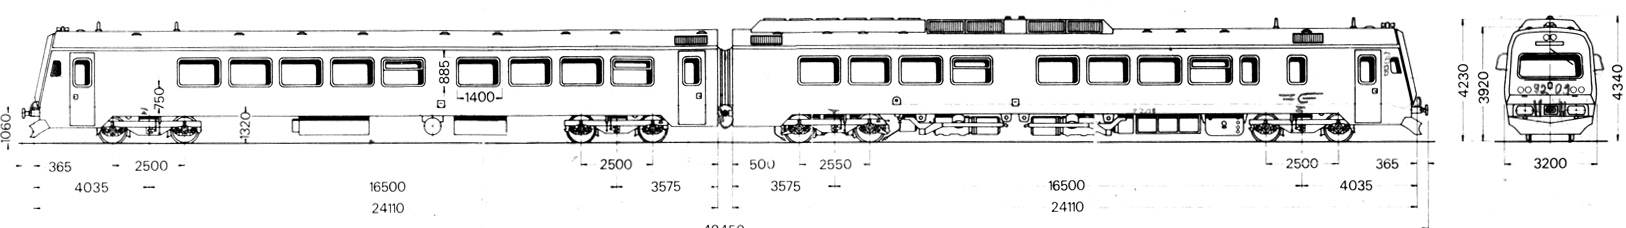
\includegraphics[width=0.8\pageheight, height=0.5\pagewidth, angle=270]{./figures/nsb92.png}
\subsection{Freight train}
%
%
\section{Figures}
%
\subsection{Recreated strain signals}
\begin{figure}[htpb]
  \begin{subfigure}[t]{0.9\textwidth}
    \centering
    % This file was created by matlab2tikz.
%
%The latest updates can be retrieved from
%  http://www.mathworks.com/matlabcentral/fileexchange/22022-matlab2tikz-matlab2tikz
%where you can also make suggestions and rate matlab2tikz.
%
\definecolor{mycolor1}{rgb}{0.00000,0.44700,0.74100}%
\definecolor{mycolor2}{rgb}{0.85000,0.32500,0.09800}%
%
\begin{tikzpicture}

  \begin{axis}[%
    width=\textwidth,
    height=0.4\textwidth,
    at={(0\figurewidth,0\figureheight)},
    scale only axis,
    xmin=0,
    xmax=5,
    xlabel={time [s]},
    ymin=-4e-05,
    ymax=0.00016,
    ylabel={strain [\varepsilon]},
    axis background/.style={fill=white},
    title style={font=\bfseries},
    title={Strainhistory, calculated vs measured for Trondheim sensor},
    legend style={legend cell align=left,align=left,draw=white!15!black}
    ]
    \addplot [color=mycolor1,solid,forget plot]
    table[row sep=crcr]{%
    0	6.24445943240518e-07\\
    0.0009765625	5.31453570540839e-06\\
    0.001953125	2.32415764274234e-06\\
    0.0029296875	1.30856158130012e-06\\
    0.00390625	-7.43782547669991e-07\\
    0.0048828125	7.0202602047223e-07\\
    0.005859375	2.01282095783385e-07\\
    0.0068359375	2.04910017407049e-06\\
    0.0078125	2.94480068753706e-06\\
    0.0087890625	3.97450560647218e-06\\
    0.009765625	1.79520110542698e-06\\
    0.0107421875	1.44961646748052e-06\\
    0.01171875	2.92364238933828e-06\\
    0.0126953125	3.90693817736189e-08\\
    0.013671875	-1.30196003281409e-07\\
    0.0146484375	1.02543915822192e-07\\
    0.015625	1.29445609485285e-06\\
    0.0166015625	-2.57145004774499e-07\\
    0.017578125	3.50196952637167e-06\\
    0.0185546875	2.47931833230485e-06\\
    0.01953125	4.17903628595752e-06\\
    0.0205078125	-5.11042911852805e-07\\
    0.021484375	9.0655537222234e-07\\
    0.0224609375	4.58104510472446e-06\\
    0.0234375	9.77082754136105e-07\\
    0.0244140625	1.53424941813337e-06\\
    0.025390625	-5.53359217266318e-07\\
    0.0263671875	8.99502634574105e-07\\
    0.02734375	1.8093066058854e-06\\
    0.0283203125	3.62186669878944e-06\\
    0.029296875	1.27329786592202e-06\\
    0.0302734375	3.73471112240882e-06\\
    0.03125	4.92663188939252e-06\\
    0.0322265625	2.08334823663392e-07\\
    0.033203125	2.71911221920115e-06\\
    0.0341796875	7.79606109643392e-07\\
    0.03515625	8.43080736936822e-07\\
    0.0361328125	-3.77041254607993e-07\\
    0.037109375	2.07025843556273e-06\\
    0.0380859375	2.51458213204776e-06\\
    0.0390625	2.02088916012827e-06\\
    0.0400390625	4.57399231566769e-06\\
    0.041015625	3.07073024345857e-07\\
    0.0419921875	3.82639723519934e-06\\
    0.04296875	4.07324454482845e-06\\
    0.0439453125	-3.48830374859643e-07\\
    0.044921875	8.84384631207134e-08\\
    0.0458984375	1.30754822408883e-07\\
    0.046875	-5.26160421863986e-08\\
    0.0478515625	2.92364238933828e-06\\
    0.048828125	2.29594661340727e-06\\
    0.0498046875	2.83195644073891e-06\\
    0.05078125	2.69795393047505e-06\\
    0.0517578125	2.28889385632037e-06\\
    0.052734375	2.24657731586982e-06\\
    0.0537109375	1.48488019519229e-06\\
    0.0546875	9.2066084781588e-07\\
    0.0556640625	8.36028000176332e-07\\
    0.056640625	-5.67464651615073e-07\\
    0.0576171875	9.77082754136105e-07\\
    0.05859375	4.90444019780054e-07\\
    0.0595703125	3.98155838714155e-06\\
    0.060546875	4.97496751705219e-07\\
    0.0615234375	4.60925626193944e-06\\
    0.0625	3.06469772743778e-06\\
    0.0634765625	-4.82832039603448e-07\\
    0.064453125	1.6329878785202e-06\\
    0.0654296875	-1.79463592908094e-06\\
    0.06640625	2.5065119301621e-07\\
    0.0673828125	-1.71705622413671e-06\\
    0.068359375	1.47782744945243e-06\\
    0.0693359375	2.50752937190168e-06\\
    0.0703125	3.75586945464959e-06\\
    0.0712890625	-9.76522076033852e-07\\
    0.072265625	2.28184109933192e-06\\
    0.0732421875	1.91509787190623e-06\\
    0.07421875	1.06171562545658e-06\\
    0.0751953125	3.90693817736189e-08\\
    0.076171875	7.2318422542593e-07\\
    0.0771484375	-3.5588309494532e-07\\
    0.078125	7.43330108138839e-08\\
    0.0791015625	1.8445703587589e-06\\
    0.080078125	1.74583185692952e-06\\
    0.0810546875	3.29038635049216e-06\\
    0.08203125	-1.11052357392415e-06\\
    0.0830078125	2.9024840920279e-06\\
    0.083984375	3.11406710509689e-06\\
    0.0849609375	-1.88632101953169e-06\\
    0.0859375	-2.64197726142787e-07\\
    0.0869140625	8.71291684965622e-07\\
    0.087890625	4.19916705949848e-07\\
    0.0888671875	-4.82832039603448e-07\\
    0.08984375	2.24657731586982e-06\\
    0.0908203125	3.38207238246972e-06\\
    0.091796875	2.31710488526036e-06\\
    0.0927734375	-6.94413542990735e-07\\
    0.09375	3.650077802326e-06\\
    0.0947265625	-8.08269385111152e-08\\
    0.095703125	4.61221073843904e-08\\
    0.0966796875	-3.85105934316322e-08\\
    0.09765625	-7.79046119480644e-07\\
    0.0986328125	1.67530436746355e-06\\
    0.099609375	1.83046485731386e-06\\
    0.1005859375	3.78408056568537e-06\\
    0.1015625	-4.26410290368506e-07\\
    0.1025390625	3.03648665666038e-06\\
    0.103515625	1.15340125208846e-06\\
    0.1044921875	3.84653052735127e-07\\
    0.10546875	7.44342431267375e-07\\
    0.1064453125	-1.93670508024215e-07\\
    0.107421875	-1.91453181323862e-06\\
    0.1083984375	8.50133473796191e-07\\
    0.109375	7.93711581684653e-07\\
    0.1103515625	3.00122282040848e-06\\
    0.111328125	2.63447906962496e-06\\
    0.1123046875	-8.08269385111152e-08\\
    0.11328125	4.22840577274895e-06\\
    0.1142578125	2.0843639437179e-06\\
    0.115234375	3.02238112186355e-06\\
    0.1162109375	-4.68726602887012e-07\\
    0.1171875	1.08992658572125e-06\\
    0.1181640625	1.3861417638148e-06\\
    0.119140625	3.19164756547308e-06\\
    0.1201171875	3.85460835018205e-06\\
    0.12109375	3.00122282040848e-06\\
    0.1220703125	3.90397780520072e-06\\
    0.123046875	2.46521281309841e-06\\
    0.1240234375	1.66825161905981e-06\\
    0.125	1.23803415301069e-06\\
    0.1259765625	-1.64652920928198e-06\\
    0.126953125	-1.16090556697649e-07\\
    0.1279296875	-1.46315892448007e-06\\
    0.12890625	1.30856158130012e-06\\
    0.1298828125	2.21131353487516e-06\\
    0.130859375	3.92513614454627e-06\\
    0.1318359375	9.98240970633956e-07\\
    0.1328125	2.6697428802216e-06\\
    0.1337890625	1.9856253949211e-06\\
    0.134765625	5.68024076389373e-07\\
    0.1357421875	1.0193991880202e-06\\
    0.13671875	9.0655537222234e-07\\
    0.1376953125	3.35283942378903e-07\\
    0.138671875	2.08334823663392e-07\\
    0.1396484375	1.81635935626303e-06\\
    0.140625	3.60776114761291e-06\\
    0.1416015625	1.53424941813337e-06\\
    0.142578125	3.74881667713741e-06\\
    0.1435546875	1.78814835534533e-06\\
    0.14453125	-1.26568315855975e-06\\
    0.1455078125	2.92967565921742e-07\\
    0.146484375	-1.01883834237424e-06\\
    0.1474609375	-4.54621165775493e-07\\
    0.1484375	-1.51354172417189e-07\\
    0.1494140625	8.50133473796191e-07\\
    0.150390625	3.48786397854988e-06\\
    0.1513671875	-1.10347086439708e-06\\
    0.15234375	5.06063499208808e-06\\
    0.1533203125	3.30449189278798e-06\\
    0.154296875	3.80575519991384e-09\\
    0.1552734375	2.94480068753706e-06\\
    0.15625	-5.53359217266318e-07\\
    0.1572265625	-2.92408610627149e-07\\
    0.158203125	1.40024725282773e-06\\
    0.1591796875	1.13929576998255e-06\\
    0.16015625	1.72467360905399e-06\\
    0.1611328125	1.13224302907824e-06\\
    0.162109375	3.19164756547308e-06\\
    0.1630859375	-1.6112656981539e-06\\
    0.1640625	5.29337730774729e-06\\
    0.1650390625	2.01383640688942e-06\\
    0.166015625	-2.71250447411546e-07\\
    0.1669921875	8.84384631207134e-08\\
    0.16796875	-1.51958055767719e-06\\
    0.1689453125	4.0581124436832e-07\\
    0.169921875	1.28035060880044e-06\\
    0.1708984375	1.64709337443993e-06\\
    0.171875	3.48081120478774e-06\\
    0.1728515625	1.68940986456766e-06\\
    0.173828125	1.26624512314247e-06\\
    0.1748046875	4.08735010902928e-06\\
    0.17578125	-5.88622802397912e-07\\
    0.1767578125	1.30856158130012e-06\\
    0.177734375	-1.39263187410297e-06\\
    0.1787109375	-5.74517368641348e-07\\
    0.1796875	2.01282095783385e-07\\
    0.1806640625	2.18310251185491e-06\\
    0.181640625	2.24657731586982e-06\\
    0.1826171875	2.24657731586982e-06\\
    0.18359375	4.19916705949848e-07\\
    0.1845703125	2.62037354607672e-06\\
    0.185546875	-9.55363941532042e-07\\
    0.1865234375	-1.73524195596231e-08\\
    0.1875	-1.86617785669953e-07\\
    0.1884765625	-8.77784107427247e-07\\
    0.189453125	-2.64197726142787e-07\\
    0.1904296875	9.98240970633956e-07\\
    0.19140625	1.36498353103592e-06\\
    0.1923828125	8.92449897023665e-07\\
    0.193359375	5.58959495581472e-06\\
    0.1943359375	-3.98199413383354e-07\\
    0.1953125	1.30856158130012e-06\\
    0.1962890625	1.22392866853732e-06\\
    0.197265625	1.66018457862854e-07\\
    0.1982421875	-7.2262440339952e-07\\
    0.19921875	-1.3644210511898e-06\\
    0.2001953125	2.30299937059282e-06\\
    0.201171875	1.16045399328919e-06\\
    0.2021484375	3.092908799794e-06\\
    0.203125	-2.92408610627149e-07\\
    0.2041015625	1.80123912735123e-07\\
    0.205078125	3.24806972597323e-06\\
    0.2060546875	-9.90627498542035e-07\\
    0.20703125	-1.06820731528095e-06\\
    0.2080078125	1.30150883802726e-06\\
    0.208984375	-1.3644210511898e-06\\
    0.2099609375	-4.26410290368506e-07\\
    0.2109375	3.48786397854988e-06\\
    0.2119140625	2.32415764274234e-06\\
    0.212890625	2.75437603571818e-06\\
    0.2138671875	6.385514109402e-07\\
    0.21484375	2.11962771583252e-06\\
    0.2158203125	1.68940986456766e-06\\
    0.216796875	-2.37295698970541e-06\\
    0.2177734375	5.25707680395105e-07\\
    0.21875	-9.62416653131669e-07\\
    0.2197265625	1.81635935626303e-06\\
    0.220703125	2.64858459356762e-06\\
    0.2216796875	3.27628080859141e-06\\
    0.22265625	3.03648665666038e-06\\
    0.2236328125	2.61332078445092e-06\\
    0.224609375	8.64238947810916e-07\\
    0.2255859375	3.03648665666038e-06\\
    0.2265625	3.24806972597323e-06\\
    0.2275390625	-6.87360827641937e-07\\
    0.228515625	-9.49323860817159e-08\\
    0.2294921875	-1.73524195596231e-08\\
    0.23046875	7.16131490342701e-07\\
    0.2314453125	1.68235711596638e-06\\
    0.232421875	3.16343648759155e-06\\
    0.2333984375	1.9362561277745e-06\\
    0.234375	1.95741438453094e-06\\
    0.2353515625	1.58361864590955e-06\\
    0.236328125	1.90099236848729e-06\\
    0.2373046875	1.11813754756452e-06\\
    0.23828125	6.52656879034531e-07\\
    0.2392578125	-1.04704918462697e-06\\
    0.240234375	-1.04704918462697e-06\\
    0.2412109375	1.66825161905981e-06\\
    0.2421875	1.27329786592202e-06\\
    0.2431640625	3.10701433656429e-06\\
    0.244140625	6.52656879034531e-07\\
    0.2451171875	5.7165454296986e-06\\
    0.24609375	8.99502634574105e-07\\
    0.2470703125	-1.01883834237424e-06\\
    0.248046875	1.97857264217513e-06\\
    0.2490234375	-2.50092283308198e-07\\
    0.25	-1.55484407521876e-06\\
    0.2509765625	1.15340125208846e-06\\
    0.251953125	2.4087907402198e-06\\
    0.2529296875	3.05059219185186e-06\\
    0.25390625	1.99267814776486e-06\\
    0.2548828125	7.93711581684653e-07\\
    0.255859375	3.29743912159106e-06\\
    0.2568359375	7.2318422542593e-07\\
    0.2578125	1.16045399328919e-06\\
    0.2587890625	5.53918610663156e-07\\
    0.259765625	-2.44051442822163e-08\\
    0.2607421875	-3.48830374859643e-07\\
    0.26171875	1.86572861166686e-06\\
    0.2626953125	2.35236867365579e-06\\
    0.263671875	3.4243890182379e-06\\
    0.2646484375	3.01532835461356e-06\\
    0.265625	6.72802848084627e-08\\
    0.2666015625	2.74027050881564e-06\\
    0.267578125	6.10340475935486e-07\\
    0.2685546875	-5.81570085568528e-07\\
    0.26953125	-5.46306499944272e-07\\
    0.2705078125	-3.18401589605665e-06\\
    0.271484375	1.80225385560686e-06\\
    0.2724609375	9.55924538525998e-07\\
    0.2734375	4.2636696948456e-06\\
    0.2744140625	-1.0329437636976e-06\\
    0.275390625	3.59365559683125e-06\\
    0.2763671875	2.07731118959131e-06\\
    0.27734375	4.7633855622441e-07\\
    0.2783203125	1.27329786592202e-06\\
    0.279296875	-3.24696981823282e-09\\
    0.2802734375	-1.69589812071638e-06\\
    0.28125	-6.73255396648137e-07\\
    0.2822265625	1.68940986456766e-06\\
    0.283203125	1.35793078697376e-06\\
    0.2841796875	2.00678365374924e-06\\
    0.28515625	-4.68726602887012e-07\\
    0.2861328125	3.77702778777854e-06\\
    0.287109375	-7.36729833012047e-07\\
    0.2880859375	-5.53359217266318e-07\\
    0.2890625	-1.24452503619406e-06\\
    0.2900390625	-1.01985109719023e-07\\
    0.291015625	-1.47726433337154e-06\\
    0.2919921875	8.36028000176332e-07\\
    0.29296875	7.72553373771297e-07\\
    0.2939453125	3.6782889074416e-06\\
    0.294921875	8.07817054120346e-07\\
    0.2958984375	-5.46306499944272e-07\\
    0.296875	3.25512249647972e-06\\
    0.2978515625	-2.88075054468524e-06\\
    0.298828125	-1.01985109719023e-07\\
    0.2998046875	-1.47726433337154e-06\\
    0.30078125	2.85914836857352e-07\\
    0.3017578125	-7.93151547514356e-07\\
    0.302734375	2.42994901680912e-06\\
    0.3037109375	1.92215062376358e-06\\
    0.3046875	2.70500669328523e-06\\
    0.3056640625	2.42994901680912e-06\\
    0.306640625	4.69285824594799e-07\\
    0.3076171875	2.16899700093698e-06\\
    0.30859375	-1.51252785387276e-06\\
    0.3095703125	6.31498677040919e-07\\
    0.310546875	-5.67464651615073e-07\\
    0.3115234375	-1.59716029301204e-06\\
    0.3125	1.65414612254789e-06\\
    0.3134765625	1.66119887075474e-06\\
    0.314453125	2.57100421676738e-06\\
    0.3154296875	2.43598464544229e-07\\
    0.31640625	1.08992658572125e-06\\
    0.3173828125	1.83751760798683e-06\\
    0.318359375	4.61221073843904e-08\\
    0.3193359375	1.53424941813337e-06\\
    0.3203125	8.84384631207134e-08\\
    0.3212890625	-1.20926149694525e-06\\
    0.322265625	8.50133473796191e-07\\
    0.3232421875	2.68384840515111e-06\\
    0.32421875	1.44256372223376e-06\\
    0.3251953125	3.46670565755792e-06\\
    0.326171875	-8.49573255701621e-07\\
    0.3271484375	2.54279317361784e-06\\
    0.328125	1.41435274223509e-06\\
    0.3291015625	-7.2262440339952e-07\\
    0.330078125	3.49389401987617e-07\\
    0.3310546875	-3.41777654676387e-07\\
    0.33203125	2.07731118959131e-06\\
    0.3330078125	1.8093066058854e-06\\
    0.333984375	3.19870033519071e-06\\
    0.3349609375	3.7065000141358e-06\\
    0.3359375	1.4284582320371e-06\\
    0.3369140625	6.66762347523294e-07\\
    0.337890625	-3.41777654676387e-07\\
    0.3388671875	1.44256372223376e-06\\
    0.33984375	-8.08269385111152e-08\\
    0.3408203125	5.68024076389373e-07\\
    0.341796875	-6.52097249417795e-07\\
    0.3427734375	2.30299937059282e-06\\
    0.34375	2.93069515530631e-06\\
    0.3447265625	4.14377236978083e-06\\
    0.345703125	2.92967565921742e-07\\
    0.3466796875	2.47226557265209e-06\\
    0.34765625	3.92513614454627e-06\\
    0.3486328125	-7.43782547669991e-07\\
    0.349609375	-4.05252132777744e-07\\
    0.3505859375	-4.19357571270536e-07\\
    0.3515625	5.18654948074423e-07\\
    0.3525390625	-7.01466258241088e-07\\
    0.353515625	2.90953685769908e-06\\
    0.3544921875	2.15489149041413e-06\\
    0.35546875	3.62891947452526e-06\\
    0.3564453125	-5.18095629668163e-07\\
    0.357421875	3.52312784884378e-06\\
    0.3583984375	1.58361864590955e-06\\
    0.359375	2.29594661340727e-06\\
    0.3603515625	1.62593513070865e-06\\
    0.361328125	1.51913003385235e-07\\
    0.3623046875	1.03350466677116e-06\\
    0.36328125	1.92215062376358e-06\\
    0.3642578125	1.85162310962963e-06\\
    0.365234375	4.58104510472446e-06\\
    0.3662109375	4.1286397510997e-07\\
    0.3671875	3.41733624536328e-06\\
    0.3681640625	1.87983411409917e-06\\
    0.369140625	-1.23143280038535e-07\\
    0.3701171875	-3.85105934316322e-08\\
    0.37109375	2.71809379024778e-07\\
    0.3720703125	-9.34205806142055e-07\\
    0.373046875	-1.65459618014325e-07\\
    0.3740234375	1.95036163218028e-06\\
    0.375	1.56246040484195e-06\\
    0.3759765625	3.14933094924265e-06\\
    0.376953125	-3.91146693889868e-07\\
    0.3779296875	2.21131353487516e-06\\
    0.37890625	2.43700177586991e-06\\
    0.3798828125	-2.99461331501475e-07\\
    0.380859375	-8.78796623457467e-08\\
    0.3818359375	-2.71148608319287e-06\\
    0.3828125	-3.5588309494532e-07\\
    0.3837890625	1.23098141072467e-06\\
    0.384765625	1.22392866853732e-06\\
    0.3857421875	3.3961779273312e-06\\
    0.38671875	3.21178483165055e-07\\
    0.3876953125	2.85311473508963e-06\\
    0.388671875	4.4107489906276e-07\\
    0.3896484375	3.21178483165055e-07\\
    0.390625	1.02543915822192e-07\\
    0.3916015625	-9.97680209647699e-07\\
    0.392578125	-1.85811022424616e-06\\
    0.3935546875	1.47077470381168e-06\\
    0.39453125	1.07582110539148e-06\\
    0.3955078125	2.69090116776375e-06\\
    0.396484375	-7.37742145782549e-08\\
    0.3974609375	2.67679564263691e-06\\
    0.3984375	1.15340125208846e-06\\
    0.3994140625	-2.0696911504066e-06\\
    0.400390625	1.95741438453094e-06\\
    0.4013671875	-8.21362402397179e-07\\
    0.40234375	-3.24696981823282e-09\\
    0.4033203125	3.35283942378903e-07\\
    0.404296875	2.09846945226793e-06\\
    0.4052734375	2.58510973893348e-06\\
    0.40625	1.781095605363e-06\\
    0.4072265625	1.7176208599594e-06\\
    0.408203125	4.32009197533201e-06\\
    0.4091796875	-1.44200081040311e-06\\
    0.41015625	2.04204742043678e-06\\
    0.4111328125	1.4919329410308e-06\\
    0.412109375	3.6349486199033e-07\\
    0.4130859375	-1.23143280038535e-07\\
    0.4140625	2.84606197020732e-06\\
    0.4150390625	2.54279317361784e-06\\
    0.416015625	3.64302502629398e-06\\
    0.4169921875	6.59709613229581e-07\\
    0.41796875	2.15489149041413e-06\\
    0.4189453125	3.48081120478774e-06\\
    0.419921875	-6.59149965259904e-07\\
    0.4208984375	8.84384631207134e-08\\
    0.421875	3.49389401987617e-07\\
    0.4228515625	5.25707680395105e-07\\
    0.423828125	1.09596642320709e-07\\
    0.4248046875	3.25512249647972e-06\\
    0.42578125	2.19720802316771e-06\\
    0.4267578125	4.75736486321883e-06\\
    0.427734375	1.79112055337122e-08\\
    0.4287109375	3.55839172160445e-06\\
    0.4296875	4.22135298862574e-06\\
    0.4306640625	-1.45610621988656e-06\\
    0.431640625	4.62233093063633e-07\\
    0.4326171875	-1.72410892507993e-06\\
    0.43359375	7.65500637996781e-07\\
    0.4345703125	-5.03990193938134e-07\\
    0.435546875	4.28482804928801e-06\\
    0.4365234375	-7.37742145782549e-08\\
    0.4375	1.49898568696798e-06\\
    0.4384765625	2.63447906962496e-06\\
    0.439453125	-6.23886385062297e-07\\
    0.4404296875	1.65414612254789e-06\\
    0.44140625	1.5413021646623e-06\\
    0.4423828125	6.10340475935486e-07\\
    0.443359375	8.84384631207134e-08\\
    0.4443359375	1.55540765801659e-06\\
    0.4453125	1.19571770077365e-06\\
    0.4462890625	4.12261402125882e-06\\
    0.447265625	1.10403206644524e-06\\
    0.4482421875	1.96446713698049e-06\\
    0.44921875	4.30598640461838e-06\\
    0.4501953125	1.87176640319142e-07\\
    0.451171875	1.03350466677116e-06\\
    0.4521484375	5.96235009025755e-07\\
    0.453125	-8.78796623457467e-08\\
    0.4541015625	-1.93670508024215e-07\\
    0.455078125	2.11962771583252e-06\\
    0.4560546875	2.6697428802216e-06\\
    0.45703125	4.09440289127812e-06\\
    0.4580078125	1.20277044256658e-06\\
    0.458984375	1.85162310962963e-06\\
    0.4599609375	1.97857264217513e-06\\
    0.4609375	-1.43494810551296e-06\\
    0.4619140625	4.61221073843904e-08\\
    0.462890625	-1.05410189494334e-06\\
    0.4638671875	4.1286397510997e-07\\
    0.46484375	2.31005212787748e-06\\
    0.4658203125	3.01532835461356e-06\\
    0.466796875	8.71291684965622e-07\\
    0.4677734375	2.74732327221758e-06\\
    0.46875	3.09996156812949e-06\\
    0.4697265625	3.49389401987617e-07\\
    0.470703125	1.68235711596638e-06\\
    0.4716796875	6.72802848084627e-08\\
    0.47265625	-5.95675519127984e-07\\
    0.4736328125	-1.02589105308525e-06\\
    0.474609375	8.71291684965622e-07\\
    0.4755859375	1.28035060880044e-06\\
    0.4765625	1.70351536206621e-06\\
    0.4775390625	2.63447906962496e-06\\
    0.478515625	-4.05252132777744e-07\\
    0.4794921875	3.092908799794e-06\\
    0.48046875	2.20426077897199e-06\\
    0.4814453125	-5.74517368641348e-07\\
    0.482421875	2.49639308480629e-08\\
    0.4833984375	3.91705783181007e-07\\
    0.484375	-8.35467829246725e-07\\
    0.4853515625	2.18310251185491e-06\\
    0.486328125	2.37352694787722e-06\\
    0.4873046875	2.16194424562622e-06\\
    0.48828125	2.21131353487516e-06\\
    0.4892578125	2.38763246451822e-06\\
    0.490234375	1.4919329410308e-06\\
    0.4912109375	6.72802848084627e-08\\
    0.4921875	2.2949300789582e-07\\
    0.4931640625	4.90444019780054e-07\\
    0.494140625	-2.42232582999815e-06\\
    0.4951171875	-2.50092283308198e-07\\
    0.49609375	1.19571770077365e-06\\
    0.4970703125	2.03499466690195e-06\\
    0.498046875	1.9715198895287e-06\\
    0.4990234375	-3.77041254607993e-07\\
    0.5	2.76848156301581e-06\\
    0.5009765625	8.64238947810916e-07\\
    0.501953125	-5.81570085568528e-07\\
    0.5029296875	-2.28127198776285e-06\\
    0.50390625	5.11602215852837e-07\\
    0.5048828125	-2.07775952437185e-07\\
    0.505859375	1.50603843300338e-06\\
    0.5068359375	1.58361864590955e-06\\
    0.5078125	6.31498677040919e-07\\
    0.5087890625	1.17455947598686e-06\\
    0.509765625	1.78814835534533e-06\\
    0.5107421875	3.91705783181007e-07\\
    0.51171875	-1.17399795522923e-06\\
    0.5126953125	3.49389401987617e-07\\
    0.513671875	-2.00723230280031e-07\\
    0.5146484375	-1.23041962079044e-06\\
    0.515625	-4.55633178580214e-08\\
    0.5166015625	2.18310251185491e-06\\
    0.517578125	-1.86617785669953e-07\\
    0.5185546875	4.86315674791665e-06\\
    0.51953125	1.9362561277745e-06\\
    0.5205078125	5.32760412813799e-07\\
    0.521484375	1.82341210673868e-06\\
    0.5224609375	-5.74517368641348e-07\\
    0.5234375	-1.85811022424616e-06\\
    0.5244140625	-1.82284672791896e-06\\
    0.525390625	-2.44051442822163e-08\\
    0.5263671875	2.85914836857352e-07\\
    0.52734375	9.0655537222234e-07\\
    0.5283203125	2.08334823663392e-07\\
    0.529296875	3.00827558746201e-06\\
    0.5302734375	1.61888238299512e-06\\
    0.53125	-1.64652920928198e-06\\
    0.5322265625	3.84653052735127e-07\\
    0.533203125	-7.64940691052284e-07\\
    0.5341796875	-2.0626384542987e-06\\
    0.53515625	-8.14309688824738e-07\\
    0.5361328125	3.6349486199033e-07\\
    0.537109375	2.21131353487516e-06\\
    0.5380859375	1.45666921282529e-06\\
    0.5390625	8.92449897023665e-07\\
    0.5400390625	1.09596642320709e-07\\
    0.541015625	2.12668047055152e-06\\
    0.5419921875	1.04761014591633e-06\\
    0.54296875	-8.77784107427247e-07\\
    0.5439453125	-1.73524195596231e-08\\
    0.544921875	-1.04704918462697e-06\\
    0.5458984375	2.71809379024778e-07\\
    0.546875	1.97857264217513e-06\\
    0.5478515625	2.06320568163368e-06\\
    0.548828125	3.90693817736189e-08\\
    0.5498046875	3.98155838714155e-06\\
    0.55078125	8.57186210753789e-07\\
    0.5517578125	6.10340475935486e-07\\
    0.552734375	-2.07775952437185e-07\\
    0.5537109375	-1.09037833257884e-07\\
    0.5546875	-1.1316817019138e-06\\
    0.5556640625	2.85914836857352e-07\\
    0.556640625	5.89182275718449e-07\\
    0.5576171875	2.77553432681261e-06\\
    0.55859375	-5.26160421863986e-08\\
    0.5595703125	4.59515068313462e-06\\
    0.560546875	3.68534168396694e-06\\
    0.5615234375	1.80123912735123e-07\\
    0.5625	3.14125753706233e-07\\
    0.5634765625	1.37908901945666e-06\\
    0.564453125	1.23098141072467e-06\\
    0.5654296875	-1.12462899268273e-06\\
    0.56640625	2.7614287993181e-06\\
    0.5673828125	1.68940986456766e-06\\
    0.568359375	2.74027050881564e-06\\
    0.5693359375	-4.75779321294561e-07\\
    0.5703125	4.30598640461838e-06\\
    0.5712890625	1.46372195826893e-06\\
    0.572265625	1.28035060880044e-06\\
    0.5732421875	-3.41777654676387e-07\\
    0.57421875	-2.50092283308198e-07\\
    0.5751953125	-1.49136974186793e-06\\
    0.576171875	-1.18105066376968e-06\\
    0.5771484375	1.4284582320371e-06\\
    0.578125	1.4284582320371e-06\\
    0.5791015625	3.54428617220406e-06\\
    0.580078125	-1.23143280038535e-07\\
    0.5810546875	4.70799532462378e-06\\
    0.58203125	3.35283942378903e-07\\
    0.5830078125	3.00020295084576e-07\\
    0.583984375	-1.73524195596231e-08\\
    0.5849609375	-1.97095339591626e-06\\
    0.5859375	3.90693817736189e-08\\
    0.5869140625	1.343825299145e-06\\
    0.587890625	6.73815081915887e-07\\
    0.5888671875	2.09141669794358e-06\\
    0.58984375	1.40729999748186e-06\\
    0.5908203125	-5.32201065003759e-07\\
    0.591796875	2.60626802292335e-06\\
    0.5927734375	8.28975263514288e-07\\
    0.59375	-1.66768731477422e-06\\
    0.5947265625	3.14125753706233e-07\\
    0.595703125	-7.71993405316012e-07\\
    0.5966796875	4.69285824594799e-07\\
    0.59765625	3.14227818021609e-06\\
    0.5986328125	3.21280587492066e-06\\
    0.599609375	2.08334823663392e-07\\
    0.6005859375	3.05764495959538e-06\\
    0.6015625	1.6329878785202e-06\\
    0.6025390625	8.78344422219641e-07\\
    0.603515625	7.16131490342701e-07\\
    0.6044921875	-2.0696911504066e-06\\
    0.60546875	3.84653052735127e-07\\
    0.6064453125	-1.24452503619406e-06\\
    0.607421875	1.8445703587589e-06\\
    0.6083984375	1.89393961692614e-06\\
    0.609375	4.21430020460054e-06\\
    0.6103515625	-9.90627498542035e-07\\
    0.611328125	2.78258709070808e-06\\
    0.6123046875	1.13929576998255e-06\\
    0.61328125	-6.16833668726441e-07\\
    0.6142578125	-2.28934118316889e-07\\
    0.615234375	-2.23190313365586e-06\\
    0.6162109375	-2.23190313365586e-06\\
    0.6171875	-1.06115460516169e-06\\
    0.6181640625	8.00764317853168e-07\\
    0.619140625	1.33677255537883e-06\\
    0.6201171875	1.21687592644819e-06\\
    0.62109375	-1.72512340664574e-07\\
    0.6220703125	4.53872837186272e-06\\
    0.623046875	-3.84093974298587e-07\\
    0.6240234375	1.40729999748186e-06\\
    0.625	-2.64197726142787e-07\\
    0.6259765625	-1.35736834521415e-06\\
    0.626953125	-1.07526002530111e-06\\
    0.6279296875	1.64004062643127e-06\\
    0.62890625	3.69239446059138e-06\\
    0.6298828125	3.5513389468546e-06\\
    0.630859375	1.5130911791381e-06\\
    0.6318359375	-1.51958055767719e-06\\
    0.6328125	2.41584349898395e-06\\
    0.6337890625	-1.35031563914092e-06\\
    0.634765625	-3.24696981823282e-09\\
    0.6357421875	1.02543915822192e-07\\
    0.63671875	-1.85105752517796e-06\\
    0.6376953125	1.47782744945243e-06\\
    0.638671875	1.92920337571982e-06\\
    0.6396484375	2.72616498230753e-06\\
    0.640625	1.6329878785202e-06\\
    0.6416015625	2.38763246451822e-06\\
    0.642578125	2.39468522298661e-06\\
    0.6435546875	8.13857369177506e-08\\
    0.64453125	1.44256372223376e-06\\
    0.6455078125	-1.37248726425404e-07\\
    0.646484375	-1.88632101953169e-06\\
    0.6474609375	-1.43494810551296e-06\\
    0.6484375	-2.07775952437185e-07\\
    0.6494140625	3.98861116791024e-06\\
    0.650390625	-1.68179271794241e-06\\
    0.6513671875	5.52611973086135e-06\\
    0.65234375	2.17604975634683e-06\\
    0.6533203125	-1.3644210511898e-06\\
    0.654296875	1.10403206644524e-06\\
    0.6552734375	-1.79463592908094e-06\\
    0.65625	-2.92408610627149e-07\\
    0.6572265625	-1.93568990748271e-06\\
    0.658203125	9.84135492869843e-07\\
    0.6591796875	1.20277044256658e-06\\
    0.66015625	3.26922803778849e-06\\
    0.6611328125	7.72553373771297e-07\\
    0.662109375	-3.69988534818953e-07\\
    0.6630859375	3.57249727139905e-06\\
    0.6640625	-2.37295698970541e-06\\
    0.6650390625	-2.28934118316889e-07\\
    0.666015625	-1.53368596498985e-06\\
    0.6669921875	3.20166562617265e-08\\
    0.66796875	-1.86617785669953e-07\\
    0.6689453125	-2.57145004774499e-07\\
    0.669921875	2.16899700093698e-06\\
    0.6708984375	3.41028347258712e-06\\
    0.671875	-3.85105934316322e-08\\
    0.6728515625	1.37203627519674e-06\\
    0.673828125	3.4596528840909e-06\\
    0.6748046875	-7.79046119480644e-07\\
    0.67578125	3.35283942378903e-07\\
    0.6767578125	-1.38557916852262e-06\\
    0.677734375	-2.28934118316889e-07\\
    0.6787109375	1.44860276294744e-07\\
    0.6796875	1.60477688786512e-06\\
    0.6806640625	2.10552220669073e-06\\
    0.681640625	1.71056811096304e-06\\
    0.6826171875	2.71809379024778e-07\\
    0.68359375	6.24445943240518e-07\\
    0.6845703125	4.03798063605253e-06\\
    0.685546875	-8.28415115871175e-07\\
    0.6865234375	5.11602215852837e-07\\
    0.6875	7.43330108138839e-08\\
    0.6884765625	8.00764317853168e-07\\
    0.689453125	1.61182963538068e-06\\
    0.6904296875	2.56395145583179e-06\\
    0.69140625	8.07817054120346e-07\\
    0.6923828125	3.38912515485145e-06\\
    0.693359375	8.21922526951123e-07\\
    0.6943359375	-5.3925378252313e-07\\
    0.6953125	-5.25148347385509e-07\\
    0.6962890625	1.37807549302265e-07\\
    0.697265625	-1.26568315855975e-06\\
    0.6982421875	5.68024076389373e-07\\
    0.69921875	1.03350466677116e-06\\
    0.7001953125	2.98006451984203e-06\\
    0.701171875	1.16649368917887e-07\\
    0.7021484375	3.26217526708489e-06\\
    0.703125	3.69944723731426e-06\\
    0.7041015625	-1.57600218455927e-06\\
    0.705078125	1.23803415301069e-06\\
    0.7060546875	5.31748330936076e-08\\
    0.70703125	5.46865877948041e-07\\
    0.7080078125	-1.06115460516169e-06\\
    0.708984375	3.092908799794e-06\\
    0.7099609375	2.01282095783385e-07\\
    0.7109375	2.22541904697682e-06\\
    0.7119140625	-7.43782547669991e-07\\
    0.712890625	1.77404285547889e-06\\
    0.7138671875	7.5139516674547e-07\\
    0.71484375	-2.87369785992417e-06\\
    0.7158203125	-7.64940691052284e-07\\
    0.716796875	-2.11200732498206e-06\\
    0.7177734375	-2.7830316858251e-07\\
    0.71875	-6.67214905458648e-08\\
    0.7197265625	1.4284582320371e-06\\
    0.720703125	2.02088916012827e-06\\
    0.7216796875	2.93069515530631e-06\\
    0.72265625	-2.18958696914483e-06\\
    0.7236328125	3.29743912159106e-06\\
    0.724609375	-2.64197726142787e-07\\
    0.7255859375	-1.38557916852262e-06\\
    0.7265625	-1.44301449470086e-07\\
    0.7275390625	-1.12462899268273e-06\\
    0.728515625	-1.72410892507993e-06\\
    0.7294921875	1.06171562545658e-06\\
    0.73046875	1.61888238299512e-06\\
    0.7314453125	2.74027050881564e-06\\
    0.732421875	3.43144179121117e-06\\
    0.7333984375	1.09596642320709e-07\\
    0.734375	3.11406710509689e-06\\
    0.7353515625	-1.71705622413671e-06\\
    0.736328125	-1.07526002530111e-06\\
    0.7373046875	-5.74517368641348e-07\\
    0.73828125	-2.33064083703495e-06\\
    0.7392578125	1.49898568696798e-06\\
    0.740234375	1.56246040484195e-06\\
    0.7412109375	2.76848156301581e-06\\
    0.7421875	3.03648665666038e-06\\
    0.7431640625	7.16131490342701e-07\\
    0.744140625	-3.20619493532912e-07\\
    0.7451171875	3.91808336466576e-06\\
    0.74609375	1.5130911791381e-06\\
    0.7470703125	-1.93568990748271e-06\\
    0.748046875	1.20982318445816e-06\\
    0.7490234375	-1.33621022669738e-06\\
    0.75	1.78814835534533e-06\\
    0.7509765625	2.16899700093698e-06\\
    0.751953125	3.60776114761291e-06\\
    0.7529296875	3.24101695556539e-06\\
    0.75390625	1.08992658572125e-06\\
    0.7548828125	2.07731118959131e-06\\
    0.755859375	-1.20220878879903e-06\\
    0.7568359375	6.52656879034531e-07\\
    0.7578125	1.80123912735123e-07\\
    0.7587890625	-1.48431703766885e-06\\
    0.759765625	2.22440279720043e-07\\
    0.7607421875	3.26922803778849e-06\\
    0.76171875	1.32266706814204e-06\\
    0.7626953125	1.87278136283401e-06\\
    0.763671875	-1.32210481385876e-06\\
    0.7646484375	4.94779027166033e-06\\
    0.765625	6.02275589017039e-08\\
    0.7666015625	1.71056811096304e-06\\
    0.767578125	1.09596642320709e-07\\
    0.7685546875	-1.38557916852262e-06\\
    0.76953125	-2.99461331501475e-07\\
    0.7705078125	1.02645192734613e-06\\
    0.771484375	9.91188231702677e-07\\
    0.7724609375	1.18161221748358e-06\\
    0.7734375	-1.0329437636976e-06\\
    0.7744140625	4.22840577274895e-06\\
    0.775390625	-2.01326957878023e-06\\
    0.7763671875	-5.60411934489918e-07\\
    0.77734375	9.98240970633956e-07\\
    0.7783203125	-2.03442766888006e-06\\
    0.779296875	-6.30939101299056e-07\\
    0.7802734375	1.18161221748358e-06\\
    0.78125	2.35942143163108e-06\\
    0.7822265625	1.95036163218028e-06\\
    0.783203125	2.54279317361784e-06\\
    0.7841796875	9.84135492869843e-07\\
    0.78515625	3.38912515485145e-06\\
    0.7861328125	1.6329878785202e-06\\
    0.787109375	1.09596642320709e-07\\
    0.7880859375	-1.26568315855975e-06\\
    0.7890625	6.72802848084627e-08\\
    0.7900390625	6.94973285685638e-07\\
    0.791015625	2.04910017407049e-06\\
    0.7919921875	1.781095605363e-06\\
    0.79296875	1.32971981171089e-06\\
    0.7939453125	4.07324454482845e-06\\
    0.794921875	2.07731118959131e-06\\
    0.7958984375	2.5004766118547e-06\\
    0.796875	6.87920550996625e-07\\
    0.7978515625	1.94330887992806e-06\\
    0.798828125	2.71809379024778e-07\\
    0.7998046875	7.86658845615016e-07\\
    0.80078125	1.56246040484195e-06\\
    0.8017578125	3.28333357949235e-06\\
    0.802734375	2.01282095783385e-07\\
    0.8037109375	3.55839172160445e-06\\
    0.8046875	-4.3346300936868e-07\\
    0.8056640625	5.04549483730131e-07\\
    0.806640625	1.39319450827204e-06\\
    0.8076171875	8.28975263514288e-07\\
    0.80859375	-3.48830374859643e-07\\
    0.8095703125	-3.24696981823282e-09\\
    0.810546875	8.78344422219641e-07\\
    0.8115234375	2.09141669794358e-06\\
    0.8125	2.35942143163108e-06\\
    0.8134765625	1.13929576998255e-06\\
    0.814453125	6.94973285685638e-07\\
    0.8154296875	2.26068282895855e-06\\
    0.81640625	-5.46306499944272e-07\\
    0.8173828125	-1.51252785387276e-06\\
    0.818359375	2.15387551642278e-07\\
    0.8193359375	-7.71993405316012e-07\\
    0.8203125	-1.12462899268273e-06\\
    0.8212890625	1.22392866853732e-06\\
    0.822265625	-5.60411934489918e-07\\
    0.8232421875	2.96595898662401e-06\\
    0.82421875	2.69795393047505e-06\\
    0.8251953125	2.42289625784764e-06\\
    0.826171875	3.38207238246972e-06\\
    0.8271484375	-8.70731394643888e-07\\
    0.828125	-7.37742145782549e-08\\
    0.8291015625	3.20166562617265e-08\\
    0.830078125	-3.77041254607993e-07\\
    0.8310546875	2.46521281309841e-06\\
    0.83203125	8.14869790486403e-07\\
    0.8330078125	3.80523889999848e-06\\
    0.833984375	-2.20369235770989e-06\\
    0.8349609375	4.2425113412918e-06\\
    0.8359375	-1.16090556697649e-07\\
    0.8369140625	1.87176640319142e-07\\
    0.837890625	1.9362561277745e-06\\
    0.8388671875	-7.57887976690326e-07\\
    0.83984375	-1.73116162592384e-06\\
    0.8408203125	-5.26160421863986e-08\\
    0.841796875	2.69795393047505e-06\\
    0.8427734375	2.78963985470243e-06\\
    0.84375	2.83195644073891e-06\\
    0.8447265625	1.80123912735123e-07\\
    0.845703125	5.08179337998052e-06\\
    0.8466796875	-7.36729833012047e-07\\
    0.84765625	4.7633855622441e-07\\
    0.8486328125	-1.92863720949979e-06\\
    0.849609375	-2.97948812097567e-06\\
    0.8505859375	-3.38854358815496e-06\\
    0.8515625	1.52014392537105e-06\\
    0.8525390625	5.75076809400041e-07\\
    0.853515625	8.21922526951123e-07\\
    0.8544921875	1.0687683653747e-06\\
    0.85546875	-8.21362402397179e-07\\
    0.8564453125	2.69090116776375e-06\\
    0.857421875	-1.06115460516169e-06\\
    0.8583984375	-8.77784107427247e-07\\
    0.859375	-3.77041254607993e-07\\
    0.8603515625	-1.87221562208614e-06\\
    0.861328125	6.73815081915887e-07\\
    0.8623046875	2.51458213204776e-06\\
    0.86328125	2.32415764274234e-06\\
    0.8642578125	4.62233093063633e-07\\
    0.865234375	2.24657731586982e-06\\
    0.8662109375	9.27713585760536e-07\\
    0.8671875	-8.28415115871175e-07\\
    0.8681640625	9.48871800186477e-07\\
    0.869140625	-1.40673728496769e-06\\
    0.8701171875	6.02275589017039e-08\\
    0.87109375	-4.68726602887012e-07\\
    0.8720703125	1.4919329410308e-06\\
    0.873046875	2.38057970614871e-06\\
    0.8740234375	2.80374538298668e-06\\
    0.875	3.29038635049216e-06\\
    0.8759765625	1.86572861166686e-06\\
    0.876953125	3.38912515485145e-06\\
    0.8779296875	-4.89884757813889e-07\\
    0.87890625	-2.33769352939324e-06\\
    0.8798828125	-1.51958055767719e-06\\
    0.880859375	-9.694693646322e-07\\
    0.8818359375	-2.04853306178671e-06\\
    0.8828125	1.44860276294744e-07\\
    0.8837890625	2.24657731586982e-06\\
    0.884765625	1.28740335177732e-06\\
    0.8857421875	1.66018457862854e-07\\
    0.88671875	9.55924538525998e-07\\
    0.8876953125	8.13857369177506e-08\\
    0.888671875	-1.44301449470086e-07\\
    0.8896484375	-8.91889532697978e-07\\
    0.890625	-2.59864307729013e-06\\
    0.8916015625	3.84653052735127e-07\\
    0.892578125	8.50133473796191e-07\\
    0.8935546875	1.83046485731386e-06\\
    0.89453125	-2.92408610627149e-07\\
    0.8955078125	3.13522541128841e-06\\
    0.896484375	-3.44496500585497e-06\\
    0.8974609375	-1.87926832085836e-06\\
    0.8984375	-2.92408610627149e-07\\
    0.8994140625	-2.03442766888006e-06\\
    0.900390625	-2.84548711989457e-06\\
    0.9013671875	-1.56189677843056e-06\\
    0.90234375	-9.97680209647699e-07\\
    0.9033203125	8.50133473796191e-07\\
    0.904296875	1.9715198895287e-06\\
    0.9052734375	8.14869790486403e-07\\
    0.90625	-9.49323860817159e-08\\
    0.9072265625	1.56246040484195e-06\\
    0.908203125	-1.75231972786424e-06\\
    0.9091796875	4.48127630297938e-07\\
    0.91015625	-2.71250447411546e-07\\
    0.9111328125	-1.90042641658237e-06\\
    0.912109375	-1.21631420499217e-06\\
    0.9130859375	6.72802848084627e-08\\
    0.9140625	7.44342431267375e-07\\
    0.9150390625	1.90099236848729e-06\\
    0.916015625	-1.55484407521876e-06\\
    0.9169921875	2.04910017407049e-06\\
    0.91796875	1.7176208599594e-06\\
    0.9189453125	-2.07674384641561e-06\\
    0.919921875	-7.36729833012047e-07\\
    0.9208984375	-1.1316817019138e-06\\
    0.921875	-8.78796623457467e-08\\
    0.9228515625	4.4107489906276e-07\\
    0.923828125	4.28482804928801e-06\\
    0.9248046875	-7.01466258241088e-07\\
    0.92578125	4.18608906948875e-06\\
    0.9267578125	1.87176640319142e-07\\
    0.927734375	-7.43782547669991e-07\\
    0.9287109375	2.64756650256593e-07\\
    0.9296875	-6.16833668726441e-07\\
    0.9306640625	-1.41378999025227e-06\\
    0.931640625	-2.88075054468524e-06\\
    0.9326171875	6.03287742431289e-07\\
    0.93359375	3.94629448477934e-06\\
    0.9345703125	7.30236960607821e-07\\
    0.935546875	4.09440289127812e-06\\
    0.9365234375	4.40472540790124e-06\\
    0.9375	3.77600322388344e-07\\
    0.9384765625	3.99566394877738e-06\\
    0.939453125	3.80575519991384e-09\\
    0.9404296875	7.93711581684653e-07\\
    0.94140625	-1.28684128003704e-06\\
    0.9423828125	-8.98942245185132e-07\\
    0.943359375	1.25919238046137e-06\\
    0.9443359375	1.26624512314247e-06\\
    0.9453125	1.28035060880044e-06\\
    0.9462890625	-1.13873441104644e-06\\
    0.947265625	1.95036163218028e-06\\
    0.9482421875	-6.87360827641937e-07\\
    0.94921875	-6.45044533476805e-07\\
    0.9501953125	1.23702095614379e-07\\
    0.951171875	-3.85105934316322e-08\\
    0.9521484375	-5.53359217266318e-07\\
    0.953125	1.61888238299512e-06\\
    0.9541015625	3.28333357949235e-06\\
    0.955078125	2.7614287993181e-06\\
    0.9560546875	-8.00204261383001e-07\\
    0.95703125	3.8193444567001e-06\\
    0.9580078125	-7.37742145782549e-08\\
    0.958984375	-1.35031563914092e-06\\
    0.9599609375	-2.92408610627149e-07\\
    0.9609375	-9.83574787337491e-07\\
    0.9619140625	-2.80317100688943e-06\\
    0.962890625	-1.93670508024215e-07\\
    0.9638671875	8.07817054120346e-07\\
    0.96484375	1.80225385560686e-06\\
    0.9658203125	2.98006451984203e-06\\
    0.966796875	9.27713585760536e-07\\
    0.9677734375	4.03092785459299e-06\\
    0.96875	9.2066084781588e-07\\
    0.9697265625	3.49389401987617e-07\\
    0.970703125	-1.42789540052502e-06\\
    0.9716796875	-1.92158451141843e-06\\
    0.97265625	-1.68884541937894e-06\\
    0.9736328125	-3.77041254607993e-07\\
    0.974609375	4.4107489906276e-07\\
    0.9755859375	9.1360810996967e-07\\
    0.9765625	1.56951315176575e-06\\
    0.9775390625	7.44342431267375e-07\\
    0.978515625	3.28231212722322e-07\\
    0.9794921875	2.70500669328523e-06\\
    0.98046875	-3.60717654656587e-06\\
    0.9814453125	-1.06820731528095e-06\\
    0.982421875	-2.17548158018489e-06\\
    0.9833984375	-6.3799181743737e-07\\
    0.984375	1.52014392537105e-06\\
    0.9853515625	1.18866495907939e-06\\
    0.986328125	2.86722026515002e-06\\
    0.9873046875	9.48871800186477e-07\\
    0.98828125	-7.08518973392344e-07\\
    0.9892578125	-5.96687664156798e-08\\
    0.990234375	-1.315052107292e-06\\
    0.9912109375	-5.18095629668163e-07\\
    0.9921875	-1.30094669386163e-06\\
    0.9931640625	5.31748330936076e-08\\
    0.994140625	2.64756650256593e-07\\
    0.9951171875	2.48637109205607e-06\\
    0.99609375	1.29445609485285e-06\\
    0.9970703125	4.8419983692009e-06\\
    0.998046875	5.75886226143111e-06\\
    0.9990234375	3.80575519991384e-09\\
    1	2.07731118959131e-06\\
    1.0009765625	-1.56189677843056e-06\\
    1.001953125	9.54911894219049e-08\\
    1.0029296875	-2.18253427471441e-06\\
    1.00390625	-3.34724934393385e-07\\
    1.0048828125	-4.96937475925451e-07\\
    1.005859375	1.55540765801659e-06\\
    1.0068359375	-1.8298994273816e-06\\
    1.0078125	1.97857264217513e-06\\
    1.0087890625	1.64004062643127e-06\\
    1.009765625	-5.95675519127984e-07\\
    1.0107421875	1.05466288563756e-06\\
    1.01171875	-1.27273586581758e-06\\
    1.0126953125	5.11602215852837e-07\\
    1.013671875	-2.57145004774499e-07\\
    1.0146484375	2.5065119301621e-07\\
    1.015625	8.28975263514288e-07\\
    1.0166015625	6.17393209539213e-07\\
    1.017578125	-2.99359348743863e-06\\
    1.0185546875	3.04353942420679e-06\\
    1.01953125	-2.32358814457757e-06\\
    1.0205078125	4.48127630297938e-07\\
    1.021484375	-1.28684128003704e-06\\
    1.0224609375	-1.71705622413671e-06\\
    1.0234375	-1.1316817019138e-06\\
    1.0244140625	-7.64940691052284e-07\\
    1.025390625	5.68024076389373e-07\\
    1.0263671875	-3.5588309494532e-07\\
    1.02734375	1.87983411409917e-06\\
    1.0283203125	-6.94413542990735e-07\\
    1.029296875	3.18459479585497e-06\\
    1.0302734375	-9.27153094148212e-07\\
    1.03125	1.16045399328919e-06\\
    1.0322265625	1.81635935626303e-06\\
    1.033203125	1.66018457862854e-07\\
    1.0341796875	-2.00723230280031e-07\\
    1.03515625	2.81785091166579e-06\\
    1.0361328125	2.57703921587287e-07\\
    1.037109375	2.46521281309841e-06\\
    1.0380859375	-1.4702116289747e-06\\
    1.0390625	-2.89485591391052e-06\\
    1.0400390625	3.01532835461356e-06\\
    1.041015625	-8.28415115871175e-07\\
    1.0419921875	-1.17399795522923e-06\\
    1.04296875	-2.28934118316889e-07\\
    1.0439453125	1.87176640319142e-07\\
    1.044921875	1.78814835534533e-06\\
    1.0458984375	3.3961779273312e-06\\
    1.046875	2.94480068753706e-06\\
    1.0478515625	3.72060556807488e-06\\
    1.048828125	1.0687683653747e-06\\
    1.0498046875	1.80123912735123e-07\\
    1.05078125	1.73071185249549e-07\\
    1.0517578125	-2.92408610627149e-07\\
    1.052734375	-2.70443339606412e-06\\
    1.0537109375	7.93711581684653e-07\\
    1.0546875	-9.90627498542035e-07\\
    1.0556640625	1.67530436746355e-06\\
    1.056640625	4.55180361631563e-07\\
    1.0576171875	-6.16833668726441e-07\\
    1.05859375	5.43443330892814e-06\\
    1.0595703125	-3.62935814931251e-07\\
    1.060546875	-4.96937475925451e-07\\
    1.0615234375	5.31748330936076e-08\\
    1.0625	6.31498677040919e-07\\
    1.0634765625	-2.08379654232662e-06\\
    1.064453125	-2.33769352939324e-06\\
    1.0654296875	-2.1966396634768e-06\\
    1.06640625	-3.77041254607993e-07\\
    1.0673828125	8.36028000176332e-07\\
    1.068359375	-1.86516292321548e-06\\
    1.0693359375	2.59921526149487e-06\\
    1.0703125	-2.49285273631514e-06\\
    1.0712890625	1.28740335177732e-06\\
    1.072265625	6.80867816407141e-07\\
    1.0732421875	1.51913003385235e-07\\
    1.07421875	-2.50092283308198e-07\\
    1.0751953125	2.62037354607672e-06\\
    1.076171875	3.73471112240882e-06\\
    1.0771484375	3.36796683800353e-06\\
    1.078125	1.52719667170309e-06\\
    1.0791015625	5.44853891121721e-06\\
    1.080078125	1.37203627519674e-06\\
    1.0810546875	6.72802848084627e-08\\
    1.08203125	3.91705783181007e-07\\
    1.0830078125	-1.37147375706571e-06\\
    1.083984375	2.71809379024778e-07\\
    1.0849609375	-1.42084269543798e-06\\
    1.0859375	3.20575310500614e-06\\
    1.0869140625	3.82639723519934e-06\\
    1.087890625	5.90697120046854e-06\\
    1.0888671875	4.55283394908872e-06\\
    1.08984375	5.59664775908082e-06\\
    1.0908203125	5.6107533659088e-06\\
    1.091796875	2.35942143163108e-06\\
    1.0927734375	1.46372195826893e-06\\
    1.09375	1.61182963538068e-06\\
    1.0947265625	-1.16090556697649e-07\\
    1.095703125	4.08735010902928e-06\\
    1.0966796875	2.59216250016506e-06\\
    1.09765625	4.90547350801246e-06\\
    1.0986328125	3.49491675241133e-06\\
    1.099609375	2.30299937059282e-06\\
    1.1005859375	6.09739704317117e-06\\
    1.1015625	2.00678365374924e-06\\
    1.1025390625	3.94629448477934e-06\\
    1.103515625	1.68235711596638e-06\\
    1.1044921875	7.93711581684653e-07\\
    1.10546875	4.90444019780054e-07\\
    1.1064453125	2.86722026515002e-06\\
    1.107421875	3.6782889074416e-06\\
    1.1083984375	6.17393209539213e-07\\
    1.109375	5.09589897240204e-06\\
    1.1103515625	1.11813754756452e-06\\
    1.111328125	-7.15571688445805e-07\\
    1.1123046875	3.3327029785638e-06\\
    1.11328125	-1.16694524658991e-06\\
    1.1142578125	-3.98199413383354e-07\\
    1.115234375	-6.52097249417795e-07\\
    1.1162109375	2.51458213204776e-06\\
    1.1171875	3.73471112240882e-06\\
    1.1181640625	5.80823190294189e-06\\
    1.119140625	6.06213299279932e-06\\
    1.1201171875	6.03392175427785e-06\\
    1.12109375	7.12710840171295e-06\\
    1.1220703125	4.24956412571078e-06\\
    1.123046875	1.25213963787915e-06\\
    1.1240234375	3.11406710509689e-06\\
    1.125	3.26217526708489e-06\\
    1.1259765625	1.46372195826893e-06\\
    1.126953125	5.51906692858252e-06\\
    1.1279296875	3.23396418525643e-06\\
    1.12890625	7.00721039560465e-06\\
    1.1298828125	4.85610395491295e-06\\
    1.130859375	6.81678420922163e-06\\
    1.1318359375	7.90997255433823e-06\\
    1.1328125	4.41883098137763e-06\\
    1.1337890625	5.66717579716719e-06\\
    1.134765625	5.37801090371966e-06\\
    1.1357421875	4.36946147593705e-06\\
    1.13671875	9.37696451034525e-06\\
    1.1376953125	4.78557603030049e-06\\
    1.138671875	6.46414331327474e-06\\
    1.1396484375	3.38207238246972e-06\\
    1.140625	2.41584349898395e-06\\
    1.1416015625	7.06363298316206e-06\\
    1.142578125	-6.66202681003569e-07\\
    1.1435546875	3.24101695556539e-06\\
    1.14453125	1.53424941813337e-06\\
    1.1455078125	4.42588376826404e-06\\
    1.146484375	6.03392175427785e-06\\
    1.1474609375	8.27672014311743e-06\\
    1.1484375	8.24145594029418e-06\\
    1.1494140625	6.95784063667261e-06\\
    1.150390625	6.71804473349096e-06\\
    1.1513671875	7.31753470532013e-06\\
    1.15234375	5.56843654660861e-06\\
    1.1533203125	3.43849456428311e-06\\
    1.154296875	3.63597225036061e-06\\
    1.1552734375	5.58254215264728e-06\\
    1.15625	6.96489345908117e-06\\
    1.1572265625	9.5039159380111e-06\\
    1.158203125	9.63792025745341e-06\\
    1.1591796875	1.08792251202802e-05\\
    1.16015625	8.05102928767756e-06\\
    1.1611328125	8.62230946132854e-06\\
    1.162109375	5.62485897313099e-06\\
    1.1630859375	6.75330882974603e-06\\
    1.1640625	6.88025959669041e-06\\
    1.1650390625	8.74926069894763e-06\\
    1.166015625	6.746256010298e-06\\
    1.1669921875	7.94523673397301e-06\\
    1.16796875	1.06394273517605e-05\\
    1.1689453125	7.18353100269018e-06\\
    1.169921875	7.90291971870674e-06\\
    1.1708984375	4.86315674791665e-06\\
    1.171875	7.14826687633918e-06\\
    1.1728515625	5.8858127779417e-06\\
    1.173828125	4.39061983481949e-06\\
    1.1748046875	6.63341091254339e-06\\
    1.17578125	5.31453570540839e-06\\
    1.1767578125	9.0948503411062e-06\\
    1.177734375	1.12600806341447e-05\\
    1.1787109375	8.79157778525819e-06\\
    1.1796875	1.35170081025102e-05\\
    1.1806640625	7.78302152807894e-06\\
    1.181640625	1.12036575768977e-05\\
    1.1826171875	6.34424546484672e-06\\
    1.18359375	7.66312336596782e-06\\
    1.1845703125	6.98605192689882e-06\\
    1.185546875	8.84094772377747e-06\\
    1.1865234375	7.71954602693851e-06\\
    1.1875	1.04701584073654e-05\\
    1.1884765625	1.74102317339413e-05\\
    1.189453125	1.15492489016567e-05\\
    1.1904296875	1.6197122595059e-05\\
    1.19140625	1.67402001626028e-05\\
    1.1923828125	1.817195291779e-05\\
    1.193359375	1.70857952829268e-05\\
    1.1943359375	1.77064565020054e-05\\
    1.1953125	1.99352008147212e-05\\
    1.1962890625	2.01044729372776e-05\\
    1.197265625	2.10002055319764e-05\\
    1.1982421875	2.14515989387231e-05\\
    1.19921875	2.59937675904083e-05\\
    1.2001953125	2.33488662710988e-05\\
    1.201171875	2.2939789439488e-05\\
    1.2021484375	2.4738319367372e-05\\
    1.203125	2.63182097744201e-05\\
    1.2041015625	2.10002055319764e-05\\
    1.205078125	2.47594785811828e-05\\
    1.2060546875	3.01621602379848e-05\\
    1.20703125	2.52038222763645e-05\\
    1.2080078125	2.92805176330543e-05\\
    1.208984375	2.94145272096327e-05\\
    1.2099609375	2.74396528447752e-05\\
    1.2109375	2.86245765353079e-05\\
    1.2119140625	3.08463159619039e-05\\
    1.212890625	3.05782960831496e-05\\
    1.2138671875	2.72069003042633e-05\\
    1.21484375	2.93228364428618e-05\\
    1.2158203125	2.21710080161332e-05\\
    1.216796875	2.68260327424975e-05\\
    1.2177734375	3.1036751225506e-05\\
    1.21875	2.93228364428618e-05\\
    1.2197265625	3.17350144741853e-05\\
    1.220703125	3.11848675913758e-05\\
    1.2216796875	3.86260076969238e-05\\
    1.22265625	3.4838418392157e-05\\
    1.2236328125	4.03046876629998e-05\\
    1.224609375	3.68979606294956e-05\\
    1.2255859375	4.16377610298509e-05\\
    1.2265625	3.679216202188e-05\\
    1.2275390625	3.56495384744421e-05\\
    1.228515625	4.51080002947582e-05\\
    1.2294921875	3.54238353639739e-05\\
    1.23046875	4.48258661290802e-05\\
    1.2314453125	4.89238803949774e-05\\
    1.232421875	4.17647205819701e-05\\
    1.2333984375	4.81832729410125e-05\\
    1.234375	4.99254655395682e-05\\
    1.2353515625	5.11950833715152e-05\\
    1.236328125	4.6426979613843e-05\\
    1.2373046875	5.36144195362777e-05\\
    1.23828125	5.18722141892875e-05\\
    1.2392578125	5.14772211017245e-05\\
    1.240234375	5.07083961580153e-05\\
    1.2412109375	5.36779008164553e-05\\
    1.2421875	5.53425239052717e-05\\
    1.2431640625	5.63652823426261e-05\\
    1.244140625	5.53636844036452e-05\\
    1.2451171875	6.27628597885625e-05\\
    1.24609375	5.47641372936707e-05\\
    1.2470703125	5.32053181446629e-05\\
    1.248046875	5.97016053243481e-05\\
    1.2490234375	5.72751864206652e-05\\
    1.25	5.9609909048798e-05\\
    1.2509765625	6.14932128238563e-05\\
    1.251953125	6.24031261572552e-05\\
    1.2529296875	6.39267056485101e-05\\
    1.25390625	6.23819653634073e-05\\
    1.2548828125	6.66000344945674e-05\\
    1.255859375	6.20081248185538e-05\\
    1.2568359375	6.41806360113784e-05\\
    1.2578125	6.23114293903304e-05\\
    1.2587890625	6.24101797554021e-05\\
    1.259765625	6.73829910093737e-05\\
    1.2607421875	7.02961642164656e-05\\
    1.26171875	6.66353027798921e-05\\
    1.2626953125	7.55582582439029e-05\\
    1.263671875	7.09027835152395e-05\\
    1.2646484375	6.60710105107726e-05\\
    1.265625	6.74535276920373e-05\\
    1.2666015625	5.99837478152661e-05\\
    1.267578125	6.27981278054487e-05\\
    1.2685546875	6.03575868589519e-05\\
    1.26953125	6.18247314450745e-05\\
    1.2705078125	6.58523474262867e-05\\
    1.271484375	6.71995956806355e-05\\
    1.2724609375	6.28686638466224e-05\\
    1.2734375	7.26380008884543e-05\\
    1.2744140625	6.48013552146235e-05\\
    1.275390625	6.28122350128939e-05\\
    1.2763671875	6.07737476298793e-05\\
    1.27734375	5.71270623890717e-05\\
    1.2783203125	6.23960725592075e-05\\
    1.279296875	6.07384797546133e-05\\
    1.2802734375	6.31367008930878e-05\\
    1.28125	6.75804937457026e-05\\
    1.2822265625	6.35881320303123e-05\\
    1.283203125	7.16857467124785e-05\\
    1.2841796875	6.30450039927333e-05\\
    1.28515625	6.25089301398169e-05\\
    1.2861328125	6.68186979033523e-05\\
    1.287109375	5.7063580674569e-05\\
    1.2880859375	5.8375537732139e-05\\
    1.2890625	6.32001833723338e-05\\
    1.2900390625	6.3743311577094e-05\\
    1.291015625	6.76792451428821e-05\\
    1.2919921875	6.48859988015527e-05\\
    1.29296875	6.85468475353445e-05\\
    1.2939453125	7.29272043646495e-05\\
    1.294921875	6.72701323376395e-05\\
    1.2958984375	6.64871759981089e-05\\
    1.296875	6.70937907136339e-05\\
    1.2978515625	6.51893051047524e-05\\
    1.298828125	6.84763106997088e-05\\
    1.2998046875	6.93932903327711e-05\\
    1.30078125	7.00422307732423e-05\\
    1.3017578125	6.66282491226296e-05\\
    1.302734375	6.8596223326162e-05\\
    1.3037109375	6.92804312110026e-05\\
    1.3046875	6.94215051171608e-05\\
    1.3056640625	6.66070881514351e-05\\
    1.306640625	6.84692570166881e-05\\
    1.3076171875	6.81377340260355e-05\\
    1.30859375	7.3491504308071e-05\\
    1.3095703125	7.3216408006748e-05\\
    1.310546875	7.11637711125425e-05\\
    1.3115234375	7.2348797578162e-05\\
    1.3125	7.48740418389103e-05\\
    1.3134765625	6.69174491513107e-05\\
    1.314453125	6.72348640079039e-05\\
    1.3154296875	6.77497818669965e-05\\
    1.31640625	6.26288413468974e-05\\
    1.3173828125	6.36375073354706e-05\\
    1.318359375	6.75734400752157e-05\\
    1.3193359375	6.58452937799796e-05\\
    1.3203125	7.13048455457175e-05\\
    1.3212890625	7.38089233038204e-05\\
    1.322265625	7.25604097401404e-05\\
    1.3232421875	7.49869022128938e-05\\
    1.32421875	7.36607944142665e-05\\
    1.3251953125	6.99716937283793e-05\\
    1.326171875	7.36749019256821e-05\\
    1.3271484375	7.02256271360735e-05\\
    1.328125	7.21442392393481e-05\\
    1.3291015625	7.10085892816458e-05\\
    1.330078125	7.46483211667404e-05\\
    1.3310546875	7.40910736900429e-05\\
    1.33203125	7.16363706190709e-05\\
    1.3330078125	6.9463827296706e-05\\
    1.333984375	7.10720727521482e-05\\
    1.3349609375	7.12131471596632e-05\\
    1.3359375	7.00774992993748e-05\\
    1.3369140625	7.55582582439029e-05\\
    1.337890625	7.40699124055985e-05\\
    1.3388671875	7.35902568631101e-05\\
    1.33984375	6.98306196682617e-05\\
    1.3408203125	7.56005809386257e-05\\
    1.341796875	7.00351770683116e-05\\
    1.3427734375	6.99858011365625e-05\\
    1.34375	6.83422907391902e-05\\
    1.3447265625	6.62967273426256e-05\\
    1.345703125	6.97459752511394e-05\\
    1.3466796875	6.74605813608467e-05\\
    1.34765625	7.18268212917192e-05\\
    1.3486328125	6.98024048609749e-05\\
    1.349609375	6.89841761365669e-05\\
    1.3505859375	7.53184297075864e-05\\
    1.3515625	7.47611814901927e-05\\
    1.3525390625	7.65810576942906e-05\\
    1.353515625	7.22500452663029e-05\\
    1.3544921875	7.40628586443142e-05\\
    1.35546875	6.94990957823749e-05\\
    1.3564453125	7.38300845773093e-05\\
    1.357421875	7.88735467587959e-05\\
    1.3583984375	7.85208554549622e-05\\
    1.359375	8.48622827625647e-05\\
    1.3603515625	8.46929888949086e-05\\
    1.361328125	8.83892512680293e-05\\
    1.3623046875	8.25415509452877e-05\\
    1.36328125	8.77967188346737e-05\\
    1.3642578125	8.56099980247327e-05\\
    1.365234375	9.43922084008452e-05\\
    1.3662109375	8.96871818888703e-05\\
    1.3671875	8.86361399874654e-05\\
    1.3681640625	9.53162892315112e-05\\
    1.369140625	9.17328401943667e-05\\
    1.3701171875	9.24876196654598e-05\\
    1.37109375	8.89465145491499e-05\\
    1.3720703125	8.95672642457564e-05\\
    1.373046875	8.19560792563979e-05\\
    1.3740234375	8.48904984127013e-05\\
    1.375	8.06299531258569e-05\\
    1.3759765625	8.3557310669219e-05\\
    1.376953125	8.10249690552823e-05\\
    1.3779296875	8.08838919021003e-05\\
    1.37890625	8.12013155522761e-05\\
    1.3798828125	8.36842807786092e-05\\
    1.380859375	8.22735035816522e-05\\
    1.3818359375	8.29506761435013e-05\\
    1.3828125	7.94731225415748e-05\\
    1.3837890625	8.13635543839902e-05\\
    1.384765625	7.08534074985159e-05\\
    1.3857421875	6.95061494798042e-05\\
    1.38671875	6.96260623512111e-05\\
    1.3876953125	6.64730686878283e-05\\
    1.388671875	6.57818109676522e-05\\
    1.3896484375	7.03032179250474e-05\\
    1.390625	7.04583995388213e-05\\
    1.3916015625	7.21865616474654e-05\\
    1.392578125	7.50292248596512e-05\\
    1.3935546875	7.06206349133849e-05\\
    1.39453125	7.23205826299428e-05\\
    1.3955078125	7.50151173103376e-05\\
    1.396484375	7.09662669724183e-05\\
    1.3974609375	7.21019168347841e-05\\
    1.3984375	6.92240016595927e-05\\
    1.3994140625	6.75593327345379e-05\\
    1.400390625	7.05994737746113e-05\\
    1.4013671875	7.05218829400414e-05\\
    1.40234375	7.07405480498784e-05\\
    1.4033203125	7.09521595367991e-05\\
    1.404296875	7.17210153535878e-05\\
    1.4052734375	7.07617091945741e-05\\
    1.40625	6.81659487401572e-05\\
    1.4072265625	7.30330105559282e-05\\
    1.408203125	6.737593734165e-05\\
    1.4091796875	6.82153244936684e-05\\
    1.41015625	6.86738138643596e-05\\
    1.4111328125	7.62847983296687e-05\\
    1.412109375	7.28002369644273e-05\\
    1.4130859375	7.33222142587225e-05\\
    1.4140625	7.12695769337229e-05\\
    1.4150390625	7.2842559427615e-05\\
    1.416015625	6.43710838674658e-05\\
    1.4169921875	6.0223569056697e-05\\
    1.41796875	5.87916968668989e-05\\
    1.4189453125	5.39177190581541e-05\\
    1.419921875	5.72046511620979e-05\\
    1.4208984375	5.59914462594058e-05\\
    1.421875	6.06608904377126e-05\\
    1.4228515625	6.11193729380532e-05\\
    1.423828125	6.01741940858996e-05\\
    1.4248046875	6.62120835188376e-05\\
    1.42578125	5.47923512593288e-05\\
    1.4267578125	5.70706341980077e-05\\
    1.427734375	5.24788113191988e-05\\
    1.4287109375	4.70899972593928e-05\\
    1.4296875	4.83666613520727e-05\\
    1.4306640625	3.79841609518372e-05\\
    1.431640625	4.42404382390352e-05\\
    1.4326171875	4.42122248639149e-05\\
    1.43359375	4.14332151520225e-05\\
    1.4345703125	4.29073579898578e-05\\
    1.435546875	4.03822738469987e-05\\
    1.4365234375	4.50586268043666e-05\\
    1.4375	3.87529664905622e-05\\
    1.4384765625	3.97333715848828e-05\\
    1.439453125	3.93031216324639e-05\\
    1.4404296875	3.60515723902709e-05\\
    1.44140625	3.76173917501193e-05\\
    1.4423828125	3.88517122410523e-05\\
    1.443359375	3.69120671121885e-05\\
    1.4443359375	3.9585252707357e-05\\
    1.4453125	3.59457739602838e-05\\
    1.4462890625	3.71095579113369e-05\\
    1.447265625	3.53109838466339e-05\\
    1.4482421875	3.0733465469271e-05\\
    1.44921875	3.11848675913758e-05\\
    1.4501953125	3.10931765026105e-05\\
    1.451171875	3.04724988018142e-05\\
    1.4521484375	3.30680651800946e-05\\
    1.453125	3.45986092264866e-05\\
    1.4541015625	3.38157036268202e-05\\
    1.455078125	3.62208499244336e-05\\
    1.4560546875	3.24897041234526e-05\\
    1.45703125	3.36182141180384e-05\\
    1.4580078125	3.52192920073963e-05\\
    1.458984375	3.19466095889751e-05\\
    1.4599609375	3.06347213089406e-05\\
    1.4609375	3.08886349031539e-05\\
    1.4619140625	2.90900830328812e-05\\
    1.462890625	2.89419672824815e-05\\
    1.4638671875	2.94074740731349e-05\\
    1.46484375	2.4159967867105e-05\\
    1.4658203125	2.40894372417325e-05\\
    1.466796875	2.47947439395079e-05\\
    1.4677734375	2.31372747650277e-05\\
    1.46875	2.4145861741241e-05\\
    1.4697265625	2.12682203184857e-05\\
    1.470703125	2.18324624400535e-05\\
    1.4716796875	2.60360861243077e-05\\
    1.47265625	2.31302217163548e-05\\
    1.4736328125	2.45267272781097e-05\\
    1.474609375	2.3877845424824e-05\\
    1.4755859375	1.97165577405418e-05\\
    1.4765625	2.22768035552836e-05\\
    1.4775390625	1.92228479218637e-05\\
    1.478515625	1.67402001626028e-05\\
    1.4794921875	1.95543387467836e-05\\
    1.48046875	1.6260599163668e-05\\
    1.4814453125	1.74525495472938e-05\\
    1.482421875	2.22979626657782e-05\\
    1.4833984375	2.12329552068569e-05\\
    1.484375	1.98082467601042e-05\\
    1.4853515625	1.9526126753198e-05\\
    1.486328125	1.49416987692886e-05\\
    1.4873046875	1.50686515983402e-05\\
    1.48828125	1.67260942443566e-05\\
    1.4892578125	1.30444630774983e-05\\
    1.490234375	1.42434587809864e-05\\
    1.4912109375	1.36086959944956e-05\\
    1.4921875	1.31290979747884e-05\\
    1.4931640625	1.65286114303565e-05\\
    1.494140625	1.29386694758676e-05\\
    1.4951171875	1.54424573362069e-05\\
    1.49609375	1.70646363912002e-05\\
    1.4970703125	1.01386735558973e-05\\
    1.498046875	9.78603033617489e-06\\
    1.4990234375	1.09003837523904e-05\\
    1.5	8.74220785157444e-06\\
    1.5009765625	8.49535825568019e-06\\
    1.501953125	7.61375354279875e-06\\
    1.5029296875	7.20468947968452e-06\\
    1.50390625	8.35430139801128e-06\\
    1.5048828125	9.93414045841168e-06\\
    1.505859375	7.52206674116949e-06\\
    1.5068359375	8.91147621576334e-06\\
    1.5078125	8.73515500429993e-06\\
    1.5087890625	5.58254215264728e-06\\
    1.509765625	6.19613639733698e-06\\
    1.5107421875	4.48230606690564e-06\\
    1.51171875	4.36240868984059e-06\\
    1.5126953125	7.35279884351149e-06\\
    1.513671875	8.12861050783812e-06\\
    1.5146484375	9.18653742879158e-06\\
    1.515625	8.24850878066168e-06\\
    1.5166015625	7.289323396543e-06\\
    1.517578125	9.46865164934158e-06\\
    1.5185546875	7.20468947968452e-06\\
    1.51953125	6.58404119021857e-06\\
    1.5205078125	5.00421262871679e-06\\
    1.521484375	3.36796683800353e-06\\
    1.5224609375	5.57548934957894e-06\\
    1.5234375	6.17497796267293e-06\\
    1.5244140625	4.36946147593705e-06\\
    1.525390625	9.20064313606958e-06\\
    1.5263671875	3.91808336466576e-06\\
    1.52734375	9.34170023055643e-06\\
    1.5283203125	7.93818389784821e-06\\
    1.529296875	3.27628080859141e-06\\
    1.5302734375	5.30748290608922e-06\\
    1.53125	3.88987224613055e-06\\
    1.5322265625	5.96235009025755e-07\\
    1.533203125	1.41435274223509e-06\\
    1.5341796875	2.62742630780161e-06\\
    1.53515625	4.29188083429896e-06\\
    1.5361328125	7.95934240651708e-06\\
    1.537109375	1.23803415301069e-06\\
    1.5380859375	6.746256010298e-06\\
    1.5390625	3.63597225036061e-06\\
    1.5400390625	2.35236867365579e-06\\
    1.541015625	9.1360810996967e-07\\
    1.5419921875	-1.57600218455927e-06\\
    1.54296875	-1.99916418488653e-06\\
    1.5439453125	-4.43233879337483e-06\\
    1.544921875	-5.15876255938272e-06\\
    1.5458984375	-4.94718292975396e-06\\
    1.546875	-6.08265923490009e-06\\
    1.5478515625	-4.8837090235493e-06\\
    1.548828125	-9.20100382055273e-07\\
    1.5498046875	-2.81022369263712e-06\\
    1.55078125	-2.21881396455723e-07\\
    1.5517578125	-3.91146693889868e-07\\
    1.552734375	-2.56337963276546e-06\\
    1.5537109375	-3.76233536275193e-06\\
    1.5546875	-1.57600218455927e-06\\
    1.5556640625	-4.69328725698041e-06\\
    1.556640625	-2.14828674495893e-07\\
    1.5576171875	-2.95127738686603e-06\\
    1.55859375	-3.31801680715006e-06\\
    1.5595703125	-3.34724934393385e-07\\
    1.560546875	-3.16285785420642e-06\\
    1.5615234375	-1.29389398699845e-06\\
    1.5625	-1.88632101953169e-06\\
    1.5634765625	-1.56189677843056e-06\\
    1.564453125	7.2318422542593e-07\\
    1.5654296875	-1.57600218455927e-06\\
    1.56640625	-4.55633178580214e-08\\
    1.5673828125	-2.27421929461505e-06\\
    1.568359375	9.91188231702677e-07\\
    1.5693359375	7.37289695888375e-07\\
    1.5703125	-1.97800609330677e-06\\
    1.5712890625	-1.06115460516169e-06\\
    1.572265625	-4.18549552780182e-06\\
    1.5732421875	-2.07674384641561e-06\\
    1.57421875	-3.52959712056431e-06\\
    1.5751953125	-6.25192256444636e-06\\
    1.576171875	-2.81727637828572e-06\\
    1.5771484375	-6.9219226861675e-06\\
    1.578125	-3.47317571233676e-06\\
    1.5791015625	-4.77791916211347e-06\\
    1.580078125	-6.01213283081591e-06\\
    1.5810546875	-2.79611832104329e-06\\
    1.58203125	-5.86402735012104e-06\\
    1.5830078125	-3.28980609198512e-06\\
    1.583984375	-3.4661230358642e-06\\
    1.5849609375	-9.97680209647699e-07\\
    1.5859375	-3.25454269580893e-06\\
    1.5869140625	-2.98654080425637e-06\\
    1.587890625	-6.25192256444636e-06\\
    1.5888671875	-7.85286874544974e-06\\
    1.58984375	-8.74149747099196e-06\\
    1.5908203125	-9.62307203973014e-06\\
    1.591796875	-8.79086568759155e-06\\
    1.5927734375	-1.08149584054349e-05\\
    1.59375	-4.91191964951628e-06\\
    1.5947265625	-7.38034330900034e-06\\
    1.595703125	-2.66211727121841e-06\\
    1.5966796875	-3.12759444915018e-06\\
    1.59765625	-5.97686962507333e-06\\
    1.5986328125	-2.48580004612786e-06\\
    1.599609375	-6.41413320193011e-06\\
    1.6005859375	-6.15318562911804e-06\\
    1.6015625	-5.00360417300476e-06\\
    1.6025390625	-4.02328417318382e-06\\
    1.603515625	-6.76676484247436e-06\\
    1.6044921875	-3.50843909321919e-06\\
    1.60546875	-3.41675429779459e-06\\
    1.6064453125	-2.61274845440949e-06\\
    1.607421875	-4.27012751818634e-06\\
    1.6083984375	-6.66202681003569e-07\\
    1.609375	-4.1079161908009e-06\\
    1.6103515625	-3.1981212567961e-06\\
    1.611328125	-4.24896952192248e-06\\
    1.6123046875	-2.20369235770989e-06\\
    1.61328125	-7.76823735655651e-06\\
    1.6142578125	-3.959810150646e-06\\
    1.615234375	-5.89223792122695e-06\\
    1.6162109375	-2.70443339606412e-06\\
    1.6171875	-6.0897118747663e-06\\
    1.6181640625	-5.26455234089529e-06\\
    1.619140625	-3.09233104162695e-06\\
    1.6201171875	-6.04034339363353e-06\\
    1.62109375	-5.30686824728424e-06\\
    1.6220703125	-8.12792066122404e-06\\
    1.623046875	-7.32392233176397e-06\\
    1.6240234375	-8.89665470688223e-06\\
    1.625	-8.23370981963781e-06\\
    1.6259765625	-6.07560659493609e-06\\
    1.626953125	-6.44939637708497e-06\\
    1.6279296875	-5.03181479226205e-06\\
    1.62890625	-1.07726429614101e-05\\
    1.6298828125	-3.81170406697751e-06\\
    1.630859375	-4.13612686018302e-06\\
    1.6318359375	-6.33655420790658e-06\\
    1.6328125	-5.29276294554968e-06\\
    1.6337890625	-7.40855379525031e-06\\
    1.634765625	-3.67770328711615e-06\\
    1.6357421875	-6.23076465136119e-06\\
    1.63671875	-4.04444217892035e-06\\
    1.6376953125	-4.67212927847687e-06\\
    1.638671875	-3.92454680133878e-06\\
    1.6396484375	-7.9022370490752e-06\\
    1.640625	-6.660975376212e-06\\
    1.6416015625	-5.7159218259128e-06\\
    1.642578125	-8.44528806986391e-06\\
    1.6435546875	-8.67802404254554e-06\\
    1.64453125	-8.26897286750885e-06\\
    1.6455078125	-7.0982383596689e-06\\
    1.646484375	-2.60569576589903e-06\\
    1.6474609375	-6.9289753142918e-06\\
    1.6484375	-2.10495462946614e-06\\
    1.6494140625	-1.47726433337154e-06\\
    1.650390625	-6.32244893498317e-06\\
    1.6513671875	-3.38149091049867e-06\\
    1.65234375	-3.12054176784273e-06\\
    1.6533203125	-6.07560659493609e-06\\
    1.654296875	-8.87549690479963e-06\\
    1.6552734375	-5.21518377895216e-06\\
    1.65625	-6.18139618404224e-06\\
    1.6572265625	-5.66655330817346e-06\\
    1.658203125	-6.3153962983739e-06\\
    1.6591796875	-4.99655151794368e-06\\
    1.66015625	-1.16090556697649e-07\\
    1.6611328125	-3.79054605147318e-06\\
    1.662109375	-4.3124435080504e-06\\
    1.6630859375	-2.45758928439014e-06\\
    1.6640625	-5.34213149989493e-06\\
    1.6650390625	-5.46202654032042e-06\\
    1.666015625	-2.72559145715438e-06\\
    1.6669921875	-5.06002540994008e-06\\
    1.66796875	-3.96686282021197e-06\\
    1.6689453125	-7.23223823028579e-06\\
    1.669921875	-6.84434377029044e-06\\
    1.6708984375	-2.67622264656206e-06\\
    1.671875	-8.57223497737359e-06\\
    1.6728515625	-6.90076480120349e-06\\
    1.673828125	-6.0897118747663e-06\\
    1.6748046875	-7.21813298242436e-06\\
    1.67578125	-3.90338879057003e-06\\
    1.6767578125	-3.09233104162695e-06\\
    1.677734375	-3.30391144976491e-06\\
    1.6787109375	-2.36590429784e-06\\
    1.6796875	-6.47760691543258e-06\\
    1.6806640625	-4.14317952728135e-06\\
    1.681640625	-3.1699105349219e-06\\
    1.6826171875	-7.79644782109988e-06\\
    1.68359375	-7.0982383596689e-06\\
    1.6845703125	-8.23370981963781e-06\\
    1.685546875	-6.3718173884883e-06\\
    1.6865234375	-6.9924489629683e-06\\
    1.6875	-9.20100382055273e-07\\
    1.6884765625	-7.26044872482426e-06\\
    1.689453125	-2.16137619083096e-06\\
    1.6904296875	-4.02328417318382e-06\\
    1.69140625	-4.94013027390401e-06\\
    1.6923828125	-3.38854358815496e-06\\
    1.693359375	-5.4338159451385e-06\\
    1.6943359375	-4.72149789360358e-06\\
    1.6953125	-4.60160267705184e-06\\
    1.6962890625	-5.13055194722978e-06\\
    1.697265625	-3.51549176909934e-06\\
    1.6982421875	-6.82318588207014e-06\\
    1.69921875	-2.04148036538239e-06\\
    1.7001953125	-5.85697470709763e-06\\
    1.701171875	-6.27308047664314e-06\\
    1.7021484375	-5.68065859944938e-06\\
    1.703125	-5.41265799771642e-06\\
    1.7041015625	-4.50991808044845e-06\\
    1.705078125	-5.38444739977217e-06\\
    1.7060546875	-2.81727637828572e-06\\
    1.70703125	-2.23895582739607e-06\\
    1.7080078125	-9.20100382055273e-07\\
    1.708984375	-2.70443339606412e-06\\
    1.7099609375	-2.55632694356458e-06\\
    1.7109375	-1.3644210511898e-06\\
    1.7119140625	-4.23486419058637e-06\\
    1.712890625	-3.7975987234064e-06\\
    1.7138671875	-4.66507661877865e-06\\
    1.71484375	-6.62571221585781e-06\\
    1.7158203125	-4.04444217892035e-06\\
    1.716796875	-4.06560018376828e-06\\
    1.7177734375	-1.20220878879903e-06\\
    1.71875	-3.50843909321919e-06\\
    1.7197265625	-5.95675519127984e-07\\
    1.720703125	2.1125749612124e-06\\
    1.7216796875	5.04549483730131e-07\\
    1.72265625	9.1360810996967e-07\\
    1.7236328125	9.54911894219049e-08\\
    1.724609375	-5.32201065003759e-07\\
    1.7255859375	-2.40822044755102e-06\\
    1.7265625	7.16131490342701e-07\\
    1.7275390625	-2.16137619083096e-06\\
    1.728515625	-1.10347086439708e-06\\
    1.7294921875	-2.80317100688943e-06\\
    1.73046875	-4.81318245172538e-06\\
    1.7314453125	-1.01883834237424e-06\\
    1.732421875	-3.01475153639276e-06\\
    1.7333984375	-6.66802800798681e-06\\
    1.734375	-4.21370619284236e-06\\
    1.7353515625	-3.98802082831619e-06\\
    1.736328125	-3.62935814931251e-07\\
    1.7373046875	-4.19357571270536e-07\\
    1.73828125	2.20426077897199e-06\\
    1.7392578125	1.72467360905399e-06\\
    1.740234375	-2.30948275936767e-06\\
    1.7412109375	1.52014392537105e-06\\
    1.7421875	-3.72001932670996e-06\\
    1.7431640625	-3.16285785420642e-06\\
    1.744140625	-5.56076361102375e-06\\
    1.7451171875	-6.46350164645588e-06\\
    1.74609375	-6.5128700861472e-06\\
    1.7470703125	-2.78201294905481e-06\\
    1.748046875	2.2949300789582e-07\\
    1.7490234375	1.43551097708632e-06\\
    1.75	-1.48431703766885e-06\\
    1.7509765625	2.61332078445092e-06\\
    1.751953125	-1.58406895264763e-07\\
    1.7529296875	5.31748330936076e-08\\
    1.75390625	-5.3925378252313e-07\\
    1.7548828125	-3.28980609198512e-06\\
    1.755859375	-2.09084923813831e-06\\
    1.7568359375	-2.93011933524758e-06\\
    1.7578125	-2.13316541093763e-06\\
    1.7587890625	-1.96390069842666e-06\\
    1.759765625	-1.23041962079044e-06\\
    1.7607421875	-4.14317952728135e-06\\
    1.76171875	-2.64095920746404e-06\\
    1.7626953125	-1.37248726425404e-07\\
    1.763671875	-3.62833456976695e-06\\
    1.7646484375	-1.48431703766885e-06\\
    1.765625	-1.49842244596813e-06\\
    1.7666015625	-6.66202681003569e-07\\
    1.767578125	3.6782889074416e-06\\
    1.7685546875	4.34022167926677e-07\\
    1.76953125	5.06063499208808e-06\\
    1.7705078125	1.92215062376358e-06\\
    1.771484375	9.77082754136105e-07\\
    1.7724609375	6.17393209539213e-07\\
    1.7734375	-7.71993405316012e-07\\
    1.7744140625	-2.84548711989457e-06\\
    1.775390625	-3.98096815904707e-06\\
    1.7763671875	-4.1079161908009e-06\\
    1.77734375	-1.46315892448007e-06\\
    1.7783203125	-5.67464651615073e-07\\
    1.779296875	-6.66202681003569e-07\\
    1.7802734375	2.28889385632037e-06\\
    1.78125	3.91808336466576e-06\\
    1.7822265625	1.87983411409917e-06\\
    1.783203125	2.97301175318379e-06\\
    1.7841796875	5.4062221055346e-06\\
    1.78515625	1.20277044256658e-06\\
    1.7861328125	-7.57887976690326e-07\\
    1.787109375	-9.55363941532042e-07\\
    1.7880859375	-8.49573255701621e-07\\
    1.7890625	-2.42232582999815e-06\\
    1.7900390625	-3.02180421917994e-06\\
    1.791015625	2.78862107891843e-07\\
    1.7919921875	1.87176640319142e-07\\
    1.79296875	-3.24749001627783e-06\\
    1.7939453125	6.17393209539213e-07\\
    1.794921875	-7.57887976690326e-07\\
    1.7958984375	7.30236960607821e-07\\
    1.796875	-2.21074505184432e-06\\
    1.7978515625	4.60925626193944e-06\\
    1.798828125	8.78344422219641e-07\\
    1.7998046875	4.03092785459299e-06\\
    1.80078125	-1.66063461304192e-06\\
    1.8017578125	1.37908901945666e-06\\
    1.802734375	1.49898568696798e-06\\
    1.8037109375	-1.6112656981539e-06\\
    1.8046875	-1.02996947383676e-08\\
    1.8056640625	-1.98505879059861e-06\\
    1.806640625	-1.11757628335298e-06\\
    1.8076171875	-1.74526702731632e-06\\
    1.80859375	-2.99461331501475e-07\\
    1.8095703125	2.64858459356762e-06\\
    1.810546875	-4.31949617268217e-06\\
    1.8115234375	1.9362561277745e-06\\
    1.8125	5.96235009025755e-07\\
    1.8134765625	-9.05994957574058e-07\\
    1.814453125	1.22392866853732e-06\\
    1.8154296875	6.02275589017039e-08\\
    1.81640625	1.08584803178071e-08\\
    1.8173828125	-2.22485043981763e-06\\
    1.818359375	1.70351536206621e-06\\
    1.8193359375	1.04761014591633e-06\\
    1.8203125	-1.01883834237424e-06\\
    1.8212890625	-3.7975987234064e-06\\
    1.822265625	3.80575519991384e-09\\
    1.8232421875	-6.45044533476805e-07\\
    1.82421875	-4.15023219428145e-06\\
    1.8251953125	-3.37443823274371e-06\\
    1.826171875	-3.88928344956458e-06\\
    1.8271484375	-9.83574787337491e-07\\
    1.828125	4.62233093063633e-07\\
    1.8291015625	4.88431512752035e-06\\
    1.830078125	5.20874372598383e-06\\
    1.8310546875	4.6727313714448e-06\\
    1.83203125	-2.7830316858251e-07\\
    1.8330078125	3.87576668745503e-06\\
    1.833984375	1.39319450827204e-06\\
    1.8349609375	-1.17399795522923e-06\\
    1.8359375	5.82129542510239e-07\\
    1.8369140625	-2.57748501087144e-06\\
    1.837890625	-1.09037833257884e-07\\
    1.8388671875	-5.18095629668163e-07\\
    1.83984375	3.86166112917481e-06\\
    1.8408203125	-1.51354172417189e-07\\
    1.841796875	4.03092785459299e-06\\
    1.8427734375	1.23098141072467e-06\\
    1.84375	2.26068282895855e-06\\
    1.8447265625	6.24550608167157e-06\\
    1.845703125	1.79520110542698e-06\\
    1.8466796875	4.91957909550043e-06\\
    1.84765625	2.97301175318379e-06\\
    1.8486328125	2.92364238933828e-06\\
    1.849609375	5.68128140596819e-06\\
    1.8505859375	1.83046485731386e-06\\
    1.8515625	-4.61673884380367e-07\\
    1.8525390625	3.92513614454627e-06\\
    1.853515625	-2.83138174928758e-06\\
    1.8544921875	-1.88632101953169e-06\\
    1.85546875	-1.8440048260111e-06\\
    1.8564453125	-1.00473292065557e-06\\
    1.857421875	-1.54779137190742e-06\\
    1.8583984375	8.99502634574105e-07\\
    1.859375	2.35236867365579e-06\\
    1.8603515625	3.27628080859141e-06\\
    1.861328125	3.36091406591779e-06\\
    1.8623046875	1.85162310962963e-06\\
    1.86328125	4.98305424408065e-06\\
    1.8642578125	3.25512249647972e-06\\
    1.865234375	1.16649368917887e-07\\
    1.8662109375	3.58660282158852e-06\\
    1.8671875	2.03499466690195e-06\\
    1.8681640625	9.2066084781588e-07\\
    1.869140625	2.85311473508963e-06\\
    1.8701171875	1.25213963787915e-06\\
    1.87109375	3.36796683800353e-06\\
    1.8720703125	1.44256372223376e-06\\
    1.873046875	9.91188231702677e-07\\
    1.8740234375	5.41327490623483e-06\\
    1.875	1.8445703587589e-06\\
    1.8759765625	3.24101695556539e-06\\
    1.876953125	2.62742630780161e-06\\
    1.8779296875	4.41883098137763e-06\\
    1.87890625	5.51201412640192e-06\\
    1.8798828125	4.89842071441635e-06\\
    1.880859375	6.16087234005767e-06\\
    1.8818359375	5.46969731539068e-06\\
    1.8828125	3.57955004644467e-06\\
    1.8837890625	4.48230606690564e-06\\
    1.884765625	4.02387507323254e-06\\
    1.8857421875	2.56395145583179e-06\\
    1.88671875	3.2269114150457e-06\\
    1.8876953125	5.79412629058817e-06\\
    1.888671875	3.8969250256162e-06\\
    1.8896484375	8.39661845116759e-06\\
    1.890625	8.68578507614193e-06\\
    1.8916015625	9.15832601542017e-06\\
    1.892578125	6.23140045708241e-06\\
    1.8935546875	7.67722903061868e-06\\
    1.89453125	5.8858127779417e-06\\
    1.8955078125	5.01126542379261e-06\\
    1.896484375	4.05913898102184e-06\\
    1.8974609375	3.98155838714155e-06\\
    1.8984375	1.79112055337122e-08\\
    1.8994140625	8.64238947810916e-07\\
    1.900390625	2.45110729428662e-06\\
    1.9013671875	4.95484306594685e-06\\
    1.90234375	1.26624512314247e-06\\
    1.9033203125	5.0253710142409e-06\\
    1.904296875	6.01981613560908e-06\\
    1.9052734375	3.11406710509689e-06\\
    1.90625	7.17647817722222e-06\\
    1.9072265625	3.05764495959538e-06\\
    1.908203125	5.53317253323971e-06\\
    1.9091796875	5.83644312883327e-06\\
    1.91015625	2.67679564263691e-06\\
    1.9111328125	6.746256010298e-06\\
    1.912109375	3.96040004542833e-06\\
    1.9130859375	5.39813145331806e-07\\
    1.9140625	5.58959495581472e-06\\
    1.9150390625	-2.71250447411546e-07\\
    1.916015625	5.22284932195742e-06\\
    1.9169921875	4.72210090658623e-06\\
    1.91796875	4.49641164255283e-06\\
    1.9189453125	7.04247451208811e-06\\
    1.919921875	6.90141806095621e-06\\
    1.9208984375	9.8565589603842e-06\\
    1.921875	9.76487175083644e-06\\
    1.9228515625	1.08933308749217e-05\\
    1.923828125	7.79712719608454e-06\\
    1.9248046875	8.94674046545622e-06\\
    1.92578125	9.65202597736151e-06\\
    1.9267578125	6.59814682467527e-06\\
    1.927734375	6.88025959669041e-06\\
    1.9287109375	6.53467147272908e-06\\
    1.9296875	6.30898139720722e-06\\
    1.9306640625	8.96789901645668e-06\\
    1.931640625	8.97495186698706e-06\\
    1.9326171875	9.06663893286567e-06\\
    1.93359375	6.26666451929527e-06\\
    1.9345703125	1.20006338459051e-05\\
    1.935546875	6.80973138888563e-06\\
    1.9365234375	6.89436523943518e-06\\
    1.9375	8.48125256813726e-06\\
    1.9384765625	6.76036164929316e-06\\
    1.939453125	5.06063499208808e-06\\
    1.9404296875	1.00822506241642e-05\\
    1.94140625	7.31753470532013e-06\\
    1.9423828125	1.14011383048921e-05\\
    1.943359375	8.47419972451391e-06\\
    1.9443359375	1.03220481276439e-05\\
    1.9453125	8.95379331569126e-06\\
    1.9462890625	1.02938366507257e-05\\
    1.947265625	1.07381675955717e-05\\
    1.9482421875	8.84800057253171e-06\\
    1.94921875	8.70694361618913e-06\\
    1.9501953125	9.67318455796372e-06\\
    1.951171875	1.25648655945857e-05\\
    1.9521484375	1.3531113930961e-05\\
    1.953125	1.53930867511677e-05\\
    1.9541015625	1.74384436091148e-05\\
    1.955078125	1.99986778540195e-05\\
    1.9560546875	1.61900696434849e-05\\
    1.95703125	1.64510289174511e-05\\
    1.9580078125	1.70293715736293e-05\\
    1.958984375	1.55976220635216e-05\\
    1.9599609375	1.20782156739015e-05\\
    1.9609375	1.45255758315394e-05\\
    1.9619140625	1.79392046561681e-05\\
    1.962890625	1.57668927296072e-05\\
    1.9638671875	1.83412244482827e-05\\
    1.96484375	2.1578553407195e-05\\
    1.9658203125	1.75512911255965e-05\\
    1.966796875	2.19594170044403e-05\\
    1.9677734375	2.0569971567381e-05\\
    1.96875	2.21357428413502e-05\\
    1.9697265625	2.23614400025897e-05\\
    1.970703125	2.5090973046834e-05\\
    1.9716796875	2.67272893475297e-05\\
    1.97265625	3.04090204436708e-05\\
    1.9736328125	2.76300868214882e-05\\
    1.974609375	2.71927940931412e-05\\
    1.9755859375	3.35335757808155e-05\\
    1.9765625	2.45972579646628e-05\\
    1.9775390625	2.50204422912058e-05\\
    1.978515625	2.96120150716267e-05\\
    1.9794921875	2.67413955456267e-05\\
    1.98046875	2.73832279766015e-05\\
    1.9814453125	3.30045864951197e-05\\
    1.982421875	3.29552141901093e-05\\
    1.9833984375	3.88305524357477e-05\\
    1.984375	4.61801115643461e-05\\
    1.9853515625	4.17858805104318e-05\\
    1.986328125	4.6843128885221e-05\\
    1.9873046875	4.46283723070538e-05\\
    1.98828125	4.37890244265864e-05\\
    1.9892578125	4.33728776763121e-05\\
    1.990234375	4.34434109996386e-05\\
    1.9912109375	4.54112946989655e-05\\
    1.9921875	4.45437321212982e-05\\
    1.9931640625	4.67020612971139e-05\\
    1.994140625	5.27397893787225e-05\\
    1.9951171875	4.85923702572652e-05\\
    1.99609375	5.34169222712909e-05\\
    1.9970703125	5.2210779939235e-05\\
    1.998046875	5.43973558838006e-05\\
    1.9990234375	5.67391187030622e-05\\
    2	5.73245611075347e-05\\
    2.0009765625	6.21350895008128e-05\\
    2.001953125	5.76560769874636e-05\\
    2.0029296875	5.81075032170587e-05\\
    2.00390625	5.80228607682189e-05\\
    2.0048828125	5.80863426035165e-05\\
    2.005859375	5.46865488962518e-05\\
    2.0068359375	5.41857513456454e-05\\
    2.0078125	5.79805395491278e-05\\
    2.0087890625	5.78394688444848e-05\\
    2.009765625	5.75996487371868e-05\\
    2.0107421875	6.29391998976652e-05\\
    2.01171875	6.5048232382891e-05\\
    2.0126953125	6.48577842709973e-05\\
    2.013671875	6.85397938513374e-05\\
    2.0146484375	6.40748316779727e-05\\
    2.015625	6.71078980412846e-05\\
    2.0166015625	7.06911720490446e-05\\
    2.017578125	7.1974949642409e-05\\
    2.0185546875	7.03737550162959e-05\\
    2.01953125	6.85891696414632e-05\\
    2.0205078125	6.66282491226296e-05\\
    2.021484375	6.7552279064347e-05\\
    2.0224609375	6.91181962677234e-05\\
    2.0234375	7.11778785540836e-05\\
    2.0244140625	6.69174491513107e-05\\
    2.025390625	6.98235659662915e-05\\
    2.0263671875	6.47167116419049e-05\\
    2.02734375	6.57394890972085e-05\\
    2.0283203125	7.10226967188441e-05\\
    2.029296875	6.75381717242613e-05\\
    2.0302734375	6.99082103964412e-05\\
    2.03125	6.98024048609749e-05\\
    2.0322265625	7.36255256374545e-05\\
    2.033203125	7.4112234975375e-05\\
    2.0341796875	7.39429447175865e-05\\
    2.03515625	6.33342019658832e-05\\
    2.0361328125	6.65859271811286e-05\\
    2.037109375	6.23537509729924e-05\\
    2.0380859375	5.49969025575745e-05\\
    2.0390625	5.98849979254832e-05\\
    2.0400390625	5.48981536446112e-05\\
    2.041015625	6.13521411362689e-05\\
    2.0419921875	6.56901135861812e-05\\
    2.04296875	6.97530289520234e-05\\
    2.0439453125	7.01480363590413e-05\\
    2.044921875	7.09662669724183e-05\\
    2.0458984375	7.24122812174293e-05\\
    2.046875	7.03455401786124e-05\\
    2.0478515625	6.33271483548084e-05\\
    2.048828125	6.51399296476103e-05\\
    2.0498046875	6.28051814091221e-05\\
    2.05078125	6.21421430952098e-05\\
    2.0517578125	5.95182127899267e-05\\
    2.052734375	6.26006269426656e-05\\
    2.0537109375	6.59158302474959e-05\\
    2.0546875	6.12604445605056e-05\\
    2.0556640625	6.04986582682348e-05\\
    2.056640625	6.26006269426656e-05\\
    2.0576171875	7.22218303236108e-05\\
    2.05859375	6.08724976937502e-05\\
    2.0595703125	6.71784346854586e-05\\
    2.060546875	6.89206929289806e-05\\
    2.0615234375	6.95273105726863e-05\\
    2.0625	6.72771860038826e-05\\
    2.0634765625	6.66000344945674e-05\\
    2.064453125	6.57465427420355e-05\\
    2.0654296875	6.37503651939916e-05\\
    2.06640625	6.02588368959413e-05\\
    2.0673828125	6.13168732205398e-05\\
    2.068359375	5.90667852971149e-05\\
    2.0693359375	5.72469723160542e-05\\
    2.0703125	6.32918803009136e-05\\
    2.0712890625	6.31367008930878e-05\\
    2.072265625	6.65929808377987e-05\\
    2.0732421875	6.8596223326162e-05\\
    2.07421875	6.91816795001801e-05\\
    2.0751953125	7.09027835152395e-05\\
    2.076171875	6.75663864048272e-05\\
    2.0771484375	7.01480363590413e-05\\
    2.078125	6.89206929289806e-05\\
    2.0791015625	6.75029033757742e-05\\
    2.080078125	6.46743898608754e-05\\
    2.0810546875	6.22056254492183e-05\\
    2.08203125	6.63319956067314e-05\\
    2.0830078125	6.09077655783915e-05\\
    2.083984375	6.07243726051976e-05\\
    2.0849609375	5.88975000915255e-05\\
    2.0859375	6.42441186220802e-05\\
    2.0869140625	6.24948229408591e-05\\
    2.087890625	6.88854244837755e-05\\
    2.0888671875	7.0275003091312e-05\\
    2.08984375	7.0796977771039e-05\\
    2.0908203125	7.34421280378056e-05\\
    2.091796875	7.06276886265069e-05\\
    2.0927734375	7.63271210853843e-05\\
    2.09375	7.16857467124785e-05\\
    2.0947265625	7.2588624701782e-05\\
    2.095703125	7.41827725995649e-05\\
    2.0966796875	7.26803233380227e-05\\
    2.09765625	7.04654532496733e-05\\
    2.0986328125	7.33856980205667e-05\\
    2.099609375	7.36960631935459e-05\\
    2.1005859375	7.23911200034516e-05\\
    2.1015625	7.24122812174293e-05\\
    2.1025390625	7.7272330222117e-05\\
    2.103515625	7.95436609158408e-05\\
    2.1044921875	7.77590430807444e-05\\
    2.10546875	7.66092728809536e-05\\
    2.1064453125	8.28095984514402e-05\\
    2.107421875	7.89440850491715e-05\\
    2.1083984375	7.78436888432541e-05\\
    2.109375	8.26826285623397e-05\\
    2.1103515625	8.06017377141704e-05\\
    2.111328125	7.64399817846629e-05\\
    2.1123046875	7.93814226697845e-05\\
    2.11328125	7.82810255092917e-05\\
    2.1142578125	7.82598640489747e-05\\
    2.115234375	7.91415923147272e-05\\
    2.1162109375	8.00868067282671e-05\\
    2.1171875	7.91063231544889e-05\\
    2.1181640625	8.69996227312111e-05\\
    2.119140625	8.16174935297489e-05\\
    2.1201171875	8.72253489334835e-05\\
    2.12109375	8.75639384263908e-05\\
    2.1220703125	8.54336499856113e-05\\
    2.123046875	8.65693324380835e-05\\
    2.1240234375	8.64211997991984e-05\\
    2.125	8.80859310068097e-05\\
    2.1259765625	8.71548094844164e-05\\
    2.126953125	8.31834544217109e-05\\
    2.1279296875	8.58780471623365e-05\\
    2.12890625	8.96448580115731e-05\\
    2.1298828125	8.82975497744612e-05\\
    2.130859375	9.16764081297797e-05\\
    2.1318359375	9.40395062403361e-05\\
    2.1328125	9.52034243064278e-05\\
    2.1337890625	9.61557229046245e-05\\
    2.134765625	9.51117215734023e-05\\
    2.1357421875	9.59582089734429e-05\\
    2.13671875	9.434283008352e-05\\
    2.1376953125	8.8262279973684e-05\\
    2.138671875	8.74228594433773e-05\\
    2.1396484375	8.40934069041715e-05\\
    2.140625	8.24639582727368e-05\\
    2.1416015625	8.10884537870943e-05\\
    2.142578125	8.04677145302224e-05\\
    2.1435546875	8.40369756946995e-05\\
    2.14453125	8.45378028994977e-05\\
    2.1455078125	7.78648502861019e-05\\
    2.146484375	8.10249690552823e-05\\
    2.1474609375	8.34515022691544e-05\\
    2.1484375	7.39993747971997e-05\\
    2.1494140625	7.80764647634357e-05\\
    2.150390625	7.22782602105745e-05\\
    2.1513671875	6.94920420850436e-05\\
    2.15234375	6.78132649271372e-05\\
    2.1533203125	6.6261459080987e-05\\
    2.154296875	6.49494815010761e-05\\
    2.1552734375	6.69668247825438e-05\\
    2.15625	6.57394890972085e-05\\
    2.1572265625	6.24242869519912e-05\\
    2.158203125	7.11143950702573e-05\\
    2.1591796875	6.57677036771098e-05\\
    2.16015625	6.74535276920373e-05\\
    2.1611328125	6.94990957823749e-05\\
    2.162109375	6.41806360113784e-05\\
    2.1630859375	6.79896068028064e-05\\
    2.1640625	6.47449261645657e-05\\
    2.1650390625	6.86244380659429e-05\\
    2.166015625	6.62967273426256e-05\\
    2.1669921875	6.4554478167252e-05\\
    2.16796875	6.13591947197102e-05\\
    2.1689453125	6.36516145664041e-05\\
    2.169921875	6.054803327081e-05\\
    2.1708984375	5.99908013795617e-05\\
    2.171875	6.39408128875359e-05\\
    2.1728515625	6.2170357473782e-05\\
    2.173828125	6.86455991218149e-05\\
    2.1748046875	6.92098942727268e-05\\
    2.17578125	6.84692570166881e-05\\
    2.1767578125	7.04372384068576e-05\\
    2.177734375	6.57818109676522e-05\\
    2.1787109375	6.51893051047524e-05\\
    2.1796875	6.42300113745671e-05\\
    2.1806640625	5.64851920884168e-05\\
    2.181640625	5.54483264060186e-05\\
    2.1826171875	5.29937141068538e-05\\
    2.18359375	5.40023608177561e-05\\
    2.1845703125	5.47641372936707e-05\\
    2.185546875	5.63652823426261e-05\\
    2.1865234375	5.59984997678439e-05\\
    2.1875	5.60267138025837e-05\\
    2.1884765625	5.47006558767125e-05\\
    2.189453125	5.43338745130279e-05\\
    2.1904296875	5.2556399376837e-05\\
    2.19140625	5.03768848468251e-05\\
    2.1923828125	4.96221684195329e-05\\
    2.193359375	4.52490674368083e-05\\
    2.1943359375	4.29285179662801e-05\\
    2.1953125	4.94246727185345e-05\\
    2.1962890625	4.47623859635628e-05\\
    2.197265625	4.16024944932699e-05\\
    2.1982421875	4.36267976864713e-05\\
    2.19921875	4.16095478003886e-05\\
    2.2001953125	3.65382454541935e-05\\
    2.201171875	3.51205469684072e-05\\
    2.2021484375	3.68626944244898e-05\\
    2.203125	3.67498425850505e-05\\
    2.2041015625	3.64959260386797e-05\\
    2.205078125	4.05374462508193e-05\\
    2.2060546875	4.17929338201166e-05\\
    2.20703125	3.7532752741463e-05\\
    2.2080078125	4.30202112077062e-05\\
    2.208984375	3.19959817952054e-05\\
    2.2099609375	3.81181728421034e-05\\
    2.2109375	3.2137045268221e-05\\
    2.2119140625	3.29622673762439e-05\\
    2.212890625	3.18901842163474e-05\\
    2.2138671875	3.2553182743594e-05\\
    2.21484375	3.22569492513193e-05\\
    2.2158203125	3.34912566175324e-05\\
    2.216796875	3.62702225492717e-05\\
    2.2177734375	3.62631693168558e-05\\
    2.21875	3.39638208091788e-05\\
    2.2197265625	3.45351303487861e-05\\
    2.220703125	3.70742916915292e-05\\
    2.2216796875	3.12201333991877e-05\\
    2.22265625	3.19113437303425e-05\\
    2.2236328125	2.99294064404862e-05\\
    2.224609375	2.86668952900518e-05\\
    2.2255859375	2.91676674909346e-05\\
    2.2265625	2.75595557106137e-05\\
    2.2275390625	2.49569646195776e-05\\
    2.228515625	2.85893109090679e-05\\
    2.2294921875	3.03102763468902e-05\\
    2.23046875	2.60572453925896e-05\\
    2.2314453125	2.54154146498221e-05\\
    2.232421875	2.94850585800348e-05\\
    2.2333984375	2.64663247539331e-05\\
    2.234375	2.88714359880627e-05\\
    2.2353515625	2.71575285670611e-05\\
    2.236328125	2.73973341930525e-05\\
    2.2373046875	2.20652124991859e-05\\
    2.23828125	2.08309331086504e-05\\
    2.2392578125	2.81026455188885e-05\\
    2.240234375	2.07180848580102e-05\\
    2.2412109375	2.23825991166366e-05\\
    2.2421875	2.15080231429855e-05\\
    2.2431640625	2.1917098812759e-05\\
    2.244140625	2.16631897372711e-05\\
    2.2451171875	2.04148053095867e-05\\
    2.24609375	2.27493572345578e-05\\
    2.2470703125	2.37649964921194e-05\\
    2.248046875	1.93427488333743e-05\\
    2.2490234375	2.39695352012472e-05\\
    2.25	2.33418132194658e-05\\
    2.2509765625	1.86303967776955e-05\\
    2.251953125	1.80802641958386e-05\\
    2.2529296875	1.55905691203348e-05\\
    2.25390625	1.64439759623243e-05\\
    2.2548828125	1.52308691486538e-05\\
    2.255859375	1.36510134887287e-05\\
    2.2568359375	1.55835161772466e-05\\
    2.2578125	1.50192810499099e-05\\
    2.2587890625	1.68177827200111e-05\\
    2.259765625	1.82001648355917e-05\\
    2.2607421875	1.15210373560608e-05\\
    2.26171875	1.17890471029642e-05\\
    2.2626953125	7.69838752833429e-06\\
    2.263671875	6.66162218461355e-06\\
    2.2646484375	3.55839172160445e-06\\
    2.265625	9.76487175083644e-06\\
    2.2666015625	1.17396768757234e-05\\
    2.267578125	1.26283417058316e-05\\
    2.2685546875	1.56752044450886e-05\\
    2.26953125	2.06052366326314e-05\\
    2.2705078125	1.11542874069869e-05\\
    2.271484375	1.43351468050985e-05\\
    2.2724609375	8.96789901645668e-06\\
    2.2734375	8.75631354641904e-06\\
    2.2744140625	6.32308702396694e-06\\
    2.275390625	9.18653742879158e-06\\
    2.2763671875	1.33054207231132e-05\\
    2.27734375	1.97588757474981e-05\\
    2.2783203125	1.55482514632864e-05\\
    2.279296875	1.7092848247033e-05\\
    2.2802734375	1.7248013482334e-05\\
    2.28125	6.17497796267293e-06\\
    2.2822265625	9.90592900320221e-06\\
    2.283203125	8.36840708200214e-06\\
    2.2841796875	6.29487577084192e-06\\
    2.28515625	1.00610920263926e-05\\
    2.2861328125	1.36580664047796e-05\\
    2.287109375	1.14364027287463e-05\\
    2.2880859375	2.19664700367324e-05\\
    2.2890625	1.66485117010589e-05\\
    2.2900390625	1.412355908231e-05\\
    2.291015625	1.57034162231642e-05\\
    2.2919921875	7.28227056959554e-06\\
    2.29296875	8.74926069894763e-06\\
    2.2939453125	8.23440310002577e-06\\
    2.294921875	8.74926069894763e-06\\
    2.2958984375	1.30938334325238e-05\\
    2.296875	1.64298700523673e-05\\
    2.2978515625	1.63593405085019e-05\\
    2.298828125	2.11553719699569e-05\\
    2.2998046875	1.73185431505318e-05\\
    2.30078125	1.80449993072204e-05\\
    2.3017578125	2.14939170913278e-05\\
    2.302734375	1.40530298611153e-05\\
    2.3037109375	2.05064944561466e-05\\
    2.3046875	1.80661582400952e-05\\
    2.3056640625	1.95331797514463e-05\\
    2.306640625	2.14939170913278e-05\\
    2.3076171875	2.16420306534202e-05\\
    2.30859375	2.10707357251379e-05\\
    2.3095703125	2.48864338826982e-05\\
    2.310546875	2.65368557118536e-05\\
    2.3115234375	2.5450680054033e-05\\
    2.3125	3.02115322694514e-05\\
    2.3134765625	2.87444796829761e-05\\
    2.314453125	3.37381184534291e-05\\
    2.3154296875	3.10649638632691e-05\\
    2.31640625	3.40272996149403e-05\\
    2.3173828125	3.81252261004729e-05\\
    2.318359375	3.60656788492802e-05\\
    2.3193359375	3.92043757935535e-05\\
    2.3203125	3.73846345105083e-05\\
    2.3212890625	4.16871341852088e-05\\
    2.322265625	4.18564136117189e-05\\
    2.3232421875	4.08830576855337e-05\\
    2.32421875	3.94441871501739e-05\\
    2.3251953125	4.38031311021071e-05\\
    2.326171875	4.16518676451738e-05\\
    2.3271484375	4.80492583751187e-05\\
    2.328125	5.12867781165137e-05\\
    2.3291015625	5.07013427235926e-05\\
    2.330078125	5.91937492386107e-05\\
    2.3310546875	5.45878000440801e-05\\
    2.33203125	6.10206228258247e-05\\
    2.3330078125	5.76983981793167e-05\\
    2.333984375	5.93207132120821e-05\\
    2.3349609375	6.28192886167644e-05\\
    2.3359375	5.96169626078638e-05\\
    2.3369140625	6.58241328416488e-05\\
    2.337890625	6.29885751392667e-05\\
    2.3388671875	7.42039338887462e-05\\
    2.33984375	6.82788076124326e-05\\
    2.3408203125	7.80835185808764e-05\\
    2.341796875	8.22593958296192e-05\\
    2.3427734375	7.5671118771059e-05\\
    2.34375	8.15822241963006e-05\\
    2.3447265625	8.01573451883976e-05\\
    2.345703125	8.41851076330356e-05\\
    2.3466796875	8.49469297177115e-05\\
    2.34765625	8.85585463769004e-05\\
    2.3486328125	8.90593780735009e-05\\
    2.349609375	9.0195068693582e-05\\
    2.3505859375	9.14788959534701e-05\\
    2.3515625	9.3369372815159e-05\\
    2.3525390625	9.18315963225932e-05\\
    2.353515625	9.32282922075733e-05\\
    2.3544921875	9.2600483982556e-05\\
    2.35546875	9.80038927245852e-05\\
    2.3564453125	9.80462173036341e-05\\
    2.357421875	0.000101326382988389\\
    2.3583984375	0.000107689259856126\\
    2.359375	0.000103287438473063\\
    2.3603515625	0.000109473983642692\\
    2.361328125	0.000107992591911754\\
    2.3623046875	0.000102913567594309\\
    2.36328125	0.000105869271354904\\
    2.3642578125	0.000102864188442372\\
    2.365234375	0.000104218589791335\\
    2.3662109375	0.000100338803977638\\
    2.3671875	0.000108881426427977\\
    2.3681640625	0.000103844718222062\\
    2.369140625	0.000106793373222447\\
    2.3701171875	0.0001026031844339\\
    2.37109375	0.000103499063621655\\
    2.3720703125	0.000111745459417649\\
    2.373046875	0.00010250442619566\\
    2.3740234375	0.000106087951796524\\
    2.375	0.000105424856556127\\
    2.3759765625	0.000102948838420083\\
    2.376953125	0.000103449684412371\\
    2.3779296875	0.000101326382988389\\
    2.37890625	0.00010071267294701\\
    2.3798828125	9.99437729150108e-05\\
    2.380859375	9.34399131337568e-05\\
    2.3818359375	9.05336601809742e-05\\
    2.3828125	9.7100969217999e-05\\
    2.3837890625	9.49635864245203e-05\\
    2.384765625	9.5810073575837e-05\\
    2.3857421875	9.94499845219971e-05\\
    2.38671875	9.70092661398201e-05\\
    2.3876953125	0.000101305220560732\\
    2.388671875	9.97109868980473e-05\\
    2.3896484375	9.49635864245203e-05\\
    2.390625	9.53868298225195e-05\\
    2.3916015625	8.91228638170522e-05\\
    2.392578125	8.79236900117664e-05\\
    2.3935546875	9.21137567955494e-05\\
    2.39453125	9.12884378567406e-05\\
    2.3955078125	9.42299653763651e-05\\
    2.396484375	8.96519119908761e-05\\
    2.3974609375	9.57818573145614e-05\\
    2.3984375	9.4836613474408e-05\\
    2.3994140625	9.33482107215045e-05\\
    2.400390625	9.20784867277939e-05\\
    2.4013671875	9.10627098352696e-05\\
    2.40234375	8.70137306158922e-05\\
    2.4033203125	8.87913272444229e-05\\
    2.404296875	8.8191740379532e-05\\
    2.4052734375	8.80365533071387e-05\\
    2.40625	9.49706404782421e-05\\
    2.4072265625	9.30096173438367e-05\\
    2.408203125	9.84483009818142e-05\\
    2.4091796875	9.51469918533613e-05\\
    2.41015625	9.85893830501574e-05\\
    2.4111328125	9.390547948404e-05\\
    2.412109375	9.0773495955462e-05\\
    2.4130859375	9.09992238474408e-05\\
    2.4140625	8.62801211359639e-05\\
    2.4150390625	8.40934069041715e-05\\
    2.416015625	8.32469394253309e-05\\
    2.4169921875	8.6385930129689e-05\\
    2.41796875	9.21842969384633e-05\\
    2.4189453125	9.38278850624698e-05\\
    2.419921875	0.000100303533334462\\
    2.4208984375	0.000101269949849946\\
    2.421875	9.33411566904838e-05\\
    2.4228515625	0.000100536319625025\\
    2.423828125	9.25440518208492e-05\\
    2.4248046875	9.45191812390328e-05\\
    2.42578125	9.12602218485295e-05\\
    2.4267578125	8.88336510500654e-05\\
    2.427734375	9.06888480220263e-05\\
    2.4287109375	9.1182627834092e-05\\
    2.4296875	9.27556724598191e-05\\
    2.4306640625	9.55631813432207e-05\\
    2.431640625	9.79262976722242e-05\\
    2.4326171875	0.000102835971786293\\
    2.43359375	9.94499845219971e-05\\
    2.4345703125	0.000100917242877795\\
    2.435546875	0.000102469155400977\\
    2.4365234375	9.8793952119382e-05\\
    2.4375	9.79827304363932e-05\\
    2.4384765625	0.000101650873657023\\
    2.439453125	9.99860976569156e-05\\
    2.4404296875	0.00010272310517777\\
    2.44140625	0.000105241447388292\\
    2.4423828125	0.000102560859472285\\
    2.443359375	0.000111364527983402\\
    2.4443359375	0.000106722831035439\\
    2.4453125	0.000106617017773433\\
    2.4462890625	0.000109375224058541\\
    2.447265625	0.000103738905564116\\
    2.4482421875	0.000108514605644075\\
    2.44921875	0.000106751047909058\\
    2.4501953125	0.000112359182889341\\
    2.451171875	0.000111047085341393\\
    2.4521484375	0.000111583210808615\\
    2.453125	0.000122919576205876\\
    2.4541015625	0.000117297215022304\\
    2.455078125	0.000114115705920098\\
    2.4560546875	0.000117783966522692\\
    2.45703125	0.000114327335613993\\
    2.4580078125	0.000112429725864994\\
    2.458984375	0.000113128101856514\\
    2.4599609375	0.000113551360504015\\
    2.4609375	0.000113248025103896\\
    2.4619140625	0.000125402746902924\\
    2.462890625	0.000123639130092515\\
    2.4638671875	0.000127603749336287\\
    2.46484375	0.000131561345190945\\
    2.4658203125	0.00012906403509919\\
    2.466796875	0.000125593217887568\\
    2.4677734375	0.000122503364132417\\
    2.46875	0.000118171957185678\\
    2.4697265625	0.000117268997558431\\
    2.470703125	0.000122171805607915\\
    2.4716796875	0.000119935554871522\\
    2.47265625	0.000129310943738005\\
    2.4736328125	0.000129452034443047\\
    2.474609375	0.000133698883145504\\
    2.4755859375	0.000134178595878794\\
    2.4765625	0.000131878800749796\\
    2.4775390625	0.000134326742550438\\
    2.478515625	0.000129176907604787\\
    2.4794921875	0.000132372620905317\\
    2.48046875	0.000133494299912791\\
    2.4814453125	0.000136640658119284\\
    2.482421875	0.000137783510580301\\
    2.4833984375	0.000134347906364226\\
    2.484375	0.000140337301367801\\
    2.4853515625	0.000136993390083945\\
    2.486328125	0.000131885855320041\\
    2.4873046875	0.000129769488673754\\
    2.48828125	0.000127864766287815\\
    2.4892578125	0.000126728990808375\\
    2.490234375	0.000129254507467044\\
    2.4912109375	0.000125381583464627\\
    2.4921875	0.000131328544574829\\
    2.4931640625	0.000130093997649521\\
    2.494140625	0.000128824181108699\\
    2.4951171875	0.000131166289663528\\
    2.49609375	0.000123286407470744\\
    2.4970703125	0.000122362275371935\\
    2.498046875	0.000119159571129709\\
    2.4990234375	0.000113240970794437\\
    2.5	0.00011270484356435\\
    2.5009765625	0.000114969279562229\\
    2.501953125	0.000111985305283171\\
    2.5029296875	0.000112754223680126\\
    2.50390625	0.000107879724148805\\
    2.5048828125	0.000110278169548062\\
    2.505859375	0.000112718952168365\\
    2.5068359375	0.000107033216732107\\
    2.5078125	0.000106468879243933\\
    2.5087890625	0.000105643536804981\\
    2.509765625	0.000106306632332997\\
    2.5107421875	0.000106997945620589\\
    2.51171875	0.000106574692474848\\
    2.5126953125	0.000103957585081683\\
    2.513671875	0.000105347260361592\\
    2.5146484375	0.000100959567701424\\
    2.515625	0.000101876606419251\\
    2.5166015625	9.93864974779832e-05\\
    2.517578125	9.92595234139406e-05\\
    2.5185546875	9.7100969217999e-05\\
    2.51953125	9.51328837410816e-05\\
    2.5205078125	9.7037482469791e-05\\
    2.521484375	0.000100000205905007\\
    2.5224609375	9.7510106231559e-05\\
    2.5234375	9.90761164890021e-05\\
    2.5244140625	9.95628503977614e-05\\
    2.525390625	9.2057324688325e-05\\
    2.5263671875	9.69175630783216e-05\\
    2.52734375	9.50341269661786e-05\\
    2.5283203125	9.10979798319624e-05\\
    2.529296875	9.04490122878075e-05\\
    2.5302734375	9.07876039457495e-05\\
    2.53125	8.9764775673144e-05\\
    2.5322265625	9.02515005923559e-05\\
    2.533203125	8.43544013301443e-05\\
    2.5341796875	8.64211997991984e-05\\
    2.53515625	8.42697544744836e-05\\
    2.5361328125	7.91345384824824e-05\\
    2.537109375	8.07780840631209e-05\\
    2.5380859375	8.00444836569264e-05\\
    2.5390625	7.80270880441128e-05\\
    2.5400390625	7.67432950391667e-05\\
    2.541015625	7.87889008233736e-05\\
    2.5419921875	7.39570522368977e-05\\
    2.54296875	7.68843710336714e-05\\
    2.5439453125	6.84763106997088e-05\\
    2.544921875	7.17986063727128e-05\\
    2.5458984375	6.66141418084012e-05\\
    2.546875	6.11264265182379e-05\\
    2.5478515625	6.30873256369782e-05\\
    2.548828125	5.86717865724991e-05\\
    2.5498046875	5.87282149427815e-05\\
    2.55078125	5.98215158636943e-05\\
    2.5517578125	6.15284807519213e-05\\
    2.552734375	5.96381232856526e-05\\
    2.5537109375	5.93277667671013e-05\\
    2.5546875	5.53707379032998e-05\\
    2.5556640625	5.82697346170574e-05\\
    2.556640625	5.18440003870551e-05\\
    2.5576171875	5.6492245603763e-05\\
    2.55859375	4.95093137237741e-05\\
    2.5595703125	5.31841577368854e-05\\
    2.560546875	4.92977112373199e-05\\
    2.5615234375	5.09975870543185e-05\\
    2.5625	5.15054348834295e-05\\
    2.5634765625	4.66738477842297e-05\\
    2.564453125	4.97420765614579e-05\\
    2.5654296875	4.2963784595624e-05\\
    2.56640625	4.38595578081367e-05\\
    2.5673828125	4.26745983078318e-05\\
    2.568359375	4.21949726352648e-05\\
    2.5693359375	4.0833684608925e-05\\
    2.5703125	4.08266313126615e-05\\
    2.5712890625	4.2533531886179e-05\\
    2.572265625	4.72592785001229e-05\\
    2.5732421875	4.45507854695683e-05\\
    2.57421875	4.33235043558551e-05\\
    2.5751953125	3.90492038000584e-05\\
    2.576171875	4.04104870077773e-05\\
    2.5771484375	3.31950225740247e-05\\
    2.578125	2.92381988267986e-05\\
    2.5791015625	2.91253486941524e-05\\
    2.580078125	3.15798447797851e-05\\
    2.5810546875	3.39426612090345e-05\\
    2.58203125	3.77020307729856e-05\\
    2.5830078125	3.8767073025162e-05\\
    2.583984375	3.94230273200011e-05\\
    2.5849609375	3.76173917501193e-05\\
    2.5859375	3.58893481400362e-05\\
    2.5869140625	3.45139707246622e-05\\
    2.587890625	3.26307677346218e-05\\
    2.5888671875	2.87938515755998e-05\\
    2.58984375	2.72985906861821e-05\\
    2.5908203125	2.47735847242168e-05\\
    2.591796875	2.39342699006491e-05\\
    2.5927734375	2.49992830664415e-05\\
    2.59375	2.4145861741241e-05\\
    2.5947265625	2.22203792649739e-05\\
    2.595703125	2.58385996631718e-05\\
    2.5966796875	2.10636827053777e-05\\
    2.59765625	2.22626974821141e-05\\
    2.5986328125	2.20158412655416e-05\\
    2.599609375	1.93780138127749e-05\\
    2.6005859375	2.1077788744997e-05\\
    2.6015625	2.28833650749722e-05\\
    2.6025390625	2.32501235572136e-05\\
    2.603515625	2.31795930591369e-05\\
    2.6044921875	2.22062731933832e-05\\
    2.60546875	2.49710707681378e-05\\
    2.6064453125	1.71915897548805e-05\\
    2.607421875	1.68883123280162e-05\\
    2.6083984375	1.60207988353055e-05\\
    2.609375	1.35945901638737e-05\\
    2.6103515625	1.25154952913646e-05\\
    2.611328125	1.2353278614824e-05\\
    2.6123046875	1.49840163754199e-05\\
    2.61328125	1.55623573485746e-05\\
    2.6142578125	1.62676521162288e-05\\
    2.615234375	1.36157489099543e-05\\
    2.6162109375	1.86656617072642e-05\\
    2.6171875	1.35170081025102e-05\\
    2.6181640625	1.56822573894595e-05\\
    2.619140625	1.08157492292771e-05\\
    2.6201171875	1.01104620892415e-05\\
    2.62109375	9.23590740599107e-06\\
    2.6220703125	7.52911957147212e-06\\
    2.623046875	1.02233079653379e-05\\
    2.6240234375	9.21474884374202e-06\\
    2.625	7.83944420246923e-06\\
    2.6259765625	7.86060270699385e-06\\
    2.626953125	9.43338736313862e-06\\
    2.6279296875	6.54877710580407e-06\\
    2.62890625	6.28077014487127e-06\\
    2.6298828125	5.49085572045189e-06\\
    2.630859375	3.34680852204336e-06\\
    2.6318359375	4.42588376826404e-06\\
    2.6328125	9.18653742879158e-06\\
    2.6337890625	8.62230946132854e-06\\
    2.634765625	5.22284932195742e-06\\
    2.6357421875	2.26773558565144e-06\\
    2.63671875	5.69538701516428e-06\\
    2.6376953125	-4.05252132777744e-07\\
    2.638671875	-4.96937475925451e-07\\
    2.6396484375	-3.5588309494532e-07\\
    2.640625	-1.8440048260111e-06\\
    2.6416015625	-3.85105934316322e-08\\
    2.642578125	8.92449897023665e-07\\
    2.6435546875	5.92107681597967e-06\\
    2.64453125	5.11705736177441e-06\\
    2.6455078125	3.23396418525643e-06\\
    2.646484375	7.57143655535919e-06\\
    2.6474609375	1.99267814776486e-06\\
    2.6484375	4.6868369524204e-06\\
    2.6494140625	1.39319450827204e-06\\
    2.650390625	5.39813145331806e-07\\
    2.6513671875	-1.836952126746e-06\\
    2.65234375	1.02543915822192e-07\\
    2.6533203125	-6.45044533476805e-07\\
    2.654296875	1.4284582320371e-06\\
    2.6552734375	-2.28127198776285e-06\\
    2.65625	-6.77381747276966e-06\\
    2.6572265625	-2.81727637828572e-06\\
    2.658203125	-4.94013027390401e-06\\
    2.6591796875	-8.81202349322556e-06\\
    2.66015625	-7.57076406055239e-06\\
    2.6611328125	-5.65950066238772e-06\\
    2.662109375	-4.65802395898112e-06\\
    2.6630859375	-1.6112656981539e-06\\
    2.6640625	-3.69988534818953e-07\\
    2.6650390625	-1.4702116289747e-06\\
    2.666015625	-2.42232582999815e-06\\
    2.6669921875	-6.83729114098262e-06\\
    2.66796875	-1.65358191121117e-06\\
    2.6689453125	-7.53550096383978e-06\\
    2.669921875	-6.50581745220181e-06\\
    2.6708984375	-6.82318588207014e-06\\
    2.671875	-7.13350148696902e-06\\
    2.6728515625	-2.21074505184432e-06\\
    2.673828125	-4.83434042430897e-06\\
    2.6748046875	-3.20517393701827e-06\\
    2.67578125	-3.01475153639276e-06\\
    2.6767578125	-6.14613299014023e-06\\
    2.677734375	-5.151709906492e-06\\
    2.6787109375	-5.78644827143888e-06\\
    2.6796875	-9.10823267886085e-06\\
    2.6806640625	-5.94160641686418e-06\\
    2.681640625	-8.64276102328834e-06\\
    2.6826171875	-8.88960210628626e-06\\
    2.68359375	-8.65686623128712e-06\\
    2.6845703125	-9.58075649565553e-06\\
    2.685546875	-1.2796727721935e-05\\
    2.6865234375	-9.55959872228586e-06\\
    2.6875	-1.08079058316773e-05\\
    2.6884765625	-1.24934681534764e-05\\
    2.689453125	-1.07867481098131e-05\\
    2.6904296875	-1.07232749388922e-05\\
    2.69140625	-1.03353831651628e-05\\
    2.6923828125	-1.04623295966945e-05\\
    2.693359375	-7.1052909853262e-06\\
    2.6943359375	-6.79497536306187e-06\\
    2.6953125	-8.73444486822585e-06\\
    2.6962890625	-5.90634320618826e-06\\
    2.697265625	-4.82728776687955e-06\\
    2.6982421875	-9.27044239723888e-06\\
    2.69921875	-4.82023510935191e-06\\
    2.7001953125	-8.43823546295332e-06\\
    2.701171875	-8.97423330691862e-06\\
    2.7021484375	-9.67244016999427e-06\\
    2.703125	-8.18434154847402e-06\\
    2.7041015625	-5.89929056375705e-06\\
    2.705078125	-4.84139308163907e-06\\
    2.7060546875	-7.88813181996093e-06\\
    2.70703125	-3.85402009532338e-06\\
    2.7080078125	-4.68623459757797e-06\\
    2.708984375	-1.03353831651628e-05\\
    2.7099609375	-6.82318588207014e-06\\
    2.7109375	-8.25486764865677e-06\\
    2.7119140625	-7.29571184077691e-06\\
    2.712890625	-7.93750012013364e-06\\
    2.7138671875	-4.82023510935191e-06\\
    2.71484375	-5.73707976060656e-06\\
    2.7158203125	-5.75823769441213e-06\\
    2.716796875	-9.4820202123343e-06\\
    2.7177734375	-7.96571057520411e-06\\
    2.71875	-7.88107920525623e-06\\
    2.7197265625	-1.1118218983664e-05\\
    2.720703125	-8.84728650064242e-06\\
    2.7216796875	-1.06315914556745e-05\\
    2.72265625	-8.31128852169828e-06\\
    2.7236328125	-9.4608624348208e-06\\
    2.724609375	-7.84581613025108e-06\\
    2.7255859375	-8.26897286750885e-06\\
    2.7265625	-9.51728317288348e-06\\
    2.7275390625	-1.40873419845586e-05\\
    2.728515625	-1.32057752229508e-05\\
    2.7294921875	-1.28813582666186e-05\\
    2.73046875	-1.60832034365708e-05\\
    2.7314453125	-1.45316510480992e-05\\
    2.732421875	-1.50323798408247e-05\\
    2.7333984375	-1.28460955413942e-05\\
    2.734375	-1.04482244392139e-05\\
    2.7353515625	-9.891070403049e-06\\
    2.736328125	-1.01661212067246e-05\\
    2.7373046875	-9.76412382765819e-06\\
    2.73828125	-1.45880712186229e-05\\
    2.7392578125	-9.67949275963742e-06\\
    2.740234375	-1.14920050267476e-05\\
    2.7412109375	-1.27755700835442e-05\\
    2.7421875	-1.31846176017279e-05\\
    2.7431640625	-1.29166209893771e-05\\
    2.744140625	-8.06444715551954e-06\\
    2.7451171875	-8.91781250807601e-06\\
    2.74609375	-9.51023058097088e-06\\
    2.7470703125	-8.09971021523094e-06\\
    2.748046875	-8.73444486822585e-06\\
    2.7490234375	-9.90517557611912e-06\\
    2.75	-1.05681182652171e-05\\
    2.7509765625	-9.67949275963742e-06\\
    2.751953125	-1.21055777418634e-05\\
    2.7529296875	-1.30012515139328e-05\\
    2.75390625	-1.24723105023575e-05\\
    2.7548828125	-8.90370730737846e-06\\
    2.755859375	-1.12240075145437e-05\\
    2.7568359375	-7.74002689043519e-06\\
    2.7578125	-6.40002793117728e-06\\
    2.7587890625	-8.72033966239764e-06\\
    2.759765625	-8.79791828956814e-06\\
    2.7607421875	-8.48055110293428e-06\\
    2.76171875	-1.04200141230694e-05\\
    2.7626953125	-1.02507521930479e-05\\
    2.763671875	-9.22107422760606e-06\\
    2.7646484375	-7.91634227779482e-06\\
    2.765625	-5.9275011328895e-06\\
    2.7666015625	-4.94718292975396e-06\\
    2.767578125	-7.66244810046046e-06\\
    2.7685546875	-3.86812543731589e-06\\
    2.76953125	-6.13908035106397e-06\\
    2.7705078125	-1.16894767866757e-05\\
    2.771484375	-1.05540131106968e-05\\
    2.7724609375	-9.53138835641247e-06\\
    2.7734375	-1.22254711736863e-05\\
    2.7744140625	-1.08220109790937e-05\\
    2.775390625	-1.1132324122397e-05\\
    2.7763671875	-1.09842201460124e-05\\
    2.77734375	-1.30647243980254e-05\\
    2.7783203125	-8.18434154847402e-06\\
    2.779296875	-1.51029049829379e-05\\
    2.7802734375	-1.05892759962576e-05\\
    2.78125	-1.1872843351629e-05\\
    2.7822265625	-1.228894415546e-05\\
    2.783203125	-1.21478930739981e-05\\
    2.7841796875	-1.34032463115416e-05\\
    2.78515625	-8.5228667393634e-06\\
    2.7861328125	-8.33244634746095e-06\\
    2.787109375	-8.07149976765902e-06\\
    2.7880859375	-4.29128551356246e-06\\
    2.7890625	-6.52697535374262e-06\\
    2.7900390625	-9.36917872200091e-06\\
    2.791015625	-8.30423591291311e-06\\
    2.7919921875	-1.02295944477994e-05\\
    2.79296875	-1.23665222334412e-05\\
    2.7939453125	-1.41931298923508e-05\\
    2.794921875	-1.13580062884552e-05\\
    2.7958984375	-1.31564074387165e-05\\
    2.796875	-1.1118218983664e-05\\
    2.7978515625	-1.1717687031779e-05\\
    2.798828125	-8.33949895585081e-06\\
    2.7998046875	-9.03770669806784e-06\\
    2.80078125	-1.12169549465093e-05\\
    2.8017578125	-6.19550146091236e-06\\
    2.802734375	-8.24781503908209e-06\\
    2.8037109375	-6.98539633573218e-06\\
    2.8046875	-6.77381747276966e-06\\
    2.8056640625	-5.7159218259128e-06\\
    2.806640625	-5.93455377492606e-06\\
    2.8076171875	-5.56781625819097e-06\\
    2.80859375	-9.74296606198505e-06\\
    2.8095703125	-4.00212616655932e-06\\
    2.810546875	-9.23517941942291e-06\\
    2.8115234375	-8.76970788106957e-06\\
    2.8125	-8.38181460412007e-06\\
    2.8134765625	-7.63423762841853e-06\\
    2.814453125	-6.67508063966274e-06\\
    2.8154296875	-3.95275748098201e-06\\
    2.81640625	-3.87517810816361e-06\\
    2.8173828125	-4.50286541848078e-06\\
    2.818359375	-4.14317952728135e-06\\
    2.8193359375	-1.00473292065557e-06\\
    2.8203125	-5.34918415012156e-06\\
    2.8212890625	-5.64539537051961e-06\\
    2.822265625	-6.69623853409964e-06\\
    2.8232421875	-7.94455273404925e-06\\
    2.82421875	-8.24076242940939e-06\\
    2.8251953125	-9.95454367875605e-06\\
    2.826171875	-6.58339642017653e-06\\
    2.8271484375	-5.96981698362874e-06\\
    2.828125	-5.80055355935962e-06\\
    2.8291015625	-6.0473960340915e-06\\
    2.830078125	-1.88632101953169e-06\\
    2.8310546875	-2.90190859837539e-06\\
    2.83203125	-4.95423558550612e-06\\
    2.8330078125	-4.04444217892035e-06\\
    2.833984375	-3.25454269580893e-06\\
    2.8349609375	-3.87517810816361e-06\\
    2.8359375	-2.55632694356458e-06\\
    2.8369140625	-4.27718018341031e-06\\
    2.837890625	-2.83843443463997e-06\\
    2.8388671875	-5.02476213759583e-06\\
    2.83984375	-6.88665954406737e-06\\
    2.8408203125	-3.48022838871065e-06\\
    2.841796875	-8.16318371649541e-06\\
    2.8427734375	-6.93602794231722e-06\\
    2.84375	-6.43529110731897e-06\\
    2.8447265625	-6.18139618404224e-06\\
    2.845703125	-2.09084923813831e-06\\
    2.8466796875	-2.88780322934721e-06\\
    2.84765625	-1.71705622413671e-06\\
    2.8486328125	-3.29685877092467e-06\\
    2.849609375	-1.33621022669738e-06\\
    2.8505859375	-4.60160267705184e-06\\
    2.8515625	-4.43233879337483e-06\\
    2.8525390625	-5.48318448567037e-06\\
    2.853515625	-6.37887002430848e-06\\
    2.8544921875	-7.76118474017456e-06\\
    2.85546875	-7.95865796158471e-06\\
    2.8564453125	-5.00360417300476e-06\\
    2.857421875	-6.32244893498317e-06\\
    2.8583984375	-7.14760673719791e-06\\
    2.859375	-5.46202654032042e-06\\
    2.8603515625	-1.62537110290069e-06\\
    2.861328125	-3.74117734517503e-06\\
    2.8623046875	-1.87221562208614e-06\\
    2.86328125	-3.13566772954139e-07\\
    2.8642578125	-2.28832468081178e-06\\
    2.865234375	-3.4097016205323e-06\\
    2.8662109375	-6.45044533476805e-07\\
    2.8671875	-8.35467829246725e-07\\
    2.8681640625	-1.02589105308525e-06\\
    2.869140625	-4.18549552780182e-06\\
    2.8701171875	-4.82832039603448e-07\\
    2.87109375	-6.3153962983739e-06\\
    2.8720703125	-6.26602783934324e-06\\
    2.873046875	-6.13202771188883e-06\\
    2.8740234375	-5.7088691808177e-06\\
    2.875	-8.05739454328097e-06\\
    2.8759765625	-5.25749968948558e-06\\
    2.876953125	-2.26716660136836e-06\\
    2.8779296875	-1.00473292065557e-06\\
    2.87890625	3.75586945464959e-06\\
    2.8798828125	-1.80168862893887e-06\\
    2.880859375	1.37203627519674e-06\\
    2.8818359375	3.07175049537884e-06\\
    2.8828125	-3.21927929716596e-06\\
    2.8837890625	-2.10495462946614e-06\\
    2.884765625	-4.82728776687955e-06\\
    2.8857421875	-5.25044703797634e-06\\
    2.88671875	-3.84696742417902e-06\\
    2.8876953125	-2.40116775617892e-06\\
    2.888671875	-3.05001494934286e-06\\
    2.8896484375	-1.59010759029311e-06\\
    2.890625	-9.97680209647699e-07\\
    2.8916015625	-1.54779137190742e-06\\
    2.892578125	-3.5588309494532e-07\\
    2.8935546875	-5.74517368641348e-07\\
    2.89453125	-1.42789540052502e-06\\
    2.8955078125	-1.54779137190742e-06\\
    2.896484375	-3.62833456976695e-06\\
    2.8974609375	-7.2262440339952e-07\\
    2.8984375	-1.49842244596813e-06\\
    2.8994140625	-9.76522076033852e-07\\
    2.900390625	-2.87369785992417e-06\\
    2.9013671875	-8.06444715551954e-06\\
    2.90234375	-2.82432906383609e-06\\
    2.9033203125	-3.32506948569453e-06\\
    2.904296875	-2.88780322934721e-06\\
    2.9052734375	-1.80874132869728e-06\\
    2.90625	-1.39263187410297e-06\\
    2.9072265625	-3.84093974298587e-07\\
    2.908203125	1.60477688786512e-06\\
    2.9091796875	-5.88622802397912e-07\\
    2.91015625	2.92364238933828e-06\\
    2.9111328125	8.50133473796191e-07\\
    2.912109375	-3.45907035929319e-06\\
    2.9130859375	7.0202602047223e-07\\
    2.9140625	-5.20107847465172e-06\\
    2.9150390625	-1.10347086439708e-06\\
    2.916015625	-3.7975987234064e-06\\
    2.9169921875	1.52719667170309e-06\\
    2.91796875	-5.3925378252313e-07\\
    2.9189453125	8.71291684965622e-07\\
    2.919921875	-1.18105066376968e-06\\
    2.9208984375	1.06171562545658e-06\\
    2.921875	2.47931833230485e-06\\
    2.9228515625	-1.32210481385876e-06\\
    2.923828125	1.0687683653747e-06\\
    2.9248046875	-2.31653545202195e-06\\
    2.92578125	-3.1699105349219e-06\\
    2.9267578125	-4.69328725698041e-06\\
    2.927734375	-1.34326293296837e-06\\
    2.9287109375	-2.93717201921956e-06\\
    2.9296875	7.37289695888375e-07\\
    2.9306640625	-4.19960086051941e-06\\
    2.931640625	2.80374538298668e-06\\
    2.9326171875	-1.51958055767719e-06\\
    2.93359375	-1.16090556697649e-07\\
    2.9345703125	1.35793078697376e-06\\
    2.935546875	-1.12462899268273e-06\\
    2.9365234375	2.71809379024778e-07\\
    2.9375	2.69795393047505e-06\\
    2.9384765625	2.19720802316771e-06\\
    2.939453125	1.9362561277745e-06\\
    2.9404296875	-2.90896128274159e-06\\
    2.94140625	-8.56625968781183e-07\\
    2.9423828125	-5.79350091544869e-06\\
    2.943359375	-4.98949886278458e-06\\
    2.9443359375	-4.01623150440736e-06\\
    2.9453125	-1.94274260536674e-06\\
    2.9462890625	-2.38706237313982e-06\\
    2.947265625	-6.52097249417795e-07\\
    2.9482421875	6.39361516368707e-06\\
    2.94921875	7.13416122648963e-06\\
    2.9501953125	5.01126542379261e-06\\
    2.951171875	8.34724855616406e-06\\
    2.9521484375	4.77852323838208e-06\\
    2.953125	5.20169092814481e-06\\
    2.9541015625	3.72765834519284e-06\\
    2.955078125	7.16131490342701e-07\\
    2.9560546875	-1.60421299563208e-06\\
    2.95703125	-3.51549176909934e-06\\
    2.9580078125	-9.76522076033852e-07\\
    2.958984375	-8.00204261383001e-07\\
    2.9599609375	-6.16833668726441e-07\\
    2.9609375	-9.41258518037235e-07\\
    2.9619140625	1.75288460641898e-06\\
    2.962890625	-1.97095339591626e-06\\
    2.9638671875	4.34125033214189e-06\\
    2.96484375	2.9024840920279e-06\\
    2.9658203125	3.41028347258712e-06\\
    2.966796875	5.85054874237072e-06\\
    2.9677734375	4.88431512752035e-06\\
    2.96875	6.08329142272671e-06\\
    2.9697265625	2.38057970614871e-06\\
    2.970703125	-4.89884757813889e-07\\
    2.9716796875	-3.9386521413574e-06\\
    2.97265625	1.02543915822192e-07\\
    2.9736328125	-5.26455234089529e-06\\
    2.974609375	-4.96937475925451e-07\\
    2.9755859375	-2.71148608319287e-06\\
    2.9765625	-1.25863045120304e-06\\
    2.9775390625	6.60519964205139e-06\\
    2.978515625	4.8419983692009e-06\\
    2.9794921875	8.90442336612071e-06\\
    2.98046875	4.00976951080742e-06\\
    2.9814453125	6.85910113331256e-06\\
    2.982421875	3.36091406591779e-06\\
    2.9833984375	8.50133473796191e-07\\
    2.984375	-2.67622264656206e-06\\
    2.9853515625	-8.49573255701621e-07\\
    2.986328125	-5.81465884688616e-06\\
    2.9873046875	-4.42528613032165e-06\\
    2.98828125	-2.13316541093763e-06\\
    2.9892578125	1.27329786592202e-06\\
    2.990234375	-5.46306499944272e-07\\
    2.9912109375	4.2425113412918e-06\\
    2.9921875	3.12817264245917e-06\\
    2.9931640625	3.33975575025447e-06\\
    2.994140625	4.91957909550043e-06\\
    2.9951171875	2.02794191346578e-06\\
    2.99609375	3.55839172160445e-06\\
    2.9970703125	1.08584803178071e-08\\
    2.998046875	3.61481392315206e-06\\
    2.9990234375	2.97301175318379e-06\\
    3	3.23396418525643e-06\\
    3.0009765625	1.11813754756452e-06\\
    3.001953125	2.80374538298668e-06\\
    3.0029296875	2.57100421676738e-06\\
    3.00390625	-1.04704918462697e-06\\
    3.0048828125	9.84135492869843e-07\\
    3.005859375	-3.06514052277355e-07\\
    3.0068359375	3.53723339765154e-06\\
    3.0078125	4.90444019780054e-07\\
    3.0087890625	7.4233271272952e-06\\
    3.009765625	7.17647817722222e-06\\
    3.0107421875	6.76741446893896e-06\\
    3.01171875	2.00678365374924e-06\\
    3.0126953125	2.53574041307754e-06\\
    3.013671875	-2.21881396455723e-07\\
    3.0146484375	-2.9160139670087e-06\\
    3.015625	-5.67464651615073e-07\\
    3.0166015625	-2.18958696914483e-06\\
    3.017578125	-2.44348390292942e-06\\
    3.0185546875	3.79113334369107e-06\\
    3.01953125	2.96595898662401e-06\\
    3.0205078125	4.46820049165354e-06\\
    3.021484375	5.80117909671591e-06\\
    3.0224609375	3.24101695556539e-06\\
    3.0234375	7.49385542094644e-06\\
    3.0244140625	6.96489345908117e-06\\
    3.025390625	2.60626802292335e-06\\
    3.0263671875	2.16194424562622e-06\\
    3.02734375	3.18459479585497e-06\\
    3.0283203125	-5.11042911852805e-07\\
    3.029296875	3.37501961018729e-06\\
    3.0302734375	4.38356704842704e-06\\
    3.03125	1.8445703587589e-06\\
    3.0322265625	7.71954602693851e-06\\
    3.033203125	3.69944723731426e-06\\
    3.0341796875	6.30898139720722e-06\\
    3.03515625	5.21579652392129e-06\\
    3.0361328125	5.01831821896753e-06\\
    3.037109375	5.73770384512066e-06\\
    3.0380859375	5.20874372598383e-06\\
    3.0390625	1.06605859738062e-05\\
    3.0400390625	6.99310474970246e-06\\
    3.041015625	1.04419469221587e-05\\
    3.0419921875	3.1775420263351e-06\\
    3.04296875	7.14826687633918e-06\\
    3.0439453125	4.00271672974318e-06\\
    3.044921875	3.16343648759155e-06\\
    3.0458984375	4.31303918992532e-06\\
    3.046875	3.67123613101493e-06\\
    3.0478515625	4.77147044656255e-06\\
    3.048828125	2.71911221920115e-06\\
    3.0498046875	7.7054403611037e-06\\
    3.05078125	5.99865770834623e-06\\
    3.0517578125	8.42482982191207e-06\\
    3.052734375	7.30342905073413e-06\\
    3.0537109375	9.61676167833114e-06\\
    3.0546875	7.48680259113734e-06\\
    3.0556640625	7.17647817722222e-06\\
    3.056640625	1.14646142696053e-05\\
    3.0576171875	5.22990212009264e-06\\
    3.05859375	9.23590740599107e-06\\
    3.0595703125	9.91298186685664e-06\\
    3.060546875	1.12600806341447e-05\\
    3.0615234375	1.18454702257317e-05\\
    3.0625	1.53225573523564e-05\\
    3.0634765625	1.79109927529706e-05\\
    3.064453125	2.18395154705697e-05\\
    3.0654296875	1.87926154741386e-05\\
    3.06640625	2.21639549809795e-05\\
    3.0673828125	2.3405290687717e-05\\
    3.068359375	2.22133262291291e-05\\
    3.0693359375	2.39554290807119e-05\\
    3.0703125	2.6889510649476e-05\\
    3.0712890625	2.60008206791451e-05\\
    3.072265625	2.76724054927488e-05\\
    3.0732421875	3.26589804615926e-05\\
    3.07421875	2.67272893475297e-05\\
    3.0751953125	3.12906650222122e-05\\
    3.076171875	2.87374265558536e-05\\
    3.0771484375	3.05500834726225e-05\\
    3.078125	3.27436186519775e-05\\
    3.0791015625	3.57694432929793e-05\\
    3.080078125	3.96557855007515e-05\\
    3.0810546875	4.17929338201166e-05\\
    3.08203125	4.68360755048779e-05\\
    3.0830078125	3.84708358814531e-05\\
    3.083984375	4.3062531170913e-05\\
    3.0849609375	4.31894910818474e-05\\
    3.0859375	4.03117409519607e-05\\
    3.0869140625	4.2237292529195e-05\\
    3.087890625	4.51855872180007e-05\\
    3.0888671875	4.43462384097982e-05\\
    3.08984375	4.74567733528173e-05\\
    3.0908203125	5.53354704060113e-05\\
    3.091796875	5.04192054276045e-05\\
    3.0927734375	5.86647330266575e-05\\
    3.09375	4.84654089856599e-05\\
    3.0947265625	5.5518861418853e-05\\
    3.095703125	5.99766942510685e-05\\
    3.0966796875	5.65627807626557e-05\\
    3.09765625	6.69738784445429e-05\\
    3.0986328125	6.42934939914864e-05\\
    3.099609375	6.64730686878283e-05\\
    3.1005859375	7.03737550162959e-05\\
    3.1015625	6.54502897442656e-05\\
    3.1025390625	7.05359903636206e-05\\
    3.103515625	7.12272546025859e-05\\
    3.1044921875	6.58876156593052e-05\\
    3.10546875	7.26732695961812e-05\\
    3.1064453125	7.6313013499751e-05\\
    3.107421875	7.76955587681891e-05\\
    3.1083984375	7.9741168416291e-05\\
    3.109375	8.38324126133142e-05\\
    3.1103515625	7.95436609158408e-05\\
    3.111328125	8.50174688578566e-05\\
    3.1123046875	8.12789080304954e-05\\
    3.11328125	7.98681375645829e-05\\
    3.1142578125	8.8727841542621e-05\\
    3.115234375	7.89511388787514e-05\\
    3.1162109375	8.67597887520347e-05\\
    3.1171875	9.28896989104439e-05\\
    3.1181640625	8.74510752368219e-05\\
    3.119140625	9.12531678467234e-05\\
    3.1201171875	8.8304603734913e-05\\
    3.12109375	9.44345326766879e-05\\
    3.1220703125	9.28050506216937e-05\\
    3.123046875	9.26851322369589e-05\\
    3.1240234375	9.23606473389284e-05\\
    3.125	9.71221314691785e-05\\
    3.1259765625	0.000103040542578644\\
    3.126953125	9.71150773853532e-05\\
    3.1279296875	0.000102977055082479\\
    3.12890625	0.000100155396660068\\
    3.1298828125	0.000100211829673752\\
    3.130859375	9.79474599580477e-05\\
    3.1318359375	9.85470584255088e-05\\
    3.1328125	0.000100014314153493\\
    3.1337890625	0.000100571590284487\\
    3.134765625	0.000102186989132346\\
    3.1357421875	0.00010281480929527\\
    3.13671875	0.00010393642254358\\
    3.1376953125	0.000107273060355867\\
    3.138671875	0.000105008658925203\\
    3.1396484375	0.000101530953168197\\
    3.140625	0.000100275316821698\\
    3.1416015625	9.82366779533246e-05\\
    3.142578125	9.83848140639404e-05\\
    3.1435546875	9.70798069677081e-05\\
    3.14453125	9.98732316863983e-05\\
    3.1455078125	0.000101262895708084\\
    3.146484375	9.94147139410024e-05\\
    3.1474609375	9.99649352855189e-05\\
    3.1484375	9.75877012198637e-05\\
    3.1494140625	9.19726765393318e-05\\
    3.150390625	9.31506978902293e-05\\
    3.1513671875	9.16340840854853e-05\\
    3.15234375	9.20432166625061e-05\\
    3.1533203125	9.76864584949784e-05\\
    3.154296875	9.52245864779564e-05\\
    3.1552734375	0.000101389870276688\\
    3.15625	0.000106151439684438\\
    3.1572265625	9.44486407694249e-05\\
    3.158203125	0.000102264584840476\\
    3.1591796875	9.65860213797633e-05\\
    3.16015625	9.28121046452131e-05\\
    3.1611328125	9.46602622078577e-05\\
    3.162109375	9.41100466526979e-05\\
    3.1630859375	9.694577940316e-05\\
    3.1640625	9.50129648026451e-05\\
    3.1650390625	9.16764081297797e-05\\
    3.166015625	9.55208569726265e-05\\
    3.1669921875	9.25369978010805e-05\\
    3.16796875	9.13448698778999e-05\\
    3.1689453125	9.48295594225611e-05\\
    3.169921875	9.15776520319523e-05\\
    3.1708984375	9.85611666333304e-05\\
    3.171875	9.84765173923242e-05\\
    3.1728515625	9.93371186715003e-05\\
    3.173828125	9.83636517597585e-05\\
    3.1748046875	9.43287219937439e-05\\
    3.17578125	9.3030779423279e-05\\
    3.1767578125	8.55182970366914e-05\\
    3.177734375	8.91863495685978e-05\\
    3.1787109375	8.79801216562947e-05\\
    3.1796875	9.1394247901596e-05\\
    3.1806640625	9.21278648233429e-05\\
    3.181640625	0.000103280384302972\\
    3.1826171875	0.000108726232986831\\
    3.18359375	0.00010596097604468\\
    3.1845703125	0.000105347260361592\\
    3.185546875	9.97674198619863e-05\\
    3.1865234375	9.97180410181942e-05\\
    3.1875	9.08510899069301e-05\\
    3.1884765625	8.994112522727e-05\\
    3.189453125	8.92145654607399e-05\\
    3.1904296875	9.44345326766879e-05\\
    3.19140625	9.67412110838607e-05\\
    3.1923828125	0.000105050984092315\\
    3.193359375	0.000103379142693213\\
    3.1943359375	0.000105678807821744\\
    3.1953125	9.99931517809117e-05\\
    3.1962890625	0.000104888737637681\\
    3.197265625	9.74466194318296e-05\\
    3.1982421875	9.311542774993e-05\\
    3.19921875	9.76723503116348e-05\\
    3.2001953125	0.000100437561791659\\
    3.201171875	0.000102179934977653\\
    3.2021484375	0.000108168947841947\\
    3.203125	0.000108239490231297\\
    3.2041015625	0.00011252848604749\\
    3.205078125	0.000108295924149884\\
    3.2060546875	0.000108789721206981\\
    3.20703125	0.000103146355090018\\
    3.2080078125	0.00010204590605725\\
    3.208984375	0.000103513171968053\\
    3.2099609375	0.000102391559661361\\
    3.2109375	0.000103682472155625\\
    3.2119140625	0.000102941784254732\\
    3.212890625	0.000111604373667702\\
    3.2138671875	0.000110165301273433\\
    3.21484375	0.000114595400020453\\
    3.2158203125	0.000114186249141526\\
    3.216796875	0.000111385690833309\\
    3.2177734375	0.000112810658104078\\
    3.21875	0.000112591974746453\\
    3.2197265625	0.000107082596292378\\
    3.220703125	0.000111900653788193\\
    3.2216796875	0.000113509034623275\\
    3.22265625	0.000109396386824945\\
    3.2236328125	0.000111921816660605\\
    3.224609375	0.000104797033142942\\
    3.2255859375	0.000117572335377824\\
    3.2265625	0.000107604609082476\\
    3.2275390625	0.000109318790019141\\
    3.228515625	0.000112401508673549\\
    3.2294921875	0.000115427811454262\\
    3.23046875	0.000115068040242198\\
    3.2314453125	0.000114517802414452\\
    3.232421875	0.000118228392216077\\
    3.2333984375	0.000116182626400205\\
    3.234375	0.000113621903646479\\
    3.2353515625	0.000109629177314015\\
    3.236328125	0.000113967565187229\\
    3.2373046875	0.00010881793819628\\
    3.23828125	0.000111371582266606\\
    3.2392578125	0.000109756153989722\\
    3.240234375	0.000118940885018194\\
    3.2412109375	0.000118143739672847\\
    3.2421875	0.00011936414854571\\
    3.2431640625	0.000121967227052636\\
    3.244140625	0.000119286550205731\\
    3.2451171875	0.000123173536283895\\
    3.24609375	0.000111950033825203\\
    3.2470703125	0.000115625333013191\\
    3.248046875	0.000114200357786996\\
    3.2490234375	0.00010858514808179\\
    3.25	0.000108112513937573\\
    3.2509765625	0.000105826946119094\\
    3.251953125	0.000108394683522612\\
    3.2529296875	0.0001061584938947\\
    3.25390625	0.000106687559945636\\
    3.2548828125	0.000107244843453032\\
    3.255859375	0.000104140993782459\\
    3.2568359375	0.0001026031844339\\
    3.2578125	9.99226105453906e-05\\
    3.2587890625	0.000103449684412371\\
    3.259765625	0.00010092429701482\\
    3.2607421875	9.83636517597585e-05\\
    3.26171875	9.72491049949088e-05\\
    3.2626953125	9.79121894821692e-05\\
    3.263671875	9.74395653434647e-05\\
    3.2646484375	9.19303524701651e-05\\
    3.265625	9.14154099132321e-05\\
    3.2666015625	9.15988140512869e-05\\
    3.267578125	9.07170639982591e-05\\
    3.2685546875	9.07664419604662e-05\\
    3.26953125	9.15917600447437e-05\\
    3.2705078125	9.45262352865363e-05\\
    3.271484375	9.55490732192945e-05\\
    3.2724609375	9.26851322369589e-05\\
    3.2734375	9.65578050750597e-05\\
    3.2744140625	9.189508241524e-05\\
    3.275390625	9.3016671370219e-05\\
    3.2763671875	8.8770165342934e-05\\
    3.27734375	9.0378472387692e-05\\
    3.2783203125	8.65481706298638e-05\\
    3.279296875	8.40722451998794e-05\\
    3.2802734375	8.24357427584063e-05\\
    3.28125	8.2816652335106e-05\\
    3.2822265625	7.96000916223594e-05\\
    3.283203125	8.50597923466815e-05\\
    3.2841796875	8.08204071960478e-05\\
    3.28515625	8.52573020081761e-05\\
    3.2861328125	8.19208098992621e-05\\
    3.287109375	8.00021605891381e-05\\
    3.2880859375	8.3592580140842e-05\\
    3.2890625	7.22712064743587e-05\\
    3.2900390625	7.76602897091124e-05\\
    3.291015625	6.95555253645763e-05\\
    3.2919921875	6.66705710676838e-05\\
    3.29296875	6.56760062982048e-05\\
    3.2939453125	6.54079679016529e-05\\
    3.294921875	6.73829910093737e-05\\
    3.2958984375	6.65929808377987e-05\\
    3.296875	6.43992983707826e-05\\
    3.2978515625	6.33059875221756e-05\\
    3.298828125	6.54855579491573e-05\\
    3.2998046875	6.08513369641493e-05\\
    3.30078125	6.0519818983032e-05\\
    3.3017578125	5.81004496791127e-05\\
    3.302734375	5.35156708941129e-05\\
    3.3037109375	5.63934963978933e-05\\
    3.3046875	5.41928048288199e-05\\
    3.3056640625	5.25281855363138e-05\\
    3.306640625	5.60267138025837e-05\\
    3.3076171875	5.49686885804688e-05\\
    3.30859375	4.86911179350641e-05\\
    3.3095703125	4.96574355171389e-05\\
    3.310546875	4.74567733528173e-05\\
    3.3115234375	4.24277320958438e-05\\
    3.3125	4.39794645794205e-05\\
    3.3134765625	4.16236544149224e-05\\
    3.314453125	4.11299231411089e-05\\
    3.3154296875	4.75132004677979e-05\\
    3.31640625	4.61660048223119e-05\\
    3.3173828125	4.73157055929977e-05\\
    3.318359375	4.98549313093231e-05\\
    3.3193359375	4.09747505549214e-05\\
    3.3203125	4.19551599700997e-05\\
    3.3212890625	3.89010851235504e-05\\
    3.322265625	3.63901275154377e-05\\
    3.3232421875	3.64324469220698e-05\\
    3.32421875	3.8407356516163e-05\\
    3.3251953125	4.02835277967086e-05\\
    3.326171875	4.18705202331609e-05\\
    3.3271484375	3.88728720472453e-05\\
    3.328125	4.17929338201166e-05\\
    3.3291015625	3.94371338733512e-05\\
    3.330078125	3.66158310585289e-05\\
    3.3310546875	3.43658533806634e-05\\
    3.33203125	3.52192920073963e-05\\
    3.3330078125	3.24473850477985e-05\\
    3.333984375	3.23063214879434e-05\\
    3.3349609375	3.39426612090345e-05\\
    3.3359375	3.14811004536706e-05\\
    3.3369140625	3.28070973040916e-05\\
    3.337890625	2.47806377958822e-05\\
    3.3388671875	3.00422567531258e-05\\
    3.33984375	2.79051582481849e-05\\
    3.3408203125	2.78557864425977e-05\\
    3.341796875	2.97389715951913e-05\\
    3.3427734375	2.72351127276931e-05\\
    3.34375	3.04442861972082e-05\\
    3.3447265625	3.06347213089406e-05\\
    3.345703125	3.01621602379848e-05\\
    3.3466796875	2.80814861647551e-05\\
    3.34765625	2.48934869559424e-05\\
    3.3486328125	2.29468424854965e-05\\
    3.349609375	2.34687681639611e-05\\
    3.3505859375	2.22556444456775e-05\\
    3.3515625	2.04641763864313e-05\\
    3.3525390625	1.83341714667111e-05\\
    3.353515625	1.76218208362249e-05\\
    3.3544921875	1.82424827152544e-05\\
    3.35546875	2.08168270759391e-05\\
    3.3564453125	1.66696705753194e-05\\
    3.357421875	2.0901463278129e-05\\
    3.3583984375	2.04994414442806e-05\\
    3.359375	1.79815225139245e-05\\
    3.3603515625	2.01538439837301e-05\\
    3.361328125	1.83412244482827e-05\\
    3.3623046875	1.83482774299539e-05\\
    3.36328125	1.63593405085019e-05\\
    3.3642578125	1.29175107582058e-05\\
    3.365234375	1.24731778924517e-05\\
    3.3662109375	1.15421960151091e-05\\
    3.3671875	9.45454593456415e-06\\
    3.3681640625	1.19230520298486e-05\\
    3.369140625	9.65202597736151e-06\\
    3.3701171875	1.47935871758025e-05\\
    3.37109375	1.29880398205321e-05\\
    3.3720703125	1.4969910506315e-05\\
    3.373046875	1.18102057732618e-05\\
    3.3740234375	1.16973595419361e-05\\
    3.375	9.87771754957156e-06\\
    3.3759765625	9.22180169772623e-06\\
    3.376953125	8.91852906550463e-06\\
    3.3779296875	1.04278411801472e-05\\
    3.37890625	1.21981148861079e-05\\
    3.3798828125	5.48380291866637e-06\\
    3.380859375	7.00015757260412e-06\\
    3.3818359375	6.52761865633979e-06\\
    3.3828125	3.00827558746201e-06\\
    3.3837890625	-8.91889532697978e-07\\
    3.384765625	2.71911221920115e-06\\
    3.3857421875	1.10403206644524e-06\\
    3.38671875	4.03798063605253e-06\\
    3.3876953125	4.41883098137763e-06\\
    3.388671875	8.76336639398997e-06\\
    3.3896484375	1.1231869104732e-05\\
    3.390625	8.05808212538052e-06\\
    3.3916015625	5.81528470926652e-06\\
    3.392578125	2.19015526746252e-06\\
    3.3935546875	-2.48580004612786e-06\\
    3.39453125	-4.07970551984061e-06\\
    3.3955078125	-1.66063461304192e-06\\
    3.396484375	-2.98654080425637e-06\\
    3.3974609375	7.37289695888375e-07\\
    3.3984375	-3.62935814931251e-07\\
    3.3994140625	6.24445943240518e-07\\
    3.400390625	2.36647418970504e-06\\
    3.4013671875	-2.7830316858251e-07\\
    3.40234375	-1.44905351519373e-06\\
    3.4033203125	-3.41675429779459e-06\\
    3.404296875	-3.34622752073597e-06\\
    3.4052734375	-3.29685877092467e-06\\
    3.40625	-1.73524195596231e-08\\
    3.4072265625	-2.36590429784e-06\\
    3.408203125	-2.81727637828572e-06\\
    3.4091796875	1.23702095614379e-07\\
    3.41015625	-7.57781667959866e-06\\
    3.4111328125	-7.21813298242436e-06\\
    3.412109375	-9.42559947032491e-06\\
    3.4130859375	-1.13650588545167e-05\\
    3.4140625	-1.26133614930448e-05\\
    3.4150390625	-1.13721114204791e-05\\
    3.416015625	-9.70065052797466e-06\\
    3.4169921875	-6.12497507261546e-06\\
    3.41796875	-6.44939637708497e-06\\
    3.4189453125	-8.00097364182253e-06\\
    3.419921875	-4.15728486118311e-06\\
    3.4208984375	-8.55812976700713e-06\\
    3.421875	-1.02366470296474e-05\\
    3.4228515625	-1.32974582379881e-05\\
    3.423828125	-1.54273205095782e-05\\
    3.4248046875	-1.67743479630969e-05\\
    3.42578125	-1.49618546888442e-05\\
    3.4267578125	-1.70352900379157e-05\\
    3.427734375	-1.51663776024045e-05\\
    3.4287109375	-1.71551822972745e-05\\
    3.4296875	-1.7994427314375e-05\\
    3.4306640625	-1.28743057217714e-05\\
    3.431640625	-1.57517358274381e-05\\
    3.4326171875	-1.51804826278672e-05\\
    3.43359375	-1.49830122354742e-05\\
    3.4345703125	-1.72045496898987e-05\\
    3.435546875	-1.43835480704319e-05\\
    3.4365234375	-1.66474031211014e-05\\
    3.4375	-1.69506601906124e-05\\
    3.4384765625	-2.07307795142603e-05\\
    3.439453125	-1.56882632816758e-05\\
    3.4404296875	-2.22611555823786e-05\\
    3.44140625	-2.28253483523988e-05\\
    3.4423828125	-2.09494049513007e-05\\
    3.443359375	-2.3227335315801e-05\\
    3.4443359375	-2.17815912313777e-05\\
    3.4453125	-2.60623921655187e-05\\
    3.4462890625	-2.2042530714242e-05\\
    3.447265625	-2.26208285462293e-05\\
    3.4482421875	-1.93555528168413e-05\\
    3.44921875	-1.84669428016492e-05\\
    3.4501953125	-1.88759857016245e-05\\
    3.451171875	-1.31493548977167e-05\\
    3.4521484375	-1.80437946248097e-05\\
    3.453125	-2.05192064203935e-05\\
    3.4541015625	-2.17040146023165e-05\\
    3.455078125	-2.45320276375308e-05\\
    3.4560546875	-2.47577038046723e-05\\
    3.45703125	-2.33401737040481e-05\\
    3.4580078125	-1.82201064083262e-05\\
    3.458984375	-1.88830381625065e-05\\
    3.4599609375	-1.62383584127661e-05\\
    3.4609375	-1.67531904916504e-05\\
    3.4619140625	-1.76629609619594e-05\\
    3.462890625	-1.7599488656846e-05\\
    3.4638671875	-2.00537453013134e-05\\
    3.46484375	-1.82694736966598e-05\\
    3.4658203125	-1.86291495085937e-05\\
    3.466796875	-1.57023682925358e-05\\
    3.4677734375	-1.26204140415433e-05\\
    3.46875	-1.49900647508205e-05\\
    3.4697265625	-8.00097364182253e-06\\
    3.470703125	-1.48913295269968e-05\\
    3.4716796875	-1.59421534167714e-05\\
    3.47265625	-1.39321863463061e-05\\
    3.4736328125	-1.71199198710115e-05\\
    3.474609375	-1.47079640600181e-05\\
    3.4755859375	-1.49477496572637e-05\\
    3.4765625	-1.17035819094246e-05\\
    3.4775390625	-9.41149428383627e-06\\
    3.478515625	-8.60044539692387e-06\\
    3.4794921875	-9.61601944929726e-06\\
    3.48046875	-1.03918038053456e-05\\
    3.4814453125	-8.34655156414267e-06\\
    3.482421875	-1.19856842815253e-05\\
    3.4833984375	-1.28672531768252e-05\\
    3.484375	-1.28602006317798e-05\\
    3.4853515625	-1.48419619078334e-05\\
    3.486328125	-1.48983820436259e-05\\
    3.4873046875	-1.17388447145707e-05\\
    3.48828125	-1.14778998980786e-05\\
    3.4892578125	-1.26486242345498e-05\\
    3.490234375	-1.24017849922134e-05\\
    3.4912109375	-1.30294616856274e-05\\
    3.4921875	-8.13497327247555e-06\\
    3.4931640625	-1.38969236945887e-05\\
    3.494140625	-1.29307260777897e-05\\
    3.4951171875	-1.23665222334412e-05\\
    3.49609375	-1.18587382336164e-05\\
    3.4970703125	-1.14920050267476e-05\\
    3.498046875	-7.76823735655651e-06\\
    3.4990234375	-9.78528159244316e-06\\
    3.5	-8.05034193094439e-06\\
    3.5009765625	-9.84875488147072e-06\\
    3.501953125	-9.891070403049e-06\\
    3.5029296875	-6.83729114098262e-06\\
    3.50390625	-1.19715791666699e-05\\
    3.5048828125	-1.29871464274933e-05\\
    3.505859375	-1.17600023964741e-05\\
    3.5068359375	-9.53138835641247e-06\\
    3.5078125	-7.40855379525031e-06\\
    3.5087890625	-8.05739454328097e-06\\
    3.509765625	-4.21370619284236e-06\\
    3.5107421875	-6.61865958349081e-06\\
    3.51171875	-9.42559947032491e-06\\
    3.5126953125	-9.876965229584e-06\\
    3.513671875	-8.21960459979868e-06\\
    3.5146484375	-1.1026535572277e-05\\
    3.515625	-1.228894415546e-05\\
    3.5166015625	-1.19222112615668e-05\\
    3.517578125	-9.72886088437602e-06\\
    3.5185546875	-9.02360150072524e-06\\
    3.51953125	-9.1858112463367e-06\\
    3.5205078125	-3.1699105349219e-06\\
    3.521484375	-7.44381690084318e-06\\
    3.5224609375	-8.15613110563855e-06\\
    3.5234375	-8.80497089144629e-06\\
    3.5244140625	-7.75413212369307e-06\\
    3.525390625	-9.89812298963296e-06\\
    3.5263671875	-9.12233787383511e-06\\
    3.52734375	-9.35507353393367e-06\\
    3.5283203125	-8.07149976765902e-06\\
    3.529296875	-6.84434377029044e-06\\
    3.5302734375	-8.01507886777938e-06\\
    3.53125	-8.09971021523094e-06\\
    3.5322265625	-6.52697535374262e-06\\
    3.533203125	-9.88401781636594e-06\\
    3.5341796875	-7.50023786466039e-06\\
    3.53515625	-1.00814902061935e-05\\
    3.5361328125	-1.09277995721348e-05\\
    3.537109375	-1.02860150998226e-05\\
    3.5380859375	-8.25486764865677e-06\\
    3.5390625	-9.75707123919921e-06\\
    3.5400390625	-7.31686970916476e-06\\
    3.541015625	-1.25851512980646e-05\\
    3.5419921875	-8.19844676929978e-06\\
    3.54296875	-8.40297242692264e-06\\
    3.5439453125	-1.10900087050129e-05\\
    3.544921875	-7.02771209766854e-06\\
    3.5458984375	-8.35360417233521e-06\\
    3.546875	-1.0144963457924e-05\\
    3.5478515625	-7.30981708646798e-06\\
    3.548828125	-5.81465884688616e-06\\
    3.5498046875	-7.26750134821211e-06\\
    3.55078125	-7.28160659469162e-06\\
    3.5517578125	-9.46791502742426e-06\\
    3.552734375	-6.3295015714942e-06\\
    3.5537109375	-6.83023851157571e-06\\
    3.5546875	-8.98833850564227e-06\\
    3.5556640625	-9.13644306841494e-06\\
    3.556640625	-8.05739454328097e-06\\
    3.5576171875	-9.86286005572458e-06\\
    3.55859375	-5.00360417300476e-06\\
    3.5595703125	-5.00360417300476e-06\\
    3.560546875	-3.45907035929319e-06\\
    3.5615234375	-7.2251856064044e-06\\
    3.5625	-1.30094669386163e-06\\
    3.5634765625	-4.00212616655932e-06\\
    3.564453125	-4.65802395898112e-06\\
    3.5654296875	-4.86255105303828e-06\\
    3.56640625	-6.29423838795239e-06\\
    3.5673828125	-8.11381543842481e-06\\
    3.568359375	-6.51992271999413e-06\\
    3.5693359375	-5.69476389033086e-06\\
    3.5703125	-5.12349929394484e-06\\
    3.5712890625	-7.21108035834609e-06\\
    3.572265625	-6.80908062276344e-06\\
    3.5732421875	-4.64391863909093e-06\\
    3.57421875	-5.38444739977217e-06\\
    3.5751953125	-7.33802757666466e-06\\
    3.576171875	-6.48465954977283e-06\\
    3.5771484375	-6.51992271999413e-06\\
    3.578125	-4.74265587003479e-06\\
    3.5791015625	-1.66063461304192e-06\\
    3.580078125	-5.39150004940595e-06\\
    3.5810546875	-2.02032227557855e-06\\
    3.58203125	-5.75823769441213e-06\\
    3.5830078125	-6.52697535374262e-06\\
    3.583984375	-1.315052107292e-06\\
    3.5849609375	-7.51434310462839e-06\\
    3.5859375	-6.49876481815734e-06\\
    3.5869140625	-7.20402773416828e-06\\
    3.587890625	-3.64243991807429e-06\\
    3.5888671875	-3.77644070730988e-06\\
    3.58984375	-1.39968457958488e-06\\
    3.5908203125	1.94229368001607e-07\\
    3.591796875	-2.84548711989457e-06\\
    3.5927734375	-3.87517810816361e-06\\
    3.59375	-2.05558575809171e-06\\
    3.5947265625	-3.18401589605665e-06\\
    3.595703125	-4.7285505525125e-06\\
    3.5966796875	-4.79202447825405e-06\\
    3.59765625	-6.73150168952028e-06\\
    3.5986328125	-2.40822044755102e-06\\
    3.599609375	-2.71853877022317e-06\\
    3.6005859375	-8.91889532697978e-07\\
    3.6015625	2.08334823663392e-07\\
    3.6025390625	-1.76642512866474e-06\\
    3.603515625	-5.73707976060656e-06\\
    3.6044921875	-5.18095629668163e-07\\
    3.60546875	-5.15876255938272e-06\\
    3.6064453125	-5.84992206397578e-06\\
    3.607421875	-5.12349929394484e-06\\
    3.6083984375	-4.35475949436218e-06\\
    3.609375	-1.87221562208614e-06\\
    3.6103515625	-7.43782547669991e-07\\
    3.611328125	6.73815081915887e-07\\
    3.6123046875	-2.64801189548054e-06\\
    3.61328125	-1.79463592908094e-06\\
    3.6142578125	-3.50138641723972e-06\\
    3.615234375	-3.30391144976491e-06\\
    3.6162109375	-4.94718292975396e-06\\
    3.6171875	-5.42676329609668e-06\\
    3.6181640625	-3.52959712056431e-06\\
    3.619140625	-1.53368596498985e-06\\
    3.6201171875	-5.88622802397912e-07\\
    3.62109375	-4.54621165775493e-07\\
    3.6220703125	-1.77347782891689e-06\\
    3.623046875	-3.08527835982597e-06\\
    3.6240234375	-1.72410892507993e-06\\
    3.625	-4.8837090235493e-06\\
    3.6259765625	-5.17992051746142e-06\\
    3.626953125	-6.54813325439547e-06\\
    3.6279296875	-5.08118337216347e-06\\
    3.62890625	-3.61422922106475e-06\\
    3.6298828125	-1.58305488747552e-06\\
    3.630859375	-1.68884541937894e-06\\
    3.6318359375	-6.66202681003569e-07\\
    3.6328125	-8.35467829246725e-07\\
    3.6337890625	-1.05410189494334e-06\\
    3.634765625	-2.80317100688943e-06\\
    3.6357421875	-2.61274845440949e-06\\
    3.63671875	-2.37295698970541e-06\\
    3.6376953125	-4.41823346716982e-06\\
    3.638671875	-3.40264894317199e-06\\
    3.6396484375	-2.2953773737627e-06\\
    3.640625	-2.04148036538239e-06\\
    3.6416015625	2.15489149041413e-06\\
    3.642578125	-4.08675818772868e-06\\
    3.6435546875	2.15387551642278e-07\\
    3.64453125	6.59709613229581e-07\\
    3.6455078125	-8.84836820111727e-07\\
    3.646484375	-3.02180421917994e-06\\
    3.6474609375	-3.50138641723972e-06\\
    3.6484375	-8.42520542523395e-07\\
    3.6494140625	-1.99916418488653e-06\\
    3.650390625	2.3654573617091e-07\\
    3.6513671875	2.35236867365579e-06\\
    3.65234375	1.343825299145e-06\\
    3.6533203125	-2.47169466545622e-06\\
    3.654296875	5.11602215852837e-07\\
    3.6552734375	-2.59159038858234e-06\\
    3.65625	-3.35328019888622e-06\\
    3.6572265625	-2.68327533408524e-06\\
    3.658203125	-4.65802395898112e-06\\
    3.6591796875	-3.67770328711615e-06\\
    3.66015625	-3.20619493532912e-07\\
    3.6611328125	1.32971981171089e-06\\
    3.662109375	1.31561432467164e-06\\
    3.6630859375	3.10701433656429e-06\\
    3.6640625	1.9715198895287e-06\\
    3.6650390625	-6.94413542990735e-07\\
    3.666015625	-1.51354172417189e-07\\
    3.6669921875	-3.62128189546561e-06\\
    3.66796875	-2.69738070883649e-06\\
    3.6689453125	-5.7088691808177e-06\\
    3.669921875	-2.84548711989457e-06\\
    3.6708984375	-2.35179891381406e-06\\
    3.671875	-1.68179271794241e-06\\
    3.6728515625	-1.01883834237424e-06\\
    3.673828125	2.02794191346578e-06\\
    3.6748046875	-2.43643121205107e-06\\
    3.67578125	5.31748330936076e-08\\
    3.6767578125	-2.16137619083096e-06\\
    3.677734375	-2.02032227557855e-06\\
    3.6787109375	-1.30799940062615e-06\\
    3.6796875	-1.29389398699845e-06\\
    3.6806640625	1.59772414044758e-06\\
    3.681640625	6.03287742431289e-07\\
    3.6826171875	2.15387551642278e-07\\
    3.68359375	-4.17139019469001e-06\\
    3.6845703125	-6.09780952292357e-07\\
    3.685546875	-2.60569576589903e-06\\
    3.6865234375	-5.07413071818745e-06\\
    3.6875	-4.19254819421016e-06\\
    3.6884765625	-3.68475596062862e-06\\
    3.689453125	-2.94422470309202e-06\\
    3.6904296875	6.02275589017039e-08\\
    3.69140625	2.14783873530005e-06\\
    3.6923828125	2.28889385632037e-06\\
    3.693359375	1.16045399328919e-06\\
    3.6943359375	1.81635935626303e-06\\
    3.6953125	1.73877910753916e-06\\
    3.6962890625	-2.99461331501475e-07\\
    3.697265625	1.11108480695555e-06\\
    3.6982421875	-2.99461331501475e-07\\
    3.69921875	-2.45053659370911e-06\\
    3.7001953125	-2.16137619083096e-06\\
    3.701171875	7.93711581684653e-07\\
    3.7021484375	-5.18095629668163e-07\\
    3.703125	1.75993735600688e-06\\
    3.7041015625	-4.54621165775493e-07\\
    3.705078125	1.94330887992806e-06\\
    3.7060546875	3.02943388921307e-06\\
    3.70703125	4.26969436889257e-07\\
    3.7080078125	-3.48830374859643e-07\\
    3.708984375	-2.99461331501475e-07\\
    3.7099609375	-1.51354172417189e-07\\
    3.7109375	1.42140548708676e-06\\
    3.7119140625	1.92920337571982e-06\\
    3.712890625	2.12668047055152e-06\\
    3.7138671875	6.03287742431289e-07\\
    3.71484375	7.72553373771297e-07\\
    3.7158203125	6.52656879034531e-07\\
    3.716796875	-2.10495462946614e-06\\
    3.7177734375	-9.34205806142055e-07\\
    3.71875	-3.24043733664807e-06\\
    3.7197265625	-3.38854358815496e-06\\
    3.720703125	-3.02885690186844e-06\\
    3.7216796875	2.06320568163368e-06\\
    3.72265625	3.70547592140223e-07\\
    3.7236328125	5.61780616947023e-06\\
    3.724609375	3.80523889999848e-06\\
    3.7255859375	9.54911894219049e-08\\
    3.7265625	1.02645192734613e-06\\
    3.7275390625	-5.25148347385509e-07\\
    3.728515625	-7.29677118255006e-07\\
    3.7294921875	-3.66359793979544e-06\\
    3.73046875	-2.81022369263712e-06\\
    3.7314453125	-1.49136974186793e-06\\
    3.732421875	-2.92306665117779e-06\\
    3.7333984375	1.73071185249549e-07\\
    3.734375	-3.09938372332883e-06\\
    3.7353515625	1.18161221748358e-06\\
    3.736328125	2.25363007236518e-06\\
    3.7373046875	-1.99211148779201e-06\\
    3.73828125	1.53424941813337e-06\\
    3.7392578125	1.16045399328919e-06\\
    3.740234375	9.70030015500379e-07\\
    3.7412109375	2.82490367615302e-06\\
    3.7421875	4.30598640461838e-06\\
    3.7431640625	2.36647418970504e-06\\
    3.744140625	2.52868765263526e-06\\
    3.7451171875	-3.95275748098201e-06\\
    3.74609375	-1.30799940062615e-06\\
    3.7470703125	-2.25306121457965e-06\\
    3.748046875	-3.45907035929319e-06\\
    3.7490234375	-3.74117734517503e-06\\
    3.75	-2.0696911504066e-06\\
    3.7509765625	6.385514109402e-07\\
    3.751953125	3.90397780520072e-06\\
    3.7529296875	3.28333357949235e-06\\
    3.75390625	4.75031207169442e-06\\
    3.7548828125	1.52014392537105e-06\\
    3.755859375	3.3961779273312e-06\\
    3.7568359375	1.13929576998255e-06\\
    3.7578125	-4.54621165775493e-07\\
    3.7587890625	-1.44905351519373e-06\\
    3.759765625	-2.93717201921956e-06\\
    3.7607421875	-3.14875249248013e-06\\
    3.76171875	4.61221073843904e-08\\
    3.7626953125	3.35283942378903e-07\\
    3.763671875	1.78814835534533e-06\\
    3.7646484375	-9.76522076033852e-07\\
    3.765625	1.95036163218028e-06\\
    3.7666015625	1.16649368917887e-07\\
    3.767578125	-1.42789540052502e-06\\
    3.7685546875	1.86572861166686e-06\\
    3.76953125	-7.79046119480644e-07\\
    3.7705078125	-1.16694524658991e-06\\
    3.771484375	3.02943388921307e-06\\
    3.7724609375	1.52014392537105e-06\\
    3.7734375	3.16343648759155e-06\\
    3.7744140625	1.00529370966411e-06\\
    3.775390625	1.0193991880202e-06\\
    3.7763671875	2.21131353487516e-06\\
    3.77734375	-4.20665352672978e-06\\
    3.7783203125	-2.92408610627149e-07\\
    3.779296875	-4.00212616655932e-06\\
    3.7802734375	-1.66768731477422e-06\\
    3.78125	-2.15432349600546e-06\\
    3.7822265625	2.83195644073891e-06\\
    3.783203125	2.92967565921742e-07\\
    3.7841796875	3.37501961018729e-06\\
    3.78515625	3.21178483165055e-07\\
    3.7861328125	2.91658962346978e-06\\
    3.787109375	5.67422860151857e-06\\
    3.7880859375	1.42140548708676e-06\\
    3.7890625	1.0123464487925e-06\\
    3.7900390625	6.31498677040919e-07\\
    3.791015625	4.69285824594799e-07\\
    3.7919921875	-1.68179271794241e-06\\
    3.79296875	-4.61673884380367e-07\\
    3.7939453125	-9.13047669863888e-07\\
    3.794921875	1.30754822408883e-07\\
    3.7958984375	2.24657731586982e-06\\
    3.796875	3.77600322388344e-07\\
    3.7978515625	2.7614287993181e-06\\
    3.798828125	4.29893361940967e-06\\
    3.7998046875	1.85162310962963e-06\\
    3.80078125	3.35283942378903e-07\\
    3.8017578125	-1.37248726425404e-07\\
    3.802734375	-1.03999647421194e-06\\
    3.8037109375	5.68024076389373e-07\\
    3.8046875	-2.99461331501475e-07\\
    3.8056640625	-1.90747911495972e-06\\
    3.806640625	1.59772414044758e-06\\
    3.8076171875	-1.75937242831393e-06\\
    3.80859375	-1.80168862893887e-06\\
    3.8095703125	-1.42789540052502e-06\\
    3.810546875	-1.27978857297631e-06\\
    3.8115234375	-1.44905351519373e-06\\
    3.8125	2.43598464544229e-07\\
    3.8134765625	1.80225385560686e-06\\
    3.814453125	1.46372195826893e-06\\
    3.8154296875	9.2066084781588e-07\\
    3.81640625	-2.57145004774499e-07\\
    3.8173828125	3.3327029785638e-06\\
    3.818359375	4.1286397510997e-07\\
    3.8193359375	1.46372195826893e-06\\
    3.8203125	-7.93151547514356e-07\\
    3.8212890625	-5.25148347385509e-07\\
    3.822265625	4.97496751705219e-07\\
    3.8232421875	3.19164756547308e-06\\
    3.82421875	3.62891947452526e-06\\
    3.8251953125	-5.03990193938134e-07\\
    3.826171875	4.44704212951437e-06\\
    3.8271484375	-9.34205806142055e-07\\
    3.828125	-3.84093974298587e-07\\
    3.8291015625	-3.11348908643683e-06\\
    3.830078125	-2.39411506470859e-06\\
    3.8310546875	-1.54073866849807e-06\\
    3.83203125	-1.09037833257884e-07\\
    3.8330078125	1.35087804300983e-06\\
    3.833984375	2.88837856098046e-06\\
    3.8349609375	1.73877910753916e-06\\
    3.8359375	3.79818612179523e-06\\
    3.8369140625	4.77852323838208e-06\\
    3.837890625	-1.72512340664574e-07\\
    3.8388671875	1.55540765801659e-06\\
    3.83984375	3.42336672133495e-07\\
    3.8408203125	-1.8440048260111e-06\\
    3.841796875	1.23702095614379e-07\\
    3.8427734375	1.85867586059902e-06\\
    3.84375	5.20874372598383e-06\\
    3.8447265625	1.76699010569366e-06\\
    3.845703125	4.20724742067487e-06\\
    3.8466796875	4.05913898102184e-06\\
    3.84765625	8.28975263514288e-07\\
    3.8486328125	7.72553373771297e-07\\
    3.849609375	-4.4756844707174e-07\\
    3.8505859375	6.59709613229581e-07\\
    3.8515625	-2.71250447411546e-07\\
    3.8525390625	-2.5281161857738e-06\\
    3.853515625	1.92215062376358e-06\\
    3.8544921875	5.53918610663156e-07\\
    3.85546875	2.0843639437179e-06\\
    3.8564453125	1.74583185692952e-06\\
    3.857421875	-2.18958696914483e-06\\
    3.8583984375	-1.82284672791896e-06\\
    3.859375	-2.39411506470859e-06\\
    3.8603515625	-1.87221562208614e-06\\
    3.861328125	-2.53516887536932e-06\\
    3.8623046875	-3.84093974298587e-07\\
    3.86328125	3.84653052735127e-07\\
    3.8642578125	5.43443330892814e-06\\
    3.865234375	2.12668047055152e-06\\
    3.8662109375	7.46564410230156e-06\\
    3.8671875	4.99010703886049e-06\\
    3.8681640625	5.82129542510239e-07\\
    3.869140625	2.35236867365579e-06\\
    3.8701171875	-4.68726602887012e-07\\
    3.87109375	-1.74526702731632e-06\\
    3.8720703125	2.5065119301621e-07\\
    3.873046875	3.84653052735127e-07\\
    3.8740234375	2.88132579560527e-06\\
    3.875	2.54984593425702e-06\\
    3.8759765625	4.9971598337392e-06\\
    3.876953125	3.09996156812949e-06\\
    3.8779296875	1.88688686546343e-06\\
    3.87890625	1.68940986456766e-06\\
    3.8798828125	-1.27978857297631e-06\\
    3.880859375	-7.93151547514356e-07\\
    3.8818359375	-2.9583300705416e-06\\
    3.8828125	-1.75937242831393e-06\\
    3.8837890625	-7.43782547669991e-07\\
    3.884765625	1.08287384550693e-06\\
    3.8857421875	6.02275589017039e-08\\
    3.88671875	-7.2262440339952e-07\\
    3.8876953125	1.80123912735123e-07\\
    3.888671875	-9.49323860817159e-08\\
    3.8896484375	-4.3346300936868e-07\\
    3.890625	7.58447902322011e-07\\
    3.8916015625	1.17455947598686e-06\\
    3.892578125	-1.37852646284338e-06\\
    3.8935546875	6.385514109402e-07\\
    3.89453125	4.15082515281898e-06\\
    3.8955078125	3.1704892569141e-06\\
    3.896484375	1.09697932603402e-06\\
    3.8974609375	5.20169092814481e-06\\
    3.8984375	8.14869790486403e-07\\
    3.8994140625	3.49389401987617e-07\\
    3.900390625	4.97496751705219e-07\\
    3.9013671875	7.93711581684653e-07\\
    3.90234375	-7.79046119480644e-07\\
    3.9033203125	-5.03990193938134e-07\\
    3.904296875	1.75288460641898e-06\\
    3.9052734375	-5.60411934489918e-07\\
    3.90625	-3.91146693889868e-07\\
    };
    \addplot [color=mycolor1,solid]
    table[row sep=crcr]{%
    3.90625	-3.91146693889868e-07\\
    3.9072265625	-2.77496026291268e-06\\
    3.908203125	-2.49990542640463e-06\\
    3.9091796875	-1.02996947383676e-08\\
    3.91015625	-1.30094669386163e-06\\
    3.9111328125	-8.84836820111727e-07\\
    3.912109375	8.07817054120346e-07\\
    3.9130859375	4.4107489906276e-07\\
    3.9140625	-1.07526002530111e-06\\
    3.9150390625	1.51913003385235e-07\\
    3.916015625	-3.24696981823282e-09\\
    3.9169921875	1.62593513070865e-06\\
    3.91796875	-1.836952126746e-06\\
    3.9189453125	1.04761014591633e-06\\
    3.919921875	8.64238947810916e-07\\
    3.9208984375	-2.01326957878023e-06\\
    3.921875	1.35793078697376e-06\\
    3.9228515625	-2.38706237313982e-06\\
    3.923828125	2.37352694787722e-06\\
    3.9248046875	2.86016750007038e-06\\
    3.92578125	6.22434764493605e-06\\
    3.9267578125	4.53872837186272e-06\\
    3.927734375	4.15787793595556e-06\\
    3.9287109375	2.21836629087676e-06\\
    3.9296875	8.78344422219641e-07\\
    3.9306640625	1.29445609485285e-06\\
    3.931640625	-6.10381715420165e-06\\
    3.9326171875	-4.19254819421016e-06\\
    3.93359375	-3.98802082831619e-06\\
    3.9345703125	-3.34622752073597e-06\\
    3.935546875	-8.14309688824738e-07\\
    3.9365234375	9.77082754136105e-07\\
    3.9375	1.73877910753916e-06\\
    3.9384765625	1.40024725282773e-06\\
    3.939453125	1.32971981171089e-06\\
    3.9404296875	1.25213963787915e-06\\
    3.94140625	-2.57145004774499e-07\\
    3.9423828125	-4.19357571270536e-07\\
    3.943359375	-3.07117299592889e-06\\
    3.9443359375	-2.88780322934721e-06\\
    3.9453125	-3.13566772954139e-07\\
    3.9462890625	-3.95275748098201e-06\\
    3.947265625	1.54835491129033e-06\\
    3.9482421875	-9.27153094148212e-07\\
    3.94921875	-4.70739257548932e-06\\
    3.9501953125	-8.07256975152984e-07\\
    3.951171875	-1.44905351519373e-06\\
    3.9521484375	-6.94413542990735e-07\\
    3.953125	-8.42520542523395e-07\\
    3.9541015625	-7.50835262229273e-07\\
    3.955078125	1.11813754756452e-06\\
    3.9560546875	1.9856253949211e-06\\
    3.95703125	-1.67474001640786e-06\\
    3.9580078125	3.76292223226021e-06\\
    3.958984375	1.59772414044758e-06\\
    3.9599609375	-9.49323860817159e-08\\
    3.9609375	2.07731118959131e-06\\
    3.9619140625	4.19916705949848e-07\\
    3.962890625	-1.23143280038535e-07\\
    3.9638671875	-2.0696911504066e-06\\
    3.96484375	-9.34205806142055e-07\\
    3.9658203125	1.05466288563756e-06\\
    3.966796875	-3.13566772954139e-07\\
    3.9677734375	2.31005212787748e-06\\
    3.96875	-1.58406895264763e-07\\
    3.9697265625	3.29743912159106e-06\\
    3.970703125	3.72060556807488e-06\\
    3.9716796875	-3.24696981823282e-09\\
    3.97265625	-1.65459618014325e-07\\
    3.9736328125	-1.27978857297631e-06\\
    3.974609375	-1.41378999025227e-06\\
    3.9755859375	-2.12611271571792e-06\\
    3.9765625	-1.23041962079044e-06\\
    3.9775390625	-6.45044533476805e-07\\
    3.978515625	-6.66202681003569e-07\\
    3.9794921875	-8.42520542523395e-07\\
    3.98046875	-3.20619493532912e-07\\
    3.9814453125	2.26068282895855e-06\\
    3.982421875	7.72553373771297e-07\\
    3.9833984375	1.32266706814204e-06\\
    3.984375	1.52719667170309e-06\\
    3.9853515625	2.36647418970504e-06\\
    3.986328125	3.97450560647218e-06\\
    3.9873046875	2.7614287993181e-06\\
    3.98828125	-1.30196003281409e-07\\
    3.9892578125	8.36028000176332e-07\\
    3.990234375	4.90444019780054e-07\\
    3.9912109375	-4.65097129908557e-06\\
    3.9921875	-2.90190859837539e-06\\
    3.9931640625	-3.18401589605665e-06\\
    3.994140625	-2.66916995893935e-06\\
    3.9951171875	-1.26568315855975e-06\\
    3.99609375	1.55540765801659e-06\\
    3.9970703125	2.31005212787748e-06\\
    3.998046875	3.8969250256162e-06\\
    3.9990234375	1.95741438453094e-06\\
    4	-4.12304852073471e-07\\
    4.0009765625	3.98758513725115e-07\\
    4.001953125	-1.86516292321548e-06\\
    4.0029296875	-3.54370247163463e-06\\
    4.00390625	-4.40412814056994e-06\\
    4.0048828125	-4.80612979400041e-06\\
    4.005859375	-2.21779774588053e-06\\
    4.0068359375	-7.79046119480644e-07\\
    4.0078125	1.09596642320709e-07\\
    4.0087890625	9.3476632380342e-07\\
    4.009765625	5.31748330936076e-08\\
    4.0107421875	1.37908901945666e-06\\
    4.01171875	2.29594661340727e-06\\
    4.0126953125	1.56246040484195e-06\\
    4.013671875	-2.85355889653944e-07\\
    4.0146484375	-2.85355889653944e-07\\
    4.015625	2.28184109933192e-06\\
    4.0166015625	2.59216250016506e-06\\
    4.017578125	2.31710488526036e-06\\
    4.0185546875	3.98758513725115e-07\\
    4.01953125	-2.78201294905481e-06\\
    4.0205078125	6.73815081915887e-07\\
    4.021484375	-4.45349678194259e-06\\
    4.0224609375	-1.73116162592384e-06\\
    4.0234375	-2.27421929461505e-06\\
    4.0244140625	-2.10495462946614e-06\\
    4.025390625	-2.44348390292942e-06\\
    4.0263671875	2.60626802292335e-06\\
    4.02734375	4.76441765484082e-06\\
    4.0283203125	4.09440289127812e-06\\
    4.029296875	4.48935885468023e-06\\
    4.0302734375	4.01682229197097e-06\\
    4.03125	-2.20369235770989e-06\\
    4.0322265625	-1.01985109719023e-07\\
    4.033203125	-2.74674951735755e-06\\
    4.0341796875	-2.32358814457757e-06\\
    4.03515625	-2.18253427471441e-06\\
    4.0361328125	1.23098141072467e-06\\
    4.037109375	5.11000456521822e-06\\
    4.0380859375	-6.23886385062297e-07\\
    4.0390625	1.9856253949211e-06\\
    4.0400390625	4.90547350801246e-06\\
    4.041015625	7.43330108138839e-08\\
    4.0419921875	6.73815081915887e-07\\
    4.04296875	1.5130911791381e-06\\
    4.0439453125	1.8093066058854e-06\\
    4.044921875	-1.87926832085836e-06\\
    4.0458984375	-1.99916418488653e-06\\
    4.046875	-3.55075514702147e-06\\
    4.0478515625	-4.61673884380367e-07\\
    4.048828125	-2.07674384641561e-06\\
    4.0498046875	-6.82318588207014e-06\\
    4.05078125	1.51913003385235e-07\\
    4.0517578125	-3.42380697495735e-06\\
    4.052734375	-4.73560321132276e-06\\
    4.0537109375	-1.54073866849807e-06\\
    4.0546875	2.3654573617091e-07\\
    4.0556640625	1.79112055337122e-08\\
    4.056640625	1.86572861166686e-06\\
    4.0576171875	3.11406710509689e-06\\
    4.05859375	2.21836629087676e-06\\
    4.0595703125	3.02943388921307e-06\\
    4.060546875	-1.27273586581758e-06\\
    4.0615234375	3.36796683800353e-06\\
    4.0625	-6.09780952292357e-07\\
    4.0634765625	-2.55632694356458e-06\\
    4.064453125	-2.82432906383609e-06\\
    4.0654296875	-2.46464197497273e-06\\
    4.06640625	-1.7382143266693e-06\\
    4.0673828125	-1.79565063216378e-07\\
    4.068359375	2.01282095783385e-07\\
    4.0693359375	-1.96390069842666e-06\\
    4.0703125	5.04652940065318e-06\\
    4.0712890625	5.96235009025755e-07\\
    4.072265625	7.44342431267375e-07\\
    4.0732421875	2.46521281309841e-06\\
    4.07421875	1.43551097708632e-06\\
    4.0751953125	2.3654573617091e-07\\
    4.076171875	9.1360810996967e-07\\
    4.0771484375	1.13929576998255e-06\\
    4.078125	2.78258709070808e-06\\
    4.0791015625	1.70351536206621e-06\\
    4.080078125	-1.51252785387276e-06\\
    4.0810546875	1.24508689539581e-06\\
    4.08203125	-8.00204261383001e-07\\
    4.0830078125	2.07731118959131e-06\\
    4.083984375	-4.89884757813889e-07\\
    4.0849609375	2.64756650256593e-07\\
    4.0859375	7.09078755358568e-07\\
    4.0869140625	9.70030015500379e-07\\
    4.087890625	2.34531591577982e-06\\
    4.0888671875	5.96235009025755e-07\\
    4.08984375	2.2949300789582e-07\\
    4.0908203125	4.14377236978083e-06\\
    4.091796875	-2.50695811639459e-06\\
    4.0927734375	7.58447902322011e-07\\
    4.09375	-1.55484407521876e-06\\
    4.0947265625	-1.13873441104644e-06\\
    4.095703125	-1.59716029301204e-06\\
    4.0966796875	-1.49136974186793e-06\\
    4.09765625	2.01282095783385e-07\\
    4.0986328125	1.25919238046137e-06\\
    4.099609375	6.02275589017039e-08\\
    4.1005859375	6.72509755254434e-06\\
    4.1015625	-1.18105066376968e-06\\
    4.1025390625	-1.65358191121117e-06\\
    4.103515625	-2.39411506470859e-06\\
    4.1044921875	-2.31653545202195e-06\\
    4.10546875	-2.13316541093763e-06\\
    4.1064453125	-1.77347782891689e-06\\
    4.107421875	9.77082754136105e-07\\
    4.1083984375	2.09141669794358e-06\\
    4.109375	6.73815081915887e-07\\
    4.1103515625	1.73071185249549e-07\\
    4.111328125	2.84606197020732e-06\\
    4.1123046875	-2.14727080108173e-06\\
    4.11328125	1.16649368917887e-07\\
    4.1142578125	-1.50547514996989e-06\\
    4.115234375	4.90444019780054e-07\\
    4.1162109375	-2.53516887536932e-06\\
    4.1171875	1.57656589878821e-06\\
    4.1181640625	1.56246040484195e-06\\
    4.119140625	1.96446713698049e-06\\
    4.1201171875	-6.09780952292357e-07\\
    4.12109375	-2.26011390802344e-06\\
    4.1220703125	5.04549483730131e-07\\
    4.123046875	-2.69032802151063e-06\\
    4.1240234375	-3.06514052277355e-07\\
    4.125	1.94229368001607e-07\\
    4.1259765625	8.36028000176332e-07\\
    4.126953125	-7.29677118255006e-07\\
    4.1279296875	2.15489149041413e-06\\
    4.12890625	2.7614287993181e-06\\
    4.1298828125	1.07582110539148e-06\\
    4.130859375	-5.60411934489918e-07\\
    4.1318359375	3.23396418525643e-06\\
    4.1328125	-3.12759444915018e-06\\
    4.1337890625	-6.16833668726441e-07\\
    4.134765625	-1.71705622413671e-06\\
    4.1357421875	-2.57145004774499e-07\\
    4.13671875	-1.94274260536674e-06\\
    4.1376953125	-1.46315892448007e-06\\
    4.138671875	4.90444019780054e-07\\
    4.1396484375	2.28889385632037e-06\\
    4.140625	1.37203627519674e-06\\
    4.1416015625	2.28889385632037e-06\\
    4.142578125	6.11855547457871e-06\\
    4.1435546875	1.20982318445816e-06\\
    4.14453125	8.43080736936822e-07\\
    4.1455078125	-6.52097249417795e-07\\
    4.146484375	-1.42084269543798e-06\\
    4.1474609375	-3.36738555488966e-06\\
    4.1484375	1.42140548708676e-06\\
    4.1494140625	1.30754822408883e-07\\
    4.150390625	2.78258709070808e-06\\
    4.1513671875	1.62593513070865e-06\\
    4.15234375	7.86658845615016e-07\\
    4.1533203125	5.60370056244494e-06\\
    4.154296875	-1.73116162592384e-06\\
    4.1552734375	4.62233093063633e-07\\
    4.15625	-2.18253427471441e-06\\
    4.1572265625	-1.63242380512674e-06\\
    4.158203125	-2.85355889653944e-07\\
    4.1591796875	2.26068282895855e-06\\
    4.16015625	2.71911221920115e-06\\
    4.1611328125	1.25213963787915e-06\\
    4.162109375	4.42588376826404e-06\\
    4.1630859375	-8.14309688824738e-07\\
    4.1640625	-5.11042911852805e-07\\
    4.1650390625	-1.3644210511898e-06\\
    4.166015625	-2.11200732498206e-06\\
    4.1669921875	-2.74674951735755e-06\\
    4.16796875	-2.56337963276546e-06\\
    4.1689453125	-8.78796623457467e-08\\
    4.169921875	4.98305424408065e-06\\
    4.1708984375	2.38763246451822e-06\\
    4.171875	7.7265988600039e-06\\
    4.1728515625	3.2269114150457e-06\\
    4.173828125	9.1360810996967e-07\\
    4.1748046875	-2.44051442822163e-08\\
    4.17578125	5.46865877948041e-07\\
    4.1767578125	-2.66211727121841e-06\\
    4.177734375	-3.82580941015419e-06\\
    4.1787109375	-1.89337371810658e-06\\
    4.1796875	1.44961646748052e-06\\
    4.1806640625	-1.43494810551296e-06\\
    4.181640625	3.8969250256162e-06\\
    4.1826171875	1.60477688786512e-06\\
    4.18359375	-1.74526702731632e-06\\
    4.1845703125	9.54911894219049e-08\\
    4.185546875	1.54835491129033e-06\\
    4.1865234375	3.48081120478774e-06\\
    4.1875	1.31561432467164e-06\\
    4.1884765625	3.24806972597323e-06\\
    4.189453125	3.37501961018729e-06\\
    4.1904296875	1.4919329410308e-06\\
    4.19140625	2.11962771583252e-06\\
    4.1923828125	-2.73969683072146e-06\\
    4.193359375	2.78862107891843e-07\\
    4.1943359375	-5.67464651615073e-07\\
    4.1953125	-1.56894948154479e-06\\
    4.1962890625	4.4107489906276e-07\\
    4.197265625	-8.91889532697978e-07\\
    4.1982421875	-1.68179271794241e-06\\
    4.19921875	-1.14578712008041e-06\\
    4.2001953125	1.79520110542698e-06\\
    4.201171875	6.73815081915887e-07\\
    4.2021484375	-1.37248726425404e-07\\
    4.203125	2.62037354607672e-06\\
    4.2041015625	5.39813145331806e-07\\
    4.205078125	4.36946147593705e-06\\
    4.2060546875	9.27713585760536e-07\\
    4.20703125	6.45604144937926e-07\\
    4.2080078125	-1.93568990748271e-06\\
    4.208984375	-1.52663326138253e-06\\
    4.2099609375	-1.23041962079044e-06\\
    4.2109375	3.21178483165055e-07\\
    4.2119140625	-5.03990193938134e-07\\
    4.212890625	8.84384631207134e-08\\
    4.2138671875	3.80523889999848e-06\\
    4.21484375	7.5139516674547e-07\\
    4.2158203125	3.84653052735127e-07\\
    4.216796875	-7.01466258241088e-07\\
    4.2177734375	-4.54621165775493e-07\\
    4.21875	-1.23041962079044e-06\\
    4.2197265625	-9.27153094148212e-07\\
    4.220703125	8.71291684965622e-07\\
    4.2216796875	7.2318422542593e-07\\
    4.22265625	2.07025843556273e-06\\
    4.2236328125	1.58361864590955e-06\\
    4.224609375	-1.37248726425404e-07\\
    4.2255859375	-1.86617785669953e-07\\
    4.2265625	-1.4702116289747e-06\\
    4.2275390625	-2.22485043981763e-06\\
    4.228515625	-2.63390651934823e-06\\
    4.2294921875	-1.27273586581758e-06\\
    4.23046875	2.52868765263526e-06\\
    4.2314453125	2.22541904697682e-06\\
    4.232421875	4.71504811555578e-06\\
    4.2333984375	2.06320568163368e-06\\
    4.234375	5.32760412813799e-07\\
    4.2353515625	7.93711581684653e-07\\
    4.236328125	-1.18810337221124e-06\\
    4.2373046875	-1.58305488747552e-06\\
    4.23828125	-5.18095629668163e-07\\
    4.2392578125	-4.55633178580214e-08\\
    4.240234375	6.87920550996625e-07\\
    4.2412109375	1.45666921282529e-06\\
    4.2421875	1.343825299145e-06\\
    4.2431640625	2.06320568163368e-06\\
    4.244140625	-1.58406895264763e-07\\
    4.2451171875	-1.21631420499217e-06\\
    4.24609375	2.33826315800163e-06\\
    4.2470703125	-1.87221562208614e-06\\
    4.248046875	-7.71993405316012e-07\\
    4.2490234375	-1.11052357392415e-06\\
    4.25	1.68940986456766e-06\\
    4.2509765625	8.57186210753789e-07\\
    4.251953125	3.11406710509689e-06\\
    4.2529296875	-6.23886385062297e-07\\
    4.25390625	1.72467360905399e-06\\
    4.2548828125	2.34531591577982e-06\\
    4.255859375	-2.63390651934823e-06\\
    4.2568359375	-8.56625968781183e-07\\
    4.2578125	-2.52106349607939e-06\\
    4.2587890625	-2.26011390802344e-06\\
    4.259765625	-8.21362402397179e-07\\
    4.2607421875	2.06320568163368e-06\\
    4.26171875	1.37807549302265e-07\\
    4.2626953125	3.27628080859141e-06\\
    4.263671875	-9.55363941532042e-07\\
    4.2646484375	1.48488019519229e-06\\
    4.265625	1.32266706814204e-06\\
    4.2666015625	-5.96687664156798e-08\\
    4.267578125	-2.09084923813831e-06\\
    4.2685546875	-2.59159038858234e-06\\
    4.26953125	-1.8298994273816e-06\\
    4.2705078125	6.80867816407141e-07\\
    4.271484375	1.46372195826893e-06\\
    4.2724609375	2.80374538298668e-06\\
    4.2734375	-7.15571688445805e-07\\
    4.2744140625	3.42336672133495e-07\\
    4.275390625	5.39813145331806e-07\\
    4.2763671875	-1.37147375706571e-06\\
    4.27734375	2.78862107891843e-07\\
    4.2783203125	-1.08936544504653e-06\\
    4.279296875	-1.37147375706571e-06\\
    4.2802734375	-9.62416653131669e-07\\
    4.28125	6.10340475935486e-07\\
    4.2822265625	1.27329786592202e-06\\
    4.283203125	1.30856158130012e-06\\
    4.2841796875	-9.694693646322e-07\\
    4.28515625	3.84755557128859e-06\\
    4.2861328125	-3.27672214012805e-07\\
    4.287109375	-4.54621165775493e-07\\
    4.2880859375	-2.59159038858234e-06\\
    4.2890625	-1.54073866849807e-06\\
    4.2900390625	-2.27421929461505e-06\\
    4.291015625	2.08334823663392e-07\\
    4.2919921875	1.09697932603402e-06\\
    4.29296875	2.69795393047505e-06\\
    4.2939453125	1.37203627519674e-06\\
    4.294921875	-3.20619493532912e-07\\
    4.2958984375	2.71911221920115e-06\\
    4.296875	-1.18105066376968e-06\\
    4.2978515625	-2.12611271571792e-06\\
    4.298828125	-1.96390069842666e-06\\
    4.2998046875	-2.58453769977612e-06\\
    4.30078125	-1.315052107292e-06\\
    4.3017578125	-7.43782547669991e-07\\
    4.302734375	4.83391287952901e-07\\
    4.3037109375	-9.20100382055273e-07\\
    4.3046875	3.21280587492066e-06\\
    4.3056640625	-8.07256975152984e-07\\
    4.306640625	-5.3925378252313e-07\\
    4.3076171875	-5.11042911852805e-07\\
    4.30859375	-5.46306499944272e-07\\
    4.3095703125	-6.59149965259904e-07\\
    4.310546875	2.92967565921742e-07\\
    4.3115234375	8.50133473796191e-07\\
    4.3125	1.06171562545658e-06\\
    4.3134765625	1.11108480695555e-06\\
    4.314453125	2.92967565921742e-07\\
    4.3154296875	2.18310251185491e-06\\
    4.31640625	-4.89884757813889e-07\\
    4.3173828125	-5.3925378252313e-07\\
    4.318359375	-1.82284672791896e-06\\
    4.3193359375	-1.08231273522347e-06\\
    4.3203125	-2.2953773737627e-06\\
    4.3212890625	5.75076809400041e-07\\
    4.322265625	4.97496751705219e-07\\
    4.3232421875	1.64709337443993e-06\\
    4.32421875	1.78814835534533e-06\\
    4.3251953125	-1.20220878879903e-06\\
    4.326171875	1.6964626132676e-06\\
    4.3271484375	-1.3644210511898e-06\\
    4.328125	-3.69988534818953e-07\\
    4.3291015625	-2.02737497227885e-06\\
    4.330078125	-1.80874132869728e-06\\
    4.3310546875	-1.32210481385876e-06\\
    4.33203125	6.87920550996625e-07\\
    4.3330078125	-3.85105934316322e-08\\
    4.333984375	1.85867586059902e-06\\
    4.3349609375	-3.69988534818953e-07\\
    4.3359375	1.53424941813337e-06\\
    4.3369140625	2.22440279720043e-07\\
    4.337890625	-8.07256975152984e-07\\
    4.3388671875	-7.93151547514356e-07\\
    4.33984375	-2.26716660136836e-06\\
    4.3408203125	-6.3799181743737e-07\\
    4.341796875	2.71809379024778e-07\\
    4.3427734375	3.24806972597323e-06\\
    4.34375	-1.02589105308525e-06\\
    4.3447265625	2.92967565921742e-07\\
    4.345703125	5.53918610663156e-07\\
    4.3466796875	-9.13047669863888e-07\\
    4.34765625	7.0202602047223e-07\\
    4.3486328125	-1.18810337221124e-06\\
    4.349609375	-6.3799181743737e-07\\
    4.3505859375	-2.76085489033222e-06\\
    4.3515625	-2.07775952437185e-07\\
    4.3525390625	1.73877910753916e-06\\
    4.353515625	2.33826315800163e-06\\
    4.3544921875	-1.45610621988656e-06\\
    4.35546875	5.25707680395105e-07\\
    4.3564453125	2.42289625784764e-06\\
    4.357421875	-2.64801189548054e-06\\
    4.3583984375	-8.91889532697978e-07\\
    4.359375	-1.06115460516169e-06\\
    4.3603515625	-2.45758928439014e-06\\
    4.361328125	-3.3391748424877e-06\\
    4.3623046875	1.71056811096304e-06\\
    4.36328125	1.02645192734613e-06\\
    4.3642578125	6.10340475935486e-07\\
    4.365234375	1.37807549302265e-07\\
    4.3662109375	-1.79565063216378e-07\\
    4.3671875	9.84135492869843e-07\\
    4.3681640625	-1.32915752032751e-06\\
    4.369140625	-9.05994957574058e-07\\
    4.3701171875	-2.28832468081178e-06\\
    4.37109375	-4.26410290368506e-07\\
    4.3720703125	-4.19357571270536e-07\\
    4.373046875	7.2318422542593e-07\\
    4.3740234375	1.19571770077365e-06\\
    4.375	-1.2515777437481e-06\\
    4.3759765625	3.3327029785638e-06\\
    4.376953125	-2.78906563509849e-06\\
    4.3779296875	-8.14309688824738e-07\\
    4.37890625	-8.91889532697978e-07\\
    4.3798828125	-1.21631420499217e-06\\
    4.380859375	-2.05558575809171e-06\\
    4.3818359375	-9.90627498542035e-07\\
    4.3828125	2.01282095783385e-07\\
    4.3837890625	3.6349486199033e-07\\
    4.384765625	-3.91146693889868e-07\\
    4.3857421875	5.11705736177441e-06\\
    4.38671875	-3.5588309494532e-07\\
    4.3876953125	6.52656879034531e-07\\
    4.388671875	-6.80308112194694e-07\\
    4.3896484375	-3.34724934393385e-07\\
    4.390625	-1.08936544504653e-06\\
    4.3916015625	-2.08379654232662e-06\\
    4.392578125	1.94330887992806e-06\\
    4.3935546875	1.36498353103592e-06\\
    4.39453125	-3.84093974298587e-07\\
    4.3955078125	4.41883098137763e-06\\
    4.396484375	-5.88622802397912e-07\\
    4.3974609375	-8.77784107427247e-07\\
    4.3984375	-6.66202681003569e-07\\
    4.3994140625	-1.27273586581758e-06\\
    4.400390625	-1.90042641658237e-06\\
    4.4013671875	-2.0696911504066e-06\\
    4.40234375	-6.80308112194694e-07\\
    4.4033203125	1.18866495907939e-06\\
    4.404296875	1.40729999748186e-06\\
    4.4052734375	2.26773558565144e-06\\
    4.40625	-1.55484407521876e-06\\
    4.4072265625	2.57100421676738e-06\\
    4.408203125	-5.74517368641348e-07\\
    4.4091796875	-2.9160139670087e-06\\
    4.41015625	-2.71250447411546e-07\\
    4.4111328125	-1.11052357392415e-06\\
    4.412109375	-5.88622802397912e-07\\
    4.4130859375	7.2318422542593e-07\\
    4.4140625	1.35793078697376e-06\\
    4.4150390625	2.09846945226793e-06\\
    4.416015625	1.90099236848729e-06\\
    4.4169921875	2.71809379024778e-07\\
    4.41796875	1.21687592644819e-06\\
    4.4189453125	-1.75231972786424e-06\\
    4.419921875	3.00020295084576e-07\\
    4.4208984375	-3.77041254607993e-07\\
    4.421875	-1.33621022669738e-06\\
    4.4228515625	-1.37248726425404e-07\\
    4.423828125	1.62593513070865e-06\\
    4.4248046875	-9.13047669863888e-07\\
    4.42578125	4.6938897430562e-06\\
    4.4267578125	-4.89884757813889e-07\\
    4.427734375	-6.02728235759827e-07\\
    4.4287109375	1.94229368001607e-07\\
    4.4296875	-3.24696981823282e-09\\
    4.4306640625	-1.01178563156391e-06\\
    4.431640625	-2.50695811639459e-06\\
    4.4326171875	2.78862107891843e-07\\
    4.43359375	1.71056811096304e-06\\
    4.4345703125	2.55689869499507e-06\\
    4.435546875	8.36028000176332e-07\\
    4.4365234375	-2.44051442822163e-08\\
    4.4375	3.74176389972367e-06\\
    4.4384765625	1.27329786592202e-06\\
    4.439453125	-1.35031563914092e-06\\
    4.4404296875	-1.18105066376968e-06\\
    4.44140625	-2.03442766888006e-06\\
    4.4423828125	-1.836952126746e-06\\
    4.443359375	-3.20619493532912e-07\\
    4.4443359375	6.94973285685638e-07\\
    4.4453125	8.07817054120346e-07\\
    4.4462890625	3.91705783181007e-07\\
    4.447265625	-1.27273586581758e-06\\
    4.4482421875	2.02794191346578e-06\\
    4.44921875	-1.20926149694525e-06\\
    4.4501953125	-7.29677118255006e-07\\
    4.451171875	-7.93151547514356e-07\\
    4.4521484375	-1.35736834521415e-06\\
    4.453125	-6.16833668726441e-07\\
    4.4541015625	2.49639308480629e-08\\
    4.455078125	1.52719667170309e-06\\
    4.4560546875	-9.27153094148212e-07\\
    4.45703125	3.85460835018205e-06\\
    4.4580078125	-1.23143280038535e-07\\
    4.458984375	1.44860276294744e-07\\
    4.4599609375	-3.84093974298587e-07\\
    4.4609375	-8.77784107427247e-07\\
    4.4619140625	-1.50547514996989e-06\\
    4.462890625	-2.35885160587658e-06\\
    4.4638671875	-5.03990193938134e-07\\
    4.46484375	1.94330887992806e-06\\
    4.4658203125	2.74732327221758e-06\\
    4.466796875	-1.30196003281409e-07\\
    4.4677734375	7.72553373771297e-07\\
    4.46875	3.18459479585497e-06\\
    4.4697265625	-2.18958696914483e-06\\
    4.470703125	-2.66211727121841e-06\\
    4.4716796875	-2.13316541093763e-06\\
    4.47265625	-2.33769352939324e-06\\
    4.4736328125	2.43598464544229e-07\\
    4.474609375	1.65414612254789e-06\\
    4.4755859375	1.47077470381168e-06\\
    4.4765625	9.70030015500379e-07\\
    4.4775390625	1.90099236848729e-06\\
    4.478515625	9.54911894219049e-08\\
    4.4794921875	4.1286397510997e-07\\
    4.48046875	3.84653052735127e-07\\
    4.4814453125	-1.86516292321548e-06\\
    4.482421875	-2.00621688188304e-06\\
    4.4833984375	-1.87926832085836e-06\\
    4.484375	6.66762347523294e-07\\
    4.4853515625	2.78862107891843e-07\\
    4.486328125	2.87427303032853e-06\\
    4.4873046875	-2.50092283308198e-07\\
    4.48828125	-1.30196003281409e-07\\
    4.4892578125	2.22541904697682e-06\\
    4.490234375	-1.15283982901572e-06\\
    4.4912109375	-1.53368596498985e-06\\
    4.4921875	-2.18253427471441e-06\\
    4.4931640625	-1.66063461304192e-06\\
    4.494140625	6.52656879034531e-07\\
    4.4951171875	3.98758513725115e-07\\
    4.49609375	3.37501961018729e-06\\
    4.4970703125	7.37289695888375e-07\\
    4.498046875	6.10340475935486e-07\\
    4.4990234375	9.91188231702677e-07\\
    4.5	-3.62935814931251e-07\\
    4.5009765625	-5.74517368641348e-07\\
    4.501953125	-3.13566772954139e-07\\
    4.5029296875	-2.09084923813831e-06\\
    4.50390625	-6.09780952292357e-07\\
    4.5048828125	1.5130911791381e-06\\
    4.505859375	-8.08269385111152e-08\\
    4.5068359375	3.59365559683125e-06\\
    4.5078125	1.13224302907824e-06\\
    4.5087890625	-1.34326293296837e-06\\
    4.509765625	2.57703921587287e-07\\
    4.5107421875	-1.35031563914092e-06\\
    4.51171875	-6.87360827641937e-07\\
    4.5126953125	-1.39968457958488e-06\\
    4.513671875	-1.27273586581758e-06\\
    4.5146484375	1.20277044256658e-06\\
    4.515625	2.33121040032298e-06\\
    4.5166015625	1.61888238299512e-06\\
    4.517578125	-8.00204261383001e-07\\
    4.5185546875	1.04761014591633e-06\\
    4.51953125	2.43700177586991e-06\\
    4.5205078125	-1.42084269543798e-06\\
    4.521484375	-1.67474001640786e-06\\
    4.5224609375	-1.92158451141843e-06\\
    4.5234375	-2.75380220389433e-06\\
    4.5244140625	-3.62935814931251e-07\\
    4.525390625	5.53918610663156e-07\\
    4.5263671875	1.96446713698049e-06\\
    4.52734375	4.0581124436832e-07\\
    4.5283203125	6.73815081915887e-07\\
    4.529296875	1.23098141072467e-06\\
    4.5302734375	-7.29677118255006e-07\\
    4.53125	-9.62416653131669e-07\\
    4.5322265625	-1.01883834237424e-06\\
    4.533203125	-1.18105066376968e-06\\
    4.5341796875	-8.21362402397179e-07\\
    4.53515625	4.62233093063633e-07\\
    4.5361328125	1.85162310962963e-06\\
    4.537109375	-4.19357571270536e-07\\
    4.5380859375	1.16045399328919e-06\\
    4.5390625	3.71355279105623e-06\\
    4.5400390625	-1.72410892507993e-06\\
    4.541015625	1.73071185249549e-07\\
    4.5419921875	2.22440279720043e-07\\
    4.54296875	-2.18958696914483e-06\\
    4.5439453125	-2.5281161857738e-06\\
    4.544921875	-1.15283982901572e-06\\
    4.5458984375	7.2318422542593e-07\\
    4.546875	2.57100421676738e-06\\
    4.5478515625	-8.84836820111727e-07\\
    4.548828125	9.3476632380342e-07\\
    4.5498046875	2.16899700093698e-06\\
    4.55078125	-7.93151547514356e-07\\
    4.5517578125	-1.12462899268273e-06\\
    4.552734375	-2.14727080108173e-06\\
    4.5537109375	-2.83138174928758e-06\\
    4.5546875	-6.94413542990735e-07\\
    4.5556640625	1.08992658572125e-06\\
    4.556640625	1.32971981171089e-06\\
    4.5576171875	1.09697932603402e-06\\
    4.55859375	8.14869790486403e-07\\
    4.5595703125	3.08585603155716e-06\\
    4.560546875	-2.34474622165287e-06\\
    4.5615234375	2.64756650256593e-07\\
    4.5625	-1.69589812071638e-06\\
    4.5634765625	-1.42084269543798e-06\\
    4.564453125	-1.75231972786424e-06\\
    4.5654296875	1.02645192734613e-06\\
    4.56640625	1.10403206644524e-06\\
    4.5673828125	2.796692618795e-06\\
    4.568359375	-7.86098833546614e-07\\
    4.5693359375	3.28231212722322e-07\\
    4.5703125	2.60626802292335e-06\\
    4.5712890625	-2.87369785992417e-06\\
    4.572265625	-7.29677118255006e-07\\
    4.5732421875	-1.07526002530111e-06\\
    4.57421875	-7.01466258241088e-07\\
    4.5751953125	-1.30196003281409e-07\\
    4.576171875	4.55180361631563e-07\\
    4.5771484375	1.20982318445816e-06\\
    4.578125	-1.44301449470086e-07\\
    4.5791015625	3.18459479585497e-06\\
    4.580078125	-1.50547514996989e-06\\
    4.5810546875	1.56246040484195e-06\\
    4.58203125	-5.60411934489918e-07\\
    4.5830078125	-2.44348390292942e-06\\
    4.583984375	-9.76522076033852e-07\\
    4.5849609375	-1.56189677843056e-06\\
    4.5859375	8.85397159572539e-07\\
    4.5869140625	1.32266706814204e-06\\
    4.587890625	-2.00723230280031e-07\\
    4.5888671875	4.63041463088652e-06\\
    4.58984375	5.04549483730131e-07\\
    4.5908203125	-1.10347086439708e-06\\
    4.591796875	1.44961646748052e-06\\
    4.5927734375	-2.54927425426483e-06\\
    4.59375	-1.11052357392415e-06\\
    4.5947265625	-2.58453769977612e-06\\
    4.595703125	5.82129542510239e-07\\
    4.5966796875	5.60971343476933e-07\\
    4.59765625	1.9715198895287e-06\\
    4.5986328125	-8.00204261383001e-07\\
    4.599609375	1.95036163218028e-06\\
    4.6005859375	1.48488019519229e-06\\
    4.6015625	-2.24600852103698e-06\\
    4.6025390625	3.91705783181007e-07\\
    4.603515625	-2.1190600203991e-06\\
    4.6044921875	-1.20220878879903e-06\\
    4.60546875	-9.694693646322e-07\\
    4.6064453125	1.18161221748358e-06\\
    4.607421875	4.83391287952901e-07\\
    4.6083984375	1.73172635824703e-06\\
    4.609375	-1.48431703766885e-06\\
    4.6103515625	2.36647418970504e-06\\
    4.611328125	7.65500637996781e-07\\
    4.6123046875	-6.23886385062297e-07\\
    4.61328125	-1.86516292321548e-06\\
    4.6142578125	-2.28127198776285e-06\\
    4.615234375	-1.47726433337154e-06\\
    4.6162109375	1.30754822408883e-07\\
    4.6171875	-2.57145004774499e-07\\
    4.6181640625	1.92215062376358e-06\\
    4.619140625	-1.30196003281409e-07\\
    4.6201171875	1.4284582320371e-06\\
    4.62109375	9.70030015500379e-07\\
    4.6220703125	-2.99461331501475e-07\\
    4.623046875	8.13857369177506e-08\\
    4.6240234375	-5.03990193938134e-07\\
    4.625	-1.0329437636976e-06\\
    4.6259765625	-7.37742145782549e-08\\
    4.626953125	4.1286397510997e-07\\
    4.6279296875	1.73071185249549e-07\\
    4.62890625	-7.2262440339952e-07\\
    4.6298828125	1.08584803178071e-08\\
    4.630859375	3.94629448477934e-06\\
    4.6318359375	-6.80308112194694e-07\\
    4.6328125	-2.92408610627149e-07\\
    4.6337890625	-6.80308112194694e-07\\
    4.634765625	-9.05994957574058e-07\\
    4.6357421875	-1.80168862893887e-06\\
    4.63671875	1.66825161905981e-06\\
    4.6376953125	2.57703921587287e-07\\
    4.638671875	8.36028000176332e-07\\
    4.6396484375	-1.13873441104644e-06\\
    4.640625	2.59921526149487e-06\\
    4.6416015625	-8.28415115871175e-07\\
    4.642578125	-1.11757628335298e-06\\
    4.6435546875	-2.35179891381406e-06\\
    4.64453125	-7.57887976690326e-07\\
    4.6455078125	-2.78906563509849e-06\\
    4.646484375	4.61221073843904e-08\\
    4.6474609375	3.07073024345857e-07\\
    4.6484375	1.61182963538068e-06\\
    4.6494140625	-1.56189677843056e-06\\
    4.650390625	2.87427303032853e-06\\
    4.6513671875	-2.43039561743236e-07\\
    4.65234375	-8.84836820111727e-07\\
    4.6533203125	-1.93568990748271e-06\\
    4.654296875	5.18654948074423e-07\\
    4.6552734375	-1.23747232854158e-06\\
    4.65625	-6.23886385062297e-07\\
    4.6572265625	1.15340125208846e-06\\
    4.658203125	1.97857264217513e-06\\
    4.6591796875	-1.77347782891689e-06\\
    4.66015625	3.48786397854988e-06\\
    4.6611328125	1.94330887992806e-06\\
    4.662109375	-1.76642512866474e-06\\
    4.6630859375	-1.3644210511898e-06\\
    4.6640625	-2.55632694356458e-06\\
    4.6650390625	-1.44905351519373e-06\\
    4.666015625	-1.71705622413671e-06\\
    4.6669921875	1.58965730574822e-07\\
    4.66796875	1.23803415301069e-06\\
    4.6689453125	-2.14828674495893e-07\\
    4.669921875	1.56951315176575e-06\\
    4.6708984375	3.34680852204336e-06\\
    4.671875	-8.98942245185132e-07\\
    4.6728515625	1.56246040484195e-06\\
    4.673828125	-7.36729833012047e-07\\
    4.6748046875	-3.84093974298587e-07\\
    4.67578125	-8.07256975152984e-07\\
    4.6767578125	-4.12304852073471e-07\\
    4.677734375	-5.25148347385509e-07\\
    4.6787109375	1.13224302907824e-06\\
    4.6796875	1.44256372223376e-06\\
    4.6806640625	2.3654573617091e-07\\
    4.681640625	1.44961646748052e-06\\
    4.6826171875	1.13929576998255e-06\\
    4.68359375	-1.23747232854158e-06\\
    4.6845703125	-2.77496026291268e-06\\
    4.685546875	-1.88632101953169e-06\\
    4.6865234375	-1.30094669386163e-06\\
    4.6875	2.57703921587287e-07\\
    4.6884765625	1.24508689539581e-06\\
    4.689453125	1.58361864590955e-06\\
    4.6904296875	1.99267814776486e-06\\
    4.69140625	1.21687592644819e-06\\
    4.6923828125	1.37807549302265e-07\\
    4.693359375	6.94973285685638e-07\\
    4.6943359375	-2.65506458339924e-06\\
    4.6953125	-4.12304852073471e-07\\
    4.6962890625	-3.42380697495735e-06\\
    4.697265625	2.85914836857352e-07\\
    4.6982421875	8.36028000176332e-07\\
    4.69921875	-1.44301449470086e-07\\
    4.7001953125	2.44405453502894e-06\\
    4.701171875	5.06768778795342e-06\\
    4.7021484375	-1.99916418488653e-06\\
    4.703125	1.09596642320709e-07\\
    4.7041015625	-5.74517368641348e-07\\
    4.705078125	-9.48311229834187e-07\\
    4.7060546875	-2.64197726142787e-07\\
    4.70703125	-2.18253427471441e-06\\
    4.7080078125	5.89182275718449e-07\\
    4.708984375	2.44405453502894e-06\\
    4.7099609375	-1.67474001640786e-06\\
    4.7109375	-3.06514052277355e-07\\
    4.7119140625	3.06469772743778e-06\\
    4.712890625	-1.54073866849807e-06\\
    4.7138671875	7.5139516674547e-07\\
    4.71484375	-1.75937242831393e-06\\
    4.7158203125	-3.24043733664807e-06\\
    4.716796875	-1.39263187410297e-06\\
    4.7177734375	-1.57600218455927e-06\\
    4.71875	9.98240970633956e-07\\
    4.7197265625	1.50603843300338e-06\\
    4.720703125	2.04204742043678e-06\\
    4.7216796875	-1.40673728496769e-06\\
    4.72265625	7.58447902322011e-07\\
    4.7236328125	3.35283942378903e-07\\
    4.724609375	-2.78201294905481e-06\\
    4.7255859375	-2.64095920746404e-06\\
    4.7265625	-1.27273586581758e-06\\
    4.7275390625	-1.19515608055479e-06\\
    4.728515625	1.44860276294744e-07\\
    4.7294921875	2.63447906962496e-06\\
    4.73046875	-2.00723230280031e-07\\
    4.7314453125	1.30754822408883e-07\\
    4.732421875	2.796692618795e-06\\
    4.7333984375	-1.64652920928198e-06\\
    4.734375	2.5065119301621e-07\\
    4.7353515625	6.385514109402e-07\\
    4.736328125	-2.01326957878023e-06\\
    4.7373046875	-2.13316541093763e-06\\
    4.73828125	-2.28934118316889e-07\\
    4.7392578125	8.28975263514288e-07\\
    4.740234375	7.37289695888375e-07\\
    4.7412109375	1.46372195826893e-06\\
    4.7421875	-1.33621022669738e-06\\
    4.7431640625	2.10552220669073e-06\\
    4.744140625	5.32760412813799e-07\\
    4.7451171875	-4.26410290368506e-07\\
    4.74609375	-1.64652920928198e-06\\
    4.7470703125	-1.19515608055479e-06\\
    4.748046875	-4.19357571270536e-07\\
    4.7490234375	1.06171562545658e-06\\
    4.75	7.0202602047223e-07\\
    4.7509765625	1.80225385560686e-06\\
    4.751953125	1.44256372223376e-06\\
    4.7529296875	-2.14828674495893e-07\\
    4.75390625	8.78344422219641e-07\\
    4.7548828125	-9.13047669863888e-07\\
    4.755859375	-5.67464651615073e-07\\
    4.7568359375	-2.21074505184432e-06\\
    4.7578125	-1.30799940062615e-06\\
    4.7587890625	-6.80308112194694e-07\\
    4.759765625	1.55540765801659e-06\\
    4.7607421875	-4.54621165775493e-07\\
    4.76171875	4.94779027166033e-06\\
    4.7626953125	5.96235009025755e-07\\
    4.763671875	-1.25863045120304e-06\\
    4.7646484375	-5.11042911852805e-07\\
    4.765625	-1.63947650725325e-06\\
    4.7666015625	-1.16090556697649e-07\\
    4.767578125	-1.7382143266693e-06\\
    4.7685546875	3.00020295084576e-07\\
    4.76953125	2.85311473508963e-06\\
    4.7705078125	-1.18810337221124e-06\\
    4.771484375	-1.34326293296837e-06\\
    4.7724609375	4.37651426213282e-06\\
    4.7734375	-2.18253427471441e-06\\
    4.7744140625	-1.12462899268273e-06\\
    4.775390625	1.94229368001607e-07\\
    4.7763671875	-3.84093974298587e-07\\
    4.77734375	-1.78758322912521e-06\\
    4.7783203125	-1.42789540052502e-06\\
    4.779296875	1.26624512314247e-06\\
    4.7802734375	7.09078755358568e-07\\
    4.78125	1.3861417638148e-06\\
    4.7822265625	1.08584803178071e-08\\
    4.783203125	1.09596642320709e-07\\
    4.7841796875	2.85311473508963e-06\\
    4.78515625	-1.41378999025227e-06\\
    4.7861328125	-5.46306499944272e-07\\
    4.787109375	-1.59010759029311e-06\\
    4.7880859375	-2.28832468081178e-06\\
    4.7890625	-4.05252132777744e-07\\
    4.7900390625	1.90099236848729e-06\\
    4.791015625	2.33121040032298e-06\\
    4.7919921875	4.61221073843904e-08\\
    4.79296875	1.66825161905981e-06\\
    4.7939453125	1.73172635824703e-06\\
    4.794921875	-2.74674951735755e-06\\
    4.7958984375	4.26969436889257e-07\\
    4.796875	-1.32915752032751e-06\\
    4.7978515625	-1.65358191121117e-06\\
    4.798828125	-2.99461331501475e-07\\
    4.7998046875	1.87983411409917e-06\\
    4.80078125	2.62742630780161e-06\\
    4.8017578125	1.47077470381168e-06\\
    4.802734375	1.28035060880044e-06\\
    4.8037109375	-7.15571688445805e-07\\
    4.8046875	3.00827558746201e-06\\
    4.8056640625	-1.08936544504653e-06\\
    4.806640625	-2.03442766888006e-06\\
    4.8076171875	-2.01326957878023e-06\\
    4.80859375	3.77600322388344e-07\\
    4.8095703125	-5.25148347385509e-07\\
    4.810546875	2.76848156301581e-06\\
    4.8115234375	1.74583185692952e-06\\
    };
    \addlegendentry{measured strain};

    \addplot [color=mycolor2,solid,forget plot]
    table[row sep=crcr]{%
    0	3.63871463116741e-07\\
    0.0009765625	5.94007688440304e-07\\
    0.001953125	-7.48395474852774e-08\\
    0.0029296875	-5.22390900268692e-07\\
    0.00390625	-1.16755303154196e-06\\
    0.0048828125	7.67680633817805e-07\\
    0.005859375	2.2382747482513e-07\\
    0.0068359375	7.27017527098029e-07\\
    0.0078125	1.80520481312008e-06\\
    0.0087890625	1.12561088977954e-06\\
    0.009765625	6.09879537662916e-07\\
    0.0107421875	1.07717368276622e-06\\
    0.01171875	8.21479988883166e-07\\
    0.0126953125	-5.61053546340764e-07\\
    0.013671875	4.72304039907119e-07\\
    0.0146484375	1.37813716038229e-06\\
    0.015625	9.80470110566158e-08\\
    0.0166015625	4.49951837258427e-07\\
    0.017578125	1.07791422689104e-06\\
    0.0185546875	5.15695250170669e-07\\
    0.01953125	4.411178929172e-07\\
    0.0205078125	4.29822981600488e-07\\
    0.021484375	8.36234157716326e-07\\
    0.0224609375	-9.21550189277392e-08\\
    0.0234375	-1.8160498379931e-07\\
    0.0244140625	8.77307945833667e-07\\
    0.025390625	7.45239388760375e-07\\
    0.0263671875	8.17177681411885e-07\\
    0.02734375	1.05592524772349e-06\\
    0.0283203125	1.70520642845392e-06\\
    0.029296875	9.50350348351486e-07\\
    0.0302734375	8.67694191278683e-07\\
    0.03125	9.07719694572098e-07\\
    0.0322265625	4.10417372772434e-07\\
    0.033203125	3.47335446606167e-07\\
    0.0341796875	5.83664104880456e-08\\
    0.03515625	1.00480779108573e-06\\
    0.0361328125	1.22121163693446e-06\\
    0.037109375	2.1830646164133e-06\\
    0.0380859375	1.92645699643631e-06\\
    0.0390625	4.02659787472791e-06\\
    0.0400390625	2.1434274036753e-06\\
    0.041015625	1.78384337775403e-06\\
    0.0419921875	1.23149063696792e-06\\
    0.04296875	1.38979329545201e-07\\
    0.0439453125	1.19426851365478e-06\\
    0.044921875	1.00117624313682e-06\\
    0.0458984375	1.28547520967697e-06\\
    0.046875	1.88601536105517e-06\\
    0.0478515625	1.97854951475984e-06\\
    0.048828125	2.04479038948179e-06\\
    0.0498046875	3.12115461956053e-06\\
    0.05078125	1.53394610041241e-06\\
    0.0517578125	1.31272306074929e-06\\
    0.052734375	5.75892299850884e-07\\
    0.0537109375	1.66474515774043e-07\\
    0.0546875	1.95076267768689e-06\\
    0.0556640625	1.0308124197568e-06\\
    0.056640625	2.45161794159061e-06\\
    0.0576171875	3.13659308497455e-06\\
    0.05859375	2.21718380193761e-06\\
    0.0595703125	2.87023302426248e-06\\
    0.060546875	8.63892680501801e-07\\
    0.0615234375	1.63866236712588e-06\\
    0.0625	1.19384100250915e-06\\
    0.0634765625	1.64529901571588e-08\\
    0.064453125	1.9326634943613e-07\\
    0.0654296875	8.93724504129499e-07\\
    0.06640625	2.30772565777936e-06\\
    0.0673828125	3.01168944376452e-06\\
    0.068359375	2.19802414565973e-06\\
    0.0693359375	2.59488749528604e-06\\
    0.0703125	3.55677028792939e-06\\
    0.0712890625	2.18525267750315e-06\\
    0.072265625	1.27331677502488e-06\\
    0.0732421875	2.08432835375125e-06\\
    0.07421875	1.1906718302557e-06\\
    0.0751953125	6.97100383244076e-07\\
    0.076171875	1.51689281037137e-06\\
    0.0771484375	3.37308552478728e-07\\
    0.078125	2.21436493249223e-06\\
    0.0791015625	1.64857413490248e-06\\
    0.080078125	1.73448373681247e-06\\
    0.0810546875	2.61363640297668e-06\\
    0.08203125	3.04309212931671e-06\\
    0.0830078125	2.17713363863146e-06\\
    0.083984375	2.80822864094372e-06\\
    0.0849609375	3.01063279116846e-06\\
    0.0859375	3.65985184012043e-06\\
    0.0869140625	2.48046165333734e-06\\
    0.087890625	2.90755483321906e-06\\
    0.0888671875	3.00511688071529e-06\\
    0.08984375	2.41797902705263e-06\\
    0.0908203125	2.2595903803146e-06\\
    0.091796875	1.47212964049654e-06\\
    0.0927734375	1.91460683679874e-06\\
    0.09375	1.34006447254428e-06\\
    0.0947265625	2.61100056484967e-06\\
    0.095703125	1.74632441151386e-06\\
    0.0966796875	3.93415473824547e-06\\
    0.09765625	3.19835113993259e-06\\
    0.0986328125	2.4699307760557e-06\\
    0.099609375	4.46160381035298e-06\\
    0.1005859375	2.70218474951524e-06\\
    0.1015625	1.33569223428238e-06\\
    0.1025390625	2.08167112116259e-06\\
    0.103515625	4.92293727040036e-07\\
    0.1044921875	-6.30009904002342e-09\\
    0.10546875	3.39448057935143e-07\\
    0.1064453125	1.39920094984431e-06\\
    0.107421875	-6.54250233592452e-08\\
    0.1083984375	5.98949397330765e-07\\
    0.109375	-1.39269946422435e-06\\
    0.1103515625	-4.57554646637457e-07\\
    0.111328125	3.77288555306904e-07\\
    0.1123046875	-1.48822972503992e-06\\
    0.11328125	-4.08025481914237e-07\\
    0.1142578125	-7.96449808205393e-07\\
    0.115234375	4.49258777572513e-08\\
    0.1162109375	-2.00923614972526e-06\\
    0.1171875	-9.76004425539928e-07\\
    0.1181640625	-2.24733897371192e-06\\
    0.119140625	-3.27986842398777e-07\\
    0.1201171875	-1.20006409842684e-06\\
    0.12109375	-2.16572600000047e-06\\
    0.1220703125	-6.47676832002655e-07\\
    0.123046875	-1.90445088580717e-06\\
    0.1240234375	-1.98819669142479e-06\\
    0.125	-1.55757179490604e-06\\
    0.1259765625	-3.13378915511027e-06\\
    0.126953125	-1.32438129436729e-06\\
    0.1279296875	-8.08663172385946e-07\\
    0.12890625	2.02261265834897e-07\\
    0.1298828125	-1.58440896971241e-06\\
    0.130859375	-4.93976328707405e-07\\
    0.1318359375	-2.69839079035449e-06\\
    0.1328125	-2.66880066557648e-06\\
    0.1337890625	-2.73939597942423e-06\\
    0.134765625	-2.8392936443936e-06\\
    0.1357421875	-1.40062906459704e-06\\
    0.13671875	-1.41864684100217e-06\\
    0.1376953125	-1.39453291075482e-06\\
    0.138671875	4.86335524108627e-07\\
    0.1396484375	-1.96293366785482e-07\\
    0.140625	-9.73213687100816e-07\\
    0.1416015625	2.72566738359799e-07\\
    0.142578125	-1.20631497191648e-06\\
    0.1435546875	-2.21474925536287e-06\\
    0.14453125	-2.54280613375192e-06\\
    0.1455078125	-3.38611144677817e-06\\
    0.146484375	-2.59915369384965e-06\\
    0.1474609375	-3.12158454714741e-06\\
    0.1484375	-2.62286191021545e-06\\
    0.1494140625	-2.08694779005293e-06\\
    0.150390625	-1.37508222040442e-06\\
    0.1513671875	-1.95751155756759e-06\\
    0.15234375	-6.35153103781946e-07\\
    0.1533203125	1.18988013705779e-06\\
    0.154296875	-1.52975113041503e-06\\
    0.1552734375	-1.04861175577675e-06\\
    0.15625	-7.94386546221239e-07\\
    0.1572265625	-8.93299400763896e-07\\
    0.158203125	7.76003763849464e-09\\
    0.1591796875	-8.35710258387878e-07\\
    0.16015625	-1.44133925132401e-06\\
    0.1611328125	-1.40380273790182e-06\\
    0.162109375	-3.30298099816015e-06\\
    0.1630859375	-3.17673150168882e-06\\
    0.1640625	3.21482719103481e-07\\
    0.1650390625	-1.65860727284815e-06\\
    0.166015625	-1.78712465968173e-06\\
    0.1669921875	-2.9315937690205e-07\\
    0.16796875	-8.54829560991488e-09\\
    0.1689453125	1.34340559356489e-06\\
    0.169921875	7.10976258685067e-07\\
    0.1708984375	-2.27988420272417e-07\\
    0.171875	1.62353786868226e-06\\
    0.1728515625	-2.25948878508054e-07\\
    0.173828125	-3.62652963249254e-07\\
    0.1748046875	-1.08298268880336e-06\\
    0.17578125	-8.07124308213351e-07\\
    0.1767578125	5.88712635743142e-07\\
    0.177734375	-6.68479011036244e-07\\
    0.1787109375	6.07880918778286e-07\\
    0.1796875	6.48597947584413e-07\\
    0.1806640625	1.51721728011577e-06\\
    0.181640625	1.64126233186506e-06\\
    0.1826171875	7.73137839424494e-07\\
    0.18359375	9.62770186669644e-07\\
    0.1845703125	1.73803450959345e-06\\
    0.185546875	2.67064978868116e-07\\
    0.1865234375	7.05844579834794e-07\\
    0.1875	2.29835663921402e-06\\
    0.1884765625	1.1970093689805e-06\\
    0.189453125	9.84788154888234e-07\\
    0.1904296875	1.16359574936526e-06\\
    0.19140625	9.1099183836146e-08\\
    0.1923828125	1.4856853980049e-06\\
    0.193359375	1.65354151743562e-06\\
    0.1943359375	-2.19397835140011e-08\\
    0.1953125	1.63123274076529e-06\\
    0.1962890625	3.24152201781044e-06\\
    0.197265625	2.08237452328295e-06\\
    0.1982421875	3.99790602013589e-06\\
    0.19921875	2.91560801000594e-06\\
    0.2001953125	4.98944366738543e-06\\
    0.201171875	3.38781047854167e-06\\
    0.2021484375	2.68749529940108e-06\\
    0.203125	3.25278248737078e-06\\
    0.2041015625	1.74731605624295e-06\\
    0.205078125	1.61216824475285e-06\\
    0.2060546875	1.92861323302672e-06\\
    0.20703125	-7.11931917089059e-07\\
    0.2080078125	1.16530788074694e-06\\
    0.208984375	2.91054097549047e-06\\
    0.2099609375	2.95695083721702e-07\\
    0.2109375	3.9940718087299e-06\\
    0.2119140625	1.77940478858382e-06\\
    0.212890625	2.61505302757254e-06\\
    0.2138671875	2.97258199840958e-06\\
    0.21484375	1.4871491330621e-06\\
    0.2158203125	1.23697873662059e-06\\
    0.216796875	1.53278949793854e-06\\
    0.2177734375	2.48893078612569e-07\\
    0.21875	3.58697602061625e-07\\
    0.2197265625	2.04755138349456e-06\\
    0.220703125	2.28669409966681e-06\\
    0.2216796875	1.74559137513799e-06\\
    0.22265625	1.81013731708554e-06\\
    0.2236328125	4.80070533584301e-07\\
    0.224609375	1.46393547227638e-06\\
    0.2255859375	1.52723689445799e-06\\
    0.2265625	8.41099319439972e-07\\
    0.2275390625	1.16978328450712e-06\\
    0.228515625	9.14968923088139e-07\\
    0.2294921875	1.52648798081517e-06\\
    0.23046875	1.60244811731496e-06\\
    0.2314453125	2.41895960213908e-06\\
    0.232421875	1.39994470282426e-06\\
    0.2333984375	1.14477988619246e-06\\
    0.234375	1.60761754028646e-06\\
    0.2353515625	-8.716189727375e-07\\
    0.236328125	-1.03149707234376e-06\\
    0.2373046875	-1.40201049851091e-06\\
    0.23828125	-5.38478465153087e-07\\
    0.2392578125	-7.04677277601711e-07\\
    0.240234375	-2.99878867201794e-06\\
    0.2412109375	1.99500095042889e-06\\
    0.2421875	-1.48189814097985e-06\\
    0.2431640625	-2.16054398138494e-07\\
    0.244140625	-1.36723435920731e-06\\
    0.2451171875	5.41006256325547e-07\\
    0.24609375	-2.84043463775862e-06\\
    0.2470703125	-3.15166457838274e-06\\
    0.248046875	-1.92195578260257e-06\\
    0.2490234375	-2.067749349544e-06\\
    0.25	-1.21354764834782e-06\\
    0.2509765625	1.83298953581566e-06\\
    0.251953125	5.85906643666491e-07\\
    0.2529296875	3.65944068191823e-06\\
    0.25390625	3.24263634626325e-06\\
    0.2548828125	1.90466862152034e-06\\
    0.255859375	3.5394653890046e-06\\
    0.2568359375	1.7105873390953e-07\\
    0.2578125	-1.62361766153113e-07\\
    0.2587890625	1.40965839953023e-06\\
    0.259765625	8.5111866068309e-07\\
    0.2607421875	1.00230670645365e-06\\
    0.26171875	2.38781598408804e-06\\
    0.2626953125	2.41514325082762e-06\\
    0.263671875	2.70047860303545e-06\\
    0.2646484375	2.53855759989859e-06\\
    0.265625	1.23262760317714e-06\\
    0.2666015625	1.42466806102304e-06\\
    0.267578125	9.50909001620114e-07\\
    0.2685546875	-9.18037326420001e-07\\
    0.26953125	9.27930991323604e-07\\
    0.2705078125	1.16353450828357e-06\\
    0.271484375	2.29638067258598e-06\\
    0.2724609375	1.85853754089532e-06\\
    0.2734375	3.67524421322648e-07\\
    0.2744140625	-7.87143037076664e-07\\
    0.275390625	-1.16074453098783e-06\\
    0.2763671875	-3.28224245112644e-06\\
    0.27734375	-2.59061485480723e-06\\
    0.2783203125	-2.16578281087556e-06\\
    0.279296875	-1.43564790222404e-06\\
    0.2802734375	-5.62067782408132e-07\\
    0.28125	-2.27654910041833e-08\\
    0.2822265625	1.03737320070373e-06\\
    0.283203125	1.70013740898194e-06\\
    0.2841796875	1.07413688242789e-06\\
    0.28515625	-1.6833015232878e-06\\
    0.2861328125	5.57688513953541e-07\\
    0.287109375	-1.7291694341662e-06\\
    0.2880859375	-1.66386307731649e-06\\
    0.2890625	4.38895122152538e-07\\
    0.2900390625	-4.03488002717273e-07\\
    0.291015625	2.25892669426907e-06\\
    0.2919921875	1.47641978601692e-06\\
    0.29296875	1.73341685972211e-06\\
    0.2939453125	3.24564719807297e-06\\
    0.294921875	6.00345177717521e-07\\
    0.2958984375	9.67046467619887e-07\\
    0.296875	1.60019716794766e-06\\
    0.2978515625	1.08809587075315e-07\\
    0.298828125	1.63342732977702e-06\\
    0.2998046875	1.33425066025026e-06\\
    0.30078125	3.39911356206737e-06\\
    0.3017578125	3.70332546983949e-06\\
    0.302734375	2.83057435390721e-06\\
    0.3037109375	3.52753376611212e-06\\
    0.3046875	3.70879884900794e-06\\
    0.3056640625	3.1562616587457e-06\\
    0.306640625	2.24956087708411e-06\\
    0.3076171875	2.15727836714235e-06\\
    0.30859375	1.26234363472384e-06\\
    0.3095703125	1.47139912525342e-06\\
    0.310546875	1.53288966496138e-06\\
    0.3115234375	1.33709256855186e-06\\
    0.3125	3.63499943524435e-06\\
    0.3134765625	8.20469174326275e-08\\
    0.314453125	2.15006682708499e-06\\
    0.3154296875	1.9812043213649e-06\\
    0.31640625	2.34888702920435e-07\\
    0.3173828125	1.13210769490144e-06\\
    0.318359375	-3.80797465898466e-07\\
    0.3193359375	2.41115981625534e-07\\
    0.3203125	1.13198915844786e-06\\
    0.3212890625	-2.68828051090296e-06\\
    0.322265625	7.46802757350949e-07\\
    0.3232421875	-7.91246816747327e-07\\
    0.32421875	-1.54722768766133e-06\\
    0.3251953125	6.9417290673696e-07\\
    0.326171875	-1.83212676329009e-06\\
    0.3271484375	1.61486837639859e-06\\
    0.328125	-9.99550795585751e-07\\
    0.3291015625	-6.50540890370182e-07\\
    0.330078125	9.76521972108445e-07\\
    0.3310546875	8.1026644791799e-07\\
    0.33203125	5.21429560677416e-07\\
    0.3330078125	8.06096712876876e-07\\
    0.333984375	2.03981991483207e-06\\
    0.3349609375	9.66725493678917e-07\\
    0.3359375	7.05364328334404e-07\\
    0.3369140625	4.46802857971247e-07\\
    0.337890625	1.69546717862031e-06\\
    0.3388671875	8.53843477217757e-07\\
    0.33984375	1.45676550679347e-06\\
    0.3408203125	2.84297087805422e-06\\
    0.341796875	1.4798857027931e-06\\
    0.3427734375	2.22937849276464e-06\\
    0.34375	1.40063263933666e-06\\
    0.3447265625	1.40987623255626e-06\\
    0.345703125	1.69215490056595e-06\\
    0.3466796875	2.18425899969416e-07\\
    0.34765625	8.93142336596394e-07\\
    0.3486328125	9.55290015748897e-07\\
    0.349609375	3.31344598091049e-07\\
    0.3505859375	2.0892192498493e-06\\
    0.3515625	8.70578196810891e-07\\
    0.3525390625	2.72484715032284e-06\\
    0.353515625	1.497392953529e-06\\
    0.3544921875	1.07921861781015e-06\\
    0.35546875	2.27262061026583e-06\\
    0.3564453125	-1.29378751106783e-06\\
    0.357421875	1.23583887588511e-06\\
    0.3583984375	-1.20210461746398e-06\\
    0.359375	1.63433762877863e-06\\
    0.3603515625	8.53156448191616e-07\\
    0.361328125	1.08687472359188e-06\\
    0.3623046875	1.84176076379804e-06\\
    0.36328125	4.61663404384838e-07\\
    0.3642578125	8.44782417131262e-07\\
    0.365234375	1.74176079377882e-06\\
    0.3662109375	-1.79045333572053e-07\\
    0.3671875	1.87383607278731e-06\\
    0.3681640625	1.44101916900136e-06\\
    0.369140625	-7.96741815909348e-08\\
    0.3701171875	1.59519131108689e-06\\
    0.37109375	-7.0351264045896e-07\\
    0.3720703125	5.94493441683002e-07\\
    0.373046875	1.10245749824944e-06\\
    0.3740234375	1.53921934279332e-06\\
    0.375	2.32968083208191e-06\\
    0.3759765625	2.44399668521543e-06\\
    0.376953125	2.03421181988688e-06\\
    0.3779296875	3.07352815015046e-06\\
    0.37890625	2.70682843697277e-06\\
    0.3798828125	1.42559915586321e-06\\
    0.380859375	5.98859749494569e-07\\
    0.3818359375	5.66745654274935e-07\\
    0.3828125	-3.86619844855927e-07\\
    0.3837890625	8.15726231023969e-07\\
    0.384765625	8.35117497126615e-07\\
    0.3857421875	1.01283221806746e-06\\
    0.38671875	3.54993450803636e-07\\
    0.3876953125	2.79762918595859e-07\\
    0.388671875	-9.07735372505248e-07\\
    0.3896484375	1.01399732333217e-06\\
    0.390625	-3.44402953320515e-07\\
    0.3916015625	9.05098466828131e-07\\
    0.392578125	5.62437457458994e-07\\
    0.3935546875	5.17288176866557e-07\\
    0.39453125	1.8842601696481e-06\\
    0.3955078125	4.66459023527492e-07\\
    0.396484375	-8.01315036270412e-07\\
    0.3974609375	2.81903688316011e-07\\
    0.3984375	-7.85201072043178e-07\\
    0.3994140625	-1.89189660001603e-06\\
    0.400390625	2.02571553061661e-07\\
    0.4013671875	-1.4618876311806e-06\\
    0.40234375	6.2277262914213e-07\\
    0.4033203125	5.52972978772811e-07\\
    0.404296875	1.76462329184528e-06\\
    0.4052734375	1.92052773728833e-06\\
    0.40625	1.0834348644148e-06\\
    0.4072265625	1.05035613457423e-06\\
    0.408203125	3.50302441109817e-06\\
    0.4091796875	-9.09642150356291e-08\\
    0.41015625	1.19725614960785e-06\\
    0.4111328125	2.12723624054908e-06\\
    0.412109375	9.65431646653e-07\\
    0.4130859375	3.01537358682793e-06\\
    0.4140625	1.07568596320509e-06\\
    0.4150390625	3.58612184247961e-06\\
    0.416015625	1.62116359002918e-06\\
    0.4169921875	-9.85166443095164e-07\\
    0.41796875	1.45795300590672e-06\\
    0.4189453125	1.74585104834119e-06\\
    0.419921875	6.01677887084505e-07\\
    0.4208984375	1.90639177982146e-06\\
    0.421875	2.70773989503886e-06\\
    0.4228515625	3.40508860475981e-06\\
    0.423828125	4.18061884524101e-06\\
    0.4248046875	2.74017792755092e-06\\
    0.42578125	1.97583791494024e-06\\
    0.4267578125	2.93384768441641e-06\\
    0.427734375	-4.94076593772244e-07\\
    0.4287109375	1.78033693599668e-06\\
    0.4296875	1.37777338815877e-06\\
    0.4306640625	-2.73524930321764e-07\\
    0.431640625	2.17956173388919e-06\\
    0.4326171875	1.41208337566375e-06\\
    0.43359375	3.25102010597396e-06\\
    0.4345703125	2.59940350821987e-06\\
    0.435546875	2.21947010096465e-06\\
    0.4365234375	2.61925497576761e-06\\
    0.4375	3.0178435276798e-07\\
    0.4384765625	8.94338441686237e-07\\
    0.439453125	1.296833736088e-06\\
    0.4404296875	6.68904590677162e-07\\
    0.44140625	3.16923740563931e-06\\
    0.4423828125	1.7966512165833e-06\\
    0.443359375	3.33788313130032e-06\\
    0.4443359375	2.12532183092513e-06\\
    0.4453125	3.59653638197977e-06\\
    0.4462890625	2.18763632413074e-06\\
    0.447265625	8.04768505329901e-07\\
    0.4482421875	1.25198549165035e-06\\
    0.44921875	8.99616352344444e-07\\
    0.4501953125	5.83709329126922e-07\\
    0.451171875	7.55236160725992e-07\\
    0.4521484375	2.90447123929316e-06\\
    0.453125	3.21824411270564e-06\\
    0.4541015625	4.35605996068936e-06\\
    0.455078125	4.4485783159651e-06\\
    0.4560546875	3.8828159461303e-06\\
    0.45703125	3.11630680923425e-06\\
    0.4580078125	2.66531582351609e-06\\
    0.458984375	-3.8870804215043e-07\\
    0.4599609375	5.65788988379647e-07\\
    0.4609375	-1.45297641573991e-08\\
    0.4619140625	2.07507973697995e-06\\
    0.462890625	2.74250195807179e-06\\
    0.4638671875	4.12539297733128e-06\\
    0.46484375	6.51466639517862e-06\\
    0.4658203125	5.22094587722608e-06\\
    0.466796875	6.69936670766313e-06\\
    0.4677734375	3.79536713637001e-06\\
    0.46875	4.59223728416789e-06\\
    0.4697265625	3.0641822975938e-06\\
    0.470703125	2.00157083576213e-06\\
    0.4716796875	3.69872443696823e-06\\
    0.47265625	1.45900033257043e-06\\
    0.4736328125	4.31796250413809e-06\\
    0.474609375	4.63666498542486e-06\\
    0.4755859375	3.74196113899013e-06\\
    0.4765625	4.57023133921788e-06\\
    0.4775390625	3.44479530888079e-06\\
    0.478515625	2.81418377526605e-06\\
    0.4794921875	2.6450788528967e-06\\
    0.48046875	1.90587255898416e-06\\
    0.4814453125	1.38309731964461e-06\\
    0.482421875	1.60464035107099e-06\\
    0.4833984375	1.03825445240382e-06\\
    0.484375	1.84204516848024e-06\\
    0.4853515625	1.51529288125434e-06\\
    0.486328125	2.80164536300229e-06\\
    0.4873046875	2.43139019483072e-06\\
    0.48828125	2.21727412458398e-06\\
    0.4892578125	3.27876259133733e-06\\
    0.490234375	1.16768915026463e-06\\
    0.4912109375	1.94330519285874e-06\\
    0.4921875	1.81968443685787e-06\\
    0.4931640625	2.99674757127565e-06\\
    0.494140625	2.51826368141937e-06\\
    0.4951171875	2.72279752184744e-06\\
    0.49609375	3.40470446378376e-06\\
    0.4970703125	3.86329249387483e-06\\
    0.498046875	4.16685159692994e-06\\
    0.4990234375	3.89233156996335e-06\\
    0.5	4.56134976834463e-06\\
    0.5009765625	2.80061205979209e-06\\
    0.501953125	2.7351965075275e-06\\
    0.5029296875	2.17973561662335e-06\\
    0.50390625	3.44985176536298e-06\\
    0.5048828125	1.41202978329726e-06\\
    0.505859375	1.92689626309588e-06\\
    0.5068359375	2.24476337859014e-06\\
    0.5078125	2.25194317357852e-06\\
    0.5087890625	1.68618664124159e-06\\
    0.509765625	2.48964973922748e-06\\
    0.5107421875	9.27591426527207e-07\\
    0.51171875	2.56113550523877e-07\\
    0.5126953125	2.38944666441717e-06\\
    0.513671875	1.25193945642394e-06\\
    0.5146484375	2.96242054810041e-06\\
    0.515625	2.34544454894894e-06\\
    0.5166015625	1.76901234747041e-06\\
    0.517578125	5.17823191341013e-07\\
    0.5185546875	2.81842196259837e-06\\
    0.51953125	6.48832628823105e-08\\
    0.5205078125	1.70712161248063e-07\\
    0.521484375	1.46594669842113e-06\\
    0.5224609375	-6.57906790845945e-07\\
    0.5234375	1.27926480395227e-06\\
    0.5244140625	1.6184090621428e-06\\
    0.525390625	9.57858042136575e-07\\
    0.5263671875	3.15351941068637e-06\\
    0.52734375	1.39863260105211e-06\\
    0.5283203125	3.52115253902419e-07\\
    0.529296875	2.88795939920074e-06\\
    0.5302734375	-2.60582772950125e-07\\
    0.53125	-1.91527459746565e-06\\
    0.5322265625	9.65002884934704e-08\\
    0.533203125	-1.30589769689771e-06\\
    0.5341796875	-4.77032039601344e-07\\
    0.53515625	5.76818598839283e-07\\
    0.5361328125	1.51606684472249e-06\\
    0.537109375	1.37261414006299e-06\\
    0.5380859375	1.58743837982442e-06\\
    0.5390625	2.24123428421656e-07\\
    0.5400390625	7.11808628427065e-07\\
    0.541015625	-6.11018294750019e-07\\
    0.5419921875	7.28398626081748e-07\\
    0.54296875	2.32036347829526e-06\\
    0.5439453125	3.64363078876937e-06\\
    0.544921875	1.85407216417552e-06\\
    0.5458984375	3.8754514599921e-06\\
    0.546875	3.35373137032663e-06\\
    0.5478515625	1.79197690988317e-06\\
    0.548828125	9.22650547484086e-07\\
    0.5498046875	-2.77571461387533e-07\\
    0.55078125	-1.22893333195494e-06\\
    0.5517578125	-1.63796971348333e-06\\
    0.552734375	-1.56163389495245e-06\\
    0.5537109375	8.17645197385054e-07\\
    0.5546875	1.1670786109864e-06\\
    0.5556640625	3.23679463581501e-06\\
    0.556640625	3.39915509325465e-06\\
    0.5576171875	3.38824508718791e-06\\
    0.55859375	2.41724355543706e-06\\
    0.5595703125	2.87755146297952e-06\\
    0.560546875	1.06683729107678e-06\\
    0.5615234375	4.36745430461876e-07\\
    0.5625	-1.26765584859481e-06\\
    0.5634765625	-7.1588176263354e-07\\
    0.564453125	1.47614050797104e-06\\
    0.5654296875	1.01620975850917e-06\\
    0.56640625	2.49999106781258e-06\\
    0.5673828125	4.19584278718624e-06\\
    0.568359375	3.72945431762783e-06\\
    0.5693359375	1.97010385258181e-06\\
    0.5703125	3.12752247857135e-06\\
    0.5712890625	1.59863093022445e-06\\
    0.572265625	1.9100966238521e-06\\
    0.5732421875	-5.0194334961205e-07\\
    0.57421875	1.14539243028483e-06\\
    0.5751953125	1.05873120444891e-06\\
    0.576171875	2.41239189513847e-06\\
    0.5771484375	2.88875841662184e-06\\
    0.578125	3.62421362759211e-06\\
    0.5791015625	3.41831205042366e-06\\
    0.580078125	2.37029619406981e-06\\
    0.5810546875	2.61695711491234e-06\\
    0.58203125	2.19383269054143e-07\\
    0.5830078125	-2.6843382259626e-07\\
    0.583984375	-6.02324215623077e-07\\
    0.5849609375	-6.95364001991276e-07\\
    0.5859375	1.52412490463089e-07\\
    0.5869140625	-5.31796848498249e-07\\
    0.587890625	1.09433913521572e-06\\
    0.5888671875	3.52535952537171e-06\\
    0.58984375	1.26871234828005e-07\\
    0.5908203125	8.39644935239203e-07\\
    0.591796875	1.29090843545686e-06\\
    0.5927734375	4.81279748733726e-07\\
    0.59375	-3.95572457317096e-07\\
    0.5947265625	4.6983952509101e-07\\
    0.595703125	2.59553356350321e-07\\
    0.5966796875	5.95858106017918e-07\\
    0.59765625	1.4448299831211e-06\\
    0.5986328125	4.02773416971497e-07\\
    0.599609375	1.5946921874842e-06\\
    0.6005859375	1.39133157927793e-06\\
    0.6015625	2.32612290195713e-06\\
    0.6025390625	1.49721399431788e-06\\
    0.603515625	1.25881674715683e-06\\
    0.6044921875	1.09239603673017e-06\\
    0.60546875	1.62530804740927e-06\\
    0.6064453125	2.00303075920402e-06\\
    0.607421875	2.55816150708536e-06\\
    0.6083984375	2.88359443394044e-06\\
    0.609375	2.93403937001385e-06\\
    0.6103515625	2.2840323801234e-06\\
    0.611328125	3.38917517671128e-06\\
    0.6123046875	2.18332245826202e-06\\
    0.61328125	1.62317409952173e-06\\
    0.6142578125	1.64504473651984e-06\\
    0.615234375	9.61017978393917e-07\\
    0.6162109375	5.66682331587316e-07\\
    0.6171875	8.48404997502466e-07\\
    0.6181640625	1.80482059477025e-06\\
    0.619140625	-3.42070116383478e-07\\
    0.6201171875	1.03838917757226e-06\\
    0.62109375	-4.11673873961517e-07\\
    0.6220703125	7.69749717122339e-07\\
    0.623046875	-7.00207964737871e-07\\
    0.6240234375	-2.11072574679498e-08\\
    0.625	1.3509341922709e-07\\
    0.6259765625	7.30062607807359e-07\\
    0.626953125	2.82859465318812e-07\\
    0.6279296875	7.32460861822039e-07\\
    0.62890625	1.92551632861778e-06\\
    0.6298828125	3.54224387605026e-07\\
    0.630859375	-4.14458284459872e-07\\
    0.6318359375	-1.36414587747326e-06\\
    0.6328125	2.18487414036594e-07\\
    0.6337890625	-1.54767862360779e-06\\
    0.634765625	-6.11548562584164e-07\\
    0.6357421875	2.0862641017251e-07\\
    0.63671875	-5.3659421002308e-07\\
    0.6376953125	2.105650186812e-06\\
    0.638671875	2.77942736246032e-06\\
    0.6396484375	1.34881189150244e-06\\
    0.640625	3.42299922948973e-06\\
    0.6416015625	5.02326529266341e-07\\
    0.642578125	1.72260347944312e-06\\
    0.6435546875	6.32891743595334e-07\\
    0.64453125	1.20256020436651e-06\\
    0.6455078125	-6.36140062958708e-08\\
    0.646484375	3.8004322768794e-07\\
    0.6474609375	4.42008234332037e-07\\
    0.6484375	4.44479554656462e-07\\
    0.6494140625	5.0163192367971e-07\\
    0.650390625	4.96445585326823e-07\\
    0.6513671875	4.40917661271937e-07\\
    0.65234375	9.38141785166853e-08\\
    0.6533203125	-1.31978320889976e-06\\
    0.654296875	1.81815673035848e-06\\
    0.6552734375	-4.76981368393654e-08\\
    0.65625	3.83602904908611e-06\\
    0.6572265625	3.20415655303609e-06\\
    0.658203125	4.62285717676157e-06\\
    0.6591796875	2.86318650978785e-06\\
    0.66015625	2.88202440025641e-06\\
    0.6611328125	8.58639355833079e-07\\
    0.662109375	-1.59936902637494e-06\\
    0.6630859375	-4.92971429636617e-07\\
    0.6640625	-2.44911368620775e-06\\
    0.6650390625	-5.77545507861617e-07\\
    0.666015625	-1.28873652846298e-07\\
    0.6669921875	1.71368923432006e-06\\
    0.66796875	3.61018867645224e-06\\
    0.6689453125	1.92778512672852e-06\\
    0.669921875	3.16480167935932e-06\\
    0.6708984375	2.71275774819634e-06\\
    0.671875	-2.4128205481923e-07\\
    0.6728515625	4.38996239314312e-07\\
    0.673828125	-5.22697299171259e-07\\
    0.6748046875	-1.77103349243861e-06\\
    0.67578125	-5.8001498403102e-07\\
    0.6767578125	-1.83981711147224e-06\\
    0.677734375	7.45424634251769e-08\\
    0.6787109375	1.42358168029992e-06\\
    0.6796875	7.10401876806785e-07\\
    0.6806640625	1.68170045962798e-06\\
    0.681640625	1.2296828679206e-06\\
    0.6826171875	6.83634119001122e-07\\
    0.68359375	-4.65079858703059e-07\\
    0.6845703125	1.30808023007103e-06\\
    0.685546875	6.25837152140821e-07\\
    0.6865234375	5.22070301861682e-07\\
    0.6875	2.99631834705895e-07\\
    0.6884765625	1.8032018446219e-06\\
    0.689453125	5.72604562146635e-07\\
    0.6904296875	3.45480282808376e-07\\
    0.69140625	-1.20832190231281e-07\\
    0.6923828125	-1.1869814768428e-07\\
    0.693359375	1.50018687123403e-06\\
    0.6943359375	-1.15494879829118e-06\\
    0.6953125	6.48817536828254e-07\\
    0.6962890625	1.02842879407295e-06\\
    0.697265625	7.09149051752409e-07\\
    0.6982421875	1.85141499581835e-06\\
    0.69921875	1.8449223676008e-06\\
    0.7001953125	1.60862095370401e-06\\
    0.701171875	1.54729732264187e-06\\
    0.7021484375	8.53443986419652e-07\\
    0.703125	2.65082853542821e-06\\
    0.7041015625	-8.19742751527731e-07\\
    0.705078125	1.81002193783314e-09\\
    0.7060546875	-8.10436515292775e-07\\
    0.70703125	5.71847594216607e-07\\
    0.7080078125	-1.06430706682856e-06\\
    0.708984375	8.31858867947402e-07\\
    0.7099609375	9.28157511380894e-07\\
    0.7109375	1.21742781772818e-06\\
    0.7119140625	1.50903199203069e-06\\
    0.712890625	3.10543866934534e-07\\
    0.7138671875	4.43781469536609e-07\\
    0.71484375	-1.58315978797139e-07\\
    0.7158203125	-2.22915913581871e-07\\
    0.716796875	5.23987716235201e-07\\
    0.7177734375	1.11297716356607e-06\\
    0.71875	4.65356202158637e-07\\
    0.7197265625	1.02313052712813e-06\\
    0.720703125	1.61892230696067e-06\\
    0.7216796875	6.235066935659e-07\\
    0.72265625	4.10832850608108e-07\\
    0.7236328125	1.18559682147088e-06\\
    0.724609375	-5.60979619885066e-07\\
    0.7255859375	-3.02272175753268e-07\\
    0.7265625	-5.34318781258655e-07\\
    0.7275390625	1.06731222860434e-06\\
    0.728515625	-2.83144307403176e-07\\
    0.7294921875	1.42448246676735e-06\\
    0.73046875	7.99158955060001e-07\\
    0.7314453125	2.20777883491358e-06\\
    0.732421875	8.02487573993123e-07\\
    0.7333984375	-9.31768046255265e-07\\
    0.734375	6.77665522813823e-07\\
    0.7353515625	-1.80737407965857e-06\\
    0.736328125	-9.31145062094866e-07\\
    0.7373046875	-1.52310277431204e-06\\
    0.73828125	4.2917044699667e-07\\
    0.7392578125	6.82375039005266e-07\\
    0.740234375	1.72009471850065e-06\\
    0.7412109375	3.81047997868114e-07\\
    0.7421875	1.03490766058362e-06\\
    0.7431640625	1.49112310484077e-06\\
    0.744140625	-6.00669281046983e-08\\
    0.7451171875	1.48960427356714e-06\\
    0.74609375	5.87206216380656e-07\\
    0.7470703125	1.28822156778263e-06\\
    0.748046875	1.06041731581793e-06\\
    0.7490234375	1.74957892279051e-06\\
    0.75	1.62992684831545e-06\\
    0.7509765625	1.56128196146499e-06\\
    0.751953125	2.05406429398303e-06\\
    0.7529296875	1.34501984791678e-06\\
    0.75390625	6.4451700449137e-07\\
    0.7548828125	7.63954483611712e-07\\
    0.755859375	-1.11341382121764e-07\\
    0.7568359375	2.16418556614652e-06\\
    0.7578125	6.06777986157992e-07\\
    0.7587890625	2.78705343491715e-06\\
    0.759765625	2.32549956942934e-06\\
    0.7607421875	3.05058303825035e-06\\
    0.76171875	3.63318105408505e-06\\
    0.7626953125	1.74885074408388e-06\\
    0.763671875	1.11155617522314e-06\\
    0.7646484375	2.26081772961365e-06\\
    0.765625	6.10938533102504e-07\\
    0.7666015625	8.65430333915087e-07\\
    0.767578125	3.69477773845642e-07\\
    0.7685546875	1.71334137865558e-06\\
    0.76953125	2.42027354349035e-10\\
    0.7705078125	2.47501899157291e-06\\
    0.771484375	1.77105742728822e-06\\
    0.7724609375	1.5899100611189e-06\\
    0.7734375	7.16028797548789e-08\\
    0.7744140625	2.06009410963761e-06\\
    0.775390625	-7.37488181637568e-08\\
    0.7763671875	-4.42948573472703e-07\\
    0.77734375	2.58311764541119e-06\\
    0.7783203125	1.64671003256575e-06\\
    0.779296875	1.88068048084071e-06\\
    0.7802734375	1.52999693986177e-06\\
    0.78125	4.48530962759894e-06\\
    0.7822265625	6.88127699186259e-07\\
    0.783203125	1.56275855304173e-07\\
    0.7841796875	4.8951804562312e-07\\
    0.78515625	8.59260245266857e-07\\
    0.7861328125	-4.05570457590243e-08\\
    0.787109375	-1.27167696368024e-07\\
    0.7880859375	1.13239372907363e-06\\
    0.7890625	1.31411118141982e-06\\
    0.7900390625	2.78115902218119e-06\\
    0.791015625	1.13461452116463e-06\\
    0.7919921875	3.37603796083354e-06\\
    0.79296875	2.96633741300728e-06\\
    0.7939453125	2.52292714673789e-06\\
    0.794921875	2.86229827066179e-06\\
    0.7958984375	2.09821172985862e-06\\
    0.796875	9.40194758654816e-07\\
    0.7978515625	1.87741990217672e-06\\
    0.798828125	2.16850354113711e-06\\
    0.7998046875	2.48506906029129e-06\\
    0.80078125	2.75275068520146e-06\\
    0.8017578125	2.85056042499585e-06\\
    0.802734375	2.44161348367271e-06\\
    0.8037109375	2.58516770986578e-06\\
    0.8046875	1.72916823444008e-06\\
    0.8056640625	1.76534687714087e-06\\
    0.806640625	2.85012088402009e-06\\
    0.8076171875	4.3146637081569e-06\\
    0.80859375	2.74395306955745e-06\\
    0.8095703125	4.81006785878596e-06\\
    0.810546875	3.1344032245909e-06\\
    0.8115234375	5.82862382576339e-06\\
    0.8125	3.38027016871844e-06\\
    0.8134765625	2.78272921370876e-06\\
    0.814453125	2.78459666185633e-06\\
    0.8154296875	1.27352641563485e-06\\
    0.81640625	1.98674869970498e-06\\
    0.8173828125	-4.99842622935204e-07\\
    0.818359375	1.0845277548063e-06\\
    0.8193359375	3.56072464737457e-06\\
    0.8203125	1.00496607308315e-06\\
    0.8212890625	2.68818726373024e-06\\
    0.822265625	3.31952768521389e-06\\
    0.8232421875	3.64072109465112e-06\\
    0.82421875	3.00903485712601e-06\\
    0.8251953125	3.11505438391533e-06\\
    0.826171875	2.6994388734496e-06\\
    0.8271484375	1.28840198855855e-06\\
    0.828125	2.16082189624973e-06\\
    0.8291015625	5.42408803587545e-07\\
    0.830078125	2.10770640346688e-06\\
    0.8310546875	2.52980553237433e-06\\
    0.83203125	1.07010523017968e-06\\
    0.8330078125	2.10784443081337e-06\\
    0.833984375	8.23150015254194e-07\\
    0.8349609375	2.20962224207026e-06\\
    0.8359375	1.56546954068329e-06\\
    0.8369140625	6.49215999073785e-07\\
    0.837890625	2.28494615263883e-06\\
    0.8388671875	2.06853177456454e-06\\
    0.83984375	1.37737244966471e-06\\
    0.8408203125	1.85654812720444e-06\\
    0.841796875	1.95446076894907e-06\\
    0.8427734375	2.96662498795164e-06\\
    0.84375	1.88397034713637e-06\\
    0.8447265625	7.18760121790998e-07\\
    0.845703125	3.05454520908518e-06\\
    0.8466796875	-5.41875200377362e-07\\
    0.84765625	6.93353871839732e-07\\
    0.8486328125	1.20030789664358e-07\\
    0.849609375	-1.20796371438616e-06\\
    0.8505859375	-8.53046194839753e-08\\
    0.8515625	7.81407619328854e-07\\
    0.8525390625	9.62752849226261e-08\\
    0.853515625	1.58247475776112e-06\\
    0.8544921875	6.61430738711297e-07\\
    0.85546875	1.32532613389515e-06\\
    0.8564453125	1.53950905764462e-06\\
    0.857421875	-3.43152657839593e-07\\
    0.8583984375	-2.78147093613549e-07\\
    0.859375	-3.71394846623267e-07\\
    0.8603515625	-1.61514017367931e-06\\
    0.861328125	-1.43108667532921e-06\\
    0.8623046875	-1.42752810537088e-06\\
    0.86328125	-2.93788251776957e-07\\
    0.8642578125	-2.04642152753259e-06\\
    0.865234375	-1.41593910095903e-06\\
    0.8662109375	-1.10765973949558e-06\\
    0.8671875	-2.86354494243409e-06\\
    0.8681640625	-8.2597627503449e-07\\
    0.869140625	-1.54721968207545e-06\\
    0.8701171875	-8.70045668344065e-07\\
    0.87109375	-1.75371392357054e-06\\
    0.8720703125	-1.53206579136995e-07\\
    0.873046875	-1.6438483202125e-06\\
    0.8740234375	-1.37773450741816e-06\\
    0.875	-5.89245568296106e-07\\
    0.8759765625	-7.95112621204591e-07\\
    0.876953125	1.10502573721936e-06\\
    0.8779296875	-2.00937428036349e-06\\
    0.87890625	-1.46143877994593e-07\\
    0.8798828125	-8.07191805949556e-07\\
    0.880859375	8.56675360450963e-08\\
    0.8818359375	-2.06054160592993e-06\\
    0.8828125	-1.85712353650668e-06\\
    0.8837890625	6.00300548622155e-07\\
    0.884765625	-2.47993264873299e-07\\
    0.8857421875	5.95535461086669e-07\\
    0.88671875	1.15640065984169e-06\\
    0.8876953125	1.72065495958954e-06\\
    0.888671875	4.34790084204588e-07\\
    0.8896484375	1.03208480367194e-06\\
    0.890625	-1.7602911707546e-07\\
    0.8916015625	7.44054515996595e-07\\
    0.892578125	8.53081492449998e-07\\
    0.8935546875	-4.8848222295001e-07\\
    0.89453125	-2.63176155947144e-07\\
    0.8955078125	5.13463378993576e-07\\
    0.896484375	-1.59727093119877e-06\\
    0.8974609375	-1.45418932861687e-06\\
    0.8984375	8.57823122401334e-07\\
    0.8994140625	-4.45700043397248e-07\\
    0.900390625	-3.38528620344335e-07\\
    0.9013671875	-6.57030270797171e-08\\
    0.90234375	2.65832304554513e-07\\
    0.9033203125	3.95834952942741e-07\\
    0.904296875	1.27219930652843e-06\\
    0.9052734375	-6.15857405067624e-07\\
    0.90625	-4.7601415832171e-07\\
    0.9072265625	9.97421031326365e-07\\
    0.908203125	-2.41726333261518e-06\\
    0.9091796875	6.78808357115186e-07\\
    0.91015625	1.05241118597002e-07\\
    0.9111328125	-6.1030971063869e-07\\
    0.912109375	-1.63254846550857e-06\\
    0.9130859375	-3.29597126027102e-07\\
    0.9140625	9.34212382045764e-07\\
    0.9150390625	1.83483308079674e-08\\
    0.916015625	-3.20789404374652e-07\\
    0.9169921875	-2.87628640550244e-07\\
    0.91796875	-2.40365136698573e-07\\
    0.9189453125	-1.81833748602718e-06\\
    0.919921875	-2.06858533190997e-06\\
    0.9208984375	9.76703626159203e-07\\
    0.921875	-7.80471412930925e-07\\
    0.9228515625	-7.834127480163e-07\\
    0.923828125	1.49464359458458e-06\\
    0.9248046875	-1.63643085233366e-06\\
    0.92578125	1.5815844857594e-06\\
    0.9267578125	-6.74375504201713e-07\\
    0.927734375	-3.39441921839563e-06\\
    0.9287109375	-2.29822584622148e-06\\
    0.9296875	-4.51050873852762e-06\\
    0.9306640625	-2.24172499905848e-06\\
    0.931640625	-4.30602222067581e-06\\
    0.9326171875	-3.80422244607852e-07\\
    0.93359375	2.34450231864908e-06\\
    0.9345703125	5.94274043877116e-07\\
    0.935546875	3.13905288635492e-06\\
    0.9365234375	2.07789935671633e-06\\
    0.9375	2.27360302576017e-06\\
    0.9384765625	1.73536594350835e-07\\
    0.939453125	-5.64976655883424e-07\\
    0.9404296875	-9.77318465694213e-07\\
    0.94140625	-2.59094328548528e-06\\
    0.9423828125	-7.96512507828635e-07\\
    0.943359375	-1.07422417555453e-06\\
    0.9443359375	8.35734763718746e-07\\
    0.9453125	2.99512278948917e-07\\
    0.9462890625	-1.8234844433288e-06\\
    0.947265625	1.15374294264703e-06\\
    0.9482421875	-7.5604212061881e-07\\
    0.94921875	5.47866971852049e-07\\
    0.9501953125	2.38640823784024e-06\\
    0.951171875	9.27044915206859e-07\\
    0.9521484375	2.17855440031838e-06\\
    0.953125	2.32326799192202e-06\\
    0.9541015625	2.06374990752034e-06\\
    0.955078125	2.44859265011432e-06\\
    0.9560546875	-2.04052474614918e-06\\
    0.95703125	1.48320886490493e-06\\
    0.9580078125	-1.51611325906477e-06\\
    0.958984375	-2.31533685978505e-06\\
    0.9599609375	4.38223023582918e-07\\
    0.9609375	-1.35112740397098e-06\\
    0.9619140625	2.09284906178708e-06\\
    0.962890625	1.53062573250883e-06\\
    0.9638671875	1.15373273540126e-06\\
    0.96484375	3.26576307593763e-06\\
    0.9658203125	3.33239387655755e-06\\
    0.966796875	-7.97475100623568e-07\\
    0.9677734375	3.52304606934246e-07\\
    0.96875	-2.73382502740971e-07\\
    0.9697265625	-1.04914618506552e-06\\
    0.970703125	-1.27313686833121e-06\\
    0.9716796875	-1.45569598523174e-07\\
    0.97265625	2.00592443513176e-07\\
    0.9736328125	-9.6076886873698e-07\\
    0.974609375	-8.76920904042875e-07\\
    0.9755859375	-4.02830549125643e-07\\
    0.9765625	-1.43517731734669e-07\\
    0.9775390625	-8.36506697407305e-07\\
    0.978515625	-1.54369864401028e-06\\
    0.9794921875	9.88878184113167e-07\\
    0.98046875	-7.22078658751792e-07\\
    0.9814453125	2.13494545658607e-06\\
    0.982421875	2.96761850258918e-06\\
    0.9833984375	2.29537655853568e-06\\
    0.984375	3.59519467401559e-06\\
    0.9853515625	-2.00732126319185e-07\\
    0.986328125	1.35983722708156e-06\\
    0.9873046875	1.33866680039295e-08\\
    0.98828125	-1.08949615595127e-06\\
    0.9892578125	3.55453189127183e-07\\
    0.990234375	-2.62838059590237e-07\\
    0.9912109375	2.65011311973843e-06\\
    0.9921875	1.81727685012501e-06\\
    0.9931640625	2.13734918041204e-06\\
    0.994140625	2.26525143425479e-06\\
    0.9951171875	4.80236722666024e-06\\
    0.99609375	1.76893046337708e-06\\
    0.9970703125	1.24318631732465e-06\\
    0.998046875	5.35043083152497e-06\\
    0.9990234375	-2.2673172700916e-07\\
    1	1.87993172859267e-06\\
    1.0009765625	-8.35972910977117e-07\\
    1.001953125	2.33094891126591e-06\\
    1.0029296875	-6.20471106508202e-07\\
    1.00390625	-1.64485317302687e-06\\
    1.0048828125	3.94020080934107e-07\\
    1.005859375	1.40479890301458e-06\\
    1.0068359375	-8.03647444303423e-07\\
    1.0078125	3.19250672229302e-06\\
    1.0087890625	1.3520455073696e-06\\
    1.009765625	2.9824543054581e-06\\
    1.0107421875	3.22461710138256e-06\\
    1.01171875	2.09775711937461e-06\\
    1.0126953125	4.14101113001742e-06\\
    1.013671875	5.803744404764e-07\\
    1.0146484375	8.51444579065583e-07\\
    1.015625	2.08278817178759e-06\\
    1.0166015625	2.11778640435683e-06\\
    1.017578125	9.09810395898883e-07\\
    1.0185546875	4.01179871941303e-06\\
    1.01953125	2.37261076498932e-06\\
    1.0205078125	3.88895706188084e-06\\
    1.021484375	4.39257063435997e-06\\
    1.0224609375	3.98157010329117e-06\\
    1.0234375	5.78461934559188e-06\\
    1.0244140625	5.84080168831192e-06\\
    1.025390625	4.91218654089844e-06\\
    1.0263671875	4.1428470413349e-06\\
    1.02734375	6.31869137959881e-06\\
    1.0283203125	3.87141613764127e-06\\
    1.029296875	4.3836760748991e-06\\
    1.0302734375	2.97613185752887e-06\\
    1.03125	2.03492923065018e-06\\
    1.0322265625	2.07410830775349e-06\\
    1.033203125	1.79639528538867e-06\\
    1.0341796875	1.7195505443585e-06\\
    1.03515625	3.32909929104807e-06\\
    1.0361328125	2.94991100508482e-06\\
    1.037109375	2.70422931065534e-06\\
    1.0380859375	2.34421130360192e-06\\
    1.0390625	1.48725560701461e-06\\
    1.0400390625	3.70308033226619e-06\\
    1.041015625	2.66041243194574e-06\\
    1.0419921875	2.19499746391244e-07\\
    1.04296875	2.06259554278478e-06\\
    1.0439453125	7.05059957667773e-07\\
    1.044921875	1.04667616915107e-06\\
    1.0458984375	2.46680372515201e-06\\
    1.046875	3.86853904909068e-07\\
    1.0478515625	2.38736112947121e-06\\
    1.048828125	6.27476422668937e-07\\
    1.0498046875	1.53621789012325e-06\\
    1.05078125	2.23007587989484e-06\\
    1.0517578125	1.65339479658034e-06\\
    1.052734375	2.70103410094438e-06\\
    1.0537109375	3.25947413513943e-06\\
    1.0546875	2.03970861907219e-06\\
    1.0556640625	1.65951887671993e-06\\
    1.056640625	1.59806413866597e-06\\
    1.0576171875	2.1187165650983e-06\\
    1.05859375	2.02517799825211e-06\\
    1.0595703125	7.97496210380308e-07\\
    1.060546875	5.67943577547867e-07\\
    1.0615234375	2.47782596560745e-06\\
    1.0625	1.64249147923883e-06\\
    1.0634765625	2.28292866963133e-06\\
    1.064453125	1.84646941350815e-06\\
    1.0654296875	4.23490098579745e-06\\
    1.06640625	2.41543499802418e-06\\
    1.0673828125	2.80925560053898e-06\\
    1.068359375	1.48085391002933e-06\\
    1.0693359375	3.51411223057606e-06\\
    1.0703125	-3.04354602634654e-08\\
    1.0712890625	2.56016500988603e-06\\
    1.072265625	2.76502942894397e-06\\
    1.0732421875	2.83066146102035e-06\\
    1.07421875	4.17375250205205e-06\\
    1.0751953125	1.95948828231348e-06\\
    1.076171875	4.45956473768658e-06\\
    1.0771484375	3.91818571646099e-06\\
    1.078125	1.33560961859934e-06\\
    1.0791015625	3.87782347098727e-06\\
    1.080078125	2.04467853536472e-06\\
    1.0810546875	1.59720125857423e-06\\
    1.08203125	1.08242904427531e-06\\
    1.0830078125	1.81791557014734e-06\\
    1.083984375	3.016663681964e-06\\
    1.0849609375	2.82774059000767e-06\\
    1.0859375	4.08544160713594e-06\\
    1.0869140625	5.25981586840031e-06\\
    1.087890625	5.43962442125832e-06\\
    1.0888671875	4.57634478707333e-06\\
    1.08984375	3.93412602249888e-06\\
    1.0908203125	3.64198922209804e-06\\
    1.091796875	1.43445336433641e-06\\
    1.0927734375	-1.76931312046778e-07\\
    1.09375	1.50114835774691e-06\\
    1.0947265625	-6.94666788401094e-07\\
    1.095703125	3.67102524082106e-06\\
    1.0966796875	1.72184807280813e-06\\
    1.09765625	3.92004501085182e-06\\
    1.0986328125	3.45195662470183e-06\\
    1.099609375	2.85657667379214e-06\\
    1.1005859375	3.10527429187425e-06\\
    1.1015625	1.44772595197514e-06\\
    1.1025390625	2.41731355292093e-06\\
    1.103515625	1.39388907669696e-06\\
    1.1044921875	2.39193005374149e-06\\
    1.10546875	6.2659072730985e-07\\
    1.1064453125	2.48835437366775e-06\\
    1.107421875	3.7729569227431e-06\\
    1.1083984375	1.13738759448337e-06\\
    1.109375	2.65239668963141e-06\\
    1.1103515625	4.87973001321054e-07\\
    1.111328125	3.70569106147312e-06\\
    1.1123046875	2.43642958341005e-06\\
    1.11328125	1.93469083678401e-06\\
    1.1142578125	4.62209495998052e-06\\
    1.115234375	1.21663519275887e-06\\
    1.1162109375	4.5877810664526e-06\\
    1.1171875	6.17641996778372e-06\\
    1.1181640625	5.18700876980421e-06\\
    1.119140625	3.92409675530146e-06\\
    1.1201171875	5.71819681447499e-06\\
    1.12109375	4.94290202649647e-06\\
    1.1220703125	3.79368340783756e-06\\
    1.123046875	2.67919512893179e-06\\
    1.1240234375	5.43823003065517e-06\\
    1.125	4.1337822638353e-06\\
    1.1259765625	2.91011434328854e-06\\
    1.126953125	5.14311186055102e-06\\
    1.1279296875	4.53162896792149e-06\\
    1.12890625	5.133632548095e-06\\
    1.1298828125	4.89128650724215e-06\\
    1.130859375	7.6206594242619e-06\\
    1.1318359375	6.91261263958431e-06\\
    1.1328125	7.64489766157889e-06\\
    1.1337890625	5.80805650840652e-06\\
    1.134765625	8.7954286436927e-06\\
    1.1357421875	4.6779642478724e-06\\
    1.13671875	6.9767341725807e-06\\
    1.1376953125	5.48498061573813e-06\\
    1.138671875	4.38422439473641e-06\\
    1.1396484375	2.738450590343e-06\\
    1.140625	3.48556307180313e-06\\
    1.1416015625	6.16596762365715e-06\\
    1.142578125	2.35219889107722e-06\\
    1.1435546875	6.27195971370055e-06\\
    1.14453125	3.97562993343794e-06\\
    1.1455078125	6.23855692460505e-06\\
    1.146484375	6.72063944809731e-06\\
    1.1474609375	5.66418984570834e-06\\
    1.1484375	6.34446582392854e-06\\
    1.1494140625	5.57907279759948e-06\\
    1.150390625	4.42922831962583e-06\\
    1.1513671875	6.21637085656192e-06\\
    1.15234375	4.21681471688647e-06\\
    1.1533203125	2.06255296813643e-06\\
    1.154296875	4.77241202770044e-06\\
    1.1552734375	2.37152686167901e-06\\
    1.15625	3.53784033881836e-06\\
    1.1572265625	4.96138101031635e-06\\
    1.158203125	2.27293139596619e-06\\
    1.1591796875	6.03890010851579e-06\\
    1.16015625	5.38028564992648e-06\\
    1.1611328125	7.76543267255895e-06\\
    1.162109375	6.55586584480796e-06\\
    1.1630859375	8.72743754118807e-06\\
    1.1640625	6.73346489718369e-06\\
    1.1650390625	9.82673813510041e-06\\
    1.166015625	6.55285798448388e-06\\
    1.1669921875	5.42464489524711e-06\\
    1.16796875	8.1461543370487e-06\\
    1.1689453125	5.61367331293556e-06\\
    1.169921875	5.84651634076545e-06\\
    1.1708984375	5.00006356031576e-06\\
    1.171875	8.22793362145194e-06\\
    1.1728515625	7.99637312248941e-06\\
    1.173828125	6.93566974125112e-06\\
    1.1748046875	7.64494211195043e-06\\
    1.17578125	8.57517847190772e-06\\
    1.1767578125	9.65860969848372e-06\\
    1.177734375	8.20380924862518e-06\\
    1.1787109375	7.37258786716509e-06\\
    1.1796875	1.19635045281232e-05\\
    1.1806640625	8.64135888750518e-06\\
    1.181640625	1.11569040447327e-05\\
    1.1826171875	8.766001812021e-06\\
    1.18359375	9.19997049612964e-06\\
    1.1845703125	9.28789561048859e-06\\
    1.185546875	1.00939773144684e-05\\
    1.1865234375	1.12793363937132e-05\\
    1.1875	1.09864003734212e-05\\
    1.1884765625	1.32429333492659e-05\\
    1.189453125	1.12836100336182e-05\\
    1.1904296875	1.43192277869265e-05\\
    1.19140625	1.4256050968452e-05\\
    1.1923828125	1.71065127500033e-05\\
    1.193359375	1.45942836126942e-05\\
    1.1943359375	1.83480136111173e-05\\
    1.1953125	1.95269515449898e-05\\
    1.1962890625	1.84507989481957e-05\\
    1.197265625	1.97273457365568e-05\\
    1.1982421875	1.86024968734568e-05\\
    1.19921875	2.05392254513744e-05\\
    1.2001953125	1.8831870847234e-05\\
    1.201171875	1.97054482340552e-05\\
    1.2021484375	2.19249616405379e-05\\
    1.203125	2.43165851358416e-05\\
    1.2041015625	2.21102449093325e-05\\
    1.205078125	2.36711159293872e-05\\
    1.2060546875	2.93929932288641e-05\\
    1.20703125	2.62441374033309e-05\\
    1.2080078125	2.74707327437844e-05\\
    1.208984375	2.90133643069107e-05\\
    1.2099609375	2.8472970185428e-05\\
    1.2109375	2.76180039084456e-05\\
    1.2119140625	3.14525629452602e-05\\
    1.212890625	3.10983410037025e-05\\
    1.2138671875	2.92804378783792e-05\\
    1.21484375	3.21106965044267e-05\\
    1.2158203125	2.60787347692203e-05\\
    1.216796875	3.10906262667483e-05\\
    1.2177734375	3.12467116489077e-05\\
    1.21875	3.03783635087116e-05\\
    1.2197265625	3.30316020014712e-05\\
    1.220703125	3.37064714280877e-05\\
    1.2216796875	3.81887293679371e-05\\
    1.22265625	3.63109200811929e-05\\
    1.2236328125	4.17062903845494e-05\\
    1.224609375	4.09514382051864e-05\\
    1.2255859375	4.23977893587295e-05\\
    1.2265625	4.14127819069541e-05\\
    1.2275390625	3.94072598527529e-05\\
    1.228515625	4.46948415429901e-05\\
    1.2294921875	4.15824817701185e-05\\
    1.23046875	4.60829386006085e-05\\
    1.2314453125	4.92743023868219e-05\\
    1.232421875	4.53625025381471e-05\\
    1.2333984375	5.0394164130968e-05\\
    1.234375	5.03672943623831e-05\\
    1.2353515625	5.17974704943566e-05\\
    1.236328125	4.95925686232744e-05\\
    1.2373046875	5.46425375780037e-05\\
    1.23828125	5.4189315699255e-05\\
    1.2392578125	5.56485730195005e-05\\
    1.240234375	5.39967165490812e-05\\
    1.2412109375	5.84558246345004e-05\\
    1.2421875	5.90920974322268e-05\\
    1.2431640625	6.07141992441428e-05\\
    1.244140625	5.9552371245275e-05\\
    1.2451171875	6.16769008200754e-05\\
    1.24609375	5.86728878996911e-05\\
    1.2470703125	5.67590427744159e-05\\
    1.248046875	6.0255284654585e-05\\
    1.2490234375	5.98178017409997e-05\\
    1.25	6.18247638905053e-05\\
    1.2509765625	6.30598982032516e-05\\
    1.251953125	6.42871989754479e-05\\
    1.2529296875	6.69100566589063e-05\\
    1.25390625	6.6141911601109e-05\\
    1.2548828125	6.84529352640257e-05\\
    1.255859375	6.57525020305905e-05\\
    1.2568359375	6.78515815818903e-05\\
    1.2578125	6.45002343132622e-05\\
    1.2587890625	6.55569500635484e-05\\
    1.259765625	6.7498588780325e-05\\
    1.2607421875	7.11082975470217e-05\\
    1.26171875	6.93599490624542e-05\\
    1.2626953125	7.4910471056285e-05\\
    1.263671875	7.28466502309869e-05\\
    1.2646484375	6.95045969227807e-05\\
    1.265625	7.12395554264154e-05\\
    1.2666015625	6.53126940157728e-05\\
    1.267578125	6.68199044647739e-05\\
    1.2685546875	6.37908810175455e-05\\
    1.26953125	6.53077850526893e-05\\
    1.2705078125	6.87525636640478e-05\\
    1.271484375	6.97770500108985e-05\\
    1.2724609375	6.75753374944453e-05\\
    1.2734375	7.47620383977758e-05\\
    1.2744140625	6.8364713927669e-05\\
    1.275390625	6.84788384652899e-05\\
    1.2763671875	6.61888328111459e-05\\
    1.27734375	6.18724856992702e-05\\
    1.2783203125	6.61752802627565e-05\\
    1.279296875	6.34072456347589e-05\\
    1.2802734375	6.46414960081069e-05\\
    1.28125	6.76766102023766e-05\\
    1.2822265625	6.55450645231623e-05\\
    1.283203125	7.05813442045705e-05\\
    1.2841796875	6.6508606465409e-05\\
    1.28515625	6.61759839874408e-05\\
    1.2861328125	6.8977764065808e-05\\
    1.287109375	6.25745096654152e-05\\
    1.2880859375	6.10279938229527e-05\\
    1.2890625	6.43180762656298e-05\\
    1.2900390625	6.38579403250963e-05\\
    1.291015625	6.70988089773678e-05\\
    1.2919921875	6.38479835683472e-05\\
    1.29296875	6.79170741512192e-05\\
    1.2939453125	7.25220904855871e-05\\
    1.294921875	6.67991890882873e-05\\
    1.2958984375	6.6913240364892e-05\\
    1.296875	6.64119668900057e-05\\
    1.2978515625	6.60871349288346e-05\\
    1.298828125	6.40420422888805e-05\\
    1.2998046875	6.77937208414184e-05\\
    1.30078125	6.5918660667548e-05\\
    1.3017578125	6.51030000033836e-05\\
    1.302734375	6.85036012983249e-05\\
    1.3037109375	6.93410711541401e-05\\
    1.3046875	6.90077217287218e-05\\
    1.3056640625	6.73732178116018e-05\\
    1.306640625	6.89697159801709e-05\\
    1.3076171875	6.66532803052877e-05\\
    1.30859375	7.00551070558969e-05\\
    1.3095703125	6.7635774374562e-05\\
    1.310546875	7.00925316409925e-05\\
    1.3115234375	6.92447645081015e-05\\
    1.3125	7.05654001607992e-05\\
    1.3134765625	6.82215854585351e-05\\
    1.314453125	6.95695897857088e-05\\
    1.3154296875	6.91507654607783e-05\\
    1.31640625	6.72601463102365e-05\\
    1.3173828125	6.88222877807524e-05\\
    1.318359375	6.86550417346102e-05\\
    1.3193359375	6.77183720016284e-05\\
    1.3203125	7.07184657709689e-05\\
    1.3212890625	7.15551485662048e-05\\
    1.322265625	7.20035217838126e-05\\
    1.3232421875	7.30158051363974e-05\\
    1.32421875	7.31180143103358e-05\\
    1.3251953125	7.0684040709696e-05\\
    1.326171875	7.40304544731943e-05\\
    1.3271484375	7.0973762708487e-05\\
    1.328125	7.27175277295498e-05\\
    1.3291015625	7.14206726741237e-05\\
    1.330078125	7.34603288194778e-05\\
    1.3310546875	7.29619458250016e-05\\
    1.33203125	7.30354059608166e-05\\
    1.3330078125	7.07305666249674e-05\\
    1.333984375	7.1658139912712e-05\\
    1.3349609375	7.50759766435313e-05\\
    1.3359375	7.29317220181089e-05\\
    1.3369140625	7.70612406933655e-05\\
    1.337890625	7.56306485534197e-05\\
    1.3388671875	7.62909733211614e-05\\
    1.33984375	7.17965552123672e-05\\
    1.3408203125	7.77096812244415e-05\\
    1.341796875	7.27876452625481e-05\\
    1.3427734375	7.37689477009054e-05\\
    1.34375	7.15474126520954e-05\\
    1.3447265625	7.21025342198602e-05\\
    1.345703125	7.51593273246271e-05\\
    1.3466796875	7.16596986655883e-05\\
    1.34765625	7.57061718964496e-05\\
    1.3486328125	7.42811480753954e-05\\
    1.349609375	7.43446187690163e-05\\
    1.3505859375	7.73384783830743e-05\\
    1.3515625	7.90883632744378e-05\\
    1.3525390625	7.96304575189641e-05\\
    1.353515625	7.68014626126648e-05\\
    1.3544921875	7.89182161305575e-05\\
    1.35546875	7.53741420030147e-05\\
    1.3564453125	7.78408494916243e-05\\
    1.357421875	8.26919846807539e-05\\
    1.3583984375	7.96844075369527e-05\\
    1.359375	8.58018180617211e-05\\
    1.3603515625	8.42256319903284e-05\\
    1.361328125	8.70255156076709e-05\\
    1.3623046875	8.57177552684386e-05\\
    1.36328125	8.66107489482993e-05\\
    1.3642578125	8.75133700541817e-05\\
    1.365234375	9.26197483221877e-05\\
    1.3662109375	9.14879260697532e-05\\
    1.3671875	8.84095087161131e-05\\
    1.3681640625	9.42642549853392e-05\\
    1.369140625	9.02196205460491e-05\\
    1.3701171875	8.94089914869043e-05\\
    1.37109375	8.94876711832863e-05\\
    1.3720703125	8.9678390868167e-05\\
    1.373046875	8.36618769313336e-05\\
    1.3740234375	8.71926027169181e-05\\
    1.375	8.48644193156191e-05\\
    1.3759765625	8.82848207989438e-05\\
    1.376953125	8.60220408915856e-05\\
    1.3779296875	8.49387826614263e-05\\
    1.37890625	8.67793022434957e-05\\
    1.3798828125	8.55384003925822e-05\\
    1.380859375	8.38091195913671e-05\\
    1.3818359375	8.62562746070169e-05\\
    1.3828125	8.28610497114542e-05\\
    1.3837890625	8.27967292842226e-05\\
    1.384765625	7.66146017126902e-05\\
    1.3857421875	7.53896229574561e-05\\
    1.38671875	7.47297059797764e-05\\
    1.3876953125	7.41779707850511e-05\\
    1.388671875	7.11318295373333e-05\\
    1.3896484375	7.34865507877489e-05\\
    1.390625	7.49331121567047e-05\\
    1.3916015625	7.33156613840429e-05\\
    1.392578125	7.66216677778426e-05\\
    1.3935546875	7.2500466559754e-05\\
    1.39453125	7.27701358110959e-05\\
    1.3955078125	7.60501083983531e-05\\
    1.396484375	7.15030122349959e-05\\
    1.3974609375	7.20465684418419e-05\\
    1.3984375	7.07764051052814e-05\\
    1.3994140625	6.77329353304022e-05\\
    1.400390625	7.2072298408845e-05\\
    1.4013671875	6.96403664759197e-05\\
    1.40234375	7.1221379334157e-05\\
    1.4033203125	7.2183640439262e-05\\
    1.404296875	6.93155139629855e-05\\
    1.4052734375	7.08121404974261e-05\\
    1.40625	7.00858677113627e-05\\
    1.4072265625	6.97045775064002e-05\\
    1.408203125	6.8888220809807e-05\\
    1.4091796875	6.76091276061489e-05\\
    1.41015625	6.71560359764906e-05\\
    1.4111328125	7.37883041231211e-05\\
    1.412109375	6.96902120310375e-05\\
    1.4130859375	7.23230941919075e-05\\
    1.4140625	6.8603809707652e-05\\
    1.4150390625	7.10303570434738e-05\\
    1.416015625	6.50421076347845e-05\\
    1.4169921875	6.52904930804226e-05\\
    1.41796875	6.12516077490214e-05\\
    1.4189453125	5.93073661960366e-05\\
    1.419921875	6.0258616598913e-05\\
    1.4208984375	5.83177561150743e-05\\
    1.421875	6.14929458418673e-05\\
    1.4228515625	5.99968377682011e-05\\
    1.423828125	5.98560284995377e-05\\
    1.4248046875	6.32432060489843e-05\\
    1.42578125	5.70465261608642e-05\\
    1.4267578125	5.74454215747913e-05\\
    1.427734375	5.55789323822743e-05\\
    1.4287109375	5.15363975671183e-05\\
    1.4296875	5.32373626400736e-05\\
    1.4306640625	4.51541729942425e-05\\
    1.431640625	4.91576592621774e-05\\
    1.4326171875	4.82315676339953e-05\\
    1.43359375	4.41861342247029e-05\\
    1.4345703125	4.58706290791557e-05\\
    1.435546875	4.20251805304094e-05\\
    1.4365234375	4.53482286114179e-05\\
    1.4375	4.00506875046989e-05\\
    1.4384765625	4.15209833250987e-05\\
    1.439453125	4.07355737004402e-05\\
    1.4404296875	3.92571342496288e-05\\
    1.44140625	4.06401844896481e-05\\
    1.4423828125	4.09907355830785e-05\\
    1.443359375	3.89808937654745e-05\\
    1.4443359375	3.9733066616923e-05\\
    1.4453125	3.81715912220572e-05\\
    1.4462890625	3.90130710687185e-05\\
    1.447265625	3.70980418481547e-05\\
    1.4482421875	3.45622871835842e-05\\
    1.44921875	3.44448451801228e-05\\
    1.4501953125	3.46485264631233e-05\\
    1.451171875	3.23575974861485e-05\\
    1.4521484375	3.33540807978843e-05\\
    1.453125	3.42035649702431e-05\\
    1.4541015625	3.48330096255673e-05\\
    1.455078125	3.41567267004014e-05\\
    1.4560546875	3.28095472365444e-05\\
    1.45703125	3.47981108349802e-05\\
    1.4580078125	3.37132162925457e-05\\
    1.458984375	3.33148953158961e-05\\
    1.4599609375	3.27588136997658e-05\\
    1.4609375	3.18612066192288e-05\\
    1.4619140625	2.94679960852032e-05\\
    1.462890625	2.86701509783017e-05\\
    1.4638671875	2.9944564668495e-05\\
    1.46484375	2.57225859971163e-05\\
    1.4658203125	2.37771912581727e-05\\
    1.466796875	2.47775962631334e-05\\
    1.4677734375	2.42156911178245e-05\\
    1.46875	2.52702530767652e-05\\
    1.4697265625	2.28052438300978e-05\\
    1.470703125	2.34733132085996e-05\\
    1.4716796875	2.56335909100657e-05\\
    1.47265625	2.32916166762155e-05\\
    1.4736328125	2.30886217621259e-05\\
    1.474609375	2.35166518686088e-05\\
    1.4755859375	2.08965709589429e-05\\
    1.4765625	2.14570239842101e-05\\
    1.4775390625	2.17759474087628e-05\\
    1.478515625	1.93350732373354e-05\\
    1.4794921875	2.01124973110841e-05\\
    1.48046875	1.89917670046545e-05\\
    1.4814453125	1.86053231224697e-05\\
    1.482421875	2.22946650867018e-05\\
    1.4833984375	2.05644987775985e-05\\
    1.484375	1.8655830085544e-05\\
    1.4853515625	1.99867111878119e-05\\
    1.486328125	1.64531451337069e-05\\
    1.4873046875	1.74759794248163e-05\\
    1.48828125	1.90232501806164e-05\\
    1.4892578125	1.70855007148265e-05\\
    1.490234375	1.76897993423177e-05\\
    1.4912109375	1.60619642633187e-05\\
    1.4921875	1.53087140440059e-05\\
    1.4931640625	1.55543680255317e-05\\
    1.494140625	1.35502309070419e-05\\
    1.4951171875	1.36600324502547e-05\\
    1.49609375	1.51312039131905e-05\\
    1.4970703125	1.05624164791711e-05\\
    1.498046875	1.29353148353743e-05\\
    1.4990234375	1.26185604627271e-05\\
    1.5	1.21461630372425e-05\\
    1.5009765625	1.2304452667966e-05\\
    1.501953125	1.09436924511757e-05\\
    1.5029296875	9.63363574649005e-06\\
    1.50390625	1.0923729936229e-05\\
    1.5048828125	8.40439812537948e-06\\
    1.505859375	6.71491823975475e-06\\
    1.5068359375	9.38716633041335e-06\\
    1.5078125	6.33408503170077e-06\\
    1.5087890625	7.81932744213681e-06\\
    1.509765625	7.08061417455631e-06\\
    1.5107421875	6.02761804012844e-06\\
    1.51171875	5.85757351832456e-06\\
    1.5126953125	8.50979654298709e-06\\
    1.513671875	1.06613969183811e-05\\
    1.5146484375	9.04616096705507e-06\\
    1.515625	8.21530660081383e-06\\
    1.5166015625	7.79224166452053e-06\\
    1.517578125	1.07291542946312e-05\\
    1.5185546875	7.51434345754862e-06\\
    1.51953125	5.92224717632267e-06\\
    1.5205078125	6.60059965129671e-06\\
    1.521484375	4.7252355626819e-06\\
    1.5224609375	4.70168364180755e-06\\
    1.5234375	4.72598870930864e-06\\
    1.5244140625	5.17965106591899e-06\\
    1.525390625	7.19563231464322e-06\\
    1.5263671875	3.15198010224621e-06\\
    1.52734375	7.51704603927741e-06\\
    1.5283203125	7.41593484211358e-06\\
    1.529296875	5.12680930664018e-06\\
    1.5302734375	5.29191913030888e-06\\
    1.53125	6.41644225084187e-06\\
    1.5322265625	3.87184580096836e-06\\
    1.533203125	2.87630193459278e-06\\
    1.5341796875	4.80570941455204e-06\\
    1.53515625	4.98318990937791e-06\\
    1.5361328125	6.51326221336154e-06\\
    1.537109375	1.43750488408138e-06\\
    1.5380859375	6.68639903353529e-06\\
    1.5390625	2.55120813280032e-06\\
    1.5400390625	2.81329217023128e-06\\
    1.541015625	2.94709482308208e-06\\
    1.5419921875	2.39231656462669e-06\\
    1.54296875	7.08218444458263e-07\\
    1.5439453125	-1.71200565633043e-07\\
    1.544921875	-1.36186496189567e-06\\
    1.5458984375	-6.00347929783475e-07\\
    1.546875	-3.2375855564924e-06\\
    1.5478515625	-2.20218874171727e-06\\
    1.548828125	8.35930832896047e-07\\
    1.5498046875	-2.3756005551227e-06\\
    1.55078125	3.78290585972963e-07\\
    1.5517578125	-3.87578546031557e-07\\
    1.552734375	-2.16433622841483e-06\\
    1.5537109375	-3.18489784841764e-06\\
    1.5546875	-8.86385278763651e-07\\
    1.5556640625	-2.02458115796052e-06\\
    1.556640625	9.41549944675732e-07\\
    1.5576171875	-3.23597634319158e-06\\
    1.55859375	2.15816365296894e-08\\
    1.5595703125	-1.73143690301162e-06\\
    1.560546875	-1.13766259594962e-06\\
    1.5615234375	-1.18324360288831e-06\\
    1.5625	-1.59943563374806e-06\\
    1.5634765625	-1.21548720950557e-06\\
    1.564453125	1.27464344145433e-06\\
    1.5654296875	-1.50786210889061e-06\\
    1.56640625	-1.04577597554116e-06\\
    1.5673828125	-1.78023502772689e-06\\
    1.568359375	-1.49120936985488e-06\\
    1.5693359375	3.07122412784779e-07\\
    1.5703125	-1.42766694844588e-06\\
    1.5712890625	-4.4044818597163e-07\\
    1.572265625	-2.10546447873123e-06\\
    1.5732421875	-1.85359276221512e-06\\
    1.57421875	-2.52165215294164e-06\\
    1.5751953125	-2.74759075750297e-06\\
    1.576171875	-2.75167464712493e-06\\
    1.5771484375	-5.84963847089332e-06\\
    1.578125	-2.29725148955533e-06\\
    1.5791015625	-3.75982408836937e-06\\
    1.580078125	-3.90835636377146e-06\\
    1.5810546875	-8.41642139565363e-07\\
    1.58203125	-4.38275395036832e-06\\
    1.5830078125	-7.90988848758037e-07\\
    1.583984375	-2.39486751561499e-06\\
    1.5849609375	4.27824498466694e-08\\
    1.5859375	-9.07891922011458e-07\\
    1.5869140625	-1.96335749391784e-06\\
    1.587890625	-3.3280451894012e-06\\
    1.5888671875	-3.9425641554231e-06\\
    1.58984375	-3.12222032547058e-06\\
    1.5908203125	-4.85166030664344e-06\\
    1.591796875	-3.03267694329023e-06\\
    1.5927734375	-5.71365382372798e-06\\
    1.59375	-2.57557068227044e-07\\
    1.5947265625	-2.92461239169737e-06\\
    1.595703125	-1.06075692229767e-06\\
    1.5966796875	-2.71808208164689e-06\\
    1.59765625	-5.04278752159558e-06\\
    1.5986328125	-1.19340909365152e-06\\
    1.599609375	-3.62716926101815e-06\\
    1.6005859375	-2.88043672955383e-06\\
    1.6015625	-1.27892574358726e-06\\
    1.6025390625	-4.95224689793877e-08\\
    1.603515625	-3.0284976032347e-06\\
    1.6044921875	-2.00030462214587e-07\\
    1.60546875	-2.4316720473226e-06\\
    1.6064453125	-1.33118101933183e-06\\
    1.607421875	-4.49768511286218e-06\\
    1.6083984375	-2.01597949552122e-06\\
    1.609375	-3.35675377005454e-06\\
    1.6103515625	-3.26681587384135e-06\\
    1.611328125	-3.63126133480895e-06\\
    1.6123046875	-1.83786625986737e-06\\
    1.61328125	-5.55829877104389e-06\\
    1.6142578125	-3.35299751783135e-06\\
    1.615234375	-5.21270776430547e-06\\
    1.6162109375	-3.05549573280191e-06\\
    1.6171875	-4.50159944276228e-06\\
    1.6181640625	-6.44952033635166e-06\\
    1.619140625	-2.03478876964515e-06\\
    1.6201171875	-6.01303378408171e-06\\
    1.62109375	-5.96430906341297e-06\\
    1.6220703125	-5.42568396377764e-06\\
    1.623046875	-7.50078900489773e-06\\
    1.6240234375	-8.40850244290096e-06\\
    1.625	-6.42246470287607e-06\\
    1.6259765625	-6.38873311491024e-06\\
    1.626953125	-6.15706356810837e-06\\
    1.6279296875	-4.69799930172551e-06\\
    1.62890625	-9.15546055143531e-06\\
    1.6298828125	-4.04881761452088e-06\\
    1.630859375	-3.04548212390271e-06\\
    1.6318359375	-4.29244582550894e-06\\
    1.6328125	-4.90270037119921e-06\\
    1.6337890625	-5.81339910428151e-06\\
    1.634765625	-3.38395545133844e-06\\
    1.6357421875	-4.97681528470596e-06\\
    1.63671875	-3.46059712212027e-06\\
    1.6376953125	-4.59485268025392e-06\\
    1.638671875	-4.90665601268978e-06\\
    1.6396484375	-5.79909538590129e-06\\
    1.640625	-6.27284320508995e-06\\
    1.6416015625	-4.60996734489696e-06\\
    1.642578125	-7.26939941562635e-06\\
    1.6435546875	-7.22654384802127e-06\\
    1.64453125	-5.50277242697754e-06\\
    1.6455078125	-4.07156289061712e-06\\
    1.646484375	-2.89238811114751e-06\\
    1.6474609375	-5.25189164596063e-06\\
    1.6484375	-3.63933960738332e-07\\
    1.6494140625	-3.32622678399266e-06\\
    1.650390625	-2.15164890782036e-06\\
    1.6513671875	-2.80302746659137e-06\\
    1.65234375	-1.71695819946824e-06\\
    1.6533203125	-2.82747632273358e-06\\
    1.654296875	-7.23060260225247e-06\\
    1.6552734375	-2.62156503924271e-06\\
    1.65625	-4.18975774905057e-06\\
    1.6572265625	-3.73863510841491e-06\\
    1.658203125	-6.02537697335362e-06\\
    1.6591796875	-2.65945268672743e-06\\
    1.66015625	-9.51653593247325e-07\\
    1.6611328125	-1.35635522595252e-06\\
    1.662109375	-6.24174394007143e-07\\
    1.6630859375	-1.53516607455071e-06\\
    1.6640625	-1.80253748612175e-06\\
    1.6650390625	-2.9128249304612e-06\\
    1.666015625	-2.02730571568833e-06\\
    1.6669921875	-3.49154932847157e-06\\
    1.66796875	-4.21689004177559e-06\\
    1.6689453125	-6.87829176183354e-06\\
    1.669921875	-5.51413157451193e-06\\
    1.6708984375	-3.59236641172073e-06\\
    1.671875	-5.34887706990218e-06\\
    1.6728515625	-5.10140904170305e-06\\
    1.673828125	-2.65537248190756e-06\\
    1.6748046875	-3.44644144811494e-06\\
    1.67578125	-2.37419347648723e-06\\
    1.6767578125	-5.79826045652701e-08\\
    1.677734375	-2.59580101963416e-06\\
    1.6787109375	-1.904595760344e-06\\
    1.6796875	-3.86573975678124e-06\\
    1.6806640625	-1.76225927754457e-06\\
    1.681640625	-3.46703766944432e-06\\
    1.6826171875	-4.60546688397081e-06\\
    1.68359375	-4.97934907471198e-06\\
    1.6845703125	-6.46550350791837e-06\\
    1.685546875	-4.8115799198545e-06\\
    1.6865234375	-4.8378724713778e-06\\
    1.6875	-9.70168317143385e-07\\
    1.6884765625	-5.61665082836791e-06\\
    1.689453125	-1.42740699317451e-06\\
    1.6904296875	-1.69566177116255e-06\\
    1.69140625	-3.11474876957491e-06\\
    1.6923828125	-1.10164976173272e-06\\
    1.693359375	-2.65657142262061e-06\\
    1.6943359375	-2.93629824283521e-06\\
    1.6953125	-1.70031299194276e-06\\
    1.6962890625	-3.51271388029457e-06\\
    1.697265625	-2.69952304314531e-06\\
    1.6982421875	-4.14863045454044e-06\\
    1.69921875	-2.94459468970703e-06\\
    1.7001953125	-5.11430581802228e-06\\
    1.701171875	-1.91624258612844e-06\\
    1.7021484375	-4.88627648306765e-06\\
    1.703125	-4.28845965251391e-06\\
    1.7041015625	-2.19171743669982e-06\\
    1.705078125	-3.17219375688092e-06\\
    1.7060546875	-2.07609066631999e-06\\
    1.70703125	-1.33814430298078e-06\\
    1.7080078125	4.60669444025515e-07\\
    1.708984375	-8.78741068215456e-07\\
    1.7099609375	-1.4807169281021e-06\\
    1.7109375	9.4319270272896e-07\\
    1.7119140625	-1.61443774694424e-06\\
    1.712890625	-1.68559999882126e-06\\
    1.7138671875	-1.91572051014172e-06\\
    1.71484375	-2.5128957271825e-06\\
    1.7158203125	-1.45532482910708e-06\\
    1.716796875	-2.38301476084116e-06\\
    1.7177734375	1.93328736196948e-06\\
    1.71875	-3.46398457106343e-07\\
    1.7197265625	1.32802792575036e-06\\
    1.720703125	2.38320249588438e-06\\
    1.7216796875	2.62436258710991e-06\\
    1.72265625	3.20892195445349e-06\\
    1.7236328125	1.28252242532354e-06\\
    1.724609375	2.25732577816018e-06\\
    1.7255859375	4.75728641730099e-07\\
    1.7265625	2.22299667549753e-06\\
    1.7275390625	-9.69144127253105e-07\\
    1.728515625	1.09440105109837e-06\\
    1.7294921875	-5.49451598079726e-07\\
    1.73046875	-3.19054908204483e-06\\
    1.7314453125	-5.86772654093309e-07\\
    1.732421875	-7.05494377239669e-07\\
    1.7333984375	-4.67021656536349e-06\\
    1.734375	-3.11474514693525e-06\\
    1.7353515625	-3.1442554450648e-06\\
    1.736328125	8.58407193794216e-07\\
    1.7373046875	8.22380073796171e-07\\
    1.73828125	2.77718953310057e-06\\
    1.7392578125	1.68975916303528e-06\\
    1.740234375	-5.07711127322986e-07\\
    1.7412109375	1.40835119494999e-06\\
    1.7421875	-1.0324119369763e-06\\
    1.7431640625	-9.1951242985885e-07\\
    1.744140625	-1.47238480465766e-06\\
    1.7451171875	-1.72752635321746e-06\\
    1.74609375	-4.38048578449588e-06\\
    1.7470703125	2.08419947981275e-07\\
    1.748046875	5.43937876712936e-07\\
    1.7490234375	1.8458680590352e-06\\
    1.75	-2.13431950047656e-07\\
    1.7509765625	2.6883847753031e-06\\
    1.751953125	1.49806584611659e-06\\
    1.7529296875	2.21036453795383e-06\\
    1.75390625	2.6867629234729e-06\\
    1.7548828125	1.48907792913232e-06\\
    1.755859375	1.11906468002746e-06\\
    1.7568359375	1.83026194473575e-06\\
    1.7578125	7.56076495621124e-07\\
    1.7587890625	8.99820541533476e-07\\
    1.759765625	-3.66621015526666e-07\\
    1.7607421875	-4.57350785286107e-07\\
    1.76171875	-1.69348542202074e-06\\
    1.7626953125	2.82954631732661e-07\\
    1.763671875	9.65079822031977e-08\\
    1.7646484375	-4.75185074909466e-07\\
    1.765625	1.98803462988737e-06\\
    1.7666015625	6.71615006632067e-07\\
    1.767578125	3.50474438975594e-06\\
    1.7685546875	1.41285292670814e-06\\
    1.76953125	3.69864361784342e-06\\
    1.7705078125	2.35404958777416e-06\\
    1.771484375	9.2694037314456e-07\\
    1.7724609375	1.6711354409585e-06\\
    1.7734375	1.24731511010517e-06\\
    1.7744140625	-5.46744763772603e-07\\
    1.775390625	-5.06367751835136e-07\\
    1.7763671875	-1.39852699615205e-06\\
    1.77734375	1.15805795577221e-06\\
    1.7783203125	-3.13514042829241e-07\\
    1.779296875	6.90617367436687e-07\\
    1.7802734375	3.09935544441141e-06\\
    1.78125	1.09101102101145e-06\\
    1.7822265625	2.43720011996282e-06\\
    1.783203125	3.57182177071303e-06\\
    1.7841796875	5.60545936447849e-06\\
    1.78515625	3.14410466026819e-06\\
    1.7861328125	2.06178667898823e-06\\
    1.787109375	2.10191344815672e-06\\
    1.7880859375	2.00857028408383e-06\\
    1.7890625	7.14578388752783e-07\\
    1.7900390625	1.30448045915618e-06\\
    1.791015625	1.34520864708644e-06\\
    1.7919921875	2.30260477900066e-06\\
    1.79296875	-6.77020193119978e-07\\
    1.7939453125	2.03592151546981e-06\\
    1.794921875	1.24073987261239e-06\\
    1.7958984375	1.67939340042844e-06\\
    1.796875	3.06566153911644e-07\\
    1.7978515625	4.39655673436984e-06\\
    1.798828125	3.42230619202828e-06\\
    1.7998046875	5.26257119663834e-06\\
    1.80078125	9.01676140956188e-07\\
    1.8017578125	3.38952341222521e-06\\
    1.802734375	3.2935575610548e-06\\
    1.8037109375	2.72643261716023e-07\\
    1.8046875	2.60627204879118e-06\\
    1.8056640625	-4.26672007705717e-07\\
    1.806640625	2.08561334746156e-07\\
    1.8076171875	2.38460561001266e-07\\
    1.80859375	1.05907800905173e-06\\
    1.8095703125	2.63370358983329e-06\\
    1.810546875	-1.87374406078928e-06\\
    1.8115234375	1.93802290185597e-06\\
    1.8125	6.63178116854087e-07\\
    1.8134765625	8.40283000688012e-07\\
    1.814453125	1.44967724011622e-07\\
    1.8154296875	2.4477496685036e-06\\
    1.81640625	1.90674127729788e-06\\
    1.8173828125	-8.43118077311737e-07\\
    1.818359375	5.39666606990393e-07\\
    1.8193359375	1.11506879561707e-06\\
    1.8203125	-3.73617307410165e-07\\
    1.8212890625	-3.24479686798122e-06\\
    1.822265625	-7.84188580416427e-07\\
    1.8232421875	8.08223305670243e-07\\
    1.82421875	-8.19081450336113e-07\\
    1.8251953125	-1.03391467139666e-06\\
    1.826171875	-3.08121653196102e-07\\
    1.8271484375	1.88934226765191e-06\\
    1.828125	1.42702763995522e-06\\
    1.8291015625	3.55569684803891e-06\\
    1.830078125	5.72893623042914e-06\\
    1.8310546875	3.74760831533582e-06\\
    1.83203125	-2.64814320805776e-07\\
    1.8330078125	3.49590636099032e-06\\
    1.833984375	2.80179536217958e-06\\
    1.8349609375	8.9429796605065e-07\\
    1.8359375	1.59564229236733e-06\\
    1.8369140625	-4.80547153879468e-08\\
    1.837890625	2.47032297118659e-06\\
    1.8388671875	3.54423348691491e-08\\
    1.83984375	2.56534685313781e-06\\
    1.8408203125	1.27422046971977e-06\\
    1.841796875	2.34003507196387e-06\\
    1.8427734375	7.23364617090497e-07\\
    1.84375	2.86078934488602e-06\\
    1.8447265625	6.39013152602411e-06\\
    1.845703125	3.96507244950851e-06\\
    1.8466796875	5.09593315067742e-06\\
    1.84765625	4.50927785472787e-06\\
    1.8486328125	4.16258616471181e-06\\
    1.849609375	5.97813217732744e-06\\
    1.8505859375	1.15537352439635e-06\\
    1.8515625	-1.93749545928108e-07\\
    1.8525390625	4.50109324654302e-06\\
    1.853515625	-1.80939703297691e-06\\
    1.8544921875	3.2691590271363e-07\\
    1.85546875	7.81180372316079e-07\\
    1.8564453125	3.24664119814152e-07\\
    1.857421875	1.07283582588189e-06\\
    1.8583984375	3.30214764024675e-06\\
    1.859375	2.55376910210026e-06\\
    1.8603515625	5.15986720177497e-06\\
    1.861328125	3.08480912308546e-06\\
    1.8623046875	5.29650705827968e-07\\
    1.86328125	4.11851095284025e-06\\
    1.8642578125	2.7711032899687e-06\\
    1.865234375	1.25919856689483e-06\\
    1.8662109375	3.96993807781464e-06\\
    1.8671875	3.64167625162958e-06\\
    1.8681640625	2.56960027928522e-06\\
    1.869140625	3.51973372972101e-06\\
    1.8701171875	1.92140183918246e-06\\
    1.87109375	3.41721362609936e-06\\
    1.8720703125	2.13686435828723e-06\\
    1.873046875	5.16770820797415e-07\\
    1.8740234375	4.64010582467337e-06\\
    1.875	1.69205908901019e-06\\
    1.8759765625	4.79929720993564e-06\\
    1.876953125	3.81747744302273e-06\\
    1.8779296875	3.32016149949105e-06\\
    1.87890625	6.11298469092318e-06\\
    1.8798828125	4.04472737869116e-06\\
    1.880859375	3.81233423011628e-06\\
    1.8818359375	4.625737152581e-06\\
    1.8828125	1.94109458689113e-06\\
    1.8837890625	3.6911706048503e-06\\
    1.884765625	2.48293145481608e-06\\
    1.8857421875	3.25667495934125e-06\\
    1.88671875	5.0321723489432e-06\\
    1.8876953125	5.59971791726357e-06\\
    1.888671875	5.31617925342072e-06\\
    1.8896484375	8.76987847535808e-06\\
    1.890625	7.71919687633253e-06\\
    1.8916015625	8.64052528016977e-06\\
    1.892578125	5.0313268268978e-06\\
    1.8935546875	7.17224948408799e-06\\
    1.89453125	5.46838066320577e-06\\
    1.8955078125	6.06195821477311e-06\\
    1.896484375	4.43976216199572e-06\\
    1.8974609375	4.26193209814925e-06\\
    1.8984375	2.61218130178183e-06\\
    1.8994140625	1.34762402697196e-06\\
    1.900390625	4.87494957655585e-06\\
    1.9013671875	5.36529015160682e-06\\
    1.90234375	2.07173191814479e-06\\
    1.9033203125	5.94472936077504e-06\\
    1.904296875	7.42584665016103e-06\\
    1.9052734375	5.45543068122541e-06\\
    1.90625	7.83186615973149e-06\\
    1.9072265625	4.01051848409704e-06\\
    1.908203125	6.45191162048136e-06\\
    1.9091796875	4.49992137503184e-06\\
    1.91015625	3.95594366633921e-06\\
    1.9111328125	7.10302210675642e-06\\
    1.912109375	4.62896980104159e-06\\
    1.9130859375	2.13581840912939e-06\\
    1.9140625	8.2181748119727e-06\\
    1.9150390625	3.83681624130556e-06\\
    1.916015625	1.00046509380733e-05\\
    1.9169921875	7.52616038365337e-06\\
    1.91796875	6.0448640568245e-06\\
    1.9189453125	7.08463931569996e-06\\
    1.919921875	5.85508304922621e-06\\
    1.9208984375	8.05855068448588e-06\\
    1.921875	1.01452872605137e-05\\
    1.9228515625	9.64902014093249e-06\\
    1.923828125	8.68186435417932e-06\\
    1.9248046875	9.71795050341171e-06\\
    1.92578125	1.09511449000665e-05\\
    1.9267578125	7.78597194291437e-06\\
    1.927734375	4.83695298863035e-06\\
    1.9287109375	6.84180070141683e-06\\
    1.9296875	4.63260708445223e-06\\
    1.9306640625	7.65757102118206e-06\\
    1.931640625	8.78051219623496e-06\\
    1.9326171875	9.25924316062965e-06\\
    1.93359375	5.50366751714049e-06\\
    1.9345703125	1.22431084020557e-05\\
    1.935546875	6.88135003281642e-06\\
    1.9365234375	8.51835689087586e-06\\
    1.9375	6.79344440047139e-06\\
    1.9384765625	6.38228348801901e-06\\
    1.939453125	6.7626808807299e-06\\
    1.9404296875	1.00918580924019e-05\\
    1.94140625	8.24071355798235e-06\\
    1.9423828125	1.09990717804534e-05\\
    1.943359375	8.25201693449672e-06\\
    1.9443359375	8.02042434081905e-06\\
    1.9453125	8.79889450158206e-06\\
    1.9462890625	9.78558532842911e-06\\
    1.947265625	1.03210170208244e-05\\
    1.9482421875	8.50819633581287e-06\\
    1.94921875	9.49060617351963e-06\\
    1.9501953125	1.17717837292924e-05\\
    1.951171875	1.36778967608712e-05\\
    1.9521484375	1.38134272111796e-05\\
    1.953125	1.61365416832317e-05\\
    1.9541015625	1.59598747312898e-05\\
    1.955078125	1.84251456646669e-05\\
    1.9560546875	1.59931423854311e-05\\
    1.95703125	1.62767841150838e-05\\
    1.9580078125	1.7246362909021e-05\\
    1.958984375	1.59171487624184e-05\\
    1.9599609375	1.43193878344399e-05\\
    1.9609375	1.72035980498625e-05\\
    1.9619140625	1.90776812071613e-05\\
    1.962890625	1.79853839040119e-05\\
    1.9638671875	1.9121679900464e-05\\
    1.96484375	2.17348428078345e-05\\
    1.9658203125	1.78425223958303e-05\\
    1.966796875	2.09053551958577e-05\\
    1.9677734375	2.06742879193224e-05\\
    1.96875	2.34738337860779e-05\\
    1.9697265625	2.32185397150076e-05\\
    1.970703125	2.61501306587611e-05\\
    1.9716796875	2.80863090920583e-05\\
    1.97265625	3.04163122140516e-05\\
    1.9736328125	2.65401252547369e-05\\
    1.974609375	2.67165137846918e-05\\
    1.9755859375	3.19119017902504e-05\\
    1.9765625	2.54478703818013e-05\\
    1.9775390625	2.46144663909511e-05\\
    1.978515625	2.98369840959874e-05\\
    1.9794921875	2.8102578108923e-05\\
    1.98046875	2.79042966678576e-05\\
    1.9814453125	3.37480457300787e-05\\
    1.982421875	3.30661243607792e-05\\
    1.9833984375	3.93698378070233e-05\\
    1.984375	4.3985039816423e-05\\
    1.9853515625	4.0703747356904e-05\\
    1.986328125	4.60688730281967e-05\\
    1.9873046875	4.25958353964643e-05\\
    1.98828125	4.26787015421818e-05\\
    1.9892578125	4.28809495782051e-05\\
    1.990234375	4.26157584179981e-05\\
    1.9912109375	4.54964551418976e-05\\
    1.9921875	4.43825520360763e-05\\
    1.9931640625	4.63256221156942e-05\\
    1.994140625	5.11072992050016e-05\\
    1.9951171875	4.85876694032153e-05\\
    1.99609375	5.16811581024357e-05\\
    1.9970703125	5.09779787995462e-05\\
    1.998046875	5.36559604624607e-05\\
    1.9990234375	5.55954727165546e-05\\
    2	5.53931263004327e-05\\
    2.0009765625	6.04525816648904e-05\\
    2.001953125	5.82516250056906e-05\\
    2.0029296875	5.63496034088571e-05\\
    2.00390625	5.58162570570736e-05\\
    2.0048828125	5.62516448592285e-05\\
    2.005859375	5.45302266947363e-05\\
    2.0068359375	5.38820767378057e-05\\
    2.0078125	5.89715979167327e-05\\
    2.0087890625	5.73289650892035e-05\\
    2.009765625	5.85376222205806e-05\\
    2.0107421875	6.19671326028354e-05\\
    2.01171875	6.33849110492613e-05\\
    2.0126953125	6.39303826652737e-05\\
    2.013671875	6.62966474728154e-05\\
    2.0146484375	6.23601248029292e-05\\
    2.015625	6.29795310819521e-05\\
    2.0166015625	6.83646956941811e-05\\
    2.017578125	6.94372838385034e-05\\
    2.0185546875	6.83772928892116e-05\\
    2.01953125	6.61310413998865e-05\\
    2.0205078125	6.54204277590135e-05\\
    2.021484375	6.58787360141608e-05\\
    2.0224609375	6.5940380778335e-05\\
    2.0234375	6.88792872692686e-05\\
    2.0244140625	6.60919520157957e-05\\
    2.025390625	6.77867806105622e-05\\
    2.0263671875	6.51356319011072e-05\\
    2.02734375	6.46282085220292e-05\\
    2.0283203125	6.9161424951571e-05\\
    2.029296875	6.69409199803834e-05\\
    2.0302734375	6.81111806942126e-05\\
    2.03125	6.71255490312937e-05\\
    2.0322265625	7.02657076087472e-05\\
    2.033203125	6.95024581192691e-05\\
    2.0341796875	6.89576059206361e-05\\
    2.03515625	6.09210926450496e-05\\
    2.0361328125	6.48158468326796e-05\\
    2.037109375	6.21355512837092e-05\\
    2.0380859375	5.65110763792615e-05\\
    2.0390625	6.09727426702401e-05\\
    2.0400390625	5.65840682374638e-05\\
    2.041015625	6.10325737479101e-05\\
    2.0419921875	6.38216843140945e-05\\
    2.04296875	6.62449203830142e-05\\
    2.0439453125	6.68875606379984e-05\\
    2.044921875	6.73889235947208e-05\\
    2.0458984375	6.89150143965163e-05\\
    2.046875	6.81762134200664e-05\\
    2.0478515625	6.3571576162209e-05\\
    2.048828125	6.44605851265197e-05\\
    2.0498046875	6.25516335764929e-05\\
    2.05078125	6.12168347664144e-05\\
    2.0517578125	6.02613725195885e-05\\
    2.052734375	6.34547950331418e-05\\
    2.0537109375	6.36985447469771e-05\\
    2.0546875	6.30763831017067e-05\\
    2.0556640625	6.06673458002919e-05\\
    2.056640625	6.27145347285198e-05\\
    2.0576171875	7.06132540248183e-05\\
    2.05859375	6.0056670349042e-05\\
    2.0595703125	6.46912706609729e-05\\
    2.060546875	6.7195981459347e-05\\
    2.0615234375	6.71129476403761e-05\\
    2.0625	6.54519979824253e-05\\
    2.0634765625	6.63841982511848e-05\\
    2.064453125	6.61949115268628e-05\\
    2.0654296875	6.53964496104338e-05\\
    2.06640625	6.17659213656006e-05\\
    2.0673828125	6.24177579359019e-05\\
    2.068359375	5.93011494037683e-05\\
    2.0693359375	5.8054426335663e-05\\
    2.0703125	6.22687819755511e-05\\
    2.0712890625	6.09705162691598e-05\\
    2.072265625	6.42775303475527e-05\\
    2.0732421875	6.61989205838693e-05\\
    2.07421875	6.67257922089485e-05\\
    2.0751953125	6.94595913099789e-05\\
    2.076171875	6.64590361554004e-05\\
    2.0771484375	6.89596757812527e-05\\
    2.078125	6.74326780695937e-05\\
    2.0791015625	6.68760161845417e-05\\
    2.080078125	6.35123936785635e-05\\
    2.0810546875	6.05358053564134e-05\\
    2.08203125	6.58850418640389e-05\\
    2.0830078125	6.03248438999726e-05\\
    2.083984375	6.14433190371141e-05\\
    2.0849609375	6.08213161738869e-05\\
    2.0859375	6.57873326950207e-05\\
    2.0869140625	6.28391181972783e-05\\
    2.087890625	6.91601014095278e-05\\
    2.0888671875	6.84522069111964e-05\\
    2.08984375	6.7524830737667e-05\\
    2.0908203125	7.1250551644613e-05\\
    2.091796875	6.65331328422713e-05\\
    2.0927734375	7.49989020621046e-05\\
    2.09375	7.03410668674911e-05\\
    2.0947265625	7.19532530878906e-05\\
    2.095703125	7.38825467948856e-05\\
    2.0966796875	7.22664330120959e-05\\
    2.09765625	6.93245207130297e-05\\
    2.0986328125	7.21617289690318e-05\\
    2.099609375	7.10117684182925e-05\\
    2.1005859375	6.78358173863316e-05\\
    2.1015625	7.02775952624092e-05\\
    2.1025390625	7.16696295273382e-05\\
    2.103515625	7.64799127572088e-05\\
    2.1044921875	7.4719390744926e-05\\
    2.10546875	7.43708487525283e-05\\
    2.1064453125	8.04073486564655e-05\\
    2.107421875	7.68565307784375e-05\\
    2.1083984375	7.73041008936569e-05\\
    2.109375	7.97849069369447e-05\\
    2.1103515625	7.84512158478019e-05\\
    2.111328125	7.34351547339696e-05\\
    2.1123046875	7.6901847972145e-05\\
    2.11328125	7.53780155287199e-05\\
    2.1142578125	7.67315867768336e-05\\
    2.115234375	7.70680042187458e-05\\
    2.1162109375	7.96806160308286e-05\\
    2.1171875	7.81701398612446e-05\\
    2.1181640625	8.54658664583938e-05\\
    2.119140625	7.89797343067997e-05\\
    2.1201171875	8.33907534673323e-05\\
    2.12109375	8.64882797824391e-05\\
    2.1220703125	8.3402170626604e-05\\
    2.123046875	8.503572007839e-05\\
    2.1240234375	8.4899253244835e-05\\
    2.125	8.68029479376088e-05\\
    2.1259765625	8.61234021548113e-05\\
    2.126953125	8.17684107441596e-05\\
    2.1279296875	8.42829983053732e-05\\
    2.12890625	8.68297209739449e-05\\
    2.1298828125	8.41860864949463e-05\\
    2.130859375	8.58976344186266e-05\\
    2.1318359375	8.84033236536391e-05\\
    2.1328125	8.92337164347695e-05\\
    2.1337890625	9.08316156301375e-05\\
    2.134765625	8.82482426542113e-05\\
    2.1357421875	9.06484953147885e-05\\
    2.13671875	8.95067093616984e-05\\
    2.1376953125	8.54657580131969e-05\\
    2.138671875	8.3025795031759e-05\\
    2.1396484375	8.10132785996444e-05\\
    2.140625	8.05779091480838e-05\\
    2.1416015625	7.78482232265452e-05\\
    2.142578125	7.56281818430704e-05\\
    2.1435546875	7.90679315146984e-05\\
    2.14453125	7.92315733834106e-05\\
    2.1455078125	7.26632211775044e-05\\
    2.146484375	7.62602109386713e-05\\
    2.1474609375	7.93121137187129e-05\\
    2.1484375	7.17652710138525e-05\\
    2.1494140625	7.50334448337684e-05\\
    2.150390625	7.23296389405763e-05\\
    2.1513671875	6.99337982031914e-05\\
    2.15234375	6.89216039655315e-05\\
    2.1533203125	6.61063247700671e-05\\
    2.154296875	6.60207507076602e-05\\
    2.1552734375	6.579777003069e-05\\
    2.15625	6.56376393654288e-05\\
    2.1572265625	6.11974739205e-05\\
    2.158203125	6.88164329440407e-05\\
    2.1591796875	6.58039375499765e-05\\
    2.16015625	6.59906053546946e-05\\
    2.1611328125	6.86695923829777e-05\\
    2.162109375	6.41147686958007e-05\\
    2.1630859375	6.78357354762935e-05\\
    2.1640625	6.47966932893738e-05\\
    2.1650390625	6.70811725942595e-05\\
    2.166015625	6.66069091167994e-05\\
    2.1669921875	6.46651725036247e-05\\
    2.16796875	6.23554549262007e-05\\
    2.1689453125	6.43337053090873e-05\\
    2.169921875	6.02564813823525e-05\\
    2.1708984375	6.04791945970937e-05\\
    2.171875	6.24193161896377e-05\\
    2.1728515625	5.86826652351889e-05\\
    2.173828125	6.42497402955427e-05\\
    2.1748046875	6.34740919053342e-05\\
    2.17578125	6.28032715052118e-05\\
    2.1767578125	6.59170083267466e-05\\
    2.177734375	6.24283342953124e-05\\
    2.1787109375	6.32045484329826e-05\\
    2.1796875	6.28157977033547e-05\\
    2.1806640625	5.62897317170408e-05\\
    2.181640625	5.48280186189997e-05\\
    2.1826171875	5.18880103129258e-05\\
    2.18359375	5.16662211536514e-05\\
    2.1845703125	5.08597727582392e-05\\
    2.185546875	5.27608382323067e-05\\
    2.1865234375	5.03217499277059e-05\\
    2.1875	5.13162216077954e-05\\
    2.1884765625	5.04882006938518e-05\\
    2.189453125	5.10108935562346e-05\\
    2.1904296875	4.92762492494698e-05\\
    2.19140625	4.84546580507614e-05\\
    2.1923828125	4.84659502619353e-05\\
    2.193359375	4.32076995995697e-05\\
    2.1943359375	4.26558440190497e-05\\
    2.1953125	4.74313929254904e-05\\
    2.1962890625	4.25861595328172e-05\\
    2.197265625	4.16077355221664e-05\\
    2.1982421875	4.30928281028288e-05\\
    2.19921875	4.14706882050092e-05\\
    2.2001953125	3.73734425655374e-05\\
    2.201171875	3.4536750739371e-05\\
    2.2021484375	3.63362247006373e-05\\
    2.203125	3.44352832457853e-05\\
    2.2041015625	3.37954167235866e-05\\
    2.205078125	3.63471004761045e-05\\
    2.2060546875	3.79788048283109e-05\\
    2.20703125	3.52315067967319e-05\\
    2.2080078125	4.01341047748271e-05\\
    2.208984375	3.38052852426849e-05\\
    2.2099609375	3.84116547913174e-05\\
    2.2109375	3.27934608104634e-05\\
    2.2119140625	3.2891545756494e-05\\
    2.212890625	3.06498715610926e-05\\
    2.2138671875	3.01408856342459e-05\\
    2.21484375	3.01551858676863e-05\\
    2.2158203125	3.09954552669537e-05\\
    2.216796875	3.39976085953644e-05\\
    2.2177734375	3.43083673579619e-05\\
    2.21875	3.26847907052754e-05\\
    2.2197265625	3.42757710650203e-05\\
    2.220703125	3.53922164780448e-05\\
    2.2216796875	2.98859372996858e-05\\
    2.22265625	2.916885906938e-05\\
    2.2236328125	2.88116341867633e-05\\
    2.224609375	2.71093161295817e-05\\
    2.2255859375	2.7063496205721e-05\\
    2.2265625	2.64117407823814e-05\\
    2.2275390625	2.5812070498368e-05\\
    2.228515625	2.78965343104415e-05\\
    2.2294921875	3.0454452522503e-05\\
    2.23046875	2.55871812543719e-05\\
    2.2314453125	2.43095641508704e-05\\
    2.232421875	2.70635725848168e-05\\
    2.2333984375	2.34031417085131e-05\\
    2.234375	2.63859508099685e-05\\
    2.2353515625	2.39145550276395e-05\\
    2.236328125	2.65316714648484e-05\\
    2.2373046875	2.17359534058314e-05\\
    2.23828125	2.1915932801929e-05\\
    2.2392578125	2.66876954508455e-05\\
    2.240234375	2.01052058194153e-05\\
    2.2412109375	2.13910307829376e-05\\
    2.2421875	1.81502589201021e-05\\
    2.2431640625	1.96230886372066e-05\\
    2.244140625	1.78719716226271e-05\\
    2.2451171875	1.63402356462567e-05\\
    2.24609375	1.88219615141496e-05\\
    2.2470703125	1.93371323803702e-05\\
    2.248046875	1.67257021664378e-05\\
    2.2490234375	2.1220608739079e-05\\
    2.25	1.97081960362029e-05\\
    2.2509765625	1.79556296453728e-05\\
    2.251953125	1.59043319690624e-05\\
    2.2529296875	1.6190593923941e-05\\
    2.25390625	1.51235965330782e-05\\
    2.2548828125	1.53189608112154e-05\\
    2.255859375	1.31700319084393e-05\\
    2.2568359375	1.43251114029575e-05\\
    2.2578125	1.19970115455873e-05\\
    2.2587890625	1.47666006033988e-05\\
    2.259765625	1.51292975201992e-05\\
    2.2607421875	9.96815409597443e-06\\
    2.26171875	1.09507205254006e-05\\
    2.2626953125	8.32768545027804e-06\\
    2.263671875	8.51248812313909e-06\\
    2.2646484375	5.2367746521138e-06\\
    2.265625	1.19459568902904e-05\\
    2.2666015625	1.34000957351516e-05\\
    2.267578125	1.35292931559795e-05\\
    2.2685546875	1.47457655520028e-05\\
    2.26953125	1.91043424380573e-05\\
    2.2705078125	1.07791679492893e-05\\
    2.271484375	1.19560186515196e-05\\
    2.2724609375	8.53860069592442e-06\\
    2.2734375	7.09245150506036e-06\\
    2.2744140625	4.97111934552934e-06\\
    2.275390625	8.5142883706971e-06\\
    2.2763671875	1.19895782322924e-05\\
    2.27734375	1.75800930003076e-05\\
    2.2783203125	1.46993198940026e-05\\
    2.279296875	1.50573671181056e-05\\
    2.2802734375	1.61135312270394e-05\\
    2.28125	5.5910572747271e-06\\
    2.2822265625	9.56330177945075e-06\\
    2.283203125	8.76904614835751e-06\\
    2.2841796875	5.40242393135023e-06\\
    2.28515625	9.29049505265183e-06\\
    2.2861328125	1.09848729229153e-05\\
    2.287109375	9.76521696370785e-06\\
    2.2880859375	1.71257967399383e-05\\
    2.2890625	1.33308490599142e-05\\
    2.2900390625	1.032510483377e-05\\
    2.291015625	1.26904815118694e-05\\
    2.2919921875	6.15833252386104e-06\\
    2.29296875	7.10695804960216e-06\\
    2.2939453125	7.73969892044785e-06\\
    2.294921875	7.45832419925555e-06\\
    2.2958984375	1.16549143012367e-05\\
    2.296875	1.45080698364752e-05\\
    2.2978515625	1.5303605653714e-05\\
    2.298828125	1.85043090968804e-05\\
    2.2998046875	1.51445372253815e-05\\
    2.30078125	1.78819849449793e-05\\
    2.3017578125	1.93372273045477e-05\\
    2.302734375	1.32365582918811e-05\\
    2.3037109375	1.72192851138159e-05\\
    2.3046875	1.58987515829977e-05\\
    2.3056640625	1.83927788818756e-05\\
    2.306640625	1.96747341033911e-05\\
    2.3076171875	2.14176010443407e-05\\
    2.30859375	2.12759783826768e-05\\
    2.3095703125	2.46856753955017e-05\\
    2.310546875	2.63654045394296e-05\\
    2.3115234375	2.67352709579298e-05\\
    2.3125	2.88265226615939e-05\\
    2.3134765625	2.95699804755796e-05\\
    2.314453125	3.2624889209812e-05\\
    2.3154296875	3.00916093341479e-05\\
    2.31640625	3.20935812767739e-05\\
    2.3173828125	3.61994374773514e-05\\
    2.318359375	3.36941727949466e-05\\
    2.3193359375	3.69105959557128e-05\\
    2.3203125	3.64827889039736e-05\\
    2.3212890625	3.91130260728544e-05\\
    2.322265625	4.08710486414609e-05\\
    2.3232421875	3.98969762604902e-05\\
    2.32421875	3.92917231522038e-05\\
    2.3251953125	4.18795878099195e-05\\
    2.326171875	4.1434553440616e-05\\
    2.3271484375	4.54060335175321e-05\\
    2.328125	4.79952377538057e-05\\
    2.3291015625	4.82740621060401e-05\\
    2.330078125	5.49553198323627e-05\\
    2.3310546875	5.21196266040666e-05\\
    2.33203125	5.65064406241967e-05\\
    2.3330078125	5.44628253571827e-05\\
    2.333984375	5.48025343574925e-05\\
    2.3349609375	5.83696390916482e-05\\
    2.3359375	5.52936743411069e-05\\
    2.3369140625	6.07877046955256e-05\\
    2.337890625	5.79314119309701e-05\\
    2.3388671875	6.79125687218402e-05\\
    2.33984375	6.50117889239485e-05\\
    2.3408203125	7.39147974611649e-05\\
    2.341796875	7.74933311354564e-05\\
    2.3427734375	7.25973935435634e-05\\
    2.34375	7.72991322293721e-05\\
    2.3447265625	7.68817134400674e-05\\
    2.345703125	7.78545118758859e-05\\
    2.3466796875	7.94243727963535e-05\\
    2.34765625	8.15524166899196e-05\\
    2.3486328125	8.23053983674798e-05\\
    2.349609375	8.31667087896621e-05\\
    2.3505859375	8.54942388646355e-05\\
    2.3515625	8.71499178102008e-05\\
    2.3525390625	8.74380072378621e-05\\
    2.353515625	8.89260028994832e-05\\
    2.3544921875	8.85917074762511e-05\\
    2.35546875	9.20851104837438e-05\\
    2.3564453125	9.31771320760234e-05\\
    2.357421875	9.66286489903305e-05\\
    2.3583984375	0.000102094712273698\\
    2.359375	9.8027570916541e-05\\
    2.3603515625	0.000103763553528065\\
    2.361328125	0.000104472316812347\\
    2.3623046875	9.88159509928257e-05\\
    2.36328125	0.000102202312395508\\
    2.3642578125	0.000100124779655786\\
    2.365234375	0.000100946178977447\\
    2.3662109375	9.73701016034246e-05\\
    2.3671875	0.00010570116806216\\
    2.3681640625	0.00010137590980718\\
    2.369140625	0.000104493559790606\\
    2.3701171875	0.000100646989284438\\
    2.37109375	0.000100295370345168\\
    2.3720703125	0.000109259767501697\\
    2.373046875	9.93537419283836e-05\\
    2.3740234375	0.000102904589925552\\
    2.375	0.00010250847292793\\
    2.3759765625	0.000100445828829136\\
    2.376953125	0.000100026310874709\\
    2.3779296875	9.92811474140736e-05\\
    2.37890625	9.91264813001075e-05\\
    2.3798828125	9.6993299988038e-05\\
    2.380859375	9.24403790572474e-05\\
    2.3818359375	8.85819257180505e-05\\
    2.3828125	9.38403544651789e-05\\
    2.3837890625	9.2429274572892e-05\\
    2.384765625	9.17151691926138e-05\\
    2.3857421875	9.52161283164965e-05\\
    2.38671875	9.40652727679671e-05\\
    2.3876953125	9.79759005020322e-05\\
    2.388671875	9.72376672569908e-05\\
    2.3896484375	9.41053784473925e-05\\
    2.390625	9.38000842034085e-05\\
    2.3916015625	8.83567378842543e-05\\
    2.392578125	8.68967829298369e-05\\
    2.3935546875	8.98698159419058e-05\\
    2.39453125	9.02361295452322e-05\\
    2.3955078125	9.17103057716092e-05\\
    2.396484375	8.91562504299493e-05\\
    2.3974609375	9.34624631419247e-05\\
    2.3984375	9.45485362770601e-05\\
    2.3994140625	9.17108468049052e-05\\
    2.400390625	9.24845149916594e-05\\
    2.4013671875	9.02784400496919e-05\\
    2.40234375	8.70675907788692e-05\\
    2.4033203125	8.89792448298026e-05\\
    2.404296875	8.77658344348994e-05\\
    2.4052734375	8.90260362768933e-05\\
    2.40625	9.37369062721548e-05\\
    2.4072265625	9.33085020423851e-05\\
    2.408203125	9.72959681029856e-05\\
    2.4091796875	9.36743336550963e-05\\
    2.41015625	9.6031864834641e-05\\
    2.4111328125	9.21190431688015e-05\\
    2.412109375	8.89815371206157e-05\\
    2.4130859375	8.97165582582636e-05\\
    2.4140625	8.5128770549165e-05\\
    2.4150390625	8.44525582342362e-05\\
    2.416015625	8.37340881955837e-05\\
    2.4169921875	8.59147585018665e-05\\
    2.41796875	9.14358332875927e-05\\
    2.4189453125	9.17659972882306e-05\\
    2.419921875	9.80829826803245e-05\\
    2.4208984375	9.88605772108584e-05\\
    2.421875	9.28064797785687e-05\\
    2.4228515625	9.76626987332205e-05\\
    2.423828125	9.12023211084919e-05\\
    2.4248046875	9.27321620823521e-05\\
    2.42578125	9.05955975025734e-05\\
    2.4267578125	8.64870466414567e-05\\
    2.427734375	8.91448075465582e-05\\
    2.4287109375	9.03583915893641e-05\\
    2.4296875	8.96508625479174e-05\\
    2.4306640625	9.33781178881335e-05\\
    2.431640625	9.52033583805415e-05\\
    2.4326171875	9.90157608276445e-05\\
    2.43359375	9.56696914399971e-05\\
    2.4345703125	9.88999203019994e-05\\
    2.435546875	9.96230888396214e-05\\
    2.4365234375	9.74651166864758e-05\\
    2.4375	9.52642792033327e-05\\
    2.4384765625	9.91697546996948e-05\\
    2.439453125	9.6987460751072e-05\\
    2.4404296875	9.87477242377104e-05\\
    2.44140625	0.000101202579870896\\
    2.4423828125	9.8826103396392e-05\\
    2.443359375	0.000106143391076345\\
    2.4443359375	0.000102651778652265\\
    2.4453125	0.000103039173122691\\
    2.4462890625	0.000104925964047846\\
    2.447265625	0.000100409798780351\\
    2.4482421875	0.000103580018906411\\
    2.44921875	0.000102651722392019\\
    2.4501953125	0.000108668505974175\\
    2.451171875	0.000106655741985163\\
    2.4521484375	0.000107763684598313\\
    2.453125	0.000116696174933818\\
    2.4541015625	0.000111813795109493\\
    2.455078125	0.00011095264307893\\
    2.4560546875	0.000111978876581473\\
    2.45703125	0.000110787260753602\\
    2.4580078125	0.000107910224401604\\
    2.458984375	0.00011002307097154\\
    2.4599609375	0.000110088013712667\\
    2.4609375	0.000108996260240801\\
    2.4619140625	0.000119476168879068\\
    2.462890625	0.000119502090881795\\
    2.4638671875	0.000121348306968877\\
    2.46484375	0.000125479277288056\\
    2.4658203125	0.000124355344064016\\
    2.466796875	0.000120734690449977\\
    2.4677734375	0.00011950897001205\\
    2.46875	0.000115583221121243\\
    2.4697265625	0.000114841759278149\\
    2.470703125	0.000118581092084523\\
    2.4716796875	0.000116885620287131\\
    2.47265625	0.000124756133180163\\
    2.4736328125	0.000124907121779458\\
    2.474609375	0.000128567006819231\\
    2.4755859375	0.000128620481556734\\
    2.4765625	0.000128038100108375\\
    2.4775390625	0.00013066331577707\\
    2.478515625	0.000124886713594452\\
    2.4794921875	0.000127507923781422\\
    2.48046875	0.000129362364475855\\
    2.4814453125	0.000130926286647996\\
    2.482421875	0.000132977538377536\\
    2.4833984375	0.00012983419957655\\
    2.484375	0.000135002691813709\\
    2.4853515625	0.000133337193796458\\
    2.486328125	0.000127071931261757\\
    2.4873046875	0.000126742966421082\\
    2.48828125	0.000124222973704191\\
    2.4892578125	0.000124265072854973\\
    2.490234375	0.000124098277777893\\
    2.4912109375	0.000121486978791014\\
    2.4921875	0.000127053694925882\\
    2.4931640625	0.000124869384113075\\
    2.494140625	0.000123398798812393\\
    2.4951171875	0.000125580486613689\\
    2.49609375	0.00011778080675669\\
    2.4970703125	0.000117567433976808\\
    2.498046875	0.000114917934972885\\
    2.4990234375	0.000108747287513698\\
    2.5	0.000109222491191701\\
    2.5009765625	0.000110795949222455\\
    2.501953125	0.000107412536163987\\
    2.5029296875	0.000109602218379972\\
    2.50390625	0.000105413506187908\\
    2.5048828125	0.000107314050339753\\
    2.505859375	0.000110364838103033\\
    2.5068359375	0.000103767794067924\\
    2.5078125	0.000103386569265909\\
    2.5087890625	0.000101828018460625\\
    2.509765625	0.000101913094895249\\
    2.5107421875	0.000102746338004505\\
    2.51171875	0.000102021824790504\\
    2.5126953125	0.000100035843716425\\
    2.513671875	0.000101244780492462\\
    2.5146484375	9.94185079434545e-05\\
    2.515625	9.98398283506142e-05\\
    2.5166015625	9.81730091205516e-05\\
    2.517578125	9.74660378897005e-05\\
    2.5185546875	9.45842736905054e-05\\
    2.51953125	9.33342808588543e-05\\
    2.5205078125	9.54494739397858e-05\\
    2.521484375	9.7065093049788e-05\\
    2.5224609375	9.50678040576585e-05\\
    2.5234375	9.53421813147748e-05\\
    2.5244140625	9.70617845745443e-05\\
    2.525390625	8.92345176617819e-05\\
    2.5263671875	9.24286317294228e-05\\
    2.52734375	9.29661594288136e-05\\
    2.5283203125	8.83173001045056e-05\\
    2.529296875	8.85726693304275e-05\\
    2.5302734375	8.82139860813508e-05\\
    2.53125	8.90343167997062e-05\\
    2.5322265625	8.93073576789478e-05\\
    2.533203125	8.28717882050352e-05\\
    2.5341796875	8.34264105219204e-05\\
    2.53515625	8.14368532441826e-05\\
    2.5361328125	7.55634316476372e-05\\
    2.537109375	7.5913095486535e-05\\
    2.5380859375	7.47219457005223e-05\\
    2.5390625	7.40948453149976e-05\\
    2.5400390625	7.2531428150497e-05\\
    2.541015625	7.4866743957238e-05\\
    2.5419921875	7.1441885359026e-05\\
    2.54296875	7.3659359482169e-05\\
    2.5439453125	6.67634447171894e-05\\
    2.544921875	6.79049251969415e-05\\
    2.5458984375	6.35591248694817e-05\\
    2.546875	5.7217043274047e-05\\
    2.5478515625	5.8709255881004e-05\\
    2.548828125	5.51472013509715e-05\\
    2.5498046875	5.63822417149205e-05\\
    2.55078125	5.71571395702577e-05\\
    2.5517578125	5.94124992764761e-05\\
    2.552734375	5.78629316900198e-05\\
    2.5537109375	5.73628735406915e-05\\
    2.5546875	5.29851452142692e-05\\
    2.5556640625	5.49358152711607e-05\\
    2.556640625	4.79775081232286e-05\\
    2.5576171875	5.26609152068297e-05\\
    2.55859375	4.68378918838828e-05\\
    2.5595703125	4.97844541282699e-05\\
    2.560546875	4.97030860637663e-05\\
    2.5615234375	5.02368592058421e-05\\
    2.5625	4.99132762554119e-05\\
    2.5634765625	4.6812538133001e-05\\
    2.564453125	4.72946321893747e-05\\
    2.5654296875	4.19675631425489e-05\\
    2.56640625	4.22104991070196e-05\\
    2.5673828125	4.13269926675889e-05\\
    2.568359375	4.02860723937252e-05\\
    2.5693359375	3.99237303787791e-05\\
    2.5703125	4.13893990654298e-05\\
    2.5712890625	4.1954720499071e-05\\
    2.572265625	4.61729118464638e-05\\
    2.5732421875	4.37835887748761e-05\\
    2.57421875	4.19908670946097e-05\\
    2.5751953125	3.85281433695541e-05\\
    2.576171875	3.97978108689101e-05\\
    2.5771484375	3.19910033088917e-05\\
    2.578125	2.99052762455297e-05\\
    2.5791015625	2.87994823598502e-05\\
    2.580078125	3.05196515133878e-05\\
    2.5810546875	3.32613785819124e-05\\
    2.58203125	3.53571485620611e-05\\
    2.5830078125	3.70924293568885e-05\\
    2.583984375	3.64512450898073e-05\\
    2.5849609375	3.66724346005462e-05\\
    2.5859375	3.41020161526701e-05\\
    2.5869140625	3.38464198371563e-05\\
    2.587890625	3.15107415897758e-05\\
    2.5888671875	3.03865786101433e-05\\
    2.58984375	2.67946362935554e-05\\
    2.5908203125	2.47142979925141e-05\\
    2.591796875	2.45951518971164e-05\\
    2.5927734375	2.40786265765665e-05\\
    2.59375	2.27724479859076e-05\\
    2.5947265625	2.10365295108796e-05\\
    2.595703125	2.50007717842964e-05\\
    2.5966796875	2.02700714473221e-05\\
    2.59765625	2.16351638628004e-05\\
    2.5986328125	2.05985254219401e-05\\
    2.599609375	1.94538992230618e-05\\
    2.6005859375	1.95482245621263e-05\\
    2.6015625	2.26915111463255e-05\\
    2.6025390625	2.30637712710546e-05\\
    2.603515625	2.29555459346904e-05\\
    2.6044921875	2.23768117628782e-05\\
    2.60546875	2.35734061858899e-05\\
    2.6064453125	1.74475305392616e-05\\
    2.607421875	1.68174076007446e-05\\
    2.6083984375	1.4418646978406e-05\\
    2.609375	1.28813670372512e-05\\
    2.6103515625	1.02930669448301e-05\\
    2.611328125	1.00926083772891e-05\\
    2.6123046875	1.40656095145689e-05\\
    2.61328125	1.36880843083903e-05\\
    2.6142578125	1.66458060360972e-05\\
    2.615234375	1.28950664873043e-05\\
    2.6162109375	1.85911446535338e-05\\
    2.6171875	1.31300308801822e-05\\
    2.6181640625	1.48507840148524e-05\\
    2.619140625	1.18451177162452e-05\\
    2.6201171875	9.31900978438061e-06\\
    2.62109375	8.8848528002332e-06\\
    2.6220703125	7.68967037605487e-06\\
    2.623046875	8.92199443398608e-06\\
    2.6240234375	9.27482918930179e-06\\
    2.625	7.84990953783082e-06\\
    2.6259765625	6.32677546277223e-06\\
    2.626953125	9.34766958605169e-06\\
    2.6279296875	5.05145795218634e-06\\
    2.62890625	6.04237556389077e-06\\
    2.6298828125	4.66110371598282e-06\\
    2.630859375	5.18628145524441e-06\\
    2.6318359375	4.4650080385513e-06\\
    2.6328125	9.18889421279934e-06\\
    2.6337890625	9.00058454589215e-06\\
    2.634765625	6.66546939279741e-06\\
    2.6357421875	2.4946756420719e-06\\
    2.63671875	5.473670964832e-06\\
    2.6376953125	-7.90954252386464e-07\\
    2.638671875	-8.40438955462625e-07\\
    2.6396484375	-1.68525921696802e-06\\
    2.640625	-2.36542115283858e-06\\
    2.6416015625	-9.62262316234692e-07\\
    2.642578125	7.23615324861478e-07\\
    2.6435546875	4.14764849895534e-06\\
    2.64453125	4.61465949572777e-06\\
    2.6455078125	3.83949851380273e-06\\
    2.646484375	5.01379857777763e-06\\
    2.6474609375	2.14601021585627e-06\\
    2.6484375	2.25661410617266e-06\\
    2.6494140625	2.8718425405742e-07\\
    2.650390625	-1.3346701973427e-06\\
    2.6513671875	-3.01034682122693e-06\\
    2.65234375	-1.95957343622581e-06\\
    2.6533203125	-2.52895390159208e-06\\
    2.654296875	-6.1092531248968e-07\\
    2.6552734375	-4.34757511766515e-06\\
    2.65625	-8.52435062219535e-06\\
    2.6572265625	-5.22523136089348e-06\\
    2.658203125	-7.71629677449873e-06\\
    2.6591796875	-9.82469295635941e-06\\
    2.66015625	-9.22398034044723e-06\\
    2.6611328125	-8.65361675262503e-06\\
    2.662109375	-6.28384139182935e-06\\
    2.6630859375	-4.29813513039361e-06\\
    2.6640625	-1.99712905289768e-06\\
    2.6650390625	-4.10599982660556e-06\\
    2.666015625	-5.55311919142342e-06\\
    2.6669921875	-8.63447104666349e-06\\
    2.66796875	-5.19963971975512e-06\\
    2.6689453125	-9.36478924491267e-06\\
    2.669921875	-1.04666475805539e-05\\
    2.6708984375	-1.02837503262734e-05\\
    2.671875	-1.1606642742405e-05\\
    2.6728515625	-7.80600863504808e-06\\
    2.673828125	-9.16137357376419e-06\\
    2.6748046875	-5.29507088963966e-06\\
    2.67578125	-6.28386171912195e-06\\
    2.6767578125	-8.23947073030459e-06\\
    2.677734375	-6.43266319165497e-06\\
    2.6787109375	-8.40647486285868e-06\\
    2.6796875	-1.0513408399511e-05\\
    2.6806640625	-8.36349551005483e-06\\
    2.681640625	-1.07696951951037e-05\\
    2.6826171875	-1.0732984280805e-05\\
    2.68359375	-1.11278989729995e-05\\
    2.6845703125	-1.12870795854971e-05\\
    2.685546875	-1.30969795679241e-05\\
    2.6865234375	-1.1503970487272e-05\\
    2.6875	-1.26571439443548e-05\\
    2.6884765625	-1.44401751729473e-05\\
    2.689453125	-1.25262903689397e-05\\
    2.6904296875	-1.32889695003894e-05\\
    2.69140625	-1.20155336074045e-05\\
    2.6923828125	-1.31032548043624e-05\\
    2.693359375	-9.73347324362086e-06\\
    2.6943359375	-1.00135981490568e-05\\
    2.6953125	-1.133326587901e-05\\
    2.6962890625	-9.41660939490836e-06\\
    2.697265625	-1.01232500516162e-05\\
    2.6982421875	-1.32064855484258e-05\\
    2.69921875	-9.49181575416456e-06\\
    2.7001953125	-1.18948361886603e-05\\
    2.701171875	-1.26053883576359e-05\\
    2.7021484375	-1.25616603722319e-05\\
    2.703125	-1.07025608728676e-05\\
    2.7041015625	-9.67105819056971e-06\\
    2.705078125	-8.13160763370503e-06\\
    2.7060546875	-1.07109004931432e-05\\
    2.70703125	-8.07186942642166e-06\\
    2.7080078125	-9.28752399539645e-06\\
    2.708984375	-1.34558339775867e-05\\
    2.7099609375	-1.05038325954895e-05\\
    2.7109375	-1.08418178914829e-05\\
    2.7119140625	-1.03427215995892e-05\\
    2.712890625	-9.70484812801173e-06\\
    2.7138671875	-7.03388050185034e-06\\
    2.71484375	-7.79341421758639e-06\\
    2.7158203125	-7.42588259080078e-06\\
    2.716796875	-1.0987327443116e-05\\
    2.7177734375	-9.87704685703646e-06\\
    2.71875	-1.07038671642378e-05\\
    2.7197265625	-1.27616290896861e-05\\
    2.720703125	-1.12764122677665e-05\\
    2.7216796875	-1.2922947066226e-05\\
    2.72265625	-1.10705300891332e-05\\
    2.7236328125	-1.07742981636873e-05\\
    2.724609375	-9.10103826560708e-06\\
    2.7255859375	-9.66199359970168e-06\\
    2.7265625	-1.09695197560338e-05\\
    2.7275390625	-1.37665568959677e-05\\
    2.728515625	-1.37606200742534e-05\\
    2.7294921875	-1.16422097613034e-05\\
    2.73046875	-1.49198274264987e-05\\
    2.7314453125	-1.42414024472782e-05\\
    2.732421875	-1.40297845561138e-05\\
    2.7333984375	-1.42328737999265e-05\\
    2.734375	-1.12492969700785e-05\\
    2.7353515625	-1.01881788261147e-05\\
    2.736328125	-1.14877059660819e-05\\
    2.7373046875	-1.03524882294153e-05\\
    2.73828125	-1.45249823271988e-05\\
    2.7392578125	-1.0346163052345e-05\\
    2.740234375	-1.03967679545863e-05\\
    2.7412109375	-1.20362814260269e-05\\
    2.7421875	-1.20300719561802e-05\\
    2.7431640625	-1.18838768751149e-05\\
    2.744140625	-8.14405396752782e-06\\
    2.7451171875	-8.92472609212578e-06\\
    2.74609375	-9.29042744619805e-06\\
    2.7470703125	-7.50033206830363e-06\\
    2.748046875	-9.202056573296e-06\\
    2.7490234375	-1.03412318539043e-05\\
    2.75	-1.10432544951198e-05\\
    2.7509765625	-1.00173846121603e-05\\
    2.751953125	-1.32981202481905e-05\\
    2.7529296875	-1.41103447332028e-05\\
    2.75390625	-1.16226312905854e-05\\
    2.7548828125	-1.0053135236036e-05\\
    2.755859375	-1.0834350782347e-05\\
    2.7568359375	-8.1645205954458e-06\\
    2.7578125	-6.93252896110999e-06\\
    2.7587890625	-7.783294367672e-06\\
    2.759765625	-8.64736720677762e-06\\
    2.7607421875	-7.60961061233845e-06\\
    2.76171875	-1.09169959806888e-05\\
    2.7626953125	-1.05677763666139e-05\\
    2.763671875	-1.02586037115369e-05\\
    2.7646484375	-9.05329950908423e-06\\
    2.765625	-7.35543132037491e-06\\
    2.7666015625	-6.0840879579969e-06\\
    2.767578125	-9.90435022561249e-06\\
    2.7685546875	-4.9127313520353e-06\\
    2.76953125	-6.58216378020867e-06\\
    2.7705078125	-1.08120636282743e-05\\
    2.771484375	-9.80639802622794e-06\\
    2.7724609375	-8.56919671910739e-06\\
    2.7734375	-9.94433669860719e-06\\
    2.7744140625	-9.34280888438229e-06\\
    2.775390625	-9.09209854779054e-06\\
    2.7763671875	-8.9203793893305e-06\\
    2.77734375	-1.15373416879863e-05\\
    2.7783203125	-8.2451013650817e-06\\
    2.779296875	-1.32199294428238e-05\\
    2.7802734375	-9.54500822475571e-06\\
    2.78125	-1.14958554771545e-05\\
    2.7822265625	-1.08394584653917e-05\\
    2.783203125	-1.06375537911375e-05\\
    2.7841796875	-1.27163402754487e-05\\
    2.78515625	-6.75182250027002e-06\\
    2.7861328125	-7.68206852330547e-06\\
    2.787109375	-6.03074890247529e-06\\
    2.7880859375	-2.40885918733258e-06\\
    2.7890625	-4.59059205359872e-06\\
    2.7900390625	-6.08740469554238e-06\\
    2.791015625	-5.37062085496252e-06\\
    2.7919921875	-7.61288158454668e-06\\
    2.79296875	-1.06757684620861e-05\\
    2.7939453125	-1.24022743555639e-05\\
    2.794921875	-1.09997813914735e-05\\
    2.7958984375	-1.2400337074343e-05\\
    2.796875	-1.10159390399549e-05\\
    2.7978515625	-1.14649378767746e-05\\
    2.798828125	-6.99940282427022e-06\\
    2.7998046875	-8.44688599012673e-06\\
    2.80078125	-7.88482862591178e-06\\
    2.8017578125	-4.54711938091676e-06\\
    2.802734375	-6.76334164086772e-06\\
    2.8037109375	-4.84927864253527e-06\\
    2.8046875	-6.26091148326776e-06\\
    2.8056640625	-3.6505641344341e-06\\
    2.806640625	-5.56493176451716e-06\\
    2.8076171875	-5.5253249755716e-06\\
    2.80859375	-8.86594308799341e-06\\
    2.8095703125	-5.03586687250112e-06\\
    2.810546875	-8.59084431343225e-06\\
    2.8115234375	-8.05158720413271e-06\\
    2.8125	-8.44986184226636e-06\\
    2.8134765625	-8.57931836240014e-06\\
    2.814453125	-5.79965220212204e-06\\
    2.8154296875	-4.08998845571078e-06\\
    2.81640625	-3.16134211582297e-06\\
    2.8173828125	-2.99983725746537e-06\\
    2.818359375	-3.69110797338423e-06\\
    2.8193359375	4.88876852428543e-07\\
    2.8203125	-5.44750838373862e-06\\
    2.8212890625	-5.05483979591554e-06\\
    2.822265625	-6.97037884505305e-06\\
    2.8232421875	-9.79864995886885e-06\\
    2.82421875	-1.03051272873587e-05\\
    2.8251953125	-1.02053411508752e-05\\
    2.826171875	-8.08456411215417e-06\\
    2.8271484375	-6.82818094010559e-06\\
    2.828125	-4.49939435613353e-06\\
    2.8291015625	-3.63139254844311e-06\\
    2.830078125	-1.54019993229456e-06\\
    2.8310546875	-3.72504394112825e-07\\
    2.83203125	-2.48785833661107e-06\\
    2.8330078125	-3.05735703304974e-06\\
    2.833984375	-2.86036414325305e-06\\
    2.8349609375	-4.45162632974053e-06\\
    2.8359375	-2.75162770720005e-06\\
    2.8369140625	-4.55015896352233e-06\\
    2.837890625	-3.32280517716922e-06\\
    2.8388671875	-3.87165338336312e-06\\
    2.83984375	-5.92156723088356e-06\\
    2.8408203125	-2.61811972031516e-06\\
    2.841796875	-7.89770804398193e-06\\
    2.8427734375	-6.45553345473771e-06\\
    2.84375	-4.4804578676606e-06\\
    2.8447265625	-6.00835524599157e-06\\
    2.845703125	-1.23730532502478e-06\\
    2.8466796875	-1.34944612768113e-06\\
    2.84765625	-1.50205970047235e-06\\
    2.8486328125	-1.75089386999803e-06\\
    2.849609375	-9.04913643597518e-07\\
    2.8505859375	-3.48934677447389e-06\\
    2.8515625	-3.49697582130207e-06\\
    2.8525390625	-5.11949447926923e-06\\
    2.853515625	-6.64607778645266e-06\\
    2.8544921875	-7.07807570105474e-06\\
    2.85546875	-7.63541600165393e-06\\
    2.8564453125	-3.54781791536879e-06\\
    2.857421875	-4.64822966812301e-06\\
    2.8583984375	-5.92812800167402e-06\\
    2.859375	-3.74215358861427e-06\\
    2.8603515625	1.26364141868197e-07\\
    2.861328125	-1.67958784241515e-06\\
    2.8623046875	5.99637723198558e-07\\
    2.86328125	1.04064623023239e-06\\
    2.8642578125	-3.05989069760055e-06\\
    2.865234375	-3.89623802143559e-06\\
    2.8662109375	-1.2133072320402e-06\\
    2.8671875	-1.20074785408483e-06\\
    2.8681640625	-1.36394412595899e-06\\
    2.869140625	-3.01206671005014e-06\\
    2.8701171875	-4.42804273597114e-07\\
    2.87109375	-5.43484886034237e-06\\
    2.8720703125	-6.18523165136551e-06\\
    2.873046875	-5.38794497288788e-06\\
    2.8740234375	-5.91050797408446e-06\\
    2.875	-8.57594409262635e-06\\
    2.8759765625	-5.15867035524648e-06\\
    2.876953125	-2.67202680499791e-06\\
    2.8779296875	-7.39682320998532e-07\\
    2.87890625	3.32223899121361e-06\\
    2.8798828125	-2.08868232405589e-06\\
    2.880859375	4.23568827907332e-07\\
    2.8818359375	1.10953923089282e-06\\
    2.8828125	-3.70213918914539e-06\\
    2.8837890625	-2.51988329893424e-06\\
    2.884765625	-6.20418406017833e-06\\
    2.8857421875	-5.39309024216013e-06\\
    2.88671875	-2.37885199377113e-06\\
    2.8876953125	-1.83937844764595e-06\\
    2.888671875	-8.74887731466159e-07\\
    2.8896484375	8.50601011908605e-07\\
    2.890625	2.49048624106194e-06\\
    2.8916015625	4.12560985685768e-07\\
    2.892578125	1.77951980066624e-06\\
    2.8935546875	-2.77404334109341e-07\\
    2.89453125	-7.33571413166738e-07\\
    2.8955078125	-2.84819708748688e-06\\
    2.896484375	-2.96903049968944e-06\\
    2.8974609375	-1.50119596344037e-06\\
    2.8984375	-1.18016239697085e-06\\
    2.8994140625	-1.69673034825072e-07\\
    2.900390625	-1.77509729931494e-06\\
    2.9013671875	-4.93139169137756e-06\\
    2.90234375	-1.48775487079977e-06\\
    2.9033203125	-2.79327121144439e-06\\
    2.904296875	-2.58507420327179e-06\\
    2.9052734375	-1.15900676897191e-06\\
    2.90625	-2.72276606334169e-06\\
    2.9072265625	-4.484952783383e-07\\
    2.908203125	-4.24024149275341e-07\\
    2.9091796875	-1.32839110244311e-06\\
    2.91015625	1.4575203252815e-06\\
    2.9111328125	-9.57428308784126e-07\\
    2.912109375	-3.94512546587056e-06\\
    2.9130859375	-1.31939564874158e-06\\
    2.9140625	-5.75293343223745e-06\\
    2.9150390625	-2.47827912072497e-06\\
    2.916015625	-5.08603082141268e-06\\
    2.9169921875	-5.84391774511652e-07\\
    2.91796875	-1.29390337100185e-06\\
    2.9189453125	-1.49879373054096e-06\\
    2.919921875	-9.30214852643392e-07\\
    2.9208984375	-6.31411940132224e-07\\
    2.921875	1.11758751415619e-06\\
    2.9228515625	-1.26465823743651e-06\\
    2.923828125	-1.77242405990798e-06\\
    2.9248046875	-4.57862201319749e-06\\
    2.92578125	-6.25799984804573e-06\\
    2.9267578125	-5.49607662181959e-06\\
    2.927734375	-3.66977596812316e-06\\
    2.9287109375	-3.20052485726509e-06\\
    2.9296875	-1.00573030275716e-06\\
    2.9306640625	-1.92579778287031e-06\\
    2.931640625	2.8336896325238e-06\\
    2.9326171875	-6.3281685784359e-07\\
    2.93359375	9.43540226570144e-08\\
    2.9345703125	-1.71184841305556e-07\\
    2.935546875	-1.83264024808871e-06\\
    2.9365234375	-1.63522857618952e-06\\
    2.9375	9.10949375090411e-07\\
    2.9384765625	3.67264085722063e-07\\
    2.939453125	9.7626839487309e-07\\
    2.9404296875	-1.23685878454363e-06\\
    2.94140625	-1.4624975142507e-06\\
    2.9423828125	-3.72037180526085e-06\\
    2.943359375	-2.18217182024928e-06\\
    2.9443359375	-2.02602307463643e-06\\
    2.9453125	-4.63282996170626e-07\\
    2.9462890625	-1.566676219812e-06\\
    2.947265625	1.02814279304416e-06\\
    2.9482421875	5.67054981435875e-06\\
    2.94921875	7.0998015386308e-06\\
    2.9501953125	4.50367301178915e-06\\
    2.951171875	9.19114372520328e-06\\
    2.9521484375	3.82864768178355e-06\\
    2.953125	6.37600708161309e-06\\
    2.9541015625	3.92614066440287e-06\\
    2.955078125	6.58418019367857e-07\\
    2.9560546875	-2.62231468941474e-06\\
    2.95703125	-3.80667218586245e-06\\
    2.9580078125	-1.30831240835495e-06\\
    2.958984375	-1.14902314006963e-06\\
    2.9599609375	-9.21052971875598e-07\\
    2.9609375	-4.4443586129286e-07\\
    2.9619140625	2.42307317106629e-06\\
    2.962890625	-4.99212866998904e-07\\
    2.9638671875	4.91021770195304e-06\\
    2.96484375	2.68294041816872e-06\\
    2.9658203125	3.09520478737992e-06\\
    2.966796875	2.34673862935315e-06\\
    2.9677734375	3.25344444264902e-06\\
    2.96875	5.19087065986307e-06\\
    2.9697265625	1.02690170418068e-06\\
    2.970703125	9.32494399201454e-07\\
    2.9716796875	-3.16414509537187e-06\\
    2.97265625	1.4521816926725e-06\\
    2.9736328125	-2.41042546430442e-06\\
    2.974609375	-4.95346822373305e-08\\
    2.9755859375	-9.52977511527128e-07\\
    2.9765625	-2.28797222077122e-06\\
    2.9775390625	5.8082182098541e-06\\
    2.978515625	4.06885814538337e-06\\
    2.9794921875	6.91751000353006e-06\\
    2.98046875	4.11448297267119e-06\\
    2.9814453125	5.70538552909599e-06\\
    2.982421875	5.10299550858949e-06\\
    2.9833984375	1.4394393812795e-06\\
    2.984375	-9.72453709482405e-07\\
    2.9853515625	7.00188746530898e-07\\
    2.986328125	-4.27911861144427e-06\\
    2.9873046875	-3.41552099320936e-06\\
    2.98828125	-8.40652896828518e-07\\
    2.9892578125	1.7559785245539e-06\\
    2.990234375	2.07462939010478e-06\\
    2.9912109375	6.21070503646663e-06\\
    2.9921875	6.31926051982095e-06\\
    2.9931640625	6.56972088002779e-06\\
    2.994140625	5.75463569451179e-06\\
    2.9951171875	3.05769526230665e-06\\
    2.99609375	3.96195425544513e-06\\
    2.9970703125	1.69028183545587e-07\\
    2.998046875	3.49651573056455e-06\\
    2.9990234375	2.42458497078475e-06\\
    3	3.97590089803703e-06\\
    3.0009765625	3.64415427603e-06\\
    3.001953125	5.37303429415256e-06\\
    3.0029296875	5.32844051494711e-06\\
    3.00390625	3.38155360663621e-06\\
    3.0048828125	3.90513740350662e-06\\
    3.005859375	1.60607044163946e-06\\
    3.0068359375	3.44679194901054e-06\\
    3.0078125	8.70608001115671e-07\\
    3.0087890625	5.66103919043873e-06\\
    3.009765625	6.24292847800613e-06\\
    3.0107421875	6.63680637124991e-06\\
    3.01171875	2.96604512956555e-06\\
    3.0126953125	4.55668475220589e-06\\
    3.013671875	2.13185191085289e-06\\
    3.0146484375	3.27978946182366e-07\\
    3.015625	3.6848855166136e-06\\
    3.0166015625	2.37800245310146e-07\\
    3.017578125	3.27680269768749e-07\\
    3.0185546875	4.41983046269077e-06\\
    3.01953125	2.51478553187824e-06\\
    3.0205078125	5.80125655313123e-06\\
    3.021484375	5.81137067138082e-06\\
    3.0224609375	3.63912942587882e-06\\
    3.0234375	8.68551783632638e-06\\
    3.0244140625	7.40337927136828e-06\\
    3.025390625	3.81411310891465e-06\\
    3.0263671875	4.48832863894621e-06\\
    3.02734375	3.50772049182607e-06\\
    3.0283203125	1.7758713749244e-06\\
    3.029296875	5.21192960741015e-06\\
    3.0302734375	4.75314643159401e-06\\
    3.03125	4.88653968666155e-06\\
    3.0322265625	8.66340503140863e-06\\
    3.033203125	6.01691401724756e-06\\
    3.0341796875	8.55764180306617e-06\\
    3.03515625	7.59910477341437e-06\\
    3.0361328125	7.35923412269077e-06\\
    3.037109375	5.64790657978987e-06\\
    3.0380859375	7.42015369461385e-06\\
    3.0390625	9.99405539953648e-06\\
    3.0400390625	7.90966257221134e-06\\
    3.041015625	1.02317507705491e-05\\
    3.0419921875	5.39836166602247e-06\\
    3.04296875	1.00047615123825e-05\\
    3.0439453125	6.40900909956807e-06\\
    3.044921875	6.02120232876111e-06\\
    3.0458984375	7.09865215730797e-06\\
    3.046875	7.86959189017658e-06\\
    3.0478515625	4.35005573694856e-06\\
    3.048828125	5.87843937140125e-06\\
    3.0498046875	8.66984083299762e-06\\
    3.05078125	9.33798209620265e-06\\
    3.0517578125	1.10876236046621e-05\\
    3.052734375	1.15050881901385e-05\\
    3.0537109375	1.323464300047e-05\\
    3.0546875	1.26445570568653e-05\\
    3.0556640625	1.00551313599301e-05\\
    3.056640625	1.51335348764665e-05\\
    3.0576171875	8.17824949689583e-06\\
    3.05859375	1.14687821012e-05\\
    3.0595703125	1.36559759886821e-05\\
    3.060546875	1.40621709922632e-05\\
    3.0615234375	1.61602110955503e-05\\
    3.0625	1.93439570288716e-05\\
    3.0634765625	2.2303025519065e-05\\
    3.064453125	2.56073875642313e-05\\
    3.0654296875	2.34724230159102e-05\\
    3.06640625	2.41741367872063e-05\\
    3.0673828125	2.51790810164006e-05\\
    3.068359375	2.28315133916055e-05\\
    3.0693359375	2.36072955773041e-05\\
    3.0703125	2.83044507131584e-05\\
    3.0712890625	2.73769258135166e-05\\
    3.072265625	2.97252755575127e-05\\
    3.0732421875	3.5671279763134e-05\\
    3.07421875	3.03055472845105e-05\\
    3.0751953125	3.43246066983302e-05\\
    3.076171875	3.19462415630353e-05\\
    3.0771484375	3.30869040777829e-05\\
    3.078125	3.38668676204111e-05\\
    3.0791015625	3.67314677786269e-05\\
    3.080078125	3.98682397760036e-05\\
    3.0810546875	4.3164197025589e-05\\
    3.08203125	4.75439863362905e-05\\
    3.0830078125	4.15853372651443e-05\\
    3.083984375	4.60973369434128e-05\\
    3.0849609375	4.64145465967643e-05\\
    3.0859375	4.37995907751116e-05\\
    3.0869140625	4.67354189629611e-05\\
    3.087890625	4.75212490960577e-05\\
    3.0888671875	4.73131054884597e-05\\
    3.08984375	5.00370202069551e-05\\
    3.0908203125	5.54571706789799e-05\\
    3.091796875	5.38373229859905e-05\\
    3.0927734375	6.12810898686331e-05\\
    3.09375	5.36480882876181e-05\\
    3.0947265625	5.9951197148378e-05\\
    3.095703125	6.53448452156899e-05\\
    3.0966796875	6.24107379888894e-05\\
    3.09765625	7.00353629954924e-05\\
    3.0986328125	6.83583737947031e-05\\
    3.099609375	6.92868277861446e-05\\
    3.1005859375	7.30967215446734e-05\\
    3.1015625	6.90255814248557e-05\\
    3.1025390625	7.49248183069599e-05\\
    3.103515625	7.59195985565861e-05\\
    3.1044921875	7.16592263694757e-05\\
    3.10546875	7.82875769514106e-05\\
    3.1064453125	8.15223573842598e-05\\
    3.107421875	8.16694342166163e-05\\
    3.1083984375	8.33417306702625e-05\\
    3.109375	8.53321750369867e-05\\
    3.1103515625	8.27743424140814e-05\\
    3.111328125	8.77707709605484e-05\\
    3.1123046875	8.41806739715661e-05\\
    3.11328125	8.66702149053089e-05\\
    3.1142578125	9.24170225825775e-05\\
    3.115234375	8.61622515050071e-05\\
    3.1162109375	9.24646910996357e-05\\
    3.1171875	9.6552819537904e-05\\
    3.1181640625	9.09807525119157e-05\\
    3.119140625	9.2773200136545e-05\\
    3.1201171875	9.1547314459371e-05\\
    3.12109375	9.54694493507978e-05\\
    3.1220703125	9.54000117807675e-05\\
    3.123046875	9.52543917059882e-05\\
    3.1240234375	9.60474923651583e-05\\
    3.125	0.000102265960412565\\
    3.1259765625	0.000104605182848155\\
    3.126953125	0.000100991655233459\\
    3.1279296875	0.000105088506791568\\
    3.12890625	0.000101425073817279\\
    3.1298828125	0.000101133174281406\\
    3.130859375	9.9356234202408e-05\\
    3.1318359375	0.000100450809220117\\
    3.1328125	0.000101717142700884\\
    3.1337890625	0.000101657492999663\\
    3.134765625	0.000104176538845938\\
    3.1357421875	0.000103830377010135\\
    3.13671875	0.000103855608460668\\
    3.1376953125	0.00010659263921583\\
    3.138671875	0.000104721527707496\\
    3.1396484375	0.00010130164145511\\
    3.140625	0.000100307089851127\\
    3.1416015625	9.99143735639587e-05\\
    3.142578125	0.000102058216207253\\
    3.1435546875	9.88745324464234e-05\\
    3.14453125	0.000101352749206864\\
    3.1455078125	0.000102279318449242\\
    3.146484375	9.96400151772796e-05\\
    3.1474609375	0.000100277088555881\\
    3.1484375	9.67668282115155e-05\\
    3.1494140625	9.18006543778453e-05\\
    3.150390625	9.40687286988295e-05\\
    3.1513671875	9.26371515418151e-05\\
    3.15234375	9.29143059579892e-05\\
    3.1533203125	9.87269744273086e-05\\
    3.154296875	9.77814122130018e-05\\
    3.1552734375	0.000101541727927612\\
    3.15625	0.000105903842401364\\
    3.1572265625	9.68579552793229e-05\\
    3.158203125	0.000101578794676515\\
    3.1591796875	9.74862312695543e-05\\
    3.16015625	9.24146494581633e-05\\
    3.1611328125	9.51682884693135e-05\\
    3.162109375	9.36648316405371e-05\\
    3.1630859375	9.8089945950588e-05\\
    3.1640625	9.66971422391219e-05\\
    3.1650390625	9.37223011281521e-05\\
    3.166015625	9.79421163219079e-05\\
    3.1669921875	9.48449742699133e-05\\
    3.16796875	9.47248258593481e-05\\
    3.1689453125	9.55223287769682e-05\\
    3.169921875	9.28323499939224e-05\\
    3.1708984375	9.89100480577145e-05\\
    3.171875	9.69696564428925e-05\\
    3.1728515625	9.99653708463546e-05\\
    3.173828125	9.70655403828539e-05\\
    3.1748046875	9.75415341769771e-05\\
    3.17578125	9.38396702062307e-05\\
    3.1767578125	9.05639753728663e-05\\
    3.177734375	9.3031788738945e-05\\
    3.1787109375	9.11025633750502e-05\\
    3.1796875	9.37351894181686e-05\\
    3.1806640625	9.20222682622058e-05\\
    3.181640625	0.0001018989408689\\
    3.1826171875	0.000107564972866329\\
    3.18359375	0.000104824903173443\\
    3.1845703125	0.000104703272634408\\
    3.185546875	0.00010305440592382\\
    3.1865234375	0.000100953620719179\\
    3.1875	9.44837242981389e-05\\
    3.1884765625	9.38361983752349e-05\\
    3.189453125	9.28060152948219e-05\\
    3.1904296875	9.57588101819781e-05\\
    3.19140625	9.76308466633341e-05\\
    3.1923828125	0.000104282908908546\\
    3.193359375	0.000102206681287754\\
    3.1943359375	0.000105794604980094\\
    3.1953125	0.000101762808911097\\
    3.1962890625	0.000106966640421805\\
    3.197265625	0.000101379835441509\\
    3.1982421875	9.73353676885795e-05\\
    3.19921875	9.97229210873155e-05\\
    3.2001953125	0.000102698854492264\\
    3.201171875	0.000104705202812009\\
    3.2021484375	0.00010859718192393\\
    3.203125	0.000111615011782089\\
    3.2041015625	0.000112273088518154\\
    3.205078125	0.000112749881733563\\
    3.2060546875	0.000111599986379549\\
    3.20703125	0.000106622945790866\\
    3.2080078125	0.000107957125026436\\
    3.208984375	0.000106247680076156\\
    3.2099609375	0.000106591680114958\\
    3.2109375	0.000107153269050525\\
    3.2119140625	0.000106425848617604\\
    3.212890625	0.000113901070121293\\
    3.2138671875	0.00011298490962165\\
    3.21484375	0.000117437004164163\\
    3.2158203125	0.000116226384120069\\
    3.216796875	0.00011427042880091\\
    3.2177734375	0.000116017950799177\\
    3.21875	0.000115214841014203\\
    3.2197265625	0.000110543017665088\\
    3.220703125	0.000114530358826457\\
    3.2216796875	0.000117341779421312\\
    3.22265625	0.000114240952332423\\
    3.2236328125	0.000116259937971149\\
    3.224609375	0.000112077477590456\\
    3.2255859375	0.000120675383426418\\
    3.2265625	0.00011375484323414\\
    3.2275390625	0.00011395974521896\\
    3.228515625	0.000117790045484523\\
    3.2294921875	0.000119367414625644\\
    3.23046875	0.000118498809573983\\
    3.2314453125	0.000118896151446539\\
    3.232421875	0.000122249641272205\\
    3.2333984375	0.000121731630338236\\
    3.234375	0.000121447362878057\\
    3.2353515625	0.00011644165265614\\
    3.236328125	0.00012048782996214\\
    3.2373046875	0.000116130216471039\\
    3.23828125	0.00011908852683857\\
    3.2392578125	0.000117258867759213\\
    3.240234375	0.000124350268026806\\
    3.2412109375	0.000123039138690359\\
    3.2421875	0.000124838909096142\\
    3.2431640625	0.000126189378280738\\
    3.244140625	0.000123540300195308\\
    3.2451171875	0.000128749039569414\\
    3.24609375	0.00011769484488089\\
    3.2470703125	0.000119427629108334\\
    3.248046875	0.000118577893024601\\
    3.2490234375	0.000112978741797418\\
    3.25	0.000112162523248071\\
    3.2509765625	0.000111295166815132\\
    3.251953125	0.00011280103248114\\
    3.2529296875	0.00011280762807463\\
    3.25390625	0.000111541317501495\\
    3.2548828125	0.000113446782404608\\
    3.255859375	0.000110108722511107\\
    3.2568359375	0.000108509750950754\\
    3.2578125	0.000104971945161655\\
    3.2587890625	0.000107196291374018\\
    3.259765625	0.000103435430285914\\
    3.2607421875	0.000101194054642707\\
    3.26171875	9.961797929706e-05\\
    3.2626953125	0.000100682458445807\\
    3.263671875	0.000100630341572109\\
    3.2646484375	9.54649049687436e-05\\
    3.265625	9.66367802374279e-05\\
    3.2666015625	9.76968347247239e-05\\
    3.267578125	9.57169695825064e-05\\
    3.2685546875	9.78690591383708e-05\\
    3.26953125	9.70809094690979e-05\\
    3.2705078125	9.84639033688221e-05\\
    3.271484375	9.80897909512857e-05\\
    3.2724609375	9.58381539011947e-05\\
    3.2734375	9.95184171654782e-05\\
    3.2744140625	9.43113498120256e-05\\
    3.275390625	9.52415509502941e-05\\
    3.2763671875	9.2529726532445e-05\\
    3.27734375	9.39983991905457e-05\\
    3.2783203125	9.04783946020823e-05\\
    3.279296875	8.97433075919753e-05\\
    3.2802734375	8.85011583030219e-05\\
    3.28125	8.77323563481209e-05\\
    3.2822265625	8.44978109182732e-05\\
    3.283203125	8.95251950931939e-05\\
    3.2841796875	8.67182602031185e-05\\
    3.28515625	8.93169139717826e-05\\
    3.2861328125	8.59122029347957e-05\\
    3.287109375	8.48174840988816e-05\\
    3.2880859375	8.6369702803504e-05\\
    3.2890625	7.75547076704419e-05\\
    3.2900390625	8.02335502748263e-05\\
    3.291015625	7.34498779965939e-05\\
    3.2919921875	7.0818376499106e-05\\
    3.29296875	6.92571322357473e-05\\
    3.2939453125	6.93587935648597e-05\\
    3.294921875	7.06304028739155e-05\\
    3.2958984375	7.07248226646719e-05\\
    3.296875	6.88065669170593e-05\\
    3.2978515625	6.85512294205921e-05\\
    3.298828125	7.03558141815525e-05\\
    3.2998046875	6.60330189290055e-05\\
    3.30078125	6.47922328006573e-05\\
    3.3017578125	6.26575119225702e-05\\
    3.302734375	5.82712563363945e-05\\
    3.3037109375	6.06377861948393e-05\\
    3.3046875	5.71606888169964e-05\\
    3.3056640625	5.54254870240645e-05\\
    3.306640625	5.90032845438612e-05\\
    3.3076171875	5.69387436966115e-05\\
    3.30859375	5.13175269187492e-05\\
    3.3095703125	5.36694633747418e-05\\
    3.310546875	5.02404556722022e-05\\
    3.3115234375	4.67089956898958e-05\\
    3.3125	4.88138930517601e-05\\
    3.3134765625	4.6492540138053e-05\\
    3.314453125	4.63018776186021e-05\\
    3.3154296875	5.05742903843432e-05\\
    3.31640625	4.90057751487484e-05\\
    3.3173828125	4.97503670639423e-05\\
    3.318359375	5.0150969175182e-05\\
    3.3193359375	4.34381596527268e-05\\
    3.3203125	4.40381948732333e-05\\
    3.3212890625	4.16253138223301e-05\\
    3.322265625	3.87489681498307e-05\\
    3.3232421875	3.87911529182857e-05\\
    3.32421875	4.03151674544551e-05\\
    3.3251953125	4.10331119174561e-05\\
    3.326171875	4.39605407627804e-05\\
    3.3271484375	4.14910718100451e-05\\
    3.328125	4.26316453703426e-05\\
    3.3291015625	4.20079611775927e-05\\
    3.330078125	3.85420535383432e-05\\
    3.3310546875	3.6888599314458e-05\\
    3.33203125	3.66931390356961e-05\\
    3.3330078125	3.26548710755937e-05\\
    3.333984375	3.27005866017312e-05\\
    3.3349609375	3.42678258061028e-05\\
    3.3359375	3.1699724975182e-05\\
    3.3369140625	3.51322477269328e-05\\
    3.337890625	2.87570132321271e-05\\
    3.3388671875	3.29835825301534e-05\\
    3.33984375	3.03260732388436e-05\\
    3.3408203125	3.13898711215713e-05\\
    3.341796875	3.01447654544897e-05\\
    3.3427734375	2.89172852833363e-05\\
    3.34375	2.96494171678383e-05\\
    3.3447265625	3.08321688582393e-05\\
    3.345703125	3.00504724670433e-05\\
    3.3466796875	2.79884784349232e-05\\
    3.34765625	2.77896141948801e-05\\
    3.3486328125	2.63703756190832e-05\\
    3.349609375	2.51838549045389e-05\\
    3.3505859375	2.28657584341304e-05\\
    3.3515625	2.13444861697079e-05\\
    3.3525390625	1.91502380048521e-05\\
    3.353515625	1.80889621145454e-05\\
    3.3544921875	1.87110245323611e-05\\
    3.35546875	2.15869546867234e-05\\
    3.3564453125	1.81374554919781e-05\\
    3.357421875	2.31548839635582e-05\\
    3.3583984375	2.29483864246425e-05\\
    3.359375	2.0750612639186e-05\\
    3.3603515625	2.08362454176319e-05\\
    3.361328125	1.92164056811982e-05\\
    3.3623046875	1.71377634839961e-05\\
    3.36328125	1.53939984588646e-05\\
    3.3642578125	1.15711018101468e-05\\
    3.365234375	1.13323277096428e-05\\
    3.3662109375	1.29204318581752e-05\\
    3.3671875	1.0337297259959e-05\\
    3.3681640625	1.20998121572659e-05\\
    3.369140625	1.2546331525304e-05\\
    3.3701171875	1.43332808802706e-05\\
    3.37109375	1.28187956370035e-05\\
    3.3720703125	1.30605802830287e-05\\
    3.373046875	9.84248399892664e-06\\
    3.3740234375	9.49502748380792e-06\\
    3.375	7.85419388159999e-06\\
    3.3759765625	8.49164499181556e-06\\
    3.376953125	8.33600835121706e-06\\
    3.3779296875	1.04354256364976e-05\\
    3.37890625	1.12096281230431e-05\\
    3.3798828125	6.63645782409326e-06\\
    3.380859375	7.22447761057909e-06\\
    3.3818359375	6.19862431619677e-06\\
    3.3828125	2.69809598623315e-06\\
    3.3837890625	9.93393570195804e-08\\
    3.384765625	3.32031177823023e-06\\
    3.3857421875	1.14635181420983e-06\\
    3.38671875	5.56466938088885e-06\\
    3.3876953125	4.68421506088846e-06\\
    3.388671875	9.71402793187422e-06\\
    3.3896484375	1.04204711845794e-05\\
    3.390625	8.69211495786374e-06\\
    3.3916015625	6.16621893417832e-06\\
    3.392578125	3.20282121311462e-06\\
    3.3935546875	-2.18042037654486e-06\\
    3.39453125	-3.76303120149422e-06\\
    3.3955078125	-1.01903936671642e-06\\
    3.396484375	-2.57595939518878e-06\\
    3.3974609375	1.42702682609666e-06\\
    3.3984375	-1.33642926177674e-07\\
    3.3994140625	2.4886921804451e-06\\
    3.400390625	1.82872402605247e-06\\
    3.4013671875	6.6979218252038e-07\\
    3.40234375	1.54928809288306e-08\\
    3.4033203125	-2.55836065815784e-06\\
    3.404296875	-1.48467301398884e-06\\
    3.4052734375	-3.61633986978852e-06\\
    3.40625	8.65031881079849e-08\\
    3.4072265625	-2.67990777024138e-06\\
    3.408203125	-2.39982713417928e-06\\
    3.4091796875	-5.17885441952949e-07\\
    3.41015625	-6.59306312999723e-06\\
    3.4111328125	-6.7215953404642e-06\\
    3.412109375	-8.31579700385532e-06\\
    3.4130859375	-9.98192892731283e-06\\
    3.4140625	-1.18651165931415e-05\\
    3.4150390625	-1.24407235908967e-05\\
    3.416015625	-8.19794287852808e-06\\
    3.4169921875	-6.77928507432014e-06\\
    3.41796875	-5.68067087531633e-06\\
    3.4189453125	-6.28320648797546e-06\\
    3.419921875	-4.96824039621492e-06\\
    3.4208984375	-6.9005054896235e-06\\
    3.421875	-9.15333901678891e-06\\
    3.4228515625	-1.21060348596648e-05\\
    3.423828125	-1.31014418855085e-05\\
    3.4248046875	-1.5777964636792e-05\\
    3.42578125	-1.18063883069467e-05\\
    3.4267578125	-1.38220794024483e-05\\
    3.427734375	-1.15983345063765e-05\\
    3.4287109375	-1.23716548555344e-05\\
    3.4296875	-1.44719180344923e-05\\
    3.4306640625	-8.76386227779987e-06\\
    3.431640625	-1.27220367270796e-05\\
    3.4326171875	-1.22785075965463e-05\\
    3.43359375	-1.26226082566007e-05\\
    3.4345703125	-1.44736811815154e-05\\
    3.435546875	-1.15051405685381e-05\\
    3.4365234375	-1.45443009182556e-05\\
    3.4375	-1.21571914175616e-05\\
    3.4384765625	-1.68978034963163e-05\\
    3.439453125	-1.24273978483571e-05\\
    3.4404296875	-1.86583707633477e-05\\
    3.44140625	-2.00526773533733e-05\\
    3.4423828125	-1.81210202518e-05\\
    3.443359375	-1.98994568324051e-05\\
    3.4443359375	-1.98214575188321e-05\\
    3.4453125	-2.12601237720524e-05\\
    3.4462890625	-1.8470308816156e-05\\
    3.447265625	-1.76343462956834e-05\\
    3.4482421875	-1.52617171342866e-05\\
    3.44921875	-1.38551048079641e-05\\
    3.4501953125	-1.39770241186009e-05\\
    3.451171875	-1.02484286551423e-05\\
    3.4521484375	-1.46071722878803e-05\\
    3.453125	-1.66664054985662e-05\\
    3.4541015625	-1.74942455024586e-05\\
    3.455078125	-1.91903288804996e-05\\
    3.4560546875	-1.91730335978177e-05\\
    3.45703125	-1.65380437848236e-05\\
    3.4580078125	-1.43896124200099e-05\\
    3.458984375	-1.27150989617704e-05\\
    3.4599609375	-1.24124568659129e-05\\
    3.4609375	-1.18698673795513e-05\\
    3.4619140625	-1.28781803013304e-05\\
    3.462890625	-1.29345474192995e-05\\
    3.4638671875	-1.44037640674421e-05\\
    3.46484375	-1.42794780561215e-05\\
    3.4658203125	-1.31990776425367e-05\\
    3.466796875	-1.05015103252553e-05\\
    3.4677734375	-7.20881585208271e-06\\
    3.46875	-1.16406442689437e-05\\
    3.4697265625	-4.68440596591952e-06\\
    3.470703125	-1.08420850397594e-05\\
    3.4716796875	-1.23990998429047e-05\\
    3.47265625	-9.81890519691367e-06\\
    3.4736328125	-1.30740201924498e-05\\
    3.474609375	-1.04369562339217e-05\\
    3.4755859375	-1.08136013065983e-05\\
    3.4765625	-8.13461261985763e-06\\
    3.4775390625	-6.92971347615213e-06\\
    3.478515625	-4.44999248940033e-06\\
    3.4794921875	-6.91793804685324e-06\\
    3.48046875	-7.26042195132281e-06\\
    3.4814453125	-5.28066777068103e-06\\
    3.482421875	-9.24478587095378e-06\\
    3.4833984375	-9.13169009552971e-06\\
    3.484375	-1.04533242517195e-05\\
    3.4853515625	-1.2372916102596e-05\\
    3.486328125	-1.37730852070658e-05\\
    3.4873046875	-1.07543081667127e-05\\
    3.48828125	-1.06332603082025e-05\\
    3.4892578125	-1.03104439193311e-05\\
    3.490234375	-1.06931174875832e-05\\
    3.4912109375	-9.21009568940146e-06\\
    3.4921875	-5.57475994901483e-06\\
    3.4931640625	-1.14795793737558e-05\\
    3.494140625	-8.30650722625776e-06\\
    3.4951171875	-1.06381505846797e-05\\
    3.49609375	-9.66110658700763e-06\\
    3.4970703125	-1.16230023468229e-05\\
    3.498046875	-8.08159123444805e-06\\
    3.4990234375	-8.99188288481456e-06\\
    3.5	-7.79871423840894e-06\\
    3.5009765625	-8.86616296746096e-06\\
    3.501953125	-8.42083939851106e-06\\
    3.5029296875	-4.55286530062081e-06\\
    3.50390625	-1.21591277176818e-05\\
    3.5048828125	-1.12963807908999e-05\\
    3.505859375	-1.04242472837831e-05\\
    3.5068359375	-8.68478656139392e-06\\
    3.5078125	-7.5278288819193e-06\\
    3.5087890625	-8.15513309176115e-06\\
    3.509765625	-5.35074302661013e-06\\
    3.5107421875	-6.22468616950792e-06\\
    3.51171875	-9.79054520332672e-06\\
    3.5126953125	-8.10541506047113e-06\\
    3.513671875	-8.63069843864695e-06\\
    3.5146484375	-1.06127825196574e-05\\
    3.515625	-1.26332444914922e-05\\
    3.5166015625	-1.14013366323771e-05\\
    3.517578125	-9.26855606384584e-06\\
    3.5185546875	-8.97570760576901e-06\\
    3.51953125	-6.40774011290421e-06\\
    3.5205078125	-3.02662669140434e-06\\
    3.521484375	-5.01021744104014e-06\\
    3.5224609375	-6.45303540484236e-06\\
    3.5234375	-8.2003261219673e-06\\
    3.5244140625	-7.80448060921862e-06\\
    3.525390625	-9.8270392764266e-06\\
    3.5263671875	-9.42295353262735e-06\\
    3.52734375	-1.05682843611423e-05\\
    3.5283203125	-7.90566589079265e-06\\
    3.529296875	-7.95741191560701e-06\\
    3.5302734375	-7.57569234650063e-06\\
    3.53125	-7.58469434678938e-06\\
    3.5322265625	-7.20087182359777e-06\\
    3.533203125	-9.46378313797544e-06\\
    3.5341796875	-7.24741963350057e-06\\
    3.53515625	-9.70192198214331e-06\\
    3.5361328125	-1.06310626090831e-05\\
    3.537109375	-1.07717493985184e-05\\
    3.5380859375	-8.95141237811348e-06\\
    3.5390625	-9.10599722514162e-06\\
    3.5400390625	-7.95135030404566e-06\\
    3.541015625	-1.09986897029304e-05\\
    3.5419921875	-8.43844359131762e-06\\
    3.54296875	-8.83555665490365e-06\\
    3.5439453125	-1.14226456622776e-05\\
    3.544921875	-8.25189669128017e-06\\
    3.5458984375	-8.63588648992344e-06\\
    3.546875	-1.0192984067611e-05\\
    3.5478515625	-7.99218125700564e-06\\
    3.548828125	-4.96461414294452e-06\\
    3.5498046875	-6.85172328101761e-06\\
    3.55078125	-6.07907992916683e-06\\
    3.5517578125	-7.48193614233119e-06\\
    3.552734375	-4.51676156019783e-06\\
    3.5537109375	-6.28168250533505e-06\\
    3.5546875	-8.38251399660786e-06\\
    3.5556640625	-8.76770745065803e-06\\
    3.556640625	-7.41853827795507e-06\\
    3.5576171875	-9.31814138290708e-06\\
    3.55859375	-6.76599971025304e-06\\
    3.5595703125	-3.54529128181395e-06\\
    3.560546875	-4.30416452021109e-06\\
    3.5615234375	-4.77892457535767e-06\\
    3.5625	-1.37454471592425e-06\\
    3.5634765625	-3.23541766975895e-06\\
    3.564453125	-1.66596879988637e-06\\
    3.5654296875	-3.78958675417566e-06\\
    3.56640625	-4.98048137668456e-06\\
    3.5673828125	-7.31457855838332e-06\\
    3.568359375	-4.60364775473979e-06\\
    3.5693359375	-4.25192926102164e-06\\
    3.5703125	-2.16707228740597e-06\\
    3.5712890625	-5.85999806024534e-06\\
    3.572265625	-4.90725535301677e-06\\
    3.5732421875	-2.58944180876299e-06\\
    3.57421875	-5.34456440370079e-06\\
    3.5751953125	-5.48263166174606e-06\\
    3.576171875	-5.76647893804122e-06\\
    3.5771484375	-6.1400581740825e-06\\
    3.578125	-2.6222821746755e-06\\
    3.5791015625	-7.28223522578156e-07\\
    3.580078125	-2.86326226624936e-06\\
    3.5810546875	-9.82837773664801e-08\\
    3.58203125	-3.63352419788756e-06\\
    3.5830078125	-4.81286242847164e-06\\
    3.583984375	-1.67882347297765e-06\\
    3.5849609375	-6.921650668481e-06\\
    3.5859375	-5.36055169874148e-06\\
    3.5869140625	-7.71431187018947e-06\\
    3.587890625	-3.47829054039323e-06\\
    3.5888671875	-3.77689422247072e-06\\
    3.58984375	-5.35476090792018e-07\\
    3.5908203125	1.00719119771954e-06\\
    3.591796875	-1.75930301119031e-07\\
    3.5927734375	-1.90595435098985e-06\\
    3.59375	-6.49355353299159e-07\\
    3.5947265625	-1.89784832343052e-06\\
    3.595703125	-2.86828489317242e-06\\
    3.5966796875	-4.27469269145406e-06\\
    3.59765625	-5.70858036314497e-06\\
    3.5986328125	-2.23043993451214e-06\\
    3.599609375	-1.59225044965562e-06\\
    3.6005859375	1.43230143712605e-07\\
    3.6015625	6.66235462731645e-07\\
    3.6025390625	-7.63160224307759e-07\\
    3.603515625	-4.35937606752825e-06\\
    3.6044921875	-9.89604862810766e-07\\
    3.60546875	-4.02106774034345e-06\\
    3.6064453125	-5.09587202781345e-06\\
    3.607421875	-4.18931932310224e-06\\
    3.6083984375	-4.32554872159366e-06\\
    3.609375	-2.77882169128389e-06\\
    3.6103515625	-1.21410590690051e-06\\
    3.611328125	-9.65797059750165e-07\\
    3.6123046875	-3.3426767198836e-06\\
    3.61328125	-2.52915897048341e-06\\
    3.6142578125	-4.67871318591472e-06\\
    3.615234375	-5.27790248930083e-06\\
    3.6162109375	-5.67207602453386e-06\\
    3.6171875	-6.8361821711825e-06\\
    3.6181640625	-4.53885245008878e-06\\
    3.619140625	-3.29942952624333e-06\\
    3.6201171875	-9.9571968988186e-07\\
    3.62109375	-9.05351565115268e-07\\
    3.6220703125	-1.74379141332691e-06\\
    3.623046875	-4.21505945521241e-06\\
    3.6240234375	-2.78125230194963e-06\\
    3.625	-5.50752665617564e-06\\
    3.6259765625	-5.67387824489924e-06\\
    3.626953125	-7.70611275271776e-06\\
    3.6279296875	-6.66540465390167e-06\\
    3.62890625	-3.720360614645e-06\\
    3.6298828125	-3.02866421820839e-06\\
    3.630859375	-6.0002705548003e-07\\
    3.6318359375	-6.16137180558942e-07\\
    3.6328125	2.51708594565106e-07\\
    3.6337890625	-9.43824021538177e-07\\
    3.634765625	-1.35951511781451e-06\\
    3.6357421875	-1.54773247990433e-06\\
    3.63671875	-1.4815943239732e-06\\
    3.6376953125	-2.90911877350658e-06\\
    3.638671875	-3.57605172228892e-06\\
    3.6396484375	-8.63672979477335e-07\\
    3.640625	-1.24187916616275e-06\\
    3.6416015625	1.78306533234514e-06\\
    3.642578125	-2.80896368476235e-06\\
    3.6435546875	-4.45365578101514e-07\\
    3.64453125	-1.01975940895359e-06\\
    3.6455078125	-6.66493027284008e-07\\
    3.646484375	-4.14198949752695e-06\\
    3.6474609375	-2.73954735240206e-06\\
    3.6484375	-2.88088934381661e-06\\
    3.6494140625	-1.52384788546217e-06\\
    3.650390625	-3.87153846849935e-07\\
    3.6513671875	2.11724627979022e-06\\
    3.65234375	-7.38112391101896e-07\\
    3.6533203125	-2.18016099253522e-06\\
    3.654296875	-1.5716717260233e-06\\
    3.6552734375	-2.99189495386425e-06\\
    3.65625	-4.903889549235e-06\\
    3.6572265625	-4.49140415152349e-06\\
    3.658203125	-5.92499754073873e-06\\
    3.6591796875	-4.55147882710924e-06\\
    3.66015625	-1.14342053458148e-06\\
    3.6611328125	1.42911546995081e-06\\
    3.662109375	2.71949178444656e-07\\
    3.6630859375	3.47563849694194e-06\\
    3.6640625	2.21157563659584e-06\\
    3.6650390625	1.47614531641956e-07\\
    3.666015625	1.24742299882949e-06\\
    3.6669921875	-2.47357177173552e-06\\
    3.66796875	-2.07545032914862e-06\\
    3.6689453125	-4.06260103461165e-06\\
    3.669921875	-3.55860902509963e-06\\
    3.6708984375	4.50120264117041e-07\\
    3.671875	-2.1457445519654e-06\\
    3.6728515625	8.54837973574754e-07\\
    3.673828125	2.67538869601131e-06\\
    3.6748046875	-1.48997564351666e-06\\
    3.67578125	1.44909762123981e-06\\
    3.6767578125	-7.65306305506824e-07\\
    3.677734375	-2.30014272788121e-07\\
    3.6787109375	-1.33013609205925e-06\\
    3.6796875	1.08951107173213e-06\\
    3.6806640625	2.00228493906793e-06\\
    3.681640625	2.27100155262072e-06\\
    3.6826171875	2.74533986940818e-06\\
    3.68359375	-2.04696254146303e-06\\
    3.6845703125	2.68990354206009e-07\\
    3.685546875	-1.17340946876654e-06\\
    3.6865234375	-5.0589000320677e-06\\
    3.6875	-3.20941969519193e-06\\
    3.6884765625	-4.86583040261584e-06\\
    3.689453125	-3.16986556757261e-06\\
    3.6904296875	-1.3185957668154e-06\\
    3.69140625	4.22271525291636e-07\\
    3.6923828125	2.5923713823205e-06\\
    3.693359375	1.46087667977164e-06\\
    3.6943359375	3.46152870029395e-06\\
    3.6953125	1.82195856997695e-06\\
    3.6962890625	1.15919309213049e-06\\
    3.697265625	1.91091720168844e-06\\
    3.6982421875	-1.69807125690885e-06\\
    3.69921875	-3.02290816649118e-06\\
    3.7001953125	-3.45336404030618e-06\\
    3.701171875	-1.77098764715159e-06\\
    3.7021484375	-2.32296723739294e-06\\
    3.703125	5.79322898815556e-07\\
    3.7041015625	-1.68789308060888e-07\\
    3.705078125	1.26207508752416e-06\\
    3.7060546875	3.17667781668348e-06\\
    3.70703125	1.24527838942255e-06\\
    3.7080078125	4.40209932641027e-07\\
    3.708984375	-4.10141636866767e-07\\
    3.7099609375	-4.17185490713365e-07\\
    3.7109375	9.02467571644641e-07\\
    3.7119140625	1.40875898496513e-06\\
    3.712890625	1.37601047020088e-06\\
    3.7138671875	1.82084667228964e-06\\
    3.71484375	1.60568240994753e-06\\
    3.7158203125	2.53683886794618e-06\\
    3.716796875	-1.41795640596491e-06\\
    3.7177734375	5.76166547914439e-07\\
    3.71875	-2.54966159471995e-06\\
    3.7197265625	-3.04255579084426e-06\\
    3.720703125	-2.43691501854779e-06\\
    3.7216796875	1.61062229162792e-06\\
    3.72265625	1.36185853654053e-06\\
    3.7236328125	5.06627673327673e-06\\
    3.724609375	4.47982209355174e-06\\
    3.7255859375	1.24490116258283e-06\\
    3.7265625	1.89112952644649e-06\\
    3.7275390625	6.296803874591e-07\\
    3.728515625	6.782886223934e-07\\
    3.7294921875	-4.95184068998601e-06\\
    3.73046875	-1.84709060704074e-06\\
    3.7314453125	-1.73885662378357e-06\\
    3.732421875	-1.83292234590014e-06\\
    3.7333984375	-1.85547821918224e-07\\
    3.734375	-2.20415989235476e-06\\
    3.7353515625	1.18738412860748e-06\\
    3.736328125	1.76046824812012e-06\\
    3.7373046875	-1.27242283021836e-06\\
    3.73828125	1.71954202876596e-06\\
    3.7392578125	1.72946435369292e-06\\
    3.740234375	-9.04166758028543e-07\\
    3.7412109375	2.11274799292064e-06\\
    3.7421875	2.63120243401477e-06\\
    3.7431640625	1.28392460580486e-06\\
    3.744140625	1.17748242713964e-06\\
    3.7451171875	-3.05025329195489e-06\\
    3.74609375	-2.41786395423738e-06\\
    3.7470703125	-1.55237912356216e-06\\
    3.748046875	-4.08244380280511e-06\\
    3.7490234375	-2.51108962329594e-06\\
    3.75	-1.27066129500369e-06\\
    3.7509765625	-2.17607093026342e-07\\
    3.751953125	3.55810653639362e-06\\
    3.7529296875	2.7185213058015e-06\\
    3.75390625	3.64851243780098e-06\\
    3.7548828125	2.37350257735864e-06\\
    3.755859375	2.06796718626013e-06\\
    3.7568359375	1.56505354630808e-06\\
    3.7578125	2.59262231825846e-07\\
    3.7587890625	-4.08882713181995e-07\\
    3.759765625	-3.47477380338937e-06\\
    3.7607421875	-8.78715553829333e-07\\
    3.76171875	2.58187279339839e-07\\
    3.7626953125	7.24696330791035e-07\\
    3.763671875	2.04066014401268e-06\\
    3.7646484375	-4.49949661434756e-07\\
    3.765625	1.62605166639022e-06\\
    3.7666015625	8.50956436490843e-07\\
    3.767578125	-1.8953680027149e-07\\
    3.7685546875	1.27861145814906e-06\\
    3.76953125	-9.45430526199413e-07\\
    3.7705078125	-1.53987114607084e-06\\
    3.771484375	2.25204475883516e-06\\
    3.7724609375	3.87197295630186e-07\\
    3.7734375	2.49186471374367e-06\\
    3.7744140625	1.1056084704954e-06\\
    3.775390625	1.83286376926965e-06\\
    3.7763671875	1.96578055367061e-06\\
    3.77734375	-1.02578191094687e-06\\
    3.7783203125	3.47410640541637e-07\\
    3.779296875	-1.84402449013824e-06\\
    3.7802734375	-1.81869561005826e-06\\
    3.78125	-1.77109707047689e-06\\
    3.7822265625	2.13653254728194e-06\\
    3.783203125	-3.25209866310486e-07\\
    3.7841796875	2.14308431817952e-06\\
    3.78515625	1.75189995204232e-06\\
    3.7861328125	2.81860666948001e-06\\
    3.787109375	5.41009795011856e-06\\
    3.7880859375	1.46945724893236e-06\\
    3.7890625	1.42233980967149e-06\\
    3.7900390625	-2.84139465820796e-07\\
    3.791015625	-9.57472720066126e-07\\
    3.7919921875	-1.6628215247586e-06\\
    3.79296875	-1.47404630773283e-06\\
    3.7939453125	-3.33138354721919e-07\\
    3.794921875	1.28752271061375e-06\\
    3.7958984375	2.19174179610987e-06\\
    3.796875	3.12487646783169e-06\\
    3.7978515625	2.37926474513002e-06\\
    3.798828125	4.93111855076059e-06\\
    3.7998046875	6.70652681814142e-07\\
    3.80078125	-7.4869706464376e-07\\
    3.8017578125	-1.29419153986928e-06\\
    3.802734375	-1.53665039970495e-06\\
    3.8037109375	1.09869328710859e-07\\
    3.8046875	-2.08165104393973e-06\\
    3.8056640625	-1.76838929077354e-07\\
    3.806640625	1.80175085668751e-06\\
    3.8076171875	9.75503017375717e-08\\
    3.80859375	-1.16694472707452e-06\\
    3.8095703125	-8.20868413660599e-07\\
    3.810546875	-1.41652768405124e-06\\
    3.8115234375	-3.03069366700293e-06\\
    3.8125	4.12457341835112e-08\\
    3.8134765625	6.69795548987838e-08\\
    3.814453125	-4.06991293577647e-08\\
    3.8154296875	-2.28266890535816e-06\\
    3.81640625	-1.78170564189995e-06\\
    3.8173828125	-2.27069287735056e-07\\
    3.818359375	-1.80761576873831e-06\\
    3.8193359375	-2.24036579715983e-08\\
    3.8203125	-3.06851985413307e-06\\
    3.8212890625	-1.32288424599271e-06\\
    3.822265625	-4.5880207267638e-07\\
    3.8232421875	2.94111654479454e-06\\
    3.82421875	3.18700585159749e-06\\
    3.8251953125	-7.12647097484991e-07\\
    3.826171875	1.90808353699281e-06\\
    3.8271484375	-2.00301000097453e-06\\
    3.828125	-1.89996461468923e-06\\
    3.8291015625	-5.61095072097159e-06\\
    3.830078125	-4.63644226837805e-06\\
    3.8310546875	-3.6487694798578e-06\\
    3.83203125	-2.02342471769258e-06\\
    3.8330078125	-8.59483645334537e-07\\
    3.833984375	6.44251569598035e-07\\
    3.8349609375	-9.63990792146234e-07\\
    3.8359375	9.77752099304647e-07\\
    3.8369140625	8.12105411361948e-07\\
    3.837890625	-3.56092643972494e-06\\
    3.8388671875	-8.23039928207436e-07\\
    3.83984375	-7.17477920226828e-07\\
    3.8408203125	-3.46216280442937e-06\\
    3.841796875	-2.79621158242447e-06\\
    3.8427734375	-5.74466262572328e-07\\
    3.84375	6.34059454842935e-07\\
    3.8447265625	-1.5613130808891e-06\\
    3.845703125	-4.35676980741326e-08\\
    3.8466796875	-2.81307326990357e-07\\
    3.84765625	-4.84604610914027e-06\\
    3.8486328125	-3.74382921394023e-06\\
    3.849609375	-4.92760375014067e-06\\
    3.8505859375	-2.08476007389988e-06\\
    3.8515625	-4.83874231196016e-06\\
    3.8525390625	-4.88209228772908e-06\\
    3.853515625	-1.39614206762476e-06\\
    3.8544921875	-2.67497885463756e-06\\
    3.85546875	-1.46571514002371e-06\\
    3.8564453125	-1.62723941354743e-06\\
    3.857421875	-5.62877168801128e-06\\
    3.8583984375	-6.6634623548658e-06\\
    3.859375	-5.28554405151184e-06\\
    3.8603515625	-6.99355060835773e-06\\
    3.861328125	-5.70385449713522e-06\\
    3.8623046875	-4.59264566230349e-06\\
    3.86328125	-3.49882162992296e-06\\
    3.8642578125	7.33531569809301e-07\\
    3.865234375	-2.16907440168182e-06\\
    3.8662109375	3.28415250417715e-06\\
    3.8671875	1.20285273124571e-06\\
    3.8681640625	-3.05666518512939e-06\\
    3.869140625	-1.45710510715922e-06\\
    3.8701171875	-3.11956365024137e-06\\
    3.87109375	-5.27981826107938e-06\\
    3.8720703125	-2.95427609200268e-06\\
    3.873046875	-3.08825429557317e-06\\
    3.8740234375	-1.91416321965068e-06\\
    3.875	-2.12962127074769e-07\\
    3.8759765625	-1.98312068017715e-07\\
    3.876953125	3.35931117953603e-07\\
    3.8779296875	-3.46933444851075e-06\\
    3.87890625	-1.32883115231778e-06\\
    3.8798828125	-4.78276849904599e-06\\
    3.880859375	-2.38713982369177e-06\\
    3.8818359375	-3.33039371054942e-06\\
    3.8828125	-4.77252208625476e-06\\
    3.8837890625	-1.13091825306152e-06\\
    3.884765625	-1.18907710496403e-06\\
    3.8857421875	-1.3933042032253e-06\\
    3.88671875	-2.13783451089819e-06\\
    3.8876953125	-1.87152077651974e-06\\
    3.888671875	-1.64916938129252e-06\\
    3.8896484375	-3.41707518808587e-06\\
    3.890625	-2.35414441848837e-06\\
    3.8916015625	-7.25108202246233e-07\\
    3.892578125	-2.20940749914454e-06\\
    3.8935546875	-5.28039552102884e-08\\
    3.89453125	2.47299146394673e-06\\
    3.8955078125	3.52405443745942e-06\\
    3.896484375	1.00080323068551e-06\\
    3.8974609375	5.06164372702882e-06\\
    3.8984375	-4.79280076343914e-07\\
    3.8994140625	8.43972397500194e-07\\
    3.900390625	-8.61706617855333e-07\\
    3.9013671875	-9.00156539673916e-07\\
    3.90234375	-1.87524740361926e-06\\
    3.9033203125	-1.4522888078675e-06\\
    3.904296875	-1.19634327401929e-06\\
    3.9052734375	-1.2274063262142e-06\\
    3.90625	-1.31993749489032e-06\\
    };
    \addplot [color=mycolor2,solid]
    table[row sep=crcr]{%
    3.90625	-1.31993749489032e-06\\
    3.9072265625	-3.25727873750516e-06\\
    3.908203125	-2.84492200295069e-06\\
    3.9091796875	-1.65833676066671e-06\\
    3.91015625	-1.60803565186919e-06\\
    3.9111328125	-4.85726479236659e-07\\
    3.912109375	4.61026988106738e-09\\
    3.9130859375	-8.26619740451274e-07\\
    3.9140625	-7.77784829816668e-07\\
    3.9150390625	-1.89126704343129e-07\\
    3.916015625	-1.48351881512022e-07\\
    3.9169921875	2.01053930430023e-06\\
    3.91796875	-1.6954574706408e-06\\
    3.9189453125	-2.20164082707527e-07\\
    3.919921875	-1.4421554318266e-06\\
    3.9208984375	-3.47019745007078e-06\\
    3.921875	-5.77914601238488e-07\\
    3.9228515625	-4.64066063182397e-06\\
    3.923828125	-4.92301577747956e-07\\
    3.9248046875	2.03759432017737e-06\\
    3.92578125	3.02187974557513e-06\\
    3.9267578125	6.16297051195126e-06\\
    3.927734375	3.29151017595498e-06\\
    3.9287109375	1.98059682112985e-06\\
    3.9296875	7.16113748377865e-07\\
    3.9306640625	-2.83957986628949e-07\\
    3.931640625	-5.5449377599042e-06\\
    3.9326171875	-6.87898641147238e-06\\
    3.93359375	-5.75444978150229e-06\\
    3.9345703125	-5.83344721038874e-06\\
    3.935546875	-2.39462688377893e-06\\
    3.9365234375	-3.91363806217826e-07\\
    3.9375	1.44199446607177e-06\\
    3.9384765625	3.47897994548394e-07\\
    3.939453125	3.69968581536953e-07\\
    3.9404296875	-8.35645806981823e-07\\
    3.94140625	-4.47134809140599e-07\\
    3.9423828125	-9.51893448507165e-08\\
    3.943359375	-4.18265264157117e-06\\
    3.9443359375	-3.73397856905909e-06\\
    3.9453125	-1.17158965911273e-06\\
    3.9462890625	-3.23406234153506e-06\\
    3.947265625	-7.15262709901986e-07\\
    3.9482421875	-1.19595381920602e-06\\
    3.94921875	-5.14224170253648e-06\\
    3.9501953125	-3.0835355303144e-06\\
    3.951171875	-3.3647429368165e-06\\
    3.9521484375	-2.07892836013957e-06\\
    3.953125	-1.93945130250635e-06\\
    3.9541015625	-3.21057553649176e-06\\
    3.955078125	9.53072732270131e-07\\
    3.9560546875	-1.34200470561572e-07\\
    3.95703125	-1.8669703749289e-06\\
    3.9580078125	3.17441026243643e-06\\
    3.958984375	-5.65278686849729e-07\\
    3.9599609375	-1.16102936656866e-06\\
    3.9609375	-1.02856808423523e-06\\
    3.9619140625	-2.10583782994566e-07\\
    3.962890625	-1.27193304632631e-06\\
    3.9638671875	-2.05025204299029e-06\\
    3.96484375	-1.85325159026983e-06\\
    3.9658203125	-1.30793454210547e-06\\
    3.966796875	-2.42632064558e-06\\
    3.9677734375	6.6751363721328e-09\\
    3.96875	-3.47241892340141e-06\\
    3.9697265625	-1.35493711491235e-06\\
    3.970703125	1.46472867963755e-06\\
    3.9716796875	-1.66279974555681e-06\\
    3.97265625	-6.13668966039033e-09\\
    3.9736328125	-4.16306229260647e-07\\
    3.974609375	-1.6810223479347e-06\\
    3.9755859375	-1.35994381025446e-06\\
    3.9765625	-2.95517101948103e-06\\
    3.9775390625	-3.95706051944889e-06\\
    3.978515625	-4.88405513519775e-06\\
    3.9794921875	-3.73129639714523e-06\\
    3.98046875	-4.53653564234191e-06\\
    3.9814453125	-1.48062015458368e-06\\
    3.982421875	-1.30088373352032e-06\\
    3.9833984375	-7.01893193477179e-07\\
    3.984375	3.69499817470396e-07\\
    3.9853515625	1.24775134767233e-06\\
    3.986328125	-1.32123646743062e-06\\
    3.9873046875	-3.99315838943767e-07\\
    3.98828125	-5.43950419828469e-06\\
    3.9892578125	-3.88250709580733e-06\\
    3.990234375	-4.02523819577513e-06\\
    3.9912109375	-7.04562131373282e-06\\
    3.9921875	-6.0921137976368e-06\\
    3.9931640625	-5.55548035532188e-06\\
    3.994140625	-5.84455455809939e-06\\
    3.9951171875	-4.07372497918255e-06\\
    3.99609375	-1.39925685680271e-06\\
    3.9970703125	-2.95430108950116e-06\\
    3.998046875	-1.43683451465953e-06\\
    3.9990234375	-1.98857630083722e-06\\
    4	-3.28310921481436e-06\\
    4.0009765625	-2.63522530308199e-06\\
    4.001953125	-3.66193313514311e-06\\
    4.0029296875	-4.02791432591762e-06\\
    4.00390625	-4.63024493687693e-06\\
    4.0048828125	-6.15916387158788e-06\\
    4.005859375	-4.37873413338831e-06\\
    4.0068359375	-3.25235070453233e-06\\
    4.0078125	-2.76810324707229e-06\\
    4.0087890625	-3.55044870421754e-06\\
    4.009765625	-1.78431557222312e-06\\
    4.0107421875	-1.45893723296243e-06\\
    4.01171875	3.98369000475011e-07\\
    4.0126953125	-6.08414960201899e-07\\
    4.013671875	-1.70230453336058e-06\\
    4.0146484375	-3.48652410056e-06\\
    4.015625	-2.4832976737641e-06\\
    4.0166015625	-3.29718928534594e-07\\
    4.017578125	-1.89575185161659e-06\\
    4.0185546875	-2.58469858911032e-06\\
    4.01953125	-3.93449331400952e-06\\
    4.0205078125	-1.3835417929355e-06\\
    4.021484375	-6.19688472771611e-06\\
    4.0224609375	-4.11401280726966e-06\\
    4.0234375	-5.49992553023708e-06\\
    4.0244140625	-6.48911914686376e-06\\
    4.025390625	-4.85482303289409e-06\\
    4.0263671875	-1.71682808175242e-06\\
    4.02734375	1.56420652090982e-06\\
    4.0283203125	1.09061185388136e-06\\
    4.029296875	2.47305200783792e-06\\
    4.0302734375	2.00118072368994e-06\\
    4.03125	-4.89333415306443e-06\\
    4.0322265625	-3.24957328257377e-06\\
    4.033203125	-4.26039818257559e-06\\
    4.0341796875	-5.57753421159184e-06\\
    4.03515625	-4.45429196700756e-06\\
    4.0361328125	-2.78182503818427e-06\\
    4.037109375	2.08720179885159e-06\\
    4.0380859375	-1.28331240773684e-06\\
    4.0390625	5.03806982028533e-07\\
    4.0400390625	1.38579481416325e-06\\
    4.041015625	2.31358200491033e-07\\
    4.0419921875	-2.60934377972673e-06\\
    4.04296875	-3.03313723835132e-07\\
    4.0439453125	-9.51071889011833e-10\\
    4.044921875	-4.22311724537228e-06\\
    4.0458984375	-2.10390689349281e-06\\
    4.046875	-4.480801852213e-06\\
    4.0478515625	-3.77872213413688e-06\\
    4.048828125	-3.81534821999331e-06\\
    4.0498046875	-9.16635462088769e-06\\
    4.05078125	-3.79868368403355e-06\\
    4.0517578125	-7.50489177354911e-06\\
    4.052734375	-8.07698256130184e-06\\
    4.0537109375	-3.89458381946939e-06\\
    4.0546875	-1.32823502797147e-06\\
    4.0556640625	-7.93513235786171e-07\\
    4.056640625	1.16123027382569e-06\\
    4.0576171875	9.98463388200796e-07\\
    4.05859375	-2.51540769870781e-06\\
    4.0595703125	-1.0412646919329e-06\\
    4.060546875	-3.69277586969439e-06\\
    4.0615234375	-3.9503293505723e-06\\
    4.0625	-5.29607020747348e-06\\
    4.0634765625	-6.22673255754518e-06\\
    4.064453125	-6.57839855993184e-06\\
    4.0654296875	-5.10596205751896e-06\\
    4.06640625	-2.33553987590825e-06\\
    4.0673828125	-2.91341995092269e-06\\
    4.068359375	-2.96719050734483e-06\\
    4.0693359375	-3.88449763772952e-06\\
    4.0703125	-3.10797385725405e-07\\
    4.0712890625	-1.37702360923709e-06\\
    4.072265625	-2.24005238481971e-06\\
    4.0732421875	5.33530712017958e-07\\
    4.07421875	-3.9226380967789e-07\\
    4.0751953125	4.62128705979946e-07\\
    4.076171875	-3.59977770529973e-07\\
    4.0771484375	2.27152112556695e-07\\
    4.078125	-6.03560735767945e-07\\
    4.0791015625	-2.03892225790606e-06\\
    4.080078125	-3.23488356925379e-06\\
    4.0810546875	-1.70951516229122e-06\\
    4.08203125	-1.36017862896996e-06\\
    4.0830078125	-5.99936340538499e-07\\
    4.083984375	-1.16040337238062e-06\\
    4.0849609375	-4.4993151129727e-07\\
    4.0859375	1.04099984287486e-06\\
    4.0869140625	5.24370039450013e-07\\
    4.087890625	1.62199722217571e-06\\
    4.0888671875	4.04576571511644e-07\\
    4.08984375	6.24749264016881e-07\\
    4.0908203125	2.26004940906492e-06\\
    4.091796875	-2.40831352370323e-06\\
    4.0927734375	-1.51689039181307e-06\\
    4.09375	-4.07946509108828e-06\\
    4.0947265625	-4.81996620037343e-06\\
    4.095703125	-5.21874068929202e-06\\
    4.0966796875	-5.00230563443886e-06\\
    4.09765625	-2.81010874297535e-06\\
    4.0986328125	4.41666303281888e-07\\
    4.099609375	-1.0369880195776e-06\\
    4.1005859375	3.56759193090502e-06\\
    4.1015625	-1.09645124922677e-06\\
    4.1025390625	-1.48243914901376e-06\\
    4.103515625	-3.17988326097263e-06\\
    4.1044921875	-2.62543807951969e-06\\
    4.10546875	-2.07043804587682e-06\\
    4.1064453125	-3.62175573756942e-06\\
    4.107421875	-5.53048365738711e-08\\
    4.1083984375	-2.26133437050543e-07\\
    4.109375	-5.90609958075965e-07\\
    4.1103515625	-4.18127739822621e-07\\
    4.111328125	3.32154509136139e-07\\
    4.1123046875	-3.55369238618432e-06\\
    4.11328125	-1.21384500709573e-06\\
    4.1142578125	-1.16283696789189e-06\\
    4.115234375	-3.86238022022919e-07\\
    4.1162109375	-1.25518520162044e-06\\
    4.1171875	2.18155564631846e-06\\
    4.1181640625	1.61269168228592e-06\\
    4.119140625	-6.52341819801247e-08\\
    4.1201171875	-6.58497370673546e-07\\
    4.12109375	-2.43506849978687e-06\\
    4.1220703125	-8.79404404302074e-07\\
    4.123046875	-2.3671491796759e-06\\
    4.1240234375	-1.48452636550712e-06\\
    4.125	-2.33026696939634e-06\\
    4.1259765625	-5.49802802806963e-07\\
    4.126953125	-8.79237554302841e-07\\
    4.1279296875	9.49749906655395e-07\\
    4.12890625	9.53513207722025e-07\\
    4.1298828125	-5.19371615553248e-07\\
    4.130859375	5.32229745383299e-07\\
    4.1318359375	1.0401710614797e-06\\
    4.1328125	-6.59660281488269e-07\\
    4.1337890625	-1.72913089452699e-07\\
    4.134765625	-1.40421645027429e-06\\
    4.1357421875	-7.04871927231463e-07\\
    4.13671875	-2.395008207115e-06\\
    4.1376953125	-8.09433125884549e-07\\
    4.138671875	4.64758392925574e-07\\
    4.1396484375	8.12133803625287e-07\\
    4.140625	-9.62212832849102e-07\\
    4.1416015625	4.01949789956785e-07\\
    4.142578125	2.19418055862078e-06\\
    4.1435546875	8.02941853016774e-08\\
    4.14453125	1.06240518476771e-06\\
    4.1455078125	-4.19713310964351e-07\\
    4.146484375	-1.60690354661167e-06\\
    4.1474609375	-1.50416199167665e-06\\
    4.1484375	4.07190683179845e-07\\
    4.1494140625	7.51759880879938e-07\\
    4.150390625	1.37057542447182e-06\\
    4.1513671875	2.11081324455685e-06\\
    4.15234375	6.58058188745784e-07\\
    4.1533203125	2.18359315148629e-06\\
    4.154296875	-1.32846539642136e-06\\
    4.1552734375	7.43917330192353e-08\\
    4.15625	-1.21957693535992e-06\\
    4.1572265625	-3.33940332948226e-06\\
    4.158203125	-1.79610310325645e-06\\
    4.1591796875	-4.68177319558612e-07\\
    4.16015625	-1.21592218219746e-06\\
    4.1611328125	-1.30443940219786e-06\\
    4.162109375	2.09486122228466e-07\\
    4.1630859375	-1.99739902828576e-06\\
    4.1640625	-2.92807493159943e-07\\
    4.1650390625	-2.5037444412187e-06\\
    4.166015625	-2.67248031757962e-06\\
    4.1669921875	-1.38960166800888e-06\\
    4.16796875	-3.70535569783226e-06\\
    4.1689453125	-1.30161134380903e-06\\
    4.169921875	1.03550995214607e-06\\
    4.1708984375	-1.13120666674048e-06\\
    4.171875	1.15716704769006e-06\\
    4.1728515625	1.66938624314681e-07\\
    4.173828125	-2.95016054749898e-06\\
    4.1748046875	-1.48956825609674e-06\\
    4.17578125	-1.36908418668276e-06\\
    4.1767578125	-2.61875494685594e-06\\
    4.177734375	-1.67538806846872e-06\\
    4.1787109375	-3.01790606712471e-06\\
    4.1796875	-6.24696819313489e-07\\
    4.1806640625	-1.8669155395628e-06\\
    4.181640625	-1.42013096074042e-06\\
    4.1826171875	-2.25676530266022e-06\\
    4.18359375	-3.92393082777509e-06\\
    4.1845703125	-5.35068167983556e-06\\
    4.185546875	-9.90163230505623e-07\\
    4.1865234375	-1.45048690295467e-06\\
    4.1875	-1.86216514942133e-06\\
    4.1884765625	-1.25299938623758e-06\\
    4.189453125	1.30070071495939e-06\\
    4.1904296875	-2.47167865425793e-06\\
    4.19140625	-1.04184416023285e-06\\
    4.1923828125	-4.95853153727831e-06\\
    4.193359375	-2.52292930948902e-06\\
    4.1943359375	-3.20840480123327e-06\\
    4.1953125	-4.88850002674005e-06\\
    4.1962890625	-2.85847340751324e-06\\
    4.197265625	-3.02133118560966e-06\\
    4.1982421875	-2.46789642643324e-06\\
    4.19921875	-2.18756158150862e-06\\
    4.2001953125	2.19761062161076e-07\\
    4.201171875	-2.81294230559059e-06\\
    4.2021484375	-2.84733810753437e-06\\
    4.203125	-2.50143653383606e-06\\
    4.2041015625	-3.51613334834209e-06\\
    4.205078125	-3.55772766525462e-06\\
    4.2060546875	-1.2092763747813e-06\\
    4.20703125	-3.95907600904057e-06\\
    4.2080078125	-3.81127632484497e-06\\
    4.208984375	-3.15138720780758e-06\\
    4.2099609375	-4.63120367292554e-06\\
    4.2109375	-4.23133554798531e-06\\
    4.2119140625	-3.71420130497723e-06\\
    4.212890625	-5.03029771738797e-06\\
    4.2138671875	-1.66180295801859e-06\\
    4.21484375	-3.50566667337065e-06\\
    4.2158203125	-2.1963406240764e-06\\
    4.216796875	-3.49720209989521e-06\\
    4.2177734375	-5.10019115128496e-06\\
    4.21875	-3.64020638214385e-06\\
    4.2197265625	-5.06052444957084e-06\\
    4.220703125	-3.38765208632654e-06\\
    4.2216796875	-4.99600979691421e-06\\
    4.22265625	-2.1442797451674e-06\\
    4.2236328125	-2.34956259067457e-06\\
    4.224609375	-2.41148454298965e-06\\
    4.2255859375	-1.63103388841464e-06\\
    4.2265625	-3.47929975331791e-06\\
    4.2275390625	-3.34807047926375e-06\\
    4.228515625	-5.36516691172424e-06\\
    4.2294921875	-3.59072368108485e-06\\
    4.23046875	-2.48547379786883e-06\\
    4.2314453125	-2.81036470539699e-06\\
    4.232421875	-2.34080288320917e-06\\
    4.2333984375	-1.94903380754375e-06\\
    4.234375	-2.66665163833522e-06\\
    4.2353515625	-2.90059618685557e-06\\
    4.236328125	-3.18120067220254e-06\\
    4.2373046875	-1.27049571971431e-06\\
    4.23828125	-2.42296041617413e-06\\
    4.2392578125	-2.40525089559587e-06\\
    4.240234375	-2.11252446612032e-07\\
    4.2412109375	8.5488960769187e-07\\
    4.2421875	-1.1187524726209e-06\\
    4.2431640625	7.05129478028585e-07\\
    4.244140625	2.45431955863608e-07\\
    4.2451171875	2.44700760288671e-07\\
    4.24609375	7.40682776753741e-07\\
    4.2470703125	-7.09208067772063e-07\\
    4.248046875	-1.68334500935807e-06\\
    4.2490234375	-2.14852974940297e-06\\
    4.25	-1.05569929346868e-06\\
    4.2509765625	-5.63334408594339e-09\\
    4.251953125	2.1887990793044e-06\\
    4.2529296875	-2.49951802213628e-07\\
    4.25390625	1.68745516015593e-06\\
    4.2548828125	3.59316522346005e-06\\
    4.255859375	-6.31846404100284e-08\\
    4.2568359375	4.53585071337546e-08\\
    4.2578125	-8.86764128219293e-07\\
    4.2587890625	-2.79218366561414e-06\\
    4.259765625	-1.54974515244799e-06\\
    4.2607421875	-1.11587336794104e-07\\
    4.26171875	-1.65991479878732e-06\\
    4.2626953125	3.64544946012001e-07\\
    4.263671875	3.51588252511793e-07\\
    4.2646484375	8.94042483988094e-07\\
    4.265625	9.0453042417811e-07\\
    4.2666015625	-7.64856617335876e-07\\
    4.267578125	-1.24337988859405e-06\\
    4.2685546875	-1.10126104372392e-06\\
    4.26953125	-2.54626555030949e-06\\
    4.2705078125	1.84897706576697e-06\\
    4.271484375	-6.52516356048004e-07\\
    4.2724609375	1.27489943738348e-06\\
    4.2734375	-1.56392891657949e-06\\
    4.2744140625	5.62730379139918e-07\\
    4.275390625	-1.40587519610904e-06\\
    4.2763671875	-1.96073736915409e-06\\
    4.27734375	-1.7571419820744e-06\\
    4.2783203125	-1.42000497736546e-06\\
    4.279296875	-2.74954625501919e-06\\
    4.2802734375	-5.26145919539659e-07\\
    4.28125	-9.43963744464305e-08\\
    4.2822265625	1.04063284650839e-07\\
    4.283203125	1.38893106754682e-06\\
    4.2841796875	-1.00103912334146e-06\\
    4.28515625	4.07910642403754e-06\\
    4.2861328125	-1.24436530752926e-06\\
    4.287109375	8.5522265565406e-07\\
    4.2880859375	-6.25988739997078e-07\\
    4.2890625	1.64073085998542e-07\\
    4.2900390625	6.13236454138048e-07\\
    4.291015625	9.25871834914709e-07\\
    4.2919921875	2.43878998361017e-06\\
    4.29296875	1.81005980093804e-06\\
    4.2939453125	-2.41076565198797e-07\\
    4.294921875	5.34048604430754e-07\\
    4.2958984375	9.47588461903245e-07\\
    4.296875	-1.61741414988239e-06\\
    4.2978515625	6.9637348691317e-07\\
    4.298828125	-1.50370643644671e-06\\
    4.2998046875	-3.49589350703036e-07\\
    4.30078125	2.18098032426163e-06\\
    4.3017578125	1.33183164129062e-06\\
    4.302734375	2.38734566871242e-06\\
    4.3037109375	-1.77793569927887e-07\\
    4.3046875	2.79986690298059e-06\\
    4.3056640625	-2.02230491839083e-06\\
    4.306640625	-1.31396858472144e-06\\
    4.3076171875	-1.86796699458505e-06\\
    4.30859375	-1.19771319554007e-06\\
    4.3095703125	1.68405145244398e-07\\
    4.310546875	3.52515411659422e-07\\
    4.3115234375	1.65637556746858e-06\\
    4.3125	2.05496132040429e-06\\
    4.3134765625	9.28588864988071e-07\\
    4.314453125	1.83703102227276e-06\\
    4.3154296875	7.23966238628398e-07\\
    4.31640625	-5.71894835393435e-07\\
    4.3173828125	-1.12108003562551e-06\\
    4.318359375	4.90821467525383e-07\\
    4.3193359375	-1.73572527715423e-06\\
    4.3203125	-1.83425682937865e-06\\
    4.3212890625	2.89074308006776e-07\\
    4.322265625	-1.84371094614031e-07\\
    4.3232421875	-6.49721050054209e-08\\
    4.32421875	-9.05517310543891e-07\\
    4.3251953125	-1.0380976166733e-06\\
    4.326171875	6.61670416625382e-07\\
    4.3271484375	-7.57037875832021e-07\\
    4.328125	-1.31091656677517e-06\\
    4.3291015625	-6.50584315334609e-07\\
    4.330078125	-1.61695174658944e-06\\
    4.3310546875	-2.80856717081434e-06\\
    4.33203125	-1.17706297473951e-06\\
    4.3330078125	-1.69388364163629e-06\\
    4.333984375	-2.25214375773223e-06\\
    4.3349609375	-2.41396714183033e-06\\
    4.3359375	-3.34446068552476e-06\\
    4.3369140625	-2.49731291205306e-06\\
    4.337890625	-3.36011388311439e-06\\
    4.3388671875	-3.56802946679427e-06\\
    4.33984375	-3.00442908980483e-06\\
    4.3408203125	-4.2022643260762e-06\\
    4.341796875	-1.64013783768454e-06\\
    4.3427734375	-8.71285377967854e-07\\
    4.34375	-3.04106038041178e-06\\
    4.3447265625	-1.56918299408064e-06\\
    4.345703125	-1.22200301510205e-06\\
    4.3466796875	-2.37159834037344e-06\\
    4.34765625	-2.68400768770514e-06\\
    4.3486328125	-3.38385204965473e-06\\
    4.349609375	-3.37920900024416e-06\\
    4.3505859375	-3.30791338256103e-06\\
    4.3515625	-3.04707940834751e-06\\
    4.3525390625	-1.13601566690581e-06\\
    4.353515625	-1.48918201237041e-08\\
    4.3544921875	-3.81853732618698e-06\\
    4.35546875	-1.03825191544314e-06\\
    4.3564453125	-5.37215645620488e-07\\
    4.357421875	-3.09131254638504e-06\\
    4.3583984375	-1.8685825291939e-06\\
    4.359375	-2.02012010624049e-06\\
    4.3603515625	-2.56786563473613e-06\\
    4.361328125	-3.00999020530659e-06\\
    4.3623046875	-3.08333746762576e-07\\
    4.36328125	-3.51613943347376e-07\\
    4.3642578125	-1.58547529188785e-06\\
    4.365234375	1.45087135106067e-08\\
    4.3662109375	-1.08565296341666e-06\\
    4.3671875	6.68993351495529e-07\\
    4.3681640625	-1.36947098070017e-06\\
    4.369140625	-2.15673195583133e-06\\
    4.3701171875	-1.00908805263208e-06\\
    4.37109375	5.33701002292314e-08\\
    4.3720703125	-5.59729721778945e-07\\
    4.373046875	8.16133431721761e-07\\
    4.3740234375	8.70210346655212e-07\\
    4.375	-2.64126539962833e-07\\
    4.3759765625	2.78728901832396e-06\\
    4.376953125	-2.16975181739197e-06\\
    4.3779296875	-5.55876023910051e-07\\
    4.37890625	-1.06877160189062e-06\\
    4.3798828125	-2.90155632558771e-06\\
    4.380859375	-6.63738531200801e-07\\
    4.3818359375	-1.45438426121843e-06\\
    4.3828125	1.37947603727815e-06\\
    4.3837890625	2.00093212719357e-07\\
    4.384765625	-8.36612502104619e-07\\
    4.3857421875	2.3569811447172e-06\\
    4.38671875	-8.58545696364106e-07\\
    4.3876953125	-9.6924836709021e-07\\
    4.388671875	-2.71278748321935e-06\\
    4.3896484375	-2.5974832338462e-06\\
    4.390625	-3.43872552422367e-06\\
    4.3916015625	-1.87565399785787e-06\\
    4.392578125	-2.16821479179087e-06\\
    4.3935546875	-2.67334595642861e-07\\
    4.39453125	-1.89673166361577e-06\\
    4.3955078125	-1.34040537795083e-06\\
    4.396484375	-1.46892900151895e-06\\
    4.3974609375	-3.72103798670268e-06\\
    4.3984375	-1.98963077920443e-06\\
    4.3994140625	-2.70755476964473e-06\\
    4.400390625	-1.03238297449294e-06\\
    4.4013671875	-3.23041395235485e-06\\
    4.40234375	1.18615478278745e-06\\
    4.4033203125	3.17776453083734e-07\\
    4.404296875	3.16094945600539e-06\\
    4.4052734375	6.4161038016498e-07\\
    4.40625	-6.61291732312048e-07\\
    4.4072265625	1.10260709117477e-06\\
    4.408203125	-8.64836427409605e-07\\
    4.4091796875	-2.3411215004797e-06\\
    4.41015625	6.71690066082654e-08\\
    4.4111328125	-1.14580876372733e-07\\
    4.412109375	6.78090320671843e-07\\
    4.4130859375	2.8633014504018e-06\\
    4.4140625	1.7221402396404e-06\\
    4.4150390625	2.92197066597623e-06\\
    4.416015625	1.74325231737064e-06\\
    4.4169921875	-2.06848081650637e-07\\
    4.41796875	5.86530659053337e-07\\
    4.4189453125	-2.51452050812749e-06\\
    4.419921875	-6.8719297218043e-07\\
    4.4208984375	-4.17713798869719e-07\\
    4.421875	-2.36592467611108e-06\\
    4.4228515625	7.11596509874596e-07\\
    4.423828125	1.20644268747653e-06\\
    4.4248046875	-2.95496531191325e-06\\
    4.42578125	2.38344904295097e-06\\
    4.4267578125	-2.00733302644218e-06\\
    4.427734375	-1.99245398137063e-06\\
    4.4287109375	-2.4735985702637e-06\\
    4.4296875	-2.87448016821487e-06\\
    4.4306640625	-2.92263667314411e-06\\
    4.431640625	-1.81380821132818e-06\\
    4.4326171875	-1.04006028557822e-06\\
    4.43359375	5.19159268683997e-07\\
    4.4345703125	-1.92210653370155e-07\\
    4.435546875	-1.7214829953132e-06\\
    4.4365234375	-6.09474317998978e-07\\
    4.4375	-1.10055003245785e-07\\
    4.4384765625	-6.78907223066625e-07\\
    4.439453125	-2.49341086852664e-06\\
    4.4404296875	-2.96340927341976e-06\\
    4.44140625	-1.9307306805473e-06\\
    4.4423828125	-2.93358182515772e-06\\
    4.443359375	-1.60273201160736e-06\\
    4.4443359375	6.84186211228724e-07\\
    4.4453125	-1.97322043055014e-06\\
    4.4462890625	-6.06028999446472e-07\\
    4.447265625	-9.04482670630618e-07\\
    4.4482421875	7.02792024204374e-07\\
    4.44921875	-9.10207032164361e-07\\
    4.4501953125	-1.04385381926156e-06\\
    4.451171875	4.26245086087337e-07\\
    4.4521484375	3.25518946987443e-07\\
    4.453125	-6.45094902948133e-08\\
    4.4541015625	1.80222022693221e-06\\
    4.455078125	2.10294812419827e-06\\
    4.4560546875	-7.47535070329055e-07\\
    4.45703125	3.31998313647244e-06\\
    4.4580078125	3.0465549725864e-06\\
    4.458984375	1.62084981623132e-06\\
    4.4599609375	-1.72594205393149e-07\\
    4.4609375	1.24126789358935e-07\\
    4.4619140625	-1.73866035155771e-06\\
    4.462890625	-1.13550700131839e-06\\
    4.4638671875	7.97872182256961e-07\\
    4.46484375	-6.58584166411459e-08\\
    4.4658203125	1.50489705197861e-06\\
    4.466796875	-4.49267609064047e-07\\
    4.4677734375	-6.22008408237709e-08\\
    4.46875	1.99090880373588e-06\\
    4.4697265625	-1.36115251293819e-06\\
    4.470703125	-1.56896922763781e-06\\
    4.4716796875	-8.50025039509046e-07\\
    4.47265625	-2.01826466700695e-06\\
    4.4736328125	4.34768870008963e-07\\
    4.474609375	1.79974866021157e-06\\
    4.4755859375	3.5964492367382e-07\\
    4.4765625	-8.90705782873757e-09\\
    4.4775390625	2.27836667251659e-06\\
    4.478515625	-9.45518296248257e-08\\
    4.4794921875	6.8988628772077e-07\\
    4.48046875	4.24531844901093e-08\\
    4.4814453125	-2.68069054485941e-07\\
    4.482421875	4.56289231503256e-07\\
    4.4833984375	-8.99946332496994e-07\\
    4.484375	2.34210044240424e-06\\
    4.4853515625	1.60683989121856e-06\\
    4.486328125	2.43841141591332e-06\\
    4.4873046875	1.55997088728121e-06\\
    4.48828125	-1.58738397253213e-07\\
    4.4892578125	2.33808211315459e-06\\
    4.490234375	-1.90621984132232e-06\\
    4.4912109375	-4.44792370709353e-07\\
    4.4921875	-2.1547939680824e-06\\
    4.4931640625	-1.54014388176054e-06\\
    4.494140625	5.71200418741801e-07\\
    4.4951171875	3.03471049292473e-07\\
    4.49609375	2.47642523786244e-06\\
    4.4970703125	1.91927224478598e-06\\
    4.498046875	2.44828791769468e-06\\
    4.4990234375	7.93119207327784e-07\\
    4.5	9.82677598661481e-08\\
    4.5009765625	1.41068502303538e-06\\
    4.501953125	-7.53949490603589e-07\\
    4.5029296875	-1.198685665279e-06\\
    4.50390625	-8.10907982791407e-07\\
    4.5048828125	1.74213764316619e-06\\
    4.505859375	2.87951155828898e-07\\
    4.5068359375	2.08771937494896e-06\\
    4.5078125	2.20730166465801e-06\\
    4.5087890625	-8.33118124916838e-08\\
    4.509765625	2.29126452903754e-07\\
    4.5107421875	-6.36850936405629e-07\\
    4.51171875	-2.62700946065033e-08\\
    4.5126953125	-2.4380831382763e-06\\
    4.513671875	-2.5686882354344e-07\\
    4.5146484375	1.76539422091034e-06\\
    4.515625	2.14290173635607e-06\\
    4.5166015625	2.25889972633886e-06\\
    4.517578125	1.91558364576911e-06\\
    4.5185546875	1.76671426121632e-06\\
    4.51953125	2.4292913526259e-06\\
    4.5205078125	-1.32206903827743e-06\\
    4.521484375	-1.50118945891169e-06\\
    4.5224609375	-1.85636980196002e-06\\
    4.5234375	-2.24042738080754e-06\\
    4.5244140625	-8.6738859088581e-07\\
    4.525390625	2.85943695812053e-06\\
    4.5263671875	2.28213610607685e-06\\
    4.52734375	2.85898880553126e-06\\
    4.5283203125	2.755699148701e-06\\
    4.529296875	2.65805962833691e-06\\
    4.5302734375	1.61910316475546e-06\\
    4.53125	5.80218574217911e-07\\
    4.5322265625	-1.22345090687582e-06\\
    4.533203125	-1.78058309302974e-06\\
    4.5341796875	-2.89838102934954e-06\\
    4.53515625	-1.55724407862224e-07\\
    4.5361328125	9.51264004528455e-07\\
    4.537109375	-1.0890554855475e-06\\
    4.5380859375	1.26204191051927e-06\\
    4.5390625	3.8585839777984e-06\\
    4.5400390625	-2.06166870334416e-06\\
    4.541015625	9.73044515228317e-07\\
    4.5419921875	-5.50352645975677e-07\\
    4.54296875	-2.21578770731933e-06\\
    4.5439453125	-3.05908043964336e-06\\
    4.544921875	4.29286058416586e-07\\
    4.5458984375	-3.32349819433537e-07\\
    4.546875	1.18002385291151e-06\\
    4.5478515625	-6.9961479460859e-07\\
    4.548828125	2.35779204065711e-07\\
    4.5498046875	1.73722583817789e-07\\
    4.55078125	-2.99995923258996e-06\\
    4.5517578125	-2.33193169047782e-06\\
    4.552734375	-4.25386916797449e-06\\
    4.5537109375	-3.53854530470882e-06\\
    4.5546875	-3.6667868149513e-06\\
    4.5556640625	2.09534729724121e-07\\
    4.556640625	-8.59867757316359e-07\\
    4.5576171875	5.40393182008083e-07\\
    4.55859375	-2.48846039985211e-07\\
    4.5595703125	2.92214172512186e-06\\
    4.560546875	-1.45847217433741e-06\\
    4.5615234375	1.00898667205248e-07\\
    4.5625	-1.82097574785564e-06\\
    4.5634765625	-1.85650929585761e-06\\
    4.564453125	-1.20427641326878e-06\\
    4.5654296875	-1.68195223010704e-06\\
    4.56640625	5.4422933964042e-07\\
    4.5673828125	-4.85458605116196e-07\\
    4.568359375	-3.03694127870949e-06\\
    4.5693359375	-1.50781768977565e-06\\
    4.5703125	-8.8110026563585e-08\\
    4.5712890625	-2.31433216378774e-06\\
    4.572265625	4.50604802238923e-07\\
    4.5732421875	1.50276331157197e-06\\
    4.57421875	1.30015746015031e-06\\
    4.5751953125	1.97261025625846e-06\\
    4.576171875	1.28093725880672e-06\\
    4.5771484375	1.86143182672283e-06\\
    4.578125	-3.18058455045413e-07\\
    4.5791015625	-2.16591773993288e-07\\
    4.580078125	-1.31355864679562e-06\\
    4.5810546875	-8.40739275945333e-07\\
    4.58203125	-9.31093384534705e-07\\
    4.5830078125	-2.11088632685818e-06\\
    4.583984375	7.15625175595788e-07\\
    4.5849609375	1.07250678202642e-06\\
    4.5859375	3.21331418516563e-06\\
    4.5869140625	6.42043558963087e-07\\
    4.587890625	2.38886156654529e-06\\
    4.5888671875	3.14702879653904e-06\\
    4.58984375	1.60908744285493e-06\\
    4.5908203125	1.67980315787185e-06\\
    4.591796875	1.78204446221276e-06\\
    4.5927734375	4.37570132623992e-07\\
    4.59375	4.9214592792176e-07\\
    4.5947265625	1.42568005940938e-07\\
    4.595703125	9.23954812834409e-07\\
    4.5966796875	2.08155805249544e-06\\
    4.59765625	1.43771329700301e-06\\
    4.5986328125	-9.00628388445832e-07\\
    4.599609375	2.91326045023027e-06\\
    4.6005859375	1.07915695729966e-06\\
    4.6015625	8.58134771414476e-07\\
    4.6025390625	1.67665343226436e-06\\
    4.603515625	1.26832237415799e-06\\
    4.6044921875	2.65873296170785e-06\\
    4.60546875	3.74723474234139e-06\\
    4.6064453125	2.3279695146574e-06\\
    4.607421875	3.44233855475256e-06\\
    4.6083984375	3.25008673038535e-06\\
    4.609375	1.36576323482654e-06\\
    4.6103515625	2.64523069408429e-06\\
    4.611328125	2.75147905177313e-06\\
    4.6123046875	1.25709486682888e-06\\
    4.61328125	1.5319479387586e-07\\
    4.6142578125	1.71410318444158e-06\\
    4.615234375	1.57764694369486e-06\\
    4.6162109375	4.59288684923611e-06\\
    4.6171875	5.5891274714683e-06\\
    4.6181640625	5.60576660609943e-06\\
    4.619140625	4.8525275415934e-06\\
    4.6201171875	6.07699005443945e-06\\
    4.62109375	4.56435233714777e-06\\
    4.6220703125	3.59744451954251e-06\\
    4.623046875	3.57838011964971e-06\\
    4.6240234375	2.05415406363234e-06\\
    4.625	1.36406203775271e-06\\
    4.6259765625	2.66827254814183e-06\\
    4.626953125	3.36753496285861e-06\\
    4.6279296875	3.75118529702908e-06\\
    4.62890625	4.2987023024448e-06\\
    4.6298828125	4.39927116027607e-06\\
    4.630859375	6.49690067025408e-06\\
    4.6318359375	4.94418105824467e-06\\
    4.6328125	2.37359771157972e-06\\
    4.6337890625	3.326943467812e-06\\
    4.634765625	3.01608325831947e-06\\
    4.6357421875	1.67145231603677e-06\\
    4.63671875	3.32259131600388e-06\\
    4.6376953125	2.64235259539185e-06\\
    4.638671875	1.56746702137819e-06\\
    4.6396484375	-7.77238312865616e-07\\
    4.640625	1.88722642345326e-06\\
    4.6416015625	-7.84491017190829e-07\\
    4.642578125	-8.69610222395294e-07\\
    4.6435546875	-2.23678138562673e-06\\
    4.64453125	-2.6217073936483e-07\\
    4.6455078125	-1.21256451139081e-07\\
    4.646484375	2.15133209288427e-06\\
    4.6474609375	2.60377198083415e-06\\
    4.6484375	7.9348867450271e-07\\
    4.6494140625	4.57525989067043e-07\\
    4.650390625	9.21199626329863e-07\\
    4.6513671875	-6.80333014156949e-07\\
    4.65234375	-2.03939150191112e-06\\
    4.6533203125	-2.03409157412943e-06\\
    4.654296875	-4.06161527230947e-07\\
    4.6552734375	-2.56753638790429e-06\\
    4.65625	-1.08792060780469e-06\\
    4.6572265625	1.64730520631761e-06\\
    4.658203125	1.28800631924948e-07\\
    4.6591796875	-2.60223080663554e-06\\
    4.66015625	2.04534410917326e-06\\
    4.6611328125	8.31432476993101e-07\\
    4.662109375	-1.20477991358085e-06\\
    4.6630859375	-1.44898282581806e-06\\
    4.6640625	-1.89442966014666e-06\\
    4.6650390625	-2.74057537810138e-07\\
    4.666015625	-1.61948981720951e-06\\
    4.6669921875	3.89280995004911e-07\\
    4.66796875	-7.88297558491282e-07\\
    4.6689453125	-2.21167901602661e-07\\
    4.669921875	-2.00952493374872e-06\\
    4.6708984375	2.07893061388997e-06\\
    4.671875	-1.22173907218909e-06\\
    4.6728515625	-5.4260399150238e-07\\
    4.673828125	2.05543571044525e-07\\
    4.6748046875	1.47574269159883e-06\\
    4.67578125	-5.46689150616548e-08\\
    4.6767578125	6.57515794923341e-07\\
    4.677734375	1.50566877343562e-06\\
    4.6787109375	1.84717415596919e-07\\
    4.6796875	-7.55391433202333e-08\\
    4.6806640625	6.30506641245348e-07\\
    4.681640625	6.35681627384829e-07\\
    4.6826171875	3.32158168437131e-07\\
    4.68359375	-2.12045692507062e-07\\
    4.6845703125	-1.53530871567496e-06\\
    4.685546875	-2.11597804487821e-07\\
    4.6865234375	-1.24707554406861e-06\\
    4.6875	-7.65597701384202e-09\\
    4.6884765625	2.61201263951019e-06\\
    4.689453125	1.9748777257764e-06\\
    4.6904296875	2.87433501228096e-06\\
    4.69140625	3.85600642533799e-06\\
    4.6923828125	2.12757717037698e-06\\
    4.693359375	1.01002341265285e-06\\
    4.6943359375	-6.89479948159187e-07\\
    4.6953125	-1.7523788320249e-07\\
    4.6962890625	-2.09391259757573e-06\\
    4.697265625	-1.85682825431058e-06\\
    4.6982421875	-1.67350204801653e-06\\
    4.69921875	-2.27907263983996e-07\\
    4.7001953125	3.26019561692168e-07\\
    4.701171875	2.74565792459754e-06\\
    4.7021484375	-2.38564497398601e-07\\
    4.703125	3.1840551598974e-07\\
    4.7041015625	1.41388325901018e-07\\
    4.705078125	-1.54840678944579e-06\\
    4.7060546875	-1.27777055689228e-06\\
    4.70703125	-4.21953246831436e-07\\
    4.7080078125	-6.05358234114979e-07\\
    4.708984375	1.26874752059859e-06\\
    4.7099609375	2.13052394048512e-07\\
    4.7109375	9.55148402896113e-07\\
    4.7119140625	1.9641720687947e-06\\
    4.712890625	2.02500381057431e-07\\
    4.7138671875	-6.58049712365321e-07\\
    4.71484375	1.12941009452949e-07\\
    4.7158203125	-1.38356121338279e-06\\
    4.716796875	-7.54958650760658e-08\\
    4.7177734375	2.84051266571058e-07\\
    4.71875	2.49330481898665e-06\\
    4.7197265625	1.9610611269602e-06\\
    4.720703125	3.88387954784705e-06\\
    4.7216796875	2.58609319253137e-06\\
    4.72265625	3.23125990402433e-06\\
    4.7236328125	3.76799552634367e-06\\
    4.724609375	6.47089975736293e-07\\
    4.7255859375	2.231255441314e-06\\
    4.7265625	1.36111184864116e-06\\
    4.7275390625	5.5481683327478e-07\\
    4.728515625	3.13502829117368e-07\\
    4.7294921875	1.70326524851255e-06\\
    4.73046875	1.04653974126415e-06\\
    4.7314453125	1.69086272894782e-06\\
    4.732421875	3.95776744537584e-06\\
    4.7333984375	2.91954003500517e-06\\
    4.734375	3.19865607935243e-06\\
    4.7353515625	2.40735233833856e-06\\
    4.736328125	3.49509108760014e-06\\
    4.7373046875	2.50604702758843e-06\\
    4.73828125	2.7141674588442e-06\\
    4.7392578125	3.46098233842723e-06\\
    4.740234375	2.72288637764812e-06\\
    4.7412109375	2.9988689877815e-06\\
    4.7421875	3.40223076503333e-06\\
    4.7431640625	3.80812336138315e-06\\
    4.744140625	3.09860267082765e-06\\
    4.7451171875	2.53535792887154e-06\\
    4.74609375	3.77295150136789e-06\\
    4.7470703125	3.25658051754815e-06\\
    4.748046875	2.88373431685629e-06\\
    4.7490234375	4.85541428659291e-06\\
    4.75	4.07805521354843e-06\\
    4.7509765625	5.15809628734696e-06\\
    4.751953125	5.33323144171489e-06\\
    4.7529296875	5.12312219749966e-06\\
    4.75390625	4.2147530286788e-06\\
    4.7548828125	1.29221737916614e-06\\
    4.755859375	1.63919731305079e-06\\
    4.7568359375	5.69647643847791e-08\\
    4.7578125	6.03286594568072e-07\\
    4.7587890625	-6.54514283927497e-08\\
    4.759765625	2.03765656087143e-06\\
    4.7607421875	2.69515081694834e-06\\
    4.76171875	4.56884967246861e-06\\
    4.7626953125	5.05092106552786e-06\\
    4.763671875	4.12169605833776e-06\\
    4.7646484375	3.34126247970724e-06\\
    4.765625	3.30248149625137e-06\\
    4.7666015625	1.52092001974829e-06\\
    4.767578125	2.26105637983108e-06\\
    4.7685546875	1.32726332635376e-06\\
    4.76953125	2.92118686126315e-06\\
    4.7705078125	2.27257281556063e-06\\
    4.771484375	3.54713700591536e-06\\
    4.7724609375	4.82237737402512e-06\\
    4.7734375	4.06174808017997e-06\\
    4.7744140625	2.42395211103962e-06\\
    4.775390625	2.41861887029594e-06\\
    4.7763671875	4.08201814403498e-06\\
    4.77734375	1.02754013089871e-06\\
    4.7783203125	2.37507197038247e-06\\
    4.779296875	2.49074598514169e-06\\
    4.7802734375	3.07213993263339e-06\\
    4.78125	3.73778236860896e-06\\
    4.7822265625	4.78789429767595e-06\\
    4.783203125	4.67671864355348e-06\\
    4.7841796875	4.17030675235179e-06\\
    4.78515625	2.6130758961049e-06\\
    4.7861328125	3.2009039129577e-06\\
    4.787109375	4.89416098051172e-08\\
    4.7880859375	4.43414277002954e-07\\
    4.7890625	1.71691212602573e-06\\
    4.7900390625	2.35698866064801e-06\\
    4.791015625	2.35557785361229e-06\\
    4.7919921875	2.49934910493705e-06\\
    4.79296875	4.59927362248929e-06\\
    4.7939453125	2.58245184511574e-06\\
    4.794921875	2.16502762383472e-06\\
    4.7958984375	1.87902498392342e-06\\
    4.796875	1.93821741976091e-06\\
    4.7978515625	1.32435751645974e-06\\
    4.798828125	3.01388805501728e-06\\
    4.7998046875	2.76409546282762e-06\\
    4.80078125	2.65960879028794e-06\\
    4.8017578125	2.3775476464442e-06\\
    4.802734375	2.29103071344404e-06\\
    4.8037109375	4.04427624894074e-06\\
    4.8046875	2.25028963138376e-06\\
    4.8056640625	1.30857701707426e-06\\
    4.806640625	3.14657961924146e-06\\
    4.8076171875	3.52655533370511e-07\\
    4.80859375	1.67990505375536e-06\\
    4.8095703125	1.71301406692056e-06\\
    4.810546875	2.84942287848925e-06\\
    4.8115234375	9.07216730860898e-07\\
    };
    \addlegendentry{recreated strain};

  \end{axis}
  \end{tikzpicture}%

    \caption{Recreated strain, Trondheim sensor, train4} %with $Error = 3.743691709710994e-08$}
    \label{recreated_sensor_trond_train4}
  \end{subfigure}
%
  \begin{subfigure}[t]{0.9\textwidth}
    \centering
    % This file was created by matlab2tikz.
%
%The latest updates can be retrieved from
%  http://www.mathworks.com/matlabcentral/fileexchange/22022-matlab2tikz-matlab2tikz
%where you can also make suggestions and rate matlab2tikz.
%
\definecolor{mycolor1}{rgb}{0.00000,0.44700,0.74100}%
\definecolor{mycolor2}{rgb}{0.85000,0.32500,0.09800}%
%
\begin{tikzpicture}

  \begin{axis}[%
    width=\textwidth,
    height=0.4\textwidth,
    at={(0\figurewidth,0\figureheight)},
    scale only axis,
    xmin=0,
    xmax=5,
    xlabel={time [s]},
    ymin=-5e-05,
    ymax=0.0002,
    ylabel={strain [\varepsilon]},
    axis background/.style={fill=white},
    title style={font=\bfseries},
    title={Strainhistory, calculated vs measured for middle sensor},
    legend style={legend cell align=left,align=left,draw=white!15!black}
    ]
    \addplot [color=mycolor1,solid,forget plot]
    table[row sep=crcr]{%
    0	3.43772602739881e-06\\
    0.0009765625	5.01773226671033e-08\\
    0.001953125	3.15542943286765e-06\\
    0.0029296875	2.60495152805233e-06\\
    0.00390625	2.10387600891042e-06\\
    0.0048828125	3.2683480517175e-06\\
    0.005859375	1.28521848546644e-06\\
    0.0068359375	2.93664968079813e-06\\
    0.0078125	1.9274410854777e-06\\
    0.0087890625	1.76512101043792e-06\\
    0.009765625	2.90136263290139e-06\\
    0.0107421875	3.8823434842317e-06\\
    0.01171875	5.72422930994378e-07\\
    0.0126953125	3.53652987281853e-06\\
    0.013671875	1.28521848546644e-06\\
    0.0146484375	2.31559799851108e-06\\
    0.015625	1.03821001093234e-06\\
    0.0166015625	1.58868620552389e-06\\
    0.017578125	2.29442579555107e-06\\
    0.0185546875	3.48007053020856e-06\\
    0.01953125	3.34597961684281e-06\\
    0.0205078125	1.89921150345698e-06\\
    0.021484375	1.86392452815299e-06\\
    0.0224609375	1.00292309587508e-06\\
    0.0234375	2.81667372802399e-06\\
    0.0244140625	1.44048101709975e-06\\
    0.025390625	9.11177128282452e-07\\
    0.0263671875	2.97899414153304e-06\\
    0.02734375	1.65220272818189e-06\\
    0.0283203125	3.48007053020856e-06\\
    0.029296875	3.52241503657341e-06\\
    0.0302734375	1.64514533638029e-06\\
    0.03125	1.19347246651602e-06\\
    0.0322265625	3.50124278294646e-06\\
    0.033203125	1.36284974530773e-06\\
    0.0341796875	1.24287416695371e-06\\
    0.03515625	1.21464462325368e-06\\
    0.0361328125	9.11177128282452e-07\\
    0.037109375	1.99095765080208e-06\\
    0.0380859375	1.64514533638029e-06\\
    0.0390625	1.35579235755585e-06\\
    0.0400390625	1.89921150345698e-06\\
    0.041015625	3.04956825065961e-06\\
    0.0419921875	1.08761169615996e-06\\
    0.04296875	9.67636183287412e-07\\
    0.0439453125	2.47086084737913e-06\\
    0.044921875	3.81873795019449e-07\\
    0.0458984375	1.36990713315893e-06\\
    0.046875	2.28031099407133e-06\\
    0.0478515625	1.80040797882839e-06\\
    0.048828125	1.26404632576588e-06\\
    0.0498046875	2.70375521031047e-06\\
    0.05078125	1.51811230084229e-06\\
    0.0517578125	1.45459579507312e-06\\
    0.052734375	2.90127940414135e-07\\
    0.0537109375	2.55554969418232e-06\\
    0.0546875	4.8773441722774e-07\\
    0.0556640625	1.30639064605627e-06\\
    0.056640625	1.8356949496878e-06\\
    0.0576171875	1.22875939490615e-06\\
    0.05859375	2.2732535934801e-06\\
    0.0595703125	2.22385179210385e-06\\
    0.060546875	1.80746537280273e-06\\
    0.0615234375	1.26404632576588e-06\\
    0.0625	2.0474168266958e-06\\
    0.0634765625	2.42145902664488e-06\\
    0.064453125	1.72983404451727e-06\\
    0.0654296875	1.77923579749799e-06\\
    0.06640625	1.1017264642569e-06\\
    0.0673828125	1.06643954475572e-06\\
    0.068359375	1.51811230084229e-06\\
    0.0693359375	1.66631751208107e-06\\
    0.0703125	1.67337490417909e-06\\
    0.0712890625	1.9274410854777e-06\\
    0.072265625	1.23581678088082e-06\\
    0.0732421875	1.72277665162908e-06\\
    0.07421875	1.75806361705643e-06\\
    0.0751953125	1.74394883058942e-06\\
    0.076171875	2.72492743045596e-06\\
    0.0771484375	1.34873496990219e-06\\
    0.078125	1.75100622377337e-06\\
    0.0791015625	1.99095765080208e-06\\
    0.080078125	3.45889827835927e-06\\
    0.0810546875	2.19562219349028e-06\\
    0.08203125	2.83078854451582e-06\\
    0.0830078125	1.37696452110836e-06\\
    0.083984375	1.95567066907897e-06\\
    0.0849609375	2.20973699259952e-06\\
    0.0859375	8.54718079598823e-07\\
    0.0869140625	1.01703786160152e-06\\
    0.087890625	1.88509671303913e-06\\
    0.0888671875	1.75100622377337e-06\\
    0.08984375	1.80746537280273e-06\\
    0.0908203125	1.34873496990219e-06\\
    0.091796875	2.95782191072095e-06\\
    0.0927734375	2.15327779853327e-06\\
    0.09375	2.23090919200422e-06\\
    0.0947265625	2.13916300100436e-06\\
    0.095703125	4.8773441722774e-07\\
    0.0966796875	2.71081261692704e-06\\
    0.09765625	1.82863755531838e-06\\
    0.0986328125	1.61691577016203e-06\\
    0.099609375	2.56260709872481e-06\\
    0.1005859375	2.83784595291004e-06\\
    0.1015625	3.72708020079417e-06\\
    0.1025390625	2.52026267295261e-06\\
    0.103515625	3.92468802437465e-06\\
    0.1044921875	3.98820484125584e-06\\
    0.10546875	1.49694013136352e-06\\
    0.1064453125	2.73904224437995e-06\\
    0.107421875	2.36499980887494e-06\\
    0.1083984375	2.18150739477634e-06\\
    0.109375	2.61200893328568e-06\\
    0.1103515625	3.81176925856163e-06\\
    0.111328125	3.37420927985169e-06\\
    0.1123046875	3.09191272087608e-06\\
    0.11328125	2.59083671788141e-06\\
    0.1142578125	2.5343774811479e-06\\
    0.115234375	2.98605155200113e-06\\
    0.1162109375	3.07074048532321e-06\\
    0.1171875	3.77648214943001e-06\\
    0.1181640625	2.84490336140294e-06\\
    0.119140625	2.51320526900296e-06\\
    0.1201171875	2.92253486134319e-06\\
    0.12109375	3.10602754507159e-06\\
    0.1220703125	3.89645833055101e-06\\
    0.123046875	2.14622039971949e-06\\
    0.1240234375	3.46595569554378e-06\\
    0.125	2.65435336676135e-06\\
    0.1259765625	1.53222708098861e-06\\
    0.126953125	2.29442579555107e-06\\
    0.1279296875	2.35088500542e-06\\
    0.12890625	3.74119504276777e-06\\
    0.1298828125	2.70375521031047e-06\\
    0.130859375	2.9437070906736e-06\\
    0.1318359375	2.65435336676135e-06\\
    0.1328125	2.99310896256831e-06\\
    0.1337890625	1.74394883058942e-06\\
    0.134765625	2.78138668852223e-06\\
    0.1357421875	1.87803931797799e-06\\
    0.13671875	3.60710405996993e-06\\
    0.1376953125	2.14622039971949e-06\\
    0.138671875	1.9133262942699e-06\\
    0.1396484375	2.37911461272475e-06\\
    0.140625	1.37696452110836e-06\\
    0.1416015625	4.00231969053806e-06\\
    0.142578125	1.99095765080208e-06\\
    0.1435546875	2.82373113622046e-06\\
    0.14453125	3.58593180278767e-06\\
    0.1455078125	1.03115262772304e-06\\
    0.146484375	1.58162881461134e-06\\
    0.1474609375	2.35088500542e-06\\
    0.1484375	1.37696452110836e-06\\
    0.1494140625	1.26404632576588e-06\\
    0.150390625	2.11799080545162e-06\\
    0.1513671875	4.20698504952533e-06\\
    0.15234375	1.72983404451727e-06\\
    0.1533203125	1.18641508113442e-06\\
    0.154296875	3.04956825065961e-06\\
    0.1552734375	1.1723003106672e-06\\
    0.15625	1.61691577016203e-06\\
    0.1572265625	1.17935769585126e-06\\
    0.158203125	2.34382760384063e-06\\
    0.1591796875	1.60985837885461e-06\\
    0.16015625	1.74394883058942e-06\\
    0.1611328125	1.89921150345698e-06\\
    0.162109375	1.41225146233826e-06\\
    0.1630859375	3.0989701329245e-06\\
    0.1640625	8.54718079598823e-07\\
    0.1650390625	1.96978546147201e-06\\
    0.166015625	1.59574359653554e-06\\
    0.1669921875	1.80746537280273e-06\\
    0.16796875	1.52516969086601e-06\\
    0.1689453125	1.60280098764542e-06\\
    0.169921875	1.51811230084229e-06\\
    0.1708984375	2.14622039971949e-06\\
    0.171875	1.1723003106672e-06\\
    0.1728515625	6.92398349842749e-07\\
    0.173828125	1.80746537280273e-06\\
    0.1748046875	1.20052985199651e-06\\
    0.17578125	1.08761169615996e-06\\
    0.1767578125	7.91201657385004e-07\\
    0.177734375	2.40028681924029e-06\\
    0.1787109375	2.05439474054887e-07\\
    0.1796875	1.64514533638029e-06\\
    0.1806640625	1.53222708098861e-06\\
    0.181640625	1.51105491091722e-06\\
    0.1826171875	3.0989701329245e-06\\
    0.18359375	1.96978546147201e-06\\
    0.1845703125	1.35579235755585e-06\\
    0.185546875	2.73904224437995e-06\\
    0.1865234375	2.42145902664488e-06\\
    0.1875	2.24502399210117e-06\\
    0.1884765625	3.60625840023499e-08\\
    0.189453125	1.43342362826128e-06\\
    0.1904296875	1.40519407389465e-06\\
    0.19140625	1.40519407389465e-06\\
    0.1923828125	1.60985837885461e-06\\
    0.193359375	-8.60222512184122e-07\\
    0.1943359375	1.77217840391852e-06\\
    0.1953125	2.01212984102164e-06\\
    0.1962890625	2.68258299105425e-06\\
    0.197265625	8.82947603150471e-07\\
    0.1982421875	5.5125080121953e-07\\
    0.19921875	1.23581678088082e-06\\
    0.2001953125	2.47791825073616e-06\\
    0.201171875	2.56966450336554e-06\\
    0.2021484375	6.7122621503048e-07\\
    0.203125	3.37420927985169e-06\\
    0.2041015625	3.36009444814982e-06\\
    0.205078125	1.63808794467779e-06\\
    0.2060546875	2.18150739477634e-06\\
    0.20703125	1.33462019489172e-06\\
    0.2080078125	2.47086084737913e-06\\
    0.208984375	1.17935769585126e-06\\
    0.2099609375	2.35794240709803e-06\\
    0.2109375	2.76727187341298e-06\\
    0.2119140625	3.67062083685078e-06\\
    0.212890625	1.53928447120945e-06\\
    0.2138671875	2.65435336676135e-06\\
    0.21484375	2.37205721075029e-06\\
    0.2158203125	1.64514533638029e-06\\
    0.216796875	1.73689143750369e-06\\
    0.2177734375	1.32756280753492e-06\\
    0.21875	2.42851642931041e-06\\
    0.2197265625	1.82158016104783e-06\\
    0.220703125	3.51535761859874e-06\\
    0.2216796875	3.85411379277855e-06\\
    0.22265625	3.38126669585073e-06\\
    0.2236328125	2.9437070906736e-06\\
    0.224609375	4.40459306115656e-06\\
    0.2255859375	1.71571925884021e-06\\
    0.2265625	3.26129063729836e-06\\
    0.2275390625	2.97193673116339e-06\\
    0.228515625	2.97899414153304e-06\\
    0.2294921875	4.29873161672447e-06\\
    0.23046875	1.53222708098861e-06\\
    0.2314453125	2.32971280097831e-06\\
    0.232421875	2.09681861078749e-06\\
    0.2333984375	1.70866186614935e-06\\
    0.234375	9.32349273168693e-07\\
    0.2353515625	1.87803931797799e-06\\
    0.236328125	3.54358729108897e-06\\
    0.2373046875	2.04035942936347e-06\\
    0.23828125	1.98390025425992e-06\\
    0.2392578125	2.78138668852223e-06\\
    0.240234375	2.57672190810557e-06\\
    0.2412109375	1.72277665162908e-06\\
    0.2421875	2.40028681924029e-06\\
    0.2431640625	8.26488557627292e-07\\
    0.244140625	3.64944857700138e-06\\
    0.2451171875	2.23796659200304e-06\\
    0.24609375	3.08485530892632e-06\\
    0.2470703125	2.30148319643915e-06\\
    0.248046875	2.70375521031047e-06\\
    0.2490234375	2.18856479408409e-06\\
    0.25	2.62612374404923e-06\\
    0.2509765625	2.92959227102111e-06\\
    0.251953125	1.8356949496878e-06\\
    0.2529296875	2.68258299105425e-06\\
    0.25390625	2.56966450336554e-06\\
    0.2548828125	3.52947245464631e-06\\
    0.255859375	1.32756280753492e-06\\
    0.2568359375	2.96487932089306e-06\\
    0.2578125	2.49909046140008e-06\\
    0.2587890625	1.1017264642569e-06\\
    0.259765625	1.68748968867112e-06\\
    0.2607421875	2.00507244418305e-06\\
    0.26171875	2.42851642931041e-06\\
    0.2626953125	2.23796659200304e-06\\
    0.263671875	2.64729596093538e-06\\
    0.2646484375	2.12504820387054e-06\\
    0.265625	1.67337490417909e-06\\
    0.2666015625	9.46464036919933e-07\\
    0.267578125	1.62397316156855e-06\\
    0.2685546875	2.28031099407133e-06\\
    0.26953125	1.15818554059484e-06\\
    0.2705078125	1.14407077091779e-06\\
    0.271484375	2.20267959299535e-06\\
    0.2724609375	2.49909046140008e-06\\
    0.2734375	1.68748968867112e-06\\
    0.2744140625	1.77217840391852e-06\\
    0.275390625	2.16033519744594e-06\\
    0.2763671875	8.12373797234043e-07\\
    0.27734375	1.63808794467779e-06\\
    0.2783203125	9.46464036919933e-07\\
    0.279296875	1.16524292558158e-06\\
    0.2802734375	1.77209988429065e-07\\
    0.28125	4.59504915799455e-07\\
    0.2822265625	1.84275234415589e-06\\
    0.283203125	1.04526739423965e-06\\
    0.2841796875	2.33677020236014e-06\\
    0.28515625	1.30639064605627e-06\\
    0.2861328125	-6.97979433915939e-08\\
    0.287109375	1.9274410854777e-06\\
    0.2880859375	2.26619619298689e-06\\
    0.2890625	1.35579235755585e-06\\
    0.2900390625	1.08055431225981e-06\\
    0.291015625	1.85686713338848e-06\\
    0.2919921875	5.86537684671646e-07\\
    0.29296875	1.40519407389465e-06\\
    0.2939453125	-4.01494118658884e-07\\
    0.294921875	2.00507244418305e-06\\
    0.2958984375	9.95789111056175e-08\\
    0.296875	-4.1560884468184e-07\\
    0.2978515625	2.35088500542e-06\\
    0.298828125	-1.33314249161015e-07\\
    0.2998046875	2.84490336140294e-06\\
    0.30078125	1.35579235755585e-06\\
    0.3017578125	1.75100622377337e-06\\
    0.302734375	-6.41444407321282e-07\\
    0.3037109375	2.49203305774642e-06\\
    0.3046875	9.67636183287412e-07\\
    0.3056640625	2.97185313252821e-07\\
    0.306640625	1.94861327303011e-06\\
    0.3076171875	1.40519407389465e-06\\
    0.30859375	1.18641508113442e-06\\
    0.3095703125	1.34873496990219e-06\\
    0.310546875	1.93449848122969e-06\\
    0.3115234375	1.1723003106672e-06\\
    0.3125	2.73904224437995e-06\\
    0.3134765625	2.64729596093538e-06\\
    0.314453125	2.0474168266958e-06\\
    0.3154296875	2.06858901928542e-06\\
    0.31640625	1.04526739423965e-06\\
    0.3173828125	1.65926012008215e-06\\
    0.318359375	3.79059699278641e-06\\
    0.3193359375	2.88019040534863e-06\\
    0.3203125	2.18856479408409e-06\\
    0.3212890625	2.05447422412701e-06\\
    0.322265625	2.25208139229753e-06\\
    0.3232421875	2.29442579555107e-06\\
    0.32421875	2.88724781443415e-06\\
    0.3251953125	2.72492743045596e-06\\
    0.326171875	2.25208139229753e-06\\
    0.3271484375	1.70160447355802e-06\\
    0.328125	1.95567066907897e-06\\
    0.3291015625	3.08485530892632e-06\\
    0.330078125	1.48988274173509e-06\\
    0.3310546875	3.19071649854227e-06\\
    0.33203125	2.95782191072095e-06\\
    0.3330078125	3.28246288085155e-06\\
    0.333984375	3.38126669585073e-06\\
    0.3349609375	2.85901817868471e-06\\
    0.3359375	4.07995136865198e-06\\
    0.3369140625	2.62612374404923e-06\\
    0.337890625	1.52516969086601e-06\\
    0.3388671875	2.49909046140008e-06\\
    0.33984375	1.26404632576588e-06\\
    0.3408203125	2.56260709872481e-06\\
    0.341796875	2.25913879259299e-06\\
    0.3427734375	3.4094963608346e-06\\
    0.34375	2.92253486134319e-06\\
    0.3447265625	3.81176925856163e-06\\
    0.345703125	3.40243894444048e-06\\
    0.3466796875	1.86392452815299e-06\\
    0.34765625	3.17660167197626e-06\\
    0.3486328125	4.48928223270259e-06\\
    0.349609375	1.61691577016203e-06\\
    0.3505859375	2.49203305774642e-06\\
    0.3515625	2.88019040534863e-06\\
    0.3525390625	3.89645833055101e-06\\
    0.353515625	2.30854059742546e-06\\
    0.3544921875	2.79550150402656e-06\\
    0.35546875	3.79059699278641e-06\\
    0.3564453125	2.28031099407133e-06\\
    0.357421875	1.71571925884021e-06\\
    0.3583984375	2.23090919200422e-06\\
    0.359375	1.90626889881368e-06\\
    0.3603515625	2.52026267295261e-06\\
    0.361328125	3.48007053020856e-06\\
    0.3623046875	1.73689143750369e-06\\
    0.36328125	1.68043229637556e-06\\
    0.3642578125	1.96272806522583e-06\\
    0.365234375	2.65435336676135e-06\\
    0.3662109375	3.54358729108897e-06\\
    0.3671875	2.14622039971949e-06\\
    0.3681640625	2.2732535934801e-06\\
    0.369140625	1.84275234415589e-06\\
    0.3701171875	2.29442579555107e-06\\
    0.37109375	1.62397316156855e-06\\
    0.3720703125	1.75806361705643e-06\\
    0.373046875	1.81452276687573e-06\\
    0.3740234375	1.88509671303913e-06\\
    0.375	8.47660698957784e-07\\
    0.3759765625	2.70375521031047e-06\\
    0.376953125	2.61906633861834e-06\\
    0.3779296875	1.08055431225981e-06\\
    0.37890625	1.23581678088082e-06\\
    0.3798828125	1.56045664246587e-06\\
    0.380859375	7.98259037236094e-07\\
    0.3818359375	9.25215410325139e-08\\
    0.3828125	1.41930885088032e-06\\
    0.3837890625	2.50614786515197e-06\\
    0.384765625	1.72277665162908e-06\\
    0.3857421875	1.9133262942699e-06\\
    0.38671875	3.28246288085155e-06\\
    0.3876953125	1.62397316156855e-06\\
    0.388671875	1.03821001093234e-06\\
    0.3896484375	1.74394883058942e-06\\
    0.390625	2.25913879259299e-06\\
    0.3916015625	8.26488557627292e-07\\
    0.392578125	1.08761169615996e-06\\
    0.3935546875	2.07564641701327e-06\\
    0.39453125	1.96272806522583e-06\\
    0.3955078125	9.04119746851463e-07\\
    0.396484375	2.8660755874738e-06\\
    0.3974609375	5.86537684671646e-07\\
    0.3984375	4.4539016567772e-07\\
    0.3994140625	2.36499980887494e-06\\
    0.400390625	5.65365554303955e-07\\
    0.4013671875	1.62397316156855e-06\\
    0.40234375	1.41225146233826e-06\\
    0.4033203125	2.12504820387054e-06\\
    0.404296875	1.20052985199651e-06\\
    0.4052734375	1.39813668555014e-06\\
    0.40625	1.41930885088032e-06\\
    0.4072265625	2.70375521031047e-06\\
    0.408203125	1.03821001093234e-06\\
    0.4091796875	7.62972138969222e-07\\
    0.41015625	1.96272806522583e-06\\
    0.4111328125	2.55554969418232e-06\\
    0.412109375	5.86537684671646e-07\\
    0.4130859375	1.68043229637556e-06\\
    0.4140625	1.44753840603711e-06\\
    0.4150390625	1.58868620552389e-06\\
    0.416015625	1.20758723757609e-06\\
    0.4169921875	2.21679439230214e-06\\
    0.41796875	-7.12017999905321e-07\\
    0.4189453125	5.44193424825527e-07\\
    0.419921875	1.61691577016203e-06\\
    0.4208984375	1.51105491091722e-06\\
    0.421875	2.37205721075029e-06\\
    0.4228515625	1.82863755531838e-06\\
    0.423828125	1.19347246651602e-06\\
    0.4248046875	1.58162881461134e-06\\
    0.42578125	1.29227587223105e-06\\
    0.4267578125	9.95865713160175e-07\\
    0.427734375	2.78844409622517e-06\\
    0.4287109375	1.51811230084229e-06\\
    0.4296875	1.22875939490615e-06\\
    0.4306640625	2.88724781443415e-06\\
    0.431640625	1.12995600163581e-06\\
    0.4326171875	2.19562219349028e-06\\
    0.43359375	1.86392452815299e-06\\
    0.4345703125	2.97193673116339e-06\\
    0.435546875	1.90626889881368e-06\\
    0.4365234375	2.89430522361833e-06\\
    0.4375	1.33462019489172e-06\\
    0.4384765625	1.48282535220512e-06\\
    0.439453125	2.42145902664488e-06\\
    0.4404296875	2.01918723795888e-06\\
    0.44140625	3.36715186395132e-06\\
    0.4423828125	2.77432928091816e-06\\
    0.443359375	2.07564641701327e-06\\
    0.4443359375	2.67552558483276e-06\\
    0.4453125	2.41440162407781e-06\\
    0.4462890625	3.48712794768884e-06\\
    0.447265625	4.21404247717911e-06\\
    0.4482421875	1.60280098764542e-06\\
    0.44921875	2.56966450336554e-06\\
    0.4501953125	2.79550150402656e-06\\
    0.451171875	2.28031099407133e-06\\
    0.4521484375	1.77217840391852e-06\\
    0.453125	8.54718079598823e-07\\
    0.4541015625	2.91547745176371e-06\\
    0.455078125	3.00722378399846e-06\\
    0.4560546875	3.30363512529271e-06\\
    0.45703125	2.68964039737418e-06\\
    0.4580078125	3.32480737062356e-06\\
    0.458984375	3.68473567724406e-06\\
    0.4599609375	2.44968863790046e-06\\
    0.4609375	1.63808794467779e-06\\
    0.4619140625	2.33677020236014e-06\\
    0.462890625	2.64729596093538e-06\\
    0.4638671875	1.51105491091722e-06\\
    0.46484375	3.11308495731777e-06\\
    0.4658203125	1.77923579749799e-06\\
    0.466796875	4.27755933050467e-06\\
    0.4677734375	1.27816109880092e-06\\
    0.46875	8.90004984285472e-07\\
    0.4697265625	4.25638704517413e-06\\
    0.470703125	2.47791825073616e-06\\
    0.4716796875	6.42920617271569e-08\\
    0.47265625	9.46464036919933e-07\\
    0.4736328125	2.9437070906736e-06\\
    0.474609375	2.18856479408409e-06\\
    0.4755859375	2.76021446600646e-06\\
    0.4765625	1.93449848122969e-06\\
    0.4775390625	3.09191272087608e-06\\
    0.478515625	2.95782191072095e-06\\
    0.4794921875	1.75100622377337e-06\\
    0.48046875	1.73689143750369e-06\\
    0.4814453125	3.04956825065961e-06\\
    0.482421875	2.49203305774642e-06\\
    0.4833984375	2.41440162407781e-06\\
    0.484375	2.18856479408409e-06\\
    0.4853515625	2.32971280097831e-06\\
    0.486328125	2.2732535934801e-06\\
    0.4873046875	2.22385179210385e-06\\
    0.48828125	2.58377931294383e-06\\
    0.4892578125	2.68964039737418e-06\\
    0.490234375	4.07289394287495e-06\\
    0.4912109375	2.08270381483913e-06\\
    0.4921875	1.59574359653554e-06\\
    0.4931640625	3.0989701329245e-06\\
    0.494140625	1.15818554059484e-06\\
    0.4951171875	2.52732007700093e-06\\
    0.49609375	2.30148319643915e-06\\
    0.4970703125	2.28736839476208e-06\\
    0.498046875	1.99801504744334e-06\\
    0.4990234375	1.63808794467779e-06\\
    0.5	6.35939325652765e-07\\
    0.5009765625	1.92038368982414e-06\\
    0.501953125	2.21679439230214e-06\\
    0.5029296875	7.20627864308132e-07\\
    0.50390625	1.72277665162908e-06\\
    0.5048828125	1.77923579749799e-06\\
    0.505859375	2.88019040534863e-06\\
    0.5068359375	3.16954425884125e-06\\
    0.5078125	1.80746537280273e-06\\
    0.5087890625	2.18856479408409e-06\\
    0.509765625	1.78629319117591e-06\\
    0.5107421875	2.67552558483276e-06\\
    0.51171875	1.49694013136352e-06\\
    0.5126953125	1.79335058495293e-06\\
    0.513671875	8.90004984285472e-07\\
    0.5146484375	1.30639064605627e-06\\
    0.515625	2.52732007700093e-06\\
    0.5166015625	1.32756280753492e-06\\
    0.517578125	3.5647595464938e-06\\
    0.5185546875	2.1109334071318e-06\\
    0.51953125	2.98605155200113e-06\\
    0.5205078125	1.22875939490615e-06\\
    0.521484375	4.0304591768345e-07\\
    0.5224609375	2.26611589311402e-07\\
    0.5234375	-1.26256882248361e-07\\
    0.5244140625	7.48857380353848e-07\\
    0.525390625	1.26404632576588e-06\\
    0.5263671875	1.41225146233826e-06\\
    0.52734375	2.01918723795888e-06\\
    0.5283203125	2.46380344412077e-06\\
    0.529296875	8.82947603150471e-07\\
    0.5302734375	4.8773441722774e-07\\
    0.53125	4.52447540689148e-07\\
    0.5322265625	6.07709815927948e-07\\
    0.533203125	1.8356949496878e-06\\
    0.5341796875	1.13693651548246e-07\\
    0.53515625	8.05316417185628e-07\\
    0.5361328125	9.46464036919933e-07\\
    0.537109375	1.89215410819829e-06\\
    0.5380859375	2.5343774811479e-06\\
    0.5390625	2.20267959299535e-06\\
    0.5400390625	2.34382760384063e-06\\
    0.541015625	1.03115262772304e-06\\
    0.5419921875	3.26129063729836e-06\\
    0.54296875	2.74609965148984e-06\\
    0.5439453125	1.71571925884021e-06\\
    0.544921875	2.14622039971949e-06\\
    0.5458984375	8.26488557627292e-07\\
    0.546875	1.92038368982414e-06\\
    0.5478515625	2.55554969418232e-06\\
    0.548828125	1.72983404451727e-06\\
    0.5498046875	2.01212984102164e-06\\
    0.55078125	2.49203305774642e-06\\
    0.5517578125	2.09681861078749e-06\\
    0.552734375	2.19562219349028e-06\\
    0.5537109375	2.83784595291004e-06\\
    0.5546875	3.3318647859311e-06\\
    0.5556640625	2.12504820387054e-06\\
    0.556640625	2.73904224437995e-06\\
    0.5576171875	1.89215410819829e-06\\
    0.55859375	3.69885051803242e-06\\
    0.5595703125	1.26404632576588e-06\\
    0.560546875	1.81452276687573e-06\\
    0.5615234375	3.44478344428689e-06\\
    0.5625	2.30148319643915e-06\\
    0.5634765625	1.94155587708079e-06\\
    0.564453125	2.07564641701327e-06\\
    0.5654296875	2.01212984102164e-06\\
    0.56640625	1.58868620552389e-06\\
    0.5673828125	1.05938216115133e-06\\
    0.568359375	2.2732535934801e-06\\
    0.5693359375	1.14407077091779e-06\\
    0.5703125	1.90626889881368e-06\\
    0.5712890625	2.49203305774642e-06\\
    0.572265625	2.44263123493809e-06\\
    0.5732421875	3.04956825065961e-06\\
    0.57421875	3.14837202002949e-06\\
    0.5751953125	-4.15684715926023e-08\\
    0.576171875	2.08976121276409e-06\\
    0.5771484375	1.53222708098861e-06\\
    0.578125	2.79550150402656e-06\\
    0.5791015625	2.09681861078749e-06\\
    0.580078125	3.06368307367009e-06\\
    0.5810546875	2.55554969418232e-06\\
    0.58203125	1.15818554059484e-06\\
    0.5830078125	1.32050542027634e-06\\
    0.583984375	9.67636183287412e-07\\
    0.5849609375	2.01918723795888e-06\\
    0.5859375	3.7481642099573e-07\\
    0.5869140625	2.95076450064816e-06\\
    0.587890625	1.63808794467779e-06\\
    0.5888671875	2.56260709872481e-06\\
    0.58984375	3.07779789707543e-06\\
    0.5908203125	2.99310896256831e-06\\
    0.591796875	1.32050542027634e-06\\
    0.5927734375	3.31774995541425e-06\\
    0.59375	2.09681861078749e-06\\
    0.5947265625	2.12504820387054e-06\\
    0.595703125	3.88931169142048e-07\\
    0.5966796875	1.72983404451727e-06\\
    0.59765625	2.61906633861834e-06\\
    0.5986328125	2.07564641701327e-06\\
    0.599609375	2.72492743045596e-06\\
    0.6005859375	1.72277665162908e-06\\
    0.6015625	3.30363512529271e-06\\
    0.6025390625	1.87803931797799e-06\\
    0.603515625	2.16739259645726e-06\\
    0.6044921875	3.0989701329245e-06\\
    0.60546875	1.88509671303913e-06\\
    0.6064453125	1.89921150345698e-06\\
    0.607421875	2.16033519744594e-06\\
    0.6083984375	1.84275234415589e-06\\
    0.609375	2.16033519744594e-06\\
    0.6103515625	2.1321056023879e-06\\
    0.611328125	6.21824570592707e-07\\
    0.6123046875	8.82947603150471e-07\\
    0.61328125	1.62397316156855e-06\\
    0.6142578125	2.56966450336554e-06\\
    0.615234375	3.67759047070673e-07\\
    0.6162109375	2.1955421746064e-07\\
    0.6171875	1.77923579749799e-06\\
    0.6181640625	1.27816109880092e-06\\
    0.619140625	1.98390025425992e-06\\
    0.6201171875	1.82158016104783e-06\\
    0.62109375	3.01428119486185e-06\\
    0.6220703125	1.36284974530773e-06\\
    0.623046875	1.39813668555014e-06\\
    0.6240234375	9.67636183287412e-07\\
    0.625	1.98390025425992e-06\\
    0.6259765625	1.95567066907897e-06\\
    0.626953125	1.02409524461327e-06\\
    0.6279296875	1.79335058495293e-06\\
    0.62890625	3.67767825699798e-06\\
    0.6298828125	3.77648214943001e-06\\
    0.630859375	2.12504820387054e-06\\
    0.6318359375	2.56966450336554e-06\\
    0.6328125	4.73619666316056e-07\\
    0.6337890625	1.01703786160152e-06\\
    0.634765625	1.81452276687573e-06\\
    0.6357421875	1.65926012008215e-06\\
    0.63671875	6.00652438743779e-07\\
    0.6376953125	1.15112815570698e-06\\
    0.638671875	2.83784595291004e-06\\
    0.6396484375	1.15112815570698e-06\\
    0.640625	1.60985837885461e-06\\
    0.6416015625	1.67337490417909e-06\\
    0.642578125	3.00722378399846e-06\\
    0.6435546875	2.20973699259952e-06\\
    0.64453125	1.41225146233826e-06\\
    0.6455078125	2.13916300100436e-06\\
    0.646484375	6.35939325652765e-07\\
    0.6474609375	1.75100622377337e-06\\
    0.6484375	2.47086084737913e-06\\
    0.6494140625	1.99801504744334e-06\\
    0.650390625	2.14622039971949e-06\\
    0.6513671875	1.92038368982414e-06\\
    0.65234375	1.63808794467779e-06\\
    0.6533203125	2.45674604096129e-06\\
    0.654296875	1.15818554059484e-06\\
    0.6552734375	7.55914759612312e-07\\
    0.65625	-9.09700462036356e-08\\
    0.6572265625	1.87098192301594e-06\\
    0.658203125	2.09681861078749e-06\\
    0.6591796875	1.70160447355802e-06\\
    0.66015625	2.37205721075029e-06\\
    0.6611328125	1.89921150345698e-06\\
    0.662109375	2.40734422160983e-06\\
    0.6630859375	1.36990713315893e-06\\
    0.6640625	1.84275234415589e-06\\
    0.6650390625	8.40603318415407e-07\\
    0.666015625	2.60495152805233e-06\\
    0.6669921875	2.52732007700093e-06\\
    0.66796875	2.23090919200422e-06\\
    0.6689453125	1.99801504744334e-06\\
    0.669921875	2.42851642931041e-06\\
    0.6708984375	1.63103055307351e-06\\
    0.671875	3.25423322297853e-06\\
    0.6728515625	2.24502399210117e-06\\
    0.673828125	8.26488557627292e-07\\
    0.6748046875	2.02624463499501e-06\\
    0.67578125	1.31344803311708e-06\\
    0.6767578125	2.59789412291721e-06\\
    0.677734375	1.55339925194862e-06\\
    0.6787109375	2.24502399210117e-06\\
    0.6796875	2.85901817868471e-06\\
    0.6806640625	3.3318647859311e-06\\
    0.681640625	2.80255891192704e-06\\
    0.6826171875	1.84275234415589e-06\\
    0.68359375	1.49694013136352e-06\\
    0.6845703125	5.65365554303955e-07\\
    0.685546875	2.26619619298689e-06\\
    0.6865234375	2.90842004228332e-06\\
    0.6875	1.14407077091779e-06\\
    0.6884765625	1.9133262942699e-06\\
    0.689453125	1.73689143750369e-06\\
    0.6904296875	2.17444999556747e-06\\
    0.69140625	3.24717580875693e-06\\
    0.6923828125	2.00507244418305e-06\\
    0.693359375	9.6057880106604e-07\\
    0.6943359375	2.20267959299535e-06\\
    0.6953125	2.2732535934801e-06\\
    0.6962890625	1.58868620552389e-06\\
    0.697265625	3.02133860582369e-06\\
    0.6982421875	2.16033519744594e-06\\
    0.69921875	2.54849228973871e-06\\
    0.7001953125	3.35303703244698e-06\\
    0.701171875	2.01918723795888e-06\\
    0.7021484375	1.75806361705643e-06\\
    0.703125	1.96978546147201e-06\\
    0.7041015625	3.57181696515954e-06\\
    0.705078125	1.00292309587508e-06\\
    0.7060546875	2.90842004228332e-06\\
    0.70703125	1.65220272818189e-06\\
    0.7080078125	1.30639064605627e-06\\
    0.708984375	2.83784595291004e-06\\
    0.7099609375	4.52447540689148e-07\\
    0.7109375	3.16954425884125e-06\\
    0.7119140625	2.76727187341298e-06\\
    0.712890625	2.16033519744594e-06\\
    0.7138671875	1.55339925194862e-06\\
    0.71484375	1.84980973872285e-06\\
    0.7158203125	8.3354593797191e-07\\
    0.716796875	1.89921150345698e-06\\
    0.7177734375	1.12289861714282e-06\\
    0.71875	8.05316417185628e-07\\
    0.7197265625	5.72346921480157e-08\\
    0.720703125	1.92038368982414e-06\\
    0.7216796875	1.35579235755585e-06\\
    0.72265625	2.73904224437995e-06\\
    0.7236328125	1.53928447120945e-06\\
    0.724609375	8.54718079598823e-07\\
    0.7255859375	2.55554969418232e-06\\
    0.7265625	2.25913879259299e-06\\
    0.7275390625	1.15112815570698e-06\\
    0.728515625	2.31559799851108e-06\\
    0.7294921875	2.23090919200422e-06\\
    0.73046875	1.51811230084229e-06\\
    0.7314453125	1.15112815570698e-06\\
    0.732421875	5.79480307783681e-07\\
    0.7333984375	2.60495152805233e-06\\
    0.734375	2.41440162407781e-06\\
    0.7353515625	2.30854059742546e-06\\
    0.736328125	2.76021446600646e-06\\
    0.7373046875	2.15327779853327e-06\\
    0.73828125	2.97185313252821e-07\\
    0.7392578125	2.14622039971949e-06\\
    0.740234375	2.31559799851108e-06\\
    0.7412109375	3.04251083930247e-06\\
    0.7421875	2.90136263290139e-06\\
    0.7431640625	2.34382760384063e-06\\
    0.744140625	2.11799080545162e-06\\
    0.7451171875	1.69454708106491e-06\\
    0.74609375	2.85196076999427e-06\\
    0.7470703125	2.29442579555107e-06\\
    0.748046875	2.18856479408409e-06\\
    0.7490234375	2.16739259645726e-06\\
    0.75	2.97193673116339e-06\\
    0.7509765625	1.65220272818189e-06\\
    0.751953125	2.40734422160983e-06\\
    0.7529296875	2.10387600891042e-06\\
    0.75390625	1.29933325909433e-06\\
    0.7548828125	1.57457142379723e-06\\
    0.755859375	9.53521418943547e-07\\
    0.7568359375	6.00652438743779e-07\\
    0.7578125	1.94155587708079e-06\\
    0.7587890625	1.67337490417909e-06\\
    0.759765625	1.53222708098861e-06\\
    0.7607421875	1.56045664246587e-06\\
    0.76171875	1.02409524461327e-06\\
    0.7626953125	1.82158016104783e-06\\
    0.763671875	1.19347246651602e-06\\
    0.7646484375	5.44193424825527e-07\\
    0.765625	1.20751021917553e-07\\
    0.7666015625	-1.82715814784446e-07\\
    0.767578125	-1.40371615975007e-07\\
    0.7685546875	-1.48832686648506e-06\\
    0.76953125	9.8880833054372e-07\\
    0.7705078125	-1.33314249161015e-07\\
    0.771484375	1.60985837885461e-06\\
    0.7724609375	2.06858901928542e-06\\
    0.7734375	3.10602754507159e-06\\
    0.7744140625	9.25291891441067e-07\\
    0.775390625	2.44968863790046e-06\\
    0.7763671875	1.56037875246196e-07\\
    0.77734375	4.17160666619934e-07\\
    0.7783203125	1.94861327303011e-06\\
    0.779296875	1.77209988429065e-07\\
    0.7802734375	2.95076450064816e-06\\
    0.78125	2.50614786515197e-06\\
    0.7822265625	1.36284974530773e-06\\
    0.783203125	2.95076450064816e-06\\
    0.7841796875	3.00016637323373e-06\\
    0.78515625	5.93595061658273e-07\\
    0.7861328125	2.28736839476208e-06\\
    0.787109375	1.65220272818189e-06\\
    0.7880859375	2.49909046140008e-06\\
    0.7890625	9.67636183287412e-07\\
    0.7900390625	1.88509671303913e-06\\
    0.791015625	2.04035942936347e-06\\
    0.7919921875	2.26619619298689e-06\\
    0.79296875	3.8823434842317e-06\\
    0.7939453125	1.28521848546644e-06\\
    0.794921875	4.11523849901791e-06\\
    0.7958984375	3.04956825065961e-06\\
    0.796875	3.57887438392416e-06\\
    0.7978515625	1.90626889881368e-06\\
    0.798828125	6.78283593202791e-07\\
    0.7998046875	1.2499315531257e-06\\
    0.80078125	2.50614786515197e-06\\
    0.8017578125	1.87098192301594e-06\\
    0.802734375	3.05662566211541e-06\\
    0.8037109375	2.30854059742546e-06\\
    0.8046875	2.30148319643915e-06\\
    0.8056640625	1.48988274173509e-06\\
    0.806640625	2.85901817868471e-06\\
    0.8076171875	7.62972138969222e-07\\
    0.80859375	1.1017264642569e-06\\
    0.8095703125	-3.30920482617854e-07\\
    0.810546875	4.8773441722774e-07\\
    0.8115234375	9.8880833054372e-07\\
    0.8125	1.96272806522583e-06\\
    0.8134765625	2.0615316216571e-06\\
    0.814453125	2.49909046140008e-06\\
    0.8154296875	1.9768428578162e-06\\
    0.81640625	2.21679439230214e-06\\
    0.8173828125	2.97899414153304e-06\\
    0.818359375	3.75530988513625e-06\\
    0.8193359375	3.50830020072338e-06\\
    0.8203125	1.94861327303011e-06\\
    0.8212890625	1.52516969086601e-06\\
    0.822265625	3.95291771977842e-06\\
    0.8232421875	2.16739259645726e-06\\
    0.82421875	3.28246288085155e-06\\
    0.8251953125	2.78138668852223e-06\\
    0.826171875	7.13494314053941e-08\\
    0.8271484375	2.80961631992597e-06\\
    0.828125	1.41225146233826e-06\\
    0.8291015625	2.49203305774642e-06\\
    0.830078125	3.04251083930247e-06\\
    0.8310546875	1.86392452815299e-06\\
    0.83203125	2.20973699259952e-06\\
    0.8330078125	2.42145902664488e-06\\
    0.833984375	3.64944857700138e-06\\
    0.8349609375	1.75100622377337e-06\\
    0.8359375	4.0446642407552e-06\\
    0.8369140625	3.16954425884125e-06\\
    0.837890625	3.09191272087608e-06\\
    0.8388671875	3.98820484125584e-06\\
    0.83984375	2.82373113622046e-06\\
    0.8408203125	2.26619619298689e-06\\
    0.841796875	1.87803931797799e-06\\
    0.8427734375	2.76727187341298e-06\\
    0.84375	1.62397316156855e-06\\
    0.8447265625	1.89215410819829e-06\\
    0.845703125	8.90004984285472e-07\\
    0.8466796875	3.05662566211541e-06\\
    0.84765625	2.18856479408409e-06\\
    0.8486328125	1.52516969086601e-06\\
    0.849609375	2.40734422160983e-06\\
    0.8505859375	1.00292309587508e-06\\
    0.8515625	6.42920617271569e-08\\
    0.8525390625	1.40519407389465e-06\\
    0.853515625	9.6057880106604e-07\\
    0.8544921875	1.76512101043792e-06\\
    0.85546875	1.51105491091722e-06\\
    0.8564453125	-1.0084269809077e-06\\
    0.857421875	1.91324731044435e-07\\
    0.8583984375	3.67759047070673e-07\\
    0.859375	7.98259037236094e-07\\
    0.8603515625	6.7122621503048e-07\\
    0.861328125	1.04526739423965e-06\\
    0.8623046875	2.19562219349028e-06\\
    0.86328125	1.34167758234784e-06\\
    0.8642578125	3.44478344428689e-06\\
    0.865234375	4.31275415951502e-07\\
    0.8662109375	2.90136263290139e-06\\
    0.8671875	2.1321056023879e-06\\
    0.8681640625	1.05232477764648e-06\\
    0.869140625	1.68043229637556e-06\\
    0.8701171875	2.66846817871015e-06\\
    0.87109375	2.20973699259952e-06\\
    0.8720703125	2.84490336140294e-06\\
    0.873046875	2.73904224437995e-06\\
    0.8740234375	2.1109334071318e-06\\
    0.875	3.20483132550337e-06\\
    0.8759765625	2.34382760384063e-06\\
    0.876953125	1.07349692845811e-06\\
    0.8779296875	2.23796659200304e-06\\
    0.87890625	2.10387600891042e-06\\
    0.8798828125	5.44193424825527e-07\\
    0.880859375	2.83784595291004e-06\\
    0.8818359375	2.32265539969515e-06\\
    0.8828125	2.5343774811479e-06\\
    0.8837890625	2.08976121276409e-06\\
    0.884765625	2.36499980887494e-06\\
    0.8857421875	1.29933325909433e-06\\
    0.88671875	7.84144277633011e-07\\
    0.8876953125	1.34873496990219e-06\\
    0.888671875	7.84068011820769e-08\\
    0.8896484375	2.25208139229753e-06\\
    0.890625	4.80677041722567e-07\\
    0.8916015625	1.1017264642569e-06\\
    0.892578125	1.75806361705643e-06\\
    0.8935546875	2.05447422412701e-06\\
    0.89453125	2.37911461272475e-06\\
    0.8955078125	7.34742622133557e-07\\
    0.896484375	2.90136263290139e-06\\
    0.8974609375	9.81750948026577e-07\\
    0.8984375	9.39406654994765e-07\\
    0.8994140625	5.08906544336102e-07\\
    0.900390625	3.21188873913191e-06\\
    0.9013671875	3.7481642099573e-07\\
    0.90234375	4.24218041236279e-07\\
    0.9033203125	3.0989701329245e-06\\
    0.904296875	3.37420927985169e-06\\
    0.9052734375	2.48497565419207e-06\\
    0.90625	2.73904224437995e-06\\
    0.9072265625	1.27110371223363e-06\\
    0.908203125	2.26619619298689e-06\\
    0.9091796875	1.31344803311708e-06\\
    0.91015625	2.44968863790046e-06\\
    0.9111328125	1.16524292558158e-06\\
    0.912109375	3.30363512529271e-06\\
    0.9130859375	2.80961631992597e-06\\
    0.9140625	2.10387600891042e-06\\
    0.9150390625	1.66631751208107e-06\\
    0.916015625	1.43342362826128e-06\\
    0.9169921875	2.96487932089306e-06\\
    0.91796875	1.70866186614935e-06\\
    0.9189453125	2.45674604096129e-06\\
    0.919921875	8.05316417185628e-07\\
    0.9208984375	2.13916300100436e-06\\
    0.921875	1.34873496990219e-06\\
    0.9228515625	1.01703786160152e-06\\
    0.923828125	2.873132996362e-06\\
    0.9248046875	2.28736839476208e-06\\
    0.92578125	1.44048101709975e-06\\
    0.9267578125	1.15112815570698e-06\\
    0.927734375	2.41440162407781e-06\\
    0.9287109375	1.92038368982414e-06\\
    0.9296875	2.77432928091816e-06\\
    0.9306640625	3.34597961684281e-06\\
    0.931640625	3.36715186395132e-06\\
    0.9326171875	2.65435336676135e-06\\
    0.93359375	3.00722378399846e-06\\
    0.9345703125	3.46595569554378e-06\\
    0.935546875	2.55554969418232e-06\\
    0.9365234375	1.2217020090308e-06\\
    0.9375	3.38832411194865e-06\\
    0.9384765625	3.27540546623487e-06\\
    0.939453125	2.73904224437995e-06\\
    0.9404296875	4.4539016567772e-07\\
    0.94140625	1.9274410854777e-06\\
    0.9423828125	1.50399752109104e-06\\
    0.943359375	2.83784595291004e-06\\
    0.9443359375	3.62121889858533e-06\\
    0.9453125	2.32265539969515e-06\\
    0.9462890625	4.56691398577954e-06\\
    0.947265625	3.49418536526843e-06\\
    0.9482421875	2.82373113622046e-06\\
    0.94921875	2.24502399210117e-06\\
    0.9501953125	2.11799080545162e-06\\
    0.951171875	1.85686713338848e-06\\
    0.9521484375	1.99801504744334e-06\\
    0.953125	3.09191272087608e-06\\
    0.9541015625	3.08485530892632e-06\\
    0.955078125	2.34382760384063e-06\\
    0.9560546875	2.88019040534863e-06\\
    0.95703125	1.89921150345698e-06\\
    0.9580078125	1.90626889881368e-06\\
    0.958984375	1.29933325909433e-06\\
    0.9599609375	1.89921150345698e-06\\
    0.9609375	2.68258299105425e-06\\
    0.9619140625	8.90004984285472e-07\\
    0.962890625	6.42920617271569e-08\\
    0.9638671875	-3.66207301873058e-07\\
    0.96484375	9.67636183287412e-07\\
    0.9658203125	1.20751021917553e-07\\
    0.966796875	-5.14411915780635e-07\\
    0.9677734375	7.84068011820769e-08\\
    0.96875	1.00292309587508e-06\\
    0.9697265625	3.25423322297853e-06\\
    0.970703125	2.49909046140008e-06\\
    0.9716796875	-9.02566650549507e-07\\
    0.97265625	8.68832841177105e-07\\
    0.9736328125	2.35088500542e-06\\
    0.974609375	3.39529552358152e-07\\
    0.9755859375	2.08976121276409e-06\\
    0.9765625	-8.9550929440233e-07\\
    0.9775390625	1.70866186614935e-06\\
    0.978515625	2.46380344412077e-06\\
    0.9794921875	-4.57953020380208e-07\\
    0.98046875	1.44753840603711e-06\\
    0.9814453125	1.42636623952147e-06\\
    0.982421875	2.1955421746064e-07\\
    0.9833984375	2.65435336676135e-06\\
    0.984375	8.61775460338525e-07\\
    0.9853515625	1.99095765080208e-06\\
    0.986328125	2.28736839476208e-06\\
    0.9873046875	1.86392452815299e-06\\
    0.98828125	2.96487932089306e-06\\
    0.9892578125	-1.5448634930657e-07\\
    0.990234375	1.64514533638029e-06\\
    0.9912109375	4.68689035495128e-06\\
    0.9921875	3.52947245464631e-06\\
    0.9931640625	4.0658365171968e-06\\
    0.994140625	3.63533373759582e-06\\
    0.9951171875	4.35519105098942e-06\\
    0.99609375	3.92468802437465e-06\\
    0.9970703125	1.94861327303011e-06\\
    0.998046875	2.42851642931041e-06\\
    0.9990234375	3.74825246390268e-06\\
    1	-3.66207301873058e-07\\
    1.0009765625	2.15327779853327e-06\\
    1.001953125	7.06513106878007e-07\\
    1.0029296875	2.49203305774642e-06\\
    1.00390625	3.43772602739881e-06\\
    1.0048828125	3.66356341680203e-06\\
    1.005859375	4.7151200930223e-06\\
    1.0068359375	4.5951437171348e-06\\
    1.0078125	2.873132996362e-06\\
    1.0087890625	-6.69673845539931e-07\\
    1.009765625	-5.14411915780635e-07\\
    1.0107421875	-1.05084780917556e-07\\
    1.01171875	-1.12840199511664e-06\\
    1.0126953125	-9.59025496172911e-07\\
    1.013671875	-1.5448634930657e-07\\
    1.0146484375	2.24502399210117e-06\\
    1.015625	2.32265539969515e-06\\
    1.0166015625	2.26619619298689e-06\\
    1.017578125	1.36284974530773e-06\\
    1.0185546875	1.08055431225981e-06\\
    1.01953125	2.35794240709803e-06\\
    1.0205078125	-1.32600783865036e-06\\
    1.021484375	-3.66207301873058e-07\\
    1.0224609375	1.32756280753492e-06\\
    1.0234375	1.26404632576588e-06\\
    1.0244140625	3.33892220133773e-06\\
    1.025390625	3.24011839463465e-06\\
    1.0263671875	5.55495552345404e-06\\
    1.02734375	4.87744111759723e-06\\
    1.0283203125	4.9480154924043e-06\\
    1.029296875	4.89155599176861e-06\\
    1.0302734375	3.7200227799559e-06\\
    1.03125	2.95782191072095e-06\\
    1.0322265625	1.30639064605627e-06\\
    1.033203125	3.95291771977842e-06\\
    1.0341796875	3.81176925856163e-06\\
    1.03515625	5.26560030126005e-06\\
    1.0361328125	6.0489770182246e-06\\
    1.037109375	7.01584905845308e-06\\
    1.0380859375	4.87038368065943e-06\\
    1.0390625	5.50555340059428e-06\\
    1.0400390625	4.89155599176861e-06\\
    1.041015625	4.74334983267366e-06\\
    1.0419921875	4.7927518808655e-06\\
    1.04296875	4.22109990493112e-06\\
    1.0439453125	3.96703256807292e-06\\
    1.044921875	4.22815733278244e-06\\
    1.0458984375	2.17444999556747e-06\\
    1.046875	6.03486211165792e-06\\
    1.0478515625	4.22815733278244e-06\\
    1.048828125	2.76021446600646e-06\\
    1.0498046875	6.19718356102738e-06\\
    1.05078125	5.18091099934283e-06\\
    1.0517578125	4.09406622050201e-06\\
    1.052734375	2.88724781443415e-06\\
    1.0537109375	4.40459306115656e-06\\
    1.0546875	6.66297583625268e-06\\
    1.0556640625	3.67767825699798e-06\\
    1.056640625	7.61573410286952e-06\\
    1.0576171875	6.32421777523994e-06\\
    1.05859375	2.33677020236014e-06\\
    1.0595703125	5.25854285889017e-06\\
    1.060546875	6.15483883006787e-06\\
    1.0615234375	3.3318647859311e-06\\
    1.0625	2.61906633861834e-06\\
    1.0634765625	7.75739068901299e-10\\
    1.064453125	2.20973699259952e-06\\
    1.0654296875	2.31559799851108e-06\\
    1.06640625	3.06368307367009e-06\\
    1.0673828125	7.00173412482448e-06\\
    1.068359375	5.61141509836213e-06\\
    1.0693359375	2.77432928091816e-06\\
    1.0703125	6.3171603180551e-06\\
    1.0712890625	6.05603447165638e-06\\
    1.072265625	5.80902366031943e-06\\
    1.0732421875	5.87254071453616e-06\\
    1.07421875	6.93821692838341e-06\\
    1.0751953125	7.81334345022113e-06\\
    1.076171875	7.22051564046701e-06\\
    1.0771484375	5.6749321276897e-06\\
    1.078125	6.59945868247886e-06\\
    1.0791015625	4.82803906110842e-06\\
    1.080078125	7.14288347889044e-06\\
    1.0810546875	8.09564265218956e-06\\
    1.08203125	9.06251861643604e-06\\
    1.0830078125	7.90509067352717e-06\\
    1.083984375	8.06741272488145e-06\\
    1.0849609375	8.47674682551819e-06\\
    1.0859375	7.14288347889044e-06\\
    1.0869140625	9.37304851649314e-06\\
    1.087890625	7.75688362879105e-06\\
    1.0888671875	8.24384979648319e-06\\
    1.08984375	7.55221682909404e-06\\
    1.0908203125	8.94959870018693e-06\\
    1.091796875	8.9143112315445e-06\\
    1.0927734375	8.51909175144392e-06\\
    1.09375	9.90941879424603e-06\\
    1.0947265625	9.23895603619287e-06\\
    1.095703125	8.50497677574026e-06\\
    1.0966796875	9.26718602908263e-06\\
    1.09765625	7.78511353871593e-06\\
    1.0986328125	9.72592363502646e-06\\
    1.099609375	6.88881467001616e-06\\
    1.1005859375	7.38283747147152e-06\\
    1.1015625	8.68141400043134e-06\\
    1.1025390625	7.19934323157928e-06\\
    1.103515625	8.06741272488145e-06\\
    1.1044921875	7.60161915245032e-06\\
    1.10546875	8.82962131687677e-06\\
    1.1064453125	6.85352734557392e-06\\
    1.107421875	8.92136872507549e-06\\
    1.1083984375	8.37794201218522e-06\\
    1.109375	4.40459306115656e-06\\
    1.1103515625	6.4794818582898e-06\\
    1.111328125	6.49359677730096e-06\\
    1.1123046875	7.04407892689594e-06\\
    1.11328125	7.30520528490755e-06\\
    1.1142578125	9.86001624481083e-06\\
    1.115234375	9.09780609544887e-06\\
    1.1162109375	8.56849416951784e-06\\
    1.1171875	9.64829108776317e-06\\
    1.1181640625	9.10486359154768e-06\\
    1.119140625	9.50008353072006e-06\\
    1.1201171875	9.04134613021303e-06\\
    1.12109375	8.68847149070322e-06\\
    1.1220703125	9.57771605516761e-06\\
    1.123046875	8.80844884043218e-06\\
    1.1240234375	1.03822720122538e-05\\
    1.125	9.52831353822725e-06\\
    1.1259765625	1.09468734503326e-05\\
    1.126953125	1.09539309723085e-05\\
    1.1279296875	1.54213622021722e-05\\
    1.12890625	1.08339531121474e-05\\
    1.1298828125	1.34593575149939e-05\\
    1.130859375	1.17302589926584e-05\\
    1.1318359375	1.19772727043032e-05\\
    1.1328125	1.23936675206755e-05\\
    1.1337890625	1.09539309723085e-05\\
    1.134765625	1.13844399996206e-05\\
    1.1357421875	1.06292850636336e-05\\
    1.13671875	1.14197276411068e-05\\
    1.1376953125	1.45956254863034e-05\\
    1.138671875	1.32546884009654e-05\\
    1.1396484375	1.57177808402234e-05\\
    1.140625	1.52802105310038e-05\\
    1.1416015625	1.23654373527689e-05\\
    1.142578125	1.30006165129041e-05\\
    1.1435546875	1.45532800501407e-05\\
    1.14453125	1.40380775282946e-05\\
    1.1455078125	1.31770553104776e-05\\
    1.146484375	1.36428540326733e-05\\
    1.1474609375	1.33040912829536e-05\\
    1.1484375	1.36922569526868e-05\\
    1.1494140625	1.6388252211892e-05\\
    1.150390625	1.94724320027851e-05\\
    1.1513671875	1.83855564230291e-05\\
    1.15234375	1.92112993445096e-05\\
    1.1533203125	1.87878412671607e-05\\
    1.154296875	1.96418154209937e-05\\
    1.1552734375	1.61130059619823e-05\\
    1.15625	1.70728396900763e-05\\
    1.1572265625	1.78209466567371e-05\\
    1.158203125	1.97617953766464e-05\\
    1.1591796875	1.80467904873983e-05\\
    1.16015625	2.17520552756728e-05\\
    1.1611328125	2.1328595064873e-05\\
    1.162109375	2.0982769489822e-05\\
    1.1630859375	2.14062294102344e-05\\
    1.1640625	2.09051352096498e-05\\
    1.1650390625	1.79550414189939e-05\\
    1.166015625	1.86114005065422e-05\\
    1.1669921875	1.6910514740062e-05\\
    1.16796875	1.82938072929922e-05\\
    1.1689453125	1.97053342174893e-05\\
    1.169921875	2.00935048143549e-05\\
    1.1708984375	1.96841612844351e-05\\
    1.171875	2.08698469044317e-05\\
    1.1728515625	2.22672656782978e-05\\
    1.173828125	2.20343622804149e-05\\
    1.1748046875	1.90701466125515e-05\\
    1.17578125	1.89078210196421e-05\\
    1.1767578125	1.80538481087363e-05\\
    1.177734375	1.95571237047781e-05\\
    1.1787109375	2.00511589165413e-05\\
    1.1796875	2.16391325180258e-05\\
    1.1806640625	2.26201498194343e-05\\
    1.181640625	2.20273046033705e-05\\
    1.1826171875	2.32835726732565e-05\\
    1.18359375	2.48644987363932e-05\\
    1.1845703125	2.45821901473523e-05\\
    1.185546875	2.49844799345912e-05\\
    1.1865234375	2.7045337912594e-05\\
    1.1875	2.75746692320565e-05\\
    1.1884765625	2.65018916692976e-05\\
    1.189453125	2.97131734191291e-05\\
    1.1904296875	2.89932799079848e-05\\
    1.19140625	3.18516866745103e-05\\
    1.1923828125	3.11035588938038e-05\\
    1.193359375	3.39549197774141e-05\\
    1.1943359375	3.49783081844475e-05\\
    1.1953125	3.22680979011588e-05\\
    1.1962890625	3.21763462454146e-05\\
    1.197265625	3.40043246872871e-05\\
    1.1982421875	3.76461856574633e-05\\
    1.19921875	3.44419112431522e-05\\
    1.2001953125	3.61852033883467e-05\\
    1.201171875	3.95377052205138e-05\\
    1.2021484375	3.6220492765255e-05\\
    1.203125	3.58746569780314e-05\\
    1.2041015625	3.91142300751085e-05\\
    1.205078125	4.0469351792102e-05\\
    1.2060546875	3.85990024610421e-05\\
    1.20703125	3.58252518849313e-05\\
    1.2080078125	4.07516692747993e-05\\
    1.208984375	3.84225547690065e-05\\
    1.2099609375	3.83378598987579e-05\\
    1.2109375	3.90718825801256e-05\\
    1.2119140625	3.76673593446516e-05\\
    1.212890625	3.68557019718744e-05\\
    1.2138671875	3.71591910974863e-05\\
    1.21484375	3.66863127718791e-05\\
    1.2158203125	4.26643743825885e-05\\
    1.216796875	3.86342920068573e-05\\
    1.2177734375	4.12245514123837e-05\\
    1.21875	4.1513927267508e-05\\
    1.2197265625	4.14010000847772e-05\\
    1.220703125	3.84860759310276e-05\\
    1.2216796875	4.26573164168265e-05\\
    1.22265625	4.27490699794399e-05\\
    1.2236328125	4.36807224835824e-05\\
    1.224609375	4.62639497925486e-05\\
    1.2255859375	4.15703908683558e-05\\
    1.2265625	4.68497654764245e-05\\
    1.2275390625	4.83248947306802e-05\\
    1.228515625	4.74638139719189e-05\\
    1.2294921875	5.16774772643201e-05\\
    1.23046875	5.18327553111705e-05\\
    1.2314453125	4.82543142853013e-05\\
    1.232421875	5.03576157964019e-05\\
    1.2333984375	5.57711872113968e-05\\
    1.234375	5.30467489618669e-05\\
    1.2353515625	5.38584323933296e-05\\
    1.236328125	5.67946198903417e-05\\
    1.2373046875	5.26091462625655e-05\\
    1.23828125	5.67381545849577e-05\\
    1.2392578125	5.89403061795771e-05\\
    1.240234375	5.88626660559765e-05\\
    1.2412109375	5.65969913491552e-05\\
    1.2421875	6.15377281123538e-05\\
    1.2431640625	5.67522709107109e-05\\
    1.244140625	5.84109419375608e-05\\
    1.2451171875	5.60252806482222e-05\\
    1.24609375	6.14530293600679e-05\\
    1.2470703125	6.30129003293502e-05\\
    1.248046875	5.97096498685613e-05\\
    1.2490234375	6.78690001184794e-05\\
    1.25	6.72125769196829e-05\\
    1.2509765625	6.46574753995473e-05\\
    1.251953125	6.86454157576232e-05\\
    1.2529296875	6.84195492665885e-05\\
    1.25390625	6.87512907101174e-05\\
    1.2548828125	7.252045349918e-05\\
    1.255859375	7.09323196764924e-05\\
    1.2568359375	7.39391906101144e-05\\
    1.2578125	7.58237878697671e-05\\
    1.2587890625	7.82095428158204e-05\\
    1.259765625	7.92259625525284e-05\\
    1.2607421875	7.72354758236903e-05\\
    1.26171875	8.01435654631405e-05\\
    1.2626953125	7.66355079604498e-05\\
    1.263671875	7.92541964633451e-05\\
    1.2646484375	8.01576824440359e-05\\
    1.265625	8.45480826739437e-05\\
    1.2666015625	8.92279243581409e-05\\
    1.267578125	8.73009254643603e-05\\
    1.2685546875	9.04702425667204e-05\\
    1.26953125	9.06537671069596e-05\\
    1.2705078125	8.7717382477079e-05\\
    1.271484375	8.55221637897135e-05\\
    1.2724609375	8.2952852446318e-05\\
    1.2734375	8.43080919632677e-05\\
    1.2744140625	8.59315607622112e-05\\
    1.275390625	9.05972980105424e-05\\
    1.2763671875	8.87408799864005e-05\\
    1.27734375	9.53195480417951e-05\\
    1.2783203125	9.20654965722596e-05\\
    1.279296875	9.51219044035502e-05\\
    1.2802734375	9.70489331803257e-05\\
    1.28125	9.46701478069792e-05\\
    1.2822265625	9.20231446308037e-05\\
    1.283203125	9.44372109699901e-05\\
    1.2841796875	9.56654245950967e-05\\
    1.28515625	0.000100846542578846\\
    1.2861328125	9.78183350051202e-05\\
    1.287109375	0.000106881835679028\\
    1.2880859375	0.000109359503230617\\
    1.2890625	0.000111505413168508\\
    1.2900390625	0.000111279527481922\\
    1.291015625	0.000112783080987738\\
    1.2919921875	0.000115373721252284\\
    1.29296875	0.000113856042098743\\
    1.2939453125	0.000112606607339388\\
    1.294921875	0.000118980874683271\\
    1.2958984375	0.000117237296320229\\
    1.296875	0.000118437329364748\\
    1.2978515625	0.000122037445630215\\
    1.298828125	0.000121140943686726\\
    1.2998046875	0.000118133791324892\\
    1.30078125	0.000124254000583141\\
    1.3017578125	0.000122715117448211\\
    1.302734375	0.000126767049191812\\
    1.3037109375	0.000122905712811081\\
    1.3046875	0.000124656369883602\\
    1.3056640625	0.000125658764975455\\
    1.306640625	0.000125023443911394\\
    1.3076171875	0.000121084471176708\\
    1.30859375	0.00012315278098126\\
    1.3095703125	0.00011816908643642\\
    1.310546875	0.00012095034899076\\
    1.3115234375	0.000116143151032853\\
    1.3125	0.000118204381550417\\
    1.3134765625	0.000115133715872837\\
    1.314453125	0.000116291389932778\\
    1.3154296875	0.000117512597766294\\
    1.31640625	0.000116383156892661\\
    1.3173828125	0.000113037203149844\\
    1.318359375	0.000116481982868131\\
    1.3193359375	0.000111830124020219\\
    1.3203125	0.000112091304639604\\
    1.3212890625	0.000111816006152754\\
    1.322265625	0.000112528958953675\\
    1.3232421875	0.000114724295195022\\
    1.32421875	0.000109288914243036\\
    1.3251953125	0.00011499253629122\\
    1.326171875	0.000108011255275553\\
    1.3271484375	0.000112656019954702\\
    1.328125	0.00010763007587897\\
    1.3291015625	0.000112437192695064\\
    1.330078125	0.00010549124127493\\
    1.3310546875	0.000110728931544709\\
    1.33203125	0.000110898345615215\\
    1.3330078125	0.000113368973943076\\
    1.333984375	0.00011302308524859\\
    1.3349609375	0.000114561938811368\\
    1.3359375	0.00011248660529378\\
    1.3369140625	0.000111293645334369\\
    1.337890625	0.000115641962693882\\
    1.3388671875	0.000112048951016461\\
    1.33984375	0.000114674882377073\\
    1.3408203125	0.00010745360403367\\
    1.341796875	0.000116206681984629\\
    1.3427734375	0.00011269131468289\\
    1.34375	0.000119467948258564\\
    1.3447265625	0.000116961995024438\\
    1.345703125	0.000113503094112925\\
    1.3466796875	0.000112825434672531\\
    1.34765625	0.000117900843650757\\
    1.3486328125	0.000111117172207177\\
    1.349609375	0.00012087269932046\\
    1.3505859375	0.000115712552570645\\
    1.3515625	0.000116764342904749\\
    1.3525390625	0.000116700811882727\\
    1.353515625	0.000120413860603636\\
    1.3544921875	0.000123943399939164\\
    1.35546875	0.000127254130286558\\
    1.3564453125	0.000121437424468056\\
    1.357421875	0.000119037346957749\\
    1.3583984375	0.000119199704782094\\
    1.359375	0.000118938520481563\\
    1.3603515625	0.000117378476530209\\
    1.361328125	0.000120463273983853\\
    1.3623046875	0.000124042227396045\\
    1.36328125	0.000124183409510896\\
    1.3642578125	0.000130296632988122\\
    1.365234375	0.000126230554617361\\
    1.3662109375	0.00012562346933979\\
    1.3671875	0.000126978823523033\\
    1.3681640625	0.000124642251657099\\
    1.369140625	0.000117209060282976\\
    1.3701171875	0.000123258667376959\\
    1.37109375	0.000127529437200362\\
    1.3720703125	0.00012541875470164\\
    1.373046875	0.00012978131221397\\
    1.3740234375	0.000132103789452803\\
    1.375	0.000133635641995472\\
    1.3759765625	0.00013025427783614\\
    1.376953125	0.000127656501980495\\
    1.3779296875	0.000126343500796136\\
    1.37890625	0.000122362163262717\\
    1.3798828125	0.000120936230867998\\
    1.380859375	0.000122566876660219\\
    1.3818359375	0.000123491617525746\\
    1.3828125	0.000121063293987082\\
    1.3837890625	0.000122715117448211\\
    1.384765625	0.000128574193009718\\
    1.3857421875	0.000128849500644088\\
    1.38671875	0.000130946079097243\\
    1.3876953125	0.000129280110322272\\
    1.388671875	0.000129202459369527\\
    1.3896484375	0.000122997480974447\\
    1.390625	0.000125319926975031\\
    1.3916015625	0.000126456447000205\\
    1.392578125	0.000122312749696458\\
    1.3935546875	0.000128701258053061\\
    1.39453125	0.00012903303915049\\
    1.3955078125	0.000128383595504725\\
    1.396484375	0.000132492046569529\\
    1.3974609375	0.000131581407621888\\
    1.3984375	0.000134934543649086\\
    1.3994140625	0.000132837948616183\\
    1.400390625	0.000135301625157458\\
    1.4013671875	0.000135202795494307\\
    1.40234375	0.00013389683390712\\
    1.4033203125	0.000140440794327423\\
    1.404296875	0.000141506754929487\\
    1.4052734375	0.000141047897440515\\
    1.40625	0.000146695403277116\\
    1.4072265625	0.000143405723437927\\
    1.408203125	0.00014819906236592\\
    1.4091796875	0.000145876511010923\\
    1.41015625	0.000142678608257283\\
    1.4111328125	0.000140377260322943\\
    1.412109375	0.000133268561699627\\
    1.4130859375	0.000135096906590991\\
    1.4140625	0.000132583816477154\\
    1.4150390625	0.000132132026323941\\
    1.416015625	0.00013705938454444\\
    1.4169921875	0.000138534777674475\\
    1.41796875	0.000139784276667074\\
    1.4189453125	0.000143158645346341\\
    1.419921875	0.000142120918683422\\
    1.4208984375	0.00013614873735029\\
    1.421875	0.000131849657683695\\
    1.4228515625	0.000127035296693043\\
    1.423828125	0.00012191038226571\\
    1.4248046875	0.000117639660022855\\
    1.42578125	0.00011518312873574\\
    1.4267578125	0.000111950125909628\\
    1.427734375	0.000111830124020219\\
    1.4287109375	0.000113665450155724\\
    1.4296875	0.000112761904146676\\
    1.4306640625	0.000115790201446497\\
    1.431640625	0.000111540707816176\\
    1.4326171875	0.000106239479411809\\
    1.43359375	0.000105794771706071\\
    1.4345703125	0.000100564191453703\\
    1.435546875	9.45642674131924e-05\\
    1.4365234375	9.26372481300068e-05\\
    1.4375	9.21360831492558e-05\\
    1.4384765625	9.10419923159851e-05\\
    1.439453125	8.918557265497e-05\\
    1.4404296875	9.28490081306985e-05\\
    1.44140625	8.97643795728024e-05\\
    1.4423828125	9.23054909743543e-05\\
    1.443359375	9.15149216107415e-05\\
    1.4443359375	8.88185247098013e-05\\
    1.4453125	8.43151505119518e-05\\
    1.4462890625	8.66091840676369e-05\\
    1.447265625	8.1138813584361e-05\\
    1.4482421875	8.34328326920748e-05\\
    1.44921875	8.29316768577617e-05\\
    1.4501953125	8.06729525171604e-05\\
    1.451171875	8.25081652733447e-05\\
    1.4521484375	7.9021266746379e-05\\
    1.453125	7.6974313254321e-05\\
    1.4541015625	7.99671032352858e-05\\
    1.455078125	7.68543196867108e-05\\
    1.4560546875	7.38686065799058e-05\\
    1.45703125	7.29227815282048e-05\\
    1.4580078125	7.06641020134049e-05\\
    1.458984375	7.24357529023883e-05\\
    1.4599609375	7.2315760414617e-05\\
    1.4609375	6.75443175692774e-05\\
    1.4619140625	6.99088583073562e-05\\
    1.462890625	6.88571656848381e-05\\
    1.4638671875	6.72619850877075e-05\\
    1.46484375	7.08052691867223e-05\\
    1.4658203125	6.60973652719253e-05\\
    1.466796875	6.55609352311418e-05\\
    1.4677734375	6.96265245020667e-05\\
    1.46875	6.07260323213202e-05\\
    1.4697265625	6.28576188401537e-05\\
    1.470703125	6.22435516012562e-05\\
    1.4716796875	6.04225290132818e-05\\
    1.47265625	6.26670461687572e-05\\
    1.4736328125	6.17988826881162e-05\\
    1.474609375	5.96884752559106e-05\\
    1.4755859375	6.22153186427342e-05\\
    1.4765625	5.40278273611834e-05\\
    1.4775390625	5.35337588639798e-05\\
    1.478515625	5.40560598613574e-05\\
    1.4794921875	4.73791175832623e-05\\
    1.48046875	4.90518738929253e-05\\
    1.4814453125	4.70615062524837e-05\\
    1.482421875	4.54381625746008e-05\\
    1.4833984375	4.75061621715814e-05\\
    1.484375	4.63415879765965e-05\\
    1.4853515625	4.46900146386213e-05\\
    1.486328125	4.39136358785402e-05\\
    1.4873046875	4.25867367646374e-05\\
    1.48828125	3.89730717723282e-05\\
    1.4892578125	3.97917904784429e-05\\
    1.490234375	3.82813966598272e-05\\
    1.4912109375	3.78014593841567e-05\\
    1.4921875	3.69121650511828e-05\\
    1.4931640625	3.21410571514963e-05\\
    1.494140625	3.43642748910182e-05\\
    1.4951171875	3.51618125321821e-05\\
    1.49609375	2.89579910368021e-05\\
    1.4970703125	3.32985407198382e-05\\
    1.498046875	3.19081491935672e-05\\
    1.4990234375	3.13717555177617e-05\\
    1.5	3.05812816669953e-05\\
    1.5009765625	2.92755909663471e-05\\
    1.501953125	2.77511131286773e-05\\
    1.5029296875	2.64807184508918e-05\\
    1.50390625	2.39681695118541e-05\\
    1.5048828125	2.46668827074709e-05\\
    1.505859375	2.24507654008718e-05\\
    1.5068359375	2.15262097856635e-05\\
    1.5078125	1.97759106674233e-05\\
    1.5087890625	2.16250171750974e-05\\
    1.509765625	2.10462884552159e-05\\
    1.5107421875	2.22602079979935e-05\\
    1.51171875	2.31565341868797e-05\\
    1.5126953125	2.35941113302361e-05\\
    1.513671875	2.19002664334574e-05\\
    1.5146484375	2.39328809923014e-05\\
    1.515625	2.06722324408411e-05\\
    1.5166015625	1.86114005065422e-05\\
    1.517578125	1.56683777217822e-05\\
    1.5185546875	1.73480864638614e-05\\
    1.51953125	1.66493834083689e-05\\
    1.5205078125	1.74751234870464e-05\\
    1.521484375	1.6875226714364e-05\\
    1.5224609375	1.75245267824832e-05\\
    1.5234375	1.49132163708621e-05\\
    1.5244140625	1.65717497952922e-05\\
    1.525390625	1.49908497286194e-05\\
    1.5263671875	1.50614255187698e-05\\
    1.52734375	1.20478480727106e-05\\
    1.5283203125	9.57771605516761e-06\\
    1.529296875	1.16879137970966e-05\\
    1.5302734375	1.09892185836706e-05\\
    1.53125	1.14197276411068e-05\\
    1.5322265625	1.46167982057186e-05\\
    1.533203125	1.35017028593013e-05\\
    1.5341796875	1.35017028593013e-05\\
    1.53515625	1.28947532639907e-05\\
    1.5361328125	1.01211440609258e-05\\
    1.537109375	9.82472871246328e-06\\
    1.5380859375	5.1597386760856e-06\\
    1.5390625	3.11308495731777e-06\\
    1.5400390625	4.36224848071728e-06\\
    1.541015625	1.78629319117591e-06\\
    1.5419921875	2.44968863790046e-06\\
    1.54296875	3.86822863830748e-06\\
    1.5439453125	5.58318531011814e-06\\
    1.544921875	6.40184981078973e-06\\
    1.5458984375	3.8823434842317e-06\\
    1.546875	1.80040797882839e-06\\
    1.5478515625	-5.77928165551014e-07\\
    1.548828125	-2.72336123674239e-06\\
    1.5498046875	-5.0875614514632e-06\\
    1.55078125	-5.433368911911e-06\\
    1.5517578125	-4.55826385887506e-06\\
    1.552734375	-3.90193407252392e-06\\
    1.5537109375	-3.43615112528731e-06\\
    1.5546875	2.33668961261042e-07\\
    1.5556640625	9.67636183287412e-07\\
    1.556640625	1.15818554059484e-06\\
    1.5576171875	-5.56756083182905e-07\\
    1.55859375	-4.57953020380208e-07\\
    1.5595703125	-2.32815056734267e-06\\
    1.560546875	-1.61535911269418e-06\\
    1.5615234375	-1.91176756273847e-06\\
    1.5625	-3.28794737003684e-06\\
    1.5634765625	1.46871057344158e-06\\
    1.564453125	-3.23863118470782e-07\\
    1.5654296875	9.25215410325139e-08\\
    1.56640625	-1.17780346325924e-06\\
    1.5673828125	-5.56756083182905e-07\\
    1.568359375	-4.56532116376376e-06\\
    1.5693359375	-5.84269172189704e-06\\
    1.5703125	-6.64722179394067e-06\\
    1.5712890625	-6.91539819939395e-06\\
    1.572265625	-7.32471980644639e-06\\
    1.5732421875	-4.8828997815378e-06\\
    1.57421875	-2.7939345379716e-06\\
    1.5751953125	-1.98234097754674e-06\\
    1.576171875	-3.42203648380675e-06\\
    1.5771484375	-2.08820108124055e-06\\
    1.578125	-5.33456680455171e-06\\
    1.5791015625	-6.61193541418503e-06\\
    1.580078125	-6.4143316419248e-06\\
    1.5810546875	-7.3670634020064e-06\\
    1.58203125	-1.04651934969586e-05\\
    1.5830078125	-1.06275095831327e-05\\
    1.583984375	-9.62538334709656e-06\\
    1.5849609375	-1.00558744389623e-05\\
    1.5859375	-1.05075368288232e-05\\
    1.5869140625	-1.01546756213116e-05\\
    1.587890625	-7.83989997757135e-06\\
    1.5888671875	-8.37625137735647e-06\\
    1.58984375	-8.08690398254467e-06\\
    1.5908203125	-9.6606695159946e-06\\
    1.591796875	-9.58303994116048e-06\\
    1.5927734375	-9.70301291541267e-06\\
    1.59375	-9.78769970358222e-06\\
    1.5947265625	-9.688898449335e-06\\
    1.595703125	-1.02887629092514e-05\\
    1.5966796875	-1.08321689216684e-05\\
    1.59765625	-9.84415755446119e-06\\
    1.5986328125	-8.7291138292716e-06\\
    1.599609375	-9.20900636764148e-06\\
    1.6005859375	-7.741098341706e-06\\
    1.6015625	-9.0043463703629e-06\\
    1.6025390625	-1.00064738405294e-05\\
    1.603515625	-6.13204040437825e-06\\
    1.6044921875	-6.2590714808295e-06\\
    1.60546875	-7.52938048538326e-06\\
    1.6064453125	-6.70367999641383e-06\\
    1.607421875	-5.1228479378833e-06\\
    1.6083984375	-5.3980824472194e-06\\
    1.609375	-4.57943577324496e-06\\
    1.6103515625	-4.7840975663288e-06\\
    1.611328125	-7.28237620733086e-06\\
    1.6123046875	-5.72977511784415e-06\\
    1.61328125	-8.3056788573448e-06\\
    1.6142578125	-7.95987336652654e-06\\
    1.615234375	-5.45454078954141e-06\\
    1.6162109375	-8.26333534059741e-06\\
    1.6171875	-9.24429256567378e-06\\
    1.6181640625	-1.1227372926547e-05\\
    1.619140625	-1.27446711395351e-05\\
    1.6201171875	-1.00629316669152e-05\\
    1.62109375	-1.32457314071478e-05\\
    1.6220703125	-1.32598457736738e-05\\
    1.623046875	-1.14390892303293e-05\\
    1.6240234375	-1.18695787739071e-05\\
    1.625	-9.92178708909895e-06\\
    1.6259765625	-9.44895246557257e-06\\
    1.626953125	-8.64442686332955e-06\\
    1.6279296875	-1.0077046122524e-05\\
    1.62890625	-1.02181906568852e-05\\
    1.6298828125	-1.46289374490548e-05\\
    1.630859375	-1.27940714697323e-05\\
    1.6318359375	-1.08462833557472e-05\\
    1.6328125	-1.20177800071546e-05\\
    1.6337890625	-1.05851662613415e-05\\
    1.634765625	-8.4609383883339e-06\\
    1.6357421875	-7.24708987201819e-06\\
    1.63671875	-8.31273610979021e-06\\
    1.6376953125	-7.07771542814953e-06\\
    1.638671875	-8.2351063274567e-06\\
    1.6396484375	-8.90554496263928e-06\\
    1.640625	-8.75734281475821e-06\\
    1.6416015625	-1.08039400523259e-05\\
    1.642578125	-7.70581203849157e-06\\
    1.6435546875	-7.91752982074226e-06\\
    1.64453125	-7.37412066758778e-06\\
    1.6455078125	-5.75800427122792e-06\\
    1.646484375	-7.16240265719492e-06\\
    1.6474609375	-5.64508764821212e-06\\
    1.6484375	-7.64229668648374e-06\\
    1.6494140625	-8.69382759519088e-06\\
    1.650390625	-8.67971310086714e-06\\
    1.6513671875	-1.10932858881779e-05\\
    1.65234375	-1.19330935934893e-05\\
    1.6533203125	-1.0077046122524e-05\\
    1.654296875	-9.73829907887822e-06\\
    1.6552734375	-8.67265585355694e-06\\
    1.65625	-7.65641120984329e-06\\
    1.6572265625	-7.46586511115319e-06\\
    1.658203125	-5.90620730056622e-06\\
    1.6591796875	-7.14123085126693e-06\\
    1.66015625	-7.4094069940113e-06\\
    1.6611328125	-6.40021708380031e-06\\
    1.662109375	-7.98104513808468e-06\\
    1.6630859375	-6.46373259224897e-06\\
    1.6640625	-6.7460236441207e-06\\
    1.6650390625	-6.0332384339049e-06\\
    1.666015625	-7.01419999703246e-06\\
    1.6669921875	-4.49474811043175e-06\\
    1.66796875	-6.7742527406166e-06\\
    1.6689453125	-5.41925432633061e-06\\
    1.669921875	-6.2873006045842e-06\\
    1.6708984375	-7.28943347409684e-06\\
    1.671875	-8.24216358089004e-06\\
    1.6728515625	-7.29649074076438e-06\\
    1.673828125	-9.75241354357311e-06\\
    1.6748046875	-9.09609051734524e-06\\
    1.67578125	-6.92245547129601e-06\\
    1.6767578125	-7.74815560205286e-06\\
    1.677734375	-6.56959175521872e-06\\
    1.6787109375	-6.90128365529404e-06\\
    1.6796875	-5.28516574361268e-06\\
    1.6806640625	-7.55055227501526e-06\\
    1.681640625	-7.60701037635556e-06\\
    1.6826171875	-6.80953910901479e-06\\
    1.68359375	-7.40234972892431e-06\\
    1.6845703125	-7.82578545934724e-06\\
    1.685546875	-6.01912386511403e-06\\
    1.6865234375	-6.16732681771358e-06\\
    1.6875	-6.66839362060859e-06\\
    1.6884765625	-6.7107372712788e-06\\
    1.689453125	-6.57664903196023e-06\\
    1.6904296875	-4.08542420634412e-06\\
    1.69140625	-7.98810239507355e-06\\
    1.6923828125	-8.53151088661794e-06\\
    1.693359375	-5.66625951695359e-06\\
    1.6943359375	-8.52445363723389e-06\\
    1.6953125	-8.45388113796235e-06\\
    1.6962890625	-5.89915001444246e-06\\
    1.697265625	-5.53217099991338e-06\\
    1.6982421875	-6.05441028634995e-06\\
    1.69921875	-8.11513300398125e-06\\
    1.7001953125	-4.69940993788479e-06\\
    1.701171875	-4.64295151102146e-06\\
    1.7021484375	-6.52019081526494e-06\\
    1.703125	-6.45667531392713e-06\\
    1.7041015625	-7.00714272641452e-06\\
    1.705078125	-6.13204040437825e-06\\
    1.7060546875	-6.73190909528023e-06\\
    1.70703125	-3.06917031839618e-06\\
    1.7080078125	-4.02896571074151e-06\\
    1.708984375	-2.19406116271255e-06\\
    1.7099609375	-4.24774234599325e-06\\
    1.7109375	-3.803131665121e-06\\
    1.7119140625	-2.75864788859136e-06\\
    1.712890625	-3.78901703391174e-06\\
    1.7138671875	-2.44106793306125e-06\\
    1.71484375	-3.37263523551325e-06\\
    1.7158203125	-3.71844387193941e-06\\
    1.716796875	-2.7939345379716e-06\\
    1.7177734375	-3.2808900472716e-06\\
    1.71875	-8.46107798605639e-07\\
    1.7197265625	-1.2413196294745e-06\\
    1.720703125	-1.83413679504256e-06\\
    1.7216796875	-7.04960641091223e-07\\
    1.72265625	-3.87379392240844e-07\\
    1.7236328125	-1.30483578768986e-06\\
    1.724609375	-1.51655625729719e-06\\
    1.7255859375	-1.2413196294745e-06\\
    1.7265625	-1.16368875856948e-06\\
    1.7275390625	-1.21309022325542e-06\\
    1.728515625	-8.81394581811338e-07\\
    1.7294921875	-1.77062070349327e-06\\
    1.73046875	-3.22443146159629e-06\\
    1.7314453125	-2.53987060732492e-06\\
    1.732421875	-4.45946158006199e-06\\
    1.7333984375	-8.17878370263205e-07\\
    1.734375	-2.72336123674239e-06\\
    1.7353515625	-1.80590742200832e-06\\
    1.736328125	-3.66207301873058e-07\\
    1.7373046875	-2.17994648646683e-06\\
    1.73828125	-8.39050441668295e-07\\
    1.7392578125	-1.0013696262422e-06\\
    1.740234375	-8.67279868825479e-07\\
    1.7412109375	-1.35423723854854e-06\\
    1.7421875	-1.68593256898316e-06\\
    1.7431640625	-1.12840199511664e-06\\
    1.744140625	-1.57301503418e-06\\
    1.7451171875	-1.35423723854854e-06\\
    1.74609375	-9.51968140815683e-07\\
    1.7470703125	-1.1213446421297e-06\\
    1.748046875	-3.03388368827549e-06\\
    1.7490234375	-7.4024743417357e-07\\
    1.75	-8.17878370263205e-07\\
    1.7509765625	-2.68101725126404e-06\\
    1.751953125	3.46586925888343e-07\\
    1.7529296875	-1.93293958821827e-06\\
    1.75390625	-8.31993084631855e-07\\
    1.7548828125	5.65365554303955e-07\\
    1.755859375	-1.2836637358403e-06\\
    1.7568359375	-2.60346836700827e-07\\
    1.7578125	-7.54362150715178e-07\\
    1.7587890625	-1.70710460394409e-06\\
    1.759765625	-9.80197561651752e-07\\
    1.7607421875	-1.24837698078223e-06\\
    1.76171875	-3.37977846666697e-07\\
    1.7626953125	-2.70218924444763e-06\\
    1.763671875	1.44753840603711e-06\\
    1.7646484375	1.68043229637556e-06\\
    1.765625	2.49909046140008e-06\\
    1.7666015625	1.30639064605627e-06\\
    1.767578125	1.08761169615996e-06\\
    1.7685546875	9.46464036919933e-07\\
    1.76953125	-2.39174740999633e-07\\
    1.7705078125	1.48980504383143e-07\\
    1.771484375	6.21824570592707e-07\\
    1.7724609375	9.74693565607447e-07\\
    1.7734375	7.48857380353848e-07\\
    1.7744140625	2.59789412291721e-06\\
    1.775390625	3.74825246390268e-06\\
    1.7763671875	3.79059699278641e-06\\
    1.77734375	3.74825246390268e-06\\
    1.7783203125	6.07720683254323e-06\\
    1.779296875	3.9317454480776e-06\\
    1.7802734375	2.73198483736851e-06\\
    1.78125	1.56045664246587e-06\\
    1.7822265625	1.81452276687573e-06\\
    1.783203125	3.50124278294646e-06\\
    1.7841796875	2.65435336676135e-06\\
    1.78515625	1.34873496990219e-06\\
    1.7861328125	2.62612374404923e-06\\
    1.787109375	4.53162682380868e-06\\
    1.7880859375	3.74119504276777e-06\\
    1.7890625	3.86117121549336e-06\\
    1.7900390625	4.41870792209308e-06\\
    1.791015625	1.31344803311708e-06\\
    1.7919921875	1.41930885088032e-06\\
    1.79296875	2.65435336676135e-06\\
    1.7939453125	-5.14411915780635e-07\\
    1.794921875	-8.39126786983564e-08\\
    1.7958984375	1.06643954475572e-06\\
    1.796875	8.68832841177105e-07\\
    1.7978515625	1.51811230084229e-06\\
    1.798828125	4.29167418788587e-06\\
    1.7998046875	2.75315705869882e-06\\
    1.80078125	5.87959816549834e-06\\
    1.8017578125	4.4328227834249e-06\\
    1.802734375	1.23581678088082e-06\\
    1.8037109375	1.29227587223105e-06\\
    1.8046875	8.05316417185628e-07\\
    1.8056640625	-6.06157607325412e-07\\
    1.806640625	6.28881948073513e-07\\
    1.8076171875	3.16954425884125e-06\\
    1.80859375	4.03760681547214e-06\\
    1.8095703125	4.34813362136088e-06\\
    1.810546875	5.05387707313361e-06\\
    1.8115234375	5.01153243817522e-06\\
    1.8125	3.89645833055101e-06\\
    1.8134765625	4.75746470309174e-06\\
    1.814453125	1.9274410854777e-06\\
    1.8154296875	1.00998047868907e-06\\
    1.81640625	-3.59149938219299e-07\\
    1.8173828125	-8.81394581811338e-07\\
    1.818359375	8.40603318415407e-07\\
    1.8193359375	1.27110371223363e-06\\
    1.8203125	2.56260709872481e-06\\
    1.8212890625	4.41870792209308e-06\\
    1.822265625	4.72217752778693e-06\\
    1.8232421875	5.823138560565e-06\\
    1.82421875	5.35028961739961e-06\\
    1.8251953125	4.07995136865198e-06\\
    1.826171875	3.39538152814524e-06\\
    1.8271484375	3.14131460728935e-06\\
    1.828125	4.44693764515159e-06\\
    1.8291015625	5.0044749993611e-06\\
    1.830078125	3.58593180278767e-06\\
    1.8310546875	4.41870792209308e-06\\
    1.83203125	6.3806774362725e-06\\
    1.8330078125	4.19287019451462e-06\\
    1.833984375	4.55985655318809e-06\\
    1.8349609375	5.85136836224161e-06\\
    1.8359375	5.20914076506838e-06\\
    1.8369140625	5.83019601083632e-06\\
    1.837890625	4.7151200930223e-06\\
    1.8388671875	7.12171107326224e-06\\
    1.83984375	8.77316138166639e-06\\
    1.8408203125	8.56849416951784e-06\\
    1.841796875	6.7829527040967e-06\\
    1.8427734375	8.75904639885145e-06\\
    1.84375	7.21345817073903e-06\\
    1.8447265625	6.67003329827697e-06\\
    1.845703125	6.91704453134752e-06\\
    1.8466796875	6.06309192518638e-06\\
    1.84765625	5.48438106370733e-06\\
    1.8486328125	7.07230879691914e-06\\
    1.849609375	7.50987198435533e-06\\
    1.8505859375	5.29383007172638e-06\\
    1.8515625	9.65534859156589e-06\\
    1.8525390625	5.46320872770963e-06\\
    1.853515625	6.91704453134752e-06\\
    1.8544921875	7.00173412482448e-06\\
    1.85546875	4.63043088355024e-06\\
    1.8564453125	4.84215393389701e-06\\
    1.857421875	4.53868425600505e-06\\
    1.8583984375	3.61416147922852e-06\\
    1.859375	6.28187303361341e-06\\
    1.8603515625	6.14778137525331e-06\\
    1.861328125	5.9078279703354e-06\\
    1.8623046875	7.1852282928146e-06\\
    1.86328125	6.37361997829749e-06\\
    1.8642578125	6.64886091250052e-06\\
    1.865234375	8.86490877959338e-06\\
    1.8662109375	5.54789807703467e-06\\
    1.8671875	4.88449855463326e-06\\
    1.8681640625	5.86548326367243e-06\\
    1.869140625	7.07230879691914e-06\\
    1.8701171875	8.44145938996258e-06\\
    1.87109375	9.96587885666888e-06\\
    1.8720703125	1.10950814325719e-05\\
    1.873046875	1.12644620370373e-05\\
    1.8740234375	8.40617195687634e-06\\
    1.875	1.07563203943122e-05\\
    1.8759765625	1.07774929525369e-05\\
    1.876953125	1.11727142025565e-05\\
    1.8779296875	1.00152814164747e-05\\
    1.87890625	1.13068071970427e-05\\
    1.8798828125	1.24148401476425e-05\\
    1.880859375	1.10174486745382e-05\\
    1.8818359375	1.17584891250085e-05\\
    1.8828125	1.38192930549455e-05\\
    1.8837890625	1.14197276411068e-05\\
    1.884765625	1.20901932984957e-05\\
    1.8857421875	1.18996398104632e-05\\
    1.88671875	1.06645726522785e-05\\
    1.8876953125	1.35722784410488e-05\\
    1.888671875	1.25207032958116e-05\\
    1.8896484375	1.44827043311044e-05\\
    1.890625	1.47720648419217e-05\\
    1.8916015625	1.53649015289636e-05\\
    1.892578125	1.51602316415735e-05\\
    1.8935546875	1.21607686827056e-05\\
    1.89453125	1.18431795315403e-05\\
    1.8955078125	1.40804229211968e-05\\
    1.896484375	1.20972508364722e-05\\
    1.8974609375	1.33182063929819e-05\\
    1.8984375	1.03116968769397e-05\\
    1.8994140625	1.36710842720887e-05\\
    1.900390625	1.2181941299895e-05\\
    1.9013671875	1.2076078222839e-05\\
    1.90234375	1.49767345717748e-05\\
    1.9033203125	1.1807891860424e-05\\
    1.904296875	1.3445242401015e-05\\
    1.9052734375	1.36569691521835e-05\\
    1.90625	9.42950851886529e-06\\
    1.9072265625	1.20337329982392e-05\\
    1.908203125	9.80355619424004e-06\\
    1.9091796875	1.16737987326989e-05\\
    1.91015625	1.56260321955419e-05\\
    1.9111328125	1.20549056100944e-05\\
    1.912109375	1.65435193935002e-05\\
    1.9130859375	1.93665673952951e-05\\
    1.9140625	1.6585864996781e-05\\
    1.9150390625	2.07710396629569e-05\\
    1.916015625	1.79126957007452e-05\\
    1.9169921875	1.47861799930378e-05\\
    1.91796875	1.43486104921462e-05\\
    1.9189453125	1.65364617932993e-05\\
    1.919921875	1.85902276194161e-05\\
    1.9208984375	1.8244403922194e-05\\
    1.921875	2.14838637675467e-05\\
    1.9228515625	1.94230285165244e-05\\
    1.923828125	2.23872462585786e-05\\
    1.9248046875	2.41516698533321e-05\\
    1.92578125	2.19143817840896e-05\\
    1.9267578125	2.04746180546872e-05\\
    1.927734375	2.11662687450104e-05\\
    1.9287109375	1.9486547285463e-05\\
    1.9296875	2.29377457575809e-05\\
    1.9306640625	2.11521534153178e-05\\
    1.931640625	2.05945982084742e-05\\
    1.9326171875	2.39822849203665e-05\\
    1.93359375	2.26977843636217e-05\\
    1.9345703125	1.83149801676729e-05\\
    1.935546875	2.42222469255253e-05\\
    1.9365234375	2.39893426247709e-05\\
    1.9375	2.16250171750974e-05\\
    1.9384765625	2.0806327961261e-05\\
    1.939453125	2.45680747220486e-05\\
    1.9404296875	2.28530534878517e-05\\
    1.94140625	2.42081315102965e-05\\
    1.9423828125	2.27330727967491e-05\\
    1.943359375	2.21966888797021e-05\\
    1.9443359375	2.34317842811435e-05\\
    1.9453125	2.33541496239607e-05\\
    1.9462890625	2.34953035550003e-05\\
    1.947265625	2.60360810697233e-05\\
    1.9482421875	2.49915376530211e-05\\
    1.94921875	2.74899761836065e-05\\
    1.9501953125	2.82239830760385e-05\\
    1.951171875	2.70312224183473e-05\\
    1.9521484375	2.62407553710904e-05\\
    1.953125	2.75182071981762e-05\\
    1.9541015625	2.5090345721412e-05\\
    1.955078125	2.67983168203156e-05\\
    1.9560546875	2.67983168203156e-05\\
    1.95703125	2.72641281239419e-05\\
    1.9580078125	2.83933694337002e-05\\
    1.958984375	2.82310408398054e-05\\
    1.9599609375	3.01507562515974e-05\\
    1.9609375	3.08494780132003e-05\\
    1.9619140625	3.15623163635642e-05\\
    1.962890625	3.16046632279656e-05\\
    1.9638671875	3.08777092158346e-05\\
    1.96484375	2.91203198646906e-05\\
    1.9658203125	3.22539822607273e-05\\
    1.966796875	3.29879960870793e-05\\
    1.9677734375	3.28538973275046e-05\\
    1.96875	3.40960766756051e-05\\
    1.9697265625	3.47524567712067e-05\\
    1.970703125	3.37220109817775e-05\\
    1.9716796875	3.70039175685418e-05\\
    1.97265625	3.39408040897682e-05\\
    1.9736328125	3.75332593408049e-05\\
    1.974609375	3.51618125321821e-05\\
    1.9755859375	3.32844250505642e-05\\
    1.9765625	4.02787875806248e-05\\
    1.9775390625	4.00952813709634e-05\\
    1.978515625	3.77873435888454e-05\\
    1.9794921875	4.1231609358094e-05\\
    1.98046875	4.27349540456437e-05\\
    1.9814453125	4.32007800695387e-05\\
    1.982421875	4.38995199121472e-05\\
    1.9833984375	4.43159410868327e-05\\
    1.984375	4.4965276486013e-05\\
    1.9853515625	4.60451513381729e-05\\
    1.986328125	4.48594065269282e-05\\
    1.9873046875	4.55087426258526e-05\\
    1.98828125	4.58969330843031e-05\\
    1.9892578125	4.58334109888368e-05\\
    1.990234375	4.57698889013715e-05\\
    1.9912109375	5.0244686633362e-05\\
    1.9921875	5.28773543235451e-05\\
    1.9931640625	5.51712448824304e-05\\
    1.994140625	5.43313268208823e-05\\
    1.9951171875	5.48183379634833e-05\\
    1.99609375	5.59899898854522e-05\\
    1.9970703125	5.71263536871503e-05\\
    1.998046875	5.44301406378721e-05\\
    1.9990234375	5.29902840761046e-05\\
    2	5.44583731605683e-05\\
    2.0009765625	5.51430123198269e-05\\
    2.001953125	5.50018495305161e-05\\
    2.0029296875	5.83121273405923e-05\\
    2.00390625	6.24835318125112e-05\\
    2.0048828125	5.92226340025176e-05\\
    2.005859375	5.93002741815349e-05\\
    2.0068359375	6.2292959282474e-05\\
    2.0078125	6.11001180453223e-05\\
    2.0087890625	6.071897410278e-05\\
    2.009765625	5.89050152128223e-05\\
    2.0107421875	5.91732266220933e-05\\
    2.01171875	6.10154193665311e-05\\
    2.0126953125	6.56032849504589e-05\\
    2.013671875	6.60620738043398e-05\\
    2.0146484375	7.26051541101972e-05\\
    2.015625	7.49061928187031e-05\\
    2.0166015625	7.61555341837492e-05\\
    2.017578125	7.51461790554533e-05\\
    2.0185546875	7.67484430331171e-05\\
    2.01953125	7.59508396238064e-05\\
    2.0205078125	7.65860988741097e-05\\
    2.021484375	7.47085571800676e-05\\
    2.0224609375	7.6077891409853e-05\\
    2.0234375	7.86330507905029e-05\\
    2.0244140625	8.01223899925378e-05\\
    2.025390625	8.13646857718438e-05\\
    2.0263671875	8.50492401144767e-05\\
    2.02734375	8.70256405091491e-05\\
    2.0283203125	8.59668536202273e-05\\
    2.029296875	8.71809294397687e-05\\
    2.0302734375	8.64750710495065e-05\\
    2.03125	8.93055691565238e-05\\
    2.0322265625	8.91502795717113e-05\\
    2.033203125	8.64186024209629e-05\\
    2.0341796875	8.45621997781281e-05\\
    2.03515625	9.06255325579608e-05\\
    2.0361328125	8.75409175991955e-05\\
    2.037109375	9.08443503540471e-05\\
    2.0380859375	9.25948961405382e-05\\
    2.0390625	9.20725552295148e-05\\
    2.0400390625	9.18113849768722e-05\\
    2.041015625	9.17972676697716e-05\\
    2.0419921875	9.21996110769994e-05\\
    2.04296875	9.56301310583822e-05\\
    2.0439453125	9.30395922073414e-05\\
    2.044921875	9.337134984589e-05\\
    2.0458984375	9.81359783026304e-05\\
    2.046875	0.000100726543331346\\
    2.0478515625	0.000103479474430427\\
    2.048828125	0.000106168890860908\\
    2.0498046875	0.000105590065116176\\
    2.05078125	0.000104192415446786\\
    2.0517578125	0.000108837144956461\\
    2.052734375	0.000106465362841084\\
    2.0537109375	0.00010772890013931\\
    2.0546875	0.000108152432902952\\
    2.0556640625	0.00010967009489335\\
    2.056640625	0.00010686065908575\\
    2.0576171875	0.000104227709582688\\
    2.05859375	0.000108060667440647\\
    2.0595703125	0.000106401833116375\\
    2.060546875	0.000100564191453703\\
    2.0615234375	0.000104524180421772\\
    2.0625	0.000105590065116176\\
    2.0634765625	0.000107143013735914\\
    2.064453125	0.000108357140532876\\
    2.0654296875	0.000110594812112583\\
    2.06640625	0.000110015981288319\\
    2.0673828125	0.000108823027172776\\
    2.068359375	0.000111103054359669\\
    2.0693359375	0.000111985420588417\\
    2.0703125	0.000105251240598235\\
    2.0712890625	0.000106070066906244\\
    2.072265625	0.000106811247038223\\
    2.0732421875	0.000110397162488144\\
    2.07421875	0.000108921851666869\\
    2.0751953125	0.000110771285057\\
    2.076171875	0.000110383044660791\\
    2.0771484375	0.000111928949103539\\
    2.078125	0.000106528892573796\\
    2.0791015625	0.000106825364765594\\
    2.080078125	0.000106317126829212\\
    2.0810546875	0.000104284180205268\\
    2.08203125	0.00010549124127493\\
    2.0830078125	0.000107404191928051\\
    2.083984375	0.000109218325265333\\
    2.0849609375	0.000111385411384912\\
    2.0859375	0.00011065834236546\\
    2.0869140625	0.000110940699141733\\
    2.087890625	0.000110806579653293\\
    2.0888671875	0.000111985420588417\\
    2.08984375	0.000109479504532181\\
    2.0908203125	0.000112366603276725\\
    2.091796875	0.000111830124020219\\
    2.0927734375	0.000109684212700746\\
    2.09375	0.000113644273277612\\
    2.0947265625	0.000114378405571041\\
    2.095703125	0.000112924259950878\\
    2.0966796875	0.000113827806250788\\
    2.09765625	0.000113333679167464\\
    2.0986328125	0.000112881906257786\\
    2.099609375	0.000113248971716075\\
    2.1005859375	0.000112225424469686\\
    2.1015625	0.000116609044865047\\
    2.1025390625	0.000112853670464368\\
    2.103515625	0.000119658542394332\\
    2.1044921875	0.000117893784632008\\
    2.10546875	0.000119552656754458\\
    2.1064453125	0.000113566624732143\\
    2.107421875	0.000115585490799584\\
    2.1083984375	0.000112776022040619\\
    2.109375	0.00010855478935785\\
    2.1103515625	0.000111145407903378\\
    2.111328125	0.000118260853737951\\
    2.1123046875	0.00011859262796741\\
    2.11328125	0.000120569159814906\\
    2.1142578125	0.000125094035101214\\
    2.115234375	0.000124501069413806\\
    2.1162109375	0.000128828323128416\\
    2.1171875	0.000122136272713627\\
    2.1181640625	0.000125468168572206\\
    2.119140625	0.000122771590140811\\
    2.1201171875	0.000120413860603636\\
    2.12109375	0.000115620785732779\\
    2.1220703125	0.000121289184055605\\
    2.123046875	0.000116072561095822\\
    2.1240234375	0.000121529192364265\\
    2.125	0.000123590444894101\\
    2.1259765625	0.000127098829016863\\
    2.126953125	0.000127127065607796\\
    2.1279296875	0.000126894113779874\\
    2.12890625	0.000129103630901506\\
    2.1298828125	0.000126124667597731\\
    2.130859375	0.000124183409510896\\
    2.1318359375	0.000121938618566167\\
    2.1328125	0.000124056345605752\\
    2.1337890625	0.00012613878586573\\
    2.134765625	0.000128496542165655\\
    2.1357421875	0.000132019078848872\\
    2.13671875	0.000134786299269516\\
    2.1376953125	0.000140257251669652\\
    2.138671875	0.000138252405449596\\
    2.1396484375	0.00013396036709527\\
    2.140625	0.000135287506632965\\
    2.1416015625	0.000129449530624304\\
    2.142578125	0.000132068493366103\\
    2.1435546875	0.000129315406213836\\
    2.14453125	0.000129188341015767\\
    2.1455078125	0.000129837785697777\\
    2.146484375	0.000129160104309433\\
    2.1474609375	0.000129082453375164\\
    2.1484375	0.000132223796166059\\
    2.1494140625	0.000129216577723683\\
    2.150390625	0.000127818862579474\\
    2.1513671875	0.000126385855619698\\
    2.15234375	0.000126209377211656\\
    2.1533203125	0.000125552878075869\\
    2.154296875	0.000124331650774023\\
    2.1552734375	0.000120639750381291\\
    2.15625	0.000122877476456481\\
    2.1572265625	0.000124529305859304\\
    2.158203125	0.000122171568105254\\
    2.1591796875	0.00012507991686246\\
    2.16015625	0.000130395461689911\\
    2.1611328125	0.000124861084212306\\
    2.162109375	0.000131941427474435\\
    2.1630859375	0.000125672883230412\\
    2.1640625	0.000132675586401476\\
    2.1650390625	0.000130826072688005\\
    2.166015625	0.000129548359160104\\
    2.1669921875	0.000136967613822469\\
    2.16796875	0.000137264103907472\\
    2.1689453125	0.000135351039996296\\
    2.169921875	0.000139127759861298\\
    2.1708984375	0.000135732240344348\\
    2.171875	0.000132894422442245\\
    2.1728515625	0.000131101381551585\\
    2.173828125	0.000128305944690007\\
    2.1748046875	0.000128376536339257\\
    2.17578125	0.000126124667597731\\
    2.1767578125	0.000130797835889981\\
    2.177734375	0.000133049725496523\\
    2.1787109375	0.000131299039289909\\
    2.1796875	0.000133035607035067\\
    2.1806640625	0.00013501925474269\\
    2.181640625	0.000133515634946283\\
    2.1826171875	0.000130021324563822\\
    2.18359375	0.000128920092369415\\
    2.1845703125	0.000124133995766202\\
    2.185546875	0.000121084471176708\\
    2.1865234375	0.000119079701167757\\
    2.1875	0.000117004349060163\\
    2.1884765625	0.000118387916183021\\
    2.189453125	0.000119750309966871\\
    2.1904296875	0.000123096308245977\\
    2.19140625	0.000117498479739764\\
    2.1923828125	0.000116601985864378\\
    2.193359375	0.000113425445589191\\
    2.1943359375	0.000108272433917313\\
    2.1953125	0.0001023077121771\\
    2.1962890625	0.000101820655173986\\
    2.197265625	9.9413612253246e-05\\
    2.1982421875	9.60113013856005e-05\\
    2.19921875	9.84253868145353e-05\\
    2.2001953125	0.000100571250229905\\
    2.201171875	9.64560004647901e-05\\
    2.2021484375	9.94700823368012e-05\\
    2.203125	9.66536446258479e-05\\
    2.2041015625	9.60113013856005e-05\\
    2.205078125	9.33854671970522e-05\\
    2.2060546875	9.04561252971605e-05\\
    2.20703125	9.17337397927083e-05\\
    2.2080078125	8.44492629557172e-05\\
    2.208984375	8.66727112991993e-05\\
    2.2099609375	8.38422279685496e-05\\
    2.2109375	8.15905580604864e-05\\
    2.2119140625	8.1279983689683e-05\\
    2.212890625	7.97624071283262e-05\\
    2.2138671875	8.27269795475544e-05\\
    2.21484375	7.98894598745903e-05\\
    2.2158203125	8.29246183284404e-05\\
    2.216796875	8.38422279685496e-05\\
    2.2177734375	8.19576007452855e-05\\
    2.21875	8.02282673544414e-05\\
    2.2197265625	7.83295367058736e-05\\
    2.220703125	7.4412103867331e-05\\
    2.2216796875	7.45673889141745e-05\\
    2.22265625	7.41438843535826e-05\\
    2.2236328125	7.46167978027423e-05\\
    2.224609375	7.46097393897931e-05\\
    2.2255859375	7.71719497808558e-05\\
    2.2265625	7.74754631688338e-05\\
    2.2275390625	7.51320622148358e-05\\
    2.228515625	7.68896119095149e-05\\
    2.2294921875	7.33533434586582e-05\\
    2.23046875	7.40521250789954e-05\\
    2.2314453125	6.95629994176585e-05\\
    2.232421875	7.29863070358112e-05\\
    2.2333984375	7.04664680371446e-05\\
    2.234375	7.02406007305385e-05\\
    2.2353515625	6.7367859749774e-05\\
    2.236328125	6.9203024090488e-05\\
    2.2373046875	6.47774660652283e-05\\
    2.23828125	6.49750978121131e-05\\
    2.2392578125	5.9116761050393e-05\\
    2.240234375	6.04648783011129e-05\\
    2.2412109375	5.80862654773683e-05\\
    2.2421875	5.99072796295082e-05\\
    2.2431640625	5.62370252767037e-05\\
    2.244140625	5.65052352670726e-05\\
    2.2451171875	5.47548147442995e-05\\
    2.24609375	5.33290734855093e-05\\
    2.2470703125	5.00752929362164e-05\\
    2.248046875	5.22703573367902e-05\\
    2.2490234375	5.06046484287123e-05\\
    2.25	4.84942878398906e-05\\
    2.2509765625	4.78943541675212e-05\\
    2.251953125	4.97506218423895e-05\\
    2.2529296875	4.88542483858784e-05\\
    2.25390625	4.60310353121182e-05\\
    2.2548828125	4.35466208807364e-05\\
    2.255859375	4.57557728830212e-05\\
    2.2568359375	4.24667513785853e-05\\
    2.2578125	3.94177205598795e-05\\
    2.2587890625	4.21350272245314e-05\\
    2.259765625	3.83237440884328e-05\\
    2.2607421875	4.32995917056802e-05\\
    2.26171875	4.14362898266641e-05\\
    2.2626953125	4.50076244758698e-05\\
    2.263671875	4.49441024924179e-05\\
    2.2646484375	4.32713598076642e-05\\
    2.265625	4.20715056029023e-05\\
    2.2666015625	3.91848092413155e-05\\
    2.267578125	3.67639494814811e-05\\
    2.2685546875	3.6474576351893e-05\\
    2.26953125	3.35243914819545e-05\\
    2.2705078125	3.88813188967082e-05\\
    2.271484375	3.8944840116513e-05\\
    2.2724609375	4.15845067695555e-05\\
    2.2734375	4.16903760411479e-05\\
    2.2744140625	4.35677948156569e-05\\
    2.275390625	4.38501140328841e-05\\
    2.2763671875	4.39206938618851e-05\\
    2.27734375	3.96647478334766e-05\\
    2.2783203125	4.14362898266641e-05\\
    2.279296875	3.87331027482773e-05\\
    2.2802734375	4.04270041833286e-05\\
    2.28125	4.39489257962513e-05\\
    2.2822265625	4.0568162893069e-05\\
    2.283203125	4.13798262408303e-05\\
    2.2841796875	4.17468396617514e-05\\
    2.28515625	3.71450753201524e-05\\
    2.2861328125	3.78790962654312e-05\\
    2.287109375	3.73285804563133e-05\\
    2.2880859375	3.10541542681054e-05\\
    2.2890625	3.25221794964924e-05\\
    2.2900390625	3.44842583493538e-05\\
    2.291015625	3.24304277945218e-05\\
    2.2919921875	4.03634827768357e-05\\
    2.29296875	3.7321522565226e-05\\
    2.2939453125	3.74909119785776e-05\\
    2.294921875	3.63828239308404e-05\\
    2.2958984375	3.73991593726165e-05\\
    2.296875	3.52959119054455e-05\\
    2.2978515625	3.23316182879914e-05\\
    2.298828125	2.90638576577597e-05\\
    2.2998046875	2.99178492128593e-05\\
    2.30078125	3.12729462186572e-05\\
    2.3017578125	2.84992359361298e-05\\
    2.302734375	3.40607874473535e-05\\
    2.3037109375	3.74556225127705e-05\\
    2.3046875	3.80555437673226e-05\\
    2.3056640625	4.00176441485152e-05\\
    2.306640625	4.08857701344456e-05\\
    2.3076171875	3.96294582155543e-05\\
    2.30859375	3.9389488879173e-05\\
    2.3095703125	3.46395311025156e-05\\
    2.310546875	3.66016181932169e-05\\
    2.3115234375	3.74415067271392e-05\\
    2.3125	3.78438067724612e-05\\
    2.3134765625	3.91848092413155e-05\\
    2.314453125	3.74485646199058e-05\\
    2.3154296875	4.00741075818373e-05\\
    2.31640625	4.08575383715564e-05\\
    2.3173828125	4.18527089674217e-05\\
    2.318359375	4.22832443727806e-05\\
    2.3193359375	4.19374044279602e-05\\
    2.3203125	4.41959552893714e-05\\
    2.3212890625	4.19444623836469e-05\\
    2.322265625	4.84025332320056e-05\\
    2.3232421875	4.67015469860785e-05\\
    2.32421875	4.69556358533416e-05\\
    2.3251953125	4.85366361260835e-05\\
    2.326171875	4.91648027888655e-05\\
    2.3271484375	4.80355149674019e-05\\
    2.328125	5.30044002969526e-05\\
    2.3291015625	5.00047122458651e-05\\
    2.330078125	4.81978499361107e-05\\
    2.3310546875	5.32443761118214e-05\\
    2.33203125	5.15504316251851e-05\\
    2.3330078125	5.30326327398338e-05\\
    2.333984375	5.27714827034873e-05\\
    2.3349609375	5.75004367410678e-05\\
    2.3359375	5.95261365884559e-05\\
    2.3369140625	6.15165534229489e-05\\
    2.337890625	6.361991024587e-05\\
    2.3388671875	6.21023868244497e-05\\
    2.33984375	6.71349355225669e-05\\
    2.3408203125	6.23917746594299e-05\\
    2.341796875	6.24058911434331e-05\\
    2.3427734375	5.98719885950879e-05\\
    2.34375	6.21659109691227e-05\\
    2.3447265625	5.57288383177057e-05\\
    2.345703125	6.53562449712418e-05\\
    2.3466796875	6.51092051130349e-05\\
    2.34765625	7.08829111488898e-05\\
    2.3486328125	7.42638772763102e-05\\
    2.349609375	7.28310224757881e-05\\
    2.3505859375	7.41156507288547e-05\\
    2.3515625	7.5746145146944e-05\\
    2.3525390625	7.79977889618429e-05\\
    2.353515625	8.07858884939356e-05\\
    2.3544921875	8.16399676371116e-05\\
    2.35546875	8.21693562618724e-05\\
    2.3564453125	8.51904113143849e-05\\
    2.357421875	8.58327407729051e-05\\
    2.3583984375	8.62562551491191e-05\\
    2.359375	8.99973142515814e-05\\
    2.3603515625	9.09714058921162e-05\\
    2.361328125	8.90655761819669e-05\\
    2.3623046875	9.19666753810616e-05\\
    2.36328125	9.3060768220303e-05\\
    2.3642578125	9.38442813249389e-05\\
    2.365234375	9.3512523375293e-05\\
    2.3662109375	9.54818982311526e-05\\
    2.3671875	9.79806859988527e-05\\
    2.3681640625	0.000101827713967774\\
    2.369140625	0.000104312415518929\\
    2.3701171875	0.000109945392208856\\
    2.37109375	0.000109867744232858\\
    2.3720703125	0.000108914792773792\\
    2.373046875	0.000108533612694326\\
    2.3740234375	0.000108173609550471\\
    2.375	0.000106910071138117\\
    2.3759765625	0.000107354779827273\\
    2.376953125	0.00010388888597999\\
    2.3779296875	0.000110030099105398\\
    2.37890625	0.000112719550467219\\
    2.3798828125	0.000114851356749121\\
    2.380859375	0.000122983362794381\\
    2.3818359375	0.000123992813665184\\
    2.3828125	0.000120922112745631\\
    2.3837890625	0.000122778649227831\\
    2.384765625	0.000120491510203294\\
    2.3857421875	0.000119715014744688\\
    2.38671875	0.000113503094112925\\
    2.3876953125	0.000119072642132509\\
    2.388671875	0.000122235099816405\\
    2.3896484375	0.00012553875982427\\
    2.390625	0.000125651705848124\\
    2.3916015625	0.000134398040386665\\
    2.392578125	0.000133819182243583\\
    2.3935546875	0.000132915600128649\\
    2.39453125	0.000133981544826433\\
    2.3955078125	0.000131341394529628\\
    2.396484375	0.000132506165015769\\
    2.3974609375	0.000132887363213642\\
    2.3984375	0.000135153380669993\\
    2.3994140625	0.000141831485097014\\
    2.400390625	0.000140984363359559\\
    2.4013671875	0.000147154265904066\\
    2.40234375	0.000155752722794669\\
    2.4033203125	0.000150909895711005\\
    2.404296875	0.000154722029753489\\
    2.4052734375	0.000156162176779153\\
    2.40625	0.000150924014672818\\
    2.4072265625	0.000150698111331245\\
    2.408203125	0.00015333836295514\\
    2.4091796875	0.0001468789482778\\
    2.41015625	0.000149286217738784\\
    2.4111328125	0.000147542534606783\\
    2.412109375	0.000151029906899011\\
    2.4130859375	0.000150013342445302\\
    2.4140625	0.000157277587595409\\
    2.4150390625	0.000159699025895391\\
    2.416015625	0.000159699025895391\\
    2.4169921875	0.000155385626401523\\
    2.41796875	0.00015470085115144\\
    2.4189453125	0.000152088830383703\\
    2.419921875	0.000149046196221128\\
    2.4208984375	0.000146568333700386\\
    2.421875	0.000150239245480171\\
    2.4228515625	0.000149293277196915\\
    2.423828125	0.000151714677165122\\
    2.4248046875	0.000154199624495838\\
    2.42578125	0.000152533578910236\\
    2.4267578125	0.000154898518138487\\
    2.427734375	0.00015314775609161\\
    2.4287109375	0.000151629963267375\\
    2.4296875	0.000148297894575712\\
    2.4306640625	0.000145085857670659\\
    2.431640625	0.000142367996266646\\
    2.4326171875	0.000142022087684022\\
    2.43359375	0.000142664489526286\\
    2.4345703125	0.000147542534606783\\
    2.435546875	0.000147210741333158\\
    2.4365234375	0.000152872435193681\\
    2.4375	0.000154679672550279\\
    2.4384765625	0.000162727605029745\\
    2.439453125	0.000157058740974925\\
    2.4404296875	0.000155011470737296\\
    2.44140625	0.000153832529233083\\
    2.4423828125	0.000147620188383194\\
    2.443359375	0.000147606069513866\\
    2.4443359375	0.00015120639399207\\
    2.4453125	0.000152215901351265\\
    2.4462890625	0.000154030195879828\\
    2.447265625	0.00016216283364858\\
    2.4482421875	0.000161435691426589\\
    2.44921875	0.000167598784442003\\
    2.4501953125	0.000162882917270433\\
    2.451171875	0.000158216511270602\\
    2.4521484375	0.000162967633058239\\
    2.453125	0.000152406507862637\\
    2.4541015625	0.000153564267479266\\
    2.455078125	0.000153599565070301\\
    2.4560546875	0.000153698398338339\\
    2.45703125	0.000155258554635377\\
    2.4580078125	0.000163588882603592\\
    2.458984375	0.000165198487258013\\
    2.4599609375	0.00016421719258117\\
    2.4609375	0.000164838443665636\\
    2.4619140625	0.000160715609870904\\
    2.462890625	0.000157341123728819\\
    2.4638671875	0.000153536029408217\\
    2.46484375	0.000154030195879828\\
    2.4658203125	0.000155590353203209\\
    2.466796875	0.000158216511270602\\
    2.4677734375	0.000163271198081389\\
    2.46875	0.000174658548247763\\
    2.4697265625	0.000175406889003547\\
    2.470703125	0.000171389865321433\\
    2.4716796875	0.000173973746830931\\
    2.47265625	0.000170676829311795\\
    2.4736328125	0.000164570176058017\\
    2.474609375	0.000159797860358647\\
    2.4755859375	0.000164464280989024\\
    2.4765625	0.000165106711415941\\
    2.4775390625	0.000169907316333321\\
    2.478515625	0.000172526489163486\\
    2.4794921875	0.000183716369931597\\
    2.48046875	0.000179452184199021\\
    2.4814453125	0.000177962551653291\\
    2.482421875	0.000178795615757507\\
    2.4833984375	0.000180377029367565\\
    2.484375	0.000174425574465522\\
    2.4853515625	0.000177630738367826\\
    2.486328125	0.000179183908818578\\
    2.4873046875	0.00017910625018245\\
    2.48828125	0.000182989196636147\\
    2.4892578125	0.000188150031735747\\
    2.490234375	0.000188976052652572\\
    2.4912109375	0.000188213571758246\\
    2.4921875	0.000188037071715514\\
    2.4931640625	0.000184789481952615\\
    2.494140625	0.000182756219005956\\
    2.4951171875	0.000178957992819408\\
    2.49609375	0.000182269084308754\\
    2.4970703125	0.000183688130172402\\
    2.498046875	0.000184309405239932\\
    2.4990234375	0.000185544897705119\\
    2.5	0.000189194913122185\\
    2.5009765625	0.000186829813079259\\
    2.501953125	0.00018768407181534\\
    2.5029296875	0.000186293254612891\\
    2.50390625	0.000187302832200638\\
    2.5048828125	0.000180136993054\\
    2.505859375	0.000178703837441294\\
    2.5068359375	0.00018002403482832\\
    2.5078125	0.0001779696115128\\
    2.5087890625	0.000178449682191248\\
    2.509765625	0.000179607501589759\\
    2.5107421875	0.000181224217269696\\
    2.51171875	0.000180101693605757\\
    2.5126953125	0.00018581317646891\\
    2.513671875	0.000185213079431506\\
    2.5146484375	0.000185954375875589\\
    2.515625	0.000184754182178765\\
    2.5166015625	0.000189830315023656\\
    2.517578125	0.000185015400563752\\
    2.5185546875	0.000191256442205824\\
    2.51953125	0.000191002280630557\\
    2.5205078125	0.000193480361452501\\
    2.521484375	0.00019213894866989\\
    2.5224609375	0.000193233258829756\\
    2.5234375	0.000192371930634031\\
    2.5244140625	0.000190719879030468\\
    2.525390625	0.000189893855257828\\
    2.5263671875	0.000191369402947052\\
    2.52734375	0.000188608932078088\\
    2.5283203125	0.000187387552090113\\
    2.529296875	0.000190818719572514\\
    2.5302734375	0.000188623052095242\\
    2.53125	0.000187133392464377\\
    2.5322265625	0.000186702733390904\\
    2.533203125	0.000188750132267421\\
    2.5341796875	0.000185777876623416\\
    2.53515625	0.000183511631713253\\
    2.5361328125	0.000181831369474888\\
    2.537109375	0.000177143608620802\\
    2.5380859375	0.000171933467708933\\
    2.5390625	0.000167888232815389\\
    2.5400390625	0.000165579710165372\\
    2.541015625	0.000163737135449098\\
    2.5419921875	0.000159204853869618\\
    2.54296875	0.000155300911887202\\
    2.5439453125	0.000157785876886795\\
    2.544921875	0.000151432297561299\\
    2.5458984375	0.000151121680179694\\
    2.546875	0.000151813510063809\\
    2.5478515625	0.000146102412192937\\
    2.548828125	0.000141937375414237\\
    2.5498046875	0.000139692505449296\\
    2.55078125	0.000132986192423084\\
    2.5517578125	0.000130536645583203\\
    2.552734375	0.000128531838002383\\
    2.5537109375	0.000128927151542492\\
    2.5546875	0.000129971910247162\\
    2.5556640625	0.000127854158368776\\
    2.556640625	0.000127134124755777\\
    2.5576171875	0.000126950586940399\\
    2.55859375	0.000126887054635253\\
    2.5595703125	0.000122333926938548\\
    2.560546875	0.000120632691324207\\
    2.5615234375	0.000121148002750922\\
    2.5625	0.000114180754463843\\
    2.5634765625	0.000115161951793903\\
    2.564453125	0.000112140717204432\\
    2.5654296875	0.000111230115001467\\
    2.56640625	0.000110771285057\\
    2.5673828125	0.00010606300805308\\
    2.568359375	0.000106451245123791\\
    2.5693359375	0.000102801828457997\\
    2.5703125	0.00010031713434887\\
    2.5712890625	0.00010273124038823\\
    2.572265625	9.78324524807614e-05\\
    2.5732421875	9.47266173594206e-05\\
    2.57421875	9.45854434901718e-05\\
    2.5751953125	9.27572454528156e-05\\
    2.576171875	9.48113216999386e-05\\
    2.5771484375	9.12184584188791e-05\\
    2.578125	9.03502457880569e-05\\
    2.5791015625	8.98632003324784e-05\\
    2.580078125	8.56845108252514e-05\\
    2.5810546875	8.66727112991993e-05\\
    2.58203125	8.49433617404782e-05\\
    2.5830078125	7.9607120481915e-05\\
    2.583984375	7.93812490815793e-05\\
    2.5849609375	7.86330507905029e-05\\
    2.5859375	7.94730093257652e-05\\
    2.5869140625	7.87671617232927e-05\\
    2.587890625	7.84071798264152e-05\\
    2.5888671875	7.75813399750546e-05\\
    2.58984375	7.37203801486229e-05\\
    2.5908203125	6.90336240254321e-05\\
    2.591796875	6.65208630755841e-05\\
    2.5927734375	6.47915826160088e-05\\
    2.59375	6.16012521859036e-05\\
    2.5947265625	6.03307722351805e-05\\
    2.595703125	5.96602424404256e-05\\
    2.5966796875	6.19753385591071e-05\\
    2.59765625	6.05707515362493e-05\\
    2.5986328125	5.81003818408564e-05\\
    2.599609375	5.97731737118485e-05\\
    2.6005859375	5.68157943814909e-05\\
    2.6015625	5.38796067611998e-05\\
    2.6025390625	5.30538070730321e-05\\
    2.603515625	5.20092076951697e-05\\
    2.6044921875	4.95882863738577e-05\\
    2.60546875	4.63557040113441e-05\\
    2.6064453125	4.65674445799685e-05\\
    2.607421875	4.52899444991243e-05\\
    2.6083984375	4.47394206001669e-05\\
    2.609375	4.45770867446918e-05\\
    2.6103515625	4.5360524529633e-05\\
    2.611328125	4.14010000847772e-05\\
    2.6123046875	3.99964703626493e-05\\
    2.61328125	3.96224002922659e-05\\
    2.6142578125	3.65663287896388e-05\\
    2.615234375	3.35385071579453e-05\\
    2.6162109375	3.20210742506448e-05\\
    2.6171875	3.26209890403599e-05\\
    2.6181640625	2.95720177477146e-05\\
    2.619140625	2.88662399832822e-05\\
    2.6201171875	2.94096887744311e-05\\
    2.62109375	2.81534054438046e-05\\
    2.6220703125	2.5563213173873e-05\\
    2.623046875	2.62689863157286e-05\\
    2.6240234375	2.55702709004025e-05\\
    2.625	2.35235343459496e-05\\
    2.6259765625	2.02981767039143e-05\\
    2.626953125	2.07992703014025e-05\\
    2.6279296875	1.89713397236886e-05\\
    2.62890625	1.82514615462974e-05\\
    2.6298828125	1.78350618931901e-05\\
    2.630859375	1.73127984075445e-05\\
    2.6318359375	1.63741370159344e-05\\
    2.6328125	1.50543679393103e-05\\
    2.6337890625	1.52943256963426e-05\\
    2.634765625	1.50614255187698e-05\\
    2.6357421875	1.49555618372485e-05\\
    2.63671875	1.20831357606178e-05\\
    2.6376953125	1.38828111180755e-05\\
    2.638671875	9.35893351688782e-06\\
    2.6396484375	9.7188661302356e-06\\
    2.640625	8.90725373811239e-06\\
    2.6416015625	8.77316138166639e-06\\
    2.642578125	7.99683791352494e-06\\
    2.6435546875	4.34813362136088e-06\\
    2.64453125	9.83884372510613e-06\\
    2.6455078125	7.99683791352494e-06\\
    2.646484375	5.81608111039278e-06\\
    2.6474609375	9.97999387326236e-06\\
    2.6484375	6.2607006641336e-06\\
    2.6494140625	7.62279157822733e-06\\
    2.650390625	6.11249410266412e-06\\
    2.6513671875	3.28952029556603e-06\\
    2.65234375	3.23306098061081e-06\\
    2.6533203125	2.13916300100436e-06\\
    2.654296875	-3.45035210616009e-07\\
    2.6552734375	-2.68101725126404e-06\\
    2.65625	-1.19199515236828e-07\\
    2.6572265625	-2.65984525719184e-06\\
    2.658203125	-1.82002210872287e-06\\
    2.6591796875	-3.17503019394479e-06\\
    2.66015625	-3.85959018600721e-06\\
    2.6611328125	-4.50180541620906e-06\\
    2.662109375	-6.80953910901479e-06\\
    2.6630859375	-5.26399385887186e-06\\
    2.6640625	-6.66839362060859e-06\\
    2.6650390625	-7.51526595846796e-06\\
    2.666015625	-7.472922375352e-06\\
    2.6669921875	-6.92245547129601e-06\\
    2.66796875	-6.34375884735259e-06\\
    2.6689453125	-9.02551809807135e-06\\
    2.669921875	-7.43057878868029e-06\\
    2.6708984375	-8.65148411103482e-06\\
    2.671875	-9.15254844565359e-06\\
    2.6728515625	-8.82085802632608e-06\\
    2.673828125	-9.54069653166865e-06\\
    2.6748046875	-8.21393456656451e-06\\
    2.67578125	-9.58303994116048e-06\\
    2.6767578125	-1.08956838719121e-05\\
    2.677734375	-1.30340158618523e-05\\
    2.6787109375	-1.41278785557985e-05\\
    2.6796875	-1.43889938158132e-05\\
    2.6806640625	-1.56381108919422e-05\\
    2.681640625	-1.51229386874167e-05\\
    2.6826171875	-1.66402251794715e-05\\
    2.68359375	-1.56592823411434e-05\\
    2.6845703125	-1.57580824256638e-05\\
    2.685546875	-1.26105845046065e-05\\
    2.6865234375	-1.277995709017e-05\\
    2.6875	-1.16437482394949e-05\\
    2.6884765625	-1.34574468635584e-05\\
    2.689453125	-1.43819366484011e-05\\
    2.6904296875	-1.24341546674873e-05\\
    2.69140625	-1.53911105855852e-05\\
    2.6923828125	-1.28505289840317e-05\\
    2.693359375	-1.41067070423039e-05\\
    2.6943359375	-1.25823557348152e-05\\
    2.6953125	-1.06980817782172e-05\\
    2.6962890625	-1.16296338277362e-05\\
    2.697265625	-1.00488172109115e-05\\
    2.6982421875	-1.12626589833496e-05\\
    2.69921875	-1.10791714610125e-05\\
    2.7001953125	-1.28223002276719e-05\\
    2.701171875	-1.4748909222863e-05\\
    2.7021484375	-1.38667631605805e-05\\
    2.703125	-1.52711389645596e-05\\
    2.7041015625	-1.35985904517848e-05\\
    2.705078125	-1.42901934630595e-05\\
    2.7060546875	-1.1361459929263e-05\\
    2.70703125	-1.10227137484001e-05\\
    2.7080078125	-1.25329553838786e-05\\
    2.708984375	-1.23282967355871e-05\\
    2.7099609375	-1.29987299289948e-05\\
    2.7109375	-1.20036656058647e-05\\
    2.7119140625	-1.29563868063068e-05\\
    2.712890625	-1.44666226508257e-05\\
    2.7138671875	-1.22436103740674e-05\\
    2.71484375	-1.24059258878196e-05\\
    2.7158203125	-1.22718391628207e-05\\
    2.716796875	-1.14884896884218e-05\\
    2.7177734375	-1.29705011809311e-05\\
    2.71875	-1.29493296188463e-05\\
    2.7197265625	-1.15167185194452e-05\\
    2.720703125	-1.44948513151402e-05\\
    2.7216796875	-1.5285253274397e-05\\
    2.72265625	-1.88208754447379e-05\\
    2.7236328125	-1.76352803537205e-05\\
    2.724609375	-1.84468487229462e-05\\
    2.7255859375	-1.80587074919221e-05\\
    2.7265625	-1.80939930707238e-05\\
    2.7275390625	-1.74870807713549e-05\\
    2.728515625	-1.98370975899361e-05\\
    2.7294921875	-1.86585619957682e-05\\
    2.73046875	-1.76282232317387e-05\\
    2.7314453125	-2.03734362298309e-05\\
    2.732421875	-2.0444007061035e-05\\
    2.7333984375	-2.01052669811875e-05\\
    2.734375	-1.87997041282699e-05\\
    2.7353515625	-1.98370975899361e-05\\
    2.736328125	-2.03099224733033e-05\\
    2.7373046875	-1.80304790271034e-05\\
    2.73828125	-1.80939930707238e-05\\
    2.7392578125	-2.05428062081292e-05\\
    2.740234375	-1.81081073015532e-05\\
    2.7412109375	-1.59274539540924e-05\\
    2.7421875	-1.680959641162e-05\\
    2.7431640625	-1.90608169692561e-05\\
    2.744140625	-1.65061395803444e-05\\
    2.7451171875	-1.58498253439571e-05\\
    2.74609375	-1.5969796827311e-05\\
    2.7470703125	-1.80587074919221e-05\\
    2.748046875	-1.90325885605323e-05\\
    2.7490234375	-1.66755108575271e-05\\
    2.75	-1.96536131874387e-05\\
    2.7509765625	-1.56733966401174e-05\\
    2.751953125	-1.64920253046782e-05\\
    2.7529296875	-1.58568824908268e-05\\
    2.75390625	-1.42266789403529e-05\\
    2.7548828125	-1.53275962015385e-05\\
    2.755859375	-1.37256196474126e-05\\
    2.7568359375	-1.47700807093952e-05\\
    2.7578125	-1.64920253046782e-05\\
    2.7587890625	-1.39796779426722e-05\\
    2.759765625	-1.52076245654026e-05\\
    2.7607421875	-1.49112239302323e-05\\
    2.76171875	-1.32175026729105e-05\\
    2.7626953125	-1.51229386874167e-05\\
    2.763671875	-1.23565255195997e-05\\
    2.7646484375	-1.11497435928891e-05\\
    2.765625	-1.24412118621569e-05\\
    2.7666015625	-1.35421330212349e-05\\
    2.767578125	-1.43395936418559e-05\\
    2.7685546875	-1.55534250862487e-05\\
    2.76953125	-1.55745965390054e-05\\
    2.7705078125	-1.65273109931031e-05\\
    2.771484375	-1.80798788394995e-05\\
    2.7724609375	-1.61321111417129e-05\\
    2.7734375	-1.53769962787105e-05\\
    2.7744140625	-1.64496824753089e-05\\
    2.775390625	-1.40925926994807e-05\\
    2.7763671875	-1.73671096489693e-05\\
    2.77734375	-1.51229386874167e-05\\
    2.7783203125	-1.65837680894476e-05\\
    2.779296875	-1.66825679928416e-05\\
    2.7802734375	-1.73882810255818e-05\\
    2.78125	-1.74659093988903e-05\\
    2.7822265625	-1.67531393405577e-05\\
    2.783203125	-1.69719104557151e-05\\
    2.7841796875	-1.66755108575271e-05\\
    2.78515625	-1.39937922886558e-05\\
    2.7861328125	-1.58357110499217e-05\\
    2.787109375	-1.31681023841934e-05\\
    2.7880859375	-1.57157395346684e-05\\
    2.7890625	-1.70707102830642e-05\\
    2.7900390625	-1.46783375946675e-05\\
    2.791015625	-1.6103882569048e-05\\
    2.7919921875	-1.4699509084163e-05\\
    2.79296875	-1.68872248740098e-05\\
    2.7939453125	-1.698602471795e-05\\
    2.794921875	-1.77129086890067e-05\\
    2.7958984375	-1.54405106565351e-05\\
    2.796875	-1.57227966834145e-05\\
    2.7978515625	-1.50947100582609e-05\\
    2.798828125	-1.69154534028252e-05\\
    2.7998046875	-1.57510252774113e-05\\
    2.80078125	-1.32104454891044e-05\\
    2.8017578125	-1.30975305347738e-05\\
    2.802734375	-1.11074003149483e-05\\
    2.8037109375	-1.44383939849307e-05\\
    2.8046875	-1.21659811968479e-05\\
    2.8056640625	-1.10579998195233e-05\\
    2.806640625	-1.24059258878196e-05\\
    2.8076171875	-1.33868750546307e-05\\
    2.80859375	-9.47012417461452e-06\\
    2.8095703125	-1.00629316669152e-05\\
    2.810546875	-9.28663600005368e-06\\
    2.8115234375	-5.91326458659132e-06\\
    2.8125	-7.62112490070303e-06\\
    2.8134765625	-8.40448038259595e-06\\
    2.814453125	-6.44961803550727e-06\\
    2.8154296875	-6.0332384339049e-06\\
    2.81640625	-6.6189926903337e-06\\
    2.8173828125	-7.8751862714031e-06\\
    2.818359375	-6.56253447837876e-06\\
    2.8193359375	-8.73617107579141e-06\\
    2.8203125	-7.7904991620584e-06\\
    2.8212890625	-8.63736961552604e-06\\
    2.822265625	-7.22591806964551e-06\\
    2.8232421875	-6.6189926903337e-06\\
    2.82421875	-8.79968629002577e-06\\
    2.8251953125	-7.74815560205286e-06\\
    2.826171875	-6.4355034783707e-06\\
    2.8271484375	-6.04735300230048e-06\\
    2.828125	-6.49196170454691e-06\\
    2.8291015625	-8.66559860614852e-06\\
    2.830078125	-9.36426562051559e-06\\
    2.8310546875	-5.89915001444246e-06\\
    2.83203125	-3.78195971815869e-06\\
    2.8330078125	-3.44320844587981e-06\\
    2.833984375	-3.02682636195493e-06\\
    2.8349609375	-1.31189313810876e-06\\
    2.8359375	-7.68476866861486e-07\\
    2.8369140625	-2.32109323114547e-06\\
    2.837890625	-2.10937309931265e-06\\
    2.8388671875	-4.60060768672581e-06\\
    2.83984375	-5.59568661769234e-06\\
    2.8408203125	-6.33670156735197e-06\\
    2.841796875	-6.96479910063325e-06\\
    2.8427734375	-8.63736961552604e-06\\
    2.84375	-7.37412066758778e-06\\
    2.8447265625	-7.38117793306985e-06\\
    2.845703125	-5.74388969473358e-06\\
    2.8466796875	-5.24987926855069e-06\\
    2.84765625	-4.45946158006199e-06\\
    2.8486328125	-3.25266075522422e-06\\
    2.849609375	-4.91818628227825e-06\\
    2.8505859375	-3.68315728725005e-06\\
    2.8515625	-5.1299052348712e-06\\
    2.8525390625	-5.15813442183424e-06\\
    2.853515625	-5.9485510152345e-06\\
    2.8544921875	-7.43763605337219e-06\\
    2.85546875	-6.13204040437825e-06\\
    2.8564453125	-6.7742527406166e-06\\
    2.857421875	-7.25414713927857e-06\\
    2.8583984375	-3.37263523551325e-06\\
    2.859375	-4.10659614056576e-06\\
    2.8603515625	-6.44961803550727e-06\\
    2.861328125	-3.99367914777978e-06\\
    2.8623046875	-3.25266075522422e-06\\
    2.86328125	-2.53987060732492e-06\\
    2.8642578125	-2.42695326372906e-06\\
    2.865234375	-3.33029130455292e-06\\
    2.8662109375	-2.34226523944002e-06\\
    2.8671875	-6.0332384339049e-06\\
    2.8681640625	-4.21951310806815e-06\\
    2.869140625	-3.485552367359e-06\\
    2.8701171875	-6.06852485415311e-06\\
    2.87109375	-4.55826385887506e-06\\
    2.8720703125	-4.37477389710083e-06\\
    2.873046875	-3.10445694604836e-06\\
    2.8740234375	-2.74453322814789e-06\\
    2.875	-4.59355038233086e-06\\
    2.8759765625	-2.60338660198621e-06\\
    2.876953125	-2.13054511649592e-06\\
    2.8779296875	-3.15385822061338e-06\\
    2.87890625	-1.6435884963948e-06\\
    2.8798828125	-3.56318288083617e-06\\
    2.880859375	-2.15877447135764e-06\\
    2.8818359375	-4.84055597738987e-06\\
    2.8828125	-3.2314887851517e-06\\
    2.8837890625	-2.48341193868733e-06\\
    2.884765625	5.72346921480157e-08\\
    2.8857421875	-1.58007238084562e-06\\
    2.88671875	-4.93239830746473e-07\\
    2.8876953125	-8.9550929440233e-07\\
    2.888671875	8.9706236551892e-07\\
    2.8896484375	2.12496845708541e-07\\
    2.890625	2.07564641701327e-06\\
    2.8916015625	1.46165318420802e-06\\
    2.892578125	7.13570485543413e-07\\
    2.8935546875	-8.17878370263205e-07\\
    2.89453125	-1.60124442025113e-06\\
    2.8955078125	1.20751021917553e-07\\
    2.896484375	-2.31403589485003e-06\\
    2.8974609375	-5.92042886635646e-07\\
    2.8984375	-2.10945278682423e-07\\
    2.8994140625	-1.50949890974209e-06\\
    2.900390625	-5.10873334361173e-06\\
    2.9013671875	-3.83136092635405e-06\\
    2.90234375	-5.56745745522273e-06\\
    2.9033203125	-5.23576467783486e-06\\
    2.904296875	-4.48063349858005e-06\\
    2.9052734375	-3.450265766373e-06\\
    2.90625	-2.20111850068698e-06\\
    2.9072265625	-7.6855311094198e-08\\
    2.908203125	2.12504820387054e-06\\
    2.9091796875	3.11308495731777e-06\\
    2.91015625	-5.21469277261653e-07\\
    2.9111328125	2.32971280097831e-06\\
    2.912109375	3.22600356668563e-06\\
    2.9130859375	3.60701673244495e-07\\
    2.9140625	-1.59418707388129e-06\\
    2.9150390625	-1.29072108655563e-06\\
    2.916015625	-2.243462526461e-06\\
    2.9169921875	-2.76570521866521e-06\\
    2.91796875	-2.01762768124703e-06\\
    2.9189453125	-1.1566314060765e-06\\
    2.919921875	2.62612374404923e-06\\
    2.9208984375	2.98605155200113e-06\\
    2.921875	3.45889827835927e-06\\
    2.9228515625	4.24932961692816e-06\\
    2.923828125	1.94861327303011e-06\\
    2.9248046875	2.88019040534863e-06\\
    2.92578125	3.90351575385844e-06\\
    2.9267578125	3.24011839463465e-06\\
    2.927734375	4.38332790765389e-07\\
    2.9287109375	3.14837202002949e-06\\
    2.9296875	-3.94436755499087e-07\\
    2.9306640625	9.04119746851463e-07\\
    2.931640625	-3.45111033958189e-08\\
    2.9326171875	4.94791792831793e-07\\
    2.93359375	1.85686713338848e-06\\
    2.9345703125	1.066362812776e-07\\
    2.935546875	-1.0578284608037e-06\\
    2.9365234375	2.84490336140294e-06\\
    2.9375	1.84275234415589e-06\\
    2.9384765625	1.29933325909433e-06\\
    2.939453125	4.09406622050201e-06\\
    2.9404296875	3.79765441461261e-06\\
    2.94140625	3.45184086127364e-06\\
    2.9423828125	3.58593180278767e-06\\
    2.943359375	2.73904224437995e-06\\
    2.9443359375	1.41225146233826e-06\\
    2.9453125	2.2732535934801e-06\\
    2.9462890625	3.4094963608346e-06\\
    2.947265625	7.43929725102494e-06\\
    2.9482421875	7.43929725102494e-06\\
    2.94921875	8.52614923944374e-06\\
    2.9501953125	7.30520528490755e-06\\
    2.951171875	7.95449303145172e-06\\
    2.9521484375	6.90292960048408e-06\\
    2.953125	4.53868425600505e-06\\
    2.9541015625	5.71021936966146e-06\\
    2.955078125	4.82803906110842e-06\\
    2.9560546875	2.59083671788141e-06\\
    2.95703125	4.12229592538756e-06\\
    2.9580078125	3.48007053020856e-06\\
    2.958984375	6.43713710362639e-06\\
    2.9599609375	7.70042381368144e-06\\
    2.9609375	8.08152768833796e-06\\
    2.9619140625	5.22325564852378e-06\\
    2.962890625	6.35244760496595e-06\\
    2.9638671875	5.42086405838052e-06\\
    2.96484375	5.54789807703467e-06\\
    2.9658203125	6.34539014738645e-06\\
    2.966796875	6.07014937881569e-06\\
    2.9677734375	7.23463058021918e-06\\
    2.96875	3.38126669585073e-06\\
    2.9697265625	5.78079386101354e-06\\
    2.970703125	5.6749321276897e-06\\
    2.9716796875	2.49909046140008e-06\\
    2.97265625	4.98330268351157e-06\\
    2.9736328125	6.36656252042157e-06\\
    2.974609375	5.69610447257634e-06\\
    2.9755859375	7.2981478139941e-06\\
    2.9765625	5.02564731609968e-06\\
    2.9775390625	2.41440162407781e-06\\
    2.978515625	5.74550661410281e-06\\
    2.9794921875	2.76727187341298e-06\\
    2.98046875	8.80139134848152e-06\\
    2.9814453125	6.46536693967351e-06\\
    2.982421875	8.71670145277735e-06\\
    2.9833984375	7.98978043293217e-06\\
    2.984375	7.07936626467213e-06\\
    2.9853515625	8.06741272488145e-06\\
    2.986328125	2.95076450064816e-06\\
    2.9873046875	5.5902427570306e-06\\
    2.98828125	3.85411379277855e-06\\
    2.9892578125	1.71571925884021e-06\\
    2.990234375	6.12660901140355e-06\\
    2.9912109375	2.08976121276409e-06\\
    2.9921875	6.55005645729752e-06\\
    2.9931640625	1.01493741031995e-05\\
    2.994140625	8.81550633248171e-06\\
    2.9951171875	1.04105020691449e-05\\
    2.99609375	1.08127805515529e-05\\
    2.9970703125	7.23463058021918e-06\\
    2.998046875	5.01858987708801e-06\\
    2.9990234375	6.95938932630835e-06\\
    3	7.23463058021918e-06\\
    3.0009765625	7.05819386171e-06\\
    3.001953125	9.20366854730297e-06\\
    3.0029296875	1.19278699522952e-05\\
    3.00390625	1.07422053559898e-05\\
    3.0048828125	9.3942210166423e-06\\
    3.005859375	1.0735147836977e-05\\
    3.0068359375	1.00082239076346e-05\\
    3.0078125	1.21254809893662e-05\\
    3.0087890625	1.02552367757997e-05\\
    3.009765625	1.14973604610684e-05\\
    3.0107421875	1.11868292529285e-05\\
    3.01171875	1.17726041917762e-05\\
    3.0126953125	1.06786876884284e-05\\
    3.013671875	8.03918279915368e-06\\
    3.0146484375	8.75904639885145e-06\\
    3.015625	5.21619820674653e-06\\
    3.0166015625	6.85352734557392e-06\\
    3.017578125	4.10112364657524e-06\\
    3.0185546875	5.69610447257634e-06\\
    3.01953125	8.10975761643602e-06\\
    3.0205078125	1.23654373527689e-05\\
    3.021484375	1.2344264727876e-05\\
    3.0224609375	1.59930268744204e-05\\
    3.0234375	1.33534941697811e-05\\
    3.0244140625	1.59436237290151e-05\\
    3.025390625	1.72845679642692e-05\\
    3.0263671875	1.68822843193061e-05\\
    3.02734375	1.59365661372094e-05\\
    3.0283203125	1.35017028593013e-05\\
    3.029296875	1.46379709260224e-05\\
    3.0302734375	1.44615316173193e-05\\
    3.03125	1.47156042414073e-05\\
    3.0322265625	1.68822843193061e-05\\
    3.033203125	1.8413786927937e-05\\
    3.0341796875	1.65788073959873e-05\\
    3.03515625	2.0792212641643e-05\\
    3.0361328125	2.09474811791715e-05\\
    3.037109375	2.4561017009545e-05\\
    3.0380859375	2.14062294102344e-05\\
    3.0390625	2.35164766480638e-05\\
    3.0400390625	2.22531503177885e-05\\
    3.041015625	2.05028486765398e-05\\
    3.0419921875	2.20343622804149e-05\\
    3.04296875	1.94089132356245e-05\\
    3.0439453125	1.96841612844351e-05\\
    3.044921875	2.09051352096498e-05\\
    3.0458984375	2.00088130222834e-05\\
    3.046875	1.99946977249876e-05\\
    3.0478515625	2.19779008668239e-05\\
    3.048828125	2.22813810392022e-05\\
    3.0498046875	2.38623039606044e-05\\
    3.05078125	2.39893426247709e-05\\
    3.0517578125	2.47939215743172e-05\\
    3.052734375	2.67065661597151e-05\\
    3.0537109375	2.16179595037816e-05\\
    3.0546875	2.29800918977792e-05\\
    3.0556640625	2.36999768251855e-05\\
    3.056640625	2.19496701623989e-05\\
    3.0576171875	2.35941113302361e-05\\
    3.05859375	2.03052343567597e-05\\
    3.0595703125	2.59513882796625e-05\\
    3.060546875	2.65795268110569e-05\\
    3.0615234375	2.96637689296399e-05\\
    3.0625	3.06942064269605e-05\\
    3.0634765625	3.16681835312346e-05\\
    3.064453125	3.17317038425044e-05\\
    3.0654296875	3.53806062648261e-05\\
    3.06640625	3.32985407198382e-05\\
    3.0673828125	3.03201432564229e-05\\
    3.068359375	3.34044082519866e-05\\
    3.0693359375	3.35173336441078e-05\\
    3.0703125	3.14352757916951e-05\\
    3.0712890625	3.52606225932348e-05\\
    3.072265625	3.70674385518773e-05\\
    3.0732421875	3.6919222936541e-05\\
    3.07421875	3.90295350886991e-05\\
    3.0751953125	3.82672808510827e-05\\
    3.076171875	4.20573896880714e-05\\
    3.0771484375	3.95024156114815e-05\\
    3.078125	4.08716542528032e-05\\
    3.0791015625	4.17891873813526e-05\\
    3.080078125	4.548756860944e-05\\
    3.0810546875	4.27278960788936e-05\\
    3.08203125	4.2600852694285e-05\\
    3.0830078125	4.95600541237948e-05\\
    3.083984375	4.76755550057914e-05\\
    3.0849609375	4.42171292515548e-05\\
    3.0859375	4.59251651293009e-05\\
    3.0869140625	4.36030847091673e-05\\
    3.087890625	4.29537510638863e-05\\
    3.0888671875	4.75343943066651e-05\\
    3.08984375	4.7477930038078e-05\\
    3.0908203125	4.88683644909564e-05\\
    3.091796875	5.14939669069539e-05\\
    3.0927734375	4.95247638134389e-05\\
    3.09375	5.53335821480727e-05\\
    3.0947265625	5.20374400823388e-05\\
    3.095703125	5.6780503563403e-05\\
    3.0966796875	5.94414381740065e-05\\
    3.09765625	5.36678631225045e-05\\
    3.0986328125	5.47971635561999e-05\\
    3.099609375	5.52982914337051e-05\\
    3.1005859375	6.00413855828287e-05\\
    3.1015625	6.04507618714408e-05\\
    3.1025390625	6.02390154737732e-05\\
    3.103515625	5.87285604160923e-05\\
    3.1044921875	6.54550609484072e-05\\
    3.10546875	6.15094951933446e-05\\
    3.1064453125	6.38387163251549e-05\\
    3.107421875	6.66196792809416e-05\\
    3.1083984375	6.92524324535143e-05\\
    3.109375	6.7247868467778e-05\\
    3.1103515625	6.94782993175616e-05\\
    3.111328125	6.93512491940877e-05\\
    3.1123046875	7.35933289564836e-05\\
    3.11328125	7.3974482628923e-05\\
    3.1142578125	7.24992783486486e-05\\
    3.115234375	7.22804685118826e-05\\
    3.1162109375	7.226635175148e-05\\
    3.1171875	7.14334635871445e-05\\
    3.1181640625	7.58873137427861e-05\\
    3.119140625	7.53720485590667e-05\\
    3.1201171875	8.01717994253267e-05\\
    3.12109375	8.20564199752953e-05\\
    3.1220703125	8.55009880932787e-05\\
    3.123046875	8.66444769730727e-05\\
    3.1240234375	9.15502148594756e-05\\
    3.125	8.95879139786843e-05\\
    3.1259765625	8.5973912192127e-05\\
    3.126953125	9.09996404604781e-05\\
    3.1279296875	8.97220278245829e-05\\
    3.12890625	9.64348243092704e-05\\
    3.1298828125	9.66254097409546e-05\\
    3.130859375	0.000106183008570298\\
    3.1318359375	0.000101044188460499\\
    3.1328125	0.000109317149836883\\
    3.1337890625	0.000106797129311247\\
    3.134765625	0.000104997122359158\\
    3.1357421875	0.000102794769650576\\
    3.13671875	0.000107361838698516\\
    3.1376953125	0.000105307711335418\\
    3.138671875	0.00010864655491006\\
    3.1396484375	0.000113644273277612\\
    3.140625	0.000116411392883676\\
    3.1416015625	0.000118889107250732\\
    3.142578125	0.000123936340835842\\
    3.1435546875	0.000124776374824833\\
    3.14453125	0.000118176145459021\\
    3.1455078125	0.000120971526175644\\
    3.146484375	0.000121868027817989\\
    3.1474609375	0.000119510302504733\\
    3.1484375	0.000121077412113401\\
    3.1494140625	0.000126216436346792\\
    3.150390625	0.000126689398625978\\
    3.1513671875	0.000132026138065323\\
    3.15234375	0.000137899440390811\\
    3.1533203125	0.000135555758665915\\
    3.154296875	0.00013695349525134\\
    3.1552734375	0.000136473464068113\\
    3.15625	0.000134546284652117\\
    3.1572265625	0.000142036206397037\\
    3.158203125	0.000138923039741811\\
    3.1591796875	0.000141746772859241\\
    3.16015625	0.000147203681904176\\
    3.1611328125	0.000144090483352885\\
    3.162109375	0.000147556653474332\\
    3.1630859375	0.000149752142187363\\
    3.1640625	0.00015263241196939\\
    3.1650390625	0.000152187663355707\\
    3.166015625	0.000155237376010799\\
    3.1669921875	0.000156275129660955\\
    3.16796875	0.000156091581240872\\
    3.1689453125	0.000154573779557817\\
    3.169921875	0.00015331718441119\\
    3.1708984375	0.000146956601952044\\
    3.171875	0.00014891912605214\\
    3.1728515625	0.000151368762172227\\
    3.173828125	0.000149808617907348\\
    3.1748046875	0.000155272673718923\\
    3.17578125	0.000157178753626013\\
    3.1767578125	0.000162388742125158\\
    3.177734375	0.0001666880821068\\
    3.1787109375	0.000164789025937722\\
    3.1796875	0.000164796085612841\\
    3.1806640625	0.000161350975896091\\
    3.181640625	0.000155929211540325\\
    3.1826171875	0.000154234922131337\\
    3.18359375	0.000151128739663515\\
    3.1845703125	0.000152674769000671\\
    3.185546875	0.00015752467260363\\
    3.1865234375	0.000163101766418032\\
    3.1875	0.000166271559881357\\
    3.1884765625	0.000169561388863125\\
    3.189453125	0.00016480314528806\\
    3.1904296875	0.000159437820621444\\
    3.19140625	0.000159233092258048\\
    3.1923828125	0.000150606338127633\\
    3.193359375	0.000147422524248573\\
    3.1943359375	0.000150218067066354\\
    3.1953125	0.000153288946353974\\
    3.1962890625	0.000151481713980555\\
    3.197265625	0.000157305825875936\\
    3.1982421875	0.000166786917939603\\
    3.19921875	0.000166165664455154\\
    3.2001953125	0.000164259550585348\\
    3.201171875	0.000164294848924881\\
    3.2021484375	0.00016575620234969\\
    3.203125	0.000156698703193002\\
    3.2041015625	0.000156952847482975\\
    3.205078125	0.00015641632079878\\
    3.2060546875	0.000155590353203209\\
    3.20703125	0.000156317486998153\\
    3.2080078125	0.000161160366004495\\
    3.208984375	0.000159176615482769\\
    3.2099609375	0.000158978946819096\\
    3.2109375	0.00015578802053886\\
    3.2119140625	0.000162713485737508\\
    3.212890625	0.000156388082568053\\
    3.2138671875	0.00016096269656337\\
    3.21484375	0.000157312885446315\\
    3.2158203125	0.000156670464946465\\
    3.216796875	0.00015508912566365\\
    3.2177734375	0.000152173544358521\\
    3.21875	0.000151192275022352\\
    3.2197265625	0.000154143148284178\\
    3.220703125	0.000153324243925741\\
    3.2216796875	0.000154884399065414\\
    3.22265625	0.000153246589271115\\
    3.2236328125	0.000155159721061619\\
    3.224609375	0.000160722669489009\\
    3.2255859375	0.000152441805372647\\
    3.2265625	0.000157976485503126\\
    3.2275390625	0.000155646829576919\\
    3.228515625	0.000154926756285818\\
    3.2294921875	0.000150683992375756\\
    3.23046875	0.000154241981658734\\
    3.2314453125	0.000154256100713823\\
    3.232421875	0.000154693791617621\\
    3.2333984375	0.000149349752865519\\
    3.234375	0.000158181213356456\\
    3.2353515625	0.000157136396216486\\
    3.236328125	0.000155526817290345\\
    3.2373046875	0.000158929529665283\\
    3.23828125	0.000158018842983204\\
    3.2392578125	0.000154905577675171\\
    3.240234375	0.000149032077311882\\
    3.2412109375	0.000151404059609612\\
    3.2421875	0.000154058433978544\\
    3.2431640625	0.000154587898622194\\
    3.244140625	0.000157778817309795\\
    3.2451171875	0.000162402861408303\\
    3.24609375	0.00016646217170455\\
    3.2470703125	0.000170041451538661\\
    3.248046875	0.000165819739551164\\
    3.2490234375	0.000167034007606342\\
    3.25	0.000160475582914129\\
    3.2509765625	0.000156804596631594\\
    3.251953125	0.000158498894672698\\
    3.2529296875	0.000156536333297007\\
    3.25390625	0.000156995204877087\\
    3.2548828125	0.000161703957367038\\
    3.255859375	0.000163038229558947\\
    3.2568359375	0.000161054471651401\\
    3.2578125	0.000163694777488792\\
    3.2587890625	0.000157531732177072\\
    3.259765625	0.000156712822316863\\
    3.2607421875	0.000157559970471829\\
    3.26171875	0.000156536333297007\\
    3.2626953125	0.000154587898622194\\
    3.263671875	0.000152759483073904\\
    3.2646484375	0.000159451939821982\\
    3.265625	0.000157150515352599\\
    3.2666015625	0.000153034803910176\\
    3.267578125	0.000159550774236821\\
    3.2685546875	0.000159910814054655\\
    3.26953125	0.000158978946819096\\
    3.2705078125	0.000161887507829557\\
    3.271484375	0.000165099651736474\\
    3.2724609375	0.000163475928083885\\
    3.2734375	0.000164767846912955\\
    3.2744140625	0.000165438516462383\\
    3.275390625	0.000167175201755969\\
    3.2763671875	0.000172717103350524\\
    3.27734375	0.000170140288028578\\
    3.2783203125	0.000169575508347061\\
    3.279296875	0.000168417711977033\\
    3.2802734375	0.000167542306729979\\
    3.28125	0.000164365445611357\\
    3.2822265625	0.000164746667889078\\
    3.283203125	0.000161986342721658\\
    3.2841796875	0.000159296628637794\\
    3.28515625	0.000157214051470002\\
    3.2861328125	0.000155611531842609\\
    3.287109375	0.000158555371372089\\
    3.2880859375	0.000156126879008778\\
    3.2890625	0.000164407803627986\\
    3.2900390625	0.000160002588951286\\
    3.291015625	0.000162748783968841\\
    3.2919921875	0.000164591355074483\\
    3.29296875	0.000162946454109954\\
    3.2939453125	0.000156995204877087\\
    3.294921875	0.000152985387338753\\
    3.2958984375	0.000149215623162911\\
    3.296875	0.000144026948888658\\
    3.2978515625	0.000142586836512867\\
    3.298828125	0.000143193942209157\\
    3.2998046875	0.000145368233721327\\
    3.30078125	0.000142135037399202\\
    3.3017578125	0.000144803481778082\\
    3.302734375	0.00014088553258287\\
    3.3037109375	0.000139007751505314\\
    3.3046875	0.000134687469707342\\
    3.3056640625	0.000132082611800486\\
    3.306640625	0.000123082190063145\\
    3.3076171875	0.000122856299191569\\
    3.30859375	0.000120816226840479\\
    3.3095703125	0.000117562010862264\\
    3.310546875	0.000116700811882727\\
    3.3115234375	0.000118613805053296\\
    3.3125	0.0001203503291219\\
    3.3134765625	0.000119086760203104\\
    3.314453125	0.000120378565335017\\
    3.3154296875	0.00011543019312287\\
    3.31640625	0.00011550784195525\\
    3.3173828125	0.000108943028346694\\
    3.318359375	0.000105124181462692\\
    3.3193359375	0.000109514799038075\\
    3.3203125	0.000106211243990263\\
    3.3212890625	0.00010549124127493\\
    3.322265625	0.00010392418009465\\
    3.3232421875	0.000106013596083701\\
    3.32421875	0.000101700655694714\\
    3.3251953125	0.000104100650705001\\
    3.326171875	9.89265580450286e-05\\
    3.3271484375	9.77406888961574e-05\\
    3.328125	9.05549461923782e-05\\
    3.3291015625	8.83667737593826e-05\\
    3.330078125	8.94185070664203e-05\\
    3.3310546875	8.90514589517257e-05\\
    3.33203125	8.80420780137101e-05\\
    3.3330078125	8.53245239908992e-05\\
    3.333984375	8.74773902582724e-05\\
    3.3349609375	8.33975400113865e-05\\
    3.3359375	8.29105012700943e-05\\
    3.3369140625	8.09694095101348e-05\\
    3.337890625	7.95083017318208e-05\\
    3.3388671875	7.56473271533659e-05\\
    3.33984375	7.55132170501942e-05\\
    3.3408203125	7.65649235528743e-05\\
    3.341796875	7.46026809769432e-05\\
    3.3427734375	7.10311367462196e-05\\
    3.34375	7.21322425473654e-05\\
    3.3447265625	6.906891570096e-05\\
    3.345703125	6.87724657032836e-05\\
    3.3466796875	6.60056074613391e-05\\
    3.34765625	6.5038622318631e-05\\
    3.3486328125	6.19259309090061e-05\\
    3.349609375	5.91097028543749e-05\\
    3.3505859375	5.613115295135e-05\\
    3.3515625	5.94979037820591e-05\\
    3.3525390625	5.61805600337493e-05\\
    3.353515625	5.46771752650518e-05\\
    3.3544921875	5.60111643428177e-05\\
    3.35546875	5.37243280841304e-05\\
    3.3564453125	5.23832869534272e-05\\
    3.357421875	5.07034615155181e-05\\
    3.3583984375	4.88683644909564e-05\\
    3.359375	5.07740423036612e-05\\
    3.3603515625	4.47253046106601e-05\\
    3.361328125	4.30737365658043e-05\\
    3.3623046875	4.15633329179041e-05\\
    3.36328125	4.26432004855986e-05\\
    3.3642578125	4.29960988848328e-05\\
    3.365234375	4.40759695204572e-05\\
    3.3662109375	4.24455774898922e-05\\
    3.3671875	4.12527831958177e-05\\
    3.3681640625	3.77308804115511e-05\\
    3.369140625	3.71944805425499e-05\\
    3.3701171875	3.26562781678616e-05\\
    3.37109375	3.14917382641304e-05\\
    3.3720703125	2.95790755303468e-05\\
    3.373046875	3.0277796499883e-05\\
    3.3740234375	2.91697243009414e-05\\
    3.375	3.04754147274927e-05\\
    3.3759765625	3.14423336004038e-05\\
    3.376953125	2.7306474627425e-05\\
    3.3779296875	2.87744889464548e-05\\
    3.37890625	2.58031759312813e-05\\
    3.3798828125	2.25142845511658e-05\\
    3.380859375	1.89501668214505e-05\\
    3.3818359375	2.02417154847043e-05\\
    3.3828125	1.80115023821908e-05\\
    3.3837890625	1.87878412671607e-05\\
    3.384765625	2.04252144702481e-05\\
    3.3857421875	2.30153803506606e-05\\
    3.38671875	2.03052343567597e-05\\
    3.3876953125	1.66282106036171e-05\\
    3.388671875	1.98606024203818e-05\\
    3.3896484375	1.60283148383871e-05\\
    3.390625	1.41298258840761e-05\\
    3.3916015625	1.43486104921462e-05\\
    3.392578125	1.46167982057186e-05\\
    3.3935546875	1.37487174386292e-05\\
    3.39453125	1.45532800501407e-05\\
    3.3955078125	1.19913877771945e-05\\
    3.396484375	1.25136457519092e-05\\
    3.3974609375	1.19702151680061e-05\\
    3.3984375	8.24384979648319e-06\\
    3.3994140625	5.99251739432836e-06\\
    3.400390625	3.8823434842317e-06\\
    3.4013671875	4.58808628414783e-06\\
    3.40234375	4.11523849901791e-06\\
    3.4033203125	6.98761919159076e-06\\
    3.404296875	9.52125603620219e-06\\
    3.4052734375	9.47185352479299e-06\\
    3.40625	9.08369110354701e-06\\
    3.4072265625	7.36872252757098e-06\\
    3.408203125	5.25148541661961e-06\\
    3.4091796875	1.77217840391852e-06\\
    3.41015625	1.11584123274871e-06\\
    3.4111328125	8.54718079598823e-07\\
    3.412109375	-6.97979433915939e-08\\
    3.4130859375	-1.07900052213482e-06\\
    3.4140625	1.21464462325368e-06\\
    3.4150390625	4.58102885125952e-06\\
    3.416015625	5.86537684671646e-07\\
    3.4169921875	-7.19075358620756e-07\\
    3.41796875	3.81873795019449e-07\\
    3.4189453125	-1.69298991406887e-06\\
    3.419921875	-5.36279598005798e-06\\
    3.4208984375	-3.54906824291093e-06\\
    3.421875	-4.80526947121713e-06\\
    3.4228515625	-6.80953910901479e-06\\
    3.423828125	-8.10807574877026e-06\\
    3.4248046875	-7.76932738249972e-06\\
    3.42578125	-9.48423864681534e-06\\
    3.4267578125	-8.74322832221234e-06\\
    3.427734375	-1.05639945991128e-05\\
    3.4287109375	-7.98104513808468e-06\\
    3.4296875	-1.03805068225626e-05\\
    3.4306640625	-1.18060639463253e-05\\
    3.431640625	-1.00276455261648e-05\\
    3.4326171875	-1.23776971065722e-05\\
    3.43359375	-9.09609051734524e-06\\
    3.4345703125	-1.08321689216684e-05\\
    3.435546875	-1.0225247882566e-05\\
    3.4365234375	-1.01899617531735e-05\\
    3.4375	-1.15802333834699e-05\\
    3.4384765625	-1.31822167528921e-05\\
    3.439453125	-1.41913930909489e-05\\
    3.4404296875	-1.56945680878373e-05\\
    3.44140625	-1.73247668930775e-05\\
    3.4423828125	-1.75576520064847e-05\\
    3.443359375	-1.84468487229462e-05\\
    3.4443359375	-1.64143967814518e-05\\
    3.4453125	-1.37891342332269e-05\\
    3.4462890625	-1.38032485845437e-05\\
    3.447265625	-1.06627956819093e-05\\
    3.4482421875	-1.29140436800632e-05\\
    3.44921875	-1.31822167528921e-05\\
    3.4501953125	-1.16296338277362e-05\\
    3.451171875	-1.67531393405577e-05\\
    3.4521484375	-1.51511673149923e-05\\
    3.453125	-1.64567396137838e-05\\
    3.4541015625	-1.74447380255367e-05\\
    3.455078125	-1.7776422772625e-05\\
    3.4560546875	-1.81363357620269e-05\\
    3.45703125	-1.9180787688703e-05\\
    3.4580078125	-1.51229386874167e-05\\
    3.458984375	-1.71977386040699e-05\\
    3.4599609375	-1.54052248920646e-05\\
    3.4609375	-1.7952850740703e-05\\
    3.4619140625	-1.7818765490593e-05\\
    3.462890625	-1.61603397127975e-05\\
    3.4638671875	-1.65978823625462e-05\\
    3.46484375	-1.77905370123427e-05\\
    3.4658203125	-1.77834798925332e-05\\
    3.466796875	-1.47841950332566e-05\\
    3.4677734375	-1.50594242695941e-05\\
    3.46875	-1.44172224844732e-05\\
    3.4697265625	-1.65414252677818e-05\\
    3.470703125	-1.52217388770177e-05\\
    3.4716796875	-1.472068057277e-05\\
    3.47265625	-1.53981677388745e-05\\
    3.4736328125	-1.38949918584738e-05\\
    3.474609375	-1.27234995679693e-05\\
    3.4755859375	-1.44948513151402e-05\\
    3.4765625	-1.31045877201602e-05\\
    3.4775390625	-1.47771378713757e-05\\
    3.478515625	-1.39443920759844e-05\\
    3.4794921875	-1.59415682455604e-05\\
    3.48046875	-1.61462254274526e-05\\
    3.4814453125	-1.81786784497742e-05\\
    3.482421875	-1.56169394418522e-05\\
    3.4833984375	-1.7868165323729e-05\\
    3.484375	-1.67743107429466e-05\\
    3.4853515625	-1.75011950191708e-05\\
    3.486328125	-1.68237106783979e-05\\
    3.4873046875	-1.8072821723739e-05\\
    3.48828125	-1.74447380255367e-05\\
    3.4892578125	-1.70424817629395e-05\\
    3.490234375	-1.5518139329679e-05\\
    3.4912109375	-1.5518139329679e-05\\
    3.4921875	-1.66331680435644e-05\\
    3.4931640625	-1.4014963806891e-05\\
    3.494140625	-1.49323954099505e-05\\
    3.4951171875	-1.61321111417129e-05\\
    3.49609375	-1.44807369831805e-05\\
    3.4970703125	-1.52005674094471e-05\\
    3.498046875	-1.68942820063616e-05\\
    3.4990234375	-1.65625966790592e-05\\
    3.5	-1.44172224844732e-05\\
    3.5009765625	-1.53840534321975e-05\\
    3.501953125	-1.63297111061219e-05\\
    3.5029296875	-1.50523671115647e-05\\
    3.50390625	-1.47912521950395e-05\\
    3.5048828125	-1.39443920759844e-05\\
    3.505859375	-1.44877941492096e-05\\
    3.5068359375	-1.30763589780223e-05\\
    3.5078125	-1.23071251465405e-05\\
    3.5087890625	-1.44948513151402e-05\\
    3.509765625	-1.29563868063068e-05\\
    3.5107421875	-1.30551874203816e-05\\
    3.51171875	-1.16084622093571e-05\\
    3.5126953125	-1.40220209794381e-05\\
    3.513671875	-1.29846155551604e-05\\
    3.5146484375	-1.3972620769532e-05\\
    3.515625	-1.4198450261027e-05\\
    3.5166015625	-1.59909682625869e-05\\
    3.517578125	-1.31328164607179e-05\\
    3.5185546875	-1.26740992308593e-05\\
    3.51953125	-1.31681023841934e-05\\
    3.5205078125	-1.51652816281875e-05\\
    3.521484375	-1.35280186626097e-05\\
    3.5224609375	-1.34997899441742e-05\\
    3.5234375	-1.33304176003781e-05\\
    3.5244140625	-1.33657035100269e-05\\
    3.525390625	-1.32245598566179e-05\\
    3.5263671875	-1.23353539317383e-05\\
    3.52734375	-1.35491902003989e-05\\
    3.5283203125	-1.31822167528921e-05\\
    3.529296875	-1.39232205547868e-05\\
    3.5302734375	-1.02040762052268e-05\\
    3.53125	-1.34151037793869e-05\\
    3.5322265625	-1.5172338784637e-05\\
    3.533203125	-1.29916727421269e-05\\
    3.5341796875	-1.34927327643183e-05\\
    3.53515625	-1.50241384784585e-05\\
    3.5361328125	-1.45513086390286e-05\\
    3.537109375	-1.24694406398488e-05\\
    3.5380859375	-1.47277377354413e-05\\
    3.5390625	-1.47912521950395e-05\\
    3.5400390625	-1.54052248920646e-05\\
    3.541015625	-1.37961914089344e-05\\
    3.5419921875	-1.463599461301e-05\\
    3.54296875	-1.62591396991498e-05\\
    3.5439453125	-1.31257592757268e-05\\
    3.544921875	-1.4544251473888e-05\\
    3.5458984375	-1.56310537420107e-05\\
    3.546875	-1.50805957430905e-05\\
    3.5478515625	-1.08745122227197e-05\\
    3.548828125	-1.33021888708816e-05\\
    3.5498046875	-1.29916727421269e-05\\
    3.55078125	-1.24623834455741e-05\\
    3.5517578125	-1.30128443024341e-05\\
    3.552734375	-1.48971096099262e-05\\
    3.5537109375	-1.08745122227197e-05\\
    3.5546875	-1.26599848479388e-05\\
    3.5556640625	-1.17284347017506e-05\\
    3.556640625	-1.11285719543632e-05\\
    3.5576171875	-1.04581362746355e-05\\
    3.55859375	-1.12485445609247e-05\\
    3.5595703125	-1.0401678492495e-05\\
    3.560546875	-8.39742313143424e-06\\
    3.5615234375	-8.77145730690922e-06\\
    3.5625	-1.33374747825054e-05\\
    3.5634765625	-1.15802333834699e-05\\
    3.564453125	-1.01617328478812e-05\\
    3.5654296875	-1.10509426054961e-05\\
    3.56640625	-1.0112332259818e-05\\
    3.5673828125	-8.17159104211365e-06\\
    3.568359375	-7.33883433869467e-06\\
    3.5693359375	-6.67545089596731e-06\\
    3.5703125	-8.95494566892103e-06\\
    3.5712890625	-9.0819760342805e-06\\
    3.572265625	-8.91965945064212e-06\\
    3.5732421875	-1.14743752723176e-05\\
    3.57421875	-1.0112332259818e-05\\
    3.5751953125	-9.95707323725665e-06\\
    3.576171875	-1.23776971065722e-05\\
    3.5771484375	-9.94295877828981e-06\\
    3.578125	-7.9457588516602e-06\\
    3.5791015625	-8.43976663692284e-06\\
    3.580078125	-8.45388113796235e-06\\
    3.5810546875	-6.08263942156119e-06\\
    3.58203125	-8.24922083422449e-06\\
    3.5830078125	-9.23723532626482e-06\\
    3.583984375	-7.97398788099737e-06\\
    3.5849609375	-6.84482547494382e-06\\
    3.5859375	-5.1228479378833e-06\\
    3.5869140625	-7.55760953802839e-06\\
    3.587890625	-6.95774182932359e-06\\
    3.5888671875	-2.63867326223037e-06\\
    3.58984375	-4.26185696436317e-06\\
    3.5908203125	-5.1299052348712e-06\\
    3.591796875	-5.69448867389225e-06\\
    3.5927734375	-3.18914484233931e-06\\
    3.59375	-5.46159808188697e-06\\
    3.5947265625	-4.79821216968685e-06\\
    3.595703125	-2.55398527349666e-06\\
    3.5966796875	-4.90407168227862e-06\\
    3.59765625	-5.60980119833463e-06\\
    3.5986328125	-4.38888851191544e-06\\
    3.599609375	-3.5137816463695e-06\\
    3.6005859375	-4.5723784685538e-06\\
    3.6015625	-4.17011193789662e-06\\
    3.6025390625	-3.63375606453635e-06\\
    3.603515625	-3.49966700706169e-06\\
    3.6044921875	-6.0332384339049e-06\\
    3.60546875	-2.10937309931265e-06\\
    3.6064453125	-3.42909380459657e-06\\
    3.607421875	-4.79115486805683e-06\\
    3.6083984375	-6.20967051045648e-06\\
    3.609375	-2.57515727201322e-06\\
    3.6103515625	-2.48341193868733e-06\\
    3.611328125	-4.43828966065533e-06\\
    3.6123046875	-4.4876908045549e-06\\
    3.61328125	-1.87648085163113e-06\\
    3.6142578125	-6.25201419964384e-06\\
    3.615234375	-5.5604001643584e-06\\
    3.6162109375	-2.48341193868733e-06\\
    3.6171875	-5.75094698302987e-06\\
    3.6181640625	-3.61964142858631e-06\\
    3.619140625	-4.43828966065533e-06\\
    3.6201171875	-3.93722064190522e-06\\
    3.62109375	-4.42417504722308e-06\\
    3.6220703125	-4.6852953317618e-06\\
    3.623046875	-3.30911933773929e-06\\
    3.6240234375	-4.55120655388727e-06\\
    3.625	-4.29714350855975e-06\\
    3.6259765625	-2.34226523944002e-06\\
    3.626953125	-3.87370481524127e-06\\
    3.6279296875	-4.59355038233086e-06\\
    3.62890625	-4.64295151102146e-06\\
    3.6298828125	-4.14188269562627e-06\\
    3.630859375	-3.09034229528378e-06\\
    3.6318359375	-4.52297733294967e-06\\
    3.6328125	-3.70432923835987e-06\\
    3.6337890625	-1.89765287859174e-06\\
    3.634765625	-3.485552367359e-06\\
    3.6357421875	-3.81724629593518e-06\\
    3.63671875	-1.6224164587676e-06\\
    3.6376953125	-2.06702906227962e-06\\
    3.638671875	-3.47849504735913e-06\\
    3.6396484375	-2.59632926964139e-06\\
    3.640625	-4.34654466628702e-06\\
    3.6416015625	-3.13268624639227e-06\\
    3.642578125	-2.17288914819598e-06\\
    3.6435546875	-9.73140206591379e-07\\
    3.64453125	-1.36835193790511e-06\\
    3.6455078125	1.18641508113442e-06\\
    3.646484375	-2.3211737556865e-07\\
    3.6474609375	4.80677041722567e-07\\
    3.6484375	-3.09748389880219e-07\\
    3.6494140625	-1.2413196294745e-06\\
    3.650390625	-2.39174740999633e-07\\
    3.6513671875	-1.27660638502632e-06\\
    3.65234375	-3.01976903553571e-06\\
    3.6533203125	-2.3069785584555e-06\\
    3.654296875	-3.38674987837638e-06\\
    3.6552734375	-1.72121929342423e-06\\
    3.65625	-3.59149938219299e-07\\
    3.6572265625	-2.37755191795559e-06\\
    3.658203125	-1.17780346325924e-06\\
    3.6591796875	-1.70004725905571e-06\\
    3.66015625	-1.91176756273847e-06\\
    3.6611328125	-5.99100247030077e-07\\
    3.662109375	-8.67279868825479e-07\\
    3.6630859375	-3.25971807838455e-06\\
    3.6640625	-2.01762768124703e-06\\
    3.6650390625	-3.33734862662666e-06\\
    3.666015625	-1.42481073138077e-06\\
    3.6669921875	-1.1213446421297e-06\\
    3.66796875	-1.55184299358946e-06\\
    3.6689453125	-1.59418707388129e-06\\
    3.669921875	-3.52092574467311e-07\\
    3.6708984375	-1.50244156208877e-06\\
    3.671875	-2.80804919703228e-06\\
    3.6728515625	-6.97903282178679e-07\\
    3.673828125	-2.63867326223037e-06\\
    3.6748046875	-7.75534224786755e-07\\
    3.67578125	-3.98662183489118e-06\\
    3.6767578125	-1.81296476541503e-06\\
    3.677734375	-2.32815056734267e-06\\
    3.6787109375	-1.93293958821827e-06\\
    3.6796875	-1.91176756273847e-06\\
    3.6806640625	-1.24837698078223e-06\\
    3.681640625	-1.59418707388129e-06\\
    3.6826171875	-1.23426227806767e-06\\
    3.68359375	8.54641710580726e-08\\
    3.6845703125	-2.04585704242964e-06\\
    3.685546875	-2.43401059844481e-06\\
    3.6865234375	-2.83627851396838e-06\\
    3.6875	-2.53987060732492e-06\\
    3.6884765625	-1.68593256898316e-06\\
    3.689453125	-1.22014757495824e-06\\
    3.6904296875	-9.59025496172911e-07\\
    3.69140625	-5.35583999926618e-07\\
    3.6923828125	4.8773441722774e-07\\
    3.693359375	9.6057880106604e-07\\
    3.6943359375	5.01773226671033e-08\\
    3.6953125	-1.96830546930976e-07\\
    3.6962890625	-7.6855311094198e-08\\
    3.697265625	-2.00351300006321e-06\\
    3.6982421875	1.01703786160152e-06\\
    3.69921875	-1.17074611096402e-06\\
    3.7001953125	-1.26249168310171e-06\\
    3.701171875	-8.39050441668295e-07\\
    3.7021484375	2.05439474054887e-07\\
    3.703125	-1.61543715824575e-07\\
    3.7041015625	-8.17878370263205e-07\\
    3.705078125	-1.19897551955337e-06\\
    3.7060546875	-9.23738718399065e-07\\
    3.70703125	-1.38952398619934e-06\\
    3.7080078125	1.38402190915689e-06\\
    3.708984375	9.18234509812536e-07\\
    3.7099609375	5.93595061658273e-07\\
    3.7109375	2.35794240709803e-06\\
    3.7119140625	2.58377931294383e-06\\
    3.712890625	2.76013195033183e-07\\
    3.7138671875	9.25215410325139e-08\\
    3.71484375	-5.42641361110348e-07\\
    3.7158203125	-5.92042886635646e-07\\
    3.716796875	-2.5328947156583e-07\\
    3.7177734375	-1.25543433199152e-06\\
    3.71875	-5.92042886635646e-07\\
    3.7197265625	-1.08605787571396e-06\\
    3.720703125	2.26611589311402e-07\\
    3.7216796875	3.04242686190387e-07\\
    3.72265625	1.05232477764648e-06\\
    3.7236328125	-8.9550929440233e-07\\
    3.724609375	-1.61535911269418e-06\\
    3.7255859375	-1.91176756273847e-06\\
    3.7265625	-1.56595768741508e-06\\
    3.7275390625	-1.55184299358946e-06\\
    3.728515625	-5.42641361110348e-07\\
    3.7294921875	-1.72121929342423e-06\\
    3.73046875	-9.37853429805024e-07\\
    3.7314453125	-9.23738718399065e-07\\
    3.732421875	1.28521848546644e-06\\
    3.7333984375	5.5125080121953e-07\\
    3.734375	1.15818554059484e-06\\
    3.7353515625	2.83070567674328e-07\\
    3.736328125	-9.66082851431259e-07\\
    3.7373046875	3.11300059226399e-07\\
    3.73828125	-9.73140206591379e-07\\
    3.7392578125	-4.15684715926023e-08\\
    3.740234375	-1.09311522919465e-06\\
    3.7412109375	-1.61535911269418e-06\\
    3.7421875	-1.67887522379878e-06\\
    3.7431640625	6.7122621503048e-07\\
    3.744140625	1.8356949496878e-06\\
    3.7451171875	3.17660167197626e-06\\
    3.74609375	-5.28526638643141e-07\\
    3.7470703125	2.13916300100436e-06\\
    3.748046875	2.71787002364206e-06\\
    3.7490234375	-7.75534224786755e-07\\
    3.75	-1.20603287145351e-06\\
    3.7509765625	-2.87862248640964e-06\\
    3.751953125	-2.44812526757924e-06\\
    3.7529296875	-6.13214967522301e-07\\
    3.75390625	-3.42909380459657e-06\\
    3.7548828125	-1.33306518877306e-06\\
    3.755859375	-2.74537351001563e-08\\
    3.7568359375	4.8773441722774e-07\\
    3.7578125	3.09191272087608e-06\\
    3.7587890625	1.52516969086601e-06\\
    3.759765625	1.34167758234784e-06\\
    3.7607421875	-7.54362150715178e-07\\
    3.76171875	-2.78687720829305e-06\\
    3.7626953125	-1.47428982690554e-07\\
    3.763671875	-1.32600783865036e-06\\
    3.7646484375	-2.53281327409062e-06\\
    3.765625	-2.22934785159808e-06\\
    3.7666015625	2.19478457324628e-08\\
    3.767578125	8.54718079598823e-07\\
    3.7685546875	2.40726333309562e-07\\
    3.76953125	5.3007867233351e-07\\
    3.7705078125	3.88931169142048e-07\\
    3.771484375	7.98259037236094e-07\\
    3.7724609375	-1.75658448563513e-07\\
    3.7734375	-2.43401059844481e-06\\
    3.7744140625	-2.39872392387942e-06\\
    3.775390625	-8.74337225367523e-07\\
    3.7763671875	-4.57943577324496e-06\\
    3.77734375	-1.5448634930657e-07\\
    3.7783203125	-1.24837698078223e-06\\
    3.779296875	-1.22014757495824e-06\\
    3.7802734375	1.41225146233826e-06\\
    3.78125	2.11799080545162e-06\\
    3.7822265625	1.9274410854777e-06\\
    3.783203125	7.20627864308132e-07\\
    3.7841796875	-3.45035210616009e-07\\
    3.78515625	-1.48832686648506e-06\\
    3.7861328125	-1.35423723854854e-06\\
    3.787109375	-4.40300312633474e-06\\
    3.7880859375	-4.57953020380208e-07\\
    3.7890625	-1.7423913269035e-06\\
    3.7900390625	4.66562291008424e-07\\
    3.791015625	2.61200893328568e-06\\
    3.7919921875	3.36715186395132e-06\\
    3.79296875	2.77432928091816e-06\\
    3.7939453125	4.11523849901791e-06\\
    3.794921875	3.36715186395132e-06\\
    3.7958984375	5.86537684671646e-07\\
    3.796875	2.9005214818292e-08\\
    3.7978515625	-3.49966700706169e-06\\
    3.798828125	-2.52575594075809e-06\\
    3.7998046875	-2.39166658867035e-06\\
    3.80078125	-1.83413679504256e-06\\
    3.8017578125	-1.77767804739374e-06\\
    3.802734375	-1.61543715824575e-07\\
    3.8037109375	2.76013195033183e-07\\
    3.8046875	1.48988274173509e-06\\
    3.8056640625	3.57887438392416e-06\\
    3.806640625	-3.16805754224615e-07\\
    3.8076171875	6.21824570592707e-07\\
    3.80859375	-7.47304792493922e-07\\
    3.8095703125	-2.68101725126404e-06\\
    3.810546875	-2.94919576591056e-06\\
    3.8115234375	-2.19406116271255e-06\\
    3.8125	-1.61535911269418e-06\\
    3.8134765625	-5.92042886635646e-07\\
    3.814453125	-1.89773180907368e-07\\
    3.8154296875	2.50614786515197e-06\\
    3.81640625	2.51320526900296e-06\\
    3.8173828125	2.89430522361833e-06\\
    3.818359375	3.13425719464851e-06\\
    3.8193359375	4.39047820061491e-06\\
    3.8203125	1.29227587223105e-06\\
    3.8212890625	-4.86258396905064e-08\\
    3.822265625	1.91324731044435e-07\\
    3.8232421875	5.3007867233351e-07\\
    3.82421875	-2.67404201737161e-07\\
    3.8251953125	7.84144277633011e-07\\
    3.826171875	-1.7282766380162e-06\\
    3.8271484375	-7.47304792493922e-07\\
    3.828125	3.53644299516762e-07\\
    3.8291015625	1.31344803311708e-06\\
    3.830078125	1.27816109880092e-06\\
    3.8310546875	3.60625840023499e-08\\
    3.83203125	-2.09525842069665e-06\\
    3.8330078125	5.65365554303955e-07\\
    3.833984375	-7.04960641091223e-07\\
    3.8349609375	1.39107929730386e-06\\
    3.8359375	-6.27329687619225e-07\\
    3.8369140625	-3.87379392240844e-07\\
    3.837890625	1.40519407389465e-06\\
    3.8388671875	1.41225146233826e-06\\
    3.83984375	1.56045664246587e-06\\
    3.8408203125	1.24287416695371e-06\\
    3.841796875	-6.28162962162775e-09\\
    3.8427734375	2.19562219349028e-06\\
    3.84375	3.25414805594842e-07\\
    3.8447265625	8.05316417185628e-07\\
    3.845703125	3.39529552358152e-07\\
    3.8466796875	-1.52361360475275e-06\\
    3.84765625	-9.94312271477378e-07\\
    3.8486328125	-5.14411915780635e-07\\
    3.849609375	1.49694013136352e-06\\
    3.8505859375	-4.29723570309713e-07\\
    3.8515625	-1.17074611096402e-06\\
    3.8525390625	6.50054081107907e-07\\
    3.853515625	5.5125080121953e-07\\
    3.8544921875	-1.17074611096402e-06\\
    3.85546875	-1.34717988872247e-06\\
    3.8564453125	-1.59418707388129e-06\\
    3.857421875	1.05938216115133e-06\\
    3.8583984375	-6.41444407321282e-07\\
    3.859375	-9.80274136102525e-08\\
    3.8603515625	-2.10945278682423e-07\\
    3.861328125	6.9945572831083e-07\\
    3.8623046875	1.31344803311708e-06\\
    3.86328125	-9.44910785359793e-07\\
    3.8642578125	1.36990713315893e-06\\
    3.865234375	1.46871057344158e-06\\
    3.8662109375	1.34865762952806e-07\\
    3.8671875	1.72277665162908e-06\\
    3.8681640625	4.52456939171032e-06\\
    3.869140625	3.43066861060982e-06\\
    3.8701171875	2.89430522361833e-06\\
    3.87109375	3.74825246390268e-06\\
    3.8720703125	2.36499980887494e-06\\
    3.873046875	2.84490336140294e-06\\
    3.8740234375	1.37696452110836e-06\\
    3.875	-6.06157607325412e-07\\
    3.8759765625	4.80677041722567e-07\\
    3.876953125	7.48857380353848e-07\\
    3.8779296875	-1.77062070349327e-06\\
    3.87890625	-2.21523317634007e-06\\
    3.8798828125	1.20751021917553e-07\\
    3.880859375	1.38402190915689e-06\\
    3.8818359375	-3.66207301873058e-07\\
    3.8828125	8.82947603150471e-07\\
    3.8837890625	4.17160666619934e-07\\
    3.884765625	-2.5328947156583e-07\\
    3.8857421875	-1.1566314060765e-06\\
    3.88671875	-2.03174236203577e-06\\
    3.8876953125	-2.67395992000537e-06\\
    3.888671875	-2.15171713279037e-06\\
    3.8896484375	-8.9550929440233e-07\\
    3.890625	-2.03174236203577e-06\\
    3.8916015625	-1.13545934800471e-06\\
    3.892578125	8.9706236551892e-07\\
    3.8935546875	3.19071649854227e-06\\
    3.89453125	2.90842004228332e-06\\
    3.8955078125	3.17660167197626e-06\\
    3.896484375	3.30363512529271e-06\\
    3.8974609375	-8.46107798605639e-07\\
    3.8984375	1.91324731044435e-07\\
    3.8994140625	-1.40371615975007e-07\\
    3.900390625	-2.02468502169084e-06\\
    3.9013671875	-4.97464467832747e-06\\
    3.90234375	-3.2314887851517e-06\\
    3.9033203125	-3.0832849697536e-06\\
    3.904296875	-1.77062070349327e-06\\
    3.9052734375	6.00652438743779e-07\\
    3.90625	1.30639064605627e-06\\
    };
    \addplot [color=mycolor1,solid]
    table[row sep=crcr]{%
    3.90625	1.30639064605627e-06\\
    3.9072265625	9.67636183287412e-07\\
    3.908203125	1.81452276687573e-06\\
    3.9091796875	1.13701338622725e-06\\
    3.91015625	2.16033519744594e-06\\
    3.9111328125	7.91201657385004e-07\\
    3.912109375	-1.95411161280903e-06\\
    3.9130859375	-2.27874921189032e-06\\
    3.9140625	-1.29777843717207e-06\\
    3.9150390625	-8.60222512184122e-07\\
    3.916015625	5.5125080121953e-07\\
    3.9169921875	1.84275234415589e-06\\
    3.91796875	3.9176306007708e-06\\
    3.9189453125	2.97899414153304e-06\\
    3.919921875	2.8660755874738e-06\\
    3.9208984375	3.16248684580534e-06\\
    3.921875	1.99095765080208e-06\\
    3.9228515625	2.15327779853327e-06\\
    3.923828125	1.54634186152959e-06\\
    3.9248046875	-7.47304792493922e-07\\
    3.92578125	2.19478457324628e-08\\
    3.9267578125	-9.80274136102525e-08\\
    3.927734375	-1.77062070349327e-06\\
    3.9287109375	4.73619666316056e-07\\
    3.9296875	9.46464036919933e-07\\
    3.9306640625	5.3007867233351e-07\\
    3.931640625	3.12719978210591e-06\\
    3.9326171875	7.06513106878007e-07\\
    3.93359375	2.04035942936347e-06\\
    3.9345703125	4.8773441722774e-07\\
    3.935546875	5.93595061658273e-07\\
    3.9365234375	-7.96706297969286e-07\\
    3.9375	-1.39658133543321e-06\\
    3.9384765625	-4.31125812554688e-06\\
    3.939453125	-2.45518260199814e-06\\
    3.9404296875	-2.2858065486795e-06\\
    3.94140625	-1.89059553637049e-06\\
    3.9423828125	-9.09624006598239e-07\\
    3.943359375	-6.41444407321282e-07\\
    3.9443359375	1.9838210250033e-07\\
    3.9453125	1.12289861714282e-06\\
    3.9462890625	2.52732007700093e-06\\
    3.947265625	-1.75650601539593e-06\\
    3.9482421875	-1.88353819404992e-06\\
    3.94921875	-1.02959904431312e-06\\
    3.9501953125	-3.06917031839618e-06\\
    3.951171875	-2.34226523944002e-06\\
    3.9521484375	-4.07836689473944e-06\\
    3.953125	-1.10722993585982e-06\\
    3.9541015625	1.22875939490615e-06\\
    3.955078125	3.67062083685078e-06\\
    3.9560546875	4.03054939028774e-06\\
    3.95703125	4.7927518808655e-06\\
    3.9580078125	2.80255891192704e-06\\
    3.958984375	3.76236730646891e-06\\
    3.9599609375	3.48007053020856e-06\\
    3.9609375	1.60280098764542e-06\\
    3.9619140625	-1.17780346325924e-06\\
    3.962890625	-1.22720492656261e-06\\
    3.9638671875	-1.14957405348464e-06\\
    3.96484375	3.46586925888343e-07\\
    3.9658203125	2.73198483736851e-06\\
    3.966796875	1.04526739423965e-06\\
    3.9677734375	2.9437070906736e-06\\
    3.96875	5.01153243817522e-06\\
    3.9697265625	5.15268123519761e-06\\
    3.970703125	1.57457142379723e-06\\
    3.9716796875	1.85686713338848e-06\\
    3.97265625	-2.84333584295543e-06\\
    3.9736328125	-1.78473539119554e-06\\
    3.974609375	-1.24837698078223e-06\\
    3.9755859375	-1.92588224649033e-06\\
    3.9765625	-1.36835193790511e-06\\
    3.9775390625	-6.27405755898938e-08\\
    3.978515625	3.29657771038026e-06\\
    3.9794921875	2.04035942936347e-06\\
    3.98046875	4.75040726783315e-06\\
    3.9814453125	2.95782191072095e-06\\
    3.982421875	3.53652987281853e-06\\
    3.9833984375	2.58377931294383e-06\\
    3.984375	2.6189845004753e-07\\
    3.9853515625	1.73689143750369e-06\\
    3.986328125	9.25215410325139e-08\\
    3.9873046875	-1.0013696262422e-06\\
    3.98828125	1.07349692845811e-06\\
    3.9892578125	-9.37853429805024e-07\\
    3.990234375	6.57111458983364e-07\\
    3.9912109375	-1.70004725905571e-06\\
    3.9921875	1.41923133618535e-07\\
    3.9931640625	-5.92042886635646e-07\\
    3.994140625	-2.39872392387942e-06\\
    3.9951171875	1.066362812776e-07\\
    3.99609375	-6.62616486133208e-07\\
    3.9970703125	-3.11151427128276e-06\\
    3.998046875	-2.10937309931265e-06\\
    3.9990234375	-4.01494118658884e-07\\
    4	8.54718079598823e-07\\
    4.0009765625	9.6057880106604e-07\\
    4.001953125	-4.3678093297533e-07\\
    4.0029296875	8.40603318415407e-07\\
    4.00390625	3.33892220133773e-06\\
    4.0048828125	1.20052985199651e-06\\
    4.005859375	1.84980973872285e-06\\
    4.0068359375	1.55339925194862e-06\\
    4.0078125	2.54841077702806e-07\\
    4.0087890625	2.97185313252821e-07\\
    4.009765625	2.05439474054887e-07\\
    4.0107421875	9.8880833054372e-07\\
    4.01171875	2.13916300100436e-06\\
    4.0126953125	2.33677020236014e-06\\
    4.013671875	9.95789111056175e-08\\
    4.0146484375	-2.03887912856139e-07\\
    4.015625	-1.22014757495824e-06\\
    4.0166015625	1.34865762952806e-07\\
    4.017578125	1.16524292558158e-06\\
    4.0185546875	1.63808794467779e-06\\
    4.01953125	1.34873496990219e-06\\
    4.0205078125	4.17160666619934e-07\\
    4.021484375	8.54718079598823e-07\\
    4.0224609375	1.04526739423965e-06\\
    4.0234375	-1.07900052213482e-06\\
    4.0244140625	-1.79885007850294e-06\\
    4.025390625	-2.39166658867035e-06\\
    4.0263671875	-1.62947380474214e-06\\
    4.02734375	-1.26249168310171e-06\\
    4.0283203125	2.61906633861834e-06\\
    4.029296875	3.50124278294646e-06\\
    4.0302734375	2.73904224437995e-06\\
    4.03125	5.63964488818668e-06\\
    4.0322265625	4.82098162486256e-06\\
    4.033203125	2.64729596093538e-06\\
    4.0341796875	3.24011839463465e-06\\
    4.03515625	1.57457142379723e-06\\
    4.0361328125	7.34742622133557e-07\\
    4.037109375	-1.61535911269418e-06\\
    4.0380859375	-9.37853429805024e-07\\
    4.0390625	-8.81394581811338e-07\\
    4.0400390625	-2.49046927261291e-06\\
    4.041015625	7.13494314053941e-08\\
    4.0419921875	5.5125080121953e-07\\
    4.04296875	2.56260709872481e-06\\
    4.0439453125	3.23306098061081e-06\\
    4.044921875	3.9105731772654e-06\\
    4.0458984375	3.02839601688462e-06\\
    4.046875	2.21679439230214e-06\\
    4.0478515625	-1.76356335949393e-06\\
    4.048828125	-1.62947380474214e-06\\
    4.0498046875	-1.89765287859174e-06\\
    4.05078125	-5.242821973242e-06\\
    4.0517578125	-4.57943577324496e-06\\
    4.052734375	-2.27874921189032e-06\\
    4.0537109375	7.83310785765906e-09\\
    4.0546875	8.3354593797191e-07\\
    4.0556640625	2.66141077268664e-06\\
    4.056640625	3.41655377732761e-06\\
    4.0576171875	1.80746537280273e-06\\
    4.05859375	2.12504820387054e-06\\
    4.0595703125	2.73198483736851e-06\\
    4.060546875	1.51811230084229e-06\\
    4.0615234375	-4.1560884468184e-07\\
    4.0625	-6.48501767023992e-07\\
    4.0634765625	-6.83788564056955e-07\\
    4.064453125	-2.74453322814789e-06\\
    4.0654296875	-1.8411941380542e-06\\
    4.06640625	-1.06488581467948e-06\\
    4.0673828125	7.77086897979463e-07\\
    4.068359375	-1.03665639858354e-06\\
    4.0693359375	4.31199532857206e-08\\
    4.0703125	3.52241503657341e-06\\
    4.0712890625	3.27540546623487e-06\\
    4.072265625	2.90842004228332e-06\\
    4.0732421875	3.50830020072338e-06\\
    4.07421875	3.29657771038026e-06\\
    4.0751953125	1.96978546147201e-06\\
    4.076171875	9.95865713160175e-07\\
    4.0771484375	7.41800001194046e-07\\
    4.078125	7.13570485543413e-07\\
    4.0791015625	1.36990713315893e-06\\
    4.080078125	2.60495152805233e-06\\
    4.0810546875	2.28736839476208e-06\\
    4.08203125	2.79550150402656e-06\\
    4.0830078125	3.60625840023499e-08\\
    4.083984375	3.39529552358152e-07\\
    4.0849609375	-8.24935727497186e-07\\
    4.0859375	-1.02959904431312e-06\\
    4.0869140625	1.34865762952806e-07\\
    4.087890625	1.00292309587508e-06\\
    4.0888671875	8.3354593797191e-07\\
    4.08984375	2.64729596093538e-06\\
    4.0908203125	5.03976219441899e-06\\
    4.091796875	4.21404247717911e-06\\
    4.0927734375	3.63533373759582e-06\\
    4.09375	4.10103292102035e-07\\
    4.0947265625	-1.52361360475275e-06\\
    4.095703125	-3.36557791393347e-06\\
    4.0966796875	-2.17288914819598e-06\\
    4.09765625	-1.51655625729719e-06\\
    4.0986328125	-8.39050441668295e-07\\
    4.099609375	1.06643954475572e-06\\
    4.1005859375	-8.31993084631855e-07\\
    4.1015625	2.89430522361833e-06\\
    4.1025390625	4.73619666316056e-07\\
    4.103515625	-4.79125106896041e-07\\
    4.1044921875	8.54718079598823e-07\\
    4.10546875	-5.28526638643141e-07\\
    4.1064453125	-9.51968140815683e-07\\
    4.107421875	8.54641710580726e-08\\
    4.1083984375	2.07564641701327e-06\\
    4.109375	1.75806361705643e-06\\
    4.1103515625	2.13916300100436e-06\\
    4.111328125	-1.27660638502632e-06\\
    4.1123046875	-1.84825148096738e-06\\
    4.11328125	-6.90845923166823e-07\\
    4.1142578125	-2.3211737556865e-07\\
    4.115234375	1.77209988429065e-07\\
    4.1162109375	1.99095765080208e-06\\
    4.1171875	2.74609965148984e-06\\
    4.1181640625	3.11308495731777e-06\\
    4.119140625	3.01428119486185e-06\\
    4.1201171875	1.9274410854777e-06\\
    4.12109375	3.46586925888343e-07\\
    4.1220703125	-1.19897551955337e-06\\
    4.123046875	-2.39872392387942e-06\\
    4.1240234375	-2.1376024553594e-06\\
    4.125	-1.87648085163113e-06\\
    4.1259765625	-4.43838295542285e-07\\
    4.126953125	3.04242686190387e-07\\
    4.1279296875	-5.07354554201605e-07\\
    4.12890625	1.86392452815299e-06\\
    4.1298828125	3.75530988513625e-06\\
    4.130859375	1.49694013136352e-06\\
    4.1318359375	5.58308177712411e-07\\
    4.1328125	3.43772602739881e-06\\
    4.1337890625	5.37136048529971e-07\\
    4.134765625	3.46586925888343e-07\\
    4.1357421875	1.14407077091779e-06\\
    4.13671875	-1.86942350911302e-06\\
    4.1376953125	-2.18700382463881e-06\\
    4.138671875	-2.22229051401873e-06\\
    4.1396484375	-2.3069785584555e-06\\
    4.140625	-1.66476053313339e-06\\
    4.1416015625	1.58162881461134e-06\\
    4.142578125	1.57457142379723e-06\\
    4.1435546875	3.97408999236871e-06\\
    4.14453125	3.67767825699798e-06\\
    4.1455078125	6.00663229970979e-06\\
    4.146484375	4.0658365171968e-06\\
    4.1474609375	1.27816109880092e-06\\
    4.1484375	1.56045664246587e-06\\
    4.1494140625	6.9945572831083e-07\\
    4.150390625	-2.04585704242964e-06\\
    4.1513671875	-1.55184299358946e-06\\
    4.15234375	-1.66476053313339e-06\\
    4.1533203125	-2.4763546046633e-06\\
    4.154296875	5.01773226671033e-08\\
    4.1552734375	8.40603318415407e-07\\
    4.15625	1.82863755531838e-06\\
    4.1572265625	1.39107929730386e-06\\
    4.158203125	3.04956825065961e-06\\
    4.1591796875	1.87803931797799e-06\\
    4.16015625	-2.74461566674399e-07\\
    4.1611328125	8.19431177381119e-07\\
    4.162109375	-2.13054511649592e-06\\
    4.1630859375	-2.58927193719726e-06\\
    4.1640625	-1.30483578768986e-06\\
    4.1650390625	2.68955822491134e-07\\
    4.166015625	1.91324731044435e-07\\
    4.1669921875	-6.62616486133208e-07\\
    4.16796875	1.04526739423965e-06\\
    4.1689453125	4.0446642407552e-06\\
    4.169921875	4.7927518808655e-06\\
    4.1708984375	5.25148541661961e-06\\
    4.171875	1.42636623952147e-06\\
    4.1728515625	1.37696452110836e-06\\
    4.173828125	3.88931169142048e-07\\
    4.1748046875	-1.79179273489846e-06\\
    4.17578125	-1.91882490466417e-06\\
    4.1767578125	-1.02959904431312e-06\\
    4.177734375	2.9005214818292e-08\\
    4.1787109375	-1.23426227806767e-06\\
    4.1796875	1.37696452110836e-06\\
    4.1806640625	2.93664968079813e-06\\
    4.181640625	9.6057880106604e-07\\
    4.1826171875	-1.26256882248361e-07\\
    4.18359375	-2.18002644409828e-07\\
    4.1845703125	-1.96822629537521e-06\\
    4.185546875	-9.80197561651752e-07\\
    4.1865234375	-8.60222512184122e-07\\
    4.1875	3.09191272087608e-06\\
    4.1884765625	3.76236730646891e-06\\
    4.189453125	2.14622039971949e-06\\
    4.1904296875	2.873132996362e-06\\
    4.19140625	2.89430522361833e-06\\
    4.1923828125	1.44753840603711e-06\\
    4.193359375	-6.76731204847557e-07\\
    4.1943359375	-2.08114374168557e-06\\
    4.1953125	-9.51968140815683e-07\\
    4.1962890625	-1.90471022071476e-06\\
    4.197265625	-1.318950488429e-06\\
    4.1982421875	-2.69513191348517e-06\\
    4.19921875	5.3007867233351e-07\\
    4.2001953125	3.18357432361506e-07\\
    4.201171875	5.5125080121953e-07\\
    4.2021484375	1.80746537280273e-06\\
    4.203125	2.38617201479786e-06\\
    4.2041015625	5.06093451263924e-06\\
    4.205078125	3.66356341680203e-06\\
    4.2060546875	2.07564641701327e-06\\
    4.20703125	1.70160447355802e-06\\
    4.2080078125	-3.02691025436293e-07\\
    4.208984375	-2.39166658867035e-06\\
    4.2099609375	-1.85530882378104e-06\\
    4.2109375	-2.04585704242964e-06\\
    4.2119140625	-1.1566314060765e-06\\
    4.212890625	5.93595061658273e-07\\
    4.2138671875	4.24218041236279e-07\\
    4.21484375	1.82158016104783e-06\\
    4.2158203125	2.2732535934801e-06\\
    4.216796875	5.37136048529971e-07\\
    4.2177734375	2.68955822491134e-07\\
    4.21875	1.48980504383143e-07\\
    4.2197265625	5.72422930994378e-07\\
    4.220703125	-8.9550929440233e-07\\
    4.2216796875	-4.86182468870588e-07\\
    4.22265625	-1.35423723854854e-06\\
    4.2236328125	8.54641710580726e-08\\
    4.224609375	-6.41444407321282e-07\\
    4.2255859375	2.47783705456745e-07\\
    4.2265625	-7.19075358620756e-07\\
    4.2275390625	-8.17878370263205e-07\\
    4.228515625	6.14767193210996e-07\\
    4.2294921875	2.01212984102164e-06\\
    4.23046875	2.1321056023879e-06\\
    4.2314453125	3.41655377732761e-06\\
    4.232421875	1.2499315531257e-06\\
    4.2333984375	1.62397316156855e-06\\
    4.234375	3.39529552358152e-07\\
    4.2353515625	2.08270381483913e-06\\
    4.236328125	1.12289861714282e-06\\
    4.2373046875	-8.31993084631855e-07\\
    4.23828125	1.10878384845347e-06\\
    4.2392578125	9.25291891441067e-07\\
    4.240234375	-1.40371615975007e-07\\
    4.2412109375	-8.46107798605639e-07\\
    4.2421875	6.57111458983364e-07\\
    4.2431640625	-9.44910785359793e-07\\
    4.244140625	1.41930885088032e-06\\
    4.2451171875	-1.33389982130607e-08\\
    4.24609375	1.2499315531257e-06\\
    4.2470703125	1.41923133618535e-07\\
    4.248046875	2.30854059742546e-06\\
    4.2490234375	-2.60346836700827e-07\\
    4.25	1.03115262772304e-06\\
    4.2509765625	2.14622039971949e-06\\
    4.251953125	8.47660698957784e-07\\
    4.2529296875	-7.4024743417357e-07\\
    4.25390625	-8.24935727497186e-07\\
    4.2548828125	-1.25543433199152e-06\\
    4.255859375	-8.39050441668295e-07\\
    4.2568359375	-9.87254916614113e-07\\
    4.2578125	-1.36835193790511e-06\\
    4.2587890625	-5.35583999926618e-07\\
    4.259765625	1.2499315531257e-06\\
    4.2607421875	-1.75658448563513e-07\\
    4.26171875	-2.03887912856139e-07\\
    4.2626953125	2.90127940414135e-07\\
    4.263671875	2.45674604096129e-06\\
    4.2646484375	1.56037875246196e-07\\
    4.265625	2.1955421746064e-07\\
    4.2666015625	1.00292309587508e-06\\
    4.267578125	-5.28526638643141e-07\\
    4.2685546875	-1.14251670079411e-06\\
    4.26953125	-2.39174740999633e-07\\
    4.2705078125	1.55339925194862e-06\\
    4.271484375	-5.56832076895313e-08\\
    4.2724609375	1.63095246208346e-07\\
    4.2734375	1.60280098764542e-06\\
    4.2744140625	1.75806361705643e-06\\
    4.275390625	1.02409524461327e-06\\
    4.2763671875	1.58868620552389e-06\\
    4.27734375	-2.3211737556865e-07\\
    4.2783203125	1.77217840391852e-06\\
    4.279296875	1.9838210250033e-07\\
    4.2802734375	1.93449848122969e-06\\
    4.28125	5.37136048529971e-07\\
    4.2822265625	8.26488557627292e-07\\
    4.283203125	1.25698893939613e-06\\
    4.2841796875	2.07564641701327e-06\\
    4.28515625	-4.86182468870588e-07\\
    4.2861328125	-1.12142148126632e-07\\
    4.287109375	-6.27405755898938e-08\\
    4.2880859375	1.41930885088032e-06\\
    4.2890625	8.05316417185628e-07\\
    4.2900390625	2.9005214818292e-08\\
    4.291015625	2.83784595291004e-06\\
    4.2919921875	1.57457142379723e-06\\
    4.29296875	5.72422930994378e-07\\
    4.2939453125	1.73689143750369e-06\\
    4.294921875	7.84068011820769e-08\\
    4.2958984375	-1.08605787571396e-06\\
    4.296875	-1.11428728904409e-06\\
    4.2978515625	1.48904767459466e-08\\
    4.298828125	-1.03665639858354e-06\\
    4.2998046875	-2.74537351001563e-08\\
    4.30078125	1.13693651548246e-07\\
    4.3017578125	-6.41444407321282e-07\\
    4.302734375	8.47660698957784e-07\\
    4.3037109375	7.41800001194046e-07\\
    4.3046875	-1.60830176652188e-06\\
    4.3056640625	9.95789111056175e-08\\
    4.306640625	3.18357432361506e-07\\
    4.3076171875	8.12373797234043e-07\\
    4.30859375	5.79480307783681e-07\\
    4.3095703125	-7.33190075754772e-07\\
    4.310546875	-2.3211737556865e-07\\
    4.3115234375	-8.60222512184122e-07\\
    4.3125	-4.86258396905064e-08\\
    4.3134765625	-6.90845923166823e-07\\
    4.314453125	1.99801504744334e-06\\
    4.3154296875	-3.37977846666697e-07\\
    4.31640625	-1.26954903411345e-06\\
    4.3173828125	1.41225146233826e-06\\
    4.318359375	6.9945572831083e-07\\
    4.3193359375	5.58308177712411e-07\\
    4.3203125	7.62972138969222e-07\\
    4.3212890625	3.60625840023499e-08\\
    4.322265625	-1.40371615975007e-07\\
    4.3232421875	6.9945572831083e-07\\
    4.32421875	1.19347246651602e-06\\
    4.3251953125	1.03821001093234e-06\\
    4.326171875	-7.96706297969286e-07\\
    4.3271484375	-5.99100247030077e-07\\
    4.328125	2.97185313252821e-07\\
    4.3291015625	-4.15684715926023e-08\\
    4.330078125	4.24218041236279e-07\\
    4.3310546875	-3.59149938219299e-07\\
    4.33203125	-2.46232106332171e-07\\
    4.3330078125	1.11584123274871e-06\\
    4.333984375	7.75739068901299e-10\\
    4.3349609375	4.59504915799455e-07\\
    4.3359375	6.00652438743779e-07\\
    4.3369140625	5.93595061658273e-07\\
    4.337890625	9.46464036919933e-07\\
    4.3388671875	-8.39126786983564e-08\\
    4.33984375	-3.09748389880219e-07\\
    4.3408203125	-4.22666207544999e-07\\
    4.341796875	1.03115262772304e-06\\
    4.3427734375	-7.61419508837772e-07\\
    4.34375	1.16524292558158e-06\\
    4.3447265625	8.3354593797191e-07\\
    4.345703125	-1.10722993585982e-06\\
    4.3466796875	-4.3678093297533e-07\\
    4.34765625	-1.02254168994316e-06\\
    4.3486328125	-6.28162962162775e-09\\
    4.349609375	-5.63813444071082e-07\\
    4.3505859375	-8.39050441668295e-07\\
    4.3515625	1.01703786160152e-06\\
    4.3525390625	3.11300059226399e-07\\
    4.353515625	-8.17878370263205e-07\\
    4.3544921875	-1.12142148126632e-07\\
    4.35546875	-6.62616486133208e-07\\
    4.3564453125	-1.92588224649033e-06\\
    4.357421875	2.12496845708541e-07\\
    4.3583984375	-3.16805754224615e-07\\
    4.359375	-2.60346836700827e-07\\
    4.3603515625	-6.20272327619877e-07\\
    4.361328125	-4.57953020380208e-07\\
    4.3623046875	7.77086897979463e-07\\
    4.36328125	1.05232477764648e-06\\
    4.3642578125	3.88931169142048e-07\\
    4.365234375	4.66562291008424e-07\\
    4.3662109375	2.9005214818292e-08\\
    4.3671875	-2.16583180982603e-06\\
    4.3681640625	-1.6860108224305e-07\\
    4.369140625	9.95789111056175e-08\\
    4.3701171875	7.55914759612312e-07\\
    4.37109375	-1.5306709521103e-06\\
    4.3720703125	-7.4024743417357e-07\\
    4.373046875	-4.29723570309713e-07\\
    4.3740234375	-6.48501767023992e-07\\
    4.375	4.38332790765389e-07\\
    4.3759765625	-1.16368875856948e-06\\
    4.376953125	5.23021296235495e-07\\
    4.3779296875	-1.17074611096402e-06\\
    4.37890625	3.46586925888343e-07\\
    4.3798828125	-2.3211737556865e-07\\
    4.380859375	-1.58712972741322e-06\\
    4.3818359375	6.14767193210996e-07\\
    4.3828125	-5.00297192523261e-07\\
    4.3837890625	6.85340971473113e-07\\
    4.384765625	2.28736839476208e-06\\
    4.3857421875	-1.70710460394409e-06\\
    4.38671875	3.53644299516762e-07\\
    4.3876953125	1.2217020090308e-06\\
    4.388671875	-9.02566650549507e-07\\
    4.3896484375	-1.0013696262422e-06\\
    4.390625	-1.96830546930976e-07\\
    4.3916015625	7.75739068901299e-10\\
    4.392578125	3.88931169142048e-07\\
    4.3935546875	8.40603318415407e-07\\
    4.39453125	1.67337490417909e-06\\
    4.3955078125	-9.02566650549507e-07\\
    4.396484375	5.08906544336102e-07\\
    4.3974609375	6.14767193210996e-07\\
    4.3984375	1.70152617269157e-07\\
    4.3994140625	-4.15684715926023e-08\\
    4.400390625	1.066362812776e-07\\
    4.4013671875	-4.29723570309713e-07\\
    4.40234375	-2.88576296252887e-07\\
    4.4033203125	5.5125080121953e-07\\
    4.404296875	7.77086897979463e-07\\
    4.4052734375	6.50054081107907e-07\\
    4.40625	8.3354593797191e-07\\
    4.4072265625	-1.6224164587676e-06\\
    4.408203125	2.26611589311402e-07\\
    4.4091796875	6.78283593202791e-07\\
    4.41015625	1.10878384845347e-06\\
    4.4111328125	-3.23863118470782e-07\\
    4.412109375	-5.77928165551014e-07\\
    4.4130859375	5.72346921480157e-08\\
    4.4140625	2.09681861078749e-06\\
    4.4150390625	3.25414805594842e-07\\
    4.416015625	-9.66082851431259e-07\\
    4.4169921875	7.83310785765906e-09\\
    4.41796875	1.2780839238574e-07\\
    4.4189453125	2.26611589311402e-07\\
    4.419921875	-1.25543433199152e-06\\
    4.4208984375	-3.87379392240844e-07\\
    4.421875	-1.06488581467948e-06\\
    4.4228515625	2.90127940414135e-07\\
    4.423828125	-5.99100247030077e-07\\
    4.4248046875	6.42996703330897e-07\\
    4.42578125	-2.74537351001563e-08\\
    4.4267578125	-9.16681362547874e-07\\
    4.427734375	-6.27329687619225e-07\\
    4.4287109375	-2.10945278682423e-07\\
    4.4296875	6.92398349842749e-07\\
    4.4306640625	-2.60346836700827e-07\\
    4.431640625	-1.31189313810876e-06\\
    4.4326171875	1.41923133618535e-07\\
    4.43359375	1.77209988429065e-07\\
    4.4345703125	1.17935769585126e-06\\
    4.435546875	-1.75658448563513e-07\\
    4.4365234375	2.05439474054887e-07\\
    4.4375	6.21824570592707e-07\\
    4.4384765625	1.33462019489172e-06\\
    4.439453125	3.11300059226399e-07\\
    4.4404296875	-6.97903282178679e-07\\
    4.44140625	-1.07194316845637e-06\\
    4.4423828125	-6.28162962162775e-09\\
    4.443359375	-3.52092574467311e-07\\
    4.4443359375	6.07709815927948e-07\\
    4.4453125	2.00507244418305e-06\\
    4.4462890625	6.50054081107907e-07\\
    4.447265625	4.31275415951502e-07\\
    4.4482421875	6.35939325652765e-07\\
    4.44921875	6.42996703330897e-07\\
    4.4501953125	1.79335058495293e-06\\
    4.451171875	-8.46107798605639e-07\\
    4.4521484375	-1.91882490466417e-06\\
    4.453125	3.11300059226399e-07\\
    4.4541015625	1.27816109880092e-06\\
    4.455078125	9.74693565607447e-07\\
    4.4560546875	1.67337490417909e-06\\
    4.45703125	-1.09311522919465e-06\\
    4.4580078125	1.01703786160152e-06\\
    4.458984375	-6.06157607325412e-07\\
    4.4599609375	-8.88451938156056e-07\\
    4.4609375	7.77086897979463e-07\\
    4.4619140625	-6.13214967522301e-07\\
    4.462890625	-8.39050441668295e-07\\
    4.4638671875	-3.80322028883506e-07\\
    4.46484375	1.41923133618535e-07\\
    4.4658203125	7.84144277633011e-07\\
    4.466796875	1.88509671303913e-06\\
    4.4677734375	9.74693565607447e-07\\
    4.46875	-1.6435884963948e-06\\
    4.4697265625	1.69454708106491e-06\\
    4.470703125	-1.5448634930657e-07\\
    4.4716796875	1.58162881461134e-06\\
    4.47265625	1.35579235755585e-06\\
    4.4736328125	1.63095246208346e-07\\
    4.474609375	8.19431177381119e-07\\
    4.4755859375	9.6057880106604e-07\\
    4.4765625	2.05439474054887e-07\\
    4.4775390625	9.8880833054372e-07\\
    4.478515625	-1.89773180907368e-07\\
    4.4794921875	-6.28162962162775e-09\\
    4.48046875	5.37136048529971e-07\\
    4.4814453125	-5.35583999926618e-07\\
    4.482421875	-3.59149938219299e-07\\
    4.4833984375	-5.00297192523261e-07\\
    4.484375	5.01849168534508e-07\\
    4.4853515625	-6.27405755898938e-08\\
    4.486328125	7.75739068901299e-10\\
    4.4873046875	9.53521418943547e-07\\
    4.48828125	4.8773441722774e-07\\
    4.4892578125	-8.10821012930561e-07\\
    4.490234375	3.7481642099573e-07\\
    4.4912109375	1.42636623952147e-06\\
    4.4921875	3.60701673244495e-07\\
    4.4931640625	3.60625840023499e-08\\
    4.494140625	2.33668961261042e-07\\
    4.4951171875	6.92398349842749e-07\\
    4.49609375	1.46165318420802e-06\\
    4.4970703125	4.38332790765389e-07\\
    4.498046875	1.11584123274871e-06\\
    4.4990234375	-1.47428982690554e-07\\
    4.5	-3.94436755499087e-07\\
    4.5009765625	-8.9550929440233e-07\\
    4.501953125	-1.75658448563513e-07\\
    4.5029296875	-1.41775338254177e-06\\
    4.50390625	-9.59025496172911e-07\\
    4.5048828125	-2.5328947156583e-07\\
    4.505859375	1.39107929730386e-06\\
    4.5068359375	7.75739068901299e-10\\
    4.5078125	-3.45035210616009e-07\\
    4.5087890625	8.05316417185628e-07\\
    4.509765625	1.00998047868907e-06\\
    4.5107421875	-1.7423913269035e-06\\
    4.51171875	-8.74337225367523e-07\\
    4.5126953125	1.04526739423965e-06\\
    4.513671875	-6.48501767023992e-07\\
    4.5146484375	4.38332790765389e-07\\
    4.515625	1.11584123274871e-06\\
    4.5166015625	-4.86258396905064e-08\\
    4.517578125	1.29227587223105e-06\\
    4.5185546875	-2.46232106332171e-07\\
    4.51953125	5.44193424825527e-07\\
    4.5205078125	6.7122621503048e-07\\
    4.521484375	-8.03763655499471e-07\\
    4.5224609375	-6.13214967522301e-07\\
    4.5234375	2.40726333309562e-07\\
    4.5244140625	-7.4024743417357e-07\\
    4.525390625	3.39529552358152e-07\\
    4.5263671875	-2.88576296252887e-07\\
    4.52734375	7.34742622133557e-07\\
    4.5283203125	-1.33314249161015e-07\\
    4.529296875	-5.49698722196283e-07\\
    4.5302734375	2.16739259645726e-06\\
    4.53125	-1.24837698078223e-06\\
    4.5322265625	-2.3211737556865e-07\\
    4.533203125	2.05439474054887e-07\\
    4.5341796875	-3.45035210616009e-07\\
    4.53515625	2.68955822491134e-07\\
    4.5361328125	7.98259037236094e-07\\
    4.537109375	1.60985837885461e-06\\
    4.5380859375	-5.56832076895313e-08\\
    4.5390625	-1.4036386845682e-06\\
    4.5400390625	-1.19199515236828e-07\\
    4.541015625	-1.25543433199152e-06\\
    4.5419921875	9.53521418943547e-07\\
    4.54296875	-2.46232106332171e-07\\
    4.5439453125	1.70152617269157e-07\\
    4.544921875	8.12373797234043e-07\\
    4.5458984375	-3.02691025436293e-07\\
    4.546875	1.00292309587508e-06\\
    4.5478515625	4.52447540689148e-07\\
    4.548828125	5.3007867233351e-07\\
    4.5498046875	-3.80322028883506e-07\\
    4.55078125	6.64168836957699e-07\\
    4.5517578125	9.6057880106604e-07\\
    4.552734375	3.53644299516762e-07\\
    4.5537109375	1.13693651548246e-07\\
    4.5546875	-1.12840199511664e-06\\
    4.5556640625	2.43557383207524e-06\\
    4.556640625	7.84144277633011e-07\\
    4.5576171875	4.0304591768345e-07\\
    4.55859375	8.40603318415407e-07\\
    4.5595703125	3.25414805594842e-07\\
    4.560546875	3.39529552358152e-07\\
    4.5615234375	-7.6855311094198e-08\\
    4.5625	3.95988543363092e-07\\
    4.5634765625	5.01773226671033e-08\\
    4.564453125	1.56037875246196e-07\\
    4.5654296875	-1.26256882248361e-07\\
    4.56640625	1.27816109880092e-06\\
    4.5673828125	2.47783705456745e-07\\
    4.568359375	1.9838210250033e-07\\
    4.5693359375	6.85340971473113e-07\\
    4.5703125	-9.66082851431259e-07\\
    4.5712890625	1.58162881461134e-06\\
    4.572265625	2.26611589311402e-07\\
    4.5732421875	6.42920617271569e-08\\
    4.57421875	2.97185313252821e-07\\
    4.5751953125	4.0304591768345e-07\\
    4.576171875	-1.47428982690554e-07\\
    4.5771484375	5.5125080121953e-07\\
    4.578125	2.40726333309562e-07\\
    4.5791015625	-2.81518931513191e-07\\
    4.580078125	1.33462019489172e-06\\
    4.5810546875	-3.45111033958189e-08\\
    4.58203125	1.34167758234784e-06\\
    4.5830078125	-2.11643043847255e-06\\
    4.583984375	-1.26256882248361e-07\\
    4.5849609375	2.1955421746064e-07\\
    4.5859375	1.03821001093234e-06\\
    4.5869140625	5.01773226671033e-08\\
    4.587890625	1.1723003106672e-06\\
    4.5888671875	-1.5448634930657e-07\\
    4.58984375	2.33668961261042e-07\\
    4.5908203125	-1.75658448563513e-07\\
    4.591796875	-9.16681362547874e-07\\
    4.5927734375	-8.24935727497186e-07\\
    4.59375	-7.96706297969286e-07\\
    4.5947265625	2.83070567674328e-07\\
    4.595703125	-2.67404201737161e-07\\
    4.5966796875	3.95988543363092e-07\\
    4.59765625	-1.61543715824575e-07\\
    4.5986328125	1.86392452815299e-06\\
    4.599609375	-1.33314249161015e-07\\
    4.6005859375	9.25215410325139e-08\\
    4.6015625	1.05938216115133e-06\\
    4.6025390625	-7.89648940340655e-07\\
    4.603515625	-7.82591582612928e-07\\
    4.6044921875	1.2780839238574e-07\\
    4.60546875	1.19347246651602e-06\\
    4.6064453125	7.48857380353848e-07\\
    4.607421875	3.11300059226399e-07\\
    4.6083984375	9.11177128282452e-07\\
    4.609375	6.50054081107907e-07\\
    4.6103515625	5.37136048529971e-07\\
    4.611328125	-5.84985526142553e-07\\
    4.6123046875	7.55914759612312e-07\\
    4.61328125	1.84267359686985e-07\\
    4.6142578125	5.5125080121953e-07\\
    4.615234375	2.40726333309562e-07\\
    4.6162109375	1.066362812776e-07\\
    4.6171875	1.84267359686985e-07\\
    4.6181640625	-1.75658448563513e-07\\
    4.619140625	8.61775460338525e-07\\
    4.6201171875	1.76512101043792e-06\\
    4.62109375	-9.59025496172911e-07\\
    4.6220703125	7.98259037236094e-07\\
    4.623046875	-8.03763655499471e-07\\
    4.6240234375	-1.1566314060765e-06\\
    4.625	-7.75534224786755e-07\\
    4.6259765625	5.44193424825527e-07\\
    4.626953125	-1.03665639858354e-06\\
    4.6279296875	-3.80322028883506e-07\\
    4.62890625	3.7481642099573e-07\\
    4.6298828125	9.04119746851463e-07\\
    4.630859375	-5.92042886635646e-07\\
    4.6318359375	7.20627864308132e-07\\
    4.6328125	-2.39174740999633e-07\\
    4.6337890625	1.22875939490615e-06\\
    4.634765625	-1.82715814784446e-07\\
    4.6357421875	1.16524292558158e-06\\
    4.63671875	-5.07354554201605e-07\\
    4.6376953125	3.11300059226399e-07\\
    4.638671875	9.18234509812536e-07\\
    4.6396484375	1.27110371223363e-06\\
    4.640625	-1.36129458827637e-06\\
    4.6416015625	6.92398349842749e-07\\
    4.642578125	7.20627864308132e-07\\
    4.6435546875	-4.22666207544999e-07\\
    4.64453125	3.11300059226399e-07\\
    4.6455078125	1.46871057344158e-06\\
    4.646484375	-5.56832076895313e-08\\
    4.6474609375	4.73619666316056e-07\\
    4.6484375	4.94791792831793e-07\\
    4.6494140625	4.94791792831793e-07\\
    4.650390625	7.41800001194046e-07\\
    4.6513671875	6.50054081107907e-07\\
    4.65234375	2.47783705456745e-07\\
    4.6533203125	-3.73264665427721e-07\\
    4.654296875	1.02409524461327e-06\\
    4.6552734375	1.41930885088032e-06\\
    4.65625	1.56037875246196e-07\\
    4.6572265625	-1.26256882248361e-07\\
    4.658203125	2.97185313252821e-07\\
    4.6591796875	1.59574359653554e-06\\
    4.66015625	-1.25543433199152e-06\\
    4.6611328125	-9.80274136102525e-08\\
    4.662109375	8.40603318415407e-07\\
    4.6630859375	-4.43838295542285e-07\\
    4.6640625	-2.11643043847255e-06\\
    4.6650390625	4.94791792831793e-07\\
    4.666015625	-2.18002644409828e-07\\
    4.6669921875	8.3354593797191e-07\\
    4.66796875	-5.77928165551014e-07\\
    4.6689453125	1.19347246651602e-06\\
    4.669921875	-8.81394581811338e-07\\
    4.6708984375	-5.56832076895313e-08\\
    4.671875	9.32349273168693e-07\\
    4.6728515625	4.31199532857206e-08\\
    4.673828125	7.20627864308132e-07\\
    4.6748046875	9.95865713160175e-07\\
    4.67578125	-1.5448634930657e-07\\
    4.6767578125	-8.03763655499471e-07\\
    4.677734375	-1.0013696262422e-06\\
    4.6787109375	3.95988543363092e-07\\
    4.6796875	2.83070567674328e-07\\
    4.6806640625	1.77209988429065e-07\\
    4.681640625	-5.63813444071082e-07\\
    4.6826171875	-9.23738718399065e-07\\
    4.68359375	5.44193424825527e-07\\
    4.6845703125	6.14767193210996e-07\\
    4.685546875	-3.80322028883506e-07\\
    4.6865234375	-2.3211737556865e-07\\
    4.6875	5.58308177712411e-07\\
    4.6884765625	-3.73264665427721e-07\\
    4.689453125	1.15818554059484e-06\\
    4.6904296875	9.53521418943547e-07\\
    4.69140625	-3.94436755499087e-07\\
    4.6923828125	1.07349692845811e-06\\
    4.693359375	-4.15684715926023e-08\\
    4.6943359375	-7.54362150715178e-07\\
    4.6953125	-7.61419508837772e-07\\
    4.6962890625	-1.12840199511664e-06\\
    4.697265625	-2.0396366706265e-08\\
    4.6982421875	4.59504915799455e-07\\
    4.69921875	1.54634186152959e-06\\
    4.7001953125	1.32756280753492e-06\\
    4.701171875	-8.24935727497186e-07\\
    4.7021484375	3.53644299516762e-07\\
    4.703125	-1.61543715824575e-07\\
    4.7041015625	-3.45111033958189e-08\\
    4.705078125	2.9005214818292e-08\\
    4.7060546875	1.84980973872285e-06\\
    4.70703125	-5.35583999926618e-07\\
    4.7080078125	-2.10945278682423e-07\\
    4.708984375	3.53644299516762e-07\\
    4.7099609375	3.32472178927491e-07\\
    4.7109375	9.67636183287412e-07\\
    4.7119140625	-8.17878370263205e-07\\
    4.712890625	6.00652438743779e-07\\
    4.7138671875	-5.00297192523261e-07\\
    4.71484375	4.66562291008424e-07\\
    4.7158203125	-6.90845923166823e-07\\
    4.716796875	-8.24935727497186e-07\\
    4.7177734375	-6.5555912662804e-07\\
    4.71875	-9.73140206591379e-07\\
    4.7197265625	9.81750948026577e-07\\
    4.720703125	-1.23426227806767e-06\\
    4.7216796875	1.20751021917553e-07\\
    4.72265625	-9.51968140815683e-07\\
    4.7236328125	-4.93239830746473e-07\\
    4.724609375	7.27685243171296e-07\\
    4.7255859375	-1.89773180907368e-07\\
    4.7265625	-6.28162962162775e-09\\
    4.7275390625	8.12373797234043e-07\\
    4.728515625	1.9768428578162e-06\\
    4.7294921875	3.67759047070673e-07\\
    4.73046875	6.7122621503048e-07\\
    4.7314453125	8.3354593797191e-07\\
    4.732421875	-1.19897551955337e-06\\
    4.7333984375	1.04526739423965e-06\\
    4.734375	3.60625840023499e-08\\
    4.7353515625	4.31199532857206e-08\\
    4.736328125	-4.43838295542285e-07\\
    4.7373046875	-6.41444407321282e-07\\
    4.73828125	-3.45035210616009e-07\\
    4.7392578125	1.34865762952806e-07\\
    4.740234375	-1.14251670079411e-06\\
    4.7412109375	3.7481642099573e-07\\
    4.7421875	1.27110371223363e-06\\
    4.7431640625	4.94791792831793e-07\\
    4.744140625	-5.28526638643141e-07\\
    4.7451171875	-1.40371615975007e-07\\
    4.74609375	2.83070567674328e-07\\
    4.7470703125	-4.01494118658884e-07\\
    4.748046875	1.15818554059484e-06\\
    4.7490234375	-1.89773180907368e-07\\
    4.75	6.42920617271569e-08\\
    4.7509765625	-2.95633660894355e-07\\
    4.751953125	5.08906544336102e-07\\
    4.7529296875	-4.79125106896041e-07\\
    4.75390625	-8.24935727497186e-07\\
    4.7548828125	1.84267359686985e-07\\
    4.755859375	3.81873795019449e-07\\
    4.7568359375	8.61775460338525e-07\\
    4.7578125	-8.03763655499471e-07\\
    4.7587890625	8.82947603150471e-07\\
    4.759765625	-3.30920482617854e-07\\
    4.7607421875	-2.46232106332171e-07\\
    4.76171875	-3.59149938219299e-07\\
    4.7626953125	5.72422930994378e-07\\
    4.763671875	-1.05077110682927e-06\\
    4.7646484375	8.9706236551892e-07\\
    4.765625	-6.48501767023992e-07\\
    4.7666015625	1.70160447355802e-06\\
    4.767578125	3.60625840023499e-08\\
    4.7685546875	-5.35583999926618e-07\\
    4.76953125	-9.30796074151159e-07\\
    4.7705078125	-8.39126786983564e-08\\
    4.771484375	1.22875939490615e-06\\
    4.7724609375	-1.53772829936854e-06\\
    4.7734375	-1.33389982130607e-08\\
    4.7744140625	-8.24935727497186e-07\\
    4.775390625	-4.1560884468184e-07\\
    4.7763671875	1.20052985199651e-06\\
    4.77734375	-1.19199515236828e-07\\
    4.7783203125	-1.26249168310171e-06\\
    4.779296875	-5.56756083182905e-07\\
    4.7802734375	3.67759047070673e-07\\
    4.78125	-6.28162962162775e-09\\
    4.7822265625	9.53521418943547e-07\\
    4.783203125	-1.19199515236828e-07\\
    4.7841796875	2.33668961261042e-07\\
    4.78515625	1.9838210250033e-07\\
    4.7861328125	-4.86182468870588e-07\\
    4.787109375	5.93595061658273e-07\\
    4.7880859375	-2.15171713279037e-06\\
    4.7890625	-9.80274136102525e-08\\
    4.7900390625	1.04526739423965e-06\\
    4.791015625	3.60625840023499e-08\\
    4.7919921875	1.34167758234784e-06\\
    4.79296875	-6.90845923166823e-07\\
    4.7939453125	-9.44910785359793e-07\\
    4.794921875	4.10103292102035e-07\\
    4.7958984375	9.11177128282452e-07\\
    4.796875	-4.50895658010578e-07\\
    4.7978515625	2.54841077702806e-07\\
    4.798828125	-2.88576296252887e-07\\
    4.7998046875	-2.18002644409828e-07\\
    4.80078125	1.21464462325368e-06\\
    4.8017578125	-1.82715814784446e-07\\
    4.802734375	5.86537684671646e-07\\
    4.8037109375	8.26488557627292e-07\\
    4.8046875	-1.22720492656261e-06\\
    4.8056640625	-5.49698722196283e-07\\
    4.806640625	6.9945572831083e-07\\
    4.8076171875	5.15963920236359e-07\\
    4.80859375	-4.3678093297533e-07\\
    4.8095703125	-1.19199515236828e-07\\
    4.810546875	2.68955822491134e-07\\
    4.8115234375	-4.3678093297533e-07\\
    };
    \addlegendentry{measured strain};

    \addplot [color=mycolor2,solid,forget plot]
    table[row sep=crcr]{%
    0	-1.37618325761032e-07\\
    0.0009765625	-1.4345906440654e-07\\
    0.001953125	-6.67232741504756e-07\\
    0.0029296875	-5.37607988720352e-07\\
    0.00390625	1.11439288584342e-07\\
    0.0048828125	-9.48480243994277e-08\\
    0.005859375	-3.05742823963113e-08\\
    0.0068359375	2.65683729846821e-07\\
    0.0078125	2.76913878810175e-07\\
    0.0087890625	-7.35384203029246e-07\\
    0.009765625	3.76852907524108e-07\\
    0.0107421875	1.69273599934074e-08\\
    0.01171875	-7.69582351749521e-07\\
    0.0126953125	5.11147843175191e-07\\
    0.013671875	-7.45065603122382e-07\\
    0.0146484375	3.35850096043618e-07\\
    0.015625	4.7232771053912e-07\\
    0.0166015625	-2.93512885643064e-07\\
    0.017578125	-2.55901719545529e-07\\
    0.0185546875	3.45348434759921e-07\\
    0.01953125	-1.2916601697293e-06\\
    0.0205078125	-6.05166252186034e-07\\
    0.021484375	-9.99312460129602e-07\\
    0.0224609375	-9.06250289060862e-07\\
    0.0234375	3.49540218872266e-07\\
    0.0244140625	-5.59337176380727e-08\\
    0.025390625	6.11364568026248e-07\\
    0.0263671875	7.36753021046258e-07\\
    0.02734375	7.06947716089929e-07\\
    0.0283203125	8.61580172816023e-07\\
    0.029296875	4.2193482728661e-07\\
    0.0302734375	2.8172335535116e-07\\
    0.03125	8.72136160618156e-07\\
    0.0322265625	3.56082439274148e-07\\
    0.033203125	1.21160570741143e-06\\
    0.0341796875	8.26911423509052e-07\\
    0.03515625	1.90229009439254e-06\\
    0.0361328125	1.17073112828695e-06\\
    0.037109375	1.78083275973711e-06\\
    0.0380859375	2.19485031594925e-06\\
    0.0390625	1.01179932790678e-06\\
    0.0400390625	2.11897961394806e-06\\
    0.041015625	1.9738827527714e-06\\
    0.0419921875	1.93349014859457e-06\\
    0.04296875	2.63124835680894e-06\\
    0.0439453125	2.72784783924449e-06\\
    0.044921875	2.36629358998851e-06\\
    0.0458984375	2.33854673410616e-06\\
    0.046875	1.6008497623739e-06\\
    0.0478515625	1.63531920818564e-06\\
    0.048828125	2.53680753671061e-07\\
    0.0498046875	4.95142397891707e-07\\
    0.05078125	1.55671282276746e-06\\
    0.0517578125	2.1329596579109e-06\\
    0.052734375	1.82977281410756e-06\\
    0.0537109375	3.03512911681278e-06\\
    0.0546875	2.08097288492183e-06\\
    0.0556640625	2.74796567544655e-06\\
    0.056640625	2.61361802709276e-06\\
    0.0576171875	2.61569476230222e-06\\
    0.05859375	1.39276017422697e-06\\
    0.0595703125	1.64617744896487e-06\\
    0.060546875	1.90679385108204e-06\\
    0.0615234375	1.75366449379247e-06\\
    0.0625	1.81581970905976e-06\\
    0.0634765625	2.91937502925292e-06\\
    0.064453125	2.40845763535363e-06\\
    0.0654296875	2.52814017723455e-06\\
    0.06640625	2.75358359317631e-06\\
    0.0673828125	2.71903872835604e-06\\
    0.068359375	3.04887630744113e-06\\
    0.0693359375	2.38259401421926e-06\\
    0.0703125	1.44796647515084e-06\\
    0.0712890625	3.39508199043565e-06\\
    0.072265625	2.91294685949362e-06\\
    0.0732421875	2.91609079005858e-06\\
    0.07421875	3.4708958691857e-06\\
    0.0751953125	4.03368768013797e-06\\
    0.076171875	4.00413443631508e-06\\
    0.0771484375	4.88023598452587e-06\\
    0.078125	3.95459053583558e-06\\
    0.0791015625	4.5308260210884e-06\\
    0.080078125	4.5452102174105e-06\\
    0.0810546875	3.78251983812427e-06\\
    0.08203125	4.62181946227787e-06\\
    0.0830078125	5.04260863928288e-06\\
    0.083984375	4.61837948662899e-06\\
    0.0849609375	6.14515626943255e-06\\
    0.0859375	6.13287007515464e-06\\
    0.0869140625	6.90583278447389e-06\\
    0.087890625	6.46450901228723e-06\\
    0.0888671875	6.72181375624185e-06\\
    0.08984375	5.77641498046699e-06\\
    0.0908203125	5.16684728164851e-06\\
    0.091796875	5.52893977911031e-06\\
    0.0927734375	4.70328658620525e-06\\
    0.09375	5.05187785235597e-06\\
    0.0947265625	5.79412172926084e-06\\
    0.095703125	5.62149952927063e-06\\
    0.0966796875	6.12321308677637e-06\\
    0.09765625	7.18840213356282e-06\\
    0.0986328125	7.42785864119669e-06\\
    0.099609375	6.76798193519964e-06\\
    0.1005859375	5.23523053415786e-06\\
    0.1015625	6.63665605556754e-06\\
    0.1025390625	4.9159259669911e-06\\
    0.103515625	5.17757514703044e-06\\
    0.1044921875	5.05849700802886e-06\\
    0.10546875	4.7016955420915e-06\\
    0.1064453125	4.48946073981292e-06\\
    0.107421875	5.38109761751298e-06\\
    0.1083984375	4.96316229600378e-06\\
    0.109375	6.50810108224169e-06\\
    0.1103515625	5.63347751952585e-06\\
    0.111328125	5.61635813640504e-06\\
    0.1123046875	5.81333203439343e-06\\
    0.11328125	5.11339058685346e-06\\
    0.1142578125	4.93381729860353e-06\\
    0.115234375	5.46517213315546e-06\\
    0.1162109375	5.03784220377943e-06\\
    0.1171875	4.16431650585597e-06\\
    0.1181640625	5.57685221980225e-06\\
    0.119140625	4.69258672477262e-06\\
    0.1201171875	5.69505386758795e-06\\
    0.12109375	5.8929282421396e-06\\
    0.1220703125	5.75424637610562e-06\\
    0.123046875	4.18619380425804e-06\\
    0.1240234375	6.64415145458377e-06\\
    0.125	4.68626285781086e-06\\
    0.1259765625	5.34748939839861e-06\\
    0.126953125	6.29932028099027e-06\\
    0.1279296875	5.61163969029396e-06\\
    0.12890625	5.7562380739188e-06\\
    0.1298828125	6.19435484341778e-06\\
    0.130859375	5.51042245322346e-06\\
    0.1318359375	6.99517751454566e-06\\
    0.1328125	6.26984707904619e-06\\
    0.1337890625	4.21013834476891e-06\\
    0.134765625	4.91371939874424e-06\\
    0.1357421875	4.24860058561256e-06\\
    0.13671875	4.53702318914988e-06\\
    0.1376953125	4.51844166147805e-06\\
    0.138671875	4.79526269467054e-06\\
    0.1396484375	6.00492516266421e-06\\
    0.140625	5.67519611052378e-06\\
    0.1416015625	5.105155111213e-06\\
    0.142578125	5.95043875874038e-06\\
    0.1435546875	5.35248851348675e-06\\
    0.14453125	4.94346316927004e-06\\
    0.1455078125	4.62761973059326e-06\\
    0.146484375	4.90353091903085e-06\\
    0.1474609375	6.30390407074876e-06\\
    0.1484375	6.37620723470238e-06\\
    0.1494140625	7.1308215180463e-06\\
    0.150390625	6.59592121192223e-06\\
    0.1513671875	7.64918624978478e-06\\
    0.15234375	6.55231912182344e-06\\
    0.1533203125	5.03895422924665e-06\\
    0.154296875	5.73692181903683e-06\\
    0.1552734375	4.68685675233337e-06\\
    0.15625	4.21941611689679e-06\\
    0.1572265625	4.61198096840376e-06\\
    0.158203125	5.79047916777182e-06\\
    0.1591796875	5.69601425233794e-06\\
    0.16015625	6.29300290669623e-06\\
    0.1611328125	5.98851622646934e-06\\
    0.162109375	6.62799061687938e-06\\
    0.1630859375	5.8339075550209e-06\\
    0.1640625	4.88644911308891e-06\\
    0.1650390625	5.3698444415727e-06\\
    0.166015625	4.27845182934485e-06\\
    0.1669921875	4.8904966926784e-06\\
    0.16796875	5.27466491280096e-06\\
    0.1689453125	5.00004846037463e-06\\
    0.169921875	5.61908925181379e-06\\
    0.1708984375	6.69028582174564e-06\\
    0.171875	5.58924283749353e-06\\
    0.1728515625	5.44777926128681e-06\\
    0.173828125	6.186379426797e-06\\
    0.1748046875	5.2234811051629e-06\\
    0.17578125	4.50408368867835e-06\\
    0.1767578125	5.27748664331572e-06\\
    0.177734375	6.14984745755178e-06\\
    0.1787109375	6.14366372882418e-06\\
    0.1796875	6.80378278119598e-06\\
    0.1806640625	7.87370349069332e-06\\
    0.181640625	7.83739314764573e-06\\
    0.1826171875	9.00363142011572e-06\\
    0.18359375	6.66227278923749e-06\\
    0.1845703125	6.52384523005619e-06\\
    0.185546875	7.60356716018636e-06\\
    0.1865234375	5.3459718242954e-06\\
    0.1875	6.31485285160642e-06\\
    0.1884765625	4.97564385403036e-06\\
    0.189453125	6.50477335794501e-06\\
    0.1904296875	7.06723958605822e-06\\
    0.19140625	7.61450037797945e-06\\
    0.1923828125	6.45553892682154e-06\\
    0.193359375	6.13552310503954e-06\\
    0.1943359375	7.21686139385128e-06\\
    0.1953125	5.82047915950761e-06\\
    0.1962890625	7.4103254077162e-06\\
    0.197265625	6.78929023153189e-06\\
    0.1982421875	6.50624147985288e-06\\
    0.19921875	7.67259017381569e-06\\
    0.2001953125	7.48488724655978e-06\\
    0.201171875	7.35627298518955e-06\\
    0.2021484375	6.37260122426937e-06\\
    0.203125	5.81718662717685e-06\\
    0.2041015625	5.664713471095e-06\\
    0.205078125	4.29184539353895e-06\\
    0.2060546875	3.56964445797182e-06\\
    0.20703125	3.47814579251505e-06\\
    0.2080078125	4.54510589776453e-06\\
    0.208984375	4.67239433535751e-06\\
    0.2099609375	5.11113067538965e-06\\
    0.2109375	4.92847824095071e-06\\
    0.2119140625	5.15977649571797e-06\\
    0.212890625	4.50358675933996e-06\\
    0.2138671875	3.2615900685599e-06\\
    0.21484375	1.74581535995343e-06\\
    0.2158203125	3.0312681410293e-06\\
    0.216796875	2.53184537538714e-06\\
    0.2177734375	2.89080133164511e-06\\
    0.21875	3.97128449403436e-06\\
    0.2197265625	3.18470827187768e-06\\
    0.220703125	4.64886215993159e-06\\
    0.2216796875	3.77676283131388e-06\\
    0.22265625	3.83117608123493e-06\\
    0.2236328125	3.16729722371828e-06\\
    0.224609375	3.92958948432772e-06\\
    0.2255859375	2.63033293185398e-06\\
    0.2265625	3.92230501509093e-06\\
    0.2275390625	3.92799941212378e-06\\
    0.228515625	3.33137629763683e-06\\
    0.2294921875	4.45562598299224e-06\\
    0.23046875	3.94542680678885e-06\\
    0.2314453125	3.23769162683626e-06\\
    0.232421875	2.81655211780203e-06\\
    0.2333984375	2.142427146266e-06\\
    0.234375	2.7043500915715e-06\\
    0.2353515625	3.2377429167448e-06\\
    0.236328125	3.57638031154781e-06\\
    0.2373046875	3.77268286377281e-06\\
    0.23828125	4.69819140919377e-06\\
    0.2392578125	3.7013475782659e-06\\
    0.240234375	5.07632025673795e-06\\
    0.2412109375	5.04913294637275e-06\\
    0.2421875	4.30471185242961e-06\\
    0.2431640625	3.93783582819333e-06\\
    0.244140625	4.79454896629904e-06\\
    0.2451171875	3.50525520491845e-06\\
    0.24609375	6.19632100334191e-06\\
    0.2470703125	6.27419897229203e-06\\
    0.248046875	6.42361246350954e-06\\
    0.2490234375	7.1675619127133e-06\\
    0.25	6.72782850811666e-06\\
    0.2509765625	6.49866866404231e-06\\
    0.251953125	4.73284792730616e-06\\
    0.2529296875	4.22398565963415e-06\\
    0.25390625	4.42566521943606e-06\\
    0.2548828125	4.6315086439527e-06\\
    0.255859375	2.96409307499582e-06\\
    0.2568359375	4.85164747644163e-06\\
    0.2578125	6.18544552354608e-06\\
    0.2587890625	5.34354800960954e-06\\
    0.259765625	4.8336442976478e-06\\
    0.2607421875	6.13320566787502e-06\\
    0.26171875	6.27272590743606e-06\\
    0.2626953125	5.14559310756164e-06\\
    0.263671875	4.04874534352145e-06\\
    0.2646484375	5.11079171568569e-06\\
    0.265625	4.42100442214833e-06\\
    0.2666015625	3.22305223409607e-06\\
    0.267578125	4.04523131986548e-06\\
    0.2685546875	4.9489819441878e-06\\
    0.26953125	3.92250692755535e-06\\
    0.2705078125	2.97607926604808e-06\\
    0.271484375	3.12417039594592e-06\\
    0.2724609375	3.47967178673438e-06\\
    0.2734375	3.19245022597904e-06\\
    0.2744140625	2.74683601373292e-06\\
    0.275390625	2.86514088457029e-06\\
    0.2763671875	2.87141851458433e-06\\
    0.27734375	3.19805489218826e-06\\
    0.2783203125	3.45846881945527e-06\\
    0.279296875	4.0592551974477e-06\\
    0.2802734375	2.51536584743483e-06\\
    0.28125	3.69589790354555e-06\\
    0.2822265625	2.9162146908423e-06\\
    0.283203125	3.28053177501722e-06\\
    0.2841796875	2.6441124919305e-06\\
    0.28515625	3.96242026982358e-06\\
    0.2861328125	2.20675919687411e-06\\
    0.287109375	4.45217045266475e-06\\
    0.2880859375	5.10989768978157e-06\\
    0.2890625	4.42341518746248e-06\\
    0.2900390625	5.16662903296644e-06\\
    0.291015625	5.16556181456788e-06\\
    0.2919921875	5.70352919905397e-06\\
    0.29296875	6.60257393439704e-06\\
    0.2939453125	5.60504499905293e-06\\
    0.294921875	7.17846453481792e-06\\
    0.2958984375	6.93034305745931e-06\\
    0.296875	8.60139653022035e-06\\
    0.2978515625	8.05584106488279e-06\\
    0.298828125	8.22914778722481e-06\\
    0.2998046875	8.41180148484359e-06\\
    0.30078125	7.80956910032386e-06\\
    0.3017578125	8.36781401696949e-06\\
    0.302734375	6.91573780091755e-06\\
    0.3037109375	7.46273721488441e-06\\
    0.3046875	5.46524488094128e-06\\
    0.3056640625	5.0902804874852e-06\\
    0.306640625	4.67171667628802e-06\\
    0.3076171875	4.08926239221832e-06\\
    0.30859375	4.94539685105029e-06\\
    0.3095703125	5.17697854110064e-06\\
    0.310546875	7.3612465303444e-06\\
    0.3115234375	5.89494664615432e-06\\
    0.3125	7.98041683477602e-06\\
    0.3134765625	7.75753000548063e-06\\
    0.314453125	6.25117109723134e-06\\
    0.3154296875	4.01935052978061e-06\\
    0.31640625	3.33442417264901e-06\\
    0.3173828125	1.22021972487843e-06\\
    0.318359375	2.00708079855051e-06\\
    0.3193359375	4.97046263370775e-07\\
    0.3203125	-3.24771024637391e-07\\
    0.3212890625	1.07804206935798e-06\\
    0.322265625	1.74633377010489e-06\\
    0.3232421875	2.16957332071034e-06\\
    0.32421875	3.78504014988952e-06\\
    0.3251953125	2.73096674882665e-06\\
    0.326171875	1.93107485565354e-06\\
    0.3271484375	6.55562386182308e-07\\
    0.328125	3.66112214723346e-07\\
    0.3291015625	-3.41690929820959e-08\\
    0.330078125	-2.09589866934375e-07\\
    0.3310546875	1.39764423714994e-06\\
    0.33203125	2.53447225124192e-06\\
    0.3330078125	3.66672167978889e-06\\
    0.333984375	3.65877692292217e-06\\
    0.3349609375	5.23423086594352e-06\\
    0.3359375	3.84399769951272e-06\\
    0.3369140625	3.79938805393923e-06\\
    0.337890625	1.58452223449401e-06\\
    0.3388671875	1.93552922965172e-06\\
    0.33984375	1.49240542251537e-06\\
    0.3408203125	2.50113186992271e-06\\
    0.341796875	2.48509271805766e-06\\
    0.3427734375	3.25494247860943e-06\\
    0.34375	3.27608086111421e-06\\
    0.3447265625	3.37644801482171e-06\\
    0.345703125	2.76189622184006e-06\\
    0.3466796875	1.80672243683844e-06\\
    0.34765625	2.26338550908727e-06\\
    0.3486328125	2.52238372599263e-06\\
    0.349609375	2.07178863921403e-06\\
    0.3505859375	3.05739713925675e-06\\
    0.3515625	4.04041279490807e-06\\
    0.3525390625	3.60529962779156e-06\\
    0.353515625	4.52028226570738e-06\\
    0.3544921875	3.13515968200787e-06\\
    0.35546875	4.05503872646036e-06\\
    0.3564453125	2.57873723949956e-06\\
    0.357421875	3.11963635000916e-06\\
    0.3583984375	3.51137693457363e-06\\
    0.359375	1.96077093986396e-06\\
    0.3603515625	3.85758397517404e-06\\
    0.361328125	5.14777995585034e-06\\
    0.3623046875	5.08821901785284e-06\\
    0.36328125	5.17147105096734e-06\\
    0.3642578125	5.73179370383329e-06\\
    0.365234375	4.57319565763683e-06\\
    0.3662109375	4.67894651973297e-06\\
    0.3671875	3.08310028371244e-06\\
    0.3681640625	3.5460123747523e-06\\
    0.369140625	4.16309655130934e-06\\
    0.3701171875	2.07728945306151e-06\\
    0.37109375	3.73416427865244e-06\\
    0.3720703125	3.45556358814368e-06\\
    0.373046875	2.84345418720372e-06\\
    0.3740234375	3.72151969415382e-06\\
    0.375	3.48896799182166e-06\\
    0.3759765625	3.68718267783639e-06\\
    0.376953125	3.18062217641725e-06\\
    0.3779296875	2.09897140011844e-06\\
    0.37890625	2.55007133385552e-06\\
    0.3798828125	2.13059096070655e-06\\
    0.380859375	2.89835808749912e-06\\
    0.3818359375	2.86850533788693e-06\\
    0.3828125	4.17122515084144e-06\\
    0.3837890625	4.89129153058509e-06\\
    0.384765625	3.48550633464248e-06\\
    0.3857421875	3.10634850974323e-06\\
    0.38671875	2.233776090705e-06\\
    0.3876953125	1.88660123461928e-06\\
    0.388671875	1.37084283053434e-06\\
    0.3896484375	9.764402907848e-08\\
    0.390625	1.20839108608863e-06\\
    0.3916015625	1.80767370172913e-06\\
    0.392578125	2.54104647941062e-06\\
    0.3935546875	3.39739747676314e-06\\
    0.39453125	3.66622766651159e-06\\
    0.3955078125	2.84114905565714e-06\\
    0.396484375	3.37554819976053e-06\\
    0.3974609375	1.74904572621998e-06\\
    0.3984375	1.66031577819954e-06\\
    0.3994140625	2.11488242938859e-06\\
    0.400390625	1.76846277336735e-07\\
    0.4013671875	2.72667923273139e-06\\
    0.40234375	2.49079552970085e-06\\
    0.4033203125	3.27474713180409e-06\\
    0.404296875	4.19251378264743e-06\\
    0.4052734375	3.03044301293055e-06\\
    0.40625	3.92674962872224e-06\\
    0.4072265625	2.93306795124399e-06\\
    0.408203125	2.24285883171141e-06\\
    0.4091796875	3.273210576234e-06\\
    0.41015625	2.15378634027102e-06\\
    0.4111328125	2.92107386675549e-06\\
    0.412109375	4.31765247357468e-06\\
    0.4130859375	2.69183694924415e-06\\
    0.4140625	4.5780666864527e-06\\
    0.4150390625	3.81847267507183e-06\\
    0.416015625	3.49516229633813e-06\\
    0.4169921875	4.76604389631202e-06\\
    0.41796875	2.70608846904829e-06\\
    0.4189453125	1.59108749049418e-06\\
    0.419921875	1.55450682835596e-06\\
    0.4208984375	2.88840915095318e-07\\
    0.421875	1.34375194838411e-06\\
    0.4228515625	1.39759883114775e-06\\
    0.423828125	1.1576046756489e-06\\
    0.4248046875	2.99208552355902e-06\\
    0.42578125	3.00355736900213e-06\\
    0.4267578125	4.53047290233486e-06\\
    0.427734375	5.51580862019322e-06\\
    0.4287109375	4.34548875011109e-06\\
    0.4296875	2.1277717676463e-06\\
    0.4306640625	2.41414583940413e-06\\
    0.431640625	1.39887069817443e-08\\
    0.4326171875	-1.52145605781621e-07\\
    0.43359375	-7.24946860127166e-07\\
    0.4345703125	-4.72546528472841e-07\\
    0.435546875	8.84742735321494e-07\\
    0.4365234375	1.23667464408265e-06\\
    0.4375	3.14271547028556e-06\\
    0.4384765625	4.52078575550246e-06\\
    0.439453125	4.1943644431822e-06\\
    0.4404296875	3.48686200776017e-06\\
    0.44140625	2.58696049863491e-06\\
    0.4423828125	1.63976380230628e-06\\
    0.443359375	-1.55880900644904e-07\\
    0.4443359375	4.29581762120261e-07\\
    0.4453125	-7.57687448502732e-08\\
    0.4462890625	7.93570691170521e-07\\
    0.447265625	2.17204302957326e-06\\
    0.4482421875	2.59946291815635e-06\\
    0.44921875	2.98687734853995e-06\\
    0.4501953125	2.4077800834383e-06\\
    0.451171875	2.22980855923801e-06\\
    0.4521484375	2.18323905527282e-06\\
    0.453125	6.76163106789063e-08\\
    0.4541015625	1.53576886156219e-06\\
    0.455078125	8.30198352301023e-07\\
    0.4560546875	6.99791185114716e-07\\
    0.45703125	2.4043074565146e-06\\
    0.4580078125	2.40660641436305e-06\\
    0.458984375	4.05723111888479e-06\\
    0.4599609375	2.12641419304443e-06\\
    0.4609375	2.7716310740251e-06\\
    0.4619140625	2.26170278551733e-06\\
    0.462890625	1.2416155764301e-06\\
    0.4638671875	1.20159466069117e-06\\
    0.46484375	1.15361455145505e-06\\
    0.4658203125	1.03912377893615e-06\\
    0.466796875	2.5547265831936e-06\\
    0.4677734375	2.73475021198992e-06\\
    0.46875	1.05298522411918e-06\\
    0.4697265625	2.35484004907846e-06\\
    0.470703125	2.57851641653827e-06\\
    0.4716796875	1.18426275246641e-06\\
    0.47265625	2.9189085330934e-06\\
    0.4736328125	1.50487317414548e-06\\
    0.474609375	1.24921520235147e-06\\
    0.4755859375	1.21302157035078e-06\\
    0.4765625	5.94901211100989e-07\\
    0.4775390625	-8.02191556316565e-07\\
    0.478515625	1.21384573549506e-06\\
    0.4794921875	-1.26311975791315e-06\\
    0.48046875	-3.29437586319993e-07\\
    0.4814453125	4.55795557703682e-07\\
    0.482421875	1.46217592901185e-06\\
    0.4833984375	2.55235106764625e-06\\
    0.484375	1.59561909330793e-06\\
    0.4853515625	1.634753590882e-06\\
    0.486328125	-7.65141298546516e-07\\
    0.4873046875	-2.96866891725484e-07\\
    0.48828125	-7.22374168778964e-08\\
    0.4892578125	5.22601287147648e-07\\
    0.490234375	1.42296418140918e-06\\
    0.4912109375	1.4395129191912e-06\\
    0.4921875	2.93188279036502e-06\\
    0.4931640625	3.35572126298531e-06\\
    0.494140625	2.59933919154704e-06\\
    0.4951171875	3.8577991519324e-06\\
    0.49609375	2.82390405833685e-06\\
    0.4970703125	1.88732789089254e-06\\
    0.498046875	2.06182504666872e-06\\
    0.4990234375	1.42356579133318e-06\\
    0.5	1.14275257288658e-06\\
    0.5009765625	2.6906875287244e-07\\
    0.501953125	8.57015142833535e-07\\
    0.5029296875	2.54458672952665e-06\\
    0.50390625	2.28159966122033e-06\\
    0.5048828125	4.08557014589566e-06\\
    0.505859375	5.0912233844699e-06\\
    0.5068359375	3.5912901525677e-06\\
    0.5078125	2.32213533193624e-06\\
    0.5087890625	2.32892261161772e-06\\
    0.509765625	1.72669055274209e-06\\
    0.5107421875	1.24414694269625e-06\\
    0.51171875	-1.35860930719042e-07\\
    0.5126953125	4.88013571161278e-07\\
    0.513671875	1.53042854423192e-06\\
    0.5146484375	5.55351231959162e-07\\
    0.515625	2.67024683228204e-06\\
    0.5166015625	2.61374249674932e-06\\
    0.517578125	2.97334213310967e-06\\
    0.5185546875	1.57334112300636e-06\\
    0.51953125	1.78941615525546e-06\\
    0.5205078125	1.65456114155921e-06\\
    0.521484375	-9.17816567969405e-07\\
    0.5224609375	3.55012044959828e-07\\
    0.5234375	3.45884056458526e-07\\
    0.5244140625	2.63352791284559e-07\\
    0.525390625	4.23336065057135e-07\\
    0.5263671875	7.7487405296324e-07\\
    0.52734375	1.47742923986655e-06\\
    0.5283203125	2.94664333031591e-06\\
    0.529296875	6.14963601984553e-07\\
    0.5302734375	2.18638815337179e-06\\
    0.53125	2.36262156279147e-06\\
    0.5322265625	2.49304196058943e-07\\
    0.533203125	2.77428230228e-06\\
    0.5341796875	1.28076772207405e-06\\
    0.53515625	1.4101965211062e-06\\
    0.5361328125	2.0029464693627e-06\\
    0.537109375	2.93970866855147e-06\\
    0.5380859375	3.41715710058203e-06\\
    0.5390625	3.79363965612623e-06\\
    0.5400390625	4.10045145344373e-06\\
    0.541015625	4.78319805055007e-06\\
    0.5419921875	4.57488562383559e-06\\
    0.54296875	3.38150005030967e-06\\
    0.5439453125	2.95209175254859e-06\\
    0.544921875	1.89968550615581e-06\\
    0.5458984375	7.29001413156779e-07\\
    0.546875	1.2250265748426e-06\\
    0.5478515625	2.24142713307807e-06\\
    0.548828125	3.01056238404028e-06\\
    0.5498046875	5.04307427054451e-06\\
    0.55078125	5.27021670285448e-06\\
    0.5517578125	6.62128186193608e-06\\
    0.552734375	5.23245087123236e-06\\
    0.5537109375	4.8809721839434e-06\\
    0.5546875	3.69947982199582e-06\\
    0.5556640625	1.90212860315258e-06\\
    0.556640625	4.67465950183267e-07\\
    0.5576171875	-2.63074816060505e-07\\
    0.55859375	1.35820041321936e-06\\
    0.5595703125	1.14065303333818e-06\\
    0.560546875	2.77853845880035e-06\\
    0.5615234375	3.85298819037174e-06\\
    0.5625	4.58013133666097e-06\\
    0.5634765625	4.64059778848759e-06\\
    0.564453125	2.70706407021185e-06\\
    0.5654296875	2.19553252546097e-06\\
    0.56640625	1.77028847299552e-06\\
    0.5673828125	2.95229577574251e-07\\
    0.568359375	8.42411495501585e-07\\
    0.5693359375	7.58206237861836e-07\\
    0.5703125	2.22241823468421e-06\\
    0.5712890625	2.25358095781467e-06\\
    0.572265625	4.28532432059844e-06\\
    0.5732421875	4.53764278871193e-06\\
    0.57421875	4.00261513467972e-06\\
    0.5751953125	3.68154210689737e-06\\
    0.576171875	2.11824879456516e-06\\
    0.5771484375	1.29340876678465e-06\\
    0.578125	1.57442211691337e-06\\
    0.5791015625	8.39887036631329e-07\\
    0.580078125	1.91135682912398e-06\\
    0.5810546875	3.18397799049842e-06\\
    0.58203125	2.91073270936328e-06\\
    0.5830078125	4.16888234286831e-06\\
    0.583984375	4.03987251039662e-06\\
    0.5849609375	5.43767203336011e-06\\
    0.5859375	3.22713343073184e-06\\
    0.5869140625	4.97111136567135e-06\\
    0.587890625	3.06795759314682e-06\\
    0.5888671875	8.95450453280432e-07\\
    0.58984375	1.25786149996604e-06\\
    0.5908203125	1.74868985582599e-06\\
    0.591796875	1.0645933137202e-06\\
    0.5927734375	2.61263630302296e-06\\
    0.59375	1.58646444455068e-06\\
    0.5947265625	2.90098618033092e-06\\
    0.595703125	2.21048288680594e-06\\
    0.5966796875	4.60469041683286e-06\\
    0.59765625	4.67187527788998e-06\\
    0.5986328125	3.92748797392861e-06\\
    0.599609375	2.57363653923753e-06\\
    0.6005859375	2.08254284030383e-06\\
    0.6015625	2.31366571391355e-06\\
    0.6025390625	3.16963249647362e-06\\
    0.603515625	3.57997679814896e-06\\
    0.6044921875	5.44088077261696e-06\\
    0.60546875	4.42594369494571e-06\\
    0.6064453125	4.92468052459772e-06\\
    0.607421875	6.48722878937313e-06\\
    0.6083984375	4.91352101971353e-06\\
    0.609375	4.49377136334944e-06\\
    0.6103515625	3.53874606528639e-06\\
    0.611328125	3.48192923790639e-06\\
    0.6123046875	2.77783865791779e-06\\
    0.61328125	3.84908638720386e-06\\
    0.6142578125	4.23273164804991e-06\\
    0.615234375	4.57253303439425e-06\\
    0.6162109375	4.79601799186715e-06\\
    0.6171875	4.90519641325614e-06\\
    0.6181640625	5.47954359366224e-06\\
    0.619140625	5.66844003556177e-06\\
    0.6201171875	4.91627771808339e-06\\
    0.62109375	4.17009347915717e-06\\
    0.6220703125	2.60362579355734e-06\\
    0.623046875	2.5633630298052e-06\\
    0.6240234375	3.00436828483865e-06\\
    0.625	3.24795639655531e-06\\
    0.6259765625	2.57401795452107e-06\\
    0.626953125	3.27324780084852e-06\\
    0.6279296875	4.32236041584702e-06\\
    0.62890625	4.17484476855962e-06\\
    0.6298828125	5.4504128576504e-06\\
    0.630859375	4.72628037122817e-06\\
    0.6318359375	4.88724320290472e-06\\
    0.6328125	3.42588619619809e-06\\
    0.6337890625	4.09282431675598e-06\\
    0.634765625	3.84380693458544e-06\\
    0.6357421875	3.23000772279703e-06\\
    0.63671875	3.56654668141584e-06\\
    0.6376953125	3.79635083864325e-06\\
    0.638671875	4.53038561790401e-06\\
    0.6396484375	4.99402183034617e-06\\
    0.640625	4.53392505163205e-06\\
    0.6416015625	6.45007652545396e-06\\
    0.642578125	5.78449561634259e-06\\
    0.6435546875	5.65619555830802e-06\\
    0.64453125	5.36818573114308e-06\\
    0.6455078125	4.95552037997879e-06\\
    0.646484375	4.27569729407978e-06\\
    0.6474609375	4.7909222001399e-06\\
    0.6484375	4.54752513223492e-06\\
    0.6494140625	5.38651776102377e-06\\
    0.650390625	4.2020617647416e-06\\
    0.6513671875	6.19251957119621e-06\\
    0.65234375	6.64115909022701e-06\\
    0.6533203125	5.79358492645304e-06\\
    0.654296875	5.14808239221182e-06\\
    0.6552734375	4.76086403181311e-06\\
    0.65625	3.24879674948394e-06\\
    0.6572265625	2.6635054912863e-06\\
    0.658203125	3.85316048189422e-06\\
    0.6591796875	3.18276359332895e-06\\
    0.66015625	3.85749831776559e-06\\
    0.6611328125	4.2942796960812e-06\\
    0.662109375	5.68366379476328e-06\\
    0.6630859375	5.32693562037084e-06\\
    0.6640625	6.36704992693662e-06\\
    0.6650390625	5.50157817283428e-06\\
    0.666015625	5.21267240394468e-06\\
    0.6669921875	2.35588196481862e-06\\
    0.66796875	2.6629601648047e-06\\
    0.6689453125	1.91875526893738e-06\\
    0.669921875	7.40585719590795e-07\\
    0.6708984375	1.71420371866867e-07\\
    0.671875	2.08335647407865e-06\\
    0.6728515625	2.7661123138401e-06\\
    0.673828125	2.49988564967685e-06\\
    0.6748046875	3.090781173568e-06\\
    0.67578125	2.06519878109268e-06\\
    0.6767578125	2.9590023926861e-06\\
    0.677734375	7.8821132229175e-07\\
    0.6787109375	2.33130732552513e-07\\
    0.6796875	-2.68270286835731e-08\\
    0.6806640625	3.94240712793434e-07\\
    0.681640625	4.2739309893162e-07\\
    0.6826171875	3.92484216178042e-07\\
    0.68359375	1.42888936307279e-06\\
    0.6845703125	1.08290572665091e-06\\
    0.685546875	1.73426751714225e-06\\
    0.6865234375	3.16901282526562e-06\\
    0.6875	8.17863320374236e-07\\
    0.6884765625	1.7671028417341e-06\\
    0.689453125	1.41943516135466e-06\\
    0.6904296875	6.90871858365046e-07\\
    0.69140625	8.71341647971217e-07\\
    0.6923828125	8.21136704700759e-07\\
    0.693359375	-1.9825316239833e-07\\
    0.6943359375	1.37212724945715e-06\\
    0.6953125	1.46778212530349e-06\\
    0.6962890625	1.61839521397882e-06\\
    0.697265625	2.48375257468613e-06\\
    0.6982421875	1.29680888207202e-06\\
    0.69921875	1.88371886802487e-06\\
    0.7001953125	7.85438932062549e-07\\
    0.701171875	3.54711065256888e-07\\
    0.7021484375	4.86557524378537e-07\\
    0.703125	-1.17046624444102e-06\\
    0.7041015625	3.63301187237832e-07\\
    0.705078125	-4.28489771026087e-08\\
    0.7060546875	1.40824151849571e-06\\
    0.70703125	1.39401949727774e-06\\
    0.7080078125	1.26313102344187e-06\\
    0.708984375	1.55521245431412e-06\\
    0.7099609375	-6.62186586200973e-07\\
    0.7109375	1.78813825670245e-06\\
    0.7119140625	-8.25956829129744e-07\\
    0.712890625	6.34977409371562e-07\\
    0.7138671875	-8.70246422995123e-07\\
    0.71484375	-2.41951032522972e-07\\
    0.7158203125	4.67227834233591e-07\\
    0.716796875	1.79078788125351e-06\\
    0.7177734375	1.82342265647607e-07\\
    0.71875	1.46124007590599e-06\\
    0.7197265625	7.12653527434616e-07\\
    0.720703125	-4.72472929029117e-07\\
    0.7216796875	9.56541756527812e-07\\
    0.72265625	7.49241327378303e-07\\
    0.7236328125	-9.67248695852055e-08\\
    0.724609375	-8.06807977311164e-07\\
    0.7255859375	2.34676472391426e-07\\
    0.7265625	1.50054897629334e-07\\
    0.7275390625	5.57052823508771e-07\\
    0.728515625	7.35809562555798e-07\\
    0.7294921875	1.01321847958431e-06\\
    0.73046875	2.18172946752649e-07\\
    0.7314453125	-1.15113072912015e-06\\
    0.732421875	-1.81830735599304e-07\\
    0.7333984375	2.14683198679016e-07\\
    0.734375	-4.93861081187584e-07\\
    0.7353515625	2.96783682182875e-07\\
    0.736328125	-5.49287029874751e-08\\
    0.7373046875	3.51907061023477e-07\\
    0.73828125	3.67632436992924e-07\\
    0.7392578125	1.21057297817393e-06\\
    0.740234375	5.67203711386931e-07\\
    0.7412109375	7.87145839051384e-07\\
    0.7421875	7.10282439150674e-07\\
    0.7431640625	8.27648830031044e-07\\
    0.744140625	7.26368594835306e-07\\
    0.7451171875	4.92683436316359e-07\\
    0.74609375	6.51954717608121e-07\\
    0.7470703125	-2.20737983031331e-07\\
    0.748046875	1.23286137240447e-06\\
    0.7490234375	3.37391444017122e-07\\
    0.75	1.59836813587122e-06\\
    0.7509765625	3.56577763932999e-07\\
    0.751953125	1.06550862124372e-06\\
    0.7529296875	1.51269270254188e-06\\
    0.75390625	1.75922998774712e-06\\
    0.7548828125	1.61866213561444e-06\\
    0.755859375	2.13528456715672e-06\\
    0.7568359375	8.74160505849203e-07\\
    0.7578125	2.43102849158224e-06\\
    0.7587890625	1.73165321297643e-07\\
    0.759765625	4.87334795235121e-07\\
    0.7607421875	7.089747082504e-07\\
    0.76171875	5.11030840876702e-07\\
    0.7626953125	1.33763855680132e-06\\
    0.763671875	1.05182355787388e-06\\
    0.7646484375	9.75172821043671e-07\\
    0.765625	1.58890045822378e-06\\
    0.7666015625	9.87219364102654e-07\\
    0.767578125	1.37220117845853e-06\\
    0.7685546875	6.88222207350482e-07\\
    0.76953125	1.68415930644306e-06\\
    0.7705078125	-1.40653214552546e-08\\
    0.771484375	2.43886391806776e-06\\
    0.7724609375	2.11529544099378e-06\\
    0.7734375	3.46269304493635e-06\\
    0.7744140625	2.10238686017535e-06\\
    0.775390625	2.61627559624136e-06\\
    0.7763671875	1.66360461414533e-06\\
    0.77734375	8.29008930156624e-07\\
    0.7783203125	1.32661647495424e-06\\
    0.779296875	8.20995120214244e-07\\
    0.7802734375	2.73690146472992e-06\\
    0.78125	1.39223078700615e-06\\
    0.7822265625	2.77609474493301e-06\\
    0.783203125	3.00255935033387e-06\\
    0.7841796875	3.02607490470751e-06\\
    0.78515625	2.35624771762688e-06\\
    0.7861328125	3.00973049428254e-06\\
    0.787109375	1.68937011490728e-06\\
    0.7880859375	1.85722816189342e-06\\
    0.7890625	1.16429036809834e-06\\
    0.7900390625	1.81748108455293e-06\\
    0.791015625	1.9467791310803e-06\\
    0.7919921875	2.46406015286099e-06\\
    0.79296875	2.74200590262367e-06\\
    0.7939453125	3.04108089874944e-06\\
    0.794921875	4.07843348153062e-06\\
    0.7958984375	3.93602806476859e-06\\
    0.796875	3.25273256407874e-06\\
    0.7978515625	3.1522957074026e-06\\
    0.798828125	1.98472678281484e-06\\
    0.7998046875	3.089109381401e-06\\
    0.80078125	3.56323010038217e-06\\
    0.8017578125	2.60662558691552e-06\\
    0.802734375	5.02730300891915e-06\\
    0.8037109375	5.17157613764796e-06\\
    0.8046875	5.21153841207143e-06\\
    0.8056640625	4.15465656671507e-06\\
    0.806640625	5.35944059808756e-06\\
    0.8076171875	3.68600667187653e-06\\
    0.80859375	5.10399984835331e-06\\
    0.8095703125	3.16612681654179e-06\\
    0.810546875	4.48845079167205e-06\\
    0.8115234375	2.04284368833302e-06\\
    0.8125	4.04056442551298e-06\\
    0.8134765625	3.53746488777797e-06\\
    0.814453125	3.8895942004629e-06\\
    0.8154296875	3.94112781262033e-06\\
    0.81640625	4.83327986627214e-06\\
    0.8173828125	5.28533912047815e-06\\
    0.818359375	5.8764874437854e-06\\
    0.8193359375	4.33596336692814e-06\\
    0.8203125	5.31292213447896e-06\\
    0.8212890625	4.03236651600621e-06\\
    0.822265625	3.42852229254686e-06\\
    0.8232421875	4.03521060194668e-06\\
    0.82421875	4.47797667413275e-06\\
    0.8251953125	4.63774328119861e-06\\
    0.826171875	3.29547482254668e-06\\
    0.8271484375	4.77080735975777e-06\\
    0.828125	4.05134243548606e-06\\
    0.8291015625	5.53882842416906e-06\\
    0.830078125	5.62552771107794e-06\\
    0.8310546875	4.71046822736001e-06\\
    0.83203125	4.60351514288927e-06\\
    0.8330078125	4.00922386289522e-06\\
    0.833984375	3.81028584289356e-06\\
    0.8349609375	3.47840918323259e-06\\
    0.8359375	5.33641402011526e-06\\
    0.8369140625	3.97895687647465e-06\\
    0.837890625	4.80512730158258e-06\\
    0.8388671875	5.80138266035075e-06\\
    0.83984375	5.95208751946755e-06\\
    0.8408203125	5.45471716564958e-06\\
    0.841796875	6.05943615527647e-06\\
    0.8427734375	5.29219229989639e-06\\
    0.84375	5.43896491507744e-06\\
    0.8447265625	3.80793075376029e-06\\
    0.845703125	3.64535369647057e-06\\
    0.8466796875	4.38888545218306e-06\\
    0.84765625	4.0934399040071e-06\\
    0.8486328125	3.94104689172951e-06\\
    0.849609375	4.91063425854575e-06\\
    0.8505859375	4.83735833385436e-06\\
    0.8515625	5.44105185020981e-06\\
    0.8525390625	4.81003768180849e-06\\
    0.853515625	5.17506986724196e-06\\
    0.8544921875	5.05150097979379e-06\\
    0.85546875	5.0977059028425e-06\\
    0.8564453125	3.85785499280909e-06\\
    0.857421875	2.53214920570909e-06\\
    0.8583984375	3.47238566537642e-06\\
    0.859375	3.27044293746034e-06\\
    0.8603515625	4.2557624039174e-06\\
    0.861328125	3.3726901201696e-06\\
    0.8623046875	4.3672158616132e-06\\
    0.86328125	2.71265202174738e-06\\
    0.8642578125	4.9183418280135e-06\\
    0.865234375	1.61130697626251e-06\\
    0.8662109375	3.23948476856427e-06\\
    0.8671875	2.92397989898512e-06\\
    0.8681640625	2.53853272041103e-06\\
    0.869140625	2.78832088331986e-06\\
    0.8701171875	3.82573987932703e-06\\
    0.87109375	4.47983080259352e-06\\
    0.8720703125	5.18301106829693e-06\\
    0.873046875	4.67014428570789e-06\\
    0.8740234375	4.20096834695873e-06\\
    0.875	4.8821582618125e-06\\
    0.8759765625	3.07717503941348e-06\\
    0.876953125	3.27864641551694e-06\\
    0.8779296875	4.14400233633954e-06\\
    0.87890625	4.55354695391598e-06\\
    0.8798828125	3.64984794449748e-06\\
    0.880859375	5.4582805906843e-06\\
    0.8818359375	5.68688998962644e-06\\
    0.8828125	5.05228214163476e-06\\
    0.8837890625	6.25510574059797e-06\\
    0.884765625	6.14320044068756e-06\\
    0.8857421875	5.23234543177463e-06\\
    0.88671875	5.10845113958657e-06\\
    0.8876953125	5.01864974819826e-06\\
    0.888671875	4.66248989336325e-06\\
    0.8896484375	5.74685964912881e-06\\
    0.890625	3.68526250350752e-06\\
    0.8916015625	4.38455040933067e-06\\
    0.892578125	5.49419167201117e-06\\
    0.8935546875	4.76060379142188e-06\\
    0.89453125	5.59412177919349e-06\\
    0.8955078125	4.01212618249266e-06\\
    0.896484375	5.47374945555087e-06\\
    0.8974609375	4.65658603125406e-06\\
    0.8984375	3.72329332619471e-06\\
    0.8994140625	4.16232935421529e-06\\
    0.900390625	4.90160987048045e-06\\
    0.9013671875	3.54353824314809e-06\\
    0.90234375	4.05604436565229e-06\\
    0.9033203125	4.80315648594794e-06\\
    0.904296875	5.28450623568612e-06\\
    0.9052734375	5.50326427607318e-06\\
    0.90625	6.34020260529889e-06\\
    0.9072265625	5.44331102773777e-06\\
    0.908203125	6.09596414653648e-06\\
    0.9091796875	5.49168173877345e-06\\
    0.91015625	5.43079156493056e-06\\
    0.9111328125	5.2079062620013e-06\\
    0.912109375	5.29322625281657e-06\\
    0.9130859375	5.3317961287362e-06\\
    0.9140625	4.58968433586975e-06\\
    0.9150390625	5.50806685350388e-06\\
    0.916015625	4.65035815736556e-06\\
    0.9169921875	6.58770638177352e-06\\
    0.91796875	5.41811001008745e-06\\
    0.9189453125	6.57610477746826e-06\\
    0.919921875	5.94325464137755e-06\\
    0.9208984375	5.81401959566012e-06\\
    0.921875	5.0295144091582e-06\\
    0.9228515625	4.53509473350255e-06\\
    0.923828125	2.66820937830136e-06\\
    0.9248046875	3.16103557695306e-06\\
    0.92578125	2.08573866046269e-06\\
    0.9267578125	2.88735615642452e-06\\
    0.927734375	3.95475781520909e-06\\
    0.9287109375	4.44541570455844e-06\\
    0.9296875	4.94889472768447e-06\\
    0.9306640625	4.75191817085136e-06\\
    0.931640625	4.57014730641881e-06\\
    0.9326171875	2.57643142801973e-06\\
    0.93359375	2.60833817509112e-06\\
    0.9345703125	1.2102080946442e-06\\
    0.935546875	1.05125373402723e-06\\
    0.9365234375	3.14387576622767e-06\\
    0.9375	3.19561927761311e-06\\
    0.9384765625	4.40056378946424e-06\\
    0.939453125	4.31055004144705e-06\\
    0.9404296875	4.60475837071688e-06\\
    0.94140625	4.89027023545292e-06\\
    0.9423828125	4.35669918142267e-06\\
    0.943359375	4.57489658537568e-06\\
    0.9443359375	4.55808930627777e-06\\
    0.9453125	2.68062349826184e-06\\
    0.9462890625	4.21465936501381e-06\\
    0.947265625	3.87566611166778e-06\\
    0.9482421875	3.37677719967783e-06\\
    0.94921875	2.63019933922388e-06\\
    0.9501953125	2.20871941999708e-06\\
    0.951171875	1.90263330892208e-06\\
    0.9521484375	2.15983265736425e-06\\
    0.953125	3.39999365233685e-06\\
    0.9541015625	3.13020127129123e-06\\
    0.955078125	1.98899226068338e-06\\
    0.9560546875	3.41872284627754e-06\\
    0.95703125	3.15428047709516e-06\\
    0.9580078125	3.02286080943441e-06\\
    0.958984375	1.73132150332767e-06\\
    0.9599609375	1.13181699879086e-06\\
    0.9609375	1.84494018972643e-06\\
    0.9619140625	3.78424135523912e-07\\
    0.962890625	-1.05965343324234e-06\\
    0.9638671875	-2.32335532709903e-07\\
    0.96484375	-4.03749982435374e-07\\
    0.9658203125	3.2938052161504e-07\\
    0.966796875	1.71314253126831e-06\\
    0.9677734375	1.90540568705448e-06\\
    0.96875	1.50911900593647e-06\\
    0.9697265625	1.66375683218287e-06\\
    0.970703125	-1.43078092396737e-07\\
    0.9716796875	-3.17400322316765e-06\\
    0.97265625	-2.23904001836853e-06\\
    0.9736328125	-1.55784241747439e-06\\
    0.974609375	-1.73250792493301e-06\\
    0.9755859375	2.64876970137699e-07\\
    0.9765625	3.37622889625544e-07\\
    0.9775390625	2.23605428654991e-06\\
    0.978515625	2.91949995254863e-06\\
    0.9794921875	1.89476587464464e-06\\
    0.98046875	2.10341329706294e-06\\
    0.9814453125	2.08503337138022e-06\\
    0.982421875	-2.69630607800925e-07\\
    0.9833984375	4.83622265937543e-07\\
    0.984375	1.06404347340063e-06\\
    0.9853515625	4.57776902490056e-07\\
    0.986328125	1.51099790965044e-06\\
    0.9873046875	1.66175104631783e-06\\
    0.98828125	2.11784951428769e-06\\
    0.9892578125	1.21010737559803e-06\\
    0.990234375	1.26481245426236e-06\\
    0.9912109375	2.52598288945689e-06\\
    0.9921875	3.4429051312228e-06\\
    0.9931640625	3.73178600821573e-06\\
    0.994140625	4.29762273212094e-06\\
    0.9951171875	4.39449264500986e-06\\
    0.99609375	3.42632659628576e-06\\
    0.9970703125	2.98633380105679e-06\\
    0.998046875	2.97466541116195e-06\\
    0.9990234375	3.63712004668397e-06\\
    1	1.43938094123659e-06\\
    1.0009765625	4.56798619136227e-06\\
    1.001953125	2.38647713582584e-06\\
    1.0029296875	5.39866733666117e-06\\
    1.00390625	7.16894586269512e-06\\
    1.0048828125	6.33333036177612e-06\\
    1.005859375	7.80289532023344e-06\\
    1.0068359375	7.30281467958883e-06\\
    1.0078125	6.30179846801692e-06\\
    1.0087890625	4.66014455414134e-06\\
    1.009765625	3.53019554301223e-06\\
    1.0107421875	4.04050812582474e-06\\
    1.01171875	4.02170281830556e-06\\
    1.0126953125	3.44649753270824e-06\\
    1.013671875	5.35940790351767e-06\\
    1.0146484375	6.80097672064735e-06\\
    1.015625	6.22892487537664e-06\\
    1.0166015625	6.01365884388613e-06\\
    1.017578125	6.06752720115392e-06\\
    1.0185546875	7.03617673694047e-06\\
    1.01953125	7.43316395197479e-06\\
    1.0205078125	5.33490409682028e-06\\
    1.021484375	6.06233100789947e-06\\
    1.0224609375	7.28437194710775e-06\\
    1.0234375	7.132747127899e-06\\
    1.0244140625	8.89076316727346e-06\\
    1.025390625	1.02384400824104e-05\\
    1.0263671875	1.14449819296217e-05\\
    1.02734375	9.85598337320455e-06\\
    1.0283203125	1.01288213638809e-05\\
    1.029296875	1.02297781936852e-05\\
    1.0302734375	8.68840498710215e-06\\
    1.03125	8.65842189333046e-06\\
    1.0322265625	7.9552409513503e-06\\
    1.033203125	8.82686775027179e-06\\
    1.0341796875	8.5945701896473e-06\\
    1.03515625	9.13589314342161e-06\\
    1.0361328125	1.01647091849859e-05\\
    1.037109375	8.98282225981808e-06\\
    1.0380859375	9.25022605294172e-06\\
    1.0390625	9.34579667537662e-06\\
    1.0400390625	9.1237681741423e-06\\
    1.041015625	8.31715284179742e-06\\
    1.0419921875	1.00328760815637e-05\\
    1.04296875	8.53662761408685e-06\\
    1.0439453125	9.45431220064883e-06\\
    1.044921875	9.5545375303506e-06\\
    1.0458984375	7.59264051975536e-06\\
    1.046875	8.85065765876988e-06\\
    1.0478515625	9.17330873728462e-06\\
    1.048828125	8.29048024339718e-06\\
    1.0498046875	9.90800538232283e-06\\
    1.05078125	1.06410555994859e-05\\
    1.0517578125	9.51007527950949e-06\\
    1.052734375	9.69760210383552e-06\\
    1.0537109375	1.05342491583905e-05\\
    1.0546875	1.10927938332809e-05\\
    1.0556640625	1.165026941258e-05\\
    1.056640625	1.23930727067485e-05\\
    1.0576171875	1.23678125063527e-05\\
    1.05859375	1.17093239360765e-05\\
    1.0595703125	1.12395423421741e-05\\
    1.060546875	1.14305296362773e-05\\
    1.0615234375	1.03785405244194e-05\\
    1.0625	9.54777961566611e-06\\
    1.0634765625	7.77906376519658e-06\\
    1.064453125	8.66654454008478e-06\\
    1.0654296875	9.08140073892351e-06\\
    1.06640625	1.02404603456878e-05\\
    1.0673828125	1.16663585846386e-05\\
    1.068359375	1.16084786211125e-05\\
    1.0693359375	1.07943094777331e-05\\
    1.0703125	1.26134670442527e-05\\
    1.0712890625	1.14055772160356e-05\\
    1.072265625	1.07958214104984e-05\\
    1.0732421875	1.07250030753324e-05\\
    1.07421875	8.632745160886e-06\\
    1.0751953125	1.1032529759594e-05\\
    1.076171875	8.78311290676386e-06\\
    1.0771484375	8.76911104368669e-06\\
    1.078125	9.17475495734399e-06\\
    1.0791015625	8.94238603060021e-06\\
    1.080078125	1.08549287767253e-05\\
    1.0810546875	1.18982405557665e-05\\
    1.08203125	1.19072447427973e-05\\
    1.0830078125	1.16496198943572e-05\\
    1.083984375	1.1770407221604e-05\\
    1.0849609375	9.58351420645521e-06\\
    1.0859375	8.41476193801788e-06\\
    1.0869140625	8.09790907300956e-06\\
    1.087890625	7.53258902087903e-06\\
    1.0888671875	7.6104976829818e-06\\
    1.08984375	9.48119525661878e-06\\
    1.0908203125	9.41653114983773e-06\\
    1.091796875	1.08413552032229e-05\\
    1.0927734375	1.13385985560251e-05\\
    1.09375	1.15026833287378e-05\\
    1.0947265625	1.04900466232706e-05\\
    1.095703125	9.58457915181843e-06\\
    1.0966796875	9.28475198618939e-06\\
    1.09765625	7.75932573432967e-06\\
    1.0986328125	7.37334072014183e-06\\
    1.099609375	6.36218056283894e-06\\
    1.1005859375	7.45833555656146e-06\\
    1.1015625	7.38103076106289e-06\\
    1.1025390625	7.27389573823292e-06\\
    1.103515625	7.85401758769349e-06\\
    1.1044921875	7.91356797729097e-06\\
    1.10546875	9.70318613005522e-06\\
    1.1064453125	6.70913004649438e-06\\
    1.107421875	7.76700537011671e-06\\
    1.1083984375	7.03583960324411e-06\\
    1.109375	6.8940611517862e-06\\
    1.1103515625	8.16194288898732e-06\\
    1.111328125	7.69079866492151e-06\\
    1.1123046875	1.03402338616747e-05\\
    1.11328125	9.74618800290132e-06\\
    1.1142578125	1.08910985365937e-05\\
    1.115234375	1.00702515251486e-05\\
    1.1162109375	1.06768150866399e-05\\
    1.1171875	9.92401941065095e-06\\
    1.1181640625	9.27299999047759e-06\\
    1.119140625	1.02879340735872e-05\\
    1.1201171875	9.60063581995441e-06\\
    1.12109375	1.04195081865108e-05\\
    1.1220703125	1.22646413523652e-05\\
    1.123046875	1.16290769823415e-05\\
    1.1240234375	1.21797395927212e-05\\
    1.125	1.32467786007149e-05\\
    1.1259765625	1.28673489474977e-05\\
    1.126953125	1.12359862042988e-05\\
    1.1279296875	1.30716156568786e-05\\
    1.12890625	1.19033486724946e-05\\
    1.1298828125	1.28072489369227e-05\\
    1.130859375	1.16307000754169e-05\\
    1.1318359375	1.228100487273e-05\\
    1.1328125	1.39239892789847e-05\\
    1.1337890625	1.37347945196246e-05\\
    1.134765625	1.31502720710627e-05\\
    1.1357421875	1.31574248018017e-05\\
    1.13671875	1.23670578061227e-05\\
    1.1376953125	1.32993568511713e-05\\
    1.138671875	1.24919922382671e-05\\
    1.1396484375	1.36886189757712e-05\\
    1.140625	1.39621890132059e-05\\
    1.1416015625	1.20226121500521e-05\\
    1.142578125	1.19578165892414e-05\\
    1.1435546875	1.3288131119827e-05\\
    1.14453125	1.41996945397795e-05\\
    1.1455078125	1.36501776056753e-05\\
    1.146484375	1.35121045496969e-05\\
    1.1474609375	1.45765302985467e-05\\
    1.1484375	1.30193977762928e-05\\
    1.1494140625	1.44974270074834e-05\\
    1.150390625	1.51282283984629e-05\\
    1.1513671875	1.49690382201879e-05\\
    1.15234375	1.39727513442782e-05\\
    1.1533203125	1.49450146147467e-05\\
    1.154296875	1.46373264652661e-05\\
    1.1552734375	1.41447447950281e-05\\
    1.15625	1.60800520098789e-05\\
    1.1572265625	1.58964998292652e-05\\
    1.158203125	1.84410759806579e-05\\
    1.1591796875	1.58630250268875e-05\\
    1.16015625	1.70608637928704e-05\\
    1.1611328125	1.75203527459814e-05\\
    1.162109375	1.69894759487228e-05\\
    1.1630859375	1.74966562658005e-05\\
    1.1640625	1.91749184042612e-05\\
    1.1650390625	1.67817076875698e-05\\
    1.166015625	1.99763837965841e-05\\
    1.1669921875	2.01996847376731e-05\\
    1.16796875	2.11880173554699e-05\\
    1.1689453125	2.18223750511702e-05\\
    1.169921875	2.10830683390855e-05\\
    1.1708984375	2.08074539002556e-05\\
    1.171875	1.94646626224764e-05\\
    1.1728515625	1.96253481015549e-05\\
    1.173828125	2.03092770239522e-05\\
    1.1748046875	2.03718944372111e-05\\
    1.17578125	2.06068559586979e-05\\
    1.1767578125	1.91191403459565e-05\\
    1.177734375	2.22388512629159e-05\\
    1.1787109375	2.37315869824295e-05\\
    1.1796875	2.21077693738047e-05\\
    1.1806640625	2.44258201881179e-05\\
    1.181640625	2.33099995113221e-05\\
    1.1826171875	2.3297883612993e-05\\
    1.18359375	2.44020168679838e-05\\
    1.1845703125	2.57390472190768e-05\\
    1.185546875	2.4712122615354e-05\\
    1.1865234375	2.61105684194903e-05\\
    1.1875	2.62847613460136e-05\\
    1.1884765625	2.64900063542842e-05\\
    1.189453125	2.76451327017343e-05\\
    1.1904296875	2.70937616480783e-05\\
    1.19140625	2.95452874307382e-05\\
    1.1923828125	2.85562803208083e-05\\
    1.193359375	2.9606664138205e-05\\
    1.1943359375	3.01391279186402e-05\\
    1.1953125	2.96659719506668e-05\\
    1.1962890625	3.03163686160326e-05\\
    1.197265625	2.93900852246445e-05\\
    1.1982421875	3.4092043998542e-05\\
    1.19921875	3.08108917296673e-05\\
    1.2001953125	3.26365857091673e-05\\
    1.201171875	3.60138034982656e-05\\
    1.2021484375	3.26449408999027e-05\\
    1.203125	3.36758872471353e-05\\
    1.2041015625	3.72414983204155e-05\\
    1.205078125	3.62810702392597e-05\\
    1.2060546875	3.56211986432642e-05\\
    1.20703125	3.45782805407952e-05\\
    1.2080078125	3.74032303368556e-05\\
    1.208984375	3.72285360337627e-05\\
    1.2099609375	3.66201081082365e-05\\
    1.2109375	4.02107699690731e-05\\
    1.2119140625	3.79221019755487e-05\\
    1.212890625	3.84537430255044e-05\\
    1.2138671875	3.94070988232536e-05\\
    1.21484375	4.07170064091197e-05\\
    1.2158203125	4.39132682610699e-05\\
    1.216796875	3.95953581971338e-05\\
    1.2177734375	4.22047549522169e-05\\
    1.21875	4.20990055678515e-05\\
    1.2197265625	4.16117741196166e-05\\
    1.220703125	4.04043454534596e-05\\
    1.2216796875	4.39203523104097e-05\\
    1.22265625	4.39183503669647e-05\\
    1.2236328125	4.56980083743559e-05\\
    1.224609375	4.83698641587846e-05\\
    1.2255859375	4.66964826314816e-05\\
    1.2265625	4.88736741803132e-05\\
    1.2275390625	5.0232416823686e-05\\
    1.228515625	4.95515555223897e-05\\
    1.2294921875	5.08471405895563e-05\\
    1.23046875	5.25449964305705e-05\\
    1.2314453125	4.89624290783849e-05\\
    1.232421875	5.13198266267763e-05\\
    1.2333984375	5.31296614045098e-05\\
    1.234375	5.39968796862658e-05\\
    1.2353515625	5.47381538881373e-05\\
    1.236328125	5.71998737266276e-05\\
    1.2373046875	5.44588698941055e-05\\
    1.23828125	5.82109342677522e-05\\
    1.2392578125	5.72941976471821e-05\\
    1.240234375	5.89830732997823e-05\\
    1.2412109375	5.6483342679489e-05\\
    1.2421875	6.05261632768812e-05\\
    1.2431640625	5.68088954816757e-05\\
    1.244140625	5.83923861421879e-05\\
    1.2451171875	5.95664187088896e-05\\
    1.24609375	6.20376386656317e-05\\
    1.2470703125	6.41626540215087e-05\\
    1.248046875	6.21830574048999e-05\\
    1.2490234375	6.65815516308389e-05\\
    1.25	6.63255287144396e-05\\
    1.2509765625	6.48317870973665e-05\\
    1.251953125	6.6264062114918e-05\\
    1.2529296875	6.79568807520375e-05\\
    1.25390625	6.88806257818073e-05\\
    1.2548828125	7.19190159730968e-05\\
    1.255859375	7.16950306587565e-05\\
    1.2568359375	7.46812356196378e-05\\
    1.2578125	7.53654544349881e-05\\
    1.2587890625	7.65276072695984e-05\\
    1.259765625	7.81411951684306e-05\\
    1.2607421875	7.59129773919653e-05\\
    1.26171875	7.84042483479321e-05\\
    1.2626953125	7.66168999948141e-05\\
    1.263671875	7.91187384510077e-05\\
    1.2646484375	8.08820074798236e-05\\
    1.265625	8.29998922319558e-05\\
    1.2666015625	8.79372788436251e-05\\
    1.267578125	8.83656767789039e-05\\
    1.2685546875	8.93402307619825e-05\\
    1.26953125	9.07408658154909e-05\\
    1.2705078125	8.75067768744903e-05\\
    1.271484375	8.6814277038129e-05\\
    1.2724609375	8.46706800664799e-05\\
    1.2734375	8.55385696496895e-05\\
    1.2744140625	8.88725240127273e-05\\
    1.275390625	9.05555466880666e-05\\
    1.2763671875	9.02180997130091e-05\\
    1.27734375	9.62159280176161e-05\\
    1.2783203125	9.28286941200273e-05\\
    1.279296875	9.61296749070595e-05\\
    1.2802734375	9.7924747804322e-05\\
    1.28125	9.6688672793793e-05\\
    1.2822265625	9.4073258081244e-05\\
    1.283203125	9.53833271900788e-05\\
    1.2841796875	9.59607019609912e-05\\
    1.28515625	9.94337218816193e-05\\
    1.2861328125	9.76315378219085e-05\\
    1.287109375	0.000105516002893247\\
    1.2880859375	0.00010616921675691\\
    1.2890625	0.000108530973783314\\
    1.2900390625	0.000108799473167233\\
    1.291015625	0.000109375588230055\\
    1.2919921875	0.000111752558113792\\
    1.29296875	0.000108641268710963\\
    1.2939453125	0.000108629442751901\\
    1.294921875	0.000112399895775947\\
    1.2958984375	0.000112717498518497\\
    1.296875	0.000114782945666516\\
    1.2978515625	0.000116167828212847\\
    1.298828125	0.000118651737154343\\
    1.2998046875	0.000115025864325449\\
    1.30078125	0.00011921361234983\\
    1.3017578125	0.000117106556207627\\
    1.302734375	0.000119012088303182\\
    1.3037109375	0.000115916900135175\\
    1.3046875	0.000117126011477395\\
    1.3056640625	0.00011760736605527\\
    1.306640625	0.000117617663977307\\
    1.3076171875	0.000116638160293324\\
    1.30859375	0.000118392850048192\\
    1.3095703125	0.000116816894359299\\
    1.310546875	0.000119138412489483\\
    1.3115234375	0.000116337435395326\\
    1.3125	0.000117804478973332\\
    1.3134765625	0.00011433623078317\\
    1.314453125	0.000115352572529817\\
    1.3154296875	0.000116552571966456\\
    1.31640625	0.000115019432579379\\
    1.3173828125	0.000112918386684243\\
    1.318359375	0.00011454556254678\\
    1.3193359375	0.00011169502294904\\
    1.3203125	0.000112643874170752\\
    1.3212890625	0.000111961264427369\\
    1.322265625	0.000113055579986943\\
    1.3232421875	0.000115091601269982\\
    1.32421875	0.000110298920575908\\
    1.3251953125	0.000114365596781932\\
    1.326171875	0.000109963919195423\\
    1.3271484375	0.000113264323245923\\
    1.328125	0.000108716576721201\\
    1.3291015625	0.000112741252888704\\
    1.330078125	0.000108440704243671\\
    1.3310546875	0.000112531054068949\\
    1.33203125	0.000110811427164509\\
    1.3330078125	0.000115016600058021\\
    1.333984375	0.000115011460107702\\
    1.3349609375	0.000114188989280102\\
    1.3359375	0.000114709867069475\\
    1.3369140625	0.000112859802485721\\
    1.337890625	0.000115876199047269\\
    1.3388671875	0.000112254075129399\\
    1.33984375	0.000115481638944937\\
    1.3408203125	0.000110628046176158\\
    1.341796875	0.00011606480004283\\
    1.3427734375	0.000113783114449047\\
    1.34375	0.000119356740782656\\
    1.3447265625	0.000115601090449293\\
    1.345703125	0.000115146684673486\\
    1.3466796875	0.000113563380045794\\
    1.34765625	0.000118776863041086\\
    1.3486328125	0.00011165852030977\\
    1.349609375	0.000117867379809625\\
    1.3505859375	0.000116563862742826\\
    1.3515625	0.000115243448374459\\
    1.3525390625	0.000114359671499602\\
    1.353515625	0.00011841837049651\\
    1.3544921875	0.000121374030691082\\
    1.35546875	0.000123678118648206\\
    1.3564453125	0.000120669877354672\\
    1.357421875	0.000118186531079843\\
    1.3583984375	0.000119187224409073\\
    1.359375	0.000118893439200645\\
    1.3603515625	0.000118646269485585\\
    1.361328125	0.000121142763333439\\
    1.3623046875	0.000121336377703519\\
    1.36328125	0.000123924788770302\\
    1.3642578125	0.000126278693680576\\
    1.365234375	0.000122956040869731\\
    1.3662109375	0.000123880365693689\\
    1.3671875	0.000124105766366525\\
    1.3681640625	0.000122394132111886\\
    1.369140625	0.000117356687796859\\
    1.3701171875	0.000121956225764985\\
    1.37109375	0.000124754337933634\\
    1.3720703125	0.000123916317914017\\
    1.373046875	0.000126676534264026\\
    1.3740234375	0.000128144208627741\\
    1.375	0.000129495017623699\\
    1.3759765625	0.000126873735651401\\
    1.376953125	0.000126150980591546\\
    1.3779296875	0.00012643384014875\\
    1.37890625	0.000122190931333024\\
    1.3798828125	0.000123329258396221\\
    1.380859375	0.000124058707854469\\
    1.3818359375	0.000123666549582561\\
    1.3828125	0.000122905752435877\\
    1.3837890625	0.000122829583220887\\
    1.384765625	0.000126101859214266\\
    1.3857421875	0.000127669313756927\\
    1.38671875	0.000129776491874218\\
    1.3876953125	0.000128636046721923\\
    1.388671875	0.000127950136012412\\
    1.3896484375	0.000124223756253015\\
    1.390625	0.00012596313793238\\
    1.3916015625	0.000125684463235655\\
    1.392578125	0.000123507794260997\\
    1.3935546875	0.0001264977219288\\
    1.39453125	0.000126446817957699\\
    1.3955078125	0.000125628150097689\\
    1.396484375	0.000128821915983009\\
    1.3974609375	0.000127374969710458\\
    1.3984375	0.00012864952266198\\
    1.3994140625	0.000128811378776497\\
    1.400390625	0.000128970382133526\\
    1.4013671875	0.000129618683720933\\
    1.40234375	0.000128956515362884\\
    1.4033203125	0.000132164884016622\\
    1.404296875	0.000134431188178387\\
    1.4052734375	0.000134305270494627\\
    1.40625	0.000138646614718038\\
    1.4072265625	0.000137704117580331\\
    1.408203125	0.000139801184613622\\
    1.4091796875	0.000140338200801111\\
    1.41015625	0.000138263384929891\\
    1.4111328125	0.000135205141172695\\
    1.412109375	0.000131972244391697\\
    1.4130859375	0.00013321142574187\\
    1.4140625	0.000131221700591568\\
    1.4150390625	0.000131792466581066\\
    1.416015625	0.000133042344502315\\
    1.4169921875	0.000133375930574129\\
    1.41796875	0.000134284033675982\\
    1.4189453125	0.000136855710121236\\
    1.419921875	0.000136750085035947\\
    1.4208984375	0.000132688175377972\\
    1.421875	0.000129784810726439\\
    1.4228515625	0.000128351284471045\\
    1.423828125	0.000124688901294767\\
    1.4248046875	0.000122451432308101\\
    1.42578125	0.000119292603970461\\
    1.4267578125	0.000117508969353796\\
    1.427734375	0.00011645291815133\\
    1.4287109375	0.000116527564464162\\
    1.4296875	0.000114301403408569\\
    1.4306640625	0.000114987096249818\\
    1.431640625	0.000112295592909855\\
    1.4326171875	0.000108959409687241\\
    1.43359375	0.000107483498344193\\
    1.4345703125	0.000105193880907649\\
    1.435546875	0.000100793621938933\\
    1.4365234375	9.74864970796416e-05\\
    1.4375	9.77586879509363e-05\\
    1.4384765625	9.57908335634732e-05\\
    1.439453125	9.33276720619948e-05\\
    1.4404296875	9.54866949759831e-05\\
    1.44140625	9.26819599336165e-05\\
    1.4423828125	9.4411596732723e-05\\
    1.443359375	9.36371312236483e-05\\
    1.4443359375	9.17850777820369e-05\\
    1.4453125	8.84090754790887e-05\\
    1.4462890625	8.99791370831861e-05\\
    1.447265625	8.47124461112735e-05\\
    1.4482421875	8.63727850428976e-05\\
    1.44921875	8.53379594618872e-05\\
    1.4501953125	8.17694944355497e-05\\
    1.451171875	8.36450109021385e-05\\
    1.4521484375	8.210880959282e-05\\
    1.453125	7.79036863966193e-05\\
    1.4541015625	8.04438195545961e-05\\
    1.455078125	8.00978467966228e-05\\
    1.4560546875	7.71642067334267e-05\\
    1.45703125	7.6897318937155e-05\\
    1.4580078125	7.43269248701975e-05\\
    1.458984375	7.43975574488365e-05\\
    1.4599609375	7.3309048098054e-05\\
    1.4609375	7.01511836231724e-05\\
    1.4619140625	7.12242113430572e-05\\
    1.462890625	7.00834293529034e-05\\
    1.4638671875	6.84431451391584e-05\\
    1.46484375	6.84628199989031e-05\\
    1.4658203125	6.7114916247176e-05\\
    1.466796875	6.6729278672118e-05\\
    1.4677734375	6.89125415187586e-05\\
    1.46875	6.32179018505013e-05\\
    1.4697265625	6.39853604546299e-05\\
    1.470703125	6.34263734907044e-05\\
    1.4716796875	6.22761570568589e-05\\
    1.47265625	6.43409364538939e-05\\
    1.4736328125	6.3426747975399e-05\\
    1.474609375	6.17809435273246e-05\\
    1.4755859375	6.2768544385963e-05\\
    1.4765625	5.81341721171309e-05\\
    1.4775390625	5.5240201538376e-05\\
    1.478515625	5.42408195338096e-05\\
    1.4794921875	5.11362493815224e-05\\
    1.48046875	5.02888545902333e-05\\
    1.4814453125	4.96284102626081e-05\\
    1.482421875	4.82659103703005e-05\\
    1.4833984375	4.97965735519901e-05\\
    1.484375	4.99098603825268e-05\\
    1.4853515625	4.77422157920698e-05\\
    1.486328125	4.59622527540632e-05\\
    1.4873046875	4.59366806317897e-05\\
    1.48828125	4.09072360719609e-05\\
    1.4892578125	4.05318412228167e-05\\
    1.490234375	4.01431572001866e-05\\
    1.4912109375	3.96851528883713e-05\\
    1.4921875	3.8875581373568e-05\\
    1.4931640625	3.61960745055412e-05\\
    1.494140625	3.66320414297873e-05\\
    1.4951171875	3.76331491335117e-05\\
    1.49609375	3.41760132822165e-05\\
    1.4970703125	3.60068441708914e-05\\
    1.498046875	3.3815102305219e-05\\
    1.4990234375	3.38401445733204e-05\\
    1.5	3.12685334934687e-05\\
    1.5009765625	3.01552087412468e-05\\
    1.501953125	2.96416828595935e-05\\
    1.5029296875	2.95214203244235e-05\\
    1.50390625	2.69349986291e-05\\
    1.5048828125	2.79596260495217e-05\\
    1.505859375	2.69911580148137e-05\\
    1.5068359375	2.437135377756e-05\\
    1.5078125	2.43476692799919e-05\\
    1.5087890625	2.31782579330171e-05\\
    1.509765625	2.28546800519509e-05\\
    1.5107421875	2.3579355154204e-05\\
    1.51171875	2.30188845569906e-05\\
    1.5126953125	2.2729943277286e-05\\
    1.513671875	2.07953807216425e-05\\
    1.5146484375	2.43067915497765e-05\\
    1.515625	2.01152834038721e-05\\
    1.5166015625	1.93667087445809e-05\\
    1.517578125	1.80549919859272e-05\\
    1.5185546875	1.85699566948796e-05\\
    1.51953125	1.73437191872551e-05\\
    1.5205078125	1.93294284742219e-05\\
    1.521484375	1.7618744396982e-05\\
    1.5224609375	1.61907533746052e-05\\
    1.5234375	1.51393429820573e-05\\
    1.5244140625	1.56812493419902e-05\\
    1.525390625	1.53227592873648e-05\\
    1.5263671875	1.61377941063533e-05\\
    1.52734375	1.40760748366881e-05\\
    1.5283203125	1.18783486072807e-05\\
    1.529296875	1.28163750657463e-05\\
    1.5302734375	1.30404508720694e-05\\
    1.53125	1.14710914996003e-05\\
    1.5322265625	1.2665904292059e-05\\
    1.533203125	1.22355448271639e-05\\
    1.5341796875	1.2051294249407e-05\\
    1.53515625	1.21709670638503e-05\\
    1.5361328125	1.15070026840992e-05\\
    1.537109375	1.18563406392367e-05\\
    1.5380859375	8.53847006303652e-06\\
    1.5390625	7.72012818433808e-06\\
    1.5400390625	8.04855988042769e-06\\
    1.541015625	5.89023617054978e-06\\
    1.5419921875	5.39356141487397e-06\\
    1.54296875	6.42348574483569e-06\\
    1.5439453125	5.7168177991883e-06\\
    1.544921875	5.4503762981573e-06\\
    1.5458984375	4.04153950517702e-06\\
    1.546875	3.53209176333703e-06\\
    1.5478515625	2.2138259321476e-06\\
    1.548828125	-7.932632725367e-09\\
    1.5498046875	-1.04232152031665e-06\\
    1.55078125	-1.72532882616237e-06\\
    1.5517578125	-1.62214348574937e-06\\
    1.552734375	-2.49041905039494e-06\\
    1.5537109375	-1.68176375296114e-06\\
    1.5546875	5.65266093803435e-07\\
    1.5556640625	5.23181157187286e-07\\
    1.556640625	-3.88930380280829e-07\\
    1.5576171875	1.29614961703056e-07\\
    1.55859375	-1.70160543498883e-06\\
    1.5595703125	-1.83733504276816e-06\\
    1.560546875	-1.29459398776124e-06\\
    1.5615234375	-2.16202705032785e-06\\
    1.5625	-3.36647666458492e-06\\
    1.5634765625	1.87401177780403e-07\\
    1.564453125	-2.10061719623826e-06\\
    1.5654296875	-8.384547905095e-07\\
    1.56640625	-1.78773018864021e-06\\
    1.5673828125	-2.33925736452154e-06\\
    1.568359375	-3.26248196582311e-06\\
    1.5693359375	-6.12192695329727e-06\\
    1.5703125	-6.55059374833888e-06\\
    1.5712890625	-5.96807092876053e-06\\
    1.572265625	-6.11518193192422e-06\\
    1.5732421875	-5.03198335123767e-06\\
    1.57421875	-3.53120476846977e-06\\
    1.5751953125	-4.1030338835338e-06\\
    1.576171875	-3.28255611134641e-06\\
    1.5771484375	-2.9334545213244e-06\\
    1.578125	-7.2179056304882e-06\\
    1.5791015625	-4.07024028670456e-06\\
    1.580078125	-5.62766867255494e-06\\
    1.5810546875	-6.38540821187515e-06\\
    1.58203125	-7.11993202915262e-06\\
    1.5830078125	-8.64345706344002e-06\\
    1.583984375	-7.14483333467931e-06\\
    1.5849609375	-7.74363360042454e-06\\
    1.5859375	-9.31417281004466e-06\\
    1.5869140625	-8.82606842450749e-06\\
    1.587890625	-6.5248029435818e-06\\
    1.5888671875	-6.57765985554979e-06\\
    1.58984375	-5.5194258905564e-06\\
    1.5908203125	-7.57534995905467e-06\\
    1.591796875	-6.84991074730307e-06\\
    1.5927734375	-7.1981603281732e-06\\
    1.59375	-8.42508329656795e-06\\
    1.5947265625	-7.09620700405457e-06\\
    1.595703125	-7.06596270423178e-06\\
    1.5966796875	-7.92948067572569e-06\\
    1.59765625	-6.40526643254346e-06\\
    1.5986328125	-6.43983405614277e-06\\
    1.599609375	-5.27815017316035e-06\\
    1.6005859375	-5.86464894217977e-06\\
    1.6015625	-6.77162214545813e-06\\
    1.6025390625	-8.06022077265797e-06\\
    1.603515625	-5.33440755040123e-06\\
    1.6044921875	-5.63377854548166e-06\\
    1.60546875	-7.36378257265391e-06\\
    1.6064453125	-5.4296529499097e-06\\
    1.607421875	-5.02208011932482e-06\\
    1.6083984375	-5.59216185781925e-06\\
    1.609375	-4.93628958497774e-06\\
    1.6103515625	-4.54367315665639e-06\\
    1.611328125	-5.41846516825349e-06\\
    1.6123046875	-5.00918013031139e-06\\
    1.61328125	-7.8358913365737e-06\\
    1.6142578125	-7.35473184244587e-06\\
    1.615234375	-6.38255283513864e-06\\
    1.6162109375	-7.3938866487423e-06\\
    1.6171875	-9.07597406809077e-06\\
    1.6181640625	-9.41009633746328e-06\\
    1.619140625	-1.09274267364022e-05\\
    1.6201171875	-9.27244164953695e-06\\
    1.62109375	-9.80769563856162e-06\\
    1.6220703125	-1.13655709376941e-05\\
    1.623046875	-9.44534934420956e-06\\
    1.6240234375	-9.97221997805624e-06\\
    1.625	-1.00675345412451e-05\\
    1.6259765625	-8.81241404295565e-06\\
    1.626953125	-8.95078325670554e-06\\
    1.6279296875	-1.03331768291637e-05\\
    1.62890625	-9.78608134927281e-06\\
    1.6298828125	-1.25915642063615e-05\\
    1.630859375	-1.04323058838071e-05\\
    1.6318359375	-8.83678263539443e-06\\
    1.6328125	-8.86054131718237e-06\\
    1.6337890625	-8.74818832091721e-06\\
    1.634765625	-7.12717412351861e-06\\
    1.6357421875	-6.22380527984638e-06\\
    1.63671875	-7.00850860417468e-06\\
    1.6376953125	-7.64133563802449e-06\\
    1.638671875	-7.41932140715199e-06\\
    1.6396484375	-7.89571452894822e-06\\
    1.640625	-7.90295494285972e-06\\
    1.6416015625	-8.7978780842819e-06\\
    1.642578125	-6.01759904396607e-06\\
    1.6435546875	-5.5015577395799e-06\\
    1.64453125	-5.55324273966782e-06\\
    1.6455078125	-4.90129224698041e-06\\
    1.646484375	-4.26610969649697e-06\\
    1.6474609375	-4.21470702808666e-06\\
    1.6484375	-6.46920475014193e-06\\
    1.6494140625	-4.89251286058624e-06\\
    1.650390625	-6.71609303712857e-06\\
    1.6513671875	-7.48485185236257e-06\\
    1.65234375	-7.95620022471088e-06\\
    1.6533203125	-7.63871669607489e-06\\
    1.654296875	-6.08429728639305e-06\\
    1.6552734375	-6.55518238713522e-06\\
    1.65625	-6.01153467811135e-06\\
    1.6572265625	-3.77587582176771e-06\\
    1.658203125	-3.14875325062903e-06\\
    1.6591796875	-4.9540843410659e-06\\
    1.66015625	-4.05596728645381e-06\\
    1.6611328125	-4.09139290019419e-06\\
    1.662109375	-6.33914513450831e-06\\
    1.6630859375	-6.03941374059797e-06\\
    1.6640625	-6.21180678736365e-06\\
    1.6650390625	-5.35525148972262e-06\\
    1.666015625	-5.95596140713224e-06\\
    1.6669921875	-3.92434620726755e-06\\
    1.66796875	-5.08493871962284e-06\\
    1.6689453125	-3.36759099542367e-06\\
    1.669921875	-4.76642501718612e-06\\
    1.6708984375	-4.67501178616616e-06\\
    1.671875	-6.67250034359587e-06\\
    1.6728515625	-6.58035699584448e-06\\
    1.673828125	-9.11673578503311e-06\\
    1.6748046875	-9.02035899541201e-06\\
    1.67578125	-7.10067799219632e-06\\
    1.6767578125	-7.72103088436364e-06\\
    1.677734375	-5.54150347156752e-06\\
    1.6787109375	-5.73393838157048e-06\\
    1.6796875	-4.78896288748401e-06\\
    1.6806640625	-5.37646813546599e-06\\
    1.681640625	-4.97889083055961e-06\\
    1.6826171875	-4.79265301842983e-06\\
    1.68359375	-4.75251485572156e-06\\
    1.6845703125	-5.53452301126638e-06\\
    1.685546875	-5.95918312765248e-06\\
    1.6865234375	-5.69139123534856e-06\\
    1.6875	-5.25383235788928e-06\\
    1.6884765625	-4.76014837921774e-06\\
    1.689453125	-4.65389798686638e-06\\
    1.6904296875	-2.62385969450107e-06\\
    1.69140625	-5.14411688770195e-06\\
    1.6923828125	-5.53478502227036e-06\\
    1.693359375	-3.323568390508e-06\\
    1.6943359375	-4.94989610044325e-06\\
    1.6953125	-5.41029933307701e-06\\
    1.6962890625	-4.60389650647716e-06\\
    1.697265625	-3.46878983905464e-06\\
    1.6982421875	-5.22621574305024e-06\\
    1.69921875	-5.62882794636565e-06\\
    1.7001953125	-2.37674925402001e-06\\
    1.701171875	-2.31308863578664e-06\\
    1.7021484375	-3.00039468407415e-06\\
    1.703125	-1.73179226540651e-06\\
    1.7041015625	-3.34046292764738e-06\\
    1.705078125	-2.11502628278834e-06\\
    1.7060546875	-3.81292704541586e-06\\
    1.70703125	-2.03328481931943e-06\\
    1.7080078125	-2.8657933976607e-06\\
    1.708984375	-1.34010547912121e-06\\
    1.7099609375	-2.22346386091865e-06\\
    1.7109375	-9.78040863346271e-07\\
    1.7119140625	-5.15615649812749e-07\\
    1.712890625	2.05875472690821e-07\\
    1.7138671875	1.80766161353847e-06\\
    1.71484375	2.72059573897887e-08\\
    1.7158203125	5.59671586549345e-08\\
    1.716796875	1.12595494390871e-06\\
    1.7177734375	-1.23344313319418e-07\\
    1.71875	1.51725020038301e-06\\
    1.7197265625	2.03738637347746e-06\\
    1.720703125	1.24690660455715e-06\\
    1.7216796875	2.36808993531758e-06\\
    1.72265625	2.35165644522671e-06\\
    1.7236328125	3.17490005713119e-06\\
    1.724609375	2.99741336248918e-06\\
    1.7255859375	3.0121301369923e-06\\
    1.7265625	4.00303083421667e-06\\
    1.7275390625	4.40571215656605e-06\\
    1.728515625	3.33125165023977e-06\\
    1.7294921875	2.45247762662827e-06\\
    1.73046875	1.31422615495528e-06\\
    1.7314453125	2.29498684140156e-06\\
    1.732421875	9.38506923146055e-07\\
    1.7333984375	2.91692996217405e-06\\
    1.734375	2.90043318970354e-06\\
    1.7353515625	2.70874130243027e-06\\
    1.736328125	3.00631019890589e-06\\
    1.7373046875	3.33198967208321e-06\\
    1.73828125	2.97104514148575e-06\\
    1.7392578125	2.76758875890758e-06\\
    1.740234375	3.0179195106216e-06\\
    1.7412109375	3.22206139355496e-06\\
    1.7421875	2.63807652887268e-06\\
    1.7431640625	3.00912254646916e-06\\
    1.744140625	3.33648086547514e-06\\
    1.7451171875	4.16246151256517e-06\\
    1.74609375	3.37141054573494e-06\\
    1.7470703125	3.68059908036261e-06\\
    1.748046875	3.28440722672296e-06\\
    1.7490234375	3.60094415512845e-06\\
    1.75	3.72413802520882e-06\\
    1.7509765625	2.99328323335635e-06\\
    1.751953125	5.25275379730907e-06\\
    1.7529296875	3.42557379617785e-06\\
    1.75390625	2.82549745880186e-06\\
    1.7548828125	4.44356255839869e-06\\
    1.755859375	3.50292678170165e-06\\
    1.7568359375	3.97029731888249e-06\\
    1.7578125	4.89411223161598e-06\\
    1.7587890625	4.0309353854058e-06\\
    1.759765625	4.73211710042498e-06\\
    1.7607421875	3.92256247648913e-06\\
    1.76171875	5.09013584616727e-06\\
    1.7626953125	2.58342338167918e-06\\
    1.763671875	5.15887336914379e-06\\
    1.7646484375	5.98826010140217e-06\\
    1.765625	5.98034404108979e-06\\
    1.7666015625	4.70832079462174e-06\\
    1.767578125	5.24971755240378e-06\\
    1.7685546875	4.26180760785379e-06\\
    1.76953125	4.91179463374578e-06\\
    1.7705078125	4.76093222205552e-06\\
    1.771484375	5.95830276024049e-06\\
    1.7724609375	6.76758978789623e-06\\
    1.7734375	6.81331451015912e-06\\
    1.7744140625	5.63419325197204e-06\\
    1.775390625	6.21102627958972e-06\\
    1.7763671875	5.77931131627081e-06\\
    1.77734375	4.27491219613479e-06\\
    1.7783203125	6.30459102046453e-06\\
    1.779296875	5.06607864932827e-06\\
    1.7802734375	5.08979840425896e-06\\
    1.78125	4.18849008786564e-06\\
    1.7822265625	3.58153481115757e-06\\
    1.783203125	7.11508549022894e-06\\
    1.7841796875	5.55286952323747e-06\\
    1.78515625	4.63979440637802e-06\\
    1.7861328125	5.4564767103764e-06\\
    1.787109375	6.07650133384705e-06\\
    1.7880859375	4.74996956247794e-06\\
    1.7890625	4.02171907933465e-06\\
    1.7900390625	4.79842281298217e-06\\
    1.791015625	2.34144914026409e-06\\
    1.7919921875	3.60852728764441e-06\\
    1.79296875	3.95662158403012e-06\\
    1.7939453125	2.18697089534088e-06\\
    1.794921875	1.65117942092154e-06\\
    1.7958984375	4.40141468979924e-06\\
    1.796875	3.31495490545523e-06\\
    1.7978515625	3.86032364409354e-06\\
    1.798828125	4.66084344232173e-06\\
    1.7998046875	3.20074177682622e-06\\
    1.80078125	5.10962588932756e-06\\
    1.8017578125	4.50402235457281e-06\\
    1.802734375	3.12352423096589e-06\\
    1.8037109375	4.297269594534e-06\\
    1.8046875	3.35413784329851e-06\\
    1.8056640625	1.1141138991686e-06\\
    1.806640625	3.24089406841315e-06\\
    1.8076171875	3.80406292445589e-06\\
    1.80859375	4.1439000537879e-06\\
    1.8095703125	3.05275026478708e-06\\
    1.810546875	4.15294968286395e-06\\
    1.8115234375	3.0649686001136e-06\\
    1.8125	2.82386440135822e-06\\
    1.8134765625	4.23583846431882e-06\\
    1.814453125	3.32802593050793e-06\\
    1.8154296875	2.33574141179271e-06\\
    1.81640625	1.78685669267841e-06\\
    1.8173828125	1.76620437350379e-06\\
    1.818359375	2.64745380035532e-06\\
    1.8193359375	3.39804431354331e-06\\
    1.8203125	2.79015119547774e-06\\
    1.8212890625	4.4981147519766e-06\\
    1.822265625	4.58698627871029e-06\\
    1.8232421875	4.08178097743982e-06\\
    1.82421875	4.39106777044279e-06\\
    1.8251953125	3.71685637471811e-06\\
    1.826171875	2.60401114975522e-06\\
    1.8271484375	2.08010986201471e-06\\
    1.828125	5.19998013662744e-06\\
    1.8291015625	5.66841942060584e-06\\
    1.830078125	4.02083999348805e-06\\
    1.8310546875	5.88645192663228e-06\\
    1.83203125	6.71669921704844e-06\\
    1.8330078125	4.92090621494396e-06\\
    1.833984375	3.61230835262194e-06\\
    1.8349609375	5.02057546666787e-06\\
    1.8359375	5.02051779876815e-06\\
    1.8369140625	4.80653115953269e-06\\
    1.837890625	4.43506543482047e-06\\
    1.8388671875	7.9022058443255e-06\\
    1.83984375	9.07471311975044e-06\\
    1.8408203125	8.83573843061551e-06\\
    1.841796875	7.5153465927905e-06\\
    1.8427734375	9.65918584460645e-06\\
    1.84375	8.10080234222952e-06\\
    1.8447265625	6.8106532935381e-06\\
    1.845703125	6.47833386790933e-06\\
    1.8466796875	5.61637460290138e-06\\
    1.84765625	5.25523723659211e-06\\
    1.8486328125	5.39540164493275e-06\\
    1.849609375	6.1064583621904e-06\\
    1.8505859375	6.1201635862179e-06\\
    1.8515625	7.86542408306717e-06\\
    1.8525390625	6.38907394694757e-06\\
    1.853515625	7.44429336081959e-06\\
    1.8544921875	6.3961050455589e-06\\
    1.85546875	5.2849768255471e-06\\
    1.8564453125	4.97606555908251e-06\\
    1.857421875	3.51119989664394e-06\\
    1.8583984375	3.59934812474692e-06\\
    1.859375	6.23815457073532e-06\\
    1.8603515625	5.83583112637663e-06\\
    1.861328125	6.34770732597903e-06\\
    1.8623046875	6.58586048199304e-06\\
    1.86328125	6.79522092898541e-06\\
    1.8642578125	5.75503217675982e-06\\
    1.865234375	7.12689629504802e-06\\
    1.8662109375	5.06216973607465e-06\\
    1.8671875	3.38113565557044e-06\\
    1.8681640625	4.67598002756582e-06\\
    1.869140625	6.08637874147647e-06\\
    1.8701171875	6.53570013236263e-06\\
    1.87109375	8.46162855451005e-06\\
    1.8720703125	9.95141325347866e-06\\
    1.873046875	9.63258602299372e-06\\
    1.8740234375	8.03445844307362e-06\\
    1.875	9.0496092181679e-06\\
    1.8759765625	8.03850689742296e-06\\
    1.876953125	8.31917321257929e-06\\
    1.8779296875	7.0000104159923e-06\\
    1.87890625	7.34556094636778e-06\\
    1.8798828125	8.70752302319857e-06\\
    1.880859375	8.13933590260101e-06\\
    1.8818359375	7.74309159191203e-06\\
    1.8828125	1.13230987076882e-05\\
    1.8837890625	9.90186498211684e-06\\
    1.884765625	1.15023227948626e-05\\
    1.8857421875	1.05693857667505e-05\\
    1.88671875	1.06963770310685e-05\\
    1.8876953125	1.24427351046149e-05\\
    1.888671875	1.06557911623926e-05\\
    1.8896484375	1.24571797012382e-05\\
    1.890625	1.21161166357774e-05\\
    1.8916015625	1.23756817628817e-05\\
    1.892578125	1.2606973319537e-05\\
    1.8935546875	1.03091224547741e-05\\
    1.89453125	1.01961115697519e-05\\
    1.8955078125	1.28281353004937e-05\\
    1.896484375	1.16494177503219e-05\\
    1.8974609375	1.28579327752257e-05\\
    1.8984375	9.84183697742292e-06\\
    1.8994140625	1.25207002074003e-05\\
    1.900390625	1.13683372196934e-05\\
    1.9013671875	1.11187048226502e-05\\
    1.90234375	1.34208610521544e-05\\
    1.9033203125	1.02158686195482e-05\\
    1.904296875	1.1440298876177e-05\\
    1.9052734375	1.19467189710785e-05\\
    1.90625	9.54607547302878e-06\\
    1.9072265625	1.13766902967818e-05\\
    1.908203125	9.69426972362222e-06\\
    1.9091796875	1.28119957114761e-05\\
    1.91015625	1.53422821787735e-05\\
    1.9111328125	1.3198450114205e-05\\
    1.912109375	1.57465345550984e-05\\
    1.9130859375	1.74135275277023e-05\\
    1.9140625	1.53188629322809e-05\\
    1.9150390625	1.74754212314091e-05\\
    1.916015625	1.66518365233255e-05\\
    1.9169921875	1.40685504270916e-05\\
    1.91796875	1.53112433965456e-05\\
    1.9189453125	1.70719798171415e-05\\
    1.919921875	1.88979658946917e-05\\
    1.9208984375	1.8817819235562e-05\\
    1.921875	1.92699648337468e-05\\
    1.9228515625	1.79440869324822e-05\\
    1.923828125	1.87906901322168e-05\\
    1.9248046875	1.98215837690516e-05\\
    1.92578125	1.92914670620849e-05\\
    1.9267578125	1.75137506039297e-05\\
    1.927734375	1.97855787509756e-05\\
    1.9287109375	1.79855842018542e-05\\
    1.9296875	2.25083885450544e-05\\
    1.9306640625	2.16694919893174e-05\\
    1.931640625	2.04945952826251e-05\\
    1.9326171875	2.20820578786812e-05\\
    1.93359375	2.13329030847332e-05\\
    1.9345703125	1.70361225127189e-05\\
    1.935546875	2.22193756078065e-05\\
    1.9365234375	2.15105046043784e-05\\
    1.9375	2.02507853526998e-05\\
    1.9384765625	1.89464217164221e-05\\
    1.939453125	2.16521608041865e-05\\
    1.9404296875	2.15898206066618e-05\\
    1.94140625	2.29380638367095e-05\\
    1.9423828125	2.11801792137883e-05\\
    1.943359375	2.20621583180337e-05\\
    1.9443359375	2.41816161767155e-05\\
    1.9453125	2.40087932400312e-05\\
    1.9462890625	2.45207951814592e-05\\
    1.947265625	2.65847678602552e-05\\
    1.9482421875	2.48814317808806e-05\\
    1.94921875	2.60173575886709e-05\\
    1.9501953125	2.59490921226371e-05\\
    1.951171875	2.55730058900669e-05\\
    1.9521484375	2.44496480054063e-05\\
    1.953125	2.58768373470595e-05\\
    1.9541015625	2.49186699487098e-05\\
    1.955078125	2.7127090853075e-05\\
    1.9560546875	2.78033876001915e-05\\
    1.95703125	2.82030597285853e-05\\
    1.9580078125	2.98641180609483e-05\\
    1.958984375	2.83864275748015e-05\\
    1.9599609375	2.89947927519847e-05\\
    1.9609375	2.90182883334341e-05\\
    1.9619140625	3.0488373674908e-05\\
    1.962890625	3.08037110731594e-05\\
    1.9638671875	3.03534576534466e-05\\
    1.96484375	2.98465605594451e-05\\
    1.9658203125	3.32663460226717e-05\\
    1.966796875	3.34509531938102e-05\\
    1.9677734375	3.31314884207064e-05\\
    1.96875	3.38219214015715e-05\\
    1.9697265625	3.34726011549359e-05\\
    1.970703125	3.15446098475467e-05\\
    1.9716796875	3.46846018498916e-05\\
    1.97265625	3.14169840958206e-05\\
    1.9736328125	3.53459469347936e-05\\
    1.974609375	3.36027518516757e-05\\
    1.9755859375	3.27851686060514e-05\\
    1.9765625	3.83068857436321e-05\\
    1.9775390625	3.76106634127506e-05\\
    1.978515625	3.63371337005639e-05\\
    1.9794921875	3.93610829674407e-05\\
    1.98046875	4.01887148055655e-05\\
    1.9814453125	4.08311191232754e-05\\
    1.982421875	4.20038136537138e-05\\
    1.9833984375	4.0895159804273e-05\\
    1.984375	4.32942939843836e-05\\
    1.9853515625	4.34137116049622e-05\\
    1.986328125	4.19848374495179e-05\\
    1.9873046875	4.290051003493e-05\\
    1.98828125	4.29131178196125e-05\\
    1.9892578125	4.38416892155209e-05\\
    1.990234375	4.42671144685707e-05\\
    1.9912109375	4.72638935387939e-05\\
    1.9921875	5.07311373758426e-05\\
    1.9931640625	5.24351189266309e-05\\
    1.994140625	5.19618632462668e-05\\
    1.9951171875	5.27294735989001e-05\\
    1.99609375	5.28563696922118e-05\\
    1.9970703125	5.45357429722772e-05\\
    1.998046875	5.17403869540723e-05\\
    1.9990234375	5.08750145353168e-05\\
    2	5.26170524231036e-05\\
    2.0009765625	5.35732074317546e-05\\
    2.001953125	5.17708413690687e-05\\
    2.0029296875	5.70497406305208e-05\\
    2.00390625	5.96613611995726e-05\\
    2.0048828125	5.74661471153298e-05\\
    2.005859375	5.75438309054539e-05\\
    2.0068359375	6.03928653261007e-05\\
    2.0078125	5.98646352246776e-05\\
    2.0087890625	5.93056003051005e-05\\
    2.009765625	5.73896555608109e-05\\
    2.0107421875	5.82396251513274e-05\\
    2.01171875	6.01090673527367e-05\\
    2.0126953125	6.36716129620518e-05\\
    2.013671875	6.34145741596513e-05\\
    2.0146484375	6.90319128277682e-05\\
    2.015625	7.27832911820664e-05\\
    2.0166015625	7.39531646597154e-05\\
    2.017578125	7.2078766189746e-05\\
    2.0185546875	7.30781965985495e-05\\
    2.01953125	7.39046931923833e-05\\
    2.0205078125	7.26009473119669e-05\\
    2.021484375	7.20698825834202e-05\\
    2.0224609375	7.37756428945619e-05\\
    2.0234375	7.64146906652547e-05\\
    2.0244140625	7.69976210190183e-05\\
    2.025390625	7.95575947334847e-05\\
    2.0263671875	8.14526367389867e-05\\
    2.02734375	8.36612026883204e-05\\
    2.0283203125	8.19604335840361e-05\\
    2.029296875	8.299687794856e-05\\
    2.0302734375	8.22084785122264e-05\\
    2.03125	8.48363898009072e-05\\
    2.0322265625	8.54155801676595e-05\\
    2.033203125	8.33171375990916e-05\\
    2.0341796875	8.27113217264411e-05\\
    2.03515625	8.72046651595217e-05\\
    2.0361328125	8.45663626526809e-05\\
    2.037109375	8.64348172878156e-05\\
    2.0380859375	8.79736953989959e-05\\
    2.0390625	8.82585397689761e-05\\
    2.0400390625	8.75827258278596e-05\\
    2.041015625	8.90610033240006e-05\\
    2.0419921875	9.01775472928538e-05\\
    2.04296875	9.38960192970736e-05\\
    2.0439453125	9.16409890973374e-05\\
    2.044921875	9.3418715530512e-05\\
    2.0458984375	9.64387081042549e-05\\
    2.046875	9.92458281752875e-05\\
    2.0478515625	0.00010061841339016\\
    2.048828125	0.000102711504032925\\
    2.0498046875	0.000103349692959053\\
    2.05078125	0.000102387669824477\\
    2.0517578125	0.000106037881404708\\
    2.052734375	0.000105300553331985\\
    2.0537109375	0.000107227999364953\\
    2.0546875	0.00010614622619597\\
    2.0556640625	0.000108219072001904\\
    2.056640625	0.000106819218737108\\
    2.0576171875	0.000104260608529513\\
    2.05859375	0.000109106092359518\\
    2.0595703125	0.000108761267756164\\
    2.060546875	0.000103991038695193\\
    2.0615234375	0.000105930391225551\\
    2.0625	0.000106207545709504\\
    2.0634765625	0.000106134924141118\\
    2.064453125	0.000107059028686748\\
    2.0654296875	0.000107601520287679\\
    2.06640625	0.000107461739723546\\
    2.0673828125	0.00010702772712216\\
    2.068359375	0.000109618389525363\\
    2.0693359375	0.000110403048727934\\
    2.0703125	0.000105349001427182\\
    2.0712890625	0.00010615643473051\\
    2.072265625	0.000106088903938339\\
    2.0732421875	0.000107797724750895\\
    2.07421875	0.000105927153752044\\
    2.0751953125	0.000106825974314048\\
    2.076171875	0.000106289702499163\\
    2.0771484375	0.000107794227151724\\
    2.078125	0.000103970682762907\\
    2.0791015625	0.000105373569501137\\
    2.080078125	0.000104628191385259\\
    2.0810546875	0.000104449369986765\\
    2.08203125	0.000103126331934661\\
    2.0830078125	0.000105414647522524\\
    2.083984375	0.000105236341859434\\
    2.0849609375	0.000106909909181776\\
    2.0859375	0.000105171138000999\\
    2.0869140625	0.000106037016066732\\
    2.087890625	0.000104977637150346\\
    2.0888671875	0.000107943111564806\\
    2.08984375	0.0001062658762683\\
    2.0908203125	0.000109551163953002\\
    2.091796875	0.000109481773864495\\
    2.0927734375	0.000107238384240911\\
    2.09375	0.000110668016203639\\
    2.0947265625	0.00011204467277113\\
    2.095703125	0.000109512459831751\\
    2.0966796875	0.000109350934772893\\
    2.09765625	0.000109032815865751\\
    2.0986328125	0.000108151449030017\\
    2.099609375	0.000110016293295795\\
    2.1005859375	0.000110421554348219\\
    2.1015625	0.000113141035569376\\
    2.1025390625	0.000110639557934502\\
    2.103515625	0.00011547974930128\\
    2.1044921875	0.000114844032281172\\
    2.10546875	0.000116664947029415\\
    2.1064453125	0.000110488160339376\\
    2.107421875	0.000112545603260879\\
    2.1083984375	0.000109891754753256\\
    2.109375	0.000105100438079238\\
    2.1103515625	0.000107967853635054\\
    2.111328125	0.000113757838406385\\
    2.1123046875	0.000114161779827042\\
    2.11328125	0.000116128341539029\\
    2.1142578125	0.000118547898486692\\
    2.115234375	0.000118980331775961\\
    2.1162109375	0.000122142594858522\\
    2.1171875	0.000115702237670604\\
    2.1181640625	0.000118239648674874\\
    2.119140625	0.000117315935862447\\
    2.1201171875	0.000115766528103396\\
    2.12109375	0.000111706749203818\\
    2.1220703125	0.000116433972162954\\
    2.123046875	0.000112946195944193\\
    2.1240234375	0.000116755223409554\\
    2.125	0.000118134854755343\\
    2.1259765625	0.000120764295893651\\
    2.126953125	0.000120469925879907\\
    2.1279296875	0.00012050059632479\\
    2.12890625	0.000122666931971717\\
    2.1298828125	0.000121141037446034\\
    2.130859375	0.000120491829900374\\
    2.1318359375	0.0001180276803027\\
    2.1328125	0.000120062998092255\\
    2.1337890625	0.000120353603684346\\
    2.134765625	0.00012322471579347\\
    2.1357421875	0.000125850415060456\\
    2.13671875	0.00012823347762405\\
    2.1376953125	0.000132791053239185\\
    2.138671875	0.000131197004264649\\
    2.1396484375	0.000128583935506724\\
    2.140625	0.00012862582446345\\
    2.1416015625	0.000124752773167201\\
    2.142578125	0.000127249648621741\\
    2.1435546875	0.000124993345545452\\
    2.14453125	0.000124148346207384\\
    2.1455078125	0.000124312522707286\\
    2.146484375	0.000124915371413215\\
    2.1474609375	0.000124432032899208\\
    2.1484375	0.000127321550870888\\
    2.1494140625	0.00012545934147809\\
    2.150390625	0.000123817017736398\\
    2.1513671875	0.000122531144585732\\
    2.15234375	0.000123542088480916\\
    2.1533203125	0.000124408861564709\\
    2.154296875	0.000123474822922853\\
    2.1552734375	0.000120170149414907\\
    2.15625	0.000122954831112394\\
    2.1572265625	0.000123926641915268\\
    2.158203125	0.00012156240505822\\
    2.1591796875	0.000122851951189375\\
    2.16015625	0.000127879537333758\\
    2.1611328125	0.000122743079668405\\
    2.162109375	0.000129699786335607\\
    2.1630859375	0.00012434009973639\\
    2.1640625	0.000131991421987316\\
    2.1650390625	0.000130453437824112\\
    2.166015625	0.000129798890067879\\
    2.1669921875	0.000135230907078059\\
    2.16796875	0.000134029060741869\\
    2.1689453125	0.000132502697590527\\
    2.169921875	0.000134686713040627\\
    2.1708984375	0.000131344445351179\\
    2.171875	0.000129187814368309\\
    2.1728515625	0.000128758253210415\\
    2.173828125	0.000127362405203427\\
    2.1748046875	0.000128167755363757\\
    2.17578125	0.000125963693064422\\
    2.1767578125	0.00012897456506785\\
    2.177734375	0.000129733498557187\\
    2.1787109375	0.000127061233492152\\
    2.1796875	0.000128652528166907\\
    2.1806640625	0.000129277464808639\\
    2.181640625	0.000128067685023781\\
    2.1826171875	0.000125699498361655\\
    2.18359375	0.000125701951704304\\
    2.1845703125	0.000121798529341231\\
    2.185546875	0.000119296319198305\\
    2.1865234375	0.000118067372403395\\
    2.1875	0.000115100411556558\\
    2.1884765625	0.000114476563671717\\
    2.189453125	0.000116109833133766\\
    2.1904296875	0.000118073097861143\\
    2.19140625	0.000113766859881935\\
    2.1923828125	0.000113395294489129\\
    2.193359375	0.000111449535461176\\
    2.1943359375	0.000107922811064736\\
    2.1953125	0.00010238902083544\\
    2.1962890625	0.000101994955035949\\
    2.197265625	9.88713298842903e-05\\
    2.1982421875	9.51977927522474e-05\\
    2.19921875	9.61550230526661e-05\\
    2.2001953125	9.75851064025949e-05\\
    2.201171875	9.48322104104266e-05\\
    2.2021484375	9.70697698571236e-05\\
    2.203125	9.45321072440941e-05\\
    2.2041015625	9.48554672909981e-05\\
    2.205078125	9.38421421435154e-05\\
    2.2060546875	9.15683096361996e-05\\
    2.20703125	9.15880072859998e-05\\
    2.2080078125	8.53941428705521e-05\\
    2.208984375	8.66204572509144e-05\\
    2.2099609375	8.38232720848907e-05\\
    2.2109375	8.1853781088087e-05\\
    2.2119140625	8.10739398182746e-05\\
    2.212890625	7.96390558309586e-05\\
    2.2138671875	8.15862975555222e-05\\
    2.21484375	8.02700158596549e-05\\
    2.2158203125	8.32236712739818e-05\\
    2.216796875	8.33723174244316e-05\\
    2.2177734375	8.09896099055159e-05\\
    2.21875	7.87241619289166e-05\\
    2.2197265625	7.61528285752911e-05\\
    2.220703125	7.3921339892234e-05\\
    2.2216796875	7.31325346747773e-05\\
    2.22265625	7.42287492302108e-05\\
    2.2236328125	7.3574999749138e-05\\
    2.224609375	7.37623631343272e-05\\
    2.2255859375	7.65889116558962e-05\\
    2.2265625	7.65731073603179e-05\\
    2.2275390625	7.34159673708099e-05\\
    2.228515625	7.53346127731433e-05\\
    2.2294921875	7.1015831430746e-05\\
    2.23046875	7.07680309201694e-05\\
    2.2314453125	6.77671172672856e-05\\
    2.232421875	6.99358609624732e-05\\
    2.2333984375	6.7555622566629e-05\\
    2.234375	6.7992683399082e-05\\
    2.2353515625	6.69833793884994e-05\\
    2.236328125	6.7471083763144e-05\\
    2.2373046875	6.39079031997122e-05\\
    2.23828125	6.29916812860828e-05\\
    2.2392578125	5.77180656618338e-05\\
    2.240234375	5.75484383473696e-05\\
    2.2412109375	5.55907121400571e-05\\
    2.2421875	5.69863539914745e-05\\
    2.2431640625	5.35132086045752e-05\\
    2.244140625	5.51421540304444e-05\\
    2.2451171875	5.3838183952104e-05\\
    2.24609375	5.24306252612111e-05\\
    2.2470703125	4.95529813538271e-05\\
    2.248046875	5.16688650645254e-05\\
    2.2490234375	4.93788913284582e-05\\
    2.25	4.76392498722171e-05\\
    2.2509765625	4.74259437049606e-05\\
    2.251953125	4.86462110339165e-05\\
    2.2529296875	4.67232609914166e-05\\
    2.25390625	4.48115204094406e-05\\
    2.2548828125	4.26448966244665e-05\\
    2.255859375	4.52243130420468e-05\\
    2.2568359375	4.18342354740544e-05\\
    2.2578125	4.09434327352526e-05\\
    2.2587890625	4.19976519464407e-05\\
    2.259765625	3.98769567378443e-05\\
    2.2607421875	4.33638381893416e-05\\
    2.26171875	4.13628786789023e-05\\
    2.2626953125	4.38753249153073e-05\\
    2.263671875	4.25926686073448e-05\\
    2.2646484375	4.19107446677482e-05\\
    2.265625	4.02807802828293e-05\\
    2.2666015625	3.88437748411424e-05\\
    2.267578125	3.75502258197019e-05\\
    2.2685546875	3.80154929376085e-05\\
    2.26953125	3.51896275452854e-05\\
    2.2705078125	3.93424757396089e-05\\
    2.271484375	3.9683473543734e-05\\
    2.2724609375	4.0630348104964e-05\\
    2.2734375	3.87497603921546e-05\\
    2.2744140625	4.07299459534968e-05\\
    2.275390625	3.94523097492469e-05\\
    2.2763671875	4.04629960643486e-05\\
    2.27734375	3.78207480269814e-05\\
    2.2783203125	3.88940360750775e-05\\
    2.279296875	3.77249001275571e-05\\
    2.2802734375	3.87084692151356e-05\\
    2.28125	4.15734416010791e-05\\
    2.2822265625	3.74054193954759e-05\\
    2.283203125	3.7246849301503e-05\\
    2.2841796875	3.81522928379896e-05\\
    2.28515625	3.34600110038709e-05\\
    2.2861328125	3.43050096360527e-05\\
    2.287109375	3.46592518877949e-05\\
    2.2880859375	2.88031643894189e-05\\
    2.2890625	3.04222740041753e-05\\
    2.2900390625	3.29693290525646e-05\\
    2.291015625	3.0703570675147e-05\\
    2.2919921875	3.64576510567641e-05\\
    2.29296875	3.40104365781871e-05\\
    2.2939453125	3.39183354370356e-05\\
    2.294921875	3.37251047911262e-05\\
    2.2958984375	3.46328670660205e-05\\
    2.296875	3.37782070467885e-05\\
    2.2978515625	3.08402567050941e-05\\
    2.298828125	2.90776362716205e-05\\
    2.2998046875	2.99306767103048e-05\\
    2.30078125	3.06737868997295e-05\\
    2.3017578125	2.8052808421107e-05\\
    2.302734375	3.23310702469569e-05\\
    2.3037109375	3.60305295829202e-05\\
    2.3046875	3.64243288099073e-05\\
    2.3056640625	3.80951628229787e-05\\
    2.306640625	4.03139416794822e-05\\
    2.3076171875	3.86912366846503e-05\\
    2.30859375	3.86960055434612e-05\\
    2.3095703125	3.40851640943729e-05\\
    2.310546875	3.58346733971579e-05\\
    2.3115234375	3.68404037123138e-05\\
    2.3125	3.68349610769111e-05\\
    2.3134765625	3.82693324361815e-05\\
    2.314453125	3.69097809487655e-05\\
    2.3154296875	3.98448619600414e-05\\
    2.31640625	4.04505608249416e-05\\
    2.3173828125	4.1192912566072e-05\\
    2.318359375	4.16856960609208e-05\\
    2.3193359375	4.10012682062958e-05\\
    2.3203125	4.32522259365004e-05\\
    2.3212890625	4.08650243458551e-05\\
    2.322265625	4.59167006279077e-05\\
    2.3232421875	4.41342491254116e-05\\
    2.32421875	4.4642715815775e-05\\
    2.3251953125	4.57004840838955e-05\\
    2.326171875	4.6674211871036e-05\\
    2.3271484375	4.68769962998581e-05\\
    2.328125	5.01661638250061e-05\\
    2.3291015625	4.67478858186941e-05\\
    2.330078125	4.54178738370479e-05\\
    2.3310546875	5.12420104147183e-05\\
    2.33203125	4.82942720670216e-05\\
    2.3330078125	4.89923005750261e-05\\
    2.333984375	4.91029113537922e-05\\
    2.3349609375	5.34195406484802e-05\\
    2.3359375	5.49095294931034e-05\\
    2.3369140625	5.71106671768848e-05\\
    2.337890625	6.0319354911557e-05\\
    2.3388671875	5.92064450860321e-05\\
    2.33984375	6.34327499986447e-05\\
    2.3408203125	6.05612406435162e-05\\
    2.341796875	5.95199929622119e-05\\
    2.3427734375	5.84106113709125e-05\\
    2.34375	5.82013409101548e-05\\
    2.3447265625	5.31125522755763e-05\\
    2.345703125	6.1961637731086e-05\\
    2.3466796875	6.2140316325474e-05\\
    2.34765625	6.7598672090748e-05\\
    2.3486328125	7.11840766138818e-05\\
    2.349609375	7.00282233831469e-05\\
    2.3505859375	7.14694535742877e-05\\
    2.3515625	7.42105812058357e-05\\
    2.3525390625	7.36170199856248e-05\\
    2.353515625	7.63844204220214e-05\\
    2.3544921875	7.72943288658846e-05\\
    2.35546875	7.76665441988814e-05\\
    2.3564453125	8.01475743866734e-05\\
    2.357421875	8.11061566602307e-05\\
    2.3583984375	8.1887969328804e-05\\
    2.359375	8.64720988699091e-05\\
    2.3603515625	8.80738235147524e-05\\
    2.361328125	8.65130526004705e-05\\
    2.3623046875	9.01802631669724e-05\\
    2.36328125	9.13546069948926e-05\\
    2.3642578125	9.20976190871492e-05\\
    2.365234375	9.18490766908804e-05\\
    2.3662109375	9.45380984137566e-05\\
    2.3671875	9.66594886810043e-05\\
    2.3681640625	9.97597719921562e-05\\
    2.369140625	0.000101500170893012\\
    2.3701171875	0.000107019590450429\\
    2.37109375	0.000107790270944564\\
    2.3720703125	0.000106307959721839\\
    2.373046875	0.000107314789661222\\
    2.3740234375	0.000107648264505545\\
    2.375	0.000104681070771231\\
    2.3759765625	0.000105870993116053\\
    2.376953125	0.000101862443625761\\
    2.3779296875	0.000107260454358742\\
    2.37890625	0.000109066822862322\\
    2.3798828125	0.000112624390306514\\
    2.380859375	0.000119277336646596\\
    2.3818359375	0.000121224093458842\\
    2.3828125	0.000119410713301376\\
    2.3837890625	0.00012108437100908\\
    2.384765625	0.000119887823203003\\
    2.3857421875	0.000118132764624162\\
    2.38671875	0.000112849358205914\\
    2.3876953125	0.000116882420911322\\
    2.388671875	0.000119170953479284\\
    2.3896484375	0.000122516681865167\\
    2.390625	0.000123416143229872\\
    2.3916015625	0.000131597513232962\\
    2.392578125	0.000132521041977836\\
    2.3935546875	0.000132000686714637\\
    2.39453125	0.000133189395133731\\
    2.3955078125	0.000133397900251931\\
    2.396484375	0.000134098322236496\\
    2.3974609375	0.000134030491114763\\
    2.3984375	0.000136481165457081\\
    2.3994140625	0.000142740318093989\\
    2.400390625	0.000141835026928123\\
    2.4013671875	0.000148552729908524\\
    2.40234375	0.000156282313463685\\
    2.4033203125	0.000152239805699741\\
    2.404296875	0.000155751099907655\\
    2.4052734375	0.000155938904151407\\
    2.40625	0.000151331230920171\\
    2.4072265625	0.000150680442807313\\
    2.408203125	0.000153342573057974\\
    2.4091796875	0.000149130104671584\\
    2.41015625	0.000151223812487171\\
    2.4111328125	0.000150665991261124\\
    2.412109375	0.000154182470312587\\
    2.4130859375	0.000152166981098775\\
    2.4140625	0.000158563973139109\\
    2.4150390625	0.000159732851995162\\
    2.416015625	0.000159391418269303\\
    2.4169921875	0.0001555187396375\\
    2.41796875	0.000154358016645966\\
    2.4189453125	0.000152836472495113\\
    2.419921875	0.000150096198036138\\
    2.4208984375	0.000148252152846435\\
    2.421875	0.000152144037312169\\
    2.4228515625	0.000151400063931487\\
    2.423828125	0.000152922981609962\\
    2.4248046875	0.00015468915658073\\
    2.42578125	0.000153006055136587\\
    2.4267578125	0.000154678530404333\\
    2.427734375	0.000152938476186191\\
    2.4287109375	0.000151823353500205\\
    2.4296875	0.000150307372666523\\
    2.4306640625	0.000146305640020535\\
    2.431640625	0.000144349402611127\\
    2.4326171875	0.000143636362244232\\
    2.43359375	0.000143411416105784\\
    2.4345703125	0.000147793289497398\\
    2.435546875	0.000147789821307284\\
    2.4365234375	0.000151227131179972\\
    2.4375	0.000152886157756835\\
    2.4384765625	0.000160259778389983\\
    2.439453125	0.000155184617691363\\
    2.4404296875	0.000153591045587275\\
    2.44140625	0.000153535421964235\\
    2.4423828125	0.00014822048513169\\
    2.443359375	0.000148923482827656\\
    2.4443359375	0.000151389385968521\\
    2.4453125	0.000151314120735186\\
    2.4462890625	0.000153965870066344\\
    2.447265625	0.000159714222339425\\
    2.4482421875	0.000158770148287414\\
    2.44921875	0.000164633837350411\\
    2.4501953125	0.000160789921302821\\
    2.451171875	0.000157011305873285\\
    2.4521484375	0.000161547764596817\\
    2.453125	0.0001532856614939\\
    2.4541015625	0.000154816438962369\\
    2.455078125	0.000152556718843876\\
    2.4560546875	0.000154057242583805\\
    2.45703125	0.0001550668774445\\
    2.4580078125	0.00016220000910261\\
    2.458984375	0.000164723040323427\\
    2.4599609375	0.000162464938693806\\
    2.4609375	0.000163970272574803\\
    2.4619140625	0.000160137950422055\\
    2.462890625	0.000157190296582081\\
    2.4638671875	0.000154951712972004\\
    2.46484375	0.000154957123781238\\
    2.4658203125	0.000155971006942257\\
    2.466796875	0.000157872867522936\\
    2.4677734375	0.000161426842641472\\
    2.46875	0.000171126680393794\\
    2.4697265625	0.000171609574665612\\
    2.470703125	0.000167968556916213\\
    2.4716796875	0.000171117721745727\\
    2.47265625	0.000167762119309866\\
    2.4736328125	0.000162984306015615\\
    2.474609375	0.000159027175297265\\
    2.4755859375	0.000163053769564141\\
    2.4765625	0.00016355811229074\\
    2.4775390625	0.000167014495505841\\
    2.478515625	0.000170369308288475\\
    2.4794921875	0.000179620085862639\\
    2.48046875	0.000176114578257047\\
    2.4814453125	0.000175870327614076\\
    2.482421875	0.000175368496036514\\
    2.4833984375	0.000177043906772622\\
    2.484375	0.000170593533457863\\
    2.4853515625	0.000173147995266581\\
    2.486328125	0.000175254091314397\\
    2.4873046875	0.000174768376091577\\
    2.48828125	0.000178336416429052\\
    2.4892578125	0.000182651291704436\\
    2.490234375	0.000184713974175744\\
    2.4912109375	0.000183562281715775\\
    2.4921875	0.000184127192287636\\
    2.4931640625	0.000180939603238156\\
    2.494140625	0.000179253336160805\\
    2.4951171875	0.000173980152821258\\
    2.49609375	0.000177180126837275\\
    2.4970703125	0.00017775742202758\\
    2.498046875	0.000179296581946364\\
    2.4990234375	0.000179858181463785\\
    2.5	0.000183514151512009\\
    2.5009765625	0.000181712235554694\\
    2.501953125	0.000182344856521537\\
    2.5029296875	0.000180727102813862\\
    2.50390625	0.000181380500820425\\
    2.5048828125	0.000175907481301076\\
    2.505859375	0.000173874759592655\\
    2.5068359375	0.000176457064001662\\
    2.5078125	0.000174448276818953\\
    2.5087890625	0.000175159529951486\\
    2.509765625	0.000176282247968572\\
    2.5107421875	0.000178071913439982\\
    2.51171875	0.000178101361619612\\
    2.5126953125	0.000183064745059124\\
    2.513671875	0.000181884018860706\\
    2.5146484375	0.000182305036417662\\
    2.515625	0.000181589682326165\\
    2.5166015625	0.000185443625109002\\
    2.517578125	0.000181299779807118\\
    2.5185546875	0.000186396119108036\\
    2.51953125	0.000185373118085964\\
    2.5205078125	0.00018758017215853\\
    2.521484375	0.000186895746645316\\
    2.5224609375	0.000188030538712055\\
    2.5234375	0.000187797995935949\\
    2.5244140625	0.000187014192511017\\
    2.525390625	0.000186340961282288\\
    2.5263671875	0.000188228171055888\\
    2.52734375	0.000183551680646907\\
    2.5283203125	0.000182658193458994\\
    2.529296875	0.000183981178685901\\
    2.5302734375	0.000181258065792507\\
    2.53125	0.000179816772963519\\
    2.5322265625	0.000179596413426475\\
    2.533203125	0.000181644248232993\\
    2.5341796875	0.000179500880952131\\
    2.53515625	0.000177568287925792\\
    2.5361328125	0.000177304068724886\\
    2.537109375	0.000172990918685135\\
    2.5380859375	0.000168189972829786\\
    2.5390625	0.000162409894706176\\
    2.5400390625	0.0001598844574029\\
    2.541015625	0.000157017532986043\\
    2.5419921875	0.000151809574618313\\
    2.54296875	0.00014780615193978\\
    2.5439453125	0.000150714106683509\\
    2.544921875	0.000145950065599559\\
    2.5458984375	0.00014669819696936\\
    2.546875	0.000146461013035735\\
    2.5478515625	0.000141809913445425\\
    2.548828125	0.000137370270246008\\
    2.5498046875	0.00013387166875732\\
    2.55078125	0.00012806512278021\\
    2.5517578125	0.000124727260127422\\
    2.552734375	0.000122769656368004\\
    2.5537109375	0.000122574144932169\\
    2.5546875	0.000124489050443134\\
    2.5556640625	0.000124355320475345\\
    2.556640625	0.000124043313854215\\
    2.5576171875	0.000124230090917819\\
    2.55859375	0.000123032738829532\\
    2.5595703125	0.00011820062796792\\
    2.560546875	0.000115521347071991\\
    2.5615234375	0.00011564032527677\\
    2.5625	0.000109751857777584\\
    2.5634765625	0.000110108533333027\\
    2.564453125	0.00010830491686688\\
    2.5654296875	0.000108133944598363\\
    2.56640625	0.000107987823274199\\
    2.5673828125	0.00010535999406741\\
    2.568359375	0.000105015857374633\\
    2.5693359375	0.0001018734284779\\
    2.5703125	9.79604247347603e-05\\
    2.5712890625	0.000100210931175247\\
    2.572265625	9.52086848960209e-05\\
    2.5732421875	9.24780032035654e-05\\
    2.57421875	9.15825215775767e-05\\
    2.5751953125	8.916642324837e-05\\
    2.576171875	9.15196705060429e-05\\
    2.5771484375	8.91045928226548e-05\\
    2.578125	8.80022325269692e-05\\
    2.5791015625	8.86775620793742e-05\\
    2.580078125	8.51562011215021e-05\\
    2.5810546875	8.52931011486211e-05\\
    2.58203125	8.34215688041961e-05\\
    2.5830078125	7.79905122176155e-05\\
    2.583984375	7.65775071951855e-05\\
    2.5849609375	7.65272149956301e-05\\
    2.5859375	7.71084877923209e-05\\
    2.5869140625	7.58451419448269e-05\\
    2.587890625	7.6566880015059e-05\\
    2.5888671875	7.45400709029669e-05\\
    2.58984375	7.18844095570793e-05\\
    2.5908203125	6.73881087105931e-05\\
    2.591796875	6.44452220213457e-05\\
    2.5927734375	6.28893792708988e-05\\
    2.59375	6.07225478765133e-05\\
    2.5947265625	5.8270526260499e-05\\
    2.595703125	5.76618194204678e-05\\
    2.5966796875	6.01038614322128e-05\\
    2.59765625	5.87257630263787e-05\\
    2.5986328125	5.64262511980747e-05\\
    2.599609375	5.71831395530463e-05\\
    2.6005859375	5.47583806364022e-05\\
    2.6015625	5.25302074697167e-05\\
    2.6025390625	5.09920293567207e-05\\
    2.603515625	4.83958156772691e-05\\
    2.6044921875	4.81998858018564e-05\\
    2.60546875	4.43936021160423e-05\\
    2.6064453125	4.53440791437455e-05\\
    2.607421875	4.5148262309304e-05\\
    2.6083984375	4.41342741920736e-05\\
    2.609375	4.4185196675026e-05\\
    2.6103515625	4.37074736265314e-05\\
    2.611328125	4.07830151011623e-05\\
    2.6123046875	3.90063347134259e-05\\
    2.61328125	3.78301771995515e-05\\
    2.6142578125	3.51054141125759e-05\\
    2.615234375	3.21770575940935e-05\\
    2.6162109375	3.06807843926934e-05\\
    2.6171875	3.24345777476015e-05\\
    2.6181640625	3.01202640466517e-05\\
    2.619140625	2.87714019325452e-05\\
    2.6201171875	3.06279182328082e-05\\
    2.62109375	2.91783201669922e-05\\
    2.6220703125	2.66309072835427e-05\\
    2.623046875	2.80692189518871e-05\\
    2.6240234375	2.67777317703455e-05\\
    2.625	2.45017024048994e-05\\
    2.6259765625	2.20189744423874e-05\\
    2.626953125	2.28148030068756e-05\\
    2.6279296875	2.18893864333936e-05\\
    2.62890625	2.03470757292872e-05\\
    2.6298828125	1.9236245352938e-05\\
    2.630859375	1.91371114178502e-05\\
    2.6318359375	1.72006878577388e-05\\
    2.6328125	1.62086397207435e-05\\
    2.6337890625	1.7134538129964e-05\\
    2.634765625	1.63034228844173e-05\\
    2.6357421875	1.69298236869381e-05\\
    2.63671875	1.48244751238275e-05\\
    2.6376953125	1.71036654045592e-05\\
    2.638671875	1.30312285210521e-05\\
    2.6396484375	1.3134104239218e-05\\
    2.640625	1.20728816002163e-05\\
    2.6416015625	1.17447044989068e-05\\
    2.642578125	9.46976995226105e-06\\
    2.6435546875	5.77892264885023e-06\\
    2.64453125	1.01897358319802e-05\\
    2.6455078125	7.85216468729429e-06\\
    2.646484375	6.5486853655333e-06\\
    2.6474609375	9.69727501642889e-06\\
    2.6484375	8.39366912235058e-06\\
    2.6494140625	8.54781278481211e-06\\
    2.650390625	8.0467614447566e-06\\
    2.6513671875	5.60301852479458e-06\\
    2.65234375	5.24483015866867e-06\\
    2.6533203125	4.45639870009391e-06\\
    2.654296875	1.55728492999797e-06\\
    2.6552734375	-9.49879069043441e-07\\
    2.65625	7.05407358857101e-07\\
    2.6572265625	-1.62348192428232e-06\\
    2.658203125	-7.02812012937209e-07\\
    2.6591796875	-2.18271556807124e-06\\
    2.66015625	-1.55713914426794e-06\\
    2.6611328125	-2.42183299881521e-06\\
    2.662109375	-4.41962721795134e-06\\
    2.6630859375	-3.3973556487978e-06\\
    2.6640625	-5.8208629598104e-06\\
    2.6650390625	-6.23826117632299e-06\\
    2.666015625	-6.25986862917432e-06\\
    2.6669921875	-6.34785669776818e-06\\
    2.66796875	-5.69720397105551e-06\\
    2.6689453125	-8.11927183163309e-06\\
    2.669921875	-6.22279617953511e-06\\
    2.6708984375	-6.25264879273397e-06\\
    2.671875	-6.76139368900957e-06\\
    2.6728515625	-6.5368632208062e-06\\
    2.673828125	-8.08055821244006e-06\\
    2.6748046875	-8.05663782519188e-06\\
    2.67578125	-8.73810702779754e-06\\
    2.6767578125	-1.04629537536419e-05\\
    2.677734375	-1.16636587020425e-05\\
    2.6787109375	-1.20555626701039e-05\\
    2.6796875	-1.20094946196479e-05\\
    2.6806640625	-1.22175984820055e-05\\
    2.681640625	-1.18810477640748e-05\\
    2.6826171875	-1.1304291562918e-05\\
    2.68359375	-1.15504371954711e-05\\
    2.6845703125	-1.21882538266881e-05\\
    2.685546875	-1.02153086800715e-05\\
    2.6865234375	-1.12635887398665e-05\\
    2.6875	-1.00804331367656e-05\\
    2.6884765625	-1.21917789688908e-05\\
    2.689453125	-1.36142288580545e-05\\
    2.6904296875	-1.22367170713163e-05\\
    2.69140625	-1.45802672355666e-05\\
    2.6923828125	-1.3020730726679e-05\\
    2.693359375	-1.30305190057468e-05\\
    2.6943359375	-1.22247431608592e-05\\
    2.6953125	-1.05205443946504e-05\\
    2.6962890625	-1.09483685667789e-05\\
    2.697265625	-9.78114299587943e-06\\
    2.6982421875	-1.12265785837873e-05\\
    2.69921875	-1.19172983727168e-05\\
    2.7001953125	-1.2865065715801e-05\\
    2.701171875	-1.61268977188329e-05\\
    2.7021484375	-1.52018582707178e-05\\
    2.703125	-1.69609408331495e-05\\
    2.7041015625	-1.57875414527219e-05\\
    2.705078125	-1.55790485224979e-05\\
    2.7060546875	-1.26070331469917e-05\\
    2.70703125	-1.26974863529318e-05\\
    2.7080078125	-1.31764537476889e-05\\
    2.708984375	-1.38708853379953e-05\\
    2.7099609375	-1.37833355185428e-05\\
    2.7109375	-1.28785464099459e-05\\
    2.7119140625	-1.42448839629646e-05\\
    2.712890625	-1.51668016987387e-05\\
    2.7138671875	-1.33222654957309e-05\\
    2.71484375	-1.31342230669808e-05\\
    2.7158203125	-1.33317220359219e-05\\
    2.716796875	-1.28773185560283e-05\\
    2.7177734375	-1.36188209051446e-05\\
    2.71875	-1.37912495921225e-05\\
    2.7197265625	-1.31399838234871e-05\\
    2.720703125	-1.56102184221711e-05\\
    2.7216796875	-1.70561502378276e-05\\
    2.72265625	-1.9118624971963e-05\\
    2.7236328125	-1.9219053153761e-05\\
    2.724609375	-1.86178577690908e-05\\
    2.7255859375	-1.90457471401476e-05\\
    2.7265625	-1.88217709940095e-05\\
    2.7275390625	-1.76952141094959e-05\\
    2.728515625	-1.93510811467226e-05\\
    2.7294921875	-1.93048030191636e-05\\
    2.73046875	-1.78194519847123e-05\\
    2.7314453125	-2.0176780737804e-05\\
    2.732421875	-2.07881979820758e-05\\
    2.7333984375	-1.98902412354418e-05\\
    2.734375	-1.87705730659344e-05\\
    2.7353515625	-1.9347069129774e-05\\
    2.736328125	-1.99810093261144e-05\\
    2.7373046875	-1.82030677958729e-05\\
    2.73828125	-1.75063051326598e-05\\
    2.7392578125	-2.0556694438522e-05\\
    2.740234375	-1.93156088533011e-05\\
    2.7412109375	-1.68251971316086e-05\\
    2.7421875	-1.77364279410269e-05\\
    2.7431640625	-2.06928878052591e-05\\
    2.744140625	-1.71429025945722e-05\\
    2.7451171875	-1.70775709274742e-05\\
    2.74609375	-1.69100476632131e-05\\
    2.7470703125	-1.86627601361957e-05\\
    2.748046875	-2.02683295014265e-05\\
    2.7490234375	-1.74672866593462e-05\\
    2.75	-2.08425211699433e-05\\
    2.7509765625	-1.82473448026867e-05\\
    2.751953125	-1.7297794485928e-05\\
    2.7529296875	-1.79281835313078e-05\\
    2.75390625	-1.66781340729817e-05\\
    2.7548828125	-1.56148609238406e-05\\
    2.755859375	-1.57321585306186e-05\\
    2.7568359375	-1.68813921343279e-05\\
    2.7578125	-1.81818089025367e-05\\
    2.7587890625	-1.71844977201115e-05\\
    2.759765625	-1.84004870339993e-05\\
    2.7607421875	-1.80850739459341e-05\\
    2.76171875	-1.75187715885046e-05\\
    2.7626953125	-1.81280461629393e-05\\
    2.763671875	-1.64846159980575e-05\\
    2.7646484375	-1.41933263203269e-05\\
    2.765625	-1.59497175907117e-05\\
    2.7666015625	-1.70443986189981e-05\\
    2.767578125	-1.65522174044367e-05\\
    2.7685546875	-1.82152105779571e-05\\
    2.76953125	-1.82162527863035e-05\\
    2.7705078125	-1.90211224765995e-05\\
    2.771484375	-2.08344227624403e-05\\
    2.7724609375	-1.87767913460786e-05\\
    2.7734375	-1.91127259822238e-05\\
    2.7744140625	-1.81172920304982e-05\\
    2.775390625	-1.66057206568048e-05\\
    2.7763671875	-1.85369479250253e-05\\
    2.77734375	-1.65316231805514e-05\\
    2.7783203125	-1.76350200434236e-05\\
    2.779296875	-1.8943006907032e-05\\
    2.7802734375	-1.95470230630356e-05\\
    2.78125	-1.89950429583207e-05\\
    2.7822265625	-1.92494331281849e-05\\
    2.783203125	-1.85126660463707e-05\\
    2.7841796875	-1.90213758261678e-05\\
    2.78515625	-1.52728487559761e-05\\
    2.7861328125	-1.58749173986473e-05\\
    2.787109375	-1.37302351784998e-05\\
    2.7880859375	-1.55877897063416e-05\\
    2.7890625	-1.73338536187849e-05\\
    2.7900390625	-1.59954297921895e-05\\
    2.791015625	-1.77619822749537e-05\\
    2.7919921875	-1.67243726417966e-05\\
    2.79296875	-1.7678237296646e-05\\
    2.7939453125	-1.82192437338218e-05\\
    2.794921875	-1.78607937759344e-05\\
    2.7958984375	-1.66000821172579e-05\\
    2.796875	-1.57101011852765e-05\\
    2.7978515625	-1.52812712136359e-05\\
    2.798828125	-1.79903124216306e-05\\
    2.7998046875	-1.69867203046103e-05\\
    2.80078125	-1.56517956376582e-05\\
    2.8017578125	-1.55103869442231e-05\\
    2.802734375	-1.46951315523164e-05\\
    2.8037109375	-1.74966095031769e-05\\
    2.8046875	-1.46352772074545e-05\\
    2.8056640625	-1.45655283801078e-05\\
    2.806640625	-1.54132668706007e-05\\
    2.8076171875	-1.58458053492911e-05\\
    2.80859375	-1.27884956495032e-05\\
    2.8095703125	-1.21196661555089e-05\\
    2.810546875	-1.13238272829242e-05\\
    2.8115234375	-8.86627528749607e-06\\
    2.8125	-1.02784316758077e-05\\
    2.8134765625	-1.16530441085038e-05\\
    2.814453125	-1.04478810090783e-05\\
    2.8154296875	-1.00059715711874e-05\\
    2.81640625	-1.07370389788843e-05\\
    2.8173828125	-1.21648099179229e-05\\
    2.818359375	-1.09475467461977e-05\\
    2.8193359375	-1.23666168397344e-05\\
    2.8203125	-1.13027017507568e-05\\
    2.8212890625	-1.14608834212057e-05\\
    2.822265625	-9.31954869075061e-06\\
    2.8232421875	-8.55880626846153e-06\\
    2.82421875	-9.75994883825932e-06\\
    2.8251953125	-8.70937913584521e-06\\
    2.826171875	-6.91739498854174e-06\\
    2.8271484375	-7.52970428535269e-06\\
    2.828125	-8.48529684199415e-06\\
    2.8291015625	-1.05501207052202e-05\\
    2.830078125	-1.02543181475454e-05\\
    2.8310546875	-7.66407273012847e-06\\
    2.83203125	-4.81367702505169e-06\\
    2.8330078125	-4.5409715600711e-06\\
    2.833984375	-4.25481382818762e-06\\
    2.8349609375	-2.30135624278979e-06\\
    2.8359375	-2.58145074048008e-06\\
    2.8369140625	-3.37660061050834e-06\\
    2.837890625	-2.31857965461441e-06\\
    2.8388671875	-4.62832295421802e-06\\
    2.83984375	-6.15257472007045e-06\\
    2.8408203125	-6.18221008659524e-06\\
    2.841796875	-6.31369904028302e-06\\
    2.8427734375	-7.66389226085922e-06\\
    2.84375	-6.29485173497455e-06\\
    2.8447265625	-6.10886321543399e-06\\
    2.845703125	-5.3553083393617e-06\\
    2.8466796875	-5.10937206486644e-06\\
    2.84765625	-3.21933313186918e-06\\
    2.8486328125	-2.77711310521617e-06\\
    2.849609375	-3.66846056386174e-06\\
    2.8505859375	-2.48660300318394e-06\\
    2.8515625	-4.59324234887607e-06\\
    2.8525390625	-4.29304165535689e-06\\
    2.853515625	-5.63451959966993e-06\\
    2.8544921875	-6.43413398151019e-06\\
    2.85546875	-5.21405271087961e-06\\
    2.8564453125	-5.99630778729864e-06\\
    2.857421875	-6.07319726799505e-06\\
    2.8583984375	-1.90144462527343e-06\\
    2.859375	-3.42103214229905e-06\\
    2.8603515625	-4.12798270657657e-06\\
    2.861328125	-3.07429638781588e-06\\
    2.8623046875	-2.9381467183537e-06\\
    2.86328125	-2.91712770617376e-06\\
    2.8642578125	-2.58777379707798e-06\\
    2.865234375	-4.13915793457063e-06\\
    2.8662109375	-3.50354843584263e-06\\
    2.8671875	-6.7689573367229e-06\\
    2.8681640625	-4.79265520898237e-06\\
    2.869140625	-3.4278021512677e-06\\
    2.8701171875	-4.94379539849923e-06\\
    2.87109375	-2.70338703173561e-06\\
    2.8720703125	-2.5592922974132e-06\\
    2.873046875	-1.22571946295383e-06\\
    2.8740234375	-9.31980447514999e-07\\
    2.875	-2.29603151829313e-06\\
    2.8759765625	-2.20077398762343e-06\\
    2.876953125	-1.38780044635354e-06\\
    2.8779296875	-2.96069513107424e-06\\
    2.87890625	-2.68616337856486e-06\\
    2.8798828125	-3.79993468449756e-06\\
    2.880859375	-2.14380949973482e-06\\
    2.8818359375	-3.77861535208452e-06\\
    2.8828125	-1.18850801879932e-06\\
    2.8837890625	-7.31654355309545e-07\\
    2.884765625	2.40014547196432e-06\\
    2.8857421875	5.20363138974474e-07\\
    2.88671875	1.19439409426026e-06\\
    2.8876953125	1.67317729865291e-06\\
    2.888671875	1.9738526556313e-06\\
    2.8896484375	2.22113304322608e-06\\
    2.890625	3.47865132406699e-06\\
    2.8916015625	3.64167619900238e-06\\
    2.892578125	2.95168060762359e-06\\
    2.8935546875	2.83841787704301e-06\\
    2.89453125	1.50182028609149e-06\\
    2.8955078125	3.14924778300372e-06\\
    2.896484375	9.46264929736138e-07\\
    2.8974609375	2.82022059524596e-06\\
    2.8984375	1.96256525068757e-06\\
    2.8994140625	1.60095001281881e-06\\
    2.900390625	-2.4402242466479e-06\\
    2.9013671875	-9.51942454658274e-07\\
    2.90234375	-2.23587814895507e-06\\
    2.9033203125	-1.71592292944177e-06\\
    2.904296875	-1.80534845575811e-06\\
    2.9052734375	-7.29371079802868e-07\\
    2.90625	-1.54613668413981e-07\\
    2.9072265625	1.50000111289233e-06\\
    2.908203125	4.2147272733501e-06\\
    2.9091796875	3.66253034252094e-06\\
    2.91015625	-4.63776004439664e-07\\
    2.9111328125	1.76258463627404e-06\\
    2.912109375	1.95351092670424e-06\\
    2.9130859375	-1.98648484419725e-07\\
    2.9140625	-2.2832223986957e-06\\
    2.9150390625	-8.98993619990333e-07\\
    2.916015625	-2.3044273698322e-06\\
    2.9169921875	-2.63997854796287e-06\\
    2.91796875	-2.54747382527846e-06\\
    2.9189453125	-3.45010916802856e-07\\
    2.919921875	1.58571726750133e-06\\
    2.9208984375	2.75885757854354e-06\\
    2.921875	3.41924740851787e-06\\
    2.9228515625	3.18709089006772e-06\\
    2.923828125	1.20434090992365e-06\\
    2.9248046875	2.75980918646144e-06\\
    2.92578125	3.53207123626534e-06\\
    2.9267578125	2.67249215135724e-06\\
    2.927734375	-7.28001027721122e-08\\
    2.9287109375	2.81922416971959e-06\\
    2.9296875	-4.05833443406861e-07\\
    2.9306640625	-5.70918322702948e-08\\
    2.931640625	-1.0058094256448e-06\\
    2.9326171875	3.12832117116116e-07\\
    2.93359375	5.88078976715208e-07\\
    2.9345703125	6.26333040334775e-07\\
    2.935546875	-1.47163502612776e-07\\
    2.9365234375	4.85324381888645e-06\\
    2.9375	4.05546942603484e-06\\
    2.9384765625	4.36621592089174e-06\\
    2.939453125	6.71073922946553e-06\\
    2.9404296875	5.06024101292278e-06\\
    2.94140625	4.50652179814685e-06\\
    2.9423828125	4.85933248444588e-06\\
    2.943359375	3.30599994283105e-06\\
    2.9443359375	3.45382068880181e-06\\
    2.9453125	3.85254561129627e-06\\
    2.9462890625	6.12925117089707e-06\\
    2.947265625	8.70135982084282e-06\\
    2.9482421875	9.94948079993856e-06\\
    2.94921875	1.09045842873808e-05\\
    2.9501953125	9.64007299441233e-06\\
    2.951171875	9.56336209803014e-06\\
    2.9521484375	8.76179263026311e-06\\
    2.953125	6.62305867433077e-06\\
    2.9541015625	5.28421620957805e-06\\
    2.955078125	6.72512095342526e-06\\
    2.9560546875	4.01893385963488e-06\\
    2.95703125	4.90457997146706e-06\\
    2.9580078125	5.21972072661048e-06\\
    2.958984375	7.65779844378226e-06\\
    2.9599609375	8.81865318040286e-06\\
    2.9609375	8.8453039101626e-06\\
    2.9619140625	5.5200025090726e-06\\
    2.962890625	7.76574591348822e-06\\
    2.9638671875	4.80798340651304e-06\\
    2.96484375	5.13568869012304e-06\\
    2.9658203125	6.04332216695606e-06\\
    2.966796875	6.03552943609065e-06\\
    2.9677734375	5.84552179973069e-06\\
    2.96875	3.23738108846398e-06\\
    2.9697265625	7.02279238098842e-06\\
    2.970703125	5.78874305151337e-06\\
    2.9716796875	3.19869968971843e-06\\
    2.97265625	6.09719899377757e-06\\
    2.9736328125	5.54465938505402e-06\\
    2.974609375	5.45315412905147e-06\\
    2.9755859375	6.08274475199954e-06\\
    2.9765625	5.7104602268056e-06\\
    2.9775390625	2.19489395650209e-06\\
    2.978515625	5.52928095746791e-06\\
    2.9794921875	3.42234375954776e-06\\
    2.98046875	8.35353410578938e-06\\
    2.9814453125	5.94834561679774e-06\\
    2.982421875	8.25385089893359e-06\\
    2.9833984375	8.65697968078635e-06\\
    2.984375	9.07317571769606e-06\\
    2.9853515625	9.74865597579406e-06\\
    2.986328125	5.47395068121917e-06\\
    2.9873046875	7.90472935136679e-06\\
    2.98828125	5.38143902807589e-06\\
    2.9892578125	5.35044499042232e-06\\
    2.990234375	7.28961680811767e-06\\
    2.9912109375	4.15761502678473e-06\\
    2.9921875	7.5714753617864e-06\\
    2.9931640625	1.07878113705027e-05\\
    2.994140625	9.47766544419778e-06\\
    2.9951171875	1.09835498855742e-05\\
    2.99609375	1.12463313880964e-05\\
    2.9970703125	9.41421445008231e-06\\
    2.998046875	6.18777929550633e-06\\
    2.9990234375	9.58028092142183e-06\\
    3	9.02447951318123e-06\\
    3.0009765625	7.94594177398281e-06\\
    3.001953125	1.08186020412119e-05\\
    3.0029296875	1.14215443842363e-05\\
    3.00390625	9.94020489272074e-06\\
    3.0048828125	8.42353449338942e-06\\
    3.005859375	9.14499134145283e-06\\
    3.0068359375	9.4772277430576e-06\\
    3.0078125	1.21711571020634e-05\\
    3.0087890625	1.0929239361565e-05\\
    3.009765625	1.24399597045455e-05\\
    3.0107421875	1.28588163353535e-05\\
    3.01171875	1.27836966929276e-05\\
    3.0126953125	1.0328474689997e-05\\
    3.013671875	8.76746864698098e-06\\
    3.0146484375	7.68959787718149e-06\\
    3.015625	5.54168046762328e-06\\
    3.0166015625	7.48720691995553e-06\\
    3.017578125	4.56984273012277e-06\\
    3.0185546875	6.84671744462769e-06\\
    3.01953125	1.01942617869574e-05\\
    3.0205078125	1.36019042308402e-05\\
    3.021484375	1.52546806913084e-05\\
    3.0224609375	1.74900291863915e-05\\
    3.0234375	1.44135715623262e-05\\
    3.0244140625	1.64350346279134e-05\\
    3.025390625	1.69924106664054e-05\\
    3.0263671875	1.61930468608959e-05\\
    3.02734375	1.4696455638402e-05\\
    3.0283203125	1.3106584658925e-05\\
    3.029296875	1.48230419765868e-05\\
    3.0302734375	1.57456109051443e-05\\
    3.03125	1.62583722280347e-05\\
    3.0322265625	1.90479119844916e-05\\
    3.033203125	2.08313719509774e-05\\
    3.0341796875	1.91385867067558e-05\\
    3.03515625	2.18699355121516e-05\\
    3.0361328125	2.16198877914843e-05\\
    3.037109375	2.47024224235045e-05\\
    3.0380859375	2.10325340569535e-05\\
    3.0390625	2.3633214624107e-05\\
    3.0400390625	2.17570781221242e-05\\
    3.041015625	2.21548003934037e-05\\
    3.0419921875	2.33172054868988e-05\\
    3.04296875	2.08978198547077e-05\\
    3.0439453125	2.12983495336944e-05\\
    3.044921875	2.37114572577141e-05\\
    3.0458984375	2.10040580037416e-05\\
    3.046875	2.15974343601067e-05\\
    3.0478515625	2.4493514560131e-05\\
    3.048828125	2.3435437047006e-05\\
    3.0498046875	2.54000004931057e-05\\
    3.05078125	2.62646528248933e-05\\
    3.0517578125	2.68034905345182e-05\\
    3.052734375	2.73003413240536e-05\\
    3.0537109375	2.33041055382155e-05\\
    3.0546875	2.41598364758422e-05\\
    3.0556640625	2.61338251398408e-05\\
    3.056640625	2.48881936215419e-05\\
    3.0576171875	2.65857086017507e-05\\
    3.05859375	2.50143286569702e-05\\
    3.0595703125	2.86996013170016e-05\\
    3.060546875	2.91029039384882e-05\\
    3.0615234375	3.26971071357801e-05\\
    3.0625	3.41266738879969e-05\\
    3.0634765625	3.46339241278534e-05\\
    3.064453125	3.42912008668583e-05\\
    3.0654296875	3.70920695021239e-05\\
    3.06640625	3.60235392350654e-05\\
    3.0673828125	3.16958124445491e-05\\
    3.068359375	3.51329610644045e-05\\
    3.0693359375	3.61325942363908e-05\\
    3.0703125	3.389419224686e-05\\
    3.0712890625	3.71752373019973e-05\\
    3.072265625	3.91939697339407e-05\\
    3.0732421875	3.89575679838898e-05\\
    3.07421875	4.04998275178434e-05\\
    3.0751953125	3.99962108094086e-05\\
    3.076171875	4.30805072298312e-05\\
    3.0771484375	4.1865152238695e-05\\
    3.078125	4.23869022528603e-05\\
    3.0791015625	4.40672022038579e-05\\
    3.080078125	4.78634582853245e-05\\
    3.0810546875	4.66094808342589e-05\\
    3.08203125	4.5957488487077e-05\\
    3.0830078125	5.28463577988144e-05\\
    3.083984375	4.98484729017783e-05\\
    3.0849609375	4.74071840557558e-05\\
    3.0859375	4.89031464698074e-05\\
    3.0869140625	4.75035370849947e-05\\
    3.087890625	4.71801532507563e-05\\
    3.0888671875	5.11363093677504e-05\\
    3.08984375	5.19145362211948e-05\\
    3.0908203125	5.30220678997876e-05\\
    3.091796875	5.63345425475667e-05\\
    3.0927734375	5.58238299062502e-05\\
    3.09375	6.00039215453081e-05\\
    3.0947265625	5.82396287204952e-05\\
    3.095703125	6.17709433676408e-05\\
    3.0966796875	6.4376658722075e-05\\
    3.09765625	5.95378690284034e-05\\
    3.0986328125	6.01473909537672e-05\\
    3.099609375	6.09903910295612e-05\\
    3.1005859375	6.43550914991631e-05\\
    3.1015625	6.52270506226916e-05\\
    3.1025390625	6.41476415160624e-05\\
    3.103515625	6.48754986753588e-05\\
    3.1044921875	7.00049910220325e-05\\
    3.10546875	6.81850678662812e-05\\
    3.1064453125	6.99606662281157e-05\\
    3.107421875	7.33345573292421e-05\\
    3.1083984375	7.47125391496877e-05\\
    3.109375	7.41587277989497e-05\\
    3.1103515625	7.47194402642786e-05\\
    3.111328125	7.686328166425e-05\\
    3.1123046875	7.92681342143635e-05\\
    3.11328125	7.98996077120466e-05\\
    3.1142578125	7.95236430538323e-05\\
    3.115234375	7.87697950467992e-05\\
    3.1162109375	7.8281109459165e-05\\
    3.1171875	7.8126011985418e-05\\
    3.1181640625	8.1699331615563e-05\\
    3.119140625	8.09173879967063e-05\\
    3.1201171875	8.55533331421104e-05\\
    3.12109375	8.72031544003661e-05\\
    3.1220703125	9.0873038048466e-05\\
    3.123046875	9.27577540473291e-05\\
    3.1240234375	9.64112363365778e-05\\
    3.125	9.54102677517078e-05\\
    3.1259765625	9.33429679985925e-05\\
    3.126953125	9.72889424323361e-05\\
    3.1279296875	9.64799203040205e-05\\
    3.12890625	0.000101299102250436\\
    3.1298828125	0.000103360311715208\\
    3.130859375	0.000111368657690782\\
    3.1318359375	0.000106991457378452\\
    3.1328125	0.000113354089008238\\
    3.1337890625	0.00011278288882516\\
    3.134765625	0.00011072864588723\\
    3.1357421875	0.000109167879185723\\
    3.13671875	0.000114358260397966\\
    3.1376953125	0.000112556465373928\\
    3.138671875	0.00011511275495035\\
    3.1396484375	0.000119709742953834\\
    3.140625	0.000120837226458683\\
    3.1416015625	0.000122932144509403\\
    3.142578125	0.000127134773681089\\
    3.1435546875	0.000129386833750361\\
    3.14453125	0.000123806341179638\\
    3.1455078125	0.000126041242962232\\
    3.146484375	0.000127398219429176\\
    3.1474609375	0.000125068669469686\\
    3.1484375	0.000126825065620111\\
    3.1494140625	0.000130905204000991\\
    3.150390625	0.000130654458370693\\
    3.1513671875	0.000134985759753019\\
    3.15234375	0.000140977802607241\\
    3.1533203125	0.000139340630621755\\
    3.154296875	0.000140146183236053\\
    3.1552734375	0.000141936217601243\\
    3.15625	0.000140457768568546\\
    3.1572265625	0.000146648860116288\\
    3.158203125	0.000144355445093766\\
    3.1591796875	0.000147455667463791\\
    3.16015625	0.000151870457870568\\
    3.1611328125	0.000149650960716852\\
    3.162109375	0.000152246292587216\\
    3.1630859375	0.000155027419234333\\
    3.1640625	0.000155843039358508\\
    3.1650390625	0.000155547103444703\\
    3.166015625	0.000158296414595946\\
    3.1669921875	0.000158040959625057\\
    3.16796875	0.000158100820842393\\
    3.1689453125	0.000156501514482909\\
    3.169921875	0.000157240958200032\\
    3.1708984375	0.00015240080525817\\
    3.171875	0.000154378773534537\\
    3.1728515625	0.000156292418579651\\
    3.173828125	0.0001551997257159\\
    3.1748046875	0.000157632977550147\\
    3.17578125	0.000159968474272148\\
    3.1767578125	0.000163057213498235\\
    3.177734375	0.000166376384227815\\
    3.1787109375	0.00016380665701242\\
    3.1796875	0.000163856736180477\\
    3.1806640625	0.000162523019185413\\
    3.181640625	0.000158237680389582\\
    3.1826171875	0.000157849618135174\\
    3.18359375	0.000156624349716435\\
    3.1845703125	0.000156653248017548\\
    3.185546875	0.000158862971419474\\
    3.1865234375	0.000163610095372526\\
    3.1875	0.000165014587055566\\
    3.1884765625	0.000167117857158787\\
    3.189453125	0.0001630447862555\\
    3.1904296875	0.000159144760200637\\
    3.19140625	0.000158265134973304\\
    3.1923828125	0.00015281661631106\\
    3.193359375	0.000150807518700767\\
    3.1943359375	0.000153750217737608\\
    3.1953125	0.000157377773396379\\
    3.1962890625	0.000155011806187657\\
    3.197265625	0.00015962795178698\\
    3.1982421875	0.000166701252596661\\
    3.19921875	0.000166852910546346\\
    3.2001953125	0.000164187914902176\\
    3.201171875	0.000165323954068556\\
    3.2021484375	0.000166553079661833\\
    3.203125	0.000159414114696365\\
    3.2041015625	0.000160280866271482\\
    3.205078125	0.00015848743734437\\
    3.2060546875	0.000159214663382028\\
    3.20703125	0.000159372307040595\\
    3.2080078125	0.000162111874410819\\
    3.208984375	0.000161906840480718\\
    3.2099609375	0.000160313773167036\\
    3.2109375	0.000156996153011564\\
    3.2119140625	0.000163229147059471\\
    3.212890625	0.000158530039919105\\
    3.2138671875	0.000161684825425743\\
    3.21484375	0.000159773050615442\\
    3.2158203125	0.000158516171967904\\
    3.216796875	0.000158355634098351\\
    3.2177734375	0.000155637935866454\\
    3.21875	0.000155077998900258\\
    3.2197265625	0.000157366292146628\\
    3.220703125	0.000156052122392779\\
    3.2216796875	0.000156894487871252\\
    3.22265625	0.000155662762108391\\
    3.2236328125	0.000158832019282122\\
    3.224609375	0.000163064247557726\\
    3.2255859375	0.000159187885659498\\
    3.2265625	0.000163645977431264\\
    3.2275390625	0.000162026075246245\\
    3.228515625	0.000161600870423242\\
    3.2294921875	0.000157275066783546\\
    3.23046875	0.000159240560266966\\
    3.2314453125	0.000159667472276178\\
    3.232421875	0.000159348678010195\\
    3.2333984375	0.000154873645764582\\
    3.234375	0.000162360988592645\\
    3.2353515625	0.000163587552078602\\
    3.236328125	0.000162641941140122\\
    3.2373046875	0.000165198887368155\\
    3.23828125	0.000164748161830835\\
    3.2392578125	0.000161451072076295\\
    3.240234375	0.000156472327377942\\
    3.2412109375	0.000158917956863278\\
    3.2421875	0.000160609091268188\\
    3.2431640625	0.000161156798125403\\
    3.244140625	0.000165024918431784\\
    3.2451171875	0.000168994610679096\\
    3.24609375	0.000172938696294466\\
    3.2470703125	0.000175098236197127\\
    3.248046875	0.000172139534159964\\
    3.2490234375	0.000172936894657461\\
    3.25	0.000167276422624664\\
    3.2509765625	0.000163858334790366\\
    3.251953125	0.000165431107054312\\
    3.2529296875	0.000163129071750977\\
    3.25390625	0.000164661584864818\\
    3.2548828125	0.000168522852390271\\
    3.255859375	0.000169475144951355\\
    3.2568359375	0.000168143901305038\\
    3.2578125	0.000169841558056087\\
    3.2587890625	0.000165396300996023\\
    3.259765625	0.000164160181455023\\
    3.2607421875	0.000164140957086712\\
    3.26171875	0.000163186945049892\\
    3.2626953125	0.000161058387137305\\
    3.263671875	0.000158762434245811\\
    3.2646484375	0.000165666815322407\\
    3.265625	0.000163580427619598\\
    3.2666015625	0.000159981044529934\\
    3.267578125	0.000165985747734289\\
    3.2685546875	0.000166897021843241\\
    3.26953125	0.000166097175033485\\
    3.2705078125	0.00016887277085394\\
    3.271484375	0.000171753607358008\\
    3.2724609375	0.00017136265445612\\
    3.2734375	0.000171685682923813\\
    3.2744140625	0.000172752112630792\\
    3.275390625	0.00017532306491284\\
    3.2763671875	0.00017991512103726\\
    3.27734375	0.000177499744522739\\
    3.2783203125	0.000176418106885289\\
    3.279296875	0.000175174361745674\\
    3.2802734375	0.000173807404701954\\
    3.28125	0.000171974912147461\\
    3.2822265625	0.000171365264841897\\
    3.283203125	0.000169139600235838\\
    3.2841796875	0.000167179704432397\\
    3.28515625	0.000166509815467502\\
    3.2861328125	0.000165279962990896\\
    3.287109375	0.000166978254046025\\
    3.2880859375	0.000165328408168053\\
    3.2890625	0.000170907867973631\\
    3.2900390625	0.000166552029291008\\
    3.291015625	0.000167224723514312\\
    3.2919921875	0.000167468918378135\\
    3.29296875	0.000165326038549975\\
    3.2939453125	0.000159892867296191\\
    3.294921875	0.000158251242555762\\
    3.2958984375	0.000155979692222773\\
    3.296875	0.000151316558646397\\
    3.2978515625	0.000150311619230076\\
    3.298828125	0.000149650139466021\\
    3.2998046875	0.00015043100058928\\
    3.30078125	0.00014609083979288\\
    3.3017578125	0.000147255430116079\\
    3.302734375	0.000142910028667639\\
    3.3037109375	0.000140609708890862\\
    3.3046875	0.000138168184237093\\
    3.3056640625	0.000135240486297389\\
    3.306640625	0.000129051822464682\\
    3.3076171875	0.000128520669683899\\
    3.30859375	0.000126555825963435\\
    3.3095703125	0.000122426719174539\\
    3.310546875	0.000121409146481834\\
    3.3115234375	0.000122928093501855\\
    3.3125	0.000122437935701844\\
    3.3134765625	0.000121638503019817\\
    3.314453125	0.000123323147880408\\
    3.3154296875	0.000118560161668882\\
    3.31640625	0.000117834901479019\\
    3.3173828125	0.000112860886114377\\
    3.318359375	0.000109236151076537\\
    3.3193359375	0.000113214415971589\\
    3.3203125	0.000109178906861318\\
    3.3212890625	0.000108736765254338\\
    3.322265625	0.00010616608595943\\
    3.3232421875	0.000106470868689144\\
    3.32421875	0.000103284885633896\\
    3.3251953125	0.000105144821847286\\
    3.326171875	0.000100370509088879\\
    3.3271484375	0.000100033035686794\\
    3.328125	9.42284642516126e-05\\
    3.3291015625	9.30498305438557e-05\\
    3.330078125	9.40415082419684e-05\\
    3.3310546875	9.43381808552572e-05\\
    3.33203125	9.22376927233697e-05\\
    3.3330078125	9.01157431730812e-05\\
    3.333984375	9.01734600061509e-05\\
    3.3349609375	8.70096665947133e-05\\
    3.3359375	8.46041654351193e-05\\
    3.3369140625	8.3549941909245e-05\\
    3.337890625	8.17261004583767e-05\\
    3.3388671875	7.86776637334064e-05\\
    3.33984375	7.94930713862232e-05\\
    3.3408203125	7.9665390133035e-05\\
    3.341796875	7.93700274593298e-05\\
    3.3427734375	7.49218643034132e-05\\
    3.34375	7.60199847905395e-05\\
    3.3447265625	7.23540771045946e-05\\
    3.345703125	7.1459009141451e-05\\
    3.3466796875	6.84296430028906e-05\\
    3.34765625	6.73198901123387e-05\\
    3.3486328125	6.41554302917924e-05\\
    3.349609375	6.18460949688551e-05\\
    3.3505859375	6.05236121905901e-05\\
    3.3515625	6.21532165808124e-05\\
    3.3525390625	5.98559571442671e-05\\
    3.353515625	5.74542557280909e-05\\
    3.3544921875	5.85832850761129e-05\\
    3.35546875	5.62344865827735e-05\\
    3.3564453125	5.41762740476589e-05\\
    3.357421875	5.22307360567965e-05\\
    3.3583984375	5.08905865018045e-05\\
    3.359375	5.26096866481688e-05\\
    3.3603515625	4.68629650773167e-05\\
    3.361328125	4.56846584442002e-05\\
    3.3623046875	4.45617071484525e-05\\
    3.36328125	4.43394397265568e-05\\
    3.3642578125	4.57599768853557e-05\\
    3.365234375	4.54513973685994e-05\\
    3.3662109375	4.29064341590266e-05\\
    3.3671875	4.10035798149159e-05\\
    3.3681640625	3.8529437147615e-05\\
    3.369140625	3.6401056704539e-05\\
    3.3701171875	3.37425452173538e-05\\
    3.37109375	3.29061655102911e-05\\
    3.3720703125	3.0864890394877e-05\\
    3.373046875	3.19498359161062e-05\\
    3.3740234375	3.02274856437854e-05\\
    3.375	3.10402276948686e-05\\
    3.3759765625	3.09748181584788e-05\\
    3.376953125	2.79388705205425e-05\\
    3.3779296875	2.93463506618729e-05\\
    3.37890625	2.58227556322681e-05\\
    3.3798828125	2.24532893910631e-05\\
    3.380859375	2.00851456462075e-05\\
    3.3818359375	2.09615100158827e-05\\
    3.3828125	2.02144939182537e-05\\
    3.3837890625	2.00983469143557e-05\\
    3.384765625	2.08688214505732e-05\\
    3.3857421875	2.34855666682857e-05\\
    3.38671875	2.04906959517647e-05\\
    3.3876953125	1.88074043827017e-05\\
    3.388671875	1.93723277747443e-05\\
    3.3896484375	1.73998026582225e-05\\
    3.390625	1.57805236426951e-05\\
    3.3916015625	1.47304479898182e-05\\
    3.392578125	1.5289731166079e-05\\
    3.3935546875	1.42356257849216e-05\\
    3.39453125	1.35988947761212e-05\\
    3.3955078125	1.20622119032988e-05\\
    3.396484375	1.17237464131985e-05\\
    3.3974609375	1.24472245360529e-05\\
    3.3984375	9.19645283521255e-06\\
    3.3994140625	6.57995423282226e-06\\
    3.400390625	6.72764652306178e-06\\
    3.4013671875	5.15662772249614e-06\\
    3.40234375	4.80082790745007e-06\\
    3.4033203125	6.89530169265214e-06\\
    3.404296875	7.41970062752883e-06\\
    3.4052734375	7.82862254673873e-06\\
    3.40625	6.55081252707763e-06\\
    3.4072265625	5.03597389264808e-06\\
    3.408203125	4.42958564616807e-06\\
    3.4091796875	1.04440162969565e-06\\
    3.41015625	7.75962357303861e-07\\
    3.4111328125	-8.15938250937198e-07\\
    3.412109375	-2.30549950692871e-06\\
    3.4130859375	-2.72791447797506e-06\\
    3.4140625	-7.41366805529725e-07\\
    3.4150390625	1.68707848157405e-06\\
    3.416015625	-1.85517158901126e-06\\
    3.4169921875	-3.07791410090738e-06\\
    3.41796875	-2.25728885634403e-06\\
    3.4189453125	-4.19515187259307e-06\\
    3.419921875	-5.52866672527218e-06\\
    3.4208984375	-4.11562198578123e-06\\
    3.421875	-5.70866644175937e-06\\
    3.4228515625	-6.76075607492129e-06\\
    3.423828125	-9.48833796614094e-06\\
    3.4248046875	-8.88944054807168e-06\\
    3.42578125	-1.02309118807288e-05\\
    3.4267578125	-1.01266669890186e-05\\
    3.427734375	-1.11124612719953e-05\\
    3.4287109375	-1.01610026952916e-05\\
    3.4296875	-1.04524863782903e-05\\
    3.4306640625	-1.15026244822034e-05\\
    3.431640625	-9.25280826495376e-06\\
    3.4326171875	-1.05189970975401e-05\\
    3.43359375	-8.94995137671125e-06\\
    3.4345703125	-1.12708834329758e-05\\
    3.435546875	-1.25190469324819e-05\\
    3.4365234375	-1.24171929954151e-05\\
    3.4375	-1.45292835388403e-05\\
    3.4384765625	-1.54437177052772e-05\\
    3.439453125	-1.56564466339166e-05\\
    3.4404296875	-1.71691364248862e-05\\
    3.44140625	-1.70629977975113e-05\\
    3.4423828125	-1.6876350845077e-05\\
    3.443359375	-1.78894786858529e-05\\
    3.4443359375	-1.60283322302274e-05\\
    3.4453125	-1.49156179446904e-05\\
    3.4462890625	-1.56098148416201e-05\\
    3.447265625	-1.19415033323087e-05\\
    3.4482421875	-1.40685363285264e-05\\
    3.44921875	-1.42334111392059e-05\\
    3.4501953125	-1.27640090818318e-05\\
    3.451171875	-1.6296282974009e-05\\
    3.4521484375	-1.5076654080657e-05\\
    3.453125	-1.648625483399e-05\\
    3.4541015625	-1.82845753057156e-05\\
    3.455078125	-1.75070265749746e-05\\
    3.4560546875	-1.95751992896001e-05\\
    3.45703125	-1.91875092299955e-05\\
    3.4580078125	-1.52483553502263e-05\\
    3.458984375	-1.75145400779339e-05\\
    3.4599609375	-1.45079356323621e-05\\
    3.4609375	-1.71357918139082e-05\\
    3.4619140625	-1.59105103389737e-05\\
    3.462890625	-1.39317991910393e-05\\
    3.4638671875	-1.57947848349983e-05\\
    3.46484375	-1.6269474799902e-05\\
    3.4658203125	-1.71913135355263e-05\\
    3.466796875	-1.55890005801907e-05\\
    3.4677734375	-1.50201383749848e-05\\
    3.46875	-1.30237079786843e-05\\
    3.4697265625	-1.57802970432433e-05\\
    3.470703125	-1.49379033395009e-05\\
    3.4716796875	-1.39787956887266e-05\\
    3.47265625	-1.39595334347275e-05\\
    3.4736328125	-1.31735651218968e-05\\
    3.474609375	-1.24110209122399e-05\\
    3.4755859375	-1.42551523605088e-05\\
    3.4765625	-1.18241568072391e-05\\
    3.4775390625	-1.39080843820312e-05\\
    3.478515625	-1.30424397421556e-05\\
    3.4794921875	-1.49743175808959e-05\\
    3.48046875	-1.6472742904183e-05\\
    3.4814453125	-1.79623604560699e-05\\
    3.482421875	-1.7009676010929e-05\\
    3.4833984375	-1.85128340325807e-05\\
    3.484375	-1.8164630468748e-05\\
    3.4853515625	-1.83668889505576e-05\\
    3.486328125	-1.70121447905796e-05\\
    3.4873046875	-1.90412426989787e-05\\
    3.48828125	-1.71043269653008e-05\\
    3.4892578125	-1.6752512683044e-05\\
    3.490234375	-1.53983362478642e-05\\
    3.4912109375	-1.6433314178571e-05\\
    3.4921875	-1.67177602875702e-05\\
    3.4931640625	-1.4652453006392e-05\\
    3.494140625	-1.65400721208635e-05\\
    3.4951171875	-1.70418365452211e-05\\
    3.49609375	-1.48958740663414e-05\\
    3.4970703125	-1.52485453592654e-05\\
    3.498046875	-1.71666308914102e-05\\
    3.4990234375	-1.59008691178124e-05\\
    3.5	-1.52902785229066e-05\\
    3.5009765625	-1.61929716441635e-05\\
    3.501953125	-1.63977889880809e-05\\
    3.5029296875	-1.61722461853029e-05\\
    3.50390625	-1.46349394606158e-05\\
    3.5048828125	-1.52014926920947e-05\\
    3.505859375	-1.54135380739693e-05\\
    3.5068359375	-1.3876536465841e-05\\
    3.5078125	-1.42066694926473e-05\\
    3.5087890625	-1.54198558219606e-05\\
    3.509765625	-1.3987380356107e-05\\
    3.5107421875	-1.55294761291351e-05\\
    3.51171875	-1.25986472017474e-05\\
    3.5126953125	-1.55933139942079e-05\\
    3.513671875	-1.39612109887422e-05\\
    3.5146484375	-1.40523160481069e-05\\
    3.515625	-1.53373309092035e-05\\
    3.5166015625	-1.61667715584772e-05\\
    3.517578125	-1.43974348301106e-05\\
    3.5185546875	-1.34840362552085e-05\\
    3.51953125	-1.35021151182304e-05\\
    3.5205078125	-1.53336477709401e-05\\
    3.521484375	-1.4023279143239e-05\\
    3.5224609375	-1.35072833436007e-05\\
    3.5234375	-1.37460898168882e-05\\
    3.5244140625	-1.26035715238455e-05\\
    3.525390625	-1.35036653876645e-05\\
    3.5263671875	-1.19693921469166e-05\\
    3.52734375	-1.27752114703202e-05\\
    3.5283203125	-1.20975683549303e-05\\
    3.529296875	-1.27657776207967e-05\\
    3.5302734375	-1.01677080623003e-05\\
    3.53125	-1.31021965369902e-05\\
    3.5322265625	-1.4354028978028e-05\\
    3.533203125	-1.33100668610116e-05\\
    3.5341796875	-1.34888638189383e-05\\
    3.53515625	-1.48883978456332e-05\\
    3.5361328125	-1.36552044846803e-05\\
    3.537109375	-1.21297984390627e-05\\
    3.5380859375	-1.4373751907696e-05\\
    3.5390625	-1.43473246217382e-05\\
    3.5400390625	-1.36337091749458e-05\\
    3.541015625	-1.28004347849359e-05\\
    3.5419921875	-1.39627632683256e-05\\
    3.54296875	-1.57395915920139e-05\\
    3.5439453125	-1.27492396786474e-05\\
    3.544921875	-1.36242184412728e-05\\
    3.5458984375	-1.50785330505314e-05\\
    3.546875	-1.309255086824e-05\\
    3.5478515625	-9.95928347012971e-06\\
    3.548828125	-1.24982034904106e-05\\
    3.5498046875	-1.23601203311088e-05\\
    3.55078125	-1.05889033779145e-05\\
    3.5517578125	-1.15328393557172e-05\\
    3.552734375	-1.34723768877187e-05\\
    3.5537109375	-1.07448793214392e-05\\
    3.5546875	-1.10686487183144e-05\\
    3.5556640625	-1.11681676228887e-05\\
    3.556640625	-1.02320293228603e-05\\
    3.5576171875	-8.42962860431346e-06\\
    3.55859375	-9.42378099061487e-06\\
    3.5595703125	-8.43122858221945e-06\\
    3.560546875	-5.91183503992682e-06\\
    3.5615234375	-6.43317825711437e-06\\
    3.5625	-1.08603337048491e-05\\
    3.5634765625	-8.44801894403696e-06\\
    3.564453125	-8.08357113421244e-06\\
    3.5654296875	-8.9039170709049e-06\\
    3.56640625	-8.50339991623487e-06\\
    3.5673828125	-6.78689975433142e-06\\
    3.568359375	-5.72682778572725e-06\\
    3.5693359375	-4.83074610229163e-06\\
    3.5703125	-6.95407105860639e-06\\
    3.5712890625	-5.28478516372341e-06\\
    3.572265625	-5.36049810846964e-06\\
    3.5732421875	-7.54225969344687e-06\\
    3.57421875	-5.52628650962386e-06\\
    3.5751953125	-6.22949583756147e-06\\
    3.576171875	-7.65508966121872e-06\\
    3.5771484375	-5.40766569188602e-06\\
    3.578125	-5.4778127219422e-06\\
    3.5791015625	-5.8720011337885e-06\\
    3.580078125	-5.83664735703583e-06\\
    3.5810546875	-4.23847665049685e-06\\
    3.58203125	-5.91208218630218e-06\\
    3.5830078125	-7.19657333058871e-06\\
    3.583984375	-5.8641819043033e-06\\
    3.5849609375	-4.50417145752372e-06\\
    3.5859375	-3.65747006412949e-06\\
    3.5869140625	-4.98008572232661e-06\\
    3.587890625	-4.54096843288617e-06\\
    3.5888671875	-1.09912808357799e-06\\
    3.58984375	-2.83156665419599e-06\\
    3.5908203125	-4.13743656025557e-06\\
    3.591796875	-4.15182676323655e-06\\
    3.5927734375	-9.43205941781935e-07\\
    3.59375	-3.90325997689165e-06\\
    3.5947265625	-1.85399567510621e-06\\
    3.595703125	-1.27597852065017e-06\\
    3.5966796875	-3.57707621918604e-06\\
    3.59765625	-4.36311067563419e-06\\
    3.5986328125	-3.60433035351635e-06\\
    3.599609375	-2.30323728308194e-06\\
    3.6005859375	-5.60071312253886e-06\\
    3.6015625	-3.39896976943463e-06\\
    3.6025390625	-3.31708697734993e-06\\
    3.603515625	-2.94894950962945e-06\\
    3.6044921875	-4.23538087362183e-06\\
    3.60546875	-1.23121094580164e-06\\
    3.6064453125	-2.33695606276359e-06\\
    3.607421875	-3.82371258755286e-06\\
    3.6083984375	-5.17175606251493e-06\\
    3.609375	-2.3766535459706e-06\\
    3.6103515625	-2.63209653188915e-06\\
    3.611328125	-4.03136831692351e-06\\
    3.6123046875	-4.56159765278464e-06\\
    3.61328125	-2.67925079042994e-06\\
    3.6142578125	-6.21314686715538e-06\\
    3.615234375	-4.90246108910896e-06\\
    3.6162109375	-4.02111886339342e-06\\
    3.6171875	-6.13511662905584e-06\\
    3.6181640625	-4.78397361130671e-06\\
    3.619140625	-5.30235391125848e-06\\
    3.6201171875	-4.44122403611103e-06\\
    3.62109375	-4.95530250163343e-06\\
    3.6220703125	-4.21246920419143e-06\\
    3.623046875	-2.91718278584698e-06\\
    3.6240234375	-4.25491827804068e-06\\
    3.625	-4.2857680904461e-06\\
    3.6259765625	-2.62462660456738e-06\\
    3.626953125	-4.26010055741045e-06\\
    3.6279296875	-4.94564125738052e-06\\
    3.62890625	-4.85498199708007e-06\\
    3.6298828125	-4.42212411014145e-06\\
    3.630859375	-3.79186841970626e-06\\
    3.6318359375	-4.84050234732374e-06\\
    3.6328125	-3.13931954464471e-06\\
    3.6337890625	-2.36974772060747e-06\\
    3.634765625	-2.55266025778797e-06\\
    3.6357421875	-2.59265016944455e-06\\
    3.63671875	-6.53357862064428e-07\\
    3.6376953125	-1.2163523676607e-06\\
    3.638671875	-1.9746969942887e-06\\
    3.6396484375	-1.09057481477913e-06\\
    3.640625	-2.45249208929982e-06\\
    3.6416015625	-1.15942758511824e-06\\
    3.642578125	7.94265599263797e-07\\
    3.6435546875	1.47286486160346e-07\\
    3.64453125	-3.19959363291298e-07\\
    3.6455078125	8.93026445631373e-07\\
    3.646484375	1.35539646079651e-06\\
    3.6474609375	1.48825789979877e-07\\
    3.6484375	-4.90798083946374e-09\\
    3.6494140625	-2.08897860053486e-06\\
    3.650390625	-9.61834776946353e-07\\
    3.6513671875	-2.25885014207807e-06\\
    3.65234375	-2.53339344542029e-06\\
    3.6533203125	-2.20807247424232e-06\\
    3.654296875	-3.03731335398441e-06\\
    3.6552734375	-1.80164582782197e-06\\
    3.65625	-8.59384578976583e-07\\
    3.6572265625	-2.86797904402214e-06\\
    3.658203125	-1.94298860109957e-06\\
    3.6591796875	-3.36142277733556e-06\\
    3.66015625	-2.53737973268251e-06\\
    3.6611328125	-2.52288884679417e-06\\
    3.662109375	-2.18522781685149e-06\\
    3.6630859375	-3.1889636813055e-06\\
    3.6640625	-2.51306358359353e-06\\
    3.6650390625	-1.20096879138833e-06\\
    3.666015625	-1.4587874760074e-06\\
    3.6669921875	6.23549801425463e-07\\
    3.66796875	-7.76133438402184e-07\\
    3.6689453125	1.56699607814814e-07\\
    3.669921875	1.30485465814843e-06\\
    3.6708984375	-6.18699191598866e-07\\
    3.671875	-9.98170237787378e-07\\
    3.6728515625	3.07404530890238e-07\\
    3.673828125	-1.08778168983611e-06\\
    3.6748046875	4.55509216410883e-07\\
    3.67578125	-2.215902384095e-06\\
    3.6767578125	-8.22555423956201e-07\\
    3.677734375	-8.52184687162508e-07\\
    3.6787109375	-4.73755712892063e-07\\
    3.6796875	-8.97455668964123e-07\\
    3.6806640625	-5.83386772999247e-07\\
    3.681640625	-1.43073367408395e-06\\
    3.6826171875	-1.70055571129073e-06\\
    3.68359375	3.60505543275491e-07\\
    3.6845703125	-2.09101863730725e-06\\
    3.685546875	-2.34096166579701e-06\\
    3.6865234375	-2.54294931110942e-06\\
    3.6875	-1.63088209566344e-06\\
    3.6884765625	-7.88703553707637e-07\\
    3.689453125	9.65477161184878e-09\\
    3.6904296875	-3.27348433832273e-07\\
    3.69140625	6.25743202245722e-07\\
    3.6923828125	-3.5058824225772e-08\\
    3.693359375	1.3455629406232e-07\\
    3.6943359375	-2.00697902335934e-06\\
    3.6953125	-2.27635883842919e-06\\
    3.6962890625	-2.52227511676893e-06\\
    3.697265625	-4.22754531085878e-06\\
    3.6982421875	-1.23471476587982e-06\\
    3.69921875	-2.80314225139473e-06\\
    3.7001953125	-2.39063067047956e-06\\
    3.701171875	-1.12454726816709e-06\\
    3.7021484375	-1.08269508174569e-06\\
    3.703125	-2.16935824010333e-06\\
    3.7041015625	-3.88733375785076e-06\\
    3.705078125	-3.49130736069953e-06\\
    3.7060546875	-3.32007707348522e-06\\
    3.70703125	-3.86385541292732e-06\\
    3.7080078125	-4.53792386049927e-07\\
    3.708984375	-3.40012331810931e-07\\
    3.7099609375	-2.12098212847327e-07\\
    3.7109375	9.03203083076455e-07\\
    3.7119140625	2.56846840775093e-06\\
    3.712890625	2.01919055445368e-07\\
    3.7138671875	-8.48147810719321e-07\\
    3.71484375	-2.30699908117412e-06\\
    3.7158203125	-1.79052686171762e-06\\
    3.716796875	-2.61587012343069e-06\\
    3.7177734375	-2.72807353790977e-06\\
    3.71875	-1.35046433478157e-06\\
    3.7197265625	-2.80724363908094e-07\\
    3.720703125	-9.76204685339199e-07\\
    3.7216796875	1.00772831454412e-06\\
    3.72265625	1.49760128389594e-06\\
    3.7236328125	-7.08191842092511e-07\\
    3.724609375	-1.42022596959744e-06\\
    3.7255859375	-2.7353008965322e-06\\
    3.7265625	-2.31451286077029e-06\\
    3.7275390625	-4.09003175805451e-06\\
    3.728515625	-2.52259380840326e-06\\
    3.7294921875	-2.43710613062041e-06\\
    3.73046875	-3.50018314437559e-06\\
    3.7314453125	-1.55193459443529e-06\\
    3.732421875	-8.33400336577687e-07\\
    3.7333984375	-5.78077411367195e-07\\
    3.734375	-3.83889175548564e-07\\
    3.7353515625	-1.58253661144989e-06\\
    3.736328125	-1.11900811737572e-06\\
    3.7373046875	-1.40720179831931e-06\\
    3.73828125	-1.62043004002951e-06\\
    3.7392578125	-1.65462222031738e-06\\
    3.740234375	-2.73747001259686e-06\\
    3.7412109375	-1.77826699725442e-06\\
    3.7421875	-2.98900109195839e-06\\
    3.7431640625	1.66620125794329e-07\\
    3.744140625	5.70319729746402e-07\\
    3.7451171875	-2.41685284721449e-07\\
    3.74609375	-2.32823129439237e-06\\
    3.7470703125	-1.4975785912594e-06\\
    3.748046875	-1.61027551013525e-06\\
    3.7490234375	-3.72845327977864e-06\\
    3.75	-4.80726221406199e-06\\
    3.7509765625	-5.35814833593536e-06\\
    3.751953125	-3.08057923879819e-06\\
    3.7529296875	-2.05151180219184e-06\\
    3.75390625	-2.01727921863126e-06\\
    3.7548828125	-2.65225687448688e-06\\
    3.755859375	-5.03533311419365e-07\\
    3.7568359375	1.8115062707614e-07\\
    3.7578125	9.53868676872646e-07\\
    3.7587890625	9.68320259293882e-07\\
    3.759765625	1.43173876198205e-07\\
    3.7607421875	-1.82694553522175e-06\\
    3.76171875	-2.66045723760544e-06\\
    3.7626953125	-8.76479955507921e-07\\
    3.763671875	-1.41104376302946e-06\\
    3.7646484375	-1.65170329628157e-06\\
    3.765625	-1.79232662068165e-06\\
    3.7666015625	-8.25837148718299e-07\\
    3.767578125	-4.626822864576e-07\\
    3.7685546875	-2.20935439220006e-07\\
    3.76953125	-6.155839190531e-07\\
    3.7705078125	-1.88658537024257e-07\\
    3.771484375	-9.43245260544029e-07\\
    3.7724609375	-6.08312485238373e-07\\
    3.7734375	-4.12037947698984e-06\\
    3.7744140625	-3.64429888904031e-06\\
    3.775390625	-4.2723283634659e-06\\
    3.7763671875	-6.03223305047334e-06\\
    3.77734375	-2.44637821981405e-06\\
    3.7783203125	-3.01134768853203e-06\\
    3.779296875	-2.84616643043067e-06\\
    3.7802734375	7.22254877291985e-08\\
    3.78125	2.15340397822202e-06\\
    3.7822265625	1.30204960974143e-06\\
    3.783203125	1.7702856825743e-06\\
    3.7841796875	-1.04869451559502e-07\\
    3.78515625	-7.75005890878798e-07\\
    3.7861328125	-2.63835047231016e-06\\
    3.787109375	-4.8877320825276e-06\\
    3.7880859375	-2.65879533053008e-06\\
    3.7890625	-2.87656214379726e-06\\
    3.7900390625	-1.69524976628498e-06\\
    3.791015625	7.29423773533329e-07\\
    3.7919921875	1.44871226732563e-06\\
    3.79296875	2.64658393882837e-06\\
    3.7939453125	3.40386748091104e-06\\
    3.794921875	2.41327995705692e-06\\
    3.7958984375	1.90565881963804e-07\\
    3.796875	-1.57030929582885e-06\\
    3.7978515625	-2.29486374314951e-06\\
    3.798828125	-2.39815885766402e-06\\
    3.7998046875	-1.85850849947525e-06\\
    3.80078125	-1.32728361841501e-06\\
    3.8017578125	-9.61937649520888e-07\\
    3.802734375	-5.19867228865267e-07\\
    3.8037109375	4.45404923799998e-07\\
    3.8046875	2.76244089675602e-06\\
    3.8056640625	3.80988958548748e-06\\
    3.806640625	8.3883536750095e-07\\
    3.8076171875	1.05557377934661e-06\\
    3.80859375	-2.01722748398913e-07\\
    3.8095703125	-2.28781238600234e-06\\
    3.810546875	-3.57577789192556e-06\\
    3.8115234375	-3.05309126538048e-06\\
    3.8125	-3.15524447587545e-06\\
    3.8134765625	7.53151399500261e-09\\
    3.814453125	-6.55015416941203e-07\\
    3.8154296875	3.54987064699821e-06\\
    3.81640625	2.31823337606589e-06\\
    3.8173828125	2.80584917077859e-06\\
    3.818359375	2.50541241508761e-06\\
    3.8193359375	3.47986381947243e-06\\
    3.8203125	1.41697196417137e-06\\
    3.8212890625	-1.4588380299795e-06\\
    3.822265625	-1.24523036006506e-06\\
    3.8232421875	-1.06392199579498e-06\\
    3.82421875	-9.69144136118107e-07\\
    3.8251953125	4.04233113349493e-07\\
    3.826171875	-5.54297959727443e-07\\
    3.8271484375	8.24729228512455e-08\\
    3.828125	3.56142641451284e-07\\
    3.8291015625	1.56851762555508e-06\\
    3.830078125	1.02459393664587e-06\\
    3.8310546875	-1.13871020094087e-06\\
    3.83203125	-1.59395338038674e-06\\
    3.8330078125	-7.78632571453128e-07\\
    3.833984375	-6.05962361048061e-07\\
    3.8349609375	-4.61700573752697e-07\\
    3.8359375	-5.77918451985611e-07\\
    3.8369140625	-1.54268171670476e-06\\
    3.837890625	9.78789781931225e-07\\
    3.8388671875	6.93131938645955e-07\\
    3.83984375	4.39875215821755e-07\\
    3.8408203125	1.71160019349983e-07\\
    3.841796875	-4.94204449993101e-07\\
    3.8427734375	1.23005799697896e-07\\
    3.84375	-1.49444059630405e-06\\
    3.8447265625	-1.33858172975746e-06\\
    3.845703125	-1.73330358462446e-06\\
    3.8466796875	-2.87285691439091e-06\\
    3.84765625	-2.09089460745852e-06\\
    3.8486328125	-1.93101473146296e-06\\
    3.849609375	-7.13389865437025e-07\\
    3.8505859375	-3.14902644422376e-06\\
    3.8515625	-3.47508184405235e-06\\
    3.8525390625	-9.5627937618491e-07\\
    3.853515625	-2.42531418009659e-06\\
    3.8544921875	-1.90614626102652e-06\\
    3.85546875	-2.5259236957254e-06\\
    3.8564453125	-3.0033545337996e-06\\
    3.857421875	-1.32978189699566e-06\\
    3.8583984375	-1.87324797332811e-06\\
    3.859375	-3.65103047673242e-06\\
    3.8603515625	-1.99374913764978e-06\\
    3.861328125	-2.08752992587487e-06\\
    3.8623046875	-2.11909597040526e-06\\
    3.86328125	-3.62824249087617e-06\\
    3.8642578125	-2.07221561201428e-06\\
    3.865234375	-3.79006272265575e-07\\
    3.8662109375	-2.09390335923014e-06\\
    3.8671875	-1.11655601218691e-06\\
    3.8681640625	3.9287989574925e-06\\
    3.869140625	4.11117352454509e-07\\
    3.8701171875	8.73426016941827e-07\\
    3.87109375	2.27505250863034e-07\\
    3.8720703125	-9.73602257618333e-07\\
    3.873046875	-7.64203124988382e-07\\
    3.8740234375	-1.99224562595119e-06\\
    3.875	-3.79246439169602e-06\\
    3.8759765625	-2.48971342445978e-06\\
    3.876953125	-2.3365082615606e-06\\
    3.8779296875	-3.28413559461654e-06\\
    3.87890625	-3.08986403800709e-06\\
    3.8798828125	-1.1111220694263e-06\\
    3.880859375	-1.91769617960015e-06\\
    3.8818359375	-3.3236932449502e-06\\
    3.8828125	-2.40831833084044e-06\\
    3.8837890625	-3.56963123978337e-06\\
    3.884765625	-3.3298193824314e-06\\
    3.8857421875	-4.74067795086893e-06\\
    3.88671875	-3.92323535728834e-06\\
    3.8876953125	-4.90628191456613e-06\\
    3.888671875	-3.50731763442905e-06\\
    3.8896484375	-3.42553047593667e-06\\
    3.890625	-3.19583179555651e-06\\
    3.8916015625	-3.92906542792138e-06\\
    3.892578125	-1.68423095091126e-06\\
    3.8935546875	-8.2418476536625e-07\\
    3.89453125	-1.49992294535215e-06\\
    3.8955078125	-5.65357056316724e-07\\
    3.896484375	1.27960889126104e-07\\
    3.8974609375	-2.87933776393788e-06\\
    3.8984375	-1.78436796353859e-06\\
    3.8994140625	-2.49724158942558e-06\\
    3.900390625	-4.84551107588193e-06\\
    3.9013671875	-5.81844536772923e-06\\
    3.90234375	-5.37105525470308e-06\\
    3.9033203125	-4.5016483856923e-06\\
    3.904296875	-3.97579558021816e-06\\
    3.9052734375	-3.11230988440417e-06\\
    3.90625	-2.03682133524351e-06\\
    };
    \addplot [color=mycolor2,solid]
    table[row sep=crcr]{%
    3.90625	-2.03682133524351e-06\\
    3.9072265625	-2.04163054403346e-06\\
    3.908203125	-8.61007821744076e-07\\
    3.9091796875	-8.14523656277271e-07\\
    3.91015625	-3.42292132392356e-08\\
    3.9111328125	-1.21689697116117e-06\\
    3.912109375	-2.68636209627345e-06\\
    3.9130859375	-3.36486079396206e-06\\
    3.9140625	-3.66494136518914e-06\\
    3.9150390625	-3.5482423299043e-06\\
    3.916015625	-2.4179679071851e-06\\
    3.9169921875	-1.49753938815865e-06\\
    3.91796875	-2.36315987554989e-08\\
    3.9189453125	-3.50042306278559e-07\\
    3.919921875	6.61482581692248e-07\\
    3.9208984375	5.38545541902276e-07\\
    3.921875	3.25119597020149e-07\\
    3.9228515625	1.11619219452597e-06\\
    3.923828125	-9.66334356167193e-07\\
    3.9248046875	-3.48802967636821e-06\\
    3.92578125	-2.8736623331975e-06\\
    3.9267578125	-3.35863489114379e-06\\
    3.927734375	-3.99442942678599e-06\\
    3.9287109375	-2.76540813814366e-06\\
    3.9296875	-1.65705038118777e-06\\
    3.9306640625	-1.17998399702271e-06\\
    3.931640625	9.25492958847308e-07\\
    3.9326171875	7.55616576086569e-07\\
    3.93359375	2.73390416983537e-06\\
    3.9345703125	1.31841702684577e-06\\
    3.935546875	-1.32047032067911e-06\\
    3.9365234375	-2.19024280412488e-06\\
    3.9375	-3.61276531633923e-06\\
    3.9384765625	-5.17941183936592e-06\\
    3.939453125	-5.21302732643666e-06\\
    3.9404296875	-2.39986480302953e-06\\
    3.94140625	-1.49909682689144e-06\\
    3.9423828125	2.12535683630645e-07\\
    3.943359375	1.53519561501712e-06\\
    3.9443359375	3.28111742084477e-06\\
    3.9453125	2.33133799285899e-06\\
    3.9462890625	2.71604723626524e-06\\
    3.947265625	-1.27010130633694e-06\\
    3.9482421875	-1.99693273240876e-06\\
    3.94921875	-1.73336853514475e-06\\
    3.9501953125	-3.06363466903231e-06\\
    3.951171875	-3.85875325271874e-06\\
    3.9521484375	-4.17216549233896e-06\\
    3.953125	-8.58490975536525e-07\\
    3.9541015625	1.42148006458411e-06\\
    3.955078125	3.30014371018893e-06\\
    3.9560546875	4.05951844034083e-06\\
    3.95703125	4.89983514803367e-06\\
    3.9580078125	2.29371143024019e-06\\
    3.958984375	2.05366707321323e-06\\
    3.9599609375	1.33896442645367e-06\\
    3.9609375	1.99553706271216e-07\\
    3.9619140625	-3.09676630357869e-06\\
    3.962890625	-2.45610585836955e-06\\
    3.9638671875	-6.78913445584408e-07\\
    3.96484375	-1.09460104479153e-06\\
    3.9658203125	1.16084786429963e-06\\
    3.966796875	8.87751206652164e-07\\
    3.9677734375	1.57359978909422e-06\\
    3.96875	3.9772603703229e-06\\
    3.9697265625	2.99254112373817e-06\\
    3.970703125	-1.15130302264546e-06\\
    3.9716796875	2.37529696826179e-07\\
    3.97265625	-4.76821383949002e-06\\
    3.9736328125	-2.70171990342854e-06\\
    3.974609375	-1.46218612156494e-06\\
    3.9755859375	-1.33159979509595e-06\\
    3.9765625	-8.61114662865973e-07\\
    3.9775390625	1.60059793705275e-06\\
    3.978515625	1.73619298424708e-06\\
    3.9794921875	1.32233171988297e-06\\
    3.98046875	2.0813608252599e-06\\
    3.9814453125	3.08484865935956e-07\\
    3.982421875	-2.88265827989166e-07\\
    3.9833984375	-1.31859290398407e-06\\
    3.984375	-3.66266767575146e-06\\
    3.9853515625	-2.85951097509733e-06\\
    3.986328125	-9.55988981509398e-07\\
    3.9873046875	-3.46522100961531e-06\\
    3.98828125	-1.061440279401e-06\\
    3.9892578125	-2.73487689380256e-06\\
    3.990234375	-2.11440727141112e-06\\
    3.9912109375	-5.86987658660415e-06\\
    3.9921875	-3.25494133095388e-06\\
    3.9931640625	-4.73811793092846e-06\\
    3.994140625	-6.44930847243003e-06\\
    3.9951171875	-5.32318650045976e-06\\
    3.99609375	-6.31206352550504e-06\\
    3.9970703125	-7.59535400611696e-06\\
    3.998046875	-5.86715155733558e-06\\
    3.9990234375	-5.40016772246498e-06\\
    4	-4.07320660112761e-06\\
    4.0009765625	-3.83797955626811e-06\\
    4.001953125	-5.02416787102798e-06\\
    4.0029296875	-3.02186657361336e-06\\
    4.00390625	-1.15276211792295e-06\\
    4.0048828125	-3.93535806730892e-06\\
    4.005859375	-2.35736940358075e-06\\
    4.0068359375	-3.32585616151111e-06\\
    4.0078125	-5.26898833610344e-06\\
    4.0087890625	-4.82325098946101e-06\\
    4.009765625	-5.49338520500284e-06\\
    4.0107421875	-5.07741884617443e-06\\
    4.01171875	-4.50999538714526e-06\\
    4.0126953125	-4.61748384148032e-06\\
    4.013671875	-4.78838065127277e-06\\
    4.0146484375	-5.09003447951708e-06\\
    4.015625	-5.01010287033014e-06\\
    4.0166015625	-5.38437782269894e-06\\
    4.017578125	-4.48709055500239e-06\\
    4.0185546875	-4.53389826244217e-06\\
    4.01953125	-4.30312749330318e-06\\
    4.0205078125	-4.60252040038911e-06\\
    4.021484375	-5.64689307852697e-06\\
    4.0224609375	-4.80282011844068e-06\\
    4.0234375	-6.15889295472054e-06\\
    4.0244140625	-6.7593859570701e-06\\
    4.025390625	-5.39098992260502e-06\\
    4.0263671875	-5.7071586681694e-06\\
    4.02734375	-5.97046366323875e-06\\
    4.0283203125	-3.5577153011903e-06\\
    4.029296875	-2.946425056019e-06\\
    4.0302734375	-3.45139120932129e-06\\
    4.03125	-4.54852113989601e-07\\
    4.0322265625	-1.02872850532704e-06\\
    4.033203125	-1.59627421801103e-06\\
    4.0341796875	-5.02837619141392e-07\\
    4.03515625	-1.72465268935734e-06\\
    4.0361328125	-2.84413681284333e-06\\
    4.037109375	-5.55447676564892e-06\\
    4.0380859375	-6.43610052105073e-06\\
    4.0390625	-6.1932308759694e-06\\
    4.0400390625	-8.06711469794637e-06\\
    4.041015625	-6.17293325838455e-06\\
    4.0419921875	-3.80504677099106e-06\\
    4.04296875	-2.7911282938752e-06\\
    4.0439453125	-3.31853001528389e-06\\
    4.044921875	-5.82106007041972e-07\\
    4.0458984375	-1.50515497663842e-06\\
    4.046875	-2.10048550959405e-06\\
    4.0478515625	-4.34488080183776e-06\\
    4.048828125	-4.87220248860486e-06\\
    4.0498046875	-4.55717449816531e-06\\
    4.05078125	-6.70443524664373e-06\\
    4.0517578125	-6.97814866297154e-06\\
    4.052734375	-4.22808070946445e-06\\
    4.0537109375	-3.39847412976123e-06\\
    4.0546875	-1.32911587647539e-06\\
    4.0556640625	-6.69060668493635e-08\\
    4.056640625	-2.13480441777728e-06\\
    4.0576171875	-2.8928864882596e-06\\
    4.05859375	-1.52037575595452e-06\\
    4.0595703125	-1.49298414256297e-06\\
    4.060546875	-3.14998450342941e-06\\
    4.0615234375	-1.23136983520807e-06\\
    4.0625	-3.05528301137439e-06\\
    4.0634765625	-4.15321508667627e-06\\
    4.064453125	-3.77066607312248e-06\\
    4.0654296875	-4.54318629926206e-06\\
    4.06640625	-5.22448753858009e-06\\
    4.0673828125	-3.23664111748186e-06\\
    4.068359375	-4.42636833006639e-06\\
    4.0693359375	-3.9728285454728e-06\\
    4.0703125	-8.38108152484354e-07\\
    4.0712890625	-2.23284375056643e-07\\
    4.072265625	1.06111699548476e-06\\
    4.0732421875	9.83742509654869e-07\\
    4.07421875	1.2664826684483e-06\\
    4.0751953125	1.30926457176981e-06\\
    4.076171875	1.63235549417237e-07\\
    4.0771484375	-1.53547208886193e-06\\
    4.078125	-6.14714837904674e-07\\
    4.0791015625	-9.13022839852209e-07\\
    4.080078125	-8.90943220483727e-07\\
    4.0810546875	2.24339251434613e-06\\
    4.08203125	6.17156641602481e-07\\
    4.0830078125	-2.21213201506596e-07\\
    4.083984375	-3.46693388933848e-07\\
    4.0849609375	-1.21388328498078e-06\\
    4.0859375	-2.35328451206973e-06\\
    4.0869140625	-1.09224717552726e-06\\
    4.087890625	-1.80308184168622e-06\\
    4.0888671875	-9.06961597158829e-07\\
    4.08984375	3.38518145216493e-07\\
    4.0908203125	1.35931760766087e-06\\
    4.091796875	1.13108217512082e-06\\
    4.0927734375	-1.85126559875902e-06\\
    4.09375	2.92738328627122e-10\\
    4.0947265625	-3.55194418596999e-06\\
    4.095703125	-3.32736589425378e-06\\
    4.0966796875	-3.10898433557216e-06\\
    4.09765625	-1.96748764186577e-06\\
    4.0986328125	-3.14066591721464e-06\\
    4.099609375	-1.90384854867821e-06\\
    4.1005859375	-3.88988580578278e-06\\
    4.1015625	-8.60911919916655e-07\\
    4.1025390625	-3.75036982683094e-06\\
    4.103515625	-1.60283083061348e-06\\
    4.1044921875	-1.49626191461944e-06\\
    4.10546875	-1.87076461859507e-06\\
    4.1064453125	-2.63663245398225e-06\\
    4.107421875	-5.17007301693514e-07\\
    4.1083984375	-4.69689424412509e-07\\
    4.109375	-1.62539966453845e-06\\
    4.1103515625	-9.9574424864707e-07\\
    4.111328125	-2.10370312251208e-06\\
    4.1123046875	-3.54606840886031e-06\\
    4.11328125	-2.01953665817275e-06\\
    4.1142578125	-9.18907046217951e-07\\
    4.115234375	1.84190433739551e-07\\
    4.1162109375	2.46452958079934e-07\\
    4.1171875	6.00899163423176e-07\\
    4.1181640625	7.84764415658009e-07\\
    4.119140625	4.17576060608742e-07\\
    4.1201171875	1.2893544559924e-06\\
    4.12109375	-9.22126180323842e-07\\
    4.1220703125	-1.6323526190887e-06\\
    4.123046875	-2.64613734273747e-06\\
    4.1240234375	-3.58380349262275e-06\\
    4.125	-2.31201803527941e-06\\
    4.1259765625	-1.93151933131911e-06\\
    4.126953125	-1.5421321091903e-06\\
    4.1279296875	-8.56651771222547e-07\\
    4.12890625	4.84722420360082e-07\\
    4.1298828125	1.06471363081876e-06\\
    4.130859375	-8.27994980152892e-08\\
    4.1318359375	-4.07762103880664e-07\\
    4.1328125	8.8557322535463e-07\\
    4.1337890625	-3.29532667021317e-07\\
    4.134765625	-1.7240055440256e-07\\
    4.1357421875	5.76146441597276e-07\\
    4.13671875	-1.88771501323933e-06\\
    4.1376953125	-2.63056951010025e-06\\
    4.138671875	-3.20364251314436e-06\\
    4.1396484375	-3.20112058805303e-06\\
    4.140625	-2.36321085636509e-06\\
    4.1416015625	-1.87044920215097e-07\\
    4.142578125	5.91554422122819e-08\\
    4.1435546875	2.53502189921424e-06\\
    4.14453125	4.44726556949027e-06\\
    4.1455078125	4.49589821976479e-06\\
    4.146484375	5.00082254452334e-06\\
    4.1474609375	3.60489616375854e-06\\
    4.1484375	2.09911012472048e-06\\
    4.1494140625	1.28832945678054e-06\\
    4.150390625	-3.92807719447347e-07\\
    4.1513671875	-8.96753881391879e-07\\
    4.15234375	-1.46996992697388e-06\\
    4.1533203125	-2.84066222804741e-06\\
    4.154296875	-1.71086019939591e-06\\
    4.1552734375	-6.22493090679778e-07\\
    4.15625	-4.2434542994048e-07\\
    4.1572265625	9.1215112741775e-07\\
    4.158203125	1.74648113228393e-06\\
    4.1591796875	1.24693314101915e-06\\
    4.16015625	6.19608623451387e-07\\
    4.1611328125	7.62714989898575e-07\\
    4.162109375	-7.788205092959e-07\\
    4.1630859375	-2.7469017618802e-06\\
    4.1640625	-2.47669533057756e-06\\
    4.1650390625	-8.09487253299358e-07\\
    4.166015625	-1.65586776070894e-06\\
    4.1669921875	-2.35902878112858e-06\\
    4.16796875	8.20628033345264e-07\\
    4.1689453125	2.22008116624901e-06\\
    4.169921875	3.15943000647826e-06\\
    4.1708984375	2.96089283470015e-06\\
    4.171875	1.9427403803477e-06\\
    4.1728515625	2.0826703002831e-06\\
    4.173828125	1.23341706088435e-06\\
    4.1748046875	-1.96035887745484e-07\\
    4.17578125	-9.78326845598518e-07\\
    4.1767578125	-1.35298513051344e-06\\
    4.177734375	-1.89486814834965e-06\\
    4.1787109375	-1.42851858896226e-06\\
    4.1796875	-1.64656283082604e-06\\
    4.1806640625	-2.17785925363407e-07\\
    4.181640625	-1.67174553202767e-07\\
    4.1826171875	5.31876539459774e-07\\
    4.18359375	-1.47005063572352e-06\\
    4.1845703125	-6.34384311126521e-07\\
    4.185546875	-1.20632398741685e-06\\
    4.1865234375	-6.31149615701072e-09\\
    4.1875	1.0080566066892e-06\\
    4.1884765625	1.65396395729388e-06\\
    4.189453125	7.15580278556061e-07\\
    4.1904296875	4.49112277831805e-07\\
    4.19140625	1.61820282379212e-06\\
    4.1923828125	8.62102932781127e-07\\
    4.193359375	1.07294147094746e-06\\
    4.1943359375	-1.30453807897831e-06\\
    4.1953125	1.15784916478875e-07\\
    4.1962890625	-1.45106239583973e-06\\
    4.197265625	-4.22675743873247e-07\\
    4.1982421875	-2.64904181365811e-06\\
    4.19921875	-1.28810203027752e-07\\
    4.2001953125	-2.00331047557375e-06\\
    4.201171875	-6.92551009398916e-07\\
    4.2021484375	-4.96574595693928e-07\\
    4.203125	9.27554708740724e-07\\
    4.2041015625	2.1933325435735e-06\\
    4.205078125	2.70593872867709e-06\\
    4.2060546875	-3.80409571215124e-07\\
    4.20703125	-1.55628326170353e-07\\
    4.2080078125	-1.34260674647592e-06\\
    4.208984375	-3.994594694655e-06\\
    4.2099609375	-2.34357414187245e-06\\
    4.2109375	-4.73125629691951e-06\\
    4.2119140625	-4.26429927010588e-06\\
    4.212890625	-2.61434266041201e-06\\
    4.2138671875	-2.47557871166203e-06\\
    4.21484375	-2.23725986612111e-06\\
    4.2158203125	-1.39609447619869e-06\\
    4.216796875	-2.8352830044575e-06\\
    4.2177734375	-1.43030696042884e-06\\
    4.21875	-3.56061516348714e-06\\
    4.2197265625	-1.88730526176155e-06\\
    4.220703125	-3.25498232382092e-06\\
    4.2216796875	-2.00269772525166e-06\\
    4.22265625	-3.57228695473288e-06\\
    4.2236328125	-2.87361889202329e-06\\
    4.224609375	-3.38464910014159e-06\\
    4.2255859375	-2.61176413440784e-06\\
    4.2265625	-4.21424840099882e-06\\
    4.2275390625	-3.85939193561348e-06\\
    4.228515625	-2.56553106724221e-06\\
    4.2294921875	-1.12824639617328e-06\\
    4.23046875	-1.85636078426382e-06\\
    4.2314453125	-1.89792569148489e-07\\
    4.232421875	-1.25361162642862e-06\\
    4.2333984375	-1.79647155863556e-06\\
    4.234375	-3.61806007735211e-06\\
    4.2353515625	-2.86249208747332e-06\\
    4.236328125	-2.09123503416133e-06\\
    4.2373046875	-5.14761000043508e-06\\
    4.23828125	-2.34448826749184e-06\\
    4.2392578125	-1.90770462635276e-06\\
    4.240234375	-8.36270099113566e-07\\
    4.2412109375	-1.65755822630737e-06\\
    4.2421875	2.84009260363657e-07\\
    4.2431640625	-1.91727863792083e-06\\
    4.244140625	-1.73963686132814e-06\\
    4.2451171875	-1.81581357429302e-06\\
    4.24609375	-1.73999796317846e-06\\
    4.2470703125	-2.27741209590284e-06\\
    4.248046875	5.98182423044495e-07\\
    4.2490234375	-7.05260967282581e-07\\
    4.25	7.91371682344244e-07\\
    4.2509765625	1.77467527545828e-06\\
    4.251953125	-8.16194451974309e-07\\
    4.2529296875	-1.35015545275306e-06\\
    4.25390625	-1.16931150357759e-06\\
    4.2548828125	-1.92267043732407e-06\\
    4.255859375	-2.95839633208302e-06\\
    4.2568359375	-2.10765442450626e-06\\
    4.2578125	-1.48389674045314e-06\\
    4.2587890625	-2.16039484230296e-07\\
    4.259765625	-2.46215899239051e-07\\
    4.2607421875	-1.14201167963055e-06\\
    4.26171875	-1.24421898712094e-06\\
    4.2626953125	-2.41678772297531e-06\\
    4.263671875	-9.92955229555153e-07\\
    4.2646484375	-2.76938823579172e-06\\
    4.265625	-3.27730787021226e-06\\
    4.2666015625	-1.42941178442457e-06\\
    4.267578125	-3.20696417962529e-06\\
    4.2685546875	-2.46636740799286e-06\\
    4.26953125	-1.06394921415003e-06\\
    4.2705078125	-8.06113046690022e-07\\
    4.271484375	4.73332650857565e-07\\
    4.2724609375	-6.94886929333204e-07\\
    4.2734375	-2.1667683752692e-08\\
    4.2744140625	-4.08160218231993e-07\\
    4.275390625	-1.21939874973219e-06\\
    4.2763671875	-1.54920079896028e-06\\
    4.27734375	-2.09525749459318e-06\\
    4.2783203125	-1.97609682945137e-06\\
    4.279296875	-1.99190589171455e-06\\
    4.2802734375	-5.56487048452346e-07\\
    4.28125	-2.30182210209337e-06\\
    4.2822265625	-1.37983375481889e-06\\
    4.283203125	-9.83322907457937e-07\\
    4.2841796875	1.26667536168674e-06\\
    4.28515625	1.21084925350417e-07\\
    4.2861328125	1.33629179505435e-06\\
    4.287109375	-5.93995765116137e-07\\
    4.2880859375	1.36478645220632e-06\\
    4.2890625	-2.45399035117335e-07\\
    4.2900390625	-1.43228890911964e-06\\
    4.291015625	1.00187390799785e-06\\
    4.2919921875	-9.8170362560224e-07\\
    4.29296875	-1.14025857370055e-06\\
    4.2939453125	2.4859107897351e-07\\
    4.294921875	6.83641646210644e-07\\
    4.2958984375	-7.91007246204048e-07\\
    4.296875	1.70903298706316e-07\\
    4.2978515625	-8.39882438249575e-07\\
    4.298828125	8.99917762158208e-08\\
    4.2998046875	-8.11813792815036e-07\\
    4.30078125	-2.13391418212952e-06\\
    4.3017578125	-8.66394731924949e-07\\
    4.302734375	6.96689136274648e-09\\
    4.3037109375	-4.47491874520472e-07\\
    4.3046875	-3.17509837996401e-06\\
    4.3056640625	-1.07302866849511e-06\\
    4.306640625	-8.36854254885162e-07\\
    4.3076171875	-7.12018463956102e-07\\
    4.30859375	-9.31373667579735e-07\\
    4.3095703125	-9.32571138184817e-07\\
    4.310546875	-1.32340959856758e-06\\
    4.3115234375	-1.56598063723129e-06\\
    4.3125	-1.20788018583667e-06\\
    4.3134765625	-1.2196370662321e-06\\
    4.314453125	-3.54562193149871e-07\\
    4.3154296875	-2.39160743832181e-06\\
    4.31640625	-3.07571622836936e-06\\
    4.3173828125	-1.75343148294703e-06\\
    4.318359375	-2.00085475568253e-06\\
    4.3193359375	-3.07060183747455e-07\\
    4.3203125	-1.36816950804294e-06\\
    4.3212890625	-1.73669168763374e-06\\
    4.322265625	-1.94421491486606e-06\\
    4.3232421875	5.6321929268912e-07\\
    4.32421875	-1.57349127063519e-06\\
    4.3251953125	-1.7147733555893e-06\\
    4.326171875	-3.84634148975729e-06\\
    4.3271484375	-3.42996447925389e-06\\
    4.328125	-4.66970159877771e-06\\
    4.3291015625	-4.49922768017186e-06\\
    4.330078125	-4.66258704679635e-06\\
    4.3310546875	-4.67295805298707e-06\\
    4.33203125	-5.09835493317118e-06\\
    4.3330078125	-3.48886819556428e-06\\
    4.333984375	-3.73351929295351e-06\\
    4.3349609375	-3.54098119685916e-06\\
    4.3359375	-4.38871171516864e-06\\
    4.3369140625	-4.52348010921319e-06\\
    4.337890625	-4.47244173123009e-06\\
    4.3388671875	-3.60475117396114e-06\\
    4.33984375	-4.36991112221529e-06\\
    4.3408203125	-4.18228695622675e-06\\
    4.341796875	-3.37373991530156e-06\\
    4.3427734375	-4.29300776422675e-06\\
    4.34375	-3.37005561458634e-06\\
    4.3447265625	-2.69246219216991e-06\\
    4.345703125	-5.2680775747543e-06\\
    4.3466796875	-3.87405419617371e-06\\
    4.34765625	-4.85382837602557e-06\\
    4.3486328125	-4.71863889433662e-06\\
    4.349609375	-4.03716342333398e-06\\
    4.3505859375	-4.10569516517817e-06\\
    4.3515625	-1.14034883883182e-06\\
    4.3525390625	-3.15830045540379e-06\\
    4.353515625	-2.58619232415997e-06\\
    4.3544921875	-1.34091403230734e-06\\
    4.35546875	-1.96666350539436e-06\\
    4.3564453125	-3.10964844889454e-06\\
    4.357421875	-2.0248234562555e-06\\
    4.3583984375	-2.49200021355994e-06\\
    4.359375	-2.88687150249809e-06\\
    4.3603515625	-3.23024995269326e-06\\
    4.361328125	-2.07678387090551e-06\\
    4.3623046875	-2.28534505177972e-06\\
    4.36328125	-1.28219241483659e-06\\
    4.3642578125	-2.01964691612339e-06\\
    4.365234375	-1.37916908940393e-06\\
    4.3662109375	-2.0631076062524e-06\\
    4.3671875	-3.18942823740832e-06\\
    4.3681640625	-1.10846657464867e-06\\
    4.369140625	-4.02241510351727e-07\\
    4.3701171875	-2.31162128227323e-06\\
    4.37109375	-2.78772840352945e-06\\
    4.3720703125	-2.54165748015771e-06\\
    4.373046875	-2.80069427055164e-06\\
    4.3740234375	-2.45405518211208e-06\\
    4.375	-2.84045288361322e-06\\
    4.3759765625	-4.21785367849905e-06\\
    4.376953125	-4.1377211454384e-06\\
    4.3779296875	-4.95387387915895e-06\\
    4.37890625	-2.49851053614056e-06\\
    4.3798828125	-2.32220979105171e-06\\
    4.380859375	-3.73241849373335e-06\\
    4.3818359375	-1.46158680670783e-06\\
    4.3828125	-2.65828051295584e-06\\
    4.3837890625	-1.60232458545323e-06\\
    4.384765625	3.80594678494092e-07\\
    4.3857421875	-2.1510647163541e-06\\
    4.38671875	-1.62091216905215e-06\\
    4.3876953125	-7.28379124970999e-07\\
    4.388671875	-3.26771953939552e-06\\
    4.3896484375	-3.14563152452886e-06\\
    4.390625	-2.96533535038579e-06\\
    4.3916015625	-3.20238247426634e-06\\
    4.392578125	-4.18611348732985e-06\\
    4.3935546875	-3.45682445661432e-06\\
    4.39453125	-2.57070359456158e-06\\
    4.3955078125	-3.60812546612124e-06\\
    4.396484375	-2.95979468287546e-06\\
    4.3974609375	-8.34131688363635e-07\\
    4.3984375	-2.22055086529132e-06\\
    4.3994140625	-6.65158250038358e-07\\
    4.400390625	-1.21907359711528e-06\\
    4.4013671875	-1.87076977466635e-06\\
    4.40234375	-2.44518648522133e-06\\
    4.4033203125	-1.64253282914551e-06\\
    4.404296875	-1.45172594647856e-06\\
    4.4052734375	-1.56252922685427e-06\\
    4.40625	-3.83261443260801e-07\\
    4.4072265625	6.75601527902714e-08\\
    4.408203125	1.90399596489463e-06\\
    4.4091796875	1.56145551494699e-06\\
    4.41015625	1.81385305332491e-06\\
    4.4111328125	9.72403021211797e-07\\
    4.412109375	7.31708320420424e-07\\
    4.4130859375	-1.35789624652342e-07\\
    4.4140625	2.12561021033199e-06\\
    4.4150390625	1.82827322490946e-07\\
    4.416015625	-2.30827231819777e-07\\
    4.4169921875	6.92294584212703e-07\\
    4.41796875	8.94821419672218e-07\\
    4.4189453125	7.8526503738889e-07\\
    4.419921875	-1.00730016294127e-06\\
    4.4208984375	-1.09704679565639e-06\\
    4.421875	-1.16753937878273e-06\\
    4.4228515625	-1.51998562089846e-06\\
    4.423828125	-2.05535175550663e-06\\
    4.4248046875	-1.14282905081325e-06\\
    4.42578125	-2.96790612907095e-06\\
    4.4267578125	-8.87773389609246e-07\\
    4.427734375	-2.00649727149955e-06\\
    4.4287109375	-3.18004926371825e-07\\
    4.4296875	3.55366202421305e-07\\
    4.4306640625	-7.44097891487039e-07\\
    4.431640625	-2.43908820421087e-06\\
    4.4326171875	-1.6707050672256e-06\\
    4.43359375	-2.43266676272152e-06\\
    4.4345703125	-1.74515391846335e-06\\
    4.435546875	-3.12404307273777e-06\\
    4.4365234375	-2.91642255974765e-06\\
    4.4375	-1.85646307553192e-06\\
    4.4384765625	-2.65064030874043e-06\\
    4.439453125	-1.28128577627412e-06\\
    4.4404296875	-1.37087312568001e-06\\
    4.44140625	-2.86098321972832e-06\\
    4.4423828125	-1.69547185636727e-06\\
    4.443359375	-1.81979714490054e-06\\
    4.4443359375	-1.87453318599753e-06\\
    4.4453125	-8.577014622565e-07\\
    4.4462890625	-2.31588303289938e-06\\
    4.447265625	-1.77133523028304e-06\\
    4.4482421875	-1.59952859767601e-06\\
    4.44921875	-9.32985943835154e-07\\
    4.4501953125	-3.47062000939896e-07\\
    4.451171875	2.71421486437834e-07\\
    4.4521484375	5.01875690633412e-08\\
    4.453125	2.17083512897526e-06\\
    4.4541015625	2.41299574639797e-06\\
    4.455078125	1.83212550790256e-06\\
    4.4560546875	1.51498795153118e-06\\
    4.45703125	5.48344938665139e-07\\
    4.4580078125	1.53564241201739e-07\\
    4.458984375	2.13625627871306e-07\\
    4.4599609375	8.30703780529169e-07\\
    4.4609375	6.97976375044975e-07\\
    4.4619140625	1.05801845978627e-06\\
    4.462890625	8.85301916848804e-07\\
    4.4638671875	2.23261934920118e-06\\
    4.46484375	2.50250554461301e-06\\
    4.4658203125	1.23593229073004e-06\\
    4.466796875	1.60475271966449e-06\\
    4.4677734375	3.9896042409202e-07\\
    4.46875	-7.54624793487118e-07\\
    4.4697265625	1.22216190115549e-06\\
    4.470703125	-9.57485007764806e-08\\
    4.4716796875	1.57205678115834e-06\\
    4.47265625	1.11255960577157e-06\\
    4.4736328125	2.02274218226558e-06\\
    4.474609375	2.11442069144792e-06\\
    4.4755859375	2.70827913516508e-06\\
    4.4765625	1.22735955422402e-06\\
    4.4775390625	1.53522358888098e-06\\
    4.478515625	7.92467648584213e-07\\
    4.4794921875	2.34970536334081e-07\\
    4.48046875	5.98755177734048e-07\\
    4.4814453125	-5.20115023192528e-07\\
    4.482421875	-5.79621802436744e-07\\
    4.4833984375	1.9716363224306e-06\\
    4.484375	1.36516780714906e-06\\
    4.4853515625	1.51847648134874e-06\\
    4.486328125	1.99437782179059e-06\\
    4.4873046875	8.79921149901003e-07\\
    4.48828125	1.13924927035169e-06\\
    4.4892578125	-2.25200116540952e-07\\
    4.490234375	2.33346522599046e-06\\
    4.4912109375	1.70314165465527e-06\\
    4.4921875	1.02228035571426e-06\\
    4.4931640625	1.4674497470478e-06\\
    4.494140625	6.26380396550485e-07\\
    4.4951171875	-1.89410598540952e-07\\
    4.49609375	6.00066706006679e-07\\
    4.4970703125	-1.84346449689701e-07\\
    4.498046875	7.83460301797436e-07\\
    4.4990234375	-3.70756223657045e-07\\
    4.5	1.15453882488033e-06\\
    4.5009765625	5.50896054544857e-07\\
    4.501953125	6.93605036653299e-07\\
    4.5029296875	1.86972196095628e-06\\
    4.50390625	1.45154231703075e-06\\
    4.5048828125	1.45198962804296e-06\\
    4.505859375	2.20648662408879e-06\\
    4.5068359375	1.75591691261033e-06\\
    4.5078125	-3.8976696448927e-07\\
    4.5087890625	6.84106504789353e-07\\
    4.509765625	1.58436012024874e-06\\
    4.5107421875	-1.49473299713925e-07\\
    4.51171875	1.54446399469978e-06\\
    4.5126953125	3.21175860403763e-06\\
    4.513671875	2.84091202534392e-06\\
    4.5146484375	2.69179530246616e-06\\
    4.515625	2.33251428778723e-06\\
    4.5166015625	1.19037987281617e-06\\
    4.517578125	4.44889910674854e-07\\
    4.5185546875	8.43107162830341e-07\\
    4.51953125	8.03261171063263e-08\\
    4.5205078125	2.00824820399612e-06\\
    4.521484375	8.20560900443744e-07\\
    4.5224609375	1.57685555389335e-06\\
    4.5234375	3.79247452393712e-06\\
    4.5244140625	2.74034508136565e-06\\
    4.525390625	1.89416318739082e-06\\
    4.5263671875	1.7029275549172e-06\\
    4.52734375	1.41946040763685e-06\\
    4.5283203125	3.82766656648877e-07\\
    4.529296875	1.32798695665973e-06\\
    4.5302734375	3.31797995603285e-06\\
    4.53125	1.40256396708977e-06\\
    4.5322265625	3.30770024042822e-06\\
    4.533203125	3.73659517707683e-06\\
    4.5341796875	3.44073679413552e-06\\
    4.53515625	3.99912327861439e-06\\
    4.5361328125	1.92249096326387e-06\\
    4.537109375	1.88881629439652e-06\\
    4.5380859375	-7.26221532863212e-07\\
    4.5390625	-9.35261333551144e-07\\
    4.5400390625	-1.48084146996221e-07\\
    4.541015625	-6.56519370346926e-07\\
    4.5419921875	5.55877712752488e-07\\
    4.54296875	7.12969204042857e-07\\
    4.5439453125	2.12341789672677e-06\\
    4.544921875	9.31259898482898e-07\\
    4.5458984375	2.54647719066041e-06\\
    4.546875	1.24841509187642e-06\\
    4.5478515625	6.84423668229331e-07\\
    4.548828125	-5.56079734112956e-07\\
    4.5498046875	-1.90336303969806e-07\\
    4.55078125	3.33480729297941e-07\\
    4.5517578125	3.25317127414473e-07\\
    4.552734375	5.9869899478554e-07\\
    4.5537109375	6.49857105143092e-07\\
    4.5546875	4.56057997931239e-07\\
    4.5556640625	2.76903199569018e-06\\
    4.556640625	1.63579948122715e-06\\
    4.5576171875	1.29381423089259e-06\\
    4.55859375	2.28037714528753e-06\\
    4.5595703125	4.76424317354428e-07\\
    4.560546875	3.10137763514524e-07\\
    4.5615234375	3.52755939224113e-07\\
    4.5625	-9.54274025698749e-07\\
    4.5634765625	8.27703553679584e-07\\
    4.564453125	-2.25519417388181e-07\\
    4.5654296875	1.18121711955407e-06\\
    4.56640625	1.96369858013303e-06\\
    4.5673828125	1.32990330110054e-06\\
    4.568359375	2.70603175478402e-06\\
    4.5693359375	1.90725105511414e-06\\
    4.5703125	4.76500155405909e-08\\
    4.5712890625	2.20706149560558e-06\\
    4.572265625	4.36953068701366e-07\\
    4.5732421875	-7.17905376836401e-07\\
    4.57421875	6.23364713455852e-07\\
    4.5751953125	8.25565512356992e-07\\
    4.576171875	1.76916840802722e-06\\
    4.5771484375	2.81728900398108e-06\\
    4.578125	1.66061035414059e-06\\
    4.5791015625	2.1334590335354e-06\\
    4.580078125	2.4867979436214e-06\\
    4.5810546875	1.04600922952214e-06\\
    4.58203125	2.28869709939455e-06\\
    4.5830078125	-3.83996839860702e-07\\
    4.583984375	3.27080309877832e-08\\
    4.5849609375	1.97144485677076e-10\\
    4.5859375	1.15946130106015e-06\\
    4.5869140625	1.0324205685986e-06\\
    4.587890625	1.7401339764325e-06\\
    4.5888671875	1.72852548335671e-06\\
    4.58984375	2.41262070040297e-06\\
    4.5908203125	2.83550402783588e-06\\
    4.591796875	8.27496806435467e-07\\
    4.5927734375	4.80634054478066e-07\\
    4.59375	1.28048171998164e-07\\
    4.5947265625	6.50793184298118e-07\\
    4.595703125	8.85907772262695e-07\\
    4.5966796875	3.46908871026948e-07\\
    4.59765625	-3.3843349776956e-07\\
    4.5986328125	2.43644155165755e-06\\
    4.599609375	9.43062430743628e-07\\
    4.6005859375	1.88834712653202e-06\\
    4.6015625	2.61100966241211e-06\\
    4.6025390625	1.37582357052439e-06\\
    4.603515625	9.07905362469777e-07\\
    4.6044921875	7.59891564904478e-07\\
    4.60546875	1.82456542422782e-06\\
    4.6064453125	2.91546504101887e-06\\
    4.607421875	1.47779753042991e-06\\
    4.6083984375	2.91218346966813e-06\\
    4.609375	3.29495252455006e-06\\
    4.6103515625	2.10797622735654e-06\\
    4.611328125	3.22494061500405e-06\\
    4.6123046875	3.04635983523013e-06\\
    4.61328125	3.89962496856873e-06\\
    4.6142578125	2.23035338304207e-06\\
    4.615234375	3.12592333927859e-06\\
    4.6162109375	1.75929272219111e-06\\
    4.6171875	3.01819798484139e-06\\
    4.6181640625	2.9700070734841e-06\\
    4.619140625	4.43365040123409e-06\\
    4.6201171875	5.5970745915351e-06\\
    4.62109375	4.17570156675368e-06\\
    4.6220703125	4.89455635457125e-06\\
    4.623046875	4.04771704792574e-06\\
    4.6240234375	4.27181546682055e-06\\
    4.625	4.14522145096691e-06\\
    4.6259765625	4.88611013362901e-06\\
    4.626953125	3.53903672038065e-06\\
    4.6279296875	3.96821110901597e-06\\
    4.62890625	4.81902662721505e-06\\
    4.6298828125	4.89280333418182e-06\\
    4.630859375	4.83514132631846e-06\\
    4.6318359375	4.72567037882968e-06\\
    4.6328125	4.54866938859797e-06\\
    4.6337890625	4.49139548682333e-06\\
    4.634765625	2.84153730782716e-06\\
    4.6357421875	3.44741796366273e-06\\
    4.63671875	2.94294210011667e-06\\
    4.6376953125	2.32506942559111e-06\\
    4.638671875	3.57669561778353e-06\\
    4.6396484375	3.54483802048018e-06\\
    4.640625	2.94716703848456e-06\\
    4.6416015625	3.78979893213969e-06\\
    4.642578125	2.88016390129312e-06\\
    4.6435546875	2.28475476442982e-06\\
    4.64453125	2.17647602426768e-06\\
    4.6455078125	3.64402306574701e-06\\
    4.646484375	1.43492891928395e-06\\
    4.6474609375	2.61938328642295e-06\\
    4.6484375	2.68850098959489e-06\\
    4.6494140625	3.17121313689345e-06\\
    4.650390625	2.90067265423029e-06\\
    4.6513671875	4.58000578669414e-06\\
    4.65234375	3.44970793820093e-06\\
    4.6533203125	1.83795147819301e-06\\
    4.654296875	1.69981505491132e-06\\
    4.6552734375	2.23089656493982e-06\\
    4.65625	1.43518762272789e-06\\
    4.6572265625	1.06354576953809e-06\\
    4.658203125	1.01252865088633e-06\\
    4.6591796875	1.8283837452167e-06\\
    4.66015625	1.40006721366779e-07\\
    4.6611328125	2.15475742841451e-06\\
    4.662109375	2.45668070767172e-06\\
    4.6630859375	1.86260625262678e-06\\
    4.6640625	1.36581595177072e-06\\
    4.6650390625	2.39052654187895e-06\\
    4.666015625	1.35242155310416e-06\\
    4.6669921875	3.30098911139934e-06\\
    4.66796875	1.8265647691232e-06\\
    4.6689453125	3.18976056153958e-06\\
    4.669921875	2.29079278784487e-06\\
    4.6708984375	1.9896737707054e-06\\
    4.671875	3.63703030119298e-06\\
    4.6728515625	2.24559712443349e-06\\
    4.673828125	2.94787585608297e-06\\
    4.6748046875	3.48574329816822e-06\\
    4.67578125	2.43831077936816e-06\\
    4.6767578125	2.46817902776096e-06\\
    4.677734375	1.07271768892572e-06\\
    4.6787109375	2.72192247611687e-06\\
    4.6796875	2.18497765666672e-06\\
    4.6806640625	2.42619921316722e-06\\
    4.681640625	2.29857493087061e-06\\
    4.6826171875	1.18489660008306e-06\\
    4.68359375	2.20965201131973e-06\\
    4.6845703125	2.3753172912007e-06\\
    4.685546875	1.44179434570929e-06\\
    4.6865234375	1.05285630156107e-06\\
    4.6875	2.13387713385727e-06\\
    4.6884765625	-5.05950465587901e-07\\
    4.689453125	7.93286032458216e-07\\
    4.6904296875	-5.63405997980074e-07\\
    4.69140625	-8.52582607237426e-07\\
    4.6923828125	6.62907261876906e-07\\
    4.693359375	9.21716816072199e-07\\
    4.6943359375	-6.26632054253441e-07\\
    4.6953125	9.34036462795736e-07\\
    4.6962890625	-4.90726954259927e-07\\
    4.697265625	-7.69275834227749e-07\\
    4.6982421875	-1.83939049758421e-06\\
    4.69921875	-1.58627055260741e-06\\
    4.7001953125	-2.56562123473982e-06\\
    4.701171875	-1.8729527815673e-06\\
    4.7021484375	-1.83652281298376e-06\\
    4.703125	-1.49976805328454e-06\\
    4.7041015625	-1.47382930830986e-06\\
    4.705078125	-8.98298256471899e-07\\
    4.7060546875	1.5837999411713e-07\\
    4.70703125	-7.56162588035715e-07\\
    4.7080078125	-7.46010017930961e-07\\
    4.708984375	-3.58417269253957e-07\\
    4.7099609375	3.51264802001923e-07\\
    4.7109375	-1.98537867853844e-07\\
    4.7119140625	-4.93847343994774e-07\\
    4.712890625	-4.07363801128317e-07\\
    4.7138671875	2.02922222103559e-07\\
    4.71484375	-2.03884091759905e-07\\
    4.7158203125	5.17685989467469e-07\\
    4.716796875	9.80607199598187e-07\\
    4.7177734375	7.58480412738957e-07\\
    4.71875	8.09962829040952e-07\\
    4.7197265625	1.12725787462062e-06\\
    4.720703125	8.84909517832585e-07\\
    4.7216796875	1.13085914037011e-06\\
    4.72265625	1.08714673849661e-06\\
    4.7236328125	1.14969159421509e-06\\
    4.724609375	2.82144130552041e-06\\
    4.7255859375	2.08581287824571e-06\\
    4.7265625	2.33772727687126e-06\\
    4.7275390625	2.85970039551386e-06\\
    4.728515625	3.05899467418849e-06\\
    4.7294921875	2.76230880458884e-06\\
    4.73046875	3.52386097441807e-06\\
    4.7314453125	1.44799161746946e-06\\
    4.732421875	1.32135978498074e-06\\
    4.7333984375	1.59583222570278e-06\\
    4.734375	1.79060284026406e-06\\
    4.7353515625	2.21252592413939e-06\\
    4.736328125	8.06996227770671e-07\\
    4.7373046875	1.46193513196671e-06\\
    4.73828125	2.26532365764317e-06\\
    4.7392578125	2.30909172341206e-06\\
    4.740234375	2.30306264542354e-06\\
    4.7412109375	3.92586463466945e-06\\
    4.7421875	2.76350452653024e-06\\
    4.7431640625	2.69746015475567e-06\\
    4.744140625	2.87092758671161e-06\\
    4.7451171875	2.82098385596251e-06\\
    4.74609375	3.22600134209265e-06\\
    4.7470703125	2.40558376295241e-06\\
    4.748046875	2.55731918581558e-06\\
    4.7490234375	2.7710134156991e-06\\
    4.75	2.48369420451093e-06\\
    4.7509765625	2.15090804408346e-06\\
    4.751953125	2.72177377389458e-06\\
    4.7529296875	3.27645010130278e-06\\
    4.75390625	3.94847406827516e-06\\
    4.7548828125	4.62740252010119e-06\\
    4.755859375	4.56445513470703e-06\\
    4.7568359375	5.84574882460827e-06\\
    4.7578125	4.39105088653614e-06\\
    4.7587890625	4.59917076683626e-06\\
    4.759765625	3.99041873512715e-06\\
    4.7607421875	3.42163040027783e-06\\
    4.76171875	2.86121746914414e-06\\
    4.7626953125	3.23364628248527e-06\\
    4.763671875	2.95916625020903e-06\\
    4.7646484375	4.82822048730607e-06\\
    4.765625	3.73998025272292e-06\\
    4.7666015625	6.59570461868628e-06\\
    4.767578125	6.11992287182313e-06\\
    4.7685546875	5.87433435243017e-06\\
    4.76953125	5.52996411350089e-06\\
    4.7705078125	5.5936380631002e-06\\
    4.771484375	5.13099554504311e-06\\
    4.7724609375	4.54764779867061e-06\\
    4.7734375	4.57260484305854e-06\\
    4.7744140625	4.75395093434171e-06\\
    4.775390625	4.63261812290272e-06\\
    4.7763671875	5.15706613071951e-06\\
    4.77734375	5.74405762767084e-06\\
    4.7783203125	5.61211025755399e-06\\
    4.779296875	4.47825156826009e-06\\
    4.7802734375	5.27590872195642e-06\\
    4.78125	3.86594389368278e-06\\
    4.7822265625	4.47662428852931e-06\\
    4.783203125	4.29504196704766e-06\\
    4.7841796875	4.82448629390951e-06\\
    4.78515625	4.91030886118578e-06\\
    4.7861328125	3.84966212695982e-06\\
    4.787109375	5.67350624288835e-06\\
    4.7880859375	4.97825889248914e-06\\
    4.7890625	5.23106757137752e-06\\
    4.7900390625	6.03586323180193e-06\\
    4.791015625	6.10385811024912e-06\\
    4.7919921875	5.69801270974172e-06\\
    4.79296875	4.55461579008108e-06\\
    4.7939453125	5.13629219823058e-06\\
    4.794921875	5.57167316933497e-06\\
    4.7958984375	5.43114780992327e-06\\
    4.796875	5.2987450928083e-06\\
    4.7978515625	4.98876000769385e-06\\
    4.798828125	5.99870824780589e-06\\
    4.7998046875	6.07110114372968e-06\\
    4.80078125	6.08796034923732e-06\\
    4.8017578125	5.22521164508499e-06\\
    4.802734375	5.38882521544752e-06\\
    4.8037109375	4.03086879986592e-06\\
    4.8046875	3.57368418711881e-06\\
    4.8056640625	3.18830994329565e-06\\
    4.806640625	2.29694705782838e-06\\
    4.8076171875	2.50219467300481e-06\\
    4.80859375	3.10230783836738e-06\\
    4.8095703125	2.30840881186681e-06\\
    4.810546875	2.33769196824959e-06\\
    4.8115234375	1.72696843910038e-06\\
    };
    \addlegendentry{recreated strain};

  \end{axis}
  \end{tikzpicture}%

    \caption{Recreated strain, middle sensor, train4} %with $Error = 2.679397157480041e-08$}
    \label{recreated_sensor_middle_train4}
  \end{subfigure}
%
  \begin{subfigure}[t]{0.9\textwidth}
    \centering
    % This file was created by matlab2tikz.
%
%The latest updates can be retrieved from
%  http://www.mathworks.com/matlabcentral/fileexchange/22022-matlab2tikz-matlab2tikz
%where you can also make suggestions and rate matlab2tikz.
%
\definecolor{mycolor1}{rgb}{0.00000,0.44700,0.74100}%
\definecolor{mycolor2}{rgb}{0.85000,0.32500,0.09800}%
%
\begin{tikzpicture}

  \begin{axis}[%
    width=\textwidth,
    height=0.4\textwidth,
    at={(0\figurewidth,0\figureheight)},
    scale only axis,
    xmin=0,
    xmax=5,
    xlabel={time [s]},
    ymin=-4e-05,
    ymax=0.00012,
    ylabel={strain [\varepsilon]},
    axis background/.style={fill=white},
    title style={font=\bfseries},
    title={Strainhistory, calculated vs measured for Heimdal sensor},
    legend style={legend cell align=left,align=left,draw=white!15!black}
    ]
    \addplot [color=mycolor1,solid,forget plot]
    table[row sep=crcr]{%
    0	-2.65446190603354e-06\\
    0.0009765625	2.84599546499713e-06\\
    0.001953125	-1.03253840781593e-06\\
    0.0029296875	8.7851728021969e-07\\
    0.00390625	3.39604450302531e-06\\
    0.0048828125	3.25500623093045e-06\\
    0.005859375	3.3678368454497e-06\\
    0.0068359375	1.80381705598568e-07\\
    0.0078125	-1.22293839316368e-06\\
    0.0087890625	-1.55437523314964e-06\\
    0.009765625	-1.4768049284295e-06\\
    0.0107421875	-1.24409394265212e-06\\
    0.01171875	2.74726877811087e-06\\
    0.0126953125	1.11368634145466e-08\\
    0.013671875	2.07028630317698e-06\\
    0.0146484375	7.02220326693299e-07\\
    0.015625	4.55961175341649e-06\\
    0.0166015625	1.73179540663535e-06\\
    0.017578125	8.16555407521895e-08\\
    0.0185546875	-1.54732338775924e-06\\
    0.01953125	-9.54968022797613e-07\\
    0.0205078125	-2.0480041653427e-06\\
    0.021484375	1.06891805927802e-06\\
    0.0224609375	3.36078493130246e-06\\
    0.0234375	3.70782220974163e-07\\
    0.0244140625	2.61328259111961e-06\\
    0.025390625	2.84599546499713e-06\\
    0.0263671875	4.00956144579233e-06\\
    0.02734375	7.37479712466151e-07\\
    0.0283203125	-1.24409394265212e-06\\
    0.029296875	-2.27366294478339e-06\\
    0.0302734375	-8.7589268286687e-08\\
    0.03125	2.57097117104714e-06\\
    0.0322265625	-3.6261196178773e-07\\
    0.033203125	2.80368402539254e-06\\
    0.0341796875	1.64012082793557e-06\\
    0.03515625	2.38762172510452e-06\\
    0.0361328125	1.87988514590599e-06\\
    0.037109375	-3.90819409048062e-07\\
    0.0380859375	4.83612189946213e-07\\
    0.0390625	-3.02820875495817e-06\\
    0.0400390625	8.87074090285753e-08\\
    0.041015625	-2.80255031328072e-06\\
    0.0419921875	1.95745597907603e-06\\
    0.04296875	1.80231432467173e-06\\
    0.0439453125	1.99271545264518e-06\\
    0.044921875	1.02811145877334e-07\\
    0.0458984375	5.4904674874263e-06\\
    0.046875	1.7741067562737e-06\\
    0.0478515625	-1.49796046726393e-06\\
    0.048828125	-1.06779766978721e-06\\
    0.0498046875	-2.95769050278499e-06\\
    0.05078125	-1.9422265777069e-06\\
    0.0517578125	4.4835282192934e-07\\
    0.052734375	1.4144603975464e-06\\
    0.0537109375	1.52174227955205e-07\\
    0.0546875	2.19722044797672e-06\\
    0.0556640625	4.15059992899328e-06\\
    0.056640625	3.53003089806391e-06\\
    0.0576171875	-4.40182437954706e-07\\
    0.05859375	-1.08190137388525e-06\\
    0.0595703125	-2.21019642327553e-06\\
    0.060546875	-5.43992704160829e-06\\
    0.0615234375	2.15641054872187e-07\\
    0.0625	2.84599546499713e-06\\
    0.0634765625	-1.36397537298365e-06\\
    0.064453125	2.56391926804701e-06\\
    0.0654296875	1.64012082793557e-06\\
    0.06640625	3.48771940104691e-06\\
    0.0673828125	1.33688964792998e-06\\
    0.068359375	-1.28640503896577e-06\\
    0.0693359375	-3.37374804801381e-06\\
    0.0703125	-2.69677288397183e-06\\
    0.0712890625	-2.70382471328308e-06\\
    0.072265625	-1.22848596351144e-07\\
    0.0732421875	1.44971983313596e-06\\
    0.07421875	1.42856417148615e-06\\
    0.0751953125	3.6851730841783e-06\\
    0.076171875	1.6753802793085e-06\\
    0.0771484375	1.37214907809376e-06\\
    0.078125	-4.19026854729361e-07\\
    0.0791015625	1.16914883120742e-07\\
    0.080078125	-2.29481845017711e-06\\
    0.0810546875	-8.70345770983064e-07\\
    0.08203125	-4.64307403023672e-06\\
    0.0830078125	2.95177407954564e-06\\
    0.083984375	2.95882598797112e-06\\
    0.0849609375	1.13943688458628e-06\\
    0.0859375	2.01537314866882e-07\\
    0.0869140625	4.54550789187776e-06\\
    0.087890625	1.74589918945341e-06\\
    0.0888671875	-2.52047711913434e-06\\
    0.08984375	-2.07621151829696e-06\\
    0.0908203125	-2.33007762386029e-06\\
    0.091796875	9.06724798505456e-07\\
    0.0927734375	-4.19026854729361e-07\\
    0.09375	3.52297898164786e-06\\
    0.0947265625	2.12670147469785e-06\\
    0.095703125	3.31847344849025e-06\\
    0.0966796875	4.40446929819162e-06\\
    0.09765625	3.00113744059719e-06\\
    0.0986328125	-3.34404512949233e-07\\
    0.099609375	-1.82939712643163e-06\\
    0.1005859375	1.80381705598568e-07\\
    0.1015625	-2.7249802006244e-06\\
    0.1025390625	9.63139839811698e-07\\
    0.103515625	1.02660676882843e-06\\
    0.1044921875	2.67674972788683e-06\\
    0.10546875	2.38056982466918e-06\\
    0.1064453125	2.27479132997727e-06\\
    0.107421875	4.22111918539072e-06\\
    0.1083984375	1.30868210557428e-06\\
    0.109375	-3.27352650493062e-07\\
    0.1103515625	-3.36669622807398e-06\\
    0.111328125	6.75518044958388e-08\\
    0.1123046875	-3.03526057963293e-06\\
    0.11328125	2.74726877811087e-06\\
    0.1142578125	1.79526243242406e-06\\
    0.115234375	2.69790544191856e-06\\
    0.1162109375	3.53708281457905e-06\\
    0.1171875	3.6851730841783e-06\\
    0.1181640625	2.9306183548601e-06\\
    0.119140625	6.7401281985042e-07\\
    0.1201171875	-1.62489368162825e-06\\
    0.12109375	-3.34404512949233e-07\\
    0.1220703125	-1.55437523314964e-06\\
    0.123046875	-5.31856621672913e-07\\
    0.1240234375	1.06891805927802e-06\\
    0.125	2.38056982466918e-06\\
    0.1259765625	3.50182323299105e-06\\
    0.126953125	1.85167757316682e-06\\
    0.1279296875	4.65128686303771e-06\\
    0.12890625	2.34531032397242e-06\\
    0.1298828125	-1.22293839316368e-06\\
    0.130859375	-1.66720474598005e-06\\
    0.1318359375	-3.33848894732889e-06\\
    0.1328125	2.47224453802275e-06\\
    0.1337890625	-3.6261196178773e-07\\
    0.134765625	2.01537314866882e-07\\
    0.1357421875	3.3678368454497e-06\\
    0.13671875	4.60192334040058e-06\\
    0.1376953125	3.48771940104691e-06\\
    0.138671875	4.058924910424e-06\\
    0.1396484375	-5.03649182304706e-07\\
    0.140625	-7.22256796125906e-07\\
    0.1416015625	-2.68972105456236e-06\\
    0.142578125	3.42574732676779e-07\\
    0.1435546875	6.04999365154402e-08\\
    0.14453125	4.13093456379243e-07\\
    0.1455078125	1.01955488743168e-06\\
    0.146484375	3.27616196922923e-06\\
    0.1474609375	2.57097117104714e-06\\
    0.1484375	3.45245982291188e-06\\
    0.1494140625	-6.5173822138046e-07\\
    0.150390625	-8.28034639748778e-07\\
    0.1513671875	-4.23406934052799e-06\\
    0.15234375	1.74589918945341e-06\\
    0.1533203125	1.3227858765548e-06\\
    0.154296875	-1.1312643351212e-06\\
    0.1552734375	1.73179540663535e-06\\
    0.15625	8.15050369847329e-07\\
    0.1572265625	2.57097117104714e-06\\
    0.158203125	2.98703362266073e-06\\
    0.1591796875	5.32975309312615e-07\\
    0.16015625	-5.67115918664136e-07\\
    0.1611328125	-1.93517473774186e-06\\
    0.162109375	-2.32302578932102e-06\\
    0.1630859375	-4.5443487906899e-06\\
    0.1640625	1.75295108101044e-06\\
    0.1650390625	5.32975309312615e-07\\
    0.166015625	1.52174227955205e-07\\
    0.1669921875	3.20564284501989e-06\\
    0.16796875	4.41300948622256e-07\\
    0.1689453125	3.29026579525492e-06\\
    0.169921875	-1.98453761542463e-06\\
    0.1708984375	-2.84486127878972e-06\\
    0.171875	-2.62625458543513e-06\\
    0.1728515625	-7.29308653058067e-07\\
    0.173828125	-3.43016260398064e-06\\
    0.1748046875	2.64854211055941e-06\\
    0.17578125	-1.01692999808327e-07\\
    0.1767578125	1.52023871171389e-06\\
    0.177734375	3.29731770841576e-06\\
    0.1787109375	3.28321388219296e-06\\
    0.1796875	-5.23299377558871e-08\\
    0.1806640625	-2.23135193133227e-06\\
    0.181640625	-3.46542169825403e-06\\
    0.1826171875	-2.68266922505357e-06\\
    0.18359375	-4.33279464084045e-06\\
    0.1845703125	2.712009251766e-06\\
    0.185546875	-1.03253840781593e-06\\
    0.1865234375	7.58635345113768e-07\\
    0.1875	1.97861166292162e-06\\
    0.1884765625	2.90946263106274e-06\\
    0.189453125	2.14785716564584e-06\\
    0.1904296875	-7.9277536100728e-07\\
    0.19140625	-1.82234528488842e-06\\
    0.1923828125	-6.01817357092781e-06\\
    0.193359375	1.5907576001561e-06\\
    0.1943359375	-1.80824160150601e-06\\
    0.1953125	1.87433575256227e-07\\
    0.1962890625	2.16901285748157e-06\\
    0.197265625	2.14785716564584e-06\\
    0.1982421875	1.30868210557428e-06\\
    0.19921875	2.47224453802275e-06\\
    0.2001953125	1.76000297266634e-06\\
    0.201171875	-9.1265689866572e-07\\
    0.2021484375	-1.17357544090449e-06\\
    0.203125	-1.49796046726393e-06\\
    0.2041015625	-1.32871613172801e-06\\
    0.205078125	3.74158843642071e-06\\
    0.2060546875	-1.35692352493002e-06\\
    0.20703125	1.17469630093992e-06\\
    0.2080078125	1.73884729799505e-06\\
    0.208984375	3.593498150249e-06\\
    0.2099609375	1.11122935327903e-06\\
    0.2109375	8.71465400894634e-07\\
    0.2119140625	-1.97748577605156e-06\\
    0.212890625	1.310186207588e-07\\
    0.2138671875	-2.04095232685737e-06\\
    0.21484375	5.4002718390231e-07\\
    0.2158203125	2.35941412395514e-06\\
    0.216796875	-6.72893794839745e-07\\
    0.2177734375	2.61328259111961e-06\\
    0.21875	1.04776241360914e-06\\
    0.2197265625	3.97430183115785e-06\\
    0.220703125	3.22924655800361e-08\\
    0.2216796875	3.49626604603456e-07\\
    0.22265625	-1.88581185522571e-06\\
    0.2236328125	-5.7416777776622e-07\\
    0.224609375	-1.2581976418177e-06\\
    0.2255859375	2.4369850309138e-06\\
    0.2265625	3.31847344849025e-06\\
    0.2275390625	-1.38513091655365e-06\\
    0.228515625	3.83326339728094e-06\\
    0.2294921875	4.63718299893398e-06\\
    0.23046875	2.38762172510452e-06\\
    0.2314453125	-9.69071730052206e-07\\
    0.232421875	-2.67561739544678e-06\\
    0.2333984375	-2.73908385835893e-06\\
    0.234375	-5.67115918664136e-07\\
    0.2353515625	-4.754417413579e-07\\
    0.236328125	2.93767026299024e-06\\
    0.2373046875	4.46088473093106e-06\\
    0.23828125	2.53571165703312e-06\\
    0.2392578125	4.19291148164784e-06\\
    0.240234375	2.01387113797028e-06\\
    0.2412109375	2.52405980929495e-08\\
    0.2421875	-1.33576798017629e-06\\
    0.2431640625	-8.98553189832962e-07\\
    0.244140625	-4.64307403023672e-06\\
    0.2451171875	9.63139839811698e-07\\
    0.24609375	3.07870844630173e-06\\
    0.2470703125	-1.07484952188556e-06\\
    0.248046875	2.86009927898795e-06\\
    0.2490234375	2.35236222391444e-06\\
    0.25	4.63718299893398e-06\\
    0.2509765625	9.4198419858197e-07\\
    0.251953125	-2.34418129264305e-06\\
    0.2529296875	-4.71359204664689e-06\\
    0.25390625	-8.42138350554784e-07\\
    0.2548828125	-1.35692352493002e-06\\
    0.255859375	3.40309641766608e-06\\
    0.2568359375	7.93894734832682e-07\\
    0.2578125	3.40309641766608e-06\\
    0.2587890625	4.01661336901522e-06\\
    0.259765625	2.50045214548545e-06\\
    0.2607421875	1.59780948954277e-06\\
    0.26171875	-1.36397537298365e-06\\
    0.2626953125	-1.09600507758887e-06\\
    0.263671875	-5.81219636770075e-07\\
    0.2646484375	-1.51206415932711e-06\\
    0.265625	-1.56847892363444e-06\\
    0.2666015625	1.85167757316682e-06\\
    0.267578125	-3.48508237565806e-07\\
    0.2685546875	7.58635345113768e-07\\
    0.26953125	2.89535881569107e-06\\
    0.2705078125	1.08302182355038e-06\\
    0.271484375	-4.54286159611841e-07\\
    0.2724609375	-2.09031519418233e-06\\
    0.2734375	-2.49932162321069e-06\\
    0.2744140625	-2.33007762386029e-06\\
    0.275390625	-9.1265689866572e-07\\
    0.2763671875	1.6627796657967e-07\\
    0.27734375	1.72474351537409e-06\\
    0.2783203125	1.56960193258742e-06\\
    0.279296875	1.47792738338314e-06\\
    0.2802734375	1.62601704807672e-06\\
    0.28125	-7.43412366626187e-07\\
    0.2822265625	-1.11010878089761e-06\\
    0.283203125	-1.98453761542463e-06\\
    0.2841796875	-3.40195532678653e-06\\
    0.28515625	-2.20314458705901e-06\\
    0.2861328125	2.67674972788683e-06\\
    0.287109375	-1.44859754193545e-06\\
    0.2880859375	1.96450787359271e-06\\
    0.2890625	2.21837614188436e-06\\
    0.2900390625	5.08145490775349e-06\\
    0.291015625	1.7741067562737e-06\\
    0.2919921875	-7.15204939095299e-07\\
    0.29296875	-1.33576798017629e-06\\
    0.2939453125	-1.93517473774186e-06\\
    0.294921875	-3.76864980720253e-06\\
    0.2958984375	-2.63330641573256e-06\\
    0.296875	9.27880438255247e-07\\
    0.2978515625	-1.58258261372481e-06\\
    0.298828125	1.87283325257304e-06\\
    0.2998046875	2.51455594980866e-06\\
    0.30078125	4.48204051983541e-06\\
    0.3017578125	6.04999365154402e-08\\
    0.302734375	3.22924655800361e-08\\
    0.3037109375	-3.64171713262843e-06\\
    0.3046875	-8.0687907279991e-07\\
    0.3056640625	7.65687222860226e-07\\
    0.306640625	9.70191720418932e-07\\
    0.3076171875	3.00113744059719e-06\\
    0.30859375	4.4835282192934e-07\\
    0.3095703125	4.058924910424e-06\\
    0.310546875	4.00956144579233e-06\\
    0.3115234375	1.97155976820762e-06\\
    0.3125	-1.34281982852634e-06\\
    0.3134765625	-8.84449480605337e-07\\
    0.314453125	-2.7249802006244e-06\\
    0.3154296875	-2.27366294478339e-06\\
    0.31640625	-9.26760607104261e-07\\
    0.3173828125	1.47792738338314e-06\\
    0.318359375	2.57952277256e-07\\
    0.3193359375	3.45245982291188e-06\\
    0.3203125	1.99271545264518e-06\\
    0.3212890625	3.05755271628951e-06\\
    0.322265625	5.04767811939809e-07\\
    0.3232421875	6.88116573074535e-07\\
    0.32421875	-1.36397537298365e-06\\
    0.3251953125	-2.42730293323768e-07\\
    0.326171875	-2.2595592740276e-06\\
    0.3271484375	2.90241072332768e-06\\
    0.328125	2.05618251128328e-06\\
    0.3291015625	1.24521514104537e-06\\
    0.330078125	2.11259768122577e-06\\
    0.3310546875	3.40309641766608e-06\\
    0.33203125	4.7077023233985e-06\\
    0.3330078125	9.98399243834491e-07\\
    0.333984375	-1.14536803744376e-06\\
    0.3349609375	-4.68389880874543e-07\\
    0.3359375	-4.82493601742379e-07\\
    0.3369140625	2.01537314866882e-07\\
    0.337890625	1.80936621701783e-06\\
    0.3388671875	3.29026579525492e-06\\
    0.33984375	4.58076754646488e-06\\
    0.3408203125	3.18448710968076e-06\\
    0.341796875	2.712009251766e-06\\
    0.3427734375	1.99271545264518e-06\\
    0.34375	-8.49190205809902e-07\\
    0.3447265625	-8.42138350554784e-07\\
    0.345703125	-3.88853063717489e-06\\
    0.3466796875	3.49626604603456e-07\\
    0.34765625	4.53140403073346e-06\\
    0.3486328125	1.20995571975947e-06\\
    0.349609375	1.40035662400087e-06\\
    0.3505859375	2.50045214548545e-06\\
    0.3515625	5.15902623357046e-06\\
    0.3525390625	1.54139437721044e-06\\
    0.353515625	-4.54286159611841e-07\\
    0.3544921875	-2.13262621947033e-06\\
    0.35546875	-1.18062729152334e-06\\
    0.3564453125	-3.43721442303273e-06\\
    0.357421875	3.53003089806391e-06\\
    0.3583984375	7.93894734832682e-07\\
    0.359375	2.49340024347173e-06\\
    0.3603515625	4.09418453097758e-06\\
    0.361328125	4.80642939422156e-06\\
    0.3623046875	2.1055457846374e-06\\
    0.36328125	-1.18062729152334e-06\\
    0.3642578125	-1.83644896787618e-06\\
    0.365234375	-1.24409394265212e-06\\
    0.3662109375	-4.08598135380684e-06\\
    0.3671875	9.4198419858197e-07\\
    0.3681640625	2.76842449510139e-06\\
    0.369140625	-5.31856621672913e-07\\
    0.3701171875	3.15627946394269e-06\\
    0.37109375	3.67812116559168e-06\\
    0.3720703125	4.17175570487658e-06\\
    0.373046875	-4.4723429883293e-07\\
    0.3740234375	-1.44154569506512e-06\\
    0.375	-3.57119896627765e-06\\
    0.3759765625	-1.27230134058928e-06\\
    0.376953125	-3.09872699726663e-06\\
    0.3779296875	8.00946613072236e-07\\
    0.37890625	1.75295108101044e-06\\
    0.3798828125	1.76705486442047e-06\\
    0.380859375	1.20290383579837e-06\\
    0.3818359375	2.64854211055941e-06\\
    0.3828125	1.27342267984987e-06\\
    0.3837890625	3.70782220974163e-07\\
    0.384765625	-1.87876001447201e-06\\
    0.3857421875	4.13093456379243e-07\\
    0.38671875	-3.83211613250406e-06\\
    0.3876953125	-4.89545462028628e-07\\
    0.388671875	9.63139839811698e-07\\
    0.3896484375	2.29744795272142e-07\\
    0.390625	1.60486137902832e-06\\
    0.3916015625	1.96450787359271e-06\\
    0.392578125	2.19016855020505e-06\\
    0.3935546875	-5.95323354481364e-07\\
    0.39453125	-1.70246396356062e-06\\
    0.3955078125	-1.46270123537969e-06\\
    0.396484375	-4.19175849161822e-06\\
    0.3974609375	-2.7249802006244e-06\\
    0.3984375	1.23966751890223e-07\\
    0.3994140625	-1.44004192006216e-07\\
    0.400390625	5.04767811939809e-07\\
    0.4013671875	1.54844626590669e-06\\
    0.40234375	2.5427635596386e-06\\
    0.4033203125	-3.90819409048062e-07\\
    0.404296875	1.6627796657967e-07\\
    0.4052734375	-1.99864129387457e-06\\
    0.40625	-5.16490711808138e-06\\
    0.4072265625	-6.65841937118501e-07\\
    0.408203125	1.2593189102504e-06\\
    0.4091796875	-9.1265689866572e-07\\
    0.41015625	2.22542804005047e-06\\
    0.4111328125	3.63730348751931e-07\\
    0.412109375	3.74864035589486e-06\\
    0.4130859375	2.12670147469785e-06\\
    0.4140625	9.98399243834491e-07\\
    0.4150390625	-2.98589780483812e-06\\
    0.416015625	-5.95323354481364e-07\\
    0.4169921875	-5.30594299504332e-06\\
    0.41796875	-1.87170817361922e-06\\
    0.4189453125	1.60486137902832e-06\\
    0.419921875	-2.49226979103867e-06\\
    0.4208984375	3.97430183115785e-06\\
    0.421875	9.49036078893217e-07\\
    0.4228515625	4.7641177900726e-06\\
    0.423828125	9.13776678323174e-07\\
    0.4248046875	-2.26661110945482e-06\\
    0.42578125	-3.64876894872108e-06\\
    0.4267578125	-2.01979681081006e-06\\
    0.427734375	-3.60645805068589e-06\\
    0.4287109375	1.18174818450638e-06\\
    0.4296875	1.95745597907603e-06\\
    0.4306640625	-1.70706047587441e-08\\
    0.431640625	2.90946263106274e-06\\
    0.4326171875	3.14922755275488e-06\\
    0.43359375	3.28321388219296e-06\\
    0.4345703125	-2.18198907781832e-06\\
    0.435546875	-1.70246396356062e-06\\
    0.4365234375	-3.86032338562845e-06\\
    0.4375	8.16555407521895e-08\\
    0.4384765625	4.97715937843425e-07\\
    0.439453125	-2.30892211994628e-06\\
    0.4404296875	2.33120652438413e-06\\
    0.44140625	1.82347000200625e-06\\
    0.4423828125	3.9108345310302e-06\\
    0.443359375	2.56391926804701e-06\\
    0.4443359375	1.21700760381946e-06\\
    0.4453125	-1.2158865431368e-06\\
    0.4462890625	1.81887307043084e-08\\
    0.447265625	-4.71359204664689e-06\\
    0.4482421875	-1.02548655512538e-06\\
    0.44921875	3.95314606356089e-06\\
    0.4501953125	9.84295481929387e-07\\
    0.451171875	3.9108345310302e-06\\
    0.4521484375	1.76705486442047e-06\\
    0.453125	3.36078493130246e-06\\
    0.4541015625	3.13512373067504e-06\\
    0.455078125	3.63730348751931e-07\\
    0.4560546875	-1.06779766978721e-06\\
    0.45703125	-6.23530788719994e-07\\
    0.4580078125	-1.97748577605156e-06\\
    0.458984375	2.7613725893398e-06\\
    0.4599609375	1.19585195193549e-06\\
    0.4609375	-5.4596034076526e-07\\
    0.4619140625	3.09281226680319e-06\\
    0.462890625	2.78958021298031e-06\\
    0.4638671875	3.30436962167526e-06\\
    0.46484375	2.52405980929495e-08\\
    0.4658203125	9.98399243834491e-07\\
    0.466796875	-2.7531875156988e-06\\
    0.4677734375	-3.20300787938011e-07\\
    0.46875	-8.20982784197673e-07\\
    0.4697265625	7.79790978649129e-07\\
    0.470703125	3.33257727569967e-06\\
    0.4716796875	9.4198419858197e-07\\
    0.47265625	3.607601985153e-06\\
    0.4736328125	4.00250952266789e-06\\
    0.474609375	2.25363563370281e-06\\
    0.4755859375	-2.37944046287304e-06\\
    0.4765625	-2.53458078259021e-06\\
    0.4775390625	-1.24409394265212e-06\\
    0.478515625	-2.08326335628876e-06\\
    0.4794921875	2.24658373514184e-06\\
    0.48046875	3.98840567671544e-06\\
    0.4814453125	1.13943688458628e-06\\
    0.482421875	2.42288122876072e-06\\
    0.4833984375	2.47929643974027e-06\\
    0.484375	2.66264591902579e-06\\
    0.4853515625	-7.3636050989135e-07\\
    0.486328125	-1.42744200102912e-06\\
    0.4873046875	-1.32871613172801e-06\\
    0.48828125	-2.41469963063777e-06\\
    0.4892578125	1.11368634145466e-08\\
    0.490234375	6.88116573074535e-07\\
    0.4912109375	2.21132424381627e-06\\
    0.4921875	3.473615569497e-06\\
    0.4931640625	3.40309641766608e-06\\
    0.494140625	2.62033449481038e-06\\
    0.4951171875	1.40740851072431e-06\\
    0.49609375	-2.50637345528383e-06\\
    0.4970703125	-7.57516079799873e-07\\
    0.498046875	-8.5624206096614e-07\\
    0.4990234375	-3.38785168759728e-06\\
    0.5	1.11828123595796e-06\\
    0.5009765625	1.26637079500081e-06\\
    0.501953125	1.61896515829519e-06\\
    0.5029296875	7.86842856691575e-07\\
    0.50390625	3.34668110330374e-06\\
    0.5048828125	2.3735179243325e-06\\
    0.505859375	1.45122358791291e-07\\
    0.5068359375	-1.03253840781593e-06\\
    0.5078125	-9.69071730052206e-07\\
    0.5087890625	-1.30756058579055e-06\\
    0.509765625	-4.6133802029274e-07\\
    0.5107421875	6.75518044958388e-08\\
    0.51171875	1.21700760381946e-06\\
    0.5126953125	2.5427635596386e-06\\
    0.513671875	3.56529048162494e-06\\
    0.5146484375	3.19153902136188e-06\\
    0.515625	-1.65159786773544e-07\\
    0.5166015625	-1.89286369588096e-06\\
    0.517578125	-4.13534402088096e-06\\
    0.5185546875	1.84462568022874e-06\\
    0.51953125	-6.5173822138046e-07\\
    0.5205078125	-7.3636050989135e-07\\
    0.521484375	3.77834093295056e-07\\
    0.5224609375	3.28470989120061e-07\\
    0.5234375	6.17597810900023e-07\\
    0.5244140625	2.7613725893398e-06\\
    0.525390625	1.80231432467173e-06\\
    0.5263671875	-2.56983993950359e-06\\
    0.52734375	-1.29345688800581e-06\\
    0.5283203125	-4.87578344695499e-06\\
    0.529296875	1.23111137223519e-06\\
    0.5302734375	3.77834093295056e-07\\
    0.53125	-1.98453761542463e-06\\
    0.5322265625	1.75295108101044e-06\\
    0.533203125	1.48497927119186e-06\\
    0.5341796875	2.4369850309138e-06\\
    0.53515625	2.83189165140117e-06\\
    0.5361328125	-1.72361949292541e-06\\
    0.537109375	-2.47111429393129e-06\\
    0.5380859375	-3.47247351681281e-06\\
    0.5390625	-2.97884597947251e-06\\
    0.5400390625	-2.7531875156988e-06\\
    0.541015625	3.14922755275488e-06\\
    0.5419921875	1.48497927119186e-06\\
    0.54296875	1.45677172054982e-06\\
    0.5439453125	3.04344889677445e-06\\
    0.544921875	3.49477131696987e-06\\
    0.5458984375	1.82347000200625e-06\\
    0.546875	-1.41333830659847e-06\\
    0.5478515625	-2.23840376715437e-06\\
    0.548828125	-4.72769564874515e-06\\
    0.5498046875	3.93443331660019e-08\\
    0.55078125	9.34932318369169e-07\\
    0.5517578125	9.98399243834491e-07\\
    0.552734375	1.38625285085021e-06\\
    0.5537109375	3.05755271628951e-06\\
    0.5546875	4.39741736954274e-06\\
    0.5556640625	3.48066748522263e-06\\
    0.556640625	-5.03649182304706e-07\\
    0.5576171875	-1.96338209700964e-06\\
    0.55859375	-5.66558430269756e-06\\
    0.5595703125	1.65422460818862e-06\\
    0.560546875	-9.19708752934213e-07\\
    0.5615234375	-1.41333830659847e-06\\
    0.5625	2.41582932783229e-06\\
    0.5634765625	2.54981546234296e-06\\
    0.564453125	3.06460462619492e-06\\
    0.5654296875	2.76842449510139e-06\\
    0.56640625	1.13238500161158e-06\\
    0.5673828125	-8.13930928548123e-07\\
    0.568359375	-1.2581976418177e-06\\
    0.5693359375	-5.59506641945799e-06\\
    0.5703125	6.10545935225042e-07\\
    0.5712890625	1.6627796657967e-07\\
    0.572265625	7.86842856691575e-07\\
    0.5732421875	2.59917878403428e-06\\
    0.57421875	6.88116573074535e-07\\
    0.5751953125	3.11396799829514e-06\\
    0.576171875	8.00946613072236e-07\\
    0.5771484375	8.7851728021969e-07\\
    0.578125	-6.65841937118501e-07\\
    0.5791015625	-5.53012200163764e-07\\
    0.580078125	-3.42311078483032e-06\\
    0.5810546875	1.06186617728952e-06\\
    0.58203125	-1.0018737863415e-08\\
    0.5830078125	1.34394153376524e-06\\
    0.583984375	1.91514461404894e-06\\
    0.5849609375	1.69653595131613e-06\\
    0.5859375	3.09986417720192e-06\\
    0.5869140625	1.81641810946282e-06\\
    0.587890625	-8.63293916023933e-07\\
    0.5888671875	-2.35123312688633e-06\\
    0.58984375	-3.34554076766315e-06\\
    0.5908203125	-4.68538484126664e-06\\
    0.591796875	3.28321388219296e-06\\
    0.5927734375	5.89390308792506e-07\\
    0.59375	8.7851728021969e-07\\
    0.5947265625	1.80936621701783e-06\\
    0.595703125	2.69085353714251e-06\\
    0.5966796875	1.23816325659073e-06\\
    0.59765625	-5.53012200163764e-07\\
    0.5986328125	-1.70246396356062e-06\\
    0.599609375	-5.0027158107961e-06\\
    0.6005859375	-1.29900461668308e-07\\
    0.6015625	-4.96597322215782e-07\\
    0.6025390625	4.76560316145383e-07\\
    0.603515625	1.94335219033909e-06\\
    0.6044921875	2.90946263106274e-06\\
    0.60546875	3.55823856471515e-06\\
    0.6064453125	1.03365865032319e-06\\
    0.607421875	-2.00569313295166e-06\\
    0.6083984375	-1.82939712643163e-06\\
    0.609375	-2.63330641573256e-06\\
    0.6103515625	-5.41171987686979e-06\\
    0.611328125	1.68243216987912e-06\\
    0.6123046875	2.36796665620221e-07\\
    0.61328125	9.06724798505456e-07\\
    0.6142578125	1.64012082793557e-06\\
    0.615234375	8.57361642540942e-07\\
    0.6162109375	2.98703362266073e-06\\
    0.6171875	1.16914883120742e-07\\
    0.6181640625	-2.61920275503882e-06\\
    0.619140625	-2.01979681081006e-06\\
    0.6201171875	-1.99864129387457e-06\\
    0.62109375	-1.34281982852634e-06\\
    0.6220703125	2.79663211913699e-06\\
    0.623046875	7.30427835114343e-07\\
    0.6240234375	1.82347000200625e-06\\
    0.625	8.71465400894634e-07\\
    0.6259765625	2.45814073488305e-06\\
    0.626953125	1.92219650797364e-06\\
    0.6279296875	-1.37807906879536e-06\\
    0.62890625	-7.57516079799873e-07\\
    0.6298828125	-1.20178284278728e-06\\
    0.630859375	-1.56847892363444e-06\\
    0.6318359375	-1.38513091655365e-06\\
    0.6328125	3.00113744059719e-06\\
    0.6337890625	-1.08744865421262e-07\\
    0.634765625	7.30427835114343e-07\\
    0.6357421875	2.31005082574178e-06\\
    0.63671875	3.28321388219296e-06\\
    0.6376953125	8.07998491410234e-07\\
    0.638671875	-9.47916169022215e-07\\
    0.6396484375	-3.45836987959681e-06\\
    0.640625	-1.3498716767773e-06\\
    0.6416015625	-9.97279143378094e-07\\
    0.642578125	2.52405980929495e-08\\
    0.6435546875	1.35099341969959e-06\\
    0.64453125	1.35804530573217e-06\\
    0.6455078125	3.2691100563646e-06\\
    0.646484375	2.31710272519049e-06\\
    0.6474609375	7.02220326693299e-07\\
    0.6484375	-1.83644896787618e-06\\
    0.6494140625	6.66960943386356e-07\\
    0.650390625	-5.13669993795415e-06\\
    0.6513671875	4.37626158418915e-06\\
    0.65234375	-1.56847892363444e-06\\
    0.6533203125	9.34932318369169e-07\\
    0.654296875	1.08302182355038e-06\\
    0.6552734375	5.4002718390231e-07\\
    0.65625	2.50045214548545e-06\\
    0.6572265625	1.78821054027528e-06\\
    0.658203125	-4.19026854729361e-07\\
    0.6591796875	-3.17629705241232e-06\\
    0.66015625	-2.01274497193009e-06\\
    0.6611328125	-1.68130843330831e-06\\
    0.662109375	-2.5839436015784e-06\\
    0.6630859375	2.00681924276318e-06\\
    0.6640625	9.49036078893217e-07\\
    0.6650390625	1.44971983313596e-06\\
    0.666015625	1.87283325257304e-06\\
    0.6669921875	3.74864035589486e-06\\
    0.66796875	2.7910788977974e-07\\
    0.6689453125	-2.13967805667284e-06\\
    0.669921875	-3.07051970152702e-06\\
    0.6708984375	-3.04231240420903e-06\\
    0.671875	-1.94927841757307e-06\\
    0.6728515625	-4.19026854729361e-07\\
    0.673828125	2.9306183548601e-06\\
    0.6748046875	-1.72361949292541e-06\\
    0.67578125	2.22542804005047e-06\\
    0.6767578125	2.34531032397242e-06\\
    0.677734375	2.65559401474349e-06\\
    0.6787109375	-3.13248925284731e-07\\
    0.6796875	-4.89545462028628e-07\\
    0.6806640625	-2.0339004882736e-06\\
    0.681640625	4.06041583565038e-07\\
    0.6826171875	-2.90832772039404e-06\\
    0.68359375	8.9967291878575e-07\\
    0.6845703125	4.63013106702988e-06\\
    0.685546875	2.08439009546533e-06\\
    0.6865234375	4.39036544099317e-06\\
    0.6875	3.93904221898948e-06\\
    0.6884765625	2.53571165703312e-06\\
    0.689453125	-1.01843470233683e-06\\
    0.6904296875	-2.73908385835893e-06\\
    0.69140625	-1.23704209292145e-06\\
    0.6923828125	-5.23299377558871e-08\\
    0.693359375	4.63962008504133e-08\\
    0.6943359375	8.9262103916514e-07\\
    0.6953125	2.06323440718058e-06\\
    0.6962890625	2.7613725893398e-06\\
    0.697265625	2.67674972788683e-06\\
    0.6982421875	3.45951173834173e-06\\
    0.69921875	-1.79413791772916e-06\\
    0.7001953125	-2.70937747292059e-07\\
    0.701171875	-1.93517473774186e-06\\
    0.7021484375	-1.38513091655365e-06\\
    0.703125	1.52174227955205e-07\\
    0.7041015625	-3.34404512949233e-07\\
    0.705078125	1.90104082649573e-06\\
    0.7060546875	1.61191326861231e-06\\
    0.70703125	3.09986417720192e-06\\
    0.7080078125	3.41720024724318e-06\\
    0.708984375	9.63139839811698e-07\\
    0.7099609375	-2.02684864959095e-06\\
    0.7109375	-1.66015290216782e-06\\
    0.7119140625	-2.84486127878972e-06\\
    0.712890625	4.13093456379243e-07\\
    0.7138671875	2.69085353714251e-06\\
    0.71484375	-1.46270123537969e-06\\
    0.7158203125	3.04344889677445e-06\\
    0.716796875	1.16764441747169e-06\\
    0.7177734375	3.98840567671544e-06\\
    0.71875	-2.77989610537096e-07\\
    0.7197265625	-2.42730293323768e-07\\
    0.720703125	-3.20450434223326e-06\\
    0.7216796875	-1.54027154227018e-06\\
    0.72265625	-2.81665396884511e-06\\
    0.7236328125	2.90241072332768e-06\\
    0.724609375	1.52729060011415e-06\\
    0.7255859375	4.27197202303425e-07\\
    0.7265625	2.83189165140117e-06\\
    0.7275390625	2.81073593174654e-06\\
    0.728515625	3.29026579525492e-06\\
    0.7294921875	-1.63899737013981e-06\\
    0.73046875	-1.46270123537969e-06\\
    0.7314453125	-2.77434300096865e-06\\
    0.732421875	-3.52183624396192e-06\\
    0.7333984375	-3.1057788209552e-06\\
    0.734375	3.57939431573965e-06\\
    0.7353515625	9.98399243834491e-07\\
    0.736328125	2.31710272519049e-06\\
    0.7373046875	3.17038328661451e-06\\
    0.73828125	3.85441915984677e-06\\
    0.7392578125	2.27479132997727e-06\\
    0.740234375	-3.03526057963293e-06\\
    0.7412109375	-8.49190205809902e-07\\
    0.7421875	-1.86315380652476e-07\\
    0.7431640625	-1.79263516124611e-07\\
    0.744140625	1.02811145877334e-07\\
    0.7451171875	3.33257727569967e-06\\
    0.74609375	1.85167757316682e-06\\
    0.7470703125	2.65004147998729e-07\\
    0.748046875	3.03639698716503e-06\\
    0.7490234375	3.57939431573965e-06\\
    0.75	-9.83175436912367e-07\\
    0.7509765625	4.62456568840145e-07\\
    0.751953125	-1.37807906879536e-06\\
    0.7529296875	-9.05605044298563e-07\\
    0.75390625	-1.11716063240421e-06\\
    0.7548828125	2.75432068367601e-06\\
    0.755859375	1.18880006817193e-06\\
    0.7568359375	2.56391926804701e-06\\
    0.7578125	2.712009251766e-06\\
    0.7587890625	2.78252830692187e-06\\
    0.759765625	1.6627796657967e-07\\
    0.7607421875	-6.16478930308114e-07\\
    0.76171875	-1.65310105825715e-06\\
    0.7626953125	-1.80118975966681e-06\\
    0.763671875	-2.20314458705901e-06\\
    0.7646484375	3.64286157413939e-06\\
    0.765625	-2.35828496103138e-06\\
    0.7666015625	1.86578135933898e-06\\
    0.767578125	5.11819686135071e-07\\
    0.7685546875	1.2804745647976e-06\\
    0.76953125	1.09007370583444e-06\\
    0.7705078125	-3.65582076471507e-06\\
    0.771484375	-2.55573627703414e-06\\
    0.7724609375	-4.75590285175815e-06\\
    0.7734375	-3.5782507833565e-06\\
    0.7744140625	1.73179540663535e-06\\
    0.775390625	-1.87876001447201e-06\\
    0.7763671875	6.52857190754216e-07\\
    0.77734375	1.21700760381946e-06\\
    0.7783203125	1.58370571086788e-06\\
    0.779296875	2.90241072332768e-06\\
    0.7802734375	4.13093456379243e-07\\
    0.78125	-1.82234528488842e-06\\
    0.7822265625	-3.7757016215197e-06\\
    0.783203125	-2.61920275503882e-06\\
    0.7841796875	-4.30458741415302e-06\\
    0.78515625	2.6696978234072e-06\\
    0.7861328125	-5.95323354481364e-07\\
    0.787109375	2.5427635596386e-06\\
    0.7880859375	3.55823856471515e-06\\
    0.7890625	3.00113744059719e-06\\
    0.7900390625	1.55549815470161e-06\\
    0.791015625	-5.4596034076526e-07\\
    0.7919921875	-3.34554076766315e-06\\
    0.79296875	-3.6840280277044e-06\\
    0.7939453125	-1.01692999808327e-07\\
    0.794921875	-3.20300787938011e-07\\
    0.7958984375	1.11122935327903e-06\\
    0.796875	1.28752644984356e-06\\
    0.7978515625	1.76705486442047e-06\\
    0.798828125	3.89673068764253e-06\\
    0.7998046875	3.29026579525492e-06\\
    0.80078125	3.49626604603456e-07\\
    0.8017578125	-1.89991553643798e-06\\
    0.802734375	-3.52888806173183e-06\\
    0.8037109375	3.0081893497133e-06\\
    0.8046875	-3.07757152561003e-06\\
    0.8056640625	1.14648876765986e-06\\
    0.806640625	8.2210224838287e-07\\
    0.8076171875	2.50045214548545e-06\\
    0.80859375	1.61896515829519e-06\\
    0.8095703125	3.25500623093045e-06\\
    0.810546875	1.04776241360914e-06\\
    0.8115234375	-5.03649182304706e-07\\
    0.8125	-2.16083356768945e-06\\
    0.8134765625	-1.75182686403051e-06\\
    0.814453125	-4.03661868189978e-06\\
    0.8154296875	1.46382360806233e-06\\
    0.81640625	4.90664063845271e-07\\
    0.8173828125	6.04999365154402e-08\\
    0.818359375	2.46519263640368e-06\\
    0.8193359375	4.10828837988969e-06\\
    0.8203125	2.9306183548601e-06\\
    0.8212890625	1.23111137223519e-06\\
    0.822265625	-2.44995879593616e-06\\
    0.8232421875	7.79790978649129e-07\\
    0.82421875	-1.54027154227018e-06\\
    0.8251953125	-2.37944046287304e-06\\
    0.826171875	2.66264591902579e-06\\
    0.8271484375	7.37479712466151e-07\\
    0.828125	1.58370571086788e-06\\
    0.8291015625	7.02220326693299e-07\\
    0.830078125	3.29731770841576e-06\\
    0.8310546875	1.18880006817193e-06\\
    0.83203125	-2.9209333673205e-07\\
    0.8330078125	3.63730348751931e-07\\
    0.833984375	-2.82370579647931e-06\\
    0.8349609375	2.35941412395514e-06\\
    0.8359375	2.5427635596386e-06\\
    0.8369140625	2.60623068752751e-06\\
    0.837890625	4.36920965593535e-06\\
    0.8388671875	4.29869037882184e-06\\
    0.83984375	4.1788076303687e-06\\
    0.8408203125	1.98566355773385e-06\\
    0.841796875	-1.2158865431368e-06\\
    0.8427734375	-3.3032298441774e-06\\
    0.84375	-2.49226979103867e-06\\
    0.8447265625	-2.04095232685737e-06\\
    0.845703125	2.30299892639151e-06\\
    0.8466796875	1.26637079500081e-06\\
    0.84765625	2.47929643974027e-06\\
    0.8486328125	3.35373301725366e-06\\
    0.849609375	4.07302875834949e-06\\
    0.8505859375	3.96019798599447e-06\\
    0.8515625	-8.49190205809902e-07\\
    0.8525390625	-2.35828496103138e-06\\
    0.853515625	-3.13398611472156e-06\\
    0.8544921875	-1.97043393658004e-06\\
    0.85546875	-1.79413791772916e-06\\
    0.8564453125	3.02934507765405e-06\\
    0.857421875	-1.73067133584968e-06\\
    0.8583984375	1.33688964792998e-06\\
    0.859375	1.27342267984987e-06\\
    0.8603515625	1.62601704807672e-06\\
    0.861328125	-4.6133802029274e-07\\
    0.8623046875	-2.14672989377711e-06\\
    0.86328125	-2.95063867702494e-06\\
    0.8642578125	-2.7249802006244e-06\\
    0.865234375	3.29026579525492e-06\\
    0.8662109375	-1.92812289767858e-06\\
    0.8671875	2.95882598797112e-06\\
    0.8681640625	3.37488875969561e-06\\
    0.869140625	2.72611306200809e-06\\
    0.8701171875	3.08576035650313e-06\\
    0.87109375	3.02934507765405e-06\\
    0.8720703125	2.93211631955401e-07\\
    0.873046875	-2.30187028511103e-06\\
    0.8740234375	-1.92107105751621e-06\\
    0.875	-2.05505600372915e-06\\
    0.8759765625	-1.92812289767858e-06\\
    0.876953125	3.48771940104691e-06\\
    0.8779296875	-4.96597322215782e-07\\
    0.87890625	3.84885965714612e-07\\
    0.8798828125	2.01387113797028e-06\\
    0.880859375	3.58644623294478e-06\\
    0.8818359375	9.77243601124828e-07\\
    0.8828125	-7.64567936238506e-07\\
    0.8837890625	-2.01979681081006e-06\\
    0.884765625	-4.754417413579e-07\\
    0.8857421875	-3.06197062532355e-07\\
    0.88671875	-3.6966382375059e-07\\
    0.8876953125	-4.40182437954706e-07\\
    0.888671875	-2.63885883947709e-07\\
    0.8896484375	1.68243216987912e-06\\
    0.890625	8.00946613072236e-07\\
    0.8916015625	1.2593189102504e-06\\
    0.892578125	-7.71619792578693e-07\\
    0.8935546875	-2.22430009541217e-06\\
    0.89453125	-4.1564994481475e-06\\
    0.8955078125	1.92219650797364e-06\\
    0.896484375	-2.28776661514453e-06\\
    0.8974609375	-9.83175436912367e-07\\
    0.8984375	2.05618251128328e-06\\
    0.8994140625	2.80368402539254e-06\\
    0.900390625	2.29594702714012e-06\\
    0.9013671875	2.95882598797112e-06\\
    0.90234375	-9.1265689866572e-07\\
    0.9033203125	-3.50773260812697e-06\\
    0.904296875	-3.14103793791639e-06\\
    0.9052734375	-4.45267533665536e-06\\
    0.90625	-8.42138350554784e-07\\
    0.9072265625	2.99408553157995e-06\\
    0.908203125	-7.8572350496308e-07\\
    0.9091796875	1.84462568022874e-06\\
    0.91015625	3.83326339728094e-06\\
    0.9111328125	5.53277915253995e-06\\
    0.912109375	2.21132424381627e-06\\
    0.9130859375	-8.7589268286687e-08\\
    0.9140625	-1.1312643351212e-06\\
    0.9150390625	-1.27230134058928e-06\\
    0.916015625	-2.35828496103138e-06\\
    0.9169921875	1.19585195193549e-06\\
    0.91796875	1.23111137223519e-06\\
    0.9189453125	5.32975309312615e-07\\
    0.919921875	2.45814073488305e-06\\
    0.9208984375	2.04207871978422e-06\\
    0.921875	4.00250952266789e-06\\
    0.9228515625	-3.59235441721863e-06\\
    0.923828125	4.20145329291894e-07\\
    0.9248046875	-4.69243664275964e-06\\
    0.92578125	2.57097117104714e-06\\
    0.9267578125	1.3157339910151e-06\\
    0.927734375	-1.08190137388525e-06\\
    0.9287109375	7.01368966885821e-06\\
    0.9296875	4.31279423345528e-06\\
    0.9306640625	3.93199029685167e-06\\
    0.931640625	4.72180618947484e-06\\
    0.9326171875	2.65559401474349e-06\\
    0.93359375	2.34531032397242e-06\\
    0.9345703125	-2.95769050278499e-06\\
    0.935546875	2.52160785211815e-06\\
    0.9365234375	8.29154127017289e-07\\
    0.9375	-1.89286369588096e-06\\
    0.9384765625	2.78252830692187e-06\\
    0.939453125	2.05618251128328e-06\\
    0.9404296875	3.51592706533026e-06\\
    0.94140625	5.01093553100527e-06\\
    0.9423828125	5.15902623357046e-06\\
    0.943359375	1.68243216987912e-06\\
    0.9443359375	6.10545935225042e-07\\
    0.9453125	-7.99827216952818e-07\\
    0.9462890625	-2.18198907781832e-06\\
    0.947265625	2.59917878403428e-06\\
    0.9482421875	1.72474351537409e-06\\
    0.94921875	4.06041583565038e-07\\
    0.9501953125	2.76842449510139e-06\\
    0.951171875	4.62456568840145e-07\\
    0.9521484375	1.22405948797789e-06\\
    0.953125	1.80381705598568e-07\\
    0.9541015625	-1.81529344324654e-06\\
    0.955078125	-3.12693429142764e-06\\
    0.9560546875	-3.82506431897641e-06\\
    0.95703125	1.23816325659073e-06\\
    0.9580078125	3.42574732676779e-07\\
    0.958984375	1.44971983313596e-06\\
    0.9599609375	2.63443830248746e-06\\
    0.9609375	3.98135375388763e-06\\
    0.9619140625	2.78252830692187e-06\\
    0.962890625	2.06323440718058e-06\\
    0.9638671875	-1.81529344324654e-06\\
    0.96484375	-1.62489368162825e-06\\
    0.9658203125	-4.77000645267289e-06\\
    0.966796875	-7.01247397903466e-06\\
    0.9677734375	1.54139437721044e-06\\
    0.96875	-8.49190205809902e-07\\
    0.9697265625	-1.06779766978721e-06\\
    0.970703125	3.02934507765405e-06\\
    0.9716796875	3.50182323299105e-06\\
    0.97265625	4.22817111157305e-06\\
    0.9736328125	4.97715937843425e-07\\
    0.974609375	-4.754417413579e-07\\
    0.9755859375	-1.37807906879536e-06\\
    0.9765625	-1.31461243453525e-06\\
    0.9775390625	-1.06779766978721e-06\\
    0.978515625	-1.32871613172801e-06\\
    0.9794921875	2.90946263106274e-06\\
    0.98046875	-2.40059596382783e-06\\
    0.9814453125	8.50309763511872e-07\\
    0.982421875	1.20995571975947e-06\\
    0.9833984375	2.93211631955401e-07\\
    0.984375	-2.36533679507712e-06\\
    0.9853515625	-2.50637345528383e-06\\
    0.986328125	-2.68972105456236e-06\\
    0.9873046875	-1.30050873694784e-06\\
    0.98828125	1.09863014449707e-07\\
    0.9892578125	2.18311665253182e-06\\
    0.990234375	3.57939431573965e-06\\
    0.9912109375	4.31279423345528e-06\\
    0.9921875	3.69927692164709e-06\\
    0.9931640625	2.96587789649591e-06\\
    0.994140625	-8.0687907279991e-07\\
    0.9951171875	-5.03649182304706e-07\\
    0.99609375	-3.69107984320529e-06\\
    0.9970703125	-9.54968022797613e-07\\
    0.998046875	1.11122935327903e-06\\
    0.9990234375	-9.62019876474133e-07\\
    1	2.67674972788683e-06\\
    1.0009765625	1.11828123595796e-06\\
    1.001953125	2.09849388814833e-06\\
    1.0029296875	3.48066748522263e-06\\
    1.00390625	-1.58107921949691e-07\\
    1.0048828125	-7.50464223262144e-07\\
    1.005859375	-1.11716063240421e-06\\
    1.0068359375	-4.35395005982022e-06\\
    1.0078125	3.77834093295056e-07\\
    1.0087890625	2.08589184820095e-07\\
    1.009765625	3.98989710849711e-07\\
    1.0107421875	3.31142153503342e-06\\
    1.01171875	1.11368634145466e-08\\
    1.0126953125	1.33688964792998e-06\\
    1.013671875	7.72739100705347e-07\\
    1.0146484375	-2.10441886967306e-06\\
    1.015625	-3.05641605306546e-06\\
    1.0166015625	-2.73908385835893e-06\\
    1.017578125	-5.92650038491196e-06\\
    1.0185546875	1.80231432467173e-06\\
    1.01953125	-1.08895322578628e-06\\
    1.0205078125	1.75295108101044e-06\\
    1.021484375	2.99408553157995e-06\\
    1.0224609375	3.34668110330374e-06\\
    1.0234375	5.47636359984438e-06\\
    1.0244140625	1.09863014449707e-07\\
    1.025390625	-2.5275289509115e-06\\
    1.0263671875	-2.86601676021238e-06\\
    1.02734375	-1.27935318982664e-06\\
    1.0283203125	-1.41333830659847e-06\\
    1.029296875	4.25637881728853e-06\\
    1.0302734375	8.64413521668456e-07\\
    1.03125	4.10123645538441e-06\\
    1.0322265625	6.44953276871712e-06\\
    1.033203125	6.66814349259848e-06\\
    1.0341796875	2.88830690815312e-06\\
    1.03515625	9.84295481929387e-07\\
    1.0361328125	-1.06074581759041e-06\\
    1.037109375	1.16764441747169e-06\\
    1.0380859375	7.58635345113768e-07\\
    1.0390625	2.14080526856437e-06\\
    1.0400390625	5.29301309718649e-06\\
    1.041015625	3.16333137522916e-06\\
    1.0419921875	2.86009927898795e-06\\
    1.04296875	6.02641550793525e-06\\
    1.0439453125	4.95452003671003e-06\\
    1.044921875	9.49036078893217e-07\\
    1.0458984375	-2.12557438216895e-06\\
    1.046875	-1.72211651498083e-07\\
    1.0478515625	1.80231432467173e-06\\
    1.048828125	-3.76715685615004e-07\\
    1.0498046875	2.52865975452609e-06\\
    1.05078125	2.51455594980866e-06\\
    1.0517578125	3.93904221898948e-06\\
    1.052734375	4.98272778306835e-06\\
    1.0537109375	4.64423493093651e-06\\
    1.0546875	3.39604450302531e-06\\
    1.0556640625	4.08499622301349e-09\\
    1.056640625	-5.60064059462956e-07\\
    1.0576171875	-4.57255600396205e-06\\
    1.05859375	3.50887514911154e-06\\
    1.0595703125	-1.44859754193545e-06\\
    1.060546875	-1.37807906879536e-06\\
    1.0615234375	1.40740851072431e-06\\
    1.0625	1.46382360806233e-06\\
    1.0634765625	4.13649607889765e-06\\
    1.064453125	4.29869037882184e-06\\
    1.0654296875	-3.06197062532355e-07\\
    1.06640625	-6.30582647032996e-07\\
    1.0673828125	1.5907576001561e-06\\
    1.068359375	-2.05505600372915e-06\\
    1.0693359375	3.62875773824876e-06\\
    1.0703125	-1.44004192006216e-07\\
    1.0712890625	3.91937838232614e-07\\
    1.072265625	2.5090040661215e-07\\
    1.0732421875	-1.03253840781593e-06\\
    1.07421875	1.35099341969959e-06\\
    1.0751953125	8.85569159642758e-07\\
    1.076171875	-8.0687907279991e-07\\
    1.0771484375	-5.24804761979072e-07\\
    1.078125	-2.88717224074708e-06\\
    1.0791015625	5.51867526377408e-06\\
    1.080078125	3.07165653619899e-06\\
    1.0810546875	1.2804745647976e-06\\
    1.08203125	3.43130407721472e-06\\
    1.0830078125	4.65833879523757e-06\\
    1.083984375	5.4904674874263e-06\\
    1.0849609375	1.37920096442276e-06\\
    1.0859375	2.5090040661215e-07\\
    1.0869140625	-1.01843470233683e-06\\
    1.087890625	-8.0687907279991e-07\\
    1.0888671875	-8.70345770983064e-07\\
    1.08984375	2.32415462473809e-06\\
    1.0908203125	6.95168449834586e-07\\
    1.091796875	-2.42730293323768e-07\\
    1.0927734375	1.72474351537409e-06\\
    1.09375	5.08850684597111e-06\\
    1.0947265625	4.59487140899023e-06\\
    1.095703125	1.3016302202319e-06\\
    1.0966796875	8.00946613072236e-07\\
    1.09765625	-1.5896344586219e-06\\
    1.0986328125	8.7851728021969e-07\\
    1.099609375	1.94485445012115e-07\\
    1.1005859375	3.9108345310302e-06\\
    1.1015625	1.73329836040004e-07\\
    1.1025390625	2.08439009546533e-06\\
    1.103515625	1.92219650797364e-06\\
    1.1044921875	1.42151228446695e-06\\
    1.10546875	-1.52616785099608e-06\\
    1.1064453125	-2.5627881083182e-06\\
    1.107421875	-2.31597395468288e-06\\
    1.1083984375	-4.09303316368484e-06\\
    1.109375	-1.08744865421262e-07\\
    1.1103515625	8.7851728021969e-07\\
    1.111328125	1.80231432467173e-06\\
    1.1123046875	6.29438973186224e-06\\
    1.11328125	2.15490906282576e-06\\
    1.1142578125	5.00388359387315e-06\\
    1.115234375	2.07733819927161e-06\\
    1.1162109375	1.11828123595796e-06\\
    1.1171875	-1.27230134058928e-06\\
    1.1181640625	-7.22256796125906e-07\\
    1.119140625	-2.16083356768945e-06\\
    1.1201171875	-2.35678429584985e-07\\
    1.12109375	3.39604450302531e-06\\
    1.1220703125	3.91937838232614e-07\\
    1.123046875	4.36920965593535e-06\\
    1.1240234375	3.39604450302531e-06\\
    1.125	6.30849364233058e-06\\
    1.1259765625	5.17313011227406e-06\\
    1.126953125	2.62033449481038e-06\\
    1.1279296875	3.07315374525495e-07\\
    1.12890625	1.62601704807672e-06\\
    1.1298828125	-1.01843470233683e-06\\
    1.130859375	1.5907576001561e-06\\
    1.1318359375	5.314168921013e-06\\
    1.1328125	3.84885965714612e-07\\
    1.1337890625	4.79232552577733e-06\\
    1.134765625	3.08576035650313e-06\\
    1.1357421875	2.30299892639151e-06\\
    1.13671875	-4.26078715903139e-07\\
    1.1376953125	-1.01843470233683e-06\\
    1.138671875	4.08499622301349e-09\\
    1.1396484375	-2.30187028511103e-06\\
    1.140625	8.16555407521895e-08\\
    1.1416015625	5.4693116562012e-06\\
    1.142578125	1.68243216987912e-06\\
    1.1435546875	3.9108345310302e-06\\
    1.14453125	4.42562508472873e-06\\
    1.1455078125	3.607601985153e-06\\
    1.146484375	2.47224453802275e-06\\
    1.1474609375	-2.11852254476913e-06\\
    1.1484375	-7.15204939095299e-07\\
    1.1494140625	1.73329836040004e-07\\
    1.150390625	-8.63293916023933e-07\\
    1.1513671875	4.10123645538441e-06\\
    1.15234375	1.84462568022874e-06\\
    1.1533203125	5.41994805346277e-06\\
    1.154296875	6.22387018543898e-06\\
    1.1552734375	7.33102820263702e-06\\
    1.15625	5.35648057132946e-06\\
    1.1572265625	3.40309641766608e-06\\
    1.158203125	3.10691608769909e-06\\
    1.1591796875	2.36796665620221e-07\\
    1.16015625	-4.82493601742379e-07\\
    1.1611328125	8.9967291878575e-07\\
    1.162109375	1.30868210557428e-06\\
    1.1630859375	3.24090240589182e-06\\
    1.1640625	3.11396799829514e-06\\
    1.1650390625	6.85854645838158e-06\\
    1.166015625	6.31554559771285e-06\\
    1.1669921875	4.65833879523757e-06\\
    1.16796875	4.12239222919624e-06\\
    1.1689453125	1.16914883120742e-07\\
    1.169921875	2.57802307414593e-06\\
    1.1708984375	-3.20300787938011e-07\\
    1.171875	5.39879222519711e-06\\
    1.1728515625	2.14785716564584e-06\\
    1.173828125	4.39741736954274e-06\\
    1.1748046875	3.22679858124719e-06\\
    1.17578125	2.35941412395514e-06\\
    1.1767578125	2.90241072332768e-06\\
    1.177734375	-2.99145199681751e-07\\
    1.1787109375	2.72056018839686e-07\\
    1.1796875	1.11368634145466e-08\\
    1.1806640625	-3.09167517347983e-06\\
    1.181640625	1.23816325659073e-06\\
    1.1826171875	9.20828558240204e-07\\
    1.18359375	2.27479132997727e-06\\
    1.1845703125	1.01250300613425e-06\\
    1.185546875	5.18018205177407e-06\\
    1.1865234375	3.67106924710416e-06\\
    1.1875	5.37763639781919e-06\\
    1.1884765625	3.74158843642071e-06\\
    1.189453125	-3.83767547380755e-07\\
    1.1904296875	8.16555407521895e-08\\
    1.19140625	2.04207871978422e-06\\
    1.1923828125	2.52160785211815e-06\\
    1.193359375	7.30427835114343e-07\\
    1.1943359375	5.10966266121485e-06\\
    1.1953125	4.19291148164784e-06\\
    1.1962890625	6.25207800282446e-06\\
    1.197265625	6.05462331427207e-06\\
    1.1982421875	4.93336422797671e-06\\
    1.19921875	5.99820770317682e-06\\
    1.2001953125	6.4565847260722e-06\\
    1.201171875	4.39036544099317e-06\\
    1.2021484375	8.4875525497186e-06\\
    1.203125	8.52281248002874e-06\\
    1.2041015625	8.4875525497186e-06\\
    1.205078125	1.05537886280823e-05\\
    1.2060546875	7.95160191265228e-06\\
    1.20703125	1.04480084183861e-05\\
    1.2080078125	1.11122935327903e-06\\
    1.208984375	5.39879222519711e-06\\
    1.2099609375	4.1788076303687e-06\\
    1.2109375	8.7484760924112e-06\\
    1.2119140625	7.87403015712262e-06\\
    1.212890625	7.25345654259912e-06\\
    1.2138671875	1.17808406826553e-05\\
    1.21484375	1.00883558714472e-05\\
    1.2158203125	1.21687025855213e-05\\
    1.216796875	9.33379155783256e-06\\
    1.2177734375	4.95452003671003e-06\\
    1.21875	4.68654652502343e-06\\
    1.2197265625	-4.89545462028628e-07\\
    1.220703125	5.97705185064368e-06\\
    1.2216796875	7.54258733613603e-06\\
    1.22265625	3.30436962167526e-06\\
    1.2236328125	6.160402602093e-06\\
    1.224609375	6.8021307573188e-06\\
    1.2255859375	1.12660426179259e-05\\
    1.2265625	1.27469699766401e-05\\
    1.2275390625	1.00601478394014e-05\\
    1.228515625	6.65403957206788e-06\\
    1.2294921875	3.29026579525492e-06\\
    1.23046875	5.34237668749606e-06\\
    1.2314453125	1.06948289422045e-05\\
    1.232421875	9.25621958961518e-06\\
    1.2333984375	1.15340196271143e-05\\
    1.234375	1.24437321156524e-05\\
    1.2353515625	1.43407347563251e-05\\
    1.236328125	1.43336826886797e-05\\
    1.2373046875	1.85719931304327e-05\\
    1.23828125	1.35720599636262e-05\\
    1.2392578125	9.8697436643775e-06\\
    1.240234375	1.0715984992726e-05\\
    1.2412109375	1.37977258362753e-05\\
    1.2421875	1.08640773712376e-05\\
    1.2431640625	1.20911301810746e-05\\
    1.244140625	1.83745336163057e-05\\
    1.2451171875	1.74013414266372e-05\\
    1.24609375	1.90585901203861e-05\\
    1.2470703125	1.91925806783534e-05\\
    1.248046875	1.89739645231769e-05\\
    1.2490234375	1.36778408288526e-05\\
    1.25	1.4862588035847e-05\\
    1.2509765625	1.44535678520694e-05\\
    1.251953125	1.08217652586525e-05\\
    1.2529296875	2.22884776985067e-05\\
    1.25390625	1.60684943023156e-05\\
    1.2548828125	2.13928517768919e-05\\
    1.255859375	2.00882026909531e-05\\
    1.2568359375	2.02574542736672e-05\\
    1.2578125	2.23801560322256e-05\\
    1.2587890625	1.69782149736421e-05\\
    1.259765625	1.74507062026201e-05\\
    1.2607421875	1.85719931304327e-05\\
    1.26171875	1.63717343436847e-05\\
    1.2626953125	2.40021600779697e-05\\
    1.263671875	2.32123139777057e-05\\
    1.2646484375	1.96791782673229e-05\\
    1.265625	2.38540638399065e-05\\
    1.2666015625	2.31065311118159e-05\\
    1.267578125	2.18512427978298e-05\\
    1.2685546875	1.73590287653562e-05\\
    1.26953125	1.92631020389565e-05\\
    1.2705078125	2.19711297489904e-05\\
    1.271484375	2.68230491096409e-05\\
    1.2724609375	2.43547703437062e-05\\
    1.2734375	2.91714512687406e-05\\
    1.2744140625	2.90656671524075e-05\\
    1.275390625	2.83745448052884e-05\\
    1.2763671875	2.8325178959607e-05\\
    1.27734375	2.55677515413394e-05\\
    1.2783203125	2.49612605777009e-05\\
    1.279296875	2.0419653760423e-05\\
    1.2802734375	1.9665073982772e-05\\
    1.28125	2.49048428507352e-05\\
    1.2822265625	2.36213412679936e-05\\
    1.283203125	3.22956188460648e-05\\
    1.2841796875	3.15269166756785e-05\\
    1.28515625	2.85790605031805e-05\\
    1.2861328125	3.30079035547803e-05\\
    1.287109375	3.07229541918579e-05\\
    1.2880859375	3.25988686485333e-05\\
    1.2890625	2.83040221700805e-05\\
    1.2900390625	2.91926080946703e-05\\
    1.291015625	2.96298493626852e-05\\
    1.2919921875	3.09486277420906e-05\\
    1.29296875	2.8325178959607e-05\\
    1.2939453125	3.94114588027051e-05\\
    1.294921875	3.48133029682441e-05\\
    1.2958984375	3.60756759303323e-05\\
    1.296875	3.89883138755937e-05\\
    1.2978515625	3.78176147612132e-05\\
    1.298828125	3.97711322700015e-05\\
    1.2998046875	3.55749577849959e-05\\
    1.30078125	3.56313767060879e-05\\
    1.3017578125	3.8565169303652e-05\\
    1.302734375	3.65834469518002e-05\\
    1.3037109375	3.82760207170959e-05\\
    1.3046875	4.6273508618793e-05\\
    1.3056640625	3.96159789781271e-05\\
    1.306640625	4.17669720551479e-05\\
    1.3076171875	4.38333445395599e-05\\
    1.30859375	4.14707691848959e-05\\
    1.3095703125	3.97711322700015e-05\\
    1.310546875	3.78881387272951e-05\\
    1.3115234375	3.11601967871832e-05\\
    1.3125	4.42564935333885e-05\\
    1.3134765625	3.97147128856131e-05\\
    1.314453125	3.83465447473055e-05\\
    1.3154296875	3.73239472748815e-05\\
    1.31640625	4.60266706749774e-05\\
    1.3173828125	4.18868637425847e-05\\
    1.318359375	4.15765559042935e-05\\
    1.3193359375	4.13156153699344e-05\\
    1.3203125	3.88049511841455e-05\\
    1.3212890625	3.51165542851889e-05\\
    1.322265625	3.59205237757845e-05\\
    1.3232421875	3.38964977705972e-05\\
    1.32421875	4.17669720551479e-05\\
    1.3251953125	3.56454814373474e-05\\
    1.326171875	3.98628137830994e-05\\
    1.3271484375	4.0631528664284e-05\\
    1.328125	4.04340605095318e-05\\
    1.3291015625	4.44045957651385e-05\\
    1.330078125	3.84100163829293e-05\\
    1.3310546875	4.27613686781283e-05\\
    1.33203125	3.72393186114785e-05\\
    1.3330078125	4.46866953745509e-05\\
    1.333984375	4.3283251378568e-05\\
    1.3349609375	4.51944750692894e-05\\
    1.3359375	4.84315826464177e-05\\
    1.3369140625	5.0356930997985e-05\\
    1.337890625	4.33678810565742e-05\\
    1.3388671875	4.7846221784694e-05\\
    1.33984375	4.44751206526927e-05\\
    1.3408203125	4.41648112212516e-05\\
    1.341796875	4.43340708874505e-05\\
    1.3427734375	4.21971717718794e-05\\
    1.34375	4.88476829493671e-05\\
    1.3447265625	4.84809504610151e-05\\
    1.345703125	5.38620712343626e-05\\
    1.3466796875	5.58861774003418e-05\\
    1.34765625	5.45461758934783e-05\\
    1.3486328125	5.65632321477285e-05\\
    1.349609375	5.64856529117986e-05\\
    1.3505859375	5.46872285159476e-05\\
    1.3515625	5.67113379949268e-05\\
    1.3525390625	5.51879656444441e-05\\
    1.353515625	5.28958631426379e-05\\
    1.3544921875	5.55547030118245e-05\\
    1.35546875	5.62247046603753e-05\\
    1.3564453125	6.06114742968268e-05\\
    1.357421875	5.9807465429375e-05\\
    1.3583984375	6.21771794553391e-05\\
    1.359375	6.34466736940968e-05\\
    1.3603515625	5.46025969377305e-05\\
    1.361328125	5.46519653566303e-05\\
    1.3623046875	5.63728104081211e-05\\
    1.36328125	4.94965180053665e-05\\
    1.3642578125	4.79237996911541e-05\\
    1.365234375	5.12596609622653e-05\\
    1.3662109375	4.87277896065157e-05\\
    1.3671875	5.39608079319633e-05\\
    1.3681640625	5.54982818610167e-05\\
    1.369140625	6.14930644410774e-05\\
    1.3701171875	6.00049411727645e-05\\
    1.37109375	5.59425985945613e-05\\
    1.3720703125	5.37633345560993e-05\\
    1.373046875	5.23387074935751e-05\\
    1.3740234375	5.81289247336776e-05\\
    1.375	5.1485343705909e-05\\
    1.3759765625	5.56181768140305e-05\\
    1.376953125	5.31779675035614e-05\\
    1.3779296875	5.64856529117986e-05\\
    1.37890625	6.07948449198497e-05\\
    1.3798828125	5.96523059709778e-05\\
    1.380859375	5.65068108840502e-05\\
    1.3818359375	5.36857557510298e-05\\
    1.3828125	5.29170209642312e-05\\
    1.3837890625	5.38268081327628e-05\\
    1.384765625	5.63869157196996e-05\\
    1.3857421875	5.54348080739054e-05\\
    1.38671875	5.73249198254123e-05\\
    1.3876953125	6.29670866059606e-05\\
    1.388671875	6.30305613414299e-05\\
    1.3896484375	6.73045452488728e-05\\
    1.390625	6.62889418304295e-05\\
    1.3916015625	6.20502302072839e-05\\
    1.392578125	6.32633021065265e-05\\
    1.3935546875	6.11968499806372e-05\\
    1.39453125	5.82135569038747e-05\\
    1.3955078125	6.53791321721022e-05\\
    1.396484375	5.92009332726171e-05\\
    1.3974609375	6.07102123163208e-05\\
    1.3984375	6.41942662413769e-05\\
    1.3994140625	6.72622283989228e-05\\
    1.400390625	7.29327179441305e-05\\
    1.4013671875	6.42718466635482e-05\\
    1.40234375	7.20158434214162e-05\\
    1.4033203125	6.58728271317904e-05\\
    1.404296875	6.81015132529745e-05\\
    1.4052734375	6.92934412031576e-05\\
    1.40625	6.49277543463239e-05\\
    1.4072265625	6.55907156670551e-05\\
    1.408203125	6.60209357139722e-05\\
    1.4091796875	6.41590024170638e-05\\
    1.41015625	7.14445609081218e-05\\
    1.4111328125	6.60703052510355e-05\\
    1.412109375	6.97307172523821e-05\\
    1.4130859375	6.43635326324152e-05\\
    1.4140625	6.77065555005499e-05\\
    1.4150390625	7.58385159095444e-05\\
    1.416015625	6.43987964710343e-05\\
    1.4169921875	6.85035241401633e-05\\
    1.41796875	6.42577411313562e-05\\
    1.4189453125	6.79816153311378e-05\\
    1.419921875	6.8581105225469e-05\\
    1.4208984375	7.06405347638786e-05\\
    1.421875	6.49489126728793e-05\\
    1.4228515625	6.82002527394277e-05\\
    1.423828125	6.51252320953747e-05\\
    1.4248046875	6.51887071025684e-05\\
    1.42578125	6.27766624475032e-05\\
    1.4267578125	5.81712408170003e-05\\
    1.427734375	6.27061349996608e-05\\
    1.4287109375	5.7487131238741e-05\\
    1.4296875	5.46096495687058e-05\\
    1.4306640625	5.92361967501234e-05\\
    1.431640625	5.21623925430186e-05\\
    1.4326171875	5.53290184464798e-05\\
    1.43359375	5.61118622151061e-05\\
    1.4345703125	5.24938647010734e-05\\
    1.435546875	5.92644075339045e-05\\
    1.4365234375	5.64715475974576e-05\\
    1.4375	5.40736498957581e-05\\
    1.4384765625	5.47930180086989e-05\\
    1.439453125	5.37351240801473e-05\\
    1.4404296875	5.47648074751281e-05\\
    1.44140625	4.70492858004573e-05\\
    1.4423828125	4.99196717526529e-05\\
    1.443359375	4.44680681634933e-05\\
    1.4443359375	4.28107359374665e-05\\
    1.4453125	4.84033724688184e-05\\
    1.4462890625	5.03005104288893e-05\\
    1.447265625	4.9066312059735e-05\\
    1.4482421875	5.44403864525251e-05\\
    1.44921875	5.01594590337755e-05\\
    1.4501953125	5.41089130146235e-05\\
    1.451171875	5.05544030395451e-05\\
    1.4521484375	4.36993474322248e-05\\
    1.453125	5.04909298748937e-05\\
    1.4541015625	4.12874055905259e-05\\
    1.455078125	4.0892468844557e-05\\
    1.4560546875	4.17740245065609e-05\\
    1.45703125	4.4101338861078e-05\\
    1.4580078125	4.4672590390331e-05\\
    1.458984375	4.37416623043777e-05\\
    1.4599609375	4.63934013779682e-05\\
    1.4609375	4.84880030063521e-05\\
    1.4619140625	4.50886875907081e-05\\
    1.462890625	4.18586539312109e-05\\
    1.4638671875	4.63510862832386e-05\\
    1.46484375	4.48630077105943e-05\\
    1.4658203125	4.24228504586086e-05\\
    1.466796875	4.59843556110298e-05\\
    1.4677734375	4.20208603681667e-05\\
    1.46875	4.51733175717971e-05\\
    1.4697265625	4.63934013779682e-05\\
    1.470703125	4.1625923047609e-05\\
    1.4716796875	4.42564935333885e-05\\
    1.47265625	3.66539707452316e-05\\
    1.4736328125	3.680207074355e-05\\
    1.474609375	3.46934129630229e-05\\
    1.4755859375	3.08428432528407e-05\\
    1.4765625	3.76342524955719e-05\\
    1.4775390625	3.79375055094226e-05\\
    1.478515625	3.23449850805476e-05\\
    1.4794921875	3.77047764360029e-05\\
    1.48046875	3.21404678548754e-05\\
    1.4814453125	3.38541837248039e-05\\
    1.482421875	3.17807998316767e-05\\
    1.4833984375	2.58498406102449e-05\\
    1.484375	2.36777588513194e-05\\
    1.4853515625	2.45733888323226e-05\\
    1.486328125	2.17666167318237e-05\\
    1.4873046875	2.44041358005908e-05\\
    1.48828125	2.36777588513194e-05\\
    1.4892578125	2.24859387456958e-05\\
    1.490234375	2.34238797760752e-05\\
    1.4912109375	2.38188028372562e-05\\
    1.4921875	2.25000431091687e-05\\
    1.4931640625	2.19076601830597e-05\\
    1.494140625	1.87059835590675e-05\\
    1.4951171875	1.87412442041008e-05\\
    1.49609375	2.20134427973836e-05\\
    1.4970703125	1.61178589477829e-05\\
    1.498046875	1.72109344788402e-05\\
    1.4990234375	1.63505780558096e-05\\
    1.5	1.66185577678301e-05\\
    1.5009765625	1.57370460936526e-05\\
    1.501953125	1.86354622763994e-05\\
    1.5029296875	1.58498795019238e-05\\
    1.50390625	1.69570586603151e-05\\
    1.5048828125	1.7824468234778e-05\\
    1.505859375	1.50106816324937e-05\\
    1.5068359375	1.76834259259368e-05\\
    1.5078125	1.69500065560699e-05\\
    1.5087890625	1.03210721960501e-05\\
    1.509765625	1.39810794321858e-05\\
    1.5107421875	1.00460438239706e-05\\
    1.51171875	1.19712455794998e-05\\
    1.5126953125	5.59624665686905e-06\\
    1.513671875	7.46501564354387e-06\\
    1.5146484375	6.26618191210907e-06\\
    1.515625	8.18431725086084e-06\\
    1.5166015625	1.06172567645537e-05\\
    1.517578125	1.47638589955848e-05\\
    1.5185546875	1.69288502439267e-05\\
    1.51953125	1.51446711145666e-05\\
    1.5205078125	1.25706688724738e-05\\
    1.521484375	1.0708932975787e-05\\
    1.5224609375	8.42408468137621e-06\\
    1.5234375	3.63580965614474e-06\\
    1.5244140625	3.07870844630173e-06\\
    1.525390625	2.98703362266073e-06\\
    1.5263671875	1.83757378738911e-06\\
    1.52734375	6.78802683303967e-06\\
    1.5283203125	8.77668405106194e-06\\
    1.529296875	5.94884404864736e-06\\
    1.5302734375	8.60743632283409e-06\\
    1.53125	9.74280758764831e-06\\
    1.5322265625	8.1349533822639e-06\\
    1.533203125	4.41152122693852e-06\\
    1.5341796875	2.40172552627097e-06\\
    1.53515625	-3.11743382536318e-08\\
    1.5361328125	3.2620581435982e-06\\
    1.537109375	-1.37807906879536e-06\\
    1.5380859375	6.15335064888109e-06\\
    1.5390625	2.64854211055941e-06\\
    1.5400390625	-4.754417413579e-07\\
    1.541015625	8.9262103916514e-07\\
    1.5419921875	2.09849388814833e-06\\
    1.54296875	-9.19708752934213e-07\\
    1.5439453125	-5.2142696795065e-06\\
    1.544921875	-4.62897042577078e-06\\
    1.5458984375	-5.96175930458348e-06\\
    1.546875	-7.08299166399815e-06\\
    1.5478515625	-5.33415016570025e-06\\
    1.548828125	-1.8505526504693e-06\\
    1.5498046875	-4.35395005982022e-06\\
    1.55078125	-4.2411211483343e-06\\
    1.5517578125	-7.59071870453688e-06\\
    1.552734375	-7.72470214384564e-06\\
    1.5537109375	-1.32744059492271e-05\\
    1.5546875	-1.3549421448576e-05\\
    1.5556640625	-1.84714683469189e-05\\
    1.556640625	-1.11447936699195e-05\\
    1.5576171875	-9.52289748842915e-06\\
    1.55859375	-1.06441219272096e-05\\
    1.5595703125	-6.39896970362113e-06\\
    1.560546875	-4.82642085238515e-06\\
    1.5615234375	-4.10713678314486e-06\\
    1.5625	-5.70084324061815e-06\\
    1.5634765625	-8.04908295469779e-06\\
    1.564453125	-9.99536343646327e-06\\
    1.5654296875	-1.43251053819529e-05\\
    1.56640625	-1.47411535453459e-05\\
    1.5673828125	-1.61867419522837e-05\\
    1.568359375	-1.01575531374237e-05\\
    1.5693359375	-1.09685008594879e-05\\
    1.5703125	-1.0404363451805e-05\\
    1.5712890625	-9.5370009559764e-06\\
    1.572265625	-5.13669993795415e-06\\
    1.5732421875	-8.09139347985525e-06\\
    1.57421875	-1.07851562712387e-05\\
    1.5751953125	-1.27384778784013e-05\\
    1.576171875	-1.40077802807451e-05\\
    1.5771484375	-1.4557810329219e-05\\
    1.578125	-1.22519111101121e-05\\
    1.5791015625	-1.1433913745562e-05\\
    1.580078125	-1.38385401450918e-05\\
    1.5810546875	-1.05877081785497e-05\\
    1.58203125	-1.09967077133e-05\\
    1.5830078125	-1.16525166194994e-05\\
    1.583984375	-1.86336553208105e-05\\
    1.5849609375	-1.74701389177433e-05\\
    1.5859375	-2.21241884170176e-05\\
    1.5869140625	-1.45507586657289e-05\\
    1.587890625	-1.75688616259036e-05\\
    1.5888671875	-1.88452034692063e-05\\
    1.58984375	-1.32955609929652e-05\\
    1.5908203125	-1.53616993205238e-05\\
    1.591796875	-1.25269271672862e-05\\
    1.5927734375	-1.06300184906365e-05\\
    1.59375	-1.4748205206173e-05\\
    1.5947265625	-1.93529186631458e-05\\
    1.595703125	-2.00933357376873e-05\\
    1.5966796875	-1.94304862171904e-05\\
    1.59765625	-2.03753990990732e-05\\
    1.5986328125	-1.73150031944284e-05\\
    1.599609375	-1.7441932426146e-05\\
    1.6005859375	-1.56155587356546e-05\\
    1.6015625	-1.35635248034727e-05\\
    1.6025390625	-1.3387232838905e-05\\
    1.603515625	-1.0488984103204e-05\\
    1.6044921875	-1.3485956346658e-05\\
    1.60546875	-1.54886290440694e-05\\
    1.6064453125	-1.65252205900765e-05\\
    1.607421875	-1.58905729577823e-05\\
    1.6083984375	-1.27384778784013e-05\\
    1.609375	-1.84996747809093e-05\\
    1.6103515625	-1.47129469010511e-05\\
    1.611328125	-1.56085070869606e-05\\
    1.6123046875	-1.35353180932849e-05\\
    1.61328125	-1.43815187123662e-05\\
    1.6142578125	-1.43392087151482e-05\\
    1.615234375	-1.55944037892764e-05\\
    1.6162109375	-1.33731294790767e-05\\
    1.6171875	-1.50655298412955e-05\\
    1.6181640625	-1.49244966947903e-05\\
    1.619140625	-1.27384778784013e-05\\
    1.6201171875	-1.52559245264888e-05\\
    1.62109375	-1.41911236969186e-05\\
    1.6220703125	-1.49809099581272e-05\\
    1.623046875	-1.65463754973924e-05\\
    1.6240234375	-1.6997679975311e-05\\
    1.625	-2.01003873236455e-05\\
    1.6259765625	-1.97407563140128e-05\\
    1.626953125	-2.09606800704381e-05\\
    1.6279296875	-1.77592553656154e-05\\
    1.62890625	-1.68636990005981e-05\\
    1.6298828125	-1.51007881217563e-05\\
    1.630859375	-1.3210940812686e-05\\
    1.6318359375	-1.65252205900765e-05\\
    1.6328125	-1.38808501843315e-05\\
    1.6337890625	-1.50091165874284e-05\\
    1.634765625	-2.18280229108579e-05\\
    1.6357421875	-2.26530549595192e-05\\
    1.63671875	-2.26107456565373e-05\\
    1.6376953125	-2.06363075678419e-05\\
    1.638671875	-1.79425974173736e-05\\
    1.6396484375	-1.51078397775527e-05\\
    1.640625	-1.15044308120285e-05\\
    1.6416015625	-8.11254874110226e-06\\
    1.642578125	-9.57225962311837e-06\\
    1.6435546875	-1.01787083119627e-05\\
    1.64453125	-1.31827340827694e-05\\
    1.6455078125	-2.03260380222234e-05\\
    1.646484375	-1.83374877639109e-05\\
    1.6474609375	-2.27658797501092e-05\\
    1.6484375	-1.57283851013445e-05\\
    1.6494140625	-1.69342153075172e-05\\
    1.650390625	-1.9120215929399e-05\\
    1.6513671875	-1.3697506655311e-05\\
    1.65234375	-1.26679609845607e-05\\
    1.6533203125	-9.99536343646327e-06\\
    1.654296875	-1.00729324303899e-05\\
    1.6552734375	-1.437446704641e-05\\
    1.65625	-1.48046184892383e-05\\
    1.6572265625	-1.2110877176439e-05\\
    1.658203125	-1.38879018571931e-05\\
    1.6591796875	-1.36128865425036e-05\\
    1.66015625	-7.75996093774428e-06\\
    1.6611328125	-1.38385401450918e-05\\
    1.662109375	-9.43122493975504e-06\\
    1.6630859375	-9.80496676440397e-06\\
    1.6640625	-1.11588970920908e-05\\
    1.6650390625	-1.19839466023971e-05\\
    1.666015625	-1.37186616812935e-05\\
    1.6669921875	-1.56226103842499e-05\\
    1.66796875	-1.48398767879485e-05\\
    1.6689453125	-1.69060087859333e-05\\
    1.669921875	-1.05101392638342e-05\\
    1.6708984375	-8.50039503996042e-06\\
    1.671875	-9.18441414892433e-06\\
    1.6728515625	-8.47923979498989e-06\\
    1.673828125	-8.09139347985525e-06\\
    1.6748046875	-9.02222413486846e-06\\
    1.67578125	-1.31122172510739e-05\\
    1.6767578125	-1.3697506655311e-05\\
    1.677734375	-1.60316058340085e-05\\
    1.6787109375	-1.38667468383127e-05\\
    1.6796875	-1.84009522550376e-05\\
    1.6806640625	-1.27032194327142e-05\\
    1.681640625	-6.84323149487522e-06\\
    1.6826171875	-1.24493585509666e-05\\
    1.68359375	-9.63572521775892e-06\\
    1.6845703125	-7.9715136493525e-06\\
    1.685546875	-7.78111621290052e-06\\
    1.6865234375	-1.17441887642286e-05\\
    1.6875	-1.32038891303547e-05\\
    1.6884765625	-1.52629761801149e-05\\
    1.689453125	-1.14691722800284e-05\\
    1.6904296875	-9.49469055215092e-06\\
    1.69140625	-1.17371370613796e-05\\
    1.6923828125	-8.58501601096531e-06\\
    1.693359375	-8.41577405475075e-06\\
    1.6943359375	-7.68239158791093e-06\\
    1.6953125	-1.05947598974775e-05\\
    1.6962890625	-1.36622482767004e-05\\
    1.697265625	-1.36622482767004e-05\\
    1.6982421875	-1.13422415444092e-05\\
    1.69921875	-6.15920920916816e-06\\
    1.7001953125	-9.45943187958447e-06\\
    1.701171875	-4.71359204664689e-06\\
    1.7021484375	-5.7643093226607e-06\\
    1.703125	-3.19745251992597e-06\\
    1.7041015625	-4.85462804987414e-06\\
    1.705078125	-4.37510547791247e-06\\
    1.7060546875	-9.41712146924835e-06\\
    1.70703125	-1.30487520941134e-05\\
    1.7080078125	-1.24846170144095e-05\\
    1.708984375	-1.43815187123662e-05\\
    1.7099609375	-1.09896559999947e-05\\
    1.7109375	-6.91374920351335e-06\\
    1.7119140625	-6.94900805413355e-06\\
    1.712890625	-2.74613568707819e-06\\
    1.7138671875	-2.43585513011262e-06\\
    1.71484375	-1.11010878089761e-06\\
    1.7158203125	-2.68266922505357e-06\\
    1.716796875	-7.98561716030318e-06\\
    1.7177734375	-4.05777411330906e-06\\
    1.71875	-1.01011393343127e-05\\
    1.7197265625	-9.88958751641953e-06\\
    1.720703125	-5.61622178546582e-06\\
    1.7216796875	-6.95605982396156e-06\\
    1.72265625	-4.45972714140357e-06\\
    1.7236328125	-6.56821233693122e-06\\
    1.724609375	-3.16924522971059e-06\\
    1.7255859375	-4.14239583006832e-06\\
    1.7265625	-4.38215728374596e-06\\
    1.7275390625	-6.37781437046246e-06\\
    1.728515625	-4.67833303967498e-06\\
    1.7294921875	-6.06048426654267e-06\\
    1.73046875	-4.05777411330906e-06\\
    1.7314453125	8.43257884581682e-07\\
    1.732421875	-1.71656764990247e-06\\
    1.7333984375	-3.95904875913626e-06\\
    1.734375	-4.98861221639199e-06\\
    1.7353515625	-2.47816612639908e-06\\
    1.736328125	-4.5443487906899e-06\\
    1.7373046875	-7.54135637581472e-06\\
    1.73828125	-9.90369097370785e-06\\
    1.7392578125	-8.86708581172564e-06\\
    1.740234375	-1.0404363451805e-05\\
    1.7412109375	-3.26797073855979e-06\\
    1.7421875	-1.99158945469883e-06\\
    1.7431640625	-1.25114579228435e-06\\
    1.744140625	-4.19026854729361e-07\\
    1.7451171875	-1.4697530819536e-06\\
    1.74609375	-9.83175436912367e-07\\
    1.7470703125	-3.20300787938011e-07\\
    1.748046875	-4.88283524578454e-06\\
    1.7490234375	-6.38486614828039e-06\\
    1.75	-8.56386076954598e-06\\
    1.7509765625	-1.9563302573408e-06\\
    1.751953125	-6.3002448079507e-06\\
    1.7529296875	-8.60617125149734e-06\\
    1.75390625	-2.16083356768945e-06\\
    1.7548828125	-3.05641605306546e-06\\
    1.755859375	-3.38785168759728e-06\\
    1.7568359375	-1.30756058579055e-06\\
    1.7578125	-4.52319337970004e-06\\
    1.7587890625	-1.58258261372481e-06\\
    1.759765625	-2.33712945830111e-06\\
    1.7607421875	-1.41333830659847e-06\\
    1.76171875	1.72474351537409e-06\\
    1.7626953125	3.71338075951053e-06\\
    1.763671875	-2.11852254476913e-06\\
    1.7646484375	-3.20300787938011e-07\\
    1.765625	-1.7729823913236e-06\\
    1.7666015625	-2.92948319915369e-06\\
    1.767578125	-6.18036455150091e-06\\
    1.7685546875	-6.1662609900444e-06\\
    1.76953125	-4.74885105115311e-06\\
    1.7705078125	-3.46542169825403e-06\\
    1.771484375	-1.87876001447201e-06\\
    1.7724609375	3.91937838232614e-07\\
    1.7734375	2.20427234584749e-06\\
    1.7744140625	3.14217564166552e-06\\
    1.775390625	2.18311665253182e-06\\
    1.7763671875	2.19722044797672e-06\\
    1.77734375	-4.754417413579e-07\\
    1.7783203125	-1.29900461668308e-07\\
    1.779296875	-4.12124040221023e-06\\
    1.7802734375	-1.65159786773544e-07\\
    1.78125	4.06041583565038e-07\\
    1.7822265625	-1.51206415932711e-06\\
    1.783203125	1.01250300613425e-06\\
    1.7841796875	-1.43449384809656e-06\\
    1.78515625	1.56255004359518e-06\\
    1.7861328125	3.63730348751931e-07\\
    1.787109375	3.09281226680319e-06\\
    1.7880859375	-1.58107921949691e-07\\
    1.7890625	-1.23704209292145e-06\\
    1.7900390625	-4.31163922097271e-06\\
    1.791015625	2.52405980929495e-08\\
    1.7919921875	2.86009927898795e-06\\
    1.79296875	1.45122358791291e-07\\
    1.7939453125	1.20995571975947e-06\\
    1.794921875	-3.20300787938011e-07\\
    1.7958984375	5.3448068633704e-08\\
    1.796875	9.57592774036235e-08\\
    1.7978515625	-4.25522476365115e-06\\
    1.798828125	-5.63737715058524e-06\\
    1.7998046875	-4.84757625064994e-06\\
    1.80078125	-6.71629959446808e-06\\
    1.8017578125	3.91937838232614e-07\\
    1.802734375	1.79526243242406e-06\\
    1.8037109375	1.60486137902832e-06\\
    1.8046875	5.29301309718649e-06\\
    1.8056640625	6.3508053761035e-06\\
    1.806640625	4.91220842013156e-06\\
    1.8076171875	3.50182323299105e-06\\
    1.80859375	8.29154127017289e-07\\
    1.8095703125	-2.76023934422075e-06\\
    1.810546875	-9.614570020433e-06\\
    1.8115234375	-3.20450434223326e-06\\
    1.8125	-5.04502659164074e-06\\
    1.8134765625	-5.94765573701077e-06\\
    1.814453125	3.70782220974163e-07\\
    1.8154296875	1.87433575256227e-07\\
    1.81640625	1.00545112493482e-06\\
    1.8173828125	-4.52780713536532e-08\\
    1.818359375	-3.90819409048062e-07\\
    1.8193359375	-3.37374804801381e-06\\
    1.8203125	-3.55004351444829e-06\\
    1.8212890625	-9.19708752934213e-07\\
    1.822265625	1.6627796657967e-07\\
    1.8232421875	2.56391926804701e-06\\
    1.82421875	-3.97871270616272e-07\\
    1.8251953125	2.8530473719431e-06\\
    1.826171875	5.68234683247281e-07\\
    1.8271484375	4.55404695335736e-07\\
    1.828125	7.72739100705347e-07\\
    1.8291015625	-2.43585513011262e-06\\
    1.830078125	-1.56847892363444e-06\\
    1.8310546875	-2.40059596382783e-06\\
    1.83203125	-5.43287525057155e-06\\
    1.8330078125	1.13943688458628e-06\\
    1.833984375	-7.29308653058067e-07\\
    1.8349609375	5.75286558330505e-07\\
    1.8359375	3.41014833240508e-06\\
    1.8369140625	4.07302875834949e-06\\
    1.837890625	4.82758519762777e-06\\
    1.8388671875	-3.11743382536318e-08\\
    1.83984375	1.52174227955205e-07\\
    1.8408203125	-5.4596034076526e-07\\
    1.841796875	2.62738639859959e-06\\
    1.8427734375	1.02811145877334e-07\\
    1.84375	2.72056018839686e-07\\
    1.8447265625	3.08576035650313e-06\\
    1.845703125	3.49626604603456e-07\\
    1.8466796875	1.43561605860424e-06\\
    1.84765625	2.64149020647443e-06\\
    1.8486328125	-2.33712945830111e-06\\
    1.849609375	-1.99158945469883e-06\\
    1.8505859375	-3.99430781641732e-06\\
    1.8515625	-6.44833214420606e-06\\
    1.8525390625	2.20427234584749e-06\\
    1.853515625	8.16555407521895e-08\\
    1.8544921875	3.62170582045166e-06\\
    1.85546875	2.97292980511871e-06\\
    1.8564453125	4.32689808848338e-06\\
    1.857421875	4.94746810036678e-06\\
    1.8583984375	1.80936621701783e-06\\
    1.859375	-1.9422265777069e-06\\
    1.8603515625	-5.39761629390835e-06\\
    1.861328125	-4.67128123798465e-06\\
    1.8623046875	-8.47218804646927e-06\\
    1.86328125	-1.06074581759041e-06\\
    1.8642578125	2.22692925022942e-07\\
    1.865234375	5.54130933377688e-07\\
    1.8662109375	6.52857190754216e-07\\
    1.8671875	3.07165653619899e-06\\
    1.8681640625	4.49614437959866e-06\\
    1.869140625	2.57802307414593e-06\\
    1.8701171875	1.94335219033909e-06\\
    1.87109375	-1.51911600521104e-06\\
    1.8720703125	9.57592774036235e-08\\
    1.873046875	-3.97871270616272e-07\\
    1.8740234375	2.54981546234296e-06\\
    1.875	-2.04095232685737e-06\\
    1.8759765625	1.32983776219295e-06\\
    1.876953125	1.52729060011415e-06\\
    1.8779296875	2.19016855020505e-06\\
    1.87890625	-1.02548655512538e-06\\
    1.8798828125	-2.10441886967306e-06\\
    1.880859375	-1.01692999808327e-07\\
    1.8818359375	2.48634834155667e-06\\
    1.8828125	8.9967291878575e-07\\
    1.8837890625	7.32397623304931e-06\\
    1.884765625	6.04051941090634e-06\\
    1.8857421875	8.86130793648402e-06\\
    1.88671875	5.83601285644611e-06\\
    1.8876953125	8.16316130658424e-06\\
    1.888671875	2.25363563370281e-06\\
    1.8896484375	9.98399243834491e-07\\
    1.890625	-2.17493724120714e-06\\
    1.8916015625	-2.18198907781832e-06\\
    1.892578125	-2.04095232685737e-06\\
    1.8935546875	5.89390308792506e-07\\
    1.89453125	2.57802307414593e-06\\
    1.8955078125	1.63306893795671e-06\\
    1.896484375	2.68380163246556e-06\\
    1.8974609375	1.49908304710464e-06\\
    1.8984375	3.31142153503342e-06\\
    1.8994140625	1.45677172054982e-06\\
    1.900390625	-2.52047711913434e-06\\
    1.9013671875	1.80231432467173e-06\\
    1.90234375	-1.33576798017629e-06\\
    1.9033203125	9.27880438255247e-07\\
    1.904296875	4.06597683433752e-06\\
    1.9052734375	6.88116573074535e-07\\
    1.90625	4.80642939422156e-06\\
    1.9072265625	2.95177407954564e-06\\
    1.908203125	6.2168182313391e-06\\
    1.9091796875	2.12670147469785e-06\\
    1.91015625	5.54130933377688e-07\\
    1.9111328125	1.3016302202319e-06\\
    1.912109375	-8.28034639748778e-07\\
    1.9130859375	-1.66015290216782e-06\\
    1.9140625	2.72611306200809e-06\\
    1.9150390625	4.63962008504133e-08\\
    1.916015625	3.83326339728094e-06\\
    1.9169921875	1.51318682341207e-06\\
    1.91796875	4.64423493093651e-06\\
    1.9189453125	4.65128686303771e-06\\
    1.919921875	1.6894840605484e-06\\
    1.9208984375	-4.11974993457138e-07\\
    1.921875	2.7910788977974e-07\\
    1.9228515625	-1.06779766978721e-06\\
    1.923828125	1.40740851072431e-06\\
    1.9248046875	4.94041616412241e-06\\
    1.92578125	3.29731770841576e-06\\
    1.9267578125	7.59900312006373e-06\\
    1.927734375	7.33808017232317e-06\\
    1.9287109375	9.97552375273472e-06\\
    1.9296875	9.18569962886644e-06\\
    1.9306640625	6.32964950877317e-06\\
    1.931640625	3.593498150249e-06\\
    1.9326171875	2.65559401474349e-06\\
    1.93359375	-2.41224715554107e-08\\
    1.9345703125	4.89105261317372e-06\\
    1.935546875	1.01250300613425e-06\\
    1.9365234375	2.29744795272142e-07\\
    1.9375	1.80936621701783e-06\\
    1.9384765625	3.48066748522263e-06\\
    1.939453125	1.85872946620357e-06\\
    1.9404296875	-1.30050873694784e-06\\
    1.94140625	-2.5839436015784e-06\\
    1.9423828125	-1.39218276421285e-06\\
    1.943359375	-3.00705328034191e-06\\
    1.9443359375	1.37920096442276e-06\\
    1.9453125	2.52865975452609e-06\\
    1.9462890625	4.72180618947484e-06\\
    1.947265625	6.94317002181361e-06\\
    1.9482421875	5.82896090777201e-06\\
    1.94921875	6.4142729834214e-06\\
    1.9501953125	2.57097117104714e-06\\
    1.951171875	1.13238500161158e-06\\
    1.9521484375	-5.03649182304706e-07\\
    1.953125	-1.44859754193545e-06\\
    1.9541015625	1.02660676882843e-06\\
    1.955078125	3.43130407721472e-06\\
    1.9560546875	8.9967291878575e-07\\
    1.95703125	6.06167526610315e-06\\
    1.9580078125	3.03639698716503e-06\\
    1.958984375	7.10536522476437e-06\\
    1.9599609375	5.89948039895235e-06\\
    1.9609375	-1.29900461668308e-07\\
    1.9619140625	1.7741067562737e-06\\
    1.962890625	3.38899258848363e-06\\
    1.9638671875	2.93767026299024e-06\\
    1.96484375	8.28304500255614e-06\\
    1.9658203125	4.89105261317372e-06\\
    1.966796875	9.31968756272337e-06\\
    1.9677734375	9.31968756272337e-06\\
    1.96875	9.44662353291104e-06\\
    1.9697265625	8.50870850760887e-06\\
    1.970703125	3.66401732871465e-06\\
    1.9716796875	4.46088473093106e-06\\
    1.97265625	3.7909518748123e-06\\
    1.9736328125	1.91514461404894e-06\\
    1.974609375	9.2491675930961e-06\\
    1.9755859375	9.34789555333639e-06\\
    1.9765625	9.59471553852766e-06\\
    1.9775390625	8.43113666635265e-06\\
    1.978515625	1.16327480348289e-05\\
    1.9794921875	1.62095361593325e-05\\
    1.98046875	8.83309997309835e-06\\
    1.9814453125	5.96999989999677e-06\\
    1.982421875	3.64286157413939e-06\\
    1.9833984375	2.30299892639151e-06\\
    1.984375	6.54826018066639e-06\\
    1.9853515625	2.64149020647443e-06\\
    1.986328125	4.50319630962859e-06\\
    1.9873046875	7.59900312006373e-06\\
    1.98828125	1.18302049082648e-05\\
    1.9892578125	1.26341372628711e-05\\
    1.990234375	9.75691159459547e-06\\
    1.9912109375	1.06948289422045e-05\\
    1.9921875	9.01645176331917e-06\\
    1.9931640625	8.87541191876883e-06\\
    1.994140625	1.40727562551485e-05\\
    1.9951171875	1.09910137303028e-05\\
    1.99609375	1.25072004900678e-05\\
    1.9970703125	1.12237304716021e-05\\
    1.998046875	1.63646822476276e-05\\
    1.9990234375	1.3170092878197e-05\\
    2	1.51023586426962e-05\\
    2.0009765625	1.07794531496183e-05\\
    2.001953125	9.00939977015441e-06\\
    2.0029296875	9.96141973967136e-06\\
    2.00390625	5.68792195500679e-06\\
    2.0048828125	1.43759950960321e-05\\
    2.005859375	1.26905536165988e-05\\
    2.0068359375	1.81911784224405e-05\\
    2.0078125	1.96509696986156e-05\\
    2.0087890625	2.40797343152705e-05\\
    2.009765625	2.37905940369124e-05\\
    2.0107421875	2.05677489895605e-05\\
    2.01171875	1.58780878579375e-05\\
    2.0126953125	7.97275784805034e-06\\
    2.013671875	6.06872721803245e-06\\
    2.0146484375	6.61172781284375e-06\\
    2.015625	1.05114765415403e-05\\
    2.0166015625	8.34651285314234e-06\\
    2.017578125	1.6985267078282e-05\\
    2.0185546875	1.64916199917474e-05\\
    2.01953125	2.05536446801491e-05\\
    2.0205078125	2.25282518372988e-05\\
    2.021484375	2.24013125731436e-05\\
    2.0224609375	2.63434968606484e-05\\
    2.0234375	2.3663654454896e-05\\
    2.0244140625	2.43406659283414e-05\\
    2.025390625	2.29795917020491e-05\\
    2.0263671875	2.85720082363547e-05\\
    2.02734375	2.13999039432877e-05\\
    2.0283203125	2.13999039432877e-05\\
    2.029296875	1.70628402358295e-05\\
    2.0302734375	1.84097942381558e-05\\
    2.03125	1.65127762855413e-05\\
    2.0322265625	1.76904780404413e-05\\
    2.033203125	2.08427831019536e-05\\
    2.0341796875	2.13646431122944e-05\\
    2.03515625	2.36918632481374e-05\\
    2.0361328125	2.49824172269407e-05\\
    2.037109375	3.27822290827067e-05\\
    2.0380859375	2.83463357500212e-05\\
    2.0390625	3.38682884063403e-05\\
    2.0400390625	2.8924621698494e-05\\
    2.041015625	3.30713745182534e-05\\
    2.0419921875	2.59415195916258e-05\\
    2.04296875	2.85508514364695e-05\\
    2.0439453125	2.39527946604479e-05\\
    2.044921875	2.5074096050573e-05\\
    2.0458984375	2.41996217963971e-05\\
    2.046875	1.94676140404942e-05\\
    2.0478515625	2.43688747594657e-05\\
    2.048828125	2.44252924264498e-05\\
    2.0498046875	2.99613067056596e-05\\
    2.05078125	3.53774916108979e-05\\
    2.0517578125	3.34945144789579e-05\\
    2.052734375	3.61955662642789e-05\\
    2.0537109375	3.31348454897173e-05\\
    2.0546875	3.58570524535955e-05\\
    2.0556640625	2.92772354072704e-05\\
    2.056640625	3.10120984462954e-05\\
    2.0576171875	2.87201058604123e-05\\
    2.05859375	2.28244435779631e-05\\
    2.0595703125	2.56312215680809e-05\\
    2.060546875	2.87060013229134e-05\\
    2.0615234375	2.62800267442304e-05\\
    2.0625	2.47214852817021e-05\\
    2.0634765625	2.7436594563971e-05\\
    2.064453125	2.81911859742684e-05\\
    2.0654296875	3.22603572529649e-05\\
    2.06640625	3.33746247873658e-05\\
    2.0673828125	4.00179671509405e-05\\
    2.068359375	4.13579300420066e-05\\
    2.0693359375	3.82689683146174e-05\\
    2.0703125	3.75707809576193e-05\\
    2.0712890625	4.03494313240306e-05\\
    2.072265625	3.8741479498798e-05\\
    2.0732421875	3.00388818599544e-05\\
    2.07421875	2.86777922490996e-05\\
    2.0751953125	2.47426419208796e-05\\
    2.076171875	3.03350780134295e-05\\
    2.0771484375	3.02786596850647e-05\\
    2.078125	2.50176783109803e-05\\
    2.0791015625	3.69008040999332e-05\\
    2.080078125	3.78035099691807e-05\\
    2.0810546875	4.02789070136321e-05\\
    2.08203125	3.90517855920185e-05\\
    2.0830078125	3.91011524880959e-05\\
    2.083984375	3.74297331241136e-05\\
    2.0849609375	3.55538006912143e-05\\
    2.0859375	3.65622898156946e-05\\
    2.0869140625	3.66469183654444e-05\\
    2.087890625	4.18657063839065e-05\\
    2.0888671875	4.05257421431902e-05\\
    2.08984375	3.62731423779082e-05\\
    2.0908203125	4.16611852957938e-05\\
    2.091796875	4.02930118749225e-05\\
    2.0927734375	4.28671556683446e-05\\
    2.09375	4.31704118299921e-05\\
    2.0947265625	4.10899371788673e-05\\
    2.095703125	4.42564935333885e-05\\
    2.0966796875	4.27120014236237e-05\\
    2.09765625	4.91650478180762e-05\\
    2.0986328125	4.93977821821067e-05\\
    2.099609375	5.05332453171066e-05\\
    2.1005859375	5.13301868088013e-05\\
    2.1015625	4.77968540322532e-05\\
    2.1025390625	4.64850840954001e-05\\
    2.103515625	4.38615544614317e-05\\
    2.1044921875	3.72534233877254e-05\\
    2.10546875	3.64212422643492e-05\\
    2.1064453125	4.13720349334867e-05\\
    2.107421875	4.2902418003349e-05\\
    2.1083984375	4.07655249562019e-05\\
    2.109375	4.52156325676694e-05\\
    2.1103515625	4.95670436052489e-05\\
    2.111328125	5.29381787867126e-05\\
    2.1123046875	5.25926011307079e-05\\
    2.11328125	5.15135540559682e-05\\
    2.1142578125	5.14007126652034e-05\\
    2.115234375	5.0928189615704e-05\\
    2.1162109375	4.6379296345997e-05\\
    2.1171875	4.99690397129716e-05\\
    2.1181640625	5.27124953926897e-05\\
    2.119140625	4.97786204640928e-05\\
    2.1201171875	5.76563953778603e-05\\
    2.12109375	5.21764977367935e-05\\
    2.1220703125	5.72755511447597e-05\\
    2.123046875	5.57803876781997e-05\\
    2.1240234375	5.51527024501015e-05\\
    2.125	5.07448225814486e-05\\
    2.1259765625	5.28958631426379e-05\\
    2.126953125	4.77051710762607e-05\\
    2.1279296875	5.28747053219324e-05\\
    2.12890625	5.59496512442825e-05\\
    2.1298828125	5.41653340099387e-05\\
    2.130859375	5.81359774139848e-05\\
    2.1318359375	5.84321900759749e-05\\
    2.1328125	5.83052417709533e-05\\
    2.1337890625	5.52937552422712e-05\\
    2.134765625	5.21412347530956e-05\\
    2.1357421875	4.91579952632678e-05\\
    2.13671875	5.18732361575952e-05\\
    2.1376953125	5.03992464289506e-05\\
    2.138671875	5.44827022262422e-05\\
    2.1396484375	5.42922812724854e-05\\
    2.140625	5.92361967501234e-05\\
    2.1416015625	5.90105105367049e-05\\
    2.142578125	6.47302766746273e-05\\
    2.1435546875	5.82206095853654e-05\\
    2.14453125	5.59496512442825e-05\\
    2.1455078125	5.08012432002699e-05\\
    2.146484375	5.20424984118623e-05\\
    2.1474609375	5.22399711136666e-05\\
    2.1484375	5.05614556138886e-05\\
    2.1494140625	5.70357604789259e-05\\
    2.150390625	5.78115542219767e-05\\
    2.1513671875	5.65632321477285e-05\\
    2.15234375	5.85027169259108e-05\\
    2.1533203125	6.31222470845506e-05\\
    2.154296875	5.90739847740169e-05\\
    2.1552734375	5.9701674884379e-05\\
    2.15625	5.59284932954143e-05\\
    2.1572265625	5.44474390812314e-05\\
    2.158203125	6.28683481444486e-05\\
    2.1591796875	5.69440758427194e-05\\
    2.16015625	5.79596604359076e-05\\
    2.1611328125	5.49481759715559e-05\\
    2.162109375	5.67324959766503e-05\\
    2.1630859375	5.83475578690754e-05\\
    2.1640625	5.69088125255415e-05\\
    2.1650390625	5.55405977235306e-05\\
    2.166015625	6.15988553619856e-05\\
    2.1669921875	5.7896186338895e-05\\
    2.16796875	6.07877922023463e-05\\
    2.1689453125	6.73468621023741e-05\\
    2.169921875	6.48854376958767e-05\\
    2.1708984375	6.55413461769568e-05\\
    2.171875	6.2438130787843e-05\\
    2.1728515625	6.86445806677815e-05\\
    2.173828125	6.37358367177052e-05\\
    2.1748046875	5.51879656444441e-05\\
    2.17578125	5.45179653737202e-05\\
    2.1767578125	5.50751234312306e-05\\
    2.177734375	5.51879656444441e-05\\
    2.1787109375	5.31638622817659e-05\\
    2.1796875	5.20495510070234e-05\\
    2.1806640625	5.77198694446817e-05\\
    2.181640625	6.26497130484913e-05\\
    2.1826171875	6.45821684716185e-05\\
    2.18359375	6.34819374685839e-05\\
    2.1845703125	6.50405987648809e-05\\
    2.185546875	6.18245427341185e-05\\
    2.1865234375	5.95394627585003e-05\\
    2.1875	5.53290184464798e-05\\
    2.1884765625	5.5145649811529e-05\\
    2.189453125	4.99549345809589e-05\\
    2.1904296875	4.97010422722069e-05\\
    2.19140625	5.16052377045626e-05\\
    2.1923828125	5.03357732838342e-05\\
    2.193359375	5.06108236370555e-05\\
    2.1943359375	4.772632868001e-05\\
    2.1953125	4.64286639596226e-05\\
    2.1962890625	5.37069136057739e-05\\
    2.197265625	5.18732361575952e-05\\
    2.1982421875	5.17321843224504e-05\\
    2.19921875	5.72191298013611e-05\\
    2.2001953125	4.95176756842954e-05\\
    2.201171875	5.06390339381785e-05\\
    2.2021484375	4.44680681634933e-05\\
    2.203125	4.67742373903629e-05\\
    2.2041015625	4.46796428823914e-05\\
    2.205078125	4.00743865692677e-05\\
    2.2060546875	3.84382260013273e-05\\
    2.20703125	4.09912030020433e-05\\
    2.2080078125	4.1900968648863e-05\\
    2.208984375	4.41859686764186e-05\\
    2.2099609375	4.21619094862038e-05\\
    2.2109375	4.87277896065157e-05\\
    2.2119140625	4.99196717526529e-05\\
    2.212890625	4.48630077105943e-05\\
    2.2138671875	4.72255989627797e-05\\
    2.21484375	4.2401693077436e-05\\
    2.2158203125	3.89248421671607e-05\\
    2.216796875	3.31771594751329e-05\\
    2.2177734375	3.44888947846258e-05\\
    2.21875	3.44395283402024e-05\\
    2.2197265625	3.90799952463279e-05\\
    2.220703125	3.94467208959966e-05\\
    2.2216796875	3.96159789781271e-05\\
    2.22265625	4.31139920651759e-05\\
    2.2236328125	4.3664085041477e-05\\
    2.224609375	4.25356898398584e-05\\
    2.2255859375	4.45033306104767e-05\\
    2.2265625	4.19291784626047e-05\\
    2.2275390625	3.80150818911037e-05\\
    2.228515625	4.14637167377254e-05\\
    2.2294921875	4.13367727055264e-05\\
    2.23046875	4.25145324539503e-05\\
    2.2314453125	4.23664307774552e-05\\
    2.232421875	4.28601032016393e-05\\
    2.2333984375	4.6597924385897e-05\\
    2.234375	4.42705985059665e-05\\
    2.2353515625	3.61250425349752e-05\\
    2.236328125	3.77259336200562e-05\\
    2.2373046875	3.11601967871832e-05\\
    2.23828125	3.0342130304919e-05\\
    2.2392578125	3.39881782153335e-05\\
    2.240234375	2.97003721833645e-05\\
    2.2412109375	3.04902284489891e-05\\
    2.2421875	3.11884059999042e-05\\
    2.2431640625	2.83604402774573e-05\\
    2.244140625	3.04902284489891e-05\\
    2.2451171875	2.49894694435513e-05\\
    2.24609375	2.16608341692928e-05\\
    2.2470703125	2.13152779530471e-05\\
    2.248046875	1.93054148600539e-05\\
    2.2490234375	2.11601303411681e-05\\
    2.25	2.61953999347699e-05\\
    2.2509765625	1.90797465219081e-05\\
    2.251953125	2.52292448670107e-05\\
    2.2529296875	2.28808610721061e-05\\
    2.25390625	2.33674622211618e-05\\
    2.2548828125	2.22743733409528e-05\\
    2.255859375	1.73731329853885e-05\\
    2.2568359375	1.53068689563031e-05\\
    2.2578125	1.32194572398459e-05\\
    2.2587890625	1.68583292098614e-05\\
    2.259765625	1.80430838914657e-05\\
    2.2607421875	1.4573453043969e-05\\
    2.26171875	1.34803832317178e-05\\
    2.2626953125	1.52645564708187e-05\\
    2.263671875	1.28456986219045e-05\\
    2.2646484375	1.37836217162751e-05\\
    2.265625	1.28880109043655e-05\\
    2.2666015625	1.40657041912515e-05\\
    2.267578125	8.99529578412086e-06\\
    2.2685546875	1.399518355771e-05\\
    2.26953125	1.95592918612189e-05\\
    2.2705078125	1.09204935268763e-05\\
    2.271484375	1.47427027751875e-05\\
    2.2724609375	1.14000311047136e-05\\
    2.2734375	8.7273201244591e-06\\
    2.2744140625	1.20911301810746e-05\\
    2.275390625	1.06525168438244e-05\\
    2.2763671875	9.7851196096733e-06\\
    2.27734375	1.31912490325976e-05\\
    2.2783203125	1.30290518715514e-05\\
    2.279296875	1.57299940064745e-05\\
    2.2802734375	1.83815857404781e-05\\
    2.28125	1.08076612219132e-05\\
    2.2822265625	9.15749164732906e-06\\
    2.283203125	1.07512450789019e-05\\
    2.2841796875	6.55531213940254e-06\\
    2.28515625	7.90223806684288e-06\\
    2.2861328125	7.05600146182032e-06\\
    2.287109375	2.712009251766e-06\\
    2.2880859375	5.87127260129631e-06\\
    2.2890625	4.76560316145383e-07\\
    2.2900390625	3.62875773824876e-06\\
    2.291015625	4.63013106702988e-06\\
    2.2919921875	1.3227858765548e-06\\
    2.29296875	2.79663211913699e-06\\
    2.2939453125	5.96442184171066e-07\\
    2.294921875	3.04344889677445e-06\\
    2.2958984375	1.88693703933695e-06\\
    2.296875	-2.36533679507712e-06\\
    2.2978515625	-2.85191310602948e-06\\
    2.298828125	-2.38649229662344e-06\\
    2.2998046875	-3.86032338562845e-06\\
    2.30078125	-4.98861221639199e-06\\
    2.3017578125	-3.97315238234459e-06\\
    2.302734375	-6.15920920916816e-06\\
    2.3037109375	-6.03227713652748e-06\\
    2.3046875	-3.03526057963293e-06\\
    2.3056640625	-4.75590285175815e-06\\
    2.306640625	-6.11689852183898e-06\\
    2.3076171875	-4.44562353180827e-06\\
    2.30859375	-7.62597750780737e-06\\
    2.3095703125	-5.34825375043697e-06\\
    2.310546875	-4.6994884441542e-06\\
    2.3115234375	-5.57391105256264e-06\\
    2.3125	-8.76130965493595e-06\\
    2.3134765625	-7.04773282274936e-06\\
    2.314453125	-9.28313847975686e-06\\
    2.3154296875	-9.30429369099157e-06\\
    2.31640625	-1.33942845186711e-05\\
    2.3173828125	-1.18358608922873e-05\\
    2.318359375	-1.53264410583118e-05\\
    2.3193359375	-1.07216908213081e-05\\
    2.3203125	-1.06723287991721e-05\\
    2.3212890625	-3.96610057078976e-06\\
    2.322265625	-1.07484952188556e-06\\
    2.3232421875	-7.79521972917767e-06\\
    2.32421875	-2.07470973644097e-07\\
    2.3251953125	-3.11283064454424e-06\\
    2.326171875	-3.04231240420903e-06\\
    2.3271484375	-9.01517239394311e-06\\
    2.328125	-7.75290917916205e-06\\
    2.3291015625	-7.24518230197876e-06\\
    2.330078125	-7.53430461417418e-06\\
    2.3310546875	-1.80824160150601e-06\\
    2.33203125	-7.9277536100728e-07\\
    2.3330078125	2.1055457846374e-06\\
    2.333984375	5.47079058590668e-07\\
    2.3349609375	1.20995571975947e-06\\
    2.3359375	2.81778783819964e-06\\
    2.3369140625	-8.63293916023933e-07\\
    2.337890625	-3.54299169697501e-06\\
    2.3388671875	-4.07892954383082e-06\\
    2.33984375	-3.61350986727185e-06\\
    2.3408203125	-3.52183624396192e-06\\
    2.341796875	-1.65310105825715e-06\\
    2.3427734375	-3.28912620222626e-06\\
    2.34375	-3.05641605306546e-06\\
    2.3447265625	-2.00569313295166e-06\\
    2.345703125	-1.82939712643163e-06\\
    2.3466796875	-2.5627881083182e-06\\
    2.34765625	-2.17493724120714e-06\\
    2.3486328125	-3.63466531643733e-06\\
    2.349609375	-3.02820875495817e-06\\
    2.3505859375	1.23816325659073e-06\\
    2.3515625	2.74726877811087e-06\\
    2.3525390625	1.68243216987912e-06\\
    2.353515625	1.57665382167832e-06\\
    2.3544921875	5.51162331953892e-06\\
    2.35546875	2.95177407954564e-06\\
    2.3564453125	4.80642939422156e-06\\
    2.357421875	2.17606475495747e-06\\
    2.3583984375	1.6753802793085e-06\\
    2.359375	3.93443331660019e-08\\
    2.3603515625	2.64149020647443e-06\\
    2.361328125	6.86559842145865e-06\\
    2.3623046875	2.64854211055941e-06\\
    2.36328125	9.44662353291104e-06\\
    2.3642578125	1.18936732054372e-05\\
    2.365234375	1.18161008433116e-05\\
    2.3662109375	1.72814555622312e-05\\
    2.3671875	1.3776569656423e-05\\
    2.3681640625	1.29303231903781e-05\\
    2.369140625	1.00107837871194e-05\\
    2.3701171875	9.72870358109581e-06\\
    2.37109375	9.06581571823444e-06\\
    2.3720703125	1.14564473203311e-05\\
    2.373046875	1.20417659299145e-05\\
    2.3740234375	1.44676719908133e-05\\
    2.375	2.13787474443959e-05\\
    2.3759765625	2.09556176530091e-05\\
    2.376953125	2.70064074430465e-05\\
    2.3779296875	2.23166864147984e-05\\
    2.37890625	1.93336234094255e-05\\
    2.3798828125	1.93618319603752e-05\\
    2.380859375	1.41573810296042e-05\\
    2.3818359375	1.41785372254376e-05\\
    2.3828125	2.13293822837674e-05\\
    2.3837890625	1.85155761185042e-05\\
    2.384765625	2.23731038521166e-05\\
    2.3857421875	2.6526855019633e-05\\
    2.38671875	2.71686091012668e-05\\
    2.3876953125	2.82687608561759e-05\\
    2.388671875	2.19781819234763e-05\\
    2.3896484375	2.31629486375281e-05\\
    2.390625	1.9989472627278e-05\\
    2.3916015625	1.7711634384548e-05\\
    2.392578125	2.02362978227201e-05\\
    2.3935546875	2.73167063130459e-05\\
    2.39453125	2.4107943131794e-05\\
    2.3955078125	3.11037783664769e-05\\
    2.396484375	3.44888947846258e-05\\
    2.3974609375	3.41080680528382e-05\\
    2.3984375	3.54903294151972e-05\\
    2.3994140625	2.90656671524075e-05\\
    2.400390625	3.24860314914212e-05\\
    2.4013671875	2.93618627340766e-05\\
    2.40234375	2.65550639730885e-05\\
    2.4033203125	3.03350780134295e-05\\
    2.404296875	2.69217805116495e-05\\
    2.4052734375	3.02998165574617e-05\\
    2.40625	3.29162232883162e-05\\
    2.4072265625	3.57230574663289e-05\\
    2.408203125	3.54550675986407e-05\\
    2.4091796875	4.00955438527677e-05\\
    2.41015625	3.91646242187274e-05\\
    2.4111328125	3.93761967118803e-05\\
    2.412109375	3.90024187007754e-05\\
    2.4130859375	4.61465633754495e-05\\
    2.4140625	4.14919265269997e-05\\
    2.4150390625	4.42635460196281e-05\\
    2.416015625	4.61254058380005e-05\\
    2.4169921875	4.75993830708339e-05\\
    2.41796875	5.31285992290045e-05\\
    2.4189453125	4.772632868001e-05\\
    2.419921875	4.70281282251228e-05\\
    2.4208984375	4.92214682600966e-05\\
    2.421875	4.98703037971676e-05\\
    2.4228515625	4.16470803962241e-05\\
    2.423828125	4.73384394190266e-05\\
    2.4248046875	4.35371404552086e-05\\
    2.42578125	4.60760382540715e-05\\
    2.4267578125	4.9658726899846e-05\\
    2.427734375	4.91156799364886e-05\\
    2.4287109375	5.19367094962855e-05\\
    2.4296875	5.04345092908018e-05\\
    2.4306640625	4.66613970604014e-05\\
    2.431640625	5.40242815334898e-05\\
    2.4326171875	5.16475532403066e-05\\
    2.43359375	5.3770387175334e-05\\
    2.4345703125	4.88688406010652e-05\\
    2.435546875	4.70633908511739e-05\\
    2.4365234375	5.01171436229368e-05\\
    2.4375	4.960230640889e-05\\
    2.4384765625	5.07659803127664e-05\\
    2.439453125	4.960230640889e-05\\
    2.4404296875	5.90387213078569e-05\\
    2.44140625	5.8608507219314e-05\\
    2.4423828125	6.48078571792831e-05\\
    2.443359375	7.2629443878982e-05\\
    2.4443359375	7.88148603149484e-05\\
    2.4453125	7.53165995070501e-05\\
    2.4462890625	7.62334800327486e-05\\
    2.447265625	7.51191177659246e-05\\
    2.4482421875	7.84198941694177e-05\\
    2.44921875	6.82425696681133e-05\\
    2.4501953125	7.13035035970861e-05\\
    2.451171875	6.87010032898797e-05\\
    2.4521484375	7.91251910749388e-05\\
    2.453125	7.72702623283517e-05\\
    2.4541015625	8.00491315140958e-05\\
    2.455078125	8.22144031466282e-05\\
    2.4560546875	8.30607659218134e-05\\
    2.45703125	8.28350690428351e-05\\
    2.4580078125	7.74959567161058e-05\\
    2.458984375	7.29468237190428e-05\\
    2.4599609375	7.2516597761777e-05\\
    2.4609375	7.0527689091862e-05\\
    2.4619140625	7.3059669932547e-05\\
    2.462890625	7.77075452963872e-05\\
    2.4638671875	7.67483444436517e-05\\
    2.46484375	8.13609887869852e-05\\
    2.4658203125	7.84622119559238e-05\\
    2.466796875	8.22073501294714e-05\\
    2.4677734375	7.88148603149484e-05\\
    2.46875	7.56339810387802e-05\\
    2.4697265625	7.65155974530533e-05\\
    2.470703125	7.82224112126878e-05\\
    2.4716796875	7.36873774561946e-05\\
    2.47265625	9.03677569662796e-05\\
    2.4736328125	9.0311331919269e-05\\
    2.474609375	9.17642788921464e-05\\
    2.4755859375	9.71599681338425e-05\\
    2.4765625	9.14327809131363e-05\\
    2.4775390625	9.71952342665471e-05\\
    2.478515625	8.44361084619246e-05\\
    2.4794921875	7.97317472028484e-05\\
    2.48046875	8.17136391736807e-05\\
    2.4814453125	8.30113947209031e-05\\
    2.482421875	8.44008432217195e-05\\
    2.4833984375	9.4225834533561e-05\\
    2.484375	0.000101328442106508\\
    2.4853515625	0.000100806499315422\\
    2.486328125	9.98966273635178e-05\\
    2.4873046875	0.000103585498234478\\
    2.48828125	0.000102922486948742\\
    2.4892578125	9.57070056109069e-05\\
    2.490234375	9.18841824701473e-05\\
    2.4912109375	9.28998374511584e-05\\
    2.4921875	9.21239897116993e-05\\
    2.4931640625	9.51004302626234e-05\\
    2.494140625	9.63065284745855e-05\\
    2.4951171875	0.000102358222711503\\
    2.49609375	9.79358236231978e-05\\
    2.4970703125	9.8690520562961e-05\\
    2.498046875	9.61443045705292e-05\\
    2.4990234375	9.65322313844542e-05\\
    2.5	9.20675644681308e-05\\
    2.5009765625	9.1411621475068e-05\\
    2.501953125	9.20393518487146e-05\\
    2.5029296875	9.36615800296707e-05\\
    2.50390625	9.57352184355654e-05\\
    2.5048828125	9.9268887206669e-05\\
    2.505859375	0.000100319823415958\\
    2.5068359375	9.67649876160853e-05\\
    2.5078125	9.75549489610444e-05\\
    2.5087890625	9.87963192896645e-05\\
    2.509765625	9.05229258781224e-05\\
    2.5107421875	9.12070802861933e-05\\
    2.51171875	8.77087334892246e-05\\
    2.5126953125	8.80190697238833e-05\\
    2.513671875	9.09179015055874e-05\\
    2.5146484375	9.4232887718856e-05\\
    2.515625	9.96638696860938e-05\\
    2.5166015625	9.84930296658506e-05\\
    2.517578125	0.000100474995390858\\
    2.5185546875	9.98825208345542e-05\\
    2.51953125	9.58269101266089e-05\\
    2.5205078125	9.80839416250755e-05\\
    2.521484375	9.09954860402005e-05\\
    2.5224609375	9.03324913111578e-05\\
    2.5234375	9.6066719243563e-05\\
    2.5244140625	9.47900896689662e-05\\
    2.525390625	9.23144249553661e-05\\
    2.5263671875	9.59891339285365e-05\\
    2.52734375	9.51356962512629e-05\\
    2.5283203125	9.82108999470343e-05\\
    2.529296875	9.42752068326975e-05\\
    2.5302734375	9.45361747798836e-05\\
    2.53125	9.35134633270433e-05\\
    2.5322265625	8.90276638058239e-05\\
    2.533203125	9.01279505600961e-05\\
    2.5341796875	9.64758056475141e-05\\
    2.53515625	9.24131691841055e-05\\
    2.5361328125	9.53120262314638e-05\\
    2.537109375	0.000100489101936399\\
    2.5380859375	9.73292455933236e-05\\
    2.5390625	0.000101730479489673\\
    2.5400390625	9.69836375073212e-05\\
    2.541015625	9.00080473997796e-05\\
    2.5419921875	9.16866942392235e-05\\
    2.54296875	8.22355621986912e-05\\
    2.5439453125	8.06909537318565e-05\\
    2.544921875	8.64321250785946e-05\\
    2.5458984375	8.09307556492657e-05\\
    2.546875	8.21015548839571e-05\\
    2.5478515625	8.96624443325381e-05\\
    2.548828125	8.43444188425222e-05\\
    2.5498046875	8.88231235841427e-05\\
    2.55078125	8.48945568090677e-05\\
    2.5517578125	8.01126084003223e-05\\
    2.552734375	8.71585924518135e-05\\
    2.5537109375	7.89700256710654e-05\\
    2.5546875	7.85750594039737e-05\\
    2.5556640625	8.65379212328719e-05\\
    2.556640625	7.49992181751243e-05\\
    2.5576171875	7.67765562073894e-05\\
    2.55859375	8.06204237778557e-05\\
    2.5595703125	7.53518641118201e-05\\
    2.560546875	7.82294641740963e-05\\
    2.5615234375	7.90405553941786e-05\\
    2.5625	8.14033068203641e-05\\
    2.5634765625	7.88501251644178e-05\\
    2.564453125	8.33781523288239e-05\\
    2.5654296875	8.07544306988942e-05\\
    2.56640625	7.98445949350671e-05\\
    2.5673828125	7.60994743134078e-05\\
    2.568359375	7.44420380979114e-05\\
    2.5693359375	7.16349883406247e-05\\
    2.5703125	7.24672275934427e-05\\
    2.5712890625	6.22900232582243e-05\\
    2.572265625	6.50688098734668e-05\\
    2.5732421875	6.94203922751509e-05\\
    2.57421875	6.26779240232871e-05\\
    2.5751953125	6.95543962191581e-05\\
    2.576171875	6.85599467464746e-05\\
    2.5771484375	7.01327294387179e-05\\
    2.578125	6.78264533569707e-05\\
    2.5791015625	6.72340171675966e-05\\
    2.580078125	7.00904123513758e-05\\
    2.5810546875	6.44129020071728e-05\\
    2.58203125	6.32421438507139e-05\\
    2.5830078125	6.5273340457926e-05\\
    2.583984375	6.0512736296671e-05\\
    2.5849609375	5.94054614764896e-05\\
    2.5859375	6.03716820442805e-05\\
    2.5869140625	5.81712408170003e-05\\
    2.587890625	5.8827140562695e-05\\
    2.5888671875	5.84110320229181e-05\\
    2.58984375	5.87918771138007e-05\\
    2.5908203125	5.85802964722358e-05\\
    2.591796875	5.41864918848097e-05\\
    2.5927734375	5.52302814809107e-05\\
    2.59375	5.30510205216106e-05\\
    2.5947265625	4.91579952632678e-05\\
    2.595703125	5.00466179460984e-05\\
    2.5966796875	4.4672590390331e-05\\
    2.59765625	4.47290103295778e-05\\
    2.5986328125	4.14214020567738e-05\\
    2.599609375	4.45033306104767e-05\\
    2.6005859375	4.12027762617723e-05\\
    2.6015625	3.97217653083164e-05\\
    2.6025390625	3.82407587056909e-05\\
    2.603515625	3.77470908049966e-05\\
    2.6044921875	3.58288429796322e-05\\
    2.60546875	4.29799951490424e-05\\
    2.6064453125	3.62660900034488e-05\\
    2.607421875	4.03071167366076e-05\\
    2.6083984375	4.1167514045651e-05\\
    2.609375	3.73803663917093e-05\\
    2.6103515625	3.72463709995526e-05\\
    2.611328125	3.45241565336025e-05\\
    2.6123046875	2.88611512571069e-05\\
    2.61328125	2.82264472827461e-05\\
    2.6142578125	2.46791720060118e-05\\
    2.615234375	2.49683127940153e-05\\
    2.6162109375	3.06312743409329e-05\\
    2.6171875	2.33180968657917e-05\\
    2.6181640625	2.49683127940153e-05\\
    2.619140625	2.54972292987768e-05\\
    2.6201171875	2.6759578932846e-05\\
    2.62109375	2.62447655718951e-05\\
    2.6220703125	2.29231741968568e-05\\
    2.623046875	2.24718343826173e-05\\
    2.6240234375	1.87412442041008e-05\\
    2.625	1.85860973844014e-05\\
    2.6259765625	1.65550888757934e-05\\
    2.626953125	1.92842584490615e-05\\
    2.6279296875	1.45593489022657e-05\\
    2.62890625	1.8148865694866e-05\\
    2.6298828125	1.4587557186067e-05\\
    2.630859375	1.68371729015655e-05\\
    2.6318359375	9.59471553852766e-06\\
    2.6328125	7.01368966885821e-06\\
    2.6337890625	7.95865389101964e-06\\
    2.634765625	4.52435210030909e-06\\
    2.6357421875	4.7852735917031e-06\\
    2.63671875	7.69773075712872e-06\\
    2.6376953125	5.17313011227406e-06\\
    2.638671875	9.07286771218807e-06\\
    2.6396484375	7.59195114672729e-06\\
    2.640625	9.84153564456474e-06\\
    2.6416015625	1.11532102356211e-05\\
    2.642578125	5.69497390170786e-06\\
    2.6435546875	4.32689808848338e-06\\
    2.64453125	5.68234683247281e-07\\
    2.6455078125	-2.21019642327553e-06\\
    2.646484375	1.79526243242406e-06\\
    2.6474609375	-2.20314458705901e-06\\
    2.6484375	-5.4596034076526e-07\\
    2.6494140625	-1.37102722093906e-06\\
    2.650390625	2.62033449481038e-06\\
    2.6513671875	1.82347000200625e-06\\
    2.65234375	-2.71087654249544e-06\\
    2.6533203125	-3.83916794593347e-06\\
    2.654296875	-5.94060395307642e-06\\
    2.6552734375	-7.50609756662579e-06\\
    2.65625	-9.70624253576616e-06\\
    2.6572265625	-6.20151989294613e-06\\
    2.658203125	-9.55110442312922e-06\\
    2.6591796875	-1.11165868243936e-05\\
    2.66015625	-1.07287425383617e-05\\
    2.6611328125	-8.32410130474398e-06\\
    2.662109375	-6.92785274405733e-06\\
    2.6630859375	-1.17441887642286e-05\\
    2.6640625	-1.53405443634922e-05\\
    2.6650390625	-1.53193894055733e-05\\
    2.666015625	-1.35987831889879e-05\\
    2.6669921875	-1.72374353148682e-05\\
    2.66796875	-1.31263206182022e-05\\
    2.6689453125	-1.43462603815982e-05\\
    2.669921875	-1.35987831889879e-05\\
    2.6708984375	-1.37468683812226e-05\\
    2.671875	-1.49456516692814e-05\\
    2.6728515625	-1.95997244754947e-05\\
    2.673828125	-2.15036509663687e-05\\
    2.6748046875	-2.4176187501869e-05\\
    2.67578125	-2.25825394525765e-05\\
    2.6767578125	-2.43806817983416e-05\\
    2.677734375	-1.83304361532925e-05\\
    2.6787109375	-2.01003873236455e-05\\
    2.6796875	-1.95080537592992e-05\\
    2.6806640625	-1.76464294544666e-05\\
    2.681640625	-1.94657441923562e-05\\
    2.6826171875	-2.25754879013401e-05\\
    2.68359375	-2.56217488526494e-05\\
    2.6845703125	-2.62986932308036e-05\\
    2.685546875	-3.01346942026667e-05\\
    2.6865234375	-2.23921475345622e-05\\
    2.6875	-2.37954047977316e-05\\
    2.6884765625	-2.0826700149015e-05\\
    2.689453125	-1.98183238083796e-05\\
    2.6904296875	-1.61303288238894e-05\\
    2.69140625	-1.77522037469085e-05\\
    2.6923828125	-1.89509775101128e-05\\
    2.693359375	-2.24274053025825e-05\\
    2.6943359375	-2.45358153472249e-05\\
    2.6953125	-3.00712311887652e-05\\
    2.6962890625	-2.45569699183737e-05\\
    2.697265625	-2.55512337609804e-05\\
    2.6982421875	-2.56146973439263e-05\\
    2.69921875	-2.37389925208042e-05\\
    2.7001953125	-2.22158586574695e-05\\
    2.701171875	-1.81753006947318e-05\\
    2.7021484375	-1.96067760683577e-05\\
    2.703125	-1.79567006493623e-05\\
    2.7041015625	-2.41268267971886e-05\\
    2.705078125	-2.26248487579259e-05\\
    2.7060546875	-2.65948561103896e-05\\
    2.70703125	-2.56146973439263e-05\\
    2.7080078125	-2.1792765100915e-05\\
    2.708984375	-2.78077118019205e-05\\
    2.7099609375	-2.24133021956706e-05\\
    2.7109375	-2.51492975501112e-05\\
    2.7119140625	-1.99452524097803e-05\\
    2.712890625	-2.23286835459109e-05\\
    2.7138671875	-2.37178379153288e-05\\
    2.71484375	-2.33723125668982e-05\\
    2.7158203125	-2.47191549343543e-05\\
    2.716796875	-2.59602211553584e-05\\
    2.7177734375	-2.22934257709858e-05\\
    2.71875	-2.48319792625225e-05\\
    2.7197265625	-2.46486397164263e-05\\
    2.720703125	-2.24062506420663e-05\\
    2.7216796875	-2.25754879013401e-05\\
    2.72265625	-2.05023275602063e-05\\
    2.7236328125	-2.30620447052657e-05\\
    2.724609375	-2.52480187544011e-05\\
    2.7255859375	-2.76314248187021e-05\\
    2.7265625	-2.65525471382449e-05\\
    2.7275390625	-3.02193115421069e-05\\
    2.728515625	-2.65525471382449e-05\\
    2.7294921875	-3.009238552762e-05\\
    2.73046875	-2.88724838698523e-05\\
    2.7314453125	-2.85904252628872e-05\\
    2.732421875	-2.79698957720332e-05\\
    2.7333984375	-2.81743885295405e-05\\
    2.734375	-3.0825735392435e-05\\
    2.7353515625	-3.23276889970527e-05\\
    2.736328125	-3.24123059683783e-05\\
    2.7373046875	-2.94295491549603e-05\\
    2.73828125	-2.92885200270532e-05\\
    2.7392578125	-2.49024944548035e-05\\
    2.740234375	-2.7567961489652e-05\\
    2.7412109375	-2.53678944764754e-05\\
    2.7421875	-2.59813756667321e-05\\
    2.7431640625	-2.44300424781646e-05\\
    2.744140625	-2.73423140327664e-05\\
    2.7451171875	-2.524096724045e-05\\
    2.74609375	-2.65031866662541e-05\\
    2.7470703125	-2.6115354218148e-05\\
    2.748046875	-2.51210914881917e-05\\
    2.7490234375	-2.47544125396193e-05\\
    2.75	-2.39152808652412e-05\\
    2.7509765625	-2.36050133378006e-05\\
    2.751953125	-2.64820321767784e-05\\
    2.7529296875	-2.09959379385786e-05\\
    2.75390625	-2.67288344987559e-05\\
    2.7548828125	-2.66583195619493e-05\\
    2.755859375	-2.90981306417931e-05\\
    2.7568359375	-2.18209713490664e-05\\
    2.7578125	-2.39364354624311e-05\\
    2.7587890625	-2.46980003700116e-05\\
    2.759765625	-1.95151053534446e-05\\
    2.7607421875	-2.0121542080928e-05\\
    2.76171875	-2.06151528321615e-05\\
    2.7626953125	-2.12568460861737e-05\\
    2.763671875	-2.14683931337386e-05\\
    2.7646484375	-2.28716529683541e-05\\
    2.765625	-2.46204336264936e-05\\
    2.7666015625	-2.16023728846129e-05\\
    2.767578125	-2.67288344987559e-05\\
    2.7685546875	-2.03824506810858e-05\\
    2.76953125	-1.97689626769818e-05\\
    2.7705078125	-2.32947456193931e-05\\
    2.771484375	-1.98958912908109e-05\\
    2.7724609375	-2.11792788131567e-05\\
    2.7734375	-2.00087166984954e-05\\
    2.7744140625	-2.26107456565373e-05\\
    2.775390625	-2.71096149870632e-05\\
    2.7763671875	-2.64961351698607e-05\\
    2.77734375	-2.76878366600398e-05\\
    2.7783203125	-2.13273617785594e-05\\
    2.779296875	-2.2039569718727e-05\\
    2.7802734375	-2.29915292555346e-05\\
    2.78125	-1.72021771838494e-05\\
    2.7822265625	-1.7843874782405e-05\\
    2.783203125	-1.57001785122894e-05\\
    2.7841796875	-2.08337517247144e-05\\
    2.78515625	-2.46627427608012e-05\\
    2.7861328125	-2.73282110633574e-05\\
    2.787109375	-3.14180556582509e-05\\
    2.7880859375	-2.31114055142083e-05\\
    2.7890625	-2.61929207316398e-05\\
    2.7900390625	-2.52903278360355e-05\\
    2.791015625	-1.99452524097803e-05\\
    2.7919921875	-1.73573129418855e-05\\
    2.79296875	-1.71528157962802e-05\\
    2.7939453125	-1.42122787021863e-05\\
    2.794921875	-1.78720812515115e-05\\
    2.7958984375	-1.91484223270894e-05\\
    2.796875	-2.03753990990732e-05\\
    2.7978515625	-2.22370133259758e-05\\
    2.798828125	-1.6997679975311e-05\\
    2.7998046875	-1.9317660680089e-05\\
    2.80078125	-1.80554232622351e-05\\
    2.8017578125	-1.71387125418013e-05\\
    2.802734375	-1.5925831180538e-05\\
    2.8037109375	-1.29359251286778e-05\\
    2.8046875	-1.56296620327468e-05\\
    2.8056640625	-1.61655870298759e-05\\
    2.806640625	-1.81047845614214e-05\\
    2.8076171875	-1.49738583005556e-05\\
    2.80859375	-1.69553701976697e-05\\
    2.8095703125	-9.13505197625746e-06\\
    2.810546875	-1.02069152099669e-05\\
    2.8115234375	-9.76970811353826e-06\\
    2.8125	-8.00677242598891e-06\\
    2.8134765625	-8.70489569557349e-06\\
    2.814453125	-9.83317368332065e-06\\
    2.8154296875	-1.42193303704114e-05\\
    2.81640625	-1.49879616156007e-05\\
    2.8173828125	-1.69483185677175e-05\\
    2.818359375	-2.01144904952658e-05\\
    2.8193359375	-1.02915358945104e-05\\
    2.8203125	-1.01646048623687e-05\\
    2.8212890625	-1.03761565648486e-05\\
    2.822265625	-7.81637500285419e-06\\
    2.8232421875	-5.53865210576438e-06\\
    2.82421875	-3.28207438110269e-06\\
    2.8251953125	-5.72199860218682e-06\\
    2.826171875	-5.59506641945799e-06\\
    2.8271484375	-7.80227148716858e-06\\
    2.828125	-1.02915358945104e-05\\
    2.8291015625	-1.12576210362402e-05\\
    2.830078125	-7.61892574735056e-06\\
    2.8310546875	-1.04184668946914e-05\\
    2.83203125	-9.9601047989146e-06\\
    2.8330078125	-9.88958751641953e-06\\
    2.833984375	-9.12800023691049e-06\\
    2.8349609375	-8.40167055583471e-06\\
    2.8359375	-1.0517190983847e-05\\
    2.8369140625	-8.58501601096531e-06\\
    2.837890625	-1.06652770813294e-05\\
    2.8388671875	-7.21697523825234e-06\\
    2.83984375	-3.95199694738389e-06\\
    2.8408203125	1.12533311873533e-06\\
    2.841796875	-2.84486127878972e-06\\
    2.8427734375	1.02811145877334e-07\\
    2.84375	-6.30582647032996e-07\\
    2.8447265625	-3.15514158401092e-06\\
    2.845703125	-6.91374920351335e-06\\
    2.8466796875	-1.15608444580992e-05\\
    2.84765625	-1.24987203990964e-05\\
    2.8486328125	-1.48610317659901e-05\\
    2.849609375	-1.00658807041622e-05\\
    2.8505859375	-1.07428459721727e-05\\
    2.8515625	-7.16761287293337e-06\\
    2.8525390625	-4.96745682404607e-06\\
    2.853515625	-3.53593987940243e-06\\
    2.8544921875	5.89390308792506e-07\\
    2.85546875	-1.33576798017629e-06\\
    2.8564453125	-4.98861221639199e-06\\
    2.857421875	-4.30458741415302e-06\\
    2.8583984375	-7.47789051749881e-06\\
    2.859375	-8.35230830652147e-06\\
    2.8603515625	-2.39354413027475e-06\\
    2.861328125	-5.92650038491196e-06\\
    2.8623046875	-7.96446189372949e-06\\
    2.86328125	-5.82072361110129e-06\\
    2.8642578125	-6.78681732086198e-06\\
    2.865234375	-6.47653925094169e-06\\
    2.8662109375	-7.75996093774428e-06\\
    2.8671875	-7.70354686632194e-06\\
    2.8681640625	-7.00542220999595e-06\\
    2.869140625	-5.9758628717611e-06\\
    2.8701171875	1.51318682341207e-06\\
    2.87109375	-3.19745251992597e-06\\
    2.8720703125	3.39604450302531e-06\\
    2.873046875	3.24795431836202e-06\\
    2.8740234375	1.57665382167832e-06\\
    2.875	1.40740851072431e-06\\
    2.8759765625	3.42574732676779e-07\\
    2.876953125	-3.90968607479926e-06\\
    2.8779296875	-5.60211820822593e-06\\
    2.87890625	-9.43122493975504e-06\\
    2.8798828125	-8.52155028404321e-06\\
    2.880859375	-9.12800023691049e-06\\
    2.8818359375	-5.73610217607262e-06\\
    2.8828125	-9.19146588748243e-06\\
    2.8837890625	-3.40195532678653e-06\\
    2.884765625	-1.44859754193545e-06\\
    2.8857421875	-4.52780713536532e-08\\
    2.88671875	-1.39923461177317e-06\\
    2.8876953125	-4.89545462028628e-07\\
    2.888671875	-9.3381246117543e-07\\
    2.8896484375	-3.23976345229004e-06\\
    2.890625	-8.0687907279991e-07\\
    2.8916015625	-2.20314458705901e-06\\
    2.892578125	-1.06074581759041e-06\\
    2.8935546875	-2.49226979103867e-06\\
    2.89453125	-2.59099543246781e-06\\
    2.8955078125	-2.5839436015784e-06\\
    2.896484375	-6.30729658685414e-06\\
    2.8974609375	-3.3032298441774e-06\\
    2.8984375	-6.10279495860677e-06\\
    2.8994140625	-3.6840280277044e-06\\
    2.900390625	-9.54968022797613e-07\\
    2.9013671875	-5.50339315649935e-06\\
    2.90234375	-1.07484952188556e-06\\
    2.9033203125	-1.58258261372481e-06\\
    2.904296875	-2.5839436015784e-06\\
    2.9052734375	-3.4145637530696e-07\\
    2.90625	-2.63330641573256e-06\\
    2.9072265625	-4.6994884441542e-06\\
    2.908203125	-4.03661868189978e-06\\
    2.9091796875	-7.38621759693576e-06\\
    2.91015625	-3.33143712689574e-06\\
    2.9111328125	-4.11418859272688e-06\\
    2.912109375	-4.14944763915703e-06\\
    2.9130859375	6.0349405964894e-07\\
    2.9140625	2.02797492868025e-06\\
    2.9150390625	4.32689808848338e-06\\
    2.916015625	5.65266222298075e-06\\
    2.9169921875	3.15627946394269e-06\\
    2.91796875	1.49203115909881e-06\\
    2.9189453125	-6.64336702641509e-08\\
    2.919921875	-4.97450862159345e-06\\
    2.9208984375	-2.02684864959095e-06\\
    2.921875	-4.29048380021723e-06\\
    2.9228515625	-5.17195891286686e-06\\
    2.923828125	-3.20450434223326e-06\\
    2.9248046875	-1.15947173937123e-06\\
    2.92578125	1.11122935327903e-06\\
    2.9267578125	2.42288122876072e-06\\
    2.927734375	1.04071053191705e-06\\
    2.9287109375	1.49203115909881e-06\\
    2.9296875	3.87557492330078e-06\\
    2.9306640625	-2.77989610537096e-07\\
    2.931640625	3.1774351980983e-06\\
    2.9326171875	-2.51342528725831e-06\\
    2.93359375	-2.07621151829696e-06\\
    2.9345703125	-2.21724825939297e-06\\
    2.935546875	-1.34281982852634e-06\\
    2.9365234375	-4.6571776343078e-06\\
    2.9375	-4.31869102769417e-06\\
    2.9384765625	-1.7729823913236e-06\\
    2.939453125	-2.67561739544678e-06\\
    2.9404296875	-4.45267533665536e-06\\
    2.94140625	5.39879222519711e-06\\
    2.9423828125	3.98135375388763e-06\\
    2.943359375	2.50750404759783e-06\\
    2.9443359375	5.91358429837202e-06\\
    2.9453125	4.83463713229397e-06\\
    2.9462890625	3.06460462619492e-06\\
    2.947265625	1.35804530573217e-06\\
    2.9482421875	-4.10713678314486e-06\\
    2.94921875	-5.45403062338578e-06\\
    2.9501953125	-9.48763881783508e-06\\
    2.951171875	-4.72064384774568e-06\\
    2.9521484375	-2.30892211994628e-06\\
    2.953125	-1.63194552593336e-06\\
    2.9541015625	1.81641810946282e-06\\
    2.955078125	5.23659757132341e-06\\
    2.9560546875	1.11884703523784e-05\\
    2.95703125	9.72165157796744e-06\\
    2.9580078125	5.50457137540286e-06\\
    2.958984375	3.80505571524054e-06\\
    2.9599609375	-1.06074581759041e-06\\
    2.9609375	-2.92948319915369e-06\\
    2.9619140625	7.65687222860226e-07\\
    2.962890625	-5.25658044259495e-06\\
    2.9638671875	-1.99158945469883e-06\\
    2.96484375	-3.81801250534989e-06\\
    2.9658203125	-1.82939712643163e-06\\
    2.966796875	7.72739100705347e-07\\
    2.9677734375	-6.94049367411503e-07\\
    2.96875	4.97715937843425e-07\\
    2.9697265625	3.09986417720192e-06\\
    2.970703125	2.36646602409449e-06\\
    2.9716796875	2.88125500071384e-06\\
    2.97265625	6.29438973186224e-06\\
    2.9736328125	5.83601285644611e-06\\
    2.974609375	3.38194067404018e-06\\
    2.9755859375	2.23953183667931e-06\\
    2.9765625	1.30868210557428e-06\\
    2.9775390625	-9.9022729019467e-07\\
    2.978515625	-4.5372969871252e-06\\
    2.9794921875	-9.07863805871961e-06\\
    2.98046875	-8.35230830652147e-06\\
    2.9814453125	-1.69541212024192e-06\\
    2.982421875	-4.86167984899968e-06\\
    2.9833984375	1.56960193258742e-06\\
    2.984375	3.48771940104691e-06\\
    2.9853515625	3.93904221898948e-06\\
    2.986328125	5.19428593106965e-06\\
    2.9873046875	6.08283112218727e-06\\
    2.98828125	1.80231432467173e-06\\
    2.9892578125	5.54130933377688e-07\\
    2.990234375	-3.16924522971059e-06\\
    2.9912109375	-1.24409394265212e-06\\
    2.9921875	-4.18470668312127e-06\\
    2.9931640625	-4.39626089511697e-06\\
    2.994140625	-1.73772317867528e-06\\
    2.9951171875	-2.89422406739466e-06\\
    2.99609375	2.7910788977974e-07\\
    2.9970703125	3.18448710968076e-06\\
    2.998046875	1.310186207588e-07\\
    2.9990234375	2.60623068752751e-06\\
    3	6.75518044958388e-08\\
    3.0009765625	-4.6133802029274e-07\\
    3.001953125	5.4269999964151e-06\\
    3.0029296875	1.27342267984987e-06\\
    3.00390625	3.09986417720192e-06\\
    3.0048828125	-8.13930928548123e-07\\
    3.005859375	9.57592774036235e-08\\
    3.0068359375	4.08499622301349e-09\\
    3.0078125	-7.15204939095299e-07\\
    3.0087890625	-4.30458741415302e-06\\
    3.009765625	-5.30594299504332e-06\\
    3.0107421875	-3.02115693018453e-06\\
    3.01171875	-4.07892954383082e-06\\
    3.0126953125	2.55686736514555e-06\\
    3.013671875	-7.78671648820218e-07\\
    3.0146484375	3.09986417720192e-06\\
    3.015625	3.88967876609669e-06\\
    3.0166015625	6.52710430504972e-06\\
    3.017578125	6.75981898566494e-06\\
    3.0185546875	3.20564284501989e-06\\
    3.01953125	1.27342267984987e-06\\
    3.0205078125	-3.12693429142764e-06\\
    3.021484375	-3.93084151153545e-06\\
    3.0224609375	-6.80092086495737e-06\\
    3.0234375	-2.01979681081006e-06\\
    3.0244140625	-2.77989610537096e-07\\
    3.025390625	-2.85191310602948e-06\\
    3.0263671875	1.49203115909881e-06\\
    3.02734375	4.86989680710385e-06\\
    3.0283203125	6.9220141296236e-06\\
    3.029296875	2.72611306200809e-06\\
    3.0302734375	5.29301309718649e-06\\
    3.03125	-7.34855363701808e-08\\
    3.0322265625	7.46501564354387e-06\\
    3.033203125	3.33257727569967e-06\\
    3.0341796875	1.79526243242406e-06\\
    3.03515625	5.03914328052078e-06\\
    3.0361328125	4.02366529233676e-06\\
    3.037109375	4.63718299893398e-06\\
    3.0380859375	9.27880438255247e-07\\
    3.0390625	4.65128686303771e-06\\
    3.0400390625	1.3227858765548e-06\\
    3.041015625	1.76705486442047e-06\\
    3.0419921875	2.31710272519049e-06\\
    3.04296875	5.21544175075212e-06\\
    3.0439453125	4.51730016998359e-06\\
    3.044921875	7.37334002223408e-06\\
    3.0458984375	6.32259755319357e-06\\
    3.046875	6.10398697915978e-06\\
    3.0478515625	2.71906115683761e-06\\
    3.048828125	1.81641810946282e-06\\
    3.0498046875	-3.02115693018453e-06\\
    3.05078125	-6.62462653540819e-06\\
    3.0517578125	-3.72633891922917e-06\\
    3.052734375	-8.26063554497294e-06\\
    3.0537109375	2.35236222391444e-06\\
    3.0546875	1.53434248861307e-06\\
    3.0556640625	-3.76715685615004e-07\\
    3.056640625	5.92768819818656e-06\\
    3.0576171875	6.28028582178833e-06\\
    3.05859375	8.2548370715274e-06\\
    3.0595703125	1.70358784218273e-06\\
    3.060546875	3.70632884052926e-06\\
    3.0615234375	-2.49226979103867e-06\\
    3.0625	2.50750404759783e-06\\
    3.0634765625	3.23385049352007e-06\\
    3.064453125	1.78115864822516e-06\\
    3.0654296875	4.82758519762777e-06\\
    3.06640625	2.99408553157995e-06\\
    3.0673828125	5.69497390170786e-06\\
    3.068359375	7.31692426356048e-06\\
    3.0693359375	5.16607817287315e-06\\
    3.0703125	5.25775339278202e-06\\
    3.0712890625	4.05187298660936e-06\\
    3.072265625	2.21132424381627e-06\\
    3.0732421875	4.31279423345528e-06\\
    3.07421875	3.90378260928703e-06\\
    3.0751953125	8.3253569020589e-06\\
    3.076171875	6.58351997533395e-06\\
    3.0771484375	9.15043965219148e-06\\
    3.078125	1.15763317994815e-05\\
    3.0791015625	1.0151823949321e-05\\
    3.080078125	7.77530248553034e-06\\
    3.0810546875	5.48341554358579e-06\\
    3.08203125	5.82896090777201e-06\\
    3.0830078125	3.57234239863275e-06\\
    3.083984375	6.58351997533395e-06\\
    3.0849609375	8.5651243996556e-06\\
    3.0859375	5.67381806190043e-06\\
    3.0869140625	1.05749446726851e-05\\
    3.087890625	1.46651299746589e-05\\
    3.0888671875	1.16680081851271e-05\\
    3.08984375	1.46862861918012e-05\\
    3.0908203125	9.58766353727366e-06\\
    3.091796875	8.4875525497186e-06\\
    3.0927734375	6.79507879513012e-06\\
    3.09375	3.18448710968076e-06\\
    3.0947265625	6.32964950877317e-06\\
    3.095703125	4.29163845165267e-06\\
    3.0966796875	8.12790140143041e-06\\
    3.09765625	4.79937745995022e-06\\
    3.0986328125	1.20770261088214e-05\\
    3.099609375	1.14282392117333e-05\\
    3.1005859375	9.10107568899009e-06\\
    3.1015625	7.94454993438358e-06\\
    3.1025390625	3.33257727569967e-06\\
    3.103515625	1.15551757128539e-05\\
    3.1044921875	7.44385972945407e-06\\
    3.10546875	1.3776569656423e-05\\
    3.1064453125	1.47356507019189e-05\\
    3.107421875	1.37342572993826e-05\\
    3.1083984375	1.50953065643962e-05\\
    3.109375	1.80078232952649e-05\\
    3.1103515625	1.20347138944294e-05\\
    3.111328125	1.24225759926227e-05\\
    3.1123046875	8.06443357836755e-06\\
    3.11328125	9.65113155210998e-06\\
    3.1142578125	9.5030395299209e-06\\
    3.115234375	1.33957585709077e-05\\
    3.1162109375	1.9580448283754e-05\\
    3.1171875	2.20063906224046e-05\\
    3.1181640625	2.63858102760336e-05\\
    3.119140625	2.40303688901526e-05\\
    3.1201171875	2.44182402177316e-05\\
    3.12109375	1.49472129428894e-05\\
    3.1220703125	1.60332338442269e-05\\
    3.123046875	1.3346394191995e-05\\
    3.1240234375	1.33816544621538e-05\\
    3.125	1.89316517298992e-05\\
    3.1259765625	2.00599940993586e-05\\
    3.126953125	2.08709917373495e-05\\
    3.1279296875	2.46791720060118e-05\\
    3.12890625	2.44393968441823e-05\\
    3.1298828125	2.50035738770685e-05\\
    3.130859375	2.00882026909531e-05\\
    3.1318359375	2.29020176340375e-05\\
    3.1328125	2.27257129784058e-05\\
    3.1337890625	2.24083647536472e-05\\
    3.134765625	2.74506990659543e-05\\
    3.1357421875	3.12236675180254e-05\\
    3.13671875	3.08146340594561e-05\\
    3.1376953125	3.30713745182534e-05\\
    3.138671875	3.2309723483995e-05\\
    3.1396484375	2.96580584897733e-05\\
    3.140625	2.39104814492767e-05\\
    3.1416015625	2.39527946604479e-05\\
    3.142578125	2.32898880934654e-05\\
    3.1435546875	2.65480117345768e-05\\
    3.14453125	3.60404140728331e-05\\
    3.1455078125	3.70841660988041e-05\\
    3.146484375	4.10969896208089e-05\\
    3.1474609375	4.41224963135816e-05\\
    3.1484375	4.59138305123436e-05\\
    3.1494140625	4.3565350360506e-05\\
    3.150390625	4.32691464336149e-05\\
    3.1513671875	3.58217906113881e-05\\
    3.15234375	3.14704982139309e-05\\
    3.1533203125	3.50107689213509e-05\\
    3.154296875	3.61532520255126e-05\\
    3.1552734375	4.0786682268708e-05\\
    3.15625	4.33114612696584e-05\\
    3.1572265625	4.25286373777903e-05\\
    3.158203125	4.74442273696964e-05\\
    3.1591796875	4.35794553137465e-05\\
    3.16015625	4.89111559071258e-05\\
    3.1611328125	4.44751206526927e-05\\
    3.162109375	4.51027925865697e-05\\
    3.1630859375	4.44398582076821e-05\\
    3.1640625	4.57304653019321e-05\\
    3.1650390625	4.39461842365195e-05\\
    3.166015625	4.86290539338122e-05\\
    3.1669921875	4.61747734267633e-05\\
    3.16796875	4.3473668174061e-05\\
    3.1689453125	4.7056338325766e-05\\
    3.169921875	5.11468196283296e-05\\
    3.1708984375	5.2649021956324e-05\\
    3.171875	5.1097451552675e-05\\
    3.1728515625	5.1492396293276e-05\\
    3.173828125	5.837576860313e-05\\
    3.1748046875	5.16334480613306e-05\\
    3.17578125	5.20495510070234e-05\\
    3.1767578125	5.57944929732029e-05\\
    3.177734375	5.40595446489025e-05\\
    3.1787109375	5.89258782327201e-05\\
    3.1796875	5.49552286073661e-05\\
    3.1806640625	6.2346445169139e-05\\
    3.181640625	6.14013789942481e-05\\
    3.1826171875	6.08512666634288e-05\\
    3.18359375	6.28895063845734e-05\\
    3.1845703125	5.67466012982923e-05\\
    3.185546875	5.8636717967971e-05\\
    3.1865234375	6.14648535325847e-05\\
    3.1875	5.12243980426968e-05\\
    3.1884765625	5.90387213078569e-05\\
    3.189453125	5.59778618441549e-05\\
    3.1904296875	6.40461581958383e-05\\
    3.19140625	6.68037960854745e-05\\
    3.1923828125	6.61902027183166e-05\\
    3.193359375	7.4188133456843e-05\\
    3.1943359375	6.84612071895738e-05\\
    3.1953125	6.8157935814294e-05\\
    3.1962890625	7.19664733021203e-05\\
    3.197265625	6.51463904302178e-05\\
    3.1982421875	6.82848866003509e-05\\
    3.19921875	6.71634890961872e-05\\
    3.2001953125	7.02737864221776e-05\\
    3.201171875	7.09649662116261e-05\\
    3.2021484375	6.90889089877439e-05\\
    3.203125	7.69176150497578e-05\\
    3.2041015625	8.18476463853035e-05\\
    3.205078125	7.8017875374768e-05\\
    3.2060546875	8.46688591091449e-05\\
    3.20703125	8.52472096674736e-05\\
    3.2080078125	8.45630633470875e-05\\
    3.208984375	8.39282892409674e-05\\
    3.2099609375	8.30113947209031e-05\\
    3.2109375	8.41046153013858e-05\\
    3.2119140625	8.06345297678663e-05\\
    3.212890625	7.89559197276269e-05\\
    3.2138671875	7.51543823568806e-05\\
    3.21484375	7.78274455312989e-05\\
    3.2158203125	8.0824960671642e-05\\
    3.216796875	7.95906875730957e-05\\
    3.2177734375	7.77992337087543e-05\\
    3.21875	7.89982375591267e-05\\
    3.2197265625	7.92733035504584e-05\\
    3.220703125	8.15937380145271e-05\\
    3.2216796875	8.17489042259176e-05\\
    3.22265625	7.75664862329992e-05\\
    3.2236328125	8.44502145586968e-05\\
    3.224609375	7.65297033282126e-05\\
    3.2255859375	8.54376423135817e-05\\
    3.2265625	8.25458950643059e-05\\
    3.2275390625	7.7234997589392e-05\\
    3.228515625	8.64532843076738e-05\\
    3.2294921875	7.93790982024701e-05\\
    3.23046875	8.02325092072226e-05\\
    3.2314453125	7.70304621520702e-05\\
    3.232421875	8.24965239138162e-05\\
    3.2333984375	8.33710992953862e-05\\
    3.234375	7.8299993793606e-05\\
    3.2353515625	8.04299929513385e-05\\
    3.236328125	8.40552439982524e-05\\
    3.2373046875	7.84057882413714e-05\\
    3.23828125	7.98093300160352e-05\\
    3.2392578125	8.60300998948159e-05\\
    3.240234375	8.60935775340993e-05\\
    3.2412109375	8.56280750316221e-05\\
    3.2421875	8.50638301503168e-05\\
    3.2431640625	8.34698417724929e-05\\
    3.244140625	8.0303039106955e-05\\
    3.2451171875	7.74959567161058e-05\\
    3.24609375	7.57186161476529e-05\\
    3.2470703125	8.07473777021618e-05\\
    3.248046875	8.47958140529185e-05\\
    3.2490234375	8.09307556492657e-05\\
    3.25	9.02831193981316e-05\\
    3.2509765625	9.56435267611985e-05\\
    3.251953125	9.55659415112975e-05\\
    3.2529296875	9.37391649865088e-05\\
    3.25390625	8.78286361026977e-05\\
    3.2548828125	8.18758584343947e-05\\
    3.255859375	8.05639998217587e-05\\
    3.2568359375	7.63956975301338e-05\\
    3.2578125	7.85468475395931e-05\\
    3.2587890625	8.33640462620472e-05\\
    3.259765625	8.413988052087e-05\\
    3.2607421875	8.4591275548132e-05\\
    3.26171875	9.07697856090256e-05\\
    3.2626953125	8.52542627271576e-05\\
    3.263671875	8.67847790125234e-05\\
    3.2646484375	8.24189406871017e-05\\
    3.265625	8.15373139494981e-05\\
    3.2666015625	8.43232597019514e-05\\
    3.267578125	8.53530055730978e-05\\
    3.2685546875	8.32511977420427e-05\\
    3.26953125	8.6911734489125e-05\\
    3.2705078125	8.90981949359894e-05\\
    3.271484375	8.61358959647286e-05\\
    3.2724609375	8.67495136080297e-05\\
    3.2734375	8.29549704972122e-05\\
    3.2744140625	8.09730736465314e-05\\
    3.275390625	8.22919863418669e-05\\
    3.2763671875	7.98869128411615e-05\\
    3.27734375	8.74266098053048e-05\\
    3.2783203125	9.05793509488146e-05\\
    3.279296875	8.79767511351812e-05\\
    3.2802734375	9.4225834533561e-05\\
    3.28125	9.1334036876416e-05\\
    3.2822265625	9.15597375601947e-05\\
    3.283203125	8.65238150776855e-05\\
    3.2841796875	8.29479174696947e-05\\
    3.28515625	8.07826426868091e-05\\
    3.2861328125	7.9428469047673e-05\\
    3.287109375	7.70022503741241e-05\\
    3.2880859375	8.00702904752832e-05\\
    3.2890625	7.72984741212956e-05\\
    3.2900390625	7.88430721943261e-05\\
    3.291015625	8.50990954368977e-05\\
    3.2919921875	8.09801266464208e-05\\
    3.29296875	8.57902955518741e-05\\
    3.2939453125	8.370259197362e-05\\
    3.294921875	8.40552439982524e-05\\
    3.2958984375	8.9549594402708e-05\\
    3.296875	8.16501620858709e-05\\
    3.2978515625	8.25106299563198e-05\\
    3.298828125	8.79203263557705e-05\\
    3.2998046875	7.83282056441728e-05\\
    3.30078125	7.69246679929126e-05\\
    3.3017578125	7.59513627703141e-05\\
    3.302734375	7.88571781346076e-05\\
    3.3037109375	6.56259795915135e-05\\
    3.3046875	7.21004779228871e-05\\
    3.3056640625	6.65640008875722e-05\\
    3.306640625	7.28339775307968e-05\\
    3.3076171875	7.9435522025954e-05\\
    3.30859375	7.32783095430925e-05\\
    3.3095703125	7.73337388646953e-05\\
    3.310546875	7.79402928372643e-05\\
    3.3115234375	7.5408287484582e-05\\
    3.3125	7.34264203008832e-05\\
    3.3134765625	7.25589150527689e-05\\
    3.314453125	6.74032845792351e-05\\
    3.3154296875	6.40391054328503e-05\\
    3.31640625	6.42718466635482e-05\\
    3.3173828125	7.03513677799035e-05\\
    3.318359375	7.4040022475273e-05\\
    3.3193359375	6.92722826942673e-05\\
    3.3203125	7.21145836745135e-05\\
    3.3212890625	7.14516137747098e-05\\
    3.322265625	6.87362674318978e-05\\
    3.3232421875	7.01962050763908e-05\\
    3.32421875	6.75584464231624e-05\\
    3.3251953125	6.63101002141124e-05\\
    3.326171875	6.52662876777703e-05\\
    3.3271484375	6.13520099144e-05\\
    3.328125	6.40955275395165e-05\\
    3.3291015625	6.70647498127901e-05\\
    3.330078125	5.82911364057021e-05\\
    3.3310546875	6.51887071025684e-05\\
    3.33203125	6.19938083295207e-05\\
    3.3330078125	6.16341190072217e-05\\
    3.333984375	6.00331519995632e-05\\
    3.3349609375	5.78468176022993e-05\\
    3.3359375	5.53360710876176e-05\\
    3.3369140625	5.58156509164471e-05\\
    3.337890625	5.86649287182062e-05\\
    3.3388671875	5.526554468068e-05\\
    3.33984375	5.77551328185912e-05\\
    3.3408203125	5.69299705155523e-05\\
    3.341796875	5.33895458778493e-05\\
    3.3427734375	5.81289247336776e-05\\
    3.34375	5.35799664906293e-05\\
    3.3447265625	5.17533420952062e-05\\
    3.345703125	4.97856730275834e-05\\
    3.3466796875	4.65908718670013e-05\\
    3.34765625	4.42847034789391e-05\\
    3.3486328125	4.28953655361509e-05\\
    3.349609375	4.57304653019321e-05\\
    3.3505859375	4.25638996891173e-05\\
    3.3515625	4.41718637062085e-05\\
    3.3525390625	4.41154438293148e-05\\
    3.353515625	4.27402112827486e-05\\
    3.3544921875	3.8981261463151e-05\\
    3.35546875	3.42138532272557e-05\\
    3.3564453125	3.43549001610081e-05\\
    3.357421875	3.26623395605075e-05\\
    3.3583984375	3.68937517166931e-05\\
    3.359375	2.92067126457837e-05\\
    3.3603515625	3.29655895835712e-05\\
    3.361328125	3.2352037400154e-05\\
    3.3623046875	2.99119407045961e-05\\
    3.36328125	3.38823930882714e-05\\
    3.3642578125	3.0955680042163e-05\\
    3.365234375	3.13576613093787e-05\\
    3.3662109375	2.61319298369975e-05\\
    3.3671875	2.56171171170033e-05\\
    3.3681640625	2.91855558192616e-05\\
    3.369140625	2.72461838258203e-05\\
    3.3701171875	2.76552143890568e-05\\
    3.37109375	2.83110744331574e-05\\
    3.3720703125	2.5193983768173e-05\\
    3.373046875	2.44958145190588e-05\\
    3.3740234375	2.17877732469937e-05\\
    3.375	1.64281511156922e-05\\
    3.3759765625	1.60120775705578e-05\\
    3.376953125	1.36355284800983e-05\\
    3.3779296875	1.72038823710433e-05\\
    3.37890625	2.27891826473303e-05\\
    3.3798828125	1.93547798224899e-05\\
    3.380859375	1.99330554567164e-05\\
    3.3818359375	2.11460260151832e-05\\
    3.3828125	2.13434866148823e-05\\
    3.3837890625	1.7260299236178e-05\\
    3.384765625	1.73872372058155e-05\\
    3.3857421875	1.29162190946458e-05\\
    3.38671875	1.05749446726851e-05\\
    3.3876953125	6.69635133484299e-06\\
    3.388671875	8.21252517794351e-06\\
    3.3896484375	1.57370460936526e-05\\
    3.390625	9.96141973967136e-06\\
    3.3916015625	1.13859270517956e-05\\
    3.392578125	1.05114765415403e-05\\
    3.3935546875	1.17949447466219e-05\\
    3.39453125	1.05961007181754e-05\\
    3.3955078125	8.86835992757709e-06\\
    3.396484375	6.30849364233058e-06\\
    3.3974609375	7.94454993438358e-06\\
    3.3984375	4.57371561534987e-06\\
    3.3994140625	3.69222500286315e-06\\
    3.400390625	7.58489917348994e-06\\
    3.4013671875	2.77547640096252e-06\\
    3.40234375	2.712009251766e-06\\
    3.4033203125	-1.57553076872907e-06\\
    3.404296875	4.06041583565038e-07\\
    3.4052734375	-5.07323377689712e-06\\
    3.40625	-1.24409394265212e-06\\
    3.4072265625	-2.2595592740276e-06\\
    3.408203125	6.75518044958388e-08\\
    3.4091796875	7.8246663189098e-06\\
    3.41015625	2.55686736514555e-06\\
    3.4111328125	4.75706585639302e-06\\
    3.412109375	1.98566355773385e-06\\
    3.4130859375	1.23816325659073e-06\\
    3.4140625	-1.37102722093906e-06\\
    3.4150390625	-4.73474744964661e-06\\
    3.416015625	-8.64142998374391e-06\\
    3.4169921875	-9.9742082542301e-06\\
    3.41796875	-1.32603025862416e-05\\
    3.4189453125	-9.63572521775892e-06\\
    3.419921875	-6.45538392103802e-06\\
    3.4208984375	-1.06793805169161e-05\\
    3.421875	-5.92650038491196e-06\\
    3.4228515625	-8.99401717057531e-06\\
    3.423828125	-1.14127586236992e-05\\
    3.4248046875	-8.28179079911777e-06\\
    3.42578125	-1.18499642951244e-05\\
    3.4267578125	-1.55097839948865e-05\\
    3.427734375	-1.67931826838149e-05\\
    3.4287109375	-1.85772424662447e-05\\
    3.4296875	-1.97830658578743e-05\\
    3.4306640625	-1.58412114417818e-05\\
    3.431640625	-2.24344568558906e-05\\
    3.4326171875	-2.15107025325985e-05\\
    3.43359375	-2.05375854604049e-05\\
    3.4345703125	-2.15741666242304e-05\\
    3.435546875	-1.97478079049028e-05\\
    3.4365234375	-2.21876524314135e-05\\
    3.4375	-2.29280653423428e-05\\
    3.4384765625	-2.26953642589493e-05\\
    3.439453125	-1.82317135942781e-05\\
    3.4404296875	-1.89086678964133e-05\\
    3.44140625	-2.02414190220936e-05\\
    3.4423828125	-1.79355458012312e-05\\
    3.443359375	-1.61444321065797e-05\\
    3.4443359375	-1.88028938466291e-05\\
    3.4453125	-2.02273158540242e-05\\
    3.4462890625	-2.41620844438821e-05\\
    3.447265625	-2.80615649494501e-05\\
    3.4482421875	-2.95987840563674e-05\\
    3.44921875	-2.85692708610025e-05\\
    3.4501953125	-2.84917047131644e-05\\
    3.451171875	-2.00862841516303e-05\\
    3.4521484375	-2.42184966734627e-05\\
    3.453125	-2.4881339898155e-05\\
    3.4541015625	-2.25966425547541e-05\\
    3.455078125	-2.4782618622056e-05\\
    3.4560546875	-2.6044839195526e-05\\
    3.45703125	-2.893594703467e-05\\
    3.4580078125	-2.72929536381087e-05\\
    3.458984375	-2.75186011170895e-05\\
    3.4599609375	-2.69826881895865e-05\\
    3.4609375	-2.44441455286549e-05\\
    3.4619140625	-2.76525792599436e-05\\
    3.462890625	-2.48178762228823e-05\\
    3.4638671875	-2.64749806800895e-05\\
    3.46484375	-2.7222438780213e-05\\
    3.4658203125	-2.77371970160314e-05\\
    3.466796875	-2.83506753228798e-05\\
    3.4677734375	-2.93096743987547e-05\\
    3.46875	-3.05930379547303e-05\\
    3.4697265625	-2.05939980955933e-05\\
    3.470703125	-2.51210914881917e-05\\
    3.4716796875	-2.37178379153288e-05\\
    3.47265625	-2.08760611768403e-05\\
    3.4736328125	-2.07138749244071e-05\\
    3.474609375	-2.2018415041935e-05\\
    3.4755859375	-1.97830658578743e-05\\
    3.4765625	-2.34780856578972e-05\\
    3.4775390625	-2.33793641069887e-05\\
    3.478515625	-2.17998166631012e-05\\
    3.4794921875	-2.54948216805422e-05\\
    3.48046875	-2.82449032542743e-05\\
    3.4814453125	-2.02132126855608e-05\\
    3.482421875	-2.38588686017293e-05\\
    3.4833984375	-2.51563490653445e-05\\
    3.484375	-2.23780444266635e-05\\
    3.4853515625	-2.19972603642553e-05\\
    3.486328125	-2.29280653423428e-05\\
    3.4873046875	-2.28363952314051e-05\\
    3.48828125	-2.70461515923198e-05\\
    3.4892578125	-2.47473610187638e-05\\
    3.490234375	-2.38518170683462e-05\\
    3.4912109375	-2.40563114964037e-05\\
    3.4921875	-2.49800611549209e-05\\
    3.4931640625	-2.54807186594464e-05\\
    3.494140625	-2.19337963258898e-05\\
    3.4951171875	-2.39364354624311e-05\\
    3.49609375	-2.21171368593694e-05\\
    3.4970703125	-2.45005577266708e-05\\
    3.498046875	-2.4176187501869e-05\\
    3.4990234375	-2.72506447245549e-05\\
    3.5	-2.10805568120543e-05\\
    3.5009765625	-2.19196932051678e-05\\
    3.501953125	-1.99734587613067e-05\\
    3.5029296875	-1.55379905945948e-05\\
    3.50390625	-2.08055454213245e-05\\
    3.5048828125	-1.86336553208105e-05\\
    3.505859375	-1.87253261960153e-05\\
    3.5068359375	-2.10805568120543e-05\\
    3.5078125	-2.17575072885066e-05\\
    3.5087890625	-2.51634005804791e-05\\
    3.509765625	-2.51563490653445e-05\\
    3.5107421875	-2.12004335251633e-05\\
    3.51171875	-2.18844354016368e-05\\
    3.5126953125	-1.97971690383723e-05\\
    3.513671875	-1.90567515288248e-05\\
    3.5146484375	-1.82035071452939e-05\\
    3.515625	-1.60668640468997e-05\\
    3.5166015625	-1.81047845614214e-05\\
    3.517578125	-2.04036054265316e-05\\
    3.5185546875	-2.25261270399206e-05\\
    3.51953125	-2.12215882362816e-05\\
    3.5205078125	-1.76887391741068e-05\\
    3.521484375	-2.07843906927464e-05\\
    3.5224609375	-1.82740232647944e-05\\
    3.5234375	-1.74489840491932e-05\\
    3.5244140625	-1.89580291120508e-05\\
    3.525390625	-1.71739706772589e-05\\
    3.5263671875	-1.74278291797557e-05\\
    3.52734375	-1.89157194989433e-05\\
    3.5283203125	-1.90849579300664e-05\\
    3.529296875	-1.86689133517082e-05\\
    3.5302734375	-2.32101271175932e-05\\
    3.53125	-1.98042206284734e-05\\
    3.5322265625	-1.7984907112156e-05\\
    3.533203125	-2.23850959806624e-05\\
    3.5341796875	-1.63489296612523e-05\\
    3.53515625	-1.94516410025858e-05\\
    3.5361328125	-1.80131135733715e-05\\
    3.537109375	-1.83727458155233e-05\\
    3.5380859375	-1.94445894075525e-05\\
    3.5390625	-2.19549510062321e-05\\
    3.5400390625	-2.07702875398678e-05\\
    3.541015625	-2.34780856578972e-05\\
    3.5419921875	-1.74630872949917e-05\\
    3.54296875	-1.72021771838494e-05\\
    3.5439453125	-1.68495957380305e-05\\
    3.544921875	-1.46565336077271e-05\\
    3.5458984375	-1.67367696232859e-05\\
    3.546875	-1.47693601880623e-05\\
    3.5478515625	-1.96772919915625e-05\\
    3.548828125	-2.00580778064166e-05\\
    3.5498046875	-2.11017115282035e-05\\
    3.55078125	-1.7999010342961e-05\\
    3.5517578125	-2.05446370401487e-05\\
    3.552734375	-1.3309664354964e-05\\
    3.5537109375	-1.55661971927249e-05\\
    3.5546875	-1.43321570486002e-05\\
    3.5556640625	-1.13775000852871e-05\\
    3.556640625	-1.26961677432806e-05\\
    3.5576171875	-1.38244367978895e-05\\
    3.55859375	-1.7498345407762e-05\\
    3.5595703125	-1.76887391741068e-05\\
    3.560546875	-1.81753006947318e-05\\
    3.5615234375	-1.8979183917273e-05\\
    3.5625	-1.35071113815187e-05\\
    3.5634765625	-1.63489296612523e-05\\
    3.564453125	-1.1349293252782e-05\\
    3.5654296875	-1.17512404669785e-05\\
    3.56640625	-9.177362410268e-06\\
    3.5673828125	-9.27608674248159e-06\\
    3.568359375	-1.04819323827965e-05\\
    3.5693359375	-1.20474118934129e-05\\
    3.5703125	-1.26961677432806e-05\\
    3.5712890625	-1.44167770406692e-05\\
    3.572265625	-1.18147057872916e-05\\
    3.5732421875	-6.01817357092781e-06\\
    3.57421875	-1.02774324480727e-05\\
    3.5751953125	-1.00940876084799e-05\\
    3.576171875	-9.36775931936859e-06\\
    3.5771484375	-9.62867348541546e-06\\
    3.578125	-1.1292879583037e-05\\
    3.5791015625	-1.14762239866258e-05\\
    3.580078125	-1.44449837015358e-05\\
    3.5810546875	-1.16172580978567e-05\\
    3.58203125	-1.06934839521078e-05\\
    3.5830078125	-8.40167055583471e-06\\
    3.583984375	-3.50773260812697e-06\\
    3.5849609375	-1.09050354326402e-05\\
    3.5859375	-4.47383075060444e-06\\
    3.5869140625	-7.06183635954482e-06\\
    3.587890625	-6.38486614828039e-06\\
    3.5888671875	-9.38186279125612e-06\\
    3.58984375	-1.02492255540142e-05\\
    3.5908203125	-1.14127586236992e-05\\
    3.591796875	-9.06453457834864e-06\\
    3.5927734375	-1.24141000850571e-05\\
    3.59375	-6.01112178797987e-06\\
    3.5947265625	-5.18606250214139e-06\\
    3.595703125	-6.50474635609873e-06\\
    3.5966796875	-4.57255600396205e-06\\
    3.59765625	-2.77434300096865e-06\\
    3.5986328125	-3.17629705241232e-06\\
    3.599609375	-7.38621759693576e-06\\
    3.6005859375	-5.20016609102127e-06\\
    3.6015625	-6.02522535377687e-06\\
    3.6025390625	-5.92650038491196e-06\\
    3.603515625	-7.87278906165035e-06\\
    3.6044921875	-3.23976345229004e-06\\
    3.60546875	-5.24247685529345e-06\\
    3.6064453125	-5.17195891286686e-06\\
    3.607421875	-2.62625458543513e-06\\
    3.6083984375	-3.52888806173183e-06\\
    3.609375	-3.40900714623327e-06\\
    3.6103515625	-5.84187896763904e-06\\
    3.611328125	-5.17901070755324e-06\\
    3.6123046875	-4.60076321565539e-06\\
    3.61328125	-5.46108241412631e-06\\
    3.6142578125	-5.34825375043697e-06\\
    3.615234375	-3.61350986727185e-06\\
    3.6162109375	-1.70246396356062e-06\\
    3.6171875	-2.95063867702494e-06\\
    3.6181640625	-2.21724825939297e-06\\
    3.619140625	-6.45538392103802e-06\\
    3.6201171875	-7.06183635954482e-06\\
    3.62109375	-5.33415016570025e-06\\
    3.6220703125	-5.9758628717611e-06\\
    3.623046875	-8.23948028994101e-06\\
    3.6240234375	-4.89545462028628e-07\\
    3.625	-4.88988704451542e-06\\
    3.6259765625	-3.23271163047605e-06\\
    3.626953125	-1.32871613172801e-06\\
    3.6279296875	3.35522860849414e-07\\
    3.62890625	-2.5627881083182e-06\\
    3.6298828125	-5.4187716682023e-06\\
    3.630859375	-6.75861023148854e-06\\
    3.6318359375	-5.09438916480387e-06\\
    3.6328125	-3.89558244981523e-06\\
    3.6337890625	-4.63602222805287e-06\\
    3.634765625	-2.2595592740276e-06\\
    3.6357421875	-9.26760607104261e-07\\
    3.63671875	-2.47111429393129e-06\\
    3.6376953125	9.56087959303126e-07\\
    3.638671875	-8.28034639748778e-07\\
    3.6396484375	-2.32302578932102e-06\\
    3.640625	-4.1564994481475e-06\\
    3.6416015625	-4.25522476365115e-06\\
    3.642578125	-6.82912795196399e-06\\
    3.6435546875	-1.51911600521104e-06\\
    3.64453125	-8.70345770983064e-07\\
    3.6455078125	-3.08462334959415e-06\\
    3.646484375	-1.92107105751621e-06\\
    3.6474609375	-7.22256796125906e-07\\
    3.6484375	-3.76715685615004e-07\\
    3.6494140625	-3.31028166500498e-06\\
    3.650390625	-2.76023934422075e-06\\
    3.6513671875	-3.83916794593347e-06\\
    3.65234375	2.36796665620221e-07\\
    3.6533203125	-4.28343199310112e-06\\
    3.654296875	1.49203115909881e-06\\
    3.6552734375	-1.82234528488842e-06\\
    3.65625	4.06041583565038e-07\\
    3.6572265625	5.18871560428995e-07\\
    3.658203125	-1.15241988845683e-06\\
    3.6591796875	-5.38908481268743e-07\\
    3.66015625	-4.44562353180827e-06\\
    3.6611328125	-3.22565980856318e-06\\
    3.662109375	-7.65418454864823e-06\\
    3.6630859375	-8.49190205809902e-07\\
    3.6640625	-4.91809423845322e-06\\
    3.6650390625	-1.81529344324654e-06\\
    3.666015625	-1.89286369588096e-06\\
    3.6669921875	-2.27366294478339e-06\\
    3.66796875	-8.5624206096614e-07\\
    3.6689453125	-1.44004192006216e-07\\
    3.669921875	-1.40628645923504e-06\\
    3.6708984375	-3.4513180608407e-06\\
    3.671875	-3.07757152561003e-06\\
    3.6728515625	-4.5443487906899e-06\\
    3.673828125	3.11396799829514e-06\\
    3.6748046875	-2.14672989377711e-06\\
    3.67578125	-2.05505600372915e-06\\
    3.6767578125	-7.29308653058067e-07\\
    3.677734375	-2.5627881083182e-06\\
    3.6787109375	-6.64336702641509e-08\\
    3.6796875	-2.64035824593155e-06\\
    3.6806640625	-2.88717224074708e-06\\
    3.681640625	-5.29183940912266e-06\\
    3.6826171875	-5.10144096057554e-06\\
    3.68359375	-2.54868444565142e-06\\
    3.6845703125	-3.97871270616272e-07\\
    3.685546875	7.23375957861197e-07\\
    3.6865234375	-9.05605044298563e-07\\
    3.6875	1.72474351537409e-06\\
    3.6884765625	1.71063973314779e-06\\
    3.689453125	3.21419117490021e-07\\
    3.6904296875	-2.31597395468288e-06\\
    3.69140625	-3.35964440803548e-06\\
    3.6923828125	-6.12395030330721e-06\\
    3.693359375	-4.09303316368484e-06\\
    3.6943359375	-2.47111429393129e-06\\
    3.6953125	-2.32302578932102e-06\\
    3.6962890625	1.11368634145466e-08\\
    3.697265625	-5.31856621672913e-07\\
    3.6982421875	1.89398893286723e-06\\
    3.69921875	4.63013106702988e-06\\
    3.7001953125	9.13776678323174e-07\\
    3.701171875	-3.20300787938011e-07\\
    3.7021484375	-2.96687086920669e-09\\
    3.703125	-1.37102722093906e-06\\
    3.7041015625	-3.93789332358359e-06\\
    3.705078125	-4.52780713536532e-08\\
    3.7060546875	1.63306893795671e-06\\
    3.70703125	-2.33007762386029e-06\\
    3.7080078125	-6.02375213188799e-07\\
    3.708984375	-5.38908481268743e-07\\
    3.7099609375	4.55404695335736e-07\\
    3.7109375	-2.69677288397183e-06\\
    3.7119140625	-1.23704209292145e-06\\
    3.712890625	-2.28071478001329e-06\\
    3.7138671875	-5.95323354481364e-07\\
    3.71484375	1.86578135933898e-06\\
    3.7158203125	2.86009927898795e-06\\
    3.716796875	3.50887514911154e-06\\
    3.7177734375	3.65696541042445e-06\\
    3.71875	1.02660676882843e-06\\
    3.7197265625	1.57665382167832e-06\\
    3.720703125	-2.82370579647931e-06\\
    3.7216796875	-2.69677288397183e-06\\
    3.72265625	-5.78546468156613e-06\\
    3.7236328125	-2.11147070727021e-06\\
    3.724609375	-1.4768049284295e-06\\
    3.7255859375	-4.14239583006832e-06\\
    3.7265625	-1.66015290216782e-06\\
    3.7275390625	9.49036078893217e-07\\
    3.728515625	6.0349405964894e-07\\
    3.7294921875	1.70358784218273e-06\\
    3.73046875	1.52729060011415e-06\\
    3.7314453125	-2.35828496103138e-06\\
    3.732421875	-3.44426624198594e-06\\
    3.7333984375	-9.47916169022215e-07\\
    3.734375	-4.41741631143373e-06\\
    3.7353515625	1.94485445012115e-07\\
    3.736328125	1.35099341969959e-06\\
    3.7373046875	2.72056018839686e-07\\
    3.73828125	5.32975309312615e-07\\
    3.7392578125	1.38625285085021e-06\\
    3.740234375	2.65559401474349e-06\\
    3.7412109375	-7.57516079799873e-07\\
    3.7421875	-3.70518347391087e-06\\
    3.7431640625	-4.07892954383082e-06\\
    3.744140625	-2.34418129264305e-06\\
    3.7451171875	-4.73474744964661e-06\\
    3.74609375	2.74726877811087e-06\\
    3.7470703125	1.87433575256227e-07\\
    3.748046875	2.81778783819964e-06\\
    3.7490234375	5.24364951171074e-06\\
    3.75	5.92768819818656e-06\\
    3.7509765625	4.60192334040058e-06\\
    3.751953125	1.38070489725389e-07\\
    3.7529296875	-2.95769050278499e-06\\
    3.75390625	-3.71223528911535e-06\\
    3.7548828125	-6.6316783097738e-06\\
    3.755859375	-2.22430009541217e-06\\
    3.7568359375	-4.45267533665536e-06\\
    3.7578125	-2.65446190603354e-06\\
    3.7587890625	2.5090040661215e-07\\
    3.759765625	2.78252830692187e-06\\
    3.7607421875	2.6696978234072e-06\\
    3.76171875	2.23953183667931e-06\\
    3.7626953125	6.31701562545757e-07\\
    3.763671875	1.54844626590669e-06\\
    3.7646484375	-1.71656764990247e-06\\
    3.765625	-9.76123583531618e-07\\
    3.7666015625	1.39330473737632e-06\\
    3.767578125	-2.31597395468288e-06\\
    3.7685546875	-1.3498716767773e-06\\
    3.76953125	-3.23976345229004e-06\\
    3.7705078125	-1.44154569506512e-06\\
    3.771484375	-2.30892211994628e-06\\
    3.7724609375	-4.12829221159493e-06\\
    3.7734375	-1.24409394265212e-06\\
    3.7744140625	-3.19745251992597e-06\\
    3.775390625	1.25226702559866e-06\\
    3.7763671875	4.69359845771638e-06\\
    3.77734375	6.95168449834586e-07\\
    3.7783203125	2.90946263106274e-06\\
    3.779296875	6.0349405964894e-07\\
    3.7802734375	6.31701562545757e-07\\
    3.78125	-1.83644896787618e-06\\
    3.7822265625	-2.36533679507712e-06\\
    3.783203125	-6.53295345967695e-06\\
    3.7841796875	-3.22565980856318e-06\\
    3.78515625	-3.23271163047605e-06\\
    3.7861328125	-8.49190205809902e-07\\
    3.787109375	2.80368402539254e-06\\
    3.7880859375	1.52729060011415e-06\\
    3.7890625	2.95177407954564e-06\\
    3.7900390625	1.00545112493482e-06\\
    3.791015625	1.12533311873533e-06\\
    3.7919921875	-2.0480041653427e-06\\
    3.79296875	-3.3032298441774e-06\\
    3.7939453125	-3.71223528911535e-06\\
    3.794921875	-3.19040069752022e-06\\
    3.7958984375	2.1055457846374e-06\\
    3.796875	1.82347000200625e-06\\
    3.7978515625	3.72748459776862e-06\\
    3.798828125	4.77116972385084e-06\\
    3.7998046875	4.20701533332206e-06\\
    3.80078125	3.16333137522916e-06\\
    3.8017578125	8.00946613072236e-07\\
    3.802734375	-3.38079986785499e-06\\
    3.8037109375	-5.43287525057155e-06\\
    3.8046875	-6.32845192297224e-06\\
    3.8056640625	-6.793869092959e-06\\
    3.806640625	-1.71656764990247e-06\\
    3.8076171875	-3.43016260398064e-06\\
    3.80859375	3.00263503191008e-07\\
    3.8095703125	2.33120652438413e-06\\
    3.810546875	4.67244265993307e-06\\
    3.8115234375	5.92063624822985e-06\\
    3.8125	2.38762172510452e-06\\
    3.8134765625	-9.05605044298563e-07\\
    3.814453125	-2.47111429393129e-06\\
    3.8154296875	-4.73474744964661e-06\\
    3.81640625	-3.59235441721863e-06\\
    3.8173828125	-1.0018737863415e-08\\
    3.818359375	-2.88717224074708e-06\\
    3.8193359375	1.20995571975947e-06\\
    3.8203125	4.76560316145383e-07\\
    3.8212890625	2.27479132997727e-06\\
    3.822265625	-5.4596034076526e-07\\
    3.8232421875	-1.43449384809656e-06\\
    3.82421875	-2.63885883947709e-07\\
    3.8251953125	-3.63466531643733e-06\\
    3.826171875	2.88125500071384e-06\\
    3.8271484375	-1.52616785099608e-06\\
    3.828125	-1.42744200102912e-06\\
    3.8291015625	1.16914883120742e-07\\
    3.830078125	2.50750404759783e-06\\
    3.8310546875	2.33120652438413e-06\\
    3.83203125	2.87420309337321e-06\\
    3.8330078125	-3.01410510531266e-06\\
    3.833984375	-2.42880329705307e-06\\
    3.8349609375	-4.45972714140357e-06\\
    3.8359375	5.11819686135071e-07\\
    3.8369140625	-3.4145637530696e-07\\
    3.837890625	3.49626604603456e-07\\
    3.8388671875	3.70782220974163e-07\\
    3.83984375	4.31279423345528e-06\\
    3.8408203125	4.82758519762777e-06\\
    3.841796875	2.99408553157995e-06\\
    3.8427734375	2.50045214548545e-06\\
    3.84375	1.68243216987912e-06\\
    3.8447265625	-1.20883469301148e-06\\
    3.845703125	8.15050369847329e-07\\
    3.8466796875	1.07596994136476e-06\\
    3.84765625	-1.54732338775924e-06\\
    3.8486328125	9.77243601124828e-07\\
    3.849609375	2.7910788977974e-07\\
    3.8505859375	9.91347362832608e-07\\
    3.8515625	1.15354065083166e-06\\
    3.8525390625	-2.96687086920669e-09\\
    3.853515625	-1.22293839316368e-06\\
    3.8544921875	-6.06048426654267e-06\\
    3.85546875	-4.754417413579e-07\\
    3.8564453125	-1.09600507758887e-06\\
    3.857421875	-3.82506431897641e-06\\
    3.8583984375	4.62456568840145e-07\\
    3.859375	-1.89286369588096e-06\\
    3.8603515625	2.07028630317698e-06\\
    3.861328125	3.56678476628146e-07\\
    3.8623046875	3.9108345310302e-06\\
    3.86328125	-2.55573627703414e-06\\
    3.8642578125	1.36509719186385e-06\\
    3.865234375	-4.00841143863924e-06\\
    3.8662109375	8.36206005750155e-07\\
    3.8671875	2.41582932783229e-06\\
    3.8681640625	6.04999365154402e-08\\
    3.869140625	1.75295108101044e-06\\
    3.8701171875	1.56960193258742e-06\\
    3.87109375	1.66832838883655e-06\\
    3.8720703125	3.57939431573965e-06\\
    3.873046875	3.24090240589182e-06\\
    3.8740234375	2.14785716564584e-06\\
    3.875	-1.7729823913236e-06\\
    3.8759765625	1.73329836040004e-07\\
    3.876953125	-7.57516079799873e-07\\
    3.8779296875	-4.26078715903139e-07\\
    3.87890625	9.98399243834491e-07\\
    3.8798828125	-1.2581976418177e-06\\
    3.880859375	-1.65310105825715e-06\\
    3.8818359375	1.3016302202319e-06\\
    3.8828125	4.27197202303425e-07\\
    3.8837890625	-3.47952533527292e-06\\
    3.884765625	-3.35964440803548e-06\\
    3.8857421875	-3.02115693018453e-06\\
    3.88671875	-7.8572350496308e-07\\
    3.8876953125	2.7910788977974e-07\\
    3.888671875	3.05755271628951e-06\\
    3.8896484375	2.62738639859959e-06\\
    3.890625	2.81778783819964e-06\\
    3.8916015625	6.52857190754216e-07\\
    3.892578125	1.6894840605484e-06\\
    3.8935546875	-2.35123312688633e-06\\
    3.89453125	-5.75020574956398e-06\\
    3.8955078125	-6.3566590364154e-06\\
    3.896484375	-5.32709837318358e-06\\
    3.8974609375	-1.15947173937123e-06\\
    3.8984375	-2.35123312688633e-06\\
    3.8994140625	2.16901285748157e-06\\
    3.900390625	3.5441347311922e-06\\
    3.9013671875	6.38606515696027e-06\\
    3.90234375	4.1294441539975e-06\\
    3.9033203125	3.21269475699699e-06\\
    3.904296875	-1.1876791420431e-06\\
    3.9052734375	-2.24545560287715e-06\\
    3.90625	-5.77136110906117e-06\\
    };
    \addplot [color=mycolor1,solid]
    table[row sep=crcr]{%
    3.90625	-5.77136110906117e-06\\
    3.9072265625	-4.82642085238515e-06\\
    3.908203125	-4.31869102769417e-06\\
    3.9091796875	-1.15947173937123e-06\\
    3.91015625	-2.67561739544678e-06\\
    3.9111328125	-8.70345770983064e-07\\
    3.912109375	1.68243216987912e-06\\
    3.9130859375	4.26343074396394e-06\\
    3.9140625	8.16555407521895e-08\\
    3.9150390625	-1.93367245081679e-07\\
    3.916015625	-1.2158865431368e-06\\
    3.9169921875	-7.15204939095299e-07\\
    3.91796875	-7.3636050989135e-07\\
    3.9189453125	2.09849388814833e-06\\
    3.919921875	2.69790544191856e-06\\
    3.9208984375	1.52729060011415e-06\\
    3.921875	3.473615569497e-06\\
    3.9228515625	3.28321388219296e-06\\
    3.923828125	3.94609414122575e-06\\
    3.9248046875	-2.16788540449773e-06\\
    3.92578125	-1.7729823913236e-06\\
    3.9267578125	-2.89422406739466e-06\\
    3.927734375	-1.34281982852634e-06\\
    3.9287109375	-2.02684864959095e-06\\
    3.9296875	3.31847344849025e-06\\
    3.9306640625	2.8530473719431e-06\\
    3.931640625	1.61191326861231e-06\\
    3.9326171875	1.86578135933898e-06\\
    3.93359375	2.67674972788683e-06\\
    3.9345703125	-1.11716063240421e-06\\
    3.935546875	-3.55004351444829e-06\\
    3.9365234375	-1.97043393658004e-06\\
    3.9375	-2.95769050278499e-06\\
    3.9384765625	-2.49782156963672e-07\\
    3.939453125	3.42574732676779e-07\\
    3.9404296875	-4.68389880874543e-07\\
    3.94140625	1.09007370583444e-06\\
    3.9423828125	-1.79263516124611e-07\\
    3.943359375	9.63139839811698e-07\\
    3.9443359375	-1.70246396356062e-06\\
    3.9453125	-2.28071478001329e-06\\
    3.9462890625	-4.26227657116169e-06\\
    3.947265625	1.80231432467173e-06\\
    3.9482421875	-1.35692352493002e-06\\
    3.94921875	-1.72211651498083e-07\\
    3.9501953125	4.48204051983541e-06\\
    3.951171875	5.4002718390231e-07\\
    3.9521484375	2.61328259111961e-06\\
    3.953125	-6.44686363363445e-07\\
    3.9541015625	-4.96597322215782e-07\\
    3.955078125	-4.34689825359229e-06\\
    3.9560546875	-3.79685706387877e-06\\
    3.95703125	-6.88554212124187e-06\\
    3.9580078125	-2.35678429584985e-07\\
    3.958984375	1.84462568022874e-06\\
    3.9599609375	4.89810454872767e-06\\
    3.9609375	6.830338607061e-06\\
    3.9619140625	9.10812768343725e-06\\
    3.962890625	9.77101560193706e-06\\
    3.9638671875	8.30420095186387e-06\\
    3.96484375	3.90378260928703e-06\\
    3.9658203125	-5.03649182304706e-07\\
    3.966796875	-4.6994884441542e-06\\
    3.9677734375	-4.49498616366599e-06\\
    3.96875	-7.86573730464585e-06\\
    3.9697265625	-5.7925164676704e-06\\
    3.970703125	-2.77989610537096e-07\\
    3.9716796875	-3.3032298441774e-06\\
    3.97265625	7.86842856691575e-07\\
    3.9736328125	3.81210763560264e-06\\
    3.974609375	3.45245982291188e-06\\
    3.9755859375	2.1055457846374e-06\\
    3.9765625	9.49036078893217e-07\\
    3.9775390625	4.90664063845271e-07\\
    3.978515625	2.712009251766e-06\\
    3.9794921875	2.58507497734339e-06\\
    3.98046875	2.44403693213822e-06\\
    3.9814453125	2.70495734679284e-06\\
    3.982421875	2.62033449481038e-06\\
    3.9833984375	1.91514461404894e-06\\
    3.984375	4.00250952266789e-06\\
    3.9853515625	-1.06779766978721e-06\\
    3.986328125	-4.61486682091041e-06\\
    3.9873046875	-2.01274497193009e-06\\
    3.98828125	-4.6994884441542e-06\\
    3.9892578125	1.96450787359271e-06\\
    3.990234375	3.29026579525492e-06\\
    3.9912109375	-8.7589268286687e-08\\
    3.9921875	4.67949459242892e-06\\
    3.9931640625	3.67812116559168e-06\\
    3.994140625	4.68654652502343e-06\\
    3.9951171875	1.16764441747169e-06\\
    3.99609375	-2.83075762401463e-06\\
    3.9970703125	-4.99566401364338e-06\\
    3.998046875	-4.23406934052799e-06\\
    3.9990234375	-5.03092299842037e-06\\
    4	-2.86601676021238e-06\\
    4.0009765625	3.07315374525495e-07\\
    4.001953125	-1.12421248381215e-06\\
    4.0029296875	1.3227858765548e-06\\
    4.00390625	3.42425216217929e-06\\
    4.0048828125	5.25070145219737e-06\\
    4.005859375	3.34668110330374e-06\\
    4.0068359375	4.00250952266789e-06\\
    4.0078125	6.24649686673667e-07\\
    4.0087890625	-8.98553189832962e-07\\
    4.009765625	-7.99827216952818e-07\\
    4.0107421875	7.37479712466151e-07\\
    4.01171875	-8.49190205809902e-07\\
    4.0126953125	-1.49796046726393e-06\\
    4.013671875	-1.2158865431368e-06\\
    4.0146484375	-7.8572350496308e-07\\
    4.015625	-1.43449384809656e-06\\
    4.0166015625	-2.82370579647931e-06\\
    4.017578125	-7.50464223262144e-07\\
    4.0185546875	-8.42138350554784e-07\\
    4.01953125	-1.42744200102912e-06\\
    4.0205078125	3.24795431836202e-06\\
    4.021484375	1.07596994136476e-06\\
    4.0224609375	1.03365865032319e-06\\
    4.0234375	5.96442184171066e-07\\
    4.0244140625	1.87283325257304e-06\\
    4.025390625	2.19016855020505e-06\\
    4.0263671875	-1.32166428318085e-06\\
    4.02734375	-1.38513091655365e-06\\
    4.0283203125	-5.47518599531205e-06\\
    4.029296875	-1.93517473774186e-06\\
    4.0302734375	1.70358784218273e-06\\
    4.03125	-1.66720474598005e-06\\
    4.0322265625	2.55686736514555e-06\\
    4.033203125	5.06735103161468e-06\\
    4.0341796875	6.32259755319357e-06\\
    4.03515625	9.63702754812269e-06\\
    4.0361328125	7.27461244869835e-06\\
    4.037109375	5.74433753137743e-06\\
    4.0380859375	-1.07484952188556e-06\\
    4.0390625	1.27342267984987e-06\\
    4.0400390625	1.71063973314779e-06\\
    4.041015625	-4.97450862159345e-06\\
    4.0419921875	-4.20586210831591e-06\\
    4.04296875	-1.89991553643798e-06\\
    4.0439453125	-2.61215092454449e-06\\
    4.044921875	-2.61215092454449e-06\\
    4.0458984375	-4.19026854729361e-07\\
    4.046875	-2.12557438216895e-06\\
    4.0478515625	-2.69677288397183e-06\\
    4.048828125	-1.70951580678088e-06\\
    4.0498046875	-6.86997509986246e-07\\
    4.05078125	4.30574230608901e-06\\
    4.0517578125	3.31847344849025e-06\\
    4.052734375	3.19859093314166e-06\\
    4.0537109375	3.31847344849025e-06\\
    4.0546875	2.02092303327561e-06\\
    4.0556640625	1.02660676882843e-06\\
    4.056640625	-4.53024518346206e-06\\
    4.0576171875	-5.68673966574594e-06\\
    4.05859375	-5.95470752084624e-06\\
    4.0595703125	-2.78844665732212e-06\\
    4.060546875	-4.56550420079179e-06\\
    4.0615234375	1.7741067562737e-06\\
    4.0625	-3.11743382536318e-08\\
    4.0634765625	1.82347000200625e-06\\
    4.064453125	3.09986417720192e-06\\
    4.0654296875	6.08283112218727e-06\\
    4.06640625	4.5525598225979e-06\\
    4.0673828125	2.16901285748157e-06\\
    4.068359375	6.95168449834586e-07\\
    4.0693359375	-3.41605896558091e-06\\
    4.0703125	1.96450787359271e-06\\
    4.0712890625	-1.87170817361922e-06\\
    4.072265625	-1.86465633266798e-06\\
    4.0732421875	2.65004147998729e-07\\
    4.07421875	-1.57553076872907e-06\\
    4.0751953125	1.01955488743168e-06\\
    4.076171875	2.23247993831567e-06\\
    4.0771484375	1.34394153376524e-06\\
    4.078125	5.04767811939809e-07\\
    4.0791015625	4.62456568840145e-07\\
    4.080078125	3.49626604603456e-07\\
    4.0810546875	4.61602720351791e-06\\
    4.08203125	3.29731770841576e-06\\
    4.0830078125	4.20701533332206e-06\\
    4.083984375	3.25500623093045e-06\\
    4.0849609375	2.81778783819964e-06\\
    4.0859375	3.04344889677445e-06\\
    4.0869140625	-1.80118975966681e-06\\
    4.087890625	-1.72361949292541e-06\\
    4.0888671875	-5.70789502790637e-06\\
    4.08984375	-4.81231725304944e-06\\
    4.0908203125	1.94335219033909e-06\\
    4.091796875	-1.20178284278728e-06\\
    4.0927734375	3.50887514911154e-06\\
    4.09375	2.46519263640368e-06\\
    4.0947265625	6.72455917866631e-06\\
    4.095703125	5.97705185064368e-06\\
    4.0966796875	5.9347401482415e-06\\
    4.09765625	-2.49782156963672e-07\\
    4.0986328125	-1.62489368162825e-06\\
    4.099609375	-4.91809423845322e-06\\
    4.1005859375	5.18871560428995e-07\\
    4.1015625	-3.32438530636415e-06\\
    4.1025390625	-1.79413791772916e-06\\
    4.103515625	-1.79263516124611e-07\\
    4.1044921875	1.5907576001561e-06\\
    4.10546875	3.07165653619899e-06\\
    4.1064453125	5.82190895919679e-06\\
    4.107421875	1.18880006817193e-06\\
    4.1083984375	8.2210224838287e-07\\
    4.109375	-1.60373814812051e-06\\
    4.1103515625	-3.12693429142764e-06\\
    4.111328125	1.16764441747169e-06\\
    4.1123046875	-3.17629705241232e-06\\
    4.11328125	-2.70382471328308e-06\\
    4.1142578125	-6.30582647032996e-07\\
    4.115234375	1.30868210557428e-06\\
    4.1162109375	1.4144603975464e-06\\
    4.1171875	1.90104082649573e-06\\
    4.1181640625	-1.84350080922207e-06\\
    4.119140625	-3.97871270616272e-07\\
    4.1201171875	-1.78708607569264e-06\\
    4.12109375	-1.18062729152334e-06\\
    4.1220703125	2.53571165703312e-06\\
    4.123046875	1.28752644984356e-06\\
    4.1240234375	3.74158843642071e-06\\
    4.125	3.45245982291188e-06\\
    4.1259765625	2.42288122876072e-06\\
    4.126953125	1.80231432467173e-06\\
    4.1279296875	-2.92243137299899e-06\\
    4.12890625	-3.39490350724113e-06\\
    4.1298828125	-5.93355216904363e-06\\
    4.130859375	-5.2354250614946e-06\\
    4.1318359375	1.92219650797364e-06\\
    4.1328125	-1.02548655512538e-06\\
    4.1337890625	2.27479132997727e-06\\
    4.134765625	3.81210763560264e-06\\
    4.1357421875	3.95314606356089e-06\\
    4.13671875	3.56529048162494e-06\\
    4.1376953125	2.51455594980866e-06\\
    4.138671875	-1.27935318982664e-06\\
    4.1396484375	-8.49190205809902e-07\\
    4.140625	-2.29481845017711e-06\\
    4.1416015625	-7.78671648820218e-07\\
    4.142578125	3.10691608769909e-06\\
    4.1435546875	9.13776678323174e-07\\
    4.14453125	6.04999365154402e-08\\
    4.1455078125	5.54130933377688e-07\\
    4.146484375	3.66401732871465e-06\\
    4.1474609375	2.11964957791216e-06\\
    4.1484375	1.39330473737632e-06\\
    4.1494140625	5.96442184171066e-07\\
    4.150390625	7.51583467465972e-07\\
    4.1513671875	2.02797492868025e-06\\
    4.15234375	2.14785716564584e-06\\
    4.1533203125	5.75844142645661e-06\\
    4.154296875	-2.13967805667284e-06\\
    4.1552734375	-6.86997509986246e-07\\
    4.15625	-1.61078999272161e-06\\
    4.1572265625	5.68234683247281e-07\\
    4.158203125	-3.62056168375872e-06\\
    4.1591796875	-3.08462334959415e-06\\
    4.16015625	-3.28207438110269e-06\\
    4.1611328125	-1.52616785099608e-06\\
    4.162109375	5.56098693125519e-06\\
    4.1630859375	1.9292484019968e-06\\
    4.1640625	4.86989680710385e-06\\
    4.1650390625	5.96999989999677e-06\\
    4.166015625	4.31279423345528e-06\\
    4.1669921875	3.67106924710416e-06\\
    4.16796875	1.27342267984987e-06\\
    4.1689453125	-5.03092299842037e-06\\
    4.169921875	-1.14536803744376e-06\\
    4.1708984375	-4.62897042577078e-06\\
    4.171875	-4.4723429883293e-07\\
    4.1728515625	-1.08895322578628e-06\\
    4.173828125	2.28184322893289e-06\\
    4.1748046875	6.38753438516725e-07\\
    4.17578125	2.54981546234296e-06\\
    4.1767578125	3.53708281457905e-06\\
    4.177734375	6.44248081146069e-06\\
    4.1787109375	1.91514461404894e-06\\
    4.1796875	3.70782220974163e-07\\
    4.1806640625	-2.23135193133227e-06\\
    4.181640625	2.19016855020505e-06\\
    4.1826171875	2.21132424381627e-06\\
    4.18359375	4.62456568840145e-07\\
    4.1845703125	1.33688964792998e-06\\
    4.185546875	3.74158843642071e-06\\
    4.1865234375	3.05050080648254e-06\\
    4.1875	3.56678476628146e-07\\
    4.1884765625	-1.66015290216782e-06\\
    4.189453125	-7.9277536100728e-07\\
    4.1904296875	-4.78411005319299e-06\\
    4.19140625	-3.34554076766315e-06\\
    4.1923828125	-4.98861221639199e-06\\
    4.193359375	4.42562508472873e-06\\
    4.1943359375	6.31554559771285e-06\\
    4.1953125	2.96587789649591e-06\\
    4.1962890625	6.11809088430122e-06\\
    4.197265625	6.80918271960657e-06\\
    4.1982421875	5.38468834017998e-06\\
    4.19921875	2.57952277256e-07\\
    4.2001953125	-1.34281982852634e-06\\
    4.201171875	-6.98426690228719e-06\\
    4.2021484375	-5.06618198073102e-06\\
    4.203125	-4.82493601742379e-07\\
    4.2041015625	-3.08462334959415e-06\\
    4.205078125	1.86578135933898e-06\\
    4.2060546875	3.14922755275488e-06\\
    4.20703125	4.92631229192944e-06\\
    4.2080078125	4.24932689071155e-06\\
    4.208984375	1.58370571086788e-06\\
    4.2099609375	2.08589184820095e-07\\
    4.2109375	-1.16652359018741e-06\\
    4.2119140625	-3.62761350014736e-06\\
    4.212890625	-2.63330641573256e-06\\
    4.2138671875	2.09144199175729e-06\\
    4.21484375	3.35522860849414e-07\\
    4.2158203125	2.11259768122577e-06\\
    4.216796875	8.15050369847329e-07\\
    4.2177734375	2.87420309337321e-06\\
    4.21875	1.6894840605484e-06\\
    4.2197265625	-1.4768049284295e-06\\
    4.220703125	-3.31028166500498e-06\\
    4.2216796875	-1.97043393658004e-06\\
    4.22265625	-1.22999024309168e-06\\
    4.2236328125	1.73179540663535e-06\\
    4.224609375	3.91937838232614e-07\\
    4.2255859375	2.7613725893398e-06\\
    4.2265625	8.57361642540942e-07\\
    4.2275390625	2.91651453889668e-06\\
    4.228515625	2.98703362266073e-06\\
    4.2294921875	4.13093456379243e-07\\
    4.23046875	-1.79263516124611e-07\\
    4.2314453125	-2.27366294478339e-06\\
    4.232421875	3.24090240589182e-06\\
    4.2333984375	-2.70937747292059e-07\\
    4.234375	-1.53321969668246e-06\\
    4.2353515625	2.31710272519049e-06\\
    4.236328125	1.21700760381946e-06\\
    4.2373046875	1.45677172054982e-06\\
    4.23828125	3.30436962167526e-06\\
    4.2392578125	2.86715118613104e-06\\
    4.240234375	-1.52616785099608e-06\\
    4.2412109375	-1.57553076872907e-06\\
    4.2421875	-4.71359204664689e-06\\
    4.2431640625	1.35804530573217e-06\\
    4.244140625	3.28470989120061e-07\\
    4.2451171875	-6.30582647032996e-07\\
    4.24609375	1.88693703933695e-06\\
    4.2470703125	1.99271545264518e-06\\
    4.248046875	2.5427635596386e-06\\
    4.2490234375	9.13776678323174e-07\\
    4.25	5.47079058590668e-07\\
    4.2509765625	-8.63293916023933e-07\\
    4.251953125	-3.6261196178773e-07\\
    4.2529296875	-4.11418859272688e-06\\
    4.25390625	-1.4768049284295e-06\\
    4.2548828125	2.9306183548601e-06\\
    4.255859375	-3.20300787938011e-07\\
    4.2568359375	3.12101990898963e-06\\
    4.2578125	2.57097117104714e-06\\
    4.2587890625	2.00681924276318e-06\\
    4.259765625	1.78821054027528e-06\\
    4.2607421875	-1.61784183722404e-06\\
    4.26171875	-1.62489368162825e-06\\
    4.2626953125	-2.05505600372915e-06\\
    4.263671875	-3.33848894732889e-06\\
    4.2646484375	7.72739100705347e-07\\
    4.265625	7.79790978649129e-07\\
    4.2666015625	-3.6261196178773e-07\\
    4.267578125	-3.11743382536318e-08\\
    4.2685546875	2.38056982466918e-06\\
    4.26953125	7.16324080706496e-07\\
    4.2705078125	-2.77989610537096e-07\\
    4.271484375	-1.27230134058928e-06\\
    4.2724609375	3.98989710849711e-07\\
    4.2734375	-2.30187028511103e-06\\
    4.2744140625	-4.6133802029274e-07\\
    4.275390625	2.38762172510452e-06\\
    4.2763671875	-1.29900461668308e-07\\
    4.27734375	1.91514461404894e-06\\
    4.2783203125	2.13375337158178e-06\\
    4.279296875	4.12239222919624e-06\\
    4.2802734375	-4.89545462028628e-07\\
    4.28125	-2.60509909395085e-06\\
    4.2822265625	-2.86601676021238e-06\\
    4.283203125	-3.14808976101299e-06\\
    4.2841796875	-1.11716063240421e-06\\
    4.28515625	2.65559401474349e-06\\
    4.2861328125	4.76560316145383e-07\\
    4.287109375	3.17038328661451e-06\\
    4.2880859375	1.85872946620357e-06\\
    4.2890625	3.88967876609669e-06\\
    4.2900390625	2.07028630317698e-06\\
    4.291015625	-6.5173822138046e-07\\
    4.2919921875	-1.56847892363444e-06\\
    4.29296875	-2.62625458543513e-06\\
    4.2939453125	-2.11852254476913e-06\\
    4.294921875	-2.83780945145172e-06\\
    4.2958984375	3.17038328661451e-06\\
    4.296875	-5.88271495674834e-07\\
    4.2978515625	1.06891805927802e-06\\
    4.298828125	3.11396799829514e-06\\
    4.2998046875	3.96724990852694e-06\\
    4.30078125	1.51318682341207e-06\\
    4.3017578125	-1.60373814812051e-06\\
    4.302734375	2.57952277256e-07\\
    4.3037109375	-4.66422943619566e-06\\
    4.3046875	1.85167757316682e-06\\
    4.3056640625	-1.25114579228435e-06\\
    4.306640625	3.49626604603456e-07\\
    4.3076171875	2.79663211913699e-06\\
    4.30859375	4.4538328014931e-06\\
    4.3095703125	1.98566355773385e-06\\
    4.310546875	2.86159760818023e-07\\
    4.3115234375	-2.14672989377711e-06\\
    4.3125	-3.14808976101299e-06\\
    4.3134765625	-3.06346787734557e-06\\
    4.314453125	-3.17629705241232e-06\\
    4.3154296875	2.42288122876072e-06\\
    4.31640625	3.77834093295056e-07\\
    4.3173828125	1.04776241360914e-06\\
    4.318359375	8.71465400894634e-07\\
    4.3193359375	2.0491306154842e-06\\
    4.3203125	3.41014833240508e-06\\
    4.3212890625	-4.754417413579e-07\\
    4.322265625	-2.09031519418233e-06\\
    4.3232421875	-1.67425658969341e-06\\
    4.32421875	-1.99158945469883e-06\\
    4.3251953125	-2.09736703197681e-06\\
    4.326171875	4.15059992899328e-06\\
    4.3271484375	9.98399243834491e-07\\
    4.328125	1.18880006817193e-06\\
    4.3291015625	3.55823856471515e-06\\
    4.330078125	3.37488875969561e-06\\
    4.3310546875	-2.00419109412219e-07\\
    4.33203125	-2.14672989377711e-06\\
    4.3330078125	-1.68836027682434e-06\\
    4.333984375	-2.66856556574088e-06\\
    4.3349609375	-4.0436704924682e-06\\
    4.3359375	1.85872946620357e-06\\
    4.3369140625	2.01387113797028e-06\\
    4.337890625	-2.00419109412219e-07\\
    4.3388671875	2.09144199175729e-06\\
    4.33984375	1.65422460818862e-06\\
    4.3408203125	2.91651453889668e-06\\
    4.341796875	-2.14672989377711e-06\\
    4.3427734375	-1.10305692929257e-06\\
    4.34375	-4.52319337970004e-06\\
    4.3447265625	-1.2652494912526e-06\\
    4.345703125	5.68234683247281e-07\\
    4.3466796875	-1.57553076872907e-06\\
    4.34765625	1.01250300613425e-06\\
    4.3486328125	3.50887514911154e-06\\
    4.349609375	2.5427635596386e-06\\
    4.3505859375	3.2620581435982e-06\\
    4.3515625	1.20290383579837e-06\\
    4.3525390625	-2.5627881083182e-06\\
    4.353515625	-3.11988246803549e-06\\
    4.3544921875	-4.84757625064994e-06\\
    4.35546875	-3.02115693018453e-06\\
    4.3564453125	1.06891805927802e-06\\
    4.357421875	-1.61784183722404e-06\\
    4.3583984375	7.44531589916622e-07\\
    4.359375	2.29594702714012e-06\\
    4.3603515625	2.94472217121839e-06\\
    4.361328125	1.92219650797364e-06\\
    4.3623046875	-8.05374023777651e-08\\
    4.36328125	-3.36669622807398e-06\\
    4.3642578125	-2.40764779728224e-06\\
    4.365234375	-3.47247351681281e-06\\
    4.3662109375	-1.56142707844137e-06\\
    4.3671875	1.56255004359518e-06\\
    4.3681640625	-7.64567936238506e-07\\
    4.369140625	2.84599546499713e-06\\
    4.3701171875	1.04071053191705e-06\\
    4.37109375	2.49340024347173e-06\\
    4.3720703125	-1.74477502140223e-06\\
    4.373046875	-2.21019642327553e-06\\
    4.3740234375	-3.29617802325116e-06\\
    4.375	-4.14944763915703e-06\\
    4.3759765625	1.08302182355038e-06\\
    4.376953125	-2.14672989377711e-06\\
    4.3779296875	4.41300948622256e-07\\
    4.37890625	8.7851728021969e-07\\
    4.3798828125	2.74021687264462e-06\\
    4.380859375	4.90664063845271e-07\\
    4.3818359375	1.87988514590599e-06\\
    4.3828125	-6.79945652462327e-07\\
    4.3837890625	-3.47952533527292e-06\\
    4.384765625	-4.14944763915703e-06\\
    4.3857421875	2.93767026299024e-06\\
    4.38671875	-1.75887870656035e-06\\
    4.3876953125	5.61182808263587e-07\\
    4.388671875	1.0548142954001e-06\\
    4.3896484375	1.70358784218273e-06\\
    4.390625	2.09144199175729e-06\\
    4.3916015625	3.38899258848363e-06\\
    4.392578125	-1.73772317867528e-06\\
    4.3935546875	-3.40195532678653e-06\\
    4.39453125	-3.78980524985782e-06\\
    4.3955078125	1.18174818450638e-06\\
    4.396484375	-1.55437523314964e-06\\
    4.3974609375	9.34932318369169e-07\\
    4.3984375	1.54844626590669e-06\\
    4.3994140625	1.310186207588e-07\\
    4.400390625	2.1055457846374e-06\\
    4.4013671875	2.38056982466918e-06\\
    4.40234375	3.91937838232614e-07\\
    4.4033203125	-3.15514158401092e-06\\
    4.404296875	-2.78844665732212e-06\\
    4.4052734375	-2.12557438216895e-06\\
    4.40625	-1.39923461177317e-06\\
    4.4072265625	6.66960943386356e-07\\
    4.408203125	-7.34855363701808e-08\\
    4.4091796875	8.9967291878575e-07\\
    4.41015625	2.86715118613104e-06\\
    4.4111328125	4.06597683433752e-06\\
    4.412109375	2.21132424381627e-06\\
    4.4130859375	-3.48508237565806e-07\\
    4.4140625	-2.5839436015784e-06\\
    4.4150390625	-1.75182686403051e-06\\
    4.416015625	-1.54732338775924e-06\\
    4.4169921875	-7.8572350496308e-07\\
    4.41796875	1.50613493520913e-06\\
    4.4189453125	9.27880438255247e-07\\
    4.419921875	9.77243601124828e-07\\
    4.4208984375	2.11964957791216e-06\\
    4.421875	3.36078493130246e-06\\
    4.4228515625	-3.11743382536318e-08\\
    4.423828125	-1.5896344586219e-06\\
    4.4248046875	-6.53295345967695e-06\\
    4.42578125	3.98989710849711e-07\\
    4.4267578125	-8.42138350554784e-07\\
    4.427734375	-1.97043393658004e-06\\
    4.4287109375	1.40740851072431e-06\\
    4.4296875	2.86009927898795e-06\\
    4.4306640625	1.97155976820762e-06\\
    4.431640625	4.2352230378536e-06\\
    4.4326171875	1.56960193258742e-06\\
    4.43359375	-1.73772317867528e-06\\
    4.4345703125	-9.62019876474133e-07\\
    4.435546875	-2.2595592740276e-06\\
    4.4365234375	-3.73339073413809e-06\\
    4.4375	3.07870844630173e-06\\
    4.4384765625	1.50613493520913e-06\\
    4.439453125	-3.82262048529737e-08\\
    4.4404296875	2.0491306154842e-06\\
    4.44140625	2.93211631955401e-07\\
    4.4423828125	4.17175570487658e-06\\
    4.443359375	-1.01138284944896e-06\\
    4.4443359375	-1.90696737689591e-06\\
    4.4453125	-1.37807906879536e-06\\
    4.4462890625	-1.87876001447201e-06\\
    4.447265625	-2.71792837160914e-06\\
    4.4482421875	4.60897527191024e-06\\
    4.44921875	1.02811145877334e-07\\
    4.4501953125	1.35099341969959e-06\\
    4.451171875	9.84295481929387e-07\\
    4.4521484375	3.11396799829514e-06\\
    4.453125	1.72474351537409e-06\\
    4.4541015625	-1.19473099246463e-06\\
    4.455078125	-9.54968022797613e-07\\
    4.4560546875	-4.45972714140357e-06\\
    4.45703125	2.34531032397242e-06\\
    4.4580078125	-1.2158865431368e-06\\
    4.458984375	2.43848536066746e-07\\
    4.4599609375	4.20145329291894e-07\\
    4.4609375	8.7851728021969e-07\\
    4.4619140625	2.67674972788683e-06\\
    4.462890625	3.02229316824195e-06\\
    4.4638671875	-1.81529344324654e-06\\
    4.46484375	-3.22565980856318e-06\\
    4.4658203125	1.6627796657967e-07\\
    4.466796875	-2.84486127878972e-06\\
    4.4677734375	-1.29345688800581e-06\\
    4.46875	1.37214907809376e-06\\
    4.4697265625	-4.754417413579e-07\\
    4.470703125	2.07028630317698e-06\\
    4.4716796875	2.47224453802275e-06\\
    4.47265625	2.74021687264462e-06\\
    4.4736328125	3.98989710849711e-07\\
    4.474609375	-1.10305692929257e-06\\
    4.4755859375	-1.97748577605156e-06\\
    4.4765625	-3.47952533527292e-06\\
    4.4775390625	-1.46270123537969e-06\\
    4.478515625	1.09863014449707e-07\\
    4.4794921875	6.0349405964894e-07\\
    4.48046875	2.77547640096252e-06\\
    4.4814453125	2.14080526856437e-06\\
    4.482421875	3.76274419513958e-06\\
    4.4833984375	4.76560316145383e-07\\
    4.484375	-7.43412366626187e-07\\
    4.4853515625	-3.32438530636415e-06\\
    4.486328125	-1.07484952188556e-06\\
    4.4873046875	-3.00000145527272e-06\\
    4.48828125	1.92219650797364e-06\\
    4.4892578125	1.92219650797364e-06\\
    4.490234375	-2.99145199681751e-07\\
    4.4912109375	2.23953183667931e-06\\
    4.4921875	6.0349405964894e-07\\
    4.4931640625	2.60623068752751e-06\\
    4.494140625	-8.77397625843532e-07\\
    4.4951171875	-1.82939712643163e-06\\
    4.49609375	-2.99294963010443e-06\\
    4.4970703125	-1.1876791420431e-06\\
    4.498046875	-1.15947173937123e-06\\
    4.4990234375	1.42151228446695e-06\\
    4.5	-1.22999024309168e-06\\
    4.5009765625	4.4835282192934e-07\\
    4.501953125	3.93443331660019e-08\\
    4.5029296875	1.55549815470161e-06\\
    4.50390625	1.6627796657967e-07\\
    4.5048828125	-1.84350080922207e-06\\
    4.505859375	-4.0436704924682e-06\\
    4.5068359375	-8.05374023777651e-08\\
    4.5078125	-2.96687086920669e-09\\
    4.5087890625	-2.47111429393129e-06\\
    4.509765625	1.73884729799505e-06\\
    4.5107421875	-3.13248925284731e-07\\
    4.51171875	1.24521514104537e-06\\
    4.5126953125	3.63580965614474e-06\\
    4.513671875	1.87433575256227e-07\\
    4.5146484375	5.61182808263587e-07\\
    4.515625	-1.53321969668246e-06\\
    4.5166015625	-2.15378173078272e-06\\
    4.517578125	-4.01546324960253e-06\\
    4.5185546875	-7.43412366626187e-07\\
    4.51953125	2.94472217121839e-06\\
    4.5205078125	1.29457833498883e-06\\
    4.521484375	4.20145329291894e-07\\
    4.5224609375	1.66832838883655e-06\\
    4.5234375	4.31279423345528e-06\\
    4.5244140625	6.88116573074535e-07\\
    4.525390625	-5.03649182304706e-07\\
    4.5263671875	-1.75887870656035e-06\\
    4.52734375	-2.96474232844594e-06\\
    4.5283203125	3.22924655800361e-08\\
    4.529296875	-3.90819409048062e-07\\
    4.5302734375	1.28752644984356e-06\\
    4.53125	3.12807181978322e-06\\
    4.5322265625	4.97715937843425e-07\\
    4.533203125	3.15627946394269e-06\\
    4.5341796875	2.50750404759783e-06\\
    4.53515625	-1.80824160150601e-06\\
    4.5361328125	-9.69071730052206e-07\\
    4.537109375	-5.25658044259495e-06\\
    4.5380859375	-2.41224715554107e-08\\
    4.5390625	4.13093456379243e-07\\
    4.5400390625	-2.2595592740276e-06\\
    4.541015625	2.50750404759783e-06\\
    4.5419921875	2.45814073488305e-06\\
    4.54296875	2.91651453889668e-06\\
    4.5439453125	3.82621147662285e-06\\
    4.544921875	2.28889512798717e-06\\
    4.5458984375	-3.51478442609378e-06\\
    4.546875	-1.5896344586219e-06\\
    4.5478515625	-4.74179925044897e-06\\
    4.548828125	-1.57553076872907e-06\\
    4.5498046875	1.42151228446695e-06\\
    4.55078125	-1.37102722093906e-06\\
    4.5517578125	1.44971983313596e-06\\
    4.552734375	1.08302182355038e-06\\
    4.5537109375	3.74864035589486e-06\\
    4.5546875	1.19585195193549e-06\\
    4.5556640625	-1.17357544090449e-06\\
    4.556640625	-2.61215092454449e-06\\
    4.5576171875	-4.70654024544988e-06\\
    4.55859375	-4.26932837857335e-06\\
    4.5595703125	3.2691100563646e-06\\
    4.560546875	-9.26760607104261e-07\\
    4.5615234375	2.93211631955401e-07\\
    4.5625	1.94485445012115e-07\\
    4.5634765625	1.64717271801266e-06\\
    4.564453125	1.76000297266634e-06\\
    4.5654296875	-7.22256796125906e-07\\
    4.56640625	-3.35259258789854e-06\\
    4.5673828125	-1.69541212024192e-06\\
    4.568359375	-2.32302578932102e-06\\
    4.5693359375	-1.03959026040738e-06\\
    4.5703125	3.51592706533026e-06\\
    4.5712890625	-8.13930928548123e-07\\
    4.572265625	1.15354065083166e-06\\
    4.5732421875	-2.56834020504913e-07\\
    4.57421875	3.57939431573965e-06\\
    4.5751953125	2.72056018839686e-07\\
    4.576171875	-7.29308653058067e-07\\
    4.5771484375	-3.01410510531266e-06\\
    4.578125	-3.76159799278714e-06\\
    4.5791015625	1.80936621701783e-06\\
    4.580078125	-1.45564938870669e-06\\
    4.5810546875	2.01537314866882e-07\\
    4.58203125	1.06891805927802e-06\\
    4.5830078125	1.02660676882843e-06\\
    4.583984375	8.2210224838287e-07\\
    4.5849609375	2.09144199175729e-06\\
    4.5859375	-5.38908481268743e-07\\
    4.5869140625	-1.58258261372481e-06\\
    4.587890625	-5.13669993795415e-06\\
    4.5888671875	3.23385049352007e-06\\
    4.58984375	-9.62019876474133e-07\\
    4.5908203125	-1.65310105825715e-06\\
    4.591796875	1.42856417148615e-06\\
    4.5927734375	2.45108883346131e-06\\
    4.59375	3.94609414122575e-06\\
    4.5947265625	2.05618251128328e-06\\
    4.595703125	1.50613493520913e-06\\
    4.5966796875	-1.13831618633203e-06\\
    4.59765625	-2.36533679507712e-06\\
    4.5986328125	-4.6219186233896e-06\\
    4.599609375	-1.8505526504693e-06\\
    4.6005859375	2.69790544191856e-06\\
    4.6015625	-7.22256796125906e-07\\
    4.6025390625	3.15627946394269e-06\\
    4.603515625	3.81915955606341e-06\\
    4.6044921875	3.7556922754681e-06\\
    4.60546875	3.79800379497709e-06\\
    4.6064453125	-2.9209333673205e-07\\
    4.607421875	-3.83211613250406e-06\\
    4.6083984375	-9.3381246117543e-07\\
    4.609375	-3.14808976101299e-06\\
    4.6103515625	7.09272203650458e-07\\
    4.611328125	-2.07470973644097e-07\\
    4.6123046875	-2.99145199681751e-07\\
    4.61328125	1.66832838883655e-06\\
    4.6142578125	1.01250300613425e-06\\
    4.615234375	3.03639698716503e-06\\
    4.6162109375	-7.8572350496308e-07\\
    4.6171875	-1.73067133584968e-06\\
    4.6181640625	-2.5275289509115e-06\\
    4.619140625	-3.65582076471507e-06\\
    4.6201171875	-1.57553076872907e-06\\
    4.62109375	1.14648876765986e-06\\
    4.6220703125	-7.29308653058067e-07\\
    4.623046875	2.34531032397242e-06\\
    4.6240234375	7.09272203650458e-07\\
    4.625	2.56391926804701e-06\\
    4.6259765625	1.5907576001561e-06\\
    4.626953125	-2.0339004882736e-06\\
    4.6279296875	-2.02684864959095e-06\\
    4.62890625	-4.59371141287978e-06\\
    4.6298828125	-1.89991553643798e-06\\
    4.630859375	2.51455594980866e-06\\
    4.6318359375	-6.58790079299029e-07\\
    4.6328125	1.59780948954277e-06\\
    4.6337890625	-2.96687086920669e-09\\
    4.634765625	3.01524125892829e-06\\
    4.6357421875	1.04071053191705e-06\\
    4.63671875	4.55404695335736e-07\\
    4.6376953125	-1.5896344586219e-06\\
    4.638671875	-2.33007762386029e-06\\
    4.6396484375	-3.43016260398064e-06\\
    4.640625	1.61896515829519e-06\\
    4.6416015625	6.59909067020955e-07\\
    4.642578125	2.57952277256e-07\\
    4.6435546875	2.17606475495747e-06\\
    4.64453125	2.21837614188436e-06\\
    4.6455078125	2.33825842412905e-06\\
    4.646484375	8.2210224838287e-07\\
    4.6474609375	-2.57689177059033e-06\\
    4.6484375	-2.23840376715437e-06\\
    4.6494140625	-3.25386709562224e-06\\
    4.650390625	2.33120652438413e-06\\
    4.6513671875	-1.33576798017629e-06\\
    4.65234375	1.38625285085021e-06\\
    4.6533203125	7.72739100705347e-07\\
    4.654296875	3.62875773824876e-06\\
    4.6552734375	3.62875773824876e-06\\
    4.65625	2.48634834155667e-06\\
    4.6572265625	-2.77434300096865e-06\\
    4.658203125	-4.19026854729361e-07\\
    4.6591796875	-5.70789502790637e-06\\
    4.66015625	-2.28626565747757e-07\\
    4.6611328125	7.86842856691575e-07\\
    4.662109375	-2.41469963063777e-06\\
    4.6630859375	-7.8572350496308e-07\\
    4.6640625	1.50613493520913e-06\\
    4.6650390625	3.9108345310302e-06\\
    4.666015625	4.65128686303771e-06\\
    4.6669921875	-1.9563302573408e-06\\
    4.66796875	-1.16652359018741e-06\\
    4.6689453125	-4.09303316368484e-06\\
    4.669921875	-8.98553189832962e-07\\
    4.6708984375	4.27197202303425e-07\\
    4.671875	-2.07621151829696e-06\\
    4.6728515625	1.23111137223519e-06\\
    4.673828125	1.94335219033909e-06\\
    4.6748046875	1.45677172054982e-06\\
    4.67578125	2.44403693213822e-06\\
    4.6767578125	3.63730348751931e-07\\
    4.677734375	-1.56847892363444e-06\\
    4.6787109375	-3.43721442303273e-06\\
    4.6796875	-3.97315238234459e-06\\
    4.6806640625	-4.27638018588657e-06\\
    4.681640625	-9.54968022797613e-07\\
    4.6826171875	9.4198419858197e-07\\
    4.68359375	-1.37807906879536e-06\\
    4.6845703125	-1.5105605702761e-07\\
    4.685546875	1.66832838883655e-06\\
    4.6865234375	3.7556922754681e-06\\
    4.6875	1.6627796657967e-07\\
    4.6884765625	-2.33712945830111e-06\\
    4.689453125	-2.7531875156988e-06\\
    4.6904296875	-2.99145199681751e-07\\
    4.69140625	-2.44290696307372e-06\\
    4.6923828125	5.11819686135071e-07\\
    4.693359375	-9.26760607104261e-07\\
    4.6943359375	1.64012082793557e-06\\
    4.6953125	-1.0018737863415e-08\\
    4.6962890625	2.78252830692187e-06\\
    4.697265625	-3.55560099725991e-07\\
    4.6982421875	-1.01138284944896e-06\\
    4.69921875	-2.77434300096865e-06\\
    4.7001953125	-2.89422406739466e-06\\
    4.701171875	1.18174818450638e-06\\
    4.7021484375	-2.34418129264305e-06\\
    4.703125	-8.05374023777651e-08\\
    4.7041015625	8.87074090285753e-08\\
    4.705078125	1.70358784218273e-06\\
    4.7060546875	2.08439009546533e-06\\
    4.70703125	2.86009927898795e-06\\
    4.7080078125	-1.68130843330831e-06\\
    4.708984375	-1.1876791420431e-06\\
    4.7099609375	-4.09303316368484e-06\\
    4.7109375	-1.42039015386302e-06\\
    4.7119140625	-1.29900461668308e-07\\
    4.712890625	-1.56142707844137e-06\\
    4.7138671875	8.57361642540942e-07\\
    4.71484375	1.46382360806233e-06\\
    4.7158203125	2.36796665620221e-07\\
    4.716796875	4.52435210030909e-06\\
    4.7177734375	1.36509719186385e-06\\
    4.71875	-2.11852254476913e-06\\
    4.7197265625	-2.87306858715573e-06\\
    4.720703125	-3.1057788209552e-06\\
    4.7216796875	-4.36805367198031e-06\\
    4.72265625	3.93443331660019e-08\\
    4.7236328125	2.55686736514555e-06\\
    4.724609375	1.94485445012115e-07\\
    4.7255859375	2.86715118613104e-06\\
    4.7265625	2.65559401474349e-06\\
    4.7275390625	3.31142153503342e-06\\
    4.728515625	2.43848536066746e-07\\
    4.7294921875	-4.52780713536532e-08\\
    4.73046875	-4.09303316368484e-06\\
    4.7314453125	-2.55573627703414e-06\\
    4.732421875	-2.14522837777313e-07\\
    4.7333984375	-1.19473099246463e-06\\
    4.734375	1.80231432467173e-06\\
    4.7353515625	2.83189165140117e-06\\
    4.736328125	2.14080526856437e-06\\
    4.7373046875	1.54139437721044e-06\\
    4.73828125	-2.00419109412219e-07\\
    4.7392578125	-2.01274497193009e-06\\
    4.740234375	-2.80255031328072e-06\\
    4.7412109375	-2.31597395468288e-06\\
    4.7421875	-3.6840280277044e-06\\
    4.7431640625	1.98566355773385e-06\\
    4.744140625	3.49626604603456e-07\\
    4.7451171875	4.13093456379243e-07\\
    4.74609375	9.91347362832608e-07\\
    4.7470703125	1.71769162421172e-06\\
    4.748046875	5.68234683247281e-07\\
    4.7490234375	-2.47111429393129e-06\\
    4.75	-7.22256796125906e-07\\
    4.7509765625	-2.83075762401463e-06\\
    4.751953125	-1.13831618633203e-06\\
    4.7529296875	7.46036725744661e-08\\
    4.75390625	-5.31856621672913e-07\\
    4.7548828125	5.54130933377688e-07\\
    4.755859375	2.74021687264462e-06\\
    4.7568359375	2.712009251766e-06\\
    4.7578125	1.69653595131613e-06\\
    4.7587890625	-4.52780713536532e-08\\
    4.759765625	-1.06779766978721e-06\\
    4.7607421875	-6.54000523532517e-06\\
    4.76171875	2.95177407954564e-06\\
    4.7626953125	-2.21019642327553e-06\\
    4.763671875	-7.99827216952818e-07\\
    4.7646484375	3.77834093295056e-07\\
    4.765625	-2.77989610537096e-07\\
    4.7666015625	2.95177407954564e-06\\
    4.767578125	3.64286157413939e-06\\
    4.7685546875	8.57361642540942e-07\\
    4.76953125	-1.75182686403051e-06\\
    4.7705078125	-3.86737519866322e-06\\
    4.771484375	-3.28912620222626e-06\\
    4.7724609375	2.81778783819964e-06\\
    4.7734375	-4.33130576978471e-07\\
    4.7744140625	3.00263503191008e-07\\
    4.775390625	1.54139437721044e-06\\
    4.7763671875	3.51592706533026e-06\\
    4.77734375	1.76705486442047e-06\\
    4.7783203125	1.35804530573217e-06\\
    4.779296875	-8.05374023777651e-08\\
    4.7802734375	-2.36533679507712e-06\\
    4.78125	-3.3032298441774e-06\\
    4.7822265625	-2.89422406739466e-06\\
    4.783203125	-1.98453761542463e-06\\
    4.7841796875	2.47224453802275e-06\\
    4.78515625	-2.9209333673205e-07\\
    4.7861328125	2.42993312978782e-06\\
    4.787109375	2.38056982466918e-06\\
    4.7880859375	2.44403693213822e-06\\
    4.7890625	4.76560316145383e-07\\
    4.7900390625	-1.97748577605156e-06\\
    4.791015625	-6.37634505247552e-07\\
    4.7919921875	-3.93789332358359e-06\\
    4.79296875	-1.9563302573408e-06\\
    4.7939453125	-5.23299377558871e-08\\
    4.794921875	-7.8572350496308e-07\\
    4.7958984375	3.80505571524054e-06\\
    4.796875	1.60486137902832e-06\\
    4.7978515625	4.19291148164784e-06\\
    4.798828125	8.43257884581682e-07\\
    4.7998046875	-9.76123583531618e-07\\
    4.80078125	-1.18062729152334e-06\\
    4.8017578125	-2.7531875156988e-06\\
    4.802734375	-2.29481845017711e-06\\
    4.8037109375	-6.65841937118501e-07\\
    4.8046875	3.11396799829514e-06\\
    4.8056640625	1.49203115909881e-06\\
    4.806640625	8.36206005750155e-07\\
    4.8076171875	1.42856417148615e-06\\
    4.80859375	2.22542804005047e-06\\
    4.8095703125	-1.31461243453525e-06\\
    4.810546875	-2.66856556574088e-06\\
    4.8115234375	-1.72361949292541e-06\\
    };
    \addlegendentry{measured strain};

    \addplot [color=mycolor2,solid,forget plot]
    table[row sep=crcr]{%
    0	1.36491672343461e-06\\
    0.0009765625	1.55623895646203e-06\\
    0.001953125	1.03894173747598e-06\\
    0.0029296875	1.97622124100336e-06\\
    0.00390625	8.4605841478386e-07\\
    0.0048828125	-4.99737940458543e-08\\
    0.005859375	-4.76967239814018e-07\\
    0.0068359375	-1.68036189730926e-06\\
    0.0078125	-2.16848981907316e-07\\
    0.0087890625	7.96408403039436e-08\\
    0.009765625	8.29655778028654e-07\\
    0.0107421875	1.23024248637585e-07\\
    0.01171875	2.29141607521847e-06\\
    0.0126953125	1.87780170322521e-07\\
    0.013671875	1.17270959573076e-06\\
    0.0146484375	6.10805401505131e-07\\
    0.015625	-1.46044951184577e-06\\
    0.0166015625	-9.16870899799201e-07\\
    0.017578125	-8.25427061077432e-07\\
    0.0185546875	-3.98734660933936e-07\\
    0.01953125	7.98371337713728e-07\\
    0.0205078125	9.05493182449466e-07\\
    0.021484375	1.50751349533702e-06\\
    0.0224609375	2.7910280459294e-06\\
    0.0234375	9.36281678807638e-07\\
    0.0244140625	9.69404109903145e-07\\
    0.025390625	-3.23152646400216e-07\\
    0.0263671875	-1.0211650438363e-06\\
    0.02734375	-7.52801139039215e-07\\
    0.0283203125	-6.24509396301225e-07\\
    0.029296875	9.34154541162729e-07\\
    0.0302734375	7.7751621221715e-07\\
    0.03125	1.56934988934407e-06\\
    0.0322265625	1.67379713088165e-06\\
    0.033203125	9.52209864830022e-07\\
    0.0341796875	1.1446540074531e-06\\
    0.03515625	-2.68502472713527e-07\\
    0.0361328125	-6.18190730390826e-07\\
    0.037109375	-1.22434929105476e-06\\
    0.0380859375	-1.79158602886112e-07\\
    0.0390625	1.41937128990657e-06\\
    0.0400390625	1.42813025978997e-06\\
    0.041015625	2.75148117958407e-07\\
    0.0419921875	1.76849930880324e-06\\
    0.04296875	1.72220715544307e-06\\
    0.0439453125	1.57512168109491e-06\\
    0.044921875	-1.57109997824498e-07\\
    0.0458984375	-5.99338014080042e-07\\
    0.046875	1.28073002166041e-06\\
    0.0478515625	-3.50189976941555e-07\\
    0.048828125	4.83667793908399e-07\\
    0.0498046875	1.28519020460411e-06\\
    0.05078125	7.50416386918159e-07\\
    0.0517578125	5.48236235002657e-07\\
    0.052734375	9.44037622253849e-07\\
    0.0537109375	-2.15528273876171e-08\\
    0.0546875	1.63670537307783e-07\\
    0.0556640625	-1.50619168723983e-06\\
    0.056640625	-1.97763785922747e-06\\
    0.0576171875	-1.14344138032704e-06\\
    0.05859375	-5.89255581827548e-07\\
    0.0595703125	7.49550248437836e-07\\
    0.060546875	1.31726484090015e-06\\
    0.0615234375	1.27651631256434e-06\\
    0.0625	2.31373932337355e-06\\
    0.0634765625	1.90931667594376e-06\\
    0.064453125	1.95303491066338e-06\\
    0.0654296875	1.53449956806196e-06\\
    0.06640625	-8.68040622556793e-08\\
    0.0673828125	-3.69193268930428e-07\\
    0.068359375	-1.61602000878122e-06\\
    0.0693359375	-1.923903460446e-06\\
    0.0703125	1.12172890339918e-06\\
    0.0712890625	-1.34584471241361e-07\\
    0.072265625	9.11197672062276e-07\\
    0.0732421875	1.65623635311723e-06\\
    0.07421875	1.47474049120278e-06\\
    0.0751953125	2.32103248134788e-06\\
    0.076171875	1.77780878076992e-07\\
    0.0771484375	2.87985959210846e-07\\
    0.078125	-8.461315753173e-08\\
    0.0791015625	8.23023438527793e-07\\
    0.080078125	1.40747192214437e-06\\
    0.0810546875	3.02796509709755e-06\\
    0.08203125	1.76493542149603e-06\\
    0.0830078125	1.89093803833253e-06\\
    0.083984375	1.34155583633337e-06\\
    0.0849609375	1.12918896320705e-06\\
    0.0859375	1.81548481435601e-07\\
    0.0869140625	-7.06381267404464e-07\\
    0.087890625	-5.91949086352624e-07\\
    0.0888671875	1.2475042287529e-06\\
    0.08984375	1.85883319779465e-06\\
    0.0908203125	2.86263928360595e-06\\
    0.091796875	2.48275934238727e-06\\
    0.0927734375	5.18281439597719e-06\\
    0.09375	4.22163030132666e-06\\
    0.0947265625	3.11708792863822e-06\\
    0.095703125	2.5277441520885e-06\\
    0.0966796875	2.41178424684659e-06\\
    0.09765625	1.0402517800602e-06\\
    0.0986328125	2.8507389981355e-07\\
    0.099609375	1.19927513272979e-06\\
    0.1005859375	3.69913624348203e-06\\
    0.1015625	2.00665572058475e-06\\
    0.1025390625	3.59692265061584e-06\\
    0.103515625	4.51481829175588e-06\\
    0.1044921875	4.40872344263665e-06\\
    0.10546875	4.82259674521418e-06\\
    0.1064453125	2.58872754524053e-06\\
    0.107421875	3.41027675639394e-06\\
    0.1083984375	2.53292469252215e-06\\
    0.109375	1.93450613882686e-06\\
    0.1103515625	2.36613071189877e-06\\
    0.111328125	2.52528214529104e-06\\
    0.1123046875	2.07763403400358e-06\\
    0.11328125	2.51753144585913e-06\\
    0.1142578125	4.08976297277568e-06\\
    0.115234375	4.27178417637662e-06\\
    0.1162109375	1.4648628086937e-06\\
    0.1171875	2.02361969805515e-06\\
    0.1181640625	7.6470200634775e-07\\
    0.119140625	-1.89659853326595e-07\\
    0.1201171875	1.75758004399815e-06\\
    0.12109375	6.29758423528052e-07\\
    0.1220703125	2.63947385250481e-06\\
    0.123046875	2.83311514217228e-06\\
    0.1240234375	4.23019722641771e-06\\
    0.125	3.59360191994826e-06\\
    0.1259765625	3.76740402006627e-06\\
    0.126953125	2.10474524866752e-06\\
    0.1279296875	3.07437630642379e-06\\
    0.12890625	1.71754726638994e-06\\
    0.1298828125	5.21302209304733e-07\\
    0.130859375	2.39911631356113e-06\\
    0.1318359375	2.27430970153677e-06\\
    0.1328125	3.83346841750371e-06\\
    0.1337890625	5.34143890531735e-06\\
    0.134765625	4.81548424436824e-06\\
    0.1357421875	5.87808005937674e-06\\
    0.13671875	3.8253476016233e-06\\
    0.1376953125	2.41048576829949e-06\\
    0.138671875	2.52646137148167e-06\\
    0.1396484375	-2.675794217015e-07\\
    0.140625	6.4207377196059e-07\\
    0.1416015625	1.40288520899609e-06\\
    0.142578125	2.52861577727239e-06\\
    0.1435546875	4.9086798464803e-06\\
    0.14453125	4.08147080994408e-06\\
    0.1455078125	5.30603583096759e-06\\
    0.146484375	5.4231860733828e-06\\
    0.1474609375	2.94013919287113e-06\\
    0.1484375	2.44056011744244e-06\\
    0.1494140625	1.06165151744655e-06\\
    0.150390625	2.56994316468786e-06\\
    0.1513671875	4.65407130786575e-07\\
    0.15234375	2.86038654132511e-06\\
    0.1533203125	3.62466618816372e-06\\
    0.154296875	3.70516146712312e-06\\
    0.1552734375	2.36340875018348e-06\\
    0.15625	3.68051760281868e-06\\
    0.1572265625	2.71585673478327e-06\\
    0.158203125	2.07815755824517e-06\\
    0.1591796875	-1.30771799791279e-07\\
    0.16015625	2.21666391719017e-07\\
    0.1611328125	2.63206089640723e-06\\
    0.162109375	7.43348834166086e-07\\
    0.1630859375	2.14300312018744e-06\\
    0.1640625	3.65537427855504e-06\\
    0.1650390625	4.10144160845867e-06\\
    0.166015625	3.05349202027364e-06\\
    0.1669921875	3.75894542601361e-06\\
    0.16796875	2.19860240884569e-06\\
    0.1689453125	2.4120133289573e-06\\
    0.169921875	2.09473012889818e-09\\
    0.1708984375	-1.15766618564599e-06\\
    0.171875	1.86916823303535e-06\\
    0.1728515625	1.37785509632104e-06\\
    0.173828125	3.06244607003886e-06\\
    0.1748046875	5.01726221467504e-06\\
    0.17578125	5.15836101225711e-06\\
    0.1767578125	7.02372554728404e-06\\
    0.177734375	3.17163403967626e-06\\
    0.1787109375	4.93055312740649e-06\\
    0.1796875	1.31575525270877e-06\\
    0.1806640625	8.09613461191969e-09\\
    0.181640625	6.54702467694489e-08\\
    0.1826171875	-1.88387678909016e-06\\
    0.18359375	-3.56425995007019e-07\\
    0.1845703125	2.92996898868566e-06\\
    0.185546875	2.51581705350302e-06\\
    0.1865234375	4.4985143767308e-06\\
    0.1875	4.07096596325556e-06\\
    0.1884765625	4.15981133679365e-06\\
    0.189453125	2.16895827979e-06\\
    0.1904296875	2.1653499858537e-06\\
    0.19140625	1.82036554231763e-06\\
    0.1923828125	3.0898616946492e-07\\
    0.193359375	3.28714535715613e-06\\
    0.1943359375	1.1616269263531e-06\\
    0.1953125	4.76679369990493e-06\\
    0.1962890625	4.35663632257467e-06\\
    0.197265625	3.32055991144254e-06\\
    0.1982421875	2.11916600466124e-06\\
    0.19921875	1.30632668197442e-06\\
    0.2001953125	-1.7619223197312e-07\\
    0.201171875	-7.59362034552242e-07\\
    0.2021484375	-3.39329749426013e-07\\
    0.203125	2.02060625338529e-06\\
    0.2041015625	2.7698280102827e-06\\
    0.205078125	2.28162914529613e-06\\
    0.2060546875	3.08218498100029e-06\\
    0.20703125	4.18553605131886e-06\\
    0.2080078125	1.88598262305355e-06\\
    0.208984375	1.07243856824994e-06\\
    0.2099609375	-1.4113850512812e-06\\
    0.2109375	-4.73713472210558e-07\\
    0.2119140625	-4.68105946952248e-07\\
    0.212890625	-3.2507243229166e-07\\
    0.2138671875	4.46840542129442e-07\\
    0.21484375	2.21301135897807e-06\\
    0.2158203125	1.45059216552271e-06\\
    0.216796875	2.95710266763445e-06\\
    0.2177734375	2.03729016747008e-06\\
    0.21875	8.23939122745617e-07\\
    0.2197265625	2.6851953125222e-07\\
    0.220703125	-2.59100579134084e-06\\
    0.2216796875	-5.79087705899396e-07\\
    0.22265625	-1.18831340655439e-06\\
    0.2236328125	-3.10596503172116e-07\\
    0.224609375	5.72731151319783e-07\\
    0.2255859375	-3.72563255105314e-07\\
    0.2265625	9.44632018581539e-07\\
    0.2275390625	-9.54316563239839e-07\\
    0.228515625	-6.32456685813872e-07\\
    0.2294921875	-9.63886049818616e-07\\
    0.23046875	-4.17613835050226e-06\\
    0.2314453125	-5.37311624614796e-06\\
    0.232421875	-4.91264844783779e-06\\
    0.2333984375	-2.71904782709175e-06\\
    0.234375	-8.13604824735226e-07\\
    0.2353515625	-1.19244280551522e-06\\
    0.236328125	2.40746294723817e-07\\
    0.2373046875	-5.5732535887683e-07\\
    0.23828125	-7.5557979040219e-07\\
    0.2392578125	-1.5391523458052e-06\\
    0.240234375	-3.4711307716475e-06\\
    0.2412109375	-1.79808772559928e-06\\
    0.2421875	-2.14069966552765e-06\\
    0.2431640625	-4.09945638042213e-08\\
    0.244140625	-6.28088620718249e-07\\
    0.2451171875	2.93766744890206e-06\\
    0.24609375	3.93061339356436e-06\\
    0.2470703125	3.24981458961365e-06\\
    0.248046875	2.54545198627524e-06\\
    0.2490234375	3.81691049039839e-07\\
    0.25	7.32613159994483e-07\\
    0.2509765625	-2.9251297498792e-06\\
    0.251953125	-3.17747657296913e-06\\
    0.2529296875	-1.25575995494546e-06\\
    0.25390625	-7.36283117270186e-07\\
    0.2548828125	-8.30638520930887e-07\\
    0.255859375	1.75560505208387e-06\\
    0.2568359375	4.42632853781262e-07\\
    0.2578125	4.96723329490837e-07\\
    0.2587890625	-6.79140569718021e-07\\
    0.259765625	-2.33663998990308e-06\\
    0.2607421875	-3.32204223843382e-06\\
    0.26171875	-3.84324035934121e-06\\
    0.2626953125	-3.20498765144227e-06\\
    0.263671875	-1.43741720358482e-06\\
    0.2646484375	-1.96100060220376e-07\\
    0.265625	-1.56645044261996e-06\\
    0.2666015625	-2.7360348620401e-07\\
    0.267578125	-2.15436699895719e-06\\
    0.2685546875	-3.14234378693029e-06\\
    0.26953125	-3.22937676347782e-06\\
    0.2705078125	-4.06263400003931e-06\\
    0.271484375	-4.69223153635864e-06\\
    0.2724609375	-2.83670593946184e-06\\
    0.2734375	-3.30672432631187e-06\\
    0.2744140625	-1.63832828923017e-06\\
    0.275390625	-1.68240203073e-06\\
    0.2763671875	-1.5067194933711e-06\\
    0.27734375	-1.37758900591039e-06\\
    0.2783203125	-9.95704509267914e-07\\
    0.279296875	-1.94910334435922e-06\\
    0.2802734375	-1.79919936482632e-06\\
    0.28125	-1.87391659683878e-06\\
    0.2822265625	-2.45335103200255e-06\\
    0.283203125	-5.15280034369151e-07\\
    0.2841796875	-1.07308747964092e-06\\
    0.28515625	-1.1427853988372e-06\\
    0.2861328125	1.61373724335918e-06\\
    0.287109375	-4.28280805831951e-07\\
    0.2880859375	-6.90511907545807e-07\\
    0.2890625	5.33968607330528e-07\\
    0.2900390625	3.90037377660823e-08\\
    0.291015625	1.02903213267294e-07\\
    0.2919921875	-2.37947324709808e-06\\
    0.29296875	9.53589567764555e-07\\
    0.2939453125	1.02576760321874e-06\\
    0.294921875	9.79390856227038e-07\\
    0.2958984375	1.99472089925522e-06\\
    0.296875	1.25388908530477e-06\\
    0.2978515625	2.23778935235588e-06\\
    0.298828125	1.74357733524462e-06\\
    0.2998046875	1.42641757588486e-06\\
    0.30078125	1.13455777720778e-06\\
    0.3017578125	4.64122050645581e-07\\
    0.302734375	1.91760784429436e-07\\
    0.3037109375	-7.39958444328417e-07\\
    0.3046875	4.19435092282581e-06\\
    0.3056640625	3.00240136049583e-06\\
    0.306640625	4.06294882913435e-06\\
    0.3076171875	5.52228380915802e-06\\
    0.30859375	4.11342083582286e-06\\
    0.3095703125	2.74126390182129e-06\\
    0.310546875	2.03439075987769e-06\\
    0.3115234375	3.91986353950884e-07\\
    0.3125	3.50517382011476e-07\\
    0.3134765625	-1.0820238528831e-06\\
    0.314453125	1.88825975392342e-08\\
    0.3154296875	1.06658116511338e-06\\
    0.31640625	1.81608487583071e-06\\
    0.3173828125	3.5724690468673e-06\\
    0.318359375	2.79971301879433e-06\\
    0.3193359375	1.21797785730135e-06\\
    0.3203125	5.14915820674784e-07\\
    0.3212890625	-2.6832272365348e-06\\
    0.322265625	-3.05296120210024e-06\\
    0.3232421875	-3.15568272125319e-06\\
    0.32421875	-4.79653501526741e-06\\
    0.3251953125	-2.63212375628074e-06\\
    0.326171875	-7.43081671967793e-07\\
    0.3271484375	1.46136632458573e-06\\
    0.328125	4.11122487780417e-07\\
    0.3291015625	2.83529984048907e-07\\
    0.330078125	-3.95811423737629e-07\\
    0.3310546875	-4.79929914496836e-07\\
    0.33203125	-2.22148564149433e-06\\
    0.3330078125	-2.43163710987942e-06\\
    0.333984375	-2.83881196460534e-06\\
    0.3349609375	-2.36519949540862e-06\\
    0.3359375	-1.0722793371943e-06\\
    0.3369140625	-4.23779660008029e-07\\
    0.337890625	1.8770437751658e-06\\
    0.3388671875	1.16794176916187e-06\\
    0.33984375	1.12710066080827e-06\\
    0.3408203125	-2.47792320856019e-07\\
    0.341796875	-1.59737124456283e-06\\
    0.3427734375	-1.22893843343958e-06\\
    0.34375	-2.40343008093831e-06\\
    0.3447265625	-7.42359572242488e-07\\
    0.345703125	-3.15728475486024e-06\\
    0.3466796875	-5.58851942884619e-07\\
    0.34765625	5.41033543314644e-07\\
    0.3486328125	-9.21123746856055e-07\\
    0.349609375	-4.58854398619004e-07\\
    0.3505859375	-5.66288188035983e-07\\
    0.3515625	-2.03389526064133e-06\\
    0.3525390625	-3.22911619754888e-06\\
    0.353515625	-2.97252113392907e-06\\
    0.3544921875	-1.53680389928206e-06\\
    0.35546875	2.23562666600078e-07\\
    0.3564453125	-5.79900316594835e-07\\
    0.357421875	3.20035225556041e-06\\
    0.3583984375	1.5306445389036e-06\\
    0.359375	3.19713760779336e-06\\
    0.3603515625	3.08274116873545e-06\\
    0.361328125	1.30164687471417e-06\\
    0.3623046875	-6.41557607906754e-07\\
    0.36328125	-1.98157614017648e-06\\
    0.3642578125	-1.74979459349761e-06\\
    0.365234375	-4.73224712995347e-07\\
    0.3662109375	-6.68614064737007e-07\\
    0.3671875	7.5626987210199e-07\\
    0.3681640625	3.63905532445135e-06\\
    0.369140625	1.2766251988138e-06\\
    0.3701171875	3.08926145885404e-06\\
    0.37109375	-1.21781479928267e-06\\
    0.3720703125	-1.31707819662579e-06\\
    0.373046875	-2.82847754802248e-06\\
    0.3740234375	-5.03327795495641e-06\\
    0.375	-2.81796630716099e-06\\
    0.3759765625	-3.58383435642132e-06\\
    0.376953125	-1.09391011108708e-06\\
    0.3779296875	1.16937495798529e-06\\
    0.37890625	3.36144725063135e-08\\
    0.3798828125	3.67925174789508e-07\\
    0.380859375	-1.58026466266445e-06\\
    0.3818359375	-2.26996117182447e-06\\
    0.3828125	-3.95501837181631e-06\\
    0.3837890625	-3.18217480126297e-06\\
    0.384765625	-2.64288446480598e-06\\
    0.3857421875	-2.07310468351391e-06\\
    0.38671875	-6.46030865031198e-07\\
    0.3876953125	-1.44981418499798e-07\\
    0.388671875	8.15816286538131e-07\\
    0.3896484375	1.07445198276579e-07\\
    0.390625	-1.07047263642713e-06\\
    0.3916015625	-1.82459067244038e-06\\
    0.392578125	-2.28725441323938e-06\\
    0.3935546875	-4.74487795270412e-06\\
    0.39453125	-3.06285707301792e-06\\
    0.3955078125	-2.26318068992853e-06\\
    0.396484375	-2.83675400790577e-06\\
    0.3974609375	4.59000330570504e-07\\
    0.3984375	1.71856806761134e-06\\
    0.3994140625	1.11193129912304e-06\\
    0.400390625	2.88415728976014e-06\\
    0.4013671875	-9.54173733549557e-08\\
    0.40234375	-1.67965859338899e-06\\
    0.4033203125	-2.47251640276912e-06\\
    0.404296875	-1.22901187879692e-06\\
    0.4052734375	-1.58518506427477e-06\\
    0.40625	-2.08719978890649e-06\\
    0.4072265625	-1.05934387239093e-07\\
    0.408203125	2.79666275509656e-06\\
    0.4091796875	1.07207470874077e-06\\
    0.41015625	2.8733997351977e-06\\
    0.4111328125	1.16814205453685e-06\\
    0.412109375	1.50777951284554e-07\\
    0.4130859375	2.50853705767248e-07\\
    0.4140625	-1.97084524761184e-06\\
    0.4150390625	-7.49250706887206e-07\\
    0.416015625	6.89890823673359e-07\\
    0.4169921875	-1.33935744953269e-06\\
    0.41796875	1.33527080485197e-06\\
    0.4189453125	3.76787720170719e-06\\
    0.419921875	8.46013776873202e-07\\
    0.4208984375	3.78553311994278e-06\\
    0.421875	1.86300982172132e-07\\
    0.4228515625	1.63553733335736e-06\\
    0.423828125	-2.3338047329997e-06\\
    0.4248046875	-3.09985008320088e-06\\
    0.42578125	-2.06234425179378e-06\\
    0.4267578125	-1.24002782807626e-06\\
    0.427734375	-1.09202720976632e-06\\
    0.4287109375	1.2543540800967e-06\\
    0.4296875	3.44138279863811e-06\\
    0.4306640625	3.92123754527353e-06\\
    0.431640625	3.82221011517735e-06\\
    0.4326171875	1.96335642702812e-06\\
    0.43359375	2.10626316012453e-06\\
    0.4345703125	-1.28169585180308e-06\\
    0.435546875	-2.16426618388716e-06\\
    0.4365234375	-8.82867383348325e-07\\
    0.4375	-2.50796584384835e-06\\
    0.4384765625	-9.35430067367077e-07\\
    0.439453125	-3.03660849154972e-07\\
    0.4404296875	-2.04131358875684e-07\\
    0.44140625	2.74251028257617e-06\\
    0.4423828125	-8.64967189683591e-08\\
    0.443359375	1.21104235618547e-06\\
    0.4443359375	-1.10157491399281e-06\\
    0.4453125	-9.01893546810888e-07\\
    0.4462890625	4.37687711431176e-07\\
    0.447265625	-5.87340330849145e-08\\
    0.4482421875	2.01432022564941e-07\\
    0.44921875	1.16527417197408e-06\\
    0.4501953125	1.81794905087677e-07\\
    0.451171875	5.39188753305776e-07\\
    0.4521484375	5.94367809520213e-07\\
    0.453125	-9.19846165487272e-07\\
    0.4541015625	9.6665883519674e-07\\
    0.455078125	-2.2685511744847e-06\\
    0.4560546875	-9.04643920697193e-07\\
    0.45703125	5.54985041872679e-07\\
    0.4580078125	9.27748243761315e-07\\
    0.458984375	1.65407842317124e-06\\
    0.4599609375	4.08936381105563e-07\\
    0.4609375	1.60858374482741e-06\\
    0.4619140625	5.90270025034181e-07\\
    0.462890625	-4.29135754816555e-07\\
    0.4638671875	-8.49949233114323e-08\\
    0.46484375	-3.07450320558955e-07\\
    0.4658203125	4.33863176392139e-08\\
    0.466796875	-3.74892197565797e-07\\
    0.4677734375	1.0846059383992e-07\\
    0.46875	2.62231169396534e-06\\
    0.4697265625	2.12823548832857e-06\\
    0.470703125	1.89135995935341e-06\\
    0.4716796875	1.43065136468194e-06\\
    0.47265625	1.63317804223213e-06\\
    0.4736328125	-2.26167286863117e-07\\
    0.474609375	1.29004329494162e-07\\
    0.4755859375	1.32085743560035e-07\\
    0.4765625	-1.75250401937746e-06\\
    0.4775390625	6.39900202776932e-07\\
    0.478515625	-1.30074496357635e-06\\
    0.4794921875	1.13624932708481e-06\\
    0.48046875	1.72623974312787e-06\\
    0.4814453125	6.39648579618431e-07\\
    0.482421875	-2.0700123939262e-07\\
    0.4833984375	-1.47030450788425e-06\\
    0.484375	-1.34392239583371e-06\\
    0.4853515625	-3.34149079937149e-06\\
    0.486328125	-1.12647005311277e-06\\
    0.4873046875	-3.82801890145789e-08\\
    0.48828125	-7.36265930248994e-07\\
    0.4892578125	1.829472263398e-06\\
    0.490234375	1.62986073492014e-06\\
    0.4912109375	2.72012058973477e-06\\
    0.4921875	6.17205391164599e-07\\
    0.4931640625	3.47598034554656e-07\\
    0.494140625	4.23019048537905e-07\\
    0.4951171875	-3.72957664443171e-06\\
    0.49609375	-1.59293361017931e-06\\
    0.4970703125	-1.02557088389564e-06\\
    0.498046875	6.99100229879433e-07\\
    0.4990234375	1.08646258286787e-06\\
    0.5	1.94889614911249e-06\\
    0.5009765625	1.62063340400531e-06\\
    0.501953125	2.93756998945089e-06\\
    0.5029296875	8.32948763939994e-07\\
    0.50390625	9.2472330237775e-07\\
    0.5048828125	-4.02972952393646e-07\\
    0.505859375	-1.66441121945497e-06\\
    0.5068359375	-1.10554341883534e-06\\
    0.5078125	7.0892790994089e-08\\
    0.5087890625	8.49213058807288e-07\\
    0.509765625	1.98457703618901e-06\\
    0.5107421875	8.73455669707447e-07\\
    0.51171875	2.89234766612157e-06\\
    0.5126953125	3.66724131869841e-06\\
    0.513671875	9.18605857453891e-07\\
    0.5146484375	1.23931758667005e-06\\
    0.515625	-1.63825438416027e-06\\
    0.5166015625	-2.6393360466242e-06\\
    0.517578125	-1.71448585978483e-06\\
    0.5185546875	2.08066164758372e-06\\
    0.51953125	1.54795291848003e-06\\
    0.5205078125	1.09720217898598e-06\\
    0.521484375	1.57625570227667e-06\\
    0.5224609375	4.28360236735381e-07\\
    0.5234375	-2.88787882215021e-08\\
    0.5244140625	6.09649604868954e-07\\
    0.525390625	-3.26422465343417e-06\\
    0.5263671875	-2.37838449588497e-06\\
    0.52734375	-1.89648643826821e-06\\
    0.5283203125	-4.03477332663863e-06\\
    0.529296875	-3.51440829338324e-08\\
    0.5302734375	-8.52518859575474e-07\\
    0.53125	3.16114755884946e-08\\
    0.5322265625	8.83124995565511e-07\\
    0.533203125	7.08712579089309e-07\\
    0.5341796875	-2.03753317378704e-07\\
    0.53515625	2.18750719963235e-06\\
    0.5361328125	-1.69890617974285e-06\\
    0.537109375	1.01237492363461e-06\\
    0.5380859375	-8.76881968001717e-07\\
    0.5390625	5.02704692000962e-07\\
    0.5400390625	-2.33826338545331e-07\\
    0.541015625	5.52879500799647e-07\\
    0.5419921875	1.54300056028313e-06\\
    0.54296875	8.64371989721554e-07\\
    0.5439453125	2.09076866619841e-06\\
    0.544921875	1.91256476533593e-06\\
    0.5458984375	7.05455089370122e-07\\
    0.546875	7.86609937008559e-08\\
    0.5478515625	9.41276764472622e-07\\
    0.548828125	5.14498924806144e-07\\
    0.5498046875	9.27758050937833e-07\\
    0.55078125	2.83152105965639e-06\\
    0.5517578125	1.60977038488368e-06\\
    0.552734375	2.73591326655132e-06\\
    0.5537109375	3.20317274607952e-06\\
    0.5546875	2.0355497539811e-06\\
    0.5556640625	2.06720249979134e-06\\
    0.556640625	8.37323180404054e-07\\
    0.5576171875	1.48248844499007e-06\\
    0.55859375	-2.27988239813407e-06\\
    0.5595703125	2.73602039580723e-06\\
    0.560546875	-3.93230502937184e-07\\
    0.5615234375	-1.087640740551e-07\\
    0.5625	1.08631245223072e-06\\
    0.5634765625	-2.86696417545574e-08\\
    0.564453125	8.81736270756191e-07\\
    0.5654296875	1.38923533128658e-06\\
    0.56640625	-1.35985022157561e-06\\
    0.5673828125	2.02924030822605e-06\\
    0.568359375	2.19827074226802e-06\\
    0.5693359375	1.21695591850875e-06\\
    0.5703125	1.91744284337894e-06\\
    0.5712890625	9.72487835413507e-07\\
    0.572265625	2.65030602905808e-06\\
    0.5732421875	1.01575921527459e-07\\
    0.57421875	-3.82646960069363e-07\\
    0.5751953125	-9.67960852608906e-07\\
    0.576171875	4.54382681233449e-07\\
    0.5771484375	-9.94676552035206e-09\\
    0.578125	9.12011473088323e-07\\
    0.5791015625	4.01702657219365e-06\\
    0.580078125	3.46871025295973e-06\\
    0.5810546875	2.36408968495299e-06\\
    0.58203125	2.40974300659213e-06\\
    0.5830078125	2.7556760451303e-06\\
    0.583984375	1.83330987900895e-06\\
    0.5849609375	8.65194581904894e-07\\
    0.5859375	-1.02955557087751e-06\\
    0.5869140625	-9.25672261384119e-07\\
    0.587890625	-1.6516195025435e-07\\
    0.5888671875	1.39990346180533e-06\\
    0.58984375	9.86008319643316e-07\\
    0.5908203125	1.22979294440448e-06\\
    0.591796875	3.37896155884538e-06\\
    0.5927734375	2.4419989204842e-06\\
    0.59375	2.62685179249965e-06\\
    0.5947265625	1.18158135294825e-06\\
    0.595703125	1.67595068130358e-06\\
    0.5966796875	-6.08278487135476e-07\\
    0.59765625	3.96163052685865e-07\\
    0.5986328125	2.05416044208927e-06\\
    0.599609375	1.39907645416547e-06\\
    0.6005859375	2.68897151070234e-06\\
    0.6015625	4.55445588544731e-06\\
    0.6025390625	3.32983349975933e-06\\
    0.603515625	2.19313641431952e-06\\
    0.6044921875	2.25227124084096e-06\\
    0.60546875	2.13547929675521e-06\\
    0.6064453125	-5.67376567078514e-07\\
    0.607421875	-1.92553182730566e-06\\
    0.6083984375	-6.81912760261976e-07\\
    0.609375	-1.29710650894628e-06\\
    0.6103515625	-9.01070805094811e-08\\
    0.611328125	3.15666598394879e-06\\
    0.6123046875	3.09877858460552e-06\\
    0.61328125	3.14712392564981e-06\\
    0.6142578125	3.79636867185252e-06\\
    0.615234375	1.31162434629856e-06\\
    0.6162109375	3.72369068722937e-06\\
    0.6171875	2.30831786517848e-07\\
    0.6181640625	5.29824113851108e-07\\
    0.619140625	8.39836137205017e-07\\
    0.6201171875	1.76004326336041e-06\\
    0.62109375	1.49201131869919e-06\\
    0.6220703125	3.74077241948998e-06\\
    0.623046875	3.5833376301255e-06\\
    0.6240234375	3.79538821987453e-06\\
    0.625	1.59464212065791e-06\\
    0.6259765625	2.16987862427872e-06\\
    0.626953125	3.58273387158871e-07\\
    0.6279296875	-3.22292182756378e-07\\
    0.62890625	1.15865722631945e-06\\
    0.6298828125	-3.09285907876045e-07\\
    0.630859375	2.23976678725379e-06\\
    0.6318359375	2.75204047912687e-06\\
    0.6328125	4.92759943358821e-06\\
    0.6337890625	3.71219615459853e-06\\
    0.634765625	4.88533356510522e-06\\
    0.6357421875	2.91810117302597e-06\\
    0.63671875	3.31090493846481e-06\\
    0.6376953125	1.93334014695604e-06\\
    0.638671875	1.81320011689787e-06\\
    0.6396484375	3.13118611674862e-07\\
    0.640625	2.52044636143699e-06\\
    0.6416015625	8.21198542202677e-07\\
    0.642578125	1.0471359102213e-06\\
    0.6435546875	2.53494203632384e-06\\
    0.64453125	2.72098620059619e-06\\
    0.6455078125	3.13818321144034e-06\\
    0.646484375	2.75210730441709e-06\\
    0.6474609375	3.47474170356028e-06\\
    0.6484375	3.25615529091622e-06\\
    0.6494140625	4.51049477024711e-06\\
    0.650390625	2.96304286565782e-06\\
    0.6513671875	5.31760317773599e-06\\
    0.65234375	1.74171855817665e-06\\
    0.6533203125	3.21913342398276e-06\\
    0.654296875	6.69771285787516e-07\\
    0.6552734375	1.69632051529244e-06\\
    0.65625	1.82016148946577e-06\\
    0.6572265625	4.06208858650035e-07\\
    0.658203125	1.56517303884326e-06\\
    0.6591796875	1.27130429989817e-06\\
    0.66015625	1.92845177968587e-06\\
    0.6611328125	1.49101397590992e-06\\
    0.662109375	3.19366752364493e-06\\
    0.6630859375	2.93235438709591e-06\\
    0.6640625	3.52344022261586e-06\\
    0.6650390625	3.54707261624165e-06\\
    0.666015625	3.08504220107115e-06\\
    0.6669921875	3.8986801052413e-06\\
    0.66796875	2.97510585186583e-06\\
    0.6689453125	1.6312350026849e-06\\
    0.669921875	3.96822768331925e-07\\
    0.6708984375	1.90182441693637e-06\\
    0.671875	5.87188323254434e-07\\
    0.6728515625	-1.15662618062857e-06\\
    0.673828125	4.77051745616463e-06\\
    0.6748046875	-4.70736854993396e-07\\
    0.67578125	2.82738418990091e-06\\
    0.6767578125	2.16822504411498e-06\\
    0.677734375	2.47377688021571e-06\\
    0.6787109375	2.64080378191308e-06\\
    0.6796875	1.89510970672245e-06\\
    0.6806640625	1.73775026635023e-06\\
    0.681640625	2.92473980717238e-06\\
    0.6826171875	2.13948975939652e-06\\
    0.68359375	2.30988330603645e-06\\
    0.6845703125	1.09445760354207e-06\\
    0.685546875	9.80403902687946e-07\\
    0.6865234375	1.18342220632293e-06\\
    0.6875	-6.47680251142768e-07\\
    0.6884765625	1.47423868856176e-06\\
    0.689453125	4.44777356985768e-07\\
    0.6904296875	2.00601622015912e-06\\
    0.69140625	2.82266788731065e-06\\
    0.6923828125	2.26520926453397e-06\\
    0.693359375	4.33757085173175e-06\\
    0.6943359375	2.17192099165791e-06\\
    0.6953125	1.45316632096882e-06\\
    0.6962890625	1.58225056897122e-06\\
    0.697265625	-1.39485678823376e-07\\
    0.6982421875	1.09526800007857e-06\\
    0.69921875	-7.554021509896e-07\\
    0.7001953125	-2.46100174498431e-07\\
    0.701171875	1.02266968641926e-06\\
    0.7021484375	2.38050384473133e-06\\
    0.703125	1.8352519369123e-06\\
    0.7041015625	1.29627910458543e-06\\
    0.705078125	2.9455343512458e-06\\
    0.7060546875	9.1237949214428e-07\\
    0.70703125	1.99268649451308e-06\\
    0.7080078125	4.59171434582466e-07\\
    0.708984375	-9.29124551327169e-08\\
    0.7099609375	-5.3296556780731e-07\\
    0.7109375	-7.35863606322858e-07\\
    0.7119140625	1.92920417762014e-06\\
    0.712890625	8.1502204786977e-07\\
    0.7138671875	8.62870535299425e-07\\
    0.71484375	5.25205243780693e-07\\
    0.7158203125	3.77549272398903e-09\\
    0.716796875	3.0595244263485e-07\\
    0.7177734375	-7.02089260262168e-07\\
    0.71875	-9.45921194792081e-07\\
    0.7197265625	-1.07298904500126e-06\\
    0.720703125	1.75798652547733e-07\\
    0.7216796875	-4.36374116672119e-07\\
    0.72265625	2.64027459068242e-07\\
    0.7236328125	2.8657601495778e-06\\
    0.724609375	1.49903709749444e-06\\
    0.7255859375	2.0589608248537e-06\\
    0.7265625	2.09022002606798e-07\\
    0.7275390625	2.08871407323293e-07\\
    0.728515625	2.40865735670672e-07\\
    0.7294921875	-3.06708414723592e-06\\
    0.73046875	-3.23219004795513e-07\\
    0.7314453125	-1.18405948956993e-06\\
    0.732421875	3.54722008690201e-07\\
    0.7333984375	-4.60054801849741e-07\\
    0.734375	2.84028805770958e-06\\
    0.7353515625	2.47963925379438e-06\\
    0.736328125	2.31003097810277e-06\\
    0.7373046875	-7.07786529425532e-08\\
    0.73828125	2.12739974254123e-07\\
    0.7392578125	-9.56274930758265e-07\\
    0.740234375	-1.8515297144986e-06\\
    0.7412109375	-2.1918387557752e-06\\
    0.7421875	-1.10831226606002e-06\\
    0.7431640625	6.55571521753105e-07\\
    0.744140625	3.92059867950564e-07\\
    0.7451171875	2.38441486532476e-06\\
    0.74609375	1.17561628732654e-06\\
    0.7470703125	7.38962635681051e-07\\
    0.748046875	-7.57715876786051e-07\\
    0.7490234375	4.67531180209239e-07\\
    0.75	-2.11003138619119e-06\\
    0.7509765625	1.5080285265753e-06\\
    0.751953125	-1.37863844758158e-06\\
    0.7529296875	-9.24014219946705e-07\\
    0.75390625	-8.40104885026358e-07\\
    0.7548828125	8.69462333081864e-07\\
    0.755859375	-1.09721342837476e-06\\
    0.7568359375	1.49521017560288e-06\\
    0.7578125	-4.71760952003662e-08\\
    0.7587890625	8.04171064077288e-07\\
    0.759765625	2.52198287241028e-08\\
    0.7607421875	-4.1555182871794e-07\\
    0.76171875	8.12263349871695e-08\\
    0.7626953125	-4.87683717744142e-08\\
    0.763671875	-1.31474121155986e-06\\
    0.7646484375	1.94280677307284e-07\\
    0.765625	4.00735588627883e-07\\
    0.7666015625	-9.53468782281498e-08\\
    0.767578125	-9.21241692281831e-07\\
    0.7685546875	-4.18722449290737e-08\\
    0.76953125	-6.52173217475849e-07\\
    0.7705078125	4.94272754362015e-07\\
    0.771484375	4.93471759442327e-07\\
    0.7724609375	-5.02616783781118e-07\\
    0.7734375	-1.1594107806947e-06\\
    0.7744140625	7.60322298198119e-07\\
    0.775390625	-4.94383463161283e-07\\
    0.7763671875	8.02777182903071e-07\\
    0.77734375	1.13475485282288e-06\\
    0.7783203125	4.51876937535951e-07\\
    0.779296875	7.22838345848115e-07\\
    0.7802734375	-1.68721691222617e-06\\
    0.78125	2.27863981625041e-06\\
    0.7822265625	-1.35084038104724e-06\\
    0.783203125	-1.35190851472019e-06\\
    0.7841796875	-9.63105564078532e-07\\
    0.78515625	1.56869622888855e-06\\
    0.7861328125	7.46792112948964e-07\\
    0.787109375	5.63419205608117e-07\\
    0.7880859375	7.98273260827953e-07\\
    0.7890625	-8.31638004340414e-07\\
    0.7900390625	-5.17295022347335e-07\\
    0.791015625	-3.69733151403192e-06\\
    0.7919921875	-1.95632494375255e-07\\
    0.79296875	-2.88011617741871e-06\\
    0.7939453125	-2.6465146731404e-06\\
    0.794921875	3.66102661153824e-07\\
    0.7958984375	8.32770479671461e-07\\
    0.796875	2.56658155182046e-06\\
    0.7978515625	1.57171212786281e-06\\
    0.798828125	2.16991997409697e-06\\
    0.7998046875	3.30952636704674e-06\\
    0.80078125	2.16329894873378e-06\\
    0.8017578125	-4.16545680975348e-07\\
    0.802734375	1.75725569727006e-06\\
    0.8037109375	1.8237839479095e-06\\
    0.8046875	-2.71597523181452e-07\\
    0.8056640625	1.09329518571034e-06\\
    0.806640625	6.78992835663996e-08\\
    0.8076171875	1.35548316340366e-06\\
    0.80859375	-1.08280360592695e-06\\
    0.8095703125	1.88492083045749e-06\\
    0.810546875	-2.08557366515552e-07\\
    0.8115234375	1.42528470090318e-06\\
    0.8125	1.57651942279469e-07\\
    0.8134765625	1.46816991346865e-07\\
    0.814453125	1.49325346998875e-06\\
    0.8154296875	2.82849363543169e-06\\
    0.81640625	2.02821538866616e-06\\
    0.8173828125	1.23352337448585e-06\\
    0.818359375	8.57991570925711e-07\\
    0.8193359375	2.35225120384133e-06\\
    0.8203125	1.87728099670231e-07\\
    0.8212890625	1.28557557458499e-06\\
    0.822265625	1.05541858164263e-06\\
    0.8232421875	1.04708096012732e-06\\
    0.82421875	-3.48830449758172e-07\\
    0.8251953125	-1.3678231309295e-07\\
    0.826171875	1.35720423144442e-06\\
    0.8271484375	2.91711160147249e-07\\
    0.828125	1.63747656092324e-06\\
    0.8291015625	-2.28332470194456e-07\\
    0.830078125	1.84437851532238e-06\\
    0.8310546875	8.32696263496024e-07\\
    0.83203125	1.66851396107163e-06\\
    0.8330078125	2.07349103034885e-06\\
    0.833984375	1.00604513139462e-06\\
    0.8349609375	1.6172517058179e-06\\
    0.8359375	2.8948567886703e-06\\
    0.8369140625	2.02720571416611e-06\\
    0.837890625	3.5368812276449e-06\\
    0.8388671875	1.07606880310829e-06\\
    0.83984375	1.26584893332824e-06\\
    0.8408203125	-6.6252246885598e-08\\
    0.841796875	-1.97481847722312e-07\\
    0.8427734375	5.49485836875127e-07\\
    0.84375	6.03539237618295e-07\\
    0.8447265625	7.50937915978135e-07\\
    0.845703125	2.91515607665674e-06\\
    0.8466796875	3.41795264672089e-06\\
    0.84765625	3.48798512522226e-06\\
    0.8486328125	3.05567383721573e-06\\
    0.849609375	3.38767644612461e-06\\
    0.8505859375	2.9465109950324e-06\\
    0.8515625	-1.08656983363799e-06\\
    0.8525390625	-1.03791431368545e-06\\
    0.853515625	1.56607140411163e-06\\
    0.8544921875	-1.13820487649883e-06\\
    0.85546875	9.51266790264286e-07\\
    0.8564453125	2.62857026729992e-06\\
    0.857421875	3.62441314795791e-06\\
    0.8583984375	2.09775314771922e-06\\
    0.859375	1.8588480167991e-06\\
    0.8603515625	2.94324785795643e-06\\
    0.861328125	1.29832456270632e-06\\
    0.8623046875	9.46764911790578e-07\\
    0.86328125	5.2610154360493e-07\\
    0.8642578125	1.33417320315207e-06\\
    0.865234375	3.57813441576636e-06\\
    0.8662109375	1.61473739963132e-06\\
    0.8671875	1.45393464294016e-06\\
    0.8681640625	2.88561878871346e-06\\
    0.869140625	1.83801336300175e-06\\
    0.8701171875	1.62512233233434e-06\\
    0.87109375	1.24759682238718e-06\\
    0.8720703125	8.15707175639882e-07\\
    0.873046875	-1.00741123703612e-06\\
    0.8740234375	-4.35146051763322e-07\\
    0.875	4.75849670467586e-07\\
    0.8759765625	-5.17526159241904e-08\\
    0.876953125	3.15475750081662e-06\\
    0.8779296875	9.26699161261192e-07\\
    0.87890625	2.11772089261294e-06\\
    0.8798828125	1.25777212615759e-06\\
    0.880859375	3.92939444844995e-06\\
    0.8818359375	5.45484570724711e-07\\
    0.8828125	1.02020675497985e-06\\
    0.8837890625	8.81277193862278e-07\\
    0.884765625	1.20244493391226e-06\\
    0.8857421875	2.21092331362465e-06\\
    0.88671875	-1.67482347736545e-07\\
    0.8876953125	1.54050583362328e-06\\
    0.888671875	2.30045914233769e-06\\
    0.8896484375	1.88809702515493e-06\\
    0.890625	1.96372541100287e-06\\
    0.8916015625	3.01959654921656e-06\\
    0.892578125	2.07263324964086e-06\\
    0.8935546875	1.13961314453878e-06\\
    0.89453125	4.95538924655652e-07\\
    0.8955078125	3.37050636658198e-06\\
    0.896484375	7.09738329707808e-07\\
    0.8974609375	1.90569080416378e-06\\
    0.8984375	2.80356488637606e-06\\
    0.8994140625	3.76617586574839e-06\\
    0.900390625	4.45161607841986e-06\\
    0.9013671875	2.00216466877024e-06\\
    0.90234375	1.05661528822831e-06\\
    0.9033203125	-6.93868316707286e-07\\
    0.904296875	-1.199325763276e-06\\
    0.9052734375	-1.67824699160159e-06\\
    0.90625	-4.6989032545241e-07\\
    0.9072265625	9.13464350035638e-07\\
    0.908203125	1.07140901541205e-06\\
    0.9091796875	3.59154809492425e-06\\
    0.91015625	3.51398484106843e-06\\
    0.9111328125	4.91916949619867e-06\\
    0.912109375	3.67998938454593e-07\\
    0.9130859375	3.38270171077523e-06\\
    0.9140625	2.34588270944123e-06\\
    0.9150390625	1.84101519083727e-06\\
    0.916015625	7.71192467157114e-07\\
    0.9169921875	1.80745397557045e-06\\
    0.91796875	3.41050831921709e-06\\
    0.9189453125	1.10630546069375e-06\\
    0.919921875	1.13323701812892e-06\\
    0.9208984375	8.59766693644694e-07\\
    0.921875	1.35039739479844e-06\\
    0.9228515625	-2.08819435293916e-06\\
    0.923828125	2.29231115368179e-06\\
    0.9248046875	-3.43526922313229e-07\\
    0.92578125	3.78087186493293e-06\\
    0.9267578125	1.22583628843967e-06\\
    0.927734375	1.10441751537013e-06\\
    0.9287109375	3.07056114836591e-06\\
    0.9296875	1.5353177038614e-06\\
    0.9306640625	1.67977222312762e-06\\
    0.931640625	1.0888314187993e-07\\
    0.9326171875	5.79227721783639e-12\\
    0.93359375	2.03627463827118e-06\\
    0.9345703125	-2.25712069098104e-07\\
    0.935546875	3.01835782940774e-06\\
    0.9365234375	2.28221605404701e-07\\
    0.9375	-6.63113828457636e-07\\
    0.9384765625	-2.44076358653697e-07\\
    0.939453125	-1.21880684052098e-06\\
    0.9404296875	-9.0604464827897e-07\\
    0.94140625	9.6651831614277e-07\\
    0.9423828125	2.33242727462408e-06\\
    0.943359375	7.79286730977162e-07\\
    0.9443359375	3.97363430657592e-06\\
    0.9453125	2.33734094283294e-06\\
    0.9462890625	1.17565865022305e-06\\
    0.947265625	1.10145176400916e-06\\
    0.9482421875	-9.75104128832056e-07\\
    0.94921875	-2.53095699285171e-06\\
    0.9501953125	-1.26919077650896e-07\\
    0.951171875	-4.86299732996296e-06\\
    0.9521484375	-2.71566806186201e-06\\
    0.953125	-2.55490414256911e-06\\
    0.9541015625	-2.08020091603341e-06\\
    0.955078125	-1.00225706918581e-06\\
    0.9560546875	-7.99592250569416e-07\\
    0.95703125	-3.17042048950915e-07\\
    0.9580078125	5.58390147928517e-07\\
    0.958984375	3.23355349272958e-07\\
    0.9599609375	2.27012982259807e-06\\
    0.9609375	5.03722864994435e-07\\
    0.9619140625	1.24326274257368e-06\\
    0.962890625	-1.51782364413039e-06\\
    0.9638671875	-4.30904738656171e-06\\
    0.96484375	-1.98260476824704e-06\\
    0.9658203125	-5.03098152199677e-06\\
    0.966796875	-7.55322265613619e-06\\
    0.9677734375	-3.49738214962357e-06\\
    0.96875	-5.28503454168506e-06\\
    0.9697265625	-3.37414482395308e-06\\
    0.970703125	-2.1440760977537e-06\\
    0.9716796875	-1.99278520294668e-06\\
    0.97265625	1.84406740061992e-07\\
    0.9736328125	-1.59324975653361e-06\\
    0.974609375	-9.54055092350418e-08\\
    0.9755859375	-1.83298462100369e-06\\
    0.9765625	-2.32565283518746e-06\\
    0.9775390625	-5.63058972477679e-06\\
    0.978515625	-5.20686255823026e-06\\
    0.9794921875	-4.16103232941301e-06\\
    0.98046875	-6.45926244079168e-06\\
    0.9814453125	-4.93601258788068e-06\\
    0.982421875	-4.21230089782582e-06\\
    0.9833984375	-4.25211867742742e-06\\
    0.984375	-4.10254137006336e-06\\
    0.9853515625	-4.31917922157156e-06\\
    0.986328125	-2.67985759705287e-06\\
    0.9873046875	-4.14536973051902e-06\\
    0.98828125	-4.3630715017478e-06\\
    0.9892578125	-3.67275604617605e-06\\
    0.990234375	-2.53073837416951e-06\\
    0.9912109375	-2.67012473679308e-06\\
    0.9921875	-4.53303761467303e-06\\
    0.9931640625	-5.35347375879025e-06\\
    0.994140625	-6.56767296969498e-06\\
    0.9951171875	-5.20386948819764e-06\\
    0.99609375	-6.14090540621725e-06\\
    0.9970703125	-5.38292352012086e-06\\
    0.998046875	-3.30482854358758e-06\\
    0.9990234375	-4.21068030681654e-06\\
    1	-4.07347599015854e-07\\
    1.0009765625	-3.24926904741988e-06\\
    1.001953125	2.06089770614901e-07\\
    1.0029296875	1.37711092713955e-07\\
    1.00390625	-2.58420810017045e-06\\
    1.0048828125	-8.23878878597737e-07\\
    1.005859375	-2.70165569065892e-06\\
    1.0068359375	-2.26032091021555e-06\\
    1.0078125	-3.07915694430155e-06\\
    1.0087890625	-3.62792838984176e-06\\
    1.009765625	-1.87091055906378e-06\\
    1.0107421875	-1.12327231311205e-06\\
    1.01171875	-3.17519791446865e-06\\
    1.0126953125	-6.73458059769985e-07\\
    1.013671875	-2.90505225809154e-06\\
    1.0146484375	-2.34666187069327e-06\\
    1.015625	-3.04256583676419e-06\\
    1.0166015625	-3.08903224683101e-06\\
    1.017578125	-3.2079616963688e-06\\
    1.0185546875	-2.37623693670671e-06\\
    1.01953125	-1.31705938009312e-06\\
    1.0205078125	-1.24315434951511e-06\\
    1.021484375	-5.79979283785223e-08\\
    1.0224609375	-1.45467787443629e-06\\
    1.0234375	-5.00014493241815e-07\\
    1.0244140625	-2.75025659352402e-06\\
    1.025390625	-3.76063732282002e-06\\
    1.0263671875	-4.23415951721924e-06\\
    1.02734375	-2.35709318779009e-06\\
    1.0283203125	-1.69709058892504e-06\\
    1.029296875	-1.36083627116336e-07\\
    1.0302734375	8.00341900942787e-07\\
    1.03125	1.88121811508908e-06\\
    1.0322265625	-1.62797787488365e-07\\
    1.033203125	1.01942908834276e-06\\
    1.0341796875	-1.53212536448348e-06\\
    1.03515625	-1.22662188968442e-06\\
    1.0361328125	-3.82538859477202e-06\\
    1.037109375	-2.59566076706215e-06\\
    1.0380859375	-2.55982438114556e-06\\
    1.0390625	-2.98432559141315e-06\\
    1.0400390625	1.56558878568313e-06\\
    1.041015625	-3.24272262940468e-07\\
    1.0419921875	2.21982662519765e-07\\
    1.04296875	2.08048422913201e-06\\
    1.0439453125	1.09021234141401e-06\\
    1.044921875	-4.21058238631549e-07\\
    1.0458984375	-3.76682467379715e-07\\
    1.046875	1.627515573572e-07\\
    1.0478515625	8.26845265099806e-07\\
    1.048828125	-3.14207823714428e-07\\
    1.0498046875	1.62453919356951e-06\\
    1.05078125	1.78504351550556e-06\\
    1.0517578125	1.31232182415211e-06\\
    1.052734375	2.18408932982857e-06\\
    1.0537109375	1.09723287920715e-06\\
    1.0546875	-5.38901578074474e-07\\
    1.0556640625	8.43021593506417e-07\\
    1.056640625	1.00241624985589e-07\\
    1.0576171875	2.55478058829617e-07\\
    1.05859375	1.44381360638117e-06\\
    1.0595703125	1.76629794797345e-06\\
    1.060546875	8.4655345696506e-07\\
    1.0615234375	3.89938420508003e-06\\
    1.0625	2.77878784982306e-06\\
    1.0634765625	2.65805759089693e-06\\
    1.064453125	4.06500489473037e-06\\
    1.0654296875	5.89586306730749e-07\\
    1.06640625	7.13428840837985e-07\\
    1.0673828125	2.11210149321401e-06\\
    1.068359375	-7.84205029651176e-07\\
    1.0693359375	2.00970241088193e-06\\
    1.0703125	-5.59294521109781e-07\\
    1.0712890625	1.21944570799128e-06\\
    1.072265625	6.92128242826196e-07\\
    1.0732421875	-6.65784029361294e-08\\
    1.07421875	3.44268040486171e-06\\
    1.0751953125	8.09429871648851e-07\\
    1.076171875	2.09328371316937e-06\\
    1.0771484375	5.33421142309189e-07\\
    1.078125	-1.32816680167609e-06\\
    1.0791015625	1.19714440847161e-06\\
    1.080078125	5.27705028575211e-07\\
    1.0810546875	-1.18602490655608e-06\\
    1.08203125	-4.91850827230491e-07\\
    1.0830078125	3.74456835160408e-07\\
    1.083984375	1.49003654148125e-06\\
    1.0849609375	2.87388011607987e-07\\
    1.0859375	-6.68592930708293e-07\\
    1.0869140625	1.13576523959337e-06\\
    1.087890625	9.39087497571821e-07\\
    1.0888671875	-4.82843759748839e-07\\
    1.08984375	2.38553464486409e-07\\
    1.0908203125	8.60341622513968e-07\\
    1.091796875	-1.92577925089731e-07\\
    1.0927734375	-7.72496477633197e-07\\
    1.09375	-5.0604367907544e-07\\
    1.0947265625	-1.13002028184953e-06\\
    1.095703125	1.01728844742454e-07\\
    1.0966796875	-2.53998373561637e-07\\
    1.09765625	-1.47985271313991e-07\\
    1.0986328125	2.39305540087854e-08\\
    1.099609375	4.19993912111461e-07\\
    1.1005859375	1.26509412157506e-06\\
    1.1015625	1.21545371530161e-06\\
    1.1025390625	-1.25265849953579e-07\\
    1.103515625	-2.09284645998065e-06\\
    1.1044921875	7.1091165602096e-07\\
    1.10546875	-3.25545723818912e-06\\
    1.1064453125	-1.13630608389692e-06\\
    1.107421875	-1.59060348194391e-07\\
    1.1083984375	2.62312705471443e-07\\
    1.109375	6.13512313767725e-07\\
    1.1103515625	-5.61031620343204e-07\\
    1.111328125	3.45017236233438e-07\\
    1.1123046875	1.46829685026306e-06\\
    1.11328125	-2.57253640109997e-06\\
    1.1142578125	6.98181579742345e-07\\
    1.115234375	-2.28150984794555e-06\\
    1.1162109375	9.39666163982716e-08\\
    1.1171875	1.02822714730758e-06\\
    1.1181640625	4.87241819678553e-07\\
    1.119140625	6.11110377269695e-07\\
    1.1201171875	1.77692316384119e-06\\
    1.12109375	1.5070651854298e-06\\
    1.1220703125	1.34765221871298e-06\\
    1.123046875	1.22186506434861e-06\\
    1.1240234375	2.56538730324236e-06\\
    1.125	5.05033336303826e-06\\
    1.1259765625	3.37213699295639e-06\\
    1.126953125	5.6049632737069e-06\\
    1.1279296875	2.91518941814346e-06\\
    1.12890625	4.44094741637307e-06\\
    1.1298828125	1.82086125829269e-06\\
    1.130859375	4.39651364628577e-07\\
    1.1318359375	1.67892939626666e-06\\
    1.1328125	-1.10407592144798e-06\\
    1.1337890625	-4.20865027049485e-07\\
    1.134765625	2.23379277514839e-07\\
    1.1357421875	6.52265344663005e-07\\
    1.13671875	9.8042582305468e-07\\
    1.1376953125	1.98700185233788e-06\\
    1.138671875	3.24369780200929e-06\\
    1.1396484375	2.86864222305381e-07\\
    1.140625	3.49083044479329e-06\\
    1.1416015625	2.1531278273266e-06\\
    1.142578125	1.01010029698446e-06\\
    1.1435546875	2.84543849089307e-07\\
    1.14453125	1.05906432433914e-07\\
    1.1455078125	7.78013065722422e-07\\
    1.146484375	5.44087261867373e-09\\
    1.1474609375	-2.29942671475135e-06\\
    1.1484375	-4.16194018624141e-07\\
    1.1494140625	1.66799582720572e-06\\
    1.150390625	-1.27452887489677e-06\\
    1.1513671875	1.61832702048543e-06\\
    1.15234375	1.50677789627584e-07\\
    1.1533203125	2.2744384199017e-06\\
    1.154296875	1.37943360373188e-06\\
    1.1552734375	1.73390238156751e-06\\
    1.15625	1.76680929176142e-06\\
    1.1572265625	2.66169080083444e-06\\
    1.158203125	3.53765100676919e-07\\
    1.1591796875	6.72262364880708e-07\\
    1.16015625	1.8586904026187e-08\\
    1.1611328125	9.21551349296797e-07\\
    1.162109375	-3.14834491218953e-07\\
    1.1630859375	-4.21537035114775e-07\\
    1.1640625	-1.49899845786213e-06\\
    1.1650390625	2.31199489879945e-06\\
    1.166015625	1.78186494721656e-06\\
    1.1669921875	2.82359056065914e-06\\
    1.16796875	2.59815710239889e-06\\
    1.1689453125	2.13839469344266e-06\\
    1.169921875	5.27763968762029e-06\\
    1.1708984375	2.98855870678466e-06\\
    1.171875	6.20059703699844e-06\\
    1.1728515625	4.46804315119762e-06\\
    1.173828125	2.223947210805e-06\\
    1.1748046875	9.7724788635518e-07\\
    1.17578125	-2.90532262315774e-07\\
    1.1767578125	2.09767174111772e-06\\
    1.177734375	-2.7748677337354e-07\\
    1.1787109375	-1.56433995496531e-06\\
    1.1796875	1.61138596854135e-06\\
    1.1806640625	-5.75267840155312e-07\\
    1.181640625	2.207241620297e-06\\
    1.1826171875	-5.77972402626329e-07\\
    1.18359375	1.50645487769571e-06\\
    1.1845703125	-1.1742384692112e-07\\
    1.185546875	3.09359016660962e-06\\
    1.1865234375	3.39257119699319e-06\\
    1.1875	5.14958368974367e-06\\
    1.1884765625	2.80965556290502e-06\\
    1.189453125	1.7910428100073e-06\\
    1.1904296875	2.87114936064572e-06\\
    1.19140625	-1.14292064787143e-06\\
    1.1923828125	1.61959884754404e-07\\
    1.193359375	-1.16599202795723e-06\\
    1.1943359375	1.61471322635506e-07\\
    1.1953125	1.64192880015555e-06\\
    1.1962890625	1.05624182531685e-06\\
    1.197265625	2.45526870382244e-06\\
    1.1982421875	4.88227528481305e-06\\
    1.19921875	5.85306156085226e-06\\
    1.2001953125	5.32649645661832e-06\\
    1.201171875	3.12786716277969e-06\\
    1.2021484375	4.54813151881111e-06\\
    1.203125	5.82138554953609e-06\\
    1.2041015625	4.22035119167374e-06\\
    1.205078125	3.93949706207536e-06\\
    1.2060546875	5.30245536058862e-06\\
    1.20703125	7.71153778514661e-06\\
    1.2080078125	2.32657970562363e-06\\
    1.208984375	4.43933967313053e-06\\
    1.2099609375	4.58572910174691e-06\\
    1.2109375	6.56357667209712e-06\\
    1.2119140625	6.18917322852671e-06\\
    1.212890625	4.05193284723684e-06\\
    1.2138671875	8.3223496847819e-06\\
    1.21484375	8.85255433444874e-06\\
    1.2158203125	8.10481963643697e-06\\
    1.216796875	9.54093766690425e-06\\
    1.2177734375	6.39241922925954e-06\\
    1.21875	8.97417096218066e-06\\
    1.2197265625	6.70284918070404e-06\\
    1.220703125	8.6431175803305e-06\\
    1.2216796875	8.96661191987845e-06\\
    1.22265625	6.36015093428941e-06\\
    1.2236328125	5.83218615257006e-06\\
    1.224609375	7.26213775969717e-06\\
    1.2255859375	7.68995821976353e-06\\
    1.2265625	1.29786267918816e-05\\
    1.2275390625	1.16887590722e-05\\
    1.228515625	9.19004679518512e-06\\
    1.2294921875	9.86624143227909e-06\\
    1.23046875	9.32062124546375e-06\\
    1.2314453125	1.47664554372393e-05\\
    1.232421875	1.18210206911581e-05\\
    1.2333984375	1.22373160371099e-05\\
    1.234375	1.27222371753055e-05\\
    1.2353515625	1.3210660716736e-05\\
    1.236328125	1.25780446692169e-05\\
    1.2373046875	1.67675045069711e-05\\
    1.23828125	1.2562887946872e-05\\
    1.2392578125	1.17338911156083e-05\\
    1.240234375	1.20335132858857e-05\\
    1.2412109375	1.34642767224442e-05\\
    1.2421875	1.22861003465808e-05\\
    1.2431640625	1.04277215238984e-05\\
    1.244140625	1.51274647338888e-05\\
    1.2451171875	1.40384086878837e-05\\
    1.24609375	1.63017889197447e-05\\
    1.2470703125	1.66381562584616e-05\\
    1.248046875	1.73315330033345e-05\\
    1.2490234375	1.66884251490304e-05\\
    1.25	1.64592700114916e-05\\
    1.2509765625	1.7181438521986e-05\\
    1.251953125	1.42730117023883e-05\\
    1.2529296875	2.05850296601278e-05\\
    1.25390625	1.66172424199931e-05\\
    1.2548828125	1.79269478861607e-05\\
    1.255859375	1.70675828475675e-05\\
    1.2568359375	1.83185920900639e-05\\
    1.2578125	1.8998235134989e-05\\
    1.2587890625	1.72360732597852e-05\\
    1.259765625	1.81629737410536e-05\\
    1.2607421875	2.05634694877615e-05\\
    1.26171875	2.03141900901548e-05\\
    1.2626953125	2.37000212567358e-05\\
    1.263671875	2.29234475731983e-05\\
    1.2646484375	1.98897035010396e-05\\
    1.265625	2.32560652885171e-05\\
    1.2666015625	2.24372933030025e-05\\
    1.267578125	2.35940094409571e-05\\
    1.2685546875	2.03701356520872e-05\\
    1.26953125	2.21185966736414e-05\\
    1.2705078125	2.54995051580182e-05\\
    1.271484375	2.78155439727784e-05\\
    1.2724609375	2.47078682568506e-05\\
    1.2734375	2.86966569608589e-05\\
    1.2744140625	2.6159145895281e-05\\
    1.275390625	2.79019817134602e-05\\
    1.2763671875	2.83815604802627e-05\\
    1.27734375	2.41806801154857e-05\\
    1.2783203125	2.76006921633721e-05\\
    1.279296875	2.38106968311854e-05\\
    1.2802734375	2.38560196735711e-05\\
    1.28125	2.81881141977207e-05\\
    1.2822265625	2.85300763003215e-05\\
    1.283203125	3.15131420808131e-05\\
    1.2841796875	3.1133302696094e-05\\
    1.28515625	2.89691392886078e-05\\
    1.2861328125	3.22578521952984e-05\\
    1.287109375	2.96882274514675e-05\\
    1.2880859375	3.07830484761996e-05\\
    1.2890625	2.88530230162644e-05\\
    1.2900390625	2.87317497806722e-05\\
    1.291015625	3.04581915686875e-05\\
    1.2919921875	3.10911907417078e-05\\
    1.29296875	2.95062523450644e-05\\
    1.2939453125	3.75727827712712e-05\\
    1.294921875	3.28580323492662e-05\\
    1.2958984375	3.39042695374079e-05\\
    1.296875	3.59335894988225e-05\\
    1.2978515625	3.67876309841628e-05\\
    1.298828125	3.567077004153e-05\\
    1.2998046875	3.41630599384126e-05\\
    1.30078125	3.29833454666427e-05\\
    1.3017578125	3.5685412007175e-05\\
    1.302734375	3.591352968183e-05\\
    1.3037109375	3.65150858665008e-05\\
    1.3046875	4.07931936201037e-05\\
    1.3056640625	3.69532881030821e-05\\
    1.306640625	3.96765057911702e-05\\
    1.3076171875	3.88391598710483e-05\\
    1.30859375	4.12688135283818e-05\\
    1.3095703125	3.74125490081354e-05\\
    1.310546875	3.95129586372195e-05\\
    1.3115234375	3.59624729015286e-05\\
    1.3125	4.19656231919262e-05\\
    1.3134765625	4.09103365759193e-05\\
    1.314453125	3.99629480609985e-05\\
    1.3154296875	3.82785407875732e-05\\
    1.31640625	4.49335199070128e-05\\
    1.3173828125	4.16442661720566e-05\\
    1.318359375	4.19388812744651e-05\\
    1.3193359375	4.33132484021005e-05\\
    1.3203125	3.95794482439031e-05\\
    1.3212890625	3.7931580298189e-05\\
    1.322265625	3.91189829066369e-05\\
    1.3232421875	3.66466733398642e-05\\
    1.32421875	4.25736417565281e-05\\
    1.3251953125	3.83573114221178e-05\\
    1.326171875	4.0449390573086e-05\\
    1.3271484375	4.109700206288e-05\\
    1.328125	4.4375818356803e-05\\
    1.3291015625	4.60562350462114e-05\\
    1.330078125	4.30536647503701e-05\\
    1.3310546875	4.60101716930597e-05\\
    1.33203125	4.26507146909268e-05\\
    1.3330078125	4.67833313733769e-05\\
    1.333984375	4.4121435279453e-05\\
    1.3349609375	4.75632319995589e-05\\
    1.3359375	4.88226636045066e-05\\
    1.3369140625	4.88771950163448e-05\\
    1.337890625	4.64649814719769e-05\\
    1.3388671875	5.25272830972998e-05\\
    1.33984375	5.00470985016456e-05\\
    1.3408203125	4.95662900793998e-05\\
    1.341796875	4.94511594807876e-05\\
    1.3427734375	4.77674290880303e-05\\
    1.34375	5.16220223365732e-05\\
    1.3447265625	5.14542186883121e-05\\
    1.345703125	5.25757802584669e-05\\
    1.3466796875	5.43846554846798e-05\\
    1.34765625	5.22991981973526e-05\\
    1.3486328125	5.48555565402248e-05\\
    1.349609375	5.63543279925887e-05\\
    1.3505859375	5.35300482129681e-05\\
    1.3515625	5.69921266906058e-05\\
    1.3525390625	5.52294247255687e-05\\
    1.353515625	5.35372127252923e-05\\
    1.3544921875	5.42576809237268e-05\\
    1.35546875	5.54391238353075e-05\\
    1.3564453125	5.65427106769285e-05\\
    1.357421875	5.74798323683927e-05\\
    1.3583984375	5.8668059448988e-05\\
    1.359375	6.01489343829538e-05\\
    1.3603515625	5.67199638971566e-05\\
    1.361328125	5.45749070828955e-05\\
    1.3623046875	5.82882517397198e-05\\
    1.36328125	5.21802544221958e-05\\
    1.3642578125	5.15145778605964e-05\\
    1.365234375	5.4581134467463e-05\\
    1.3662109375	5.22099050373465e-05\\
    1.3671875	5.49229219974481e-05\\
    1.3681640625	5.87150573727658e-05\\
    1.369140625	6.1194763564145e-05\\
    1.3701171875	6.09249064200107e-05\\
    1.37109375	5.81374471933651e-05\\
    1.3720703125	5.58542785350818e-05\\
    1.373046875	5.4940699893571e-05\\
    1.3740234375	5.94620936059084e-05\\
    1.375	5.45274288975582e-05\\
    1.3759765625	5.76498997766991e-05\\
    1.376953125	5.65511618304794e-05\\
    1.3779296875	5.67047366934053e-05\\
    1.37890625	6.25174123577791e-05\\
    1.3798828125	5.96762737416619e-05\\
    1.380859375	5.82229842747525e-05\\
    1.3818359375	5.75157598089096e-05\\
    1.3828125	5.65990271928869e-05\\
    1.3837890625	5.75178990233489e-05\\
    1.384765625	5.79363463209758e-05\\
    1.3857421875	5.86907099669426e-05\\
    1.38671875	5.83033050791811e-05\\
    1.3876953125	6.19495764321487e-05\\
    1.388671875	6.23768551041363e-05\\
    1.3896484375	6.51213636666428e-05\\
    1.390625	6.35169616739234e-05\\
    1.3916015625	6.22910141068845e-05\\
    1.392578125	6.37488208767259e-05\\
    1.3935546875	6.23999814788095e-05\\
    1.39453125	5.88256628831538e-05\\
    1.3955078125	6.48591082289433e-05\\
    1.396484375	5.99574166383294e-05\\
    1.3974609375	6.03451404970831e-05\\
    1.3984375	6.36033422919418e-05\\
    1.3994140625	6.4361944403972e-05\\
    1.400390625	7.11867934797131e-05\\
    1.4013671875	6.36544722743985e-05\\
    1.40234375	6.8964136383542e-05\\
    1.4033203125	6.34170635828049e-05\\
    1.404296875	6.42519183652406e-05\\
    1.4052734375	6.52259370013243e-05\\
    1.40625	6.35639400700409e-05\\
    1.4072265625	6.26487143526803e-05\\
    1.408203125	6.54874233174989e-05\\
    1.4091796875	6.18951732670862e-05\\
    1.41015625	6.93014276028322e-05\\
    1.4111328125	6.5353972525088e-05\\
    1.412109375	6.79602000507942e-05\\
    1.4130859375	6.4910484811657e-05\\
    1.4140625	6.73696027536256e-05\\
    1.4150390625	7.11834975952411e-05\\
    1.416015625	6.29940490113759e-05\\
    1.4169921875	6.72081558781892e-05\\
    1.41796875	6.08774505101067e-05\\
    1.4189453125	6.63148623350173e-05\\
    1.419921875	6.62003436617586e-05\\
    1.4208984375	6.91095108810153e-05\\
    1.421875	6.53042403758385e-05\\
    1.4228515625	6.56209013670404e-05\\
    1.423828125	6.5989114334142e-05\\
    1.4248046875	6.62785336747014e-05\\
    1.42578125	6.25892754064257e-05\\
    1.4267578125	6.01861398434639e-05\\
    1.427734375	6.2216142220912e-05\\
    1.4287109375	5.73646744034084e-05\\
    1.4296875	5.74126755882998e-05\\
    1.4306640625	6.14729341607569e-05\\
    1.431640625	5.46111816865379e-05\\
    1.4326171875	5.65874204599521e-05\\
    1.43359375	5.70434889439218e-05\\
    1.4345703125	5.5045721699632e-05\\
    1.435546875	5.84656084681338e-05\\
    1.4365234375	5.67124539327528e-05\\
    1.4375	5.40963680596752e-05\\
    1.4384765625	5.58418008890613e-05\\
    1.439453125	5.37605944974405e-05\\
    1.4404296875	5.67627309823168e-05\\
    1.44140625	5.04124648111028e-05\\
    1.4423828125	5.22047440467002e-05\\
    1.443359375	4.88996113395494e-05\\
    1.4443359375	4.64417990793312e-05\\
    1.4453125	4.8849364125646e-05\\
    1.4462890625	5.19944854619286e-05\\
    1.447265625	4.84702362560555e-05\\
    1.4482421875	5.33503485751874e-05\\
    1.44921875	5.04949470395931e-05\\
    1.4501953125	5.22092489151301e-05\\
    1.451171875	5.30241397232498e-05\\
    1.4521484375	4.6836743101533e-05\\
    1.453125	5.43090595727773e-05\\
    1.4541015625	4.67402052679949e-05\\
    1.455078125	4.55817143658157e-05\\
    1.4560546875	4.46616616173372e-05\\
    1.45703125	4.47438893561373e-05\\
    1.4580078125	4.44568765956297e-05\\
    1.458984375	4.2367853225685e-05\\
    1.4599609375	4.59670685165476e-05\\
    1.4609375	4.69607530287318e-05\\
    1.4619140625	4.44993668625662e-05\\
    1.462890625	4.33951053621491e-05\\
    1.4638671875	4.77509588604721e-05\\
    1.46484375	4.6484945346233e-05\\
    1.4658203125	4.35752968457146e-05\\
    1.466796875	4.60708073288189e-05\\
    1.4677734375	4.18376615452732e-05\\
    1.46875	4.49632773750508e-05\\
    1.4697265625	4.54409231891727e-05\\
    1.470703125	4.26406168303728e-05\\
    1.4716796875	4.27046532600996e-05\\
    1.47265625	3.95915908453237e-05\\
    1.4736328125	3.94415445272624e-05\\
    1.474609375	3.76514429286039e-05\\
    1.4755859375	3.5452638474312e-05\\
    1.4765625	3.86289070109953e-05\\
    1.4775390625	3.93681223945917e-05\\
    1.478515625	3.6314860624687e-05\\
    1.4794921875	3.83723050878752e-05\\
    1.48046875	3.65737446628271e-05\\
    1.4814453125	3.85006561952421e-05\\
    1.482421875	3.43348537847213e-05\\
    1.4833984375	3.09914873358295e-05\\
    1.484375	2.63639483969161e-05\\
    1.4853515625	2.84025788788514e-05\\
    1.486328125	2.37334345433166e-05\\
    1.4873046875	2.55414110481873e-05\\
    1.48828125	2.48562580776204e-05\\
    1.4892578125	2.24995085882347e-05\\
    1.490234375	2.47850017040655e-05\\
    1.4912109375	2.60629459996745e-05\\
    1.4921875	2.53666183645497e-05\\
    1.4931640625	2.50363140865375e-05\\
    1.494140625	2.15429709311526e-05\\
    1.4951171875	2.13402444339886e-05\\
    1.49609375	2.4393182881355e-05\\
    1.4970703125	1.76708265055501e-05\\
    1.498046875	1.98421397607201e-05\\
    1.4990234375	1.81456154217694e-05\\
    1.5	1.80032491796074e-05\\
    1.5009765625	1.65245090096042e-05\\
    1.501953125	2.04987045445395e-05\\
    1.5029296875	1.5588674200677e-05\\
    1.50390625	1.80083398595509e-05\\
    1.5048828125	1.73829785320221e-05\\
    1.505859375	1.58998665825877e-05\\
    1.5068359375	1.80541844387478e-05\\
    1.5078125	1.78251527600347e-05\\
    1.5087890625	1.23150901162302e-05\\
    1.509765625	1.49226322872552e-05\\
    1.5107421875	1.16482379535558e-05\\
    1.51171875	1.46626073480668e-05\\
    1.5126953125	9.04618690562204e-06\\
    1.513671875	1.11437868325072e-05\\
    1.5146484375	7.73283125403379e-06\\
    1.515625	7.57593220911044e-06\\
    1.5166015625	1.09673821564882e-05\\
    1.517578125	1.22949565685921e-05\\
    1.5185546875	1.34152954031425e-05\\
    1.51953125	1.25746602677875e-05\\
    1.5205078125	1.08529667836431e-05\\
    1.521484375	1.16093151240695e-05\\
    1.5224609375	1.03249598459762e-05\\
    1.5234375	7.04611821999812e-06\\
    1.5244140625	6.18970949558243e-06\\
    1.525390625	5.37821263269131e-06\\
    1.5263671875	3.18660110150835e-06\\
    1.52734375	5.60437649174491e-06\\
    1.5283203125	6.77838499775621e-06\\
    1.529296875	4.62548366551294e-06\\
    1.5302734375	4.96357428971744e-06\\
    1.53125	7.0311419455082e-06\\
    1.5322265625	8.47027425781867e-06\\
    1.533203125	3.02506543157304e-06\\
    1.5341796875	3.09187777670193e-06\\
    1.53515625	1.59169751864349e-06\\
    1.5361328125	3.82178321259385e-06\\
    1.537109375	6.75355204518421e-07\\
    1.5380859375	4.56559943144652e-06\\
    1.5390625	7.08439992218855e-07\\
    1.5400390625	1.57740921423552e-07\\
    1.541015625	-1.21133087154002e-07\\
    1.5419921875	2.87383270843642e-06\\
    1.54296875	-5.09398931207159e-07\\
    1.5439453125	-3.53943084970894e-06\\
    1.544921875	-3.14101397246882e-06\\
    1.5458984375	-3.60749419752797e-06\\
    1.546875	-6.68209116732357e-06\\
    1.5478515625	-4.91370624091649e-06\\
    1.548828125	-3.49467487384448e-06\\
    1.5498046875	-5.80961607008931e-06\\
    1.55078125	-5.59837317931534e-06\\
    1.5517578125	-8.40354361867832e-06\\
    1.552734375	-5.70422133089296e-06\\
    1.5537109375	-1.29236705278501e-05\\
    1.5546875	-9.95359826905675e-06\\
    1.5556640625	-1.32864305315248e-05\\
    1.556640625	-8.23625722449614e-06\\
    1.5576171875	-1.00336514271078e-05\\
    1.55859375	-9.89322870198958e-06\\
    1.5595703125	-8.24451671879521e-06\\
    1.560546875	-7.05808231900363e-06\\
    1.5615234375	-9.00270977295878e-06\\
    1.5625	-8.66506524881346e-06\\
    1.5634765625	-9.48837380010671e-06\\
    1.564453125	-1.09054496883551e-05\\
    1.5654296875	-1.46656247568612e-05\\
    1.56640625	-1.44164964554849e-05\\
    1.5673828125	-1.50578323779026e-05\\
    1.568359375	-1.15043069045607e-05\\
    1.5693359375	-1.31508789054925e-05\\
    1.5703125	-1.14610642754074e-05\\
    1.5712890625	-1.15654787680573e-05\\
    1.572265625	-9.26396840067056e-06\\
    1.5732421875	-1.04521611959845e-05\\
    1.57421875	-1.35276674070384e-05\\
    1.5751953125	-1.29822626639373e-05\\
    1.576171875	-1.52388634880455e-05\\
    1.5771484375	-1.55104058138328e-05\\
    1.578125	-1.38525798278586e-05\\
    1.5791015625	-1.19213538747719e-05\\
    1.580078125	-1.57165858487938e-05\\
    1.5810546875	-1.04834889841625e-05\\
    1.58203125	-1.26893484906569e-05\\
    1.5830078125	-1.18226347068234e-05\\
    1.583984375	-1.59638854257607e-05\\
    1.5849609375	-1.64289425784646e-05\\
    1.5859375	-1.84788904759693e-05\\
    1.5869140625	-1.53732910370426e-05\\
    1.587890625	-1.67426320803095e-05\\
    1.5888671875	-1.79996250149293e-05\\
    1.58984375	-1.38606588290192e-05\\
    1.5908203125	-1.56832827569469e-05\\
    1.591796875	-1.41189353774736e-05\\
    1.5927734375	-1.21926783238885e-05\\
    1.59375	-1.21060871488942e-05\\
    1.5947265625	-1.75890403659338e-05\\
    1.595703125	-1.8036564021963e-05\\
    1.5966796875	-1.67819580044946e-05\\
    1.59765625	-1.93110765173607e-05\\
    1.5986328125	-1.81121768934477e-05\\
    1.599609375	-1.75624972259238e-05\\
    1.6005859375	-1.74104031293814e-05\\
    1.6015625	-1.53473783709874e-05\\
    1.6025390625	-1.55372649283783e-05\\
    1.603515625	-1.20542330798812e-05\\
    1.6044921875	-1.31742739250638e-05\\
    1.60546875	-1.65903050853456e-05\\
    1.6064453125	-1.55803807665201e-05\\
    1.607421875	-1.49605887696713e-05\\
    1.6083984375	-1.27795084240953e-05\\
    1.609375	-1.84391258861574e-05\\
    1.6103515625	-1.58099354858051e-05\\
    1.611328125	-1.651358993353e-05\\
    1.6123046875	-1.54516071175875e-05\\
    1.61328125	-1.42188932980454e-05\\
    1.6142578125	-1.48417534952101e-05\\
    1.615234375	-1.61342739121134e-05\\
    1.6162109375	-1.57199977422287e-05\\
    1.6171875	-1.52289200323071e-05\\
    1.6181640625	-1.57253263768676e-05\\
    1.619140625	-1.37782831314275e-05\\
    1.6201171875	-1.64400851935034e-05\\
    1.62109375	-1.70577268519188e-05\\
    1.6220703125	-1.48320879796726e-05\\
    1.623046875	-1.98669214211746e-05\\
    1.6240234375	-1.68588969809952e-05\\
    1.625	-1.76144376901859e-05\\
    1.6259765625	-1.83312887451082e-05\\
    1.626953125	-1.97830946423441e-05\\
    1.6279296875	-1.62456697994248e-05\\
    1.62890625	-1.65476605379719e-05\\
    1.6298828125	-1.59846789765606e-05\\
    1.630859375	-1.6365970349048e-05\\
    1.6318359375	-1.93005323222965e-05\\
    1.6328125	-1.72915445654645e-05\\
    1.6337890625	-1.76477013389299e-05\\
    1.634765625	-2.16870137349145e-05\\
    1.6357421875	-2.09267095124121e-05\\
    1.63671875	-2.03289735239562e-05\\
    1.6376953125	-1.66366416250145e-05\\
    1.638671875	-1.64112003574336e-05\\
    1.6396484375	-1.28959408320924e-05\\
    1.640625	-1.35258116704605e-05\\
    1.6416015625	-1.08507966433408e-05\\
    1.642578125	-1.16811806520067e-05\\
    1.6435546875	-1.3472512633696e-05\\
    1.64453125	-1.28708829451404e-05\\
    1.6455078125	-1.85439074626017e-05\\
    1.646484375	-1.87959323889417e-05\\
    1.6474609375	-2.04150756467875e-05\\
    1.6484375	-1.52014800354783e-05\\
    1.6494140625	-1.75039527654172e-05\\
    1.650390625	-1.60479873714798e-05\\
    1.6513671875	-1.47351246604186e-05\\
    1.65234375	-1.17413412146636e-05\\
    1.6533203125	-9.80535203059851e-06\\
    1.654296875	-1.01471488747816e-05\\
    1.6552734375	-1.05212225882877e-05\\
    1.65625	-1.17386156774772e-05\\
    1.6572265625	-1.07076918048384e-05\\
    1.658203125	-1.24417143179732e-05\\
    1.6591796875	-1.29959356803355e-05\\
    1.66015625	-1.14914961872466e-05\\
    1.6611328125	-1.35887723657453e-05\\
    1.662109375	-1.19592443115134e-05\\
    1.6630859375	-1.22165661190233e-05\\
    1.6640625	-1.15275803890401e-05\\
    1.6650390625	-1.23468009572539e-05\\
    1.666015625	-1.12743758736229e-05\\
    1.6669921875	-1.50745008338842e-05\\
    1.66796875	-1.29662559181481e-05\\
    1.6689453125	-1.33745949125626e-05\\
    1.669921875	-1.04683778846458e-05\\
    1.6708984375	-9.83928521757644e-06\\
    1.671875	-1.0437202452175e-05\\
    1.6728515625	-1.13371829221929e-05\\
    1.673828125	-9.60435796057065e-06\\
    1.6748046875	-8.96665368769358e-06\\
    1.67578125	-1.35108866168175e-05\\
    1.6767578125	-1.16252281272186e-05\\
    1.677734375	-1.67997318267459e-05\\
    1.6787109375	-1.35997230398023e-05\\
    1.6796875	-1.71291613735726e-05\\
    1.6806640625	-1.42954941620012e-05\\
    1.681640625	-1.04515723059313e-05\\
    1.6826171875	-1.1670475410561e-05\\
    1.68359375	-1.01206540713047e-05\\
    1.6845703125	-9.52598804003102e-06\\
    1.685546875	-5.76133297135313e-06\\
    1.6865234375	-9.22083739482918e-06\\
    1.6875	-1.08754927589381e-05\\
    1.6884765625	-1.28669651391836e-05\\
    1.689453125	-9.41614672473678e-06\\
    1.6904296875	-8.02737866827454e-06\\
    1.69140625	-1.0290333617774e-05\\
    1.6923828125	-8.23220138585273e-06\\
    1.693359375	-8.98631817007177e-06\\
    1.6943359375	-6.10281249939699e-06\\
    1.6953125	-7.39758728825263e-06\\
    1.6962890625	-9.93293416124824e-06\\
    1.697265625	-8.56914914199581e-06\\
    1.6982421875	-8.29693532163109e-06\\
    1.69921875	-3.68405940919871e-06\\
    1.7001953125	-8.99790937480718e-06\\
    1.701171875	-3.11840987642983e-06\\
    1.7021484375	-7.85735356699472e-06\\
    1.703125	-6.077878946726e-06\\
    1.7041015625	-3.31697964916616e-06\\
    1.705078125	-4.24473507551749e-06\\
    1.7060546875	-7.01319116666327e-06\\
    1.70703125	-9.93284681067726e-06\\
    1.7080078125	-9.4501535760508e-06\\
    1.708984375	-1.07734507740665e-05\\
    1.7099609375	-8.83776679338775e-06\\
    1.7109375	-5.85277414982435e-06\\
    1.7119140625	-6.06366335938481e-06\\
    1.712890625	-5.56404279976369e-06\\
    1.7138671875	-3.28168756416754e-06\\
    1.71484375	-1.51912946901836e-06\\
    1.7158203125	-1.1204148574476e-06\\
    1.716796875	-5.11357608756637e-06\\
    1.7177734375	-9.27901632415355e-07\\
    1.71875	-4.88932542852976e-06\\
    1.7197265625	-3.8121196666352e-06\\
    1.720703125	-4.18448730461082e-06\\
    1.7216796875	-3.78474102060832e-06\\
    1.72265625	-3.62463975399204e-06\\
    1.7236328125	-6.51675430443198e-06\\
    1.724609375	-2.3434218081788e-06\\
    1.7255859375	-3.02882147423698e-06\\
    1.7265625	-2.50670714568246e-06\\
    1.7275390625	-3.72693204282373e-06\\
    1.728515625	-1.80819122528116e-06\\
    1.7294921875	-1.51193043124211e-06\\
    1.73046875	-3.83515170758084e-07\\
    1.7314453125	2.47600720406104e-06\\
    1.732421875	1.78569140071292e-06\\
    1.7333984375	-2.01448024738444e-07\\
    1.734375	-1.11607815662349e-06\\
    1.7353515625	4.70076146678765e-07\\
    1.736328125	7.58830571359396e-07\\
    1.7373046875	-2.39088548140052e-06\\
    1.73828125	-5.12643386901869e-06\\
    1.7392578125	-4.29466714326068e-06\\
    1.740234375	-4.68920673972094e-06\\
    1.7412109375	-2.13001390186321e-06\\
    1.7421875	-5.39049624647984e-07\\
    1.7431640625	-9.71542892696649e-07\\
    1.744140625	4.55687207854078e-07\\
    1.7451171875	7.14005797603318e-07\\
    1.74609375	7.7180520301308e-07\\
    1.7470703125	3.73835823204468e-06\\
    1.748046875	-3.55266192267497e-07\\
    1.7490234375	-1.98763737452294e-06\\
    1.75	-2.60805518397934e-06\\
    1.7509765625	2.7545104282764e-06\\
    1.751953125	-2.44780147565029e-06\\
    1.7529296875	-2.84375417423725e-06\\
    1.75390625	-1.0971072582056e-06\\
    1.7548828125	-1.28854495159936e-06\\
    1.755859375	-2.00351468504156e-06\\
    1.7568359375	-1.00697681688499e-06\\
    1.7578125	-1.19902644462138e-06\\
    1.7587890625	-5.74194075187062e-07\\
    1.759765625	-1.2175037499639e-06\\
    1.7607421875	3.16999633854578e-06\\
    1.76171875	1.97871223763683e-06\\
    1.7626953125	4.60945473794638e-06\\
    1.763671875	6.2455126768673e-07\\
    1.7646484375	1.8661297908342e-06\\
    1.765625	2.18863888442853e-06\\
    1.7666015625	5.89664504003581e-07\\
    1.767578125	-9.80146518319565e-07\\
    1.7685546875	-2.06884575472987e-06\\
    1.76953125	-2.11694371305493e-06\\
    1.7705078125	1.12088116211745e-07\\
    1.771484375	-3.99504592773359e-07\\
    1.7724609375	9.99274407631547e-07\\
    1.7734375	2.32697762926966e-06\\
    1.7744140625	2.81766245039039e-06\\
    1.775390625	3.06555381559729e-06\\
    1.7763671875	4.23010728962286e-06\\
    1.77734375	2.49218681287e-06\\
    1.7783203125	2.37290609257577e-06\\
    1.779296875	8.04155818568724e-07\\
    1.7802734375	4.03060074794278e-06\\
    1.78125	3.00513951569809e-06\\
    1.7822265625	9.37623044210461e-07\\
    1.783203125	3.02079683561308e-06\\
    1.7841796875	5.98456027871517e-07\\
    1.78515625	9.61848224638355e-07\\
    1.7861328125	6.98372921169055e-07\\
    1.787109375	4.43269165171985e-06\\
    1.7880859375	1.09842266024839e-06\\
    1.7890625	2.16437895759558e-06\\
    1.7900390625	3.60834972104781e-07\\
    1.791015625	4.37131843153186e-06\\
    1.7919921875	5.0819559948793e-06\\
    1.79296875	1.70965030814908e-06\\
    1.7939453125	2.41726957892542e-06\\
    1.794921875	8.90837756160601e-07\\
    1.7958984375	1.74613110863186e-06\\
    1.796875	1.88472245002966e-06\\
    1.7978515625	4.60263170143743e-07\\
    1.798828125	-6.6085620282599e-07\\
    1.7998046875	-8.24070664787679e-08\\
    1.80078125	-1.19057196240322e-06\\
    1.8017578125	4.03709847160414e-06\\
    1.802734375	3.10071541469109e-06\\
    1.8037109375	1.80486681100293e-06\\
    1.8046875	5.46917064102162e-06\\
    1.8056640625	4.0312266188777e-06\\
    1.806640625	4.34218148870907e-06\\
    1.8076171875	5.88046852161849e-06\\
    1.80859375	1.82380042156125e-06\\
    1.8095703125	2.43530504079076e-06\\
    1.810546875	-2.44483113936821e-06\\
    1.8115234375	1.19067062724983e-06\\
    1.8125	-1.28125154688213e-06\\
    1.8134765625	-3.91595489318426e-06\\
    1.814453125	-2.6519686185477e-06\\
    1.8154296875	-2.57273998753259e-07\\
    1.81640625	-2.84560378946878e-07\\
    1.8173828125	-1.06524675961056e-07\\
    1.818359375	-1.74356591074048e-06\\
    1.8193359375	-9.20640188984603e-07\\
    1.8203125	2.78612830477314e-07\\
    1.8212890625	1.75964750287909e-06\\
    1.822265625	2.31195070060932e-06\\
    1.8232421875	4.37441695843338e-06\\
    1.82421875	1.7366191327193e-06\\
    1.8251953125	2.37583106699112e-06\\
    1.826171875	1.33690154950363e-06\\
    1.8271484375	1.99829990968672e-06\\
    1.828125	8.98212464982794e-07\\
    1.8291015625	-1.53021054511915e-06\\
    1.830078125	1.09600292687233e-06\\
    1.8310546875	-1.37226931972807e-06\\
    1.83203125	-1.53715174158201e-06\\
    1.8330078125	1.94219844875246e-06\\
    1.833984375	3.68179922518648e-07\\
    1.8349609375	2.15850522116292e-06\\
    1.8359375	2.59698654488218e-06\\
    1.8369140625	4.31776028610348e-06\\
    1.837890625	5.00030714457418e-06\\
    1.8388671875	7.78654781809659e-07\\
    1.83984375	5.09094296508826e-07\\
    1.8408203125	1.36527454267781e-06\\
    1.841796875	2.76844792334881e-06\\
    1.8427734375	-1.44016336941915e-08\\
    1.84375	8.65005227969901e-07\\
    1.8447265625	2.78226459533673e-06\\
    1.845703125	9.50846149076966e-07\\
    1.8466796875	2.07029711779332e-06\\
    1.84765625	4.6090868800426e-06\\
    1.8486328125	5.95141051971433e-07\\
    1.849609375	-1.59472666451243e-07\\
    1.8505859375	-1.05816814665695e-06\\
    1.8515625	-3.24225527254869e-06\\
    1.8525390625	3.33286550922772e-06\\
    1.853515625	-8.14955038326155e-07\\
    1.8544921875	2.40233707728859e-06\\
    1.85546875	1.71324646383295e-06\\
    1.8564453125	1.23981082695893e-06\\
    1.857421875	3.86763228071407e-06\\
    1.8583984375	2.38475480864034e-06\\
    1.859375	-2.85141420441446e-07\\
    1.8603515625	-1.40959569689977e-06\\
    1.861328125	-2.24815637057614e-06\\
    1.8623046875	-4.06006256568796e-06\\
    1.86328125	-3.30636558771389e-07\\
    1.8642578125	9.30574905968467e-07\\
    1.865234375	8.31343822216704e-07\\
    1.8662109375	8.25004569265428e-07\\
    1.8671875	2.14216146241031e-06\\
    1.8681640625	5.36271981916282e-06\\
    1.869140625	2.22296360005455e-06\\
    1.8701171875	4.81540224599115e-07\\
    1.87109375	-1.38457682931647e-06\\
    1.8720703125	-7.04047031791087e-07\\
    1.873046875	-1.40331514664121e-06\\
    1.8740234375	1.88106709446061e-06\\
    1.875	-4.04361868896564e-06\\
    1.8759765625	1.73683300720577e-06\\
    1.876953125	8.62220371238901e-07\\
    1.8779296875	1.08944828082056e-06\\
    1.87890625	1.41862651169987e-07\\
    1.8798828125	-2.57900023924471e-06\\
    1.880859375	-2.07810398539183e-07\\
    1.8818359375	1.53356092890492e-06\\
    1.8828125	4.67468117072199e-07\\
    1.8837890625	5.78776285709477e-06\\
    1.884765625	2.58558126660854e-06\\
    1.8857421875	6.06563020236249e-06\\
    1.88671875	4.02004799714707e-06\\
    1.8876953125	6.39593264911536e-06\\
    1.888671875	2.29190134249108e-06\\
    1.8896484375	1.02308791117218e-06\\
    1.890625	-1.64512812463973e-06\\
    1.8916015625	-1.29604330229579e-06\\
    1.892578125	-1.63518385468314e-06\\
    1.8935546875	-3.18615496803135e-07\\
    1.89453125	2.49216062836403e-06\\
    1.8955078125	1.30035361768175e-06\\
    1.896484375	1.60496160113213e-06\\
    1.8974609375	4.15929444277787e-07\\
    1.8984375	3.40485814379515e-06\\
    1.8994140625	1.53649332500113e-06\\
    1.900390625	-1.53413128481494e-06\\
    1.9013671875	-2.86838203816837e-07\\
    1.90234375	-1.65618329771136e-06\\
    1.9033203125	1.38658374516146e-06\\
    1.904296875	3.31125291681414e-06\\
    1.9052734375	-4.1870788938808e-08\\
    1.90625	3.12366187764905e-06\\
    1.9072265625	1.97541221373332e-06\\
    1.908203125	5.1949917145508e-06\\
    1.9091796875	1.44120086683174e-06\\
    1.91015625	1.19396085691919e-06\\
    1.9111328125	1.54912575939583e-06\\
    1.912109375	-7.38163277022137e-08\\
    1.9130859375	4.6278476579988e-07\\
    1.9140625	3.69800218144846e-06\\
    1.9150390625	1.7851930487264e-06\\
    1.916015625	3.66867650350325e-06\\
    1.9169921875	6.14766908663162e-07\\
    1.91796875	2.70108221970536e-06\\
    1.9189453125	3.18244459383712e-06\\
    1.919921875	1.58826388647248e-06\\
    1.9208984375	-1.10305752661569e-06\\
    1.921875	1.08382075886491e-06\\
    1.9228515625	6.4443747391134e-07\\
    1.923828125	3.11842948878983e-06\\
    1.9248046875	5.54696651468756e-06\\
    1.92578125	4.56926076437365e-06\\
    1.9267578125	6.02833444906614e-06\\
    1.927734375	4.97407651350205e-06\\
    1.9287109375	8.46533818195485e-06\\
    1.9296875	5.74315704076304e-06\\
    1.9306640625	4.17394473987724e-06\\
    1.931640625	3.17695140364106e-06\\
    1.9326171875	3.61678910287153e-06\\
    1.93359375	3.29182283376623e-07\\
    1.9345703125	6.0542680102956e-06\\
    1.935546875	1.56534600555777e-06\\
    1.9365234375	1.5474522026325e-06\\
    1.9375	1.3462295412031e-06\\
    1.9384765625	1.58802299431811e-06\\
    1.939453125	3.51627041372303e-06\\
    1.9404296875	-6.67480826037615e-07\\
    1.94140625	-1.55316430121699e-06\\
    1.9423828125	-3.48028866887821e-07\\
    1.943359375	-2.39459841858708e-06\\
    1.9443359375	7.38591168717729e-07\\
    1.9453125	3.07498006553732e-06\\
    1.9462890625	4.17611710473329e-06\\
    1.947265625	5.66324840652874e-06\\
    1.9482421875	5.48650330755398e-06\\
    1.94921875	5.60930181042699e-06\\
    1.9501953125	5.00108204073924e-06\\
    1.951171875	2.63669979123074e-06\\
    1.9521484375	3.98085833165901e-07\\
    1.953125	3.8492666906153e-07\\
    1.9541015625	1.80883196156821e-06\\
    1.955078125	4.27771857621759e-06\\
    1.9560546875	-3.07896827271037e-07\\
    1.95703125	4.51410185130784e-06\\
    1.9580078125	2.87101161401281e-06\\
    1.958984375	6.79620617703569e-06\\
    1.9599609375	6.42439990394507e-06\\
    1.9609375	2.20970688417814e-06\\
    1.9619140625	4.86858846697472e-06\\
    1.962890625	4.51099768489284e-06\\
    1.9638671875	4.29116421157073e-06\\
    1.96484375	7.55307780734098e-06\\
    1.9658203125	4.04749604773154e-06\\
    1.966796875	6.38118202505828e-06\\
    1.9677734375	7.26278879920726e-06\\
    1.96875	6.54750450237646e-06\\
    1.9697265625	8.37768486482994e-06\\
    1.970703125	4.251890314401e-06\\
    1.9716796875	5.44308980130615e-06\\
    1.97265625	4.25278888083967e-06\\
    1.9736328125	3.27530452629922e-06\\
    1.974609375	8.90346626046504e-06\\
    1.9755859375	8.88348618502366e-06\\
    1.9765625	7.62169877964225e-06\\
    1.9775390625	5.4502320923257e-06\\
    1.978515625	9.34571200621604e-06\\
    1.9794921875	1.21459266954246e-05\\
    1.98046875	7.21165203181853e-06\\
    1.9814453125	5.46483883957909e-06\\
    1.982421875	3.10937468064693e-06\\
    1.9833984375	2.54057980153407e-06\\
    1.984375	6.18828517839573e-06\\
    1.9853515625	1.7295616661043e-06\\
    1.986328125	4.19548189360747e-06\\
    1.9873046875	6.36188467348085e-06\\
    1.98828125	1.00658439931626e-05\\
    1.9892578125	1.11147567672752e-05\\
    1.990234375	8.71429165864659e-06\\
    1.9912109375	1.00310175824578e-05\\
    1.9921875	7.6298053218733e-06\\
    1.9931640625	7.58220907494843e-06\\
    1.994140625	1.26441807445273e-05\\
    1.9951171875	8.52863924611369e-06\\
    1.99609375	1.0651488303192e-05\\
    1.9970703125	9.23519808010463e-06\\
    1.998046875	1.3960735288283e-05\\
    1.9990234375	1.24543549830906e-05\\
    2	1.27935305735333e-05\\
    2.0009765625	1.12919736111704e-05\\
    2.001953125	1.08728218587762e-05\\
    2.0029296875	1.01141067789963e-05\\
    2.00390625	6.89650083341754e-06\\
    2.0048828125	1.33534412608416e-05\\
    2.005859375	1.17337953673917e-05\\
    2.0068359375	1.54292282379865e-05\\
    2.0078125	1.69179070143906e-05\\
    2.0087890625	2.08111547983388e-05\\
    2.009765625	2.08799665685664e-05\\
    2.0107421875	1.97352313250702e-05\\
    2.01171875	1.4675296202246e-05\\
    2.0126953125	9.45764652609645e-06\\
    2.013671875	7.17623137876572e-06\\
    2.0146484375	7.90906194156698e-06\\
    2.015625	9.73079849482982e-06\\
    2.0166015625	9.99888823829554e-06\\
    2.017578125	1.58024716812744e-05\\
    2.0185546875	1.51549450908087e-05\\
    2.01953125	1.96048761333066e-05\\
    2.0205078125	2.21396908311354e-05\\
    2.021484375	2.15021131499282e-05\\
    2.0224609375	2.41732458372003e-05\\
    2.0234375	2.1007127271916e-05\\
    2.0244140625	2.20933583953168e-05\\
    2.025390625	2.07892706351526e-05\\
    2.0263671875	2.46377649852038e-05\\
    2.02734375	1.95482093023059e-05\\
    2.0283203125	2.00491697770181e-05\\
    2.029296875	1.7412123758193e-05\\
    2.0302734375	1.87128681777001e-05\\
    2.03125	1.87274938069332e-05\\
    2.0322265625	1.77157730555915e-05\\
    2.033203125	2.06239980005479e-05\\
    2.0341796875	2.00241955436175e-05\\
    2.03515625	2.29651747116211e-05\\
    2.0361328125	2.49725992554451e-05\\
    2.037109375	2.98012338736545e-05\\
    2.0380859375	2.54982273310029e-05\\
    2.0390625	3.17781904241337e-05\\
    2.0400390625	2.68402848429496e-05\\
    2.041015625	3.15920900453653e-05\\
    2.0419921875	2.43465231458574e-05\\
    2.04296875	2.72054631770947e-05\\
    2.0439453125	2.29350965766977e-05\\
    2.044921875	2.44498375451993e-05\\
    2.0458984375	2.43904302975362e-05\\
    2.046875	2.12360378428602e-05\\
    2.0478515625	2.58817315512315e-05\\
    2.048828125	2.57371832516794e-05\\
    2.0498046875	3.17372442506524e-05\\
    2.05078125	3.45781378437693e-05\\
    2.0517578125	3.42681664118922e-05\\
    2.052734375	3.53697346449153e-05\\
    2.0537109375	3.08832894696104e-05\\
    2.0546875	3.47397457925903e-05\\
    2.0556640625	3.04647302305055e-05\\
    2.056640625	3.09935506850766e-05\\
    2.0576171875	2.97416966128704e-05\\
    2.05859375	2.50602414938114e-05\\
    2.0595703125	2.78108896321658e-05\\
    2.060546875	3.14527250384825e-05\\
    2.0615234375	2.8701067386591e-05\\
    2.0625	2.7915484410425e-05\\
    2.0634765625	3.04621811556422e-05\\
    2.064453125	3.0513935199169e-05\\
    2.0654296875	3.43260007544799e-05\\
    2.06640625	3.33066587390222e-05\\
    2.0673828125	3.91566056678256e-05\\
    2.068359375	3.94553313054451e-05\\
    2.0693359375	3.7114974250669e-05\\
    2.0703125	3.66201330551318e-05\\
    2.0712890625	3.92612326737737e-05\\
    2.072265625	3.79857402127207e-05\\
    2.0732421875	3.19195471459541e-05\\
    2.07421875	3.12096466295358e-05\\
    2.0751953125	2.78109928463138e-05\\
    2.076171875	3.231880107748e-05\\
    2.0771484375	3.12794854304685e-05\\
    2.078125	2.69188314350684e-05\\
    2.0791015625	3.54839101665561e-05\\
    2.080078125	3.71702393156119e-05\\
    2.0810546875	3.6843367333553e-05\\
    2.08203125	3.92617418694253e-05\\
    2.0830078125	3.72811885708546e-05\\
    2.083984375	3.67385377538021e-05\\
    2.0849609375	3.51844131140876e-05\\
    2.0859375	3.67454264167404e-05\\
    2.0869140625	3.68902656170262e-05\\
    2.087890625	4.03966048794279e-05\\
    2.0888671875	3.98229542652141e-05\\
    2.08984375	3.53958705205809e-05\\
    2.0908203125	4.24013929543933e-05\\
    2.091796875	3.93435208258197e-05\\
    2.0927734375	4.20886964692299e-05\\
    2.09375	4.34524188566255e-05\\
    2.0947265625	4.13263953930447e-05\\
    2.095703125	4.38896766017044e-05\\
    2.0966796875	4.40443989035673e-05\\
    2.09765625	4.9158501691595e-05\\
    2.0986328125	5.04754823152614e-05\\
    2.099609375	5.06116846647014e-05\\
    2.1005859375	5.19172605007376e-05\\
    2.1015625	5.01722532511042e-05\\
    2.1025390625	4.79730487677473e-05\\
    2.103515625	4.68194650856347e-05\\
    2.1044921875	4.12325823332218e-05\\
    2.10546875	4.01552380469292e-05\\
    2.1064453125	4.45006957528495e-05\\
    2.107421875	4.63060898642043e-05\\
    2.1083984375	4.3367117930483e-05\\
    2.109375	4.67196187487925e-05\\
    2.1103515625	5.11359537193217e-05\\
    2.111328125	5.28824430480625e-05\\
    2.1123046875	5.45269640753439e-05\\
    2.11328125	5.07047383175174e-05\\
    2.1142578125	5.41215545562579e-05\\
    2.115234375	5.28030408553348e-05\\
    2.1162109375	4.85002475037319e-05\\
    2.1171875	5.21434721967524e-05\\
    2.1181640625	5.3287856031956e-05\\
    2.119140625	4.93570005128457e-05\\
    2.1201171875	5.66041805863033e-05\\
    2.12109375	5.06836876973172e-05\\
    2.1220703125	5.41187256517229e-05\\
    2.123046875	5.34418095676441e-05\\
    2.1240234375	5.37608061480875e-05\\
    2.125	4.98059165061536e-05\\
    2.1259765625	5.27131695410857e-05\\
    2.126953125	4.89977034073803e-05\\
    2.1279296875	5.31392754126827e-05\\
    2.12890625	5.64122887442564e-05\\
    2.1298828125	5.37466431761636e-05\\
    2.130859375	5.81110952347451e-05\\
    2.1318359375	5.79058333847857e-05\\
    2.1328125	5.71516029412167e-05\\
    2.1337890625	5.50138376132945e-05\\
    2.134765625	5.309864103018e-05\\
    2.1357421875	4.97514893982274e-05\\
    2.13671875	5.19315312006095e-05\\
    2.1376953125	5.04416213934194e-05\\
    2.138671875	5.30160840335033e-05\\
    2.1396484375	5.36010910843309e-05\\
    2.140625	5.85485030438219e-05\\
    2.1416015625	5.90776810182909e-05\\
    2.142578125	6.41561880102139e-05\\
    2.1435546875	5.97042569109034e-05\\
    2.14453125	5.87000376668914e-05\\
    2.1455078125	5.4142243704286e-05\\
    2.146484375	5.43934718375572e-05\\
    2.1474609375	5.51164709750077e-05\\
    2.1484375	5.20229917797817e-05\\
    2.1494140625	5.66356666175524e-05\\
    2.150390625	5.78168317203711e-05\\
    2.1513671875	5.73584911848319e-05\\
    2.15234375	5.9626812492613e-05\\
    2.1533203125	6.20041641866899e-05\\
    2.154296875	5.98924781614735e-05\\
    2.1552734375	6.11483127182969e-05\\
    2.15625	5.82755343187769e-05\\
    2.1572265625	5.63986673928849e-05\\
    2.158203125	6.45749462006867e-05\\
    2.1591796875	5.92131096262002e-05\\
    2.16015625	5.9824335051833e-05\\
    2.1611328125	5.91195993340273e-05\\
    2.162109375	5.94923201186164e-05\\
    2.1630859375	6.06026847699396e-05\\
    2.1640625	5.7333610215372e-05\\
    2.1650390625	5.5694346485157e-05\\
    2.166015625	6.05462582995567e-05\\
    2.1669921875	5.72046079448651e-05\\
    2.16796875	6.02802098305699e-05\\
    2.1689453125	6.56792132943567e-05\\
    2.169921875	6.35584531677292e-05\\
    2.1708984375	6.71093066291052e-05\\
    2.171875	6.46998631631222e-05\\
    2.1728515625	6.96207672998457e-05\\
    2.173828125	6.60909660062209e-05\\
    2.1748046875	5.71207194329065e-05\\
    2.17578125	5.61264931965554e-05\\
    2.1767578125	5.55555652333477e-05\\
    2.177734375	5.51573957639215e-05\\
    2.1787109375	5.45677244312296e-05\\
    2.1796875	5.09012611762155e-05\\
    2.1806640625	5.6853230273369e-05\\
    2.181640625	6.08800218900293e-05\\
    2.1826171875	6.1002677281089e-05\\
    2.18359375	6.2237902575631e-05\\
    2.1845703125	6.3035779953493e-05\\
    2.185546875	6.19772353765942e-05\\
    2.1865234375	5.95839481783872e-05\\
    2.1875	5.72925284652985e-05\\
    2.1884765625	5.70288645949816e-05\\
    2.189453125	5.34263202503298e-05\\
    2.1904296875	5.2599026141023e-05\\
    2.19140625	5.37692579220827e-05\\
    2.1923828125	5.24437274672354e-05\\
    2.193359375	5.14468472060005e-05\\
    2.1943359375	4.89965064249439e-05\\
    2.1953125	4.72969798289071e-05\\
    2.1962890625	5.27841501229542e-05\\
    2.197265625	5.1885033252503e-05\\
    2.1982421875	5.25927403273821e-05\\
    2.19921875	5.69627635468222e-05\\
    2.2001953125	5.16780808755412e-05\\
    2.201171875	5.1213391155292e-05\\
    2.2021484375	4.90871483207083e-05\\
    2.203125	5.03567912836075e-05\\
    2.2041015625	4.79672251506269e-05\\
    2.205078125	4.35089911077787e-05\\
    2.2060546875	4.33084645452095e-05\\
    2.20703125	4.28501591077238e-05\\
    2.2080078125	4.32185155262384e-05\\
    2.208984375	4.60766560243686e-05\\
    2.2099609375	4.3340643144653e-05\\
    2.2109375	4.80579138712658e-05\\
    2.2119140625	4.95026952340366e-05\\
    2.212890625	4.56886545742171e-05\\
    2.2138671875	4.8190461652025e-05\\
    2.21484375	4.46952005402344e-05\\
    2.2158203125	4.09672898064676e-05\\
    2.216796875	3.84299714512727e-05\\
    2.2177734375	3.84645139280145e-05\\
    2.21875	3.91441087889692e-05\\
    2.2197265625	4.2225271619659e-05\\
    2.220703125	4.26350033809931e-05\\
    2.2216796875	4.09036364354381e-05\\
    2.22265625	4.42277995049747e-05\\
    2.2236328125	4.49935607032957e-05\\
    2.224609375	4.11163795683771e-05\\
    2.2255859375	4.46288824881996e-05\\
    2.2265625	4.05874533208475e-05\\
    2.2275390625	3.91663293873408e-05\\
    2.228515625	4.16479977047119e-05\\
    2.2294921875	4.24003509085817e-05\\
    2.23046875	4.36577545032882e-05\\
    2.2314453125	4.20125921573479e-05\\
    2.232421875	4.2876932336392e-05\\
    2.2333984375	4.55487134605691e-05\\
    2.234375	4.2528343223913e-05\\
    2.2353515625	3.50767689104715e-05\\
    2.236328125	3.62192325980789e-05\\
    2.2373046875	2.98748959225222e-05\\
    2.23828125	2.95582913932133e-05\\
    2.2392578125	3.32286177251281e-05\\
    2.240234375	3.03042877932454e-05\\
    2.2412109375	3.04436944635801e-05\\
    2.2421875	3.1841894830325e-05\\
    2.2431640625	3.01751257089106e-05\\
    2.244140625	2.99824627283908e-05\\
    2.2451171875	2.64270480784663e-05\\
    2.24609375	2.28583972462293e-05\\
    2.2470703125	2.23999146532679e-05\\
    2.248046875	1.96173602038529e-05\\
    2.2490234375	2.12572542474998e-05\\
    2.25	2.5743776895714e-05\\
    2.2509765625	2.06741486761526e-05\\
    2.251953125	2.47050784420234e-05\\
    2.2529296875	2.44205885054042e-05\\
    2.25390625	2.342318366547e-05\\
    2.2548828125	2.38397468072479e-05\\
    2.255859375	1.96281273683494e-05\\
    2.2568359375	1.79393332091803e-05\\
    2.2578125	1.54381846962223e-05\\
    2.2587890625	1.9388451782357e-05\\
    2.259765625	2.04535853449797e-05\\
    2.2607421875	1.72171620127753e-05\\
    2.26171875	1.62770764434005e-05\\
    2.2626953125	1.67546420404142e-05\\
    2.263671875	1.66451111814883e-05\\
    2.2646484375	1.44984290620538e-05\\
    2.265625	1.36528569143043e-05\\
    2.2666015625	1.5184814419154e-05\\
    2.267578125	9.65964809551334e-06\\
    2.2685546875	1.31715666181285e-05\\
    2.26953125	1.82690803905776e-05\\
    2.2705078125	1.08861006891621e-05\\
    2.271484375	1.50201288425215e-05\\
    2.2724609375	1.37378504686865e-05\\
    2.2734375	1.17425053353941e-05\\
    2.2744140625	1.42317545028436e-05\\
    2.275390625	1.39907047395155e-05\\
    2.2763671875	1.23557903477335e-05\\
    2.27734375	1.44828049534736e-05\\
    2.2783203125	1.1941050029688e-05\\
    2.279296875	1.33162024077281e-05\\
    2.2802734375	1.51133462879111e-05\\
    2.28125	8.73551606299671e-06\\
    2.2822265625	7.39570361940968e-06\\
    2.283203125	1.06201712874804e-05\\
    2.2841796875	6.37089538871796e-06\\
    2.28515625	8.3567455883967e-06\\
    2.2861328125	7.64165898085891e-06\\
    2.287109375	3.70204221358139e-06\\
    2.2880859375	7.23818373045777e-06\\
    2.2890625	1.37203902968172e-06\\
    2.2900390625	3.16028550695676e-06\\
    2.291015625	4.92313437143703e-06\\
    2.2919921875	1.89350325854925e-06\\
    2.29296875	2.65157400898678e-06\\
    2.2939453125	1.29625019886064e-06\\
    2.294921875	2.52604612424416e-06\\
    2.2958984375	-1.36006629166762e-07\\
    2.296875	-3.16185683399163e-06\\
    2.2978515625	-3.38927351783211e-06\\
    2.298828125	-2.85032887884815e-06\\
    2.2998046875	-3.78259002854189e-06\\
    2.30078125	-1.57455946558445e-06\\
    2.3017578125	-1.81835685019643e-06\\
    2.302734375	-2.24994910694845e-06\\
    2.3037109375	-4.13080127575878e-06\\
    2.3046875	-1.11716763884779e-06\\
    2.3056640625	-1.65422683414419e-06\\
    2.306640625	-4.87426578236239e-06\\
    2.3076171875	-3.80864214939775e-06\\
    2.30859375	-6.83912948475726e-06\\
    2.3095703125	-4.64504720668739e-06\\
    2.310546875	-5.43035018068006e-06\\
    2.3115234375	-5.1337276423412e-06\\
    2.3125	-8.36469041151328e-06\\
    2.3134765625	-4.88783468733419e-06\\
    2.314453125	-8.39333715030969e-06\\
    2.3154296875	-7.58539253736213e-06\\
    2.31640625	-1.07089318301031e-05\\
    2.3173828125	-1.0113322417556e-05\\
    2.318359375	-1.1700446743829e-05\\
    2.3193359375	-8.48771207739431e-06\\
    2.3203125	-8.48936115497054e-06\\
    2.3212890625	-2.05949005428097e-06\\
    2.322265625	-1.54969895146521e-07\\
    2.3232421875	-6.69259841991025e-06\\
    2.32421875	-5.94855999880711e-07\\
    2.3251953125	-3.90505839379667e-06\\
    2.326171875	-4.26626737827608e-06\\
    2.3271484375	-1.01219383414334e-05\\
    2.328125	-9.21438855935173e-06\\
    2.3291015625	-7.9834142672957e-06\\
    2.330078125	-7.84615784525766e-06\\
    2.3310546875	-2.91093894414008e-06\\
    2.33203125	-2.13828283804093e-06\\
    2.3330078125	1.5092424426434e-06\\
    2.333984375	-3.81519947751488e-07\\
    2.3349609375	3.41928381225909e-07\\
    2.3359375	1.06790962183915e-06\\
    2.3369140625	-2.60518314217945e-06\\
    2.337890625	-5.22450476240322e-06\\
    2.3388671875	-6.01854892123853e-06\\
    2.33984375	-7.05970168935464e-06\\
    2.3408203125	-6.3180725911124e-06\\
    2.341796875	-4.73099252141405e-06\\
    2.3427734375	-4.86463885181038e-06\\
    2.34375	-3.68032596721667e-06\\
    2.3447265625	-1.62035471321209e-06\\
    2.345703125	-2.87049288640251e-06\\
    2.3466796875	-2.8808259380143e-06\\
    2.34765625	-2.80608916495783e-06\\
    2.3486328125	-3.92188325745514e-06\\
    2.349609375	-3.99559992407099e-06\\
    2.3505859375	1.35445337872952e-06\\
    2.3515625	8.5821326430179e-07\\
    2.3525390625	6.2845230503226e-07\\
    2.353515625	1.05223856299556e-06\\
    2.3544921875	4.91207305408755e-06\\
    2.35546875	3.44268245738512e-06\\
    2.3564453125	4.33628687867671e-06\\
    2.357421875	2.14531004087556e-06\\
    2.3583984375	1.32901014487487e-06\\
    2.359375	-2.05082156229722e-07\\
    2.3603515625	7.08845581578312e-07\\
    2.361328125	7.20044285341057e-06\\
    2.3623046875	2.14310299579378e-06\\
    2.36328125	8.1825954227038e-06\\
    2.3642578125	1.13054662944034e-05\\
    2.365234375	1.21216895566428e-05\\
    2.3662109375	1.59157452196677e-05\\
    2.3671875	1.3932301138669e-05\\
    2.3681640625	1.21539305725384e-05\\
    2.369140625	9.38086526352193e-06\\
    2.3701171875	8.21462922382545e-06\\
    2.37109375	8.3707191256577e-06\\
    2.3720703125	1.15558461899739e-05\\
    2.373046875	1.07593940707593e-05\\
    2.3740234375	1.34399735282447e-05\\
    2.375	1.86126392279858e-05\\
    2.3759765625	1.92631016915271e-05\\
    2.376953125	2.40526922052448e-05\\
    2.3779296875	2.11339680590571e-05\\
    2.37890625	1.89120162512505e-05\\
    2.3798828125	1.76953943081812e-05\\
    2.380859375	1.36274328323267e-05\\
    2.3818359375	1.29203064873681e-05\\
    2.3828125	1.98926948485829e-05\\
    2.3837890625	1.72727729591345e-05\\
    2.384765625	1.99741232022634e-05\\
    2.3857421875	2.40853039909234e-05\\
    2.38671875	2.65077126856498e-05\\
    2.3876953125	2.69256152900732e-05\\
    2.388671875	2.23331951432062e-05\\
    2.3896484375	2.3346781457879e-05\\
    2.390625	1.95512164035288e-05\\
    2.3916015625	1.8340889143167e-05\\
    2.392578125	1.93456605138382e-05\\
    2.3935546875	2.50989578765086e-05\\
    2.39453125	2.34237202973806e-05\\
    2.3955078125	2.93856214469436e-05\\
    2.396484375	3.38727831882549e-05\\
    2.3974609375	3.50821644142627e-05\\
    2.3984375	3.64628864201301e-05\\
    2.3994140625	3.07248156131137e-05\\
    2.400390625	3.33393335681853e-05\\
    2.4013671875	2.9900557004291e-05\\
    2.40234375	2.72709130398046e-05\\
    2.4033203125	3.03204429895394e-05\\
    2.404296875	2.7268568731105e-05\\
    2.4052734375	3.12945424142408e-05\\
    2.40625	3.32936423044605e-05\\
    2.4072265625	3.72321866993473e-05\\
    2.408203125	3.56697554464127e-05\\
    2.4091796875	4.02072470925773e-05\\
    2.41015625	3.81927734750948e-05\\
    2.4111328125	4.03115282329431e-05\\
    2.412109375	3.82037389057565e-05\\
    2.4130859375	4.50960544154947e-05\\
    2.4140625	4.13311803453647e-05\\
    2.4150390625	4.5416046202865e-05\\
    2.416015625	4.73469742601587e-05\\
    2.4169921875	4.81662775859484e-05\\
    2.41796875	5.35138781730108e-05\\
    2.4189453125	4.68078324998425e-05\\
    2.419921875	4.74857561945125e-05\\
    2.4208984375	4.79109606759952e-05\\
    2.421875	4.88742225830648e-05\\
    2.4228515625	4.02364594252376e-05\\
    2.423828125	4.55403656856869e-05\\
    2.4248046875	4.24858038641894e-05\\
    2.42578125	4.6046987065545e-05\\
    2.4267578125	4.88675363622819e-05\\
    2.427734375	4.94520422766015e-05\\
    2.4287109375	5.21694121537021e-05\\
    2.4296875	5.00438000617539e-05\\
    2.4306640625	4.56173529388759e-05\\
    2.431640625	5.22083099925416e-05\\
    2.4326171875	4.98442010934078e-05\\
    2.43359375	5.19612044365635e-05\\
    2.4345703125	4.92549118084447e-05\\
    2.435546875	4.7398034201659e-05\\
    2.4365234375	4.96334585978423e-05\\
    2.4375	4.98215686379352e-05\\
    2.4384765625	5.11967791349504e-05\\
    2.439453125	4.91082091548815e-05\\
    2.4404296875	5.70484075397175e-05\\
    2.44140625	5.68552155325167e-05\\
    2.4423828125	6.3016374603669e-05\\
    2.443359375	7.07182699419457e-05\\
    2.4443359375	7.52405636992639e-05\\
    2.4453125	7.28058100397674e-05\\
    2.4462890625	7.40259058305567e-05\\
    2.447265625	7.25527090112026e-05\\
    2.4482421875	7.44417293745433e-05\\
    2.44921875	6.6475534813113e-05\\
    2.4501953125	6.86289493328452e-05\\
    2.451171875	6.59437523252768e-05\\
    2.4521484375	7.46048902428525e-05\\
    2.453125	7.35069315377837e-05\\
    2.4541015625	7.59635830980495e-05\\
    2.455078125	7.97247159593817e-05\\
    2.4560546875	8.22064934949988e-05\\
    2.45703125	8.12891455175558e-05\\
    2.4580078125	7.92279199168344e-05\\
    2.458984375	7.42885909747321e-05\\
    2.4599609375	7.42929653978355e-05\\
    2.4609375	7.22302184486909e-05\\
    2.4619140625	7.14127861882934e-05\\
    2.462890625	7.77302043629631e-05\\
    2.4638671875	7.52149809458236e-05\\
    2.46484375	7.95628003210355e-05\\
    2.4658203125	7.83245400816841e-05\\
    2.466796875	8.06636142485886e-05\\
    2.4677734375	7.86072788740088e-05\\
    2.46875	7.59883130916034e-05\\
    2.4697265625	7.68421832783904e-05\\
    2.470703125	7.74939748381833e-05\\
    2.4716796875	7.2586242682769e-05\\
    2.47265625	8.62051713152995e-05\\
    2.4736328125	8.60639861859104e-05\\
    2.474609375	8.6538928374398e-05\\
    2.4755859375	9.15843655163403e-05\\
    2.4765625	8.79908900799702e-05\\
    2.4775390625	9.37919682317963e-05\\
    2.478515625	8.29592769505958e-05\\
    2.4794921875	7.72099638299305e-05\\
    2.48046875	7.99667053036861e-05\\
    2.4814453125	8.01008858140358e-05\\
    2.482421875	8.0871592116439e-05\\
    2.4833984375	8.9693548443785e-05\\
    2.484375	9.60451337436491e-05\\
    2.4853515625	9.64161331083918e-05\\
    2.486328125	9.50001628667079e-05\\
    2.4873046875	9.98026614680295e-05\\
    2.48828125	9.83513069120514e-05\\
    2.4892578125	9.17620296376141e-05\\
    2.490234375	8.63121528406596e-05\\
    2.4912109375	8.71782639683084e-05\\
    2.4921875	8.68336905966767e-05\\
    2.4931640625	9.00440679905784e-05\\
    2.494140625	9.20718685124218e-05\\
    2.4951171875	9.88139917722039e-05\\
    2.49609375	9.50481796019649e-05\\
    2.4970703125	9.67180410005577e-05\\
    2.498046875	9.39640012578308e-05\\
    2.4990234375	9.39317398229623e-05\\
    2.5	8.92581071381237e-05\\
    2.5009765625	8.69415219197594e-05\\
    2.501953125	8.75515844762357e-05\\
    2.5029296875	8.83871986723255e-05\\
    2.50390625	9.18093750159964e-05\\
    2.5048828125	9.46146574026567e-05\\
    2.505859375	9.6313473647983e-05\\
    2.5068359375	9.39129694132418e-05\\
    2.5078125	9.48740444225572e-05\\
    2.5087890625	9.52058324946798e-05\\
    2.509765625	8.88520705299351e-05\\
    2.5107421875	8.9101569606313e-05\\
    2.51171875	8.69353580204029e-05\\
    2.5126953125	8.6040887623132e-05\\
    2.513671875	8.915571882268e-05\\
    2.5146484375	9.30144026057238e-05\\
    2.515625	9.56521087079364e-05\\
    2.5166015625	9.53268906543553e-05\\
    2.517578125	9.80939406676234e-05\\
    2.5185546875	9.62730497938483e-05\\
    2.51953125	9.42807065380213e-05\\
    2.5205078125	9.53159796551516e-05\\
    2.521484375	8.88512528233301e-05\\
    2.5224609375	8.83007713221881e-05\\
    2.5234375	9.16673744418872e-05\\
    2.5244140625	9.25435665284084e-05\\
    2.525390625	8.91685708951653e-05\\
    2.5263671875	9.15971275502381e-05\\
    2.52734375	9.33494314230478e-05\\
    2.5283203125	9.40680227918712e-05\\
    2.529296875	9.13506676780372e-05\\
    2.5302734375	9.27253589645895e-05\\
    2.53125	9.05875176073244e-05\\
    2.5322265625	8.5807673141028e-05\\
    2.533203125	8.68849994089719e-05\\
    2.5341796875	9.07153207762792e-05\\
    2.53515625	8.83993232947122e-05\\
    2.5361328125	9.02818010466922e-05\\
    2.537109375	9.43817190654875e-05\\
    2.5380859375	9.24777774512021e-05\\
    2.5390625	9.64262188997476e-05\\
    2.5400390625	9.28561274762098e-05\\
    2.541015625	8.64651092954479e-05\\
    2.5419921875	8.76845386395784e-05\\
    2.54296875	8.01486059358411e-05\\
    2.5439453125	7.87237731164864e-05\\
    2.544921875	8.17770558330833e-05\\
    2.5458984375	7.75189693557643e-05\\
    2.546875	7.63801551373494e-05\\
    2.5478515625	8.18610918188451e-05\\
    2.548828125	7.79439032918302e-05\\
    2.5498046875	8.41146592614003e-05\\
    2.55078125	8.02523375271144e-05\\
    2.5517578125	7.55472436880513e-05\\
    2.552734375	8.31026812336289e-05\\
    2.5537109375	7.43975366209521e-05\\
    2.5546875	7.47765706174298e-05\\
    2.5556640625	7.91391456097215e-05\\
    2.556640625	6.98088484006328e-05\\
    2.5576171875	7.21757019940635e-05\\
    2.55859375	7.44139095063484e-05\\
    2.5595703125	7.02315753788029e-05\\
    2.560546875	7.37209011457815e-05\\
    2.5615234375	7.48232656160286e-05\\
    2.5625	7.62162107422819e-05\\
    2.5634765625	7.39995447176298e-05\\
    2.564453125	7.73510691119734e-05\\
    2.5654296875	7.65064823138152e-05\\
    2.56640625	7.41943076255023e-05\\
    2.5673828125	7.06930042217158e-05\\
    2.568359375	6.8818684742341e-05\\
    2.5693359375	6.8047489021419e-05\\
    2.5703125	7.01989477947031e-05\\
    2.5712890625	6.1048849532025e-05\\
    2.572265625	6.41168817869293e-05\\
    2.5732421875	6.7773703856472e-05\\
    2.57421875	6.12570637902691e-05\\
    2.5751953125	6.70223927738139e-05\\
    2.576171875	6.62116242493689e-05\\
    2.5771484375	6.48144990902963e-05\\
    2.578125	6.39500706845957e-05\\
    2.5791015625	6.35623849505426e-05\\
    2.580078125	6.60337867007788e-05\\
    2.5810546875	6.10548115490447e-05\\
    2.58203125	5.95400883937446e-05\\
    2.5830078125	6.13724483517261e-05\\
    2.583984375	5.68812297369639e-05\\
    2.5849609375	5.68596023672828e-05\\
    2.5859375	5.74120753959489e-05\\
    2.5869140625	5.33900688091394e-05\\
    2.587890625	5.41470648654679e-05\\
    2.5888671875	5.42870534243482e-05\\
    2.58984375	5.29417984716197e-05\\
    2.5908203125	5.36568830359994e-05\\
    2.591796875	4.99169791671937e-05\\
    2.5927734375	5.01964562507918e-05\\
    2.59375	4.95790785497814e-05\\
    2.5947265625	4.56885169348754e-05\\
    2.595703125	4.69414163356969e-05\\
    2.5966796875	4.28724989454678e-05\\
    2.59765625	4.07204137798681e-05\\
    2.5986328125	3.91574694417202e-05\\
    2.599609375	4.16886890264068e-05\\
    2.6005859375	3.84213005442074e-05\\
    2.6015625	3.73740551358378e-05\\
    2.6025390625	3.52286502186017e-05\\
    2.603515625	3.49521325358787e-05\\
    2.6044921875	3.27959264845214e-05\\
    2.60546875	3.92218201822706e-05\\
    2.6064453125	3.30675503366163e-05\\
    2.607421875	3.62516727970662e-05\\
    2.6083984375	3.73291873194054e-05\\
    2.609375	3.52872128811118e-05\\
    2.6103515625	3.44440454993677e-05\\
    2.611328125	3.22346119422143e-05\\
    2.6123046875	2.85214767073929e-05\\
    2.61328125	2.78484860447177e-05\\
    2.6142578125	2.41499470435091e-05\\
    2.615234375	2.44481807477077e-05\\
    2.6162109375	2.87795729174244e-05\\
    2.6171875	2.20762168229217e-05\\
    2.6181640625	2.15843574952601e-05\\
    2.619140625	2.27617490993616e-05\\
    2.6201171875	2.38368648850883e-05\\
    2.62109375	2.38875639539915e-05\\
    2.6220703125	2.07289107633754e-05\\
    2.623046875	2.13352011435928e-05\\
    2.6240234375	1.79543951414422e-05\\
    2.625	1.86977426632535e-05\\
    2.6259765625	1.71553958715314e-05\\
    2.626953125	2.07211083367839e-05\\
    2.6279296875	1.54342105893605e-05\\
    2.62890625	1.84564092509796e-05\\
    2.6298828125	1.44733042541599e-05\\
    2.630859375	1.62242849940484e-05\\
    2.6318359375	9.71886958279226e-06\\
    2.6328125	7.75455797086164e-06\\
    2.6337890625	8.12510816161658e-06\\
    2.634765625	5.30589045702411e-06\\
    2.6357421875	5.2851223929313e-06\\
    2.63671875	7.64044026909735e-06\\
    2.6376953125	5.80232055371256e-06\\
    2.638671875	8.75793136120611e-06\\
    2.6396484375	8.53165985571803e-06\\
    2.640625	1.02567631578425e-05\\
    2.6416015625	1.23699928625778e-05\\
    2.642578125	7.2175848095775e-06\\
    2.6435546875	5.65935537158718e-06\\
    2.64453125	1.43241118515506e-06\\
    2.6455078125	-1.09747118665463e-07\\
    2.646484375	1.76968992489629e-06\\
    2.6474609375	-2.32815732883205e-06\\
    2.6484375	-2.16569357295032e-06\\
    2.6494140625	-1.82596936110563e-06\\
    2.650390625	1.06146593630116e-06\\
    2.6513671875	1.96791720500792e-06\\
    2.65234375	-1.59782009155307e-06\\
    2.6533203125	-3.92836593178049e-06\\
    2.654296875	-4.77793682095249e-06\\
    2.6552734375	-6.03083833925014e-06\\
    2.65625	-7.86973379708643e-06\\
    2.6572265625	-4.66942896033204e-06\\
    2.658203125	-7.52301353313319e-06\\
    2.6591796875	-9.11072012247811e-06\\
    2.66015625	-9.04960068533235e-06\\
    2.6611328125	-8.89959777938544e-06\\
    2.662109375	-7.29417994437256e-06\\
    2.6630859375	-1.20768104100692e-05\\
    2.6640625	-1.44059240516165e-05\\
    2.6650390625	-1.48254554361809e-05\\
    2.666015625	-1.28083608396224e-05\\
    2.6669921875	-1.49602752426384e-05\\
    2.66796875	-1.28771794023547e-05\\
    2.6689453125	-1.3420653934986e-05\\
    2.669921875	-1.39034822163494e-05\\
    2.6708984375	-1.27712582856176e-05\\
    2.671875	-1.48667402904441e-05\\
    2.6728515625	-1.90849214537479e-05\\
    2.673828125	-1.93403710134404e-05\\
    2.6748046875	-2.21981206039388e-05\\
    2.67578125	-2.09152710493879e-05\\
    2.6767578125	-2.17702958229446e-05\\
    2.677734375	-1.5728364028173e-05\\
    2.6787109375	-1.77504564803636e-05\\
    2.6796875	-1.7339181252747e-05\\
    2.6806640625	-1.63703357716382e-05\\
    2.681640625	-1.71044673837013e-05\\
    2.6826171875	-2.0590047411979e-05\\
    2.68359375	-2.36650743896179e-05\\
    2.6845703125	-2.39458572674856e-05\\
    2.685546875	-2.63244292406393e-05\\
    2.6865234375	-2.02099310223608e-05\\
    2.6875	-2.05004081252562e-05\\
    2.6884765625	-1.87094367754605e-05\\
    2.689453125	-1.93353333836322e-05\\
    2.6904296875	-1.55418395934309e-05\\
    2.69140625	-1.6617042729023e-05\\
    2.6923828125	-1.84943199979982e-05\\
    2.693359375	-2.21001402902219e-05\\
    2.6943359375	-2.37045969757181e-05\\
    2.6953125	-2.82681460636643e-05\\
    2.6962890625	-2.51075935159534e-05\\
    2.697265625	-2.57143003175879e-05\\
    2.6982421875	-2.5596146026409e-05\\
    2.69921875	-2.3882388198499e-05\\
    2.7001953125	-2.21866326780882e-05\\
    2.701171875	-1.84055296065886e-05\\
    2.7021484375	-1.89733729436083e-05\\
    2.703125	-1.8134095854916e-05\\
    2.7041015625	-2.29389749800222e-05\\
    2.705078125	-2.24214865935497e-05\\
    2.7060546875	-2.59023423198051e-05\\
    2.70703125	-2.41461497182232e-05\\
    2.7080078125	-2.21847812505113e-05\\
    2.708984375	-2.65552477841732e-05\\
    2.7099609375	-2.21118127976013e-05\\
    2.7109375	-2.38655393555163e-05\\
    2.7119140625	-2.06651822063145e-05\\
    2.712890625	-2.06017192084251e-05\\
    2.7138671875	-2.32683905559661e-05\\
    2.71484375	-2.33926181513333e-05\\
    2.7158203125	-2.43254788313098e-05\\
    2.716796875	-2.61001581011879e-05\\
    2.7177734375	-2.22927687957458e-05\\
    2.71875	-2.55538343954876e-05\\
    2.7197265625	-2.53401949046204e-05\\
    2.720703125	-2.12660062135619e-05\\
    2.7216796875	-2.18794848416317e-05\\
    2.72265625	-1.99500748683181e-05\\
    2.7236328125	-2.0948804349572e-05\\
    2.724609375	-2.29101627658761e-05\\
    2.7255859375	-2.59678320159226e-05\\
    2.7265625	-2.55733860227257e-05\\
    2.7275390625	-2.82203001714353e-05\\
    2.728515625	-2.54223013486766e-05\\
    2.7294921875	-2.81207136080854e-05\\
    2.73046875	-2.84633761276128e-05\\
    2.7314453125	-2.82939461290181e-05\\
    2.732421875	-2.61233592989126e-05\\
    2.7333984375	-2.8323884116524e-05\\
    2.734375	-2.90918519038414e-05\\
    2.7353515625	-3.0327645647695e-05\\
    2.736328125	-3.06902181119732e-05\\
    2.7373046875	-2.71420876719934e-05\\
    2.73828125	-2.64771802710198e-05\\
    2.7392578125	-2.35737198463451e-05\\
    2.740234375	-2.47525639210865e-05\\
    2.7412109375	-2.37630720629529e-05\\
    2.7421875	-2.42856888478153e-05\\
    2.7431640625	-2.30850520368365e-05\\
    2.744140625	-2.66138146106899e-05\\
    2.7451171875	-2.68392876363605e-05\\
    2.74609375	-2.76173325525182e-05\\
    2.7470703125	-2.67173765384772e-05\\
    2.748046875	-2.57743489043998e-05\\
    2.7490234375	-2.43517431635162e-05\\
    2.75	-2.38455596596627e-05\\
    2.7509765625	-2.14928156968909e-05\\
    2.751953125	-2.56309843322949e-05\\
    2.7529296875	-1.98578235450644e-05\\
    2.75390625	-2.43361974216458e-05\\
    2.7548828125	-2.68856414017788e-05\\
    2.755859375	-2.82565069261389e-05\\
    2.7568359375	-2.39010786218631e-05\\
    2.7578125	-2.5670124300553e-05\\
    2.7587890625	-2.65267326632361e-05\\
    2.759765625	-2.20972249027891e-05\\
    2.7607421875	-2.2618318900837e-05\\
    2.76171875	-2.20646807167751e-05\\
    2.7626953125	-2.14678962628214e-05\\
    2.763671875	-2.21613149645112e-05\\
    2.7646484375	-2.24475867155895e-05\\
    2.765625	-2.40186036542729e-05\\
    2.7666015625	-2.01268932974577e-05\\
    2.767578125	-2.74098430153281e-05\\
    2.7685546875	-1.98835926182472e-05\\
    2.76953125	-2.12989614581844e-05\\
    2.7705078125	-2.33647738039325e-05\\
    2.771484375	-2.0697380193172e-05\\
    2.7724609375	-2.2422193523332e-05\\
    2.7734375	-2.02709544156112e-05\\
    2.7744140625	-2.38402171207585e-05\\
    2.775390625	-2.88041769460913e-05\\
    2.7763671875	-2.78743567420839e-05\\
    2.77734375	-2.89843206372857e-05\\
    2.7783203125	-2.26377370728792e-05\\
    2.779296875	-2.19369544665242e-05\\
    2.7802734375	-2.23237315975795e-05\\
    2.78125	-1.64137332617668e-05\\
    2.7822265625	-1.71563665169968e-05\\
    2.783203125	-1.39676131578306e-05\\
    2.7841796875	-1.94079608535449e-05\\
    2.78515625	-2.39819306519896e-05\\
    2.7861328125	-2.80288137354987e-05\\
    2.787109375	-3.17894835337243e-05\\
    2.7880859375	-2.52167015422288e-05\\
    2.7890625	-2.7473850744456e-05\\
    2.7900390625	-2.5429184724615e-05\\
    2.791015625	-2.06184365139996e-05\\
    2.7919921875	-1.82030811208065e-05\\
    2.79296875	-1.76332887673174e-05\\
    2.7939453125	-1.40515925952259e-05\\
    2.794921875	-1.67892651006785e-05\\
    2.7958984375	-1.95654940998318e-05\\
    2.796875	-2.05004331887078e-05\\
    2.7978515625	-2.16347822708856e-05\\
    2.798828125	-1.7688866712857e-05\\
    2.7998046875	-1.93971428084631e-05\\
    2.80078125	-1.84233554478242e-05\\
    2.8017578125	-1.9205076911198e-05\\
    2.802734375	-1.83279403345336e-05\\
    2.8037109375	-1.53660295947564e-05\\
    2.8046875	-1.76626277740352e-05\\
    2.8056640625	-1.89668790573527e-05\\
    2.806640625	-1.95922813582693e-05\\
    2.8076171875	-1.78520089601117e-05\\
    2.80859375	-1.84912699859971e-05\\
    2.8095703125	-1.07810728693593e-05\\
    2.810546875	-1.14165464826741e-05\\
    2.8115234375	-1.0654062944794e-05\\
    2.8125	-1.02548122734621e-05\\
    2.8134765625	-1.09899049472363e-05\\
    2.814453125	-1.10874859545639e-05\\
    2.8154296875	-1.68270921027226e-05\\
    2.81640625	-1.79683675365047e-05\\
    2.8173828125	-1.97531616262666e-05\\
    2.818359375	-2.25372540594822e-05\\
    2.8193359375	-1.43058068252818e-05\\
    2.8203125	-1.27290157405659e-05\\
    2.8212890625	-1.30713458996191e-05\\
    2.822265625	-9.27960632289288e-06\\
    2.8232421875	-7.4374240349979e-06\\
    2.82421875	-5.07740726913619e-06\\
    2.8251953125	-6.40338316855869e-06\\
    2.826171875	-7.91720400571241e-06\\
    2.8271484375	-1.00307582681673e-05\\
    2.828125	-1.28239890629671e-05\\
    2.8291015625	-1.18570727838668e-05\\
    2.830078125	-1.03622559609332e-05\\
    2.8310546875	-1.39078475121705e-05\\
    2.83203125	-1.20758965024226e-05\\
    2.8330078125	-1.10184666115849e-05\\
    2.833984375	-1.04339604087304e-05\\
    2.8349609375	-9.64726248232931e-06\\
    2.8359375	-1.0346750416693e-05\\
    2.8369140625	-8.65123366719701e-06\\
    2.837890625	-1.1170584857951e-05\\
    2.8388671875	-6.55057696777905e-06\\
    2.83984375	-4.72416222480848e-06\\
    2.8408203125	-7.23209761488807e-07\\
    2.841796875	-4.23684778092508e-06\\
    2.8427734375	-3.05291867440282e-06\\
    2.84375	-1.05079291306408e-06\\
    2.8447265625	-4.53892795187069e-06\\
    2.845703125	-7.76396607485023e-06\\
    2.8466796875	-1.24095505675882e-05\\
    2.84765625	-1.37975770995323e-05\\
    2.8486328125	-1.45709897789682e-05\\
    2.849609375	-9.53367019453733e-06\\
    2.8505859375	-9.58883253694855e-06\\
    2.8515625	-6.97107956680322e-06\\
    2.8525390625	-3.50717129674945e-06\\
    2.853515625	-2.13927448095966e-06\\
    2.8544921875	1.52034641213589e-06\\
    2.85546875	-1.35889132645315e-06\\
    2.8564453125	-3.88083242852673e-06\\
    2.857421875	-6.53560164142709e-06\\
    2.8583984375	-1.011305265792e-05\\
    2.859375	-1.20410786633776e-05\\
    2.8603515625	-5.8152027070363e-06\\
    2.861328125	-9.65788512365441e-06\\
    2.8623046875	-9.3839478398068e-06\\
    2.86328125	-6.37581213921519e-06\\
    2.8642578125	-7.22095584356311e-06\\
    2.865234375	-5.11536794906742e-06\\
    2.8662109375	-7.4526645560642e-06\\
    2.8671875	-7.9883607436614e-06\\
    2.8681640625	-8.99939309596313e-06\\
    2.869140625	-6.94529755514657e-06\\
    2.8701171875	-1.39964311403117e-06\\
    2.87109375	-4.55205498843088e-06\\
    2.8720703125	-5.6416105391523e-07\\
    2.873046875	1.74910750886875e-06\\
    2.8740234375	-1.19920622517043e-07\\
    2.875	1.85483583989671e-07\\
    2.8759765625	1.16228341530467e-06\\
    2.876953125	-4.60436184312361e-06\\
    2.8779296875	-4.6155152147969e-06\\
    2.87890625	-8.00338009563238e-06\\
    2.8798828125	-7.91772099468351e-06\\
    2.880859375	-6.78182532983982e-06\\
    2.8818359375	-5.29789420001781e-06\\
    2.8828125	-7.85465164172903e-06\\
    2.8837890625	-2.61286414376862e-06\\
    2.884765625	-5.15412136818523e-07\\
    2.8857421875	3.06364821589851e-07\\
    2.88671875	2.74110741339728e-07\\
    2.8876953125	-1.07242783818962e-06\\
    2.888671875	-3.08483343287702e-07\\
    2.8896484375	-3.36176782479228e-06\\
    2.890625	-5.01171934043465e-07\\
    2.8916015625	-1.59929124265219e-06\\
    2.892578125	-1.78555445963282e-06\\
    2.8935546875	-1.65293838804645e-06\\
    2.89453125	1.10440388608401e-06\\
    2.8955078125	-1.39885919847472e-06\\
    2.896484375	-2.53600833017397e-06\\
    2.8974609375	-1.17448098545041e-06\\
    2.8984375	-4.54848028723522e-06\\
    2.8994140625	-3.09789834446769e-06\\
    2.900390625	-1.27030468107898e-06\\
    2.9013671875	-4.45621771450694e-06\\
    2.90234375	-3.54704850140561e-06\\
    2.9033203125	-1.46573957512844e-06\\
    2.904296875	-3.22469783175263e-06\\
    2.9052734375	1.39398974834795e-07\\
    2.90625	-2.1722784152113e-06\\
    2.9072265625	-5.24454297782754e-06\\
    2.908203125	-3.23389441864846e-06\\
    2.9091796875	-7.33627901824182e-06\\
    2.91015625	-3.78429511504389e-06\\
    2.9111328125	-2.84148585469406e-06\\
    2.912109375	-4.23729873474202e-06\\
    2.9130859375	-9.960200099563e-08\\
    2.9140625	1.23927488708282e-06\\
    2.9150390625	4.13944664962763e-06\\
    2.916015625	5.18997123793955e-06\\
    2.9169921875	1.30158262812661e-06\\
    2.91796875	8.5092562162345e-08\\
    2.9189453125	-2.73969754844227e-06\\
    2.919921875	-5.87218357936594e-06\\
    2.9208984375	-3.24099278782855e-06\\
    2.921875	-4.58785846828539e-06\\
    2.9228515625	-4.26700258416244e-06\\
    2.923828125	-1.9576041636025e-06\\
    2.9248046875	-5.54656376952968e-07\\
    2.92578125	2.75252626833464e-06\\
    2.9267578125	3.22226007073385e-06\\
    2.927734375	1.36307930248846e-06\\
    2.9287109375	4.28938987065377e-07\\
    2.9296875	1.05545259123655e-06\\
    2.9306640625	-1.11372669750381e-06\\
    2.931640625	4.73579127570132e-07\\
    2.9326171875	-3.71950909120005e-06\\
    2.93359375	-3.40577135175248e-06\\
    2.9345703125	-3.43553142959576e-06\\
    2.935546875	-1.69438332469047e-06\\
    2.9365234375	-3.17709099929031e-06\\
    2.9375	-4.16047920868867e-06\\
    2.9384765625	-1.01080198554428e-06\\
    2.939453125	-3.2364543455362e-06\\
    2.9404296875	-3.16805011375417e-06\\
    2.94140625	4.6634952146339e-06\\
    2.9423828125	4.28708978654902e-06\\
    2.943359375	2.67121557487187e-06\\
    2.9443359375	7.23090545639553e-06\\
    2.9453125	5.98674791194354e-06\\
    2.9462890625	3.58934278563968e-06\\
    2.947265625	3.55323853148969e-06\\
    2.9482421875	-3.42950600231134e-06\\
    2.94921875	-5.32521782234932e-06\\
    2.9501953125	-8.24915620531956e-06\\
    2.951171875	-5.27419724942898e-06\\
    2.9521484375	-2.02266398344063e-06\\
    2.953125	-2.47736031724449e-06\\
    2.9541015625	1.76861809256266e-06\\
    2.955078125	5.01461589450627e-06\\
    2.9560546875	9.51621952566932e-06\\
    2.95703125	9.73644080337195e-06\\
    2.9580078125	5.45024908919653e-06\\
    2.958984375	3.34426854428967e-06\\
    2.9599609375	-2.27776212107755e-06\\
    2.9609375	-3.34058082951846e-06\\
    2.9619140625	-7.27106157508336e-07\\
    2.962890625	-5.84678466598664e-06\\
    2.9638671875	-2.57071227924144e-06\\
    2.96484375	-3.19141760258433e-06\\
    2.9658203125	-1.14402507010872e-06\\
    2.966796875	1.1939220072045e-06\\
    2.9677734375	-1.2156334597808e-07\\
    2.96875	1.33279948104136e-06\\
    2.9697265625	9.25754926049444e-08\\
    2.970703125	-4.56476901407346e-08\\
    2.9716796875	-2.52628130552038e-07\\
    2.97265625	2.86743768388961e-06\\
    2.9736328125	1.57333617911936e-06\\
    2.974609375	-3.96605440300619e-08\\
    2.9755859375	4.12944110197094e-07\\
    2.9765625	1.47171476076245e-06\\
    2.9775390625	2.65613569395153e-07\\
    2.978515625	-3.58067939008311e-06\\
    2.9794921875	-8.56957078466357e-06\\
    2.98046875	-7.65534663895287e-06\\
    2.9814453125	-2.83065241337615e-06\\
    2.982421875	-4.3535537445088e-06\\
    2.9833984375	-4.56848840974927e-08\\
    2.984375	2.13888769379478e-06\\
    2.9853515625	3.42432224682349e-06\\
    2.986328125	5.01060338794884e-06\\
    2.9873046875	7.12037099202011e-06\\
    2.98828125	3.68871310768193e-06\\
    2.9892578125	9.75295029904656e-07\\
    2.990234375	-1.43736897532912e-06\\
    2.9912109375	-7.2913211659849e-07\\
    2.9921875	-2.91092179863815e-06\\
    2.9931640625	-2.42786736594003e-06\\
    2.994140625	-1.70775392726649e-06\\
    2.9951171875	-6.53565824750009e-07\\
    2.99609375	1.71788645981193e-06\\
    2.9970703125	4.96879237319673e-06\\
    2.998046875	2.18244697303973e-06\\
    2.9990234375	2.06142260529396e-06\\
    3	-3.43596388998133e-07\\
    3.0009765625	-1.34564084678813e-06\\
    3.001953125	1.68768447628465e-06\\
    3.0029296875	4.47986137766526e-07\\
    3.00390625	4.62887318983194e-07\\
    3.0048828125	-2.03981187913114e-06\\
    3.005859375	-5.38040198393462e-07\\
    3.0068359375	-4.36269700207892e-07\\
    3.0078125	5.39115927172534e-07\\
    3.0087890625	-2.91153044809322e-06\\
    3.009765625	-5.76962278324146e-06\\
    3.0107421875	-3.13281144823067e-06\\
    3.01171875	-5.23683799006258e-06\\
    3.0126953125	-2.6699783360453e-07\\
    3.013671875	-3.53464488213431e-06\\
    3.0146484375	3.19159318718044e-08\\
    3.015625	4.05527575355064e-06\\
    3.0166015625	5.30296084535274e-06\\
    3.017578125	6.60941942632846e-06\\
    3.0185546875	2.12819136814555e-06\\
    3.01953125	2.35727925666748e-08\\
    3.0205078125	-4.84282099776109e-06\\
    3.021484375	-7.18640756007122e-06\\
    3.0224609375	-7.65909219186299e-06\\
    3.0234375	-3.91390903667258e-06\\
    3.0244140625	-1.95901993701931e-06\\
    3.025390625	-3.96477812555268e-06\\
    3.0263671875	2.27539959945105e-06\\
    3.02734375	6.39842320785999e-06\\
    3.0283203125	7.76497133535321e-06\\
    3.029296875	2.57062231192211e-06\\
    3.0302734375	2.75263972036523e-06\\
    3.03125	-1.75277183997419e-06\\
    3.0322265625	2.99834775782183e-06\\
    3.033203125	-1.79870376308176e-07\\
    3.0341796875	-1.06152928680162e-06\\
    3.03515625	1.85488407909212e-06\\
    3.0361328125	3.8804113503952e-06\\
    3.037109375	5.86694298097555e-06\\
    3.0380859375	3.99838665771473e-06\\
    3.0390625	6.15517684839532e-06\\
    3.0400390625	1.92163354518356e-06\\
    3.041015625	5.37011873485048e-07\\
    3.0419921875	4.37927192891747e-07\\
    3.04296875	2.92584815108422e-06\\
    3.0439453125	1.88805118439615e-06\\
    3.044921875	3.15189998933115e-06\\
    3.0458984375	3.25618398279896e-06\\
    3.046875	5.03061628130333e-06\\
    3.0478515625	8.00915009540451e-07\\
    3.048828125	2.32498655089039e-06\\
    3.0498046875	-3.65347312459329e-06\\
    3.05078125	-5.66678238199686e-06\\
    3.0517578125	-5.68291025902058e-06\\
    3.052734375	-8.27416811794432e-06\\
    3.0537109375	1.21189597180311e-06\\
    3.0546875	7.77235331046083e-07\\
    3.0556640625	-1.55709369394594e-06\\
    3.056640625	5.38707051632104e-06\\
    3.0576171875	5.83917017747958e-06\\
    3.05859375	7.02811040120086e-06\\
    3.0595703125	2.18366163155751e-06\\
    3.060546875	1.24268297839932e-06\\
    3.0615234375	-3.78107140105401e-06\\
    3.0625	-5.90193090310084e-09\\
    3.0634765625	-1.35399410698261e-07\\
    3.064453125	2.02879974113839e-07\\
    3.0654296875	3.19897061342222e-06\\
    3.06640625	2.5825784904084e-06\\
    3.0673828125	5.52737951979593e-06\\
    3.068359375	7.67160399451618e-06\\
    3.0693359375	6.17886251323136e-06\\
    3.0703125	5.48221075063374e-06\\
    3.0712890625	2.19611272562556e-06\\
    3.072265625	1.10250220012733e-06\\
    3.0732421875	1.90055454373528e-06\\
    3.07421875	2.98118753842315e-06\\
    3.0751953125	4.38588217026712e-06\\
    3.076171875	5.26593041615332e-06\\
    3.0771484375	8.29199787336387e-06\\
    3.078125	1.13622930482618e-05\\
    3.0791015625	8.49433869860861e-06\\
    3.080078125	8.27076536160199e-06\\
    3.0810546875	5.56624531870372e-06\\
    3.08203125	4.0796401580861e-06\\
    3.0830078125	2.23360618629248e-06\\
    3.083984375	4.27159096958825e-06\\
    3.0849609375	7.57695036505461e-06\\
    3.0859375	6.37168200846426e-06\\
    3.0869140625	1.25418974930616e-05\\
    3.087890625	1.47814788969926e-05\\
    3.0888671875	1.51723600103879e-05\\
    3.08984375	1.53572512021811e-05\\
    3.0908203125	1.13703152348887e-05\\
    3.091796875	8.44104849028271e-06\\
    3.0927734375	7.34311675006689e-06\\
    3.09375	2.38129216697408e-06\\
    3.0947265625	5.74930125851082e-06\\
    3.095703125	5.46339102227876e-06\\
    3.0966796875	8.16242833876457e-06\\
    3.09765625	8.6240344165736e-06\\
    3.0986328125	1.32914092851425e-05\\
    3.099609375	1.41155266875975e-05\\
    3.1005859375	1.16683000124961e-05\\
    3.1015625	9.58846985208895e-06\\
    3.1025390625	6.01758663146421e-06\\
    3.103515625	1.20300550337484e-05\\
    3.1044921875	9.09935206109154e-06\\
    3.10546875	1.48882173015135e-05\\
    3.1064453125	1.59937686064793e-05\\
    3.107421875	1.6183543121171e-05\\
    3.1083984375	1.78057256240938e-05\\
    3.109375	2.11243435345043e-05\\
    3.1103515625	1.45584630535759e-05\\
    3.111328125	1.53186034819528e-05\\
    3.1123046875	9.34146962128155e-06\\
    3.11328125	1.18162153412361e-05\\
    3.1142578125	1.03903083500899e-05\\
    3.115234375	1.49688369808007e-05\\
    3.1162109375	2.02611724765217e-05\\
    3.1171875	2.38965835314134e-05\\
    3.1181640625	2.73918476891531e-05\\
    3.119140625	2.59346212908655e-05\\
    3.1201171875	2.667464886314e-05\\
    3.12109375	1.80650594704274e-05\\
    3.1220703125	1.86703189746583e-05\\
    3.123046875	1.54674194522306e-05\\
    3.1240234375	1.56886712490773e-05\\
    3.125	2.10613157790045e-05\\
    3.1259765625	2.09277783395023e-05\\
    3.126953125	2.15796680453149e-05\\
    3.1279296875	2.69345184668601e-05\\
    3.12890625	2.67869002049932e-05\\
    3.1298828125	2.78200719159488e-05\\
    3.130859375	2.45587248856246e-05\\
    3.1318359375	2.70072185072476e-05\\
    3.1328125	2.53813912070532e-05\\
    3.1337890625	2.44861274778842e-05\\
    3.134765625	3.01852044566524e-05\\
    3.1357421875	3.29790625343168e-05\\
    3.13671875	3.08840071079477e-05\\
    3.1376953125	3.46763133667512e-05\\
    3.138671875	3.48110455637219e-05\\
    3.1396484375	3.21726863703497e-05\\
    3.140625	2.83017931534207e-05\\
    3.1416015625	2.85560517008441e-05\\
    3.142578125	2.79434264771716e-05\\
    3.1435546875	2.92930496346558e-05\\
    3.14453125	3.57985138457478e-05\\
    3.1455078125	3.81532614071151e-05\\
    3.146484375	3.99963528460562e-05\\
    3.1474609375	4.45802424704114e-05\\
    3.1484375	4.67006632322867e-05\\
    3.1494140625	4.65541274862676e-05\\
    3.150390625	4.60155811133957e-05\\
    3.1513671875	4.05987363225779e-05\\
    3.15234375	3.53399672282813e-05\\
    3.1533203125	3.8646612259637e-05\\
    3.154296875	3.7004506756381e-05\\
    3.1552734375	4.05389314704047e-05\\
    3.15625	4.25875253529766e-05\\
    3.1572265625	4.23332189131233e-05\\
    3.158203125	4.74727027630737e-05\\
    3.1591796875	4.545522528396e-05\\
    3.16015625	5.12276311066873e-05\\
    3.1611328125	4.77354814103969e-05\\
    3.162109375	4.82584376917706e-05\\
    3.1630859375	4.68051477172017e-05\\
    3.1640625	4.66774401577484e-05\\
    3.1650390625	4.55079078817552e-05\\
    3.166015625	4.96305608239445e-05\\
    3.1669921875	4.74821337317897e-05\\
    3.16796875	4.40705688583004e-05\\
    3.1689453125	4.95658560874754e-05\\
    3.169921875	5.3871290463828e-05\\
    3.1708984375	5.51671530086484e-05\\
    3.171875	5.2333527015212e-05\\
    3.1728515625	5.26822680894943e-05\\
    3.173828125	5.68331322021496e-05\\
    3.1748046875	5.25736835837277e-05\\
    3.17578125	5.18402442093557e-05\\
    3.1767578125	5.643852146122e-05\\
    3.177734375	5.73779110496701e-05\\
    3.1787109375	6.1326099227899e-05\\
    3.1796875	5.84899665736406e-05\\
    3.1806640625	6.51904976058735e-05\\
    3.181640625	6.33110152952839e-05\\
    3.1826171875	6.10333548743608e-05\\
    3.18359375	6.19496154707944e-05\\
    3.1845703125	5.47600945754656e-05\\
    3.185546875	5.82445857367182e-05\\
    3.1865234375	6.00321749907883e-05\\
    3.1875	5.17817910273039e-05\\
    3.1884765625	6.13308143865374e-05\\
    3.189453125	5.93878762226732e-05\\
    3.1904296875	6.67374083745555e-05\\
    3.19140625	6.79525112263876e-05\\
    3.1923828125	6.76176343765169e-05\\
    3.193359375	7.15425394908643e-05\\
    3.1943359375	6.67506687312878e-05\\
    3.1953125	6.63991590442793e-05\\
    3.1962890625	7.05897530320591e-05\\
    3.197265625	6.52554165321688e-05\\
    3.1982421875	6.89205748186378e-05\\
    3.19921875	6.81797538938831e-05\\
    3.2001953125	7.52231563407178e-05\\
    3.201171875	7.50543763966523e-05\\
    3.2021484375	7.15053467266326e-05\\
    3.203125	7.87775044241462e-05\\
    3.2041015625	8.0641559231521e-05\\
    3.205078125	7.86377965486487e-05\\
    3.2060546875	8.23347927015051e-05\\
    3.20703125	8.41148956298142e-05\\
    3.2080078125	8.46629511070804e-05\\
    3.208984375	8.39680615712964e-05\\
    3.2099609375	8.41462448468794e-05\\
    3.2109375	8.54687337809889e-05\\
    3.2119140625	8.17632127488101e-05\\
    3.212890625	7.92155120207694e-05\\
    3.2138671875	7.39346577944017e-05\\
    3.21484375	7.65630166380911e-05\\
    3.2158203125	7.8579853464672e-05\\
    3.216796875	7.70967234037365e-05\\
    3.2177734375	7.76312044471505e-05\\
    3.21875	7.80956472726025e-05\\
    3.2197265625	8.07883026518896e-05\\
    3.220703125	8.39468909690354e-05\\
    3.2216796875	8.36345300400158e-05\\
    3.22265625	7.99611415273841e-05\\
    3.2236328125	8.46786863568778e-05\\
    3.224609375	7.66923208644449e-05\\
    3.2255859375	8.25412521903118e-05\\
    3.2265625	8.14551487225039e-05\\
    3.2275390625	7.84220124693672e-05\\
    3.228515625	8.5557764370467e-05\\
    3.2294921875	8.26013828626979e-05\\
    3.23046875	8.38116024456535e-05\\
    3.2314453125	8.14072894181169e-05\\
    3.232421875	8.7580239995357e-05\\
    3.2333984375	8.64012161815984e-05\\
    3.234375	8.0894301730357e-05\\
    3.2353515625	8.07596897491023e-05\\
    3.236328125	8.28871878328372e-05\\
    3.2373046875	7.89617276939036e-05\\
    3.23828125	7.9829663397924e-05\\
    3.2392578125	8.7227060236116e-05\\
    3.240234375	8.69246368577222e-05\\
    3.2412109375	8.76562628379331e-05\\
    3.2421875	8.86806786374612e-05\\
    3.2431640625	8.61861168877681e-05\\
    3.244140625	8.21610796040765e-05\\
    3.2451171875	8.02757647160947e-05\\
    3.24609375	7.912400885829e-05\\
    3.2470703125	8.21798517064587e-05\\
    3.248046875	8.77121371403908e-05\\
    3.2490234375	8.4347383241281e-05\\
    3.25	9.2590424707665e-05\\
    3.2509765625	9.71005731639835e-05\\
    3.251953125	9.67432513306715e-05\\
    3.2529296875	9.47555803430467e-05\\
    3.25390625	8.67369027511712e-05\\
    3.2548828125	8.34021157498139e-05\\
    3.255859375	8.04565616526993e-05\\
    3.2568359375	7.81735689214557e-05\\
    3.2578125	7.94776492467735e-05\\
    3.2587890625	8.53434125208924e-05\\
    3.259765625	8.72625516478255e-05\\
    3.2607421875	8.8842181459723e-05\\
    3.26171875	9.39202593491257e-05\\
    3.2626953125	8.90377533764555e-05\\
    3.263671875	8.97801090030776e-05\\
    3.2646484375	8.35373665070256e-05\\
    3.265625	8.258436436798e-05\\
    3.2666015625	8.44973886126333e-05\\
    3.267578125	8.50417278880515e-05\\
    3.2685546875	8.32147573049682e-05\\
    3.26953125	8.73767333754768e-05\\
    3.2705078125	8.89166857786207e-05\\
    3.271484375	8.83700628687299e-05\\
    3.2724609375	8.81652557688645e-05\\
    3.2734375	8.6421248615993e-05\\
    3.2744140625	8.50999107408254e-05\\
    3.275390625	8.4607136488209e-05\\
    3.2763671875	8.3665537221266e-05\\
    3.27734375	8.97090159584296e-05\\
    3.2783203125	9.16580914318186e-05\\
    3.279296875	9.11816958950503e-05\\
    3.2802734375	9.60215666172781e-05\\
    3.28125	9.39627659742263e-05\\
    3.2822265625	9.28578699445167e-05\\
    3.283203125	8.89859977659271e-05\\
    3.2841796875	8.56779347438923e-05\\
    3.28515625	8.26737139107806e-05\\
    3.2861328125	8.01799988007232e-05\\
    3.287109375	7.94474694281237e-05\\
    3.2880859375	8.21628358778e-05\\
    3.2890625	8.24459175604126e-05\\
    3.2900390625	8.30419404767934e-05\\
    3.291015625	8.95022115889629e-05\\
    3.2919921875	8.802773565254e-05\\
    3.29296875	8.95881293440191e-05\\
    3.2939453125	8.71003546312158e-05\\
    3.294921875	8.48352235596488e-05\\
    3.2958984375	8.89926445974963e-05\\
    3.296875	8.07657930598745e-05\\
    3.2978515625	8.20630351164796e-05\\
    3.298828125	8.58850285911448e-05\\
    3.2998046875	7.88421126656089e-05\\
    3.30078125	7.77081880613082e-05\\
    3.3017578125	7.869995489905e-05\\
    3.302734375	8.21893824389868e-05\\
    3.3037109375	7.26432163676738e-05\\
    3.3046875	7.55873838869052e-05\\
    3.3056640625	6.98785522206234e-05\\
    3.306640625	7.55307553940246e-05\\
    3.3076171875	7.85365965696128e-05\\
    3.30859375	7.41526238385552e-05\\
    3.3095703125	7.8174005306182e-05\\
    3.310546875	7.88168658675079e-05\\
    3.3115234375	7.72446618994408e-05\\
    3.3125	7.64527517414967e-05\\
    3.3134765625	7.59574066103725e-05\\
    3.314453125	7.00286488552309e-05\\
    3.3154296875	6.62805338713786e-05\\
    3.31640625	6.49142990865695e-05\\
    3.3173828125	7.02763898039767e-05\\
    3.318359375	7.38090290404917e-05\\
    3.3193359375	6.99187308040213e-05\\
    3.3203125	7.37870624326905e-05\\
    3.3212890625	7.55537013788745e-05\\
    3.322265625	7.25563637674683e-05\\
    3.3232421875	7.46320611166678e-05\\
    3.32421875	7.19771921650307e-05\\
    3.3251953125	7.00056950623358e-05\\
    3.326171875	6.73886545863813e-05\\
    3.3271484375	6.17386810335093e-05\\
    3.328125	6.29052379435692e-05\\
    3.3291015625	6.58412044048013e-05\\
    3.330078125	5.91616064717628e-05\\
    3.3310546875	6.487796863853e-05\\
    3.33203125	6.35641020046097e-05\\
    3.3330078125	6.49478785131027e-05\\
    3.333984375	6.40463941186031e-05\\
    3.3349609375	6.23969211863164e-05\\
    3.3359375	5.87843332079574e-05\\
    3.3369140625	5.94565617014741e-05\\
    3.337890625	6.02277502389485e-05\\
    3.3388671875	5.73771035554522e-05\\
    3.33984375	5.82729438298126e-05\\
    3.3408203125	5.92393686773611e-05\\
    3.341796875	5.61474524261896e-05\\
    3.3427734375	6.05361947895928e-05\\
    3.34375	5.66122375752985e-05\\
    3.3447265625	5.41958264776752e-05\\
    3.345703125	5.34220313204703e-05\\
    3.3466796875	4.91472677457847e-05\\
    3.34765625	4.60414803038921e-05\\
    3.3486328125	4.7043225750299e-05\\
    3.349609375	4.68873517608274e-05\\
    3.3505859375	4.45820809161243e-05\\
    3.3515625	4.57927382518051e-05\\
    3.3525390625	4.60479860291721e-05\\
    3.353515625	4.59175034653346e-05\\
    3.3544921875	4.05295705347233e-05\\
    3.35546875	3.75602024605057e-05\\
    3.3564453125	3.59582121078688e-05\\
    3.357421875	3.39779300139268e-05\\
    3.3583984375	3.83254485062096e-05\\
    3.359375	3.20980916740919e-05\\
    3.3603515625	3.45029324080449e-05\\
    3.361328125	3.31808293922665e-05\\
    3.3623046875	3.26250202200492e-05\\
    3.36328125	3.59005918471274e-05\\
    3.3642578125	3.34054355476183e-05\\
    3.365234375	3.20674138065186e-05\\
    3.3662109375	2.89693778588928e-05\\
    3.3671875	2.69709216042095e-05\\
    3.3681640625	2.8900551339017e-05\\
    3.369140625	2.90857571460893e-05\\
    3.3701171875	2.7027411476366e-05\\
    3.37109375	2.84585630171927e-05\\
    3.3720703125	2.5094503521605e-05\\
    3.373046875	2.57923745971092e-05\\
    3.3740234375	2.49469095271683e-05\\
    3.375	1.87918507364868e-05\\
    3.3759765625	1.87166207084007e-05\\
    3.376953125	1.52551611309228e-05\\
    3.3779296875	1.8303416328388e-05\\
    3.37890625	2.29220304420412e-05\\
    3.3798828125	2.0604613862463e-05\\
    3.380859375	1.9618060119588e-05\\
    3.3818359375	2.22787112220653e-05\\
    3.3828125	2.24880141421225e-05\\
    3.3837890625	1.84319248902837e-05\\
    3.384765625	1.82399873231883e-05\\
    3.3857421875	1.48869673095134e-05\\
    3.38671875	1.24788549815567e-05\\
    3.3876953125	6.95679003055565e-06\\
    3.388671875	1.00861889607464e-05\\
    3.3896484375	1.57804344047559e-05\\
    3.390625	9.63329739026559e-06\\
    3.3916015625	1.21640616950881e-05\\
    3.392578125	1.12326978913403e-05\\
    3.3935546875	1.30588486121388e-05\\
    3.39453125	1.18911072503193e-05\\
    3.3955078125	1.017374403221e-05\\
    3.396484375	7.84964088068179e-06\\
    3.3974609375	7.81742762216095e-06\\
    3.3984375	4.98177130410194e-06\\
    3.3994140625	4.6195653977315e-06\\
    3.400390625	6.20398097446706e-06\\
    3.4013671875	2.64945239163508e-06\\
    3.40234375	3.85201607568842e-06\\
    3.4033203125	-3.58309105510172e-07\\
    3.404296875	2.8305308558818e-06\\
    3.4052734375	-3.03545067645823e-06\\
    3.40625	-3.3682236835656e-07\\
    3.4072265625	-2.26804732925842e-06\\
    3.408203125	-1.16730732563654e-06\\
    3.4091796875	4.37337117561587e-06\\
    3.41015625	1.60952845220615e-06\\
    3.4111328125	1.78404778085475e-06\\
    3.412109375	1.7542126762981e-06\\
    3.4130859375	2.60772330406308e-07\\
    3.4140625	-1.84473092794788e-06\\
    3.4150390625	-3.96681892120624e-06\\
    3.416015625	-9.24960651222347e-06\\
    3.4169921875	-1.10059024125917e-05\\
    3.41796875	-1.45959796050217e-05\\
    3.4189453125	-1.20759307875847e-05\\
    3.419921875	-9.09612165598127e-06\\
    3.4208984375	-1.30776779510692e-05\\
    3.421875	-7.63910860724555e-06\\
    3.4228515625	-1.02074896730984e-05\\
    3.423828125	-1.22449066890329e-05\\
    3.4248046875	-9.33110419831755e-06\\
    3.42578125	-1.14733271742826e-05\\
    3.4267578125	-1.46760934516441e-05\\
    3.427734375	-1.71521543682118e-05\\
    3.4287109375	-1.89695886478771e-05\\
    3.4296875	-2.00043423413039e-05\\
    3.4306640625	-1.83060354961427e-05\\
    3.431640625	-2.27452746253909e-05\\
    3.4326171875	-2.26661089409062e-05\\
    3.43359375	-2.01234255166225e-05\\
    3.4345703125	-2.09176737637421e-05\\
    3.435546875	-1.9412235539674e-05\\
    3.4365234375	-2.14882091497882e-05\\
    3.4375	-2.12653251345962e-05\\
    3.4384765625	-2.3562514621506e-05\\
    3.439453125	-1.9596439700228e-05\\
    3.4404296875	-2.0110575825895e-05\\
    3.44140625	-2.20419356248212e-05\\
    3.4423828125	-1.87423246091494e-05\\
    3.443359375	-1.73623249457081e-05\\
    3.4443359375	-1.88936287618172e-05\\
    3.4453125	-1.97465175222365e-05\\
    3.4462890625	-2.26879679464354e-05\\
    3.447265625	-2.59341314254048e-05\\
    3.4482421875	-2.84250135350161e-05\\
    3.44921875	-2.89836604397086e-05\\
    3.4501953125	-2.86390390971905e-05\\
    3.451171875	-2.19189603445268e-05\\
    3.4521484375	-2.53023442454329e-05\\
    3.453125	-2.54797354953738e-05\\
    3.4541015625	-2.29386385069539e-05\\
    3.455078125	-2.38949882797113e-05\\
    3.4560546875	-2.38260174181152e-05\\
    3.45703125	-2.64041103442527e-05\\
    3.4580078125	-2.8042981000412e-05\\
    3.458984375	-2.86648302235831e-05\\
    3.4599609375	-2.7802115702362e-05\\
    3.4609375	-2.67750795779736e-05\\
    3.4619140625	-2.93316620261172e-05\\
    3.462890625	-2.62410245487778e-05\\
    3.4638671875	-2.68283174676211e-05\\
    3.46484375	-2.78990676085676e-05\\
    3.4658203125	-2.62979027392089e-05\\
    3.466796875	-2.68051990475354e-05\\
    3.4677734375	-2.71972601500005e-05\\
    3.46875	-3.09015798983677e-05\\
    3.4697265625	-2.28072179411296e-05\\
    3.470703125	-2.50570803935862e-05\\
    3.4716796875	-2.51745882601692e-05\\
    3.47265625	-2.12047353538242e-05\\
    3.4736328125	-2.24255765114055e-05\\
    3.474609375	-2.23419019992658e-05\\
    3.4755859375	-1.955794562046e-05\\
    3.4765625	-2.26047215183384e-05\\
    3.4775390625	-2.48312438338737e-05\\
    3.478515625	-2.23710321972779e-05\\
    3.4794921875	-2.86970401921246e-05\\
    3.48046875	-2.89094061627836e-05\\
    3.4814453125	-2.13739840618028e-05\\
    3.482421875	-2.47232413276497e-05\\
    3.4833984375	-2.41514950566685e-05\\
    3.484375	-2.28125132365003e-05\\
    3.4853515625	-2.18551940214739e-05\\
    3.486328125	-2.31854702992482e-05\\
    3.4873046875	-2.3362700855361e-05\\
    3.48828125	-2.82168254189229e-05\\
    3.4892578125	-2.69934807248167e-05\\
    3.490234375	-2.89850858772651e-05\\
    3.4912109375	-2.65765987497344e-05\\
    3.4921875	-2.69515059186493e-05\\
    3.4931640625	-2.77433081852472e-05\\
    3.494140625	-2.22721611273527e-05\\
    3.4951171875	-2.44411338157767e-05\\
    3.49609375	-2.27425036050476e-05\\
    3.4970703125	-2.46596912162673e-05\\
    3.498046875	-2.49104710853128e-05\\
    3.4990234375	-2.83625098193144e-05\\
    3.5	-2.4322952553653e-05\\
    3.5009765625	-2.35894074264253e-05\\
    3.501953125	-2.07781779913502e-05\\
    3.5029296875	-1.73357640612037e-05\\
    3.50390625	-2.19684609502014e-05\\
    3.5048828125	-2.06542405786215e-05\\
    3.505859375	-1.93190356007821e-05\\
    3.5068359375	-2.20947566843007e-05\\
    3.5078125	-2.28119077074726e-05\\
    3.5087890625	-2.59937102797698e-05\\
    3.509765625	-2.76113200388587e-05\\
    3.5107421875	-2.36593595471452e-05\\
    3.51171875	-2.44461526414777e-05\\
    3.5126953125	-1.90788976177905e-05\\
    3.513671875	-1.97789682965813e-05\\
    3.5146484375	-1.98233282390946e-05\\
    3.515625	-1.68828512800169e-05\\
    3.5166015625	-1.80726204486571e-05\\
    3.517578125	-2.02628993368767e-05\\
    3.5185546875	-2.2540026823636e-05\\
    3.51953125	-2.33823953936332e-05\\
    3.5205078125	-2.10055261242904e-05\\
    3.521484375	-2.21904974533049e-05\\
    3.5224609375	-2.04140028454648e-05\\
    3.5234375	-1.89850199454607e-05\\
    3.5244140625	-1.97227374893398e-05\\
    3.525390625	-1.78295455240372e-05\\
    3.5263671875	-1.62102003209708e-05\\
    3.52734375	-1.83232651992162e-05\\
    3.5283203125	-1.80163460243818e-05\\
    3.529296875	-1.85361270166915e-05\\
    3.5302734375	-2.29254463620056e-05\\
    3.53125	-2.01863850709709e-05\\
    3.5322265625	-1.85414323648191e-05\\
    3.533203125	-2.17202758534126e-05\\
    3.5341796875	-1.69363691738242e-05\\
    3.53515625	-1.96968424381709e-05\\
    3.5361328125	-1.86001543511055e-05\\
    3.537109375	-1.79653724327656e-05\\
    3.5380859375	-1.89048987085905e-05\\
    3.5390625	-2.25265160084246e-05\\
    3.5400390625	-2.19446469493316e-05\\
    3.541015625	-2.25218835280466e-05\\
    3.5419921875	-1.8217294407757e-05\\
    3.54296875	-1.64027841971412e-05\\
    3.5439453125	-1.63692664321691e-05\\
    3.544921875	-1.41245543069849e-05\\
    3.5458984375	-1.46832622708349e-05\\
    3.546875	-1.43608395923541e-05\\
    3.5478515625	-1.84456176823718e-05\\
    3.548828125	-1.78254161259738e-05\\
    3.5498046875	-2.09631212695807e-05\\
    3.55078125	-1.98935199035107e-05\\
    3.5517578125	-2.04046190863877e-05\\
    3.552734375	-1.4462146834238e-05\\
    3.5537109375	-1.39962480280896e-05\\
    3.5546875	-1.35008837142762e-05\\
    3.5556640625	-1.0174065611727e-05\\
    3.556640625	-9.60828497880938e-06\\
    3.5576171875	-1.07732407524282e-05\\
    3.55859375	-1.4115163512943e-05\\
    3.5595703125	-1.42230312514231e-05\\
    3.560546875	-1.80276318519039e-05\\
    3.5615234375	-1.73795887498976e-05\\
    3.5625	-1.29296466081042e-05\\
    3.5634765625	-1.55127608490527e-05\\
    3.564453125	-1.02631344657697e-05\\
    3.5654296875	-1.10568171838958e-05\\
    3.56640625	-7.68816416368476e-06\\
    3.5673828125	-8.43912084308121e-06\\
    3.568359375	-8.59151702607761e-06\\
    3.5693359375	-1.04061055531693e-05\\
    3.5703125	-1.0556960412539e-05\\
    3.5712890625	-1.44031603120738e-05\\
    3.572265625	-1.06051533964899e-05\\
    3.5732421875	-5.09626771898353e-06\\
    3.57421875	-8.65862795304619e-06\\
    3.5751953125	-6.94380801371078e-06\\
    3.576171875	-6.23576103084404e-06\\
    3.5771484375	-7.55321485559411e-06\\
    3.578125	-6.7863922708774e-06\\
    3.5791015625	-8.50549539479305e-06\\
    3.580078125	-1.12673213495217e-05\\
    3.5810546875	-8.89977105078213e-06\\
    3.58203125	-8.71215109975704e-06\\
    3.5830078125	-4.94132203126038e-06\\
    3.583984375	-2.13478470245317e-06\\
    3.5849609375	-8.04278654211802e-06\\
    3.5859375	-2.02838241952858e-06\\
    3.5869140625	-3.89239209836967e-06\\
    3.587890625	-2.99314379005965e-06\\
    3.5888671875	-4.97913974143943e-06\\
    3.58984375	-6.50752898609994e-06\\
    3.5908203125	-7.72241588024287e-06\\
    3.591796875	-5.99513504428712e-06\\
    3.5927734375	-7.60775370293243e-06\\
    3.59375	-4.30333520276216e-06\\
    3.5947265625	-2.83237717736614e-06\\
    3.595703125	-3.18401727790602e-06\\
    3.5966796875	-9.84857127373308e-07\\
    3.59765625	-2.42342622428076e-07\\
    3.5986328125	2.74562357179173e-07\\
    3.599609375	-3.60842206437231e-06\\
    3.6005859375	-1.79155044858577e-06\\
    3.6015625	-6.03092328750055e-06\\
    3.6025390625	-3.86956605193505e-06\\
    3.603515625	-6.36109211857071e-06\\
    3.6044921875	-3.47853115562952e-06\\
    3.60546875	-4.90969391023908e-06\\
    3.6064453125	-2.93427801761299e-06\\
    3.607421875	-1.25988906970769e-06\\
    3.6083984375	-1.69225441314969e-06\\
    3.609375	-2.83902570254169e-06\\
    3.6103515625	-4.12192793259874e-06\\
    3.611328125	-3.47035830067843e-06\\
    3.6123046875	-4.86148178114765e-06\\
    3.61328125	-3.22313645021853e-06\\
    3.6142578125	-3.96288309229667e-06\\
    3.615234375	-9.45797822657147e-07\\
    3.6162109375	6.79073212330871e-07\\
    3.6171875	-1.47478690111705e-06\\
    3.6181640625	5.31776720131034e-08\\
    3.619140625	-3.98433368945248e-06\\
    3.6201171875	-3.97068242258353e-06\\
    3.62109375	-3.91040665639298e-06\\
    3.6220703125	-4.4257948581042e-06\\
    3.623046875	-6.75175090290431e-06\\
    3.6240234375	1.62575235723368e-06\\
    3.625	-2.61079544617876e-06\\
    3.6259765625	-1.26164582121739e-07\\
    3.626953125	6.2379291177711e-07\\
    3.6279296875	3.23673338464059e-06\\
    3.62890625	-1.04177276180824e-06\\
    3.6298828125	-3.03590686440608e-06\\
    3.630859375	-3.70853415493812e-06\\
    3.6318359375	-4.22059629862076e-06\\
    3.6328125	-2.17511090764206e-06\\
    3.6337890625	-4.29345286430389e-06\\
    3.634765625	-9.20803101404935e-07\\
    3.6357421875	-4.83989062019611e-07\\
    3.63671875	-1.79193236519489e-06\\
    3.6376953125	2.05032100903685e-06\\
    3.638671875	-1.32867954109984e-06\\
    3.6396484375	3.58480368815823e-07\\
    3.640625	-2.64340581961646e-06\\
    3.6416015625	-3.28819103219158e-06\\
    3.642578125	-4.47094164204067e-06\\
    3.6435546875	1.44577987979645e-07\\
    3.64453125	1.27110907499083e-07\\
    3.6455078125	-1.43213142076448e-06\\
    3.646484375	7.00449125134177e-07\\
    3.6474609375	1.78453470823886e-06\\
    3.6484375	4.76298486969919e-07\\
    3.6494140625	-7.11261405224581e-07\\
    3.650390625	-1.26035737117682e-06\\
    3.6513671875	-1.3197835363633e-06\\
    3.65234375	-1.51812968923179e-06\\
    3.6533203125	-3.73783737184889e-06\\
    3.654296875	8.75024888536709e-07\\
    3.6552734375	1.97346819404771e-07\\
    3.65625	1.13276243907792e-07\\
    3.6572265625	1.77279019135347e-06\\
    3.658203125	1.4966276924007e-06\\
    3.6591796875	1.28970852778426e-06\\
    3.66015625	-8.84201697747652e-07\\
    3.6611328125	-4.32467859102805e-08\\
    3.662109375	-5.61412183426697e-06\\
    3.6630859375	-3.81288392430521e-07\\
    3.6640625	-3.54546265410377e-06\\
    3.6650390625	-1.02971452828516e-06\\
    3.666015625	-6.68745027647672e-08\\
    3.6669921875	-1.36549774471537e-06\\
    3.66796875	1.86260192789451e-06\\
    3.6689453125	2.31527171933784e-06\\
    3.669921875	2.02658095853237e-06\\
    3.6708984375	1.47327016651588e-06\\
    3.671875	-5.56628898407737e-07\\
    3.6728515625	-1.16815181199815e-06\\
    3.673828125	4.3937702776264e-06\\
    3.6748046875	2.86008674711988e-07\\
    3.67578125	-3.00690425380729e-08\\
    3.6767578125	1.459150124574e-06\\
    3.677734375	-1.28696223088737e-06\\
    3.6787109375	9.14460826347757e-08\\
    3.6796875	1.23706653832753e-10\\
    3.6806640625	-2.56656844273228e-06\\
    3.681640625	-4.48260763619403e-06\\
    3.6826171875	-3.4060993907007e-06\\
    3.68359375	-3.13170448375087e-06\\
    3.6845703125	8.28435142644277e-07\\
    3.685546875	3.04158322697824e-06\\
    3.6865234375	1.9502452514344e-06\\
    3.6875	4.66217612849445e-06\\
    3.6884765625	3.80460020740022e-06\\
    3.689453125	3.4137291882227e-06\\
    3.6904296875	7.24683479789239e-07\\
    3.69140625	-2.48375058111738e-06\\
    3.6923828125	-2.68001983389656e-06\\
    3.693359375	-3.58960146755212e-06\\
    3.6943359375	-1.18573848600761e-06\\
    3.6953125	-4.02060441572698e-07\\
    3.6962890625	1.18443530693411e-06\\
    3.697265625	1.53205206787548e-06\\
    3.6982421875	2.33625326464311e-06\\
    3.69921875	6.19147917014055e-06\\
    3.7001953125	1.99866893615911e-06\\
    3.701171875	1.3211968645353e-06\\
    3.7021484375	1.05191724132176e-07\\
    3.703125	-9.60670493225396e-07\\
    3.7041015625	-2.67394024043219e-06\\
    3.705078125	7.15205442943536e-07\\
    3.7060546875	9.31913577376552e-07\\
    3.70703125	-4.40456024042342e-07\\
    3.7080078125	-1.54751829008325e-06\\
    3.708984375	8.153151543858e-08\\
    3.7099609375	1.45669371160954e-08\\
    3.7109375	-1.8035204491472e-06\\
    3.7119140625	-2.12225415874543e-06\\
    3.712890625	-2.17831592931207e-06\\
    3.7138671875	-3.99786423987734e-07\\
    3.71484375	2.35795039832008e-06\\
    3.7158203125	4.39291780202664e-06\\
    3.716796875	4.16105557698141e-06\\
    3.7177734375	4.30162452909681e-06\\
    3.71875	2.26816341476865e-06\\
    3.7197265625	3.09088296376775e-06\\
    3.720703125	-7.62361318716418e-07\\
    3.7216796875	-2.90310952449537e-06\\
    3.72265625	-5.40747441825746e-06\\
    3.7236328125	-3.36714412123056e-06\\
    3.724609375	-1.44979703194182e-06\\
    3.7255859375	-3.81133193757357e-06\\
    3.7265625	-1.81365607428857e-06\\
    3.7275390625	2.40240015990492e-06\\
    3.728515625	2.98999020971533e-06\\
    3.7294921875	2.52509049993495e-06\\
    3.73046875	4.43861504896498e-06\\
    3.7314453125	1.79837065855528e-07\\
    3.732421875	-2.94254958757691e-06\\
    3.7333984375	-1.01109352947877e-06\\
    3.734375	-4.92176526517932e-06\\
    3.7353515625	-1.58291066562071e-06\\
    3.736328125	8.01199259715587e-08\\
    3.7373046875	-7.60261388533853e-07\\
    3.73828125	-1.36630705239157e-07\\
    3.7392578125	2.74823678709328e-06\\
    3.740234375	1.79911594345996e-06\\
    3.7412109375	8.35689532075699e-08\\
    3.7421875	-3.75582174716461e-06\\
    3.7431640625	-4.88058477419289e-06\\
    3.744140625	-5.51117861469021e-06\\
    3.7451171875	-4.48980781376366e-06\\
    3.74609375	-3.03062916212535e-07\\
    3.7470703125	-6.0366438979397e-07\\
    3.748046875	9.44362159648659e-08\\
    3.7490234375	3.99087204094818e-06\\
    3.75	5.54493528658639e-06\\
    3.7509765625	3.49782821394581e-06\\
    3.751953125	-1.58222908755092e-06\\
    3.7529296875	-4.7511355990058e-06\\
    3.75390625	-6.88455783050127e-06\\
    3.7548828125	-7.68238849564312e-06\\
    3.755859375	-4.13818530762671e-06\\
    3.7568359375	-3.02582738348058e-06\\
    3.7578125	-1.18956965978767e-06\\
    3.7587890625	7.37238938508173e-07\\
    3.759765625	3.95651493459323e-06\\
    3.7607421875	3.78543929017569e-06\\
    3.76171875	2.24842426469258e-06\\
    3.7626953125	1.67494281218422e-08\\
    3.763671875	-9.02861590869024e-07\\
    3.7646484375	-4.56135192738967e-06\\
    3.765625	-1.78687693606087e-06\\
    3.7666015625	-1.40508093072557e-06\\
    3.767578125	-1.9819464207024e-06\\
    3.7685546875	-1.64337910176811e-06\\
    3.76953125	-2.08734242916926e-06\\
    3.7705078125	4.44692139871451e-07\\
    3.771484375	3.01218420132777e-07\\
    3.7724609375	-2.66776891446046e-06\\
    3.7734375	-8.44449510575195e-07\\
    3.7744140625	-2.87789352473898e-06\\
    3.775390625	1.05195153573022e-06\\
    3.7763671875	4.60082578640401e-06\\
    3.77734375	8.58813519745307e-07\\
    3.7783203125	3.21257506754896e-06\\
    3.779296875	-3.28289109643129e-07\\
    3.7802734375	2.84589968680075e-07\\
    3.78125	-1.91107569998073e-06\\
    3.7822265625	-2.44473222040585e-06\\
    3.783203125	-7.54190068848064e-06\\
    3.7841796875	-5.2959158727189e-06\\
    3.78515625	-3.16485567098586e-06\\
    3.7861328125	-2.4273651066665e-07\\
    3.787109375	3.07258332147974e-06\\
    3.7880859375	2.39600863606546e-06\\
    3.7890625	3.99650793330208e-06\\
    3.7900390625	2.00467903142137e-07\\
    3.791015625	2.3689059447464e-06\\
    3.7919921875	-1.78644079469557e-06\\
    3.79296875	-4.7496592241652e-06\\
    3.7939453125	-4.44644081740428e-06\\
    3.794921875	-5.30558757314019e-06\\
    3.7958984375	1.45269038588084e-06\\
    3.796875	8.54890955718289e-07\\
    3.7978515625	4.89726560769067e-06\\
    3.798828125	5.32032495088612e-06\\
    3.7998046875	4.28340081946602e-06\\
    3.80078125	4.86642494633212e-06\\
    3.8017578125	1.99702930514514e-06\\
    3.802734375	-1.20062696303233e-06\\
    3.8037109375	-3.91703382876501e-06\\
    3.8046875	-5.22291059693196e-06\\
    3.8056640625	-6.26086018852582e-06\\
    3.806640625	-1.54334154902091e-06\\
    3.8076171875	-2.70874377846796e-06\\
    3.80859375	1.08245423028773e-06\\
    3.8095703125	2.65348472235036e-06\\
    3.810546875	4.96164149225448e-06\\
    3.8115234375	5.78561939414486e-06\\
    3.8125	4.77502532262376e-06\\
    3.8134765625	3.93025355231169e-07\\
    3.814453125	-2.46209649027794e-07\\
    3.8154296875	-5.33552699357759e-06\\
    3.81640625	-1.55541604437315e-06\\
    3.8173828125	5.98023174575921e-07\\
    3.818359375	-1.83171168576152e-06\\
    3.8193359375	2.38456487162252e-06\\
    3.8203125	3.83781883552274e-07\\
    3.8212890625	4.97207812612952e-06\\
    3.822265625	4.73857684196976e-07\\
    3.8232421875	-1.27216140041519e-08\\
    3.82421875	9.87518242499797e-07\\
    3.8251953125	-3.17238216936639e-06\\
    3.826171875	2.49164421506068e-06\\
    3.8271484375	4.10500603597852e-07\\
    3.828125	5.87205503330937e-08\\
    3.8291015625	3.27108306694644e-06\\
    3.830078125	3.67484238753977e-06\\
    3.8310546875	5.39415828983074e-06\\
    3.83203125	5.16700951757596e-06\\
    3.8330078125	6.44535993178275e-07\\
    3.833984375	4.72070280874352e-08\\
    3.8349609375	-2.3340314106648e-06\\
    3.8359375	-8.8239515200234e-07\\
    3.8369140625	3.30631438703289e-08\\
    3.837890625	-5.27817707039123e-07\\
    3.8388671875	1.25346039552532e-06\\
    3.83984375	4.41867827662045e-06\\
    3.8408203125	4.6376077129571e-06\\
    3.841796875	1.90525782545015e-06\\
    3.8427734375	4.32937561353356e-06\\
    3.84375	2.85379117219618e-06\\
    3.8447265625	3.74935666759617e-07\\
    3.845703125	8.5425752317575e-07\\
    3.8466796875	6.3341812148971e-07\\
    3.84765625	2.63090613236228e-07\\
    3.8486328125	1.69183654507977e-07\\
    3.849609375	6.28496615385082e-07\\
    3.8505859375	9.24467890237925e-07\\
    3.8515625	-5.91962348507966e-08\\
    3.8525390625	1.54709426049411e-06\\
    3.853515625	-2.04778002023676e-06\\
    3.8544921875	-4.56065961789839e-06\\
    3.85546875	-2.4905763764681e-06\\
    3.8564453125	-1.70556243901515e-06\\
    3.857421875	-3.22011389314905e-06\\
    3.8583984375	-1.1953923705491e-06\\
    3.859375	8.8402586448086e-07\\
    3.8603515625	-1.58360719666345e-07\\
    3.861328125	1.70299837691306e-06\\
    3.8623046875	2.42846307595678e-06\\
    3.86328125	-1.56782328070619e-06\\
    3.8642578125	7.69273339107428e-07\\
    3.865234375	-4.32546481041794e-06\\
    3.8662109375	-1.44073201572267e-06\\
    3.8671875	1.77613164440777e-06\\
    3.8681640625	-1.47425928932996e-06\\
    3.869140625	2.16163609521329e-06\\
    3.8701171875	1.29619675021553e-06\\
    3.87109375	1.19716899214746e-06\\
    3.8720703125	4.30057083457491e-06\\
    3.873046875	3.40988294381352e-06\\
    3.8740234375	3.23978853983012e-06\\
    3.875	-6.85102185685593e-07\\
    3.8759765625	-6.25537429881577e-07\\
    3.876953125	-8.40280537078987e-07\\
    3.8779296875	-2.21540551009734e-06\\
    3.87890625	3.7252497400816e-08\\
    3.8798828125	-2.2447875602303e-06\\
    3.880859375	-2.86755274075144e-06\\
    3.8818359375	-1.65497427507467e-07\\
    3.8828125	2.70414958822909e-08\\
    3.8837890625	-2.48690752750979e-06\\
    3.884765625	-3.47034683127611e-06\\
    3.8857421875	-2.48808082066733e-06\\
    3.88671875	-3.64300274369067e-06\\
    3.8876953125	-5.26900005931597e-07\\
    3.888671875	1.06450092015193e-06\\
    3.8896484375	5.03799860596285e-07\\
    3.890625	1.08982407931579e-06\\
    3.8916015625	4.0783073508968e-07\\
    3.892578125	1.79879052771124e-06\\
    3.8935546875	-3.37612381168308e-06\\
    3.89453125	-5.01997252095768e-06\\
    3.8955078125	-7.84972206307343e-06\\
    3.896484375	-8.6454292359803e-06\\
    3.8974609375	-3.20663594705163e-06\\
    3.8984375	-4.77918220346827e-06\\
    3.8994140625	3.87872926315022e-07\\
    3.900390625	1.96899652070883e-06\\
    3.9013671875	2.13093107035444e-06\\
    3.90234375	4.42524279732803e-06\\
    3.9033203125	3.63021884801951e-06\\
    3.904296875	-1.6402163823324e-06\\
    3.9052734375	-6.45677312467527e-07\\
    3.90625	-5.92885561500613e-06\\
    };
    \addplot [color=mycolor2,solid]
    table[row sep=crcr]{%
    3.90625	-5.92885561500613e-06\\
    3.9072265625	-5.51072254784255e-06\\
    3.908203125	-4.12793358983826e-06\\
    3.9091796875	-2.19321853848727e-06\\
    3.91015625	-1.63028610914754e-06\\
    3.9111328125	-2.70744659982217e-06\\
    3.912109375	1.36101968148459e-06\\
    3.9130859375	2.41536578972032e-06\\
    3.9140625	2.06777035033417e-07\\
    3.9150390625	-1.11234661799016e-06\\
    3.916015625	-1.62105526019486e-06\\
    3.9169921875	-2.28548149473178e-06\\
    3.91796875	-1.81207588654773e-07\\
    3.9189453125	2.81829209890175e-06\\
    3.919921875	2.71712368420338e-06\\
    3.9208984375	1.3580137593489e-06\\
    3.921875	2.70465983420053e-06\\
    3.9228515625	1.62019083887007e-06\\
    3.923828125	2.41921854067965e-06\\
    3.9248046875	-3.29013321477254e-06\\
    3.92578125	-4.26393015401998e-06\\
    3.9267578125	-4.07573782211565e-06\\
    3.927734375	-3.58387517801671e-06\\
    3.9287109375	-3.5622678040825e-06\\
    3.9296875	8.78430113706116e-07\\
    3.9306640625	1.8370567596216e-06\\
    3.931640625	8.88821054766995e-07\\
    3.9326171875	4.73669227125687e-07\\
    3.93359375	1.10420151235527e-06\\
    3.9345703125	-1.21988584157659e-06\\
    3.935546875	-2.74497574032898e-06\\
    3.9365234375	-1.0668189905048e-06\\
    3.9375	-3.30451768693476e-06\\
    3.9384765625	2.82169566199395e-07\\
    3.939453125	8.15753119660583e-07\\
    3.9404296875	-9.22837697383133e-07\\
    3.94140625	-5.86531632084829e-07\\
    3.9423828125	-1.77771852928659e-06\\
    3.943359375	-3.35758975791631e-06\\
    3.9443359375	-4.45838751970157e-06\\
    3.9453125	-5.10344608999101e-06\\
    3.9462890625	-4.49768170262894e-06\\
    3.947265625	-1.47094917420774e-06\\
    3.9482421875	-8.65180622745529e-09\\
    3.94921875	2.41754867641489e-06\\
    3.9501953125	4.38725657801734e-06\\
    3.951171875	4.46769921828367e-06\\
    3.9521484375	3.80208446540435e-06\\
    3.953125	3.34573743468392e-07\\
    3.9541015625	-1.05346031646933e-06\\
    3.955078125	-3.495603999033e-06\\
    3.9560546875	-5.4699295335588e-06\\
    3.95703125	-6.33155639018098e-06\\
    3.9580078125	-3.1452983289825e-06\\
    3.958984375	-1.29428006440398e-06\\
    3.9599609375	1.83713589190271e-06\\
    3.9609375	3.8389677543162e-06\\
    3.9619140625	6.08321874182519e-06\\
    3.962890625	5.82948476232618e-06\\
    3.9638671875	5.73095438205744e-06\\
    3.96484375	2.27709230691788e-06\\
    3.9658203125	-1.7242332386306e-06\\
    3.966796875	-3.5468429521279e-06\\
    3.9677734375	-2.96709547631418e-06\\
    3.96875	-6.45343394257801e-06\\
    3.9697265625	-5.19666345889013e-06\\
    3.970703125	-1.47321614863366e-06\\
    3.9716796875	-2.69904825629503e-06\\
    3.97265625	-1.14950917060926e-06\\
    3.9736328125	4.22420714967569e-08\\
    3.974609375	-1.96090845092742e-07\\
    3.9755859375	-2.35059918122147e-07\\
    3.9765625	-2.15271105936426e-06\\
    3.9775390625	-4.81960149268177e-07\\
    3.978515625	5.61513290287826e-07\\
    3.9794921875	3.66450543846601e-06\\
    3.98046875	2.30438184070635e-06\\
    3.9814453125	4.73976733306836e-06\\
    3.982421875	2.50629652910809e-06\\
    3.9833984375	1.00021981279212e-06\\
    3.984375	2.94514772066572e-06\\
    3.9853515625	-3.39390939196389e-06\\
    3.986328125	-7.30604904305782e-06\\
    3.9873046875	-5.36605996027056e-06\\
    3.98828125	-8.65636230876771e-06\\
    3.9892578125	-2.52483349049592e-06\\
    3.990234375	-9.69241797283335e-07\\
    3.9912109375	-9.17888596631565e-07\\
    3.9921875	2.69866127723555e-06\\
    3.9931640625	1.19817368794592e-06\\
    3.994140625	1.65557213505556e-06\\
    3.9951171875	-1.17861640125307e-06\\
    3.99609375	-5.07834212538224e-06\\
    3.9970703125	-6.35593326596295e-06\\
    3.998046875	-6.7731973133443e-06\\
    3.9990234375	-8.10767523616741e-06\\
    4	-5.24134771576564e-06\\
    4.0009765625	-3.7351211900746e-06\\
    4.001953125	-3.25721603421573e-06\\
    4.0029296875	-3.26020744421868e-06\\
    4.00390625	-8.35148506984068e-07\\
    4.0048828125	-1.17561663535763e-06\\
    4.005859375	6.07436011521924e-07\\
    4.0068359375	-6.65543246674635e-08\\
    4.0078125	-2.96766445251461e-06\\
    4.0087890625	-3.17798878977271e-06\\
    4.009765625	-2.93840170838226e-06\\
    4.0107421875	-1.53826019458625e-06\\
    4.01171875	-7.1484438115502e-07\\
    4.0126953125	-4.96744541767238e-06\\
    4.013671875	-4.06361647031959e-06\\
    4.0146484375	-4.60199490221452e-06\\
    4.015625	-6.96416578023296e-06\\
    4.0166015625	-4.76780230600305e-06\\
    4.017578125	-3.56945372667465e-06\\
    4.0185546875	-3.45413168638339e-06\\
    4.01953125	-2.79257150744698e-06\\
    4.0205078125	-2.4199022290656e-07\\
    4.021484375	-1.8180715796496e-07\\
    4.0224609375	-1.27395082835884e-06\\
    4.0234375	-2.11649834148341e-06\\
    4.0244140625	-1.2575505586084e-06\\
    4.025390625	-1.75480612282738e-06\\
    4.0263671875	-4.30950751294771e-06\\
    4.02734375	-3.86655258347631e-06\\
    4.0283203125	-4.70910774068559e-06\\
    4.029296875	-4.47614758317917e-06\\
    4.0302734375	1.18176526914872e-06\\
    4.03125	-3.01259524983395e-06\\
    4.0322265625	-2.7805372869773e-07\\
    4.033203125	2.10594563389333e-06\\
    4.0341796875	2.58555931336982e-06\\
    4.03515625	4.29237770827511e-06\\
    4.0361328125	3.55220999513165e-06\\
    4.037109375	2.30800252043142e-06\\
    4.0380859375	-8.27356922775599e-07\\
    4.0390625	-1.13181093948274e-06\\
    4.0400390625	-6.64002527194783e-07\\
    4.041015625	-5.23272319056298e-06\\
    4.0419921875	-5.19728585688416e-06\\
    4.04296875	-4.31514117737957e-06\\
    4.0439453125	-6.1305407231845e-06\\
    4.044921875	-7.16454486973445e-06\\
    4.0458984375	-3.048100805903e-06\\
    4.046875	-1.87462924864378e-06\\
    4.0478515625	-4.90959216097835e-06\\
    4.048828125	-1.48620521746468e-06\\
    4.0498046875	-7.67889875129672e-07\\
    4.05078125	1.46346886922088e-06\\
    4.0517578125	1.31919923849635e-06\\
    4.052734375	-6.81114072932695e-07\\
    4.0537109375	-9.64247610679625e-07\\
    4.0546875	-1.5521505955761e-06\\
    4.0556640625	-3.09186689765604e-06\\
    4.056640625	-4.35057311222831e-06\\
    4.0576171875	-6.73559254420806e-06\\
    4.05859375	-5.11377567341468e-06\\
    4.0595703125	-5.62825061978363e-06\\
    4.060546875	-3.97097593661594e-06\\
    4.0615234375	-3.0158409013915e-06\\
    4.0625	-1.15168386271534e-06\\
    4.0634765625	-7.79458378373279e-08\\
    4.064453125	8.92214448923127e-07\\
    4.0654296875	4.4296623244933e-06\\
    4.06640625	2.17022891562589e-06\\
    4.0673828125	3.51062989729119e-09\\
    4.068359375	-2.08125606922327e-06\\
    4.0693359375	-5.63086869111761e-06\\
    4.0703125	-2.5227232498161e-06\\
    4.0712890625	-5.43565355834543e-06\\
    4.072265625	-4.75105078500573e-06\\
    4.0732421875	-3.90296112327768e-06\\
    4.07421875	-4.25634426377642e-06\\
    4.0751953125	-7.37913523962648e-07\\
    4.076171875	-2.3844618583163e-08\\
    4.0771484375	5.97796061789801e-07\\
    4.078125	7.40903291253238e-07\\
    4.0791015625	1.10405436024827e-06\\
    4.080078125	3.09165061161606e-07\\
    4.0810546875	3.11286378968851e-06\\
    4.08203125	7.71649180818861e-07\\
    4.0830078125	1.09876533973749e-06\\
    4.083984375	-3.68504116053336e-07\\
    4.0849609375	-1.34816186653459e-06\\
    4.0859375	-1.46552816209785e-06\\
    4.0869140625	-4.27327399710876e-06\\
    4.087890625	-3.73385748970805e-06\\
    4.0888671875	-5.50811153806717e-06\\
    4.08984375	-1.85496109631154e-06\\
    4.0908203125	8.24852497123283e-07\\
    4.091796875	6.52734665655969e-07\\
    4.0927734375	1.88014754956668e-06\\
    4.09375	2.45783445856008e-08\\
    4.0947265625	2.43366322215958e-06\\
    4.095703125	1.37732951877345e-06\\
    4.0966796875	5.16675485532394e-08\\
    4.09765625	-2.92032144675732e-06\\
    4.0986328125	-9.25285421876009e-07\\
    4.099609375	-3.86368097685695e-06\\
    4.1005859375	-6.01558177598577e-07\\
    4.1015625	-2.5480217248855e-06\\
    4.1025390625	-2.27056596395678e-06\\
    4.103515625	-3.12981583098162e-06\\
    4.1044921875	-2.56094802302208e-06\\
    4.10546875	-1.21834025850376e-06\\
    4.1064453125	-1.05968638619832e-06\\
    4.107421875	-1.89708558738851e-06\\
    4.1083984375	-4.0576508588621e-07\\
    4.109375	-4.9243317061144e-07\\
    4.1103515625	-9.88505963472722e-07\\
    4.111328125	-2.58516484274729e-07\\
    4.1123046875	-2.7730176236052e-06\\
    4.11328125	-1.73245197743759e-06\\
    4.1142578125	-1.68153994468437e-06\\
    4.115234375	-2.157231517487e-06\\
    4.1162109375	-1.23859541547063e-06\\
    4.1171875	-1.65541698567168e-06\\
    4.1181640625	-3.27125995256399e-06\\
    4.119140625	-3.53321592689702e-06\\
    4.1201171875	-4.47864848740196e-07\\
    4.12109375	-2.7535528926283e-06\\
    4.1220703125	4.23354822555731e-07\\
    4.123046875	1.01074768122004e-06\\
    4.1240234375	6.16654598675449e-07\\
    4.125	1.23459608557501e-06\\
    4.1259765625	1.07634174165872e-06\\
    4.126953125	3.43484320526141e-08\\
    4.1279296875	-2.30236214559583e-06\\
    4.12890625	-3.13405671908586e-06\\
    4.1298828125	-5.04639207887412e-06\\
    4.130859375	-3.98099207943854e-06\\
    4.1318359375	-1.07770594355736e-06\\
    4.1328125	-1.26218816668411e-06\\
    4.1337890625	-5.64498056004951e-07\\
    4.134765625	1.33861782152064e-06\\
    4.1357421875	3.64363102884736e-07\\
    4.13671875	6.54728834243389e-07\\
    4.1376953125	1.58429036534764e-07\\
    4.138671875	-2.24484954706442e-06\\
    4.1396484375	6.28234918209578e-07\\
    4.140625	4.23341941454391e-08\\
    4.1416015625	8.32294895881936e-07\\
    4.142578125	3.35486229009813e-06\\
    4.1435546875	3.3679298576438e-06\\
    4.14453125	2.53942523809337e-07\\
    4.1455078125	1.04173843347008e-06\\
    4.146484375	8.58559985741317e-07\\
    4.1474609375	1.54320580360382e-07\\
    4.1484375	1.03061933533073e-06\\
    4.1494140625	5.56792422905126e-07\\
    4.150390625	2.21530216484009e-06\\
    4.1513671875	3.6956051675188e-06\\
    4.15234375	3.10842205664495e-06\\
    4.1533203125	4.71258253240985e-06\\
    4.154296875	-8.53606388926378e-07\\
    4.1552734375	2.04833353493524e-07\\
    4.15625	-8.21114128739426e-07\\
    4.1572265625	-9.33810739786449e-07\\
    4.158203125	-4.41561006416123e-06\\
    4.1591796875	-2.83170985483552e-06\\
    4.16015625	-1.52509621238523e-06\\
    4.1611328125	-1.04334854723803e-06\\
    4.162109375	3.21652658538956e-06\\
    4.1630859375	7.68965926861348e-07\\
    4.1640625	4.33604027090217e-06\\
    4.1650390625	2.45748259933707e-06\\
    4.166015625	2.23110634104798e-06\\
    4.1669921875	2.50223349820986e-06\\
    4.16796875	-2.34801667766852e-07\\
    4.1689453125	-1.45211584667553e-06\\
    4.169921875	5.58675154414564e-08\\
    4.1708984375	-3.06645651004322e-06\\
    4.171875	1.94477215719914e-06\\
    4.1728515625	-2.6093993099667e-07\\
    4.173828125	2.07463615830756e-06\\
    4.1748046875	2.2274882808676e-06\\
    4.17578125	3.0019356701997e-06\\
    4.1767578125	3.2134652583842e-06\\
    4.177734375	4.45381848356843e-06\\
    4.1787109375	1.41843085738311e-06\\
    4.1796875	-7.43787823345136e-08\\
    4.1806640625	6.33446227010492e-07\\
    4.181640625	4.33153059152835e-07\\
    4.1826171875	6.39605717241831e-07\\
    4.18359375	1.05071095334906e-06\\
    4.1845703125	2.44693215210178e-07\\
    4.185546875	1.77070650551286e-06\\
    4.1865234375	3.74336201962596e-06\\
    4.1875	1.42104914162221e-07\\
    4.1884765625	-1.2989207486807e-06\\
    4.189453125	-1.28920702513237e-08\\
    4.1904296875	-1.88809388339798e-06\\
    4.19140625	2.04047022585359e-07\\
    4.1923828125	-1.93805286272574e-06\\
    4.193359375	3.39427696387699e-06\\
    4.1943359375	3.01308020645284e-06\\
    4.1953125	3.74594993098492e-07\\
    4.1962890625	4.38483789602322e-06\\
    4.197265625	4.94837568619783e-06\\
    4.1982421875	3.67957912286784e-06\\
    4.19921875	2.63956902062392e-07\\
    4.2001953125	2.26602008968569e-07\\
    4.201171875	-2.44525865011844e-06\\
    4.2021484375	-2.24357176087251e-06\\
    4.203125	-1.31670959850438e-06\\
    4.2041015625	-1.98188383477205e-06\\
    4.205078125	-4.36784171717907e-07\\
    4.2060546875	2.35835995020208e-06\\
    4.20703125	2.2346510686348e-06\\
    4.2080078125	1.90252298589712e-06\\
    4.208984375	-6.65717749131241e-07\\
    4.2099609375	-1.54352522754501e-06\\
    4.2109375	-1.08768198642094e-06\\
    4.2119140625	-2.46263543693316e-06\\
    4.212890625	-4.12504292369643e-06\\
    4.2138671875	9.50499406167127e-08\\
    4.21484375	-2.66705229930412e-06\\
    4.2158203125	-3.27991815872863e-07\\
    4.216796875	-3.79789414051765e-07\\
    4.2177734375	2.93307245387826e-07\\
    4.21875	6.80943471003517e-07\\
    4.2197265625	-2.58164943760906e-06\\
    4.220703125	-2.55957307152789e-06\\
    4.2216796875	-1.8515957721591e-06\\
    4.22265625	-2.31957111377384e-06\\
    4.2236328125	-1.06315073962344e-06\\
    4.224609375	-8.15804562675408e-07\\
    4.2255859375	6.88739520774061e-07\\
    4.2265625	-8.1995198691427e-07\\
    4.2275390625	2.1056326130626e-06\\
    4.228515625	-1.29904313511049e-06\\
    4.2294921875	5.05010694705822e-07\\
    4.23046875	-1.48029182555731e-06\\
    4.2314453125	-2.33608294827329e-06\\
    4.232421875	7.26026231285835e-07\\
    4.2333984375	2.25751821856384e-07\\
    4.234375	9.23921263392101e-07\\
    4.2353515625	2.36277035497769e-06\\
    4.236328125	4.99768165251257e-07\\
    4.2373046875	1.23877401797521e-06\\
    4.23828125	9.78750812773282e-07\\
    4.2392578125	-8.67522419816063e-07\\
    4.240234375	-2.72560340197616e-06\\
    4.2412109375	-1.83444683327194e-06\\
    4.2421875	-4.11343363252696e-06\\
    4.2431640625	-4.77416066874803e-07\\
    4.244140625	1.87751428223492e-06\\
    4.2451171875	1.92965510539171e-06\\
    4.24609375	4.27367987521828e-06\\
    4.2470703125	4.2061924380603e-06\\
    4.248046875	2.94680855634517e-06\\
    4.2490234375	1.58927215122665e-06\\
    4.25	-6.71326390689411e-07\\
    4.2509765625	-4.13891642574633e-08\\
    4.251953125	2.5957903557875e-07\\
    4.2529296875	-2.12511059269723e-06\\
    4.25390625	-6.90965649861784e-07\\
    4.2548828125	2.76549129862269e-06\\
    4.255859375	4.15623854074868e-08\\
    4.2568359375	2.10535695977416e-06\\
    4.2578125	3.69208853421195e-06\\
    4.2587890625	7.01777992763325e-07\\
    4.259765625	-4.85184793351818e-07\\
    4.2607421875	-2.39826297939787e-06\\
    4.26171875	-1.89955676429691e-06\\
    4.2626953125	-6.13576660145882e-07\\
    4.263671875	-1.14376389304136e-06\\
    4.2646484375	1.18359149490573e-06\\
    4.265625	1.7316399805334e-06\\
    4.2666015625	-1.36459123288907e-07\\
    4.267578125	4.4633640020851e-07\\
    4.2685546875	1.31744897197647e-06\\
    4.26953125	-2.73484666525768e-06\\
    4.2705078125	-1.06882335487892e-06\\
    4.271484375	-4.14522551038241e-06\\
    4.2724609375	-1.52667174820869e-07\\
    4.2734375	-2.50493602385043e-06\\
    4.2744140625	3.12619642149851e-07\\
    4.275390625	2.76013572245942e-06\\
    4.2763671875	1.75066465116974e-06\\
    4.27734375	2.96983179467102e-06\\
    4.2783203125	3.37684301597899e-06\\
    4.279296875	4.05017568180211e-06\\
    4.2802734375	3.01528741367598e-07\\
    4.28125	-8.09672679993697e-07\\
    4.2822265625	-1.68849750927351e-06\\
    4.283203125	-1.78252950810168e-06\\
    4.2841796875	-2.46663120969019e-06\\
    4.28515625	4.51527178641689e-07\\
    4.2861328125	-3.1583661548852e-07\\
    4.287109375	1.33256376917522e-06\\
    4.2880859375	-1.65244370741418e-08\\
    4.2890625	3.16834220661433e-06\\
    4.2900390625	2.12685912009591e-06\\
    4.291015625	-1.40822277035945e-07\\
    4.2919921875	1.99205494525518e-06\\
    4.29296875	1.11721253716395e-06\\
    4.2939453125	9.70327333094148e-07\\
    4.294921875	6.82360610248279e-07\\
    4.2958984375	2.83260141841769e-06\\
    4.296875	2.12949488651502e-07\\
    4.2978515625	3.60125986035961e-06\\
    4.298828125	1.77447627370936e-07\\
    4.2998046875	1.88172384858673e-06\\
    4.30078125	1.05931881531554e-06\\
    4.3017578125	-1.437321160354e-06\\
    4.302734375	2.15664191736023e-07\\
    4.3037109375	-2.72822502530025e-06\\
    4.3046875	2.0259350862937e-06\\
    4.3056640625	-2.33755822709233e-07\\
    4.306640625	1.23715241099125e-06\\
    4.3076171875	1.05153631353618e-06\\
    4.30859375	4.34810368502587e-06\\
    4.3095703125	1.60418933243962e-06\\
    4.310546875	1.08783059127653e-06\\
    4.3115234375	-1.93027665588678e-06\\
    4.3125	-6.00187222755149e-07\\
    4.3134765625	-1.57541255080911e-06\\
    4.314453125	-1.49577243923875e-06\\
    4.3154296875	1.45921167283485e-06\\
    4.31640625	3.00010389603994e-07\\
    4.3173828125	1.11098856357034e-06\\
    4.318359375	2.86116106967894e-06\\
    4.3193359375	2.63366330740168e-06\\
    4.3203125	2.71589988309949e-06\\
    4.3212890625	4.94817991157901e-08\\
    4.322265625	6.04533655166003e-07\\
    4.3232421875	-1.58847787506079e-06\\
    4.32421875	-5.33779921373515e-07\\
    4.3251953125	-1.50648580254594e-06\\
    4.326171875	1.4285284050129e-06\\
    4.3271484375	1.15588406923072e-06\\
    4.328125	-9.56257462997583e-07\\
    4.3291015625	1.69006738957351e-06\\
    4.330078125	4.97585940256488e-07\\
    4.3310546875	-2.16655156535037e-06\\
    4.33203125	-3.42473474789955e-06\\
    4.3330078125	-1.63735592047729e-06\\
    4.333984375	-3.67550839050189e-06\\
    4.3349609375	-4.88473919081665e-06\\
    4.3359375	-2.05015956169337e-06\\
    4.3369140625	2.74027533435587e-07\\
    4.337890625	-6.02222825657011e-07\\
    4.3388671875	1.37933708473759e-07\\
    4.33984375	5.24281228908232e-07\\
    4.3408203125	-5.38891548043347e-07\\
    4.341796875	-3.24967590873717e-06\\
    4.3427734375	-1.36795435243611e-06\\
    4.34375	-4.59396819330911e-06\\
    4.3447265625	-3.81613606588184e-06\\
    4.345703125	-1.25978305190343e-06\\
    4.3466796875	-3.2131543964698e-06\\
    4.34765625	1.41959241264007e-06\\
    4.3486328125	2.38141256908963e-07\\
    4.349609375	1.51122081003859e-07\\
    4.3505859375	1.80179209193024e-06\\
    4.3515625	-1.00321397906485e-06\\
    4.3525390625	-2.4756316042858e-06\\
    4.353515625	-3.73817904383426e-06\\
    4.3544921875	-3.92411172397824e-06\\
    4.35546875	-2.66476772607107e-06\\
    4.3564453125	-6.8622368269692e-07\\
    4.357421875	-1.56802886720182e-06\\
    4.3583984375	1.30346614554776e-06\\
    4.359375	2.34403147678914e-06\\
    4.3603515625	1.99163935519365e-06\\
    4.361328125	7.8276510725081e-07\\
    4.3623046875	-9.90921137809535e-07\\
    4.36328125	-1.62973118724618e-06\\
    4.3642578125	-2.07120790008005e-06\\
    4.365234375	-1.62199160546912e-06\\
    4.3662109375	-8.92220924021801e-07\\
    4.3671875	2.2381843474929e-06\\
    4.3681640625	-1.51397747902125e-06\\
    4.369140625	8.33274662375582e-07\\
    4.3701171875	9.47046611233169e-07\\
    4.37109375	-5.79638864039913e-07\\
    4.3720703125	-3.45976461600206e-06\\
    4.373046875	-8.90942821398691e-07\\
    4.3740234375	-3.60167501874119e-06\\
    4.375	-3.96904291218079e-06\\
    4.3759765625	1.77063381725885e-07\\
    4.376953125	-2.7948216711797e-06\\
    4.3779296875	-1.57962057766348e-08\\
    4.37890625	-1.55289991315469e-06\\
    4.3798828125	1.37434879409109e-07\\
    4.380859375	-3.63470150998552e-07\\
    4.3818359375	-2.5073559761363e-06\\
    4.3828125	-3.29323900252355e-06\\
    4.3837890625	-4.36619270902471e-06\\
    4.384765625	-3.8178852337019e-06\\
    4.3857421875	-8.43846675654077e-07\\
    4.38671875	-2.12021575789039e-06\\
    4.3876953125	-6.37080309091393e-08\\
    4.388671875	1.32484166581493e-06\\
    4.3896484375	8.70889895295899e-08\\
    4.390625	4.45102093735776e-07\\
    4.3916015625	1.22229083413782e-06\\
    4.392578125	-3.01701401949839e-06\\
    4.3935546875	-2.4913075321561e-06\\
    4.39453125	-1.95134334035228e-06\\
    4.3955078125	-2.13613649634131e-06\\
    4.396484375	-2.14765862951471e-06\\
    4.3974609375	-2.56519968206679e-06\\
    4.3984375	-1.40769007850821e-06\\
    4.3994140625	-1.23416013854495e-06\\
    4.400390625	-5.66432722288379e-07\\
    4.4013671875	3.39917145440888e-07\\
    4.40234375	-1.42917561908319e-07\\
    4.4033203125	-2.09932948890958e-06\\
    4.404296875	7.22942505427059e-07\\
    4.4052734375	-1.0576439674627e-06\\
    4.40625	-3.45498504960822e-07\\
    4.4072265625	1.85266300747393e-07\\
    4.408203125	-6.87593393754963e-07\\
    4.4091796875	-1.87733614308759e-07\\
    4.41015625	1.11645747090391e-06\\
    4.4111328125	1.58591101339274e-06\\
    4.412109375	3.8258159577287e-07\\
    4.4130859375	-7.23181023921897e-07\\
    4.4140625	-2.24161360971162e-06\\
    4.4150390625	-5.7801369983749e-07\\
    4.416015625	1.97120909619379e-07\\
    4.4169921875	-1.23703697990831e-06\\
    4.41796875	1.93791897356609e-06\\
    4.4189453125	9.88695145260657e-08\\
    4.419921875	1.52696731170028e-06\\
    4.4208984375	2.66342509327267e-06\\
    4.421875	8.78440627217642e-08\\
    4.4228515625	-2.55068846300788e-08\\
    4.423828125	-5.95442984550067e-08\\
    4.4248046875	-5.77061623055433e-06\\
    4.42578125	5.31112014242655e-07\\
    4.4267578125	-2.19481668859205e-06\\
    4.427734375	-2.72204676922477e-06\\
    4.4287109375	8.43137070224108e-08\\
    4.4296875	5.47924420541295e-07\\
    4.4306640625	-5.37758812003801e-07\\
    4.431640625	2.61685852532357e-06\\
    4.4326171875	-1.7907447676418e-06\\
    4.43359375	-2.12056775529921e-06\\
    4.4345703125	-1.46194873322695e-06\\
    4.435546875	-3.16920995371523e-06\\
    4.4365234375	-2.02760431919345e-06\\
    4.4375	-3.98294443155759e-07\\
    4.4384765625	1.25329198633744e-07\\
    4.439453125	-8.05825974902641e-07\\
    4.4404296875	-9.78368249915611e-07\\
    4.44140625	-1.6086250873229e-07\\
    4.4423828125	-6.34540261946742e-07\\
    4.443359375	-4.91643685727427e-06\\
    4.4443359375	-2.05777229919051e-06\\
    4.4453125	-4.00277944972186e-06\\
    4.4462890625	-1.84774222122258e-06\\
    4.447265625	-2.86862701091734e-06\\
    4.4482421875	1.82577265732111e-06\\
    4.44921875	-1.1658437885334e-06\\
    4.4501953125	-1.60588700057102e-06\\
    4.451171875	1.27167004564401e-07\\
    4.4521484375	2.4626091426041e-06\\
    4.453125	-1.2209918242137e-06\\
    4.4541015625	-1.53007434222341e-06\\
    4.455078125	-9.00267633701679e-07\\
    4.4560546875	-3.21715015225955e-06\\
    4.45703125	1.04038372856877e-06\\
    4.4580078125	-6.46700337558732e-07\\
    4.458984375	8.11422249031856e-07\\
    4.4599609375	5.18847794754278e-07\\
    4.4609375	1.2024891351315e-06\\
    4.4619140625	1.23533432844572e-06\\
    4.462890625	9.99966919613393e-07\\
    4.4638671875	1.26411445470761e-07\\
    4.46484375	-3.23013231061791e-06\\
    4.4658203125	-3.62449399210521e-07\\
    4.466796875	-1.38813982896055e-06\\
    4.4677734375	-1.60277692837617e-06\\
    4.46875	-2.61266307979191e-07\\
    4.4697265625	-1.04732483889954e-06\\
    4.470703125	1.19938706703854e-06\\
    4.4716796875	1.23431679294855e-06\\
    4.47265625	1.09885547341906e-06\\
    4.4736328125	-3.63560326945806e-07\\
    4.474609375	-1.3293703977131e-06\\
    4.4755859375	-2.43175017863335e-06\\
    4.4765625	-2.23778449001717e-06\\
    4.4775390625	-6.58540864223331e-07\\
    4.478515625	8.2714259054395e-08\\
    4.4794921875	2.06251622007407e-07\\
    4.48046875	2.24240298749212e-06\\
    4.4814453125	1.30072170077786e-06\\
    4.482421875	2.82344897365436e-06\\
    4.4833984375	-1.49421762306435e-06\\
    4.484375	-1.82552556231096e-06\\
    4.4853515625	-2.79689587942905e-06\\
    4.486328125	-2.4247425223601e-06\\
    4.4873046875	-2.84644647402459e-06\\
    4.48828125	-9.82455743680681e-07\\
    4.4892578125	1.60308483411985e-06\\
    4.490234375	-6.86843496516559e-07\\
    4.4912109375	2.04301436083322e-06\\
    4.4921875	-6.62503567054381e-07\\
    4.4931640625	1.14533250205958e-06\\
    4.494140625	-1.34713328486298e-06\\
    4.4951171875	-1.61307986639631e-06\\
    4.49609375	-2.73597095105294e-06\\
    4.4970703125	-2.1969033341712e-06\\
    4.498046875	-4.42171290932103e-07\\
    4.4990234375	-1.34643090905133e-06\\
    4.5	-1.04717505545783e-06\\
    4.5009765625	9.82314080279512e-07\\
    4.501953125	3.78816777959171e-07\\
    4.5029296875	1.03146603654001e-06\\
    4.50390625	-1.32517095959732e-06\\
    4.5048828125	-2.60694921725225e-07\\
    4.505859375	-2.66497542429809e-06\\
    4.5068359375	1.17348001271381e-06\\
    4.5078125	1.52871601751038e-06\\
    4.5087890625	-5.83131898212651e-07\\
    4.509765625	1.49889276290811e-06\\
    4.5107421875	1.39219143662893e-06\\
    4.51171875	2.21999480294063e-06\\
    4.5126953125	9.05718606131828e-07\\
    4.513671875	7.77833038630242e-07\\
    4.5146484375	-1.7992494081809e-06\\
    4.515625	-5.68535495414339e-07\\
    4.5166015625	-4.15699651531109e-07\\
    4.517578125	-3.09090122733856e-07\\
    4.5185546875	1.65919452892802e-06\\
    4.51953125	3.70985721809789e-06\\
    4.5205078125	2.35495861335023e-06\\
    4.521484375	2.69939284440454e-06\\
    4.5224609375	2.68484567137049e-06\\
    4.5234375	2.04205541202243e-06\\
    4.5244140625	-1.18726025118574e-07\\
    4.525390625	1.47941441335467e-06\\
    4.5263671875	-1.30956840137518e-06\\
    4.52734375	1.5123276993601e-06\\
    4.5283203125	8.76223207972213e-07\\
    4.529296875	1.425217065981e-06\\
    4.5302734375	2.94629263495852e-06\\
    4.53125	1.61647041698507e-06\\
    4.5322265625	3.67285336668406e-07\\
    4.533203125	1.92998343966646e-06\\
    4.5341796875	2.81093981498283e-07\\
    4.53515625	-9.61078453518128e-07\\
    4.5361328125	-8.67614950075043e-07\\
    4.537109375	-1.78972092497689e-06\\
    4.5380859375	1.65715271206925e-06\\
    4.5390625	1.18116640281385e-06\\
    4.5400390625	4.10364069211933e-08\\
    4.541015625	2.15444519698472e-06\\
    4.5419921875	1.733286342379e-06\\
    4.54296875	-8.60854021051893e-08\\
    4.5439453125	-1.13969961662536e-06\\
    4.544921875	-5.55303271015738e-07\\
    4.5458984375	-4.70064700602201e-06\\
    4.546875	-2.82471845895449e-06\\
    4.5478515625	-3.22382178421777e-06\\
    4.548828125	-1.30822656357084e-06\\
    4.5498046875	1.33362003807762e-06\\
    4.55078125	5.13938636177794e-09\\
    4.5517578125	1.02833776413848e-06\\
    4.552734375	1.30552061670297e-06\\
    4.5537109375	3.0742998040041e-06\\
    4.5546875	-4.37361660349772e-08\\
    4.5556640625	-2.31731771393521e-06\\
    4.556640625	-3.93252159944166e-06\\
    4.5576171875	-2.78931565003067e-06\\
    4.55859375	-4.83434065449178e-06\\
    4.5595703125	-2.8062123023238e-08\\
    4.560546875	-1.64367580167297e-06\\
    4.5615234375	-5.79156337135256e-07\\
    4.5625	-3.86056084826352e-07\\
    4.5634765625	9.3940054852399e-07\\
    4.564453125	-1.20404253735021e-07\\
    4.5654296875	-2.84087476776937e-06\\
    4.56640625	-1.50922716901568e-06\\
    4.5673828125	-4.01687393911236e-07\\
    4.568359375	-2.71809790422094e-06\\
    4.5693359375	-2.84287763459521e-07\\
    4.5703125	2.1983065509945e-06\\
    4.5712890625	-1.34247113652168e-06\\
    4.572265625	6.60277879301125e-07\\
    4.5732421875	-8.74847750296897e-07\\
    4.57421875	-2.34706583199071e-07\\
    4.5751953125	-1.54892770959423e-06\\
    4.576171875	-4.48214835507558e-06\\
    4.5771484375	-3.25995273619157e-06\\
    4.578125	-3.90815170855598e-06\\
    4.5791015625	-3.98082389754481e-07\\
    4.580078125	-2.67399051428957e-06\\
    4.5810546875	1.7678147539156e-06\\
    4.58203125	6.66958885206716e-07\\
    4.5830078125	8.70232068500864e-07\\
    4.583984375	1.83652558385843e-06\\
    4.5849609375	9.57060000426772e-07\\
    4.5859375	3.47251910114825e-08\\
    4.5869140625	-2.63789082831183e-06\\
    4.587890625	-2.51385565106526e-06\\
    4.5888671875	-2.62447957773244e-06\\
    4.58984375	-3.6869746357392e-06\\
    4.5908203125	-2.81203023919621e-06\\
    4.591796875	-1.9313371436736e-06\\
    4.5927734375	-6.06032541747234e-07\\
    4.59375	2.20886453757573e-06\\
    4.5947265625	1.06358637457761e-06\\
    4.595703125	1.99356544242245e-06\\
    4.5966796875	4.67549691857688e-07\\
    4.59765625	5.61230699410946e-07\\
    4.5986328125	-1.3476519660943e-06\\
    4.599609375	-4.24366706190584e-07\\
    4.6005859375	-6.56099378522077e-08\\
    4.6015625	-1.02134719795649e-07\\
    4.6025390625	1.27956602332161e-06\\
    4.603515625	1.21678543145239e-06\\
    4.6044921875	1.07520400895657e-06\\
    4.60546875	4.65956113615674e-07\\
    4.6064453125	-2.23314417590438e-06\\
    4.607421875	-2.35562741916419e-06\\
    4.6083984375	5.06158509959917e-07\\
    4.609375	-1.13565472657461e-06\\
    4.6103515625	1.82147816263294e-06\\
    4.611328125	2.81610331224273e-06\\
    4.6123046875	5.96861456596562e-07\\
    4.61328125	3.0507444127397e-06\\
    4.6142578125	3.70513372677076e-06\\
    4.615234375	-5.295210173977e-08\\
    4.6162109375	2.34672330744441e-07\\
    4.6171875	-1.51717707094666e-06\\
    4.6181640625	-5.53311404618361e-07\\
    4.619140625	-1.67577039772724e-06\\
    4.6201171875	-1.41303562477955e-07\\
    4.62109375	7.32386151926792e-07\\
    4.6220703125	1.77606633724145e-06\\
    4.623046875	4.05348613041142e-06\\
    4.6240234375	2.70284651499924e-06\\
    4.625	3.66541930455753e-06\\
    4.6259765625	2.71113869751083e-06\\
    4.626953125	8.9864279086922e-08\\
    4.6279296875	2.3062697844085e-06\\
    4.62890625	-1.12050268258811e-06\\
    4.6298828125	-3.96562979800484e-07\\
    4.630859375	7.10398410757101e-07\\
    4.6318359375	-5.20806373828179e-07\\
    4.6328125	-1.58185023103524e-06\\
    4.6337890625	-4.4985166988181e-07\\
    4.634765625	2.59524800741869e-06\\
    4.6357421875	6.81380552499243e-07\\
    4.63671875	9.77947788115842e-07\\
    4.6376953125	6.06894667011465e-07\\
    4.638671875	2.25925967457781e-07\\
    4.6396484375	-1.89093276530537e-07\\
    4.640625	2.12554226311861e-06\\
    4.6416015625	2.26532682129471e-06\\
    4.642578125	6.51722439033756e-07\\
    4.6435546875	2.21985684148633e-06\\
    4.64453125	8.95333111283531e-07\\
    4.6455078125	9.17502414238008e-07\\
    4.646484375	1.85448315188597e-06\\
    4.6474609375	-2.07501259461204e-06\\
    4.6484375	-2.13374162708611e-06\\
    4.6494140625	-1.80717637739708e-06\\
    4.650390625	2.36078465946716e-07\\
    4.6513671875	-1.07368671651096e-07\\
    4.65234375	1.9072044011563e-06\\
    4.6533203125	2.70777593631154e-06\\
    4.654296875	3.77297919764547e-06\\
    4.6552734375	2.67929815691076e-06\\
    4.65625	3.08806599821958e-06\\
    4.6572265625	1.24798691946815e-06\\
    4.658203125	6.92344232136945e-07\\
    4.6591796875	-2.50542499208209e-06\\
    4.66015625	8.6630295185842e-08\\
    4.6611328125	-4.46626968216364e-07\\
    4.662109375	-3.41323438497186e-06\\
    4.6630859375	-2.24073329361203e-06\\
    4.6640625	-8.89385462992222e-07\\
    4.6650390625	8.52356208841375e-07\\
    4.666015625	1.2987170415023e-06\\
    4.6669921875	-1.91048596059726e-06\\
    4.66796875	-1.33909708473113e-06\\
    4.6689453125	-7.05722676630083e-07\\
    4.669921875	-3.03277380275174e-07\\
    4.6708984375	1.26466677765798e-06\\
    4.671875	-5.02841385158897e-07\\
    4.6728515625	1.8585210243523e-06\\
    4.673828125	1.45134446469168e-06\\
    4.6748046875	2.47148038216699e-06\\
    4.67578125	1.95339654714674e-06\\
    4.6767578125	-4.37017286061893e-07\\
    4.677734375	-1.5197035986055e-06\\
    4.6787109375	-2.85715914028391e-06\\
    4.6796875	-1.5997123086239e-06\\
    4.6806640625	-2.06646893367062e-07\\
    4.681640625	5.86416560072664e-07\\
    4.6826171875	1.93028625902943e-06\\
    4.68359375	1.23971604116002e-06\\
    4.6845703125	2.30101987782037e-06\\
    4.685546875	3.83351656119363e-06\\
    4.6865234375	2.09409123840662e-06\\
    4.6875	-1.12831606972392e-06\\
    4.6884765625	-2.31429697276472e-06\\
    4.689453125	-1.20839193073404e-06\\
    4.6904296875	-2.04441449894804e-06\\
    4.69140625	-6.22123712453207e-07\\
    4.6923828125	-4.4597382091974e-07\\
    4.693359375	-8.90235214374333e-07\\
    4.6943359375	3.77855017303318e-07\\
    4.6953125	-6.0478392129038e-07\\
    4.6962890625	1.51948010550855e-06\\
    4.697265625	-8.08603004753778e-07\\
    4.6982421875	-1.09810108463461e-06\\
    4.69921875	-7.51072228775577e-07\\
    4.7001953125	-1.92622244191139e-06\\
    4.701171875	-1.38052822217372e-06\\
    4.7021484375	-3.55036199924963e-06\\
    4.703125	-2.74651947754775e-06\\
    4.7041015625	-1.83022467481256e-06\\
    4.705078125	-2.81012431685805e-06\\
    4.7060546875	-2.05919928087634e-06\\
    4.70703125	-2.54542769667871e-06\\
    4.7080078125	-3.17344209187202e-06\\
    4.708984375	-2.1007014774696e-06\\
    4.7099609375	-1.93603655421171e-06\\
    4.7109375	-2.09840928698497e-06\\
    4.7119140625	-1.1170613899267e-06\\
    4.712890625	-7.02327908257455e-07\\
    4.7138671875	7.89313220790794e-07\\
    4.71484375	2.44131245864027e-06\\
    4.7158203125	2.94187118444005e-06\\
    4.716796875	3.12859833793619e-06\\
    4.7177734375	1.85614787299335e-06\\
    4.71875	1.89627949840551e-06\\
    4.7197265625	-6.28637134892649e-07\\
    4.720703125	-3.39864493379014e-07\\
    4.7216796875	-2.95964191880785e-06\\
    4.72265625	-1.15125652169286e-06\\
    4.7236328125	2.48153892966986e-07\\
    4.724609375	4.00843568200587e-07\\
    4.7255859375	2.77530199337917e-06\\
    4.7265625	3.75473065472299e-06\\
    4.7275390625	1.36881136544307e-06\\
    4.728515625	1.28442921836572e-06\\
    4.7294921875	1.61210075176407e-06\\
    4.73046875	-5.47105932500692e-07\\
    4.7314453125	-7.61194258389817e-07\\
    4.732421875	-4.37942367890453e-07\\
    4.7333984375	-1.10312074068749e-07\\
    4.734375	1.0513665224562e-06\\
    4.7353515625	1.40980233091356e-06\\
    4.736328125	2.52512695093044e-06\\
    4.7373046875	1.37272116779011e-06\\
    4.73828125	-3.29876507744674e-07\\
    4.7392578125	-3.46066396134331e-08\\
    4.740234375	-4.44388702261472e-07\\
    4.7412109375	-2.77312528474198e-07\\
    4.7421875	-1.74981321892421e-06\\
    4.7431640625	2.37712610690603e-06\\
    4.744140625	7.25276461622728e-07\\
    4.7451171875	2.84420521040571e-06\\
    4.74609375	4.68304117412854e-06\\
    4.7470703125	2.30109208435917e-06\\
    4.748046875	2.12385029969079e-06\\
    4.7490234375	-4.23781439240024e-08\\
    4.75	1.23239263424231e-06\\
    4.7509765625	-2.76220543431429e-07\\
    4.751953125	9.63691058502493e-08\\
    4.7529296875	-5.99146348162396e-08\\
    4.75390625	2.31499282457679e-07\\
    4.7548828125	1.69501547526704e-06\\
    4.755859375	3.64093271573695e-06\\
    4.7568359375	4.43476577692589e-06\\
    4.7578125	3.33878521536683e-06\\
    4.7587890625	2.7518944235421e-06\\
    4.759765625	2.62032524785177e-06\\
    4.7607421875	1.61882081558075e-06\\
    4.76171875	3.76236942307637e-06\\
    4.7626953125	2.13138020186397e-06\\
    4.763671875	5.33661756933978e-07\\
    4.7646484375	1.31222918872262e-06\\
    4.765625	3.17024614774185e-06\\
    4.7666015625	2.54382132816904e-06\\
    4.767578125	3.702307823305e-06\\
    4.7685546875	9.83809249402809e-07\\
    4.76953125	2.43758956800888e-06\\
    4.7705078125	9.38358508347793e-07\\
    4.771484375	2.55732112948524e-06\\
    4.7724609375	2.20411828891725e-06\\
    4.7734375	2.94447631530515e-06\\
    4.7744140625	1.94514470964074e-06\\
    4.775390625	3.02173574683709e-06\\
    4.7763671875	4.27832594302318e-06\\
    4.77734375	1.99584718656247e-06\\
    4.7783203125	1.40773490119208e-06\\
    4.779296875	5.28763220724237e-07\\
    4.7802734375	1.23790093028045e-06\\
    4.78125	1.04622798912511e-06\\
    4.7822265625	7.62983756276012e-07\\
    4.783203125	4.43202670797841e-07\\
    4.7841796875	8.60975572937063e-07\\
    4.78515625	2.58317485820589e-06\\
    4.7861328125	4.34668311133867e-06\\
    4.787109375	3.28641377714316e-06\\
    4.7880859375	3.80808267833863e-06\\
    4.7890625	3.41565861377928e-06\\
    4.7900390625	1.63634665354588e-06\\
    4.791015625	1.81192711405037e-06\\
    4.7919921875	1.19905187448772e-07\\
    4.79296875	4.97616949745847e-07\\
    4.7939453125	-7.19999659270645e-07\\
    4.794921875	9.03092540232596e-07\\
    4.7958984375	3.7448328829325e-06\\
    4.796875	3.01915869933289e-06\\
    4.7978515625	3.61464106067706e-06\\
    4.798828125	2.59140721714507e-06\\
    4.7998046875	1.81357334000883e-06\\
    4.80078125	2.51419969322092e-07\\
    4.8017578125	7.97459064216874e-07\\
    4.802734375	-5.85640207279573e-07\\
    4.8037109375	1.90197273232133e-07\\
    4.8046875	8.22443375465987e-07\\
    4.8056640625	1.7858400444141e-06\\
    4.806640625	4.17888452856306e-06\\
    4.8076171875	3.05642854542895e-06\\
    4.80859375	3.24647617421122e-06\\
    4.8095703125	1.12045676865314e-06\\
    4.810546875	1.08830930916235e-06\\
    4.8115234375	1.02583063685649e-06\\
    };
    \addlegendentry{recreated strain};

  \end{axis}
  \end{tikzpicture}%

    \caption{Recreated strain, Heimdal sensor, train4} %with $Error = 2.496512758686899e-08$}
    \label{recreated_sensor_heimdal_train4}
  \end{subfigure}
%
  \caption{Recreated strain signals for train 4}
  \label{fig:recreated_strains_train4}
\end{figure}


\begin{figure}[htpb]
  \begin{subfigure}[t]{0.9\textwidth}
    \centering
    % This file was created by matlab2tikz.
%
%The latest updates can be retrieved from
%  http://www.mathworks.com/matlabcentral/fileexchange/22022-matlab2tikz-matlab2tikz
%where you can also make suggestions and rate matlab2tikz.
%
\definecolor{mycolor1}{rgb}{0.00000,0.44700,0.74100}%
\definecolor{mycolor2}{rgb}{0.85000,0.32500,0.09800}%
%
\begin{tikzpicture}

  \begin{axis}[%
    width=\textwidth,
    height=0.4\textwidth,
    at={(0\figurewidth,0\figureheight)},
    scale only axis,
    xmin=0,
    xmax=5,
    xlabel={time [s]},
    ymin=-2e-05,
    ymax=0.00014,
    ylabel={strain [\varepsilon]},
    axis background/.style={fill=white},
    title style={font=\bfseries},
    title={Strainhistory, calculated vs measured for Trondheim sensor},
    legend style={legend cell align=left,align=left,draw=white!15!black}
    ]
    \addplot [color=mycolor1,solid,forget plot]
    table[row sep=crcr]{%
    0	-2.09432840388895e-06\\
    0.0009765625	-1.14220312003141e-06\\
    0.001953125	-1.48073676032104e-06\\
    0.0029296875	-1.08578082454723e-06\\
    0.00390625	9.73637282513685e-07\\
    0.0048828125	1.42501771773829e-06\\
    0.005859375	2.60989328315642e-06\\
    0.0068359375	1.67891939016423e-06\\
    0.0078125	1.44617618555594e-06\\
    0.0087890625	-3.57540860436239e-06\\
    0.009765625	-8.60091579459391e-07\\
    0.0107421875	-1.47368397846706e-06\\
    0.01171875	-1.61473959679661e-06\\
    0.0126953125	1.00890136446119e-06\\
    0.013671875	7.62052842632251e-07\\
    0.0146484375	-7.26088542381481e-07\\
    0.015625	2.30662129586923e-06\\
    0.0166015625	1.90775298538432e-07\\
    0.017578125	7.26788777952398e-07\\
    0.0185546875	-6.97877372141976e-07\\
    0.01953125	-2.12959226875576e-06\\
    0.0205078125	-1.79105906420547e-06\\
    0.021484375	-1.57242291544228e-06\\
    0.0224609375	1.68597221622416e-06\\
    0.0234375	-1.36083945538536e-06\\
    0.0244140625	2.93432398317103e-06\\
    0.025390625	1.62249678524028e-06\\
    0.0263671875	6.77419091545464e-07\\
    0.02734375	1.14995771692008e-06\\
    0.0283203125	-1.35378667185412e-06\\
    0.029296875	-2.00264234369134e-06\\
    0.0302734375	-9.16513900203969e-07\\
    0.03125	-5.28610317550261e-07\\
    0.0322265625	7.97316909778882e-07\\
    0.033203125	-1.98148401973843e-06\\
    0.0341796875	3.42802327511381e-06\\
    0.03515625	-2.11234437000373e-07\\
    0.0361328125	3.88253882540246e-07\\
    0.037109375	2.6310518007062e-06\\
    0.0380859375	8.7489786618428e-07\\
    0.0390625	-5.49768702482389e-07\\
    0.0400390625	-2.55275845474395e-06\\
    0.041015625	-2.7361303583562e-06\\
    0.0419921875	-2.17190890333934e-06\\
    0.04296875	1.40385925080839e-06\\
    0.0439453125	-1.88274516288575e-06\\
    0.044921875	5.42398391270766e-06\\
    0.0458984375	4.72574943404338e-06\\
    0.046875	-1.62884515645897e-06\\
    0.0478515625	3.52676319152279e-06\\
    0.048828125	-2.18287236517303e-07\\
    0.0498046875	-1.77695350908266e-06\\
    0.05078125	2.18986520088239e-07\\
    0.0517578125	-1.79105906420547e-06\\
    0.052734375	-9.30619479403436e-07\\
    0.0537109375	-3.0292082301678e-07\\
    0.0546875	2.68356161599011e-07\\
    0.0556640625	1.07237671818309e-06\\
    0.056640625	5.22257251456444e-07\\
    0.0576171875	6.70366279595987e-07\\
    0.05859375	-5.07451931730171e-07\\
    0.0595703125	-1.63589793614216e-06\\
    0.060546875	-9.23566689853142e-07\\
    0.0615234375	-6.41455026926521e-07\\
    0.0625	-6.62613407122203e-07\\
    0.0634765625	2.22904011912511e-06\\
    0.064453125	-1.69232017005428e-06\\
    0.0654296875	1.00890136446119e-06\\
    0.06640625	2.16556461976082e-06\\
    0.0673828125	2.43357233811357e-06\\
    0.068359375	5.71626922667851e-07\\
    0.0693359375	-6.97877372141976e-07\\
    0.0703125	-1.74168961954765e-06\\
    0.0712890625	-1.4031561545013e-06\\
    0.072265625	-1.83337572720707e-06\\
    0.0732421875	2.38420248455324e-06\\
    0.07421875	-9.51777847462559e-07\\
    0.0751953125	-3.49144170233226e-08\\
    0.076171875	6.49207844340399e-07\\
    0.0771484375	1.6083911349963e-06\\
    0.078125	1.20247251571368e-07\\
    0.0791015625	-6.31256243635754e-08\\
    0.080078125	-2.15780335887316e-06\\
    0.0810546875	-1.41726172008406e-06\\
    0.08203125	-1.332628320668e-06\\
    0.0830078125	-9.5883063661842e-07\\
    0.083984375	3.25170204391531e-06\\
    0.0849609375	-3.17026419385455e-07\\
    0.0859375	-7.01784259521995e-08\\
    0.0869140625	2.32777980069027e-06\\
    0.087890625	1.10058798906973e-06\\
    0.0888671875	-7.72312274419443e-08\\
    0.08984375	-2.3482281758698e-06\\
    0.0908203125	-1.10693918609398e-06\\
    0.091796875	-7.47246919024884e-07\\
    0.0927734375	-8.74197160237672e-07\\
    0.09375	-9.13368301256635e-08\\
    0.0947265625	-9.0240832061007e-07\\
    0.095703125	4.18267884147992e-06\\
    0.0966796875	-8.53038788922473e-07\\
    0.09765625	1.36154231961333e-06\\
    0.0986328125	4.79940394266208e-07\\
    0.099609375	-1.39610337156204e-06\\
    0.1005859375	-2.72202482967708e-06\\
    0.1015625	-2.11548672310498e-06\\
    0.1025390625	-1.38199780538731e-06\\
    0.103515625	-7.47246919024884e-07\\
    0.1044921875	1.97828103777782e-07\\
    0.10546875	-1.27620604649728e-06\\
    0.1064453125	5.32524362469033e-06\\
    0.107421875	-5.63874291944046e-07\\
    0.1083984375	1.81292310216861e-06\\
    0.109375	1.46028183126124e-06\\
    0.1103515625	-6.41455026926521e-07\\
    0.111328125	-1.92506181819082e-06\\
    0.1123046875	-4.15765582913608e-07\\
    0.11328125	-2.88815226253238e-07\\
    0.1142578125	8.53739422344195e-07\\
    0.115234375	-1.06462246211251e-06\\
    0.1162109375	1.0018485478748e-06\\
    0.1171875	1.80587027433319e-06\\
    0.1181640625	1.3333310341227e-06\\
    0.119140625	1.05827108333239e-06\\
    0.1201171875	-1.17746705150228e-06\\
    0.12109375	-2.62328611787309e-06\\
    0.1220703125	-2.36233371500778e-06\\
    0.123046875	-3.4061425159737e-06\\
    0.1240234375	1.86229289978108e-06\\
    0.125	-3.24079217421582e-07\\
    0.1259765625	-1.37494502215185e-06\\
    0.126953125	1.84818724282697e-06\\
    0.1279296875	-2.32392835253659e-07\\
    0.12890625	1.93987402008359e-06\\
    0.1298828125	-1.97128837671609e-07\\
    0.130859375	-1.35378667185412e-06\\
    0.1318359375	-1.00114736948016e-06\\
    0.1328125	-5.77979881010403e-07\\
    0.1337890625	5.57521301828299e-07\\
    0.134765625	-2.5033890846825e-06\\
    0.1357421875	3.4914989334423e-06\\
    0.13671875	2.15080023947128e-08\\
    0.1376953125	-1.2621004769676e-06\\
    0.138671875	2.01745515232576e-06\\
    0.1396484375	3.67095459125662e-07\\
    0.140625	-1.09988639901046e-06\\
    0.1416015625	-2.93360771841953e-06\\
    0.142578125	3.31831422074316e-07\\
    0.1435546875	-5.63874291944046e-07\\
    0.14453125	1.36154231961333e-06\\
    0.1455078125	-2.55275845474395e-06\\
    0.146484375	3.55497459976332e-06\\
    0.1474609375	9.24267571931862e-07\\
    0.1484375	-1.06462246211251e-06\\
    0.1494140625	1.24869718712544e-06\\
    0.150390625	-6.41455026926521e-07\\
    0.1513671875	-1.28325883111402e-06\\
    0.15234375	3.67095459125662e-07\\
    0.1533203125	-1.67821461216806e-06\\
    0.154296875	1.70007786863915e-06\\
    0.1552734375	-8.45985998286676e-07\\
    0.15625	1.38975360668191e-06\\
    0.1572265625	2.60284044417084e-06\\
    0.158203125	-1.25504769205487e-06\\
    0.1591796875	8.89003495904532e-07\\
    0.16015625	-3.73448800912576e-07\\
    0.1611328125	-1.86863961032795e-06\\
    0.162109375	-3.08876844705625e-06\\
    0.1630859375	-1.24799490704391e-06\\
    0.1640625	-1.83023237948629e-07\\
    0.1650390625	-1.41726172008406e-06\\
    0.166015625	2.46883652218837e-06\\
    0.1669921875	1.03005981481386e-06\\
    0.16796875	4.58781967003358e-07\\
    0.1689453125	2.8496898673853e-06\\
    0.169921875	7.55000029499043e-07\\
    0.1708984375	2.15080023947128e-08\\
    0.171875	-2.68676100625325e-06\\
    0.1728515625	-7.54299711042388e-07\\
    0.173828125	-1.04346409879005e-06\\
    0.1748046875	1.24164436718322e-06\\
    0.17578125	-2.04181637385864e-07\\
    0.1767578125	9.66584466420388e-07\\
    0.177734375	9.10161941224986e-07\\
    0.1787109375	1.07237671818309e-06\\
    0.1796875	1.19227463035439e-06\\
    0.1806640625	3.52989844009397e-07\\
    0.181640625	-3.60361961356838e-06\\
    0.1826171875	-1.76284795356434e-06\\
    0.18359375	-2.0661173102197e-06\\
    0.1845703125	-4.51029565201252e-07\\
    0.185546875	2.77210860706438e-06\\
    0.1865234375	-2.11548672310498e-06\\
    0.1875	3.56136082360625e-08\\
    0.1884765625	-3.38184813198066e-07\\
    0.189453125	2.03156081401631e-06\\
    0.1904296875	-1.90076037859775e-07\\
    0.19140625	-7.04930164849684e-07\\
    0.1923828125	-2.05906453655514e-06\\
    0.193359375	1.02300699793105e-06\\
    0.1943359375	-1.41020893734169e-06\\
    0.1953125	3.80182448921356e-06\\
    0.1962890625	-3.2298236134654e-06\\
    0.197265625	1.26985564754276e-06\\
    0.1982421875	2.68747451851316e-06\\
    0.19921875	-2.04495898893154e-06\\
    0.2001953125	1.71418352144879e-06\\
    0.201171875	3.49594372981571e-10\\
    0.2021484375	-1.69937294884973e-06\\
    0.203125	-1.63589793614216e-06\\
    0.2041015625	-1.02230573457919e-06\\
    0.205078125	-6.69666200323439e-07\\
    0.2060546875	6.06890976493756e-07\\
    0.20703125	5.78679733235837e-07\\
    0.2080078125	4.38721185311861e-06\\
    0.208984375	-6.13243851950353e-07\\
    0.2099609375	3.42802327511381e-06\\
    0.2109375	6.98577527985002e-07\\
    0.2119140625	-8.60091579459391e-07\\
    0.212890625	-1.50189510529034e-06\\
    0.2138671875	-1.04346409879005e-06\\
    0.21484375	-1.19862540920099e-06\\
    0.2158203125	6.35102221330057e-07\\
    0.216796875	-1.31852275271713e-06\\
    0.2177734375	3.94288162317057e-06\\
    0.21875	2.34188547106355e-06\\
    0.2197265625	-7.40194126909151e-07\\
    0.220703125	8.96056310912543e-07\\
    0.2216796875	-2.46107247792453e-06\\
    0.22265625	-1.28325883111402e-06\\
    0.2236328125	-2.1084339501317e-06\\
    0.224609375	-3.17026419385455e-07\\
    0.2255859375	-1.37494502215185e-06\\
    0.2265625	4.37623540628252e-07\\
    0.2275390625	5.50468491556733e-07\\
    0.228515625	2.20788161844876e-06\\
    0.2294921875	1.34038385534753e-06\\
    0.23046875	-4.51029565201252e-07\\
    0.2314453125	1.27300055824311e-07\\
    0.232421875	-8.03669252399768e-07\\
    0.2333984375	-2.9547660024094e-06\\
    0.234375	-7.33141334694973e-07\\
    0.2353515625	-1.19157262340008e-06\\
    0.236328125	-1.76990073137251e-06\\
    0.2373046875	2.20788161844876e-06\\
    0.23828125	-2.53551232618767e-07\\
    0.2392578125	1.73534200140343e-06\\
    0.240234375	7.12683152771483e-07\\
    0.2412109375	9.24267571931862e-07\\
    0.2421875	-1.30441718437205e-06\\
    0.2431640625	-1.2621004769676e-06\\
    0.244140625	-2.03790621497121e-06\\
    0.2451171875	-2.57391675471887e-06\\
    0.24609375	5.57521301828299e-07\\
    0.2470703125	-1.5230534493719e-06\\
    0.248046875	3.35749477523364e-06\\
    0.2490234375	2.96253535825666e-06\\
    0.25	-9.09461110456351e-07\\
    0.2509765625	6.28049409972988e-07\\
    0.251953125	-5.99138263870621e-07\\
    0.2529296875	-1.72053128464278e-06\\
    0.25390625	-8.03669252399768e-07\\
    0.2548828125	-9.72936214633287e-07\\
    0.255859375	-5.21557522375343e-07\\
    0.2568359375	6.13943787554621e-07\\
    0.2578125	-1.33653635808273e-07\\
    0.2587890625	1.91871553154466e-06\\
    0.259765625	1.41796489532974e-06\\
    0.2607421875	1.18522181120147e-06\\
    0.26171875	1.7666968835572e-07\\
    0.2626953125	-1.35378667185412e-06\\
    0.263671875	-6.69666200323439e-07\\
    0.2646484375	-5.56821497262223e-07\\
    0.265625	-3.86457137387932e-06\\
    0.2666015625	7.76158469194873e-07\\
    0.267578125	1.58017983569185e-06\\
    0.2685546875	-7.72312274419443e-08\\
    0.26953125	9.59531650425536e-07\\
    0.2705078125	1.53786288969548e-06\\
    0.271484375	9.73637282513685e-07\\
    0.2724609375	1.12879926153497e-06\\
    0.2734375	-2.12253949597959e-06\\
    0.2744140625	-9.16513900203969e-07\\
    0.275390625	-2.17896167542509e-06\\
    0.2763671875	1.3474366766708e-06\\
    0.27734375	-4.79240749254794e-07\\
    0.2783203125	2.04566647610152e-06\\
    0.279296875	2.27135712314213e-06\\
    0.2802734375	-6.7671899342623e-07\\
    0.28125	3.33633622719436e-06\\
    0.2822265625	3.67095459125662e-07\\
    0.283203125	2.68356161599011e-07\\
    0.2841796875	-1.8756923866564e-06\\
    0.28515625	-1.76284795356434e-06\\
    0.2861328125	-2.08022285725197e-06\\
    0.287109375	-5.99138263870621e-07\\
    0.2880859375	1.71418352144879e-06\\
    0.2890625	2.72273872034914e-06\\
    0.2900390625	-1.91095626681762e-06\\
    0.291015625	2.66631599859526e-06\\
    0.2919921875	2.61303355373037e-07\\
    0.29296875	1.01595418114712e-06\\
    0.2939453125	-8.38933207552217e-07\\
    0.294921875	-5.42715907603675e-07\\
    0.2958984375	-2.59507505380582e-06\\
    0.296875	1.99629666053033e-06\\
    0.2978515625	-1.77695350908266e-06\\
    0.298828125	1.42501771773829e-06\\
    0.2998046875	5.05018149576453e-06\\
    0.30078125	-1.10693918609398e-06\\
    0.3017578125	2.15145895432066e-06\\
    0.302734375	-1.84042850402862e-06\\
    0.3037109375	-1.72758406304292e-06\\
    0.3046875	-1.99558956913881e-06\\
    0.3056640625	-1.49484232373279e-06\\
    0.306640625	-4.93346340689699e-07\\
    0.3076171875	-6.31256243635754e-08\\
    0.30859375	7.40894403528395e-07\\
    0.3095703125	2.53231205973956e-06\\
    0.310546875	-1.48778954207592e-06\\
    0.3115234375	1.79176461895768e-06\\
    0.3125	-2.46498433595583e-07\\
    0.3134765625	-6.55560613822522e-07\\
    0.314453125	-2.13664504143305e-06\\
    0.3154296875	-1.48778954207592e-06\\
    0.31640625	-6.48507820423744e-07\\
    0.3173828125	-2.11548672310498e-06\\
    0.318359375	3.24464919595037e-06\\
    0.3193359375	2.04880909116011e-07\\
    0.3203125	2.28546279193659e-06\\
    0.3212890625	2.03156081401631e-06\\
    0.322265625	5.15204441678191e-07\\
    0.3232421875	1.62564078567875e-07\\
    0.32421875	-2.04495898893154e-06\\
    0.3251953125	-2.74709629095263e-07\\
    0.326171875	3.60042651517982e-07\\
    0.3271484375	8.8195068099475e-07\\
    0.328125	-2.46812524596404e-06\\
    0.3291015625	5.50468491556733e-07\\
    0.330078125	6.24917136162135e-06\\
    0.3310546875	-1.11399197307883e-06\\
    0.33203125	2.56052341232821e-06\\
    0.3330078125	1.95397967960357e-06\\
    0.333984375	-3.80501598159404e-07\\
    0.3349609375	-3.09973621250232e-07\\
    0.3359375	-1.79105906420547e-06\\
    0.3369140625	7.83211282624069e-07\\
    0.337890625	-3.17026419385455e-07\\
    0.3388671875	-9.51777847462559e-07\\
    0.33984375	1.4743874773614e-06\\
    0.3408203125	6.77419091545464e-07\\
    0.341796875	1.61544396006896e-06\\
    0.3427734375	4.02359498643569e-07\\
    0.34375	-6.20296645842443e-07\\
    0.3447265625	-2.60918058603656e-06\\
    0.345703125	3.81201074636794e-07\\
    0.3466796875	-9.37672268855067e-07\\
    0.34765625	-1.45252563231359e-06\\
    0.3486328125	2.23609295288136e-06\\
    0.349609375	-9.72936214633287e-07\\
    0.3505859375	-4.5808236136236e-07\\
    0.3515625	2.59578760528393e-06\\
    0.3525390625	1.70007786863915e-06\\
    0.353515625	1.26985564754276e-06\\
    0.3544921875	6.28049409972988e-07\\
    0.35546875	-8.38933207552217e-07\\
    0.3564453125	-1.51600066811033e-06\\
    0.357421875	5.85732543902486e-07\\
    0.3583984375	2.48999503381733e-06\\
    0.359375	-1.36789223881815e-06\\
    0.3603515625	3.63255598056535e-06\\
    0.361328125	1.79176461895768e-06\\
    0.3623046875	4.72887585079929e-07\\
    0.36328125	1.98219099982661e-06\\
    0.3642578125	-7.82510878124046e-07\\
    0.365234375	-1.13515033344164e-06\\
    0.3662109375	-1.53010623053546e-06\\
    0.3671875	-2.27064770355438e-06\\
    0.3681640625	-2.03790621497121e-06\\
    0.369140625	3.51265748799417e-06\\
    0.3701171875	-7.33141334694973e-07\\
    0.37109375	1.12174644327067e-06\\
    0.3720703125	3.54792174755503e-06\\
    0.373046875	1.73534200140343e-06\\
    0.3740234375	8.04369723503848e-07\\
    0.375	-9.44725058208253e-07\\
    0.3759765625	-1.88979793901687e-06\\
    0.376953125	1.81292310216861e-06\\
    0.3779296875	2.11933714552902e-07\\
    0.37890625	-6.69666200323439e-07\\
    0.3798828125	8.25528165271806e-07\\
    0.380859375	4.82448960463793e-06\\
    0.3818359375	1.45322900835959e-06\\
    0.3828125	5.85732543902486e-07\\
    0.3837890625	3.33633622719436e-06\\
    0.384765625	-6.13243851950353e-07\\
    0.3857421875	-3.31132015359047e-07\\
    0.38671875	-6.13243851950353e-07\\
    0.3876953125	1.90775298538432e-07\\
    0.388671875	-7.61352502960796e-07\\
    0.3896484375	1.53786288969548e-06\\
    0.390625	4.37623540628252e-07\\
    0.3916015625	3.06127518349053e-06\\
    0.392578125	1.3121725710415e-06\\
    0.3935546875	1.84113441449802e-06\\
    0.39453125	9.31320387432969e-07\\
    0.3955078125	9.03109126019434e-07\\
    0.396484375	-4.79240749254794e-07\\
    0.3974609375	-7.19035749969761e-07\\
    0.3984375	5.67720177379466e-08\\
    0.3994140625	2.36304397736387e-06\\
    0.400390625	2.37009681299536e-06\\
    0.4013671875	-1.60063403673982e-06\\
    0.40234375	3.85824733805957e-06\\
    0.4033203125	1.86229289978108e-06\\
    0.404296875	-3.17026419385455e-07\\
    0.4052734375	-1.14925590652339e-06\\
    0.40625	-2.38349202297565e-06\\
    0.4072265625	-2.04181637385864e-07\\
    0.408203125	-8.38933207552217e-07\\
    0.4091796875	1.69302504238211e-06\\
    0.41015625	-8.53038788922473e-07\\
    0.4111328125	4.05572735875416e-06\\
    0.412109375	2.80737281482119e-06\\
    0.4130859375	-8.38933207552217e-07\\
    0.4140625	2.74389724263537e-06\\
    0.4150390625	2.75408967923647e-07\\
    0.416015625	-2.08727563061968e-06\\
    0.4169921875	3.17725807944891e-07\\
    0.41796875	-1.31852275271713e-06\\
    0.4189453125	1.32627821299719e-06\\
    0.419921875	-2.28475324486315e-06\\
    0.4208984375	4.18267884147992e-06\\
    0.421875	2.47588935929936e-06\\
    0.4228515625	-1.2903116156321e-06\\
    0.423828125	2.15851178699141e-06\\
    0.4248046875	2.54250549245293e-07\\
    0.42578125	1.62564078567875e-07\\
    0.4267578125	-3.08171568769947e-06\\
    0.427734375	-1.9391673691698e-06\\
    0.4287109375	1.07237671818309e-06\\
    0.4296875	7.08776245659203e-08\\
    0.4306640625	2.17967028559563e-06\\
    0.431640625	2.44767801144759e-06\\
    0.4326171875	-4.29871176124653e-07\\
    0.43359375	2.98369389060732e-06\\
    0.4345703125	-1.19548034308503e-07\\
    0.435546875	-1.68917637830349e-07\\
    0.4365234375	-2.83486904805764e-06\\
    0.4375	-2.53551232618767e-07\\
    0.4384765625	-1.0928336118285e-06\\
    0.439453125	2.96958820227467e-06\\
    0.4404296875	1.51670441802935e-06\\
    0.44140625	-1.49484232373279e-06\\
    0.4423828125	1.26280282730499e-06\\
    0.443359375	1.53786288969548e-06\\
    0.4443359375	1.01595418114712e-06\\
    0.4453125	-6.70320810317038e-09\\
    0.4462890625	-1.9603256948982e-06\\
    0.447265625	-1.17746705150228e-06\\
    0.4482421875	-1.49484232373279e-06\\
    0.44921875	-4.90200208909906e-08\\
    0.4501953125	-5.07451931730171e-07\\
    0.451171875	4.65834775992529e-07\\
    0.4521484375	3.62550312727177e-06\\
    0.453125	-1.14220312003141e-06\\
    0.4541015625	3.35749477523364e-06\\
    0.455078125	3.95306690542793e-07\\
    0.4560546875	-6.90824579335173e-07\\
    0.45703125	-2.20717276277907e-06\\
    0.4580078125	-4.08712786160526e-07\\
    0.458984375	-3.17026419385455e-07\\
    0.4599609375	1.49554594725118e-06\\
    0.4609375	-1.41020893734169e-06\\
    0.4619140625	1.56607418663138e-06\\
    0.462890625	3.43507612564418e-06\\
    0.4638671875	3.56136082360625e-08\\
    0.46484375	2.34893830639861e-06\\
    0.4658203125	-2.11234437000373e-07\\
    0.466796875	-2.20011999108841e-06\\
    0.4677734375	-2.17896167542509e-06\\
    0.46875	-2.32392835253659e-07\\
    0.4697265625	-1.24094212193321e-06\\
    0.470703125	5.01098822417237e-07\\
    0.4716796875	2.89514580869557e-07\\
    0.47265625	6.91524715739538e-07\\
    0.4736328125	2.8920069235017e-06\\
    0.474609375	1.91166270222887e-06\\
    0.4755859375	1.82702875813588e-06\\
    0.4765625	-5.70927086526556e-07\\
    0.4775390625	-1.59358125656353e-06\\
    0.478515625	-1.14925590652339e-06\\
    0.4794921875	-2.29885878577749e-06\\
    0.48046875	2.62399896142421e-06\\
    0.4814453125	-9.0240832061007e-07\\
    0.482421875	7.05630340328695e-07\\
    0.4833984375	6.35102221330057e-07\\
    0.484375	1.1993274496051e-06\\
    0.4853515625	5.78679733235837e-07\\
    0.486328125	-1.72758406304292e-06\\
    0.4873046875	-2.17896167542509e-06\\
    0.48828125	-6.69666200323439e-07\\
    0.4892578125	-6.97877372141976e-07\\
    0.490234375	-2.11234437000373e-07\\
    0.4912109375	2.51820638403765e-06\\
    0.4921875	2.04880909116011e-07\\
    0.4931640625	4.94046012934971e-07\\
    0.494140625	2.01040232162891e-06\\
    0.4951171875	1.11469362510546e-06\\
    0.49609375	8.53739422344195e-07\\
    0.4970703125	-2.66560271101435e-06\\
    0.498046875	3.49594372981571e-10\\
    0.4990234375	-1.28325883111402e-06\\
    0.5	1.34352860175699e-07\\
    0.5009765625	-8.60091579459391e-07\\
    0.501953125	5.6457411219896e-07\\
    0.5029296875	4.11920309612056e-06\\
    0.50390625	-3.17026419385455e-07\\
    0.5048828125	2.18672311866103e-06\\
    0.505859375	-5.07451931730171e-07\\
    0.5068359375	-3.17026419385455e-07\\
    0.5078125	-3.01824084905059e-06\\
    0.5087890625	-7.82510878124046e-07\\
    0.509765625	-9.16513900203969e-07\\
    0.5107421875	-9.65883425675185e-07\\
    0.51171875	-6.31256243635754e-08\\
    0.5126953125	-2.18287236517303e-07\\
    0.513671875	2.60284044417084e-06\\
    0.5146484375	2.10208912838905e-06\\
    0.515625	2.43357233811357e-06\\
    0.5166015625	-4.51029565201252e-07\\
    0.517578125	-2.20011999108841e-06\\
    0.5185546875	-1.16336147921005e-06\\
    0.51953125	-5.28610317550261e-07\\
    0.5205078125	-1.4243145027269e-06\\
    0.521484375	2.09503629650738e-06\\
    0.5224609375	-9.23566689853142e-07\\
    0.5234375	1.00890136446119e-06\\
    0.5244140625	1.29806692948046e-06\\
    0.525390625	1.09353517120051e-06\\
    0.5263671875	-5.70927086526556e-07\\
    0.52734375	-1.27620604649728e-06\\
    0.5283203125	-1.91800904255344e-06\\
    0.529296875	-6.48507820423744e-07\\
    0.5302734375	-2.93360771841953e-06\\
    0.53125	1.96103250951112e-06\\
    0.5322265625	3.74148266832222e-07\\
    0.533203125	-5.07451931730171e-07\\
    0.5341796875	3.59023886228383e-06\\
    0.53515625	1.39680642869604e-06\\
    0.5361328125	4.65834775992529e-07\\
    0.537109375	4.86993203551367e-07\\
    0.5380859375	-2.00969511814455e-06\\
    0.5390625	4.51729158113066e-07\\
    0.5400390625	-2.03790621497121e-06\\
    0.541015625	1.91166270222887e-06\\
    0.5419921875	1.7666968835572e-07\\
    0.54296875	-1.9391673691698e-06\\
    0.5439453125	2.25725145474166e-06\\
    0.544921875	1.17111617319314e-06\\
    0.5458984375	2.93432398317103e-06\\
    0.546875	3.03620194209899e-07\\
    0.5478515625	-1.332628320668e-06\\
    0.548828125	-1.64295071572668e-06\\
    0.5498046875	-1.50894788674989e-06\\
    0.55078125	-2.80665799583073e-06\\
    0.5517578125	2.04566647610152e-06\\
    0.552734375	4.79940394266208e-07\\
    0.5537109375	-1.03641131081835e-06\\
    0.5546875	2.5675762507216e-06\\
    0.5556640625	1.92576836095869e-06\\
    0.556640625	1.07237671818309e-06\\
    0.5576171875	2.47197743216644e-07\\
    0.55859375	-5.63874291944046e-07\\
    0.5595703125	2.85608052657312e-08\\
    0.560546875	-1.38199780538731e-06\\
    0.5615234375	1.27690846787876e-06\\
    0.5625	-1.43842006771746e-06\\
    0.5634765625	2.72273872034914e-06\\
    0.564453125	7.97316909778882e-07\\
    0.5654296875	7.47947216464279e-07\\
    0.56640625	1.41091207301941e-06\\
    0.5673828125	7.19735965312718e-07\\
    0.568359375	-1.8474812807515e-06\\
    0.5693359375	-5.92085469682544e-07\\
    0.5703125	-2.27770047425799e-06\\
    0.5712890625	-1.28325883111402e-06\\
    0.572265625	-1.34673388822401e-06\\
    0.5732421875	2.47588935929936e-06\\
    0.57421875	1.40385925080839e-06\\
    0.5751953125	7.55000029499043e-07\\
    0.576171875	2.54641773583656e-06\\
    0.5771484375	1.11469362510546e-06\\
    0.578125	-6.13243851950353e-07\\
    0.5791015625	-2.74709629095263e-07\\
    0.580078125	-8.88302740621304e-07\\
    0.5810546875	6.98577527985002e-07\\
    0.58203125	1.53081006570811e-06\\
    0.5830078125	1.0018485478748e-06\\
    0.583984375	4.02359498643569e-07\\
    0.5849609375	4.58781967003358e-07\\
    0.5859375	3.33633622719436e-06\\
    0.5869140625	1.19227463035439e-06\\
    0.587890625	-4.29871176124653e-07\\
    0.5888671875	-2.70086653591855e-06\\
    0.58984375	-8.95355530664693e-07\\
    0.5908203125	-2.86308009870596e-06\\
    0.591796875	1.20638026895512e-06\\
    0.5927734375	3.31831422074316e-07\\
    0.59375	-1.11399197307883e-06\\
    0.5947265625	1.80587027433319e-06\\
    0.595703125	1.96103250951112e-06\\
    0.5966796875	2.05977213858116e-06\\
    0.59765625	-2.78616149409529e-08\\
    0.5986328125	-1.25504769205487e-06\\
    0.599609375	-2.22833107725866e-06\\
    0.6005859375	1.31922539196969e-06\\
    0.6015625	-1.71347850614354e-06\\
    0.6025390625	2.4194666651742e-06\\
    0.603515625	6.77419091545464e-07\\
    0.6044921875	-6.20296645842443e-07\\
    0.60546875	1.92576836095869e-06\\
    0.6064453125	6.42155032786222e-07\\
    0.607421875	1.64365526134731e-06\\
    0.6083984375	-9.13368301256635e-08\\
    0.609375	-1.332628320668e-06\\
    0.6103515625	-3.89278236690295e-06\\
    0.611328125	2.01040232162891e-06\\
    0.6123046875	-6.7671899342623e-07\\
    0.61328125	2.60284044417084e-06\\
    0.6142578125	6.42155032786222e-07\\
    0.615234375	1.48849312385556e-06\\
    0.6162109375	2.65926315882016e-06\\
    0.6171875	1.38975360668191e-06\\
    0.6181640625	2.89514580869557e-07\\
    0.619140625	-1.47368397846706e-06\\
    0.6201171875	-2.38349202297565e-06\\
    0.62109375	1.52375724181918e-06\\
    0.6220703125	-1.97443124489056e-06\\
    0.623046875	2.55347057403327e-06\\
    0.6240234375	1.445519962214e-08\\
    0.625	-3.0292082301678e-07\\
    0.6259765625	2.25725145474166e-06\\
    0.626953125	-2.95868024684665e-07\\
    0.6279296875	1.66481373834165e-06\\
    0.62890625	-1.37560104815273e-08\\
    0.6298828125	-5.1450472710198e-07\\
    0.630859375	-1.65000349521232e-06\\
    0.6318359375	-2.18287236517303e-07\\
    0.6328125	2.85608052657312e-08\\
    0.6337890625	-1.58652847628859e-06\\
    0.634765625	3.04716949298773e-06\\
    0.6357421875	-9.30619479403436e-07\\
    0.63671875	2.20788161844876e-06\\
    0.6376953125	1.18522181120147e-06\\
    0.638671875	-4.51029565201252e-07\\
    0.6396484375	-2.18287236517303e-07\\
    0.640625	-2.03085344091265e-06\\
    0.6416015625	2.96567387490397e-07\\
    0.642578125	1.25575000716567e-06\\
    0.6435546875	2.68356161599011e-07\\
    0.64453125	-1.68917637830349e-07\\
    0.6455078125	1.07942953575719e-06\\
    0.646484375	2.13030045690061e-06\\
    0.6474609375	2.75408967923647e-07\\
    0.6484375	9.66584466420388e-07\\
    0.6494140625	-5.99138263870621e-07\\
    0.650390625	-2.32001709640924e-06\\
    0.6513671875	-3.73448800912576e-07\\
    0.65234375	1.12879926153497e-06\\
    0.6533203125	1.20247251571368e-07\\
    0.654296875	3.33633622719436e-06\\
    0.6552734375	-1.65000349521232e-06\\
    0.65625	2.82147849861472e-06\\
    0.6572265625	2.03156081401631e-06\\
    0.658203125	2.63810464008686e-06\\
    0.6591796875	8.96056310912543e-07\\
    0.66015625	-5.63874291944046e-07\\
    0.6611328125	-5.28610317550261e-07\\
    0.662109375	-1.41726172008406e-06\\
    0.6630859375	6.28049409972988e-07\\
    0.6640625	-2.46498433595583e-07\\
    0.6650390625	1.58723266037008e-06\\
    0.666015625	9.59531650425536e-07\\
    0.6669921875	1.63660243587935e-06\\
    0.66796875	2.67336883846944e-06\\
    0.6689453125	-5.35663112626083e-07\\
    0.669921875	-9.51777847462559e-07\\
    0.6708984375	-2.27064770355438e-06\\
    0.671875	-1.62884515645897e-06\\
    0.6728515625	-2.42580863624598e-06\\
    0.673828125	-3.66396003566869e-07\\
    0.6748046875	3.00485242384595e-06\\
    0.67578125	-1.76990073137251e-06\\
    0.6767578125	4.33078894506778e-06\\
    0.677734375	7.26788777952398e-07\\
    0.6787109375	1.94692684979446e-06\\
    0.6796875	-7.19035749969761e-07\\
    0.6806640625	-2.78549970562469e-06\\
    0.681640625	-3.80501598159404e-07\\
    0.6826171875	-1.05051688666265e-06\\
    0.68359375	6.20996598714799e-07\\
    0.6845703125	7.79304281273586e-08\\
    0.685546875	2.02450798312192e-06\\
    0.6865234375	2.37714964872442e-06\\
    0.6875	9.52478834529346e-07\\
    0.6884765625	1.3474366766708e-06\\
    0.689453125	1.68597221622416e-06\\
    0.6904296875	-3.57540860436239e-06\\
    0.69140625	-9.0240832061007e-07\\
    0.6923828125	-3.66709437850886e-06\\
    0.693359375	-1.37560104815273e-08\\
    0.6943359375	2.54641773583656e-06\\
    0.6953125	-8.67144369898079e-07\\
    0.6962890625	1.0441654488757e-06\\
    0.697265625	2.17261745262846e-06\\
    0.6982421875	3.06832802889068e-06\\
    0.69921875	7.4023969482296e-09\\
    0.7001953125	-2.25340035934487e-07\\
    0.701171875	-1.84042850402862e-06\\
    0.7021484375	4.02359498643569e-07\\
    0.703125	-6.06191057959818e-07\\
    0.7041015625	1.38975360668191e-06\\
    0.705078125	-5.56821497262223e-07\\
    0.7060546875	2.22198728546774e-06\\
    0.70703125	4.00635734632785e-06\\
    0.7080078125	-9.30619479403436e-07\\
    0.708984375	1.85524007125502e-06\\
    0.7099609375	-2.08088127603544e-08\\
    0.7109375	-2.43991417321339e-06\\
    0.7119140625	-1.92506181819082e-06\\
    0.712890625	-8.60091579459391e-07\\
    0.7138671875	2.15080023947128e-08\\
    0.71484375	7.26788777952398e-07\\
    0.7158203125	-1.33653635808273e-07\\
    0.716796875	1.69302504238211e-06\\
    0.7177734375	1.41091207301941e-06\\
    0.71875	1.41091207301941e-06\\
    0.7197265625	-2.78616149409529e-08\\
    0.720703125	-1.63589793614216e-06\\
    0.7216796875	-2.71497206518986e-06\\
    0.72265625	-7.11982957459379e-07\\
    0.7236328125	-1.53010623053546e-06\\
    0.724609375	4.09099165630416e-06\\
    0.7255859375	-1.2903116156321e-06\\
    0.7265625	1.62249678524028e-06\\
    0.7275390625	1.51670441802935e-06\\
    0.728515625	1.46028183126124e-06\\
    0.7294921875	4.23517923538305e-07\\
    0.73046875	-4.01659989307914e-07\\
    0.7314453125	-2.16485613115558e-06\\
    0.732421875	-1.5653701348707e-06\\
    0.7333984375	-3.52603933445345e-06\\
    0.734375	2.75408967923647e-07\\
    0.7353515625	3.03306380287915e-06\\
    0.736328125	-2.42580863624598e-06\\
    0.7373046875	1.63660243587935e-06\\
    0.73828125	9.38373203033171e-07\\
    0.7392578125	6.20996598714799e-07\\
    0.740234375	1.32627821299719e-06\\
    0.7412109375	-1.2338893367245e-06\\
    0.7421875	-2.51749461947933e-06\\
    0.7431640625	-2.7290775940663e-06\\
    0.744140625	5.85732543902486e-07\\
    0.7451171875	-3.80501598159404e-07\\
    0.74609375	-6.31256243635754e-08\\
    0.7470703125	3.00485242384595e-06\\
    0.748046875	-1.62179237667712e-06\\
    0.7490234375	2.65926315882016e-06\\
    0.75	-4.90200208909906e-08\\
    0.7509765625	5.99838165531337e-07\\
    0.751953125	-9.37672268855067e-07\\
    0.7529296875	-6.7671899342623e-07\\
    0.75390625	-8.88302740621304e-07\\
    0.7548828125	-7.89563669648455e-07\\
    0.755859375	-1.69232017005428e-06\\
    0.7568359375	4.02046306367072e-06\\
    0.7578125	-9.79989003493595e-07\\
    0.7587890625	2.9272711396459e-06\\
    0.759765625	-1.05442432414733e-07\\
    0.7607421875	1.3544894980923e-06\\
    0.76171875	-2.70086653591855e-06\\
    0.7626953125	-4.22818379568462e-07\\
    0.763671875	-1.78400628669329e-06\\
    0.7646484375	1.01595418114712e-06\\
    0.765625	-2.95868024684665e-07\\
    0.7666015625	1.3121725710415e-06\\
    0.767578125	2.14440612174857e-06\\
    0.7685546875	-1.10693918609398e-06\\
    0.76953125	1.3474366766708e-06\\
    0.7705078125	8.18475351250635e-07\\
    0.771484375	-2.39759756112679e-06\\
    0.7724609375	-3.73762188573602e-06\\
    0.7734375	-1.93211459372997e-06\\
    0.7744140625	-9.5883063661842e-07\\
    0.775390625	-3.87554395307353e-07\\
    0.7763671875	-3.52290408579901e-07\\
    0.77734375	2.03861364500937e-06\\
    0.7783203125	2.75408967923647e-07\\
    0.779296875	2.14440612174857e-06\\
    0.7802734375	6.91524715739538e-07\\
    0.78125	1.15701053557903e-06\\
    0.7822265625	-2.56686398815908e-06\\
    0.783203125	-8.03669252399768e-07\\
    0.7841796875	-2.18601444741131e-06\\
    0.78515625	-2.81762427724016e-07\\
    0.7861328125	2.51115354633468e-06\\
    0.787109375	-1.14220312003141e-06\\
    0.7880859375	-7.68405294780325e-07\\
    0.7890625	1.27690846787876e-06\\
    0.7900390625	7.79304281273586e-08\\
    0.791015625	-9.51777847462559e-07\\
    0.7919921875	-8.24827625787094e-07\\
    0.79296875	-2.24243661975181e-06\\
    0.7939453125	-7.96616461073334e-07\\
    0.794921875	-2.25340035934487e-07\\
    0.7958984375	-1.22683655141755e-06\\
    0.796875	-1.41020893734169e-06\\
    0.7978515625	4.99375851351004e-06\\
    0.798828125	-5.21557522375343e-07\\
    0.7998046875	1.83408158626794e-06\\
    0.80078125	8.11422537328127e-07\\
    0.8017578125	-1.45957841446334e-06\\
    0.802734375	-7.47246919024884e-07\\
    0.8037109375	1.83722493397962e-07\\
    0.8046875	-9.30619479403436e-07\\
    0.8056640625	1.58017983569185e-06\\
    0.806640625	4.51729158113066e-07\\
    0.8076171875	2.43357233811357e-06\\
    0.80859375	-1.2903116156321e-06\\
    0.8095703125	7.05630340328695e-07\\
    0.810546875	1.0441654488757e-06\\
    0.8115234375	-7.68405294780325e-07\\
    0.8125	-1.12104475996524e-06\\
    0.8134765625	-1.819270173268e-06\\
    0.814453125	-2.41875586761363e-06\\
    0.8154296875	-9.94094580916488e-07\\
    0.81640625	1.89755704389327e-06\\
    0.8173828125	-9.72936214633287e-07\\
    0.818359375	4.51729158113066e-07\\
    0.8193359375	2.50410070873016e-06\\
    0.8203125	1.53081006570811e-06\\
    0.8212890625	8.18475351250635e-07\\
    0.822265625	-7.54299711042388e-07\\
    0.8232421875	-3.80501598159404e-07\\
    0.82421875	-8.81249950478603e-07\\
    0.8251953125	1.26280282730499e-06\\
    0.826171875	-4.08712786160526e-07\\
    0.8271484375	2.4194666651742e-06\\
    0.828125	-2.29885878577749e-06\\
    0.8291015625	2.47197743216644e-07\\
    0.830078125	2.03156081401631e-06\\
    0.8310546875	1.38270078476688e-06\\
    0.83203125	-3.49144170233226e-08\\
    0.8330078125	-2.16485613115558e-06\\
    0.833984375	-1.43136728527151e-06\\
    0.8349609375	-5.21557522375343e-07\\
    0.8359375	6.8447190359317e-07\\
    0.8369140625	-2.00969511814455e-06\\
    0.837890625	1.81997593010313e-06\\
    0.8388671875	7.90264096152144e-07\\
    0.83984375	-3.09973621250232e-07\\
    0.8408203125	1.90460987301152e-06\\
    0.841796875	-1.77695350908266e-06\\
    0.8427734375	-2.11548672310498e-06\\
    0.84375	3.45937036598824e-07\\
    0.8447265625	5.99838165531337e-07\\
    0.845703125	8.7489786618428e-07\\
    0.8466796875	2.47197743216644e-07\\
    0.84765625	-1.62179237667712e-06\\
    0.8486328125	5.27587348793422e-06\\
    0.849609375	8.04369723503848e-07\\
    0.8505859375	-9.13368301256635e-08\\
    0.8515625	2.20082878508781e-06\\
    0.8525390625	-2.46498433595583e-07\\
    0.853515625	-3.22277085608252e-06\\
    0.8544921875	-1.27620604649728e-06\\
    0.85546875	-5.1450472710198e-07\\
    0.8564453125	1.97828103777782e-07\\
    0.857421875	2.11619479244729e-06\\
    0.8583984375	1.90775298538432e-07\\
    0.859375	3.52676319152279e-06\\
    0.8603515625	1.50965159433796e-06\\
    0.861328125	1.67186656420361e-06\\
    0.8623046875	2.14440612174857e-06\\
    0.86328125	-2.79255246912529e-06\\
    0.8642578125	-1.28325883111402e-06\\
    0.865234375	-2.91244943354126e-06\\
    0.8662109375	-4.22818379568462e-07\\
    0.8671875	3.10359225736854e-06\\
    0.8681640625	-9.72936214633287e-07\\
    0.869140625	2.62399896142421e-06\\
    0.8701171875	7.26788777952398e-07\\
    0.87109375	1.62249678524028e-06\\
    0.8720703125	5.57521301828299e-07\\
    0.873046875	-2.31296432629717e-06\\
    0.8740234375	-3.11697948349524e-06\\
    0.875	-2.15075058649142e-06\\
    0.8759765625	-3.77993838533599e-06\\
    0.876953125	1.75650048224647e-06\\
    0.8779296875	1.00890136446119e-06\\
    0.87890625	-6.83771786429924e-07\\
    0.8798828125	2.59578760528393e-06\\
    0.880859375	1.84818724282697e-06\\
    0.8818359375	-4.86293545021903e-07\\
    0.8828125	4.51729158113066e-07\\
    0.8837890625	-1.819270173268e-06\\
    0.884765625	-2.57391675471887e-06\\
    0.8857421875	-2.60604031543073e-07\\
    0.88671875	2.03156081401631e-06\\
    0.8876953125	-5.56821497262223e-07\\
    0.888671875	2.22904011912511e-06\\
    0.8896484375	3.29401913377859e-06\\
    0.890625	9.94795731386203e-07\\
    0.8916015625	2.34893830639861e-06\\
    0.892578125	2.40144937286657e-07\\
    0.8935546875	-1.99558956913881e-06\\
    0.89453125	-3.26508739890074e-06\\
    0.8955078125	-1.84042850402862e-06\\
    0.896484375	-2.3552809454879e-06\\
    0.8974609375	-7.89563669648455e-07\\
    0.8984375	-1.01525294631129e-06\\
    0.8994140625	2.78621428987107e-06\\
    0.900390625	-3.52290408579901e-07\\
    0.9013671875	3.39981187397784e-06\\
    0.90234375	2.19377595182509e-06\\
    0.9033203125	-8.31880416719095e-07\\
    0.904296875	-1.25504769205487e-06\\
    0.9052734375	-1.98853679448828e-06\\
    0.90625	-1.94622014451163e-06\\
    0.9072265625	-9.13368301256635e-08\\
    0.908203125	-2.9547660024094e-06\\
    0.9091796875	-1.0928336118285e-06\\
    0.91015625	2.58168192780522e-06\\
    0.9111328125	-7.82510878124046e-07\\
    0.912109375	5.08151631998599e-07\\
    0.9130859375	1.70007786863915e-06\\
    0.9140625	3.17725807944891e-07\\
    0.9150390625	-2.97592428551109e-06\\
    0.916015625	-2.39445634474169e-07\\
    0.9169921875	3.74148266832222e-07\\
    0.91796875	1.03711263179577e-06\\
    0.9189453125	1.06532390070852e-06\\
    0.919921875	1.58017983569185e-06\\
    0.9208984375	-1.65000349521232e-06\\
    0.921875	7.33841590691391e-07\\
    0.9228515625	2.15080023947128e-08\\
    0.923828125	-1.70642572754564e-06\\
    0.9248046875	-3.68119988074385e-06\\
    0.92578125	-2.10138117705976e-06\\
    0.9267578125	-2.27064770355438e-06\\
    0.927734375	-1.83023237948629e-07\\
    0.9287109375	2.51820638403765e-06\\
    0.9296875	2.68356161599011e-07\\
    0.9306640625	2.11619479244729e-06\\
    0.931640625	3.41391757434839e-06\\
    0.9326171875	2.44767801144759e-06\\
    0.93359375	1.0018485478748e-06\\
    0.9345703125	-1.5653701348707e-06\\
    0.935546875	-2.48223078174749e-06\\
    0.9365234375	-2.41875586761363e-06\\
    0.9375	-3.64593612441674e-06\\
    0.9384765625	-4.19605044219788e-06\\
    0.939453125	2.50410070873016e-06\\
    0.9404296875	-1.08578082454723e-06\\
    0.94140625	9.31320387432969e-07\\
    0.9423828125	3.04716949298773e-06\\
    0.943359375	1.22753872759608e-06\\
    0.9443359375	2.15080023947128e-08\\
    0.9453125	-2.39445634474169e-07\\
    0.9462890625	2.13030045690061e-06\\
    0.947265625	4.16465115141542e-07\\
    0.9482421875	3.52989844009397e-07\\
    0.94921875	-2.41170309888371e-06\\
    0.9501953125	1.89050421487368e-06\\
    0.951171875	-7.40194126909151e-07\\
    0.9521484375	-7.61352502960796e-07\\
    0.953125	-4.19672190059457e-08\\
    0.9541015625	-2.6303388836438e-06\\
    0.955078125	-1.76990073137251e-06\\
    0.9560546875	-4.19672190059457e-08\\
    0.95703125	-2.95868024684665e-07\\
    0.9580078125	7.19735965312718e-07\\
    0.958984375	3.25170204391531e-06\\
    0.9599609375	2.27840995749014e-06\\
    0.9609375	3.18822641578119e-06\\
    0.9619140625	3.2375963480841e-06\\
    0.962890625	2.07387780145588e-06\\
    0.9638671875	-4.19672190059457e-08\\
    0.96484375	3.52989844009397e-07\\
    0.9658203125	-2.46107247792453e-06\\
    0.966796875	-1.31852275271713e-06\\
    0.9677734375	-1.80516461893406e-06\\
    0.96875	3.90761733598077e-06\\
    0.9697265625	4.94046012934971e-07\\
    0.970703125	-1.2903116156321e-06\\
    0.9716796875	2.09503629650738e-06\\
    0.97265625	1.3333310341227e-06\\
    0.9736328125	1.20638026895512e-06\\
    0.974609375	8.46686607928375e-07\\
    0.9755859375	-1.98148401973843e-06\\
    0.9765625	-6.97877372141976e-07\\
    0.9775390625	-2.69381377113556e-06\\
    0.978515625	1.75650048224647e-06\\
    0.9794921875	-2.75728865063479e-06\\
    0.98046875	1.99629666053033e-06\\
    0.9814453125	2.27135712314213e-06\\
    0.982421875	-1.32557553674233e-06\\
    0.9833984375	3.04011664788379e-06\\
    0.984375	3.38884229287564e-07\\
    0.9853515625	1.60133831002209e-06\\
    0.986328125	-1.09988639901046e-06\\
    0.9873046875	1.10058798906973e-06\\
    0.98828125	-7.82510878124046e-07\\
    0.9892578125	1.95397967960357e-06\\
    0.990234375	-2.09432840388895e-06\\
    0.9912109375	2.68042167844186e-06\\
    0.9921875	2.80031997307263e-06\\
    0.9931640625	-9.0240832061007e-07\\
    0.994140625	3.20233211023157e-06\\
    0.9951171875	-2.25654216185053e-06\\
    0.99609375	-5.70927086526556e-07\\
    0.9970703125	-6.34402233330418e-07\\
    0.998046875	-1.19157262340008e-06\\
    0.9990234375	1.83722493397962e-07\\
    1	4.72887585079929e-07\\
    1.0009765625	1.63660243587935e-06\\
    1.001953125	1.53081006570811e-06\\
    1.0029296875	2.75800292465233e-06\\
    1.00390625	1.91166270222887e-06\\
    1.0048828125	2.58168192780522e-06\\
    1.005859375	-1.27620604649728e-06\\
    1.0068359375	1.75650048224647e-06\\
    1.0078125	2.85608052657312e-08\\
    1.0087890625	5.08151631998599e-07\\
    1.009765625	3.50560463637851e-06\\
    1.0107421875	-7.54299711042388e-07\\
    1.01171875	2.22904011912511e-06\\
    1.0126953125	3.42097042468144e-06\\
    1.013671875	3.34338907644191e-06\\
    1.0146484375	2.13030045690061e-06\\
    1.015625	-7.11982957459379e-07\\
    1.0166015625	-1.04346409879005e-06\\
    1.017578125	-1.58652847628859e-06\\
    1.0185546875	-2.51044185212981e-06\\
    1.01953125	8.89003495904532e-07\\
    1.0205078125	4.57763921441466e-06\\
    1.021484375	-1.2621004769676e-06\\
    1.0224609375	2.19377595182509e-06\\
    1.0234375	2.45473084826238e-06\\
    1.0244140625	3.27286058840297e-06\\
    1.025390625	2.51820638403765e-06\\
    1.0263671875	-7.33141334694973e-07\\
    1.02734375	1.74239482825266e-06\\
    1.0283203125	2.15080023947128e-08\\
    1.029296875	2.24314578673606e-06\\
    1.0302734375	7.69105655864339e-07\\
    1.03125	4.37310612551377e-06\\
    1.0322265625	3.78066592252404e-06\\
    1.033203125	-8.03669252399768e-07\\
    1.0341796875	4.88091256794685e-06\\
    1.03515625	2.59578760528393e-06\\
    1.0361328125	1.3474366766708e-06\\
    1.037109375	2.27135712314213e-06\\
    1.0380859375	2.72273872034914e-06\\
    1.0390625	8.46686607928375e-07\\
    1.0400390625	5.1841861039288e-06\\
    1.041015625	2.03861364500937e-06\\
    1.0419921875	6.96856664995612e-06\\
    1.04296875	5.28997924079968e-06\\
    1.0439453125	3.27991343676277e-06\\
    1.044921875	4.90207118081579e-06\\
    1.0458984375	1.55902136224958e-06\\
    1.046875	-1.10693918609398e-06\\
    1.0478515625	-1.74168961954765e-06\\
    1.048828125	-6.06191057959818e-07\\
    1.0498046875	-2.20011999108841e-06\\
    1.05078125	2.75408967923647e-07\\
    1.0517578125	-4.22818379568462e-07\\
    1.052734375	1.90460987301152e-06\\
    1.0537109375	1.07942953575719e-06\\
    1.0546875	-8.45985998286676e-07\\
    1.0556640625	-8.24827625787094e-07\\
    1.056640625	-5.07058991674808e-06\\
    1.0576171875	-2.55275845474395e-06\\
    1.05859375	-4.67563679353196e-06\\
    1.0595703125	-2.69381377113556e-06\\
    1.060546875	-3.34972047388036e-06\\
    1.0615234375	-5.86754795535568e-06\\
    1.0625	-2.5386529209344e-06\\
    1.0634765625	-6.24134199958396e-06\\
    1.064453125	-5.34564637334127e-06\\
    1.0654296875	-7.82820042215466e-06\\
    1.06640625	-7.32745897046808e-06\\
    1.0673828125	-1.14603242320976e-05\\
    1.068359375	-1.02966369285051e-05\\
    1.0693359375	-1.16719034532317e-05\\
    1.0703125	-7.34861707004015e-06\\
    1.0712890625	-8.81557647515333e-06\\
    1.072265625	-1.25393773314489e-05\\
    1.0732421875	-7.15819414191972e-06\\
    1.07421875	-8.92136665184154e-06\\
    1.0751953125	-9.36568515149706e-06\\
    1.076171875	-1.21937984856812e-05\\
    1.0771484375	-1.1530850649009e-05\\
    1.078125	-1.15520085721588e-05\\
    1.0791015625	-1.14039030914639e-05\\
    1.080078125	-1.03107422452381e-05\\
    1.0810546875	-1.07197962588043e-05\\
    1.08203125	-1.34562180191377e-05\\
    1.0830078125	-4.64037310676877e-06\\
    1.083984375	-6.28365828901287e-06\\
    1.0849609375	-7.97630695339394e-06\\
    1.0859375	-3.70235813335605e-06\\
    1.0869140625	-8.02567578747073e-06\\
    1.087890625	-4.00562632320951e-06\\
    1.0888671875	-5.74059897162291e-06\\
    1.08984375	-3.18045430971179e-06\\
    1.0908203125	-3.42024802551036e-06\\
    1.091796875	-3.92804610596219e-06\\
    1.0927734375	-3.64593612441674e-06\\
    1.09375	-4.5486875096402e-06\\
    1.0947265625	-2.48928354949101e-06\\
    1.095703125	-3.41319527079136e-06\\
    1.0966796875	-1.98148401973843e-06\\
    1.09765625	-4.21720867320083e-06\\
    1.0986328125	-2.29180601536965e-06\\
    1.099609375	-1.819270173268e-06\\
    1.1005859375	3.30107198243459e-06\\
    1.1015625	6.49602257035329e-06\\
    1.1025390625	2.50410070873016e-06\\
    1.103515625	6.54539282660496e-06\\
    1.1044921875	4.71164369696586e-06\\
    1.10546875	6.07990203121012e-06\\
    1.1064453125	3.78771877798906e-06\\
    1.107421875	2.00334949103029e-06\\
    1.1083984375	3.55497459976332e-06\\
    1.109375	3.79477163355187e-06\\
    1.1103515625	9.66584466420388e-07\\
    1.111328125	8.51315411977242e-06\\
    1.1123046875	6.1292722467088e-06\\
    1.11328125	5.7131520103009e-06\\
    1.1142578125	8.95748837803677e-06\\
    1.115234375	8.39325446638827e-06\\
    1.1162109375	7.70206878526899e-06\\
    1.1171875	7.76554498177029e-06\\
    1.1181640625	7.33531758420332e-06\\
    1.119140625	7.85723283527212e-06\\
    1.1201171875	8.12524357958651e-06\\
    1.12109375	1.03257582363952e-05\\
    1.1220703125	8.28040775984157e-06\\
    1.123046875	1.20537332094469e-05\\
    1.1240234375	9.11970574451722e-06\\
    1.125	1.16164491870861e-05\\
    1.1259765625	1.18209852148444e-05\\
    1.126953125	9.98016395255133e-06\\
    1.1279296875	8.56252457357267e-06\\
    1.12890625	7.82196827425925e-06\\
    1.1298828125	1.08617824922941e-05\\
    1.130859375	1.07136704698627e-05\\
    1.1318359375	1.1933832713959e-05\\
    1.1328125	1.02904935026997e-05\\
    1.1337890625	1.71883223637741e-05\\
    1.134765625	1.2907143442361e-05\\
    1.1357421875	1.52134741922786e-05\\
    1.13671875	1.43106890334143e-05\\
    1.1376953125	1.42331060092634e-05\\
    1.138671875	1.31751568714623e-05\\
    1.1396484375	1.62573215476104e-05\\
    1.140625	1.2131315898194e-05\\
    1.1416015625	1.63419579143954e-05\\
    1.142578125	1.63137457905545e-05\\
    1.1435546875	1.33303226060688e-05\\
    1.14453125	1.60034125325139e-05\\
    1.1455078125	1.83450227426137e-05\\
    1.146484375	1.75127624461233e-05\\
    1.1474609375	1.87470472762989e-05\\
    1.1484375	1.82462799237346e-05\\
    1.1494140625	1.86483043786735e-05\\
    1.150390625	2.20761048571809e-05\\
    1.1513671875	2.08841304425742e-05\\
    1.15234375	2.55533007612677e-05\\
    1.1533203125	2.17587149448392e-05\\
    1.154296875	2.58142677500291e-05\\
    1.1552734375	2.52006428829782e-05\\
    1.15625	2.26826728010746e-05\\
    1.1572265625	2.17305025178576e-05\\
    1.158203125	2.16599714573098e-05\\
    1.1591796875	2.15823873021053e-05\\
    1.16015625	1.94311950267949e-05\\
    1.1611328125	2.25486635413582e-05\\
    1.162109375	2.46787096758554e-05\\
    1.1630859375	2.3409144671123e-05\\
    1.1640625	2.54404502133736e-05\\
    1.1650390625	2.6660648102613e-05\\
    1.166015625	2.8170029924723e-05\\
    1.1669921875	2.60822880412692e-05\\
    1.16796875	2.66535949271366e-05\\
    1.1689453125	2.64208401917761e-05\\
    1.169921875	2.86284879150176e-05\\
    1.1708984375	3.00814498387649e-05\\
    1.171875	3.02225143262273e-05\\
    1.1728515625	3.42640286576576e-05\\
    1.173828125	3.17671730465097e-05\\
    1.1748046875	3.29732797214107e-05\\
    1.17578125	3.48212382361081e-05\\
    1.1767578125	3.77695219524131e-05\\
    1.177734375	3.67397366853347e-05\\
    1.1787109375	3.49764106334152e-05\\
    1.1796875	3.93424172082414e-05\\
    1.1806640625	3.74662288127508e-05\\
    1.181640625	4.27985720046857e-05\\
    1.1826171875	3.84607488594995e-05\\
    1.18359375	4.19451111681754e-05\\
    1.1845703125	4.3757835495977e-05\\
    1.185546875	4.49004899779836e-05\\
    1.1865234375	4.52743219448565e-05\\
    1.1875	4.65580489226462e-05\\
    1.1884765625	4.62194832484895e-05\\
    1.189453125	4.50062914499163e-05\\
    1.1904296875	5.11921894429193e-05\\
    1.19140625	4.82861480932792e-05\\
    1.1923828125	5.38372659136569e-05\\
    1.193359375	5.51351218440086e-05\\
    1.1943359375	5.05573731549992e-05\\
    1.1953125	5.71736088277246e-05\\
    1.1962890625	5.29908399330827e-05\\
    1.197265625	5.61296767475111e-05\\
    1.1982421875	5.26381628606048e-05\\
    1.19921875	5.09241558016265e-05\\
    1.2001953125	5.21796830352324e-05\\
    1.201171875	4.83214154849713e-05\\
    1.2021484375	5.52550326148801e-05\\
    1.203125	5.11428148140785e-05\\
    1.2041015625	5.267343055675e-05\\
    1.205078125	5.49376218129827e-05\\
    1.2060546875	5.16788824716787e-05\\
    1.20703125	5.42957472465025e-05\\
    1.2080078125	5.13967415282019e-05\\
    1.208984375	5.10652261213852e-05\\
    1.2099609375	4.33275773807566e-05\\
    1.2109375	4.86599825707497e-05\\
    1.2119140625	3.96033913352273e-05\\
    1.212890625	4.37789957406255e-05\\
    1.2138671875	4.22484070024313e-05\\
    1.21484375	4.32217762611339e-05\\
    1.2158203125	3.90743898670979e-05\\
    1.216796875	4.37296218378275e-05\\
    1.2177734375	4.55776197820464e-05\\
    1.21875	3.88698427815717e-05\\
    1.2197265625	4.3362844425565e-05\\
    1.220703125	4.57327954902392e-05\\
    1.2216796875	4.78841000023651e-05\\
    1.22265625	4.73691967752558e-05\\
    1.2236328125	5.26311093216715e-05\\
    1.224609375	4.84624850764133e-05\\
    1.2255859375	4.81591855036145e-05\\
    1.2265625	4.7340982914996e-05\\
    1.2275390625	4.52954822531579e-05\\
    1.228515625	4.5013344882168e-05\\
    1.2294921875	3.98643655973128e-05\\
    1.23046875	4.4322108990561e-05\\
    1.2314453125	4.48652228256068e-05\\
    1.232421875	5.2292539568946e-05\\
    1.2333984375	5.35128024531351e-05\\
    1.234375	5.80764707484676e-05\\
    1.2353515625	6.47069125178121e-05\\
    1.236328125	5.89017443873763e-05\\
    1.2373046875	5.96988048253875e-05\\
    1.23828125	5.76250395859783e-05\\
    1.2392578125	5.42111045075174e-05\\
    1.240234375	5.1700043048805e-05\\
    1.2412109375	5.06067477265017e-05\\
    1.2421875	5.33646778992807e-05\\
    1.2431640625	5.65035170412976e-05\\
    1.244140625	5.73358417099395e-05\\
    1.2451171875	5.64753026698311e-05\\
    1.24609375	6.28800054969629e-05\\
    1.2470703125	6.27671465931064e-05\\
    1.248046875	6.12082855681677e-05\\
    1.2490234375	6.2682502431794e-05\\
    1.25	5.8400937146193e-05\\
    1.2509765625	6.18078469303998e-05\\
    1.251953125	6.18995446133724e-05\\
    1.2529296875	6.06651541261544e-05\\
    1.25390625	6.81914562339497e-05\\
    1.2548828125	6.00938086953e-05\\
    1.255859375	5.78013798357144e-05\\
    1.2568359375	5.98116630423531e-05\\
    1.2578125	5.86548675161674e-05\\
    1.2587890625	6.09543539120548e-05\\
    1.259765625	5.65740529768731e-05\\
    1.2607421875	5.83938835266309e-05\\
    1.26171875	6.01925597111372e-05\\
    1.2626953125	5.77378973387035e-05\\
    1.263671875	6.59130980016959e-05\\
    1.2646484375	6.15468613086138e-05\\
    1.265625	6.48127181465423e-05\\
    1.2666015625	6.69217816454872e-05\\
    1.267578125	6.22099061256536e-05\\
    1.2685546875	6.87769183713726e-05\\
    1.26953125	6.43048513311538e-05\\
    1.2705078125	5.76744148496871e-05\\
    1.271484375	6.25414288611876e-05\\
    1.2724609375	5.88100472496717e-05\\
    1.2734375	6.07921198653885e-05\\
    1.2744140625	6.19065982819841e-05\\
    1.275390625	6.33949245664102e-05\\
    1.2763671875	6.91719293542308e-05\\
    1.27734375	6.80927036512769e-05\\
    1.2783203125	7.30656256040371e-05\\
    1.279296875	7.76859020152263e-05\\
    1.2802734375	7.44129079398668e-05\\
    1.28125	7.62116412780141e-05\\
    1.2822265625	7.6500849982248e-05\\
    1.283203125	7.18382615839826e-05\\
    1.2841796875	7.66771968345459e-05\\
    1.28515625	7.24519432205e-05\\
    1.2861328125	8.07966768551775e-05\\
    1.287109375	7.73049921294114e-05\\
    1.2880859375	7.67054123366375e-05\\
    1.2890625	8.51278102995451e-05\\
    1.2900390625	8.15585021909265e-05\\
    1.291015625	8.38369311298589e-05\\
    1.2919921875	8.09165937298328e-05\\
    1.29296875	8.36182579366923e-05\\
    1.2939453125	8.27153502724817e-05\\
    1.294921875	8.49726224650071e-05\\
    1.2958984375	8.05568431914371e-05\\
    1.296875	7.90261427901311e-05\\
    1.2978515625	8.5459348106098e-05\\
    1.298828125	7.84265609503993e-05\\
    1.2998046875	8.13186681647702e-05\\
    1.30078125	8.04228185466878e-05\\
    1.3017578125	8.06273824924583e-05\\
    1.302734375	8.13680457490639e-05\\
    1.3037109375	8.38228231790502e-05\\
    1.3046875	7.83701297551395e-05\\
    1.3056640625	8.09800791456098e-05\\
    1.306640625	8.50149464151433e-05\\
    1.3076171875	7.79751115651854e-05\\
    1.30859375	8.2482569652493e-05\\
    1.3095703125	7.56191166460289e-05\\
    1.310546875	7.56896552561767e-05\\
    1.3115234375	7.39826236611817e-05\\
    1.3125	7.15490555544829e-05\\
    1.3134765625	7.39826236611817e-05\\
    1.314453125	7.49278387888795e-05\\
    1.3154296875	7.13162800902696e-05\\
    1.31640625	7.74249081735353e-05\\
    1.3173828125	6.99831135930053e-05\\
    1.318359375	7.03146414402318e-05\\
    1.3193359375	7.34888552693061e-05\\
    1.3203125	6.87910259011453e-05\\
    1.3212890625	6.67242769968987e-05\\
    1.322265625	6.59624740771418e-05\\
    1.3232421875	6.22099061256536e-05\\
    1.32421875	6.25202678290015e-05\\
    1.3251953125	5.98539848802285e-05\\
    1.326171875	6.13705197487577e-05\\
    1.3271484375	5.6052087287313e-05\\
    1.328125	6.082033447845e-05\\
    1.3291015625	6.07145296876123e-05\\
    1.330078125	6.04747055772572e-05\\
    1.3310546875	6.18995446133724e-05\\
    1.33203125	5.63836059734688e-05\\
    1.3330078125	5.86125457789561e-05\\
    1.333984375	5.87747791242262e-05\\
    1.3349609375	5.70748584032409e-05\\
    1.3359375	5.31389643770961e-05\\
    1.3369140625	5.07337109325703e-05\\
    1.337890625	5.67503928589881e-05\\
    1.3388671875	5.07337109325703e-05\\
    1.33984375	5.41617295830052e-05\\
    1.3408203125	5.38654801374842e-05\\
    1.341796875	5.42181580685565e-05\\
    1.3427734375	5.49517289554903e-05\\
    1.34375	5.63694987908935e-05\\
    1.3447265625	5.40065512803065e-05\\
    1.345703125	5.55160149794856e-05\\
    1.3466796875	5.51774432892948e-05\\
    1.34765625	5.71242336130646e-05\\
    1.3486328125	5.13050457555703e-05\\
    1.349609375	5.35128024531351e-05\\
    1.3505859375	5.08536206565505e-05\\
    1.3515625	4.68684009903651e-05\\
    1.3525390625	4.85612338139102e-05\\
    1.353515625	4.85682872958999e-05\\
    1.3544921875	4.7658388933962e-05\\
    1.35546875	4.71082186280975e-05\\
    1.3564453125	4.58597574688336e-05\\
    1.357421875	5.21303083096771e-05\\
    1.3583984375	4.86599825707497e-05\\
    1.359375	4.93371174244354e-05\\
    1.3603515625	5.03316608897113e-05\\
    1.361328125	4.82932015714202e-05\\
    1.3623046875	4.08518370008852e-05\\
    1.36328125	4.39271174780351e-05\\
    1.3642578125	4.31512421937212e-05\\
    1.365234375	4.00548063603148e-05\\
    1.3662109375	3.99066857606515e-05\\
    1.3671875	4.18393103386887e-05\\
    1.3681640625	3.99772193741112e-05\\
    1.369140625	4.15430681342528e-05\\
    1.3701171875	3.72616823797261e-05\\
    1.37109375	3.79740685914904e-05\\
    1.3720703125	3.57522733363943e-05\\
    1.373046875	3.27687351113681e-05\\
    1.3740234375	3.6880803035935e-05\\
    1.375	3.5999138992298e-05\\
    1.3759765625	3.99772193741112e-05\\
    1.376953125	3.98290987972444e-05\\
    1.3779296875	4.19310043896274e-05\\
    1.37890625	3.91026032647186e-05\\
    1.3798828125	3.59497658514467e-05\\
    1.380859375	3.32271972838191e-05\\
    1.3818359375	2.82969874802932e-05\\
    1.3828125	2.75987213203212e-05\\
    1.3837890625	2.85791154960304e-05\\
    1.384765625	2.88259776393205e-05\\
    1.3857421875	3.32130907492194e-05\\
    1.38671875	3.55124611007018e-05\\
    1.3876953125	3.90179630765941e-05\\
    1.388671875	3.97162450536043e-05\\
    1.3896484375	4.05273818977825e-05\\
    1.390625	3.8185668650286e-05\\
    1.3916015625	3.5498354502155e-05\\
    1.392578125	3.43839344643052e-05\\
    1.3935546875	3.26276699114177e-05\\
    1.39453125	3.53079154604054e-05\\
    1.3955078125	3.49340908839585e-05\\
    1.396484375	3.86159223770685e-05\\
    1.3974609375	3.46025863027894e-05\\
    1.3984375	3.80093352617885e-05\\
    1.3994140625	3.48423981056559e-05\\
    1.400390625	3.53079154604054e-05\\
    1.4013671875	3.15062029761163e-05\\
    1.40234375	3.1075955317186e-05\\
    1.4033203125	2.56026728839153e-05\\
    1.404296875	3.15767354142516e-05\\
    1.4052734375	2.98627999612056e-05\\
    1.40625	3.03776853080276e-05\\
    1.4072265625	3.43134016334117e-05\\
    1.408203125	2.61810323950141e-05\\
    1.4091796875	3.30226525707517e-05\\
    1.41015625	2.96582566132132e-05\\
    1.4111328125	2.71825833617061e-05\\
    1.412109375	2.719668972756e-05\\
    1.4130859375	2.07148561980359e-05\\
    1.4140625	2.1751661837946e-05\\
    1.4150390625	2.18292460192019e-05\\
    1.416015625	2.25627697775456e-05\\
    1.4169921875	2.11450950142644e-05\\
    1.41796875	2.07924402197269e-05\\
    1.4189453125	2.5285280751268e-05\\
    1.419921875	2.1441325232324e-05\\
    1.4208984375	2.24217074334344e-05\\
    1.421875	2.06654845540857e-05\\
    1.4228515625	2.11027764258943e-05\\
    1.423828125	1.89233739273063e-05\\
    1.4248046875	1.95158319264434e-05\\
    1.42578125	1.93747704349231e-05\\
    1.4267578125	1.80205821246377e-05\\
    1.427734375	1.63842761031164e-05\\
    1.4287109375	1.80205821246377e-05\\
    1.4296875	1.46633392936741e-05\\
    1.4306640625	1.24134348670161e-05\\
    1.431640625	1.14612839800063e-05\\
    1.4326171875	1.45011201433155e-05\\
    1.43359375	1.21383688704902e-05\\
    1.4345703125	1.27942957253682e-05\\
    1.435546875	1.50794669180792e-05\\
    1.4365234375	1.59610943757649e-05\\
    1.4375	1.36970781686302e-05\\
    1.4384765625	1.57283445771429e-05\\
    1.439453125	1.71389510651998e-05\\
    1.4404296875	1.42965830281351e-05\\
    1.44140625	1.35630712975281e-05\\
    1.4423828125	1.05020819418768e-05\\
    1.443359375	7.28594725059035e-06\\
    1.4443359375	6.65823914476507e-06\\
    1.4453125	7.72322751654798e-06\\
    1.4462890625	7.10257176807336e-06\\
    1.447265625	1.67298747773064e-05\\
    1.4482421875	8.32272527183614e-06\\
    1.44921875	1.50935729452649e-05\\
    1.4501953125	1.51076789728453e-05\\
    1.451171875	1.35842302748078e-05\\
    1.4521484375	1.42965830281351e-05\\
    1.453125	7.20131240421651e-06\\
    1.4541015625	8.04060859230433e-06\\
    1.455078125	5.84715679469833e-06\\
    1.4560546875	5.381666644046e-06\\
    1.45703125	7.81491536235306e-06\\
    1.4580078125	3.68897881046623e-06\\
    1.458984375	1.01000639833716e-05\\
    1.4599609375	7.10257176807336e-06\\
    1.4609375	6.21390691309858e-06\\
    1.4619140625	8.10408483143364e-06\\
    1.462890625	3.48444608212219e-06\\
    1.4638671875	3.49855178486064e-06\\
    1.46484375	4.49300482273569e-06\\
    1.4658203125	4.16857311959858e-06\\
    1.466796875	4.59174494774257e-06\\
    1.4677734375	5.05018149576453e-06\\
    1.46875	7.71617460602263e-06\\
    1.4697265625	4.67637935599899e-06\\
    1.470703125	9.52478834529346e-07\\
    1.4716796875	4.37623540628252e-07\\
    1.47265625	-2.99708256772504e-06\\
    1.4736328125	-5.50080635956926e-06\\
    1.474609375	-8.06093923742227e-06\\
    1.4755859375	-5.78291530308611e-06\\
    1.4765625	-4.28068336088151e-06\\
    1.4775390625	-2.37643925375132e-06\\
    1.478515625	-1.96737846994382e-06\\
    1.4794921875	3.21643780507616e-06\\
    1.48046875	1.20638026895512e-06\\
    1.4814453125	9.45426018731819e-07\\
    1.482421875	2.32072696565097e-06\\
    1.4833984375	-2.39759756112679e-06\\
    1.484375	-3.15929603519416e-06\\
    1.4853515625	-4.78142783902086e-06\\
    1.486328125	-5.67712446776828e-06\\
    1.4873046875	-4.16783946614614e-06\\
    1.48828125	-4.46405463595139e-06\\
    1.4892578125	-5.02827352549004e-06\\
    1.490234375	2.63810464008686e-06\\
    1.4912109375	-3.90688786282268e-06\\
    1.4921875	-1.11399197307883e-06\\
    1.4931640625	1.43912336285162e-06\\
    1.494140625	-5.49768702482389e-07\\
    1.4951171875	1.84113441449802e-06\\
    1.49609375	2.82853134065926e-06\\
    1.4970703125	2.04566647610152e-06\\
    1.498046875	3.74540164668215e-06\\
    1.4990234375	3.10673001027847e-07\\
    1.5	-2.67265547619286e-06\\
    1.5009765625	-4.65135157425457e-07\\
    1.501953125	-1.76990073137251e-06\\
    1.5029296875	-3.59656686141482e-06\\
    1.50390625	-4.92953526540739e-06\\
    1.5048828125	-5.79702074611737e-06\\
    1.505859375	-3.96330984255466e-06\\
    1.5068359375	-4.05499554615059e-06\\
    1.5078125	-3.86457137387932e-06\\
    1.5087890625	-2.20717276277907e-06\\
    1.509765625	2.29956846112636e-06\\
    1.5107421875	-2.82076352214173e-06\\
    1.51171875	-1.0928336118285e-06\\
    1.5126953125	-1.21273098050659e-06\\
    1.513671875	-2.12253949597959e-06\\
    1.5146484375	-6.1214458269114e-06\\
    1.515625	-6.1426039771027e-06\\
    1.5166015625	-7.08061440984095e-06\\
    1.517578125	-9.88052990732926e-06\\
    1.5185546875	-9.57021258320384e-06\\
    1.51953125	-1.34139023317955e-05\\
    1.5205078125	-5.95218059341635e-06\\
    1.521484375	-1.17635877548115e-05\\
    1.5224609375	-7.70830462690003e-06\\
    1.5234375	-5.93102243523274e-06\\
    1.5244140625	-7.82114772910573e-06\\
    1.525390625	-7.39798596558904e-06\\
    1.5263671875	-5.66301902138141e-06\\
    1.52734375	-5.62775540368862e-06\\
    1.5283203125	-4.82374425100018e-06\\
    1.529296875	-7.31335357025977e-06\\
    1.5302734375	-7.4473548563026e-06\\
    1.53125	-8.62515410116884e-06\\
    1.5322265625	-1.01626363998581e-05\\
    1.533203125	-1.10442181714757e-05\\
    1.5341796875	-1.21021142623467e-05\\
    1.53515625	-1.20880089957383e-05\\
    1.5361328125	-8.98484074719785e-06\\
    1.537109375	-1.09454810897211e-05\\
    1.5380859375	-5.07764264827924e-06\\
    1.5390625	-7.18640495062485e-06\\
    1.5400390625	-5.08469537971131e-06\\
    1.541015625	-3.70941088402902e-06\\
    1.5419921875	-4.26657787542086e-06\\
    1.54296875	-4.07615378307394e-06\\
    1.5439453125	-5.13406449697456e-06\\
    1.544921875	-7.4544075545815e-06\\
    1.5458984375	-8.52641654559925e-06\\
    1.546875	-9.94400388191282e-06\\
    1.5478515625	-1.03530581930683e-05\\
    1.548828125	-7.79293695592253e-06\\
    1.5498046875	-1.12346396316737e-05\\
    1.55078125	-9.95105654526176e-06\\
    1.5517578125	-7.48967104449521e-06\\
    1.552734375	-8.56873264321132e-06\\
    1.5537109375	-6.79850619254591e-06\\
    1.5546875	-4.98595713067972e-06\\
    1.5556640625	-3.96330984255466e-06\\
    1.556640625	-4.04794280031207e-06\\
    1.5576171875	-4.37942174805368e-06\\
    1.55859375	-4.95069346562443e-06\\
    1.5595703125	-5.43027909902217e-06\\
    1.560546875	-7.9480961888939e-06\\
    1.5615234375	-3.5119338278771e-06\\
    1.5625	-1.17212719253851e-05\\
    1.5634765625	-8.9918934239664e-06\\
    1.564453125	-8.87905058383058e-06\\
    1.5654296875	-1.3844111654256e-05\\
    1.56640625	-1.2807377089555e-05\\
    1.5673828125	-1.25746404656553e-05\\
    1.568359375	-1.14744295162689e-05\\
    1.5693359375	-1.08679019404899e-05\\
    1.5703125	-9.4009485077113e-06\\
    1.5712890625	-7.46146025276131e-06\\
    1.572265625	-3.84341312807527e-06\\
    1.5732421875	-3.29329842547305e-06\\
    1.57421875	-4.8025860454545e-06\\
    1.5751953125	-4.53458203167876e-06\\
    1.576171875	-7.70830462690003e-06\\
    1.5771484375	-1.11852711118625e-05\\
    1.578125	-1.08185333847627e-05\\
    1.5791015625	-1.19046404939121e-05\\
    1.580078125	-9.4009485077113e-06\\
    1.5810546875	-1.15731664944204e-05\\
    1.58203125	-1.23419037343048e-05\\
    1.5830078125	-5.91691699595087e-06\\
    1.583984375	-8.94252468451487e-06\\
    1.5849609375	-8.01157040679909e-06\\
    1.5859375	-8.0538865476292e-06\\
    1.5869140625	-1.11993764037306e-05\\
    1.587890625	-9.16821031110983e-06\\
    1.5888671875	-1.00004251859442e-05\\
    1.58984375	-1.14603242320976e-05\\
    1.5908203125	-7.91988542281461e-06\\
    1.591796875	-1.01132677750623e-05\\
    1.5927734375	-1.05787431881725e-05\\
    1.59375	-7.82114772910573e-06\\
    1.5947265625	-9.85231924939328e-06\\
    1.595703125	-1.14744295162689e-05\\
    1.5966796875	-1.24688510556347e-05\\
    1.59765625	-9.21757902845903e-06\\
    1.5986328125	-1.03953741373466e-05\\
    1.599609375	-8.85789254849293e-06\\
    1.6005859375	-1.18059035806861e-05\\
    1.6015625	-6.16376212640517e-06\\
    1.6025390625	-7.4544075545815e-06\\
    1.603515625	-7.09471981656163e-06\\
    1.6044921875	-7.59546149943459e-06\\
    1.60546875	-8.20199301256128e-06\\
    1.6064453125	-1.06774803417589e-05\\
    1.607421875	-1.06563223819041e-05\\
    1.6083984375	-1.07621121722974e-05\\
    1.609375	-1.01696890601492e-05\\
    1.6103515625	-9.89463523570506e-06\\
    1.611328125	-6.51639781737673e-06\\
    1.6123046875	-9.27400041379474e-06\\
    1.61328125	-7.65188306632494e-06\\
    1.6142578125	-7.27809006801218e-06\\
    1.615234375	-8.7027335955493e-06\\
    1.6162109375	-1.06069538054565e-05\\
    1.6171875	-1.04094794513164e-05\\
    1.6181640625	-1.00850571301506e-05\\
    1.619140625	-1.09877969842697e-05\\
    1.6201171875	-7.25693196547959e-06\\
    1.62109375	-9.90874056368642e-06\\
    1.6220703125	-7.00303466582295e-06\\
    1.623046875	-8.69568091473559e-06\\
    1.6240234375	-7.68714654242461e-06\\
    1.625	-8.3007306316751e-06\\
    1.6259765625	-1.09877969842697e-05\\
    1.626953125	-1.19187457656514e-05\\
    1.6279296875	-1.21726405894688e-05\\
    1.62890625	-1.0755059520295e-05\\
    1.6298828125	-9.76063460019828e-06\\
    1.630859375	-8.244309137407e-06\\
    1.6318359375	-8.95663003913747e-06\\
    1.6328125	-5.86754795535568e-06\\
    1.6337890625	-6.65745202469586e-06\\
    1.634765625	-5.81817890992539e-06\\
    1.6357421875	-5.3244881897006e-06\\
    1.63671875	-6.71387369657211e-06\\
    1.6376953125	-8.21609838790494e-06\\
    1.638671875	-8.20904570028222e-06\\
    1.6396484375	-6.48818697117706e-06\\
    1.640625	-8.73094431781858e-06\\
    1.6416015625	-7.89872734721945e-06\\
    1.642578125	-3.22277085608252e-06\\
    1.6435546875	-9.9722145347177e-06\\
    1.64453125	-6.28365828901287e-06\\
    1.6455078125	-7.74356809905277e-06\\
    1.646484375	-8.20199301256128e-06\\
    1.6474609375	-9.57021258320384e-06\\
    1.6484375	-8.244309137407e-06\\
    1.6494140625	-7.97630695339394e-06\\
    1.650390625	-6.24134199958396e-06\\
    1.6513671875	-6.95366573159515e-06\\
    1.65234375	-9.23873704870024e-06\\
    1.6533203125	-5.2398554462583e-06\\
    1.654296875	-1.06774803417589e-05\\
    1.6552734375	-6.57281950504048e-06\\
    1.65625	-9.41505384950648e-06\\
    1.6572265625	-9.81000325952922e-06\\
    1.658203125	-7.40503866455836e-06\\
    1.6591796875	-8.01862309718392e-06\\
    1.66015625	-6.14965669363523e-06\\
    1.6611328125	-5.91691699595087e-06\\
    1.662109375	-4.76026963169948e-06\\
    1.6630859375	-5.88165339601926e-06\\
    1.6640625	-5.47964818244117e-06\\
    1.6650390625	-4.68974226754668e-06\\
    1.666015625	-6.99598196122943e-06\\
    1.6669921875	-6.6645047340256e-06\\
    1.66796875	-8.78736575762071e-06\\
    1.6689453125	-6.89724408655702e-06\\
    1.669921875	-7.9480961888939e-06\\
    1.6708984375	-4.38647448925441e-06\\
    1.671875	-5.78996802465107e-06\\
    1.6728515625	-7.22166845928528e-06\\
    1.673828125	-4.95069346562443e-06\\
    1.6748046875	-5.65596629804052e-06\\
    1.67578125	-5.9803914696122e-06\\
    1.6767578125	-5.15522268860775e-06\\
    1.677734375	-8.0538865476292e-06\\
    1.6787109375	-5.53606998614296e-06\\
    1.6796875	-4.95069346562443e-06\\
    1.6806640625	-3.9421516008953e-06\\
    1.681640625	-4.78848057459741e-06\\
    1.6826171875	-7.54299711042388e-07\\
    1.68359375	-2.27064770355438e-06\\
    1.6845703125	-3.48372281354066e-06\\
    1.685546875	-2.26359493275146e-06\\
    1.6865234375	-5.01416806094777e-06\\
    1.6875	-6.10734039295795e-06\\
    1.6884765625	-8.92841932949784e-06\\
    1.689453125	-6.57987221555482e-06\\
    1.6904296875	-5.01416806094777e-06\\
    1.69140625	-5.56428088562509e-06\\
    1.6923828125	-5.1058535734162e-06\\
    1.693359375	-1.45252563231359e-06\\
    1.6943359375	-2.82076352214173e-06\\
    1.6953125	-2.25340035934487e-07\\
    1.6962890625	-5.1450472710198e-07\\
    1.697265625	-3.10992672453375e-06\\
    1.6982421875	-4.3371052987763e-06\\
    1.69921875	-3.06055740903802e-06\\
    1.7001953125	-6.45292341120676e-06\\
    1.701171875	-5.42322637242499e-06\\
    1.7021484375	-3.49077556727239e-06\\
    1.703125	-7.57430341022294e-06\\
    1.7041015625	-5.15522268860775e-06\\
    1.705078125	-6.44587069891693e-06\\
    1.7060546875	-5.66301902138141e-06\\
    1.70703125	-7.00303466582295e-06\\
    1.7080078125	-6.85492784863488e-06\\
    1.708984375	-6.02270778094632e-06\\
    1.7099609375	-5.86754795535568e-06\\
    1.7109375	-4.17489221030696e-06\\
    1.7119140625	-3.35677322948797e-06\\
    1.712890625	-3.24392912793561e-06\\
    1.7138671875	-1.0928336118285e-06\\
    1.71484375	-5.88870611620252e-06\\
    1.7158203125	-4.43584367489764e-06\\
    1.716796875	-4.89427159640495e-06\\
    1.7177734375	-6.41765984877012e-06\\
    1.71875	-8.68157555281154e-06\\
    1.7197265625	-6.19197299076067e-06\\
    1.720703125	-6.07912952386601e-06\\
    1.7216796875	-4.5910039411564e-06\\
    1.72265625	-6.71387369657211e-06\\
    1.7236328125	-2.48223078174749e-06\\
    1.724609375	1.4743874773614e-06\\
    1.7255859375	-3.59656686141482e-06\\
    1.7265625	-5.28610317550261e-07\\
    1.7275390625	-1.77695350908266e-06\\
    1.728515625	-4.15373397752807e-06\\
    1.7294921875	-2.9547660024094e-06\\
    1.73046875	-4.34415804056922e-06\\
    1.7314453125	-3.31445669436606e-06\\
    1.732421875	-4.53458203167876e-06\\
    1.7333984375	-4.5698457258425e-06\\
    1.734375	-2.12253949597959e-06\\
    1.7353515625	-4.39352723035627e-06\\
    1.736328125	-1.45957841446334e-06\\
    1.7373046875	-4.30184158833218e-06\\
    1.73828125	-4.55574024847303e-06\\
    1.7392578125	-4.51342381399674e-06\\
    1.740234375	-3.00413532826533e-06\\
    1.7412109375	-4.69679500440605e-06\\
    1.7421875	1.29101410884782e-06\\
    1.7431640625	4.30570732034381e-07\\
    1.744140625	-2.66560271101435e-06\\
    1.7451171875	-2.25340035934487e-07\\
    1.74609375	7.79304281273586e-08\\
    1.7470703125	-2.08022285725197e-06\\
    1.748046875	-4.5486875096402e-06\\
    1.7490234375	-7.4544075545815e-06\\
    1.75	-6.92545490986549e-06\\
    1.7509765625	-5.36680455609333e-06\\
    1.751953125	-6.96777114186789e-06\\
    1.7529296875	-6.1426039771027e-06\\
    1.75390625	-2.11234437000373e-07\\
    1.7548828125	-2.940660479848e-06\\
    1.755859375	-2.70791930060397e-06\\
    1.7568359375	-1.29736440005108e-06\\
    1.7578125	-1.70642572754564e-06\\
    1.7587890625	-3.99152083005254e-06\\
    1.759765625	-4.3088943306182e-06\\
    1.7607421875	-3.50488107444093e-06\\
    1.76171875	-2.4751780139051e-06\\
    1.7626953125	-4.43584367489764e-06\\
    1.763671875	-3.67414712967602e-06\\
    1.7646484375	-2.07317008378495e-06\\
    1.765625	-4.04794280031207e-06\\
    1.7666015625	-2.81371075903534e-06\\
    1.767578125	-4.72500595085647e-06\\
    1.7685546875	-6.27660557435492e-06\\
    1.76953125	-5.02122079326845e-06\\
    1.7705078125	-4.04794280031207e-06\\
    1.771484375	-4.01973181597183e-06\\
    1.7724609375	-9.23566689853142e-07\\
    1.7734375	2.09503629650738e-06\\
    1.7744140625	-2.81762427724016e-07\\
    1.775390625	1.98219099982661e-06\\
    1.7763671875	7.55000029499043e-07\\
    1.77734375	-1.97128837671609e-07\\
    1.7783203125	-3.2509818850225e-06\\
    1.779296875	-5.53606998614296e-06\\
    1.7802734375	-3.30740393816669e-06\\
    1.78125	-4.58395120281688e-06\\
    1.7822265625	-9.44725058208253e-07\\
    1.783203125	-3.15224327682466e-06\\
    1.7841796875	-6.70320810317038e-09\\
    1.78515625	2.67336883846944e-06\\
    1.7861328125	-3.82225488138347e-06\\
    1.787109375	-5.99138263870621e-07\\
    1.7880859375	1.45322900835959e-06\\
    1.7890625	-3.38498425092875e-06\\
    1.7900390625	-4.41468545307137e-06\\
    1.791015625	-1.34673388822401e-06\\
    1.7919921875	-3.03939912948818e-06\\
    1.79296875	-1.70642572754564e-06\\
    1.7939453125	-2.36938648442877e-06\\
    1.794921875	-1.47368397846706e-06\\
    1.7958984375	-2.22127830586442e-06\\
    1.796875	-4.43976768940832e-07\\
    1.7978515625	1.90775298538432e-07\\
    1.798828125	-2.62328611787309e-06\\
    1.7998046875	-2.86308009870596e-06\\
    1.80078125	-5.35663112626083e-07\\
    1.8017578125	-3.94920434821353e-06\\
    1.802734375	-2.08022285725197e-06\\
    1.8037109375	2.18672311866103e-06\\
    1.8046875	-2.940660479848e-06\\
    1.8056640625	-2.58096952117978e-06\\
    1.806640625	-1.47759236913177e-07\\
    1.8076171875	4.37623540628252e-07\\
    1.80859375	-9.09461110456351e-07\\
    1.8095703125	1.70007786863915e-06\\
    1.810546875	-8.60091579459391e-07\\
    1.8115234375	7.05630340328695e-07\\
    1.8125	1.96808533951777e-06\\
    1.8134765625	1.69302504238211e-06\\
    1.814453125	-2.5033890846825e-06\\
    1.8154296875	3.25170204391531e-06\\
    1.81640625	4.94046012934971e-07\\
    1.8173828125	-9.72936214633287e-07\\
    1.818359375	4.02359498643569e-07\\
    1.8193359375	-1.92506181819082e-06\\
    1.8203125	-1.46663119651442e-06\\
    1.8212890625	1.90775298538432e-07\\
    1.822265625	4.58781967003358e-07\\
    1.8232421875	3.09653941147573e-06\\
    1.82421875	3.13180364192749e-06\\
    1.8251953125	2.61694612224109e-06\\
    1.826171875	3.78066592252404e-06\\
    1.8271484375	1.10764080703805e-06\\
    1.828125	2.32072696565097e-06\\
    1.8291015625	2.6945273586829e-06\\
    1.830078125	4.02359498643569e-07\\
    1.8310546875	1.74944765520013e-06\\
    1.83203125	3.58318600958288e-06\\
    1.8330078125	4.21794314791105e-06\\
    1.833984375	6.17158957812755e-06\\
    1.8349609375	1.65776091257792e-06\\
    1.8359375	5.94589718494313e-06\\
    1.8369140625	3.65371454103783e-06\\
    1.837890625	5.47335406396888e-06\\
    1.8388671875	4.33078894506778e-06\\
    1.83984375	1.38270078476688e-06\\
    1.8408203125	2.04566647610152e-06\\
    1.841796875	2.08093063304112e-06\\
    1.8427734375	2.60989328315642e-06\\
    1.84375	3.62550312727177e-06\\
    1.8447265625	4.85270108550309e-06\\
    1.845703125	1.11469362510546e-06\\
    1.8466796875	1.50965159433796e-06\\
    1.84765625	3.31517768004238e-06\\
    1.8486328125	1.75650048224647e-06\\
    1.849609375	2.04880909116011e-07\\
    1.8505859375	4.9719214471845e-08\\
    1.8515625	-2.74709629095263e-07\\
    1.8525390625	7.47947216464279e-07\\
    1.853515625	1.00890136446119e-06\\
    1.8544921875	-2.53551232618767e-07\\
    1.85546875	3.04716949298773e-06\\
    1.8564453125	6.16453668931139e-06\\
    1.857421875	2.06682496996908e-06\\
    1.8583984375	6.53128703861114e-06\\
    1.859375	3.7665602118913e-06\\
    1.8603515625	2.8144256566684e-06\\
    1.861328125	1.68597221622416e-06\\
    1.8623046875	2.13030045690061e-06\\
    1.86328125	-3.49144170233226e-08\\
    1.8642578125	2.1373532892758e-06\\
    1.865234375	2.60989328315642e-06\\
    1.8662109375	3.07538087438862e-06\\
    1.8671875	3.717190227785e-06\\
    1.8681640625	5.56504150056787e-06\\
    1.869140625	5.11365735834913e-06\\
    1.8701171875	4.03456878140802e-06\\
    1.87109375	2.23609295288136e-06\\
    1.8720703125	2.51115354633468e-06\\
    1.873046875	2.41241382885251e-06\\
    1.8740234375	2.97664104639177e-06\\
    1.875	5.33934937893728e-06\\
    1.8759765625	1.96808533951777e-06\\
    1.876953125	5.86126256354926e-06\\
    1.8779296875	6.70760941690334e-06\\
    1.87890625	6.29148870310496e-06\\
    1.8798828125	6.70760941690334e-06\\
    1.880859375	6.29854159369769e-06\\
    1.8818359375	4.98670564117267e-06\\
    1.8828125	5.52977709990243e-06\\
    1.8837890625	5.13481598098694e-06\\
    1.884765625	4.68343222399499e-06\\
    1.8857421875	3.24464919595037e-06\\
    1.88671875	8.98570009019652e-06\\
    1.8876953125	2.75095008359441e-06\\
    1.888671875	7.97713236116732e-06\\
    1.8896484375	6.36201761347165e-06\\
    1.890625	2.7015801989513e-06\\
    1.8916015625	5.46630118492138e-06\\
    1.892578125	5.33934937893728e-06\\
    1.8935546875	4.13330881662084e-06\\
    1.89453125	1.02199640427091e-05\\
    1.8955078125	2.90611260966335e-06\\
    1.896484375	8.49904827671805e-06\\
    1.8974609375	1.09182061313335e-05\\
    1.8984375	3.42802327511381e-06\\
    1.8994140625	1.22088985988809e-05\\
    1.900390625	7.82196827425925e-06\\
    1.9013671875	7.37763501686291e-06\\
    1.90234375	8.6118950322078e-06\\
    1.9033203125	1.02270169882643e-05\\
    1.904296875	8.42146614697214e-06\\
    1.9052734375	1.07559881861172e-05\\
    1.90625	9.12675867467878e-06\\
    1.9072265625	7.50458733615538e-06\\
    1.908203125	1.16940318085357e-05\\
    1.9091796875	1.0523240790679e-05\\
    1.91015625	9.98721689475144e-06\\
    1.9111328125	1.02622817175194e-05\\
    1.912109375	8.51315411977242e-06\\
    1.9130859375	1.06642998053894e-05\\
    1.9140625	1.17998263115728e-05\\
    1.9150390625	1.5918776222568e-05\\
    1.916015625	1.2730818895661e-05\\
    1.9169921875	1.93465581413553e-05\\
    1.91796875	1.51499970579541e-05\\
    1.9189453125	1.82603860395332e-05\\
    1.919921875	2.12649977006046e-05\\
    1.9208984375	1.91843374839824e-05\\
    1.921875	1.63842761031164e-05\\
    1.9228515625	1.89868515367668e-05\\
    1.923828125	2.02070338054564e-05\\
    1.9248046875	1.87329411468827e-05\\
    1.92578125	2.59271183816045e-05\\
    1.9267578125	1.90997006399882e-05\\
    1.927734375	2.28801601961145e-05\\
    1.9287109375	2.40862456091012e-05\\
    1.9296875	2.19985206379332e-05\\
    1.9306640625	2.32398695787282e-05\\
    1.931640625	2.19562019779216e-05\\
    1.9326171875	2.28378414620931e-05\\
    1.93359375	2.48691447023279e-05\\
    1.9345703125	2.47280817128482e-05\\
    1.935546875	2.86919667465348e-05\\
    1.9365234375	2.77679978763496e-05\\
    1.9375	2.90023078156818e-05\\
    1.9384765625	3.20916225116004e-05\\
    1.939453125	3.26347231704778e-05\\
    1.9404296875	3.19717172501763e-05\\
    1.94140625	3.35516476885683e-05\\
    1.9423828125	3.14850432466e-05\\
    1.943359375	3.17319068128866e-05\\
    1.9443359375	3.6260111388557e-05\\
    1.9453125	3.60414588311626e-05\\
    1.9462890625	3.85312822706555e-05\\
    1.947265625	4.27844652022564e-05\\
    1.9482421875	3.84536955189271e-05\\
    1.94921875	4.29466934540308e-05\\
    1.9501953125	3.98996323998486e-05\\
    1.951171875	4.06613959367948e-05\\
    1.9521484375	3.76002420380086e-05\\
    1.953125	4.03087274895592e-05\\
    1.9541015625	3.91660834151372e-05\\
    1.955078125	4.26857175963012e-05\\
    1.9560546875	4.3567393334107e-05\\
    1.95703125	4.41880939784085e-05\\
    1.9580078125	4.80110625227514e-05\\
    1.958984375	4.43644295281158e-05\\
    1.9599609375	4.72986621275664e-05\\
    1.9609375	4.8201506363283e-05\\
    1.9619140625	4.79193673659317e-05\\
    1.962890625	4.52320013309185e-05\\
    1.9638671875	5.02188047949636e-05\\
    1.96484375	4.70729513212765e-05\\
    1.9658203125	4.9605150221945e-05\\
    1.966796875	5.01623767570638e-05\\
    1.9677734375	4.8554180332019e-05\\
    1.96875	5.70466439997986e-05\\
    1.9697265625	5.05503196451791e-05\\
    1.970703125	5.4704854018605e-05\\
    1.9716796875	4.99930926812608e-05\\
    1.97265625	4.91748871162248e-05\\
    1.9736328125	5.22431648323374e-05\\
    1.974609375	4.46606733904755e-05\\
    1.9755859375	5.1664775420755e-05\\
    1.9765625	5.00354136948825e-05\\
    1.9775390625	4.96545247001877e-05\\
    1.978515625	4.90479243027372e-05\\
    1.9794921875	5.31178037395726e-05\\
    1.98046875	5.36609270505109e-05\\
    1.9814453125	5.08324601149524e-05\\
    1.982421875	5.13826344851732e-05\\
    1.9833984375	4.7051790938368e-05\\
    1.984375	5.42957472465025e-05\\
    1.9853515625	4.71505393995404e-05\\
    1.986328125	5.22078971662919e-05\\
    1.9873046875	4.96756851923431e-05\\
    1.98828125	5.22854860348482e-05\\
    1.9892578125	5.57487831483905e-05\\
    1.990234375	4.9548722252732e-05\\
    1.9912109375	5.57558367309439e-05\\
    1.9921875	4.98943436632931e-05\\
    1.9931640625	5.25041456377537e-05\\
    1.994140625	5.16859359972889e-05\\
    1.9951171875	4.96897921876066e-05\\
    1.99609375	5.27228053354982e-05\\
    1.9970703125	5.09453163470739e-05\\
    1.998046875	5.63271772455363e-05\\
    1.9990234375	5.49940503853808e-05\\
    2	6.05522957181231e-05\\
    2.0009765625	6.23368722539295e-05\\
    2.001953125	6.31480454948807e-05\\
    2.0029296875	6.28800054969629e-05\\
    2.00390625	6.40227033214529e-05\\
    2.0048828125	6.15821296279871e-05\\
    2.005859375	6.04747055772572e-05\\
    2.0068359375	5.93672839591629e-05\\
    2.0078125	5.63906595649043e-05\\
    2.0087890625	5.64259275235635e-05\\
    2.009765625	5.56147650986225e-05\\
    2.0107421875	5.98116630423531e-05\\
    2.01171875	5.84996878304294e-05\\
    2.0126953125	5.89934415417596e-05\\
    2.013671875	6.19982959829185e-05\\
    2.0146484375	6.28941128617215e-05\\
    2.015625	6.39168978585258e-05\\
    2.0166015625	6.49961146222777e-05\\
    2.017578125	6.49044163760705e-05\\
    2.0185546875	6.47280736417817e-05\\
    2.01953125	6.56450565336591e-05\\
    2.0205078125	5.62495877549417e-05\\
    2.021484375	5.93320157947345e-05\\
    2.0224609375	5.72300376503999e-05\\
    2.0234375	5.55301221381781e-05\\
    2.0244140625	5.68068216342922e-05\\
    2.025390625	5.83233473364347e-05\\
    2.0263671875	6.13493587657203e-05\\
    2.02734375	5.92191576851448e-05\\
    2.0283203125	6.61388172432103e-05\\
    2.029296875	6.49114700867252e-05\\
    2.0302734375	6.2936434958366e-05\\
    2.03125	6.99407909047964e-05\\
    2.0322265625	6.19912423130233e-05\\
    2.033203125	6.35642131424756e-05\\
    2.0341796875	6.49114700867252e-05\\
    2.03515625	6.12294465452839e-05\\
    2.0361328125	6.50595980332684e-05\\
    2.037109375	6.29434886414855e-05\\
    2.0380859375	6.70205339987975e-05\\
    2.0390625	6.26190193201361e-05\\
    2.0400390625	6.88545097900072e-05\\
    2.041015625	6.69641040802517e-05\\
    2.0419921875	6.59906889795673e-05\\
    2.04296875	6.78740372870535e-05\\
    2.0439453125	6.79093060490616e-05\\
    2.044921875	7.16619164243051e-05\\
    2.0458984375	6.97856077450946e-05\\
    2.046875	7.33548325035295e-05\\
    2.0478515625	7.30938409040014e-05\\
    2.048828125	7.41448619526383e-05\\
    2.0498046875	7.56684936720961e-05\\
    2.05078125	7.20004991853656e-05\\
    2.0517578125	7.54498240219425e-05\\
    2.052734375	7.15702169656501e-05\\
    2.0537109375	6.90661228106169e-05\\
    2.0546875	7.25224813875071e-05\\
    2.0556640625	6.89179936868634e-05\\
    2.056640625	7.56896552561767e-05\\
    2.0576171875	7.76859020152263e-05\\
    2.05859375	7.82925368719713e-05\\
    2.0595703125	8.15655561345991e-05\\
    2.060546875	7.65854964636526e-05\\
    2.0615234375	8.25107854794942e-05\\
    2.0625	7.97385880208683e-05\\
    2.0634765625	7.82572673835699e-05\\
    2.064453125	7.75236625842315e-05\\
    2.0654296875	7.79327882060481e-05\\
    2.06640625	7.60705639215192e-05\\
    2.0673828125	7.93365148460928e-05\\
    2.068359375	8.24472998709616e-05\\
    2.0693359375	8.16995810831384e-05\\
    2.0703125	7.82149440007453e-05\\
    2.0712890625	7.89132802717011e-05\\
    2.072265625	7.89626576204051e-05\\
    2.0732421875	8.0324063568093e-05\\
    2.07421875	7.6183425803557e-05\\
    2.0751953125	7.8856849021961e-05\\
    2.076171875	7.9759749775792e-05\\
    2.0771484375	7.76365247915707e-05\\
    2.078125	8.17983363311766e-05\\
    2.0791015625	7.50195388582579e-05\\
    2.080078125	8.05004117577263e-05\\
    2.0810546875	7.31079485545756e-05\\
    2.08203125	7.3390101648964e-05\\
    2.0830078125	7.59224327396878e-05\\
    2.083984375	7.20710372892075e-05\\
    2.0849609375	7.72979382453512e-05\\
    2.0859375	7.25295352047507e-05\\
    2.0869140625	7.4582200215756e-05\\
    2.087890625	7.29104414824611e-05\\
    2.0888671875	7.47232771557561e-05\\
    2.08984375	6.92777359200506e-05\\
    2.0908203125	6.89532625219047e-05\\
    2.091796875	6.79234135545557e-05\\
    2.0927734375	6.34654614661957e-05\\
    2.09375	6.12435538638548e-05\\
    2.0947265625	6.06510468237687e-05\\
    2.095703125	6.26401803564673e-05\\
    2.0966796875	6.35148373019179e-05\\
    2.09765625	6.09049783271078e-05\\
    2.0986328125	6.61952470693795e-05\\
    2.099609375	6.19982959829185e-05\\
    2.1005859375	5.92403185787685e-05\\
    2.1015625	6.06510468237687e-05\\
    2.1025390625	5.6835036024313e-05\\
    2.103515625	5.56429794219286e-05\\
    2.1044921875	5.25041456377537e-05\\
    2.10546875	5.39994977222275e-05\\
    2.1064453125	5.45778898124241e-05\\
    2.107421875	5.75121818585181e-05\\
    2.1083984375	5.91345141195325e-05\\
    2.109375	5.50575325368782e-05\\
    2.1103515625	6.0806227171722e-05\\
    2.111328125	5.5692354491514e-05\\
    2.1123046875	5.33787849977727e-05\\
    2.11328125	5.56711937468141e-05\\
    2.1142578125	5.28638761585684e-05\\
    2.115234375	5.08254066012832e-05\\
    2.1162109375	5.33294101547777e-05\\
    2.1171875	4.95698827404467e-05\\
    2.1181640625	5.18199530026304e-05\\
    2.119140625	4.97603271698477e-05\\
    2.1201171875	5.4077086866521e-05\\
    2.12109375	5.38654801374842e-05\\
    2.1220703125	5.39994977222275e-05\\
    2.123046875	5.53114612228064e-05\\
    2.1240234375	5.21232547778499e-05\\
    2.125	5.2003344751883e-05\\
    2.1259765625	5.05150520975601e-05\\
    2.126953125	4.78982069474958e-05\\
    2.1279296875	4.49075434087551e-05\\
    2.12890625	4.63041246457122e-05\\
    2.1298828125	4.19239510005016e-05\\
    2.130859375	4.15148546000525e-05\\
    2.1318359375	3.91590300646959e-05\\
    2.1328125	4.31512421937212e-05\\
    2.1337890625	4.04639015759479e-05\\
    2.134765625	4.15007478335443e-05\\
    2.1357421875	3.86935091537641e-05\\
    2.13671875	3.94552708681967e-05\\
    2.1376953125	3.97867786404188e-05\\
    2.138671875	3.70853493144206e-05\\
    2.1396484375	4.10211180071386e-05\\
    2.140625	3.6824376490958e-05\\
    2.1416015625	3.96809782638975e-05\\
    2.142578125	3.88557360890772e-05\\
    2.1435546875	4.19521645575972e-05\\
    2.14453125	4.47171008125672e-05\\
    2.1455078125	3.71065092790003e-05\\
    2.146484375	3.50681034360929e-05\\
    2.1474609375	3.76566686698275e-05\\
    2.1484375	3.3988950738404e-05\\
    2.1494140625	3.4094749920354e-05\\
    2.150390625	3.48565046858478e-05\\
    2.1513671875	4.4159880296179e-05\\
    2.15234375	3.95187510630237e-05\\
    2.1533203125	4.50768257768738e-05\\
    2.154296875	4.56481541889402e-05\\
    2.1552734375	4.35744467462266e-05\\
    2.15625	4.26433971996696e-05\\
    2.1572265625	4.140200047904e-05\\
    2.158203125	3.96527648339089e-05\\
    2.1591796875	3.93776839742635e-05\\
    2.16015625	3.78400552668576e-05\\
    2.1611328125	4.12468261038984e-05\\
    2.162109375	3.91378700139644e-05\\
    2.1630859375	3.88557360890772e-05\\
    2.1640625	3.98925790391438e-05\\
    2.1650390625	3.53220220536236e-05\\
    2.166015625	3.24866047509401e-05\\
    2.1669921875	3.22467940687199e-05\\
    2.16796875	3.13933510956254e-05\\
    2.1689453125	3.33823691904729e-05\\
    2.169921875	3.18729717621827e-05\\
    2.1708984375	3.27123090266513e-05\\
    2.171875	3.44544673050676e-05\\
    2.1728515625	3.19717172501763e-05\\
    2.173828125	3.1012476185478e-05\\
    2.1748046875	2.83957322678411e-05\\
    2.17578125	2.60681817065987e-05\\
    2.1767578125	2.17869273734001e-05\\
    2.177734375	2.24005480852223e-05\\
    2.1787109375	2.12226791021695e-05\\
    2.1796875	2.11239357196353e-05\\
    2.1806640625	2.45446998855354e-05\\
    2.181640625	2.58565867339094e-05\\
    2.1826171875	2.27461508839001e-05\\
    2.18359375	2.57155234681238e-05\\
    2.1845703125	2.60540753723227e-05\\
    2.185546875	2.59694373749581e-05\\
    2.1865234375	2.47421880100196e-05\\
    2.1875	2.47069222678305e-05\\
    2.1884765625	2.49537825149624e-05\\
    2.189453125	2.49396762118698e-05\\
    2.1904296875	2.20196799692709e-05\\
    2.19140625	2.46575502329104e-05\\
    2.1923828125	2.28590008286595e-05\\
    2.193359375	2.25698228957869e-05\\
    2.1943359375	2.32539758342569e-05\\
    2.1953125	2.04186264068636e-05\\
    2.1962890625	1.62361624581344e-05\\
    2.197265625	1.83238635655114e-05\\
    2.1982421875	1.87682064711635e-05\\
    2.19921875	1.5530859983795e-05\\
    2.2001953125	1.72800119310975e-05\\
    2.201171875	1.70966328131277e-05\\
    2.2021484375	1.92971866314116e-05\\
    2.203125	1.54321177161323e-05\\
    2.2041015625	1.99037512316504e-05\\
    2.205078125	1.70684206470526e-05\\
    2.2060546875	1.589056412241e-05\\
    2.20703125	1.59399352987223e-05\\
    2.2080078125	1.22088985988809e-05\\
    2.208984375	1.49031416115629e-05\\
    2.2099609375	1.74422319756766e-05\\
    2.2109375	1.46421802711019e-05\\
    2.2119140625	1.70966328131277e-05\\
    2.212890625	1.31257859659214e-05\\
    2.2138671875	1.46210212494178e-05\\
    2.21484375	1.35419123211368e-05\\
    2.2158203125	1.33232696170962e-05\\
    2.216796875	1.10874770863432e-05\\
    2.2177734375	1.20043624137331e-05\\
    2.21875	1.09605238647571e-05\\
    2.2197265625	1.20255213255896e-05\\
    2.220703125	1.2131315898194e-05\\
    2.2216796875	1.4515226154318e-05\\
    2.22265625	1.34361174525019e-05\\
    2.2236328125	1.02199640427091e-05\\
    2.224609375	1.02904935026997e-05\\
    2.2255859375	6.80634997568541e-06\\
    2.2265625	6.52423414476233e-06\\
    2.2275390625	3.42802327511381e-06\\
    2.228515625	6.06579625624147e-06\\
    2.2294921875	6.82045577137576e-06\\
    2.23046875	9.76152279329461e-06\\
    2.2314453125	7.22952401809572e-06\\
    2.232421875	1.46633392936741e-05\\
    2.2333984375	1.41061519954985e-05\\
    2.234375	1.0255228771471e-05\\
    2.2353515625	8.3791486266882e-06\\
    2.236328125	4.68343222399499e-06\\
    2.2373046875	3.01895811316523e-06\\
    2.23828125	-1.00820015794516e-06\\
    2.2392578125	1.10058798906973e-06\\
    2.240234375	2.10914196036873e-06\\
    2.2412109375	7.05630340328695e-07\\
    2.2421875	3.37160047442046e-06\\
    2.2431640625	3.54792174755503e-06\\
    2.244140625	3.00485242384595e-06\\
    2.2451171875	7.03204275409749e-06\\
    2.24609375	4.86680682652754e-06\\
    2.2470703125	6.60886887746169e-06\\
    2.248046875	5.9741087285656e-06\\
    2.2490234375	7.08141306284449e-06\\
    2.25	8.04060859230433e-06\\
    2.2509765625	8.92222374005683e-06\\
    2.251953125	7.24362982562751e-06\\
    2.2529296875	1.10451593422626e-05\\
    2.25390625	1.07841999989267e-05\\
    2.2548828125	7.0602543585038e-06\\
    2.255859375	7.73028042717135e-06\\
    2.2568359375	3.92172305056066e-06\\
    2.2578125	4.07688593698826e-06\\
    2.2587890625	4.57058634789858e-06\\
    2.259765625	5.92473852826245e-06\\
    2.2607421875	1.19973094433118e-05\\
    2.26171875	1.44588021126766e-05\\
    2.2626953125	1.80629004542718e-05\\
    2.263671875	2.01506091267473e-05\\
    2.2646484375	2.09828737781372e-05\\
    2.265625	1.83520758018454e-05\\
    2.2666015625	1.69626250383344e-05\\
    2.267578125	1.23711170116278e-05\\
    2.2685546875	1.12426421783659e-05\\
    2.26953125	1.28648255455284e-05\\
    2.2705078125	1.27872427438949e-05\\
    2.271484375	2.15541748849913e-05\\
    2.2724609375	1.70966328131277e-05\\
    2.2734375	2.24358136660693e-05\\
    2.2744140625	2.43401586953072e-05\\
    2.275390625	2.55956197232408e-05\\
    2.2763671875	3.06527612567832e-05\\
    2.27734375	3.01449288532382e-05\\
    2.2783203125	2.82617214894276e-05\\
    2.279296875	3.22044745484048e-05\\
    2.2802734375	3.29239068769052e-05\\
    2.28125	2.90093610240193e-05\\
    2.2822265625	3.38267253692057e-05\\
    2.283203125	3.01026095093681e-05\\
    2.2841796875	3.15062029761163e-05\\
    2.28515625	3.35304878731977e-05\\
    2.2861328125	3.49058777196279e-05\\
    2.287109375	3.51386363725782e-05\\
    2.2880859375	3.75861353810404e-05\\
    2.2890625	3.72757890276152e-05\\
    2.2900390625	4.17476163044278e-05\\
    2.291015625	4.0386314526783e-05\\
    2.2919921875	4.55070853850211e-05\\
    2.29296875	4.81380250751124e-05\\
    2.2939453125	4.98590761615638e-05\\
    2.294921875	5.37314625883674e-05\\
    2.2958984375	5.80835243635892e-05\\
    2.296875	5.88171008750564e-05\\
    2.2978515625	5.39501228184404e-05\\
    2.298828125	5.74275385795025e-05\\
    2.2998046875	5.66657497078754e-05\\
    2.30078125	5.50928004022751e-05\\
    2.3017578125	5.72794128754215e-05\\
    2.302734375	5.47260147227438e-05\\
    2.3037109375	5.57276224013217e-05\\
    2.3046875	6.10389977832141e-05\\
    2.3056640625	6.21746377623628e-05\\
    2.306640625	7.01806195182919e-05\\
    2.3076171875	7.19017458565667e-05\\
    2.30859375	7.08366218968666e-05\\
    2.3095703125	7.53158007348583e-05\\
    2.310546875	7.5224100611592e-05\\
    2.3115234375	7.52311544666359e-05\\
    2.3125	7.45116617605602e-05\\
    2.3134765625	7.04345558216414e-05\\
    2.314453125	7.63527186739875e-05\\
    2.3154296875	6.8840402258458e-05\\
    2.31640625	6.96233708564805e-05\\
    2.3173828125	7.21486292148332e-05\\
    2.318359375	6.95881019745601e-05\\
    2.3193359375	7.15772707695697e-05\\
    2.3203125	7.66630890840919e-05\\
    2.3212890625	7.8870956833804e-05\\
    2.322265625	8.18336060673069e-05\\
    2.3232421875	8.24614077832781e-05\\
    2.32421875	8.64469088218344e-05\\
    2.3251953125	8.77871728873951e-05\\
    2.326171875	8.66373671823851e-05\\
    2.3271484375	8.64116387629614e-05\\
    2.328125	8.23344365866432e-05\\
    2.3291015625	8.17489587047393e-05\\
    2.330078125	7.78128720411199e-05\\
    2.3310546875	7.54498240219425e-05\\
    2.33203125	7.94917009457271e-05\\
    2.3330078125	7.40531620423567e-05\\
    2.333984375	8.44929512784512e-05\\
    2.3349609375	7.72767765937631e-05\\
    2.3359375	8.22568430933308e-05\\
    2.3369140625	8.37029056131183e-05\\
    2.337890625	8.11564275647136e-05\\
    2.3388671875	8.08742701237561e-05\\
    2.33984375	8.19323613415984e-05\\
    2.3408203125	8.0719083598541e-05\\
    2.341796875	8.60236682782133e-05\\
    2.3427734375	9.06934419431312e-05\\
    2.34375	8.38369311298589e-05\\
    2.3447265625	8.64821788831743e-05\\
    2.345703125	8.20240626850479e-05\\
    2.3466796875	7.37498470733302e-05\\
    2.34765625	6.83184238686673e-05\\
    2.3486328125	6.62798918204767e-05\\
    2.349609375	7.06391157145809e-05\\
    2.3505859375	6.87698646066343e-05\\
    2.3515625	7.50548081201526e-05\\
    2.3525390625	8.50431623838754e-05\\
    2.353515625	8.70747162826267e-05\\
    2.3544921875	8.89017109816643e-05\\
    2.35546875	8.77589567650887e-05\\
    2.3564453125	8.81892528018548e-05\\
    2.357421875	8.32020737343211e-05\\
    2.3583984375	7.67830049755336e-05\\
    2.359375	7.44270156273527e-05\\
    2.3603515625	6.87769183713726e-05\\
    2.361328125	6.66607933762844e-05\\
    2.3623046875	6.50031683342154e-05\\
    2.36328125	7.07731377584081e-05\\
    2.3642578125	7.24519432205e-05\\
    2.365234375	7.43141541385177e-05\\
    2.3662109375	7.78199259323848e-05\\
    2.3671875	8.15161785309613e-05\\
    2.3681640625	8.20240626850479e-05\\
    2.369140625	8.17701205440486e-05\\
    2.3701171875	8.10506185058488e-05\\
    2.37109375	8.16008258544445e-05\\
    2.3720703125	7.65079038551554e-05\\
    2.373046875	7.77000097943021e-05\\
    2.3740234375	8.01688772122417e-05\\
    2.375	7.50477542675761e-05\\
    2.3759765625	7.68323821155939e-05\\
    2.376953125	7.4949000341871e-05\\
    2.3779296875	7.86029084762978e-05\\
    2.37890625	7.30656256040371e-05\\
    2.3798828125	7.81161894546386e-05\\
    2.380859375	8.19041455469697e-05\\
    2.3818359375	8.45705451159231e-05\\
    2.3828125	8.73568771938052e-05\\
    2.3837890625	8.82739012457608e-05\\
    2.384765625	9.68728463932741e-05\\
    2.3857421875	9.52645009574778e-05\\
    2.38671875	8.99457109251693e-05\\
    2.3876953125	9.53844212734768e-05\\
    2.388671875	8.85349007039406e-05\\
    2.3896484375	8.71734725835759e-05\\
    2.390625	8.29058072233269e-05\\
    2.3916015625	8.27435661125114e-05\\
    2.392578125	8.22568430933308e-05\\
    2.3935546875	8.62211804876865e-05\\
    2.39453125	8.74556335500262e-05\\
    2.3955078125	9.77969419251122e-05\\
    2.396484375	9.95393251310209e-05\\
    2.3974609375	0.00010176845574529\\
    2.3984375	0.000106480701002264\\
    2.3994140625	0.000104822945029273\\
    2.400390625	0.000104829999298461\\
    2.4013671875	0.000103842402572568\\
    2.40234375	9.84177093403403e-05\\
    2.4033203125	9.94546747956123e-05\\
    2.404296875	9.92218864465245e-05\\
    2.4052734375	0.000101013654085546\\
    2.40625	0.000102184655274665\\
    2.4072265625	0.000103313333693782\\
    2.408203125	0.000109119013238359\\
    2.4091796875	0.000105951629354828\\
    2.41015625	0.000111820828580448\\
    2.4111328125	0.000116758909701257\\
    2.412109375	0.000118078090986907\\
    2.4130859375	0.000119340839942911\\
    2.4140625	0.000119079824536274\\
    2.4150390625	0.000122324890546472\\
    2.416015625	0.000113908925552512\\
    2.4169921875	0.000108540558571743\\
    2.41796875	0.000110445228881596\\
    2.4189453125	0.000105690620879942\\
    2.419921875	0.000106438375250037\\
    2.4208984375	0.000107969158881932\\
    2.421875	0.000113224649578596\\
    2.4228515625	0.000115566711401729\\
    2.423828125	0.000115855942682843\\
    2.4248046875	0.000121132679085091\\
    2.42578125	0.00011593354134747\\
    2.4267578125	0.000113083561864409\\
    2.427734375	0.000116765964137454\\
    2.4287109375	0.000111912535360489\\
    2.4296875	0.000112490993895975\\
    2.4306640625	0.000109443512488268\\
    2.431640625	0.000111341131848995\\
    2.4326171875	0.000111270588250512\\
    2.43359375	0.000113358682943644\\
    2.4345703125	0.000110776783337508\\
    2.435546875	0.000108759242574998\\
    2.4365234375	0.00011247688514331\\
    2.4375	0.000106339615175327\\
    2.4384765625	0.000110720348521104\\
    2.439453125	0.000112991854871361\\
    2.4404296875	0.000112434558887685\\
    2.44140625	0.000112752005891484\\
    2.4423828125	0.000114395679130179\\
    2.443359375	0.000113408063666065\\
    2.4443359375	0.000111256479532\\
    2.4453125	0.000107320162488876\\
    2.4462890625	0.000101380473442594\\
    2.447265625	0.000104004650473301\\
    2.4482421875	9.5447908511142e-05\\
    2.44921875	9.82060839992782e-05\\
    2.4501953125	9.23440973619001e-05\\
    2.451171875	9.63296765275593e-05\\
    2.4521484375	0.000101006599869757\\
    2.453125	0.000100103661063638\\
    2.4541015625	0.000103877673850894\\
    2.455078125	0.000104519611547574\\
    2.4560546875	9.98638182150907e-05\\
    2.45703125	9.63578931295497e-05\\
    2.4580078125	9.53420964528082e-05\\
    2.458984375	9.24499087910158e-05\\
    2.4599609375	8.95577377207667e-05\\
    2.4609375	8.52971061735227e-05\\
    2.4619140625	8.6602097110188e-05\\
    2.462890625	9.13565250943865e-05\\
    2.4638671875	9.22241777690823e-05\\
    2.46484375	8.94307647368992e-05\\
    2.4658203125	9.06793338004521e-05\\
    2.466796875	9.20125550278111e-05\\
    2.4677734375	8.80975503369957e-05\\
    2.46875	8.96706026221623e-05\\
    2.4697265625	8.88382245683448e-05\\
    2.470703125	8.78647672318815e-05\\
    2.4716796875	8.35759341038091e-05\\
    2.47265625	8.29904547801311e-05\\
    2.4736328125	8.33572610238489e-05\\
    2.474609375	7.95975096774119e-05\\
    2.4755859375	8.08672161897556e-05\\
    2.4765625	7.7220345527203e-05\\
    2.4775390625	7.65290654744703e-05\\
    2.478515625	7.69664058058504e-05\\
    2.4794921875	7.69875674444108e-05\\
    2.48046875	7.4582200215756e-05\\
    2.4814453125	7.36510934018638e-05\\
    2.482421875	7.7918680420458e-05\\
    2.4833984375	7.64867422367286e-05\\
    2.484375	7.6945244168178e-05\\
    2.4853515625	7.69664058058504e-05\\
    2.486328125	7.05121474953994e-05\\
    2.4873046875	7.10200205639867e-05\\
    2.48828125	6.76765322654052e-05\\
    2.4892578125	6.99548984671378e-05\\
    2.490234375	6.84030689762436e-05\\
    2.4912109375	6.39027904651467e-05\\
    2.4921875	6.79093060490616e-05\\
    2.4931640625	6.44459253952197e-05\\
    2.494140625	6.56944325828524e-05\\
    2.4951171875	6.37476091640296e-05\\
    2.49609375	6.36206426804634e-05\\
    2.4970703125	6.51865648792329e-05\\
    2.498046875	6.55110358530827e-05\\
    2.4990234375	6.6265784360974e-05\\
    2.5	6.47210199336932e-05\\
    2.5009765625	6.16103442852617e-05\\
    2.501953125	5.29203044988497e-05\\
    2.5029296875	5.80341490598122e-05\\
    2.50390625	5.16083472210066e-05\\
    2.5048828125	5.3773783915819e-05\\
    2.505859375	5.45496755487262e-05\\
    2.5068359375	5.30754824671898e-05\\
    2.5078125	5.59815514247681e-05\\
    2.5087890625	5.70819120043484e-05\\
    2.509765625	5.58616404810913e-05\\
    2.5107421875	5.74275385795025e-05\\
    2.51171875	5.23489678452766e-05\\
    2.5126953125	5.36750341572924e-05\\
    2.513671875	5.05503196451791e-05\\
    2.5146484375	4.98661296617128e-05\\
    2.515625	4.76442819955425e-05\\
    2.5166015625	4.99578251726236e-05\\
    2.517578125	4.94499733218073e-05\\
    2.5185546875	4.32570432985411e-05\\
    2.51953125	4.79899021004668e-05\\
    2.5205078125	4.49710242901382e-05\\
    2.521484375	4.80815972701157e-05\\
    2.5224609375	4.27350913968607e-05\\
    2.5234375	4.13244132854988e-05\\
    2.5244140625	4.46606733904755e-05\\
    2.525390625	4.2354207917774e-05\\
    2.5263671875	4.55635129018518e-05\\
    2.52734375	4.51544135479259e-05\\
    2.5283203125	4.21778730712048e-05\\
    2.529296875	4.35885535707624e-05\\
    2.5302734375	4.25728632131798e-05\\
    2.53125	4.13878937156897e-05\\
    2.5322265625	3.67750032692841e-05\\
    2.533203125	3.70359760671871e-05\\
    2.5341796875	3.52726489790873e-05\\
    2.53515625	3.27546285895967e-05\\
    2.5361328125	3.07726662044955e-05\\
    2.537109375	3.06104418702818e-05\\
    2.5380859375	3.45108935847825e-05\\
    2.5390625	3.29803329853062e-05\\
    2.5400390625	3.1837705521158e-05\\
    2.541015625	3.12522862805371e-05\\
    2.5419921875	3.11888071266257e-05\\
    2.54296875	2.86143815090992e-05\\
    2.5439453125	2.87201795631084e-05\\
    2.544921875	2.60752348738849e-05\\
    2.5458984375	2.94678197776171e-05\\
    2.546875	2.82899342819226e-05\\
    2.5478515625	2.52570681269256e-05\\
    2.548828125	2.84309982680816e-05\\
    2.5498046875	2.57507892808693e-05\\
    2.55078125	2.63785211605291e-05\\
    2.5517578125	2.50877924140285e-05\\
    2.552734375	1.99037512316504e-05\\
    2.5537109375	2.12508915007315e-05\\
    2.5546875	1.86130390627804e-05\\
    2.5556640625	2.18221929113216e-05\\
    2.556640625	2.17375556244546e-05\\
    2.5576171875	2.12297322016617e-05\\
    2.55859375	2.23723356223211e-05\\
    2.5595703125	2.37265356225649e-05\\
    2.560546875	2.22876982430898e-05\\
    2.5615234375	1.8739994211541e-05\\
    2.5625	1.28648255455284e-05\\
    2.5634765625	1.3626548232031e-05\\
    2.564453125	1.24134348670161e-05\\
    2.5654296875	1.21736337334521e-05\\
    2.56640625	1.46986043332686e-05\\
    2.5673828125	1.16164491870861e-05\\
    2.568359375	1.92548681981651e-05\\
    2.5693359375	1.4719763358209e-05\\
    2.5703125	1.54039056432097e-05\\
    2.5712890625	1.59399352987223e-05\\
    2.572265625	1.55520190436675e-05\\
    2.5732421875	1.08406236292826e-05\\
    2.57421875	1.39862510118551e-05\\
    2.5751953125	1.18350911508518e-05\\
    2.576171875	1.17292966404145e-05\\
    2.5771484375	8.99275301848371e-06\\
    2.578125	1.15318136136675e-05\\
    2.5791015625	1.10592652565616e-05\\
    2.580078125	1.18421441190042e-05\\
    2.5810546875	1.15388665775764e-05\\
    2.58203125	8.08997899982519e-06\\
    2.5830078125	5.67083471736548e-06\\
    2.583984375	5.40987815609239e-06\\
    2.5849609375	2.90611260966335e-06\\
    2.5859375	3.01190526845658e-06\\
    2.5869140625	6.36201761347165e-06\\
    2.587890625	4.06983307747809e-06\\
    2.5888671875	4.05572735875416e-06\\
    2.58984375	4.36605326185934e-06\\
    2.5908203125	4.98670564117267e-06\\
    2.591796875	5.69904624559445e-06\\
    2.5927734375	-1.37560104815273e-08\\
    2.59375	2.16556461976082e-06\\
    2.5947265625	1.3544894980923e-06\\
    2.595703125	2.42651950159455e-06\\
    2.5966796875	-5.21557522375343e-07\\
    2.59765625	2.67336883846944e-06\\
    2.5986328125	-3.36382598499605e-06\\
    2.599609375	-3.97036258957713e-06\\
    2.6005859375	-2.3482281758698e-06\\
    2.6015625	-6.97877372141976e-07\\
    2.6025390625	-6.83771786429924e-07\\
    2.603515625	-1.8968507150489e-06\\
    2.6044921875	1.23459154734054e-06\\
    2.60546875	2.65221031914395e-06\\
    2.6064453125	4.44676349321219e-07\\
    2.607421875	1.86934572840624e-06\\
    2.6083984375	1.18522181120147e-06\\
    2.609375	-3.00413532826533e-06\\
    2.6103515625	1.20247251571368e-07\\
    2.611328125	-1.15630869291583e-06\\
    2.6123046875	-1.77695350908266e-06\\
    2.61328125	-7.08061440984095e-06\\
    2.6142578125	-6.27660557435492e-06\\
    2.615234375	-8.0891499956077e-06\\
    2.6162109375	-3.08876844705625e-06\\
    2.6171875	-6.22018385353757e-06\\
    2.6181640625	-1.83337572720707e-06\\
    2.619140625	-1.06462246211251e-06\\
    2.6201171875	-8.31880416719095e-07\\
    2.62109375	3.54792174755503e-06\\
    2.6220703125	-3.52290408579901e-07\\
    2.623046875	-1.71347850614354e-06\\
    2.6240234375	-5.51491181049481e-06\\
    2.625	-7.74356809905277e-06\\
    2.6259765625	-8.0750446167122e-06\\
    2.626953125	-7.33451167042381e-06\\
    2.6279296875	-1.07903227793192e-05\\
    2.62890625	-9.75358193418523e-06\\
    2.6298828125	-9.57726525178297e-06\\
    2.630859375	-5.38796273795764e-06\\
    2.6318359375	-7.43324945944946e-06\\
    2.6328125	-7.60251419564158e-06\\
    2.6337890625	-9.08357821297751e-06\\
    2.634765625	-7.51788183464964e-06\\
    2.6357421875	-1.17565351168206e-05\\
    2.63671875	-1.32375869296352e-05\\
    2.6376953125	-8.92136665184154e-06\\
    2.638671875	-9.40800117865876e-06\\
    2.6396484375	-1.34773758614765e-05\\
    2.640625	-1.40345320568144e-05\\
    2.6416015625	-1.43095836224124e-05\\
    2.642578125	-1.19751668486618e-05\\
    2.6435546875	-1.55861030264549e-05\\
    2.64453125	-1.45987402346847e-05\\
    2.6455078125	-1.30753767051827e-05\\
    2.646484375	-1.14462189475311e-05\\
    2.6474609375	-8.20904570028222e-06\\
    2.6484375	-8.244309137407e-06\\
    2.6494140625	-6.02976049915676e-06\\
    2.650390625	-8.00451771631561e-06\\
    2.6513671875	-6.99598196122943e-06\\
    2.65234375	-8.40652091640753e-06\\
    2.6533203125	-1.04870586710968e-05\\
    2.654296875	-1.20174826567755e-05\\
    2.6552734375	-1.26451667266691e-05\\
    2.65625	-1.1530850649009e-05\\
    2.6572265625	-1.46692662125174e-05\\
    2.658203125	-9.20347368113831e-06\\
    2.6591796875	-1.18411667662012e-05\\
    2.66015625	-1.30683240855442e-05\\
    2.6611328125	-1.00991624528038e-05\\
    2.662109375	-1.38088486088517e-05\\
    2.6630859375	-1.13897978053187e-05\\
    2.6640625	-1.44365304482251e-05\\
    2.6650390625	-1.33222183303686e-05\\
    2.666015625	-1.36254807329853e-05\\
    2.6669921875	-1.32023238418033e-05\\
    2.66796875	-1.36748490138184e-05\\
    2.6689453125	-1.41121107187165e-05\\
    2.669921875	-1.41685315562376e-05\\
    2.6708984375	-1.13897978053187e-05\\
    2.671875	-1.21867458537093e-05\\
    2.6728515625	-1.29695874002448e-05\\
    2.673828125	-1.35408493831654e-05\\
    2.6748046875	-1.50077907687671e-05\\
    2.67578125	-1.43095836224124e-05\\
    2.6767578125	-1.3576112447317e-05\\
    2.677734375	-1.46974766008876e-05\\
    2.6787109375	-1.23207458443083e-05\\
    2.6796875	-1.62631506802351e-05\\
    2.6806640625	-1.35831650598516e-05\\
    2.681640625	-1.20950616290915e-05\\
    2.6826171875	-1.29202190503432e-05\\
    2.68359375	-1.34632706333491e-05\\
    2.6845703125	-1.44153726461425e-05\\
    2.685546875	-1.61220991606854e-05\\
    2.6865234375	-1.4055689874881e-05\\
    2.6875	-1.47045291977337e-05\\
    2.6884765625	-1.44435830487213e-05\\
    2.689453125	-1.1227586986282e-05\\
    2.6904296875	-1.35620072219524e-05\\
    2.69140625	-1.04235847648922e-05\\
    2.6923828125	-1.07409542159946e-05\\
    2.693359375	-1.10160075786616e-05\\
    2.6943359375	-1.44435830487213e-05\\
    2.6953125	-1.42108471802343e-05\\
    2.6962890625	-1.41121107187165e-05\\
    2.697265625	-1.14391663050999e-05\\
    2.6982421875	-1.17353772022552e-05\\
    2.69921875	-1.55508401029065e-05\\
    2.7001953125	-8.5757853258016e-06\\
    2.701171875	-9.55610724575023e-06\\
    2.7021484375	-1.19116931298312e-05\\
    2.703125	-1.05434799143476e-05\\
    2.7041015625	-1.31600081331484e-05\\
    2.705078125	-1.61220991606854e-05\\
    2.7060546875	-1.78922928705848e-05\\
    2.70703125	-1.69895653808988e-05\\
    2.7080078125	-1.65875690254196e-05\\
    2.708984375	-1.57483124430056e-05\\
    2.7099609375	-1.56354711152785e-05\\
    2.7109375	-1.5353367685452e-05\\
    2.7119140625	-1.33363235624428e-05\\
    2.712890625	-1.28708506956063e-05\\
    2.7138671875	-1.32234816947988e-05\\
    2.71484375	-1.49866329906617e-05\\
    2.7158203125	-1.52123159113371e-05\\
    2.716796875	-1.36325333448288e-05\\
    2.7177734375	-1.63336764252094e-05\\
    2.71875	-1.34844284753921e-05\\
    2.7197265625	-1.19892721184278e-05\\
    2.720703125	-1.49584226184728e-05\\
    2.7216796875	-1.25957983449958e-05\\
    2.72265625	-1.30119031248837e-05\\
    2.7236328125	-1.44788460497247e-05\\
    2.724609375	-1.54168409709269e-05\\
    2.7255859375	-1.74268242105905e-05\\
    2.7265625	-1.41050581135827e-05\\
    2.7275390625	-1.89290169776933e-05\\
    2.728515625	-1.45000038491425e-05\\
    2.7294921875	-1.63689392939962e-05\\
    2.73046875	-1.34562180191377e-05\\
    2.7314453125	-8.4841004444349e-06\\
    2.732421875	-1.32587447811505e-05\\
    2.7333984375	-1.02472683168322e-05\\
    2.734375	-1.28355875821198e-05\\
    2.7353515625	-1.29766400212648e-05\\
    2.736328125	-1.37101120685963e-05\\
    2.7373046875	-1.33151657141833e-05\\
    2.73828125	-1.48314759240876e-05\\
    2.7392578125	-1.54168409709269e-05\\
    2.740234375	-1.27580087237672e-05\\
    2.7412109375	-1.09172704913819e-05\\
    2.7421875	-1.63618867204366e-05\\
    2.7431640625	-1.13263240127818e-05\\
    2.744140625	-1.45211616476727e-05\\
    2.7451171875	-1.34139023317955e-05\\
    2.74609375	-1.591052180736e-05\\
    2.7470703125	-1.32305343122662e-05\\
    2.748046875	-1.42461101975177e-05\\
    2.7490234375	-1.45000038491425e-05\\
    2.75	-1.12205343407923e-05\\
    2.7509765625	-1.12699028571503e-05\\
    2.751953125	-1.11429552338905e-05\\
    2.7529296875	-1.08961125415915e-05\\
    2.75390625	-1.11147446466028e-05\\
    2.7548828125	-1.21303247943795e-05\\
    2.755859375	-1.38300064363905e-05\\
    2.7568359375	-1.41332685335274e-05\\
    2.7578125	-1.43660044378312e-05\\
    2.7587890625	-1.43025310200405e-05\\
    2.759765625	-7.78588426237985e-06\\
    2.7607421875	-1.42954784175711e-05\\
    2.76171875	-1.14532715898633e-05\\
    2.7626953125	-9.36568515149706e-06\\
    2.763671875	-9.77473993192925e-06\\
    2.7646484375	-8.95663003913747e-06\\
    2.765625	-1.18411667662012e-05\\
    2.7666015625	-1.21726405894688e-05\\
    2.767578125	-1.34491654048274e-05\\
    2.7685546875	-1.28779033180075e-05\\
    2.76953125	-1.44083200452514e-05\\
    2.7705078125	-1.36325333448288e-05\\
    2.771484375	-1.23136932141125e-05\\
    2.7724609375	-1.48455811139312e-05\\
    2.7734375	-1.2842640205015e-05\\
    2.7744140625	-1.2750956099689e-05\\
    2.775390625	-1.30612714658071e-05\\
    2.7763671875	-1.58541011648088e-05\\
    2.77734375	-1.48244233290178e-05\\
    2.7783203125	-1.34068497168929e-05\\
    2.779296875	-1.34562180191377e-05\\
    2.7802734375	-9.52084390038995e-06\\
    2.78125	-1.15872717754344e-05\\
    2.7822265625	-1.03883214802136e-05\\
    2.783203125	-9.45736987252393e-06\\
    2.7841796875	-9.28105308651791e-06\\
    2.78515625	-9.84526658466263e-06\\
    2.7861328125	-1.30965345635063e-05\\
    2.787109375	-1.37453751209078e-05\\
    2.7880859375	-1.51770529616419e-05\\
    2.7890625	-1.1812956217986e-05\\
    2.7900390625	-1.42954784175711e-05\\
    2.791015625	-7.9833596442723e-06\\
    2.7919921875	-1.04235847648922e-05\\
    2.79296875	-9.59842325692754e-06\\
    2.7939453125	-8.94957736187517e-06\\
    2.794921875	-8.35009943398e-06\\
    2.7958984375	-9.95810920851269e-06\\
    2.796875	-1.07480068681943e-05\\
    2.7978515625	-1.23277984744056e-05\\
    2.798828125	-1.06563223819041e-05\\
    2.7998046875	-9.88052990732926e-06\\
    2.80078125	-7.42619676087457e-06\\
    2.8017578125	-7.22166845928528e-06\\
    2.802734375	-6.58692492596985e-06\\
    2.8037109375	-2.69381377113556e-06\\
    2.8046875	-6.70682098793279e-06\\
    2.8056640625	-4.52752929255037e-06\\
    2.806640625	-8.25136182453575e-06\\
    2.8076171875	-9.33042179281605e-06\\
    2.80859375	-8.73799699813898e-06\\
    2.8095703125	-6.97482384685584e-06\\
    2.810546875	-6.57987221555482e-06\\
    2.8115234375	-6.44587069891693e-06\\
    2.8125	-5.16227541895453e-06\\
    2.8134765625	-4.53458203167876e-06\\
    2.814453125	-3.63888337285559e-06\\
    2.8154296875	-4.25247238956556e-06\\
    2.81640625	-4.57689846437913e-06\\
    2.8173828125	-7.55314532012311e-06\\
    2.818359375	-6.50934510597508e-06\\
    2.8193359375	-6.12849854374079e-06\\
    2.8203125	-6.12849854374079e-06\\
    2.8212890625	-3.98446808332628e-06\\
    2.822265625	-8.3007306316751e-06\\
    2.8232421875	-7.53198722913489e-06\\
    2.82421875	-7.58135610672526e-06\\
    2.8251953125	-7.05945629902007e-06\\
    2.826171875	-7.65188306632494e-06\\
    2.8271484375	-8.40652091640753e-06\\
    2.828125	-9.5137912310213e-06\\
    2.8291015625	-6.40355442310453e-06\\
    2.830078125	-7.51082913725914e-06\\
    2.8310546875	-6.99598196122943e-06\\
    2.83203125	-6.45292341120676e-06\\
    2.8330078125	-6.98892925653661e-06\\
    2.833984375	-6.28365828901287e-06\\
    2.8349609375	-7.4473548563026e-06\\
    2.8359375	-7.65188306632494e-06\\
    2.8369140625	-7.56019801692142e-06\\
    2.837890625	-1.06069538054565e-05\\
    2.8388671875	-9.92989855491807e-06\\
    2.83984375	-1.08820072412378e-05\\
    2.8408203125	-8.08209730620928e-06\\
    2.841796875	-5.73354624936709e-06\\
    2.8427734375	-1.01062151139824e-05\\
    2.84375	-4.40057997136032e-06\\
    2.8447265625	-6.40355442310453e-06\\
    2.845703125	-5.12701176623291e-06\\
    2.8466796875	-5.85344251429702e-06\\
    2.84765625	-6.95366573159515e-06\\
    2.8486328125	-6.19902570660278e-06\\
    2.849609375	-6.16376212640517e-06\\
    2.8505859375	-5.29627727679865e-06\\
    2.8515625	-4.13257574386101e-06\\
    2.8525390625	-4.80963878073505e-06\\
    2.853515625	-5.71238808200745e-06\\
    2.8544921875	-1.5653701348707e-06\\
    2.85546875	-3.52603933445345e-06\\
    2.8564453125	-3.31445669436606e-06\\
    2.857421875	-5.49375363395849e-06\\
    2.8583984375	-5.50080635956926e-06\\
    2.859375	-6.24134199958396e-06\\
    2.8603515625	-4.24541964649003e-06\\
    2.861328125	-5.45143727822216e-06\\
    2.8623046875	-2.91244943354126e-06\\
    2.86328125	-2.68676100625325e-06\\
    2.8642578125	-1.71347850614354e-06\\
    2.865234375	-7.47246919024884e-07\\
    2.8662109375	-2.74318312254787e-06\\
    2.8671875	-4.09025927386236e-06\\
    2.8681640625	-7.81409503595792e-06\\
    2.869140625	-5.8957588362882e-06\\
    2.8701171875	-7.86346388592044e-06\\
    2.87109375	-5.8957588362882e-06\\
    2.8720703125	-1.91095626681762e-06\\
    2.873046875	-6.24134199958396e-06\\
    2.8740234375	-4.86293545021903e-07\\
    2.875	-6.55560613822522e-07\\
    2.8759765625	-2.18601444741131e-06\\
    2.876953125	-1.2621004769676e-06\\
    2.8779296875	-4.88016612811329e-06\\
    2.87890625	-4.59805667939704e-06\\
    2.8798828125	-3.75878013597988e-06\\
    2.880859375	-5.55017543608124e-06\\
    2.8818359375	-6.01565506263744e-06\\
    2.8828125	-8.11030806321033e-06\\
    2.8837890625	-2.58096952117978e-06\\
    2.884765625	-5.28217181975559e-06\\
    2.8857421875	-4.9718516649535e-06\\
    2.88671875	-7.62367228366949e-06\\
    2.8876953125	-6.65039931526702e-06\\
    2.888671875	-6.6645047340256e-06\\
    2.8896484375	-7.27809006801218e-06\\
    2.890625	-7.83525311510557e-06\\
    2.8916015625	-5.14816995816187e-06\\
    2.892578125	-3.80814938309585e-06\\
    2.8935546875	-6.14965669363523e-06\\
    2.89453125	-2.15780335887316e-06\\
    2.8955078125	-2.30591155608645e-06\\
    2.896484375	-2.36938648442877e-06\\
    2.8974609375	-4.41468545307137e-06\\
    2.8984375	-7.77177887499873e-06\\
    2.8994140625	-9.09768356365274e-06\\
    2.900390625	-4.64037310676877e-06\\
    2.9013671875	-8.35715211962859e-06\\
    2.90234375	-4.86606065942699e-06\\
    2.9033203125	-4.71090047782859e-06\\
    2.904296875	-1.83337572720707e-06\\
    2.9052734375	-1.67116183307729e-06\\
    2.90625	-1.5653701348707e-06\\
    2.9072265625	-3.2086653410199e-06\\
    2.908203125	-4.16078672188622e-06\\
    2.9091796875	-5.47259545653441e-06\\
    2.91015625	-3.03234636944119e-06\\
    2.9111328125	-4.28068336088151e-06\\
    2.912109375	-1.26915326178166e-06\\
    2.9130859375	5.4341568138383e-07\\
    2.9140625	-4.52047655332267e-06\\
    2.9150390625	5.08151631998599e-07\\
    2.916015625	-2.39054479210022e-06\\
    2.9169921875	-2.15075058649142e-06\\
    2.91796875	-3.92099335834776e-06\\
    2.9189453125	-2.08088127603544e-08\\
    2.919921875	-2.25340035934487e-07\\
    2.9208984375	1.96103250951112e-06\\
    2.921875	3.51971033970915e-06\\
    2.9228515625	4.65522075260272e-06\\
    2.923828125	2.62399896142421e-06\\
    2.9248046875	1.03711263179577e-06\\
    2.92578125	-7.33141334694973e-07\\
    2.9267578125	-1.85453405737593e-06\\
    2.927734375	-4.40057997136032e-06\\
    2.9287109375	-4.60510941753946e-06\\
    2.9296875	-5.01416806094777e-06\\
    2.9306640625	-2.7290775940663e-06\\
    2.931640625	-2.67265547619286e-06\\
    2.9326171875	1.48144030055926e-06\\
    2.93359375	2.99074673492197e-06\\
    2.9345703125	3.10673001027847e-07\\
    2.935546875	5.64967607223003e-06\\
    2.9365234375	-1.00820015794516e-06\\
    2.9375	-3.38184813198066e-07\\
    2.9384765625	-1.08578082454723e-06\\
    2.939453125	-2.99708256772504e-06\\
    2.9404296875	-4.7955333100755e-06\\
    2.94140625	-3.98446808332628e-06\\
    2.9423828125	-3.01118808870762e-06\\
    2.943359375	-3.63888337285559e-06\\
    2.9443359375	-2.8278162851488e-06\\
    2.9453125	-1.819270173268e-06\\
    2.9462890625	8.46686607928375e-07\\
    2.947265625	-2.81762427724016e-07\\
    2.9482421875	1.87639855713006e-06\\
    2.94921875	-1.44547285006475e-06\\
    2.9501953125	2.84263702504477e-06\\
    2.951171875	2.84263702504477e-06\\
    2.9521484375	1.36859514123216e-06\\
    2.953125	4.77511951692332e-06\\
    2.9541015625	2.33483263582736e-06\\
    2.955078125	2.80737281482119e-06\\
    2.9560546875	3.5972917150841e-06\\
    2.95703125	1.91871553154466e-06\\
    2.9580078125	-1.44547285006475e-06\\
    2.958984375	-1.95327291975436e-06\\
    2.9599609375	-4.17489221030696e-06\\
    2.9609375	4.16465115141542e-07\\
    2.9619140625	-5.28610317550261e-07\\
    2.962890625	2.94137682679439e-06\\
    2.9638671875	4.4013175811181e-06\\
    2.96484375	4.65522075260272e-06\\
    2.9658203125	7.0602543585038e-06\\
    2.966796875	2.99074673492197e-06\\
    2.9677734375	7.42700535945524e-06\\
    2.96875	2.38420248455324e-06\\
    2.9697265625	7.55000029499043e-07\\
    2.970703125	5.15204441678191e-07\\
    2.9716796875	-8.81249950478603e-07\\
    2.97265625	-1.68917637830349e-07\\
    2.9736328125	3.35044192578834e-06\\
    2.974609375	7.47947216464279e-07\\
    2.9755859375	1.49554594725118e-06\\
    2.9765625	3.44212897627366e-06\\
    2.9775390625	3.8229830567906e-06\\
    2.978515625	5.28997924079968e-06\\
    2.9794921875	2.25725145474166e-06\\
    2.98046875	4.81743673466867e-06\\
    2.9814453125	3.45623467782837e-06\\
    2.982421875	5.4169310343508e-06\\
    2.9833984375	4.02751592248982e-06\\
    2.984375	3.19527926295705e-06\\
    2.9853515625	2.33483263582736e-06\\
    2.986328125	1.48144030055926e-06\\
    2.9873046875	4.44676349321219e-07\\
    2.98828125	1.1993274496051e-06\\
    2.9892578125	1.27300055824311e-07\\
    2.990234375	-1.48778954207592e-06\\
    2.9912109375	-1.79105906420547e-06\\
    2.9921875	1.70713069499464e-06\\
    2.9931640625	1.05121826605471e-06\\
    2.994140625	6.29148870310496e-06\\
    2.9951171875	3.85824733805957e-06\\
    2.99609375	2.8144256566684e-06\\
    2.9970703125	5.82599814216234e-06\\
    2.998046875	1.50259877074524e-06\\
    2.9990234375	8.60792236858894e-07\\
    3	6.42155032786222e-07\\
    3.0009765625	-1.88979793901687e-06\\
    3.001953125	1.59428548514675e-06\\
    3.0029296875	3.46328752875383e-06\\
    3.00390625	4.71869656545562e-06\\
    3.0048828125	5.57914726152472e-06\\
    3.005859375	7.13078337642682e-06\\
    3.0068359375	7.37058211117288e-06\\
    3.0078125	4.98670564117267e-06\\
    3.0087890625	5.09249873659971e-06\\
    3.009765625	1.70713069499464e-06\\
    3.0107421875	2.71568587978475e-06\\
    3.01171875	1.68597221622416e-06\\
    3.0126953125	6.98577527985002e-07\\
    3.013671875	3.11769794945059e-06\\
    3.0146484375	5.39577239987198e-06\\
    3.015625	4.93733553757103e-06\\
    3.0166015625	5.07839298926021e-06\\
    3.017578125	7.61038095998807e-06\\
    3.0185546875	8.78116521280722e-06\\
    3.01953125	8.8658003244205e-06\\
    3.0205078125	6.22095980260602e-06\\
    3.021484375	7.28594725059035e-06\\
    3.0224609375	8.49199535533853e-06\\
    3.0234375	6.08695491884277e-06\\
    3.0244140625	5.55093574000566e-06\\
    3.025390625	2.77210860706438e-06\\
    3.0263671875	1.02199640427091e-05\\
    3.02734375	6.35496472199118e-06\\
    3.0283203125	1.01000639833716e-05\\
    3.029296875	1.06008232438851e-05\\
    3.0302734375	1.29141964255119e-05\\
    3.03125	1.11580066677059e-05\\
    3.0322265625	1.3859297060257e-05\\
    3.033203125	1.32527397327957e-05\\
    3.0341796875	1.35137003539967e-05\\
    3.03515625	1.38240320793758e-05\\
    3.0361328125	1.80629004542718e-05\\
    3.037109375	1.4197841002233e-05\\
    3.0380859375	1.7950051583143e-05\\
    3.0390625	1.95722565341039e-05\\
    3.0400390625	2.07360154754949e-05\\
    3.041015625	1.98191142668734e-05\\
    3.0419921875	2.09617144903169e-05\\
    3.04296875	2.05596881904743e-05\\
    3.0439453125	2.31129132967332e-05\\
    3.044921875	1.96357342252705e-05\\
    3.0458984375	2.32046039416332e-05\\
    3.046875	3.03917917632869e-05\\
    3.0478515625	2.64490528812478e-05\\
    3.048828125	3.13016589613281e-05\\
    3.0498046875	3.18729717621827e-05\\
    3.05078125	2.97570016674e-05\\
    3.0517578125	3.02930465847613e-05\\
    3.052734375	3.22679538302091e-05\\
    3.0537109375	2.88118712278762e-05\\
    3.0546875	3.22538473224506e-05\\
    3.0556640625	3.0793825904111e-05\\
    3.056640625	3.17319068128866e-05\\
    3.0576171875	3.15626289258354e-05\\
    3.05859375	3.34035289996264e-05\\
    3.0595703125	3.44192008834528e-05\\
    3.060546875	3.79246952572178e-05\\
    3.0615234375	4.21284993252179e-05\\
    3.0625	4.2135552717206e-05\\
    3.0634765625	4.51191463777855e-05\\
    3.064453125	4.90761382585265e-05\\
    3.0654296875	5.06420152805358e-05\\
    3.06640625	4.57469023751708e-05\\
    3.0673828125	4.63041246457122e-05\\
    3.068359375	4.76372285264802e-05\\
    3.0693359375	4.59655591420866e-05\\
    3.0703125	4.48299556756974e-05\\
    3.0712890625	4.10070112544462e-05\\
    3.072265625	4.58456505807439e-05\\
    3.0732421875	4.57610092604969e-05\\
    3.07421875	5.16788824716787e-05\\
    3.0751953125	5.10087979887445e-05\\
    3.076171875	5.34493204961543e-05\\
    3.0771484375	5.86125457789561e-05\\
    3.078125	5.60097657686016e-05\\
    3.0791015625	6.35077836108043e-05\\
    3.080078125	5.97270193772601e-05\\
    3.0810546875	5.99104140029227e-05\\
    3.08203125	5.91556750096033e-05\\
    3.0830078125	5.91556750096033e-05\\
    3.083984375	5.72370912536779e-05\\
    3.0849609375	6.05381884188955e-05\\
    3.0859375	6.27318781908322e-05\\
    3.0869140625	6.27318781908322e-05\\
    3.087890625	6.38251998086171e-05\\
    3.0888671875	6.63574828548004e-05\\
    3.08984375	6.87980796661796e-05\\
    3.0908203125	6.88051334313126e-05\\
    3.091796875	6.80997574065403e-05\\
    3.0927734375	7.17677235127095e-05\\
    3.09375	7.16054859862358e-05\\
    3.0947265625	7.45539848324933e-05\\
    3.095703125	7.2078091100135e-05\\
    3.0966796875	7.28469570828569e-05\\
    3.09765625	6.9616317079899e-05\\
    3.0986328125	6.6265784360974e-05\\
    3.099609375	6.6322214201355e-05\\
    3.1005859375	6.80927036512769e-05\\
    3.1015625	6.55533581694157e-05\\
    3.1025390625	6.45235161472828e-05\\
    3.103515625	7.00324900670729e-05\\
    3.1044921875	7.10976123278523e-05\\
    3.10546875	7.52099929018011e-05\\
    3.1064453125	7.20075529953054e-05\\
    3.107421875	7.84195070506466e-05\\
    3.1083984375	7.43423695083575e-05\\
    3.109375	7.10693971396107e-05\\
    3.1103515625	7.39120852898769e-05\\
    3.111328125	7.16901316457083e-05\\
    3.1123046875	7.06673308787415e-05\\
    3.11328125	7.19652301371455e-05\\
    3.1142578125	7.10482357494649e-05\\
    3.115234375	7.34888552693061e-05\\
    3.1162109375	7.28610647265228e-05\\
    3.1171875	7.4067269719776e-05\\
    3.1181640625	7.90966818769803e-05\\
    3.119140625	7.30374103056518e-05\\
    3.1201171875	7.94564313734338e-05\\
    3.12109375	7.79468959920325e-05\\
    3.1220703125	7.89908732504075e-05\\
    3.123046875	7.5774301601381e-05\\
    3.1240234375	7.7340261551193e-05\\
    3.125	8.0084230129184e-05\\
    3.1259765625	7.45680925239272e-05\\
    3.126953125	7.60846716553922e-05\\
    3.1279296875	7.66560352090135e-05\\
    3.12890625	7.1393871899732e-05\\
    3.1298828125	7.59012711458364e-05\\
    3.130859375	7.31502715086668e-05\\
    3.1318359375	7.25365890220928e-05\\
    3.1328125	7.31361638569082e-05\\
    3.1337890625	7.34959091000709e-05\\
    3.134765625	7.59647559300553e-05\\
    3.1357421875	7.67547894690987e-05\\
    3.13671875	7.74108004021584e-05\\
    3.1376953125	7.50689158256011e-05\\
    3.138671875	8.23414905411727e-05\\
    3.1396484375	7.68464898707852e-05\\
    3.140625	7.80597582941199e-05\\
    3.1416015625	7.45751463697921e-05\\
    3.142578125	7.07096536279436e-05\\
    3.1435546875	7.02582111529672e-05\\
    3.14453125	7.08859984545284e-05\\
    3.1455078125	7.10623433427965e-05\\
    3.146484375	7.64373651305208e-05\\
    3.1474609375	7.62045874092517e-05\\
    3.1484375	8.08178386545147e-05\\
    3.1494140625	8.07896229222628e-05\\
    3.150390625	8.5219512224226e-05\\
    3.1513671875	8.59390202121273e-05\\
    3.15234375	8.37170135605711e-05\\
    3.1533203125	8.55933740897797e-05\\
    3.154296875	8.52336202141191e-05\\
    3.1552734375	8.64116387629614e-05\\
    3.15625	8.37663913797642e-05\\
    3.1572265625	8.46551929522391e-05\\
    3.158203125	8.99316028034143e-05\\
    3.1591796875	8.45493831590645e-05\\
    3.16015625	8.92755755778219e-05\\
    3.1611328125	8.62352885056094e-05\\
    3.162109375	9.19702304902161e-05\\
    3.1630859375	9.07357663735373e-05\\
    3.1640625	9.58641028227193e-05\\
    3.1650390625	9.86363889527609e-05\\
    3.166015625	0.000100611563943095\\
    3.1669921875	9.66541675457937e-05\\
    3.16796875	0.000101112413116958\\
    3.1689453125	0.000103313333693782\\
    3.169921875	9.80226754422127e-05\\
    3.1708984375	0.000104244495291769\\
    3.171875	0.000100237690940465\\
    3.1728515625	0.000100851407147368\\
    3.173828125	0.00010128876857831\\
    3.1748046875	0.000103835348317198\\
    3.17578125	0.000102128221420038\\
    3.1767578125	0.000107545900269965\\
    3.177734375	0.000108258385804478\\
    3.1787109375	0.000106918067316676\\
    3.1796875	0.000109401186487305\\
    3.1806640625	0.000110311196291095\\
    3.181640625	0.000110727402872808\\
    3.1826171875	0.000108942655037965\\
    3.18359375	0.000102636126339095\\
    3.1845703125	0.00010705209900511\\
    3.185546875	0.000102311631470673\\
    3.1865234375	0.000100202419916793\\
    3.1875	0.000101973028352386\\
    3.1884765625	0.000105584806671861\\
    3.189453125	0.000108963818018756\\
    3.1904296875	0.000105013410331987\\
    3.19140625	0.000111334077488703\\
    3.1923828125	0.00010999375082415\\
    3.193359375	0.000111341131848995\\
    3.1943359375	0.000109387077821107\\
    3.1953125	0.000106650004046704\\
    3.1962890625	0.000109605762191545\\
    3.197265625	0.000107433031366786\\
    3.1982421875	0.000110353522368457\\
    3.19921875	0.000113005963638436\\
    3.2001953125	0.00010889327475291\\
    3.201171875	0.000108886220426868\\
    3.2021484375	0.000109598707855535\\
    3.203125	0.000105704729442697\\
    3.2041015625	0.000103778914277798\\
    3.205078125	0.000103193411491777\\
    3.2060546875	0.000104695968200773\\
    3.20703125	0.000104357363481117\\
    3.2080078125	0.000107320162488876\\
    3.208984375	0.000107567063192124\\
    3.2099609375	0.000109690414231375\\
    3.2109375	0.000106833415742339\\
    3.2119140625	0.000110127783330258\\
    3.212890625	0.000105528372436632\\
    3.2138671875	0.000100244745145495\\
    3.21484375	9.66612217006837e-05\\
    3.2158203125	9.29084252404714e-05\\
    3.216796875	9.34233749808608e-05\\
    3.2177734375	9.32399681637035e-05\\
    3.21875	9.06229012336839e-05\\
    3.2197265625	9.33528338894424e-05\\
    3.220703125	9.28731547295543e-05\\
    3.2216796875	8.66726372570495e-05\\
    3.22265625	9.30847778320689e-05\\
    3.2236328125	8.75402818707551e-05\\
    3.224609375	8.52054042347278e-05\\
    3.2255859375	8.6058938309944e-05\\
    3.2265625	8.23062207695111e-05\\
    3.2275390625	8.53958621262634e-05\\
    3.228515625	8.63904767288222e-05\\
    3.2294921875	8.7145256495616e-05\\
    3.23046875	8.74062553694974e-05\\
    3.2314453125	9.11096323297771e-05\\
    3.232421875	8.51912962456245e-05\\
    3.2333984375	8.32302896015911e-05\\
    3.234375	8.21792496119606e-05\\
    3.2353515625	8.02958478634762e-05\\
    3.236328125	7.89697115277581e-05\\
    3.2373046875	7.93082991967461e-05\\
    3.23828125	8.24684617395843e-05\\
    3.2392578125	7.68394359931407e-05\\
    3.240234375	8.4365979570167e-05\\
    3.2412109375	7.82572673835699e-05\\
    3.2421875	8.13186681647702e-05\\
    3.2431640625	7.62892338409141e-05\\
    3.244140625	7.2705880667914e-05\\
    3.2451171875	7.14009257011842e-05\\
    3.24609375	6.98702530990102e-05\\
    3.2470703125	7.04345558216414e-05\\
    3.248046875	6.96233708564805e-05\\
    3.2490234375	6.71192863714518e-05\\
    3.25	7.4257723403575e-05\\
    3.2509765625	6.49326312192806e-05\\
    3.251953125	6.78176072729728e-05\\
    3.2529296875	6.43471735462286e-05\\
    3.25390625	6.50031683342154e-05\\
    3.2548828125	5.88735298816907e-05\\
    3.255859375	6.10319441267414e-05\\
    3.2568359375	6.42272606127447e-05\\
    3.2578125	6.44318179870364e-05\\
    3.2587890625	6.39874348313434e-05\\
    3.259765625	6.38675219834255e-05\\
    3.2607421875	6.47703958923855e-05\\
    3.26171875	6.1003729501837e-05\\
    3.2626953125	5.98610385202196e-05\\
    3.263671875	6.00514868372916e-05\\
    3.2646484375	5.96494293634096e-05\\
    3.265625	6.11236416685854e-05\\
    3.2666015625	6.13281977835708e-05\\
    3.267578125	6.28094686790921e-05\\
    3.2685546875	6.6265784360974e-05\\
    3.26953125	6.36911796118305e-05\\
    3.2705078125	5.87183501286456e-05\\
    3.271484375	5.98328239608467e-05\\
    3.2724609375	5.59039619873675e-05\\
    3.2734375	5.33505708011834e-05\\
    3.2744140625	5.09453163470739e-05\\
    3.275390625	4.94429198274811e-05\\
    3.2763671875	5.14249556154442e-05\\
    3.27734375	5.15871866477288e-05\\
    3.2783203125	5.437333643639e-05\\
    3.279296875	5.29203044988497e-05\\
    3.2802734375	5.59321763268586e-05\\
    3.28125	5.6969054398474e-05\\
    3.2822265625	5.0684336348633e-05\\
    3.283203125	4.89421219825887e-05\\
    3.2841796875	4.53236959989415e-05\\
    3.28515625	4.31512421937212e-05\\
    3.2861328125	4.41880939784085e-05\\
    3.287109375	4.38424764799003e-05\\
    3.2880859375	4.62829642950741e-05\\
    3.2890625	4.66003696479027e-05\\
    3.2900390625	4.80110625227514e-05\\
    3.291015625	4.79334743120493e-05\\
    3.2919921875	4.75596403733129e-05\\
    3.29296875	4.6431086768192e-05\\
    3.2939453125	4.20932323667595e-05\\
    3.294921875	3.81504019676521e-05\\
    3.2958984375	3.79246952572178e-05\\
    3.296875	3.62883246286772e-05\\
    3.2978515625	3.39113646857525e-05\\
    3.298828125	3.66409902634013e-05\\
    3.2998046875	3.74803354663633e-05\\
    3.30078125	3.48212382361081e-05\\
    3.3017578125	4.04286347339385e-05\\
    3.302734375	3.55195144001233e-05\\
    3.3037109375	3.76919353179215e-05\\
    3.3046875	3.28674807748201e-05\\
    3.3056640625	2.91151591609209e-05\\
    3.306640625	3.09772100046495e-05\\
    3.3076171875	3.12240733222563e-05\\
    3.30859375	3.16472678622557e-05\\
    3.3095703125	2.82194023036456e-05\\
    3.310546875	2.85226898802517e-05\\
    3.3115234375	3.13580848881527e-05\\
    3.3125	2.65619036549235e-05\\
    3.3134765625	2.71261579022387e-05\\
    3.314453125	2.59271183816045e-05\\
    3.3154296875	2.75352426264645e-05\\
    3.31640625	2.50384203418067e-05\\
    3.3173828125	2.48338789512572e-05\\
    3.318359375	2.54192907384561e-05\\
    3.3193359375	2.33033477317157e-05\\
    3.3203125	2.15823873021053e-05\\
    3.3212890625	2.19703081975305e-05\\
    3.322265625	1.81404840678267e-05\\
    3.3232421875	1.83379696834811e-05\\
    3.32421875	1.95299380777664e-05\\
    3.3251953125	1.84578717021585e-05\\
    3.326171875	1.94453011757494e-05\\
    3.3271484375	2.01153437057614e-05\\
    3.328125	2.12861570011546e-05\\
    3.3291015625	1.99883882106375e-05\\
    3.330078125	1.48396645163148e-05\\
    3.3310546875	1.50442018518417e-05\\
    3.33203125	1.58694050483282e-05\\
    3.3330078125	1.14612839800063e-05\\
    3.333984375	1.29494613427463e-05\\
    3.3349609375	1.36547602054863e-05\\
    3.3359375	1.10381063852605e-05\\
    3.3369140625	1.14189662045465e-05\\
    3.337890625	1.28648255455284e-05\\
    3.3388671875	1.32597927207814e-05\\
    3.33984375	1.30623090944736e-05\\
    3.3408203125	1.0706617517499e-05\\
    3.341796875	1.19408856834923e-05\\
    3.3427734375	1.1108635959716e-05\\
    3.34375	9.5076170499352e-06\\
    3.3447265625	9.3665583588828e-06\\
    3.345703125	7.39879373452476e-06\\
    3.3466796875	5.1841861039288e-06\\
    3.34765625	8.50610119819601e-06\\
    3.3486328125	7.6950158750394e-06\\
    3.349609375	7.53279896700669e-06\\
    3.3505859375	6.6229746676263e-06\\
    3.3515625	3.55497459976332e-06\\
    3.3525390625	4.55648061516265e-06\\
    3.353515625	3.75950735672314e-06\\
    3.3544921875	4.66932648810143e-06\\
    3.35546875	1.75650048224647e-06\\
    3.3564453125	2.26430428889256e-06\\
    3.357421875	2.51820638403765e-06\\
    3.3583984375	1.08648235342909e-06\\
    3.359375	4.50711055369505e-06\\
    3.3603515625	5.5156713403275e-06\\
    3.361328125	2.25019862068986e-06\\
    3.3623046875	4.33078894506778e-06\\
    3.36328125	3.46328752875383e-06\\
    3.3642578125	2.23609295288136e-06\\
    3.365234375	1.41405664625316e-07\\
    3.3662109375	-3.58246135681193e-06\\
    3.3671875	-5.16227541895453e-06\\
    3.3681640625	-2.58096952117978e-06\\
    3.369140625	-3.56835585181418e-06\\
    3.3701171875	-3.42730078013048e-06\\
    3.37109375	1.3544894980923e-06\\
    3.3720703125	-1.5230534493719e-06\\
    3.373046875	1.81292310216861e-06\\
    3.3740234375	2.7015801989513e-06\\
    3.375	1.73534200140343e-06\\
    3.3759765625	2.20082878508781e-06\\
    3.376953125	-1.07872803716772e-06\\
    3.3779296875	-7.89563669648455e-07\\
    3.37890625	-4.54163477070892e-06\\
    3.3798828125	-4.88721886230835e-06\\
    3.380859375	-5.5572281609025e-06\\
    3.3818359375	-7.96925426241693e-06\\
    3.3828125	-2.4751780139051e-06\\
    3.3837890625	-1.332628320668e-06\\
    3.384765625	1.79881744659621e-06\\
    3.3857421875	2.37714964872442e-06\\
    3.38671875	-8.81249950478603e-07\\
    3.3876953125	-5.56821497262223e-07\\
    3.388671875	-1.66410905388784e-06\\
    3.3896484375	-4.47110737596818e-06\\
    3.390625	-3.2086653410199e-06\\
    3.3916015625	-1.78400628669329e-06\\
    3.392578125	-5.07058991674808e-06\\
    3.3935546875	-2.91950219526616e-06\\
    3.39453125	-6.02976049915676e-06\\
    3.3955078125	-8.76620771843501e-06\\
    3.396484375	-1.30683240855442e-05\\
    3.3974609375	-1.24547457992878e-05\\
    3.3984375	-1.33081130978994e-05\\
    3.3994140625	-1.0197899700324e-05\\
    3.400390625	-6.79145348509097e-06\\
    3.4013671875	-2.45401970978571e-06\\
    3.40234375	-5.11290630445362e-06\\
    3.4033203125	-1.46663119651442e-06\\
    3.404296875	-3.82225488138347e-06\\
    3.4052734375	-5.56428088562509e-06\\
    3.40625	-8.16672957247686e-06\\
    3.4072265625	-1.18270614922907e-05\\
    3.408203125	-1.20950616290915e-05\\
    3.4091796875	-1.36113755090019e-05\\
    3.41015625	-1.3385691871594e-05\\
    3.4111328125	-1.06986383007256e-05\\
    3.412109375	-1.22572721689912e-05\\
    3.4130859375	-1.28990611846195e-05\\
    3.4140625	-8.75210235848443e-06\\
    3.4150390625	-7.61661958775849e-06\\
    3.416015625	-6.83376972834132e-06\\
    3.4169921875	-6.79145348509097e-06\\
    3.41796875	-7.51788183464964e-06\\
    3.4189453125	-5.69828263660764e-06\\
    3.419921875	-4.14668123307083e-06\\
    3.4208984375	-2.70086653591855e-06\\
    3.421875	-6.48113425938011e-06\\
    3.4228515625	-6.3753435705896e-06\\
    3.423828125	-8.25841451156605e-06\\
    3.4248046875	-1.55296823475938e-05\\
    3.42578125	-1.67991460945801e-05\\
    3.4267578125	-1.68485140646065e-05\\
    3.427734375	-1.83859712827371e-05\\
    3.4287109375	-1.57059969480675e-05\\
    3.4296875	-1.41403211382667e-05\\
    3.4306640625	-8.75210235848443e-06\\
    3.431640625	-6.52345052868037e-06\\
    3.4326171875	-3.56130309916774e-06\\
    3.43359375	-3.34972047388036e-06\\
    3.4345703125	-2.41170309888371e-06\\
    3.435546875	-4.01973181597183e-06\\
    3.4365234375	-8.23725645017937e-06\\
    3.4375	-1.03389528775197e-05\\
    3.4384765625	-1.33222183303686e-05\\
    3.439453125	-1.49725278047646e-05\\
    3.4404296875	-1.62208352285146e-05\\
    3.44140625	-1.52546314477159e-05\\
    3.4423828125	-1.86398628492996e-05\\
    3.443359375	-9.85937191402505e-06\\
    3.4443359375	-1.16648508139583e-05\\
    3.4453125	-1.09736916864814e-05\\
    3.4462890625	-7.4967237421817e-06\\
    3.447265625	-7.53198722913489e-06\\
    3.4482421875	-8.19494032474211e-06\\
    3.44921875	-5.47259545653441e-06\\
    3.4501953125	-7.70830462690003e-06\\
    3.451171875	-9.61958126118349e-06\\
    3.4521484375	-9.23873704870024e-06\\
    3.453125	-1.04024267943812e-05\\
    3.4541015625	-1.1862324676326e-05\\
    3.455078125	-1.43307414289344e-05\\
    3.4560546875	-1.49584226184728e-05\\
    3.45703125	-1.66087267363319e-05\\
    3.4580078125	-1.88443865182587e-05\\
    3.458984375	-1.89854372760897e-05\\
    3.4599609375	-1.67145152775721e-05\\
    3.4609375	-1.37735855609807e-05\\
    3.4619140625	-9.03420948250512e-06\\
    3.462890625	-1.13122187244657e-05\\
    3.4638671875	-2.0167478924991e-06\\
    3.46484375	-2.17896167542509e-06\\
    3.4658203125	-4.55574024847303e-06\\
    3.466796875	-3.45551179762498e-06\\
    3.4677734375	-1.06563223819041e-05\\
    3.46875	-1.29484295365932e-05\\
    3.4697265625	-1.68767243310223e-05\\
    3.470703125	-1.84000763731227e-05\\
    3.4716796875	-1.88584915958173e-05\\
    3.47265625	-1.77512418068828e-05\\
    3.4736328125	-1.64958856012057e-05\\
    3.474609375	-1.30048505043578e-05\\
    3.4755859375	-1.2581693092201e-05\\
    3.4765625	-7.04535089131276e-06\\
    3.4775390625	-8.67452287170163e-06\\
    3.478515625	-1.00638991454311e-05\\
    3.4794921875	-1.00215831733278e-05\\
    3.48046875	-8.44178433971826e-06\\
    3.4814453125	-1.46833714069002e-05\\
    3.482421875	-1.06351644211611e-05\\
    3.4833984375	-1.25323247043112e-05\\
    3.484375	-1.41403211382667e-05\\
    3.4853515625	-1.02472683168322e-05\\
    3.486328125	-1.4866738897957e-05\\
    3.4873046875	-1.27721139716287e-05\\
    3.48828125	-1.42813732123348e-05\\
    3.4892578125	-1.610799400656e-05\\
    3.490234375	-1.27015877283757e-05\\
    3.4912109375	-1.04870586710968e-05\\
    3.4921875	-1.00921097915267e-05\\
    3.4931640625	-8.13146612992522e-06\\
    3.494140625	-6.29071100357215e-06\\
    3.4951171875	-7.76472618116051e-06\\
    3.49609375	-7.79998964936632e-06\\
    3.4970703125	-8.7027335955493e-06\\
    3.498046875	-1.42249523874434e-05\\
    3.4990234375	-1.39216903454629e-05\\
    3.5	-1.61220991606854e-05\\
    3.5009765625	-1.33927444867926e-05\\
    3.501953125	-1.54873668343038e-05\\
    3.5029296875	-8.99894610063606e-06\\
    3.50390625	-1.20104300223368e-05\\
    3.5048828125	-9.28105308651791e-06\\
    3.505859375	-8.00451771631561e-06\\
    3.5068359375	-8.15967688416394e-06\\
    3.5078125	-8.63220678296982e-06\\
    3.5087890625	-1.1192323757846e-05\\
    3.509765625	-1.08044280822382e-05\\
    3.5107421875	-1.10794814102725e-05\\
    3.51171875	-8.84378719110779e-06\\
    3.5126953125	-1.10865340577355e-05\\
    3.513671875	-1.0755059520295e-05\\
    3.5146484375	-9.76063460019828e-06\\
    3.515625	-1.24829563115871e-05\\
    3.5166015625	-1.20315879253573e-05\\
    3.517578125	-1.29836926421861e-05\\
    3.5185546875	-1.42461101975177e-05\\
    3.51953125	-1.21867458537093e-05\\
    3.5205078125	-9.9157932275289e-06\\
    3.521484375	-8.76620771843501e-06\\
    3.5224609375	-6.50934510597508e-06\\
    3.5234375	-7.78588426237985e-06\\
    3.5244140625	-6.6645047340256e-06\\
    3.525390625	-7.34861707004015e-06\\
    3.5263671875	-9.73947660186229e-06\\
    3.52734375	-9.8241085898787e-06\\
    3.5283203125	-1.27156929778157e-05\\
    3.529296875	-1.44647408496193e-05\\
    3.5302734375	-1.39075851297681e-05\\
    3.53125	-1.37735855609807e-05\\
    3.5322265625	-1.01696890601492e-05\\
    3.533203125	-7.15819414191972e-06\\
    3.5341796875	-8.64631214627471e-06\\
    3.53515625	-6.46702883549109e-06\\
    3.5361328125	-5.66301902138141e-06\\
    3.537109375	-5.02827352549004e-06\\
    3.5380859375	-5.33154091767948e-06\\
    3.5390625	-7.52493453194149e-06\\
    3.5400390625	-1.04800060152469e-05\\
    3.541015625	-9.73242393555304e-06\\
    3.5419921875	-1.07127436062098e-05\\
    3.54296875	-1.17142192868024e-05\\
    3.5439453125	-9.42210652025619e-06\\
    3.544921875	-1.20950616290915e-05\\
    3.5458984375	-9.99337252328546e-06\\
    3.546875	-9.73947660186229e-06\\
    3.5478515625	-9.39389583666625e-06\\
    3.548828125	-8.97778807033085e-06\\
    3.5498046875	-7.23577386205925e-06\\
    3.55078125	-5.28217181975559e-06\\
    3.5517578125	-6.27660557435492e-06\\
    3.552734375	-2.96181876354188e-06\\
    3.5537109375	-3.18045430971179e-06\\
    3.5546875	-8.138518818633e-06\\
    3.5556640625	-6.54460866199844e-06\\
    3.556640625	-7.53903992622941e-06\\
    3.5576171875	-1.05223219488686e-05\\
    3.55859375	-1.15237980077621e-05\\
    3.5595703125	-1.2906113806626e-05\\
    3.560546875	-1.3576112447317e-05\\
    3.5615234375	-1.27297982268609e-05\\
    3.5625	-1.14180083772145e-05\\
    3.5634765625	-5.6418608510619e-06\\
    3.564453125	-5.43733182552068e-06\\
    3.5654296875	-4.19605044219788e-06\\
    3.56640625	2.07387780145588e-06\\
    3.5673828125	2.07387780145588e-06\\
    3.568359375	1.12174644327067e-06\\
    3.5693359375	-2.96887152457549e-06\\
    3.5703125	-7.15114143949678e-06\\
    3.5712890625	-6.83376972834132e-06\\
    3.572265625	-9.90874056368642e-06\\
    3.5732421875	-7.01714007471442e-06\\
    3.57421875	-9.8241085898787e-06\\
    3.5751953125	-1.07903227793192e-05\\
    3.576171875	-3.90688786282268e-06\\
    3.5771484375	-9.06947286190719e-06\\
    3.578125	-7.70125193217384e-06\\
    3.5791015625	-6.96777114186789e-06\\
    3.580078125	-6.52345052868037e-06\\
    3.5810546875	-4.46405463595139e-06\\
    3.58203125	-3.70235813335605e-06\\
    3.5830078125	-2.20011999108841e-06\\
    3.583984375	-1.90390349098226e-06\\
    3.5849609375	-1.12104475996524e-06\\
    3.5859375	-2.91950219526616e-06\\
    3.5869140625	-3.73762188573602e-06\\
    3.587890625	-6.82671702137991e-06\\
    3.5888671875	-7.68714654242461e-06\\
    3.58984375	-9.48558055256224e-06\\
    3.5908203125	-1.34280075613038e-05\\
    3.591796875	-1.06422170748413e-05\\
    3.5927734375	-1.00709518071032e-05\\
    3.59375	-6.60808305662382e-06\\
    3.5947265625	-2.07317008378495e-06\\
    3.595703125	-5.4161736457285e-06\\
    3.5966796875	-2.00264234369134e-06\\
    3.59765625	-1.90390349098226e-06\\
    3.5986328125	-2.02380066675542e-06\\
    3.599609375	-5.29627727679865e-06\\
    3.6005859375	-7.35566976970054e-06\\
    3.6015625	-7.18640495062485e-06\\
    3.6025390625	-8.37831017598285e-06\\
    3.603515625	-9.09768356365274e-06\\
    3.6044921875	-1.00497938217913e-05\\
    3.60546875	-8.61810141926985e-06\\
    3.6064453125	-9.47852788270027e-06\\
    3.607421875	-8.26546719849726e-06\\
    3.6083984375	-5.90281155627413e-06\\
    3.609375	-4.25952513254243e-06\\
    3.6103515625	-2.82076352214173e-06\\
    3.611328125	-2.37643925375132e-06\\
    3.6123046875	-5.28610317550261e-07\\
    3.61328125	-2.48928354949101e-06\\
    3.6142578125	1.82702875813588e-06\\
    3.615234375	-3.30035118186931e-06\\
    3.6162109375	-5.65596629804052e-06\\
    3.6171875	-1.58652847628859e-06\\
    3.6181640625	-5.8957588362882e-06\\
    3.619140625	-3.99152083005254e-06\\
    3.6201171875	-7.50377643976953e-06\\
    3.62109375	-7.81409503595792e-06\\
    3.6220703125	-8.138518818633e-06\\
    3.623046875	-7.15114143949678e-06\\
    3.6240234375	-9.09063088836435e-06\\
    3.625	-2.96181876354188e-06\\
    3.6259765625	-4.54163477070892e-06\\
    3.626953125	-2.79960523252723e-06\\
    3.6279296875	8.25528165271806e-07\\
    3.62890625	-8.38933207552217e-07\\
    3.6298828125	-1.00820015794516e-06\\
    3.630859375	-2.84192181086783e-06\\
    3.6318359375	-5.38796273795764e-06\\
    3.6328125	-3.10287396547296e-06\\
    3.6337890625	-5.31038273344706e-06\\
    3.634765625	-2.62328611787309e-06\\
    3.6357421875	-5.81112618875442e-06\\
    3.63671875	-6.02270778094632e-06\\
    3.6376953125	-4.37942174805368e-06\\
    3.638671875	-3.98446808332628e-06\\
    3.6396484375	-6.46702883549109e-06\\
    3.640625	-6.12849854374079e-06\\
    3.6416015625	-4.9718516649535e-06\\
    3.642578125	-4.95774619883264e-06\\
    3.6435546875	-2.5033890846825e-06\\
    3.64453125	-3.57540860436239e-06\\
    3.6455078125	1.59428548514675e-06\\
    3.646484375	-3.98446808332628e-06\\
    3.6474609375	-2.27770047425799e-06\\
    3.6484375	-2.77139417832707e-06\\
    3.6494140625	-7.44030215792525e-06\\
    3.650390625	-4.67563679353196e-06\\
    3.6513671875	-8.87905058383058e-06\\
    3.65234375	-8.18788763682341e-06\\
    3.6533203125	-6.94661302631057e-06\\
    3.654296875	-4.53458203167876e-06\\
    3.6552734375	-4.49226559542655e-06\\
    3.65625	-5.3244881897006e-06\\
    3.6572265625	8.60792236858894e-07\\
    3.658203125	-2.44696694154888e-06\\
    3.6591796875	-1.5653701348707e-06\\
    3.66015625	9.90888394053827e-08\\
    3.6611328125	-3.56130309916774e-06\\
    3.662109375	-2.71497206518986e-06\\
    3.6630859375	-2.940660479848e-06\\
    3.6640625	-3.13108500112308e-06\\
    3.6650390625	-4.44289641530885e-06\\
    3.666015625	-3.30035118186931e-06\\
    3.6669921875	-3.09582120631394e-06\\
    3.66796875	-4.02678456220477e-06\\
    3.6689453125	-5.0039913625905e-07\\
    3.669921875	-1.21978376601086e-06\\
    3.6708984375	-3.22277085608252e-06\\
    3.671875	-5.13406449697456e-06\\
    3.6728515625	-3.72351638507984e-06\\
    3.673828125	-2.79960523252723e-06\\
    3.6748046875	-1.77695350908266e-06\\
    3.67578125	9.31320387432969e-07\\
    3.6767578125	-1.26600835108045e-07\\
    3.677734375	-2.87013286112128e-06\\
    3.6787109375	5.78679733235837e-07\\
    3.6796875	-7.11982957459379e-07\\
    3.6806640625	-3.66396003566869e-07\\
    3.681640625	-3.17340155163784e-06\\
    3.6826171875	-6.10734039295795e-06\\
    3.68359375	-6.00860234422989e-06\\
    3.6845703125	-5.51491181049481e-06\\
    3.685546875	-4.0691010375312e-06\\
    3.6865234375	-4.66858405637725e-06\\
    3.6875	1.40385925080839e-06\\
    3.6884765625	2.330921314549e-07\\
    3.689453125	-1.60063403673982e-06\\
    3.6904296875	3.67095459125662e-07\\
    3.69140625	-6.48507820423744e-07\\
    3.6923828125	-1.98853679448828e-06\\
    3.693359375	-2.44696694154888e-06\\
    3.6943359375	-1.43842006771746e-06\\
    3.6953125	-3.68825263171325e-06\\
    3.6962890625	-3.76583288586398e-06\\
    3.697265625	-5.26101363345103e-06\\
    3.6982421875	-3.94920434821353e-06\\
    3.69921875	-3.3708787404059e-06\\
    3.7001953125	-2.6303388836438e-06\\
    3.701171875	-3.42024802551036e-06\\
    3.7021484375	-3.81520213228888e-06\\
    3.703125	-3.6600416272437e-06\\
    3.7041015625	-3.36382598499605e-06\\
    3.705078125	-3.26508739890074e-06\\
    3.7060546875	-6.48507820423744e-07\\
    3.70703125	-1.53010623053546e-06\\
    3.7080078125	3.10673001027847e-07\\
    3.708984375	-1.12104475996524e-06\\
    3.7099609375	-8.88302740621304e-07\\
    3.7109375	-1.17041426540582e-06\\
    3.7119140625	-1.63589793614216e-06\\
    3.712890625	-5.14111722761776e-06\\
    3.7138671875	-4.94364073231712e-06\\
    3.71484375	-5.92396971564146e-06\\
    3.7158203125	-4.2736306182004e-06\\
    3.716796875	-2.54570568788818e-06\\
    3.7177734375	-6.52345052868037e-06\\
    3.71875	-8.24827625787094e-07\\
    3.7197265625	3.67095459125662e-07\\
    3.720703125	-1.16336147921005e-06\\
    3.7216796875	3.95306690542793e-07\\
    3.72265625	-1.82632295028665e-06\\
    3.7236328125	-1.8968507150489e-06\\
    3.724609375	-3.67414712967602e-06\\
    3.7255859375	-1.49484232373279e-06\\
    3.7265625	-4.16783946614614e-06\\
    3.7275390625	-2.20011999108841e-06\\
    3.728515625	1.27300055824311e-07\\
    3.7294921875	-3.01824084905059e-06\\
    3.73046875	-2.68676100625325e-06\\
    3.7314453125	-3.61067236562306e-06\\
    3.732421875	-3.06055740903802e-06\\
    3.7333984375	-4.33005255688471e-06\\
    3.734375	-3.46961730578015e-06\\
    3.7353515625	-2.09432840388895e-06\\
    3.736328125	2.330921314549e-07\\
    3.7373046875	-1.62179237667712e-06\\
    3.73828125	1.02300699793105e-06\\
    3.7392578125	2.89905976653352e-06\\
    3.740234375	-1.86863961032795e-06\\
    3.7412109375	-2.29180601536965e-06\\
    3.7421875	-4.14668123307083e-06\\
    3.7431640625	-6.39650171012406e-06\\
    3.744140625	-6.40355442310453e-06\\
    3.7451171875	-5.25396090448552e-06\\
    3.74609375	-4.14668123307083e-06\\
    3.7470703125	-4.21015592963199e-06\\
    3.748046875	-2.13664504143305e-06\\
    3.7490234375	-4.43976768940832e-07\\
    3.75	2.47197743216644e-07\\
    3.7509765625	2.11933714552902e-07\\
    3.751953125	-4.90200208909906e-08\\
    3.7529296875	-2.53160015388086e-06\\
    3.75390625	-2.22127830586442e-06\\
    3.7548828125	-1.68526739116083e-06\\
    3.755859375	-4.35121078226348e-06\\
    3.7568359375	2.9272711396459e-06\\
    3.7578125	-2.16485613115558e-06\\
    3.7587890625	-3.09582120631394e-06\\
    3.759765625	-2.79960523252723e-06\\
    3.7607421875	-2.29885878577749e-06\\
    3.76171875	-3.22277085608252e-06\\
    3.7626953125	-4.78142783902086e-06\\
    3.763671875	-5.39501546504813e-06\\
    3.7646484375	-3.11697948349524e-06\\
    3.765625	-4.25952513254243e-06\\
    3.7666015625	-1.38199780538731e-06\\
    3.767578125	6.38248211020601e-08\\
    3.7685546875	-3.49144170233226e-08\\
    3.76953125	2.22904011912511e-06\\
    3.7705078125	6.98577527985002e-07\\
    3.771484375	2.39125532047984e-06\\
    3.7724609375	-3.73448800912576e-07\\
    3.7734375	-3.89278236690295e-06\\
    3.7744140625	-4.37942174805368e-06\\
    3.775390625	-3.96330984255466e-06\\
    3.7763671875	-4.07615378307394e-06\\
    3.77734375	-1.69232017005428e-06\\
    3.7783203125	-2.77844694202478e-06\\
    3.779296875	-1.21273098050659e-06\\
    3.7802734375	8.49832317881098e-08\\
    3.78125	-9.13368301256635e-08\\
    3.7822265625	2.51115354633468e-06\\
    3.783203125	-4.86293545021903e-07\\
    3.7841796875	-1.7981118416192e-06\\
    3.78515625	-2.51044185212981e-06\\
    3.7861328125	-7.19035749969761e-07\\
    3.787109375	-8.67144369898079e-07\\
    3.7880859375	-2.79255246912529e-06\\
    3.7890625	-1.95327291975436e-06\\
    3.7900390625	1.26280282730499e-06\\
    3.791015625	-4.5910039411564e-06\\
    3.7919921875	-1.12809754675234e-06\\
    3.79296875	-3.77993838533599e-06\\
    3.7939453125	-2.41875586761363e-06\\
    3.794921875	-3.49077556727239e-06\\
    3.7958984375	-2.54570568788818e-06\\
    3.796875	-6.7671899342623e-07\\
    3.7978515625	1.6083911349963e-06\\
    3.798828125	-1.75970437938603e-07\\
    3.7998046875	7.05630340328695e-07\\
    3.80078125	1.44617618555594e-06\\
    3.8017578125	-7.01784259521995e-08\\
    3.802734375	-5.35663112626083e-07\\
    3.8037109375	-3.86457137387932e-06\\
    3.8046875	-4.33005255688471e-06\\
    3.8056640625	-4.51342381399674e-06\\
    3.806640625	-5.00006259601107e-06\\
    3.8076171875	9.20360355475235e-08\\
    3.80859375	-3.54719759357801e-06\\
    3.8095703125	-2.60212781997052e-06\\
    3.810546875	2.24314578673606e-06\\
    3.8115234375	4.37623540628252e-07\\
    3.8125	1.50965159433796e-06\\
    3.8134765625	9.52478834529346e-07\\
    3.814453125	-1.08578082454723e-06\\
    3.8154296875	-1.46663119651442e-06\\
    3.81640625	-1.30441718437205e-06\\
    3.8173828125	1.34352860175699e-07\\
    3.818359375	-3.0292082301678e-07\\
    3.8193359375	-5.07451931730171e-07\\
    3.8203125	4.04867449953976e-06\\
    3.8212890625	-3.16634879346566e-06\\
    3.822265625	-2.32392835253659e-07\\
    3.8232421875	-1.07872803716772e-06\\
    3.82421875	-3.75172738599754e-06\\
    3.8251953125	-4.4781601158863e-06\\
    3.826171875	-8.38933207552217e-07\\
    3.8271484375	-1.93211459372997e-06\\
    3.828125	-1.45252563231359e-06\\
    3.8291015625	-1.46663119651442e-06\\
    3.830078125	-3.52290408579901e-07\\
    3.8310546875	1.38270078476688e-06\\
    3.83203125	6.77419091545464e-07\\
    3.8330078125	6.56260655994105e-07\\
    3.833984375	-1.77695350908266e-06\\
    3.8349609375	-2.57391675471887e-06\\
    3.8359375	-2.940660479848e-06\\
    3.8369140625	-3.7869911349239e-06\\
    3.837890625	-3.15929603519416e-06\\
    3.8388671875	-8.42840288328098e-08\\
    3.83984375	-2.33412263633674e-06\\
    3.8408203125	-1.49484232373279e-06\\
    3.841796875	1.02300699793105e-06\\
    3.8427734375	1.41796489532974e-06\\
    3.84375	8.96056310912543e-07\\
    3.8447265625	-1.19548034308503e-07\\
    3.845703125	-1.91095626681762e-06\\
    3.8466796875	-1.9391673691698e-06\\
    3.84765625	-4.22818379568462e-07\\
    3.8486328125	-2.32001709640924e-06\\
    3.849609375	-1.88274516288575e-06\\
    3.8505859375	5.57521301828299e-07\\
    3.8515625	-3.48372281354066e-06\\
    3.8525390625	-8.95355530664693e-07\\
    3.853515625	-3.61067236562306e-06\\
    3.8544921875	-2.82076352214173e-06\\
    3.85546875	-6.1214458269114e-06\\
    3.8564453125	-2.76434141453026e-06\\
    3.857421875	-2.03790621497121e-06\\
    3.8583984375	4.79940394266208e-07\\
    3.859375	-3.22277085608252e-06\\
    3.8603515625	7.83211282624069e-07\\
    3.861328125	4.28847176817365e-06\\
    3.8623046875	-3.13813775978879e-06\\
    3.86328125	7.05630340328695e-07\\
    3.8642578125	-4.17489221030696e-06\\
    3.865234375	-4.44994915562162e-06\\
    3.8662109375	-4.55574024847303e-06\\
    3.8671875	-2.38349202297565e-06\\
    3.8681640625	-2.05906453655514e-06\\
    3.869140625	-1.82632295028665e-06\\
    3.8701171875	-1.4031561545013e-06\\
    3.87109375	-4.90200208909906e-08\\
    3.8720703125	9.03109126019434e-07\\
    3.873046875	2.37009681299536e-06\\
    3.8740234375	-6.7671899342623e-07\\
    3.875	-8.38933207552217e-07\\
    3.8759765625	-5.56821497262223e-07\\
    3.876953125	-6.90824579335173e-07\\
    3.8779296875	-2.05906453655514e-06\\
    3.87890625	2.24314578673606e-06\\
    3.8798828125	-3.68825263171325e-06\\
    3.880859375	1.1993274496051e-06\\
    3.8818359375	3.08948656568158e-06\\
    3.8828125	-3.38498425092875e-06\\
    3.8837890625	-7.01784259521995e-08\\
    3.884765625	-3.72351638507984e-06\\
    3.8857421875	-3.30740393816669e-06\\
    3.88671875	-2.93360771841953e-06\\
    3.8876953125	-2.57391675471887e-06\\
    3.888671875	-8.24827625787094e-07\\
    3.8896484375	-3.17026419385455e-07\\
    3.890625	1.19227463035439e-06\\
    3.8916015625	1.14995771692008e-06\\
    3.892578125	3.03620194209899e-07\\
    3.8935546875	4.86993203551367e-07\\
    3.89453125	-9.5883063661842e-07\\
    3.8955078125	-3.39908976105738e-06\\
    3.896484375	-5.00711532852908e-06\\
    3.8974609375	-2.26359493275146e-06\\
    3.8984375	-4.17489221030696e-06\\
    3.8994140625	-3.45237610938423e-07\\
    3.900390625	-2.23538384855489e-06\\
    3.9013671875	-6.55560613822522e-07\\
    3.90234375	1.60133831002209e-06\\
    3.9033203125	-8.45985998286676e-07\\
    3.904296875	1.32627821299719e-06\\
    3.9052734375	-1.71347850614354e-06\\
    3.90625	-1.8756923866564e-06\\
    };
    \addplot [color=mycolor1,solid]
    table[row sep=crcr]{%
    3.90625	-1.8756923866564e-06\\
    3.9072265625	-2.3552809454879e-06\\
    3.908203125	-4.01659989307914e-07\\
    3.9091796875	2.04880909116011e-07\\
    3.91015625	-2.94771324117781e-06\\
    3.9111328125	5.6457411219896e-07\\
    3.912109375	-1.05756967443723e-06\\
    3.9130859375	-1.46663119651442e-06\\
    3.9140625	-8.95355530664693e-07\\
    3.9150390625	-2.68676100625325e-06\\
    3.916015625	-4.28773610346373e-06\\
    3.9169921875	-4.619214893527e-06\\
    3.91796875	-2.41875586761363e-06\\
    3.9189453125	-1.38199780538731e-06\\
    3.919921875	-1.62884515645897e-06\\
    3.9208984375	-2.77139417832707e-06\\
    3.921875	3.45623467782837e-06\\
    3.9228515625	-2.3482281758698e-06\\
    3.923828125	3.45937036598824e-07\\
    3.9248046875	-4.79240749254794e-07\\
    3.92578125	-2.1084339501317e-06\\
    3.9267578125	-4.76732236757158e-06\\
    3.927734375	-1.72053128464278e-06\\
    3.9287109375	-1.80516461893406e-06\\
    3.9296875	-1.21273098050659e-06\\
    3.9306640625	-2.42580863624598e-06\\
    3.931640625	-1.05051688666265e-06\\
    3.9326171875	-4.51029565201252e-07\\
    3.93359375	1.22753872759608e-06\\
    3.9345703125	8.46686607928375e-07\\
    3.935546875	-2.32392835253659e-07\\
    3.9365234375	-1.95327291975436e-06\\
    3.9375	-1.7487423976518e-06\\
    3.9384765625	-2.10138117705976e-06\\
    3.939453125	-2.04495898893154e-06\\
    3.9404296875	1.6295496105107e-06\\
    3.94140625	-3.37793149571665e-06\\
    3.9423828125	-8.31880416719095e-07\\
    3.943359375	-8.88302740621304e-07\\
    3.9443359375	-2.66560271101435e-06\\
    3.9453125	-1.22683655141755e-06\\
    3.9462890625	-3.74467463591589e-06\\
    3.947265625	-1.97443124489056e-06\\
    3.9482421875	-5.03532625761275e-06\\
    3.94921875	-2.97592428551109e-06\\
    3.9501953125	-2.08022285725197e-06\\
    3.951171875	-2.67656830368716e-07\\
    3.9521484375	2.99779957933441e-06\\
    3.953125	-3.22277085608252e-06\\
    3.9541015625	1.13194447417522e-07\\
    3.955078125	-1.43842006771746e-06\\
    3.9560546875	-2.46812524596404e-06\\
    3.95703125	-2.940660479848e-06\\
    3.9580078125	-4.0408900543749e-06\\
    3.958984375	-1.76284795356434e-06\\
    3.9599609375	-1.69937294884973e-06\\
    3.9609375	-2.0661173102197e-06\\
    3.9619140625	-1.43136728527151e-06\\
    3.962890625	1.91871553154466e-06\\
    3.9638671875	-2.39054479210022e-06\\
    3.96484375	-1.34673388822401e-06\\
    3.9658203125	-6.41455026926521e-07\\
    3.966796875	-2.5880222875418e-06\\
    3.9677734375	-2.31296432629717e-06\\
    3.96875	-1.83337572720707e-06\\
    3.9697265625	-9.13368301256635e-08\\
    3.970703125	-1.43842006771746e-06\\
    3.9716796875	-2.51749461947933e-06\\
    3.97265625	-5.60728226765058e-08\\
    3.9736328125	-6.83771786429924e-07\\
    3.974609375	-1.41726172008406e-06\\
    3.9755859375	-2.43286140477858e-06\\
    3.9765625	-5.16227541895453e-06\\
    3.9775390625	-4.3088943306182e-06\\
    3.978515625	-4.3371052987763e-06\\
    3.9794921875	-4.0691010375312e-06\\
    3.98046875	-2.29180601536965e-06\\
    3.9814453125	-4.93346340689699e-07\\
    3.982421875	-2.29885878577749e-06\\
    3.9833984375	6.42155032786222e-07\\
    3.984375	1.00890136446119e-06\\
    3.9853515625	-1.58652847628859e-06\\
    3.986328125	-1.95327291975436e-06\\
    3.9873046875	-4.00562632320951e-06\\
    3.98828125	-3.69530538258398e-06\\
    3.9892578125	-2.29885878577749e-06\\
    3.990234375	-3.91394061063422e-06\\
    3.9912109375	-2.08022285725197e-06\\
    3.9921875	-2.61623335200459e-06\\
    3.9931640625	3.04011664788379e-06\\
    3.994140625	7.19735965312718e-07\\
    3.9951171875	1.03711263179577e-06\\
    3.99609375	1.48849312385556e-06\\
    3.9970703125	6.38248211020601e-08\\
    3.998046875	1.69616883412141e-07\\
    3.9990234375	-2.08088127603544e-08\\
    4	-1.27620604649728e-06\\
    4.0009765625	-2.08088127603544e-08\\
    4.001953125	-2.14369781401168e-06\\
    4.0029296875	7.26788777952398e-07\\
    4.00390625	-1.65705627459909e-06\\
    4.0048828125	-1.2621004769676e-06\\
    4.005859375	2.15080023947128e-08\\
    4.0068359375	-2.32001709640924e-06\\
    4.0078125	-3.86457137387932e-06\\
    4.0087890625	-1.63589793614216e-06\\
    4.009765625	-1.88979793901687e-06\\
    4.0107421875	-1.34673388822401e-06\\
    4.01171875	1.36859514123216e-06\\
    4.0126953125	-1.15630869291583e-06\\
    4.013671875	1.95397967960357e-06\\
    4.0146484375	1.0441654488757e-06\\
    4.015625	1.55902136224958e-06\\
    4.0166015625	-1.15630869291583e-06\\
    4.017578125	-1.17041426540582e-06\\
    4.0185546875	-1.4243145027269e-06\\
    4.01953125	-2.51044185212981e-06\\
    4.0205078125	-1.65000349521232e-06\\
    4.021484375	-3.05350464928681e-06\\
    4.0224609375	-1.83337572720707e-06\\
    4.0234375	-1.61473959679661e-06\\
    4.0244140625	-3.21571809860054e-06\\
    4.025390625	-8.38933207552217e-07\\
    4.0263671875	-2.09432840388895e-06\\
    4.02734375	-2.55275845474395e-06\\
    4.0283203125	-4.18194495436911e-06\\
    4.029296875	-3.73448800912576e-07\\
    4.0302734375	-1.92506181819082e-06\\
    4.03125	-1.12809754675234e-06\\
    4.0322265625	-1.17746705150228e-06\\
    4.033203125	-1.02935852274778e-06\\
    4.0341796875	4.30570732034381e-07\\
    4.03515625	-2.67656830368716e-07\\
    4.0361328125	-8.10722043627756e-07\\
    4.037109375	-3.75172738599754e-06\\
    4.0380859375	-3.25803464201095e-06\\
    4.0390625	-2.28475324486315e-06\\
    4.0400390625	-2.77844694202478e-06\\
    4.041015625	-2.57391675471887e-06\\
    4.0419921875	1.71418352144879e-06\\
    4.04296875	3.10359225736854e-06\\
    4.0439453125	4.21089028642741e-06\\
    4.044921875	3.58318600958288e-06\\
    4.0458984375	2.8144256566684e-06\\
    4.046875	4.32373608200533e-06\\
    4.0478515625	-5.60728226765058e-08\\
    4.048828125	-1.75970437938603e-07\\
    4.0498046875	-1.60063403673982e-06\\
    4.05078125	-1.05442432414733e-07\\
    4.0517578125	-3.59656686141482e-06\\
    4.052734375	-9.09461110456351e-07\\
    4.0537109375	-1.70642572754564e-06\\
    4.0546875	-4.10436476425656e-06\\
    4.0556640625	1.24164436718322e-06\\
    4.056640625	-6.62613407122203e-07\\
    4.0576171875	-1.61864837623215e-07\\
    4.05859375	-2.7290775940663e-06\\
    4.0595703125	-7.26088542381481e-07\\
    4.060546875	-2.15075058649142e-06\\
    4.0615234375	2.7086330393188e-06\\
    4.0625	-1.97128837671609e-07\\
    4.0634765625	1.46028183126124e-06\\
    4.064453125	3.06832802889068e-06\\
    4.0654296875	-3.46256455175157e-06\\
    4.06640625	-2.55275845474395e-06\\
    4.0673828125	-5.16227541895453e-06\\
    4.068359375	-5.73354624936709e-06\\
    4.0693359375	-5.98744418841462e-06\\
    4.0703125	-3.59656686141482e-06\\
    4.0712890625	-2.1084339501317e-06\\
    4.072265625	-1.2621004769676e-06\\
    4.0732421875	-1.41020893734169e-06\\
    4.07421875	2.98369389060732e-06\\
    4.0751953125	2.8920069235017e-06\\
    4.076171875	-9.13368301256635e-08\\
    4.0771484375	2.5675762507216e-06\\
    4.078125	1.90775298538432e-07\\
    4.0791015625	-1.819270173268e-06\\
    4.080078125	-1.35378667185412e-06\\
    4.0810546875	-2.0661173102197e-06\\
    4.08203125	-3.01118808870762e-06\\
    4.0830078125	-2.7290775940663e-06\\
    4.083984375	-2.64444441488792e-06\\
    4.0849609375	-1.65705627459909e-06\\
    4.0859375	-6.55560613822522e-07\\
    4.0869140625	-6.31256243635754e-08\\
    4.087890625	2.06682496996908e-06\\
    4.0888671875	-4.72187953389457e-07\\
    4.08984375	1.86229289978108e-06\\
    4.0908203125	-9.79989003493595e-07\\
    4.091796875	1.39680642869604e-06\\
    4.0927734375	1.81997593010313e-06\\
    4.09375	-2.00969511814455e-06\\
    4.0947265625	-6.31256243635754e-08\\
    4.095703125	-2.5880222875418e-06\\
    4.0966796875	3.03620194209899e-07\\
    4.09765625	-2.43286140477858e-06\\
    4.0986328125	-3.7869911349239e-06\\
    4.099609375	-2.89834390979613e-06\\
    4.1005859375	-1.62179237667712e-06\\
    4.1015625	-2.98297704634781e-06\\
    4.1025390625	2.48294219650945e-06\\
    4.103515625	-3.88572961879498e-06\\
    4.1044921875	1.83408158626794e-06\\
    4.10546875	2.94842967051641e-06\\
    4.1064453125	-6.27349439635654e-07\\
    4.107421875	2.7015801989513e-06\\
    4.1083984375	-9.37672268855067e-07\\
    4.109375	-9.51777847462559e-07\\
    4.1103515625	-2.87013286112128e-06\\
    4.111328125	-1.33968110449566e-06\\
    4.1123046875	-6.34402233330418e-07\\
    4.11328125	-8.10722043627756e-07\\
    4.1142578125	-2.03790621497121e-06\\
    4.115234375	6.91524715739538e-07\\
    4.1162109375	9.31320387432969e-07\\
    4.1171875	7.79304281273586e-08\\
    4.1181640625	-8.60091579459391e-07\\
    4.119140625	-3.44140628907494e-06\\
    4.1201171875	-4.0691010375312e-06\\
    4.12109375	-2.22127830586442e-06\\
    4.1220703125	-4.76026963169948e-06\\
    4.123046875	-3.43435353465215e-06\\
    4.1240234375	-1.98853679448828e-06\\
    4.125	-5.30333000517197e-06\\
    4.1259765625	-1.62179237667712e-06\\
    4.126953125	-1.99558956913881e-06\\
    4.1279296875	-9.79989003493595e-07\\
    4.12890625	4.79940394266208e-07\\
    4.1298828125	-5.42715907603675e-07\\
    4.130859375	-1.43136728527151e-06\\
    4.1318359375	-1.3890505885239e-06\\
    4.1328125	6.35102221330057e-07\\
    4.1337890625	-9.0240832061007e-07\\
    4.134765625	1.53786288969548e-06\\
    4.1357421875	1.88345138595232e-06\\
    4.13671875	-7.11982957459379e-07\\
    4.1376953125	1.3544894980923e-06\\
    4.138671875	-7.89563669648455e-07\\
    4.1396484375	-2.58096952117978e-06\\
    4.140625	-4.78142783902086e-06\\
    4.1416015625	-2.3552809454879e-06\\
    4.142578125	-1.80516461893406e-06\\
    4.1435546875	-1.62179237667712e-06\\
    4.14453125	1.97513816962286e-06\\
    4.1455078125	3.21643780507616e-06\\
    4.146484375	5.92785354667363e-07\\
    4.1474609375	2.04566647610152e-06\\
    4.1484375	-2.63739164931497e-06\\
    4.1494140625	-3.60361961356838e-06\\
    4.150390625	-7.13703603435491e-06\\
    4.1513671875	-5.18343360940334e-06\\
    4.15234375	-5.55017543608124e-06\\
    4.1533203125	-1.332628320668e-06\\
    4.154296875	-6.97877372141976e-07\\
    4.1552734375	7.1801536948436e-06\\
    4.15625	3.25170204391531e-06\\
    4.1572265625	1.62249678524028e-06\\
    4.158203125	5.22650335601279e-06\\
    4.1591796875	1.26985564754276e-06\\
    4.16015625	2.25725145474166e-06\\
    4.1611328125	1.24869718712544e-06\\
    4.162109375	1.58017983569185e-06\\
    4.1630859375	3.54086889544605e-06\\
    4.1640625	3.53381604343466e-06\\
    4.1650390625	1.83722493397962e-07\\
    4.166015625	3.66076739472671e-06\\
    4.1669921875	1.36154231961333e-06\\
    4.16796875	-2.85602733619177e-06\\
    4.1689453125	-1.84042850402862e-06\\
    4.169921875	-6.24839471473522e-06\\
    4.1708984375	-5.49375363395849e-06\\
    4.171875	-3.54719759357801e-06\\
    4.1728515625	-1.66410905388784e-06\\
    4.173828125	-3.87554395307353e-07\\
    4.1748046875	1.93282119047224e-06\\
    4.17578125	2.96958820227467e-06\\
    4.1767578125	3.74540164668215e-06\\
    4.177734375	2.6945273586829e-06\\
    4.1787109375	1.03005981481386e-06\\
    4.1796875	-2.3482281758698e-06\\
    4.1806640625	-3.87162412228306e-06\\
    4.181640625	-5.21869725817782e-06\\
    4.1826171875	-6.89724408655702e-06\\
    4.18359375	-7.0665090027254e-06\\
    4.1845703125	-4.15765582913608e-07\\
    4.185546875	3.60042651517982e-07\\
    4.1865234375	-7.75458086502059e-07\\
    4.1875	3.62550312727177e-06\\
    4.1884765625	3.66782024851338e-06\\
    4.189453125	4.51416341932338e-06\\
    4.1904296875	7.12683152771483e-07\\
    4.19140625	-1.41726172008406e-06\\
    4.1923828125	-1.00114736948016e-06\\
    4.193359375	-5.12701176623291e-06\\
    4.1943359375	-2.7361303583562e-06\\
    4.1953125	-6.39650171012406e-06\\
    4.1962890625	-7.54299711042388e-07\\
    4.197265625	-1.93211459372997e-06\\
    4.1982421875	-4.33005255688471e-06\\
    4.19921875	-1.26600835108045e-07\\
    4.2001953125	-2.48223078174749e-06\\
    4.201171875	2.61303355373037e-07\\
    4.2021484375	-5.70927086526556e-07\\
    4.203125	2.46178368517626e-06\\
    4.2041015625	2.15080023947128e-08\\
    4.205078125	2.16556461976082e-06\\
    4.2060546875	7.40894403528395e-07\\
    4.20703125	3.83003591284737e-06\\
    4.2080078125	1.66481373834165e-06\\
    4.208984375	1.26985564754276e-06\\
    4.2099609375	-2.5033890846825e-06\\
    4.2109375	-2.37643925375132e-06\\
    4.2119140625	-3.86457137387932e-06\\
    4.212890625	-4.67563679353196e-06\\
    4.2138671875	-3.63888337285559e-06\\
    4.21484375	-5.77979881010403e-07\\
    4.2158203125	-4.68974226754668e-06\\
    4.216796875	7.62052842632251e-07\\
    4.2177734375	1.86229289978108e-06\\
    4.21875	3.11769794945059e-06\\
    4.2197265625	3.75950735672314e-06\\
    4.220703125	1.55196853796622e-06\\
    4.2216796875	1.46733465426177e-06\\
    4.22265625	-3.0292082301678e-07\\
    4.2236328125	-7.11982957459379e-07\\
    4.224609375	-4.86293545021903e-07\\
    4.2255859375	7.90264096152144e-07\\
    4.2265625	-4.00562632320951e-06\\
    4.2275390625	-5.0039913625905e-07\\
    4.228515625	-3.16634879346566e-06\\
    4.2294921875	-3.42730078013048e-06\\
    4.23046875	-3.83636037927667e-06\\
    4.2314453125	-6.05091865319568e-06\\
    4.232421875	-2.69381377113556e-06\\
    4.2333984375	6.91524715739538e-07\\
    4.234375	3.8511944816088e-06\\
    4.2353515625	1.53786288969548e-06\\
    4.236328125	2.42651950159455e-06\\
    4.2373046875	4.69048509208988e-06\\
    4.23828125	-5.77979881010403e-07\\
    4.2392578125	8.11422537328127e-07\\
    4.240234375	-2.20717276277907e-06\\
    4.2412109375	-3.8998351149116e-06\\
    4.2421875	-4.15373397752807e-06\\
    4.2431640625	-4.21720867320083e-06\\
    4.244140625	-4.05499554615059e-06\\
    4.2451171875	-1.8756923866564e-06\\
    4.24609375	-2.55275845474395e-06\\
    4.2470703125	-1.26915326178166e-06\\
    4.248046875	2.26430428889256e-06\\
    4.2490234375	-4.36923972582182e-07\\
    4.25	2.49704787122496e-06\\
    4.2509765625	2.19377595182509e-06\\
    4.251953125	-3.87554395307353e-07\\
    4.2529296875	2.36304397736387e-06\\
    4.25390625	2.54641773583656e-06\\
    4.2548828125	1.18522181120147e-06\\
    4.255859375	-2.88815226253238e-07\\
    4.2568359375	-1.07872803716772e-06\\
    4.2578125	-2.24948939085072e-06\\
    4.2587890625	-1.38199780538731e-06\\
    4.259765625	-2.62328611787309e-06\\
    4.2607421875	-1.8968507150489e-06\\
    4.26171875	-1.76284795356434e-06\\
    4.2626953125	-1.74168961954765e-06\\
    4.263671875	-2.11548672310498e-06\\
    4.2646484375	-1.75970437938603e-07\\
    4.265625	4.74690804039995e-06\\
    4.2666015625	-1.97128837671609e-07\\
    4.267578125	2.78621428987107e-06\\
    4.2685546875	1.27690846787876e-06\\
    4.26953125	1.55196853796622e-06\\
    4.2705078125	-1.40706436410057e-07\\
    4.271484375	-2.5386529209344e-06\\
    4.2724609375	-4.2736306182004e-06\\
    4.2734375	-2.48223078174749e-06\\
    4.2744140625	-4.55574024847303e-06\\
    4.275390625	-4.47110737596818e-06\\
    4.2763671875	-2.41170309888371e-06\\
    4.27734375	-2.86308009870596e-06\\
    4.2783203125	1.72828917465329e-06\\
    4.279296875	4.11920309612056e-06\\
    4.2802734375	5.50156558114636e-06\\
    4.28125	5.47335406396888e-06\\
    4.2822265625	-6.69666200323439e-07\\
    4.283203125	-2.07317008378495e-06\\
    4.2841796875	-1.08578082454723e-06\\
    4.28515625	-6.15670941006932e-06\\
    4.2861328125	1.05827108333239e-06\\
    4.287109375	-4.54163477070892e-06\\
    4.2880859375	-1.0928336118285e-06\\
    4.2890625	1.36154231961333e-06\\
    4.2900390625	2.96253535825666e-06\\
    4.291015625	3.23054350031583e-06\\
    4.2919921875	3.88253882540246e-07\\
    4.29296875	-5.63874291944046e-07\\
    4.2939453125	-2.43286140477858e-06\\
    4.294921875	-4.09731201910912e-06\\
    4.2958984375	-3.53309208759364e-06\\
    4.296875	-1.59358125656353e-06\\
    4.2978515625	-3.9421516008953e-06\\
    4.298828125	1.11469362510546e-06\\
    4.2998046875	4.16465115141542e-07\\
    4.30078125	3.88645876485145e-06\\
    4.3017578125	2.0527193072919e-06\\
    4.302734375	3.81201074636794e-07\\
    4.3037109375	-3.15929603519416e-06\\
    4.3046875	-1.12104475996524e-06\\
    4.3056640625	-2.57391675471887e-06\\
    4.306640625	-2.42580863624598e-06\\
    4.3076171875	-4.19672190059457e-08\\
    4.30859375	-2.68676100625325e-06\\
    4.3095703125	-1.46663119651442e-06\\
    4.310546875	-2.88423838565592e-06\\
    4.3115234375	-2.58096952117978e-06\\
    4.3125	-3.53309208759364e-06\\
    4.3134765625	-1.92506181819082e-06\\
    4.314453125	-8.38933207552217e-07\\
    4.3154296875	7.33841590691391e-07\\
    4.31640625	3.26580774014183e-06\\
    4.3173828125	-1.31146996859392e-06\\
    4.318359375	5.64262319071489e-06\\
    4.3193359375	5.4169310343508e-06\\
    4.3203125	-1.72758406304292e-06\\
    4.3212890625	3.45937036598824e-07\\
    4.322265625	-4.38647448925441e-06\\
    4.3232421875	-3.83636037927667e-06\\
    4.32421875	-5.19753906920938e-06\\
    4.3251953125	-3.85751862537649e-06\\
    4.326171875	-3.07466292824446e-06\\
    4.3271484375	-1.64295071572668e-06\\
    4.328125	-1.43136728527151e-06\\
    4.3291015625	-9.51777847462559e-07\\
    4.330078125	1.41091207301941e-06\\
    4.3310546875	7.55000029499043e-07\\
    4.33203125	-6.83771786429924e-07\\
    4.3330078125	-6.13243851950353e-07\\
    4.333984375	-3.09582120631394e-06\\
    4.3349609375	3.88253882540246e-07\\
    4.3359375	-1.9391673691698e-06\\
    4.3369140625	2.89514580869557e-07\\
    4.337890625	5.15204441678191e-07\\
    4.3388671875	-3.70941088402902e-06\\
    4.33984375	-1.90390349098226e-06\\
    4.3408203125	-3.13813775978879e-06\\
    4.341796875	-2.91950219526616e-06\\
    4.3427734375	-5.09174811104494e-06\\
    4.34375	-3.70235813335605e-06\\
    4.3447265625	-1.11399197307883e-06\\
    4.345703125	-3.17026419385455e-07\\
    4.3466796875	2.11933714552902e-07\\
    4.34765625	-1.332628320668e-06\\
    4.3486328125	4.26026031888436e-06\\
    4.349609375	-1.97128837671609e-07\\
    4.3505859375	-1.05051688666265e-06\\
    4.3515625	3.24778614960381e-07\\
    4.3525390625	-2.33412263633674e-06\\
    4.353515625	-4.47110737596818e-06\\
    4.3544921875	-3.03939912948818e-06\\
    4.35546875	-4.53458203167876e-06\\
    4.3564453125	-1.07167524968934e-06\\
    4.357421875	-2.17896167542509e-06\\
    4.3583984375	3.18822641578119e-06\\
    4.359375	6.49207844340399e-07\\
    4.3603515625	-2.60604031543073e-07\\
    4.361328125	2.29956846112636e-06\\
    4.3623046875	-1.819270173268e-06\\
    4.36328125	-1.80516461893406e-06\\
    4.3642578125	-2.78549970562469e-06\\
    4.365234375	-1.5371590115997e-06\\
    4.3662109375	-3.54719759357801e-06\\
    4.3671875	-5.56821497262223e-07\\
    4.3681640625	-9.94094580916488e-07\\
    4.369140625	-5.21557522375343e-07\\
    4.3701171875	-3.38184813198066e-07\\
    4.37109375	-8.74197160237672e-07\\
    4.3720703125	-1.45957841446334e-06\\
    4.373046875	-8.03669252399768e-07\\
    4.3740234375	-4.3088943306182e-06\\
    4.375	-2.88423838565592e-06\\
    4.3759765625	-3.03234636944119e-06\\
    4.376953125	-1.21273098050659e-06\\
    4.3779296875	-1.75579517565751e-06\\
    4.37890625	-1.63589793614216e-06\\
    4.3798828125	5.77662795636451e-06\\
    4.380859375	6.56260655994105e-07\\
    4.3818359375	2.96567387490397e-07\\
    4.3828125	4.72887585079929e-07\\
    4.3837890625	-1.21273098050659e-06\\
    4.384765625	-1.86158683390127e-06\\
    4.3857421875	-4.58395120281688e-06\\
    4.38671875	-2.03085344091265e-06\\
    4.3876953125	-3.39203700604283e-06\\
    4.388671875	-1.57242291544228e-06\\
    4.3896484375	-8.74197160237672e-07\\
    4.390625	9.87742914996918e-07\\
    4.3916015625	1.4743874773614e-06\\
    4.392578125	5.78679733235837e-07\\
    4.3935546875	6.56260655994105e-07\\
    4.39453125	-1.9391673691698e-06\\
    4.3955078125	-2.26359493275146e-06\\
    4.396484375	-3.88572961879498e-06\\
    4.3974609375	-1.58652847628859e-06\\
    4.3984375	-2.89834390979613e-06\\
    4.3994140625	3.81201074636794e-07\\
    4.400390625	-2.04495898893154e-06\\
    4.4013671875	-2.40465033005447e-06\\
    4.40234375	-2.95868024684665e-07\\
    4.4033203125	3.67095459125662e-07\\
    4.404296875	8.53739422344195e-07\\
    4.4052734375	-1.11399197307883e-06\\
    4.40625	7.4023969482296e-09\\
    4.4072265625	1.62564078567875e-07\\
    4.408203125	-1.12809754675234e-06\\
    4.4091796875	-5.18343360940334e-06\\
    4.41015625	1.08648235342909e-06\\
    4.4111328125	-1.05051688666265e-06\\
    4.412109375	-1.82632295028665e-06\\
    4.4130859375	-2.53551232618767e-07\\
    4.4140625	-1.21273098050659e-06\\
    4.4150390625	-2.92655495689196e-06\\
    4.416015625	-1.20567819490301e-06\\
    4.4169921875	2.89514580869557e-07\\
    4.41796875	7.97316909778882e-07\\
    4.4189453125	1.46733465426177e-06\\
    4.419921875	1.03005981481386e-06\\
    4.4208984375	2.49704787122496e-06\\
    4.421875	-1.37560104815273e-08\\
    4.4228515625	-4.19672190059457e-08\\
    4.423828125	-2.21422553437108e-06\\
    4.4248046875	-4.33005255688471e-06\\
    4.42578125	-4.92248253180366e-06\\
    4.4267578125	-3.97036258957713e-06\\
    4.427734375	-3.17340155163784e-06\\
    4.4287109375	1.27300055824311e-07\\
    4.4296875	-1.07872803716772e-06\\
    4.4306640625	-1.01525294631129e-06\\
    4.431640625	2.92021829621965e-06\\
    4.4326171875	1.96808533951777e-06\\
    4.43359375	2.17967028559563e-06\\
    4.4345703125	-7.61352502960796e-07\\
    4.435546875	-5.99138263870621e-07\\
    4.4365234375	-4.86293545021903e-07\\
    4.4375	-2.79255246912529e-06\\
    4.4384765625	-6.7671899342623e-07\\
    4.439453125	-3.64593612441674e-06\\
    4.4404296875	7.05630340328695e-07\\
    4.44140625	-2.57391675471887e-06\\
    4.4423828125	-2.15780335887316e-06\\
    4.443359375	-1.36789223881815e-06\\
    4.4443359375	-4.55574024847303e-06\\
    4.4453125	-3.99152083005254e-06\\
    4.4462890625	-3.61067236562306e-06\\
    4.447265625	-6.55560613822522e-07\\
    4.4482421875	-7.11982957459379e-07\\
    4.44921875	9.20360355475235e-08\\
    4.4501953125	4.97259989679284e-06\\
    4.451171875	-8.42840288328098e-08\\
    4.4521484375	2.45473084826238e-06\\
    4.453125	-1.27620604649728e-06\\
    4.4541015625	-3.80501598159404e-07\\
    4.455078125	-5.52901726102507e-06\\
    4.4560546875	-5.93807515472623e-06\\
    4.45703125	-3.72351638507984e-06\\
    4.4580078125	-2.48223078174749e-06\\
    4.458984375	2.82461774347379e-07\\
    4.4599609375	6.20996598714799e-07\\
    4.4609375	4.61290354847473e-06\\
    4.4619140625	8.53739422344195e-07\\
    4.462890625	3.29401913377859e-06\\
    4.4638671875	4.46479336200026e-06\\
    4.46484375	7.69105655864339e-07\\
    4.4658203125	-1.77695350908266e-06\\
    4.466796875	-7.89563669648455e-07\\
    4.4677734375	-2.84192181086783e-06\\
    4.46875	-1.64295071572668e-06\\
    4.4697265625	-4.05499554615059e-06\\
    4.470703125	2.25725145474166e-06\\
    4.4716796875	-2.00264234369134e-06\\
    4.47265625	-2.53551232618767e-07\\
    4.4736328125	1.98924383012925e-06\\
    4.474609375	-2.6303388836438e-06\\
    4.4755859375	-3.16634879346566e-06\\
    4.4765625	-1.9391673691698e-06\\
    4.4775390625	-1.32557553674233e-06\\
    4.478515625	-2.46498433595583e-07\\
    4.4794921875	1.65070808691328e-06\\
    4.48046875	-1.67116183307729e-06\\
    4.4814453125	3.75950735672314e-06\\
    4.482421875	1.36859514123216e-06\\
    4.4833984375	-8.45985998286676e-07\\
    4.484375	-8.24827625787094e-07\\
    4.4853515625	-4.3371052987763e-06\\
    4.486328125	-5.59249178352927e-06\\
    4.4873046875	-5.3244881897006e-06\\
    4.48828125	-4.33005255688471e-06\\
    4.4892578125	-2.04495898893154e-06\\
    4.490234375	-4.05499554615059e-06\\
    4.4912109375	-1.67821461216806e-06\\
    4.4921875	-8.67144369898079e-07\\
    4.4931640625	2.54250549245293e-07\\
    4.494140625	1.98924383012925e-06\\
    4.4951171875	-5.70927086526556e-07\\
    4.49609375	-1.68917637830349e-07\\
    4.4970703125	-1.63589793614216e-06\\
    4.498046875	-1.50894788674989e-06\\
    4.4990234375	-3.2298236134654e-06\\
    4.5	8.39633793610567e-07\\
    4.5009765625	-2.34117540615216e-06\\
    4.501953125	-2.05906453655514e-06\\
    4.5029296875	5.01098822417237e-07\\
    4.50390625	7.33841590691391e-07\\
    4.5048828125	1.38975360668191e-06\\
    4.505859375	6.13943787554621e-07\\
    4.5068359375	-6.83771786429924e-07\\
    4.5078125	-7.04930164849684e-07\\
    4.5087890625	-1.819270173268e-06\\
    4.509765625	-3.09973621250232e-07\\
    4.5107421875	-3.11697948349524e-06\\
    4.51171875	1.36154231961333e-06\\
    4.5126953125	-1.60768681681787e-06\\
    4.513671875	-2.3482281758698e-06\\
    4.5146484375	6.56260655994105e-07\\
    4.515625	-2.54570568788818e-06\\
    4.5166015625	-2.12959226875576e-06\\
    4.517578125	-1.45252563231359e-06\\
    4.5185546875	-2.04181637385864e-07\\
    4.51953125	1.50965159433796e-06\\
    4.5205078125	-5.77979881010403e-07\\
    4.521484375	2.61694612224109e-06\\
    4.5224609375	1.38270078476688e-06\\
    4.5234375	-6.20296645842443e-07\\
    4.5244140625	5.29310061333577e-07\\
    4.525390625	-1.11399197307883e-06\\
    4.5263671875	-2.940660479848e-06\\
    4.52734375	-4.52752929255037e-06\\
    4.5283203125	-3.52603933445345e-06\\
    4.529296875	-2.74318312254787e-06\\
    4.5302734375	-1.86158683390127e-06\\
    4.53125	-3.20161258334124e-06\\
    4.5322265625	1.51670441802935e-06\\
    4.533203125	-1.21273098050659e-06\\
    4.5341796875	-1.95327291975436e-06\\
    4.53515625	4.9719214471845e-08\\
    4.5361328125	-3.04645188943672e-06\\
    4.537109375	-3.12403224235892e-06\\
    4.5380859375	-2.12253949597959e-06\\
    4.5390625	-1.98148401973843e-06\\
    4.5400390625	-1.12809754675234e-06\\
    4.541015625	1.34352860175699e-07\\
    4.5419921875	-1.48778954207592e-06\\
    4.54296875	-7.96616461073334e-07\\
    4.5439453125	1.69616883412141e-07\\
    4.544921875	-4.29871176124653e-07\\
    4.5458984375	-9.51777847462559e-07\\
    4.546875	-2.41170309888371e-06\\
    4.5478515625	-1.27620604649728e-06\\
    4.548828125	-8.88302740621304e-07\\
    4.5498046875	-2.18601444741131e-06\\
    4.55078125	2.65221031914395e-06\\
    4.5517578125	1.09353517120051e-06\\
    4.552734375	-2.29885878577749e-06\\
    4.5537109375	2.35599114183213e-06\\
    4.5546875	6.49207844340399e-07\\
    4.5556640625	1.16406335433643e-06\\
    4.556640625	-4.17489221030696e-06\\
    4.5576171875	-2.56686398815908e-06\\
    4.55859375	-2.92655495689196e-06\\
    4.5595703125	-5.26101363345103e-06\\
    4.560546875	-5.35663112626083e-07\\
    4.5615234375	-3.2862456689777e-06\\
    4.5625	1.91166270222887e-06\\
    4.5634765625	1.39680642869604e-06\\
    4.564453125	-5.1450472710198e-07\\
    4.5654296875	7.05630340328695e-07\\
    4.56640625	-7.54299711042388e-07\\
    4.5673828125	-1.819270173268e-06\\
    4.568359375	-1.48073676032104e-06\\
    4.5693359375	-9.72936214633287e-07\\
    4.5703125	-2.46498433595583e-07\\
    4.5712890625	-1.20567819490301e-06\\
    4.572265625	-7.61352502960796e-07\\
    4.5732421875	5.67720177379466e-08\\
    4.57421875	1.62564078567875e-07\\
    4.5751953125	1.445519962214e-08\\
    4.576171875	-7.40194126909151e-07\\
    4.5771484375	-3.68825263171325e-06\\
    4.578125	-4.11141750930578e-06\\
    4.5791015625	-2.53551232618767e-07\\
    4.580078125	-3.23687637075005e-06\\
    4.5810546875	1.62249678524028e-06\\
    4.58203125	-4.01659989307914e-07\\
    4.5830078125	-1.06462246211251e-06\\
    4.583984375	-5.07451931730171e-07\\
    4.5849609375	6.77419091545464e-07\\
    4.5859375	4.16465115141542e-07\\
    4.5869140625	-1.11399197307883e-06\\
    4.587890625	-3.69530538258398e-06\\
    4.5888671875	-4.05499554615059e-06\\
    4.58984375	-2.55981122150085e-06\\
    4.5908203125	-8.67144369898079e-07\\
    4.591796875	-2.74318312254787e-06\\
    4.5927734375	1.81292310216861e-06\\
    4.59375	-1.18451983750051e-06\\
    4.5947265625	-1.46663119651442e-06\\
    4.595703125	-3.38184813198066e-07\\
    4.5966796875	2.47197743216644e-07\\
    4.59765625	-2.09432840388895e-06\\
    4.5986328125	-2.70791930060397e-06\\
    4.599609375	-1.32557553674233e-06\\
    4.6005859375	-3.08876844705625e-06\\
    4.6015625	9.66584466420388e-07\\
    4.6025390625	-3.05350464928681e-06\\
    4.603515625	3.63255598056535e-06\\
    4.6044921875	-1.16336147921005e-06\\
    4.60546875	-5.0039913625905e-07\\
    4.6064453125	2.85608052657312e-08\\
    4.607421875	-1.07167524968934e-06\\
    4.6083984375	-2.05906453655514e-06\\
    4.609375	-1.33968110449566e-06\\
    4.6103515625	-6.20296645842443e-07\\
    4.611328125	6.63313467745607e-07\\
    4.6123046875	-1.68917637830349e-07\\
    4.61328125	1.41405664625316e-07\\
    4.6142578125	3.81201074636794e-07\\
    4.615234375	1.5449157137813e-06\\
    4.6162109375	8.8195068099475e-07\\
    4.6171875	-1.3890505885239e-06\\
    4.6181640625	-3.19455982556306e-06\\
    4.619140625	-2.94771324117781e-06\\
    4.6201171875	-2.40465033005447e-06\\
    4.62109375	-1.08578082454723e-06\\
    4.6220703125	-3.08171568769947e-06\\
    4.623046875	1.68597221622416e-06\\
    4.6240234375	-1.14925590652339e-06\\
    4.625	-1.15630869291583e-06\\
    4.6259765625	1.12174644327067e-06\\
    4.626953125	-9.44725058208253e-07\\
    4.6279296875	-2.32001709640924e-06\\
    4.62890625	-3.10287396547296e-06\\
    4.6298828125	-1.5442117925655e-06\\
    4.630859375	-1.43842006771746e-06\\
    4.6318359375	5.85732543902486e-07\\
    4.6328125	-2.27064770355438e-06\\
    4.6337890625	3.30812483118883e-06\\
    4.634765625	-1.20567819490301e-06\\
    4.6357421875	-1.2903116156321e-06\\
    4.63671875	-3.45237610938423e-07\\
    4.6376953125	-2.38349202297565e-06\\
    4.638671875	-2.24243661975181e-06\\
    4.6396484375	-4.08320652851759e-06\\
    4.640625	-3.84341312807527e-06\\
    4.6416015625	-1.46663119651442e-06\\
    4.642578125	-2.55275845474395e-06\\
    4.6435546875	-3.65298887587944e-06\\
    4.64453125	4.16857311959858e-06\\
    4.6455078125	-9.23566689853142e-07\\
    4.646484375	3.74148266832222e-07\\
    4.6474609375	2.82461774347379e-07\\
    4.6484375	-2.09432840388895e-06\\
    4.6494140625	-2.49633631713608e-06\\
    4.650390625	-4.93346340689699e-07\\
    4.6513671875	-6.7671899342623e-07\\
    4.65234375	-8.95355530664693e-07\\
    4.6533203125	-1.88274516288575e-06\\
    4.654296875	9.90888394053827e-08\\
    4.6552734375	2.06682496996908e-06\\
    4.65625	1.36859514123216e-06\\
    4.6572265625	-1.33653635808273e-07\\
    4.658203125	-1.31146996859392e-06\\
    4.6591796875	-3.60361961356838e-06\\
    4.66015625	-1.84042850402862e-06\\
    4.6611328125	-4.45700189583595e-06\\
    4.662109375	-1.90076037859775e-07\\
    4.6630859375	9.20360355475235e-08\\
    4.6640625	-2.51749461947933e-06\\
    4.6650390625	7.33841590691391e-07\\
    4.666015625	-1.31852275271713e-06\\
    4.6669921875	6.91524715739538e-07\\
    4.66796875	-1.50189510529034e-06\\
    4.6689453125	-3.54014484063516e-06\\
    4.669921875	-1.3890505885239e-06\\
    4.6708984375	-3.0292082301678e-07\\
    4.671875	-3.65298887587944e-06\\
    4.6728515625	8.89003495904532e-07\\
    4.673828125	-7.47246919024884e-07\\
    4.6748046875	-1.05051688666265e-06\\
    4.67578125	2.11933714552902e-07\\
    4.6767578125	-2.88815226253238e-07\\
    4.677734375	-2.20011999108841e-06\\
    4.6787109375	-2.34117540615216e-06\\
    4.6796875	-3.80109663380371e-06\\
    4.6806640625	-2.53160015388086e-06\\
    4.681640625	-1.18451983750051e-06\\
    4.6826171875	3.31831422074316e-07\\
    4.68359375	-3.35677322948797e-06\\
    4.6845703125	3.37160047442046e-06\\
    4.685546875	1.03005981481386e-06\\
    4.6865234375	-1.82632295028665e-06\\
    4.6875	2.54250549245293e-07\\
    4.6884765625	-2.08727563061968e-06\\
    4.689453125	-2.97592428551109e-06\\
    4.6904296875	-2.90539667171792e-06\\
    4.69140625	-1.2903116156321e-06\\
    4.6923828125	-1.14925590652339e-06\\
    4.693359375	1.13194447417522e-07\\
    4.6943359375	-1.76990073137251e-06\\
    4.6953125	4.93028266602253e-06\\
    4.6962890625	-2.74709629095263e-07\\
    4.697265625	-2.04181637385864e-07\\
    4.6982421875	7.97316909778882e-07\\
    4.69921875	-3.4061425159737e-06\\
    4.7001953125	-2.6303388836438e-06\\
    4.701171875	-2.3482281758698e-06\\
    4.7021484375	-2.0167478924991e-06\\
    4.703125	-1.14220312003141e-06\\
    4.7041015625	-9.83896313194212e-08\\
    4.705078125	1.01595418114712e-06\\
    4.7060546875	1.37564796295008e-06\\
    4.70703125	1.79881744659621e-06\\
    4.7080078125	7.76158469194873e-07\\
    4.708984375	7.47947216464279e-07\\
    4.7099609375	-2.39759756112679e-06\\
    4.7109375	-2.7361303583562e-06\\
    4.7119140625	-3.01824084905059e-06\\
    4.712890625	-6.06191057959818e-07\\
    4.7138671875	-1.25504769205487e-06\\
    4.71484375	-4.31594707280556e-06\\
    4.7158203125	-1.18451983750051e-06\\
    4.716796875	-1.64295071572668e-06\\
    4.7177734375	1.55511273821404e-07\\
    4.71875	-1.97443124489056e-06\\
    4.7197265625	-1.57947569591455e-06\\
    4.720703125	-3.18750706768708e-06\\
    4.7216796875	-1.77695350908266e-06\\
    4.72265625	-2.24243661975181e-06\\
    4.7236328125	-2.11234437000373e-07\\
    4.724609375	-4.01659989307914e-07\\
    4.7255859375	-4.93346340689699e-07\\
    4.7265625	2.63810464008686e-06\\
    4.7275390625	8.53739422344195e-07\\
    4.728515625	7.40894403528395e-07\\
    4.7294921875	-2.44696694154888e-06\\
    4.73046875	-2.82076352214173e-06\\
    4.7314453125	-4.56279298720677e-06\\
    4.732421875	-2.3482281758698e-06\\
    4.7333984375	1.48458469174462e-07\\
    4.734375	5.67720177379466e-08\\
    4.7353515625	-7.33141334694973e-07\\
    4.736328125	1.34352860175699e-07\\
    4.7373046875	-5.21557522375343e-07\\
    4.73828125	-1.43136728527151e-06\\
    4.7392578125	-2.00264234369134e-06\\
    4.740234375	-4.65447858177034e-06\\
    4.7412109375	-2.76434141453026e-06\\
    4.7421875	-1.70642572754564e-06\\
    4.7431640625	-1.5653701348707e-06\\
    4.744140625	-5.00006259601107e-06\\
    4.7451171875	-6.7671899342623e-07\\
    4.74609375	1.27690846787876e-06\\
    4.7470703125	-9.37672268855067e-07\\
    4.748046875	1.58017983569185e-06\\
    4.7490234375	-1.01525294631129e-06\\
    4.75	4.58781967003358e-07\\
    4.7509765625	-2.65149718036242e-06\\
    4.751953125	-4.19672190059457e-08\\
    4.7529296875	-1.57947569591455e-06\\
    4.75390625	-5.99138263870621e-07\\
    4.7548828125	-1.65000349521232e-06\\
    4.755859375	1.5449157137813e-06\\
    4.7568359375	1.22753872759608e-06\\
    4.7578125	-1.5371590115997e-06\\
    4.7587890625	-2.05906453655514e-06\\
    4.759765625	-7.96616461073334e-07\\
    4.7607421875	-2.00969511814455e-06\\
    4.76171875	-2.39759756112679e-06\\
    4.7626953125	-1.2621004769676e-06\\
    4.763671875	-1.16336147921005e-06\\
    4.7646484375	-1.10693918609398e-06\\
    4.765625	-8.60091579459391e-07\\
    4.7666015625	2.87084839499952e-06\\
    4.767578125	-2.84897457357913e-06\\
    4.7685546875	1.40385925080839e-06\\
    4.76953125	-1.37494502215185e-06\\
    4.7705078125	-8.10722043627756e-07\\
    4.771484375	-2.82076352214173e-06\\
    4.7724609375	-1.85453405737593e-06\\
    4.7734375	-6.34402233330418e-07\\
    4.7744140625	-1.07872803716772e-06\\
    4.775390625	-3.26508739890074e-06\\
    4.7763671875	4.23910173295372e-06\\
    4.77734375	-4.93346340689699e-07\\
    4.7783203125	-6.41455026926521e-07\\
    4.779296875	-2.74709629095263e-07\\
    4.7802734375	-1.43842006771746e-06\\
    4.78125	-2.96887152457549e-06\\
    4.7822265625	-2.61623335200459e-06\\
    4.783203125	-2.67970824127249e-06\\
    4.7841796875	-1.44547285006475e-06\\
    4.78515625	-2.21422553437108e-06\\
    4.7861328125	1.81292310216861e-06\\
    4.787109375	2.96567387490397e-07\\
    4.7880859375	1.0441654488757e-06\\
    4.7890625	5.29310061333577e-07\\
    4.7900390625	-7.01784259521995e-08\\
    4.791015625	-3.41319527079136e-06\\
    4.7919921875	-4.23131416004276e-06\\
    4.79296875	-2.15075058649142e-06\\
    4.7939453125	-3.18750706768708e-06\\
    4.794921875	-1.83023237948629e-07\\
    4.7958984375	2.04880909116011e-07\\
    4.796875	-1.5653701348707e-06\\
    4.7978515625	1.20247251571368e-07\\
    4.798828125	1.83722493397962e-07\\
    4.7998046875	-6.55560613822522e-07\\
    4.80078125	-6.97877372141976e-07\\
    4.8017578125	-2.56686398815908e-06\\
    4.802734375	-3.14519051835627e-06\\
    4.8037109375	-2.0661173102197e-06\\
    4.8046875	-1.66410905388784e-06\\
    4.8056640625	-4.13257574386101e-06\\
    4.806640625	1.65070808691328e-06\\
    4.8076171875	2.80031997307263e-06\\
    4.80859375	-6.41455026926521e-07\\
    4.8095703125	1.26280282730499e-06\\
    4.810546875	3.88253882540246e-07\\
    4.8115234375	-1.47759236913177e-07\\
    4.8125	-6.7671899342623e-07\\
    4.8134765625	-1.27620604649728e-06\\
    4.814453125	-6.20296645842443e-07\\
    4.8154296875	4.79940394266208e-07\\
    4.81640625	-2.00264234369134e-06\\
    4.8173828125	3.32223052899416e-06\\
    4.818359375	-1.0928336118285e-06\\
    4.8193359375	-9.09461110456351e-07\\
    4.8203125	-9.51777847462559e-07\\
    4.8212890625	-2.58096952117978e-06\\
    4.822265625	-3.73762188573602e-06\\
    4.8232421875	-2.53551232618767e-07\\
    4.82421875	-3.77993838533599e-06\\
    4.8251953125	-1.02230573457919e-06\\
    4.826171875	-3.15224327682466e-06\\
    4.8271484375	1.26280282730499e-06\\
    4.828125	5.22257251456444e-07\\
    4.8291015625	-1.68917637830349e-07\\
    4.830078125	1.96808533951777e-06\\
    4.8310546875	-1.50894788674989e-06\\
    };
    \addlegendentry{measured strain};

    \addplot [color=mycolor2,solid,forget plot]
    table[row sep=crcr]{%
    0	-3.01984951305528e-06\\
    0.0009765625	-1.13629606881104e-06\\
    0.001953125	-2.30442727926741e-06\\
    0.0029296875	-3.2212621306537e-07\\
    0.00390625	-1.50220700440671e-07\\
    0.0048828125	-9.8675444588833e-07\\
    0.005859375	2.15163820515696e-07\\
    0.0068359375	-1.15472574548543e-06\\
    0.0078125	-2.41642040205767e-06\\
    0.0087890625	-2.18034686135947e-06\\
    0.009765625	-3.55748955919433e-06\\
    0.0107421875	-2.12296597982689e-06\\
    0.01171875	-8.84346026522327e-07\\
    0.0126953125	-7.7393556932648e-07\\
    0.013671875	1.72774704063843e-06\\
    0.0146484375	1.70370084107093e-06\\
    0.015625	1.24022733069953e-06\\
    0.0166015625	2.39452480757332e-06\\
    0.017578125	1.56775657170825e-06\\
    0.0185546875	1.22381313613644e-06\\
    0.01953125	3.07218924734661e-07\\
    0.0205078125	-1.03389776457094e-06\\
    0.021484375	-2.0341048022105e-07\\
    0.0224609375	-2.09290570388281e-06\\
    0.0234375	-1.03751309217945e-06\\
    0.0244140625	-1.30710547584575e-06\\
    0.025390625	-9.09985060250222e-07\\
    0.0263671875	-3.11142342655417e-07\\
    0.02734375	-1.65778048487049e-06\\
    0.0283203125	-5.67343177853245e-07\\
    0.029296875	-2.02478085750426e-06\\
    0.0302734375	-1.50562826582646e-06\\
    0.03125	-2.23357728151009e-06\\
    0.0322265625	-1.41920954840285e-06\\
    0.033203125	-4.590403155754e-06\\
    0.0341796875	-2.798344229442e-06\\
    0.03515625	-4.34564542637908e-06\\
    0.0361328125	-4.04806228763939e-06\\
    0.037109375	-4.71624909814211e-06\\
    0.0380859375	-5.33527936762688e-06\\
    0.0390625	-5.3834975922731e-06\\
    0.0400390625	-7.44210929209617e-06\\
    0.041015625	-5.73112288623955e-06\\
    0.0419921875	-6.63042470701493e-06\\
    0.04296875	-4.35777779970038e-06\\
    0.0439453125	-5.02757212364547e-06\\
    0.044921875	-2.85272669794489e-06\\
    0.0458984375	-2.50060952237906e-06\\
    0.046875	-4.21841232173589e-06\\
    0.0478515625	-4.001374106147e-06\\
    0.048828125	-5.15710726765847e-06\\
    0.0498046875	-6.04066421686041e-06\\
    0.05078125	-5.98976109018045e-06\\
    0.0517578125	-6.88509082200112e-06\\
    0.052734375	-6.14381276200536e-06\\
    0.0537109375	-5.07288808529284e-06\\
    0.0546875	-4.06340147222693e-06\\
    0.0556640625	-2.95169843385077e-06\\
    0.056640625	-1.0646513481233e-06\\
    0.0576171875	-1.27116880732305e-06\\
    0.05859375	-1.32112108592178e-06\\
    0.0595703125	-1.83892358952506e-06\\
    0.060546875	-2.74343125018804e-06\\
    0.0615234375	-1.08037618774429e-06\\
    0.0625	-2.75680954979913e-06\\
    0.0634765625	-1.77810420192367e-06\\
    0.064453125	-1.38571104315121e-06\\
    0.0654296875	-1.90992847506898e-06\\
    0.06640625	-1.24607651652716e-06\\
    0.0673828125	-3.51534837050197e-07\\
    0.068359375	-1.2653848458726e-06\\
    0.0693359375	-7.65855232442614e-07\\
    0.0703125	-7.81082446230218e-07\\
    0.0712890625	5.27582561410461e-07\\
    0.072265625	1.5864405946121e-06\\
    0.0732421875	3.20313100149663e-06\\
    0.07421875	2.52053889990236e-06\\
    0.0751953125	3.67891111117627e-06\\
    0.076171875	2.24542157242885e-06\\
    0.0771484375	1.88583305831415e-06\\
    0.078125	1.06206305274294e-06\\
    0.0791015625	6.22606441062422e-07\\
    0.080078125	1.56685326210878e-06\\
    0.0810546875	1.29354108192569e-06\\
    0.08203125	2.08669502157666e-06\\
    0.0830078125	3.25362056434401e-06\\
    0.083984375	4.21446543266371e-06\\
    0.0849609375	4.67280786552664e-06\\
    0.0859375	5.00933941020397e-06\\
    0.0869140625	6.54580694355774e-06\\
    0.087890625	6.67219111421366e-06\\
    0.0888671875	4.88248237251171e-06\\
    0.08984375	6.80747348643526e-06\\
    0.0908203125	6.13525465030943e-06\\
    0.091796875	6.21857332174642e-06\\
    0.0927734375	7.15485453223486e-06\\
    0.09375	5.9613152187196e-06\\
    0.0947265625	6.29971226739727e-06\\
    0.095703125	6.28659373174427e-06\\
    0.0966796875	6.20473077182456e-06\\
    0.09765625	6.72873969658796e-06\\
    0.0986328125	5.82612353992408e-06\\
    0.099609375	7.8358011557537e-06\\
    0.1005859375	7.44527902711683e-06\\
    0.1015625	8.85654630593479e-06\\
    0.1025390625	9.90921510321396e-06\\
    0.103515625	1.02944293808456e-05\\
    0.1044921875	1.02613044224278e-05\\
    0.10546875	9.67332453371735e-06\\
    0.1064453125	1.08127976509846e-05\\
    0.107421875	1.17780656087509e-05\\
    0.1083984375	1.09444213750442e-05\\
    0.109375	1.03572606004474e-05\\
    0.1103515625	1.2462821607377e-05\\
    0.111328125	1.13122328714616e-05\\
    0.1123046875	1.29247776939448e-05\\
    0.11328125	1.25571227189262e-05\\
    0.1142578125	1.35352231802853e-05\\
    0.115234375	1.29024339043123e-05\\
    0.1162109375	1.46817780681721e-05\\
    0.1171875	1.4141350531699e-05\\
    0.1181640625	1.40365405579884e-05\\
    0.119140625	1.41996567102668e-05\\
    0.1201171875	1.34794064600068e-05\\
    0.12109375	1.33929184943529e-05\\
    0.1220703125	1.16145868709953e-05\\
    0.123046875	1.28408187152339e-05\\
    0.1240234375	1.28542724658655e-05\\
    0.125	1.4992141437883e-05\\
    0.1259765625	1.52606542568807e-05\\
    0.126953125	1.41953132940848e-05\\
    0.1279296875	1.55189890670222e-05\\
    0.12890625	1.34484904399537e-05\\
    0.1298828125	1.31506884493301e-05\\
    0.130859375	1.23448890673288e-05\\
    0.1318359375	1.1441639554676e-05\\
    0.1328125	1.28363830844216e-05\\
    0.1337890625	1.38824370402031e-05\\
    0.134765625	1.3695489221996e-05\\
    0.1357421875	1.61145882571952e-05\\
    0.13671875	1.59822506464159e-05\\
    0.1376953125	1.5448114018947e-05\\
    0.138671875	1.53004169824169e-05\\
    0.1396484375	1.42085156254516e-05\\
    0.140625	1.37646571708799e-05\\
    0.1416015625	1.2636433225085e-05\\
    0.142578125	1.20226525400572e-05\\
    0.1435546875	1.26413088704003e-05\\
    0.14453125	1.2204980052795e-05\\
    0.1455078125	1.14355499008944e-05\\
    0.146484375	1.2288179865753e-05\\
    0.1474609375	1.31668462293413e-05\\
    0.1484375	1.08927313082447e-05\\
    0.1494140625	1.15733486931558e-05\\
    0.150390625	1.04389369373439e-05\\
    0.1513671875	9.9810015239585e-06\\
    0.15234375	1.04946927293792e-05\\
    0.1533203125	9.89299391778961e-06\\
    0.154296875	1.18380001742573e-05\\
    0.1552734375	9.92552724645328e-06\\
    0.15625	1.17986350418768e-05\\
    0.1572265625	1.21072167690063e-05\\
    0.158203125	1.06166843291463e-05\\
    0.1591796875	1.29273041431788e-05\\
    0.16015625	9.47204398410225e-06\\
    0.1611328125	9.53383895273138e-06\\
    0.162109375	8.66802523451878e-06\\
    0.1630859375	9.24871642451838e-06\\
    0.1640625	9.86482233678655e-06\\
    0.1650390625	1.06281314973722e-05\\
    0.166015625	1.26367920025352e-05\\
    0.1669921875	1.2247665669524e-05\\
    0.16796875	1.32011316281257e-05\\
    0.1689453125	1.29438081783118e-05\\
    0.169921875	1.06429518151273e-05\\
    0.1708984375	1.14034286782836e-05\\
    0.171875	9.67775806420524e-06\\
    0.1728515625	1.04673238736761e-05\\
    0.173828125	1.06426911567879e-05\\
    0.1748046875	1.16994496228503e-05\\
    0.17578125	1.22716185570057e-05\\
    0.1767578125	1.24010426536707e-05\\
    0.177734375	1.34701327316255e-05\\
    0.1787109375	1.36463412329408e-05\\
    0.1796875	1.30709735745747e-05\\
    0.1806640625	1.098843311588e-05\\
    0.181640625	1.05019406514184e-05\\
    0.1826171875	9.2454702426555e-06\\
    0.18359375	9.78720508961275e-06\\
    0.1845703125	9.65566703433103e-06\\
    0.185546875	1.08959846563338e-05\\
    0.1865234375	1.05907167014077e-05\\
    0.1875	1.07736632121571e-05\\
    0.1884765625	1.11250468988164e-05\\
    0.189453125	1.07990968460206e-05\\
    0.1904296875	1.0947464745676e-05\\
    0.19140625	9.19857283926235e-06\\
    0.1923828125	8.66318740620205e-06\\
    0.193359375	9.96311316926744e-06\\
    0.1943359375	9.38634072050396e-06\\
    0.1953125	1.1373241539039e-05\\
    0.1962890625	9.8206456748139e-06\\
    0.197265625	1.01842800952986e-05\\
    0.1982421875	1.01351164757277e-05\\
    0.19921875	1.04207034104953e-05\\
    0.2001953125	8.60431640390735e-06\\
    0.201171875	7.6212550085386e-06\\
    0.2021484375	8.37272147853167e-06\\
    0.203125	7.85022894827211e-06\\
    0.2041015625	8.18922199972112e-06\\
    0.205078125	8.9394727863098e-06\\
    0.2060546875	1.03498663390219e-05\\
    0.20703125	1.08139809387128e-05\\
    0.2080078125	1.10510339365735e-05\\
    0.208984375	1.06127513597608e-05\\
    0.2099609375	1.16062984559825e-05\\
    0.2109375	7.95179458232243e-06\\
    0.2119140625	8.09755909082243e-06\\
    0.212890625	7.81665152062122e-06\\
    0.2138671875	7.18260079929538e-06\\
    0.21484375	8.58083151399951e-06\\
    0.2158203125	7.29536913334143e-06\\
    0.216796875	8.79278227865912e-06\\
    0.2177734375	1.08734121648648e-05\\
    0.21875	1.00972361380986e-05\\
    0.2197265625	1.0605327227039e-05\\
    0.220703125	9.78275956539252e-06\\
    0.2216796875	9.42812478663584e-06\\
    0.22265625	8.17230035767546e-06\\
    0.2236328125	8.59854692572928e-06\\
    0.224609375	9.07942395718311e-06\\
    0.2255859375	8.94642848576566e-06\\
    0.2265625	9.32535581030492e-06\\
    0.2275390625	7.26886845066696e-06\\
    0.228515625	1.03673423032948e-05\\
    0.2294921875	9.53348093740658e-06\\
    0.23046875	9.95642165594839e-06\\
    0.2314453125	8.64937413644551e-06\\
    0.232421875	9.28683108169661e-06\\
    0.2333984375	8.91069369840409e-06\\
    0.234375	8.21871097297423e-06\\
    0.2353515625	9.01303287827405e-06\\
    0.236328125	8.69527735527965e-06\\
    0.2373046875	8.77213213469167e-06\\
    0.23828125	9.44042348431411e-06\\
    0.2392578125	8.81358444407873e-06\\
    0.240234375	7.62592260183827e-06\\
    0.2412109375	6.90393652513726e-06\\
    0.2421875	5.32584870035223e-06\\
    0.2431640625	5.00789265222457e-06\\
    0.244140625	4.3621804267865e-06\\
    0.2451171875	5.75718098869148e-06\\
    0.24609375	5.41363848788879e-06\\
    0.2470703125	7.37774193795229e-06\\
    0.248046875	6.63947175055559e-06\\
    0.2490234375	7.16270098382009e-06\\
    0.25	6.1584859148568e-06\\
    0.2509765625	5.20444113758455e-06\\
    0.251953125	5.35375002804384e-06\\
    0.2529296875	2.86990203014977e-06\\
    0.25390625	3.5070360532447e-06\\
    0.2548828125	2.99428456081664e-06\\
    0.255859375	1.92821577782898e-06\\
    0.2568359375	2.69954284517342e-06\\
    0.2578125	2.41050365698365e-06\\
    0.2587890625	3.01938169183547e-06\\
    0.259765625	3.15534184668245e-06\\
    0.2607421875	2.53646669672657e-06\\
    0.26171875	1.35528842441837e-06\\
    0.2626953125	1.09269971639608e-06\\
    0.263671875	1.77319573543533e-08\\
    0.2646484375	8.3315216843377e-07\\
    0.265625	3.77409052489868e-07\\
    0.2666015625	1.0629984633842e-06\\
    0.267578125	1.0246091410867e-06\\
    0.2685546875	1.71877879915014e-06\\
    0.26953125	1.54865502284843e-06\\
    0.2705078125	7.38592689570662e-07\\
    0.271484375	-1.70800016328022e-08\\
    0.2724609375	-3.55291599361007e-07\\
    0.2734375	-8.40839969431282e-07\\
    0.2744140625	-7.90512056380073e-07\\
    0.275390625	-4.75928270209434e-07\\
    0.2763671875	6.38653460772196e-07\\
    0.27734375	3.27837409356574e-06\\
    0.2783203125	3.30972220190134e-06\\
    0.279296875	2.52344592187898e-06\\
    0.2802734375	3.85116476567993e-06\\
    0.28125	3.37089529127412e-06\\
    0.2822265625	2.9779748125085e-07\\
    0.283203125	-5.75317806790423e-07\\
    0.2841796875	-1.49795408158968e-06\\
    0.28515625	-2.28763905566536e-06\\
    0.2861328125	-9.34284886608121e-07\\
    0.287109375	-1.87657926522499e-06\\
    0.2880859375	1.43012334051408e-07\\
    0.2890625	-1.38725999936439e-07\\
    0.2900390625	-1.12266328824959e-06\\
    0.291015625	1.49355990076535e-06\\
    0.2919921875	-1.74284946361004e-06\\
    0.29296875	-1.61957976184853e-06\\
    0.2939453125	-1.69633795924356e-06\\
    0.294921875	-2.20848037464418e-06\\
    0.2958984375	-2.04328372038267e-06\\
    0.296875	-1.55417469827741e-06\\
    0.2978515625	-2.92173627399779e-06\\
    0.298828125	-2.02883364640629e-06\\
    0.2998046875	-2.17342783643619e-06\\
    0.30078125	-2.59783340852334e-06\\
    0.3017578125	-3.44449391016818e-06\\
    0.302734375	-4.43195813492025e-06\\
    0.3037109375	-3.29258472248513e-06\\
    0.3046875	-3.51843634508161e-06\\
    0.3056640625	-2.67602532010787e-06\\
    0.306640625	-1.03074164821344e-06\\
    0.3076171875	1.4748944260224e-06\\
    0.30859375	1.21382782186329e-06\\
    0.3095703125	1.57158090203521e-06\\
    0.310546875	9.9998321456581e-07\\
    0.3115234375	1.77057192108376e-06\\
    0.3125	-5.71423550628638e-07\\
    0.3134765625	-1.18960292469448e-06\\
    0.314453125	-2.0465689968433e-06\\
    0.3154296875	-1.14675362911242e-06\\
    0.31640625	-4.69724067005238e-07\\
    0.3173828125	4.25745499788314e-07\\
    0.318359375	6.60539683853024e-07\\
    0.3193359375	1.54007572970386e-06\\
    0.3203125	2.45142951811438e-06\\
    0.3212890625	3.1734837383458e-06\\
    0.322265625	2.67502278912131e-06\\
    0.3232421875	6.82748752620617e-07\\
    0.32421875	4.48762342177563e-07\\
    0.3251953125	4.15384122421109e-07\\
    0.326171875	8.05456880900297e-07\\
    0.3271484375	1.18497028869307e-07\\
    0.328125	4.13437984860642e-07\\
    0.3291015625	1.19316922009463e-06\\
    0.330078125	8.57671951271635e-07\\
    0.3310546875	3.52680285725011e-07\\
    0.33203125	7.88523277281225e-07\\
    0.3330078125	1.42140849190969e-07\\
    0.333984375	-1.06776027765454e-06\\
    0.3349609375	-6.68931322138481e-07\\
    0.3359375	3.12899452316151e-07\\
    0.3369140625	9.24925311470718e-07\\
    0.337890625	9.08299517073146e-07\\
    0.3388671875	1.14691431932344e-06\\
    0.33984375	3.86504449106813e-06\\
    0.3408203125	1.20676403262589e-06\\
    0.341796875	2.32599515466786e-06\\
    0.3427734375	-2.85744106943823e-07\\
    0.34375	-1.49363166832874e-06\\
    0.3447265625	-1.89184645886975e-06\\
    0.345703125	-2.17018577636086e-06\\
    0.3466796875	-4.41776034549933e-07\\
    0.34765625	-1.43298284432659e-06\\
    0.3486328125	1.43710290583225e-06\\
    0.349609375	-4.49436216167267e-07\\
    0.3505859375	1.11498263940021e-06\\
    0.3515625	1.02124616270149e-06\\
    0.3525390625	9.46263190143783e-07\\
    0.353515625	7.91729738085036e-07\\
    0.3544921875	-1.79246485136292e-06\\
    0.35546875	-1.56685093682332e-06\\
    0.3564453125	-1.14838740667039e-06\\
    0.357421875	-1.39169954668584e-06\\
    0.3583984375	-1.39464182804403e-06\\
    0.359375	-5.51788603279029e-07\\
    0.3603515625	-1.35193249760795e-06\\
    0.361328125	-1.70023557140626e-06\\
    0.3623046875	-1.47779957690494e-06\\
    0.36328125	-1.99223108683344e-06\\
    0.3642578125	-1.91318409622874e-06\\
    0.365234375	-2.22493005616272e-06\\
    0.3662109375	-2.46571650087813e-06\\
    0.3671875	-8.07326300495197e-07\\
    0.3681640625	-1.19427814149785e-06\\
    0.369140625	-7.0990735646836e-07\\
    0.3701171875	-2.66976257317163e-07\\
    0.37109375	-1.00595585491059e-06\\
    0.3720703125	-1.98279926189179e-06\\
    0.373046875	-3.12263180696914e-06\\
    0.3740234375	-3.93249125757259e-06\\
    0.375	-4.84902141900431e-06\\
    0.3759765625	-4.22004644047797e-06\\
    0.376953125	-3.62211125537789e-06\\
    0.3779296875	-2.85524355026351e-06\\
    0.37890625	-2.79156919530172e-06\\
    0.3798828125	-1.27452167453041e-06\\
    0.380859375	-1.88417315043506e-07\\
    0.3818359375	-1.12479946496968e-06\\
    0.3828125	5.85342281215049e-07\\
    0.3837890625	-2.19777864074869e-06\\
    0.384765625	-1.96994459381542e-06\\
    0.3857421875	-2.97852715760033e-06\\
    0.38671875	-3.58354068085398e-06\\
    0.3876953125	-3.12856884252338e-06\\
    0.388671875	-4.84797709105039e-06\\
    0.3896484375	-3.01033572849805e-06\\
    0.390625	-3.810570743012e-06\\
    0.3916015625	-3.06569856743366e-06\\
    0.392578125	-1.14156697168477e-06\\
    0.3935546875	-2.31231094879711e-06\\
    0.39453125	-1.6863092225251e-06\\
    0.3955078125	-1.24888492582217e-06\\
    0.396484375	-8.33873694361825e-07\\
    0.3974609375	-1.39182558844311e-06\\
    0.3984375	-1.78688385049237e-06\\
    0.3994140625	5.57540771273689e-08\\
    0.400390625	-1.31502050802251e-06\\
    0.4013671875	-4.3831927003809e-06\\
    0.40234375	-2.06032713151019e-06\\
    0.4033203125	-4.03439153594444e-06\\
    0.404296875	-5.98778589368396e-06\\
    0.4052734375	-5.77766742865094e-06\\
    0.40625	-7.07879964120083e-06\\
    0.4072265625	-6.45732608528322e-06\\
    0.408203125	-5.28497386309567e-06\\
    0.4091796875	-3.91731474987363e-06\\
    0.41015625	-3.41520382231493e-06\\
    0.4111328125	-9.90785857139856e-07\\
    0.412109375	-7.30685499301333e-07\\
    0.4130859375	-1.6214736663335e-06\\
    0.4140625	-9.75073678273653e-07\\
    0.4150390625	-2.27277907451058e-06\\
    0.416015625	-2.94240198565775e-06\\
    0.4169921875	-3.43611499582304e-06\\
    0.41796875	-4.3806856795564e-06\\
    0.4189453125	-3.29282458761227e-06\\
    0.419921875	-4.26111512717699e-06\\
    0.4208984375	-2.60141393642311e-06\\
    0.421875	-2.10291008577636e-06\\
    0.4228515625	-6.02065897489866e-07\\
    0.423828125	-1.5510543003893e-06\\
    0.4248046875	3.9747571407802e-07\\
    0.42578125	6.09901055084475e-08\\
    0.4267578125	1.30466758209802e-06\\
    0.427734375	1.3863867835717e-06\\
    0.4287109375	9.57174491972901e-07\\
    0.4296875	3.12603629448227e-06\\
    0.4306640625	1.82011561630838e-06\\
    0.431640625	7.19753233597634e-07\\
    0.4326171875	4.23568429499897e-07\\
    0.43359375	1.46564652153825e-06\\
    0.4345703125	-2.09597648947571e-06\\
    0.435546875	-1.35890113265704e-06\\
    0.4365234375	-7.45026666529196e-07\\
    0.4375	-1.2131773980222e-06\\
    0.4384765625	1.24049316229753e-06\\
    0.439453125	1.90809562989626e-06\\
    0.4404296875	1.34417865864682e-06\\
    0.44140625	2.85544803685968e-06\\
    0.4423828125	2.15866182995758e-06\\
    0.443359375	2.87737787783545e-06\\
    0.4443359375	1.81151417851432e-06\\
    0.4453125	2.39716000625606e-07\\
    0.4462890625	-1.00736483444082e-06\\
    0.447265625	-1.57313512662967e-06\\
    0.4482421875	-4.66040925602143e-07\\
    0.44921875	-1.62431205060515e-06\\
    0.4501953125	-2.93598959380974e-06\\
    0.451171875	-2.06335298272651e-07\\
    0.4521484375	-1.21702866050646e-07\\
    0.453125	2.14287887703349e-07\\
    0.4541015625	2.22862432981795e-06\\
    0.455078125	1.4870762397312e-06\\
    0.4560546875	2.29073107302007e-06\\
    0.45703125	6.19784672855283e-07\\
    0.4580078125	2.85814914663079e-06\\
    0.458984375	1.8549335092703e-06\\
    0.4599609375	1.19967485931269e-06\\
    0.4609375	5.18746481669801e-07\\
    0.4619140625	2.89052174850656e-07\\
    0.462890625	-9.7646309948681e-07\\
    0.4638671875	4.5728723241726e-07\\
    0.46484375	-3.48411416095394e-06\\
    0.4658203125	-1.7786472952609e-06\\
    0.466796875	-7.16633139846025e-07\\
    0.4677734375	-1.16671385704236e-06\\
    0.46875	1.26851020301195e-06\\
    0.4697265625	7.48891055899359e-07\\
    0.470703125	2.50787376475267e-06\\
    0.4716796875	1.90116148888345e-06\\
    0.47265625	7.53258340398837e-07\\
    0.4736328125	3.17517790557518e-06\\
    0.474609375	1.30401961210975e-06\\
    0.4755859375	-6.41495474874154e-07\\
    0.4765625	2.14710578626996e-07\\
    0.4775390625	-1.54323826048893e-06\\
    0.478515625	1.44202188067876e-06\\
    0.4794921875	1.01473164327427e-06\\
    0.48046875	1.877547748825e-06\\
    0.4814453125	2.32891056214852e-06\\
    0.482421875	3.08119494415009e-06\\
    0.4833984375	3.05456559466462e-06\\
    0.484375	3.8379326582188e-06\\
    0.4853515625	4.68349188553558e-06\\
    0.486328125	2.83691165719441e-06\\
    0.4873046875	2.73269516106675e-06\\
    0.48828125	3.47109813867456e-06\\
    0.4892578125	2.91130592891946e-06\\
    0.490234375	2.7238625091134e-06\\
    0.4912109375	2.28290633143946e-06\\
    0.4921875	3.11392814568119e-06\\
    0.4931640625	2.23152781404682e-06\\
    0.494140625	2.46010414437295e-06\\
    0.4951171875	1.86551341147779e-06\\
    0.49609375	1.12986768087042e-06\\
    0.4970703125	2.3740482073027e-06\\
    0.498046875	3.27981495406196e-06\\
    0.4990234375	2.9780614790683e-06\\
    0.5	4.65559628834981e-06\\
    0.5009765625	4.95792190285988e-06\\
    0.501953125	4.24168087739752e-06\\
    0.5029296875	5.21760007074678e-06\\
    0.50390625	4.62359622411069e-06\\
    0.5048828125	4.93946715339413e-06\\
    0.505859375	2.11767470365951e-06\\
    0.5068359375	2.94203876889141e-06\\
    0.5078125	1.30090895925005e-06\\
    0.5087890625	1.39633822354468e-06\\
    0.509765625	4.96753890287132e-07\\
    0.5107421875	1.10920356265818e-06\\
    0.51171875	-3.04735146298531e-08\\
    0.5126953125	2.1225043042348e-06\\
    0.513671875	3.37706810094898e-06\\
    0.5146484375	3.58006696073038e-06\\
    0.515625	4.26316993517943e-06\\
    0.5166015625	2.4546448421394e-06\\
    0.517578125	3.22226544309883e-06\\
    0.5185546875	3.408817104662e-06\\
    0.51953125	1.7600733231116e-06\\
    0.5205078125	1.58134099370062e-06\\
    0.521484375	1.14859311273408e-06\\
    0.5224609375	2.99090062218161e-07\\
    0.5234375	1.08279998500516e-06\\
    0.5244140625	5.03197959698659e-07\\
    0.525390625	2.2755699873224e-06\\
    0.5263671875	7.33175138448243e-07\\
    0.52734375	1.80448413555961e-06\\
    0.5283203125	1.59999297784163e-06\\
    0.529296875	2.45966844985953e-06\\
    0.5302734375	2.43437314400085e-06\\
    0.53125	4.18656321845448e-06\\
    0.5322265625	4.37401907297086e-06\\
    0.533203125	2.91070873408058e-06\\
    0.5341796875	4.95102535412187e-06\\
    0.53515625	3.24561284502968e-06\\
    0.5361328125	2.83841153786172e-06\\
    0.537109375	2.07136219531912e-06\\
    0.5380859375	9.87041840678255e-07\\
    0.5390625	1.00865913697474e-06\\
    0.5400390625	1.70377085064973e-06\\
    0.541015625	2.93548465790451e-06\\
    0.5419921875	3.1070650523336e-06\\
    0.54296875	2.13774864690844e-06\\
    0.5439453125	2.99669516028202e-06\\
    0.544921875	4.43001206686416e-06\\
    0.5458984375	4.39814180658641e-06\\
    0.546875	3.08012255327876e-06\\
    0.5478515625	3.37548596832697e-06\\
    0.548828125	2.67288487270726e-06\\
    0.5498046875	1.59488956006783e-06\\
    0.55078125	3.24250422139565e-07\\
    0.5517578125	1.5753240623476e-06\\
    0.552734375	5.70001603798081e-07\\
    0.5537109375	4.71086612964254e-07\\
    0.5546875	1.16509642716606e-06\\
    0.5556640625	1.9995374858124e-06\\
    0.556640625	1.69493398345963e-06\\
    0.5576171875	2.18660747346664e-06\\
    0.55859375	2.3190285285275e-06\\
    0.5595703125	2.38336545356336e-06\\
    0.560546875	1.70402875058364e-06\\
    0.5615234375	3.35896443964923e-06\\
    0.5625	1.33837975439939e-06\\
    0.5634765625	2.17661010063144e-06\\
    0.564453125	2.05527005142529e-06\\
    0.5654296875	3.00993143185229e-06\\
    0.56640625	1.77684369015269e-06\\
    0.5673828125	1.42755087665198e-06\\
    0.568359375	1.10628610786477e-06\\
    0.5693359375	4.44398539474584e-08\\
    0.5703125	1.36810706383013e-06\\
    0.5712890625	1.48064965854675e-06\\
    0.572265625	8.50626587984881e-07\\
    0.5732421875	2.44008797546365e-06\\
    0.57421875	2.8005949933006e-06\\
    0.5751953125	3.23080721385932e-06\\
    0.576171875	3.68762736295462e-06\\
    0.5771484375	1.88315342424446e-06\\
    0.578125	1.4734959409939e-06\\
    0.5791015625	1.0399669068212e-06\\
    0.580078125	4.59418856702901e-07\\
    0.5810546875	1.28098609905129e-06\\
    0.58203125	1.9258761679332e-06\\
    0.5830078125	1.68823343703989e-06\\
    0.583984375	2.39970272734016e-06\\
    0.5849609375	2.91992239497616e-06\\
    0.5859375	3.50617723431611e-06\\
    0.5869140625	2.86434717718159e-06\\
    0.587890625	1.83794260002008e-06\\
    0.5888671875	3.19732314075845e-06\\
    0.58984375	1.82694860053316e-06\\
    0.5908203125	2.35587655729588e-06\\
    0.591796875	2.169878165963e-06\\
    0.5927734375	2.29385346385559e-06\\
    0.59375	1.4589768845433e-06\\
    0.5947265625	3.63207088862169e-06\\
    0.595703125	2.57797599800834e-06\\
    0.5966796875	3.15182830440821e-06\\
    0.59765625	2.34546215701133e-07\\
    0.5986328125	1.60744900753224e-06\\
    0.599609375	9.66848057419809e-07\\
    0.6005859375	1.62798880396103e-06\\
    0.6015625	2.49044185287641e-06\\
    0.6025390625	2.90060597042929e-06\\
    0.603515625	2.85526875055607e-06\\
    0.6044921875	2.398681346941e-06\\
    0.60546875	4.16319242482179e-06\\
    0.6064453125	3.88140107343159e-06\\
    0.607421875	6.8208810221081e-07\\
    0.6083984375	-1.64361043023027e-08\\
    0.609375	-9.60054259973338e-07\\
    0.6103515625	-1.68439752932081e-06\\
    0.611328125	-1.43018107973243e-06\\
    0.6123046875	-1.29449299971299e-07\\
    0.61328125	4.60776418908574e-07\\
    0.6142578125	1.11156296947284e-06\\
    0.615234375	2.04998806484101e-06\\
    0.6162109375	3.15830141607698e-06\\
    0.6171875	3.88790369697576e-06\\
    0.6181640625	1.61747641993764e-06\\
    0.619140625	1.8342871982769e-06\\
    0.6201171875	7.71857679030312e-07\\
    0.62109375	1.63469159085609e-07\\
    0.6220703125	-1.17372276586994e-06\\
    0.623046875	1.40842771949407e-06\\
    0.6240234375	-1.449166066879e-06\\
    0.625	-3.1602788136023e-07\\
    0.6259765625	1.44712463592323e-06\\
    0.626953125	1.05344008812653e-06\\
    0.6279296875	6.21643211207053e-07\\
    0.62890625	1.85845109331867e-06\\
    0.6298828125	7.9290421107287e-07\\
    0.630859375	2.34393362515425e-06\\
    0.6318359375	1.1422897892149e-06\\
    0.6328125	2.3099269141752e-06\\
    0.6337890625	2.83545104042376e-06\\
    0.634765625	3.6468880898908e-06\\
    0.6357421875	3.64516643172744e-06\\
    0.63671875	3.62096766324196e-06\\
    0.6376953125	2.14413148805254e-06\\
    0.638671875	8.03133698648965e-07\\
    0.6396484375	3.68286845126108e-07\\
    0.640625	-6.41297808170786e-07\\
    0.6416015625	1.82359927651576e-06\\
    0.642578125	4.24560544938906e-07\\
    0.6435546875	9.69694027095937e-07\\
    0.64453125	2.3330006658699e-06\\
    0.6455078125	3.59952743119023e-06\\
    0.646484375	3.53195035696961e-06\\
    0.6474609375	2.88965650020821e-06\\
    0.6484375	2.19680629576537e-06\\
    0.6494140625	1.70166015040517e-06\\
    0.650390625	1.08004381242949e-07\\
    0.6513671875	5.98078407877486e-07\\
    0.65234375	9.0739615429107e-07\\
    0.6533203125	1.20376312678428e-06\\
    0.654296875	1.05127663813253e-06\\
    0.6552734375	4.09478480134592e-09\\
    0.65625	-4.6417760569457e-08\\
    0.6572265625	2.86926798490593e-06\\
    0.658203125	1.10347729518457e-06\\
    0.6591796875	2.10270294633423e-08\\
    0.66015625	1.0441587611104e-06\\
    0.6611328125	1.2151323766363e-06\\
    0.662109375	1.3211813641477e-06\\
    0.6630859375	2.24398820276984e-06\\
    0.6640625	1.87090355696068e-06\\
    0.6650390625	9.32522003670075e-07\\
    0.666015625	1.28534262464793e-06\\
    0.6669921875	9.01999236372479e-07\\
    0.66796875	7.61204783309328e-07\\
    0.6689453125	-1.49908696980689e-06\\
    0.669921875	-1.82959400618886e-06\\
    0.6708984375	-1.73191915949822e-06\\
    0.671875	-3.07673318519835e-06\\
    0.6728515625	-1.86338507348917e-06\\
    0.673828125	-1.36685263382316e-06\\
    0.6748046875	-8.3030484494254e-07\\
    0.67578125	-9.74899890372967e-07\\
    0.6767578125	1.62613164766519e-07\\
    0.677734375	1.12818922933011e-06\\
    0.6787109375	-9.8993018039277e-07\\
    0.6796875	-1.19099174003085e-06\\
    0.6806640625	-3.33705272689447e-06\\
    0.681640625	-2.81432972934562e-06\\
    0.6826171875	-3.46439396876125e-06\\
    0.68359375	-3.40144231624839e-06\\
    0.6845703125	-3.20353504653486e-06\\
    0.685546875	-3.12957447329437e-06\\
    0.6865234375	-3.55361831280188e-06\\
    0.6875	-3.24238979102858e-06\\
    0.6884765625	-4.23267138497218e-06\\
    0.689453125	-4.31983353022941e-06\\
    0.6904296875	-4.57053467089266e-06\\
    0.69140625	-4.79673309487426e-06\\
    0.6923828125	-5.69669195884515e-06\\
    0.693359375	-4.38278497970448e-06\\
    0.6943359375	-5.33706507752997e-06\\
    0.6953125	-6.4331879460883e-06\\
    0.6962890625	-6.10380105169362e-06\\
    0.697265625	-5.9098951197502e-06\\
    0.6982421875	-5.40772815729636e-06\\
    0.69921875	-7.70318494803389e-06\\
    0.7001953125	-7.00665219445289e-06\\
    0.701171875	-6.67827041742123e-06\\
    0.7021484375	-7.24886879161283e-06\\
    0.703125	-7.29693339012501e-06\\
    0.7041015625	-5.60583620917652e-06\\
    0.705078125	-8.44143039826239e-06\\
    0.7060546875	-7.98027187926782e-06\\
    0.70703125	-8.97962370966332e-06\\
    0.7080078125	-7.23683830873254e-06\\
    0.708984375	-9.40666289103768e-06\\
    0.7099609375	-1.01370601443863e-05\\
    0.7109375	-1.00218289937329e-05\\
    0.7119140625	-1.0133108398473e-05\\
    0.712890625	-9.65087102377733e-06\\
    0.7138671875	-1.08693814112158e-05\\
    0.71484375	-1.07257766270848e-05\\
    0.7158203125	-1.01856429954199e-05\\
    0.716796875	-1.061968039684e-05\\
    0.7177734375	-1.138413142653e-05\\
    0.71875	-1.05396024670554e-05\\
    0.7197265625	-1.21292577035777e-05\\
    0.720703125	-1.14799229919122e-05\\
    0.7216796875	-1.13447284484174e-05\\
    0.72265625	-9.39175561604865e-06\\
    0.7236328125	-1.02958405829023e-05\\
    0.724609375	-1.07324270943798e-05\\
    0.7255859375	-1.14372106361685e-05\\
    0.7265625	-1.15521800505571e-05\\
    0.7275390625	-1.22084096688447e-05\\
    0.728515625	-1.14579478058127e-05\\
    0.7294921875	-1.41625700412068e-05\\
    0.73046875	-1.32394995855834e-05\\
    0.7314453125	-1.28142615978521e-05\\
    0.732421875	-1.30456561817062e-05\\
    0.7333984375	-1.18435362913283e-05\\
    0.734375	-9.49031624194633e-06\\
    0.7353515625	-9.41212319415932e-06\\
    0.736328125	-9.23992437138494e-06\\
    0.7373046875	-8.10521360815748e-06\\
    0.73828125	-6.95115696020692e-06\\
    0.7392578125	-7.37825572457307e-06\\
    0.740234375	-8.34116327807494e-06\\
    0.7412109375	-7.75993676548004e-06\\
    0.7421875	-1.01779381912924e-05\\
    0.7431640625	-8.76726635474567e-06\\
    0.744140625	-9.10123013617666e-06\\
    0.7451171875	-8.62704717045246e-06\\
    0.74609375	-7.87050913283742e-06\\
    0.7470703125	-7.04470887246818e-06\\
    0.748046875	-6.63241483653685e-06\\
    0.7490234375	-4.80931041018721e-06\\
    0.75	-5.25961660136965e-06\\
    0.7509765625	-5.34176918771751e-06\\
    0.751953125	-3.99985977880783e-06\\
    0.7529296875	-5.12011590258042e-06\\
    0.75390625	-4.81804351261899e-06\\
    0.7548828125	-4.37506707525175e-06\\
    0.755859375	-4.94116708654002e-06\\
    0.7568359375	-5.33168179636133e-06\\
    0.7578125	-5.93191811978011e-06\\
    0.7587890625	-4.68552164188188e-06\\
    0.759765625	-5.39789443170477e-06\\
    0.7607421875	-5.57068657181025e-06\\
    0.76171875	-5.1980213545934e-06\\
    0.7626953125	-5.36741715140762e-06\\
    0.763671875	-3.65988479405855e-06\\
    0.7646484375	-3.50424334203635e-06\\
    0.765625	-3.19469528139254e-06\\
    0.7666015625	-1.13272321499116e-06\\
    0.767578125	-1.59470991543093e-06\\
    0.7685546875	-7.60070168175152e-07\\
    0.76953125	-2.11037016071884e-06\\
    0.7705078125	-1.71430670694584e-06\\
    0.771484375	-3.28429866710151e-06\\
    0.7724609375	-3.44525224564719e-06\\
    0.7734375	-3.24300201794592e-06\\
    0.7744140625	-2.23049272963485e-06\\
    0.775390625	-3.60358660192791e-06\\
    0.7763671875	-2.67683287221629e-06\\
    0.77734375	-3.26100767901852e-07\\
    0.7783203125	-1.26977936261457e-06\\
    0.779296875	1.57671831539673e-06\\
    0.7802734375	1.31804196684041e-06\\
    0.78125	1.34397192774302e-06\\
    0.7822265625	8.01312313163606e-07\\
    0.783203125	5.52264825248437e-07\\
    0.7841796875	-4.18362938677435e-07\\
    0.78515625	2.92388337397597e-07\\
    0.7861328125	-9.58803220512861e-07\\
    0.787109375	-1.86526956039202e-06\\
    0.7880859375	-6.29976097596364e-07\\
    0.7890625	-1.7816624615748e-06\\
    0.7900390625	-1.82232215198868e-06\\
    0.791015625	-3.50307993025168e-06\\
    0.7919921875	-2.76356507367595e-06\\
    0.79296875	-3.08182756794008e-06\\
    0.7939453125	-3.319096788131e-06\\
    0.794921875	-2.57017039610618e-06\\
    0.7958984375	-3.61833911887047e-06\\
    0.796875	-2.55012718001377e-06\\
    0.7978515625	-3.80691981920856e-06\\
    0.798828125	-3.15569752964874e-06\\
    0.7998046875	-3.91315816653025e-06\\
    0.80078125	-4.93979575390167e-06\\
    0.8017578125	-5.67263852332901e-06\\
    0.802734375	-6.6853508238361e-06\\
    0.8037109375	-5.47067359546746e-06\\
    0.8046875	-6.44849383492591e-06\\
    0.8056640625	-6.69058635205278e-06\\
    0.806640625	-6.83511573415332e-06\\
    0.8076171875	-6.5546159400275e-06\\
    0.80859375	-6.39531119682853e-06\\
    0.8095703125	-5.80421463577415e-06\\
    0.810546875	-6.33950710175747e-06\\
    0.8115234375	-6.64475427120419e-06\\
    0.8125	-6.7840662201166e-06\\
    0.8134765625	-8.46907549778104e-06\\
    0.814453125	-7.84151339948312e-06\\
    0.8154296875	-9.12496042030446e-06\\
    0.81640625	-8.20260415933843e-06\\
    0.8173828125	-6.78298812375587e-06\\
    0.818359375	-6.88866182651037e-06\\
    0.8193359375	-4.8543907475524e-06\\
    0.8203125	-3.71051631192418e-06\\
    0.8212890625	-5.07814585573725e-06\\
    0.822265625	-4.69830686971591e-06\\
    0.8232421875	-3.280450728686e-06\\
    0.82421875	-4.59259228433e-06\\
    0.8251953125	-4.13028296598966e-06\\
    0.826171875	-5.99357220023629e-06\\
    0.8271484375	-5.10129765318632e-06\\
    0.828125	-7.50153739049159e-06\\
    0.8291015625	-6.50244945802985e-06\\
    0.830078125	-5.29035118816723e-06\\
    0.8310546875	-5.83286205231358e-06\\
    0.83203125	-5.3241060275988e-06\\
    0.8330078125	-6.85891328707707e-06\\
    0.833984375	-5.12081749227359e-06\\
    0.8349609375	-5.36046011644309e-06\\
    0.8359375	-4.80240715661104e-06\\
    0.8369140625	-5.4136166988414e-06\\
    0.837890625	-2.67654993075791e-06\\
    0.8388671875	-7.14224380593173e-06\\
    0.83984375	-4.03663594332371e-06\\
    0.8408203125	-4.25272608488076e-06\\
    0.841796875	-7.34756329941915e-06\\
    0.8427734375	-6.60919483071853e-06\\
    0.84375	-7.22050034749827e-06\\
    0.8447265625	-5.91031275413602e-06\\
    0.845703125	-7.15802717432542e-06\\
    0.8466796875	-6.64517110835378e-06\\
    0.84765625	-6.5218502507632e-06\\
    0.8486328125	-2.41942884449553e-06\\
    0.849609375	-4.35138232882156e-06\\
    0.8505859375	-2.80927634746731e-06\\
    0.8515625	-2.03129097852388e-06\\
    0.8525390625	-3.92585325824534e-06\\
    0.853515625	-4.66515881054536e-06\\
    0.8544921875	-4.71958611091728e-06\\
    0.85546875	-4.65237948064006e-06\\
    0.8564453125	-4.21436765203755e-06\\
    0.857421875	-4.8929338069872e-06\\
    0.8583984375	-3.78121369153963e-06\\
    0.859375	-1.58224084332832e-06\\
    0.8603515625	-1.77035507522453e-06\\
    0.861328125	-4.81827208806674e-07\\
    0.8623046875	6.89731307797155e-07\\
    0.86328125	2.75333417123244e-07\\
    0.8642578125	3.65572185687593e-07\\
    0.865234375	1.16395246126502e-07\\
    0.8662109375	1.81649656786897e-06\\
    0.8671875	1.55798659139699e-06\\
    0.8681640625	-2.98392255317255e-07\\
    0.869140625	2.47515853851204e-06\\
    0.8701171875	1.14625074807205e-06\\
    0.87109375	1.52085683981753e-06\\
    0.8720703125	5.70176574678912e-07\\
    0.873046875	1.11201888788965e-06\\
    0.8740234375	-1.67023059069803e-07\\
    0.875	9.41961137499137e-07\\
    0.8759765625	4.18566581211114e-07\\
    0.876953125	3.37570420808571e-06\\
    0.8779296875	3.24672168459388e-06\\
    0.87890625	5.24567408319402e-06\\
    0.8798828125	4.61613271247823e-06\\
    0.880859375	7.31791126069981e-06\\
    0.8818359375	4.6088814651005e-06\\
    0.8828125	5.25149138399062e-06\\
    0.8837890625	5.01654964038503e-06\\
    0.884765625	4.56739935308284e-06\\
    0.8857421875	4.59545410797976e-06\\
    0.88671875	6.46774545624116e-06\\
    0.8876953125	6.08331126352275e-06\\
    0.888671875	6.73912285774419e-06\\
    0.8896484375	9.32774625276841e-06\\
    0.890625	8.33073019507414e-06\\
    0.8916015625	9.32817461538747e-06\\
    0.892578125	9.13948095204762e-06\\
    0.8935546875	7.99105417514942e-06\\
    0.89453125	7.42511480428534e-06\\
    0.8955078125	8.62685489732844e-06\\
    0.896484375	7.26643535210292e-06\\
    0.8974609375	5.94227870368676e-06\\
    0.8984375	8.4278881163265e-06\\
    0.8994140625	7.94348881777203e-06\\
    0.900390625	6.60997817560222e-06\\
    0.9013671875	7.89111042902271e-06\\
    0.90234375	6.76114545762561e-06\\
    0.9033203125	7.10746884319775e-06\\
    0.904296875	5.376925544344e-06\\
    0.9052734375	6.534610164633e-06\\
    0.90625	7.28364536387309e-06\\
    0.9072265625	8.2725058936894e-06\\
    0.908203125	8.00460607997536e-06\\
    0.9091796875	6.57006602568659e-06\\
    0.91015625	8.59559987422826e-06\\
    0.9111328125	7.02240109693199e-06\\
    0.912109375	7.74918533715927e-06\\
    0.9130859375	6.87292672801934e-06\\
    0.9140625	7.15088022723263e-06\\
    0.9150390625	5.47839042546842e-06\\
    0.916015625	7.12111050342264e-06\\
    0.9169921875	5.90307782975833e-06\\
    0.91796875	7.33639601135902e-06\\
    0.9189453125	7.48544141313989e-06\\
    0.919921875	9.0360623759599e-06\\
    0.9208984375	6.56791073861308e-06\\
    0.921875	8.06551907178582e-06\\
    0.9228515625	8.1131202681853e-06\\
    0.923828125	7.48059005721868e-06\\
    0.9248046875	7.8168609606982e-06\\
    0.92578125	7.58843312843186e-06\\
    0.9267578125	6.95182926790456e-06\\
    0.927734375	7.11921088125501e-06\\
    0.9287109375	7.6243535478078e-06\\
    0.9296875	7.30507325834063e-06\\
    0.9306640625	9.01776817277479e-06\\
    0.931640625	8.66916947039313e-06\\
    0.9326171875	7.12499509682408e-06\\
    0.93359375	8.38230077699964e-06\\
    0.9345703125	6.27249661117987e-06\\
    0.935546875	7.25822472579559e-06\\
    0.9365234375	7.70073067107289e-06\\
    0.9375	6.98617666843345e-06\\
    0.9384765625	7.1879445120114e-06\\
    0.939453125	9.31002946100003e-06\\
    0.9404296875	7.10945462402424e-06\\
    0.94140625	9.76394472189603e-06\\
    0.9423828125	9.32483814677106e-06\\
    0.943359375	8.18211138282182e-06\\
    0.9443359375	8.4077271758456e-06\\
    0.9453125	8.16793012041182e-06\\
    0.9462890625	8.32665970000257e-06\\
    0.947265625	8.3584360058522e-06\\
    0.9482421875	8.34653649942122e-06\\
    0.94921875	6.50264361713539e-06\\
    0.9501953125	8.71650092002757e-06\\
    0.951171875	5.19211180578365e-06\\
    0.9521484375	6.09535505158133e-06\\
    0.953125	6.41363428466349e-06\\
    0.9541015625	4.72716308532806e-06\\
    0.955078125	4.40011755503548e-06\\
    0.9560546875	5.39085554440734e-06\\
    0.95703125	5.39577911061307e-06\\
    0.9580078125	7.29102114563921e-06\\
    0.958984375	7.01475464052717e-06\\
    0.9599609375	7.01657763147153e-06\\
    0.9609375	8.33973853442857e-06\\
    0.9619140625	8.83479025026032e-06\\
    0.962890625	8.38292333766633e-06\\
    0.9638671875	4.68018833074503e-06\\
    0.96484375	8.05568070973959e-06\\
    0.9658203125	5.14741709518271e-06\\
    0.966796875	5.71823945994314e-06\\
    0.9677734375	5.32591673085976e-06\\
    0.96875	7.56295194614009e-06\\
    0.9697265625	6.90710702772221e-06\\
    0.970703125	6.96162344037057e-06\\
    0.9716796875	1.07733752942218e-05\\
    0.97265625	1.04810590121682e-05\\
    0.9736328125	9.42263523836172e-06\\
    0.974609375	1.16797360154749e-05\\
    0.9755859375	8.91969723633218e-06\\
    0.9765625	9.96137235893217e-06\\
    0.9775390625	8.98802834904104e-06\\
    0.978515625	1.02655556689243e-05\\
    0.9794921875	8.51355256263871e-06\\
    0.98046875	1.03427799627434e-05\\
    0.9814453125	9.42676380957025e-06\\
    0.982421875	1.06278423326205e-05\\
    0.9833984375	1.1575251504061e-05\\
    0.984375	1.03236076961101e-05\\
    0.9853515625	1.03692852329633e-05\\
    0.986328125	8.4690265596691e-06\\
    0.9873046875	9.6608489857926e-06\\
    0.98828125	8.36423175586687e-06\\
    0.9892578125	9.9475317449424e-06\\
    0.990234375	6.73649275261929e-06\\
    0.9912109375	9.74359552675183e-06\\
    0.9921875	9.83998569186809e-06\\
    0.9931640625	9.32866398768707e-06\\
    0.994140625	8.57464704496348e-06\\
    0.9951171875	7.62169137739497e-06\\
    0.99609375	6.56019850956443e-06\\
    0.9970703125	7.26336084603741e-06\\
    0.998046875	5.48536665255932e-06\\
    0.9990234375	6.46090264861679e-06\\
    1	6.319370655258e-06\\
    1.0009765625	7.88616900259549e-06\\
    1.001953125	6.87916507011918e-06\\
    1.0029296875	9.15167692036012e-06\\
    1.00390625	8.18083638677549e-06\\
    1.0048828125	9.78982123001836e-06\\
    1.005859375	8.3865955351547e-06\\
    1.0068359375	8.93525835793412e-06\\
    1.0078125	9.46485034396165e-06\\
    1.0087890625	8.76435399377165e-06\\
    1.009765625	8.17965294361583e-06\\
    1.0107421875	6.70530850189564e-06\\
    1.01171875	8.6902335365284e-06\\
    1.0126953125	8.03202773754489e-06\\
    1.013671875	7.93039566007385e-06\\
    1.0146484375	6.79932166976066e-06\\
    1.015625	7.74755005498467e-06\\
    1.0166015625	6.60021520576746e-06\\
    1.017578125	7.69790320694514e-06\\
    1.0185546875	7.60808170196429e-06\\
    1.01953125	7.94743862454043e-06\\
    1.0205078125	9.58595448966862e-06\\
    1.021484375	7.45752987358073e-06\\
    1.0224609375	7.75902532888177e-06\\
    1.0234375	1.10769843676049e-05\\
    1.0244140625	7.70659644498115e-06\\
    1.025390625	8.28306057184616e-06\\
    1.0263671875	7.64819442100696e-06\\
    1.02734375	7.44852042975107e-06\\
    1.0283203125	6.98130154442461e-06\\
    1.029296875	7.87228003376207e-06\\
    1.0302734375	8.21009139285897e-06\\
    1.03125	8.84206984747896e-06\\
    1.0322265625	1.03362558191347e-05\\
    1.033203125	7.69310212365687e-06\\
    1.0341796875	1.12850354095724e-05\\
    1.03515625	8.84475254626765e-06\\
    1.0361328125	8.21108056231953e-06\\
    1.037109375	8.34576981610604e-06\\
    1.0380859375	7.16789506917289e-06\\
    1.0390625	7.24142968125701e-06\\
    1.0400390625	7.18778833365215e-06\\
    1.041015625	7.84761217443269e-06\\
    1.0419921875	6.73110464282269e-06\\
    1.04296875	7.73167059218158e-06\\
    1.0439453125	6.56389107785704e-06\\
    1.044921875	6.25884772325745e-06\\
    1.0458984375	5.23751399382089e-06\\
    1.046875	5.90675897102445e-06\\
    1.0478515625	5.42064594312921e-06\\
    1.048828125	5.67888908566116e-06\\
    1.0498046875	5.9446999532768e-06\\
    1.05078125	9.24294173174117e-06\\
    1.0517578125	7.07588040907183e-06\\
    1.052734375	9.21359979257664e-06\\
    1.0537109375	8.26852967735579e-06\\
    1.0546875	7.61208640895265e-06\\
    1.0556640625	5.46750338600267e-06\\
    1.056640625	4.31337211382824e-06\\
    1.0576171875	4.27643696201785e-06\\
    1.05859375	2.97776707642469e-06\\
    1.0595703125	2.91413261845063e-06\\
    1.060546875	2.29987688309677e-06\\
    1.0615234375	4.20063533149115e-06\\
    1.0625	3.85741389917569e-06\\
    1.0634765625	5.29679860997631e-06\\
    1.064453125	7.26697558687587e-06\\
    1.0654296875	6.58206807557683e-06\\
    1.06640625	8.15948668204242e-06\\
    1.0673828125	6.1689319576699e-06\\
    1.068359375	5.86150780585888e-06\\
    1.0693359375	4.88736737784073e-06\\
    1.0703125	5.32415210658428e-06\\
    1.0712890625	3.56056369498161e-06\\
    1.072265625	3.90075275811553e-06\\
    1.0732421875	5.01944721600969e-06\\
    1.07421875	6.32976730443356e-06\\
    1.0751953125	6.29590106658244e-06\\
    1.076171875	5.87293287942563e-06\\
    1.0771484375	7.47771699430128e-06\\
    1.078125	7.7646285519662e-06\\
    1.0791015625	7.51920576270067e-06\\
    1.080078125	8.33343949208861e-06\\
    1.0810546875	8.3249845820092e-06\\
    1.08203125	8.59122963894312e-06\\
    1.0830078125	1.27038667612584e-05\\
    1.083984375	1.20671801106364e-05\\
    1.0849609375	1.00536161061665e-05\\
    1.0859375	1.2109115742812e-05\\
    1.0869140625	1.24865036126456e-05\\
    1.087890625	1.03151001324451e-05\\
    1.0888671875	1.11983856144354e-05\\
    1.08984375	9.84409823856066e-06\\
    1.0908203125	1.2065591023663e-05\\
    1.091796875	1.34306801438571e-05\\
    1.0927734375	1.19357998161061e-05\\
    1.09375	1.63806597559075e-05\\
    1.0947265625	1.75679438864298e-05\\
    1.095703125	1.69216980354689e-05\\
    1.0966796875	1.98883738249673e-05\\
    1.09765625	1.9036311451274e-05\\
    1.0986328125	1.93486284147507e-05\\
    1.099609375	1.82161937585703e-05\\
    1.1005859375	2.00782684856174e-05\\
    1.1015625	1.95514033768592e-05\\
    1.1025390625	1.82394544342017e-05\\
    1.103515625	1.87153929287616e-05\\
    1.1044921875	2.10429967234532e-05\\
    1.10546875	2.18167240032814e-05\\
    1.1064453125	2.07548009501581e-05\\
    1.107421875	2.28447043896648e-05\\
    1.1083984375	2.28368528217624e-05\\
    1.109375	2.58189005838694e-05\\
    1.1103515625	2.44228659868823e-05\\
    1.111328125	2.69151317616532e-05\\
    1.1123046875	2.70609051821299e-05\\
    1.11328125	2.76834165407541e-05\\
    1.1142578125	2.77774522707665e-05\\
    1.115234375	3.0252604854884e-05\\
    1.1162109375	2.77118523072494e-05\\
    1.1171875	3.02120059952856e-05\\
    1.1181640625	2.93603055516239e-05\\
    1.119140625	2.85767565230235e-05\\
    1.1201171875	3.05152016143755e-05\\
    1.12109375	2.93749572549504e-05\\
    1.1220703125	3.06297554656517e-05\\
    1.123046875	3.24121111501653e-05\\
    1.1240234375	3.14197209944711e-05\\
    1.125	3.41816905482871e-05\\
    1.1259765625	3.60804693101723e-05\\
    1.126953125	3.57366949229415e-05\\
    1.1279296875	3.65815959337078e-05\\
    1.12890625	3.63535055448224e-05\\
    1.1298828125	3.73172977667552e-05\\
    1.130859375	3.64294525769387e-05\\
    1.1318359375	3.74153057606496e-05\\
    1.1328125	3.64113708451469e-05\\
    1.1337890625	3.69286157271982e-05\\
    1.134765625	3.75824871097256e-05\\
    1.1357421875	3.90190331988069e-05\\
    1.13671875	3.84269595057305e-05\\
    1.1376953125	3.93691943716165e-05\\
    1.138671875	3.94424359546917e-05\\
    1.1396484375	4.07668048537366e-05\\
    1.140625	3.99517382951928e-05\\
    1.1416015625	4.17857998382674e-05\\
    1.142578125	4.12501565529924e-05\\
    1.1435546875	3.96145969421839e-05\\
    1.14453125	4.11235498339898e-05\\
    1.1455078125	4.39384726813196e-05\\
    1.146484375	4.07221633878706e-05\\
    1.1474609375	4.26529463574612e-05\\
    1.1484375	4.08922030997249e-05\\
    1.1494140625	4.07183692369662e-05\\
    1.150390625	4.11026743639622e-05\\
    1.1513671875	4.1261155166533e-05\\
    1.15234375	4.3701142728911e-05\\
    1.1533203125	4.32005030593853e-05\\
    1.154296875	4.43478397274364e-05\\
    1.1552734375	4.47918461918042e-05\\
    1.15625	4.52604134545017e-05\\
    1.1572265625	4.37154658621446e-05\\
    1.158203125	4.48484370032807e-05\\
    1.1591796875	4.44761706548461e-05\\
    1.16015625	4.31079564538636e-05\\
    1.1611328125	4.43261924256591e-05\\
    1.162109375	4.36083895942671e-05\\
    1.1630859375	4.57711651568117e-05\\
    1.1640625	4.64014435096503e-05\\
    1.1650390625	4.68373279228522e-05\\
    1.166015625	4.68482156433453e-05\\
    1.1669921875	4.52231384374579e-05\\
    1.16796875	4.56977214941901e-05\\
    1.1689453125	4.44051314005185e-05\\
    1.169921875	4.59005615030432e-05\\
    1.1708984375	4.60011488776283e-05\\
    1.171875	4.59548746204584e-05\\
    1.1728515625	4.99667141458125e-05\\
    1.173828125	4.91014008043584e-05\\
    1.1748046875	5.00536349896824e-05\\
    1.17578125	5.06103258352136e-05\\
    1.1767578125	5.11177483944479e-05\\
    1.177734375	4.81987125787225e-05\\
    1.1787109375	4.3884145130468e-05\\
    1.1796875	4.65149617946723e-05\\
    1.1806640625	4.46603198673994e-05\\
    1.181640625	4.76886065024175e-05\\
    1.1826171875	4.77833367737183e-05\\
    1.18359375	4.91762529049533e-05\\
    1.1845703125	5.08847090585424e-05\\
    1.185546875	5.22283676011222e-05\\
    1.1865234375	5.09420388089852e-05\\
    1.1875	5.12383626959234e-05\\
    1.1884765625	5.11766941278017e-05\\
    1.189453125	5.17011603996305e-05\\
    1.1904296875	5.2859130458948e-05\\
    1.19140625	5.21809155598764e-05\\
    1.1923828125	5.65804310137309e-05\\
    1.193359375	5.56546565673973e-05\\
    1.1943359375	5.45119591695195e-05\\
    1.1953125	6.05742290965515e-05\\
    1.1962890625	5.79759503420332e-05\\
    1.197265625	5.9461660273313e-05\\
    1.1982421875	5.66342660460671e-05\\
    1.19921875	5.50564093367276e-05\\
    1.2001953125	5.70751979026937e-05\\
    1.201171875	5.27187301202994e-05\\
    1.2021484375	5.67643930134493e-05\\
    1.203125	5.54331815497425e-05\\
    1.2041015625	5.73286157934501e-05\\
    1.205078125	5.98323683800649e-05\\
    1.2060546875	5.82179059367738e-05\\
    1.20703125	5.79106919366466e-05\\
    1.2080078125	5.74802246897424e-05\\
    1.208984375	5.69411242773595e-05\\
    1.2099609375	5.24928358275686e-05\\
    1.2109375	5.66992748636544e-05\\
    1.2119140625	4.84008959492959e-05\\
    1.212890625	5.31748591093242e-05\\
    1.2138671875	5.31146630632397e-05\\
    1.21484375	5.36349750780758e-05\\
    1.2158203125	5.29966997816947e-05\\
    1.216796875	5.60058282662188e-05\\
    1.2177734375	5.6176077422212e-05\\
    1.21875	5.14756702447705e-05\\
    1.2197265625	5.57520154664212e-05\\
    1.220703125	5.48170697261784e-05\\
    1.2216796875	5.72147283979958e-05\\
    1.22265625	5.64400418933452e-05\\
    1.2236328125	5.92969324935333e-05\\
    1.224609375	5.94841476105133e-05\\
    1.2255859375	5.65333288077662e-05\\
    1.2265625	5.91864788789049e-05\\
    1.2275390625	5.73025309888862e-05\\
    1.228515625	5.70674626770271e-05\\
    1.2294921875	5.55081557792098e-05\\
    1.23046875	5.80311950855914e-05\\
    1.2314453125	5.89631611065848e-05\\
    1.232421875	6.37702017295764e-05\\
    1.2333984375	6.39384893859947e-05\\
    1.234375	6.58302385658055e-05\\
    1.2353515625	7.08825391027571e-05\\
    1.236328125	6.62532000528888e-05\\
    1.2373046875	6.61466612153507e-05\\
    1.23828125	6.26013469626374e-05\\
    1.2392578125	6.32930457234888e-05\\
    1.240234375	6.24454415047326e-05\\
    1.2412109375	6.0515169238142e-05\\
    1.2421875	6.47046061052243e-05\\
    1.2431640625	6.60764553183272e-05\\
    1.244140625	6.74133341754231e-05\\
    1.2451171875	6.8440530420293e-05\\
    1.24609375	7.01566171087864e-05\\
    1.2470703125	6.82320308791357e-05\\
    1.248046875	6.6451531875368e-05\\
    1.2490234375	6.73754965459669e-05\\
    1.25	6.59150444668181e-05\\
    1.2509765625	6.73332731809651e-05\\
    1.251953125	6.87363364351938e-05\\
    1.2529296875	6.82861139789321e-05\\
    1.25390625	7.12312402055662e-05\\
    1.2548828125	6.87751424257205e-05\\
    1.255859375	6.62403699839289e-05\\
    1.2568359375	6.76411653647028e-05\\
    1.2578125	6.73898512680229e-05\\
    1.2587890625	6.67078724083787e-05\\
    1.259765625	6.62726971224568e-05\\
    1.2607421875	6.79118556443706e-05\\
    1.26171875	7.10002324522571e-05\\
    1.2626953125	6.90525978423318e-05\\
    1.263671875	7.30370686450266e-05\\
    1.2646484375	7.11756251769522e-05\\
    1.265625	7.23341407623135e-05\\
    1.2666015625	7.25705894159081e-05\\
    1.267578125	6.72711354473717e-05\\
    1.2685546875	7.16806918183416e-05\\
    1.26953125	6.99088557953055e-05\\
    1.2705078125	6.61723404558768e-05\\
    1.271484375	6.92250449261667e-05\\
    1.2724609375	7.00316216036509e-05\\
    1.2734375	6.85894281895995e-05\\
    1.2744140625	7.03983514997377e-05\\
    1.275390625	6.92669575532089e-05\\
    1.2763671875	7.15146723056597e-05\\
    1.27734375	7.0521243718818e-05\\
    1.2783203125	7.14005510121482e-05\\
    1.279296875	7.37488722058985e-05\\
    1.2802734375	7.35546589599316e-05\\
    1.28125	7.36285720705303e-05\\
    1.2822265625	7.34576985303912e-05\\
    1.283203125	7.23876987969151e-05\\
    1.2841796875	7.40834556059183e-05\\
    1.28515625	7.30204570107054e-05\\
    1.2861328125	7.72336885861361e-05\\
    1.287109375	7.35757662775458e-05\\
    1.2880859375	7.3216137766072e-05\\
    1.2890625	7.64541884155739e-05\\
    1.2900390625	7.4020801367843e-05\\
    1.291015625	7.69620786679106e-05\\
    1.2919921875	7.32287837017648e-05\\
    1.29296875	7.64799556130512e-05\\
    1.2939453125	7.34902169308712e-05\\
    1.294921875	7.61566674806556e-05\\
    1.2958984375	7.43719501425654e-05\\
    1.296875	7.27580353067282e-05\\
    1.2978515625	7.39489074886327e-05\\
    1.298828125	7.0173781862424e-05\\
    1.2998046875	7.15450239634129e-05\\
    1.30078125	7.24537298960057e-05\\
    1.3017578125	7.24251346493513e-05\\
    1.302734375	7.07244904487261e-05\\
    1.3037109375	7.37328527838296e-05\\
    1.3046875	6.98027742443955e-05\\
    1.3056640625	7.20041190410225e-05\\
    1.306640625	7.26493639311253e-05\\
    1.3076171875	6.90755486590082e-05\\
    1.30859375	7.23142207356961e-05\\
    1.3095703125	6.59600142042394e-05\\
    1.310546875	6.68904376848509e-05\\
    1.3115234375	6.30766842405135e-05\\
    1.3125	6.25139579501315e-05\\
    1.3134765625	6.2657406348869e-05\\
    1.314453125	6.54615906983465e-05\\
    1.3154296875	6.1829224508917e-05\\
    1.31640625	6.80093612066571e-05\\
    1.3173828125	6.31354586039544e-05\\
    1.318359375	6.34500369900008e-05\\
    1.3193359375	6.53617153458846e-05\\
    1.3203125	6.08007227247862e-05\\
    1.3212890625	6.08520983431454e-05\\
    1.322265625	5.76679427751604e-05\\
    1.3232421875	5.66016147185902e-05\\
    1.32421875	5.56800839199861e-05\\
    1.3251953125	5.28619239410409e-05\\
    1.326171875	5.57353137132182e-05\\
    1.3271484375	5.03267708347723e-05\\
    1.328125	5.42787076291138e-05\\
    1.3291015625	5.3008918832813e-05\\
    1.330078125	5.15267894969341e-05\\
    1.3310546875	5.4332200594823e-05\\
    1.33203125	4.9297501845704e-05\\
    1.3330078125	5.2695523962631e-05\\
    1.333984375	5.14823857403237e-05\\
    1.3349609375	5.15744784323808e-05\\
    1.3359375	4.88568074212092e-05\\
    1.3369140625	4.69019667612431e-05\\
    1.337890625	4.92820844533994e-05\\
    1.3388671875	4.60787713907687e-05\\
    1.33984375	4.54812225305276e-05\\
    1.3408203125	4.55724570897646e-05\\
    1.341796875	4.57749831537817e-05\\
    1.3427734375	4.48153944224099e-05\\
    1.34375	4.45612712097473e-05\\
    1.3447265625	4.45956359529317e-05\\
    1.345703125	4.53697301786598e-05\\
    1.3466796875	4.46568873777493e-05\\
    1.34765625	4.90247404201788e-05\\
    1.3486328125	4.44736402924971e-05\\
    1.349609375	4.5754938742338e-05\\
    1.3505859375	4.34163146258089e-05\\
    1.3515625	4.19294051442027e-05\\
    1.3525390625	4.12496544001767e-05\\
    1.353515625	4.19960463875153e-05\\
    1.3544921875	4.04356927935372e-05\\
    1.35546875	3.77523260394382e-05\\
    1.3564453125	3.84080451869033e-05\\
    1.357421875	4.04043980423857e-05\\
    1.3583984375	3.9067705474541e-05\\
    1.359375	3.83267908208214e-05\\
    1.3603515625	3.81266904054059e-05\\
    1.361328125	3.64203488667023e-05\\
    1.3623046875	3.2446975367402e-05\\
    1.36328125	3.40042295159337e-05\\
    1.3642578125	3.49379575102975e-05\\
    1.365234375	3.18461727347324e-05\\
    1.3662109375	3.25288689871871e-05\\
    1.3671875	3.31662812801523e-05\\
    1.3681640625	3.08598307585309e-05\\
    1.369140625	3.37434109386419e-05\\
    1.3701171875	2.88093232977128e-05\\
    1.37109375	2.97608300906667e-05\\
    1.3720703125	2.76075735609646e-05\\
    1.373046875	2.45520599642078e-05\\
    1.3740234375	2.66733931676887e-05\\
    1.375	2.61476342755619e-05\\
    1.3759765625	2.81563180784784e-05\\
    1.376953125	2.88475671619256e-05\\
    1.3779296875	3.1096145916026e-05\\
    1.37890625	2.93764569469775e-05\\
    1.3798828125	2.74618269315962e-05\\
    1.380859375	2.46360735646932e-05\\
    1.3818359375	2.29578835700675e-05\\
    1.3828125	2.18962383636207e-05\\
    1.3837890625	2.12063118984882e-05\\
    1.384765625	2.12379754719824e-05\\
    1.3857421875	2.4174412414174e-05\\
    1.38671875	2.549296020926e-05\\
    1.3876953125	2.52442974269798e-05\\
    1.388671875	2.62164464531888e-05\\
    1.3896484375	2.63547490746819e-05\\
    1.390625	2.38314292741644e-05\\
    1.3916015625	2.08939948988508e-05\\
    1.392578125	2.14564693094185e-05\\
    1.3935546875	1.9372041654194e-05\\
    1.39453125	2.06360889871745e-05\\
    1.3955078125	2.25932100694656e-05\\
    1.396484375	2.33734532481752e-05\\
    1.3974609375	2.32248023727007e-05\\
    1.3984375	2.55679041482553e-05\\
    1.3994140625	2.36507285409063e-05\\
    1.400390625	2.47127831639774e-05\\
    1.4013671875	2.04305993195168e-05\\
    1.40234375	2.04095041762147e-05\\
    1.4033203125	1.5430274874921e-05\\
    1.404296875	1.77262465636167e-05\\
    1.4052734375	1.64731606404402e-05\\
    1.40625	1.7901941300914e-05\\
    1.4072265625	1.83178274795851e-05\\
    1.408203125	1.49344251471041e-05\\
    1.4091796875	1.92771881639381e-05\\
    1.41015625	1.75336109224808e-05\\
    1.4111328125	1.56772631440736e-05\\
    1.412109375	1.64469308205869e-05\\
    1.4130859375	1.38038771125225e-05\\
    1.4140625	1.36238240134833e-05\\
    1.4150390625	1.46922966408095e-05\\
    1.416015625	1.48044092760956e-05\\
    1.4169921875	1.29138842226303e-05\\
    1.41796875	1.24223832176472e-05\\
    1.4189453125	1.34218622679006e-05\\
    1.419921875	9.95014323829574e-06\\
    1.4208984375	7.76786450199039e-06\\
    1.421875	7.76174428669333e-06\\
    1.4228515625	6.56454154962972e-06\\
    1.423828125	6.02608793543899e-06\\
    1.4248046875	8.1427689195679e-06\\
    1.42578125	8.92754482156477e-06\\
    1.4267578125	9.79877004664864e-06\\
    1.427734375	8.32193275019218e-06\\
    1.4287109375	1.09340220146811e-05\\
    1.4296875	6.79819641649253e-06\\
    1.4306640625	5.20609455400251e-06\\
    1.431640625	2.61621247522335e-06\\
    1.4326171875	4.19677631635896e-06\\
    1.43359375	2.10054629672395e-06\\
    1.4345703125	4.4105029734898e-07\\
    1.435546875	3.74960955887448e-06\\
    1.4365234375	2.73560854717633e-06\\
    1.4375	2.87643700492313e-06\\
    1.4384765625	3.77008005638923e-06\\
    1.439453125	4.12681064009988e-06\\
    1.4404296875	4.30194806471878e-06\\
    1.44140625	2.38744519795e-06\\
    1.4423828125	-1.57464044091983e-07\\
    1.443359375	-8.86072737760796e-07\\
    1.4443359375	-3.30640254811916e-06\\
    1.4453125	-2.47588698013199e-06\\
    1.4462890625	-2.53273417190877e-06\\
    1.447265625	2.44528172840603e-06\\
    1.4482421875	-2.39681504827994e-06\\
    1.44921875	1.85372432026756e-06\\
    1.4501953125	-1.75689848376832e-08\\
    1.451171875	-1.75186942645249e-06\\
    1.4521484375	-1.32472929428998e-07\\
    1.453125	-6.15732558839444e-06\\
    1.4541015625	-4.85035682006556e-06\\
    1.455078125	-6.10173338137008e-06\\
    1.4560546875	-4.70630696527151e-06\\
    1.45703125	-3.12471248868723e-06\\
    1.4580078125	-5.61491093155091e-06\\
    1.458984375	7.96392816724133e-07\\
    1.4599609375	-1.46211349161617e-06\\
    1.4609375	-4.39713836815308e-06\\
    1.4619140625	-2.27806961375234e-06\\
    1.462890625	-8.03274197903578e-06\\
    1.4638671875	-7.65943484879475e-06\\
    1.46484375	-7.74890532015336e-06\\
    1.4658203125	-7.4851049502957e-06\\
    1.466796875	-7.64095721656811e-06\\
    1.4677734375	-5.41587854889759e-06\\
    1.46875	-2.46179036738234e-06\\
    1.4697265625	-5.38239179105205e-06\\
    1.470703125	-5.87352820866864e-06\\
    1.4716796875	-5.34443644384375e-06\\
    1.47265625	-9.37287833406924e-06\\
    1.4736328125	-9.43444208933616e-06\\
    1.474609375	-1.31606923837894e-05\\
    1.4755859375	-1.24164109223969e-05\\
    1.4765625	-1.15437422648879e-05\\
    1.4775390625	-9.26552170944564e-06\\
    1.478515625	-8.71058153267685e-06\\
    1.4794921875	-6.99013778487694e-06\\
    1.48046875	-7.25743602628257e-06\\
    1.4814453125	-7.22374321208328e-06\\
    1.482421875	-5.98491468586093e-06\\
    1.4833984375	-9.66605764731635e-06\\
    1.484375	-8.90021231615677e-06\\
    1.4853515625	-1.02366163998285e-05\\
    1.486328125	-1.06706406559978e-05\\
    1.4873046875	-7.33842279452251e-06\\
    1.48828125	-8.41471983369743e-06\\
    1.4892578125	-8.17381647557547e-06\\
    1.490234375	-3.83559834809209e-06\\
    1.4912109375	-6.94754428059415e-06\\
    1.4921875	-6.47333804671164e-06\\
    1.4931640625	-5.25104340485258e-06\\
    1.494140625	-6.17457857911673e-06\\
    1.4951171875	-4.3655364343234e-06\\
    1.49609375	-4.80377728047477e-06\\
    1.4970703125	-4.83897161511816e-06\\
    1.498046875	-3.63916660498073e-06\\
    1.4990234375	-5.216192764685e-06\\
    1.5	-5.83535426578457e-06\\
    1.5009765625	-4.56912389517863e-06\\
    1.501953125	-4.09729771947892e-06\\
    1.5029296875	-5.96130998070726e-06\\
    1.50390625	-5.52595356633185e-06\\
    1.5048828125	-6.87347455690538e-06\\
    1.505859375	-6.54952499385696e-06\\
    1.5068359375	-6.5520775512523e-06\\
    1.5078125	-7.37900471912707e-06\\
    1.5087890625	-6.18881010935187e-06\\
    1.509765625	-2.21593133094355e-06\\
    1.5107421875	-5.69967819216489e-06\\
    1.51171875	-4.31472399666672e-06\\
    1.5126953125	-4.65295556763403e-06\\
    1.513671875	-4.74768705028315e-06\\
    1.5146484375	-6.64808394128468e-06\\
    1.515625	-6.75593520935488e-06\\
    1.5166015625	-7.52930810880846e-06\\
    1.517578125	-7.48086398847708e-06\\
    1.5185546875	-6.78114469645295e-06\\
    1.51953125	-9.74584447054818e-06\\
    1.5205078125	-4.66794467192225e-06\\
    1.521484375	-8.06337640564616e-06\\
    1.5224609375	-6.65107743634648e-06\\
    1.5234375	-7.80107973121882e-06\\
    1.5244140625	-9.02215846068775e-06\\
    1.525390625	-9.52012321948599e-06\\
    1.5263671875	-9.54151071671409e-06\\
    1.52734375	-7.85135893242531e-06\\
    1.5283203125	-7.80756219291433e-06\\
    1.529296875	-8.28799086739624e-06\\
    1.5302734375	-7.56524881924202e-06\\
    1.53125	-8.42933624777684e-06\\
    1.5322265625	-9.37164994911611e-06\\
    1.533203125	-1.0673145813938e-05\\
    1.5341796875	-1.07311620684749e-05\\
    1.53515625	-1.12967132325323e-05\\
    1.5361328125	-9.91391204653312e-06\\
    1.537109375	-1.07384310644233e-05\\
    1.5380859375	-8.38485559236844e-06\\
    1.5390625	-9.69079582865925e-06\\
    1.5400390625	-8.27637283290439e-06\\
    1.541015625	-7.84968516711784e-06\\
    1.5419921875	-9.14040610928657e-06\\
    1.54296875	-8.97526315774723e-06\\
    1.5439453125	-9.86558526634293e-06\\
    1.544921875	-9.33572049514295e-06\\
    1.5458984375	-1.03586434033694e-05\\
    1.546875	-1.06360859483885e-05\\
    1.5478515625	-1.02148459219212e-05\\
    1.548828125	-9.49360277463844e-06\\
    1.5498046875	-1.01600508233736e-05\\
    1.55078125	-9.68470022913787e-06\\
    1.5517578125	-9.07636871978359e-06\\
    1.552734375	-1.02424273008165e-05\\
    1.5537109375	-1.15444904792827e-05\\
    1.5546875	-9.80846323552097e-06\\
    1.5556640625	-1.07972107838649e-05\\
    1.556640625	-9.55266419102872e-06\\
    1.5576171875	-1.07578222293498e-05\\
    1.55859375	-1.07805472403503e-05\\
    1.5595703125	-1.01737569298544e-05\\
    1.560546875	-1.12688447665153e-05\\
    1.5615234375	-7.93622751308243e-06\\
    1.5625	-1.16590794699594e-05\\
    1.5634765625	-9.86298367521429e-06\\
    1.564453125	-1.03965354077462e-05\\
    1.5654296875	-1.29554106343842e-05\\
    1.56640625	-1.3371319820802e-05\\
    1.5673828125	-1.4152432882102e-05\\
    1.568359375	-1.35522168128648e-05\\
    1.5693359375	-1.45945494950862e-05\\
    1.5703125	-1.11186928384284e-05\\
    1.5712890625	-1.09347454205859e-05\\
    1.572265625	-7.42388186060257e-06\\
    1.5732421875	-8.12140740508484e-06\\
    1.57421875	-8.52958345651147e-06\\
    1.5751953125	-6.98629715042628e-06\\
    1.576171875	-9.51969340504156e-06\\
    1.5771484375	-1.15593892925687e-05\\
    1.578125	-9.52850270252993e-06\\
    1.5791015625	-1.0970423707283e-05\\
    1.580078125	-8.06929299477221e-06\\
    1.5810546875	-9.00771877509185e-06\\
    1.58203125	-1.09455864695727e-05\\
    1.5830078125	-6.18573560584082e-06\\
    1.583984375	-1.15787722900025e-05\\
    1.5849609375	-9.58906649517819e-06\\
    1.5859375	-1.11284609343359e-05\\
    1.5869140625	-1.33712488899713e-05\\
    1.587890625	-1.0984529667942e-05\\
    1.5888671875	-1.15248843774229e-05\\
    1.58984375	-1.08203384167127e-05\\
    1.5908203125	-7.0808389646465e-06\\
    1.591796875	-8.7842462175344e-06\\
    1.5927734375	-8.45442835067633e-06\\
    1.59375	-5.19442370964942e-06\\
    1.5947265625	-9.09681573648968e-06\\
    1.595703125	-9.95928982917334e-06\\
    1.5966796875	-1.16859669155991e-05\\
    1.59765625	-9.31875927409197e-06\\
    1.5986328125	-1.05163993885727e-05\\
    1.599609375	-9.87811294304339e-06\\
    1.6005859375	-9.97214195966861e-06\\
    1.6015625	-6.95211937396968e-06\\
    1.6025390625	-7.20302302021993e-06\\
    1.603515625	-5.06415577011964e-06\\
    1.6044921875	-7.29951571649073e-06\\
    1.60546875	-6.91831548411109e-06\\
    1.6064453125	-8.06177388866151e-06\\
    1.607421875	-9.72655138009015e-06\\
    1.6083984375	-6.94122881030065e-06\\
    1.609375	-6.12825818586232e-06\\
    1.6103515625	-6.44400587670885e-06\\
    1.611328125	-2.17857225494892e-06\\
    1.6123046875	-5.51207639525315e-06\\
    1.61328125	-4.3037330539137e-06\\
    1.6142578125	-4.11514320432866e-06\\
    1.615234375	-7.18118344269846e-06\\
    1.6162109375	-6.2626076266135e-06\\
    1.6171875	-7.58244628843197e-06\\
    1.6181640625	-6.36124516781935e-06\\
    1.619140625	-6.36110599619069e-06\\
    1.6201171875	-4.93494271325714e-06\\
    1.62109375	-4.53421341456919e-06\\
    1.6220703125	-1.34020687550372e-06\\
    1.623046875	-3.61962406619872e-06\\
    1.6240234375	-2.47158025484158e-06\\
    1.625	-3.26302958853828e-06\\
    1.6259765625	-5.56655835919715e-06\\
    1.626953125	-5.23843418904034e-06\\
    1.6279296875	-7.20382846080476e-06\\
    1.62890625	-5.14845843504506e-06\\
    1.6298828125	-5.00260892116132e-06\\
    1.630859375	-3.76379368958397e-06\\
    1.6318359375	-4.41473332591188e-06\\
    1.6328125	-1.07964497602071e-06\\
    1.6337890625	-2.1370616282818e-06\\
    1.634765625	-2.43233801386966e-06\\
    1.6357421875	-1.31126191592211e-06\\
    1.63671875	-2.12310151296686e-06\\
    1.6376953125	-3.83179920754899e-06\\
    1.638671875	-3.64587995497537e-06\\
    1.6396484375	-1.99916918839701e-06\\
    1.640625	-2.65795841625984e-06\\
    1.6416015625	-3.48992825279972e-06\\
    1.642578125	-3.05037296426023e-07\\
    1.6435546875	-3.9928509758549e-06\\
    1.64453125	-1.80272522062859e-06\\
    1.6455078125	-4.74960568700662e-06\\
    1.646484375	-2.36266959056744e-06\\
    1.6474609375	-4.99633415826018e-06\\
    1.6484375	-3.41759202265177e-06\\
    1.6494140625	-1.61512439709599e-06\\
    1.650390625	-2.92603341523931e-06\\
    1.6513671875	-1.07541030453839e-06\\
    1.65234375	-2.23498079175555e-06\\
    1.6533203125	-1.29653511142192e-06\\
    1.654296875	-2.61551278136161e-06\\
    1.6552734375	-1.95339002053525e-06\\
    1.65625	-3.05045161452887e-06\\
    1.6572265625	-3.21604480673941e-06\\
    1.658203125	-2.25053845934237e-06\\
    1.6591796875	-4.64080358953927e-07\\
    1.66015625	-4.25488909062722e-07\\
    1.6611328125	1.41513362100588e-06\\
    1.662109375	2.24100800663533e-06\\
    1.6630859375	2.08624157265881e-06\\
    1.6640625	1.98060193655894e-06\\
    1.6650390625	2.17521609612131e-06\\
    1.666015625	-1.4429995928521e-07\\
    1.6669921875	2.15696626051592e-07\\
    1.66796875	-3.94145296249802e-07\\
    1.6689453125	2.45315252411048e-08\\
    1.669921875	6.64790671329923e-07\\
    1.6708984375	1.97505451484817e-06\\
    1.671875	3.60818964471379e-06\\
    1.6728515625	2.87702233472555e-06\\
    1.673828125	3.40691059303573e-06\\
    1.6748046875	4.81974290096569e-06\\
    1.67578125	1.94559151694494e-06\\
    1.6767578125	3.27403884325737e-06\\
    1.677734375	2.97221681286077e-07\\
    1.6787109375	1.70791844261398e-06\\
    1.6796875	3.81557388922277e-06\\
    1.6806640625	2.33098720328805e-06\\
    1.681640625	2.42053960996186e-06\\
    1.6826171875	6.58619559984165e-06\\
    1.68359375	7.02137337871822e-06\\
    1.6845703125	5.08485364359759e-06\\
    1.685546875	6.18114451664155e-06\\
    1.6865234375	2.83245046292492e-06\\
    1.6875	1.85797344570013e-06\\
    1.6884765625	-2.86926093975827e-07\\
    1.689453125	9.64902638075108e-07\\
    1.6904296875	2.56596047405204e-06\\
    1.69140625	2.45452186566249e-06\\
    1.6923828125	4.02090341960463e-06\\
    1.693359375	6.39898698004944e-06\\
    1.6943359375	6.43932979907058e-06\\
    1.6953125	8.33912917305445e-06\\
    1.6962890625	5.86646695647066e-06\\
    1.697265625	4.78228696495108e-06\\
    1.6982421875	3.86774193950758e-06\\
    1.69921875	3.58480327235115e-06\\
    1.7001953125	3.00761417525369e-06\\
    1.701171875	1.95306846423453e-06\\
    1.7021484375	4.87181934037353e-06\\
    1.703125	1.49628321355123e-06\\
    1.7041015625	2.90693772580674e-06\\
    1.705078125	3.16859204360722e-06\\
    1.7060546875	2.502887085887e-06\\
    1.70703125	5.28036850651674e-07\\
    1.7080078125	1.81046779189183e-06\\
    1.708984375	1.23476674688823e-06\\
    1.7099609375	2.3118034187611e-06\\
    1.7109375	2.15670789241215e-06\\
    1.7119140625	2.42058317113191e-06\\
    1.712890625	4.43375985703996e-06\\
    1.7138671875	3.99648392381361e-06\\
    1.71484375	2.07910832775265e-06\\
    1.7158203125	1.7828530049952e-06\\
    1.716796875	1.78419067216669e-06\\
    1.7177734375	1.91211347471286e-06\\
    1.71875	-5.55744047463392e-07\\
    1.7197265625	2.08983535063695e-06\\
    1.720703125	1.77995687534265e-06\\
    1.7216796875	2.09023855349994e-06\\
    1.72265625	4.59402779311606e-07\\
    1.7236328125	4.18397323778427e-06\\
    1.724609375	6.29095402192729e-06\\
    1.7255859375	3.67523170936558e-06\\
    1.7265625	5.18741466124375e-06\\
    1.7275390625	3.2748063731839e-06\\
    1.728515625	2.69370572435079e-06\\
    1.7294921875	2.23537310689584e-06\\
    1.73046875	1.57699242028652e-06\\
    1.7314453125	2.86308771257414e-06\\
    1.732421875	1.35877833933422e-06\\
    1.7333984375	2.27317422705889e-06\\
    1.734375	4.54860900754379e-06\\
    1.7353515625	2.97736075831618e-06\\
    1.736328125	4.78575724851476e-06\\
    1.7373046875	2.35724082403196e-06\\
    1.73828125	3.10839141422641e-06\\
    1.7392578125	2.80438761241668e-06\\
    1.740234375	4.77201246734074e-06\\
    1.7412109375	2.90603470033244e-06\\
    1.7421875	7.27985897998374e-06\\
    1.7431640625	6.00620378837657e-06\\
    1.744140625	4.45398469687017e-06\\
    1.7451171875	6.60132558525626e-06\\
    1.74609375	5.64346563246481e-06\\
    1.7470703125	4.25478889240516e-06\\
    1.748046875	2.23367095123002e-06\\
    1.7490234375	3.74536938604818e-10\\
    1.75	8.12727359609453e-07\\
    1.7509765625	2.56148293718008e-06\\
    1.751953125	-3.85338491492153e-07\\
    1.7529296875	3.39410545875094e-07\\
    1.75390625	7.79939966980747e-06\\
    1.7548828125	2.93699337997375e-06\\
    1.755859375	4.6846329289672e-06\\
    1.7568359375	4.25016614297804e-06\\
    1.7578125	3.56907935051467e-06\\
    1.7587890625	1.41030540641986e-06\\
    1.759765625	2.01934619098613e-06\\
    1.7607421875	3.14172903029241e-06\\
    1.76171875	2.82506206078241e-06\\
    1.7626953125	4.12890420809394e-06\\
    1.763671875	4.08633335174416e-06\\
    1.7646484375	5.30193898843262e-06\\
    1.765625	4.12989622618851e-06\\
    1.7666015625	6.11384964353277e-06\\
    1.767578125	3.16231836884294e-06\\
    1.7685546875	2.11681010091923e-06\\
    1.76953125	3.31243340861611e-06\\
    1.7705078125	1.82359886111668e-06\\
    1.771484375	4.16902593547048e-06\\
    1.7724609375	3.69381624791873e-06\\
    1.7734375	6.82710602515238e-06\\
    1.7744140625	6.21747429429181e-06\\
    1.775390625	7.03410814135743e-06\\
    1.7763671875	6.05884952220017e-06\\
    1.77734375	4.64025619933169e-06\\
    1.7783203125	1.06682476964982e-06\\
    1.779296875	1.42359467813761e-06\\
    1.7802734375	1.59073538100379e-06\\
    1.78125	1.32501648412224e-06\\
    1.7822265625	4.63979599863305e-06\\
    1.783203125	2.68321672649545e-06\\
    1.7841796875	7.38932450093789e-06\\
    1.78515625	8.53622515715111e-06\\
    1.7861328125	4.34000691831579e-06\\
    1.787109375	6.47684387412309e-06\\
    1.7880859375	5.65738631932096e-06\\
    1.7890625	2.03933630618845e-06\\
    1.7900390625	1.05857298209614e-06\\
    1.791015625	3.2629742382977e-06\\
    1.7919921875	3.348974302169e-06\\
    1.79296875	2.54462137335109e-06\\
    1.7939453125	4.33016946630155e-06\\
    1.794921875	6.19577227952713e-06\\
    1.7958984375	4.40468278529577e-06\\
    1.796875	6.20217660464367e-06\\
    1.7978515625	5.77516148848378e-06\\
    1.798828125	1.61817521596263e-06\\
    1.7998046875	3.01645143894759e-06\\
    1.80078125	3.14379763322739e-06\\
    1.8017578125	1.58882485542106e-06\\
    1.802734375	2.22324411277214e-06\\
    1.8037109375	5.25623799244444e-06\\
    1.8046875	2.87345003142905e-06\\
    1.8056640625	2.15812664077101e-06\\
    1.806640625	4.64855074720275e-06\\
    1.8076171875	3.99015651642489e-06\\
    1.80859375	3.63047417097535e-06\\
    1.8095703125	4.46362219484818e-06\\
    1.810546875	3.97569395682765e-06\\
    1.8115234375	4.58848610059183e-06\\
    1.8125	6.71524817911405e-06\\
    1.8134765625	6.53697844129331e-06\\
    1.814453125	4.54940887017465e-06\\
    1.8154296875	9.73605490450595e-06\\
    1.81640625	5.23435755673445e-06\\
    1.8173828125	6.26767640188635e-06\\
    1.818359375	3.52100332612842e-06\\
    1.8193359375	1.02673608583253e-07\\
    1.8203125	1.91054137227679e-06\\
    1.8212890625	2.40005880983007e-07\\
    1.822265625	4.18870499427501e-06\\
    1.8232421875	4.8733271165627e-06\\
    1.82421875	4.80290051971944e-06\\
    1.8251953125	6.58199893385329e-06\\
    1.826171875	7.3557782060735e-06\\
    1.8271484375	6.5292640610702e-06\\
    1.828125	5.10559543663566e-06\\
    1.8291015625	5.48661789734323e-06\\
    1.830078125	2.51495340978524e-06\\
    1.8310546875	3.02548992985576e-06\\
    1.83203125	3.55866472618472e-06\\
    1.8330078125	3.72818094079244e-06\\
    1.833984375	5.1585051037564e-06\\
    1.8349609375	4.65133084320342e-06\\
    1.8359375	5.99836030313931e-06\\
    1.8369140625	6.78496425550193e-06\\
    1.837890625	9.00809493435036e-06\\
    1.8388671875	5.92583103168367e-06\\
    1.83984375	5.03931018905752e-06\\
    1.8408203125	4.65743779734609e-06\\
    1.841796875	3.01718681214918e-06\\
    1.8427734375	4.39660641300821e-06\\
    1.84375	4.88567230124532e-06\\
    1.8447265625	6.15372215537528e-06\\
    1.845703125	3.56746429199804e-06\\
    1.8466796875	3.0694349248098e-06\\
    1.84765625	5.359318372392e-06\\
    1.8486328125	3.38970129072728e-06\\
    1.849609375	7.80073402510015e-07\\
    1.8505859375	3.10557510907525e-07\\
    1.8515625	1.58547043271238e-07\\
    1.8525390625	1.49183866879375e-06\\
    1.853515625	7.72528262386748e-07\\
    1.8544921875	8.03274911548257e-07\\
    1.85546875	5.93076498608292e-06\\
    1.8564453125	6.72093931802651e-06\\
    1.857421875	4.21318912624411e-06\\
    1.8583984375	6.3708039725106e-06\\
    1.859375	3.55198803043822e-06\\
    1.8603515625	3.05182560944435e-06\\
    1.861328125	2.05687520580869e-06\\
    1.8623046875	2.64344327378034e-06\\
    1.86328125	1.43997312678484e-06\\
    1.8642578125	2.11578881782849e-06\\
    1.865234375	3.02161001347357e-06\\
    1.8662109375	2.96565376112577e-06\\
    1.8671875	4.54937964298655e-06\\
    1.8681640625	4.99826878422479e-06\\
    1.869140625	4.80460117233792e-06\\
    1.8701171875	4.84294050801901e-06\\
    1.87109375	3.14555696108341e-06\\
    1.8720703125	5.30747770076013e-06\\
    1.873046875	4.5772616599173e-06\\
    1.8740234375	4.79826625962809e-06\\
    1.875	5.91259966692424e-06\\
    1.8759765625	4.96043064716688e-06\\
    1.876953125	5.70037195118457e-06\\
    1.8779296875	5.08872248068074e-06\\
    1.87890625	4.57326608774255e-06\\
    1.8798828125	3.37721815568334e-06\\
    1.880859375	4.38225360765625e-06\\
    1.8818359375	4.45833653867527e-06\\
    1.8828125	5.5683565414832e-06\\
    1.8837890625	5.49672959161801e-06\\
    1.884765625	6.6094797934075e-06\\
    1.8857421875	6.52279647035607e-06\\
    1.88671875	1.06141472625616e-05\\
    1.8876953125	5.22769969883623e-06\\
    1.888671875	9.33764229587631e-06\\
    1.8896484375	7.14545490025157e-06\\
    1.890625	3.41253212596982e-06\\
    1.8916015625	6.7471426567974e-06\\
    1.892578125	4.19833454613953e-06\\
    1.8935546875	5.73428976491218e-06\\
    1.89453125	8.52800837056805e-06\\
    1.8955078125	4.54243359852285e-06\\
    1.896484375	9.62916278906428e-06\\
    1.8974609375	1.15568207539725e-05\\
    1.8984375	7.47953783306766e-06\\
    1.8994140625	1.31516575843306e-05\\
    1.900390625	1.13060203883168e-05\\
    1.9013671875	1.22681699628943e-05\\
    1.90234375	1.2249121252193e-05\\
    1.9033203125	1.29418854962144e-05\\
    1.904296875	1.30888169051117e-05\\
    1.9052734375	1.42292836863084e-05\\
    1.90625	1.37579844929491e-05\\
    1.9072265625	1.24798829053619e-05\\
    1.908203125	1.56789901879858e-05\\
    1.9091796875	1.53554611914572e-05\\
    1.91015625	1.26718802227075e-05\\
    1.9111328125	1.45214606028876e-05\\
    1.912109375	1.34831337289052e-05\\
    1.9130859375	1.51708532323146e-05\\
    1.9140625	1.78995979995459e-05\\
    1.9150390625	2.0718883799557e-05\\
    1.916015625	1.96007653771214e-05\\
    1.9169921875	2.47877964639937e-05\\
    1.91796875	2.11024726833363e-05\\
    1.9189453125	2.30746547875703e-05\\
    1.919921875	2.49231069166397e-05\\
    1.9208984375	2.30517086861397e-05\\
    1.921875	2.00495316096992e-05\\
    1.9228515625	2.18851539336676e-05\\
    1.923828125	2.34400552094395e-05\\
    1.9248046875	2.25565174881247e-05\\
    1.92578125	2.84199419800146e-05\\
    1.9267578125	2.48802427222325e-05\\
    1.927734375	2.79071168972362e-05\\
    1.9287109375	2.92511241393686e-05\\
    1.9296875	2.67281124829271e-05\\
    1.9306640625	2.8613020144793e-05\\
    1.931640625	2.82370878041722e-05\\
    1.9326171875	2.7639481982876e-05\\
    1.93359375	3.04783130668475e-05\\
    1.9345703125	2.94263623428953e-05\\
    1.935546875	3.19919600436653e-05\\
    1.9365234375	3.26189458690142e-05\\
    1.9375	3.45659276549478e-05\\
    1.9384765625	3.38056340710729e-05\\
    1.939453125	3.62994886883192e-05\\
    1.9404296875	3.33739749243962e-05\\
    1.94140625	3.46456743393988e-05\\
    1.9423828125	3.34716895579432e-05\\
    1.943359375	3.51448168969361e-05\\
    1.9443359375	3.88659802256209e-05\\
    1.9453125	3.98757096452922e-05\\
    1.9462890625	3.97150469130993e-05\\
    1.947265625	4.50295721457481e-05\\
    1.9482421875	4.2639440171123e-05\\
    1.94921875	4.32098323767615e-05\\
    1.9501953125	4.15393757202081e-05\\
    1.951171875	3.98892081137221e-05\\
    1.9521484375	3.85183199532866e-05\\
    1.953125	3.76455633284785e-05\\
    1.9541015625	3.90483705998106e-05\\
    1.955078125	4.15281917681016e-05\\
    1.9560546875	4.29078925653315e-05\\
    1.95703125	4.40475442920746e-05\\
    1.9580078125	4.59353770073893e-05\\
    1.958984375	4.37889353094052e-05\\
    1.9599609375	4.59383946607535e-05\\
    1.9609375	4.56093152389327e-05\\
    1.9619140625	4.50993961307581e-05\\
    1.962890625	4.25650453455181e-05\\
    1.9638671875	4.72568956722302e-05\\
    1.96484375	4.44147686845447e-05\\
    1.9658203125	4.65320306562789e-05\\
    1.966796875	4.89851681012314e-05\\
    1.9677734375	4.70066896769638e-05\\
    1.96875	5.11314683087433e-05\\
    1.9697265625	4.76202522231926e-05\\
    1.970703125	4.9859929659766e-05\\
    1.9716796875	4.66598157470272e-05\\
    1.97265625	4.65636000042721e-05\\
    1.9736328125	4.92595294028854e-05\\
    1.974609375	4.44936111737974e-05\\
    1.9755859375	5.05555160896254e-05\\
    1.9765625	4.79246593213766e-05\\
    1.9775390625	4.92850391742332e-05\\
    1.978515625	4.89572381957616e-05\\
    1.9794921875	5.16329572368149e-05\\
    1.98046875	5.16581247485019e-05\\
    1.9814453125	4.93561645348511e-05\\
    1.982421875	5.08950974416056e-05\\
    1.9833984375	4.70969511976743e-05\\
    1.984375	5.45395476778072e-05\\
    1.9853515625	4.71326795334854e-05\\
    1.986328125	5.18208445238968e-05\\
    1.9873046875	4.95533634708335e-05\\
    1.98828125	5.09267323976524e-05\\
    1.9892578125	5.51362783670506e-05\\
    1.990234375	5.0588142635755e-05\\
    1.9912109375	5.48072399146015e-05\\
    1.9921875	5.15471303982231e-05\\
    1.9931640625	5.30890304597287e-05\\
    1.994140625	5.27225758564936e-05\\
    1.9951171875	5.10610074705054e-05\\
    1.99609375	5.38976335731699e-05\\
    1.9970703125	5.27015573704269e-05\\
    1.998046875	5.66206207743249e-05\\
    1.9990234375	5.64402076873243e-05\\
    2	5.88785317966109e-05\\
    2.0009765625	6.14403469847648e-05\\
    2.001953125	6.1940221645255e-05\\
    2.0029296875	6.12308767616181e-05\\
    2.00390625	6.28731452531323e-05\\
    2.0048828125	6.08159159617737e-05\\
    2.005859375	5.97842056076143e-05\\
    2.0068359375	5.9167244091973e-05\\
    2.0078125	5.8222188656089e-05\\
    2.0087890625	5.75791513204106e-05\\
    2.009765625	5.90599590056638e-05\\
    2.0107421875	6.0874292132439e-05\\
    2.01171875	5.90152272378204e-05\\
    2.0126953125	6.05759857685438e-05\\
    2.013671875	6.18642715199425e-05\\
    2.0146484375	6.12488070375383e-05\\
    2.015625	6.22924031391403e-05\\
    2.0166015625	6.21615034846844e-05\\
    2.017578125	6.31373286681218e-05\\
    2.0185546875	6.2445224668345e-05\\
    2.01953125	6.28672709000401e-05\\
    2.0205078125	5.69176204143329e-05\\
    2.021484375	5.7727731244999e-05\\
    2.0224609375	5.57266333003915e-05\\
    2.0234375	5.62869046223367e-05\\
    2.0244140625	5.59389656347735e-05\\
    2.025390625	5.71714495652673e-05\\
    2.0263671875	6.09499215841051e-05\\
    2.02734375	5.84592814817461e-05\\
    2.0283203125	6.4795993537923e-05\\
    2.029296875	6.4008560463035e-05\\
    2.0302734375	6.18487152364828e-05\\
    2.03125	6.65902757754781e-05\\
    2.0322265625	6.00872865242992e-05\\
    2.033203125	6.07645650973909e-05\\
    2.0341796875	6.04447919296542e-05\\
    2.03515625	5.76717499215488e-05\\
    2.0361328125	5.99395142441232e-05\\
    2.037109375	5.85841679161856e-05\\
    2.0380859375	6.33396741340389e-05\\
    2.0390625	5.87726492796843e-05\\
    2.0400390625	6.49226908207995e-05\\
    2.041015625	6.37969318677593e-05\\
    2.0419921875	6.16024916904094e-05\\
    2.04296875	6.34058752023893e-05\\
    2.0439453125	6.29223242975734e-05\\
    2.044921875	6.46904158230197e-05\\
    2.0458984375	6.21513253170486e-05\\
    2.046875	6.48742304356523e-05\\
    2.0478515625	6.58255573468177e-05\\
    2.048828125	6.77967790347789e-05\\
    2.0498046875	6.80392231348219e-05\\
    2.05078125	6.5093675398887e-05\\
    2.0517578125	6.78953162302919e-05\\
    2.052734375	6.51517485971492e-05\\
    2.0537109375	6.31943163618024e-05\\
    2.0546875	6.56338816845307e-05\\
    2.0556640625	6.17572457164566e-05\\
    2.056640625	6.81736805508047e-05\\
    2.0576171875	6.95498584661461e-05\\
    2.05859375	7.0783139237575e-05\\
    2.0595703125	7.27976845126998e-05\\
    2.060546875	6.98090893680681e-05\\
    2.0615234375	7.26934941262858e-05\\
    2.0625	6.9189087861734e-05\\
    2.0634765625	6.86703755322647e-05\\
    2.064453125	6.57171910756246e-05\\
    2.0654296875	6.70043618351692e-05\\
    2.06640625	6.42859040030237e-05\\
    2.0673828125	6.72618924361075e-05\\
    2.068359375	6.87434730946118e-05\\
    2.0693359375	6.87858330964634e-05\\
    2.0703125	6.89890140767367e-05\\
    2.0712890625	6.70959855026675e-05\\
    2.072265625	6.78002309589834e-05\\
    2.0732421875	6.85193549529834e-05\\
    2.07421875	6.49352924824144e-05\\
    2.0751953125	6.56863256819604e-05\\
    2.076171875	6.57045556487294e-05\\
    2.0771484375	6.56712976637557e-05\\
    2.078125	6.69899907719277e-05\\
    2.0791015625	6.23316753828913e-05\\
    2.080078125	6.62299117929642e-05\\
    2.0810546875	6.19274200630341e-05\\
    2.08203125	6.2967719071577e-05\\
    2.0830078125	6.45449800281497e-05\\
    2.083984375	6.13082759798153e-05\\
    2.0849609375	6.66705859602395e-05\\
    2.0859375	6.23956749419884e-05\\
    2.0869140625	6.40523379723341e-05\\
    2.087890625	6.26038520325978e-05\\
    2.0888671875	6.6231666406948e-05\\
    2.08984375	6.12139538931842e-05\\
    2.0908203125	5.91757009982473e-05\\
    2.091796875	6.15370455392022e-05\\
    2.0927734375	5.75062912776291e-05\\
    2.09375	5.4747684970345e-05\\
    2.0947265625	5.50359083104349e-05\\
    2.095703125	5.54113580304613e-05\\
    2.0966796875	5.64231593094773e-05\\
    2.09765625	5.48626666911964e-05\\
    2.0986328125	5.81983233246768e-05\\
    2.099609375	5.57996825243037e-05\\
    2.1005859375	5.47091027182244e-05\\
    2.1015625	5.63363202095286e-05\\
    2.1025390625	5.26451072009596e-05\\
    2.103515625	5.187941887845e-05\\
    2.1044921875	4.94412518447418e-05\\
    2.10546875	4.98224421255265e-05\\
    2.1064453125	5.0443401537626e-05\\
    2.107421875	5.13902371159328e-05\\
    2.1083984375	5.32667373211563e-05\\
    2.109375	5.11973883731785e-05\\
    2.1103515625	5.45990185168905e-05\\
    2.111328125	5.00550299625715e-05\\
    2.1123046875	4.92959171726528e-05\\
    2.11328125	4.99750100630352e-05\\
    2.1142578125	4.64703926356933e-05\\
    2.115234375	4.5175056902768e-05\\
    2.1162109375	4.56189495178851e-05\\
    2.1171875	4.42941843006048e-05\\
    2.1181640625	4.61183760577136e-05\\
    2.119140625	4.59930145971866e-05\\
    2.1201171875	4.94223523478587e-05\\
    2.12109375	4.92736802907204e-05\\
    2.1220703125	4.93389252449466e-05\\
    2.123046875	4.82317727629934e-05\\
    2.1240234375	4.50679055299548e-05\\
    2.125	4.34979243299576e-05\\
    2.1259765625	4.16437840670409e-05\\
    2.126953125	3.95645980457066e-05\\
    2.1279296875	3.73904886767716e-05\\
    2.12890625	3.80410194237784e-05\\
    2.1298828125	3.70244004479354e-05\\
    2.130859375	3.5691882081496e-05\\
    2.1318359375	3.4524262518535e-05\\
    2.1328125	3.81413472002629e-05\\
    2.1337890625	3.42616295027062e-05\\
    2.134765625	3.64655314103312e-05\\
    2.1357421875	3.39087853541002e-05\\
    2.13671875	3.42197513029507e-05\\
    2.1376953125	3.45283870211735e-05\\
    2.138671875	3.13821870166741e-05\\
    2.1396484375	3.49286170448239e-05\\
    2.140625	3.1084146479267e-05\\
    2.1416015625	3.2949263406694e-05\\
    2.142578125	3.11907223829834e-05\\
    2.1435546875	3.3504801475476e-05\\
    2.14453125	3.58294855723496e-05\\
    2.1455078125	2.99696313365006e-05\\
    2.146484375	2.91559131301534e-05\\
    2.1474609375	3.24506898430674e-05\\
    2.1484375	3.10277186735823e-05\\
    2.1494140625	3.0551959313869e-05\\
    2.150390625	3.25564122776376e-05\\
    2.1513671875	3.96387925200304e-05\\
    2.15234375	3.59323195232391e-05\\
    2.1533203125	3.80448919895597e-05\\
    2.154296875	3.73815707327702e-05\\
    2.1552734375	3.42625241376719e-05\\
    2.15625	3.11390915609435e-05\\
    2.1572265625	3.00198778003093e-05\\
    2.158203125	2.97635644369883e-05\\
    2.1591796875	3.01760731970743e-05\\
    2.16015625	3.05091260630093e-05\\
    2.1611328125	3.47107290755933e-05\\
    2.162109375	3.40870264407165e-05\\
    2.1630859375	3.41382821530256e-05\\
    2.1640625	3.63942075033024e-05\\
    2.1650390625	3.0452037321975e-05\\
    2.166015625	2.91850032710408e-05\\
    2.1669921875	2.60313715521505e-05\\
    2.16796875	2.64580926839026e-05\\
    2.1689453125	2.76881609119438e-05\\
    2.169921875	2.60233046243577e-05\\
    2.1708984375	2.79082208921775e-05\\
    2.171875	2.7840196906309e-05\\
    2.1728515625	2.62194872581741e-05\\
    2.173828125	2.56434492753523e-05\\
    2.1748046875	2.341954444975e-05\\
    2.17578125	2.20553883504916e-05\\
    2.1767578125	1.80025723457646e-05\\
    2.177734375	1.83814517434006e-05\\
    2.1787109375	1.91994573295085e-05\\
    2.1796875	1.90504584885901e-05\\
    2.1806640625	2.36310782781662e-05\\
    2.181640625	2.24125348794223e-05\\
    2.1826171875	2.13539511160773e-05\\
    2.18359375	2.32755387904893e-05\\
    2.1845703125	2.05197932167852e-05\\
    2.185546875	2.04592600055517e-05\\
    2.1865234375	1.8404665858865e-05\\
    2.1875	1.72758096409363e-05\\
    2.1884765625	1.81897196515222e-05\\
    2.189453125	1.94769320763668e-05\\
    2.1904296875	1.71437287497039e-05\\
    2.19140625	2.11538850065166e-05\\
    2.1923828125	2.10238052419064e-05\\
    2.193359375	2.30649423306061e-05\\
    2.1943359375	2.21573138329637e-05\\
    2.1953125	1.99433448029002e-05\\
    2.1962890625	1.71169824561062e-05\\
    2.197265625	1.68375887017188e-05\\
    2.1982421875	1.68140080631335e-05\\
    2.19921875	1.47793845420912e-05\\
    2.2001953125	1.67185438824767e-05\\
    2.201171875	1.64741165197785e-05\\
    2.2021484375	1.76978044651107e-05\\
    2.203125	1.61262365349945e-05\\
    2.2041015625	2.01236336386846e-05\\
    2.205078125	1.68724815236819e-05\\
    2.2060546875	1.62376887651991e-05\\
    2.20703125	1.58574029325633e-05\\
    2.2080078125	1.31095479209958e-05\\
    2.208984375	1.68907013205772e-05\\
    2.2099609375	1.82439175700348e-05\\
    2.2109375	1.68206676048461e-05\\
    2.2119140625	2.00613163710822e-05\\
    2.212890625	1.46022666721776e-05\\
    2.2138671875	1.63952745674652e-05\\
    2.21484375	1.43592082403438e-05\\
    2.2158203125	1.33905899598548e-05\\
    2.216796875	1.01180530284586e-05\\
    2.2177734375	1.2004430661289e-05\\
    2.21875	9.5838772626275e-06\\
    2.2197265625	1.21375990322887e-05\\
    2.220703125	1.25790918092772e-05\\
    2.2216796875	1.62913607838914e-05\\
    2.22265625	1.52322548097507e-05\\
    2.2236328125	1.30596343535203e-05\\
    2.224609375	1.33441433841437e-05\\
    2.2255859375	1.03200876785704e-05\\
    2.2265625	9.47220220186673e-06\\
    2.2275390625	5.53686484210492e-06\\
    2.228515625	8.23720641299626e-06\\
    2.2294921875	8.93439215315634e-06\\
    2.23046875	9.08552985287348e-06\\
    2.2314453125	1.0151030753501e-05\\
    2.232421875	1.39757259330859e-05\\
    2.2333984375	1.43038539788309e-05\\
    2.234375	1.18319974439069e-05\\
    2.2353515625	9.86265883986355e-06\\
    2.236328125	7.11211957264808e-06\\
    2.2373046875	5.76166527031555e-06\\
    2.23828125	2.89393713121832e-06\\
    2.2392578125	6.02351866213305e-06\\
    2.240234375	7.61466851571426e-06\\
    2.2412109375	5.45300420266311e-06\\
    2.2421875	8.74372646990531e-06\\
    2.2431640625	6.4005216961443e-06\\
    2.244140625	6.73126622668951e-06\\
    2.2451171875	7.57212860203461e-06\\
    2.24609375	4.84629276202327e-06\\
    2.2470703125	5.87765942362117e-06\\
    2.248046875	5.29050082946742e-06\\
    2.2490234375	6.80341672628366e-06\\
    2.25	9.63255504423786e-06\\
    2.2509765625	9.86592575721378e-06\\
    2.251953125	9.61645296727253e-06\\
    2.2529296875	1.38683015760072e-05\\
    2.25390625	1.43780098960795e-05\\
    2.2548828125	1.00508810371214e-05\\
    2.255859375	1.11495768469444e-05\\
    2.2568359375	7.43232612697114e-06\\
    2.2578125	7.53925622291857e-06\\
    2.2587890625	7.42359455676106e-06\\
    2.259765625	7.58059059931662e-06\\
    2.2607421875	1.13562156160694e-05\\
    2.26171875	1.380313853948e-05\\
    2.2626953125	1.62665586549882e-05\\
    2.263671875	1.84685905659323e-05\\
    2.2646484375	1.92712909118992e-05\\
    2.265625	1.71691011009263e-05\\
    2.2666015625	1.74411192676865e-05\\
    2.267578125	1.50145031443208e-05\\
    2.2685546875	1.44836700306653e-05\\
    2.26953125	1.75589742075128e-05\\
    2.2705078125	1.68693832346521e-05\\
    2.271484375	2.46754071497687e-05\\
    2.2724609375	1.91176392265657e-05\\
    2.2734375	2.16440685159644e-05\\
    2.2744140625	2.36492847963674e-05\\
    2.275390625	2.25451618377928e-05\\
    2.2763671875	2.56701562147836e-05\\
    2.27734375	2.52633149005886e-05\\
    2.2783203125	2.47036553169966e-05\\
    2.279296875	2.79499347217448e-05\\
    2.2802734375	3.16754750568553e-05\\
    2.28125	2.89530473893829e-05\\
    2.2822265625	3.44202044357149e-05\\
    2.283203125	3.06227168851479e-05\\
    2.2841796875	3.24817042079024e-05\\
    2.28515625	3.48647380556277e-05\\
    2.2861328125	3.35081574775868e-05\\
    2.287109375	3.45120660912326e-05\\
    2.2880859375	3.51185169774501e-05\\
    2.2890625	3.33282118086254e-05\\
    2.2900390625	3.65775912502913e-05\\
    2.291015625	3.5318155752141e-05\\
    2.2919921875	3.88137451754228e-05\\
    2.29296875	3.9884404254051e-05\\
    2.2939453125	4.23820149839119e-05\\
    2.294921875	4.6045775576415e-05\\
    2.2958984375	4.95288797832303e-05\\
    2.296875	5.14998786190354e-05\\
    2.2978515625	4.64010812915412e-05\\
    2.298828125	5.05292614767006e-05\\
    2.2998046875	4.91114353079594e-05\\
    2.30078125	5.03358125988273e-05\\
    2.3017578125	4.89223982142191e-05\\
    2.302734375	4.92970936327697e-05\\
    2.3037109375	4.970682447821e-05\\
    2.3046875	5.18586344156852e-05\\
    2.3056640625	5.48389742778353e-05\\
    2.306640625	5.85213130075498e-05\\
    2.3076171875	5.90429615733982e-05\\
    2.30859375	5.76761232428985e-05\\
    2.3095703125	6.08297639324449e-05\\
    2.310546875	6.11376370137192e-05\\
    2.3115234375	6.29436590001469e-05\\
    2.3125	6.26214280735871e-05\\
    2.3134765625	6.02010172648818e-05\\
    2.314453125	6.55628932327747e-05\\
    2.3154296875	6.19080936852053e-05\\
    2.31640625	6.06802124271102e-05\\
    2.3173828125	6.34906567510477e-05\\
    2.318359375	5.98551688506469e-05\\
    2.3193359375	6.05268645433156e-05\\
    2.3203125	6.32664650293521e-05\\
    2.3212890625	6.50804536036268e-05\\
    2.322265625	6.726640376802e-05\\
    2.3232421875	6.70112640295727e-05\\
    2.32421875	6.87598585843585e-05\\
    2.3251953125	7.26738969069599e-05\\
    2.326171875	7.06772592182853e-05\\
    2.3271484375	7.07941937978935e-05\\
    2.328125	6.94815838120988e-05\\
    2.3291015625	6.83429342246223e-05\\
    2.330078125	6.65413231173032e-05\\
    2.3310546875	6.5740541388645e-05\\
    2.33203125	6.79593509544611e-05\\
    2.3330078125	6.50801069037035e-05\\
    2.333984375	7.42671523028493e-05\\
    2.3349609375	6.53658852055283e-05\\
    2.3359375	7.10482673644808e-05\\
    2.3369140625	7.06243456001633e-05\\
    2.337890625	6.85832531816528e-05\\
    2.3388671875	6.84728339865462e-05\\
    2.33984375	6.93171177843384e-05\\
    2.3408203125	6.81523832318754e-05\\
    2.341796875	7.28967475347267e-05\\
    2.3427734375	7.79563375176579e-05\\
    2.34375	7.39053141918839e-05\\
    2.3447265625	7.60828794413005e-05\\
    2.345703125	7.41712687912908e-05\\
    2.3466796875	6.82421917030326e-05\\
    2.34765625	6.35219907569817e-05\\
    2.3486328125	6.19538893598489e-05\\
    2.349609375	6.55544168282017e-05\\
    2.3505859375	6.3484855222035e-05\\
    2.3515625	6.90462667054616e-05\\
    2.3525390625	7.60141429191026e-05\\
    2.353515625	7.73257114666572e-05\\
    2.3544921875	8.0015685370869e-05\\
    2.35546875	7.80964612786241e-05\\
    2.3564453125	8.06973233958315e-05\\
    2.357421875	7.79065326797938e-05\\
    2.3583984375	7.52264336590494e-05\\
    2.359375	7.37951984912618e-05\\
    2.3603515625	7.04289162832446e-05\\
    2.361328125	6.94134693912707e-05\\
    2.3623046875	6.71117014688246e-05\\
    2.36328125	7.33355697841965e-05\\
    2.3642578125	7.43625489000949e-05\\
    2.365234375	7.54214288010069e-05\\
    2.3662109375	7.99733058726509e-05\\
    2.3671875	8.09768411040431e-05\\
    2.3681640625	8.17217967247492e-05\\
    2.369140625	8.09978768471618e-05\\
    2.3701171875	7.96924188418134e-05\\
    2.37109375	8.10478757470199e-05\\
    2.3720703125	7.56477042451956e-05\\
    2.373046875	7.97919473190166e-05\\
    2.3740234375	8.09052226847031e-05\\
    2.375	7.67503774343697e-05\\
    2.3759765625	7.94047817540212e-05\\
    2.376953125	7.74879309854604e-05\\
    2.3779296875	8.09913064931531e-05\\
    2.37890625	7.66770273444481e-05\\
    2.3798828125	7.93336340266608e-05\\
    2.380859375	8.06585649101838e-05\\
    2.3818359375	8.36603716999136e-05\\
    2.3828125	8.37175187281601e-05\\
    2.3837890625	8.42031170282119e-05\\
    2.384765625	9.19847887528752e-05\\
    2.3857421875	9.06755125103477e-05\\
    2.38671875	8.7106082055615e-05\\
    2.3876953125	9.27751838566743e-05\\
    2.388671875	8.58785025814655e-05\\
    2.3896484375	8.51518140450223e-05\\
    2.390625	8.04073525809484e-05\\
    2.3916015625	8.03290348029181e-05\\
    2.392578125	7.93489547169173e-05\\
    2.3935546875	8.06202553655502e-05\\
    2.39453125	8.39942567731477e-05\\
    2.3955078125	8.99601095659999e-05\\
    2.396484375	9.34467002054478e-05\\
    2.3974609375	9.45024736600749e-05\\
    2.3984375	9.76985303150975e-05\\
    2.3994140625	9.6273457672308e-05\\
    2.400390625	9.60073443640845e-05\\
    2.4013671875	9.56652343619324e-05\\
    2.40234375	9.03856812984381e-05\\
    2.4033203125	9.35137285666383e-05\\
    2.404296875	9.41668095035528e-05\\
    2.4052734375	9.45665154705423e-05\\
    2.40625	9.71939971039893e-05\\
    2.4072265625	9.80802407471012e-05\\
    2.408203125	0.000100299864139105\\
    2.4091796875	9.70303618656342e-05\\
    2.41015625	0.000101266201562271\\
    2.4111328125	0.000103938296582569\\
    2.412109375	0.000104950368647752\\
    2.4130859375	0.000106141426871818\\
    2.4140625	0.000108915112444007\\
    2.4150390625	0.000110782038784132\\
    2.416015625	0.000103086285908171\\
    2.4169921875	9.97167889579189e-05\\
    2.41796875	0.000100333500980857\\
    2.4189453125	9.67716324992804e-05\\
    2.419921875	9.56467760719834e-05\\
    2.4208984375	9.70428314719709e-05\\
    2.421875	0.000101236049944561\\
    2.4228515625	0.000103971956336641\\
    2.423828125	0.000103019693181531\\
    2.4248046875	0.000109838864261225\\
    2.42578125	0.000105983152092078\\
    2.4267578125	0.000102009795856582\\
    2.427734375	0.000104630427396934\\
    2.4287109375	0.00010005453880056\\
    2.4296875	9.93291847936277e-05\\
    2.4306640625	9.68121324323959e-05\\
    2.431640625	9.75650891659896e-05\\
    2.4326171875	9.90638283435059e-05\\
    2.43359375	0.000101564951194999\\
    2.4345703125	9.93354863447895e-05\\
    2.435546875	9.83467791632288e-05\\
    2.4365234375	0.000101071763297652\\
    2.4375	9.72123164437923e-05\\
    2.4384765625	9.83493164329776e-05\\
    2.439453125	0.000100328377039748\\
    2.4404296875	9.85206344597025e-05\\
    2.44140625	9.81366807345696e-05\\
    2.4423828125	9.89161934088805e-05\\
    2.443359375	9.84335992202385e-05\\
    2.4443359375	9.79103238167009e-05\\
    2.4453125	9.45056063484728e-05\\
    2.4462890625	8.95786037612675e-05\\
    2.447265625	9.2704505076466e-05\\
    2.4482421875	8.72704193436857e-05\\
    2.44921875	8.80857891711128e-05\\
    2.4501953125	8.24536799266716e-05\\
    2.451171875	8.56883535578052e-05\\
    2.4521484375	8.84240589872838e-05\\
    2.453125	8.88263904425602e-05\\
    2.4541015625	9.25057471606378e-05\\
    2.455078125	9.49429597705907e-05\\
    2.4560546875	9.20405262989479e-05\\
    2.45703125	8.85046638571588e-05\\
    2.4580078125	8.88855284560598e-05\\
    2.458984375	8.66624501494099e-05\\
    2.4599609375	8.36482062015738e-05\\
    2.4609375	7.92250388376031e-05\\
    2.4619140625	7.98689158879417e-05\\
    2.462890625	8.32866774902076e-05\\
    2.4638671875	8.44288701301688e-05\\
    2.46484375	8.15557174567991e-05\\
    2.4658203125	8.47503604871599e-05\\
    2.466796875	8.53592081889293e-05\\
    2.4677734375	8.22871914882946e-05\\
    2.46875	8.47862156110933e-05\\
    2.4697265625	8.29616877668136e-05\\
    2.470703125	8.28867839369098e-05\\
    2.4716796875	7.81943391118266e-05\\
    2.47265625	7.6398937620211e-05\\
    2.4736328125	7.79947998220458e-05\\
    2.474609375	7.40508273232451e-05\\
    2.4755859375	7.52166493736647e-05\\
    2.4765625	7.24282078915394e-05\\
    2.4775390625	7.28047426197369e-05\\
    2.478515625	7.1959270637098e-05\\
    2.4794921875	7.37543555875391e-05\\
    2.48046875	7.18647231107472e-05\\
    2.4814453125	7.11060154854893e-05\\
    2.482421875	7.41698976427433e-05\\
    2.4833984375	7.40832069422848e-05\\
    2.484375	7.31771113862033e-05\\
    2.4853515625	7.38250689526873e-05\\
    2.486328125	6.87763893594751e-05\\
    2.4873046875	6.83986031233222e-05\\
    2.48828125	6.64596072883385e-05\\
    2.4892578125	6.69516462810422e-05\\
    2.490234375	6.53951260670163e-05\\
    2.4912109375	6.14070847733571e-05\\
    2.4921875	6.57358910689564e-05\\
    2.4931640625	6.16283905357537e-05\\
    2.494140625	6.30191351747544e-05\\
    2.4951171875	6.17269076867512e-05\\
    2.49609375	6.13138691198219e-05\\
    2.4970703125	6.16249906556366e-05\\
    2.498046875	6.12820743781305e-05\\
    2.4990234375	6.27989180148329e-05\\
    2.5	6.04808640274525e-05\\
    2.5009765625	5.78472109424416e-05\\
    2.501953125	5.0666489731727e-05\\
    2.5029296875	5.3459551306709e-05\\
    2.50390625	4.90505107368767e-05\\
    2.5048828125	5.04717193921974e-05\\
    2.505859375	5.14996691220612e-05\\
    2.5068359375	5.09730673966089e-05\\
    2.5078125	5.21724676831267e-05\\
    2.5087890625	5.49595327663533e-05\\
    2.509765625	5.25338371034355e-05\\
    2.5107421875	5.46972129581553e-05\\
    2.51171875	4.85993702414051e-05\\
    2.5126953125	4.97698490461526e-05\\
    2.513671875	4.70712084667961e-05\\
    2.5146484375	4.71800544577738e-05\\
    2.515625	4.41930353528581e-05\\
    2.5166015625	4.73745880383477e-05\\
    2.517578125	4.59897529593495e-05\\
    2.5185546875	3.97141771408873e-05\\
    2.51953125	4.6618049131151e-05\\
    2.5205078125	4.26993931348203e-05\\
    2.521484375	4.613388428349e-05\\
    2.5224609375	4.19152012218604e-05\\
    2.5234375	4.08392441812403e-05\\
    2.5244140625	4.52011612820883e-05\\
    2.525390625	4.14788440642263e-05\\
    2.5263671875	4.60553135383458e-05\\
    2.52734375	4.37484437078894e-05\\
    2.5283203125	4.00188988676297e-05\\
    2.529296875	4.19041912018589e-05\\
    2.5302734375	3.93265773651114e-05\\
    2.53125	3.88281367564408e-05\\
    2.5322265625	3.41743235148833e-05\\
    2.533203125	3.48053986896609e-05\\
    2.5341796875	3.34810482417113e-05\\
    2.53515625	3.25292076307356e-05\\
    2.5361328125	3.16675423797353e-05\\
    2.537109375	3.4371944619938e-05\\
    2.5380859375	3.60853082310465e-05\\
    2.5390625	3.47998219677135e-05\\
    2.5400390625	3.5310234902906e-05\\
    2.541015625	3.29245160063092e-05\\
    2.5419921875	3.13300642051691e-05\\
    2.54296875	2.82345828484482e-05\\
    2.5439453125	2.65902277116739e-05\\
    2.544921875	2.37508620176113e-05\\
    2.5458984375	2.65822149389144e-05\\
    2.546875	2.70600295026804e-05\\
    2.5478515625	2.45074851690944e-05\\
    2.548828125	2.91054384633295e-05\\
    2.5498046875	2.63729792881229e-05\\
    2.55078125	2.69551927525369e-05\\
    2.5517578125	2.64924922995116e-05\\
    2.552734375	2.16693945580752e-05\\
    2.5537109375	2.2185013867251e-05\\
    2.5546875	1.89572585106992e-05\\
    2.5556640625	2.16839519835007e-05\\
    2.556640625	2.23521377679472e-05\\
    2.5576171875	2.12658909730899e-05\\
    2.55859375	2.27064887152861e-05\\
    2.5595703125	2.3866679899205e-05\\
    2.560546875	2.20759394873362e-05\\
    2.5615234375	1.82184430173884e-05\\
    2.5625	1.32834153334121e-05\\
    2.5634765625	1.39118348262738e-05\\
    2.564453125	1.24228666969118e-05\\
    2.5654296875	1.41509340408676e-05\\
    2.56640625	1.68196033645103e-05\\
    2.5673828125	1.53136547308054e-05\\
    2.568359375	2.22198420137314e-05\\
    2.5693359375	1.80411298500452e-05\\
    2.5703125	1.97294541099826e-05\\
    2.5712890625	1.96958270617176e-05\\
    2.572265625	1.71750580313878e-05\\
    2.5732421875	1.24347201268307e-05\\
    2.57421875	1.26786688047647e-05\\
    2.5751953125	1.19288171095475e-05\\
    2.576171875	1.03586992681984e-05\\
    2.5771484375	1.07889746400429e-05\\
    2.578125	1.22573226233155e-05\\
    2.5791015625	1.2082229184852e-05\\
    2.580078125	1.41291975347471e-05\\
    2.5810546875	1.42172738747433e-05\\
    2.58203125	1.24148756054555e-05\\
    2.5830078125	9.11510343883542e-06\\
    2.583984375	9.19739963151761e-06\\
    2.5849609375	5.96704094321091e-06\\
    2.5859375	6.23634291496207e-06\\
    2.5869140625	8.65349618504582e-06\\
    2.587890625	6.43464382286049e-06\\
    2.5888671875	5.45319817645081e-06\\
    2.58984375	3.64250605413881e-06\\
    2.5908203125	4.8248444191378e-06\\
    2.591796875	4.62030151970421e-06\\
    2.5927734375	2.36668723539855e-07\\
    2.59375	2.54257285984077e-06\\
    2.5947265625	1.48142283469469e-06\\
    2.595703125	3.23054801484767e-06\\
    2.5966796875	1.24499754766284e-06\\
    2.59765625	4.36823420485925e-06\\
    2.5986328125	-5.164155222768e-07\\
    2.599609375	-1.4866242653249e-06\\
    2.6005859375	6.68726326703249e-08\\
    2.6015625	-4.67569080379438e-08\\
    2.6025390625	6.44329799144211e-07\\
    2.603515625	-1.36179303957034e-06\\
    2.6044921875	8.73255995029015e-08\\
    2.60546875	2.13896975064785e-06\\
    2.6064453125	-6.24027379662207e-07\\
    2.607421875	1.09995718127949e-06\\
    2.6083984375	7.18277216186233e-07\\
    2.609375	-2.98546684599208e-06\\
    2.6103515625	7.15492010489027e-09\\
    2.611328125	-9.21083609161485e-07\\
    2.6123046875	-1.83556548934754e-06\\
    2.61328125	-5.07337545362279e-06\\
    2.6142578125	-4.71509893020932e-06\\
    2.615234375	-6.85481499129989e-06\\
    2.6162109375	-1.49457352828627e-06\\
    2.6171875	-6.15955571903139e-06\\
    2.6181640625	-8.2339870667481e-07\\
    2.619140625	-2.09487311717623e-06\\
    2.6201171875	-2.03383248696082e-06\\
    2.62109375	2.24213796671191e-06\\
    2.6220703125	-9.32667264029047e-07\\
    2.623046875	-2.99261109433404e-06\\
    2.6240234375	-4.66334040469862e-06\\
    2.625	-6.54047715850763e-06\\
    2.6259765625	-6.60577566299226e-06\\
    2.626953125	-4.58615975508111e-06\\
    2.6279296875	-6.9197434318355e-06\\
    2.62890625	-6.26152731343218e-06\\
    2.6298828125	-5.41471971506149e-06\\
    2.630859375	-1.87544963587263e-06\\
    2.6318359375	-3.75602196150744e-06\\
    2.6328125	-4.55406159031704e-06\\
    2.6337890625	-6.37133443126872e-06\\
    2.634765625	-5.75383672390424e-06\\
    2.6357421875	-9.63162087165077e-06\\
    2.63671875	-1.11359269914453e-05\\
    2.6376953125	-6.73697778744356e-06\\
    2.638671875	-7.58619367748866e-06\\
    2.6396484375	-1.00097194769319e-05\\
    2.640625	-9.67720440022884e-06\\
    2.6416015625	-1.0339271272427e-05\\
    2.642578125	-7.16635043173698e-06\\
    2.6435546875	-1.09713655927741e-05\\
    2.64453125	-9.53034158649686e-06\\
    2.6455078125	-9.58934077413299e-06\\
    2.646484375	-8.64498500197145e-06\\
    2.6474609375	-8.03482788100571e-06\\
    2.6484375	-6.50736884697088e-06\\
    2.6494140625	-5.23848225435357e-06\\
    2.650390625	-8.30823812228378e-06\\
    2.6513671875	-5.91367729595011e-06\\
    2.65234375	-6.51252238895072e-06\\
    2.6533203125	-8.30164613707971e-06\\
    2.654296875	-1.0355841064112e-05\\
    2.6552734375	-1.02805322281081e-05\\
    2.65625	-8.94664631783099e-06\\
    2.6572265625	-1.25260344902239e-05\\
    2.658203125	-8.20717301919074e-06\\
    2.6591796875	-7.32636093652878e-06\\
    2.66015625	-9.49384091097356e-06\\
    2.6611328125	-7.36797037582113e-06\\
    2.662109375	-9.2709649452714e-06\\
    2.6630859375	-7.40608161074872e-06\\
    2.6640625	-1.10054077625376e-05\\
    2.6650390625	-1.03581970394447e-05\\
    2.666015625	-1.14368840819015e-05\\
    2.6669921875	-1.15867325560148e-05\\
    2.66796875	-1.26361346565062e-05\\
    2.6689453125	-1.16686882658808e-05\\
    2.669921875	-1.09422638887009e-05\\
    2.6708984375	-7.1622247429744e-06\\
    2.671875	-7.16852918893896e-06\\
    2.6728515625	-9.12516274399093e-06\\
    2.673828125	-9.08957256883994e-06\\
    2.6748046875	-1.02929533832305e-05\\
    2.67578125	-1.2136879304987e-05\\
    2.6767578125	-1.04669423694266e-05\\
    2.677734375	-1.27141680930329e-05\\
    2.6787109375	-1.06887258742417e-05\\
    2.6796875	-1.19710046117686e-05\\
    2.6806640625	-1.08263115381182e-05\\
    2.681640625	-7.75822461378395e-06\\
    2.6826171875	-8.30470584245443e-06\\
    2.68359375	-8.4515106619006e-06\\
    2.6845703125	-9.95271956178386e-06\\
    2.685546875	-1.0487402542655e-05\\
    2.6865234375	-9.94238661864482e-06\\
    2.6875	-9.83147192106574e-06\\
    2.6884765625	-1.01473616673218e-05\\
    2.689453125	-7.27432519725072e-06\\
    2.6904296875	-9.73789640159655e-06\\
    2.69140625	-7.2524055321338e-06\\
    2.6923828125	-6.84518090175942e-06\\
    2.693359375	-8.27761047151702e-06\\
    2.6943359375	-1.00078386581344e-05\\
    2.6953125	-1.12880342628001e-05\\
    2.6962890625	-1.10196699119569e-05\\
    2.697265625	-8.72998643218031e-06\\
    2.6982421875	-9.85415746465024e-06\\
    2.69921875	-1.00307563201536e-05\\
    2.7001953125	-5.66815583559333e-06\\
    2.701171875	-6.5687951890335e-06\\
    2.7021484375	-6.51749989564525e-06\\
    2.703125	-7.39694523902747e-06\\
    2.7041015625	-8.66680266029702e-06\\
    2.705078125	-1.2624014020755e-05\\
    2.7060546875	-1.53013991955676e-05\\
    2.70703125	-1.42865357876297e-05\\
    2.7080078125	-1.39537490133876e-05\\
    2.708984375	-1.35706847473996e-05\\
    2.7099609375	-1.0626838959651e-05\\
    2.7109375	-1.29406772347267e-05\\
    2.7119140625	-9.41674621276913e-06\\
    2.712890625	-9.34497316827165e-06\\
    2.7138671875	-1.04179263511107e-05\\
    2.71484375	-1.19611893539648e-05\\
    2.7158203125	-1.27022857960225e-05\\
    2.716796875	-1.17182387842755e-05\\
    2.7177734375	-1.38125920120056e-05\\
    2.71875	-1.21626085731956e-05\\
    2.7197265625	-9.54940397865188e-06\\
    2.720703125	-1.11249443498367e-05\\
    2.7216796875	-9.96960451128814e-06\\
    2.72265625	-9.3506583303183e-06\\
    2.7236328125	-1.13018799962875e-05\\
    2.724609375	-1.27411106013779e-05\\
    2.7255859375	-1.34390134075677e-05\\
    2.7265625	-1.22458144735291e-05\\
    2.7275390625	-1.58996898130606e-05\\
    2.728515625	-1.12540369361615e-05\\
    2.7294921875	-1.27558925966418e-05\\
    2.73046875	-1.04532633722175e-05\\
    2.7314453125	-6.38320812575351e-06\\
    2.732421875	-8.89459870108135e-06\\
    2.7333984375	-8.80884791953209e-06\\
    2.734375	-8.39742373326321e-06\\
    2.7353515625	-1.00801209399756e-05\\
    2.736328125	-1.08127570929879e-05\\
    2.7373046875	-1.12050493566133e-05\\
    2.73828125	-1.20851352162641e-05\\
    2.7392578125	-1.319224291927e-05\\
    2.740234375	-1.01419203074802e-05\\
    2.7412109375	-8.88469400677827e-06\\
    2.7421875	-1.33886911936458e-05\\
    2.7431640625	-1.06901171025754e-05\\
    2.744140625	-1.2111926725175e-05\\
    2.7451171875	-1.07054568166003e-05\\
    2.74609375	-1.4537818333903e-05\\
    2.7470703125	-1.06173968546582e-05\\
    2.748046875	-1.12042376590481e-05\\
    2.7490234375	-1.12642734236887e-05\\
    2.75	-7.37992060496593e-06\\
    2.7509765625	-7.34968149421846e-06\\
    2.751953125	-7.1721573650462e-06\\
    2.7529296875	-6.32785792393017e-06\\
    2.75390625	-8.32571603799463e-06\\
    2.7548828125	-9.53859575102958e-06\\
    2.755859375	-1.07596659589079e-05\\
    2.7568359375	-1.24898205821308e-05\\
    2.7578125	-1.26584905364799e-05\\
    2.7587890625	-1.16563394874279e-05\\
    2.759765625	-3.91929766388813e-06\\
    2.7607421875	-9.65130654938722e-06\\
    2.76171875	-6.61372308248339e-06\\
    2.7626953125	-3.07955601022776e-06\\
    2.763671875	-4.80126706183899e-06\\
    2.7646484375	-4.09851240195712e-06\\
    2.765625	-7.12625777561816e-06\\
    2.7666015625	-8.11240716274842e-06\\
    2.767578125	-1.03270276300724e-05\\
    2.7685546875	-9.42727812505112e-06\\
    2.76953125	-1.10685583469851e-05\\
    2.7705078125	-8.57299617704125e-06\\
    2.771484375	-7.14281957099784e-06\\
    2.7724609375	-1.02919348785972e-05\\
    2.7734375	-7.55673124126978e-06\\
    2.7744140625	-8.03195079604431e-06\\
    2.775390625	-7.90022767536783e-06\\
    2.7763671875	-1.11219648696284e-05\\
    2.77734375	-9.98547032480599e-06\\
    2.7783203125	-8.5736853957889e-06\\
    2.779296875	-7.95004390301405e-06\\
    2.7802734375	-5.47938833432994e-06\\
    2.78125	-5.35782364896251e-06\\
    2.7822265625	-4.76131521459767e-06\\
    2.783203125	-3.93544398169796e-06\\
    2.7841796875	-5.56320129903911e-06\\
    2.78515625	-4.99727211712106e-06\\
    2.7861328125	-9.49781440731048e-06\\
    2.787109375	-1.00580061649255e-05\\
    2.7880859375	-1.22019493443024e-05\\
    2.7890625	-9.20545434381812e-06\\
    2.7900390625	-1.01913882740202e-05\\
    2.791015625	-3.31727956775234e-06\\
    2.7919921875	-6.34644235782341e-06\\
    2.79296875	-3.42815623263777e-06\\
    2.7939453125	-5.14226606822079e-06\\
    2.794921875	-2.77796438868115e-06\\
    2.7958984375	-5.00856552079564e-06\\
    2.796875	-6.6012062734337e-06\\
    2.7978515625	-7.88898187293381e-06\\
    2.798828125	-7.26609695002035e-06\\
    2.7998046875	-5.98727077245017e-06\\
    2.80078125	-4.78263035532225e-06\\
    2.8017578125	-5.34273235981808e-06\\
    2.802734375	-4.67749143960637e-06\\
    2.8037109375	-1.48904377847942e-06\\
    2.8046875	-4.31868999048269e-06\\
    2.8056640625	-2.68569216278645e-06\\
    2.806640625	-4.67071184391083e-06\\
    2.8076171875	-6.15997205304601e-06\\
    2.80859375	-5.3546384956184e-06\\
    2.8095703125	-2.56981900759652e-06\\
    2.810546875	-2.10614217627252e-06\\
    2.8115234375	-2.05492784735481e-06\\
    2.8125	-2.38287136682348e-06\\
    2.8134765625	-1.5904419823399e-06\\
    2.814453125	-1.35884771355035e-06\\
    2.8154296875	-1.70386719556881e-06\\
    2.81640625	-2.61030742227531e-06\\
    2.8173828125	-5.83564962416694e-06\\
    2.818359375	-4.93152468261289e-06\\
    2.8193359375	-4.63857499540015e-06\\
    2.8203125	-4.55852003378669e-06\\
    2.8212890625	-1.18383225197325e-07\\
    2.822265625	-4.09762788754041e-06\\
    2.8232421875	-3.37091433370636e-06\\
    2.82421875	-2.24801236116054e-06\\
    2.8251953125	-1.96783579939853e-06\\
    2.826171875	-2.39996000681224e-06\\
    2.8271484375	-4.53213206357692e-06\\
    2.828125	-5.07693144819351e-06\\
    2.8291015625	-3.86296263329648e-06\\
    2.830078125	-4.19854444488605e-06\\
    2.8310546875	-4.65819855811551e-06\\
    2.83203125	-3.75038729311014e-06\\
    2.8330078125	-5.61641930140101e-06\\
    2.833984375	-4.9409121503618e-06\\
    2.8349609375	-5.46298473573704e-06\\
    2.8359375	-6.93259004078451e-06\\
    2.8369140625	-5.21463337865446e-06\\
    2.837890625	-7.13777086357143e-06\\
    2.8388671875	-7.239749041245e-06\\
    2.83984375	-5.95268663838446e-06\\
    2.8408203125	-4.28206251524338e-06\\
    2.841796875	-1.56256493535392e-06\\
    2.8427734375	-6.17310938055709e-06\\
    2.84375	-2.63594962765777e-06\\
    2.8447265625	-4.60448931283953e-06\\
    2.845703125	-4.67965160033722e-06\\
    2.8466796875	-6.73403112199591e-06\\
    2.84765625	-8.31463872708056e-06\\
    2.8486328125	-8.53588422298682e-06\\
    2.849609375	-7.87456006174943e-06\\
    2.8505859375	-5.64967912022474e-06\\
    2.8515625	-4.13508524555445e-06\\
    2.8525390625	-4.15074539334077e-06\\
    2.853515625	-5.0528654141251e-06\\
    2.8544921875	1.1709732353585e-07\\
    2.85546875	-2.9183813205391e-06\\
    2.8564453125	-2.6416833922918e-06\\
    2.857421875	-4.73757665470073e-06\\
    2.8583984375	-6.74926457288656e-06\\
    2.859375	-8.3192709688685e-06\\
    2.8603515625	-5.52045385480852e-06\\
    2.861328125	-6.74392496749413e-06\\
    2.8623046875	-4.34010156806273e-06\\
    2.86328125	-4.4220220375735e-06\\
    2.8642578125	-2.61342104336142e-06\\
    2.865234375	-2.48369759396154e-06\\
    2.8662109375	-3.62722796471357e-06\\
    2.8671875	-3.60568684181024e-06\\
    2.8681640625	-7.14428097680018e-06\\
    2.869140625	-4.8219140619471e-06\\
    2.8701171875	-6.08919100667318e-06\\
    2.87109375	-4.07359098042611e-06\\
    2.8720703125	-1.86430007278205e-06\\
    2.873046875	-4.3559253554321e-06\\
    2.8740234375	-4.25670374568082e-07\\
    2.875	-1.11264325738264e-06\\
    2.8759765625	-2.14037760880785e-06\\
    2.876953125	-2.71854143234008e-06\\
    2.8779296875	-4.7259261385148e-06\\
    2.87890625	-6.65206892300997e-06\\
    2.8798828125	-5.68926596610663e-06\\
    2.880859375	-6.44419910710359e-06\\
    2.8818359375	-7.01514669738008e-06\\
    2.8828125	-7.70440940198268e-06\\
    2.8837890625	-4.38008410354634e-06\\
    2.884765625	-4.54999424823709e-06\\
    2.8857421875	-5.75934194389449e-06\\
    2.88671875	-6.42168194333173e-06\\
    2.8876953125	-6.44184515617452e-06\\
    2.888671875	-7.21324767544381e-06\\
    2.8896484375	-7.84622301118213e-06\\
    2.890625	-7.90454139030399e-06\\
    2.8916015625	-6.64213659842393e-06\\
    2.892578125	-6.97619825991713e-06\\
    2.8935546875	-9.23582558810317e-06\\
    2.89453125	-6.67599867383626e-06\\
    2.8955078125	-6.41261085547626e-06\\
    2.896484375	-7.09366964303272e-06\\
    2.8974609375	-7.59943442998952e-06\\
    2.8984375	-1.05934157678052e-05\\
    2.8994140625	-1.19989015267761e-05\\
    2.900390625	-8.91852953314612e-06\\
    2.9013671875	-1.10036839549596e-05\\
    2.90234375	-7.82776499866409e-06\\
    2.9033203125	-9.15464477319323e-06\\
    2.904296875	-6.89744425025009e-06\\
    2.9052734375	-5.73786773584518e-06\\
    2.90625	-8.15712829939365e-06\\
    2.9072265625	-8.93822764465612e-06\\
    2.908203125	-1.02046594360037e-05\\
    2.9091796875	-1.13252614548316e-05\\
    2.91015625	-1.03279521351992e-05\\
    2.9111328125	-1.15571882686292e-05\\
    2.912109375	-7.80154484222399e-06\\
    2.9130859375	-5.1550844427807e-06\\
    2.9140625	-1.0098521314095e-05\\
    2.9150390625	-4.78256317135964e-06\\
    2.916015625	-7.74154672003877e-06\\
    2.9169921875	-6.7956638338992e-06\\
    2.91796875	-8.62498151917675e-06\\
    2.9189453125	-6.40634245970923e-06\\
    2.919921875	-6.9784621236771e-06\\
    2.9208984375	-5.35722216418705e-06\\
    2.921875	-4.16107821240884e-06\\
    2.9228515625	-2.0910495970663e-06\\
    2.923828125	-6.0272353897711e-06\\
    2.9248046875	-5.7997348804253e-06\\
    2.92578125	-6.68667405321988e-06\\
    2.9267578125	-8.24912333612847e-06\\
    2.927734375	-9.23869204547709e-06\\
    2.9287109375	-9.3594886716734e-06\\
    2.9296875	-9.96054249883574e-06\\
    2.9306640625	-8.44514486326096e-06\\
    2.931640625	-6.10638166749848e-06\\
    2.9326171875	-3.13243118528406e-06\\
    2.93359375	-2.12261455837359e-06\\
    2.9345703125	-4.7388398942284e-06\\
    2.935546875	-9.4400263817818e-08\\
    2.9365234375	-5.77503418011602e-06\\
    2.9375	-4.7813027275562e-06\\
    2.9384765625	-6.31313605539618e-06\\
    2.939453125	-9.07256215342804e-06\\
    2.9404296875	-1.03727457607192e-05\\
    2.94140625	-9.33839666588768e-06\\
    2.9423828125	-9.28546023135731e-06\\
    2.943359375	-8.79526608583982e-06\\
    2.9443359375	-6.25689073379216e-06\\
    2.9453125	-6.79068351705173e-06\\
    2.9462890625	-2.91486850259753e-06\\
    2.947265625	-3.73716854713303e-06\\
    2.9482421875	-1.52617423728179e-06\\
    2.94921875	-4.96039882493738e-06\\
    2.9501953125	-1.91781461037493e-06\\
    2.951171875	-1.79343583568541e-06\\
    2.9521484375	-3.00827548939977e-06\\
    2.953125	-6.15740323040562e-08\\
    2.9541015625	-2.36437757506083e-06\\
    2.955078125	-2.71488959934999e-06\\
    2.9560546875	-1.5391575368758e-06\\
    2.95703125	-3.59638657794734e-06\\
    2.9580078125	-5.38367030874243e-06\\
    2.958984375	-6.37566330396278e-06\\
    2.9599609375	-6.19674369350888e-06\\
    2.9609375	-3.80620413090165e-06\\
    2.9619140625	-3.35048649687279e-06\\
    2.962890625	-2.54207746615742e-09\\
    2.9638671875	9.35128032127554e-07\\
    2.96484375	1.38044142133824e-06\\
    2.9658203125	3.15697252703917e-06\\
    2.966796875	-4.9718165814395e-07\\
    2.9677734375	2.6839233813353e-06\\
    2.96875	-1.48454831717098e-06\\
    2.9697265625	-4.44494973717921e-06\\
    2.970703125	-4.68897924724365e-06\\
    2.9716796875	-5.57644137890518e-06\\
    2.97265625	-4.3643546653753e-06\\
    2.9736328125	-1.89529004704152e-06\\
    2.974609375	-2.21107123888652e-06\\
    2.9755859375	-1.84119646844296e-06\\
    2.9765625	-2.46018147593885e-08\\
    2.9775390625	1.64769831490148e-06\\
    2.978515625	2.75433874314329e-06\\
    2.9794921875	5.9861131130999e-07\\
    2.98046875	1.84223031074153e-06\\
    2.9814453125	-1.57427810986423e-07\\
    2.982421875	2.52542271688177e-06\\
    2.9833984375	4.4363960828654e-07\\
    2.984375	1.36099845545833e-07\\
    2.9853515625	-1.91516394999624e-06\\
    2.986328125	-2.68806133581817e-06\\
    2.9873046875	-1.54003640368098e-06\\
    2.98828125	-2.51491496131343e-06\\
    2.9892578125	-2.44695809358554e-06\\
    2.990234375	-3.44140162640939e-06\\
    2.9912109375	-4.18024132842112e-06\\
    2.9921875	-4.17917870843221e-07\\
    2.9931640625	9.9860159943591e-08\\
    2.994140625	3.8172415373847e-06\\
    2.9951171875	1.91471509857238e-06\\
    2.99609375	1.40475494198279e-06\\
    2.9970703125	3.37613248412101e-06\\
    2.998046875	-1.03330218045845e-07\\
    2.9990234375	-1.36489694657364e-06\\
    3	-3.61255021878012e-06\\
    3.0009765625	-5.94095750161961e-06\\
    3.001953125	-3.73184384417892e-06\\
    3.0029296875	-1.28053391154557e-06\\
    3.00390625	2.33507698700832e-07\\
    3.0048828125	2.30475050806317e-06\\
    3.005859375	4.51298094492306e-06\\
    3.0068359375	4.20061505679585e-06\\
    3.0078125	2.46476533646884e-06\\
    3.0087890625	2.66505156424972e-06\\
    3.009765625	-1.69902700053885e-08\\
    3.0107421875	-1.15488218945108e-06\\
    3.01171875	-1.38692666080137e-06\\
    3.0126953125	-2.45239266127806e-06\\
    3.013671875	-4.06336609716641e-07\\
    3.0146484375	1.81982161088116e-06\\
    3.015625	1.0300892562575e-06\\
    3.0166015625	1.79655173163498e-06\\
    3.017578125	4.18209152069977e-06\\
    3.0185546875	3.77684444147535e-06\\
    3.01953125	4.30415122768822e-06\\
    3.0205078125	9.18113804982457e-07\\
    3.021484375	2.17982828749262e-06\\
    3.0224609375	3.50897089329334e-06\\
    3.0234375	2.85407602223887e-06\\
    3.0244140625	2.33396674114997e-06\\
    3.025390625	2.50416851316873e-06\\
    3.0263671875	7.4231477394672e-06\\
    3.02734375	5.84534428051377e-06\\
    3.0283203125	8.3125904731541e-06\\
    3.029296875	7.22100324328909e-06\\
    3.0302734375	8.96740558702601e-06\\
    3.03125	6.20154664795911e-06\\
    3.0322265625	6.39935705728224e-06\\
    3.033203125	6.56401807825332e-06\\
    3.0341796875	7.4712307385554e-06\\
    3.03515625	7.92478972470325e-06\\
    3.0361328125	1.29572188950647e-05\\
    3.037109375	1.03663921883547e-05\\
    3.0380859375	1.37349227227136e-05\\
    3.0390625	1.65358298976111e-05\\
    3.0400390625	1.58819311234897e-05\\
    3.041015625	1.39353822331249e-05\\
    3.0419921875	1.4040139231853e-05\\
    3.04296875	1.36523081275863e-05\\
    3.0439453125	1.60472531090097e-05\\
    3.044921875	1.40990906148805e-05\\
    3.0458984375	1.67126157173222e-05\\
    3.046875	2.15674770367866e-05\\
    3.0478515625	2.05484738541415e-05\\
    3.048828125	2.14191593625642e-05\\
    3.0498046875	2.35024412235259e-05\\
    3.05078125	1.98150177960496e-05\\
    3.0517578125	2.06233634046604e-05\\
    3.052734375	2.21735587571744e-05\\
    3.0537109375	2.09805519141865e-05\\
    3.0546875	2.35784769521555e-05\\
    3.0556640625	2.26550148476178e-05\\
    3.056640625	2.43222978666251e-05\\
    3.0576171875	2.38185018804921e-05\\
    3.05859375	2.51760745469367e-05\\
    3.0595703125	2.60169236008546e-05\\
    3.060546875	2.76796384764988e-05\\
    3.0615234375	2.93513672152577e-05\\
    3.0625	2.96838253069753e-05\\
    3.0634765625	3.28329621495078e-05\\
    3.064453125	3.55974475707649e-05\\
    3.0654296875	3.80445551665879e-05\\
    3.06640625	3.43553354825288e-05\\
    3.0673828125	3.43714786044578e-05\\
    3.068359375	3.78047740296013e-05\\
    3.0693359375	3.56118147000492e-05\\
    3.0703125	3.4348817075806e-05\\
    3.0712890625	3.20578777388595e-05\\
    3.072265625	3.49362354333423e-05\\
    3.0732421875	3.53692221732476e-05\\
    3.07421875	4.09642694420836e-05\\
    3.0751953125	4.03871548112727e-05\\
    3.076171875	4.27842215921745e-05\\
    3.0771484375	4.58714639801284e-05\\
    3.078125	4.38481035765876e-05\\
    3.0791015625	4.89480278274946e-05\\
    3.080078125	4.7115682927338e-05\\
    3.0810546875	4.65682008374025e-05\\
    3.08203125	4.62119255865681e-05\\
    3.0830078125	4.73198990666399e-05\\
    3.083984375	4.58902818906049e-05\\
    3.0849609375	4.94940156376783e-05\\
    3.0859375	5.33155229510881e-05\\
    3.0869140625	5.23822037497401e-05\\
    3.087890625	5.27958482685973e-05\\
    3.0888671875	5.58427405159911e-05\\
    3.08984375	5.58168253285769e-05\\
    3.0908203125	5.699024670548e-05\\
    3.091796875	5.42696034323808e-05\\
    3.0927734375	5.76965350784412e-05\\
    3.09375	5.81734781403996e-05\\
    3.0947265625	6.1386559616249e-05\\
    3.095703125	5.85121040161065e-05\\
    3.0966796875	6.16843765105e-05\\
    3.09765625	5.93030523906912e-05\\
    3.0986328125	5.6665303518691e-05\\
    3.099609375	5.81076728775739e-05\\
    3.1005859375	5.95953431958742e-05\\
    3.1015625	5.75160706460158e-05\\
    3.1025390625	5.50601290454638e-05\\
    3.103515625	6.07996528369362e-05\\
    3.1044921875	6.16062362404756e-05\\
    3.10546875	6.47638405247587e-05\\
    3.1064453125	6.33776769121859e-05\\
    3.107421875	6.53780516743314e-05\\
    3.1083984375	6.27703477597995e-05\\
    3.109375	5.97285611993139e-05\\
    3.1103515625	6.30692326492885e-05\\
    3.111328125	6.1522116632367e-05\\
    3.1123046875	6.01516216918438e-05\\
    3.11328125	6.23011985534111e-05\\
    3.1142578125	6.37369415848245e-05\\
    3.115234375	6.61616509709361e-05\\
    3.1162109375	6.51520716867906e-05\\
    3.1171875	6.71568176512921e-05\\
    3.1181640625	7.01079057980113e-05\\
    3.119140625	6.69667598838698e-05\\
    3.1201171875	6.94626996110406e-05\\
    3.12109375	7.04098679844691e-05\\
    3.1220703125	6.91500061195883e-05\\
    3.123046875	6.65007688523275e-05\\
    3.1240234375	6.79592054760767e-05\\
    3.125	7.1659666375378e-05\\
    3.1259765625	6.77406137915045e-05\\
    3.126953125	7.06476629636961e-05\\
    3.1279296875	7.08989190487802e-05\\
    3.12890625	6.62914423034956e-05\\
    3.1298828125	7.12742705878698e-05\\
    3.130859375	6.95188034152231e-05\\
    3.1318359375	6.91908161034476e-05\\
    3.1328125	7.12044022501425e-05\\
    3.1337890625	7.0039880608838e-05\\
    3.134765625	7.30093049092659e-05\\
    3.1357421875	7.42228936312342e-05\\
    3.13671875	7.28080091470843e-05\\
    3.1376953125	7.06015717443762e-05\\
    3.138671875	7.64929464042946e-05\\
    3.1396484375	7.22367178320031e-05\\
    3.140625	7.36501431987548e-05\\
    3.1416015625	7.13031447005225e-05\\
    3.142578125	6.84444865979161e-05\\
    3.1435546875	6.86807971514991e-05\\
    3.14453125	7.01034708570554e-05\\
    3.1455078125	7.06831346468047e-05\\
    3.146484375	7.43377697106688e-05\\
    3.1474609375	7.63518812395158e-05\\
    3.1484375	7.79111442255315e-05\\
    3.1494140625	7.83205958265848e-05\\
    3.150390625	8.04343721065516e-05\\
    3.1513671875	8.05131198223874e-05\\
    3.15234375	7.77922178229448e-05\\
    3.1533203125	7.86738996084616e-05\\
    3.154296875	7.75948283155546e-05\\
    3.1552734375	8.03881133184989e-05\\
    3.15625	7.99224144240456e-05\\
    3.1572265625	8.02101744979821e-05\\
    3.158203125	8.62887246424183e-05\\
    3.1591796875	8.13255455567451e-05\\
    3.16015625	8.57447245246516e-05\\
    3.1611328125	8.35761608382558e-05\\
    3.162109375	8.7871825494508e-05\\
    3.1630859375	8.47577904877905e-05\\
    3.1640625	8.95180619941338e-05\\
    3.1650390625	9.13870430711454e-05\\
    3.166015625	9.27705655417187e-05\\
    3.1669921875	8.91489180213859e-05\\
    3.16796875	9.1317310138334e-05\\
    3.1689453125	9.33026076607367e-05\\
    3.169921875	8.89462672502331e-05\\
    3.1708984375	9.51243383758257e-05\\
    3.171875	9.27756296802003e-05\\
    3.1728515625	9.39519638992428e-05\\
    3.173828125	9.53667574508047e-05\\
    3.1748046875	9.7149157742599e-05\\
    3.17578125	9.76721996149002e-05\\
    3.1767578125	0.000102914750102279\\
    3.177734375	0.000102393453300619\\
    3.1787109375	0.000102756232020225\\
    3.1796875	0.000103351844620374\\
    3.1806640625	0.000105143796365004\\
    3.181640625	0.000103535615654291\\
    3.1826171875	0.000103149417886583\\
    3.18359375	9.55243264205829e-05\\
    3.1845703125	0.000100258147100328\\
    3.185546875	9.67654606000147e-05\\
    3.1865234375	9.48036241071008e-05\\
    3.1875	9.88902469039658e-05\\
    3.1884765625	0.000102368336504545\\
    3.189453125	0.000105160883043116\\
    3.1904296875	0.000104015718093166\\
    3.19140625	0.000109253880674384\\
    3.1923828125	0.000109163095172958\\
    3.193359375	0.000109639594316055\\
    3.1943359375	0.000108117476771168\\
    3.1953125	0.000103768888716927\\
    3.1962890625	0.000106761074726846\\
    3.197265625	0.000103583129633662\\
    3.1982421875	0.000106458831997465\\
    3.19921875	0.000108123523071814\\
    3.2001953125	0.000105750806077976\\
    3.201171875	0.000105232431747997\\
    3.2021484375	0.000107901817820747\\
    3.203125	0.000104676669899102\\
    3.2041015625	0.000104046243418752\\
    3.205078125	0.000104583758692758\\
    3.2060546875	0.000106293332536424\\
    3.20703125	0.000106082171785039\\
    3.2080078125	0.000107940839772219\\
    3.208984375	0.000108711559996451\\
    3.2099609375	0.000107894544147085\\
    3.2109375	0.000107388866349033\\
    3.2119140625	0.000108947458090805\\
    3.212890625	0.000106152099845932\\
    3.2138671875	0.000102417816016035\\
    3.21484375	9.82852364418e-05\\
    3.2158203125	9.76455104108253e-05\\
    3.216796875	9.8354435019551e-05\\
    3.2177734375	9.91043151550327e-05\\
    3.21875	9.72907807266607e-05\\
    3.2197265625	0.000100262869295058\\
    3.220703125	0.000100570515413156\\
    3.2216796875	9.53818829705274e-05\\
    3.22265625	0.00010111185697056\\
    3.2236328125	9.67577875510593e-05\\
    3.224609375	9.61197048556129e-05\\
    3.2255859375	9.50443000744535e-05\\
    3.2265625	9.44073659772602e-05\\
    3.2275390625	9.54625218218913e-05\\
    3.228515625	9.71249018679066e-05\\
    3.2294921875	9.67978575398046e-05\\
    3.23046875	9.73525232897301e-05\\
    3.2314453125	0.000101516362661621\\
    3.232421875	9.66017580249356e-05\\
    3.2333984375	9.49401161437851e-05\\
    3.234375	9.47056817409636e-05\\
    3.2353515625	9.21013247643359e-05\\
    3.236328125	9.25540446836071e-05\\
    3.2373046875	9.34549445589275e-05\\
    3.23828125	9.64610808245665e-05\\
    3.2392578125	9.27759985843668e-05\\
    3.240234375	9.66702721535229e-05\\
    3.2412109375	9.32662100155418e-05\\
    3.2421875	9.54487272123288e-05\\
    3.2431640625	9.1312818396674e-05\\
    3.244140625	8.90739471828034e-05\\
    3.2451171875	8.57248480588419e-05\\
    3.24609375	8.51824887066203e-05\\
    3.2470703125	8.64228624489122e-05\\
    3.248046875	8.51279962620925e-05\\
    3.2490234375	8.50251722960906e-05\\
    3.25	8.73754804842924e-05\\
    3.2509765625	8.19005554031255e-05\\
    3.251953125	8.53465617195292e-05\\
    3.2529296875	8.20600635961443e-05\\
    3.25390625	8.32950588650911e-05\\
    3.2548828125	7.77416451951458e-05\\
    3.255859375	7.96850631958139e-05\\
    3.2568359375	8.24298503547744e-05\\
    3.2578125	8.20131957829753e-05\\
    3.2587890625	8.12312153250904e-05\\
    3.259765625	8.09115454354742e-05\\
    3.2607421875	7.98339929339019e-05\\
    3.26171875	7.6512525821025e-05\\
    3.2626953125	7.57059574226143e-05\\
    3.263671875	7.62441803263686e-05\\
    3.2646484375	7.5934285801875e-05\\
    3.265625	7.58326608429334e-05\\
    3.2666015625	7.67745178289935e-05\\
    3.267578125	7.89318610055301e-05\\
    3.2685546875	8.05253379355158e-05\\
    3.26953125	7.96024892036531e-05\\
    3.2705078125	7.59633350410816e-05\\
    3.271484375	7.6424726944962e-05\\
    3.2724609375	7.27527304132136e-05\\
    3.2734375	7.05666570920327e-05\\
    3.2744140625	6.91388851521432e-05\\
    3.275390625	6.60046233074572e-05\\
    3.2763671875	6.67318863478371e-05\\
    3.27734375	6.6942600177048e-05\\
    3.2783203125	6.95289450637125e-05\\
    3.279296875	6.82366911449444e-05\\
    3.2802734375	6.97579451478172e-05\\
    3.28125	7.05270689898198e-05\\
    3.2822265625	6.46775093596204e-05\\
    3.283203125	6.61209275374443e-05\\
    3.2841796875	6.13107649818236e-05\\
    3.28515625	6.09332972924523e-05\\
    3.2861328125	6.02988977897417e-05\\
    3.287109375	6.1070269060896e-05\\
    3.2880859375	6.3484583739086e-05\\
    3.2890625	6.22068529745319e-05\\
    3.2900390625	6.2634067090238e-05\\
    3.291015625	6.27823449307575e-05\\
    3.2919921875	6.20933520215907e-05\\
    3.29296875	6.02130638351251e-05\\
    3.2939453125	5.74747787997439e-05\\
    3.294921875	5.24512629825423e-05\\
    3.2958984375	5.37359766706463e-05\\
    3.296875	5.07399223505426e-05\\
    3.2978515625	4.97102765606504e-05\\
    3.298828125	5.14596308653284e-05\\
    3.2998046875	5.31437259228951e-05\\
    3.30078125	5.0045419075472e-05\\
    3.3017578125	5.56358002524734e-05\\
    3.302734375	5.16252154242397e-05\\
    3.3037109375	5.32589665952792e-05\\
    3.3046875	5.00727076603241e-05\\
    3.3056640625	4.65861702076514e-05\\
    3.306640625	4.47019373576901e-05\\
    3.3076171875	4.529861521716e-05\\
    3.30859375	4.46920581691786e-05\\
    3.3095703125	4.13242047088617e-05\\
    3.310546875	4.05040539753002e-05\\
    3.3115234375	4.23169372875397e-05\\
    3.3125	3.85536621372503e-05\\
    3.3134765625	3.99251066876359e-05\\
    3.314453125	3.95913215646347e-05\\
    3.3154296875	3.98798201544924e-05\\
    3.31640625	3.82542716367104e-05\\
    3.3173828125	3.74076549888211e-05\\
    3.318359375	3.79463793511885e-05\\
    3.3193359375	3.64796342463839e-05\\
    3.3203125	3.4033226677124e-05\\
    3.3212890625	3.42506539088768e-05\\
    3.322265625	3.06149387632268e-05\\
    3.3232421875	3.13409507423093e-05\\
    3.32421875	3.22408411037301e-05\\
    3.3251953125	3.07586179455952e-05\\
    3.326171875	2.99998179097102e-05\\
    3.3271484375	2.98991235407058e-05\\
    3.328125	3.15996707846341e-05\\
    3.3291015625	3.09651313032565e-05\\
    3.330078125	2.5867633881473e-05\\
    3.3310546875	2.72438680120047e-05\\
    3.33203125	2.77321859921305e-05\\
    3.3330078125	2.47081581837347e-05\\
    3.333984375	2.56222661642924e-05\\
    3.3349609375	2.63926878593717e-05\\
    3.3359375	2.40585464361537e-05\\
    3.3369140625	2.39751739489152e-05\\
    3.337890625	2.48927506823956e-05\\
    3.3388671875	2.4608732254728e-05\\
    3.33984375	2.46481003974894e-05\\
    3.3408203125	2.23415938545292e-05\\
    3.341796875	2.01267891802365e-05\\
    3.3427734375	2.0758460776558e-05\\
    3.34375	1.71227775077528e-05\\
    3.3447265625	1.77500259690683e-05\\
    3.345703125	1.54469850757766e-05\\
    3.3466796875	1.46547253455632e-05\\
    3.34765625	1.5486801820768e-05\\
    3.3486328125	1.77640069160058e-05\\
    3.349609375	1.72291838352905e-05\\
    3.3505859375	1.71424953946533e-05\\
    3.3515625	1.42513366464316e-05\\
    3.3525390625	1.4301370939478e-05\\
    3.353515625	1.35955452179953e-05\\
    3.3544921875	1.15359199715872e-05\\
    3.35546875	9.07826369086144e-06\\
    3.3564453125	9.71985080662419e-06\\
    3.357421875	8.50313755625775e-06\\
    3.3583984375	7.70165281566952e-06\\
    3.359375	1.14991742627423e-05\\
    3.3603515625	1.23813399144998e-05\\
    3.361328125	1.1589099391868e-05\\
    3.3623046875	1.06076470609806e-05\\
    3.36328125	9.11242336834885e-06\\
    3.3642578125	1.00980134140784e-05\\
    3.365234375	6.41396288988047e-06\\
    3.3662109375	3.37414979905266e-06\\
    3.3671875	1.59145812520402e-06\\
    3.3681640625	4.08812294552808e-06\\
    3.369140625	3.53985243928745e-06\\
    3.3701171875	3.38735127208904e-06\\
    3.37109375	8.75598553592497e-06\\
    3.3720703125	4.10078415738479e-06\\
    3.373046875	6.68120479723678e-06\\
    3.3740234375	7.77358591078929e-06\\
    3.375	5.44170560819031e-06\\
    3.3759765625	5.67404285869172e-06\\
    3.376953125	2.02736372502988e-06\\
    3.3779296875	2.40563255903178e-06\\
    3.37890625	1.02617926246212e-06\\
    3.3798828125	3.4593856259898e-07\\
    3.380859375	2.78935405701906e-06\\
    3.3818359375	-7.88099630834814e-07\\
    3.3828125	3.5313493731602e-06\\
    3.3837890625	4.9445986570942e-06\\
    3.384765625	4.74550257839989e-06\\
    3.3857421875	6.13941630102848e-06\\
    3.38671875	1.73152878353773e-06\\
    3.3876953125	6.07377041648365e-07\\
    3.388671875	-1.10651081311345e-06\\
    3.3896484375	-3.7576244953897e-07\\
    3.390625	-1.47531805216943e-06\\
    3.3916015625	1.22895676947145e-06\\
    3.392578125	-1.41905109382008e-06\\
    3.3935546875	-3.74738011286874e-07\\
    3.39453125	-1.48450836856156e-06\\
    3.3955078125	-4.79978209145749e-06\\
    3.396484375	-6.92830942636132e-06\\
    3.3974609375	-7.75099258157739e-06\\
    3.3984375	-8.6102333923879e-06\\
    3.3994140625	-6.52827514595229e-06\\
    3.400390625	-3.14432955555716e-06\\
    3.4013671875	1.00699075183849e-06\\
    3.40234375	-2.37699210967884e-06\\
    3.4033203125	-1.87699925719398e-06\\
    3.404296875	-2.08982433140983e-06\\
    3.4052734375	-5.21073353824034e-06\\
    3.40625	-6.07512764496242e-06\\
    3.4072265625	-9.80087643937942e-06\\
    3.408203125	-9.55787828288012e-06\\
    3.4091796875	-1.06093031942761e-05\\
    3.41015625	-8.91330250915039e-06\\
    3.4111328125	-7.48966478444414e-06\\
    3.412109375	-8.27010409631707e-06\\
    3.4130859375	-8.86171912413146e-06\\
    3.4140625	-5.85074106686663e-06\\
    3.4150390625	-5.8766688004983e-06\\
    3.416015625	-5.91937345530349e-06\\
    3.4169921875	-5.86053351963739e-06\\
    3.41796875	-7.39915996076616e-06\\
    3.4189453125	-4.8223440775064e-06\\
    3.419921875	-4.61549257428128e-06\\
    3.4208984375	-2.81249104717809e-06\\
    3.421875	-5.06471897195817e-06\\
    3.4228515625	-5.56401410055397e-06\\
    3.423828125	-5.87426998766253e-06\\
    3.4248046875	-1.09195029382709e-05\\
    3.42578125	-1.18978947776225e-05\\
    3.4267578125	-1.06423950013026e-05\\
    3.427734375	-1.2727114553045e-05\\
    3.4287109375	-1.12750635149472e-05\\
    3.4296875	-9.89148120642242e-06\\
    3.4306640625	-5.93826887389527e-06\\
    3.431640625	-5.41634232980835e-06\\
    3.4326171875	-1.03197262411906e-06\\
    3.43359375	-3.16002519720432e-06\\
    3.4345703125	-1.83832540978526e-06\\
    3.435546875	-2.29234093993064e-06\\
    3.4365234375	-5.75724818695862e-06\\
    3.4375	-7.51055795878453e-06\\
    3.4384765625	-1.07300100642025e-05\\
    3.439453125	-1.12108098607766e-05\\
    3.4404296875	-1.13430279875104e-05\\
    3.44140625	-1.09003911068993e-05\\
    3.4423828125	-1.41680206299002e-05\\
    3.443359375	-6.93597060176122e-06\\
    3.4443359375	-9.48236271962968e-06\\
    3.4453125	-9.02337741794341e-06\\
    3.4462890625	-5.28626040766436e-06\\
    3.447265625	-5.74475876299415e-06\\
    3.4482421875	-7.33895909809922e-06\\
    3.44921875	-4.94347408620434e-06\\
    3.4501953125	-5.70458770984158e-06\\
    3.451171875	-7.01040171399433e-06\\
    3.4521484375	-5.66651443444427e-06\\
    3.453125	-7.98146358382845e-06\\
    3.4541015625	-7.36175070950323e-06\\
    3.455078125	-9.35840720997129e-06\\
    3.4560546875	-9.7698120393828e-06\\
    3.45703125	-1.10049807767751e-05\\
    3.4580078125	-1.35448133189443e-05\\
    3.458984375	-1.39818176588758e-05\\
    3.4599609375	-1.31980784764149e-05\\
    3.4609375	-1.04642123526343e-05\\
    3.4619140625	-6.69934815074673e-06\\
    3.462890625	-7.64217528655812e-06\\
    3.4638671875	-2.58346349722867e-06\\
    3.46484375	2.02646700168111e-07\\
    3.4658203125	-3.70333761810096e-06\\
    3.466796875	-1.86740237971134e-06\\
    3.4677734375	-7.3784973438096e-06\\
    3.46875	-1.02220397820997e-05\\
    3.4697265625	-1.26868092043968e-05\\
    3.470703125	-1.37605531181407e-05\\
    3.4716796875	-1.30069175913842e-05\\
    3.47265625	-1.12515115824844e-05\\
    3.4736328125	-1.07426366130536e-05\\
    3.474609375	-6.62819812615339e-06\\
    3.4755859375	-6.17764627634789e-06\\
    3.4765625	-3.10199317393681e-06\\
    3.4775390625	-3.97665142120431e-06\\
    3.478515625	-5.91590697598219e-06\\
    3.4794921875	-4.77948172850462e-06\\
    3.48046875	-4.81385966113758e-06\\
    3.4814453125	-8.1236962989613e-06\\
    3.482421875	-5.37555290570468e-06\\
    3.4833984375	-5.16012125117663e-06\\
    3.484375	-6.91968644658215e-06\\
    3.4853515625	-3.77244005898601e-06\\
    3.486328125	-6.88036009567697e-06\\
    3.4873046875	-4.97198231248531e-06\\
    3.48828125	-6.54001330831962e-06\\
    3.4892578125	-8.95822183923106e-06\\
    3.490234375	-6.47491305130338e-06\\
    3.4912109375	-4.066236895996e-06\\
    3.4921875	-4.56342089473883e-06\\
    3.4931640625	-2.70256070305026e-06\\
    3.494140625	-4.90152694644087e-07\\
    3.4951171875	-2.46145436514241e-06\\
    3.49609375	-2.52075268241798e-06\\
    3.4970703125	-1.97901180252988e-06\\
    3.498046875	-6.38966368971541e-06\\
    3.4990234375	-6.38744283104326e-06\\
    3.5	-7.22091983279453e-06\\
    3.5009765625	-5.15775958148352e-06\\
    3.501953125	-5.30734711743121e-06\\
    3.5029296875	-9.6329538899654e-07\\
    3.50390625	-4.11733815960531e-06\\
    3.5048828125	-2.40098372784043e-06\\
    3.505859375	-1.53351184635065e-06\\
    3.5068359375	-2.03594406163913e-06\\
    3.5078125	-2.19590920818225e-06\\
    3.5087890625	-3.35551101413156e-06\\
    3.509765625	-3.65013216250506e-06\\
    3.5107421875	-5.50625224537163e-06\\
    3.51171875	-5.36404568995176e-07\\
    3.5126953125	-4.63578878828635e-06\\
    3.513671875	-4.19721771481309e-06\\
    3.5146484375	-3.78288231528008e-06\\
    3.515625	-6.17519487596564e-06\\
    3.5166015625	-6.03765002763901e-06\\
    3.517578125	-6.33484732343811e-06\\
    3.5185546875	-6.49567834263032e-06\\
    3.51953125	-5.41838136830127e-06\\
    3.5205078125	-2.96785453066555e-06\\
    3.521484375	-2.14160793757921e-07\\
    3.5224609375	-5.27449185114586e-07\\
    3.5234375	-1.67344040851912e-07\\
    3.5244140625	-3.92894641080751e-08\\
    3.525390625	-1.73477282055098e-06\\
    3.5263671875	-3.76221963320648e-06\\
    3.52734375	-5.18351849824623e-06\\
    3.5283203125	-6.82516060435141e-06\\
    3.529296875	-8.14740892395343e-06\\
    3.5302734375	-8.35197439666572e-06\\
    3.53125	-7.82378389830128e-06\\
    3.5322265625	-4.01665221322354e-06\\
    3.533203125	-1.29627284177566e-06\\
    3.5341796875	-3.02569730857287e-06\\
    3.53515625	-1.71483406409175e-06\\
    3.5361328125	-1.59496037885981e-06\\
    3.537109375	-2.02002077267168e-06\\
    3.5380859375	-2.48280446375384e-06\\
    3.5390625	-5.29814215067736e-06\\
    3.5400390625	-7.49096674081254e-06\\
    3.541015625	-7.45306707787045e-06\\
    3.5419921875	-7.68429836963335e-06\\
    3.54296875	-9.13272044328615e-06\\
    3.5439453125	-6.62405690012791e-06\\
    3.544921875	-9.55301600242582e-06\\
    3.5458984375	-8.34430081724081e-06\\
    3.546875	-6.96823068212943e-06\\
    3.5478515625	-7.21673880763182e-06\\
    3.548828125	-7.55917555949231e-06\\
    3.5498046875	-5.0294388411175e-06\\
    3.55078125	-5.21654532416579e-06\\
    3.5517578125	-5.47386155705764e-06\\
    3.552734375	-3.9715291236543e-06\\
    3.5537109375	-3.11833695084484e-06\\
    3.5546875	-7.18788536723448e-06\\
    3.5556640625	-9.31538400289042e-06\\
    3.556640625	-8.66432817842493e-06\\
    3.5576171875	-1.19030778843171e-05\\
    3.55859375	-1.24544585152162e-05\\
    3.5595703125	-1.3054924740343e-05\\
    3.560546875	-1.36584072053279e-05\\
    3.5615234375	-1.20864412499072e-05\\
    3.5625	-9.89342056221932e-06\\
    3.5634765625	-5.59112604659938e-06\\
    3.564453125	-5.02223922553595e-06\\
    3.5654296875	-4.5815242639765e-06\\
    3.56640625	2.25917806330962e-07\\
    3.5673828125	-8.40255711891967e-07\\
    3.568359375	-1.01877966557178e-06\\
    3.5693359375	-5.89138011555762e-06\\
    3.5703125	-8.64122538397373e-06\\
    3.5712890625	-8.44099995804736e-06\\
    3.572265625	-1.10197930740543e-05\\
    3.5732421875	-7.74931892110546e-06\\
    3.57421875	-1.03163620181721e-05\\
    3.5751953125	-9.04329610728797e-06\\
    3.576171875	-3.24394507744858e-06\\
    3.5771484375	-7.91806764974393e-06\\
    3.578125	-6.93058691492431e-06\\
    3.5791015625	-6.17574511340736e-06\\
    3.580078125	-6.33329314958924e-06\\
    3.5810546875	-6.41443077325139e-06\\
    3.58203125	-5.38040752257428e-06\\
    3.5830078125	-3.70561030213797e-06\\
    3.583984375	-4.38854569807003e-06\\
    3.5849609375	-2.39821129580003e-06\\
    3.5859375	-4.90840402998824e-06\\
    3.5869140625	-3.03475892358911e-06\\
    3.587890625	-5.70361394716506e-06\\
    3.5888671875	-6.34315126052358e-06\\
    3.58984375	-6.63395115691821e-06\\
    3.5908203125	-9.46058998590212e-06\\
    3.591796875	-8.53971178762884e-06\\
    3.5927734375	-6.26020741348799e-06\\
    3.59375	-6.27876110320255e-06\\
    3.5947265625	-2.52984522589409e-06\\
    3.595703125	-5.19740629278881e-06\\
    3.5966796875	-3.51140170050494e-06\\
    3.59765625	-2.98733866684335e-06\\
    3.5986328125	-2.61838318412828e-06\\
    3.599609375	-6.40779308251573e-06\\
    3.6005859375	-6.48441709696416e-06\\
    3.6015625	-6.84703261033541e-06\\
    3.6025390625	-8.03539411821742e-06\\
    3.603515625	-7.40106795196167e-06\\
    3.6044921875	-9.00374006493369e-06\\
    3.60546875	-8.03321091396268e-06\\
    3.6064453125	-7.26045034304189e-06\\
    3.607421875	-7.2199872228223e-06\\
    3.6083984375	-4.69109907017898e-06\\
    3.609375	-2.12690348463464e-06\\
    3.6103515625	-1.67186120985876e-06\\
    3.611328125	-2.44594496759915e-06\\
    3.6123046875	-1.45214482446673e-06\\
    3.61328125	-2.61292739113943e-06\\
    3.6142578125	-5.60633623684094e-07\\
    3.615234375	-4.66977933616473e-06\\
    3.6162109375	-6.57900451129473e-06\\
    3.6171875	-3.51496269705523e-06\\
    3.6181640625	-5.42406687126344e-06\\
    3.619140625	-3.76840950092771e-06\\
    3.6201171875	-5.61035612972812e-06\\
    3.62109375	-5.38650791494416e-06\\
    3.6220703125	-5.32311964844726e-06\\
    3.623046875	-5.10857641329701e-06\\
    3.6240234375	-8.17124870405858e-06\\
    3.625	-1.72697943830863e-06\\
    3.6259765625	-5.56537879229846e-06\\
    3.626953125	-3.81220551169361e-06\\
    3.6279296875	-2.33257176339924e-06\\
    3.62890625	-4.73691086726015e-06\\
    3.6298828125	-4.3091219163141e-06\\
    3.630859375	-6.38332754322401e-06\\
    3.6318359375	-7.03831888561275e-06\\
    3.6328125	-5.525158794861e-06\\
    3.6337890625	-5.3454654763823e-06\\
    3.634765625	-5.58336996488633e-06\\
    3.6357421875	-5.86143091387939e-06\\
    3.63671875	-7.65072535265167e-06\\
    3.6376953125	-7.21137410370434e-06\\
    3.638671875	-6.73078843105828e-06\\
    3.6396484375	-1.12362525323507e-05\\
    3.640625	-9.7295664345405e-06\\
    3.6416015625	-1.00423774699089e-05\\
    3.642578125	-9.54321627416379e-06\\
    3.6435546875	-5.88803807726407e-06\\
    3.64453125	-8.6206476996903e-06\\
    3.6455078125	-2.97600869150614e-06\\
    3.646484375	-9.33349027103262e-06\\
    3.6474609375	-6.72391466163266e-06\\
    3.6484375	-8.67445281331657e-06\\
    3.6494140625	-1.24426153014067e-05\\
    3.650390625	-8.85671807001314e-06\\
    3.6513671875	-1.25370208483381e-05\\
    3.65234375	-1.10766398198133e-05\\
    3.6533203125	-1.01001177172848e-05\\
    3.654296875	-7.5246949641655e-06\\
    3.6552734375	-7.52654747391006e-06\\
    3.65625	-8.09443523029463e-06\\
    3.6572265625	-5.89686779521995e-06\\
    3.658203125	-9.39664016960988e-06\\
    3.6591796875	-8.11327881694322e-06\\
    3.66015625	-8.40953092407153e-06\\
    3.6611328125	-1.08270378231154e-05\\
    3.662109375	-8.88280908196056e-06\\
    3.6630859375	-9.62621052555028e-06\\
    3.6640625	-7.03004763693637e-06\\
    3.6650390625	-9.82579934952319e-06\\
    3.666015625	-7.31892891761751e-06\\
    3.6669921875	-7.57667862876805e-06\\
    3.66796875	-9.39565065506213e-06\\
    3.6689453125	-5.85151710648534e-06\\
    3.669921875	-7.16101311646952e-06\\
    3.6708984375	-9.5369936186099e-06\\
    3.671875	-1.02846046598495e-05\\
    3.6728515625	-1.04423622891227e-05\\
    3.673828125	-1.03451546761747e-05\\
    3.6748046875	-7.84993652423961e-06\\
    3.67578125	-6.12892732278579e-06\\
    3.6767578125	-5.75172798154631e-06\\
    3.677734375	-8.96995795826721e-06\\
    3.6787109375	-4.44617262917643e-06\\
    3.6796875	-5.28937319547164e-06\\
    3.6806640625	-5.78863483177314e-06\\
    3.681640625	-7.19076028264152e-06\\
    3.6826171875	-8.72083853627963e-06\\
    3.68359375	-9.09648650308362e-06\\
    3.6845703125	-7.74252994066425e-06\\
    3.685546875	-7.23515291362373e-06\\
    3.6865234375	-6.65210164454401e-06\\
    3.6875	-2.10760742672346e-06\\
    3.6884765625	-4.33655705851665e-06\\
    3.689453125	-6.35812614865459e-06\\
    3.6904296875	-4.12486504425894e-06\\
    3.69140625	-5.05664512023435e-06\\
    3.6923828125	-5.38712748869547e-06\\
    3.693359375	-4.95173221553059e-06\\
    3.6943359375	-4.14279303061467e-06\\
    3.6953125	-5.19423488184638e-06\\
    3.6962890625	-4.09516441716247e-06\\
    3.697265625	-4.11001629208949e-06\\
    3.6982421875	-4.13653385980173e-06\\
    3.69921875	-3.61695605356346e-06\\
    3.7001953125	-3.83835907962264e-06\\
    3.701171875	-2.96500545863945e-06\\
    3.7021484375	-4.66696521930023e-06\\
    3.703125	-4.3778379562882e-06\\
    3.7041015625	-4.86931886929582e-06\\
    3.705078125	-3.10284084178677e-06\\
    3.7060546875	-2.42561480926959e-06\\
    3.70703125	-6.95595534414575e-07\\
    3.7080078125	2.64860534006756e-08\\
    3.708984375	-1.23676846476683e-07\\
    3.7099609375	3.86819148406254e-07\\
    3.7109375	-1.29603624619895e-07\\
    3.7119140625	3.7614284452127e-07\\
    3.712890625	-1.10157704535358e-06\\
    3.7138671875	-2.48513275602832e-06\\
    3.71484375	-1.27647157146612e-06\\
    3.7158203125	-1.32159570083972e-06\\
    3.716796875	-1.20589893218944e-07\\
    3.7177734375	-3.71363918245356e-06\\
    3.71875	-5.644029414377e-07\\
    3.7197265625	-3.97685617879749e-07\\
    3.720703125	-1.55815469234636e-06\\
    3.7216796875	7.91044427237888e-07\\
    3.72265625	2.36301127600906e-07\\
    3.7236328125	-4.74762809743449e-08\\
    3.724609375	2.46596972762666e-07\\
    3.7255859375	2.73183137711451e-06\\
    3.7265625	-1.78016211985264e-06\\
    3.7275390625	2.12827708716774e-06\\
    3.728515625	2.30816330830634e-06\\
    3.7294921875	-6.97619849576824e-07\\
    3.73046875	-2.28904404485241e-07\\
    3.7314453125	-6.21975381556049e-07\\
    3.732421875	-9.06565159708718e-07\\
    3.7333984375	-1.47823884774824e-06\\
    3.734375	-9.22798011214222e-07\\
    3.7353515625	-3.40427229478525e-07\\
    3.736328125	1.11884054091134e-06\\
    3.7373046875	3.49712394136333e-07\\
    3.73828125	2.72508217486003e-06\\
    3.7392578125	3.07936085913539e-06\\
    3.740234375	2.62457006550947e-07\\
    3.7412109375	3.01659850101842e-07\\
    3.7421875	-1.56763136868402e-06\\
    3.7431640625	-2.59084003126429e-06\\
    3.744140625	-2.12186808819887e-06\\
    3.7451171875	-2.19678396322381e-06\\
    3.74609375	-1.41960528732956e-06\\
    3.7470703125	-1.18649337965647e-06\\
    3.748046875	-1.22743398065519e-06\\
    3.7490234375	-3.03653201033149e-07\\
    3.75	3.12439650076788e-07\\
    3.7509765625	-1.4109910066437e-06\\
    3.751953125	-8.04749101850023e-07\\
    3.7529296875	-2.11640773738613e-06\\
    3.75390625	-2.37093414938683e-06\\
    3.7548828125	-8.78151115350217e-07\\
    3.755859375	-2.22198981395072e-06\\
    3.7568359375	1.41499215027797e-06\\
    3.7578125	-3.62643941527692e-07\\
    3.7587890625	-2.54472499157965e-06\\
    3.759765625	-2.86674469124456e-06\\
    3.7607421875	-9.55247482797435e-07\\
    3.76171875	-1.98994164813158e-06\\
    3.7626953125	-3.03606822456219e-06\\
    3.763671875	-2.92929045009483e-06\\
    3.7646484375	-2.79839771147493e-06\\
    3.765625	-2.57079455474352e-06\\
    3.7666015625	-2.12021959324711e-06\\
    3.767578125	-1.60001807080475e-07\\
    3.7685546875	-1.30583485720176e-06\\
    3.76953125	1.02462709626197e-06\\
    3.7705078125	6.08188549007107e-07\\
    3.771484375	1.29908143460428e-06\\
    3.7724609375	7.80792278990664e-07\\
    3.7734375	-2.10933905790222e-06\\
    3.7744140625	-5.44557624097913e-07\\
    3.775390625	-7.92026952791002e-07\\
    3.7763671875	-8.2218540899403e-08\\
    3.77734375	6.74750631383166e-07\\
    3.7783203125	1.29831715223065e-06\\
    3.779296875	-8.26542680616976e-07\\
    3.7802734375	4.82102506085395e-07\\
    3.78125	1.18111589764392e-06\\
    3.7822265625	2.28108413133234e-06\\
    3.783203125	1.36674946253776e-07\\
    3.7841796875	3.53166698740222e-07\\
    3.78515625	-8.96846820730657e-07\\
    3.7861328125	2.07015199713655e-06\\
    3.787109375	1.88118471755038e-06\\
    3.7880859375	1.42971192842666e-06\\
    3.7890625	1.85871284887273e-06\\
    3.7900390625	4.46687423268743e-06\\
    3.791015625	-9.84025946026327e-07\\
    3.7919921875	1.82064248396427e-06\\
    3.79296875	-3.52982067562398e-07\\
    3.7939453125	-6.32232915299675e-07\\
    3.794921875	1.04577764659978e-07\\
    3.7958984375	-1.17538687064119e-06\\
    3.796875	6.80534955467571e-07\\
    3.7978515625	1.35646429172777e-06\\
    3.798828125	7.5812948007598e-07\\
    3.7998046875	-7.91557072363021e-08\\
    3.80078125	1.60072946404131e-06\\
    3.8017578125	-9.11789258548436e-07\\
    3.802734375	-5.83332942770799e-07\\
    3.8037109375	-2.44231631656526e-06\\
    3.8046875	-1.77576743354411e-06\\
    3.8056640625	-2.75758213053439e-06\\
    3.806640625	-1.60318615374876e-06\\
    3.8076171875	9.23515518143597e-07\\
    3.80859375	-2.01976241818505e-06\\
    3.8095703125	-1.69259811177435e-06\\
    3.810546875	1.02735515993335e-06\\
    3.8115234375	1.46242723333694e-07\\
    3.8125	3.14775162146696e-07\\
    3.8134765625	5.94307883860402e-07\\
    3.814453125	-5.08629282284764e-07\\
    3.8154296875	-2.43572592092964e-06\\
    3.81640625	-9.1693206608327e-07\\
    3.8173828125	8.50460798924405e-07\\
    3.818359375	8.07162876574308e-07\\
    3.8193359375	-1.12341436047618e-06\\
    3.8203125	2.1508125458725e-06\\
    3.8212890625	-1.51547776629547e-06\\
    3.822265625	-1.39803571136751e-06\\
    3.8232421875	-1.07124430239751e-07\\
    3.82421875	-2.39347675154775e-06\\
    3.8251953125	-3.50193931455009e-06\\
    3.826171875	-2.19490688949637e-07\\
    3.8271484375	1.58963969412331e-07\\
    3.828125	-1.28115947375143e-06\\
    3.8291015625	4.18419848394122e-07\\
    3.830078125	-1.07200051244788e-06\\
    3.8310546875	5.92518259101941e-07\\
    3.83203125	1.08097279582312e-06\\
    3.8330078125	6.3885133079912e-07\\
    3.833984375	-5.20635277813086e-07\\
    3.8349609375	1.70060147081942e-07\\
    3.8359375	1.37051114237167e-07\\
    3.8369140625	1.53957250789516e-07\\
    3.837890625	8.53104513077853e-07\\
    3.8388671875	1.56170753712464e-06\\
    3.83984375	1.45617657754453e-07\\
    3.8408203125	5.76849575740594e-07\\
    3.841796875	1.38561627974551e-06\\
    3.8427734375	1.7160256150709e-06\\
    3.84375	2.53286602226537e-06\\
    3.8447265625	2.13797679682169e-06\\
    3.845703125	1.57986340059464e-06\\
    3.8466796875	1.2161245355146e-06\\
    3.84765625	4.44425859371561e-06\\
    3.8486328125	2.40325031919017e-06\\
    3.849609375	1.13997089445615e-06\\
    3.8505859375	5.45173678664049e-06\\
    3.8515625	1.52078423515267e-06\\
    3.8525390625	3.32487656633469e-06\\
    3.853515625	3.04484758742672e-06\\
    3.8544921875	1.19759945015181e-06\\
    3.85546875	3.90635035767118e-07\\
    3.8564453125	1.49388748216782e-06\\
    3.857421875	2.98794786146629e-06\\
    3.8583984375	4.32883217480767e-06\\
    3.859375	8.98194898815936e-07\\
    3.8603515625	4.04032319611473e-06\\
    3.861328125	6.04179678789314e-06\\
    3.8623046875	9.91690109749982e-07\\
    3.86328125	4.69912814039349e-06\\
    3.8642578125	1.71486556802518e-06\\
    3.865234375	1.62980163039278e-06\\
    3.8662109375	3.42374305004097e-06\\
    3.8671875	3.99298139345925e-06\\
    3.8681640625	5.03535903596719e-06\\
    3.869140625	5.52873755775487e-06\\
    3.8701171875	4.37597785590589e-06\\
    3.87109375	6.04965852958082e-06\\
    3.8720703125	6.69970274917062e-06\\
    3.873046875	6.07689446853884e-06\\
    3.8740234375	4.74927179801587e-06\\
    3.875	4.39283054236435e-06\\
    3.8759765625	4.89976513606646e-06\\
    3.876953125	4.72037200597665e-06\\
    3.8779296875	6.3022411186133e-06\\
    3.87890625	8.08075228925376e-06\\
    3.8798828125	5.49237130110592e-06\\
    3.880859375	8.9253751314818e-06\\
    3.8818359375	1.07549379144257e-05\\
    3.8828125	4.62647921618088e-06\\
    3.8837890625	6.93352663721058e-06\\
    3.884765625	3.98637248816815e-06\\
    3.8857421875	3.84146918761172e-06\\
    3.88671875	2.14883138079478e-06\\
    3.8876953125	2.61374058106347e-06\\
    3.888671875	4.7480616368444e-06\\
    3.8896484375	3.68544396491412e-06\\
    3.890625	6.15050303619527e-06\\
    3.8916015625	5.72541212232215e-06\\
    3.892578125	5.63256241758172e-06\\
    3.8935546875	6.32558120745946e-06\\
    3.89453125	4.87447140690877e-06\\
    3.8955078125	3.74836709542929e-06\\
    3.896484375	2.08906715320177e-06\\
    3.8974609375	3.53083608090846e-06\\
    3.8984375	2.5081355120758e-06\\
    3.8994140625	4.82449109690273e-06\\
    3.900390625	1.69486848471907e-06\\
    3.9013671875	2.14099399621141e-06\\
    3.90234375	4.25708315947679e-06\\
    3.9033203125	-2.52728157327627e-07\\
    3.904296875	3.02801464506822e-06\\
    3.9052734375	6.553659023558e-07\\
    3.90625	4.36188153505755e-07\\
    };
    \addplot [color=mycolor2,solid]
    table[row sep=crcr]{%
    3.90625	4.36188153505755e-07\\
    3.9072265625	1.68861771230412e-07\\
    3.908203125	1.99409446705848e-06\\
    3.9091796875	2.35265521121947e-06\\
    3.91015625	-6.03519289703893e-08\\
    3.9111328125	3.26690289202258e-06\\
    3.912109375	2.03544290914267e-06\\
    3.9130859375	2.10118482034817e-06\\
    3.9140625	2.39942762420649e-06\\
    3.9150390625	3.04064935523632e-07\\
    3.916015625	-3.28918143961461e-06\\
    3.9169921875	-2.05970234882378e-06\\
    3.91796875	-6.61634762680655e-07\\
    3.9189453125	-1.15076937865109e-06\\
    3.919921875	-1.80554708504885e-07\\
    3.9208984375	1.66997664080709e-07\\
    3.921875	3.1894587326695e-06\\
    3.9228515625	1.54379167866421e-06\\
    3.923828125	3.8027445189347e-06\\
    3.9248046875	2.93206722980574e-06\\
    3.92578125	2.05969175118819e-06\\
    3.9267578125	-3.97000703699825e-07\\
    3.927734375	1.58633963079067e-06\\
    3.9287109375	2.27666238766386e-06\\
    3.9296875	1.27567360784238e-06\\
    3.9306640625	-2.88245545949937e-07\\
    3.931640625	1.05866025788362e-06\\
    3.9326171875	1.69222485283797e-06\\
    3.93359375	6.22498971651594e-07\\
    3.9345703125	1.90475598899626e-06\\
    3.935546875	2.74152372663913e-07\\
    3.9365234375	-2.00293392248021e-07\\
    3.9375	-8.93814519708273e-07\\
    3.9384765625	5.00756159060182e-07\\
    3.939453125	2.13628460144815e-07\\
    3.9404296875	2.98343265508303e-06\\
    3.94140625	6.67340462211233e-07\\
    3.9423828125	2.60342551241367e-07\\
    3.943359375	2.37449118774182e-06\\
    3.9443359375	-9.49703142500189e-07\\
    3.9453125	-2.00538094871077e-06\\
    3.9462890625	-3.70274317403087e-06\\
    3.947265625	-5.33700286840294e-07\\
    3.9482421875	-3.55470447776947e-06\\
    3.94921875	4.82779538382306e-08\\
    3.9501953125	-6.28187637188791e-07\\
    3.951171875	2.22545820119016e-06\\
    3.9521484375	3.95228766121612e-06\\
    3.953125	-1.04979554327772e-06\\
    3.9541015625	9.75094452787528e-07\\
    3.955078125	1.94996583957509e-06\\
    3.9560546875	1.37011061968999e-07\\
    3.95703125	-8.69951604704588e-07\\
    3.9580078125	-1.21930730818175e-07\\
    3.958984375	2.55823529844832e-06\\
    3.9599609375	1.60861938357062e-06\\
    3.9609375	1.46577690118299e-06\\
    3.9619140625	1.91204374706596e-06\\
    3.962890625	2.51428115931355e-06\\
    3.9638671875	6.85274511441582e-07\\
    3.96484375	8.04042018239119e-07\\
    3.9658203125	1.0402845730829e-06\\
    3.966796875	2.34713076344288e-07\\
    3.9677734375	7.95299250958467e-09\\
    3.96875	3.18765062698063e-06\\
    3.9697265625	4.3292024573435e-06\\
    3.970703125	3.01721297120399e-06\\
    3.9716796875	4.37838576280744e-06\\
    3.97265625	4.9445240247798e-06\\
    3.9736328125	5.0637598665845e-06\\
    3.974609375	3.64998862415173e-06\\
    3.9755859375	2.4205535708681e-06\\
    3.9765625	-7.74283338214276e-07\\
    3.9775390625	4.73858961876748e-08\\
    3.978515625	4.86876683069725e-07\\
    3.9794921875	1.20453660570623e-06\\
    3.98046875	2.89336601258423e-06\\
    3.9814453125	4.13582399391454e-06\\
    3.982421875	3.58042560990002e-06\\
    3.9833984375	5.97232998363274e-06\\
    3.984375	5.66450576642758e-06\\
    3.9853515625	4.67595416971872e-06\\
    3.986328125	3.5545457123035e-06\\
    3.9873046875	1.15412431672951e-06\\
    3.98828125	1.27689895877572e-06\\
    3.9892578125	3.40990070431528e-06\\
    3.990234375	2.07294817224963e-06\\
    3.9912109375	3.19065160934471e-06\\
    3.9921875	1.54440692768289e-06\\
    3.9931640625	6.32013523701569e-06\\
    3.994140625	5.48504278638736e-06\\
    3.9951171875	2.4135716842144e-06\\
    3.99609375	4.32289185377632e-06\\
    3.9970703125	1.62393894331595e-06\\
    3.998046875	2.22932799540234e-06\\
    3.9990234375	2.83425781357451e-06\\
    4	1.75936924589462e-06\\
    4.0009765625	1.79309921703012e-06\\
    4.001953125	1.23300539026406e-06\\
    4.0029296875	3.035953710108e-06\\
    4.00390625	-5.92900149116243e-08\\
    4.0048828125	5.58679479939054e-07\\
    4.005859375	-1.54171231883025e-08\\
    4.0068359375	-5.45556835171928e-07\\
    4.0078125	-1.29731436026525e-06\\
    4.0087890625	-1.47305485338832e-06\\
    4.009765625	-8.06344835905148e-07\\
    4.0107421875	4.64866400523402e-07\\
    4.01171875	-3.30885482404009e-07\\
    4.0126953125	3.75787970667448e-07\\
    4.013671875	1.70482950409823e-06\\
    4.0146484375	6.81478111290319e-07\\
    4.015625	1.32873425932239e-06\\
    4.0166015625	7.53460300935523e-07\\
    4.017578125	-2.83297939417339e-06\\
    4.0185546875	-1.66481860746969e-06\\
    4.01953125	-3.29823494262615e-06\\
    4.0205078125	-3.19685841484266e-06\\
    4.021484375	-4.03062501985936e-06\\
    4.0224609375	-3.54553997514262e-06\\
    4.0234375	-2.85234214010281e-06\\
    4.0244140625	-3.81408367284424e-06\\
    4.025390625	-1.64637680759944e-06\\
    4.0263671875	-4.43570032508398e-06\\
    4.02734375	-4.58450458840052e-06\\
    4.0283203125	-6.79388386759269e-06\\
    4.029296875	-5.31244786504393e-06\\
    4.0302734375	-4.49935262332497e-06\\
    4.03125	-5.39823534965272e-06\\
    4.0322265625	-4.24999298514973e-06\\
    4.033203125	-3.66132796758998e-06\\
    4.0341796875	-5.44015574525611e-06\\
    4.03515625	-4.78930986191479e-06\\
    4.0361328125	-3.66669253823631e-06\\
    4.037109375	-7.12054128867871e-06\\
    4.0380859375	-5.01899329496973e-06\\
    4.0390625	-6.81546341001217e-06\\
    4.0400390625	-5.77174688229495e-06\\
    4.041015625	-5.46999845995904e-06\\
    4.0419921875	-3.15476879834413e-06\\
    4.04296875	-3.55777249252816e-06\\
    4.0439453125	-3.75026028113187e-06\\
    4.044921875	-2.09845876079058e-06\\
    4.0458984375	-6.43531823272939e-06\\
    4.046875	-2.29984457836256e-06\\
    4.0478515625	-8.54626562217018e-06\\
    4.048828125	-7.78814738940131e-06\\
    4.0498046875	-8.43299567237444e-06\\
    4.05078125	-8.05675997052916e-06\\
    4.0517578125	-9.35072639556849e-06\\
    4.052734375	-7.58363167235731e-06\\
    4.0537109375	-7.76402004129341e-06\\
    4.0546875	-8.26373244268099e-06\\
    4.0556640625	-8.24667127751427e-06\\
    4.056640625	-6.70149234695974e-06\\
    4.0576171875	-9.17376056420666e-06\\
    4.05859375	-9.681706824239e-06\\
    4.0595703125	-9.93918956286933e-06\\
    4.060546875	-1.08818850798883e-05\\
    4.0615234375	-8.45164266185995e-06\\
    4.0625	-1.04145784732119e-05\\
    4.0634765625	-8.7731194055518e-06\\
    4.064453125	-8.74898919032616e-06\\
    4.0654296875	-9.26013150873451e-06\\
    4.06640625	-1.15975071764205e-05\\
    4.0673828125	-9.90928071012944e-06\\
    4.068359375	-1.05417640445268e-05\\
    4.0693359375	-1.21148804159242e-05\\
    4.0703125	-1.00529212165825e-05\\
    4.0712890625	-1.09810443601991e-05\\
    4.072265625	-9.89600681120945e-06\\
    4.0732421875	-1.00182545404541e-05\\
    4.07421875	-7.22385559478545e-06\\
    4.0751953125	-8.93033052909928e-06\\
    4.076171875	-7.46045127170093e-06\\
    4.0771484375	-9.978572440653e-06\\
    4.078125	-1.13645657361062e-05\\
    4.0791015625	-1.21547780635439e-05\\
    4.080078125	-1.14083111137556e-05\\
    4.0810546875	-1.09767628633921e-05\\
    4.08203125	-1.07276480913033e-05\\
    4.0830078125	-1.02803108126922e-05\\
    4.083984375	-9.05944504895768e-06\\
    4.0849609375	-8.90183397571393e-06\\
    4.0859375	-7.95860046108392e-06\\
    4.0869140625	-8.2094218316325e-06\\
    4.087890625	-7.93970110805191e-06\\
    4.0888671875	-1.09244547923731e-05\\
    4.08984375	-1.04512696303358e-05\\
    4.0908203125	-1.22769795575769e-05\\
    4.091796875	-1.0154825837819e-05\\
    4.0927734375	-8.81637231191529e-06\\
    4.09375	-1.22075189799211e-05\\
    4.0947265625	-9.82324631816037e-06\\
    4.095703125	-9.74149388220071e-06\\
    4.0966796875	-6.03295776529124e-06\\
    4.09765625	-9.23385858450291e-06\\
    4.0986328125	-8.6898381807207e-06\\
    4.099609375	-7.83687049249237e-06\\
    4.1005859375	-8.93302578960322e-06\\
    4.1015625	-8.99005033987447e-06\\
    4.1025390625	-7.3600377856933e-06\\
    4.103515625	-9.28261954434626e-06\\
    4.1044921875	-1.07300594221021e-05\\
    4.10546875	-7.0368335643893e-06\\
    4.1064453125	-9.96344017715819e-06\\
    4.107421875	-9.42306609857201e-06\\
    4.1083984375	-9.99923804556781e-06\\
    4.109375	-1.16058611717842e-05\\
    4.1103515625	-9.98235346448709e-06\\
    4.111328125	-9.08142645433178e-06\\
    4.1123046875	-7.56141493851656e-06\\
    4.11328125	-6.51186922715643e-06\\
    4.1142578125	-6.76123206994618e-06\\
    4.115234375	-5.34632125947881e-06\\
    4.1162109375	-7.04541262965417e-06\\
    4.1171875	-8.06360627617528e-06\\
    4.1181640625	-7.99230268688233e-06\\
    4.119140625	-1.11208747669438e-05\\
    4.1201171875	-1.15359297328535e-05\\
    4.12109375	-1.1736932938163e-05\\
    4.1220703125	-1.11168909271584e-05\\
    4.123046875	-1.11784592584115e-05\\
    4.1240234375	-1.05999941113691e-05\\
    4.125	-1.1567578125391e-05\\
    4.1259765625	-7.44504492499226e-06\\
    4.126953125	-7.264317860691e-06\\
    4.1279296875	-5.70837332893591e-06\\
    4.12890625	-4.54557822060529e-06\\
    4.1298828125	-4.77313572030996e-06\\
    4.130859375	-4.92744756270417e-06\\
    4.1318359375	-6.11508461315189e-06\\
    4.1328125	-5.98447827703781e-06\\
    4.1337890625	-8.07809608850371e-06\\
    4.134765625	-7.11027189632796e-06\\
    4.1357421875	-6.94467683712762e-06\\
    4.13671875	-6.99605201557734e-06\\
    4.1376953125	-7.66189258194906e-06\\
    4.138671875	-5.4552993531096e-06\\
    4.1396484375	-8.52598684036697e-06\\
    4.140625	-7.48780639017189e-06\\
    4.1416015625	-5.71115377802302e-06\\
    4.142578125	-5.27953332594029e-06\\
    4.1435546875	-4.29394339952701e-06\\
    4.14453125	-4.22564277257851e-06\\
    4.1455078125	-3.54052533879555e-06\\
    4.146484375	-4.99099401269267e-06\\
    4.1474609375	-4.80972964571398e-06\\
    4.1484375	-6.58638383850429e-06\\
    4.1494140625	-8.23581188841241e-06\\
    4.150390625	-1.02806614001918e-05\\
    4.1513671875	-8.16411538481365e-06\\
    4.15234375	-7.61390301657822e-06\\
    4.1533203125	-6.43213332982319e-06\\
    4.154296875	-5.56871821286963e-06\\
    4.1552734375	-2.51323444470999e-06\\
    4.15625	-3.2086119753189e-06\\
    4.1572265625	-4.02943029099931e-06\\
    4.158203125	-1.94076201857171e-06\\
    4.1591796875	-3.16239221531085e-06\\
    4.16015625	-3.53024584603862e-06\\
    4.1611328125	-2.93402344914565e-06\\
    4.162109375	-3.44887835452111e-06\\
    4.1630859375	-2.23919888598169e-06\\
    4.1640625	-1.25259274172744e-06\\
    4.1650390625	-3.04914126037616e-06\\
    4.166015625	-3.06922663104424e-06\\
    4.1669921875	-2.84108766898077e-06\\
    4.16796875	-6.8705071533153e-06\\
    4.1689453125	-6.03169645542418e-06\\
    4.169921875	-7.71949503294541e-06\\
    4.1708984375	-8.27062330097439e-06\\
    4.171875	-6.43724436384164e-06\\
    4.1728515625	-5.35077877481777e-06\\
    4.173828125	-2.39314261733036e-06\\
    4.1748046875	-2.05114253950955e-06\\
    4.17578125	-1.37299115207166e-06\\
    4.1767578125	-6.28054964149095e-07\\
    4.177734375	-2.36467159546748e-06\\
    4.1787109375	-1.34100228876583e-06\\
    4.1796875	-3.34744615521906e-06\\
    4.1806640625	-5.93769588292312e-06\\
    4.181640625	-5.33728332699594e-06\\
    4.1826171875	-6.42512695349884e-06\\
    4.18359375	-6.33230372209345e-06\\
    4.1845703125	-3.92614261036506e-06\\
    4.185546875	-3.05871668866781e-06\\
    4.1865234375	-3.45600036925168e-06\\
    4.1875	-1.32614203053871e-06\\
    4.1884765625	-2.9748748184841e-06\\
    4.189453125	-1.11126534793525e-06\\
    4.1904296875	-3.32610184978068e-06\\
    4.19140625	-4.58537214273599e-06\\
    4.1923828125	-2.82200342312633e-06\\
    4.193359375	-3.80790129573268e-06\\
    4.1943359375	-2.94296061874498e-06\\
    4.1953125	-4.21450211729026e-06\\
    4.1962890625	-4.83133403607615e-07\\
    4.197265625	2.14041505799523e-07\\
    4.1982421875	-3.66524481737547e-06\\
    4.19921875	-1.31539784377393e-06\\
    4.2001953125	-2.83819310824702e-06\\
    4.201171875	-2.98264682866042e-06\\
    4.2021484375	-2.10797025839321e-06\\
    4.203125	-2.9751039584308e-06\\
    4.2041015625	-2.94643170275029e-06\\
    4.205078125	-2.30084351132807e-06\\
    4.2060546875	-1.61625380623759e-06\\
    4.20703125	-9.51278734980936e-07\\
    4.2080078125	1.30615381262974e-06\\
    4.208984375	7.56900461428816e-07\\
    4.2099609375	8.44127623930242e-07\\
    4.2109375	-8.0071310578684e-07\\
    4.2119140625	-1.06341082071752e-06\\
    4.212890625	-1.45228548970859e-06\\
    4.2138671875	-3.39553471312116e-06\\
    4.21484375	-3.52980354683246e-07\\
    4.2158203125	-3.69978484209488e-06\\
    4.216796875	-4.10897350461075e-06\\
    4.2177734375	1.01205085777899e-07\\
    4.21875	4.8216686496584e-07\\
    4.2197265625	1.8351226380211e-06\\
    4.220703125	1.74965256381007e-06\\
    4.2216796875	3.19040423503932e-06\\
    4.22265625	2.67553204568543e-06\\
    4.2236328125	2.21231030457466e-06\\
    4.224609375	2.25016671864774e-06\\
    4.2255859375	1.84533471629391e-06\\
    4.2265625	9.12344230624965e-07\\
    4.2275390625	1.11381975935504e-06\\
    4.228515625	-1.34757470748157e-07\\
    4.2294921875	-1.91872229709126e-06\\
    4.23046875	-1.04158711524871e-06\\
    4.2314453125	-3.56983902942024e-06\\
    4.232421875	-4.81760689676846e-07\\
    4.2333984375	3.67555965052352e-07\\
    4.234375	3.33335088387282e-06\\
    4.2353515625	3.20022048660421e-06\\
    4.236328125	4.85985824322605e-06\\
    4.2373046875	5.59275865768433e-06\\
    4.23828125	4.52923852223872e-06\\
    4.2392578125	5.4493565337556e-06\\
    4.240234375	3.63989030769821e-06\\
    4.2412109375	3.40996471804461e-06\\
    4.2421875	4.30777118151162e-07\\
    4.2431640625	1.40178957566064e-06\\
    4.244140625	6.23255133179232e-07\\
    4.2451171875	1.69486681242458e-06\\
    4.24609375	2.92598443432973e-06\\
    4.2470703125	3.41270791963117e-06\\
    4.248046875	5.76080372551438e-06\\
    4.2490234375	4.68337549833041e-06\\
    4.25	8.15586488800307e-06\\
    4.2509765625	6.93552741830551e-06\\
    4.251953125	4.74736491747449e-06\\
    4.2529296875	5.01627716849998e-06\\
    4.25390625	6.02029516431272e-06\\
    4.2548828125	5.65593987426258e-06\\
    4.255859375	3.7777763872844e-06\\
    4.2568359375	5.86250906602325e-06\\
    4.2578125	4.63776790937213e-06\\
    4.2587890625	5.92125092459353e-06\\
    4.259765625	2.79605090376798e-06\\
    4.2607421875	3.86819359053955e-06\\
    4.26171875	3.72197797364926e-06\\
    4.2626953125	2.71058374964522e-06\\
    4.263671875	2.55167210479733e-06\\
    4.2646484375	6.07096668722306e-06\\
    4.265625	7.20985420344726e-06\\
    4.2666015625	6.55562328597144e-06\\
    4.267578125	8.64877719491249e-06\\
    4.2685546875	8.88979557789964e-06\\
    4.26953125	8.59983293125792e-06\\
    4.2705078125	7.19776639555632e-06\\
    4.271484375	6.45072398212778e-06\\
    4.2724609375	4.12337685335406e-06\\
    4.2734375	4.96430422923409e-06\\
    4.2744140625	3.21126603078869e-06\\
    4.275390625	5.36646714108639e-06\\
    4.2763671875	5.84625781592616e-06\\
    4.27734375	7.33422055229864e-06\\
    4.2783203125	9.76721946397573e-06\\
    4.279296875	8.83180081325332e-06\\
    4.2802734375	1.1518591602069e-05\\
    4.28125	1.16126329242053e-05\\
    4.2822265625	6.70426718825188e-06\\
    4.283203125	7.00434251317738e-06\\
    4.2841796875	6.41354012802091e-06\\
    4.28515625	5.22823534748812e-06\\
    4.2861328125	5.33835957310915e-06\\
    4.287109375	4.88563853995982e-06\\
    4.2880859375	5.66731025221686e-06\\
    4.2890625	6.33267422063728e-06\\
    4.2900390625	7.54282321497711e-06\\
    4.291015625	7.83577882762994e-06\\
    4.2919921875	7.74440192714771e-06\\
    4.29296875	6.43892031037316e-06\\
    4.2939453125	5.89430390348131e-06\\
    4.294921875	6.08766791835169e-06\\
    4.2958984375	5.52578186726406e-06\\
    4.296875	7.53326163442674e-06\\
    4.2978515625	5.56924893440063e-06\\
    4.298828125	7.38054458822172e-06\\
    4.2998046875	8.56056873015314e-06\\
    4.30078125	5.91356191253608e-06\\
    4.3017578125	7.19140767326813e-06\\
    4.302734375	4.17809098861654e-06\\
    4.3037109375	1.0746539407976e-06\\
    4.3046875	2.78703336410576e-06\\
    4.3056640625	2.7300915605043e-06\\
    4.306640625	2.86593214457998e-06\\
    4.3076171875	5.09299083617198e-06\\
    4.30859375	2.73566499934447e-06\\
    4.3095703125	5.4889658859835e-06\\
    4.310546875	3.45392486315529e-06\\
    4.3115234375	4.47825630487664e-06\\
    4.3125	1.8813128400884e-06\\
    4.3134765625	2.86635877354877e-06\\
    4.314453125	2.83738713752981e-06\\
    4.3154296875	1.93574792027695e-06\\
    4.31640625	4.36499626999166e-06\\
    4.3173828125	1.95101164291064e-06\\
    4.318359375	5.09817103606307e-06\\
    4.3193359375	5.53169460697504e-06\\
    4.3203125	1.22405641320312e-06\\
    4.3212890625	3.14454001275853e-06\\
    4.322265625	-2.9937843026497e-07\\
    4.3232421875	-3.8043198201243e-07\\
    4.32421875	-1.92215280775079e-06\\
    4.3251953125	-9.31637677654575e-07\\
    4.326171875	-8.0889330159141e-07\\
    4.3271484375	7.05407233517308e-07\\
    4.328125	1.36536728704046e-06\\
    4.3291015625	8.14434893044222e-07\\
    4.330078125	2.5863035153304e-06\\
    4.3310546875	1.56192077576232e-06\\
    4.33203125	-2.27676933050496e-07\\
    4.3330078125	-1.23512440577319e-06\\
    4.333984375	-1.82828779766571e-06\\
    4.3349609375	-2.56787476429382e-07\\
    4.3359375	-1.68505951358299e-06\\
    4.3369140625	6.55202271180889e-07\\
    4.337890625	2.68931070435963e-06\\
    4.3388671875	1.17424485657824e-07\\
    4.33984375	3.18496144922281e-06\\
    4.3408203125	1.32369691250504e-06\\
    4.341796875	1.65003733430493e-06\\
    4.3427734375	-8.23370827334561e-07\\
    4.34375	-1.31277118994007e-06\\
    4.3447265625	-1.44392137265765e-07\\
    4.345703125	-3.55612134976676e-07\\
    4.3466796875	-2.17394263082133e-06\\
    4.34765625	-1.92045477334047e-07\\
    4.3486328125	4.5252114366306e-06\\
    4.349609375	7.733548335078e-07\\
    4.3505859375	2.65730552336046e-06\\
    4.3515625	1.72086875794756e-06\\
    4.3525390625	1.286574254096e-06\\
    4.353515625	-2.607908171508e-06\\
    4.3544921875	-4.41483242881664e-07\\
    4.35546875	-1.14260498200317e-06\\
    4.3564453125	2.19938312961127e-06\\
    4.357421875	1.38815877469945e-06\\
    4.3583984375	2.00757667215081e-06\\
    4.359375	2.94650527295351e-06\\
    4.3603515625	2.07672603095354e-06\\
    4.361328125	2.40267781114832e-06\\
    4.3623046875	3.74332752522336e-07\\
    4.36328125	4.20483520668873e-07\\
    4.3642578125	-1.04636722851213e-06\\
    4.365234375	-9.81031500536007e-07\\
    4.3662109375	-4.40557987390199e-07\\
    4.3671875	1.49018669553637e-06\\
    4.3681640625	2.02624658101284e-06\\
    4.369140625	2.84085289073431e-06\\
    4.3701171875	3.61254845351839e-06\\
    4.37109375	3.57352567362233e-06\\
    4.3720703125	3.21186039765179e-06\\
    4.373046875	3.82650340742527e-06\\
    4.3740234375	8.86235969569197e-07\\
    4.375	1.98819780280266e-06\\
    4.3759765625	1.6677340000597e-06\\
    4.376953125	2.51833317003344e-06\\
    4.3779296875	3.10537758401601e-06\\
    4.37890625	3.01469784354353e-06\\
    4.3798828125	5.44724757165135e-06\\
    4.380859375	6.61356925216587e-06\\
    4.3818359375	5.05247020643482e-06\\
    4.3828125	5.5274290266639e-06\\
    4.3837890625	4.77248161719629e-06\\
    4.384765625	3.87011869911401e-06\\
    4.3857421875	1.51998520878582e-06\\
    4.38671875	2.27805707416303e-06\\
    4.3876953125	2.42893275797768e-06\\
    4.388671875	5.51994775322967e-07\\
    4.3896484375	2.49860000370745e-06\\
    4.390625	3.3836179702192e-06\\
    4.3916015625	1.90123225186978e-06\\
    4.392578125	2.51949831805843e-06\\
    4.3935546875	2.19874481081913e-06\\
    4.39453125	2.96164241668874e-07\\
    4.3955078125	-1.11038442083118e-06\\
    4.396484375	-7.35071204859605e-07\\
    4.3974609375	-1.01480962056621e-06\\
    4.3984375	-8.39068986053186e-07\\
    4.3994140625	-7.92623499748027e-07\\
    4.400390625	-2.01041375399458e-06\\
    4.4013671875	-5.02903916019437e-07\\
    4.40234375	8.47028080048614e-08\\
    4.4033203125	-1.56759877390318e-07\\
    4.404296875	-2.17565309867561e-06\\
    4.4052734375	-2.89036171003294e-06\\
    4.40625	-2.61211697915382e-06\\
    4.4072265625	-2.72784370579427e-06\\
    4.408203125	-3.06056750337467e-06\\
    4.4091796875	-3.2620352217824e-06\\
    4.41015625	-8.5866262639602e-07\\
    4.4111328125	-2.48045060602033e-06\\
    4.412109375	-1.99260008500919e-06\\
    4.4130859375	-1.60473973333183e-06\\
    4.4140625	-3.15831786936723e-06\\
    4.4150390625	-3.50017738734302e-06\\
    4.416015625	-4.54106963185447e-06\\
    4.4169921875	-2.73695696259053e-06\\
    4.41796875	-2.24540915350555e-06\\
    4.4189453125	-1.68557997776342e-06\\
    4.419921875	-4.8627570215252e-07\\
    4.4208984375	-7.43356505838718e-07\\
    4.421875	1.12296270711157e-07\\
    4.4228515625	-2.753397334461e-06\\
    4.423828125	-3.24112100655059e-06\\
    4.4248046875	-4.69410564668485e-06\\
    4.42578125	-6.76064425652358e-06\\
    4.4267578125	-6.73023384110351e-06\\
    4.427734375	-4.88851746908833e-06\\
    4.4287109375	-4.36319371513442e-06\\
    4.4296875	-2.2872281689279e-06\\
    4.4306640625	-4.90493575101704e-06\\
    4.431640625	-2.47027689625211e-07\\
    4.4326171875	-1.06705992928313e-06\\
    4.43359375	-1.87063142923518e-06\\
    4.4345703125	-3.60908903299914e-06\\
    4.435546875	-3.05427829546219e-06\\
    4.4365234375	-3.21257021109643e-06\\
    4.4375	-3.67013425622458e-06\\
    4.4384765625	-3.4554734857222e-06\\
    4.439453125	-2.79002449795053e-06\\
    4.4404296875	-9.22658310790275e-07\\
    4.44140625	-2.85098724925729e-06\\
    4.4423828125	-3.40660188809548e-06\\
    4.443359375	-4.30548851717161e-06\\
    4.4443359375	-7.02253165595553e-06\\
    4.4453125	-6.35246627169308e-06\\
    4.4462890625	-5.98120457386172e-06\\
    4.447265625	-4.396503449775e-06\\
    4.4482421875	-8.36418111006079e-07\\
    4.44921875	-9.88905760653617e-07\\
    4.4501953125	2.28342177783897e-06\\
    4.451171875	-1.35072649241575e-06\\
    4.4521484375	1.35886042082359e-06\\
    4.453125	-1.58448171291572e-06\\
    4.4541015625	-2.6713825501862e-06\\
    4.455078125	-6.03147441047074e-06\\
    4.4560546875	-7.12198168334147e-06\\
    4.45703125	-5.34084835289347e-06\\
    4.4580078125	-5.53196681249273e-06\\
    4.458984375	-2.32306148438502e-06\\
    4.4599609375	-1.60539061383796e-06\\
    4.4609375	7.04607813885047e-07\\
    4.4619140625	-1.24329812437556e-06\\
    4.462890625	-5.7715616633026e-07\\
    4.4638671875	2.0888274743007e-06\\
    4.46484375	-1.19357156109726e-06\\
    4.4658203125	-3.48791188321638e-06\\
    4.466796875	-2.87332130595701e-06\\
    4.4677734375	-3.07915432651785e-06\\
    4.46875	-3.85511381969434e-06\\
    4.4697265625	-4.15713477910891e-06\\
    4.470703125	2.06255978277711e-07\\
    4.4716796875	-4.74480925409427e-06\\
    4.47265625	-3.44221652097556e-06\\
    4.4736328125	-2.37008486406443e-06\\
    4.474609375	-4.47406629162768e-06\\
    4.4755859375	-5.77481015724262e-06\\
    4.4765625	-4.49514771758621e-06\\
    4.4775390625	-4.5087165546808e-06\\
    4.478515625	-2.62167356959604e-06\\
    4.4794921875	8.73977358811253e-09\\
    4.48046875	-1.48988833534705e-06\\
    4.4814453125	3.15157519778059e-06\\
    4.482421875	-8.48956883953832e-07\\
    4.4833984375	-1.25412042439581e-06\\
    4.484375	-2.50378218021487e-06\\
    4.4853515625	-5.56039313457535e-06\\
    4.486328125	-6.35209734963185e-06\\
    4.4873046875	-7.21975090088906e-06\\
    4.48828125	-5.39006588832314e-06\\
    4.4892578125	-6.05396544540151e-06\\
    4.490234375	-5.74118204327548e-06\\
    4.4912109375	-4.60459092315692e-06\\
    4.4921875	-3.96669214838188e-06\\
    4.4931640625	-1.55153716508535e-06\\
    4.494140625	-2.66990654611381e-06\\
    4.4951171875	-1.92855437003603e-06\\
    4.49609375	-2.31728324910307e-06\\
    4.4970703125	-3.52519285300443e-06\\
    4.498046875	-2.91885444259988e-06\\
    4.4990234375	-5.00389581641834e-06\\
    4.5	-2.83908199393629e-06\\
    4.5009765625	-4.47313445868859e-06\\
    4.501953125	-4.29121517089193e-06\\
    4.5029296875	-3.50700945855049e-06\\
    4.50390625	-6.42153258544667e-06\\
    4.5048828125	-4.83710943839359e-06\\
    4.505859375	-6.82672745080054e-06\\
    4.5068359375	-6.77560076441258e-06\\
    4.5078125	-8.3615980661024e-06\\
    4.5087890625	-7.44560907854816e-06\\
    4.509765625	-7.05242009894486e-06\\
    4.5107421875	-6.04110202286555e-06\\
    4.51171875	-4.92754989518905e-06\\
    4.5126953125	-5.11243806045559e-06\\
    4.513671875	-5.3259466075861e-06\\
    4.5146484375	-4.7711140107297e-06\\
    4.515625	-7.8707465848608e-06\\
    4.5166015625	-9.25940779292232e-06\\
    4.517578125	-1.03420800872406e-05\\
    4.5185546875	-9.46591644390713e-06\\
    4.51953125	-9.32657094454526e-06\\
    4.5205078125	-1.08712946388637e-05\\
    4.521484375	-6.24254941348724e-06\\
    4.5224609375	-8.0259998173116e-06\\
    4.5234375	-6.93805477334035e-06\\
    4.5244140625	-5.4362609830682e-06\\
    4.525390625	-5.61294672694645e-06\\
    4.5263671875	-7.78698537197693e-06\\
    4.52734375	-7.68399307027408e-06\\
    4.5283203125	-8.72555160159614e-06\\
    4.529296875	-8.32385851097327e-06\\
    4.5302734375	-9.27600480350135e-06\\
    4.53125	-1.08695586208533e-05\\
    4.5322265625	-7.234907175021e-06\\
    4.533203125	-9.2297185112424e-06\\
    4.5341796875	-9.82721945290475e-06\\
    4.53515625	-8.17542496254715e-06\\
    4.5361328125	-1.0806136982529e-05\\
    4.537109375	-9.84862495104086e-06\\
    4.5380859375	-9.85534228002412e-06\\
    4.5390625	-8.05858953218737e-06\\
    4.5400390625	-5.6332042270932e-06\\
    4.541015625	-5.37224737201438e-06\\
    4.5419921875	-6.87366422188402e-06\\
    4.54296875	-3.57229564389697e-06\\
    4.5439453125	-5.88563438635059e-06\\
    4.544921875	-6.94951007137142e-06\\
    4.5458984375	-7.59148690885978e-06\\
    4.546875	-1.02428141590772e-05\\
    4.5478515625	-8.99799658362671e-06\\
    4.548828125	-1.00175364447906e-05\\
    4.5498046875	-1.04199935617781e-05\\
    4.55078125	-6.42358367272463e-06\\
    4.5517578125	-7.6634142994552e-06\\
    4.552734375	-8.5279321888434e-06\\
    4.5537109375	-4.8233570368211e-06\\
    4.5546875	-4.11766004768253e-06\\
    4.5556640625	-3.82592859846741e-06\\
    4.556640625	-7.58781298964943e-06\\
    4.5576171875	-5.4810073292941e-06\\
    4.55859375	-6.34628280751624e-06\\
    4.5595703125	-7.46608340162012e-06\\
    4.560546875	-7.62615227242637e-06\\
    4.5615234375	-7.69199918516139e-06\\
    4.5625	-6.88941449780404e-06\\
    4.5634765625	-5.49094564752785e-06\\
    4.564453125	-6.94467488236877e-06\\
    4.5654296875	-6.3613367745869e-06\\
    4.56640625	-6.9794003439498e-06\\
    4.5673828125	-7.7706769724269e-06\\
    4.568359375	-5.5252744383819e-06\\
    4.5693359375	-5.20746515406516e-06\\
    4.5703125	-3.89963855932328e-06\\
    4.5712890625	-4.15660715835844e-06\\
    4.572265625	-4.4446986092092e-06\\
    4.5732421875	-2.5108005081645e-06\\
    4.57421875	-3.48571751128232e-06\\
    4.5751953125	-3.78583434349122e-06\\
    4.576171875	-5.48243005503928e-06\\
    4.5771484375	-7.76436483061318e-06\\
    4.578125	-9.66636964233764e-06\\
    4.5791015625	-7.42854671962033e-06\\
    4.580078125	-7.74247100770472e-06\\
    4.5810546875	-6.14509865720889e-06\\
    4.58203125	-5.71987006733807e-06\\
    4.5830078125	-4.23429715304229e-06\\
    4.583984375	-4.74471021884585e-06\\
    4.5849609375	-3.69756923359005e-06\\
    4.5859375	-1.81656733447914e-06\\
    4.5869140625	-3.19959360254341e-06\\
    4.587890625	-7.30858764523789e-06\\
    4.5888671875	-7.48961018386629e-06\\
    4.58984375	-7.60633066123225e-06\\
    4.5908203125	-5.63910862128984e-06\\
    4.591796875	-7.68129759531008e-06\\
    4.5927734375	-6.22042120366257e-06\\
    4.59375	-6.7999103402468e-06\\
    4.5947265625	-5.88419367797161e-06\\
    4.595703125	-4.85978226808812e-06\\
    4.5966796875	-3.61283639153171e-06\\
    4.59765625	-5.94611429189863e-06\\
    4.5986328125	-5.66935335550123e-06\\
    4.599609375	-5.01689791005558e-06\\
    4.6005859375	-5.48748889423336e-06\\
    4.6015625	-2.45782651168827e-06\\
    4.6025390625	-4.6116861608188e-06\\
    4.603515625	-1.24140943382163e-06\\
    4.6044921875	-1.61045170107063e-06\\
    4.60546875	-4.42306346426582e-06\\
    4.6064453125	-3.49976982942019e-06\\
    4.607421875	-6.70990862716261e-06\\
    4.6083984375	-6.69164805211649e-06\\
    4.609375	-7.60568015475403e-06\\
    4.6103515625	-5.43788196498022e-06\\
    4.611328125	-4.66486689616193e-06\\
    4.6123046875	-5.32350167112186e-06\\
    4.61328125	-4.03352019279131e-06\\
    4.6142578125	-3.35846615601046e-06\\
    4.615234375	-3.14865825996657e-06\\
    4.6162109375	-2.08495576685439e-06\\
    4.6171875	-4.38441174027657e-06\\
    4.6181640625	-6.44159613818676e-06\\
    4.619140625	-7.11495286330984e-06\\
    4.6201171875	-5.56644352402664e-06\\
    4.62109375	-6.84435153703638e-06\\
    4.6220703125	-8.26364137262846e-06\\
    4.623046875	-3.67185822131763e-06\\
    4.6240234375	-5.85227036949398e-06\\
    4.625	-4.67242701753493e-06\\
    4.6259765625	-4.78137654256532e-06\\
    4.626953125	-4.24112453845613e-06\\
    4.6279296875	-4.69598643045236e-06\\
    4.62890625	-5.62160432456382e-06\\
    4.6298828125	-6.1165731017424e-06\\
    4.630859375	-6.39104703881016e-06\\
    4.6318359375	-5.73966110324328e-06\\
    4.6328125	-7.08513200250976e-06\\
    4.6337890625	-4.5684277571823e-06\\
    4.634765625	-6.67875204454474e-06\\
    4.6357421875	-8.39382341374621e-06\\
    4.63671875	-6.59992960777911e-06\\
    4.6376953125	-9.09799093770391e-06\\
    4.638671875	-8.8455766803992e-06\\
    4.6396484375	-8.49820468476913e-06\\
    4.640625	-9.31311259692793e-06\\
    4.6416015625	-8.20101277768247e-06\\
    4.642578125	-9.95621089140125e-06\\
    4.6435546875	-7.28584856846019e-06\\
    4.64453125	-5.0911084765162e-06\\
    4.6455078125	-7.9778394905102e-06\\
    4.646484375	-6.29832408395283e-06\\
    4.6474609375	-8.38057347514888e-06\\
    4.6484375	-9.7565543901187e-06\\
    4.6494140625	-1.08121038059531e-05\\
    4.650390625	-1.04518152031501e-05\\
    4.6513671875	-1.04863599229057e-05\\
    4.65234375	-1.08285696969951e-05\\
    4.6533203125	-1.23768789286663e-05\\
    4.654296875	-9.6976995194264e-06\\
    4.6552734375	-9.39768987927845e-06\\
    4.65625	-1.0331437056705e-05\\
    4.6572265625	-9.82043792290491e-06\\
    4.658203125	-1.2972799370852e-05\\
    4.6591796875	-1.44899695328136e-05\\
    4.66015625	-1.45088475188006e-05\\
    4.6611328125	-1.56501876672425e-05\\
    4.662109375	-1.37168300313715e-05\\
    4.6630859375	-1.28920066867037e-05\\
    4.6640625	-1.32685041417752e-05\\
    4.6650390625	-1.13569453747967e-05\\
    4.666015625	-1.13327603364491e-05\\
    4.6669921875	-1.07114335469935e-05\\
    4.66796875	-1.14865092840138e-05\\
    4.6689453125	-1.5718930209508e-05\\
    4.669921875	-1.39275501267029e-05\\
    4.6708984375	-1.44091071527959e-05\\
    4.671875	-1.633375016273e-05\\
    4.6728515625	-1.42392514222974e-05\\
    4.673828125	-1.40317187823446e-05\\
    4.6748046875	-1.49440649674605e-05\\
    4.67578125	-1.29031421910993e-05\\
    4.6767578125	-1.32579404011308e-05\\
    4.677734375	-1.37868090042558e-05\\
    4.6787109375	-1.5587855585434e-05\\
    4.6796875	-1.63293435996971e-05\\
    4.6806640625	-1.57535346143153e-05\\
    4.681640625	-1.60155364669366e-05\\
    4.6826171875	-1.32942224188744e-05\\
    4.68359375	-1.57539760537028e-05\\
    4.6845703125	-1.23054396400934e-05\\
    4.685546875	-8.97335150487015e-06\\
    4.6865234375	-1.33898261051716e-05\\
    4.6875	-1.28954211485025e-05\\
    4.6884765625	-1.34064982541008e-05\\
    4.689453125	-1.724766892177e-05\\
    4.6904296875	-1.57636743316553e-05\\
    4.69140625	-1.61251495298629e-05\\
    4.6923828125	-1.42408517924991e-05\\
    4.693359375	-1.28840264534015e-05\\
    4.6943359375	-1.29671055057646e-05\\
    4.6953125	-7.29825440690009e-06\\
    4.6962890625	-1.03309777594482e-05\\
    4.697265625	-9.46413414044683e-06\\
    4.6982421875	-1.0341098766396e-05\\
    4.69921875	-1.36760184449991e-05\\
    4.7001953125	-1.2856640516721e-05\\
    4.701171875	-1.32715288698651e-05\\
    4.7021484375	-1.26957070706047e-05\\
    4.703125	-1.32814740893606e-05\\
    4.7041015625	-1.12357909554091e-05\\
    4.705078125	-9.82521339306392e-06\\
    4.7060546875	-8.93051157134417e-06\\
    4.70703125	-7.14454613398749e-06\\
    4.7080078125	-7.13358689193366e-06\\
    4.708984375	-7.19877054573104e-06\\
    4.7099609375	-1.03102057333456e-05\\
    4.7109375	-1.01661778462196e-05\\
    4.7119140625	-8.50856414836361e-06\\
    4.712890625	-7.93366621285407e-06\\
    4.7138671875	-7.7598077258004e-06\\
    4.71484375	-9.54168028804406e-06\\
    4.7158203125	-7.21543624953376e-06\\
    4.716796875	-9.01708108091183e-06\\
    4.7177734375	-7.92634804942854e-06\\
    4.71875	-7.76233567477561e-06\\
    4.7197265625	-9.20573207487295e-06\\
    4.720703125	-9.42626704291404e-06\\
    4.7216796875	-8.64676259815291e-06\\
    4.72265625	-7.17714370112716e-06\\
    4.7236328125	-6.18956337017538e-06\\
    4.724609375	-5.33733386216822e-06\\
    4.7255859375	-4.90735439062601e-06\\
    4.7265625	-1.86063998301513e-06\\
    4.7275390625	-5.81792817479729e-06\\
    4.728515625	-2.93617339026521e-06\\
    4.7294921875	-6.69318646951053e-06\\
    4.73046875	-5.37718490132736e-06\\
    4.7314453125	-7.36185804304253e-06\\
    4.732421875	-5.92311973616792e-06\\
    4.7333984375	-4.86194238600372e-06\\
    4.734375	-5.20156531778468e-06\\
    4.7353515625	-5.43646795538686e-06\\
    4.736328125	-3.53822977786892e-06\\
    4.7373046875	-5.02593175533619e-06\\
    4.73828125	-5.04586996753848e-06\\
    4.7392578125	-4.81082793041655e-06\\
    4.740234375	-6.93484707073926e-06\\
    4.7412109375	-5.79553162605048e-06\\
    4.7421875	-5.43548463219231e-06\\
    4.7431640625	-4.35523624396136e-06\\
    4.744140625	-7.38759325541893e-06\\
    4.7451171875	-2.65851250310657e-06\\
    4.74609375	-3.21403473264015e-06\\
    4.7470703125	-4.4102869340921e-06\\
    4.748046875	-2.14652992841743e-06\\
    4.7490234375	-2.62648273818136e-06\\
    4.75	-3.92518409003638e-06\\
    4.7509765625	-4.38741608398504e-06\\
    4.751953125	-4.41383183502607e-06\\
    4.7529296875	-4.99636654993665e-06\\
    4.75390625	-4.35666296324558e-06\\
    4.7548828125	-3.91411249589731e-06\\
    4.755859375	-2.95826182764274e-06\\
    4.7568359375	-2.30283806326926e-06\\
    4.7578125	-5.14604156737049e-06\\
    4.7587890625	-4.26614140258168e-06\\
    4.759765625	-4.56889567173365e-06\\
    4.7607421875	-5.19378010514646e-06\\
    4.76171875	-5.40163276943334e-06\\
    4.7626953125	-6.83875703983049e-06\\
    4.763671875	-6.23106124438029e-06\\
    4.7646484375	-6.63476090130447e-06\\
    4.765625	-6.31793510089224e-06\\
    4.7666015625	-4.2388589680133e-06\\
    4.767578125	-5.32143590492271e-06\\
    4.7685546875	-4.76976764217484e-06\\
    4.76953125	-6.3106591501583e-06\\
    4.7705078125	-5.31239354464652e-06\\
    4.771484375	-6.30925701776519e-06\\
    4.7724609375	-5.69706838337916e-06\\
    4.7734375	-5.49773198485577e-06\\
    4.7744140625	-5.7483588155187e-06\\
    4.775390625	-7.6265302404359e-06\\
    4.7763671875	-5.53394601041243e-06\\
    4.77734375	-6.98104610020465e-06\\
    4.7783203125	-6.67172853063575e-06\\
    4.779296875	-8.63946967742379e-06\\
    4.7802734375	-9.04428494815354e-06\\
    4.78125	-1.04562206186083e-05\\
    4.7822265625	-9.32383735126402e-06\\
    4.783203125	-1.00197223513474e-05\\
    4.7841796875	-8.05078915868428e-06\\
    4.78515625	-7.69037860546252e-06\\
    4.7861328125	-6.03008573279604e-06\\
    4.787109375	-6.26488417753348e-06\\
    4.7880859375	-7.4295537154347e-06\\
    4.7890625	-6.06665197030226e-06\\
    4.7900390625	-8.46103647594365e-06\\
    4.791015625	-9.95416300863267e-06\\
    4.7919921875	-9.54528849815055e-06\\
    4.79296875	-8.75023689214359e-06\\
    4.7939453125	-9.22891222163558e-06\\
    4.794921875	-7.71456230102895e-06\\
    4.7958984375	-7.05343109038171e-06\\
    4.796875	-6.56536969637025e-06\\
    4.7978515625	-5.4523951263904e-06\\
    4.798828125	-5.90551754332945e-06\\
    4.7998046875	-6.91059039204937e-06\\
    4.80078125	-6.02139715467729e-06\\
    4.8017578125	-7.11545554735008e-06\\
    4.802734375	-7.13243351377559e-06\\
    4.8037109375	-5.60061371551533e-06\\
    4.8046875	-5.30971201703115e-06\\
    4.8056640625	-5.68742009685208e-06\\
    4.806640625	-4.35259742259559e-06\\
    4.8076171875	-2.1371782323832e-06\\
    4.80859375	-5.96641623896609e-06\\
    4.8095703125	-4.17021394142239e-06\\
    4.810546875	-4.09043844920488e-06\\
    4.8115234375	-5.60129674356039e-06\\
    4.8125	-4.24857830691086e-06\\
    4.8134765625	-4.28669059953494e-06\\
    4.814453125	-1.45404151036059e-06\\
    4.8154296875	-1.53417462496836e-06\\
    4.81640625	-7.19254453124247e-08\\
    4.8173828125	1.1540983233794e-06\\
    4.818359375	6.2611632821746e-07\\
    4.8193359375	-9.00176848688571e-07\\
    4.8203125	-4.54674263737475e-07\\
    4.8212890625	-2.95395760333793e-06\\
    4.822265625	-2.72803132791676e-06\\
    4.8232421875	-2.18842099187132e-06\\
    4.82421875	-3.07233824236028e-06\\
    4.8251953125	-1.27539389365272e-06\\
    4.826171875	-1.0024067204226e-06\\
    4.8271484375	2.0630859733066e-06\\
    4.828125	1.78566062537273e-06\\
    4.8291015625	2.81638692349451e-06\\
    4.830078125	3.21546209084972e-06\\
    4.8310546875	2.02768271976435e-06\\
    };
    \addlegendentry{recreated strain};

  \end{axis}
  \end{tikzpicture}%

    \caption{Recreated strain, Trondheim sensor, train5} %with $Error = 4.511191205188476e-07$}
    \label{recreated_sensor_trond_train5}
  \end{subfigure}
%
  \begin{subfigure}[t]{0.9\textwidth}
    \centering
    % This file was created by matlab2tikz.
%
%The latest updates can be retrieved from
%  http://www.mathworks.com/matlabcentral/fileexchange/22022-matlab2tikz-matlab2tikz
%where you can also make suggestions and rate matlab2tikz.
%
\definecolor{mycolor1}{rgb}{0.00000,0.44700,0.74100}%
\definecolor{mycolor2}{rgb}{0.85000,0.32500,0.09800}%
%
\begin{tikzpicture}

  \begin{axis}[%
    width=\textwidth,
    height=0.4\textwidth,
    at={(0\figurewidth,0\figureheight)},
    scale only axis,
    xmin=0,
    xmax=6,
    xlabel={time [s]},
    ymin=-5e-05,
    ymax=0.0002,
    ylabel={strain [\varepsilon]},
    axis background/.style={fill=white},
    title style={font=\bfseries},
    title={},
    legend style={legend cell align=left,align=left,draw=white!15!black}
    ]
    \addplot [color=mycolor1,solid,forget plot]
    table[row sep=crcr]{%
    0	3.63953062332365e-07\\
    0.0009765625	6.32137097778852e-07\\
    0.001953125	2.72115446668252e-06\\
    0.0029296875	-7.79356225598295e-07\\
    0.00390625	3.0043581166839e-07\\
    0.0048828125	-1.4074694843103e-06\\
    0.005859375	1.45171454836446e-07\\
    0.0068359375	-1.32278010179978e-06\\
    0.0078125	9.5769169505518e-08\\
    0.0087890625	-1.15954855668026e-07\\
    0.009765625	-6.02919776229076e-07\\
    0.0107421875	1.33788524097375e-06\\
    0.01171875	8.57976396142482e-07\\
    0.0126953125	-3.70023568541187e-07\\
    0.013671875	2.93378339866332e-07\\
    0.0146484375	-1.71093965484919e-06\\
    0.015625	-7.44068940662646e-07\\
    0.0166015625	1.00618349065757e-06\\
    0.017578125	6.53309527704014e-07\\
    0.0185546875	-2.16967328690062e-06\\
    0.01953125	6.32137097778852e-07\\
    0.0205078125	-3.7708103096056e-07\\
    0.021484375	-5.04115337618492e-07\\
    0.0224609375	-2.78276548102601e-07\\
    0.0234375	3.78068008010561e-07\\
    0.0244140625	1.38023016097366e-06\\
    0.025390625	-1.14634384255625e-06\\
    0.0263671875	1.94573745006602e-07\\
    0.02734375	-4.5380190487115e-08\\
    0.0283203125	7.309417783684e-07\\
    0.029296875	-1.72414580701906e-07\\
    0.0302734375	-3.62966106023368e-07\\
    0.03125	-7.65241311920543e-07\\
    0.0322265625	8.87117005674877e-08\\
    0.033203125	1.87516274685997e-07\\
    0.0341796875	-2.92391475410292e-07\\
    0.03515625	-9.20505340649275e-07\\
    0.0361328125	-1.01225224424621e-06\\
    0.037109375	1.28848283880161e-06\\
    0.0380859375	3.71010535122349e-07\\
    0.0390625	-9.84022429532504e-07\\
    0.0400390625	1.7048746657638e-06\\
    0.041015625	8.65033875845989e-07\\
    0.0419921875	1.14733314497597e-06\\
    0.04296875	1.1685055965314e-06\\
    0.0439453125	2.58090982337275e-07\\
    0.044921875	-4.7588549446009e-07\\
    0.0458984375	-5.24376574495122e-08\\
    0.046875	-1.93586975959703e-07\\
    0.0478515625	-1.35100989755036e-06\\
    0.048828125	-1.15954855668026e-07\\
    0.0498046875	6.60367004543276e-07\\
    0.05078125	-4.40598188289473e-07\\
    0.0517578125	3.99240427269125e-07\\
    0.052734375	1.38113985207128e-07\\
    0.0537109375	1.73401334340991e-07\\
    0.0546875	-9.06390430921921e-07\\
    0.0556640625	-2.21816834921002e-07\\
    0.056640625	1.01324097243538e-06\\
    0.0576171875	-1.20280345223015e-06\\
    0.05859375	9.77953564534504e-07\\
    0.0595703125	-4.61770572288047e-07\\
    0.060546875	6.1096466874252e-07\\
    0.0615234375	3.92182954084058e-07\\
    0.0625	1.22496547169107e-06\\
    0.0634765625	-2.57104156400553e-07\\
    0.064453125	-2.35931763809026e-07\\
    0.0654296875	-7.51126397847491e-07\\
    0.06640625	-1.79472045886428e-07\\
    0.0673828125	2.93378339866332e-07\\
    0.068359375	8.50918916537853e-07\\
    0.0693359375	-2.42077890066483e-08\\
    0.0703125	7.52114212441502e-07\\
    0.0712890625	6.04818258035083e-08\\
    0.072265625	-2.64161620399826e-07\\
    0.0732421875	3.99240427269125e-07\\
    0.07421875	-9.34620249981545e-07\\
    0.0751953125	-3.83227234256218e-08\\
    0.076171875	-4.82942955398009e-07\\
    0.0771484375	-6.17034694450069e-07\\
    0.078125	-8.64045699369362e-07\\
    0.0791015625	8.01516562069955e-07\\
    0.080078125	-9.55792613238464e-07\\
    0.0810546875	9.70896083251098e-07\\
    0.08203125	1.30965529628263e-06\\
    0.0830078125	5.89792240595017e-07\\
    0.083984375	7.37999256293816e-07\\
    0.0849609375	-2.42077890066483e-08\\
    0.0859375	-1.4074694843103e-06\\
    0.0869140625	-2.35931763809026e-07\\
    0.087890625	-6.02919776229076e-07\\
    0.0888671875	-2.57104156400553e-07\\
    0.08984375	-1.08897389594241e-07\\
    0.0908203125	1.73401334340991e-07\\
    0.091796875	-7.15839110936641e-07\\
    0.0927734375	5.4744738696693e-07\\
    0.09375	8.65033875845989e-07\\
    0.0947265625	9.5769169505518e-08\\
    0.095703125	-8.71103154875211e-07\\
    0.0966796875	-1.50627374593095e-06\\
    0.09765625	-9.20505340649275e-07\\
    0.0986328125	-5.46460099393404e-07\\
    0.099609375	-1.93586975959703e-07\\
    0.1005859375	1.94573745006602e-07\\
    0.1015625	-9.48735158918298e-07\\
    0.1025390625	1.33082775465314e-06\\
    0.103515625	7.94459083255494e-07\\
    0.1044921875	1.1332181777666e-06\\
    0.10546875	-4.05310879649911e-07\\
    0.1064453125	4.3452779467483e-07\\
    0.107421875	-2.92391475410292e-07\\
    0.1083984375	-1.35806734624113e-06\\
    0.109375	1.86719699653108e-06\\
    0.1103515625	-3.62966106023368e-07\\
    0.111328125	1.21790798695036e-06\\
    0.1123046875	-5.24376574495122e-08\\
    0.11328125	1.04147090053343e-06\\
    0.1142578125	8.50918916537853e-07\\
    0.115234375	3.14550755568929e-07\\
    0.1162109375	-2.7121908430087e-07\\
    0.1171875	-1.08282677411696e-06\\
    0.1181640625	4.41585268452739e-07\\
    0.119140625	-9.41677704499036e-07\\
    0.1201171875	-1.26632050555806e-06\\
    0.12109375	1.12616069431002e-06\\
    0.1220703125	-1.23103325469693e-06\\
    0.123046875	1.87516274685997e-07\\
    0.1240234375	7.02711867653144e-07\\
    0.125	-1.36512479483302e-06\\
    0.1259765625	-9.62850067460401e-07\\
    0.126953125	-5.88804857612783e-07\\
    0.1279296875	-1.72414580701906e-07\\
    0.12890625	-1.30069787519175e-07\\
    0.1298828125	1.47903498813368e-06\\
    0.130859375	8.43861437031671e-07\\
    0.1318359375	-7.36100577445123e-08\\
    0.1328125	-5.24376574495122e-08\\
    0.1337890625	2.13538183140038e-06\\
    0.134765625	-4.1942580340207e-07\\
    0.1357421875	3.35723172160789e-07\\
    0.13671875	-2.28874299414671e-07\\
    0.1376953125	-5.81747398156317e-07\\
    0.138671875	-1.33689499987261e-06\\
    0.1396484375	-3.83227234256218e-08\\
    0.140625	-7.36100577445123e-08\\
    0.1416015625	4.83930113191451e-07\\
    0.142578125	-3.7708103096056e-07\\
    0.1435546875	3.2251952619862e-08\\
    0.14453125	3.85125480998087e-07\\
    0.1455078125	-1.58299650036007e-07\\
    0.146484375	-7.37011483379355e-07\\
    0.1474609375	-4.9705787697721e-07\\
    0.1484375	6.81539435653904e-07\\
    0.1494140625	2.01631215426086e-07\\
    0.150390625	1.02029845431206e-06\\
    0.1513671875	1.1191032109521e-06\\
    0.15234375	2.01631215426086e-07\\
    0.1533203125	3.71010535122349e-07\\
    0.154296875	7.02711867653144e-07\\
    0.1552734375	-7.93471138881181e-07\\
    0.15625	3.85125480998087e-07\\
    0.1572265625	-1.72414580701906e-07\\
    0.158203125	-7.93471138881181e-07\\
    0.1591796875	2.01631215426086e-07\\
    0.16015625	-2.85334011805886e-07\\
    0.1611328125	-1.17457364818326e-06\\
    0.162109375	-3.70023568541187e-07\\
    0.1630859375	1.53549489805959e-06\\
    0.1640625	-5.46460099393404e-07\\
    0.1650390625	9.1443623653634e-07\\
    0.166015625	-4.9705787697721e-07\\
    0.1669921875	-8.77249907806944e-08\\
    0.16796875	-3.4179371787642e-07\\
    0.1689453125	-2.99448938916253e-07\\
    0.169921875	1.1755630805806e-06\\
    0.1708984375	8.86206315549136e-07\\
    0.171875	-6.38207071040941e-07\\
    0.1728515625	1.11204572769263e-06\\
    0.173828125	3.42780644555689e-07\\
    0.1748046875	6.81539435653904e-07\\
    0.17578125	8.43861437031671e-07\\
    0.1767578125	-2.92391475410292e-07\\
    0.177734375	-1.18163109934298e-06\\
    0.1787109375	-3.70023568541187e-07\\
    0.1796875	1.6634386431659e-07\\
    0.1806640625	6.53309527704014e-07\\
    0.181640625	3.07493283569328e-07\\
    0.1826171875	-1.00928541925914e-08\\
    0.18359375	-6.66436905112861e-07\\
    0.1845703125	1.29554032452981e-06\\
    0.185546875	-8.85218065590056e-07\\
    0.1865234375	2.79263396558201e-07\\
    0.1875	-2.14759370328671e-07\\
    0.1884765625	-3.84138493281054e-07\\
    0.189453125	-3.7708103096056e-07\\
    0.1904296875	4.48642742329093e-07\\
    0.19140625	-5.18230258605068e-07\\
    0.1923828125	-4.1942580340207e-07\\
    0.193359375	-5.95862316970152e-07\\
    0.1943359375	1.38113985207128e-07\\
    0.1953125	6.04818258035083e-08\\
    0.1962890625	-4.9705787697721e-07\\
    0.197265625	-2.85334011805886e-07\\
    0.1982421875	-1.23012321643148e-07\\
    0.19921875	-3.55908643406453e-07\\
    0.2001953125	7.309417783684e-07\\
    0.201171875	1.03441341836098e-06\\
    0.2021484375	-1.25220560550981e-06\\
    0.203125	8.93263795647727e-07\\
    0.2041015625	-6.24092153412355e-07\\
    0.205078125	1.21085050230852e-06\\
    0.2060546875	-5.6057501919473e-07\\
    0.20703125	-3.03538663756937e-09\\
    0.2080078125	5.19217486523622e-07\\
    0.208984375	-8.56988243765284e-07\\
    0.2099609375	-3.84138493281054e-07\\
    0.2109375	-1.44184718975241e-07\\
    0.2119140625	7.09769345183693e-07\\
    0.212890625	2.43976040016636e-07\\
    0.2138671875	-5.88804857612783e-07\\
    0.21484375	-1.65357115418504e-07\\
    0.2158203125	1.22496547169107e-06\\
    0.216796875	1.3105651567669e-07\\
    0.2177734375	-4.82942955398009e-07\\
    0.21875	-4.54713111054357e-07\\
    0.2197265625	9.5769169505518e-08\\
    0.220703125	-2.21816834921002e-07\\
    0.2216796875	6.1096466874252e-07\\
    0.22265625	7.309417783684e-07\\
    0.2236328125	1.6634386431659e-07\\
    0.224609375	1.29554032452981e-06\\
    0.2255859375	1.73310463257893e-06\\
    0.2265625	9.85011045917441e-07\\
    0.2275390625	-7.93471138881181e-07\\
    0.228515625	-4.12368341575322e-07\\
    0.2294921875	8.65033875845989e-07\\
    0.23046875	-2.57104156400553e-07\\
    0.2314453125	1.53549489805959e-06\\
    0.232421875	-1.71093965484919e-06\\
    0.2333984375	5.89792240595017e-07\\
    0.234375	2.34710680177704e-06\\
    0.2353515625	-5.95862316970152e-07\\
    0.236328125	5.33332436547735e-07\\
    0.2373046875	-1.28043540521101e-06\\
    0.23828125	1.38113985207128e-07\\
    0.2392578125	-2.57104156400553e-07\\
    0.240234375	-1.83091618352832e-06\\
    0.2412109375	-2.14759370328671e-07\\
    0.2421875	1.66252971850467e-06\\
    0.2431640625	1.34494272739367e-06\\
    0.244140625	-1.06165441619279e-06\\
    0.2451171875	1.80367955653028e-06\\
    0.24609375	-5.94951243134637e-08\\
    0.2470703125	-8.49930788061892e-07\\
    0.248046875	2.29861098091514e-07\\
    0.2490234375	7.45056734318544e-07\\
    0.25	2.22803627277163e-07\\
    0.2509765625	5.75677288990571e-07\\
    0.251953125	-3.13563865631319e-07\\
    0.2529296875	1.52843740897318e-06\\
    0.25390625	2.93378339866332e-07\\
    0.2548828125	-1.44275672282561e-06\\
    0.255859375	1.00618349065757e-06\\
    0.2568359375	1.02735593628697e-06\\
    0.2578125	9.85011045917441e-07\\
    0.2587890625	-5.46460099393404e-07\\
    0.259765625	9.49723639991984e-07\\
    0.2607421875	-9.41677704499036e-07\\
    0.26171875	-3.13563865631319e-07\\
    0.2626953125	-1.15340129411105e-06\\
    0.263671875	1.88131198428435e-06\\
    0.2646484375	3.93094207679426e-08\\
    0.265625	-3.70023568541187e-07\\
    0.2666015625	1.1191032109521e-06\\
    0.267578125	3.21608227667625e-07\\
    0.2685546875	-2.64161620399826e-07\\
    0.26953125	-6.31149612276196e-07\\
    0.2705078125	-1.01930969767798e-06\\
    0.271484375	-1.06871186893306e-06\\
    0.2724609375	6.75392943464553e-08\\
    0.2734375	-1.57684820666494e-06\\
    0.2744140625	1.00618349065757e-06\\
    0.275390625	1.42963257213384e-06\\
    0.2763671875	1.73401334340991e-07\\
    0.27734375	-1.37127253296539e-07\\
    0.2783203125	-6.17034694450069e-07\\
    0.279296875	1.33082775465314e-06\\
    0.2802734375	8.72091355648159e-07\\
    0.28125	3.63953062332365e-07\\
    0.2822265625	1.54255238724488e-06\\
    0.283203125	-8.56988243765284e-07\\
    0.2841796875	1.54960987652883e-06\\
    0.28515625	-3.4179371787642e-07\\
    0.2861328125	-4.9705787697721e-07\\
    0.287109375	-3.62966106023368e-07\\
    0.2880859375	8.79148835549425e-07\\
    0.2890625	4.48642742329093e-07\\
    0.2900390625	9.85011045917441e-07\\
    0.291015625	6.75392943464553e-08\\
    0.2919921875	-3.4179371787642e-07\\
    0.29296875	-2.85334011805886e-07\\
    0.2939453125	-5.25287718950362e-07\\
    0.294921875	-2.42077890066483e-08\\
    0.2958984375	8.43861437031671e-07\\
    0.296875	-1.51242184555063e-07\\
    0.2978515625	4.90987587660431e-07\\
    0.298828125	-3.12652562656831e-08\\
    0.2998046875	-4.90000416236832e-07\\
    0.30078125	-1.32278010179978e-06\\
    0.3017578125	-5.46460099393404e-07\\
    0.302734375	1.04147090053343e-06\\
    0.3037109375	-2.50046692301968e-07\\
    0.3046875	-8.71103154875211e-07\\
    0.3056640625	7.45967629878479e-08\\
    0.306640625	-7.36100577445123e-08\\
    0.3076171875	-5.11172798161328e-07\\
    0.30859375	3.28665699864767e-07\\
    0.3095703125	-1.04048205738002e-06\\
    0.310546875	3.21608227667625e-07\\
    0.3115234375	-4.54713111054357e-07\\
    0.3125	2.29861098091514e-07\\
    0.3134765625	3.85125480998087e-07\\
    0.314453125	1.71193215731959e-06\\
    0.3154296875	-2.58606191470552e-06\\
    0.31640625	8.79148835549425e-07\\
    0.3173828125	4.76872638821785e-07\\
    0.318359375	-1.15954855668026e-07\\
    0.3193359375	4.98045062228072e-07\\
    0.3203125	-3.34736254963084e-07\\
    0.3212890625	8.08574040983513e-07\\
    0.322265625	8.93263795647727e-07\\
    0.3232421875	7.309417783684e-07\\
    0.32421875	-6.17034694450069e-07\\
    0.3251953125	3.14550755568929e-07\\
    0.326171875	-4.61770572288047e-07\\
    0.3271484375	9.2855119762235e-07\\
    0.328125	5.75677288990571e-07\\
    0.3291015625	-5.04115337618492e-07\\
    0.330078125	-1.25220560550981e-06\\
    0.3310546875	-4.26483265129939e-07\\
    0.33203125	-7.7229876880875e-07\\
    0.3330078125	1.73401334340991e-07\\
    0.333984375	9.56781120979621e-07\\
    0.3349609375	-5.25287718950362e-07\\
    0.3359375	1.78956457094976e-06\\
    0.3369140625	-6.17034694450069e-07\\
    0.337890625	-4.1942580340207e-07\\
    0.3388671875	-2.35931763809026e-07\\
    0.33984375	-9.84022429532504e-07\\
    0.3408203125	7.45056734318544e-07\\
    0.341796875	-9.06390430921921e-07\\
    0.3427734375	-3.55908643406453e-07\\
    0.34375	1.45171454836446e-07\\
    0.3447265625	-8.99332975910034e-07\\
    0.345703125	3.42780644555689e-07\\
    0.3466796875	-7.65241311920543e-07\\
    0.34765625	1.10795487695461e-08\\
    0.3486328125	-1.86529510972505e-07\\
    0.349609375	-2.35931763809026e-07\\
    0.3505859375	1.02826638541994e-07\\
    0.3515625	-2.64161620399826e-07\\
    0.3525390625	-1.53450353140979e-06\\
    0.353515625	-1.51242184555063e-07\\
    0.3544921875	-5.25287718950362e-07\\
    0.35546875	-9.34620249981545e-07\\
    0.3564453125	7.59171690663772e-07\\
    0.357421875	9.00321275845413e-07\\
    0.3583984375	9.35608678313349e-07\\
    0.359375	1.52228924564426e-07\\
    0.3603515625	-6.31149612276196e-07\\
    0.361328125	2.51944845710943e-08\\
    0.3623046875	-3.91195955502886e-07\\
    0.36328125	-5.88804857612783e-07\\
    0.3642578125	1.81370166207721e-08\\
    0.365234375	7.94459083255494e-07\\
    0.3662109375	-2.07701905637894e-07\\
    0.3671875	-1.11105658329972e-06\\
    0.3681640625	2.08688685944232e-07\\
    0.369140625	1.10795487695461e-08\\
    0.3701171875	6.60367004543276e-07\\
    0.37109375	-2.14759370328671e-07\\
    0.3720703125	3.63953062332365e-07\\
    0.373046875	-5.25287718950362e-07\\
    0.3740234375	-1.72414580701906e-07\\
    0.375	7.52114212441502e-07\\
    0.3759765625	-7.86413682289178e-07\\
    0.376953125	-1.30069787519175e-07\\
    0.3779296875	1.04852838280498e-06\\
    0.37890625	-2.92391475410292e-07\\
    0.3798828125	5.54504862324738e-07\\
    0.380859375	-8.77249907806944e-08\\
    0.3818359375	-8.14643508065e-07\\
    0.3828125	-1.01839923421793e-07\\
    0.3837890625	-4.54713111054357e-07\\
    0.384765625	1.45080503554133e-06\\
    0.3857421875	7.45967629878479e-08\\
    0.38671875	-1.26632050555806e-06\\
    0.3876953125	2.55177435763742e-06\\
    0.388671875	3.56895589641477e-07\\
    0.3896484375	2.43976040016636e-07\\
    0.390625	-1.87326083389452e-06\\
    0.3916015625	-1.29455030446909e-06\\
    0.392578125	-1.26632050555806e-06\\
    0.3935546875	3.63953062332365e-07\\
    0.39453125	-1.4921588525989e-06\\
    0.3955078125	-3.7708103096056e-07\\
    0.396484375	3.92182954084058e-07\\
    0.3974609375	-2.42989228105154e-07\\
    0.3984375	1.11204572769263e-06\\
    0.3994140625	-2.50046692301968e-07\\
    0.400390625	1.94573745006602e-07\\
    0.4013671875	-2.7121908430087e-07\\
    0.40234375	-1.00519479071621e-06\\
    0.4033203125	1.73401334340991e-07\\
    0.404296875	9.00321275845413e-07\\
    0.4052734375	-1.64742265752207e-06\\
    0.40625	8.29746478315943e-07\\
    0.4072265625	8.86206315549136e-07\\
    0.408203125	1.20379301776536e-06\\
    0.4091796875	-1.41452693221112e-06\\
    0.41015625	2.72205925052347e-07\\
    0.4111328125	-1.01930969767798e-06\\
    0.412109375	-3.70023568541187e-07\\
    0.4130859375	-7.36100577445123e-08\\
    0.4140625	-2.7121908430087e-07\\
    0.4150390625	5.75677288990571e-07\\
    0.416015625	2.17066932029029e-06\\
    0.4169921875	2.22803627277163e-07\\
    0.41796875	-9.06390430921921e-07\\
    0.4189453125	9.70896083251098e-07\\
    0.419921875	-6.65525910781024e-08\\
    0.4208984375	-1.51242184555063e-07\\
    0.421875	-1.11811403534848e-06\\
    0.4228515625	3.93094207679426e-08\\
    0.423828125	-2.85334011805886e-07\\
    0.4248046875	1.16144811258085e-06\\
    0.42578125	-6.65525910781024e-08\\
    0.4267578125	-1.29455030446909e-06\\
    0.427734375	-1.04753951041627e-06\\
    0.4287109375	2.86320868162935e-07\\
    0.4296875	7.80344125922341e-07\\
    0.4306640625	1.02826638541994e-07\\
    0.431640625	-4.54713111054357e-07\\
    0.4326171875	-9.69907521583026e-07\\
    0.43359375	5.61562337781209e-07\\
    0.4345703125	9.63838602065703e-07\\
    0.435546875	3.78068008010561e-07\\
    0.4365234375	-2.07701905637894e-07\\
    0.4375	-2.07701905637894e-07\\
    0.4384765625	6.67424481481417e-07\\
    0.439453125	1.76133460097418e-06\\
    0.4404296875	1.43669005983767e-06\\
    0.44140625	-7.86413682289178e-07\\
    0.4423828125	-8.21700964261703e-07\\
    0.443359375	9.1443623653634e-07\\
    0.4443359375	8.01516562069955e-07\\
    0.4453125	3.28665699864767e-07\\
    0.4462890625	1.87516274685997e-07\\
    0.447265625	-2.28874299414671e-07\\
    0.4482421875	6.75392943464553e-08\\
    0.44921875	9.5769169505518e-08\\
    0.4501953125	3.0043581166839e-07\\
    0.451171875	6.04818258035083e-08\\
    0.4521484375	4.3452779467483e-07\\
    0.453125	9.2855119762235e-07\\
    0.4541015625	-2.07701905637894e-07\\
    0.455078125	3.85125480998087e-07\\
    0.4560546875	-3.48851180690876e-07\\
    0.45703125	5.34243573596573e-08\\
    0.4580078125	1.30965529628263e-06\\
    0.458984375	4.98045062228072e-07\\
    0.4599609375	1.06970083021182e-06\\
    0.4609375	1.1755630805806e-06\\
    0.4619140625	2.65148453645371e-07\\
    0.462890625	1.10795487695461e-08\\
    0.4638671875	5.05102536894593e-07\\
    0.46484375	8.16542317285535e-08\\
    0.4658203125	-8.64045699369362e-07\\
    0.466796875	-4.1942580340207e-07\\
    0.4677734375	-1.52744608518797e-06\\
    0.46875	-1.03342460424467e-06\\
    0.4697265625	5.54504862324738e-07\\
    0.470703125	-5.46460099393404e-07\\
    0.4716796875	-4.90000416236832e-07\\
    0.47265625	-7.01724195481014e-07\\
    0.4736328125	-4.61770572288047e-07\\
    0.474609375	-3.34736254963084e-07\\
    0.4755859375	-3.70023568541187e-07\\
    0.4765625	8.08574040983513e-07\\
    0.4775390625	-8.07586051768984e-07\\
    0.478515625	6.3919457432191e-07\\
    0.4794921875	-1.32983755088542e-06\\
    0.48046875	-5.6057501919473e-07\\
    0.4814453125	-5.94951243134637e-08\\
    0.482421875	1.6634386431659e-07\\
    0.4833984375	-4.1942580340207e-07\\
    0.484375	5.34243573596573e-08\\
    0.4853515625	5.61562337781209e-07\\
    0.486328125	-5.25287718950362e-07\\
    0.4873046875	-3.62966106023368e-07\\
    0.48828125	1.45786252354115e-06\\
    0.4892578125	-1.51242184555063e-07\\
    0.490234375	-7.93471138881181e-07\\
    0.4912109375	-5.3940263934453e-07\\
    0.4921875	-1.14634384255625e-06\\
    0.4931640625	-4.33540726759146e-07\\
    0.494140625	-2.21816834921002e-07\\
    0.4951171875	7.66229168984271e-07\\
    0.49609375	-2.50046692301968e-07\\
    0.4970703125	1.30965529628263e-06\\
    0.498046875	9.07378756141329e-07\\
    0.4990234375	-2.85334011805886e-07\\
    0.5	1.88131198428435e-06\\
    0.5009765625	-6.09977235388904e-07\\
    0.501953125	1.52137991998565e-06\\
    0.5029296875	-1.22397580422807e-06\\
    0.50390625	-3.91195955502886e-07\\
    0.5048828125	-8.00528595374739e-07\\
    0.505859375	-8.78160610281965e-07\\
    0.5068359375	1.73401334340991e-07\\
    0.5078125	1.59286394391068e-07\\
    0.5087890625	7.45967629878479e-08\\
    0.509765625	2.14949682666023e-06\\
    0.5107421875	3.07493283569328e-07\\
    0.51171875	-9.13447885834712e-07\\
    0.5126953125	-1.86529510972505e-07\\
    0.513671875	2.72205925052347e-07\\
    0.5146484375	-8.78160610281965e-07\\
    0.515625	-6.73494363384293e-07\\
    0.5166015625	-2.50046692301968e-07\\
    0.517578125	-5.11172798161328e-07\\
    0.5185546875	1.94573745006602e-07\\
    0.51953125	8.87117005674877e-08\\
    0.5205078125	3.93094207679426e-08\\
    0.521484375	2.29861098091514e-07\\
    0.5224609375	-4.26483265129939e-07\\
    0.5234375	8.72091355648159e-07\\
    0.5244140625	-6.66436905112861e-07\\
    0.525390625	1.80458804464054e-07\\
    0.5263671875	6.95654390221257e-07\\
    0.52734375	-6.94666737605099e-07\\
    0.5283203125	9.2149371702958e-07\\
    0.529296875	-4.47655649721138e-07\\
    0.5302734375	4.20412847416301e-07\\
    0.53125	-1.90149059882991e-06\\
    0.5322265625	7.309417783684e-07\\
    0.533203125	-3.91195955502886e-07\\
    0.5341796875	3.42780644555689e-07\\
    0.53515625	-6.52321988274442e-07\\
    0.5361328125	-4.9705787697721e-07\\
    0.537109375	3.35723172160789e-07\\
    0.5380859375	-1.27337795543365e-06\\
    0.5390625	2.51944845710943e-08\\
    0.5400390625	-2.85334011805886e-07\\
    0.541015625	8.15631519995299e-07\\
    0.5419921875	-9.20505340649275e-07\\
    0.54296875	-1.23012321643148e-07\\
    0.5439453125	-2.07701905637894e-07\\
    0.544921875	-1.51242184555063e-07\\
    0.5458984375	6.53309527704014e-07\\
    0.546875	-3.55908643406453e-07\\
    0.5478515625	1.80458804464054e-07\\
    0.548828125	-7.36100577445123e-08\\
    0.5498046875	-1.37923969172038e-06\\
    0.55078125	1.45080503554133e-06\\
    0.5517578125	-4.82942955398009e-07\\
    0.552734375	9.5769169505518e-08\\
    0.5537109375	1.09087327850813e-06\\
    0.5546875	1.59286394391068e-07\\
    0.5556640625	-1.37127253296539e-07\\
    0.556640625	-7.36100577445123e-08\\
    0.5576171875	2.43976040016636e-07\\
    0.55859375	1.07675831287866e-06\\
    0.5595703125	1.59286394391068e-07\\
    0.560546875	-1.18868855040425e-06\\
    0.5615234375	-1.00519479071621e-06\\
    0.5625	9.56781120979621e-07\\
    0.5634765625	-2.38139636095131e-06\\
    0.564453125	-2.28874299414671e-07\\
    0.5654296875	4.90987587660431e-07\\
    0.56640625	1.19673553332107e-06\\
    0.5673828125	-6.66436905112861e-07\\
    0.568359375	-5.88804857612783e-07\\
    0.5693359375	-1.15954855668026e-07\\
    0.5703125	1.04852838280498e-06\\
    0.5712890625	-7.37011483379355e-07\\
    0.572265625	-3.065064023229e-07\\
    0.5732421875	-9.27562795364524e-07\\
    0.57421875	-5.74689938601623e-07\\
    0.5751953125	-1.58299650036007e-07\\
    0.576171875	-1.12517148729858e-06\\
    0.5771484375	-1.00519479071621e-06\\
    0.578125	7.87401604539694e-07\\
    0.5791015625	-1.58299650036007e-07\\
    0.580078125	-1.74622687212976e-06\\
    0.5810546875	2.51944845710943e-08\\
    0.58203125	2.79263396558201e-07\\
    0.5830078125	-1.44184718975241e-07\\
    0.583984375	2.86320868162935e-07\\
    0.5849609375	-7.65241311920543e-07\\
    0.5859375	-7.36100577445123e-08\\
    0.5869140625	-1.10399913115229e-06\\
    0.587890625	3.35723172160789e-07\\
    0.5888671875	-9.13447885834712e-07\\
    0.58984375	4.48642742329093e-07\\
    0.5908203125	3.85125480998087e-07\\
    0.591796875	-1.93586975959703e-07\\
    0.5927734375	1.68370219168971e-06\\
    0.59375	1.38113985207128e-07\\
    0.5947265625	-9.69907521583026e-07\\
    0.595703125	4.13355373935246e-07\\
    0.5966796875	3.14550755568929e-07\\
    0.59765625	-9.27562795364524e-07\\
    0.5986328125	-1.41452693221112e-06\\
    0.599609375	7.59171690663772e-07\\
    0.6005859375	3.2251952619862e-08\\
    0.6015625	-6.87609279630087e-07\\
    0.6025390625	9.1443623653634e-07\\
    0.603515625	1.10795487695461e-08\\
    0.6044921875	1.02826638541994e-07\\
    0.60546875	8.72091355648159e-07\\
    0.6064453125	-8.71103154875211e-07\\
    0.607421875	6.03907192594328e-07\\
    0.6083984375	4.90987587660431e-07\\
    0.609375	4.02208101654873e-09\\
    0.6103515625	4.69815164550347e-07\\
    0.611328125	7.45967629878479e-08\\
    0.6123046875	-1.37218224332625e-06\\
    0.61328125	1.10795487695461e-08\\
    0.6142578125	-4.05310879649911e-07\\
    0.615234375	1.87516274685997e-07\\
    0.6162109375	-1.44184718975241e-07\\
    0.6171875	2.51033511127624e-07\\
    0.6181640625	-3.12652562656831e-08\\
    0.619140625	-2.57104156400553e-07\\
    0.6201171875	-8.06675243118261e-08\\
    0.62109375	3.2251952619862e-08\\
    0.6220703125	-2.64161620399826e-07\\
    0.623046875	-1.00519479071621e-06\\
    0.6240234375	-4.5380190487115e-08\\
    0.625	-1.37923969172038e-06\\
    0.6259765625	2.01631215426086e-07\\
    0.626953125	4.98045062228072e-07\\
    0.6279296875	-9.91079883359359e-07\\
    0.62890625	-8.92275520799268e-07\\
    0.6298828125	6.04818258035083e-08\\
    0.630859375	-1.21691835366098e-06\\
    0.6318359375	3.93094207679426e-08\\
    0.6328125	-8.35815876359123e-07\\
    0.6337890625	3.2251952619862e-08\\
    0.634765625	1.73401334340991e-07\\
    0.6357421875	-8.99332975910034e-07\\
    0.63671875	-5.88804857612783e-07\\
    0.6376953125	2.93378339866332e-07\\
    0.638671875	2.51944845710943e-08\\
    0.6396484375	2.93378339866332e-07\\
    0.640625	-1.08282677411696e-06\\
    0.6416015625	1.6634386431659e-07\\
    0.642578125	-8.85218065590056e-07\\
    0.6435546875	-6.65525910781024e-08\\
    0.64453125	-7.22896568516136e-07\\
    0.6455078125	-2.35931763809026e-07\\
    0.646484375	-1.01930969767798e-06\\
    0.6474609375	-6.87609279630087e-07\\
    0.6484375	-4.68828033423725e-07\\
    0.6494140625	8.86206315549136e-07\\
    0.650390625	-6.87609279630087e-07\\
    0.6513671875	5.89792240595017e-07\\
    0.65234375	1.11204572769263e-06\\
    0.6533203125	-1.26632050555806e-06\\
    0.654296875	8.87117005674877e-08\\
    0.6552734375	-2.34610918811566e-06\\
    0.65625	1.87516274685997e-07\\
    0.6572265625	-6.94666737605099e-07\\
    0.658203125	1.01324097243538e-06\\
    0.6591796875	5.89792240595017e-07\\
    0.66015625	-2.15555841213662e-06\\
    0.6611328125	-7.79356225598295e-07\\
    0.662109375	-7.15839110936641e-07\\
    0.6630859375	8.22688999106399e-07\\
    0.6640625	-5.74689938601623e-07\\
    0.6650390625	-3.62966106023368e-07\\
    0.666015625	-4.7588549446009e-07\\
    0.6669921875	-8.00528595374739e-07\\
    0.66796875	1.09087327850813e-06\\
    0.6689453125	-3.70023568541187e-07\\
    0.669921875	1.28142535317185e-06\\
    0.6708984375	-6.17034694450069e-07\\
    0.671875	-6.65525910781024e-08\\
    0.6728515625	1.47903498813368e-06\\
    0.673828125	6.60367004543276e-07\\
    0.6748046875	-7.65241311920543e-07\\
    0.67578125	5.8273476474368e-07\\
    0.6767578125	-8.21700964261703e-07\\
    0.677734375	-1.51333119244854e-06\\
    0.6787109375	1.10795487695461e-08\\
    0.6796875	7.23884300541213e-07\\
    0.6806640625	6.1802214498894e-07\\
    0.681640625	-1.86529510972505e-07\\
    0.6826171875	-3.065064023229e-07\\
    0.68359375	5.61562337781209e-07\\
    0.6845703125	7.309417783684e-07\\
    0.685546875	2.51033511127624e-07\\
    0.6865234375	-1.23809070506626e-06\\
    0.6875	-2.21816834921002e-07\\
    0.6884765625	-9.27562795364524e-07\\
    0.689453125	-4.33540726759146e-07\\
    0.6904296875	-4.54713111054357e-07\\
    0.69140625	1.25319541164118e-06\\
    0.6923828125	-3.98253417625621e-07\\
    0.693359375	5.68619813336776e-07\\
    0.6943359375	-1.86529510972505e-07\\
    0.6953125	9.00321275845413e-07\\
    0.6962890625	-2.7121908430087e-07\\
    0.697265625	-6.24092153412355e-07\\
    0.6982421875	-5.94951243134637e-08\\
    0.69921875	-1.01839923421793e-07\\
    0.7001953125	-6.52321988274442e-07\\
    0.701171875	1.54960987652883e-06\\
    0.7021484375	1.76839209332035e-06\\
    0.703125	-2.50046692301968e-07\\
    0.7041015625	-1.37218224332625e-06\\
    0.705078125	1.04147090053343e-06\\
    0.7060546875	-7.7229876880875e-07\\
    0.70703125	-7.22896568516136e-07\\
    0.7080078125	2.79263396558201e-07\\
    0.708984375	-8.06675243118261e-08\\
    0.7099609375	-8.77249907806944e-08\\
    0.7109375	-2.35316662288028e-06\\
    0.7119140625	1.36611518724542e-06\\
    0.712890625	3.71010535122349e-07\\
    0.7138671875	1.1685055965314e-06\\
    0.71484375	-2.99448938916253e-07\\
    0.7158203125	-3.12652562656831e-08\\
    0.716796875	-6.24092153412355e-07\\
    0.7177734375	-2.99448938916253e-07\\
    0.71875	-4.1942580340207e-07\\
    0.7197265625	7.16826822813339e-07\\
    0.720703125	9.35608678313349e-07\\
    0.7216796875	-1.37127253296539e-07\\
    0.72265625	-9.34620249981545e-07\\
    0.7236328125	6.1802214498894e-07\\
    0.724609375	-5.18230258605068e-07\\
    0.7255859375	-2.85334011805886e-07\\
    0.7265625	-4.61770572288047e-07\\
    0.7275390625	-9.27562795364524e-07\\
    0.728515625	-4.47655649721138e-07\\
    0.7294921875	-1.72414580701906e-07\\
    0.73046875	-6.66436905112861e-07\\
    0.7314453125	4.69815164550347e-07\\
    0.732421875	-4.9705787697721e-07\\
    0.7333984375	-5.6057501919473e-07\\
    0.734375	-1.11105658329972e-06\\
    0.7353515625	1.23908044146869e-06\\
    0.736328125	-1.63330776814063e-06\\
    0.7373046875	-1.07576932157423e-06\\
    0.73828125	2.51944845710943e-08\\
    0.7392578125	-6.52321988274442e-07\\
    0.740234375	6.1802214498894e-07\\
    0.7412109375	-8.00528595374739e-07\\
    0.7421875	3.63953062332365e-07\\
    0.7431640625	-9.20505340649275e-07\\
    0.744140625	1.38113985207128e-07\\
    0.7451171875	-5.11172798161328e-07\\
    0.74609375	-8.56988243765284e-07\\
    0.7470703125	9.35608678313349e-07\\
    0.748046875	-1.68976732329565e-06\\
    0.7490234375	5.2627496148613e-07\\
    0.75	-5.11172798161328e-07\\
    0.7509765625	-4.1942580340207e-07\\
    0.751953125	7.309417783684e-07\\
    0.7529296875	-2.92391475410292e-07\\
    0.75390625	9.49723639991984e-07\\
    0.7548828125	3.78068008010561e-07\\
    0.755859375	-1.01839923421793e-07\\
    0.7568359375	-7.44068940662646e-07\\
    0.7578125	-2.00644440848021e-07\\
    0.7587890625	8.50918916537853e-07\\
    0.759765625	1.45171454836446e-07\\
    0.7607421875	3.93094207679426e-08\\
    0.76171875	8.87117005674877e-08\\
    0.7626953125	-3.065064023229e-07\\
    0.763671875	6.95654390221257e-07\\
    0.7646484375	1.11204572769263e-06\\
    0.765625	6.88596912888466e-07\\
    0.7666015625	1.80458804464054e-07\\
    0.767578125	-1.37218224332625e-06\\
    0.7685546875	-4.61770572288047e-07\\
    0.76953125	3.99240427269125e-07\\
    0.7705078125	6.74481958518438e-07\\
    0.771484375	1.52228924564426e-07\\
    0.7724609375	-7.79356225598295e-07\\
    0.7734375	2.01631215426086e-07\\
    0.7744140625	-5.6057501919473e-07\\
    0.775390625	-1.36512479483302e-06\\
    0.7763671875	9.35608678313349e-07\\
    0.77734375	-3.48851180690876e-07\\
    0.7783203125	-1.42158438001284e-06\\
    0.779296875	-8.14643508065e-07\\
    0.7802734375	-1.14634384255625e-06\\
    0.78125	2.65148453645371e-07\\
    0.7822265625	1.80458804464054e-07\\
    0.783203125	-2.07701905637894e-07\\
    0.7841796875	-7.29954025997185e-07\\
    0.78515625	1.38728764798599e-06\\
    0.7861328125	-2.28874299414671e-07\\
    0.787109375	3.0043581166839e-07\\
    0.7880859375	2.29861098091514e-07\\
    0.7890625	-6.17034694450069e-07\\
    0.7900390625	-5.95862316970152e-07\\
    0.791015625	3.78068008010561e-07\\
    0.7919921875	3.21608227667625e-07\\
    0.79296875	-1.61919287836433e-06\\
    0.7939453125	1.52843740897318e-06\\
    0.794921875	2.15746156561258e-07\\
    0.7958984375	-3.98253417625621e-07\\
    0.796875	-5.67632478947399e-07\\
    0.7978515625	6.75392943464553e-08\\
    0.798828125	-8.06675243118261e-08\\
    0.7998046875	-1.01839923421793e-07\\
    0.80078125	5.61562337781209e-07\\
    0.8017578125	-1.15954855668026e-07\\
    0.802734375	-8.71103154875211e-07\\
    0.8037109375	6.46252050963414e-07\\
    0.8046875	1.02735593628697e-06\\
    0.8056640625	2.58090982337275e-07\\
    0.806640625	1.6634386431659e-07\\
    0.8076171875	-6.87609279630087e-07\\
    0.80859375	-6.09977235388904e-07\\
    0.8095703125	-5.95862316970152e-07\\
    0.810546875	1.73401334340991e-07\\
    0.8115234375	-6.09977235388904e-07\\
    0.8125	-9.91079883359359e-07\\
    0.8134765625	1.8883694783093e-06\\
    0.814453125	2.22803627277163e-07\\
    0.8154296875	1.59286394391068e-07\\
    0.81640625	-1.01839923421793e-07\\
    0.8173828125	4.13355373935246e-07\\
    0.818359375	-1.03342460424467e-06\\
    0.8193359375	1.18262056472869e-06\\
    0.8203125	3.85125480998087e-07\\
    0.8212890625	1.3105651567669e-07\\
    0.822265625	-2.21816834921002e-07\\
    0.8232421875	1.94573745006602e-07\\
    0.82421875	6.1096466874252e-07\\
    0.8251953125	-7.29954025997185e-07\\
    0.826171875	-1.61213543332797e-06\\
    0.8271484375	-5.6057501919473e-07\\
    0.828125	-1.92972036218517e-06\\
    0.8291015625	-2.28874299414671e-07\\
    0.830078125	-1.47098651186021e-06\\
    0.8310546875	-1.08282677411696e-06\\
    0.83203125	-5.24376574495122e-08\\
    0.8330078125	-1.15340129411105e-06\\
    0.833984375	-1.44184718975241e-07\\
    0.8349609375	5.2627496148613e-07\\
    0.8359375	7.09769345183693e-07\\
    0.8369140625	9.85011045917441e-07\\
    0.837890625	-1.19574600136643e-06\\
    0.8388671875	-1.37218224332625e-06\\
    0.83984375	-7.65241311920543e-07\\
    0.8408203125	-1.05459696335387e-06\\
    0.841796875	-2.28874299414671e-07\\
    0.8427734375	-3.03538663756937e-09\\
    0.84375	-9.69907521583026e-07\\
    0.8447265625	-2.42077890066483e-08\\
    0.845703125	-5.88804857612783e-07\\
    0.8466796875	-5.95862316970152e-07\\
    0.84765625	7.94459083255494e-07\\
    0.8486328125	-8.85218065590056e-07\\
    0.849609375	3.92182954084058e-07\\
    0.8505859375	-5.88804857612783e-07\\
    0.8515625	3.21608227667625e-07\\
    0.8525390625	6.95654390221257e-07\\
    0.853515625	5.05102536894593e-07\\
    0.8544921875	-1.60507798819295e-06\\
    0.85546875	-5.18230258605068e-07\\
    0.8564453125	5.9684971654545e-07\\
    0.857421875	8.87117005674877e-08\\
    0.8583984375	-1.01839923421793e-07\\
    0.859375	5.19217486523622e-07\\
    0.8603515625	7.73286647404083e-07\\
    0.861328125	-1.15954855668026e-07\\
    0.8623046875	-3.91195955502886e-07\\
    0.86328125	-2.50046692301968e-07\\
    0.8642578125	-7.51126397847491e-07\\
    0.865234375	-6.59379446743416e-07\\
    0.8662109375	6.53309527704014e-07\\
    0.8671875	2.72205925052347e-07\\
    0.8681640625	-2.7121908430087e-07\\
    0.869140625	-3.83227234256218e-08\\
    0.8701171875	-4.90000416236832e-07\\
    0.87109375	1.06264334764428e-06\\
    0.8720703125	-1.4074694843103e-06\\
    0.873046875	-7.86413682289178e-07\\
    0.8740234375	-8.14643508065e-07\\
    0.875	-2.07701905637894e-07\\
    0.8759765625	-3.4179371787642e-07\\
    0.876953125	-8.21700964261703e-07\\
    0.8779296875	-5.32345179196777e-07\\
    0.87890625	8.79148835549425e-07\\
    0.8798828125	-5.74689938601623e-07\\
    0.880859375	-8.99332975910034e-07\\
    0.8818359375	-3.34736254963084e-07\\
    0.8828125	3.93094207679426e-08\\
    0.8837890625	6.81539435653904e-07\\
    0.884765625	-1.86529510972505e-07\\
    0.8857421875	4.98045062228072e-07\\
    0.88671875	-3.48851180690876e-07\\
    0.8876953125	9.2149371702958e-07\\
    0.888671875	-2.42989228105154e-07\\
    0.8896484375	1.53549489805959e-06\\
    0.890625	1.73401334340991e-07\\
    0.8916015625	-6.59379446743416e-07\\
    0.892578125	-1.01225224424621e-06\\
    0.8935546875	3.28665699864767e-07\\
    0.89453125	1.94573745006602e-07\\
    0.8955078125	-4.26483265129939e-07\\
    0.896484375	2.86320868162935e-07\\
    0.8974609375	8.87117005674877e-08\\
    0.8984375	-3.065064023229e-07\\
    0.8994140625	-7.01724195481014e-07\\
    0.900390625	-6.52321988274442e-07\\
    0.9013671875	4.06297900552638e-07\\
    0.90234375	-1.41452693221112e-06\\
    0.9033203125	1.20379301776536e-06\\
    0.904296875	-1.19574600136643e-06\\
    0.9052734375	-1.23012321643148e-07\\
    0.90625	7.80344125922341e-07\\
    0.9072265625	-1.23809070506626e-06\\
    0.908203125	1.7048746657638e-06\\
    0.9091796875	-9.34620249981545e-07\\
    0.91015625	3.93094207679426e-08\\
    0.9111328125	-1.06165441619279e-06\\
    0.912109375	1.27436786764119e-06\\
    0.9130859375	-1.03342460424467e-06\\
    0.9140625	-8.92275520799268e-07\\
    0.9150390625	1.86013950280277e-06\\
    0.916015625	1.73401334340991e-07\\
    0.9169921875	1.30965529628263e-06\\
    0.91796875	9.2149371702958e-07\\
    0.9189453125	-1.02636715101087e-06\\
    0.919921875	-2.99448938916253e-07\\
    0.9208984375	1.16941576912017e-07\\
    0.921875	-8.06675243118261e-08\\
    0.9228515625	-4.90000416236832e-07\\
    0.923828125	4.76872638821785e-07\\
    0.9248046875	-4.1942580340207e-07\\
    0.92578125	7.09769345183693e-07\\
    0.9267578125	-3.84138493281054e-07\\
    0.927734375	2.27653180177477e-06\\
    0.9287109375	2.93378339866332e-07\\
    0.9296875	4.02208101654873e-09\\
    0.9306640625	-6.31149612276196e-07\\
    0.931640625	-6.31149612276196e-07\\
    0.9326171875	-2.99448938916253e-07\\
    0.93359375	-2.78276548102601e-07\\
    0.9345703125	-1.00928541925914e-08\\
    0.935546875	9.5769169505518e-08\\
    0.9365234375	-5.53517559343615e-07\\
    0.9375	-2.50046692301968e-07\\
    0.9384765625	-7.36100577445123e-08\\
    0.939453125	-3.2767879195152e-07\\
    0.9404296875	-6.65525910781024e-08\\
    0.94140625	-2.42077890066483e-08\\
    0.9423828125	-1.09694167890599e-06\\
    0.943359375	-1.53450353140979e-06\\
    0.9443359375	8.01516562069955e-07\\
    0.9453125	-4.12368341575322e-07\\
    0.9462890625	8.86206315549136e-07\\
    0.947265625	8.15631519995299e-07\\
    0.9482421875	9.85011045917441e-07\\
    0.94921875	-5.88804857612783e-07\\
    0.9501953125	-9.55792613238464e-07\\
    0.951171875	-1.56979076103574e-06\\
    0.9521484375	-8.00528595374739e-07\\
    0.953125	4.41585268452739e-07\\
    0.9541015625	-8.07586051768984e-07\\
    0.955078125	-1.23103325469693e-06\\
    0.9560546875	1.31671278230747e-06\\
    0.95703125	-8.99332975910034e-07\\
    0.9580078125	3.42780644555689e-07\\
    0.958984375	1.94573745006602e-07\\
    0.9599609375	-1.44184718975241e-07\\
    0.9609375	-9.47824571506835e-08\\
    0.9619140625	-1.44981417023247e-06\\
    0.962890625	7.87401604539694e-07\\
    0.9638671875	-1.23103325469693e-06\\
    0.96484375	1.45171454836446e-07\\
    0.9658203125	4.62757690377789e-07\\
    0.966796875	-1.30160775394959e-06\\
    0.9677734375	2.17772681836473e-06\\
    0.96875	-7.29954025997185e-07\\
    0.9697265625	3.07493283569328e-07\\
    0.970703125	-1.30069787519175e-07\\
    0.9716796875	6.32137097778852e-07\\
    0.97265625	6.75392943464553e-08\\
    0.9736328125	1.56372485539294e-06\\
    0.974609375	3.2251952619862e-08\\
    0.9755859375	-1.10399913115229e-06\\
    0.9765625	-2.85334011805886e-07\\
    0.9775390625	-4.61770572288047e-07\\
    0.978515625	1.02826638541994e-07\\
    0.9794921875	3.28665699864767e-07\\
    0.98046875	-1.44981417023247e-06\\
    0.9814453125	-3.48851180690876e-07\\
    0.982421875	4.90987587660431e-07\\
    0.9833984375	-7.08781653258267e-07\\
    0.984375	2.93378339866332e-07\\
    0.9853515625	5.19217486523622e-07\\
    0.986328125	1.18967804897544e-06\\
    0.9873046875	-1.62625032330203e-06\\
    0.98828125	1.38023016097366e-06\\
    0.9892578125	8.87117005674877e-08\\
    0.990234375	3.92182954084058e-07\\
    0.9912109375	-2.85334011805886e-07\\
    0.9921875	-7.22896568516136e-07\\
    0.9931640625	-8.71103154875211e-07\\
    0.994140625	-4.7588549446009e-07\\
    0.9951171875	-3.98253417625621e-07\\
    0.99609375	-5.74689938601623e-07\\
    0.9970703125	-1.51242184555063e-07\\
    0.998046875	4.55700216303893e-07\\
    0.9990234375	-4.12368341575322e-07\\
    1	1.06264334764428e-06\\
    1.0009765625	-2.92391475410292e-07\\
    1.001953125	3.93094207679426e-08\\
    1.0029296875	2.15746156561258e-07\\
    1.00390625	-4.47655649721138e-07\\
    1.0048828125	1.38113985207128e-07\\
    1.005859375	-1.56273331530831e-06\\
    1.0068359375	7.23884300541213e-07\\
    1.0078125	2.08688685944232e-07\\
    1.0087890625	-4.9705787697721e-07\\
    1.009765625	-6.73494363384293e-07\\
    1.0107421875	-1.72414580701906e-07\\
    1.01171875	6.95654390221257e-07\\
    1.0126953125	-2.21816834921002e-07\\
    1.013671875	-1.47804395887199e-06\\
    1.0146484375	-4.26483265129939e-07\\
    1.015625	5.61562337781209e-07\\
    1.0166015625	1.75427710872732e-06\\
    1.017578125	5.9684971654545e-07\\
    1.0185546875	2.0789218543127e-06\\
    1.01953125	8.57976396142482e-07\\
    1.0205078125	1.35905770052929e-06\\
    1.021484375	-2.07701905637894e-07\\
    1.0224609375	6.46252050963414e-07\\
    1.0234375	-1.13928639090236e-06\\
    1.0244140625	-1.86529510972505e-07\\
    1.025390625	9.35608678313349e-07\\
    1.0263671875	2.71409696100304e-06\\
    1.02734375	-3.34736254963084e-07\\
    1.0283203125	-1.72414580701906e-07\\
    1.029296875	5.75677288990571e-07\\
    1.0302734375	-6.45264529707239e-07\\
    1.03125	-1.01839923421793e-07\\
    1.0322265625	8.93263795647727e-07\\
    1.033203125	7.45056734318544e-07\\
    1.0341796875	-2.64957879380951e-06\\
    1.03515625	-9.20505340649275e-07\\
    1.0361328125	-1.18868855040425e-06\\
    1.037109375	6.53309527704014e-07\\
    1.0380859375	1.22496547169107e-06\\
    1.0390625	-9.47824571506835e-08\\
    1.0400390625	2.22803627277163e-07\\
    1.041015625	1.02029845431206e-06\\
    1.0419921875	8.79148835549425e-07\\
    1.04296875	-8.42873332260055e-07\\
    1.0439453125	6.1802214498894e-07\\
    1.044921875	-2.99448938916253e-07\\
    1.0458984375	-4.5380190487115e-08\\
    1.046875	-1.32278010179978e-06\\
    1.0478515625	-3.55908643406453e-07\\
    1.048828125	1.05558586517497e-06\\
    1.0498046875	1.4225750845291e-06\\
    1.05078125	-1.51242184555063e-07\\
    1.0517578125	5.4744738696693e-07\\
    1.052734375	1.6634386431659e-07\\
    1.0537109375	-1.65357115418504e-07\\
    1.0546875	-8.49930788061892e-07\\
    1.0556640625	-1.92972036218517e-06\\
    1.056640625	5.89792240595017e-07\\
    1.0576171875	-2.5790044832e-06\\
    1.05859375	1.81370166207721e-08\\
    1.0595703125	4.90987587660431e-07\\
    1.060546875	5.34243573596573e-08\\
    1.0615234375	1.04852838280498e-06\\
    1.0625	3.49838117049035e-07\\
    1.0634765625	1.26731038220898e-06\\
    1.064453125	1.32377026843076e-06\\
    1.0654296875	-2.14759370328671e-07\\
    1.06640625	-9.34620249981545e-07\\
    1.0673828125	1.74016212452959e-06\\
    1.068359375	-1.35806734624113e-06\\
    1.0693359375	7.23884300541213e-07\\
    1.0703125	7.52114212441502e-07\\
    1.0712890625	1.04852838280498e-06\\
    1.072265625	1.45080503554133e-06\\
    1.0732421875	9.42666159103444e-07\\
    1.07421875	-1.05459696335387e-06\\
    1.0751953125	-8.21700964261703e-07\\
    1.076171875	-7.22896568516136e-07\\
    1.0771484375	-8.77249907806944e-08\\
    1.078125	-7.15839110936641e-07\\
    1.0791015625	5.68619813336776e-07\\
    1.080078125	-1.35100989755036e-06\\
    1.0810546875	-3.62966106023368e-07\\
    1.08203125	9.99126008978867e-07\\
    1.0830078125	-2.42077890066483e-08\\
    1.083984375	-4.40598188289473e-07\\
    1.0849609375	4.20412847416301e-07\\
    1.0859375	1.46492001164007e-06\\
    1.0869140625	-4.68828033423725e-07\\
    1.087890625	3.63953062332365e-07\\
    1.0888671875	-1.15340129411105e-06\\
    1.08984375	6.95654390221257e-07\\
    1.0908203125	-1.08897389594241e-07\\
    1.091796875	-1.65357115418504e-07\\
    1.0927734375	6.81539435653904e-07\\
    1.09375	-1.00519479071621e-06\\
    1.0947265625	5.40389911708001e-07\\
    1.095703125	-3.83227234256218e-08\\
    1.0966796875	9.2855119762235e-07\\
    1.09765625	7.02711867653144e-07\\
    1.0986328125	7.80344125922341e-07\\
    1.099609375	1.35200021391226e-06\\
    1.1005859375	-9.20505340649275e-07\\
    1.1015625	-4.61770572288047e-07\\
    1.1025390625	-6.94666737605099e-07\\
    1.103515625	-1.41452693221112e-06\\
    1.1044921875	-7.51126397847491e-07\\
    1.10546875	4.69815164550347e-07\\
    1.1064453125	4.20412847416301e-07\\
    1.107421875	1.63429975564016e-06\\
    1.1083984375	2.04363437184278e-06\\
    1.109375	2.72205925052347e-07\\
    1.1103515625	1.95894442398914e-06\\
    1.111328125	-8.49930788061892e-07\\
    1.1123046875	-2.64161620399826e-07\\
    1.11328125	-1.15954855668026e-07\\
    1.1142578125	3.85125480998087e-07\\
    1.115234375	1.12616069431002e-06\\
    1.1162109375	1.38023016097366e-06\\
    1.1171875	4.27470320996451e-07\\
    1.1181640625	4.90987587660431e-07\\
    1.119140625	-2.50046692301968e-07\\
    1.1201171875	4.41585268452739e-07\\
    1.12109375	3.28665699864767e-07\\
    1.1220703125	-1.07576932157423e-06\\
    1.123046875	-3.21417292312404e-06\\
    1.1240234375	-1.00928541925914e-08\\
    1.125	-9.91079883359359e-07\\
    1.1259765625	-1.23103325469693e-06\\
    1.126953125	-6.59379446743416e-07\\
    1.1279296875	1.20379301776536e-06\\
    1.12890625	1.02735593628697e-06\\
    1.1298828125	2.51033511127624e-07\\
    1.130859375	1.84602451564191e-06\\
    1.1318359375	1.40846010961561e-06\\
    1.1328125	-1.51242184555063e-07\\
    1.1337890625	-3.065064023229e-07\\
    1.134765625	-6.24092153412355e-07\\
    1.1357421875	-8.92275520799268e-07\\
    1.13671875	-8.92275520799268e-07\\
    1.1376953125	4.3452779467483e-07\\
    1.138671875	-1.93586975959703e-07\\
    1.1396484375	-2.05675427772736e-06\\
    1.140625	1.19673553332107e-06\\
    1.1416015625	-1.86529510972505e-07\\
    1.142578125	1.23202295653044e-06\\
    1.1435546875	5.54504862324738e-07\\
    1.14453125	-3.62966106023368e-07\\
    1.1455078125	1.22496547169107e-06\\
    1.146484375	-5.32345179196777e-07\\
    1.1474609375	-2.35931763809026e-07\\
    1.1484375	-1.78857152960702e-06\\
    1.1494140625	-3.83227234256218e-08\\
    1.150390625	-2.64161620399826e-07\\
    1.1513671875	6.04818258035083e-08\\
    1.15234375	-1.44184718975241e-07\\
    1.1533203125	-3.065064023229e-07\\
    1.154296875	-2.7121908430087e-07\\
    1.1552734375	8.01516562069955e-07\\
    1.15625	5.34243573596573e-08\\
    1.1572265625	2.34710680177704e-06\\
    1.158203125	1.42963257213384e-06\\
    1.1591796875	2.18478431653762e-06\\
    1.16015625	7.16826822813339e-07\\
    1.1611328125	-2.85334011805886e-07\\
    1.162109375	-1.01930969767798e-06\\
    1.1630859375	4.76872638821785e-07\\
    1.1640625	-1.93677780277695e-06\\
    1.1650390625	2.65148453645371e-07\\
    1.166015625	-5.18230258605068e-07\\
    1.1669921875	6.1802214498894e-07\\
    1.16796875	-5.46460099393404e-07\\
    1.1689453125	4.98045062228072e-07\\
    1.169921875	-1.46392906474955e-06\\
    1.1708984375	-8.14643508065e-07\\
    1.171875	-1.05459696335387e-06\\
    1.1728515625	2.72205925052347e-07\\
    1.173828125	-7.44068940662646e-07\\
    1.1748046875	-4.12368341575322e-07\\
    1.17578125	6.04818258035083e-08\\
    1.1767578125	1.02826638541994e-07\\
    1.177734375	4.06297900552638e-07\\
    1.1787109375	-8.06675243118261e-08\\
    1.1796875	7.23884300541213e-07\\
    1.1806640625	1.21790798695036e-06\\
    1.181640625	1.4155175970228e-06\\
    1.1826171875	-7.7229876880875e-07\\
    1.18359375	2.20595681164957e-06\\
    1.1845703125	4.41585268452739e-07\\
    1.185546875	-8.06675243118261e-08\\
    1.1865234375	-4.33540726759146e-07\\
    1.1875	2.08688685944232e-07\\
    1.1884765625	-8.06675243118261e-08\\
    1.189453125	6.75392943464553e-08\\
    1.1904296875	-1.51242184555063e-07\\
    1.19140625	2.15746156561258e-07\\
    1.1923828125	6.32137097778852e-07\\
    1.193359375	5.1216001165956e-07\\
    1.1943359375	9.42666159103444e-07\\
    1.1953125	-1.22397580422807e-06\\
    1.1962890625	-1.67565243509946e-06\\
    1.197265625	-6.65525910781024e-08\\
    1.1982421875	-2.52254502760185e-06\\
    1.19921875	8.08574040983513e-07\\
    1.2001953125	-5.24376574495122e-08\\
    1.201171875	9.00321275845413e-07\\
    1.2021484375	1.74016212452959e-06\\
    1.203125	-9.34620249981545e-07\\
    1.2041015625	2.01631215426086e-07\\
    1.205078125	-1.35100989755036e-06\\
    1.2060546875	3.35723172160789e-07\\
    1.20703125	1.09793076147053e-06\\
    1.2080078125	1.24613792650604e-06\\
    1.208984375	2.31181930054176e-06\\
    1.2099609375	1.90954196097591e-06\\
    1.2109375	1.23999046244914e-07\\
    1.2119140625	6.46252050963414e-07\\
    1.212890625	1.84602451564191e-06\\
    1.2138671875	8.43861437031671e-07\\
    1.21484375	8.57976396142482e-07\\
    1.2158203125	1.81370166207721e-08\\
    1.216796875	9.1443623653634e-07\\
    1.2177734375	1.96600191910068e-06\\
    1.21875	1.1332181777666e-06\\
    1.2197265625	1.4225750845291e-06\\
    1.220703125	9.70896083251098e-07\\
    1.2216796875	6.95654390221257e-07\\
    1.22265625	2.96816722768429e-06\\
    1.2236328125	2.17066932029029e-06\\
    1.224609375	1.47197749983743e-06\\
    1.2255859375	-1.19574600136643e-06\\
    1.2265625	-3.83227234256218e-08\\
    1.2275390625	2.69292444455725e-06\\
    1.228515625	2.50942933926503e-06\\
    1.2294921875	-4.90000416236832e-07\\
    1.23046875	1.77544958576453e-06\\
    1.2314453125	6.46252050963414e-07\\
    1.232421875	5.54504862324738e-07\\
    1.2333984375	1.35200021391226e-06\\
    1.234375	-3.03538663756937e-09\\
    1.2353515625	1.76133460097418e-06\\
    1.236328125	2.22803627277163e-07\\
    1.2373046875	1.06970083021182e-06\\
    1.23828125	8.08574040983513e-07\\
    1.2392578125	1.18262056472869e-06\\
    1.240234375	6.04818258035083e-08\\
    1.2412109375	4.63668890140351e-08\\
    1.2421875	2.20595681164957e-06\\
    1.2431640625	1.57078234497331e-06\\
    1.244140625	1.52843740897318e-06\\
    1.2451171875	1.11204572769263e-06\\
    1.24609375	-7.37011483379355e-07\\
    1.2470703125	-3.12652562656831e-08\\
    1.248046875	1.29554032452981e-06\\
    1.2490234375	5.34243573596573e-08\\
    1.25	2.98933975568594e-06\\
    1.2509765625	1.83190952887636e-06\\
    1.251953125	1.07675831287866e-06\\
    1.2529296875	3.27164021397754e-06\\
    1.25390625	3.04579983470186e-06\\
    1.2548828125	4.97250381952278e-06\\
    1.255859375	4.87369830790116e-06\\
    1.2568359375	3.73037879574777e-06\\
    1.2578125	2.97522473691951e-06\\
    1.2587890625	2.77761451567319e-06\\
    1.259765625	3.41984801784166e-06\\
    1.2607421875	4.61256954894596e-06\\
    1.26171875	2.38945180651949e-06\\
    1.2626953125	2.77761451567319e-06\\
    1.263671875	3.7656663962448e-06\\
    1.2646484375	2.44591181837363e-06\\
    1.265625	3.14460498819003e-06\\
    1.2666015625	2.50942933926503e-06\\
    1.267578125	3.25752518730966e-06\\
    1.2685546875	3.94210443577063e-06\\
    1.26953125	6.05230817263508e-06\\
    1.2705078125	3.57511338289272e-06\\
    1.271484375	4.34438339670966e-06\\
    1.2724609375	4.95133120825982e-06\\
    1.2734375	4.33732586831354e-06\\
    1.2744140625	5.60062502468059e-06\\
    1.275390625	5.76294860940747e-06\\
    1.2763671875	4.85252570078636e-06\\
    1.27734375	5.49476184539925e-06\\
    1.2783203125	4.89487091590436e-06\\
    1.279296875	4.67608734273342e-06\\
    1.2802734375	3.44807808065877e-06\\
    1.28125	4.05502481346269e-06\\
    1.2822265625	2.19889931318005e-06\\
    1.283203125	4.74666267854694e-06\\
    1.2841796875	3.67391864008722e-06\\
    1.28515625	4.78195035015765e-06\\
    1.2861328125	5.86175429525691e-06\\
    1.287109375	3.83624160464786e-06\\
    1.2880859375	4.23852048114012e-06\\
    1.2890625	4.49964904641041e-06\\
    1.2900390625	3.20106508458961e-06\\
    1.291015625	8.01516562069955e-07\\
    1.2919921875	3.78683895772857e-06\\
    1.29296875	2.89053463261766e-06\\
    1.2939453125	2.02246188354613e-06\\
    1.294921875	3.48336566140272e-06\\
    1.2958984375	2.93287968299093e-06\\
    1.296875	1.62724226517074e-06\\
    1.2978515625	2.07186435762126e-06\\
    1.298828125	1.47197749983743e-06\\
    1.2998046875	3.75155135574987e-06\\
    1.30078125	4.47847645500005e-06\\
    1.3017578125	5.11365458399243e-06\\
    1.302734375	2.5941193795649e-06\\
    1.3037109375	2.70703945542245e-06\\
    1.3046875	3.28575524104029e-06\\
    1.3056640625	4.75372021267154e-06\\
    1.306640625	3.8150690410898e-06\\
    1.3076171875	3.61040097252583e-06\\
    1.30859375	1.58489732442983e-06\\
    1.3095703125	2.36827930370385e-06\\
    1.310546875	3.31398529635125e-06\\
    1.3115234375	3.03168481435509e-06\\
    1.3125	2.81290204950197e-06\\
    1.3134765625	3.87858673443005e-06\\
    1.314453125	5.2548053879691e-06\\
    1.3154296875	5.69237313136723e-06\\
    1.31640625	5.092481966803e-06\\
    1.3173828125	4.13265758779325e-06\\
    1.318359375	5.68531558410644e-06\\
    1.3193359375	3.29987026849833e-06\\
    1.3203125	4.88781337980478e-06\\
    1.3212890625	3.57511338289272e-06\\
    1.322265625	5.53710711444525e-06\\
    1.3232421875	4.42201621558467e-06\\
    1.32421875	7.87315996548838e-06\\
    1.3251953125	6.36989812827097e-06\\
    1.326171875	7.48499333423809e-06\\
    1.3271484375	6.41930102823459e-06\\
    1.328125	5.37478360241217e-06\\
    1.3291015625	7.56968421011979e-06\\
    1.330078125	7.4497054734857e-06\\
    1.3310546875	5.73471841700587e-06\\
    1.33203125	6.39107079909132e-06\\
    1.3330078125	6.62397023678423e-06\\
    1.333984375	6.29226500953447e-06\\
    1.3349609375	7.11799970310508e-06\\
    1.3359375	6.65925803975754e-06\\
    1.3369140625	6.51104928386438e-06\\
    1.337890625	7.87315996548838e-06\\
    1.3388671875	8.00019638242549e-06\\
    1.33984375	8.61420618208323e-06\\
    1.3408203125	9.08706481321064e-06\\
    1.341796875	1.19242259109126e-05\\
    1.3427734375	9.86340084076329e-06\\
    1.34375	1.14654798755239e-05\\
    1.3447265625	1.20089175323088e-05\\
    1.345703125	1.01527627567751e-05\\
    1.3466796875	1.14584222474694e-05\\
    1.34765625	9.54580868504093e-06\\
    1.3486328125	9.27056231186658e-06\\
    1.349609375	1.41120973591955e-05\\
    1.3505859375	1.08302937462165e-05\\
    1.3515625	1.28840651195681e-05\\
    1.3525390625	1.42532506818033e-05\\
    1.353515625	1.42744236836018e-05\\
    1.3544921875	1.45849611454462e-05\\
    1.35546875	1.5234267365397e-05\\
    1.3564453125	1.56859591419081e-05\\
    1.357421875	1.40838666994152e-05\\
    1.3583984375	1.49731332416559e-05\\
    1.359375	1.60600167005726e-05\\
    1.3603515625	1.58906321113333e-05\\
    1.361328125	1.72598258364328e-05\\
    1.3623046875	1.65469977115452e-05\\
    1.36328125	2.11486385964682e-05\\
    1.3642578125	2.12051007085769e-05\\
    1.365234375	2.11062920165352e-05\\
    1.3662109375	1.9059544892437e-05\\
    1.3671875	2.04005162078138e-05\\
    1.3681640625	1.8473753278975e-05\\
    1.369140625	2.28777936474385e-05\\
    1.3701171875	2.3378896831476e-05\\
    1.37109375	2.30754117450619e-05\\
    1.3720703125	2.32024519915691e-05\\
    1.373046875	2.48680937395631e-05\\
    1.3740234375	2.51221751677707e-05\\
    1.375	2.87993123913898e-05\\
    1.3759765625	2.56162227557383e-05\\
    1.376953125	2.61949648314916e-05\\
    1.3779296875	2.61667334953144e-05\\
    1.37890625	2.57079745039353e-05\\
    1.3798828125	2.7910021468545e-05\\
    1.380859375	2.86652128661114e-05\\
    1.3818359375	2.79029636103499e-05\\
    1.3828125	3.08813885428771e-05\\
    1.3837890625	3.02885253057467e-05\\
    1.384765625	3.0726114770549e-05\\
    1.3857421875	3.31046318894606e-05\\
    1.38671875	3.27235037625403e-05\\
    1.3876953125	3.263880866234e-05\\
    1.388671875	3.30905160277717e-05\\
    1.3896484375	3.20459433592059e-05\\
    1.390625	3.52643633826412e-05\\
    1.3916015625	3.78193517979418e-05\\
    1.392578125	3.770642385976e-05\\
    1.3935546875	3.98732330858991e-05\\
    1.39453125	4.09319380478249e-05\\
    1.3955078125	4.15530459932346e-05\\
    1.396484375	4.144717526664e-05\\
    1.3974609375	4.33457936715018e-05\\
    1.3984375	4.37057555877586e-05\\
    1.3994140625	4.33952001938154e-05\\
    1.400390625	4.5540859546663e-05\\
    1.4013671875	4.5420871776089e-05\\
    1.40234375	4.95922280844738e-05\\
    1.4033203125	4.77924000648155e-05\\
    1.404296875	4.95922280844738e-05\\
    1.4052734375	5.34883483877108e-05\\
    1.40625	5.34883483877108e-05\\
    1.4072265625	5.29095749898555e-05\\
    1.408203125	5.754683904375e-05\\
    1.4091796875	5.71515759095536e-05\\
    1.41015625	5.42788692238113e-05\\
    1.4111328125	5.45682566254304e-05\\
    1.412109375	5.69045366079939e-05\\
    1.4130859375	5.73915570612276e-05\\
    1.4140625	5.76033052310666e-05\\
    1.4150390625	5.85349982345563e-05\\
    1.416015625	5.98266663820568e-05\\
    1.4169921875	6.05042641102251e-05\\
    1.41796875	6.17182956499853e-05\\
    1.4189453125	5.9014961968692e-05\\
    1.419921875	6.15559540538889e-05\\
    1.4208984375	6.0384272779528e-05\\
    1.421875	5.59304971124541e-05\\
    1.4228515625	5.5655225422057e-05\\
    1.423828125	6.09912880396781e-05\\
    1.4248046875	5.87396885947226e-05\\
    1.42578125	6.13230292464192e-05\\
    1.4267578125	5.84785319429236e-05\\
    1.427734375	6.34617065194511e-05\\
    1.4287109375	5.73139160878957e-05\\
    1.4296875	5.42435780886321e-05\\
    1.4306640625	5.61987106988996e-05\\
    1.431640625	5.84714736569139e-05\\
    1.4326171875	5.63398758016919e-05\\
    1.43359375	5.55987594528546e-05\\
    1.4345703125	5.89514373305943e-05\\
    1.435546875	6.14500791280669e-05\\
    1.4365234375	5.89302624530062e-05\\
    1.4375	5.83514828098655e-05\\
    1.4384765625	6.24311876253494e-05\\
    1.439453125	5.73280326276126e-05\\
    1.4404296875	5.43918008729788e-05\\
    1.44140625	5.44341502479368e-05\\
    1.4423828125	5.46458971760677e-05\\
    1.443359375	5.32907183723001e-05\\
    1.4443359375	5.57752156276038e-05\\
    1.4453125	6.09418797935146e-05\\
    1.4462890625	6.43934103458147e-05\\
    1.447265625	6.57203854336321e-05\\
    1.4482421875	7.02871827660846e-05\\
    1.44921875	7.17694597231827e-05\\
    1.4501953125	7.60469119388859e-05\\
    1.451171875	7.77268453383197e-05\\
    1.4521484375	7.38658302859303e-05\\
    1.453125	7.75574400359456e-05\\
    1.4541015625	7.38234792792287e-05\\
    1.455078125	7.46352075268399e-05\\
    1.4560546875	7.53410592389174e-05\\
    1.45703125	7.74162689941012e-05\\
    1.4580078125	8.19267033188109e-05\\
    1.458984375	8.3472542204545e-05\\
    1.4599609375	8.92324219623926e-05\\
    1.4609375	9.11382790133425e-05\\
    1.4619140625	9.18441538228585e-05\\
    1.462890625	9.14770987986157e-05\\
    1.4638671875	9.30935546575879e-05\\
    1.46484375	9.3848843668928e-05\\
    1.4658203125	8.95500643040758e-05\\
    1.466796875	9.12582776612613e-05\\
    1.4677734375	9.20559164583614e-05\\
    1.46875	9.28464977498495e-05\\
    1.4697265625	9.64323641658338e-05\\
    1.470703125	9.8302954206404e-05\\
    1.4716796875	0.000102954753480907\\
    1.47265625	0.000103759469696352\\
    1.4736328125	9.79853063519857e-05\\
    1.474609375	0.000100964145201241\\
    1.4755859375	0.000102933576755734\\
    1.4765625	9.85076607074814e-05\\
    1.4775390625	9.76041291907647e-05\\
    1.478515625	9.95594299024617e-05\\
    1.4794921875	9.78935414535109e-05\\
    1.48046875	0.000100251198756635\\
    1.4814453125	0.000102622984888689\\
    1.482421875	0.000107747775153869\\
    1.4833984375	0.000102587690370446\\
    1.484375	0.000106371276785805\\
    1.4853515625	0.000104013590873246\\
    1.486328125	9.95523710414933e-05\\
    1.4873046875	0.000100399435063119\\
    1.48828125	9.70958934239407e-05\\
    1.4892578125	9.66794228301439e-05\\
    1.490234375	0.000100498259291646\\
    1.4912109375	9.88747208485123e-05\\
    1.4921875	0.00010334299359999\\
    1.4931640625	0.00010711246774794\\
    1.494140625	0.0001056724405906\\
    1.4951171875	0.000109907826320049\\
    1.49609375	0.000110161950594865\\
    1.4970703125	0.000111820820534829\\
    1.498046875	0.000110825497916106\\
    1.4990234375	0.000111594931541252\\
    1.5	0.000114962099837667\\
    1.5009765625	0.000114305606141482\\
    1.501953125	0.00011668451746825\\
    1.5029296875	0.000118103398705524\\
    1.50390625	0.000120390558953773\\
    1.5048828125	0.000124110746080786\\
    1.505859375	0.000122451835717711\\
    1.5068359375	0.00012526845697107\\
    1.5078125	0.000123771904371708\\
    1.5087890625	0.000119945832537646\\
    1.509765625	0.000118336349737893\\
    1.5107421875	0.000122487131626071\\
    1.51171875	0.000121520024630383\\
    1.5126953125	0.000121272953797495\\
    1.513671875	0.000126553236801713\\
    1.5146484375	0.000122868327593753\\
    1.515625	0.000129412236631006\\
    1.5166015625	0.000127393286922049\\
    1.517578125	0.000127767427341961\\
    1.5185546875	0.000125903787247504\\
    1.51953125	0.000120884699876062\\
    1.5205078125	0.000123666016384305\\
    1.521484375	0.000121583557149832\\
    1.5224609375	0.000123856614777635\\
    1.5234375	0.000121858864826589\\
    1.5244140625	0.000123369530137846\\
    1.525390625	0.000120461150484459\\
    1.5263671875	0.000121068238056218\\
    1.52734375	0.000122155350185006\\
    1.5283203125	0.000115364467364153\\
    1.529296875	0.000115025631531034\\
    1.5302734375	0.000113345573887734\\
    1.53125	0.000112230244593556\\
    1.5322265625	0.0001122796578645\\
    1.533203125	0.000113790294483969\\
    1.5341796875	0.000110444311050392\\
    1.53515625	0.000113860885090863\\
    1.5361328125	0.000107973662424388\\
    1.537109375	0.000108919566468524\\
    1.5380859375	0.000111418455835415\\
    1.5390625	0.000105566556403071\\
    1.5400390625	9.97711957774568e-05\\
    1.541015625	0.000100639436794562\\
    1.5419921875	9.87900146384091e-05\\
    1.54296875	9.86770730470692e-05\\
    1.5439453125	9.98488432872339e-05\\
    1.544921875	9.9926490808965e-05\\
    1.5458984375	0.000103321816858515\\
    1.546875	9.95806064859599e-05\\
    1.5478515625	9.84370722494484e-05\\
    1.548828125	0.000101204147201411\\
    1.5498046875	9.84723664772297e-05\\
    1.55078125	9.55994244179845e-05\\
    1.5517578125	9.50629554781958e-05\\
    1.552734375	9.59523648211553e-05\\
    1.5537109375	9.51617786610695e-05\\
    1.5546875	9.50488378822232e-05\\
    1.5556640625	0.000100455906048478\\
    1.556640625	9.84158957139649e-05\\
    1.5576171875	9.81617773575189e-05\\
    1.55859375	9.71311875578662e-05\\
    1.5595703125	9.59735412531997e-05\\
    1.560546875	9.59453060106713e-05\\
    1.5615234375	9.54653071295398e-05\\
    1.5625	9.80770712671569e-05\\
    1.5634765625	9.90158978969647e-05\\
    1.564453125	9.91711926959067e-05\\
    1.5654296875	0.000102637102696678\\
    1.56640625	0.000104288888959372\\
    1.5673828125	0.000104790073040432\\
    1.568359375	0.000108051311196994\\
    1.5693359375	0.000106018329091441\\
    1.5703125	0.000101161793898964\\
    1.5712890625	9.78017765717323e-05\\
    1.572265625	9.67288345775287e-05\\
    1.5732421875	9.73147170940942e-05\\
    1.57421875	9.77029528715664e-05\\
    1.5751953125	9.78723649408492e-05\\
    1.576171875	0.000101105322834568\\
    1.5771484375	9.81688361990248e-05\\
    1.578125	9.96088419320076e-05\\
    1.5791015625	0.00010072414331528\\
    1.580078125	9.8302954206404e-05\\
    1.5810546875	9.52535430625047e-05\\
    1.58203125	9.7004128687293e-05\\
    1.5830078125	9.28112039157664e-05\\
    1.583984375	9.09829866878307e-05\\
    1.5849609375	9.07147546018432e-05\\
    1.5859375	8.81100872906712e-05\\
    1.5869140625	8.96277102402489e-05\\
    1.587890625	8.94794770997462e-05\\
    1.5888671875	8.98041783214633e-05\\
    1.58984375	9.0178290857843e-05\\
    1.5908203125	8.75030393895175e-05\\
    1.591796875	8.75948023974658e-05\\
    1.5927734375	8.81877330051524e-05\\
    1.59375	8.52089696169837e-05\\
    1.5947265625	8.40160574591461e-05\\
    1.595703125	8.41995822228516e-05\\
    1.5966796875	7.84679942052613e-05\\
    1.59765625	8.11784907652929e-05\\
    1.5986328125	8.30349069706887e-05\\
    1.599609375	8.57383694075446e-05\\
    1.6005859375	8.61195376008414e-05\\
    1.6015625	8.92818329801814e-05\\
    1.6025390625	8.9677121296765e-05\\
    1.603515625	8.51948522968425e-05\\
    1.6044921875	8.03314590254415e-05\\
    1.60546875	8.04726308832929e-05\\
    1.6064453125	7.54681126520055e-05\\
    1.607421875	7.76350841258037e-05\\
    1.6083984375	7.91103241042865e-05\\
    1.609375	8.1051435913625e-05\\
    1.6103515625	8.1093787527291e-05\\
    1.611328125	8.41360544124729e-05\\
    1.6123046875	8.86536075430742e-05\\
    1.61328125	9.07924007173266e-05\\
    1.6142578125	8.53219081923403e-05\\
    1.615234375	8.59642468206494e-05\\
    1.6162109375	8.39313537445755e-05\\
    1.6171875	8.09384982945697e-05\\
    1.6181640625	8.10161429049534e-05\\
    1.619140625	8.01761700274465e-05\\
    1.6201171875	7.79315434879418e-05\\
    1.62109375	7.41622874324229e-05\\
    1.6220703125	7.78538993524429e-05\\
    1.623046875	7.81150660375482e-05\\
    1.6240234375	7.67315900017385e-05\\
    1.625	8.09667326969624e-05\\
    1.6259765625	7.4232872492987e-05\\
    1.626953125	7.17976936122661e-05\\
    1.6279296875	7.46140319907408e-05\\
    1.62890625	6.63062319291464e-05\\
    1.6298828125	6.94895783967578e-05\\
    1.630859375	6.6468575054348e-05\\
    1.6318359375	6.59603706627584e-05\\
    1.6328125	6.4767504033122e-05\\
    1.6337890625	6.64826918503135e-05\\
    1.634765625	5.89090875763071e-05\\
    1.6357421875	6.33487728392786e-05\\
    1.63671875	5.64880992021497e-05\\
    1.6376953125	6.10689295791431e-05\\
    1.638671875	5.39118415386634e-05\\
    1.6396484375	5.80197435577736e-05\\
    1.640625	5.56693419153456e-05\\
    1.6416015625	5.32766019455914e-05\\
    1.642578125	5.41800540515332e-05\\
    1.6435546875	5.12156078862551e-05\\
    1.64453125	4.95781117612888e-05\\
    1.6455078125	4.75453653477453e-05\\
    1.646484375	4.49056304975281e-05\\
    1.6474609375	4.58090676076425e-05\\
    1.6484375	4.6394890973703e-05\\
    1.6494140625	4.48138752565642e-05\\
    1.650390625	4.61690312820869e-05\\
    1.6513671875	4.30705288500758e-05\\
    1.65234375	4.47291781258763e-05\\
    1.6533203125	3.90474447584715e-05\\
    1.654296875	4.16871489454936e-05\\
    1.6552734375	3.69018130321605e-05\\
    1.65625	3.56525513963398e-05\\
    1.6572265625	3.40009899158424e-05\\
    1.658203125	3.39868740290639e-05\\
    1.6591796875	3.48479438455893e-05\\
    1.66015625	3.61889571433463e-05\\
    1.6611328125	3.38033675369007e-05\\
    1.662109375	3.83698758586982e-05\\
    1.6630859375	3.53490589237819e-05\\
    1.6640625	3.41492067508697e-05\\
    1.6650390625	3.67112474978577e-05\\
    1.666015625	3.16154106592451e-05\\
    1.6669921875	3.06767094893795e-05\\
    1.66796875	2.93710002413025e-05\\
    1.6689453125	2.84181875181513e-05\\
    1.669921875	3.25117660387093e-05\\
    1.6708984375	2.92863057041258e-05\\
    1.671875	3.03520463335307e-05\\
    1.6728515625	2.93357108490835e-05\\
    1.673828125	2.70630791904237e-05\\
    1.6748046875	2.64137577404508e-05\\
    1.67578125	2.77688643234161e-05\\
    1.6767578125	2.28283891351322e-05\\
    1.677734375	2.23202287180395e-05\\
    1.6787109375	2.08733858904633e-05\\
    1.6796875	1.89819098202137e-05\\
    1.6806640625	2.19461665159778e-05\\
    1.681640625	2.04075739610116e-05\\
    1.6826171875	2.42046595027546e-05\\
    1.68359375	2.12615628270071e-05\\
    1.6845703125	1.99770511966914e-05\\
    1.685546875	1.99699934495185e-05\\
    1.6865234375	1.85302150916046e-05\\
    1.6875	1.3300466520913e-05\\
    1.6884765625	1.29828722006387e-05\\
    1.689453125	9.3975990808179e-06\\
    1.6904296875	9.17175595813971e-06\\
    1.69140625	8.12017525002773e-06\\
    1.6923828125	9.990437759055e-06\\
    1.693359375	9.98338015164332e-06\\
    1.6943359375	7.66143267504115e-06\\
    1.6953125	8.46599685164944e-06\\
    1.6962890625	7.35089947651382e-06\\
    1.697265625	7.79552661533674e-06\\
    1.6982421875	8.08488734482847e-06\\
    1.69921875	5.30420817869458e-06\\
    1.7001953125	6.82158196523637e-06\\
    1.701171875	4.8454681652794e-06\\
    1.7021484375	3.87858673443005e-06\\
    1.703125	2.77055700920355e-06\\
    1.7041015625	1.47903498813368e-06\\
    1.705078125	3.16577752359896e-06\\
    1.7060546875	3.20812259708373e-06\\
    1.70703125	2.69292444455725e-06\\
    1.7080078125	6.09465348849736e-06\\
    1.708984375	8.51539995695445e-06\\
    1.7099609375	5.58650993282592e-06\\
    1.7109375	7.27326620675968e-06\\
    1.7119140625	5.19834506163734e-06\\
    1.712890625	3.43396304905278e-06\\
    1.7138671875	5.74883351300935e-06\\
    1.71484375	4.245578008153e-06\\
    1.7158203125	3.65274608334488e-06\\
    1.716796875	5.86881184498687e-06\\
    1.7177734375	5.36066851687862e-06\\
    1.71875	5.69237313136723e-06\\
    1.7197265625	6.51810684268082e-06\\
    1.720703125	6.92744542304599e-06\\
    1.7216796875	6.53927951972384e-06\\
    1.72265625	4.08325491183664e-06\\
    1.7236328125	1.12616069431002e-06\\
    1.724609375	3.49748069439172e-06\\
    1.7255859375	-5.18230258605068e-07\\
    1.7265625	5.9684971654545e-07\\
    1.7275390625	5.40389911708001e-07\\
    1.728515625	2.43976040016636e-07\\
    1.7294921875	-1.87326083389452e-06\\
    1.73046875	9.92068527398389e-07\\
    1.7314453125	7.309417783684e-07\\
    1.732421875	-1.26632050555806e-06\\
    1.7333984375	-3.4258955586531e-06\\
    1.734375	-4.79503312242249e-06\\
    1.7353515625	-6.43234739024982e-06\\
    1.736328125	-5.80424039013671e-06\\
    1.7373046875	-8.37312250359244e-06\\
    1.73828125	-5.2255343717467e-06\\
    1.7392578125	-5.97361763574338e-06\\
    1.740234375	-9.83399193456779e-06\\
    1.7412109375	-3.84934056304304e-06\\
    1.7421875	-5.90304379032101e-06\\
    1.7431640625	-8.30960634537708e-06\\
    1.744140625	-6.94047832351685e-06\\
    1.7451171875	-1.04268073081574e-05\\
    1.74609375	-8.30960634537708e-06\\
    1.7470703125	-9.64344398791581e-06\\
    1.748046875	-1.02786035300923e-05\\
    1.7490234375	-1.07020427804389e-05\\
    1.75	-1.09208195871444e-05\\
    1.7509765625	-8.90948085395678e-06\\
    1.751953125	-7.69561640352181e-06\\
    1.7529296875	-6.81344563819978e-06\\
    1.75390625	-6.78521614822826e-06\\
    1.7548828125	-7.82970622474036e-06\\
    1.755859375	-8.16845929847904e-06\\
    1.7568359375	-8.83890741939586e-06\\
    1.7578125	-9.74930396716663e-06\\
    1.7587890625	-9.21294651002702e-06\\
    1.759765625	-7.98496807845046e-06\\
    1.7607421875	-8.0273122120755e-06\\
    1.76171875	-7.22983043172716e-06\\
    1.7626953125	-5.89598640523539e-06\\
    1.763671875	-5.4231413795223e-06\\
    1.7646484375	-9.79164795264498e-06\\
    1.765625	-9.10708641818484e-06\\
    1.7666015625	-7.44860874478609e-06\\
    1.767578125	-7.94262394127011e-06\\
    1.7685546875	-7.30746145690222e-06\\
    1.76953125	-6.03713408817955e-06\\
    1.7705078125	-7.10985518749519e-06\\
    1.771484375	-5.09850125443058e-06\\
    1.7724609375	-5.76895345680826e-06\\
    1.7734375	-6.93342095294978e-06\\
    1.7744140625	-7.11691255559309e-06\\
    1.775390625	-6.98282254484451e-06\\
    1.7763671875	-7.13808465929418e-06\\
    1.77734375	-7.32157618746842e-06\\
    1.7783203125	-8.28137693915801e-06\\
    1.779296875	-9.12825843833081e-06\\
    1.7802734375	-8.47192540047079e-06\\
    1.78125	-1.0673813508144e-05\\
    1.7822265625	-8.60601501527112e-06\\
    1.783203125	-9.74224663590796e-06\\
    1.7841796875	-1.11325389871362e-05\\
    1.78515625	-1.11607682337529e-05\\
    1.7861328125	-1.21699627622302e-05\\
    1.787109375	-9.9186798877464e-06\\
    1.7880859375	-8.7401045944179e-06\\
    1.7890625	-9.41760929124317e-06\\
    1.7900390625	-9.23411852572862e-06\\
    1.791015625	-7.70973112322387e-06\\
    1.7919921875	-1.01656863366183e-05\\
    1.79296875	-1.11748828564684e-05\\
    1.7939453125	-1.17747539567011e-05\\
    1.794921875	-1.08714183810236e-05\\
    1.7958984375	-1.39977994590016e-05\\
    1.796875	-1.35249620298297e-05\\
    1.7978515625	-9.86222125387418e-06\\
    1.798828125	-9.57287065606982e-06\\
    1.7998046875	-9.74224663590796e-06\\
    1.80078125	-8.78244866463597e-06\\
    1.8017578125	-7.98496807845046e-06\\
    1.802734375	-8.50721214466451e-06\\
    1.8037109375	-1.06667561898233e-05\\
    1.8046875	-1.07020427804389e-05\\
    1.8056640625	-1.12242840328615e-05\\
    1.806640625	-1.3433217402664e-05\\
    1.8076171875	-1.2508712920456e-05\\
    1.80859375	-1.14924617631257e-05\\
    1.8095703125	-1.09702207884265e-05\\
    1.810546875	-1.09208195871444e-05\\
    1.8115234375	-1.24240254022324e-05\\
    1.8125	-1.10972524266441e-05\\
    1.8134765625	-1.29886085884199e-05\\
    1.814453125	-1.14854044562618e-05\\
    1.8154296875	-1.41530594136828e-05\\
    1.81640625	-1.14148313821896e-05\\
    1.8173828125	-1.2508712920456e-05\\
    1.818359375	-1.33061863528789e-05\\
    1.8193359375	-1.3906054917858e-05\\
    1.8203125	-1.31368115700557e-05\\
    1.8212890625	-1.23040513937374e-05\\
    1.822265625	-1.36731648538403e-05\\
    1.8232421875	-1.19300145958107e-05\\
    1.82421875	-1.22123065444527e-05\\
    1.8251953125	-1.17606393507756e-05\\
    1.826171875	-1.25369420900365e-05\\
    1.8271484375	-1.12101694115289e-05\\
    1.828125	-1.29321502982452e-05\\
    1.8291015625	-1.05397244431636e-05\\
    1.830078125	-1.30168377311371e-05\\
    1.8310546875	-1.15489202144826e-05\\
    1.83203125	-1.2296994098231e-05\\
    1.8330078125	-1.11607682337529e-05\\
    1.833984375	-1.10972524266441e-05\\
    1.8349609375	-1.18312123764536e-05\\
    1.8359375	-1.11537109222467e-05\\
    1.8369140625	-1.06526415528858e-05\\
    1.837890625	-9.86927858345364e-06\\
    1.8388671875	-7.50506764887792e-06\\
    1.83984375	-1.12172267222447e-05\\
    1.8408203125	-1.07443866859181e-05\\
    1.841796875	-1.31156397182031e-05\\
    1.8427734375	-1.31297542862038e-05\\
    1.84375	-1.47176406641151e-05\\
    1.8447265625	-1.12242840328615e-05\\
    1.845703125	-1.43083193205619e-05\\
    1.8466796875	-1.21346762743289e-05\\
    1.84765625	-1.24381399895907e-05\\
    1.8486328125	-1.13866021497953e-05\\
    1.849609375	-9.60109998999321e-06\\
    1.8505859375	-1.03632914086054e-05\\
    1.8515625	-9.452895969265e-06\\
    1.8525390625	-9.29763456750067e-06\\
    1.853515625	-9.63638665517591e-06\\
    1.8544921875	-9.74930396716663e-06\\
    1.85546875	-1.00951130778575e-05\\
    1.8564453125	-1.20923324855881e-05\\
    1.857421875	-9.32586391683143e-06\\
    1.8583984375	-1.03491767631742e-05\\
    1.859375	-8.52838418999541e-06\\
    1.8603515625	-7.91439451450823e-06\\
    1.861328125	-7.10279781929841e-06\\
    1.8623046875	-8.19668871101923e-06\\
    1.86328125	-6.05830623721351e-06\\
    1.8642578125	-9.10708641818484e-06\\
    1.865234375	-9.58698532322905e-06\\
    1.8662109375	-1.01092277303998e-05\\
    1.8671875	-1.07020427804389e-05\\
    1.8681640625	-1.1090195114249e-05\\
    1.869140625	-1.07443866859181e-05\\
    1.8701171875	-1.0222144936516e-05\\
    1.87109375	-1.05679537229643e-05\\
    1.8720703125	-8.53544153824179e-06\\
    1.873046875	-8.52838418999541e-06\\
    1.8740234375	-9.17060247595668e-06\\
    1.875	-6.79933089341145e-06\\
    1.8759765625	-7.4133219265186e-06\\
    1.876953125	-6.50997853819018e-06\\
    1.8779296875	-7.3850924701272e-06\\
    1.87890625	-8.57072827799136e-06\\
    1.8798828125	-7.78030471580791e-06\\
    1.880859375	-7.57564127010419e-06\\
    1.8818359375	-8.66953113615372e-06\\
    1.8828125	-7.81559150839651e-06\\
    1.8837890625	-5.65603525356432e-06\\
    1.884765625	-4.83032012389955e-06\\
    1.8857421875	-5.23964916058421e-06\\
    1.88671875	-4.20221112842878e-06\\
    1.8876953125	-5.60663353169457e-06\\
    1.888671875	-6.14299482446152e-06\\
    1.8896484375	-5.31728049212921e-06\\
    1.890625	-4.85854972330307e-06\\
    1.8916015625	-6.42529001257169e-06\\
    1.892578125	-6.81344563819978e-06\\
    1.8935546875	-4.8091479233096e-06\\
    1.89453125	-5.30316570546466e-06\\
    1.8955078125	-7.08868308260885e-06\\
    1.896484375	-5.87481424938656e-06\\
    1.8974609375	-5.98773240364277e-06\\
    1.8984375	-4.30101484248961e-06\\
    1.8994140625	-6.71464241638583e-06\\
    1.900390625	-3.84228314921696e-06\\
    1.9013671875	-3.77876642033655e-06\\
    1.90234375	-5.60663353169457e-06\\
    1.9033203125	-2.24024765479417e-06\\
    1.904296875	-2.49431529743206e-06\\
    1.9052734375	-1.24514815533759e-06\\
    1.90625	-3.55292909730385e-06\\
    1.9072265625	-5.1761326077043e-06\\
    1.908203125	-3.36237877732767e-06\\
    1.9091796875	-5.2255343717467e-06\\
    1.91015625	-4.12457962522899e-06\\
    1.9111328125	-3.06596702536453e-06\\
    1.912109375	-2.74132538283581e-06\\
    1.9130859375	-4.44922037728425e-06\\
    1.9140625	-3.08008187464674e-06\\
    1.9150390625	-4.31512965720377e-06\\
    1.916015625	-4.75268871739151e-06\\
    1.9169921875	-5.25376394902685e-06\\
    1.91796875	-2.21201790882191e-06\\
    1.9189453125	-2.24024765479417e-06\\
    1.919921875	-1.33689499987261e-06\\
    1.9208984375	-2.48725786464307e-06\\
    1.921875	-2.38139636095131e-06\\
    1.9228515625	-1.90854803981699e-06\\
    1.923828125	-4.24455557968212e-06\\
    1.9248046875	-2.87541652138797e-06\\
    1.92578125	-5.16907521244561e-06\\
    1.9267578125	-6.33354409376903e-06\\
    1.927734375	-6.04419147128932e-06\\
    1.9287109375	-5.58546136369747e-06\\
    1.9296875	-5.03498468377279e-06\\
    1.9306640625	-4.0046036422325e-06\\
    1.931640625	-3.67996260395393e-06\\
    1.9326171875	-4.87266452241231e-06\\
    1.93359375	-4.18103890146844e-06\\
    1.9345703125	-3.26357487936491e-06\\
    1.935546875	-5.32433788531317e-06\\
    1.9365234375	-3.85639797677068e-06\\
    1.9375	-6.07947838535887e-06\\
    1.9384765625	-5.73366652101086e-06\\
    1.939453125	-4.25867039597662e-06\\
    1.9404296875	-4.44216297185336e-06\\
    1.94140625	-4.23044076299254e-06\\
    1.9423828125	-3.59527360307608e-06\\
    1.943359375	-3.36943619787017e-06\\
    1.9443359375	-5.82541254894888e-06\\
    1.9453125	-2.69192337543404e-06\\
    1.9462890625	-3.50352716940879e-06\\
    1.947265625	-4.69622950515229e-06\\
    1.9482421875	-4.60448327178182e-06\\
    1.94921875	-2.71309566491316e-06\\
    1.9501953125	-4.12457962522899e-06\\
    1.951171875	-4.18103890146844e-06\\
    1.9521484375	-3.84934056304304e-06\\
    1.953125	-2.25436252718745e-06\\
    1.9541015625	-3.89874245706134e-06\\
    1.955078125	-1.88737571655976e-06\\
    1.9560546875	-8.56988243765284e-07\\
    1.95703125	-4.0046036422325e-06\\
    1.9580078125	-2.91070365718575e-06\\
    1.958984375	-2.50137273012305e-06\\
    1.9599609375	-2.97422049540057e-06\\
    1.9609375	-1.61213543332797e-06\\
    1.9619140625	-2.5648896198932e-06\\
    1.962890625	-3.24240261299685e-06\\
    1.9638671875	-2.05675427772736e-06\\
    1.96484375	-1.90854803981699e-06\\
    1.9658203125	-3.065064023229e-07\\
    1.966796875	-2.67075108506629e-06\\
    1.9677734375	-2.31082201281084e-06\\
    1.96875	-1.25926305558316e-06\\
    1.9697265625	-2.62840650166367e-06\\
    1.970703125	-1.97206500425484e-06\\
    1.9716796875	-3.84228314921696e-06\\
    1.97265625	-3.73642192997149e-06\\
    1.9736328125	-4.18103890146844e-06\\
    1.974609375	-3.22828776825809e-06\\
    1.9755859375	-4.08929257436955e-06\\
    1.9765625	-4.27984261967742e-06\\
    1.9775390625	-2.3672814921129e-06\\
    1.978515625	-3.92697210861324e-06\\
    1.9794921875	-1.51333119244854e-06\\
    1.98046875	-3.82816832126794e-06\\
    1.9814453125	-3.4258955586531e-06\\
    1.982421875	-2.43785583235235e-06\\
    1.9833984375	-4.15986667361926e-06\\
    1.984375	-2.5084301627145e-06\\
    1.9853515625	-2.7554402412045e-06\\
    1.986328125	-2.78366995675686e-06\\
    1.9873046875	-2.33199431828998e-06\\
    1.98828125	-1.27337795543365e-06\\
    1.9892578125	-6.45264529707239e-07\\
    1.990234375	1.23999046244914e-07\\
    1.9912109375	3.85125480998087e-07\\
    1.9921875	-2.05675427772736e-06\\
    1.9931640625	-1.93586975959703e-07\\
    1.994140625	1.38023016097366e-06\\
    1.9951171875	-7.29954025997185e-07\\
    1.99609375	-4.05310879649911e-07\\
    1.9970703125	-1.15954855668026e-07\\
    1.998046875	2.51944845710943e-08\\
    1.9990234375	1.52228924564426e-07\\
    2	6.1802214498894e-07\\
    2.0009765625	8.08574040983513e-07\\
    2.001953125	1.71898964897383e-06\\
    2.0029296875	2.43976040016636e-07\\
    2.00390625	1.4225750845291e-06\\
    2.0048828125	1.93071444453199e-06\\
    2.005859375	1.8530820091729e-06\\
    2.0068359375	3.42780644555689e-07\\
    2.0078125	5.54504862324738e-07\\
    2.0087890625	-1.92972036218517e-06\\
    2.009765625	-1.53450353140979e-06\\
    2.0107421875	-9.34620249981545e-07\\
    2.01171875	4.69815164550347e-07\\
    2.0126953125	-1.70388221109696e-06\\
    2.013671875	2.51033511127624e-07\\
    2.0146484375	3.99240427269125e-07\\
    2.015625	9.99126008978867e-07\\
    2.0166015625	2.08688685944232e-07\\
    2.017578125	7.80344125922341e-07\\
    2.0185546875	1.4225750845291e-06\\
    2.01953125	8.50918916537853e-07\\
    2.0205078125	3.99240427269125e-07\\
    2.021484375	1.75427710872732e-06\\
    2.0224609375	3.0740298765802e-06\\
    2.0234375	2.18478431653762e-06\\
    2.0244140625	2.90464964901359e-06\\
    2.025390625	3.80801152010117e-06\\
    2.0263671875	2.12832433391878e-06\\
    2.02734375	-4.05310879649911e-07\\
    2.0283203125	1.26731038220898e-06\\
    2.029296875	5.61562337781209e-07\\
    2.0302734375	-1.44275672282561e-06\\
    2.03125	6.32137097778852e-07\\
    2.0322265625	2.86320868162935e-07\\
    2.033203125	1.38113985207128e-07\\
    2.0341796875	2.64352190964168e-06\\
    2.03515625	-5.18230258605068e-07\\
    2.0361328125	3.79389647842078e-06\\
    2.037109375	3.84329912603114e-06\\
    2.0380859375	3.426905533398e-06\\
    2.0390625	4.04090976486855e-06\\
    2.0400390625	2.91876466580461e-06\\
    2.041015625	2.06480686102848e-06\\
    2.0419921875	1.69075968294886e-06\\
    2.04296875	2.31181930054176e-06\\
    2.0439453125	2.43179681481747e-06\\
    2.044921875	4.62668461354075e-06\\
    2.0458984375	3.0246273043297e-06\\
    2.046875	6.95567568221472e-06\\
    2.0478515625	5.98879020550884e-06\\
    2.048828125	5.94644489853571e-06\\
    2.0498046875	5.28303555350526e-06\\
    2.05078125	5.05719427346357e-06\\
    2.0517578125	4.35144092520421e-06\\
    2.052734375	4.07619738709516e-06\\
    2.0537109375	2.27653180177477e-06\\
    2.0546875	4.82429555934962e-06\\
    2.0556640625	6.08053838281456e-06\\
    2.056640625	4.82429555934962e-06\\
    2.0576171875	7.6543751002234e-06\\
    2.05859375	6.5604521976557e-06\\
    2.0595703125	4.94427367136985e-06\\
    2.060546875	6.32049523314701e-06\\
    2.0615234375	6.10171104148665e-06\\
    2.0625	4.61256954894596e-06\\
    2.0634765625	1.71193215731959e-06\\
    2.064453125	1.61312728452876e-06\\
    2.0654296875	3.6598036021599e-06\\
    2.06640625	5.04307919681896e-06\\
    2.0673828125	6.34872545833944e-06\\
    2.068359375	7.80964176902064e-06\\
    2.0693359375	4.95133120825982e-06\\
    2.0703125	5.69943067872691e-06\\
    2.0712890625	6.65925803975754e-06\\
    2.072265625	6.12994125443172e-06\\
    2.0732421875	3.61745849074865e-06\\
    2.07421875	5.31126572062197e-06\\
    2.0751953125	7.4497054734857e-06\\
    2.076171875	3.28575524104029e-06\\
    2.0771484375	3.98444957444197e-06\\
    2.078125	5.76294860940747e-06\\
    2.0791015625	4.20323284755497e-06\\
    2.080078125	3.22929513515936e-06\\
    2.0810546875	5.08542442793783e-06\\
    2.08203125	5.27597801197339e-06\\
    2.0830078125	4.28086564470127e-06\\
    2.083984375	5.13482720207003e-06\\
    2.0849609375	7.09682700176487e-06\\
    2.0859375	6.36989812827097e-06\\
    2.0869140625	4.09736996161581e-06\\
    2.087890625	4.65491474391515e-06\\
    2.0888671875	6.26403478750271e-06\\
    2.08984375	4.74666267854694e-06\\
    2.0908203125	5.48770430090426e-06\\
    2.091796875	7.56968421011979e-06\\
    2.0927734375	7.91550543424529e-06\\
    2.09375	9.17881355419242e-06\\
    2.0947265625	9.3975990808179e-06\\
    2.095703125	1.17477850786855e-05\\
    2.0966796875	9.97632254433117e-06\\
    2.09765625	9.70813353964373e-06\\
    2.0986328125	8.79064591796349e-06\\
    2.099609375	7.6190872276183e-06\\
    2.1005859375	1.01668779764373e-05\\
    2.1015625	9.08706481321064e-06\\
    2.1025390625	9.65873031749448e-06\\
    2.103515625	1.09008699432978e-05\\
    2.1044921875	1.09220428043484e-05\\
    2.10546875	1.29828722006387e-05\\
    2.1064453125	1.11408290872554e-05\\
    2.107421875	1.38015601885292e-05\\
    2.1083984375	1.08373513654802e-05\\
    2.109375	1.22135890094012e-05\\
    2.1103515625	1.13949035994263e-05\\
    2.111328125	1.1331384959383e-05\\
    2.1123046875	1.29616992530653e-05\\
    2.11328125	1.39144827739194e-05\\
    2.1142578125	1.25523557747038e-05\\
    2.115234375	1.55024593089072e-05\\
    2.1162109375	1.5693016829126e-05\\
    2.1171875	1.43802887059294e-05\\
    2.1181640625	1.78385583224777e-05\\
    2.119140625	1.5509516993557e-05\\
    2.1201171875	1.52201520039e-05\\
    2.12109375	1.74433263088823e-05\\
    2.1220703125	1.6829305759316e-05\\
    2.123046875	1.69986906638348e-05\\
    2.1240234375	1.63423244757327e-05\\
    2.125	1.68857673878342e-05\\
    2.1259765625	1.80714630469646e-05\\
    2.126953125	1.67728441371189e-05\\
    2.1279296875	1.6688151715676e-05\\
    2.12890625	1.90171984879243e-05\\
    2.1298828125	1.89819098202137e-05\\
    2.130859375	1.83325987750571e-05\\
    2.1318359375	2.05487290457131e-05\\
    2.1328125	1.86501964644318e-05\\
    2.1337890625	1.98217807817064e-05\\
    2.134765625	2.01817259076686e-05\\
    2.1357421875	2.20308598204478e-05\\
    2.13671875	2.11062920165352e-05\\
    2.1376953125	2.56091649296455e-05\\
    2.138671875	2.47481108874078e-05\\
    2.1396484375	2.2800157987416e-05\\
    2.140625	2.83476088695303e-05\\
    2.1416015625	2.58138419264439e-05\\
    2.142578125	2.49033828191594e-05\\
    2.1435546875	2.92651320720541e-05\\
    2.14453125	2.65619723456123e-05\\
    2.1455078125	2.82487987780546e-05\\
    2.146484375	2.87569651690287e-05\\
    2.1474609375	3.06061305246764e-05\\
    2.1484375	3.17495109690015e-05\\
    2.1494140625	3.16789318541583e-05\\
    2.150390625	3.0422625262675e-05\\
    2.1513671875	2.98721098773056e-05\\
    2.15234375	3.30905160277717e-05\\
    2.1533203125	3.08743306430977e-05\\
    2.154296875	3.07684621582611e-05\\
    2.1552734375	3.28576043669465e-05\\
    2.15625	3.30269946550608e-05\\
    2.1572265625	3.40715693556606e-05\\
    2.158203125	3.36763246199033e-05\\
    2.1591796875	3.48691177120576e-05\\
    2.16015625	3.59983918784106e-05\\
    2.1611328125	3.4960871143692e-05\\
    2.162109375	3.78758157765153e-05\\
    2.1630859375	4.06919647283298e-05\\
    2.1640625	3.84263398989092e-05\\
    2.1650390625	3.97179565450397e-05\\
    2.166015625	4.08331254906744e-05\\
    2.1669921875	4.02614246472126e-05\\
    2.16796875	4.24211867896497e-05\\
    2.1689453125	4.28164383790349e-05\\
    2.169921875	4.22235611111216e-05\\
    2.1708984375	4.30422965691938e-05\\
    2.171875	4.4333925037409e-05\\
    2.1728515625	4.36351747996155e-05\\
    2.173828125	4.46938876589543e-05\\
    2.1748046875	4.52726516283223e-05\\
    2.17578125	4.30422965691938e-05\\
    2.1767578125	4.62254961955081e-05\\
    2.177734375	4.51032572270733e-05\\
    2.1787109375	4.55479176517035e-05\\
    2.1796875	4.62396124248513e-05\\
    2.1806640625	4.789827212346e-05\\
    2.181640625	4.67477969443538e-05\\
    2.1826171875	4.83641094455368e-05\\
    2.18359375	4.92534364370867e-05\\
    2.1845703125	5.00157179637603e-05\\
    2.185546875	5.01074741511445e-05\\
    2.1865234375	4.86464353046964e-05\\
    2.1875	5.19567177939611e-05\\
    2.1884765625	4.89640520851702e-05\\
    2.189453125	5.01851140150471e-05\\
    2.1904296875	4.92393201233846e-05\\
    2.19140625	4.94228322323311e-05\\
    2.1923828125	5.04533245459485e-05\\
    2.193359375	5.05239062883146e-05\\
    2.1943359375	5.48858771354259e-05\\
    2.1953125	5.51117407309011e-05\\
    2.1962890625	5.42365198618929e-05\\
    2.197265625	5.70104105795592e-05\\
    2.1982421875	5.61210699092066e-05\\
    2.19921875	5.70104105795592e-05\\
    2.2001953125	5.60646038878464e-05\\
    2.201171875	5.71798089802943e-05\\
    2.2021484375	6.09489381140989e-05\\
    2.203125	5.7320974357705e-05\\
    2.2041015625	5.80197435577736e-05\\
    2.205078125	6.115362945401e-05\\
    2.2060546875	6.31370222571167e-05\\
    2.20703125	5.64739826859435e-05\\
    2.2080078125	5.92478857101763e-05\\
    2.208984375	5.9544334264014e-05\\
    2.2099609375	6.1054812934715e-05\\
    2.2109375	5.8810271496801e-05\\
    2.2119140625	6.66732686345223e-05\\
    2.212890625	6.48098542793591e-05\\
    2.2138671875	6.70120719842644e-05\\
    2.21484375	7.28352901324706e-05\\
    2.2158203125	7.70845172013116e-05\\
    2.216796875	7.94138429126166e-05\\
    2.2177734375	7.80585975536335e-05\\
    2.21875	8.50042685136122e-05\\
    2.2197265625	8.28019722430081e-05\\
    2.220703125	8.14184833502181e-05\\
    2.2216796875	8.34231317558987e-05\\
    2.22265625	8.35290112946399e-05\\
    2.2236328125	7.95056044487689e-05\\
    2.224609375	8.09526154955686e-05\\
    2.2255859375	8.97830021484572e-05\\
    2.2265625	8.93947724675912e-05\\
    2.2275390625	9.20488577024123e-05\\
    2.228515625	9.37782558629436e-05\\
    2.2294921875	9.98770787482984e-05\\
    2.23046875	9.53806014920562e-05\\
    2.2314453125	9.60229529314281e-05\\
    2.232421875	9.74135407181874e-05\\
    2.2333984375	9.45194283185193e-05\\
    2.234375	9.25570883832777e-05\\
    2.2353515625	9.60511881783034e-05\\
    2.236328125	9.54229543090196e-05\\
    2.2373046875	9.64605994356296e-05\\
    2.23828125	0.000100752378825348\\
    2.2392578125	9.87970734887078e-05\\
    2.240234375	0.000102658279409403\\
    2.2412109375	0.000101691210435182\\
    2.2421875	0.000100208845534214\\
    2.2431640625	9.82323657770217e-05\\
    2.244140625	9.54370719154646e-05\\
    2.2451171875	9.35311986197983e-05\\
    2.24609375	9.21194452663506e-05\\
    2.2470703125	9.4159430132628e-05\\
    2.248046875	9.55641303912519e-05\\
    2.2490234375	9.84794253230826e-05\\
    2.25	0.000103025342571238\\
    2.2509765625	0.00010134532490192\\
    2.251953125	0.000104641835443461\\
    2.2529296875	0.000104303006813993\\
    2.25390625	9.98064900986008e-05\\
    2.2548828125	0.00010250298353674\\
    2.255859375	0.000101359442674144\\
    2.2568359375	0.000101098263951963\\
    2.2578125	0.000102411217816278\\
    2.2587890625	0.000103293581204599\\
    2.259765625	0.000105834796387985\\
    2.2607421875	0.000107910131619329\\
    2.26171875	0.000112103181919073\\
    2.2626953125	0.000110903147127776\\
    2.263671875	0.000112018473487201\\
    2.2646484375	0.00011413618855215\\
    2.265625	0.000115082104154079\\
    2.2666015625	0.000112209067478919\\
    2.267578125	0.000113860885090863\\
    2.2685546875	0.000110423134010744\\
    2.26953125	0.000112569078548676\\
    2.2705078125	0.000110027829433867\\
    2.271484375	0.000111799643437383\\
    2.2724609375	0.000114849154624773\\
    2.2734375	0.000111305511416085\\
    2.2744140625	0.00011209612288254\\
    2.275390625	0.000113402046322663\\
    2.2763671875	0.000115173872180013\\
    2.27734375	0.000111679639901987\\
    2.2783203125	0.000111256098240582\\
    2.279296875	0.000112872617493441\\
    2.2802734375	0.000112166713252313\\
    2.28125	0.000110783143805689\\
    2.2822265625	0.000112025532522647\\
    2.283203125	0.00011160199057077\\
    2.2841796875	0.000113973830082443\\
    2.28515625	0.000112780849886223\\
    2.2861328125	0.00011732689604137\\
    2.287109375	0.000114143247617236\\
    2.2880859375	0.000114559732632184\\
    2.2890625	0.00011623979431999\\
    2.2900390625	0.000118865784302514\\
    2.291015625	0.00011771514722401\\
    2.2919921875	0.000115646830732308\\
    2.29296875	0.000116324503460854\\
    2.2939453125	0.000111976119276601\\
    2.294921875	0.00011068431756188\\
    2.2958984375	0.000110246658714925\\
    2.296875	0.000111856115699215\\
    2.2978515625	0.000111270216290232\\
    2.298828125	0.00011407971603502\\
    2.2998046875	0.000113013798460226\\
    2.30078125	0.000115745657948509\\
    2.3017578125	0.000114771504805581\\
    2.302734375	0.000114559732632184\\
    2.3037109375	0.000109886649302927\\
    2.3046875	0.000106131272326765\\
    2.3056640625	0.000106392453655322\\
    2.306640625	0.000102375923312855\\
    2.3076171875	0.000102982989115854\\
    2.30859375	0.000103808882137387\\
    2.3095703125	0.000105735971113787\\
    2.310546875	0.000106879521899611\\
    2.3115234375	0.000103526525396681\\
    2.3125	0.000104677130105455\\
    2.3134765625	0.000105750089008916\\
    2.314453125	0.000103935942722277\\
    2.3154296875	0.000103978296257687\\
    2.31640625	0.000101959448358983\\
    2.3173828125	0.000103293581204599\\
    2.318359375	0.000101705328217089\\
    2.3193359375	0.000101352383787982\\
    2.3203125	0.000102474747928666\\
    2.3212890625	0.000103399464914935\\
    2.322265625	0.000102121802961116\\
    2.3232421875	0.000101775917132549\\
    2.32421875	0.0001032724044652\\
    2.3251953125	0.00010215003854943\\
    2.326171875	9.95594299024617e-05\\
    2.3271484375	9.98841376138114e-05\\
    2.328125	0.000101860623844142\\
    2.3291015625	9.98700198828841e-05\\
    2.330078125	0.000101027675131348\\
    2.3310546875	0.000105319493385287\\
    2.33203125	0.00010827719860346\\
    2.3330078125	0.00010757130079417\\
    2.333984375	0.000109512522147063\\
    2.3349609375	0.00010949134514654\\
    2.3359375	0.000107274824008887\\
    2.3369140625	0.00010598303433559\\
    2.337890625	0.00010586303218417\\
    2.3388671875	0.000102990048024837\\
    2.33984375	0.000101641798201622\\
    2.3408203125	0.000102142979652203\\
    2.341796875	0.000105015958986264\\
    2.3427734375	0.000102037096205656\\
    2.34375	0.000103794764296598\\
    2.3447265625	0.000105651263751316\\
    2.345703125	0.000104832426647569\\
    2.3466796875	0.000105820678490485\\
    2.34765625	0.000106145390232959\\
    2.3486328125	0.000104373596093028\\
    2.349609375	0.000101528855971661\\
    2.3505859375	9.9855902152352e-05\\
    2.3515625	9.83170718934659e-05\\
    2.3525390625	9.57476593572331e-05\\
    2.353515625	9.03971115266192e-05\\
    2.3544921875	9.10818090712605e-05\\
    2.35546875	9.13571000986328e-05\\
    2.3564453125	8.90136017989444e-05\\
    2.357421875	9.32347300877747e-05\\
    2.3583984375	9.53876602946364e-05\\
    2.359375	9.42159004193044e-05\\
    2.3603515625	9.17806250495465e-05\\
    2.361328125	9.07359308139715e-05\\
    2.3623046875	8.99594702840078e-05\\
    2.36328125	8.77289175929619e-05\\
    2.3642578125	8.70159898575832e-05\\
    2.365234375	8.82936135441646e-05\\
    2.3662109375	9.11453377565477e-05\\
    2.3671875	8.99524115574003e-05\\
    2.3681640625	9.54300131121926e-05\\
    2.369140625	9.60511881783034e-05\\
    2.3701171875	9.61711879951584e-05\\
    2.37109375	9.30441432663584e-05\\
    2.3720703125	9.40323720107236e-05\\
    2.373046875	9.07147546018432e-05\\
    2.3740234375	9.22959142194194e-05\\
    2.375	9.07500482892176e-05\\
    2.3759765625	9.46041338113672e-05\\
    2.376953125	9.52958958687982e-05\\
    2.3779296875	9.30512020362374e-05\\
    2.37890625	9.43570761636583e-05\\
    2.3798828125	9.70323639890988e-05\\
    2.380859375	9.13641588449002e-05\\
    2.3818359375	9.06441672345046e-05\\
    2.3828125	8.84771398644423e-05\\
    2.3837890625	8.89430146696979e-05\\
    2.384765625	8.81665569000178e-05\\
    2.3857421875	8.90136017989444e-05\\
    2.38671875	8.68465814349894e-05\\
    2.3876953125	8.40442920338306e-05\\
    2.388671875	8.0049115428288e-05\\
    2.3896484375	8.02185215676122e-05\\
    2.390625	7.72115710536171e-05\\
    2.3916015625	7.42116969737804e-05\\
    2.392578125	7.33787939235762e-05\\
    2.3935546875	7.02165982577466e-05\\
    2.39453125	7.05059948047121e-05\\
    2.3955078125	6.77461466895167e-05\\
    2.396484375	6.68991375090613e-05\\
    2.3974609375	6.64968086466745e-05\\
    2.3984375	6.65179838419561e-05\\
    2.3994140625	6.52968823666921e-05\\
    2.400390625	6.32711309488294e-05\\
    2.4013671875	6.08430633157091e-05\\
    2.40234375	6.08218883586982e-05\\
    2.4033203125	5.94031682642638e-05\\
    2.404296875	5.53517209119284e-05\\
    2.4052734375	6.15983040304414e-05\\
    2.40625	5.68974783440135e-05\\
    2.4072265625	5.92549440070519e-05\\
    2.408203125	5.83726576631528e-05\\
    2.4091796875	5.82103171440061e-05\\
    2.41015625	5.85349982345563e-05\\
    2.4111328125	5.71586341770907e-05\\
    2.412109375	5.83797159477795e-05\\
    2.4130859375	5.4420033789222e-05\\
    2.4140625	5.29801570759833e-05\\
    2.4150390625	5.25990139282459e-05\\
    2.416015625	5.3678920261632e-05\\
    2.4169921875	5.26554795615866e-05\\
    2.41796875	4.89217031695497e-05\\
    2.4189453125	4.69101337737792e-05\\
    2.419921875	4.88299471979045e-05\\
    2.4208984375	4.51103153259896e-05\\
    2.421875	4.63384260413161e-05\\
    2.4228515625	4.73971445755865e-05\\
    2.423828125	4.6790145677427e-05\\
    2.4248046875	4.30775869205433e-05\\
    2.42578125	4.3748104065386e-05\\
    2.4267578125	4.30211223595694e-05\\
    2.427734375	3.94144616259482e-05\\
    2.4287109375	3.90686188012582e-05\\
    2.4296875	3.70570887059443e-05\\
    2.4306640625	3.54761022621623e-05\\
    2.431640625	3.37469040142839e-05\\
    2.4326171875	3.43750610594356e-05\\
    2.43359375	3.46926688519875e-05\\
    2.4345703125	3.37539619542655e-05\\
    2.435546875	3.3302253994593e-05\\
    2.4365234375	3.52220156174051e-05\\
    2.4375	3.59419281100359e-05\\
    2.4384765625	3.49891029721688e-05\\
    2.439453125	3.52573054215215e-05\\
    2.4404296875	3.58007687167581e-05\\
    2.44140625	3.00485570507668e-05\\
    2.4423828125	2.89404698249421e-05\\
    2.443359375	2.85099397761258e-05\\
    2.4443359375	2.66537242658749e-05\\
    2.4453125	2.68866330615115e-05\\
    2.4462890625	2.57291479866593e-05\\
    2.447265625	2.66254929040162e-05\\
    2.4482421875	2.34424169889551e-05\\
    2.44921875	2.37106132976261e-05\\
    2.4501953125	2.27719268412804e-05\\
    2.451171875	2.27931002007341e-05\\
    2.4521484375	1.95253555767582e-05\\
    2.453125	2.45152030794176e-05\\
    2.4541015625	2.53833145468234e-05\\
    2.455078125	2.6456104766052e-05\\
    2.4560546875	2.31953941992572e-05\\
    2.45703125	2.32095097839804e-05\\
    2.4580078125	2.27719268412804e-05\\
    2.458984375	2.2948371530557e-05\\
    2.4599609375	2.15015269008601e-05\\
    2.4609375	2.35553417331162e-05\\
    2.4619140625	1.93065656562956e-05\\
    2.462890625	1.83537719481261e-05\\
    2.4638671875	1.91795263911993e-05\\
    2.46484375	2.12051007085769e-05\\
    2.4658203125	2.18685309993747e-05\\
    2.466796875	1.96312217013812e-05\\
    2.4677734375	2.20732064780168e-05\\
    2.46875	2.12686205922556e-05\\
    2.4697265625	2.13674293161024e-05\\
    2.470703125	2.10992342535587e-05\\
    2.4716796875	2.30612961640922e-05\\
    2.47265625	2.26942911975558e-05\\
    2.4736328125	2.14591802912953e-05\\
    2.474609375	2.48610359239404e-05\\
    2.4755859375	2.43811046933087e-05\\
    2.4765625	2.57362058144312e-05\\
    2.4775390625	2.5983229848684e-05\\
    2.478515625	2.58138419264439e-05\\
    2.4794921875	2.67313605191353e-05\\
    2.48046875	2.3315376681998e-05\\
    2.4814453125	2.66184350637985e-05\\
    2.482421875	2.67031291529306e-05\\
    2.4833984375	2.51645220849174e-05\\
    2.484375	2.73453931250907e-05\\
    2.4853515625	2.59126515408362e-05\\
    2.486328125	2.71054262705487e-05\\
    2.4873046875	2.70771948834036e-05\\
    2.48828125	2.92086690575428e-05\\
    2.4892578125	2.98015310252063e-05\\
    2.490234375	3.0443798943344e-05\\
    2.4912109375	3.05002620961418e-05\\
    2.4921875	3.3351659532976e-05\\
    2.4931640625	3.1460136660917e-05\\
    2.494140625	2.90675115489209e-05\\
    2.4951171875	3.06767094893795e-05\\
    2.49609375	2.88628332315991e-05\\
    2.4970703125	2.66537242658749e-05\\
    2.498046875	3.10013728542383e-05\\
    2.4990234375	3.5186725815758e-05\\
    2.5	3.69865088482978e-05\\
    2.5009765625	3.98450009840051e-05\\
    2.501953125	3.83839918681583e-05\\
    2.5029296875	4.19553549569889e-05\\
    2.50390625	3.98238269086219e-05\\
    2.5048828125	3.60548556531065e-05\\
    2.505859375	3.556785580423e-05\\
    2.5068359375	3.32810801939103e-05\\
    2.5078125	3.55043341194823e-05\\
    2.5087890625	3.87227762137351e-05\\
    2.509765625	4.34587228724729e-05\\
    2.5107421875	4.61549150547194e-05\\
    2.51171875	4.62678448847227e-05\\
    2.5126953125	4.9556937277252e-05\\
    2.513671875	5.10673860354026e-05\\
    2.5146484375	5.05168481136338e-05\\
    2.515625	5.29307496146565e-05\\
    2.5166015625	4.83076442926705e-05\\
    2.517578125	4.68677850306305e-05\\
    2.5185546875	4.95004719908336e-05\\
    2.51953125	4.88299471979045e-05\\
    2.5205078125	4.9846321969372e-05\\
    2.521484375	5.1730855611473e-05\\
    2.5224609375	5.4158879374279e-05\\
    2.5234375	5.67633713471486e-05\\
    2.5244140625	5.71021680395608e-05\\
    2.525390625	5.89161458684415e-05\\
    2.5263671875	5.77797621071794e-05\\
    2.52734375	5.74903728627555e-05\\
    2.5283203125	6.09842297185012e-05\\
    2.529296875	6.14853707675378e-05\\
    2.5302734375	6.04477975981053e-05\\
    2.53125	6.42663597226838e-05\\
    2.5322265625	6.52051234157293e-05\\
    2.533203125	6.83037618431641e-05\\
    2.5341796875	6.71250064847575e-05\\
    2.53515625	6.82967034196448e-05\\
    2.5361328125	7.11059637847474e-05\\
    2.537109375	6.707559763768e-05\\
    2.5380859375	6.95036952772848e-05\\
    2.5390625	7.07953915177401e-05\\
    2.5400390625	7.20870910664996e-05\\
    2.541015625	7.56728098848607e-05\\
    2.5419921875	7.48399044216393e-05\\
    2.54296875	7.85950484060974e-05\\
    2.5439453125	7.97244204869688e-05\\
    2.544921875	7.82703544009147e-05\\
    2.5458984375	7.9625600328929e-05\\
    2.546875	8.08679122955023e-05\\
    2.5478515625	8.05502754219545e-05\\
    2.548828125	8.07055645351395e-05\\
    2.5498046875	8.21878721129943e-05\\
    2.55078125	8.35995976661492e-05\\
    2.5517578125	8.18843516352009e-05\\
    2.552734375	8.5216028277203e-05\\
    2.5537109375	8.90065430855752e-05\\
    2.5546875	9.18653300824078e-05\\
    2.5556640625	9.83382484247997e-05\\
    2.556640625	9.75758938569495e-05\\
    2.5576171875	9.89029562550412e-05\\
    2.55859375	9.42511943516882e-05\\
    2.5595703125	9.68700110253035e-05\\
    2.560546875	9.75194231940611e-05\\
    2.5615234375	9.30300257268963e-05\\
    2.5625	9.03829940612521e-05\\
    2.5634765625	9.60017764973088e-05\\
    2.564453125	9.38700200126498e-05\\
    2.5654296875	0.000102022978414463\\
    2.56640625	0.00010627951036151\\
    2.5673828125	0.000113402046322663\\
    2.568359375	0.000116006844255974\\
    2.5693359375	0.00011996700997714\\
    2.5703125	0.000123475418063002\\
    2.5712890625	0.000121520024630383\\
    2.572265625	0.000118272817627485\\
    2.5732421875	0.000115230344819657\\
    2.57421875	0.00011105138656507\\
    2.5751953125	0.000111249039215905\\
    2.576171875	0.000110479606118448\\
    2.5771484375	0.000114870331850264\\
    2.578125	0.0001175880831677\\
    2.5791015625	0.000122240060319423\\
    2.580078125	0.000129906386392279\\
    2.5810546875	0.000131650032989518\\
    2.58203125	0.000131487668881811\\
    2.5830078125	0.000129391058794914\\
    2.583984375	0.000125684951173043\\
    2.5849609375	0.000124788430181872\\
    2.5859375	0.000124873140758532\\
    2.5869140625	0.000126842665676782\\
    2.587890625	0.000127012087534377\\
    2.5888671875	0.000133803127186164\\
    2.58984375	0.000135024394537143\\
    2.5908203125	0.000139083541374087\\
    2.591796875	0.000139295323844867\\
    2.5927734375	0.000134777317088789\\
    2.59375	0.000132814820512068\\
    2.5947265625	0.000128430997825956\\
    2.595703125	0.000129496947984268\\
    2.5966796875	0.000130682908423878\\
    2.59765625	0.000130471129569421\\
    2.5986328125	0.000138744689605809\\
    2.599609375	0.000142387358045293\\
    2.6005859375	0.000148818567519833\\
    2.6015625	0.000152284818710609\\
    2.6025390625	0.000150237539160034\\
    2.603515625	0.000151945958073168\\
    2.6044921875	0.000147385480810666\\
    2.60546875	0.000148204387003021\\
    2.6064453125	0.000148197327461198\\
    2.607421875	0.000144039274496446\\
    2.6083984375	0.000146524218835993\\
    2.609375	0.000144625211973448\\
    2.6103515625	0.000146093588400166\\
    2.611328125	0.000149757488606078\\
    2.6123046875	0.00015416267553634\\
    2.61328125	0.000155800511257946\\
    2.6142578125	0.000158236095765251\\
    2.615234375	0.000157981947267064\\
    2.6162109375	0.000157621903780516\\
    2.6171875	0.000157177144534325\\
    2.6181640625	0.000156930056233683\\
    2.619140625	0.000157417173285141\\
    2.6201171875	0.000156012300748212\\
    2.62109375	0.000156097016569218\\
    2.6220703125	0.000157092428531897\\
    2.623046875	0.000158546721881392\\
    2.6240234375	0.000160177512129702\\
    2.625	0.000159669213304878\\
    2.6259765625	0.000163672080417228\\
    2.626953125	0.000163121419564898\\
    2.6279296875	0.000161928323113929\\
    2.62890625	0.000161321186358478\\
    2.6298828125	0.000159287989522425\\
    2.630859375	0.000157205383204962\\
    2.6318359375	0.000154889817463178\\
    2.6328125	0.000156379402742008\\
    2.6337890625	0.000158694975322445\\
    2.634765625	0.000159097377739252\\
    2.6357421875	0.000170018843124085\\
    2.63671875	0.000170442434134342\\
    2.6376953125	0.00016784441487158\\
    2.638671875	0.000168981046652407\\
    2.6396484375	0.000163933291544588\\
    2.640625	0.000160735229485204\\
    2.6416015625	0.000157290099226362\\
    2.642578125	0.000157000652878657\\
    2.6435546875	0.000156485297597564\\
    2.64453125	0.000159732750629967\\
    2.6455078125	0.000164243921169429\\
    2.646484375	0.000170498912962588\\
    2.6474609375	0.000171021342423672\\
    2.6484375	0.000168903388498901\\
    2.6494140625	0.000166199480246272\\
    2.650390625	0.000163347331636716\\
    2.6513671875	0.000158497304077392\\
    2.65234375	0.000155920525291511\\
    2.6533203125	0.000152722514037584\\
    2.654296875	0.000154840400017474\\
    2.6552734375	0.000155165143320739\\
    2.65625	0.00015752306835858\\
    2.6572265625	0.00016085524469297\\
    2.658203125	0.000161476500342632\\
    2.6591796875	0.000159040900187701\\
    2.66015625	0.000159993959717203\\
    2.6611328125	0.000155913465641687\\
    2.662109375	0.00015393676757833\\
    2.6630859375	0.000151338833333773\\
    2.6640625	0.00015047050503471\\
    2.6650390625	0.000148331458772724\\
    2.666015625	0.000147350183159851\\
    2.6669921875	0.000152440129912187\\
    2.66796875	0.000152228341921892\\
    2.6689453125	0.000151776527839821\\
    2.669921875	0.000151847123763466\\
    2.6708984375	0.000151296475821087\\
    2.671875	0.000148832686620968\\
    2.6728515625	0.000152616619972033\\
    2.673828125	0.000149510403940237\\
    2.6748046875	0.000150908198787223\\
    2.67578125	0.000153096673247257\\
    2.6767578125	0.000154600372492924\\
    2.677734375	0.000156379402742008\\
    2.6787109375	0.00015629468687357\\
    2.6796875	0.000156351164117614\\
    2.6806640625	0.000158864407879865\\
    2.681640625	0.000154932175277636\\
    2.6826171875	0.000150301075297001\\
    2.68359375	0.000150879960469147\\
    2.6845703125	0.000150745828479877\\
    2.685546875	0.000155398111471448\\
    2.6865234375	0.000155475767545597\\
    2.6875	0.000164314518838119\\
    2.6884765625	0.000166375975120821\\
    2.689453125	0.000165218169870081\\
    2.6904296875	0.000162598998286371\\
    2.69140625	0.000160608154590461\\
    2.6923828125	0.000155892286692809\\
    2.693359375	0.000152094209574035\\
    2.6943359375	0.000150046930797154\\
    2.6953125	0.000148811507969414\\
    2.6962890625	0.000148225565629081\\
    2.697265625	0.000152291878309643\\
    2.6982421875	0.000155631079729765\\
    2.69921875	0.000156082897264729\\
    2.7001953125	0.000158024305341202\\
    2.701171875	0.00015528515720312\\
    2.7021484375	0.000155581662211433\\
    2.703125	0.000152221282323747\\
    2.7041015625	0.000152164805542145\\
    2.705078125	0.000154310927688773\\
    2.7060546875	0.000152341295505649\\
    2.70703125	0.000150025752094613\\
    2.7080078125	0.000151677693563319\\
    2.708984375	0.000152002434830265\\
    2.7099609375	0.000147046623464816\\
    2.7109375	0.000148246744256031\\
    2.7119140625	0.000147251349750712\\
    2.712890625	0.000146375968972323\\
    2.7138671875	0.000144561676551472\\
    2.71484375	0.000142465012116252\\
    2.7158203125	0.000144392248798665\\
    2.716796875	0.000141497866812581\\
    2.7177734375	0.000139881255810716\\
    2.71875	0.000139274145593787\\
    2.7197265625	0.000135490312340504\\
    2.720703125	0.000133068956329013\\
    2.7216796875	0.000136626871211823\\
    2.72265625	0.000133047778339377\\
    2.7236328125	0.000136295080469157\\
    2.724609375	0.000134720842260447\\
    2.7255859375	0.00013101469547465\\
    2.7265625	0.000130633493349884\\
    2.7275390625	0.000123863673978772\\
    2.728515625	0.000125028443519362\\
    2.7294921875	0.000121308249623354\\
    2.73046875	0.000117319836931725\\
    2.7314453125	0.000118089280464596\\
    2.732421875	0.000121011764762902\\
    2.7333984375	0.000119381101145807\\
    2.734375	0.000119423455978261\\
    2.7353515625	0.000122953037847919\\
    2.736328125	0.000118089280464596\\
    2.7373046875	0.000119508165653839\\
    2.73828125	0.000119049321747976\\
    2.7392578125	0.000116444508101432\\
    2.740234375	0.000109314870176758\\
    2.7412109375	0.000109032510353547\\
    2.7421875	0.000108086606097585\\
    2.7431640625	0.000106152449186204\\
    2.744140625	0.000106152449186204\\
    2.7451171875	0.000109907826320049\\
    2.74609375	0.000108856035544313\\
    2.7470703125	0.000105637145858954\\
    2.748046875	0.000106745401611501\\
    2.7490234375	0.000105206550331752\\
    2.75	0.00010442300859423\\
    2.7509765625	9.96370773796358e-05\\
    2.751953125	9.84653076314759e-05\\
    2.7529296875	9.74629525374955e-05\\
    2.75390625	9.32488476329671e-05\\
    2.7548828125	9.24512069491962e-05\\
    2.755859375	8.73618655637368e-05\\
    2.7568359375	8.76230371725014e-05\\
    2.7578125	8.33525454090869e-05\\
    2.7587890625	8.30419656004798e-05\\
    2.759765625	7.75997913562043e-05\\
    2.7607421875	8.02467559296988e-05\\
    2.76171875	7.69998146508901e-05\\
    2.7626953125	7.79315434879418e-05\\
    2.763671875	8.09667326969624e-05\\
    2.7646484375	8.07832091096626e-05\\
    2.765625	7.69715804705775e-05\\
    2.7666015625	7.3809362277785e-05\\
    2.767578125	7.46634415763555e-05\\
    2.7685546875	7.24188395719884e-05\\
    2.76953125	7.17412258356802e-05\\
    2.7705078125	7.02660074125457e-05\\
    2.771484375	6.93272342990976e-05\\
    2.7724609375	6.88684360447634e-05\\
    2.7734375	6.79084902782258e-05\\
    2.7744140625	7.02377736092107e-05\\
    2.775390625	6.50710142097374e-05\\
    2.7763671875	6.36311070871273e-05\\
    2.77734375	6.01936983718049e-05\\
    2.7783203125	5.59516718640928e-05\\
    2.779296875	5.28954585738153e-05\\
    2.7802734375	5.18437866900731e-05\\
    2.78125	4.95287046332526e-05\\
    2.7822265625	4.7432435231673e-05\\
    2.783203125	5.10815024002739e-05\\
    2.7841796875	5.17873211476117e-05\\
    2.78515625	5.29589824491076e-05\\
    2.7861328125	5.13497134078968e-05\\
    2.787109375	5.38342011010334e-05\\
    2.7880859375	5.12085497018937e-05\\
    2.7890625	4.93169598536356e-05\\
    2.7900390625	4.4870340018259e-05\\
    2.791015625	4.35787101762126e-05\\
    2.7919921875	4.04025852890463e-05\\
    2.79296875	3.85110359710796e-05\\
    2.7939453125	4.09531121697332e-05\\
    2.794921875	3.6873581096609e-05\\
    2.7958984375	4.04096433221754e-05\\
    2.796875	4.01414381327192e-05\\
    2.7978515625	3.94003455876446e-05\\
    2.798828125	4.2287083642203e-05\\
    2.7998046875	3.9887349137439e-05\\
    2.80078125	3.78193517979418e-05\\
    2.8017578125	3.48691177120576e-05\\
    2.802734375	2.93145372149378e-05\\
    2.8037109375	2.78465007483475e-05\\
    2.8046875	2.63925842289841e-05\\
    2.8056640625	2.08945591702071e-05\\
    2.806640625	2.20167442687154e-05\\
    2.8076171875	2.62302540039356e-05\\
    2.80859375	2.49880766202647e-05\\
    2.8095703125	2.84464189803655e-05\\
    2.810546875	2.7048963497839e-05\\
    2.8115234375	2.62726010141284e-05\\
    2.8125	2.61737913292105e-05\\
    2.8134765625	2.31742208229128e-05\\
    2.814453125	2.06687108987734e-05\\
    2.8154296875	2.01252639101368e-05\\
    2.81640625	1.61588244039022e-05\\
    2.8173828125	1.3124025207179e-05\\
    2.818359375	1.23547418006218e-05\\
    2.8193359375	1.21571279039757e-05\\
    2.8203125	1.56789014547887e-05\\
    2.8212890625	1.44014617130619e-05\\
    2.822265625	1.31099099047471e-05\\
    2.8232421875	1.37803872065831e-05\\
    2.82421875	1.48108066923476e-05\\
    2.8251953125	1.50860560893826e-05\\
    2.826171875	1.69775175476589e-05\\
    2.8271484375	1.30534486989702e-05\\
    2.828125	1.03433182555507e-05\\
    2.8291015625	9.7222487468612e-06\\
    2.830078125	4.72549007676576e-06\\
    2.8310546875	6.05230817263508e-06\\
    2.83203125	5.07130935050349e-06\\
    2.8330078125	4.99367643167457e-06\\
    2.833984375	6.69454584519978e-06\\
    2.8349609375	8.84004905507183e-06\\
    2.8359375	7.20269051735422e-06\\
    2.8369140625	1.02162812483666e-05\\
    2.837890625	6.64514291827184e-06\\
    2.8388671875	7.49910847923059e-06\\
    2.83984375	4.16794521643986e-06\\
    2.8408203125	3.15872001169747e-06\\
    2.841796875	2.93287968299093e-06\\
    2.8427734375	1.94482943406313e-06\\
    2.84375	3.1022599200391e-06\\
    2.8447265625	3.6598036021599e-06\\
    2.845703125	4.57728188918731e-06\\
    2.8466796875	3.06697236596262e-06\\
    2.84765625	4.63374214598636e-06\\
    2.8486328125	2.79263396558201e-07\\
    2.849609375	4.55700216303893e-07\\
    2.8505859375	-2.29670714199746e-06\\
    2.8515625	-2.36022405754603e-06\\
    2.8525390625	-7.93556658472807e-06\\
    2.853515625	-8.18257400494668e-06\\
    2.8544921875	-8.04142692249397e-06\\
    2.85546875	-9.70695997813296e-06\\
    2.8564453125	-9.26940521658957e-06\\
    2.857421875	-7.98496807845046e-06\\
    2.8583984375	-8.68364582859676e-06\\
    2.859375	-6.6299539251372e-06\\
    2.8603515625	-7.53329709855333e-06\\
    2.861328125	-8.2037460639073e-06\\
    2.8623046875	-1.00809984249202e-05\\
    2.86328125	-1.13795448414495e-05\\
    2.8642578125	-1.24240254022324e-05\\
    2.865234375	-1.13513156070799e-05\\
    2.8662109375	-1.3546133864498e-05\\
    2.8671875	-1.45835526743705e-05\\
    2.8681640625	-1.10478512378063e-05\\
    2.869140625	-9.93279454522696e-06\\
    2.8701171875	-1.04409219514158e-05\\
    2.87109375	-8.10494311448613e-06\\
    2.8720703125	-8.78244866463597e-06\\
    2.873046875	-9.62932932233669e-06\\
    2.8740234375	-1.17818112595155e-05\\
    2.875	-1.08290744862108e-05\\
    2.8759765625	-1.30521241573115e-05\\
    2.876953125	-1.65807543059348e-05\\
    2.8779296875	-1.4527094562759e-05\\
    2.87890625	-1.55151106033945e-05\\
    2.8798828125	-1.28262909871305e-05\\
    2.880859375	-1.46682398299365e-05\\
    2.8818359375	-1.45200372983628e-05\\
    2.8828125	-1.42095175671695e-05\\
    2.8837890625	-1.51340189313333e-05\\
    2.884765625	-1.41954030293903e-05\\
    2.8857421875	-1.52045914849242e-05\\
    2.88671875	-1.58326867767855e-05\\
    2.8876953125	-1.60796903289338e-05\\
    2.888671875	-1.53104502967926e-05\\
    2.8896484375	-1.43788919897056e-05\\
    2.890625	-1.53457365624776e-05\\
    2.8916015625	-1.5677427339226e-05\\
    2.892578125	-1.66936700629991e-05\\
    2.8935546875	-1.8832007439396e-05\\
    2.89453125	-1.94318694312584e-05\\
    2.8955078125	-1.63549227159563e-05\\
    2.896484375	-1.931189708997e-05\\
    2.8974609375	-1.92201535156086e-05\\
    2.8984375	-1.82533163710266e-05\\
    2.8994140625	-1.70959322420674e-05\\
    2.900390625	-1.7639338535857e-05\\
    2.9013671875	-1.76111096518974e-05\\
    2.90234375	-1.68136430271776e-05\\
    2.9033203125	-1.7237076790255e-05\\
    2.904296875	-1.90860667230572e-05\\
    2.9052734375	-1.67783568642056e-05\\
    2.90625	-1.71665045210993e-05\\
    2.9072265625	-1.87332065722948e-05\\
    2.908203125	-1.85708908200335e-05\\
    2.9091796875	-1.7152390066083e-05\\
    2.91015625	-1.57832860518381e-05\\
    2.9111328125	-1.81192293213987e-05\\
    2.912109375	-1.5677427339226e-05\\
    2.9130859375	-1.6975959345047e-05\\
    2.9140625	-1.660192601231e-05\\
    2.9150390625	-1.59879461665447e-05\\
    2.916015625	-1.55292251042365e-05\\
    2.9169921875	-1.64043233849057e-05\\
    2.91796875	-1.79427989386222e-05\\
    2.9189453125	-1.6481952997763e-05\\
    2.919921875	-1.81262865354258e-05\\
    2.9208984375	-1.85497191963219e-05\\
    2.921875	-1.79286845053334e-05\\
    2.9228515625	-1.76605101977897e-05\\
    2.923828125	-1.81615726040805e-05\\
    2.9248046875	-1.83874033850015e-05\\
    2.92578125	-1.74276218676439e-05\\
    2.9267578125	-1.8225087521436e-05\\
    2.927734375	-1.82462591587771e-05\\
    2.9287109375	-1.82674307952295e-05\\
    2.9296875	-1.84438610644298e-05\\
    2.9306640625	-2.04763333142488e-05\\
    2.931640625	-2.05751338398336e-05\\
    2.9326171875	-2.08221350691091e-05\\
    2.93359375	-1.97988434744926e-05\\
    2.9345703125	-1.98129578554377e-05\\
    2.935546875	-1.94177550396472e-05\\
    2.9365234375	-1.91919247201397e-05\\
    2.9375	-1.96153564862569e-05\\
    2.9384765625	-2.01728744360628e-05\\
    2.939453125	-2.21418253012597e-05\\
    2.9404296875	-2.0405761498408e-05\\
    2.94140625	-2.09209355269441e-05\\
    2.9423828125	-2.17748529630336e-05\\
    2.943359375	-2.20853680358375e-05\\
    2.9443359375	-2.1210279613537e-05\\
    2.9453125	-2.26358261040877e-05\\
    2.9462890625	-2.15278522004028e-05\\
    2.947265625	-1.9304839892535e-05\\
    2.9482421875	-2.14643376990288e-05\\
    2.94921875	-1.75405374350857e-05\\
    2.9501953125	-1.78157690248024e-05\\
    2.951171875	-1.73782212989379e-05\\
    2.9521484375	-1.70253599531592e-05\\
    2.953125	-1.72159051105452e-05\\
    2.9541015625	-1.93260114845441e-05\\
    2.955078125	-1.80910004643027e-05\\
    2.9560546875	-1.67430706987648e-05\\
    2.95703125	-1.66372121876274e-05\\
    2.9580078125	-1.67571851652376e-05\\
    2.958984375	-1.52681067747118e-05\\
    2.9599609375	-1.50069883099813e-05\\
    2.9609375	-1.57691715581068e-05\\
    2.9619140625	-1.5021102825045e-05\\
    2.962890625	-1.51904769749962e-05\\
    2.9638671875	-1.39907421871986e-05\\
    2.96484375	-1.63478654771399e-05\\
    2.9658203125	-1.77734257130848e-05\\
    2.966796875	-1.73217635002052e-05\\
    2.9677734375	-1.78581123329645e-05\\
    2.96875	-1.511284716333e-05\\
    2.9697265625	-1.51975342300094e-05\\
    2.970703125	-1.69547876543749e-05\\
    2.9716796875	-1.61855489571043e-05\\
    2.97265625	-1.55645113546132e-05\\
    2.9736328125	-1.76111096518974e-05\\
    2.974609375	-1.57550570639808e-05\\
    2.9755859375	-1.60302896281828e-05\\
    2.9765625	-1.79357417220275e-05\\
    2.9775390625	-1.58115150381149e-05\\
    2.978515625	-1.39413412818116e-05\\
    2.9794921875	-1.39201694637357e-05\\
    2.98046875	-1.39201694637357e-05\\
    2.9814453125	-1.41954030293903e-05\\
    2.982421875	-1.33273581967321e-05\\
    2.9833984375	-1.35743629760062e-05\\
    2.984375	-1.37649094373532e-05\\
    2.9853515625	-1.53175075501271e-05\\
    2.986328125	-1.49928737945225e-05\\
    2.9873046875	-1.55997976025205e-05\\
    2.98828125	-1.57127135792321e-05\\
    2.9892578125	-1.4273032982287e-05\\
    2.990234375	-1.5931488212163e-05\\
    2.9912109375	-1.61855489571043e-05\\
    2.9921875	-1.45976672012858e-05\\
    2.9931640625	-1.45835526743705e-05\\
    2.994140625	-1.86202912719046e-05\\
    2.9951171875	-1.65384108905171e-05\\
    2.99609375	-1.37578521622907e-05\\
    2.9970703125	-1.47529269712804e-05\\
    2.998046875	-1.32708999444819e-05\\
    2.9990234375	-1.32567853804318e-05\\
    3	-1.50422745969e-05\\
    3.0009765625	-1.37507948871295e-05\\
    3.001953125	-1.18594415839594e-05\\
    3.0029296875	-1.37931385366145e-05\\
    3.00390625	-1.32991290713968e-05\\
    3.0048828125	-1.22123065444527e-05\\
    3.005859375	-1.29603794441228e-05\\
    3.0068359375	-1.26710306239655e-05\\
    3.0078125	-1.32567853804318e-05\\
    3.0087890625	-1.09490488456128e-05\\
    3.009765625	-1.16688944026284e-05\\
    3.0107421875	-1.19017853922553e-05\\
    3.01171875	-1.19935302980326e-05\\
    3.0126953125	-1.33061863528789e-05\\
    3.013671875	-1.42306893730975e-05\\
    3.0146484375	-1.20570459922547e-05\\
    3.015625	-1.11819401676777e-05\\
    3.0166015625	-1.13513156070799e-05\\
    3.017578125	-1.140071676619e-05\\
    3.0185546875	-8.55661358238765e-06\\
    3.01953125	-8.40840925469969e-06\\
    3.0205078125	-1.04832658788211e-05\\
    3.021484375	-8.19668871101923e-06\\
    3.0224609375	-6.17828173161711e-06\\
    3.0234375	-6.95459306435434e-06\\
    3.0244140625	-6.72875716354444e-06\\
    3.025390625	-5.46548572825717e-06\\
    3.0263671875	-5.60663353169457e-06\\
    3.02734375	-5.10555865067676e-06\\
    3.0283203125	-4.01166105378718e-06\\
    3.029296875	-4.13163703510445e-06\\
    3.0302734375	-4.4209907549672e-06\\
    3.03125	-4.63271288382735e-06\\
    3.0322265625	-3.6235032716157e-06\\
    3.033203125	-4.51273702172027e-06\\
    3.0341796875	-5.80424039013671e-06\\
    3.03515625	-4.56919625450251e-06\\
    3.0361328125	-4.99969769661717e-06\\
    3.037109375	-4.70328690702765e-06\\
    3.0380859375	-4.30807224989613e-06\\
    3.0390625	-4.58331106171052e-06\\
    3.0400390625	-4.89383672033512e-06\\
    3.041015625	-6.32648671470854e-06\\
    3.0419921875	-4.6256554809645e-06\\
    3.04296875	-4.39981853719244e-06\\
    3.0439453125	-4.8020905229157e-06\\
    3.044921875	-4.63271288382735e-06\\
    3.0458984375	-5.28199352472667e-06\\
    3.046875	-5.24670655485475e-06\\
    3.0478515625	-6.67935554676054e-06\\
    3.048828125	-6.84873249844195e-06\\
    3.0498046875	-7.91439451450823e-06\\
    3.05078125	-6.74287191030775e-06\\
    3.0517578125	-6.11476529695904e-06\\
    3.052734375	-7.45566610814343e-06\\
    3.0537109375	-8.50015479602327e-06\\
    3.0546875	-6.77815877548845e-06\\
    3.0556640625	-8.66953113615372e-06\\
    3.056640625	-8.62012970949204e-06\\
    3.0576171875	-8.01319750126238e-06\\
    3.05859375	-9.76341862938775e-06\\
    3.0595703125	-8.83890741939586e-06\\
    3.060546875	-8.00614014570761e-06\\
    3.0615234375	-7.73796056144252e-06\\
    3.0625	-6.15710958762014e-06\\
    3.0634765625	-6.53115066737262e-06\\
    3.064453125	-7.81559150839651e-06\\
    3.0654296875	-5.40902659582044e-06\\
    3.06640625	-6.92636358228405e-06\\
    3.0673828125	-9.10708641818484e-06\\
    3.068359375	-6.40411787894489e-06\\
    3.0693359375	-6.22768339748718e-06\\
    3.0703125	-5.67720741859873e-06\\
    3.0712890625	-4.95029591045097e-06\\
    3.072265625	-5.52900224469314e-06\\
    3.0732421875	-5.67015003035245e-06\\
    3.07421875	-5.01381249177557e-06\\
    3.0751953125	-5.02792728653912e-06\\
    3.076171875	-3.15065611513178e-06\\
    3.0771484375	-3.52469942481361e-06\\
    3.078125	-5.23259176621479e-06\\
    3.0791015625	-3.44001039786113e-06\\
    3.080078125	-4.83032012389955e-06\\
    3.0810546875	-5.0490994779437e-06\\
    3.08203125	-4.7809183211405e-06\\
    3.0830078125	-6.6722981725395e-06\\
    3.083984375	-5.77601084367154e-06\\
    3.0849609375	-6.15710958762014e-06\\
    3.0859375	-3.98343140697627e-06\\
    3.0869140625	-2.45902813249808e-06\\
    3.087890625	-2.60017677742013e-06\\
    3.0888671875	-3.29180456647257e-06\\
    3.08984375	-2.49431529743206e-06\\
    3.0908203125	-4.63271288382735e-06\\
    3.091796875	-5.26082134309986e-06\\
    3.0927734375	-4.39276113106983e-06\\
    3.09375	-5.3455100642735e-06\\
    3.0947265625	-1.76034175835053e-06\\
    3.095703125	-3.29886198800256e-06\\
    3.0966796875	-1.89443315774438e-06\\
    3.09765625	-2.89658880316297e-06\\
    3.0986328125	-1.27337795543365e-06\\
    3.099609375	-3.44706781731726e-06\\
    3.1005859375	-2.5790044832e-06\\
    3.1015625	-4.40687594321595e-06\\
    3.1025390625	-6.34060147273129e-06\\
    3.103515625	-6.41117525691922e-06\\
    3.1044921875	-6.0159619382561e-06\\
    3.10546875	-6.19239649378781e-06\\
    3.1064453125	-7.66032960253823e-06\\
    3.107421875	-6.21356863630376e-06\\
    3.1083984375	-6.39706050087211e-06\\
    3.109375	-5.60663353169457e-06\\
    3.1103515625	-3.74347934527903e-06\\
    3.111328125	-4.13869444488148e-06\\
    3.1123046875	-4.6115406749413e-06\\
    3.11328125	-4.25161298787859e-06\\
    3.1142578125	-5.46548572825717e-06\\
    3.115234375	-6.21356863630376e-06\\
    3.1162109375	-6.19945387472548e-06\\
    3.1171875	-6.02301932166294e-06\\
    3.1181640625	-7.2016009650636e-06\\
    3.119140625	-5.40196920382151e-06\\
    3.1201171875	-3.72936451456486e-06\\
    3.12109375	-3.79993866418508e-06\\
    3.1220703125	-3.51058458797587e-06\\
    3.123046875	-2.72015309454171e-06\\
    3.1240234375	-3.94108693379668e-06\\
    3.125	-1.39335458821288e-06\\
    3.1259765625	-3.27063230128998e-06\\
    3.126953125	-1.4921588525989e-06\\
    3.1279296875	-2.11321378547433e-06\\
    3.12890625	-2.58606191470552e-06\\
    3.1298828125	-2.01440964276898e-06\\
    3.130859375	-1.30160775394959e-06\\
    3.1318359375	-1.43569927532009e-06\\
    3.1328125	-9.20505340649275e-07\\
    3.1337890625	1.3943451350972e-06\\
    3.134765625	8.79148835549425e-07\\
    3.1357421875	2.48119932899226e-06\\
    3.13671875	1.74016212452959e-06\\
    3.1376953125	4.06913986245212e-06\\
    3.138671875	2.81290204950197e-06\\
    3.1396484375	1.97305941431044e-06\\
    3.140625	2.10715184206637e-06\\
    3.1416015625	1.44374754763995e-06\\
    3.142578125	2.19184181480961e-06\\
    3.1435546875	8.01516562069955e-07\\
    3.14453125	2.63646440504836e-06\\
    3.1455078125	6.32755278929696e-06\\
    3.146484375	3.69509119771926e-06\\
    3.1474609375	5.64297030261575e-06\\
    3.1484375	3.80095399921164e-06\\
    3.1494140625	2.58090982337275e-07\\
    3.150390625	2.21301431021755e-06\\
    3.1513671875	2.29064680098523e-06\\
    3.15234375	-1.60507798819295e-06\\
    3.1533203125	-2.35931763809026e-07\\
    3.154296875	-1.07576932157423e-06\\
    3.1552734375	-1.34395244876071e-06\\
    3.15625	-7.5818385493324e-07\\
    3.1572265625	2.41062431022396e-06\\
    3.158203125	1.4225750845291e-06\\
    3.1591796875	1.98717440502683e-06\\
    3.16015625	1.1191032109521e-06\\
    3.1611328125	2.32593430073971e-06\\
    3.162109375	1.1332181777666e-06\\
    3.1630859375	3.63953062332365e-07\\
    3.1640625	2.41062431022396e-06\\
    3.1650390625	1.21790798695036e-06\\
    3.166015625	3.90681682292692e-06\\
    3.1669921875	5.41712886138377e-06\\
    3.16796875	5.14188474162714e-06\\
    3.1689453125	3.85035664751351e-06\\
    3.169921875	2.91170715735977e-06\\
    3.1708984375	9.63838602065703e-07\\
    3.171875	1.64135724620802e-06\\
    3.1728515625	1.30259781035711e-06\\
    3.173828125	1.02826638541994e-07\\
    3.1748046875	1.75427710872732e-06\\
    3.17578125	4.97956135680805e-06\\
    3.1767578125	4.48553398537136e-06\\
    3.177734375	6.58868243628096e-06\\
    3.1787109375	5.32538080477295e-06\\
    3.1796875	6.51810684268082e-06\\
    3.1806640625	4.9089859884006e-06\\
    3.181640625	4.52787916967417e-06\\
    3.1826171875	3.24341016103707e-06\\
    3.18359375	3.28575524104029e-06\\
    3.1845703125	3.73743631564959e-06\\
    3.185546875	2.97522473691951e-06\\
    3.1865234375	5.83352409732458e-06\\
    3.1875	3.60334345440166e-06\\
    3.1884765625	4.32321081181774e-06\\
    3.189453125	6.08053838281456e-06\\
    3.1904296875	6.68043072272659e-06\\
    3.19140625	9.86340084076329e-06\\
    3.1923828125	1.04844705232886e-05\\
    3.193359375	8.38836341023443e-06\\
    3.1943359375	7.74612358055279e-06\\
    3.1953125	7.81669934601069e-06\\
    3.1962890625	6.59573999618399e-06\\
    3.197265625	5.66414294291646e-06\\
    3.1982421875	3.60334345440166e-06\\
    3.19921875	1.10795487695461e-08\\
    3.2001953125	2.22803627277163e-07\\
    3.201171875	3.59628593637595e-06\\
    3.2021484375	3.71626375623968e-06\\
    3.203125	3.52571076155475e-06\\
    3.2041015625	6.51810684268082e-06\\
    3.205078125	6.65925803975754e-06\\
    3.2060546875	9.60226949810704e-06\\
    3.20703125	9.99749536656448e-06\\
    3.2080078125	9.77870957968082e-06\\
    3.208984375	8.93885534380815e-06\\
    3.2099609375	7.79552661533674e-06\\
    3.2109375	6.0734808301217e-06\\
    3.2119140625	3.46925062880881e-06\\
    3.212890625	4.01973719271753e-06\\
    3.2138671875	1.8389670222098e-06\\
    3.21484375	4.04796728911607e-06\\
    3.2158203125	5.88292694474321e-06\\
    3.216796875	3.63157352749072e-06\\
    3.2177734375	5.83352409732458e-06\\
    3.21875	7.52028119746051e-06\\
    3.2197265625	8.3742482403519e-06\\
    3.220703125	9.48934787829616e-06\\
    3.2216796875	1.25664710615299e-05\\
    3.22265625	9.5740390907836e-06\\
    3.2236328125	7.5414539165786e-06\\
    3.224609375	8.34601790177273e-06\\
    3.2255859375	9.55286628632861e-06\\
    3.2265625	7.88727512134589e-06\\
    3.2275390625	7.26620863737465e-06\\
    3.228515625	9.08706481321064e-06\\
    3.2294921875	7.36501461775303e-06\\
    3.23046875	9.69401833282157e-06\\
    3.2314453125	1.08091208890176e-05\\
    3.232421875	1.40838666994152e-05\\
    3.2333984375	1.61094205498175e-05\\
    3.234375	1.26935086607438e-05\\
    3.2353515625	1.34204466495133e-05\\
    3.236328125	1.2806430998022e-05\\
    3.2373046875	1.08867547030914e-05\\
    3.23828125	1.01809931964947e-05\\
    3.2392578125	1.15289985324568e-05\\
    3.240234375	1.32440052938018e-05\\
    3.2412109375	1.49590178874679e-05\\
    3.2421875	1.76127114196378e-05\\
    3.2431640625	1.75915382776819e-05\\
    3.244140625	1.6455247630047e-05\\
    3.2451171875	1.64199591416077e-05\\
    3.24609375	1.60882474709771e-05\\
    3.2470703125	1.6469363026114e-05\\
    3.248046875	1.55730361598519e-05\\
    3.2490234375	1.34204466495133e-05\\
    3.25	1.51778059217791e-05\\
    3.2509765625	1.69704598424643e-05\\
    3.251953125	1.85372728186278e-05\\
    3.2529296875	2.18332421321422e-05\\
    3.25390625	2.477634214417e-05\\
    3.2548828125	2.78465007483475e-05\\
    3.255859375	2.72395253810703e-05\\
    3.2568359375	2.9512157834871e-05\\
    3.2578125	2.78112114628062e-05\\
    3.2587890625	2.74936080040559e-05\\
    3.259765625	2.61385021607173e-05\\
    3.2607421875	2.3315376681998e-05\\
    3.26171875	2.47622265155912e-05\\
    3.2626953125	2.45787233800199e-05\\
    3.263671875	2.42328907290945e-05\\
    3.2646484375	2.78535586057521e-05\\
    3.265625	3.22576808874592e-05\\
    3.2666015625	3.19541904579043e-05\\
    3.267578125	3.633011664528e-05\\
    3.2685546875	3.57654788746122e-05\\
    3.26953125	3.51090882608266e-05\\
    3.2705078125	3.65347979932647e-05\\
    3.271484375	3.40998011343536e-05\\
    3.2724609375	3.50032188869997e-05\\
    3.2734375	3.43750610594356e-05\\
    3.2744140625	3.3633976988016e-05\\
    3.275390625	3.61466093004709e-05\\
    3.2763671875	3.57795948111742e-05\\
    3.27734375	3.56172615645653e-05\\
    3.2783203125	4.02896567724183e-05\\
    3.279296875	3.97532466637641e-05\\
    3.2802734375	3.91815470444671e-05\\
    3.28125	3.75017420362585e-05\\
    3.2822265625	4.23788384234455e-05\\
    3.283203125	4.12354338801268e-05\\
    3.2841796875	4.32187483506358e-05\\
    3.28515625	4.53220583394045e-05\\
    3.2861328125	4.68819012779515e-05\\
    3.287109375	4.82300047178026e-05\\
    3.2880859375	5.07850588209596e-05\\
    3.2890625	4.82088302903676e-05\\
    3.2900390625	4.87311330932638e-05\\
    3.291015625	5.06015462163265e-05\\
    3.2919921875	4.93804832781858e-05\\
    3.29296875	4.81523651548873e-05\\
    3.2939453125	4.61478569411839e-05\\
    3.294921875	4.87664238426986e-05\\
    3.2958984375	5.36153962956568e-05\\
    3.296875	5.3791851776455e-05\\
    3.2978515625	5.47729453756207e-05\\
    3.298828125	5.3784793556038e-05\\
    3.2998046875	5.81467926072602e-05\\
    3.30078125	5.5965788365679e-05\\
    3.3017578125	5.54575945575079e-05\\
    3.302734375	5.85773479574296e-05\\
    3.3037109375	5.64316331396959e-05\\
    3.3046875	5.49423430248113e-05\\
    3.3056640625	5.66645556880668e-05\\
    3.306640625	5.86055811079879e-05\\
    3.3076171875	6.04477975981053e-05\\
    3.30859375	6.20641540072305e-05\\
    3.3095703125	5.90220202623083e-05\\
    3.310546875	6.45628112264443e-05\\
    3.3115234375	6.41040173063713e-05\\
    3.3125	6.56992102718386e-05\\
    3.3134765625	6.55580425492715e-05\\
    3.314453125	6.76543872929279e-05\\
    3.3154296875	6.88825529079039e-05\\
    3.31640625	6.84449303342916e-05\\
    3.3173828125	6.96660394317479e-05\\
    3.318359375	7.55951660971011e-05\\
    3.3193359375	7.13812439085736e-05\\
    3.3203125	7.37811282760831e-05\\
    3.3212890625	7.06542223686884e-05\\
    3.322265625	7.51363621407117e-05\\
    3.3232421875	7.27082373826501e-05\\
    3.32421875	7.68092339644541e-05\\
    3.3251953125	8.00561740162903e-05\\
    3.326171875	7.78609579097217e-05\\
    3.3271484375	8.18561171814366e-05\\
    3.328125	8.16867104920453e-05\\
    3.3291015625	8.59713054914388e-05\\
    3.330078125	8.6606586267057e-05\\
    3.3310546875	8.81594981985037e-05\\
    3.33203125	8.53924948147811e-05\\
    3.3330078125	8.8371259286901e-05\\
    3.333984375	9.01077035655876e-05\\
    3.3349609375	9.18229775641987e-05\\
    3.3359375	9.26559110751427e-05\\
    3.3369140625	9.45758986455037e-05\\
    3.337890625	9.89311916631511e-05\\
    3.3388671875	0.000101415913766993\\
    3.33984375	0.000106498338016241\\
    3.3408203125	0.000107408944437785\\
    3.341796875	0.00010832661148711\\
    3.3427734375	0.000108128959981555\\
    3.34375	0.000111729053118987\\
    3.3447265625	0.000110070183480855\\
    3.345703125	0.000109907826320049\\
    3.3466796875	0.000109985475390436\\
    3.34765625	0.000109328988172069\\
    3.3486328125	0.000114256192672048\\
    3.349609375	0.000113013798460226\\
    3.3505859375	0.000115653889818538\\
    3.3515625	0.00011750337381461\\
    3.3525390625	0.000115103281389351\\
    3.353515625	0.000116903349637537\\
    3.3544921875	0.000119734058191605\\
    3.35546875	0.000119945832537646\\
    3.3564453125	0.000124710778832432\\
    3.357421875	0.000122190646072617\\
    3.3583984375	0.000122127113476695\\
    3.359375	0.000125296693855251\\
    3.3603515625	0.000120715280076738\\
    3.361328125	0.000123037748116313\\
    3.3623046875	0.00012151296546205\\
    3.36328125	0.000120644688510483\\
    3.3642578125	0.000121872983173038\\
    3.365234375	0.000122649492836342\\
    3.3662109375	0.000126037912630396\\
    3.3671875	0.000124703719619439\\
    3.3681640625	0.000128988680078111\\
    3.369140625	0.000130287587967488\\
    3.3701171875	0.000130047572127281\\
    3.37109375	0.000130520544627507\\
    3.3720703125	0.00013166415161005\\
    3.373046875	0.000132398320422311\\
    3.3740234375	0.000132363023820344\\
    3.375	0.000134480824310536\\
    3.3759765625	0.000136408030484709\\
    3.376953125	0.000134826732568777\\
    3.3779296875	0.000131692388852299\\
    3.37890625	0.000136492743012973\\
    3.3798828125	0.000133993729410356\\
    3.380859375	0.000138151699559112\\
    3.3818359375	0.000138603501436215\\
    3.3828125	0.000140347178100724\\
    3.3837890625	0.00014298741254073\\
    3.384765625	0.000143989858113848\\
    3.3857421875	0.000145197031131394\\
    3.38671875	0.000150774066790443\\
    3.3876953125	0.000146510099799481\\
    3.388671875	0.000147787874204553\\
    3.3896484375	0.000147914945869319\\
    3.390625	0.000146743063952481\\
    3.3916015625	0.000145740612907291\\
    3.392578125	0.00014576885093763\\
    3.3935546875	0.000145634720307598\\
    3.39453125	0.000144787580310416\\
    3.3955078125	0.000147604326300854\\
    3.396484375	0.000147343123629985\\
    3.3974609375	0.000146524218835993\\
    3.3984375	0.000147809052813124\\
    3.3994140625	0.000146022993281829\\
    3.400390625	0.000145980636215569\\
    3.4013671875	0.000143530991935221\\
    3.40234375	0.000144596974007138\\
    3.4033203125	0.000147816112349512\\
    3.404296875	0.000145726493892714\\
    3.4052734375	0.000148345577860223\\
    3.40625	0.00014896681810146\\
    3.4072265625	0.000148140851130175\\
    3.408203125	0.000146651290182393\\
    3.4091796875	0.000146813659171604\\
    3.41015625	0.000146100647912543\\
    3.4111328125	0.000147385480810666\\
    3.412109375	0.000145175852632502\\
    3.4130859375	0.000147844350496052\\
    3.4140625	0.000147293706923686\\
    3.4150390625	0.000151945958073168\\
    3.416015625	0.000150689351863488\\
    3.4169921875	0.000155722855133798\\
    3.41796875	0.000151931838884882\\
    3.4189453125	0.000150978794589329\\
    3.419921875	0.000152108328766867\\
    3.4208984375	0.000149468046581104\\
    3.421875	0.00014718781399792\\
    3.4228515625	0.000147060742516348\\
    3.423828125	0.000148995056312424\\
    3.4248046875	0.000147900826793875\\
    3.42578125	0.000152708394827559\\
    3.4267578125	0.00014896681810146\\
    3.427734375	0.000150188122170148\\
    3.4287109375	0.000147900826793875\\
    3.4296875	0.000146919552018816\\
    3.4306640625	0.000146051231327977\\
    3.431640625	0.000143587467750062\\
    3.4326171875	0.000140071860331878\\
    3.43359375	0.000140544842232578\\
    3.4345703125	0.000138370541042794\\
    3.435546875	0.000138681154924601\\
    3.4365234375	0.000140396594126425\\
    3.4375	0.000140686030945615\\
    3.4384765625	0.000144208702130682\\
    3.439453125	0.000142168514818733\\
    3.4404296875	0.00014296623413462\\
    3.44140625	0.000146030052793218\\
    3.4423828125	0.000145726493892714\\
    3.443359375	0.000142535606736589\\
    3.4443359375	0.000147336064100217\\
    3.4453125	0.000143968679665645\\
    3.4462890625	0.000144992305679356\\
    3.447265625	0.000141709650297132\\
    3.4482421875	0.000143121542466745\\
    3.44921875	0.000141060181226309\\
    3.4501953125	0.00014393338225395\\
    3.451171875	0.000140558961102103\\
    3.4521484375	0.000146919552018816\\
    3.453125	0.000149072711400729\\
    3.4541015625	0.000149185664277788\\
    3.455078125	0.000153633203919088\\
    3.4560546875	0.00015424739104668\\
    3.45703125	0.000153357878897776\\
    3.4580078125	0.000153901469469031\\
    3.458984375	0.000148592661955432\\
    3.4599609375	0.000147244290222229\\
    3.4609375	0.000147350183159851\\
    3.4619140625	0.0001431356614084\\
    3.462890625	0.000145691196358001\\
    3.4638671875	0.00014521115013115\\
    3.46484375	0.000143326267159434\\
    3.4658203125	0.000148105553426496\\
    3.466796875	0.000147597266767431\\
    3.4677734375	0.000145924160132757\\
    3.46875	0.000148387935125091\\
    3.4697265625	0.000145091138645827\\
    3.470703125	0.000145655898825758\\
    3.4716796875	0.000144801699298709\\
    3.47265625	0.000142740331191445\\
    3.4736328125	0.000142705033865714\\
    3.474609375	0.000141349618426307\\
    3.4755859375	0.000140283643217651\\
    3.4765625	0.00014047424789088\\
    3.4775390625	0.00013581504318525\\
    3.478515625	0.00013858938262143\\
    3.4794921875	0.00013834230342666\\
    3.48046875	0.000139387096276488\\
    3.4814453125	0.000138914115461491\\
    3.482421875	0.000142994472009631\\
    3.4833984375	0.000141187251196099\\
    3.484375	0.000139295323844867\\
    3.4853515625	0.000136485683635074\\
    3.486328125	0.000136266842969221\\
    3.4873046875	0.000136633930591698\\
    3.48828125	0.00013359840635893\\
    3.4892578125	0.000135631499638617\\
    3.490234375	0.000136640989971672\\
    3.4912109375	0.000135822102553763\\
    3.4921875	0.000138419956874831\\
    3.4931640625	0.000137770492040106\\
    3.494140625	0.000136040943026646\\
    3.4951171875	0.000130273469385491\\
    3.49609375	0.000126560296040592\\
    3.4970703125	0.00012414604210524\\
    3.498046875	0.000120672925135799\\
    3.4990234375	0.000119571697919859\\
    3.5	0.000119409337700381\\
    3.5009765625	0.000118675187795227\\
    3.501953125	0.00011979759048608\\
    3.5029296875	0.000122536545901925\\
    3.50390625	0.000123877792381341\\
    3.5048828125	0.000122924801094949\\
    3.505859375	0.000118724601697607\\
    3.5068359375	0.000114637382418772\\
    3.5078125	0.000112858499398936\\
    3.5087890625	0.000108700737763267\\
    3.509765625	0.000106272451406486\\
    3.5107421875	0.000104564187195769\\
    3.51171875	0.000104140651509708\\
    3.5126953125	0.000105333611268757\\
    3.513671875	0.000106611281359057\\
    3.5146484375	0.000105531261678836\\
    3.515625	0.00010678775538284\\
    3.5166015625	0.00010334299359999\\
    3.517578125	0.000103152402958731\\
    3.5185546875	9.80276593876821e-05\\
    3.51953125	9.7964129835471e-05\\
    3.5205078125	9.18370950698732e-05\\
    3.521484375	8.83853766959555e-05\\
    3.5224609375	8.86253727103437e-05\\
    3.5234375	8.4644277119563e-05\\
    3.5244140625	8.29431447923958e-05\\
    3.525390625	8.10373187098601e-05\\
    3.5263671875	7.95691316758855e-05\\
    3.52734375	7.91103241042865e-05\\
    3.5283203125	7.89338597648108e-05\\
    3.529296875	8.09808498987517e-05\\
    3.5302734375	8.17996482786502e-05\\
    3.53125	7.94350186502466e-05\\
    3.5322265625	7.67880583370736e-05\\
    3.533203125	7.33858524182222e-05\\
    3.5341796875	7.26517695041151e-05\\
    3.53515625	6.70120719842644e-05\\
    3.5361328125	6.60097794005781e-05\\
    3.537109375	6.29393884606462e-05\\
    3.5380859375	6.24382459667775e-05\\
    3.5390625	6.30099719504949e-05\\
    3.5400390625	6.43934103458147e-05\\
    3.541015625	6.39628500303171e-05\\
    3.5419921875	6.59674290535794e-05\\
    3.54296875	6.18100539665472e-05\\
    3.5439453125	5.84361822283481e-05\\
    3.544921875	5.66998469926591e-05\\
    3.5458984375	5.31777869696942e-05\\
    3.546875	4.92746109083805e-05\\
    3.5478515625	4.74818421543433e-05\\
    3.548828125	4.66772157304677e-05\\
    3.5498046875	4.43550993021525e-05\\
    3.55078125	4.63031354617845e-05\\
    3.5517578125	4.40021950058281e-05\\
    3.552734375	4.59290554705766e-05\\
    3.5537109375	4.64937046205927e-05\\
    3.5546875	4.11719114815083e-05\\
    3.5556640625	4.3726929826128e-05\\
    3.556640625	3.95132739051353e-05\\
    3.5576171875	3.92097791092202e-05\\
    3.55859375	3.8073439751307e-05\\
    3.5595703125	3.53420009614768e-05\\
    3.560546875	3.46362052298036e-05\\
    3.5615234375	3.52784793051771e-05\\
    3.5625	3.633011664528e-05\\
    3.5634765625	3.53278850371633e-05\\
    3.564453125	3.31752112038323e-05\\
    3.5654296875	2.74794922994208e-05\\
    3.56640625	3.15518894723323e-05\\
    3.5673828125	2.82346830522814e-05\\
    3.568359375	2.7910021468545e-05\\
    3.5693359375	2.50727704355937e-05\\
    3.5703125	2.30754117450619e-05\\
    3.5712890625	2.74724344472516e-05\\
    3.572265625	2.15085846694666e-05\\
    3.5732421875	2.37953068984173e-05\\
    3.57421875	2.28777936474385e-05\\
    3.5751953125	2.09933678207643e-05\\
    3.576171875	2.01958414080394e-05\\
    3.5771484375	2.23625753999065e-05\\
    3.578125	2.02805344185607e-05\\
    3.5791015625	1.76691731358653e-05\\
    3.580078125	1.848786873154e-05\\
    3.5810546875	1.90454294238711e-05\\
    3.58203125	1.43167696898662e-05\\
    3.5830078125	1.51566328820524e-05\\
    3.583984375	1.50084216288546e-05\\
    3.5849609375	1.32298899880117e-05\\
    3.5859375	1.22277042867455e-05\\
    3.5869140625	1.35333691495658e-05\\
    3.587890625	1.10631952340691e-05\\
    3.5888671875	1.30181604485699e-05\\
    3.58984375	1.04915281377127e-05\\
    3.5908203125	9.86340084076329e-06\\
    3.591796875	9.71519114320281e-06\\
    3.5927734375	9.76459437088345e-06\\
    3.59375	8.16252073952565e-06\\
    3.5947265625	9.05177684035435e-06\\
    3.595703125	6.89921516545716e-06\\
    3.5966796875	8.56480306709933e-06\\
    3.59765625	7.23797836082248e-06\\
    3.5986328125	7.64731752550475e-06\\
    3.599609375	6.0734808301217e-06\\
    3.6005859375	8.12017525002773e-06\\
    3.6015625	6.03819306813796e-06\\
    3.6025390625	7.37207218852107e-06\\
    3.603515625	5.92527224638293e-06\\
    3.6044921875	7.19563294895669e-06\\
    3.60546875	7.77435388555074e-06\\
    3.6064453125	5.31126572062197e-06\\
    3.607421875	6.03819306813796e-06\\
    3.6083984375	3.52571076155475e-06\\
    3.609375	4.33026834001631e-06\\
    3.6103515625	4.04796728911607e-06\\
    3.611328125	1.12616069431002e-06\\
    3.6123046875	1.8530820091729e-06\\
    3.61328125	-6.65525910781024e-08\\
    3.6142578125	5.2627496148613e-07\\
    3.615234375	-5.04115337618492e-07\\
    3.6162109375	-2.14759370328671e-07\\
    3.6171875	-2.29670714199746e-06\\
    3.6181640625	-4.1457518545594e-06\\
    3.619140625	-3.36237877732767e-06\\
    3.6201171875	-7.01105202375457e-06\\
    3.62109375	-4.54802404294997e-06\\
    3.6220703125	-4.34335928544663e-06\\
    3.623046875	-6.46057689997464e-06\\
    3.6240234375	-6.34765885159446e-06\\
    3.625	-7.25805989680996e-06\\
    3.6259765625	-5.00675509424548e-06\\
    3.626953125	-6.62289655022487e-06\\
    3.6279296875	-5.21141958251411e-06\\
    3.62890625	-8.63424440331767e-06\\
    3.6298828125	-8.2954916424652e-06\\
    3.630859375	-1.16336078796664e-05\\
    3.6318359375	-8.77539131984668e-06\\
    3.6328125	-6.72169979001424e-06\\
    3.6337890625	-8.18257400494668e-06\\
    3.634765625	-7.92145187134712e-06\\
    3.6357421875	-8.42252395445112e-06\\
    3.63671875	-6.28414243826958e-06\\
    3.6376953125	-8.89536616783485e-06\\
    3.638671875	-6.98282254484451e-06\\
    3.6396484375	-7.04633887017012e-06\\
    3.640625	-9.13531577818221e-06\\
    3.6416015625	-7.55446918477318e-06\\
    3.642578125	-9.27646255446577e-06\\
    3.6435546875	-6.12182267898265e-06\\
    3.64453125	-7.49095292344759e-06\\
    3.6455078125	-9.92573721653634e-06\\
    3.646484375	-8.93065288239928e-06\\
    3.6474609375	-1.1146653610642e-05\\
    3.6484375	-1.18664988855894e-05\\
    3.6494140625	-1.33979310031557e-05\\
    3.650390625	-1.13654302244623e-05\\
    3.6513671875	-1.25792858414449e-05\\
    3.65234375	-1.3651993024505e-05\\
    3.6533203125	-9.87633591293486e-06\\
    3.654296875	-7.06751097683369e-06\\
    3.6552734375	-8.95182490995251e-06\\
    3.65625	-8.64130175008259e-06\\
    3.6572265625	-9.18471715437514e-06\\
    3.658203125	-9.71401730988559e-06\\
    3.6591796875	-1.31791552710947e-05\\
    3.66015625	-1.07020427804389e-05\\
    3.6611328125	-1.1457175227818e-05\\
    3.662109375	-1.06949854625129e-05\\
    3.6630859375	-1.26639733335949e-05\\
    3.6640625	-1.23957962263306e-05\\
    3.6650390625	-1.28192336989325e-05\\
    3.666015625	-1.11678255451599e-05\\
    3.6669921875	-1.30944678654612e-05\\
    3.66796875	-1.28545201389337e-05\\
    3.6689453125	-1.16265505747777e-05\\
    3.669921875	-1.42165748359109e-05\\
    3.6708984375	-1.30027231599759e-05\\
    3.671875	-1.55080533528254e-05\\
    3.6728515625	-1.52681067747118e-05\\
    3.673828125	-1.55786258540724e-05\\
    3.6748046875	-1.58679730059284e-05\\
    3.67578125	-1.62349496426459e-05\\
    3.6767578125	-1.31438688538094e-05\\
    3.677734375	-1.49928737945225e-05\\
    3.6787109375	-1.12383986537992e-05\\
    3.6796875	-1.08361318022594e-05\\
    3.6806640625	-1.15348056022363e-05\\
    3.681640625	-1.140071676619e-05\\
    3.6826171875	-1.30732960118309e-05\\
    3.68359375	-1.64748957607245e-05\\
    3.6845703125	-1.38989976447711e-05\\
    3.685546875	-1.59879461665447e-05\\
    3.6865234375	-1.57691715581068e-05\\
    3.6875	-1.64748957607245e-05\\
    3.6884765625	-1.40754294423171e-05\\
    3.689453125	-1.42942047855481e-05\\
    3.6904296875	-1.25722285497906e-05\\
    3.69140625	-1.13936594580417e-05\\
    3.6923828125	-1.22405357306256e-05\\
    3.693359375	-1.25298847977896e-05\\
    3.6943359375	-1.31932698373177e-05\\
    3.6953125	-1.18523842822314e-05\\
    3.6962890625	-1.29815513024939e-05\\
    3.697265625	-1.38425394565192e-05\\
    3.6982421875	-1.48940721752498e-05\\
    3.69921875	-1.49293584700693e-05\\
    3.7001953125	-1.58185722844372e-05\\
    3.701171875	-1.42800902501394e-05\\
    3.7021484375	-1.56633128425318e-05\\
    3.703125	-1.62843503233477e-05\\
    3.7041015625	-1.51763624646729e-05\\
    3.705078125	-1.60726330862655e-05\\
    3.7060546875	-1.45200372983628e-05\\
    3.70703125	-1.61290910248456e-05\\
    3.7080078125	-1.82533163710266e-05\\
    3.708984375	-1.77804829319512e-05\\
    3.7099609375	-1.84297466451655e-05\\
    3.7109375	-1.78087118064296e-05\\
    3.7119140625	-1.4703526140558e-05\\
    3.712890625	-1.54727670984985e-05\\
    3.7138671875	-1.140071676619e-05\\
    3.71484375	-1.24945983350729e-05\\
    3.7158203125	-1.31226970022525e-05\\
    3.716796875	-1.26992597844599e-05\\
    3.7177734375	-1.38637112778546e-05\\
    3.71875	-1.32497280982589e-05\\
    3.7197265625	-1.4858785877961e-05\\
    3.720703125	-1.45976672012858e-05\\
    3.7216796875	-1.60585186006329e-05\\
    3.72265625	-1.45200372983628e-05\\
    3.7236328125	-1.54233663382925e-05\\
    3.724609375	-1.32426708159866e-05\\
    3.7255859375	-1.5021102825045e-05\\
    3.7265625	-1.36872794062363e-05\\
    3.7275390625	-1.64184378608594e-05\\
    3.728515625	-1.49434729873057e-05\\
    3.7294921875	-1.29250930115286e-05\\
    3.73046875	-1.27557181007086e-05\\
    3.7314453125	-1.1880613488552e-05\\
    3.732421875	-1.09490488456128e-05\\
    3.7333984375	-1.23393378697867e-05\\
    3.734375	-1.34967329155566e-05\\
    3.7353515625	-1.19088426932925e-05\\
    3.736328125	-1.29533221578013e-05\\
    3.7373046875	-1.38707685514354e-05\\
    3.73828125	-1.3433217402664e-05\\
    3.7392578125	-1.13230863711304e-05\\
    3.740234375	-1.23322805747745e-05\\
    3.7412109375	-1.32426708159866e-05\\
    3.7421875	-1.17394674411459e-05\\
    3.7431640625	-1.44494646489724e-05\\
    3.744140625	-1.4082486712935e-05\\
    3.7451171875	-1.45341518270558e-05\\
    3.74609375	-1.17041809231217e-05\\
    3.7470703125	-1.21276189764521e-05\\
    3.748046875	-1.30732960118309e-05\\
    3.7490234375	-1.12383986537992e-05\\
    3.75	-1.35179047514099e-05\\
    3.7509765625	-1.18664988855894e-05\\
    3.751953125	-1.32144416859113e-05\\
    3.7529296875	-1.23605097542316e-05\\
    3.75390625	-1.02574315582419e-05\\
    3.7548828125	-1.13795448414495e-05\\
    3.755859375	-9.37526527435809e-06\\
    3.7568359375	-1.05750110426673e-05\\
    3.7578125	-8.50721214466451e-06\\
    3.7587890625	-9.57992798969855e-06\\
    3.759765625	-1.11819401676777e-05\\
    3.7607421875	-1.21840773566998e-05\\
    3.76171875	-1.33908737229578e-05\\
    3.7626953125	-1.28615774266376e-05\\
    3.763671875	-1.24734264562577e-05\\
    3.7646484375	-1.01445143600269e-05\\
    3.765625	-9.89750790078505e-06\\
    3.7666015625	-1.16547797937398e-05\\
    3.767578125	-7.83676358276407e-06\\
    3.7685546875	-8.09082840584575e-06\\
    3.76953125	-1.07443866859181e-05\\
    3.7705078125	-1.16830090111221e-05\\
    3.771484375	-9.14237311793473e-06\\
    3.7724609375	-9.70695997813296e-06\\
    3.7734375	-9.45995330457294e-06\\
    3.7744140625	-9.15648779714314e-06\\
    3.775390625	-8.81067804280608e-06\\
    3.7763671875	-6.34765885159446e-06\\
    3.77734375	-7.2439451644661e-06\\
    3.7783203125	-6.39706050087211e-06\\
    3.779296875	-9.59404265666068e-06\\
    3.7802734375	-8.69776052064473e-06\\
    3.78125	-9.86222125387418e-06\\
    3.7822265625	-8.33077839900429e-06\\
    3.783203125	-1.02644888822908e-05\\
    3.7841796875	-1.01727436619509e-05\\
    3.78515625	-7.15219939460094e-06\\
    3.7861328125	-7.87910772883315e-06\\
    3.787109375	-4.47744999802118e-06\\
    3.7880859375	-4.52685183050861e-06\\
    3.7890625	-2.55077475619109e-06\\
    3.7900390625	-4.6679998966623e-06\\
    3.791015625	-2.79072738539792e-06\\
    3.7919921875	-4.50567961717777e-06\\
    3.79296875	-4.01871846524298e-06\\
    3.7939453125	-5.82541254894888e-06\\
    3.794921875	-4.82326272380142e-06\\
    3.7958984375	-7.7309032020358e-06\\
    3.796875	-6.94753569398503e-06\\
    3.7978515625	-6.19945387472548e-06\\
    3.798828125	-4.79503312242249e-06\\
    3.7998046875	-4.95735330877079e-06\\
    3.80078125	-4.44922037728425e-06\\
    3.8017578125	-5.03498468377279e-06\\
    3.802734375	-5.26082134309986e-06\\
    3.8037109375	-4.95735330877079e-06\\
    3.8046875	-4.87266452241231e-06\\
    3.8056640625	-4.89383672033512e-06\\
    3.806640625	-4.83737752389837e-06\\
    3.8076171875	-5.40902659582044e-06\\
    3.80859375	-5.55723180498536e-06\\
    3.8095703125	-5.91010117530775e-06\\
    3.810546875	-4.87266452241231e-06\\
    3.8115234375	-3.95520175858481e-06\\
    3.8125	-3.20711550040923e-06\\
    3.8134765625	-3.84228314921696e-06\\
    3.814453125	-6.80638826585506e-06\\
    3.8154296875	-4.44216297185336e-06\\
    3.81640625	-4.72445911206196e-06\\
    3.8173828125	-5.64897786502227e-06\\
    3.818359375	-5.77601084367154e-06\\
    3.8193359375	-7.99908279005375e-06\\
    3.8203125	-7.10985518749519e-06\\
    3.8212890625	-7.46272347140167e-06\\
    3.822265625	-6.84873249844195e-06\\
    3.8232421875	-6.71464241638583e-06\\
    3.82421875	-7.80853415007616e-06\\
    3.8251953125	-4.99264029888932e-06\\
    3.826171875	-6.86990461340226e-06\\
    3.8271484375	-6.13593744273389e-06\\
    3.828125	-6.37588836605984e-06\\
    3.8291015625	-5.70543697059485e-06\\
    3.830078125	-4.66094249429276e-06\\
    3.8310546875	-5.13378823467289e-06\\
    3.83203125	-2.69192337543404e-06\\
    3.8330078125	-1.52038863886791e-06\\
    3.833984375	-4.47744999802118e-06\\
    3.8349609375	-2.39551122939419e-06\\
    3.8359375	-3.88462763069287e-06\\
    3.8369140625	-3.58821618569403e-06\\
    3.837890625	-4.15280926413888e-06\\
    3.8388671875	-4.12457962522899e-06\\
    3.83984375	-4.34335928544663e-06\\
    3.8408203125	-6.06536362002751e-06\\
    3.841796875	-3.94108693379668e-06\\
    3.8427734375	-2.13438609925e-06\\
    3.84375	-3.32003425199991e-06\\
    3.8447265625	-2.17673072413398e-06\\
    3.845703125	-2.42989228105154e-07\\
    3.8466796875	-2.07701905637894e-07\\
    3.84765625	-1.51242184555063e-07\\
    3.8486328125	-4.90000416236832e-07\\
    3.849609375	-1.4074694843103e-06\\
    3.8505859375	-2.55783218809191e-06\\
    3.8515625	-5.9242159449848e-06\\
    3.8525390625	-5.35256745706238e-06\\
    3.853515625	-6.50292116159863e-06\\
    3.8544921875	-4.90795151845665e-06\\
    3.85546875	-3.4258955586531e-06\\
    3.8564453125	-1.61919287836433e-06\\
    3.857421875	-4.82942955398009e-07\\
    3.8583984375	-8.21700964261703e-07\\
    3.859375	-8.71103154875211e-07\\
    3.8603515625	-1.89443315774438e-06\\
    3.861328125	-2.52960245989754e-06\\
    3.8623046875	-5.58546136369747e-06\\
    3.86328125	-5.23964916058421e-06\\
    3.8642578125	-3.84228314921696e-06\\
    3.865234375	-5.59957614246101e-06\\
    3.8662109375	-3.46118265593266e-06\\
    3.8671875	-4.49156480779702e-06\\
    3.8681640625	-1.16751619692445e-06\\
    3.869140625	-1.49921629931404e-06\\
    3.8701171875	-2.89658880316297e-06\\
    3.87109375	-3.65879035506798e-06\\
    3.8720703125	-3.03773732561485e-06\\
    3.873046875	-3.75053676048833e-06\\
    3.8740234375	-4.63977028659218e-06\\
    3.875	-3.63761810529277e-06\\
    3.8759765625	-2.03558196069258e-06\\
    3.876953125	-3.82816832126794e-06\\
    3.8779296875	-1.88031827527669e-06\\
    3.87890625	-9.84022429532504e-07\\
    3.8798828125	-9.981373370869e-07\\
    3.880859375	-1.57684820666494e-06\\
    3.8818359375	-1.81680129928297e-06\\
    3.8828125	-1.35100989755036e-06\\
    3.8837890625	-8.85218065590056e-07\\
    3.884765625	-1.45687161754045e-06\\
    3.8857421875	-2.18378816126933e-06\\
    3.88671875	7.02711867653144e-07\\
    3.8876953125	-1.69682476724585e-06\\
    3.888671875	-2.62840650166367e-06\\
    3.8896484375	-1.63330776814063e-06\\
    3.890625	-8.14643508065e-07\\
    3.8916015625	-1.17457364818326e-06\\
    3.892578125	9.07378756141329e-07\\
    3.8935546875	5.1216001165956e-07\\
    3.89453125	-4.26483265129939e-07\\
    3.8955078125	-1.15340129411105e-06\\
    3.896484375	9.00321275845413e-07\\
    3.8974609375	-7.93471138881181e-07\\
    3.8984375	-2.61429163973944e-06\\
    3.8994140625	-8.56988243765284e-07\\
    3.900390625	-1.6544801020649e-06\\
    3.9013671875	-1.94383524327007e-06\\
    3.90234375	-1.15954855668026e-07\\
    3.9033203125	4.48642742329093e-07\\
    3.904296875	7.37999256293816e-07\\
    3.9052734375	5.4744738696693e-07\\
    3.90625	1.1685055965314e-06\\
    };
    \addplot [color=mycolor1,solid]
    table[row sep=crcr]{%
    3.90625	1.1685055965314e-06\\
    3.9072265625	-2.04969683881458e-06\\
    3.908203125	-3.49646975074305e-06\\
    3.9091796875	-2.5648896198932e-06\\
    3.91015625	-3.64467552198332e-06\\
    3.9111328125	-2.52254502760185e-06\\
    3.912109375	-1.24514815533759e-06\\
    3.9130859375	-1.8238587414553e-06\\
    3.9140625	-1.90149059882991e-06\\
    3.9150390625	-3.70023568541187e-07\\
    3.916015625	-5.18230258605068e-07\\
    3.9169921875	-9.20505340649275e-07\\
    3.91796875	-1.32278010179978e-06\\
    3.9189453125	-2.57194705159626e-06\\
    3.919921875	-4.90000416236832e-07\\
    3.9208984375	-1.93677780277695e-06\\
    3.921875	-1.56979076103574e-06\\
    3.9228515625	-5.74689938601623e-07\\
    3.923828125	-1.35100989755036e-06\\
    3.9248046875	-9.981373370869e-07\\
    3.92578125	-2.51548759520773e-06\\
    3.9267578125	6.04818258035083e-08\\
    3.927734375	-5.11172798161328e-07\\
    3.9287109375	-2.91070365718575e-06\\
    3.9296875	-3.13563865631319e-07\\
    3.9306640625	6.75392943464553e-08\\
    3.931640625	-7.5818385493324e-07\\
    3.9326171875	-4.05310879649911e-07\\
    3.93359375	-8.28758420360178e-07\\
    3.9345703125	-5.04115337618492e-07\\
    3.935546875	1.14027566132185e-06\\
    3.9365234375	-2.07792659387331e-06\\
    3.9375	5.9684971654545e-07\\
    3.9384765625	1.59286394391068e-07\\
    3.939453125	-3.83227234256218e-08\\
    3.9404296875	-1.00928541925914e-08\\
    3.94140625	-2.11321378547433e-06\\
    3.9423828125	-2.621349070751e-06\\
    3.943359375	-3.67290518775735e-06\\
    3.9443359375	-1.05459696335387e-06\\
    3.9453125	-1.51333119244854e-06\\
    3.9462890625	-5.53517559343615e-07\\
    3.947265625	6.67424481481417e-07\\
    3.9482421875	-2.21816834921002e-07\\
    3.94921875	1.46492001164007e-06\\
    3.9501953125	1.40846010961561e-06\\
    3.951171875	2.08688685944232e-07\\
    3.9521484375	-1.16751619692445e-06\\
    3.953125	-3.00950762428527e-06\\
    3.9541015625	-3.22828776825809e-06\\
    3.955078125	-2.84718681097147e-06\\
    3.9560546875	-1.09694167890599e-06\\
    3.95703125	-2.17673072413398e-06\\
    3.9580078125	-5.94951243134637e-08\\
    3.958984375	-1.07576932157423e-06\\
    3.9599609375	9.99126008978867e-07\\
    3.9609375	1.35200021391226e-06\\
    3.9619140625	1.59286394391068e-07\\
    3.962890625	-5.18230258605068e-07\\
    3.9638671875	3.35723172160789e-07\\
    3.96484375	-8.85218065590056e-07\\
    3.9658203125	-1.71799709850298e-06\\
    3.966796875	-1.81680129928297e-06\\
    3.9677734375	-2.69192337543404e-06\\
    3.96875	-2.42374096509471e-06\\
    3.9697265625	-1.37218224332625e-06\\
    3.970703125	-1.87326083389452e-06\\
    3.9716796875	-1.10399913115229e-06\\
    3.97265625	-6.45264529707239e-07\\
    3.9736328125	5.05102536894593e-07\\
    3.974609375	-7.29954025997185e-07\\
    3.9755859375	1.53549489805959e-06\\
    3.9765625	-3.83227234256218e-08\\
    3.9775390625	1.21790798695036e-06\\
    3.978515625	-2.08498403239102e-06\\
    3.9794921875	-2.06381171654149e-06\\
    3.98046875	-1.30866520333187e-06\\
    3.9814453125	-1.36512479483302e-06\\
    3.982421875	-1.70388221109696e-06\\
    3.9833984375	-8.07586051768984e-07\\
    3.984375	4.06297900552638e-07\\
    3.9853515625	6.88596912888466e-07\\
    3.986328125	5.9684971654545e-07\\
    3.9873046875	1.25319541164118e-06\\
    3.98828125	7.52114212441502e-07\\
    3.9892578125	-2.7121908430087e-07\\
    3.990234375	7.59171690663772e-07\\
    3.9912109375	-5.94951243134637e-08\\
    3.9921875	1.12616069431002e-06\\
    3.9931640625	3.93094207679426e-08\\
    3.994140625	9.1443623653634e-07\\
    3.9951171875	8.16542317285535e-08\\
    3.99609375	1.76839209332035e-06\\
    3.9970703125	-7.36100577445123e-08\\
    3.998046875	6.46252050963414e-07\\
    3.9990234375	-6.17034694450069e-07\\
    4	1.57078234497331e-06\\
    4.0009765625	-1.73211198551391e-06\\
    4.001953125	-9.27562795364524e-07\\
    4.0029296875	3.35723172160789e-07\\
    4.00390625	-1.04753951041627e-06\\
    4.0048828125	-6.94666737605099e-07\\
    4.005859375	-1.28749285488905e-06\\
    4.0068359375	-6.17034694450069e-07\\
    4.0078125	1.25319541164118e-06\\
    4.0087890625	1.1191032109521e-06\\
    4.009765625	-8.14643508065e-07\\
    4.0107421875	8.50918916537853e-07\\
    4.01171875	3.56895589641477e-07\\
    4.0126953125	3.35723172160789e-07\\
    4.013671875	5.75677288990571e-07\\
    4.0146484375	5.68619813336776e-07\\
    4.015625	-4.90000416236832e-07\\
    4.0166015625	-1.71503216491679e-08\\
    4.017578125	-1.08897389594241e-07\\
    4.0185546875	1.38113985207128e-07\\
    4.01953125	5.8273476474368e-07\\
    4.0205078125	-1.18163109934298e-06\\
    4.021484375	2.31181930054176e-06\\
    4.0224609375	-2.42077890066483e-08\\
    4.0234375	1.90954196097591e-06\\
    4.0244140625	-1.40041203631103e-06\\
    4.025390625	-7.86413682289178e-07\\
    4.0263671875	-2.57104156400553e-07\\
    4.02734375	-2.14144353697732e-06\\
    4.0283203125	-1.83091618352832e-06\\
    4.029296875	4.3452779467483e-07\\
    4.0302734375	1.22496547169107e-06\\
    4.03125	-9.981373370869e-07\\
    4.0322265625	9.07378756141329e-07\\
    4.033203125	3.56895589641477e-07\\
    4.0341796875	2.3691856900496e-07\\
    4.03515625	1.57078234497331e-06\\
    4.0361328125	9.1443623653634e-07\\
    4.037109375	3.93094207679426e-08\\
    4.0380859375	3.0043581166839e-07\\
    4.0390625	7.16826822813339e-07\\
    4.0400390625	-1.83797362550333e-06\\
    4.041015625	-1.71503216491679e-08\\
    4.0419921875	-1.65357115418504e-07\\
    4.04296875	-1.30069787519175e-07\\
    4.0439453125	-4.5380190487115e-08\\
    4.044921875	-3.065064023229e-07\\
    4.0458984375	2.3612218029627e-06\\
    4.046875	3.92182954084058e-07\\
    4.0478515625	1.05558586517497e-06\\
    4.048828125	1.47197749983743e-06\\
    4.0498046875	-3.13563865631319e-07\\
    4.05078125	4.55700216303893e-07\\
    4.0517578125	-1.86529510972505e-07\\
    4.052734375	-1.80268641464254e-06\\
    4.0537109375	-2.12027122349829e-06\\
    4.0546875	-6.38207071040941e-07\\
    4.0556640625	-1.04048205738002e-06\\
    4.056640625	-9.06390430921921e-07\\
    4.0576171875	1.54255238724488e-06\\
    4.05859375	2.72205925052347e-07\\
    4.0595703125	1.45080503554133e-06\\
    4.060546875	1.36611518724542e-06\\
    4.0615234375	7.16826822813339e-07\\
    4.0625	1.23202295653044e-06\\
    4.0634765625	-7.15839110936641e-07\\
    4.064453125	-3.48851180690876e-07\\
    4.0654296875	-2.5790044832e-06\\
    4.06640625	-5.95862316970152e-07\\
    4.0673828125	-3.7708103096056e-07\\
    4.068359375	-1.86529510972505e-07\\
    4.0693359375	1.87425449035849e-06\\
    4.0703125	-7.37011483379355e-07\\
    4.0712890625	2.36827930370385e-06\\
    4.072265625	-2.64161620399826e-07\\
    4.0732421875	-1.74622687212976e-06\\
    4.07421875	-1.47804395887199e-06\\
    4.0751953125	-1.78151408694095e-06\\
    4.076171875	-1.30866520333187e-06\\
    4.0771484375	-1.59096309762649e-06\\
    4.078125	-1.15340129411105e-06\\
    4.0791015625	-1.29455030446909e-06\\
    4.080078125	-1.64036521288101e-06\\
    4.0810546875	-1.90854803981699e-06\\
    4.08203125	1.64841473687476e-06\\
    4.0830078125	2.29861098091514e-07\\
    4.083984375	7.23884300541213e-07\\
    4.0849609375	3.28665699864767e-07\\
    4.0859375	-1.18163109934298e-06\\
    4.0869140625	-1.47098651186021e-06\\
    4.087890625	-7.7229876880875e-07\\
    4.0888671875	-1.17457364818326e-06\\
    4.08984375	5.05102536894593e-07\\
    4.0908203125	1.07675831287866e-06\\
    4.091796875	1.10498824453247e-06\\
    4.0927734375	1.18262056472869e-06\\
    4.09375	9.99126008978867e-07\\
    4.0947265625	-1.28749285488905e-06\\
    4.095703125	-1.00519479071621e-06\\
    4.0966796875	-1.52744608518797e-06\\
    4.09765625	-9.55792613238464e-07\\
    4.0986328125	-2.59311934611194e-06\\
    4.099609375	-1.25220560550981e-06\\
    4.1005859375	2.93378339866332e-07\\
    4.1015625	8.29746478315943e-07\\
    4.1025390625	3.99240427269125e-07\\
    4.103515625	1.40846010961561e-06\\
    4.1044921875	3.42780644555689e-07\\
    4.10546875	-4.90000416236832e-07\\
    4.1064453125	6.32137097778852e-07\\
    4.107421875	5.9684971654545e-07\\
    4.1083984375	5.54504862324738e-07\\
    4.109375	2.3691856900496e-07\\
    4.1103515625	1.02029845431206e-06\\
    4.111328125	5.54504862324738e-07\\
    4.1123046875	8.08574040983513e-07\\
    4.11328125	-6.09977235388904e-07\\
    4.1142578125	6.53309527704014e-07\\
    4.115234375	1.64841473687476e-06\\
    4.1162109375	1.3943451350972e-06\\
    4.1171875	2.3691856900496e-07\\
    4.1181640625	1.56372485539294e-06\\
    4.119140625	6.88596912888466e-07\\
    4.1201171875	-6.24092153412355e-07\\
    4.12109375	1.71898964897383e-06\\
    4.1220703125	1.01324097243538e-06\\
    4.123046875	-2.28874299414671e-07\\
    4.1240234375	6.25079621334674e-07\\
    4.125	-2.22613278200558e-06\\
    4.1259765625	-4.82942955398009e-07\\
    4.126953125	-6.24092153412355e-07\\
    4.1279296875	-1.93586975959703e-07\\
    4.12890625	3.56895589641477e-07\\
    4.1298828125	2.46708432444817e-06\\
    4.130859375	-1.86529510972505e-07\\
    4.1318359375	1.62018477480063e-06\\
    4.1328125	-2.00644440848021e-07\\
    4.1337890625	-7.15839110936641e-07\\
    4.134765625	-2.57104156400553e-07\\
    4.1357421875	-1.17457364818326e-06\\
    4.13671875	-2.57104156400553e-07\\
    4.1376953125	6.88596912888466e-07\\
    4.138671875	1.95188692897691e-06\\
    4.1396484375	2.22803627277163e-07\\
    4.140625	-2.35931763809026e-07\\
    4.1416015625	-9.48735158918298e-07\\
    4.142578125	-3.20621328840425e-07\\
    4.1435546875	-3.4179371787642e-07\\
    4.14453125	-1.87326083389452e-06\\
    4.1455078125	-6.52321988274442e-07\\
    4.146484375	5.34243573596573e-08\\
    4.1474609375	7.45056734318544e-07\\
    4.1484375	2.51944845710943e-08\\
    4.1494140625	1.21790798695036e-06\\
    4.150390625	-3.70023568541187e-07\\
    4.1513671875	1.57783983465234e-06\\
    4.15234375	2.51648684208025e-06\\
    4.1533203125	7.09769345183693e-07\\
    4.154296875	2.2624168029596e-06\\
    4.1552734375	-3.20621328840425e-07\\
    4.15625	-1.92972036218517e-06\\
    4.1572265625	2.79263396558201e-07\\
    4.158203125	-2.70603823518531e-06\\
    4.1591796875	1.71193215731959e-06\\
    4.16015625	-1.25926305558316e-06\\
    4.1611328125	6.53309527704014e-07\\
    4.162109375	2.27653180177477e-06\\
    4.1630859375	-2.42989228105154e-07\\
    4.1640625	4.41585268452739e-07\\
    4.1650390625	1.23202295653044e-06\\
    4.166015625	2.22803627277163e-07\\
    4.1669921875	-1.01930969767798e-06\\
    4.16796875	4.02208101654873e-09\\
    4.1689453125	3.07493283569328e-07\\
    4.169921875	-9.20505340649275e-07\\
    4.1708984375	8.29746478315943e-07\\
    4.171875	-1.95795012395989e-06\\
    4.1728515625	6.95654390221257e-07\\
    4.173828125	-1.00519479071621e-06\\
    4.1748046875	9.2149371702958e-07\\
    4.17578125	-7.29954025997185e-07\\
    4.1767578125	1.12616069431002e-06\\
    4.177734375	-4.7588549446009e-07\\
    4.1787109375	9.35608678313349e-07\\
    4.1796875	2.87641961661681e-06\\
    4.1806640625	1.02826638541994e-07\\
    4.181640625	2.58090982337275e-07\\
    4.1826171875	1.15439062872919e-06\\
    4.18359375	1.14027566132185e-06\\
    4.1845703125	1.23202295653044e-06\\
    4.185546875	2.05774936453459e-06\\
    4.1865234375	-1.71503216491679e-08\\
    4.1875	1.38728764798599e-06\\
    4.1884765625	1.80458804464054e-07\\
    4.189453125	1.94573745006602e-07\\
    4.1904296875	2.51944845710943e-08\\
    4.19140625	3.78068008010561e-07\\
    4.1923828125	5.40389911708001e-07\\
    4.193359375	1.21085050230852e-06\\
    4.1943359375	2.08688685944232e-07\\
    4.1953125	2.22803627277163e-07\\
    4.1962890625	-2.85424423872348e-06\\
    4.197265625	-1.95089268366431e-06\\
    4.1982421875	-3.67290518775735e-06\\
    4.19921875	-1.52038863886791e-06\\
    4.2001953125	-2.43785583235235e-06\\
    4.201171875	-5.14084563042489e-06\\
    4.2021484375	-2.46608556568237e-06\\
    4.203125	-2.79778481394009e-06\\
    4.2041015625	-2.64957879380951e-06\\
    4.205078125	-2.13438609925e-06\\
    4.2060546875	-1.68270987924721e-06\\
    4.20703125	-2.06381171654149e-06\\
    4.2080078125	-2.10615634735171e-06\\
    4.208984375	-6.52321988274442e-07\\
    4.2099609375	1.16144811258085e-06\\
    4.2109375	5.61562337781209e-07\\
    4.2119140625	1.68370219168971e-06\\
    4.212890625	2.65148453645371e-07\\
    4.2138671875	1.49314996502259e-06\\
    4.21484375	1.04852838280498e-06\\
    4.2158203125	-1.08897389594241e-07\\
    4.216796875	1.80367955653028e-06\\
    4.2177734375	1.65547222764017e-06\\
    4.21875	1.29554032452981e-06\\
    4.2197265625	2.26947430231818e-06\\
    4.220703125	1.31671278230747e-06\\
    4.2216796875	1.14733314497597e-06\\
    4.22265625	4.76872638821785e-07\\
    4.2236328125	2.07186435762126e-06\\
    4.224609375	2.35416430232065e-06\\
    4.2255859375	1.25319541164118e-06\\
    4.2265625	1.55666736591166e-06\\
    4.2275390625	9.5769169505518e-08\\
    4.228515625	1.31671278230747e-06\\
    4.2294921875	8.22688999106399e-07\\
    4.23046875	7.37999256293816e-07\\
    4.2314453125	-1.50627374593095e-06\\
    4.232421875	-6.24092153412355e-07\\
    4.2333984375	-3.84138493281054e-07\\
    4.234375	6.1802214498894e-07\\
    4.2353515625	3.28665699864767e-07\\
    4.236328125	-2.30376457745359e-06\\
    4.2373046875	-1.9226629214943e-06\\
    4.23828125	-6.66436905112861e-07\\
    4.2392578125	-1.17457364818326e-06\\
    4.240234375	-1.23103325469693e-06\\
    4.2412109375	-7.36100577445123e-08\\
    4.2421875	1.40846010961561e-06\\
    4.2431640625	1.31671278230747e-06\\
    4.244140625	2.48825683141218e-06\\
    4.2451171875	2.82701706372538e-06\\
    4.24609375	1.52843740897318e-06\\
    4.2470703125	-5.11172798161328e-07\\
    4.248046875	2.43976040016636e-07\\
    4.2490234375	-2.81189967072846e-06\\
    4.25	-1.11811403534848e-06\\
    4.2509765625	-2.76249767024064e-06\\
    4.251953125	-2.64957879380951e-06\\
    4.2529296875	-1.46392906474955e-06\\
    4.25390625	-3.03538663756937e-09\\
    4.2548828125	-1.20986090299479e-06\\
    4.255859375	1.30259781035711e-06\\
    4.2568359375	6.3919457432191e-07\\
    4.2578125	4.76872638821785e-07\\
    4.2587890625	-5.3940263934453e-07\\
    4.259765625	7.87401604539694e-07\\
    4.2607421875	2.03657687564509e-06\\
    4.26171875	1.1191032109521e-06\\
    4.2626953125	3.44102056480645e-06\\
    4.263671875	2.85524709335658e-06\\
    4.2646484375	1.7048746657638e-06\\
    4.265625	2.66469442401275e-06\\
    4.2666015625	3.16577752359896e-06\\
    4.267578125	2.29770430073867e-06\\
    4.2685546875	1.8389670222098e-06\\
    4.26953125	1.93777193924845e-06\\
    4.2705078125	1.65547222764017e-06\\
    4.271484375	2.24124430547737e-06\\
    4.2724609375	2.09303684799199e-06\\
    4.2734375	-2.7121908430087e-07\\
    4.2744140625	3.04579983470186e-06\\
    4.275390625	2.0789218543127e-06\\
    4.2763671875	1.12616069431002e-06\\
    4.27734375	-1.51242184555063e-07\\
    4.2783203125	7.45967629878479e-08\\
    4.279296875	-2.07701905637894e-07\\
    4.2802734375	-7.22896568516136e-07\\
    4.28125	-8.00528595374739e-07\\
    4.2822265625	1.4225750845291e-06\\
    4.283203125	3.42780644555689e-07\\
    4.2841796875	-2.27553483503709e-06\\
    4.28515625	-4.7588549446009e-07\\
    4.2861328125	-1.53450353140979e-06\\
    4.287109375	-3.54587167932918e-06\\
    4.2880859375	-4.08223516390146e-06\\
    4.2890625	-3.74347934527903e-06\\
    4.2900390625	-1.78151408694095e-06\\
    4.291015625	-1.75328431528936e-06\\
    4.2919921875	-1.90854803981699e-06\\
    4.29296875	2.38239430548214e-06\\
    4.2939453125	1.4225750845291e-06\\
    4.294921875	7.52114212441502e-07\\
    4.2958984375	3.08108738729688e-06\\
    4.296875	1.95894442398914e-06\\
    4.2978515625	-9.62850067460401e-07\\
    4.298828125	2.86320868162935e-07\\
    4.2998046875	2.58090982337275e-07\\
    4.30078125	-1.43569927532009e-06\\
    4.3017578125	-1.30866520333187e-06\\
    4.302734375	-4.33540726759146e-07\\
    4.3037109375	8.43861437031671e-07\\
    4.3046875	1.73401334340991e-07\\
    4.3056640625	1.42963257213384e-06\\
    4.306640625	3.90681682292692e-06\\
    4.3076171875	3.51865324461605e-06\\
    4.30859375	2.18478431653762e-06\\
    4.3095703125	1.38728764798599e-06\\
    4.310546875	8.79148835549425e-07\\
    4.3115234375	-1.23809070506626e-06\\
    4.3125	-3.23534519067713e-06\\
    4.3134765625	-5.04115337618492e-07\\
    4.314453125	-1.13928639090236e-06\\
    4.3154296875	2.58706187566331e-06\\
    4.31640625	1.40140262230685e-06\\
    4.3173828125	1.92365694991485e-06\\
    4.318359375	3.06697236596262e-06\\
    4.3193359375	5.2627496148613e-07\\
    4.3203125	2.72205925052347e-07\\
    4.3212890625	-9.84022429532504e-07\\
    4.322265625	-1.95795012395989e-06\\
    4.3232421875	-2.12732866142359e-06\\
    4.32421875	-3.30591940943367e-06\\
    4.3251953125	-2.16261584956774e-06\\
    4.326171875	2.72205925052347e-07\\
    4.3271484375	1.06970083021182e-06\\
    4.328125	-1.01930969767798e-06\\
    4.3291015625	5.2627496148613e-07\\
    4.330078125	7.87401604539694e-07\\
    4.3310546875	1.94482943406313e-06\\
    4.33203125	4.00562214511089e-06\\
    4.3330078125	2.46002682232466e-06\\
    4.333984375	3.73743631564959e-06\\
    4.3349609375	2.31887680059097e-06\\
    4.3359375	7.37999256293816e-07\\
    4.3369140625	-1.03342460424467e-06\\
    4.337890625	-2.24730509104003e-06\\
    4.3388671875	-3.86345539039922e-06\\
    4.33984375	-3.7708103096056e-07\\
    4.3408203125	-2.07792659387331e-06\\
    4.341796875	4.20412847416301e-07\\
    4.3427734375	-1.25926305558316e-06\\
    4.34375	-1.19574600136643e-06\\
    4.3447265625	2.19889931318005e-06\\
    4.345703125	7.309417783684e-07\\
    4.3466796875	6.95654390221257e-07\\
    4.34765625	1.52137991998565e-06\\
    4.3486328125	-2.7121908430087e-07\\
    4.349609375	-1.35806734624113e-06\\
    4.3505859375	-2.42374096509471e-06\\
    4.3515625	-1.05459696335387e-06\\
    4.3525390625	-7.51126397847491e-07\\
    4.353515625	1.94573745006602e-07\\
    4.3544921875	-9.47824571506835e-08\\
    4.35546875	1.64135724620802e-06\\
    4.3564453125	3.1304899650779e-06\\
    4.357421875	1.47197749983743e-06\\
    4.3583984375	2.11420933925199e-06\\
    4.359375	1.02735593628697e-06\\
    4.3603515625	-2.76955509917812e-06\\
    4.361328125	-3.35532135668673e-06\\
    4.3623046875	-2.12027122349829e-06\\
    4.36328125	-1.40041203631103e-06\\
    4.3642578125	-2.76249767024064e-06\\
    4.365234375	-3.4179371787642e-07\\
    4.3662109375	1.06264334764428e-06\\
    4.3671875	1.95894442398914e-06\\
    4.3681640625	1.33788524097375e-06\\
    4.369140625	1.49314996502259e-06\\
    4.3701171875	-9.76964975607422e-07\\
    4.37109375	4.06297900552638e-07\\
    4.3720703125	-2.28259227078921e-06\\
    4.373046875	-2.73426795350303e-06\\
    4.3740234375	4.83930113191451e-07\\
    4.375	4.90987587660431e-07\\
    4.3759765625	2.70703945542245e-06\\
    4.376953125	2.02246188354613e-06\\
    4.3779296875	4.10442748665393e-06\\
    4.37890625	6.33461034554579e-06\\
    4.3798828125	7.32972676539584e-06\\
    4.380859375	6.36284057152839e-06\\
    4.3818359375	5.39595623145345e-06\\
    4.3828125	5.65708539605097e-06\\
    4.3837890625	3.86447169077445e-06\\
    4.384765625	9.49723639991984e-07\\
    4.3857421875	-1.99323732395611e-06\\
    4.38671875	-3.98253417625621e-07\\
    4.3876953125	-1.95089268366431e-06\\
    4.388671875	-3.27768972311617e-06\\
    4.3896484375	1.6634386431659e-07\\
    4.390625	3.49042317784767e-06\\
    4.3916015625	4.30203822781531e-06\\
    4.392578125	5.19834506163734e-06\\
    4.3935546875	3.56099834773098e-06\\
    4.39453125	2.72115446668252e-06\\
    4.3955078125	1.03441341836098e-06\\
    4.396484375	-8.07586051768984e-07\\
    4.3974609375	-8.14643508065e-07\\
    4.3984375	-2.66369365474603e-06\\
    4.3994140625	-4.19515371954059e-06\\
    4.400390625	-4.71740171048259e-06\\
    4.4013671875	-2.17673072413398e-06\\
    4.40234375	-4.12368341575322e-07\\
    4.4033203125	-2.04969683881458e-06\\
    4.404296875	-1.01225224424621e-06\\
    4.4052734375	-9.13447885834712e-07\\
    4.40625	6.1096466874252e-07\\
    4.4072265625	9.92068527398389e-07\\
    4.408203125	3.18695005989715e-06\\
    4.4091796875	3.46925062880881e-06\\
    4.41015625	3.49042317784767e-06\\
    4.4111328125	4.69815164550347e-07\\
    4.412109375	2.10009434498007e-06\\
    4.4130859375	2.2200718088844e-06\\
    4.4140625	7.80344125922341e-07\\
    4.4150390625	-1.44184718975241e-07\\
    4.416015625	-2.41668353131758e-06\\
    4.4169921875	-3.27063230128998e-06\\
    4.41796875	-2.81895709897443e-06\\
    4.4189453125	-4.45627778261691e-06\\
    4.419921875	-3.14359869152793e-06\\
    4.4208984375	-1.10399913115229e-06\\
    4.421875	4.02208101654873e-09\\
    4.4228515625	1.59195481430684e-06\\
    4.423828125	2.5941193795649e-06\\
    4.4248046875	3.7233212759444e-06\\
    4.42578125	4.14677263895543e-06\\
    4.4267578125	3.8715292125526e-06\\
    4.427734375	3.25752518730966e-06\\
    4.4287109375	1.49314996502259e-06\\
    4.4296875	-6.45264529707239e-07\\
    4.4306640625	-3.70023568541187e-07\\
    4.431640625	-1.6544801020649e-06\\
    4.4326171875	-9.34620249981545e-07\\
    4.43359375	-3.065064023229e-07\\
    4.4345703125	-1.72505454205767e-06\\
    4.435546875	1.62018477480063e-06\\
    4.4365234375	1.26025289687607e-06\\
    4.4375	1.14027566132185e-06\\
    4.4384765625	8.57976396142482e-07\\
    4.439453125	2.6011768835656e-06\\
    4.4404296875	7.94459083255494e-07\\
    4.44140625	2.3691856900496e-07\\
    4.4423828125	7.45056734318544e-07\\
    4.443359375	1.4155175970228e-06\\
    4.4443359375	-8.35815876359123e-07\\
    4.4453125	-6.59379446743416e-07\\
    4.4462890625	2.13538183140038e-06\\
    4.447265625	1.06264334764428e-06\\
    4.4482421875	2.51648684208025e-06\\
    4.44921875	-5.46460099393404e-07\\
    4.4501953125	-1.46392906474955e-06\\
    4.451171875	-9.48735158918298e-07\\
    4.4521484375	-1.85914595083421e-06\\
    4.453125	6.04818258035083e-08\\
    4.4541015625	-8.71103154875211e-07\\
    4.455078125	-4.26483265129939e-07\\
    4.4560546875	3.49838117049035e-07\\
    4.45703125	4.02208101654873e-09\\
    4.4580078125	6.32137097778852e-07\\
    4.458984375	-1.63330776814063e-06\\
    4.4599609375	-1.0898842265608e-06\\
    4.4609375	-7.22896568516136e-07\\
    4.4619140625	7.66229168984271e-07\\
    4.462890625	7.45056734318544e-07\\
    4.4638671875	3.49838117049035e-07\\
    4.46484375	-1.58299650036007e-07\\
    4.4658203125	-2.07701905637894e-07\\
    4.466796875	1.98011690961952e-06\\
    4.4677734375	9.5769169505518e-08\\
    4.46875	2.65057941433301e-06\\
    4.4697265625	9.42666159103444e-07\\
    4.470703125	1.80458804464054e-07\\
    4.4716796875	-9.91079883359359e-07\\
    4.47265625	4.13355373935246e-07\\
    4.4736328125	7.309417783684e-07\\
    4.474609375	-1.13928639090236e-06\\
    4.4755859375	-2.84012938312015e-06\\
    4.4765625	-1.73211198551391e-06\\
    4.4775390625	-1.01225224424621e-06\\
    4.478515625	-2.57104156400553e-07\\
    4.4794921875	2.58090982337275e-07\\
    4.48046875	2.79878703567408e-06\\
    4.4814453125	1.28848283880161e-06\\
    4.482421875	1.65547222764017e-06\\
    4.4833984375	1.43669005983767e-06\\
    4.484375	3.1516624998942e-06\\
    4.4853515625	1.54960987652883e-06\\
    4.486328125	-2.64161620399826e-07\\
    4.4873046875	-1.13222893915002e-06\\
    4.48828125	-2.21201790882191e-06\\
    4.4892578125	-2.63546393247768e-06\\
    4.490234375	-1.87326083389452e-06\\
    4.4912109375	-6.02919776229076e-07\\
    4.4921875	9.85011045917441e-07\\
    4.4931640625	1.12616069431002e-06\\
    4.494140625	2.4035668088904e-06\\
    4.4951171875	1.26025289687607e-06\\
    4.49609375	1.65547222764017e-06\\
    4.4970703125	3.2251952619862e-08\\
    4.498046875	3.42780644555689e-07\\
    4.4990234375	-5.04115337618492e-07\\
    4.5	-4.40598188289473e-07\\
    4.5009765625	-4.90000416236832e-07\\
    4.501953125	-3.03067990043045e-06\\
    4.5029296875	-1.55567586948156e-06\\
    4.50390625	5.75677288990571e-07\\
    4.5048828125	-1.72414580701906e-07\\
    4.505859375	1.46492001164007e-06\\
    4.5068359375	4.81018048922388e-06\\
    4.5078125	3.71626375623968e-06\\
    4.5087890625	3.088144898112e-06\\
    4.509765625	1.27436786764119e-06\\
    4.5107421875	6.81539435653904e-07\\
    4.51171875	-1.31572265261505e-06\\
    4.5126953125	-3.03773732561485e-06\\
    4.513671875	-1.56273331530831e-06\\
    4.5146484375	-1.38629714001607e-06\\
    4.515625	-5.11172798161328e-07\\
    4.5166015625	3.2251952619862e-08\\
    4.517578125	3.10931743115043e-06\\
    4.5185546875	1.52137991998565e-06\\
    4.51953125	7.45967629878479e-08\\
    4.5205078125	-2.57104156400553e-07\\
    4.521484375	-1.8238587414553e-06\\
    4.5224609375	-3.68702002005185e-06\\
    4.5234375	-2.05675427772736e-06\\
    4.5244140625	-1.13222893915002e-06\\
    4.525390625	1.4225750845291e-06\\
    4.5263671875	2.85524709335658e-06\\
    4.52734375	1.58489732442983e-06\\
    4.5283203125	3.63863104600997e-06\\
    4.529296875	3.05285734502323e-06\\
    4.5302734375	1.29554032452981e-06\\
    4.53125	1.23202295653044e-06\\
    4.5322265625	-1.81680129928297e-06\\
    4.533203125	-1.90854803981699e-06\\
    4.5341796875	-2.21201790882191e-06\\
    4.53515625	-3.06596702536453e-06\\
    4.5361328125	-1.40041203631103e-06\\
    4.537109375	-1.61213543332797e-06\\
    4.5380859375	-1.23012321643148e-07\\
    4.5390625	-2.50046692301968e-07\\
    4.5400390625	1.71193215731959e-06\\
    4.541015625	2.69292444455725e-06\\
    4.5419921875	4.96544628233661e-06\\
    4.54296875	4.76077774689459e-06\\
    4.5439453125	4.11854253702594e-06\\
    4.544921875	2.53765935111813e-06\\
    4.5458984375	1.30259781035711e-06\\
    4.546875	-7.86413682289178e-07\\
    4.5478515625	-1.20986090299479e-06\\
    4.548828125	-2.10615634735171e-06\\
    4.5498046875	-2.18378816126933e-06\\
    4.55078125	-1.75328431528936e-06\\
    4.5517578125	-1.15954855668026e-07\\
    4.552734375	2.79263396558201e-07\\
    4.5537109375	3.35723172160789e-07\\
    4.5546875	3.93094207679426e-08\\
    4.5556640625	1.89542697243269e-06\\
    4.556640625	9.92068527398389e-07\\
    4.5576171875	1.38023016097366e-06\\
    4.55859375	4.62757690377789e-07\\
    4.5595703125	-1.00928541925914e-08\\
    4.560546875	-1.25220560550981e-06\\
    4.5615234375	-2.00644440848021e-07\\
    4.5625	-5.81747398156317e-07\\
    4.5634765625	-2.34610918811566e-06\\
    4.564453125	-1.20986090299479e-06\\
    4.5654296875	-2.64252136319303e-06\\
    4.56640625	-1.37218224332625e-06\\
    4.5673828125	-7.22896568516136e-07\\
    4.568359375	-9.55792613238464e-07\\
    4.5693359375	1.03441341836098e-06\\
    4.5703125	2.26947430231818e-06\\
    4.5712890625	4.62757690377789e-07\\
    4.572265625	9.99126008978867e-07\\
    4.5732421875	1.25319541164118e-06\\
    4.57421875	-2.00644440848021e-07\\
    4.5751953125	-2.409626097442e-06\\
    4.576171875	-1.31572265261505e-06\\
    4.5771484375	-8.85218065590056e-07\\
    4.578125	-7.22896568516136e-07\\
    4.5791015625	1.62018477480063e-06\\
    4.580078125	3.61040097252583e-06\\
    4.5810546875	8.36803957624584e-07\\
    4.58203125	3.31398529635125e-06\\
    4.5830078125	1.62724226517074e-06\\
    4.583984375	1.54255238724488e-06\\
    4.5849609375	-2.05675427772736e-06\\
    4.5859375	-1.58390565219526e-06\\
    4.5869140625	-2.07086915525673e-06\\
    4.587890625	-4.11752221525443e-06\\
    4.5888671875	-2.41668353131758e-06\\
    4.58984375	-3.02362247514738e-06\\
    4.5908203125	-1.13928639090236e-06\\
    4.591796875	-1.18868855040425e-06\\
    4.5927734375	4.55700216303893e-07\\
    4.59375	-1.13222893915002e-06\\
    4.5947265625	1.6695872094674e-06\\
    4.595703125	9.35608678313349e-07\\
    4.5966796875	-5.6057501919473e-07\\
    4.59765625	1.09793076147053e-06\\
    4.5986328125	1.62018477480063e-06\\
    4.599609375	6.04818258035083e-08\\
    4.6005859375	1.36611518724542e-06\\
    4.6015625	-5.11172798161328e-07\\
    4.6025390625	-6.09977235388904e-07\\
    4.603515625	7.73286647404083e-07\\
    4.6044921875	2.2200718088844e-06\\
    4.60546875	8.36803957624584e-07\\
    4.6064453125	1.55666736591166e-06\\
    4.607421875	1.19673553332107e-06\\
    4.6083984375	5.40389911708001e-07\\
    4.609375	2.58090982337275e-07\\
    4.6103515625	-6.66436905112861e-07\\
    4.611328125	-1.12517148729858e-06\\
    4.6123046875	-1.20280345223015e-06\\
    4.61328125	-3.03067990043045e-06\\
    4.6142578125	-1.53450353140979e-06\\
    4.615234375	-7.65241311920543e-07\\
    4.6162109375	-7.36100577445123e-08\\
    4.6171875	1.30259781035711e-06\\
    4.6181640625	3.27164021397754e-06\\
    4.619140625	1.68370219168971e-06\\
    4.6201171875	7.52114212441502e-07\\
    4.62109375	1.54255238724488e-06\\
    4.6220703125	-1.83797362550333e-06\\
    4.623046875	-3.84138493281054e-07\\
    4.6240234375	-2.16967328690062e-06\\
    4.625	-2.84012938312015e-06\\
    4.6259765625	-2.18378816126933e-06\\
    4.626953125	-1.87326083389452e-06\\
    4.6279296875	8.01516562069955e-07\\
    4.62890625	1.38023016097366e-06\\
    4.6298828125	-3.4179371787642e-07\\
    4.630859375	2.61529189186254e-06\\
    4.6318359375	2.86320868162935e-07\\
    4.6328125	-2.17673072413398e-06\\
    4.6337890625	-2.37433892658133e-06\\
    4.634765625	-3.15771353863719e-06\\
    4.6357421875	-1.6544801020649e-06\\
    4.63671875	-1.20280345223015e-06\\
    4.6376953125	-3.4179371787642e-07\\
    4.638671875	7.23884300541213e-07\\
    4.6396484375	1.77544958576453e-06\\
    4.640625	2.62234939615879e-06\\
    4.6416015625	2.22712930764992e-06\\
    4.642578125	1.8530820091729e-06\\
    4.6435546875	5.9684971654545e-07\\
    4.64453125	-2.99448938916253e-07\\
    4.6455078125	4.48642742329093e-07\\
    4.646484375	-1.55567586948156e-06\\
    4.6474609375	-3.34736254963084e-07\\
    4.6484375	-4.13869444488148e-06\\
    4.6494140625	-1.14634384255625e-06\\
    4.650390625	-1.65357115418504e-07\\
    4.6513671875	1.88131198428435e-06\\
    4.65234375	2.32593430073971e-06\\
    4.6533203125	2.74232698431313e-06\\
    4.654296875	1.4860924765288e-06\\
    4.6552734375	9.63838602065703e-07\\
    4.65625	1.81370166207721e-08\\
    4.6572265625	-1.54156097753231e-06\\
    4.658203125	-1.88737571655976e-06\\
    4.6591796875	-5.11172798161328e-07\\
    4.66015625	-2.52960245989754e-06\\
    4.6611328125	-2.92391475410292e-07\\
    4.662109375	1.38113985207128e-07\\
    4.6630859375	1.81370166207721e-08\\
    4.6640625	-1.12517148729858e-06\\
    4.6650390625	-5.95862316970152e-07\\
    4.666015625	-1.25926305558316e-06\\
    4.6669921875	-2.99448938916253e-07\\
    4.66796875	-1.28043540521101e-06\\
    4.6689453125	-2.7554402412045e-06\\
    4.669921875	-2.15555841213662e-06\\
    4.6708984375	-1.71503216491679e-08\\
    4.671875	1.45171454836446e-07\\
    4.6728515625	-8.07586051768984e-07\\
    4.673828125	-1.86529510972505e-07\\
    4.6748046875	5.40389911708001e-07\\
    4.67578125	2.79263396558201e-07\\
    4.6767578125	-6.09977235388904e-07\\
    4.677734375	1.35200021391226e-06\\
    4.6787109375	5.8273476474368e-07\\
    4.6796875	1.15439062872919e-06\\
    4.6806640625	-4.90000416236832e-07\\
    4.681640625	5.40389911708001e-07\\
    4.6826171875	6.95654390221257e-07\\
    4.68359375	1.14027566132185e-06\\
    4.6845703125	9.92068527398389e-07\\
    4.685546875	1.65547222764017e-06\\
    4.6865234375	9.99126008978867e-07\\
    4.6875	2.38945180651949e-06\\
    4.6884765625	1.21790798695036e-06\\
    4.689453125	5.89792240595017e-07\\
    4.6904296875	-2.24730509104003e-06\\
    4.69140625	1.06970083021182e-06\\
    4.6923828125	1.51432243109678e-06\\
    4.693359375	-3.62966106023368e-07\\
    4.6943359375	1.00618349065757e-06\\
    4.6953125	-9.13447885834712e-07\\
    4.6962890625	1.36611518724542e-06\\
    4.697265625	1.42963257213384e-06\\
    4.6982421875	1.45171454836446e-07\\
    4.69921875	8.72091355648159e-07\\
    4.7001953125	-3.84138493281054e-07\\
    4.701171875	-2.81895709897443e-06\\
    4.7021484375	-2.81189967072846e-06\\
    4.703125	-1.09694167890599e-06\\
    4.7041015625	-1.37923969172038e-06\\
    4.705078125	-1.14634384255625e-06\\
    4.7060546875	-1.79472045886428e-07\\
    4.70703125	-2.42077890066483e-08\\
    4.7080078125	2.0789218543127e-06\\
    4.708984375	1.06970083021182e-06\\
    4.7099609375	7.59171690663772e-07\\
    4.7109375	-6.87609279630087e-07\\
    4.7119140625	-1.56979076103574e-06\\
    4.712890625	2.58090982337275e-07\\
    4.7138671875	-1.53450353140979e-06\\
    4.71484375	-1.96500756415659e-06\\
    4.7158203125	-1.13222893915002e-06\\
    4.716796875	-8.71103154875211e-07\\
    4.7177734375	-2.99448938916253e-07\\
    4.71875	2.05774936453459e-06\\
    4.7197265625	2.15746156561258e-07\\
    4.720703125	5.8273476474368e-07\\
    4.7216796875	1.8883694783093e-06\\
    4.72265625	1.54255238724488e-06\\
    4.7236328125	5.4744738696693e-07\\
    4.724609375	1.09087327850813e-06\\
    4.7255859375	-3.91195955502886e-07\\
    4.7265625	1.18967804897544e-06\\
    4.7275390625	2.51944845710943e-08\\
    4.728515625	-1.71503216491679e-08\\
    4.7294921875	4.98045062228072e-07\\
    4.73046875	-7.22896568516136e-07\\
    4.7314453125	6.3919457432191e-07\\
    4.732421875	1.35200021391226e-06\\
    4.7333984375	1.16941576912017e-07\\
    4.734375	4.63668890140351e-08\\
    4.7353515625	-8.06675243118261e-08\\
    4.736328125	1.10795487695461e-08\\
    4.7373046875	-1.87326083389452e-06\\
    4.73828125	-2.92391475410292e-07\\
    4.7392578125	2.65148453645371e-07\\
    4.740234375	-5.53517559343615e-07\\
    4.7412109375	-1.58299650036007e-07\\
    4.7421875	1.69075968294886e-06\\
    4.7431640625	2.17772681836473e-06\\
    4.744140625	7.80344125922341e-07\\
    4.7451171875	1.57783983465234e-06\\
    4.74609375	-2.64161620399826e-07\\
    4.7470703125	-9.13447885834712e-07\\
    4.748046875	-1.78857152960702e-06\\
    4.7490234375	-1.87326083389452e-06\\
    4.75	-1.31572265261505e-06\\
    4.7509765625	2.72205925052347e-07\\
    4.751953125	-8.06675243118261e-08\\
    4.7529296875	3.07493283569328e-07\\
    4.75390625	1.04852838280498e-06\\
    4.7548828125	-5.88804857612783e-07\\
    4.755859375	6.75392943464553e-08\\
    4.7568359375	-6.02919776229076e-07\\
    4.7578125	-1.93586975959703e-07\\
    4.7587890625	-1.12517148729858e-06\\
    4.759765625	-5.46460099393404e-07\\
    4.7607421875	-1.05459696335387e-06\\
    4.76171875	-1.05459696335387e-06\\
    4.7626953125	-1.79472045886428e-07\\
    4.763671875	-1.16045874556719e-06\\
    4.7646484375	-8.85218065590056e-07\\
    4.765625	-5.18230258605068e-07\\
    4.7666015625	2.51944845710943e-08\\
    4.767578125	1.52228924564426e-07\\
    4.7685546875	5.2627496148613e-07\\
    4.76953125	9.2149371702958e-07\\
    4.7705078125	-6.31149612276196e-07\\
    4.771484375	-7.51126397847491e-07\\
    4.7724609375	8.01516562069955e-07\\
    4.7734375	-4.26483265129939e-07\\
    4.7744140625	-1.65357115418504e-07\\
    4.775390625	1.42963257213384e-06\\
    4.7763671875	-1.95795012395989e-06\\
    4.77734375	-3.065064023229e-07\\
    4.7783203125	1.6634386431659e-07\\
    4.779296875	-5.24376574495122e-08\\
    4.7802734375	-6.8055182155663e-07\\
    4.78125	1.38113985207128e-07\\
    4.7822265625	-2.45902813249808e-06\\
    4.783203125	-3.34736254963084e-07\\
    4.7841796875	1.23202295653044e-06\\
    4.78515625	1.63429975564016e-06\\
    4.7861328125	1.32377026843076e-06\\
    4.787109375	7.45056734318544e-07\\
    4.7880859375	1.56372485539294e-06\\
    4.7890625	-5.18230258605068e-07\\
    4.7900390625	3.56895589641477e-07\\
    4.791015625	9.07378756141329e-07\\
    4.7919921875	2.29861098091514e-07\\
    4.79296875	-8.28758420360178e-07\\
    4.7939453125	1.3943451350972e-06\\
    4.794921875	8.16542317285535e-08\\
    4.7958984375	-1.23012321643148e-07\\
    4.796875	1.08381579564374e-06\\
    4.7978515625	-1.05459696335387e-06\\
    4.798828125	-5.3940263934453e-07\\
    4.7998046875	5.75677288990571e-07\\
    4.80078125	-3.065064023229e-07\\
    4.8017578125	-1.20280345223015e-06\\
    4.802734375	-3.12652562656831e-08\\
    4.8037109375	-6.45264529707239e-07\\
    4.8046875	-2.01440964276898e-06\\
    4.8056640625	-5.25287718950362e-07\\
    4.806640625	-1.4074694843103e-06\\
    4.8076171875	-9.76964975607422e-07\\
    4.80859375	4.69815164550347e-07\\
    4.8095703125	-2.87541652138797e-06\\
    4.810546875	-1.4074694843103e-06\\
    4.8115234375	1.38113985207128e-07\\
    4.8125	-1.40041203631103e-06\\
    4.8134765625	-1.11811403534848e-06\\
    4.814453125	4.27470320996451e-07\\
    4.8154296875	8.87117005674877e-08\\
    4.81640625	2.72205925052347e-07\\
    4.8173828125	-1.40041203631103e-06\\
    4.818359375	1.34494272739367e-06\\
    4.8193359375	-4.82942955398009e-07\\
    4.8203125	4.62757690377789e-07\\
    4.8212890625	-1.71503216491679e-08\\
    4.822265625	2.23418680651431e-06\\
    4.8232421875	-1.45687161754045e-06\\
    4.82421875	6.88596912888466e-07\\
    4.8251953125	1.86013950280277e-06\\
    4.826171875	3.28665699864767e-07\\
    4.8271484375	1.24613792650604e-06\\
    4.828125	7.09769345183693e-07\\
    4.8291015625	-1.13928639090236e-06\\
    4.830078125	-7.22896568516136e-07\\
    4.8310546875	-4.7588549446009e-07\\
    4.83203125	-5.46460099393404e-07\\
    4.8330078125	-1.37127253296539e-07\\
    4.833984375	5.1216001165956e-07\\
    4.8349609375	3.2251952619862e-08\\
    4.8359375	1.26731038220898e-06\\
    4.8369140625	2.51944845710943e-08\\
    4.837890625	-1.20986090299479e-06\\
    4.8388671875	5.8273476474368e-07\\
    4.83984375	-1.08282677411696e-06\\
    4.8408203125	-9.76964975607422e-07\\
    4.841796875	-3.55908643406453e-07\\
    4.8427734375	-1.48510140578445e-06\\
    4.84375	-4.90000416236832e-07\\
    4.8447265625	5.19217486523622e-07\\
    4.845703125	-1.97206500425484e-06\\
    4.8466796875	-8.28758420360178e-07\\
    4.84765625	-1.91560548070497e-06\\
    4.8486328125	-2.55077475619109e-06\\
    4.849609375	-1.71799709850298e-06\\
    4.8505859375	-2.42374096509471e-06\\
    4.8515625	-1.68270987924721e-06\\
    4.8525390625	-2.42989228105154e-07\\
    4.853515625	-2.3672814921129e-06\\
    4.8544921875	-1.08897389594241e-07\\
    4.85546875	1.30965529628263e-06\\
    4.8564453125	-1.17457364818326e-06\\
    4.857421875	2.43976040016636e-07\\
    4.8583984375	-1.13222893915002e-06\\
    4.859375	5.34243573596573e-08\\
    4.8603515625	-6.09977235388904e-07\\
    4.861328125	-4.40598188289473e-07\\
    4.8623046875	-1.18163109934298e-06\\
    4.86328125	5.9684971654545e-07\\
    4.8642578125	-3.55908643406453e-07\\
    4.865234375	-7.36100577445123e-08\\
    4.8662109375	3.0043581166839e-07\\
    4.8671875	-1.13928639090236e-06\\
    4.8681640625	5.75677288990571e-07\\
    4.869140625	7.87401604539694e-07\\
    4.8701171875	1.16941576912017e-07\\
    4.87109375	7.23884300541213e-07\\
    4.8720703125	-7.5818385493324e-07\\
    4.873046875	-2.42077890066483e-08\\
    4.8740234375	5.61562337781209e-07\\
    4.875	-7.22896568516136e-07\\
    4.8759765625	2.22803627277163e-07\\
    4.876953125	-1.54861842355659e-06\\
    4.8779296875	-1.12517148729858e-06\\
    4.87890625	-1.30069787519175e-07\\
    4.8798828125	3.2251952619862e-08\\
    4.880859375	5.61562337781209e-07\\
    4.8818359375	5.33332436547735e-07\\
    4.8828125	1.25319541164118e-06\\
    4.8837890625	1.65547222764017e-06\\
    4.884765625	-8.49930788061892e-07\\
    4.8857421875	-5.53517559343615e-07\\
    4.88671875	-5.53517559343615e-07\\
    4.8876953125	-1.63330776814063e-06\\
    4.888671875	-1.68270987924721e-06\\
    4.8896484375	7.02711867653144e-07\\
    4.890625	-5.04115337618492e-07\\
    4.8916015625	1.23202295653044e-06\\
    4.892578125	-1.00928541925914e-08\\
    4.8935546875	2.43976040016636e-07\\
    4.89453125	4.3452779467483e-07\\
    4.8955078125	9.5769169505518e-08\\
    4.896484375	3.0043581166839e-07\\
    4.8974609375	-2.07701905637894e-07\\
    4.8984375	-1.50627374593095e-06\\
    4.8994140625	-8.99332975910034e-07\\
    4.900390625	-7.86413682289178e-07\\
    4.9013671875	-1.34395244876071e-06\\
    4.90234375	-3.12652562656831e-08\\
    4.9033203125	2.05069186813914e-06\\
    4.904296875	-5.25287718950362e-07\\
    4.9052734375	3.63953062332365e-07\\
    4.90625	3.14550755568929e-07\\
    4.9072265625	-1.13928639090236e-06\\
    4.908203125	4.27470320996451e-07\\
    4.9091796875	-1.18163109934298e-06\\
    4.91015625	-8.21700964261703e-07\\
    4.9111328125	-7.15839110936641e-07\\
    4.912109375	1.38113985207128e-07\\
    4.9130859375	-9.34620249981545e-07\\
    4.9140625	5.61562337781209e-07\\
    4.9150390625	-8.99332975910034e-07\\
    4.916015625	7.73286647404083e-07\\
    4.9169921875	1.1685055965314e-06\\
    4.91796875	8.72091355648159e-07\\
    4.9189453125	7.309417783684e-07\\
    4.919921875	1.40140262230685e-06\\
    4.9208984375	1.09793076147053e-06\\
    4.921875	9.00321275845413e-07\\
    4.9228515625	1.52228924564426e-07\\
    4.923828125	3.71010535122349e-07\\
    4.9248046875	6.75392943464553e-08\\
    4.92578125	8.43861437031671e-07\\
    4.9267578125	1.8389670222098e-06\\
    4.927734375	1.4225750845291e-06\\
    4.9287109375	1.30259781035711e-06\\
    4.9296875	9.2855119762235e-07\\
    4.9306640625	-6.87609279630087e-07\\
    4.931640625	1.38023016097366e-06\\
    4.9326171875	1.59901230428186e-06\\
    4.93359375	-7.01724195481014e-07\\
    4.9345703125	7.52114212441502e-07\\
    4.935546875	-4.90000416236832e-07\\
    4.9365234375	-2.57194705159626e-06\\
    4.9375	1.53549489805959e-06\\
    4.9384765625	2.65148453645371e-07\\
    4.939453125	-8.28758420360178e-07\\
    4.9404296875	6.1802214498894e-07\\
    4.94140625	-9.69907521583026e-07\\
    4.9423828125	8.36803957624584e-07\\
    4.943359375	-1.25926305558316e-06\\
    4.9443359375	-2.92391475410292e-07\\
    4.9453125	8.86206315549136e-07\\
    4.9462890625	-9.27562795364524e-07\\
    4.947265625	2.65148453645371e-07\\
    4.9482421875	-8.14643508065e-07\\
    4.94921875	1.59286394391068e-07\\
    4.9501953125	-4.05310879649911e-07\\
    4.951171875	2.01631215426086e-07\\
    4.9521484375	1.56372485539294e-06\\
    4.953125	-1.62625032330203e-06\\
    4.9541015625	-6.38207071040941e-07\\
    4.955078125	-1.93586975959703e-07\\
    4.9560546875	3.35723172160789e-07\\
    4.95703125	-1.30866520333187e-06\\
    4.9580078125	1.07675831287866e-06\\
    4.958984375	-1.28043540521101e-06\\
    4.9599609375	-2.07792659387331e-06\\
    4.9609375	-9.13447885834712e-07\\
    4.9619140625	-1.98617988415449e-06\\
    4.962890625	-2.38845379522197e-06\\
    4.9638671875	-9.48735158918298e-07\\
    4.96484375	-1.01839923421793e-07\\
    4.9658203125	1.07675831287866e-06\\
    4.966796875	5.33332436547735e-07\\
    4.9677734375	-4.68828033423725e-07\\
    4.96875	2.72205925052347e-07\\
    4.9697265625	7.45967629878479e-08\\
    4.970703125	-7.51126397847491e-07\\
    4.9716796875	-6.73494363384293e-07\\
    4.97265625	7.52114212441502e-07\\
    4.9736328125	-3.03538663756937e-09\\
    4.974609375	5.68619813336776e-07\\
    4.9755859375	-6.31149612276196e-07\\
    4.9765625	-7.15839110936641e-07\\
    4.9775390625	5.61562337781209e-07\\
    4.978515625	-2.78276548102601e-07\\
    4.9794921875	3.71010535122349e-07\\
    4.98046875	-1.01930969767798e-06\\
    4.9814453125	-1.69682476724585e-06\\
    4.982421875	-7.22896568516136e-07\\
    4.9833984375	-4.26483265129939e-07\\
    4.984375	-9.84022429532504e-07\\
    4.9853515625	1.01324097243538e-06\\
    4.986328125	-1.71093965484919e-06\\
    4.9873046875	1.16144811258085e-06\\
    4.98828125	2.72205925052347e-07\\
    4.9892578125	4.83930113191451e-07\\
    4.990234375	-1.93586975959703e-07\\
    4.9912109375	5.4744738696693e-07\\
    4.9921875	-1.11105658329972e-06\\
    4.9931640625	1.02029845431206e-06\\
    4.994140625	3.35723172160789e-07\\
    4.9951171875	3.78068008010561e-07\\
    4.99609375	-3.065064023229e-07\\
    4.9970703125	9.07378756141329e-07\\
    4.998046875	1.80458804464054e-07\\
    4.9990234375	-3.2767879195152e-07\\
    5	3.35723172160789e-07\\
    5.0009765625	-7.86413682289178e-07\\
    5.001953125	-3.20621328840425e-07\\
    5.0029296875	-6.02919776229076e-07\\
    5.00390625	-5.95862316970152e-07\\
    5.0048828125	4.62757690377789e-07\\
    5.005859375	-8.78160610281965e-07\\
    5.0068359375	-1.51242184555063e-07\\
    5.0078125	-2.21816834921002e-07\\
    5.0087890625	-1.21691835366098e-06\\
    5.009765625	6.75392943464553e-08\\
    5.0107421875	-6.8055182155663e-07\\
    5.01171875	5.9684971654545e-07\\
    5.0126953125	-1.44184718975241e-07\\
    5.013671875	1.59195481430684e-06\\
    5.0146484375	-1.61919287836433e-06\\
    5.015625	-5.95862316970152e-07\\
    5.0166015625	1.16941576912017e-07\\
    5.017578125	3.93094207679426e-08\\
    5.0185546875	-9.47824571506835e-08\\
    };
    \addlegendentry{measured strain};

    \addplot [color=mycolor2,solid,forget plot]
    table[row sep=crcr]{%
    0	-1.60462457160858e-06\\
    0.0009765625	-1.30702394151881e-06\\
    0.001953125	-1.98743856766544e-06\\
    0.0029296875	-2.48021570147702e-06\\
    0.00390625	-3.2628192449313e-06\\
    0.0048828125	-2.93324565542091e-06\\
    0.005859375	-2.73812893693442e-06\\
    0.0068359375	-2.3047152766128e-06\\
    0.0078125	-2.55928272620847e-06\\
    0.0087890625	-1.87234168154782e-06\\
    0.009765625	-2.76395630826987e-06\\
    0.0107421875	-2.89025464978504e-06\\
    0.01171875	-2.3563687188593e-06\\
    0.0126953125	-3.02624829929948e-06\\
    0.013671875	-2.58209671076428e-06\\
    0.0146484375	-3.05126704885803e-06\\
    0.015625	-3.99701156606177e-06\\
    0.0166015625	-3.75549606666307e-06\\
    0.017578125	-3.60168239471285e-06\\
    0.0185546875	-4.08625511896378e-06\\
    0.01953125	-3.6282534997544e-06\\
    0.0205078125	-4.55538345197285e-06\\
    0.021484375	-4.50563126952781e-06\\
    0.0224609375	-4.03544105589577e-06\\
    0.0234375	-3.58856802746844e-06\\
    0.0244140625	-2.94910419671879e-06\\
    0.025390625	-3.55414908277282e-06\\
    0.0263671875	-2.92380038241243e-06\\
    0.02734375	-2.6350464641613e-06\\
    0.0283203125	-2.93795184385243e-06\\
    0.029296875	-2.99189790602568e-06\\
    0.0302734375	-3.30958228225563e-06\\
    0.03125	-3.70713339681129e-06\\
    0.0322265625	-3.21399597355848e-06\\
    0.033203125	-3.282977237951e-06\\
    0.0341796875	-2.95963545046695e-06\\
    0.03515625	-2.9323245374561e-06\\
    0.0361328125	-2.49771342346826e-06\\
    0.037109375	-2.37074562356799e-06\\
    0.0380859375	-2.73562373550445e-06\\
    0.0390625	-3.0047049227597e-06\\
    0.0400390625	-2.04731617095841e-06\\
    0.041015625	-2.98601556454591e-06\\
    0.0419921875	-2.72477444385181e-06\\
    0.04296875	-2.72308504378044e-06\\
    0.0439453125	-2.81535364099605e-06\\
    0.044921875	-3.3692004833112e-06\\
    0.0458984375	-3.43355384151119e-06\\
    0.046875	-3.62743306179781e-06\\
    0.0478515625	-3.86404968781465e-06\\
    0.048828125	-3.55584224600809e-06\\
    0.0498046875	-3.42832703172789e-06\\
    0.05078125	-3.45152587371139e-06\\
    0.0517578125	-2.66435674060853e-06\\
    0.052734375	-2.57578007071296e-06\\
    0.0537109375	-1.79563939844126e-06\\
    0.0546875	-1.63433358264625e-06\\
    0.0556640625	-2.10316277245052e-06\\
    0.056640625	-1.48292653324543e-06\\
    0.0576171875	-2.14408586814571e-06\\
    0.05859375	-1.87211051548394e-06\\
    0.0595703125	-1.36545130532219e-06\\
    0.060546875	-1.49164408096209e-06\\
    0.0615234375	-1.56946713170926e-06\\
    0.0625	-1.58142303484037e-06\\
    0.0634765625	-8.13352325397164e-07\\
    0.064453125	-1.21902361125822e-06\\
    0.0654296875	-1.66651235086955e-06\\
    0.06640625	-1.47580230042953e-06\\
    0.0673828125	-1.93300661619113e-06\\
    0.068359375	-1.909616996285e-06\\
    0.0693359375	-1.45011012836649e-06\\
    0.0703125	-1.79789700184267e-06\\
    0.0712890625	-1.32378919143095e-06\\
    0.072265625	-1.78976627357497e-06\\
    0.0732421875	-1.29731729309226e-06\\
    0.07421875	-6.92603632317367e-07\\
    0.0751953125	-1.71422740130724e-06\\
    0.076171875	-1.23978939705199e-06\\
    0.0771484375	-1.15651638848026e-06\\
    0.078125	-1.69279144235872e-06\\
    0.0791015625	-1.39882772650353e-06\\
    0.080078125	-1.65250438749443e-06\\
    0.0810546875	-1.03061245210574e-06\\
    0.08203125	-8.84811693835927e-07\\
    0.0830078125	-2.89393736142612e-07\\
    0.083984375	-2.8006329416097e-07\\
    0.0849609375	1.32003061999789e-07\\
    0.0859375	-7.82946811868998e-07\\
    0.0869140625	-1.39782932670317e-07\\
    0.087890625	-8.49600056416457e-08\\
    0.0888671875	-8.30496357162244e-07\\
    0.08984375	-1.42902062699302e-06\\
    0.0908203125	-1.35774638834267e-06\\
    0.091796875	-1.3655789584335e-06\\
    0.0927734375	-1.77996452819095e-06\\
    0.09375	-1.54919850306932e-06\\
    0.0947265625	-1.0924786073557e-06\\
    0.095703125	-1.75827501329324e-06\\
    0.0966796875	-1.25297813113163e-06\\
    0.09765625	-1.20027199258598e-06\\
    0.0986328125	-7.55098285169773e-07\\
    0.099609375	-5.99555250020723e-07\\
    0.1005859375	-7.04394660575654e-07\\
    0.1015625	-8.97510438160599e-07\\
    0.1025390625	-1.61882254848437e-06\\
    0.103515625	-1.11442445479653e-06\\
    0.1044921875	-8.99532195686252e-07\\
    0.10546875	-5.57046199074992e-07\\
    0.1064453125	-1.11946682835418e-06\\
    0.107421875	-1.07962149260255e-06\\
    0.1083984375	-1.01934415085124e-06\\
    0.109375	-8.28017825464307e-07\\
    0.1103515625	-1.30364489529175e-06\\
    0.111328125	-1.328239259561e-06\\
    0.1123046875	-1.205803815338e-06\\
    0.11328125	-1.20789215062526e-06\\
    0.1142578125	-1.23457312572083e-06\\
    0.115234375	-5.58676238628889e-07\\
    0.1162109375	-2.42787604953535e-06\\
    0.1171875	-1.82541750368104e-06\\
    0.1181640625	-1.50219882987469e-06\\
    0.119140625	-2.33257042363904e-06\\
    0.1201171875	-2.17440178717654e-06\\
    0.12109375	-2.20424027178297e-06\\
    0.1220703125	-1.37647095390013e-06\\
    0.123046875	-2.0454325915206e-06\\
    0.1240234375	-3.35428890211632e-06\\
    0.125	-2.76231525523757e-06\\
    0.1259765625	-3.76842629943442e-06\\
    0.126953125	-3.14554079090271e-06\\
    0.1279296875	-2.72323959046968e-06\\
    0.12890625	-3.18382383023528e-06\\
    0.1298828125	-2.56106686364262e-06\\
    0.130859375	-3.06996191888181e-06\\
    0.1318359375	-3.05481413474384e-06\\
    0.1328125	-1.95372168458581e-06\\
    0.1337890625	-1.33363024782615e-06\\
    0.134765625	-2.91776817063231e-06\\
    0.1357421875	-2.41118623075962e-06\\
    0.13671875	-3.55240595052078e-06\\
    0.1376953125	-3.65686942793816e-06\\
    0.138671875	-3.96599910131616e-06\\
    0.1396484375	-3.06789107115448e-06\\
    0.140625	-1.62081164108558e-06\\
    0.1416015625	-2.27433114496153e-06\\
    0.142578125	-1.51542324126955e-06\\
    0.1435546875	-1.05786690634108e-06\\
    0.14453125	-7.54704949775491e-07\\
    0.1455078125	-1.69074891956803e-06\\
    0.146484375	-1.64963965808021e-06\\
    0.1474609375	-1.3953943355349e-06\\
    0.1484375	-1.39449013505752e-06\\
    0.1494140625	-1.37439203973938e-06\\
    0.150390625	-6.21800529210385e-07\\
    0.1513671875	-6.23837413770292e-07\\
    0.15234375	-4.45935830432318e-08\\
    0.1533203125	-2.65629356706473e-07\\
    0.154296875	-7.94246472251027e-07\\
    0.1552734375	-1.14932923512259e-06\\
    0.15625	-1.17276103868793e-07\\
    0.1572265625	-1.52427722976646e-06\\
    0.158203125	-1.05565869900784e-06\\
    0.1591796875	-8.09336555970212e-07\\
    0.16015625	-1.15899403193115e-06\\
    0.1611328125	-1.7820051528911e-06\\
    0.162109375	-2.03320581843054e-06\\
    0.1630859375	-1.42069307301751e-06\\
    0.1640625	-1.68966184366802e-06\\
    0.1650390625	-1.44365683373481e-06\\
    0.166015625	-9.95803143182442e-07\\
    0.1669921875	-1.58969729636439e-06\\
    0.16796875	-6.32355721327295e-07\\
    0.1689453125	-1.01427470692236e-06\\
    0.169921875	-5.15493142967327e-07\\
    0.1708984375	-5.93862925409423e-07\\
    0.171875	-1.38484032948737e-06\\
    0.1728515625	-1.14902383943465e-06\\
    0.173828125	-1.73238717884775e-06\\
    0.1748046875	-1.53650850315983e-06\\
    0.17578125	-1.45476887237947e-06\\
    0.1767578125	-6.37023543081763e-07\\
    0.177734375	-2.22249857934137e-06\\
    0.1787109375	-1.10889842530223e-06\\
    0.1796875	-7.3359612872899e-07\\
    0.1806640625	-1.50815619855451e-06\\
    0.181640625	-1.8389388129418e-06\\
    0.1826171875	-5.87158709153747e-07\\
    0.18359375	-1.71338172292728e-06\\
    0.1845703125	-1.94826644812544e-06\\
    0.185546875	-2.28625577837727e-06\\
    0.1865234375	-1.63273631182626e-06\\
    0.1875	-1.82457796692014e-06\\
    0.1884765625	-2.30508458034181e-06\\
    0.189453125	-1.46844845351042e-06\\
    0.1904296875	-1.69106879403021e-07\\
    0.19140625	-1.9935745471788e-06\\
    0.1923828125	-1.11708992947113e-06\\
    0.193359375	3.35441520434714e-07\\
    0.1943359375	-4.99656003424542e-07\\
    0.1953125	-6.08352180175188e-07\\
    0.1962890625	-1.27073101895679e-06\\
    0.197265625	8.52324816275945e-07\\
    0.1982421875	-3.65480751877085e-07\\
    0.19921875	-6.56786316460516e-08\\
    0.2001953125	8.41873236806889e-07\\
    0.201171875	1.29325207013051e-06\\
    0.2021484375	-8.5272272640003e-07\\
    0.203125	1.21929664403974e-06\\
    0.2041015625	1.31349443176232e-06\\
    0.205078125	8.32514537974678e-08\\
    0.2060546875	-1.82323527506408e-07\\
    0.20703125	5.13418026267306e-07\\
    0.2080078125	6.90642974051346e-07\\
    0.208984375	7.18951261422539e-07\\
    0.2099609375	1.58941202075939e-06\\
    0.2109375	9.14054545903454e-07\\
    0.2119140625	8.23082978342538e-07\\
    0.212890625	3.49244455938203e-07\\
    0.2138671875	5.1354258122631e-07\\
    0.21484375	7.34947285154722e-07\\
    0.2158203125	3.35915584978785e-07\\
    0.216796875	1.17684277031616e-06\\
    0.2177734375	9.62154005236301e-07\\
    0.21875	1.4913498682642e-06\\
    0.2197265625	2.14787602384007e-06\\
    0.220703125	2.88109179435407e-06\\
    0.2216796875	2.55822604449348e-06\\
    0.22265625	2.20261584264174e-06\\
    0.2236328125	2.3654968687294e-06\\
    0.224609375	1.69377035613343e-06\\
    0.2255859375	1.95198554960842e-06\\
    0.2265625	2.16790549334528e-06\\
    0.2275390625	1.8760860278153e-06\\
    0.228515625	1.96382626526561e-06\\
    0.2294921875	3.48327155529652e-06\\
    0.23046875	3.30147912309295e-06\\
    0.2314453125	3.97335821681835e-06\\
    0.232421875	2.6602704890359e-06\\
    0.2333984375	3.77411856620136e-06\\
    0.234375	4.48216517685786e-06\\
    0.2353515625	2.96357306146297e-06\\
    0.236328125	3.31526285174025e-06\\
    0.2373046875	3.09507396352433e-06\\
    0.23828125	3.23011298421941e-06\\
    0.2392578125	2.02754636181933e-06\\
    0.240234375	2.04706894737858e-06\\
    0.2412109375	2.5678537422258e-06\\
    0.2421875	1.85446916103015e-06\\
    0.2431640625	3.08543259196252e-06\\
    0.244140625	2.24755060617922e-06\\
    0.2451171875	1.68175706434038e-06\\
    0.24609375	2.6398461178187e-06\\
    0.2470703125	1.90624754093521e-06\\
    0.248046875	2.97060863318574e-06\\
    0.2490234375	4.59458835257212e-06\\
    0.25	3.53713921032616e-06\\
    0.2509765625	2.77646929053812e-06\\
    0.251953125	3.16495764108953e-06\\
    0.2529296875	2.21974867497376e-06\\
    0.25390625	2.43181423453916e-06\\
    0.2548828125	3.26713634725012e-07\\
    0.255859375	1.66887471175508e-06\\
    0.2568359375	3.00068674724191e-06\\
    0.2578125	2.76513450415253e-06\\
    0.2587890625	3.30405543036371e-06\\
    0.259765625	2.87457481044214e-06\\
    0.2607421875	4.30184971312076e-06\\
    0.26171875	2.61804003932545e-06\\
    0.2626953125	2.79781172007708e-06\\
    0.263671875	4.72019837515945e-06\\
    0.2646484375	2.97699478637073e-06\\
    0.265625	2.89721200715509e-06\\
    0.2666015625	2.88851735783828e-06\\
    0.267578125	3.11683173891542e-06\\
    0.2685546875	4.17276673379343e-06\\
    0.26953125	3.77934027005764e-06\\
    0.2705078125	3.90305760075934e-06\\
    0.271484375	4.69824205847844e-06\\
    0.2724609375	4.66128934536755e-06\\
    0.2734375	3.877834803083e-06\\
    0.2744140625	4.85674389916154e-06\\
    0.275390625	4.34795237237854e-06\\
    0.2763671875	4.09689619815925e-06\\
    0.27734375	4.53990789332752e-06\\
    0.2783203125	3.72679492943298e-06\\
    0.279296875	5.85252140370587e-06\\
    0.2802734375	5.31265690058427e-06\\
    0.28125	5.06053564479377e-06\\
    0.2822265625	6.07120258367062e-06\\
    0.283203125	5.31366175419613e-06\\
    0.2841796875	5.80320491283058e-06\\
    0.28515625	5.94081637063147e-06\\
    0.2861328125	5.94170023745551e-06\\
    0.287109375	4.81135561586195e-06\\
    0.2880859375	5.28047845707118e-06\\
    0.2890625	5.42697364840121e-06\\
    0.2900390625	5.18384614431267e-06\\
    0.291015625	5.53183844704484e-06\\
    0.2919921875	4.68622818602481e-06\\
    0.29296875	4.50474132932422e-06\\
    0.2939453125	3.7899151997767e-06\\
    0.294921875	4.20482891290945e-06\\
    0.2958984375	3.96467634391227e-06\\
    0.296875	3.83360008604583e-06\\
    0.2978515625	2.78241773890801e-06\\
    0.298828125	2.47202698948454e-06\\
    0.2998046875	2.1702575134905e-06\\
    0.30078125	1.86724835285215e-06\\
    0.3017578125	1.37258173607347e-06\\
    0.302734375	2.90194800846155e-06\\
    0.3037109375	1.42094371874988e-06\\
    0.3046875	1.89882463247285e-06\\
    0.3056640625	1.05190845654825e-06\\
    0.306640625	5.71629904386097e-07\\
    0.3076171875	-2.49937443875015e-07\\
    0.30859375	-8.29843803051622e-08\\
    0.3095703125	-1.84897064978295e-07\\
    0.310546875	-1.08350898137598e-06\\
    0.3115234375	-1.49097451602894e-06\\
    0.3125	-1.3238564321831e-06\\
    0.3134765625	1.55290183601648e-07\\
    0.314453125	-5.2223500910387e-07\\
    0.3154296875	-1.81119400139914e-06\\
    0.31640625	-1.19450558766729e-06\\
    0.3173828125	-1.97765929179495e-06\\
    0.318359375	-3.96481637206483e-06\\
    0.3193359375	-3.54805135102992e-06\\
    0.3203125	-4.11792101853573e-06\\
    0.3212890625	-5.18359212331096e-06\\
    0.322265625	-3.35338203139708e-06\\
    0.3232421875	-1.99766074621088e-06\\
    0.32421875	-1.21624553002755e-06\\
    0.3251953125	-1.40465048951709e-07\\
    0.326171875	1.21807721430719e-06\\
    0.3271484375	1.96948231707408e-06\\
    0.328125	2.21856287316084e-06\\
    0.3291015625	6.47800187959159e-07\\
    0.330078125	4.58782830687318e-07\\
    0.3310546875	-7.62554487698757e-07\\
    0.33203125	-1.59933044836507e-06\\
    0.3330078125	-7.55241505593277e-07\\
    0.333984375	1.76491424888039e-07\\
    0.3349609375	1.51799664451432e-06\\
    0.3359375	1.99624522191396e-06\\
    0.3369140625	3.13978433385844e-06\\
    0.337890625	3.36955007504264e-06\\
    0.3388671875	3.17001943092331e-06\\
    0.33984375	3.14517937722722e-06\\
    0.3408203125	2.71138147214445e-06\\
    0.341796875	1.54789965802565e-06\\
    0.3427734375	1.9664086388864e-06\\
    0.34375	1.88502300956187e-06\\
    0.3447265625	1.24189723656895e-06\\
    0.345703125	3.92638222573865e-06\\
    0.3466796875	4.31066993057846e-06\\
    0.34765625	4.19874280053737e-06\\
    0.3486328125	3.99331444066184e-06\\
    0.349609375	3.95146791148921e-06\\
    0.3505859375	3.23478186489934e-06\\
    0.3515625	1.01933550672208e-06\\
    0.3525390625	2.82597846635519e-07\\
    0.353515625	4.63213834690854e-07\\
    0.3544921875	-8.37109440163733e-07\\
    0.35546875	-8.25728464066941e-07\\
    0.3564453125	8.96506319879301e-07\\
    0.357421875	2.60617848316481e-06\\
    0.3583984375	2.13587981725578e-06\\
    0.359375	3.27238126014755e-06\\
    0.3603515625	2.89033736357164e-06\\
    0.361328125	2.3878518673576e-06\\
    0.3623046875	1.44546432233678e-06\\
    0.36328125	-7.75618040915539e-08\\
    0.3642578125	-1.15249032249373e-08\\
    0.365234375	-4.98584181502545e-07\\
    0.3662109375	-1.70730735585453e-06\\
    0.3671875	-4.62073914247786e-07\\
    0.3681640625	8.20188093210437e-07\\
    0.369140625	2.40227150085169e-07\\
    0.3701171875	2.22443949433424e-06\\
    0.37109375	1.31315629324116e-06\\
    0.3720703125	2.70218179218673e-06\\
    0.373046875	2.86404028663113e-06\\
    0.3740234375	2.56720239207273e-06\\
    0.375	3.24395603569119e-06\\
    0.3759765625	2.50226039964113e-06\\
    0.376953125	4.24515288478109e-06\\
    0.3779296875	3.87572501609727e-06\\
    0.37890625	3.66423289399139e-06\\
    0.3798828125	4.7748444524191e-06\\
    0.380859375	4.75742865230972e-06\\
    0.3818359375	5.10938067999593e-06\\
    0.3828125	4.58360119004874e-06\\
    0.3837890625	6.14376254005288e-06\\
    0.384765625	6.15764622465221e-06\\
    0.3857421875	4.7632391506731e-06\\
    0.38671875	4.38152217745899e-06\\
    0.3876953125	5.13033967842997e-06\\
    0.388671875	4.2238350305605e-06\\
    0.3896484375	3.71359927935189e-06\\
    0.390625	5.23674502200494e-06\\
    0.3916015625	4.28488579804041e-06\\
    0.392578125	5.82962407304559e-06\\
    0.3935546875	6.50683448681471e-06\\
    0.39453125	6.90211704148348e-06\\
    0.3955078125	6.45967493855206e-06\\
    0.396484375	5.87041187860301e-06\\
    0.3974609375	4.71126169147028e-06\\
    0.3984375	5.56453503834845e-06\\
    0.3994140625	4.37149063377906e-06\\
    0.400390625	4.14035309174155e-06\\
    0.4013671875	4.88926906206464e-06\\
    0.40234375	4.35419166848155e-06\\
    0.4033203125	4.20351745593679e-06\\
    0.404296875	5.08877176410525e-06\\
    0.4052734375	5.12431966028566e-06\\
    0.40625	3.90763606041627e-06\\
    0.4072265625	4.60268270620448e-06\\
    0.408203125	3.13032467279111e-06\\
    0.4091796875	1.551192635405e-06\\
    0.41015625	2.06428427874603e-06\\
    0.4111328125	1.52308755500861e-06\\
    0.412109375	1.20505973506946e-06\\
    0.4130859375	1.46357018670748e-06\\
    0.4140625	1.03552287429572e-06\\
    0.4150390625	4.36142953386463e-07\\
    0.416015625	1.53301085785935e-06\\
    0.4169921875	1.05127483991478e-06\\
    0.41796875	1.52048627297897e-06\\
    0.4189453125	1.32883684417165e-06\\
    0.419921875	-1.55660171101938e-07\\
    0.4208984375	1.24588631503243e-06\\
    0.421875	-2.40885863140669e-07\\
    0.4228515625	-6.18352408929232e-07\\
    0.423828125	-1.69682273245582e-07\\
    0.4248046875	-8.72783539711882e-07\\
    0.42578125	-1.98925631657038e-06\\
    0.4267578125	-2.59321525755188e-06\\
    0.427734375	-2.34420135551872e-06\\
    0.4287109375	-1.59367666564101e-06\\
    0.4296875	-1.5307248316873e-06\\
    0.4306640625	-1.30699384701525e-06\\
    0.431640625	-1.9497778006244e-06\\
    0.4326171875	-1.71751066798064e-06\\
    0.43359375	-1.86045258959205e-06\\
    0.4345703125	-1.55171957584944e-06\\
    0.435546875	-3.19466280199219e-06\\
    0.4365234375	-3.35153158790345e-06\\
    0.4375	-3.91563309135666e-06\\
    0.4384765625	-2.58950652797178e-06\\
    0.439453125	-1.86527881235078e-06\\
    0.4404296875	-1.7788724388306e-06\\
    0.44140625	-1.35944971837835e-06\\
    0.4423828125	-5.49778808440533e-07\\
    0.443359375	7.52327055691649e-07\\
    0.4443359375	8.39065565076126e-07\\
    0.4453125	1.68613621820436e-07\\
    0.4462890625	6.66590707464919e-08\\
    0.447265625	-2.00426495138572e-06\\
    0.4482421875	-2.63438808783858e-06\\
    0.44921875	-2.21402860979509e-06\\
    0.4501953125	-1.15148482194872e-06\\
    0.451171875	-1.72313444467641e-06\\
    0.4521484375	-9.75993236461378e-07\\
    0.453125	-1.5191606371233e-07\\
    0.4541015625	3.08871033648377e-07\\
    0.455078125	-1.81508067548807e-07\\
    0.4560546875	-5.81383243903726e-07\\
    0.45703125	-3.65894050881492e-07\\
    0.4580078125	-2.4577236601445e-06\\
    0.458984375	-1.91512382770659e-06\\
    0.4599609375	-1.96735558072639e-06\\
    0.4609375	-2.80087532543726e-06\\
    0.4619140625	-2.02641789060421e-06\\
    0.462890625	-1.78572666876558e-06\\
    0.4638671875	-1.61109092136929e-06\\
    0.46484375	-8.05499835165001e-07\\
    0.4658203125	-1.03678254065702e-06\\
    0.466796875	-6.88571204190896e-07\\
    0.4677734375	-1.662027718444e-06\\
    0.46875	-1.86790038195458e-06\\
    0.4697265625	-1.14086296394176e-06\\
    0.470703125	-2.50908875207678e-06\\
    0.4716796875	-2.44341158171521e-06\\
    0.47265625	-1.57777694466292e-06\\
    0.4736328125	-1.37537755142654e-06\\
    0.474609375	-9.86633063954362e-07\\
    0.4755859375	-7.32570831178706e-08\\
    0.4765625	1.23476157095622e-06\\
    0.4775390625	1.50312067231536e-06\\
    0.478515625	5.53124724016386e-07\\
    0.4794921875	5.50352489638494e-07\\
    0.48046875	1.0915603238089e-06\\
    0.4814453125	-8.78891503475134e-07\\
    0.482421875	-4.01240421808912e-07\\
    0.4833984375	7.19256412049341e-07\\
    0.484375	1.64648261228959e-06\\
    0.4853515625	1.38715345269781e-06\\
    0.486328125	2.79493347804371e-06\\
    0.4873046875	2.40998713819489e-06\\
    0.48828125	3.40805232240956e-06\\
    0.4892578125	3.46239012844941e-06\\
    0.490234375	3.42456812823363e-06\\
    0.4912109375	3.30653174754454e-06\\
    0.4921875	3.81596356403849e-06\\
    0.4931640625	4.60482015133092e-06\\
    0.494140625	5.01541705912293e-06\\
    0.4951171875	5.12575028891435e-06\\
    0.49609375	3.98486094784101e-06\\
    0.4970703125	4.37808380471592e-06\\
    0.498046875	3.70809844983537e-06\\
    0.4990234375	2.70795568451501e-06\\
    0.5	4.51518945841571e-06\\
    0.5009765625	3.18622465888403e-06\\
    0.501953125	2.55425097306571e-06\\
    0.5029296875	1.87497111138713e-06\\
    0.50390625	1.41893266170615e-06\\
    0.5048828125	2.65720855456283e-06\\
    0.505859375	1.73948068477565e-06\\
    0.5068359375	3.76507937968121e-06\\
    0.5078125	3.61494487092988e-06\\
    0.5087890625	4.42910734293009e-06\\
    0.509765625	5.19159394620885e-06\\
    0.5107421875	5.94683929364748e-06\\
    0.51171875	3.04102562820156e-06\\
    0.5126953125	3.38831366465127e-06\\
    0.513671875	2.36875691779203e-06\\
    0.5146484375	1.43676006208843e-06\\
    0.515625	4.8260355814231e-07\\
    0.5166015625	6.59609320023509e-07\\
    0.517578125	1.93586707038677e-06\\
    0.5185546875	1.49253676538721e-06\\
    0.51953125	2.8943497717002e-06\\
    0.5205078125	3.20559243818317e-06\\
    0.521484375	2.72277017407884e-06\\
    0.5224609375	1.5388517310805e-06\\
    0.5234375	1.63063027951803e-06\\
    0.5244140625	1.00860891921995e-06\\
    0.525390625	5.42710938622238e-07\\
    0.5263671875	-2.66782958284974e-07\\
    0.52734375	9.85908604354283e-07\\
    0.5283203125	8.3656431733951e-07\\
    0.529296875	8.85725311042417e-07\\
    0.5302734375	1.65502726058644e-06\\
    0.53125	2.27936531683233e-06\\
    0.5322265625	2.82588995287478e-06\\
    0.533203125	2.03282736690704e-06\\
    0.5341796875	2.13199204668712e-06\\
    0.53515625	9.15055320964971e-07\\
    0.5361328125	1.46477510280431e-08\\
    0.537109375	4.35587196271687e-07\\
    0.5380859375	-2.41860316285669e-07\\
    0.5390625	1.07490764103638e-06\\
    0.5400390625	1.23254293898193e-06\\
    0.541015625	1.13976334765499e-06\\
    0.5419921875	2.03512559223067e-06\\
    0.54296875	1.60994685565145e-06\\
    0.5439453125	1.70487288155832e-06\\
    0.544921875	1.6861074247739e-06\\
    0.5458984375	1.85237623020389e-06\\
    0.546875	2.42947481096791e-06\\
    0.5478515625	1.86028204184833e-06\\
    0.548828125	1.98609589551663e-06\\
    0.5498046875	9.27096734402367e-07\\
    0.55078125	1.72310693640075e-06\\
    0.5517578125	8.05461673255164e-07\\
    0.552734375	1.22408664756957e-06\\
    0.5537109375	1.37949946362643e-06\\
    0.5546875	1.2735698520158e-06\\
    0.5556640625	8.49347580211132e-07\\
    0.556640625	1.95050639311457e-06\\
    0.5576171875	2.18233467526136e-06\\
    0.55859375	1.93477430498742e-06\\
    0.5595703125	1.74533882438577e-06\\
    0.560546875	9.38267185157512e-07\\
    0.5615234375	9.46069744376381e-07\\
    0.5625	1.13786771009386e-06\\
    0.5634765625	1.64757376510568e-07\\
    0.564453125	-6.63735334191992e-07\\
    0.5654296875	-3.42043742536973e-07\\
    0.56640625	2.15771296868879e-07\\
    0.5673828125	-8.0794354597078e-07\\
    0.568359375	2.31192658666259e-07\\
    0.5693359375	5.47212302973734e-07\\
    0.5703125	-2.77578122652605e-07\\
    0.5712890625	-2.66939528697383e-07\\
    0.572265625	-1.1989758223401e-06\\
    0.5732421875	-9.75043541322794e-07\\
    0.57421875	-1.61277986832097e-06\\
    0.5751953125	-6.28758838110372e-07\\
    0.576171875	-1.14125155379776e-06\\
    0.5771484375	-1.53744179511125e-06\\
    0.578125	-2.31318143160845e-06\\
    0.5791015625	-2.63596382240042e-06\\
    0.580078125	-2.15994545752314e-06\\
    0.5810546875	-2.78731744435938e-06\\
    0.58203125	-1.11617832982811e-06\\
    0.5830078125	-7.33726335055816e-07\\
    0.583984375	-5.84219315234332e-07\\
    0.5849609375	9.28481635035562e-08\\
    0.5859375	6.14463777477817e-07\\
    0.5869140625	-6.77500096301352e-07\\
    0.587890625	1.1642775177569e-07\\
    0.5888671875	-1.58292816692863e-06\\
    0.58984375	-1.51791845331664e-06\\
    0.5908203125	-8.8570995959385e-07\\
    0.591796875	-8.21052316840993e-07\\
    0.5927734375	1.12941859120414e-06\\
    0.59375	4.37825410143301e-07\\
    0.5947265625	8.42214640681273e-07\\
    0.595703125	1.92503491084954e-06\\
    0.5966796875	2.16768783661681e-06\\
    0.59765625	1.74681173259304e-06\\
    0.5986328125	-1.9243872271018e-07\\
    0.599609375	5.49217746144298e-07\\
    0.6005859375	1.75165030848096e-07\\
    0.6015625	1.84996252986284e-07\\
    0.6025390625	-1.7808127950435e-07\\
    0.603515625	4.40669195030257e-07\\
    0.6044921875	9.29180537975573e-07\\
    0.60546875	1.70062999851345e-06\\
    0.6064453125	1.50078352719117e-06\\
    0.607421875	2.35311142268793e-06\\
    0.6083984375	2.70927086335674e-06\\
    0.609375	1.65280070577991e-06\\
    0.6103515625	1.43707444868505e-06\\
    0.611328125	5.38736353476562e-07\\
    0.6123046875	-5.27751046596204e-07\\
    0.61328125	-1.31980554180644e-06\\
    0.6142578125	-2.03483592167e-06\\
    0.615234375	-1.41050259660112e-06\\
    0.6162109375	-6.18569584374726e-07\\
    0.6171875	-1.4683330563653e-07\\
    0.6181640625	1.44080607173974e-06\\
    0.619140625	9.66325342445514e-07\\
    0.6201171875	1.76686360592152e-07\\
    0.62109375	1.72317012657812e-06\\
    0.6220703125	6.96527102835076e-08\\
    0.623046875	-1.24887280496402e-07\\
    0.6240234375	-3.26507609643345e-07\\
    0.625	-2.31282485071145e-06\\
    0.6259765625	-1.80934243168467e-06\\
    0.626953125	-9.46734004757264e-07\\
    0.6279296875	-1.68962618320583e-06\\
    0.62890625	-2.55988309407997e-07\\
    0.6298828125	6.94029440913054e-07\\
    0.630859375	1.4953242476352e-07\\
    0.6318359375	7.05385825408693e-08\\
    0.6328125	6.67625317739155e-07\\
    0.6337890625	1.97761376159171e-06\\
    0.634765625	1.12553290782128e-06\\
    0.6357421875	9.74624343894985e-07\\
    0.63671875	6.69342930302636e-07\\
    0.6376953125	1.12889264743276e-06\\
    0.638671875	9.12777689547509e-07\\
    0.6396484375	1.37512339668346e-06\\
    0.640625	1.69300364678287e-06\\
    0.6416015625	1.74243909165186e-06\\
    0.642578125	1.12878665879713e-06\\
    0.6435546875	2.11823434512422e-06\\
    0.64453125	2.7374117451358e-06\\
    0.6455078125	2.51084618734623e-06\\
    0.646484375	2.19093386628927e-06\\
    0.6474609375	2.13230112664801e-06\\
    0.6484375	3.3604742906484e-06\\
    0.6494140625	3.31925969694142e-06\\
    0.650390625	3.11621531199928e-06\\
    0.6513671875	2.72259664985246e-06\\
    0.65234375	3.27450043811151e-06\\
    0.6533203125	2.90000953481083e-06\\
    0.654296875	2.51211239578855e-06\\
    0.6552734375	2.72886491735702e-06\\
    0.65625	2.89336024936812e-06\\
    0.6572265625	2.24741790724914e-06\\
    0.658203125	2.49047347330371e-06\\
    0.6591796875	1.90121863848716e-06\\
    0.66015625	2.14639696480663e-06\\
    0.6611328125	1.43385184642366e-06\\
    0.662109375	1.18692551986586e-06\\
    0.6630859375	2.34848169565698e-06\\
    0.6640625	2.24258983550376e-06\\
    0.6650390625	1.61960645043586e-06\\
    0.666015625	4.94986333420505e-07\\
    0.6669921875	6.40503613346946e-07\\
    0.66796875	1.02296363314942e-06\\
    0.6689453125	1.023467052879e-06\\
    0.669921875	2.11871092710168e-07\\
    0.6708984375	4.26427472502731e-07\\
    0.671875	1.52755113440465e-07\\
    0.6728515625	5.43513590593898e-07\\
    0.673828125	9.90546615765824e-07\\
    0.6748046875	4.10635011670366e-07\\
    0.67578125	1.80133147486145e-06\\
    0.6767578125	4.70030929095186e-07\\
    0.677734375	9.88764405802555e-07\\
    0.6787109375	1.80407706347144e-06\\
    0.6796875	9.48514881873286e-07\\
    0.6806640625	5.1811425138742e-07\\
    0.681640625	-1.62577097904201e-07\\
    0.6826171875	-1.82346906399501e-07\\
    0.68359375	-5.88030938552119e-07\\
    0.6845703125	-3.52776948879055e-07\\
    0.685546875	6.85243092287888e-08\\
    0.6865234375	-7.71792100427381e-07\\
    0.6875	1.26976353862128e-07\\
    0.6884765625	1.10253784686231e-07\\
    0.689453125	1.10153027523441e-06\\
    0.6904296875	7.80336022168113e-07\\
    0.69140625	1.46854799441414e-06\\
    0.6923828125	6.95701552255498e-07\\
    0.693359375	1.15408324575124e-06\\
    0.6943359375	3.26314803626508e-07\\
    0.6953125	7.5263114607455e-07\\
    0.6962890625	3.62715002001039e-07\\
    0.697265625	8.39142784674011e-07\\
    0.6982421875	1.73678616413557e-06\\
    0.69921875	9.59612880242621e-07\\
    0.7001953125	1.67340334824211e-06\\
    0.701171875	2.26706353456128e-06\\
    0.7021484375	1.73058451038091e-06\\
    0.703125	8.96248287733349e-07\\
    0.7041015625	2.26639605417235e-06\\
    0.705078125	1.2121413980292e-07\\
    0.7060546875	4.95911781337133e-07\\
    0.70703125	1.43949231341166e-06\\
    0.7080078125	2.09286395870375e-06\\
    0.708984375	2.61558389664343e-06\\
    0.7099609375	1.87245565452838e-06\\
    0.7109375	1.67699045528913e-06\\
    0.7119140625	2.01285986528168e-06\\
    0.712890625	1.92102965157937e-06\\
    0.7138671875	2.05938990443604e-06\\
    0.71484375	6.73535250119861e-07\\
    0.7158203125	4.3427842505793e-07\\
    0.716796875	3.66978830682454e-07\\
    0.7177734375	1.23453231982334e-06\\
    0.71875	3.49234857344102e-07\\
    0.7197265625	1.89967192312443e-06\\
    0.720703125	1.90379293031491e-06\\
    0.7216796875	7.62483572703565e-07\\
    0.72265625	2.85002371176546e-07\\
    0.7236328125	1.65373690108454e-06\\
    0.724609375	1.39512826208655e-06\\
    0.7255859375	3.50108933862988e-07\\
    0.7265625	5.99014650723196e-07\\
    0.7275390625	-5.49544417477656e-07\\
    0.728515625	7.53528718590981e-07\\
    0.7294921875	7.21109799133471e-07\\
    0.73046875	8.9960271591172e-07\\
    0.7314453125	2.15739289409719e-06\\
    0.732421875	1.66297317885763e-06\\
    0.7333984375	1.73348903080147e-06\\
    0.734375	2.59106319231924e-06\\
    0.7353515625	2.06998164258218e-06\\
    0.736328125	2.04836131193001e-06\\
    0.7373046875	2.33549146135753e-06\\
    0.73828125	1.75745845670671e-06\\
    0.7392578125	1.08873671800843e-06\\
    0.740234375	2.49673753714908e-06\\
    0.7412109375	1.61720122083904e-06\\
    0.7421875	1.47890204269574e-06\\
    0.7431640625	3.25166269737983e-06\\
    0.744140625	3.95589176095826e-06\\
    0.7451171875	3.51115315967865e-06\\
    0.74609375	4.02821605261624e-06\\
    0.7470703125	4.2915029778479e-06\\
    0.748046875	3.11712865547175e-06\\
    0.7490234375	3.23599870972064e-06\\
    0.75	2.72821228838698e-06\\
    0.7509765625	1.82763164882892e-06\\
    0.751953125	1.5946757396339e-06\\
    0.7529296875	2.39821049729155e-06\\
    0.75390625	2.33670002153626e-06\\
    0.7548828125	3.73501646181182e-06\\
    0.755859375	3.64358109387908e-06\\
    0.7568359375	3.49254583737763e-06\\
    0.7578125	3.09648289482277e-06\\
    0.7587890625	3.26193958000401e-06\\
    0.759765625	2.62384554307121e-06\\
    0.7607421875	2.70307801094073e-06\\
    0.76171875	1.90647664278865e-06\\
    0.7626953125	1.93914220594512e-06\\
    0.763671875	2.095168609984e-06\\
    0.7646484375	3.28387514054797e-06\\
    0.765625	3.48316433370684e-06\\
    0.7666015625	2.47060581782437e-06\\
    0.767578125	1.52042659551096e-06\\
    0.7685546875	1.66344791693808e-06\\
    0.76953125	1.16061373478307e-06\\
    0.7705078125	5.67959336444121e-07\\
    0.771484375	-9.19251373136908e-07\\
    0.7724609375	-5.27673225168313e-07\\
    0.7734375	-1.63983492815821e-06\\
    0.7744140625	-1.38125140865623e-06\\
    0.775390625	-9.29470583320127e-07\\
    0.7763671875	-3.91821073670164e-07\\
    0.77734375	-1.14506499677498e-06\\
    0.7783203125	-9.59496446853999e-07\\
    0.779296875	-1.25603162263537e-06\\
    0.7802734375	-1.55463333322347e-07\\
    0.78125	7.85151735903991e-07\\
    0.7822265625	-3.62635865678388e-07\\
    0.783203125	-1.20996474942879e-06\\
    0.7841796875	-8.31984603313165e-07\\
    0.78515625	-9.53680817149607e-08\\
    0.7861328125	-2.48265704851636e-06\\
    0.787109375	-3.32577371527969e-07\\
    0.7880859375	-1.15291175956137e-07\\
    0.7890625	-5.08911839616658e-07\\
    0.7900390625	3.5099622270953e-07\\
    0.791015625	2.57541772003139e-07\\
    0.7919921875	1.21292713976363e-06\\
    0.79296875	-4.18368138587908e-07\\
    0.7939453125	5.56902459275966e-07\\
    0.794921875	1.39153297468797e-06\\
    0.7958984375	8.96330822682784e-07\\
    0.796875	6.22359906839345e-08\\
    0.7978515625	-4.57966963596702e-07\\
    0.798828125	-4.19418752865258e-08\\
    0.7998046875	4.16255847264079e-07\\
    0.80078125	1.51468631297829e-07\\
    0.8017578125	9.32571084625512e-07\\
    0.802734375	-7.89228673290174e-07\\
    0.8037109375	6.56223968773192e-07\\
    0.8046875	6.01526707133051e-07\\
    0.8056640625	1.04820638290291e-06\\
    0.806640625	1.29594943881721e-07\\
    0.8076171875	1.06450859897124e-06\\
    0.80859375	-4.9812966481209e-07\\
    0.8095703125	-1.32546311638654e-07\\
    0.810546875	-3.78128643320948e-07\\
    0.8115234375	2.82077630886028e-07\\
    0.8125	-1.39897249138438e-06\\
    0.8134765625	5.16812636829897e-07\\
    0.814453125	-3.32476485747747e-07\\
    0.8154296875	-1.16655904935666e-06\\
    0.81640625	3.1967038717083e-07\\
    0.8173828125	2.20091998612082e-07\\
    0.818359375	-8.80619375564066e-07\\
    0.8193359375	-1.00495735077074e-07\\
    0.8203125	1.81717705061619e-07\\
    0.8212890625	-4.61994862979849e-07\\
    0.822265625	-1.85075192757842e-06\\
    0.8232421875	-2.2296263226478e-06\\
    0.82421875	-5.66962752845611e-08\\
    0.8251953125	-1.5106598756635e-06\\
    0.826171875	-1.37688149090305e-06\\
    0.8271484375	-1.11286093658717e-06\\
    0.828125	-2.05548630659965e-06\\
    0.8291015625	-2.44095156137098e-06\\
    0.830078125	-1.9925242749726e-06\\
    0.8310546875	-1.76687809863474e-06\\
    0.83203125	-1.93611749205939e-06\\
    0.8330078125	-1.83282682516151e-06\\
    0.833984375	-8.86383457860672e-07\\
    0.8349609375	-1.27975141297101e-06\\
    0.8359375	-9.4851311269412e-07\\
    0.8369140625	3.93057130335746e-07\\
    0.837890625	-2.08435885069769e-06\\
    0.8388671875	-1.88413430815727e-06\\
    0.83984375	-1.78058330060449e-06\\
    0.8408203125	-9.20185392173515e-07\\
    0.841796875	-6.52361910765104e-07\\
    0.8427734375	-8.39287115601295e-07\\
    0.84375	-6.3459623286064e-07\\
    0.8447265625	1.01426024131234e-07\\
    0.845703125	4.09373972299628e-08\\
    0.8466796875	3.10739807216954e-07\\
    0.84765625	-1.03139009600061e-07\\
    0.8486328125	-1.41764312549174e-06\\
    0.849609375	-1.13224399972929e-06\\
    0.8505859375	-1.0523725563585e-06\\
    0.8515625	-1.7245711547956e-07\\
    0.8525390625	1.48186465984687e-07\\
    0.853515625	1.23705674621261e-07\\
    0.8544921875	1.06323689681174e-06\\
    0.85546875	3.13675924079366e-07\\
    0.8564453125	1.90229110005089e-06\\
    0.857421875	1.23882566422021e-06\\
    0.8583984375	4.79363549557208e-08\\
    0.859375	5.263685388867e-07\\
    0.8603515625	1.45823590220281e-07\\
    0.861328125	-1.19960108211206e-06\\
    0.8623046875	-6.2527367724702e-07\\
    0.86328125	-7.07505103770126e-07\\
    0.8642578125	-5.0624641350515e-07\\
    0.865234375	2.3170409792652e-07\\
    0.8662109375	5.62296008202158e-07\\
    0.8671875	3.26134226420867e-07\\
    0.8681640625	5.18699988793409e-07\\
    0.869140625	6.90799804788785e-07\\
    0.8701171875	-3.44804693491838e-07\\
    0.87109375	1.08051714952777e-06\\
    0.8720703125	1.05548417302917e-07\\
    0.873046875	8.58292648497302e-08\\
    0.8740234375	-9.48665624894757e-07\\
    0.875	-2.00334719501694e-07\\
    0.8759765625	-3.14847754819145e-07\\
    0.876953125	-5.3676385211753e-07\\
    0.8779296875	-9.5958865907369e-07\\
    0.87890625	6.49924173638046e-08\\
    0.8798828125	-2.46160840937029e-07\\
    0.880859375	-4.0579311615183e-07\\
    0.8818359375	-3.07340338305974e-07\\
    0.8828125	-1.39368897739271e-08\\
    0.8837890625	3.50596226324813e-08\\
    0.884765625	-1.40943331515273e-06\\
    0.8857421875	-8.560911996273e-07\\
    0.88671875	-6.74818949108454e-07\\
    0.8876953125	-4.26540623165068e-07\\
    0.888671875	-1.69497011980423e-06\\
    0.8896484375	-1.01218384225263e-06\\
    0.890625	-1.08451335368645e-06\\
    0.8916015625	-5.2006764154797e-08\\
    0.892578125	-7.55643043053492e-07\\
    0.8935546875	3.19187981351918e-07\\
    0.89453125	1.02750603648663e-06\\
    0.8955078125	-9.80363102090443e-08\\
    0.896484375	9.69217299447479e-07\\
    0.8974609375	1.08190758323662e-06\\
    0.8984375	-6.20485481294072e-07\\
    0.8994140625	2.72833525282226e-07\\
    0.900390625	-3.6316669667565e-07\\
    0.9013671875	9.67752948308192e-07\\
    0.90234375	-4.25187096607281e-08\\
    0.9033203125	7.74247000304771e-07\\
    0.904296875	1.60010924672329e-06\\
    0.9052734375	1.0967549824235e-06\\
    0.90625	7.16961210821932e-07\\
    0.9072265625	-2.0671005700422e-08\\
    0.908203125	6.61441111286651e-07\\
    0.9091796875	-9.17783931397089e-07\\
    0.91015625	-6.52657265933117e-07\\
    0.9111328125	-6.58118371096895e-07\\
    0.912109375	1.96238891220595e-07\\
    0.9130859375	-7.01612529046112e-07\\
    0.9140625	-5.24042210288507e-07\\
    0.9150390625	1.50163888868267e-06\\
    0.916015625	4.17034695958866e-07\\
    0.9169921875	8.34802478840202e-07\\
    0.91796875	1.99606687177599e-07\\
    0.9189453125	-1.43364882397775e-06\\
    0.919921875	-8.14592875841747e-07\\
    0.9208984375	-6.3505491889007e-07\\
    0.921875	2.41345954699758e-07\\
    0.9228515625	-1.37651426213717e-07\\
    0.923828125	1.02419571983736e-07\\
    0.9248046875	1.22118747891095e-06\\
    0.92578125	8.18745335004227e-08\\
    0.9267578125	1.58551185495485e-07\\
    0.927734375	1.19567484013425e-06\\
    0.9287109375	2.34692993571108e-07\\
    0.9296875	4.26732327196225e-07\\
    0.9306640625	-5.02833296705516e-07\\
    0.931640625	-6.01967896640879e-07\\
    0.9326171875	6.0833802769661e-07\\
    0.93359375	1.3447224557374e-06\\
    0.9345703125	4.41923591724107e-07\\
    0.935546875	1.12199358289809e-06\\
    0.9365234375	5.81719849426076e-07\\
    0.9375	-2.61337302476941e-07\\
    0.9384765625	-4.18288610650673e-07\\
    0.939453125	-1.03980449414532e-06\\
    0.9404296875	-6.89323727089892e-07\\
    0.94140625	-9.23017653252411e-07\\
    0.9423828125	-1.2487301984241e-06\\
    0.943359375	-1.35674782444396e-06\\
    0.9443359375	2.65501808398423e-08\\
    0.9453125	-1.75087043788886e-06\\
    0.9462890625	7.38442149101224e-07\\
    0.947265625	-8.39215000575849e-07\\
    0.9482421875	1.19848802733475e-06\\
    0.94921875	5.73054449323873e-07\\
    0.9501953125	7.10764640587402e-07\\
    0.951171875	1.76109245458795e-06\\
    0.9521484375	1.48824508413301e-06\\
    0.953125	1.88823421562493e-06\\
    0.9541015625	2.38335198970257e-06\\
    0.955078125	7.79442070932946e-07\\
    0.9560546875	1.31010173865908e-06\\
    0.95703125	1.7974680486407e-07\\
    0.9580078125	9.52520048929865e-08\\
    0.958984375	-7.51873218296118e-07\\
    0.9599609375	-8.94103765948291e-07\\
    0.9609375	2.33593129099527e-07\\
    0.9619140625	-1.08128587140889e-07\\
    0.962890625	3.77128618145319e-07\\
    0.9638671875	7.55612366542632e-07\\
    0.96484375	6.3824598596798e-07\\
    0.9658203125	4.37593998457187e-07\\
    0.966796875	-2.64562466167121e-07\\
    0.9677734375	1.55146286305999e-06\\
    0.96875	7.959028446113e-07\\
    0.9697265625	-2.02433631466225e-07\\
    0.970703125	1.17633180018417e-06\\
    0.9716796875	-2.82592633859868e-08\\
    0.97265625	-7.38672671837459e-08\\
    0.9736328125	2.33188365461445e-07\\
    0.974609375	-7.23766348636214e-07\\
    0.9755859375	-8.37796669548474e-07\\
    0.9765625	-3.2418309529126e-07\\
    0.9775390625	3.04215960227356e-07\\
    0.978515625	2.66008985474897e-07\\
    0.9794921875	1.68839554240181e-06\\
    0.98046875	7.13959279335338e-07\\
    0.9814453125	1.98776070973142e-06\\
    0.982421875	1.35365166972644e-06\\
    0.9833984375	7.71534804837209e-07\\
    0.984375	2.27788993865542e-06\\
    0.9853515625	3.7410892127321e-07\\
    0.986328125	1.68237179258846e-06\\
    0.9873046875	4.09197134622112e-08\\
    0.98828125	1.74364708398411e-06\\
    0.9892578125	5.17936919335256e-07\\
    0.990234375	1.42615900589245e-06\\
    0.9912109375	1.24670503691574e-06\\
    0.9921875	1.43288394752501e-06\\
    0.9931640625	1.20073050232287e-06\\
    0.994140625	2.43648139779618e-06\\
    0.9951171875	2.25259526108028e-06\\
    0.99609375	1.7093910929876e-06\\
    0.9970703125	2.41044529846173e-06\\
    0.998046875	2.24954631501963e-06\\
    0.9990234375	3.12681234831413e-06\\
    1	2.43171182169585e-06\\
    1.0009765625	2.48608748614354e-06\\
    1.001953125	1.46376827314197e-06\\
    1.0029296875	2.25877375779493e-06\\
    1.00390625	7.48367349828145e-07\\
    1.0048828125	1.41118222768878e-06\\
    1.005859375	-2.40543685036162e-08\\
    1.0068359375	1.44940594203188e-06\\
    1.0078125	1.38181075743488e-06\\
    1.0087890625	1.07369612738279e-06\\
    1.009765625	-2.40100140181579e-07\\
    1.0107421875	8.11511560551969e-07\\
    1.01171875	1.3303718353278e-06\\
    1.0126953125	1.81413281671631e-07\\
    1.013671875	1.18015674905783e-06\\
    1.0146484375	4.29634227602077e-07\\
    1.015625	1.08020224598609e-06\\
    1.0166015625	1.96220501308003e-06\\
    1.017578125	1.11017662655591e-06\\
    1.0185546875	2.41577502864225e-06\\
    1.01953125	4.30596503603025e-07\\
    1.0205078125	3.35519496358316e-07\\
    1.021484375	-2.84376570228776e-07\\
    1.0224609375	-3.74236333318859e-07\\
    1.0234375	1.40775613102561e-07\\
    1.0244140625	1.84475238628717e-06\\
    1.025390625	1.46132882397369e-06\\
    1.0263671875	2.99197850838268e-06\\
    1.02734375	1.36689240098505e-06\\
    1.0283203125	6.30304209564685e-07\\
    1.029296875	2.21883286235536e-06\\
    1.0302734375	4.32986111809146e-07\\
    1.03125	1.76003995186922e-06\\
    1.0322265625	5.69219807353193e-07\\
    1.033203125	6.58001768200887e-07\\
    1.0341796875	-3.18225500555842e-07\\
    1.03515625	5.29811929933654e-07\\
    1.0361328125	1.16109240281968e-06\\
    1.037109375	2.37578823797693e-06\\
    1.0380859375	3.22825458581657e-06\\
    1.0390625	2.82878742034956e-06\\
    1.0400390625	3.37633386334891e-06\\
    1.041015625	3.63564489251648e-06\\
    1.0419921875	3.40081123289585e-06\\
    1.04296875	2.48450622514613e-06\\
    1.0439453125	2.7853882828378e-06\\
    1.044921875	2.47255632757629e-06\\
    1.0458984375	1.09151847846269e-06\\
    1.046875	5.65713316849927e-07\\
    1.0478515625	9.86528914524642e-07\\
    1.048828125	2.92052816763501e-06\\
    1.0498046875	2.76550952042139e-06\\
    1.05078125	2.53076048788934e-06\\
    1.0517578125	2.48705624449283e-06\\
    1.052734375	1.96660190705828e-06\\
    1.0537109375	1.91439377433296e-06\\
    1.0546875	1.14861175598268e-06\\
    1.0556640625	1.50965816248601e-06\\
    1.056640625	2.47121985268584e-06\\
    1.0576171875	1.65743070608715e-06\\
    1.05859375	2.00492567110764e-06\\
    1.0595703125	2.33760310190579e-06\\
    1.060546875	1.78613629022355e-06\\
    1.0615234375	3.53885443304062e-06\\
    1.0625	7.45341363348826e-07\\
    1.0634765625	1.68876278453381e-06\\
    1.064453125	2.49084286740672e-06\\
    1.0654296875	-5.34508276029722e-07\\
    1.06640625	-2.23375160069431e-06\\
    1.0673828125	1.35822576131137e-06\\
    1.068359375	5.85686956536923e-07\\
    1.0693359375	1.03780942027298e-06\\
    1.0703125	-3.20151612258705e-07\\
    1.0712890625	7.11956797536659e-07\\
    1.072265625	1.13850545260889e-06\\
    1.0732421875	-1.22012280159208e-06\\
    1.07421875	-1.90988870684414e-06\\
    1.0751953125	-1.16628196709416e-06\\
    1.076171875	-1.09409557583581e-06\\
    1.0771484375	-1.34786694535631e-06\\
    1.078125	-1.1248947216848e-06\\
    1.0791015625	-2.2306563683938e-08\\
    1.080078125	-7.84917187881891e-07\\
    1.0810546875	-1.8656850728438e-06\\
    1.08203125	-1.02363227683296e-07\\
    1.0830078125	-1.40910442436522e-06\\
    1.083984375	-3.08786535292315e-06\\
    1.0849609375	-2.43037903862176e-06\\
    1.0859375	-2.07033053169666e-06\\
    1.0869140625	-2.54534682048931e-06\\
    1.087890625	-2.22601602401349e-06\\
    1.0888671875	-3.25866411885223e-06\\
    1.08984375	-1.22659623090498e-07\\
    1.0908203125	-1.27115642019592e-07\\
    1.091796875	-2.99906568975437e-07\\
    1.0927734375	1.60894277755459e-06\\
    1.09375	1.66250015002475e-06\\
    1.0947265625	2.4084011655454e-06\\
    1.095703125	5.89130654832923e-07\\
    1.0966796875	1.54252124750961e-06\\
    1.09765625	8.58850424324453e-07\\
    1.0986328125	-2.29852621321889e-07\\
    1.099609375	4.56742850124894e-07\\
    1.1005859375	-1.02025468467704e-07\\
    1.1015625	5.49065250160305e-07\\
    1.1025390625	1.20446228438244e-06\\
    1.103515625	1.79315494047065e-06\\
    1.1044921875	3.87657085427308e-06\\
    1.10546875	4.08269565724524e-06\\
    1.1064453125	4.09880177951076e-06\\
    1.107421875	3.35543693224863e-06\\
    1.1083984375	3.66626279575736e-06\\
    1.109375	2.00361823495669e-06\\
    1.1103515625	1.52054897634894e-06\\
    1.111328125	1.55272089489138e-06\\
    1.1123046875	1.47125408918115e-06\\
    1.11328125	2.35671023221258e-06\\
    1.1142578125	4.5059228220679e-06\\
    1.115234375	4.93934159948712e-06\\
    1.1162109375	5.83805007894312e-06\\
    1.1171875	3.64103151382766e-06\\
    1.1181640625	3.60626208496568e-06\\
    1.119140625	2.43342357596021e-06\\
    1.1201171875	7.0490148598009e-07\\
    1.12109375	-3.44023194762831e-07\\
    1.1220703125	-1.58519267424083e-06\\
    1.123046875	-3.2201229424073e-06\\
    1.1240234375	-1.44861031703824e-06\\
    1.125	-2.25846115693692e-07\\
    1.1259765625	3.72971911503098e-07\\
    1.126953125	4.02567934403506e-07\\
    1.1279296875	1.56041768567014e-06\\
    1.12890625	1.66753705437001e-06\\
    1.1298828125	-3.09132155075056e-07\\
    1.130859375	6.53822425962812e-07\\
    1.1318359375	5.20966990351114e-07\\
    1.1328125	-1.60716989340561e-06\\
    1.1337890625	-3.58210526402214e-07\\
    1.134765625	-3.61159221489683e-07\\
    1.1357421875	-8.11383172219204e-07\\
    1.13671875	1.93292351589926e-06\\
    1.1376953125	1.48819261287328e-06\\
    1.138671875	1.53262359148719e-06\\
    1.1396484375	7.91716651724504e-07\\
    1.140625	1.41706437022331e-06\\
    1.1416015625	7.18988604682696e-07\\
    1.142578125	1.65834593475181e-06\\
    1.1435546875	-4.95928216699445e-07\\
    1.14453125	-7.3276309769553e-07\\
    1.1455078125	1.12349145947845e-06\\
    1.146484375	7.3006648529695e-07\\
    1.1474609375	1.25965161765052e-07\\
    1.1484375	1.33019974098162e-06\\
    1.1494140625	2.16143967168518e-06\\
    1.150390625	2.11169234695394e-06\\
    1.1513671875	2.7578496073944e-06\\
    1.15234375	1.41353361208939e-06\\
    1.1533203125	1.94298008179606e-06\\
    1.154296875	6.89480688819279e-07\\
    1.1552734375	9.33865681357644e-07\\
    1.15625	7.12141688923171e-07\\
    1.1572265625	1.29065458234563e-06\\
    1.158203125	1.0094118820387e-06\\
    1.1591796875	2.87962720142748e-06\\
    1.16015625	2.56633288098002e-06\\
    1.1611328125	1.74476001131922e-06\\
    1.162109375	2.55516093440813e-06\\
    1.1630859375	2.25056865410925e-06\\
    1.1640625	2.93019202747163e-06\\
    1.1650390625	3.30953529325894e-06\\
    1.166015625	2.30452167817379e-06\\
    1.1669921875	2.36889307566522e-06\\
    1.16796875	7.04131164915929e-07\\
    1.1689453125	1.2522743258524e-06\\
    1.169921875	-7.83252675332369e-08\\
    1.1708984375	7.52042977881082e-07\\
    1.171875	-3.24230383587854e-07\\
    1.1728515625	7.04433665035243e-07\\
    1.173828125	1.40167432846367e-06\\
    1.1748046875	1.5685618396764e-06\\
    1.17578125	2.18476973871565e-06\\
    1.1767578125	2.65724137068038e-06\\
    1.177734375	2.03496208774401e-06\\
    1.1787109375	1.84299379714743e-06\\
    1.1796875	2.09149332071771e-06\\
    1.1806640625	1.51756702352945e-06\\
    1.181640625	2.07981954710757e-06\\
    1.1826171875	2.11000911432771e-06\\
    1.18359375	2.27790616383877e-06\\
    1.1845703125	2.57358326249235e-06\\
    1.185546875	2.52845008559532e-06\\
    1.1865234375	2.26077602758205e-06\\
    1.1875	3.8363595670311e-06\\
    1.1884765625	2.71406115610726e-06\\
    1.189453125	2.97729375265292e-06\\
    1.1904296875	2.63682491844035e-06\\
    1.19140625	1.85247511760284e-06\\
    1.1923828125	2.21162205530433e-06\\
    1.193359375	1.4683661159936e-06\\
    1.1943359375	3.64987477634417e-07\\
    1.1953125	-1.01241503850731e-07\\
    1.1962890625	-9.10334874601683e-07\\
    1.197265625	4.9016063062245e-07\\
    1.1982421875	-8.09256300082094e-07\\
    1.19921875	2.16181533091974e-06\\
    1.2001953125	9.23806696519861e-07\\
    1.201171875	1.40160003940958e-06\\
    1.2021484375	2.34684158171231e-06\\
    1.203125	6.42210099014116e-07\\
    1.2041015625	-1.73770043704046e-07\\
    1.205078125	-9.07703022278758e-07\\
    1.2060546875	4.36398305047227e-07\\
    1.20703125	-2.57223317064725e-07\\
    1.2080078125	-4.12620058330638e-07\\
    1.208984375	4.58979858077688e-07\\
    1.2099609375	5.91490082631691e-07\\
    1.2109375	1.31249168476856e-07\\
    1.2119140625	3.12501101467172e-06\\
    1.212890625	3.30819793757381e-06\\
    1.2138671875	3.36094463775434e-06\\
    1.21484375	1.74974054510108e-06\\
    1.2158203125	5.744759143463e-07\\
    1.216796875	-6.66281960460677e-08\\
    1.2177734375	1.8483384839364e-07\\
    1.21875	-6.1948642887982e-07\\
    1.2197265625	9.89652939571519e-08\\
    1.220703125	2.74150546386949e-07\\
    1.2216796875	8.74850538657828e-07\\
    1.22265625	3.95404478674307e-06\\
    1.2236328125	3.42614998218899e-06\\
    1.224609375	3.27084206100412e-06\\
    1.2255859375	1.953814283426e-06\\
    1.2265625	1.98392154806385e-06\\
    1.2275390625	1.35040624039332e-06\\
    1.228515625	2.44011451909895e-06\\
    1.2294921875	-5.62887554860011e-07\\
    1.23046875	1.16135820037207e-07\\
    1.2314453125	-2.95196493931022e-07\\
    1.232421875	-1.10099507118105e-06\\
    1.2333984375	1.55996256838743e-06\\
    1.234375	2.25152403999832e-07\\
    1.2353515625	1.71375316191242e-06\\
    1.236328125	4.1093733505968e-07\\
    1.2373046875	6.93878968704466e-07\\
    1.23828125	5.0904926192006e-07\\
    1.2392578125	-1.84793874031581e-07\\
    1.240234375	6.68900725868539e-07\\
    1.2412109375	-1.55623420008324e-06\\
    1.2421875	-1.33397983718931e-07\\
    1.2431640625	9.24871396628917e-07\\
    1.244140625	-5.52963442123067e-08\\
    1.2451171875	4.97573527148351e-07\\
    1.24609375	6.51452442672656e-07\\
    1.2470703125	1.81503389495889e-07\\
    1.248046875	8.26352710204986e-07\\
    1.2490234375	1.24133871925133e-06\\
    1.25	2.6588230965383e-06\\
    1.2509765625	2.12805671830829e-06\\
    1.251953125	1.49929438186819e-06\\
    1.2529296875	3.70538909183901e-06\\
    1.25390625	3.10005241504718e-06\\
    1.2548828125	4.20502510334196e-06\\
    1.255859375	4.27029797472312e-06\\
    1.2568359375	4.96322184174882e-06\\
    1.2578125	2.93198131675877e-06\\
    1.2587890625	4.07166653962112e-06\\
    1.259765625	3.90785468107787e-06\\
    1.2607421875	3.89472731929918e-06\\
    1.26171875	2.58586357135685e-06\\
    1.2626953125	2.69816311044311e-06\\
    1.263671875	2.87780822509472e-06\\
    1.2646484375	2.4154281557643e-06\\
    1.265625	2.28687297284696e-06\\
    1.2666015625	2.20158854580585e-06\\
    1.267578125	3.50110858625548e-06\\
    1.2685546875	3.7922982015139e-06\\
    1.26953125	6.0906721420093e-06\\
    1.2705078125	4.59337941634934e-06\\
    1.271484375	4.0282900815494e-06\\
    1.2724609375	4.80434618892289e-06\\
    1.2734375	4.36069273757701e-06\\
    1.2744140625	5.29784347804302e-06\\
    1.275390625	5.79928237032498e-06\\
    1.2763671875	3.3813883613603e-06\\
    1.27734375	5.35325258123893e-06\\
    1.2783203125	4.45796145062376e-06\\
    1.279296875	5.44284801244203e-06\\
    1.2802734375	3.3271466600462e-06\\
    1.28125	4.45920149106154e-06\\
    1.2822265625	3.25843179877462e-06\\
    1.283203125	4.83822730345688e-06\\
    1.2841796875	4.43651758319907e-06\\
    1.28515625	4.37175444553525e-06\\
    1.2861328125	5.05685856827984e-06\\
    1.287109375	4.68272931179528e-06\\
    1.2880859375	4.79446495303056e-06\\
    1.2890625	4.86818204183867e-06\\
    1.2900390625	3.7817129577452e-06\\
    1.291015625	2.27634628778734e-06\\
    1.2919921875	4.14609791096206e-06\\
    1.29296875	3.36332147448294e-06\\
    1.2939453125	3.21929274811713e-06\\
    1.294921875	4.76022913230119e-06\\
    1.2958984375	3.67475066181757e-06\\
    1.296875	3.31690460183559e-06\\
    1.2978515625	3.80232740963876e-06\\
    1.298828125	2.81170051154577e-06\\
    1.2998046875	6.07135082529855e-06\\
    1.30078125	5.00667137303875e-06\\
    1.3017578125	5.8984913205705e-06\\
    1.302734375	4.13864185237438e-06\\
    1.3037109375	3.58995777961278e-06\\
    1.3046875	2.64736973816955e-06\\
    1.3056640625	4.07254116603036e-06\\
    1.306640625	1.779631080215e-06\\
    1.3076171875	1.48999974531366e-06\\
    1.30859375	-2.22543063445133e-07\\
    1.3095703125	2.3002625561964e-06\\
    1.310546875	1.47717782482698e-06\\
    1.3115234375	2.89758749568447e-06\\
    1.3125	3.92516748804073e-06\\
    1.3134765625	5.58624109480492e-06\\
    1.314453125	6.54778736875969e-06\\
    1.3154296875	5.79962503441034e-06\\
    1.31640625	6.31099102366777e-06\\
    1.3173828125	5.18327500809628e-06\\
    1.318359375	4.34216867577431e-06\\
    1.3193359375	2.88668212294148e-06\\
    1.3203125	3.81723913897121e-06\\
    1.3212890625	2.58785990577466e-06\\
    1.322265625	5.08593529092304e-06\\
    1.3232421875	5.26161315853938e-06\\
    1.32421875	8.97389627563089e-06\\
    1.3251953125	7.31576590068124e-06\\
    1.326171875	9.45160228517905e-06\\
    1.3271484375	9.36246992024099e-06\\
    1.328125	7.94567906857873e-06\\
    1.3291015625	8.74294730190992e-06\\
    1.330078125	8.00221007426027e-06\\
    1.3310546875	6.08219283774126e-06\\
    1.33203125	6.63250392666198e-06\\
    1.3330078125	7.01221977231827e-06\\
    1.333984375	6.76277378609059e-06\\
    1.3349609375	8.33639082832659e-06\\
    1.3359375	7.19795308729227e-06\\
    1.3369140625	7.69231545508931e-06\\
    1.337890625	9.05156482403559e-06\\
    1.3388671875	8.11308094334475e-06\\
    1.33984375	9.51288042260441e-06\\
    1.3408203125	9.67151907418121e-06\\
    1.341796875	1.1621741078567e-05\\
    1.3427734375	9.64296830262905e-06\\
    1.34375	1.11417670278602e-05\\
    1.3447265625	1.12927610091192e-05\\
    1.345703125	1.05316568867529e-05\\
    1.3466796875	1.14854513857772e-05\\
    1.34765625	1.0508352011695e-05\\
    1.3486328125	1.09135132947517e-05\\
    1.349609375	1.44664443930203e-05\\
    1.3505859375	1.38269958572749e-05\\
    1.3515625	1.41473556856221e-05\\
    1.3525390625	1.5157634787847e-05\\
    1.353515625	1.45933007667418e-05\\
    1.3544921875	1.43382283531393e-05\\
    1.35546875	1.43583269940623e-05\\
    1.3564453125	1.52620365040839e-05\\
    1.357421875	1.56675197054557e-05\\
    1.3583984375	1.53265350477136e-05\\
    1.359375	1.76422922170183e-05\\
    1.3603515625	1.80670108629824e-05\\
    1.361328125	1.97195532198798e-05\\
    1.3623046875	1.89294629270273e-05\\
    1.36328125	2.28414670667786e-05\\
    1.3642578125	2.2650226682004e-05\\
    1.365234375	2.18044916310278e-05\\
    1.3662109375	1.96959747249646e-05\\
    1.3671875	2.08289102586721e-05\\
    1.3681640625	1.9611394321566e-05\\
    1.369140625	2.28843620384426e-05\\
    1.3701171875	2.4230566952768e-05\\
    1.37109375	2.4084608292646e-05\\
    1.3720703125	2.58811042131497e-05\\
    1.373046875	2.7094595055289e-05\\
    1.3740234375	2.76327781945771e-05\\
    1.375	3.05205756662336e-05\\
    1.3759765625	2.82290266247498e-05\\
    1.376953125	2.82154686014813e-05\\
    1.3779296875	2.76168971761541e-05\\
    1.37890625	2.70817625484542e-05\\
    1.3798828125	2.85334230357559e-05\\
    1.380859375	2.95450659242234e-05\\
    1.3818359375	2.95006857069484e-05\\
    1.3828125	3.17454709846519e-05\\
    1.3837890625	3.15073559320096e-05\\
    1.384765625	3.28080379329622e-05\\
    1.3857421875	3.42563867632359e-05\\
    1.38671875	3.52588117671374e-05\\
    1.3876953125	3.50857265462755e-05\\
    1.388671875	3.40755161675275e-05\\
    1.3896484375	3.39742641416132e-05\\
    1.390625	3.44312193775968e-05\\
    1.3916015625	3.77645215315026e-05\\
    1.392578125	3.73165214526034e-05\\
    1.3935546875	3.7425286698831e-05\\
    1.39453125	4.19156723517021e-05\\
    1.3955078125	4.25077069870714e-05\\
    1.396484375	4.12990100813615e-05\\
    1.3974609375	4.42433949160759e-05\\
    1.3984375	4.45344086020194e-05\\
    1.3994140625	4.44815204034012e-05\\
    1.400390625	4.65086427049843e-05\\
    1.4013671875	4.53319532722655e-05\\
    1.40234375	4.86566862070469e-05\\
    1.4033203125	4.72632807659955e-05\\
    1.404296875	5.03174226761306e-05\\
    1.4052734375	5.22657715328559e-05\\
    1.40625	5.25996190795976e-05\\
    1.4072265625	5.25978419822668e-05\\
    1.408203125	5.58165224111585e-05\\
    1.4091796875	5.56562102854487e-05\\
    1.41015625	5.36492262638085e-05\\
    1.4111328125	5.46787732371189e-05\\
    1.412109375	5.45325278332124e-05\\
    1.4130859375	5.62491774419636e-05\\
    1.4140625	5.59356108096701e-05\\
    1.4150390625	5.7559406466675e-05\\
    1.416015625	5.8645616416765e-05\\
    1.4169921875	5.98630683045385e-05\\
    1.41796875	5.94922193975345e-05\\
    1.4189453125	5.94391866249599e-05\\
    1.419921875	6.15637581951165e-05\\
    1.4208984375	5.9825510531252e-05\\
    1.421875	5.71389113370506e-05\\
    1.4228515625	5.69301354036852e-05\\
    1.423828125	6.02528386081386e-05\\
    1.4248046875	5.8857035448415e-05\\
    1.42578125	6.19625928400628e-05\\
    1.4267578125	6.00454277595491e-05\\
    1.427734375	6.2948490323843e-05\\
    1.4287109375	5.86984115289617e-05\\
    1.4296875	5.80551318953159e-05\\
    1.4306640625	5.90652523113382e-05\\
    1.431640625	6.15955277418424e-05\\
    1.4326171875	5.9684977323547e-05\\
    1.43359375	6.04955730634965e-05\\
    1.4345703125	6.23671308603634e-05\\
    1.435546875	6.45286957816179e-05\\
    1.4365234375	6.32361175088856e-05\\
    1.4375	6.39655532346165e-05\\
    1.4384765625	6.54388800978697e-05\\
    1.439453125	6.21175929584702e-05\\
    1.4404296875	5.92031918937271e-05\\
    1.44140625	5.97516846967479e-05\\
    1.4423828125	6.02157221003634e-05\\
    1.443359375	6.02412850181031e-05\\
    1.4443359375	6.34233322356713e-05\\
    1.4453125	6.70993729646563e-05\\
    1.4462890625	7.21189818416734e-05\\
    1.447265625	7.38182492918497e-05\\
    1.4482421875	7.78904438639427e-05\\
    1.44921875	7.83732378509661e-05\\
    1.4501953125	8.14878614318521e-05\\
    1.451171875	8.18279421901527e-05\\
    1.4521484375	7.84202857711698e-05\\
    1.453125	8.08296319213656e-05\\
    1.4541015625	7.90240287216247e-05\\
    1.455078125	7.91783381077646e-05\\
    1.4560546875	8.0194540936667e-05\\
    1.45703125	8.32924799304177e-05\\
    1.4580078125	8.69488637290383e-05\\
    1.458984375	8.84454580300547e-05\\
    1.4599609375	9.26126574596336e-05\\
    1.4609375	9.43973642768993e-05\\
    1.4619140625	9.46791604176237e-05\\
    1.462890625	9.44973453014379e-05\\
    1.4638671875	9.69519180188852e-05\\
    1.46484375	9.67985036489494e-05\\
    1.4658203125	9.34932317030058e-05\\
    1.466796875	9.4668721116482e-05\\
    1.4677734375	9.50218927476012e-05\\
    1.46875	9.38095021366501e-05\\
    1.4697265625	9.65655887190725e-05\\
    1.470703125	9.86391451145226e-05\\
    1.4716796875	0.000100932831748298\\
    1.47265625	0.000102167938084868\\
    1.4736328125	9.80597357133781e-05\\
    1.474609375	0.000101477848308194\\
    1.4755859375	0.000102911544509748\\
    1.4765625	9.98945607492672e-05\\
    1.4775390625	9.92984478474295e-05\\
    1.478515625	9.91417662466225e-05\\
    1.4794921875	9.84986630401905e-05\\
    1.48046875	0.000100930515399123\\
    1.4814453125	0.000102678251713989\\
    1.482421875	0.00010657658003428\\
    1.4833984375	0.000104271021987069\\
    1.484375	0.000106681681461454\\
    1.4853515625	0.000104216749043314\\
    1.486328125	0.000100825339369638\\
    1.4873046875	0.00010158760032672\\
    1.48828125	9.96814543406932e-05\\
    1.4892578125	9.95991969644107e-05\\
    1.490234375	0.000101528357004064\\
    1.4912109375	0.000101266134304609\\
    1.4921875	0.000104733036427495\\
    1.4931640625	0.000108114642906637\\
    1.494140625	0.000109207342275157\\
    1.4951171875	0.000111586139814946\\
    1.49609375	0.000111628499861586\\
    1.4970703125	0.000113734593895074\\
    1.498046875	0.000111673212176303\\
    1.4990234375	0.000111899366298141\\
    1.5	0.00011372546212736\\
    1.5009765625	0.000113375616721733\\
    1.501953125	0.000114448214108948\\
    1.5029296875	0.000115374368315869\\
    1.50390625	0.00011846962982672\\
    1.5048828125	0.00012057268103694\\
    1.505859375	0.000119000683501838\\
    1.5068359375	0.000122039231039545\\
    1.5078125	0.000119284783492558\\
    1.5087890625	0.000117731838957876\\
    1.509765625	0.000114830773168012\\
    1.5107421875	0.000119020806299967\\
    1.51171875	0.000119004447187177\\
    1.5126953125	0.000118367041506388\\
    1.513671875	0.000121538342799714\\
    1.5146484375	0.000119516089451371\\
    1.515625	0.000123266865705779\\
    1.5166015625	0.000121779381340524\\
    1.517578125	0.000121797393922286\\
    1.5185546875	0.00011991012757868\\
    1.51953125	0.00011695781831629\\
    1.5205078125	0.000118578066545236\\
    1.521484375	0.000119327936108322\\
    1.5224609375	0.000120327547546155\\
    1.5234375	0.00011948504716664\\
    1.5244140625	0.000120853997566981\\
    1.525390625	0.000117275859096039\\
    1.5263671875	0.000117498754118213\\
    1.52734375	0.000118191490382264\\
    1.5283203125	0.000113109342971893\\
    1.529296875	0.000112858770599476\\
    1.5302734375	0.000112240626544545\\
    1.53125	0.000111298328321399\\
    1.5322265625	0.000111417136927623\\
    1.533203125	0.00011379037496355\\
    1.5341796875	0.000110611290176873\\
    1.53515625	0.000112657275850792\\
    1.5361328125	0.000108603426322628\\
    1.537109375	0.000108992406887555\\
    1.5380859375	0.000109274392836149\\
    1.5390625	0.000105810581751245\\
    1.5400390625	0.000100895714674834\\
    1.541015625	0.000101375739332495\\
    1.5419921875	0.000100437285147292\\
    1.54296875	0.000100104233477413\\
    1.5439453125	0.000101807239453145\\
    1.544921875	0.000101451471130214\\
    1.5458984375	0.000104797602802984\\
    1.546875	0.000102728520080653\\
    1.5478515625	0.0001008123974072\\
    1.548828125	0.00010353811964489\\
    1.5498046875	0.000101240462362693\\
    1.55078125	9.85066686540827e-05\\
    1.5517578125	9.82070937818905e-05\\
    1.552734375	9.92892516406389e-05\\
    1.5537109375	9.84301295682093e-05\\
    1.5546875	9.88877615936603e-05\\
    1.5556640625	0.000101443407971044\\
    1.556640625	0.000100881659435929\\
    1.5576171875	0.000101476060362182\\
    1.55859375	9.99163874587872e-05\\
    1.5595703125	0.000100053820818729\\
    1.560546875	0.000100595210316919\\
    1.5615234375	9.94679956024651e-05\\
    1.5625	0.000102592709341978\\
    1.5634765625	0.00010369197077814\\
    1.564453125	0.000103103603156708\\
    1.5654296875	0.000104597550077472\\
    1.56640625	0.000105145023943659\\
    1.5673828125	0.000103577758601876\\
    1.568359375	0.000107098333661178\\
    1.5693359375	0.000105626751482657\\
    1.5703125	0.000101261418451612\\
    1.5712890625	0.00010032172872477\\
    1.572265625	0.000100154560744249\\
    1.5732421875	0.000101583242382195\\
    1.57421875	0.000102517455543731\\
    1.5751953125	0.000101694079145649\\
    1.576171875	0.000103242332426008\\
    1.5771484375	0.000100937071961915\\
    1.578125	0.000100986019127877\\
    1.5791015625	0.000101994859619735\\
    1.580078125	9.96827224439741e-05\\
    1.5810546875	9.6971773133779e-05\\
    1.58203125	9.81651698711518e-05\\
    1.5830078125	9.54371137037259e-05\\
    1.583984375	9.50731846352464e-05\\
    1.5849609375	9.41687416761745e-05\\
    1.5859375	9.18676196762832e-05\\
    1.5869140625	9.25291584464587e-05\\
    1.587890625	9.26283044971841e-05\\
    1.5888671875	9.12210639056422e-05\\
    1.58984375	9.31915302984637e-05\\
    1.5908203125	9.08514000473552e-05\\
    1.591796875	9.03037019903555e-05\\
    1.5927734375	9.05396879706288e-05\\
    1.59375	8.85334130599133e-05\\
    1.5947265625	8.7187082753601e-05\\
    1.595703125	8.63523370836098e-05\\
    1.5966796875	8.32537663189361e-05\\
    1.59765625	8.52569590934137e-05\\
    1.5986328125	8.62875620306422e-05\\
    1.599609375	8.75164843624009e-05\\
    1.6005859375	8.84610046883691e-05\\
    1.6015625	9.01151454995869e-05\\
    1.6025390625	8.90124275644784e-05\\
    1.603515625	8.66591923369426e-05\\
    1.6044921875	8.26965872027546e-05\\
    1.60546875	8.3050529569298e-05\\
    1.6064453125	7.9550652542405e-05\\
    1.607421875	8.05046386259366e-05\\
    1.6083984375	8.19814780792108e-05\\
    1.609375	8.22914675978832e-05\\
    1.6103515625	8.17860619701981e-05\\
    1.611328125	8.49053480202322e-05\\
    1.6123046875	8.60144330142982e-05\\
    1.61328125	8.72383308018656e-05\\
    1.6142578125	8.2605744192986e-05\\
    1.615234375	8.2609008106006e-05\\
    1.6162109375	8.15749666832531e-05\\
    1.6171875	8.03982019197419e-05\\
    1.6181640625	8.03886787903971e-05\\
    1.619140625	8.00075314886806e-05\\
    1.6201171875	7.80642310042272e-05\\
    1.62109375	7.45698943611428e-05\\
    1.6220703125	7.52825731635874e-05\\
    1.623046875	7.54415462563674e-05\\
    1.6240234375	7.32914280008544e-05\\
    1.625	7.59758826710724e-05\\
    1.6259765625	7.1439306342213e-05\\
    1.626953125	6.99874530943844e-05\\
    1.6279296875	7.15720881505533e-05\\
    1.62890625	6.71456386279326e-05\\
    1.6298828125	6.86473080742651e-05\\
    1.630859375	6.62059990995391e-05\\
    1.6318359375	6.53048232760583e-05\\
    1.6328125	6.25565839088344e-05\\
    1.6337890625	6.35858171339509e-05\\
    1.634765625	5.85609422656543e-05\\
    1.6357421875	5.97851005803254e-05\\
    1.63671875	5.54324181559277e-05\\
    1.6376953125	5.85309267788011e-05\\
    1.638671875	5.46214505326833e-05\\
    1.6396484375	5.77427633443909e-05\\
    1.640625	5.55139592792382e-05\\
    1.6416015625	5.40804807873022e-05\\
    1.642578125	5.29189945523921e-05\\
    1.6435546875	5.11425621280477e-05\\
    1.64453125	4.92349690981973e-05\\
    1.6455078125	4.82185600738366e-05\\
    1.646484375	4.54654163880296e-05\\
    1.6474609375	4.66128402399004e-05\\
    1.6484375	4.7675002863661e-05\\
    1.6494140625	4.57276356176091e-05\\
    1.650390625	4.6056618904463e-05\\
    1.6513671875	4.34535303453468e-05\\
    1.65234375	4.30119762552342e-05\\
    1.6533203125	3.85483925589396e-05\\
    1.654296875	3.92260035551479e-05\\
    1.6552734375	3.57991632779006e-05\\
    1.65625	3.50486593773774e-05\\
    1.6572265625	3.46187378440924e-05\\
    1.658203125	3.46940857922597e-05\\
    1.6591796875	3.49568931590231e-05\\
    1.66015625	3.5957594989166e-05\\
    1.6611328125	3.4427260221855e-05\\
    1.662109375	3.76478114836232e-05\\
    1.6630859375	3.45959691601873e-05\\
    1.6640625	3.41506699350662e-05\\
    1.6650390625	3.45745127499165e-05\\
    1.666015625	3.1571365517191e-05\\
    1.6669921875	2.88575332941473e-05\\
    1.66796875	2.81974237535403e-05\\
    1.6689453125	2.8206233200337e-05\\
    1.669921875	3.11512106789054e-05\\
    1.6708984375	2.92441485931667e-05\\
    1.671875	2.88592419071427e-05\\
    1.6728515625	2.71565297216897e-05\\
    1.673828125	2.66912645932934e-05\\
    1.6748046875	2.58132990980351e-05\\
    1.67578125	2.65474023542569e-05\\
    1.6767578125	2.27486998475268e-05\\
    1.677734375	2.16078739149887e-05\\
    1.6787109375	2.07014869736934e-05\\
    1.6796875	1.85120993961547e-05\\
    1.6806640625	2.12246011902708e-05\\
    1.681640625	1.99697376770038e-05\\
    1.6826171875	2.11733795281595e-05\\
    1.68359375	1.89685531964553e-05\\
    1.6845703125	1.8555498943619e-05\\
    1.685546875	1.80299950688466e-05\\
    1.6865234375	1.72781997075242e-05\\
    1.6875	1.45282982256822e-05\\
    1.6884765625	1.38390563000075e-05\\
    1.689453125	1.14038791666305e-05\\
    1.6904296875	1.09701095966883e-05\\
    1.69140625	1.05759549541104e-05\\
    1.6923828125	1.08405683053252e-05\\
    1.693359375	1.11241503629563e-05\\
    1.6943359375	8.95199115820517e-06\\
    1.6953125	9.56169761675369e-06\\
    1.6962890625	8.22344332779935e-06\\
    1.697265625	8.79973375542139e-06\\
    1.6982421875	9.05608768443687e-06\\
    1.69921875	6.48411257808211e-06\\
    1.7001953125	7.79698347643849e-06\\
    1.701171875	7.38268060223625e-06\\
    1.7021484375	5.07002416516443e-06\\
    1.703125	4.52809520854525e-06\\
    1.7041015625	3.25164846960999e-06\\
    1.705078125	4.85397797171593e-06\\
    1.7060546875	4.5480400415133e-06\\
    1.70703125	4.13382885069723e-06\\
    1.7080078125	6.55898483207423e-06\\
    1.708984375	7.97796574412324e-06\\
    1.7099609375	5.32603874769113e-06\\
    1.7109375	6.99090006484767e-06\\
    1.7119140625	4.62673405200673e-06\\
    1.712890625	2.77911767261914e-06\\
    1.7138671875	5.50945558751401e-06\\
    1.71484375	3.6945046905701e-06\\
    1.7158203125	3.36168503288727e-06\\
    1.716796875	4.18069268882407e-06\\
    1.7177734375	3.99302789618856e-06\\
    1.71875	3.66901888447024e-06\\
    1.7197265625	3.81342395234943e-06\\
    1.720703125	5.33172543440275e-06\\
    1.7216796875	3.67581669332396e-06\\
    1.72265625	2.13040012723778e-06\\
    1.7236328125	3.62292796915702e-07\\
    1.724609375	1.98159822174566e-06\\
    1.7255859375	-2.34483703346027e-07\\
    1.7265625	2.82210621850305e-08\\
    1.7275390625	-3.31294463566765e-07\\
    1.728515625	-3.22027938950596e-07\\
    1.7294921875	-3.87222500145097e-06\\
    1.73046875	1.82468157341829e-07\\
    1.7314453125	1.64886379343113e-07\\
    1.732421875	-1.8975162670786e-06\\
    1.7333984375	-3.17274953153702e-06\\
    1.734375	-3.13053856834596e-06\\
    1.7353515625	-5.53887065616462e-06\\
    1.736328125	-4.17364212915063e-06\\
    1.7373046875	-7.18464502553125e-06\\
    1.73828125	-4.03731830828307e-06\\
    1.7392578125	-5.69980916752957e-06\\
    1.740234375	-8.00318658274035e-06\\
    1.7412109375	-2.99210027119668e-06\\
    1.7421875	-4.66479182478698e-06\\
    1.7431640625	-5.98447163168772e-06\\
    1.744140625	-5.34030067844093e-06\\
    1.7451171875	-7.73545822902047e-06\\
    1.74609375	-6.0063101596868e-06\\
    1.7470703125	-7.7134401067877e-06\\
    1.748046875	-8.51156927283445e-06\\
    1.7490234375	-9.19366213881208e-06\\
    1.75	-9.92662722018907e-06\\
    1.7509765625	-7.83877434892013e-06\\
    1.751953125	-6.05274853524359e-06\\
    1.7529296875	-8.1273984519925e-06\\
    1.75390625	-5.85301785390531e-06\\
    1.7548828125	-7.00972167849109e-06\\
    1.755859375	-7.03060443523833e-06\\
    1.7568359375	-7.33256835939336e-06\\
    1.7578125	-7.98233648730223e-06\\
    1.7587890625	-7.44442653667779e-06\\
    1.759765625	-8.09080162575092e-06\\
    1.7607421875	-5.94119522720819e-06\\
    1.76171875	-6.24592357681087e-06\\
    1.7626953125	-4.8047946621369e-06\\
    1.763671875	-4.41718448691866e-06\\
    1.7646484375	-6.66514418546249e-06\\
    1.765625	-7.16051765472077e-06\\
    1.7666015625	-6.95981350407297e-06\\
    1.767578125	-7.12199001084314e-06\\
    1.7685546875	-6.37408974264282e-06\\
    1.76953125	-5.40336990668812e-06\\
    1.7705078125	-5.85744303939972e-06\\
    1.771484375	-5.50758148692562e-06\\
    1.7724609375	-5.45155730680816e-06\\
    1.7734375	-5.86303542716394e-06\\
    1.7744140625	-6.33988068531744e-06\\
    1.775390625	-5.59926331172005e-06\\
    1.7763671875	-5.34902445029532e-06\\
    1.77734375	-5.74274074096532e-06\\
    1.7783203125	-6.56153894749108e-06\\
    1.779296875	-7.77746757909721e-06\\
    1.7802734375	-6.38888096372192e-06\\
    1.78125	-8.18097865009743e-06\\
    1.7822265625	-6.80053291100329e-06\\
    1.783203125	-7.63421025520277e-06\\
    1.7841796875	-8.18394807614786e-06\\
    1.78515625	-9.03927680266752e-06\\
    1.7861328125	-8.74538195471632e-06\\
    1.787109375	-7.2907548022384e-06\\
    1.7880859375	-5.89468086421592e-06\\
    1.7890625	-6.43943086543807e-06\\
    1.7900390625	-6.47026909337074e-06\\
    1.791015625	-5.23473093614889e-06\\
    1.7919921875	-6.44549475800956e-06\\
    1.79296875	-8.12113633912534e-06\\
    1.7939453125	-8.95207171583296e-06\\
    1.794921875	-8.1680643859839e-06\\
    1.7958984375	-1.09727386092846e-05\\
    1.796875	-1.18614970809713e-05\\
    1.7978515625	-8.57769946291812e-06\\
    1.798828125	-7.52346346607767e-06\\
    1.7998046875	-8.33364627947641e-06\\
    1.80078125	-6.29606868639014e-06\\
    1.8017578125	-5.43969346261777e-06\\
    1.802734375	-6.67864016831895e-06\\
    1.8037109375	-8.1714306839035e-06\\
    1.8046875	-7.95027248752348e-06\\
    1.8056640625	-9.87018476503349e-06\\
    1.806640625	-1.18020751414026e-05\\
    1.8076171875	-1.21593645488615e-05\\
    1.80859375	-1.16478026948012e-05\\
    1.8095703125	-1.11992619702484e-05\\
    1.810546875	-1.05032181209312e-05\\
    1.8115234375	-1.07418599501513e-05\\
    1.8125	-9.09864624258363e-06\\
    1.8134765625	-1.0529626801163e-05\\
    1.814453125	-9.81315777322781e-06\\
    1.8154296875	-1.2713006247205e-05\\
    1.81640625	-9.39345765260434e-06\\
    1.8173828125	-1.13502443391389e-05\\
    1.818359375	-1.2020792600547e-05\\
    1.8193359375	-1.24520647475576e-05\\
    1.8203125	-1.09316231920668e-05\\
    1.8212890625	-1.09573197440732e-05\\
    1.822265625	-1.18805298009805e-05\\
    1.8232421875	-1.02904675667802e-05\\
    1.82421875	-9.87130914140631e-06\\
    1.8251953125	-9.66834526477319e-06\\
    1.826171875	-1.03693276428476e-05\\
    1.8271484375	-8.08504393838134e-06\\
    1.828125	-9.13315880488953e-06\\
    1.8291015625	-8.30334064709636e-06\\
    1.830078125	-9.484220910878e-06\\
    1.8310546875	-7.42336335291526e-06\\
    1.83203125	-8.11249364490841e-06\\
    1.8330078125	-7.50215103556446e-06\\
    1.833984375	-7.03520110080089e-06\\
    1.8349609375	-7.40735796539203e-06\\
    1.8359375	-8.10519481727485e-06\\
    1.8369140625	-6.65514424537153e-06\\
    1.837890625	-5.29599705406409e-06\\
    1.8388671875	-4.28273029288036e-06\\
    1.83984375	-6.876433946838e-06\\
    1.8408203125	-4.93588987083582e-06\\
    1.841796875	-8.13985201019268e-06\\
    1.8427734375	-7.63411003630989e-06\\
    1.84375	-9.06644665774798e-06\\
    1.8447265625	-7.17317230182876e-06\\
    1.845703125	-9.25048721211897e-06\\
    1.8466796875	-7.80796878807019e-06\\
    1.84765625	-8.48771057380796e-06\\
    1.8486328125	-7.1736562016282e-06\\
    1.849609375	-6.59460823079926e-06\\
    1.8505859375	-6.96731950267047e-06\\
    1.8515625	-6.77247793375834e-06\\
    1.8525390625	-6.38359461484549e-06\\
    1.853515625	-6.91560468194121e-06\\
    1.8544921875	-6.33777915495088e-06\\
    1.85546875	-6.25757811192142e-06\\
    1.8564453125	-6.72096029727994e-06\\
    1.857421875	-3.85791315092173e-06\\
    1.8583984375	-4.71275477125244e-06\\
    1.859375	-3.86559976332376e-06\\
    1.8603515625	-2.57778795283192e-06\\
    1.861328125	-2.8826895398587e-06\\
    1.8623046875	-4.46762567878621e-06\\
    1.86328125	-2.29182323358755e-06\\
    1.8642578125	-4.73985479148094e-06\\
    1.865234375	-5.37935556797218e-06\\
    1.8662109375	-5.00211441811655e-06\\
    1.8671875	-4.79126935058801e-06\\
    1.8681640625	-4.9150084723565e-06\\
    1.869140625	-5.14656355312229e-06\\
    1.8701171875	-4.63727629789438e-06\\
    1.87109375	-4.09751678874743e-06\\
    1.8720703125	-2.53931721802751e-06\\
    1.873046875	-3.78159897846391e-06\\
    1.8740234375	-3.83175214415611e-06\\
    1.875	-2.16204637685842e-06\\
    1.8759765625	-2.9226589130582e-06\\
    1.876953125	-3.84854121355591e-06\\
    1.8779296875	-2.4783511440995e-06\\
    1.87890625	-3.16955959050319e-06\\
    1.8798828125	-3.09498268020795e-06\\
    1.880859375	-3.14131540446363e-06\\
    1.8818359375	-3.74099628398359e-06\\
    1.8828125	-3.82032230105998e-06\\
    1.8837890625	-3.03580453565222e-06\\
    1.884765625	-2.19782863233707e-06\\
    1.8857421875	-2.44146876463321e-06\\
    1.88671875	-2.68435734667129e-06\\
    1.8876953125	-3.6843761248765e-06\\
    1.888671875	-3.50352071283187e-06\\
    1.8896484375	-2.57797559520503e-06\\
    1.890625	-1.22079179764577e-06\\
    1.8916015625	-3.47208892283315e-06\\
    1.892578125	-3.25711011314075e-06\\
    1.8935546875	-1.98501126457683e-06\\
    1.89453125	-3.04688542634148e-06\\
    1.8955078125	-4.67228950235591e-06\\
    1.896484375	-3.79560848019292e-06\\
    1.8974609375	-3.70398591055202e-06\\
    1.8984375	-2.14520025652956e-06\\
    1.8994140625	-3.76821246309137e-06\\
    1.900390625	-1.13816054672451e-06\\
    1.9013671875	-9.44581096174393e-07\\
    1.90234375	-2.72094272306914e-06\\
    1.9033203125	8.44462744812082e-08\\
    1.904296875	-5.79750618321721e-07\\
    1.9052734375	8.23822587828676e-07\\
    1.90625	-1.84719334425179e-06\\
    1.9072265625	-3.41987213300507e-06\\
    1.908203125	-1.81501173765257e-06\\
    1.9091796875	-2.62409731748643e-06\\
    1.91015625	-1.59782902866933e-06\\
    1.9111328125	-1.27426709041341e-06\\
    1.912109375	-6.0242708400825e-07\\
    1.9130859375	-1.13770732242094e-06\\
    1.9140625	-9.253946390783e-07\\
    1.9150390625	-1.62030691623879e-06\\
    1.916015625	-1.92474442055697e-06\\
    1.9169921875	-3.68382214133385e-06\\
    1.91796875	-1.06268657954075e-06\\
    1.9189453125	-3.11413357937942e-07\\
    1.919921875	-2.95812954447165e-07\\
    1.9208984375	-1.09493334256774e-06\\
    1.921875	-1.2672491256724e-06\\
    1.9228515625	-1.33471214436754e-06\\
    1.923828125	-2.46271611161197e-06\\
    1.9248046875	-1.56760325023136e-06\\
    1.92578125	-3.35380103270606e-06\\
    1.9267578125	-3.27872648534128e-06\\
    1.927734375	-4.39415515944291e-06\\
    1.9287109375	-2.69726912962976e-06\\
    1.9296875	-2.5498920485129e-06\\
    1.9306640625	-2.24753157049461e-06\\
    1.931640625	-2.05245234328279e-06\\
    1.9326171875	-4.01934886001119e-06\\
    1.93359375	-3.15523190665452e-06\\
    1.9345703125	-1.87480062472141e-06\\
    1.935546875	-4.24672882817371e-06\\
    1.9365234375	-2.37417870395376e-06\\
    1.9375	-4.67297856670992e-06\\
    1.9384765625	-3.52063348341388e-06\\
    1.939453125	-3.27918917071553e-06\\
    1.9404296875	-1.68357741667222e-06\\
    1.94140625	-1.80770255962428e-06\\
    1.9423828125	-1.82960620384386e-06\\
    1.943359375	-9.85411550393394e-07\\
    1.9443359375	-4.17521989142799e-06\\
    1.9453125	-2.07852878734798e-06\\
    1.9462890625	-2.5729957312646e-06\\
    1.947265625	-4.29562259923921e-06\\
    1.9482421875	-3.68202752799544e-06\\
    1.94921875	-1.53735598950132e-06\\
    1.9501953125	-3.45159581945801e-06\\
    1.951171875	-3.0201179198192e-06\\
    1.9521484375	-1.7718357238907e-06\\
    1.953125	-1.2791056515723e-06\\
    1.9541015625	-2.02674368043846e-06\\
    1.955078125	-8.58796077649545e-07\\
    1.9560546875	-8.59843238184101e-07\\
    1.95703125	-3.38143508498294e-06\\
    1.9580078125	-3.23660591000191e-06\\
    1.958984375	-3.14770415617482e-06\\
    1.9599609375	-2.42135917039692e-06\\
    1.9609375	-2.08668142013283e-06\\
    1.9619140625	-2.68343647822064e-06\\
    1.962890625	-1.64026864438802e-06\\
    1.9638671875	-1.81891230523762e-06\\
    1.96484375	-5.48869218288155e-07\\
    1.9658203125	1.00015804539349e-06\\
    1.966796875	-1.48797319631096e-06\\
    1.9677734375	-1.61323153893792e-06\\
    1.96875	-9.76740730525077e-07\\
    1.9697265625	-1.10654659038219e-06\\
    1.970703125	-9.84302065174425e-07\\
    1.9716796875	-2.77984843368388e-06\\
    1.97265625	-2.03516055297225e-06\\
    1.9736328125	-2.44715561469237e-06\\
    1.974609375	-1.86573575179683e-06\\
    1.9755859375	-2.67296103185533e-06\\
    1.9765625	-1.78233610171761e-06\\
    1.9775390625	-1.36609288882235e-06\\
    1.978515625	-2.45170983731202e-06\\
    1.9794921875	-1.09665898822273e-06\\
    1.98046875	-2.4943803743528e-06\\
    1.9814453125	-2.16758366006823e-06\\
    1.982421875	-2.52208757583653e-06\\
    1.9833984375	-2.59102743133216e-06\\
    1.984375	-1.6090569557321e-06\\
    1.9853515625	-7.85441639467492e-07\\
    1.986328125	-1.08741188613372e-06\\
    1.9873046875	-4.89058411300048e-07\\
    1.98828125	-1.06866933392034e-07\\
    1.9892578125	7.49006929045078e-07\\
    1.990234375	1.61543211180543e-07\\
    1.9912109375	1.07881673649048e-06\\
    1.9921875	-1.00537167728614e-06\\
    1.9931640625	-8.22246566109355e-07\\
    1.994140625	-1.03949739674813e-08\\
    1.9951171875	-3.73149385491858e-07\\
    1.99609375	2.48239748386118e-07\\
    1.9970703125	-9.28053970790905e-07\\
    1.998046875	-5.87627846141292e-07\\
    1.9990234375	-1.76086229557479e-07\\
    2	9.52848545673226e-07\\
    2.0009765625	1.57728638546464e-06\\
    2.001953125	1.8779713749612e-06\\
    2.0029296875	6.52763640281127e-07\\
    2.00390625	1.75284545133928e-06\\
    2.0048828125	3.06994826893167e-06\\
    2.005859375	2.52053905534401e-06\\
    2.0068359375	1.62766294681578e-06\\
    2.0078125	6.02914687901447e-07\\
    2.0087890625	-1.67385364625843e-06\\
    2.009765625	-6.75904247270926e-08\\
    2.0107421875	1.7414875491471e-07\\
    2.01171875	1.1565524600101e-06\\
    2.0126953125	-8.5347446882844e-09\\
    2.013671875	1.08853278998853e-06\\
    2.0146484375	1.25685839088711e-06\\
    2.015625	2.10716100577471e-06\\
    2.0166015625	1.19025129072121e-06\\
    2.017578125	2.22113388773683e-06\\
    2.0185546875	2.96148045075498e-06\\
    2.01953125	1.50151375419983e-06\\
    2.0205078125	9.7819313942924e-07\\
    2.021484375	2.13311450754771e-06\\
    2.0224609375	3.32063216738234e-06\\
    2.0234375	3.17221688418485e-06\\
    2.0244140625	2.71756303384141e-06\\
    2.025390625	3.49889015008279e-06\\
    2.0263671875	3.11914033534642e-06\\
    2.02734375	3.01062333278355e-07\\
    2.0283203125	2.92475236680147e-06\\
    2.029296875	3.59631354524644e-06\\
    2.0302734375	2.78376986870449e-07\\
    2.03125	2.21867971396531e-06\\
    2.0322265625	1.67837353183694e-06\\
    2.033203125	1.04440043840602e-06\\
    2.0341796875	1.29822288247236e-06\\
    2.03515625	-9.66153021590976e-07\\
    2.0361328125	1.97384870327545e-06\\
    2.037109375	2.14072982405778e-06\\
    2.0380859375	1.64462702345871e-06\\
    2.0390625	4.08502538934213e-06\\
    2.0400390625	3.85023703966972e-06\\
    2.041015625	3.60493207474285e-06\\
    2.0419921875	4.05416165872286e-06\\
    2.04296875	3.90753408133313e-06\\
    2.0439453125	3.99809902872478e-06\\
    2.044921875	4.0356817670022e-06\\
    2.0458984375	1.591557104562e-06\\
    2.046875	3.92969528993251e-06\\
    2.0478515625	2.59523240284935e-06\\
    2.048828125	2.70282400167876e-06\\
    2.0498046875	2.23084115264334e-06\\
    2.05078125	2.93445810682191e-06\\
    2.0517578125	3.63679989595994e-06\\
    2.052734375	3.6874490619155e-06\\
    2.0537109375	2.62074900715497e-06\\
    2.0546875	5.91530313484609e-06\\
    2.0556640625	6.43389932763024e-06\\
    2.056640625	4.5652277934278e-06\\
    2.0576171875	6.03129144812044e-06\\
    2.05859375	5.05209866943705e-06\\
    2.0595703125	2.84662417429641e-06\\
    2.060546875	3.76538557575829e-06\\
    2.0615234375	3.50518334544368e-06\\
    2.0625	3.16476505524895e-06\\
    2.0634765625	1.37595613851409e-06\\
    2.064453125	1.29813523140753e-06\\
    2.0654296875	3.76107509117224e-06\\
    2.06640625	4.80188363303615e-06\\
    2.0673828125	5.72584074817985e-06\\
    2.068359375	6.19059203354751e-06\\
    2.0693359375	4.56656577961906e-06\\
    2.0703125	4.54284444740239e-06\\
    2.0712890625	5.02459915382429e-06\\
    2.072265625	4.30129614784901e-06\\
    2.0732421875	3.1939308763217e-06\\
    2.07421875	5.28108912679203e-06\\
    2.0751953125	6.52002880129861e-06\\
    2.076171875	4.77036447710382e-06\\
    2.0771484375	5.91445571780782e-06\\
    2.078125	6.64339901754857e-06\\
    2.0791015625	5.67678311510854e-06\\
    2.080078125	3.38212506895941e-06\\
    2.0810546875	4.22211475575143e-06\\
    2.08203125	3.74890194817774e-06\\
    2.0830078125	3.44806399662204e-06\\
    2.083984375	4.10810659258199e-06\\
    2.0849609375	4.51083751447117e-06\\
    2.0859375	5.24248798870845e-06\\
    2.0869140625	3.30024560043269e-06\\
    2.087890625	4.11535809563427e-06\\
    2.0888671875	5.83409047560599e-06\\
    2.08984375	4.79846943472657e-06\\
    2.0908203125	4.37699008239534e-06\\
    2.091796875	6.09995624845209e-06\\
    2.0927734375	6.82720639773752e-06\\
    2.09375	6.79213742153235e-06\\
    2.0947265625	6.03571412360626e-06\\
    2.095703125	7.43573740604428e-06\\
    2.0966796875	6.32854112054606e-06\\
    2.09765625	6.4681468913084e-06\\
    2.0986328125	6.07972719156424e-06\\
    2.099609375	5.33504606737696e-06\\
    2.1005859375	7.65045165105501e-06\\
    2.1015625	7.56036467836617e-06\\
    2.1025390625	8.33860122014526e-06\\
    2.103515625	9.79812336694829e-06\\
    2.1044921875	9.04276902252374e-06\\
    2.10546875	1.00452346456398e-05\\
    2.1064453125	8.65116509298561e-06\\
    2.107421875	1.13297677988067e-05\\
    2.1083984375	8.08876523512819e-06\\
    2.109375	9.69322640166689e-06\\
    2.1103515625	8.67344605123749e-06\\
    2.111328125	9.36900004045045e-06\\
    2.1123046875	1.09569280724126e-05\\
    2.11328125	1.22610699028187e-05\\
    2.1142578125	1.09939393349718e-05\\
    2.115234375	1.43680532015172e-05\\
    2.1162109375	1.37074600114225e-05\\
    2.1171875	1.27842302280565e-05\\
    2.1181640625	1.52587147476393e-05\\
    2.119140625	1.22720577747324e-05\\
    2.1201171875	1.26402554181659e-05\\
    2.12109375	1.4160873314699e-05\\
    2.1220703125	1.40173176352709e-05\\
    2.123046875	1.42981351633069e-05\\
    2.1240234375	1.39034037833846e-05\\
    2.125	1.37880317148236e-05\\
    2.1259765625	1.51308760626344e-05\\
    2.126953125	1.47525637486623e-05\\
    2.1279296875	1.37617975223183e-05\\
    2.12890625	1.53441309432502e-05\\
    2.1298828125	1.57501182775389e-05\\
    2.130859375	1.56838554110351e-05\\
    2.1318359375	1.68790899073483e-05\\
    2.1328125	1.53281705688351e-05\\
    2.1337890625	1.73202111060899e-05\\
    2.134765625	1.81930523975103e-05\\
    2.1357421875	1.92602444896655e-05\\
    2.13671875	1.91817608575027e-05\\
    2.1376953125	2.36481847070713e-05\\
    2.138671875	2.25948528470395e-05\\
    2.1396484375	2.04418069755103e-05\\
    2.140625	2.5287138176403e-05\\
    2.1416015625	2.23007973381489e-05\\
    2.142578125	2.17736979440707e-05\\
    2.1435546875	2.52829895386801e-05\\
    2.14453125	2.30112996076585e-05\\
    2.1455078125	2.45965057025775e-05\\
    2.146484375	2.55469109285496e-05\\
    2.1474609375	2.78324609595969e-05\\
    2.1484375	2.8787792602853e-05\\
    2.1494140625	2.96367099285988e-05\\
    2.150390625	2.91281938466098e-05\\
    2.1513671875	2.84304142220213e-05\\
    2.15234375	3.04340388989842e-05\\
    2.1533203125	2.82559613087459e-05\\
    2.154296875	2.82544789286366e-05\\
    2.1552734375	2.8720458228362e-05\\
    2.15625	3.0159643688656e-05\\
    2.1572265625	3.08641834213259e-05\\
    2.158203125	3.08039255787521e-05\\
    2.1591796875	3.1979403398372e-05\\
    2.16015625	3.3143358952996e-05\\
    2.1611328125	3.2287734617604e-05\\
    2.162109375	3.56788285344948e-05\\
    2.1630859375	3.69637235419594e-05\\
    2.1640625	3.62253014224354e-05\\
    2.1650390625	3.73197906868335e-05\\
    2.166015625	3.79818266886854e-05\\
    2.1669921875	3.77246901098468e-05\\
    2.16796875	3.95069761266463e-05\\
    2.1689453125	4.04382555917432e-05\\
    2.169921875	3.94298999751843e-05\\
    2.1708984375	4.03837009227401e-05\\
    2.171875	4.13435814967843e-05\\
    2.1728515625	4.02740858993725e-05\\
    2.173828125	4.22944878638703e-05\\
    2.1748046875	4.14062345885174e-05\\
    2.17578125	4.10984060979946e-05\\
    2.1767578125	4.3918268407754e-05\\
    2.177734375	4.22041306592781e-05\\
    2.1787109375	4.31712920598759e-05\\
    2.1796875	4.44375486331793e-05\\
    2.1806640625	4.49554772516439e-05\\
    2.181640625	4.38621087538636e-05\\
    2.1826171875	4.5455413177126e-05\\
    2.18359375	4.57246190526129e-05\\
    2.1845703125	4.69158104438132e-05\\
    2.185546875	4.76171829711727e-05\\
    2.1865234375	4.65592135711889e-05\\
    2.1875	4.98673817910613e-05\\
    2.1884765625	4.84833137361908e-05\\
    2.189453125	4.88032160143142e-05\\
    2.1904296875	4.90212874371589e-05\\
    2.19140625	4.87798037418534e-05\\
    2.1923828125	4.8811519015679e-05\\
    2.193359375	4.8858745692904e-05\\
    2.1943359375	5.26147566385107e-05\\
    2.1953125	5.29856267561264e-05\\
    2.1962890625	5.2068537076393e-05\\
    2.197265625	5.40407741672511e-05\\
    2.1982421875	5.29340488989374e-05\\
    2.19921875	5.40737976402414e-05\\
    2.2001953125	5.39095224858799e-05\\
    2.201171875	5.5235676046868e-05\\
    2.2021484375	5.77886163594974e-05\\
    2.203125	5.51613607781472e-05\\
    2.2041015625	5.68639792590906e-05\\
    2.205078125	5.76938755671402e-05\\
    2.2060546875	6.14346933569514e-05\\
    2.20703125	5.51532214792762e-05\\
    2.2080078125	5.63536930842518e-05\\
    2.208984375	5.84025842581457e-05\\
    2.2099609375	5.82134307395268e-05\\
    2.2109375	5.72346697274873e-05\\
    2.2119140625	6.36817999094549e-05\\
    2.212890625	6.30268621846251e-05\\
    2.2138671875	6.56296035974926e-05\\
    2.21484375	7.02046929689304e-05\\
    2.2158203125	7.36620242758454e-05\\
    2.216796875	7.42474689633224e-05\\
    2.2177734375	7.24485376015139e-05\\
    2.21875	7.79434910208571e-05\\
    2.2197265625	7.72135584823039e-05\\
    2.220703125	7.55994948375277e-05\\
    2.2216796875	7.72316062276545e-05\\
    2.22265625	7.80439581233528e-05\\
    2.2236328125	7.56168584552025e-05\\
    2.224609375	7.70554983051682e-05\\
    2.2255859375	8.45820288979436e-05\\
    2.2265625	8.47811705907554e-05\\
    2.2275390625	8.66803952470271e-05\\
    2.228515625	8.71267070585295e-05\\
    2.2294921875	9.23076238870815e-05\\
    2.23046875	8.83136919068142e-05\\
    2.2314453125	8.83690850784776e-05\\
    2.232421875	8.93902140231191e-05\\
    2.2333984375	8.75243788939277e-05\\
    2.234375	8.6292700104171e-05\\
    2.2353515625	8.95616732398999e-05\\
    2.236328125	8.89676782449264e-05\\
    2.2373046875	9.15990667395666e-05\\
    2.23828125	9.43962411069234e-05\\
    2.2392578125	9.40294678748521e-05\\
    2.240234375	9.76661210499368e-05\\
    2.2412109375	9.63710935444835e-05\\
    2.2421875	9.45703475739278e-05\\
    2.2431640625	9.35007346867382e-05\\
    2.244140625	9.10571447901427e-05\\
    2.2451171875	8.98421952758935e-05\\
    2.24609375	9.02835886147644e-05\\
    2.2470703125	9.151521600188e-05\\
    2.248046875	9.40557099702781e-05\\
    2.2490234375	9.65203572829458e-05\\
    2.25	0.000101078536744446\\
    2.2509765625	9.95832538599527e-05\\
    2.251953125	0.000101641730459957\\
    2.2529296875	0.000101158837653977\\
    2.25390625	9.79621893318803e-05\\
    2.2548828125	9.93571202375989e-05\\
    2.255859375	9.79662117223089e-05\\
    2.2568359375	9.83714810409389e-05\\
    2.2578125	9.99947900148032e-05\\
    2.2587890625	0.000100499901088977\\
    2.259765625	0.000102934062383833\\
    2.2607421875	0.00010494005489224\\
    2.26171875	0.000108886556508415\\
    2.2626953125	0.000107368154963784\\
    2.263671875	0.00010897109427379\\
    2.2646484375	0.000110688337705765\\
    2.265625	0.000111163110886316\\
    2.2666015625	0.000109500487437061\\
    2.267578125	0.000111163826954054\\
    2.2685546875	0.000107664466269509\\
    2.26953125	0.000109516445134635\\
    2.2705078125	0.000107645862161977\\
    2.271484375	0.000108989774708864\\
    2.2724609375	0.000112141453500373\\
    2.2734375	0.000108881639050802\\
    2.2744140625	0.00011006502049081\\
    2.275390625	0.00011134823858684\\
    2.2763671875	0.000113027260595973\\
    2.27734375	0.000109137354015959\\
    2.2783203125	0.00011010574022498\\
    2.279296875	0.000111751443622941\\
    2.2802734375	0.00011004257590145\\
    2.28125	0.000110162851562604\\
    2.2822265625	0.000110676444489074\\
    2.283203125	0.000110460429228843\\
    2.2841796875	0.00011238267177204\\
    2.28515625	0.000110660382937205\\
    2.2861328125	0.000113541883060467\\
    2.287109375	0.000110752869919965\\
    2.2880859375	0.000111435152946015\\
    2.2890625	0.00011269046110067\\
    2.2900390625	0.000115684878704185\\
    2.291015625	0.000115840480038208\\
    2.2919921875	0.000113319882071155\\
    2.29296875	0.00011466521120698\\
    2.2939453125	0.000110047976402642\\
    2.294921875	0.000108975875147012\\
    2.2958984375	0.000107729883824417\\
    2.296875	0.000107592179347144\\
    2.2978515625	0.000107406343335015\\
    2.298828125	0.000110244238334096\\
    2.2998046875	0.000109789067201685\\
    2.30078125	0.000112848405410275\\
    2.3017578125	0.000111639299646424\\
    2.302734375	0.000112037055127615\\
    2.3037109375	0.000108007357380336\\
    2.3046875	0.000104192730789922\\
    2.3056640625	0.000104216499088132\\
    2.306640625	0.000100056987350626\\
    2.3076171875	0.000100127267331192\\
    2.30859375	9.99816737218802e-05\\
    2.3095703125	0.000100882126749577\\
    2.310546875	0.0001022067258849\\
    2.3115234375	0.000100088103438347\\
    2.3125	0.000101078065760626\\
    2.3134765625	0.000102546386708201\\
    2.314453125	0.000100756822169039\\
    2.3154296875	0.000100477193306962\\
    2.31640625	9.86449801788068e-05\\
    2.3173828125	0.000100769432638696\\
    2.318359375	9.92905578630105e-05\\
    2.3193359375	9.77689051197549e-05\\
    2.3203125	9.92887145814545e-05\\
    2.3212890625	9.97145146039215e-05\\
    2.322265625	9.89556925023439e-05\\
    2.3232421875	9.9087736339786e-05\\
    2.32421875	9.98554944549265e-05\\
    2.3251953125	0.000100178043875614\\
    2.326171875	9.77458420381206e-05\\
    2.3271484375	9.87525413996129e-05\\
    2.328125	9.97806198175502e-05\\
    2.3291015625	9.78224652724598e-05\\
    2.330078125	9.82760382994703e-05\\
    2.3310546875	0.000102175903563261\\
    2.33203125	0.00010448520493652\\
    2.3330078125	0.000104717337793663\\
    2.333984375	0.000107144210380045\\
    2.3349609375	0.000106694243807292\\
    2.3359375	0.000106441583199144\\
    2.3369140625	0.000105404598960966\\
    2.337890625	0.000104340619311985\\
    2.3388671875	0.000101669956278951\\
    2.33984375	0.000100172653800057\\
    2.3408203125	0.000100743237402958\\
    2.341796875	0.000101983391893798\\
    2.3427734375	9.94786521422995e-05\\
    2.34375	0.000100704820214181\\
    2.3447265625	0.000102426608129201\\
    2.345703125	0.000101848975857223\\
    2.3466796875	0.000103056495402209\\
    2.34765625	0.000103930953542867\\
    2.3486328125	0.000102454793267418\\
    2.349609375	0.000100413920292155\\
    2.3505859375	9.96846172612995e-05\\
    2.3515625	9.77681133486786e-05\\
    2.3525390625	9.46973918578542e-05\\
    2.353515625	9.02414316715738e-05\\
    2.3544921875	9.0706596048322e-05\\
    2.35546875	9.02215590189829e-05\\
    2.3564453125	8.92715660992905e-05\\
    2.357421875	9.20482303966378e-05\\
    2.3583984375	9.4090851242512e-05\\
    2.359375	9.32055615422066e-05\\
    2.3603515625	9.10260193391571e-05\\
    2.361328125	9.12463016593055e-05\\
    2.3623046875	9.04287775929934e-05\\
    2.36328125	8.84235146256208e-05\\
    2.3642578125	8.61016653238698e-05\\
    2.365234375	8.75821454831434e-05\\
    2.3662109375	8.96820582860416e-05\\
    2.3671875	8.90839178541795e-05\\
    2.3681640625	9.41347618764308e-05\\
    2.369140625	9.41296160072385e-05\\
    2.3701171875	9.53012697497505e-05\\
    2.37109375	9.23063429160575e-05\\
    2.3720703125	9.30642957714463e-05\\
    2.373046875	8.9088576881948e-05\\
    2.3740234375	9.08958929348334e-05\\
    2.375	8.85652156123413e-05\\
    2.3759765625	9.1884571027883e-05\\
    2.376953125	9.27928080984921e-05\\
    2.3779296875	9.13746521847749e-05\\
    2.37890625	9.24321087602695e-05\\
    2.3798828125	9.61364693506867e-05\\
    2.380859375	9.08318942188638e-05\\
    2.3818359375	9.06616716138239e-05\\
    2.3828125	8.7868908908204e-05\\
    2.3837890625	8.84333374550366e-05\\
    2.384765625	8.6874042094998e-05\\
    2.3857421875	8.76136005881108e-05\\
    2.38671875	8.58593660635324e-05\\
    2.3876953125	8.28652686077125e-05\\
    2.388671875	7.94532532653981e-05\\
    2.3896484375	8.07866493036805e-05\\
    2.390625	7.89270747556004e-05\\
    2.3916015625	7.64217569666339e-05\\
    2.392578125	7.59745171098196e-05\\
    2.3935546875	7.30612765529237e-05\\
    2.39453125	7.12133019853573e-05\\
    2.3955078125	6.93227035002554e-05\\
    2.396484375	6.7796214476139e-05\\
    2.3974609375	6.67599788389834e-05\\
    2.3984375	6.72250290102643e-05\\
    2.3994140625	6.5591261103915e-05\\
    2.400390625	6.45927561366452e-05\\
    2.4013671875	6.28997747428814e-05\\
    2.40234375	6.18791883976423e-05\\
    2.4033203125	6.07451386934984e-05\\
    2.404296875	5.76804311772045e-05\\
    2.4052734375	6.185122764613e-05\\
    2.40625	5.75544936257782e-05\\
    2.4072265625	5.86578915343869e-05\\
    2.408203125	5.85276238655471e-05\\
    2.4091796875	5.83946562989992e-05\\
    2.41015625	5.90453124219126e-05\\
    2.4111328125	5.65509674156908e-05\\
    2.412109375	5.81617003029978e-05\\
    2.4130859375	5.47173870141341e-05\\
    2.4140625	5.2240529249478e-05\\
    2.4150390625	5.21789030081507e-05\\
    2.416015625	5.28970761419892e-05\\
    2.4169921875	5.18580788256281e-05\\
    2.41796875	4.8179647901489e-05\\
    2.4189453125	4.72246701792763e-05\\
    2.419921875	4.84129128667474e-05\\
    2.4208984375	4.57282522231932e-05\\
    2.421875	4.69140786557721e-05\\
    2.4228515625	4.76402242468685e-05\\
    2.423828125	4.58321601665589e-05\\
    2.4248046875	4.3730497841688e-05\\
    2.42578125	4.17224066557353e-05\\
    2.4267578125	4.15743174252002e-05\\
    2.427734375	3.90847794806342e-05\\
    2.4287109375	3.82321185157256e-05\\
    2.4296875	3.70664661658704e-05\\
    2.4306640625	3.609391112814e-05\\
    2.431640625	3.47580506756155e-05\\
    2.4326171875	3.59115193662302e-05\\
    2.43359375	3.58053253072956e-05\\
    2.4345703125	3.56640281325137e-05\\
    2.435546875	3.43033678580932e-05\\
    2.4365234375	3.42519765478224e-05\\
    2.4375	3.57602908313131e-05\\
    2.4384765625	3.48984945523507e-05\\
    2.439453125	3.45646457841651e-05\\
    2.4404296875	3.50325115910802e-05\\
    2.44140625	3.06734391852927e-05\\
    2.4423828125	2.96712893085531e-05\\
    2.443359375	2.95667455189647e-05\\
    2.4443359375	2.62387577703792e-05\\
    2.4453125	2.78006050140825e-05\\
    2.4462890625	2.55325301073716e-05\\
    2.447265625	2.6627961259712e-05\\
    2.4482421875	2.46786088685908e-05\\
    2.44921875	2.45056187016857e-05\\
    2.4501953125	2.37606855976047e-05\\
    2.451171875	2.36982264277932e-05\\
    2.4521484375	2.02793085616906e-05\\
    2.453125	2.47095385578819e-05\\
    2.4541015625	2.56860595097719e-05\\
    2.455078125	2.52358843612569e-05\\
    2.4560546875	2.23186739696836e-05\\
    2.45703125	2.15813001521955e-05\\
    2.4580078125	2.13288692353421e-05\\
    2.458984375	2.12092090852318e-05\\
    2.4599609375	2.04414275206895e-05\\
    2.4609375	2.21604849517315e-05\\
    2.4619140625	1.90617037986325e-05\\
    2.462890625	1.78105625150917e-05\\
    2.4638671875	1.85285745761086e-05\\
    2.46484375	2.06786196023918e-05\\
    2.4658203125	2.07652835696645e-05\\
    2.466796875	1.90710239959985e-05\\
    2.4677734375	2.08804958928585e-05\\
    2.46875	1.99863407162784e-05\\
    2.4697265625	1.9873043115253e-05\\
    2.470703125	1.95878876422569e-05\\
    2.4716796875	2.11466232084666e-05\\
    2.47265625	2.04319428855776e-05\\
    2.4736328125	1.99720100518122e-05\\
    2.474609375	2.21230824323285e-05\\
    2.4755859375	2.17878889146964e-05\\
    2.4765625	2.40322928209223e-05\\
    2.4775390625	2.39435455635277e-05\\
    2.478515625	2.42962192816385e-05\\
    2.4794921875	2.52766410374471e-05\\
    2.48046875	2.2688367470135e-05\\
    2.4814453125	2.51979679575915e-05\\
    2.482421875	2.58714243766473e-05\\
    2.4833984375	2.45870981899942e-05\\
    2.484375	2.58673402895606e-05\\
    2.4853515625	2.63099480432817e-05\\
    2.486328125	2.58550326982311e-05\\
    2.4873046875	2.66850512713292e-05\\
    2.48828125	2.89154416283992e-05\\
    2.4892578125	2.97347196199029e-05\\
    2.490234375	2.92595171806077e-05\\
    2.4912109375	2.95958496766235e-05\\
    2.4921875	3.14299441040666e-05\\
    2.4931640625	2.96151997588246e-05\\
    2.494140625	2.73233502495362e-05\\
    2.4951171875	2.98397352439075e-05\\
    2.49609375	2.73284045613844e-05\\
    2.4970703125	2.591159653317e-05\\
    2.498046875	2.96470187755096e-05\\
    2.4990234375	3.39002911669314e-05\\
    2.5	3.47486897647628e-05\\
    2.5009765625	3.71414048074694e-05\\
    2.501953125	3.55323868947677e-05\\
    2.5029296875	3.79346229178905e-05\\
    2.50390625	3.63092938428913e-05\\
    2.5048828125	3.29085395995225e-05\\
    2.505859375	3.26887541751898e-05\\
    2.5068359375	3.12640119671173e-05\\
    2.5078125	3.30261281842384e-05\\
    2.5087890625	3.54056686353711e-05\\
    2.509765625	4.01968002662272e-05\\
    2.5107421875	4.26657060084125e-05\\
    2.51171875	4.16779863708317e-05\\
    2.5126953125	4.53156905259282e-05\\
    2.513671875	4.6391981400271e-05\\
    2.5146484375	4.60883190975258e-05\\
    2.515625	4.86171874718857e-05\\
    2.5166015625	4.4928754665826e-05\\
    2.517578125	4.55322149587968e-05\\
    2.5185546875	4.73629236947154e-05\\
    2.51953125	4.59551599774964e-05\\
    2.5205078125	4.76410317821205e-05\\
    2.521484375	4.87825660000706e-05\\
    2.5224609375	5.15586115143276e-05\\
    2.5234375	5.37083133069951e-05\\
    2.5244140625	5.4018887468012e-05\\
    2.525390625	5.52592275533037e-05\\
    2.5263671875	5.39964669523737e-05\\
    2.52734375	5.56849117757325e-05\\
    2.5283203125	5.66922497624393e-05\\
    2.529296875	5.83431884365382e-05\\
    2.5302734375	5.75719899982804e-05\\
    2.53125	6.12920219247198e-05\\
    2.5322265625	6.09059723144203e-05\\
    2.533203125	6.41746943470894e-05\\
    2.5341796875	6.49923222641868e-05\\
    2.53515625	6.57668212679089e-05\\
    2.5361328125	6.81648377677848e-05\\
    2.537109375	6.45368427861755e-05\\
    2.5380859375	6.66767776149244e-05\\
    2.5390625	6.77386824514621e-05\\
    2.5400390625	6.93212306870633e-05\\
    2.541015625	7.17075114565745e-05\\
    2.5419921875	7.19546868560968e-05\\
    2.54296875	7.41858245773401e-05\\
    2.5439453125	7.52513631123287e-05\\
    2.544921875	7.49579460616803e-05\\
    2.5458984375	7.58213697876817e-05\\
    2.546875	7.6244937530916e-05\\
    2.5478515625	7.63874316908401e-05\\
    2.548828125	7.65072400353748e-05\\
    2.5498046875	7.74767685559042e-05\\
    2.55078125	7.86493237099994e-05\\
    2.5517578125	7.66171538817396e-05\\
    2.552734375	7.90469512380842e-05\\
    2.5537109375	8.18760697186002e-05\\
    2.5546875	8.46277540954541e-05\\
    2.5556640625	9.12549307686883e-05\\
    2.556640625	9.01510682929633e-05\\
    2.5576171875	9.17794334736406e-05\\
    2.55859375	8.82832593709482e-05\\
    2.5595703125	9.05428806582861e-05\\
    2.560546875	9.06765653917761e-05\\
    2.5615234375	8.72385993474368e-05\\
    2.5625	8.60374429078981e-05\\
    2.5634765625	8.96515014171909e-05\\
    2.564453125	8.79067355551276e-05\\
    2.5654296875	9.50790923057283e-05\\
    2.56640625	9.84310923240299e-05\\
    2.5673828125	0.000104304606158188\\
    2.568359375	0.000106915134040237\\
    2.5693359375	0.000111043315195322\\
    2.5703125	0.000114171088600584\\
    2.5712890625	0.000113736923427492\\
    2.572265625	0.000111004985459282\\
    2.5732421875	0.000109411981273459\\
    2.57421875	0.000106920150381128\\
    2.5751953125	0.000107915157322606\\
    2.576171875	0.000107654548749795\\
    2.5771484375	0.000111391646439984\\
    2.578125	0.000113242240600858\\
    2.5791015625	0.000116493107500505\\
    2.580078125	0.000123389611376251\\
    2.5810546875	0.000124235687693052\\
    2.58203125	0.000124845349381037\\
    2.5830078125	0.000124877475978552\\
    2.583984375	0.000121359290736426\\
    2.5849609375	0.00012102692905335\\
    2.5859375	0.000122478870191136\\
    2.5869140625	0.000123816976669559\\
    2.587890625	0.000124305514143064\\
    2.5888671875	0.000129920015461083\\
    2.58984375	0.000130959916735765\\
    2.5908203125	0.000134527802182012\\
    2.591796875	0.000134158290373402\\
    2.5927734375	0.000131437741853355\\
    2.59375	0.000130183532686954\\
    2.5947265625	0.000127032172647458\\
    2.595703125	0.000127929612917442\\
    2.5966796875	0.000129563218930945\\
    2.59765625	0.000129401125287873\\
    2.5986328125	0.00013578257202337\\
    2.599609375	0.000138476837822849\\
    2.6005859375	0.000143580011691598\\
    2.6015625	0.00014607281988664\\
    2.6025390625	0.00014430048818625\\
    2.603515625	0.0001457601603873\\
    2.6044921875	0.000142850451611618\\
    2.60546875	0.000143432877510829\\
    2.6064453125	0.000144621981077722\\
    2.607421875	0.000140803452961767\\
    2.6083984375	0.000142924845801258\\
    2.609375	0.000140721941306162\\
    2.6103515625	0.000141556144427254\\
    2.611328125	0.000144448232772228\\
    2.6123046875	0.000148123113463038\\
    2.61328125	0.000148330050320607\\
    2.6142578125	0.000151968455790213\\
    2.615234375	0.000151848747248975\\
    2.6162109375	0.000151661827270367\\
    2.6171875	0.000151925271832036\\
    2.6181640625	0.000151758999302697\\
    2.619140625	0.000153974188056123\\
    2.6201171875	0.00015305424406745\\
    2.62109375	0.000153010223368196\\
    2.6220703125	0.000154355663517637\\
    2.623046875	0.00015520136313445\\
    2.6240234375	0.000155819449456187\\
    2.625	0.000155118687088604\\
    2.6259765625	0.000158386642514947\\
    2.626953125	0.000158518844170734\\
    2.6279296875	0.000157103205983881\\
    2.62890625	0.000157509553498581\\
    2.6298828125	0.00015648183056266\\
    2.630859375	0.000154924215108263\\
    2.6318359375	0.000154406963596091\\
    2.6328125	0.000154992843481358\\
    2.6337890625	0.000156771427571052\\
    2.634765625	0.000157452751928921\\
    2.6357421875	0.000164207754407837\\
    2.63671875	0.000165887401034445\\
    2.6376953125	0.00016315076698565\\
    2.638671875	0.000164775658824003\\
    2.6396484375	0.00015999264961426\\
    2.640625	0.000158021107626808\\
    2.6416015625	0.000154411001225903\\
    2.642578125	0.000155099154967683\\
    2.6435546875	0.000155095060160186\\
    2.64453125	0.000158985035869421\\
    2.6455078125	0.000162158727723967\\
    2.646484375	0.000167802314408445\\
    2.6474609375	0.000167587862500953\\
    2.6484375	0.000165048671486835\\
    2.6494140625	0.000163197418972254\\
    2.650390625	0.000160479528833501\\
    2.6513671875	0.000156173002542931\\
    2.65234375	0.000153687329574318\\
    2.6533203125	0.000151011586045416\\
    2.654296875	0.000153417565644401\\
    2.6552734375	0.000153574312187416\\
    2.65625	0.000155135749604091\\
    2.6572265625	0.000158149093691919\\
    2.658203125	0.000158388370995876\\
    2.6591796875	0.000156165946707637\\
    2.66015625	0.000156107255799014\\
    2.6611328125	0.000153331553112869\\
    2.662109375	0.000151753657593885\\
    2.6630859375	0.000148690989727426\\
    2.6640625	0.000147121004441566\\
    2.6650390625	0.000146933445372831\\
    2.666015625	0.000145442084952069\\
    2.6669921875	0.000149936931862996\\
    2.66796875	0.000149232473289742\\
    2.6689453125	0.000149503236126445\\
    2.669921875	0.00014939398641786\\
    2.6708984375	0.000147903162478081\\
    2.671875	0.00014660764694321\\
    2.6728515625	0.000148963331699189\\
    2.673828125	0.000146768300152198\\
    2.6748046875	0.000147931764140329\\
    2.67578125	0.000150191696292173\\
    2.6767578125	0.000151780201064341\\
    2.677734375	0.000152096561036704\\
    2.6787109375	0.000153245349977207\\
    2.6796875	0.000152863531842833\\
    2.6806640625	0.000154552813845498\\
    2.681640625	0.000150958688179155\\
    2.6826171875	0.000146772928346717\\
    2.68359375	0.000147638086107661\\
    2.6845703125	0.000147287475567386\\
    2.685546875	0.000152713232280429\\
    2.6865234375	0.000152029869115922\\
    2.6875	0.000160014030387568\\
    2.6884765625	0.000162106608858824\\
    2.689453125	0.000162297465419248\\
    2.6904296875	0.000160556289912584\\
    2.69140625	0.000158741054652987\\
    2.6923828125	0.000154646876367686\\
    2.693359375	0.000151014944788893\\
    2.6943359375	0.000147863915504857\\
    2.6953125	0.000146346824738942\\
    2.6962890625	0.000145238772252675\\
    2.697265625	0.000148296767711805\\
    2.6982421875	0.000150805969747798\\
    2.69921875	0.000152093224829805\\
    2.7001953125	0.000154095669836548\\
    2.701171875	0.000152351434246501\\
    2.7021484375	0.000152227499196333\\
    2.703125	0.000149728576196529\\
    2.7041015625	0.000149069769686791\\
    2.705078125	0.000150374847684409\\
    2.7060546875	0.00014906707068824\\
    2.70703125	0.000146673399906694\\
    2.7080078125	0.000146965617756667\\
    2.708984375	0.000147101993319659\\
    2.7099609375	0.000142861015405783\\
    2.7109375	0.000144348754936051\\
    2.7119140625	0.000142650009583335\\
    2.712890625	0.000142360099480848\\
    2.7138671875	0.000141011548289398\\
    2.71484375	0.000138902168266741\\
    2.7158203125	0.00014096944686103\\
    2.716796875	0.000137841519849176\\
    2.7177734375	0.000135942914273028\\
    2.71875	0.000136064383519625\\
    2.7197265625	0.000131889992914362\\
    2.720703125	0.00013000227819148\\
    2.7216796875	0.000133571786569514\\
    2.72265625	0.000130396363537945\\
    2.7236328125	0.000134716082605966\\
    2.724609375	0.000132412132548552\\
    2.7255859375	0.000129650571114964\\
    2.7265625	0.000129159343321277\\
    2.7275390625	0.000121764444546932\\
    2.728515625	0.000123310451327392\\
    2.7294921875	0.000118204388945036\\
    2.73046875	0.000114565768189136\\
    2.7314453125	0.000116058188636278\\
    2.732421875	0.000118015152614876\\
    2.7333984375	0.000117035059865559\\
    2.734375	0.000118037008144397\\
    2.7353515625	0.000121468182462102\\
    2.736328125	0.000118015112662558\\
    2.7373046875	0.000118759771038876\\
    2.73828125	0.000117764444341454\\
    2.7392578125	0.000115420793012703\\
    2.740234375	0.00010836999781809\\
    2.7412109375	0.000107916486976573\\
    2.7421875	0.000106416707674247\\
    2.7431640625	0.000104010256807597\\
    2.744140625	0.000104093845068519\\
    2.7451171875	0.000108012479847493\\
    2.74609375	0.000107863038642547\\
    2.7470703125	0.000104930290018016\\
    2.748046875	0.000106633771484639\\
    2.7490234375	0.000104766923823494\\
    2.75	0.000102464976310009\\
    2.7509765625	9.8424661956861e-05\\
    2.751953125	9.56214589788734e-05\\
    2.7529296875	9.44063486215118e-05\\
    2.75390625	9.04600708320757e-05\\
    2.7548828125	9.01123470564465e-05\\
    2.755859375	8.5538948969189e-05\\
    2.7568359375	8.58528570440511e-05\\
    2.7578125	8.32333242401266e-05\\
    2.7587890625	8.25466707051795e-05\\
    2.759765625	7.78407502392039e-05\\
    2.7607421875	7.97981551254432e-05\\
    2.76171875	7.73891153624683e-05\\
    2.7626953125	7.70075158574863e-05\\
    2.763671875	7.83841123191474e-05\\
    2.7646484375	7.78486989168153e-05\\
    2.765625	7.45394967168817e-05\\
    2.7666015625	7.35418336878204e-05\\
    2.767578125	7.30657800421727e-05\\
    2.7685546875	7.11533024663402e-05\\
    2.76953125	7.03043430819817e-05\\
    2.7705078125	6.90768061583591e-05\\
    2.771484375	6.68848758132217e-05\\
    2.7724609375	6.64488848971665e-05\\
    2.7734375	6.59354062353393e-05\\
    2.7744140625	6.72534276355071e-05\\
    2.775390625	6.35549367184928e-05\\
    2.7763671875	6.30521944028988e-05\\
    2.77734375	5.8986960433492e-05\\
    2.7783203125	5.58115430048929e-05\\
    2.779296875	5.3965802999825e-05\\
    2.7802734375	5.23516061483155e-05\\
    2.78125	4.92710564580964e-05\\
    2.7822265625	4.78135899441258e-05\\
    2.783203125	4.98079410340626e-05\\
    2.7841796875	4.96938734559782e-05\\
    2.78515625	5.05824547726186e-05\\
    2.7861328125	4.93817862839445e-05\\
    2.787109375	5.14874086551494e-05\\
    2.7880859375	4.91580676625167e-05\\
    2.7890625	4.75919851962217e-05\\
    2.7900390625	4.3883579576398e-05\\
    2.791015625	4.32045453744935e-05\\
    2.7919921875	4.07484226031766e-05\\
    2.79296875	3.79357052004499e-05\\
    2.7939453125	4.05473652303888e-05\\
    2.794921875	3.63205176419982e-05\\
    2.7958984375	3.8438161853392e-05\\
    2.796875	3.79819862765737e-05\\
    2.7978515625	3.76215492467309e-05\\
    2.798828125	3.90177912360247e-05\\
    2.7998046875	3.81345539069269e-05\\
    2.80078125	3.49516765853221e-05\\
    2.8017578125	3.34846538053263e-05\\
    2.802734375	2.94647568646672e-05\\
    2.8037109375	2.82966367296945e-05\\
    2.8046875	2.77481698264096e-05\\
    2.8056640625	2.30005304829667e-05\\
    2.806640625	2.43014890286915e-05\\
    2.8076171875	2.73723287931352e-05\\
    2.80859375	2.59614766364707e-05\\
    2.8095703125	2.80090415963913e-05\\
    2.810546875	2.60830922573122e-05\\
    2.8115234375	2.44209033002686e-05\\
    2.8125	2.43033623558545e-05\\
    2.8134765625	2.31711688411353e-05\\
    2.814453125	2.01223249783829e-05\\
    2.8154296875	2.09143530742235e-05\\
    2.81640625	1.76919691049805e-05\\
    2.8173828125	1.51986288157559e-05\\
    2.818359375	1.40196316301149e-05\\
    2.8193359375	1.35940626694685e-05\\
    2.8203125	1.58976638773416e-05\\
    2.8212890625	1.48249096920588e-05\\
    2.822265625	1.33382487384627e-05\\
    2.8232421875	1.40472159627554e-05\\
    2.82421875	1.47070219499324e-05\\
    2.8251953125	1.52555440803389e-05\\
    2.826171875	1.66679314039239e-05\\
    2.8271484375	1.29250159785883e-05\\
    2.828125	1.21516340112461e-05\\
    2.8291015625	1.07759447213155e-05\\
    2.830078125	7.13599508346452e-06\\
    2.8310546875	7.70820572742685e-06\\
    2.83203125	7.57775760916772e-06\\
    2.8330078125	7.34034156270685e-06\\
    2.833984375	9.40111141892175e-06\\
    2.8349609375	1.01883036633719e-05\\
    2.8359375	9.90833679176518e-06\\
    2.8369140625	1.26512044348819e-05\\
    2.837890625	8.1418293169906e-06\\
    2.8388671875	9.35068712024323e-06\\
    2.83984375	6.37013234701761e-06\\
    2.8408203125	5.16264643481188e-06\\
    2.841796875	4.32542905820279e-06\\
    2.8427734375	3.78863450005798e-06\\
    2.84375	4.61996285725455e-06\\
    2.8447265625	4.15003707522284e-06\\
    2.845703125	4.62968628394551e-06\\
    2.8466796875	3.26376657562871e-06\\
    2.84765625	4.2136749890111e-06\\
    2.8486328125	1.35531614602069e-06\\
    2.849609375	1.8942241310866e-06\\
    2.8505859375	-4.77795138074698e-07\\
    2.8515625	2.51843589479216e-08\\
    2.8525390625	-4.90976222611165e-06\\
    2.853515625	-4.9513667553337e-06\\
    2.8544921875	-5.21916418207212e-06\\
    2.85546875	-7.58853969563589e-06\\
    2.8564453125	-6.91498896060768e-06\\
    2.857421875	-6.75779380567902e-06\\
    2.8583984375	-7.88089836266144e-06\\
    2.859375	-5.77139140881934e-06\\
    2.8603515625	-5.88803276170495e-06\\
    2.861328125	-6.67364898124546e-06\\
    2.8623046875	-7.78046682640971e-06\\
    2.86328125	-8.16888874303439e-06\\
    2.8642578125	-9.10715855464743e-06\\
    2.865234375	-7.49153910286089e-06\\
    2.8662109375	-9.16582971068149e-06\\
    2.8671875	-1.08993178612791e-05\\
    2.8681640625	-7.27603065121011e-06\\
    2.869140625	-6.46826403496671e-06\\
    2.8701171875	-8.80492820408471e-06\\
    2.87109375	-6.8461945136876e-06\\
    2.8720703125	-7.82928197790041e-06\\
    2.873046875	-8.83755146015389e-06\\
    2.8740234375	-9.99922896080756e-06\\
    2.875	-8.94499669755049e-06\\
    2.8759765625	-1.16897111053322e-05\\
    2.876953125	-1.36241775616875e-05\\
    2.8779296875	-1.2708593528088e-05\\
    2.87890625	-1.26093377504203e-05\\
    2.8798828125	-1.08093591927881e-05\\
    2.880859375	-1.28133707327998e-05\\
    2.8818359375	-1.25793922435144e-05\\
    2.8828125	-1.2094211687041e-05\\
    2.8837890625	-1.23805554667062e-05\\
    2.884765625	-1.3408193125971e-05\\
    2.8857421875	-1.36478335777521e-05\\
    2.88671875	-1.46968920629739e-05\\
    2.8876953125	-1.46872848780839e-05\\
    2.888671875	-1.42590865900748e-05\\
    2.8896484375	-1.35721771818805e-05\\
    2.890625	-1.39126054481109e-05\\
    2.8916015625	-1.36553728723767e-05\\
    2.892578125	-1.46937366466524e-05\\
    2.8935546875	-1.56686572841064e-05\\
    2.89453125	-1.69975949470901e-05\\
    2.8955078125	-1.40037181213517e-05\\
    2.896484375	-1.72070327205175e-05\\
    2.8974609375	-1.737036422559e-05\\
    2.8984375	-1.7293724102557e-05\\
    2.8994140625	-1.56606994465045e-05\\
    2.900390625	-1.62990221108651e-05\\
    2.9013671875	-1.61934889781718e-05\\
    2.90234375	-1.52339597264363e-05\\
    2.9033203125	-1.55333588630623e-05\\
    2.904296875	-1.78483058562516e-05\\
    2.9052734375	-1.57512138725849e-05\\
    2.90625	-1.6031297777041e-05\\
    2.9072265625	-1.74656105069138e-05\\
    2.908203125	-1.70922790413671e-05\\
    2.9091796875	-1.59144666338783e-05\\
    2.91015625	-1.46857210294329e-05\\
    2.9111328125	-1.53621289873789e-05\\
    2.912109375	-1.38331340254689e-05\\
    2.9130859375	-1.41819243884448e-05\\
    2.9140625	-1.40160182620055e-05\\
    2.9150390625	-1.5134621571642e-05\\
    2.916015625	-1.46806543246834e-05\\
    2.9169921875	-1.6034014365719e-05\\
    2.91796875	-1.73142694652973e-05\\
    2.9189453125	-1.5589914091371e-05\\
    2.919921875	-1.7506572432143e-05\\
    2.9208984375	-1.65320756852802e-05\\
    2.921875	-1.66044606473008e-05\\
    2.9228515625	-1.59200093736696e-05\\
    2.923828125	-1.57189277922456e-05\\
    2.9248046875	-1.64398351267525e-05\\
    2.92578125	-1.68262865374831e-05\\
    2.9267578125	-1.7414544959358e-05\\
    2.927734375	-1.82789994615654e-05\\
    2.9287109375	-1.91280383091669e-05\\
    2.9296875	-1.80159733426068e-05\\
    2.9306640625	-2.00405475521869e-05\\
    2.931640625	-1.99297609130358e-05\\
    2.9326171875	-1.94979117011011e-05\\
    2.93359375	-1.82659971837646e-05\\
    2.9345703125	-1.83573139543406e-05\\
    2.935546875	-1.95763794367375e-05\\
    2.9365234375	-1.88530007849441e-05\\
    2.9375	-2.02658532999249e-05\\
    2.9384765625	-2.03100484958009e-05\\
    2.939453125	-2.26102539769459e-05\\
    2.9404296875	-2.13831281630499e-05\\
    2.94140625	-2.19692384478197e-05\\
    2.9423828125	-2.22436332649491e-05\\
    2.943359375	-2.19758570884751e-05\\
    2.9443359375	-2.17823080168646e-05\\
    2.9453125	-2.33939171180838e-05\\
    2.9462890625	-2.1266849626516e-05\\
    2.947265625	-2.03367616731785e-05\\
    2.9482421875	-2.29723095761844e-05\\
    2.94921875	-1.9312126157096e-05\\
    2.9501953125	-2.01767666105832e-05\\
    2.951171875	-1.97204805667918e-05\\
    2.9521484375	-1.86441387463551e-05\\
    2.953125	-1.85177356465688e-05\\
    2.9541015625	-2.0681157629427e-05\\
    2.955078125	-1.9808077448721e-05\\
    2.9560546875	-1.85216687502925e-05\\
    2.95703125	-1.89176626316887e-05\\
    2.9580078125	-1.88106536530874e-05\\
    2.958984375	-1.78256319207034e-05\\
    2.9599609375	-1.77691393993596e-05\\
    2.9609375	-1.82934610901572e-05\\
    2.9619140625	-1.78131467026203e-05\\
    2.962890625	-1.66616410574196e-05\\
    2.9638671875	-1.55475166401652e-05\\
    2.96484375	-1.75119402210718e-05\\
    2.9658203125	-1.73640944205007e-05\\
    2.966796875	-1.80085582174802e-05\\
    2.9677734375	-1.84661948413327e-05\\
    2.96875	-1.6062929119342e-05\\
    2.9697265625	-1.63567481443254e-05\\
    2.970703125	-1.75655065036841e-05\\
    2.9716796875	-1.8119250088231e-05\\
    2.97265625	-1.74669778734809e-05\\
    2.9736328125	-1.86137734530081e-05\\
    2.974609375	-1.68756711041195e-05\\
    2.9755859375	-1.6595939855527e-05\\
    2.9765625	-1.68898923559661e-05\\
    2.9775390625	-1.51183093264102e-05\\
    2.978515625	-1.31691729550907e-05\\
    2.9794921875	-1.36163827146631e-05\\
    2.98046875	-1.35468915280856e-05\\
    2.9814453125	-1.51107091485348e-05\\
    2.982421875	-1.37407089036762e-05\\
    2.9833984375	-1.46338409670662e-05\\
    2.984375	-1.46515939893253e-05\\
    2.9853515625	-1.55680559600634e-05\\
    2.986328125	-1.53031088265391e-05\\
    2.9873046875	-1.54008998560747e-05\\
    2.98828125	-1.52321372232989e-05\\
    2.9892578125	-1.36367557883543e-05\\
    2.990234375	-1.52957021956447e-05\\
    2.9912109375	-1.55462495769188e-05\\
    2.9921875	-1.51991865354133e-05\\
    2.9931640625	-1.4819682657944e-05\\
    2.994140625	-1.75627492562542e-05\\
    2.9951171875	-1.68521246627086e-05\\
    2.99609375	-1.49107989282635e-05\\
    2.9970703125	-1.43268467984462e-05\\
    2.998046875	-1.3150438428796e-05\\
    2.9990234375	-1.3135972099774e-05\\
    3	-1.37760028664358e-05\\
    3.0009765625	-1.2503318827614e-05\\
    3.001953125	-1.14336182698807e-05\\
    3.0029296875	-1.30386589710226e-05\\
    3.00390625	-1.24588185087742e-05\\
    3.0048828125	-1.16716140937553e-05\\
    3.005859375	-1.36073874955585e-05\\
    3.0068359375	-1.31557536093825e-05\\
    3.0078125	-1.37045131852206e-05\\
    3.0087890625	-1.09991534758219e-05\\
    3.009765625	-1.19292566115316e-05\\
    3.0107421875	-1.15971984564855e-05\\
    3.01171875	-1.22572797313404e-05\\
    3.0126953125	-1.23530790445563e-05\\
    3.013671875	-1.39570316626417e-05\\
    3.0146484375	-1.13291962094597e-05\\
    3.015625	-1.03017076787496e-05\\
    3.0166015625	-1.12255804965883e-05\\
    3.017578125	-1.16540739260387e-05\\
    3.0185546875	-8.71784871428034e-06\\
    3.01953125	-8.51592035917111e-06\\
    3.0205078125	-9.93597427777145e-06\\
    3.021484375	-8.34590881911401e-06\\
    3.0224609375	-6.53252615628045e-06\\
    3.0234375	-5.613829517423e-06\\
    3.0244140625	-6.01246355268295e-06\\
    3.025390625	-5.12509063805029e-06\\
    3.0263671875	-4.55497889913662e-06\\
    3.02734375	-3.92766947232603e-06\\
    3.0283203125	-3.40395835141106e-06\\
    3.029296875	-3.15469416510486e-06\\
    3.0302734375	-3.8191440794975e-06\\
    3.03125	-3.92515107986488e-06\\
    3.0322265625	-3.13168789265393e-06\\
    3.033203125	-4.25669121109255e-06\\
    3.0341796875	-5.07450733507896e-06\\
    3.03515625	-3.92510595111887e-06\\
    3.0361328125	-5.41927242152494e-06\\
    3.037109375	-5.24103620720535e-06\\
    3.0380859375	-4.78081651175313e-06\\
    3.0390625	-4.59868381813084e-06\\
    3.0400390625	-6.04117591654124e-06\\
    3.041015625	-5.97113598946675e-06\\
    3.0419921875	-5.42159562958194e-06\\
    3.04296875	-5.72435152798927e-06\\
    3.0439453125	-5.16753129016095e-06\\
    3.044921875	-4.24885872552348e-06\\
    3.0458984375	-5.52473509478613e-06\\
    3.046875	-5.06884501079073e-06\\
    3.0478515625	-7.01045286675462e-06\\
    3.048828125	-6.7105385480095e-06\\
    3.0498046875	-7.78652642804041e-06\\
    3.05078125	-7.94755685144448e-06\\
    3.0517578125	-7.09732924472965e-06\\
    3.052734375	-8.23700549949401e-06\\
    3.0537109375	-8.19234785128598e-06\\
    3.0546875	-6.17800508070815e-06\\
    3.0556640625	-7.1519200682106e-06\\
    3.056640625	-7.48589045702392e-06\\
    3.0576171875	-6.0506430171514e-06\\
    3.05859375	-7.85485378932838e-06\\
    3.0595703125	-8.07333790101152e-06\\
    3.060546875	-6.58314185887985e-06\\
    3.0615234375	-7.31301835179325e-06\\
    3.0625	-5.9623284090928e-06\\
    3.0634765625	-5.50693997692201e-06\\
    3.064453125	-5.72765927902918e-06\\
    3.0654296875	-2.84816868228308e-06\\
    3.06640625	-5.05103604154113e-06\\
    3.0673828125	-6.18859565018855e-06\\
    3.068359375	-3.9567060170935e-06\\
    3.0693359375	-3.61823342197847e-06\\
    3.0703125	-3.50175254283222e-06\\
    3.0712890625	-3.30087978769432e-06\\
    3.072265625	-4.24257387772076e-06\\
    3.0732421875	-4.07608863074145e-06\\
    3.07421875	-2.98160975772472e-06\\
    3.0751953125	-3.17309383176514e-06\\
    3.076171875	-5.83432664817835e-07\\
    3.0771484375	-5.44954392263621e-07\\
    3.078125	-2.12468653692879e-06\\
    3.0791015625	-2.52937306537786e-07\\
    3.080078125	-1.73257502445085e-06\\
    3.0810546875	-3.01607369537803e-06\\
    3.08203125	-2.33017389670957e-06\\
    3.0830078125	-4.6926191308311e-06\\
    3.083984375	-3.37237246353352e-06\\
    3.0849609375	-4.24997210664094e-06\\
    3.0859375	-8.28641826199125e-07\\
    3.0869140625	5.2997906745612e-07\\
    3.087890625	1.03508618708078e-06\\
    3.0888671875	1.57511856869381e-07\\
    3.08984375	7.48945760554146e-07\\
    3.0908203125	-6.11456208824238e-07\\
    3.091796875	-1.66852357788494e-06\\
    3.0927734375	-1.37642821185618e-06\\
    3.09375	-3.04348796537961e-06\\
    3.0947265625	-6.88588992597691e-07\\
    3.095703125	-1.74007807935457e-06\\
    3.0966796875	-2.52425240688904e-07\\
    3.09765625	-1.0747094146872e-06\\
    3.0986328125	5.84139098070988e-07\\
    3.099609375	-1.56108157007644e-06\\
    3.1005859375	4.66828299059491e-07\\
    3.1015625	-1.25716790711829e-06\\
    3.1025390625	-2.71852489773823e-06\\
    3.103515625	-3.58213125165192e-06\\
    3.1044921875	-3.92464107315969e-06\\
    3.10546875	-4.58211372781123e-06\\
    3.1064453125	-5.58757029824309e-06\\
    3.107421875	-3.46288297925407e-06\\
    3.1083984375	-4.3695176421595e-06\\
    3.109375	-3.28686845223294e-06\\
    3.1103515625	-1.30397439089995e-06\\
    3.111328125	-1.84220935944012e-06\\
    3.1123046875	-2.66538006345597e-06\\
    3.11328125	-2.12601892438113e-06\\
    3.1142578125	-2.06594427716125e-06\\
    3.115234375	-3.52232911493417e-06\\
    3.1162109375	-2.98259639648805e-06\\
    3.1171875	-3.26787797454e-06\\
    3.1181640625	-4.26420509209159e-06\\
    3.119140625	-2.74692351995425e-06\\
    3.1201171875	-1.80665667532351e-06\\
    3.12109375	-1.60559139349428e-06\\
    3.1220703125	-1.27582562572501e-06\\
    3.123046875	-6.78896728608324e-07\\
    3.1240234375	-2.05234941187138e-06\\
    3.125	9.73006895830094e-07\\
    3.1259765625	-9.81197944988625e-07\\
    3.126953125	8.29081923448911e-07\\
    3.1279296875	1.05261867575779e-06\\
    3.12890625	-3.90790897649856e-07\\
    3.1298828125	-5.28937876836113e-07\\
    3.130859375	-6.76555286319862e-07\\
    3.1318359375	-9.20855439560414e-07\\
    3.1328125	4.32976134079436e-09\\
    3.1337890625	1.51194817008574e-06\\
    3.134765625	1.87589742469924e-06\\
    3.1357421875	3.69505666442197e-06\\
    3.13671875	3.65111036085851e-06\\
    3.1376953125	5.47400303932728e-06\\
    3.138671875	4.25666142384543e-06\\
    3.1396484375	3.65069605464836e-06\\
    3.140625	3.86244562068355e-06\\
    3.1416015625	2.99373940374489e-06\\
    3.142578125	4.16180919977378e-06\\
    3.1435546875	2.21648889233753e-06\\
    3.14453125	4.53460808274228e-06\\
    3.1455078125	6.67810650317593e-06\\
    3.146484375	5.38175787096736e-06\\
    3.1474609375	6.77333138574108e-06\\
    3.1484375	4.67452052352071e-06\\
    3.1494140625	1.04188170681093e-06\\
    3.150390625	3.10958452957263e-06\\
    3.1513671875	2.76088860497318e-06\\
    3.15234375	-1.29637580938147e-07\\
    3.1533203125	1.61743659983878e-06\\
    3.154296875	-1.34301774107572e-07\\
    3.1552734375	1.50856471116599e-07\\
    3.15625	-8.59891773590125e-08\\
    3.1572265625	1.35278001166844e-06\\
    3.158203125	1.03826260347015e-06\\
    3.1591796875	1.19181498564126e-06\\
    3.16015625	-1.08806765755496e-07\\
    3.1611328125	1.41398402955886e-06\\
    3.162109375	9.51617553322509e-07\\
    3.1630859375	-4.7242516574045e-07\\
    3.1640625	1.6246469915144e-06\\
    3.1650390625	-9.17986610467573e-08\\
    3.166015625	3.46617927328274e-06\\
    3.1669921875	3.86314176783848e-06\\
    3.16796875	2.88540018221927e-06\\
    3.1689453125	2.98087028715958e-06\\
    3.169921875	2.04747329111133e-06\\
    3.1708984375	-2.57986223776537e-07\\
    3.171875	1.90829706885839e-06\\
    3.1728515625	8.82350680066871e-07\\
    3.173828125	6.21605965561931e-07\\
    3.1748046875	2.12261089772081e-06\\
    3.17578125	4.45663379128671e-06\\
    3.1767578125	3.64909291466595e-06\\
    3.177734375	5.56760414960377e-06\\
    3.1787109375	5.16101360273684e-06\\
    3.1796875	5.22379652132875e-06\\
    3.1806640625	3.98787938639915e-06\\
    3.181640625	4.43429167683011e-06\\
    3.1826171875	2.9935380949245e-06\\
    3.18359375	4.02006318430176e-06\\
    3.1845703125	3.94455896675026e-06\\
    3.185546875	3.13828845229939e-06\\
    3.1865234375	4.50899890714779e-06\\
    3.1875	2.50349088122304e-06\\
    3.1884765625	3.14777021292333e-06\\
    3.189453125	4.13384114165096e-06\\
    3.1904296875	4.61178408195591e-06\\
    3.19140625	8.18055946028835e-06\\
    3.1923828125	9.03532655932868e-06\\
    3.193359375	7.86531338650673e-06\\
    3.1943359375	7.94639962258769e-06\\
    3.1953125	6.97474247053786e-06\\
    3.1962890625	6.49944001421212e-06\\
    3.197265625	4.86785226278931e-06\\
    3.1982421875	2.71247263176378e-06\\
    3.19921875	8.07139498203646e-08\\
    3.2001953125	-3.45345426408996e-07\\
    3.201171875	2.1113400646099e-06\\
    3.2021484375	2.37003662075268e-06\\
    3.203125	2.58452782594512e-06\\
    3.2041015625	5.12562718651835e-06\\
    3.205078125	5.97298098147095e-06\\
    3.2060546875	8.06278741619e-06\\
    3.20703125	8.86348965485529e-06\\
    3.2080078125	8.63815122762873e-06\\
    3.208984375	7.21017412530894e-06\\
    3.2099609375	7.00445544001049e-06\\
    3.2109375	4.69429452738441e-06\\
    3.2119140625	3.57544771549887e-06\\
    3.212890625	3.20880796868908e-06\\
    3.2138671875	1.6854743525328e-06\\
    3.21484375	4.09344601900529e-06\\
    3.2158203125	5.94675290642904e-06\\
    3.216796875	4.24407887506308e-06\\
    3.2177734375	6.10985193443933e-06\\
    3.21875	7.4353840804427e-06\\
    3.2197265625	6.29246394161043e-06\\
    3.220703125	8.07774009415609e-06\\
    3.2216796875	1.05303280866676e-05\\
    3.22265625	8.7084622414484e-06\\
    3.2236328125	8.6037334549202e-06\\
    3.224609375	8.64128323125107e-06\\
    3.2255859375	1.12328151323158e-05\\
    3.2265625	9.1371182014811e-06\\
    3.2275390625	8.8807848299328e-06\\
    3.228515625	1.127917387404e-05\\
    3.2294921875	9.5922709951757e-06\\
    3.23046875	1.11653815729173e-05\\
    3.2314453125	1.19144532609014e-05\\
    3.232421875	1.46185935843894e-05\\
    3.2333984375	1.56142802108661e-05\\
    3.234375	1.27452509331874e-05\\
    3.2353515625	1.38017697029503e-05\\
    3.236328125	1.37651474824715e-05\\
    3.2373046875	1.21710738785086e-05\\
    3.23828125	1.18939088428827e-05\\
    3.2392578125	1.35673624750423e-05\\
    3.240234375	1.53347447949034e-05\\
    3.2412109375	1.65232434695254e-05\\
    3.2421875	1.85403224887506e-05\\
    3.2431640625	1.89863876323541e-05\\
    3.244140625	1.77574595106468e-05\\
    3.2451171875	1.75162812819911e-05\\
    3.24609375	1.72926244483014e-05\\
    3.2470703125	1.76094668086731e-05\\
    3.248046875	1.73201099794384e-05\\
    3.2490234375	1.54987717592974e-05\\
    3.25	1.77612539437736e-05\\
    3.2509765625	1.9796880329479e-05\\
    3.251953125	2.10562370427811e-05\\
    3.2529296875	2.26507885074109e-05\\
    3.25390625	2.52097553187989e-05\\
    3.2548828125	2.74780286180392e-05\\
    3.255859375	2.75497198155777e-05\\
    3.2568359375	2.94460968696664e-05\\
    3.2578125	2.79696468283863e-05\\
    3.2587890625	2.86319229571526e-05\\
    3.259765625	2.7820844585683e-05\\
    3.2607421875	2.57436018890527e-05\\
    3.26171875	2.79416146253772e-05\\
    3.2626953125	2.81343195329754e-05\\
    3.263671875	2.69760906359905e-05\\
    3.2646484375	2.93888497257693e-05\\
    3.265625	3.37913081915453e-05\\
    3.2666015625	3.36222889270165e-05\\
    3.267578125	3.76382252272228e-05\\
    3.2685546875	3.84398700649002e-05\\
    3.26953125	3.74460999030405e-05\\
    3.2705078125	3.90356996009871e-05\\
    3.271484375	3.79152618636502e-05\\
    3.2724609375	3.87106554478794e-05\\
    3.2734375	3.76311525849196e-05\\
    3.2744140625	3.70754186659838e-05\\
    3.275390625	3.98950071041572e-05\\
    3.2763671875	3.92468061846326e-05\\
    3.27734375	3.95306431922455e-05\\
    3.2783203125	4.40677254964764e-05\\
    3.279296875	4.32220913696641e-05\\
    3.2802734375	4.40031788977625e-05\\
    3.28125	4.23237908624132e-05\\
    3.2822265625	4.68162625523611e-05\\
    3.283203125	4.68099117473779e-05\\
    3.2841796875	4.8277460806757e-05\\
    3.28515625	5.05541975993414e-05\\
    3.2861328125	5.20723354140512e-05\\
    3.287109375	5.29200414580172e-05\\
    3.2880859375	5.54398256612837e-05\\
    3.2890625	5.34986585373082e-05\\
    3.2900390625	5.25471125611723e-05\\
    3.291015625	5.5297049695558e-05\\
    3.2919921875	5.39537553590051e-05\\
    3.29296875	5.38173044202848e-05\\
    3.2939453125	5.30122480113571e-05\\
    3.294921875	5.40515573329002e-05\\
    3.2958984375	5.85925573480184e-05\\
    3.296875	5.99614036068695e-05\\
    3.2978515625	6.10773337810013e-05\\
    3.298828125	6.03342356188614e-05\\
    3.2998046875	6.49275121550289e-05\\
    3.30078125	6.35454191926018e-05\\
    3.3017578125	6.23865949341349e-05\\
    3.302734375	6.46133799010221e-05\\
    3.3037109375	6.26533113422665e-05\\
    3.3046875	6.14660457779578e-05\\
    3.3056640625	6.28134355188321e-05\\
    3.306640625	6.47800202206882e-05\\
    3.3076171875	6.69266092039985e-05\\
    3.30859375	6.91534958528109e-05\\
    3.3095703125	6.7066494035398e-05\\
    3.310546875	7.13928193338534e-05\\
    3.3115234375	7.12349600965785e-05\\
    3.3125	7.20986246960576e-05\\
    3.3134765625	7.26611926555672e-05\\
    3.314453125	7.39846702558065e-05\\
    3.3154296875	7.48613986880949e-05\\
    3.31640625	7.54953081146422e-05\\
    3.3173828125	7.51534336479869e-05\\
    3.318359375	8.03437314824026e-05\\
    3.3193359375	7.78698658313778e-05\\
    3.3203125	7.98558735172385e-05\\
    3.3212890625	7.83846675790687e-05\\
    3.322265625	8.3072838399362e-05\\
    3.3232421875	8.17109297265981e-05\\
    3.32421875	8.53000103385061e-05\\
    3.3251953125	8.797475411196e-05\\
    3.326171875	8.61947411491519e-05\\
    3.3271484375	8.91410340114158e-05\\
    3.328125	8.87135009071296e-05\\
    3.3291015625	9.10977243992428e-05\\
    3.330078125	9.05520869658079e-05\\
    3.3310546875	9.29100570224274e-05\\
    3.33203125	9.04482303202198e-05\\
    3.3330078125	9.30974844263248e-05\\
    3.333984375	9.45863026331152e-05\\
    3.3349609375	9.75194459457502e-05\\
    3.3359375	9.85361351145219e-05\\
    3.3369140625	0.000101988242105169\\
    3.337890625	0.000107393703451531\\
    3.3388671875	0.000109471616517383\\
    3.33984375	0.000112822085915954\\
    3.3408203125	0.000113128257316922\\
    3.341796875	0.000113778743863411\\
    3.3427734375	0.000113155334832298\\
    3.34375	0.000115783072620269\\
    3.3447265625	0.000114865328439582\\
    3.345703125	0.000115479445958034\\
    3.3466796875	0.000116232138118685\\
    3.34765625	0.0001157419205389\\
    3.3486328125	0.000121510415688162\\
    3.349609375	0.000120742805652282\\
    3.3505859375	0.000122762730074104\\
    3.3515625	0.000125055884094867\\
    3.3525390625	0.000122665983427164\\
    3.353515625	0.000124114621123088\\
    3.3544921875	0.00012634679925103\\
    3.35546875	0.00012645223546728\\
    3.3564453125	0.000130893620950951\\
    3.357421875	0.000128939157167572\\
    3.3583984375	0.000129703298354446\\
    3.359375	0.000132728519635758\\
    3.3603515625	0.000128959053793018\\
    3.361328125	0.000130593205362256\\
    3.3623046875	0.000129507144527923\\
    3.36328125	0.000127929408992164\\
    3.3642578125	0.000130273139840904\\
    3.365234375	0.000129798166615833\\
    3.3662109375	0.000132162260594552\\
    3.3671875	0.000131886838688377\\
    3.3681640625	0.000135387213870506\\
    3.369140625	0.000136547394528529\\
    3.3701171875	0.00013752824053789\\
    3.37109375	0.000138424959502916\\
    3.3720703125	0.000139029883933066\\
    3.373046875	0.000139535862340413\\
    3.3740234375	0.000139240778336397\\
    3.375	0.00014075262785709\\
    3.3759765625	0.000141928636322135\\
    3.376953125	0.000140863498159557\\
    3.3779296875	0.00013804315158665\\
    3.37890625	0.000142411351974405\\
    3.3798828125	0.00014040482117346\\
    3.380859375	0.000143599210818126\\
    3.3818359375	0.000145085779402191\\
    3.3828125	0.000147491775814298\\
    3.3837890625	0.00014988373096642\\
    3.384765625	0.000151142460955574\\
    3.3857421875	0.000152372262616984\\
    3.38671875	0.000156019045734141\\
    3.3876953125	0.000151908098486563\\
    3.388671875	0.000153772900018056\\
    3.3896484375	0.00015312277373819\\
    3.390625	0.000151481286905116\\
    3.3916015625	0.000151376351817641\\
    3.392578125	0.000151337455437412\\
    3.3935546875	0.000152901525300074\\
    3.39453125	0.000152760016020395\\
    3.3955078125	0.000155509657948453\\
    3.396484375	0.00015529375930768\\
    3.3974609375	0.000154211519601458\\
    3.3984375	0.000153916454012731\\
    3.3994140625	0.000152602591207699\\
    3.400390625	0.000152464377459484\\
    3.4013671875	0.000149924589413368\\
    3.40234375	0.0001507610202521\\
    3.4033203125	0.000153553273212822\\
    3.404296875	0.000152561031850245\\
    3.4052734375	0.000155088843235086\\
    3.40625	0.000155213787469998\\
    3.4072265625	0.000155461228938771\\
    3.408203125	0.00015325823569097\\
    3.4091796875	0.000154484498557445\\
    3.41015625	0.000153386895573654\\
    3.4111328125	0.000154115469067957\\
    3.412109375	0.000151095634636832\\
    3.4130859375	0.000153864060378914\\
    3.4140625	0.000154643905318873\\
    3.4150390625	0.000157882597509468\\
    3.416015625	0.000156657721239362\\
    3.4169921875	0.000160034541746932\\
    3.41796875	0.000157330637976565\\
    3.4189453125	0.000156243376681753\\
    3.419921875	0.000156139313289148\\
    3.4208984375	0.000154456973819346\\
    3.421875	0.000151621631126379\\
    3.4228515625	0.000151229522271233\\
    3.423828125	0.000153275943694544\\
    3.4248046875	0.000152705395861578\\
    3.42578125	0.000155953019795615\\
    3.4267578125	0.000152372176010294\\
    3.427734375	0.000153223416903525\\
    3.4287109375	0.000149970827582693\\
    3.4296875	0.000149224664478994\\
    3.4306640625	0.000147930397387331\\
    3.431640625	0.000145424348637892\\
    3.4326171875	0.000142776067256914\\
    3.43359375	0.000143242868125402\\
    3.4345703125	0.000142225195195212\\
    3.435546875	0.000143409518433765\\
    3.4365234375	0.000143921245202022\\
    3.4375	0.00014393649137485\\
    3.4384765625	0.000146602119929304\\
    3.439453125	0.000144026649591896\\
    3.4404296875	0.000145344366107399\\
    3.44140625	0.00014671299851677\\
    3.4423828125	0.000146054315758751\\
    3.443359375	0.000144504641946586\\
    3.4443359375	0.000148267553762613\\
    3.4453125	0.000145725497067386\\
    3.4462890625	0.000148287255304206\\
    3.447265625	0.000145442315514046\\
    3.4482421875	0.000146350652683263\\
    3.44921875	0.00014475673683887\\
    3.4501953125	0.000144998653287957\\
    3.451171875	0.000143409900141133\\
    3.4521484375	0.000147722665294162\\
    3.453125	0.000150243384624301\\
    3.4541015625	0.000150644188412707\\
    3.455078125	0.00015336613176528\\
    3.4560546875	0.000155625570220728\\
    3.45703125	0.000154309974489831\\
    3.4580078125	0.000156821642035725\\
    3.458984375	0.000152201343301849\\
    3.4599609375	0.000150856979784331\\
    3.4609375	0.00014938142191616\\
    3.4619140625	0.000146256134738637\\
    3.462890625	0.000147504366366005\\
    3.4638671875	0.000146226151886076\\
    3.46484375	0.000144706044082035\\
    3.4658203125	0.000150097641244071\\
    3.466796875	0.000149918326377027\\
    3.4677734375	0.000148675105162203\\
    3.46875	0.000150287587797492\\
    3.4697265625	0.000147559748663433\\
    3.470703125	0.000148688804716643\\
    3.4716796875	0.000146931001742414\\
    3.47265625	0.000146020954306474\\
    3.4736328125	0.000145416783236957\\
    3.474609375	0.000143180666919285\\
    3.4755859375	0.000141990457163491\\
    3.4765625	0.000142813819136259\\
    3.4775390625	0.000138323939291135\\
    3.478515625	0.000139148806803042\\
    3.4794921875	0.000140353539797229\\
    3.48046875	0.000139721941041965\\
    3.4814453125	0.00013977251225907\\
    3.482421875	0.000142828705009134\\
    3.4833984375	0.000141372131007878\\
    3.484375	0.000140555301212738\\
    3.4853515625	0.000138021202826888\\
    3.486328125	0.000137282721198097\\
    3.4873046875	0.000137914810675657\\
    3.48828125	0.000135219593051904\\
    3.4892578125	0.000135391424765247\\
    3.490234375	0.000136226208856358\\
    3.4912109375	0.000135773172792863\\
    3.4921875	0.000137768800793073\\
    3.4931640625	0.000138329293587145\\
    3.494140625	0.00013701851413911\\
    3.4951171875	0.000131211748908142\\
    3.49609375	0.00012784968758228\\
    3.4970703125	0.000126192858345748\\
    3.498046875	0.00012312551111228\\
    3.4990234375	0.000122257656583527\\
    3.5	0.000121693425177268\\
    3.5009765625	0.000121002874800585\\
    3.501953125	0.000121558715246559\\
    3.5029296875	0.000122694060241837\\
    3.50390625	0.000125170741920075\\
    3.5048828125	0.000124815716143053\\
    3.505859375	0.000120287560311812\\
    3.5068359375	0.000117708769711009\\
    3.5078125	0.000115888094370557\\
    3.5087890625	0.000112468725970166\\
    3.509765625	0.000110400766500513\\
    3.5107421875	0.000108489884980945\\
    3.51171875	0.00010772201881119\\
    3.5126953125	0.000107311638110223\\
    3.513671875	0.000107913771670833\\
    3.5146484375	0.000106749622660263\\
    3.515625	0.000107328914251679\\
    3.5166015625	0.000104297980370419\\
    3.517578125	0.000103350671742487\\
    3.5185546875	9.953486530976e-05\\
    3.51953125	9.97289542287475e-05\\
    3.5205078125	9.45696286172513e-05\\
    3.521484375	9.27106350365792e-05\\
    3.5224609375	9.25371604168424e-05\\
    3.5234375	8.79574723850976e-05\\
    3.5244140625	8.59138146955321e-05\\
    3.525390625	8.32870177479751e-05\\
    3.5263671875	8.15801421784279e-05\\
    3.52734375	8.0188188222445e-05\\
    3.5283203125	8.01283168355698e-05\\
    3.529296875	8.19381779361624e-05\\
    3.5302734375	8.24613855486681e-05\\
    3.53125	8.10528368179828e-05\\
    3.5322265625	7.93312233005259e-05\\
    3.533203125	7.64205070806668e-05\\
    3.5341796875	7.47634407280483e-05\\
    3.53515625	7.10143922145921e-05\\
    3.5361328125	6.87654637621756e-05\\
    3.537109375	6.58097626930088e-05\\
    3.5380859375	6.51066171509214e-05\\
    3.5390625	6.58770831948312e-05\\
    3.5400390625	6.71601153825723e-05\\
    3.541015625	6.55953213848506e-05\\
    3.5419921875	6.83109868872338e-05\\
    3.54296875	6.45886502211904e-05\\
    3.5439453125	6.11488465230542e-05\\
    3.544921875	5.92771893709009e-05\\
    3.5458984375	5.63007566376774e-05\\
    3.546875	5.2742595965243e-05\\
    3.5478515625	4.99735196813797e-05\\
    3.548828125	4.88422758768665e-05\\
    3.5498046875	4.75515968108276e-05\\
    3.55078125	4.88488000641724e-05\\
    3.5517578125	4.64084692539813e-05\\
    3.552734375	4.77411338589816e-05\\
    3.5537109375	4.88719732700624e-05\\
    3.5546875	4.3735746718961e-05\\
    3.5556640625	4.56892703886586e-05\\
    3.556640625	4.25047914458629e-05\\
    3.5576171875	4.13500306714034e-05\\
    3.55859375	4.00426675565435e-05\\
    3.5595703125	3.76226644559537e-05\\
    3.560546875	3.79025087654838e-05\\
    3.5615234375	3.78159304964218e-05\\
    3.5625	3.91639440919615e-05\\
    3.5634765625	3.83276725286759e-05\\
    3.564453125	3.72336012239219e-05\\
    3.5654296875	3.11498625113713e-05\\
    3.56640625	3.43273156303592e-05\\
    3.5673828125	3.19649491121707e-05\\
    3.568359375	3.05995755067635e-05\\
    3.5693359375	2.66771454817139e-05\\
    3.5703125	2.45309828503557e-05\\
    3.5712890625	2.72093107104937e-05\\
    3.572265625	2.23675673989287e-05\\
    3.5732421875	2.44722527327583e-05\\
    3.57421875	2.41336221234619e-05\\
    3.5751953125	2.22232924997537e-05\\
    3.576171875	2.12729684550535e-05\\
    3.5771484375	2.30185232718822e-05\\
    3.578125	2.21599961514527e-05\\
    3.5791015625	2.00184430270959e-05\\
    3.580078125	1.97172179200774e-05\\
    3.5810546875	1.97260679095976e-05\\
    3.58203125	1.42331873348727e-05\\
    3.5830078125	1.51705181728245e-05\\
    3.583984375	1.42462206503434e-05\\
    3.5849609375	1.33701905875114e-05\\
    3.5859375	1.23053382365347e-05\\
    3.5869140625	1.31213952250618e-05\\
    3.587890625	1.18492452991046e-05\\
    3.5888671875	1.32765898560366e-05\\
    3.58984375	1.02728901347252e-05\\
    3.5908203125	1.052295916255e-05\\
    3.591796875	9.6705722611091e-06\\
    3.5927734375	9.13248476886105e-06\\
    3.59375	8.59814933783987e-06\\
    3.5947265625	9.43258091228416e-06\\
    3.595703125	7.17290119069118e-06\\
    3.5966796875	8.40480761466671e-06\\
    3.59765625	7.87126818072149e-06\\
    3.5986328125	8.8694631502454e-06\\
    3.599609375	6.69680212454054e-06\\
    3.6005859375	8.85231112923674e-06\\
    3.6015625	6.13306666504e-06\\
    3.6025390625	6.80407284038413e-06\\
    3.603515625	4.90155094057922e-06\\
    3.6044921875	5.61494675207673e-06\\
    3.60546875	7.08607751505667e-06\\
    3.6064453125	5.26995865857148e-06\\
    3.607421875	6.87511048894433e-06\\
    3.6083984375	4.78234708439842e-06\\
    3.609375	5.32730787500302e-06\\
    3.6103515625	6.36983653029878e-06\\
    3.611328125	2.5696966611487e-06\\
    3.6123046875	3.3792007560916e-06\\
    3.61328125	8.63920686899179e-07\\
    3.6142578125	2.01864808707261e-06\\
    3.615234375	6.81127837413198e-07\\
    3.6162109375	8.14615460219651e-08\\
    3.6171875	-1.89644847266734e-06\\
    3.6181640625	-3.52057762582098e-06\\
    3.619140625	-3.60514553308018e-06\\
    3.6201171875	-6.48634655973078e-06\\
    3.62109375	-4.43052212821309e-06\\
    3.6220703125	-4.1331959282669e-06\\
    3.623046875	-6.26837428156063e-06\\
    3.6240234375	-6.07762310940174e-06\\
    3.625	-6.4493895904914e-06\\
    3.6259765625	-5.74431197972171e-06\\
    3.626953125	-7.63644878023973e-06\\
    3.6279296875	-6.6506892985063e-06\\
    3.62890625	-9.93356716884906e-06\\
    3.6298828125	-9.29079044784974e-06\\
    3.630859375	-1.24054743110854e-05\\
    3.6318359375	-1.02563578430339e-05\\
    3.6328125	-8.64522424642964e-06\\
    3.6337890625	-1.02777142559551e-05\\
    3.634765625	-9.93046776641871e-06\\
    3.6357421875	-9.54847579086612e-06\\
    3.63671875	-7.62448958358566e-06\\
    3.6376953125	-1.02586771971633e-05\\
    3.638671875	-7.74753856337304e-06\\
    3.6396484375	-7.85861622530126e-06\\
    3.640625	-9.6154099269677e-06\\
    3.6416015625	-1.00177995444916e-05\\
    3.642578125	-1.03471993849105e-05\\
    3.6435546875	-8.66235117931151e-06\\
    3.64453125	-9.21540390512743e-06\\
    3.6455078125	-1.12312819608259e-05\\
    3.646484375	-9.76848654467446e-06\\
    3.6474609375	-1.36485672924372e-05\\
    3.6484375	-1.25774326368932e-05\\
    3.6494140625	-1.38970994399324e-05\\
    3.650390625	-1.29107576278243e-05\\
    3.6513671875	-1.44989219535403e-05\\
    3.65234375	-1.48638060799023e-05\\
    3.6533203125	-1.15370086054598e-05\\
    3.654296875	-9.2076041180732e-06\\
    3.6552734375	-1.02310610956553e-05\\
    3.65625	-9.47413917133058e-06\\
    3.6572265625	-9.98707788828057e-06\\
    3.658203125	-1.03146017080884e-05\\
    3.6591796875	-1.36843580886624e-05\\
    3.66015625	-1.15687434749951e-05\\
    3.6611328125	-1.33796244527148e-05\\
    3.662109375	-1.37756791130528e-05\\
    3.6630859375	-1.45264009378911e-05\\
    3.6640625	-1.51988185703486e-05\\
    3.6650390625	-1.48353051013722e-05\\
    3.666015625	-1.44456047727515e-05\\
    3.6669921875	-1.42416932366082e-05\\
    3.66796875	-1.42359021399475e-05\\
    3.6689453125	-1.2818274999575e-05\\
    3.669921875	-1.39257961675186e-05\\
    3.6708984375	-1.23513844590071e-05\\
    3.671875	-1.5420647148896e-05\\
    3.6728515625	-1.51920763003972e-05\\
    3.673828125	-1.58177374763729e-05\\
    3.6748046875	-1.61975893642801e-05\\
    3.67578125	-1.66961263351145e-05\\
    3.6767578125	-1.40767634900768e-05\\
    3.677734375	-1.5667295579519e-05\\
    3.6787109375	-1.24671024773407e-05\\
    3.6796875	-1.21179394509272e-05\\
    3.6806640625	-1.23662180416052e-05\\
    3.681640625	-1.14504500638669e-05\\
    3.6826171875	-1.35140623859092e-05\\
    3.68359375	-1.58942432721011e-05\\
    3.6845703125	-1.25876001615819e-05\\
    3.685546875	-1.54463947474342e-05\\
    3.6865234375	-1.45367170391194e-05\\
    3.6875	-1.45484505191196e-05\\
    3.6884765625	-1.37604176537338e-05\\
    3.689453125	-1.38211975254701e-05\\
    3.6904296875	-1.22997096769302e-05\\
    3.69140625	-1.12728714801926e-05\\
    3.6923828125	-1.17902906836493e-05\\
    3.693359375	-1.07194316601318e-05\\
    3.6943359375	-1.00897765062024e-05\\
    3.6953125	-8.7618246128935e-06\\
    3.6962890625	-1.03985787382699e-05\\
    3.697265625	-1.16358845437143e-05\\
    3.6982421875	-1.25763534606725e-05\\
    3.69921875	-1.46098319352552e-05\\
    3.7001953125	-1.54637172174159e-05\\
    3.701171875	-1.33343047147357e-05\\
    3.7021484375	-1.5644874220674e-05\\
    3.703125	-1.54858729248677e-05\\
    3.7041015625	-1.39771132343379e-05\\
    3.705078125	-1.42595706932456e-05\\
    3.7060546875	-1.24447335622046e-05\\
    3.70703125	-1.3927418080052e-05\\
    3.7080078125	-1.66869305343896e-05\\
    3.708984375	-1.56785307776085e-05\\
    3.7099609375	-1.72375413272212e-05\\
    3.7109375	-1.7191550784739e-05\\
    3.7119140625	-1.35467485633164e-05\\
    3.712890625	-1.36736627134164e-05\\
    3.7138671875	-1.11643797361035e-05\\
    3.71484375	-1.1252688703805e-05\\
    3.7158203125	-1.21222925651056e-05\\
    3.716796875	-1.11684067870962e-05\\
    3.7177734375	-1.29290687402873e-05\\
    3.71875	-1.23508614921164e-05\\
    3.7197265625	-1.52207081567468e-05\\
    3.720703125	-1.40459774694038e-05\\
    3.7216796875	-1.57530657613503e-05\\
    3.72265625	-1.38395704204027e-05\\
    3.7236328125	-1.43390125414395e-05\\
    3.724609375	-1.23976026743765e-05\\
    3.7255859375	-1.26984468564149e-05\\
    3.7265625	-1.22761222232337e-05\\
    3.7275390625	-1.40884367502631e-05\\
    3.728515625	-1.27190990221143e-05\\
    3.7294921875	-1.14411510085908e-05\\
    3.73046875	-1.14457601645223e-05\\
    3.7314453125	-9.815038724222e-06\\
    3.732421875	-1.05628828088968e-05\\
    3.7333984375	-1.16260214355906e-05\\
    3.734375	-1.3554377039957e-05\\
    3.7353515625	-1.19784676177655e-05\\
    3.736328125	-1.22125412967535e-05\\
    3.7373046875	-1.20238690234935e-05\\
    3.73828125	-1.33906042925648e-05\\
    3.7392578125	-1.02428144186081e-05\\
    3.740234375	-1.09269344506894e-05\\
    3.7412109375	-1.20812626833269e-05\\
    3.7421875	-1.0773868227355e-05\\
    3.7431640625	-1.35690286835182e-05\\
    3.744140625	-1.26982179339531e-05\\
    3.7451171875	-1.33060989494081e-05\\
    3.74609375	-1.15357518601163e-05\\
    3.7470703125	-1.19072101604093e-05\\
    3.748046875	-1.34997001143325e-05\\
    3.7490234375	-1.21658339926866e-05\\
    3.75	-1.3013514479035e-05\\
    3.7509765625	-1.19264888178559e-05\\
    3.751953125	-1.38344919215385e-05\\
    3.7529296875	-1.37135466820804e-05\\
    3.75390625	-1.22900586914256e-05\\
    3.7548828125	-1.30772587492994e-05\\
    3.755859375	-1.12388509553069e-05\\
    3.7568359375	-1.19407353014878e-05\\
    3.7578125	-9.88563801831888e-06\\
    3.7587890625	-1.05820174502011e-05\\
    3.759765625	-1.06618723233537e-05\\
    3.7607421875	-1.15445481059671e-05\\
    3.76171875	-1.23818739554119e-05\\
    3.7626953125	-1.37839522708574e-05\\
    3.763671875	-1.27896795537118e-05\\
    3.7646484375	-1.18640312825377e-05\\
    3.765625	-1.15134758056841e-05\\
    3.7666015625	-1.41398916807438e-05\\
    3.767578125	-1.0301549055852e-05\\
    3.7685546875	-1.07278479470554e-05\\
    3.76953125	-1.16496730079082e-05\\
    3.7705078125	-1.15978329443918e-05\\
    3.771484375	-9.51867555636353e-06\\
    3.7724609375	-9.36260746621195e-06\\
    3.7734375	-9.54173207836275e-06\\
    3.7744140625	-8.84140013481509e-06\\
    3.775390625	-8.58673056761686e-06\\
    3.7763671875	-6.36366258023521e-06\\
    3.77734375	-7.43095644439601e-06\\
    3.7783203125	-6.43390870200007e-06\\
    3.779296875	-8.33911870063167e-06\\
    3.7802734375	-7.66058221201453e-06\\
    3.78125	-8.04468964516344e-06\\
    3.7822265625	-7.03314980423809e-06\\
    3.783203125	-8.8398105504967e-06\\
    3.7841796875	-7.53025626813304e-06\\
    3.78515625	-5.8383908262615e-06\\
    3.7861328125	-7.15434184754942e-06\\
    3.787109375	-4.46450764701316e-06\\
    3.7880859375	-4.56415248484157e-06\\
    3.7890625	-3.28106534607128e-06\\
    3.7900390625	-4.76075484839218e-06\\
    3.791015625	-2.79921034950512e-06\\
    3.7919921875	-4.14276605519666e-06\\
    3.79296875	-3.93507861914214e-06\\
    3.7939453125	-5.03293132356072e-06\\
    3.794921875	-3.8182800748152e-06\\
    3.7958984375	-5.26784664534664e-06\\
    3.796875	-5.50420579914041e-06\\
    3.7978515625	-4.47710343219834e-06\\
    3.798828125	-4.57701416284695e-06\\
    3.7998046875	-4.56887698653384e-06\\
    3.80078125	-3.61042267558794e-06\\
    3.8017578125	-4.35899808446427e-06\\
    3.802734375	-4.54111931189881e-06\\
    3.8037109375	-4.22296633381704e-06\\
    3.8046875	-3.56985599620545e-06\\
    3.8056640625	-2.12171620649013e-06\\
    3.806640625	-2.72865359632025e-06\\
    3.8076171875	-1.72206008274819e-06\\
    3.80859375	-2.35137664779528e-06\\
    3.8095703125	-2.9749725048661e-06\\
    3.810546875	-1.65178729934968e-06\\
    3.8115234375	-8.76036611258071e-07\\
    3.8125	-1.94129527409727e-06\\
    3.8134765625	-2.21000045202188e-06\\
    3.814453125	-4.81524805198833e-06\\
    3.8154296875	-4.38415746289457e-06\\
    3.81640625	-4.02228840580655e-06\\
    3.8173828125	-4.9834154042469e-06\\
    3.818359375	-4.18494076174343e-06\\
    3.8193359375	-6.39202235758626e-06\\
    3.8203125	-5.06190487628629e-06\\
    3.8212890625	-5.14471762609019e-06\\
    3.822265625	-4.8457357714414e-06\\
    3.8232421875	-4.9623506147921e-06\\
    3.82421875	-7.50406669640022e-06\\
    3.8251953125	-5.19520388138667e-06\\
    3.826171875	-6.68877079968716e-06\\
    3.8271484375	-5.60309837825125e-06\\
    3.828125	-5.6078715898971e-06\\
    3.8291015625	-5.47043548692171e-06\\
    3.830078125	-3.21219943469904e-06\\
    3.8310546875	-3.41284610491938e-06\\
    3.83203125	-1.94908176727071e-06\\
    3.8330078125	-8.31206105889785e-07\\
    3.833984375	-4.41363913592455e-06\\
    3.8349609375	-2.78498340557862e-06\\
    3.8359375	-4.54986428375524e-06\\
    3.8369140625	-3.40612997507501e-06\\
    3.837890625	-4.07487154355775e-06\\
    3.8388671875	-4.66700749959912e-06\\
    3.83984375	-3.74356947300018e-06\\
    3.8408203125	-5.42332931797146e-06\\
    3.841796875	-2.20928739586705e-06\\
    3.8427734375	-9.7661240058936e-07\\
    3.84375	-2.66864090391327e-06\\
    3.8447265625	-2.23932418419494e-06\\
    3.845703125	-1.10711961429041e-06\\
    3.8466796875	-1.71719811057164e-06\\
    3.84765625	-1.17804653014786e-06\\
    3.8486328125	-2.33097801806384e-06\\
    3.849609375	-3.64455889147174e-06\\
    3.8505859375	-3.61254470142627e-06\\
    3.8515625	-7.51453802719021e-06\\
    3.8525390625	-5.9667274508546e-06\\
    3.853515625	-6.16192596845323e-06\\
    3.8544921875	-5.34884853162872e-06\\
    3.85546875	-4.39986075079678e-06\\
    3.8564453125	-2.31716104028819e-06\\
    3.857421875	-1.41615544224917e-06\\
    3.8583984375	-2.58635475029221e-06\\
    3.859375	-3.07243966312583e-06\\
    3.8603515625	-4.57989345984226e-06\\
    3.861328125	-5.31789692373206e-06\\
    3.8623046875	-8.84701531869888e-06\\
    3.86328125	-8.07644332654408e-06\\
    3.8642578125	-6.87429644029962e-06\\
    3.865234375	-8.3407730928272e-06\\
    3.8662109375	-5.40422597166808e-06\\
    3.8671875	-5.68723660869418e-06\\
    3.8681640625	-3.36061872382964e-06\\
    3.869140625	-3.6952739839766e-06\\
    3.8701171875	-4.5505279566633e-06\\
    3.87109375	-5.30705674358868e-06\\
    3.8720703125	-4.28806577576899e-06\\
    3.873046875	-6.81078835927528e-06\\
    3.8740234375	-7.21007987223529e-06\\
    3.875	-6.87605043418125e-06\\
    3.8759765625	-5.64644833853889e-06\\
    3.876953125	-6.13853483162748e-06\\
    3.8779296875	-4.5038442900398e-06\\
    3.87890625	-4.21542737375654e-06\\
    3.8798828125	-4.56887506672123e-06\\
    3.880859375	-4.01876879283535e-06\\
    3.8818359375	-4.49985021852038e-06\\
    3.8828125	-4.15726839075054e-06\\
    3.8837890625	-4.12981961975957e-06\\
    3.884765625	-4.28179514866871e-06\\
    3.8857421875	-4.84178819690259e-06\\
    3.88671875	-2.6249183114824e-06\\
    3.8876953125	-4.44258459534711e-06\\
    3.888671875	-4.53015108522372e-06\\
    3.8896484375	-3.31595771952714e-06\\
    3.890625	-3.99667737567563e-06\\
    3.8916015625	-2.21092095597619e-06\\
    3.892578125	-7.844559686603e-07\\
    3.8935546875	-1.1382900475031e-06\\
    3.89453125	-2.54778221804052e-06\\
    3.8955078125	-2.75847349757229e-06\\
    3.896484375	-1.70868925604345e-06\\
    3.8974609375	-2.67322247085397e-06\\
    3.8984375	-4.52144218043896e-06\\
    3.8994140625	-3.15067359601307e-06\\
    3.900390625	-4.43706288191781e-06\\
    3.9013671875	-4.74904486101149e-06\\
    3.90234375	-3.57492839879623e-06\\
    3.9033203125	-2.70466416483104e-06\\
    3.904296875	-1.65241015539595e-06\\
    3.9052734375	-8.21718435176686e-07\\
    3.90625	-1.46389645641583e-06\\
    };
    \addplot [color=mycolor2,solid]
    table[row sep=crcr]{%
    3.90625	-1.46389645641583e-06\\
    3.9072265625	-3.37570787168105e-06\\
    3.908203125	-4.53564214319893e-06\\
    3.9091796875	-4.71915855314285e-06\\
    3.91015625	-6.43657872151983e-06\\
    3.9111328125	-4.82575083586163e-06\\
    3.912109375	-3.59095396214124e-06\\
    3.9130859375	-4.86601198337178e-06\\
    3.9140625	-4.21028520783575e-06\\
    3.9150390625	-3.4410268365029e-06\\
    3.916015625	-2.28537831785912e-06\\
    3.9169921875	-1.41849821454702e-06\\
    3.91796875	-2.94144021176034e-06\\
    3.9189453125	-3.11492683407587e-06\\
    3.919921875	-1.77054798082818e-06\\
    3.9208984375	-3.96230670024683e-06\\
    3.921875	-3.56127097271458e-06\\
    3.9228515625	-2.10928301799528e-06\\
    3.923828125	-3.00765903847003e-06\\
    3.9248046875	-2.38027445698936e-06\\
    3.92578125	-2.64714621721573e-06\\
    3.9267578125	-6.5481250574754e-07\\
    3.927734375	-7.20818510831631e-07\\
    3.9287109375	-1.32616416778176e-06\\
    3.9296875	5.79978220966556e-07\\
    3.9306640625	-2.62211499638064e-07\\
    3.931640625	-1.53635271935813e-06\\
    3.9326171875	-5.17496207237731e-07\\
    3.93359375	-1.51864073175298e-06\\
    3.9345703125	-1.14452830766687e-06\\
    3.935546875	1.27643034467718e-06\\
    3.9365234375	-8.81597890084722e-07\\
    3.9375	8.47171093881774e-07\\
    3.9384765625	2.11888756462554e-06\\
    3.939453125	8.41692054229035e-07\\
    3.9404296875	8.09987690216097e-07\\
    3.94140625	-1.68760832433205e-06\\
    3.9423828125	-1.77353039488475e-06\\
    3.943359375	-3.56561744423071e-06\\
    3.9443359375	-1.4139838843731e-06\\
    3.9453125	-9.97220962044929e-07\\
    3.9462890625	-7.71559774951654e-07\\
    3.947265625	-1.05303690604276e-07\\
    3.9482421875	1.67532168744896e-07\\
    3.94921875	1.1231303517468e-06\\
    3.9501953125	1.75590314094456e-06\\
    3.951171875	-5.06109259036034e-07\\
    3.9521484375	-1.68510245053338e-06\\
    3.953125	-2.52364148674274e-06\\
    3.9541015625	-2.19427422647187e-06\\
    3.955078125	-2.86290129944477e-06\\
    3.9560546875	-9.0809482682667e-07\\
    3.95703125	-2.17375779886658e-06\\
    3.9580078125	-1.32599856519307e-07\\
    3.958984375	-1.312007572959e-06\\
    3.9599609375	-7.63815858161829e-07\\
    3.9609375	-1.70391605254846e-07\\
    3.9619140625	-1.907180339613e-06\\
    3.962890625	-1.47374821255109e-06\\
    3.9638671875	-4.78535735067932e-07\\
    3.96484375	-1.33239135313291e-06\\
    3.9658203125	-1.61686569515599e-06\\
    3.966796875	-1.76293589507251e-06\\
    3.9677734375	-2.5209503631021e-06\\
    3.96875	-1.607432239573e-06\\
    3.9697265625	-1.67847208175353e-06\\
    3.970703125	-1.78199117419599e-06\\
    3.9716796875	-2.36124114706707e-06\\
    3.97265625	-1.60617437532853e-06\\
    3.9736328125	-2.00680592200505e-07\\
    3.974609375	-1.62480432777115e-06\\
    3.9755859375	3.18207568453476e-07\\
    3.9765625	-9.19426436910568e-07\\
    3.9775390625	5.45782405113803e-07\\
    3.978515625	-2.54268833070624e-06\\
    3.9794921875	-1.87803947280435e-06\\
    3.98046875	5.91405682249751e-08\\
    3.9814453125	-7.51053192289722e-07\\
    3.982421875	-1.60989295420812e-06\\
    3.9833984375	-3.85566642891541e-07\\
    3.984375	-5.09350649633563e-07\\
    3.9853515625	1.45343898074151e-07\\
    3.986328125	4.70933851399874e-07\\
    3.9873046875	1.62344088939668e-06\\
    3.98828125	1.02771368913532e-06\\
    3.9892578125	-7.48574001061787e-07\\
    3.990234375	1.3167991700756e-06\\
    3.9912109375	5.34993525081487e-07\\
    3.9921875	7.94514815789285e-07\\
    3.9931640625	-1.31022891245764e-07\\
    3.994140625	5.84429581064912e-07\\
    3.9951171875	-4.77048321941196e-07\\
    3.99609375	7.88923112631069e-07\\
    3.9970703125	1.10062996360721e-07\\
    3.998046875	6.68532648118532e-07\\
    3.9990234375	-7.16953343250681e-07\\
    4	1.03655214441803e-06\\
    4.0009765625	-1.66152761888719e-06\\
    4.001953125	-2.11605485521e-07\\
    4.0029296875	3.89786191555577e-07\\
    4.00390625	-1.28185886961948e-06\\
    4.0048828125	-5.33195788253056e-07\\
    4.005859375	-7.66546187139294e-07\\
    4.0068359375	-1.54540414720702e-06\\
    4.0078125	-5.57200870202124e-07\\
    4.0087890625	1.5416956244804e-07\\
    4.009765625	-1.58971033123156e-06\\
    4.0107421875	5.14327875785393e-07\\
    4.01171875	5.97830673267906e-07\\
    4.0126953125	8.96192972520455e-07\\
    4.013671875	1.26267922903163e-06\\
    4.0146484375	8.6274578382426e-07\\
    4.015625	-2.65435618953249e-07\\
    4.0166015625	8.15917106416988e-07\\
    4.017578125	-2.56812359967813e-07\\
    4.0185546875	-6.47499419879455e-07\\
    4.01953125	5.58083666738888e-07\\
    4.0205078125	-4.5243891830711e-07\\
    4.021484375	2.80734637610376e-06\\
    4.0224609375	9.05556206344919e-07\\
    4.0234375	2.81042053480056e-06\\
    4.0244140625	1.74045787175788e-07\\
    4.025390625	3.82707831721143e-07\\
    4.0263671875	2.14357468855404e-07\\
    4.02734375	-2.11650345305158e-06\\
    4.0283203125	-1.82120350341879e-06\\
    4.029296875	-2.69963977582116e-07\\
    4.0302734375	2.29032536648669e-07\\
    4.03125	-7.23385117470883e-07\\
    4.0322265625	9.30110607472759e-07\\
    4.033203125	5.44519573084557e-07\\
    4.0341796875	3.44145331959026e-07\\
    4.03515625	9.59045519039722e-07\\
    4.0361328125	-8.20020527344531e-07\\
    4.037109375	-7.8952791726432e-07\\
    4.0380859375	-1.52582727142366e-06\\
    4.0390625	-1.38681868764309e-06\\
    4.0400390625	-2.6006852398817e-06\\
    4.041015625	-1.18718597044056e-06\\
    4.0419921875	-6.96974943804026e-07\\
    4.04296875	-6.47422529032953e-07\\
    4.0439453125	-1.68317313418631e-06\\
    4.044921875	-1.90558057138327e-06\\
    4.0458984375	-7.03786744718905e-07\\
    4.046875	-2.76508024129823e-06\\
    4.0478515625	-3.66817045635737e-06\\
    4.048828125	-2.48754909293673e-06\\
    4.0498046875	-3.79251721408779e-06\\
    4.05078125	-3.0306533276399e-06\\
    4.0517578125	-2.66986518846552e-06\\
    4.052734375	-3.00911392144662e-06\\
    4.0537109375	-3.18273022922615e-06\\
    4.0546875	-2.62505997511346e-06\\
    4.0556640625	-2.45272745820258e-06\\
    4.056640625	-3.5853043005589e-06\\
    4.0576171875	-1.68154111832701e-06\\
    4.05859375	-2.88177189977007e-06\\
    4.0595703125	-2.43380260698103e-06\\
    4.060546875	-3.56666287174865e-06\\
    4.0615234375	-3.18035629364459e-06\\
    4.0625	-2.32282325375808e-06\\
    4.0634765625	-3.27563333697776e-06\\
    4.064453125	-3.39939032716204e-06\\
    4.0654296875	-4.8678778055546e-06\\
    4.06640625	-3.06547023094243e-06\\
    4.0673828125	-3.77796591057525e-06\\
    4.068359375	-3.71064913477296e-06\\
    4.0693359375	-2.78672859254458e-06\\
    4.0703125	-4.74088097738364e-06\\
    4.0712890625	-3.45627065586422e-06\\
    4.072265625	-4.15046625496544e-06\\
    4.0732421875	-5.33965431361791e-06\\
    4.07421875	-4.6557878175574e-06\\
    4.0751953125	-4.42487620659366e-06\\
    4.076171875	-3.21071051658348e-06\\
    4.0771484375	-4.02884097048918e-06\\
    4.078125	-3.84170854900636e-06\\
    4.0791015625	-3.5780081564951e-06\\
    4.080078125	-4.90480284739771e-06\\
    4.0810546875	-5.79921174207782e-06\\
    4.08203125	-2.9293251136757e-06\\
    4.0830078125	-4.13270993479209e-06\\
    4.083984375	-3.86581833462678e-06\\
    4.0849609375	-4.64078104496205e-06\\
    4.0859375	-4.85066036661451e-06\\
    4.0869140625	-4.33718350483662e-06\\
    4.087890625	-4.28030831599679e-06\\
    4.0888671875	-4.36056988304142e-06\\
    4.08984375	-3.54784086468855e-06\\
    4.0908203125	-3.95119838383903e-06\\
    4.091796875	-3.28376734977331e-06\\
    4.0927734375	-3.24631192809992e-06\\
    4.09375	-3.57690228148468e-06\\
    4.0947265625	-5.0848918593746e-06\\
    4.095703125	-5.43517027083914e-06\\
    4.0966796875	-4.49619788138945e-06\\
    4.09765625	-4.7210605224141e-06\\
    4.0986328125	-6.14046458574722e-06\\
    4.099609375	-4.81813973777882e-06\\
    4.1005859375	-3.29723463303946e-06\\
    4.1015625	-2.86769892411998e-06\\
    4.1025390625	-3.45944545167678e-06\\
    4.103515625	-3.10141435113544e-06\\
    4.1044921875	-4.93048356318058e-06\\
    4.10546875	-5.17188336845304e-06\\
    4.1064453125	-4.76806588416983e-06\\
    4.107421875	-2.93129504392743e-06\\
    4.1083984375	-2.9976411661967e-06\\
    4.109375	-3.23335916995318e-06\\
    4.1103515625	-1.53523488333962e-06\\
    4.111328125	-5.82757452793151e-07\\
    4.1123046875	-1.45010004708615e-06\\
    4.11328125	-2.83496995614934e-06\\
    4.1142578125	-2.94922502778562e-06\\
    4.115234375	-3.39471071957372e-06\\
    4.1162109375	-3.92148992869683e-06\\
    4.1171875	-4.46562699353576e-06\\
    4.1181640625	-3.73405873175177e-06\\
    4.119140625	-3.28455294243276e-06\\
    4.1201171875	-4.65683946731685e-06\\
    4.12109375	-1.5894449702647e-06\\
    4.1220703125	-1.99573536743355e-06\\
    4.123046875	-4.26220735695363e-06\\
    4.1240234375	-2.81821844569697e-06\\
    4.125	-5.2866274627815e-06\\
    4.1259765625	-4.37589701286948e-06\\
    4.126953125	-4.58686423166284e-06\\
    4.1279296875	-3.97635640721788e-06\\
    4.12890625	-4.20520646450389e-06\\
    4.1298828125	-2.34507760028057e-06\\
    4.130859375	-3.48865481471865e-06\\
    4.1318359375	-4.05300663191328e-06\\
    4.1328125	-5.15572075941715e-06\\
    4.1337890625	-5.06741766171371e-06\\
    4.134765625	-6.03918193361327e-06\\
    4.1357421875	-6.38478966881621e-06\\
    4.13671875	-6.71019232259882e-06\\
    4.1376953125	-6.79194566055154e-06\\
    4.138671875	-5.64261088928637e-06\\
    4.1396484375	-6.25535039367646e-06\\
    4.140625	-5.54825606325175e-06\\
    4.1416015625	-6.97740063824063e-06\\
    4.142578125	-5.6149430828304e-06\\
    4.1435546875	-5.0071207395771e-06\\
    4.14453125	-6.77913034900972e-06\\
    4.1455078125	-6.10086773005409e-06\\
    4.146484375	-5.54722795226983e-06\\
    4.1474609375	-6.00935744463194e-06\\
    4.1484375	-6.79687943646753e-06\\
    4.1494140625	-5.44379443123974e-06\\
    4.150390625	-6.86504951850356e-06\\
    4.1513671875	-4.58162065090315e-06\\
    4.15234375	-3.39939371412966e-06\\
    4.1533203125	-3.62776739433733e-06\\
    4.154296875	-2.56438699720647e-06\\
    4.1552734375	-3.97962723185756e-06\\
    4.15625	-5.3946003076749e-06\\
    4.1572265625	-4.52354000833889e-06\\
    4.158203125	-6.81314445797007e-06\\
    4.1591796875	-4.86860834230496e-06\\
    4.16015625	-7.36226515042708e-06\\
    4.1611328125	-5.24792806844906e-06\\
    4.162109375	-4.87464260540028e-06\\
    4.1630859375	-6.65861887514909e-06\\
    4.1640625	-3.98840785748567e-06\\
    4.1650390625	-3.39027787354681e-06\\
    4.166015625	-3.8268752647641e-06\\
    4.1669921875	-5.27451484132093e-06\\
    4.16796875	-4.49871479628011e-06\\
    4.1689453125	-6.14602571796078e-06\\
    4.169921875	-6.81825477073759e-06\\
    4.1708984375	-7.29011955025068e-06\\
    4.171875	-8.90345162290947e-06\\
    4.1728515625	-7.01697796547439e-06\\
    4.173828125	-8.20705773750664e-06\\
    4.1748046875	-5.94069827604209e-06\\
    4.17578125	-5.90973813843684e-06\\
    4.1767578125	-3.806301029952e-06\\
    4.177734375	-4.89194250257182e-06\\
    4.1787109375	-3.24133547135286e-06\\
    4.1796875	-3.30995045943646e-06\\
    4.1806640625	-5.09048527519639e-06\\
    4.181640625	-5.15665550392677e-06\\
    4.1826171875	-5.58639812145046e-06\\
    4.18359375	-5.11427711595669e-06\\
    4.1845703125	-4.44337459401207e-06\\
    4.185546875	-3.91639687338742e-06\\
    4.1865234375	-4.6867950374332e-06\\
    4.1875	-3.74387955435149e-06\\
    4.1884765625	-2.89323561726448e-06\\
    4.189453125	-2.56353432495284e-06\\
    4.1904296875	-2.74210674963949e-06\\
    4.19140625	-2.84147044206321e-06\\
    4.1923828125	-3.46182476203206e-06\\
    4.193359375	-3.34730615662252e-06\\
    4.1943359375	-4.752813539061e-06\\
    4.1953125	-5.35572603102287e-06\\
    4.1962890625	-6.6033423046803e-06\\
    4.197265625	-6.42534000049261e-06\\
    4.1982421875	-5.58000189082766e-06\\
    4.19921875	-4.09961048744905e-06\\
    4.2001953125	-4.83560702201372e-06\\
    4.201171875	-5.80513370602601e-06\\
    4.2021484375	-4.53297792394028e-06\\
    4.203125	-5.07594179146531e-06\\
    4.2041015625	-5.48983519464467e-06\\
    4.205078125	-4.91691275611307e-06\\
    4.2060546875	-3.77974077960547e-06\\
    4.20703125	-5.00715007019717e-06\\
    4.2080078125	-4.31573850585657e-06\\
    4.208984375	-3.23087178287226e-06\\
    4.2099609375	-1.75281785365987e-06\\
    4.2109375	-2.30883505005333e-06\\
    4.2119140625	-2.0122192350059e-06\\
    4.212890625	-2.50450173123168e-06\\
    4.2138671875	-2.07684398997877e-06\\
    4.21484375	-2.83955598999738e-06\\
    4.2158203125	-2.73417653992011e-06\\
    4.216796875	-5.61275054984436e-07\\
    4.2177734375	-1.02752541849303e-06\\
    4.21875	-7.00465928011023e-07\\
    4.2197265625	1.09168520424728e-06\\
    4.220703125	9.96765830906477e-07\\
    4.2216796875	1.47797660047818e-07\\
    4.22265625	9.39642646487538e-08\\
    4.2236328125	4.35132036151395e-07\\
    4.224609375	2.82212408957158e-07\\
    4.2255859375	-6.85956184123556e-07\\
    4.2265625	-1.29830375095743e-06\\
    4.2275390625	-1.62990614423792e-06\\
    4.228515625	-1.91076429970492e-06\\
    4.2294921875	-1.28610639810935e-06\\
    4.23046875	-3.83122778978764e-07\\
    4.2314453125	-2.26206584481132e-06\\
    4.232421875	-1.45337839006437e-06\\
    4.2333984375	-1.14077952497676e-06\\
    4.234375	-3.24246922595472e-07\\
    4.2353515625	-2.36491432581546e-06\\
    4.236328125	-2.88994009361124e-06\\
    4.2373046875	-2.10768820558676e-06\\
    4.23828125	-3.56875956191262e-06\\
    4.2392578125	-2.93092454484899e-06\\
    4.240234375	-2.83439055004234e-06\\
    4.2412109375	-1.98933522062122e-06\\
    4.2421875	-9.86543016283146e-07\\
    4.2431640625	-1.05899338893881e-06\\
    4.244140625	-6.22036459134729e-07\\
    4.2451171875	-4.16807471236167e-07\\
    4.24609375	-1.25147621779e-06\\
    4.2470703125	-1.78697563538349e-06\\
    4.248046875	-1.85038351733192e-06\\
    4.2490234375	-3.44664039001608e-06\\
    4.25	-1.6160054198556e-06\\
    4.2509765625	-2.56731523354532e-06\\
    4.251953125	-2.77122734906269e-06\\
    4.2529296875	-2.88462527442777e-06\\
    4.25390625	-4.81991658108639e-07\\
    4.2548828125	-9.65066925642125e-07\\
    4.255859375	2.56013976534477e-07\\
    4.2568359375	-1.44388665369887e-07\\
    4.2578125	4.2029585604752e-07\\
    4.2587890625	1.38804490390145e-07\\
    4.259765625	8.83629496837332e-07\\
    4.2607421875	1.49553422950774e-06\\
    4.26171875	1.55623469590292e-06\\
    4.2626953125	2.83986991259631e-06\\
    4.263671875	2.48453268240303e-06\\
    4.2646484375	1.31855480729227e-06\\
    4.265625	1.98318762485294e-06\\
    4.2666015625	2.675678822088e-06\\
    4.267578125	1.66361457674925e-06\\
    4.2685546875	1.8449663789815e-07\\
    4.26953125	2.13903104313692e-06\\
    4.2705078125	1.36125015663578e-07\\
    4.271484375	1.02961954673687e-06\\
    4.2724609375	1.55797642484423e-07\\
    4.2734375	-2.00449445002071e-06\\
    4.2744140625	5.8390829203185e-07\\
    4.275390625	-6.71638789399515e-07\\
    4.2763671875	-9.08688617974695e-08\\
    4.27734375	-2.10627731045965e-06\\
    4.2783203125	-8.79380063925138e-07\\
    4.279296875	-2.37484587402579e-06\\
    4.2802734375	-2.08588266550093e-06\\
    4.28125	-1.98775060689096e-06\\
    4.2822265625	-1.89566718308892e-06\\
    4.283203125	-2.59308185080248e-06\\
    4.2841796875	-3.52087809028162e-06\\
    4.28515625	-2.21114193782796e-06\\
    4.2861328125	-3.40086044088569e-06\\
    4.287109375	-4.81439173546045e-06\\
    4.2880859375	-4.75939750902167e-06\\
    4.2890625	-4.99112011428594e-06\\
    4.2900390625	-4.38530182581598e-06\\
    4.291015625	-3.25985197203602e-06\\
    4.2919921875	-1.45580698223741e-06\\
    4.29296875	-6.25048165204081e-07\\
    4.2939453125	-1.14877694471405e-06\\
    4.294921875	-1.20684838505122e-06\\
    4.2958984375	-4.52691676501905e-07\\
    4.296875	2.61483769030815e-07\\
    4.2978515625	-1.27989346722089e-06\\
    4.298828125	-1.81066176561329e-06\\
    4.2998046875	-2.18657401052501e-06\\
    4.30078125	-2.69054604410993e-06\\
    4.3017578125	-3.01390417452223e-06\\
    4.302734375	-2.0191021933352e-06\\
    4.3037109375	-4.1466072884387e-07\\
    4.3046875	-1.11505185363191e-06\\
    4.3056640625	-9.10521699798556e-07\\
    4.306640625	3.03150003846688e-07\\
    4.3076171875	1.5826626226506e-07\\
    4.30859375	1.77283568775494e-07\\
    4.3095703125	-5.28274755376431e-07\\
    4.310546875	-4.58128191643901e-07\\
    4.3115234375	-1.49568778971214e-06\\
    4.3125	-2.45170573822399e-06\\
    4.3134765625	-1.62214627807186e-06\\
    4.314453125	-8.50411311383931e-07\\
    4.3154296875	8.22699768536022e-07\\
    4.31640625	2.15774777764344e-06\\
    4.3173828125	2.46457735256478e-08\\
    4.318359375	8.92740313324672e-07\\
    4.3193359375	6.81906384129503e-10\\
    4.3203125	-2.67488459908273e-06\\
    4.3212890625	-3.85938295543537e-06\\
    4.322265625	-3.92630333979026e-06\\
    4.3232421875	-5.21641867139759e-06\\
    4.32421875	-5.04459702202069e-06\\
    4.3251953125	-3.39131608352159e-06\\
    4.326171875	-9.42193988486831e-07\\
    4.3271484375	-9.35068098238832e-08\\
    4.328125	-1.10046797029901e-06\\
    4.3291015625	5.02490216820641e-07\\
    4.330078125	1.06714846140038e-06\\
    4.3310546875	1.50613640709473e-06\\
    4.33203125	8.66360013151655e-07\\
    4.3330078125	-8.04540392903388e-07\\
    4.333984375	-4.7452400269264e-07\\
    4.3349609375	-2.32070300250557e-06\\
    4.3359375	-1.73985998330807e-06\\
    4.3369140625	-3.17217769040144e-06\\
    4.337890625	-4.41738794741373e-06\\
    4.3388671875	-3.06693988068239e-06\\
    4.33984375	-1.51662667136884e-06\\
    4.3408203125	-8.13713110489929e-07\\
    4.341796875	-9.64999939672002e-07\\
    4.3427734375	-2.60058456994722e-06\\
    4.34375	-2.10884726380385e-06\\
    4.3447265625	-1.21226109335705e-06\\
    4.345703125	-1.31934073263882e-06\\
    4.3466796875	-1.26647814451708e-06\\
    4.34765625	-2.09496403340035e-06\\
    4.3486328125	-2.46555248609478e-06\\
    4.349609375	-1.90312526594412e-06\\
    4.3505859375	-2.47021963434249e-06\\
    4.3515625	-1.18348465342144e-06\\
    4.3525390625	-7.39574265310588e-07\\
    4.353515625	-1.75706426773659e-06\\
    4.3544921875	-1.63771888685928e-06\\
    4.35546875	5.08500275539101e-07\\
    4.3564453125	1.36048051632241e-06\\
    4.357421875	9.8449090532954e-07\\
    4.3583984375	-2.93962533200515e-07\\
    4.359375	-9.31134729519248e-07\\
    4.3603515625	-2.81301998798054e-06\\
    4.361328125	-2.9574573391706e-06\\
    4.3623046875	-3.06806524298101e-06\\
    4.36328125	-2.95864493659526e-06\\
    4.3642578125	-2.59123007346417e-06\\
    4.365234375	-1.83614569420836e-06\\
    4.3662109375	-2.63920211045412e-07\\
    4.3671875	1.20356018039278e-06\\
    4.3681640625	5.63364388077337e-07\\
    4.369140625	1.59433377233059e-07\\
    4.3701171875	-1.46733277319698e-06\\
    4.37109375	-6.54603543857841e-07\\
    4.3720703125	-3.01328404087762e-06\\
    4.373046875	-2.9658750989898e-06\\
    4.3740234375	-1.2094712927357e-06\\
    4.375	-4.72322644551155e-07\\
    4.3759765625	-1.62117533231382e-07\\
    4.376953125	1.4616956357303e-06\\
    4.3779296875	2.44022424251071e-06\\
    4.37890625	4.60164202088609e-06\\
    4.3798828125	5.02045729808537e-06\\
    4.380859375	4.63649452739267e-06\\
    4.3818359375	2.85663285109054e-06\\
    4.3828125	3.03874302064097e-06\\
    4.3837890625	1.23875733968908e-06\\
    4.384765625	-9.82214163652654e-07\\
    4.3857421875	-3.72352213365934e-06\\
    4.38671875	-3.000842225794e-06\\
    4.3876953125	-3.80453088296201e-06\\
    4.388671875	-2.49446883466027e-06\\
    4.3896484375	-1.37890989843719e-07\\
    4.390625	2.41379698719295e-06\\
    4.3916015625	4.72886849373064e-06\\
    4.392578125	3.80999399957203e-06\\
    4.3935546875	2.60569889864176e-06\\
    4.39453125	1.85483725358379e-06\\
    4.3955078125	-5.37040603016406e-07\\
    4.396484375	-1.59838110951771e-06\\
    4.3974609375	-2.15903128436767e-06\\
    4.3984375	-2.72996811647924e-06\\
    4.3994140625	-2.69458944835197e-06\\
    4.400390625	-2.6431137923483e-06\\
    4.4013671875	-6.57600183398937e-07\\
    4.40234375	7.80738540521561e-07\\
    4.4033203125	4.14960546988322e-07\\
    4.404296875	-5.44110227975654e-07\\
    4.4052734375	-1.0887811599208e-06\\
    4.40625	7.2803738664171e-07\\
    4.4072265625	-8.37700119779541e-07\\
    4.408203125	1.59714844079909e-06\\
    4.4091796875	1.56803694779706e-06\\
    4.41015625	1.31149369108762e-06\\
    4.4111328125	1.54244133116875e-06\\
    4.412109375	2.53399384552615e-06\\
    4.4130859375	2.27917901837877e-06\\
    4.4140625	1.6646818699548e-06\\
    4.4150390625	-4.14616543895004e-07\\
    4.416015625	-1.1109988170408e-06\\
    4.4169921875	-3.38750723779922e-06\\
    4.41796875	-4.2275412332302e-06\\
    4.4189453125	-4.51204056882289e-06\\
    4.419921875	-4.02200016316685e-06\\
    4.4208984375	-2.42519216195275e-06\\
    4.421875	-9.7768203193613e-07\\
    4.4228515625	4.89582918504593e-07\\
    4.423828125	2.31794449378212e-06\\
    4.4248046875	2.91172181526014e-06\\
    4.42578125	2.54789747824183e-06\\
    4.4267578125	2.49300430582809e-06\\
    4.427734375	1.36994033931744e-06\\
    4.4287109375	-4.51818738400738e-07\\
    4.4296875	-3.05057631668065e-06\\
    4.4306640625	-1.25517702978665e-06\\
    4.431640625	-3.30392603324661e-06\\
    4.4326171875	-1.71892778085232e-06\\
    4.43359375	-2.41657502821158e-06\\
    4.4345703125	-1.75382047578376e-06\\
    4.435546875	1.01777091452164e-06\\
    4.4365234375	-6.00202135044736e-08\\
    4.4375	-4.72495941777372e-07\\
    4.4384765625	1.36347111327587e-07\\
    4.439453125	1.39807918699352e-06\\
    4.4404296875	-1.3428684923201e-06\\
    4.44140625	-1.21899469421527e-06\\
    4.4423828125	-4.69903247493542e-07\\
    4.443359375	-4.19365015375669e-07\\
    4.4443359375	-1.27436472934409e-06\\
    4.4453125	-1.66227212767852e-06\\
    4.4462890625	1.61920807712825e-07\\
    4.447265625	-5.60757043214298e-07\\
    4.4482421875	1.22600417533363e-06\\
    4.44921875	5.65086019686598e-07\\
    4.4501953125	-1.8863771287083e-06\\
    4.451171875	-1.80693555119985e-06\\
    4.4521484375	-1.55230094762254e-06\\
    4.453125	-4.13443557249498e-07\\
    4.4541015625	-1.51834572399762e-06\\
    4.455078125	-1.82300269684122e-06\\
    4.4560546875	-1.40473001921079e-06\\
    4.45703125	8.92647767873555e-07\\
    4.4580078125	-1.0741183137613e-06\\
    4.458984375	-4.67570536388223e-07\\
    4.4599609375	1.07722368098173e-07\\
    4.4609375	-8.90078325891082e-07\\
    4.4619140625	1.09078808875249e-06\\
    4.462890625	9.92518488056915e-07\\
    4.4638671875	1.60269136450327e-07\\
    4.46484375	-2.09501782823813e-07\\
    4.4658203125	-4.52912085453806e-07\\
    4.466796875	7.87151550457862e-07\\
    4.4677734375	-2.79472441475907e-07\\
    4.46875	1.74282602521397e-07\\
    4.4697265625	-2.08950156603557e-07\\
    4.470703125	-1.33776450640435e-06\\
    4.4716796875	-1.76408439516479e-06\\
    4.47265625	-6.31711203867513e-07\\
    4.4736328125	-5.70874128553195e-07\\
    4.474609375	-2.37415006414395e-06\\
    4.4755859375	-3.42906961835347e-06\\
    4.4765625	-4.11617561470555e-06\\
    4.4775390625	-4.15403870877396e-06\\
    4.478515625	-3.25270109839979e-06\\
    4.4794921875	-2.7866369950888e-06\\
    4.48046875	-1.69345967680082e-07\\
    4.4814453125	-1.14862327198967e-06\\
    4.482421875	-2.71249012941802e-07\\
    4.4833984375	4.34906217305423e-07\\
    4.484375	-8.98318990814492e-08\\
    4.4853515625	-1.71992013701706e-06\\
    4.486328125	-3.442101131126e-06\\
    4.4873046875	-4.00707122737253e-06\\
    4.48828125	-5.3833801632956e-06\\
    4.4892578125	-5.84626112267214e-06\\
    4.490234375	-4.46465330730935e-06\\
    4.4912109375	-3.1986369600223e-06\\
    4.4921875	-1.94302790018867e-06\\
    4.4931640625	-5.08375099513605e-07\\
    4.494140625	-1.3222164293372e-06\\
    4.4951171875	-1.15240565635757e-06\\
    4.49609375	-1.43111514122845e-06\\
    4.4970703125	-2.29333613008355e-06\\
    4.498046875	-2.05319632078396e-06\\
    4.4990234375	-2.04974581611549e-06\\
    4.5	-1.34247764722994e-06\\
    4.5009765625	-1.19551708055098e-06\\
    4.501953125	-3.31278465438008e-06\\
    4.5029296875	-1.99175187768888e-06\\
    4.50390625	-6.77867342474075e-07\\
    4.5048828125	-3.24888159613784e-07\\
    4.505859375	2.41494514652043e-07\\
    4.5068359375	3.22818904682941e-06\\
    4.5078125	2.43121023132953e-06\\
    4.5087890625	1.13640025265918e-06\\
    4.509765625	1.924725794166e-07\\
    4.5107421875	2.34962631867011e-07\\
    4.51171875	-1.37977007768945e-06\\
    4.5126953125	-3.84991050864053e-06\\
    4.513671875	-1.24932910809714e-06\\
    4.5146484375	-5.13270160761605e-07\\
    4.515625	-1.44447565760141e-06\\
    4.5166015625	-1.3859553235447e-06\\
    4.517578125	1.43294653892896e-07\\
    4.5185546875	-1.9024582910093e-07\\
    4.51953125	-7.44338592766561e-07\\
    4.5205078125	-6.66246971545621e-07\\
    4.521484375	-2.0378817244303e-06\\
    4.5224609375	-2.72096161686293e-06\\
    4.5234375	-1.75444911545597e-06\\
    4.5244140625	-1.90527074960865e-06\\
    4.525390625	8.44577020278541e-07\\
    4.5263671875	9.34895294402426e-07\\
    4.52734375	1.04969663477437e-06\\
    4.5283203125	1.14694568515143e-06\\
    4.529296875	1.12762312502162e-06\\
    4.5302734375	1.34458510749549e-06\\
    4.53125	-8.53272697897155e-07\\
    4.5322265625	-1.79616233140295e-06\\
    4.533203125	-3.29832275222244e-06\\
    4.5341796875	-3.08051214043107e-06\\
    4.53515625	-3.84890544683508e-06\\
    4.5361328125	-2.38271816942613e-06\\
    4.537109375	-1.79170511778094e-06\\
    4.5380859375	-3.08016050230053e-06\\
    4.5390625	-1.57798192752266e-06\\
    4.5400390625	6.27544488879775e-07\\
    4.541015625	2.41477216622959e-06\\
    4.5419921875	2.48351859553393e-06\\
    4.54296875	2.24959915225724e-06\\
    4.5439453125	2.71592579996455e-06\\
    4.544921875	1.18300236431034e-06\\
    4.5458984375	-2.21059675294328e-07\\
    4.546875	-1.66864501252415e-06\\
    4.5478515625	-2.06671318420185e-06\\
    4.548828125	-4.40748609309645e-06\\
    4.5498046875	-2.28131948154774e-06\\
    4.55078125	-2.62140102777292e-06\\
    4.5517578125	-1.1342773662924e-06\\
    4.552734375	1.66810579791377e-07\\
    4.5537109375	4.80917228667665e-07\\
    4.5546875	8.78734893224425e-07\\
    4.5556640625	1.77933933698813e-06\\
    4.556640625	1.51104918532109e-06\\
    4.5576171875	8.16585740032895e-07\\
    4.55859375	7.63692247999493e-08\\
    4.5595703125	-2.37826094852842e-07\\
    4.560546875	-3.12132952317986e-07\\
    4.5615234375	-6.68834132447354e-07\\
    4.5625	-3.07973275338052e-09\\
    4.5634765625	-1.61619588072523e-06\\
    4.564453125	-1.15192269576554e-06\\
    4.5654296875	-5.51296994755326e-07\\
    4.56640625	-8.14922616852304e-07\\
    4.5673828125	-1.52462986922254e-06\\
    4.568359375	1.66411297559373e-07\\
    4.5693359375	4.41371099551313e-08\\
    4.5703125	1.78966180014298e-06\\
    4.5712890625	-3.50578939125529e-07\\
    4.572265625	1.07158404128248e-06\\
    4.5732421875	-6.9837819026289e-07\\
    4.57421875	-1.719539179004e-07\\
    4.5751953125	-2.22548817284583e-06\\
    4.576171875	-2.15349002034565e-06\\
    4.5771484375	-1.55437933803273e-06\\
    4.578125	-2.44239724629804e-06\\
    4.5791015625	-6.25176756095879e-07\\
    4.580078125	7.2070788609687e-07\\
    4.5810546875	-9.18913893825016e-07\\
    4.58203125	-1.14401733959342e-06\\
    4.5830078125	-2.27387226956658e-06\\
    4.583984375	-2.52531743975649e-06\\
    4.5849609375	-3.97984422537067e-06\\
    4.5859375	-3.24206550827876e-06\\
    4.5869140625	-4.0299960269806e-06\\
    4.587890625	-4.0464953929218e-06\\
    4.5888671875	-3.64502253922106e-06\\
    4.58984375	-3.77086167794981e-06\\
    4.5908203125	-2.47898622436961e-06\\
    4.591796875	-3.2177837390655e-06\\
    4.5927734375	-1.73523986157712e-06\\
    4.59375	-2.67015053270461e-06\\
    4.5947265625	-7.53747976558125e-07\\
    4.595703125	-1.30193798154567e-07\\
    4.5966796875	-9.65708317696029e-07\\
    4.59765625	7.5959645745739e-07\\
    4.5986328125	-2.71547478772625e-07\\
    4.599609375	1.11858341400515e-07\\
    4.6005859375	4.87459791513999e-07\\
    4.6015625	2.83564406316155e-08\\
    4.6025390625	6.72143643950333e-07\\
    4.603515625	6.1274933636015e-07\\
    4.6044921875	3.06826967670382e-06\\
    4.60546875	1.60477872434507e-06\\
    4.6064453125	3.21814402030747e-06\\
    4.607421875	3.02350077402154e-06\\
    4.6083984375	1.0902538997776e-06\\
    4.609375	9.96259487012853e-07\\
    4.6103515625	8.38960508578468e-07\\
    4.611328125	-1.22321733397459e-07\\
    4.6123046875	3.10956775102288e-08\\
    4.61328125	-1.09967344973718e-06\\
    4.6142578125	7.95686492668517e-07\\
    4.615234375	7.81172341369213e-07\\
    4.6162109375	1.47780052304373e-06\\
    4.6171875	2.26432233686831e-06\\
    4.6181640625	3.50704497243501e-06\\
    4.619140625	2.01017050602612e-06\\
    4.6201171875	1.99067051341546e-06\\
    4.62109375	2.06823546261078e-06\\
    4.6220703125	-2.42321691273685e-07\\
    4.623046875	-1.29154375943823e-07\\
    4.6240234375	-7.564596755984e-07\\
    4.625	-1.87637267155087e-06\\
    4.6259765625	-7.30384525353936e-07\\
    4.626953125	-2.56740091258828e-07\\
    4.6279296875	1.91849752502726e-06\\
    4.62890625	5.77621648911942e-07\\
    4.6298828125	-7.23400114119937e-08\\
    4.630859375	1.13553867909721e-06\\
    4.6318359375	6.15732221966752e-08\\
    4.6328125	-1.39554023178617e-06\\
    4.6337890625	-1.21368354643914e-06\\
    4.634765625	-8.30373075748917e-07\\
    4.6357421875	-1.38867621629158e-06\\
    4.63671875	-8.29871205521926e-08\\
    4.6376953125	2.99564458011722e-08\\
    4.638671875	6.10784808398436e-07\\
    4.6396484375	1.70640554857662e-06\\
    4.640625	2.55444496026115e-06\\
    4.6416015625	4.26903513542207e-06\\
    4.642578125	4.41550273565686e-06\\
    4.6435546875	4.20067014101353e-06\\
    4.64453125	3.66894927237609e-06\\
    4.6455078125	2.73109240181803e-06\\
    4.646484375	8.93511591309226e-07\\
    4.6474609375	2.12179176459274e-07\\
    4.6484375	-1.6401254715661e-06\\
    4.6494140625	-1.01757817408979e-06\\
    4.650390625	1.39386081165839e-06\\
    4.6513671875	3.72087102704098e-06\\
    4.65234375	4.0028474645364e-06\\
    4.6533203125	5.1446709396377e-06\\
    4.654296875	4.38072238009514e-06\\
    4.6552734375	4.08659838090491e-06\\
    4.65625	1.55679590125571e-06\\
    4.6572265625	1.58824026358933e-07\\
    4.658203125	5.83687990263139e-07\\
    4.6591796875	-9.95166050283866e-07\\
    4.66015625	-1.31295516718349e-06\\
    4.6611328125	3.18892761431018e-07\\
    4.662109375	6.90784945028764e-07\\
    4.6630859375	2.7765286850504e-07\\
    4.6640625	5.11199595629418e-07\\
    4.6650390625	1.64606779056441e-07\\
    4.666015625	3.0281266868205e-07\\
    4.6669921875	3.06339996510034e-07\\
    4.66796875	-5.30191701588526e-08\\
    4.6689453125	-1.10421559299725e-06\\
    4.669921875	-2.14195666059504e-06\\
    4.6708984375	-5.7146747310993e-07\\
    4.671875	-8.49315245876396e-07\\
    4.6728515625	-9.15335416621717e-08\\
    4.673828125	-8.02730765716803e-07\\
    4.6748046875	7.37756435746328e-07\\
    4.67578125	1.78395305181891e-07\\
    4.6767578125	8.34662760195265e-07\\
    4.677734375	2.02414511015122e-06\\
    4.6787109375	2.36238089035546e-06\\
    4.6796875	3.03136662285529e-06\\
    4.6806640625	4.43037955465244e-07\\
    4.681640625	8.88660031602251e-07\\
    4.6826171875	9.33891501971441e-07\\
    4.68359375	1.11152437795152e-06\\
    4.6845703125	3.29426411732554e-07\\
    4.685546875	1.71558471403046e-06\\
    4.6865234375	1.7574242653472e-06\\
    4.6875	1.71895739945332e-06\\
    4.6884765625	1.81710961735965e-06\\
    4.689453125	1.49517337224864e-06\\
    4.6904296875	-5.33047048905671e-07\\
    4.69140625	1.2303808893561e-06\\
    4.6923828125	2.47829389399232e-07\\
    4.693359375	-5.26398352538786e-07\\
    4.6943359375	1.25397200199059e-07\\
    4.6953125	-5.50466555055158e-07\\
    4.6962890625	9.29915785346997e-07\\
    4.697265625	9.06291065032014e-07\\
    4.6982421875	5.67365919658396e-08\\
    4.69921875	1.61318293736135e-06\\
    4.7001953125	-9.43621440293779e-07\\
    4.701171875	-7.24216142886531e-07\\
    4.7021484375	-2.51101713619123e-06\\
    4.703125	-1.75323574514258e-06\\
    4.7041015625	-1.37720720749617e-06\\
    4.705078125	-1.0140300022028e-06\\
    4.7060546875	-1.19753898844355e-06\\
    4.70703125	-2.81337988375389e-07\\
    4.7080078125	1.66562222615806e-06\\
    4.708984375	5.97765250750357e-07\\
    4.7099609375	1.06900305894016e-06\\
    4.7109375	7.06140631714298e-07\\
    4.7119140625	-7.69249029960682e-07\\
    4.712890625	5.93376069612612e-07\\
    4.7138671875	-1.38561267157014e-06\\
    4.71484375	-1.30105677678684e-06\\
    4.7158203125	-2.31838059423312e-07\\
    4.716796875	1.36857324496143e-07\\
    4.7177734375	7.63684076093417e-07\\
    4.71875	2.59029819551804e-06\\
    4.7197265625	1.46880460824835e-06\\
    4.720703125	1.26073356476755e-06\\
    4.7216796875	1.9711113495959e-06\\
    4.72265625	-5.08618299108384e-09\\
    4.7236328125	-4.36098642313743e-07\\
    4.724609375	-1.96868513204872e-07\\
    4.7255859375	-1.49718631079807e-06\\
    4.7265625	2.17955904795254e-07\\
    4.7275390625	-2.30615992259411e-07\\
    4.728515625	1.23180858966079e-07\\
    4.7294921875	4.82925937349472e-07\\
    4.73046875	-4.36620991095575e-07\\
    4.7314453125	2.33578997812915e-07\\
    4.732421875	5.68876267256844e-07\\
    4.7333984375	-5.35585191116869e-07\\
    4.734375	-1.02439707868712e-06\\
    4.7353515625	-6.89775077372347e-08\\
    4.736328125	-1.304242738439e-06\\
    4.7373046875	-1.86186099174496e-06\\
    4.73828125	-6.13089141834396e-07\\
    4.7392578125	-1.11856327027407e-06\\
    4.740234375	2.47185411966204e-07\\
    4.7412109375	-3.89601928278652e-07\\
    4.7421875	9.86664196518153e-07\\
    4.7431640625	1.60327509767394e-06\\
    4.744140625	7.77927920276311e-07\\
    4.7451171875	4.91107507547628e-07\\
    4.74609375	6.9382659469176e-07\\
    4.7470703125	-7.2646461281407e-07\\
    4.748046875	-1.30654307801989e-06\\
    4.7490234375	-2.84631804577503e-06\\
    4.75	-1.20657563314254e-06\\
    4.7509765625	-3.42676674797935e-08\\
    4.751953125	-3.33301230403846e-07\\
    4.7529296875	5.62590530928559e-07\\
    4.75390625	1.84525722610933e-06\\
    4.7548828125	-3.32856466696637e-07\\
    4.755859375	9.81654410446918e-08\\
    4.7568359375	4.03596285629625e-07\\
    4.7578125	-9.19085644525643e-07\\
    4.7587890625	-1.09990683248215e-06\\
    4.759765625	-2.06656158962475e-06\\
    4.7607421875	-2.13118051560316e-06\\
    4.76171875	-2.24046976171274e-06\\
    4.7626953125	-1.1622326105455e-06\\
    4.763671875	-1.32289759611701e-06\\
    4.7646484375	3.35884054519658e-07\\
    4.765625	8.3869706811084e-07\\
    4.7666015625	5.85638774542657e-07\\
    4.767578125	1.25022037402489e-06\\
    4.7685546875	7.98756551042665e-07\\
    4.76953125	2.10930558699075e-07\\
    4.7705078125	-1.77956706294479e-06\\
    4.771484375	-8.45711603115591e-07\\
    4.7724609375	6.22524217946201e-07\\
    4.7734375	-3.68896851792005e-07\\
    4.7744140625	3.13947126459449e-07\\
    4.775390625	1.12206327562379e-06\\
    4.7763671875	1.00802308012513e-07\\
    4.77734375	-1.13695134232824e-07\\
    4.7783203125	1.02935267785491e-06\\
    4.779296875	-6.62228253800162e-08\\
    4.7802734375	-2.08198235721831e-08\\
    4.78125	-9.68762490475213e-07\\
    4.7822265625	-8.16956979442989e-07\\
    4.783203125	-4.28783694221584e-07\\
    4.7841796875	1.24345326597193e-07\\
    4.78515625	1.40719807179881e-06\\
    4.7861328125	2.2935048257843e-06\\
    4.787109375	1.244366604717e-06\\
    4.7880859375	2.1842308154053e-06\\
    4.7890625	1.12108570445934e-06\\
    4.7900390625	7.89000720925482e-07\\
    4.791015625	-2.17750691071869e-07\\
    4.7919921875	2.26180601668311e-07\\
    4.79296875	-8.71753900267385e-07\\
    4.7939453125	-2.28211915813521e-07\\
    4.794921875	-1.8280528061773e-07\\
    4.7958984375	-4.29393194761829e-07\\
    4.796875	1.41565753911145e-06\\
    4.7978515625	1.49297944386791e-08\\
    4.798828125	6.02796921224741e-07\\
    4.7998046875	1.05821425044942e-06\\
    4.80078125	5.37969240382092e-07\\
    4.8017578125	-1.00150981154786e-06\\
    4.802734375	-2.85618662533537e-07\\
    4.8037109375	-4.98647520159787e-07\\
    4.8046875	-1.30254583543902e-06\\
    4.8056640625	-1.044147196857e-06\\
    4.806640625	-8.14811360627549e-07\\
    4.8076171875	-5.49796401705912e-07\\
    4.80859375	3.1697677526287e-07\\
    4.8095703125	1.01091482272628e-07\\
    4.810546875	-7.0087696479451e-07\\
    4.8115234375	-9.53950937003157e-08\\
    4.8125	-1.80174938268236e-07\\
    4.8134765625	-4.74127023600294e-07\\
    4.814453125	-3.31131281768309e-07\\
    4.8154296875	4.86421562646837e-07\\
    4.81640625	3.8873144834821e-07\\
    4.8173828125	-3.69824739998874e-07\\
    4.818359375	2.91465039534516e-07\\
    4.8193359375	-7.48829173496891e-07\\
    4.8203125	9.7933016357579e-07\\
    4.8212890625	4.47622900137874e-07\\
    4.822265625	6.61156484913592e-07\\
    4.8232421875	6.41419986295406e-07\\
    4.82421875	4.89710599828398e-07\\
    4.8251953125	2.63542180763638e-06\\
    4.826171875	6.7969261488285e-07\\
    4.8271484375	1.79029136402395e-06\\
    4.828125	2.05462794868459e-06\\
    4.8291015625	-2.07537466036619e-07\\
    4.830078125	1.48291247482591e-06\\
    4.8310546875	6.69421319076489e-08\\
    4.83203125	7.38700817021502e-07\\
    4.8330078125	1.38780701703809e-06\\
    4.833984375	1.79219995429098e-06\\
    4.8349609375	2.53292416964887e-06\\
    4.8359375	2.92157407347799e-06\\
    4.8369140625	1.99105676948104e-06\\
    4.837890625	2.39116090826081e-06\\
    4.8388671875	2.87512839289948e-06\\
    4.83984375	1.461734419441e-06\\
    4.8408203125	1.56082203020301e-06\\
    4.841796875	2.4594868722311e-06\\
    4.8427734375	1.38831568664984e-06\\
    4.84375	3.71088890695334e-06\\
    4.8447265625	3.04839341046351e-06\\
    4.845703125	2.43150039634283e-06\\
    4.8466796875	2.90504452786477e-06\\
    4.84765625	2.36149605699756e-06\\
    4.8486328125	1.3286067582446e-06\\
    4.849609375	2.30437784812678e-06\\
    4.8505859375	1.8996527819652e-06\\
    4.8515625	1.30973492014243e-06\\
    4.8525390625	3.08128721369042e-06\\
    4.853515625	1.80993618806225e-06\\
    4.8544921875	2.25497549898419e-06\\
    4.85546875	3.95621384657167e-06\\
    4.8564453125	3.56812590529332e-06\\
    4.857421875	4.15281382872714e-06\\
    4.8583984375	3.66018944254194e-06\\
    4.859375	4.75203574635593e-06\\
    4.8603515625	3.80518831746887e-06\\
    4.861328125	2.45636106463612e-06\\
    4.8623046875	3.12871341940192e-06\\
    4.86328125	2.45836891622712e-06\\
    4.8642578125	1.72188013062761e-06\\
    4.865234375	1.79625926151453e-06\\
    4.8662109375	2.15022563592802e-06\\
    4.8671875	1.81748614817695e-06\\
    4.8681640625	3.94622063798996e-06\\
    4.869140625	2.69906197565701e-06\\
    4.8701171875	3.92414538836008e-06\\
    4.87109375	3.48256805177644e-06\\
    4.8720703125	2.87536432933862e-06\\
    4.873046875	3.4213621836254e-06\\
    4.8740234375	3.68543407552908e-06\\
    4.875	2.82715350941553e-06\\
    4.8759765625	3.19486633339472e-06\\
    4.876953125	2.58254494742681e-06\\
    4.8779296875	2.94222254648645e-06\\
    4.87890625	3.49444594724784e-06\\
    4.8798828125	4.36672762419654e-06\\
    4.880859375	3.99280496548414e-06\\
    4.8818359375	4.17481136068421e-06\\
    4.8828125	5.43818973580718e-06\\
    4.8837890625	5.10276918057589e-06\\
    4.884765625	3.59766393276042e-06\\
    4.8857421875	3.69915647810492e-06\\
    4.88671875	3.63716354824995e-06\\
    4.8876953125	1.89462784782339e-06\\
    4.888671875	3.85463340760698e-06\\
    4.8896484375	4.15495172348734e-06\\
    4.890625	3.91188595968953e-06\\
    4.8916015625	4.83136104352639e-06\\
    4.892578125	4.63630588309094e-06\\
    4.8935546875	3.94229109571575e-06\\
    4.89453125	4.90408409506598e-06\\
    4.8955078125	4.19870311828319e-06\\
    4.896484375	4.3669856198098e-06\\
    4.8974609375	3.26223687280853e-06\\
    4.8984375	2.55576629449543e-06\\
    4.8994140625	2.07210427723477e-06\\
    4.900390625	3.28215932971e-06\\
    4.9013671875	3.30664907458442e-06\\
    4.90234375	4.52974832434241e-06\\
    4.9033203125	5.84393417544165e-06\\
    4.904296875	5.39139689970677e-06\\
    4.9052734375	5.89779556255078e-06\\
    4.90625	4.62475725089092e-06\\
    4.9072265625	4.51921202856123e-06\\
    4.908203125	3.45132409164644e-06\\
    4.9091796875	3.03830683590981e-06\\
    4.91015625	2.48665434882782e-06\\
    4.9111328125	3.280411798377e-06\\
    4.912109375	3.39634150687114e-06\\
    4.9130859375	4.05089994973263e-06\\
    4.9140625	5.25933021642001e-06\\
    4.9150390625	5.14239658022337e-06\\
    4.916015625	5.72725931159874e-06\\
    4.9169921875	5.88835614685271e-06\\
    4.91796875	5.5626817800436e-06\\
    4.9189453125	4.88516114545522e-06\\
    4.919921875	4.09502722612402e-06\\
    4.9208984375	4.19709342427679e-06\\
    4.921875	3.71107649686974e-06\\
    4.9228515625	2.97146126047467e-06\\
    4.923828125	4.08619078844505e-06\\
    4.9248046875	4.7479554633162e-06\\
    4.92578125	4.16287995048299e-06\\
    4.9267578125	4.90563195615246e-06\\
    4.927734375	5.06736257844457e-06\\
    4.9287109375	5.71941524485416e-06\\
    4.9296875	5.52048886889108e-06\\
    4.9306640625	4.445337202503e-06\\
    4.931640625	5.92859653790678e-06\\
    4.9326171875	5.96827551525412e-06\\
    4.93359375	4.24755045818383e-06\\
    4.9345703125	4.78367596633679e-06\\
    4.935546875	4.85032382860212e-06\\
    4.9365234375	5.05385364382184e-06\\
    4.9375	6.96324814273699e-06\\
    4.9384765625	6.26986313119919e-06\\
    4.939453125	6.80375696634414e-06\\
    4.9404296875	7.34842732374823e-06\\
    4.94140625	6.22477283107958e-06\\
    4.9423828125	6.86664707309744e-06\\
    4.943359375	5.57051038252439e-06\\
    4.9443359375	6.13841786319804e-06\\
    4.9453125	5.83782873419738e-06\\
    4.9462890625	4.98646483591873e-06\\
    4.947265625	5.34629128950101e-06\\
    4.9482421875	5.07332393560441e-06\\
    4.94921875	5.85747572725036e-06\\
    4.9501953125	5.77705485319898e-06\\
    4.951171875	5.40217862488587e-06\\
    4.9521484375	5.73481944049796e-06\\
    4.953125	4.6326910328496e-06\\
    4.9541015625	3.68989141017734e-06\\
    4.955078125	4.42470460839131e-06\\
    4.9560546875	3.83225665577449e-06\\
    4.95703125	3.25013835221232e-06\\
    4.9580078125	3.6387271597634e-06\\
    4.958984375	2.6783526032844e-06\\
    4.9599609375	1.70074631743088e-06\\
    4.9609375	1.66429501692476e-06\\
    4.9619140625	1.08549221225446e-06\\
    4.962890625	8.44170832079791e-07\\
    4.9638671875	9.64496004578435e-07\\
    4.96484375	1.57449887504655e-06\\
    4.9658203125	1.13669521607453e-06\\
    4.966796875	7.26156441914566e-07\\
    4.9677734375	1.29691186838822e-06\\
    4.96875	9.5577562975811e-07\\
    4.9697265625	2.22344078595237e-06\\
    4.970703125	2.13003714537296e-06\\
    4.9716796875	2.16892735643987e-06\\
    4.97265625	2.60348039704452e-06\\
    4.9736328125	1.49935608391311e-06\\
    4.974609375	1.14743863304888e-06\\
    4.9755859375	1.07040030235578e-06\\
    4.9765625	1.4674025396987e-06\\
    4.9775390625	2.12050582389026e-06\\
    4.978515625	1.90694192034204e-06\\
    4.9794921875	3.38950118453453e-06\\
    4.98046875	2.32795453366744e-06\\
    4.9814453125	2.90938034350291e-06\\
    4.982421875	3.19684282096828e-06\\
    4.9833984375	3.02908695578298e-06\\
    4.984375	1.17524962273323e-06\\
    4.9853515625	2.15904019401561e-06\\
    4.986328125	1.33716472498089e-06\\
    4.9873046875	2.76685225615539e-06\\
    4.98828125	2.31073622299989e-06\\
    4.9892578125	3.11087210798066e-06\\
    4.990234375	3.29709118462243e-06\\
    4.9912109375	3.25145982366923e-06\\
    4.9921875	3.74089726577295e-06\\
    4.9931640625	3.94373910649208e-06\\
    4.994140625	2.68195182301969e-06\\
    4.9951171875	1.74717548647532e-06\\
    4.99609375	1.79990977552534e-06\\
    4.9970703125	1.35195774768444e-06\\
    4.998046875	1.230213116794e-06\\
    4.9990234375	2.55467403822386e-07\\
    5	1.37968326693432e-06\\
    5.0009765625	1.80349076501384e-06\\
    5.001953125	1.42494371446709e-06\\
    5.0029296875	1.70971894182724e-06\\
    5.00390625	2.73365869594211e-06\\
    5.0048828125	2.37376005856601e-06\\
    5.005859375	1.72597912684129e-06\\
    5.0068359375	2.0493736365795e-06\\
    5.0078125	1.87624971031899e-06\\
    5.0087890625	1.65853132057448e-06\\
    5.009765625	2.10183081462051e-06\\
    5.0107421875	1.62420357913777e-06\\
    5.01171875	2.64237993145652e-06\\
    5.0126953125	2.6433731009436e-06\\
    5.013671875	3.17769000735891e-06\\
    5.0146484375	1.84123199548723e-06\\
    5.015625	1.70418684454424e-06\\
    5.0166015625	1.09988915013007e-06\\
    5.017578125	1.71827689280023e-06\\
    5.0185546875	1.96517572849865e-07\\
    };
    \addlegendentry{recreated strain};

  \end{axis}
  \end{tikzpicture}%

    \caption{Recreated strain, middle sensor, train5} %with $Error = 2.393487728341214e-07$}
    \label{recreated_sensor_middle_train5}
  \end{subfigure}
%
  \begin{subfigure}[t]{0.9\textwidth}
    \centering
    % This file was created by matlab2tikz.
%
%The latest updates can be retrieved from
%  http://www.mathworks.com/matlabcentral/fileexchange/22022-matlab2tikz-matlab2tikz
%where you can also make suggestions and rate matlab2tikz.
%
\definecolor{mycolor1}{rgb}{0.00000,0.44700,0.74100}%
\definecolor{mycolor2}{rgb}{0.85000,0.32500,0.09800}%
%
\begin{tikzpicture}

  \begin{axis}[%
    width=\textwidth,
    height=0.4\textwidth,
    at={(0\figurewidth,0\figureheight)},
    scale only axis,
    xmin=0,
    xmax=5,
    xlabel={time [s]},
    ymin=-4e-05,
    ymax=0.00012,
    ylabel={strain [\varepsilon]},
    axis background/.style={fill=white},
    title style={font=\bfseries},
    title={Strainhistory, calculated vs measured for Heimdal sensor},
    legend style={legend cell align=left,align=left,draw=white!15!black}
    ]
    \addplot [color=mycolor1,solid,forget plot]
    table[row sep=crcr]{%
    0	1.63287569257152e-06\\
    0.0009765625	2.16882536248396e-06\\
    0.001953125	-8.63513945989101e-07\\
    0.0029296875	-9.26981318031444e-07\\
    0.00390625	-1.09622760441157e-06\\
    0.0048828125	-1.53344691456608e-06\\
    0.005859375	-3.04255581377237e-06\\
    0.0068359375	-5.17969224693134e-07\\
    0.0078125	-8.3530622251699e-07\\
    0.0087890625	2.6413077809052e-06\\
    0.009765625	2.63425580125545e-06\\
    0.0107421875	2.56373601018349e-06\\
    0.01171875	-1.27957768386935e-06\\
    0.0126953125	2.56373601018349e-06\\
    0.013671875	-1.23060681758323e-07\\
    0.0146484375	-2.83099876372092e-06\\
    0.015625	-1.7379525907627e-06\\
    0.0166015625	-2.36557294109241e-06\\
    0.017578125	-8.42358153532903e-07\\
    0.0185546875	1.16705370240824e-07\\
    0.01953125	1.32964126330288e-06\\
    0.0205078125	1.62582372702853e-06\\
    0.021484375	4.3404296735201e-07\\
    0.0224609375	2.20408522916531e-06\\
    0.0234375	-1.58281036124401e-06\\
    0.0244140625	1.52709621978461e-06\\
    0.025390625	-1.99182159062367e-06\\
    0.0263671875	-3.93109445448372e-06\\
    0.02734375	-1.43472000670901e-06\\
    0.0283203125	1.52004425572156e-06\\
    0.029296875	3.81898976626509e-06\\
    0.0302734375	5.89185865309963e-07\\
    0.03125	2.54963205315278e-06\\
    0.0322265625	1.17449813746709e-06\\
    0.033203125	8.57160074242214e-07\\
    0.0341796875	1.44247265753696e-06\\
    0.03515625	-1.43472000670901e-06\\
    0.0361328125	-4.84078715461958e-06\\
    0.037109375	-3.06411115165179e-07\\
    0.0380859375	-1.18085072629381e-06\\
    0.0390625	2.75413946871739e-06\\
    0.0400390625	1.49888836412397e-06\\
    0.041015625	3.55101398289673e-06\\
    0.0419921875	1.36490107128812e-06\\
    0.04296875	-8.07490338095452e-08\\
    0.0439453125	-3.07076341373781e-06\\
    0.044921875	-3.2051499189575e-07\\
    0.0458984375	1.66108355572985e-06\\
    0.046875	-3.9804576663807e-06\\
    0.0478515625	-1.01865639687369e-06\\
    0.048828125	8.14848347572119e-07\\
    0.0498046875	3.93887371546954e-06\\
    0.05078125	2.93749101527548e-06\\
    0.0517578125	1.6822394541345e-06\\
    0.052734375	-2.42198821520613e-06\\
    0.0537109375	4.83406611523221e-07\\
    0.0546875	-1.32894115540652e-06\\
    0.0556640625	-3.18359379781639e-06\\
    0.056640625	-1.8084717702154e-06\\
    0.0576171875	-7.64786906930345e-07\\
    0.05859375	-1.41356423822452e-06\\
    0.0595703125	2.64835976065362e-06\\
    0.060546875	1.7527591218956e-06\\
    0.0615234375	2.50692331321863e-07\\
    0.0625	8.0779639347224e-07\\
    0.0634765625	2.41564448104294e-06\\
    0.064453125	-3.81826423771076e-06\\
    0.0654296875	-1.03276025367771e-06\\
    0.06640625	-1.86488710667465e-06\\
    0.0673828125	-1.97771776065214e-06\\
    0.068359375	-1.43472000670901e-06\\
    0.0693359375	6.94965141292926e-07\\
    0.0703125	1.82327879952099e-06\\
    0.0712890625	2.9656989514338e-06\\
    0.072265625	4.19939069905154e-07\\
    0.0732421875	1.85148667333356e-06\\
    0.07421875	-2.35891725592794e-07\\
    0.0751953125	-1.70269299733759e-06\\
    0.076171875	-2.31620957106366e-06\\
    0.0771484375	-1.3571488512575e-06\\
    0.078125	-2.06939264841459e-06\\
    0.0791015625	-3.06411115165179e-07\\
    0.080078125	2.45090436498739e-06\\
    0.0810546875	2.04894183421516e-06\\
    0.08203125	1.22386185414497e-06\\
    0.0830078125	-1.91425052089699e-06\\
    0.083984375	1.44247265753696e-06\\
    0.0849609375	-1.90014668875532e-06\\
    0.0859375	-2.60533781247432e-06\\
    0.0869140625	-1.92835435264423e-06\\
    0.087890625	-2.81689495722735e-06\\
    0.0888671875	-9.5518903637376e-07\\
    0.08984375	1.80212289519746e-06\\
    0.0908203125	4.06580969275982e-06\\
    0.091796875	2.83876325115002e-06\\
    0.0927734375	1.73160322053129e-06\\
    0.09375	-1.44177192933992e-06\\
    0.0947265625	-2.00632027107196e-07\\
    0.095703125	2.63425580125545e-06\\
    0.0966796875	-3.9804576663807e-06\\
    0.09765625	-1.29368153337322e-06\\
    0.0986328125	-1.56870651982937e-06\\
    0.099609375	1.07577071861253e-06\\
    0.1005859375	2.47206029653827e-06\\
    0.1015625	7.79588578059785e-07\\
    0.1025390625	1.89379848701174e-06\\
    0.103515625	1.16039421930417e-06\\
    0.1044921875	-9.62240965712629e-07\\
    0.10546875	-2.07644456216719e-06\\
    0.1064453125	2.267552995406e-06\\
    0.107421875	-4.64333461500663e-06\\
    0.1083984375	-1.75205642744241e-06\\
    0.109375	-1.51934307177017e-06\\
    0.1103515625	2.47911227391879e-06\\
    0.111328125	2.81055532209409e-06\\
    0.1123046875	1.63992765821316e-06\\
    0.11328125	1.40016088173971e-06\\
    0.1142578125	8.21900301770442e-07\\
    0.115234375	-5.74384705572884e-07\\
    0.1162109375	-1.48408346305434e-06\\
    0.1171875	-2.25979428511197e-06\\
    0.1181640625	-3.04255581377237e-06\\
    0.119140625	-1.31483730688928e-06\\
    0.1201171875	1.80917486320657e-06\\
    0.12109375	2.64835976065362e-06\\
    0.1220703125	1.21680989432376e-06\\
    0.123046875	-7.01319514468356e-07\\
    0.1240234375	1.75981108921385e-06\\
    0.125	2.29536492994155e-07\\
    0.1259765625	-3.88173123775271e-06\\
    0.126953125	-1.10327953177784e-06\\
    0.1279296875	-3.79005667957167e-06\\
    0.12890625	-1.21611035621902e-06\\
    0.1298828125	-7.08371447358637e-07\\
    0.130859375	2.75413946871739e-06\\
    0.1318359375	2.42269645763437e-06\\
    0.1328125	1.81622683131455e-06\\
    0.1337890625	5.04562460505167e-07\\
    0.134765625	-1.46997961887737e-06\\
    0.1357421875	1.60466783099135e-06\\
    0.13671875	-1.22316228190803e-06\\
    0.1376953125	-5.15812143125471e-06\\
    0.138671875	-1.90719860487581e-06\\
    0.1396484375	-2.25979428511197e-06\\
    0.140625	3.13494660153144e-06\\
    0.1416015625	2.2816569445448e-06\\
    0.142578125	2.267552995406e-06\\
    0.1435546875	8.78315938909096e-07\\
    0.14453125	1.04051093085026e-06\\
    0.1455078125	-1.34304500352934e-06\\
    0.146484375	1.51965093388336e-07\\
    0.1474609375	-2.30210575016777e-06\\
    0.1484375	-3.55029237166329e-06\\
    0.1494140625	-1.24431805838309e-06\\
    0.150390625	7.30224904886166e-07\\
    0.1513671875	3.29009033070383e-06\\
    0.15234375	2.46500831925576e-06\\
    0.1533203125	2.71848170537315e-07\\
    0.154296875	1.47068051004127e-06\\
    0.1552734375	-6.73111781920605e-07\\
    0.15625	8.14848347572119e-07\\
    0.1572265625	-4.12190181027375e-07\\
    0.158203125	-4.29779248458783e-06\\
    0.1591796875	-7.78890770836973e-07\\
    0.16015625	1.94276764420862e-07\\
    0.1611328125	2.61309986289773e-06\\
    0.162109375	3.586273946254e-06\\
    0.1630859375	2.6906716412158e-06\\
    0.1640625	3.01506284350935e-06\\
    0.1650390625	-1.01160446832412e-06\\
    0.166015625	8.14848347572119e-07\\
    0.1669921875	-1.06096796610158e-06\\
    0.16796875	-3.95225011731704e-06\\
    0.1689453125	-1.55460267802008e-06\\
    0.169921875	-1.47703154101519e-06\\
    0.1708984375	1.54120014820712e-06\\
    0.171875	1.81622683131455e-06\\
    0.1728515625	2.43680041111345e-06\\
    0.173828125	3.72026182950342e-06\\
    0.1748046875	1.04756288820534e-06\\
    0.17578125	8.14456495594387e-08\\
    0.1767578125	9.41783538236643e-07\\
    0.177734375	-2.58418209311611e-06\\
    0.1787109375	-1.93540626836986e-06\\
    0.1796875	-8.2120236018896e-07\\
    0.1806640625	-5.10917289139184e-07\\
    0.181640625	3.54396199052126e-06\\
    0.1826171875	1.25912165473163e-06\\
    0.18359375	1.75981108921385e-06\\
    0.1845703125	2.07009774889693e-06\\
    0.185546875	2.15472141650193e-06\\
    0.1865234375	-2.2104309047252e-06\\
    0.1875	8.36004210463077e-07\\
    0.1884765625	-3.86762746065641e-06\\
    0.189453125	-8.2120236018896e-07\\
    0.1904296875	-2.40788439726967e-06\\
    0.19140625	2.91633506419205e-06\\
    0.1923828125	2.58489194646929e-06\\
    0.193359375	2.88812713079563e-06\\
    0.1943359375	-8.77617807133399e-07\\
    0.1953125	5.04603859380857e-06\\
    0.1962890625	-1.09622760441157e-06\\
    0.197265625	-3.2051499189575e-07\\
    0.1982421875	-5.88488574806414e-07\\
    0.19921875	-3.53618858529381e-06\\
    0.2001953125	-1.30112622737837e-07\\
    0.201171875	6.73417619775213e-08\\
    0.2021484375	4.89794633545229e-06\\
    0.203125	1.85148667333356e-06\\
    0.2041015625	1.98547409549759e-06\\
    0.205078125	1.20270597497689e-06\\
    0.2060546875	-1.10327953177784e-06\\
    0.20703125	2.50301015994499e-08\\
    0.2080078125	-1.21611035621902e-06\\
    0.208984375	-4.60102334645662e-06\\
    0.2099609375	-4.3334599153619e-07\\
    0.2109375	-1.660381481972e-06\\
    0.2119140625	1.7950709272868e-06\\
    0.212890625	1.62582372702853e-06\\
    0.2138671875	3.88245773582188e-06\\
    0.21484375	4.76354662060042e-07\\
    0.2158203125	4.83406611523221e-07\\
    0.216796875	-1.7379525907627e-06\\
    0.2177734375	1.72455125360747e-06\\
    0.21875	-1.60396612262632e-06\\
    0.2197265625	-3.55029237166329e-06\\
    0.220703125	3.5647153627744e-07\\
    0.2216796875	-9.48529168538596e-08\\
    0.22265625	2.95864696724622e-06\\
    0.2236328125	2.2181891765284e-06\\
    0.224609375	1.52709621978461e-06\\
    0.2255859375	3.98783224474838e-07\\
    0.2265625	7.79588578059785e-07\\
    0.2275390625	-2.71111639594829e-06\\
    0.228515625	-4.89761481885795e-07\\
    0.2294921875	-2.90151779026903e-06\\
    0.23046875	-1.0229612669747e-08\\
    0.2314453125	-1.33599307951737e-06\\
    0.232421875	1.81622683131455e-06\\
    0.2333984375	3.17725852293444e-06\\
    0.234375	3.29714231952789e-06\\
    0.2353515625	7.86640531765014e-07\\
    0.236328125	2.71848170537315e-07\\
    0.2373046875	1.83033076782608e-06\\
    0.23828125	-1.98476967568756e-06\\
    0.2392578125	-1.99887350546177e-06\\
    0.240234375	-1.71679683500371e-06\\
    0.2412109375	-5.03865353486789e-07\\
    0.2421875	1.1674461783363e-06\\
    0.2431640625	3.53690999824446e-06\\
    0.244140625	1.5976158658428e-06\\
    0.2451171875	2.02073394935413e-06\\
    0.24609375	-2.4294366499371e-07\\
    0.2470703125	-3.31757984610957e-06\\
    0.248046875	5.11614410362996e-07\\
    0.2490234375	-9.83396753138129e-07\\
    0.25	-4.5234526782241e-06\\
    0.2509765625	4.48146865193299e-07\\
    0.251953125	-9.83396753138129e-07\\
    0.2529296875	2.3733326235645e-06\\
    0.25390625	1.05461484565931e-06\\
    0.2548828125	2.99390688917049e-06\\
    0.255859375	-7.01319514468356e-07\\
    0.2568359375	-5.46176965922308e-07\\
    0.2578125	8.28952256067645e-07\\
    0.2587890625	-9.83396753138129e-07\\
    0.259765625	-1.660381481972e-06\\
    0.2607421875	-2.92972539812659e-06\\
    0.26171875	-5.25021160148421e-07\\
    0.2626953125	2.88812713079563e-06\\
    0.263671875	3.32535027581095e-06\\
    0.2646484375	2.68361966087542e-06\\
    0.265625	-7.85942702642185e-07\\
    0.2666015625	1.02601481672066e-07\\
    0.267578125	1.25912165473163e-06\\
    0.2685546875	-2.91562159439513e-06\\
    0.26953125	-1.32894115540652e-06\\
    0.2705078125	-1.55460267802008e-06\\
    0.271484375	-1.49818730683666e-06\\
    0.2724609375	5.32770260528673e-07\\
    0.2734375	3.60742992545232e-06\\
    0.2744140625	7.23172951970453e-07\\
    0.275390625	1.90790242569363e-06\\
    0.2763671875	9.6293940645472e-07\\
    0.27734375	-2.14735906797206e-07\\
    0.2783203125	5.82133914366848e-07\\
    0.279296875	3.21211798825832e-07\\
    0.2802734375	-6.08896749032918e-06\\
    0.28125	-2.7115142161205e-07\\
    0.2822265625	-4.05138243993707e-07\\
    0.283203125	2.26050102098449e-06\\
    0.2841796875	6.7380928432041e-07\\
    0.28515625	-2.00632027107196e-07\\
    0.2861328125	1.60466783099135e-06\\
    0.287109375	-1.3571488512575e-06\\
    0.2880859375	-5.25412665374012e-08\\
    0.2890625	-6.51955981473837e-07\\
    0.2900390625	-4.18496234988897e-06\\
    0.291015625	-1.61806996305455e-06\\
    0.2919921875	-2.2245347281861e-06\\
    0.29296875	2.04894183421516e-06\\
    0.2939453125	2.76824343146964e-06\\
    0.294921875	1.32964126330288e-06\\
    0.2958984375	1.27322557565645e-06\\
    0.296875	1.80917486320657e-06\\
    0.2978515625	-7.01319514468356e-07\\
    0.298828125	-8.63513945989101e-07\\
    0.2998046875	-1.72815552276426e-08\\
    0.30078125	-5.84215241484533e-06\\
    0.3017578125	-2.0768396700164e-07\\
    0.302734375	-1.39946039207453e-06\\
    0.3037109375	2.21113720279731e-06\\
    0.3046875	2.30281286899242e-06\\
    0.3056640625	5.60978062129911e-07\\
    0.306640625	1.08282267646093e-06\\
    0.3076171875	6.45601476405213e-07\\
    0.30859375	1.37861203833387e-07\\
    0.3095703125	3.4236764100094e-07\\
    0.310546875	-4.91130590002343e-06\\
    0.3115234375	-1.85783518996219e-06\\
    0.3125	-1.35009692744286e-06\\
    0.3134765625	2.50026820665318e-06\\
    0.314453125	2.7611914500444e-06\\
    0.3154296875	2.58489194646929e-06\\
    0.31640625	-4.82709545937413e-07\\
    0.3173828125	-6.73111781920605e-07\\
    0.318359375	4.12927769339135e-06\\
    0.3193359375	-3.14833430550441e-06\\
    0.3203125	-2.54187065173582e-06\\
    0.3212890625	-2.8592063755239e-06\\
    0.322265625	-2.54187065173582e-06\\
    0.3232421875	1.37861203833387e-07\\
    0.32421875	3.31829828659224e-06\\
    0.3251953125	2.32396879432844e-06\\
    0.326171875	1.87969454872429e-06\\
    0.3271484375	1.86559061083149e-06\\
    0.328125	-8.2120236018896e-07\\
    0.3291015625	-1.11738338621418e-06\\
    0.330078125	1.37195303318146e-06\\
    0.3310546875	-5.56007789489447e-06\\
    0.33203125	-1.25136998367788e-06\\
    0.3330078125	-1.51229115022433e-06\\
    0.333984375	2.9656989514338e-06\\
    0.3349609375	1.96431818436722e-06\\
    0.3359375	1.83033076782608e-06\\
    0.3369140625	1.23091381406507e-06\\
    0.337890625	5.53926111581228e-07\\
    0.3388671875	-4.12190181027375e-07\\
    0.33984375	-1.35009692744286e-06\\
    0.3408203125	-3.3810469091866e-06\\
    0.341796875	-1.76616026372747e-06\\
    0.3427734375	-1.71679683500371e-06\\
    0.34375	3.20820447493198e-08\\
    0.3447265625	2.267552995406e-06\\
    0.345703125	3.74141781432462e-06\\
    0.3466796875	2.84581523366054e-06\\
    0.34765625	3.4236764100094e-07\\
    0.3486328125	4.82037421748491e-06\\
    0.349609375	-1.7379525907627e-06\\
    0.3505859375	-2.03413307817125e-06\\
    0.3515625	-3.2541127750411e-06\\
    0.3525390625	-1.30778538248244e-06\\
    0.353515625	-1.23060681758323e-07\\
    0.3544921875	3.88245773582188e-06\\
    0.35546875	3.96002970946439e-06\\
    0.3564453125	2.91633506419205e-06\\
    0.357421875	1.27322557565645e-06\\
    0.3583984375	1.00525114555454e-06\\
    0.359375	-9.48137106935795e-07\\
    0.3603515625	2.03483789158721e-06\\
    0.361328125	-2.08349647582134e-06\\
    0.3623046875	-2.45724775832122e-06\\
    0.36328125	1.73120928460835e-07\\
    0.3642578125	6.1034171873085e-07\\
    0.365234375	2.74708748748947e-06\\
    0.3662109375	1.18155009669655e-06\\
    0.3671875	1.19565401545145e-06\\
    0.3681640625	-2.54187065173582e-06\\
    0.369140625	2.48616425139862e-06\\
    0.3701171875	-1.52639499321778e-06\\
    0.37109375	-3.43041017494524e-06\\
    0.3720703125	-2.61944162488655e-06\\
    0.373046875	-2.78203360520087e-07\\
    0.3740234375	-2.92307238039958e-07\\
    0.375	3.59332593922145e-06\\
    0.3759765625	2.56373601018349e-06\\
    0.376953125	2.54258007478542e-06\\
    0.3779296875	1.40016088173971e-06\\
    0.37890625	-1.25842190887358e-06\\
    0.3798828125	-4.12190181027375e-07\\
    0.380859375	2.6554117405007e-06\\
    0.3818359375	-2.35852103138432e-06\\
    0.3828125	-1.82962752212721e-06\\
    0.3837890625	2.57744277628279e-07\\
    0.384765625	1.44952462051472e-06\\
    0.3857421875	5.10950671785051e-06\\
    0.38671875	2.09830563652029e-06\\
    0.3876953125	1.35079714779808e-06\\
    0.388671875	7.86640531765014e-07\\
    0.3896484375	1.24501773420102e-06\\
    0.390625	-1.71679683500371e-06\\
    0.3916015625	-1.55460267802008e-06\\
    0.392578125	-2.66175305975599e-06\\
    0.3935546875	-1.42766808397922e-06\\
    0.39453125	-9.34033247764312e-07\\
    0.3955078125	4.66523001736024e-06\\
    0.396484375	2.70477560219235e-06\\
    0.3974609375	3.27598635335149e-06\\
    0.3984375	-4.47449864715132e-07\\
    0.3994140625	2.15472141650193e-06\\
    0.400390625	9.84095275560542e-07\\
    0.4013671875	-2.52071492971373e-06\\
    0.40234375	6.02898183343394e-08\\
    0.4033203125	-2.33031339156513e-06\\
    0.404296875	-4.89761481885795e-07\\
    0.4052734375	2.90928308069533e-06\\
    0.40625	2.59899590448619e-06\\
    0.4072265625	4.06580969275982e-06\\
    0.408203125	1.71044732005517e-06\\
    0.4091796875	2.43680041111345e-06\\
    0.41015625	-1.68153724009823e-06\\
    0.4111328125	8.14848347572119e-07\\
    0.412109375	-4.61553737500075e-07\\
    0.4130859375	-3.45861775320842e-06\\
    0.4140625	1.24501773420102e-06\\
    0.4150390625	1.30143341869047e-06\\
    0.416015625	2.06304577723775e-06\\
    0.4169921875	2.07009774889693e-06\\
    0.41796875	1.56235604158086e-06\\
    0.4189453125	-4.47449864715132e-07\\
    0.419921875	-1.56165459897395e-06\\
    0.4208984375	2.79645135815789e-06\\
    0.421875	-5.95932085037561e-08\\
    0.4228515625	-5.89856729989549e-06\\
    0.423828125	-1.06801989396073e-06\\
    0.4248046875	-7.50683042629284e-07\\
    0.42578125	4.01644569779326e-06\\
    0.4267578125	1.1251344256228e-06\\
    0.427734375	1.81622683131455e-06\\
    0.4287109375	1.21680989432376e-06\\
    0.4296875	2.93004010640295e-07\\
    0.4306640625	1.1251344256228e-06\\
    0.431640625	-1.23726613299028e-06\\
    0.4326171875	-3.85352368316525e-06\\
    0.43359375	-5.60280835944921e-07\\
    0.4345703125	-1.51934307177017e-06\\
    0.435546875	1.53414818394675e-06\\
    0.4365234375	2.94454299916706e-06\\
    0.4375	2.93749101527548e-06\\
    0.4384765625	1.37900499517282e-06\\
    0.439453125	7.58432717536724e-07\\
    0.4404296875	1.13218638416205e-06\\
    0.44140625	-2.46429966664847e-06\\
    0.4423828125	-1.50523922857982e-06\\
    0.443359375	-7.08371447358637e-07\\
    0.4443359375	-1.65332956239875e-06\\
    0.4453125	3.98783224474838e-07\\
    0.4462890625	2.83171126873793e-06\\
    0.447265625	2.07714972065478e-06\\
    0.4482421875	1.59056390079335e-06\\
    0.44921875	9.06523759845995e-07\\
    0.4501953125	4.83406611523221e-07\\
    0.451171875	8.00744439471241e-07\\
    0.4521484375	4.90458561085497e-07\\
    0.453125	-4.67154212540071e-06\\
    0.4541015625	9.06523759845995e-07\\
    0.455078125	-8.2120236018896e-07\\
    0.4560546875	2.83171126873793e-06\\
    0.45703125	2.59899590448619e-06\\
    0.4580078125	2.61309986289773e-06\\
    0.458984375	3.07107904535739e-07\\
    0.4599609375	6.3149757303948e-07\\
    0.4609375	-2.57007827971726e-06\\
    0.4619140625	2.50692331321863e-07\\
    0.462890625	6.80861236546136e-07\\
    0.4638671875	-5.32031442883828e-06\\
    0.46484375	-1.37164563618689e-07\\
    0.4658203125	5.68030012776822e-07\\
    0.466796875	2.58489194646929e-06\\
    0.4677734375	2.3803845995644e-06\\
    0.46875	2.7329835253294e-06\\
    0.4697265625	-1.72815552276426e-08\\
    0.470703125	1.52004425572156e-06\\
    0.4716796875	-6.94267581479195e-07\\
    0.47265625	-1.11738338621418e-06\\
    0.4736328125	-1.07507182172165e-06\\
    0.474609375	-7.36970921398281e-08\\
    0.4755859375	-1.48408346305434e-06\\
    0.4765625	1.98547409549759e-06\\
    0.4775390625	9.55887450283365e-07\\
    0.478515625	2.56373601018349e-06\\
    0.4794921875	-1.18790265247614e-06\\
    0.48046875	2.43680041111345e-06\\
    0.4814453125	-1.49818730683666e-06\\
    0.482421875	-1.61101804288977e-06\\
    0.4833984375	-2.42198821520613e-06\\
    0.484375	-3.24000898038529e-06\\
    0.4853515625	-2.29505383957172e-06\\
    0.486328125	5.46874161131859e-07\\
    0.4873046875	3.65679388036758e-06\\
    0.48828125	2.8669711817841e-06\\
    0.4892578125	1.16705370240824e-07\\
    0.490234375	6.59705380165595e-07\\
    0.4912109375	2.12651352572203e-06\\
    0.4921875	-2.16106751950483e-06\\
    0.4931640625	-2.42904012402625e-06\\
    0.494140625	-2.33736530166786e-06\\
    0.4951171875	-6.80163715205536e-07\\
    0.49609375	-2.78203360520087e-07\\
    0.4970703125	4.1786416994068e-06\\
    0.498046875	2.79645135815789e-06\\
    0.4990234375	8.43056164957605e-07\\
    0.5	1.7950709272868e-06\\
    0.5009765625	-7.71838838932882e-07\\
    0.501953125	-1.72424266543444e-07\\
    0.5029296875	8.92419849180329e-07\\
    0.50390625	-4.5728158321167e-06\\
    0.5048828125	-1.79436793511407e-06\\
    0.505859375	-1.1596949471553e-06\\
    0.5068359375	2.81055532209409e-06\\
    0.5078125	4.02349769677824e-06\\
    0.5087890625	6.87913188870092e-07\\
    0.509765625	2.07009774889693e-06\\
    0.5107421875	8.50108119550361e-07\\
    0.51171875	-4.96813417735298e-07\\
    0.5126953125	-1.24431805838309e-06\\
    0.513671875	-3.11307481072674e-06\\
    0.5146484375	-1.94951009952512e-06\\
    0.515625	-2.49995604296397e-07\\
    0.5166015625	-1.83667943923411e-06\\
    0.517578125	2.97980292010471e-06\\
    0.5185546875	6.66757332193997e-07\\
    0.51953125	2.78939937633799e-06\\
    0.5205078125	-7.85942702642185e-07\\
    0.521484375	3.04327078400838e-06\\
    0.5224609375	-8.3530622251699e-07\\
    0.5234375	-3.35989122238266e-06\\
    0.5244140625	-3.13423050788959e-06\\
    0.525390625	-2.06939264841459e-06\\
    0.5263671875	-4.05138243993707e-07\\
    0.52734375	3.03621879873552e-06\\
    0.5283203125	1.62582372702853e-06\\
    0.529296875	1.76686305663099e-06\\
    0.5302734375	2.78900117139935e-07\\
    0.53125	1.02640701643585e-06\\
    0.5322265625	-1.16008740680363e-07\\
    0.533203125	-2.49955920680412e-06\\
    0.5341796875	-4.82709545937413e-07\\
    0.53515625	-2.42198821520613e-06\\
    0.5361328125	-1.87899093980295e-06\\
    0.537109375	1.65403158979244e-06\\
    0.5380859375	2.74003550635978e-06\\
    0.5390625	1.91495439518245e-06\\
    0.5400390625	1.33669322470269e-06\\
    0.541015625	1.23796577408361e-06\\
    0.5419921875	7.44328811014229e-07\\
    0.54296875	-2.87331018083373e-06\\
    0.5439453125	-1.45587577430597e-06\\
    0.544921875	-3.16243810272502e-06\\
    0.5458984375	-6.09644377916633e-07\\
    0.546875	-1.1385391671284e-06\\
    0.5478515625	3.20546647250932e-06\\
    0.548828125	3.34650624405882e-06\\
    0.5498046875	8.50108119550361e-07\\
    0.55078125	-6.94267581479195e-07\\
    0.5517578125	3.16315454873886e-06\\
    0.552734375	-9.26981318031444e-07\\
    0.5537109375	-3.423358280133e-06\\
    0.5546875	-8.77617807133399e-07\\
    0.5556640625	-1.24431805838309e-06\\
    0.556640625	-3.27566930113368e-07\\
    0.5576171875	6.38549524673232e-07\\
    0.55859375	2.4297484343249e-06\\
    0.5595703125	1.85148667333356e-06\\
    0.560546875	1.17449813746709e-06\\
    0.5615234375	1.17449813746709e-06\\
    0.5625	-1.1949545785598e-06\\
    0.5634765625	-3.13854400476633e-08\\
    0.564453125	-3.3810469091866e-06\\
    0.5654296875	-2.28800192887723e-06\\
    0.56640625	-8.70565876610581e-07\\
    0.5673828125	7.79588578059785e-07\\
    0.568359375	3.30419430845082e-06\\
    0.5693359375	2.3733326235645e-06\\
    0.5703125	1.29438145778419e-06\\
    0.5712890625	1.78801895947501e-06\\
    0.572265625	-2.85255299329245e-07\\
    0.5732421875	6.38549524673232e-07\\
    0.57421875	-1.90014668875532e-06\\
    0.5751953125	-3.57849994321829e-06\\
    0.576171875	-8.07098497466281e-07\\
    0.5771484375	-2.48545539103758e-06\\
    0.578125	2.42269645763437e-06\\
    0.5791015625	1.78096699176167e-06\\
    0.580078125	1.73865518755421e-06\\
    0.5810546875	3.13494660153144e-06\\
    0.58203125	3.5647153627744e-07\\
    0.5830078125	2.29536492994155e-07\\
    0.583984375	-1.50523922857982e-06\\
    0.5849609375	-2.84510256981984e-06\\
    0.5859375	-2.61944162488655e-06\\
    0.5869140625	-2.50661111453917e-06\\
    0.587890625	3.84679328014606e-07\\
    0.5888671875	3.30419430845082e-06\\
    0.58984375	2.97275093572025e-06\\
    0.5908203125	-5.32073095505046e-07\\
    0.591796875	2.62015184225193e-06\\
    0.5927734375	8.92419849180329e-07\\
    0.59375	-2.02002924938323e-06\\
    0.5947265625	-1.15264302057833e-06\\
    0.595703125	-2.82394686052347e-06\\
    0.5966796875	-1.60396612262632e-06\\
    0.59765625	-7.2247531284343e-07\\
    0.5986328125	3.14905057493793e-06\\
    0.599609375	2.61309986289773e-06\\
    0.6005859375	2.93749101527548e-06\\
    0.6015625	4.26991018579251e-07\\
    0.6025390625	2.95864696724622e-06\\
    0.603515625	9.6999136272452e-07\\
    0.6044921875	-4.30484436716788e-06\\
    0.60546875	-1.18790265247614e-06\\
    0.6064453125	-2.86625827822825e-06\\
    0.607421875	4.55198814262045e-07\\
    0.6083984375	-4.19242117962381e-07\\
    0.609375	3.33945425454434e-06\\
    0.6103515625	5.60978062129911e-07\\
    0.611328125	2.62015184225193e-06\\
    0.6123046875	-2.00592542020078e-06\\
    0.61328125	1.84443470473226e-06\\
    0.6142578125	-3.20474949201937e-06\\
    0.615234375	-2.1540156069364e-06\\
    0.6162109375	-2.17517134434679e-06\\
    0.6171875	-1.20200650454479e-06\\
    0.6181640625	-9.48137106935795e-07\\
    0.619140625	4.12222569292644e-06\\
    0.6201171875	1.30848537969585e-06\\
    0.62109375	3.70615784011622e-06\\
    0.6220703125	-2.38672866962491e-06\\
    0.623046875	2.9656989514338e-06\\
    0.6240234375	-4.3334599153619e-07\\
    0.625	-4.58691958948399e-06\\
    0.6259765625	2.50692331321863e-07\\
    0.626953125	-2.37262485070183e-06\\
    0.6279296875	-7.29527245437941e-07\\
    0.62890625	1.2520696944171e-06\\
    0.6298828125	4.06580969275982e-06\\
    0.630859375	1.19565401545145e-06\\
    0.6318359375	2.2816569445448e-06\\
    0.6328125	-5.25412665374012e-08\\
    0.6337890625	-1.46292769664111e-06\\
    0.634765625	1.8585386420333e-06\\
    0.6357421875	-3.99456144032045e-06\\
    0.63671875	-2.46429966664847e-06\\
    0.6376953125	-8.4941008445037e-07\\
    0.638671875	-6.51955981473837e-07\\
    0.6396484375	2.8669711817841e-06\\
    0.640625	1.75981108921385e-06\\
    0.6416015625	2.39448855185974e-06\\
    0.642578125	5.68030012776822e-07\\
    0.6435546875	1.38605695726326e-06\\
    0.64453125	8.84975934981741e-08\\
    0.6455078125	-2.99319251003457e-06\\
    0.646484375	-2.75342782312337e-06\\
    0.6474609375	-2.18222325661967e-06\\
    0.6484375	-1.11033145904502e-06\\
    0.6494140625	1.97137015464535e-06\\
    0.650390625	3.67089786837394e-06\\
    0.6513671875	2.52847611834669e-06\\
    0.65234375	1.73120928460835e-07\\
    0.6533203125	-2.99359176652008e-07\\
    0.654296875	3.8542497483654e-06\\
    0.6552734375	-3.26821656930249e-06\\
    0.65625	-1.37125269859123e-06\\
    0.6572265625	-2.98614060910613e-06\\
    0.658203125	1.79781585482423e-08\\
    0.6591796875	4.62250763429454e-07\\
    0.66015625	3.61448191871553e-06\\
    0.6611328125	1.37195303318146e-06\\
    0.662109375	2.66951570049084e-06\\
    0.6630859375	8.14456495594387e-08\\
    0.6640625	6.94965141292926e-07\\
    0.6650390625	-3.06411115165179e-07\\
    0.666015625	-1.660381481972e-06\\
    0.6669921875	-1.02570832532503e-06\\
    0.66796875	-1.31483730688928e-06\\
    0.6689453125	-1.32894115540652e-06\\
    0.669921875	3.02916681356154e-06\\
    0.6708984375	2.21113720279731e-06\\
    0.671875	2.34512472055176e-06\\
    0.6728515625	-1.01904858228023e-07\\
    0.673828125	5.60978062129911e-07\\
    0.6748046875	2.35217669615722e-06\\
    0.67578125	-3.04960771391172e-06\\
    0.6767578125	-2.2456904626377e-06\\
    0.677734375	-2.02708116382668e-06\\
    0.6787109375	-1.86528147022753e-07\\
    0.6796875	1.53414818394675e-06\\
    0.6806640625	3.22662243572563e-06\\
    0.681640625	2.39448855185974e-06\\
    0.6826171875	2.43680041111345e-06\\
    0.68359375	1.45657658359179e-06\\
    0.6845703125	1.69634338689751e-06\\
    0.685546875	-1.11033145904502e-06\\
    0.6865234375	-2.30915766066494e-06\\
    0.6875	-1.24431805838309e-06\\
    0.6884765625	-1.70974491621977e-06\\
    0.689453125	6.73417619775213e-08\\
    0.6904296875	3.72026182950342e-06\\
    0.69140625	2.52142414027532e-06\\
    0.6923828125	1.47068051004127e-06\\
    0.693359375	1.30848537969585e-06\\
    0.6943359375	2.16177338944394e-06\\
    0.6953125	-2.12580795567389e-06\\
    0.6962890625	-1.90014668875532e-06\\
    0.697265625	-1.86488710667465e-06\\
    0.6982421875	-1.11738338621418e-06\\
    0.69921875	-1.11738338621418e-06\\
    0.7001953125	2.90928308069533e-06\\
    0.701171875	3.19841448496723e-06\\
    0.7021484375	3.02916681356154e-06\\
    0.703125	-1.16008740680363e-07\\
    0.7041015625	6.45601476405213e-07\\
    0.705078125	-8.28254291401981e-07\\
    0.7060546875	2.78900117139935e-07\\
    0.70703125	1.32258930200216e-06\\
    0.7080078125	-4.62923085921773e-06\\
    0.708984375	-1.03276025367771e-06\\
    0.7099609375	-1.49818730683666e-06\\
    0.7109375	2.29576089407803e-06\\
    0.7119140625	1.29438145778419e-06\\
    0.712890625	2.39448855185974e-06\\
    0.7138671875	8.21900301770442e-07\\
    0.71484375	-5.03865353486789e-07\\
    0.7158203125	-3.62826619720218e-07\\
    0.716796875	-2.21787846494542e-07\\
    0.7177734375	-1.37125269859123e-06\\
    0.71875	-1.69564107835632e-06\\
    0.7197265625	-1.27252575896921e-06\\
    0.720703125	2.95864696724622e-06\\
    0.7216796875	2.83876325115002e-06\\
    0.72265625	3.73436581928548e-06\\
    0.7236328125	-2.64099482605567e-07\\
    0.724609375	3.0644267404185e-06\\
    0.7255859375	-9.83396753138129e-07\\
    0.7265625	-1.61101804288977e-06\\
    0.7275390625	-3.16243810272502e-06\\
    0.728515625	-2.73227210998003e-06\\
    0.7294921875	-1.76616026372747e-06\\
    0.73046875	-1.72815552276426e-08\\
    0.7314453125	3.52985800606631e-06\\
    0.732421875	2.27460496992574e-06\\
    0.7333984375	1.44913148561639e-07\\
    0.734375	1.04051093085026e-06\\
    0.7353515625	1.50594032789146e-06\\
    0.736328125	-3.2541127750411e-06\\
    0.7373046875	-1.81552368761786e-06\\
    0.73828125	-2.0482369065644e-06\\
    0.7392578125	-1.33599307951737e-06\\
    0.740234375	-7.4363111033076e-07\\
    0.7412109375	2.71182758282873e-06\\
    0.7421875	1.36490107128812e-06\\
    0.7431640625	2.14061747091476e-06\\
    0.744140625	7.16120999152753e-07\\
    0.7451171875	-1.65372326156122e-07\\
    0.74609375	-8.4941008445037e-07\\
    0.7470703125	-1.57575844058591e-06\\
    0.748046875	-3.75479722967823e-06\\
    0.7490234375	-1.06096796610158e-06\\
    0.75	-5.74384705572884e-07\\
    0.7509765625	5.82133914366848e-07\\
    0.751953125	3.2618823763938e-06\\
    0.7529296875	1.59056390079335e-06\\
    0.75390625	2.93749101527548e-06\\
    0.7548828125	1.34374518620116e-06\\
    0.755859375	-6.37852114016013e-07\\
    0.7568359375	1.88674651781869e-06\\
    0.7578125	-4.37536318754366e-06\\
    0.7587890625	-5.25021160148421e-07\\
    0.759765625	-6.66059848537012e-07\\
    0.7607421875	-2.57047543500205e-07\\
    0.76171875	2.62720382170436e-06\\
    0.7626953125	2.31691681911762e-06\\
    0.763671875	1.37900499517282e-06\\
    0.7646484375	1.24501773420102e-06\\
    0.765625	5.82133914366848e-07\\
    0.7666015625	2.78900117139935e-07\\
    0.767578125	6.80861236546136e-07\\
    0.7685546875	-3.24000898038529e-06\\
    0.76953125	1.09653425907222e-07\\
    0.7705078125	-5.67332770808233e-07\\
    0.771484375	2.45090436498739e-06\\
    0.7724609375	2.27460496992574e-06\\
    0.7734375	1.36490107128812e-06\\
    0.7744140625	2.07009774889693e-06\\
    0.775390625	8.99471804463722e-07\\
    0.7763671875	-4.54501801156826e-07\\
    0.77734375	-7.85942702642185e-07\\
    0.7783203125	-4.1920142340474e-06\\
    0.779296875	-2.21748281650498e-06\\
    0.7802734375	-1.75910834563438e-06\\
    0.78125	4.83406611523221e-07\\
    0.7822265625	3.46639008090197e-06\\
    0.783203125	1.38605695726326e-06\\
    0.7841796875	-1.72815552276426e-08\\
    0.78515625	5.53926111581228e-07\\
    0.7861328125	2.4297484343249e-06\\
    0.787109375	-1.18790265247614e-06\\
    0.7880859375	-4.24842930376429e-06\\
    0.7890625	-1.68153724009823e-06\\
    0.7900390625	-2.32326148136373e-06\\
    0.791015625	-1.49113538499483e-06\\
    0.7919921875	4.4959818534967e-06\\
    0.79296875	2.59899590448619e-06\\
    0.7939453125	2.82465928642473e-06\\
    0.794921875	7.16120999152753e-07\\
    0.7958984375	1.04051093085026e-06\\
    0.796875	-4.3334599153619e-07\\
    0.7978515625	3.480494063581e-06\\
    0.798828125	-3.9804576663807e-06\\
    0.7998046875	-1.73090067227518e-06\\
    0.80078125	-8.28254291401981e-07\\
    0.8017578125	1.30143341869047e-06\\
    0.802734375	3.02211482848579e-06\\
    0.8037109375	3.18431051017989e-06\\
    0.8046875	1.23796577408361e-06\\
    0.8056640625	8.36004210463077e-07\\
    0.806640625	1.37861203833387e-07\\
    0.8076171875	4.69302712695309e-07\\
    0.80859375	-2.62649353094499e-06\\
    0.8095703125	-2.52071492971373e-06\\
    0.810546875	-2.42198821520613e-06\\
    0.8115234375	3.07107904535739e-07\\
    0.8125	2.89517911399701e-06\\
    0.8134765625	3.38881818321888e-06\\
    0.814453125	2.20408522916531e-06\\
    0.8154296875	7.58432717536724e-07\\
    0.81640625	2.50026820665318e-06\\
    0.8173828125	-9.19929388198829e-07\\
    0.818359375	-1.92130243681994e-06\\
    0.8193359375	-1.7802640996181e-06\\
    0.8203125	-1.60396612262632e-06\\
    0.8212890625	-1.59691420226421e-06\\
    0.822265625	2.09125366446646e-06\\
    0.8232421875	4.3619937640702e-06\\
    0.82421875	1.10397855059789e-06\\
    0.8251953125	3.97413370595463e-06\\
    0.826171875	-4.75657609890151e-07\\
    0.8271484375	3.9036137274497e-06\\
    0.828125	-2.47840348300676e-06\\
    0.8291015625	-3.94519822980452e-06\\
    0.830078125	-9.48137106935795e-07\\
    0.8310546875	-2.70406449107401e-06\\
    0.83203125	-3.91034369630382e-07\\
    0.8330078125	2.34512472055176e-06\\
    0.833984375	3.17725852293444e-06\\
    0.8349609375	9.9819918879143e-07\\
    0.8359375	1.95021424410696e-06\\
    0.8369140625	-1.80141985271385e-06\\
    0.837890625	1.37195303318146e-06\\
    0.8388671875	-3.423358280133e-06\\
    0.83984375	-4.48114139961161e-06\\
    0.8408203125	-2.0482369065644e-06\\
    0.841796875	-1.29368153337322e-06\\
    0.8427734375	1.34374518620116e-06\\
    0.84375	2.18292930886043e-06\\
    0.8447265625	3.21251846014943e-06\\
    0.845703125	1.83738273622984e-06\\
    0.8466796875	2.43640385113892e-07\\
    0.84765625	-3.27566930113368e-07\\
    0.8486328125	2.71182758282873e-06\\
    0.849609375	-2.76047972730745e-06\\
    0.8505859375	-2.59123399966722e-06\\
    0.8515625	-1.15264302057833e-06\\
    0.8525390625	-6.02592443645295e-07\\
    0.853515625	2.91633506419205e-06\\
    0.8544921875	2.54963205315278e-06\\
    0.85546875	7.7253662445387e-07\\
    0.8564453125	2.14061747091476e-06\\
    0.857421875	1.76686305663099e-06\\
    0.8583984375	4.26991018579251e-07\\
    0.859375	3.07107904535739e-07\\
    0.8603515625	-2.7252202054013e-06\\
    0.861328125	-1.40651231519896e-06\\
    0.8623046875	-1.76616026372747e-06\\
    0.86328125	1.22386185414497e-06\\
    0.8642578125	3.30419430845082e-06\\
    0.865234375	1.09692659245372e-06\\
    0.8662109375	1.18860205602467e-06\\
    0.8671875	4.23505771220026e-06\\
    0.8681640625	-8.00046565956622e-07\\
    0.869140625	-1.44216504401095e-07\\
    0.8701171875	-2.08349647582134e-06\\
    0.87109375	-7.08371447358637e-07\\
    0.8720703125	-1.93540626836986e-06\\
    0.873046875	5.25718310374641e-07\\
    0.8740234375	2.18998128219687e-06\\
    0.875	1.63992765821316e-06\\
    0.8759765625	-1.31483730688928e-06\\
    0.876953125	2.8669711817841e-06\\
    0.8779296875	2.2816569445448e-06\\
    0.87890625	-2.52776683715302e-06\\
    0.8798828125	8.43056164957605e-07\\
    0.880859375	-1.41356423822452e-06\\
    0.8818359375	-3.91034369630382e-07\\
    0.8828125	1.47068051004127e-06\\
    0.8837890625	2.23229312428571e-06\\
    0.884765625	6.45601476405213e-07\\
    0.8857421875	1.28732949697613e-06\\
    0.88671875	-6.94267581479195e-07\\
    0.8876953125	-2.40788439726967e-06\\
    0.888671875	6.94965141292926e-07\\
    0.8896484375	-8.98773598110312e-07\\
    0.890625	-4.04392464600301e-06\\
    0.8916015625	4.83406611523221e-07\\
    0.892578125	1.52709621978461e-06\\
    0.8935546875	4.82742622771588e-06\\
    0.89453125	4.30557773707088e-06\\
    0.8955078125	2.76824343146964e-06\\
    0.896484375	1.30143341869047e-06\\
    0.8974609375	-1.68153724009823e-06\\
    0.8984375	-1.51229115022433e-06\\
    0.8994140625	-6.16696312089526e-07\\
    0.900390625	-7.49933703204919e-06\\
    0.9013671875	-2.27389810719182e-06\\
    0.90234375	-1.90014668875532e-06\\
    0.9033203125	-1.39240846885164e-06\\
    0.904296875	3.45933808971024e-06\\
    0.9052734375	3.12789461497619e-06\\
    0.90625	1.88674651781869e-06\\
    0.9072265625	2.62015184225193e-06\\
    0.908203125	-1.23060681758323e-07\\
    0.9091796875	8.28952256067645e-07\\
    0.91015625	1.6751874879011e-06\\
    0.9111328125	-4.87604652855424e-06\\
    0.912109375	-9.41085177399601e-07\\
    0.9130859375	-5.81436640239089e-07\\
    0.9140625	2.3592286718607e-06\\
    0.9150390625	1.6822394541345e-06\\
    0.916015625	1.23757314673088e-07\\
    0.9169921875	1.35079714779808e-06\\
    0.91796875	-1.27957768386935e-06\\
    0.9189453125	-1.9358008711474e-07\\
    0.919921875	6.24445621504825e-07\\
    0.9208984375	-3.37399501368438e-06\\
    0.921875	2.08380655554192e-07\\
    0.9228515625	5.32770260528673e-07\\
    0.923828125	2.30986484400591e-06\\
    0.9248046875	4.46777383171048e-06\\
    0.92578125	3.70615784011622e-06\\
    0.9267578125	1.09692659245372e-06\\
    0.927734375	-1.03276025367771e-06\\
    0.9287109375	1.20975793460099e-06\\
    0.9296875	-4.00866521386599e-06\\
    0.9306640625	-4.6997496342164e-06\\
    0.931640625	-3.33873553468988e-06\\
    0.9326171875	-1.93540626836986e-06\\
    0.93359375	-9.97500610928339e-07\\
    0.9345703125	4.22800571025584e-06\\
    0.935546875	3.68500185677473e-06\\
    0.9365234375	3.23367442366215e-06\\
    0.9375	2.79645135815789e-06\\
    0.9384765625	8.14848347572119e-07\\
    0.939453125	3.26893436482321e-06\\
    0.9404296875	-2.73932401445966e-06\\
    0.94140625	-4.34010377858883e-06\\
    0.9423828125	-2.5489225588789e-06\\
    0.943359375	-2.61238971872987e-06\\
    0.9443359375	1.82327879952099e-06\\
    0.9453125	1.46362854676709e-06\\
    0.9462890625	1.46362854676709e-06\\
    0.947265625	6.03289767491747e-07\\
    0.9482421875	-6.51955981473837e-07\\
    0.94921875	8.64212029032512e-07\\
    0.9501953125	1.17449813746709e-06\\
    0.951171875	-1.45587577430597e-06\\
    0.9521484375	-1.87193902328781e-06\\
    0.953125	2.01328709938196e-07\\
    0.9541015625	2.43640385113892e-07\\
    0.955078125	4.82037421748491e-06\\
    0.9560546875	1.13923834279953e-06\\
    0.95703125	1.11103050884093e-06\\
    0.9580078125	-2.7115142161205e-07\\
    0.958984375	-1.34304500352934e-06\\
    0.9599609375	-9.05825528238263e-07\\
    0.9609375	-2.12580795567389e-06\\
    0.9619140625	-2.84510256981984e-06\\
    0.962890625	-4.40397928175209e-07\\
    0.9638671875	5.75081963522612e-07\\
    0.96484375	2.93749101527548e-06\\
    0.9658203125	3.08558269771658e-06\\
    0.966796875	4.45366982140924e-06\\
    0.9677734375	2.30986484400591e-06\\
    0.96875	3.19136249752445e-06\\
    0.9697265625	1.54825211256637e-06\\
    0.970703125	-2.09054838937661e-06\\
    0.9716796875	-1.92130243681994e-06\\
    0.97265625	-2.49250729897018e-06\\
    0.9736328125	-2.33031339156513e-06\\
    0.974609375	1.51965093388336e-07\\
    0.9755859375	7.02017093814206e-07\\
    0.9765625	2.21113720279731e-06\\
    0.9775390625	2.7329835253294e-06\\
    0.978515625	2.36588439004801e-07\\
    0.9794921875	1.5976158658428e-06\\
    0.98046875	1.28027753626718e-06\\
    0.9814453125	1.19565401545145e-06\\
    0.982421875	-3.63491508159315e-06\\
    0.9833984375	-1.02570832532503e-06\\
    0.984375	-1.28662960867062e-06\\
    0.9853515625	2.88107514769334e-06\\
    0.986328125	2.59194392542841e-06\\
    0.9873046875	1.97842212502214e-06\\
    0.98828125	5.46874161131859e-07\\
    0.9892578125	2.267552995406e-06\\
    0.990234375	-1.51268445084838e-07\\
    0.9912109375	1.13923834279953e-06\\
    0.9921875	-3.62826619720218e-07\\
    0.9931640625	-2.21748281650498e-06\\
    0.994140625	1.23796577408361e-06\\
    0.9951171875	1.98547409549759e-06\\
    0.99609375	4.10106969212431e-06\\
    0.9970703125	3.55806597537086e-06\\
    0.998046875	8.99471804463722e-07\\
    0.9990234375	2.28870891926187e-06\\
    1	-1.16008740680363e-07\\
    1.0009765625	-3.83982432300943e-07\\
    1.001953125	-1.56870651982937e-06\\
    1.0029296875	-1.40651231519896e-06\\
    1.00390625	1.30143341869047e-06\\
    1.0048828125	1.23796577408361e-06\\
    1.005859375	4.00939369890694e-06\\
    1.0068359375	3.98823770283952e-06\\
    1.0078125	9.41783538236643e-07\\
    1.0087890625	7.02017093814206e-07\\
    1.009765625	3.38176619311221e-06\\
    1.0107421875	-2.85215447272131e-06\\
    1.01171875	-1.99887350546177e-06\\
    1.0126953125	-2.63354543690434e-06\\
    1.013671875	-2.1117041294511e-06\\
    1.0146484375	-8.98773598110312e-07\\
    1.015625	3.8542497483654e-06\\
    1.0166015625	3.38176619311221e-06\\
    1.017578125	2.85991919897759e-06\\
    1.0185546875	8.85367893995381e-07\\
    1.01953125	4.03054969586188e-06\\
    1.0205078125	3.27598635335149e-06\\
    1.021484375	-2.48545539103758e-06\\
    1.0224609375	1.01230310241653e-06\\
    1.0234375	-3.282320363169e-06\\
    1.0244140625	2.1543260126885e-07\\
    1.025390625	1.43542069465721e-06\\
    1.0263671875	2.30986484400591e-06\\
    1.02734375	3.31829828659224e-06\\
    1.0283203125	2.16177338944394e-06\\
    1.029296875	2.06304577723775e-06\\
    1.0302734375	1.43542069465721e-06\\
    1.03125	1.65403158979244e-06\\
    1.0322265625	1.10397855059789e-06\\
    1.033203125	-3.77595289991015e-06\\
    1.0341796875	1.90085045630325e-06\\
    1.03515625	-1.01160446832412e-06\\
    1.0361328125	4.31968174322895e-06\\
    1.037109375	2.51437216230261e-06\\
    1.0380859375	2.45795634207257e-06\\
    1.0390625	9.9819918879143e-07\\
    1.0400390625	-2.03413307817125e-06\\
    1.041015625	-1.11738338621418e-06\\
    1.0419921875	1.30848537969585e-06\\
    1.04296875	-1.12443531328403e-06\\
    1.0439453125	-2.90151779026903e-06\\
    1.044921875	1.29438145778419e-06\\
    1.0458984375	2.90223109729662e-06\\
    1.046875	3.98823770283952e-06\\
    1.0478515625	4.90499834676856e-06\\
    1.048828125	3.66384587432121e-06\\
    1.0498046875	2.26050102098449e-06\\
    1.05078125	4.5100858649819e-06\\
    1.0517578125	5.18666360319704e-07\\
    1.052734375	1.20270597497689e-06\\
    1.0537109375	-1.07507182172165e-06\\
    1.0546875	-2.12580795567389e-06\\
    1.0556640625	-1.31483730688928e-06\\
    1.056640625	1.95726621418776e-06\\
    1.0576171875	2.50026820665318e-06\\
    1.05859375	6.02898183343394e-08\\
    1.0595703125	3.07107904535739e-07\\
    1.060546875	1.35784910949388e-06\\
    1.0615234375	2.93004010640295e-07\\
    1.0625	-4.82709545937413e-07\\
    1.0634765625	-2.92972539812659e-06\\
    1.064453125	-6.94267581479195e-07\\
    1.0654296875	-1.05391603814333e-06\\
    1.06640625	2.1543260126885e-07\\
    1.0673828125	1.773915024147e-06\\
    1.068359375	-6.23748246163756e-07\\
    1.0693359375	-3.83236801618854e-06\\
    1.0703125	-2.37262485070183e-06\\
    1.0712890625	-4.07213218993688e-06\\
    1.072265625	-8.126950209476e-06\\
    1.0732421875	-6.25821204367676e-06\\
    1.07421875	-7.53459622003581e-06\\
    1.0751953125	-7.09033027117517e-06\\
    1.076171875	-4.62217898117528e-06\\
    1.0771484375	-1.59691420226421e-06\\
    1.078125	-9.76344824094597e-07\\
    1.0791015625	-6.73111781920605e-07\\
    1.080078125	-1.25136998367788e-06\\
    1.0810546875	-2.92267349631019e-06\\
    1.08203125	-5.91267102017156e-06\\
    1.0830078125	-2.66880496522224e-06\\
    1.083984375	-5.65880399483053e-06\\
    1.0849609375	-1.04258412426724e-05\\
    1.0859375	-7.65447744074401e-06\\
    1.0869140625	-5.84920427582156e-06\\
    1.087890625	-3.44451396427415e-06\\
    1.0888671875	-3.1906456959825e-06\\
    1.08984375	-2.66175305975599e-06\\
    1.0908203125	-4.60807522479462e-06\\
    1.091796875	-4.06508030410162e-06\\
    1.0927734375	-5.22864013226829e-06\\
    1.09375	-6.33578244497112e-06\\
    1.0947265625	-5.60238908294854e-06\\
    1.095703125	-4.53050455764717e-06\\
    1.0966796875	-3.5855518358606e-06\\
    1.09765625	-6.87215648392022e-07\\
    1.0986328125	-1.23726613299028e-06\\
    1.099609375	-2.60533781247432e-06\\
    1.1005859375	-1.72384875368856e-06\\
    1.1015625	-2.2456904626377e-06\\
    1.1025390625	-7.85898063380302e-06\\
    1.103515625	-6.86467122657354e-06\\
    1.1044921875	-8.97316898696657e-06\\
    1.10546875	-5.51071483767518e-06\\
    1.1064453125	-5.4260924426256e-06\\
    1.107421875	-1.01160446832412e-06\\
    1.1083984375	-1.08917567694707e-06\\
    1.109375	-5.10917289139184e-07\\
    1.1103515625	-2.78163543926727e-06\\
    1.111328125	4.3404296735201e-07\\
    1.1123046875	4.97510510745784e-07\\
    1.11328125	-4.50934891908111e-06\\
    1.1142578125	-4.39651883173261e-06\\
    1.115234375	-3.07076341373781e-06\\
    1.1162109375	-3.1906456959825e-06\\
    1.1171875	-1.65372326156122e-07\\
    1.1181640625	1.18860205602467e-06\\
    1.119140625	-9.76344824094597e-07\\
    1.1201171875	-1.13148724025587e-06\\
    1.12109375	-1.68858915927683e-06\\
    1.1220703125	-5.74342635081609e-06\\
    1.123046875	-2.78163543926727e-06\\
    1.1240234375	-4.7773202753211e-06\\
    1.125	-4.61512710303418e-06\\
    1.1259765625	-3.55029237166329e-06\\
    1.126953125	4.55198814262045e-07\\
    1.1279296875	3.74141781432462e-06\\
    1.12890625	6.87913188870092e-07\\
    1.1298828125	1.78096699176167e-06\\
    1.130859375	1.29438145778419e-06\\
    1.1318359375	3.21957044788863e-06\\
    1.1328125	-1.59691420226421e-06\\
    1.1337890625	1.18860205602467e-06\\
    1.134765625	-6.8153082971019e-06\\
    1.1357421875	-1.25136998367788e-06\\
    1.13671875	-1.63217380308813e-06\\
    1.1376953125	1.41426480661081e-06\\
    1.138671875	2.61309986289773e-06\\
    1.1396484375	2.00663000751527e-06\\
    1.140625	2.3592286718607e-06\\
    1.1416015625	1.81622683131455e-06\\
    1.142578125	3.50870203012343e-06\\
    1.1435546875	-1.87899093980295e-06\\
    1.14453125	2.09125366446646e-06\\
    1.1455078125	2.6906716412158e-06\\
    1.146484375	1.03345897359383e-06\\
    1.1474609375	3.3324022651281e-06\\
    1.1484375	7.02765823667692e-06\\
    1.1494140625	5.31401517189735e-06\\
    1.150390625	4.2562137186257e-06\\
    1.1513671875	1.60466783099135e-06\\
    1.15234375	4.39020177993776e-06\\
    1.1533203125	1.31553734079946e-06\\
    1.154296875	3.12789461497619e-06\\
    1.1552734375	7.58432717536724e-07\\
    1.15625	1.24501773420102e-06\\
    1.1572265625	2.75413946871739e-06\\
    1.158203125	7.83864361080552e-06\\
    1.1591796875	8.97402532640279e-06\\
    1.16015625	5.77239649096292e-06\\
    1.1611328125	5.72303232888329e-06\\
    1.162109375	6.04742548246428e-06\\
    1.1630859375	7.23172951970453e-07\\
    1.1640625	2.04188986285218e-06\\
    1.1650390625	1.87969454872429e-06\\
    1.166015625	4.13632969395493e-06\\
    1.1669921875	3.21251846014943e-06\\
    1.16796875	6.71031648889807e-06\\
    1.1689453125	8.67783854537106e-06\\
    1.169921875	7.62708208307933e-06\\
    1.1708984375	5.92048900620312e-06\\
    1.171875	5.55378380988152e-06\\
    1.1728515625	8.79067158429236e-06\\
    1.173828125	3.4875460550685e-06\\
    1.1748046875	4.33378574978146e-06\\
    1.17578125	4.98257047775721e-06\\
    1.1767578125	6.84430520248264e-06\\
    1.177734375	4.00939369890694e-06\\
    1.1787109375	1.15550889267918e-05\\
    1.1796875	9.98247210005909e-06\\
    1.1806640625	1.21474660438518e-05\\
    1.181640625	9.44651412303427e-06\\
    1.1826171875	1.16467662922379e-05\\
    1.18359375	1.13012132325681e-05\\
    1.1845703125	7.4225726906733e-06\\
    1.185546875	9.85553463295186e-06\\
    1.1865234375	1.13012132325681e-05\\
    1.1875	1.36495682825193e-05\\
    1.1884765625	1.35226298920324e-05\\
    1.189453125	1.86566080697338e-05\\
    1.1904296875	1.69781863745659e-05\\
    1.19140625	1.30501372750224e-05\\
    1.1923828125	1.41009050408901e-05\\
    1.193359375	1.53491353673684e-05\\
    1.1943359375	1.11390149393044e-05\\
    1.1953125	1.05254827368335e-05\\
    1.1962890625	1.05184306468927e-05\\
    1.197265625	1.13012132325681e-05\\
    1.1982421875	1.3275805335364e-05\\
    1.19921875	1.79866491599625e-05\\
    1.2001953125	1.85578772270941e-05\\
    1.201171875	1.66678905387655e-05\\
    1.2021484375	1.82898936088275e-05\\
    1.203125	1.45522422033413e-05\\
    1.2041015625	1.23942900480693e-05\\
    1.205078125	1.56594303914531e-05\\
    1.2060546875	9.00223360033887e-06\\
    1.20703125	1.30148766497192e-05\\
    1.2080078125	1.41291136017052e-05\\
    1.208984375	1.88258609878167e-05\\
    1.2099609375	2.0863952671699e-05\\
    1.2109375	2.12165645257661e-05\\
    1.2119140625	2.29091048584659e-05\\
    1.212890625	2.29655229674215e-05\\
    1.2138671875	1.99471630053802e-05\\
    1.21484375	2.20134682245158e-05\\
    1.2158203125	1.19359027078514e-05\\
    1.216796875	1.44464600196374e-05\\
    1.2177734375	1.35578905528502e-05\\
    1.21875	1.28949905421369e-05\\
    1.2197265625	1.13223695355367e-05\\
    1.220703125	9.52408695286235e-06\\
    1.2216796875	1.07017850174106e-05\\
    1.22265625	1.11178586440306e-05\\
    1.2236328125	1.41784785869295e-05\\
    1.224609375	1.4270156429456e-05\\
    1.2255859375	1.63011775245114e-05\\
    1.2265625	1.57087955265302e-05\\
    1.2275390625	2.32899272164452e-05\\
    1.228515625	1.94323510775791e-05\\
    1.2294921875	2.29020525952905e-05\\
    1.23046875	2.19570502221073e-05\\
    1.2314453125	1.8882278639805e-05\\
    1.232421875	1.9397090005871e-05\\
    1.2333984375	1.9679178648591e-05\\
    1.234375	1.89810095459779e-05\\
    1.2353515625	2.40515727954384e-05\\
    1.236328125	2.06100722894879e-05\\
    1.2373046875	2.2450707957261e-05\\
    1.23828125	2.43759777433356e-05\\
    1.2392578125	2.83887431647377e-05\\
    1.240234375	3.38190741194829e-05\\
    1.2412109375	3.15905156377868e-05\\
    1.2421875	3.14917822620663e-05\\
    1.2431640625	3.34664534504816e-05\\
    1.244140625	3.44608443700078e-05\\
    1.2451171875	3.35017155062827e-05\\
    1.24609375	3.10545346877426e-05\\
    1.2470703125	3.31843570928649e-05\\
    1.248046875	2.8445161886937e-05\\
    1.2490234375	2.72110037804363e-05\\
    1.25	3.04621353533023e-05\\
    1.2509765625	2.78527656187521e-05\\
    1.251953125	3.0567920897683e-05\\
    1.2529296875	2.69077539652414e-05\\
    1.25390625	3.65836287114279e-05\\
    1.2548828125	3.53141884959869e-05\\
    1.255859375	3.28105796621651e-05\\
    1.2568359375	3.8706421991448e-05\\
    1.2578125	3.8269168159613e-05\\
    1.2587890625	4.15556336665786e-05\\
    1.259765625	4.24654100932495e-05\\
    1.2607421875	4.13087953843581e-05\\
    1.26171875	3.86852645392409e-05\\
    1.2626953125	3.64425796407475e-05\\
    1.263671875	3.27682652535106e-05\\
    1.2646484375	3.15129394123789e-05\\
    1.265625	3.15058870288426e-05\\
    1.2666015625	3.27047936471881e-05\\
    1.267578125	3.15340965635787e-05\\
    1.2685546875	3.51378776077664e-05\\
    1.26953125	3.451726377176e-05\\
    1.2705078125	4.0892696839343e-05\\
    1.271484375	4.02932334376137e-05\\
    1.2724609375	3.85512673625483e-05\\
    1.2734375	4.04836511467945e-05\\
    1.2744140625	3.91648336739766e-05\\
    1.275390625	4.08433292381492e-05\\
    1.2763671875	4.10549047058766e-05\\
    1.27734375	3.54763945676095e-05\\
    1.2783203125	4.23525695170315e-05\\
    1.279296875	4.17601569062608e-05\\
    1.2802734375	4.53992739401993e-05\\
    1.28125	4.58224287885464e-05\\
    1.2822265625	4.79170505183727e-05\\
    1.283203125	4.87845226720975e-05\\
    1.2841796875	4.70284220549545e-05\\
    1.28515625	4.75855778131376e-05\\
    1.2861328125	4.8276733913163e-05\\
    1.287109375	4.4496544784154e-05\\
    1.2880859375	4.659821359967e-05\\
    1.2890625	5.08791567090719e-05\\
    1.2900390625	5.32065380684634e-05\\
    1.291015625	5.28186404290885e-05\\
    1.2919921875	5.61686753381614e-05\\
    1.29296875	5.22403208663956e-05\\
    1.2939453125	5.48145532838788e-05\\
    1.294921875	5.74381680673451e-05\\
    1.2958984375	5.114010499335e-05\\
    1.296875	5.47228680679234e-05\\
    1.2978515625	4.91018909061607e-05\\
    1.298828125	5.5526877452771e-05\\
    1.2998046875	5.59994098824682e-05\\
    1.30078125	6.01464299071963e-05\\
    1.3017578125	5.86230308320939e-05\\
    1.302734375	5.67611048806304e-05\\
    1.3037109375	6.00617965044791e-05\\
    1.3046875	5.80799683859102e-05\\
    1.3056640625	5.22544262136903e-05\\
    1.306640625	6.04426469285927e-05\\
    1.3076171875	5.1069578416712e-05\\
    1.30859375	5.26352707398217e-05\\
    1.3095703125	5.68034213031601e-05\\
    1.310546875	5.83127093626435e-05\\
    1.3115234375	6.33060871085239e-05\\
    1.3125	5.84043952314638e-05\\
    1.3134765625	5.57525645281207e-05\\
    1.314453125	5.64225736282588e-05\\
    1.3154296875	4.9560312041415e-05\\
    1.31640625	5.01950496860938e-05\\
    1.3173828125	4.67322129152287e-05\\
    1.318359375	4.25147778532872e-05\\
    1.3193359375	4.71694740874235e-05\\
    1.3203125	4.83754705762323e-05\\
    1.3212890625	5.79600715610413e-05\\
    1.322265625	5.56538264202232e-05\\
    1.3232421875	5.85454504468236e-05\\
    1.32421875	5.08156828225084e-05\\
    1.3251953125	5.48145532838788e-05\\
    1.326171875	5.15138960142498e-05\\
    1.3271484375	4.54768523024738e-05\\
    1.328125	4.93134698398645e-05\\
    1.3291015625	4.69649486532196e-05\\
    1.330078125	4.99129439675739e-05\\
    1.3310546875	5.22614788874855e-05\\
    1.33203125	5.55691937717028e-05\\
    1.3330078125	5.64648900223735e-05\\
    1.333984375	5.74734317998996e-05\\
    1.3349609375	5.54351921072695e-05\\
    1.3359375	5.07310509861886e-05\\
    1.3369140625	5.13798954277197e-05\\
    1.337890625	5.31783273209905e-05\\
    1.3388671875	5.17043179616417e-05\\
    1.33984375	5.72477439541755e-05\\
    1.3408203125	5.70361616905671e-05\\
    1.341796875	6.14370910590771e-05\\
    1.3427734375	5.70714253950017e-05\\
    1.34375	5.43208638563405e-05\\
    1.3447265625	5.29667467652631e-05\\
    1.345703125	4.9539154133689e-05\\
    1.3466796875	4.52511698271897e-05\\
    1.34765625	5.35450671612697e-05\\
    1.3486328125	4.78676822293119e-05\\
    1.349609375	5.61616226097059e-05\\
    1.3505859375	6.05131748164828e-05\\
    1.3515625	6.55700500936148e-05\\
    1.3525390625	6.73755854935152e-05\\
    1.353515625	6.90894395309809e-05\\
    1.3544921875	6.55771029536903e-05\\
    1.35546875	6.26642801368161e-05\\
    1.3564453125	5.7149005553441e-05\\
    1.357421875	5.63238353891375e-05\\
    1.3583984375	5.26705341364242e-05\\
    1.359375	5.06816824215632e-05\\
    1.3603515625	5.5301190478454e-05\\
    1.361328125	5.46382355756877e-05\\
    1.3623046875	5.62533080873196e-05\\
    1.36328125	5.68104740405941e-05\\
    1.3642578125	5.83973424717321e-05\\
    1.365234375	5.83127093626435e-05\\
    1.3662109375	5.96668408129933e-05\\
    1.3671875	5.81152321633574e-05\\
    1.3681640625	5.81716542124031e-05\\
    1.369140625	5.72195329805636e-05\\
    1.3701171875	5.3368749897067e-05\\
    1.37109375	5.23179002813996e-05\\
    1.3720703125	5.4109282821106e-05\\
    1.373046875	4.96096804962285e-05\\
    1.3740234375	5.50402400403447e-05\\
    1.375	4.98847334044043e-05\\
    1.3759765625	5.54281393890751e-05\\
    1.376953125	5.58583553794696e-05\\
    1.3779296875	5.34392767953483e-05\\
    1.37890625	5.36367521630245e-05\\
    1.3798828125	4.76984195606643e-05\\
    1.380859375	4.7148316280037e-05\\
    1.3818359375	5.01104179539626e-05\\
    1.3828125	4.89326278231307e-05\\
    1.3837890625	4.84742072586392e-05\\
    1.384765625	5.26493760981666e-05\\
    1.3857421875	5.40951774219141e-05\\
    1.38671875	5.3657910242721e-05\\
    1.3876953125	5.82351290251276e-05\\
    1.388671875	5.38553856960376e-05\\
    1.3896484375	5.16831599639352e-05\\
    1.390625	5.3164221947846e-05\\
    1.3916015625	5.21838994811637e-05\\
    1.392578125	5.51107671724598e-05\\
    1.3935546875	5.10766310739318e-05\\
    1.39453125	5.31430638888693e-05\\
    1.3955078125	5.2585901988723e-05\\
    1.396484375	6.12396126359405e-05\\
    1.3974609375	5.66694193106668e-05\\
    1.3984375	5.83338676385836e-05\\
    1.3994140625	5.93212548367604e-05\\
    1.400390625	5.6380257237696e-05\\
    1.4013671875	5.74240625750141e-05\\
    1.40234375	5.78049110064786e-05\\
    1.4033203125	5.46946572355996e-05\\
    1.404296875	5.32770649440519e-05\\
    1.4052734375	4.86364175645746e-05\\
    1.40625	5.10554731025686e-05\\
    1.4072265625	5.24589537938102e-05\\
    1.408203125	4.50748554636699e-05\\
    1.4091796875	4.65488454397579e-05\\
    1.41015625	4.671810772244e-05\\
    1.4111328125	4.83543127182324e-05\\
    1.412109375	5.09285252930348e-05\\
    1.4130859375	5.01950496860938e-05\\
    1.4140625	5.28256931107765e-05\\
    1.4150390625	4.83261022422804e-05\\
    1.416015625	4.86364175645746e-05\\
    1.4169921875	4.57025348787876e-05\\
    1.41796875	4.25782506947249e-05\\
    1.4189453125	4.31847693603805e-05\\
    1.419921875	3.31067806221934e-05\\
    1.4208984375	3.51519824765549e-05\\
    1.421875	3.53353458067171e-05\\
    1.4228515625	3.74792912311841e-05\\
    1.423828125	4.01592358335267e-05\\
    1.4248046875	3.70984581543113e-05\\
    1.42578125	3.74369764306586e-05\\
    1.4267578125	3.4369162855627e-05\\
    1.427734375	3.45313686231842e-05\\
    1.4287109375	3.87487368985263e-05\\
    1.4296875	2.49048993016861e-05\\
    1.4306640625	3.20348160678214e-05\\
    1.431640625	2.85509470080798e-05\\
    1.4326171875	3.11180060862917e-05\\
    1.43359375	3.31631998724067e-05\\
    1.4345703125	2.78033992944921e-05\\
    1.435546875	2.82335917112448e-05\\
    1.4365234375	2.84874759327303e-05\\
    1.4375	2.47003828999874e-05\\
    1.4384765625	2.61037902217827e-05\\
    1.439453125	2.06453334460381e-05\\
    1.4404296875	1.95240298755618e-05\\
    1.44140625	2.41432524334655e-05\\
    1.4423828125	2.37976908079168e-05\\
    1.443359375	2.91927105521659e-05\\
    1.4443359375	3.10827441972225e-05\\
    1.4453125	2.69571202017955e-05\\
    1.4462890625	2.95946947266839e-05\\
    1.447265625	2.91362917463059e-05\\
    1.4482421875	2.40656773540496e-05\\
    1.44921875	2.41150433122968e-05\\
    1.4501953125	1.79302316082057e-05\\
    1.451171875	1.49048496426657e-05\\
    1.4521484375	1.74295261130401e-05\\
    1.453125	1.57228998517258e-05\\
    1.4541015625	2.02574608596348e-05\\
    1.455078125	1.74295261130401e-05\\
    1.4560546875	1.72532214796053e-05\\
    1.45703125	2.03773487181121e-05\\
    1.4580078125	1.61671862973834e-05\\
    1.458984375	2.10896242298893e-05\\
    1.4599609375	1.69852385548722e-05\\
    1.4609375	1.2450706980287e-05\\
    1.4619140625	1.27116353739222e-05\\
    1.462890625	1.12447964289925e-05\\
    1.4638671875	1.11178586440306e-05\\
    1.46484375	1.01869825309621e-05\\
    1.4658203125	4.41840979738305e-06\\
    1.466796875	4.50303385918986e-06\\
    1.4677734375	5.53967976919616e-06\\
    1.46875	7.81748745403744e-06\\
    1.4697265625	3.91066572485652e-06\\
    1.470703125	5.3069631548591e-06\\
    1.4716796875	8.69194267385512e-06\\
    1.47265625	4.29147373130767e-06\\
    1.4736328125	1.00036283476844e-05\\
    1.474609375	6.11089373258071e-06\\
    1.4755859375	8.62142203538049e-06\\
    1.4765625	3.33945425454434e-06\\
    1.4775390625	2.18998128219687e-06\\
    1.478515625	-8.07490338095452e-08\\
    1.4794921875	1.33669322470269e-06\\
    1.48046875	-4.79847590264182e-06\\
    1.4814453125	-7.13969317371653e-06\\
    1.482421875	-2.25979428511197e-06\\
    1.4833984375	-3.11307481072674e-06\\
    1.484375	3.480494063581e-06\\
    1.4853515625	2.58489194646929e-06\\
    1.486328125	3.82604176248774e-06\\
    1.4873046875	4.31968174322895e-06\\
    1.48828125	3.45933808971024e-06\\
    1.4892578125	-1.11738338621418e-06\\
    1.490234375	5.9980612934535e-06\\
    1.4912109375	-2.36557294109241e-06\\
    1.4921875	-2.50661111453917e-06\\
    1.4931640625	3.14199858818514e-06\\
    1.494140625	5.82133914366848e-07\\
    1.4951171875	2.68361966087542e-06\\
    1.49609375	6.38549524673232e-07\\
    1.4970703125	-3.21885328766181e-06\\
    1.498046875	-4.17085858127613e-06\\
    1.4990234375	-1.90719860487581e-06\\
    1.5	-4.51640079870172e-06\\
    1.5009765625	-1.7873160174152e-06\\
    1.501953125	-3.29642415664109e-06\\
    1.5029296875	-1.11033145904502e-06\\
    1.50390625	3.21957044788863e-06\\
    1.5048828125	5.09540268959509e-06\\
    1.505859375	3.01506284350935e-06\\
    1.5068359375	-2.49995604296397e-07\\
    1.5078125	-4.45998575897364e-06\\
    1.5087890625	-8.84623626089959e-06\\
    1.509765625	-7.94360262045706e-06\\
    1.5107421875	-1.64903501031332e-05\\
    1.51171875	-1.71955208171169e-05\\
    1.5126953125	-1.65890740624738e-05\\
    1.513671875	-1.36837608857017e-05\\
    1.5146484375	-8.78276988588067e-06\\
    1.515625	-9.43153689833358e-06\\
    1.5166015625	-7.66152927636878e-06\\
    1.517578125	-5.03823961689269e-06\\
    1.5185546875	-7.17495238685838e-06\\
    1.51953125	-9.09304986557126e-06\\
    1.5205078125	-7.14674501654214e-06\\
    1.521484375	-1.5637092220301e-05\\
    1.5224609375	-1.64057295511668e-05\\
    1.5234375	-1.63986778378615e-05\\
    1.5244140625	-1.75128473165864e-05\\
    1.525390625	-1.55031094463468e-05\\
    1.5263671875	-1.75410541068722e-05\\
    1.52734375	-2.02771052630073e-05\\
    1.5283203125	-1.68499872905195e-05\\
    1.529296875	-1.71884691148598e-05\\
    1.5302734375	-1.78231219229239e-05\\
    1.53125	-1.80346726813886e-05\\
    1.5322265625	-1.64057295511668e-05\\
    1.533203125	-1.64057295511668e-05\\
    1.5341796875	-1.27106182625631e-05\\
    1.53515625	-1.38318476419275e-05\\
    1.5361328125	-1.14060400596553e-05\\
    1.537109375	-1.36978643881689e-05\\
    1.5380859375	-1.26612559055305e-05\\
    1.5390625	-1.51998851422202e-05\\
    1.5400390625	-2.09329091328048e-05\\
    1.541015625	-2.15181957369808e-05\\
    1.5419921875	-2.45221861675967e-05\\
    1.54296875	-2.32387933851263e-05\\
    1.5439453125	-2.27945412760841e-05\\
    1.544921875	-1.84154638229012e-05\\
    1.5458984375	-1.5756971514181e-05\\
    1.546875	-1.49671779944244e-05\\
    1.5478515625	-1.54890059943852e-05\\
    1.548828125	-9.99568144787258e-06\\
    1.5498046875	-1.14342471916437e-05\\
    1.55078125	-1.41914867259367e-05\\
    1.5517578125	-1.442419423181e-05\\
    1.552734375	-1.75622091985507e-05\\
    1.5537109375	-1.77596566780733e-05\\
    1.5546875	-1.83026368479958e-05\\
    1.5556640625	-1.56582473918811e-05\\
    1.556640625	-1.75833642893414e-05\\
    1.5576171875	-1.85141874052286e-05\\
    1.55859375	-1.98469538743337e-05\\
    1.5595703125	-1.98822121986908e-05\\
    1.560546875	-2.22163077858272e-05\\
    1.5615234375	-1.68993492373913e-05\\
    1.5625	-2.0425190082374e-05\\
    1.5634765625	-1.69134526498953e-05\\
    1.564453125	-1.52421955211875e-05\\
    1.5654296875	-1.27388253215546e-05\\
    1.56640625	-1.19208199700082e-05\\
    1.5673828125	-1.42126419581824e-05\\
    1.568359375	-1.62929021264488e-05\\
    1.5693359375	-1.87398412350897e-05\\
    1.5703125	-2.06578947106308e-05\\
    1.5712890625	-2.25759408882316e-05\\
    1.572265625	-2.38945934019782e-05\\
    1.5732421875	-2.50440042766902e-05\\
    1.57421875	-2.25970957686184e-05\\
    1.5751953125	-1.78654320817191e-05\\
    1.576171875	-1.466395336793e-05\\
    1.5771484375	-1.4198538470117e-05\\
    1.578125	-1.41773832372796e-05\\
    1.5791015625	-1.87257378736825e-05\\
    1.580078125	-1.41844349816572e-05\\
    1.5810546875	-1.90078050268548e-05\\
    1.58203125	-1.87962546767718e-05\\
    1.5830078125	-1.96706622155583e-05\\
    1.583984375	-2.07284112434401e-05\\
    1.5849609375	-1.74987439208517e-05\\
    1.5859375	-1.58627473380475e-05\\
    1.5869140625	-1.52774541676141e-05\\
    1.587890625	-1.84577739319803e-05\\
    1.5888671875	-1.7780811760578e-05\\
    1.58984375	-2.11444585862287e-05\\
    1.5908203125	-1.92123036142126e-05\\
    1.591796875	-2.15181957369808e-05\\
    1.5927734375	-2.1962448970834e-05\\
    1.59375	-2.12149750509747e-05\\
    1.5947265625	-1.97764372182215e-05\\
    1.595703125	-1.42196937020669e-05\\
    1.5966796875	-1.37049161392548e-05\\
    1.59765625	-1.11169168657732e-05\\
    1.5986328125	-1.31971898089552e-05\\
    1.599609375	-1.584159217505e-05\\
    1.6005859375	-1.86411176969542e-05\\
    1.6015625	-1.61095575074227e-05\\
    1.6025390625	-1.90360117334912e-05\\
    1.603515625	-2.16803834709057e-05\\
    1.6044921875	-1.72660378342617e-05\\
    1.60546875	-1.73365548415416e-05\\
    1.6064453125	-1.46145912021689e-05\\
    1.607421875	-1.5418488728659e-05\\
    1.6083984375	-1.58980059410709e-05\\
    1.609375	-1.85000840375084e-05\\
    1.6103515625	-1.5383230092097e-05\\
    1.611328125	-1.51716782209362e-05\\
    1.6123046875	-1.84507222473805e-05\\
    1.61328125	-1.71532106020954e-05\\
    1.6142578125	-1.61730229600165e-05\\
    1.615234375	-1.72025725192753e-05\\
    1.6162109375	-1.22945639591087e-05\\
    1.6171875	-1.46075394638083e-05\\
    1.6181640625	-1.67442116738045e-05\\
    1.619140625	-1.74846405247224e-05\\
    1.6201171875	-1.58345404538535e-05\\
    1.62109375	-1.92264069620071e-05\\
    1.6220703125	-1.76961914252322e-05\\
    1.623046875	-1.75481058041973e-05\\
    1.6240234375	-1.6328160699386e-05\\
    1.625	-1.28869123553657e-05\\
    1.6259765625	-1.5009488392923e-05\\
    1.626953125	-9.17767164506939e-06\\
    1.6279296875	-1.28304982523768e-05\\
    1.62890625	-1.42690559064972e-05\\
    1.6298828125	-1.42337971895403e-05\\
    1.630859375	-1.24073922787252e-05\\
    1.6318359375	-1.67724185070987e-05\\
    1.6328125	-1.60742989191963e-05\\
    1.6337890625	-1.46427981546242e-05\\
    1.634765625	-1.39164686259532e-05\\
    1.6357421875	-1.23650816618284e-05\\
    1.63671875	-8.72635532360075e-06\\
    1.6376953125	-9.71360925201988e-06\\
    1.638671875	-1.1180382946928e-05\\
    1.6396484375	-1.15329721411741e-05\\
    1.640625	-1.2985637020405e-05\\
    1.6416015625	-1.11521758007346e-05\\
    1.642578125	-1.12156418774498e-05\\
    1.6435546875	-1.45652290315735e-05\\
    1.64453125	-1.26683076711171e-05\\
    1.6455078125	-1.23157192709604e-05\\
    1.646484375	-7.30188553374781e-06\\
    1.6474609375	-7.68268478265025e-06\\
    1.6484375	-9.72771286556103e-06\\
    1.6494140625	-1.14836096688255e-05\\
    1.650390625	-1.2146476751289e-05\\
    1.6513671875	-1.28022911985146e-05\\
    1.65234375	-1.58627473380475e-05\\
    1.6533203125	-1.08489488794751e-05\\
    1.654296875	-1.53056610829798e-05\\
    1.6552734375	-1.17304219822317e-05\\
    1.65625	-8.92380626396063e-06\\
    1.6572265625	-4.43883011744793e-06\\
    1.658203125	-4.68564588000566e-06\\
    1.6591796875	-6.98455260659593e-06\\
    1.66015625	-7.76730679889824e-06\\
    1.6611328125	-7.33714473554544e-06\\
    1.662109375	-1.00309404612565e-05\\
    1.6630859375	-1.0164924689625e-05\\
    1.6640625	-1.32818108995172e-05\\
    1.6650390625	-1.05316181851656e-05\\
    1.666015625	-1.00309404612565e-05\\
    1.6669921875	-6.73773796959487e-06\\
    1.66796875	-4.97477276245346e-06\\
    1.6689453125	-5.49661110615354e-06\\
    1.669921875	-6.265263898833e-06\\
    1.6708984375	-3.44451396427415e-06\\
    1.671875	-7.95065445203711e-06\\
    1.6728515625	-8.57121524477683e-06\\
    1.673828125	-8.26798677103701e-06\\
    1.6748046875	-7.8730842992317e-06\\
    1.67578125	-8.89559899150123e-06\\
    1.6767578125	-5.47545550813101e-06\\
    1.677734375	-3.24706087776253e-06\\
    1.6787109375	-3.69133021365514e-06\\
    1.6796875	-3.77595289991015e-06\\
    1.6806640625	-4.95361714253112e-06\\
    1.681640625	-5.8774117187414e-06\\
    1.6826171875	-1.30073345797717e-06\\
    1.68359375	-7.76025496475319e-06\\
    1.6845703125	-6.73068612104771e-06\\
    1.685546875	-3.924042566675e-06\\
    1.6865234375	-4.69269775716036e-06\\
    1.6875	-6.94267581479195e-07\\
    1.6884765625	-1.24431805838309e-06\\
    1.689453125	-1.95656201495498e-06\\
    1.6904296875	-3.81826423771076e-06\\
    1.69140625	-4.98182463556343e-06\\
    1.6923828125	-4.23432553692694e-06\\
    1.693359375	-5.48250737423704e-06\\
    1.6943359375	-9.89695619727751e-06\\
    1.6953125	-6.25116018842164e-06\\
    1.6962890625	-8.0634837439004e-06\\
    1.697265625	-3.18359379781639e-06\\
    1.6982421875	-1.68153724009823e-06\\
    1.69921875	-2.91562159439513e-06\\
    1.7001953125	-4.45998575897364e-06\\
    1.701171875	-6.159486061129e-06\\
    1.7021484375	-1.68858915927683e-06\\
    1.703125	-6.27231575389079e-06\\
    1.7041015625	-6.47681950765406e-06\\
    1.705078125	-6.18769348668708e-06\\
    1.7060546875	-5.820996831324e-06\\
    1.70703125	-3.38809880459125e-06\\
    1.7080078125	-1.99887350546177e-06\\
    1.708984375	-2.25274237392417e-06\\
    1.7099609375	-3.26116467222102e-06\\
    1.7109375	-4.29779248458783e-06\\
    1.7119140625	-5.98318961563308e-06\\
    1.712890625	-7.65447744074401e-06\\
    1.7138671875	-3.67722643123151e-06\\
    1.71484375	-1.06444468993615e-05\\
    1.7158203125	-6.15243420449304e-06\\
    1.716796875	-5.65880399483053e-06\\
    1.7177734375	-1.42061616115142e-06\\
    1.71875	-1.22316228190803e-06\\
    1.7197265625	-1.50523922857982e-06\\
    1.720703125	-7.85942702642185e-07\\
    1.7216796875	-2.73227210998003e-06\\
    1.72265625	-3.9804576663807e-06\\
    1.7236328125	-6.74478981804315e-06\\
    1.724609375	-3.55029237166329e-06\\
    1.7255859375	-9.80528273298383e-06\\
    1.7265625	-7.95770628351828e-06\\
    1.7275390625	-5.84920427582156e-06\\
    1.728515625	-8.77617807133399e-07\\
    1.7294921875	-1.48408346305434e-06\\
    1.73046875	-3.23295708290938e-06\\
    1.7314453125	-2.95793300440555e-06\\
    1.732421875	-4.23432553692694e-06\\
    1.7333984375	-2.64764924852706e-06\\
    1.734375	-4.46703763928489e-06\\
    1.7353515625	-4.37536318754366e-06\\
    1.736328125	-2.47840348300676e-06\\
    1.7373046875	-2.58418209311611e-06\\
    1.73828125	2.25344904666185e-06\\
    1.7392578125	6.24445621504825e-07\\
    1.740234375	1.0926215595914e-08\\
    1.7412109375	-3.12012670987969e-06\\
    1.7421875	-2.23158663976855e-06\\
    1.7431640625	-4.40357071293204e-06\\
    1.744140625	-6.78710090666222e-06\\
    1.7451171875	-7.71794395781314e-06\\
    1.74609375	-6.34283429904229e-06\\
    1.7470703125	-4.83373527953635e-06\\
    1.748046875	-2.25979428511197e-06\\
    1.7490234375	8.36004210463077e-07\\
    1.75	-8.77617807133399e-07\\
    1.7509765625	-7.08371447358637e-07\\
    1.751953125	-2.9508811029838e-06\\
    1.7529296875	-5.39788497445231e-06\\
    1.75390625	-1.46997961887737e-06\\
    1.7548828125	-5.98318961563308e-06\\
    1.755859375	-8.5218524824111e-06\\
    1.7568359375	-4.71385338803227e-06\\
    1.7578125	-6.14538234775821e-06\\
    1.7587890625	-2.43609203274815e-06\\
    1.759765625	-3.43041017494524e-06\\
    1.7607421875	-1.86528147022753e-07\\
    1.76171875	-3.48722744173378e-07\\
    1.7626953125	-2.62649353094499e-06\\
    1.763671875	-1.50523922857982e-06\\
    1.7646484375	-3.50798101137113e-06\\
    1.765625	-3.23295708290938e-06\\
    1.7666015625	-2.54187065173582e-06\\
    1.767578125	-1.29368153337322e-06\\
    1.7685546875	-9.41085177399601e-07\\
    1.76953125	2.87402316468928e-06\\
    1.7705078125	-3.21885328766181e-06\\
    1.771484375	-1.54049883581615e-06\\
    1.7724609375	-9.26981318031444e-07\\
    1.7734375	-1.58320385669486e-07\\
    1.7744140625	-3.93109445448372e-06\\
    1.775390625	-3.29642415664109e-06\\
    1.7763671875	-2.33031339156513e-06\\
    1.77734375	5.04562460505167e-07\\
    1.7783203125	4.62250763429454e-07\\
    1.779296875	1.07577071861253e-06\\
    1.7802734375	2.2816569445448e-06\\
    1.78125	1.8585386420333e-06\\
    1.7822265625	1.73160322053129e-06\\
    1.783203125	2.71848170537315e-07\\
    1.7841796875	9.6999136272452e-07\\
    1.78515625	4.69302712695309e-07\\
    1.7861328125	-4.59397146801953e-06\\
    1.787109375	-1.39240846885164e-06\\
    1.7880859375	-4.96813417735298e-07\\
    1.7890625	3.4941958858975e-07\\
    1.7900390625	3.21251846014943e-06\\
    1.791015625	7.37276857900974e-07\\
    1.7919921875	-3.69878557346078e-07\\
    1.79296875	-5.17969224693134e-07\\
    1.7939453125	-1.22316228190803e-06\\
    1.794921875	-7.08371447358637e-07\\
    1.7958984375	-4.14265104286605e-06\\
    1.796875	-1.09622760441157e-06\\
    1.7978515625	-1.10327953177784e-06\\
    1.798828125	1.18860205602467e-06\\
    1.7998046875	3.52985800606631e-06\\
    1.80078125	1.14629030153568e-06\\
    1.8017578125	1.86559061083149e-06\\
    1.802734375	-1.90014668875532e-06\\
    1.8037109375	1.81622683131455e-06\\
    1.8046875	-1.86488710667465e-06\\
    1.8056640625	-2.93677729984411e-06\\
    1.806640625	-3.36694311808263e-06\\
    1.8076171875	-2.88741398574871e-06\\
    1.80859375	-2.23158663976855e-06\\
    1.8095703125	7.09069046434365e-07\\
    1.810546875	4.62250763429454e-07\\
    1.8115234375	-4.75657609890151e-07\\
    1.8125	3.28263746118872e-07\\
    1.8134765625	-4.54501801156826e-07\\
    1.814453125	-5.33441816529239e-06\\
    1.8154296875	-5.39125030763008e-07\\
    1.81640625	-2.32326148136373e-06\\
    1.8173828125	-4.02276898701665e-06\\
    1.818359375	-1.54755075696734e-06\\
    1.8193359375	8.28952256067645e-07\\
    1.8203125	3.8613017450818e-06\\
    1.8212890625	2.62015184225193e-06\\
    1.822265625	3.480494063581e-06\\
    1.8232421875	2.29536492994155e-07\\
    1.82421875	1.5976158658428e-06\\
    1.8251953125	-2.63354543690434e-06\\
    1.826171875	-4.07918407567391e-06\\
    1.8271484375	-5.51071483767518e-06\\
    1.828125	-4.9677208892446e-06\\
    1.8291015625	-2.76047972730745e-06\\
    1.830078125	8.84975934981741e-08\\
    1.8310546875	2.52142414027532e-06\\
    1.83203125	5.11614410362996e-07\\
    1.8330078125	4.71459407585693e-06\\
    1.833984375	3.98118570434807e-06\\
    1.8349609375	5.32378747900367e-08\\
    1.8359375	3.14159851631454e-07\\
    1.8369140625	-3.01434821222833e-06\\
    1.837890625	-7.57734974829146e-07\\
    1.8388671875	-3.21885328766181e-06\\
    1.83984375	3.20820447493198e-08\\
    1.8408203125	9.06523759845995e-07\\
    1.841796875	8.57160074242214e-07\\
    1.8427734375	-1.74500450915221e-06\\
    1.84375	-1.51268445084838e-07\\
    1.8447265625	2.59194392542841e-06\\
    1.845703125	-4.31189624964926e-06\\
    1.8466796875	-2.28800192887723e-06\\
    1.84765625	-2.59828590612032e-06\\
    1.8486328125	-2.03413307817125e-06\\
    1.849609375	-9.19929388198829e-07\\
    1.8505859375	6.5265342823629e-07\\
    1.8515625	1.42131676919414e-06\\
    1.8525390625	-4.61553737500075e-07\\
    1.853515625	9.34731582361275e-07\\
    1.8544921875	-5.31326256046323e-06\\
    1.85546875	-1.65372326156122e-07\\
    1.8564453125	-3.04255581377237e-06\\
    1.857421875	-5.96203403803062e-06\\
    1.8583984375	-1.8930947725366e-06\\
    1.859375	-4.0368727597731e-06\\
    1.8603515625	1.6751874879011e-06\\
    1.861328125	7.7253662445387e-07\\
    1.8623046875	7.7253662445387e-07\\
    1.86328125	-1.55460267802008e-06\\
    1.8642578125	2.93004010640295e-07\\
    1.865234375	-1.98476967568756e-06\\
    1.8662109375	-2.54187065173582e-06\\
    1.8671875	-4.12854727306925e-06\\
    1.8681640625	-1.15264302057833e-06\\
    1.869140625	-1.46292769664111e-06\\
    1.8701171875	2.02778592042156e-06\\
    1.87109375	3.24777839983055e-06\\
    1.8720703125	3.12789461497619e-06\\
    1.873046875	-3.91034369630382e-07\\
    1.8740234375	1.89379848701174e-06\\
    1.875	1.08987463440799e-06\\
    1.8759765625	-2.64764924852706e-06\\
    1.876953125	9.27679626584353e-07\\
    1.8779296875	-1.82257560492208e-06\\
    1.87890625	5.18666360319704e-07\\
    1.8798828125	9.6293940645472e-07\\
    1.880859375	4.56650191486786e-06\\
    1.8818359375	4.2773697259389e-06\\
    1.8828125	1.7950709272868e-06\\
    1.8837890625	5.32770260528673e-07\\
    1.884765625	-9.26981318031444e-07\\
    1.8857421875	-1.47703154101519e-06\\
    1.88671875	6.24445621504825e-07\\
    1.8876953125	-3.74069344903031e-06\\
    1.888671875	-1.10327953177784e-06\\
    1.8896484375	3.28263746118872e-07\\
    1.890625	3.05032276937968e-06\\
    1.8916015625	5.51147168900939e-06\\
    1.892578125	3.26893436482321e-06\\
    1.8935546875	2.88812713079563e-06\\
    1.89453125	3.52280601398662e-06\\
    1.8955078125	4.62250763429454e-07\\
    1.896484375	-1.25136998367788e-06\\
    1.8974609375	4.07286169243565e-06\\
    1.8984375	-2.36557294109241e-06\\
    1.8994140625	6.80861236546136e-07\\
    1.900390625	1.41426480661081e-06\\
    1.9013671875	4.89794633545229e-06\\
    1.90234375	4.5523979018045e-06\\
    1.9033203125	4.5947099421783e-06\\
    1.904296875	7.37276857900974e-07\\
    1.9052734375	4.41094916223432e-07\\
    1.90625	7.7253662445387e-07\\
    1.9072265625	-4.82709545937413e-07\\
    1.908203125	-6.37852114016013e-07\\
    1.9091796875	-1.90719860487581e-06\\
    1.91015625	1.62582372702853e-06\\
    1.9111328125	3.62153391207762e-06\\
    1.912109375	7.52835340052513e-06\\
    1.9130859375	7.50014520906083e-06\\
    1.9140625	3.91771772236156e-06\\
    1.9150390625	7.18280316385172e-06\\
    1.916015625	1.66108355572985e-06\\
    1.9169921875	5.35632727619592e-06\\
    1.91796875	-8.77617807133399e-07\\
    1.9189453125	2.05599380567701e-06\\
    1.919921875	3.28303834197822e-06\\
    1.9208984375	2.66246372044644e-06\\
    1.921875	8.40280811880301e-06\\
    1.9228515625	6.79494093543988e-06\\
    1.923828125	6.34361071803887e-06\\
    1.9248046875	4.55944990828674e-06\\
    1.92578125	7.90211208643622e-06\\
    1.9267578125	4.12927769339135e-06\\
    1.927734375	3.5157540220058e-06\\
    1.9287109375	4.1856937006608e-06\\
    1.9296875	5.79355256190512e-06\\
    1.9306640625	5.25759903835629e-06\\
    1.931640625	6.68916037948231e-06\\
    1.9326171875	8.67078648127671e-06\\
    1.93359375	7.50014520906083e-06\\
    1.9345703125	5.15887081985211e-06\\
    1.935546875	7.11228273648969e-06\\
    1.9365234375	4.89089432423469e-06\\
    1.9375	2.82465928642473e-06\\
    1.9384765625	4.74280211145415e-06\\
    1.939453125	6.30129853087407e-06\\
    1.9404296875	5.96985318761776e-06\\
    1.94140625	8.58616171984313e-06\\
    1.9423828125	1.06735766483748e-05\\
    1.943359375	6.42823510302228e-06\\
    1.9443359375	8.45922460432792e-06\\
    1.9453125	5.29285912107924e-06\\
    1.9462890625	5.70892828346279e-06\\
    1.947265625	9.98247210005909e-06\\
    1.9482421875	1.90085045630325e-06\\
    1.94921875	5.99100926684673e-06\\
    1.9501953125	5.62430401922719e-06\\
    1.951171875	9.31957679088224e-06\\
    1.9521484375	1.05677952785485e-05\\
    1.953125	1.20769449219863e-05\\
    1.9541015625	1.03209721686076e-05\\
    1.955078125	1.22109350619657e-05\\
    1.9560546875	1.19429548176208e-05\\
    1.95703125	1.2450706980287e-05\\
    1.9580078125	1.51305185332655e-05\\
    1.958984375	7.46488497195032e-06\\
    1.9599609375	1.23590294686393e-05\\
    1.9609375	1.22391435170256e-05\\
    1.9619140625	1.45522422033413e-05\\
    1.962890625	1.40021750904681e-05\\
    1.9638671875	1.45310857648246e-05\\
    1.96484375	9.38304545296254e-06\\
    1.9658203125	1.28597299276856e-05\\
    1.966796875	1.1710235247313e-05\\
    1.9677734375	1.11672233343843e-05\\
    1.96875	1.29443554065121e-05\\
    1.9697265625	9.60871187174269e-06\\
    1.970703125	1.40092272291426e-05\\
    1.9716796875	1.39246015715586e-05\\
    1.97265625	1.7838553100068e-05\\
    1.9736328125	1.62588645015707e-05\\
    1.974609375	1.55536479754218e-05\\
    1.9755859375	1.32193883108083e-05\\
    1.9765625	1.59767777727275e-05\\
    1.9775390625	1.30642415258342e-05\\
    1.978515625	1.50317883811978e-05\\
    1.9794921875	1.14210989611307e-05\\
    1.98046875	1.35931512161346e-05\\
    1.9814453125	1.5532491494879e-05\\
    1.982421875	1.76269873756883e-05\\
    1.9833984375	1.80430667180329e-05\\
    1.984375	1.70275516387804e-05\\
    1.9853515625	1.1879485833246e-05\\
    1.986328125	1.4270156429456e-05\\
    1.9873046875	1.46650765570917e-05\\
    1.98828125	1.81135886744997e-05\\
    1.9892578125	1.71474387291406e-05\\
    1.990234375	1.33392744955366e-05\\
    1.9912109375	2.13928705452878e-05\\
    1.9921875	2.41432524334655e-05\\
    1.9931640625	3.04409782470897e-05\\
    1.994140625	2.85227376402711e-05\\
    1.9951171875	2.83393767879924e-05\\
    1.99609375	2.78033992944921e-05\\
    1.9970703125	2.44394483010371e-05\\
    1.998046875	2.48202718150579e-05\\
    1.9990234375	2.10614152795913e-05\\
    2	2.0201043053746e-05\\
    2.0009765625	2.02080952791364e-05\\
    2.001953125	2.15973856051797e-05\\
    2.0029296875	3.00107839466834e-05\\
    2.00390625	2.67102890673643e-05\\
    2.0048828125	3.0546763787031e-05\\
    2.005859375	2.78316086220489e-05\\
    2.0068359375	3.13366298535745e-05\\
    2.0078125	3.19219778262727e-05\\
    2.0087890625	2.83887431647377e-05\\
    2.009765625	2.97498465990729e-05\\
    2.0107421875	2.90234541535264e-05\\
    2.01171875	2.70981666185891e-05\\
    2.0126953125	3.29022608931008e-05\\
    2.013671875	3.7972964166423e-05\\
    2.0146484375	3.05538161571497e-05\\
    2.015625	3.23380689671298e-05\\
    2.0166015625	3.27118460474959e-05\\
    2.017578125	2.77469806441142e-05\\
    2.0185546875	2.90516635493535e-05\\
    2.01953125	3.0899382413819e-05\\
    2.0205078125	2.69712248416991e-05\\
    2.021484375	3.16892490328437e-05\\
    2.0224609375	3.57725970939369e-05\\
    2.0234375	4.25288829284717e-05\\
    2.0244140625	4.33117152199573e-05\\
    2.025390625	4.44894922189858e-05\\
    2.0263671875	3.93693559437313e-05\\
    2.02734375	4.07798566151455e-05\\
    2.0283203125	3.68445695962238e-05\\
    2.029296875	3.45384210490443e-05\\
    2.0302734375	2.80995973125646e-05\\
    2.03125	2.94254381930819e-05\\
    2.0322265625	2.9108082345743e-05\\
    2.033203125	3.45807356062781e-05\\
    2.0341796875	3.54693421286277e-05\\
    2.03515625	3.87275794445432e-05\\
    2.0361328125	3.89673639750122e-05\\
    2.037109375	4.00322907677718e-05\\
    2.0380859375	4.37560259802094e-05\\
    2.0390625	4.17883670147975e-05\\
    2.0400390625	4.03778635217037e-05\\
    2.041015625	4.41650743279131e-05\\
    2.0419921875	4.19364701105135e-05\\
    2.04296875	4.2507725315843e-05\\
    2.0439453125	4.50466451712291e-05\\
    2.044921875	4.51876966492189e-05\\
    2.0458984375	4.43413883732496e-05\\
    2.046875	4.42144422543916e-05\\
    2.0478515625	4.28744573937659e-05\\
    2.048828125	4.49620143033787e-05\\
    2.0498046875	4.75221043412532e-05\\
    2.05078125	4.27545641850935e-05\\
    2.0517578125	4.58224287885464e-05\\
    2.052734375	4.8417786294896e-05\\
    2.0537109375	5.23672690062541e-05\\
    2.0546875	5.08721040546145e-05\\
    2.0556640625	4.86434701877556e-05\\
    2.056640625	4.86505228110357e-05\\
    2.0576171875	4.77266300014927e-05\\
    2.05859375	4.68450544717455e-05\\
    2.0595703125	4.67040025300461e-05\\
    2.060546875	4.16614215388131e-05\\
    2.0615234375	4.68521070698662e-05\\
    2.0625	4.56390616439875e-05\\
    2.0634765625	4.8114523722959e-05\\
    2.064453125	5.35098037034961e-05\\
    2.0654296875	4.69155804573946e-05\\
    2.06640625	5.11612629682653e-05\\
    2.0673828125	4.85941018275597e-05\\
    2.068359375	4.98917860450488e-05\\
    2.0693359375	4.60199011726599e-05\\
    2.0703125	4.38618143141763e-05\\
    2.0712890625	4.67956862876613e-05\\
    2.072265625	4.59352701414255e-05\\
    2.0732421875	4.56108513199752e-05\\
    2.07421875	5.40246504318756e-05\\
    2.0751953125	5.44196017031717e-05\\
    2.076171875	5.57807754196433e-05\\
    2.0771484375	5.66694193106668e-05\\
    2.078125	5.14997906876746e-05\\
    2.0791015625	5.26141127030451e-05\\
    2.080078125	5.3023168238108e-05\\
    2.0810546875	4.47504371959087e-05\\
    2.08203125	4.7458630877361e-05\\
    2.0830078125	4.68238966779746e-05\\
    2.083984375	5.17043179616417e-05\\
    2.0849609375	5.14081060745551e-05\\
    2.0859375	4.94333646083795e-05\\
    2.0869140625	5.09285252930348e-05\\
    2.087890625	4.83472600990964e-05\\
    2.0888671875	4.7056632458291e-05\\
    2.08984375	5.07804195556485e-05\\
    2.0908203125	5.03078920177033e-05\\
    2.091796875	4.62173736341239e-05\\
    2.0927734375	5.05265241070715e-05\\
    2.09375	4.81921025030664e-05\\
    2.0947265625	5.4306758451229e-05\\
    2.095703125	5.23954797083414e-05\\
    2.0966796875	5.24660064704667e-05\\
    2.09765625	5.28539038385169e-05\\
    2.0986328125	5.09778938818327e-05\\
    2.099609375	4.98635754830629e-05\\
    2.1005859375	4.85165229855906e-05\\
    2.1015625	4.71130532697002e-05\\
    2.1025390625	4.62596891716441e-05\\
    2.103515625	4.80016818822948e-05\\
    2.1044921875	5.08791567090719e-05\\
    2.10546875	5.03008393712373e-05\\
    2.1064453125	5.18947399809596e-05\\
    2.107421875	5.36861210170304e-05\\
    2.1083984375	5.18171606310738e-05\\
    2.109375	5.2085162072203e-05\\
    2.1103515625	5.49203439383923e-05\\
    2.111328125	5.06393665128755e-05\\
    2.1123046875	4.58083236212126e-05\\
    2.11328125	4.60833744554091e-05\\
    2.1142578125	4.98776807638585e-05\\
    2.115234375	5.14786326985517e-05\\
    2.1162109375	5.51530834564649e-05\\
    2.1171875	5.65706810231996e-05\\
    2.1181640625	5.651425915333e-05\\
    2.119140625	6.03791718379273e-05\\
    2.1201171875	5.83902897120985e-05\\
    2.12109375	5.77696472507381e-05\\
    2.1220703125	5.59359353512348e-05\\
    2.123046875	5.77978582551333e-05\\
    2.1240234375	5.35380144695177e-05\\
    2.125	5.44478125201039e-05\\
    2.1259765625	5.38977018746693e-05\\
    2.126953125	5.14151587365109e-05\\
    2.1279296875	4.9969365098649e-05\\
    2.12890625	5.11259996772331e-05\\
    2.1298828125	5.29526413980384e-05\\
    2.130859375	5.2049898716546e-05\\
    2.1318359375	5.28609565206986e-05\\
    2.1328125	5.30584316618427e-05\\
    2.1337890625	5.71631110380761e-05\\
    2.134765625	5.70432144312567e-05\\
    2.1357421875	5.82280762677636e-05\\
    2.13671875	5.47722370282889e-05\\
    2.1376953125	5.01315758856637e-05\\
    2.138671875	4.95885225864309e-05\\
    2.1396484375	4.4496544784154e-05\\
    2.140625	4.18447872366067e-05\\
    2.1416015625	4.58153762048299e-05\\
    2.142578125	4.83402074800592e-05\\
    2.1435546875	4.98424175626095e-05\\
    2.14453125	5.45959193348977e-05\\
    2.1455078125	5.63520463126273e-05\\
    2.146484375	5.54281393890751e-05\\
    2.1474609375	5.73041659061343e-05\\
    2.1484375	5.27057975354926e-05\\
    2.1494140625	5.49979237658114e-05\\
    2.150390625	5.61122535132821e-05\\
    2.1513671875	5.43984435915081e-05\\
    2.15234375	5.34181187248281e-05\\
    2.1533203125	5.51883470291822e-05\\
    2.154296875	5.17960026286313e-05\\
    2.1552734375	5.35309617778641e-05\\
    2.15625	5.53999285172857e-05\\
    2.1572265625	5.50402400403447e-05\\
    2.158203125	5.68245795157575e-05\\
    2.1591796875	5.45465503917985e-05\\
    2.16015625	5.30654843468854e-05\\
    2.1611328125	5.71560582957092e-05\\
    2.162109375	5.19017926497228e-05\\
    2.1630859375	5.41868625237149e-05\\
    2.1640625	5.37213844871369e-05\\
    2.1650390625	5.41445463208118e-05\\
    2.166015625	5.60135153349387e-05\\
    2.1669921875	5.88416665275415e-05\\
    2.16796875	5.35239090863097e-05\\
    2.1689453125	5.1069578416712e-05\\
    2.169921875	4.78888400668889e-05\\
    2.1708984375	4.76843143408423e-05\\
    2.171875	4.43695986262259e-05\\
    2.1728515625	3.90237838811093e-05\\
    2.173828125	4.22185713655769e-05\\
    2.1748046875	3.75709733111756e-05\\
    2.17578125	4.22397289660706e-05\\
    2.1767578125	4.10337471551082e-05\\
    2.177734375	3.89955739272716e-05\\
    2.1787109375	4.14427932939956e-05\\
    2.1796875	3.83114830299904e-05\\
    2.1806640625	3.77120226975655e-05\\
    2.181640625	4.06529113931131e-05\\
    2.1826171875	3.13648393788393e-05\\
    2.18359375	3.79377017978744e-05\\
    2.1845703125	3.46089453130737e-05\\
    2.185546875	4.08151191824942e-05\\
    2.1865234375	3.51026154375214e-05\\
    2.1875	3.47711511577821e-05\\
    2.1884765625	3.12096870094159e-05\\
    2.189453125	2.85368423239782e-05\\
    2.1904296875	2.93337575944411e-05\\
    2.19140625	3.35863444502684e-05\\
    2.1923828125	2.48414286853833e-05\\
    2.193359375	2.8445161886937e-05\\
    2.1943359375	3.38402313674665e-05\\
    2.1953125	3.16328299475861e-05\\
    2.1962890625	3.52295592619459e-05\\
    2.197265625	3.21829162981823e-05\\
    2.1982421875	3.29798373322999e-05\\
    2.19921875	2.9044611200249e-05\\
    2.2001953125	3.21617591197525e-05\\
    2.201171875	2.2761007352498e-05\\
    2.2021484375	2.2923209385113e-05\\
    2.203125	1.88540698130219e-05\\
    2.2041015625	1.8995113962724e-05\\
    2.205078125	1.58427866318223e-05\\
    2.2060546875	2.1618542340249e-05\\
    2.20703125	2.27116415268437e-05\\
    2.2080078125	2.14774974565599e-05\\
    2.208984375	2.05183932939998e-05\\
    2.2099609375	1.80853798907293e-05\\
    2.2109375	1.71403865465653e-05\\
    2.2119140625	1.91361581518875e-05\\
    2.212890625	1.45663464961789e-05\\
    2.2138671875	1.28738341731703e-05\\
    2.21484375	1.65268470401756e-05\\
    2.2158203125	1.63858035810472e-05\\
    2.216796875	1.80924320865238e-05\\
    2.2177734375	1.50388405342756e-05\\
    2.21875	1.13787863477942e-05\\
    2.2197265625	8.93171291845821e-06\\
    2.220703125	8.1136737295831e-06\\
    2.2216796875	9.46767034816737e-06\\
    2.22265625	9.96131585332153e-06\\
    2.2236328125	7.83864361080552e-06\\
    2.224609375	9.50293072536179e-06\\
    2.2255859375	1.15691931357753e-05\\
    2.2265625	1.43124692854764e-05\\
    2.2275390625	1.27610002203426e-05\\
    2.228515625	1.00036283476844e-05\\
    2.2294921875	8.63552616228616e-06\\
    2.23046875	4.55944990828674e-06\\
    2.2314453125	5.4197954393034e-06\\
    2.232421875	2.25344904666185e-06\\
    2.2333984375	1.42131676919414e-06\\
    2.234375	-5.24979574064864e-06\\
    2.2353515625	-2.28839786092783e-07\\
    2.236328125	-1.77321218172211e-06\\
    2.2373046875	6.64684816331466e-06\\
    2.23828125	4.74280211145415e-06\\
    2.2392578125	4.94731041673696e-06\\
    2.240234375	4.86973829117365e-06\\
    2.2412109375	4.23505771220026e-06\\
    2.2421875	5.3915873658248e-06\\
    2.2431640625	2.83876325115002e-06\\
    2.244140625	-1.04686411008686e-06\\
    2.2451171875	-1.37164563618689e-07\\
    2.24609375	-1.24431805838309e-06\\
    2.2470703125	-4.00161332714255e-06\\
    2.248046875	-3.26821656930249e-06\\
    2.2490234375	-6.86467122657354e-06\\
    2.25	-4.45998575897364e-06\\
    2.2509765625	-3.71953777731845e-06\\
    2.251953125	-3.26116467222102e-06\\
    2.2529296875	5.25718310374641e-07\\
    2.25390625	4.35494176035008e-06\\
    2.2548828125	-1.63217380308813e-06\\
    2.255859375	2.4297484343249e-06\\
    2.2568359375	6.87913188870092e-07\\
    2.2578125	1.66813552176614e-06\\
    2.2587890625	2.64796224033574e-07\\
    2.259765625	-6.02550076817497e-06\\
    2.2607421875	-3.65607075685642e-06\\
    2.26171875	-3.90288690265772e-06\\
    2.2626953125	-3.9593020047309e-06\\
    2.263671875	-7.75320313050991e-06\\
    2.2646484375	-4.5234526782241e-06\\
    2.265625	-4.60102334645662e-06\\
    2.2666015625	-4.04392464600301e-06\\
    2.267578125	-3.80416045883854e-06\\
    2.2685546875	-2.59123399966722e-06\\
    2.26953125	-2.64764924852706e-06\\
    2.2705078125	-2.8944658880582e-06\\
    2.271484375	1.37861203833387e-07\\
    2.2724609375	-5.00298025430182e-06\\
    2.2734375	-4.8266834043549e-06\\
    2.2744140625	-7.40061129256568e-06\\
    2.275390625	-9.25524159713022e-06\\
    2.2763671875	-8.86739171746366e-06\\
    2.27734375	-6.85761937980231e-06\\
    2.2783203125	-9.5020550015517e-06\\
    2.279296875	-1.04611002259699e-05\\
    2.2802734375	-1.07008612469895e-05\\
    2.28125	-1.49883331941175e-05\\
    2.2822265625	-8.38786781733936e-06\\
    2.283203125	-1.16599041907321e-05\\
    2.2841796875	-8.32440138461292e-06\\
    2.28515625	-4.79142402696683e-06\\
    2.2861328125	-6.16696312089526e-07\\
    2.287109375	7.09069046434365e-07\\
    2.2880859375	5.53262774900137e-06\\
    2.2890625	-7.3657917793379e-07\\
    2.2900390625	8.71263983921473e-07\\
    2.291015625	-5.89151543960924e-06\\
    2.2919921875	-4.23432553692694e-06\\
    2.29296875	-1.0341219672697e-05\\
    2.2939453125	-1.33664319758745e-05\\
    2.294921875	-1.1716318424721e-05\\
    2.2958984375	-1.28304982523768e-05\\
    2.296875	-9.55846947702389e-06\\
    2.2978515625	-5.63059653967872e-06\\
    2.298828125	-2.64059734276546e-06\\
    2.2998046875	-2.58418209311611e-06\\
    2.30078125	-7.71838838932882e-07\\
    2.3017578125	-4.47449864715132e-07\\
    2.302734375	-6.73111781920605e-07\\
    2.3037109375	-7.15423380150473e-07\\
    2.3046875	-1.18790265247614e-06\\
    2.3056640625	-6.94929338013704e-06\\
    2.306640625	-4.64333461500663e-06\\
    2.3076171875	-5.17927704259472e-06\\
    2.30859375	-4.36125942425772e-06\\
    2.3095703125	-5.66585585837177e-06\\
    2.310546875	-4.47408951949769e-06\\
    2.3115234375	-6.39219727477922e-06\\
    2.3125	-3.71953777731845e-06\\
    2.3134765625	-4.02276898701665e-06\\
    2.314453125	8.28952256067645e-07\\
    2.3154296875	2.45795634207257e-06\\
    2.31640625	3.97413370595463e-06\\
    2.3173828125	1.00318366792326e-05\\
    2.318359375	1.12518485290939e-05\\
    2.3193359375	1.32617010786332e-05\\
    2.3203125	9.77796175212161e-06\\
    2.3212890625	5.92048900620312e-06\\
    2.322265625	4.91205035818326e-06\\
    2.3232421875	-2.64099482605567e-07\\
    2.32421875	-5.74384705572884e-07\\
    2.3251953125	-4.53050455764717e-06\\
    2.326171875	-1.87193902328781e-06\\
    2.3271484375	1.88674651781869e-06\\
    2.328125	5.95574913529176e-06\\
    2.3291015625	1.12306922290849e-05\\
    2.330078125	1.48977974914625e-05\\
    2.3310546875	1.87482867266416e-05\\
    2.33203125	2.12870869261759e-05\\
    2.3330078125	1.96932830848705e-05\\
    2.333984375	2.29725752314851e-05\\
    2.3349609375	1.33533787544378e-05\\
    2.3359375	9.72154511901511e-06\\
    2.3369140625	9.89784711843619e-06\\
    2.337890625	5.5467317894894e-06\\
    2.3388671875	5.26465105470347e-06\\
    2.33984375	4.0799136922095e-06\\
    2.3408203125	7.35205222977017e-06\\
    2.341796875	1.11460670379265e-05\\
    2.3427734375	1.64351687872532e-05\\
    2.34375	1.95663431725619e-05\\
    2.3447265625	2.63717779938099e-05\\
    2.345703125	2.79797076176182e-05\\
    2.3466796875	2.89247212805627e-05\\
    2.34765625	3.07089683247203e-05\\
    2.3486328125	3.41928522979121e-05\\
    2.349609375	3.11532679778278e-05\\
    2.3505859375	2.80079169550406e-05\\
    2.3515625	2.15409676493365e-05\\
    2.3525390625	2.51658341415529e-05\\
    2.353515625	2.02715653120935e-05\\
    2.3544921875	1.71474387291406e-05\\
    2.35546875	1.71121778172515e-05\\
    2.3564453125	1.59697256065291e-05\\
    2.357421875	2.12377212448532e-05\\
    2.3583984375	2.08004825641599e-05\\
    2.359375	3.09840109209488e-05\\
    2.3603515625	2.86567321514204e-05\\
    2.361328125	3.41364329324665e-05\\
    2.3623046875	3.48628327452678e-05\\
    2.36328125	3.63156355108756e-05\\
    2.3642578125	3.56386006914223e-05\\
    2.365234375	3.38825458660972e-05\\
    2.3662109375	3.19854493340361e-05\\
    2.3671875	3.1160320356431e-05\\
    2.3681640625	2.84381095463165e-05\\
    2.369140625	2.59768486952818e-05\\
    2.3701171875	2.74719398139411e-05\\
    2.37109375	2.27892163978992e-05\\
    2.3720703125	2.79373936144444e-05\\
    2.373046875	3.55046043245236e-05\\
    2.3740234375	4.42214948157119e-05\\
    2.375	4.35867646920351e-05\\
    2.3759765625	4.66193713839693e-05\\
    2.376953125	5.12882108364046e-05\\
    2.3779296875	5.07239983338033e-05\\
    2.37890625	5.05899979572283e-05\\
    2.3798828125	4.68662122664041e-05\\
    2.380859375	4.1894154935869e-05\\
    2.3818359375	3.46653647314008e-05\\
    2.3828125	3.54975518851472e-05\\
    2.3837890625	3.29163656993398e-05\\
    2.384765625	3.93905134246485e-05\\
    2.3857421875	4.10196421217557e-05\\
    2.38671875	4.24583575564959e-05\\
    2.3876953125	5.52024524589599e-05\\
    2.388671875	5.64225736282588e-05\\
    2.3896484375	6.36164116516208e-05\\
    2.390625	6.31650305611721e-05\\
    2.3916015625	6.21494245852956e-05\\
    2.392578125	5.88205082302897e-05\\
    2.3935546875	5.89686163297001e-05\\
    2.39453125	5.13798954277197e-05\\
    2.3955078125	5.47510789018261e-05\\
    2.396484375	5.25153752098247e-05\\
    2.3974609375	5.05053661587953e-05\\
    2.3984375	5.38624383922296e-05\\
    2.3994140625	5.87570333438622e-05\\
    2.400390625	6.17121504202106e-05\\
    2.4013671875	6.68325136190446e-05\\
    2.40234375	7.09655168853005e-05\\
    2.4033203125	7.19811406213985e-05\\
    2.404296875	7.81172442159408e-05\\
    2.4052734375	7.89988744316964e-05\\
    2.40625	7.53524618578578e-05\\
    2.4072265625	7.73837290514085e-05\\
    2.408203125	7.4760010468033e-05\\
    2.4091796875	7.68759114857577e-05\\
    2.41015625	7.52537199112053e-05\\
    2.4111328125	7.35045800618122e-05\\
    2.412109375	7.54582568221606e-05\\
    2.4130859375	7.59237549288392e-05\\
    2.4140625	7.71298202046442e-05\\
    2.4150390625	7.65162076862358e-05\\
    2.416015625	7.36244805835565e-05\\
    2.4169921875	7.10148874362708e-05\\
    2.41796875	7.56768998187382e-05\\
    2.4189453125	7.93303677916496e-05\\
    2.419921875	8.6228300355713e-05\\
    2.4208984375	9.36835340046825e-05\\
    2.421875	8.99241639953652e-05\\
    2.4228515625	8.91976848428234e-05\\
    2.423828125	9.04390479121203e-05\\
    2.4248046875	8.6108396836423e-05\\
    2.42578125	8.01203102939404e-05\\
    2.4267578125	7.39136525474337e-05\\
    2.427734375	7.74119411533871e-05\\
    2.4287109375	7.78774410639636e-05\\
    2.4296875	8.634115075286e-05\\
    2.4306640625	9.1892010841596e-05\\
    2.431640625	9.64836833533382e-05\\
    2.4326171875	9.86984220647154e-05\\
    2.43359375	0.000103226676081171\\
    2.4345703125	9.78943438280249e-05\\
    2.435546875	9.85150356873205e-05\\
    2.4365234375	8.84994194595497e-05\\
    2.4375	8.18201014826303e-05\\
    2.4384765625	8.24830921305666e-05\\
    2.439453125	7.77011152896915e-05\\
    2.4404296875	8.08820417362265e-05\\
    2.44140625	8.00568327257005e-05\\
    2.4423828125	8.1784836047055e-05\\
    2.443359375	8.37455980093598e-05\\
    2.4443359375	8.73144864767554e-05\\
    2.4453125	8.4859991300288e-05\\
    2.4462890625	8.9606770062086e-05\\
    2.447265625	8.66585426302639e-05\\
    2.4482421875	9.00158556132907e-05\\
    2.44921875	9.27454521843496e-05\\
    2.4501953125	8.85840576363172e-05\\
    2.451171875	9.20189689664014e-05\\
    2.4521484375	8.95432912994087e-05\\
    2.453125	8.64540011752668e-05\\
    2.4541015625	8.58756430274416e-05\\
    2.455078125	8.4204050647262e-05\\
    2.4560546875	7.75388956318279e-05\\
    2.45703125	8.1594402737575e-05\\
    2.4580078125	7.58743838971492e-05\\
    2.458984375	7.7531842604409e-05\\
    2.4599609375	7.97464980626908e-05\\
    2.4609375	8.50292664460574e-05\\
    2.4619140625	9.33802442026602e-05\\
    2.462890625	9.25550147347146e-05\\
    2.4638671875	9.38880783927845e-05\\
    2.46484375	9.22728853119245e-05\\
    2.4658203125	9.05025267875831e-05\\
    2.466796875	8.51844353796077e-05\\
    2.4677734375	7.82794640598987e-05\\
    2.46875	8.00427266005104e-05\\
    2.4697265625	8.01414694851297e-05\\
    2.470703125	8.44368036845202e-05\\
    2.4716796875	9.0671803827893e-05\\
    2.47265625	9.42689543710724e-05\\
    2.4736328125	9.77885441555096e-05\\
    2.474609375	9.97211550081542e-05\\
    2.4755859375	9.82611161979743e-05\\
    2.4765625	9.61169122764493e-05\\
    2.4775390625	9.23152047152783e-05\\
    2.478515625	8.96138232584329e-05\\
    2.4794921875	8.43451130812579e-05\\
    2.48046875	8.362569508053e-05\\
    2.4814453125	8.83089836137747e-05\\
    2.482421875	8.81749732469053e-05\\
    2.4833984375	8.61859814632955e-05\\
    2.484375	8.41476256847153e-05\\
    2.4853515625	8.62988318509697e-05\\
    2.486328125	8.02402123890888e-05\\
    2.4873046875	8.10795278535794e-05\\
    2.48828125	8.28145877814861e-05\\
    2.4892578125	8.46201849410732e-05\\
    2.490234375	8.5163275976766e-05\\
    2.4912109375	8.75119751138204e-05\\
    2.4921875	8.93881210242884e-05\\
    2.4931640625	8.62424066539749e-05\\
    2.494140625	8.41828912855668e-05\\
    2.4951171875	8.09948909366704e-05\\
    2.49609375	7.90129805276797e-05\\
    2.4970703125	8.04235921191792e-05\\
    2.498046875	8.25465700042952e-05\\
    2.4990234375	8.01696817414304e-05\\
    2.5	8.47894600063252e-05\\
    2.5009765625	8.63693633560937e-05\\
    2.501953125	8.83795154001186e-05\\
    2.5029296875	8.94163337980306e-05\\
    2.50390625	8.10724747766275e-05\\
    2.5048828125	8.5628783044428e-05\\
    2.505859375	8.32871457883502e-05\\
    2.5068359375	8.15027126512581e-05\\
    2.5078125	8.15591373177875e-05\\
    2.5087890625	7.85686386938012e-05\\
    2.509765625	8.31390305445102e-05\\
    2.5107421875	8.4027722660271e-05\\
    2.51171875	8.58897493158357e-05\\
    2.5126953125	8.39289790144936e-05\\
    2.513671875	8.29485967235128e-05\\
    2.5146484375	8.00709388512854e-05\\
    2.515625	7.91681476095456e-05\\
    2.5166015625	7.95701716347209e-05\\
    2.517578125	7.99298776131983e-05\\
    2.5185546875	7.58038538602652e-05\\
    2.51953125	8.15379780670989e-05\\
    2.5205078125	8.76812511500194e-05\\
    2.521484375	9.17438930697306e-05\\
    2.5224609375	8.9606770062086e-05\\
    2.5234375	9.07917084325004e-05\\
    2.5244140625	9.22940450131574e-05\\
    2.525390625	8.42534224946713e-05\\
    2.5263671875	8.73709117937369e-05\\
    2.52734375	8.32871457883502e-05\\
    2.5283203125	7.74189941791285e-05\\
    2.529296875	7.85474795686233e-05\\
    2.5302734375	7.53806738461676e-05\\
    2.53125	7.87520178158778e-05\\
    2.5322265625	8.19752694284671e-05\\
    2.533203125	7.87590708603665e-05\\
    2.5341796875	7.76517440839466e-05\\
    2.53515625	7.98875592494686e-05\\
    2.5361328125	7.86814873764161e-05\\
    2.537109375	7.49786531617916e-05\\
    2.5380859375	7.41111359351537e-05\\
    2.5390625	7.46118977293609e-05\\
    2.5400390625	7.39348114781324e-05\\
    2.541015625	7.05282350734696e-05\\
    2.5419921875	6.95760905049206e-05\\
    2.54296875	7.25806417037002e-05\\
    2.5439453125	6.70652586364704e-05\\
    2.544921875	6.28053365440615e-05\\
    2.5458984375	6.57534244876505e-05\\
    2.546875	6.49917159031689e-05\\
    2.5478515625	6.05837027142398e-05\\
    2.548828125	6.04849636601425e-05\\
    2.5498046875	6.13383518378399e-05\\
    2.55078125	6.39902119230651e-05\\
    2.5517578125	6.08587616097677e-05\\
    2.552734375	6.49705573478061e-05\\
    2.5537109375	6.32144003482559e-05\\
    2.5546875	5.77061724966212e-05\\
    2.5556640625	5.54563502624436e-05\\
    2.556640625	5.51671888852558e-05\\
    2.5576171875	5.28397984744494e-05\\
    2.55859375	5.18030552960134e-05\\
    2.5595703125	4.8537680850398e-05\\
    2.560546875	4.21268884403662e-05\\
    2.5615234375	4.75785252047561e-05\\
    2.5625	4.59070598008379e-05\\
    2.5634765625	4.58647442929162e-05\\
    2.564453125	4.13722680739576e-05\\
    2.5654296875	4.13934256389325e-05\\
    2.56640625	4.00463957734997e-05\\
    2.5673828125	3.63438453147512e-05\\
    2.568359375	3.97149282432353e-05\\
    2.5693359375	3.5603338486154e-05\\
    2.5703125	3.97501907360954e-05\\
    2.5712890625	3.8142223569793e-05\\
    2.572265625	4.17742619603317e-05\\
    2.5732421875	4.51312760532873e-05\\
    2.57421875	3.82127483379688e-05\\
    2.5751953125	3.90378888586202e-05\\
    2.576171875	3.45666307534722e-05\\
    2.5771484375	3.04621353533023e-05\\
    2.578125	2.84945282740413e-05\\
    2.5791015625	2.35790703100045e-05\\
    2.580078125	2.04196620867349e-05\\
    2.5810546875	2.55819197061389e-05\\
    2.58203125	2.13928705452878e-05\\
    2.5830078125	2.67314460170086e-05\\
    2.583984375	2.74084688744419e-05\\
    2.5849609375	2.23378718608926e-05\\
    2.5859375	2.4848480975689e-05\\
    2.5869140625	2.49683699259798e-05\\
    2.587890625	1.98977974552677e-05\\
    2.5888671875	1.38752366111946e-05\\
    2.58984375	1.08921915496869e-05\\
    2.5908203125	5.72303232888329e-06\\
    2.591796875	9.143274993695e-06\\
    2.5927734375	6.18141401985948e-06\\
    2.59375	1.13646821441379e-05\\
    2.5947265625	9.46767034816737e-06\\
    2.595703125	1.45522422033413e-05\\
    2.5966796875	1.25071239188187e-05\\
    2.59765625	1.53773439980293e-05\\
    2.5986328125	1.34803171023068e-05\\
    2.599609375	1.2598801457398e-05\\
    2.6005859375	1.13294216367236e-05\\
    2.6015625	9.62986810368262e-06\\
    2.6025390625	1.27892087061815e-05\\
    2.603515625	7.62708208307933e-06\\
    2.6044921875	4.6722820254213e-06\\
    2.60546875	1.44913148561639e-07\\
    2.6064453125	-6.42745654020368e-06\\
    2.607421875	-4.36125942425772e-06\\
    2.6083984375	-5.84215241484533e-06\\
    2.609375	-8.47954153939388e-06\\
    2.6103515625	-1.27957768386935e-06\\
    2.611328125	2.64796224033574e-07\\
    2.6123046875	4.03760169504419e-06\\
    2.61328125	7.97968467861434e-06\\
    2.6142578125	7.18280316385172e-06\\
    2.615234375	5.49031562990516e-06\\
    2.6162109375	-4.05138243993707e-07\\
    2.6171875	-5.22864013226829e-06\\
    2.6181640625	-6.68132317845614e-06\\
    2.619140625	-1.19701823995445e-05\\
    2.6201171875	-1.45934359867912e-05\\
    2.62109375	-1.16387488513588e-05\\
    2.6220703125	-9.08599804997213e-06\\
    2.623046875	-6.6883750276935e-06\\
    2.6240234375	-3.2893722599547e-06\\
    2.625	-4.16380669682149e-06\\
    2.6259765625	-1.72384875368856e-06\\
    2.626953125	-9.48795138169768e-06\\
    2.6279296875	-9.31165610022332e-06\\
    2.62890625	-1.36061916150795e-05\\
    2.6298828125	-1.5383230092097e-05\\
    2.630859375	-1.91206318439316e-05\\
    2.6318359375	-1.89302365754659e-05\\
    2.6328125	-1.91276835191604e-05\\
    2.6337890625	-1.49460227938433e-05\\
    2.634765625	-1.70192282310992e-05\\
    2.6357421875	-1.87680479567201e-05\\
    2.63671875	-1.97623338858157e-05\\
    2.6376953125	-2.03758284807517e-05\\
    2.638671875	-1.87257378736825e-05\\
    2.6396484375	-2.58478851715019e-05\\
    2.640625	-2.35349612403173e-05\\
    2.6416015625	-2.56222345234277e-05\\
    2.642578125	-2.19553973352592e-05\\
    2.6435546875	-1.80487760621296e-05\\
    2.64453125	-1.80769828224275e-05\\
    2.6455078125	-1.93674404182491e-05\\
    2.646484375	-1.94168021186119e-05\\
    2.6474609375	-1.98822121986908e-05\\
    2.6484375	-2.2928522112107e-05\\
    2.6494140625	-2.37324063804422e-05\\
    2.650390625	-2.57773693548291e-05\\
    2.6513671875	-2.87883859448556e-05\\
    2.65234375	-2.80409221463391e-05\\
    2.6533203125	-2.76107773825056e-05\\
    2.654296875	-2.3133019108961e-05\\
    2.6552734375	-2.43176897342802e-05\\
    2.65625	-2.48042500774258e-05\\
    2.6572265625	-2.41696060583679e-05\\
    2.658203125	-2.3048399672048e-05\\
    2.6591796875	-2.68703634047835e-05\\
    2.66015625	-3.03890829927878e-05\\
    2.6611328125	-2.69126728042355e-05\\
    2.662109375	-3.03256193299431e-05\\
    2.6630859375	-2.82595201643475e-05\\
    2.6640625	-2.75896227125202e-05\\
    2.6650390625	-2.67645898906189e-05\\
    2.666015625	-2.92396843054724e-05\\
    2.6669921875	-3.02127950207148e-05\\
    2.66796875	-3.28853140603412e-05\\
    2.6689453125	-3.36468736201118e-05\\
    2.669921875	-3.42180425349121e-05\\
    2.6708984375	-3.35904618403249e-05\\
    2.671875	-3.34141749878023e-05\\
    2.6728515625	-3.19192600004156e-05\\
    2.673828125	-2.82877263533148e-05\\
    2.6748046875	-2.43388445415739e-05\\
    2.67578125	-2.46491149465506e-05\\
    2.6767578125	-2.69338275026294e-05\\
    2.677734375	-2.64966302220694e-05\\
    2.6787109375	-2.69338275026294e-05\\
    2.6796875	-3.3999447100754e-05\\
    2.6806640625	-3.15948910687735e-05\\
    2.681640625	-3.57482079198662e-05\\
    2.6826171875	-3.43520203348012e-05\\
    2.68359375	-3.34423808883491e-05\\
    2.6845703125	-3.10660282326525e-05\\
    2.685546875	-3.01422798146232e-05\\
    2.6865234375	-2.91198082178399e-05\\
    2.6875	-3.13762944971153e-05\\
    2.6884765625	-2.88659528793398e-05\\
    2.689453125	-2.94089210865405e-05\\
    2.6904296875	-3.27654388396479e-05\\
    2.69140625	-3.0008300895875e-05\\
    2.6923828125	-3.03890829927878e-05\\
    2.693359375	-3.09743586179702e-05\\
    2.6943359375	-2.97262398979046e-05\\
    2.6953125	-2.84499119092489e-05\\
    2.6962890625	-2.98954765156256e-05\\
    2.697265625	-3.11224402949407e-05\\
    2.6982421875	-3.33648146580486e-05\\
    2.69921875	-3.46340787444903e-05\\
    2.7001953125	-3.18205390433151e-05\\
    2.701171875	-3.30757040581449e-05\\
    2.7021484375	-3.58962881944948e-05\\
    2.703125	-3.34071235124191e-05\\
    2.7041015625	-3.42956086339247e-05\\
    2.705078125	-3.02903617360219e-05\\
    2.7060546875	-3.05653709032113e-05\\
    2.70703125	-3.00788161207075e-05\\
    2.7080078125	-2.81890046850244e-05\\
    2.708984375	-2.89717259525841e-05\\
    2.7099609375	-3.01140737294248e-05\\
    2.7109375	-3.09461525793296e-05\\
    2.7119140625	-3.12916764439277e-05\\
    2.712890625	-2.9063395931443e-05\\
    2.7138671875	-2.8760179783902e-05\\
    2.71484375	-2.80761798975907e-05\\
    2.7158203125	-2.76812929427134e-05\\
    2.716796875	-2.97756005839425e-05\\
    2.7177734375	-3.34071235124191e-05\\
    2.71875	-3.14961700481498e-05\\
    2.7197265625	-2.96275185113295e-05\\
    2.720703125	-3.50501146107087e-05\\
    2.7216796875	-3.2441070452492e-05\\
    2.72265625	-3.15314275577345e-05\\
    2.7236328125	-3.07134527003248e-05\\
    2.724609375	-2.48254048643005e-05\\
    2.7255859375	-2.43882057551399e-05\\
    2.7265625	-2.32952063233399e-05\\
    2.7275390625	-2.37112515476996e-05\\
    2.728515625	-2.44728249671499e-05\\
    2.7294921875	-2.55658218456265e-05\\
    2.73046875	-2.66024037924599e-05\\
    2.7314453125	-2.65741975091925e-05\\
    2.732421875	-3.23776070479832e-05\\
    2.7333984375	-2.83370871802097e-05\\
    2.734375	-2.85768396992337e-05\\
    2.7353515625	-2.49734883475668e-05\\
    2.736328125	-2.31471223470655e-05\\
    2.7373046875	-2.12361299884746e-05\\
    2.73828125	-2.21598947268769e-05\\
    2.7392578125	-2.26817152812876e-05\\
    2.740234375	-2.14053694565176e-05\\
    2.7412109375	-2.21739979922064e-05\\
    2.7421875	-2.86685097499028e-05\\
    2.7431640625	-2.47266825179559e-05\\
    2.744140625	-2.49805399409231e-05\\
    2.7451171875	-2.37747160432651e-05\\
    2.74609375	-1.89937016729447e-05\\
    2.7470703125	-2.13348530184049e-05\\
    2.748046875	-2.09963739781535e-05\\
    2.7490234375	-2.18425711526488e-05\\
    2.75	-2.24701664729811e-05\\
    2.7509765625	-2.21105332951161e-05\\
    2.751953125	-2.59959683544069e-05\\
    2.7529296875	-2.46702697399358e-05\\
    2.75390625	-2.16451252723175e-05\\
    2.7548828125	-1.6574970640895e-05\\
    2.755859375	-1.57076094554477e-05\\
    2.7568359375	-1.45652290315735e-05\\
    2.7578125	-1.60037817353443e-05\\
    2.7587890625	-1.57781266807301e-05\\
    2.759765625	-1.34792600555871e-05\\
    2.7607421875	-1.93110270404868e-05\\
    2.76171875	-2.11585618799671e-05\\
    2.7626953125	-2.237144366539e-05\\
    2.763671875	-2.53119647173981e-05\\
    2.7646484375	-2.14829375270486e-05\\
    2.765625	-2.14194727429565e-05\\
    2.7666015625	-1.88315130746173e-05\\
    2.767578125	-1.75974676827088e-05\\
    2.7685546875	-1.79641557717645e-05\\
    2.76953125	-1.88526681121409e-05\\
    2.7705078125	-1.8803306356538e-05\\
    2.771484375	-1.68781941178953e-05\\
    2.7724609375	-2.04322417393537e-05\\
    2.7734375	-1.71532106020954e-05\\
    2.7744140625	-2.01854336863616e-05\\
    2.775390625	-1.76820880346267e-05\\
    2.7763671875	-1.60672472012549e-05\\
    2.77734375	-1.48049881006159e-05\\
    2.7783203125	-1.58063335680811e-05\\
    2.779296875	-1.72307793269225e-05\\
    2.7802734375	-1.49037123900178e-05\\
    2.78125	-1.86975311496846e-05\\
    2.7822265625	-1.67089531299669e-05\\
    2.783203125	-1.71038486800816e-05\\
    2.7841796875	-1.52986093542864e-05\\
    2.78515625	-1.35638810987999e-05\\
    2.7861328125	-1.37331231426108e-05\\
    2.787109375	-1.29221711665274e-05\\
    2.7880859375	-1.21676320693554e-05\\
    2.7890625	-1.40504518216108e-05\\
    2.7900390625	-1.50165401256609e-05\\
    2.791015625	-1.39869861017913e-05\\
    2.7919921875	-1.53409197249674e-05\\
    2.79296875	-1.44312459727353e-05\\
    2.7939453125	-1.3422846018887e-05\\
    2.794921875	-1.13143668697923e-05\\
    2.7958984375	-1.13425740069105e-05\\
    2.796875	-7.73909946172715e-06\\
    2.7978515625	-9.07189441847747e-06\\
    2.798828125	-7.964758114901e-06\\
    2.7998046875	-9.27639703653007e-06\\
    2.80078125	-6.41335283432971e-06\\
    2.8017578125	-1.24073922787252e-05\\
    2.802734375	-1.01508210883158e-05\\
    2.8037109375	-1.05950843400082e-05\\
    2.8046875	-9.3398633494023e-06\\
    2.8056640625	-6.94929338013704e-06\\
    2.806640625	-5.92677474005299e-06\\
    2.8076171875	-5.77163379965459e-06\\
    2.80859375	-4.01571710049054e-06\\
    2.8095703125	-4.44588199805516e-06\\
    2.810546875	-6.97044891630823e-06\\
    2.8115234375	-6.35693800688907e-06\\
    2.8125	-9.03663533801421e-06\\
    2.8134765625	-8.97316898696657e-06\\
    2.814453125	-1.0545721775821e-05\\
    2.8154296875	-8.07053557380362e-06\\
    2.81640625	-4.46703763928489e-06\\
    2.8173828125	-2.76753163139243e-06\\
    2.818359375	-3.87467934925378e-06\\
    2.8193359375	-4.7491127708459e-06\\
    2.8203125	-6.70953057481469e-06\\
    2.8212890625	-4.22022176969493e-06\\
    2.822265625	-8.51480065882206e-06\\
    2.8232421875	-1.05104627984424e-05\\
    2.82421875	-9.49500319167369e-06\\
    2.8251953125	-8.56416342187778e-06\\
    2.826171875	-7.35830025543993e-06\\
    2.8271484375	-4.83373527953635e-06\\
    2.828125	-4.73500901801644e-06\\
    2.8291015625	-7.2243152811134e-06\\
    2.830078125	-6.82941199172987e-06\\
    2.8310546875	-8.56416342187778e-06\\
    2.83203125	-1.04963592068004e-05\\
    2.8330078125	-1.19067164178243e-05\\
    2.833984375	-1.16810595292181e-05\\
    2.8349609375	-9.00842807186834e-06\\
    2.8359375	-1.0136717486612e-05\\
    2.8369140625	-5.67995958515892e-06\\
    2.837890625	-4.22727365336048e-06\\
    2.8388671875	-5.72227076315159e-06\\
    2.83984375	-8.14105386740785e-06\\
    2.8408203125	-5.84920427582156e-06\\
    2.841796875	-8.70519986111802e-06\\
    2.8427734375	-1.15400239225434e-05\\
    2.84375	-8.45133424207589e-06\\
    2.8447265625	-1.16458006312484e-05\\
    2.845703125	-5.90561916008264e-06\\
    2.8466796875	-6.70247872587267e-06\\
    2.84765625	-2.99359176652008e-07\\
    2.8486328125	-8.77617807133399e-07\\
    2.849609375	-2.40083248815356e-06\\
    2.8505859375	-5.60238908294854e-06\\
    2.8515625	-2.58418209311611e-06\\
    2.8525390625	-7.35124841557376e-06\\
    2.853515625	-8.95201353484187e-06\\
    2.8544921875	-6.73773796959487e-06\\
    2.85546875	-7.27367817053484e-06\\
    2.8564453125	-6.35693800688907e-06\\
    2.857421875	-2.70406449107401e-06\\
    2.8583984375	-3.74069344903031e-06\\
    2.859375	-4.06508030410162e-06\\
    2.8603515625	-4.38946695043517e-06\\
    2.861328125	-5.20043265304676e-06\\
    2.8623046875	-5.01708399963424e-06\\
    2.86328125	-5.66585585837177e-06\\
    2.8642578125	-5.32736629711467e-06\\
    2.865234375	-4.96066901593752e-06\\
    2.8662109375	-4.56576395328518e-06\\
    2.8671875	2.01328709938196e-07\\
    2.8681640625	1.52709621978461e-06\\
    2.869140625	1.08282267646093e-06\\
    2.8701171875	-2.87331018083373e-06\\
    2.87109375	6.73417619775213e-08\\
    2.8720703125	-1.26547383397083e-06\\
    2.873046875	-6.61785653087834e-06\\
    2.8740234375	-5.85625613669979e-06\\
    2.875	-8.90970262792815e-06\\
    2.8759765625	-6.34283429904229e-06\\
    2.876953125	-6.99160445159167e-06\\
    2.8779296875	-4.31894813203242e-06\\
    2.87890625	-3.79710856925454e-06\\
    2.8798828125	-5.46135177562274e-06\\
    2.880859375	-6.78710090666222e-06\\
    2.8818359375	-4.43177823674203e-06\\
    2.8828125	-7.23841896429849e-06\\
    2.8837890625	-6.75889351464416e-06\\
    2.884765625	-6.49797506365314e-06\\
    2.8857421875	-6.56849357723809e-06\\
    2.88671875	-5.68701144840395e-06\\
    2.8876953125	-3.16949000118754e-06\\
    2.888671875	-2.21748281650498e-06\\
    2.8896484375	-3.59965562084902e-06\\
    2.890625	-5.43314430942227e-06\\
    2.8916015625	-4.62217898117528e-06\\
    2.892578125	-5.24274387128719e-06\\
    2.8935546875	-9.26934522349531e-06\\
    2.89453125	-6.92108599719397e-06\\
    2.8955078125	-7.68268478265025e-06\\
    2.896484375	-5.8703598581596e-06\\
    2.8974609375	-5.08760272037684e-06\\
    2.8984375	-2.68996068102925e-06\\
    2.8994140625	-3.40220259510368e-06\\
    2.900390625	-2.78163543926727e-06\\
    2.9013671875	-3.07076341373781e-06\\
    2.90234375	-4.84078715461958e-06\\
    2.9033203125	-3.3810469091866e-06\\
    2.904296875	-5.79278938524761e-06\\
    2.9052734375	-5.8703598581596e-06\\
    2.90625	-5.39083310716255e-06\\
    2.9072265625	-4.63628273716151e-06\\
    2.908203125	-2.03413307817125e-06\\
    2.9091796875	-1.37164563618689e-07\\
    2.91015625	-4.89761481885795e-07\\
    2.9111328125	-2.25979428511197e-06\\
    2.912109375	5.04562460505167e-07\\
    2.9130859375	6.59705380165595e-07\\
    2.9140625	-2.73932401445966e-06\\
    2.9150390625	-1.90719860487581e-06\\
    2.916015625	-2.59828590612032e-06\\
    2.9169921875	-1.06096796610158e-06\\
    2.91796875	5.96237816351524e-07\\
    2.9189453125	1.83738273622984e-06\\
    2.919921875	2.30281286899242e-06\\
    2.9208984375	1.32964126330288e-06\\
    2.921875	1.31553734079946e-06\\
    2.9228515625	-3.27566930113368e-07\\
    2.923828125	-1.3642007749737e-06\\
    2.9248046875	-2.57007827971726e-06\\
    2.92578125	-3.77595289991015e-06\\
    2.9267578125	-1.61806996305455e-06\\
    2.927734375	-2.09760030283343e-06\\
    2.9287109375	3.56511796794387e-06\\
    2.9296875	3.94592571336901e-06\\
    2.9306640625	4.05170569370457e-06\\
    2.931640625	-4.40397928175209e-07\\
    2.9326171875	9.2062767090631e-07\\
    2.93359375	-7.57734974829146e-07\\
    2.9345703125	-4.1920142340474e-06\\
    2.935546875	-5.43314430942227e-06\\
    2.9365234375	-9.13536075709603e-06\\
    2.9375	-4.91835777402159e-06\\
    2.9384765625	-5.83510055377e-06\\
    2.939453125	3.21211798825832e-07\\
    2.9404296875	-1.29368153337322e-06\\
    2.94140625	1.47068051004127e-06\\
    2.9423828125	-7.3657917793379e-07\\
    2.943359375	3.70575431948806e-07\\
    2.9443359375	-1.58281036124401e-06\\
    2.9453125	-2.26684619620133e-06\\
    2.9462890625	-3.99456144032045e-06\\
    2.947265625	-5.14401768986813e-06\\
    2.9482421875	-5.20043265304676e-06\\
    2.94921875	-1.41356423822452e-06\\
    2.9501953125	-3.59965562084902e-06\\
    2.951171875	-3.53618858529381e-06\\
    2.9521484375	-1.58281036124401e-06\\
    2.953125	3.02211482848579e-06\\
    2.9541015625	-1.07507182172165e-06\\
    2.955078125	8.71263983921473e-07\\
    2.9560546875	4.19939069905154e-07\\
    2.95703125	2.3592286718607e-06\\
    2.9580078125	1.10397855059789e-06\\
    2.958984375	4.48187784240638e-06\\
    2.9599609375	3.56511796794387e-06\\
    2.9609375	5.16592283481823e-06\\
    2.9619140625	3.55806597537086e-06\\
    2.962890625	3.19136249752445e-06\\
    2.9638671875	1.91495439518245e-06\\
    2.96484375	-4.49524515954368e-06\\
    2.9658203125	-3.63491508159315e-06\\
    2.966796875	-7.062122896124e-06\\
    2.9677734375	-3.76890100993129e-06\\
    2.96875	-2.42904012402625e-06\\
    2.9697265625	2.30986484400591e-06\\
    2.970703125	2.66246372044644e-06\\
    2.9716796875	1.90790242569363e-06\\
    2.97265625	2.40859250454973e-06\\
    2.9736328125	2.62015184225193e-06\\
    2.974609375	5.39822210780501e-07\\
    2.9755859375	-1.85078327315171e-06\\
    2.9765625	-2.90856969238141e-06\\
    2.9775390625	-1.75205642744241e-06\\
    2.978515625	-1.660381481972e-06\\
    2.9794921875	9.27679626584353e-07\\
    2.98046875	1.85148667333356e-06\\
    2.9814453125	5.96237816351524e-07\\
    2.982421875	1.41426480661081e-06\\
    2.9833984375	-2.7115142161205e-07\\
    2.984375	-4.26294054798508e-07\\
    2.9853515625	-3.17654189955119e-06\\
    2.986328125	-4.65038649275309e-06\\
    2.9873046875	-3.86762746065641e-06\\
    2.98828125	-4.84078715461958e-06\\
    2.9892578125	-1.61101804288977e-06\\
    2.990234375	3.91731276195174e-07\\
    2.9912109375	4.83406611523221e-07\\
    2.9921875	1.4847844368854e-06\\
    2.9931640625	-1.03276025367771e-06\\
    2.994140625	3.08558269771658e-06\\
    2.9951171875	-2.31620957106366e-06\\
    2.99609375	-5.19338078299467e-06\\
    2.9970703125	-3.41630638522167e-06\\
    2.998046875	-4.96066901593752e-06\\
    2.9990234375	-3.03550391353435e-06\\
    3	-7.29527245437941e-07\\
    3.0009765625	-2.43334976868757e-08\\
    3.001953125	-5.60280835944921e-07\\
    3.0029296875	1.31553734079946e-06\\
    3.00390625	-1.17379880001326e-06\\
    3.0048828125	-7.3657917793379e-07\\
    3.005859375	-3.76890100993129e-06\\
    3.0068359375	-3.46566964752777e-06\\
    3.0078125	-9.62240965712629e-07\\
    3.0087890625	2.29536492994155e-07\\
    3.009765625	2.04188986285218e-06\\
    3.0107421875	4.43251380669789e-06\\
    3.01171875	9.13575715326713e-07\\
    3.0126953125	1.22386185414497e-06\\
    3.013671875	-5.95932085037561e-08\\
    3.0146484375	1.43542069465721e-06\\
    3.015625	-3.93814634219334e-06\\
    3.0166015625	-4.93246152172147e-06\\
    3.017578125	-4.29779248458783e-06\\
    3.0185546875	-3.19769759405059e-06\\
    3.01953125	-4.96813417735298e-07\\
    3.0205078125	3.4875460550685e-06\\
    3.021484375	4.41094916223432e-07\\
    3.0224609375	1.72455125360747e-06\\
    3.0234375	-2.06234073456312e-06\\
    3.0244140625	-4.12190181027375e-07\\
    3.025390625	-4.89761481885795e-07\\
    3.0263671875	2.14061747091476e-06\\
    3.02734375	-2.35891725592794e-07\\
    3.0283203125	1.49888836412397e-06\\
    3.029296875	3.36766221319508e-06\\
    3.0302734375	6.04037345516687e-06\\
    3.03125	7.93032030039272e-06\\
    3.0322265625	2.82465928642473e-06\\
    3.033203125	4.83406611523221e-07\\
    3.0341796875	-1.90014668875532e-06\\
    3.03515625	-4.94656526902671e-06\\
    3.0361328125	-1.68858915927683e-06\\
    3.037109375	-5.72932262580487e-06\\
    3.0380859375	-1.08917567694707e-06\\
    3.0390625	1.21680989432376e-06\\
    3.0400390625	6.71736852556732e-06\\
    3.041015625	1.118837963173e-05\\
    3.0419921875	1.16679226097086e-05\\
    3.04296875	1.08005143214657e-05\\
    3.0439453125	6.30129853087407e-06\\
    3.044921875	3.96708170766051e-06\\
    3.0458984375	2.66951570049084e-06\\
    3.046875	4.39725378415098e-06\\
    3.0478515625	-3.65607075685642e-06\\
    3.048828125	1.09692659245372e-06\\
    3.0498046875	8.0779639347224e-07\\
    3.05078125	3.81193777014067e-06\\
    3.0517578125	8.04315317200232e-06\\
    3.052734375	8.41691223959226e-06\\
    3.0537109375	9.13622292309023e-06\\
    3.0546875	9.55934733400305e-06\\
    3.0556640625	8.08546550536702e-06\\
    3.056640625	8.17009018275043e-06\\
    3.0576171875	5.77239649096292e-06\\
    3.05859375	7.98673673304087e-06\\
    3.0595703125	6.74557667323071e-06\\
    3.060546875	9.00928566906949e-06\\
    3.0615234375	1.12377443289892e-05\\
    3.0625	8.14188195537736e-06\\
    3.0634765625	8.55795346918898e-06\\
    3.064453125	6.16025793263972e-06\\
    3.0654296875	9.94015960747194e-06\\
    3.06640625	5.17297484988323e-06\\
    3.0673828125	5.88522887958126e-06\\
    3.068359375	6.70326445232749e-06\\
    3.0693359375	1.05184306468927e-05\\
    3.0703125	9.43946204818745e-06\\
    3.0712890625	1.66326296604186e-05\\
    3.072265625	1.65550557367365e-05\\
    3.0732421875	1.93265678698547e-05\\
    3.07421875	1.62165514821814e-05\\
    3.0751953125	1.08146185093373e-05\\
    3.076171875	9.94721168932314e-06\\
    3.0771484375	1.062421200636e-05\\
    3.078125	4.12927769339135e-06\\
    3.0791015625	8.03610111678715e-06\\
    3.080078125	8.2547148743397e-06\\
    3.0810546875	1.14775157844371e-05\\
    3.08203125	1.56735347152674e-05\\
    3.0830078125	1.33956915335093e-05\\
    3.083984375	1.76269873756883e-05\\
    3.0849609375	1.69993429157804e-05\\
    3.0859375	2.26340666677251e-05\\
    3.0869140625	1.57934214836239e-05\\
    3.087890625	1.61671862973834e-05\\
    3.0888671875	1.4488772890455e-05\\
    3.08984375	1.52292487046689e-05\\
    3.0908203125	1.53068224243366e-05\\
    3.091796875	1.77539267996612e-05\\
    3.0927734375	1.72814302168115e-05\\
    3.09375	1.59062561151803e-05\\
    3.0947265625	1.95663431725619e-05\\
    3.095703125	1.32687532069492e-05\\
    3.0966796875	1.95099254440179e-05\\
    3.09765625	2.08710049063635e-05\\
    3.0986328125	1.73378476959591e-05\\
    3.099609375	2.38823181228846e-05\\
    3.1005859375	2.27962686594964e-05\\
    3.1015625	2.77328759825061e-05\\
    3.1025390625	2.61813656148246e-05\\
    3.103515625	2.62095748516174e-05\\
    3.1044921875	2.2803320921192e-05\\
    3.10546875	2.14281317565913e-05\\
    3.1064453125	1.91220537311954e-05\\
    3.107421875	1.68089340768162e-05\\
    3.1083984375	1.80148579382083e-05\\
    3.109375	1.45663464961789e-05\\
    3.1103515625	2.23731331382947e-05\\
    3.111328125	2.21615655108779e-05\\
    3.1123046875	2.81419113293529e-05\\
    3.11328125	2.97639513171125e-05\\
    3.1142578125	3.22534402326937e-05\\
    3.115234375	3.34664534504816e-05\\
    3.1162109375	3.15129394123789e-05\\
    3.1171875	3.5603338486154e-05\\
    3.1181640625	3.71548778512504e-05\\
    3.119140625	3.02011977720714e-05\\
    3.1201171875	3.04268735101083e-05\\
    3.12109375	2.84874759327303e-05\\
    3.1220703125	3.43621104321346e-05\\
    3.123046875	3.06666540924655e-05\\
    3.1240234375	3.3995384546476e-05\\
    3.125	3.31914094998812e-05\\
    3.1259765625	3.48557803148694e-05\\
    3.126953125	3.72042450912519e-05\\
    3.1279296875	4.18659448214126e-05\\
    3.12890625	3.52436641332995e-05\\
    3.1298828125	3.77895998769015e-05\\
    3.130859375	3.94821958522168e-05\\
    3.1318359375	3.89814689509447e-05\\
    3.1328125	4.36149749027846e-05\\
    3.1337890625	4.09773270240664e-05\\
    3.134765625	3.79941215887367e-05\\
    3.1357421875	3.87346319291055e-05\\
    3.13671875	3.20912351980665e-05\\
    3.1376953125	3.2866998879229e-05\\
    3.138671875	3.84172702214717e-05\\
    3.1396484375	3.08782252892565e-05\\
    3.140625	3.9277673536684e-05\\
    3.1416015625	4.12735327824784e-05\\
    3.142578125	4.78394717805908e-05\\
    3.1435546875	5.27269555761179e-05\\
    3.14453125	4.89114699417476e-05\\
    3.1455078125	4.91794698382086e-05\\
    3.146484375	4.85870492050689e-05\\
    3.1474609375	4.59493753123116e-05\\
    3.1484375	4.44119140086501e-05\\
    3.1494140625	3.72112975545037e-05\\
    3.150390625	4.0998484572467e-05\\
    3.1513671875	3.95033533378698e-05\\
    3.15234375	4.5328748166673e-05\\
    3.1533203125	4.89608383330222e-05\\
    3.154296875	4.87210490492595e-05\\
    3.1552734375	5.49062385165077e-05\\
    3.15625	5.17536866264103e-05\\
    3.1572265625	5.11189470193229e-05\\
    3.158203125	5.65918392260289e-05\\
    3.1591796875	5.29314833479413e-05\\
    3.16015625	5.43490746677472e-05\\
    3.1611328125	5.73817461003889e-05\\
    3.162109375	5.74381680673451e-05\\
    3.1630859375	6.37645211599843e-05\\
    3.1640625	5.75086955349206e-05\\
    3.1650390625	5.93988353414163e-05\\
    3.166015625	5.71137418435793e-05\\
    3.1669921875	5.67681576174723e-05\\
    3.16796875	6.19025762196763e-05\\
    3.1689453125	5.80305991016285e-05\\
    3.169921875	5.98854769611186e-05\\
    3.1708984375	6.57816359388068e-05\\
    3.171875	6.58098473915421e-05\\
    3.1728515625	7.28345482593421e-05\\
    3.173828125	7.20446171728385e-05\\
    3.1748046875	6.78692877052257e-05\\
    3.17578125	6.87226883827714e-05\\
    3.1767578125	6.42723255189965e-05\\
    3.177734375	6.43287482571273e-05\\
    3.1787109375	6.32919814520128e-05\\
    3.1796875	5.9518732508457e-05\\
    3.1806640625	6.039327741294e-05\\
    3.181640625	6.7305056645595e-05\\
    3.1826171875	6.44274880640498e-05\\
    3.18359375	7.09231992740305e-05\\
    3.1845703125	6.89342755511011e-05\\
    3.185546875	6.90118575350717e-05\\
    3.1865234375	7.17060756575134e-05\\
    3.1875	7.00980065642448e-05\\
    3.1884765625	7.4075871038816e-05\\
    3.189453125	7.54088858360563e-05\\
    3.1904296875	6.8327725906149e-05\\
    3.19140625	7.63680944316158e-05\\
    3.1923828125	7.26441183306224e-05\\
    3.193359375	7.66925330460903e-05\\
    3.1943359375	7.46118977293609e-05\\
    3.1953125	6.88919581103308e-05\\
    3.1962890625	7.29544486217342e-05\\
    3.197265625	7.34763681784871e-05\\
    3.1982421875	7.16002814805956e-05\\
    3.19921875	8.14533410732256e-05\\
    3.2001953125	7.29544486217342e-05\\
    3.201171875	8.04800166649339e-05\\
    3.2021484375	8.4683663083882e-05\\
    3.203125	8.1862420008577e-05\\
    3.2041015625	8.57486864496515e-05\\
    3.205078125	7.85968508620867e-05\\
    3.2060546875	7.51620309780586e-05\\
    3.20703125	7.34552092670293e-05\\
    3.2080078125	7.23267352759345e-05\\
    3.208984375	6.44345409081413e-05\\
    3.2099609375	6.62612308500036e-05\\
    3.2109375	6.53725700515526e-05\\
    3.2119140625	6.64728169852786e-05\\
    3.212890625	7.0972569820857e-05\\
    3.2138671875	7.21715702996953e-05\\
    3.21484375	7.66502149541011e-05\\
    3.2158203125	7.77928046846168e-05\\
    3.216796875	7.2058723074244e-05\\
    3.2177734375	7.54723628190784e-05\\
    3.21875	7.79056531935701e-05\\
    3.2197265625	7.73414109014009e-05\\
    3.220703125	7.69958128092967e-05\\
    3.2216796875	7.37443811338161e-05\\
    3.22265625	7.75671077424896e-05\\
    3.2236328125	7.81172442159408e-05\\
    3.224609375	7.86744343330124e-05\\
    3.2255859375	7.56627938160975e-05\\
    3.2265625	8.01203102939404e-05\\
    3.2275390625	7.35610038331985e-05\\
    3.228515625	8.06633964822499e-05\\
    3.2294921875	7.66008438512697e-05\\
    3.23046875	7.84840021984172e-05\\
    3.2314453125	8.15238719004666e-05\\
    3.232421875	7.95137471907956e-05\\
    3.2333984375	7.96195430283362e-05\\
    3.234375	8.1686092840568e-05\\
    3.2353515625	7.71086611398529e-05\\
    3.236328125	7.37020632892919e-05\\
    3.2373046875	7.44144141454851e-05\\
    3.23828125	7.30108723315508e-05\\
    3.2392578125	7.31237197701281e-05\\
    3.240234375	7.75247895770891e-05\\
    3.2412109375	7.34340503564593e-05\\
    3.2421875	8.01908409346918e-05\\
    3.2431640625	8.05999188456307e-05\\
    3.244140625	8.25536231018695e-05\\
    3.2451171875	8.4260475616124e-05\\
    3.24609375	8.2645313379315e-05\\
    3.2470703125	8.31672429685534e-05\\
    3.248046875	8.08890948105143e-05\\
    3.2490234375	8.29909153441844e-05\\
    3.25	8.37667573527017e-05\\
    3.2509765625	8.11500586285244e-05\\
    3.251953125	7.95278533011849e-05\\
    3.2529296875	7.97464980626908e-05\\
    3.25390625	7.77786986227737e-05\\
    3.2548828125	8.10654216997742e-05\\
    3.255859375	8.10724747766275e-05\\
    3.2568359375	8.42745818593264e-05\\
    3.2578125	8.07127679829239e-05\\
    3.2587890625	8.11006870850269e-05\\
    3.259765625	7.76023728830363e-05\\
    3.2607421875	8.00497796630561e-05\\
    3.26171875	7.53030908821142e-05\\
    3.2626953125	7.5035077098154e-05\\
    3.263671875	7.91328823594735e-05\\
    3.2646484375	8.09737317096629e-05\\
    3.265625	8.44085911894329e-05\\
    3.2666015625	8.54030825943074e-05\\
    3.267578125	8.32871457883502e-05\\
    3.2685546875	8.66585426302639e-05\\
    3.26953125	8.39148727809617e-05\\
    3.2705078125	7.77011152896915e-05\\
    3.271484375	8.24689859374901e-05\\
    3.2724609375	7.96124899718092e-05\\
    3.2734375	8.07974048524708e-05\\
    3.2744140625	8.17918891339727e-05\\
    3.275390625	8.15027126512581e-05\\
    3.2763671875	8.58897493158357e-05\\
    3.27734375	8.67713931237161e-05\\
    3.2783203125	8.88309190663823e-05\\
    3.279296875	8.18553669206723e-05\\
    3.2802734375	8.44579630568723e-05\\
    3.28125	8.21798090664017e-05\\
    3.2822265625	7.58955429101386e-05\\
    3.283203125	7.71650853146036e-05\\
    3.2841796875	7.84910552391565e-05\\
    3.28515625	8.30261808641246e-05\\
    3.2861328125	8.24901452272529e-05\\
    3.287109375	8.73003801484967e-05\\
    3.2880859375	8.07974048524708e-05\\
    3.2890625	8.69829878670236e-05\\
    3.2900390625	8.57698458770631e-05\\
    3.291015625	8.53889763195303e-05\\
    3.2919921875	8.50292664460574e-05\\
    3.29296875	8.23490833122757e-05\\
    3.2939453125	8.17707298735157e-05\\
    3.294921875	8.00286204757149e-05\\
    3.2958984375	7.73484639261554e-05\\
    3.296875	7.56275288112229e-05\\
    3.2978515625	7.59378609387813e-05\\
    3.298828125	7.50773950545702e-05\\
    3.2998046875	7.48234873693557e-05\\
    3.30078125	7.15932285362572e-05\\
    3.3017578125	7.13745873107035e-05\\
    3.302734375	7.27922304911879e-05\\
    3.3037109375	7.15297520416506e-05\\
    3.3046875	7.22420998284289e-05\\
    3.3056640625	7.44426260813026e-05\\
    3.306640625	7.15156461550458e-05\\
    3.3076171875	6.89342755511011e-05\\
    3.30859375	6.64587112401643e-05\\
    3.3095703125	5.94058881151587e-05\\
    3.310546875	5.62109917109645e-05\\
    3.3115234375	5.91590410928772e-05\\
    3.3125	5.44548652245836e-05\\
    3.3134765625	5.93847297942272e-05\\
    3.314453125	5.84678700734922e-05\\
    3.3154296875	6.13947742476076e-05\\
    3.31640625	6.38773665288951e-05\\
    3.3173828125	6.2205847085836e-05\\
    3.318359375	5.68739486819373e-05\\
    3.3193359375	5.32206434427918e-05\\
    3.3203125	4.78183139450859e-05\\
    3.3212890625	4.90031541008199e-05\\
    3.322265625	4.24865677041023e-05\\
    3.3232421875	4.25853032331557e-05\\
    3.32421875	4.45529653090493e-05\\
    3.3251953125	4.75291569488458e-05\\
    3.326171875	4.62173736341239e-05\\
    3.3271484375	4.62737943516063e-05\\
    3.328125	4.43907563169939e-05\\
    3.3291015625	4.15697387149273e-05\\
    3.330078125	4.01874458524798e-05\\
    3.3310546875	3.35369775645504e-05\\
    3.33203125	3.12167393888084e-05\\
    3.3330078125	2.66679751707397e-05\\
    3.333984375	2.69712248416991e-05\\
    3.3349609375	2.98979461581693e-05\\
    3.3359375	3.33324576609311e-05\\
    3.3369140625	3.17950348347202e-05\\
    3.337890625	3.34876106836662e-05\\
    3.3388671875	2.58640118096715e-05\\
    3.33984375	2.8720203248079e-05\\
    3.3408203125	2.38964226767604e-05\\
    3.341796875	2.12165645257661e-05\\
    3.3427734375	1.97426486149566e-05\\
    3.34375	1.69499776543282e-05\\
    3.3447265625	1.71262821817111e-05\\
    3.345703125	2.18794754791049e-05\\
    3.3466796875	2.22320880434847e-05\\
    3.34765625	2.14986541865975e-05\\
    3.3486328125	2.08427959682981e-05\\
    3.349609375	2.1378766061457e-05\\
    3.3505859375	2.03914531739251e-05\\
    3.3515625	1.54055526302688e-05\\
    3.3525390625	1.25635408636637e-05\\
    3.353515625	1.19006421604832e-05\\
    3.3544921875	1.269047901265e-05\\
    3.35546875	9.96836793546872e-06\\
    3.3564453125	1.22250392892982e-05\\
    3.357421875	7.30268791300764e-06\\
    3.3583984375	7.82453950619495e-06\\
    3.359375	6.49170340108278e-06\\
    3.3603515625	9.56639941052692e-06\\
    3.361328125	3.44523410762275e-06\\
    3.3623046875	9.23495192053773e-06\\
    3.36328125	4.66523001736024e-06\\
    3.3642578125	8.09251756127326e-06\\
    3.365234375	6.33655868659787e-06\\
    3.3662109375	1.15621410312343e-05\\
    3.3671875	1.0229295044266e-05\\
    3.3681640625	8.43806842151622e-06\\
    3.369140625	5.09540268959509e-06\\
    3.3701171875	2.57078798884662e-06\\
    3.37109375	2.08420169251129e-06\\
    3.3720703125	-5.60944094727908e-06\\
    3.373046875	-5.76458193759285e-06\\
    3.3740234375	-7.67563294732168e-06\\
    3.375	-3.81826423771076e-06\\
    3.3759765625	-2.70406449107401e-06\\
    3.376953125	-4.68605673744444e-07\\
    3.3779296875	-1.33599307951737e-06\\
    3.37890625	1.4847844368854e-06\\
    3.3798828125	3.4236764100094e-07\\
    3.380859375	2.3733326235645e-06\\
    3.3818359375	-2.46429966664847e-06\\
    3.3828125	-2.68290877585876e-06\\
    3.3837890625	-4.70680151117356e-06\\
    3.384765625	-6.5896491293902e-06\\
    3.3857421875	-1.14483507570463e-05\\
    3.38671875	-9.29050066230341e-06\\
    3.3876953125	-1.21605802967653e-05\\
    3.388671875	-1.4332521590805e-05\\
    3.3896484375	-1.33875872427441e-05\\
    3.390625	-1.08630524612526e-05\\
    3.3916015625	-8.92380626396063e-06\\
    3.392578125	-1.43184181060935e-05\\
    3.3935546875	-1.17727326523968e-05\\
    3.39453125	-1.12226936632583e-05\\
    3.3955078125	-9.83348995454232e-06\\
    3.396484375	-1.1391936493069e-05\\
    3.3974609375	-1.15893863893678e-05\\
    3.3984375	-1.43043146209878e-05\\
    3.3994140625	-1.72166759232961e-05\\
    3.400390625	-1.97834888842768e-05\\
    3.4013671875	-2.09470124324616e-05\\
    3.40234375	-2.35279096267396e-05\\
    3.4033203125	-2.47971984816036e-05\\
    3.404296875	-2.59466072982718e-05\\
    3.4052734375	-2.40426771586774e-05\\
    3.40625	-2.34573934855377e-05\\
    3.4072265625	-1.87186861928309e-05\\
    3.408203125	-1.59050576613794e-05\\
    3.4091796875	-1.58556956171467e-05\\
    3.41015625	-1.75340024094488e-05\\
    3.4111328125	-1.29292229284639e-05\\
    3.412109375	-1.44100907496635e-05\\
    3.4130859375	-1.86058592857919e-05\\
    3.4140625	-1.94943704951312e-05\\
    3.4150390625	-2.20682234926173e-05\\
    3.416015625	-2.35067547854149e-05\\
    3.4169921875	-2.39580578744612e-05\\
    3.41796875	-2.35279096267396e-05\\
    3.4189453125	-2.47971984816036e-05\\
    3.419921875	-2.85204273520751e-05\\
    3.4208984375	-2.58972462373035e-05\\
    3.421875	-2.89787774900112e-05\\
    3.4228515625	-2.17791064138332e-05\\
    3.423828125	-2.24772181013546e-05\\
    3.4248046875	-2.57139051113896e-05\\
    3.42578125	-2.1821416240598e-05\\
    3.4267578125	-1.740002013966e-05\\
    3.427734375	-1.54043852743301e-05\\
    3.4287109375	-1.79006905446694e-05\\
    3.4296875	-2.00796587695167e-05\\
    3.4306640625	-2.40497287650541e-05\\
    3.431640625	-2.54529964710849e-05\\
    3.4326171875	-2.88800559570548e-05\\
    3.43359375	-3.07628132896959e-05\\
    3.4345703125	-3.58962881944948e-05\\
    3.435546875	-3.39782926988693e-05\\
    3.4365234375	-3.35411015278326e-05\\
    3.4375	-2.6327392463282e-05\\
    3.4384765625	-2.52414488257581e-05\\
    3.439453125	-2.02841569220587e-05\\
    3.4404296875	-1.67935736310337e-05\\
    3.44140625	-1.65679189299576e-05\\
    3.4423828125	-1.66384360348944e-05\\
    3.443359375	-1.50447470556258e-05\\
    3.4443359375	-2.17579514991191e-05\\
    3.4453125	-2.53683774236076e-05\\
    3.4462890625	-2.82313139738019e-05\\
    3.447265625	-3.06076799925397e-05\\
    3.4482421875	-3.287826257756e-05\\
    3.44921875	-3.52616581398165e-05\\
    3.4501953125	-3.68341289236618e-05\\
    3.451171875	-3.62700144084622e-05\\
    3.4521484375	-2.95852093397358e-05\\
    3.453125	-2.62639282890883e-05\\
    3.4541015625	-2.19836038769657e-05\\
    3.455078125	-2.0100813754661e-05\\
    3.4560546875	-1.6130712659175e-05\\
    3.45703125	-1.64409881162123e-05\\
    3.4580078125	-1.67794702151758e-05\\
    3.458984375	-2.0121968738918e-05\\
    3.4599609375	-2.41343480338822e-05\\
    3.4609375	-2.65671459381291e-05\\
    3.4619140625	-3.03538254033048e-05\\
    3.462890625	-3.66789974949122e-05\\
    3.4638671875	-2.9571106281749e-05\\
    3.46484375	-3.31814762480761e-05\\
    3.4658203125	-3.23423495975812e-05\\
    3.466796875	-2.56222345234277e-05\\
    3.4677734375	-2.27874896521494e-05\\
    3.46875	-1.82603267258963e-05\\
    3.4697265625	-2.17720547756937e-05\\
    3.470703125	-1.89090815411973e-05\\
    3.4716796875	-1.9741178886467e-05\\
    3.47265625	-1.82532750385342e-05\\
    3.4736328125	-2.13842145261197e-05\\
    3.474609375	-2.38875417934313e-05\\
    3.4755859375	-2.78998911166721e-05\\
    3.4765625	-2.67504867537197e-05\\
    3.4775390625	-2.92044266355985e-05\\
    3.478515625	-2.81184891958372e-05\\
    3.4794921875	-3.04454951308307e-05\\
    3.48046875	-2.59466072982718e-05\\
    3.4814453125	-3.01070222078785e-05\\
    3.482421875	-2.19553973352592e-05\\
    3.4833984375	-2.49029724085795e-05\\
    3.484375	-2.41061416125176e-05\\
    3.4853515625	-1.96918172178668e-05\\
    3.486328125	-2.0446345053018e-05\\
    3.4873046875	-1.64691949664734e-05\\
    3.48828125	-1.73788650411752e-05\\
    3.4892578125	-1.84295671929889e-05\\
    3.490234375	-2.08553409776389e-05\\
    3.4912109375	-2.17861580518739e-05\\
    3.4921875	-2.93948180236211e-05\\
    3.4931640625	-2.28015928999206e-05\\
    3.494140625	-2.89928805645694e-05\\
    3.4951171875	-2.9352508832497e-05\\
    3.49609375	-2.76178289389702e-05\\
    3.4970703125	-2.59466072982718e-05\\
    3.498046875	-2.0798927766385e-05\\
    3.4990234375	-1.63422641278699e-05\\
    3.5	-1.88174097157749e-05\\
    3.5009765625	-1.73295031412578e-05\\
    3.501953125	-1.62717469815031e-05\\
    3.5029296875	-1.66525394546977e-05\\
    3.50390625	-2.262530227442e-05\\
    3.5048828125	-2.18566744268562e-05\\
    3.505859375	-2.22304110495785e-05\\
    3.5068359375	-2.24137534424395e-05\\
    3.5078125	-2.16592285520486e-05\\
    3.5087890625	-1.98681088692441e-05\\
    3.509765625	-1.94097504474275e-05\\
    3.5107421875	-2.12854915058564e-05\\
    3.51171875	-1.89584432864428e-05\\
    3.5126953125	-2.11656135266881e-05\\
    3.513671875	-1.92264069620071e-05\\
    3.5146484375	-1.71109003835226e-05\\
    3.515625	-2.16098670712628e-05\\
    3.5166015625	-1.99668321670858e-05\\
    3.517578125	-1.90712701145673e-05\\
    3.5185546875	-1.53268162684684e-05\\
    3.51953125	-1.40716070597753e-05\\
    3.5205078125	-1.60249368915356e-05\\
    3.521484375	-1.77526049837077e-05\\
    3.5224609375	-1.75622091985507e-05\\
    3.5234375	-1.90360117334912e-05\\
    3.5244140625	-1.93180787130523e-05\\
    3.525390625	-1.85988076032632e-05\\
    3.5263671875	-1.83378952803661e-05\\
    3.52734375	-1.68288321689522e-05\\
    3.5283203125	-1.42831593925893e-05\\
    3.529296875	-9.8828525884713e-06\\
    3.5302734375	-9.72066105883957e-06\\
    3.53125	-1.25625311769642e-05\\
    3.5322265625	-1.25695829439312e-05\\
    3.533203125	-1.14906614508857e-05\\
    3.5341796875	-1.74564337312797e-05\\
    3.53515625	-1.94802671548337e-05\\
    3.5361328125	-1.93251303855192e-05\\
    3.537109375	-1.96565588801928e-05\\
    3.5380859375	-1.95789905286302e-05\\
    3.5390625	-1.57640232364628e-05\\
    3.5400390625	-1.27247217922562e-05\\
    3.541015625	-1.01155620833167e-05\\
    3.5419921875	-1.23862369707209e-05\\
    3.54296875	-8.74751078519575e-06\\
    3.5439453125	-7.52049254513706e-06\\
    3.544921875	-1.1384884709628e-05\\
    3.5458984375	-1.24214958169015e-05\\
    3.546875	-1.26401006081797e-05\\
    3.5478515625	-1.44806081564502e-05\\
    3.548828125	-1.3225396840721e-05\\
    3.5498046875	-9.45269233033506e-06\\
    3.55078125	-1.19137681939656e-05\\
    3.5517578125	-1.3535674085974e-05\\
    3.552734375	-1.42690559064972e-05\\
    3.5537109375	-1.36485021278079e-05\\
    3.5546875	-1.59896782973902e-05\\
    3.5556640625	-1.39940378488322e-05\\
    3.556640625	-1.23439263520484e-05\\
    3.5576171875	-9.43153689833358e-06\\
    3.55859375	-8.02822459290567e-06\\
    3.5595703125	-1.97771776065214e-06\\
    3.560546875	-2.34441721167194e-06\\
    3.5615234375	-2.56302637286973e-06\\
    3.5625	-7.7884623007399e-06\\
    3.5634765625	-7.25957448833615e-06\\
    3.564453125	-1.02565980885168e-05\\
    3.5654296875	-1.57781266807301e-05\\
    3.56640625	-1.38671063869983e-05\\
    3.5673828125	-1.56511956681195e-05\\
    3.568359375	-1.57217129012936e-05\\
    3.5693359375	-1.18009397638672e-05\\
    3.5703125	-6.265263898833e-06\\
    3.5712890625	-5.36262563701644e-06\\
    3.572265625	-2.58418209311611e-06\\
    3.5732421875	-1.7379525907627e-06\\
    3.57421875	-3.19769759405059e-06\\
    3.5751953125	-3.96635389204609e-06\\
    3.576171875	-2.14696369426866e-06\\
    3.5771484375	-6.66721947968456e-06\\
    3.578125	-9.41038146544458e-06\\
    3.5791015625	-9.71360925201988e-06\\
    3.580078125	-8.88854717313978e-06\\
    3.5810546875	-1.01931318910598e-05\\
    3.58203125	-9.81233453852134e-06\\
    3.5830078125	-1.11592275874308e-05\\
    3.583984375	-9.77707550984717e-06\\
    3.5849609375	-1.06021361344973e-05\\
    3.5859375	-8.16220935356566e-06\\
    3.5869140625	-6.82236014446533e-06\\
    3.587890625	-3.72658966798774e-06\\
    3.5888671875	-4.36125942425772e-06\\
    3.58984375	-2.40083248815356e-06\\
    3.5908203125	1.00525114555454e-06\\
    3.591796875	-2.30915766066494e-06\\
    3.5927734375	-4.32600001431648e-06\\
    3.59375	-9.64309117839485e-06\\
    3.5947265625	-6.37104171434099e-06\\
    3.595703125	-1.2943326452041e-05\\
    3.5966796875	-1.37472266436968e-05\\
    3.59765625	-1.30561546264527e-05\\
    3.5986328125	-1.43959872671224e-05\\
    3.599609375	-9.14241257200495e-06\\
    3.6005859375	-3.85352368316525e-06\\
    3.6015625	-3.73364155855835e-06\\
    3.6025390625	-1.67448532082141e-06\\
    3.603515625	-2.4294366499371e-07\\
    3.6044921875	-6.80163715205536e-07\\
    3.60546875	-1.62512188312067e-06\\
    3.6064453125	-3.02845201319768e-06\\
    3.607421875	-4.58691958948399e-06\\
    3.6083984375	-5.89151543960924e-06\\
    3.609375	-7.28073001148607e-06\\
    3.6103515625	-5.11581020591146e-06\\
    3.611328125	-5.24979574064864e-06\\
    3.6123046875	-8.16220935356566e-06\\
    3.61328125	-9.20587890174563e-06\\
    3.6142578125	-8.1692611820876e-06\\
    3.615234375	-9.19882708772467e-06\\
    3.6162109375	-9.98862964489964e-06\\
    3.6171875	-7.49933703204919e-06\\
    3.6181640625	-6.70247872587267e-06\\
    3.619140625	-2.28095001808364e-06\\
    3.6201171875	1.42131676919414e-06\\
    3.62109375	4.41840979738305e-06\\
    3.6220703125	4.70754206720412e-06\\
    3.623046875	3.88245773582188e-06\\
    3.6240234375	-1.93540626836986e-06\\
    3.625	-4.05138243993707e-07\\
    3.6259765625	-6.43450839299224e-06\\
    3.626953125	-9.7418164787073e-06\\
    3.6279296875	-1.06444468993615e-05\\
    3.62890625	-9.53026224007709e-06\\
    3.6298828125	-8.98022080414451e-06\\
    3.630859375	-4.5446083161984e-06\\
    3.6318359375	-1.49113538499483e-06\\
    3.6328125	1.8722481900219e-07\\
    3.6337890625	-1.1596949471553e-06\\
    3.634765625	2.81055532209409e-06\\
    3.6357421875	-1.08917567694707e-06\\
    3.63671875	-3.32463174240153e-06\\
    3.6376953125	-3.20474949201937e-06\\
    3.638671875	-6.63196023103054e-06\\
    3.6396484375	-5.61649281151095e-06\\
    3.640625	-5.68701144840395e-06\\
    3.6416015625	-2.03413307817125e-06\\
    3.642578125	-4.24137742039516e-06\\
    3.6435546875	-4.45293387856373e-06\\
    3.64453125	-8.26093494389634e-06\\
    3.6455078125	-3.30347605322946e-06\\
    3.646484375	-5.8633079974787e-06\\
    3.6474609375	-6.52618247027107e-06\\
    3.6484375	-5.70816703754861e-06\\
    3.6494140625	-3.924042566675e-06\\
    3.650390625	-1.70269299733759e-06\\
    3.6513671875	9.6293940645472e-07\\
    3.65234375	2.50301015994499e-08\\
    3.6533203125	9.6293940645472e-07\\
    3.654296875	-5.17969224693134e-07\\
    3.6552734375	-2.68996068102925e-06\\
    3.65625	-2.57007827971726e-06\\
    3.6572265625	-1.62512188312067e-06\\
    3.658203125	-7.61216642492586e-06\\
    3.6591796875	-6.0819156327066e-06\\
    3.66015625	-5.77868566161745e-06\\
    3.6611328125	-2.82394686052347e-06\\
    3.662109375	-1.30778538248244e-06\\
    3.6630859375	-1.08917567694707e-06\\
    3.6640625	-1.27957768386935e-06\\
    3.6650390625	-2.1046522161916e-06\\
    3.666015625	-1.45587577430597e-06\\
    3.6669921875	-1.10327953177784e-06\\
    3.66796875	-1.72384875368856e-06\\
    3.6689453125	-1.63217380308813e-06\\
    3.669921875	-1.08212374938348e-06\\
    3.6708984375	-8.14150428876627e-07\\
    3.671875	1.08987463440799e-06\\
    3.6728515625	-2.25274237392417e-06\\
    3.673828125	-1.16674687363361e-06\\
    3.6748046875	-3.61375940544279e-06\\
    3.67578125	-3.69878557346078e-07\\
    3.6767578125	-3.59260372840404e-06\\
    3.677734375	-4.70680151117356e-06\\
    3.6787109375	-2.26684619620133e-06\\
    3.6796875	-2.1540156069364e-06\\
    3.6806640625	-1.08212374938348e-06\\
    3.681640625	5.89185865309963e-07\\
    3.6826171875	6.5265342823629e-07\\
    3.68359375	6.17393670068397e-07\\
    3.6845703125	-4.82709545937413e-07\\
    3.685546875	6.7380928432041e-07\\
    3.6865234375	-1.39946039207453e-06\\
    3.6875	4.76354662060042e-07\\
    3.6884765625	-1.86528147022753e-07\\
    3.689453125	-6.9633970710165e-06\\
    3.6904296875	-2.14696369426866e-06\\
    3.69140625	-3.9593020047309e-06\\
    3.6923828125	-3.83982432300943e-07\\
    3.693359375	-2.69701258610085e-06\\
    3.6943359375	-8.91721667883264e-07\\
    3.6953125	-4.73500901801644e-06\\
    3.6962890625	-1.40651231519896e-06\\
    3.697265625	-2.59828590612032e-06\\
    3.6982421875	-3.26821656930249e-06\\
    3.69921875	-1.63217380308813e-06\\
    3.7001953125	-2.02708116382668e-06\\
    3.701171875	-3.69878557346078e-07\\
    3.7021484375	3.50165003833993e-06\\
    3.703125	1.59056390079335e-06\\
    3.7041015625	4.55198814262045e-07\\
    3.705078125	-1.84373135624191e-06\\
    3.7060546875	-1.24431805838309e-06\\
    3.70703125	-7.65447744074401e-06\\
    3.7080078125	-4.93951339542321e-06\\
    3.708984375	-6.74478981804315e-06\\
    3.7099609375	-7.14674501654214e-06\\
    3.7109375	-2.39378057893857e-06\\
    3.7119140625	6.3149757303948e-07\\
    3.712890625	2.17587733562308e-06\\
    3.7138671875	2.16177338944394e-06\\
    3.71484375	9.77043319093417e-07\\
    3.7158203125	1.04756288820534e-06\\
    3.716796875	4.69302712695309e-07\\
    3.7177734375	-4.91835777402159e-06\\
    3.71875	-4.38241506903842e-06\\
    3.7197265625	-5.17222517224664e-06\\
    3.720703125	-5.20043265304676e-06\\
    3.7216796875	-2.45019584989574e-06\\
    3.72265625	-4.05138243993707e-07\\
    3.7236328125	-6.23748246163756e-07\\
    3.724609375	-1.16008740680363e-07\\
    3.7255859375	7.65484670945966e-07\\
    3.7265625	-1.44216504401095e-07\\
    3.7275390625	-2.59828590612032e-06\\
    3.728515625	-3.27566930113368e-07\\
    3.7294921875	-5.65880399483053e-06\\
    3.73046875	-2.23863855125235e-06\\
    3.7314453125	-4.19906611810739e-06\\
    3.732421875	1.49888836412397e-06\\
    3.7333984375	1.00525114555454e-06\\
    3.734375	-8.78009753812505e-08\\
    3.7353515625	-1.38535654553009e-06\\
    3.736328125	-4.62217898117528e-06\\
    3.7373046875	-4.08623596131205e-06\\
    3.73828125	-4.97477276245346e-06\\
    3.7392578125	-3.2051499189575e-07\\
    3.740234375	-6.71658242365741e-06\\
    3.7412109375	-3.79005667957167e-06\\
    3.7421875	-8.00046565956622e-07\\
    3.7431640625	2.90928308069533e-06\\
    3.744140625	2.54258007478542e-06\\
    3.7451171875	1.18155009669655e-06\\
    3.74609375	1.61877176158422e-06\\
    3.7470703125	4.62250763429454e-07\\
    3.748046875	-1.08956799503308e-07\\
    3.7490234375	-1.92835435264423e-06\\
    3.75	-3.44451396427415e-06\\
    3.7509765625	-3.00024441086456e-06\\
    3.751953125	-4.69269775716036e-06\\
    3.7529296875	-1.44177192933992e-06\\
    3.75390625	-2.09054838937661e-06\\
    3.7548828125	-1.24431805838309e-06\\
    3.755859375	-4.63628273716151e-06\\
    3.7568359375	-1.8084717702154e-06\\
    3.7578125	-3.07781531348273e-06\\
    3.7587890625	-4.67859400275251e-06\\
    3.759765625	-9.69292894953053e-07\\
    3.7607421875	-1.11033145904502e-06\\
    3.76171875	-4.68605673744444e-07\\
    3.7626953125	2.70477560219235e-06\\
    3.763671875	3.72026182950342e-06\\
    3.7646484375	1.80212289519746e-06\\
    3.765625	1.54120014820712e-06\\
    3.7666015625	3.07107904535739e-07\\
    3.767578125	-2.34441721167194e-06\\
    3.7685546875	-5.20748452299998e-06\\
    3.76953125	-2.61944162488655e-06\\
    3.7705078125	-5.56712975981655e-06\\
    3.771484375	-5.88488574806414e-07\\
    3.7724609375	-7.2247531284343e-07\\
    3.7734375	2.84581523366054e-06\\
    3.7744140625	3.30419430845082e-06\\
    3.775390625	3.07147872608601e-06\\
    3.7763671875	1.76686305663099e-06\\
    3.77734375	3.9529777113678e-06\\
    3.7783203125	-1.05391603814333e-06\\
    3.779296875	-4.79847590264182e-06\\
    3.7802734375	-3.47977343587006e-06\\
    3.78125	-5.72227076315159e-06\\
    3.7822265625	-4.49524515954368e-06\\
    3.783203125	-2.7252202054013e-06\\
    3.7841796875	-1.7802640996181e-06\\
    3.78515625	-1.11033145904502e-06\\
    3.7861328125	-5.53228900982946e-07\\
    3.787109375	-8.77617807133399e-07\\
    3.7880859375	-1.25136998367788e-06\\
    3.7890625	-9.34033247764312e-07\\
    3.7900390625	2.07714972065478e-06\\
    3.791015625	-3.282320363169e-06\\
    3.7919921875	-1.20905843043113e-06\\
    3.79296875	7.93692485568688e-07\\
    3.7939453125	3.19136249752445e-06\\
    3.794921875	2.20408522916531e-06\\
    3.7958984375	-1.20905843043113e-06\\
    3.796875	-1.44177192933992e-06\\
    3.7978515625	-2.21787846494542e-07\\
    3.798828125	-3.85352368316525e-06\\
    3.7998046875	-4.70680151117356e-06\\
    3.80078125	-5.46135177562274e-06\\
    3.8017578125	-4.81257965369579e-06\\
    3.802734375	-2.0482369065644e-06\\
    3.8037109375	2.43640385113892e-07\\
    3.8046875	2.3733326235645e-06\\
    3.8056640625	2.79645135815789e-06\\
    3.806640625	-4.54501801156826e-07\\
    3.8076171875	3.41702614463152e-06\\
    3.80859375	-8.4941008445037e-07\\
    3.8095703125	-2.28095001808364e-06\\
    3.810546875	-2.91562159439513e-06\\
    3.8115234375	-4.1567548122682e-06\\
    3.8125	-2.30915766066494e-06\\
    3.8134765625	-1.74500450915221e-06\\
    3.814453125	5.89185865309963e-07\\
    3.8154296875	-1.77321218172211e-06\\
    3.81640625	2.01328709938196e-07\\
    3.8173828125	-1.74500450915221e-06\\
    3.818359375	-2.92307238039958e-07\\
    3.8193359375	-1.886042856219e-06\\
    3.8203125	1.9925260660717e-06\\
    3.8212890625	-5.00298025430182e-06\\
    3.822265625	-2.1892751687941e-06\\
    3.8232421875	-4.96813417735298e-07\\
    3.82421875	1.53414818394675e-06\\
    3.8251953125	2.2181891765284e-06\\
    3.826171875	4.69302712695309e-07\\
    3.8271484375	-1.12443531328403e-06\\
    3.828125	-1.37125269859123e-06\\
    3.8291015625	-2.99319251003457e-06\\
    3.830078125	-3.35283932658358e-06\\
    3.8310546875	-4.98182463556343e-06\\
    3.83203125	-2.9508811029838e-06\\
    3.8330078125	-1.64627764272728e-06\\
    3.833984375	-4.3334599153619e-07\\
    3.8349609375	2.85991919897759e-06\\
    3.8359375	1.65403158979244e-06\\
    3.8369140625	2.22524115035773e-06\\
    3.837890625	-2.13991178150226e-06\\
    3.8388671875	1.73865518755421e-06\\
    3.83984375	-3.09897101212508e-06\\
    3.8408203125	-4.29779248458783e-06\\
    3.841796875	-2.35852103138432e-06\\
    3.8427734375	-1.54049883581615e-06\\
    3.84375	-1.24431805838309e-06\\
    3.8447265625	1.45657658359179e-06\\
    3.845703125	5.32770260528673e-07\\
    3.8466796875	3.77627379932266e-07\\
    3.84765625	2.57744277628279e-07\\
    3.8486328125	-3.17654189955119e-06\\
    3.849609375	-2.57007827971726e-06\\
    3.8505859375	-1.23726613299028e-06\\
    3.8515625	-5.30621069198952e-06\\
    3.8525390625	-2.84510256981984e-06\\
    3.853515625	-2.71816830072435e-06\\
    3.8544921875	1.78096699176167e-06\\
    3.85546875	-6.66059848537012e-07\\
    3.8564453125	2.18292930886043e-06\\
    3.857421875	-1.72424266543444e-07\\
    3.8583984375	-1.94245818399704e-06\\
    3.859375	-2.61944162488655e-06\\
    3.8603515625	-2.2245347281861e-06\\
    3.861328125	-2.75342782312337e-06\\
    3.8623046875	-6.18769348668708e-06\\
    3.86328125	-3.29642415664109e-06\\
    3.8642578125	-1.31483730688928e-06\\
    3.865234375	2.7329835253294e-06\\
    3.8662109375	8.0779639347224e-07\\
    3.8671875	3.03621879873552e-06\\
    3.8681640625	1.76686305663099e-06\\
    3.869140625	-4.82709545937413e-07\\
    3.8701171875	-3.50092911764375e-06\\
    3.87109375	-2.87331018083373e-06\\
    3.8720703125	-3.83941990527944e-06\\
    3.873046875	-4.07213218993688e-06\\
    3.8740234375	-5.46135177562274e-06\\
    3.875	7.43937057189319e-08\\
    3.8759765625	2.57744277628279e-07\\
    3.876953125	1.71749928678166e-06\\
    3.8779296875	-2.4294366499371e-07\\
    3.87890625	3.19841448496723e-06\\
    3.8798828125	-8.3530622251699e-07\\
    3.880859375	3.70575431948806e-07\\
    3.8818359375	2.49321622897603e-06\\
    3.8828125	-3.5855518358606e-06\\
    3.8837890625	-3.55774681996346e-07\\
    3.884765625	-3.41670806252182e-07\\
    3.8857421875	4.29147373130767e-06\\
    3.88671875	1.58351193584191e-06\\
    3.8876953125	2.03483789158721e-06\\
    3.888671875	-7.78890770836973e-07\\
    3.8896484375	1.79781585482423e-08\\
    3.890625	-1.21611035621902e-06\\
    3.8916015625	-2.73227210998003e-06\\
    3.892578125	-3.7618491198542e-06\\
    3.8935546875	-1.46997961887737e-06\\
    3.89453125	-2.23863855125235e-06\\
    3.8955078125	1.39310891945194e-06\\
    3.896484375	2.51437216230261e-06\\
    3.8974609375	1.16039421930417e-06\\
    3.8984375	-8.56462015268959e-07\\
    3.8994140625	2.10535760867257e-06\\
    3.900390625	-6.6645150370798e-08\\
    3.9013671875	-3.29642415664109e-06\\
    3.90234375	-2.61238971872987e-06\\
    3.9033203125	-3.98750955339991e-06\\
    3.904296875	-2.03413307817125e-06\\
    3.9052734375	-1.1385391671284e-06\\
    3.90625	1.18155009669655e-06\\
    };
    \addplot [color=mycolor1,solid]
    table[row sep=crcr]{%
    3.90625	1.18155009669655e-06\\
    3.9072265625	4.90458561085497e-07\\
    3.908203125	2.13356549826917e-06\\
    3.9091796875	-1.56870651982937e-06\\
    3.91015625	-2.13991178150226e-06\\
    3.9111328125	1.64697962395347e-06\\
    3.912109375	-2.04118499241715e-06\\
    3.9130859375	-1.90719860487581e-06\\
    3.9140625	3.07107904535739e-07\\
    3.9150390625	-4.26294054798508e-07\\
    3.916015625	2.83876325115002e-06\\
    3.9169921875	-7.36970921398281e-08\\
    3.91796875	1.61877176158422e-06\\
    3.9189453125	-2.1117041294511e-06\\
    3.919921875	-1.24431805838309e-06\\
    3.9208984375	-3.74069344903031e-06\\
    3.921875	-3.84373823095717e-08\\
    3.9228515625	-4.49524515954368e-06\\
    3.923828125	-2.7745835353794e-06\\
    3.9248046875	-2.78203360520087e-07\\
    3.92578125	9.9819918879143e-07\\
    3.9267578125	3.99528970143007e-06\\
    3.927734375	1.8585386420333e-06\\
    3.9287109375	2.4015405281554e-06\\
    3.9296875	3.5647153627744e-07\\
    3.9306640625	6.7380928432041e-07\\
    3.931640625	-1.91425052089699e-06\\
    3.9326171875	-2.63354543690434e-06\\
    3.93359375	-2.09054838937661e-06\\
    3.9345703125	-1.60396612262632e-06\\
    3.935546875	5.04562460505167e-07\\
    3.9365234375	2.4438523880013e-06\\
    3.9375	1.83738273622984e-06\\
    3.9384765625	1.23091381406507e-06\\
    3.939453125	-1.68858915927683e-06\\
    3.9404296875	3.88245773582188e-06\\
    3.94140625	-1.91425052089699e-06\\
    3.9423828125	-2.78163543926727e-06\\
    3.943359375	-2.19632708086987e-06\\
    3.9443359375	-1.85783518996219e-06\\
    3.9453125	-3.12717860893397e-06\\
    3.9462890625	1.23796577408361e-06\\
    3.947265625	2.13356549826917e-06\\
    3.9482421875	-4.82709545937413e-07\\
    3.94921875	2.45795634207257e-06\\
    3.9501953125	1.44913148561639e-07\\
    3.951171875	7.30224904886166e-07\\
    3.9521484375	1.04051093085026e-06\\
    3.953125	-5.24274387128719e-06\\
    3.9541015625	-4.27663683625528e-06\\
    3.955078125	-3.72658966798774e-06\\
    3.9560546875	-9.62240965712629e-07\\
    3.95703125	1.14629030153568e-06\\
    3.9580078125	2.06304577723775e-06\\
    3.958984375	1.50594032789146e-06\\
    3.9599609375	3.35315693510575e-07\\
    3.9609375	-1.52639499321778e-06\\
    3.9619140625	-2.63354543690434e-06\\
    3.962890625	7.65484670945966e-07\\
    3.9638671875	-6.01139705105566e-06\\
    3.96484375	-3.75479722967823e-06\\
    3.9658203125	-3.31052794971852e-06\\
    3.966796875	1.13218638416205e-06\\
    3.9677734375	2.50732018442857e-06\\
    3.96875	1.95726621418776e-06\\
    3.9697265625	1.04756288820534e-06\\
    3.970703125	1.83738273622984e-06\\
    3.9716796875	6.3149757303948e-07\\
    3.97265625	1.54825211256637e-06\\
    3.9736328125	-3.21885328766181e-06\\
    3.974609375	-1.71679683500371e-06\\
    3.9755859375	-2.00592542020078e-06\\
    3.9765625	-9.48529168538596e-08\\
    3.9775390625	2.50692331321863e-07\\
    3.978515625	-1.93540626836986e-06\\
    3.9794921875	-1.85078327315171e-06\\
    3.98046875	-3.90288690265772e-06\\
    3.9814453125	-1.1385391671284e-06\\
    3.982421875	-6.10307120527836e-06\\
    3.9833984375	-6.0537082012303e-06\\
    3.984375	-6.18769348668708e-06\\
    3.9853515625	-3.98750955339991e-06\\
    3.986328125	-4.96813417735298e-07\\
    3.9873046875	2.85286721626974e-06\\
    3.98828125	2.04188986285218e-06\\
    3.9892578125	2.94454299916706e-06\\
    3.990234375	1.87264257972856e-06\\
    3.9912109375	1.18155009669655e-06\\
    3.9921875	-1.37125269859123e-06\\
    3.9931640625	3.76257380003378e-06\\
    3.994140625	-5.56007789489447e-06\\
    3.9951171875	-2.57713018646569e-06\\
    3.99609375	-3.2893722599547e-06\\
    3.9970703125	1.18860205602467e-06\\
    3.998046875	1.18155009669655e-06\\
    3.9990234375	4.05835172852947e-07\\
    4	7.51380764226145e-07\\
    4.0009765625	5.18666360319704e-07\\
    4.001953125	1.4847844368854e-06\\
    4.0029296875	7.16120999152753e-07\\
    4.00390625	-1.15264302057833e-06\\
    4.0048828125	-6.6645150370798e-08\\
    4.005859375	-9.05825528238263e-07\\
    4.0068359375	-2.14735906797206e-07\\
    4.0078125	1.71044732005517e-06\\
    4.0087890625	1.79781585482423e-08\\
    4.009765625	-1.92130243681994e-06\\
    4.0107421875	-2.11875604261193e-06\\
    4.01171875	-3.62826619720218e-07\\
    4.0126953125	-6.17358977410536e-06\\
    4.013671875	-5.38378123977391e-06\\
    4.0146484375	-4.88309840304549e-06\\
    4.015625	-2.55597446592376e-06\\
    4.0166015625	-2.13991178150226e-06\\
    4.017578125	7.37276857900974e-07\\
    4.0185546875	2.56373601018349e-06\\
    4.01953125	4.03054969586188e-06\\
    4.0205078125	3.05032276937968e-06\\
    4.021484375	3.00055957538686e-07\\
    4.0224609375	2.39448855185974e-06\\
    4.0234375	-9.05825528238263e-07\\
    4.0244140625	-4.34010377858883e-06\\
    4.025390625	-3.16949000118754e-06\\
    4.0263671875	-3.75479722967823e-06\\
    4.02734375	-1.68858915927683e-06\\
    4.0283203125	1.05461484565931e-06\\
    4.029296875	3.91731276195174e-07\\
    4.0302734375	-1.3571488512575e-06\\
    4.03125	-2.48545539103758e-06\\
    4.0322265625	-2.32326148136373e-06\\
    4.033203125	-2.52071492971373e-06\\
    4.0341796875	-2.75342782312337e-06\\
    4.03515625	-3.01434821222833e-06\\
    4.0361328125	-1.91425052089699e-06\\
    4.037109375	6.59705380165595e-07\\
    4.0380859375	4.46777383171048e-06\\
    4.0390625	2.42269645763437e-06\\
    4.0400390625	2.74003550635978e-06\\
    4.041015625	2.05599380567701e-06\\
    4.0419921875	3.59332593922145e-06\\
    4.04296875	-2.7115142161205e-07\\
    4.0439453125	-1.97771776065214e-06\\
    4.044921875	-3.26821656930249e-06\\
    4.0458984375	-1.94245818399704e-06\\
    4.046875	-2.0768396700164e-07\\
    4.0478515625	3.4236764100094e-07\\
    4.048828125	2.69772362165486e-06\\
    4.0498046875	1.07577071861253e-06\\
    4.05078125	1.7033953534269e-06\\
    4.0517578125	1.02640701643585e-06\\
    4.052734375	5.82133914366848e-07\\
    4.0537109375	2.3803845995644e-06\\
    4.0546875	-2.88741398574871e-06\\
    4.0556640625	1.17449813746709e-06\\
    4.056640625	-1.02570832532503e-06\\
    4.0576171875	-1.660381481972e-06\\
    4.05859375	2.23229312428571e-06\\
    4.0595703125	-1.83667943923411e-06\\
    4.060546875	-2.80279115033935e-06\\
    4.0615234375	-3.66312264841345e-06\\
    4.0625	-4.26958495328058e-06\\
    4.0634765625	-3.17654189955119e-06\\
    4.064453125	-4.96813417735298e-07\\
    4.0654296875	-5.99729333354169e-06\\
    4.06640625	-1.69564107835632e-06\\
    4.0673828125	-1.3783046221101e-06\\
    4.068359375	5.00372651555296e-06\\
    4.0693359375	3.0009588738516e-06\\
    4.0703125	3.14905057493793e-06\\
    4.0712890625	-9.48529168538596e-08\\
    4.072265625	-1.02570832532503e-06\\
    4.0732421875	-3.67017453987181e-06\\
    4.07421875	-4.48114139961161e-06\\
    4.0751953125	-4.12854727306925e-06\\
    4.076171875	-6.88582676629636e-06\\
    4.0771484375	-2.49250729897018e-06\\
    4.078125	-1.40651231519896e-06\\
    4.0791015625	3.91771772236156e-06\\
    4.080078125	2.50301015994499e-08\\
    4.0810546875	-8.78009753812505e-08\\
    4.08203125	-2.64099482605567e-07\\
    4.0830078125	3.66384587432121e-06\\
    4.083984375	2.57783996760862e-06\\
    4.0849609375	1.23091381406507e-06\\
    4.0859375	5.18666360319704e-07\\
    4.0869140625	6.94965141292926e-07\\
    4.087890625	1.82327879952099e-06\\
    4.0888671875	3.64974188651218e-06\\
    4.08984375	2.76824343146964e-06\\
    4.0908203125	-1.32188923119723e-06\\
    4.091796875	-1.92130243681994e-06\\
    4.0927734375	-9.62240965712629e-07\\
    4.09375	-2.79573924674725e-06\\
    4.0947265625	2.1543260126885e-07\\
    4.095703125	-4.91130590002343e-06\\
    4.0966796875	5.04562460505167e-07\\
    4.09765625	-6.80163715205536e-07\\
    4.0986328125	4.77806215817031e-06\\
    4.099609375	5.36337929392438e-06\\
    4.1005859375	2.91633506419205e-06\\
    4.1015625	7.37276857900974e-07\\
    4.1025390625	1.52004425572156e-06\\
    4.103515625	-5.40493684164384e-06\\
    4.1044921875	-1.45587577430597e-06\\
    4.10546875	-2.57007827971726e-06\\
    4.1064453125	-4.26958495328058e-06\\
    4.107421875	-6.02592443645295e-07\\
    4.1083984375	-3.84373823095717e-08\\
    4.109375	3.29009033070383e-06\\
    4.1103515625	3.21957044788863e-06\\
    4.111328125	1.50594032789146e-06\\
    4.1123046875	-1.21611035621902e-06\\
    4.11328125	-1.17379880001326e-06\\
    4.1142578125	-8.91721667883264e-07\\
    4.115234375	-2.5489225588789e-06\\
    4.1162109375	-3.5855518358606e-06\\
    4.1171875	-1.20200650454479e-06\\
    4.1181640625	-1.79436793511407e-06\\
    4.119140625	3.38881818321888e-06\\
    4.1201171875	2.26050102098449e-06\\
    4.12109375	2.38743657566274e-06\\
    4.1220703125	-1.39240846885164e-06\\
    4.123046875	2.85952063841001e-07\\
    4.1240234375	7.93692485568688e-07\\
    4.125	-3.75479722967823e-06\\
    4.1259765625	-1.27957768386935e-06\\
    4.126953125	-2.00592542020078e-06\\
    4.1279296875	-1.3571488512575e-06\\
    4.12890625	-8.00046565956622e-07\\
    4.1298828125	4.04465369432516e-06\\
    4.130859375	1.16039421930417e-06\\
    4.1318359375	7.58432717536724e-07\\
    4.1328125	-6.16696312089526e-07\\
    4.1337890625	-3.43746206965924e-06\\
    4.134765625	1.37861203833387e-07\\
    4.1357421875	-8.77617807133399e-07\\
    4.13671875	-3.29642415664109e-06\\
    4.1376953125	1.80917486320657e-06\\
    4.138671875	8.71263983921473e-07\\
    4.1396484375	5.84291673088981e-06\\
    4.140625	4.42546180199114e-06\\
    4.1416015625	3.09968666974201e-06\\
    4.142578125	1.71749928678166e-06\\
    4.1435546875	-4.44588199805516e-06\\
    4.14453125	-5.32073095505046e-07\\
    4.1455078125	-4.80552777821792e-06\\
    4.146484375	-8.87444353612089e-06\\
    4.1474609375	-6.24410833306786e-06\\
    4.1484375	-6.51207876715943e-06\\
    4.1494140625	1.28732949697613e-06\\
    4.150390625	2.51437216230261e-06\\
    4.1513671875	5.08835067561538e-06\\
    4.15234375	5.22939097395334e-06\\
    4.1533203125	6.68916037948231e-06\\
    4.154296875	4.87679030209548e-06\\
    4.1552734375	6.8160970492948e-06\\
    4.15625	2.1543260126885e-07\\
    4.1572265625	-4.48819327962665e-06\\
    4.158203125	-1.83667943923411e-06\\
    4.1591796875	-4.48114139961161e-06\\
    4.16015625	1.27322557565645e-06\\
    4.1611328125	5.25718310374641e-07\\
    4.162109375	1.6751874879011e-06\\
    4.1630859375	1.63287569257152e-06\\
    4.1640625	3.6779498625249e-06\\
    4.1650390625	3.14905057493793e-06\\
    4.166015625	4.72164608460819e-06\\
    4.1669921875	2.70477560219235e-06\\
    4.16796875	-6.16696312089526e-07\\
    4.1689453125	7.79588578059785e-07\\
    4.169921875	1.0926215595914e-08\\
    4.1708984375	1.90085045630325e-06\\
    4.171875	-2.28800192887723e-06\\
    4.1728515625	-4.1214953880233e-06\\
    4.173828125	-4.31894813203242e-06\\
    4.1748046875	-2.91562159439513e-06\\
    4.17578125	-3.54324047852788e-06\\
    4.1767578125	-4.89015027743786e-06\\
    4.177734375	-3.71248588655073e-06\\
    4.1787109375	1.44913148561639e-07\\
    4.1796875	1.23757314673088e-07\\
    4.1806640625	3.96708170766051e-06\\
    4.181640625	3.69910584557039e-06\\
    4.1826171875	4.17158969825168e-06\\
    4.18359375	9.91147232126764e-07\\
    4.1845703125	4.82037421748491e-06\\
    4.185546875	3.21211798825832e-07\\
    4.1865234375	-3.80416045883854e-06\\
    4.1875	-3.83941990527944e-06\\
    4.1884765625	-5.70816703754861e-06\\
    4.189453125	-4.41062259403237e-06\\
    4.1904296875	-3.73364155855835e-06\\
    4.19140625	-2.47840348300676e-06\\
    4.1923828125	-7.15423380150473e-07\\
    4.193359375	5.32770260528673e-07\\
    4.1943359375	1.58351193584191e-06\\
    4.1953125	-7.64786906930345e-07\\
    4.1962890625	3.64974188651218e-06\\
    4.197265625	3.15610256178874e-06\\
    4.1982421875	-2.18222325661967e-06\\
    4.19921875	2.68361966087542e-06\\
    4.2001953125	1.83033076782608e-06\\
    4.201171875	4.78511416780909e-06\\
    4.2021484375	2.79645135815789e-06\\
    4.203125	9.48835494210673e-07\\
    4.2041015625	-1.92835435264423e-06\\
    4.205078125	-4.64333461500663e-06\\
    4.2060546875	-6.77299721085051e-06\\
    4.20703125	-5.96203403803062e-06\\
    4.2080078125	-4.96066901593752e-06\\
    4.208984375	-8.56462015268959e-07\\
    4.2099609375	-1.82962752212721e-06\\
    4.2109375	4.58765793520275e-06\\
    4.2119140625	7.16869907758998e-06\\
    4.212890625	7.01355415475588e-06\\
    4.2138671875	7.65529028164623e-06\\
    4.21484375	8.2617669326132e-06\\
    4.2158203125	1.24501773420102e-06\\
    4.216796875	1.37861203833387e-07\\
    4.2177734375	-4.9677208892446e-06\\
    4.21875	-5.20043265304676e-06\\
    4.2197265625	-7.46407784159601e-06\\
    4.220703125	-6.18064163044555e-06\\
    4.2216796875	-4.12854727306925e-06\\
    4.22265625	-4.18496234988897e-06\\
    4.2236328125	-3.44451396427415e-06\\
    4.224609375	-2.0482369065644e-06\\
    4.2255859375	3.0009588738516e-06\\
    4.2265625	-8.2120236018896e-07\\
    4.2275390625	2.11946155327376e-06\\
    4.228515625	6.1034171873085e-07\\
    4.2294921875	1.94276764420862e-07\\
    4.23046875	2.14766944365923e-06\\
    4.2314453125	4.03760169504419e-06\\
    4.232421875	1.9925260660717e-06\\
    4.2333984375	-1.20200650454479e-06\\
    4.234375	5.32378747900367e-08\\
    4.2353515625	-6.52618247027107e-06\\
    4.236328125	-3.84647179427168e-06\\
    4.2373046875	-2.68996068102925e-06\\
    4.23828125	-9.28344884946575e-06\\
    4.2392578125	-2.16106751950483e-06\\
    4.240234375	-1.77321218172211e-06\\
    4.2412109375	4.60176194925252e-06\\
    4.2421875	5.39863938404635e-06\\
    4.2431640625	5.66661614956961e-06\\
    4.244140625	4.96846645305321e-06\\
    4.2451171875	3.05032276937968e-06\\
    4.24609375	6.66757332193997e-07\\
    4.2470703125	-2.2104309047252e-06\\
    4.248046875	-2.80984305383257e-06\\
    4.2490234375	-7.61216642492586e-06\\
    4.25	-5.72932262580487e-06\\
    4.2509765625	-3.14128240674612e-06\\
    4.251953125	-5.39125030763008e-07\\
    4.2529296875	8.71263983921473e-07\\
    4.25390625	1.04051093085026e-06\\
    4.2548828125	7.7253662445387e-07\\
    4.255859375	2.62015184225193e-06\\
    4.2568359375	2.16882536248396e-06\\
    4.2578125	1.60466783099135e-06\\
    4.2587890625	7.58432717536724e-07\\
    4.259765625	1.95726621418776e-06\\
    4.2607421875	1.59056390079335e-06\\
    4.26171875	3.09968666974201e-06\\
    4.2626953125	1.28732949697613e-06\\
    4.263671875	-1.22316228190803e-06\\
    4.2646484375	-3.6278631896417e-06\\
    4.265625	4.55198814262045e-07\\
    4.2666015625	-4.14970292761645e-06\\
    4.267578125	-1.76616026372747e-06\\
    4.2685546875	-1.68153724009823e-06\\
    4.26953125	-3.98086306861592e-07\\
    4.2705078125	6.1034171873085e-07\\
    4.271484375	3.38176619311221e-06\\
    4.2724609375	4.84153024847382e-06\\
    4.2734375	2.81055532209409e-06\\
    4.2744140625	-9.12877458268202e-07\\
    4.275390625	-1.61806996305455e-06\\
    4.2763671875	7.44328811014229e-07\\
    4.27734375	-3.33168363859525e-06\\
    4.2783203125	-2.18222325661967e-06\\
    4.279296875	-1.97771776065214e-06\\
    4.2802734375	1.05461484565931e-06\\
    4.28125	1.90085045630325e-06\\
    4.2822265625	5.21528694234384e-06\\
    4.283203125	2.04188986285218e-06\\
    4.2841796875	2.93004010640295e-07\\
    4.28515625	-2.71816830072435e-06\\
    4.2861328125	-1.0229612669747e-08\\
    4.287109375	-4.37536318754366e-06\\
    4.2880859375	-2.79573924674725e-06\\
    4.2890625	-3.80416045883854e-06\\
    4.2900390625	-1.73090067227518e-06\\
    4.291015625	1.8722481900219e-07\\
    4.2919921875	2.80350334007666e-06\\
    4.29296875	4.00939369890694e-06\\
    4.2939453125	2.3380727450454e-06\\
    4.294921875	1.44952462051472e-06\\
    4.2958984375	-5.32073095505046e-07\\
    4.296875	1.60466783099135e-06\\
    4.2978515625	-4.6997496342164e-06\\
    4.298828125	-2.83099876372092e-06\\
    4.2998046875	-4.35420754246675e-06\\
    4.30078125	-1.44882385187239e-06\\
    4.3017578125	-1.25842190887358e-06\\
    4.302734375	2.35217669615722e-06\\
    4.3037109375	-1.91425052089699e-06\\
    4.3046875	1.40721284412572e-06\\
    4.3056640625	-7.64786906930345e-07\\
    4.306640625	4.12887121329936e-07\\
    4.3076171875	1.83738273622984e-06\\
    4.30859375	-2.08349647582134e-06\\
    4.3095703125	-6.66059848537012e-07\\
    4.310546875	-6.94267581479195e-07\\
    4.3115234375	1.81622683131455e-06\\
    4.3125	2.23229312428571e-06\\
    4.3134765625	4.78511416780909e-06\\
    4.314453125	1.83738273622984e-06\\
    4.3154296875	-2.85255299329245e-07\\
    4.31640625	-1.39946039207453e-06\\
    4.3173828125	-4.10739161763496e-06\\
    4.318359375	1.07577071861253e-06\\
    4.3193359375	-1.23021420749816e-06\\
    4.3203125	-6.63901208095854e-06\\
    4.3212890625	-2.37967676021281e-06\\
    4.322265625	-2.07644456216719e-06\\
    4.3232421875	3.76962579546713e-06\\
    4.32421875	2.68361966087542e-06\\
    4.3251953125	4.77806215817031e-06\\
    4.326171875	2.00663000751527e-06\\
    4.3271484375	4.07286169243565e-06\\
    4.328125	1.95726621418776e-06\\
    4.3291015625	1.23091381406507e-06\\
    4.330078125	-4.89761481885795e-07\\
    4.3310546875	-1.3571488512575e-06\\
    4.33203125	-3.18359379781639e-06\\
    4.3330078125	1.29438145778419e-06\\
    4.333984375	7.43937057189319e-08\\
    4.3349609375	-3.76930494872625e-07\\
    4.3359375	-4.07918407567391e-06\\
    4.3369140625	-9.90448682082349e-07\\
    4.337890625	-1.30112622737837e-07\\
    4.3388671875	-3.37399501368438e-06\\
    4.33984375	1.73120928460835e-07\\
    4.3408203125	-1.90719860487581e-06\\
    4.341796875	-1.51268445084838e-07\\
    4.3427734375	2.81760730420997e-06\\
    4.34375	3.21251846014943e-06\\
    4.3447265625	1.83738273622984e-06\\
    4.345703125	1.34374518620116e-06\\
    4.3466796875	-1.65332956239875e-06\\
    4.34765625	-3.10602291147535e-06\\
    4.3486328125	-1.07507182172165e-06\\
    4.349609375	-4.84078715461958e-06\\
    4.3505859375	-7.59806275219726e-06\\
    4.3515625	-3.55734426470003e-06\\
    4.3525390625	-3.7477453394036e-06\\
    4.353515625	2.74003550635978e-06\\
    4.3544921875	2.4438523880013e-06\\
    4.35546875	3.9247697199657e-06\\
    4.3564453125	5.19413089566934e-06\\
    4.357421875	4.28442172857395e-06\\
    4.3583984375	3.82604176248774e-06\\
    4.359375	1.25912165473163e-06\\
    4.3603515625	-3.79710856925454e-06\\
    4.361328125	-2.28800192887723e-06\\
    4.3623046875	-2.59828590612032e-06\\
    4.36328125	-6.51955981473837e-07\\
    4.3642578125	-8.00046565956622e-07\\
    4.365234375	-5.46176965922308e-07\\
    4.3662109375	-1.75910834563438e-06\\
    4.3671875	-4.12190181027375e-07\\
    4.3681640625	1.35784910949388e-06\\
    4.369140625	-3.07076341373781e-06\\
    4.3701171875	-2.33736530166786e-06\\
    4.37109375	-2.00592542020078e-06\\
    4.3720703125	-1.69564107835632e-06\\
    4.373046875	1.39310891945194e-06\\
    4.3740234375	3.3324022651281e-06\\
    4.375	1.64697962395347e-06\\
    4.3759765625	1.23091381406507e-06\\
    4.376953125	-8.77617807133399e-07\\
    4.3779296875	-8.91721667883264e-07\\
    4.37890625	-1.61806996305455e-06\\
    4.3798828125	1.9995780367447e-06\\
    4.380859375	-3.45156585879083e-06\\
    4.3818359375	-1.91425052089699e-06\\
    4.3828125	-7.85942702642185e-07\\
    4.3837890625	2.81055532209409e-06\\
    4.384765625	1.73160322053129e-06\\
    4.3857421875	-4.54501801156826e-07\\
    4.38671875	-4.96813417735298e-07\\
    4.3876953125	-1.97771776065214e-06\\
    4.388671875	-1.20200650454479e-06\\
    4.3896484375	-4.05802841816727e-06\\
    4.390625	-3.17654189955119e-06\\
    4.3916015625	-2.08349647582134e-06\\
    4.392578125	-9.97500610928339e-07\\
    4.3935546875	2.23934509831257e-06\\
    4.39453125	4.57355392154742e-06\\
    4.3955078125	2.58489194646929e-06\\
    4.396484375	2.06304577723775e-06\\
    4.3974609375	-8.3530622251699e-07\\
    4.3984375	-3.423358280133e-06\\
    4.3994140625	-2.64099482605567e-07\\
    4.400390625	-5.49661110615354e-06\\
    4.4013671875	-6.32873059080107e-06\\
    4.40234375	-1.62512188312067e-06\\
    4.4033203125	-2.35891725592794e-07\\
    4.404296875	3.21251846014943e-06\\
    4.4052734375	2.04894183421516e-06\\
    4.40625	2.02073394935413e-06\\
    4.4072265625	1.02601481672066e-07\\
    4.408203125	5.96237816351524e-07\\
    4.4091796875	-3.19769759405059e-06\\
    4.41015625	5.25718310374641e-07\\
    4.4111328125	-3.55734426470003e-06\\
    4.412109375	-2.71816830072435e-06\\
    4.4130859375	-1.08212374938348e-06\\
    4.4140625	2.59194392542841e-06\\
    4.4150390625	4.2562137186257e-06\\
    4.416015625	2.20408522916531e-06\\
    4.4169921875	2.19703325563154e-06\\
    4.41796875	-4.75657609890151e-07\\
    4.4189453125	-5.39125030763008e-07\\
    4.419921875	-4.17085858127613e-06\\
    4.4208984375	-4.7491127708459e-06\\
    4.421875	-5.17927704259472e-06\\
    4.4228515625	-3.16243810272502e-06\\
    4.423828125	7.30224904886166e-07\\
    4.4248046875	5.8499687554251e-06\\
    4.42578125	6.6186400211755e-06\\
    4.4267578125	5.98395724033841e-06\\
    4.427734375	9.2062767090631e-07\\
    4.4287109375	3.41702614463152e-06\\
    4.4296875	-7.3657917793379e-07\\
    4.4306640625	-4.98887650857496e-06\\
    4.431640625	-4.63628273716151e-06\\
    4.4326171875	-5.68701144840395e-06\\
    4.43359375	-4.5234526782241e-06\\
    4.4345703125	-9.69292894953053e-07\\
    4.435546875	1.45657658359179e-06\\
    4.4365234375	9.27679626584353e-07\\
    4.4375	1.97842212502214e-06\\
    4.4384765625	1.80212289519746e-06\\
    4.439453125	-7.85942702642185e-07\\
    4.4404296875	2.41564448104294e-06\\
    4.44140625	-6.02592443645295e-07\\
    4.4423828125	-5.17969224693134e-07\\
    4.443359375	-1.30112622737837e-07\\
    4.4443359375	-2.49995604296397e-07\\
    4.4453125	2.60604788364285e-06\\
    4.4462890625	-4.82709545937413e-07\\
    4.447265625	-7.3657917793379e-07\\
    4.4482421875	-2.71111639594829e-06\\
    4.44921875	-3.60670751319513e-06\\
    4.4501953125	-8.70565876610581e-07\\
    4.451171875	-6.60375283033149e-06\\
    4.4521484375	-3.84647179427168e-06\\
    4.453125	-1.57575844058591e-06\\
    4.4541015625	-5.17969224693134e-07\\
    4.455078125	4.73575010240669e-06\\
    4.4560546875	5.12361074650057e-06\\
    4.45703125	4.58765793520275e-06\\
    4.4580078125	4.63702198610374e-06\\
    4.458984375	4.65817800939829e-06\\
    4.4599609375	3.21211798825832e-07\\
    4.4609375	1.80212289519746e-06\\
    4.4619140625	-5.13696581902717e-06\\
    4.462890625	-2.86625827822825e-06\\
    4.4638671875	-3.95225011731704e-06\\
    4.46484375	-2.1540156069364e-06\\
    4.4658203125	2.50692331321863e-07\\
    4.466796875	-8.78009753812505e-08\\
    4.4677734375	-3.41670806252182e-07\\
    4.46875	1.27322557565645e-06\\
    4.4697265625	8.99471804463722e-07\\
    4.470703125	4.89089432423469e-06\\
    4.4716796875	1.4777324734139e-06\\
    4.47265625	4.76354662060042e-07\\
    4.4736328125	3.19136249752445e-06\\
    4.474609375	6.66757332193997e-07\\
    4.4755859375	2.48616425139862e-06\\
    4.4765625	5.68030012776822e-07\\
    4.4775390625	-8.84669737557771e-07\\
    4.478515625	-3.45861775320842e-06\\
    4.4794921875	-1.39946039207453e-06\\
    4.48046875	-4.65743837040089e-06\\
    4.4814453125	1.73160322053129e-06\\
    4.482421875	-2.50661111453917e-06\\
    4.4833984375	-1.7873160174152e-06\\
    4.484375	-8.84669737557771e-07\\
    4.4853515625	8.43056164957605e-07\\
    4.486328125	1.96431818436722e-06\\
    4.4873046875	2.07009774889693e-06\\
    4.48828125	5.68030012776822e-07\\
    4.4892578125	-7.57734974829146e-07\\
    4.490234375	-2.49250729897018e-06\\
    4.4912109375	-3.14833430550441e-06\\
    4.4921875	-3.48682532989321e-06\\
    4.4931640625	-2.76047972730745e-06\\
    4.494140625	-1.7379525907627e-06\\
    4.4951171875	-7.36970921398281e-08\\
    4.49609375	4.19979770346478e-06\\
    4.4970703125	2.66951570049084e-06\\
    4.498046875	3.12789461497619e-06\\
    4.4990234375	-9.69292894953053e-07\\
    4.5	2.74708748748947e-06\\
    4.5009765625	-1.46997961887737e-06\\
    4.501953125	-3.55029237166329e-06\\
    4.5029296875	-3.09897101212508e-06\\
    4.50390625	-3.07781531348273e-06\\
    4.5048828125	-1.18790265247614e-06\\
    4.505859375	1.50594032789146e-06\\
    4.5068359375	1.97842212502214e-06\\
    4.5078125	1.76686305663099e-06\\
    4.5087890625	-3.17767001318907e-09\\
    4.509765625	1.63992765821316e-06\\
    4.5107421875	1.79781585482423e-08\\
    4.51171875	1.81622683131455e-06\\
    4.5126953125	-8.84669737557771e-07\\
    4.513671875	-3.47977343587006e-06\\
    4.5146484375	5.04562460505167e-07\\
    4.515625	9.9819918879143e-07\\
    4.5166015625	5.63135604070395e-06\\
    4.517578125	1.17449813746709e-06\\
    4.5185546875	2.61309986289773e-06\\
    4.51953125	1.18155009669655e-06\\
    4.5205078125	-2.59123399966722e-06\\
    4.521484375	8.50108119550361e-07\\
    4.5224609375	-3.44451396427415e-06\\
    4.5234375	-5.34852190135142e-06\\
    4.5244140625	-9.19929388198829e-07\\
    4.525390625	-1.70269299733759e-06\\
    4.5263671875	4.33378574978146e-06\\
    4.52734375	3.34650624405882e-06\\
    4.5283203125	2.09830563652029e-06\\
    4.529296875	1.7033953534269e-06\\
    4.5302734375	1.7950709272868e-06\\
    4.53125	-2.36557294109241e-06\\
    4.5322265625	1.59017038313912e-07\\
    4.533203125	-4.48114139961161e-06\\
    4.5341796875	-5.58123348936494e-06\\
    4.53515625	-2.61944162488655e-06\\
    4.5361328125	-1.44177192933992e-06\\
    4.537109375	1.18860205602467e-06\\
    4.5380859375	2.81760730420997e-06\\
    4.5390625	2.30986484400591e-06\\
    4.5400390625	-6.6645150370798e-08\\
    4.541015625	6.66757332193997e-07\\
    4.5419921875	-1.08212374938348e-06\\
    4.54296875	3.35315693510575e-07\\
    4.5439453125	-4.40397928175209e-07\\
    4.544921875	-1.77321218172211e-06\\
    4.5458984375	1.37861203833387e-07\\
    4.546875	2.01368197838558e-06\\
    4.5478515625	6.73417619775213e-08\\
    4.548828125	-3.76930494872625e-07\\
    4.5498046875	-2.2245347281861e-06\\
    4.55078125	-3.48722744173378e-07\\
    4.5517578125	-7.01319514468356e-07\\
    4.552734375	-4.36125942425772e-06\\
    4.5537109375	-2.29505383957172e-06\\
    4.5546875	-3.17654189955119e-06\\
    4.5556640625	1.13218638416205e-06\\
    4.556640625	9.2062767090631e-07\\
    4.5576171875	2.31691681911762e-06\\
    4.55859375	3.08558269771658e-06\\
    4.5595703125	7.44328811014229e-07\\
    4.560546875	2.36628064766349e-06\\
    4.5615234375	-1.76616026372747e-06\\
    4.5625	1.98547409549759e-06\\
    4.5634765625	-1.02570832532503e-06\\
    4.564453125	-4.95361714253112e-06\\
    4.5654296875	-2.26684619620133e-06\\
    4.56640625	-1.06096796610158e-06\\
    4.5673828125	2.32396879432844e-06\\
    4.568359375	-3.83982432300943e-07\\
    4.5693359375	3.14159851631454e-07\\
    4.5703125	-1.03276025367771e-06\\
    4.5712890625	4.12887121329936e-07\\
    4.572265625	-2.40083248815356e-06\\
    4.5732421875	-9.5518903637376e-07\\
    4.57421875	-2.33736530166786e-06\\
    4.5751953125	-1.55460267802008e-06\\
    4.576171875	6.02898183343394e-08\\
    4.5771484375	4.57355392154742e-06\\
    4.578125	1.89379848701174e-06\\
    4.5791015625	1.16039421930417e-06\\
    4.580078125	-2.00592542020078e-06\\
    4.5810546875	7.37276857900974e-07\\
    4.58203125	-1.40651231519896e-06\\
    4.5830078125	-4.05097653213469e-06\\
    4.583984375	-2.96498490572864e-06\\
    4.5849609375	-3.20474949201937e-06\\
    4.5859375	-6.66059848537012e-07\\
    4.5869140625	2.56373601018349e-06\\
    4.587890625	3.12789461497619e-06\\
    4.5888671875	2.95159498315753e-06\\
    4.58984375	2.29576089407803e-06\\
    4.5908203125	-2.43334976868757e-08\\
    4.591796875	1.0687187608628e-06\\
    4.5927734375	1.6751874879011e-06\\
    4.59375	-2.14696369426866e-06\\
    4.5947265625	-5.51071483767518e-06\\
    4.595703125	-1.87899093980295e-06\\
    4.5966796875	-1.99182159062367e-06\\
    4.59765625	1.86559061083149e-06\\
    4.5986328125	1.79781585482423e-08\\
    4.599609375	2.41564448104294e-06\\
    4.6005859375	1.28027753626718e-06\\
    4.6015625	1.27322557565645e-06\\
    4.6025390625	-2.03413307817125e-06\\
    4.603515625	2.22524115035773e-06\\
    4.6044921875	-2.18222325661967e-06\\
    4.60546875	-2.97908870807904e-06\\
    4.6064453125	-2.50661111453917e-06\\
    4.607421875	2.08380655554192e-07\\
    4.6083984375	1.9995780367447e-06\\
    4.609375	1.52709621978461e-06\\
    4.6103515625	2.11240958092372e-06\\
    4.611328125	3.87427274203128e-09\\
    4.6123046875	1.16705370240824e-07\\
    4.61328125	-6.30800180139108e-07\\
    4.6142578125	-2.33736530166786e-06\\
    4.615234375	-1.52639499321778e-06\\
    4.6162109375	-1.90719860487581e-06\\
    4.6171875	2.64796224033574e-07\\
    4.6181640625	2.74708748748947e-06\\
    4.619140625	2.36628064766349e-06\\
    4.6201171875	7.79588578059785e-07\\
    4.62109375	-2.14735906797206e-07\\
    4.6220703125	-1.59691420226421e-06\\
    4.623046875	4.3404296735201e-07\\
    4.6240234375	-4.18496234988897e-06\\
    4.625	-5.51776670328812e-06\\
    4.6259765625	-1.61101804288977e-06\\
    4.626953125	-3.37399501368438e-06\\
    4.6279296875	2.39448855185974e-06\\
    4.62890625	1.14629030153568e-06\\
    4.6298828125	1.90790242569363e-06\\
    4.630859375	1.10397855059789e-06\\
    4.6318359375	3.70575431948806e-07\\
    4.6328125	-1.7379525907627e-06\\
    4.6337890625	3.4941958858975e-07\\
    4.634765625	-3.93814634219334e-06\\
    4.6357421875	-4.34715566057734e-06\\
    4.63671875	-2.02708116382668e-06\\
    4.6376953125	5.11614410362996e-07\\
    4.638671875	3.75552180469866e-06\\
    4.6396484375	1.73120928460835e-07\\
    4.640625	4.90458561085497e-07\\
    4.6416015625	3.91731276195174e-07\\
    4.642578125	1.59017038313912e-07\\
    4.6435546875	-3.17654189955119e-06\\
    4.64453125	9.9819918879143e-07\\
    4.6455078125	-4.61512710303418e-06\\
    4.646484375	-2.68290877585876e-06\\
    4.6474609375	-4.75657609890151e-07\\
    4.6484375	4.2703177234025e-06\\
    4.6494140625	2.31691681911762e-06\\
    4.650390625	3.36061022338419e-06\\
    4.6513671875	3.28263746118872e-07\\
    4.65234375	6.80861236546136e-07\\
    4.6533203125	-2.0768396700164e-07\\
    4.654296875	-3.13854400476633e-08\\
    4.6552734375	-2.7745835353794e-06\\
    4.65625	-1.85783518996219e-06\\
    4.6572265625	-1.65332956239875e-06\\
    4.658203125	1.03345897359383e-06\\
    4.6591796875	1.80212289519746e-06\\
    4.66015625	2.81055532209409e-06\\
    4.6611328125	-1.20200650454479e-06\\
    4.662109375	1.20270597497689e-06\\
    4.6630859375	-1.46292769664111e-06\\
    4.6640625	-4.27663683625528e-06\\
    4.6650390625	-2.07644456216719e-06\\
    4.666015625	-5.60944094727908e-06\\
    4.6669921875	-2.13285986863762e-06\\
    4.66796875	-1.87899093980295e-06\\
    4.6689453125	2.16177338944394e-06\\
    4.669921875	6.7380928432041e-07\\
    4.6708984375	2.16882536248396e-06\\
    4.671875	-1.75205642744241e-06\\
    4.6728515625	2.2181891765284e-06\\
    4.673828125	-5.67332770808233e-07\\
    4.6748046875	-3.87467934925378e-06\\
    4.67578125	-2.1117041294511e-06\\
    4.6767578125	-3.24706087776253e-06\\
    4.677734375	-1.44882385187239e-06\\
    4.6787109375	-1.58320385669486e-07\\
    4.6796875	2.27460496992574e-06\\
    4.6806640625	1.59056390079335e-06\\
    4.681640625	1.08282267646093e-06\\
    4.6826171875	1.80172873682181e-07\\
    4.68359375	-2.37967676021281e-06\\
    4.6845703125	7.51380764226145e-07\\
    4.685546875	-4.60102334645662e-06\\
    4.6865234375	-4.39651883173261e-06\\
    4.6875	-8.3530622251699e-07\\
    4.6884765625	-1.23021420749816e-06\\
    4.689453125	2.05599380567701e-06\\
    4.6904296875	1.1674461783363e-06\\
    4.69140625	2.39448855185974e-06\\
    4.6923828125	2.71848170537315e-07\\
    4.693359375	8.92419849180329e-07\\
    4.6943359375	-1.3571488512575e-06\\
    4.6953125	3.5647153627744e-07\\
    4.6962890625	-3.32463174240153e-06\\
    4.697265625	-3.03550391353435e-06\\
    4.6982421875	-6.80163715205536e-07\\
    4.69921875	1.88674651781869e-06\\
    4.7001953125	4.7004900586504e-06\\
    4.701171875	1.71749928678166e-06\\
    4.7021484375	4.35494176035008e-06\\
    4.703125	2.57783996760862e-06\\
    4.7041015625	8.36004210463077e-07\\
    4.705078125	1.1251344256228e-06\\
    4.7060546875	-1.05391603814333e-06\\
    4.70703125	-6.73111781920605e-07\\
    4.7080078125	-1.32188923119723e-06\\
    4.708984375	-2.14735906797206e-07\\
    4.7099609375	1.26617361514503e-06\\
    4.7109375	1.37900499517282e-06\\
    4.7119140625	-1.08956799503308e-07\\
    4.712890625	4.83406611523221e-07\\
    4.7138671875	8.21900301770442e-07\\
    4.71484375	-2.46429966664847e-06\\
    4.7158203125	-1.30112622737837e-07\\
    4.716796875	-3.64196697344638e-06\\
    4.7177734375	-2.0768396700164e-07\\
    4.71875	-1.13148724025587e-06\\
    4.7197265625	2.40859250454973e-06\\
    4.720703125	2.01368197838558e-06\\
    4.7216796875	1.63992765821316e-06\\
    4.72265625	-5.39125030763008e-07\\
    4.7236328125	-6.94267581479195e-07\\
    4.724609375	-1.65332956239875e-06\\
    4.7255859375	-2.5489225588789e-06\\
    4.7265625	-2.49250729897018e-06\\
    4.7275390625	-1.68153724009823e-06\\
    4.728515625	-1.16008740680363e-07\\
    4.7294921875	2.39448855185974e-06\\
    4.73046875	2.36628064766349e-06\\
    4.7314453125	9.13575715326713e-07\\
    4.732421875	1.44913148561639e-07\\
    4.7333984375	-6.02592443645295e-07\\
    4.734375	4.69302712695309e-07\\
    4.7353515625	-4.21316988593137e-06\\
    4.736328125	-3.12012670987969e-06\\
    4.7373046875	-2.87331018083373e-06\\
    4.73828125	-2.38672866962491e-06\\
    4.7392578125	-1.41356423822452e-06\\
    4.740234375	1.13923834279953e-06\\
    4.7412109375	3.72026182950342e-06\\
    4.7421875	2.53552809651673e-06\\
    4.7431640625	1.10397855059789e-06\\
    4.744140625	-2.1892751687941e-06\\
    4.7451171875	-7.2247531284343e-07\\
    4.74609375	-1.20200650454479e-06\\
    4.7470703125	-5.01708399963424e-06\\
    4.748046875	-1.47703154101519e-06\\
    4.7490234375	-1.46997961887737e-06\\
    4.75	2.04188986285218e-06\\
    4.7509765625	1.86559061083149e-06\\
    4.751953125	1.93611030424134e-06\\
    4.7529296875	4.97510510745784e-07\\
    4.75390625	7.09069046434365e-07\\
    4.7548828125	-1.96361393028596e-06\\
    4.755859375	-7.2247531284343e-07\\
    4.7568359375	-2.99359176652008e-07\\
    4.7578125	-5.8774117187414e-06\\
    4.7587890625	-2.08349647582134e-06\\
    4.759765625	-1.07507182172165e-06\\
    4.7607421875	1.25912165473163e-06\\
    4.76171875	4.90458561085497e-07\\
    4.7626953125	1.17449813746709e-06\\
    4.763671875	8.0779639347224e-07\\
    4.7646484375	-7.71838838932882e-07\\
    4.765625	-1.72384875368856e-06\\
    4.7666015625	1.13218638416205e-06\\
    4.767578125	-4.38241506903842e-06\\
    4.7685546875	-3.62826619720218e-07\\
    4.76953125	-1.49818730683666e-06\\
    4.7705078125	2.71182758282873e-06\\
    4.771484375	9.91147232126764e-07\\
    4.7724609375	1.90085045630325e-06\\
    4.7734375	1.51965093388336e-07\\
    4.7744140625	-4.47449864715132e-07\\
    4.775390625	-1.65372326156122e-07\\
    4.7763671875	1.43542069465721e-06\\
    4.77734375	-4.67859400275251e-06\\
    4.7783203125	-3.91699067876805e-06\\
    4.779296875	-2.40083248815356e-06\\
    4.7802734375	5.96237816351524e-07\\
    4.78125	1.6751874879011e-06\\
    4.7822265625	-1.79476206832755e-07\\
    4.783203125	3.35315693510575e-07\\
    4.7841796875	-2.49995604296397e-07\\
    4.78515625	-2.28095001808364e-06\\
    4.7861328125	4.26991018579251e-07\\
    4.787109375	-2.2245347281861e-06\\
    4.7880859375	-4.61512710303418e-06\\
    4.7890625	1.30809259204015e-07\\
    4.7900390625	-3.41670806252182e-07\\
    4.791015625	2.11240958092372e-06\\
    4.7919921875	1.6751874879011e-06\\
    4.79296875	1.18860205602467e-06\\
    4.7939453125	-1.17379880001326e-06\\
    4.794921875	3.63523484063792e-07\\
    4.7958984375	-2.49995604296397e-07\\
    4.796875	-4.66449024795024e-06\\
    4.7978515625	-1.02570832532503e-06\\
    4.798828125	-2.68290877585876e-06\\
    4.7998046875	-2.42904012402625e-06\\
    4.80078125	-8.78009753812505e-08\\
    4.8017578125	2.7329835253294e-06\\
    4.802734375	1.55530407702407e-06\\
    4.8037109375	1.29438145778419e-06\\
    4.8046875	1.66108355572985e-06\\
    4.8056640625	-9.05825528238263e-07\\
    4.806640625	-1.23021420749816e-06\\
    4.8076171875	1.30809259204015e-07\\
    4.80859375	-3.59260372840404e-06\\
    4.8095703125	-8.56462015268959e-07\\
    4.810546875	-2.4294366499371e-07\\
    4.8115234375	3.73436581928548e-06\\
    4.8125	5.18666360319704e-07\\
    4.8134765625	1.28732949697613e-06\\
    4.814453125	-1.63217380308813e-06\\
    4.8154296875	4.97510510745784e-07\\
    4.81640625	-3.41630638522167e-06\\
    4.8173828125	-1.37164563618689e-07\\
    4.818359375	-4.78437215119319e-06\\
    4.8193359375	-2.39378057893857e-06\\
    4.8203125	-1.886042856219e-06\\
    4.8212890625	3.7484698094622e-06\\
    4.822265625	3.84014575522925e-06\\
    4.8232421875	3.03621879873552e-06\\
    4.82421875	-3.62826619720218e-07\\
    4.8251953125	1.17449813746709e-06\\
    4.826171875	-3.05665961395241e-06\\
    4.8271484375	6.7380928432041e-07\\
    4.828125	-5.08760272037684e-06\\
    4.8291015625	-3.73364155855835e-06\\
    4.830078125	-1.32894115540652e-06\\
    4.8310546875	-2.39378057893857e-06\\
    };
    \addlegendentry{measured strain};

    \addplot [color=mycolor2,solid,forget plot]
    table[row sep=crcr]{%
    0	-2.60562205410025e-06\\
    0.0009765625	-2.59922437882826e-06\\
    0.001953125	-3.60001034342303e-06\\
    0.0029296875	-3.62521122180979e-06\\
    0.00390625	-4.08873495726773e-06\\
    0.0048828125	-4.72621542335239e-06\\
    0.005859375	-5.71684663792578e-06\\
    0.0068359375	-3.53775325924078e-06\\
    0.0078125	-3.06422551759298e-06\\
    0.0087890625	-1.35135921657881e-06\\
    0.009765625	-2.62749246305327e-06\\
    0.0107421875	-1.51414067952599e-06\\
    0.01171875	-2.16232939698592e-06\\
    0.0126953125	-3.33812777690924e-06\\
    0.013671875	-3.95856234144741e-06\\
    0.0146484375	-5.2173178258099e-06\\
    0.015625	-7.07695500390694e-06\\
    0.0166015625	-7.4162929877908e-06\\
    0.017578125	-5.63026321216869e-06\\
    0.0185546875	-5.54395692641858e-06\\
    0.01953125	-4.47369220706384e-06\\
    0.0205078125	-5.01193224969629e-06\\
    0.021484375	-3.74261188488899e-06\\
    0.0224609375	-4.48879710022381e-06\\
    0.0234375	-4.07376804834977e-06\\
    0.0244140625	-5.2552994455523e-06\\
    0.025390625	-5.80022276075541e-06\\
    0.0263671875	-6.26450253784048e-06\\
    0.02734375	-6.37782076654666e-06\\
    0.0283203125	-4.28107429642827e-06\\
    0.029296875	-5.69415206366735e-06\\
    0.0302734375	-5.56523328108862e-06\\
    0.03125	-5.54275904118064e-06\\
    0.0322265625	-6.02283949692916e-06\\
    0.033203125	-7.3458543297048e-06\\
    0.0341796875	-5.9644542518148e-06\\
    0.03515625	-7.48442434678152e-06\\
    0.0361328125	-6.22540677620883e-06\\
    0.037109375	-7.12779509115507e-06\\
    0.0380859375	-6.05801192103665e-06\\
    0.0390625	-6.24572740128773e-06\\
    0.0400390625	-7.17456906319327e-06\\
    0.041015625	-9.09338043032734e-06\\
    0.0419921875	-1.03711068622201e-05\\
    0.04296875	-1.12606850087368e-05\\
    0.0439453125	-1.26792151912143e-05\\
    0.044921875	-1.09389390616176e-05\\
    0.0458984375	-1.07219560791605e-05\\
    0.046875	-1.0890084396211e-05\\
    0.0478515625	-8.42107414061072e-06\\
    0.048828125	-6.81849034687337e-06\\
    0.0498046875	-6.89312877069358e-06\\
    0.05078125	-6.6991891355756e-06\\
    0.0517578125	-7.42218609558721e-06\\
    0.052734375	-8.88103347597209e-06\\
    0.0537109375	-8.98157373784323e-06\\
    0.0546875	-1.08600957419133e-05\\
    0.0556640625	-1.10471973252784e-05\\
    0.056640625	-1.03601116425644e-05\\
    0.0576171875	-1.01146467745229e-05\\
    0.05859375	-8.78028214067825e-06\\
    0.0595703125	-7.40501197270156e-06\\
    0.060546875	-8.09152092155919e-06\\
    0.0615234375	-6.13947864688734e-06\\
    0.0625	-7.8939788343401e-06\\
    0.0634765625	-6.77940180037783e-06\\
    0.064453125	-7.40504403532087e-06\\
    0.0654296875	-7.8513878667842e-06\\
    0.06640625	-8.38795151149912e-06\\
    0.0673828125	-8.47111908606091e-06\\
    0.068359375	-8.10427364314222e-06\\
    0.0693359375	-7.5867535659217e-06\\
    0.0703125	-8.78068522090175e-06\\
    0.0712890625	-7.10615385818014e-06\\
    0.072265625	-8.63017977077331e-06\\
    0.0732421875	-8.0519492572882e-06\\
    0.07421875	-8.83267956619899e-06\\
    0.0751953125	-9.44281391644231e-06\\
    0.076171875	-8.66662817945099e-06\\
    0.0771484375	-9.55643298791305e-06\\
    0.078125	-7.04752404583153e-06\\
    0.0791015625	-5.39150628999917e-06\\
    0.080078125	-3.54553414267887e-06\\
    0.0810546875	-3.28395881697703e-06\\
    0.08203125	-2.11033012068234e-06\\
    0.0830078125	-2.77155432115508e-06\\
    0.083984375	-2.70068062556937e-06\\
    0.0849609375	-5.10968583568564e-06\\
    0.0859375	-5.54656265452837e-06\\
    0.0869140625	-6.49124223032987e-06\\
    0.087890625	-6.45996248351559e-06\\
    0.0888671875	-5.4826672411765e-06\\
    0.08984375	-4.38095105583473e-06\\
    0.0908203125	-5.17071092038164e-06\\
    0.091796875	-3.07794443765192e-06\\
    0.0927734375	-3.28154088568126e-06\\
    0.09375	-2.7072857503772e-06\\
    0.0947265625	-2.43021641387271e-06\\
    0.095703125	-3.49482533093256e-06\\
    0.0966796875	-3.03110641740077e-06\\
    0.09765625	-3.42348934601045e-06\\
    0.0986328125	-3.17102196151937e-06\\
    0.099609375	-1.25741271781805e-06\\
    0.1005859375	-1.58969839185787e-06\\
    0.1015625	-1.92589198858659e-06\\
    0.1025390625	-1.80045231455004e-06\\
    0.103515625	-1.97890895484596e-06\\
    0.1044921875	-6.84540892259711e-07\\
    0.10546875	-2.92100832256441e-06\\
    0.1064453125	-1.65918831671569e-06\\
    0.107421875	-1.524280719656e-06\\
    0.1083984375	-2.93484727946276e-07\\
    0.109375	8.41661249818176e-07\\
    0.1103515625	2.53476948190989e-06\\
    0.111328125	2.99946009248841e-06\\
    0.1123046875	1.10988912105436e-06\\
    0.11328125	1.00034976161259e-06\\
    0.1142578125	5.03983208843926e-07\\
    0.115234375	-2.85544759425104e-07\\
    0.1162109375	-4.00939188877096e-07\\
    0.1171875	-2.18991868915793e-06\\
    0.1181640625	-2.82557650692346e-07\\
    0.119140625	1.71427503206841e-07\\
    0.1201171875	3.03926829733686e-06\\
    0.12109375	3.50501894213119e-06\\
    0.1220703125	2.31623758621858e-06\\
    0.123046875	1.61468024398737e-06\\
    0.1240234375	9.90698849471256e-07\\
    0.125	1.64490556029251e-06\\
    0.1259765625	1.20124683684781e-06\\
    0.126953125	-2.18982470963463e-06\\
    0.1279296875	-1.24721373671826e-06\\
    0.12890625	4.5805949335568e-07\\
    0.1298828125	2.41464764993789e-06\\
    0.130859375	4.56491196577736e-06\\
    0.1318359375	4.11759513768607e-06\\
    0.1328125	4.91449646273955e-06\\
    0.1337890625	5.24006740424995e-06\\
    0.134765625	3.00392328222128e-06\\
    0.1357421875	3.39295731148805e-06\\
    0.13671875	1.12733015392065e-06\\
    0.1376953125	-7.15845755095919e-07\\
    0.138671875	-5.65567038621717e-07\\
    0.1396484375	4.90189746757555e-07\\
    0.140625	2.69180908837213e-06\\
    0.1416015625	1.96586766573669e-06\\
    0.142578125	2.64401903801095e-06\\
    0.1435546875	2.4551459625502e-06\\
    0.14453125	3.95687121761819e-06\\
    0.1455078125	2.20452018191721e-06\\
    0.146484375	3.18712709427164e-06\\
    0.1474609375	1.31310348653447e-06\\
    0.1484375	8.1399508060082e-07\\
    0.1494140625	2.90092645583477e-06\\
    0.150390625	4.60473272840991e-06\\
    0.1513671875	4.89428406647285e-06\\
    0.15234375	3.26674022942471e-06\\
    0.1533203125	3.92192131324558e-06\\
    0.154296875	4.10598517850759e-06\\
    0.1552734375	3.04376178694619e-06\\
    0.15625	4.47604348110242e-06\\
    0.1572265625	3.17507929039414e-06\\
    0.158203125	2.15997705264755e-06\\
    0.1591796875	4.38214202245362e-06\\
    0.16015625	4.30109043924395e-06\\
    0.1611328125	6.88641286582566e-06\\
    0.162109375	5.20717401210911e-06\\
    0.1630859375	4.65539999721049e-06\\
    0.1640625	4.20484723084258e-06\\
    0.1650390625	3.13860944081087e-06\\
    0.166015625	3.23444816813836e-06\\
    0.1669921875	3.38679043623929e-06\\
    0.16796875	2.95881354769717e-06\\
    0.1689453125	4.46420864362929e-06\\
    0.169921875	5.69663210595143e-06\\
    0.1708984375	9.6848809311496e-06\\
    0.171875	9.90515922736405e-06\\
    0.1728515625	1.02173575065253e-05\\
    0.173828125	1.03023299748364e-05\\
    0.1748046875	9.19560210644258e-06\\
    0.17578125	8.8113896824438e-06\\
    0.1767578125	6.39778316312624e-06\\
    0.177734375	5.87857352237909e-06\\
    0.1787109375	5.7566907067295e-06\\
    0.1796875	8.48045037702474e-06\\
    0.1806640625	9.69827110013244e-06\\
    0.181640625	1.33760833116873e-05\\
    0.1826171875	1.19318389504365e-05\\
    0.18359375	1.27788830189189e-05\\
    0.1845703125	1.17846687151465e-05\\
    0.185546875	1.20671383586737e-05\\
    0.1865234375	1.05175478491984e-05\\
    0.1875	1.01759533528859e-05\\
    0.1884765625	8.72910364198541e-06\\
    0.189453125	7.84175093542086e-06\\
    0.1904296875	1.10991426828234e-05\\
    0.19140625	1.13315577427459e-05\\
    0.1923828125	1.00518233424669e-05\\
    0.193359375	1.29379625713922e-05\\
    0.1943359375	9.4856984001307e-06\\
    0.1953125	1.16291387278924e-05\\
    0.1962890625	1.18486733264738e-05\\
    0.197265625	1.03042460020097e-05\\
    0.1982421875	1.15660168317319e-05\\
    0.19921875	1.01822002347126e-05\\
    0.2001953125	1.20513380490165e-05\\
    0.201171875	1.30983712690523e-05\\
    0.2021484375	1.38942471558657e-05\\
    0.203125	1.25963377099553e-05\\
    0.2041015625	1.23408217908144e-05\\
    0.205078125	1.13705346327375e-05\\
    0.2060546875	1.17827879566361e-05\\
    0.20703125	1.04069559436051e-05\\
    0.2080078125	1.04125335396175e-05\\
    0.208984375	1.08920959469256e-05\\
    0.2099609375	1.22435472708608e-05\\
    0.2109375	1.37389724405853e-05\\
    0.2119140625	1.59654763425733e-05\\
    0.212890625	1.49325167745729e-05\\
    0.2138671875	1.56130859359798e-05\\
    0.21484375	1.56838957636794e-05\\
    0.2158203125	1.34434816982514e-05\\
    0.216796875	1.39332347795008e-05\\
    0.2177734375	1.38060827687923e-05\\
    0.21875	1.22866038814182e-05\\
    0.2197265625	1.26395668533728e-05\\
    0.220703125	1.53369068803624e-05\\
    0.2216796875	1.65233692043522e-05\\
    0.22265625	1.72491563667384e-05\\
    0.2236328125	1.74448281693535e-05\\
    0.224609375	1.63497827339898e-05\\
    0.2255859375	1.6689531273381e-05\\
    0.2265625	1.76233944783643e-05\\
    0.2275390625	1.45809756173531e-05\\
    0.228515625	1.56036570965889e-05\\
    0.2294921875	1.42803539548568e-05\\
    0.23046875	1.59203854024864e-05\\
    0.2314453125	1.71864032350467e-05\\
    0.232421875	1.76617549522219e-05\\
    0.2333984375	1.83209696553746e-05\\
    0.234375	1.58368683593392e-05\\
    0.2353515625	1.5266312065212e-05\\
    0.236328125	1.4533014544578e-05\\
    0.2373046875	1.4008119431937e-05\\
    0.23828125	1.29528028534976e-05\\
    0.2392578125	1.1855250117248e-05\\
    0.240234375	1.31961203997298e-05\\
    0.2412109375	1.3952774216245e-05\\
    0.2421875	1.55379719020915e-05\\
    0.2431640625	1.65662744637688e-05\\
    0.244140625	1.55423631396436e-05\\
    0.2451171875	1.6247082716517e-05\\
    0.24609375	1.41108197240741e-05\\
    0.2470703125	1.4711198425621e-05\\
    0.248046875	1.34004769859899e-05\\
    0.2490234375	1.02483912767038e-05\\
    0.25	1.08514434118644e-05\\
    0.2509765625	1.08309086642255e-05\\
    0.251953125	1.30924250779881e-05\\
    0.2529296875	1.28929877927266e-05\\
    0.25390625	1.31040877556704e-05\\
    0.2548828125	1.35720450616893e-05\\
    0.255859375	1.22894732446611e-05\\
    0.2568359375	1.18213930478201e-05\\
    0.2578125	1.20822172254922e-05\\
    0.2587890625	1.11719992337608e-05\\
    0.259765625	1.10475472388042e-05\\
    0.2607421875	9.96748167902841e-06\\
    0.26171875	9.32918360133453e-06\\
    0.2626953125	1.14743493630668e-05\\
    0.263671875	9.42972991379441e-06\\
    0.2646484375	1.02931243373727e-05\\
    0.265625	1.00301522189324e-05\\
    0.2666015625	1.02977366201743e-05\\
    0.267578125	1.15377107473899e-05\\
    0.2685546875	1.07798054387347e-05\\
    0.26953125	1.06923639198305e-05\\
    0.2705078125	9.94681019881739e-06\\
    0.271484375	1.14280697239045e-05\\
    0.2724609375	1.19937293969131e-05\\
    0.2734375	1.28675090844858e-05\\
    0.2744140625	1.02704330211316e-05\\
    0.275390625	9.51659070450063e-06\\
    0.2763671875	8.73935785848056e-06\\
    0.27734375	9.46629690037692e-06\\
    0.2783203125	8.36117079245217e-06\\
    0.279296875	6.74348220163724e-06\\
    0.2802734375	6.27450538943163e-06\\
    0.28125	7.76914461313239e-06\\
    0.2822265625	8.80571435947474e-06\\
    0.283203125	1.04206653621209e-05\\
    0.2841796875	1.06656891551736e-05\\
    0.28515625	9.28507331387515e-06\\
    0.2861328125	1.09188963460173e-05\\
    0.287109375	7.56999736299464e-06\\
    0.2880859375	7.50867165204173e-06\\
    0.2890625	5.44731447844341e-06\\
    0.2900390625	3.25035384417471e-06\\
    0.291015625	3.5411480507307e-06\\
    0.2919921875	3.86620142929684e-06\\
    0.29296875	5.9723742913062e-06\\
    0.2939453125	5.87921598022083e-06\\
    0.294921875	6.44213168800544e-06\\
    0.2958984375	5.41949123143776e-06\\
    0.296875	6.50463138199233e-06\\
    0.2978515625	5.20413588618076e-06\\
    0.298828125	5.34316129723642e-06\\
    0.2998046875	4.51620031150942e-06\\
    0.30078125	2.81779559513492e-06\\
    0.3017578125	4.42445207318576e-06\\
    0.302734375	4.96404181201624e-06\\
    0.3037109375	5.30094486406018e-06\\
    0.3046875	4.70486303528759e-06\\
    0.3056640625	3.53821055669616e-06\\
    0.306640625	3.66737361677119e-06\\
    0.3076171875	3.38506817464056e-06\\
    0.30859375	2.63066308194179e-06\\
    0.3095703125	2.58573996610369e-06\\
    0.310546875	1.99259936878614e-07\\
    0.3115234375	2.35709781316395e-06\\
    0.3125	3.72352388119643e-06\\
    0.3134765625	6.24503512416913e-06\\
    0.314453125	5.24880942456922e-06\\
    0.3154296875	5.45574729143857e-06\\
    0.31640625	3.99749952675941e-06\\
    0.3173828125	4.14613607843248e-06\\
    0.318359375	3.72142097885786e-06\\
    0.3193359375	1.6777331638165e-06\\
    0.3203125	7.17408307343834e-07\\
    0.3212890625	4.49266811153888e-07\\
    0.322265625	1.40246300602842e-06\\
    0.3232421875	5.93786231645289e-07\\
    0.32421875	2.13347529972598e-06\\
    0.3251953125	1.91448027648944e-06\\
    0.326171875	2.1982894110598e-06\\
    0.3271484375	1.72570126355652e-06\\
    0.328125	3.17486220629499e-06\\
    0.3291015625	1.75265954581329e-06\\
    0.330078125	1.8603997999911e-06\\
    0.3310546875	1.79756430046891e-06\\
    0.33203125	1.81642912594257e-06\\
    0.3330078125	1.16612764543493e-06\\
    0.333984375	1.67902357992881e-06\\
    0.3349609375	9.1898201944068e-07\\
    0.3359375	-5.12454068955089e-08\\
    0.3369140625	-1.17186399247091e-06\\
    0.337890625	-2.56243842076408e-06\\
    0.3388671875	-1.53282031768695e-06\\
    0.33984375	-6.14260378031291e-07\\
    0.3408203125	-2.48593959730008e-06\\
    0.341796875	-1.62272386222937e-06\\
    0.3427734375	3.87648800028583e-07\\
    0.34375	9.46324877523362e-07\\
    0.3447265625	1.2108648799599e-06\\
    0.345703125	1.25991007934525e-06\\
    0.3466796875	1.12227090945909e-06\\
    0.34765625	-1.58667066319448e-06\\
    0.3486328125	6.46750652712048e-08\\
    0.349609375	-3.36490386846141e-06\\
    0.3505859375	-3.31579865357877e-06\\
    0.3515625	-5.52654007843918e-06\\
    0.3525390625	-4.96658225725728e-06\\
    0.353515625	-2.92468820026831e-06\\
    0.3544921875	-2.47792063326097e-06\\
    0.35546875	-1.43269917822054e-06\\
    0.3564453125	-1.03010408725176e-06\\
    0.357421875	-7.92970411175668e-07\\
    0.3583984375	-1.23505801849349e-07\\
    0.359375	9.00762578017539e-08\\
    0.3603515625	-9.3751350946297e-07\\
    0.361328125	-2.4735434837165e-06\\
    0.3623046875	-3.14424068279822e-06\\
    0.36328125	-3.35188051400878e-06\\
    0.3642578125	-3.52771153680794e-06\\
    0.365234375	-3.98749999898007e-06\\
    0.3662109375	-5.01009139379551e-06\\
    0.3671875	-3.51526007912814e-06\\
    0.3681640625	-4.90777804250482e-06\\
    0.369140625	-5.3737056460395e-06\\
    0.3701171875	-5.10672495146513e-06\\
    0.37109375	-5.28643504898808e-06\\
    0.3720703125	-6.31999313586135e-06\\
    0.373046875	-4.37333987028625e-06\\
    0.3740234375	-2.38592607678326e-06\\
    0.375	-1.62845163825489e-06\\
    0.3759765625	-2.72646438127759e-06\\
    0.376953125	-1.9918997761172e-06\\
    0.3779296875	-3.57458165716798e-06\\
    0.37890625	-5.34875730017106e-06\\
    0.3798828125	-5.35047459495913e-06\\
    0.380859375	-6.16740560696782e-06\\
    0.3818359375	-7.83991985181364e-06\\
    0.3828125	-7.10625440370747e-06\\
    0.3837890625	-6.64624437717357e-06\\
    0.384765625	-4.4362797141717e-06\\
    0.3857421875	-4.41061068997318e-06\\
    0.38671875	-3.14746007932979e-06\\
    0.3876953125	-2.08240087175338e-06\\
    0.388671875	-3.30995593607811e-06\\
    0.3896484375	-1.80204143232827e-06\\
    0.390625	-3.94676200954246e-06\\
    0.3916015625	-5.56547546911096e-06\\
    0.392578125	-4.88972436319719e-06\\
    0.3935546875	-5.40551546283823e-06\\
    0.39453125	-4.72981524364357e-06\\
    0.3955078125	-4.34987735873581e-06\\
    0.396484375	-6.15441579676834e-06\\
    0.3974609375	-6.36291050954227e-06\\
    0.3984375	-7.89609922129633e-06\\
    0.3994140625	-5.30817268535204e-06\\
    0.400390625	-7.81955139672479e-06\\
    0.4013671875	-7.89487328918898e-06\\
    0.40234375	-5.71328556365219e-06\\
    0.4033203125	-4.7725841640858e-06\\
    0.404296875	-2.4654844043439e-06\\
    0.4052734375	-1.12952606604025e-06\\
    0.40625	-6.86477966803878e-07\\
    0.4072265625	-2.59441209449299e-06\\
    0.408203125	-3.37638824908482e-06\\
    0.4091796875	-5.91319804849927e-06\\
    0.41015625	-8.56116890553041e-06\\
    0.4111328125	-8.96970068159701e-06\\
    0.412109375	-1.00728637368447e-05\\
    0.4130859375	-1.09313794784396e-05\\
    0.4140625	-7.48686376304834e-06\\
    0.4150390625	-6.04218517972189e-06\\
    0.416015625	-4.62225204213725e-06\\
    0.4169921875	-2.54970961530977e-06\\
    0.41796875	-2.86754015760225e-06\\
    0.4189453125	-9.8963919613738e-07\\
    0.419921875	-1.09614877656241e-06\\
    0.4208984375	-2.4091054658993e-06\\
    0.421875	-1.78878116450442e-06\\
    0.4228515625	-5.15711036674276e-06\\
    0.423828125	-4.42928272499501e-06\\
    0.4248046875	-4.75901110589321e-06\\
    0.42578125	-3.90457097571039e-06\\
    0.4267578125	-4.72985868456617e-06\\
    0.427734375	-3.32301823149135e-06\\
    0.4287109375	-5.16409435318939e-06\\
    0.4296875	-3.01028288376279e-06\\
    0.4306640625	-3.51399921207565e-06\\
    0.431640625	-3.55661983784296e-06\\
    0.4326171875	-3.46924739197871e-06\\
    0.43359375	-1.41452519768889e-06\\
    0.4345703125	-8.38826618290581e-07\\
    0.435546875	1.28000329922026e-06\\
    0.4365234375	-4.92631368532262e-08\\
    0.4375	-1.74874003843681e-06\\
    0.4384765625	-1.33083340282262e-06\\
    0.439453125	-3.41744523244975e-06\\
    0.4404296875	-5.38260444294674e-06\\
    0.44140625	-6.41729476903273e-06\\
    0.4423828125	-7.51202898540552e-06\\
    0.443359375	-5.73789560439536e-06\\
    0.4443359375	-3.43413345820826e-06\\
    0.4453125	-1.35695372855383e-06\\
    0.4462890625	1.23471290822676e-06\\
    0.447265625	6.13557036602502e-07\\
    0.4482421875	3.44119532370588e-06\\
    0.44921875	1.60132070272197e-06\\
    0.4501953125	1.14212490285404e-06\\
    0.451171875	-1.2578922320081e-07\\
    0.4521484375	-1.88532873694206e-06\\
    0.453125	-4.78323840232136e-06\\
    0.4541015625	-3.89082820507307e-06\\
    0.455078125	-4.4720309224969e-06\\
    0.4560546875	-4.13758935243432e-06\\
    0.45703125	-4.6386785797515e-06\\
    0.4580078125	-3.40848070858184e-06\\
    0.458984375	-3.77995551676987e-06\\
    0.4599609375	-3.91491957767133e-06\\
    0.4609375	-1.79647092698284e-06\\
    0.4619140625	-3.24306253408053e-06\\
    0.462890625	-2.43856251597491e-06\\
    0.4638671875	-2.01027442699616e-06\\
    0.46484375	-2.5092861395375e-06\\
    0.4658203125	-3.34344438871397e-07\\
    0.466796875	-1.11797035103517e-06\\
    0.4677734375	-1.50115259319025e-06\\
    0.46875	-1.01572817522363e-06\\
    0.4697265625	-3.29156390569015e-06\\
    0.470703125	-3.30776131575133e-06\\
    0.4716796875	-4.99360814651011e-06\\
    0.47265625	-6.46028086162498e-06\\
    0.4736328125	-5.62812781161323e-06\\
    0.474609375	-4.5043051221905e-06\\
    0.4755859375	-3.3632458822734e-06\\
    0.4765625	3.92291688104445e-07\\
    0.4775390625	-4.77378092522642e-07\\
    0.478515625	1.56677379064521e-06\\
    0.4794921875	1.16911667448461e-06\\
    0.48046875	1.69096226562769e-06\\
    0.4814453125	-8.19564298562329e-07\\
    0.482421875	-1.72550399619085e-06\\
    0.4833984375	-4.27159494491567e-06\\
    0.484375	-4.59442429045637e-06\\
    0.4853515625	-4.18325228324585e-06\\
    0.486328125	-2.64618829592044e-06\\
    0.4873046875	-2.40242953415134e-06\\
    0.48828125	-7.21263559460804e-07\\
    0.4892578125	4.02171615664609e-07\\
    0.490234375	1.18649535914322e-07\\
    0.4912109375	1.7741495018862e-06\\
    0.4921875	7.60515406967415e-07\\
    0.4931640625	9.16644689526018e-07\\
    0.494140625	6.18678621785654e-08\\
    0.4951171875	1.32259808369472e-06\\
    0.49609375	2.37178924941952e-06\\
    0.4970703125	2.88366673795328e-06\\
    0.498046875	1.29708040593218e-06\\
    0.4990234375	-1.38129947453373e-07\\
    0.5	-5.98811430595018e-07\\
    0.5009765625	-9.11368397548829e-07\\
    0.501953125	-3.01347740542167e-06\\
    0.5029296875	-2.08386426900484e-06\\
    0.50390625	-2.52754492567773e-06\\
    0.5048828125	-1.74431987419805e-06\\
    0.505859375	8.46275981558504e-07\\
    0.5068359375	2.31040284445241e-06\\
    0.5078125	1.99287569630906e-06\\
    0.5087890625	2.1251984458668e-06\\
    0.509765625	1.75815899122191e-06\\
    0.5107421875	8.4064393000876e-07\\
    0.51171875	-9.05416529779885e-07\\
    0.5126953125	-1.46410448093236e-06\\
    0.513671875	-2.1696092227108e-06\\
    0.5146484375	-2.58466409008014e-06\\
    0.515625	4.70476621282188e-08\\
    0.5166015625	-4.52981362322267e-07\\
    0.517578125	1.60200266876994e-06\\
    0.5185546875	2.78894220943642e-07\\
    0.51953125	2.25274203718455e-06\\
    0.5205078125	1.50359527621601e-06\\
    0.521484375	3.02634198711748e-06\\
    0.5224609375	1.58295797666017e-06\\
    0.5234375	8.59793521569457e-07\\
    0.5244140625	2.17714823416869e-06\\
    0.525390625	2.13218544192457e-06\\
    0.5263671875	3.63204278664917e-06\\
    0.52734375	3.95850089341694e-06\\
    0.5283203125	3.47098565506736e-06\\
    0.529296875	2.7723547467665e-06\\
    0.5302734375	9.66898100903563e-07\\
    0.53125	2.07769364446489e-06\\
    0.5322265625	1.67766752841123e-06\\
    0.533203125	1.55840409533741e-07\\
    0.5341796875	2.08618099245995e-06\\
    0.53515625	3.8752080608699e-06\\
    0.5361328125	4.97781019949672e-06\\
    0.537109375	6.10576857378328e-06\\
    0.5380859375	7.41959943545146e-06\\
    0.5390625	7.6254888927166e-06\\
    0.5400390625	7.54503456320991e-06\\
    0.541015625	7.39935732145779e-06\\
    0.5419921875	7.46081829292648e-06\\
    0.54296875	3.41062237624625e-06\\
    0.5439453125	3.79644905714958e-06\\
    0.544921875	1.97350412465492e-06\\
    0.5458984375	3.46140337258976e-06\\
    0.546875	3.27302428826835e-06\\
    0.5478515625	5.36051851986864e-06\\
    0.548828125	5.35854185219011e-06\\
    0.5498046875	6.03985954471124e-06\\
    0.55078125	5.25492753530546e-06\\
    0.5517578125	6.30556607575491e-06\\
    0.552734375	5.37292825825003e-06\\
    0.5537109375	4.13904185775631e-06\\
    0.5546875	5.30039693861368e-06\\
    0.5556640625	4.2708427941723e-06\\
    0.556640625	5.14146502769936e-06\\
    0.5576171875	5.95809627970964e-06\\
    0.55859375	3.9947266489746e-06\\
    0.5595703125	4.54547600502399e-06\\
    0.560546875	3.95142354001246e-06\\
    0.5615234375	4.0813999200597e-06\\
    0.5625	3.21111666070452e-06\\
    0.5634765625	2.91640479554774e-06\\
    0.564453125	2.77398344199666e-06\\
    0.5654296875	4.85728476501547e-06\\
    0.56640625	5.01678570637018e-06\\
    0.5673828125	8.11757803790459e-06\\
    0.568359375	8.13753180815221e-06\\
    0.5693359375	4.80470284564164e-06\\
    0.5703125	6.50540116012622e-06\\
    0.5712890625	4.89363013037475e-06\\
    0.572265625	3.04824633987267e-06\\
    0.5732421875	2.53666469951261e-06\\
    0.57421875	6.40735605019694e-07\\
    0.5751953125	-6.46356039813123e-07\\
    0.576171875	1.63166943821155e-06\\
    0.5771484375	1.94722852615076e-06\\
    0.578125	4.57387775096555e-06\\
    0.5791015625	4.27337629918019e-06\\
    0.580078125	4.87597048583626e-06\\
    0.5810546875	5.56752583899492e-06\\
    0.58203125	6.23986787108878e-06\\
    0.5830078125	4.74560388753681e-06\\
    0.583984375	4.58707006560015e-06\\
    0.5849609375	4.22394071365602e-06\\
    0.5859375	3.06666233686026e-06\\
    0.5869140625	4.51541665687143e-06\\
    0.587890625	4.85684883875836e-06\\
    0.5888671875	5.06189735293072e-06\\
    0.58984375	4.75969610371836e-06\\
    0.5908203125	5.66286873480794e-06\\
    0.591796875	4.69393125945809e-06\\
    0.5927734375	5.55127904683145e-06\\
    0.59375	4.40699135385921e-06\\
    0.5947265625	5.06434470684194e-06\\
    0.595703125	4.4651567482561e-06\\
    0.5966796875	4.72783370393629e-06\\
    0.59765625	4.99743005352546e-06\\
    0.5986328125	6.17380127603553e-06\\
    0.599609375	4.21209765314561e-06\\
    0.6005859375	4.89555837735844e-06\\
    0.6015625	3.88597233254649e-06\\
    0.6025390625	3.43663858691157e-06\\
    0.603515625	2.0846780902249e-06\\
    0.6044921875	7.86048616631031e-07\\
    0.60546875	2.30040561469135e-06\\
    0.6064453125	3.25471801894399e-06\\
    0.607421875	3.39716272287643e-06\\
    0.6083984375	6.09670123237857e-06\\
    0.609375	6.24804608162702e-06\\
    0.6103515625	6.98562293293505e-06\\
    0.611328125	6.28728256589071e-06\\
    0.6123046875	5.05179036630274e-06\\
    0.61328125	5.48435270081031e-06\\
    0.6142578125	2.67253214635878e-06\\
    0.615234375	1.83676837583059e-06\\
    0.6162109375	1.25114290785743e-06\\
    0.6171875	2.06778463024866e-06\\
    0.6181640625	2.34712275113148e-06\\
    0.619140625	2.39572553648592e-06\\
    0.6201171875	1.35767091428545e-06\\
    0.62109375	1.0045705828388e-06\\
    0.6220703125	5.92618403034019e-07\\
    0.623046875	4.61469961362462e-06\\
    0.6240234375	1.16904662720122e-06\\
    0.625	2.93458365688679e-06\\
    0.6259765625	4.19677186850464e-06\\
    0.626953125	3.10965382956302e-06\\
    0.6279296875	4.18953964419419e-06\\
    0.62890625	4.11298402561591e-06\\
    0.6298828125	3.28385742436644e-06\\
    0.630859375	2.00203738462422e-06\\
    0.6318359375	8.34920900332049e-07\\
    0.6328125	8.94041553302334e-07\\
    0.6337890625	9.97949394527533e-08\\
    0.634765625	3.26229352079311e-07\\
    0.6357421875	3.14806370486433e-07\\
    0.63671875	2.26732101136984e-06\\
    0.6376953125	3.1995947128042e-06\\
    0.638671875	5.54097020157158e-06\\
    0.6396484375	4.87462054277293e-06\\
    0.640625	5.54079901543508e-06\\
    0.6416015625	5.45034389773662e-06\\
    0.642578125	3.9648521179691e-06\\
    0.6435546875	3.5572996820203e-06\\
    0.64453125	2.42820991956213e-06\\
    0.6455078125	-7.35018927421879e-07\\
    0.646484375	-8.89075736957292e-07\\
    0.6474609375	-8.54017091152494e-07\\
    0.6484375	2.87601337698937e-07\\
    0.6494140625	7.96311964609375e-07\\
    0.650390625	-1.28768020050418e-07\\
    0.6513671875	1.47392327211843e-06\\
    0.65234375	1.00743397689773e-06\\
    0.6533203125	3.09793631365698e-06\\
    0.654296875	3.99167303199097e-06\\
    0.6552734375	1.84249231003008e-06\\
    0.65625	1.01250079077569e-06\\
    0.6572265625	3.16622024146451e-06\\
    0.658203125	2.62468361442456e-06\\
    0.6591796875	1.92240323392486e-06\\
    0.66015625	1.64510015588547e-06\\
    0.6611328125	6.37884430814641e-07\\
    0.662109375	-1.49669772386008e-07\\
    0.6630859375	7.58377775123621e-08\\
    0.6640625	6.56794269923755e-07\\
    0.6650390625	-4.14311732584669e-07\\
    0.666015625	-4.90945096497429e-07\\
    0.6669921875	-6.65649108201534e-07\\
    0.66796875	4.61286495995289e-07\\
    0.6689453125	1.65156489981858e-06\\
    0.669921875	1.60530674578947e-06\\
    0.6708984375	1.11215669634636e-06\\
    0.671875	1.31172786591212e-06\\
    0.6728515625	4.62548552866941e-07\\
    0.673828125	1.20778129018618e-06\\
    0.6748046875	6.94330664119518e-07\\
    0.67578125	-1.14409023287643e-06\\
    0.6767578125	-6.61807626237043e-07\\
    0.677734375	-1.68489816021717e-06\\
    0.6787109375	-8.04936163316636e-07\\
    0.6796875	5.95915036662784e-07\\
    0.6806640625	4.02683689146337e-08\\
    0.681640625	-3.84390803034563e-07\\
    0.6826171875	5.05222793498408e-07\\
    0.68359375	8.69146561039046e-07\\
    0.6845703125	1.86574457890564e-06\\
    0.685546875	1.15073808830105e-06\\
    0.6865234375	-9.0085452332216e-08\\
    0.6875	9.95162576910252e-07\\
    0.6884765625	6.52299072064101e-07\\
    0.689453125	2.68156037685304e-06\\
    0.6904296875	1.88049527725314e-06\\
    0.69140625	8.6655474718506e-07\\
    0.6923828125	-3.99846358122283e-08\\
    0.693359375	1.37281216680067e-06\\
    0.6943359375	-1.04476709577219e-06\\
    0.6953125	-1.01693906663225e-06\\
    0.6962890625	-2.05268936867694e-06\\
    0.697265625	-1.90375708939481e-06\\
    0.6982421875	2.75515566715344e-07\\
    0.69921875	4.64509231892893e-07\\
    0.7001953125	3.04059541586e-06\\
    0.701171875	2.2171847309058e-06\\
    0.7021484375	1.17979607204898e-06\\
    0.703125	3.19028831473133e-07\\
    0.7041015625	1.92760913979461e-06\\
    0.705078125	-9.70036861811075e-07\\
    0.7060546875	-2.20872319598415e-06\\
    0.70703125	-2.55493942381425e-06\\
    0.7080078125	-3.05009413292262e-06\\
    0.708984375	-2.32976699881471e-06\\
    0.7099609375	-1.72345520467997e-07\\
    0.7109375	-1.51233585653503e-07\\
    0.7119140625	-2.29476260265294e-07\\
    0.712890625	1.12653503036805e-06\\
    0.7138671875	-2.22183790646038e-07\\
    0.71484375	-1.65851800958142e-07\\
    0.7158203125	-8.16138091859391e-07\\
    0.716796875	-2.31805315227634e-06\\
    0.7177734375	-3.77674879779978e-06\\
    0.71875	-4.14481325357878e-06\\
    0.7197265625	-2.52331677175106e-06\\
    0.720703125	-2.09026129531247e-06\\
    0.7216796875	-3.0466234121669e-06\\
    0.72265625	-1.05363056617028e-06\\
    0.7236328125	-2.91465586315904e-06\\
    0.724609375	-1.96963171082133e-06\\
    0.7255859375	-2.84806103770807e-06\\
    0.7265625	-2.54994975663276e-06\\
    0.7275390625	-3.6373415537545e-06\\
    0.728515625	-2.38871777562786e-06\\
    0.7294921875	-2.08061205867143e-06\\
    0.73046875	-8.23699068619481e-07\\
    0.7314453125	-1.40647545044696e-06\\
    0.732421875	-2.52913866904794e-06\\
    0.7333984375	-2.0535487694078e-06\\
    0.734375	-3.07179657175089e-06\\
    0.7353515625	-3.63816581835883e-06\\
    0.736328125	-4.91232378279741e-06\\
    0.7373046875	-5.32276400692702e-06\\
    0.73828125	-4.45396277810548e-06\\
    0.7392578125	-3.53942137614377e-06\\
    0.740234375	-3.07728097401378e-06\\
    0.7412109375	-8.45731710541505e-07\\
    0.7421875	-2.7887067825756e-06\\
    0.7431640625	-6.0306543871042e-07\\
    0.744140625	-4.4045860463697e-07\\
    0.7451171875	7.65684979277448e-08\\
    0.74609375	-7.52474820170779e-07\\
    0.7470703125	-2.13584515769197e-06\\
    0.748046875	-3.03581510039195e-06\\
    0.7490234375	-2.87824385754763e-06\\
    0.75	-2.89903574956456e-06\\
    0.7509765625	-2.4242884205578e-06\\
    0.751953125	-1.95363698220892e-06\\
    0.7529296875	-3.33527506382344e-06\\
    0.75390625	-3.31992413613164e-06\\
    0.7548828125	-2.9676369935017e-06\\
    0.755859375	-2.95517136078622e-06\\
    0.7568359375	-4.26855815712676e-06\\
    0.7578125	-4.82354966930682e-06\\
    0.7587890625	-4.06361677713826e-06\\
    0.759765625	-2.36854176435515e-06\\
    0.7607421875	-1.73757186702784e-06\\
    0.76171875	-2.15976762175499e-06\\
    0.7626953125	-4.15690655116183e-06\\
    0.763671875	-3.81464875914764e-06\\
    0.7646484375	-5.92134380708556e-06\\
    0.765625	-6.18882754365837e-06\\
    0.7666015625	-7.43137209387425e-06\\
    0.767578125	-8.36562877605589e-06\\
    0.7685546875	-7.77052834085863e-06\\
    0.76953125	-6.16530132789047e-06\\
    0.7705078125	-4.15448423228128e-06\\
    0.771484375	-2.75663246678402e-06\\
    0.7724609375	-2.93777821036252e-06\\
    0.7734375	-2.69732908412522e-06\\
    0.7744140625	-1.51963952871178e-06\\
    0.775390625	-3.9215988473647e-06\\
    0.7763671875	-3.183088821532e-06\\
    0.77734375	-4.06585975895156e-06\\
    0.7783203125	-7.50265136723743e-06\\
    0.779296875	-5.2768737620979e-06\\
    0.7802734375	-4.97351272106031e-06\\
    0.78125	-3.98289301251296e-06\\
    0.7822265625	-4.56797716026612e-06\\
    0.783203125	-5.88901627117972e-06\\
    0.7841796875	-5.28241574905738e-06\\
    0.78515625	-4.89587213755672e-06\\
    0.7861328125	-5.42512613685101e-06\\
    0.787109375	-5.00871355098784e-06\\
    0.7880859375	-5.22121911780492e-06\\
    0.7890625	-7.15885066378552e-06\\
    0.7900390625	-5.44905623205315e-06\\
    0.791015625	-5.57931452829816e-06\\
    0.7919921875	-3.95923164799447e-06\\
    0.79296875	-6.17293545505463e-06\\
    0.7939453125	-6.31000640404014e-06\\
    0.794921875	-7.41851237662004e-06\\
    0.7958984375	-7.36202377730357e-06\\
    0.796875	-8.14576618746189e-06\\
    0.7978515625	-8.35212616660942e-06\\
    0.798828125	-9.42666444499614e-06\\
    0.7998046875	-8.88351044813251e-06\\
    0.80078125	-7.7222910417439e-06\\
    0.8017578125	-6.81132320970641e-06\\
    0.802734375	-7.49429200272367e-06\\
    0.8037109375	-8.33996040613756e-06\\
    0.8046875	-7.11066071802702e-06\\
    0.8056640625	-8.67595200896832e-06\\
    0.806640625	-8.74797438302576e-06\\
    0.8076171875	-9.18623880533613e-06\\
    0.80859375	-1.14129067214884e-05\\
    0.8095703125	-1.11277338104401e-05\\
    0.810546875	-1.11616141927799e-05\\
    0.8115234375	-1.2011240831312e-05\\
    0.8125	-8.71257721426893e-06\\
    0.8134765625	-9.22019680767718e-06\\
    0.814453125	-6.33924889678337e-06\\
    0.8154296875	-7.26188480182534e-06\\
    0.81640625	-6.39659812887726e-06\\
    0.8173828125	-6.18902211560798e-06\\
    0.818359375	-8.28738166327284e-06\\
    0.8193359375	-8.67733769514091e-06\\
    0.8203125	-8.5432195164062e-06\\
    0.8212890625	-9.66621027328327e-06\\
    0.822265625	-1.02819262029045e-05\\
    0.8232421875	-8.61909312858136e-06\\
    0.82421875	-9.32507100690762e-06\\
    0.8251953125	-8.32238360411328e-06\\
    0.826171875	-7.78609749938437e-06\\
    0.8271484375	-6.83700144301875e-06\\
    0.828125	-7.82524337721223e-06\\
    0.8291015625	-9.02511694209179e-06\\
    0.830078125	-7.97929300145674e-06\\
    0.8310546875	-8.29583663162148e-06\\
    0.83203125	-7.90363253392674e-06\\
    0.8330078125	-8.05975967373168e-06\\
    0.833984375	-6.93225863048792e-06\\
    0.8349609375	-7.71355493838847e-06\\
    0.8359375	-7.62897742801635e-06\\
    0.8369140625	-9.32021133241026e-06\\
    0.837890625	-8.86442243197336e-06\\
    0.8388671875	-1.18057806426904e-05\\
    0.83984375	-9.60995428692249e-06\\
    0.8408203125	-8.63710577069054e-06\\
    0.841796875	-7.51007965304006e-06\\
    0.8427734375	-7.20644592476178e-06\\
    0.84375	-7.12490691492158e-06\\
    0.8447265625	-3.97197407929806e-06\\
    0.845703125	-4.86643215382702e-06\\
    0.8466796875	-6.07126163578037e-06\\
    0.84765625	-6.25084036689193e-06\\
    0.8486328125	-6.20479166977684e-06\\
    0.849609375	-9.47501250523645e-06\\
    0.8505859375	-7.97339396750659e-06\\
    0.8515625	-7.92097788353229e-06\\
    0.8525390625	-8.59943346948505e-06\\
    0.853515625	-7.30510920570982e-06\\
    0.8544921875	-6.67537621940165e-06\\
    0.85546875	-5.17109777172008e-06\\
    0.8564453125	-4.67487639007516e-06\\
    0.857421875	-5.54276860281231e-06\\
    0.8583984375	-5.83616757486267e-06\\
    0.859375	-5.57123738628317e-06\\
    0.8603515625	-7.34478948106996e-06\\
    0.861328125	-7.79471902519624e-06\\
    0.8623046875	-6.05449903863972e-06\\
    0.86328125	-6.31320322246547e-06\\
    0.8642578125	-6.38165853844049e-06\\
    0.865234375	-5.43412364665227e-06\\
    0.8662109375	-5.78242715817207e-06\\
    0.8671875	-4.8616730913178e-06\\
    0.8681640625	-7.39599509612834e-06\\
    0.869140625	-5.14142522407245e-06\\
    0.8701171875	-7.1508548568129e-06\\
    0.87109375	-5.74023582105384e-06\\
    0.8720703125	-5.08886055233371e-06\\
    0.873046875	-3.89799336261045e-06\\
    0.8740234375	-3.46543393149815e-06\\
    0.875	-2.05478652863432e-06\\
    0.8759765625	-4.47077228172224e-06\\
    0.876953125	-1.27626666004223e-06\\
    0.8779296875	-3.9591388811797e-06\\
    0.87890625	-4.82009254313384e-06\\
    0.8798828125	-5.79189244720869e-06\\
    0.880859375	-6.98967800418127e-06\\
    0.8818359375	-5.26167565281722e-06\\
    0.8828125	-4.36754013973157e-06\\
    0.8837890625	-3.64324784415233e-06\\
    0.884765625	-4.36711572712553e-06\\
    0.8857421875	-1.77669069481552e-06\\
    0.88671875	-2.56030466129637e-06\\
    0.8876953125	-2.11263053262468e-06\\
    0.888671875	-3.68617767652976e-06\\
    0.8896484375	-3.5393134924377e-06\\
    0.890625	-6.69994759978246e-06\\
    0.8916015625	-5.24574357584311e-06\\
    0.892578125	-5.54007999694341e-06\\
    0.8935546875	-4.41338106277921e-06\\
    0.89453125	-4.96785161437676e-06\\
    0.8955078125	-3.80678948866473e-06\\
    0.896484375	-3.10179879817763e-06\\
    0.8974609375	-3.42845598774481e-06\\
    0.8984375	-3.52941801150824e-06\\
    0.8994140625	-3.41216303421833e-06\\
    0.900390625	-4.55342241814404e-06\\
    0.9013671875	-3.93024539744604e-06\\
    0.90234375	-4.29978598463324e-06\\
    0.9033203125	-3.24860364575097e-06\\
    0.904296875	-4.65566078620068e-06\\
    0.9052734375	-3.81076577958294e-06\\
    0.90625	-4.70908478012132e-06\\
    0.9072265625	-5.50288524197826e-06\\
    0.908203125	-6.171099624321e-06\\
    0.9091796875	-7.31116220777646e-06\\
    0.91015625	-4.98408410564349e-06\\
    0.9111328125	-8.74115416815248e-06\\
    0.912109375	-4.79115617665856e-06\\
    0.9130859375	-5.22807726867595e-06\\
    0.9140625	-2.96839851990428e-06\\
    0.9150390625	-3.32776080024822e-06\\
    0.916015625	-3.31655692461181e-06\\
    0.9169921875	-3.0112721471023e-06\\
    0.91796875	-5.07463080235496e-06\\
    0.9189453125	-4.67199114942323e-06\\
    0.919921875	-4.79519471130557e-06\\
    0.9208984375	-7.40646327596895e-06\\
    0.921875	-5.823113292715e-06\\
    0.9228515625	-6.54012197683894e-06\\
    0.923828125	-4.05569957562507e-06\\
    0.9248046875	-4.77812256434559e-06\\
    0.92578125	-1.94286608054155e-06\\
    0.9267578125	-2.74706116280498e-06\\
    0.927734375	-2.75988333316618e-06\\
    0.9287109375	-3.20663143985223e-06\\
    0.9296875	-4.54949191269124e-06\\
    0.9306640625	-4.38460051500263e-06\\
    0.931640625	-5.4171636239207e-06\\
    0.9326171875	-6.62699221782235e-06\\
    0.93359375	-5.303761132596e-06\\
    0.9345703125	-2.61888992379528e-06\\
    0.935546875	-9.143328820202e-07\\
    0.9365234375	1.51792337620847e-06\\
    0.9375	9.46027077171156e-07\\
    0.9384765625	2.50060191771507e-06\\
    0.939453125	2.96219272703984e-06\\
    0.9404296875	-1.25235754005909e-06\\
    0.94140625	2.30549526949248e-07\\
    0.9423828125	-2.28077178981776e-06\\
    0.943359375	-2.90638356830926e-06\\
    0.9443359375	-1.69517585772322e-06\\
    0.9453125	-1.9044868864327e-06\\
    0.9462890625	3.30898581606521e-07\\
    0.947265625	-3.3490328413382e-07\\
    0.9482421875	1.47767102143002e-06\\
    0.94921875	6.42688605661755e-07\\
    0.9501953125	3.35110019797485e-06\\
    0.951171875	6.95245157546962e-07\\
    0.9521484375	1.34677198210827e-06\\
    0.953125	1.58427669684438e-06\\
    0.9541015625	1.39970233122895e-06\\
    0.955078125	2.51128362020967e-06\\
    0.9560546875	3.76050419636876e-06\\
    0.95703125	2.53333948840504e-06\\
    0.9580078125	1.48499975669779e-06\\
    0.958984375	1.71690994742684e-06\\
    0.9599609375	8.86385409394783e-07\\
    0.9609375	2.21447257900426e-08\\
    0.9619140625	2.12753166594087e-06\\
    0.962890625	1.52127731687942e-06\\
    0.9638671875	2.73444560163434e-06\\
    0.96484375	3.50795164619767e-06\\
    0.9658203125	4.13373585245222e-06\\
    0.966796875	8.27146590460378e-06\\
    0.9677734375	7.61785390818862e-06\\
    0.96875	6.95534735245907e-06\\
    0.9697265625	8.13787060120099e-06\\
    0.970703125	5.74247323709384e-06\\
    0.9716796875	6.81600948475002e-06\\
    0.97265625	5.79794811564094e-06\\
    0.9736328125	4.46575274016224e-06\\
    0.974609375	6.49348391942799e-06\\
    0.9755859375	5.63302031349699e-06\\
    0.9765625	8.85982645435676e-06\\
    0.9775390625	8.9680304700672e-06\\
    0.978515625	1.04015516723568e-05\\
    0.9794921875	1.08829487863065e-05\\
    0.98046875	1.0580171287394e-05\\
    0.9814453125	1.05455244832782e-05\\
    0.982421875	9.29964956556127e-06\\
    0.9833984375	9.03760746256758e-06\\
    0.984375	1.06720782868297e-05\\
    0.9853515625	1.08824617401313e-05\\
    0.986328125	1.05120301045379e-05\\
    0.9873046875	1.36710172772788e-05\\
    0.98828125	1.01265855251652e-05\\
    0.9892578125	1.25221701284162e-05\\
    0.990234375	8.62139310407137e-06\\
    0.9912109375	1.0241849578182e-05\\
    0.9921875	8.95826463160973e-06\\
    0.9931640625	9.11581932825637e-06\\
    0.994140625	8.92824703737321e-06\\
    0.9951171875	8.44956355333062e-06\\
    0.99609375	1.09690702654467e-05\\
    0.9970703125	1.1973622488835e-05\\
    0.998046875	9.84102661149085e-06\\
    0.9990234375	1.28095770988607e-05\\
    1	7.70089571798822e-06\\
    1.0009765625	9.15627329190995e-06\\
    1.001953125	8.10381841423223e-06\\
    1.0029296875	5.92620820469085e-06\\
    1.00390625	6.63409123452744e-06\\
    1.0048828125	7.48264688974276e-06\\
    1.005859375	8.39578048031504e-06\\
    1.0068359375	9.62590641382693e-06\\
    1.0078125	9.57867036353916e-06\\
    1.0087890625	8.6527597076222e-06\\
    1.009765625	9.33403483238434e-06\\
    1.0107421875	7.72239710111446e-06\\
    1.01171875	8.79224722260335e-06\\
    1.0126953125	7.31261165805557e-06\\
    1.013671875	7.49416117135502e-06\\
    1.0146484375	9.25147143046508e-06\\
    1.015625	1.13212184159362e-05\\
    1.0166015625	1.02834920320608e-05\\
    1.017578125	1.20980690025329e-05\\
    1.0185546875	1.02535230921398e-05\\
    1.01953125	1.1396683583312e-05\\
    1.0205078125	1.0337113220461e-05\\
    1.021484375	6.96579129211208e-06\\
    1.0224609375	7.39209709376009e-06\\
    1.0234375	8.03557384369184e-06\\
    1.0244140625	7.03419311861899e-06\\
    1.025390625	8.85221629264675e-06\\
    1.0263671875	1.06532310317747e-05\\
    1.02734375	1.29107632543578e-05\\
    1.0283203125	1.28851402787329e-05\\
    1.029296875	1.25488193047484e-05\\
    1.0302734375	1.15232185270062e-05\\
    1.03125	9.99302399498761e-06\\
    1.0322265625	9.38588303600954e-06\\
    1.033203125	4.71059661434334e-06\\
    1.0341796875	8.01621363092641e-06\\
    1.03515625	6.3128790118738e-06\\
    1.0361328125	7.79063119416948e-06\\
    1.037109375	8.28551946011559e-06\\
    1.0380859375	8.9063649885952e-06\\
    1.0390625	1.09156818217364e-05\\
    1.0400390625	8.97717276122874e-06\\
    1.041015625	1.07180984590077e-05\\
    1.0419921875	9.20463460711516e-06\\
    1.04296875	9.68843397817384e-06\\
    1.0439453125	7.84822984156528e-06\\
    1.044921875	8.5377106847009e-06\\
    1.0458984375	9.85921248058163e-06\\
    1.046875	8.39443571670494e-06\\
    1.0478515625	9.35474178308296e-06\\
    1.048828125	6.72187071282505e-06\\
    1.0498046875	5.74357091073149e-06\\
    1.05078125	8.97975750844358e-06\\
    1.0517578125	4.07348747862703e-06\\
    1.052734375	7.22176084246285e-06\\
    1.0537109375	5.67396133475634e-06\\
    1.0546875	5.94433175804217e-06\\
    1.0556640625	7.32908848886074e-06\\
    1.056640625	7.9744197064121e-06\\
    1.0576171875	8.62903128360361e-06\\
    1.05859375	7.89643894240255e-06\\
    1.0595703125	7.31162513828074e-06\\
    1.060546875	7.70352310626058e-06\\
    1.0615234375	7.34908957505037e-06\\
    1.0625	4.31878399732154e-06\\
    1.0634765625	5.5081267703438e-06\\
    1.064453125	5.20239562856814e-06\\
    1.0654296875	6.03895026768754e-06\\
    1.06640625	6.12408659835316e-06\\
    1.0673828125	4.59211119169398e-06\\
    1.068359375	4.780170656921e-06\\
    1.0693359375	3.44568492064381e-06\\
    1.0703125	4.94631966973179e-06\\
    1.0712890625	6.20754001045075e-06\\
    1.072265625	4.51755466696009e-06\\
    1.0732421875	7.2811192487633e-06\\
    1.07421875	6.77133309834436e-06\\
    1.0751953125	6.72908820450987e-06\\
    1.076171875	7.2605139401688e-06\\
    1.0771484375	7.26810590264397e-06\\
    1.078125	5.9765968981835e-06\\
    1.0791015625	5.26800750961237e-06\\
    1.080078125	4.18250209600171e-06\\
    1.0810546875	2.95014180631168e-06\\
    1.08203125	2.58700813809381e-06\\
    1.0830078125	4.11421372096351e-06\\
    1.083984375	3.47098765070944e-06\\
    1.0849609375	2.26861800802916e-06\\
    1.0859375	6.03628543115448e-06\\
    1.0869140625	6.43097054843325e-06\\
    1.087890625	7.34144230962992e-06\\
    1.0888671875	8.87668301315272e-06\\
    1.08984375	7.62612911247122e-06\\
    1.0908203125	6.20949060053126e-06\\
    1.091796875	7.78271682153064e-06\\
    1.0927734375	2.70966920269297e-06\\
    1.09375	3.34654944162694e-06\\
    1.0947265625	1.35859057100775e-06\\
    1.095703125	6.68456303557147e-07\\
    1.0966796875	3.09784567661165e-06\\
    1.09765625	2.06815998335842e-06\\
    1.0986328125	5.02420994626177e-06\\
    1.099609375	4.39844267872235e-06\\
    1.1005859375	6.95540051655602e-06\\
    1.1015625	5.7167043089096e-06\\
    1.1025390625	5.36984996858845e-06\\
    1.103515625	4.00943520547261e-06\\
    1.1044921875	5.11069831114688e-06\\
    1.10546875	5.5703176610889e-06\\
    1.1064453125	4.53198078828345e-06\\
    1.107421875	7.28095281859122e-06\\
    1.1083984375	4.90034139835926e-06\\
    1.109375	7.24749321952533e-06\\
    1.1103515625	4.52548725610005e-06\\
    1.111328125	6.08158586690199e-06\\
    1.1123046875	5.40400740419107e-06\\
    1.11328125	3.97011485783139e-06\\
    1.1142578125	3.6998775129347e-06\\
    1.115234375	4.15429328163431e-06\\
    1.1162109375	3.75698169586463e-06\\
    1.1171875	6.68220028620107e-06\\
    1.1181640625	8.13670506887374e-06\\
    1.119140625	8.74329866923271e-06\\
    1.1201171875	8.26156615828561e-06\\
    1.12109375	7.76640226145929e-06\\
    1.1220703125	5.23766438688536e-06\\
    1.123046875	6.49166040502089e-06\\
    1.1240234375	4.98882049916372e-06\\
    1.125	4.56134841202494e-06\\
    1.1259765625	5.07904555611818e-06\\
    1.126953125	6.21108430758507e-06\\
    1.1279296875	8.72633359020163e-06\\
    1.12890625	7.48703610389122e-06\\
    1.1298828125	9.44348808459483e-06\\
    1.130859375	8.35026375800806e-06\\
    1.1318359375	1.07358215351736e-05\\
    1.1328125	8.86981569475489e-06\\
    1.1337890625	1.01099097783199e-05\\
    1.134765625	7.93549018728226e-06\\
    1.1357421875	9.91280765725374e-06\\
    1.13671875	1.12032617742205e-05\\
    1.1376953125	1.10406338089024e-05\\
    1.138671875	1.18208673401499e-05\\
    1.1396484375	1.13939297946456e-05\\
    1.140625	1.11022401429793e-05\\
    1.1416015625	1.12277533501687e-05\\
    1.142578125	1.04972457474452e-05\\
    1.1435546875	8.36867999996211e-06\\
    1.14453125	1.0031651708821e-05\\
    1.1455078125	1.13175134467311e-05\\
    1.146484375	9.58493431794013e-06\\
    1.1474609375	1.19935889270454e-05\\
    1.1484375	1.3625413083681e-05\\
    1.1494140625	1.43367616737551e-05\\
    1.150390625	1.45265137291411e-05\\
    1.1513671875	1.44688190914599e-05\\
    1.15234375	1.58526469331203e-05\\
    1.1533203125	1.34293115265485e-05\\
    1.154296875	1.36856289865285e-05\\
    1.1552734375	1.14816980372098e-05\\
    1.15625	1.29191627181231e-05\\
    1.1572265625	1.09028545280685e-05\\
    1.158203125	1.43633218288333e-05\\
    1.1591796875	1.42090614995356e-05\\
    1.16015625	1.52521941386663e-05\\
    1.1611328125	1.65191238379405e-05\\
    1.162109375	1.64701348204056e-05\\
    1.1630859375	1.6797074894978e-05\\
    1.1640625	1.77824305908896e-05\\
    1.1650390625	1.78479085971504e-05\\
    1.166015625	1.85822610116468e-05\\
    1.1669921875	1.91647453991772e-05\\
    1.16796875	1.98244190815858e-05\\
    1.1689453125	1.93905322045378e-05\\
    1.169921875	2.10532039860932e-05\\
    1.1708984375	1.92495406726418e-05\\
    1.171875	1.76706373017258e-05\\
    1.1728515625	2.09393376495672e-05\\
    1.173828125	1.77134105772804e-05\\
    1.1748046875	1.7611480637901e-05\\
    1.17578125	1.8057556516078e-05\\
    1.1767578125	1.88597411373912e-05\\
    1.177734375	1.75295693673186e-05\\
    1.1787109375	1.79528576462836e-05\\
    1.1796875	1.85556813887391e-05\\
    1.1806640625	1.91270151510713e-05\\
    1.181640625	1.87133365064798e-05\\
    1.1826171875	2.08907389144051e-05\\
    1.18359375	1.88869847299111e-05\\
    1.1845703125	1.58761141555865e-05\\
    1.185546875	2.07358253027158e-05\\
    1.1865234375	2.10465688029739e-05\\
    1.1875	2.35484889508063e-05\\
    1.1884765625	2.06551693654554e-05\\
    1.189453125	2.34025337145416e-05\\
    1.1904296875	2.25675704459044e-05\\
    1.19140625	1.97718388143958e-05\\
    1.1923828125	2.13863127745777e-05\\
    1.193359375	2.13999205313811e-05\\
    1.1943359375	1.82239510787385e-05\\
    1.1953125	2.10857990093983e-05\\
    1.1962890625	2.24010896148652e-05\\
    1.197265625	2.18418584722688e-05\\
    1.1982421875	2.46956574318246e-05\\
    1.19921875	2.39207252906387e-05\\
    1.2001953125	2.54415199715301e-05\\
    1.201171875	2.33043298497424e-05\\
    1.2021484375	2.32901882307662e-05\\
    1.203125	2.0735806233757e-05\\
    1.2041015625	2.01924250335313e-05\\
    1.205078125	2.23992101714177e-05\\
    1.2060546875	2.15781582987507e-05\\
    1.20703125	2.55926180632755e-05\\
    1.2080078125	2.7584077514035e-05\\
    1.208984375	2.95573416932992e-05\\
    1.2099609375	3.02767029203989e-05\\
    1.2109375	3.10954594455582e-05\\
    1.2119140625	2.86595763131591e-05\\
    1.212890625	2.84295917777533e-05\\
    1.2138671875	2.77544880411961e-05\\
    1.21484375	2.60056795889966e-05\\
    1.2158203125	2.25186909288424e-05\\
    1.216796875	2.65062769494576e-05\\
    1.2177734375	2.61927160776687e-05\\
    1.21875	2.54661486626672e-05\\
    1.2197265625	2.51602061521709e-05\\
    1.220703125	2.40205440220677e-05\\
    1.2216796875	2.54766217553829e-05\\
    1.22265625	2.57924056592183e-05\\
    1.2236328125	2.64500955152208e-05\\
    1.224609375	2.80017085383047e-05\\
    1.2255859375	2.77954131093727e-05\\
    1.2265625	2.96545473182424e-05\\
    1.2275390625	3.4383906813151e-05\\
    1.228515625	3.02936056472441e-05\\
    1.2294921875	3.4579159239721e-05\\
    1.23046875	3.23995610005477e-05\\
    1.2314453125	3.00193728192082e-05\\
    1.232421875	3.22181599237983e-05\\
    1.2333984375	3.28715001971528e-05\\
    1.234375	3.06999313871568e-05\\
    1.2353515625	3.54257129748882e-05\\
    1.236328125	3.27213490331085e-05\\
    1.2373046875	3.48265832874211e-05\\
    1.23828125	3.64135270475114e-05\\
    1.2392578125	3.84200319972723e-05\\
    1.240234375	4.1457290433537e-05\\
    1.2412109375	4.13262815143742e-05\\
    1.2421875	4.06030733071155e-05\\
    1.2431640625	4.17785104057807e-05\\
    1.244140625	4.11909780205097e-05\\
    1.2451171875	3.88920049142015e-05\\
    1.24609375	3.72784460684243e-05\\
    1.2470703125	3.80659326288773e-05\\
    1.248046875	3.65323824755723e-05\\
    1.2490234375	3.66170191367873e-05\\
    1.25	3.91808295985883e-05\\
    1.2509765625	3.77096629655145e-05\\
    1.251953125	4.28857918756972e-05\\
    1.2529296875	3.97688629387166e-05\\
    1.25390625	4.49413150524385e-05\\
    1.2548828125	4.48690767551775e-05\\
    1.255859375	4.11617166451121e-05\\
    1.2568359375	4.40952858981015e-05\\
    1.2578125	4.48378926863901e-05\\
    1.2587890625	4.53737308708909e-05\\
    1.259765625	4.53279047179021e-05\\
    1.2607421875	4.58629138943813e-05\\
    1.26171875	4.48222173391178e-05\\
    1.2626953125	4.49185851607611e-05\\
    1.263671875	4.3273764802639e-05\\
    1.2646484375	4.17508344244922e-05\\
    1.265625	4.21199851787243e-05\\
    1.2666015625	4.32134080849409e-05\\
    1.267578125	4.40408879075903e-05\\
    1.2685546875	4.66887119191434e-05\\
    1.26953125	4.62807800938637e-05\\
    1.2705078125	5.03209189649443e-05\\
    1.271484375	4.9703092039218e-05\\
    1.2724609375	4.9781610800317e-05\\
    1.2734375	4.99834886678289e-05\\
    1.2744140625	4.88934629010891e-05\\
    1.275390625	4.8151072747316e-05\\
    1.2763671875	4.70345333666648e-05\\
    1.27734375	4.53372687098526e-05\\
    1.2783203125	4.89327428252807e-05\\
    1.279296875	4.84394780998078e-05\\
    1.2802734375	5.06820008277095e-05\\
    1.28125	5.09987531851175e-05\\
    1.2822265625	5.25339449684545e-05\\
    1.283203125	5.43377288316219e-05\\
    1.2841796875	5.40248631391136e-05\\
    1.28515625	5.33456747960643e-05\\
    1.2861328125	5.40579021815926e-05\\
    1.287109375	5.27678329223541e-05\\
    1.2880859375	5.40077826898662e-05\\
    1.2890625	5.63593640633874e-05\\
    1.2900390625	5.69574588417241e-05\\
    1.291015625	5.565057409018e-05\\
    1.2919921875	5.86698805326593e-05\\
    1.29296875	5.86091384376226e-05\\
    1.2939453125	5.78393322122216e-05\\
    1.294921875	5.94826696627642e-05\\
    1.2958984375	5.54447668950601e-05\\
    1.296875	5.84409613887803e-05\\
    1.2978515625	5.57465453022111e-05\\
    1.298828125	6.02157561257625e-05\\
    1.2998046875	6.05129185614728e-05\\
    1.30078125	6.27723251533932e-05\\
    1.3017578125	6.33908461001985e-05\\
    1.302734375	5.94334266650059e-05\\
    1.3037109375	6.12780939442889e-05\\
    1.3046875	5.97464401595601e-05\\
    1.3056640625	5.35124677893174e-05\\
    1.306640625	5.73534439191065e-05\\
    1.3076171875	5.26470146850304e-05\\
    1.30859375	5.41140246351865e-05\\
    1.3095703125	5.76244100421185e-05\\
    1.310546875	6.05458546564064e-05\\
    1.3115234375	6.28283255771368e-05\\
    1.3125	6.23645623795503e-05\\
    1.3134765625	6.04242859539656e-05\\
    1.314453125	6.00237075972066e-05\\
    1.3154296875	5.61752031001948e-05\\
    1.31640625	5.43596789316678e-05\\
    1.3173828125	5.29111787588592e-05\\
    1.318359375	4.84821255425151e-05\\
    1.3193359375	5.25133068583066e-05\\
    1.3203125	5.29805108891933e-05\\
    1.3212890625	5.89582424979703e-05\\
    1.322265625	5.66849724486588e-05\\
    1.3232421875	6.0251512275563e-05\\
    1.32421875	5.42307511667087e-05\\
    1.3251953125	5.71928675771219e-05\\
    1.326171875	5.51523597668469e-05\\
    1.3271484375	5.10199118996538e-05\\
    1.328125	5.36418659609236e-05\\
    1.3291015625	5.08074315260781e-05\\
    1.330078125	5.46656952795978e-05\\
    1.3310546875	5.59756426544135e-05\\
    1.33203125	5.61432274985674e-05\\
    1.3330078125	5.85826388989357e-05\\
    1.333984375	5.75312488839405e-05\\
    1.3349609375	5.59386791238666e-05\\
    1.3359375	5.31337359750853e-05\\
    1.3369140625	5.16384027599692e-05\\
    1.337890625	5.34725680929431e-05\\
    1.3388671875	5.36119700141181e-05\\
    1.33984375	5.74850628958255e-05\\
    1.3408203125	5.85696118653697e-05\\
    1.341796875	6.18641830162614e-05\\
    1.3427734375	5.92320442621313e-05\\
    1.34375	5.79943725190536e-05\\
    1.3447265625	5.77242495470218e-05\\
    1.345703125	5.30922195942669e-05\\
    1.3466796875	4.765345205712e-05\\
    1.34765625	5.47112437074426e-05\\
    1.3486328125	4.89412970924965e-05\\
    1.349609375	5.42408896815506e-05\\
    1.3505859375	5.67061977711411e-05\\
    1.3515625	6.05867181517064e-05\\
    1.3525390625	6.23373708102379e-05\\
    1.353515625	6.27408538508979e-05\\
    1.3544921875	6.11784944466849e-05\\
    1.35546875	5.83719219117239e-05\\
    1.3564453125	5.46198157477026e-05\\
    1.357421875	5.19101454519378e-05\\
    1.3583984375	5.23048105568117e-05\\
    1.359375	4.92713181914187e-05\\
    1.3603515625	5.55459712923722e-05\\
    1.361328125	5.45894614093694e-05\\
    1.3623046875	5.48601117525053e-05\\
    1.36328125	5.55628519396786e-05\\
    1.3642578125	5.62780061289544e-05\\
    1.365234375	5.37368228696572e-05\\
    1.3662109375	5.46008283342817e-05\\
    1.3671875	5.00966360117007e-05\\
    1.3681640625	4.95159892128585e-05\\
    1.369140625	5.01016437125571e-05\\
    1.3701171875	4.69905361560426e-05\\
    1.37109375	4.84796076112385e-05\\
    1.3720703125	4.88330977175174e-05\\
    1.373046875	4.65223701337175e-05\\
    1.3740234375	5.14658524600113e-05\\
    1.375	4.85684543177974e-05\\
    1.3759765625	5.07548642936303e-05\\
    1.376953125	4.98930419608889e-05\\
    1.3779296875	4.62777529950828e-05\\
    1.37890625	4.70610587806991e-05\\
    1.3798828125	4.06830270468784e-05\\
    1.380859375	4.11206676832633e-05\\
    1.3818359375	4.24045781956936e-05\\
    1.3828125	4.01758018956154e-05\\
    1.3837890625	4.06466909276684e-05\\
    1.384765625	4.22136864779936e-05\\
    1.3857421875	4.38635229181853e-05\\
    1.38671875	4.28518818547398e-05\\
    1.3876953125	4.36747128879195e-05\\
    1.388671875	4.2575167002445e-05\\
    1.3896484375	4.20255375157952e-05\\
    1.390625	4.45204194926685e-05\\
    1.3916015625	4.4818680230137e-05\\
    1.392578125	4.58136706861431e-05\\
    1.3935546875	4.36514448019515e-05\\
    1.39453125	4.32903467581888e-05\\
    1.3955078125	4.16789030844715e-05\\
    1.396484375	4.38294172406098e-05\\
    1.3974609375	3.88608498496922e-05\\
    1.3984375	3.86546551365129e-05\\
    1.3994140625	3.86820412411155e-05\\
    1.400390625	3.79455539765717e-05\\
    1.4013671875	3.9307826387427e-05\\
    1.40234375	4.15517940854896e-05\\
    1.4033203125	3.93000470872004e-05\\
    1.404296875	4.10037481246969e-05\\
    1.4052734375	3.87310360022378e-05\\
    1.40625	4.08989487115771e-05\\
    1.4072265625	3.93573392188465e-05\\
    1.408203125	3.28136761921853e-05\\
    1.4091796875	3.38074372243769e-05\\
    1.41015625	3.05074194847003e-05\\
    1.4111328125	3.08328677460615e-05\\
    1.412109375	3.18674328436399e-05\\
    1.4130859375	3.20988263369667e-05\\
    1.4140625	3.38189226824728e-05\\
    1.4150390625	3.07675762429715e-05\\
    1.416015625	3.15853235764006e-05\\
    1.4169921875	2.98838624271517e-05\\
    1.41796875	2.81259373561455e-05\\
    1.4189453125	2.83928711631722e-05\\
    1.419921875	2.220380429997e-05\\
    1.4208984375	2.29674704197123e-05\\
    1.421875	2.52040356035453e-05\\
    1.4228515625	2.53750910390333e-05\\
    1.423828125	2.72795819584094e-05\\
    1.4248046875	2.45873182751467e-05\\
    1.42578125	2.33348735530718e-05\\
    1.4267578125	2.02197042146383e-05\\
    1.427734375	1.76725332215268e-05\\
    1.4287109375	2.04095605338474e-05\\
    1.4296875	1.05556193410224e-05\\
    1.4306640625	1.58285656418859e-05\\
    1.431640625	1.61355307987234e-05\\
    1.4326171875	1.74855388226114e-05\\
    1.43359375	2.13200479795357e-05\\
    1.4345703125	1.6628837133135e-05\\
    1.435546875	1.88168206367713e-05\\
    1.4365234375	1.76351012360956e-05\\
    1.4375	1.48909932341746e-05\\
    1.4384765625	1.45234682954713e-05\\
    1.439453125	7.66359369707451e-06\\
    1.4404296875	8.62922044282362e-06\\
    1.44140625	9.85935213115429e-06\\
    1.4423828125	9.56504742020194e-06\\
    1.443359375	1.3261631083053e-05\\
    1.4443359375	1.34034150980345e-05\\
    1.4453125	1.19558355830474e-05\\
    1.4462890625	1.43618705372127e-05\\
    1.447265625	1.29711843808937e-05\\
    1.4482421875	1.08260411164864e-05\\
    1.44921875	9.8708897040405e-06\\
    1.4501953125	6.21210653080783e-06\\
    1.451171875	3.59570797537312e-06\\
    1.4521484375	7.53804176827704e-06\\
    1.453125	4.53084084518508e-06\\
    1.4541015625	7.44828066854318e-06\\
    1.455078125	3.15613260710613e-06\\
    1.4560546875	3.782518795928e-06\\
    1.45703125	4.78873866033316e-06\\
    1.4580078125	4.66006356960553e-07\\
    1.458984375	5.05186597217153e-06\\
    1.4599609375	2.98113823310451e-06\\
    1.4609375	-2.56889555329429e-06\\
    1.4619140625	3.14554917154112e-07\\
    1.462890625	-9.1823929601232e-09\\
    1.4638671875	9.61180516889895e-08\\
    1.46484375	-1.52818049811482e-07\\
    1.4658203125	-3.63192363318194e-06\\
    1.466796875	-4.35002694815591e-06\\
    1.4677734375	-4.68179263189421e-06\\
    1.46875	-3.75482829757144e-06\\
    1.4697265625	-8.16353916937143e-06\\
    1.470703125	-6.23745991705865e-06\\
    1.4716796875	-4.48888532657878e-06\\
    1.47265625	-8.25522437768304e-06\\
    1.4736328125	-4.44682631631386e-06\\
    1.474609375	-6.47080123440967e-06\\
    1.4755859375	-5.07614644149919e-06\\
    1.4765625	-7.85912777134627e-06\\
    1.4775390625	-7.0302313541283e-06\\
    1.478515625	-7.79606232497419e-06\\
    1.4794921875	-9.08448274241046e-06\\
    1.48046875	-1.16759644528175e-05\\
    1.4814453125	-1.32854540598366e-05\\
    1.482421875	-9.09849199347961e-06\\
    1.4833984375	-1.0388657798614e-05\\
    1.484375	-7.19513289750183e-06\\
    1.4853515625	-8.28925562809103e-06\\
    1.486328125	-9.01484896905961e-06\\
    1.4873046875	-8.36157396244532e-06\\
    1.48828125	-1.16799250944883e-05\\
    1.4892578125	-1.56795670224377e-05\\
    1.490234375	-1.03522879300529e-05\\
    1.4912109375	-1.47474623616643e-05\\
    1.4921875	-1.39066679246075e-05\\
    1.4931640625	-7.87716219109341e-06\\
    1.494140625	-1.01749405990988e-05\\
    1.4951171875	-6.36380063950982e-06\\
    1.49609375	-7.89963629958687e-06\\
    1.4970703125	-1.11739510708151e-05\\
    1.498046875	-1.30570227975896e-05\\
    1.4990234375	-1.24452517542489e-05\\
    1.5	-1.50596401343957e-05\\
    1.5009765625	-1.37412043840094e-05\\
    1.501953125	-1.40297356488154e-05\\
    1.5029296875	-1.27552066798883e-05\\
    1.50390625	-9.33237535054377e-06\\
    1.5048828125	-8.36786517322315e-06\\
    1.505859375	-8.67403468360945e-06\\
    1.5068359375	-1.06371970182172e-05\\
    1.5078125	-1.40154313026763e-05\\
    1.5087890625	-1.70680854287339e-05\\
    1.509765625	-1.59082634348105e-05\\
    1.5107421875	-2.08919089310964e-05\\
    1.51171875	-2.10100263826824e-05\\
    1.5126953125	-1.94644860134126e-05\\
    1.513671875	-1.8084370464358e-05\\
    1.5146484375	-1.55529974270055e-05\\
    1.515625	-1.65565939862713e-05\\
    1.5166015625	-1.51432938140283e-05\\
    1.517578125	-1.41646448311237e-05\\
    1.5185546875	-1.71854491654614e-05\\
    1.51953125	-1.94503396106433e-05\\
    1.5205078125	-1.72604730890039e-05\\
    1.521484375	-2.19774113091013e-05\\
    1.5224609375	-2.16494585859759e-05\\
    1.5234375	-2.0161622605028e-05\\
    1.5244140625	-2.07077121065518e-05\\
    1.525390625	-1.73000245095889e-05\\
    1.5263671875	-1.92444550741974e-05\\
    1.52734375	-1.96221572235035e-05\\
    1.5283203125	-2.00035190676868e-05\\
    1.529296875	-2.12147275705595e-05\\
    1.5302734375	-2.27719221571977e-05\\
    1.53125	-2.46372535189904e-05\\
    1.5322265625	-2.32082332768715e-05\\
    1.533203125	-2.22956471282196e-05\\
    1.5341796875	-1.94542292347383e-05\\
    1.53515625	-1.96837908707991e-05\\
    1.5361328125	-1.75585310236179e-05\\
    1.537109375	-1.73566768812089e-05\\
    1.5380859375	-1.77330523866319e-05\\
    1.5390625	-1.75875709076652e-05\\
    1.5400390625	-2.23226218699612e-05\\
    1.541015625	-2.26002531556056e-05\\
    1.5419921875	-2.42983261730656e-05\\
    1.54296875	-2.22409048734752e-05\\
    1.5439453125	-2.16493368571573e-05\\
    1.544921875	-1.93342161197674e-05\\
    1.5458984375	-1.86037811430133e-05\\
    1.546875	-1.84263951193577e-05\\
    1.5478515625	-1.89259217733029e-05\\
    1.548828125	-1.7487658209211e-05\\
    1.5498046875	-1.92872226739506e-05\\
    1.55078125	-2.11774057473382e-05\\
    1.5517578125	-2.07451509204094e-05\\
    1.552734375	-2.34203855407623e-05\\
    1.5537109375	-2.00795004989771e-05\\
    1.5546875	-1.84314873025774e-05\\
    1.5556640625	-1.74530412766452e-05\\
    1.556640625	-1.76896560056117e-05\\
    1.5576171875	-1.82742790088173e-05\\
    1.55859375	-2.03332797656596e-05\\
    1.5595703125	-2.11096280682562e-05\\
    1.560546875	-2.50907344823866e-05\\
    1.5615234375	-2.12043254898211e-05\\
    1.5625	-2.40191405974909e-05\\
    1.5634765625	-2.2989422771431e-05\\
    1.564453125	-2.07691633160352e-05\\
    1.5654296875	-1.83170391390588e-05\\
    1.56640625	-1.76821475214526e-05\\
    1.5673828125	-1.73556052099459e-05\\
    1.568359375	-1.80673934175468e-05\\
    1.5693359375	-1.93083751686426e-05\\
    1.5703125	-2.02719576133866e-05\\
    1.5712890625	-2.22301087519344e-05\\
    1.572265625	-2.16992067512749e-05\\
    1.5732421875	-2.37878621648562e-05\\
    1.57421875	-2.07813409903024e-05\\
    1.5751953125	-1.8814755102359e-05\\
    1.576171875	-1.69580549801181e-05\\
    1.5771484375	-1.70973957054008e-05\\
    1.578125	-1.60474716242737e-05\\
    1.5791015625	-2.07273668647552e-05\\
    1.580078125	-1.63413792456444e-05\\
    1.5810546875	-2.02656523219883e-05\\
    1.58203125	-1.94780080831158e-05\\
    1.5830078125	-1.95304432901984e-05\\
    1.583984375	-2.06483036982267e-05\\
    1.5849609375	-1.45641830947865e-05\\
    1.5859375	-1.49331667225061e-05\\
    1.5869140625	-1.34550742221568e-05\\
    1.587890625	-1.58717860318347e-05\\
    1.5888671875	-1.79054406745879e-05\\
    1.58984375	-1.95647096372838e-05\\
    1.5908203125	-2.05225316804964e-05\\
    1.591796875	-2.2747507594999e-05\\
    1.5927734375	-2.20950545716076e-05\\
    1.59375	-2.18613929186325e-05\\
    1.5947265625	-1.94831040131292e-05\\
    1.595703125	-1.47541335030055e-05\\
    1.5966796875	-1.38908466278433e-05\\
    1.59765625	-9.21254047153074e-06\\
    1.5986328125	-1.03906032577496e-05\\
    1.599609375	-1.29210677906858e-05\\
    1.6005859375	-1.33061017659635e-05\\
    1.6015625	-1.41512461690229e-05\\
    1.6025390625	-1.56169217100133e-05\\
    1.603515625	-1.70247626417963e-05\\
    1.6044921875	-1.44459808819672e-05\\
    1.60546875	-1.45683293851866e-05\\
    1.6064453125	-1.32530459786814e-05\\
    1.607421875	-1.4963487923895e-05\\
    1.6083984375	-1.34645679170429e-05\\
    1.609375	-1.58085206683578e-05\\
    1.6103515625	-1.44319315993283e-05\\
    1.611328125	-1.35856154550587e-05\\
    1.6123046875	-1.55072539036339e-05\\
    1.61328125	-1.441538174931e-05\\
    1.6142578125	-1.16149686662031e-05\\
    1.615234375	-1.17463323443213e-05\\
    1.6162109375	-8.04048713549502e-06\\
    1.6171875	-8.26401743206479e-06\\
    1.6181640625	-8.7528735370204e-06\\
    1.619140625	-9.53800883757449e-06\\
    1.6201171875	-1.00776971832632e-05\\
    1.62109375	-1.21056116273659e-05\\
    1.6220703125	-1.21150752432922e-05\\
    1.623046875	-1.30251499273118e-05\\
    1.6240234375	-1.11270575060057e-05\\
    1.625	-7.40653799688638e-06\\
    1.6259765625	-9.40928186776598e-06\\
    1.626953125	-3.65625394312649e-06\\
    1.6279296875	-5.0782336991393e-06\\
    1.62890625	-6.50643860265709e-06\\
    1.6298828125	-5.1152698454825e-06\\
    1.630859375	-5.17294639561327e-06\\
    1.6318359375	-1.05204224651206e-05\\
    1.6328125	-8.95426944406188e-06\\
    1.6337890625	-1.03165807402898e-05\\
    1.634765625	-9.0800028297847e-06\\
    1.6357421875	-8.01022752234199e-06\\
    1.63671875	-6.61704531757903e-06\\
    1.6376953125	-5.50146723454586e-06\\
    1.638671875	-7.73559055080028e-06\\
    1.6396484375	-8.08782576363753e-06\\
    1.640625	-9.04702468175897e-06\\
    1.6416015625	-8.48728502884205e-06\\
    1.642578125	-9.43682749899654e-06\\
    1.6435546875	-9.26751809884167e-06\\
    1.64453125	-1.00454443772111e-05\\
    1.6455078125	-9.68567920103118e-06\\
    1.646484375	-3.29146116325301e-06\\
    1.6474609375	-5.02928106382615e-06\\
    1.6484375	-4.47201871709561e-06\\
    1.6494140625	-5.61429770241624e-06\\
    1.650390625	-7.35065088444748e-06\\
    1.6513671875	-6.83161471857077e-06\\
    1.65234375	-9.96921641194126e-06\\
    1.6533203125	-7.36210328312731e-06\\
    1.654296875	-9.67875402724683e-06\\
    1.6552734375	-7.58193773640308e-06\\
    1.65625	-4.93328269388537e-06\\
    1.6572265625	-1.97968118733757e-06\\
    1.658203125	-1.08326104279688e-06\\
    1.6591796875	-1.99427293827001e-06\\
    1.66015625	-4.71059223980118e-06\\
    1.6611328125	-3.8633142033933e-06\\
    1.662109375	-6.37038985982267e-06\\
    1.6630859375	-6.65610451933963e-06\\
    1.6640625	-9.05634907933501e-06\\
    1.6650390625	-6.70470863631467e-06\\
    1.666015625	-4.32061477324008e-06\\
    1.6669921875	-2.16671334827947e-06\\
    1.66796875	-4.09254301838426e-07\\
    1.6689453125	3.20598048876135e-07\\
    1.669921875	1.39668362145117e-06\\
    1.6708984375	5.76333143517651e-07\\
    1.671875	-1.14076632355043e-06\\
    1.6728515625	-3.67619298833487e-06\\
    1.673828125	-4.0128566749278e-06\\
    1.6748046875	-4.00211639348529e-06\\
    1.67578125	-3.62434607064589e-06\\
    1.6767578125	-1.24212533025461e-06\\
    1.677734375	-1.55563492730463e-07\\
    1.6787109375	-1.67695023576689e-06\\
    1.6796875	3.86633695629021e-07\\
    1.6806640625	-1.93562010572128e-06\\
    1.681640625	-2.98050690861826e-06\\
    1.6826171875	1.58638495007903e-06\\
    1.68359375	-3.82658738280869e-06\\
    1.6845703125	-3.34552514864689e-06\\
    1.685546875	-5.31773192113307e-07\\
    1.6865234375	5.40873030903587e-07\\
    1.6875	1.85738191603543e-06\\
    1.6884765625	2.7071821291738e-06\\
    1.689453125	1.27972732896222e-06\\
    1.6904296875	3.26551155034672e-07\\
    1.69140625	7.81096375892294e-08\\
    1.6923828125	-8.07454764784055e-07\\
    1.693359375	-2.72867049782834e-06\\
    1.6943359375	-5.00949258213208e-06\\
    1.6953125	-3.02242289018887e-06\\
    1.6962890625	-2.29176271917095e-06\\
    1.697265625	4.48928221906435e-07\\
    1.6982421875	2.57845876394615e-06\\
    1.69921875	1.29044069148798e-06\\
    1.7001953125	2.20572388932909e-06\\
    1.701171875	2.88274008181584e-09\\
    1.7021484375	3.27236215598097e-06\\
    1.703125	-1.71366379718698e-06\\
    1.7041015625	-2.94724189468197e-06\\
    1.705078125	-2.76088292311322e-07\\
    1.7060546875	-1.35067206533858e-06\\
    1.70703125	3.5050451147812e-06\\
    1.7080078125	3.58094907665136e-06\\
    1.708984375	3.54226860191108e-06\\
    1.7099609375	4.00616846123032e-06\\
    1.7109375	1.93123486266355e-06\\
    1.7119140625	7.52213850382821e-07\\
    1.712890625	-9.31245694331167e-09\\
    1.7138671875	4.22713585636152e-07\\
    1.71484375	-2.01223721889157e-06\\
    1.7158203125	1.69632120987676e-06\\
    1.716796875	3.12812258169156e-06\\
    1.7177734375	7.42165082154154e-06\\
    1.71875	7.03728749183314e-06\\
    1.7197265625	7.60543205890416e-06\\
    1.720703125	8.55588263906164e-06\\
    1.7216796875	5.2178469842984e-06\\
    1.72265625	5.05690671719243e-06\\
    1.7236328125	2.22190643539635e-06\\
    1.724609375	3.61122978170081e-06\\
    1.7255859375	7.09799060222244e-07\\
    1.7265625	1.77247610064581e-06\\
    1.7275390625	4.4906558343851e-06\\
    1.728515625	9.37678709809278e-06\\
    1.7294921875	8.29168624586965e-06\\
    1.73046875	7.49216997461274e-06\\
    1.7314453125	7.21390930819813e-06\\
    1.732421875	4.88331093487117e-06\\
    1.7333984375	4.36547093147884e-06\\
    1.734375	3.84077676710724e-06\\
    1.7353515625	3.59568304778525e-06\\
    1.736328125	5.19147734982197e-06\\
    1.7373046875	7.56349014507074e-06\\
    1.73828125	1.00949750165868e-05\\
    1.7392578125	8.89393520228285e-06\\
    1.740234375	1.02491811716196e-05\\
    1.7412109375	7.37576976723424e-06\\
    1.7421875	6.69909487750399e-06\\
    1.7431640625	4.31972491768476e-06\\
    1.744140625	3.88958326673508e-06\\
    1.7451171875	2.90620647943775e-06\\
    1.74609375	3.39236880305923e-06\\
    1.7470703125	7.66211410219116e-06\\
    1.748046875	9.55875165576595e-06\\
    1.7490234375	1.17661315446552e-05\\
    1.75	1.04619402037066e-05\\
    1.7509765625	1.03425198683773e-05\\
    1.751953125	6.31239571979656e-06\\
    1.7529296875	3.72215139726165e-06\\
    1.75390625	6.63183189545952e-06\\
    1.7548828125	1.16555374300207e-06\\
    1.755859375	-8.58414686022636e-07\\
    1.7568359375	3.67903796892695e-06\\
    1.7578125	4.07768383693404e-06\\
    1.7587890625	6.39457539572095e-06\\
    1.759765625	6.49630190496868e-06\\
    1.7607421875	1.08952080408017e-05\\
    1.76171875	8.07208762642826e-06\\
    1.7626953125	8.01718415622774e-06\\
    1.763671875	7.59670620472416e-06\\
    1.7646484375	4.40370945222675e-06\\
    1.765625	6.00708176651318e-06\\
    1.7666015625	5.73188740898709e-06\\
    1.767578125	7.28843308138918e-06\\
    1.7685546875	7.60591956021274e-06\\
    1.76953125	1.2142153756588e-05\\
    1.7705078125	6.09953386185642e-06\\
    1.771484375	9.6666345877692e-06\\
    1.7724609375	8.44416910544899e-06\\
    1.7734375	9.62148442942299e-06\\
    1.7744140625	7.29356645717093e-06\\
    1.775390625	5.41448237503035e-06\\
    1.7763671875	7.3256919882788e-06\\
    1.77734375	1.05620906629619e-05\\
    1.7783203125	1.03101947809749e-05\\
    1.779296875	1.12485022943824e-05\\
    1.7802734375	1.12054747961695e-05\\
    1.78125	1.12266101823069e-05\\
    1.7822265625	1.08041100774193e-05\\
    1.783203125	9.2584118426183e-06\\
    1.7841796875	8.1471141427801e-06\\
    1.78515625	6.92465621282464e-06\\
    1.7861328125	4.9393299817536e-06\\
    1.787109375	7.54185745948478e-06\\
    1.7880859375	9.57185079920871e-06\\
    1.7890625	1.10317391889191e-05\\
    1.7900390625	1.27726776158497e-05\\
    1.791015625	1.13064852938532e-05\\
    1.7919921875	1.16448252975054e-05\\
    1.79296875	7.61979537881005e-06\\
    1.7939453125	7.8286099205424e-06\\
    1.794921875	6.89052556283793e-06\\
    1.7958984375	3.00614866548165e-06\\
    1.796875	5.21838584243098e-06\\
    1.7978515625	6.403424717345e-06\\
    1.798828125	7.1822004795119e-06\\
    1.7998046875	9.1295051310308e-06\\
    1.80078125	7.80635277812425e-06\\
    1.8017578125	7.60295444751625e-06\\
    1.802734375	4.65221410127023e-06\\
    1.8037109375	8.21278828260618e-06\\
    1.8046875	4.73675341405774e-06\\
    1.8056640625	4.14094930370186e-06\\
    1.806640625	4.39806084902683e-06\\
    1.8076171875	4.33017842059385e-06\\
    1.80859375	7.12626513254493e-06\\
    1.8095703125	7.28760010227502e-06\\
    1.810546875	6.91941455534481e-06\\
    1.8115234375	5.85396195490881e-06\\
    1.8125	5.56999481507859e-06\\
    1.8134765625	3.92139256108389e-06\\
    1.814453125	1.95908547891857e-07\\
    1.8154296875	4.40578373520243e-06\\
    1.81640625	2.37402411363114e-06\\
    1.8173828125	3.09766573832778e-06\\
    1.818359375	4.90155398193318e-06\\
    1.8193359375	7.53413089780614e-06\\
    1.8203125	9.08716523456594e-06\\
    1.8212890625	7.53943800504744e-06\\
    1.822265625	9.47340897898163e-06\\
    1.8232421875	5.29210103574307e-06\\
    1.82421875	4.15778655906177e-06\\
    1.8251953125	1.27718046157063e-06\\
    1.826171875	-5.95305397829379e-07\\
    1.8271484375	-1.29465710995047e-06\\
    1.828125	1.2749831789713e-07\\
    1.8291015625	1.81886992091844e-06\\
    1.830078125	4.34751160068218e-06\\
    1.8310546875	5.3870605141067e-06\\
    1.83203125	3.48244032099857e-06\\
    1.8330078125	7.2528185701601e-06\\
    1.833984375	5.07398936080792e-06\\
    1.8349609375	2.84993896090605e-06\\
    1.8359375	1.43215864043444e-06\\
    1.8369140625	4.35510890339781e-07\\
    1.837890625	2.83900211819395e-06\\
    1.8388671875	9.52559158678869e-07\\
    1.83984375	3.98312258912496e-06\\
    1.8408203125	3.17669737564759e-06\\
    1.841796875	2.16135454389461e-06\\
    1.8427734375	2.21472372927623e-07\\
    1.84375	8.50092886716301e-07\\
    1.8447265625	2.77181720885351e-06\\
    1.845703125	-3.05336752114546e-06\\
    1.8466796875	-9.79598361716353e-07\\
    1.84765625	-4.42991640523692e-07\\
    1.8486328125	2.54815955197247e-06\\
    1.849609375	1.91954768763284e-06\\
    1.8505859375	4.65692230601377e-06\\
    1.8515625	4.19652987079563e-06\\
    1.8525390625	2.85497669420019e-06\\
    1.853515625	2.21810652392241e-06\\
    1.8544921875	-4.19596256701405e-06\\
    1.85546875	-7.48456206685078e-07\\
    1.8564453125	-4.04462160879499e-06\\
    1.857421875	-5.23688295549742e-06\\
    1.8583984375	-2.53358958292726e-06\\
    1.859375	-2.16939071923425e-06\\
    1.8603515625	2.48782070109313e-06\\
    1.861328125	1.94683610591163e-06\\
    1.8623046875	3.50798999519825e-06\\
    1.86328125	2.95376497890552e-06\\
    1.8642578125	3.15594885902428e-06\\
    1.865234375	1.96674439780812e-06\\
    1.8662109375	-3.00532288276943e-07\\
    1.8671875	-4.6748902088208e-07\\
    1.8681640625	5.22727496370882e-07\\
    1.869140625	3.0324650053595e-07\\
    1.8701171875	2.60130394406064e-06\\
    1.87109375	2.86637590544227e-06\\
    1.8720703125	2.71788325485794e-06\\
    1.873046875	1.18854331948293e-07\\
    1.8740234375	1.93069889828879e-06\\
    1.875	7.83137643550309e-07\\
    1.8759765625	-1.3400184115296e-06\\
    1.876953125	1.39171281481047e-07\\
    1.8779296875	-1.66694088615882e-06\\
    1.87890625	2.18213915758416e-06\\
    1.8798828125	2.48803869320082e-06\\
    1.880859375	4.46387274870144e-06\\
    1.8818359375	4.31364328696413e-06\\
    1.8828125	2.63293257183942e-06\\
    1.8837890625	3.84327920957439e-07\\
    1.884765625	-1.07443338469955e-06\\
    1.8857421875	-1.68283369415077e-06\\
    1.88671875	-9.41540811848805e-07\\
    1.8876953125	-5.38879569516708e-06\\
    1.888671875	-2.3895931575156e-06\\
    1.8896484375	3.90467779526816e-07\\
    1.890625	7.13618485347645e-07\\
    1.8916015625	4.66012083201156e-06\\
    1.892578125	2.88562500189152e-06\\
    1.8935546875	3.12968604171445e-06\\
    1.89453125	3.19429742011898e-06\\
    1.8955078125	3.06946913000611e-07\\
    1.896484375	-4.23318449954773e-07\\
    1.8974609375	1.75245220323765e-06\\
    1.8984375	-3.09712172611268e-06\\
    1.8994140625	-6.02335693437703e-07\\
    1.900390625	3.5030361009689e-07\\
    1.9013671875	3.27829340635845e-06\\
    1.90234375	1.91620533675723e-06\\
    1.9033203125	1.63178433484938e-06\\
    1.904296875	4.68774360310147e-07\\
    1.9052734375	2.05171684120072e-07\\
    1.90625	-2.79956300148104e-07\\
    1.9072265625	-1.45425986794966e-06\\
    1.908203125	-4.7156408834317e-07\\
    1.9091796875	-4.21734631244925e-07\\
    1.91015625	6.36500276789471e-07\\
    1.9111328125	3.28747479106759e-06\\
    1.912109375	5.1630293771669e-06\\
    1.9130859375	4.87312898997892e-06\\
    1.9140625	2.65615728406668e-06\\
    1.9150390625	3.25470713388058e-06\\
    1.916015625	-1.41801998109656e-06\\
    1.9169921875	2.28769620936525e-06\\
    1.91796875	-2.06148513707866e-06\\
    1.9189453125	-5.37142370719894e-07\\
    1.919921875	2.83190280516825e-06\\
    1.9208984375	2.68020844913051e-06\\
    1.921875	7.36674284877938e-06\\
    1.9228515625	6.62636285174799e-06\\
    1.923828125	5.87884902801185e-06\\
    1.9248046875	4.22184473932568e-06\\
    1.92578125	7.30827177003816e-06\\
    1.9267578125	3.07688935339276e-06\\
    1.927734375	1.33039208812289e-06\\
    1.9287109375	3.48783299451238e-06\\
    1.9296875	3.97590637100804e-06\\
    1.9306640625	4.48767284832248e-06\\
    1.931640625	5.27738229025218e-06\\
    1.9326171875	6.69430745759018e-06\\
    1.93359375	6.3739980931841e-06\\
    1.9345703125	5.81450617166259e-06\\
    1.935546875	5.30616976578354e-06\\
    1.9365234375	5.17108853220194e-06\\
    1.9375	5.53036076054282e-06\\
    1.9384765625	5.24074234824858e-06\\
    1.939453125	8.51971312816323e-06\\
    1.9404296875	7.76400705229001e-06\\
    1.94140625	9.22157722311927e-06\\
    1.9423828125	1.00604015155579e-05\\
    1.943359375	8.20153174290263e-06\\
    1.9443359375	7.75970935917996e-06\\
    1.9453125	5.91418155047077e-06\\
    1.9462890625	5.88254257430757e-06\\
    1.947265625	8.93809825343615e-06\\
    1.9482421875	5.17870025417086e-06\\
    1.94921875	6.45421545725086e-06\\
    1.9501953125	9.10212712575678e-06\\
    1.951171875	1.10741504379601e-05\\
    1.9521484375	1.13868018185287e-05\\
    1.953125	1.26564787603066e-05\\
    1.9541015625	1.0923010431945e-05\\
    1.955078125	1.19230579864535e-05\\
    1.9560546875	1.17849821816655e-05\\
    1.95703125	1.06747656247691e-05\\
    1.9580078125	1.24422919361268e-05\\
    1.958984375	7.20851568970975e-06\\
    1.9599609375	9.93232515899919e-06\\
    1.9609375	1.19728323756917e-05\\
    1.9619140625	1.35715811628113e-05\\
    1.962890625	1.26937277999682e-05\\
    1.9638671875	1.59055544919893e-05\\
    1.96484375	1.06229847094314e-05\\
    1.9658203125	1.37015060603075e-05\\
    1.966796875	1.31763870395782e-05\\
    1.9677734375	1.13716243619342e-05\\
    1.96875	1.16673326709682e-05\\
    1.9697265625	9.96938959219887e-06\\
    1.970703125	1.28921149673568e-05\\
    1.9716796875	1.47724240123385e-05\\
    1.97265625	1.68867806058155e-05\\
    1.9736328125	1.63742809902435e-05\\
    1.974609375	1.65936833106807e-05\\
    1.9755859375	1.49291966534038e-05\\
    1.9765625	1.61504985040243e-05\\
    1.9775390625	1.41560310936211e-05\\
    1.978515625	1.55486795875565e-05\\
    1.9794921875	1.27003655017393e-05\\
    1.98046875	1.41430775861548e-05\\
    1.9814453125	1.67916877076481e-05\\
    1.982421875	1.97820219850123e-05\\
    1.9833984375	1.94575947772538e-05\\
    1.984375	2.15332553595449e-05\\
    1.9853515625	1.4977611102908e-05\\
    1.986328125	1.79736852551376e-05\\
    1.9873046875	1.72516969858774e-05\\
    1.98828125	1.83601341787888e-05\\
    1.9892578125	1.80137680968772e-05\\
    1.990234375	1.55267885340991e-05\\
    1.9912109375	2.08238667251492e-05\\
    1.9921875	2.46952223823575e-05\\
    1.9931640625	2.93883257749233e-05\\
    1.994140625	2.85196823888369e-05\\
    1.9951171875	2.86088850670305e-05\\
    1.99609375	2.76583456541221e-05\\
    1.9970703125	2.33246810753571e-05\\
    1.998046875	2.37218438519649e-05\\
    1.9990234375	2.01946778626307e-05\\
    2	1.9803028602118e-05\\
    2.0009765625	2.12062247526794e-05\\
    2.001953125	2.3743284359927e-05\\
    2.0029296875	2.98096355029021e-05\\
    2.00390625	2.94814281346264e-05\\
    2.0048828125	3.21453462292369e-05\\
    2.005859375	2.98563721806136e-05\\
    2.0068359375	3.25810271647793e-05\\
    2.0078125	3.11228540761507e-05\\
    2.0087890625	2.7779009428106e-05\\
    2.009765625	2.91768321551657e-05\\
    2.0107421875	2.75436621561678e-05\\
    2.01171875	2.80466882890781e-05\\
    2.0126953125	3.1938562826807e-05\\
    2.013671875	3.65831491476451e-05\\
    2.0146484375	3.26771165462226e-05\\
    2.015625	3.34114018403397e-05\\
    2.0166015625	3.41575300272636e-05\\
    2.017578125	3.01507546208736e-05\\
    2.0185546875	3.0719951544551e-05\\
    2.01953125	3.17194309905212e-05\\
    2.0205078125	2.83572172887408e-05\\
    2.021484375	3.1497426258373e-05\\
    2.0224609375	3.55299881674338e-05\\
    2.0234375	4.12569094048766e-05\\
    2.0244140625	4.19343094221219e-05\\
    2.025390625	4.34299060871278e-05\\
    2.0263671875	3.87889989513129e-05\\
    2.02734375	3.94598422673066e-05\\
    2.0283203125	3.51403240967738e-05\\
    2.029296875	3.24575064613445e-05\\
    2.0302734375	2.69302756242261e-05\\
    2.03125	2.8594932235946e-05\\
    2.0322265625	2.88484918108922e-05\\
    2.033203125	3.49835003188968e-05\\
    2.0341796875	3.66268991628729e-05\\
    2.03515625	3.99731803792313e-05\\
    2.0361328125	3.95657988314761e-05\\
    2.037109375	4.08199942964036e-05\\
    2.0380859375	4.25309445491451e-05\\
    2.0390625	3.95112363546942e-05\\
    2.0400390625	3.82529377140241e-05\\
    2.041015625	4.07638837113282e-05\\
    2.0419921875	3.82094395416059e-05\\
    2.04296875	4.05911360446688e-05\\
    2.0439453125	4.17154917545476e-05\\
    2.044921875	4.2535674768432e-05\\
    2.0458984375	4.28981953466238e-05\\
    2.046875	4.36799476986146e-05\\
    2.0478515625	4.27664973989299e-05\\
    2.048828125	4.51835424104552e-05\\
    2.0498046875	4.56473591540573e-05\\
    2.05078125	4.34147680052745e-05\\
    2.0517578125	4.5421510056924e-05\\
    2.052734375	4.91027738405652e-05\\
    2.0537109375	5.14351256899852e-05\\
    2.0546875	4.98776079037708e-05\\
    2.0556640625	4.71168343007023e-05\\
    2.056640625	4.73996601655386e-05\\
    2.0576171875	4.59861144056588e-05\\
    2.05859375	4.39926903594507e-05\\
    2.0595703125	4.49889322248916e-05\\
    2.060546875	4.27631000801977e-05\\
    2.0615234375	4.57219675274104e-05\\
    2.0625	4.52974522240756e-05\\
    2.0634765625	4.88388611591925e-05\\
    2.064453125	5.1853247425043e-05\\
    2.0654296875	4.87795879341834e-05\\
    2.06640625	5.04172352211618e-05\\
    2.0673828125	4.81985140292952e-05\\
    2.068359375	4.8112120862214e-05\\
    2.0693359375	4.31676448777578e-05\\
    2.0703125	4.40289587250341e-05\\
    2.0712890625	4.52838412765516e-05\\
    2.072265625	4.42648938777926e-05\\
    2.0732421875	4.51299224278718e-05\\
    2.07421875	5.02264722870184e-05\\
    2.0751953125	5.13940406529564e-05\\
    2.076171875	5.11851154351417e-05\\
    2.0771484375	5.26934699299981e-05\\
    2.078125	4.65377432995299e-05\\
    2.0791015625	4.82930071713476e-05\\
    2.080078125	4.71700694991366e-05\\
    2.0810546875	4.28464908502487e-05\\
    2.08203125	4.62921988204443e-05\\
    2.0830078125	4.51162986992805e-05\\
    2.083984375	5.04724449493373e-05\\
    2.0849609375	5.06228861858677e-05\\
    2.0859375	5.00258448934608e-05\\
    2.0869140625	5.00794955633437e-05\\
    2.087890625	4.58499134245896e-05\\
    2.0888671875	4.6247525081579e-05\\
    2.08984375	4.75203092775321e-05\\
    2.0908203125	4.49596111517018e-05\\
    2.091796875	4.40388057081187e-05\\
    2.0927734375	4.6623586195234e-05\\
    2.09375	4.6979626269414e-05\\
    2.0947265625	5.10776573512409e-05\\
    2.095703125	5.11178869497449e-05\\
    2.0966796875	5.21249794471859e-05\\
    2.09765625	5.36516423663006e-05\\
    2.0986328125	5.12688138138046e-05\\
    2.099609375	4.88048177070724e-05\\
    2.1005859375	4.85047315090194e-05\\
    2.1015625	4.73208701174646e-05\\
    2.1025390625	4.56892206663327e-05\\
    2.103515625	4.67718585757894e-05\\
    2.1044921875	4.92144170913932e-05\\
    2.10546875	4.87547762387364e-05\\
    2.1064453125	5.07156477403514e-05\\
    2.107421875	5.08895977896501e-05\\
    2.1083984375	4.85927776991736e-05\\
    2.109375	4.97834833775268e-05\\
    2.1103515625	5.05066831284913e-05\\
    2.111328125	4.92204818966447e-05\\
    2.1123046875	4.60013406389343e-05\\
    2.11328125	4.76416982030054e-05\\
    2.1142578125	5.05302652586803e-05\\
    2.115234375	5.11864291992404e-05\\
    2.1162109375	5.3844022926152e-05\\
    2.1171875	5.39671020165631e-05\\
    2.1181640625	5.25803853336739e-05\\
    2.119140625	5.34265270801554e-05\\
    2.1201171875	5.02630821653018e-05\\
    2.12109375	5.00370858330122e-05\\
    2.1220703125	4.84757821835079e-05\\
    2.123046875	4.97831333403757e-05\\
    2.1240234375	4.8263738098291e-05\\
    2.125	5.01460076074708e-05\\
    2.1259765625	5.11021894203903e-05\\
    2.126953125	4.99804265092544e-05\\
    2.1279296875	4.77624379749568e-05\\
    2.12890625	4.84225929935618e-05\\
    2.1298828125	4.92649167806491e-05\\
    2.130859375	4.52411696312929e-05\\
    2.1318359375	4.66347535983478e-05\\
    2.1328125	4.52809311686098e-05\\
    2.1337890625	4.84517943009117e-05\\
    2.134765625	4.94852619933375e-05\\
    2.1357421875	4.94626028656149e-05\\
    2.13671875	4.85262673565845e-05\\
    2.1376953125	4.47969663247768e-05\\
    2.138671875	4.44740529249323e-05\\
    2.1396484375	4.01878417826892e-05\\
    2.140625	3.90110477654797e-05\\
    2.1416015625	4.18160207177956e-05\\
    2.142578125	4.34736763699051e-05\\
    2.1435546875	4.34720718344375e-05\\
    2.14453125	5.03018362477156e-05\\
    2.1455078125	4.99165359628296e-05\\
    2.146484375	4.90188165948999e-05\\
    2.1474609375	4.91386399065722e-05\\
    2.1484375	4.43985170098191e-05\\
    2.1494140625	4.35036932332543e-05\\
    2.150390625	4.47768669392803e-05\\
    2.1513671875	4.27697805104921e-05\\
    2.15234375	4.3276063205995e-05\\
    2.1533203125	4.47622503134599e-05\\
    2.154296875	4.41416656200398e-05\\
    2.1552734375	4.6586839395815e-05\\
    2.15625	4.94783297190652e-05\\
    2.1572265625	4.95695921279978e-05\\
    2.158203125	4.99242590286842e-05\\
    2.1591796875	4.80712556285754e-05\\
    2.16015625	4.43655947228508e-05\\
    2.1611328125	4.73576625880494e-05\\
    2.162109375	4.24845545034157e-05\\
    2.1630859375	4.34488870518846e-05\\
    2.1640625	4.30453355649404e-05\\
    2.1650390625	4.34338542497636e-05\\
    2.166015625	4.63157709304307e-05\\
    2.1669921875	4.76292463988891e-05\\
    2.16796875	4.39431174176923e-05\\
    2.1689453125	4.23133590959376e-05\\
    2.169921875	4.07579955875231e-05\\
    2.1708984375	4.02740191476075e-05\\
    2.171875	3.72200526596463e-05\\
    2.1728515625	3.45384278179549e-05\\
    2.173828125	3.74311592586345e-05\\
    2.1748046875	3.42962515788189e-05\\
    2.17578125	3.6881552803711e-05\\
    2.1767578125	3.60531399080009e-05\\
    2.177734375	3.24771529526424e-05\\
    2.1787109375	3.3406754200566e-05\\
    2.1796875	2.96281277416186e-05\\
    2.1806640625	3.03597809714708e-05\\
    2.181640625	3.06581861834653e-05\\
    2.1826171875	2.60418288371576e-05\\
    2.18359375	3.20043938636289e-05\\
    2.1845703125	2.97525208012001e-05\\
    2.185546875	3.70050677516863e-05\\
    2.1865234375	3.23097747363429e-05\\
    2.1875	3.22581588543198e-05\\
    2.1884765625	2.94252043026665e-05\\
    2.189453125	2.61654631101377e-05\\
    2.1904296875	2.51026445958174e-05\\
    2.19140625	2.77574261605871e-05\\
    2.1923828125	1.93025148972928e-05\\
    2.193359375	2.28100149988322e-05\\
    2.1943359375	2.54202484191231e-05\\
    2.1953125	2.55168797850557e-05\\
    2.1962890625	2.83457443223995e-05\\
    2.197265625	2.60127663293121e-05\\
    2.1982421875	2.73480827761838e-05\\
    2.19921875	2.59929260020507e-05\\
    2.2001953125	2.86885439623998e-05\\
    2.201171875	2.13011935447584e-05\\
    2.2021484375	2.22452829392839e-05\\
    2.203125	2.05313799244647e-05\\
    2.2041015625	2.09399524006149e-05\\
    2.205078125	1.72166981530037e-05\\
    2.2060546875	2.22370550284015e-05\\
    2.20703125	2.21290495599466e-05\\
    2.2080078125	2.02428639394885e-05\\
    2.208984375	1.865667496172e-05\\
    2.2099609375	1.54251388786462e-05\\
    2.2109375	1.47873697130364e-05\\
    2.2119140625	1.77272278421204e-05\\
    2.212890625	1.14465891370315e-05\\
    2.2138671875	1.26269407967198e-05\\
    2.21484375	1.58817199692644e-05\\
    2.2158203125	1.67243313141e-05\\
    2.216796875	1.88651180924663e-05\\
    2.2177734375	1.66073612950051e-05\\
    2.21875	1.33608240697988e-05\\
    2.2197265625	1.03290791046117e-05\\
    2.220703125	8.40002877556061e-06\\
    2.2216796875	9.2738677270801e-06\\
    2.22265625	8.85540801288373e-06\\
    2.2236328125	6.86054105774199e-06\\
    2.224609375	7.48494562525012e-06\\
    2.2255859375	9.36072454815036e-06\\
    2.2265625	1.22267836140463e-05\\
    2.2275390625	1.23355775033134e-05\\
    2.228515625	1.10102327183779e-05\\
    2.2294921875	1.0366957359062e-05\\
    2.23046875	6.30107121817972e-06\\
    2.2314453125	8.37959672619008e-06\\
    2.232421875	5.50729189426472e-06\\
    2.2333984375	4.75453655511544e-06\\
    2.234375	-1.16639892594878e-06\\
    2.2353515625	3.00219447005296e-06\\
    2.236328125	1.09428958940583e-06\\
    2.2373046875	6.88565984860925e-06\\
    2.23828125	5.04775858765589e-06\\
    2.2392578125	4.1742676524221e-06\\
    2.240234375	4.54895528114262e-06\\
    2.2412109375	2.12666161507203e-06\\
    2.2421875	3.58034906279487e-06\\
    2.2431640625	1.571056758155e-06\\
    2.244140625	-6.93047351143079e-07\\
    2.2451171875	-1.00229240202435e-06\\
    2.24609375	1.29606870010984e-06\\
    2.2470703125	7.08502000056694e-07\\
    2.248046875	2.02290623728242e-06\\
    2.2490234375	-2.60986564488384e-07\\
    2.25	3.86202469990366e-07\\
    2.2509765625	-1.44808589049903e-06\\
    2.251953125	-3.32089348495361e-06\\
    2.2529296875	-2.07993920656879e-06\\
    2.25390625	1.19390248211633e-07\\
    2.2548828125	-5.87582621202123e-06\\
    2.255859375	-1.93280640281153e-06\\
    2.2568359375	-1.59143002598175e-06\\
    2.2578125	1.54703355916304e-06\\
    2.2587890625	2.68636039566024e-06\\
    2.259765625	-1.56360965041146e-06\\
    2.2607421875	1.194206735322e-06\\
    2.26171875	3.82040878259793e-07\\
    2.2626953125	-3.61851705365691e-08\\
    2.263671875	-4.86830710442725e-06\\
    2.2646484375	-4.13261817447154e-06\\
    2.265625	-6.06841636594504e-06\\
    2.2666015625	-4.62769900543009e-06\\
    2.267578125	-4.41627663053176e-06\\
    2.2685546875	-3.85558357166111e-06\\
    2.26953125	-3.41039967967484e-06\\
    2.2705078125	-3.93161809715203e-06\\
    2.271484375	-5.39519215876944e-07\\
    2.2724609375	-5.92323648091278e-06\\
    2.2734375	-4.89465415962776e-06\\
    2.2744140625	-5.55288168092927e-06\\
    2.275390625	-6.85636013506996e-06\\
    2.2763671875	-4.97390815358148e-06\\
    2.27734375	-2.09615284154465e-06\\
    2.2783203125	-3.48948448925855e-06\\
    2.279296875	-4.53097121840821e-06\\
    2.2802734375	-5.80601908728629e-06\\
    2.28125	-1.05110673947757e-05\\
    2.2822265625	-7.17482933556849e-06\\
    2.283203125	-1.24689640548754e-05\\
    2.2841796875	-9.40601427609282e-06\\
    2.28515625	-6.89963913949321e-06\\
    2.2861328125	-4.3248568107686e-06\\
    2.287109375	-1.07828484936864e-06\\
    2.2880859375	4.04792887041633e-06\\
    2.2890625	-1.94025019566312e-07\\
    2.2900390625	1.84597468650114e-06\\
    2.291015625	-2.38905895572523e-06\\
    2.2919921875	-1.07273118349179e-07\\
    2.29296875	-5.37885031788349e-06\\
    2.2939453125	-8.35247270109884e-06\\
    2.294921875	-5.46097890447783e-06\\
    2.2958984375	-8.72523886819486e-06\\
    2.296875	-3.29840051514344e-06\\
    2.2978515625	-3.25160628280155e-06\\
    2.298828125	-2.71137602895778e-07\\
    2.2998046875	-1.61895017009247e-06\\
    2.30078125	-3.63434214982617e-07\\
    2.3017578125	-2.64926409964253e-06\\
    2.302734375	-5.55072691281482e-07\\
    2.3037109375	2.91833428322254e-07\\
    2.3046875	-1.47995453952972e-06\\
    2.3056640625	-2.24394736828068e-06\\
    2.306640625	-8.12182656239023e-07\\
    2.3076171875	2.32315517993369e-07\\
    2.30859375	1.10179516179747e-06\\
    2.3095703125	6.22552757787942e-07\\
    2.310546875	1.87396982983267e-07\\
    2.3115234375	-6.12872482795104e-07\\
    2.3125	-2.35641298448344e-06\\
    2.3134765625	-3.38868410829573e-06\\
    2.314453125	-1.70966586787677e-07\\
    2.3154296875	1.86482291667765e-06\\
    2.31640625	8.92798226781298e-07\\
    2.3173828125	8.89955570942596e-06\\
    2.318359375	9.910600310053e-06\\
    2.3193359375	1.43081653300878e-05\\
    2.3203125	1.01031505379144e-05\\
    2.3212890625	8.39571666223451e-06\\
    2.322265625	7.43310936158323e-06\\
    2.3232421875	1.80301278437802e-06\\
    2.32421875	2.5498463032422e-06\\
    2.3251953125	-3.82643560995467e-08\\
    2.326171875	6.76455844173316e-07\\
    2.3271484375	4.31007225075964e-06\\
    2.328125	8.86481373743228e-06\\
    2.3291015625	9.88175955244168e-06\\
    2.330078125	1.37360702355841e-05\\
    2.3310546875	1.50397282689963e-05\\
    2.33203125	1.6102485129996e-05\\
    2.3330078125	1.4781037009692e-05\\
    2.333984375	1.81544091443303e-05\\
    2.3349609375	8.84692880673868e-06\\
    2.3359375	8.42309833099399e-06\\
    2.3369140625	9.8032192227543e-06\\
    2.337890625	9.32558575358244e-06\\
    2.3388671875	1.0025609264748e-05\\
    2.33984375	9.32032950730952e-06\\
    2.3408203125	1.07267687153463e-05\\
    2.341796875	1.19319103046274e-05\\
    2.3427734375	1.39448994375748e-05\\
    2.34375	1.5740220739886e-05\\
    2.3447265625	1.98483511528571e-05\\
    2.345703125	2.16370271258288e-05\\
    2.3466796875	2.12763733496138e-05\\
    2.34765625	2.43566212998456e-05\\
    2.3486328125	2.90565477386562e-05\\
    2.349609375	2.63609115376448e-05\\
    2.3505859375	2.51953769722363e-05\\
    2.3515625	2.01514253259707e-05\\
    2.3525390625	2.270676275173e-05\\
    2.353515625	1.79117145889502e-05\\
    2.3544921875	1.66429279475014e-05\\
    2.35546875	1.59257084404995e-05\\
    2.3564453125	1.58631899289455e-05\\
    2.357421875	2.01481057394322e-05\\
    2.3583984375	2.24117648655547e-05\\
    2.359375	2.96875271555452e-05\\
    2.3603515625	2.94519363478471e-05\\
    2.361328125	3.36368579844825e-05\\
    2.3623046875	3.26862488273863e-05\\
    2.36328125	3.53164723756946e-05\\
    2.3642578125	3.40592704331146e-05\\
    2.365234375	3.21693575436819e-05\\
    2.3662109375	3.33783363671673e-05\\
    2.3671875	3.14141967729775e-05\\
    2.3681640625	3.14880673185093e-05\\
    2.369140625	3.083525431911e-05\\
    2.3701171875	3.31173497697738e-05\\
    2.37109375	2.92808296931227e-05\\
    2.3720703125	3.11054287896982e-05\\
    2.373046875	3.72305841123109e-05\\
    2.3740234375	4.30163384399546e-05\\
    2.375	4.0617615567705e-05\\
    2.3759765625	4.21312494887241e-05\\
    2.376953125	4.54769902252986e-05\\
    2.3779296875	4.68415030813306e-05\\
    2.37890625	4.72930626937397e-05\\
    2.3798828125	4.52309085726116e-05\\
    2.380859375	4.33004382195298e-05\\
    2.3818359375	3.70449053935559e-05\\
    2.3828125	3.87914745583593e-05\\
    2.3837890625	3.40698881497593e-05\\
    2.384765625	4.0835084489819e-05\\
    2.3857421875	4.15012369152997e-05\\
    2.38671875	4.12948494889e-05\\
    2.3876953125	5.0578470184458e-05\\
    2.388671875	5.22825213801146e-05\\
    2.3896484375	5.84321668595207e-05\\
    2.390625	5.89060052696505e-05\\
    2.3916015625	5.75187161604109e-05\\
    2.392578125	5.58393738314644e-05\\
    2.3935546875	5.45437783183157e-05\\
    2.39453125	5.06182249651943e-05\\
    2.3955078125	5.13292570263037e-05\\
    2.396484375	5.21227234327354e-05\\
    2.3974609375	4.96056407306237e-05\\
    2.3984375	5.16474085847589e-05\\
    2.3994140625	5.61526851024902e-05\\
    2.400390625	5.81140863667312e-05\\
    2.4013671875	6.17694369753621e-05\\
    2.40234375	6.30735932158458e-05\\
    2.4033203125	6.42753042679513e-05\\
    2.404296875	6.74013408018665e-05\\
    2.4052734375	6.69391929616008e-05\\
    2.40625	6.47737114616409e-05\\
    2.4072265625	6.75066300690858e-05\\
    2.408203125	6.45358214004128e-05\\
    2.4091796875	6.88760930113635e-05\\
    2.41015625	6.78704366244644e-05\\
    2.4111328125	6.92720559924171e-05\\
    2.412109375	7.04351834066968e-05\\
    2.4130859375	6.97928463625394e-05\\
    2.4140625	7.28233539427281e-05\\
    2.4150390625	7.08703296630416e-05\\
    2.416015625	6.7933313382531e-05\\
    2.4169921875	6.42289598312698e-05\\
    2.41796875	6.74398937545942e-05\\
    2.4189453125	7.16704341835033e-05\\
    2.419921875	7.75170288061548e-05\\
    2.4208984375	8.35038073678582e-05\\
    2.421875	8.19033540322331e-05\\
    2.4228515625	8.11576999341978e-05\\
    2.423828125	8.10435270486147e-05\\
    2.4248046875	7.87946111711895e-05\\
    2.42578125	7.40372122750789e-05\\
    2.4267578125	6.77786308584952e-05\\
    2.427734375	6.96166527346104e-05\\
    2.4287109375	7.06276654633935e-05\\
    2.4296875	7.70608541599327e-05\\
    2.4306640625	8.15528688247958e-05\\
    2.431640625	8.51086861584484e-05\\
    2.4326171875	8.70755776525631e-05\\
    2.43359375	9.1387449170384e-05\\
    2.4345703125	8.56899885566934e-05\\
    2.435546875	8.67415168471929e-05\\
    2.4365234375	7.84089537887789e-05\\
    2.4375	7.31869012184497e-05\\
    2.4384765625	7.36251661966813e-05\\
    2.439453125	7.13855594572872e-05\\
    2.4404296875	7.33467476183306e-05\\
    2.44140625	7.50390002547627e-05\\
    2.4423828125	7.58236166921739e-05\\
    2.443359375	7.67651531102004e-05\\
    2.4443359375	8.14752128825462e-05\\
    2.4453125	7.77329176568388e-05\\
    2.4462890625	8.11451579804992e-05\\
    2.447265625	7.84206749888252e-05\\
    2.4482421875	8.0874145181268e-05\\
    2.44921875	8.22491693308268e-05\\
    2.4501953125	7.91139952227676e-05\\
    2.451171875	8.25790795077992e-05\\
    2.4521484375	8.0902697933944e-05\\
    2.453125	7.76722986030018e-05\\
    2.4541015625	7.67423059391417e-05\\
    2.455078125	7.6756436359291e-05\\
    2.4560546875	7.1198905197325e-05\\
    2.45703125	7.3806853372886e-05\\
    2.4580078125	7.01319571093349e-05\\
    2.458984375	7.17322914236556e-05\\
    2.4599609375	7.59983443331314e-05\\
    2.4609375	7.93450965560498e-05\\
    2.4619140625	8.75664977170111e-05\\
    2.462890625	8.61142255325189e-05\\
    2.4638671875	8.58321926155745e-05\\
    2.46484375	8.34379491434771e-05\\
    2.4658203125	8.17076221187809e-05\\
    2.466796875	7.62007399138431e-05\\
    2.4677734375	7.12675762526042e-05\\
    2.46875	7.23454513297705e-05\\
    2.4697265625	7.40869167812672e-05\\
    2.470703125	7.83388497911369e-05\\
    2.4716796875	8.42922277075455e-05\\
    2.47265625	8.6870699145111e-05\\
    2.4736328125	9.07848314189777e-05\\
    2.474609375	9.09984786808225e-05\\
    2.4755859375	8.9875882372594e-05\\
    2.4765625	8.75233209841169e-05\\
    2.4775390625	8.36747186604148e-05\\
    2.478515625	8.14593529877105e-05\\
    2.4794921875	7.76435063230725e-05\\
    2.48046875	7.85462950771836e-05\\
    2.4814453125	8.21719750106958e-05\\
    2.482421875	8.45646421175467e-05\\
    2.4833984375	8.23925681877392e-05\\
    2.484375	8.04400947574287e-05\\
    2.4853515625	8.34247604941724e-05\\
    2.486328125	7.79432784424139e-05\\
    2.4873046875	7.7342544643135e-05\\
    2.48828125	7.90902294132579e-05\\
    2.4892578125	7.91079979752085e-05\\
    2.490234375	8.03281515666982e-05\\
    2.4912109375	8.14244884500018e-05\\
    2.4921875	8.5204997602088e-05\\
    2.4931640625	8.14287999855418e-05\\
    2.494140625	7.87432929807488e-05\\
    2.4951171875	7.5071006516304e-05\\
    2.49609375	7.36450221487771e-05\\
    2.4970703125	7.3082084681339e-05\\
    2.498046875	7.48114868591843e-05\\
    2.4990234375	7.23533216970022e-05\\
    2.5	7.6518532472876e-05\\
    2.5009765625	7.95798970797161e-05\\
    2.501953125	8.15394862754183e-05\\
    2.5029296875	8.32707567908971e-05\\
    2.50390625	7.59782922535987e-05\\
    2.5048828125	7.90150479333648e-05\\
    2.505859375	7.47784390500007e-05\\
    2.5068359375	7.3836667574133e-05\\
    2.5078125	7.16642647187875e-05\\
    2.5087890625	6.84092814142323e-05\\
    2.509765625	7.1542707643472e-05\\
    2.5107421875	7.38167992944225e-05\\
    2.51171875	7.61875746734526e-05\\
    2.5126953125	7.67400049456969e-05\\
    2.513671875	7.60026817062167e-05\\
    2.5146484375	7.46512593684794e-05\\
    2.515625	7.17538501516382e-05\\
    2.5166015625	7.29971357932533e-05\\
    2.517578125	7.20565356887253e-05\\
    2.5185546875	6.60595929384429e-05\\
    2.51953125	7.13159011227685e-05\\
    2.5205078125	7.48496739679524e-05\\
    2.521484375	7.76182045171208e-05\\
    2.5224609375	7.60368171749265e-05\\
    2.5234375	7.65836909927992e-05\\
    2.5244140625	7.82329700717028e-05\\
    2.525390625	7.13296273557005e-05\\
    2.5263671875	7.40536681055723e-05\\
    2.52734375	7.05695747362982e-05\\
    2.5283203125	6.56179988819514e-05\\
    2.529296875	6.76525246060043e-05\\
    2.5302734375	6.47025896102346e-05\\
    2.53125	6.87769161015704e-05\\
    2.5322265625	7.05777167755959e-05\\
    2.533203125	7.0554239981663e-05\\
    2.5341796875	6.71458969732937e-05\\
    2.53515625	6.8097870182077e-05\\
    2.5361328125	6.66526221782707e-05\\
    2.537109375	6.46414867878769e-05\\
    2.5380859375	6.13593604807029e-05\\
    2.5390625	6.15739579539665e-05\\
    2.5400390625	6.03317650781018e-05\\
    2.541015625	5.80302160064637e-05\\
    2.5419921875	5.73230685305698e-05\\
    2.54296875	6.15265730759747e-05\\
    2.5439453125	5.77342870827344e-05\\
    2.544921875	5.52162951253466e-05\\
    2.5458984375	5.71811235712704e-05\\
    2.546875	5.79237349267472e-05\\
    2.5478515625	5.29563585243402e-05\\
    2.548828125	5.22992830638201e-05\\
    2.5498046875	5.01781386906457e-05\\
    2.55078125	5.09155646636807e-05\\
    2.5517578125	4.81997699338418e-05\\
    2.552734375	5.02391085380568e-05\\
    2.5537109375	5.03704351917935e-05\\
    2.5546875	4.4233521975762e-05\\
    2.5556640625	4.37189736428389e-05\\
    2.556640625	4.55392042854295e-05\\
    2.5576171875	4.4353139482897e-05\\
    2.55859375	4.48134809525264e-05\\
    2.5595703125	4.29712214383193e-05\\
    2.560546875	3.6671197741839e-05\\
    2.5615234375	4.30753850453515e-05\\
    2.5625	4.11227852147195e-05\\
    2.5634765625	4.14578097251432e-05\\
    2.564453125	3.74222140486353e-05\\
    2.5654296875	3.68842989352634e-05\\
    2.56640625	3.47014213924799e-05\\
    2.5673828125	3.10832185922686e-05\\
    2.568359375	3.26845655178474e-05\\
    2.5693359375	2.84400716557659e-05\\
    2.5703125	3.25177991160677e-05\\
    2.5712890625	2.98554235327278e-05\\
    2.572265625	3.42482173560355e-05\\
    2.5732421875	3.9780889919971e-05\\
    2.57421875	3.53250895998489e-05\\
    2.5751953125	3.67732263860522e-05\\
    2.576171875	3.32518281172258e-05\\
    2.5771484375	3.09098432791464e-05\\
    2.578125	2.82249241941772e-05\\
    2.5791015625	2.09846416059267e-05\\
    2.580078125	1.8637567760582e-05\\
    2.5810546875	2.1503168890647e-05\\
    2.58203125	1.75079632205494e-05\\
    2.5830078125	2.10976537973359e-05\\
    2.583984375	2.29583658313161e-05\\
    2.5849609375	1.85930475985764e-05\\
    2.5859375	2.25104425130973e-05\\
    2.5869140625	2.21227479190638e-05\\
    2.587890625	1.91141192656058e-05\\
    2.5888671875	1.43698424732002e-05\\
    2.58984375	1.04678466188291e-05\\
    2.5908203125	7.00683927148867e-06\\
    2.591796875	9.62707789710473e-06\\
    2.5927734375	7.24767618962654e-06\\
    2.59375	1.18275163355393e-05\\
    2.5947265625	1.0942489111024e-05\\
    2.595703125	1.37093134323532e-05\\
    2.5966796875	1.10512898982972e-05\\
    2.59765625	1.21742880579377e-05\\
    2.5986328125	1.04352750244973e-05\\
    2.599609375	6.6600130294404e-06\\
    2.6005859375	5.62894771257078e-06\\
    2.6015625	4.98643017245009e-06\\
    2.6025390625	8.84808785427672e-06\\
    2.603515625	5.3117074320913e-06\\
    2.6044921875	5.79406546028026e-06\\
    2.60546875	2.38914736323259e-06\\
    2.6064453125	-1.01192767499332e-06\\
    2.607421875	-2.66921867490768e-07\\
    2.6083984375	-1.12120160449646e-06\\
    2.609375	-5.23013482174944e-06\\
    2.6103515625	-8.93031839247991e-07\\
    2.611328125	-1.22304781275453e-06\\
    2.6123046875	1.54557964498945e-06\\
    2.61328125	4.84119587086892e-06\\
    2.6142578125	4.55872924431383e-06\\
    2.615234375	3.53925476578028e-06\\
    2.6162109375	-5.82868352129828e-07\\
    2.6171875	-5.2695034428783e-06\\
    2.6181640625	-4.70280727214898e-06\\
    2.619140625	-1.06220183285468e-05\\
    2.6201171875	-1.25094534566385e-05\\
    2.62109375	-9.54320217168401e-06\\
    2.6220703125	-7.08414172861834e-06\\
    2.623046875	-4.33495055642216e-06\\
    2.6240234375	-4.70407706268478e-07\\
    2.625	-7.60510604356513e-07\\
    2.6259765625	3.09708762660658e-07\\
    2.626953125	-5.78289713026918e-06\\
    2.6279296875	-7.51989743862269e-06\\
    2.62890625	-1.08988288835586e-05\\
    2.6298828125	-1.38460732497003e-05\\
    2.630859375	-1.67616033948744e-05\\
    2.6318359375	-1.74363406183492e-05\\
    2.6328125	-1.62717762292636e-05\\
    2.6337890625	-1.1302534723051e-05\\
    2.634765625	-1.04717715368508e-05\\
    2.6357421875	-1.15644329019103e-05\\
    2.63671875	-1.3028826060485e-05\\
    2.6376953125	-1.36190376947946e-05\\
    2.638671875	-1.31274972325729e-05\\
    2.6396484375	-1.9322863792065e-05\\
    2.640625	-1.81596772654835e-05\\
    2.6416015625	-2.17975750699355e-05\\
    2.642578125	-1.85992808346245e-05\\
    2.6435546875	-1.59894300905448e-05\\
    2.64453125	-1.4829002466089e-05\\
    2.6455078125	-1.51302038079139e-05\\
    2.646484375	-1.60763652854899e-05\\
    2.6474609375	-1.50479244900604e-05\\
    2.6484375	-1.77586198912317e-05\\
    2.6494140625	-1.77796047935627e-05\\
    2.650390625	-2.03856822882426e-05\\
    2.6513671875	-2.25816965480128e-05\\
    2.65234375	-2.14077855310974e-05\\
    2.6533203125	-2.05237207776821e-05\\
    2.654296875	-1.84235085960274e-05\\
    2.6552734375	-1.72577978921276e-05\\
    2.65625	-1.78423415921969e-05\\
    2.6572265625	-1.98524609204576e-05\\
    2.658203125	-1.96469042766538e-05\\
    2.6591796875	-2.11760572950281e-05\\
    2.66015625	-2.55306346453569e-05\\
    2.6611328125	-2.32364120263898e-05\\
    2.662109375	-2.52221352067317e-05\\
    2.6630859375	-2.24726199158892e-05\\
    2.6640625	-2.0470299246175e-05\\
    2.6650390625	-1.9147798077808e-05\\
    2.666015625	-2.04227786187828e-05\\
    2.6669921875	-2.18971784927406e-05\\
    2.66796875	-2.44720494663435e-05\\
    2.6689453125	-2.64737510234335e-05\\
    2.669921875	-2.77214607294543e-05\\
    2.6708984375	-2.72619654744044e-05\\
    2.671875	-2.85086693481132e-05\\
    2.6728515625	-2.76295649859292e-05\\
    2.673828125	-2.29455287159334e-05\\
    2.6748046875	-1.84935463884283e-05\\
    2.67578125	-1.79758214909538e-05\\
    2.6767578125	-1.93327426165713e-05\\
    2.677734375	-1.97731080481798e-05\\
    2.6787109375	-1.99915588347303e-05\\
    2.6796875	-2.47997130118674e-05\\
    2.6806640625	-2.50585792387269e-05\\
    2.681640625	-2.85013752153575e-05\\
    2.6826171875	-2.75206455763482e-05\\
    2.68359375	-2.7044895831884e-05\\
    2.6845703125	-2.49075179047725e-05\\
    2.685546875	-2.27923901353348e-05\\
    2.6865234375	-2.28417005202593e-05\\
    2.6875	-2.44779282790724e-05\\
    2.6884765625	-2.27659736528044e-05\\
    2.689453125	-2.507112784666e-05\\
    2.6904296875	-2.65798489543325e-05\\
    2.69140625	-2.54911164472533e-05\\
    2.6923828125	-2.51825312281715e-05\\
    2.693359375	-2.63794474362203e-05\\
    2.6943359375	-2.47613144363981e-05\\
    2.6953125	-2.33318656866438e-05\\
    2.6962890625	-2.29906676770115e-05\\
    2.697265625	-2.41351604456933e-05\\
    2.6982421875	-2.689828219573e-05\\
    2.69921875	-2.63842856807401e-05\\
    2.7001953125	-2.64406620095853e-05\\
    2.701171875	-2.69888599008592e-05\\
    2.7021484375	-2.88258537701677e-05\\
    2.703125	-2.87437525608353e-05\\
    2.7041015625	-2.7692897115585e-05\\
    2.705078125	-2.49561332090092e-05\\
    2.7060546875	-2.41237561140768e-05\\
    2.70703125	-2.47224285416908e-05\\
    2.7080078125	-2.2540713232414e-05\\
    2.708984375	-2.41443862345991e-05\\
    2.7099609375	-2.42754124445257e-05\\
    2.7109375	-2.63635042572918e-05\\
    2.7119140625	-2.65885752859729e-05\\
    2.712890625	-2.4395203836599e-05\\
    2.7138671875	-2.45788556323974e-05\\
    2.71484375	-2.37895955446881e-05\\
    2.7158203125	-2.40669762896049e-05\\
    2.716796875	-2.38025923941135e-05\\
    2.7177734375	-2.72562804378951e-05\\
    2.71875	-2.74292915609232e-05\\
    2.7197265625	-2.46595462278249e-05\\
    2.720703125	-2.96135808593598e-05\\
    2.7216796875	-2.73607511274387e-05\\
    2.72265625	-2.67225800239963e-05\\
    2.7236328125	-2.58838431614492e-05\\
    2.724609375	-1.97886307442714e-05\\
    2.7255859375	-1.87814425667543e-05\\
    2.7265625	-1.70339782184553e-05\\
    2.7275390625	-1.76732889995999e-05\\
    2.728515625	-1.73680967007329e-05\\
    2.7294921875	-2.1063514655585e-05\\
    2.73046875	-2.11924724937195e-05\\
    2.7314453125	-2.29583188189333e-05\\
    2.732421875	-2.71311947929028e-05\\
    2.7333984375	-2.61892573006459e-05\\
    2.734375	-2.47641096000982e-05\\
    2.7353515625	-2.16318931416688e-05\\
    2.736328125	-1.88811483108249e-05\\
    2.7373046875	-1.67757951561291e-05\\
    2.73828125	-1.7358906449453e-05\\
    2.7392578125	-1.75382762297049e-05\\
    2.740234375	-1.62925922426141e-05\\
    2.7412109375	-1.72847412121954e-05\\
    2.7421875	-2.33795047770545e-05\\
    2.7431640625	-2.20966336158337e-05\\
    2.744140625	-2.20439996835367e-05\\
    2.7451171875	-2.01292665025592e-05\\
    2.74609375	-1.73614207080414e-05\\
    2.7470703125	-1.69360742879085e-05\\
    2.748046875	-1.86678281288515e-05\\
    2.7490234375	-1.77735498254028e-05\\
    2.75	-1.89674897146983e-05\\
    2.7509765625	-1.8927383589681e-05\\
    2.751953125	-2.18438487258197e-05\\
    2.7529296875	-2.18901315883639e-05\\
    2.75390625	-2.05113739023843e-05\\
    2.7548828125	-1.52545185935634e-05\\
    2.755859375	-1.40504592992529e-05\\
    2.7568359375	-1.16738387629103e-05\\
    2.7578125	-1.24930740108925e-05\\
    2.7587890625	-1.25722264349227e-05\\
    2.759765625	-9.37787805622511e-06\\
    2.7607421875	-1.55208093414209e-05\\
    2.76171875	-1.71846886337856e-05\\
    2.7626953125	-1.76462191448703e-05\\
    2.763671875	-2.30445966419294e-05\\
    2.7646484375	-2.01237442623425e-05\\
    2.765625	-1.9688187635273e-05\\
    2.7666015625	-1.71844961390825e-05\\
    2.767578125	-1.46155495122147e-05\\
    2.7685546875	-1.55580675885661e-05\\
    2.76953125	-1.62950165744076e-05\\
    2.7705078125	-1.41664845367208e-05\\
    2.771484375	-1.2447683325911e-05\\
    2.7724609375	-1.68578536495511e-05\\
    2.7734375	-1.3378311897197e-05\\
    2.7744140625	-1.71155893372261e-05\\
    2.775390625	-1.43135493979268e-05\\
    2.7763671875	-1.47359405499137e-05\\
    2.77734375	-1.13693950225324e-05\\
    2.7783203125	-1.38193538177163e-05\\
    2.779296875	-1.58585317603993e-05\\
    2.7802734375	-1.63044978686422e-05\\
    2.78125	-1.73107907871915e-05\\
    2.7822265625	-1.55808290969153e-05\\
    2.783203125	-1.49725300465122e-05\\
    2.7841796875	-1.59614552364635e-05\\
    2.78515625	-1.15216984652465e-05\\
    2.7861328125	-1.18692466116205e-05\\
    2.787109375	-9.36284774005319e-06\\
    2.7880859375	-8.55148581445812e-06\\
    2.7890625	-1.18503054706092e-05\\
    2.7900390625	-1.17538518645363e-05\\
    2.791015625	-1.25584516107011e-05\\
    2.7919921875	-1.45124899517247e-05\\
    2.79296875	-1.27634996473849e-05\\
    2.7939453125	-1.44059712071549e-05\\
    2.794921875	-1.22566289296828e-05\\
    2.7958984375	-1.13812509853047e-05\\
    2.796875	-7.72417240652306e-06\\
    2.7978515625	-7.33716446042786e-06\\
    2.798828125	-6.8335730417799e-06\\
    2.7998046875	-7.29512330954696e-06\\
    2.80078125	-5.387461393926e-06\\
    2.8017578125	-9.87891784297846e-06\\
    2.802734375	-8.07047774275734e-06\\
    2.8037109375	-8.81369910674325e-06\\
    2.8046875	-8.54197132439005e-06\\
    2.8056640625	-5.41012921964262e-06\\
    2.806640625	-4.98181618597323e-06\\
    2.8076171875	-4.03855419209457e-06\\
    2.80859375	-3.7787041682343e-06\\
    2.8095703125	-4.55233077259738e-06\\
    2.810546875	-6.75655008472859e-06\\
    2.8115234375	-7.73133521209401e-06\\
    2.8125	-8.95340305197537e-06\\
    2.8134765625	-7.96019076049949e-06\\
    2.814453125	-1.04132003991539e-05\\
    2.8154296875	-6.03621317765379e-06\\
    2.81640625	-1.20427851159426e-06\\
    2.8173828125	2.95609053109012e-07\\
    2.818359375	1.5562932707572e-06\\
    2.8193359375	-2.37292654631314e-07\\
    2.8203125	-2.93560081032849e-06\\
    2.8212890625	-1.59421380648469e-06\\
    2.822265625	-6.42686681342563e-06\\
    2.8232421875	-1.02899643408012e-05\\
    2.82421875	-8.6918799485999e-06\\
    2.8251953125	-9.79227955520834e-06\\
    2.826171875	-6.08935763300758e-06\\
    2.8271484375	-4.88494472073834e-06\\
    2.828125	-2.07293473761165e-06\\
    2.8291015625	-4.48889693807809e-06\\
    2.830078125	-3.06523275836782e-06\\
    2.8310546875	-5.34513843039167e-06\\
    2.83203125	-5.27059285811894e-06\\
    2.8330078125	-7.40959148417809e-06\\
    2.833984375	-6.87720948520535e-06\\
    2.8349609375	-5.63365558315526e-06\\
    2.8359375	-7.43735181947775e-06\\
    2.8369140625	-3.04524698028934e-06\\
    2.837890625	-2.32968421900579e-06\\
    2.8388671875	-2.85150909028156e-06\\
    2.83984375	-4.74605135124892e-06\\
    2.8408203125	-3.55011711583515e-06\\
    2.841796875	-6.19124173592345e-06\\
    2.8427734375	-7.95432314495763e-06\\
    2.84375	-5.06334255653279e-06\\
    2.8447265625	-8.27789280185636e-06\\
    2.845703125	-4.1547539875818e-06\\
    2.8466796875	-3.6088732674156e-06\\
    2.84765625	1.79956590687081e-06\\
    2.8486328125	2.33798899199836e-06\\
    2.849609375	4.62176806360234e-07\\
    2.8505859375	-1.92009256066541e-06\\
    2.8515625	-4.05947440795806e-07\\
    2.8525390625	-5.05404814459753e-06\\
    2.853515625	-6.86924372893637e-06\\
    2.8544921875	-4.59804933200355e-06\\
    2.85546875	-8.11877890306595e-06\\
    2.8564453125	-5.79441487465026e-06\\
    2.857421875	-3.30734452187636e-06\\
    2.8583984375	-1.65760287760597e-06\\
    2.859375	-2.54485722004308e-06\\
    2.8603515625	-2.28330169364674e-06\\
    2.861328125	-2.06907334494965e-06\\
    2.8623046875	-1.76074094125713e-06\\
    2.86328125	-2.53817629242268e-06\\
    2.8642578125	-1.45292457903511e-06\\
    2.865234375	-2.6065570146787e-06\\
    2.8662109375	-2.94565271506533e-06\\
    2.8671875	2.65663455684033e-06\\
    2.8681640625	2.90207606549485e-06\\
    2.869140625	3.43545288033312e-06\\
    2.8701171875	-1.75931973160396e-06\\
    2.87109375	-1.89615672527069e-07\\
    2.8720703125	-2.74372481010901e-06\\
    2.873046875	-5.12132038696486e-06\\
    2.8740234375	-4.51285423264844e-06\\
    2.875	-7.33623037518591e-06\\
    2.8759765625	-5.18169567186238e-06\\
    2.876953125	-3.84415394741032e-06\\
    2.8779296875	-2.95245828704632e-07\\
    2.87890625	2.19726417165094e-06\\
    2.8798828125	-1.38499545412e-06\\
    2.880859375	-1.99494317817874e-06\\
    2.8818359375	-1.75457363300378e-06\\
    2.8828125	-4.5390731639364e-06\\
    2.8837890625	-4.88673771019955e-06\\
    2.884765625	-5.19677199945715e-06\\
    2.8857421875	-7.88422390166134e-06\\
    2.88671875	-6.52353109103477e-06\\
    2.8876953125	-3.52040410867944e-06\\
    2.888671875	-1.04993705399873e-06\\
    2.8896484375	-1.42627409627338e-06\\
    2.890625	-2.16537871468656e-06\\
    2.8916015625	-2.71118888604619e-06\\
    2.892578125	-4.03901810735836e-06\\
    2.8935546875	-6.93983294693817e-06\\
    2.89453125	-5.82104716721277e-06\\
    2.8955078125	-7.2953599590409e-06\\
    2.896484375	-6.79516031564074e-06\\
    2.8974609375	-4.14435454174723e-06\\
    2.8984375	-2.73908428246184e-06\\
    2.8994140625	-6.87531977997801e-07\\
    2.900390625	-3.27411503650594e-06\\
    2.9013671875	-2.03932320986207e-06\\
    2.90234375	-5.57572531111106e-06\\
    2.9033203125	-5.26927343217972e-06\\
    2.904296875	-6.52242153048058e-06\\
    2.9052734375	-6.80684613846079e-06\\
    2.90625	-8.02964240951128e-06\\
    2.9072265625	-6.57533935842652e-06\\
    2.908203125	-2.41508240343911e-06\\
    2.9091796875	1.86883067255365e-07\\
    2.91015625	4.85282502626184e-07\\
    2.9111328125	-2.62669281789277e-06\\
    2.912109375	8.08570967558386e-09\\
    2.9130859375	-3.29462740005296e-07\\
    2.9140625	-3.02739411869849e-06\\
    2.9150390625	-3.19886545214387e-06\\
    2.916015625	-5.23149859047378e-06\\
    2.9169921875	-3.76412926597453e-06\\
    2.91796875	-9.19186912825084e-07\\
    2.9189453125	2.93518562903218e-07\\
    2.919921875	1.57598383316048e-06\\
    2.9208984375	1.51107997782991e-07\\
    2.921875	1.04033594343091e-07\\
    2.9228515625	-1.30996443264362e-06\\
    2.923828125	-3.10617901360083e-06\\
    2.9248046875	-2.61672534479634e-06\\
    2.92578125	-3.26529859183304e-06\\
    2.9267578125	-4.0579388522457e-06\\
    2.927734375	-1.76063135922592e-06\\
    2.9287109375	3.02051722830708e-06\\
    2.9296875	3.43063568727366e-06\\
    2.9306640625	2.85806908256594e-06\\
    2.931640625	-3.1433675645598e-06\\
    2.9326171875	-1.89095363492991e-06\\
    2.93359375	-4.25748089436014e-06\\
    2.9345703125	-4.76755306190234e-06\\
    2.935546875	-6.63029608477349e-06\\
    2.9365234375	-8.95647066133044e-06\\
    2.9375	-5.58239390826647e-06\\
    2.9384765625	-4.20090113627704e-06\\
    2.939453125	1.22329274668875e-06\\
    2.9404296875	-8.91267186534184e-08\\
    2.94140625	1.31513521527544e-06\\
    2.9423828125	-2.53956815986861e-06\\
    2.943359375	-1.83483336231011e-06\\
    2.9443359375	-3.845380869223e-06\\
    2.9453125	-5.07109430272407e-06\\
    2.9462890625	-6.24089843202733e-06\\
    2.947265625	-7.9239549983456e-06\\
    2.9482421875	-6.08801377724003e-06\\
    2.94921875	-3.58035323935859e-06\\
    2.9501953125	-3.93260142675954e-06\\
    2.951171875	-5.36644996229974e-06\\
    2.9521484375	-2.94912358250593e-06\\
    2.953125	1.31396952478376e-07\\
    2.9541015625	-3.24198612911748e-06\\
    2.955078125	-9.49491643554139e-08\\
    2.9560546875	-6.90361551406721e-07\\
    2.95703125	2.52814139797785e-07\\
    2.9580078125	-3.93319402185006e-09\\
    2.958984375	2.41927595098762e-06\\
    2.9599609375	2.35650578215213e-06\\
    2.9609375	2.56587732146098e-06\\
    2.9619140625	-9.95644953574743e-07\\
    2.962890625	-1.67660197475018e-06\\
    2.9638671875	-4.61650414927045e-06\\
    2.96484375	-7.76191393790405e-06\\
    2.9658203125	-8.9595377484912e-06\\
    2.966796875	-1.03682021405876e-05\\
    2.9677734375	-8.20914445024058e-06\\
    2.96875	-5.05925619364548e-06\\
    2.9697265625	1.16136753393534e-07\\
    2.970703125	1.8883028028132e-06\\
    2.9716796875	4.99569445595589e-07\\
    2.97265625	3.48945154547781e-07\\
    2.9736328125	-1.88829846404057e-07\\
    2.974609375	-2.08160149164778e-06\\
    2.9755859375	-4.84064029901226e-06\\
    2.9765625	-7.10563036161712e-06\\
    2.9775390625	-7.74440083543754e-06\\
    2.978515625	-6.33395353194768e-06\\
    2.9794921875	-4.47652786087072e-06\\
    2.98046875	-1.45643986336002e-06\\
    2.9814453125	-3.87152783196961e-06\\
    2.982421875	-2.55635512722431e-06\\
    2.9833984375	-4.20053932003519e-06\\
    2.984375	-3.81437479074052e-06\\
    2.9853515625	-5.90566438551253e-06\\
    2.986328125	-8.78148463338068e-06\\
    2.9873046875	-6.94177900873432e-06\\
    2.98828125	-9.46818248523692e-06\\
    2.9892578125	-6.56378185186212e-06\\
    2.990234375	-3.09236684022442e-06\\
    2.9912109375	-3.99921051112256e-06\\
    2.9921875	-4.36605582484374e-06\\
    2.9931640625	-7.11744685658398e-06\\
    2.994140625	-4.73312245760269e-06\\
    2.9951171875	-7.92779689993725e-06\\
    2.99609375	-1.05964961996804e-05\\
    2.9970703125	-9.72935761863335e-06\\
    2.998046875	-1.0351668205956e-05\\
    2.9990234375	-7.19508671121205e-06\\
    3	-5.31787478000172e-06\\
    3.0009765625	-2.25623670571604e-06\\
    3.001953125	-4.69058402453193e-06\\
    3.0029296875	-3.09893311793659e-06\\
    3.00390625	-5.91217412979108e-06\\
    3.0048828125	-4.55000924998083e-06\\
    3.005859375	-8.06435604916508e-06\\
    3.0068359375	-1.00663642218085e-05\\
    3.0078125	-9.31605309373247e-06\\
    3.0087890625	-8.80087290119832e-06\\
    3.009765625	-6.37051277994987e-06\\
    3.0107421875	-5.45653651995601e-06\\
    3.01171875	-5.79170851418767e-06\\
    3.0126953125	-7.02165353644517e-06\\
    3.013671875	-7.11641048790307e-06\\
    3.0146484375	-6.04659743835043e-06\\
    3.015625	-9.09978894107698e-06\\
    3.0166015625	-1.01309570814388e-05\\
    3.017578125	-9.27407015676107e-06\\
    3.0185546875	-1.02244127634036e-05\\
    3.01953125	-5.26186444319916e-06\\
    3.0205078125	-3.23258204024702e-06\\
    3.021484375	-4.72155955176018e-06\\
    3.0224609375	-6.00589312998953e-06\\
    3.0234375	-9.64198074512187e-06\\
    3.0244140625	-9.4258545805942e-06\\
    3.025390625	-9.91523609837482e-06\\
    3.0263671875	-8.04973889999396e-06\\
    3.02734375	-8.35717273802024e-06\\
    3.0283203125	-7.57380031754837e-06\\
    3.029296875	-4.3291727371407e-06\\
    3.0302734375	-9.82934731111359e-07\\
    3.03125	1.69619714782416e-06\\
    3.0322265625	-2.49298509079981e-06\\
    3.033203125	-5.17638975027547e-06\\
    3.0341796875	-7.74788868560897e-06\\
    3.03515625	-9.85555843374867e-06\\
    3.0361328125	-6.36042101599138e-06\\
    3.037109375	-1.20998307202957e-05\\
    3.0380859375	-8.1979058050606e-06\\
    3.0390625	-6.62555992461529e-06\\
    3.0400390625	-1.42229106785464e-06\\
    3.041015625	6.88958896479761e-07\\
    3.0419921875	2.68216655522654e-06\\
    3.04296875	2.44828846778043e-07\\
    3.0439453125	-3.09833102690441e-06\\
    3.044921875	-5.04157434999859e-06\\
    3.0458984375	-4.53140409507798e-06\\
    3.046875	-3.52133007114498e-06\\
    3.0478515625	-7.48262215370338e-06\\
    3.048828125	-6.46477263291557e-06\\
    3.0498046875	-3.0268754356465e-06\\
    3.05078125	-2.03087685200224e-06\\
    3.0517578125	3.18122864086431e-06\\
    3.052734375	2.41681204550723e-06\\
    3.0537109375	6.91482372024628e-07\\
    3.0546875	4.43408060516237e-07\\
    3.0556640625	-1.54318108608044e-06\\
    3.056640625	3.10765495214541e-07\\
    3.0576171875	-2.47827980030318e-06\\
    3.05859375	-1.05067864629526e-06\\
    3.0595703125	-6.18050642045848e-07\\
    3.060546875	2.36598158317415e-06\\
    3.0615234375	5.3999489533768e-06\\
    3.0625	3.72737810594178e-06\\
    3.0634765625	2.21747068271123e-06\\
    3.064453125	6.25888411980872e-07\\
    3.0654296875	3.05628067645419e-06\\
    3.06640625	-1.47329812435118e-06\\
    3.0673828125	-1.7758668344306e-06\\
    3.068359375	-2.23138333006902e-09\\
    3.0693359375	9.14921428406703e-07\\
    3.0703125	2.19302790403583e-06\\
    3.0712890625	8.43252966618316e-06\\
    3.072265625	9.67051313055662e-06\\
    3.0732421875	1.15395077551024e-05\\
    3.07421875	8.53318154555842e-06\\
    3.0751953125	4.7131468321678e-06\\
    3.076171875	3.5967922997949e-06\\
    3.0771484375	4.63510288537535e-06\\
    3.078125	7.05039857461189e-07\\
    3.0791015625	1.90511166671534e-06\\
    3.080078125	2.92609812119553e-06\\
    3.0810546875	6.39541322763191e-06\\
    3.08203125	9.95884257160438e-06\\
    3.0830078125	8.45263318628045e-06\\
    3.083984375	9.04137352776423e-06\\
    3.0849609375	8.56130623438259e-06\\
    3.0859375	1.38841901786324e-05\\
    3.0869140625	9.93093705176577e-06\\
    3.087890625	7.76971546985294e-06\\
    3.0888671875	7.60275501973101e-06\\
    3.08984375	8.0475375611342e-06\\
    3.0908203125	1.05355223343607e-05\\
    3.091796875	1.34980028199557e-05\\
    3.0927734375	1.44192004848574e-05\\
    3.09375	1.14075233459187e-05\\
    3.0947265625	1.49269724078676e-05\\
    3.095703125	8.88785113812761e-06\\
    3.0966796875	1.42672121171516e-05\\
    3.09765625	1.48506732841516e-05\\
    3.0986328125	9.76611626714109e-06\\
    3.099609375	1.50780549154361e-05\\
    3.1005859375	1.44995702471429e-05\\
    3.1015625	1.88468192953697e-05\\
    3.1025390625	1.89900027563467e-05\\
    3.103515625	1.91405644504442e-05\\
    3.1044921875	1.5295558956138e-05\\
    3.10546875	1.4196986172896e-05\\
    3.1064453125	1.45930755483815e-05\\
    3.107421875	1.20146556237283e-05\\
    3.1083984375	1.29529910335294e-05\\
    3.109375	9.09495884245321e-06\\
    3.1103515625	1.59315779676522e-05\\
    3.111328125	1.61380498069032e-05\\
    3.1123046875	2.1405228209927e-05\\
    3.11328125	2.41400850167623e-05\\
    3.1142578125	2.36757002254074e-05\\
    3.115234375	2.53835372406365e-05\\
    3.1162109375	2.249667499964e-05\\
    3.1171875	2.78708130817321e-05\\
    3.1181640625	2.71943051416409e-05\\
    3.119140625	2.28096280961256e-05\\
    3.1201171875	2.07694589100429e-05\\
    3.12109375	2.29447658141968e-05\\
    3.1220703125	2.77292405316948e-05\\
    3.123046875	2.71561010243719e-05\\
    3.1240234375	2.92447459705775e-05\\
    3.125	2.83196555225357e-05\\
    3.1259765625	2.97023170170672e-05\\
    3.126953125	3.13243831789662e-05\\
    3.1279296875	3.35810814662101e-05\\
    3.12890625	2.63036190386279e-05\\
    3.1298828125	2.81891519014041e-05\\
    3.130859375	2.9513679643099e-05\\
    3.1318359375	2.99650411775499e-05\\
    3.1328125	3.5924911315681e-05\\
    3.1337890625	3.55901977961378e-05\\
    3.134765625	3.31826587895958e-05\\
    3.1357421875	3.57895821206678e-05\\
    3.13671875	3.01076513937944e-05\\
    3.1376953125	3.17796114304519e-05\\
    3.138671875	3.56815186157901e-05\\
    3.1396484375	2.96716451743353e-05\\
    3.140625	3.39454396755326e-05\\
    3.1416015625	3.57216529191892e-05\\
    3.142578125	4.03153383471946e-05\\
    3.1435546875	4.55126630747823e-05\\
    3.14453125	4.17991837246914e-05\\
    3.1455078125	4.10283272058139e-05\\
    3.146484375	4.0672339795519e-05\\
    3.1474609375	4.09588292842786e-05\\
    3.1484375	3.88192074913613e-05\\
    3.1494140625	3.45233183931696e-05\\
    3.150390625	3.68931105537536e-05\\
    3.1513671875	3.71284889701716e-05\\
    3.15234375	4.25739982657122e-05\\
    3.1533203125	4.73827826112125e-05\\
    3.154296875	4.83453952515535e-05\\
    3.1552734375	5.18617931621732e-05\\
    3.15625	4.78937916957661e-05\\
    3.1572265625	4.69807861977495e-05\\
    3.158203125	5.13764782838492e-05\\
    3.1591796875	4.51689302448971e-05\\
    3.16015625	4.71658641382316e-05\\
    3.1611328125	4.71175205327041e-05\\
    3.162109375	4.83080955603123e-05\\
    3.1630859375	5.24352781790726e-05\\
    3.1640625	5.17480483795775e-05\\
    3.1650390625	5.17511342121121e-05\\
    3.166015625	5.28372130104721e-05\\
    3.1669921875	5.27812024111519e-05\\
    3.16796875	5.90927489388592e-05\\
    3.1689453125	5.53547628135358e-05\\
    3.169921875	5.63761351888299e-05\\
    3.1708984375	6.038978416683e-05\\
    3.171875	5.97292711390751e-05\\
    3.1728515625	6.51330426164309e-05\\
    3.173828125	6.46822378355304e-05\\
    3.1748046875	6.02452770489146e-05\\
    3.17578125	5.88707485048522e-05\\
    3.1767578125	5.67305903463673e-05\\
    3.177734375	5.59722399207441e-05\\
    3.1787109375	5.7944956260805e-05\\
    3.1796875	5.57654194376764e-05\\
    3.1806640625	5.65355333156767e-05\\
    3.181640625	6.36230529901535e-05\\
    3.1826171875	6.3508926873276e-05\\
    3.18359375	6.72830850570307e-05\\
    3.1845703125	6.81124950112422e-05\\
    3.185546875	6.59837121557103e-05\\
    3.1865234375	6.60689507978696e-05\\
    3.1875	6.51204097938593e-05\\
    3.1884765625	6.86665066336158e-05\\
    3.189453125	6.75999271052413e-05\\
    3.1904296875	6.32554757018896e-05\\
    3.19140625	6.84053945778728e-05\\
    3.1923828125	6.73083979696869e-05\\
    3.193359375	7.24090323538217e-05\\
    3.1943359375	7.20149294486156e-05\\
    3.1953125	6.74992323587787e-05\\
    3.1962890625	7.08478959411538e-05\\
    3.197265625	7.19039532840483e-05\\
    3.1982421875	7.08987864266531e-05\\
    3.19921875	7.74079807996163e-05\\
    3.2001953125	7.22749960301593e-05\\
    3.201171875	7.56765073379323e-05\\
    3.2021484375	7.94338249825826e-05\\
    3.203125	7.75725075388035e-05\\
    3.2041015625	8.17347737385859e-05\\
    3.205078125	7.50508941697617e-05\\
    3.2060546875	7.10725002312183e-05\\
    3.20703125	7.05914356978595e-05\\
    3.2080078125	6.94271355992065e-05\\
    3.208984375	6.49191367140138e-05\\
    3.2099609375	6.53220905241743e-05\\
    3.2109375	6.66176891803024e-05\\
    3.2119140625	6.68849958263951e-05\\
    3.212890625	7.25511937891612e-05\\
    3.2138671875	7.37526923459866e-05\\
    3.21484375	7.84880488731189e-05\\
    3.2158203125	7.80332286895256e-05\\
    3.216796875	7.29366677951545e-05\\
    3.2177734375	7.51275148271301e-05\\
    3.21875	7.76846520385246e-05\\
    3.2197265625	7.68253737938667e-05\\
    3.220703125	7.70981679020638e-05\\
    3.2216796875	7.39241534432929e-05\\
    3.22265625	7.75486141044927e-05\\
    3.2236328125	7.88798949162965e-05\\
    3.224609375	8.13086200557395e-05\\
    3.2255859375	7.83876907911932e-05\\
    3.2265625	8.11572716133338e-05\\
    3.2275390625	7.48589579985218e-05\\
    3.228515625	8.25836387438256e-05\\
    3.2294921875	7.9402691061751e-05\\
    3.23046875	8.2297586195357e-05\\
    3.2314453125	8.40359726011952e-05\\
    3.232421875	8.36356449244888e-05\\
    3.2333984375	8.38167865593025e-05\\
    3.234375	8.50516686395991e-05\\
    3.2353515625	8.20375770746878e-05\\
    3.236328125	7.77747665451563e-05\\
    3.2373046875	7.79455762163554e-05\\
    3.23828125	7.62725826197732e-05\\
    3.2392578125	7.74067707753758e-05\\
    3.240234375	7.93868118493051e-05\\
    3.2412109375	7.75854248746144e-05\\
    3.2421875	8.37735482828179e-05\\
    3.2431640625	8.35558614926316e-05\\
    3.244140625	8.67198057236879e-05\\
    3.2451171875	8.78766055496001e-05\\
    3.24609375	8.55169567542617e-05\\
    3.2470703125	8.50756066417918e-05\\
    3.248046875	8.17999913843679e-05\\
    3.2490234375	8.3942751512478e-05\\
    3.25	8.32298054320269e-05\\
    3.2509765625	8.31164381012152e-05\\
    3.251953125	8.20958756159716e-05\\
    3.2529296875	8.11274068961986e-05\\
    3.25390625	8.16382900441615e-05\\
    3.2548828125	8.39586334617694e-05\\
    3.255859375	8.56334661941153e-05\\
    3.2568359375	8.558234891756e-05\\
    3.2578125	8.31115458341126e-05\\
    3.2587890625	8.27765257655024e-05\\
    3.259765625	8.160081363182e-05\\
    3.2607421875	8.30592542276097e-05\\
    3.26171875	8.07724061744708e-05\\
    3.2626953125	7.87977365445362e-05\\
    3.263671875	8.45347118744599e-05\\
    3.2646484375	8.52441907926981e-05\\
    3.265625	8.84235432864786e-05\\
    3.2666015625	8.7509330566774e-05\\
    3.267578125	8.5008983578862e-05\\
    3.2685546875	8.6303970729246e-05\\
    3.26953125	8.50035327539877e-05\\
    3.2705078125	8.13898399444711e-05\\
    3.271484375	8.37879605479738e-05\\
    3.2724609375	8.20286156285358e-05\\
    3.2734375	8.33852153906855e-05\\
    3.2744140625	8.56992872123023e-05\\
    3.275390625	8.65919382994763e-05\\
    3.2763671875	8.97133098946995e-05\\
    3.27734375	9.03345284385706e-05\\
    3.2783203125	9.13449384698733e-05\\
    3.279296875	8.76378823018599e-05\\
    3.2802734375	8.98677543358206e-05\\
    3.28125	8.79475261746334e-05\\
    3.2822265625	8.30146073565972e-05\\
    3.283203125	8.32158647143392e-05\\
    3.2841796875	8.43017396481467e-05\\
    3.28515625	8.78727202049176e-05\\
    3.2861328125	8.74274942450903e-05\\
    3.287109375	8.80548520480541e-05\\
    3.2880859375	8.35604235593977e-05\\
    3.2890625	8.68636361990604e-05\\
    3.2900390625	8.75580106217041e-05\\
    3.291015625	8.71340800891591e-05\\
    3.2919921875	8.82266406455319e-05\\
    3.29296875	8.42798247246725e-05\\
    3.2939453125	8.69756654869829e-05\\
    3.294921875	8.50616940177038e-05\\
    3.2958984375	8.52951289576199e-05\\
    3.296875	8.31240610581721e-05\\
    3.2978515625	8.21792436647849e-05\\
    3.298828125	8.02454211952732e-05\\
    3.2998046875	8.15296864651126e-05\\
    3.30078125	7.64897079645951e-05\\
    3.3017578125	7.85329114775946e-05\\
    3.302734375	7.92529569283718e-05\\
    3.3037109375	7.64016919062044e-05\\
    3.3046875	7.85012209649052e-05\\
    3.3056640625	8.0254272419896e-05\\
    3.306640625	7.84347075602924e-05\\
    3.3076171875	7.63648001325725e-05\\
    3.30859375	7.43386552985251e-05\\
    3.3095703125	6.70303268544931e-05\\
    3.310546875	6.70042427915458e-05\\
    3.3115234375	6.831747227686e-05\\
    3.3125	6.62964110029974e-05\\
    3.3134765625	7.01037599686084e-05\\
    3.314453125	6.97700200217903e-05\\
    3.3154296875	7.1804126295615e-05\\
    3.31640625	7.40719658738393e-05\\
    3.3173828125	7.11957076116234e-05\\
    3.318359375	6.56825546821078e-05\\
    3.3193359375	6.19275493631348e-05\\
    3.3203125	5.74347983237074e-05\\
    3.3212890625	5.80200650890536e-05\\
    3.322265625	5.49621960929843e-05\\
    3.3232421875	5.50823134362471e-05\\
    3.32421875	5.72997120962866e-05\\
    3.3251953125	6.16769672879492e-05\\
    3.326171875	6.11386998332393e-05\\
    3.3271484375	6.23197761946312e-05\\
    3.328125	6.02285247879053e-05\\
    3.3291015625	5.84203387615182e-05\\
    3.330078125	5.69073328608701e-05\\
    3.3310546875	5.28829216829207e-05\\
    3.33203125	4.94360045986774e-05\\
    3.3330078125	4.70247503036584e-05\\
    3.333984375	4.48823499078205e-05\\
    3.3349609375	4.78606888637549e-05\\
    3.3359375	5.01107582856573e-05\\
    3.3369140625	4.99698233644133e-05\\
    3.337890625	5.00368858148213e-05\\
    3.3388671875	4.3461220538304e-05\\
    3.33984375	4.6066601709211e-05\\
    3.3408203125	4.32391977058467e-05\\
    3.341796875	3.97339941190509e-05\\
    3.3427734375	4.13776296151306e-05\\
    3.34375	3.71862015384592e-05\\
    3.3447265625	3.75221329748608e-05\\
    3.345703125	4.08873850479713e-05\\
    3.3466796875	4.26181745966875e-05\\
    3.34765625	4.06026935675816e-05\\
    3.3486328125	3.83711937699253e-05\\
    3.349609375	3.80104768870647e-05\\
    3.3505859375	3.73147278245567e-05\\
    3.3515625	3.25090376738818e-05\\
    3.3525390625	2.99791931293066e-05\\
    3.353515625	2.98547866129437e-05\\
    3.3544921875	2.89575154451823e-05\\
    3.35546875	2.7966897640625e-05\\
    3.3564453125	2.9579274752155e-05\\
    3.357421875	2.73549417291341e-05\\
    3.3583984375	2.75168863475359e-05\\
    3.359375	2.78676121609757e-05\\
    3.3603515625	2.85435035226964e-05\\
    3.361328125	2.56439658404423e-05\\
    3.3623046875	2.81105955175246e-05\\
    3.36328125	2.35363563519783e-05\\
    3.3642578125	2.60114490053773e-05\\
    3.365234375	2.12291826198757e-05\\
    3.3662109375	2.48726082350512e-05\\
    3.3671875	2.38352719513938e-05\\
    3.3681640625	2.06763301827863e-05\\
    3.369140625	1.75778101551418e-05\\
    3.3701171875	1.63820061076351e-05\\
    3.37109375	1.79184653062422e-05\\
    3.3720703125	1.10402173226166e-05\\
    3.373046875	1.23693057101462e-05\\
    3.3740234375	1.11265241787446e-05\\
    3.375	1.29375919688688e-05\\
    3.3759765625	1.50287394962612e-05\\
    3.376953125	1.64328969491952e-05\\
    3.3779296875	1.65304559864152e-05\\
    3.37890625	1.58217465143905e-05\\
    3.3798828125	1.42483162846113e-05\\
    3.380859375	1.53380883575076e-05\\
    3.3818359375	1.11350359019103e-05\\
    3.3828125	1.07027287208728e-05\\
    3.3837890625	8.28796295510038e-06\\
    3.384765625	5.01260610966497e-06\\
    3.3857421875	3.1427036221621e-06\\
    3.38671875	4.41250850590605e-06\\
    3.3876953125	2.82687865820741e-06\\
    3.388671875	1.86644755286312e-07\\
    3.3896484375	2.67175406113974e-06\\
    3.390625	2.54113260920694e-06\\
    3.3916015625	4.37697598411847e-06\\
    3.392578125	1.13710595819556e-06\\
    3.3935546875	1.05321905744495e-06\\
    3.39453125	1.45849258288853e-06\\
    3.3955078125	1.58480708065018e-06\\
    3.396484375	6.78335290500634e-07\\
    3.3974609375	-2.5804045270124e-07\\
    3.3984375	-3.65648942162947e-06\\
    3.3994140625	-6.82910321302727e-06\\
    3.400390625	-8.15780835174884e-06\\
    3.4013671875	-7.91665181995301e-06\\
    3.40234375	-9.02439592404597e-06\\
    3.4033203125	-1.16808745191299e-05\\
    3.404296875	-9.83657535232848e-06\\
    3.4052734375	-1.07827305328106e-05\\
    3.40625	-8.65396129140845e-06\\
    3.4072265625	-6.52292909023306e-06\\
    3.408203125	-5.53502858045493e-06\\
    3.4091796875	-6.6710181140927e-06\\
    3.41015625	-9.02482941684777e-06\\
    3.4111328125	-6.64505273337611e-06\\
    3.412109375	-7.60678554693493e-06\\
    3.4130859375	-1.24435351007313e-05\\
    3.4140625	-1.1887411263236e-05\\
    3.4150390625	-1.68855844158779e-05\\
    3.416015625	-1.61818616069565e-05\\
    3.4169921875	-1.51826904011216e-05\\
    3.41796875	-1.47393330370281e-05\\
    3.4189453125	-1.46028628034416e-05\\
    3.419921875	-1.92477227554117e-05\\
    3.4208984375	-1.77055948488006e-05\\
    3.421875	-1.96262512045724e-05\\
    3.4228515625	-1.52659420770284e-05\\
    3.423828125	-1.55943484128432e-05\\
    3.4248046875	-1.86687035038911e-05\\
    3.42578125	-1.64537186482337e-05\\
    3.4267578125	-1.23649063830693e-05\\
    3.427734375	-1.11044558433168e-05\\
    3.4287109375	-1.30036323372287e-05\\
    3.4296875	-1.49929834125598e-05\\
    3.4306640625	-1.81758127364925e-05\\
    3.431640625	-2.04914930299299e-05\\
    3.4326171875	-2.12483303867415e-05\\
    3.43359375	-2.29378356800832e-05\\
    3.4345703125	-2.7259502212407e-05\\
    3.435546875	-2.60521103590025e-05\\
    3.4365234375	-2.516353951703e-05\\
    3.4375	-2.02915840738531e-05\\
    3.4384765625	-2.0116362086456e-05\\
    3.439453125	-1.7066830939551e-05\\
    3.4404296875	-1.50083576362506e-05\\
    3.44140625	-1.60613292557715e-05\\
    3.4423828125	-1.6943354745327e-05\\
    3.443359375	-1.48458406828807e-05\\
    3.4443359375	-2.01421081626859e-05\\
    3.4453125	-2.26228890138548e-05\\
    3.4462890625	-2.52036029683925e-05\\
    3.447265625	-2.58479506207276e-05\\
    3.4482421875	-2.8299299682041e-05\\
    3.44921875	-2.89989805069764e-05\\
    3.4501953125	-3.13615355202296e-05\\
    3.451171875	-3.21048109676617e-05\\
    3.4521484375	-2.62736370905442e-05\\
    3.453125	-2.47483472080036e-05\\
    3.4541015625	-2.18485880853907e-05\\
    3.455078125	-2.01900209990164e-05\\
    3.4560546875	-1.82547443577235e-05\\
    3.45703125	-1.79700018594085e-05\\
    3.4580078125	-1.9149825642829e-05\\
    3.458984375	-1.99607116861557e-05\\
    3.4599609375	-2.49765652114034e-05\\
    3.4609375	-2.53602892539721e-05\\
    3.4619140625	-2.87663360026131e-05\\
    3.462890625	-3.3195962756212e-05\\
    3.4638671875	-2.84726133441862e-05\\
    3.46484375	-2.96034992899982e-05\\
    3.4658203125	-3.18208922608537e-05\\
    3.466796875	-2.52984646344219e-05\\
    3.4677734375	-2.29577098356476e-05\\
    3.46875	-2.04340371939446e-05\\
    3.4697265625	-2.2518943026779e-05\\
    3.470703125	-2.16759730814084e-05\\
    3.4716796875	-2.19254714522154e-05\\
    3.47265625	-2.14150591031994e-05\\
    3.4736328125	-2.35099836725827e-05\\
    3.474609375	-2.56629764821128e-05\\
    3.4755859375	-2.83709773061301e-05\\
    3.4765625	-2.95315612150453e-05\\
    3.4775390625	-2.97772392777888e-05\\
    3.478515625	-2.82686570673424e-05\\
    3.4794921875	-2.91983303825866e-05\\
    3.48046875	-2.67721259873752e-05\\
    3.4814453125	-2.93626145353337e-05\\
    3.482421875	-2.40537047564821e-05\\
    3.4833984375	-2.58752246367845e-05\\
    3.484375	-2.60273278953529e-05\\
    3.4853515625	-2.31309011048793e-05\\
    3.486328125	-2.43795760509534e-05\\
    3.4873046875	-2.06788819340165e-05\\
    3.48828125	-2.17418368354483e-05\\
    3.4892578125	-2.19951384932406e-05\\
    3.490234375	-2.33325062931861e-05\\
    3.4912109375	-2.52627520656247e-05\\
    3.4921875	-3.02557283224305e-05\\
    3.4931640625	-2.45025317762901e-05\\
    3.494140625	-2.88067973587225e-05\\
    3.4951171875	-2.95855441273736e-05\\
    3.49609375	-2.7958573875828e-05\\
    3.4970703125	-2.73731011281342e-05\\
    3.498046875	-2.3094035668397e-05\\
    3.4990234375	-1.99676976284847e-05\\
    3.5	-1.9583581599922e-05\\
    3.5009765625	-2.11856302373136e-05\\
    3.501953125	-1.98953399886067e-05\\
    3.5029296875	-2.05342132515864e-05\\
    3.50390625	-2.59314368867165e-05\\
    3.5048828125	-2.49701695468664e-05\\
    3.505859375	-2.52693523634957e-05\\
    3.5068359375	-2.57065950061935e-05\\
    3.5078125	-2.51848771476427e-05\\
    3.5087890625	-2.28718928156578e-05\\
    3.509765625	-2.14145222015992e-05\\
    3.5107421875	-2.35251993461977e-05\\
    3.51171875	-2.051706429602e-05\\
    3.5126953125	-2.50030390752682e-05\\
    3.513671875	-2.08753685169886e-05\\
    3.5146484375	-1.99323122302327e-05\\
    3.515625	-2.39481084329543e-05\\
    3.5166015625	-2.34768363601896e-05\\
    3.517578125	-2.33360565282328e-05\\
    3.5185546875	-1.95013520640571e-05\\
    3.51953125	-1.85918839122218e-05\\
    3.5205078125	-1.86529799308447e-05\\
    3.521484375	-2.02036337534413e-05\\
    3.5224609375	-2.05355703203334e-05\\
    3.5234375	-2.0568155533039e-05\\
    3.5244140625	-2.11069047079894e-05\\
    3.525390625	-2.05982884735389e-05\\
    3.5263671875	-1.96780041861945e-05\\
    3.52734375	-1.93119768111712e-05\\
    3.5283203125	-1.59786592931196e-05\\
    3.529296875	-1.21568030640401e-05\\
    3.5302734375	-1.13885308713108e-05\\
    3.53125	-1.4039634355631e-05\\
    3.5322265625	-1.3924214001859e-05\\
    3.533203125	-1.49604413313846e-05\\
    3.5341796875	-1.8692387941091e-05\\
    3.53515625	-2.17601218633269e-05\\
    3.5361328125	-2.07275048102271e-05\\
    3.537109375	-2.27294584469847e-05\\
    3.5380859375	-2.08387802968571e-05\\
    3.5390625	-1.84448172505742e-05\\
    3.5400390625	-1.51144943583832e-05\\
    3.541015625	-1.23651291195771e-05\\
    3.5419921875	-1.40001290909465e-05\\
    3.54296875	-1.11090776877749e-05\\
    3.5439453125	-1.04648442277537e-05\\
    3.544921875	-1.36963446371063e-05\\
    3.5458984375	-1.58696422754958e-05\\
    3.546875	-1.52869095084942e-05\\
    3.5478515625	-1.80265223951346e-05\\
    3.548828125	-1.6247220692447e-05\\
    3.5498046875	-1.37427263871233e-05\\
    3.55078125	-1.49607128726768e-05\\
    3.5517578125	-1.53195875784249e-05\\
    3.552734375	-1.60695729822255e-05\\
    3.5537109375	-1.41724837875719e-05\\
    3.5546875	-1.46169688159363e-05\\
    3.5556640625	-1.46430657821576e-05\\
    3.556640625	-1.13118738027815e-05\\
    3.5576171875	-1.12641572804776e-05\\
    3.55859375	-8.88951530858759e-06\\
    3.5595703125	-5.28441078938535e-06\\
    3.560546875	-5.20177967437229e-06\\
    3.5615234375	-6.1425675659489e-06\\
    3.5625	-1.08433814341388e-05\\
    3.5634765625	-1.10651651524114e-05\\
    3.564453125	-1.32900050140658e-05\\
    3.5654296875	-1.70550970234673e-05\\
    3.56640625	-1.44366908321671e-05\\
    3.5673828125	-1.51775299798125e-05\\
    3.568359375	-1.47644207681245e-05\\
    3.5693359375	-1.14888567137573e-05\\
    3.5703125	-7.37742472332692e-06\\
    3.5712890625	-6.5348944136136e-06\\
    3.572265625	-4.92725275624396e-06\\
    3.5732421875	-4.66992730630542e-06\\
    3.57421875	-6.35620904450636e-06\\
    3.5751953125	-5.55185895794407e-06\\
    3.576171875	-4.09834389782832e-06\\
    3.5771484375	-7.62820808121153e-06\\
    3.578125	-1.04969686381142e-05\\
    3.5791015625	-9.03952576321078e-06\\
    3.580078125	-9.68044171876823e-06\\
    3.5810546875	-9.1168081994242e-06\\
    3.58203125	-9.21731481950645e-06\\
    3.5830078125	-9.27137418846735e-06\\
    3.583984375	-8.1328158892735e-06\\
    3.5849609375	-7.15229174814512e-06\\
    3.5859375	-5.81287073117019e-06\\
    3.5869140625	-1.60181259453312e-06\\
    3.587890625	-7.38364243170635e-07\\
    3.5888671875	-1.53006793230986e-06\\
    3.58984375	4.50458366503986e-07\\
    3.5908203125	1.55462742281924e-06\\
    3.591796875	-2.19883803960288e-06\\
    3.5927734375	-3.79013983541561e-06\\
    3.59375	-1.03752062630353e-05\\
    3.5947265625	-8.33204819806703e-06\\
    3.595703125	-1.08725735138049e-05\\
    3.5966796875	-1.24097995247609e-05\\
    3.59765625	-9.99424186555126e-06\\
    3.5986328125	-9.92992760250671e-06\\
    3.599609375	-5.36882249074029e-06\\
    3.6005859375	1.46472903521925e-07\\
    3.6015625	-4.47934761767387e-07\\
    3.6025390625	-1.18921866924104e-06\\
    3.603515625	-4.82437256483441e-08\\
    3.6044921875	-2.54071024358163e-06\\
    3.60546875	-3.93171284360298e-06\\
    3.6064453125	-3.94271700813746e-06\\
    3.607421875	-4.92210309662166e-06\\
    3.6083984375	-5.86765191138241e-06\\
    3.609375	-4.27772256653072e-06\\
    3.6103515625	-2.34256846466635e-06\\
    3.611328125	-1.61396326963284e-06\\
    3.6123046875	-4.10168234388299e-06\\
    3.61328125	-5.60892592648405e-06\\
    3.6142578125	-5.77475998071859e-06\\
    3.615234375	-6.444416488029e-06\\
    3.6162109375	-7.82636734665072e-06\\
    3.6171875	-6.31946279427298e-06\\
    3.6181640625	-5.70238434449245e-06\\
    3.619140625	-2.65159406717112e-06\\
    3.6201171875	1.6724403424699e-06\\
    3.62109375	2.1928977406622e-06\\
    3.6220703125	4.52722345661412e-06\\
    3.623046875	2.17783302680072e-06\\
    3.6240234375	-3.14756131828575e-06\\
    3.625	-2.01064660838475e-07\\
    3.6259765625	-5.30509059000247e-06\\
    3.626953125	-7.72747027881895e-06\\
    3.6279296875	-6.34556191257053e-06\\
    3.62890625	-6.4788861244353e-06\\
    3.6298828125	-4.32855211950618e-06\\
    3.630859375	-2.10960759777315e-06\\
    3.6318359375	1.75905495400808e-06\\
    3.6328125	7.45051667193876e-07\\
    3.6337890625	-6.53661858622599e-07\\
    3.634765625	2.45837166788017e-07\\
    3.6357421875	-1.8131777659611e-06\\
    3.63671875	-4.63140996200097e-06\\
    3.6376953125	-6.21750057626235e-06\\
    3.638671875	-7.89179594192967e-06\\
    3.6396484375	-8.56288253369655e-06\\
    3.640625	-7.17812411726762e-06\\
    3.6416015625	-2.64859820227094e-06\\
    3.642578125	-3.48235179911573e-06\\
    3.6435546875	-2.75846814633531e-06\\
    3.64453125	-5.78296405436702e-06\\
    3.6455078125	-5.03596679100194e-07\\
    3.646484375	-3.33967520019516e-06\\
    3.6474609375	-4.95489396047424e-06\\
    3.6484375	-4.30349556387121e-06\\
    3.6494140625	-5.0585820312189e-06\\
    3.650390625	-2.66068471440923e-06\\
    3.6513671875	-1.85212754865686e-06\\
    3.65234375	-9.60782742564279e-07\\
    3.6533203125	-1.4618622333812e-06\\
    3.654296875	-1.88177761178823e-06\\
    3.6552734375	-4.91392829781854e-06\\
    3.65625	-1.35768309458505e-06\\
    3.6572265625	-1.66209063746569e-06\\
    3.658203125	-6.04748815389915e-06\\
    3.6591796875	-4.13380141336703e-06\\
    3.66015625	-3.73388665969764e-06\\
    3.6611328125	-3.03066174652408e-06\\
    3.662109375	-1.30296414082508e-06\\
    3.6630859375	-2.7824478449626e-06\\
    3.6640625	-1.93592563447664e-06\\
    3.6650390625	-6.46019714521685e-06\\
    3.666015625	-5.22681109215013e-06\\
    3.6669921875	-4.38489813551256e-06\\
    3.66796875	-5.03543796756947e-06\\
    3.6689453125	-4.30319223351274e-06\\
    3.669921875	-3.47991560136058e-06\\
    3.6708984375	-2.15108759259874e-06\\
    3.671875	-4.67329454401584e-07\\
    3.6728515625	-2.63832650600132e-06\\
    3.673828125	-2.7206586017271e-06\\
    3.6748046875	-1.88414522693217e-06\\
    3.67578125	-1.24833492059832e-06\\
    3.6767578125	-2.02261088820724e-06\\
    3.677734375	-4.14142551732965e-06\\
    3.6787109375	-1.28287376410642e-06\\
    3.6796875	-1.77301279595793e-06\\
    3.6806640625	-1.88301340040544e-06\\
    3.681640625	-1.45300364529499e-06\\
    3.6826171875	-3.07273124917622e-07\\
    3.68359375	-2.62985555420332e-06\\
    3.6845703125	-1.84947732393127e-06\\
    3.685546875	-1.53582223380041e-06\\
    3.6865234375	-3.21077712114737e-06\\
    3.6875	1.56008438199784e-07\\
    3.6884765625	-3.61694094809968e-07\\
    3.689453125	-3.81228666463242e-06\\
    3.6904296875	-3.53003264088526e-07\\
    3.69140625	-1.42308288839331e-06\\
    3.6923828125	-1.32165878262953e-07\\
    3.693359375	-7.4866346635583e-07\\
    3.6943359375	-1.94268174519862e-06\\
    3.6953125	-5.42346093983846e-06\\
    3.6962890625	-2.33899319402754e-06\\
    3.697265625	-2.68022029967698e-06\\
    3.6982421875	-3.72586845288062e-06\\
    3.69921875	-1.02992200712654e-06\\
    3.7001953125	-1.49098637220557e-06\\
    3.701171875	2.51661449641628e-06\\
    3.7021484375	4.8470061402849e-06\\
    3.703125	4.63938811088735e-06\\
    3.7041015625	2.8229769491387e-06\\
    3.705078125	1.69638381344115e-06\\
    3.7060546875	3.90871679813362e-07\\
    3.70703125	-3.29202133429387e-06\\
    3.7080078125	-1.55366406657085e-06\\
    3.708984375	-3.41660479698426e-06\\
    3.7099609375	-3.85755517852507e-06\\
    3.7109375	-1.88649490583162e-06\\
    3.7119140625	1.6490539842908e-06\\
    3.712890625	2.23311335840034e-06\\
    3.7138671875	2.23570163605239e-06\\
    3.71484375	2.61449985556725e-06\\
    3.7158203125	6.57872674065378e-07\\
    3.716796875	1.34402341762793e-06\\
    3.7177734375	-2.74190211196367e-06\\
    3.71875	-1.37819947845419e-06\\
    3.7197265625	-1.46923457982846e-06\\
    3.720703125	-1.70279091071222e-06\\
    3.7216796875	5.05996437807236e-07\\
    3.72265625	1.76297852335942e-06\\
    3.7236328125	2.00265389157496e-06\\
    3.724609375	8.26470058725347e-07\\
    3.7255859375	1.56376813074927e-06\\
    3.7265625	-1.45370472722472e-06\\
    3.7275390625	-1.0773459468611e-06\\
    3.728515625	-6.45543732961493e-07\\
    3.7294921875	-4.54450043756171e-06\\
    3.73046875	-1.92705057045398e-06\\
    3.7314453125	-2.27799716200103e-06\\
    3.732421875	1.23140821411993e-06\\
    3.7333984375	1.54851119091378e-06\\
    3.734375	4.61933319324272e-07\\
    3.7353515625	-1.81044661433393e-06\\
    3.736328125	-4.07911283707988e-06\\
    3.7373046875	-3.04175229953774e-06\\
    3.73828125	-3.05792107231661e-06\\
    3.7392578125	-1.23922298025983e-06\\
    3.740234375	-5.11589859037456e-06\\
    3.7412109375	-4.44476743628057e-06\\
    3.7421875	-1.9931132789043e-06\\
    3.7431640625	9.24372837130287e-09\\
    3.744140625	-8.84015019922305e-07\\
    3.7451171875	-3.30794419318094e-06\\
    3.74609375	-2.25517051874137e-06\\
    3.7470703125	-3.02973343076656e-06\\
    3.748046875	-2.95185244788051e-06\\
    3.7490234375	-3.08522045857758e-06\\
    3.75	-3.2087832677875e-06\\
    3.7509765625	-3.12610489099381e-06\\
    3.751953125	-2.8092765583339e-06\\
    3.7529296875	-1.46009187685799e-06\\
    3.75390625	-2.61665222464996e-06\\
    3.7548828125	-3.30857795129227e-06\\
    3.755859375	-5.95013797130469e-06\\
    3.7568359375	-7.10741318278234e-06\\
    3.7578125	-7.12442291081554e-06\\
    3.7587890625	-8.46827663704803e-06\\
    3.759765625	-6.46251810510553e-06\\
    3.7607421875	-5.47778145848988e-06\\
    3.76171875	-4.89910735637716e-06\\
    3.7626953125	-1.38248421130434e-06\\
    3.763671875	6.92616626700823e-07\\
    3.7646484375	-2.04213558258738e-06\\
    3.765625	-1.57775396306727e-06\\
    3.7666015625	-1.26012974534206e-06\\
    3.767578125	-4.8096026232027e-06\\
    3.7685546875	-7.1831617176845e-06\\
    3.76953125	-5.44021102826143e-06\\
    3.7705078125	-6.47549008813076e-06\\
    3.771484375	-5.07052624957838e-06\\
    3.7724609375	-3.75031730645512e-06\\
    3.7734375	-1.50503295159318e-06\\
    3.7744140625	-1.34837340825376e-06\\
    3.775390625	-9.15846372744604e-07\\
    3.7763671875	-1.60624098969685e-06\\
    3.77734375	-2.51016542365909e-07\\
    3.7783203125	-2.65926124703756e-06\\
    3.779296875	-6.65824038373321e-06\\
    3.7802734375	-3.34571188442004e-06\\
    3.78125	-5.80890596281636e-06\\
    3.7822265625	-3.38985719057175e-06\\
    3.783203125	-2.80403543711283e-06\\
    3.7841796875	-5.7966176041166e-07\\
    3.78515625	-1.32679631652703e-06\\
    3.7861328125	-1.59312060420626e-06\\
    3.787109375	-1.88271216103802e-06\\
    3.7880859375	-2.88921561886804e-06\\
    3.7890625	-2.11018717872443e-06\\
    3.7900390625	9.77308915197368e-07\\
    3.791015625	-2.35115750140016e-06\\
    3.7919921875	-1.356641975686e-06\\
    3.79296875	1.98156474116084e-06\\
    3.7939453125	2.27345238532909e-06\\
    3.794921875	2.91181241799644e-06\\
    3.7958984375	-7.50832879899161e-07\\
    3.796875	-1.04276625365175e-06\\
    3.7978515625	4.79806363713466e-07\\
    3.798828125	-9.62617258180565e-07\\
    3.7998046875	-1.55855008424677e-06\\
    3.80078125	-8.53176109054725e-07\\
    3.8017578125	-2.53822970666319e-06\\
    3.802734375	-1.05393433152885e-06\\
    3.8037109375	-4.72672343555043e-07\\
    3.8046875	1.80976567624419e-06\\
    3.8056640625	9.40178835158069e-07\\
    3.806640625	-3.03316347038515e-06\\
    3.8076171875	1.73964531452979e-07\\
    3.80859375	-2.46042319680242e-06\\
    3.8095703125	-2.39403878464251e-06\\
    3.810546875	-1.55829205394859e-06\\
    3.8115234375	-1.39312219399639e-06\\
    3.8125	5.71324164914592e-07\\
    3.8134765625	1.1622094410697e-06\\
    3.814453125	3.00586084906504e-06\\
    3.8154296875	4.23075703515428e-07\\
    3.81640625	1.80711360276292e-06\\
    3.8173828125	-2.23262035424559e-07\\
    3.818359375	4.44478137199459e-07\\
    3.8193359375	-1.81345266440264e-06\\
    3.8203125	1.74251507310807e-06\\
    3.8212890625	-8.41676833611074e-07\\
    3.822265625	-1.77759440804128e-06\\
    3.8232421875	2.94804058482131e-06\\
    3.82421875	2.84813189110199e-06\\
    3.8251953125	4.97456771283823e-06\\
    3.826171875	2.44478265643522e-06\\
    3.8271484375	1.59934655149216e-06\\
    3.828125	-2.01790517550685e-07\\
    3.8291015625	7.25194925527145e-07\\
    3.830078125	-1.74865539280405e-07\\
    3.8310546875	-9.93710975094301e-07\\
    3.83203125	8.8523131493968e-07\\
    3.8330078125	1.27262413072609e-06\\
    3.833984375	2.21280563357729e-06\\
    3.8349609375	4.62076756567613e-06\\
    3.8359375	2.7694077141355e-06\\
    3.8369140625	2.97624662718797e-06\\
    3.837890625	5.64888773546557e-08\\
    3.8388671875	1.29633119787565e-06\\
    3.83984375	-1.52579836626231e-06\\
    3.8408203125	-2.22851739896681e-07\\
    3.841796875	2.07629356662412e-06\\
    3.8427734375	1.06478344538609e-06\\
    3.84375	3.69791524724909e-06\\
    3.8447265625	4.47026273509781e-06\\
    3.845703125	5.8032289570437e-06\\
    3.8466796875	3.30727553027747e-06\\
    3.84765625	3.20639406503883e-06\\
    3.8486328125	-1.58892130375621e-06\\
    3.849609375	-8.53894632541149e-07\\
    3.8505859375	4.42194795056346e-07\\
    3.8515625	-1.86268848517735e-06\\
    3.8525390625	-1.1732337263365e-06\\
    3.853515625	3.00779289891297e-07\\
    3.8544921875	1.86846515942076e-06\\
    3.85546875	3.01825373718477e-06\\
    3.8564453125	3.10957341832171e-06\\
    3.857421875	2.94151246856795e-06\\
    3.8583984375	6.8973034435623e-07\\
    3.859375	1.19002423129527e-07\\
    3.8603515625	2.74114917551603e-06\\
    3.861328125	1.60783290881786e-06\\
    3.8623046875	-1.08023512274723e-06\\
    3.86328125	6.40025341322971e-07\\
    3.8642578125	9.88531720572296e-07\\
    3.865234375	2.52174935230719e-06\\
    3.8662109375	3.52985089660813e-06\\
    3.8671875	2.25482445191247e-06\\
    3.8681640625	2.81788810593298e-06\\
    3.869140625	2.54865517168865e-06\\
    3.8701171875	9.05639013468158e-08\\
    3.87109375	2.65902175538072e-06\\
    3.8720703125	2.97566199151935e-06\\
    3.873046875	2.47973949793043e-06\\
    3.8740234375	2.17790096971162e-06\\
    3.875	4.10254839075167e-06\\
    3.8759765625	5.09762261879069e-06\\
    3.876953125	2.98961035020046e-06\\
    3.8779296875	1.84296498553279e-06\\
    3.87890625	3.38236209777369e-06\\
    3.8798828125	1.91815000751296e-06\\
    3.880859375	3.32737105646637e-06\\
    3.8818359375	5.56335254152405e-06\\
    3.8828125	1.8266617514131e-06\\
    3.8837890625	3.58349203534627e-06\\
    3.884765625	4.66064415129077e-06\\
    3.8857421875	7.48415757447867e-06\\
    3.88671875	5.62505020914264e-06\\
    3.8876953125	5.90354530307601e-06\\
    3.888671875	5.11600655816812e-06\\
    3.8896484375	4.48794347885975e-06\\
    3.890625	5.05011830945763e-06\\
    3.8916015625	4.03800844217733e-06\\
    3.892578125	4.62157292707258e-06\\
    3.8935546875	3.80180768690528e-06\\
    3.89453125	3.01495570671652e-06\\
    3.8955078125	5.24592166682678e-06\\
    3.896484375	4.26359919582827e-06\\
    3.8974609375	2.4908601700792e-06\\
    3.8984375	2.3304923596143e-06\\
    3.8994140625	3.56359931010539e-06\\
    3.900390625	3.02529206475509e-06\\
    3.9013671875	2.53226046301067e-06\\
    3.90234375	3.71119303533396e-06\\
    3.9033203125	2.28298486893943e-06\\
    3.904296875	5.51478854353021e-06\\
    3.9052734375	4.68987776214157e-06\\
    3.90625	6.12889467950391e-06\\
    };
    \addplot [color=mycolor2,solid]
    table[row sep=crcr]{%
    3.90625	6.12889467950391e-06\\
    3.9072265625	4.19896660364136e-06\\
    3.908203125	3.25480239832121e-06\\
    3.9091796875	1.21208693699413e-06\\
    3.91015625	5.42741590921544e-07\\
    3.9111328125	3.0657119695678e-06\\
    3.912109375	4.93745995485265e-07\\
    3.9130859375	1.99255839571433e-06\\
    3.9140625	3.18799147315532e-06\\
    3.9150390625	5.30641154090123e-06\\
    3.916015625	6.1865296966788e-06\\
    3.9169921875	5.57941191309308e-06\\
    3.91796875	5.80321694429193e-06\\
    3.9189453125	2.83363550182547e-06\\
    3.919921875	2.15359940768584e-06\\
    3.9208984375	2.49496131474737e-06\\
    3.921875	2.037498839296e-06\\
    3.9228515625	6.0903334702535e-07\\
    3.923828125	1.34911800611044e-06\\
    3.9248046875	3.79088022673209e-06\\
    3.92578125	5.29598241791036e-06\\
    3.9267578125	6.71271852166008e-06\\
    3.927734375	5.53516854970484e-06\\
    3.9287109375	4.88980548638267e-06\\
    3.9296875	3.80202852650865e-06\\
    3.9306640625	4.02438343630944e-06\\
    3.931640625	3.00301049160966e-06\\
    3.9326171875	3.81435841098654e-06\\
    3.93359375	1.77928934766431e-06\\
    3.9345703125	3.63935071483446e-06\\
    3.935546875	5.12368003905015e-06\\
    3.9365234375	7.11670941865941e-06\\
    3.9375	6.06810219928353e-06\\
    3.9384765625	4.70057889205672e-06\\
    3.939453125	2.08401675088453e-06\\
    3.9404296875	5.20982082665255e-06\\
    3.94140625	7.89744338878219e-07\\
    3.9423828125	-1.63627379336167e-06\\
    3.943359375	9.12825525571914e-07\\
    3.9443359375	-1.05625694626527e-06\\
    3.9453125	7.25330998387583e-07\\
    3.9462890625	4.71622628023914e-06\\
    3.947265625	7.28648663130117e-06\\
    3.9482421875	5.14870890879206e-06\\
    3.94921875	7.00255975294648e-06\\
    3.9501953125	3.80726990647298e-06\\
    3.951171875	4.68777867164993e-06\\
    3.9521484375	3.51574532932547e-06\\
    3.953125	-2.0840351328461e-06\\
    3.9541015625	-2.34416251319583e-06\\
    3.955078125	-8.04641920564991e-07\\
    3.9560546875	6.9173381434172e-07\\
    3.95703125	1.96852702518555e-06\\
    3.9580078125	2.40004547895936e-06\\
    3.958984375	2.56142947314342e-06\\
    3.9599609375	3.27380470825155e-06\\
    3.9609375	1.5270749811152e-06\\
    3.9619140625	8.4769642481286e-07\\
    3.962890625	3.63668573750809e-06\\
    3.9638671875	-3.52840660715896e-07\\
    3.96484375	-9.14522874149908e-07\\
    3.9658203125	2.58574600605873e-06\\
    3.966796875	5.03472734947408e-06\\
    3.9677734375	6.37026929572478e-06\\
    3.96875	4.38633929036308e-06\\
    3.9697265625	3.91584323341124e-06\\
    3.970703125	2.94755816789494e-06\\
    3.9716796875	4.40347022256411e-06\\
    3.97265625	2.60472601016526e-06\\
    3.9736328125	8.43899970858793e-07\\
    3.974609375	2.18877973445203e-06\\
    3.9755859375	2.31089026395254e-06\\
    3.9765625	5.12475885905922e-06\\
    3.9775390625	5.61563108086611e-06\\
    3.978515625	3.5780167453757e-06\\
    3.9794921875	3.09754758589995e-06\\
    3.98046875	2.4771222648568e-06\\
    3.9814453125	2.09088815104591e-06\\
    3.982421875	1.0426869783901e-06\\
    3.9833984375	-1.9729648603082e-06\\
    3.984375	-1.80706523836894e-06\\
    3.9853515625	-1.22202303492854e-06\\
    3.986328125	2.76761407432123e-06\\
    3.9873046875	4.70702892892192e-06\\
    3.98828125	6.27501711916629e-06\\
    3.9892578125	4.93416875171098e-06\\
    3.990234375	3.98408930589457e-06\\
    3.9912109375	5.04728140136748e-06\\
    3.9921875	1.55431905705414e-06\\
    3.9931640625	6.22442180460832e-06\\
    3.994140625	2.55801147852711e-07\\
    3.9951171875	-2.83693819999072e-07\\
    3.99609375	1.13530777152519e-06\\
    3.9970703125	3.21036546778844e-06\\
    3.998046875	4.33941226465256e-06\\
    3.9990234375	2.94279556678261e-06\\
    4	4.49426099419445e-07\\
    4.0009765625	1.37990791383803e-06\\
    4.001953125	2.49510033318196e-06\\
    4.0029296875	5.67502815153021e-07\\
    4.00390625	-8.35057047188306e-07\\
    4.0048828125	2.89847404371408e-07\\
    4.005859375	3.90206879829899e-07\\
    4.0068359375	9.74967157082561e-07\\
    4.0078125	3.85649524290715e-06\\
    4.0087890625	1.92948701951215e-06\\
    4.009765625	-6.80941135669412e-07\\
    4.0107421875	-8.3218198833143e-07\\
    4.01171875	-3.68447785306186e-06\\
    4.0126953125	-5.8586487518053e-06\\
    4.013671875	-8.60041655209699e-06\\
    4.0146484375	-6.83031645848263e-06\\
    4.015625	-7.0414588001072e-06\\
    4.0166015625	-4.34642484245929e-06\\
    4.017578125	-5.8676462667996e-07\\
    4.0185546875	6.05937400424528e-07\\
    4.01953125	1.98781702328761e-07\\
    4.0205078125	6.29933312910153e-07\\
    4.021484375	-3.61840473664119e-06\\
    4.0224609375	3.12341411003526e-07\\
    4.0234375	-4.58831986833585e-06\\
    4.0244140625	-7.61199192191366e-06\\
    4.025390625	-6.43211160628119e-06\\
    4.0263671875	-6.85544094257554e-06\\
    4.02734375	-2.22602360003824e-06\\
    4.0283203125	-7.90459146659052e-07\\
    4.029296875	-6.09369049710645e-07\\
    4.0302734375	-1.50974993841821e-06\\
    4.03125	-2.22262450906713e-06\\
    4.0322265625	-3.68993940883267e-06\\
    4.033203125	-1.60887836134144e-06\\
    4.0341796875	-5.13177304622482e-06\\
    4.03515625	-4.40144922567927e-06\\
    4.0361328125	-5.3402060991723e-06\\
    4.037109375	-4.47180479408351e-06\\
    4.0380859375	-1.68881224072269e-06\\
    4.0390625	-2.52479659647409e-06\\
    4.0400390625	-2.9154150130043e-06\\
    4.041015625	-3.88980135751827e-06\\
    4.0419921875	-2.77891874139111e-06\\
    4.04296875	-4.10452767761147e-06\\
    4.0439453125	-4.54998977064172e-06\\
    4.044921875	-5.11262855711693e-06\\
    4.0458984375	-6.49767213945745e-06\\
    4.046875	-2.58471963381267e-06\\
    4.0478515625	-2.42669421447677e-06\\
    4.048828125	1.84663122598577e-07\\
    4.0498046875	-1.43871443652211e-06\\
    4.05078125	-1.87914881442902e-06\\
    4.0517578125	-1.19558057921368e-06\\
    4.052734375	-2.12605635321142e-06\\
    4.0537109375	-1.15211957035093e-06\\
    4.0546875	-3.94276282075388e-06\\
    4.0556640625	-2.52311959260114e-06\\
    4.056640625	-2.78086374107807e-06\\
    4.0576171875	-3.60124399132467e-06\\
    4.05859375	-3.32161978884319e-06\\
    4.0595703125	-1.99552349051594e-06\\
    4.060546875	-5.4358392372789e-06\\
    4.0615234375	-2.86867500592392e-06\\
    4.0625	-4.05933436279822e-06\\
    4.0634765625	-3.21812607132985e-06\\
    4.064453125	-2.64953626993897e-06\\
    4.0654296875	-5.18537052132059e-06\\
    4.06640625	-5.81173042084103e-06\\
    4.0673828125	-4.81543932704686e-06\\
    4.068359375	-3.21772225798345e-06\\
    4.0693359375	-3.00828515524837e-06\\
    4.0703125	-3.27900942319448e-06\\
    4.0712890625	-3.41629547252927e-06\\
    4.072265625	-3.25728053021528e-06\\
    4.0732421875	-3.48795759873191e-06\\
    4.07421875	-3.36895164202513e-06\\
    4.0751953125	-3.78249840188186e-06\\
    4.076171875	-2.22649178199778e-06\\
    4.0771484375	-3.8633985627031e-06\\
    4.078125	-5.23972834035055e-07\\
    4.0791015625	-4.77609549550113e-07\\
    4.080078125	-1.27534990701683e-06\\
    4.0810546875	-3.02131927225919e-06\\
    4.08203125	-4.251215564161e-06\\
    4.0830078125	-2.8355421410525e-06\\
    4.083984375	-4.20406260606168e-06\\
    4.0849609375	-3.99050671422231e-06\\
    4.0859375	-4.94664859317838e-06\\
    4.0869140625	-5.08551284244456e-06\\
    4.087890625	-3.31440554688239e-06\\
    4.0888671875	-1.4306035005943e-06\\
    4.08984375	1.01086324380512e-06\\
    4.0908203125	-6.67416936663223e-07\\
    4.091796875	1.81388000366552e-06\\
    4.0927734375	4.42248076739512e-07\\
    4.09375	5.34826125938297e-07\\
    4.0947265625	1.21646848573336e-06\\
    4.095703125	-1.65894492986507e-06\\
    4.0966796875	-1.0523142503559e-06\\
    4.09765625	-4.79055202368212e-06\\
    4.0986328125	-1.78542041869399e-06\\
    4.099609375	-1.08486191011572e-06\\
    4.1005859375	-3.55573662173612e-06\\
    4.1015625	-3.65257905379288e-06\\
    4.1025390625	-2.24596799157686e-06\\
    4.103515625	-4.03236955861068e-06\\
    4.1044921875	-1.52311107095881e-06\\
    4.10546875	5.1375911172741e-07\\
    4.1064453125	-7.76754991679863e-07\\
    4.107421875	-5.8268395458315e-07\\
    4.1083984375	-1.09021173845613e-07\\
    4.109375	2.79874826361195e-07\\
    4.1103515625	4.1535843880491e-07\\
    4.111328125	-4.63711722880165e-06\\
    4.1123046875	-5.53159307543855e-06\\
    4.11328125	-8.80198771898684e-06\\
    4.1142578125	-7.14171706235681e-06\\
    4.115234375	-7.12231989205751e-06\\
    4.1162109375	-8.94988190834256e-06\\
    4.1171875	-6.38904136317147e-06\\
    4.1181640625	-6.2870492570642e-06\\
    4.119140625	-2.38758269979101e-06\\
    4.1201171875	-2.11463638342601e-06\\
    4.12109375	-1.22859977002612e-06\\
    4.1220703125	-4.39431478673998e-06\\
    4.123046875	-4.28356964972746e-06\\
    4.1240234375	-5.02565694000078e-06\\
    4.125	-8.19038536470946e-06\\
    4.1259765625	-7.3413290729517e-06\\
    4.126953125	-9.45182243541724e-06\\
    4.1279296875	-9.08478432319576e-06\\
    4.12890625	-8.33412197456929e-06\\
    4.1298828125	-6.00680305384896e-06\\
    4.130859375	-5.98883906057692e-06\\
    4.1318359375	-8.72553178128043e-06\\
    4.1328125	-7.92817946059372e-06\\
    4.1337890625	-9.62124581805103e-06\\
    4.134765625	-6.75655001464748e-06\\
    4.1357421875	-8.05136675364133e-06\\
    4.13671875	-8.55967182202077e-06\\
    4.1376953125	-8.21125574111008e-06\\
    4.138671875	-6.93004484022532e-06\\
    4.1396484375	-7.33167358103613e-06\\
    4.140625	-6.72000846443769e-06\\
    4.1416015625	-8.96150317405394e-06\\
    4.142578125	-9.56422158997581e-06\\
    4.1435546875	-1.32362775039273e-05\\
    4.14453125	-1.25375159859742e-05\\
    4.1455078125	-1.36123487732761e-05\\
    4.146484375	-1.59445964152694e-05\\
    4.1474609375	-1.51193327064096e-05\\
    4.1484375	-1.42177365035186e-05\\
    4.1494140625	-9.22370721522295e-06\\
    4.150390625	-8.18909768757314e-06\\
    4.1513671875	-6.73405242384945e-06\\
    4.15234375	-6.50548485020846e-06\\
    4.1533203125	-6.13968788962131e-06\\
    4.154296875	-6.84611353847816e-06\\
    4.1552734375	-6.74647489942888e-06\\
    4.15625	-9.78101839183008e-06\\
    4.1572265625	-1.20982907525114e-05\\
    4.158203125	-1.39938914397327e-05\\
    4.1591796875	-1.2132805727575e-05\\
    4.16015625	-1.05944780069488e-05\\
    4.1611328125	-9.98167384527684e-06\\
    4.162109375	-1.18090273183883e-05\\
    4.1630859375	-9.71531958604051e-06\\
    4.1640625	-1.01155512866387e-05\\
    4.1650390625	-9.53287068186017e-06\\
    4.166015625	-1.16173142011054e-05\\
    4.1669921875	-9.48638700975447e-06\\
    4.16796875	-1.45040402878775e-05\\
    4.1689453125	-1.0392521466761e-05\\
    4.169921875	-1.15012010545477e-05\\
    4.1708984375	-9.07966437347501e-06\\
    4.171875	-1.0347831214647e-05\\
    4.1728515625	-1.23868965151735e-05\\
    4.173828125	-1.04876466448089e-05\\
    4.1748046875	-1.24045862770104e-05\\
    4.17578125	-1.11894067452298e-05\\
    4.1767578125	-1.26476953002538e-05\\
    4.177734375	-1.28422396959679e-05\\
    4.1787109375	-1.10470110952273e-05\\
    4.1796875	-9.71267299345955e-06\\
    4.1806640625	-8.93236063799149e-06\\
    4.181640625	-7.42676485022061e-06\\
    4.1826171875	-9.1738057471574e-06\\
    4.18359375	-9.02376172614115e-06\\
    4.1845703125	-8.55003570817835e-06\\
    4.185546875	-6.83210507798938e-06\\
    4.1865234375	-1.04273278311538e-05\\
    4.1875	-9.15327223578388e-06\\
    4.1884765625	-1.20062866785686e-05\\
    4.189453125	-1.03806448962353e-05\\
    4.1904296875	-9.67037962943278e-06\\
    4.19140625	-1.05811403308407e-05\\
    4.1923828125	-1.05406082369742e-05\\
    4.193359375	-1.11628010208488e-05\\
    4.1943359375	-1.04001434560827e-05\\
    4.1953125	-1.12497304700903e-05\\
    4.1962890625	-7.75261378069222e-06\\
    4.197265625	-6.25652882284126e-06\\
    4.1982421875	-1.00538878247234e-05\\
    4.19921875	-8.24342677437952e-06\\
    4.2001953125	-4.41284169999384e-06\\
    4.201171875	-3.14071707508411e-06\\
    4.2021484375	-2.86152090835588e-06\\
    4.203125	-6.59437328466282e-06\\
    4.2041015625	-8.13349991295981e-06\\
    4.205078125	-7.64967717636402e-06\\
    4.2060546875	-9.84319923604761e-06\\
    4.20703125	-1.10378644167402e-05\\
    4.2080078125	-1.00321094019991e-05\\
    4.208984375	-9.81305019772325e-06\\
    4.2099609375	-9.20634751968803e-06\\
    4.2109375	-6.16121781568276e-06\\
    4.2119140625	-4.04541476865345e-06\\
    4.212890625	-4.60840918927827e-06\\
    4.2138671875	-5.86351292260518e-06\\
    4.21484375	-2.05058844293772e-06\\
    4.2158203125	-4.92485497922758e-06\\
    4.216796875	-5.86425006056371e-06\\
    4.2177734375	-7.15727548385771e-06\\
    4.21875	-7.41285751620682e-06\\
    4.2197265625	-6.77560941848033e-06\\
    4.220703125	-5.4113094094949e-06\\
    4.2216796875	-4.35013784797605e-06\\
    4.22265625	-4.02322617656456e-06\\
    4.2236328125	-6.71124360862923e-06\\
    4.224609375	-6.78852974908614e-06\\
    4.2255859375	-5.45761220196547e-06\\
    4.2265625	-5.25013460910456e-06\\
    4.2275390625	-4.00637194746846e-06\\
    4.228515625	-4.08614074993935e-06\\
    4.2294921875	-4.85558903520858e-06\\
    4.23046875	-3.56547454286123e-07\\
    4.2314453125	8.3880305121692e-07\\
    4.232421875	4.76166843051551e-08\\
    4.2333984375	-5.75680714830627e-07\\
    4.234375	-2.12435942931439e-06\\
    4.2353515625	-4.85414433987668e-06\\
    4.236328125	-4.20910312113426e-06\\
    4.2373046875	-5.0275349169004e-06\\
    4.23828125	-7.45823235304677e-06\\
    4.2392578125	-4.35264811818856e-06\\
    4.240234375	-3.2648049722735e-06\\
    4.2412109375	1.89772173391924e-06\\
    4.2421875	1.52314573964677e-06\\
    4.2431640625	2.88181256491082e-06\\
    4.244140625	1.61894400460328e-06\\
    4.2451171875	2.1332750162773e-06\\
    4.24609375	2.96865063597642e-06\\
    4.2470703125	5.58288526521852e-07\\
    4.248046875	-5.2914739448856e-07\\
    4.2490234375	-2.60064811034263e-06\\
    4.25	-1.54506337448829e-06\\
    4.2509765625	7.55248705948034e-07\\
    4.251953125	1.39351021248403e-07\\
    4.2529296875	1.55701784697192e-06\\
    4.25390625	1.01428779930288e-06\\
    4.2548828125	-6.29321658273991e-07\\
    4.255859375	2.35068049601712e-07\\
    4.2568359375	2.38085061931979e-06\\
    4.2578125	1.35609307346839e-06\\
    4.2587890625	2.15980394830448e-06\\
    4.259765625	2.32254600604181e-06\\
    4.2607421875	3.1857120896344e-06\\
    4.26171875	4.41046062484822e-06\\
    4.2626953125	3.23129030960816e-06\\
    4.263671875	1.21895775870794e-06\\
    4.2646484375	9.1149235131882e-08\\
    4.265625	1.13151184581748e-06\\
    4.2666015625	-3.02831577627042e-06\\
    4.267578125	-2.15570794418647e-07\\
    4.2685546875	5.00894087793834e-07\\
    4.26953125	-2.52500506672505e-08\\
    4.2705078125	2.47458861890566e-06\\
    4.271484375	5.51358437745835e-06\\
    4.2724609375	5.99543878922032e-06\\
    4.2734375	7.5497776716409e-06\\
    4.2744140625	3.8820335700556e-06\\
    4.275390625	3.88740935641208e-06\\
    4.2763671875	4.09774646954309e-06\\
    4.27734375	3.69499956350431e-06\\
    4.2783203125	2.57475743959953e-06\\
    4.279296875	1.52096142567544e-06\\
    4.2802734375	3.87978658890066e-06\\
    4.28125	4.6769737226488e-06\\
    4.2822265625	4.59925395129316e-06\\
    4.283203125	5.89393239897075e-06\\
    4.2841796875	3.71509413081612e-06\\
    4.28515625	2.99533175270214e-06\\
    4.2861328125	3.11865719624344e-06\\
    4.287109375	2.71124382185047e-06\\
    4.2880859375	3.84680930777505e-06\\
    4.2890625	2.75911672365728e-06\\
    4.2900390625	4.27145225598723e-06\\
    4.291015625	4.37165939243489e-06\\
    4.2919921875	6.98438067676742e-06\\
    4.29296875	6.97747901851477e-06\\
    4.2939453125	6.73496470820543e-06\\
    4.294921875	5.65526171534807e-06\\
    4.2958984375	4.60505897927029e-06\\
    4.296875	6.19268502877486e-06\\
    4.2978515625	4.0483734398639e-06\\
    4.298828125	3.2479287109961e-06\\
    4.2998046875	3.24490738204334e-06\\
    4.30078125	3.8177510851054e-06\\
    4.3017578125	6.68118684168734e-06\\
    4.302734375	7.21191324007861e-06\\
    4.3037109375	7.23090908259605e-06\\
    4.3046875	7.1783704544923e-06\\
    4.3056640625	6.11108215258978e-06\\
    4.306640625	6.23427429874713e-06\\
    4.3076171875	7.35589217014358e-06\\
    4.30859375	3.67348921456106e-06\\
    4.3095703125	4.90463324951283e-06\\
    4.310546875	3.40565782260335e-06\\
    4.3115234375	6.12488871018147e-06\\
    4.3125	7.68295671497992e-06\\
    4.3134765625	9.8719487513326e-06\\
    4.314453125	8.8458065403035e-06\\
    4.3154296875	8.02819233359509e-06\\
    4.31640625	6.95575828316429e-06\\
    4.3173828125	4.88221198034828e-06\\
    4.318359375	7.97480294593761e-06\\
    4.3193359375	5.68846486234661e-06\\
    4.3203125	3.29645706935682e-06\\
    4.3212890625	4.33369028451782e-06\\
    4.322265625	5.37215998205937e-06\\
    4.3232421875	8.57239973261497e-06\\
    4.32421875	7.51124383070364e-06\\
    4.3251953125	8.69431064133762e-06\\
    4.326171875	6.87385196622166e-06\\
    4.3271484375	7.37809910046042e-06\\
    4.328125	7.89596957381203e-06\\
    4.3291015625	6.13556784808168e-06\\
    4.330078125	7.11308218951574e-06\\
    4.3310546875	5.77247243809999e-06\\
    4.33203125	6.23382102177776e-06\\
    4.3330078125	8.30065982022682e-06\\
    4.333984375	8.7207096763373e-06\\
    4.3349609375	7.18385800073045e-06\\
    4.3359375	6.22552363526607e-06\\
    4.3369140625	5.98060943015702e-06\\
    4.337890625	7.23697961042232e-06\\
    4.3388671875	4.17579290675803e-06\\
    4.33984375	5.88184419571244e-06\\
    4.3408203125	5.30693886179497e-06\\
    4.341796875	4.73514548791951e-06\\
    4.3427734375	8.53327214937885e-06\\
    4.34375	7.62470869313991e-06\\
    4.3447265625	9.29490382357297e-06\\
    4.345703125	6.28172264894471e-06\\
    4.3466796875	5.21232514165902e-06\\
    4.34765625	5.67258096960519e-06\\
    4.3486328125	5.9564717717495e-06\\
    4.349609375	2.39637368026078e-06\\
    4.3505859375	1.58012806946956e-06\\
    4.3515625	2.95043167307719e-06\\
    4.3525390625	4.64613230258618e-06\\
    4.353515625	6.23947791816911e-06\\
    4.3544921875	5.95453590444938e-06\\
    4.35546875	6.10762667620659e-06\\
    4.3564453125	7.1776729228696e-06\\
    4.357421875	6.01490589523716e-06\\
    4.3583984375	5.62836175505973e-06\\
    4.359375	4.99873646841566e-06\\
    4.3603515625	2.10394235066803e-06\\
    4.361328125	4.12545348964088e-06\\
    4.3623046875	4.38355780919073e-06\\
    4.36328125	5.82843232807811e-06\\
    4.3642578125	5.5035973722859e-06\\
    4.365234375	3.9697355654014e-06\\
    4.3662109375	3.92074352997506e-06\\
    4.3671875	1.70675976062154e-06\\
    4.3681640625	2.19369928888586e-06\\
    4.369140625	1.94731803625468e-06\\
    4.3701171875	3.30402200523463e-07\\
    4.37109375	3.1124503916388e-06\\
    4.3720703125	2.15221828885227e-06\\
    4.373046875	7.03063079785498e-06\\
    4.3740234375	8.85540835172524e-06\\
    4.375	8.80714349668935e-06\\
    4.3759765625	7.65089940815591e-06\\
    4.376953125	6.80565744132248e-06\\
    4.3779296875	5.37822764576827e-06\\
    4.37890625	5.72193152998346e-06\\
    4.3798828125	3.4395256103149e-06\\
    4.380859375	3.18863884935506e-06\\
    4.3818359375	3.11250373867004e-06\\
    4.3828125	3.70201808347434e-06\\
    4.3837890625	6.16200189330689e-06\\
    4.384765625	6.83070546547924e-06\\
    4.3857421875	4.24396270663397e-06\\
    4.38671875	4.36089579570349e-06\\
    4.3876953125	4.84350012264883e-06\\
    4.388671875	2.48426285205938e-06\\
    4.3896484375	2.01427094347625e-06\\
    4.390625	2.76880120051748e-06\\
    4.3916015625	8.5270989229133e-07\\
    4.392578125	2.9445637702183e-06\\
    4.3935546875	4.522916902862e-06\\
    4.39453125	7.09388845801055e-06\\
    4.3955078125	5.52825336766373e-06\\
    4.396484375	2.18486286337125e-06\\
    4.3974609375	1.01604048299313e-06\\
    4.3984375	-2.32901081772979e-08\\
    4.3994140625	1.81446933197995e-06\\
    4.400390625	-4.82599333835279e-06\\
    4.4013671875	-1.94019596484001e-06\\
    4.40234375	3.79251354981822e-07\\
    4.4033203125	2.28528115281739e-06\\
    4.404296875	4.40885352365806e-06\\
    4.4052734375	3.93686223813509e-06\\
    4.40625	5.19416419635105e-06\\
    4.4072265625	2.52009594872377e-06\\
    4.408203125	2.70013496178213e-06\\
    4.4091796875	1.25958430116174e-06\\
    4.41015625	9.49180150628194e-07\\
    4.4111328125	-1.87074422470971e-06\\
    4.412109375	-1.71195721762735e-06\\
    4.4130859375	-1.64841845441056e-07\\
    4.4140625	3.27269665967134e-06\\
    4.4150390625	5.42271228895823e-06\\
    4.416015625	4.49567415914216e-06\\
    4.4169921875	4.57602264818101e-06\\
    4.41796875	2.6440731909102e-06\\
    4.4189453125	1.1537432867147e-06\\
    4.419921875	1.48170451731719e-07\\
    4.4208984375	-2.75673518617751e-06\\
    4.421875	-1.06910285009848e-06\\
    4.4228515625	-1.91539913255436e-06\\
    4.423828125	2.78410768154557e-06\\
    4.4248046875	5.86554615826728e-06\\
    4.42578125	8.13595674062548e-06\\
    4.4267578125	7.20830888522261e-06\\
    4.427734375	5.81369670327618e-06\\
    4.4287109375	5.72256338859387e-06\\
    4.4296875	5.30984886218658e-06\\
    4.4306640625	-4.08156532734442e-07\\
    4.431640625	-2.76995478822851e-07\\
    4.4326171875	-2.74087208137137e-06\\
    4.43359375	-1.1112344407225e-06\\
    4.4345703125	3.55870859518992e-07\\
    4.435546875	2.04252544625969e-06\\
    4.4365234375	3.51059194005901e-06\\
    4.4375	2.85615488339886e-06\\
    4.4384765625	3.28739646777363e-06\\
    4.439453125	2.46389945848654e-06\\
    4.4404296875	5.67699215098062e-06\\
    4.44140625	2.11737498334203e-06\\
    4.4423828125	3.24456588740604e-06\\
    4.443359375	1.92481950450174e-06\\
    4.4443359375	3.5486112135405e-06\\
    4.4453125	4.86971373214562e-06\\
    4.4462890625	3.43360902496711e-06\\
    4.447265625	3.32700754704033e-06\\
    4.4482421875	2.63586818637165e-06\\
    4.44921875	5.20001765259873e-07\\
    4.4501953125	1.46467810901143e-06\\
    4.451171875	-1.93996151088697e-06\\
    4.4521484375	-2.79848076252188e-07\\
    4.453125	2.44497619542162e-07\\
    4.4541015625	2.44963201821964e-06\\
    4.455078125	5.825818203147e-06\\
    4.4560546875	6.85065840608246e-06\\
    4.45703125	6.65197667486676e-06\\
    4.4580078125	6.563716269898e-06\\
    4.458984375	5.11773838850508e-06\\
    4.4599609375	3.81673513735938e-06\\
    4.4609375	2.69846416910758e-06\\
    4.4619140625	-1.36697767326868e-06\\
    4.462890625	-1.25757159370524e-06\\
    4.4638671875	-9.58810803684915e-07\\
    4.46484375	7.91654564877736e-07\\
    4.4658203125	1.91526581183366e-06\\
    4.466796875	3.04781834605295e-06\\
    4.4677734375	1.9158280031186e-06\\
    4.46875	2.92836057730905e-06\\
    4.4697265625	3.22717269297549e-06\\
    4.470703125	6.37540881028791e-06\\
    4.4716796875	2.61365092797399e-06\\
    4.47265625	3.36248744551344e-06\\
    4.4736328125	3.75646380299622e-06\\
    4.474609375	3.28547701808492e-06\\
    4.4755859375	3.75320333863975e-06\\
    4.4765625	3.04467166902675e-06\\
    4.4775390625	1.74012628991466e-06\\
    4.478515625	8.55245548129249e-07\\
    4.4794921875	7.43666388585228e-07\\
    4.48046875	-7.67523755519175e-07\\
    4.4814453125	2.87485867505259e-07\\
    4.482421875	-3.42518637805281e-06\\
    4.4833984375	-3.36595737028348e-06\\
    4.484375	-2.19699970318713e-06\\
    4.4853515625	6.37711565127783e-07\\
    4.486328125	2.13559709994045e-06\\
    4.4873046875	2.03015784528634e-06\\
    4.48828125	3.06932505467873e-06\\
    4.4892578125	1.39163736354964e-06\\
    4.490234375	1.11544952055418e-06\\
    4.4912109375	6.14349261708428e-07\\
    4.4921875	-2.38572660218673e-06\\
    4.4931640625	-3.31277444145738e-07\\
    4.494140625	-3.96862168075236e-06\\
    4.4951171875	-3.56019567004619e-07\\
    4.49609375	6.87437400473736e-08\\
    4.4970703125	-9.48593616065925e-07\\
    4.498046875	-2.45911063528743e-06\\
    4.4990234375	-3.59406076100772e-06\\
    4.5	-1.99728121069e-06\\
    4.5009765625	-1.05813075902653e-06\\
    4.501953125	-4.88432124343996e-06\\
    4.5029296875	-3.77544478574978e-06\\
    4.50390625	-5.40055897047182e-06\\
    4.5048828125	-3.43676377072731e-06\\
    4.505859375	-1.07308011139648e-06\\
    4.5068359375	-6.2232310675322e-07\\
    4.5078125	-3.12189147888658e-06\\
    4.5087890625	-2.99247940877929e-06\\
    4.509765625	-4.49681950473602e-06\\
    4.5107421875	-5.37765194873809e-06\\
    4.51171875	-6.10475520398321e-06\\
    4.5126953125	-9.79042000492214e-06\\
    4.513671875	-1.05500162804514e-05\\
    4.5146484375	-8.27386715120881e-06\\
    4.515625	-5.35577317951124e-06\\
    4.5166015625	-2.22293676202242e-06\\
    4.517578125	-3.3594657807024e-06\\
    4.5185546875	-4.36937960160103e-06\\
    4.51953125	-3.81649113501418e-06\\
    4.5205078125	-6.49485948820685e-06\\
    4.521484375	-3.72498187005532e-06\\
    4.5224609375	-9.31012555891962e-06\\
    4.5234375	-1.20663039609118e-05\\
    4.5244140625	-9.05881136177196e-06\\
    4.525390625	-7.71003759451048e-06\\
    4.5263671875	-4.74631722390189e-06\\
    4.52734375	-5.73916567969419e-06\\
    4.5283203125	-5.73582740488119e-06\\
    4.529296875	-6.03323954284623e-06\\
    4.5302734375	-6.48802474617805e-06\\
    4.53125	-7.26150458615808e-06\\
    4.5322265625	-6.44327244660325e-06\\
    4.533203125	-8.39265742035468e-06\\
    4.5341796875	-9.35043695443975e-06\\
    4.53515625	-5.04605892404878e-06\\
    4.5361328125	-3.96612467984939e-06\\
    4.537109375	-1.71698137315005e-06\\
    4.5380859375	-2.16929632508552e-06\\
    4.5390625	-3.84061039954758e-06\\
    4.5400390625	-4.53513104224175e-06\\
    4.541015625	-7.52330293651738e-06\\
    4.5419921875	-9.32907977835895e-06\\
    4.54296875	-7.76889977068314e-06\\
    4.5439453125	-9.26827736601577e-06\\
    4.544921875	-9.16155855877168e-06\\
    4.5458984375	-4.50285334450174e-06\\
    4.546875	-1.98267287426491e-06\\
    4.5478515625	1.9642857281888e-09\\
    4.548828125	-1.66265720156367e-06\\
    4.5498046875	-3.53830873252834e-06\\
    4.55078125	-2.05228161539258e-06\\
    4.5517578125	-4.76351289170933e-06\\
    4.552734375	-9.91398764984832e-06\\
    4.5537109375	-9.5329684051043e-06\\
    4.5546875	-9.27091658585274e-06\\
    4.5556640625	-7.56980655343413e-06\\
    4.556640625	-7.24622471832846e-06\\
    4.5576171875	-4.84223695424398e-06\\
    4.55859375	-4.17982816435399e-06\\
    4.5595703125	-3.6174556968262e-06\\
    4.560546875	-3.39805043190373e-06\\
    4.5615234375	-4.93502834978192e-06\\
    4.5625	-3.85910380951654e-06\\
    4.5634765625	-5.1180406450782e-06\\
    4.564453125	-5.74680817044633e-06\\
    4.5654296875	-6.77444179648339e-06\\
    4.56640625	-2.69275971328868e-06\\
    4.5673828125	-2.00315555916757e-06\\
    4.568359375	-1.7856688901787e-06\\
    4.5693359375	-3.31385887409705e-06\\
    4.5703125	-4.51308355580942e-06\\
    4.5712890625	-5.5098928607656e-06\\
    4.572265625	-8.83019797218849e-06\\
    4.5732421875	-9.09762141860024e-06\\
    4.57421875	-1.01903450859193e-05\\
    4.5751953125	-9.27238238618574e-06\\
    4.576171875	-6.23051866240006e-06\\
    4.5771484375	-1.96526866454864e-06\\
    4.578125	-5.00663822515538e-07\\
    4.5791015625	-5.29912456304608e-07\\
    4.580078125	-2.48559663754427e-06\\
    4.5810546875	-2.51116955480873e-06\\
    4.58203125	-4.61838892112302e-06\\
    4.5830078125	-6.7335424192985e-06\\
    4.583984375	-1.02059166799508e-05\\
    4.5849609375	-9.243857898128e-06\\
    4.5859375	-7.94153074011951e-06\\
    4.5869140625	-6.76547495824973e-06\\
    4.587890625	-4.5037578746629e-06\\
    4.5888671875	-4.39850138514384e-06\\
    4.58984375	-5.26374637405834e-06\\
    4.5908203125	-3.65287659209757e-06\\
    4.591796875	-5.27381937315837e-06\\
    4.5927734375	-3.46457385621489e-06\\
    4.59375	-6.37343562523543e-06\\
    4.5947265625	-7.84477736164828e-06\\
    4.595703125	-6.08500216705007e-06\\
    4.5966796875	-5.5890971705809e-06\\
    4.59765625	-4.05050840998246e-06\\
    4.5986328125	-4.66038714647591e-06\\
    4.599609375	-5.25510142188655e-06\\
    4.6005859375	-6.23324152992525e-06\\
    4.6015625	-7.68903603837734e-06\\
    4.6025390625	-8.62071901390367e-06\\
    4.603515625	-7.89398461377654e-06\\
    4.6044921875	-8.43015348144468e-06\\
    4.60546875	-1.05694288979012e-05\\
    4.6064453125	-7.66676897788086e-06\\
    4.607421875	-4.06909817688238e-06\\
    4.6083984375	-2.64673327139673e-06\\
    4.609375	-2.6062970546217e-06\\
    4.6103515625	-3.66778206452e-06\\
    4.611328125	-4.8155213802147e-06\\
    4.6123046875	-7.11447817731992e-06\\
    4.61328125	-8.10739251807248e-06\\
    4.6142578125	-1.12314672055198e-05\\
    4.615234375	-1.02070110618613e-05\\
    4.6162109375	-9.86281005829237e-06\\
    4.6171875	-6.29239739765149e-06\\
    4.6181640625	-4.37156301402152e-06\\
    4.619140625	-2.23384403624607e-06\\
    4.6201171875	-4.85283556734096e-06\\
    4.62109375	-5.62090454794198e-06\\
    4.6220703125	-7.24827984896596e-06\\
    4.623046875	-5.24194690539854e-06\\
    4.6240234375	-1.07845350062263e-05\\
    4.625	-1.27150406217942e-05\\
    4.6259765625	-1.08017475662939e-05\\
    4.626953125	-9.23327331056572e-06\\
    4.6279296875	-5.60779028424324e-06\\
    4.62890625	-4.77899565849987e-06\\
    4.6298828125	-6.00845811177458e-06\\
    4.630859375	-6.4267128919121e-06\\
    4.6318359375	-5.33408628737319e-06\\
    4.6328125	-8.20437712574628e-06\\
    4.6337890625	-5.64099467428839e-06\\
    4.634765625	-8.64669750922833e-06\\
    4.6357421875	-1.1739932586437e-05\\
    4.63671875	-8.12631842875655e-06\\
    4.6376953125	-6.13611250130978e-06\\
    4.638671875	-4.394549462445e-06\\
    4.6396484375	-3.43965298254841e-06\\
    4.640625	-6.17023125610033e-06\\
    4.6416015625	-5.44965374269953e-06\\
    4.642578125	-8.21496085297886e-06\\
    4.6435546875	-6.95893443388765e-06\\
    4.64453125	-7.72728249520722e-06\\
    4.6455078125	-1.123200574397e-05\\
    4.646484375	-8.55841514151252e-06\\
    4.6474609375	-6.81621277343799e-06\\
    4.6484375	-2.79133452396723e-06\\
    4.6494140625	-3.72779917896201e-06\\
    4.650390625	-4.41305212710056e-06\\
    4.6513671875	-6.11463970458421e-06\\
    4.65234375	-6.0544311458173e-06\\
    4.6533203125	-7.50068231475538e-06\\
    4.654296875	-6.20640439134295e-06\\
    4.6552734375	-9.8914835026261e-06\\
    4.65625	-1.06327431902826e-05\\
    4.6572265625	-7.86187982887195e-06\\
    4.658203125	-6.06302747121227e-06\\
    4.6591796875	-4.80526888036998e-06\\
    4.66015625	-4.31333945380212e-06\\
    4.6611328125	-6.10669007121597e-06\\
    4.662109375	-5.1605294442151e-06\\
    4.6630859375	-7.02219594975665e-06\\
    4.6640625	-7.64341510423697e-06\\
    4.6650390625	-1.00043833774642e-05\\
    4.666015625	-1.10077628747435e-05\\
    4.6669921875	-9.82724189575478e-06\\
    4.66796875	-6.98467690346645e-06\\
    4.6689453125	-5.52500727987803e-06\\
    4.669921875	-5.65288928953469e-06\\
    4.6708984375	-5.86265536776837e-06\\
    4.671875	-6.7153004684647e-06\\
    4.6728515625	-4.472106290482e-06\\
    4.673828125	-6.51267637719595e-06\\
    4.6748046875	-9.10579203505365e-06\\
    4.67578125	-8.39668096403583e-06\\
    4.6767578125	-9.39184739370976e-06\\
    4.677734375	-6.8836981898061e-06\\
    4.6787109375	-6.11342999994282e-06\\
    4.6796875	-3.94517363454649e-06\\
    4.6806640625	-4.54730441156821e-06\\
    4.681640625	-5.129616487449e-06\\
    4.6826171875	-4.61386988296236e-06\\
    4.68359375	-7.3975181732788e-06\\
    4.6845703125	-7.20807539559996e-06\\
    4.685546875	-7.98664218610621e-06\\
    4.6865234375	-1.03193008909597e-05\\
    4.6875	-8.60962997157622e-06\\
    4.6884765625	-5.39928598464914e-06\\
    4.689453125	-4.4853432481066e-06\\
    4.6904296875	-4.00155729271908e-06\\
    4.69140625	-4.68142499923099e-06\\
    4.6923828125	-4.37493306648095e-06\\
    4.693359375	-4.98773404496011e-06\\
    4.6943359375	-5.80540756577284e-06\\
    4.6953125	-6.33083067960579e-06\\
    4.6962890625	-9.06389250202331e-06\\
    4.697265625	-9.17703235517026e-06\\
    4.6982421875	-5.86634107798263e-06\\
    4.69921875	-3.39986128006421e-06\\
    4.7001953125	-9.92115842389441e-07\\
    4.701171875	-3.14411770242425e-06\\
    4.7021484375	-2.63909675713092e-06\\
    4.703125	-3.66235383578277e-06\\
    4.7041015625	-3.41236379015231e-06\\
    4.705078125	-4.30747691352795e-06\\
    4.7060546875	-6.62350240203233e-06\\
    4.70703125	-5.81702050019687e-06\\
    4.7080078125	-6.41974904108569e-06\\
    4.708984375	-5.15689872759675e-06\\
    4.7099609375	-3.23017991967444e-06\\
    4.7109375	-4.49276650130375e-06\\
    4.7119140625	-5.65473465829766e-06\\
    4.712890625	-5.44265641050572e-06\\
    4.7138671875	-7.18941175416221e-06\\
    4.71484375	-7.10119948552856e-06\\
    4.7158203125	-6.96475283131101e-06\\
    4.716796875	-8.05492028037327e-06\\
    4.7177734375	-6.35008434073032e-06\\
    4.71875	-3.71788312802604e-06\\
    4.7197265625	-3.37076284567739e-06\\
    4.720703125	-1.81892895343463e-06\\
    4.7216796875	-3.59252173980831e-06\\
    4.72265625	-1.72774345802439e-06\\
    4.7236328125	-4.57537202151842e-06\\
    4.724609375	-4.98742602082072e-06\\
    4.7255859375	-5.92522552417371e-06\\
    4.7265625	-5.95454172913753e-06\\
    4.7275390625	-8.07954308910029e-06\\
    4.728515625	-6.62021634134958e-06\\
    4.7294921875	-5.23059365704839e-06\\
    4.73046875	-4.67551937723948e-06\\
    4.7314453125	-3.71883239794463e-06\\
    4.732421875	-4.77565841381705e-06\\
    4.7333984375	-3.44349952865557e-06\\
    4.734375	-4.8250487036612e-06\\
    4.7353515625	-5.6366998704583e-06\\
    4.736328125	-6.04182517955497e-06\\
    4.7373046875	-6.70965106198037e-06\\
    4.73828125	-6.43669363160447e-06\\
    4.7392578125	-4.94856042728268e-06\\
    4.740234375	-3.32512168399074e-06\\
    4.7412109375	-2.45182154734938e-06\\
    4.7421875	-4.29463752338626e-06\\
    4.7431640625	-4.20950724386609e-06\\
    4.744140625	-6.80939564229305e-06\\
    4.7451171875	-4.35431841487047e-06\\
    4.74609375	-5.6295306121514e-06\\
    4.7470703125	-8.6433953784271e-06\\
    4.748046875	-4.6489957951044e-06\\
    4.7490234375	-3.43887094208687e-06\\
    4.75	-3.3027532446988e-06\\
    4.7509765625	-1.88773566601431e-06\\
    4.751953125	-3.97569470936364e-06\\
    4.7529296875	-4.42647247674745e-06\\
    4.75390625	-4.732607287296e-06\\
    4.7548828125	-5.90752317995397e-06\\
    4.755859375	-6.62152131085165e-06\\
    4.7568359375	-5.31883955059578e-06\\
    4.7578125	-9.1131432968416e-06\\
    4.7587890625	-7.04347229894635e-06\\
    4.759765625	-5.60066150939247e-06\\
    4.7607421875	-3.70251841786939e-06\\
    4.76171875	-3.41419331178732e-06\\
    4.7626953125	-4.0060664618484e-06\\
    4.763671875	-4.10650799942303e-06\\
    4.7646484375	-4.67893585551425e-06\\
    4.765625	-5.29729661246496e-06\\
    4.7666015625	-6.17029515995759e-06\\
    4.767578125	-6.38408237972083e-06\\
    4.7685546875	-7.56084260261916e-06\\
    4.76953125	-6.71478444185059e-06\\
    4.7705078125	-4.60187030620591e-06\\
    4.771484375	-4.91230293153716e-06\\
    4.7724609375	-4.96108448772267e-06\\
    4.7734375	-5.05084922673801e-06\\
    4.7744140625	-5.36604143937643e-06\\
    4.775390625	-4.48673602665665e-06\\
    4.7763671875	-4.43125794852767e-06\\
    4.77734375	-6.66894204014278e-06\\
    4.7783203125	-7.23125388934698e-06\\
    4.779296875	-6.42020136307349e-06\\
    4.7802734375	-4.75879619329938e-06\\
    4.78125	-5.02027191772632e-06\\
    4.7822265625	-5.03739196477418e-06\\
    4.783203125	-6.45339154335642e-06\\
    4.7841796875	-5.63072209752879e-06\\
    4.78515625	-7.5649766039172e-06\\
    4.7861328125	-5.89509966483887e-06\\
    4.787109375	-9.25892963963409e-06\\
    4.7880859375	-9.10420753576114e-06\\
    4.7890625	-6.61920765432785e-06\\
    4.7900390625	-6.29930834954696e-06\\
    4.791015625	-3.79160803685702e-06\\
    4.7919921875	-3.45081025849331e-06\\
    4.79296875	-3.31515232147204e-06\\
    4.7939453125	-3.23510479873678e-06\\
    4.794921875	-2.89331501132239e-06\\
    4.7958984375	-3.03503518841545e-06\\
    4.796875	-5.95866954973684e-06\\
    4.7978515625	-4.74973360236306e-06\\
    4.798828125	-8.37868372565063e-06\\
    4.7998046875	-6.96767636796376e-06\\
    4.80078125	-5.87974222217275e-06\\
    4.8017578125	-4.36676277410872e-06\\
    4.802734375	-4.81194482025337e-06\\
    4.8037109375	-3.9468239471656e-06\\
    4.8046875	-3.18085895172889e-06\\
    4.8056640625	-3.27729429411497e-06\\
    4.806640625	-2.73941449946701e-06\\
    4.8076171875	-2.20766072919841e-06\\
    4.80859375	-4.69460885268194e-06\\
    4.8095703125	-2.26136048912159e-06\\
    4.810546875	-2.30840974105003e-06\\
    4.8115234375	-2.2687311635547e-06\\
    4.8125	-2.74487032441333e-06\\
    4.8134765625	-3.79829678489635e-06\\
    4.814453125	-2.51976128312384e-06\\
    4.8154296875	-3.53880585743124e-06\\
    4.81640625	-2.06897411369296e-06\\
    4.8173828125	-3.38372363438455e-06\\
    4.818359375	-3.10766039379447e-06\\
    4.8193359375	-2.06765129835555e-06\\
    4.8203125	-5.34198804485775e-07\\
    4.8212890625	1.72015802104051e-06\\
    4.822265625	2.29192483146165e-06\\
    4.8232421875	1.50250264576238e-06\\
    4.82421875	1.16868470898024e-06\\
    4.8251953125	1.03755103138307e-06\\
    4.826171875	-8.48587660382627e-07\\
    4.8271484375	4.03979670192442e-07\\
    4.828125	-3.2165474172704e-06\\
    4.8291015625	-1.57142552007064e-06\\
    4.830078125	-2.39721335373097e-06\\
    4.8310546875	-1.64669018981069e-06\\
    };
    \addlegendentry{recreated strain};

  \end{axis}
  \end{tikzpicture}%

    \caption{Recreated strain, Heimdal sensor, train5} %with $Error = 1.984737477913679e-07$}
    \label{recreated_sensor_heimdal_train5}
  \end{subfigure}
%
  \caption{Recreated strain signals for train 5}
  \label{fig:recreated_strains_train5}
\end{figure}
%
%
%
\newpage
\begin{figure}[htpb]
  \begin{subfigure}[t]{0.9\textwidth}
    \centering
    % This file was created by matlab2tikz.
%
%The latest updates can be retrieved from
%  http://www.mathworks.com/matlabcentral/fileexchange/22022-matlab2tikz-matlab2tikz
%where you can also make suggestions and rate matlab2tikz.
%
\definecolor{mycolor1}{rgb}{0.00000,0.44700,0.74100}%
\definecolor{mycolor2}{rgb}{0.85000,0.32500,0.09800}%
%
\begin{tikzpicture}

  \begin{axis}[%
    width=\textwidth,
    height=0.4\textwidth,
    at={(0\figurewidth,0\figureheight)},
    scale only axis,
    xmin=0,
    xmax=6,
    xlabel={time [s]},
    ymin=-4e-05,
    ymax=0.00012,
    ylabel={strain [\varepsilon]},
    axis background/.style={fill=white},
    title style={font=\bfseries},
    title={Strainhistory, calculated vs measured for Trondheim sensor},
    legend style={legend cell align=left,align=left,draw=white!15!black}
    ]
    \addplot [color=mycolor1,solid,forget plot]
    table[row sep=crcr]{%
    0	5.78190827302955e-07\\
    0.0009765625	2.42603985089822e-06\\
    0.001953125	5.62804977396331e-08\\
    0.0029296875	7.74390141052538e-08\\
    0.00390625	-5.7142175046202e-07\\
    0.0048828125	-5.07946277739828e-07\\
    0.005859375	-5.57316090547821e-07\\
    0.0068359375	1.02252031748944e-06\\
    0.0078125	1.53032592868857e-06\\
    0.0087890625	2.78573644077245e-06\\
    0.009765625	3.21596211083218e-06\\
    0.0107421875	1.58674880595304e-06\\
    0.01171875	8.67357593874749e-07\\
    0.0126953125	6.06402211861907e-07\\
    0.013671875	4.51239616326184e-07\\
    0.0146484375	-1.04396112950633e-06\\
    0.015625	-8.47762553343387e-08\\
    0.0166015625	3.66605493436114e-07\\
    0.017578125	2.41898697915218e-06\\
    0.0185546875	3.31341279759126e-07\\
    0.01953125	1.36811019173016e-06\\
    0.0205078125	1.22705307158784e-06\\
    0.021484375	9.16727546208069e-07\\
    0.0224609375	8.46199044354876e-07\\
    0.0234375	1.24821163709318e-06\\
    0.0244140625	-9.18290919520171e-08\\
    0.025390625	-8.39429213841426e-07\\
    0.0263671875	5.07662372813567e-07\\
    0.02734375	8.46199044354876e-07\\
    0.0283203125	1.48800877488426e-06\\
    0.029296875	2.3343525259005e-06\\
    0.0302734375	7.33353461913975e-07\\
    0.03125	1.21294736174439e-06\\
    0.0322265625	1.31874019519045e-06\\
    0.033203125	1.12831311097224e-06\\
    0.0341796875	-9.59327243434203e-07\\
    0.03515625	-2.96361310940475e-07\\
    0.0361328125	-1.26965142289992e-06\\
    0.037109375	4.58292460541734e-07\\
    0.0380859375	1.03662602200447e-06\\
    0.0390625	1.07894313791765e-06\\
    0.0400390625	2.55299155919463e-06\\
    0.041015625	5.49979444323034e-07\\
    0.0419921875	6.34613597999241e-07\\
    0.04296875	2.01697345275577e-06\\
    0.0439453125	1.19756049499946e-07\\
    0.044921875	-3.03414144597848e-07\\
    0.0458984375	-1.97621629375319e-07\\
    0.046875	-1.00164418824641e-06\\
    0.0478515625	1.04367887441008e-06\\
    0.048828125	1.25526449245845e-06\\
    0.0498046875	1.55853736653129e-06\\
    0.05078125	3.24288437319716e-07\\
    0.0517578125	3.24288437319716e-07\\
    0.052734375	-2.18780134196355e-07\\
    0.0537109375	-1.29080988272505e-06\\
    0.0546875	6.1345505824803e-07\\
    0.0556640625	1.97337290283551e-07\\
    0.056640625	-4.5152362860971e-07\\
    0.0576171875	1.13536596466112e-06\\
    0.05859375	2.08750211840914e-06\\
    0.0595703125	3.75903438254552e-06\\
    0.060546875	1.58674880595304e-06\\
    0.0615234375	1.52327306947417e-06\\
    0.0625	1.58674880595304e-06\\
    0.0634765625	1.87591615105251e-06\\
    0.064453125	3.51219822626245e-08\\
    0.0654296875	-3.66889643074178e-07\\
    0.06640625	-2.54044306923461e-07\\
    0.0673828125	6.1345505824803e-07\\
    0.068359375	1.45274448276112e-06\\
    0.0693359375	1.21294736174439e-06\\
    0.0703125	2.12981932253714e-06\\
    0.0712890625	1.78422892611104e-06\\
    0.072265625	6.487192916601e-07\\
    0.0732421875	-2.75202809375732e-07\\
    0.07421875	1.1988416522956e-06\\
    0.0751953125	1.10010169720618e-06\\
    0.076171875	9.16727546208069e-07\\
    0.0771484375	-5.57316090547821e-07\\
    0.078125	1.62073088447569e-07\\
    0.0791015625	8.53251894096171e-07\\
    0.080078125	9.59044652056604e-07\\
    0.0810546875	1.32579305154321e-06\\
    0.08203125	2.42603985089822e-06\\
    0.0830078125	1.52327306947417e-06\\
    0.083984375	-4.30365133558203e-07\\
    0.0849609375	2.03813205141581e-06\\
    0.0859375	1.55020248376273e-07\\
    0.0869140625	-1.00164418824641e-06\\
    0.087890625	1.24821163709318e-06\\
    0.0888671875	1.52327306947417e-06\\
    0.08984375	2.27792956495991e-06\\
    0.0908203125	3.06785159281107e-06\\
    0.091796875	1.52327306947417e-06\\
    0.0927734375	-8.25323561426438e-07\\
    0.09375	1.72075316476642e-06\\
    0.0947265625	1.17063023458261e-06\\
    0.095703125	-1.14975346711551e-06\\
    0.0966796875	-5.29104769535259e-07\\
    0.09765625	-5.92580239593349e-07\\
    0.0986328125	1.15652452631777e-06\\
    0.099609375	1.00841461336907e-06\\
    0.1005859375	2.56004443281504e-06\\
    0.1015625	3.09606311669824e-06\\
    0.1025390625	1.00841461336907e-06\\
    0.103515625	3.03129910593676e-07\\
    0.1044921875	1.62073088447569e-07\\
    0.10546875	3.45446964933934e-07\\
    0.1064453125	-2.25832968939231e-07\\
    0.107421875	-6.27844386172317e-07\\
    0.1083984375	7.26300613849724e-07\\
    0.109375	1.03662602200447e-06\\
    0.1103515625	1.57264308604495e-06\\
    0.111328125	8.885161442828e-07\\
    0.1123046875	1.12831311097224e-06\\
    0.11328125	2.81971384755598e-07\\
    0.1142578125	2.12276645493556e-06\\
    0.115234375	1.26231734792347e-06\\
    0.1162109375	-7.47742466088337e-07\\
    0.1171875	-1.3331267997112e-06\\
    0.1181640625	-3.24572644977775e-07\\
    0.119140625	1.51622021035908e-06\\
    0.1201171875	1.79128178897574e-06\\
    0.12109375	1.41042733546939e-06\\
    0.1220703125	2.03813205141581e-06\\
    0.123046875	1.65022455042422e-06\\
    0.1240234375	1.12831311097224e-06\\
    0.125	5.49979444323034e-07\\
    0.1259765625	-3.66889643074178e-07\\
    0.126953125	-2.75202809375732e-07\\
    0.1279296875	1.33861728754577e-07\\
    0.12890625	8.46199044354876e-07\\
    0.1298828125	7.03861752183402e-08\\
    0.130859375	1.98876198925779e-06\\
    0.1318359375	1.62906596804587e-06\\
    0.1328125	-2.75202809375732e-07\\
    0.1337890625	-6.34897215191907e-07\\
    0.134765625	8.1093479712877e-07\\
    0.1357421875	6.41666444780664e-07\\
    0.13671875	2.81971384755598e-07\\
    0.1376953125	2.32601494586744e-07\\
    0.138671875	4.86503838390993e-07\\
    0.1396484375	2.47540995588092e-06\\
    0.140625	1.48095591626226e-06\\
    0.1416015625	1.41748019310498e-06\\
    0.142578125	1.69959457942798e-06\\
    0.1435546875	4.86503838390993e-07\\
    0.14453125	1.07189028501851e-06\\
    0.1455078125	7.74390141052538e-08\\
    0.146484375	5.3587375342494e-07\\
    0.1474609375	-1.22733450058513e-06\\
    0.1484375	-2.89308477184223e-07\\
    0.1494140625	1.16357738040064e-06\\
    0.150390625	8.81463294047759e-07\\
    0.1513671875	2.19329513539003e-06\\
    0.15234375	7.75670552369007e-07\\
    0.1533203125	-5.65649078772181e-08\\
    0.154296875	1.40337447793312e-06\\
    0.1552734375	2.27792956495991e-06\\
    0.15625	-3.52783977437127e-07\\
    0.1572265625	-5.57316090547821e-07\\
    0.158203125	-7.05425499962454e-07\\
    0.1591796875	5.57032289920075e-07\\
    0.16015625	5.71137981410143e-07\\
    0.1611328125	2.32601494586744e-07\\
    0.162109375	2.22855947931721e-06\\
    0.1630859375	8.1798764637632e-07\\
    0.1640625	1.02252031748944e-06\\
    0.1650390625	1.69254171784546e-06\\
    0.166015625	-1.31196834166243e-06\\
    0.1669921875	-6.8426701556757e-07\\
    0.16796875	-8.25323561426438e-07\\
    0.1689453125	3.17235594979185e-07\\
    0.169921875	9.16727546208069e-07\\
    0.1708984375	2.79278931764894e-06\\
    0.171875	2.3343525259005e-06\\
    0.1728515625	1.48800877488426e-06\\
    0.173828125	2.67994329946112e-06\\
    0.1748046875	9.59044652056604e-07\\
    0.17578125	1.5444316474125e-06\\
    0.1767578125	1.10010169720618e-06\\
    0.177734375	-3.66889643074178e-07\\
    0.1787109375	1.05650370640616e-07\\
    0.1796875	4.3713392819107e-07\\
    0.1806640625	1.06483743221824e-06\\
    0.181640625	8.60304743935695e-07\\
    0.1826171875	1.45274448276112e-06\\
    0.18359375	2.13687219023716e-06\\
    0.1845703125	-2.13714754752534e-06\\
    0.185546875	-4.93840616049273e-07\\
    0.1865234375	1.76178768885715e-07\\
    0.1875	-5.07946277739828e-07\\
    0.1884765625	-6.91319843797644e-07\\
    0.189453125	-7.97112255412295e-07\\
    0.1904296875	2.05223778434907e-06\\
    0.19140625	1.16357738040064e-06\\
    0.1923828125	1.07894313791765e-06\\
    0.193359375	3.52499807669765e-07\\
    0.1943359375	5.57032289920075e-07\\
    0.1953125	2.51067431954318e-06\\
    0.1962890625	1.05650370640616e-07\\
    0.197265625	-3.54063962482599e-08\\
    0.1982421875	-1.02280265932035e-06\\
    0.19921875	-2.83535588406318e-08\\
    0.2001953125	4.30081084271724e-07\\
    0.201171875	1.05778457951729e-06\\
    0.2021484375	2.56709730653412e-06\\
    0.203125	1.00841461336907e-06\\
    0.2041015625	4.79450993780359e-07\\
    0.205078125	1.78422892611104e-06\\
    0.2060546875	1.97337290283551e-07\\
    0.20703125	4.79450993780359e-07\\
    0.2080078125	4.86503838390993e-07\\
    0.208984375	-5.29104769535259e-07\\
    0.2099609375	1.69254171784546e-06\\
    0.2109375	9.37886098688247e-07\\
    0.2119140625	1.20589450697088e-06\\
    0.212890625	1.97465625810067e-06\\
    0.2138671875	2.87742384786748e-06\\
    0.21484375	2.04390130947255e-07\\
    0.2158203125	2.53760018352478e-07\\
    0.216796875	1.35400447793957e-06\\
    0.2177734375	-1.72103170656174e-06\\
    0.21875	8.81463294047759e-07\\
    0.2197265625	-5.36157599936339e-07\\
    0.220703125	1.23410592665755e-06\\
    0.2216796875	1.74896461326598e-06\\
    0.22265625	1.9676033926701e-06\\
    0.2236328125	2.27087669528643e-06\\
    0.224609375	8.81463294047759e-07\\
    0.2255859375	2.96077068549132e-07\\
    0.2265625	2.045184917833e-06\\
    0.2275390625	1.20589450697088e-06\\
    0.228515625	8.1798764637632e-07\\
    0.2294921875	8.44918530908297e-08\\
    0.23046875	1.48800877488426e-06\\
    0.2314453125	1.53032592868857e-06\\
    0.232421875	1.77717606334479e-06\\
    0.2333984375	2.06634351767698e-06\\
    0.234375	8.25040495722748e-07\\
    0.2353515625	2.96077068549132e-07\\
    0.236328125	1.36811019173016e-06\\
    0.2373046875	6.27560751316914e-07\\
    0.23828125	-6.20791557054065e-07\\
    0.2392578125	-1.16385911045225e-06\\
    0.240234375	8.1798764637632e-07\\
    0.2412109375	1.76307033810806e-06\\
    0.2421875	9.66097503376714e-07\\
    0.2431640625	3.05374583145913e-06\\
    0.244140625	1.50211449242424e-06\\
    0.2451171875	1.30463448278178e-06\\
    0.24609375	-5.7142175046202e-07\\
    0.2470703125	1.27642305914797e-06\\
    0.248046875	-3.10466978156124e-07\\
    0.2490234375	8.885161442828e-07\\
    0.25	-4.86787785056219e-07\\
    0.2509765625	1.82654610478088e-06\\
    0.251953125	9.09674695578596e-07\\
    0.2529296875	2.05223778434907e-06\\
    0.25390625	1.55853736653129e-06\\
    0.2548828125	5.92296519384998e-07\\
    0.255859375	5.78190827302955e-07\\
    0.2568359375	1.41042733546939e-06\\
    0.2578125	-1.8351595900204e-07\\
    0.2587890625	-6.77214187238618e-07\\
    0.259765625	2.96077068549132e-07\\
    0.2607421875	7.19247765884785e-07\\
    0.26171875	1.68548885636183e-06\\
    0.2626953125	1.13536596466112e-06\\
    0.263671875	4.23863116091622e-06\\
    0.2646484375	2.38372262190427e-06\\
    0.265625	5.57032289920075e-07\\
    0.2666015625	1.24821163709318e-06\\
    0.267578125	6.41666444780664e-07\\
    0.2685546875	1.91823333741911e-06\\
    0.26953125	-2.54044306923461e-07\\
    0.2705078125	4.92276591489236e-08\\
    0.271484375	3.03129910593676e-07\\
    0.2724609375	2.68699617485811e-06\\
    0.2734375	2.00992058673366e-06\\
    0.2744140625	1.12831311097224e-06\\
    0.275390625	1.30463448278178e-06\\
    0.2763671875	8.32093345168056e-07\\
    0.27734375	6.20507904733466e-07\\
    0.2783203125	7.26300613849724e-07\\
    0.279296875	-1.48251781341164e-07\\
    0.2802734375	-5.99633069106901e-07\\
    0.28125	1.63611882873977e-06\\
    0.2822265625	1.29052877076755e-06\\
    0.283203125	-9.18290919520171e-08\\
    0.2841796875	2.14392505803584e-06\\
    0.28515625	2.05223778434907e-06\\
    0.2861328125	-5.92580239593349e-07\\
    0.287109375	1.71370030288814e-06\\
    0.2880859375	6.76930680165982e-07\\
    0.2890625	-1.08627806721397e-06\\
    0.2900390625	-1.05934764891387e-07\\
    0.291015625	1.21294736174439e-06\\
    0.2919921875	1.10010169720618e-06\\
    0.29296875	9.37886098688247e-07\\
    0.2939453125	1.86886328700322e-06\\
    0.294921875	2.96077068549132e-07\\
    0.2958984375	1.74191175099348e-06\\
    0.296875	1.02252031748944e-06\\
    0.2978515625	6.83983527539163e-07\\
    0.298828125	-8.25323561426438e-07\\
    0.2998046875	8.53251894096171e-07\\
    0.30078125	6.55772138638848e-07\\
    0.3017578125	9.02621845048218e-07\\
    0.302734375	2.22150661033436e-06\\
    0.3037109375	8.885161442828e-07\\
    0.3046875	1.19178879771941e-06\\
    0.3056640625	2.3766697507502e-06\\
    0.306640625	2.17918939850984e-06\\
    0.3076171875	-9.18290919520171e-08\\
    0.30859375	1.55020248376273e-07\\
    0.3095703125	1.76307033810806e-06\\
    0.310546875	3.17235594979185e-07\\
    0.3115234375	-3.59836810304767e-07\\
    0.3125	1.58674880595304e-06\\
    0.3134765625	1.43158590867106e-06\\
    0.314453125	2.40488123595694e-06\\
    0.3154296875	1.57969594594934e-06\\
    0.31640625	1.13536596466112e-06\\
    0.3173828125	1.26937020348628e-06\\
    0.318359375	-3.31625478240498e-07\\
    0.3193359375	-9.38168769695508e-07\\
    0.3203125	4.15975396728802e-07\\
    0.3212890625	-7.77234186179979e-08\\
    0.322265625	1.18473594324167e-06\\
    0.3232421875	1.79128178897574e-06\\
    0.32421875	2.72931342931021e-06\\
    0.3251953125	8.885161442828e-07\\
    0.326171875	2.96077068549132e-07\\
    0.3271484375	2.46130421110709e-06\\
    0.328125	1.63611882873977e-06\\
    0.3291015625	1.39632162049507e-06\\
    0.330078125	-1.37544371314551e-06\\
    0.3310546875	9.15446921755016e-08\\
    0.33203125	-2.83535588406318e-08\\
    0.3330078125	1.33284590799398e-06\\
    0.333984375	1.02957316969773e-06\\
    0.3349609375	1.47390305773915e-06\\
    0.3359375	2.6235202998401e-06\\
    0.3369140625	-3.73942475744926e-07\\
    0.337890625	6.62824985715607e-07\\
    0.3388671875	-1.65050356388131e-06\\
    0.33984375	6.27560751316914e-07\\
    0.3408203125	-7.05425499962454e-07\\
    0.341796875	6.27560751316914e-07\\
    0.3427734375	4.3713392819107e-07\\
    0.34375	5.9934936557423e-07\\
    0.3447265625	7.1219491801851e-07\\
    0.345703125	3.61797659338844e-06\\
    0.3466796875	1.71370030288814e-06\\
    0.34765625	6.20507904733466e-07\\
    0.3486328125	1.79833465193974e-06\\
    0.349609375	1.08599599091502e-06\\
    0.3505859375	-1.48251781341164e-07\\
    0.3515625	-6.41950044113267e-07\\
    0.3525390625	1.33284590799398e-06\\
    0.353515625	1.11420740389221e-06\\
    0.3544921875	1.49506163360513e-06\\
    0.35546875	2.41193410750544e-06\\
    0.3564453125	1.14241881844779e-06\\
    0.357421875	1.26808889078364e-07\\
    0.3583984375	1.78422892611104e-06\\
    0.359375	-7.77234186179979e-08\\
    0.3603515625	9.94308909643563e-07\\
    0.361328125	-3.80995308317013e-07\\
    0.3623046875	4.08922553105442e-07\\
    0.36328125	9.51991800835156e-07\\
    0.3642578125	9.30833247762787e-07\\
    0.365234375	2.08750211840914e-06\\
    0.3662109375	6.69877832891463e-07\\
    0.3671875	6.91036375010572e-07\\
    0.3681640625	1.28347591490854e-06\\
    0.369140625	9.09674695578596e-07\\
    0.3701171875	-1.90568794238228e-07\\
    0.37109375	-3.10466978156124e-07\\
    0.3720703125	-9.8881928471033e-08\\
    0.373046875	6.91036375010572e-07\\
    0.3740234375	1.45979734098825e-06\\
    0.375	1.62201310745019e-06\\
    0.3759765625	5.64085135615995e-07\\
    0.376953125	2.1509779259334e-06\\
    0.3779296875	-3.10466978156124e-07\\
    0.37890625	5.21768062922146e-07\\
    0.3798828125	-1.11448935704618e-06\\
    0.380859375	-3.24572644977775e-07\\
    0.3818359375	-9.80485716284285e-07\\
    0.3828125	4.23028240450823e-07\\
    0.3837890625	6.69877832891463e-07\\
    0.384765625	8.32093345168056e-07\\
    0.3857421875	2.07339638448882e-06\\
    0.38671875	1.09304884401171e-06\\
    0.3876953125	-4.72682122773689e-07\\
    0.388671875	1.40914568529668e-07\\
    0.3896484375	1.05778457951729e-06\\
    0.390625	-6.91319843797644e-07\\
    0.3916015625	-8.53534865861982e-07\\
    0.392578125	-1.21322885902409e-06\\
    0.3935546875	8.32093345168056e-07\\
    0.39453125	1.85475755920149e-06\\
    0.3955078125	1.69959457942798e-06\\
    0.396484375	6.1345505824803e-07\\
    0.3974609375	5.3587375342494e-07\\
    0.3984375	2.80691439676854e-08\\
    0.3994140625	-1.42478837309064e-08\\
    0.400390625	2.32601494586744e-07\\
    0.4013671875	-4.65629291484431e-07\\
    0.40234375	-1.1991232170684e-06\\
    0.4033203125	-1.76463123666972e-07\\
    0.404296875	1.48095591626226e-06\\
    0.4052734375	1.55148450692267e-06\\
    0.40625	1.28347591490854e-06\\
    0.4072265625	-3.54063962482599e-08\\
    0.408203125	2.25548653528824e-07\\
    0.4091796875	1.26937020348628e-06\\
    0.41015625	1.02957316969773e-06\\
    0.4111328125	-4.23312301676537e-07\\
    0.412109375	-2.61097141173025e-07\\
    0.4130859375	-1.20040437435456e-07\\
    0.4140625	1.79128178897574e-06\\
    0.4150390625	1.89002187944687e-06\\
    0.416015625	1.69959457942798e-06\\
    0.4169921875	1.38926876315569e-06\\
    0.41796875	9.15446921755016e-08\\
    0.4189453125	1.33861728754577e-07\\
    0.419921875	-4.24592335561413e-08\\
    0.4208984375	9.44938949712371e-07\\
    0.421875	2.89024226602817e-07\\
    0.4228515625	-5.85527409982002e-07\\
    0.423828125	1.47390305773915e-06\\
    0.4248046875	1.50211449242424e-06\\
    0.42578125	7.05142070250245e-07\\
    0.4267578125	2.29908817457234e-06\\
    0.427734375	2.46130421110709e-06\\
    0.4287109375	2.96077068549132e-07\\
    0.4296875	3.31341279759126e-07\\
    0.4306640625	-5.07946277739828e-07\\
    0.431640625	1.07189028501851e-06\\
    0.4326171875	-1.02985548281441e-06\\
    0.43359375	1.39634676733606e-08\\
    0.4345703125	1.41042733546939e-06\\
    0.435546875	1.91118047277827e-06\\
    0.4365234375	1.31168733893679e-06\\
    0.4375	4.21748206560092e-08\\
    0.4384765625	1.50211449242424e-06\\
    0.439453125	9.16727546208069e-07\\
    0.4404296875	-7.77234186179979e-08\\
    0.44140625	4.3713392819107e-07\\
    0.4423828125	1.12703210021275e-07\\
    0.443359375	3.45446964933934e-07\\
    0.4443359375	7.4745915833738e-07\\
    0.4453125	1.29052877076755e-06\\
    0.4462890625	1.82654610478088e-06\\
    0.447265625	1.90412760823545e-06\\
    0.4482421875	2.96077068549132e-07\\
    0.44921875	9.09674695578596e-07\\
    0.4501953125	1.52327306947417e-06\\
    0.451171875	5.64085135615995e-07\\
    0.4521484375	-4.72682122773689e-07\\
    0.453125	-1.2061760380959e-06\\
    0.4541015625	1.18473594324167e-06\\
    0.455078125	1.05073172691392e-06\\
    0.4560546875	1.27642305914797e-06\\
    0.45703125	1.17063023458261e-06\\
    0.4580078125	2.15803079392941e-06\\
    0.458984375	1.53032592868857e-06\\
    0.4599609375	-3.88048140789786e-07\\
    0.4609375	3.03129910593676e-07\\
    0.4619140625	-7.77234186179979e-08\\
    0.462890625	1.21294736174439e-06\\
    0.4638671875	-2.61097141173025e-07\\
    0.46484375	8.67357593874749e-07\\
    0.4658203125	1.0013617614572e-06\\
    0.466796875	2.40488123595694e-06\\
    0.4677734375	1.65727741141433e-06\\
    0.46875	6.55772138638848e-07\\
    0.4697265625	7.61564855155869e-07\\
    0.470703125	1.85475755920149e-06\\
    0.4716796875	1.76307033810806e-06\\
    0.47265625	6.487192916601e-07\\
    0.4736328125	7.19247765884785e-07\\
    0.474609375	4.23028240450823e-07\\
    0.4755859375	1.81949324142287e-06\\
    0.4765625	2.83510658098196e-06\\
    0.4775390625	2.44014559468565e-06\\
    0.478515625	1.95349766210495e-06\\
    0.4794921875	1.79128178897574e-06\\
    0.48046875	-4.37417965340556e-07\\
    0.4814453125	1.26808889078364e-07\\
    0.482421875	-9.59327243434203e-07\\
    0.4833984375	-1.48828879826981e-06\\
    0.484375	9.09674695578596e-07\\
    0.4853515625	1.23410592665755e-06\\
    0.486328125	8.81463294047759e-07\\
    0.4873046875	1.33284590799398e-06\\
    0.48828125	1.77717606334479e-06\\
    0.4892578125	1.75601747563802e-06\\
    0.490234375	-1.05934764891387e-07\\
    0.4912109375	-2.68149975323926e-07\\
    0.4921875	-7.97112255412295e-07\\
    0.4931640625	2.1016305770975e-08\\
    0.494140625	2.81971384755598e-07\\
    0.4951171875	2.10866072002883e-06\\
    0.49609375	2.12276645493556e-06\\
    0.4970703125	1.61496024695361e-06\\
    0.498046875	1.99581485498413e-06\\
    0.4990234375	4.3713392819107e-07\\
    0.5	6.91036375010572e-07\\
    0.5009765625	1.83231609253215e-07\\
    0.501953125	8.32093345168056e-07\\
    0.5029296875	3.73658336467932e-07\\
    0.50390625	-1.4459718943084e-06\\
    0.5048828125	3.51219822626245e-08\\
    0.505859375	1.12831311097224e-06\\
    0.5068359375	1.1988416522956e-06\\
    0.5078125	1.77717606334479e-06\\
    0.5087890625	1.76307033810806e-06\\
    0.509765625	-1.12987601213078e-07\\
    0.5107421875	1.03662602200447e-06\\
    0.51171875	6.83983527539163e-07\\
    0.5126953125	4.6534530485638e-07\\
    0.513671875	1.12703210021275e-07\\
    0.5146484375	-2.32885803583011e-07\\
    0.515625	-1.42478837309064e-08\\
    0.5166015625	1.26937020348628e-06\\
    0.517578125	1.59380166605497e-06\\
    0.5185546875	1.75601747563802e-06\\
    0.51953125	-3.52783977437127e-07\\
    0.5205078125	1.41042733546939e-06\\
    0.521484375	-5.57316090547821e-07\\
    0.5224609375	1.03662602200447e-06\\
    0.5234375	5.62804977396331e-08\\
    0.5244140625	-9.09957469996626e-07\\
    0.525390625	1.28347591490854e-06\\
    0.5263671875	1.48095591626226e-06\\
    0.52734375	9.66097503376714e-07\\
    0.5283203125	1.25526449245845e-06\\
    0.529296875	7.33353461913975e-07\\
    0.5302734375	1.19178879771941e-06\\
    0.53125	7.1219491801851e-07\\
    0.5322265625	7.89776249976795e-07\\
    0.533203125	2.80691439676854e-08\\
    0.5341796875	-4.86787785056219e-07\\
    0.53515625	-8.67640517487672e-07\\
    0.5361328125	-3.24572644977775e-07\\
    0.537109375	1.29758162672501e-06\\
    0.5380859375	1.07189028501851e-06\\
    0.5390625	1.59380166605497e-06\\
    0.5400390625	8.1093479712877e-07\\
    0.541015625	5.9934936557423e-07\\
    0.5419921875	-2.83535588406318e-08\\
    0.54296875	-8.46482039901361e-07\\
    0.5439453125	4.51239616326184e-07\\
    0.544921875	-6.34897215191907e-07\\
    0.5458984375	4.23028240450823e-07\\
    0.546875	8.885161442828e-07\\
    0.5478515625	1.65727741141433e-06\\
    0.548828125	4.21748206560092e-08\\
    0.5498046875	1.62073088447569e-07\\
    0.55078125	9.59044652056604e-07\\
    0.5517578125	-1.42478837309064e-08\\
    0.552734375	6.41666444780664e-07\\
    0.5537109375	-1.34146109585743e-07\\
    0.5546875	-5.78474580271125e-07\\
    0.5556640625	9.23780396935988e-07\\
    0.556640625	1.76178768885715e-07\\
    0.5576171875	1.04367887441008e-06\\
    0.55859375	-3.45731144469957e-07\\
    0.5595703125	1.60790738655526e-06\\
    0.560546875	3.03129910593676e-07\\
    0.5615234375	4.23028240450823e-07\\
    0.5625	-9.18290919520171e-08\\
    0.5634765625	-7.90059428662157e-07\\
    0.564453125	8.67357593874749e-07\\
    0.5654296875	-1.12859500136955e-06\\
    0.56640625	1.19756049499946e-07\\
    0.5673828125	5.78190827302955e-07\\
    0.568359375	1.04367887441008e-06\\
    0.5693359375	1.07189028501851e-06\\
    0.5703125	1.63611882873977e-06\\
    0.5712890625	1.20589450697088e-06\\
    0.572265625	9.09674695578596e-07\\
    0.5732421875	3.94816866154061e-07\\
    0.57421875	-2.39938638128996e-07\\
    0.5751953125	-1.63639793416106e-06\\
    0.576171875	-1.95377450739774e-06\\
    0.5771484375	1.9605505273382e-06\\
    0.578125	2.41898697915218e-06\\
    0.5791015625	1.05650370640616e-07\\
    0.580078125	4.23028240450823e-07\\
    0.5810546875	-6.8426701556757e-07\\
    0.58203125	-1.48251781341164e-07\\
    0.5830078125	-4.30365133558203e-07\\
    0.583984375	-5.7142175046202e-07\\
    0.5849609375	-2.25832968939231e-07\\
    0.5859375	-9.38168769695508e-07\\
    0.5869140625	1.60790738655526e-06\\
    0.587890625	1.39632162049507e-06\\
    0.5888671875	1.72780602674338e-06\\
    0.58984375	9.85975313586192e-08\\
    0.5908203125	-8.47762553343387e-08\\
    0.591796875	6.98089222581511e-07\\
    0.5927734375	7.33353461913975e-07\\
    0.59375	4.92276591489236e-08\\
    0.5947265625	3.31341279759126e-07\\
    0.595703125	-1.25554578252283e-06\\
    0.5966796875	7.03861752183402e-08\\
    0.59765625	1.12126025738311e-06\\
    0.5986328125	5.00609527906946e-07\\
    0.599609375	4.86503838390993e-07\\
    0.6005859375	5.64085135615995e-07\\
    0.6015625	-2.46991472575451e-07\\
    0.6025390625	-4.23312301676537e-07\\
    0.603515625	4.86503838390993e-07\\
    0.6044921875	1.49506163360513e-06\\
    0.60546875	-9.80485716284285e-07\\
    0.6064453125	-9.59327243434203e-07\\
    0.607421875	5.42926598825089e-07\\
    0.6083984375	1.49506163360513e-06\\
    0.609375	3.24288437319716e-07\\
    0.6103515625	1.14947167233355e-06\\
    0.611328125	-3.73942475744926e-07\\
    0.6123046875	-1.20040437435456e-07\\
    0.61328125	5.92296519384998e-07\\
    0.6142578125	4.15975396728802e-07\\
    0.615234375	7.26300613849724e-07\\
    0.6162109375	-6.13738727836717e-07\\
    0.6171875	3.24288437319716e-07\\
    0.6181640625	1.14947167233355e-06\\
    0.619140625	1.8124403781631e-06\\
    0.6201171875	2.08750211840914e-06\\
    0.62109375	6.20507904733466e-07\\
    0.6220703125	6.91036375010572e-07\\
    0.623046875	5.92296519384998e-07\\
    0.6240234375	6.1345505824803e-07\\
    0.625	1.05650370640616e-07\\
    0.6259765625	2.04390130947255e-07\\
    0.626953125	1.55020248376273e-07\\
    0.6279296875	1.25526449245845e-06\\
    0.62890625	9.80203206312922e-07\\
    0.6298828125	6.76930680165982e-07\\
    0.630859375	1.47967408403856e-07\\
    0.6318359375	5.71137981410143e-07\\
    0.6328125	-1.58702822703242e-06\\
    0.6337890625	3.03129910593676e-07\\
    0.634765625	-7.77234186179979e-08\\
    0.6357421875	2.74918543007041e-07\\
    0.63671875	-1.43186625886508e-06\\
    0.6376953125	2.55299155919463e-06\\
    0.638671875	3.17235594979185e-07\\
    0.6396484375	1.48800877488426e-06\\
    0.640625	2.41898697915218e-06\\
    0.6416015625	7.75670552369007e-07\\
    0.642578125	-8.53534865861982e-07\\
    0.6435546875	2.25548653528824e-07\\
    0.64453125	-7.19531155732398e-07\\
    0.6455078125	-1.41198945512351e-07\\
    0.646484375	-6.49002872935532e-07\\
    0.6474609375	1.9028444971916e-07\\
    0.6484375	1.65022455042422e-06\\
    0.6494140625	2.58825592828354e-06\\
    0.650390625	8.53251894096171e-07\\
    0.6513671875	2.07339638448882e-06\\
    0.65234375	-2.54044306923461e-07\\
    0.6533203125	-5.85527409982002e-07\\
    0.654296875	1.02252031748944e-06\\
    0.6552734375	1.58674880595304e-06\\
    0.65625	-1.36133807572916e-06\\
    0.6572265625	-1.24144014175109e-06\\
    0.658203125	-1.12987601213078e-07\\
    0.6591796875	1.72075316476642e-06\\
    0.66015625	9.09674695578596e-07\\
    0.6611328125	1.16357738040064e-06\\
    0.662109375	3.45446964933934e-07\\
    0.6630859375	1.55020248376273e-07\\
    0.6640625	1.19756049499946e-07\\
    0.6650390625	6.55772138638848e-07\\
    0.666015625	-5.57316090547821e-07\\
    0.6669921875	-5.00893446943665e-07\\
    0.66796875	-9.240631200435e-07\\
    0.6689453125	1.56559022623857e-06\\
    0.669921875	1.82654610478088e-06\\
    0.6708984375	2.34845826712249e-06\\
    0.671875	8.67357593874749e-07\\
    0.6728515625	1.32579305154321e-06\\
    0.673828125	1.04367887441008e-06\\
    0.6748046875	-4.95120707662278e-08\\
    0.67578125	-6.63108530284508e-07\\
    0.6767578125	-8.47762553343387e-08\\
    0.677734375	-1.05934764891387e-07\\
    0.6787109375	1.62906596804587e-06\\
    0.6796875	3.23712075981676e-06\\
    0.6806640625	1.8053875150022e-06\\
    0.681640625	2.72226055332125e-06\\
    0.6826171875	1.10715455049976e-06\\
    0.68359375	-4.30365133558203e-07\\
    0.6845703125	6.1345505824803e-07\\
    0.685546875	4.44186772209079e-07\\
    0.6865234375	3.17235594979185e-07\\
    0.6875	-1.42481344099585e-06\\
    0.6884765625	-9.66380067816009e-07\\
    0.689453125	9.09674695578596e-07\\
    0.6904296875	1.64317168953299e-06\\
    0.69140625	1.22000021661657e-06\\
    0.6923828125	9.09674695578596e-07\\
    0.693359375	-4.86787785056219e-07\\
    0.6943359375	2.89024226602817e-07\\
    0.6953125	9.30833247762787e-07\\
    0.6962890625	-1.31196834166243e-06\\
    0.697265625	-1.00869701203624e-06\\
    0.6982421875	2.53760018352478e-07\\
    0.69921875	-2.11727299354817e-07\\
    0.7001953125	-1.42208226097673e-10\\
    0.701171875	9.44938949712371e-07\\
    0.7021484375	1.9028444971916e-07\\
    0.703125	-3.80995308317013e-07\\
    0.7041015625	1.73485888881877e-06\\
    0.705078125	5.42926598825089e-07\\
    0.7060546875	-1.95377450739774e-06\\
    0.70703125	9.37886098688247e-07\\
    0.7080078125	-1.11448935704618e-06\\
    0.708984375	5.00609527906946e-07\\
    0.7099609375	2.00992058673366e-06\\
    0.7109375	2.39782836450732e-06\\
    0.7119140625	2.4330927227425e-06\\
    0.712890625	-4.5152362860971e-07\\
    0.7138671875	2.96077068549132e-07\\
    0.71484375	2.80691439676854e-08\\
    0.7158203125	3.10182752736882e-07\\
    0.716796875	-6.98372671929706e-07\\
    0.7177734375	-4.79734953964068e-07\\
    0.71875	1.68548885636183e-06\\
    0.7197265625	1.86886328700322e-06\\
    0.720703125	1.50916735134243e-06\\
    0.7216796875	5.07662372813567e-07\\
    0.72265625	1.11420740389221e-06\\
    0.7236328125	6.69877832891463e-07\\
    0.724609375	-3.52783977437127e-07\\
    0.7255859375	-8.95851819554885e-07\\
    0.7265625	4.08922553105442e-07\\
    0.7275390625	-4.72682122773689e-07\\
    0.728515625	4.15975396728802e-07\\
    0.7294921875	-2.32885803583011e-07\\
    0.73046875	2.81394794887169e-06\\
    0.7314453125	8.39146194712244e-07\\
    0.732421875	2.20740087266465e-06\\
    0.7333984375	1.17063023458261e-06\\
    0.734375	-8.47762553343387e-08\\
    0.7353515625	4.3713392819107e-07\\
    0.736328125	-9.18290919520171e-08\\
    0.7373046875	1.17768308886259e-06\\
    0.73828125	-2.04546103579938e-06\\
    0.7392578125	2.0592906509638e-06\\
    0.740234375	5.71137981410143e-07\\
    0.7412109375	2.70815480164018e-06\\
    0.7421875	-1.31196834166243e-06\\
    0.7431640625	-5.14999108436678e-07\\
    0.744140625	2.89024226602817e-07\\
    0.7451171875	-1.46713034673319e-06\\
    0.74609375	-8.39429213841426e-07\\
    0.7470703125	-8.46482039901361e-07\\
    0.748046875	-2.41220698264807e-06\\
    0.7490234375	-9.02904644825304e-07\\
    0.75	3.87764022826472e-07\\
    0.7509765625	1.20589450697088e-06\\
    0.751953125	1.93233906699763e-06\\
    0.7529296875	1.21294736174439e-06\\
    0.75390625	2.34140539646195e-06\\
    0.7548828125	-6.36177448893292e-08\\
    0.755859375	8.39146194712244e-07\\
    0.7568359375	-1.22733450058513e-06\\
    0.7578125	-4.72682122773689e-07\\
    0.7587890625	-6.41950044113267e-07\\
    0.759765625	1.25526449245845e-06\\
    0.7607421875	-9.18290919520171e-08\\
    0.76171875	1.27642305914797e-06\\
    0.7626953125	1.22705307158784e-06\\
    0.763671875	8.25040495722748e-07\\
    0.7646484375	4.23028240450823e-07\\
    0.765625	3.10182752736882e-07\\
    0.7666015625	-6.63108530284508e-07\\
    0.767578125	-4.93840616049273e-07\\
    0.7685546875	4.92276591489236e-08\\
    0.76953125	-6.56055701659351e-07\\
    0.7705078125	9.85975313586192e-08\\
    0.771484375	7.19247765884785e-07\\
    0.7724609375	1.56559022623857e-06\\
    0.7734375	-9.31115944918836e-07\\
    0.7744140625	1.42453305083858e-06\\
    0.775390625	-1.90568794238228e-07\\
    0.7763671875	7.74390141052538e-08\\
    0.77734375	-6.63108530284508e-07\\
    0.7783203125	7.89776249976795e-07\\
    0.779296875	-7.26583983469377e-07\\
    0.7802734375	2.1016305770975e-08\\
    0.78125	1.14241881844779e-06\\
    0.7822265625	1.09304884401171e-06\\
    0.783203125	2.89024226602817e-07\\
    0.7841796875	2.89024226602817e-07\\
    0.78515625	-2.83535588406318e-08\\
    0.7861328125	6.91062967397502e-09\\
    0.787109375	-1.7915598393742e-06\\
    0.7880859375	-1.54471133135951e-06\\
    0.7890625	-1.00869701203624e-06\\
    0.7900390625	1.39634676733606e-08\\
    0.791015625	1.81949324142287e-06\\
    0.7919921875	4.01869709580312e-07\\
    0.79296875	1.65727741141433e-06\\
    0.7939453125	4.58292460541734e-07\\
    0.794921875	9.09674695578596e-07\\
    0.7958984375	-1.66460919320669e-06\\
    0.796875	4.15975396728802e-07\\
    0.7978515625	-4.95120707662278e-08\\
    0.798828125	6.20507904733466e-07\\
    0.7998046875	9.37886098688247e-07\\
    0.80078125	2.46707176998788e-07\\
    0.8017578125	1.43158590867106e-06\\
    0.802734375	7.74390141052538e-08\\
    0.8037109375	-2.13007213354256e-08\\
    0.8046875	1.09304884401171e-06\\
    0.8056640625	2.6786570135693e-07\\
    0.806640625	-1.36839089448656e-06\\
    0.8076171875	-8.81746168718278e-07\\
    0.80859375	-9.66380067816009e-07\\
    0.8095703125	4.44186772209079e-07\\
    0.810546875	8.25040495722748e-07\\
    0.8115234375	1.86886328700322e-06\\
    0.8125	9.59044652056604e-07\\
    0.8134765625	3.42754864063538e-06\\
    0.814453125	2.09455498551676e-06\\
    0.8154296875	1.39634676733606e-08\\
    0.81640625	3.73658336467932e-07\\
    0.8173828125	-3.59836810304767e-07\\
    0.818359375	-4.16259469696858e-07\\
    0.8193359375	-6.06685898520924e-07\\
    0.8203125	-9.66380067816009e-07\\
    0.8212890625	1.46685019931404e-06\\
    0.822265625	-1.8351595900204e-07\\
    0.8232421875	2.3766697507502e-06\\
    0.82421875	3.80711179597763e-07\\
    0.8251953125	6.83983527539163e-07\\
    0.826171875	8.32093345168056e-07\\
    0.8271484375	-1.97621629375319e-07\\
    0.828125	2.25548653528824e-07\\
    0.8291015625	-1.62934511915304e-06\\
    0.830078125	-1.53765851506867e-06\\
    0.8310546875	1.14241881844779e-06\\
    0.83203125	1.28347591490854e-06\\
    0.8330078125	1.56559022623857e-06\\
    0.833984375	1.55148450692267e-06\\
    0.8349609375	2.11442971708971e-07\\
    0.8359375	-6.36177448893292e-08\\
    0.8369140625	8.46199044354876e-07\\
    0.837890625	1.36811019173016e-06\\
    0.8388671875	-8.3237638768348e-07\\
    0.83984375	-3.31625478240498e-07\\
    0.8408203125	-1.97621629375319e-07\\
    0.841796875	1.98170912362947e-06\\
    0.8427734375	1.09304884401171e-06\\
    0.84375	2.30614104464112e-06\\
    0.8447265625	2.02402631887763e-06\\
    0.845703125	8.03881947979016e-07\\
    0.8466796875	-5.220519390353e-07\\
    0.84765625	1.04367887441008e-06\\
    0.8486328125	-1.39660216853061e-06\\
    0.849609375	-1.82682390208059e-06\\
    0.8505859375	-8.67640517487672e-07\\
    0.8515625	2.09455498551676e-06\\
    0.8525390625	6.33333364296555e-08\\
    0.853515625	1.77717606334479e-06\\
    0.8544921875	-2.32885803583011e-07\\
    0.85546875	2.36256400873869e-06\\
    0.8564453125	-2.83535588406318e-08\\
    0.857421875	8.39146194712244e-07\\
    0.8583984375	1.02957316969773e-06\\
    0.859375	-2.68149975323926e-07\\
    0.8603515625	5.42926598825089e-07\\
    0.861328125	2.22855947931721e-06\\
    0.8623046875	4.6534530485638e-07\\
    0.86328125	1.9605505273382e-06\\
    0.8642578125	2.40488123595694e-06\\
    0.865234375	-6.49002872935532e-07\\
    0.8662109375	1.8124403781631e-06\\
    0.8671875	-8.47762553343387e-08\\
    0.8681640625	2.39654335743543e-07\\
    0.869140625	-2.39938638128996e-07\\
    0.8701171875	-5.43210430238973e-07\\
    0.87109375	-8.39429213841426e-07\\
    0.8720703125	1.25526449245845e-06\\
    0.873046875	2.02402631887763e-06\\
    0.8740234375	7.26300613849724e-07\\
    0.875	8.39146194712244e-07\\
    0.8759765625	-1.02280265932035e-06\\
    0.876953125	2.80691439676854e-08\\
    0.8779296875	3.17235594979185e-07\\
    0.87890625	-4.93840616049273e-07\\
    0.8798828125	-7.06705818032116e-08\\
    0.880859375	-1.4530247118825e-06\\
    0.8818359375	5.2882090812432e-07\\
    0.8828125	6.83983527539163e-07\\
    0.8837890625	9.66097503376714e-07\\
    0.884765625	2.4330927227425e-06\\
    0.8857421875	5.64085135615995e-07\\
    0.88671875	7.89776249976795e-07\\
    0.8876953125	2.60812859805481e-07\\
    0.888671875	5.57032289920075e-07\\
    0.8896484375	7.54512006697185e-07\\
    0.890625	-1.22028167985405e-06\\
    0.8916015625	-3.80995308317013e-07\\
    0.892578125	3.24288437319716e-07\\
    0.8935546875	1.89002187944687e-06\\
    0.89453125	3.79429883600206e-06\\
    0.8955078125	5.42926598825089e-07\\
    0.896484375	1.05778457951729e-06\\
    0.8974609375	1.32579305154321e-06\\
    0.8984375	7.1219491801851e-07\\
    0.8994140625	-9.18290919520171e-08\\
    0.900390625	-9.18290919520171e-08\\
    0.9013671875	2.11442971708971e-07\\
    0.90234375	1.93233906699763e-06\\
    0.9033203125	1.90412760823545e-06\\
    0.904296875	1.74191175099348e-06\\
    0.9052734375	2.1509779259334e-06\\
    0.90625	-1.5530461707023e-07\\
    0.9072265625	7.33353461913975e-07\\
    0.908203125	-1.97621629375319e-07\\
    0.9091796875	-1.96788012823729e-06\\
    0.91015625	1.47967408403856e-07\\
    0.9111328125	-1.69987326479378e-06\\
    0.912109375	4.21748206560092e-08\\
    0.9130859375	-3.10466978156124e-07\\
    0.9140625	9.59044652056604e-07\\
    0.9150390625	9.73150354795053e-07\\
    0.916015625	4.30081084271724e-07\\
    0.9169921875	-5.00893446943665e-07\\
    0.91796875	-3.80995308317013e-07\\
    0.9189453125	2.89024226602817e-07\\
    0.919921875	-1.05934764891387e-07\\
    0.9208984375	-4.30365133558203e-07\\
    0.921875	-9.7343289209937e-07\\
    0.9228515625	1.72780602674338e-06\\
    0.923828125	6.55772138638848e-07\\
    0.9248046875	1.62906596804587e-06\\
    0.92578125	1.20589450697088e-06\\
    0.9267578125	-9.02904644825304e-07\\
    0.927734375	5.85243673294862e-07\\
    0.9287109375	8.44918530908297e-08\\
    0.9296875	-5.220519390353e-07\\
    0.9306640625	-3.31625478240498e-07\\
    0.931640625	-2.07367227195252e-06\\
    0.9326171875	1.69125928617311e-07\\
    0.93359375	1.3469516211926e-06\\
    0.9345703125	1.45274448276112e-06\\
    0.935546875	-4.09206637618301e-07\\
    0.9365234375	1.57264308604495e-06\\
    0.9375	-5.29104769535259e-07\\
    0.9384765625	2.6786570135693e-07\\
    0.939453125	-1.07922524450964e-06\\
    0.9404296875	-1.28375706288236e-06\\
    0.94140625	-1.74924296087071e-06\\
    0.9423828125	-1.79861265211319e-06\\
    0.943359375	-1.02280265932035e-06\\
    0.9443359375	-3.03414144597848e-07\\
    0.9453125	-5.07946277739828e-07\\
    0.9462890625	4.21748206560092e-08\\
    0.947265625	-1.17091193197329e-06\\
    0.9482421875	5.9934936557423e-07\\
    0.94921875	1.37516304877312e-06\\
    0.9501953125	-5.29104769535259e-07\\
    0.951171875	4.08922553105442e-07\\
    0.9521484375	-1.48251781341164e-07\\
    0.953125	7.82723401123245e-07\\
    0.9541015625	1.98876198925779e-06\\
    0.955078125	3.45446964933934e-07\\
    0.9560546875	1.48800877488426e-06\\
    0.95703125	9.02621845048218e-07\\
    0.9580078125	4.30081084271724e-07\\
    0.958984375	-1.76463123666972e-07\\
    0.9599609375	-1.39660216853061e-06\\
    0.9609375	-6.8426701556757e-07\\
    0.9619140625	-1.27670424294015e-06\\
    0.962890625	-8.3237638768348e-07\\
    0.9638671875	2.55299155919463e-06\\
    0.96484375	2.58825592828354e-06\\
    0.9658203125	2.60941455092136e-06\\
    0.966796875	1.14947167233355e-06\\
    0.9677734375	6.91036375010572e-07\\
    0.96875	5.92296519384998e-07\\
    0.9697265625	4.6534530485638e-07\\
    0.970703125	2.1016305770975e-08\\
    0.9716796875	-1.66460919320669e-06\\
    0.97265625	-9.7343289209937e-07\\
    0.9736328125	1.70664744110873e-06\\
    0.974609375	-4.16259469696858e-07\\
    0.9755859375	1.42453305083858e-06\\
    0.9765625	1.99581485498413e-06\\
    0.9775390625	1.45274448276112e-06\\
    0.978515625	1.60085452625557e-06\\
    0.9794921875	9.02621845048218e-07\\
    0.98046875	1.9028444971916e-07\\
    0.9814453125	6.06402211861907e-07\\
    0.982421875	6.91062967397502e-09\\
    0.9833984375	-1.00164418824641e-06\\
    0.984375	6.98089222581511e-07\\
    0.9853515625	1.10010169720618e-06\\
    0.986328125	3.94946246051698e-06\\
    0.9873046875	1.56559022623857e-06\\
    0.98828125	5.07662372813567e-07\\
    0.9892578125	-4.5152362860971e-07\\
    0.990234375	-4.5857646009651e-07\\
    0.9912109375	-1.25554578252283e-06\\
    0.9921875	-2.12304193142202e-06\\
    0.9931640625	2.1016305770975e-08\\
    0.994140625	4.44186772209079e-07\\
    0.9951171875	1.47390305773915e-06\\
    0.99609375	2.34845826712249e-06\\
    0.9970703125	3.31341279759126e-07\\
    0.998046875	-9.45221594373736e-07\\
    0.9990234375	-3.45731144469957e-07\\
    1	-2.11727299354817e-07\\
    1.0009765625	-1.23438732121776e-06\\
    1.001953125	-1.91851045357183e-06\\
    1.0029296875	-7.12478327896974e-07\\
    1.00390625	4.6534530485638e-07\\
    1.0048828125	7.61564855155869e-07\\
    1.005859375	1.11420740389221e-06\\
    1.0068359375	1.63611882873977e-06\\
    1.0078125	7.40406310076238e-07\\
    1.0087890625	8.60304743935695e-07\\
    1.009765625	6.83983527539163e-07\\
    1.0107421875	-8.67640517487672e-07\\
    1.01171875	6.91036375010572e-07\\
    1.0126953125	5.62804977396331e-08\\
    1.013671875	3.52499807669765e-07\\
    1.0146484375	9.44938949712371e-07\\
    1.015625	3.80711179597763e-07\\
    1.0166015625	1.17768308886259e-06\\
    1.017578125	3.80711179597763e-07\\
    1.0185546875	-2.61097141173025e-07\\
    1.01953125	-2.00314417860914e-06\\
    1.0205078125	-5.14999108436678e-07\\
    1.021484375	-5.36157599936339e-07\\
    1.0224609375	-5.57316090547821e-07\\
    1.0234375	2.80691439676854e-08\\
    1.0244140625	1.69125928617311e-07\\
    1.025390625	2.72226055332125e-06\\
    1.0263671875	1.35400447793957e-06\\
    1.02734375	1.27642305914797e-06\\
    1.0283203125	2.03813205141581e-06\\
    1.029296875	3.03129910593676e-07\\
    1.0302734375	2.18495812569783e-07\\
    1.03125	8.03881947979016e-07\\
    1.0322265625	-8.47762553343387e-08\\
    1.033203125	2.46707176998788e-07\\
    1.0341796875	9.66097503376714e-07\\
    1.03515625	5.21768062922146e-07\\
    1.0361328125	-8.88798994186238e-07\\
    1.037109375	1.55020248376273e-07\\
    1.0380859375	1.92528620215882e-06\\
    1.0390625	6.20507904733466e-07\\
    1.0400390625	-1.62357452701718e-07\\
    1.041015625	3.10182752736882e-07\\
    1.0419921875	-9.240631200435e-07\\
    1.04296875	-5.29104769535259e-07\\
    1.0439453125	4.3713392819107e-07\\
    1.044921875	7.33353461913975e-07\\
    1.0458984375	3.24288437319716e-07\\
    1.046875	7.61564855155869e-07\\
    1.0478515625	-1.20040437435456e-07\\
    1.048828125	-1.62357452701718e-07\\
    1.0498046875	1.46685019931404e-06\\
    1.05078125	-2.23588684919603e-06\\
    1.0517578125	-1.13564782338368e-06\\
    1.052734375	-6.06685898520924e-07\\
    1.0537109375	7.26300613849724e-07\\
    1.0546875	1.87591615105251e-06\\
    1.0556640625	9.44938949712371e-07\\
    1.056640625	1.98170912362947e-06\\
    1.0576171875	1.49506163360513e-06\\
    1.05859375	9.30833247762787e-07\\
    1.0595703125	2.90563536109781e-06\\
    1.060546875	1.05650370640616e-07\\
    1.0615234375	3.31341279759126e-07\\
    1.0625	9.85975313586192e-08\\
    1.0634765625	3.80711179597763e-07\\
    1.064453125	1.77717606334479e-06\\
    1.0654296875	1.55853736653129e-06\\
    1.06640625	1.38926876315569e-06\\
    1.0673828125	1.17063023458261e-06\\
    1.068359375	7.96829098928574e-07\\
    1.0693359375	-1.51650006560439e-06\\
    1.0703125	1.45274448276112e-06\\
    1.0712890625	1.89707474379194e-06\\
    1.072265625	-7.19531155732398e-07\\
    1.0732421875	-2.14420035542879e-06\\
    1.07421875	-1.58702822703242e-06\\
    1.0751953125	-2.25832968939231e-07\\
    1.076171875	4.21748206560092e-08\\
    1.0771484375	2.30614104464112e-06\\
    1.078125	1.12126025738311e-06\\
    1.0791015625	3.45446964933934e-07\\
    1.080078125	-1.23438732121776e-06\\
    1.0810546875	-2.39938638128996e-07\\
    1.08203125	6.91062967397502e-09\\
    1.0830078125	1.02252031748944e-06\\
    1.083984375	-1.49534161525172e-06\\
    1.0849609375	-8.88798994186238e-07\\
    1.0859375	1.57264308604495e-06\\
    1.0869140625	1.56559022623857e-06\\
    1.087890625	1.89707474379194e-06\\
    1.0888671875	1.07894313791765e-06\\
    1.08984375	-8.95851819554885e-07\\
    1.0908203125	1.23410592665755e-06\\
    1.091796875	1.41748019310498e-06\\
    1.0927734375	1.38926876315569e-06\\
    1.09375	-6.63108530284508e-07\\
    1.0947265625	2.1016305770975e-08\\
    1.095703125	1.62073088447569e-07\\
    1.0966796875	8.32093345168056e-07\\
    1.09765625	1.81949324142287e-06\\
    1.0986328125	-1.22028167985405e-06\\
    1.099609375	-8.81746168718278e-07\\
    1.1005859375	-1.36133807572916e-06\\
    1.1015625	-8.1827073507095e-07\\
    1.1025390625	-4.02153805440647e-07\\
    1.103515625	-6.06685898520924e-07\\
    1.1044921875	-1.38249653170602e-06\\
    1.10546875	-1.7915598393742e-06\\
    1.1064453125	2.83510658098196e-06\\
    1.107421875	1.79833465193974e-06\\
    1.1083984375	5.85243673294862e-07\\
    1.109375	2.74918543007041e-07\\
    1.1103515625	-6.49002872935532e-07\\
    1.111328125	2.16508366202429e-06\\
    1.1123046875	9.30833247762787e-07\\
    1.11328125	-9.17010295069286e-07\\
    1.1142578125	-2.81421665631883e-06\\
    1.115234375	-3.11043410546161e-06\\
    1.1162109375	3.51219822626245e-08\\
    1.1171875	-3.03414144597848e-07\\
    1.1181640625	-1.1991232170684e-06\\
    1.119140625	1.55020248376273e-07\\
    1.1201171875	3.10182752736882e-07\\
    1.12109375	1.99581485498413e-06\\
    1.1220703125	1.16357738040064e-06\\
    1.123046875	-3.80995308317013e-07\\
    1.1240234375	-1.24144014175109e-06\\
    1.125	-2.08777788943734e-06\\
    1.1259765625	1.51622021035908e-06\\
    1.126953125	2.44719846672725e-06\\
    1.1279296875	1.43863876660264e-06\\
    1.12890625	-3.03414144597848e-07\\
    1.1298828125	2.18624226690028e-06\\
    1.130859375	4.92276591489236e-08\\
    1.1318359375	-1.03690830621003e-06\\
    1.1328125	7.82723401123245e-07\\
    1.1337890625	-1.72808452028671e-06\\
    1.134765625	-2.13714754752534e-06\\
    1.1357421875	2.11442971708971e-07\\
    1.13671875	1.29052877076755e-06\\
    1.1376953125	2.77163068731481e-06\\
    1.138671875	1.83359896823842e-06\\
    1.1396484375	1.05073172691392e-06\\
    1.140625	1.81949324142287e-06\\
    1.1416015625	4.58292460541734e-07\\
    1.142578125	5.21768062922146e-07\\
    1.1435546875	6.41666444780664e-07\\
    1.14453125	-4.93840616049273e-07\\
    1.1455078125	2.27792956495991e-06\\
    1.146484375	3.94816866154061e-07\\
    1.1474609375	2.18624226690028e-06\\
    1.1484375	9.85975313586192e-08\\
    1.1494140625	-6.36177448893292e-08\\
    1.150390625	1.82654610478088e-06\\
    1.1513671875	1.24821163709318e-06\\
    1.15234375	1.95349766210495e-06\\
    1.1533203125	-3.45731144469957e-07\\
    1.154296875	1.31168733893679e-06\\
    1.1552734375	-8.47762553343387e-08\\
    1.15625	1.74896461326598e-06\\
    1.1572265625	1.29052877076755e-06\\
    1.158203125	1.98170912362947e-06\\
    1.1591796875	2.56709730653412e-06\\
    1.16015625	6.98089222581511e-07\\
    1.1611328125	1.17768308886259e-06\\
    1.162109375	2.65173179886131e-06\\
    1.1630859375	1.67843599497685e-06\\
    1.1640625	8.74410443912248e-07\\
    1.1650390625	-3.54063962482599e-08\\
    1.166015625	1.03662602200447e-06\\
    1.1669921875	1.8124403781631e-06\\
    1.16796875	1.22000021661657e-06\\
    1.1689453125	1.50211449242424e-06\\
    1.169921875	3.49102461689359e-06\\
    1.1708984375	2.67289042416323e-06\\
    1.171875	2.045184917833e-06\\
    1.1728515625	1.69959457942798e-06\\
    1.173828125	1.89002187944687e-06\\
    1.1748046875	1.69254171784546e-06\\
    1.17578125	1.94644479697081e-06\\
    1.1767578125	2.75047205786864e-06\\
    1.177734375	2.3766697507502e-06\\
    1.1787109375	5.35299014299811e-06\\
    1.1796875	2.91268823965178e-06\\
    1.1806640625	3.02553430994008e-06\\
    1.181640625	3.60387081664321e-06\\
    1.1826171875	3.70966415185045e-06\\
    1.18359375	2.49656857378251e-06\\
    1.1845703125	1.90412760823545e-06\\
    1.185546875	1.45979734098825e-06\\
    1.1865234375	1.77012320067699e-06\\
    1.1875	3.58976504029307e-06\\
    1.1884765625	5.88901179661232e-06\\
    1.189453125	3.84366907498564e-06\\
    1.1904296875	4.65475226477802e-06\\
    1.19140625	4.49253552242115e-06\\
    1.1923828125	5.15550862481215e-06\\
    1.193359375	3.16659193332351e-06\\
    1.1943359375	1.51622021035908e-06\\
    1.1953125	2.36256400873869e-06\\
    1.1962890625	1.57264308604495e-06\\
    1.197265625	3.4416544124464e-06\\
    1.1982421875	2.67289042416323e-06\\
    1.19921875	5.08497952992249e-06\\
    1.2001953125	3.11016887923391e-06\\
    1.201171875	3.80135172698922e-06\\
    1.2021484375	6.89758040050138e-06\\
    1.203125	4.22452536680469e-06\\
    1.2041015625	3.37817844240479e-06\\
    1.205078125	3.03258719017217e-06\\
    1.2060546875	2.40488123595694e-06\\
    1.20703125	2.52478006569894e-06\\
    1.2080078125	4.16104929818611e-06\\
    1.208984375	3.02553430994008e-06\\
    1.2099609375	3.2441736430083e-06\\
    1.2109375	4.29505434131018e-06\\
    1.2119140625	4.16810219430503e-06\\
    1.212890625	2.81394794887169e-06\\
    1.2138671875	4.47137682074456e-06\\
    1.21484375	3.73787571165572e-06\\
    1.2158203125	3.06079871208566e-06\\
    1.216796875	3.87893353436235e-06\\
    1.2177734375	5.52931299246527e-06\\
    1.21875	6.98221561986961e-06\\
    1.2197265625	5.37414888167787e-06\\
    1.220703125	5.25424937423513e-06\\
    1.2216796875	6.86936866387011e-06\\
    1.22265625	6.91168626940964e-06\\
    1.2236328125	3.90009221117277e-06\\
    1.224609375	5.91722347838036e-06\\
    1.2255859375	2.13687219023716e-06\\
    1.2265625	4.46432392038295e-06\\
    1.2275390625	6.07944067918388e-06\\
    1.228515625	4.04115007927039e-06\\
    1.2294921875	8.0683688630347e-06\\
    1.23046875	7.5182390058381e-06\\
    1.2314453125	6.77062759809276e-06\\
    1.232421875	7.60992727368015e-06\\
    1.2333984375	5.89606471690656e-06\\
    1.234375	7.40539192984864e-06\\
    1.2353515625	5.05676789472938e-06\\
    1.236328125	3.75903438254552e-06\\
    1.2373046875	5.88901179661232e-06\\
    1.23828125	6.46735158841812e-06\\
    1.2392578125	5.32477849280659e-06\\
    1.240234375	5.79732384177055e-06\\
    1.2412109375	4.94392136974578e-06\\
    1.2421875	4.95097427681752e-06\\
    1.2431640625	3.79429883600206e-06\\
    1.244140625	4.83107487002366e-06\\
    1.2451171875	5.90311763729902e-06\\
    1.24609375	4.62654065366201e-06\\
    1.2470703125	6.82705106188329e-06\\
    1.248046875	6.86936866387011e-06\\
    1.2490234375	6.46029866013093e-06\\
    1.25	8.26585152231005e-06\\
    1.2509765625	6.90463333490651e-06\\
    1.251953125	6.51672208918752e-06\\
    1.2529296875	3.56860637650783e-06\\
    1.25390625	3.63208237052766e-06\\
    1.2548828125	4.93686846277314e-06\\
    1.255859375	1.84065183179375e-06\\
    1.2568359375	1.84770469544818e-06\\
    1.2578125	5.85374719662261e-06\\
    1.2587890625	5.55752465410337e-06\\
    1.259765625	5.83258843781312e-06\\
    1.2607421875	8.36459288095881e-06\\
    1.26171875	7.41244487135811e-06\\
    1.2626953125	6.24871085741496e-06\\
    1.263671875	7.70866850385225e-06\\
    1.2646484375	8.80187627317047e-06\\
    1.265625	7.86383333319812e-06\\
    1.2666015625	6.53788087671145e-06\\
    1.267578125	7.87793922914335e-06\\
    1.2685546875	8.39280470126794e-06\\
    1.26953125	7.92730986805983e-06\\
    1.2705078125	4.76054582052477e-06\\
    1.271484375	5.5504717385458e-06\\
    1.2724609375	6.85526279614623e-06\\
    1.2734375	4.64064645902236e-06\\
    1.2744140625	6.91168626940964e-06\\
    1.275390625	8.25879856886113e-06\\
    1.2763671875	8.01194526030844e-06\\
    1.27734375	9.53538475059182e-06\\
    1.2783203125	9.30263675273353e-06\\
    1.279296875	1.00008810686868e-05\\
    1.2802734375	1.02900532403143e-05\\
    1.28125	1.04734308009531e-05\\
    1.2822265625	7.84267449002079e-06\\
    1.283203125	5.02855626111532e-06\\
    1.2841796875	8.93588254994074e-06\\
    1.28515625	7.45476252248575e-06\\
    1.2861328125	6.61546310523229e-06\\
    1.287109375	9.42959019278942e-06\\
    1.2880859375	7.01748029880008e-06\\
    1.2890625	1.08895570513736e-05\\
    1.2900390625	1.21873089197315e-05\\
    1.291015625	1.1757075593185e-05\\
    1.2919921875	1.4345534098672e-05\\
    1.29296875	1.13127366413665e-05\\
    1.2939453125	1.07414442788009e-05\\
    1.294921875	1.2469429333189e-05\\
    1.2958984375	9.82455665520031e-06\\
    1.296875	9.4578020726991e-06\\
    1.2978515625	1.0395847978696e-05\\
    1.298828125	9.26737191394721e-06\\
    1.2998046875	9.46485504292366e-06\\
    1.30078125	1.2561118501557e-05\\
    1.3017578125	1.15454855672834e-05\\
    1.302734375	1.14467435855887e-05\\
    1.3037109375	1.30759887567585e-05\\
    1.3046875	1.15102205716006e-05\\
    1.3056640625	1.32664203542259e-05\\
    1.306640625	1.51143158877284e-05\\
    1.3076171875	1.47616635453633e-05\\
    1.30859375	1.63627071621054e-05\\
    1.3095703125	1.75687830242881e-05\\
    1.310546875	1.61722743950031e-05\\
    1.3115234375	1.66659891248908e-05\\
    1.3125	1.73219251568216e-05\\
    1.3134765625	1.68493690048575e-05\\
    1.314453125	1.53541196214501e-05\\
    1.3154296875	1.64120786319858e-05\\
    1.31640625	1.53823318329166e-05\\
    1.3173828125	1.72090758862407e-05\\
    1.318359375	1.79073311533824e-05\\
    1.3193359375	1.83516759178519e-05\\
    1.3203125	1.96706063348927e-05\\
    1.3212890625	2.0397077503623e-05\\
    1.322265625	2.22520523246103e-05\\
    1.3232421875	2.35286739422571e-05\\
    1.32421875	2.20545641863108e-05\\
    1.3251953125	2.23225838213239e-05\\
    1.326171875	2.19910858725732e-05\\
    1.3271484375	2.01713776109462e-05\\
    1.328125	1.94942785392053e-05\\
    1.3291015625	2.07285744041913e-05\\
    1.330078125	2.10741777879433e-05\\
    1.3310546875	2.46148628364482e-05\\
    1.33203125	2.31830688758048e-05\\
    1.3330078125	2.20968830665763e-05\\
    1.333984375	2.59479160415607e-05\\
    1.3349609375	2.61736185204649e-05\\
    1.3359375	2.35075144415838e-05\\
    1.3369140625	2.70129505004957e-05\\
    1.337890625	2.51861709212921e-05\\
    1.3388671875	2.36697373027768e-05\\
    1.33984375	2.58914904376238e-05\\
    1.3408203125	2.74714097351682e-05\\
    1.341796875	2.40223958767668e-05\\
    1.3427734375	2.88820561492394e-05\\
    1.34375	2.66038641507861e-05\\
    1.3447265625	2.92488248634652e-05\\
    1.345703125	3.13648034252179e-05\\
    1.3466796875	2.58703308377755e-05\\
    1.34765625	3.01869075965857e-05\\
    1.3486328125	2.95168483233773e-05\\
    1.349609375	2.82895841745491e-05\\
    1.3505859375	2.95309548252148e-05\\
    1.3515625	2.96226470967791e-05\\
    1.3525390625	2.97496056541708e-05\\
    1.353515625	2.84518085745839e-05\\
    1.3544921875	3.51735872177708e-05\\
    1.35546875	2.99118305240333e-05\\
    1.3564453125	3.35301640148409e-05\\
    1.357421875	3.41508554103775e-05\\
    1.3583984375	2.90936534518044e-05\\
    1.359375	3.14776558646489e-05\\
    1.3603515625	3.24016361626623e-05\\
    1.361328125	3.02292271595311e-05\\
    1.3623046875	3.40168424307447e-05\\
    1.36328125	3.87919584747939e-05\\
    1.3642578125	3.61398943489731e-05\\
    1.365234375	3.91657877846449e-05\\
    1.3662109375	3.91234674715019e-05\\
    1.3671875	3.81501012497504e-05\\
    1.3681640625	3.82700085813665e-05\\
    1.369140625	3.78961799357667e-05\\
    1.3701171875	3.75717251095749e-05\\
    1.37109375	4.20083102837965e-05\\
    1.3720703125	4.23327679653623e-05\\
    1.373046875	4.28688289402421e-05\\
    1.3740234375	4.89912499798207e-05\\
    1.375	4.24949968844532e-05\\
    1.3759765625	4.45334429691731e-05\\
    1.376953125	4.69245718917417e-05\\
    1.3779296875	4.63391321985265e-05\\
    1.37890625	4.37505094149936e-05\\
    1.3798828125	4.52528964964031e-05\\
    1.380859375	4.46110310452657e-05\\
    1.3818359375	4.77075103753599e-05\\
    1.3828125	4.91746416187394e-05\\
    1.3837890625	5.01409755872578e-05\\
    1.384765625	5.31881138070369e-05\\
    1.3857421875	4.99082088415497e-05\\
    1.38671875	5.1537578318423e-05\\
    1.3876953125	5.30964172492355e-05\\
    1.388671875	5.13541858199243e-05\\
    1.3896484375	4.73336747314982e-05\\
    1.390625	5.13118644835913e-05\\
    1.3916015625	5.46764218082069e-05\\
    1.392578125	5.08604371171012e-05\\
    1.3935546875	5.32939175483017e-05\\
    1.39453125	5.04583849591498e-05\\
    1.3955078125	5.20383812503123e-05\\
    1.396484375	5.07616874345657e-05\\
    1.3974609375	4.9795352276256e-05\\
    1.3984375	5.0021065432108e-05\\
    1.3994140625	4.96472280726485e-05\\
    1.400390625	5.07757945308865e-05\\
    1.4013671875	5.39216868698773e-05\\
    1.40234375	5.67995607320799e-05\\
    1.4033203125	5.46129393866944e-05\\
    1.404296875	5.53253536866279e-05\\
    1.4052734375	5.17632922543121e-05\\
    1.40625	5.25815061190593e-05\\
    1.4072265625	4.62333299168665e-05\\
    1.408203125	4.7481798255341e-05\\
    1.4091796875	4.53657520448159e-05\\
    1.41015625	4.69034114090603e-05\\
    1.4111328125	5.22993632570696e-05\\
    1.412109375	4.93439262677239e-05\\
    1.4130859375	5.37453470938539e-05\\
    1.4140625	5.34773107524298e-05\\
    1.4150390625	5.16363281529396e-05\\
    1.416015625	5.29623992332195e-05\\
    1.4169921875	5.37100791460508e-05\\
    1.41796875	5.15446318773895e-05\\
    1.4189453125	5.08533835677071e-05\\
    1.419921875	4.90476781693054e-05\\
    1.4208984375	4.95837462844255e-05\\
    1.421875	4.88783936197989e-05\\
    1.4228515625	4.89771429334361e-05\\
    1.423828125	4.96824957362263e-05\\
    1.4248046875	5.04936526794738e-05\\
    1.42578125	5.43731169775669e-05\\
    1.4267578125	5.25321311068126e-05\\
    1.427734375	5.40133835777862e-05\\
    1.4287109375	5.42249914289225e-05\\
    1.4296875	5.55722301640621e-05\\
    1.4306640625	5.13189180394e-05\\
    1.431640625	5.4119187492252e-05\\
    1.4326171875	5.65879518002843e-05\\
    1.43359375	5.22076668609216e-05\\
    1.4345703125	5.31034708300122e-05\\
    1.435546875	5.33150782992195e-05\\
    1.4365234375	5.41050803023735e-05\\
    1.4375	5.0246778689017e-05\\
    1.4384765625	4.57113723189889e-05\\
    1.439453125	5.36183824933097e-05\\
    1.4404296875	4.73195677314975e-05\\
    1.44140625	5.17985600659236e-05\\
    1.4423828125	5.61365197093155e-05\\
    1.443359375	5.52195495190223e-05\\
    1.4443359375	5.79634114446423e-05\\
    1.4453125	5.83231476630245e-05\\
    1.4462890625	5.77800166085712e-05\\
    1.447265625	5.61224124629863e-05\\
    1.4482421875	5.51278525917256e-05\\
    1.44921875	5.01762432853772e-05\\
    1.4501953125	5.53112464629977e-05\\
    1.451171875	4.92945515725648e-05\\
    1.4521484375	5.19819527260747e-05\\
    1.453125	5.43237417898498e-05\\
    1.4541015625	5.69476870371853e-05\\
    1.455078125	5.92542308320058e-05\\
    1.4560546875	5.82808257416564e-05\\
    1.45703125	6.04604093122092e-05\\
    1.4580078125	6.05873756358948e-05\\
    1.458984375	5.70534915674784e-05\\
    1.4599609375	5.63199139475186e-05\\
    1.4609375	5.42038306398122e-05\\
    1.4619140625	5.78223384878967e-05\\
    1.462890625	5.48950835434939e-05\\
    1.4638671875	5.4563564175489e-05\\
    1.46484375	6.04110335283004e-05\\
    1.4658203125	5.79069822572071e-05\\
    1.466796875	5.91413721744828e-05\\
    1.4677734375	6.30702790592361e-05\\
    1.46875	6.13350668573118e-05\\
    1.4697265625	5.92683381659726e-05\\
    1.470703125	5.74414417018677e-05\\
    1.4716796875	5.89156549352327e-05\\
    1.47265625	6.07002346171255e-05\\
    1.4736328125	6.18147184134037e-05\\
    1.474609375	6.03475503846665e-05\\
    1.4755859375	6.11869392630996e-05\\
    1.4765625	6.29009898010099e-05\\
    1.4775390625	5.89368159221195e-05\\
    1.478515625	5.90708355263617e-05\\
    1.4794921875	6.12574762072964e-05\\
    1.48046875	6.09400600361301e-05\\
    1.4814453125	5.50220484655697e-05\\
    1.482421875	5.99102222790743e-05\\
    1.4833984375	6.36698456393139e-05\\
    1.484375	6.54756034117641e-05\\
    1.4853515625	6.50594321015901e-05\\
    1.486328125	6.48478197027484e-05\\
    1.4873046875	6.89107932798612e-05\\
    1.48828125	6.41494994167756e-05\\
    1.4892578125	5.96139679714736e-05\\
    1.490234375	6.15607851798027e-05\\
    1.4912109375	5.93459285098462e-05\\
    1.4921875	5.96915583685419e-05\\
    1.4931640625	6.54826571657447e-05\\
    1.494140625	6.24707131922121e-05\\
    1.4951171875	6.39378873998758e-05\\
    1.49609375	6.58776675461781e-05\\
    1.4970703125	6.17300739879918e-05\\
    1.498046875	6.52780983403742e-05\\
    1.4990234375	5.84712744157922e-05\\
    1.5	5.92824455003342e-05\\
    1.5009765625	6.13985501252976e-05\\
    1.501953125	6.19557924873388e-05\\
    1.5029296875	6.09400600361301e-05\\
    1.50390625	6.61174954281565e-05\\
    1.5048828125	6.91929454386252e-05\\
    1.505859375	6.61668717709615e-05\\
    1.5068359375	6.83323818480635e-05\\
    1.5078125	6.32395683743091e-05\\
    1.5087890625	6.29150972370244e-05\\
    1.509765625	5.98185244985944e-05\\
    1.5107421875	5.6468040111694e-05\\
    1.51171875	5.70534915674784e-05\\
    1.5126953125	6.03334430204999e-05\\
    1.513671875	5.84077915164198e-05\\
    1.5146484375	6.84734577458483e-05\\
    1.515625	6.92775911170468e-05\\
    1.5166015625	6.69992165632548e-05\\
    1.517578125	6.96584968458182e-05\\
    1.5185546875	7.14007915332828e-05\\
    1.51953125	6.41001232715543e-05\\
    1.5205078125	6.36910068257559e-05\\
    1.521484375	5.90990501844258e-05\\
    1.5224609375	6.0072456854627e-05\\
    1.5234375	6.31901923182077e-05\\
    1.5244140625	6.25976800221878e-05\\
    1.525390625	6.29997418614004e-05\\
    1.5263671875	6.27740228946463e-05\\
    1.52734375	6.29856344230172e-05\\
    1.5283203125	6.36275232690951e-05\\
    1.529296875	6.39802097961498e-05\\
    1.5302734375	6.68158184401362e-05\\
    1.53125	6.6752334489985e-05\\
    1.5322265625	6.65477751494346e-05\\
    1.533203125	6.362046954107e-05\\
    1.5341796875	6.3973156063191e-05\\
    1.53515625	6.62867857664788e-05\\
    1.5361328125	6.58353449906135e-05\\
    1.537109375	6.66253666136661e-05\\
    1.5380859375	7.0025295227008e-05\\
    1.5390625	7.31713076876682e-05\\
    1.5400390625	7.56895425706797e-05\\
    1.541015625	7.35240008913846e-05\\
    1.5419921875	7.1189176472663e-05\\
    1.54296875	6.98912727106324e-05\\
    1.5439453125	6.82054135738113e-05\\
    1.544921875	6.61668717709615e-05\\
    1.5458984375	6.77680786517019e-05\\
    1.546875	6.56166785101295e-05\\
    1.5478515625	6.78033475829693e-05\\
    1.548828125	6.88543628670577e-05\\
    1.5498046875	7.03638785849723e-05\\
    1.55078125	7.12385533121964e-05\\
    1.5517578125	7.45256509353568e-05\\
    1.552734375	7.48078062365739e-05\\
    1.5537109375	7.3883748213365e-05\\
    1.5546875	7.14360607186886e-05\\
    1.5556640625	6.54544421504141e-05\\
    1.556640625	6.33383205010205e-05\\
    1.5576171875	6.01359399636206e-05\\
    1.55859375	5.52900856282922e-05\\
    1.5595703125	5.97903098002643e-05\\
    1.560546875	5.9832631848352e-05\\
    1.5615234375	6.18711480382405e-05\\
    1.5625	6.31619774311774e-05\\
    1.5634765625	6.22097259199035e-05\\
    1.564453125	6.22308870450571e-05\\
    1.5654296875	6.18782017417893e-05\\
    1.56640625	5.97409340819851e-05\\
    1.5673828125	5.83513622792438e-05\\
    1.568359375	5.60448226152321e-05\\
    1.5693359375	5.52336567400868e-05\\
    1.5703125	5.68842043296677e-05\\
    1.5712890625	5.69759015764256e-05\\
    1.572265625	5.50573165051544e-05\\
    1.5732421875	5.53888361978501e-05\\
    1.57421875	5.74202807777488e-05\\
    1.5751953125	5.89932452248266e-05\\
    1.576171875	5.88803866257291e-05\\
    1.5771484375	5.70746524762018e-05\\
    1.578125	5.41332946825252e-05\\
    1.5791015625	5.81538599988688e-05\\
    1.580078125	5.56145518580469e-05\\
    1.5810546875	5.58614284771016e-05\\
    1.58203125	5.93459285098462e-05\\
    1.5830078125	5.50079412504269e-05\\
    1.583984375	5.96421826599353e-05\\
    1.5849609375	5.86405621865345e-05\\
    1.5859375	5.66443808400784e-05\\
    1.5869140625	5.82314501712171e-05\\
    1.587890625	5.51913350780775e-05\\
    1.5888671875	5.5551069318402e-05\\
    1.58984375	5.38793653180065e-05\\
    1.5908203125	5.32798103815171e-05\\
    1.591796875	5.52407103507672e-05\\
    1.5927734375	5.27437383362039e-05\\
    1.59375	5.64821473676945e-05\\
    1.5947265625	5.67572389386151e-05\\
    1.595703125	5.81820746056139e-05\\
    1.5966796875	5.83372549709368e-05\\
    1.59765625	5.64398256008764e-05\\
    1.5986328125	5.36607040232721e-05\\
    1.599609375	5.23981132408047e-05\\
    1.6005859375	5.27578454879881e-05\\
    1.6015625	5.15728461142442e-05\\
    1.6025390625	5.06558842247424e-05\\
    1.603515625	4.98094593455361e-05\\
    1.6044921875	4.98658876266042e-05\\
    1.60546875	5.12060611583018e-05\\
    1.6064453125	4.88431260124733e-05\\
    1.607421875	4.91887486706504e-05\\
    1.6083984375	4.86456274570439e-05\\
    1.609375	4.38563111755845e-05\\
    1.6103515625	4.34189973755942e-05\\
    1.611328125	4.27912411322816e-05\\
    1.6123046875	3.98640734644239e-05\\
    1.61328125	4.01532627665501e-05\\
    1.6142578125	3.82841153281376e-05\\
    1.615234375	4.13311818818704e-05\\
    1.6162109375	4.30874855541941e-05\\
    1.6171875	4.02308501685153e-05\\
    1.6181640625	4.04777192542108e-05\\
    1.619140625	4.293230988291e-05\\
    1.6201171875	3.71837902653999e-05\\
    1.62109375	3.70427231233498e-05\\
    1.6220703125	3.6012934182248e-05\\
    1.623046875	3.3367937980614e-05\\
    1.6240234375	3.57590139447197e-05\\
    1.625	3.36006970894833e-05\\
    1.6259765625	3.85803571015155e-05\\
    1.626953125	3.5857760688561e-05\\
    1.6279296875	3.75717251095749e-05\\
    1.62890625	3.82135815982297e-05\\
    1.6298828125	3.71978969817756e-05\\
    1.630859375	3.93914961814088e-05\\
    1.6318359375	3.71555768338319e-05\\
    1.6328125	3.68734426049956e-05\\
    1.6337890625	3.53851871611054e-05\\
    1.634765625	3.49760940174567e-05\\
    1.6357421875	3.10050864431321e-05\\
    1.63671875	3.04478782913451e-05\\
    1.6376953125	3.01516412968446e-05\\
    1.638671875	2.85011812284342e-05\\
    1.6396484375	2.68648329907111e-05\\
    1.640625	3.02221738987939e-05\\
    1.6416015625	2.88256302168881e-05\\
    1.642578125	3.15270288148441e-05\\
    1.6435546875	3.16257747297406e-05\\
    1.64453125	3.01445880371929e-05\\
    1.6455078125	3.50184139824399e-05\\
    1.646484375	3.28107272171707e-05\\
    1.6474609375	2.96931796247161e-05\\
    1.6484375	2.89525885735593e-05\\
    1.6494140625	2.64839595939537e-05\\
    1.650390625	2.65756513113187e-05\\
    1.6513671875	2.37120563186296e-05\\
    1.65234375	2.46571819316405e-05\\
    1.6533203125	2.35498334438193e-05\\
    1.654296875	2.46783414805691e-05\\
    1.6552734375	2.47770860539783e-05\\
    1.65625	2.68295669233673e-05\\
    1.6572265625	2.85576071244701e-05\\
    1.658203125	2.71681212717083e-05\\
    1.6591796875	2.57574796535852e-05\\
    1.66015625	2.44032674137733e-05\\
    1.6611328125	2.58844372375757e-05\\
    1.662109375	2.15255784827327e-05\\
    1.6630859375	2.20898299196188e-05\\
    1.6640625	2.26540819880598e-05\\
    1.6650390625	2.40858744462852e-05\\
    1.666015625	2.21744676896232e-05\\
    1.6669921875	2.3056111972123e-05\\
    1.66796875	2.34017169515389e-05\\
    1.6689453125	2.09331151537131e-05\\
    1.669921875	2.04817149894283e-05\\
    1.6708984375	1.96706063348927e-05\\
    1.671875	1.98680935392834e-05\\
    1.6728515625	1.81753485834911e-05\\
    1.673828125	1.89723486254342e-05\\
    1.6748046875	2.22661586231638e-05\\
    1.67578125	2.36274182904765e-05\\
    1.6767578125	2.12505061362386e-05\\
    1.677734375	2.22379460264517e-05\\
    1.6787109375	2.02771744230567e-05\\
    1.6796875	1.87254900706659e-05\\
    1.6806640625	1.67506259842784e-05\\
    1.681640625	1.35203292627498e-05\\
    1.6826171875	1.36754958809156e-05\\
    1.68359375	1.26175426134573e-05\\
    1.6845703125	1.20180367474414e-05\\
    1.685546875	1.41974203107056e-05\\
    1.6865234375	1.63556540953742e-05\\
    1.6875	1.77521632326585e-05\\
    1.6884765625	1.89723486254342e-05\\
    1.689453125	1.68564220784961e-05\\
    1.6904296875	1.60100539464338e-05\\
    1.69140625	1.70468551040383e-05\\
    1.6923828125	1.28079740377453e-05\\
    1.693359375	1.15102205716006e-05\\
    1.6943359375	9.90213938953616e-06\\
    1.6953125	1.16794925733759e-05\\
    1.6962890625	1.19968777299014e-05\\
    1.697265625	1.21590968870696e-05\\
    1.6982421875	1.31535719914875e-05\\
    1.69921875	1.41692081655506e-05\\
    1.7001953125	1.14185315943714e-05\\
    1.701171875	1.05369076644081e-05\\
    1.7021484375	1.28996632676884e-05\\
    1.703125	9.46485504292366e-06\\
    1.7041015625	1.10447228597905e-05\\
    1.705078125	1.13338956301914e-05\\
    1.7060546875	1.33581096675519e-05\\
    1.70703125	1.12422066850318e-05\\
    1.7080078125	1.1115252788496e-05\\
    1.708984375	1.22084679452642e-05\\
    1.7099609375	1.07555502552664e-05\\
    1.7109375	1.15243265695778e-05\\
    1.7119140625	7.67340377657048e-06\\
    1.712890625	9.00641218360191e-06\\
    1.7138671875	8.42101652315588e-06\\
    1.71484375	7.43360369647806e-06\\
    1.7158203125	7.13032728795449e-06\\
    1.716796875	8.26585152231005e-06\\
    1.7177734375	9.94445724966089e-06\\
    1.71875	1.04875367699187e-05\\
    1.7197265625	1.09459809761812e-05\\
    1.720703125	7.955521663897e-06\\
    1.7216796875	8.35048697139622e-06\\
    1.72265625	7.07390379021955e-06\\
    1.7236328125	6.58725138438874e-06\\
    1.724609375	4.59832904412438e-06\\
    1.7255859375	3.9706211402877e-06\\
    1.7265625	4.40790072104322e-06\\
    1.7275390625	5.035609169371e-06\\
    1.728515625	6.86231572995938e-06\\
    1.7294921875	4.26684275032369e-06\\
    1.73046875	6.31218718890529e-06\\
    1.7314453125	7.45476252248575e-06\\
    1.732421875	6.72831000439402e-06\\
    1.7333984375	4.18220798683775e-06\\
    1.734375	4.24568405812042e-06\\
    1.7353515625	5.49404841763837e-06\\
    1.736328125	6.17818160957798e-06\\
    1.7373046875	6.98926855545825e-06\\
    1.73828125	5.38120179476844e-06\\
    1.7392578125	3.73787571165572e-06\\
    1.740234375	3.61092370496649e-06\\
    1.7412109375	-5.64368920554469e-07\\
    1.7421875	7.96829098928574e-07\\
    1.7431640625	1.82654610478088e-06\\
    1.744140625	9.37886098688247e-07\\
    1.7451171875	2.68699617485811e-06\\
    1.74609375	3.42049575487754e-06\\
    1.7470703125	4.69706968441222e-06\\
    1.748046875	5.19782608648239e-06\\
    1.7490234375	5.25424937423513e-06\\
    1.75	4.95802718398749e-06\\
    1.7509765625	3.68850548303299e-06\\
    1.751953125	3.14543328729989e-06\\
    1.7529296875	3.02553430994008e-06\\
    1.75390625	2.1016078527239e-06\\
    1.7548828125	1.83359896823842e-06\\
    1.755859375	-5.14999108436678e-07\\
    1.7568359375	1.05073172691392e-06\\
    1.7578125	6.69877832891463e-07\\
    1.7587890625	-8.47762553343387e-08\\
    1.759765625	1.60085452625557e-06\\
    1.7607421875	3.66605493436114e-07\\
    1.76171875	2.84921233621575e-06\\
    1.7626953125	2.17213653021719e-06\\
    1.763671875	2.41193410750544e-06\\
    1.7646484375	2.045184917833e-06\\
    1.765625	2.69404905035332e-06\\
    1.7666015625	4.29505434131018e-06\\
    1.767578125	4.37968912374211e-06\\
    1.7685546875	1.43863876660264e-06\\
    1.76953125	6.69877832891463e-07\\
    1.7705078125	-1.28375706288236e-06\\
    1.771484375	-2.58147425274209e-06\\
    1.7724609375	-1.37544371314551e-06\\
    1.7734375	-3.63939340314442e-06\\
    1.7744140625	-8.60587691723941e-07\\
    1.775390625	-7.54795293430883e-07\\
    1.7763671875	-1.14270064529871e-06\\
    1.77734375	9.73150354795053e-07\\
    1.7783203125	1.22705307158784e-06\\
    1.779296875	2.30614104464112e-06\\
    1.7802734375	1.85475755920149e-06\\
    1.78125	-1.12859500136955e-06\\
    1.7822265625	-1.07922524450964e-06\\
    1.783203125	-3.01169497508749e-06\\
    1.7841796875	-5.71996125562865e-06\\
    1.78515625	-5.45195638695754e-06\\
    1.7861328125	-5.19100414107993e-06\\
    1.787109375	-3.72402683926657e-06\\
    1.7880859375	-1.82682390208059e-06\\
    1.7890625	-3.40665138054419e-06\\
    1.7900390625	1.49506163360513e-06\\
    1.791015625	3.24288437319716e-07\\
    1.7919921875	-2.15830597093992e-06\\
    1.79296875	-4.37417965340556e-07\\
    1.7939453125	-2.84242784945104e-06\\
    1.794921875	-2.57442145095658e-06\\
    1.7958984375	-3.98497984452893e-06\\
    1.796875	-1.23438732121776e-06\\
    1.7978515625	-2.13009473952279e-06\\
    1.798828125	-9.38168769695508e-07\\
    1.7998046875	-3.09632851659214e-06\\
    1.80078125	-1.59408104263262e-06\\
    1.8017578125	-1.8973520200926e-06\\
    1.802734375	-4.52804377375693e-06\\
    1.8037109375	-2.87769183864549e-06\\
    1.8046875	-3.89329366888374e-06\\
    1.8056640625	-2.17241158605619e-06\\
    1.806640625	-4.23887993620913e-06\\
    1.8076171875	-2.03840822651422e-06\\
    1.80859375	-1.49534161525172e-06\\
    1.8095703125	-1.00164418824641e-06\\
    1.810546875	8.03881947979016e-07\\
    1.8115234375	-3.23033159491527e-06\\
    1.8125	-3.11043410546161e-06\\
    1.8134765625	-3.42075696073028e-06\\
    1.814453125	-4.7184686493651e-06\\
    1.8154296875	-6.10081003442797e-06\\
    1.81640625	-3.71697405346567e-06\\
    1.8173828125	-4.47162157457721e-06\\
    1.818359375	-4.82426021584307e-06\\
    1.8193359375	-2.96937819900642e-06\\
    1.8203125	-3.88624088545095e-06\\
    1.8212890625	-3.45602090946902e-06\\
    1.822265625	-2.82126945475025e-06\\
    1.8232421875	-3.42780975067566e-06\\
    1.82421875	-3.01874777075529e-06\\
    1.8251953125	-2.94821980963405e-06\\
    1.826171875	-3.32907068246536e-06\\
    1.8271484375	-4.70436310549068e-06\\
    1.828125	-3.23738438752497e-06\\
    1.8291015625	-2.90590302822499e-06\\
    1.830078125	-1.97493293850885e-06\\
    1.8310546875	-1.98198574868176e-06\\
    1.83203125	-5.08521265156644e-06\\
    1.8330078125	-3.9073992354529e-06\\
    1.833984375	-4.49983267495615e-06\\
    1.8349609375	-5.79048882896633e-06\\
    1.8359375	-7.49020036200842e-06\\
    1.8369140625	-5.80459434244992e-06\\
    1.837890625	-4.19656326314287e-06\\
    1.8388671875	-3.44896811991873e-06\\
    1.83984375	-1.95377450739774e-06\\
    1.8408203125	-2.54044306923461e-07\\
    1.841796875	-1.2978627024695e-06\\
    1.8427734375	-3.46307369892065e-06\\
    1.84375	-8.06147141620855e-06\\
    1.8447265625	-5.12752925003611e-06\\
    1.845703125	-5.18395137580319e-06\\
    1.8466796875	-5.71996125562865e-06\\
    1.84765625	-5.5718533195023e-06\\
    1.8486328125	-5.70585573977738e-06\\
    1.849609375	-6.50281676656652e-06\\
    1.8505859375	-6.29123431592957e-06\\
    1.8515625	-4.7184686493651e-06\\
    1.8525390625	-7.56072768767833e-06\\
    1.853515625	-6.35470906044542e-06\\
    1.8544921875	-5.33205942589631e-06\\
    1.85546875	-4.94415729767922e-06\\
    1.8564453125	-6.13607379568865e-06\\
    1.857421875	-4.84541852647483e-06\\
    1.8583984375	-3.32907068246536e-06\\
    1.859375	-3.28675393302638e-06\\
    1.8603515625	-2.96232540264777e-06\\
    1.861328125	-5.28974284459585e-06\\
    1.8623046875	-4.10487712598014e-06\\
    1.86328125	-7.13051084760504e-06\\
    1.8642578125	-6.97535058568721e-06\\
    1.865234375	-7.00356154595188e-06\\
    1.8662109375	-7.07408893970579e-06\\
    1.8671875	-6.81313753352931e-06\\
    1.8681640625	-3.85097696680792e-06\\
    1.869140625	-5.26153178842179e-06\\
    1.8701171875	-2.61673826019125e-06\\
    1.87109375	-1.71397889273746e-06\\
    1.8720703125	-2.41220698264807e-06\\
    1.873046875	-1.98903855875643e-06\\
    1.8740234375	-4.79604913361997e-06\\
    1.875	-2.22178123585569e-06\\
    1.8759765625	-3.69581569547141e-06\\
    1.876953125	-4.89478791449436e-06\\
    1.8779296875	-5.91038568099433e-06\\
    1.87890625	-6.86250672884189e-06\\
    1.8798828125	-6.03733525794269e-06\\
    1.880859375	-7.16577453683436e-06\\
    1.8818359375	-5.81869985553864e-06\\
    1.8828125	-7.79346779238368e-06\\
    1.8837890625	-4.48572712496379e-06\\
    1.884765625	-5.5365895187732e-06\\
    1.8857421875	-6.62976619432215e-06\\
    1.88671875	-3.99908540853265e-06\\
    1.8876953125	-4.78194359191612e-06\\
    1.888671875	-3.45602090946902e-06\\
    1.8896484375	-3.7733963371095e-06\\
    1.890625	-5.176898610428e-06\\
    1.8916015625	-4.5209909992044e-06\\
    1.892578125	-5.72701401340683e-06\\
    1.8935546875	-6.8907176954216e-06\\
    1.89453125	-5.4731146712434e-06\\
    1.8955078125	-6.31944531447894e-06\\
    1.896484375	-4.83836575636276e-06\\
    1.8974609375	-6.29123431592957e-06\\
    1.8984375	-5.5365895187732e-06\\
    1.8994140625	-5.40258705350374e-06\\
    1.900390625	-5.10637095124536e-06\\
    1.9013671875	-3.11748689974813e-06\\
    1.90234375	-2.37694296089113e-06\\
    1.9033203125	-5.14163478207018e-06\\
    1.904296875	-3.92150480162763e-06\\
    1.9052734375	-3.7663435519988e-06\\
    1.90625	-6.55923873840508e-06\\
    1.9072265625	-5.93154394603929e-06\\
    1.908203125	-6.75671559010834e-06\\
    1.9091796875	-5.49427295464108e-06\\
    1.91015625	-5.43785086360685e-06\\
    1.9111328125	-6.58744972195603e-06\\
    1.912109375	-5.55774779950678e-06\\
    1.9130859375	-2.84948064748717e-06\\
    1.9140625	-4.63383538019729e-06\\
    1.9150390625	-4.47162157457721e-06\\
    1.916015625	-2.73663586706596e-06\\
    1.9169921875	-5.38142876625736e-06\\
    1.91796875	-5.14868754793868e-06\\
    1.9189453125	-4.88068237555349e-06\\
    1.919921875	-5.06405435099998e-06\\
    1.9208984375	-3.61823504189409e-06\\
    1.921875	-4.98647390799012e-06\\
    1.9228515625	-6.73555735969758e-06\\
    1.923828125	-3.9073992354529e-06\\
    1.9248046875	-5.46606190991359e-06\\
    1.92578125	-5.31795389919088e-06\\
    1.9267578125	-5.22626796598414e-06\\
    1.927734375	-3.47012648827384e-06\\
    1.9287109375	-5.02879051474808e-06\\
    1.9296875	-4.79604913361997e-06\\
    1.9306640625	-3.78750190703318e-06\\
    1.931640625	-2.33462613152715e-06\\
    1.9326171875	-3.30791230818963e-06\\
    1.93359375	-3.93561036740727e-06\\
    1.9345703125	-3.99203262658001e-06\\
    1.935546875	-5.44490362533174e-06\\
    1.9365234375	-5.81869985553864e-06\\
    1.9375	-6.13607379568865e-06\\
    1.9384765625	-6.28418156604547e-06\\
    1.939453125	-4.59151874028529e-06\\
    1.9404296875	-5.5365895187732e-06\\
    1.94140625	-5.16279307938056e-06\\
    1.9423828125	-3.66055176350723e-06\\
    1.943359375	-4.05550766060104e-06\\
    1.9443359375	-4.67615201655701e-06\\
    1.9453125	-5.40258705350374e-06\\
    1.9462890625	-5.86101639243647e-06\\
    1.947265625	-5.88217465955355e-06\\
    1.9482421875	-5.38848152877155e-06\\
    1.94921875	-4.50688544980401e-06\\
    1.9501953125	-3.87918810191971e-06\\
    1.951171875	-2.70842466801422e-06\\
    1.9521484375	-2.97643099526684e-06\\
    1.953125	-2.73663586706596e-06\\
    1.9541015625	-3.89329366888374e-06\\
    1.955078125	-3.89329366888374e-06\\
    1.9560546875	-4.49277990000941e-06\\
    1.95703125	-5.50837847641339e-06\\
    1.9580078125	-4.28824938362993e-06\\
    1.958984375	-5.98091322769057e-06\\
    1.9599609375	-3.16685645699211e-06\\
    1.9609375	-2.69431906789594e-06\\
    1.9619140625	-1.92556326453425e-06\\
    1.962890625	-3.72402683926657e-06\\
    1.9638671875	-2.77895266268435e-06\\
    1.96484375	-2.16535877854761e-06\\
    1.9658203125	-3.32201789113892e-06\\
    1.966796875	-3.87918810191971e-06\\
    1.9677734375	-2.96232540264777e-06\\
    1.96875	-4.18951048395343e-06\\
    1.9697265625	-5.28269008070038e-06\\
    1.970703125	-3.32201789113892e-06\\
    1.9716796875	-2.44747100193823e-06\\
    1.97265625	-1.01574983572762e-06\\
    1.9736328125	-2.16535877854761e-06\\
    1.974609375	-1.10743653473585e-06\\
    1.9755859375	-1.98903855875643e-06\\
    1.9765625	-3.06811733766926e-06\\
    1.9775390625	-3.47717927752815e-06\\
    1.978515625	-2.70137186800419e-06\\
    1.9794921875	-5.71290849775267e-06\\
    1.98046875	-3.82276583011667e-06\\
    1.9814453125	-3.16685645699211e-06\\
    1.982421875	-3.18801483718779e-06\\
    1.9833984375	-2.08072508074437e-06\\
    1.984375	-3.08222292732781e-06\\
    1.9853515625	-3.61118225461281e-06\\
    1.986328125	-2.51799903311736e-06\\
    1.9873046875	-1.72103170656174e-06\\
    1.98828125	-2.77189986366117e-06\\
    1.9892578125	-4.02024375379837e-06\\
    1.990234375	-2.80011105916085e-06\\
    1.9912109375	-6.41950044113267e-07\\
    1.9921875	-1.56586977964005e-06\\
    1.9931640625	-7.12478327896974e-07\\
    1.994140625	-7.97112255412295e-07\\
    1.9951171875	-2.6096854588984e-06\\
    1.99609375	-1.5517641475519e-06\\
    1.9970703125	-1.46713034673319e-06\\
    1.998046875	-3.10338131107599e-06\\
    1.9990234375	-2.94821980963405e-06\\
    2	-3.49128485574077e-06\\
    2.0009765625	-4.2811966057231e-06\\
    2.001953125	-2.21472842903774e-06\\
    2.0029296875	-1.08627806721397e-06\\
    2.00390625	-1.96082731786663e-06\\
    2.0048828125	-2.36283735149771e-06\\
    2.005859375	-1.2978627024695e-06\\
    2.0068359375	-1.41070780496013e-06\\
    2.0078125	-1.76334858743334e-06\\
    2.0087890625	-2.39810137424128e-06\\
    2.009765625	-4.57741319285858e-06\\
    2.0107421875	-2.60263265750753e-06\\
    2.01171875	-2.68021346738322e-06\\
    2.0126953125	-1.04396112950633e-06\\
    2.013671875	-2.33462613152715e-06\\
    2.0146484375	-1.5588169636452e-06\\
    2.015625	-2.93411421622611e-06\\
    2.0166015625	-1.38954935016765e-06\\
    2.017578125	-1.28375706288236e-06\\
    2.0185546875	-4.5857646009651e-07\\
    2.01953125	6.55772138638848e-07\\
    2.0205078125	-1.74219014744152e-06\\
    2.021484375	2.24266521757889e-06\\
    2.0224609375	1.84770469544818e-06\\
    2.0234375	2.87742384786748e-06\\
    2.0244140625	1.69959457942798e-06\\
    2.025390625	1.50916735134243e-06\\
    2.0263671875	5.3587375342494e-07\\
    2.02734375	-2.13714754752534e-06\\
    2.0283203125	-1.37544371314551e-06\\
    2.029296875	-3.41370417068689e-06\\
    2.0302734375	-4.80310190432358e-06\\
    2.03125	-4.20361604223365e-06\\
    2.0322265625	-2.35578454665345e-06\\
    2.033203125	-2.96937819900642e-06\\
    2.0341796875	-2.36283735149771e-06\\
    2.03515625	5.92296519384998e-07\\
    2.0361328125	-1.34017961886412e-06\\
    2.037109375	-6.06685898520924e-07\\
    2.0380859375	9.30833247762787e-07\\
    2.0390625	-9.09957469996626e-07\\
    2.0400390625	-2.92000862242266e-06\\
    2.041015625	-2.04674464414616e-07\\
    2.0419921875	-6.77214187238618e-07\\
    2.04296875	2.53760018352478e-07\\
    2.0439453125	7.75670552369007e-07\\
    2.044921875	-1.08627806721397e-06\\
    2.0458984375	-5.50263260442729e-07\\
    2.046875	-1.82682390208059e-06\\
    2.0478515625	-1.98198574868176e-06\\
    2.048828125	-2.81421665631883e-06\\
    2.0498046875	-3.56886552885564e-06\\
    2.05078125	-3.08927572200963e-06\\
    2.0517578125	-1.64345074907084e-06\\
    2.052734375	3.73658336467932e-07\\
    2.0537109375	4.3713392819107e-07\\
    2.0546875	-5.65649078772181e-08\\
    2.0556640625	1.00841461336907e-06\\
    2.056640625	1.72075316476642e-06\\
    2.0576171875	-5.85527409982002e-07\\
    2.05859375	-1.5588169636452e-06\\
    2.0595703125	-2.34873174170987e-06\\
    2.060546875	-1.32607398046049e-06\\
    2.0615234375	-2.75074146600007e-06\\
    2.0625	-2.16535877854761e-06\\
    2.0634765625	-7.90059428662157e-07\\
    2.064453125	-3.23033159491527e-06\\
    2.0654296875	-3.24572644977775e-07\\
    2.06640625	-2.83537505131582e-06\\
    2.0673828125	3.03129910593676e-07\\
    2.068359375	-2.13007213354256e-08\\
    2.0693359375	-7.97112255412295e-07\\
    2.0703125	-2.83535588406318e-08\\
    2.0712890625	2.38372262190427e-06\\
    2.072265625	2.08750211840914e-06\\
    2.0732421875	1.26231734792347e-06\\
    2.07421875	4.48548262176312e-06\\
    2.0751953125	2.00992058673366e-06\\
    2.076171875	1.37516304877312e-06\\
    2.0771484375	-1.11448935704618e-06\\
    2.078125	-1.21322885902409e-06\\
    2.0791015625	-4.09206637618301e-07\\
    2.080078125	-2.32757332628781e-06\\
    2.0810546875	-2.9411670129792e-06\\
    2.08203125	9.15446921755016e-08\\
    2.0830078125	8.95568994615853e-07\\
    2.083984375	1.5444316474125e-06\\
    2.0849609375	2.81394794887169e-06\\
    2.0859375	2.44719846672725e-06\\
    2.0869140625	2.11442971708971e-07\\
    2.087890625	2.5953088023977e-06\\
    2.0888671875	-1.02985548281441e-06\\
    2.08984375	-1.53765851506867e-06\\
    2.0908203125	-8.1827073507095e-07\\
    2.091796875	-2.45452380549967e-06\\
    2.0927734375	-2.43336539451806e-06\\
    2.09375	-1.38249653170602e-06\\
    2.0947265625	-2.61097141173025e-07\\
    2.095703125	2.6786570135693e-07\\
    2.0966796875	-1.28375706288236e-06\\
    2.09765625	-6.49002872935532e-07\\
    2.0986328125	3.87764022826472e-07\\
    2.099609375	-1.98903855875643e-06\\
    2.1005859375	7.03861752183402e-08\\
    2.1015625	-1.93261607539822e-06\\
    2.1025390625	3.94816866154061e-07\\
    2.103515625	1.89002187944687e-06\\
    2.1044921875	7.82723401123245e-07\\
    2.10546875	1.89002187944687e-06\\
    2.1064453125	2.74918543007041e-07\\
    2.107421875	1.83231609253215e-07\\
    2.1083984375	-1.3331267997112e-06\\
    2.109375	-2.96937819900642e-06\\
    2.1103515625	-2.08072508074437e-06\\
    2.111328125	-2.17241158605619e-06\\
    2.1123046875	-3.61118225461281e-06\\
    2.11328125	-2.11727299354817e-07\\
    2.1142578125	7.74390141052538e-08\\
    2.115234375	5.85243673294862e-07\\
    2.1162109375	1.22000021661657e-06\\
    2.1171875	5.00609527906946e-07\\
    2.1181640625	2.17918939850984e-06\\
    2.119140625	1.00841461336907e-06\\
    2.1201171875	-9.87538540370104e-07\\
    2.12109375	-9.240631200435e-07\\
    2.1220703125	-1.67166200772139e-06\\
    2.123046875	-4.16259469696858e-07\\
    2.1240234375	-2.75202809375732e-07\\
    2.125	3.38394122297416e-07\\
    2.1259765625	6.20507904733466e-07\\
    2.126953125	2.27792956495991e-06\\
    2.1279296875	2.38372262190427e-06\\
    2.12890625	3.31470248035571e-06\\
    2.1298828125	2.21445374145039e-06\\
    2.130859375	1.73485888881877e-06\\
    2.1318359375	-1.62357452701718e-07\\
    2.1328125	1.07189028501851e-06\\
    2.1337890625	6.20507904733466e-07\\
    2.134765625	1.07894313791765e-06\\
    2.1357421875	1.25526449245845e-06\\
    2.13671875	2.84215945854974e-06\\
    2.1376953125	1.8124403781631e-06\\
    2.138671875	1.77717606334479e-06\\
    2.1396484375	1.81949324142287e-06\\
    2.140625	3.80711179597763e-07\\
    2.1416015625	-3.88048140789786e-07\\
    2.142578125	-2.31346771551269e-06\\
    2.1435546875	9.02621845048218e-07\\
    2.14453125	9.85975313586192e-08\\
    2.1455078125	2.58825592828354e-06\\
    2.146484375	-7.05425499962454e-07\\
    2.1474609375	2.74918543007041e-07\\
    2.1484375	2.80691439676854e-08\\
    2.1494140625	8.32093345168056e-07\\
    2.150390625	2.51067431954318e-06\\
    2.1513671875	-8.67640517487672e-07\\
    2.15234375	1.26231734792347e-06\\
    2.1533203125	2.17213653021719e-06\\
    2.154296875	3.80840461807548e-06\\
    2.1552734375	3.81545750925997e-06\\
    2.15625	4.1257848190741e-06\\
    2.1572265625	2.06634351767698e-06\\
    2.158203125	3.67439970431495e-06\\
    2.1591796875	1.36811019173016e-06\\
    2.16015625	8.03881947979016e-07\\
    2.1611328125	2.24971808685773e-06\\
    2.162109375	-4.24592335561413e-08\\
    2.1630859375	2.3343525259005e-06\\
    2.1640625	2.34140539646195e-06\\
    2.1650390625	2.51772719257184e-06\\
    2.166015625	5.035609169371e-06\\
    2.1669921875	4.16810219430503e-06\\
    2.16796875	2.82805370351328e-06\\
    2.1689453125	4.66180516780373e-06\\
    2.169921875	7.89776249976795e-07\\
    2.1708984375	9.94308909643563e-07\\
    2.171875	1.84065183179375e-06\\
    2.1728515625	9.44938949712371e-07\\
    2.173828125	2.3131939148077e-06\\
    2.1748046875	4.09757323756072e-06\\
    2.17578125	4.54895873123334e-06\\
    2.1767578125	4.90160392938965e-06\\
    2.177734375	3.47691884370065e-06\\
    2.1787109375	3.61092370496649e-06\\
    2.1796875	2.70815480164018e-06\\
    2.1806640625	4.40790072104322e-06\\
    2.181640625	2.63762604915327e-06\\
    2.1826171875	4.01293850249302e-06\\
    2.18359375	3.01848142980729e-06\\
    2.1845703125	4.38674202291934e-06\\
    2.185546875	5.38120179476844e-06\\
    2.1865234375	5.66331839930707e-06\\
    2.1875	6.39682230999124e-06\\
    2.1884765625	9.16727546208069e-07\\
    2.189453125	4.16810219430503e-06\\
    2.1904296875	3.27238517676279e-06\\
    2.19140625	2.07339638448882e-06\\
    2.1923828125	2.97616415108077e-06\\
    2.193359375	1.29758162672501e-06\\
    2.1943359375	3.87188064228969e-06\\
    2.1953125	3.70261126214611e-06\\
    2.1962890625	3.82956329192559e-06\\
    2.197265625	3.93535667449663e-06\\
    2.1982421875	2.41193410750544e-06\\
    2.19921875	1.76307033810806e-06\\
    2.2001953125	9.23780396935988e-07\\
    2.201171875	6.76930680165982e-07\\
    2.2021484375	3.10182752736882e-07\\
    2.203125	-2.54044306923461e-07\\
    2.2041015625	3.45446964933934e-07\\
    2.205078125	4.05525586825105e-06\\
    2.2060546875	6.77062759809276e-06\\
    2.20703125	6.10765237160898e-06\\
    2.2080078125	6.36861060138399e-06\\
    2.208984375	5.83964135731805e-06\\
    2.2099609375	5.45173093110174e-06\\
    2.2109375	5.15550862481215e-06\\
    2.2119140625	4.53485292843821e-06\\
    2.212890625	2.82100082614305e-06\\
    2.2138671875	3.33586113348367e-06\\
    2.21484375	3.9071451036403e-06\\
    2.2158203125	3.06079871208566e-06\\
    2.216796875	3.97767403374229e-06\\
    2.2177734375	5.51520716223874e-06\\
    2.21875	4.51369422498592e-06\\
    2.2197265625	3.85777485844012e-06\\
    2.220703125	5.4305721891659e-06\\
    2.2216796875	6.77062759809276e-06\\
    2.22265625	6.58019845442494e-06\\
    2.2236328125	5.49404841763837e-06\\
    2.224609375	5.75500632977598e-06\\
    2.2255859375	4.69706968441222e-06\\
    2.2265625	4.83812777551614e-06\\
    2.2275390625	4.77465162963516e-06\\
    2.228515625	4.78875743913977e-06\\
    2.2294921875	2.45425133886751e-06\\
    2.23046875	2.045184917833e-06\\
    2.2314453125	2.65878467386321e-06\\
    2.232421875	3.06785159281107e-06\\
    2.2333984375	2.12276645493556e-06\\
    2.234375	4.87339230445917e-06\\
    2.2353515625	5.86080011642353e-06\\
    2.236328125	4.47842972120483e-06\\
    2.2373046875	7.12327435039195e-06\\
    2.23828125	7.53234489211311e-06\\
    2.2392578125	7.14443316337469e-06\\
    2.240234375	7.40539192984864e-06\\
    2.2412109375	7.54645077878299e-06\\
    2.2421875	3.99177982094638e-06\\
    2.2431640625	2.3343525259005e-06\\
    2.244140625	3.16659193332351e-06\\
    2.2451171875	3.89303931880389e-06\\
    2.24609375	4.11167902812019e-06\\
    2.2470703125	3.34996690272904e-06\\
    2.248046875	3.9847269272949e-06\\
    2.2490234375	3.8648277503159e-06\\
    2.25	4.97918590608979e-06\\
    2.2509765625	6.07238775632442e-06\\
    2.251953125	6.093546525199e-06\\
    2.2529296875	4.74644001180902e-06\\
    2.25390625	6.81294519534357e-06\\
    2.2548828125	6.90463333490651e-06\\
    2.255859375	7.20790960765153e-06\\
    2.2568359375	8.28701038324965e-06\\
    2.2578125	5.88901179661232e-06\\
    2.2587890625	7.49708017716609e-06\\
    2.259765625	5.37414888167787e-06\\
    2.2607421875	2.91974111830506e-06\\
    2.26171875	6.11470529496175e-06\\
    2.2626953125	3.4416544124464e-06\\
    2.263671875	5.04971498617814e-06\\
    2.2646484375	4.3303188322632e-06\\
    2.265625	7.85678038537404e-06\\
    2.2666015625	1.07626032436468e-05\\
    2.267578125	8.11773952060098e-06\\
    2.2685546875	1.05862785637321e-05\\
    2.26953125	1.12774716619659e-05\\
    2.2705078125	9.33084862553865e-06\\
    2.271484375	7.13032728795449e-06\\
    2.2724609375	6.72831000439402e-06\\
    2.2734375	6.25576378274163e-06\\
    2.2744140625	5.38120179476844e-06\\
    2.275390625	6.36155767447851e-06\\
    2.2763671875	5.04971498617814e-06\\
    2.27734375	9.59180852383164e-06\\
    2.2783203125	6.37566352838792e-06\\
    2.279296875	7.3489684013267e-06\\
    2.2802734375	1.04734308009531e-05\\
    2.28125	1.05086957241079e-05\\
    2.2822265625	1.09389279852345e-05\\
    2.283203125	1.01278346845853e-05\\
    2.2841796875	1.10940938088477e-05\\
    2.28515625	1.01278346845853e-05\\
    2.2861328125	1.20815138053892e-05\\
    2.287109375	9.66939122234783e-06\\
    2.2880859375	1.11434647627406e-05\\
    2.2890625	1.22296269716847e-05\\
    2.2900390625	1.1757075593185e-05\\
    2.291015625	1.05228016940603e-05\\
    2.2919921875	1.00573048940277e-05\\
    2.29296875	1.13127366413665e-05\\
    2.2939453125	1.06568084282971e-05\\
    2.294921875	1.4310268907114e-05\\
    2.2958984375	1.57984621354458e-05\\
    2.296875	1.61017437587763e-05\\
    2.2978515625	1.41551020935654e-05\\
    2.298828125	1.61511152030989e-05\\
    2.2998046875	1.5720878493669e-05\\
    2.30078125	1.45641783413949e-05\\
    2.3017578125	1.4655867890759e-05\\
    2.302734375	1.56715070914824e-05\\
    2.3037109375	1.55163398589449e-05\\
    2.3046875	1.62004866522565e-05\\
    2.3056640625	1.91627824502789e-05\\
    2.306640625	1.97270312425385e-05\\
    2.3076171875	1.82529326030116e-05\\
    2.30859375	1.78226940997944e-05\\
    2.3095703125	1.77027916315356e-05\\
    2.310546875	1.84292599645088e-05\\
    2.3115234375	1.62286989110895e-05\\
    2.3125	1.89864548322152e-05\\
    2.3134765625	1.96423938834385e-05\\
    2.314453125	1.83587290125086e-05\\
    2.3154296875	2.21744676896232e-05\\
    2.31640625	2.42339911395789e-05\\
    2.3173828125	2.11870279237475e-05\\
    2.318359375	2.42551506707445e-05\\
    2.3193359375	2.30913777754939e-05\\
    2.3203125	2.40576617477346e-05\\
    2.3212890625	2.31336967427961e-05\\
    2.322265625	2.28092514176011e-05\\
    2.3232421875	2.29644208949034e-05\\
    2.32421875	2.64980660109244e-05\\
    2.3251953125	2.18429698382702e-05\\
    2.326171875	2.45090651140088e-05\\
    2.3271484375	2.49110965773989e-05\\
    2.328125	2.60607672683815e-05\\
    2.3291015625	3.04901978761983e-05\\
    2.330078125	2.76336338719189e-05\\
    2.3310546875	3.06735827849483e-05\\
    2.33203125	2.97848719257874e-05\\
    2.3330078125	2.73515049719919e-05\\
    2.333984375	3.04831446118097e-05\\
    2.3349609375	3.2204144048266e-05\\
    2.3359375	2.90795469622036e-05\\
    2.3369140625	3.26626080039243e-05\\
    2.337890625	3.09557135440553e-05\\
    2.3388671875	3.38052430617524e-05\\
    2.33984375	3.28248338111782e-05\\
    2.3408203125	3.25709151794377e-05\\
    2.341796875	3.24580624952717e-05\\
    2.3427734375	3.40309490585024e-05\\
    2.34375	3.33115115461633e-05\\
    2.3447265625	3.62104277887472e-05\\
    2.345703125	3.45105746371215e-05\\
    2.3466796875	3.71978969817756e-05\\
    2.34765625	3.65207750409912e-05\\
    2.3486328125	4.12606477256407e-05\\
    2.349609375	3.6019987524005e-05\\
    2.3505859375	3.8982399786683e-05\\
    2.3515625	4.01038889715167e-05\\
    2.3525390625	3.8495716577073e-05\\
    2.353515625	4.22199130959155e-05\\
    2.3544921875	4.20365239869472e-05\\
    2.35546875	4.37364025152591e-05\\
    2.3564453125	4.67905555164253e-05\\
    2.357421875	4.77075103753599e-05\\
    2.3583984375	4.77216173862165e-05\\
    2.359375	4.48014745553923e-05\\
    2.3603515625	4.46745122073141e-05\\
    2.361328125	4.39550595055032e-05\\
    2.3623046875	4.57466397072272e-05\\
    2.36328125	4.7432423742558e-05\\
    2.3642578125	4.60217254201608e-05\\
    2.365234375	4.68046625016231e-05\\
    2.3662109375	4.889250066342e-05\\
    2.3671875	4.94638362618142e-05\\
    2.3681640625	5.06982055060072e-05\\
    2.369140625	4.86103598660017e-05\\
    2.3701171875	5.30823100879771e-05\\
    2.37109375	5.24263275254247e-05\\
    2.3720703125	5.55440157033796e-05\\
    2.373046875	5.44436529684084e-05\\
    2.3740234375	5.5783838669514e-05\\
    2.375	5.53958898107014e-05\\
    2.3759765625	5.36324896695691e-05\\
    2.376953125	5.67642925706122e-05\\
    2.3779296875	5.26802561580605e-05\\
    2.37890625	4.99928512820995e-05\\
    2.3798828125	5.63410748254504e-05\\
    2.380859375	5.55158012442755e-05\\
    2.3818359375	5.98114708238639e-05\\
    2.3828125	5.51772278581976e-05\\
    2.3837890625	6.3133762545727e-05\\
    2.384765625	6.03052282933515e-05\\
    2.3857421875	5.86758304792611e-05\\
    2.38671875	6.02135304410242e-05\\
    2.3876953125	5.74061734954958e-05\\
    2.388671875	6.20192758334888e-05\\
    2.3896484375	6.30138493001777e-05\\
    2.390625	6.28375063438311e-05\\
    2.3916015625	5.95504849282091e-05\\
    2.392578125	6.05803219504064e-05\\
    2.3935546875	6.15607851798027e-05\\
    2.39453125	5.70323306596436e-05\\
    2.3955078125	5.47116898236123e-05\\
    2.396484375	5.25673989722095e-05\\
    2.3974609375	5.89579769098944e-05\\
    2.3984375	5.43660633790255e-05\\
    2.3994140625	5.7448495343438e-05\\
    2.400390625	6.28022377599635e-05\\
    2.4013671875	5.93953041894382e-05\\
    2.40234375	6.04392482613705e-05\\
    2.4033203125	5.83372549709368e-05\\
    2.404296875	6.18147184134037e-05\\
    2.4052734375	5.93177138379652e-05\\
    2.40625	5.7448495343438e-05\\
    2.4072265625	5.84077915164198e-05\\
    2.408203125	5.81185917426579e-05\\
    2.4091796875	5.46058857847974e-05\\
    2.41015625	5.79140359052912e-05\\
    2.4111328125	5.57203561085521e-05\\
    2.412109375	5.54099970367004e-05\\
    2.4130859375	5.59672327794195e-05\\
    2.4140625	5.50784773300894e-05\\
    2.4150390625	6.24142835002647e-05\\
    2.416015625	5.56357127063718e-05\\
    2.4169921875	5.60377689933012e-05\\
    2.41796875	5.94728945528529e-05\\
    2.4189453125	5.78787676658577e-05\\
    2.419921875	5.93036065026167e-05\\
    2.4208984375	5.62634849440428e-05\\
    2.421875	5.86052938962754e-05\\
    2.4228515625	5.51842814680882e-05\\
    2.423828125	4.89207147518463e-05\\
    2.4248046875	5.14388285032493e-05\\
    2.42578125	5.31740066432127e-05\\
    2.4267578125	5.14882034084181e-05\\
    2.427734375	5.26732025832048e-05\\
    2.4287109375	5.51490134196215e-05\\
    2.4296875	6.07566641172156e-05\\
    2.4306640625	6.20615980686965e-05\\
    2.431640625	6.1984007306863e-05\\
    2.4326171875	6.35287710857334e-05\\
    2.43359375	5.98537928737282e-05\\
    2.4345703125	6.10458654043136e-05\\
    2.435546875	5.57626778149719e-05\\
    2.4365234375	5.44224921701201e-05\\
    2.4375	5.21512383177358e-05\\
    2.4384765625	5.20807026476351e-05\\
    2.439453125	5.45353497712572e-05\\
    2.4404296875	5.25885596926322e-05\\
    2.44140625	5.48245474894904e-05\\
    2.4423828125	5.74555489851073e-05\\
    2.443359375	5.77941239012845e-05\\
    2.4443359375	6.07213956789197e-05\\
    2.4453125	5.85629719512212e-05\\
    2.4462890625	5.92189624988157e-05\\
    2.447265625	5.71310815704732e-05\\
    2.4482421875	5.90073525514898e-05\\
    2.44921875	5.88803866257291e-05\\
    2.4501953125	5.67360780432151e-05\\
    2.451171875	5.6468040111694e-05\\
    2.4521484375	6.08483620683335e-05\\
    2.453125	5.77729629623617e-05\\
    2.4541015625	5.70958133858138e-05\\
    2.455078125	5.93600358463791e-05\\
    2.4560546875	5.90778891907293e-05\\
    2.45703125	5.63481284516251e-05\\
    2.4580078125	5.84783280717714e-05\\
    2.458984375	6.33876965716303e-05\\
    2.4599609375	6.20827591876329e-05\\
    2.4609375	5.93459285098462e-05\\
    2.4619140625	6.51229158385631e-05\\
    2.462890625	7.03003941880333e-05\\
    2.4638671875	6.67100118609924e-05\\
    2.46484375	6.46220999085544e-05\\
    2.4658203125	6.83605970244628e-05\\
    2.466796875	6.71402920879767e-05\\
    2.4677734375	6.07425567416013e-05\\
    2.46875	5.96703973499756e-05\\
    2.4697265625	6.22308870450571e-05\\
    2.470703125	6.25765188816379e-05\\
    2.4716796875	5.85065426966758e-05\\
    2.47265625	6.53556896091925e-05\\
    2.4736328125	6.70203778894466e-05\\
    2.474609375	6.69427863644199e-05\\
    2.4755859375	6.47349597930188e-05\\
    2.4765625	6.73377978889088e-05\\
    2.4775390625	6.58141837141634e-05\\
    2.478515625	6.06720198694493e-05\\
    2.4794921875	6.16313221763064e-05\\
    2.48046875	6.4163606887727e-05\\
    2.4814453125	6.38673500806476e-05\\
    2.482421875	6.32677832656818e-05\\
    2.4833984375	6.37262754717997e-05\\
    2.484375	6.65689364566773e-05\\
    2.4853515625	6.98207345584299e-05\\
    2.486328125	6.17794499010883e-05\\
    2.4873046875	6.47349597930188e-05\\
    2.48828125	6.77469172941257e-05\\
    2.4892578125	6.44810250885037e-05\\
    2.490234375	6.63502696580057e-05\\
    2.4912109375	6.66817967769711e-05\\
    2.4921875	6.92987525388728e-05\\
    2.4931640625	6.55884634872983e-05\\
    2.494140625	6.47631747680824e-05\\
    2.4951171875	6.75635188990063e-05\\
    2.49609375	6.92846449242236e-05\\
    2.4970703125	6.35005561797548e-05\\
    2.498046875	6.13562279457524e-05\\
    2.4990234375	6.43611115224989e-05\\
    2.5	6.12574762072964e-05\\
    2.5009765625	6.39802097961498e-05\\
    2.501953125	6.88825780726695e-05\\
    2.5029296875	6.91717840212403e-05\\
    2.50390625	7.01522639595968e-05\\
    2.5048828125	7.29032610178632e-05\\
    2.505859375	7.49700456062787e-05\\
    2.5068359375	7.59011595203338e-05\\
    2.5078125	7.39683946793732e-05\\
    2.5087890625	6.97219811619269e-05\\
    2.509765625	7.36227550326403e-05\\
    2.5107421875	6.96796582836327e-05\\
    2.51171875	6.97078735354341e-05\\
    2.5126953125	7.01452101402808e-05\\
    2.513671875	6.90236541244173e-05\\
    2.5146484375	7.04696859309699e-05\\
    2.515625	7.19298295734439e-05\\
    2.5166015625	7.0222802158186e-05\\
    2.517578125	7.23177911557302e-05\\
    2.5185546875	7.2268414210495e-05\\
    2.51953125	7.57882971361308e-05\\
    2.5205078125	7.68675447194583e-05\\
    2.521484375	7.59505368213677e-05\\
    2.5224609375	7.54849796037822e-05\\
    2.5234375	7.69451377719897e-05\\
    2.5244140625	7.37638324108485e-05\\
    2.525390625	7.44198427381124e-05\\
    2.5263671875	7.19439372621144e-05\\
    2.52734375	7.08576463896136e-05\\
    2.5283203125	7.31571999646522e-05\\
    2.529296875	7.0942292347539e-05\\
    2.5302734375	7.6148046073864e-05\\
    2.53125	7.41447415292043e-05\\
    2.5322265625	7.52874706110543e-05\\
    2.533203125	7.61339382675478e-05\\
    2.5341796875	7.43634117086622e-05\\
    2.53515625	7.0773000445901e-05\\
    2.5361328125	7.10692613110739e-05\\
    2.537109375	7.20144757113885e-05\\
    2.5380859375	6.93833982350598e-05\\
    2.5390625	6.94257210884825e-05\\
    2.5400390625	6.9884218894968e-05\\
    2.541015625	6.9101245969706e-05\\
    2.5419921875	6.65125063060048e-05\\
    2.54296875	6.34935024535069e-05\\
    2.5439453125	6.38814575437041e-05\\
    2.544921875	6.25271428904763e-05\\
    2.5458984375	6.30138493001777e-05\\
    2.546875	6.01782620407241e-05\\
    2.5478515625	6.60469578039665e-05\\
    2.548828125	6.64349148591437e-05\\
    2.5498046875	6.25835725950562e-05\\
    2.55078125	6.35922546299596e-05\\
    2.5517578125	6.041808721142e-05\\
    2.552734375	6.30491178988488e-05\\
    2.5537109375	6.03052282933515e-05\\
    2.5546875	5.78293921347965e-05\\
    2.5556640625	5.65033082524362e-05\\
    2.556640625	5.48598155152586e-05\\
    2.5576171875	5.2623827561977e-05\\
    2.55859375	5.16433817132878e-05\\
    2.5595703125	5.4648207397659e-05\\
    2.560546875	5.62493776941606e-05\\
    2.5615234375	5.72016179471945e-05\\
    2.5625	6.2160349964665e-05\\
    2.5634765625	5.97620951035124e-05\\
    2.564453125	6.15960536768209e-05\\
    2.5654296875	5.82526111293849e-05\\
    2.56640625	5.71945643090784e-05\\
    2.5673828125	5.32022209712561e-05\\
    2.568359375	5.33715069726754e-05\\
    2.5693359375	5.25815061190593e-05\\
    2.5703125	5.13965071598102e-05\\
    2.5712890625	5.51842814680882e-05\\
    2.572265625	5.29553456544163e-05\\
    2.5732421875	5.63199139475186e-05\\
    2.57421875	5.35619537922205e-05\\
    2.5751953125	5.30188278671997e-05\\
    2.576171875	5.50573165051544e-05\\
    2.5771484375	5.15164176421144e-05\\
    2.578125	5.10649900924574e-05\\
    2.5791015625	5.0014011894458e-05\\
    2.580078125	5.38511509520665e-05\\
    2.5810546875	5.13612393763256e-05\\
    2.58203125	5.36113289053284e-05\\
    2.5830078125	5.552990847363e-05\\
    2.583984375	5.53747289724431e-05\\
    2.5849609375	5.39710620182175e-05\\
    2.5859375	5.02608857709294e-05\\
    2.5869140625	5.20665955147997e-05\\
    2.587890625	4.78133129664065e-05\\
    2.5888671875	4.74747447532188e-05\\
    2.58984375	4.92733909904057e-05\\
    2.5908203125	4.87796443255047e-05\\
    2.591796875	4.83705403123466e-05\\
    2.5927734375	4.95414250967175e-05\\
    2.59375	5.02326716074993e-05\\
    2.5947265625	5.20172205529829e-05\\
    2.595703125	4.7679296354831e-05\\
    2.5966796875	4.48296884148632e-05\\
    2.59765625	4.50201320075911e-05\\
    2.5986328125	4.09079770925184e-05\\
    2.599609375	4.25584777800469e-05\\
    2.6005859375	4.1352342130664e-05\\
    2.6015625	4.13876092139602e-05\\
    2.6025390625	4.57748536195942e-05\\
    2.603515625	4.3334356038768e-05\\
    2.6044921875	4.78344734872803e-05\\
    2.60546875	4.57254792739883e-05\\
    2.6064453125	4.43500530186043e-05\\
    2.607421875	4.19659897320311e-05\\
    2.6083984375	4.5062452815745e-05\\
    2.609375	4.21282185330924e-05\\
    2.6103515625	3.86015172348464e-05\\
    2.611328125	4.15568912481244e-05\\
    2.6123046875	4.0026301589091e-05\\
    2.61328125	3.97723793300957e-05\\
    2.6142578125	4.00686219780249e-05\\
    2.615234375	4.22763405274809e-05\\
    2.6162109375	3.9871126860063e-05\\
    2.6171875	3.7007456344005e-05\\
    2.6181640625	3.38334563058193e-05\\
    2.619140625	3.30223261687309e-05\\
    2.6201171875	3.17738936383514e-05\\
    2.62109375	3.44541480747761e-05\\
    2.6220703125	3.6012934182248e-05\\
    2.623046875	3.64220281672809e-05\\
    2.6240234375	3.84675030720828e-05\\
    2.625	3.43695082431006e-05\\
    2.6259765625	3.27049277746966e-05\\
    2.626953125	3.13930165327075e-05\\
    2.6279296875	3.07441154599227e-05\\
    2.62890625	3.01939608568301e-05\\
    2.6298828125	2.97425524001436e-05\\
    2.630859375	3.12872173877637e-05\\
    2.6318359375	3.33538313714093e-05\\
    2.6328125	3.37206033390234e-05\\
    2.6337890625	3.29658997729641e-05\\
    2.634765625	3.13295370430768e-05\\
    2.6357421875	3.11249920753086e-05\\
    2.63671875	3.13789099787654e-05\\
    2.6376953125	2.98695109877316e-05\\
    2.638671875	2.89032158754992e-05\\
    2.6396484375	2.71963341443332e-05\\
    2.640625	2.63217358271619e-05\\
    2.6416015625	3.03279728202203e-05\\
    2.642578125	2.91007066967528e-05\\
    2.6435546875	2.87903640123766e-05\\
    2.64453125	3.03491326071699e-05\\
    2.6455078125	2.69776844227902e-05\\
    2.646484375	2.64627999692377e-05\\
    2.6474609375	2.44949587526945e-05\\
    2.6484375	2.37755348490699e-05\\
    2.6494140625	2.39518641422332e-05\\
    2.650390625	2.49816284461398e-05\\
    2.6513671875	2.22873180717336e-05\\
    2.65234375	2.75842613030337e-05\\
    2.6533203125	2.81696792167716e-05\\
    2.654296875	3.01022684813521e-05\\
    2.6552734375	2.60325544593077e-05\\
    2.65625	2.5538830556106e-05\\
    2.6572265625	2.1003646465894e-05\\
    2.658203125	2.49957348210721e-05\\
    2.6591796875	1.90076141431263e-05\\
    2.66015625	1.98610404235084e-05\\
    2.6611328125	1.9593022097192e-05\\
    2.662109375	2.04393962447494e-05\\
    2.6630859375	2.40929276211696e-05\\
    2.6640625	2.06862556387897e-05\\
    2.6650390625	2.26822946080602e-05\\
    2.666015625	2.37614285082818e-05\\
    2.6669921875	1.80131274903508e-05\\
    2.66796875	2.35709929462687e-05\\
    2.6689453125	2.37402689978387e-05\\
    2.669921875	2.07285744041913e-05\\
    2.6708984375	2.22026802827826e-05\\
    2.671875	1.93391101300179e-05\\
    2.6728515625	2.05028743630997e-05\\
    2.673828125	1.9522490982371e-05\\
    2.6748046875	1.83375697288333e-05\\
    2.67578125	1.83939944872753e-05\\
    2.6767578125	1.8076605303189e-05\\
    2.677734375	1.56997193207109e-05\\
    2.6787109375	1.67999974921504e-05\\
    2.6796875	1.39646701603953e-05\\
    2.6806640625	1.4507754011614e-05\\
    2.681640625	1.47616635453633e-05\\
    2.6826171875	1.6144062139328e-05\\
    2.68359375	1.83869413921251e-05\\
    2.6845703125	1.95154378714315e-05\\
    2.685546875	2.1003646465894e-05\\
    2.6865234375	1.86479059784189e-05\\
    2.6875	1.69198997456838e-05\\
    2.6884765625	1.59959478229386e-05\\
    2.689453125	1.19968777299014e-05\\
    2.6904296875	1.01983644850098e-05\\
    2.69140625	7.59582138523435e-06\\
    2.6923828125	9.01346514751078e-06\\
    2.693359375	1.11364117690318e-05\\
    2.6943359375	1.51213689370924e-05\\
    2.6953125	1.57631968422487e-05\\
    2.6962890625	1.91980479812928e-05\\
    2.697265625	1.69410589698558e-05\\
    2.6982421875	1.44090114496934e-05\\
    2.69921875	1.46488148479085e-05\\
    2.7001953125	1.40563596007193e-05\\
    2.701171875	1.15243265695778e-05\\
    2.7021484375	1.22860510464822e-05\\
    2.703125	1.07273383027301e-05\\
    2.7041015625	1.09953519155681e-05\\
    2.705078125	8.63965819631902e-06\\
    2.7060546875	7.91320397073312e-06\\
    2.70703125	6.48145744528718e-06\\
    2.7080078125	9.49306692480658e-06\\
    2.708984375	8.49859904148852e-06\\
    2.7099609375	6.81999812856366e-06\\
    2.7109375	1.18628706394395e-05\\
    2.7119140625	1.28009210207478e-05\\
    2.712890625	1.57490907256612e-05\\
    2.7138671875	1.40352004976258e-05\\
    2.71484375	1.52694829965224e-05\\
    2.7158203125	1.50014671113307e-05\\
    2.716796875	1.08613450913377e-05\\
    2.7177734375	8.68902890983512e-06\\
    2.71875	6.70715120887734e-06\\
    2.7197265625	3.653241036977e-06\\
    2.720703125	6.86231572995938e-06\\
    2.7216796875	7.5817154971832e-06\\
    2.72265625	7.24317430237016e-06\\
    2.7236328125	1.29137693045439e-05\\
    2.724609375	1.18487646319895e-05\\
    2.7255859375	1.07132323270537e-05\\
    2.7265625	1.18276056215545e-05\\
    2.7275390625	7.99078641091407e-06\\
    2.728515625	1.06356494678915e-05\\
    2.7294921875	9.47190801324624e-06\\
    2.73046875	6.93284507351146e-06\\
    2.7314453125	1.11646237444607e-05\\
    2.732421875	1.07978681870306e-05\\
    2.7333984375	8.40691061201448e-06\\
    2.734375	1.36331777075885e-05\\
    2.7353515625	7.1021155382974e-06\\
    2.736328125	8.85829996431081e-06\\
    2.7373046875	7.955521663897e-06\\
    2.73828125	8.92177662439268e-06\\
    2.7392578125	1.3061882715363e-05\\
    2.740234375	1.10165108910712e-05\\
    2.7412109375	1.51425280857751e-05\\
    2.7421875	1.25822775427797e-05\\
    2.7431640625	1.66800952671354e-05\\
    2.744140625	1.38236095155364e-05\\
    2.7451171875	1.49873610160577e-05\\
    2.74609375	1.2927875341795e-05\\
    2.7470703125	1.19616127026421e-05\\
    2.748046875	1.32946324488577e-05\\
    2.7490234375	1.13480016232345e-05\\
    2.75	1.29772464752809e-05\\
    2.7509765625	1.48251409487828e-05\\
    2.751953125	1.72655005183735e-05\\
    2.7529296875	1.74418275344932e-05\\
    2.75390625	2.31195904199673e-05\\
    2.7548828125	1.90217203508939e-05\\
    2.755859375	2.24001684791064e-05\\
    2.7568359375	2.36415246275151e-05\\
    2.7578125	2.43962142345466e-05\\
    2.7587890625	2.54400858334903e-05\\
    2.759765625	2.18923418448692e-05\\
    2.7607421875	2.11376559862248e-05\\
    2.76171875	2.26752414529126e-05\\
    2.7626953125	1.75546768571763e-05\\
    2.763671875	2.18570761253763e-05\\
    2.7646484375	2.28938893083906e-05\\
    2.765625	2.34863549417987e-05\\
    2.7666015625	2.3683843641e-05\\
    2.767578125	2.59831820472285e-05\\
    2.7685546875	2.83883294553099e-05\\
    2.76953125	2.86422459803658e-05\\
    2.7705078125	2.90936534518044e-05\\
    2.771484375	2.87409913302041e-05\\
    2.7724609375	2.91571326598925e-05\\
    2.7734375	3.00740554460986e-05\\
    2.7744140625	3.19361191596207e-05\\
    2.775390625	3.41367487792647e-05\\
    2.7763671875	3.49408273826852e-05\\
    2.77734375	3.34032045053532e-05\\
    2.7783203125	3.21900374716272e-05\\
    2.779296875	3.51383205691835e-05\\
    2.7802734375	3.3868722863124e-05\\
    2.78125	3.12448977360035e-05\\
    2.7822265625	3.57872272981291e-05\\
    2.783203125	3.30434860687716e-05\\
    2.7841796875	4.06611077961284e-05\\
    2.78515625	4.16979596533503e-05\\
    2.7861328125	4.13876092139602e-05\\
    2.787109375	4.72137652440736e-05\\
    2.7880859375	4.59582440884689e-05\\
    2.7890625	5.06206164930692e-05\\
    2.7900390625	4.67411810713418e-05\\
    2.791015625	4.6381453117408e-05\\
    2.7919921875	5.00422260456502e-05\\
    2.79296875	4.26995464655416e-05\\
    2.7939453125	4.64237740398421e-05\\
    2.794921875	4.77427779032415e-05\\
    2.7958984375	4.93439262677239e-05\\
    2.796875	4.9724816935777e-05\\
    2.7978515625	4.88431260124733e-05\\
    2.798828125	5.23275775361628e-05\\
    2.7998046875	5.5212495908638e-05\\
    2.80078125	5.30047207081125e-05\\
    2.8017578125	5.63199139475186e-05\\
    2.802734375	5.75542999788372e-05\\
    2.8037109375	5.47046362203343e-05\\
    2.8046875	5.76742119258e-05\\
    2.8056640625	5.93459285098462e-05\\
    2.806640625	6.14549797035519e-05\\
    2.8076171875	6.54685496578821e-05\\
    2.80859375	6.12574762072964e-05\\
    2.8095703125	6.57648074059009e-05\\
    2.810546875	6.87415020604e-05\\
    2.8115234375	6.5778914922054e-05\\
    2.8125	6.91082997744149e-05\\
    2.8134765625	7.15912451637864e-05\\
    2.814453125	6.77821862239125e-05\\
    2.8154296875	6.99194879742768e-05\\
    2.81640625	7.20144757113885e-05\\
    2.8173828125	7.31078229372032e-05\\
    2.818359375	7.54003328831381e-05\\
    2.8193359375	7.37708862807952e-05\\
    2.8203125	7.70368386676507e-05\\
    2.8212890625	7.56401652952082e-05\\
    2.822265625	7.45185970548496e-05\\
    2.8232421875	7.91389099263188e-05\\
    2.82421875	7.80102799729896e-05\\
    2.8251953125	8.14385012748353e-05\\
    2.826171875	7.77986621380274e-05\\
    2.8271484375	8.12833137985715e-05\\
    2.828125	8.00347617504811e-05\\
    2.8291015625	8.28140287208344e-05\\
    2.830078125	8.12339359752322e-05\\
    2.8310546875	8.56567973354387e-05\\
    2.83203125	8.45563688734155e-05\\
    2.8330078125	8.3194944677121e-05\\
    2.833984375	8.25036529692462e-05\\
    2.8349609375	8.3216106683131e-05\\
    2.8359375	8.3216106683131e-05\\
    2.8369140625	7.99712761357302e-05\\
    2.837890625	7.94210678094396e-05\\
    2.8388671875	8.12833137985715e-05\\
    2.83984375	7.92870427952666e-05\\
    2.8408203125	8.05638088509667e-05\\
    2.841796875	8.23907891069535e-05\\
    2.8427734375	8.15725268609607e-05\\
    2.84375	8.52688254881534e-05\\
    2.8447265625	8.09447231070804e-05\\
    2.845703125	8.4309478202222e-05\\
    2.8466796875	8.09870469310808e-05\\
    2.84765625	8.34629968188847e-05\\
    2.8486328125	8.20945215886479e-05\\
    2.849609375	7.9858412840358e-05\\
    2.8505859375	8.02534344847032e-05\\
    2.8515625	7.95833086637402e-05\\
    2.8525390625	7.8765050974423e-05\\
    2.853515625	7.8243059694044e-05\\
    2.8544921875	8.15019870743479e-05\\
    2.85546875	8.19887118028752e-05\\
    2.8564453125	8.59107427062403e-05\\
    2.857421875	8.23978430976062e-05\\
    2.8583984375	8.67078498399349e-05\\
    2.859375	8.47397734502853e-05\\
    2.8603515625	8.3251376695122e-05\\
    2.861328125	8.35617529070397e-05\\
    2.8623046875	8.03945137184084e-05\\
    2.86328125	7.95903626151114e-05\\
    2.8642578125	7.71920248367676e-05\\
    2.865234375	7.83206529582805e-05\\
    2.8662109375	7.56472191914079e-05\\
    2.8671875	7.53297939601245e-05\\
    2.8681640625	7.86733497644119e-05\\
    2.869140625	7.85604867596043e-05\\
    2.8701171875	7.95692007612935e-05\\
    2.87109375	7.58588361232967e-05\\
    2.8720703125	7.74812355521341e-05\\
    2.873046875	7.72343483457264e-05\\
    2.8740234375	7.50970155842057e-05\\
    2.875	7.67758438545904e-05\\
    2.8759765625	7.73895345756409e-05\\
    2.876953125	8.05355929915923e-05\\
    2.8779296875	8.10152628157215e-05\\
    2.87890625	7.79397406847993e-05\\
    2.8798828125	7.58517822241362e-05\\
    2.880859375	7.25646759544485e-05\\
    2.8818359375	7.40530411595939e-05\\
    2.8828125	6.79444233327128e-05\\
    2.8837890625	6.93481291932547e-05\\
    2.884765625	7.02086945176786e-05\\
    2.8857421875	7.51675544746493e-05\\
    2.88671875	7.74389120224493e-05\\
    2.8876953125	7.6994515175273e-05\\
    2.888671875	8.2087467602239e-05\\
    2.8896484375	7.57107042616478e-05\\
    2.890625	7.91459638714719e-05\\
    2.8916015625	7.77492846559837e-05\\
    2.892578125	7.59152673201356e-05\\
    2.8935546875	7.17887527084521e-05\\
    2.89453125	7.61127765588144e-05\\
    2.8955078125	7.45820819829672e-05\\
    2.896484375	7.72555101015381e-05\\
    2.8974609375	7.95057152051693e-05\\
    2.8984375	8.20663056436037e-05\\
    2.8994140625	8.46692332205161e-05\\
    2.900390625	7.89343455598027e-05\\
    2.9013671875	8.02322726030527e-05\\
    2.90234375	8.1826470174488e-05\\
    2.9033203125	8.02675424062971e-05\\
    2.904296875	7.95409849575848e-05\\
    2.9052734375	7.99783300925304e-05\\
    2.90625	8.32937007127681e-05\\
    2.9072265625	8.47891516169953e-05\\
    2.908203125	8.6524444547102e-05\\
    2.9091796875	8.58613644296776e-05\\
    2.91015625	8.81680405130656e-05\\
    2.9111328125	8.39638314656731e-05\\
    2.912109375	8.38086432120612e-05\\
    2.9130859375	7.98231430657358e-05\\
    2.9140625	7.9089532313008e-05\\
    2.9150390625	7.90965862574704e-05\\
    2.916015625	8.22073853846159e-05\\
    2.9169921875	8.58613644296776e-05\\
    2.91796875	9.16739262078188e-05\\
    2.9189453125	9.11025427717226e-05\\
    2.919921875	8.92473145983575e-05\\
    2.9208984375	8.85560145914553e-05\\
    2.921875	8.44928826892752e-05\\
    2.9228515625	8.50854207188208e-05\\
    2.923828125	8.3075026659842e-05\\
    2.9248046875	8.38580212875742e-05\\
    2.92578125	8.17065524827162e-05\\
    2.9267578125	8.37874811811788e-05\\
    2.927734375	8.91344492263606e-05\\
    2.9287109375	8.95365322294299e-05\\
    2.9296875	8.82033108714909e-05\\
    2.9306640625	9.05875928223841e-05\\
    2.931640625	9.3472730142401e-05\\
    2.9326171875	9.2943669495408e-05\\
    2.93359375	9.20901194886594e-05\\
    2.9345703125	8.93954504374479e-05\\
    2.935546875	9.08627030038523e-05\\
    2.9365234375	9.1144867448485e-05\\
    2.9375	9.10461098749002e-05\\
    2.9384765625	9.42063618249445e-05\\
    2.939453125	0.000100957234244521\\
    2.9404296875	9.69998153107336e-05\\
    2.94140625	9.53702988963419e-05\\
    2.9423828125	9.87845298077528e-05\\
    2.943359375	9.27108829866167e-05\\
    2.9443359375	9.86716623006423e-05\\
    2.9453125	9.78322110093417e-05\\
    2.9462890625	9.7550042821939e-05\\
    2.947265625	0.000100794986511781\\
    2.9482421875	0.000103532042209832\\
    2.94921875	0.000106579503149991\\
    2.9501953125	0.000108639371441229\\
    2.951171875	0.00010839246897609\\
    2.9521484375	0.000102353977755473\\
    2.953125	0.000105295616897258\\
    2.9541015625	9.8403602072525e-05\\
    2.955078125	9.92218916364687e-05\\
    2.9560546875	0.000100442274229438\\
    2.95703125	0.000101394597958078\\
    2.9580078125	0.000105606006680668\\
    2.958984375	0.000104315068609592\\
    2.9599609375	0.000104928792854142\\
    2.9609375	0.000108272544965222\\
    2.9619140625	0.000107059197753744\\
    2.962890625	0.00010432212290701\\
    2.9638671875	0.000104068168262175\\
    2.96484375	9.74230671891309e-05\\
    2.9658203125	0.000100703281294633\\
    2.966796875	0.000100717389788494\\
    2.9677734375	0.000102466846086955\\
    2.96875	0.000104837086885065\\
    2.9697265625	0.000108441849459445\\
    2.970703125	0.000112610990567816\\
    2.9716796875	0.000111616319253133\\
    2.97265625	0.000111933767331846\\
    2.9736328125	0.000112921384854986\\
    2.974609375	0.000113013092294584\\
    2.9755859375	0.000111073130782073\\
    2.9765625	0.000108307816730164\\
    2.9775390625	0.000110953206133562\\
    2.978515625	0.000111059021998415\\
    2.9794921875	0.000112864949515832\\
    2.98046875	0.000114635611292014\\
    2.9814453125	0.000113464575317362\\
    2.982421875	0.000113831405571069\\
    2.9833984375	0.000113690316980364\\
    2.984375	0.000115820758903174\\
    2.9853515625	0.000112907276019605\\
    2.986328125	0.000108526501727877\\
    2.9873046875	0.000109492949466582\\
    2.98828125	0.000106664155105724\\
    2.9892578125	0.000105535463531295\\
    2.990234375	0.000103390956501341\\
    2.9912109375	0.000104343285799853\\
    2.9921875	0.000105577789419734\\
    2.9931640625	0.000104688946508718\\
    2.994140625	0.00010749656676083\\
    2.9951171875	0.000108279599318013\\
    2.99609375	0.000104054059674546\\
    2.9970703125	0.000105098096225492\\
    2.998046875	0.000102325760676551\\
    2.9990234375	0.000101338163909202\\
    3	9.97509588718415e-05\\
    3.0009765625	9.85658490356754e-05\\
    3.001953125	9.30776981401371e-05\\
    3.0029296875	9.23017433225475e-05\\
    3.00390625	9.61885835369998e-05\\
    3.0048828125	9.58923079102747e-05\\
    3.005859375	9.44391490242517e-05\\
    3.0068359375	9.32540516743294e-05\\
    3.0078125	9.81355419869346e-05\\
    3.0087890625	9.60051747951637e-05\\
    3.009765625	9.24216635345152e-05\\
    3.0107421875	9.33951345460993e-05\\
    3.01171875	9.19208204855071e-05\\
    3.0126953125	8.69688497947701e-05\\
    3.013671875	8.71099309076963e-05\\
    3.0146484375	8.69053633068336e-05\\
    3.015625	8.63410393209898e-05\\
    3.0166015625	8.61435260751781e-05\\
    3.017578125	8.69688497947701e-05\\
    3.0185546875	8.99456696494382e-05\\
    3.01953125	8.73497688902776e-05\\
    3.0205078125	8.59319048262478e-05\\
    3.021484375	8.25318689387676e-05\\
    3.0224609375	8.4281262133213e-05\\
    3.0234375	8.0606132642989e-05\\
    3.0244140625	8.32937007127681e-05\\
    3.025390625	8.14102853665068e-05\\
    3.0263671875	7.96961718975257e-05\\
    3.02734375	8.47115573571929e-05\\
    3.0283203125	8.11704502094743e-05\\
    3.029296875	8.08318595937833e-05\\
    3.0302734375	8.13326916267463e-05\\
    3.03125	8.33078087194401e-05\\
    3.0322265625	7.96326863254126e-05\\
    3.033203125	7.82642214921972e-05\\
    3.0341796875	7.85393249490157e-05\\
    3.03515625	7.97737653854098e-05\\
    3.0361328125	7.62185851113648e-05\\
    3.037109375	7.8765050974423e-05\\
    3.0380859375	7.92165033284347e-05\\
    3.0390625	8.07260500730145e-05\\
    3.0400390625	8.25671389028896e-05\\
    3.041015625	7.83135990246745e-05\\
    3.0419921875	7.8504055266675e-05\\
    3.04296875	7.45750281016702e-05\\
    3.0439453125	7.05120088755863e-05\\
    3.044921875	6.99618108727044e-05\\
    3.0458984375	6.88684704696664e-05\\
    3.046875	7.05684394739358e-05\\
    3.0478515625	6.64419686265466e-05\\
    3.048828125	6.80996067030271e-05\\
    3.0498046875	7.20003680207443e-05\\
    3.05078125	7.18592911360132e-05\\
    3.0517578125	6.90800845561702e-05\\
    3.052734375	6.75000348547017e-05\\
    3.0537109375	7.01804792378484e-05\\
    3.0546875	6.2851613778069e-05\\
    3.0556640625	6.31478699882548e-05\\
    3.056640625	6.02276378018349e-05\\
    3.0576171875	6.26047337359023e-05\\
    3.05859375	6.07355030539417e-05\\
    3.0595703125	6.17653424968532e-05\\
    3.060546875	6.55390872011433e-05\\
    3.0615234375	6.35358248124752e-05\\
    3.0625	6.12856909877383e-05\\
    3.0634765625	5.94517335434645e-05\\
    3.064453125	6.06931809300586e-05\\
    3.0654296875	5.53253536866279e-05\\
    3.06640625	5.69124188653555e-05\\
    3.0673828125	5.50714237216793e-05\\
    3.068359375	5.65244691380661e-05\\
    3.0693359375	5.4119187492252e-05\\
    3.0703125	5.29694528121213e-05\\
    3.0712890625	5.35407930309405e-05\\
    3.072265625	4.889250066342e-05\\
    3.0732421875	4.79896506674945e-05\\
    3.07421875	4.6381453117408e-05\\
    3.0751953125	4.74183167397937e-05\\
    3.076171875	4.87161626465296e-05\\
    3.0771484375	5.09874010230695e-05\\
    3.078125	4.94849968519673e-05\\
    3.0791015625	5.03243676444193e-05\\
    3.080078125	5.12201682670577e-05\\
    3.0810546875	4.94356221429917e-05\\
    3.08203125	4.29957908335713e-05\\
    3.0830078125	4.54997680413693e-05\\
    3.083984375	3.90317734718796e-05\\
    3.0849609375	4.38704180786744e-05\\
    3.0859375	4.15851049260119e-05\\
    3.0869140625	4.05129862763216e-05\\
    3.087890625	4.38845249821592e-05\\
    3.0888671875	4.09079770925184e-05\\
    3.08984375	4.70021603358399e-05\\
    3.0908203125	4.29957908335713e-05\\
    3.091796875	4.12818079714734e-05\\
    3.0927734375	4.18319746748777e-05\\
    3.09375	4.11125260296793e-05\\
    3.0947265625	4.0019248191281e-05\\
    3.095703125	3.73248574469236e-05\\
    3.0966796875	3.78044861593706e-05\\
    3.09765625	3.78609130967174e-05\\
    3.0986328125	3.72049503401123e-05\\
    3.099609375	3.58507073490741e-05\\
    3.1005859375	3.57590139447197e-05\\
    3.1015625	3.35372173218614e-05\\
    3.1025390625	3.3163392185779e-05\\
    3.103515625	3.00317358961793e-05\\
    3.1044921875	3.08569677604073e-05\\
    3.10546875	3.17738936383514e-05\\
    3.1064453125	3.43483482874015e-05\\
    3.107421875	3.34384710325591e-05\\
    3.1083984375	3.36006970894833e-05\\
    3.109375	3.65207750409912e-05\\
    3.1103515625	3.50536806226391e-05\\
    3.111328125	3.43271883325913e-05\\
    3.1123046875	3.06594762511372e-05\\
    3.11328125	2.8472968282785e-05\\
    3.1142578125	2.73303453108623e-05\\
    3.115234375	2.70341101483032e-05\\
    3.1162109375	2.79157629297375e-05\\
    3.1171875	2.87692042908534e-05\\
    3.1181640625	2.56375752980633e-05\\
    3.119140625	2.66250237814234e-05\\
    3.1201171875	3.02856532489852e-05\\
    3.12109375	2.73021324307375e-05\\
    3.1220703125	2.84447553387142e-05\\
    3.123046875	2.48758306467291e-05\\
    3.1240234375	2.43538951612615e-05\\
    3.125	2.25200720646195e-05\\
    3.1259765625	2.12928249490071e-05\\
    3.126953125	2.13845157221919e-05\\
    3.1279296875	1.99174653524692e-05\\
    3.12890625	2.02560150588582e-05\\
    3.1298828125	2.09190088924609e-05\\
    3.130859375	2.18218104083513e-05\\
    3.1318359375	2.37896411902534e-05\\
    3.1328125	2.25976567527954e-05\\
    3.1337890625	1.84363130602513e-05\\
    3.134765625	1.7159704338305e-05\\
    3.1357421875	1.62075397168171e-05\\
    3.13671875	1.78226940997944e-05\\
    3.1376953125	1.61299560120832e-05\\
    3.138671875	1.70609612569403e-05\\
    3.1396484375	1.63486010287418e-05\\
    3.140625	1.733603131742e-05\\
    3.1416015625	1.57773029592315e-05\\
    3.142578125	1.73219251568216e-05\\
    3.1435546875	1.69198997456838e-05\\
    3.14453125	1.62639642368504e-05\\
    3.1455078125	1.48251409487828e-05\\
    3.146484375	1.39646701603953e-05\\
    3.1474609375	1.45007009708354e-05\\
    3.1484375	1.39082458977154e-05\\
    3.1494140625	1.3604965594011e-05\\
    3.150390625	1.27303908562034e-05\\
    3.1513671875	1.2307210076159e-05\\
    3.15234375	1.23777401814973e-05\\
    3.1533203125	1.29137693045439e-05\\
    3.154296875	1.3139465947921e-05\\
    3.1552734375	9.85276855721339e-06\\
    3.15625	1.21661498950869e-05\\
    3.1572265625	1.02477353511787e-05\\
    3.158203125	1.06991263517729e-05\\
    3.1591796875	1.14255845920274e-05\\
    3.16015625	9.92329831915454e-06\\
    3.1611328125	1.23706871705193e-05\\
    3.162109375	9.4578020726991e-06\\
    3.1630859375	1.1115252788496e-05\\
    3.1640625	9.69760311567776e-06\\
    3.1650390625	9.63412635790603e-06\\
    3.166015625	9.0275710756245e-06\\
    3.1669921875	7.73688028745377e-06\\
    3.16796875	7.92025691934714e-06\\
    3.1689453125	6.890527466196e-06\\
    3.169921875	5.16256153484376e-06\\
    3.1708984375	6.9681097489881e-06\\
    3.171875	7.96962756240767e-06\\
    3.1728515625	8.68902890983512e-06\\
    3.173828125	8.92882958711738e-06\\
    3.1748046875	1.02477353511787e-05\\
    3.17578125	4.94392136974578e-06\\
    3.1767578125	7.25728018094798e-06\\
    3.177734375	6.12881114196349e-06\\
    3.1787109375	3.70261126214611e-06\\
    3.1796875	1.01546746538047e-06\\
    3.1806640625	6.487192916601e-07\\
    3.181640625	-6.91319843797644e-07\\
    3.1826171875	-5.50263260442729e-07\\
    3.18359375	-5.64368920554469e-07\\
    3.1845703125	5.49979444323034e-07\\
    3.185546875	1.58674880595304e-06\\
    3.1865234375	2.11571358743287e-06\\
    3.1875	5.13434989530886e-06\\
    3.1884765625	4.40790072104322e-06\\
    3.189453125	1.84065183179375e-06\\
    3.1904296875	1.45274448276112e-06\\
    3.19140625	3.56155348877718e-06\\
    3.1923828125	2.05223778434907e-06\\
    3.193359375	1.75601747563802e-06\\
    3.1943359375	1.33989876454428e-06\\
    3.1953125	2.48951570104984e-06\\
    3.1962890625	-1.7915598393742e-06\\
    3.197265625	1.83231609253215e-07\\
    3.1982421875	-3.52783977437127e-07\\
    3.19921875	-4.79734953964068e-07\\
    3.2001953125	-1.68576763645502e-06\\
    3.201171875	1.94644479697081e-06\\
    3.2021484375	1.82654610478088e-06\\
    3.203125	3.9706211402877e-06\\
    3.2041015625	3.23006787672281e-06\\
    3.205078125	-3.17519811616823e-07\\
    3.2060546875	6.76930680165982e-07\\
    3.20703125	-9.02904644825304e-07\\
    3.2080078125	-1.31196834166243e-06\\
    3.208984375	-2.41925978670325e-06\\
    3.2099609375	-2.93411421622611e-06\\
    3.2109375	-4.09782434550787e-06\\
    3.2119140625	-1.91145764251097e-06\\
    3.212890625	-2.51799903311736e-06\\
    3.2138671875	-1.41776062302754e-06\\
    3.21484375	-9.59327243434203e-07\\
    3.2158203125	-2.17241158605619e-06\\
    3.216796875	-2.15125316323336e-06\\
    3.2177734375	-1.71397889273746e-06\\
    3.21875	-2.27115088082029e-06\\
    3.2197265625	-3.9567687153371e-06\\
    3.220703125	-5.27563731670603e-06\\
    3.2216796875	-4.74667973593e-06\\
    3.22265625	-5.26858455261346e-06\\
    3.2236328125	-3.51244322231974e-06\\
    3.224609375	-6.11491553922819e-06\\
    3.2255859375	-4.77489082091631e-06\\
    3.2265625	-5.43785086360685e-06\\
    3.2275390625	-7.90631144083364e-06\\
    3.228515625	-7.17988001183592e-06\\
    3.2294921875	-6.86250672884189e-06\\
    3.23046875	-7.31388200466299e-06\\
    3.2314453125	-6.39702555234865e-06\\
    3.232421875	-4.1260354668054e-06\\
    3.2333984375	-5.89628017047148e-06\\
    3.234375	-1.60113385813372e-06\\
    3.2353515625	-3.80160747656287e-06\\
    3.236328125	-2.32757332628781e-06\\
    3.2373046875	-3.49833764469887e-06\\
    3.23828125	-3.78044912212046e-06\\
    3.2392578125	-5.69175022353124e-06\\
    3.240234375	-5.89628017047148e-06\\
    3.2412109375	-7.05998346174435e-06\\
    3.2421875	-5.35321771521439e-06\\
    3.2431640625	-5.31795389919088e-06\\
    3.244140625	-5.55774779950678e-06\\
    3.2451171875	-1.91851045357183e-06\\
    3.24609375	-3.09632851659214e-06\\
    3.2470703125	-1.86914077407148e-06\\
    3.248046875	6.487192916601e-07\\
    3.2490234375	-2.46157660896353e-06\\
    3.25	-1.16385911045225e-06\\
    3.2509765625	-6.6227134491747e-06\\
    3.251953125	-5.81869985553864e-06\\
    3.2529296875	-4.20361604223365e-06\\
    3.25390625	-6.55218599227036e-06\\
    3.2548828125	-5.06405435099998e-06\\
    3.255859375	-8.09673504031504e-06\\
    3.2568359375	-5.15574031370938e-06\\
    3.2578125	-5.30384837209037e-06\\
    3.2587890625	-4.725521421154e-06\\
    3.259765625	-7.87104780340686e-06\\
    3.2607421875	-8.51989833718396e-06\\
    3.26171875	-7.86399507562508e-06\\
    3.2626953125	-7.21514369761227e-06\\
    3.263671875	-5.87512190394594e-06\\
    3.2646484375	-5.0146849795566e-06\\
    3.265625	-6.07965177648736e-06\\
    3.2666015625	-8.21663134382565e-06\\
    3.267578125	-7.14461632359258e-06\\
    3.2685546875	-8.59042551879397e-06\\
    3.26953125	-9.16169532617982e-06\\
    3.2705078125	-8.98537755346374e-06\\
    3.271484375	-1.01138102331952e-05\\
    3.2724609375	-1.04664449275874e-05\\
    3.2734375	-1.06004460467778e-05\\
    3.2744140625	-7.45493669547298e-06\\
    3.275390625	-7.87810053108932e-06\\
    3.2763671875	-8.28010584590436e-06\\
    3.27734375	-6.34060356235447e-06\\
    3.2783203125	-8.5692673653466e-06\\
    3.279296875	-7.75115141770223e-06\\
    3.2802734375	-7.87810053108932e-06\\
    3.28125	-6.7637683333812e-06\\
    3.2822265625	-8.89369228727964e-06\\
    3.283203125	-8.02620778963484e-06\\
    3.2841796875	-6.57334423037766e-06\\
    3.28515625	-9.13348448668941e-06\\
    3.2861328125	-8.84432329088911e-06\\
    3.287109375	-1.10941340732769e-05\\
    3.2880859375	-8.8795868602332e-06\\
    3.2890625	-1.02196006674139e-05\\
    3.2900390625	-7.95568052908775e-06\\
    3.291015625	-9.31685491515656e-06\\
    3.2919921875	-7.79346779238368e-06\\
    3.29296875	-7.75820414706261e-06\\
    3.2939453125	-4.88773514507337e-06\\
    3.294921875	-6.97535058568721e-06\\
    3.2958984375	-4.725521421154e-06\\
    3.296875	-4.88068237555349e-06\\
    3.2978515625	-6.86955947063481e-06\\
    3.298828125	-6.77082107655561e-06\\
    3.2998046875	-7.84988961976619e-06\\
    3.30078125	-7.41967302647054e-06\\
    3.3017578125	-9.03474653604066e-06\\
    3.302734375	-1.11011867558672e-05\\
    3.3037109375	-8.29421128972535e-06\\
    3.3046875	-7.77936233455111e-06\\
    3.3056640625	-8.16020955749018e-06\\
    3.306640625	-8.484634742679e-06\\
    3.3076171875	-7.81462597839225e-06\\
    3.30859375	-8.04736596587475e-06\\
    3.3095703125	-7.56072768767833e-06\\
    3.310546875	-8.06147141620855e-06\\
    3.3115234375	-9.52138339129502e-06\\
    3.3125	-1.0064441356295e-05\\
    3.3134765625	-1.18487705508489e-05\\
    3.314453125	-1.04452868528802e-05\\
    3.3154296875	-8.84432329088911e-06\\
    3.31640625	-8.76674342964955e-06\\
    3.3173828125	-8.7385325680566e-06\\
    3.318359375	-9.97980898464709e-06\\
    3.3193359375	-7.94862780249058e-06\\
    3.3203125	-6.15723205126071e-06\\
    3.3212890625	-1.08825535496942e-05\\
    3.322265625	-1.19475079503218e-05\\
    3.3232421875	-1.21802460297032e-05\\
    3.32421875	-9.2886440843491e-06\\
    3.3251953125	-1.05581299077236e-05\\
    3.326171875	-8.69621627270752e-06\\
    3.3271484375	-7.46198942897717e-06\\
    3.328125	-9.66949016704055e-06\\
    3.3291015625	-8.7596907143992e-06\\
    3.330078125	-8.04736596587475e-06\\
    3.3310546875	-8.8795868602332e-06\\
    3.33203125	-9.71180638069044e-06\\
    3.3330078125	-9.6977009765352e-06\\
    3.333984375	-6.60155521313953e-06\\
    3.3349609375	-6.63681893937136e-06\\
    3.3359375	-6.00207148977478e-06\\
    3.3369140625	-5.21921520120114e-06\\
    3.337890625	-6.39702555234865e-06\\
    3.3388671875	-8.17431500466635e-06\\
    3.33984375	-1.01913898871264e-05\\
    3.3408203125	-9.30274949995005e-06\\
    3.341796875	-9.99391438090825e-06\\
    3.3427734375	-1.06921310025424e-05\\
    3.34375	-1.12986618283277e-05\\
    3.3447265625	-7.45493669547298e-06\\
    3.345703125	-5.60711711776506e-06\\
    3.3466796875	-6.65092442917337e-06\\
    3.34765625	-5.50837847641339e-06\\
    3.3486328125	-6.35470906044542e-06\\
    3.349609375	-7.46904216238271e-06\\
    3.3505859375	-4.92299899119237e-06\\
    3.3515625	-9.64127935596773e-06\\
    3.3525390625	-9.64833205888398e-06\\
    3.353515625	-1.13127671876863e-05\\
    3.3544921875	-9.09116822449371e-06\\
    3.35546875	-8.74558528360316e-06\\
    3.3564453125	-6.52397500674616e-06\\
    3.357421875	-8.08262959096809e-06\\
    3.3583984375	-7.61714954111052e-06\\
    3.359375	-7.46904216238271e-06\\
    3.3603515625	-6.29123431592957e-06\\
    3.361328125	-7.79346779238368e-06\\
    3.3623046875	-8.38589666494137e-06\\
    3.36328125	-6.3758673068408e-06\\
    3.3642578125	-6.10786278687752e-06\\
    3.365234375	-4.60562428731756e-06\\
    3.3662109375	-6.51692226011813e-06\\
    3.3671875	-5.29679560839266e-06\\
    3.3681640625	-6.62976619432215e-06\\
    3.369140625	-5.88217465955355e-06\\
    3.3701171875	-9.48611986684644e-06\\
    3.37109375	-7.9979968866e-06\\
    3.3720703125	-1.02901276112261e-05\\
    3.373046875	-1.17077170894828e-05\\
    3.3740234375	-1.0621604114973e-05\\
    3.375	-1.02125479724902e-05\\
    3.3759765625	-8.63979454004981e-06\\
    3.376953125	-9.59896313639831e-06\\
    3.3779296875	-9.47906716166074e-06\\
    3.37890625	-7.65946592704014e-06\\
    3.3798828125	-7.52546402607666e-06\\
    3.380859375	-7.85694234774507e-06\\
    3.3818359375	-7.12345810946263e-06\\
    3.3828125	-6.82724301839777e-06\\
    3.3837890625	-6.77082107655561e-06\\
    3.384765625	-5.12047648387141e-06\\
    3.3857421875	-4.59857151385054e-06\\
    3.38671875	-7.52546402607666e-06\\
    3.3876953125	-4.83836575636276e-06\\
    3.388671875	-7.80052052115187e-06\\
    3.3896484375	-7.23630190789418e-06\\
    3.390625	-7.30682926908645e-06\\
    3.3916015625	-6.71439912839863e-06\\
    3.392578125	-6.17133755448232e-06\\
    3.3935546875	-4.61972983395453e-06\\
    3.39453125	-4.7184686493651e-06\\
    3.3955078125	-3.30791230818963e-06\\
    3.396484375	-4.5633076450368e-06\\
    3.3974609375	-2.7225302677372e-06\\
    3.3984375	-5.20510967133808e-06\\
    3.3994140625	-7.10935263288246e-06\\
    3.400390625	-6.39702555234865e-06\\
    3.4013671875	-5.5365895187732e-06\\
    3.40234375	-6.84134850287114e-06\\
    3.4033203125	-5.33205942589631e-06\\
    3.404296875	-5.32500666259282e-06\\
    3.4052734375	-2.56736864907153e-06\\
    3.40625	-1.93261607539822e-06\\
    3.4072265625	-3.95100973164982e-07\\
    3.408203125	-3.10338131107599e-06\\
    3.4091796875	-4.92299899119237e-06\\
    3.41015625	-5.5718533195023e-06\\
    3.4111328125	-6.22070681264957e-06\\
    3.412109375	-7.63125500348179e-06\\
    3.4130859375	-9.15464261645499e-06\\
    3.4140625	-6.42523654497719e-06\\
    3.4150390625	-5.97386047346488e-06\\
    3.416015625	-5.5718533195023e-06\\
    3.4169921875	-4.64794092604518e-06\\
    3.41796875	-3.68171012298142e-06\\
    3.4189453125	-6.97535058568721e-06\\
    3.419921875	-7.43377849436754e-06\\
    3.4208984375	-7.66651865768335e-06\\
    3.421875	-6.06554627070074e-06\\
    3.4228515625	-6.77787381963115e-06\\
    3.423828125	-6.96829784537444e-06\\
    3.4248046875	-5.44490362533174e-06\\
    3.42578125	-5.26153178842179e-06\\
    3.4267578125	-5.14163478207018e-06\\
    3.427734375	-4.02024375379837e-06\\
    3.4287109375	-6.33355081316143e-06\\
    3.4296875	-5.5506950393607e-06\\
    3.4306640625	-4.78194359191612e-06\\
    3.431640625	-4.09077156493629e-06\\
    3.4326171875	-3.667604550097e-06\\
    3.43359375	-2.52505183569261e-06\\
    3.4345703125	-5.15574031370938e-06\\
    3.435546875	-2.05956665407306e-06\\
    3.4365234375	-1.24849296218683e-06\\
    3.4375	-3.20917321649551e-06\\
    3.4384765625	-1.65755637859333e-06\\
    3.439453125	-3.45731144469957e-07\\
    3.4404296875	-2.55326304500654e-06\\
    3.44140625	-1.80566546475287e-06\\
    3.4423828125	6.98089222581511e-07\\
    3.443359375	-3.03285336179576e-06\\
    3.4443359375	-2.22883404257519e-06\\
    3.4453125	-5.00763221181308e-06\\
    3.4462890625	-2.64494946437409e-06\\
    3.447265625	-3.04695895244093e-06\\
    3.4482421875	-2.27820368684894e-06\\
    3.44921875	-9.09957469996626e-07\\
    3.4501953125	-1.04396112950633e-06\\
    3.451171875	-4.93840616049273e-07\\
    3.4521484375	7.74390141052538e-08\\
    3.453125	-1.81977108973689e-06\\
    3.4541015625	-3.85097696680792e-06\\
    3.455078125	-3.08927572200963e-06\\
    3.4560546875	-5.20510967133808e-06\\
    3.45703125	-4.04845487943749e-06\\
    3.4580078125	-2.13009473952279e-06\\
    3.458984375	-3.20917321649551e-06\\
    3.4599609375	-6.06685898520924e-07\\
    3.4609375	-2.02430260764835e-06\\
    3.4619140625	4.51239616326184e-07\\
    3.462890625	-2.2076756221207e-06\\
    3.4638671875	-3.49833764469887e-06\\
    3.46484375	-4.13308824688346e-06\\
    3.4658203125	-5.43785086360685e-06\\
    3.466796875	-5.21216243631883e-06\\
    3.4677734375	-3.56181274088394e-06\\
    3.46875	-3.28675393302638e-06\\
    3.4697265625	-6.07965177648736e-06\\
    3.470703125	-5.39553429118687e-06\\
    3.4716796875	-4.99352667602962e-06\\
    3.47265625	-5.4731146712434e-06\\
    3.4736328125	-5.28269008070038e-06\\
    3.474609375	-5.45900914848511e-06\\
    3.4755859375	-3.82276583011667e-06\\
    3.4765625	-3.48423206668401e-06\\
    3.4775390625	-2.84242784945104e-06\\
    3.478515625	-6.77214187238618e-07\\
    3.4794921875	-1.43186625886508e-06\\
    3.48046875	-2.75074146600007e-06\\
    3.4814453125	-1.41070780496013e-06\\
    3.482421875	-7.19531155732398e-07\\
    3.4833984375	-2.84948064748717e-06\\
    3.484375	-2.13007213354256e-08\\
    3.4853515625	-7.26583983469377e-07\\
    3.486328125	-5.43210430238973e-07\\
    3.4873046875	6.41666444780664e-07\\
    3.48828125	-1.43186625886508e-06\\
    3.4892578125	1.3469516211926e-06\\
    3.490234375	4.15975396728802e-07\\
    3.4912109375	-3.73942475744926e-07\\
    3.4921875	5.21768062922146e-07\\
    3.4931640625	-7.47742466088337e-07\\
    3.494140625	-4.16259469696858e-07\\
    3.4951171875	-1.93261607539822e-06\\
    3.49609375	-5.50263260442729e-07\\
    3.4970703125	-1.10743653473585e-06\\
    3.498046875	-5.07946277739828e-07\\
    3.4990234375	-1.60818667353704e-06\\
    3.5	1.3469516211926e-06\\
    3.5009765625	9.16727546208069e-07\\
    3.501953125	-9.17010295069286e-07\\
    3.5029296875	-1.74924296087071e-06\\
    3.50390625	3.52499807669765e-07\\
    3.5048828125	-2.01724979806699e-06\\
    3.505859375	-2.35578454665345e-06\\
    3.5068359375	-1.6152394888406e-06\\
    3.5078125	-1.42208226097673e-10\\
    3.5087890625	-2.11727299354817e-07\\
    3.509765625	-8.53534865861982e-07\\
    3.5107421875	4.6534530485638e-07\\
    3.51171875	-1.74219014744152e-06\\
    3.5126953125	2.96077068549132e-07\\
    3.513671875	8.44918530908297e-08\\
    3.5146484375	-5.99633069106901e-07\\
    3.515625	-2.34167893666763e-06\\
    3.5166015625	-1.5588169636452e-06\\
    3.517578125	-3.95100973164982e-07\\
    3.5185546875	-1.24849296218683e-06\\
    3.51953125	-9.02904644825304e-07\\
    3.5205078125	-2.68149975323926e-07\\
    3.521484375	-1.34146109585743e-07\\
    3.5224609375	1.02252031748944e-06\\
    3.5234375	-4.16259469696858e-07\\
    3.5244140625	1.89707474379194e-06\\
    3.525390625	-1.80566546475287e-06\\
    3.5263671875	-1.8550351504696e-06\\
    3.52734375	-1.07922524450964e-06\\
    3.5283203125	-3.47012648827384e-06\\
    3.529296875	-1.69282045067352e-06\\
    3.5302734375	-4.5152362860971e-07\\
    3.53125	-2.32885803583011e-07\\
    3.5322265625	-2.75202809375732e-07\\
    3.533203125	-6.91319843797644e-07\\
    3.5341796875	-1.21322885902409e-06\\
    3.53515625	-1.70692607881495e-06\\
    3.5361328125	-3.21622600940076e-06\\
    3.537109375	-1.67871482213721e-06\\
    3.5380859375	1.05650370640616e-07\\
    3.5390625	-9.45221594373736e-07\\
    3.5400390625	7.26300613849724e-07\\
    3.541015625	-1.41198945512351e-07\\
    3.5419921875	5.147152178182e-07\\
    3.54296875	4.44186772209079e-07\\
    3.5439453125	-2.56736864907153e-06\\
    3.544921875	-2.39104856988989e-06\\
    3.5458984375	-2.41925978670325e-06\\
    3.546875	-1.80566546475287e-06\\
    3.5478515625	-6.77214187238618e-07\\
    3.548828125	-9.80485716284285e-07\\
    3.5498046875	1.93233906699763e-06\\
    3.55078125	1.45274448276112e-06\\
    3.5517578125	6.69877832891463e-07\\
    3.552734375	1.61496024695361e-06\\
    3.5537109375	1.69125928617311e-07\\
    3.5546875	1.83231609253215e-07\\
    3.5556640625	-2.82832225308237e-06\\
    3.556640625	-1.72103170656174e-06\\
    3.5576171875	-7.06705818032116e-08\\
    3.55859375	-1.34146109585743e-07\\
    3.5595703125	-2.83535588406318e-08\\
    3.560546875	-3.17519811616823e-07\\
    3.5615234375	-7.97112255412295e-07\\
    3.5625	-1.05101395270419e-06\\
    3.5634765625	1.39634676733606e-08\\
    3.564453125	-1.24849296218683e-06\\
    3.5654296875	-1.6941028823346e-07\\
    3.56640625	1.82654610478088e-06\\
    3.5673828125	2.61646742533172e-06\\
    3.568359375	4.26684275032369e-06\\
    3.5693359375	5.96659392527294e-06\\
    3.5703125	6.10765237160898e-06\\
    3.5712890625	1.85475755920149e-06\\
    3.572265625	1.62073088447569e-07\\
    3.5732421875	-6.06685898520924e-07\\
    3.57421875	-9.240631200435e-07\\
    3.5751953125	-4.91594622216581e-06\\
    3.576171875	-2.75202809375732e-07\\
    3.5771484375	-2.03840822651422e-06\\
    3.578125	5.147152178182e-07\\
    3.5791015625	2.38372262190427e-06\\
    3.580078125	3.37817844240479e-06\\
    3.5810546875	3.19480346273621e-06\\
    3.58203125	3.79429883600206e-06\\
    3.5830078125	4.27389564792231e-06\\
    3.583984375	2.29908817457234e-06\\
    3.5849609375	1.94644479697081e-06\\
    3.5859375	2.24266521757889e-06\\
    3.5869140625	2.78573644077245e-06\\
    3.587890625	1.98170912362947e-06\\
    3.5888671875	2.67994329946112e-06\\
    3.58984375	1.85475755920149e-06\\
    3.5908203125	3.61797659338844e-06\\
    3.591796875	-4.30365133558203e-07\\
    3.5927734375	5.57032289920075e-07\\
    3.59375	1.58674880595304e-06\\
    3.5947265625	5.78190827302955e-07\\
    3.595703125	1.60790738655526e-06\\
    3.5966796875	2.07339638448882e-06\\
    3.59765625	2.80689507169878e-06\\
    3.5986328125	3.9847269272949e-06\\
    3.599609375	3.13132752377716e-06\\
    3.6005859375	6.06402211861907e-07\\
    3.6015625	2.53760018352478e-07\\
    3.6025390625	1.26937020348628e-06\\
    3.603515625	6.06402211861907e-07\\
    3.6044921875	2.30614104464112e-06\\
    3.60546875	7.03861752183402e-08\\
    3.6064453125	2.38372262190427e-06\\
    3.607421875	3.73658336467932e-07\\
    3.6083984375	1.57969594594934e-06\\
    3.609375	2.61646742533172e-06\\
    3.6103515625	2.01697345275577e-06\\
    3.611328125	4.30916013739562e-06\\
    3.6123046875	6.32629304143256e-06\\
    3.61328125	3.01848142980729e-06\\
    3.6142578125	4.82402196462961e-06\\
    3.615234375	6.17818160957798e-06\\
    3.6162109375	5.67742423367851e-06\\
    3.6171875	1.98170912362947e-06\\
    3.6181640625	1.99581485498413e-06\\
    3.619140625	1.41042733546939e-06\\
    3.6201171875	1.41042733546939e-06\\
    3.62109375	3.89303931880389e-06\\
    3.6220703125	2.69404905035332e-06\\
    3.623046875	3.11016887923391e-06\\
    3.6240234375	2.08044925139976e-06\\
    3.625	2.29203530460308e-06\\
    3.6259765625	5.90311763729902e-06\\
    3.626953125	2.8844767260268e-06\\
    3.6279296875	1.46685019931404e-06\\
    3.62890625	3.34996690272904e-06\\
    3.6298828125	2.89858248264207e-06\\
    3.630859375	2.56004443281504e-06\\
    3.6318359375	3.32175536463275e-06\\
    3.6328125	3.4416544124464e-06\\
    3.6337890625	2.32024678507338e-06\\
    3.634765625	1.97465625810067e-06\\
    3.6357421875	2.16508366202429e-06\\
    3.63671875	3.17364481552886e-06\\
    3.6376953125	2.84921233621575e-06\\
    3.638671875	2.41193410750544e-06\\
    3.6396484375	2.3131939148077e-06\\
    3.640625	4.28094854561982e-06\\
    3.6416015625	5.62100089856131e-06\\
    3.642578125	2.71520767743138e-06\\
    3.6435546875	3.46281307090279e-06\\
    3.64453125	3.61092370496649e-06\\
    3.6455078125	3.26533229317639e-06\\
    3.646484375	2.3272996554375e-06\\
    3.6474609375	4.46432392038295e-06\\
    3.6484375	3.87893353436235e-06\\
    3.6494140625	2.96205839229471e-06\\
    3.650390625	6.67893948290248e-06\\
    3.6513671875	5.83964135731805e-06\\
    3.65234375	5.59984214952092e-06\\
    3.6533203125	2.87742384786748e-06\\
    3.654296875	3.95651535367515e-06\\
    3.6552734375	2.08750211840914e-06\\
    3.65625	1.65022455042422e-06\\
    3.6572265625	2.84215945854974e-06\\
    3.658203125	3.0890102355784e-06\\
    3.6591796875	4.85223358679733e-06\\
    3.66015625	7.99783936061339e-06\\
    3.6611328125	6.20639330752883e-06\\
    3.662109375	7.41244487135811e-06\\
    3.6630859375	6.69304534569259e-06\\
    3.6640625	4.64064645902236e-06\\
    3.6650390625	2.30614104464112e-06\\
    3.666015625	4.90865683586941e-06\\
    3.6669921875	4.37968912374211e-06\\
    3.66796875	3.05374583145913e-06\\
    3.6689453125	5.3459372303024e-06\\
    3.669921875	6.04417606587301e-06\\
    3.6708984375	8.81598219536314e-06\\
    3.671875	6.10059944835444e-06\\
    3.6728515625	4.78170453433813e-06\\
    3.673828125	6.17112868533725e-06\\
    3.6748046875	3.43460152649145e-06\\
    3.67578125	4.71822839556192e-06\\
    3.6767578125	4.5066413240319e-06\\
    3.677734375	2.50362144661362e-06\\
    3.6787109375	2.29908817457234e-06\\
    3.6796875	5.42926598825089e-07\\
    3.6806640625	2.01697345275577e-06\\
    3.681640625	3.92830378163466e-06\\
    3.6826171875	2.8844767260268e-06\\
    3.68359375	5.32477849280659e-06\\
    3.6845703125	3.6391352592458e-06\\
    3.685546875	4.86633939847294e-06\\
    3.6865234375	7.54645077878299e-06\\
    3.6875	5.66331839930707e-06\\
    3.6884765625	5.1766673552034e-06\\
    3.689453125	4.25978985282393e-06\\
    3.6904296875	3.50513039048097e-06\\
    3.69140625	3.0466929509317e-06\\
    3.6923828125	5.50110133240643e-06\\
    3.693359375	2.30614104464112e-06\\
    3.6943359375	3.70261126214611e-06\\
    3.6953125	3.70261126214611e-06\\
    3.6962890625	1.68548885636183e-06\\
    3.697265625	8.31522219921698e-06\\
    3.6982421875	7.22906842418655e-06\\
    3.69921875	7.03158617106265e-06\\
    3.7001953125	7.62403316252082e-06\\
    3.701171875	7.6381390517557e-06\\
    3.7021484375	7.50413311995796e-06\\
    3.703125	8.02605116039792e-06\\
    3.7041015625	8.39985765659209e-06\\
    3.705078125	5.40941344811781e-06\\
    3.7060546875	8.519757912197e-06\\
    3.70703125	7.65929788634876e-06\\
    3.7080078125	6.53788087671145e-06\\
    3.708984375	6.47440451680332e-06\\
    3.7099609375	5.82553551840728e-06\\
    3.7109375	8.27995742950431e-06\\
    3.7119140625	8.35048697139622e-06\\
    3.712890625	1.1587803565359e-05\\
    3.7138671875	1.2293104056276e-05\\
    3.71484375	9.68349716881536e-06\\
    3.7158203125	1.05298546791851e-05\\
    3.716796875	1.51072628384635e-05\\
    3.7177734375	1.05862785637321e-05\\
    3.71875	1.2815027054841e-05\\
    3.7197265625	1.10729348300885e-05\\
    3.720703125	1.20744607985559e-05\\
    3.7216796875	1.36684428517814e-05\\
    3.72265625	1.5015573206999e-05\\
    3.7236328125	1.6539033862452e-05\\
    3.724609375	1.69904304963778e-05\\
    3.7255859375	1.81118707582193e-05\\
    3.7265625	1.70821204870328e-05\\
    3.7275390625	1.7604048443794e-05\\
    3.728515625	1.91134107110046e-05\\
    3.7294921875	1.60946906956965e-05\\
    3.73046875	1.99386247024575e-05\\
    3.7314453125	2.1363356311515e-05\\
    3.732421875	2.04111837502701e-05\\
    3.7333984375	2.03406525209806e-05\\
    3.734375	2.15678973185922e-05\\
    3.7353515625	2.12363998661055e-05\\
    3.736328125	2.08414244626302e-05\\
    3.7373046875	2.18923418448692e-05\\
    3.73828125	2.03829712573703e-05\\
    3.7392578125	2.03124400320275e-05\\
    3.740234375	2.2146255098043e-05\\
    3.7412109375	2.41352466725474e-05\\
    3.7421875	2.68507265634775e-05\\
    3.7431640625	3.15129222571522e-05\\
    3.744140625	3.04831446118097e-05\\
    3.7451171875	3.13083772149761e-05\\
    3.74609375	3.27895673268995e-05\\
    3.7470703125	3.18655863178721e-05\\
    3.748046875	3.20842381594153e-05\\
    3.7490234375	3.24298493281775e-05\\
    3.75	3.20771848727238e-05\\
    3.7509765625	3.18303199006982e-05\\
    3.751953125	3.16963075379373e-05\\
    3.7529296875	3.38828294867369e-05\\
    3.75390625	3.24792223716282e-05\\
    3.7548828125	3.38828294867369e-05\\
    3.755859375	3.62809612383897e-05\\
    3.7568359375	3.4552894563025e-05\\
    3.7578125	3.68099624252676e-05\\
    3.7587890625	3.82982220753034e-05\\
    3.759765625	3.75152982045968e-05\\
    3.7607421875	3.67112154949119e-05\\
    3.76171875	3.93068555207803e-05\\
    3.7626953125	4.23680351172454e-05\\
    3.763671875	4.24879434521024e-05\\
    3.7646484375	4.15145707342544e-05\\
    3.765625	4.37152421663973e-05\\
    3.7666015625	4.40467544006045e-05\\
    3.767578125	4.37646163151226e-05\\
    3.7685546875	4.32073940601736e-05\\
    3.76953125	4.85891993125612e-05\\
    3.7705078125	4.8342326254711e-05\\
    3.771484375	5.05289204022652e-05\\
    3.7724609375	4.88078584076148e-05\\
    3.7734375	5.05007062238346e-05\\
    3.7744140625	5.02679393120334e-05\\
    3.775390625	5.33221318830561e-05\\
    3.7763671875	5.08886513156644e-05\\
    3.77734375	5.79281432017548e-05\\
    3.7783203125	5.60236617497354e-05\\
    3.779296875	5.80057333393641e-05\\
    3.7802734375	5.91907478340406e-05\\
    3.78125	5.84289524819892e-05\\
    3.7822265625	6.20545443625821e-05\\
    3.783203125	6.10740801729123e-05\\
    3.7841796875	6.52498833364919e-05\\
    3.78515625	6.55179259371286e-05\\
    3.7861328125	6.68158184401362e-05\\
    3.787109375	6.67100118609924e-05\\
    3.7880859375	6.58141837141634e-05\\
    3.7890625	6.35499322662542e-05\\
    3.7900390625	6.34229651964554e-05\\
    3.791015625	6.52146145838596e-05\\
    3.7919921875	6.58988288252929e-05\\
    3.79296875	6.80996067030271e-05\\
    3.7939453125	7.01875330576579e-05\\
    3.794921875	7.08505925604281e-05\\
    3.7958984375	7.47372673964653e-05\\
    3.796875	7.42717112992776e-05\\
    3.7978515625	6.8960169896246e-05\\
    3.798828125	7.1922775729257e-05\\
    3.7998046875	6.88543628670577e-05\\
    3.80078125	6.85581033034682e-05\\
    3.8017578125	7.02369097990885e-05\\
    3.802734375	6.90024927141387e-05\\
    3.8037109375	7.20144757113885e-05\\
    3.8046875	7.63526093098079e-05\\
    3.8056640625	7.39119637004552e-05\\
    3.806640625	7.36862398479485e-05\\
    3.8076171875	7.96326863254126e-05\\
    3.80859375	7.9322312532384e-05\\
    3.8095703125	7.81019810623927e-05\\
    3.810546875	7.95198231058395e-05\\
    3.8115234375	7.85534328226426e-05\\
    3.8125	7.97526035238932e-05\\
    3.8134765625	7.90189928738107e-05\\
    3.814453125	7.98372509752884e-05\\
    3.8154296875	8.12409899496986e-05\\
    3.81640625	7.90331007608609e-05\\
    3.8173828125	7.78621474791892e-05\\
    3.818359375	8.43376942728103e-05\\
    3.8193359375	7.9928952397005e-05\\
    3.8203125	8.21086295617623e-05\\
    3.8212890625	8.54522303242056e-05\\
    3.822265625	8.1826470174488e-05\\
    3.8232421875	8.7638985432788e-05\\
    3.82421875	8.56285811910232e-05\\
    3.8251953125	8.55862569773612e-05\\
    3.826171875	8.52688254881534e-05\\
    3.8271484375	8.09588310480191e-05\\
    3.828125	8.39285614038393e-05\\
    3.8291015625	7.96326863254126e-05\\
    3.830078125	7.95974165665816e-05\\
    3.8310546875	7.58447283250739e-05\\
    3.83203125	7.7812769990928e-05\\
    3.8330078125	7.81443046477428e-05\\
    3.833984375	8.34277267920893e-05\\
    3.8349609375	8.55509868020236e-05\\
    3.8359375	8.28422447077268e-05\\
    3.8369140625	8.63833635980165e-05\\
    3.837890625	8.30679726597141e-05\\
    3.8388671875	8.61153099035214e-05\\
    3.83984375	7.73754267345838e-05\\
    3.8408203125	8.01335171670946e-05\\
    3.841796875	7.77281228794456e-05\\
    3.8427734375	7.91741796530728e-05\\
    3.84375	7.76223140100793e-05\\
    3.8447265625	8.29974326638611e-05\\
    3.845703125	7.80455496207863e-05\\
    3.8466796875	7.70156769210179e-05\\
    3.84765625	7.93434743758387e-05\\
    3.8486328125	7.12597148163337e-05\\
    3.849609375	7.60422375361181e-05\\
    3.8505859375	7.33547081228077e-05\\
    3.8515625	7.54920334978106e-05\\
    3.8525390625	7.61621538805746e-05\\
    3.853515625	7.89413995020934e-05\\
    3.8544921875	8.13820694597577e-05\\
    3.85546875	7.56260575031048e-05\\
    3.8564453125	7.59434829209237e-05\\
    3.857421875	7.45538664583723e-05\\
    3.8583984375	7.38202633731857e-05\\
    3.859375	7.17323219735094e-05\\
    3.8603515625	6.88473090659015e-05\\
    3.861328125	7.3707401454828e-05\\
    3.8623046875	7.55484646535918e-05\\
    3.86328125	7.58799978213712e-05\\
    3.8642578125	8.1516095030881e-05\\
    3.865234375	8.15019870743479e-05\\
    3.8662109375	7.9089532313008e-05\\
    3.8671875	7.80032260437268e-05\\
    3.8681640625	7.67546821189126e-05\\
    3.869140625	7.8757997034599e-05\\
    3.8701171875	7.57177581588346e-05\\
    3.87109375	7.82642214921972e-05\\
    3.8720703125	8.10787485619375e-05\\
    3.873046875	8.19604958637529e-05\\
    3.8740234375	8.05214850624972e-05\\
    3.875	8.11916121305056e-05\\
    3.8759765625	8.04932692054919e-05\\
    3.876953125	8.10575866456438e-05\\
    3.8779296875	8.07542659430481e-05\\
    3.87890625	8.13115296997933e-05\\
    3.8798828125	8.34982668481477e-05\\
    3.880859375	8.09165072263871e-05\\
    3.8818359375	8.39073993679233e-05\\
    3.8828125	8.97975336486762e-05\\
    3.8837890625	8.64115797846756e-05\\
    3.884765625	8.83937708496252e-05\\
    3.8857421875	8.64468500202196e-05\\
    3.88671875	8.54169601582446e-05\\
    3.8876953125	8.53675819300448e-05\\
    3.888671875	8.01687869634304e-05\\
    3.8896484375	8.30256486610177e-05\\
    3.890625	8.51206908615877e-05\\
    3.8916015625	8.1565472881855e-05\\
    3.892578125	8.56426892630335e-05\\
    3.8935546875	8.7222795826463e-05\\
    3.89453125	8.88381777450866e-05\\
    3.8955078125	8.97763713664066e-05\\
    3.896484375	8.51277448904373e-05\\
    3.8974609375	8.69265254685909e-05\\
    3.8984375	8.24190050701576e-05\\
    3.8994140625	8.42177759837156e-05\\
    3.900390625	8.56497432991871e-05\\
    3.9013671875	8.68348227740583e-05\\
    3.90234375	8.77518504699944e-05\\
    3.9033203125	8.66584714853012e-05\\
    3.904296875	8.77800667332441e-05\\
    3.9052734375	8.8760582862095e-05\\
    3.90625	8.86265553650576e-05\\
    };
    \addplot [color=mycolor1,solid]
    table[row sep=crcr]{%
    3.90625	8.86265553650576e-05\\
    3.9072265625	8.28986766862484e-05\\
    3.908203125	8.92261523391833e-05\\
    3.9091796875	9.11519215616241e-05\\
    3.91015625	8.70817146819529e-05\\
    3.9111328125	8.60800396911717e-05\\
    3.912109375	8.74485257397976e-05\\
    3.9130859375	8.98328041211004e-05\\
    3.9140625	8.82526893774319e-05\\
    3.9150390625	9.12436250414153e-05\\
    3.916015625	9.27249912568171e-05\\
    3.9169921875	9.56665742163003e-05\\
    3.91796875	9.84177105020306e-05\\
    3.9189453125	9.70068695057954e-05\\
    3.919921875	0.000103412119355097\\
    3.9208984375	9.7874536251073e-05\\
    3.921875	9.44109323883077e-05\\
    3.9228515625	9.99273147403454e-05\\
    3.923828125	0.000101860179102337\\
    3.9248046875	9.66823766351207e-05\\
    3.92578125	9.9623982684718e-05\\
    3.9267578125	9.4883561248675e-05\\
    3.927734375	9.63367214156534e-05\\
    3.9287109375	9.99273147403454e-05\\
    3.9296875	9.59628497103693e-05\\
    3.9306640625	0.000101556845883783\\
    3.931640625	0.000102875994000398\\
    3.9326171875	9.90878613583161e-05\\
    3.93359375	0.000101987155852664\\
    3.9345703125	0.000103115839483342\\
    3.935546875	0.000101190024560958\\
    3.9365234375	9.7401904586772e-05\\
    3.9375	9.81425961978876e-05\\
    3.9384765625	9.57864952286394e-05\\
    3.939453125	9.74442297923782e-05\\
    3.9404296875	9.40793870342633e-05\\
    3.94140625	9.59205246291283e-05\\
    3.9423828125	9.67105933981924e-05\\
    3.943359375	9.66964850164589e-05\\
    3.9443359375	0.000101126536282179\\
    3.9453125	0.000105845853462367\\
    3.9462890625	0.000105718875740196\\
    3.947265625	0.000108491229947637\\
    3.9482421875	0.000108604099653092\\
    3.94921875	0.00010479476105881\\
    3.9501953125	0.000100660955815423\\
    3.951171875	0.000100491653934111\\
    3.9521484375	9.98990977972391e-05\\
    3.953125	9.94546811516317e-05\\
    3.9541015625	9.80156204158406e-05\\
    3.955078125	9.98497181506034e-05\\
    3.9560546875	0.000102121186901593\\
    3.95703125	0.000100428165743277\\
    3.9580078125	0.000105337942765562\\
    3.958984375	0.000105641278259056\\
    3.9599609375	0.000104082276850198\\
    3.9609375	0.00010605042874869\\
    3.9619140625	0.000105034607454573\\
    3.962890625	0.000103341576512696\\
    3.9638671875	0.00010078087801575\\
    3.96484375	9.94828980698645e-05\\
    3.9658203125	9.84106562872287e-05\\
    3.966796875	9.62097460884281e-05\\
    3.9677734375	9.49399945750461e-05\\
    3.96875	9.29577777721222e-05\\
    3.9697265625	9.1144867448485e-05\\
    3.970703125	9.12647873852744e-05\\
    3.9716796875	9.42627950755125e-05\\
    3.97265625	9.66259431137144e-05\\
    3.9736328125	9.36914087053245e-05\\
    3.974609375	9.91372409303321e-05\\
    3.9755859375	9.72396579981989e-05\\
    3.9765625	9.79380241203326e-05\\
    3.9775390625	9.82766262247422e-05\\
    3.978515625	9.01996171805823e-05\\
    3.9794921875	8.76813098187796e-05\\
    3.98046875	8.3159674669078e-05\\
    3.9814453125	7.9689117944674e-05\\
    3.982421875	7.67476282072176e-05\\
    3.9833984375	7.81160889237814e-05\\
    3.984375	8.04015676811299e-05\\
    3.9853515625	8.32443226925267e-05\\
    3.986328125	8.39497234406434e-05\\
    3.9873046875	9.15892767690161e-05\\
    3.98828125	9.21818231391046e-05\\
    3.9892578125	9.10884345469247e-05\\
    3.990234375	8.49584482252909e-05\\
    3.9912109375	8.57978780812035e-05\\
    3.9921875	8.29268926778781e-05\\
    3.9931640625	7.65853882654689e-05\\
    3.994140625	7.32559540340579e-05\\
    3.9951171875	7.34746238280103e-05\\
    3.99609375	7.22825219086403e-05\\
    3.9970703125	7.29808534602559e-05\\
    3.998046875	7.4892452857732e-05\\
    3.9990234375	7.56260575031048e-05\\
    4	7.49136145152421e-05\\
    4.0009765625	7.9004884987156e-05\\
    4.001953125	7.61057226561009e-05\\
    4.0029296875	7.81090349930376e-05\\
    4.00390625	7.51463928064797e-05\\
    4.0048828125	7.3340600394659e-05\\
    4.005859375	7.51816622539224e-05\\
    4.0068359375	7.41094721543032e-05\\
    4.0078125	7.57318659535043e-05\\
    4.0087890625	6.79585309098583e-05\\
    4.009765625	6.63432158918859e-05\\
    4.0107421875	6.28445600609003e-05\\
    4.01171875	6.14479260059246e-05\\
    4.0126953125	6.04533556284974e-05\\
    4.013671875	5.84430597928623e-05\\
    4.0146484375	5.98679002244728e-05\\
    4.015625	6.00512958200728e-05\\
    4.0166015625	6.42764666695509e-05\\
    4.017578125	6.44245951715368e-05\\
    4.0185546875	6.61950868261643e-05\\
    4.01953125	6.78456703037472e-05\\
    4.0205078125	6.23366926841503e-05\\
    4.021484375	6.37474366606101e-05\\
    4.0224609375	5.79281432017548e-05\\
    4.0234375	5.40486515468075e-05\\
    4.0244140625	4.95625856901274e-05\\
    4.025390625	4.73477817318942e-05\\
    4.0263671875	4.62051159788408e-05\\
    4.02734375	4.52387895546278e-05\\
    4.0283203125	4.83987543715609e-05\\
    4.029296875	4.85680387600079e-05\\
    4.0302734375	4.96895492692381e-05\\
    4.03125	5.03243676444193e-05\\
    4.0322265625	4.87373232052994e-05\\
    4.033203125	4.74112632385592e-05\\
    4.0341796875	4.9202855722956e-05\\
    4.03515625	4.46604052817239e-05\\
    4.0361328125	4.77498314091138e-05\\
    4.037109375	4.62474368864716e-05\\
    4.0380859375	4.38422042728895e-05\\
    4.0390625	4.44981756658057e-05\\
    4.0400390625	4.03930784112112e-05\\
    4.041015625	3.97230055723657e-05\\
    4.0419921875	4.09291373235482e-05\\
    4.04296875	4.12677011408192e-05\\
    4.0439453125	3.92222148743622e-05\\
    4.044921875	4.26854395952161e-05\\
    4.0458984375	4.02449569701557e-05\\
    4.046875	4.44629083649053e-05\\
    4.0478515625	4.66918066310946e-05\\
    4.048828125	4.15992117655472e-05\\
    4.0498046875	4.19589363070817e-05\\
    4.05078125	3.9137574242155e-05\\
    4.0517578125	3.76422587496795e-05\\
    4.052734375	3.46304811030755e-05\\
    4.0537109375	3.51594805580399e-05\\
    4.0546875	3.24510092033496e-05\\
    4.0556640625	3.48632407948717e-05\\
    4.056640625	3.79667136212666e-05\\
    4.0576171875	3.60693609190675e-05\\
    4.05859375	3.86861577770527e-05\\
    4.0595703125	3.80795675385922e-05\\
    4.060546875	3.52018005384169e-05\\
    4.0615234375	3.6690055440924e-05\\
    4.0625	3.49549340362978e-05\\
    4.0634765625	3.29235799802832e-05\\
    4.064453125	3.19995987256324e-05\\
    4.0654296875	2.99188837804287e-05\\
    4.06640625	2.89032158754992e-05\\
    4.0673828125	2.96790731183392e-05\\
    4.068359375	3.13295370430768e-05\\
    4.0693359375	3.20630782996373e-05\\
    4.0703125	3.49902006720564e-05\\
    4.0712890625	3.32480318149552e-05\\
    4.072265625	3.55192005044881e-05\\
    4.0732421875	3.28318871083302e-05\\
    4.07421875	3.20701315861312e-05\\
    4.0751953125	3.08287546829178e-05\\
    4.076171875	3.05254641996234e-05\\
    4.0771484375	3.51242139104389e-05\\
    4.078125	3.34173111159394e-05\\
    4.0791015625	3.54627738292481e-05\\
    4.080078125	3.49760940174567e-05\\
    4.0810546875	3.235931641735e-05\\
    4.08203125	2.98271914549832e-05\\
    4.0830078125	2.82613712407418e-05\\
    4.083984375	2.50027880086862e-05\\
    4.0849609375	2.39518641422332e-05\\
    4.0859375	2.42339911395789e-05\\
    4.0869140625	2.29785272133898e-05\\
    4.087890625	2.60819268762228e-05\\
    4.0888671875	2.31054840975332e-05\\
    4.08984375	2.47770860539783e-05\\
    4.0908203125	2.35992056175829e-05\\
    4.091796875	2.38742792456428e-05\\
    4.0927734375	2.69847376381342e-05\\
    4.09375	2.62370973608632e-05\\
    4.0947265625	2.53342879378657e-05\\
    4.095703125	2.32959194836966e-05\\
    4.0966796875	2.28021982606767e-05\\
    4.09765625	2.15114722049024e-05\\
    4.0986328125	2.16807475649184e-05\\
    4.099609375	2.09049026316036e-05\\
    4.1005859375	1.81753485834911e-05\\
    4.1015625	1.91134107110046e-05\\
    4.1025390625	1.68211567112898e-05\\
    4.103515625	1.68987405223995e-05\\
    4.1044921875	1.50578914963721e-05\\
    4.10546875	1.27374438722138e-05\\
    4.1064453125	1.24412172847381e-05\\
    4.107421875	1.17359165865984e-05\\
    4.1083984375	1.56080295814897e-05\\
    4.109375	1.45641783413949e-05\\
    4.1103515625	1.631333569706e-05\\
    4.111328125	1.58266743717798e-05\\
    4.1123046875	1.55163398589449e-05\\
    4.11328125	1.54669684767903e-05\\
    4.1142578125	1.29067162860667e-05\\
    4.115234375	1.31817840798036e-05\\
    4.1162109375	1.18910826555237e-05\\
    4.1171875	1.09882989239312e-05\\
    4.1181640625	1.11998887159675e-05\\
    4.119140625	1.12492596802212e-05\\
    4.1201171875	1.03887949954463e-05\\
    4.12109375	1.13480016232345e-05\\
    4.1220703125	1.13338956301914e-05\\
    4.123046875	1.20109837414963e-05\\
    4.1240234375	8.95704143900325e-06\\
    4.125	7.96962756240767e-06\\
    4.1259765625	8.35048697139622e-06\\
    4.126953125	5.96659392527294e-06\\
    4.1279296875	8.26585152231005e-06\\
    4.12890625	6.44619280385384e-06\\
    4.1298828125	1.12845246576484e-05\\
    4.130859375	6.30513426278889e-06\\
    4.1318359375	4.92276264912363e-06\\
    4.1328125	1.72075316476642e-06\\
    4.1337890625	1.48800877488426e-06\\
    4.134765625	1.71370030288814e-06\\
    4.1357421875	5.78190827302955e-07\\
    4.13671875	2.99732279000005e-06\\
    4.1376953125	5.90311763729902e-06\\
    4.138671875	8.3716458358881e-06\\
    4.1396484375	7.75098617984628e-06\\
    4.140625	4.62654065366201e-06\\
    4.1416015625	3.7167170416541e-06\\
    4.142578125	1.65727741141433e-06\\
    4.1435546875	-1.5588169636452e-06\\
    4.14453125	-1.42481344099585e-06\\
    4.1455078125	-8.67640517487672e-07\\
    4.146484375	-2.47568221559374e-06\\
    4.1474609375	-1.34017961886412e-06\\
    4.1484375	2.75047205786864e-06\\
    4.1494140625	6.55772138638848e-07\\
    4.150390625	-7.19504602794165e-09\\
    4.1513671875	-4.37417965340556e-07\\
    4.15234375	-2.59557985601779e-06\\
    4.1533203125	-3.14569807590803e-06\\
    4.154296875	-2.51094623044345e-06\\
    4.1552734375	-2.43336539451806e-06\\
    4.15625	-1.48828879826981e-06\\
    4.1572265625	-2.40515417849422e-06\\
    4.158203125	-2.50389342767087e-06\\
    4.1591796875	-3.25148997244707e-06\\
    4.16015625	-5.21216243631883e-06\\
    4.1611328125	-5.73406677108548e-06\\
    4.162109375	-8.28715856786419e-06\\
    4.1630859375	-6.52397500674616e-06\\
    4.1640625	-8.05441869109066e-06\\
    4.1650390625	-8.11789321359486e-06\\
    4.166015625	-7.54662222333404e-06\\
    4.1669921875	-7.53956949101336e-06\\
    4.16796875	-5.93859670085695e-06\\
    4.1689453125	-8.22368406667323e-06\\
    4.169921875	-8.7526379990504e-06\\
    4.1708984375	-9.39443469173597e-06\\
    4.171875	-1.03818126234304e-05\\
    4.1728515625	-1.38940413054267e-05\\
    4.173828125	-1.46063577923512e-05\\
    4.1748046875	-1.55302519344233e-05\\
    4.17578125	-1.6383618301793e-05\\
    4.1767578125	-1.54597257237309e-05\\
    4.177734375	-1.68631954609766e-05\\
    4.1787109375	-1.60098299054577e-05\\
    4.1796875	-1.33933033705555e-05\\
    4.1806640625	-1.32734082982598e-05\\
    4.181640625	-1.35484616570788e-05\\
    4.1826171875	-1.23495100199443e-05\\
    4.18359375	-1.65176178480834e-05\\
    4.1845703125	-1.36471987236381e-05\\
    4.185546875	-1.64541443832282e-05\\
    4.1865234375	-1.7258141014196e-05\\
    4.1875	-1.92328641389124e-05\\
    4.1884765625	-2.05869555249959e-05\\
    4.189453125	-1.95290719404229e-05\\
    4.1904296875	-2.14473658700155e-05\\
    4.19140625	-1.93809680614238e-05\\
    4.1923828125	-2.10383185120678e-05\\
    4.193359375	-2.10242134248396e-05\\
    4.1943359375	-1.90424447460316e-05\\
    4.1953125	-2.06997963096522e-05\\
    4.1962890625	-2.05657978750605e-05\\
    4.197265625	-2.11864219041402e-05\\
    4.1982421875	-2.15108387061553e-05\\
    4.19921875	-2.00650665673947e-05\\
    4.2001953125	-2.07844268815685e-05\\
    4.201171875	-1.9663070650595e-05\\
    4.2021484375	-1.9190548724488e-05\\
    4.203125	-2.10947388570358e-05\\
    4.2041015625	-1.97194911494847e-05\\
    4.205078125	-2.29354491479272e-05\\
    4.2060546875	-2.13415777920217e-05\\
    4.20703125	-2.3541965242824e-05\\
    4.2080078125	-2.13063150944237e-05\\
    4.208984375	-2.2018621107561e-05\\
    4.2099609375	-1.85769748161763e-05\\
    4.2109375	-1.75190870135278e-05\\
    4.2119140625	-1.77165595718813e-05\\
    4.212890625	-1.75543499760498e-05\\
    4.2138671875	-1.92117064321442e-05\\
    4.21484375	-1.99945409911429e-05\\
    4.2158203125	-2.2082093871772e-05\\
    4.216796875	-2.32669173367299e-05\\
    4.2177734375	-2.43812130543641e-05\\
    4.21875	-2.34150200740439e-05\\
    4.2197265625	-2.1764729970795e-05\\
    4.220703125	-2.06010606244591e-05\\
    4.2216796875	-1.84359232374256e-05\\
    4.22265625	-2.07844268815685e-05\\
    4.2236328125	-2.21596716838436e-05\\
    4.224609375	-2.13556828703703e-05\\
    4.2255859375	-2.10594761421708e-05\\
    4.2265625	-2.16377843544593e-05\\
    4.2275390625	-2.14403133321731e-05\\
    4.228515625	-2.10171608810773e-05\\
    4.2294921875	-1.8414765497209e-05\\
    4.23046875	-1.84218180773797e-05\\
    4.2314453125	-1.87250789313873e-05\\
    4.232421875	-1.74415084872954e-05\\
    4.2333984375	-1.79210846400556e-05\\
    4.234375	-2.05375876737659e-05\\
    4.2353515625	-1.89013932975237e-05\\
    4.236328125	-1.64400391677304e-05\\
    4.2373046875	-1.78152958220498e-05\\
    4.23828125	-1.65669860930013e-05\\
    4.2392578125	-1.7194667642583e-05\\
    4.240234375	-1.35696196015412e-05\\
    4.2412109375	-1.49378314579448e-05\\
    4.2421875	-1.38376201545313e-05\\
    4.2431640625	-1.29207755674122e-05\\
    4.244140625	-1.57770935941431e-05\\
    4.2451171875	-1.22014040315915e-05\\
    4.24609375	-1.50154103694805e-05\\
    4.2470703125	-1.26950904902148e-05\\
    4.248046875	-1.4401831379315e-05\\
    4.2490234375	-1.33439348148283e-05\\
    4.25	-1.30759339993754e-05\\
    4.2509765625	-1.26175112215923e-05\\
    4.251953125	-1.18699285666499e-05\\
    4.2529296875	-9.13348448668941e-06\\
    4.25390625	-1.01561264095468e-05\\
    4.2548828125	-1.17077170894828e-05\\
    4.255859375	-8.97127212898252e-06\\
    4.2568359375	-1.01208629295002e-05\\
    4.2578125	-1.04805503102323e-05\\
    4.2587890625	-1.46627788572063e-05\\
    4.259765625	-1.22014040315915e-05\\
    4.2607421875	-1.06004460467778e-05\\
    4.26171875	-1.06145514256733e-05\\
    4.2626953125	-9.66949016704055e-06\\
    4.263671875	-9.2392751266377e-06\\
    4.2646484375	-9.14053719670957e-06\\
    4.265625	-8.9642194165936e-06\\
    4.2666015625	-8.73147985241203e-06\\
    4.267578125	-1.03747599307761e-05\\
    4.2685546875	-1.20321399916204e-05\\
    4.26953125	-1.16865590668741e-05\\
    4.2705078125	-1.00221251722473e-05\\
    4.271484375	-8.80200700442051e-06\\
    4.2724609375	-7.55367495555563e-06\\
    4.2734375	-6.30533981540158e-06\\
    4.2744140625	-8.3083167331517e-06\\
    4.275390625	-6.41818379696854e-06\\
    4.2763671875	-9.39443469173597e-06\\
    4.27734375	-9.62012124662722e-06\\
    4.2783203125	-1.09742384541501e-05\\
    4.279296875	-1.15596109125707e-05\\
    4.2802734375	-7.30682926908645e-06\\
    4.28125	-8.38589666494137e-06\\
    4.2822265625	-6.17133755448232e-06\\
    4.283203125	-7.10935263288246e-06\\
    4.2841796875	-6.93303414233022e-06\\
    4.28515625	-9.64833205888398e-06\\
    4.2861328125	-8.05441869109066e-06\\
    4.287109375	-1.08896062352446e-05\\
    4.2880859375	-9.3239076226115e-06\\
    4.2890625	-1.23354046895948e-05\\
    4.2900390625	-1.4239620716868e-05\\
    4.291015625	-9.70475367866172e-06\\
    4.2919921875	-9.50727798181158e-06\\
    4.29296875	-6.79903204826599e-06\\
    4.2939453125	-8.79495428966347e-06\\
    4.294921875	-8.00504961250676e-06\\
    4.2958984375	-7.02471976511405e-06\\
    4.296875	-7.58188588345556e-06\\
    4.2978515625	-6.29123431592957e-06\\
    4.298828125	-7.21514369761227e-06\\
    4.2998046875	-7.44788396186925e-06\\
    4.30078125	-7.04587798338826e-06\\
    4.3017578125	-5.24742625974267e-06\\
    4.302734375	-7.23630190789418e-06\\
    4.3037109375	-9.10527364562041e-06\\
    4.3046875	-1.01490737137351e-05\\
    4.3056640625	-8.88663957380564e-06\\
    4.306640625	-9.81054419872478e-06\\
    4.3076171875	-1.07908686285628e-05\\
    4.30859375	-1.12563457478842e-05\\
    4.3095703125	-8.85137600495508e-06\\
    4.310546875	-8.25894767943268e-06\\
    4.3115234375	-7.01061428577091e-06\\
    4.3125	-4.82426021584307e-06\\
    4.3134765625	-6.89777043681944e-06\\
    4.314453125	-8.53400377429548e-06\\
    4.3154296875	-8.59042551879397e-06\\
    4.31640625	-8.16726228112749e-06\\
    4.3173828125	-9.43675092847417e-06\\
    4.318359375	-8.53400377429548e-06\\
    4.3193359375	-9.39443469173597e-06\\
    4.3203125	-6.79903204826599e-06\\
    4.3212890625	-5.51543123715145e-06\\
    4.322265625	-6.77082107655561e-06\\
    4.3232421875	-7.44083122816794e-06\\
    4.32421875	-8.24484223462484e-06\\
    4.3251953125	-7.18693274918882e-06\\
    4.326171875	-8.32947489755125e-06\\
    4.3271484375	-8.22368406667323e-06\\
    4.328125	-8.93600856605235e-06\\
    4.3291015625	-8.188420451447e-06\\
    4.330078125	-8.95716670410644e-06\\
    4.3310546875	-8.70326898884583e-06\\
    4.33203125	-6.86250672884189e-06\\
    4.3330078125	-7.46904216238271e-06\\
    4.333984375	-4.86657683621775e-06\\
    4.3349609375	-6.6579771739266e-06\\
    4.3359375	-9.14053719670957e-06\\
    4.3369140625	-9.80349149807777e-06\\
    4.337890625	-8.49168746177697e-06\\
    4.3388671875	-1.02054952774678e-05\\
    4.33984375	-7.76525687632389e-06\\
    4.3408203125	-7.73704595868614e-06\\
    4.341796875	-7.27156558972381e-06\\
    4.3427734375	-5.09931818478446e-06\\
    4.34375	-3.57591831672823e-06\\
    4.3447265625	-6.63681893937136e-06\\
    4.345703125	-6.03733525794269e-06\\
    4.3466796875	-6.74261010326642e-06\\
    4.34765625	-7.57483315162841e-06\\
    4.3486328125	-7.72294049927497e-06\\
    4.349609375	-9.33801303722604e-06\\
    4.3505859375	-8.54105649270302e-06\\
    4.3515625	-6.88366495392488e-06\\
    4.3525390625	-6.47460577827912e-06\\
    4.353515625	-5.29679560839266e-06\\
    4.3544921875	-4.10487712598014e-06\\
    4.35546875	-6.2630233158016e-06\\
    4.3564453125	-5.76227780081564e-06\\
    4.357421875	-4.54214932256469e-06\\
    4.3583984375	-8.16726228112749e-06\\
    4.359375	-4.2529854931085e-06\\
    4.3603515625	-7.39851482388517e-06\\
    4.361328125	-5.69175022353124e-06\\
    4.3623046875	-3.57591831672823e-06\\
    4.36328125	-3.94971593279249e-06\\
    4.3642578125	-5.52953675833092e-06\\
    4.365234375	-6.46755303096089e-06\\
    4.3662109375	-6.15723205126071e-06\\
    4.3671875	-7.82167870686423e-06\\
    4.3681640625	-6.55218599227036e-06\\
    4.369140625	-4.39404104039354e-06\\
    4.3701171875	-3.37844021898806e-06\\
    4.37109375	-4.54920209682101e-06\\
    4.3720703125	-4.29530216143809e-06\\
    4.373046875	-2.46862941232764e-06\\
    4.3740234375	-1.5588169636452e-06\\
    4.375	-4.87362960593539e-06\\
    4.3759765625	-3.46307369892065e-06\\
    4.376953125	-2.78600546160866e-06\\
    4.3779296875	-1.49534161525172e-06\\
    4.37890625	-5.67059194842186e-06\\
    4.3798828125	-5.33205942589631e-06\\
    4.380859375	-4.57036041899713e-06\\
    4.3818359375	-3.21622600940076e-06\\
    4.3828125	-4.07666600349822e-06\\
    4.3837890625	-4.32351327168479e-06\\
    4.384765625	-4.11898268662912e-06\\
    4.3857421875	-5.33205942589631e-06\\
    4.38671875	-4.98647390799012e-06\\
    4.3876953125	-5.12752925003611e-06\\
    4.388671875	-5.74111952866612e-06\\
    4.3896484375	-3.7663435519988e-06\\
    4.390625	-3.20212042349182e-06\\
    4.3916015625	-4.66909924407726e-06\\
    4.392578125	-1.36839089448656e-06\\
    4.3935546875	-3.35728184678468e-06\\
    4.39453125	-3.71697405346567e-06\\
    4.3955078125	-1.34017961886412e-06\\
    4.396484375	-3.24443718003535e-06\\
    4.3974609375	-4.11898268662912e-06\\
    4.3984375	-2.61673826019125e-06\\
    4.3994140625	-4.33056604899965e-06\\
    4.400390625	-4.95826283484417e-06\\
    4.4013671875	-6.46755303096089e-06\\
    4.40234375	-4.40814659295134e-06\\
    4.4033203125	-1.81977108973689e-06\\
    4.404296875	-3.79455469184725e-06\\
    4.4052734375	-2.36283735149771e-06\\
    4.40625	-8.11217908616799e-07\\
    4.4072265625	-2.39104856988989e-06\\
    4.408203125	-3.80160747656287e-06\\
    4.4091796875	-4.30235493914825e-06\\
    4.41015625	-5.50132571557668e-06\\
    4.4111328125	-4.90184068381691e-06\\
    4.412109375	-4.34467160333359e-06\\
    4.4130859375	-5.16279307938056e-06\\
    4.4140625	-3.65349897681793e-06\\
    4.4150390625	-4.30235493914825e-06\\
    4.416015625	-5.21921520120114e-06\\
    4.4169921875	-3.85097696680792e-06\\
    4.41796875	-3.38549300952498e-06\\
    4.4189453125	-2.32052052094958e-06\\
    4.419921875	-3.11043410546161e-06\\
    4.4208984375	-4.16129936620774e-06\\
    4.421875	-2.09483069803121e-06\\
    4.4228515625	-4.09782434550787e-06\\
    4.423828125	-3.05401174761585e-06\\
    4.4248046875	-3.22327880220756e-06\\
    4.42578125	-2.17241158605619e-06\\
    4.4267578125	-3.27264834909047e-06\\
    4.427734375	-3.33612347369334e-06\\
    4.4287109375	-4.02729653535593e-06\\
    4.4296875	-1.15680628883343e-06\\
    4.4306640625	-3.18801483718779e-06\\
    4.431640625	-4.00613819038663e-06\\
    4.4326171875	-3.9567687153371e-06\\
    4.43359375	-1.14975346711551e-06\\
    4.4345703125	-1.8127182772941e-06\\
    4.435546875	-2.41925978670325e-06\\
    4.4365234375	-2.03840822651422e-06\\
    4.4375	-3.37138742835226e-06\\
    4.4384765625	-1.4389190766365e-06\\
    4.439453125	-3.15275086970124e-06\\
    4.4404296875	-2.29936210434313e-06\\
    4.44140625	-4.47867434981994e-06\\
    4.4423828125	-3.43486254052194e-06\\
    4.443359375	-4.18951048395343e-06\\
    4.4443359375	-3.9073992354529e-06\\
    4.4453125	-1.72808452028671e-06\\
    4.4462890625	-3.35728184678468e-06\\
    4.447265625	-1.70692607881495e-06\\
    4.4482421875	-2.87769183864549e-06\\
    4.44921875	-4.23312301676537e-07\\
    4.4501953125	-2.54621024282594e-06\\
    4.451171875	-3.39959859030326e-06\\
    4.4521484375	-1.98903855875643e-06\\
    4.453125	-2.71547746792536e-06\\
    4.4541015625	-3.24572644977775e-07\\
    4.455078125	-9.94591364357478e-07\\
    4.4560546875	-1.93261607539822e-06\\
    4.45703125	-5.29104769535259e-07\\
    4.4580078125	-2.98348379142795e-06\\
    4.458984375	-1.68576763645502e-06\\
    4.4599609375	-3.83687139865951e-06\\
    4.4609375	-3.62528782907605e-06\\
    4.4619140625	-3.87918810191971e-06\\
    4.462890625	-2.73663586706596e-06\\
    4.4638671875	-2.29230929861069e-06\\
    4.46484375	-2.83535588406318e-08\\
    4.4658203125	-9.7343289209937e-07\\
    4.466796875	-1.60818667353704e-06\\
    4.4677734375	2.53760018352478e-07\\
    4.46875	-2.67316066697876e-06\\
    4.4697265625	-2.45452380549967e-06\\
    4.470703125	-1.76334858743334e-06\\
    4.4716796875	-2.06661946306223e-06\\
    4.47265625	-2.45452380549967e-06\\
    4.4736328125	-2.46157660896353e-06\\
    4.474609375	-2.54621024282594e-06\\
    4.4755859375	5.9934936557423e-07\\
    4.4765625	-2.0101969883874e-06\\
    4.4775390625	2.46707176998788e-07\\
    4.478515625	-2.13714754752534e-06\\
    4.4794921875	-5.78474580271125e-07\\
    4.48046875	-1.72808452028671e-06\\
    4.4814453125	-1.4389190766365e-06\\
    4.482421875	-3.95100973164982e-07\\
    4.4833984375	7.19247765884785e-07\\
    4.484375	3.17235594979185e-07\\
    4.4853515625	2.53760018352478e-07\\
    4.486328125	5.21768062922146e-07\\
    4.4873046875	-1.71397889273746e-06\\
    4.48828125	9.37886098688247e-07\\
    4.4892578125	-2.67316066697876e-06\\
    4.490234375	-2.63084386248032e-06\\
    4.4912109375	-3.78750190703318e-06\\
    4.4921875	-3.06106454269167e-06\\
    4.4931640625	-3.06106454269167e-06\\
    4.494140625	-2.85653344542463e-06\\
    4.4951171875	-1.43186625886508e-06\\
    4.49609375	-3.38678311404559e-07\\
    4.4970703125	3.31341279759126e-07\\
    4.498046875	-9.17010295069286e-07\\
    4.4990234375	6.33333364296555e-08\\
    4.5	1.23410592665755e-06\\
    4.5009765625	-9.80485716284285e-07\\
    4.501953125	-1.8127182772941e-06\\
    4.5029296875	-1.69282045067352e-06\\
    4.50390625	1.12703210021275e-07\\
    4.5048828125	-1.19207039594288e-06\\
    4.505859375	2.89024226602817e-07\\
    4.5068359375	-1.48828879826981e-06\\
    4.5078125	-2.13714754752534e-06\\
    4.5087890625	-1.072172421706e-06\\
    4.509765625	-1.70692607881495e-06\\
    4.5107421875	-4.5857646009651e-07\\
    4.51171875	3.51219822626245e-08\\
    4.5126953125	-1.00164418824641e-06\\
    4.513671875	-2.13007213354256e-08\\
    4.5146484375	9.59044652056604e-07\\
    4.515625	1.03662602200447e-06\\
    4.5166015625	9.44938949712371e-07\\
    4.517578125	9.44938949712371e-07\\
    4.5185546875	-3.03414144597848e-07\\
    4.51953125	-2.11727299354817e-07\\
    4.5205078125	-2.84242784945104e-06\\
    4.521484375	-2.03840822651422e-06\\
    4.5224609375	-3.7663435519988e-06\\
    4.5234375	-2.08072508074437e-06\\
    4.5244140625	-1.05806677580382e-06\\
    4.525390625	-1.37544371314551e-06\\
    4.5263671875	6.34613597999241e-07\\
    4.52734375	-1.76463123666972e-07\\
    4.5283203125	1.89707474379194e-06\\
    4.529296875	1.24821163709318e-06\\
    4.5302734375	1.26937020348628e-06\\
    4.53125	3.45446964933934e-07\\
    4.5322265625	1.62201310745019e-06\\
    4.533203125	-9.38168769695508e-07\\
    4.5341796875	-1.93261607539822e-06\\
    4.53515625	-7.47742466088337e-07\\
    4.5361328125	-2.68149975323926e-07\\
    4.537109375	-2.85653344542463e-06\\
    4.5380859375	-1.4530247118825e-06\\
    4.5390625	-2.95527260619024e-06\\
    4.5400390625	-1.41776062302754e-06\\
    4.541015625	5.62804977396331e-08\\
    4.5419921875	7.19247765884785e-07\\
    4.54296875	2.12276645493556e-06\\
    4.5439453125	7.61564855155869e-07\\
    4.544921875	2.25677095623544e-06\\
    4.5458984375	1.35400447793957e-06\\
    4.546875	8.67357593874749e-07\\
    4.5478515625	1.18473594324167e-06\\
    4.548828125	-7.26583983469377e-07\\
    4.5498046875	-5.64368920554469e-07\\
    4.55078125	-2.81421665631883e-06\\
    4.5517578125	-9.02904644825304e-07\\
    4.552734375	-9.7343289209937e-07\\
    4.5537109375	-2.72958306745145e-06\\
    4.5546875	-3.24572644977775e-07\\
    4.5556640625	1.95349766210495e-06\\
    4.556640625	8.67357593874749e-07\\
    4.5576171875	2.47540995588092e-06\\
    4.55859375	1.49506163360513e-06\\
    4.5595703125	2.20740087266465e-06\\
    4.560546875	-2.32885803583011e-07\\
    4.5615234375	-5.29104769535259e-07\\
    4.5625	-2.55326304500654e-06\\
    4.5634765625	-2.56736864907153e-06\\
    4.564453125	-3.49833764469887e-06\\
    4.5654296875	-1.82682390208059e-06\\
    4.56640625	-1.27670424294015e-06\\
    4.5673828125	-6.49002872935532e-07\\
    4.568359375	1.73485888881877e-06\\
    4.5693359375	2.48951570104984e-06\\
    4.5703125	-1.42208226097673e-10\\
    4.5712890625	5.07662372813567e-07\\
    4.572265625	-6.36177448893292e-08\\
    4.5732421875	1.82654610478088e-06\\
    4.57421875	-5.14999108436678e-07\\
    4.5751953125	-8.04165082063553e-07\\
    4.576171875	1.82654610478088e-06\\
    4.5771484375	5.00609527906946e-07\\
    4.578125	1.74191175099348e-06\\
    4.5791015625	-3.52783977437127e-07\\
    4.580078125	-1.14270064529871e-06\\
    4.5810546875	-2.12304193142202e-06\\
    4.58203125	-2.07367227195252e-06\\
    4.5830078125	-1.62934511915304e-06\\
    4.583984375	-6.06685898520924e-07\\
    4.5849609375	-1.53060569867938e-06\\
    4.5859375	1.65727741141433e-06\\
    4.5869140625	2.30614104464112e-06\\
    4.587890625	3.14543328729989e-06\\
    4.5888671875	2.06634351767698e-06\\
    4.58984375	1.33861728754577e-07\\
    4.5908203125	1.08599599091502e-06\\
    4.591796875	1.73485888881877e-06\\
    4.5927734375	-3.28675393302638e-06\\
    4.59375	-4.26003827140998e-06\\
    4.5947265625	-2.05956665407306e-06\\
    4.595703125	-3.28675393302638e-06\\
    4.5966796875	-5.00893446943665e-07\\
    4.59765625	4.01869709580312e-07\\
    4.5986328125	2.45425133886751e-06\\
    4.599609375	1.91118047277827e-06\\
    4.6005859375	3.57565926433758e-06\\
    4.6015625	3.7731401636321e-06\\
    4.6025390625	4.13283771469948e-06\\
    4.603515625	1.69254171784546e-06\\
    4.6044921875	1.00841461336907e-06\\
    4.60546875	-3.52783977437127e-07\\
    4.6064453125	-7.6890094781912e-07\\
    4.607421875	-1.31196834166243e-06\\
    4.6083984375	-2.82126945475025e-06\\
    4.609375	-2.48273501876118e-06\\
    4.6103515625	-4.02024375379837e-06\\
    4.611328125	-2.53210463816876e-06\\
    4.6123046875	-2.02430260764835e-06\\
    4.61328125	1.05073172691392e-06\\
    4.6142578125	2.84921233621575e-06\\
    4.615234375	1.21294736174439e-06\\
    4.6162109375	2.34140539646195e-06\\
    4.6171875	2.48951570104984e-06\\
    4.6181640625	3.57565926433758e-06\\
    4.619140625	9.09674695578596e-07\\
    4.6201171875	-1.5517641475519e-06\\
    4.62109375	-8.53534865861982e-07\\
    4.6220703125	-1.22733450058513e-06\\
    4.623046875	-9.94591364357478e-07\\
    4.6240234375	-2.62379106138501e-06\\
    4.625	-2.77189986366117e-06\\
    4.6259765625	-2.23588684919603e-06\\
    4.626953125	2.25548653528824e-07\\
    4.6279296875	9.30833247762787e-07\\
    4.62890625	2.56709730653412e-06\\
    4.6298828125	2.7011019259472e-06\\
    4.630859375	3.23712075981676e-06\\
    4.6318359375	3.46281307090279e-06\\
    4.6328125	3.35701978750025e-06\\
    4.6337890625	3.41344286921858e-06\\
    4.634765625	1.28347591490854e-06\\
    4.6357421875	4.21748206560092e-08\\
    4.63671875	4.15975396728802e-07\\
    4.6376953125	-5.43210430238973e-07\\
    4.638671875	-3.73942475744926e-07\\
    4.6396484375	-2.68149975323926e-07\\
    4.640625	-1.01574983572762e-06\\
    4.6416015625	-2.58852705442916e-06\\
    4.642578125	-1.65050356388131e-06\\
    4.6435546875	-4.30365133558203e-07\\
    4.64453125	5.42926598825089e-07\\
    4.6455078125	1.37516304877312e-06\\
    4.646484375	3.27238517676279e-06\\
    4.6474609375	4.68296387747306e-06\\
    4.6484375	4.99329172131812e-06\\
    4.6494140625	3.49807750363762e-06\\
    4.650390625	1.78422892611104e-06\\
    4.6513671875	1.83231609253215e-07\\
    4.65234375	-2.25832968939231e-07\\
    4.6533203125	-2.41925978670325e-06\\
    4.654296875	-1.22028167985405e-06\\
    4.6552734375	-2.49684062479986e-06\\
    4.65625	-4.93840616049273e-07\\
    4.6572265625	4.08922553105442e-07\\
    4.658203125	1.3469516211926e-06\\
    4.6591796875	4.48548262176312e-06\\
    4.66015625	3.74492860185337e-06\\
    4.6611328125	3.70261126214611e-06\\
    4.662109375	2.55299155919463e-06\\
    4.6630859375	8.1093479712877e-07\\
    4.6640625	2.3131939148077e-06\\
    4.6650390625	6.20507904733466e-07\\
    4.666015625	1.62073088447569e-07\\
    4.6669921875	1.69125928617311e-07\\
    4.66796875	3.66605493436114e-07\\
    4.6689453125	-1.5530461707023e-07\\
    4.669921875	3.59552650503608e-07\\
    4.6708984375	9.09674695578596e-07\\
    4.671875	2.96077068549132e-07\\
    4.6728515625	1.07894313791765e-06\\
    4.673828125	-1.63639793416106e-06\\
    4.6748046875	4.30081084271724e-07\\
    4.67578125	-6.34897215191907e-07\\
    4.6767578125	1.49506163360513e-06\\
    4.677734375	1.8053875150022e-06\\
    4.6787109375	1.84065183179375e-06\\
    4.6796875	2.3766697507502e-06\\
    4.6806640625	4.86503838390993e-07\\
    4.681640625	-1.1215421792572e-06\\
    4.6826171875	6.33333364296555e-08\\
    4.68359375	4.72398149268822e-07\\
    4.6845703125	-1.38249653170602e-06\\
    4.685546875	-3.95100973164982e-07\\
    4.6865234375	-2.96361310940475e-07\\
    4.6875	-7.06705818032116e-08\\
    4.6884765625	2.72226055332125e-06\\
    4.689453125	3.70261126214611e-06\\
    4.6904296875	2.00992058673366e-06\\
    4.69140625	3.80840461807548e-06\\
    4.6923828125	3.90009221117277e-06\\
    4.693359375	3.30764959617647e-06\\
    4.6943359375	1.69254171784546e-06\\
    4.6953125	-1.41198945512351e-07\\
    4.6962890625	-8.25323561426438e-07\\
    4.697265625	-2.39938638128996e-07\\
    4.6982421875	-4.93840616049273e-07\\
    4.69921875	-7.33636811107909e-07\\
    4.7001953125	-6.06685898520924e-07\\
    4.701171875	-1.40365498679492e-06\\
    4.7021484375	1.8053875150022e-06\\
    4.703125	2.08044925139976e-06\\
    4.7041015625	9.73150354795053e-07\\
    4.705078125	1.93939193193467e-06\\
    4.7060546875	1.13536596466112e-06\\
    4.70703125	2.53183293892449e-06\\
    4.7080078125	2.22855947931721e-06\\
    4.708984375	4.21747246989669e-06\\
    4.7099609375	3.2230149937286e-06\\
    4.7109375	2.84215945854974e-06\\
    4.7119140625	6.06402211861907e-07\\
    4.712890625	-1.60113385813372e-06\\
    4.7138671875	-1.42481344099585e-06\\
    4.71484375	-1.42208226097673e-10\\
    4.7158203125	9.16727546208069e-07\\
    4.716796875	9.94308909643563e-07\\
    4.7177734375	3.12427464216444e-06\\
    4.71875	3.57565926433758e-06\\
    4.7197265625	3.96356824693242e-06\\
    4.720703125	1.5373787880012e-06\\
    4.7216796875	2.67994329946112e-06\\
    4.72265625	3.59552650503608e-07\\
    4.7236328125	1.44569162463244e-06\\
    4.724609375	1.42453305083858e-06\\
    4.7255859375	2.80691439676854e-08\\
    4.7265625	-5.65649078772181e-08\\
    4.7275390625	-2.33462613152715e-06\\
    4.728515625	5.9934936557423e-07\\
    4.7294921875	-1.16385911045225e-06\\
    4.73046875	1.53032592868857e-06\\
    4.7314453125	4.86503838390993e-07\\
    4.732421875	7.89776249976795e-07\\
    4.7333984375	-1.53060569867938e-06\\
    4.734375	-7.77234186179979e-08\\
    4.7353515625	1.12831311097224e-06\\
    4.736328125	-1.34146109585743e-07\\
    4.7373046875	-1.5530461707023e-07\\
    4.73828125	1.21294736174439e-06\\
    4.7392578125	-1.48251781341164e-07\\
    4.740234375	7.96829098928574e-07\\
    4.7412109375	5.57032289920075e-07\\
    4.7421875	-5.07946277739828e-07\\
    4.7431640625	-3.24572644977775e-07\\
    4.744140625	2.00286772080978e-06\\
    4.7451171875	7.68617703712999e-07\\
    4.74609375	1.17768308886259e-06\\
    4.7470703125	2.8633180918444e-06\\
    4.748046875	3.82956329192559e-06\\
    4.7490234375	6.38271645549008e-06\\
    4.75	6.43913987586329e-06\\
    4.7509765625	4.37968912374211e-06\\
    4.751953125	2.87742384786748e-06\\
    4.7529296875	3.59552650503608e-07\\
    4.75390625	-1.90440483135079e-06\\
    4.7548828125	-2.18651720077802e-06\\
    4.755859375	-2.84242784945104e-06\\
    4.7568359375	-3.11748689974813e-06\\
    4.7578125	-3.99203262658001e-06\\
    4.7587890625	6.41666444780664e-07\\
    4.759765625	1.89707474379194e-06\\
    4.7607421875	3.85072196666366e-06\\
    4.76171875	3.76608727303937e-06\\
    4.7626953125	4.43611231992422e-06\\
    4.763671875	3.92125088887136e-06\\
    4.7646484375	2.02402631887763e-06\\
    4.765625	2.3343525259005e-06\\
    4.7666015625	-6.98372671929706e-07\\
    4.767578125	-2.05251384498566e-06\\
    4.7685546875	-1.91851045357183e-06\\
    4.76953125	4.01869709580312e-07\\
    4.7705078125	-7.26583983469377e-07\\
    4.771484375	3.38394122297416e-07\\
    4.7724609375	2.74918543007041e-07\\
    4.7734375	1.00841461336907e-06\\
    4.7744140625	2.045184917833e-06\\
    4.775390625	1.82654610478088e-06\\
    4.7763671875	4.3303188322632e-06\\
    4.77734375	1.33989876454428e-06\\
    4.7783203125	2.60236167661009e-06\\
    4.779296875	2.57415018035207e-06\\
    4.7802734375	1.35400447793957e-06\\
    4.78125	-1.34146109585743e-07\\
    4.7822265625	-2.98348379142795e-06\\
    4.783203125	-1.9396688861631e-06\\
    4.7841796875	-3.63234061615957e-06\\
    4.78515625	-1.71397889273746e-06\\
    4.7861328125	-1.36133807572916e-06\\
    4.787109375	-1.00164418824641e-06\\
    4.7880859375	-1.58702822703242e-06\\
    4.7890625	1.75601747563802e-06\\
    4.7900390625	1.23410592665755e-06\\
    4.791015625	1.74191175099348e-06\\
    4.7919921875	4.18926088325221e-06\\
    4.79296875	3.45576018465229e-06\\
    4.7939453125	2.53888581224957e-06\\
    4.794921875	2.07339638448882e-06\\
    4.7958984375	1.49506163360513e-06\\
    4.796875	6.55772138638848e-07\\
    4.7978515625	-1.60818667353704e-06\\
    4.798828125	-4.65629291484431e-07\\
    4.7998046875	8.39146194712244e-07\\
    4.80078125	3.03129910593676e-07\\
    4.8017578125	2.79984219462475e-06\\
    4.802734375	3.87893353436235e-06\\
    4.8037109375	3.51218327742232e-06\\
    4.8046875	3.4416544124464e-06\\
    4.8056640625	2.97616415108077e-06\\
    4.806640625	1.71370030288814e-06\\
    4.8076171875	2.53183293892449e-06\\
    4.80859375	4.30081084271724e-07\\
    4.8095703125	3.06785159281107e-06\\
    4.810546875	4.83812777551614e-06\\
    4.8115234375	2.74341918158369e-06\\
    4.8125	5.3587375342494e-07\\
    4.8134765625	-3.69581569547141e-06\\
    4.814453125	-3.34317626482224e-06\\
    4.8154296875	-2.9270614193735e-06\\
    4.81640625	-3.47012648827384e-06\\
    4.8173828125	-1.72808452028671e-06\\
    4.818359375	-1.76463123666972e-07\\
    4.8193359375	5.9934936557423e-07\\
    4.8203125	2.00992058673366e-06\\
    4.8212890625	2.56709730653412e-06\\
    4.822265625	1.05073172691392e-06\\
    4.8232421875	2.06634351767698e-06\\
    4.82421875	1.36105733478586e-06\\
    4.8251953125	1.57264308604495e-06\\
    4.826171875	5.9934936557423e-07\\
    4.8271484375	-1.62934511915304e-06\\
    4.828125	1.55020248376273e-07\\
    4.8291015625	-3.17519811616823e-07\\
    4.830078125	3.38394122297416e-07\\
    4.8310546875	-7.33636811107909e-07\\
    4.83203125	6.69877832891463e-07\\
    4.8330078125	-2.25832968939231e-07\\
    4.833984375	4.15975396728802e-07\\
    4.8349609375	5.92296519384998e-07\\
    4.8359375	-5.36157599936339e-07\\
    4.8369140625	5.49979444323034e-07\\
    4.837890625	4.51239616326184e-07\\
    4.8388671875	-1.51650006560439e-06\\
    4.83984375	6.91036375010572e-07\\
    4.8408203125	2.22855947931721e-06\\
    4.841796875	1.31874019519045e-06\\
    4.8427734375	2.17213653021719e-06\\
    4.84375	-6.13738727836717e-07\\
    4.8447265625	1.24115878182571e-06\\
    4.845703125	4.30081084271724e-07\\
    4.8466796875	-7.97112255412295e-07\\
    4.84765625	-1.71397889273746e-06\\
    4.8486328125	-1.5588169636452e-06\\
    4.849609375	-7.75953774865461e-07\\
    4.8505859375	2.28498243473184e-06\\
    4.8515625	3.55450060114454e-06\\
    4.8525390625	3.93535667449663e-06\\
    4.853515625	3.14543328729989e-06\\
    4.8544921875	3.96356824693242e-06\\
    4.85546875	3.06785159281107e-06\\
    4.8564453125	2.46707176998788e-07\\
    4.857421875	8.39146194712244e-07\\
    4.8583984375	-3.24572644977775e-07\\
    4.859375	-6.06685898520924e-07\\
    4.8603515625	6.98089222581511e-07\\
    4.861328125	-1.27093273560256e-07\\
    4.8623046875	9.44938949712371e-07\\
    4.86328125	2.4330927227425e-06\\
    4.8642578125	8.46199044354876e-07\\
    4.865234375	-7.19531155732398e-07\\
    4.8662109375	8.32093345168056e-07\\
    4.8671875	4.44186772209079e-07\\
    4.8681640625	-5.92580239593349e-07\\
    4.869140625	1.02957316969773e-06\\
    4.8701171875	2.12981932253714e-06\\
    4.87109375	2.70815480164018e-06\\
    4.8720703125	4.66885807092832e-06\\
    4.873046875	3.0466929509317e-06\\
    4.8740234375	7.40406310076238e-07\\
    4.875	-5.65649078772181e-08\\
    4.8759765625	-2.16535877854761e-06\\
    4.876953125	-4.04140209817592e-06\\
    4.8779296875	-4.02729653535593e-06\\
    4.87890625	-4.37993548744152e-06\\
    4.8798828125	-3.5900238921781e-06\\
    4.880859375	-2.24293965571821e-06\\
    4.8818359375	1.12703210021275e-07\\
    4.8828125	1.13536596466112e-06\\
    4.8837890625	1.31874019519045e-06\\
    4.884765625	1.22000021661657e-06\\
    4.8857421875	2.27792956495991e-06\\
    4.88671875	1.85475755920149e-06\\
    4.8876953125	1.97465625810067e-06\\
    4.888671875	2.96077068549132e-07\\
    4.8896484375	-7.54795293430883e-07\\
    4.890625	3.87764022826472e-07\\
    4.8916015625	2.6786570135693e-07\\
    4.892578125	-2.96361310940475e-07\\
    4.8935546875	1.26231734792347e-06\\
    4.89453125	-6.56055701659351e-07\\
    4.8955078125	-1.2625986027606e-06\\
    4.896484375	-9.80485716284285e-07\\
    4.8974609375	-1.74219014744152e-06\\
    4.8984375	-3.45731144469957e-07\\
    4.8994140625	-8.39429213841426e-07\\
    4.900390625	5.42926598825089e-07\\
    4.9013671875	2.17918939850984e-06\\
    4.90234375	4.32326593387549e-06\\
    4.9033203125	4.23157826381134e-06\\
    4.904296875	4.79581034404071e-06\\
    4.9052734375	3.15953905121683e-06\\
    4.90625	2.12276645493556e-06\\
    4.9072265625	2.52478006569894e-06\\
    4.908203125	-1.28375706288236e-06\\
    4.9091796875	-2.82832225308237e-06\\
    4.91015625	-2.65905506587386e-06\\
    4.9111328125	-3.14569807590803e-06\\
    4.912109375	-1.70692607881495e-06\\
    4.9130859375	-6.56055701659351e-07\\
    4.9140625	-2.13007213354256e-08\\
    4.9150390625	1.14947167233355e-06\\
    4.916015625	1.39634676733606e-08\\
    4.9169921875	6.98089222581511e-07\\
    4.91796875	3.94240956745769e-06\\
    4.9189453125	2.46130421110709e-06\\
    4.919921875	1.69254171784546e-06\\
    4.9208984375	1.88296901520047e-06\\
    4.921875	1.60085452625557e-06\\
    4.9228515625	2.18495812569783e-07\\
    4.923828125	4.72398149268822e-07\\
    4.9248046875	-1.36839089448656e-06\\
    4.92578125	-8.95851819554885e-07\\
    4.9267578125	-2.75074146600007e-06\\
    4.927734375	-1.48828879826981e-06\\
    4.9287109375	-2.89885023097816e-06\\
    4.9296875	5.00609527906946e-07\\
    4.9306640625	-1.1991232170684e-06\\
    4.931640625	2.72931342931021e-06\\
    4.9326171875	2.51067431954318e-06\\
    4.93359375	5.40941344811781e-06\\
    4.9345703125	2.69404905035332e-06\\
    4.935546875	3.46281307090279e-06\\
    4.9365234375	2.38372262190427e-06\\
    4.9375	-5.220519390353e-07\\
    4.9384765625	-1.71397889273746e-06\\
    4.939453125	-3.5900238921781e-06\\
    4.9404296875	-4.45046324825641e-06\\
    4.94140625	-3.18801483718779e-06\\
    4.9423828125	-1.24849296218683e-06\\
    4.943359375	7.74390141052538e-08\\
    4.9443359375	2.54593868567244e-06\\
    4.9453125	5.26835519715999e-06\\
    4.9462890625	2.48246282841627e-06\\
    4.947265625	2.74341918158369e-06\\
    4.9482421875	4.13989061042309e-06\\
    4.94921875	2.98321703062179e-06\\
    4.9501953125	4.52780002718886e-06\\
    4.951171875	2.36256400873869e-06\\
    4.9521484375	1.13536596466112e-06\\
    4.953125	1.73485888881877e-06\\
    4.9541015625	-5.43210430238973e-07\\
    4.955078125	-7.77234186179979e-08\\
    4.9560546875	-2.13009473952279e-06\\
    4.95703125	-3.56886552885564e-06\\
    4.9580078125	-3.7310796249686e-06\\
    4.958984375	-2.52505183569261e-06\\
    4.9599609375	-9.522744189533e-07\\
    4.9609375	-2.11727299354817e-07\\
    4.9619140625	3.39933709819686e-06\\
    4.962890625	3.89303931880389e-06\\
    4.9638671875	3.80840461807548e-06\\
    4.96484375	4.97918590608979e-06\\
    4.9658203125	3.1172217606493e-06\\
    4.966796875	1.38926876315569e-06\\
    4.9677734375	-4.16259469696858e-07\\
    4.96875	-8.04165082063553e-07\\
    4.9697265625	-5.43210430238973e-07\\
    4.970703125	-1.54471133135951e-06\\
    4.9716796875	-3.66889643074178e-07\\
    4.97265625	-2.68149975323926e-07\\
    4.9736328125	-1.41198945512351e-07\\
    4.974609375	6.55772138638848e-07\\
    4.9755859375	1.77012320067699e-06\\
    4.9765625	2.75752493425182e-06\\
    4.9775390625	1.65022455042422e-06\\
    4.978515625	1.64317168953299e-06\\
    4.9794921875	-2.11727299354817e-07\\
    4.98046875	1.83231609253215e-07\\
    4.9814453125	-9.522744189533e-07\\
    4.982421875	-2.60263265750753e-06\\
    4.9833984375	-1.97493293850885e-06\\
    4.984375	-1.1991232170684e-06\\
    4.9853515625	-5.85527409982002e-07\\
    4.986328125	1.15652452631777e-06\\
    4.9873046875	2.22150661033436e-06\\
    4.98828125	3.10311599791631e-06\\
    4.9892578125	1.12831311097224e-06\\
    4.990234375	4.71822839556192e-06\\
    4.9912109375	7.4745915833738e-07\\
    4.9921875	8.74410443912248e-07\\
    4.9931640625	2.00992058673366e-06\\
    4.994140625	1.71370030288814e-06\\
    4.9951171875	3.35701978750025e-06\\
    4.99609375	1.90412760823545e-06\\
    4.9970703125	1.69254171784546e-06\\
    4.998046875	-2.39938638128996e-07\\
    4.9990234375	2.60812859805481e-07\\
    5	-2.63789666347675e-06\\
    5.0009765625	-4.14719380674271e-06\\
    5.001953125	-2.64494946437409e-06\\
    5.0029296875	-1.34017961886412e-06\\
    5.00390625	1.37516304877312e-06\\
    5.0048828125	2.3131939148077e-06\\
    5.005859375	4.13283771469948e-06\\
    5.0068359375	2.77163068731481e-06\\
    5.0078125	2.52478006569894e-06\\
    5.0087890625	1.05778457951729e-06\\
    5.009765625	-3.38678311404559e-07\\
    5.0107421875	-2.12304193142202e-06\\
    5.01171875	-2.30641490997735e-06\\
    5.0126953125	-2.02430260764835e-06\\
    5.013671875	-1.31196834166243e-06\\
    5.0146484375	-1.36133807572916e-06\\
    5.015625	1.04367887441008e-06\\
    5.0166015625	9.85975313586192e-08\\
    5.017578125	2.54593868567244e-06\\
    5.0185546875	3.46986595725282e-06\\
    5.01953125	1.83359896823842e-06\\
    5.0205078125	2.72226055332125e-06\\
    5.021484375	1.11420740389221e-06\\
    5.0224609375	2.81971384755598e-07\\
    5.0234375	1.8053875150022e-06\\
    5.0244140625	1.57969594594934e-06\\
    5.025390625	-9.09957469996626e-07\\
    5.0263671875	-3.80160747656287e-06\\
    5.02734375	-1.63639793416106e-06\\
    5.0283203125	-2.89179743363246e-06\\
    5.029296875	-1.89029920873553e-06\\
    5.0302734375	-1.71397889273746e-06\\
    5.03125	9.15446921755016e-08\\
    5.0322265625	9.94308909643563e-07\\
    5.033203125	1.05073172691392e-06\\
    5.0341796875	3.7167170416541e-06\\
    5.03515625	3.84366907498564e-06\\
    5.0361328125	4.40790072104322e-06\\
    5.037109375	-4.86787785056219e-07\\
    5.0380859375	-6.91319843797644e-07\\
    5.0390625	-2.82255643329525e-07\\
    5.0400390625	-2.2076756221207e-06\\
    5.041015625	-1.58702822703242e-06\\
    5.0419921875	-1.78450702653719e-06\\
    5.04296875	-4.23312301676537e-07\\
    5.0439453125	1.00841461336907e-06\\
    5.044921875	1.26231734792347e-06\\
    5.0458984375	2.21445374145039e-06\\
    5.046875	1.78422892611104e-06\\
    5.0478515625	3.66605493436114e-07\\
    5.048828125	1.03662602200447e-06\\
    5.0498046875	1.98876198925779e-06\\
    5.05078125	1.86886328700322e-06\\
    5.0517578125	2.7363663053974e-06\\
    5.052734375	5.00609527906946e-07\\
    5.0537109375	1.66433027250332e-06\\
    5.0546875	-5.14999108436678e-07\\
    5.0556640625	-1.10743653473585e-06\\
    5.056640625	-1.20040437435456e-07\\
    5.0576171875	4.01869709580312e-07\\
    5.05859375	1.69125928617311e-07\\
    5.0595703125	-4.02153805440647e-07\\
    5.060546875	-3.45731144469957e-07\\
    5.0615234375	-2.68149975323926e-07\\
    5.0625	-9.80485716284285e-07\\
    5.0634765625	1.05650370640616e-07\\
    5.064453125	1.70664744110873e-06\\
    5.0654296875	2.76457781073409e-06\\
    5.06640625	4.93556683099639e-07\\
    5.0673828125	2.1016078527239e-06\\
    5.068359375	2.22150661033436e-06\\
    5.0693359375	1.60790738655526e-06\\
    5.0703125	4.92276591489236e-08\\
    5.0712890625	-1.24144014175109e-06\\
    5.072265625	-3.25854276476056e-06\\
    5.0732421875	-1.41776062302754e-06\\
    5.07421875	-6.13738727836717e-07\\
    5.0751953125	2.22150661033436e-06\\
    5.076171875	4.76759872503041e-06\\
    5.0771484375	4.0764145524618e-06\\
    5.078125	2.93384687590718e-06\\
    5.0791015625	2.46835708344446e-06\\
    5.080078125	2.89024226602817e-07\\
    5.0810546875	-7.33636811107909e-07\\
    5.08203125	-2.37694296089113e-06\\
    5.0830078125	-4.18951048395343e-06\\
    5.083984375	-1.74924296087071e-06\\
    5.0849609375	-8.81746168718278e-07\\
    5.0859375	1.19756049499946e-07\\
    5.0869140625	4.08922553105442e-07\\
    5.087890625	1.84065183179375e-06\\
    5.0888671875	9.16727546208069e-07\\
    5.08984375	3.27238517676279e-06\\
    5.0908203125	2.16508366202429e-06\\
    5.091796875	-1.42478837309064e-08\\
    5.0927734375	9.51991800835156e-07\\
    5.09375	-9.7343289209937e-07\\
    5.0947265625	3.03129910593676e-07\\
    5.095703125	2.91974111830506e-06\\
    5.0966796875	2.60236167661009e-06\\
    5.09765625	2.75752493425182e-06\\
    5.0986328125	-1.19207039594288e-06\\
    5.099609375	-7.97112255412295e-07\\
    5.1005859375	-3.49833764469887e-06\\
    5.1015625	-3.28675393302638e-06\\
    5.1025390625	-1.32607398046049e-06\\
    5.103515625	-5.92580239593349e-07\\
    5.1044921875	2.26382382571117e-06\\
    5.10546875	4.30210723930346e-06\\
    5.1064453125	5.95248808281032e-06\\
    5.107421875	4.16810219430503e-06\\
    5.1083984375	2.74341918158369e-06\\
    5.109375	1.83359896823842e-06\\
    5.1103515625	2.29203530460308e-06\\
    5.111328125	1.26231734792347e-06\\
    5.1123046875	2.18495812569783e-07\\
    5.11328125	-7.19531155732398e-07\\
    5.1142578125	9.87256057928586e-07\\
    5.115234375	-5.07946277739828e-07\\
    5.1162109375	5.78190827302955e-07\\
    5.1171875	9.15446921755016e-08\\
    5.1181640625	-2.47568221559374e-06\\
    5.119140625	-9.240631200435e-07\\
    5.1201171875	-5.99633069106901e-07\\
    5.12109375	-1.42208226097673e-10\\
    5.1220703125	1.33284590799398e-06\\
    5.123046875	1.00841461336907e-06\\
    5.1240234375	1.27642305914797e-06\\
    5.125	2.29203530460308e-06\\
    5.1259765625	1.53032592868857e-06\\
    5.126953125	6.62824985715607e-07\\
    5.1279296875	-3.10466978156124e-07\\
    5.12890625	-4.02153805440647e-07\\
    5.1298828125	-1.05806677580382e-06\\
    5.130859375	5.85243673294862e-07\\
    5.1318359375	-1.97621629375319e-07\\
    5.1328125	1.62073088447569e-07\\
    5.1337890625	-1.22733450058513e-06\\
    5.134765625	2.15803079392941e-06\\
    5.1357421875	1.81949324142287e-06\\
    5.13671875	3.39933709819686e-06\\
    5.1376953125	2.26382382571117e-06\\
    5.138671875	1.48095591626226e-06\\
    5.1396484375	1.69959457942798e-06\\
    5.140625	1.19178879771941e-06\\
    5.1416015625	5.42926598825089e-07\\
    5.142578125	-1.47418316401087e-06\\
    5.1435546875	-1.91145764251097e-06\\
    5.14453125	-3.01874777075529e-06\\
    5.1455078125	-2.29936210434313e-06\\
    5.146484375	-1.3472324379175e-06\\
    5.1474609375	-6.36177448893292e-08\\
    5.1484375	3.45446964933934e-07\\
    5.1494140625	6.83983527539163e-07\\
    5.150390625	1.57969594594934e-06\\
    5.1513671875	2.99732279000005e-06\\
    5.15234375	2.85626521398042e-06\\
    5.1533203125	1.43863876660264e-06\\
    5.154296875	1.82654610478088e-06\\
    5.1552734375	2.47540995588092e-06\\
    5.15625	1.72075316476642e-06\\
    5.1572265625	1.90412760823545e-06\\
    5.158203125	1.29052877076755e-06\\
    5.1591796875	1.24115878182571e-06\\
    5.16015625	-1.36839089448656e-06\\
    5.1611328125	-1.57997541133377e-06\\
    5.162109375	-1.84798233852012e-06\\
    5.1630859375	-3.31625478240498e-07\\
    5.1640625	-1.74219014744152e-06\\
    5.1650390625	9.16727546208069e-07\\
    5.166015625	1.84770469544818e-06\\
    5.1669921875	3.54744771361099e-06\\
    5.16796875	2.91268823965178e-06\\
    5.1689453125	2.96205839229471e-06\\
    5.169921875	1.30463448278178e-06\\
    5.1708984375	2.60812859805481e-07\\
    5.171875	9.23780396935988e-07\\
    5.1728515625	-3.93561036740727e-06\\
    5.173828125	-2.32052052094958e-06\\
    5.1748046875	-1.93261607539822e-06\\
    5.17578125	-1.10038371232729e-06\\
    5.1767578125	3.59552650503608e-07\\
    5.177734375	1.41748019310498e-06\\
    5.1787109375	1.48800877488426e-06\\
    5.1796875	9.15446921755016e-08\\
    5.1806640625	-1.05934764891387e-07\\
    5.181640625	-9.02904644825304e-07\\
    5.1826171875	-4.09206637618301e-07\\
    5.18359375	-1.11448935704618e-06\\
    5.1845703125	-1.48251781341164e-07\\
    5.185546875	1.66433027250332e-06\\
    5.1865234375	1.52327306947417e-06\\
    5.1875	4.2104195730878e-06\\
    5.1884765625	2.39077549315614e-06\\
    5.189453125	9.73150354795053e-07\\
    5.1904296875	3.24288437319716e-07\\
    5.19140625	4.58292460541734e-07\\
    5.1923828125	-1.90568794238228e-07\\
    5.193359375	-1.67166200772139e-06\\
    5.1943359375	4.30081084271724e-07\\
    5.1953125	-6.20791557054065e-07\\
    5.1962890625	3.38394122297416e-07\\
    5.197265625	1.09304884401171e-06\\
    5.1982421875	2.65878467386321e-06\\
    5.19921875	9.80203206312922e-07\\
    5.2001953125	1.60085452625557e-06\\
    5.201171875	2.6786570135693e-07\\
    5.2021484375	-2.61097141173025e-07\\
    5.203125	-1.8550351504696e-06\\
    5.2041015625	-1.4459718943084e-06\\
    5.205078125	-1.83387671432605e-06\\
    5.2060546875	9.37886098688247e-07\\
    5.20703125	-3.24572644977775e-07\\
    5.2080078125	8.95568994615853e-07\\
    5.208984375	5.147152178182e-07\\
    5.2099609375	6.34613597999241e-07\\
    5.2109375	1.14241881844779e-06\\
    5.2119140625	9.87256057928586e-07\\
    5.212890625	6.62824985715607e-07\\
    5.2138671875	-2.12304193142202e-06\\
    5.21484375	9.80203206312922e-07\\
    5.2158203125	-9.87538540370104e-07\\
    5.216796875	6.91036375010572e-07\\
    5.2177734375	8.95568994615853e-07\\
    5.21875	1.77012320067699e-06\\
    5.2197265625	-3.38678311404559e-07\\
    5.220703125	3.94816866154061e-07\\
    5.2216796875	1.0013617614572e-06\\
    5.22265625	-2.36283735149771e-06\\
    5.2236328125	-1.10038371232729e-06\\
    5.224609375	-1.22733450058513e-06\\
    5.2255859375	-1.34017961886412e-06\\
    5.2265625	4.08922553105442e-07\\
    5.2275390625	2.96077068549132e-07\\
    5.228515625	2.24971808685773e-06\\
    5.2294921875	2.09455498551676e-06\\
    5.23046875	6.1345505824803e-07\\
    5.2314453125	2.46707176998788e-07\\
    5.232421875	-1.00869701203624e-06\\
    5.2333984375	-1.34017961886412e-06\\
    5.234375	-8.53534865861982e-07\\
    5.2353515625	-1.08627806721397e-06\\
    5.236328125	5.85243673294862e-07\\
    5.2373046875	1.45274448276112e-06\\
    5.23828125	1.62073088447569e-07\\
    5.2392578125	2.09455498551676e-06\\
    5.240234375	-5.57316090547821e-07\\
    5.2412109375	-2.46991472575451e-07\\
    5.2421875	-6.34897215191907e-07\\
    5.2431640625	-9.17010295069286e-07\\
    5.244140625	-5.85527409982002e-07\\
    5.2451171875	-9.45221594373736e-07\\
    5.24609375	8.03881947979016e-07\\
    5.2470703125	2.47540995588092e-06\\
    5.248046875	6.1345505824803e-07\\
    5.2490234375	7.61564855155869e-07\\
    5.25	9.59044652056604e-07\\
    5.2509765625	1.9028444971916e-07\\
    5.251953125	1.62073088447569e-07\\
    5.2529296875	1.39634676733606e-08\\
    5.25390625	-1.12987601213078e-07\\
    5.2548828125	4.92276591489236e-08\\
    5.255859375	-1.20040437435456e-07\\
    5.2568359375	1.13536596466112e-06\\
    5.2578125	8.95568994615853e-07\\
    5.2587890625	3.94816866154061e-07\\
    5.259765625	-6.34897215191907e-07\\
    5.2607421875	1.39632162049507e-06\\
    5.26171875	-4.5857646009651e-07\\
    5.2626953125	-9.87538540370104e-07\\
    5.263671875	6.62824985715607e-07\\
    5.2646484375	-1.28375706288236e-06\\
    5.265625	-7.47742466088337e-07\\
    5.2666015625	-5.07946277739828e-07\\
    5.267578125	-3.31625478240498e-07\\
    5.2685546875	1.03662602200447e-06\\
    5.26953125	2.08750211840914e-06\\
    5.2705078125	3.10182752736882e-07\\
    5.271484375	-2.18780134196355e-07\\
    5.2724609375	3.66605493436114e-07\\
    5.2734375	-1.39660216853061e-06\\
    5.2744140625	-3.45731144469957e-07\\
    5.275390625	-7.12478327896974e-07\\
    5.2763671875	-8.47762553343387e-08\\
    5.27734375	7.05142070250245e-07\\
    5.2783203125	3.18775058023532e-06\\
    5.279296875	1.92528620215882e-06\\
    5.2802734375	-2.02430260764835e-06\\
    5.28125	7.68617703712999e-07\\
    5.2822265625	-1.8351595900204e-07\\
    5.283203125	-1.91145764251097e-06\\
    5.2841796875	2.04390130947255e-07\\
    5.28515625	-1.41776062302754e-06\\
    5.2861328125	-1.77745421360131e-06\\
    5.287109375	-1.69282045067352e-06\\
    5.2880859375	3.87764022826472e-07\\
    5.2890625	1.60790738655526e-06\\
    5.2900390625	1.84065183179375e-06\\
    5.291015625	1.49506163360513e-06\\
    5.2919921875	-1.31196834166243e-06\\
    5.29296875	-2.54044306923461e-07\\
    5.2939453125	5.49979444323034e-07\\
    5.294921875	-2.89308477184223e-07\\
    5.2958984375	4.30081084271724e-07\\
    5.296875	-1.02985548281441e-06\\
    5.2978515625	1.45274448276112e-06\\
    5.298828125	1.16357738040064e-06\\
    5.2998046875	1.33284590799398e-06\\
    5.30078125	1.46685019931404e-06\\
    5.3017578125	-5.36157599936339e-07\\
    5.302734375	1.65727741141433e-06\\
    5.3037109375	1.05650370640616e-07\\
    5.3046875	-1.48123598118989e-06\\
    5.3056640625	-1.62357452701718e-07\\
    5.306640625	-1.11448935704618e-06\\
    5.3076171875	9.87256057928586e-07\\
    5.30859375	6.69877832891463e-07\\
    5.3095703125	3.03129910593676e-07\\
    5.310546875	1.01546746538047e-06\\
    5.3115234375	-4.02153805440647e-07\\
    5.3125	1.10010169720618e-06\\
    5.3134765625	-8.81746168718278e-07\\
    5.314453125	-1.54471133135951e-06\\
    5.3154296875	-1.11448935704618e-06\\
    5.31640625	-1.05101395270419e-06\\
    5.3173828125	-8.46482039901361e-07\\
    5.318359375	-2.68149975323926e-07\\
    5.3193359375	7.4745915833738e-07\\
    5.3203125	-5.07946277739828e-07\\
    5.3212890625	4.86503838390993e-07\\
    5.322265625	-6.13738727836717e-07\\
    5.3232421875	-9.66380067816009e-07\\
    5.32421875	2.46707176998788e-07\\
    5.3251953125	-2.36989015624418e-06\\
    5.326171875	-7.12478327896974e-07\\
    5.3271484375	-2.89308477184223e-07\\
    5.328125	2.04390130947255e-07\\
    5.3291015625	5.62804977396331e-08\\
    5.330078125	1.03662602200447e-06\\
    5.3310546875	2.02402631887763e-06\\
    5.33203125	3.59552650503608e-07\\
    5.3330078125	-1.70692607881495e-06\\
    5.333984375	-1.97621629375319e-07\\
    5.3349609375	-2.96361310940475e-07\\
    5.3359375	-7.40689638647563e-07\\
    5.3369140625	-1.54471133135951e-06\\
    5.337890625	-7.83006601812923e-07\\
    5.3388671875	9.44938949712371e-07\\
    5.33984375	1.21294736174439e-06\\
    5.3408203125	1.59380166605497e-06\\
    5.341796875	5.21768062922146e-07\\
    5.3427734375	-3.80995308317013e-07\\
    5.34375	-8.11217908616799e-07\\
    5.3447265625	-1.48123598118989e-06\\
    5.345703125	-1.63639793416106e-06\\
    5.3466796875	-1.05934764891387e-07\\
    5.34765625	-1.10038371232729e-06\\
    5.3486328125	6.1345505824803e-07\\
    5.349609375	1.12831311097224e-06\\
    5.3505859375	1.77717606334479e-06\\
    5.3515625	5.2882090812432e-07\\
    5.3525390625	1.28347591490854e-06\\
    5.353515625	1.41748019310498e-06\\
    5.3544921875	-6.56055701659351e-07\\
    5.35546875	-4.44470797024464e-07\\
    5.3564453125	-7.83006601812923e-07\\
    5.357421875	-9.80485716284285e-07\\
    5.3583984375	-2.54044306923461e-07\\
    5.359375	1.11420740389221e-06\\
    5.3603515625	-2.96361310940475e-07\\
    5.361328125	8.1093479712877e-07\\
    5.3623046875	4.15975396728802e-07\\
    5.36328125	-2.27820368684894e-06\\
    5.3642578125	-5.57316090547821e-07\\
    5.365234375	-7.06705818032116e-08\\
    5.3662109375	-9.02904644825304e-07\\
    5.3671875	-1.51650006560439e-06\\
    5.3681640625	-2.00314417860914e-06\\
    5.369140625	7.4745915833738e-07\\
    5.3701171875	3.03129910593676e-07\\
    5.37109375	5.3587375342494e-07\\
    5.3720703125	-3.17519811616823e-07\\
    5.373046875	8.1093479712877e-07\\
    5.3740234375	-2.09483069803121e-06\\
    5.375	8.74410443912248e-07\\
    5.3759765625	-8.3237638768348e-07\\
    5.376953125	-8.95851819554885e-07\\
    5.3779296875	-2.21472842903774e-06\\
    5.37890625	-1.54471133135951e-06\\
    5.3798828125	1.36811019173016e-06\\
    5.380859375	-2.82255643329525e-07\\
    5.3818359375	-4.5152362860971e-07\\
    5.3828125	-7.12478327896974e-07\\
    5.3837890625	-1.34146109585743e-07\\
    5.384765625	-1.38249653170602e-06\\
    5.3857421875	-9.80485716284285e-07\\
    5.38671875	-1.4389190766365e-06\\
    5.3876953125	-1.05806677580382e-06\\
    5.388671875	-5.7142175046202e-07\\
    5.3896484375	-8.95851819554885e-07\\
    5.390625	-1.3472324379175e-06\\
    5.3916015625	6.27560751316914e-07\\
    5.392578125	2.46707176998788e-07\\
    5.3935546875	1.55020248376273e-07\\
    5.39453125	-5.00893446943665e-07\\
    5.3955078125	6.76930680165982e-07\\
    5.396484375	-3.31625478240498e-07\\
    5.3974609375	-2.46991472575451e-07\\
    5.3984375	-1.072172421706e-06\\
    5.3994140625	6.33333364296555e-08\\
    5.400390625	4.08922553105442e-07\\
    5.4013671875	1.91118047277827e-06\\
    5.40234375	1.31168733893679e-06\\
    5.4033203125	1.47967408403856e-07\\
    5.404296875	-7.19504602794165e-09\\
    5.4052734375	-6.06685898520924e-07\\
    5.40625	-5.57316090547821e-07\\
    5.4072265625	-7.6890094781912e-07\\
    5.408203125	-1.38954935016765e-06\\
    5.4091796875	-5.43210430238973e-07\\
    5.41015625	8.67357593874749e-07\\
    5.4111328125	-4.95120707662278e-08\\
    5.412109375	1.20589450697088e-06\\
    5.4130859375	-4.16259469696858e-07\\
    5.4140625	4.93556683099639e-07\\
    5.4150390625	-1.59408104263262e-06\\
    5.416015625	-1.12987601213078e-07\\
    5.4169921875	-7.83006601812923e-07\\
    5.41796875	-3.73942475744926e-07\\
    5.4189453125	7.03861752183402e-08\\
    5.419921875	3.51219822626245e-08\\
    5.4208984375	7.33353461913975e-07\\
    5.421875	-9.8881928471033e-08\\
    5.4228515625	-4.72682122773689e-07\\
    5.423828125	1.12703210021275e-07\\
    5.4248046875	1.05650370640616e-07\\
    5.42578125	2.60812859805481e-07\\
    5.4267578125	4.30081084271724e-07\\
    5.427734375	-1.16385911045225e-06\\
    5.4287109375	-1.28375706288236e-06\\
    5.4296875	-9.38168769695508e-07\\
    5.4306640625	5.07662372813567e-07\\
    5.431640625	2.17213653021719e-06\\
    5.4326171875	3.10182752736882e-07\\
    5.43359375	-8.39429213841426e-07\\
    5.4345703125	-1.05806677580382e-06\\
    5.435546875	-8.67640517487672e-07\\
    5.4365234375	-5.36157599936339e-07\\
    5.4375	-1.10743653473585e-06\\
    5.4384765625	-6.36177448893292e-08\\
    5.439453125	-8.1827073507095e-07\\
    5.4404296875	-7.06705818032116e-08\\
    5.44140625	6.69877832891463e-07\\
    5.4423828125	6.91036375010572e-07\\
    5.443359375	1.67138313369075e-06\\
    5.4443359375	7.26300613849724e-07\\
    5.4453125	-1.60818667353704e-06\\
    5.4462890625	-1.20040437435456e-07\\
    5.447265625	-7.90059428662157e-07\\
    5.4482421875	-1.17091193197329e-06\\
    5.44921875	-9.09957469996626e-07\\
    5.4501953125	-7.83006601812923e-07\\
    5.451171875	-2.83535588406318e-08\\
    5.4521484375	7.96829098928574e-07\\
    5.453125	1.1988416522956e-06\\
    5.4541015625	-1.39660216853061e-06\\
    5.455078125	7.1219491801851e-07\\
    5.4560546875	1.12831311097224e-06\\
    5.45703125	1.12703210021275e-07\\
    5.4580078125	2.1016305770975e-08\\
    5.458984375	-3.95100973164982e-07\\
    5.4599609375	-1.2061760380959e-06\\
    5.4609375	6.487192916601e-07\\
    5.4619140625	1.55020248376273e-07\\
    5.462890625	-4.5857646009651e-07\\
    5.4638671875	1.76178768885715e-07\\
    5.46484375	-8.11217908616799e-07\\
    5.4658203125	-1.07922524450964e-06\\
    5.466796875	-1.2978627024695e-06\\
    5.4677734375	-5.36157599936339e-07\\
    5.46875	-5.29104769535259e-07\\
    5.4697265625	-1.96788012823729e-06\\
    5.470703125	8.44918530908297e-08\\
    5.4716796875	-5.64368920554469e-07\\
    5.47265625	1.14947167233355e-06\\
    5.4736328125	1.89002187944687e-06\\
    5.474609375	-3.38678311404559e-07\\
    5.4755859375	-4.16259469696858e-07\\
    5.4765625	7.33353461913975e-07\\
    5.4775390625	-5.07946277739828e-07\\
    5.478515625	-6.13738727836717e-07\\
    5.4794921875	-1.86208796231998e-06\\
    5.48046875	-1.46713034673319e-06\\
    5.4814453125	1.12126025738311e-06\\
    5.482421875	1.48800877488426e-06\\
    5.4833984375	6.20507904733466e-07\\
    5.484375	9.94308909643563e-07\\
    5.4853515625	-1.5517641475519e-06\\
    5.486328125	1.55020248376273e-07\\
    5.4873046875	-3.24572644977775e-07\\
    5.48828125	-4.02153805440647e-07\\
    5.4892578125	-8.67640517487672e-07\\
    5.490234375	-1.31902116111047e-06\\
    5.4912109375	1.22705307158784e-06\\
    5.4921875	-3.59836810304767e-07\\
    5.4931640625	3.66605493436114e-07\\
    5.494140625	1.10010169720618e-06\\
    5.4951171875	5.49979444323034e-07\\
    5.49609375	-7.6890094781912e-07\\
    5.4970703125	-5.92580239593349e-07\\
    5.498046875	-4.44470797024464e-07\\
    5.4990234375	-5.43210430238973e-07\\
    5.5	-1.04396112950633e-06\\
    5.5009765625	6.91062967397502e-09\\
    5.501953125	1.62073088447569e-07\\
    5.5029296875	-7.6890094781912e-07\\
    5.50390625	1.07189028501851e-06\\
    5.5048828125	1.28347591490854e-06\\
    5.505859375	-1.10038371232729e-06\\
    5.5068359375	1.69125928617311e-07\\
    5.5078125	2.11442971708971e-07\\
    5.5087890625	-1.41070780496013e-06\\
    5.509765625	-1.54471133135951e-06\\
    5.5107421875	-1.07922524450964e-06\\
    5.51171875	1.91118047277827e-06\\
    5.5126953125	1.1988416522956e-06\\
    5.513671875	6.83983527539163e-07\\
    5.5146484375	5.00609527906946e-07\\
    5.515625	5.00609527906946e-07\\
    5.5166015625	-4.37417965340556e-07\\
    5.517578125	-1.20040437435456e-07\\
    5.5185546875	-1.09333088982051e-06\\
    5.51953125	-1.50944724891847e-06\\
    5.5205078125	-8.60587691723941e-07\\
    5.521484375	-8.88798994186238e-07\\
    5.5224609375	-1.41070780496013e-06\\
    5.5234375	1.12703210021275e-07\\
    5.5244140625	6.55772138638848e-07\\
    5.525390625	1.28347591490854e-06\\
    5.5263671875	3.10182752736882e-07\\
    5.52734375	-1.5530461707023e-07\\
    5.5283203125	-1.6941028823346e-07\\
    5.529296875	-8.95851819554885e-07\\
    5.5302734375	-1.50944724891847e-06\\
    5.53125	-4.09206637618301e-07\\
    5.5322265625	-1.48251781341164e-07\\
    5.533203125	-1.8351595900204e-07\\
    5.5341796875	5.9934936557423e-07\\
    5.53515625	6.98089222581511e-07\\
    5.5361328125	2.60812859805481e-07\\
    5.537109375	-7.19504602794165e-09\\
    5.5380859375	-2.14420035542879e-06\\
    5.5390625	-1.93261607539822e-06\\
    5.5400390625	-8.46482039901361e-07\\
    5.541015625	-1.69987326479378e-06\\
    5.5419921875	6.91062967397502e-09\\
    5.54296875	6.62824985715607e-07\\
    5.5439453125	1.18473594324167e-06\\
    5.544921875	2.11442971708971e-07\\
    5.5458984375	1.49506163360513e-06\\
    5.546875	-1.51650006560439e-06\\
    5.5478515625	-1.2978627024695e-06\\
    5.548828125	-4.37417965340556e-07\\
    5.5498046875	-1.4389190766365e-06\\
    5.55078125	-1.57997541133377e-06\\
    5.5517578125	-2.74368866658289e-06\\
    5.552734375	7.74390141052538e-08\\
    5.5537109375	5.64085135615995e-07\\
    5.5546875	-4.5152362860971e-07\\
    5.5556640625	6.69877832891463e-07\\
    5.556640625	-7.77234186179979e-08\\
    5.5576171875	-7.83006601812923e-07\\
    5.55859375	4.79450993780359e-07\\
    5.5595703125	-2.18780134196355e-07\\
    5.560546875	-9.87538540370104e-07\\
    5.5615234375	-1.91145764251097e-06\\
    5.5625	7.4745915833738e-07\\
    5.5634765625	2.18624226690028e-06\\
    5.564453125	5.2882090812432e-07\\
    5.5654296875	1.24821163709318e-06\\
    5.56640625	6.62824985715607e-07\\
    5.5673828125	-5.50263260442729e-07\\
    5.568359375	-6.98372671929706e-07\\
    5.5693359375	2.6786570135693e-07\\
    5.5703125	-2.13007213354256e-08\\
    5.5712890625	-1.18501757471806e-06\\
    5.572265625	-9.94591364357478e-07\\
    5.5732421875	9.66097503376714e-07\\
    5.57421875	1.99581485498413e-06\\
    5.5751953125	1.60790738655526e-06\\
    5.576171875	-8.95851819554885e-07\\
    5.5771484375	8.46199044354876e-07\\
    5.578125	-2.18780134196355e-07\\
    5.5791015625	4.51239616326184e-07\\
    5.580078125	-1.29080988272505e-06\\
    5.5810546875	-1.69987326479378e-06\\
    5.58203125	-1.74219014744152e-06\\
    5.5830078125	-2.83535588406318e-08\\
    5.583984375	5.57032289920075e-07\\
    5.5849609375	8.44918530908297e-08\\
    5.5859375	2.36256400873869e-06\\
    5.5869140625	2.80691439676854e-08\\
    5.587890625	-5.14999108436678e-07\\
    5.5888671875	-1.75629577420125e-06\\
    5.58984375	-7.19504602794165e-09\\
    5.5908203125	-9.94591364357478e-07\\
    5.591796875	-2.13007213354256e-08\\
    5.5927734375	9.23780396935988e-07\\
    5.59375	1.03662602200447e-06\\
    5.5947265625	2.60812859805481e-07\\
    5.595703125	8.1093479712877e-07\\
    5.5966796875	2.60812859805481e-07\\
    5.59765625	2.60812859805481e-07\\
    5.5986328125	1.94644479697081e-06\\
    5.599609375	-3.54063962482599e-08\\
    5.6005859375	-3.31625478240498e-07\\
    5.6015625	-8.46482039901361e-07\\
    5.6025390625	-5.14999108436678e-07\\
    5.603515625	-1.08627806721397e-06\\
    5.6044921875	-5.57316090547821e-07\\
    5.60546875	1.90412760823545e-06\\
    5.6064453125	1.8053875150022e-06\\
    5.607421875	-7.05425499962454e-07\\
    5.6083984375	-5.99633069106901e-07\\
    5.609375	-1.88324639727937e-06\\
    5.6103515625	-9.17010295069286e-07\\
    5.611328125	-5.99633069106901e-07\\
    5.6123046875	-1.36133807572916e-06\\
    5.61328125	-1.25554578252283e-06\\
    5.6142578125	1.33861728754577e-07\\
    5.615234375	5.42926598825089e-07\\
    5.6162109375	-6.77214187238618e-07\\
    5.6171875	2.48246282841627e-06\\
    5.6181640625	2.1016305770975e-08\\
    5.619140625	-8.74693343152306e-07\\
    5.6201171875	-4.30365133558203e-07\\
    5.62109375	-9.8881928471033e-08\\
    5.6220703125	-1.41776062302754e-06\\
    5.623046875	7.54512006697185e-07\\
    5.6240234375	-3.59836810304767e-07\\
    5.625	1.77012320067699e-06\\
    5.6259765625	6.41666444780664e-07\\
    5.626953125	7.40406310076238e-07\\
    5.6279296875	-1.32607398046049e-06\\
    5.62890625	-1.24849296218683e-06\\
    5.6298828125	4.86503838390993e-07\\
    5.630859375	-1.2061760380959e-06\\
    5.6318359375	-2.59557985601779e-06\\
    5.6328125	-1.52355288219079e-06\\
    5.6337890625	1.60790738655526e-06\\
    5.634765625	7.1219491801851e-07\\
    5.6357421875	1.12831311097224e-06\\
    5.63671875	3.80711179597763e-07\\
    5.6376953125	1.76178768885715e-07\\
    5.638671875	-2.16535877854761e-06\\
    5.6396484375	4.44186772209079e-07\\
    5.640625	-1.76463123666972e-07\\
    5.6416015625	-1.05806677580382e-06\\
    5.642578125	-1.93261607539822e-06\\
    5.6435546875	-2.35578454665345e-06\\
    5.64453125	1.20589450697088e-06\\
    5.6455078125	-3.73942475744926e-07\\
    5.646484375	2.56709730653412e-06\\
    5.6474609375	1.04367887441008e-06\\
    5.6484375	1.20589450697088e-06\\
    5.6494140625	-1.5530461707023e-07\\
    5.650390625	-8.95851819554885e-07\\
    5.6513671875	-1.072172421706e-06\\
    5.65234375	-7.54795293430883e-07\\
    5.6533203125	2.81971384755598e-07\\
    5.654296875	3.24288437319716e-07\\
    5.6552734375	8.1798764637632e-07\\
    5.65625	-6.63108530284508e-07\\
    5.6572265625	4.58292460541734e-07\\
    5.658203125	4.58292460541734e-07\\
    5.6591796875	-1.23438732121776e-06\\
    5.66015625	1.0013617614572e-06\\
    5.6611328125	-7.6890094781912e-07\\
    5.662109375	-1.4530247118825e-06\\
    5.6630859375	-2.33462613152715e-06\\
    5.6640625	8.44918530908297e-08\\
    5.6650390625	1.39634676733606e-08\\
    5.666015625	1.49506163360513e-06\\
    5.6669921875	7.82723401123245e-07\\
    5.66796875	4.23028240450823e-07\\
    5.6689453125	-3.95100973164982e-07\\
    5.669921875	2.80691439676854e-08\\
    5.6708984375	-9.87538540370104e-07\\
    5.671875	-2.89308477184223e-07\\
    5.6728515625	-2.29230929861069e-06\\
    5.673828125	4.44186772209079e-07\\
    5.6748046875	7.82723401123245e-07\\
    5.67578125	1.41042733546939e-06\\
    5.6767578125	1.50916735134243e-06\\
    5.677734375	-6.34897215191907e-07\\
    5.6787109375	1.17063023458261e-06\\
    5.6796875	-2.75202809375732e-07\\
    5.6806640625	-1.65755637859333e-06\\
    5.681640625	-1.11448935704618e-06\\
    5.6826171875	-7.47742466088337e-07\\
    5.68359375	7.74390141052538e-08\\
    5.6845703125	-2.61097141173025e-07\\
    5.685546875	8.81463294047759e-07\\
    5.6865234375	2.04390130947255e-07\\
    5.6875	1.76178768885715e-07\\
    5.6884765625	5.21768062922146e-07\\
    5.689453125	-6.63108530284508e-07\\
    5.6904296875	4.15975396728802e-07\\
    5.69140625	-7.06705818032116e-08\\
    5.6923828125	-4.5857646009651e-07\\
    5.693359375	-2.28525649277893e-06\\
    5.6943359375	-7.83006601812923e-07\\
    5.6953125	1.02957316969773e-06\\
    5.6962890625	8.03881947979016e-07\\
    5.697265625	1.92528620215882e-06\\
    5.6982421875	-2.54044306923461e-07\\
    5.69921875	4.3713392819107e-07\\
    5.7001953125	-4.02153805440647e-07\\
    5.701171875	4.21748206560092e-08\\
    5.7021484375	-5.29104769535259e-07\\
    5.703125	-1.94672169682975e-06\\
    5.7041015625	-3.80995308317013e-07\\
    5.705078125	1.18473594324167e-06\\
    5.7060546875	1.62906596804587e-06\\
    5.70703125	1.14241881844779e-06\\
    5.7080078125	1.43863876660264e-06\\
    5.708984375	1.03662602200447e-06\\
    5.7099609375	-1.19207039594288e-06\\
    5.7109375	-1.34146109585743e-07\\
    5.7119140625	-1.4389190766365e-06\\
    5.712890625	-1.98903855875643e-06\\
    5.7138671875	-1.09333088982051e-06\\
    5.71484375	-5.00893446943665e-07\\
    5.7158203125	5.49979444323034e-07\\
    5.716796875	1.08599599091502e-06\\
    5.7177734375	1.39632162049507e-06\\
    5.71875	1.56559022623857e-06\\
    5.7197265625	1.56559022623857e-06\\
    5.720703125	-3.03414144597848e-07\\
    5.7216796875	-1.05806677580382e-06\\
    5.72265625	-7.12478327896974e-07\\
    5.7236328125	-1.12859500136955e-06\\
    5.724609375	-5.14999108436678e-07\\
    5.7255859375	5.92296519384998e-07\\
    5.7265625	9.80203206312922e-07\\
    5.7275390625	1.07189028501851e-06\\
    5.728515625	1.5373787880012e-06\\
    5.7294921875	1.39634676733606e-08\\
    5.73046875	5.64085135615995e-07\\
    5.7314453125	-3.31625478240498e-07\\
    };
    \addlegendentry{measured strain};

    \addplot [color=mycolor2,solid,forget plot]
    table[row sep=crcr]{%
    0	9.32105290935999e-07\\
    0.0009765625	1.36004807815157e-06\\
    0.001953125	5.8589154023771e-07\\
    0.0029296875	9.02768506367314e-07\\
    0.00390625	1.97141720760086e-07\\
    0.0048828125	-1.16101289924661e-06\\
    0.005859375	7.69333902522559e-07\\
    0.0068359375	2.14599243885861e-07\\
    0.0078125	3.06601534703007e-07\\
    0.0087890625	1.47059313774766e-06\\
    0.009765625	1.49106448938716e-06\\
    0.0107421875	2.69821078737863e-06\\
    0.01171875	1.95635467921264e-06\\
    0.0126953125	2.0805732889245e-06\\
    0.013671875	1.78219837579846e-06\\
    0.0146484375	1.67024483842166e-06\\
    0.015625	6.80970089218363e-07\\
    0.0166015625	2.12395725883389e-06\\
    0.017578125	8.30060132886994e-07\\
    0.0185546875	7.42121448638457e-07\\
    0.01953125	1.53676029800823e-06\\
    0.0205078125	1.13047705355001e-06\\
    0.021484375	1.83416937806105e-06\\
    0.0224609375	1.51692494644025e-06\\
    0.0234375	1.92041698143342e-06\\
    0.0244140625	1.50986925774993e-06\\
    0.025390625	6.50713108482907e-07\\
    0.0263671875	1.12944160011767e-06\\
    0.02734375	9.09042572044203e-07\\
    0.0283203125	1.55212920866109e-06\\
    0.029296875	1.60697671854789e-06\\
    0.0302734375	1.38944963738853e-06\\
    0.03125	2.51910236984039e-06\\
    0.0322265625	2.13971281633794e-06\\
    0.033203125	2.02503894214884e-06\\
    0.0341796875	2.1262818809641e-06\\
    0.03515625	1.5326034259798e-06\\
    0.0361328125	5.06713438997685e-07\\
    0.037109375	7.64555715434732e-07\\
    0.0380859375	1.96392431247818e-07\\
    0.0390625	3.80590842986503e-07\\
    0.0400390625	1.592327376534e-06\\
    0.041015625	1.88161580155602e-06\\
    0.0419921875	1.25220954465245e-06\\
    0.04296875	2.73216786776012e-06\\
    0.0439453125	2.30718413061818e-06\\
    0.044921875	1.90396671582459e-06\\
    0.0458984375	1.94879158187075e-06\\
    0.046875	2.24283973168182e-06\\
    0.0478515625	2.00708776838583e-06\\
    0.048828125	8.58090181841161e-07\\
    0.0498046875	1.67521442498241e-06\\
    0.05078125	2.23027843305701e-06\\
    0.0517578125	2.25094671593253e-06\\
    0.052734375	1.58567944495752e-06\\
    0.0537109375	2.11946317308233e-06\\
    0.0546875	2.17614214830679e-06\\
    0.0556640625	9.15554619008768e-07\\
    0.056640625	7.76640284093797e-07\\
    0.0576171875	2.20471351118348e-06\\
    0.05859375	1.60427322223987e-06\\
    0.0595703125	3.00940602940288e-06\\
    0.060546875	2.35874920785784e-06\\
    0.0615234375	2.66660396412375e-06\\
    0.0625	2.59623922172728e-06\\
    0.0634765625	9.22703825707745e-07\\
    0.064453125	1.46152031915705e-06\\
    0.0654296875	8.6166970143031e-08\\
    0.06640625	-1.8771366203703e-07\\
    0.0673828125	2.95651975319908e-07\\
    0.068359375	1.15295813836325e-07\\
    0.0693359375	5.65137978780483e-07\\
    0.0703125	1.36301656647919e-06\\
    0.0712890625	8.31819985695171e-07\\
    0.072265625	1.1473233686468e-06\\
    0.0732421875	2.25879345822485e-06\\
    0.07421875	4.38615967393234e-07\\
    0.0751953125	5.74943713229004e-07\\
    0.076171875	2.98087288080575e-07\\
    0.0771484375	-1.36745098210707e-06\\
    0.078125	-6.17488523075285e-07\\
    0.0791015625	-1.79933562520089e-07\\
    0.080078125	-1.14168931779596e-06\\
    0.0810546875	1.06456587378644e-06\\
    0.08203125	6.01593024321633e-07\\
    0.0830078125	-2.7541013446475e-07\\
    0.083984375	8.56233608314494e-07\\
    0.0849609375	3.52163291220868e-07\\
    0.0859375	-9.95957438123634e-07\\
    0.0869140625	-1.04408511241061e-07\\
    0.087890625	-9.70063187187627e-07\\
    0.0888671875	-5.03491538595051e-07\\
    0.08984375	1.37426159223274e-06\\
    0.0908203125	1.97486320638061e-06\\
    0.091796875	9.92835501213516e-07\\
    0.0927734375	2.53585422753379e-07\\
    0.09375	1.4319935745764e-07\\
    0.0947265625	4.63312610309881e-07\\
    0.095703125	-1.33956323678257e-06\\
    0.0966796875	-1.16239763421461e-06\\
    0.09765625	-1.36945087807257e-06\\
    0.0986328125	-1.07940529559592e-06\\
    0.099609375	-1.35684669261993e-06\\
    0.1005859375	-1.76665515840402e-07\\
    0.1015625	1.49720122258301e-07\\
    0.1025390625	6.84963400604412e-07\\
    0.103515625	5.43928593427177e-07\\
    0.1044921875	8.05129385370182e-07\\
    0.10546875	2.26640180312116e-06\\
    0.1064453125	1.83188043748077e-06\\
    0.107421875	1.11970019066315e-06\\
    0.1083984375	1.20010642005598e-06\\
    0.109375	1.93877691675019e-07\\
    0.1103515625	6.33386679800614e-07\\
    0.111328125	1.65213686389535e-07\\
    0.1123046875	4.16219506877037e-07\\
    0.11328125	-2.02702002120197e-07\\
    0.1142578125	6.67042044991557e-07\\
    0.115234375	1.13608671730554e-06\\
    0.1162109375	5.64375976248206e-07\\
    0.1171875	1.0124402919825e-06\\
    0.1181640625	1.37521726604467e-06\\
    0.119140625	2.00791678378203e-06\\
    0.1201171875	2.21836136161005e-06\\
    0.12109375	2.90954049400155e-06\\
    0.1220703125	2.14839710898346e-06\\
    0.123046875	1.42295690318276e-06\\
    0.1240234375	6.50778366422633e-07\\
    0.125	-3.67453380033173e-07\\
    0.1259765625	3.91650851572565e-08\\
    0.126953125	-1.3082448910126e-06\\
    0.1279296875	-1.34664292946094e-06\\
    0.12890625	-7.24849789478112e-07\\
    0.1298828125	-7.35025666708855e-07\\
    0.130859375	6.53885757523608e-07\\
    0.1318359375	8.43958512629897e-07\\
    0.1328125	1.48028689928395e-06\\
    0.1337890625	1.25227614653347e-06\\
    0.134765625	7.08454522249786e-07\\
    0.1357421875	7.79621388961066e-07\\
    0.13671875	5.50951430538803e-07\\
    0.1376953125	3.88188409824876e-07\\
    0.138671875	-3.50257663838635e-07\\
    0.1396484375	-6.78603798432006e-07\\
    0.140625	-3.01344091833133e-08\\
    0.1416015625	-9.56026323357444e-08\\
    0.142578125	-1.12278280605415e-08\\
    0.1435546875	2.43693009890292e-07\\
    0.14453125	2.65492949391552e-07\\
    0.1455078125	1.50350417186908e-06\\
    0.146484375	1.11406086902689e-06\\
    0.1474609375	2.13504032273086e-06\\
    0.1484375	2.38539363424463e-06\\
    0.1494140625	2.65477489491312e-06\\
    0.150390625	3.0214406846184e-06\\
    0.1513671875	2.86118416171174e-06\\
    0.15234375	1.99968000082313e-06\\
    0.1533203125	1.4319600509363e-06\\
    0.154296875	6.32209048112365e-07\\
    0.1552734375	1.28257434714205e-06\\
    0.15625	8.12950908408306e-07\\
    0.1572265625	6.36509110756458e-07\\
    0.158203125	2.11229423367459e-06\\
    0.1591796875	2.20172602197243e-06\\
    0.16015625	3.3902743517112e-06\\
    0.1611328125	4.39457956059384e-06\\
    0.162109375	3.79787978726688e-06\\
    0.1630859375	3.92204948568414e-06\\
    0.1640625	3.28633567491983e-06\\
    0.1650390625	4.03815348336325e-06\\
    0.166015625	2.19260687221323e-06\\
    0.1669921875	2.58787428248145e-06\\
    0.16796875	1.91471836315415e-06\\
    0.1689453125	1.69321561419273e-06\\
    0.169921875	2.00623326199172e-06\\
    0.1708984375	1.60702605672586e-06\\
    0.171875	2.28977183607682e-06\\
    0.1728515625	7.70272452226639e-07\\
    0.173828125	1.17647243122225e-06\\
    0.1748046875	1.86438185984145e-06\\
    0.17578125	1.50305992486226e-06\\
    0.1767578125	2.44014085214687e-06\\
    0.177734375	2.6028823276519e-06\\
    0.1787109375	2.29460635905714e-06\\
    0.1796875	2.97401238787989e-06\\
    0.1806640625	1.64929063085058e-06\\
    0.181640625	2.12744734523116e-06\\
    0.1826171875	1.75077711764367e-06\\
    0.18359375	8.30070454853288e-07\\
    0.1845703125	-5.75854183547842e-07\\
    0.185546875	8.52675214881528e-08\\
    0.1865234375	-7.18376376972503e-07\\
    0.1875	3.94315250477583e-08\\
    0.1884765625	2.69704912523975e-07\\
    0.189453125	1.63902638391551e-06\\
    0.1904296875	1.93573219454867e-06\\
    0.19140625	1.60535237379052e-06\\
    0.1923828125	2.2844330668379e-06\\
    0.193359375	2.92979211173956e-06\\
    0.1943359375	2.41685567939786e-06\\
    0.1953125	2.53903674314621e-06\\
    0.1962890625	2.79468914358601e-06\\
    0.197265625	1.9752695506437e-06\\
    0.1982421875	1.47766131549779e-06\\
    0.19921875	1.22920992822672e-06\\
    0.2001953125	2.14925602105142e-06\\
    0.201171875	1.75333852078444e-06\\
    0.2021484375	1.45755493010452e-06\\
    0.203125	1.54344270260356e-06\\
    0.2041015625	1.21789206193203e-06\\
    0.205078125	1.1281015251111e-06\\
    0.2060546875	2.1348123929483e-06\\
    0.20703125	2.78221336419778e-06\\
    0.2080078125	3.20305263582635e-06\\
    0.208984375	1.84321130812177e-06\\
    0.2099609375	2.88964128527314e-06\\
    0.2109375	1.75522869507569e-06\\
    0.2119140625	2.77411444365733e-06\\
    0.212890625	1.62640813982124e-06\\
    0.2138671875	1.0647480074753e-06\\
    0.21484375	4.88914794892882e-07\\
    0.2158203125	1.96147805703381e-07\\
    0.216796875	1.21184273548994e-06\\
    0.2177734375	-2.35762942400476e-07\\
    0.21875	1.21418553477789e-06\\
    0.2197265625	-2.53302499370671e-07\\
    0.220703125	1.38987027469512e-06\\
    0.2216796875	2.0940529457879e-06\\
    0.22265625	1.61689372675584e-06\\
    0.2236328125	2.39512481993234e-06\\
    0.224609375	1.59860207469688e-06\\
    0.2255859375	1.32854090795233e-06\\
    0.2265625	8.48289996962483e-07\\
    0.2275390625	1.30459059338408e-06\\
    0.228515625	2.87909682680382e-07\\
    0.2294921875	2.0965053645379e-07\\
    0.23046875	1.67731979186535e-07\\
    0.2314453125	1.00167622477941e-06\\
    0.232421875	1.99915380135678e-07\\
    0.2333984375	8.51279994883535e-07\\
    0.234375	1.45394148944719e-06\\
    0.2353515625	1.02514495025426e-06\\
    0.236328125	9.1832819062768e-07\\
    0.2373046875	2.10704126668184e-06\\
    0.23828125	2.51622906849477e-06\\
    0.2392578125	2.64065705978185e-06\\
    0.240234375	1.88680277462493e-06\\
    0.2412109375	1.17769537790024e-06\\
    0.2421875	3.76882632317963e-07\\
    0.2431640625	1.11112183009441e-06\\
    0.244140625	-3.69134116549956e-08\\
    0.2451171875	8.98429546044992e-08\\
    0.24609375	-4.04329850814444e-07\\
    0.2470703125	7.54853829086994e-07\\
    0.248046875	-1.65113369386898e-07\\
    0.2490234375	1.05291037700126e-06\\
    0.25	1.47035343007678e-06\\
    0.2509765625	1.00623625534877e-06\\
    0.251953125	5.28805135661398e-07\\
    0.2529296875	2.69991099402333e-06\\
    0.25390625	3.06511469199029e-06\\
    0.2548828125	3.05328010119512e-06\\
    0.255859375	3.19181258603884e-06\\
    0.2568359375	2.65151621995229e-06\\
    0.2578125	1.79772826049189e-06\\
    0.2587890625	4.13051920421932e-07\\
    0.259765625	3.9050723724125e-07\\
    0.2607421875	2.86624693286759e-07\\
    0.26171875	7.13279458745744e-07\\
    0.2626953125	4.3980906842523e-07\\
    0.263671875	1.21843472189602e-06\\
    0.2646484375	1.22235782317282e-06\\
    0.265625	1.40389530947815e-06\\
    0.2666015625	2.15445129819648e-06\\
    0.267578125	2.98265946979734e-06\\
    0.2685546875	3.96909093076362e-06\\
    0.26953125	3.93008993040709e-06\\
    0.2705078125	3.82632098582057e-06\\
    0.271484375	2.84558109795204e-06\\
    0.2724609375	2.11456804471859e-06\\
    0.2734375	8.43886255327354e-07\\
    0.2744140625	3.87338671647351e-07\\
    0.275390625	-5.34054618249311e-08\\
    0.2763671875	-1.15112311026984e-06\\
    0.27734375	6.36618302795889e-07\\
    0.2783203125	6.8033220992735e-07\\
    0.279296875	1.84098494456489e-06\\
    0.2802734375	2.06107128887154e-06\\
    0.28125	3.46250684207117e-06\\
    0.2822265625	2.7833153864338e-06\\
    0.283203125	2.40221950649652e-06\\
    0.2841796875	3.39996693553131e-06\\
    0.28515625	2.68488367151983e-06\\
    0.2861328125	2.32327650705844e-06\\
    0.287109375	2.22871386965818e-06\\
    0.2880859375	1.08125190512487e-06\\
    0.2890625	5.30750328200453e-07\\
    0.2900390625	-3.93158611359199e-08\\
    0.291015625	1.00739656534942e-07\\
    0.2919921875	6.95265160961686e-07\\
    0.29296875	3.45564627860883e-07\\
    0.2939453125	1.85262123362002e-06\\
    0.294921875	2.55075557774341e-06\\
    0.2958984375	3.14008009737172e-06\\
    0.296875	3.25562691362017e-06\\
    0.2978515625	3.4624639363651e-06\\
    0.298828125	3.2024823936397e-06\\
    0.2998046875	2.63397882812306e-06\\
    0.30078125	2.50266898048294e-06\\
    0.3017578125	2.16951155030994e-06\\
    0.302734375	4.91114966197734e-07\\
    0.3037109375	1.6826577345094e-06\\
    0.3046875	2.06851755704289e-07\\
    0.3056640625	6.303479915899e-07\\
    0.306640625	1.52811802736645e-06\\
    0.3076171875	-3.9428803361661e-07\\
    0.30859375	3.05937619309574e-06\\
    0.3095703125	3.04977643651633e-06\\
    0.310546875	2.86415997495727e-06\\
    0.3115234375	3.47994187977117e-06\\
    0.3125	2.69828579108291e-06\\
    0.3134765625	4.02300780073489e-06\\
    0.314453125	4.06665931358093e-06\\
    0.3154296875	3.04435979800467e-06\\
    0.31640625	3.13979673309229e-06\\
    0.3173828125	3.17409864794396e-06\\
    0.318359375	1.26349756745581e-06\\
    0.3193359375	9.45608670286461e-07\\
    0.3203125	4.57586095980077e-07\\
    0.3212890625	1.21114307704206e-07\\
    0.322265625	4.11209635691976e-07\\
    0.3232421875	1.58641913967581e-06\\
    0.32421875	2.69614832496932e-06\\
    0.3251953125	2.28456813419441e-06\\
    0.326171875	3.65673899887436e-06\\
    0.3271484375	3.3162443429623e-06\\
    0.328125	3.94893864682353e-06\\
    0.3291015625	2.88691742687507e-06\\
    0.330078125	2.04916608358202e-06\\
    0.3310546875	1.49040348887386e-06\\
    0.33203125	1.11366133925312e-06\\
    0.3330078125	1.06815565675135e-06\\
    0.333984375	5.43186314585196e-07\\
    0.3349609375	6.85688167830334e-07\\
    0.3359375	1.56806905772009e-06\\
    0.3369140625	3.3893038841889e-07\\
    0.337890625	9.12757579893019e-07\\
    0.3388671875	1.98114367905327e-06\\
    0.33984375	1.15791271827282e-06\\
    0.3408203125	2.02680408475701e-06\\
    0.341796875	1.66439483194773e-06\\
    0.3427734375	3.33222999515562e-06\\
    0.34375	2.90793559160107e-06\\
    0.3447265625	2.13263978505557e-06\\
    0.345703125	3.25362363389401e-06\\
    0.3466796875	3.02228416135707e-06\\
    0.34765625	4.98131083765313e-07\\
    0.3486328125	1.08526461150816e-06\\
    0.349609375	1.0856619781227e-06\\
    0.3505859375	3.38042092333167e-07\\
    0.3515625	-6.17017407903784e-07\\
    0.3525390625	-5.23022680970824e-07\\
    0.353515625	2.02905777969011e-06\\
    0.3544921875	2.58801158973505e-06\\
    0.35546875	1.96465446031603e-06\\
    0.3564453125	2.87856454533674e-06\\
    0.357421875	2.49581900587475e-06\\
    0.3583984375	1.95785567775916e-06\\
    0.359375	2.09146932240045e-06\\
    0.3603515625	3.52276867708561e-06\\
    0.361328125	1.30852382368869e-06\\
    0.3623046875	2.14302191724983e-06\\
    0.36328125	1.47892229294436e-06\\
    0.3642578125	1.54786291454694e-06\\
    0.365234375	2.48856287397579e-06\\
    0.3662109375	-1.989980593214e-07\\
    0.3671875	1.46334875993214e-06\\
    0.3681640625	9.90928717399947e-07\\
    0.369140625	1.81964385120107e-06\\
    0.3701171875	1.19719458456651e-06\\
    0.37109375	2.12185445856963e-06\\
    0.3720703125	2.7708872183315e-06\\
    0.373046875	1.5669090274406e-06\\
    0.3740234375	3.43228971044242e-06\\
    0.375	2.2758622248497e-06\\
    0.3759765625	2.2971613686199e-06\\
    0.376953125	3.33617696716779e-06\\
    0.3779296875	-8.30576228927774e-07\\
    0.37890625	-9.65912168640707e-08\\
    0.3798828125	3.89433435273473e-07\\
    0.380859375	-3.3235947088788e-07\\
    0.3818359375	-1.20888885114808e-07\\
    0.3828125	1.34954310166599e-06\\
    0.3837890625	1.19548406016555e-06\\
    0.384765625	1.60797599660612e-06\\
    0.3857421875	2.17831634726976e-06\\
    0.38671875	1.79254739452996e-06\\
    0.3876953125	1.77997928889777e-06\\
    0.388671875	8.40034835925623e-07\\
    0.3896484375	2.14775203046626e-06\\
    0.390625	9.47423771628639e-07\\
    0.3916015625	1.06044713797334e-06\\
    0.392578125	9.51010731191145e-07\\
    0.3935546875	1.75075447491956e-06\\
    0.39453125	1.37712573294763e-06\\
    0.3955078125	2.03462309805871e-06\\
    0.396484375	2.04858361548495e-06\\
    0.3974609375	3.03055736616851e-06\\
    0.3984375	2.16813103591341e-06\\
    0.3994140625	1.23183277573058e-06\\
    0.400390625	1.14752985156905e-06\\
    0.4013671875	1.81225595975277e-06\\
    0.40234375	1.81097250174341e-06\\
    0.4033203125	2.08029513203608e-06\\
    0.404296875	2.36921405434577e-06\\
    0.4052734375	2.40351547067114e-06\\
    0.40625	3.00070451079697e-06\\
    0.4072265625	1.65104619674713e-06\\
    0.408203125	2.08459560833224e-06\\
    0.4091796875	8.82521316054497e-07\\
    0.41015625	1.81180108354986e-06\\
    0.4111328125	1.6338253783098e-06\\
    0.412109375	1.01818942095168e-06\\
    0.4130859375	5.57316791688626e-07\\
    0.4140625	1.10018743166156e-06\\
    0.4150390625	8.64890929389954e-07\\
    0.416015625	1.10377544340389e-06\\
    0.4169921875	1.37081903245171e-06\\
    0.41796875	1.15755295887609e-06\\
    0.4189453125	1.05392119427331e-06\\
    0.419921875	9.95776088098669e-07\\
    0.4208984375	1.77497796248111e-06\\
    0.421875	1.29068155379112e-06\\
    0.4228515625	2.21369250865757e-07\\
    0.423828125	1.56504753927104e-06\\
    0.4248046875	4.8617581343366e-07\\
    0.42578125	1.29337262227037e-06\\
    0.4267578125	5.28629104646921e-07\\
    0.427734375	5.75880911440773e-07\\
    0.4287109375	1.01708886521319e-07\\
    0.4296875	-9.86671372083195e-07\\
    0.4306640625	7.13117516782769e-08\\
    0.431640625	-7.43980052927906e-08\\
    0.4326171875	3.96074357511201e-07\\
    0.43359375	1.54413864670405e-06\\
    0.4345703125	1.33494749774313e-06\\
    0.435546875	2.20073984741315e-06\\
    0.4365234375	2.74428554500244e-06\\
    0.4375	1.24646537943189e-06\\
    0.4384765625	4.07945977235908e-07\\
    0.439453125	4.66929826630125e-07\\
    0.4404296875	2.34183027838155e-07\\
    0.44140625	7.34421509688336e-07\\
    0.4423828125	-2.74029597379846e-07\\
    0.443359375	7.5340084249309e-07\\
    0.4443359375	9.86293067598904e-07\\
    0.4453125	1.80615148978806e-06\\
    0.4462890625	2.34128770064616e-06\\
    0.447265625	9.89357272542126e-07\\
    0.4482421875	1.18397143499522e-06\\
    0.44921875	2.65155130290928e-07\\
    0.4501953125	1.20915737546766e-06\\
    0.451171875	9.54848452458403e-07\\
    0.4521484375	9.32871702146893e-07\\
    0.453125	1.7357086269938e-06\\
    0.4541015625	1.44901964043126e-06\\
    0.455078125	2.65180071033875e-06\\
    0.4560546875	1.8521003750976e-06\\
    0.45703125	1.27356837101557e-06\\
    0.4580078125	5.51080183777852e-07\\
    0.458984375	5.96072395138103e-07\\
    0.4599609375	-3.68047865310653e-08\\
    0.4609375	1.29654038669227e-07\\
    0.4619140625	1.58189563859725e-06\\
    0.462890625	1.78535686600634e-06\\
    0.4638671875	1.42540568661211e-06\\
    0.46484375	2.23744513071947e-06\\
    0.4658203125	1.35133928531323e-06\\
    0.466796875	1.89447616858056e-06\\
    0.4677734375	1.03967407525717e-06\\
    0.46875	-4.35924637232178e-07\\
    0.4697265625	5.83979083812427e-07\\
    0.470703125	2.32155016035042e-07\\
    0.4716796875	1.11455668262319e-06\\
    0.47265625	5.14017390261378e-07\\
    0.4736328125	8.22300070785331e-07\\
    0.474609375	7.6059994491702e-07\\
    0.4755859375	7.3924186417343e-07\\
    0.4765625	2.30430724919932e-06\\
    0.4775390625	9.20811818109955e-07\\
    0.478515625	6.7692216729295e-07\\
    0.4794921875	8.54057762483175e-07\\
    0.48046875	-5.90692100696733e-07\\
    0.4814453125	1.158743307692e-06\\
    0.482421875	1.0113715223156e-06\\
    0.4833984375	2.84727696486697e-07\\
    0.484375	1.49551139662643e-06\\
    0.4853515625	7.1331491187602e-07\\
    0.486328125	5.79192095935029e-07\\
    0.4873046875	2.36782510187676e-06\\
    0.48828125	1.24381083437172e-06\\
    0.4892578125	1.31128710168277e-06\\
    0.490234375	8.09076564100351e-07\\
    0.4912109375	1.20680903418912e-06\\
    0.4921875	1.07991537292849e-06\\
    0.4931640625	1.34856319294103e-06\\
    0.494140625	2.48869340271437e-07\\
    0.4951171875	2.06748355636885e-06\\
    0.49609375	1.83348572046005e-06\\
    0.4970703125	1.73235781925417e-06\\
    0.498046875	1.06508864612527e-06\\
    0.4990234375	1.71244633003924e-06\\
    0.5	7.85093106415036e-07\\
    0.5009765625	-5.20672683770992e-07\\
    0.501953125	9.06130080812338e-07\\
    0.5029296875	2.13571356942862e-06\\
    0.50390625	5.40448055393255e-07\\
    0.5048828125	1.0919715608634e-06\\
    0.505859375	1.39580667052836e-06\\
    0.5068359375	2.01791437206567e-06\\
    0.5078125	1.06119209385709e-06\\
    0.5087890625	3.55777350174402e-07\\
    0.509765625	1.34633833950896e-06\\
    0.5107421875	-7.75156207116363e-07\\
    0.51171875	-4.07630357443483e-07\\
    0.5126953125	1.17398927008116e-06\\
    0.513671875	2.27844810353713e-07\\
    0.5146484375	-3.84436895048212e-07\\
    0.515625	1.48910180256324e-06\\
    0.5166015625	1.24776036864957e-06\\
    0.517578125	2.0030055086941e-06\\
    0.5185546875	5.99591885730367e-07\\
    0.51953125	-3.98656991878792e-07\\
    0.5205078125	5.44737973223551e-08\\
    0.521484375	-6.15291790785691e-07\\
    0.5224609375	-7.40075098357805e-07\\
    0.5234375	-7.76530222777326e-07\\
    0.5244140625	9.74516049819393e-07\\
    0.525390625	2.931804491419e-07\\
    0.5263671875	-6.37391512263195e-08\\
    0.52734375	4.44472480526725e-07\\
    0.5283203125	-1.76581767922975e-06\\
    0.529296875	-2.80803621856941e-07\\
    0.5302734375	-9.5956568121293e-07\\
    0.53125	-5.76558777308449e-07\\
    0.5322265625	-6.60504255626094e-07\\
    0.533203125	-9.21952696962326e-07\\
    0.5341796875	5.39210754372353e-07\\
    0.53515625	5.22189192750614e-07\\
    0.5361328125	2.12526449960571e-07\\
    0.537109375	2.34372305958656e-07\\
    0.5380859375	1.81124399301327e-06\\
    0.5390625	-2.07209816465496e-07\\
    0.5400390625	-2.9082243591062e-08\\
    0.541015625	-4.98570867844755e-07\\
    0.5419921875	1.10955552779253e-07\\
    0.54296875	1.99375280177563e-07\\
    0.5439453125	1.32981010522149e-07\\
    0.544921875	6.1176039256052e-07\\
    0.5458984375	1.36609995570572e-06\\
    0.546875	7.68787901400557e-07\\
    0.5478515625	4.50499940736562e-07\\
    0.548828125	-1.51624043812695e-07\\
    0.5498046875	-9.32547393615779e-07\\
    0.55078125	-3.1285076067954e-07\\
    0.5517578125	-6.23098742620461e-07\\
    0.552734375	-5.30580418340661e-07\\
    0.5537109375	-4.46670787301218e-07\\
    0.5546875	4.81211421840359e-07\\
    0.5556640625	1.64890691308116e-06\\
    0.556640625	1.13106913441569e-06\\
    0.5576171875	1.15560583208837e-06\\
    0.55859375	1.66156051907643e-06\\
    0.5595703125	1.97277203795114e-06\\
    0.560546875	1.89586252362959e-06\\
    0.5615234375	-6.7494404471723e-07\\
    0.5625	-4.61098335403962e-07\\
    0.5634765625	-6.98691214601826e-07\\
    0.564453125	-3.97171565240158e-07\\
    0.5654296875	-9.32717268313858e-07\\
    0.56640625	-2.07371781202707e-07\\
    0.5673828125	6.13510545899436e-08\\
    0.568359375	1.15599424773941e-06\\
    0.5693359375	2.19147630466948e-06\\
    0.5703125	2.0141692383897e-06\\
    0.5712890625	1.41659647104792e-06\\
    0.572265625	1.35574232162418e-06\\
    0.5732421875	5.21928161602036e-07\\
    0.57421875	3.55500243503262e-08\\
    0.5751953125	-1.1190845754578e-06\\
    0.576171875	-1.8723076692026e-06\\
    0.5771484375	-4.20754750418874e-07\\
    0.578125	-2.01986030845265e-06\\
    0.5791015625	-2.80852841852336e-07\\
    0.580078125	1.60272213625829e-07\\
    0.5810546875	3.26596344732045e-07\\
    0.58203125	1.23761593707252e-06\\
    0.5830078125	1.15688718383175e-06\\
    0.583984375	1.09802290299437e-06\\
    0.5849609375	1.74205784017573e-06\\
    0.5859375	1.99182724136542e-06\\
    0.5869140625	4.05708974380418e-07\\
    0.587890625	9.98624251360581e-07\\
    0.5888671875	1.73619594271164e-06\\
    0.58984375	2.04507830947844e-06\\
    0.5908203125	9.94000278237061e-07\\
    0.591796875	3.19434972519259e-07\\
    0.5927734375	9.40978209991316e-07\\
    0.59375	-1.17426568940171e-07\\
    0.5947265625	3.04099364028147e-07\\
    0.595703125	5.4998926043566e-07\\
    0.5966796875	5.60088735446698e-07\\
    0.59765625	-3.14129569847685e-07\\
    0.5986328125	1.95700980258934e-06\\
    0.599609375	1.72004085343605e-06\\
    0.6005859375	1.19232980533643e-06\\
    0.6015625	2.42778555573478e-06\\
    0.6025390625	1.27684891209408e-06\\
    0.603515625	2.29268441403231e-06\\
    0.6044921875	1.63344733728692e-06\\
    0.60546875	-2.9094593677895e-07\\
    0.6064453125	-9.62631094430161e-07\\
    0.607421875	7.29814445016553e-08\\
    0.6083984375	-1.53998292449714e-07\\
    0.609375	1.43377294934565e-06\\
    0.6103515625	1.46942779981741e-06\\
    0.611328125	1.21551347941058e-06\\
    0.6123046875	1.49042863604995e-06\\
    0.61328125	1.26787695592019e-06\\
    0.6142578125	8.22739731895195e-07\\
    0.615234375	1.87992906472984e-06\\
    0.6162109375	1.50768965290787e-06\\
    0.6171875	1.08103241206925e-06\\
    0.6181640625	1.59992229826817e-07\\
    0.619140625	1.40377219051117e-06\\
    0.6201171875	2.35135614324051e-06\\
    0.62109375	6.28872352269009e-07\\
    0.6220703125	1.53844874603215e-06\\
    0.623046875	8.03721655526706e-07\\
    0.6240234375	1.55259571530614e-06\\
    0.625	1.53655422002216e-06\\
    0.6259765625	7.16893090070114e-07\\
    0.626953125	1.51061691117239e-06\\
    0.6279296875	1.29140573740357e-06\\
    0.62890625	7.85590306516312e-07\\
    0.6298828125	1.21563792790299e-06\\
    0.630859375	1.23091033134585e-06\\
    0.6318359375	1.51296025262914e-06\\
    0.6328125	2.73332588466582e-07\\
    0.6337890625	2.87037108107646e-07\\
    0.634765625	1.44580155298789e-06\\
    0.6357421875	1.65336737839036e-06\\
    0.63671875	5.78427069125643e-07\\
    0.6376953125	1.99487175567341e-06\\
    0.638671875	1.89233752169605e-06\\
    0.6396484375	7.50163236165974e-07\\
    0.640625	1.22694509870661e-06\\
    0.6416015625	1.37504264840566e-06\\
    0.642578125	1.1998574345152e-06\\
    0.6435546875	1.06261329970705e-06\\
    0.64453125	1.08469280388958e-06\\
    0.6455078125	2.84346822453742e-06\\
    0.646484375	1.45377940946354e-06\\
    0.6474609375	3.00578888097667e-07\\
    0.6484375	1.78254156931248e-06\\
    0.6494140625	1.58259231725571e-06\\
    0.650390625	1.52446057445063e-07\\
    0.6513671875	1.17925736498706e-06\\
    0.65234375	3.59366130773034e-07\\
    0.6533203125	7.16757688960686e-07\\
    0.654296875	4.10056580751658e-07\\
    0.6552734375	7.30979307674181e-07\\
    0.65625	7.50522168446191e-08\\
    0.6572265625	-9.73731470258534e-08\\
    0.658203125	1.14526917143791e-07\\
    0.6591796875	-2.72872508113111e-07\\
    0.66015625	8.83839386651526e-07\\
    0.6611328125	1.32816540820614e-06\\
    0.662109375	1.92162817144129e-06\\
    0.6630859375	1.08472979794966e-06\\
    0.6640625	7.93665588860635e-07\\
    0.6650390625	1.923812619266e-06\\
    0.666015625	1.53951906752111e-06\\
    0.6669921875	-1.61496100691275e-07\\
    0.66796875	1.89648192486655e-08\\
    0.6689453125	-7.70140516657207e-08\\
    0.669921875	1.07995117402787e-06\\
    0.6708984375	1.26833291664565e-06\\
    0.671875	1.10908978982571e-06\\
    0.6728515625	1.94396695986618e-06\\
    0.673828125	9.94675357798641e-07\\
    0.6748046875	1.79135148476538e-06\\
    0.67578125	5.77985174683353e-07\\
    0.6767578125	5.09671418542982e-07\\
    0.677734375	1.02265227400825e-07\\
    0.6787109375	-9.18544910244131e-08\\
    0.6796875	1.34713673291393e-06\\
    0.6806640625	7.73935869846985e-07\\
    0.681640625	7.54474058354156e-07\\
    0.6826171875	1.72375367878615e-06\\
    0.68359375	7.33450126542573e-07\\
    0.6845703125	1.42262189651163e-06\\
    0.685546875	4.3505821790057e-07\\
    0.6865234375	3.6450494713465e-07\\
    0.6875	8.25422052693227e-08\\
    0.6884765625	-5.25173383222842e-07\\
    0.689453125	4.65030424138383e-07\\
    0.6904296875	1.37497320965858e-06\\
    0.69140625	1.57951118666181e-06\\
    0.6923828125	9.9046778897308e-07\\
    0.693359375	1.11457877419685e-06\\
    0.6943359375	1.12840133862195e-06\\
    0.6953125	1.65367008278249e-06\\
    0.6962890625	3.12403420339371e-07\\
    0.697265625	-5.57601514166383e-07\\
    0.6982421875	-1.18589963253585e-06\\
    0.69921875	-7.7400605823056e-07\\
    0.7001953125	-3.3831029018468e-07\\
    0.701171875	6.03109563037108e-07\\
    0.7021484375	7.42308572581062e-07\\
    0.703125	7.19566953812401e-07\\
    0.7041015625	1.81821007464461e-06\\
    0.705078125	2.04980125758076e-06\\
    0.7060546875	9.80700777964497e-07\\
    0.70703125	1.46340431600221e-06\\
    0.7080078125	6.35960277525723e-07\\
    0.708984375	1.12121446974588e-07\\
    0.7099609375	-2.80189164117618e-07\\
    0.7109375	-8.14518783888768e-08\\
    0.7119140625	3.23420344278843e-07\\
    0.712890625	-5.23577745780054e-07\\
    0.7138671875	6.27431681095822e-07\\
    0.71484375	1.23599494633291e-07\\
    0.7158203125	1.02738545513495e-06\\
    0.716796875	1.79533493772592e-06\\
    0.7177734375	1.71691926747229e-06\\
    0.71875	1.61383811212051e-06\\
    0.7197265625	9.24473045217649e-07\\
    0.720703125	1.08803439247587e-06\\
    0.7216796875	1.16751620033624e-06\\
    0.72265625	1.94702459073759e-07\\
    0.7236328125	-3.91970689361932e-07\\
    0.724609375	-3.15824430390467e-07\\
    0.7255859375	-6.76580448908958e-07\\
    0.7265625	-6.49998120530423e-07\\
    0.7275390625	6.07715817770087e-07\\
    0.728515625	2.3104712602773e-07\\
    0.7294921875	1.23146906265426e-06\\
    0.73046875	1.76449000973826e-06\\
    0.7314453125	1.61444565529358e-06\\
    0.732421875	2.28103221440191e-06\\
    0.7333984375	2.15072919620799e-06\\
    0.734375	9.24846821944125e-07\\
    0.7353515625	1.64577025336081e-06\\
    0.736328125	1.05858974532899e-06\\
    0.7373046875	1.39319706395859e-06\\
    0.73828125	1.18157853959787e-06\\
    0.7392578125	2.38310384990038e-06\\
    0.740234375	-2.33318909513323e-07\\
    0.7412109375	1.26270568457518e-06\\
    0.7421875	-1.70093344048028e-07\\
    0.7431640625	5.57144359854826e-07\\
    0.744140625	1.27984274219105e-06\\
    0.7451171875	9.87990881910144e-07\\
    0.74609375	2.4488888917508e-06\\
    0.7470703125	2.01784156703894e-06\\
    0.748046875	2.20205744935395e-06\\
    0.7490234375	2.05430645880183e-06\\
    0.75	1.65117578553398e-06\\
    0.7509765625	1.9442256882468e-06\\
    0.751953125	1.35865389832437e-06\\
    0.7529296875	1.2568024721164e-06\\
    0.75390625	1.29797848126508e-06\\
    0.7548828125	-4.02868150667022e-07\\
    0.755859375	1.68017143179977e-06\\
    0.7568359375	2.08389332272818e-06\\
    0.7578125	2.02835959182965e-06\\
    0.7587890625	2.24301739648147e-06\\
    0.759765625	2.72096626972558e-06\\
    0.7607421875	1.61646264690253e-06\\
    0.76171875	2.58129186030129e-06\\
    0.7626953125	2.3781199320954e-06\\
    0.763671875	2.75263567190528e-06\\
    0.7646484375	9.58837242186311e-07\\
    0.765625	8.20518049473941e-07\\
    0.7666015625	-8.8848110850233e-08\\
    0.767578125	-4.54163219256097e-07\\
    0.7685546875	5.35104956286616e-07\\
    0.76953125	3.68917304952455e-07\\
    0.7705078125	1.00611193218889e-06\\
    0.771484375	1.8999867419934e-06\\
    0.7724609375	4.06512402643039e-06\\
    0.7734375	3.08947493741143e-06\\
    0.7744140625	2.82781740207224e-06\\
    0.775390625	2.33672009686424e-06\\
    0.7763671875	1.91581058983418e-06\\
    0.77734375	2.30732631698447e-06\\
    0.7783203125	1.92819807173268e-06\\
    0.779296875	8.27371982290321e-07\\
    0.7802734375	1.57504020868014e-06\\
    0.78125	7.83136608738774e-07\\
    0.7822265625	2.13857232369091e-06\\
    0.783203125	2.05507165685313e-06\\
    0.7841796875	2.30252649405063e-06\\
    0.78515625	3.34059560902625e-06\\
    0.7861328125	3.86476693516547e-06\\
    0.787109375	4.49555427318309e-06\\
    0.7880859375	4.08468516817098e-06\\
    0.7890625	3.49110433104024e-06\\
    0.7900390625	2.81980974311643e-06\\
    0.791015625	3.68458223976531e-06\\
    0.7919921875	2.91383850657062e-06\\
    0.79296875	2.77808859229739e-06\\
    0.7939453125	2.2505935658621e-06\\
    0.794921875	2.53538526817295e-06\\
    0.7958984375	1.49428175684074e-06\\
    0.796875	2.16156827642956e-06\\
    0.7978515625	1.93547111015062e-06\\
    0.798828125	3.04161657138591e-06\\
    0.7998046875	2.60044404787677e-06\\
    0.80078125	2.56068755230877e-06\\
    0.8017578125	3.62959635432793e-06\\
    0.802734375	3.21538276400074e-06\\
    0.8037109375	3.93670422271572e-06\\
    0.8046875	3.92041954143661e-06\\
    0.8056640625	3.99098728164874e-06\\
    0.806640625	2.7564900226267e-06\\
    0.8076171875	3.11477879616697e-06\\
    0.80859375	3.35709879098134e-06\\
    0.8095703125	2.75376496456905e-06\\
    0.810546875	2.31184582218416e-06\\
    0.8115234375	1.28428980838389e-06\\
    0.8125	1.43775934558335e-06\\
    0.8134765625	2.33700489692702e-06\\
    0.814453125	1.64499243834551e-06\\
    0.8154296875	1.79593246619984e-06\\
    0.81640625	1.75951203822029e-06\\
    0.8173828125	2.37927368020988e-06\\
    0.818359375	2.63310112362355e-06\\
    0.8193359375	3.33411690736911e-06\\
    0.8203125	4.31254174997519e-06\\
    0.8212890625	3.48135224664202e-06\\
    0.822265625	3.44673707987749e-06\\
    0.8232421875	3.56628999817728e-06\\
    0.82421875	2.00393640334861e-06\\
    0.8251953125	2.1087035279896e-06\\
    0.826171875	7.78055557325658e-07\\
    0.8271484375	9.01418174756157e-07\\
    0.828125	6.21760459738906e-07\\
    0.8291015625	1.33546455759702e-06\\
    0.830078125	2.45650840059116e-06\\
    0.8310546875	1.28405374012287e-06\\
    0.83203125	2.70575331995683e-06\\
    0.8330078125	3.8230203172406e-06\\
    0.833984375	3.35018025766657e-06\\
    0.8349609375	2.97194631175141e-06\\
    0.8359375	2.10631568552165e-06\\
    0.8369140625	2.93454266806049e-06\\
    0.837890625	2.07514729785064e-06\\
    0.8388671875	7.16122131011019e-07\\
    0.83984375	1.1812636607999e-06\\
    0.8408203125	1.88653289268784e-07\\
    0.841796875	1.00666347766865e-06\\
    0.8427734375	6.84610365041323e-07\\
    0.84375	3.12868604362596e-06\\
    0.8447265625	1.86709767113956e-06\\
    0.845703125	2.33168267703358e-06\\
    0.8466796875	1.64829753262166e-06\\
    0.84765625	1.82789573514219e-06\\
    0.8486328125	1.11211173213413e-06\\
    0.849609375	1.37451512680521e-06\\
    0.8505859375	2.69566243167754e-07\\
    0.8515625	-8.27343035594132e-07\\
    0.8525390625	-1.88897237289277e-07\\
    0.853515625	-5.04076375091086e-07\\
    0.8544921875	-1.01282566148036e-06\\
    0.85546875	-7.57616626078941e-07\\
    0.8564453125	-1.22462519506114e-06\\
    0.857421875	-1.82945285002097e-06\\
    0.8583984375	-7.01293998070822e-07\\
    0.859375	-6.95342236545404e-08\\
    0.8603515625	-4.62766008270742e-07\\
    0.861328125	-8.41602366432894e-07\\
    0.8623046875	-6.27280814724909e-07\\
    0.86328125	-8.17876503171541e-07\\
    0.8642578125	-8.26661336667149e-07\\
    0.865234375	-1.05780807968405e-06\\
    0.8662109375	-1.31605617830504e-06\\
    0.8671875	-1.44016595502491e-06\\
    0.8681640625	-1.38479290664729e-06\\
    0.869140625	-9.58674197151792e-07\\
    0.8701171875	-1.12416091743926e-06\\
    0.87109375	-1.33462378574347e-06\\
    0.8720703125	-1.67109453820824e-06\\
    0.873046875	-1.47864277145078e-06\\
    0.8740234375	-1.93875301363452e-06\\
    0.875	-2.50568907286995e-06\\
    0.8759765625	-2.79878331987144e-06\\
    0.876953125	-1.36338628812389e-06\\
    0.8779296875	-7.73082145924718e-07\\
    0.87890625	5.65998220388011e-07\\
    0.8798828125	5.78536237429822e-07\\
    0.880859375	2.33764574156938e-07\\
    0.8818359375	4.4679726701841e-07\\
    0.8828125	-5.17122023574869e-07\\
    0.8837890625	-1.2082278777009e-06\\
    0.884765625	-1.30496176051419e-06\\
    0.8857421875	-6.30207497476559e-07\\
    0.88671875	-2.48375319802995e-06\\
    0.8876953125	-7.63678390030449e-07\\
    0.888671875	-1.01038224577123e-06\\
    0.8896484375	-9.30735658426046e-07\\
    0.890625	-1.06006972865156e-06\\
    0.8916015625	-1.31870314741991e-06\\
    0.892578125	-1.11313647676026e-06\\
    0.8935546875	-8.19199288350593e-07\\
    0.89453125	-1.94564795469937e-08\\
    0.8955078125	-1.3314565331434e-08\\
    0.896484375	-8.18927417938791e-07\\
    0.8974609375	-1.5416633786269e-06\\
    0.8984375	-1.82398547318608e-06\\
    0.8994140625	-2.18314293911208e-06\\
    0.900390625	-1.87490455599589e-06\\
    0.9013671875	-2.3975520965329e-06\\
    0.90234375	-2.44287521937156e-06\\
    0.9033203125	-2.07113219547876e-06\\
    0.904296875	-1.0863178207601e-06\\
    0.9052734375	-6.84236180164326e-07\\
    0.90625	-1.46033734721959e-06\\
    0.9072265625	-1.20199788018792e-06\\
    0.908203125	-1.61539256616978e-06\\
    0.9091796875	-2.63614568908045e-06\\
    0.91015625	-2.25478534396555e-06\\
    0.9111328125	-2.29463135640278e-06\\
    0.912109375	-2.27246502456237e-06\\
    0.9130859375	-4.02562626220064e-06\\
    0.9140625	-3.39085205993848e-06\\
    0.9150390625	-2.28479360663016e-06\\
    0.916015625	-2.6254186336702e-06\\
    0.9169921875	-1.68759642020715e-06\\
    0.91796875	-1.82617498176758e-06\\
    0.9189453125	-3.38162596127052e-07\\
    0.919921875	-3.3291881912811e-07\\
    0.9208984375	4.10350410829083e-07\\
    0.921875	1.50210025500246e-06\\
    0.9228515625	1.26250936721988e-06\\
    0.923828125	-6.87303268332468e-08\\
    0.9248046875	-1.60850324526297e-07\\
    0.92578125	-6.57723922790613e-07\\
    0.9267578125	-9.02903105899238e-07\\
    0.927734375	-1.23313133105039e-06\\
    0.9287109375	-1.06398960735911e-06\\
    0.9296875	-1.49427277310869e-07\\
    0.9306640625	3.02272731178598e-07\\
    0.931640625	-4.33250314910935e-07\\
    0.9326171875	1.57885343409979e-06\\
    0.93359375	8.14166954542487e-07\\
    0.9345703125	1.2647434899092e-06\\
    0.935546875	7.80338145545273e-07\\
    0.9365234375	7.8945381873013e-07\\
    0.9375	-9.98840135451702e-07\\
    0.9384765625	-3.2623457128069e-08\\
    0.939453125	-5.89756436950083e-07\\
    0.9404296875	-8.05274710756269e-07\\
    0.94140625	-1.15450436568109e-07\\
    0.9423828125	-1.27996243009725e-06\\
    0.943359375	5.06233368911343e-07\\
    0.9443359375	-3.71658888331371e-07\\
    0.9453125	4.74521938747242e-07\\
    0.9462890625	-8.10064277958016e-08\\
    0.947265625	5.75998038164559e-07\\
    0.9482421875	7.23486726876222e-07\\
    0.94921875	6.85315431497928e-07\\
    0.9501953125	5.84606767275324e-07\\
    0.951171875	4.00671390489316e-08\\
    0.9521484375	1.05797700043428e-06\\
    0.953125	9.93513800640393e-07\\
    0.9541015625	1.87178976509829e-06\\
    0.955078125	7.10976708992312e-07\\
    0.9560546875	1.65811746894889e-06\\
    0.95703125	1.02307727837447e-06\\
    0.9580078125	-8.93213259614767e-07\\
    0.958984375	2.05026676203556e-07\\
    0.9599609375	-4.91853159102849e-07\\
    0.9609375	2.38597901530792e-07\\
    0.9619140625	1.14198938551473e-08\\
    0.962890625	6.38955900012589e-07\\
    0.9638671875	2.50975915316537e-06\\
    0.96484375	1.66137754922275e-06\\
    0.9658203125	1.02383393631635e-06\\
    0.966796875	8.65348883529984e-07\\
    0.9677734375	1.53378621847598e-06\\
    0.96875	7.68585988620918e-07\\
    0.9697265625	1.59417835916522e-06\\
    0.970703125	1.60959488211424e-06\\
    0.9716796875	9.59611589030045e-07\\
    0.97265625	8.82911376291736e-07\\
    0.9736328125	1.42046812132309e-06\\
    0.974609375	7.38341727668606e-07\\
    0.9755859375	9.75419949373015e-07\\
    0.9765625	1.4832618150344e-06\\
    0.9775390625	1.68093778871178e-06\\
    0.978515625	2.38291279088502e-06\\
    0.9794921875	1.59762730709678e-06\\
    0.98046875	2.52371814267749e-06\\
    0.9814453125	3.64909253010703e-06\\
    0.982421875	2.23353063200984e-06\\
    0.9833984375	1.92619729033738e-06\\
    0.984375	1.44122723919337e-06\\
    0.9853515625	3.03200454451218e-07\\
    0.986328125	2.4406893644943e-06\\
    0.9873046875	1.87159868206497e-07\\
    0.98828125	-1.80829790753969e-08\\
    0.9892578125	7.77821321791041e-07\\
    0.990234375	1.34320485806981e-06\\
    0.9912109375	1.30720151774393e-06\\
    0.9921875	2.25804530673335e-06\\
    0.9931640625	2.44602153489004e-06\\
    0.994140625	2.12445042818402e-06\\
    0.9951171875	2.38833209868206e-06\\
    0.99609375	2.01771575088086e-06\\
    0.9970703125	2.29539961936118e-06\\
    0.998046875	5.09457304758015e-07\\
    0.9990234375	1.22184776825724e-07\\
    1	1.55483771673345e-08\\
    1.0009765625	-8.00888948120317e-07\\
    1.001953125	-8.08632783771815e-07\\
    1.0029296875	7.65529863622031e-08\\
    1.00390625	8.68639151720184e-07\\
    1.0048828125	2.49561413814759e-07\\
    1.005859375	1.21845401344818e-06\\
    1.0068359375	1.12691476257735e-06\\
    1.0078125	8.59315484352009e-07\\
    1.0087890625	1.2391180666538e-06\\
    1.009765625	1.67949058917645e-06\\
    1.0107421875	8.90412401098641e-07\\
    1.01171875	5.92813688450659e-07\\
    1.0126953125	8.63037567312948e-07\\
    1.013671875	1.36841207739974e-07\\
    1.0146484375	1.05520835869859e-06\\
    1.015625	2.99192911899238e-07\\
    1.0166015625	1.06754502220866e-08\\
    1.017578125	4.13568708303039e-07\\
    1.0185546875	-4.6134348296967e-08\\
    1.01953125	-4.87869686335918e-08\\
    1.0205078125	4.55113819790267e-07\\
    1.021484375	1.59041413303277e-06\\
    1.0224609375	7.08791899940935e-07\\
    1.0234375	2.3392046757935e-06\\
    1.0244140625	1.16706686142767e-06\\
    1.025390625	2.22369109661425e-06\\
    1.0263671875	3.13655343648795e-06\\
    1.02734375	3.9911934792146e-06\\
    1.0283203125	2.7478522190936e-06\\
    1.029296875	2.1842289579135e-06\\
    1.0302734375	2.36292158091028e-06\\
    1.03125	2.51064514493576e-06\\
    1.0322265625	1.84944819292948e-06\\
    1.033203125	9.49066071533782e-07\\
    1.0341796875	2.18868412739089e-06\\
    1.03515625	1.77106464036997e-06\\
    1.0361328125	7.11493267737887e-07\\
    1.037109375	2.11585032749297e-06\\
    1.0380859375	2.35166583513116e-06\\
    1.0390625	2.78078812911551e-06\\
    1.0400390625	2.80931142549607e-06\\
    1.041015625	2.13181064947797e-06\\
    1.0419921875	1.33815645579732e-06\\
    1.04296875	2.25146594183429e-06\\
    1.0439453125	8.93757327461703e-07\\
    1.044921875	1.93958447848236e-06\\
    1.0458984375	-9.2815540741859e-08\\
    1.046875	1.79507188813127e-07\\
    1.0478515625	1.15689899503004e-06\\
    1.048828125	1.37221014312311e-07\\
    1.0498046875	-7.18934162761272e-08\\
    1.05078125	-2.32664059535008e-07\\
    1.0517578125	8.53744878743793e-07\\
    1.052734375	-1.30799072900214e-07\\
    1.0537109375	2.01073192619181e-06\\
    1.0546875	9.5480628033361e-08\\
    1.0556640625	-3.08839758760575e-07\\
    1.056640625	3.7637154618251e-07\\
    1.0576171875	-1.63834367935348e-06\\
    1.05859375	-3.10738193139029e-07\\
    1.0595703125	-5.92261936375526e-07\\
    1.060546875	-2.1923542379189e-06\\
    1.0615234375	6.30525447687269e-07\\
    1.0625	3.72075344809897e-07\\
    1.0634765625	4.50935787814428e-08\\
    1.064453125	1.12218373494556e-06\\
    1.0654296875	1.27506520392686e-06\\
    1.06640625	-4.85222227620991e-07\\
    1.0673828125	1.40767319511589e-06\\
    1.068359375	-7.88448771408973e-08\\
    1.0693359375	3.14009687067119e-07\\
    1.0703125	2.57163049579466e-06\\
    1.0712890625	2.95346083351111e-06\\
    1.072265625	1.92573433930025e-06\\
    1.0732421875	6.66467629796331e-07\\
    1.07421875	-3.13903473420508e-08\\
    1.0751953125	-3.25579995321837e-07\\
    1.076171875	-1.55905151153934e-06\\
    1.0771484375	-1.08592987859483e-06\\
    1.078125	-8.75586778920077e-07\\
    1.0791015625	-7.94275365169473e-07\\
    1.080078125	-1.35998560091348e-06\\
    1.0810546875	3.5669577472805e-07\\
    1.08203125	4.94877499007216e-07\\
    1.0830078125	1.90687855105042e-06\\
    1.083984375	-6.68867630726657e-07\\
    1.0849609375	6.98786284468008e-07\\
    1.0859375	2.07061173658234e-06\\
    1.0869140625	1.14691999503616e-06\\
    1.087890625	8.68344913959598e-07\\
    1.0888671875	1.7179016860803e-06\\
    1.08984375	3.22402227086231e-07\\
    1.0908203125	8.63485888500378e-07\\
    1.091796875	7.02066062862772e-07\\
    1.0927734375	3.51227621414085e-07\\
    1.09375	3.57777648984559e-07\\
    1.0947265625	8.28259883377036e-07\\
    1.095703125	1.13367432599499e-06\\
    1.0966796875	1.74070459478952e-06\\
    1.09765625	1.91919937945394e-06\\
    1.0986328125	2.69947635987575e-06\\
    1.099609375	2.62365214496719e-06\\
    1.1005859375	2.08069253250305e-06\\
    1.1015625	2.35027079336217e-06\\
    1.1025390625	2.23890623061558e-06\\
    1.103515625	1.32846871557244e-06\\
    1.1044921875	3.6033977983671e-07\\
    1.10546875	-1.00186363647855e-07\\
    1.1064453125	4.75514670540776e-07\\
    1.107421875	1.87852965973687e-07\\
    1.1083984375	2.51091102992346e-07\\
    1.109375	1.0446352902376e-06\\
    1.1103515625	6.20939647249538e-07\\
    1.111328125	2.4635028594398e-06\\
    1.1123046875	3.22056812337654e-06\\
    1.11328125	2.4665813087577e-06\\
    1.1142578125	1.18554522790537e-06\\
    1.115234375	9.67813416495452e-07\\
    1.1162109375	6.5918029382852e-08\\
    1.1171875	-3.4634234671185e-08\\
    1.1181640625	-1.48649252265908e-06\\
    1.119140625	-1.20524283218039e-06\\
    1.1201171875	-1.55539722320056e-06\\
    1.12109375	-1.5822520370821e-06\\
    1.1220703125	-1.42774435401596e-06\\
    1.123046875	3.23285585532649e-07\\
    1.1240234375	-3.25722800907494e-07\\
    1.125	5.14114995380402e-08\\
    1.1259765625	2.37515029426666e-06\\
    1.126953125	1.98232207866837e-06\\
    1.1279296875	3.21121726764638e-06\\
    1.12890625	1.84551036160182e-06\\
    1.1298828125	3.00351138584516e-06\\
    1.130859375	2.02129410363537e-06\\
    1.1318359375	2.13367941022249e-07\\
    1.1328125	7.85770325544546e-07\\
    1.1337890625	-1.11362030377332e-07\\
    1.134765625	1.86013052238518e-07\\
    1.1357421875	1.19419933465867e-06\\
    1.13671875	1.52032817187332e-06\\
    1.1376953125	1.93374048958982e-06\\
    1.138671875	2.02581815470303e-06\\
    1.1396484375	2.66241903394994e-06\\
    1.140625	2.80781291354089e-06\\
    1.1416015625	3.09303093285868e-06\\
    1.142578125	3.40926426683355e-06\\
    1.1435546875	3.64026961415923e-06\\
    1.14453125	3.10087988657314e-06\\
    1.1455078125	4.20947488435507e-06\\
    1.146484375	3.31853809109008e-06\\
    1.1474609375	3.89416207630914e-06\\
    1.1484375	3.23113470933427e-06\\
    1.1494140625	3.45867060709566e-06\\
    1.150390625	3.35638277500604e-06\\
    1.1513671875	3.2701634157158e-06\\
    1.15234375	3.23405022339249e-06\\
    1.1533203125	3.34679561100473e-06\\
    1.154296875	4.33451738156039e-06\\
    1.1552734375	4.7658028119968e-06\\
    1.15625	4.98198112212491e-06\\
    1.1572265625	4.62245123202461e-06\\
    1.158203125	4.98843058259905e-06\\
    1.1591796875	4.93820757449426e-06\\
    1.16015625	3.84383313480717e-06\\
    1.1611328125	3.29729347846243e-06\\
    1.162109375	3.06098957068236e-06\\
    1.1630859375	2.93321440461434e-06\\
    1.1640625	2.44349102859258e-06\\
    1.1650390625	1.38291181593345e-06\\
    1.166015625	2.53120796553785e-06\\
    1.1669921875	3.67646359381317e-06\\
    1.16796875	3.62153533060472e-06\\
    1.1689453125	4.7122766054177e-06\\
    1.169921875	5.62923084535252e-06\\
    1.1708984375	4.92339228845474e-06\\
    1.171875	4.56595661685045e-06\\
    1.1728515625	4.90382136923244e-06\\
    1.173828125	5.03831288759741e-06\\
    1.1748046875	3.75658064639827e-06\\
    1.17578125	4.50908878698318e-06\\
    1.1767578125	3.94032194846698e-06\\
    1.177734375	4.3746696852708e-06\\
    1.1787109375	4.74117534991622e-06\\
    1.1796875	4.05932597846132e-06\\
    1.1806640625	5.89485893756293e-06\\
    1.181640625	4.99924630112874e-06\\
    1.1826171875	4.44059041135962e-06\\
    1.18359375	4.4429947517491e-06\\
    1.1845703125	3.2111771958644e-06\\
    1.185546875	2.73286680622276e-06\\
    1.1865234375	2.99769388565704e-06\\
    1.1875	5.09333757521248e-06\\
    1.1884765625	5.54554444385119e-06\\
    1.189453125	3.62267850543713e-06\\
    1.1904296875	3.9404695023634e-06\\
    1.19140625	4.22862594262298e-06\\
    1.1923828125	4.08697288493572e-06\\
    1.193359375	2.83314928813759e-06\\
    1.1943359375	3.13265303060166e-06\\
    1.1953125	3.3797866091276e-06\\
    1.1962890625	3.49852416775888e-06\\
    1.197265625	4.34529427037489e-06\\
    1.1982421875	3.04031767440219e-06\\
    1.19921875	4.98910161282227e-06\\
    1.2001953125	2.81126404649441e-06\\
    1.201171875	3.5325794002879e-06\\
    1.2021484375	4.39221089240082e-06\\
    1.203125	2.78655812455977e-06\\
    1.2041015625	2.57595131615695e-06\\
    1.205078125	2.62468682239278e-06\\
    1.2060546875	3.02946151416923e-06\\
    1.20703125	2.88386832658036e-06\\
    1.2080078125	3.52307260933972e-06\\
    1.208984375	2.31376904377967e-06\\
    1.2099609375	2.86311766254339e-06\\
    1.2109375	3.52379783653154e-06\\
    1.2119140625	2.54301017291106e-06\\
    1.212890625	3.11494286278235e-07\\
    1.2138671875	2.56215270058576e-06\\
    1.21484375	2.31247103839489e-06\\
    1.2158203125	2.2382095638757e-06\\
    1.216796875	2.84485046040623e-06\\
    1.2177734375	4.17810291151909e-06\\
    1.21875	4.41356083747069e-06\\
    1.2197265625	3.71856453992358e-06\\
    1.220703125	4.45846527837438e-06\\
    1.2216796875	3.9985484791978e-06\\
    1.22265625	4.58598496650779e-06\\
    1.2236328125	3.49873571657356e-06\\
    1.224609375	3.82754287083855e-06\\
    1.2255859375	3.1112773922864e-06\\
    1.2265625	3.12453215847014e-06\\
    1.2275390625	4.30044580998917e-06\\
    1.228515625	2.96684798957361e-06\\
    1.2294921875	5.61380469024435e-06\\
    1.23046875	4.74338355785145e-06\\
    1.2314453125	4.69214959696176e-06\\
    1.232421875	4.77512224304811e-06\\
    1.2333984375	5.01254999722748e-06\\
    1.234375	5.63980336984155e-06\\
    1.2353515625	5.66674980835905e-06\\
    1.236328125	4.50669582714566e-06\\
    1.2373046875	5.43272754845506e-06\\
    1.23828125	4.40793612857123e-06\\
    1.2392578125	3.55740251782629e-06\\
    1.240234375	3.35381115040307e-06\\
    1.2412109375	2.73197166550594e-06\\
    1.2421875	3.21028762730708e-06\\
    1.2431640625	2.225073849771e-06\\
    1.244140625	3.54294253923719e-06\\
    1.2451171875	3.78060030853243e-06\\
    1.24609375	3.5280669320678e-06\\
    1.2470703125	4.54349052765371e-06\\
    1.248046875	4.89491199347918e-06\\
    1.2490234375	4.9196518415173e-06\\
    1.25	4.34513771770158e-06\\
    1.2509765625	5.15718454477272e-06\\
    1.251953125	4.49619707656304e-06\\
    1.2529296875	2.89478527937251e-06\\
    1.25390625	2.25720682465735e-06\\
    1.2548828125	3.60524577589376e-06\\
    1.255859375	2.25091766134313e-06\\
    1.2568359375	7.31606559513447e-07\\
    1.2578125	3.38802592171668e-06\\
    1.2587890625	2.92848931283543e-06\\
    1.259765625	4.54074196140231e-06\\
    1.2607421875	5.22193347214016e-06\\
    1.26171875	5.57254475199216e-06\\
    1.2626953125	5.6640181004199e-06\\
    1.263671875	5.14535866777263e-06\\
    1.2646484375	6.17238192294309e-06\\
    1.265625	4.61929003309914e-06\\
    1.2666015625	4.07532400772895e-06\\
    1.267578125	4.34965066459944e-06\\
    1.2685546875	4.46514845681636e-06\\
    1.26953125	4.41716384726531e-06\\
    1.2705078125	3.81789009196207e-06\\
    1.271484375	5.12709565721691e-06\\
    1.2724609375	4.45739620827095e-06\\
    1.2734375	4.03842204623102e-06\\
    1.2744140625	5.2685386642946e-06\\
    1.275390625	6.24504626937541e-06\\
    1.2763671875	5.95822096589867e-06\\
    1.27734375	7.12960708795364e-06\\
    1.2783203125	6.85749737098981e-06\\
    1.279296875	7.66190234865601e-06\\
    1.2802734375	6.48323431173572e-06\\
    1.28125	6.88047488763938e-06\\
    1.2822265625	6.64198249112372e-06\\
    1.283203125	4.01697860459519e-06\\
    1.2841796875	6.52253405075905e-06\\
    1.28515625	3.63042204734915e-06\\
    1.2861328125	5.28276893431564e-06\\
    1.287109375	5.65983173960771e-06\\
    1.2880859375	4.27235001509865e-06\\
    1.2890625	8.66861746314704e-06\\
    1.2900390625	8.83238440202791e-06\\
    1.291015625	9.2755155610923e-06\\
    1.2919921875	1.01203154794785e-05\\
    1.29296875	8.74151698314199e-06\\
    1.2939453125	8.84411320922655e-06\\
    1.294921875	8.65164698179295e-06\\
    1.2958984375	6.35662013017333e-06\\
    1.296875	7.18882822006982e-06\\
    1.2978515625	8.21515266633047e-06\\
    1.298828125	6.84070886007924e-06\\
    1.2998046875	7.2683234171307e-06\\
    1.30078125	9.74746985963107e-06\\
    1.3017578125	1.01566976471888e-05\\
    1.302734375	9.77053578459026e-06\\
    1.3037109375	1.24441865124236e-05\\
    1.3046875	1.19177538537386e-05\\
    1.3056640625	1.21332562848635e-05\\
    1.306640625	1.26520054054123e-05\\
    1.3076171875	1.33958823899098e-05\\
    1.30859375	1.42682648749554e-05\\
    1.3095703125	1.49565549732319e-05\\
    1.310546875	1.41015173170771e-05\\
    1.3115234375	1.42281352589205e-05\\
    1.3125	1.44534196778871e-05\\
    1.3134765625	1.46778560522699e-05\\
    1.314453125	1.41868713794302e-05\\
    1.3154296875	1.50328805153687e-05\\
    1.31640625	1.62152766001483e-05\\
    1.3173828125	1.56798367578356e-05\\
    1.318359375	1.65202006742652e-05\\
    1.3193359375	1.92512927227127e-05\\
    1.3203125	1.90126985214615e-05\\
    1.3212890625	1.9979792660703e-05\\
    1.322265625	2.05412660744203e-05\\
    1.3232421875	2.26566877447974e-05\\
    1.32421875	2.12835659371986e-05\\
    1.3251953125	2.09978540813197e-05\\
    1.326171875	2.15618026603234e-05\\
    1.3271484375	2.10187329057031e-05\\
    1.328125	1.90059333996797e-05\\
    1.3291015625	1.96252178809665e-05\\
    1.330078125	2.17626199348911e-05\\
    1.3310546875	2.27240906196924e-05\\
    1.33203125	2.21753951145027e-05\\
    1.3330078125	2.22068851744892e-05\\
    1.333984375	2.58782240760102e-05\\
    1.3349609375	2.57551292746555e-05\\
    1.3359375	2.46102436816375e-05\\
    1.3369140625	2.63665611383364e-05\\
    1.337890625	2.6569663491931e-05\\
    1.3388671875	2.5629655195687e-05\\
    1.33984375	2.65112168644666e-05\\
    1.3408203125	2.83925488048635e-05\\
    1.341796875	2.49646000288219e-05\\
    1.3427734375	2.79936021925751e-05\\
    1.34375	2.74426563583901e-05\\
    1.3447265625	2.85654655682396e-05\\
    1.345703125	3.12651848781053e-05\\
    1.3466796875	2.75972882753141e-05\\
    1.34765625	3.17602022094811e-05\\
    1.3486328125	3.1638971406176e-05\\
    1.349609375	3.10320759457457e-05\\
    1.3505859375	3.11686020979485e-05\\
    1.3515625	3.27095897919074e-05\\
    1.3525390625	3.27292807631531e-05\\
    1.353515625	3.19179465133445e-05\\
    1.3544921875	3.69581696456149e-05\\
    1.35546875	3.50716396063462e-05\\
    1.3564453125	3.64827454155586e-05\\
    1.357421875	3.63457952461695e-05\\
    1.3583984375	3.32471674199261e-05\\
    1.359375	3.56123819563652e-05\\
    1.3603515625	3.65355184688433e-05\\
    1.361328125	3.46259807866644e-05\\
    1.3623046875	3.78419322903216e-05\\
    1.36328125	3.9950834197782e-05\\
    1.3642578125	3.959003016409e-05\\
    1.365234375	4.11369828608128e-05\\
    1.3662109375	4.20619734588424e-05\\
    1.3671875	4.11895467681424e-05\\
    1.3681640625	4.1382991978363e-05\\
    1.369140625	4.09706446029991e-05\\
    1.3701171875	4.32439943663411e-05\\
    1.37109375	4.47150499453768e-05\\
    1.3720703125	4.39841598771626e-05\\
    1.373046875	4.46977729447323e-05\\
    1.3740234375	4.64887605125575e-05\\
    1.375	4.41927327747709e-05\\
    1.3759765625	4.54876139440385e-05\\
    1.376953125	4.68484447833524e-05\\
    1.3779296875	4.77172551006281e-05\\
    1.37890625	4.63886002779321e-05\\
    1.3798828125	4.6701867753775e-05\\
    1.380859375	4.77569984688663e-05\\
    1.3818359375	4.96168315756288e-05\\
    1.3828125	4.99008611696086e-05\\
    1.3837890625	5.12687262391576e-05\\
    1.384765625	5.19773856562611e-05\\
    1.3857421875	5.15692569910716e-05\\
    1.38671875	5.22426419446006e-05\\
    1.3876953125	5.20825203404081e-05\\
    1.388671875	5.24064938155423e-05\\
    1.3896484375	5.19569667365251e-05\\
    1.390625	5.37179078450246e-05\\
    1.3916015625	5.44596055997434e-05\\
    1.392578125	5.46634369501278e-05\\
    1.3935546875	5.56409479577396e-05\\
    1.39453125	5.53757739633925e-05\\
    1.3955078125	5.54170758378482e-05\\
    1.396484375	5.50640159434197e-05\\
    1.3974609375	5.51757896043939e-05\\
    1.3984375	5.38658540534409e-05\\
    1.3994140625	5.52285942667731e-05\\
    1.400390625	5.48664175034575e-05\\
    1.4013671875	5.63402725456091e-05\\
    1.40234375	5.56703307707668e-05\\
    1.4033203125	5.58709031089928e-05\\
    1.404296875	5.66301787440102e-05\\
    1.4052734375	5.43137700320212e-05\\
    1.40625	5.54902956521285e-05\\
    1.4072265625	5.28475073755839e-05\\
    1.408203125	5.51594149886358e-05\\
    1.4091796875	5.45521257098702e-05\\
    1.41015625	5.37720774973832e-05\\
    1.4111328125	5.56967986757804e-05\\
    1.412109375	5.46808345360937e-05\\
    1.4130859375	5.7187605752751e-05\\
    1.4140625	5.64243729692958e-05\\
    1.4150390625	5.54931298009942e-05\\
    1.416015625	5.49842954644054e-05\\
    1.4169921875	5.65182247708185e-05\\
    1.41796875	5.33678696449859e-05\\
    1.4189453125	5.47248707184299e-05\\
    1.419921875	5.53209185443507e-05\\
    1.4208984375	5.39364137338615e-05\\
    1.421875	5.51999581806157e-05\\
    1.4228515625	5.43656856439179e-05\\
    1.423828125	5.61926359638038e-05\\
    1.4248046875	5.45866807647311e-05\\
    1.42578125	5.65475751777999e-05\\
    1.4267578125	5.54578794799044e-05\\
    1.427734375	5.50770458169388e-05\\
    1.4287109375	5.39500636335242e-05\\
    1.4296875	5.4248763683485e-05\\
    1.4306640625	5.33814306198974e-05\\
    1.431640625	5.29804901988295e-05\\
    1.4326171875	5.40315262906819e-05\\
    1.43359375	5.39189059809134e-05\\
    1.4345703125	5.53213002974646e-05\\
    1.435546875	5.4938290608206e-05\\
    1.4365234375	5.49835660836272e-05\\
    1.4375	5.36814992119308e-05\\
    1.4384765625	5.10488817538994e-05\\
    1.439453125	5.59205079821544e-05\\
    1.4404296875	5.1431125043882e-05\\
    1.44140625	5.28003003817783e-05\\
    1.4423828125	5.66823408404168e-05\\
    1.443359375	5.45901893229036e-05\\
    1.4443359375	5.65659624577365e-05\\
    1.4453125	5.55398789393069e-05\\
    1.4462890625	5.49431455285385e-05\\
    1.447265625	5.55022178214929e-05\\
    1.4482421875	5.41210731422619e-05\\
    1.44921875	5.2735640272662e-05\\
    1.4501953125	5.66327270040053e-05\\
    1.451171875	5.25154747869207e-05\\
    1.4521484375	5.45224910898635e-05\\
    1.453125	5.50195567301787e-05\\
    1.4541015625	5.68837715532453e-05\\
    1.455078125	5.73740224038342e-05\\
    1.4560546875	5.71083741532881e-05\\
    1.45703125	5.89424477484136e-05\\
    1.4580078125	5.76429361270053e-05\\
    1.458984375	5.50373236105942e-05\\
    1.4599609375	5.5506131165897e-05\\
    1.4609375	5.37022417100458e-05\\
    1.4619140625	5.76073610640178e-05\\
    1.462890625	5.59265884653221e-05\\
    1.4638671875	5.59429851220195e-05\\
    1.46484375	6.0711487231396e-05\\
    1.4658203125	5.82875067483905e-05\\
    1.466796875	5.93136986720285e-05\\
    1.4677734375	6.23098359741318e-05\\
    1.46875	6.07297763225819e-05\\
    1.4697265625	5.84091367213358e-05\\
    1.470703125	5.84805778216716e-05\\
    1.4716796875	5.86994047532998e-05\\
    1.47265625	5.92277073898124e-05\\
    1.4736328125	6.05738417652925e-05\\
    1.474609375	5.95014824400514e-05\\
    1.4755859375	6.06221481270358e-05\\
    1.4765625	6.11560534923143e-05\\
    1.4775390625	6.01186312214717e-05\\
    1.478515625	5.99546817995491e-05\\
    1.4794921875	6.18741351525661e-05\\
    1.48046875	6.15984429181046e-05\\
    1.4814453125	6.00812161958986e-05\\
    1.482421875	6.2501338655914e-05\\
    1.4833984375	6.42800561780004e-05\\
    1.484375	6.43796788061976e-05\\
    1.4853515625	6.41817579417915e-05\\
    1.486328125	6.39158393753189e-05\\
    1.4873046875	6.44497016651874e-05\\
    1.48828125	6.18929187716271e-05\\
    1.4892578125	5.92710191756965e-05\\
    1.490234375	6.02290622048187e-05\\
    1.4912109375	5.98759160987325e-05\\
    1.4921875	5.97139030150467e-05\\
    1.4931640625	6.61134053033573e-05\\
    1.494140625	6.41594190288925e-05\\
    1.4951171875	6.44604658671938e-05\\
    1.49609375	6.62724479146407e-05\\
    1.4970703125	6.3012635626694e-05\\
    1.498046875	6.43805067983467e-05\\
    1.4990234375	5.98795589874414e-05\\
    1.5	6.03354538400922e-05\\
    1.5009765625	6.1161844218038e-05\\
    1.501953125	6.20465839114957e-05\\
    1.5029296875	6.37235488040199e-05\\
    1.50390625	6.57443064230808e-05\\
    1.5048828125	6.86100941465319e-05\\
    1.505859375	6.58758274961915e-05\\
    1.5068359375	6.73696914025328e-05\\
    1.5078125	6.54265505286785e-05\\
    1.5087890625	6.51591917578715e-05\\
    1.509765625	6.35627444991043e-05\\
    1.5107421875	6.21133615472235e-05\\
    1.51171875	6.30129800447194e-05\\
    1.5126953125	6.47754272557627e-05\\
    1.513671875	6.35208063677843e-05\\
    1.5146484375	6.9734165581277e-05\\
    1.515625	7.03849539212493e-05\\
    1.5166015625	6.7744982785635e-05\\
    1.517578125	6.94628304023136e-05\\
    1.5185546875	7.02319958120923e-05\\
    1.51953125	6.54267323813645e-05\\
    1.5205078125	6.63632362718239e-05\\
    1.521484375	6.43008653692298e-05\\
    1.5224609375	6.65558598428011e-05\\
    1.5234375	6.79604303630708e-05\\
    1.5244140625	7.04328722734301e-05\\
    1.525390625	6.87398429315839e-05\\
    1.5263671875	6.88126446741664e-05\\
    1.52734375	6.85446401356853e-05\\
    1.5283203125	6.76619148439508e-05\\
    1.529296875	6.67845670645003e-05\\
    1.5302734375	6.78398322806709e-05\\
    1.53125	6.71507137357352e-05\\
    1.5322265625	6.86379507914018e-05\\
    1.533203125	6.72851003658542e-05\\
    1.5341796875	6.8499986033428e-05\\
    1.53515625	7.06692975556101e-05\\
    1.5361328125	7.10778974934064e-05\\
    1.537109375	7.15038058943408e-05\\
    1.5380859375	7.29708595479645e-05\\
    1.5390625	7.5905355040741e-05\\
    1.5400390625	7.72831316247775e-05\\
    1.541015625	7.54520280199857e-05\\
    1.5419921875	7.27080983374022e-05\\
    1.54296875	7.24885208711247e-05\\
    1.5439453125	7.22662573337984e-05\\
    1.544921875	7.13651966616401e-05\\
    1.5458984375	7.19848005984747e-05\\
    1.546875	7.05106636386909e-05\\
    1.5478515625	7.28135226748016e-05\\
    1.548828125	7.32891524097391e-05\\
    1.5498046875	7.3151331802331e-05\\
    1.55078125	7.3476211080151e-05\\
    1.5517578125	7.34268443774923e-05\\
    1.552734375	7.29967863010663e-05\\
    1.5537109375	7.22551399567908e-05\\
    1.5546875	7.12747112317268e-05\\
    1.5556640625	6.77754032459187e-05\\
    1.556640625	6.7373139577433e-05\\
    1.5576171875	6.70877974809182e-05\\
    1.55859375	6.39718431997532e-05\\
    1.5595703125	6.71889092475265e-05\\
    1.560546875	6.44157714610584e-05\\
    1.5615234375	6.49909834901884e-05\\
    1.5625	6.57226055850398e-05\\
    1.5634765625	6.30411214787313e-05\\
    1.564453125	6.37247588785855e-05\\
    1.5654296875	6.33557319920969e-05\\
    1.56640625	6.27221659411272e-05\\
    1.5673828125	6.11517796704607e-05\\
    1.568359375	6.03238981859072e-05\\
    1.5693359375	6.09865999969285e-05\\
    1.5703125	6.17509045832494e-05\\
    1.5712890625	6.05389059963573e-05\\
    1.572265625	6.05490955626742e-05\\
    1.5732421875	6.07028374365864e-05\\
    1.57421875	6.10942034683541e-05\\
    1.5751953125	5.99247665945237e-05\\
    1.576171875	5.99112169815687e-05\\
    1.5771484375	5.83250014662031e-05\\
    1.578125	5.60472254017678e-05\\
    1.5791015625	5.83442419351629e-05\\
    1.580078125	5.75064562116622e-05\\
    1.5810546875	5.68059500904386e-05\\
    1.58203125	5.78957713299225e-05\\
    1.5830078125	5.65866009947018e-05\\
    1.583984375	5.95286417700607e-05\\
    1.5849609375	6.05544999496213e-05\\
    1.5859375	5.8533527088906e-05\\
    1.5869140625	5.7672587312502e-05\\
    1.587890625	5.61009672187121e-05\\
    1.5888671875	5.50288052164138e-05\\
    1.58984375	5.27433895177531e-05\\
    1.5908203125	5.36268789488412e-05\\
    1.591796875	5.48664916487898e-05\\
    1.5927734375	5.27073223109003e-05\\
    1.59375	5.55400566461932e-05\\
    1.5947265625	5.58756548213807e-05\\
    1.595703125	5.74609420847318e-05\\
    1.5966796875	5.59358669967001e-05\\
    1.59765625	5.52804099454609e-05\\
    1.5986328125	5.3064955842519e-05\\
    1.599609375	5.2808846474952e-05\\
    1.6005859375	5.35673935119136e-05\\
    1.6015625	5.28053962628949e-05\\
    1.6025390625	5.25621212157444e-05\\
    1.603515625	5.22784630963537e-05\\
    1.6044921875	5.3185413624355e-05\\
    1.60546875	5.22573291473035e-05\\
    1.6064453125	4.98815370383949e-05\\
    1.607421875	4.97010872173549e-05\\
    1.6083984375	4.87619609314414e-05\\
    1.609375	4.53590877499747e-05\\
    1.6103515625	4.47567251306851e-05\\
    1.611328125	4.42833431743686e-05\\
    1.6123046875	4.33408461248695e-05\\
    1.61328125	4.3967479693013e-05\\
    1.6142578125	4.25891419240507e-05\\
    1.615234375	4.38545882633192e-05\\
    1.6162109375	4.62671428437438e-05\\
    1.6171875	4.31469977249387e-05\\
    1.6181640625	4.27673570161334e-05\\
    1.619140625	4.35699697163316e-05\\
    1.6201171875	3.91046382051266e-05\\
    1.62109375	3.93676589151693e-05\\
    1.6220703125	3.73560102183133e-05\\
    1.623046875	3.67516927099992e-05\\
    1.6240234375	3.90303207374465e-05\\
    1.625	3.64859083159027e-05\\
    1.6259765625	4.02839115159012e-05\\
    1.626953125	3.83265492202391e-05\\
    1.6279296875	3.97820774322158e-05\\
    1.62890625	3.96760608116305e-05\\
    1.6298828125	3.86518436025749e-05\\
    1.630859375	3.97224102457035e-05\\
    1.6318359375	3.8552571590726e-05\\
    1.6328125	3.77231211611903e-05\\
    1.6337890625	3.61019969412122e-05\\
    1.634765625	3.68711936428583e-05\\
    1.6357421875	3.48016799959317e-05\\
    1.63671875	3.23627312564446e-05\\
    1.6376953125	3.15008248905179e-05\\
    1.638671875	3.22333853162718e-05\\
    1.6396484375	2.92943509845633e-05\\
    1.640625	3.14495564000633e-05\\
    1.6416015625	3.1173094446582e-05\\
    1.642578125	3.26232403485923e-05\\
    1.6435546875	3.32622550404939e-05\\
    1.64453125	3.17661407758684e-05\\
    1.6455078125	3.57654793834364e-05\\
    1.646484375	3.46675283377085e-05\\
    1.6474609375	3.19115451835193e-05\\
    1.6484375	2.94748136230245e-05\\
    1.6494140625	2.86798460767022e-05\\
    1.650390625	2.83661528196904e-05\\
    1.6513671875	2.51384397828924e-05\\
    1.65234375	2.64205359648426e-05\\
    1.6533203125	2.55905389984513e-05\\
    1.654296875	2.6841090563054e-05\\
    1.6552734375	2.71544786694796e-05\\
    1.65625	2.78325038017138e-05\\
    1.6572265625	3.01155094680112e-05\\
    1.658203125	2.87214508285892e-05\\
    1.6591796875	2.78384976162606e-05\\
    1.66015625	2.69011855103245e-05\\
    1.6611328125	2.71657847571648e-05\\
    1.662109375	2.40316885710352e-05\\
    1.6630859375	2.35969907781674e-05\\
    1.6640625	2.4538168753229e-05\\
    1.6650390625	2.57439130922005e-05\\
    1.666015625	2.36863358673933e-05\\
    1.6669921875	2.31581330141682e-05\\
    1.66796875	2.3327640097715e-05\\
    1.6689453125	2.11175165970389e-05\\
    1.669921875	2.14819017546026e-05\\
    1.6708984375	2.07500935985309e-05\\
    1.671875	2.07647741635118e-05\\
    1.6728515625	1.94919907532419e-05\\
    1.673828125	1.89611069366226e-05\\
    1.6748046875	2.31250433832231e-05\\
    1.67578125	2.2860545242852e-05\\
    1.6767578125	2.07657490849697e-05\\
    1.677734375	2.16343037513173e-05\\
    1.6787109375	2.00219482733116e-05\\
    1.6796875	1.93454149559655e-05\\
    1.6806640625	1.74119111680868e-05\\
    1.681640625	1.60742429405926e-05\\
    1.6826171875	1.59137720437878e-05\\
    1.68359375	1.49093349378268e-05\\
    1.6845703125	1.42626817384139e-05\\
    1.685546875	1.60967291207406e-05\\
    1.6865234375	1.75650371629107e-05\\
    1.6875	1.83196520311528e-05\\
    1.6884765625	1.80200434618294e-05\\
    1.689453125	1.81995630709773e-05\\
    1.6904296875	1.76240238417334e-05\\
    1.69140625	1.79159219921024e-05\\
    1.6923828125	1.44448146401042e-05\\
    1.693359375	1.4479782545389e-05\\
    1.6943359375	1.25893419171467e-05\\
    1.6953125	1.48690939023481e-05\\
    1.6962890625	1.38315674749815e-05\\
    1.697265625	1.31408656422664e-05\\
    1.6982421875	1.35513905689775e-05\\
    1.69921875	1.33924696652102e-05\\
    1.7001953125	1.26047745536662e-05\\
    1.701171875	1.1825815337348e-05\\
    1.7021484375	1.35088295687569e-05\\
    1.703125	1.1777258393915e-05\\
    1.7041015625	1.35869768069286e-05\\
    1.705078125	1.40859246923953e-05\\
    1.7060546875	1.56878369539372e-05\\
    1.70703125	1.36915252126629e-05\\
    1.7080078125	1.29015820023925e-05\\
    1.708984375	1.19766518218107e-05\\
    1.7099609375	9.45395330928974e-06\\
    1.7109375	1.0912732717502e-05\\
    1.7119140625	7.83864458755561e-06\\
    1.712890625	8.44556325327578e-06\\
    1.7138671875	7.8354309496158e-06\\
    1.71484375	8.49819138831851e-06\\
    1.7158203125	9.24443559671754e-06\\
    1.716796875	9.35941284897394e-06\\
    1.7177734375	1.05646843505239e-05\\
    1.71875	1.08425695749661e-05\\
    1.7197265625	1.09599068015068e-05\\
    1.720703125	9.47722278988884e-06\\
    1.7216796875	9.76002404759634e-06\\
    1.72265625	7.8861914935966e-06\\
    1.7236328125	6.22846229778193e-06\\
    1.724609375	4.8596634708207e-06\\
    1.7255859375	4.58994807240686e-06\\
    1.7265625	4.24696494741397e-06\\
    1.7275390625	4.84509361482679e-06\\
    1.728515625	5.30735752656055e-06\\
    1.7294921875	4.5852734630117e-06\\
    1.73046875	8.20655033652272e-06\\
    1.7314453125	8.28701621774005e-06\\
    1.732421875	8.45829278281924e-06\\
    1.7333984375	7.21292787898398e-06\\
    1.734375	7.04371404135876e-06\\
    1.7353515625	5.98154946263168e-06\\
    1.736328125	7.79805512382453e-06\\
    1.7373046875	7.60328580941819e-06\\
    1.73828125	6.45153180071388e-06\\
    1.7392578125	4.74221713501275e-06\\
    1.740234375	5.75400134213869e-06\\
    1.7412109375	2.3614424875053e-06\\
    1.7421875	2.41941548817489e-06\\
    1.7431640625	2.63474982611628e-06\\
    1.744140625	1.27643480328659e-06\\
    1.7451171875	2.12286812348244e-06\\
    1.74609375	3.0524744527211e-06\\
    1.7470703125	3.45469050978321e-06\\
    1.748046875	5.99725502482716e-06\\
    1.7490234375	5.66075119335293e-06\\
    1.75	5.949303355105e-06\\
    1.7509765625	5.43649800449474e-06\\
    1.751953125	4.60785536756121e-06\\
    1.7529296875	4.30986902787722e-06\\
    1.75390625	1.20557173429757e-06\\
    1.7548828125	1.17877192568188e-06\\
    1.755859375	-1.9120227782154e-06\\
    1.7568359375	-2.79776642735618e-07\\
    1.7578125	-9.13377376792171e-07\\
    1.7587890625	-9.14463839653282e-07\\
    1.759765625	7.04202060799819e-07\\
    1.7607421875	1.23516154083333e-07\\
    1.76171875	2.34952220696202e-06\\
    1.7626953125	2.14245149747461e-06\\
    1.763671875	1.08143770609843e-06\\
    1.7646484375	1.0048551965595e-06\\
    1.765625	7.26537186557217e-07\\
    1.7666015625	2.32219960419805e-06\\
    1.767578125	1.73517743778256e-06\\
    1.7685546875	-5.33092493307355e-07\\
    1.76953125	-2.28942898778587e-07\\
    1.7705078125	-1.02021994603264e-06\\
    1.771484375	-2.47581128118321e-06\\
    1.7724609375	-2.94461456323208e-06\\
    1.7734375	-4.19574241249535e-06\\
    1.7744140625	-2.35186398979409e-06\\
    1.775390625	-3.1414500901464e-06\\
    1.7763671875	-2.69980265802986e-06\\
    1.77734375	-7.13972821747734e-07\\
    1.7783203125	-1.48814556411151e-07\\
    1.779296875	1.64082280222543e-06\\
    1.7802734375	1.83970659146097e-06\\
    1.78125	-3.52173069249006e-07\\
    1.7822265625	-7.83109027245587e-07\\
    1.783203125	-3.8588534549259e-06\\
    1.7841796875	-6.22293918140402e-06\\
    1.78515625	-6.36110651201594e-06\\
    1.7861328125	-7.20660712069483e-06\\
    1.787109375	-6.14038469499417e-06\\
    1.7880859375	-3.7411252309115e-06\\
    1.7890625	-3.88076190145174e-06\\
    1.7900390625	-6.11648266661429e-07\\
    1.791015625	-2.00919822922982e-06\\
    1.7919921875	-2.76884626942629e-06\\
    1.79296875	-1.9434659340574e-06\\
    1.7939453125	-4.30092924094956e-06\\
    1.794921875	-4.53561648696173e-06\\
    1.7958984375	-5.20897672537388e-06\\
    1.796875	-2.61345660246773e-06\\
    1.7978515625	-3.49029631307476e-06\\
    1.798828125	-2.52989161571643e-06\\
    1.7998046875	-3.62862663380205e-06\\
    1.80078125	-2.48537215451616e-06\\
    1.8017578125	-2.18819762680266e-06\\
    1.802734375	-4.7708263624448e-06\\
    1.8037109375	-3.8521761615734e-06\\
    1.8046875	-5.98959753870049e-06\\
    1.8056640625	-3.76521535666075e-06\\
    1.806640625	-5.2889242441567e-06\\
    1.8076171875	-3.2120029743109e-06\\
    1.80859375	-2.31266266236954e-06\\
    1.8095703125	-1.6995381691574e-06\\
    1.810546875	2.1584699769879e-06\\
    1.8115234375	-3.47357999877078e-06\\
    1.8125	-2.93043347449842e-06\\
    1.8134765625	-3.22858973862065e-06\\
    1.814453125	-5.57228082499059e-06\\
    1.8154296875	-7.65967993803643e-06\\
    1.81640625	-6.07023727751598e-06\\
    1.8173828125	-6.02432236641896e-06\\
    1.818359375	-5.76544194593446e-06\\
    1.8193359375	-3.76650746781039e-06\\
    1.8203125	-3.96237585180071e-06\\
    1.8212890625	-2.11016161134031e-06\\
    1.822265625	-1.66142889598963e-06\\
    1.8232421875	-3.67675763101942e-06\\
    1.82421875	-3.23918084437657e-06\\
    1.8251953125	-3.21221316550161e-06\\
    1.826171875	-3.84869644403226e-06\\
    1.8271484375	-3.89592317722996e-06\\
    1.828125	-3.04872888843311e-06\\
    1.8291015625	-2.91748323178543e-06\\
    1.830078125	-1.01102958512694e-06\\
    1.8310546875	-1.88186425330818e-06\\
    1.83203125	-2.95565277126326e-06\\
    1.8330078125	-2.98709187194698e-06\\
    1.833984375	-4.40786864566618e-06\\
    1.8349609375	-5.55500233536746e-06\\
    1.8359375	-6.35255058742115e-06\\
    1.8369140625	-6.29031926549594e-06\\
    1.837890625	-4.13904533107903e-06\\
    1.8388671875	-3.60507915434449e-06\\
    1.83984375	-2.13337778139397e-06\\
    1.8408203125	1.89071912321066e-07\\
    1.841796875	-3.91629526250151e-07\\
    1.8427734375	-1.57390505139832e-06\\
    1.84375	-5.95347227697736e-06\\
    1.8447265625	-3.13853828774765e-06\\
    1.845703125	-4.99097797160389e-06\\
    1.8466796875	-5.13968955881451e-06\\
    1.84765625	-5.67308257038618e-06\\
    1.8486328125	-5.76590233345011e-06\\
    1.849609375	-5.46943245011494e-06\\
    1.8505859375	-5.67418711440329e-06\\
    1.8515625	-3.87230587317767e-06\\
    1.8525390625	-6.5702386980226e-06\\
    1.853515625	-4.55510831906869e-06\\
    1.8544921875	-3.84286674237505e-06\\
    1.85546875	-3.80796138768994e-06\\
    1.8564453125	-5.25577491969278e-06\\
    1.857421875	-3.37436624385416e-06\\
    1.8583984375	-2.19128272835856e-06\\
    1.859375	-3.52889587811635e-06\\
    1.8603515625	-3.08156345320364e-06\\
    1.861328125	-4.62726179339096e-06\\
    1.8623046875	-3.07321387824695e-06\\
    1.86328125	-6.03484125467896e-06\\
    1.8642578125	-6.15172070063758e-06\\
    1.865234375	-5.13553284389306e-06\\
    1.8662109375	-5.70941020819804e-06\\
    1.8671875	-5.66694452510451e-06\\
    1.8681640625	-2.64227713415563e-06\\
    1.869140625	-3.09419524419844e-06\\
    1.8701171875	-3.81748115677103e-07\\
    1.87109375	-6.52662618827587e-07\\
    1.8720703125	-6.74090511207839e-07\\
    1.873046875	-1.74341828675773e-06\\
    1.8740234375	-5.0443021792857e-06\\
    1.875	-3.71558080641312e-06\\
    1.8759765625	-5.00958003083864e-06\\
    1.876953125	-5.74269206099338e-06\\
    1.8779296875	-5.8180353881255e-06\\
    1.87890625	-6.35517794353915e-06\\
    1.8798828125	-4.59441442816334e-06\\
    1.880859375	-4.52782556299878e-06\\
    1.8818359375	-3.89280783937472e-06\\
    1.8828125	-4.69903678013987e-06\\
    1.8837890625	-2.73393341999935e-06\\
    1.884765625	-4.37349328178399e-06\\
    1.8857421875	-5.008844676272e-06\\
    1.88671875	-3.54945162679257e-06\\
    1.8876953125	-4.52567267381729e-06\\
    1.888671875	-2.64567410210937e-06\\
    1.8896484375	-4.04463796559324e-06\\
    1.890625	-4.36000808725436e-06\\
    1.8916015625	-4.44389752346504e-06\\
    1.892578125	-6.64794659213443e-06\\
    1.8935546875	-7.66768449469886e-06\\
    1.89453125	-6.26743538541787e-06\\
    1.8955078125	-6.43062442395001e-06\\
    1.896484375	-5.33984644976013e-06\\
    1.8974609375	-5.02247385001486e-06\\
    1.8984375	-3.76869921761684e-06\\
    1.8994140625	-2.34853946816575e-06\\
    1.900390625	-2.15973204815115e-06\\
    1.9013671875	-3.30167260229862e-08\\
    1.90234375	-7.39804701723425e-07\\
    1.9033203125	-3.59475259300739e-06\\
    1.904296875	-3.62996346825495e-06\\
    1.9052734375	-4.30092030554482e-06\\
    1.90625	-6.71547376243773e-06\\
    1.9072265625	-6.5792321443846e-06\\
    1.908203125	-6.83198663523454e-06\\
    1.9091796875	-4.58574575780026e-06\\
    1.91015625	-3.90283960719723e-06\\
    1.9111328125	-3.89351112894502e-06\\
    1.912109375	-3.36338898125481e-06\\
    1.9130859375	4.08875157873701e-08\\
    1.9140625	-1.80056620343379e-06\\
    1.9150390625	-2.69797276708057e-06\\
    1.916015625	-1.25791656493051e-06\\
    1.9169921875	-3.5229891676667e-06\\
    1.91796875	-3.36893466023129e-06\\
    1.9189453125	-3.23629566569631e-06\\
    1.919921875	-3.53690504545531e-06\\
    1.9208984375	-1.78345737081524e-06\\
    1.921875	-4.40660499111798e-06\\
    1.9228515625	-5.04885312370778e-06\\
    1.923828125	-3.05047932797587e-06\\
    1.9248046875	-3.88107453906217e-06\\
    1.92578125	-4.10848469642046e-06\\
    1.9267578125	-3.43032046186691e-06\\
    1.927734375	-1.9164666264955e-06\\
    1.9287109375	-2.01246813188497e-06\\
    1.9296875	-1.38166100514144e-06\\
    1.9306640625	-1.0723857913459e-06\\
    1.931640625	-1.49746789427509e-07\\
    1.9326171875	-1.23577614733982e-06\\
    1.93359375	-2.37327515140187e-06\\
    1.9345703125	-2.94657342303376e-06\\
    1.935546875	-4.61531578447369e-06\\
    1.9365234375	-4.36947350823359e-06\\
    1.9375	-5.73503815048003e-06\\
    1.9384765625	-5.26282439681405e-06\\
    1.939453125	-2.63340634501947e-06\\
    1.9404296875	-4.09892658163147e-06\\
    1.94140625	-3.27868361417342e-06\\
    1.9423828125	-2.43077492206718e-06\\
    1.943359375	-2.22182790947917e-06\\
    1.9443359375	-1.24107020163069e-06\\
    1.9453125	-3.17773746373417e-06\\
    1.9462890625	-2.97262286512632e-06\\
    1.947265625	-3.41315955005988e-06\\
    1.9482421875	-2.71635168093003e-06\\
    1.94921875	-1.58735415389714e-06\\
    1.9501953125	-1.62976108663631e-06\\
    1.951171875	-4.20649642696947e-07\\
    1.9521484375	-1.39402509361074e-06\\
    1.953125	-1.66361017161959e-06\\
    1.9541015625	-4.29952535345498e-07\\
    1.955078125	-1.96267213048597e-06\\
    1.9560546875	-3.40471443968887e-06\\
    1.95703125	-3.42638576177446e-06\\
    1.9580078125	-1.83345788474991e-06\\
    1.958984375	-2.74796464966633e-06\\
    1.9599609375	-1.4648207924813e-06\\
    1.9609375	-5.94147073876535e-07\\
    1.9619140625	1.17898262238723e-06\\
    1.962890625	-1.24278788536798e-06\\
    1.9638671875	-1.29330067299214e-06\\
    1.96484375	-1.09819633033933e-06\\
    1.9658203125	-2.10700916283065e-06\\
    1.966796875	-2.59146991717604e-06\\
    1.9677734375	-1.55915053340677e-06\\
    1.96875	-2.55350221723055e-06\\
    1.9697265625	-3.45065625583913e-06\\
    1.970703125	-1.41350230503945e-06\\
    1.9716796875	-1.0647439850623e-06\\
    1.97265625	-7.3676738463117e-07\\
    1.9736328125	-2.48627289599708e-06\\
    1.974609375	-9.24276939661028e-07\\
    1.9755859375	-1.71628108323912e-06\\
    1.9765625	-2.39607852494724e-06\\
    1.9775390625	-2.62216027499399e-06\\
    1.978515625	-1.64238371903146e-06\\
    1.9794921875	-3.16812358404322e-06\\
    1.98046875	-1.27269005868068e-06\\
    1.9814453125	-1.36677449653348e-06\\
    1.982421875	-2.17678366004581e-06\\
    1.9833984375	-1.97842944879145e-06\\
    1.984375	-3.01732956883449e-06\\
    1.9853515625	-3.75977319980453e-06\\
    1.986328125	-3.73882498591296e-06\\
    1.9873046875	-2.82725753642062e-06\\
    1.98828125	-2.77463631434529e-06\\
    1.9892578125	-2.77639817782924e-06\\
    1.990234375	-1.8623425164956e-06\\
    1.9912109375	1.30928781188637e-06\\
    1.9921875	9.40358873585514e-07\\
    1.9931640625	1.2302608749291e-06\\
    1.994140625	1.08748251216481e-06\\
    1.9951171875	-6.88371126024702e-07\\
    1.99609375	1.53053249071789e-07\\
    1.9970703125	-2.49537427407412e-07\\
    1.998046875	-1.8500551245505e-06\\
    1.9990234375	-6.56963290467705e-07\\
    2	-1.57364492713715e-06\\
    2.0009765625	-1.85810919453809e-06\\
    2.001953125	-7.28200525666546e-08\\
    2.0029296875	1.68829632928824e-06\\
    2.00390625	5.74788454731143e-07\\
    2.0048828125	5.75635621652906e-08\\
    2.005859375	1.95620749599474e-06\\
    2.0068359375	1.13460380628993e-06\\
    2.0078125	6.05161432130466e-07\\
    2.0087890625	3.99099993368712e-07\\
    2.009765625	-1.45450458571568e-06\\
    2.0107421875	8.1687082077069e-07\\
    2.01171875	-2.2573522706089e-07\\
    2.0126953125	2.71308421118267e-07\\
    2.013671875	3.46937569940585e-07\\
    2.0146484375	3.68552542005942e-07\\
    2.015625	-6.9465384006218e-07\\
    2.0166015625	-1.22391476925929e-06\\
    2.017578125	-1.376299830322e-06\\
    2.0185546875	-5.66014637243905e-07\\
    2.01953125	1.0397590188921e-06\\
    2.0205078125	-1.36862737533431e-06\\
    2.021484375	2.16592153278617e-06\\
    2.0224609375	2.28021669651644e-06\\
    2.0234375	3.09301360858321e-06\\
    2.0244140625	2.78156443255589e-06\\
    2.025390625	1.70030265955723e-06\\
    2.0263671875	1.61915466759438e-06\\
    2.02734375	-1.09299611474332e-06\\
    2.0283203125	-1.05037180018466e-06\\
    2.029296875	-1.93820076520264e-06\\
    2.0302734375	-2.75319753698812e-06\\
    2.03125	-2.22620616276135e-06\\
    2.0322265625	-8.94442231596183e-07\\
    2.033203125	-1.09462783858917e-06\\
    2.0341796875	-5.6480398229093e-07\\
    2.03515625	2.15726189656315e-06\\
    2.0361328125	-5.44758142383445e-07\\
    2.037109375	2.91641988276942e-07\\
    2.0380859375	1.47768010106228e-06\\
    2.0390625	-5.75581352009694e-07\\
    2.0400390625	-1.40311578630964e-07\\
    2.041015625	1.39696231960588e-06\\
    2.0419921875	5.22389761010314e-07\\
    2.04296875	1.55294285160694e-06\\
    2.0439453125	2.79000186230742e-06\\
    2.044921875	1.14741313607086e-06\\
    2.0458984375	2.02128174560368e-06\\
    2.046875	8.1067633772071e-07\\
    2.0478515625	1.39777538817301e-06\\
    2.048828125	7.13989876969861e-07\\
    2.0498046875	7.65847730360098e-07\\
    2.05078125	7.55148432855469e-07\\
    2.0517578125	2.06461835899578e-06\\
    2.052734375	2.94274859050182e-06\\
    2.0537109375	3.31765260858367e-06\\
    2.0546875	2.89339838152173e-06\\
    2.0556640625	3.71065928906285e-06\\
    2.056640625	4.42846512915066e-06\\
    2.0576171875	1.84840220983075e-06\\
    2.05859375	2.56001618428665e-06\\
    2.0595703125	1.20761143641597e-06\\
    2.060546875	1.63787876633573e-06\\
    2.0615234375	8.92251006351362e-07\\
    2.0625	1.2244937335294e-06\\
    2.0634765625	3.35294520800638e-06\\
    2.064453125	5.20635080631486e-07\\
    2.0654296875	2.86074828745285e-06\\
    2.06640625	1.00514060522569e-06\\
    2.0673828125	3.1124351190226e-06\\
    2.068359375	2.22566426770125e-06\\
    2.0693359375	1.71611488039393e-06\\
    2.0703125	2.08899602083329e-06\\
    2.0712890625	4.85088283764429e-06\\
    2.072265625	4.32085569172451e-06\\
    2.0732421875	3.86029688483928e-06\\
    2.07421875	5.45935857139951e-06\\
    2.0751953125	3.90478397876191e-06\\
    2.076171875	3.18774858322151e-06\\
    2.0771484375	2.80939137920812e-06\\
    2.078125	2.29418510430128e-06\\
    2.0791015625	2.22989896762524e-06\\
    2.080078125	1.07170400491268e-06\\
    2.0810546875	2.0651963816664e-07\\
    2.08203125	2.3168748186452e-06\\
    2.0830078125	2.67074467361508e-06\\
    2.083984375	3.58037489083188e-06\\
    2.0849609375	4.46965914499207e-06\\
    2.0859375	3.11001801161043e-06\\
    2.0869140625	2.76662012846906e-06\\
    2.087890625	4.45675413509172e-06\\
    2.0888671875	1.70564126652934e-06\\
    2.08984375	8.8189159178928e-07\\
    2.0908203125	8.98053112520652e-07\\
    2.091796875	3.75066753470383e-07\\
    2.0927734375	6.42128465518151e-07\\
    2.09375	1.1170913249223e-06\\
    2.0947265625	1.71232626608392e-06\\
    2.095703125	2.45381446259001e-06\\
    2.0966796875	2.19418211907164e-06\\
    2.09765625	3.52868060943605e-07\\
    2.0986328125	1.29946863078003e-06\\
    2.099609375	-3.43624965322982e-07\\
    2.1005859375	8.08311027465583e-07\\
    2.1015625	-5.62836583190426e-07\\
    2.1025390625	1.72856988004483e-06\\
    2.103515625	2.88301174113949e-06\\
    2.1044921875	2.34053511291987e-06\\
    2.10546875	2.37375582208542e-06\\
    2.1064453125	2.41379489134992e-06\\
    2.107421875	2.71975779012586e-06\\
    2.1083984375	7.20699702414753e-07\\
    2.109375	-1.92718669508183e-07\\
    2.1103515625	-4.24854983187768e-08\\
    2.111328125	-5.22388132619958e-07\\
    2.1123046875	-1.73853115425587e-06\\
    2.11328125	4.27874538155227e-07\\
    2.1142578125	8.9644041981379e-07\\
    2.115234375	1.95078498399685e-06\\
    2.1162109375	2.5168748141576e-06\\
    2.1171875	2.18406026451652e-06\\
    2.1181640625	3.79651307745196e-06\\
    2.119140625	1.65744901829465e-06\\
    2.1201171875	-1.57219579858421e-07\\
    2.12109375	-8.44578346523972e-08\\
    2.1220703125	-1.50296811121856e-06\\
    2.123046875	1.25724261782047e-06\\
    2.1240234375	1.15476683567826e-06\\
    2.125	1.99871978287493e-06\\
    2.1259765625	2.83339640920171e-06\\
    2.126953125	3.80037567055418e-06\\
    2.1279296875	4.75522305438186e-06\\
    2.12890625	5.36694657648041e-06\\
    2.1298828125	3.84788959115297e-06\\
    2.130859375	2.64443343165342e-06\\
    2.1318359375	1.1171054588208e-06\\
    2.1328125	1.71459855662366e-06\\
    2.1337890625	2.05289242615595e-06\\
    2.134765625	2.93091077813092e-06\\
    2.1357421875	3.07966760620715e-06\\
    2.13671875	4.66367430022332e-06\\
    2.1376953125	3.42393726107867e-06\\
    2.138671875	3.49617091646402e-06\\
    2.1396484375	2.90265926341264e-06\\
    2.140625	1.88139820313132e-06\\
    2.1416015625	1.51214670399193e-06\\
    2.142578125	4.80953818979462e-08\\
    2.1435546875	2.84260753665095e-06\\
    2.14453125	3.16510686152784e-06\\
    2.1455078125	5.31329634910187e-06\\
    2.146484375	1.77482405204805e-06\\
    2.1474609375	3.27921737627515e-06\\
    2.1484375	2.03735023478273e-06\\
    2.1494140625	2.27985028757998e-06\\
    2.150390625	3.02666438476838e-06\\
    2.1513671875	1.0494673201493e-06\\
    2.15234375	2.91935839741921e-06\\
    2.1533203125	4.23153416277075e-06\\
    2.154296875	5.75052510009686e-06\\
    2.1552734375	5.85443827460606e-06\\
    2.15625	5.69896209329028e-06\\
    2.1572265625	3.79008478367576e-06\\
    2.158203125	5.74109321436568e-06\\
    2.1591796875	2.40405199743196e-06\\
    2.16015625	7.1563780774182e-07\\
    2.1611328125	2.29248652612414e-06\\
    2.162109375	1.49685640746598e-06\\
    2.1630859375	3.83186015646698e-06\\
    2.1640625	4.08741366767753e-06\\
    2.1650390625	4.71623672783184e-06\\
    2.166015625	6.24273303317562e-06\\
    2.1669921875	5.54062787167916e-06\\
    2.16796875	4.57614829713632e-06\\
    2.1689453125	6.83253706133562e-06\\
    2.169921875	3.21871054842814e-06\\
    2.1708984375	2.88273644283794e-06\\
    2.171875	3.82942975508422e-06\\
    2.1728515625	4.46307028003412e-06\\
    2.173828125	3.50134846939715e-06\\
    2.1748046875	5.23030251672087e-06\\
    2.17578125	6.48119235819287e-06\\
    2.1767578125	6.50536054826121e-06\\
    2.177734375	5.27374787170925e-06\\
    2.1787109375	4.40691769490893e-06\\
    2.1796875	6.35054481755747e-06\\
    2.1806640625	5.24097692881654e-06\\
    2.181640625	3.07592212017235e-06\\
    2.1826171875	4.89997190221429e-06\\
    2.18359375	3.91836608166705e-06\\
    2.1845703125	4.60822911741377e-06\\
    2.185546875	5.8590038165357e-06\\
    2.1865234375	6.62093925951769e-06\\
    2.1875	8.26985101713887e-06\\
    2.1884765625	4.46324827661837e-06\\
    2.189453125	5.14121388636339e-06\\
    2.1904296875	4.69544761510342e-06\\
    2.19140625	3.27438572667777e-06\\
    2.1923828125	2.90731697537332e-06\\
    2.193359375	2.06752419017211e-06\\
    2.1943359375	4.17652541454391e-06\\
    2.1953125	4.39412107246293e-06\\
    2.1962890625	4.51618712430696e-06\\
    2.197265625	6.11527023480431e-06\\
    2.1982421875	4.89792739058201e-06\\
    2.19921875	5.22515552386623e-06\\
    2.2001953125	3.32374010681642e-06\\
    2.201171875	3.31211923024482e-06\\
    2.2021484375	3.38167946760327e-06\\
    2.203125	2.60663247625347e-06\\
    2.2041015625	2.67510273806048e-06\\
    2.205078125	5.89968733122434e-06\\
    2.2060546875	7.82746683838471e-06\\
    2.20703125	7.47455600618306e-06\\
    2.2080078125	7.43045796798158e-06\\
    2.208984375	6.9478275122302e-06\\
    2.2099609375	7.08853592750037e-06\\
    2.2109375	7.06853910008709e-06\\
    2.2119140625	7.30708193161019e-06\\
    2.212890625	6.69969882319413e-06\\
    2.2138671875	6.68607065565548e-06\\
    2.21484375	8.30879024390364e-06\\
    2.2158203125	7.83420596744922e-06\\
    2.216796875	8.22955384257976e-06\\
    2.2177734375	8.87712693780697e-06\\
    2.21875	8.5276736817445e-06\\
    2.2197265625	7.87885411692519e-06\\
    2.220703125	7.85771789517819e-06\\
    2.2216796875	7.96086363742468e-06\\
    2.22265625	7.6342247503674e-06\\
    2.2236328125	7.02293673982338e-06\\
    2.224609375	6.97155371063255e-06\\
    2.2255859375	7.79972811415339e-06\\
    2.2265625	7.700370576811e-06\\
    2.2275390625	8.14017451044167e-06\\
    2.228515625	8.68419549702124e-06\\
    2.2294921875	6.79852087759314e-06\\
    2.23046875	7.66615312661016e-06\\
    2.2314453125	6.69630756146855e-06\\
    2.232421875	6.99853183266261e-06\\
    2.2333984375	6.00738156169438e-06\\
    2.234375	8.90336311568754e-06\\
    2.2353515625	9.42120947834686e-06\\
    2.236328125	7.63126980327954e-06\\
    2.2373046875	1.02863698622769e-05\\
    2.23828125	1.04197146766747e-05\\
    2.2392578125	9.86357007849504e-06\\
    2.240234375	8.14197677889996e-06\\
    2.2412109375	8.41750378295328e-06\\
    2.2421875	5.69436000601321e-06\\
    2.2431640625	4.0325139426007e-06\\
    2.244140625	5.59695619459929e-06\\
    2.2451171875	6.84382344374578e-06\\
    2.24609375	7.7304098123813e-06\\
    2.2470703125	8.32897377655633e-06\\
    2.248046875	7.8586617892329e-06\\
    2.2490234375	8.4950650823336e-06\\
    2.25	9.73009286423133e-06\\
    2.2509765625	8.07927343043896e-06\\
    2.251953125	7.75400687174561e-06\\
    2.2529296875	6.59833711276216e-06\\
    2.25390625	7.83691020280132e-06\\
    2.2548828125	8.92232862502195e-06\\
    2.255859375	9.4335780442132e-06\\
    2.2568359375	1.03002688070633e-05\\
    2.2578125	9.74316871527768e-06\\
    2.2587890625	9.10889890492114e-06\\
    2.259765625	7.93044084925383e-06\\
    2.2607421875	6.84966422441959e-06\\
    2.26171875	8.69448358628652e-06\\
    2.2626953125	6.72520827005116e-06\\
    2.263671875	7.46075397082427e-06\\
    2.2646484375	8.56466327858211e-06\\
    2.265625	9.88842701385147e-06\\
    2.2666015625	1.05184782869153e-05\\
    2.267578125	1.04808916282386e-05\\
    2.2685546875	1.16910904678755e-05\\
    2.26953125	1.18463145976532e-05\\
    2.2705078125	1.05849337691662e-05\\
    2.271484375	8.62877548615565e-06\\
    2.2724609375	7.58297918298759e-06\\
    2.2734375	7.25245790277861e-06\\
    2.2744140625	6.91749870781456e-06\\
    2.275390625	8.61288547135081e-06\\
    2.2763671875	7.5159352442269e-06\\
    2.27734375	1.17714529411027e-05\\
    2.2783203125	1.06348941444558e-05\\
    2.279296875	1.1316216980836e-05\\
    2.2802734375	1.30640853506666e-05\\
    2.28125	1.27402351408278e-05\\
    2.2822265625	1.11656463886664e-05\\
    2.283203125	9.24974812244494e-06\\
    2.2841796875	8.99031065395844e-06\\
    2.28515625	8.03425557919411e-06\\
    2.2861328125	9.21269000913376e-06\\
    2.287109375	9.33181597907758e-06\\
    2.2880859375	1.14087074240852e-05\\
    2.2890625	1.34873337839605e-05\\
    2.2900390625	1.49306775300674e-05\\
    2.291015625	1.30676576490305e-05\\
    2.2919921875	1.32741099737779e-05\\
    2.29296875	1.32708653751316e-05\\
    2.2939453125	1.14026024151633e-05\\
    2.294921875	1.43290836276465e-05\\
    2.2958984375	1.42264605861098e-05\\
    2.296875	1.49577274141435e-05\\
    2.2978515625	1.36729285713331e-05\\
    2.298828125	1.48806231533863e-05\\
    2.2998046875	1.62697974597949e-05\\
    2.30078125	1.60884685327926e-05\\
    2.3017578125	1.58711150787113e-05\\
    2.302734375	1.6925289143541e-05\\
    2.3037109375	1.56788821925231e-05\\
    2.3046875	1.55843368849626e-05\\
    2.3056640625	1.77620416397701e-05\\
    2.306640625	1.84255430712116e-05\\
    2.3076171875	1.83071595371749e-05\\
    2.30859375	1.83740619509476e-05\\
    2.3095703125	1.84707770408292e-05\\
    2.310546875	1.95240004796339e-05\\
    2.3115234375	1.92921155091667e-05\\
    2.3125	2.06061148501644e-05\\
    2.3134765625	2.00869831845037e-05\\
    2.314453125	1.87608555065795e-05\\
    2.3154296875	2.11791060893729e-05\\
    2.31640625	2.24455910203604e-05\\
    2.3173828125	2.1005070885341e-05\\
    2.318359375	2.32671803042181e-05\\
    2.3193359375	2.35824578748649e-05\\
    2.3203125	2.41129696503057e-05\\
    2.3212890625	2.31105780486127e-05\\
    2.322265625	2.30204265059417e-05\\
    2.3232421875	2.30442027061412e-05\\
    2.32421875	2.46367617179786e-05\\
    2.3251953125	2.1801226581901e-05\\
    2.326171875	2.47455084574946e-05\\
    2.3271484375	2.35082132740591e-05\\
    2.328125	2.65881876703722e-05\\
    2.3291015625	3.01177776129055e-05\\
    2.330078125	2.85627910909979e-05\\
    2.3310546875	3.07410811868165e-05\\
    2.33203125	2.95688456206368e-05\\
    2.3330078125	2.83532374847909e-05\\
    2.333984375	3.01074193990287e-05\\
    2.3349609375	3.18338579382161e-05\\
    2.3359375	2.95110165400911e-05\\
    2.3369140625	3.21680143505289e-05\\
    2.337890625	3.07273497664091e-05\\
    2.3388671875	3.28690718528499e-05\\
    2.33984375	3.23966482720886e-05\\
    2.3408203125	3.39952669919425e-05\\
    2.341796875	3.16381341334471e-05\\
    2.3427734375	3.32701119329889e-05\\
    2.34375	3.41154741580756e-05\\
    2.3447265625	3.54307464414327e-05\\
    2.345703125	3.49309335877762e-05\\
    2.3466796875	3.68460716705175e-05\\
    2.34765625	3.73488620863845e-05\\
    2.3486328125	4.14761169902833e-05\\
    2.349609375	3.8341030295344e-05\\
    2.3505859375	4.05841289534535e-05\\
    2.3515625	4.24692166408184e-05\\
    2.3525390625	3.94821627597079e-05\\
    2.353515625	4.12222869957463e-05\\
    2.3544921875	4.11281240304865e-05\\
    2.35546875	4.17280091806505e-05\\
    2.3564453125	4.47362647051715e-05\\
    2.357421875	4.58611492806914e-05\\
    2.3583984375	4.55122110534913e-05\\
    2.359375	4.41076933382552e-05\\
    2.3603515625	4.46353980017948e-05\\
    2.361328125	4.54481411043857e-05\\
    2.3623046875	4.72231579485581e-05\\
    2.36328125	4.75425688855673e-05\\
    2.3642578125	4.68675288868465e-05\\
    2.365234375	4.63893949119101e-05\\
    2.3662109375	4.78893434193076e-05\\
    2.3671875	4.72523032301999e-05\\
    2.3681640625	4.8964366358559e-05\\
    2.369140625	4.6736167276876e-05\\
    2.3701171875	5.03619535303444e-05\\
    2.37109375	5.04083618348917e-05\\
    2.3720703125	5.34702553701484e-05\\
    2.373046875	5.31113257472123e-05\\
    2.3740234375	5.43142556080701e-05\\
    2.375	5.319195130475e-05\\
    2.3759765625	5.29803806033377e-05\\
    2.376953125	5.53495540254456e-05\\
    2.3779296875	5.28543898568682e-05\\
    2.37890625	5.10934556142878e-05\\
    2.3798828125	5.51261693924951e-05\\
    2.380859375	5.40056496853416e-05\\
    2.3818359375	5.64371040986367e-05\\
    2.3828125	5.20018919633706e-05\\
    2.3837890625	5.74029640680025e-05\\
    2.384765625	5.54400965551573e-05\\
    2.3857421875	5.34720050737011e-05\\
    2.38671875	5.64835418865863e-05\\
    2.3876953125	5.49575990317783e-05\\
    2.388671875	5.83766762867321e-05\\
    2.3896484375	5.9773660446717e-05\\
    2.390625	6.02955406074819e-05\\
    2.3916015625	5.8236633295101e-05\\
    2.392578125	5.87324187992855e-05\\
    2.3935546875	5.87376082207339e-05\\
    2.39453125	5.50736384719567e-05\\
    2.3955078125	5.30484076933376e-05\\
    2.396484375	5.09658922330905e-05\\
    2.3974609375	5.51746614192717e-05\\
    2.3984375	5.12342423961535e-05\\
    2.3994140625	5.32733761815804e-05\\
    2.400390625	5.71133816514863e-05\\
    2.4013671875	5.52727559915286e-05\\
    2.40234375	5.66620186161077e-05\\
    2.4033203125	5.57390652220295e-05\\
    2.404296875	5.81899383524713e-05\\
    2.4052734375	5.53036061733695e-05\\
    2.40625	5.59169670879704e-05\\
    2.4072265625	5.51108809427572e-05\\
    2.408203125	5.66359281635074e-05\\
    2.4091796875	5.39510800450912e-05\\
    2.41015625	5.63207149997403e-05\\
    2.4111328125	5.38856451981729e-05\\
    2.412109375	5.34581072368421e-05\\
    2.4130859375	5.3973243287884e-05\\
    2.4140625	5.0286234692607e-05\\
    2.4150390625	5.62876688752452e-05\\
    2.416015625	5.16479699597191e-05\\
    2.4169921875	5.2682820563222e-05\\
    2.41796875	5.5977594600504e-05\\
    2.4189453125	5.44017062424202e-05\\
    2.419921875	5.63039271639238e-05\\
    2.4208984375	5.40402721707892e-05\\
    2.421875	5.66782181362732e-05\\
    2.4228515625	5.44492535601277e-05\\
    2.423828125	4.86005969946771e-05\\
    2.4248046875	5.07945050607467e-05\\
    2.42578125	5.13305521022125e-05\\
    2.4267578125	5.09294954466125e-05\\
    2.427734375	5.12736600645782e-05\\
    2.4287109375	5.23316632883301e-05\\
    2.4296875	5.66546783352806e-05\\
    2.4306640625	5.64072264641883e-05\\
    2.431640625	5.64807387217263e-05\\
    2.4326171875	5.70286675384997e-05\\
    2.43359375	5.37196086104891e-05\\
    2.4345703125	5.64387962562896e-05\\
    2.435546875	5.37697900268932e-05\\
    2.4365234375	5.40146953462186e-05\\
    2.4375	5.2876301965557e-05\\
    2.4384765625	5.29407927346124e-05\\
    2.439453125	5.49353213657285e-05\\
    2.4404296875	5.26764435487982e-05\\
    2.44140625	5.33312890720328e-05\\
    2.4423828125	5.56154735553085e-05\\
    2.443359375	5.43796762583384e-05\\
    2.4443359375	5.58545762875939e-05\\
    2.4453125	5.44706625553407e-05\\
    2.4462890625	5.63778999138432e-05\\
    2.447265625	5.4642174879787e-05\\
    2.4482421875	5.80446625101348e-05\\
    2.44921875	5.82554071681266e-05\\
    2.4501953125	5.62700461011521e-05\\
    2.451171875	5.60412915175076e-05\\
    2.4521484375	5.9170443385738e-05\\
    2.453125	5.70137269952034e-05\\
    2.4541015625	5.55034065570652e-05\\
    2.455078125	5.80014243114135e-05\\
    2.4560546875	5.74240430002552e-05\\
    2.45703125	5.63623215842889e-05\\
    2.4580078125	5.78392629742642e-05\\
    2.458984375	6.0306463851766e-05\\
    2.4599609375	6.01125333420657e-05\\
    2.4609375	5.76375241358225e-05\\
    2.4619140625	6.10435061518572e-05\\
    2.462890625	6.53746985439359e-05\\
    2.4638671875	6.28494932265833e-05\\
    2.46484375	6.17340519220679e-05\\
    2.4658203125	6.40790356203001e-05\\
    2.466796875	6.31112919151557e-05\\
    2.4677734375	5.96398914440801e-05\\
    2.46875	5.86960196904651e-05\\
    2.4697265625	6.03816935696888e-05\\
    2.470703125	6.09436043354784e-05\\
    2.4716796875	5.76129185224535e-05\\
    2.47265625	6.30556106634482e-05\\
    2.4736328125	6.46631794847048e-05\\
    2.474609375	6.47595266120835e-05\\
    2.4755859375	6.2621759638987e-05\\
    2.4765625	6.43750643477846e-05\\
    2.4775390625	6.29093027530825e-05\\
    2.478515625	6.05771359617519e-05\\
    2.4794921875	6.05431664692596e-05\\
    2.48046875	6.25792078876297e-05\\
    2.4814453125	6.25867256721417e-05\\
    2.482421875	6.19113301613647e-05\\
    2.4833984375	6.35559790504716e-05\\
    2.484375	6.38750736580616e-05\\
    2.4853515625	6.82779400528879e-05\\
    2.486328125	6.1738181004068e-05\\
    2.4873046875	6.35629916973574e-05\\
    2.48828125	6.73250611156357e-05\\
    2.4892578125	6.46847651252576e-05\\
    2.490234375	6.57087282342625e-05\\
    2.4912109375	6.54645301603103e-05\\
    2.4921875	6.68174425605814e-05\\
    2.4931640625	6.34824852992333e-05\\
    2.494140625	6.4256911978884e-05\\
    2.4951171875	6.56608193634769e-05\\
    2.49609375	6.81753387761271e-05\\
    2.4970703125	6.46861658153668e-05\\
    2.498046875	6.30370429818834e-05\\
    2.4990234375	6.58127339600658e-05\\
    2.5	6.40396896817813e-05\\
    2.5009765625	6.39714660346611e-05\\
    2.501953125	6.63215272111237e-05\\
    2.5029296875	6.76029545922039e-05\\
    2.50390625	6.64225762654133e-05\\
    2.5048828125	6.89148234933758e-05\\
    2.505859375	7.02321256498515e-05\\
    2.5068359375	7.08436007252547e-05\\
    2.5078125	6.9688414956985e-05\\
    2.5087890625	6.70204661699249e-05\\
    2.509765625	7.08962298767222e-05\\
    2.5107421875	6.84722182547737e-05\\
    2.51171875	6.79057517108327e-05\\
    2.5126953125	6.87605252461308e-05\\
    2.513671875	6.78443575970001e-05\\
    2.5146484375	6.76267254786998e-05\\
    2.515625	6.89014558148242e-05\\
    2.5166015625	6.80650061230513e-05\\
    2.517578125	6.9525640556025e-05\\
    2.5185546875	7.05516597460265e-05\\
    2.51953125	7.31857246182276e-05\\
    2.5205078125	7.35490791580113e-05\\
    2.521484375	7.32373827988491e-05\\
    2.5224609375	7.24591273360392e-05\\
    2.5234375	7.3883009026178e-05\\
    2.5244140625	7.05547779096938e-05\\
    2.525390625	7.03486377325854e-05\\
    2.5263671875	6.96458725692885e-05\\
    2.52734375	6.94891201365521e-05\\
    2.5283203125	6.99938473118063e-05\\
    2.529296875	6.86569220780286e-05\\
    2.5302734375	7.25227747052738e-05\\
    2.53125	7.11183729457174e-05\\
    2.5322265625	7.13586258815429e-05\\
    2.533203125	7.28755494634876e-05\\
    2.5341796875	7.21138505863403e-05\\
    2.53515625	6.90542074975972e-05\\
    2.5361328125	6.90330157745716e-05\\
    2.537109375	6.87232253041823e-05\\
    2.5380859375	6.57897681086256e-05\\
    2.5390625	6.53617584533754e-05\\
    2.5400390625	6.54211310779209e-05\\
    2.541015625	6.60603520663689e-05\\
    2.5419921875	6.39710880640549e-05\\
    2.54296875	6.191194456013e-05\\
    2.5439453125	6.28138591830489e-05\\
    2.544921875	6.17996649279536e-05\\
    2.5458984375	6.04068318319579e-05\\
    2.546875	5.79988544407274e-05\\
    2.5478515625	6.13824055881718e-05\\
    2.548828125	6.18174170843181e-05\\
    2.5498046875	5.8549712651958e-05\\
    2.55078125	5.97607086246154e-05\\
    2.5517578125	5.78502135301727e-05\\
    2.552734375	6.03600574856659e-05\\
    2.5537109375	5.86387615008998e-05\\
    2.5546875	5.73329296861002e-05\\
    2.5556640625	5.59453551573339e-05\\
    2.556640625	5.52900869898396e-05\\
    2.5576171875	5.26336945034333e-05\\
    2.55859375	5.19775542319277e-05\\
    2.5595703125	5.27439215133685e-05\\
    2.560546875	5.45714853194994e-05\\
    2.5615234375	5.56554154509506e-05\\
    2.5625	5.85612888195535e-05\\
    2.5634765625	5.73678717576256e-05\\
    2.564453125	5.86837456334319e-05\\
    2.5654296875	5.60664614739293e-05\\
    2.56640625	5.52051635387295e-05\\
    2.5673828125	5.19817007815389e-05\\
    2.568359375	5.10907397400127e-05\\
    2.5693359375	5.12626408130626e-05\\
    2.5703125	5.10195223692191e-05\\
    2.5712890625	5.51846805818799e-05\\
    2.572265625	5.34956576548792e-05\\
    2.5732421875	5.64631875448963e-05\\
    2.57421875	5.30066239372407e-05\\
    2.5751953125	5.2715082168389e-05\\
    2.576171875	5.34815517954005e-05\\
    2.5771484375	5.06820351370294e-05\\
    2.578125	4.94201507232049e-05\\
    2.5791015625	4.8197302841824e-05\\
    2.580078125	5.15869145213581e-05\\
    2.5810546875	4.86317154337457e-05\\
    2.58203125	5.09172270829481e-05\\
    2.5830078125	5.20358187480075e-05\\
    2.583984375	5.29679615522386e-05\\
    2.5849609375	5.21919572438346e-05\\
    2.5859375	4.86994353724276e-05\\
    2.5869140625	5.11015142997011e-05\\
    2.587890625	4.6205768578051e-05\\
    2.5888671875	4.6035756878639e-05\\
    2.58984375	4.62632413896312e-05\\
    2.5908203125	4.54457520700032e-05\\
    2.591796875	4.48518543847444e-05\\
    2.5927734375	4.50014601745687e-05\\
    2.59375	4.5876352932405e-05\\
    2.5947265625	4.6886901504639e-05\\
    2.595703125	4.40480636805826e-05\\
    2.5966796875	4.17938143860157e-05\\
    2.59765625	4.26726939628391e-05\\
    2.5986328125	3.87485105986464e-05\\
    2.599609375	3.91801984699697e-05\\
    2.6005859375	3.90753760526318e-05\\
    2.6015625	3.87549924976008e-05\\
    2.6025390625	4.28277111126177e-05\\
    2.603515625	4.03236903991049e-05\\
    2.6044921875	4.33952069231884e-05\\
    2.60546875	4.11885476129134e-05\\
    2.6064453125	4.06201461452019e-05\\
    2.607421875	3.74524432420441e-05\\
    2.6083984375	3.98491396403004e-05\\
    2.609375	3.77705708145783e-05\\
    2.6103515625	3.50524805238984e-05\\
    2.611328125	3.69549297385028e-05\\
    2.6123046875	3.69988113309039e-05\\
    2.61328125	3.7450304522579e-05\\
    2.6142578125	3.77276573525241e-05\\
    2.615234375	3.9760845821783e-05\\
    2.6162109375	3.75597720786683e-05\\
    2.6171875	3.59378011977575e-05\\
    2.6181640625	3.20594441388495e-05\\
    2.619140625	3.09263471575226e-05\\
    2.6201171875	2.9171063519612e-05\\
    2.62109375	3.20901312812256e-05\\
    2.6220703125	3.3137230839425e-05\\
    2.623046875	3.33578818143461e-05\\
    2.6240234375	3.50521662138808e-05\\
    2.625	3.24184204044457e-05\\
    2.6259765625	3.01655688554782e-05\\
    2.626953125	2.96810962515863e-05\\
    2.6279296875	2.92623524454612e-05\\
    2.62890625	2.868405121481e-05\\
    2.6298828125	2.80314562013806e-05\\
    2.630859375	2.92741167348025e-05\\
    2.6318359375	3.15727834603364e-05\\
    2.6328125	3.16858366131279e-05\\
    2.6337890625	3.15442154438119e-05\\
    2.634765625	3.02852745026871e-05\\
    2.6357421875	3.04685866457691e-05\\
    2.63671875	3.01293455130436e-05\\
    2.6376953125	2.82196378735738e-05\\
    2.638671875	2.64041648597854e-05\\
    2.6396484375	2.46360623671862e-05\\
    2.640625	2.21419547842336e-05\\
    2.6416015625	2.68307615193522e-05\\
    2.642578125	2.65857665395135e-05\\
    2.6435546875	2.7598547078314e-05\\
    2.64453125	2.88279164584202e-05\\
    2.6455078125	2.6956877697652e-05\\
    2.646484375	2.69052460987221e-05\\
    2.6474609375	2.53020816142516e-05\\
    2.6484375	2.44820278520174e-05\\
    2.6494140625	2.40456770458635e-05\\
    2.650390625	2.32954025118442e-05\\
    2.6513671875	2.03215139415075e-05\\
    2.65234375	2.48861000134156e-05\\
    2.6533203125	2.60182531546671e-05\\
    2.654296875	2.63950506714307e-05\\
    2.6552734375	2.42783603084041e-05\\
    2.65625	2.41013520548641e-05\\
    2.6572265625	2.03156120812509e-05\\
    2.658203125	2.51217979863295e-05\\
    2.6591796875	2.02820068366766e-05\\
    2.66015625	2.0865655044203e-05\\
    2.6611328125	2.09133305948603e-05\\
    2.662109375	2.09364884001414e-05\\
    2.6630859375	2.32556466750288e-05\\
    2.6640625	2.01761291777388e-05\\
    2.6650390625	2.13835548534653e-05\\
    2.666015625	2.22673709375942e-05\\
    2.6669921875	1.72040784223335e-05\\
    2.66796875	2.05846474150268e-05\\
    2.6689453125	2.13028842807468e-05\\
    2.669921875	1.79090839856631e-05\\
    2.6708984375	1.90042527764629e-05\\
    2.671875	1.66759176162663e-05\\
    2.6728515625	1.8233675258717e-05\\
    2.673828125	1.76383706218444e-05\\
    2.6748046875	1.60715111445765e-05\\
    2.67578125	1.74285049245017e-05\\
    2.6767578125	1.73669186355729e-05\\
    2.677734375	1.56505206344513e-05\\
    2.6787109375	1.70613960532641e-05\\
    2.6796875	1.3607641705222e-05\\
    2.6806640625	1.41599431789261e-05\\
    2.681640625	1.40413675811717e-05\\
    2.6826171875	1.48181699157843e-05\\
    2.68359375	1.6127867628921e-05\\
    2.6845703125	1.61692257706352e-05\\
    2.685546875	1.64083763246446e-05\\
    2.6865234375	1.4966993314025e-05\\
    2.6875	1.42514026523106e-05\\
    2.6884765625	1.42305873744403e-05\\
    2.689453125	1.08750045238107e-05\\
    2.6904296875	1.03322139592046e-05\\
    2.69140625	9.82132464645527e-06\\
    2.6923828125	1.02249888971566e-05\\
    2.693359375	1.14086951008423e-05\\
    2.6943359375	1.43414103423224e-05\\
    2.6953125	1.47049339624337e-05\\
    2.6962890625	1.69202899532886e-05\\
    2.697265625	1.39740995848565e-05\\
    2.6982421875	1.16036053594153e-05\\
    2.69921875	1.19909421358461e-05\\
    2.7001953125	1.1699920881418e-05\\
    2.701171875	9.62852943032611e-06\\
    2.7021484375	1.22156064968595e-05\\
    2.703125	1.12167548371127e-05\\
    2.7041015625	1.18111093164174e-05\\
    2.705078125	1.06850579458632e-05\\
    2.7060546875	8.71998211488937e-06\\
    2.70703125	7.84009776350139e-06\\
    2.7080078125	9.07488238145922e-06\\
    2.708984375	7.683975969278e-06\\
    2.7099609375	5.41115057567109e-06\\
    2.7109375	9.86775157288363e-06\\
    2.7119140625	1.05830840396162e-05\\
    2.712890625	1.25627760895558e-05\\
    2.7138671875	1.20663762644548e-05\\
    2.71484375	1.37954192373581e-05\\
    2.7158203125	1.40571102913407e-05\\
    2.716796875	1.05634939607609e-05\\
    2.7177734375	8.86954701491254e-06\\
    2.71875	6.52693514053293e-06\\
    2.7197265625	4.08808766610998e-06\\
    2.720703125	6.12725572330184e-06\\
    2.7216796875	7.92407702385204e-06\\
    2.72265625	7.36028075899087e-06\\
    2.7236328125	1.17965785247967e-05\\
    2.724609375	1.15920948207725e-05\\
    2.7255859375	1.05635643892217e-05\\
    2.7265625	1.13479108358994e-05\\
    2.7275390625	7.6932322654648e-06\\
    2.728515625	9.26409340598345e-06\\
    2.7294921875	7.25802177017411e-06\\
    2.73046875	5.41470302651661e-06\\
    2.7314453125	8.48650495516588e-06\\
    2.732421875	9.18161385772901e-06\\
    2.7333984375	7.20654724832823e-06\\
    2.734375	1.29309507418958e-05\\
    2.7353515625	9.34764658011605e-06\\
    2.736328125	9.84732783173366e-06\\
    2.7373046875	1.03182779156831e-05\\
    2.73828125	9.50587210308168e-06\\
    2.7392578125	1.28117568158268e-05\\
    2.740234375	1.04806191860371e-05\\
    2.7412109375	1.37390450319795e-05\\
    2.7421875	1.21530307848116e-05\\
    2.7431640625	1.51902493005431e-05\\
    2.744140625	1.40858970793637e-05\\
    2.7451171875	1.54975613166425e-05\\
    2.74609375	1.44052620014916e-05\\
    2.7470703125	1.41310376135286e-05\\
    2.748046875	1.49279005923444e-05\\
    2.7490234375	1.24499784801608e-05\\
    2.75	1.43641740229945e-05\\
    2.7509765625	1.5239443989297e-05\\
    2.751953125	1.73027636082896e-05\\
    2.7529296875	1.7748279726478e-05\\
    2.75390625	2.24274465473485e-05\\
    2.7548828125	1.95756680595718e-05\\
    2.755859375	2.25141424705316e-05\\
    2.7568359375	2.44692585215596e-05\\
    2.7578125	2.3332585280617e-05\\
    2.7587890625	2.48506722260484e-05\\
    2.759765625	2.16732839603718e-05\\
    2.7607421875	2.14425497713026e-05\\
    2.76171875	2.18112131441187e-05\\
    2.7626953125	1.83799492213049e-05\\
    2.763671875	2.27580711412341e-05\\
    2.7646484375	2.35143679023774e-05\\
    2.765625	2.43379971950921e-05\\
    2.7666015625	2.44804414032601e-05\\
    2.767578125	2.70087926402217e-05\\
    2.7685546875	2.84126667924762e-05\\
    2.76953125	2.84076371597752e-05\\
    2.7705078125	2.84443188640289e-05\\
    2.771484375	2.87066401741799e-05\\
    2.7724609375	2.90866380820084e-05\\
    2.7734375	3.06445109245215e-05\\
    2.7744140625	3.18993736273702e-05\\
    2.775390625	3.390652619467e-05\\
    2.7763671875	3.46549576463422e-05\\
    2.77734375	3.38631902901903e-05\\
    2.7783203125	3.21725470703166e-05\\
    2.779296875	3.46723199997585e-05\\
    2.7802734375	3.34573023114812e-05\\
    2.78125	3.03291759830722e-05\\
    2.7822265625	3.47367974879337e-05\\
    2.783203125	3.2961288711337e-05\\
    2.7841796875	3.84405488395182e-05\\
    2.78515625	4.10562835287316e-05\\
    2.7861328125	4.07765396057946e-05\\
    2.787109375	4.56014685884249e-05\\
    2.7880859375	4.46313914019224e-05\\
    2.7890625	4.78358632635805e-05\\
    2.7900390625	4.47404575249777e-05\\
    2.791015625	4.47324323078177e-05\\
    2.7919921875	4.71420223658278e-05\\
    2.79296875	4.13659511188565e-05\\
    2.7939453125	4.5190655954273e-05\\
    2.794921875	4.5724640259585e-05\\
    2.7958984375	4.83760649515251e-05\\
    2.796875	4.8840414915624e-05\\
    2.7978515625	4.87804214205387e-05\\
    2.798828125	5.13751014963353e-05\\
    2.7998046875	5.40088906685833e-05\\
    2.80078125	5.1396239207707e-05\\
    2.8017578125	5.50160982321486e-05\\
    2.802734375	5.52672999068381e-05\\
    2.8037109375	5.40964769640026e-05\\
    2.8046875	5.66175501354496e-05\\
    2.8056640625	5.90599509038061e-05\\
    2.806640625	6.08289126025209e-05\\
    2.8076171875	6.45718142087692e-05\\
    2.80859375	6.07332093781331e-05\\
    2.8095703125	6.36935544200404e-05\\
    2.810546875	6.6112773331786e-05\\
    2.8115234375	6.28616658597626e-05\\
    2.8125	6.62566218950809e-05\\
    2.8134765625	6.77812881958304e-05\\
    2.814453125	6.60267443203221e-05\\
    2.8154296875	6.87640371137738e-05\\
    2.81640625	7.11584165075748e-05\\
    2.8173828125	7.28673195414263e-05\\
    2.818359375	7.51440468796513e-05\\
    2.8193359375	7.3202355010304e-05\\
    2.8203125	7.50302640878482e-05\\
    2.8212890625	7.36232283956494e-05\\
    2.822265625	7.26608460950512e-05\\
    2.8232421875	7.6079925827426e-05\\
    2.82421875	7.50580108775593e-05\\
    2.8251953125	7.80684648537141e-05\\
    2.826171875	7.63910640627816e-05\\
    2.8271484375	7.95957266992081e-05\\
    2.828125	7.91297260866627e-05\\
    2.8291015625	8.07308277664717e-05\\
    2.830078125	7.92855101654269e-05\\
    2.8310546875	8.20484774994174e-05\\
    2.83203125	8.05791706517685e-05\\
    2.8330078125	7.93670005686412e-05\\
    2.833984375	7.78599129196651e-05\\
    2.8349609375	7.95815042768986e-05\\
    2.8359375	8.07786738211077e-05\\
    2.8369140625	7.98888497497162e-05\\
    2.837890625	7.90037965638113e-05\\
    2.8388671875	8.12083842598517e-05\\
    2.83984375	7.87205777053331e-05\\
    2.8408203125	7.82495133057777e-05\\
    2.841796875	7.94440249345789e-05\\
    2.8427734375	7.78597871775303e-05\\
    2.84375	7.94977856095512e-05\\
    2.8447265625	7.718410029395e-05\\
    2.845703125	8.08322268762359e-05\\
    2.8466796875	7.88038859934965e-05\\
    2.84765625	8.10554333471532e-05\\
    2.8486328125	8.06451068377564e-05\\
    2.849609375	7.7918837106036e-05\\
    2.8505859375	7.75215080388529e-05\\
    2.8515625	7.69711269795989e-05\\
    2.8525390625	7.6645848853466e-05\\
    2.853515625	7.68109911607097e-05\\
    2.8544921875	7.89528080152039e-05\\
    2.85546875	7.96450794138375e-05\\
    2.8564453125	8.2861944328454e-05\\
    2.857421875	8.07170599837557e-05\\
    2.8583984375	8.35624779574569e-05\\
    2.859375	8.13822927657118e-05\\
    2.8603515625	8.00081081796361e-05\\
    2.861328125	8.03615959085543e-05\\
    2.8623046875	7.76837342424129e-05\\
    2.86328125	7.77916868505116e-05\\
    2.8642578125	7.61382485852926e-05\\
    2.865234375	7.64986146389933e-05\\
    2.8662109375	7.58652792017554e-05\\
    2.8671875	7.58911860453344e-05\\
    2.8681640625	7.75411959210878e-05\\
    2.869140625	7.78633766565496e-05\\
    2.8701171875	7.77865796862537e-05\\
    2.87109375	7.47754476275699e-05\\
    2.8720703125	7.50015057024285e-05\\
    2.873046875	7.6393619962688e-05\\
    2.8740234375	7.40851290294691e-05\\
    2.875	7.56635194600448e-05\\
    2.8759765625	7.71979086089313e-05\\
    2.876953125	7.94917206300497e-05\\
    2.8779296875	8.08180788591913e-05\\
    2.87890625	7.72220716085446e-05\\
    2.8798828125	7.55476970751184e-05\\
    2.880859375	7.2596634770963e-05\\
    2.8818359375	7.35230249408784e-05\\
    2.8828125	6.83334021186978e-05\\
    2.8837890625	6.93833796990159e-05\\
    2.884765625	7.00607476896771e-05\\
    2.8857421875	7.54044622456979e-05\\
    2.88671875	7.75727113452011e-05\\
    2.8876953125	7.73096214678299e-05\\
    2.888671875	8.17211755978347e-05\\
    2.8896484375	7.57368469936592e-05\\
    2.890625	7.94252219668393e-05\\
    2.8916015625	7.80414983493866e-05\\
    2.892578125	7.64899686851068e-05\\
    2.8935546875	7.20991709769063e-05\\
    2.89453125	7.60155264132931e-05\\
    2.8955078125	7.40738980945179e-05\\
    2.896484375	7.68707701530071e-05\\
    2.8974609375	7.85248649292007e-05\\
    2.8984375	8.04819201099309e-05\\
    2.8994140625	8.28863181923649e-05\\
    2.900390625	7.86772106718062e-05\\
    2.9013671875	7.89593780448446e-05\\
    2.90234375	8.00984395017263e-05\\
    2.9033203125	7.95102743667665e-05\\
    2.904296875	7.90498387976192e-05\\
    2.9052734375	7.89068708905525e-05\\
    2.90625	8.22216790133756e-05\\
    2.9072265625	8.27835108146553e-05\\
    2.908203125	8.45861029617977e-05\\
    2.9091796875	8.45970095485503e-05\\
    2.91015625	8.58519678500204e-05\\
    2.9111328125	8.20139749732269e-05\\
    2.912109375	8.13863171796775e-05\\
    2.9130859375	7.85864105483431e-05\\
    2.9140625	7.75935317028928e-05\\
    2.9150390625	7.79100230353158e-05\\
    2.916015625	8.10955345044578e-05\\
    2.9169921875	8.49440031158207e-05\\
    2.91796875	8.98788645054604e-05\\
    2.9189453125	8.97806764423035e-05\\
    2.919921875	8.8677175147002e-05\\
    2.9208984375	8.77174470400174e-05\\
    2.921875	8.36825128270529e-05\\
    2.9228515625	8.33128326960703e-05\\
    2.923828125	8.14312583698328e-05\\
    2.9248046875	8.14181608432062e-05\\
    2.92578125	8.02858309880068e-05\\
    2.9267578125	8.23186823447668e-05\\
    2.927734375	8.72113366424351e-05\\
    2.9287109375	8.79180186542159e-05\\
    2.9296875	8.65624212565416e-05\\
    2.9306640625	8.81808356644569e-05\\
    2.931640625	9.07583382826618e-05\\
    2.9326171875	8.98813237211923e-05\\
    2.93359375	8.96395306780035e-05\\
    2.9345703125	8.67608445722198e-05\\
    2.935546875	8.92112339951515e-05\\
    2.9365234375	8.82154566495163e-05\\
    2.9375	8.86664188298496e-05\\
    2.9384765625	9.23190942184688e-05\\
    2.939453125	9.73014618654473e-05\\
    2.9404296875	9.40728856374627e-05\\
    2.94140625	9.37319632167476e-05\\
    2.9423828125	9.49745422735052e-05\\
    2.943359375	9.03014051450144e-05\\
    2.9443359375	9.46381361673733e-05\\
    2.9453125	9.36569098838817e-05\\
    2.9462890625	9.41591863019168e-05\\
    2.947265625	9.71227667518915e-05\\
    2.9482421875	9.93408041364974e-05\\
    2.94921875	0.000103602412598124\\
    2.9501953125	0.000104571874863065\\
    2.951171875	0.000104721121556369\\
    2.9521484375	0.000100484120545217\\
    2.953125	0.000102290344873534\\
    2.9541015625	9.6114080759289e-05\\
    2.955078125	9.59217609616509e-05\\
    2.9560546875	9.57259323080564e-05\\
    2.95703125	9.67670870879365e-05\\
    2.9580078125	0.000100357617224529\\
    2.958984375	9.86654551274572e-05\\
    2.9599609375	9.96422815628364e-05\\
    2.9609375	0.000102937895894758\\
    2.9619140625	0.000101977567673638\\
    2.962890625	0.000101492684692401\\
    2.9638671875	0.000100931785335155\\
    2.96484375	9.658126185936e-05\\
    2.9658203125	9.90463853442683e-05\\
    2.966796875	9.82905817584059e-05\\
    2.9677734375	0.000100319661704287\\
    2.96875	0.000101677087877381\\
    2.9697265625	0.000103561069092511\\
    2.970703125	0.000107191284841798\\
    2.9716796875	0.000106126536553224\\
    2.97265625	0.000106358079066093\\
    2.9736328125	0.000107093579654905\\
    2.974609375	0.000108250836440993\\
    2.9755859375	0.000105742677232045\\
    2.9765625	0.000105133580166061\\
    2.9775390625	0.00010663947766817\\
    2.978515625	0.000106909383234215\\
    2.9794921875	0.00010803683889408\\
    2.98046875	0.000109482767888735\\
    2.9814453125	0.000107494237500769\\
    2.982421875	0.000107782644337077\\
    2.9833984375	0.000106798114953015\\
    2.984375	0.000108850859772245\\
    2.9853515625	0.000107686425576451\\
    2.986328125	0.000104927953443372\\
    2.9873046875	0.000105279408292993\\
    2.98828125	0.000102948386735119\\
    2.9892578125	0.000102318640220773\\
    2.990234375	9.89953496428855e-05\\
    2.9912109375	9.96199178448677e-05\\
    2.9921875	9.87955132675307e-05\\
    2.9931640625	9.90430753112156e-05\\
    2.994140625	0.000100748223401072\\
    2.9951171875	0.000102881616090474\\
    2.99609375	9.93240031713026e-05\\
    2.9970703125	0.000100018158131546\\
    2.998046875	9.86315030755183e-05\\
    2.9990234375	9.7960728954217e-05\\
    3	9.51950439105026e-05\\
    3.0009765625	9.33649323933205e-05\\
    3.001953125	8.97040805210081e-05\\
    3.0029296875	8.71977200341586e-05\\
    3.00390625	9.17937167061871e-05\\
    3.0048828125	9.05966118979207e-05\\
    3.005859375	9.01038425955727e-05\\
    3.0068359375	8.90802949210727e-05\\
    3.0078125	9.35026553661112e-05\\
    3.0087890625	9.2651771452913e-05\\
    3.009765625	8.93695646424269e-05\\
    3.0107421875	9.00608289512848e-05\\
    3.01171875	8.83851542404464e-05\\
    3.0126953125	8.41009835489529e-05\\
    3.013671875	8.3402228914931e-05\\
    3.0146484375	8.31791238180241e-05\\
    3.015625	8.2985406497514e-05\\
    3.0166015625	8.24480799340323e-05\\
    3.017578125	8.33203300716517e-05\\
    3.0185546875	8.4933392719454e-05\\
    3.01953125	8.48172306793369e-05\\
    3.0205078125	8.24085004424068e-05\\
    3.021484375	7.99311597714432e-05\\
    3.0224609375	8.30215811783338e-05\\
    3.0234375	7.87681458021927e-05\\
    3.0244140625	8.11855058195662e-05\\
    3.025390625	7.80555610306738e-05\\
    3.0263671875	7.62601030378674e-05\\
    3.02734375	7.94178844465198e-05\\
    3.0283203125	7.64667564281352e-05\\
    3.029296875	7.58318768390089e-05\\
    3.0302734375	7.56630245958299e-05\\
    3.03125	7.85065218282739e-05\\
    3.0322265625	7.43855921876655e-05\\
    3.033203125	7.42029840499124e-05\\
    3.0341796875	7.42654981110615e-05\\
    3.03515625	7.55339626396701e-05\\
    3.0361328125	7.2451220755885e-05\\
    3.037109375	7.38398571209495e-05\\
    3.0380859375	7.49676743604451e-05\\
    3.0390625	7.5266822836939e-05\\
    3.0400390625	7.68144237821563e-05\\
    3.041015625	7.35537112444263e-05\\
    3.0419921875	7.27849650219183e-05\\
    3.04296875	6.90728682689757e-05\\
    3.0439453125	6.45757806452377e-05\\
    3.044921875	6.29768306812558e-05\\
    3.0458984375	6.19260398234229e-05\\
    3.046875	6.31126137274914e-05\\
    3.0478515625	5.96555230213725e-05\\
    3.048828125	6.18908997053777e-05\\
    3.0498046875	6.67258571263722e-05\\
    3.05078125	6.63692693828876e-05\\
    3.0517578125	6.41906219019982e-05\\
    3.052734375	6.50518997430589e-05\\
    3.0537109375	6.57841594295234e-05\\
    3.0546875	5.89345526804571e-05\\
    3.0556640625	5.90180856565228e-05\\
    3.056640625	5.55400364770877e-05\\
    3.0576171875	5.67054290240178e-05\\
    3.05859375	5.43531060322734e-05\\
    3.0595703125	5.54224502915088e-05\\
    3.060546875	5.91183510508666e-05\\
    3.0615234375	5.78633041375955e-05\\
    3.0625	5.59278233752442e-05\\
    3.0634765625	5.5890319613607e-05\\
    3.064453125	5.69657965439675e-05\\
    3.0654296875	5.13618962991813e-05\\
    3.06640625	5.35228017291642e-05\\
    3.0673828125	5.17226889628065e-05\\
    3.068359375	5.22208664708218e-05\\
    3.0693359375	5.08804085677273e-05\\
    3.0703125	4.99696086968348e-05\\
    3.0712890625	5.01069545991956e-05\\
    3.072265625	4.63226103517908e-05\\
    3.0732421875	4.39582875463922e-05\\
    3.07421875	4.27325040382214e-05\\
    3.0751953125	4.30981078980182e-05\\
    3.076171875	4.42386353714476e-05\\
    3.0771484375	4.63075769265273e-05\\
    3.078125	4.48938618082345e-05\\
    3.0791015625	4.63402808558025e-05\\
    3.080078125	4.81800158483178e-05\\
    3.0810546875	4.66177872877711e-05\\
    3.08203125	4.1039669443515e-05\\
    3.0830078125	4.38920312517592e-05\\
    3.083984375	3.74136345594871e-05\\
    3.0849609375	4.20285222866414e-05\\
    3.0859375	3.94582877101453e-05\\
    3.0869140625	3.77435892606242e-05\\
    3.087890625	3.9727387254883e-05\\
    3.0888671875	3.80211556317067e-05\\
    3.08984375	4.41732896418349e-05\\
    3.0908203125	4.02848123375301e-05\\
    3.091796875	3.90506754826417e-05\\
    3.0927734375	3.96376358566928e-05\\
    3.09375	3.99245506731381e-05\\
    3.0947265625	3.76054258755133e-05\\
    3.095703125	3.5985739783824e-05\\
    3.0966796875	3.60263593682778e-05\\
    3.09765625	3.59110478607939e-05\\
    3.0986328125	3.51918213632713e-05\\
    3.099609375	3.44061156507063e-05\\
    3.1005859375	3.53927109579776e-05\\
    3.1015625	3.36688633547741e-05\\
    3.1025390625	3.3118964765647e-05\\
    3.103515625	3.03904450747961e-05\\
    3.1044921875	3.01402354602127e-05\\
    3.10546875	2.97607115007053e-05\\
    3.1064453125	3.19434745798125e-05\\
    3.107421875	3.0370426587113e-05\\
    3.1083984375	3.06043628582996e-05\\
    3.109375	3.27434608137374e-05\\
    3.1103515625	3.27891482157916e-05\\
    3.111328125	3.21279924906657e-05\\
    3.1123046875	2.97501089716773e-05\\
    3.11328125	2.85112601311641e-05\\
    3.1142578125	2.76297297210841e-05\\
    3.115234375	2.66118572042548e-05\\
    3.1162109375	2.66058991334427e-05\\
    3.1171875	2.67508251505135e-05\\
    3.1181640625	2.36795557617158e-05\\
    3.119140625	2.38930672777839e-05\\
    3.1201171875	2.69151484041602e-05\\
    3.12109375	2.387117264191e-05\\
    3.1220703125	2.60235134455577e-05\\
    3.123046875	2.28320844389287e-05\\
    3.1240234375	2.21576349496335e-05\\
    3.125	2.1459078028353e-05\\
    3.1259765625	2.04947769552806e-05\\
    3.126953125	1.99090566765621e-05\\
    3.1279296875	1.75918421360056e-05\\
    3.12890625	1.77579762146337e-05\\
    3.1298828125	1.79366644463313e-05\\
    3.130859375	1.91983564727317e-05\\
    3.1318359375	2.12514104731956e-05\\
    3.1328125	2.06131687690852e-05\\
    3.1337890625	1.79306266660641e-05\\
    3.134765625	1.71859020729849e-05\\
    3.1357421875	1.5767330294293e-05\\
    3.13671875	1.70779859878001e-05\\
    3.1376953125	1.49600388506114e-05\\
    3.138671875	1.59326908982198e-05\\
    3.1396484375	1.34054268960379e-05\\
    3.140625	1.4518957748784e-05\\
    3.1416015625	1.37993922440205e-05\\
    3.142578125	1.45699634427676e-05\\
    3.1435546875	1.48934136938603e-05\\
    3.14453125	1.50610478537372e-05\\
    3.1455078125	1.4803438185065e-05\\
    3.146484375	1.35556762950301e-05\\
    3.1474609375	1.40556627836207e-05\\
    3.1484375	1.36397915129596e-05\\
    3.1494140625	1.13285506995179e-05\\
    3.150390625	1.0534178632541e-05\\
    3.1513671875	9.97733083242459e-06\\
    3.15234375	1.08519606718631e-05\\
    3.1533203125	1.0085509404611e-05\\
    3.154296875	1.12149126502847e-05\\
    3.1552734375	8.43139284108541e-06\\
    3.15625	1.03433325780878e-05\\
    3.1572265625	8.20122681764684e-06\\
    3.158203125	8.72938791610249e-06\\
    3.1591796875	9.78641011112895e-06\\
    3.16015625	7.83266825934791e-06\\
    3.1611328125	1.00237656686862e-05\\
    3.162109375	7.98811191830452e-06\\
    3.1630859375	8.71402997340584e-06\\
    3.1640625	7.61720315922334e-06\\
    3.1650390625	7.95053684775163e-06\\
    3.166015625	6.84679290132632e-06\\
    3.1669921875	6.44736833899993e-06\\
    3.16796875	5.59111888625265e-06\\
    3.1689453125	5.83205100104703e-06\\
    3.169921875	4.05237523692207e-06\\
    3.1708984375	4.80439632659169e-06\\
    3.171875	6.69486034655512e-06\\
    3.1728515625	6.8828394834939e-06\\
    3.173828125	6.60788989990143e-06\\
    3.1748046875	7.61919014653505e-06\\
    3.17578125	1.43965311691791e-06\\
    3.1767578125	5.10307381151089e-06\\
    3.177734375	3.31938101509492e-06\\
    3.1787109375	1.68513584389689e-06\\
    3.1796875	-9.52211115886346e-07\\
    3.1806640625	-8.50406032584262e-07\\
    3.181640625	-1.73009480422682e-06\\
    3.1826171875	-1.72345882189714e-06\\
    3.18359375	-2.33081450463829e-06\\
    3.1845703125	-1.81248142986749e-06\\
    3.185546875	-1.08289928384295e-06\\
    3.1865234375	-8.74938179444653e-07\\
    3.1875	1.80932865388685e-06\\
    3.1884765625	7.50507527859108e-07\\
    3.189453125	-3.67566617026488e-07\\
    3.1904296875	-5.185771488883e-07\\
    3.19140625	1.11161391268592e-06\\
    3.1923828125	-5.08423564367676e-07\\
    3.193359375	-1.22794766953771e-06\\
    3.1943359375	-2.34889257642878e-06\\
    3.1953125	-1.22637251535867e-06\\
    3.1962890625	-5.34636622401087e-06\\
    3.197265625	-3.88900206401071e-06\\
    3.1982421875	-4.2680039602974e-06\\
    3.19921875	-3.53537917305298e-06\\
    3.2001953125	-4.22840811693936e-06\\
    3.201171875	-1.4838577526002e-06\\
    3.2021484375	-1.355908385413e-06\\
    3.203125	9.18003170146101e-07\\
    3.2041015625	1.97773543216967e-07\\
    3.205078125	-3.65374162576724e-06\\
    3.2060546875	-3.43034921509513e-06\\
    3.20703125	-5.63218382142197e-06\\
    3.2080078125	-6.24525534313395e-06\\
    3.208984375	-7.51059338327846e-06\\
    3.2099609375	-7.18216409322823e-06\\
    3.2109375	-8.37497124899839e-06\\
    3.2119140625	-5.53758938408072e-06\\
    3.212890625	-5.28497460864649e-06\\
    3.2138671875	-3.9539860085302e-06\\
    3.21484375	-3.77987001864442e-06\\
    3.2158203125	-5.6175622004218e-06\\
    3.216796875	-6.23191988319197e-06\\
    3.2177734375	-5.38494180490166e-06\\
    3.21875	-6.91221067552872e-06\\
    3.2197265625	-7.24817534215915e-06\\
    3.220703125	-8.86271671843627e-06\\
    3.2216796875	-8.93763434295163e-06\\
    3.22265625	-8.76680416707202e-06\\
    3.2236328125	-7.9347983029175e-06\\
    3.224609375	-8.99913046397512e-06\\
    3.2255859375	-8.45002292901194e-06\\
    3.2265625	-9.0922586658656e-06\\
    3.2275390625	-1.03809007072758e-05\\
    3.228515625	-9.45431700419713e-06\\
    3.2294921875	-8.70262106271921e-06\\
    3.23046875	-9.78698510780906e-06\\
    3.2314453125	-8.97044085421629e-06\\
    3.232421875	-6.12501873748815e-06\\
    3.2333984375	-8.69557869571642e-06\\
    3.234375	-5.70515504952261e-06\\
    3.2353515625	-7.69598230471584e-06\\
    3.236328125	-7.02001027829717e-06\\
    3.2373046875	-8.34555935341496e-06\\
    3.23828125	-8.45138642835292e-06\\
    3.2392578125	-1.08416626583935e-05\\
    3.240234375	-9.57651233748359e-06\\
    3.2412109375	-1.02277468813339e-05\\
    3.2421875	-8.635049378114e-06\\
    3.2431640625	-7.89985048289783e-06\\
    3.244140625	-8.70973854229765e-06\\
    3.2451171875	-5.09900386626368e-06\\
    3.24609375	-6.12452715869241e-06\\
    3.2470703125	-5.67526658770382e-06\\
    3.248046875	-3.29763274805002e-06\\
    3.2490234375	-5.59375649060371e-06\\
    3.25	-4.50480584520159e-06\\
    3.2509765625	-9.08727853684356e-06\\
    3.251953125	-8.09970162139424e-06\\
    3.2529296875	-6.90617020488384e-06\\
    3.25390625	-9.23884341111079e-06\\
    3.2548828125	-8.54099138441538e-06\\
    3.255859375	-1.14610801244451e-05\\
    3.2568359375	-9.09797734558007e-06\\
    3.2578125	-8.54372688727012e-06\\
    3.2587890625	-7.46764198406981e-06\\
    3.259765625	-1.00052718740588e-05\\
    3.2607421875	-9.30452333895591e-06\\
    3.26171875	-9.14051296074154e-06\\
    3.2626953125	-6.72514623445425e-06\\
    3.263671875	-6.62991674917503e-06\\
    3.2646484375	-6.84471311625113e-06\\
    3.265625	-8.17331293521934e-06\\
    3.2666015625	-1.00400627056295e-05\\
    3.267578125	-9.23470695820178e-06\\
    3.2685546875	-1.09056909162262e-05\\
    3.26953125	-1.17048533902438e-05\\
    3.2705078125	-1.07018352063347e-05\\
    3.271484375	-1.13522919031633e-05\\
    3.2724609375	-1.0297880194017e-05\\
    3.2734375	-9.8276094347503e-06\\
    3.2744140625	-7.1142501132479e-06\\
    3.275390625	-7.30878545477842e-06\\
    3.2763671875	-8.43070632833234e-06\\
    3.27734375	-8.06305739169807e-06\\
    3.2783203125	-9.84938959635787e-06\\
    3.279296875	-8.9531743210623e-06\\
    3.2802734375	-9.1957467476125e-06\\
    3.28125	-7.9803146937809e-06\\
    3.2822265625	-8.70518256234238e-06\\
    3.283203125	-8.55533842379278e-06\\
    3.2841796875	-7.44521931499365e-06\\
    3.28515625	-9.97694547010114e-06\\
    3.2861328125	-1.04384643892103e-05\\
    3.287109375	-1.19441005261716e-05\\
    3.2880859375	-9.47889559012169e-06\\
    3.2890625	-1.04282219941605e-05\\
    3.2900390625	-8.41961161757082e-06\\
    3.291015625	-9.51205105892937e-06\\
    3.2919921875	-7.53113356673376e-06\\
    3.29296875	-8.59194880233669e-06\\
    3.2939453125	-5.06697946064428e-06\\
    3.294921875	-7.93494544218282e-06\\
    3.2958984375	-6.5193379572604e-06\\
    3.296875	-5.87290360694695e-06\\
    3.2978515625	-8.11556871708403e-06\\
    3.298828125	-8.08603230663582e-06\\
    3.2998046875	-8.16956983183299e-06\\
    3.30078125	-8.64929086609374e-06\\
    3.3017578125	-9.2232447540456e-06\\
    3.302734375	-1.11736664830681e-05\\
    3.3037109375	-8.87777718497052e-06\\
    3.3046875	-7.66063284884279e-06\\
    3.3056640625	-8.71296996150496e-06\\
    3.306640625	-9.63274561831404e-06\\
    3.3076171875	-7.63919534639013e-06\\
    3.30859375	-7.75813085432403e-06\\
    3.3095703125	-7.50265588909459e-06\\
    3.310546875	-7.73275049564e-06\\
    3.3115234375	-8.77834050164612e-06\\
    3.3125	-8.82159925749314e-06\\
    3.3134765625	-1.14306129541694e-05\\
    3.314453125	-9.51855095384009e-06\\
    3.3154296875	-8.8489031163417e-06\\
    3.31640625	-8.72562635762262e-06\\
    3.3173828125	-8.92574983046342e-06\\
    3.318359375	-1.06353303057941e-05\\
    3.3193359375	-8.70105860214704e-06\\
    3.3203125	-7.25260053440401e-06\\
    3.3212890625	-1.12867901880783e-05\\
    3.322265625	-1.18023128711467e-05\\
    3.3232421875	-1.14982485048315e-05\\
    3.32421875	-8.91752100191426e-06\\
    3.3251953125	-9.61805971017107e-06\\
    3.326171875	-8.34113727587751e-06\\
    3.3271484375	-7.20802231354662e-06\\
    3.328125	-9.56241685026548e-06\\
    3.3291015625	-9.06413393821725e-06\\
    3.330078125	-9.14240000741569e-06\\
    3.3310546875	-9.55651291149848e-06\\
    3.33203125	-1.065437019584e-05\\
    3.3330078125	-1.08120533374063e-05\\
    3.333984375	-7.56586204944655e-06\\
    3.3349609375	-6.93179675043365e-06\\
    3.3359375	-6.91229787900485e-06\\
    3.3369140625	-5.43655077584526e-06\\
    3.337890625	-5.74969705834437e-06\\
    3.3388671875	-7.72656884540344e-06\\
    3.33984375	-9.68725570697711e-06\\
    3.3408203125	-9.71925942331198e-06\\
    3.341796875	-9.67139384442961e-06\\
    3.3427734375	-1.09219917793651e-05\\
    3.34375	-1.12157816060931e-05\\
    3.3447265625	-7.98213820713324e-06\\
    3.345703125	-6.92796966612243e-06\\
    3.3466796875	-8.03715177249138e-06\\
    3.34765625	-7.37758309329343e-06\\
    3.3486328125	-7.51860792744026e-06\\
    3.349609375	-8.30402602047067e-06\\
    3.3505859375	-6.20735916112221e-06\\
    3.3515625	-9.53148944399723e-06\\
    3.3525390625	-9.40147459729527e-06\\
    3.353515625	-1.01780762508205e-05\\
    3.3544921875	-8.14729856760067e-06\\
    3.35546875	-7.82652792750104e-06\\
    3.3564453125	-6.43784833527196e-06\\
    3.357421875	-9.09108379194559e-06\\
    3.3583984375	-7.10881659504366e-06\\
    3.359375	-8.05867532184866e-06\\
    3.3603515625	-6.37852173632813e-06\\
    3.361328125	-7.37601212088783e-06\\
    3.3623046875	-7.34529386032751e-06\\
    3.36328125	-5.6956095395314e-06\\
    3.3642578125	-5.27904329186967e-06\\
    3.365234375	-4.47668650496311e-06\\
    3.3662109375	-6.2270474281945e-06\\
    3.3671875	-4.56506358866212e-06\\
    3.3681640625	-5.39156374285112e-06\\
    3.369140625	-4.19041758655025e-06\\
    3.3701171875	-6.61049443733718e-06\\
    3.37109375	-5.93560688062995e-06\\
    3.3720703125	-7.59610642256359e-06\\
    3.373046875	-8.49839819413776e-06\\
    3.3740234375	-8.6866414876526e-06\\
    3.375	-8.65522768366361e-06\\
    3.3759765625	-7.16059247239837e-06\\
    3.376953125	-9.15141224142604e-06\\
    3.3779296875	-7.92064450238149e-06\\
    3.37890625	-6.7022417834551e-06\\
    3.3798828125	-6.43084854766603e-06\\
    3.380859375	-5.8355641544111e-06\\
    3.3818359375	-5.76063502891706e-06\\
    3.3828125	-5.46300793117216e-06\\
    3.3837890625	-4.76402496176067e-06\\
    3.384765625	-4.23964099855082e-06\\
    3.3857421875	-3.41467566066452e-06\\
    3.38671875	-6.26723098335622e-06\\
    3.3876953125	-4.48881770929871e-06\\
    3.388671875	-6.10010634198276e-06\\
    3.3896484375	-6.0814290535457e-06\\
    3.390625	-6.37090572851882e-06\\
    3.3916015625	-5.4667743030349e-06\\
    3.392578125	-4.73700827238768e-06\\
    3.3935546875	-3.82697035067061e-06\\
    3.39453125	-3.43303380789846e-06\\
    3.3955078125	-2.11267991548701e-06\\
    3.396484375	-2.48095563097326e-06\\
    3.3974609375	-2.16090446980677e-06\\
    3.3984375	-3.62924099739055e-06\\
    3.3994140625	-4.0508788655354e-06\\
    3.400390625	-4.06468860857215e-06\\
    3.4013671875	-3.30075612081472e-06\\
    3.40234375	-5.19511425368447e-06\\
    3.4033203125	-3.86764142895049e-06\\
    3.404296875	-4.77792065200668e-06\\
    3.4052734375	-2.85657630730162e-06\\
    3.40625	-1.9025944145204e-06\\
    3.4072265625	-4.4517008825953e-07\\
    3.408203125	-2.22349343144247e-06\\
    3.4091796875	-4.32296163859679e-06\\
    3.41015625	-4.09810878871169e-06\\
    3.4111328125	-3.2987166279622e-06\\
    3.412109375	-4.43410612505182e-06\\
    3.4130859375	-6.19277880997597e-06\\
    3.4140625	-3.00507777877142e-06\\
    3.4150390625	-2.94288689886438e-06\\
    3.416015625	-3.22930563572186e-06\\
    3.4169921875	-2.81075086350783e-06\\
    3.41796875	-2.02985887241297e-06\\
    3.4189453125	-5.61743284851036e-06\\
    3.419921875	-6.34873715445255e-06\\
    3.4208984375	-6.11017099490648e-06\\
    3.421875	-4.35786711657861e-06\\
    3.4228515625	-4.29798359760719e-06\\
    3.423828125	-4.8820603842278e-06\\
    3.4248046875	-2.32171537316919e-06\\
    3.42578125	-2.41507650286414e-06\\
    3.4267578125	-2.88736134285351e-06\\
    3.427734375	-2.69329595222303e-06\\
    3.4287109375	-4.22651552550987e-06\\
    3.4296875	-4.11957183861625e-06\\
    3.4306640625	-4.92546713744494e-06\\
    3.431640625	-2.95266887362425e-06\\
    3.4326171875	-3.50052894198242e-06\\
    3.43359375	-2.14260585332906e-06\\
    3.4345703125	-4.0441364142042e-06\\
    3.435546875	-7.72941911656386e-07\\
    3.4365234375	-3.80768989168679e-07\\
    3.4375	-1.840839668972e-06\\
    3.4384765625	-1.49429137767858e-06\\
    3.439453125	-8.54388460544886e-07\\
    3.4404296875	-1.67884762749555e-06\\
    3.44140625	-1.96148687073227e-06\\
    3.4423828125	-7.28070942766037e-07\\
    3.443359375	-2.26104907460728e-06\\
    3.4443359375	-1.3484567590677e-06\\
    3.4453125	-3.23660008939566e-06\\
    3.4462890625	-1.15145298652759e-06\\
    3.447265625	-1.81305184277466e-06\\
    3.4482421875	-1.08119134818654e-07\\
    3.44921875	-7.02707665009736e-07\\
    3.4501953125	-9.04521932013653e-07\\
    3.451171875	6.30736473640956e-07\\
    3.4521484375	1.19824685065817e-06\\
    3.453125	-4.01231717334514e-07\\
    3.4541015625	-1.7782613873491e-06\\
    3.455078125	-1.63882065163272e-06\\
    3.4560546875	-3.07260051859148e-06\\
    3.45703125	-2.66866685904086e-06\\
    3.4580078125	-1.20861975197918e-07\\
    3.458984375	-1.3650600299216e-06\\
    3.4599609375	-1.33158800654827e-07\\
    3.4609375	-6.03587780238864e-07\\
    3.4619140625	1.44061911833091e-06\\
    3.462890625	-2.06385064298976e-06\\
    3.4638671875	-3.28944572574369e-06\\
    3.46484375	-3.65057814352724e-06\\
    3.4658203125	-6.269899697668e-06\\
    3.466796875	-4.440126427378e-06\\
    3.4677734375	-3.23157031608808e-06\\
    3.46875	-1.83134931042859e-06\\
    3.4697265625	-3.33196940462552e-06\\
    3.470703125	-3.09058714063318e-06\\
    3.4716796875	-1.8928683343189e-06\\
    3.47265625	-2.27884462007327e-06\\
    3.4736328125	-3.49904587641604e-06\\
    3.474609375	-3.11956265602852e-06\\
    3.4755859375	-3.11985883125777e-06\\
    3.4765625	-2.96923434072488e-06\\
    3.4775390625	-2.48974972403693e-06\\
    3.478515625	-1.47805232311986e-06\\
    3.4794921875	-1.7777932760223e-06\\
    3.48046875	-2.39370934838299e-06\\
    3.4814453125	-1.80052701738607e-06\\
    3.482421875	-9.51249783517531e-07\\
    3.4833984375	-1.07003649188687e-06\\
    3.484375	-4.16932140714534e-08\\
    3.4853515625	6.40969590186787e-07\\
    3.486328125	1.33327624681974e-06\\
    3.4873046875	1.62527844003133e-06\\
    3.48828125	8.05516683574326e-07\\
    3.4892578125	2.04446987149022e-06\\
    3.490234375	6.60543075346894e-07\\
    3.4912109375	2.60593566443656e-07\\
    3.4921875	9.22586050396883e-07\\
    3.4931640625	-1.14237431290597e-07\\
    3.494140625	-6.57080037933629e-07\\
    3.4951171875	-2.32288152594564e-06\\
    3.49609375	-4.51950749156587e-07\\
    3.4970703125	-4.22750066135944e-08\\
    3.498046875	3.53082075455564e-07\\
    3.4990234375	1.46073836946814e-07\\
    3.5	2.85883783637667e-06\\
    3.5009765625	2.03198873762844e-06\\
    3.501953125	6.50015701537322e-07\\
    3.5029296875	-2.60211587483622e-07\\
    3.50390625	1.41184738178699e-06\\
    3.5048828125	-1.21838995283278e-06\\
    3.505859375	-2.13067437719546e-06\\
    3.5068359375	-9.00442625160919e-08\\
    3.5078125	6.95343665216926e-07\\
    3.5087890625	-3.28667916828681e-07\\
    3.509765625	1.18736608391475e-07\\
    3.5107421875	8.9768817207271e-07\\
    3.51171875	-9.86470528543347e-07\\
    3.5126953125	7.65171687134894e-07\\
    3.513671875	6.3443761848147e-07\\
    3.5146484375	3.27708417039873e-07\\
    3.515625	-1.01036127872845e-06\\
    3.5166015625	-1.44856931090985e-07\\
    3.517578125	9.41983299846593e-07\\
    3.5185546875	6.14224429872607e-07\\
    3.51953125	4.51270963413771e-08\\
    3.5205078125	2.46838958952643e-07\\
    3.521484375	-3.78735182102964e-07\\
    3.5224609375	3.14525720112542e-07\\
    3.5234375	-1.51490996168688e-06\\
    3.5244140625	1.07522612307683e-06\\
    3.525390625	-1.99814857025042e-06\\
    3.5263671875	-1.34044908155432e-06\\
    3.52734375	6.56491330307623e-07\\
    3.5283203125	-2.07974243872867e-06\\
    3.529296875	-4.50036594457032e-07\\
    3.5302734375	9.3525843309996e-07\\
    3.53125	6.36488286759335e-07\\
    3.5322265625	3.15626825035373e-07\\
    3.533203125	-1.08639891426405e-06\\
    3.5341796875	-9.2686422088246e-07\\
    3.53515625	-1.38819976321363e-06\\
    3.5361328125	-2.51411509976387e-06\\
    3.537109375	-1.66758370001653e-06\\
    3.5380859375	-7.79507199848644e-07\\
    3.5390625	-1.57716560782634e-06\\
    3.5400390625	-1.14387331837898e-07\\
    3.541015625	1.55498253113739e-07\\
    3.5419921875	1.00779821141066e-07\\
    3.54296875	8.60087339065911e-09\\
    3.5439453125	-2.88453824217541e-06\\
    3.544921875	-2.22538358392645e-06\\
    3.5458984375	-3.20209188424953e-06\\
    3.546875	-2.65806531991867e-06\\
    3.5478515625	-5.20357526712775e-07\\
    3.548828125	-1.31890667732726e-06\\
    3.5498046875	4.35570011108473e-07\\
    3.55078125	-1.258329765862e-08\\
    3.5517578125	-9.81466920758784e-07\\
    3.552734375	-1.45213382273783e-07\\
    3.5537109375	-1.88450825451278e-06\\
    3.5546875	-1.79006831820568e-06\\
    3.5556640625	-4.32929767984289e-06\\
    3.556640625	-3.59610111034461e-06\\
    3.5576171875	-1.64190093628034e-06\\
    3.55859375	-1.86661789764622e-07\\
    3.5595703125	2.33464206238156e-07\\
    3.560546875	2.94980992279441e-07\\
    3.5615234375	7.01955038093851e-07\\
    3.5625	-1.86953568313711e-07\\
    3.5634765625	-2.93447371847681e-07\\
    3.564453125	-2.23887740028652e-06\\
    3.5654296875	-2.02118301620541e-06\\
    3.56640625	-5.42797247108221e-07\\
    3.5673828125	4.13725622400743e-07\\
    3.568359375	2.42201458057214e-06\\
    3.5693359375	4.89455634197053e-06\\
    3.5703125	4.53295390243544e-06\\
    3.5712890625	2.0378204397905e-06\\
    3.572265625	-7.54682404399146e-09\\
    3.5732421875	4.74554756337766e-07\\
    3.57421875	5.83132748552411e-08\\
    3.5751953125	-4.64012546979588e-06\\
    3.576171875	-8.25887670037523e-07\\
    3.5771484375	-2.39090853546351e-06\\
    3.578125	1.80224656277072e-08\\
    3.5791015625	1.3496413829403e-06\\
    3.580078125	2.60510745033781e-06\\
    3.5810546875	2.97248382697774e-06\\
    3.58203125	3.29370352724351e-06\\
    3.5830078125	2.96204801811458e-06\\
    3.583984375	1.89407401455109e-06\\
    3.5849609375	1.65503162822591e-06\\
    3.5859375	1.69155111931686e-06\\
    3.5869140625	1.93937134521832e-06\\
    3.587890625	1.82816470657327e-06\\
    3.5888671875	3.32182364529574e-06\\
    3.58984375	3.08750988777107e-06\\
    3.5908203125	3.7710114124452e-06\\
    3.591796875	1.01441829317366e-06\\
    3.5927734375	1.03232656652039e-06\\
    3.59375	2.28870879120575e-06\\
    3.5947265625	8.81933629132649e-07\\
    3.595703125	1.7090880365693e-06\\
    3.5966796875	1.58784524570734e-06\\
    3.59765625	2.29264942535294e-06\\
    3.5986328125	2.74178756111944e-06\\
    3.599609375	2.7840007253486e-06\\
    3.6005859375	1.1598681073924e-06\\
    3.6015625	8.9035931906256e-07\\
    3.6025390625	1.13427452984759e-06\\
    3.603515625	9.27950442147669e-08\\
    3.6044921875	2.31979324351211e-06\\
    3.60546875	-6.01899513978945e-09\\
    3.6064453125	1.7418149724798e-06\\
    3.607421875	3.44830160746827e-07\\
    3.6083984375	1.444242043753e-06\\
    3.609375	2.07088745965567e-06\\
    3.6103515625	2.16938906494135e-06\\
    3.611328125	4.13591216319002e-06\\
    3.6123046875	5.97836996554279e-06\\
    3.61328125	2.65903602241908e-06\\
    3.6142578125	4.10013832046324e-06\\
    3.615234375	5.60113848434845e-06\\
    3.6162109375	5.39568033200727e-06\\
    3.6171875	3.24300310159311e-06\\
    3.6181640625	2.72142688775753e-06\\
    3.619140625	3.7588058569965e-06\\
    3.6201171875	2.86378939235164e-06\\
    3.62109375	5.08561717715948e-06\\
    3.6220703125	3.71994646658191e-06\\
    3.623046875	2.97024838843721e-06\\
    3.6240234375	2.18815916221819e-06\\
    3.625	1.58119846643839e-06\\
    3.6259765625	4.54746066469517e-06\\
    3.626953125	1.80313621208294e-06\\
    3.6279296875	1.38404242780442e-07\\
    3.62890625	2.78203651802562e-06\\
    3.6298828125	2.45301556399853e-06\\
    3.630859375	3.22985381154804e-06\\
    3.6318359375	3.77901119176183e-06\\
    3.6328125	3.97994258097275e-06\\
    3.6337890625	2.6191455246381e-06\\
    3.634765625	1.93342417444446e-06\\
    3.6357421875	2.00977784789852e-06\\
    3.63671875	2.02743500821395e-06\\
    3.6376953125	1.87182806714277e-06\\
    3.638671875	9.11088699716845e-07\\
    3.6396484375	2.52351970188813e-06\\
    3.640625	3.89102870127097e-06\\
    3.6416015625	6.2261143565809e-06\\
    3.642578125	3.74312112529162e-06\\
    3.6435546875	4.45898677210708e-06\\
    3.64453125	5.6192523223835e-06\\
    3.6455078125	4.07176533216216e-06\\
    3.646484375	2.88138495873396e-06\\
    3.6474609375	4.27560768370046e-06\\
    3.6484375	2.18451281082078e-06\\
    3.6494140625	3.10178429681696e-06\\
    3.650390625	6.02645462227753e-06\\
    3.6513671875	5.28021004598845e-06\\
    3.65234375	5.50197310363142e-06\\
    3.6533203125	3.9586146314563e-06\\
    3.654296875	5.07045608311414e-06\\
    3.6552734375	4.36447209192956e-06\\
    3.65625	2.95118662295998e-06\\
    3.6572265625	3.21360568456099e-06\\
    3.658203125	3.90217524477539e-06\\
    3.6591796875	5.2849951624567e-06\\
    3.66015625	7.79900684636135e-06\\
    3.6611328125	6.58880840025897e-06\\
    3.662109375	8.0701193537617e-06\\
    3.6630859375	6.61773242769032e-06\\
    3.6640625	4.03157139877747e-06\\
    3.6650390625	1.66792795849442e-06\\
    3.666015625	3.90513555506567e-06\\
    3.6669921875	3.74017577400628e-06\\
    3.66796875	2.51324181978317e-06\\
    3.6689453125	5.49600219678768e-06\\
    3.669921875	6.94614158080655e-06\\
    3.6708984375	8.86733248301146e-06\\
    3.671875	6.56895124688746e-06\\
    3.6728515625	5.6114712929039e-06\\
    3.673828125	6.48429324087795e-06\\
    3.6748046875	4.2483315698357e-06\\
    3.67578125	6.54006245478608e-06\\
    3.6767578125	4.35591381220683e-06\\
    3.677734375	3.96417417957365e-06\\
    3.6787109375	3.88988708522851e-06\\
    3.6796875	3.10679535165637e-06\\
    3.6806640625	4.25602705834105e-06\\
    3.681640625	4.35467290335863e-06\\
    3.6826171875	4.06026109009353e-06\\
    3.68359375	4.9041829143275e-06\\
    3.6845703125	3.25734339815301e-06\\
    3.685546875	4.18053946574479e-06\\
    3.6865234375	6.50690579558785e-06\\
    3.6875	5.84363323481256e-06\\
    3.6884765625	5.10751525454928e-06\\
    3.689453125	5.66439372072965e-06\\
    3.6904296875	6.32636451969527e-06\\
    3.69140625	5.7471169591525e-06\\
    3.6923828125	7.2316004704214e-06\\
    3.693359375	4.69069891329121e-06\\
    3.6943359375	5.83958130149715e-06\\
    3.6953125	4.92324521458346e-06\\
    3.6962890625	3.5790259534263e-06\\
    3.697265625	7.10916057330653e-06\\
    3.6982421875	7.25528804815961e-06\\
    3.69921875	7.87804642554549e-06\\
    3.7001953125	9.23142246551136e-06\\
    3.701171875	9.80054389555138e-06\\
    3.7021484375	1.0503143589368e-05\\
    3.703125	9.59020631123968e-06\\
    3.7041015625	1.04912258060297e-05\\
    3.705078125	7.60997249931216e-06\\
    3.7060546875	9.63223704663868e-06\\
    3.70703125	9.22813140958181e-06\\
    3.7080078125	7.73582159273136e-06\\
    3.708984375	6.73073101564508e-06\\
    3.7099609375	7.3918236938195e-06\\
    3.7109375	9.7556246987018e-06\\
    3.7119140625	9.23114224445888e-06\\
    3.712890625	1.20592069039537e-05\\
    3.7138671875	1.17119471922969e-05\\
    3.71484375	1.04341622075188e-05\\
    3.7158203125	1.10571266306825e-05\\
    3.716796875	1.47500924069075e-05\\
    3.7177734375	1.2003479982979e-05\\
    3.71875	1.37969022269472e-05\\
    3.7197265625	1.31079222706799e-05\\
    3.720703125	1.53935937179119e-05\\
    3.7216796875	1.6340475732848e-05\\
    3.72265625	1.6776705452721e-05\\
    3.7236328125	1.76261680624022e-05\\
    3.724609375	1.82080304803713e-05\\
    3.7255859375	1.78111368003679e-05\\
    3.7265625	1.63913473926673e-05\\
    3.7275390625	1.74554930927476e-05\\
    3.728515625	1.8887660317213e-05\\
    3.7294921875	1.74387374927138e-05\\
    3.73046875	2.14293406570908e-05\\
    3.7314453125	2.23291506982653e-05\\
    3.732421875	2.27304886915816e-05\\
    3.7333984375	2.30910168443047e-05\\
    3.734375	2.27836945903652e-05\\
    3.7353515625	2.2504151153969e-05\\
    3.736328125	2.18375562136937e-05\\
    3.7373046875	2.33333619549963e-05\\
    3.73828125	2.23706537702065e-05\\
    3.7392578125	2.24205710946533e-05\\
    3.740234375	2.49919194864013e-05\\
    3.7412109375	2.59153887401057e-05\\
    3.7421875	2.7411163172552e-05\\
    3.7431640625	3.21798353637477e-05\\
    3.744140625	3.01917763132071e-05\\
    3.7451171875	3.04377103070056e-05\\
    3.74609375	3.2372730844098e-05\\
    3.7470703125	3.13482176471338e-05\\
    3.748046875	3.17937756501908e-05\\
    3.7490234375	3.27884232994308e-05\\
    3.75	3.33045707984207e-05\\
    3.7509765625	3.27274079496078e-05\\
    3.751953125	3.38640666981529e-05\\
    3.7529296875	3.527312739853e-05\\
    3.75390625	3.38383152009699e-05\\
    3.7548828125	3.51974356790761e-05\\
    3.755859375	3.62071830166506e-05\\
    3.7568359375	3.51088832695677e-05\\
    3.7578125	3.80384926257545e-05\\
    3.7587890625	3.88111524818879e-05\\
    3.759765625	3.84873652340706e-05\\
    3.7607421875	3.82733180918004e-05\\
    3.76171875	4.05599951807851e-05\\
    3.7626953125	4.36663759993077e-05\\
    3.763671875	4.36397154806308e-05\\
    3.7646484375	4.0947966442893e-05\\
    3.765625	4.46660677090175e-05\\
    3.7666015625	4.4377016048667e-05\\
    3.767578125	4.36343055022323e-05\\
    3.7685546875	4.41939104000385e-05\\
    3.76953125	4.96527939151066e-05\\
    3.7705078125	4.92971162392309e-05\\
    3.771484375	5.20017365976017e-05\\
    3.7724609375	5.09960445716174e-05\\
    3.7734375	5.16452494364658e-05\\
    3.7744140625	5.14166464970746e-05\\
    3.775390625	5.27899297354268e-05\\
    3.7763671875	5.06352298630502e-05\\
    3.77734375	5.76900101493933e-05\\
    3.7783203125	5.61653142856867e-05\\
    3.779296875	5.71986099197569e-05\\
    3.7802734375	5.94178627903573e-05\\
    3.78125	5.97178145298891e-05\\
    3.7822265625	6.19587656071918e-05\\
    3.783203125	6.16687266076328e-05\\
    3.7841796875	6.4682661548981e-05\\
    3.78515625	6.4172396168904e-05\\
    3.7861328125	6.64727403847104e-05\\
    3.787109375	6.64469454436069e-05\\
    3.7880859375	6.71670475269207e-05\\
    3.7890625	6.61934421644064e-05\\
    3.7900390625	6.4915301475434e-05\\
    3.791015625	6.69025672394735e-05\\
    3.7919921875	6.94465140573736e-05\\
    3.79296875	6.97588486037218e-05\\
    3.7939453125	7.03411127162565e-05\\
    3.794921875	7.10801723210642e-05\\
    3.7958984375	7.29563971625924e-05\\
    3.796875	7.32167792508325e-05\\
    3.7978515625	7.01119930333006e-05\\
    3.798828125	7.22239566804642e-05\\
    3.7998046875	7.20513410592178e-05\\
    3.80078125	7.1389440619127e-05\\
    3.8017578125	7.45858271122604e-05\\
    3.802734375	7.34320312542429e-05\\
    3.8037109375	7.55380357613131e-05\\
    3.8046875	7.81509226320321e-05\\
    3.8056640625	7.63882106364329e-05\\
    3.806640625	7.60070887965694e-05\\
    3.8076171875	7.97685965833045e-05\\
    3.80859375	7.99973942325351e-05\\
    3.8095703125	7.87666579321495e-05\\
    3.810546875	8.07047422578829e-05\\
    3.8115234375	8.00427540578313e-05\\
    3.8125	8.08834315710161e-05\\
    3.8134765625	8.12192423422204e-05\\
    3.814453125	8.22856809474135e-05\\
    3.8154296875	8.36312047606114e-05\\
    3.81640625	8.22019689143795e-05\\
    3.8173828125	8.15306357734372e-05\\
    3.818359375	8.72302271445862e-05\\
    3.8193359375	8.33119463191122e-05\\
    3.8203125	8.4848412179629e-05\\
    3.8212890625	8.63701274225853e-05\\
    3.822265625	8.32989491301273e-05\\
    3.8232421875	8.80454866160673e-05\\
    3.82421875	8.56688630651811e-05\\
    3.8251953125	8.62477658388045e-05\\
    3.826171875	8.64097521808005e-05\\
    3.8271484375	8.15969232095672e-05\\
    3.828125	8.54967393807084e-05\\
    3.8291015625	8.18953154882551e-05\\
    3.830078125	8.10697048661439e-05\\
    3.8310546875	7.81846403052719e-05\\
    3.83203125	7.99135522985901e-05\\
    3.8330078125	8.06300656641509e-05\\
    3.833984375	8.51456431965761e-05\\
    3.8349609375	8.64066953498607e-05\\
    3.8359375	8.37418063504069e-05\\
    3.8369140625	8.63059561928067e-05\\
    3.837890625	8.33761485211036e-05\\
    3.8388671875	8.53331594796468e-05\\
    3.83984375	7.92589425624322e-05\\
    3.8408203125	8.17457990822642e-05\\
    3.841796875	8.0145160920734e-05\\
    3.8427734375	8.1408761007532e-05\\
    3.84375	8.07183044555135e-05\\
    3.8447265625	8.49214545524651e-05\\
    3.845703125	7.8128483115346e-05\\
    3.8466796875	7.9521739785112e-05\\
    3.84765625	8.07926442677382e-05\\
    3.8486328125	7.47918436144926e-05\\
    3.849609375	7.81038970775818e-05\\
    3.8505859375	7.60285183461585e-05\\
    3.8515625	7.71095673144627e-05\\
    3.8525390625	7.60818898621001e-05\\
    3.853515625	7.91270429627379e-05\\
    3.8544921875	8.18133457255772e-05\\
    3.85546875	7.62168669594491e-05\\
    3.8564453125	7.70518329081304e-05\\
    3.857421875	7.56714107879021e-05\\
    3.8583984375	7.55695038065867e-05\\
    3.859375	7.44223311954101e-05\\
    3.8603515625	7.3088740062029e-05\\
    3.861328125	7.63835885835087e-05\\
    3.8623046875	7.80229368695877e-05\\
    3.86328125	7.87133248433043e-05\\
    3.8642578125	8.28390226300227e-05\\
    3.865234375	8.30614481026752e-05\\
    3.8662109375	7.95207234900236e-05\\
    3.8671875	7.93887926644008e-05\\
    3.8681640625	7.87531575920499e-05\\
    3.869140625	8.10627843192079e-05\\
    3.8701171875	7.76388597866516e-05\\
    3.87109375	7.90792105998341e-05\\
    3.8720703125	8.11726395728085e-05\\
    3.873046875	8.33226690136784e-05\\
    3.8740234375	8.18125356613341e-05\\
    3.875	8.1722345336688e-05\\
    3.8759765625	8.20389162261713e-05\\
    3.876953125	8.2967068316375e-05\\
    3.8779296875	8.18616206999755e-05\\
    3.87890625	8.31726566511598e-05\\
    3.8798828125	8.50927316891655e-05\\
    3.880859375	8.28257520148914e-05\\
    3.8818359375	8.51192304476419e-05\\
    3.8828125	8.89454131837854e-05\\
    3.8837890625	8.71446138929509e-05\\
    3.884765625	8.82593888968807e-05\\
    3.8857421875	8.67962177082377e-05\\
    3.88671875	8.62369227925786e-05\\
    3.8876953125	8.79462447541632e-05\\
    3.888671875	8.38518104414458e-05\\
    3.8896484375	8.59795518932153e-05\\
    3.890625	8.75361443679067e-05\\
    3.8916015625	8.40863425164947e-05\\
    3.892578125	8.64696159046946e-05\\
    3.8935546875	8.86490093938177e-05\\
    3.89453125	8.98643119981261e-05\\
    3.8955078125	9.0644970914951e-05\\
    3.896484375	8.54165807874643e-05\\
    3.8974609375	8.81692072349989e-05\\
    3.8984375	8.47775248570673e-05\\
    3.8994140625	8.74375427271821e-05\\
    3.900390625	8.88444006756253e-05\\
    3.9013671875	9.02272344570475e-05\\
    3.90234375	9.01359199760712e-05\\
    3.9033203125	8.88792241364249e-05\\
    3.904296875	9.01548219653752e-05\\
    3.9052734375	9.10841955880244e-05\\
    3.90625	9.03711195220426e-05\\
    };
    \addplot [color=mycolor2,solid]
    table[row sep=crcr]{%
    3.90625	9.03711195220426e-05\\
    3.9072265625	8.56953780599911e-05\\
    3.908203125	9.15103899762523e-05\\
    3.9091796875	9.26957449001969e-05\\
    3.91015625	8.97799244315391e-05\\
    3.9111328125	8.90643126483566e-05\\
    3.912109375	8.9714743637595e-05\\
    3.9130859375	9.13699235640965e-05\\
    3.9140625	8.98538157711386e-05\\
    3.9150390625	9.29595450386172e-05\\
    3.916015625	9.42399745989334e-05\\
    3.9169921875	9.69902475289345e-05\\
    3.91796875	9.97116197087496e-05\\
    3.9189453125	0.000100118468761131\\
    3.919921875	0.00010536174156088\\
    3.9208984375	0.000100080144199665\\
    3.921875	9.78703760095366e-05\\
    3.9228515625	0.00010057929116076\\
    3.923828125	0.000102582436658269\\
    3.9248046875	9.79910847728741e-05\\
    3.92578125	9.96187030393864e-05\\
    3.9267578125	9.62710884342345e-05\\
    3.927734375	9.69204238629391e-05\\
    3.9287109375	0.000100158669290843\\
    3.9296875	9.82813900463053e-05\\
    3.9306640625	0.000102611368318002\\
    3.931640625	0.000103162073662474\\
    3.9326171875	9.97467858486355e-05\\
    3.93359375	0.000102315429148665\\
    3.9345703125	0.000103247807755187\\
    3.935546875	0.000102911171159456\\
    3.9365234375	9.96603905619219e-05\\
    3.9375	0.00010106533236399\\
    3.9384765625	9.96291921225692e-05\\
    3.939453125	0.000101371919744822\\
    3.9404296875	9.88419177188514e-05\\
    3.94140625	9.99103435380075e-05\\
    3.9423828125	0.000100444101061023\\
    3.943359375	9.93309509477376e-05\\
    3.9443359375	0.000103245276391846\\
    3.9453125	0.000108395708147123\\
    3.9462890625	0.000107940113678971\\
    3.947265625	0.000109844347198805\\
    3.9482421875	0.000109984070075582\\
    3.94921875	0.000106425298885658\\
    3.9501953125	0.000103907685528911\\
    3.951171875	0.000103435070308333\\
    3.9521484375	0.000103236954021712\\
    3.953125	0.000103436332969756\\
    3.9541015625	0.000103483451267162\\
    3.955078125	0.000106690418617114\\
    3.9560546875	0.000106607962750708\\
    3.95703125	0.000106000607609781\\
    3.9580078125	0.000108940791997962\\
    3.958984375	0.000109360015100244\\
    3.9599609375	0.000107894927230157\\
    3.9609375	0.000109705623886951\\
    3.9619140625	0.000108182448295146\\
    3.962890625	0.000107641165395659\\
    3.9638671875	0.000105172306080098\\
    3.96484375	0.000104716250412015\\
    3.9658203125	0.000104712945004983\\
    3.966796875	0.000103307834553484\\
    3.9677734375	0.000100815952601446\\
    3.96875	9.89457810584019e-05\\
    3.9697265625	9.72775405365697e-05\\
    3.970703125	9.5988157913442e-05\\
    3.9716796875	9.93342420834091e-05\\
    3.97265625	0.00010098211883346\\
    3.9736328125	9.83688917157772e-05\\
    3.974609375	0.000103215541996578\\
    3.9755859375	0.000101879380789834\\
    3.9765625	0.000101466733660238\\
    3.9775390625	0.000100516615883004\\
    3.978515625	9.34568775434019e-05\\
    3.9794921875	9.17083435978171e-05\\
    3.98046875	8.85362540796225e-05\\
    3.9814453125	8.52498679099379e-05\\
    3.982421875	8.29567334089953e-05\\
    3.9833984375	8.38278265962141e-05\\
    3.984375	8.51159992881892e-05\\
    3.9853515625	8.7506004519206e-05\\
    3.986328125	8.88558504061678e-05\\
    3.9873046875	9.36981180260542e-05\\
    3.98828125	9.40668709684298e-05\\
    3.9892578125	9.36778046556774e-05\\
    3.990234375	8.93187766630241e-05\\
    3.9912109375	8.89520777989023e-05\\
    3.9921875	8.60339749351437e-05\\
    3.9931640625	8.06221306462836e-05\\
    3.994140625	7.85510726086067e-05\\
    3.9951171875	7.83610000443227e-05\\
    3.99609375	7.76219531290614e-05\\
    3.9970703125	7.91988964711243e-05\\
    3.998046875	7.95748207538742e-05\\
    3.9990234375	8.06862165881817e-05\\
    4	7.94709998357289e-05\\
    4.0009765625	8.15330501909937e-05\\
    4.001953125	8.01849576596194e-05\\
    4.0029296875	8.19750555847846e-05\\
    4.00390625	7.88914193696316e-05\\
    4.0048828125	7.83699275266598e-05\\
    4.005859375	7.94462621815053e-05\\
    4.0068359375	7.86184087880123e-05\\
    4.0078125	7.95002029382552e-05\\
    4.0087890625	7.40961592793159e-05\\
    4.009765625	7.17582419114434e-05\\
    4.0107421875	6.83988099045373e-05\\
    4.01171875	6.78075027699133e-05\\
    4.0126953125	6.58485533563521e-05\\
    4.013671875	6.54847759664644e-05\\
    4.0146484375	6.604777058358e-05\\
    4.015625	6.71863062231578e-05\\
    4.0166015625	7.08903964483807e-05\\
    4.017578125	7.13434454673287e-05\\
    4.0185546875	7.2876914718927e-05\\
    4.01953125	7.1790385647061e-05\\
    4.0205078125	6.853198291989e-05\\
    4.021484375	6.89059943021435e-05\\
    4.0224609375	6.37659142153691e-05\\
    4.0234375	6.15277294295582e-05\\
    4.0244140625	5.73393703050743e-05\\
    4.025390625	5.60428973368e-05\\
    4.0263671875	5.51430807559284e-05\\
    4.02734375	5.35332995826575e-05\\
    4.0283203125	5.64880638792371e-05\\
    4.029296875	5.60734384844501e-05\\
    4.0302734375	5.58563474034846e-05\\
    4.03125	5.59269396470641e-05\\
    4.0322265625	5.45598453802569e-05\\
    4.033203125	5.29989170472914e-05\\
    4.0341796875	5.48616023026126e-05\\
    4.03515625	5.10662425584664e-05\\
    4.0361328125	5.37977072865372e-05\\
    4.037109375	5.38447204951625e-05\\
    4.0380859375	5.03633673324493e-05\\
    4.0390625	5.19752006646527e-05\\
    4.0400390625	4.80654953770371e-05\\
    4.041015625	4.7170816513733e-05\\
    4.0419921875	4.82516978074483e-05\\
    4.04296875	4.8045273064297e-05\\
    4.0439453125	4.63845522237599e-05\\
    4.044921875	4.76997586323154e-05\\
    4.0458984375	4.77684151322846e-05\\
    4.046875	5.0506665366757e-05\\
    4.0478515625	5.20623473420972e-05\\
    4.048828125	4.71476856838232e-05\\
    4.0498046875	4.6208448854719e-05\\
    4.05078125	4.28203449207581e-05\\
    4.0517578125	4.18182802218576e-05\\
    4.052734375	3.93830072625698e-05\\
    4.0537109375	3.96657055623776e-05\\
    4.0546875	3.79738164877444e-05\\
    4.0556640625	4.03925739742638e-05\\
    4.056640625	4.32120187228294e-05\\
    4.0576171875	4.20377896447016e-05\\
    4.05859375	4.28428434021773e-05\\
    4.0595703125	4.14426048896622e-05\\
    4.060546875	3.95241093522876e-05\\
    4.0615234375	4.00275276865864e-05\\
    4.0625	3.7345513709304e-05\\
    4.0634765625	3.64902793989777e-05\\
    4.064453125	3.59190491199732e-05\\
    4.0654296875	3.39861264294215e-05\\
    4.06640625	3.32237443855813e-05\\
    4.0673828125	3.40100009634224e-05\\
    4.068359375	3.50780725844629e-05\\
    4.0693359375	3.57117926142977e-05\\
    4.0703125	3.69584506280029e-05\\
    4.0712890625	3.54389710799154e-05\\
    4.072265625	3.82593513984289e-05\\
    4.0732421875	3.49405722586248e-05\\
    4.07421875	3.48742224692198e-05\\
    4.0751953125	3.4223815088049e-05\\
    4.076171875	3.52041746557122e-05\\
    4.0771484375	3.75812778094894e-05\\
    4.078125	3.69475099080243e-05\\
    4.0791015625	3.75163921659553e-05\\
    4.080078125	3.6299842677764e-05\\
    4.0810546875	3.31743213089855e-05\\
    4.08203125	3.02331385137915e-05\\
    4.0830078125	2.87610630068823e-05\\
    4.083984375	2.56669417530377e-05\\
    4.0849609375	2.61242906822996e-05\\
    4.0859375	2.64700194823817e-05\\
    4.0869140625	2.72556505830315e-05\\
    4.087890625	2.92167349175108e-05\\
    4.0888671875	2.80275723487394e-05\\
    4.08984375	2.821707999777e-05\\
    4.0908203125	2.67128424560701e-05\\
    4.091796875	2.61788078825607e-05\\
    4.0927734375	2.76566068371915e-05\\
    4.09375	2.67011421233622e-05\\
    4.0947265625	2.51208034608093e-05\\
    4.095703125	2.38666329267807e-05\\
    4.0966796875	2.21984632097185e-05\\
    4.09765625	2.27493572554676e-05\\
    4.0986328125	2.2920601498698e-05\\
    4.099609375	2.36460369662585e-05\\
    4.1005859375	2.10544516939374e-05\\
    4.1015625	2.1603410158595e-05\\
    4.1025390625	2.06161922122715e-05\\
    4.103515625	2.02805189276693e-05\\
    4.1044921875	1.76054520873476e-05\\
    4.10546875	1.5985884490439e-05\\
    4.1064453125	1.58106504061153e-05\\
    4.107421875	1.46859218619107e-05\\
    4.1083984375	1.7485212550115e-05\\
    4.109375	1.68354629320764e-05\\
    4.1103515625	1.71089929153399e-05\\
    4.111328125	1.75448723590147e-05\\
    4.1123046875	1.56705155977316e-05\\
    4.11328125	1.72160327511489e-05\\
    4.1142578125	1.52676091114696e-05\\
    4.115234375	1.47797915302596e-05\\
    4.1162109375	1.37172142118266e-05\\
    4.1171875	1.33370646562757e-05\\
    4.1181640625	1.2916876625259e-05\\
    4.119140625	1.28982288887914e-05\\
    4.1201171875	1.2407633169688e-05\\
    4.12109375	1.31589635229832e-05\\
    4.1220703125	1.25981521465226e-05\\
    4.123046875	1.28544332913151e-05\\
    4.1240234375	1.09644635284195e-05\\
    4.125	1.0632021186552e-05\\
    4.1259765625	9.59548518633784e-06\\
    4.126953125	7.31430671294749e-06\\
    4.1279296875	9.89804127902691e-06\\
    4.12890625	8.26952459728138e-06\\
    4.1298828125	1.20828165011541e-05\\
    4.130859375	8.14443726557497e-06\\
    4.1318359375	6.85456921915727e-06\\
    4.1328125	4.33869978482195e-06\\
    4.1337890625	3.86884831218758e-06\\
    4.134765625	4.80431174220641e-06\\
    4.1357421875	3.2681858020995e-06\\
    4.13671875	4.00548155665559e-06\\
    4.1376953125	6.66628461264514e-06\\
    4.138671875	8.9140061968536e-06\\
    4.1396484375	7.539927469223e-06\\
    4.140625	4.57250734811195e-06\\
    4.1416015625	3.37088266209235e-06\\
    4.142578125	2.82430074657708e-06\\
    4.1435546875	3.5110060894706e-07\\
    4.14453125	2.45684039053523e-07\\
    4.1455078125	9.16219755941256e-07\\
    4.146484375	3.01243869101149e-07\\
    4.1474609375	1.22814753674264e-06\\
    4.1484375	3.80083327350314e-06\\
    4.1494140625	2.02624202102e-06\\
    4.150390625	2.1693243167044e-06\\
    4.1513671875	1.35471750430776e-07\\
    4.15234375	-2.07781469885812e-06\\
    4.1533203125	-3.30252107287601e-06\\
    4.154296875	-2.32762705791463e-06\\
    4.1552734375	-2.45937844649067e-06\\
    4.15625	-1.21097515427274e-06\\
    4.1572265625	-1.38954753355219e-06\\
    4.158203125	-2.73549807960884e-07\\
    4.1591796875	-8.62880505235543e-07\\
    4.16015625	-2.2889657200405e-06\\
    4.1611328125	-2.77442351674476e-06\\
    4.162109375	-5.73916278924635e-06\\
    4.1630859375	-4.69911871036039e-06\\
    4.1640625	-5.81645685906473e-06\\
    4.1650390625	-6.20531587457492e-06\\
    4.166015625	-5.73186561702282e-06\\
    4.1669921875	-5.57910802322085e-06\\
    4.16796875	-4.48504538121207e-06\\
    4.1689453125	-5.6141384920204e-06\\
    4.169921875	-6.79315989372873e-06\\
    4.1708984375	-6.9318681977876e-06\\
    4.171875	-8.96854784891214e-06\\
    4.1728515625	-1.08461141158243e-05\\
    4.173828125	-1.16444313346836e-05\\
    4.1748046875	-1.1673766908527e-05\\
    4.17578125	-1.18972366195031e-05\\
    4.1767578125	-1.12191650053201e-05\\
    4.177734375	-1.29981470220975e-05\\
    4.1787109375	-1.20069386241021e-05\\
    4.1796875	-1.00392411045663e-05\\
    4.1806640625	-1.04746755624493e-05\\
    4.181640625	-1.14070052495479e-05\\
    4.1826171875	-1.00823589773189e-05\\
    4.18359375	-1.43918885183199e-05\\
    4.1845703125	-1.17883353899577e-05\\
    4.185546875	-1.45886492191858e-05\\
    4.1865234375	-1.44947549541491e-05\\
    4.1875	-1.41349321274174e-05\\
    4.1884765625	-1.5738563567593e-05\\
    4.189453125	-1.44251134155018e-05\\
    4.1904296875	-1.59089474326219e-05\\
    4.19140625	-1.52863078697132e-05\\
    4.1923828125	-1.66265459826409e-05\\
    4.193359375	-1.70100215480817e-05\\
    4.1943359375	-1.60330575175646e-05\\
    4.1953125	-1.78255904049512e-05\\
    4.1962890625	-1.78589472192885e-05\\
    4.197265625	-1.84173977005321e-05\\
    4.1982421875	-1.77960585174875e-05\\
    4.19921875	-1.79666461359593e-05\\
    4.2001953125	-1.82830667496084e-05\\
    4.201171875	-1.6412086207372e-05\\
    4.2021484375	-1.68645310283313e-05\\
    4.203125	-1.83571225993725e-05\\
    4.2041015625	-1.6721939743934e-05\\
    4.205078125	-1.80654381741607e-05\\
    4.2060546875	-1.75318289060304e-05\\
    4.20703125	-1.91410300173792e-05\\
    4.2080078125	-1.74134916025253e-05\\
    4.208984375	-1.77409177861887e-05\\
    4.2099609375	-1.49669445610434e-05\\
    4.2109375	-1.45888342421375e-05\\
    4.2119140625	-1.5285005672517e-05\\
    4.212890625	-1.51800481483398e-05\\
    4.2138671875	-1.6280118749145e-05\\
    4.21484375	-1.69344493061501e-05\\
    4.2158203125	-1.80842628748574e-05\\
    4.216796875	-1.91043525309002e-05\\
    4.2177734375	-1.9240085622786e-05\\
    4.21875	-1.78554251233349e-05\\
    4.2197265625	-1.6013664828699e-05\\
    4.220703125	-1.58519677800989e-05\\
    4.2216796875	-1.33798405149704e-05\\
    4.22265625	-1.6300015863116e-05\\
    4.2236328125	-1.77421875997869e-05\\
    4.224609375	-1.73891083938902e-05\\
    4.2255859375	-1.81736295270673e-05\\
    4.2265625	-1.76001405070058e-05\\
    4.2275390625	-1.78964917696099e-05\\
    4.228515625	-1.73754904366221e-05\\
    4.2294921875	-1.47224978316752e-05\\
    4.23046875	-1.51261153061325e-05\\
    4.2314453125	-1.49557585264005e-05\\
    4.232421875	-1.45029948986923e-05\\
    4.2333984375	-1.52938342055373e-05\\
    4.234375	-1.68107555744917e-05\\
    4.2353515625	-1.49508557991662e-05\\
    4.236328125	-1.34133860365994e-05\\
    4.2373046875	-1.37688396059762e-05\\
    4.23828125	-1.37341948388037e-05\\
    4.2392578125	-1.3477154897193e-05\\
    4.240234375	-1.1210199642599e-05\\
    4.2412109375	-1.28424519359694e-05\\
    4.2421875	-1.32442454831169e-05\\
    4.2431640625	-1.17556795136196e-05\\
    4.244140625	-1.44875422732474e-05\\
    4.2451171875	-1.02554985239078e-05\\
    4.24609375	-1.19303044658641e-05\\
    4.2470703125	-1.02919142746086e-05\\
    4.248046875	-1.13748535340257e-05\\
    4.2490234375	-1.09545103531856e-05\\
    4.25	-1.06182513239286e-05\\
    4.2509765625	-1.17570793833544e-05\\
    4.251953125	-1.09205419724075e-05\\
    4.2529296875	-8.88614214327559e-06\\
    4.25390625	-1.0272548190815e-05\\
    4.2548828125	-1.12711897878693e-05\\
    4.255859375	-7.96278571966643e-06\\
    4.2568359375	-9.32975631150065e-06\\
    4.2578125	-8.73620392166231e-06\\
    4.2587890625	-1.25421333265736e-05\\
    4.259765625	-9.5538225246126e-06\\
    4.2607421875	-8.13583409494802e-06\\
    4.26171875	-9.00418343921199e-06\\
    4.2626953125	-7.77914494867628e-06\\
    4.263671875	-8.6376551649444e-06\\
    4.2646484375	-9.17292209923374e-06\\
    4.265625	-7.605931997964e-06\\
    4.2666015625	-7.09839907433962e-06\\
    4.267578125	-8.27171373252903e-06\\
    4.2685546875	-9.40353735818687e-06\\
    4.26953125	-8.08006640494282e-06\\
    4.2705078125	-7.74063394635595e-06\\
    4.271484375	-7.36752275672914e-06\\
    4.2724609375	-6.43441048160811e-06\\
    4.2734375	-5.91328573632086e-06\\
    4.2744140625	-7.08147894511081e-06\\
    4.275390625	-6.06316944486056e-06\\
    4.2763671875	-7.6946358932759e-06\\
    4.27734375	-7.04561214844987e-06\\
    4.2783203125	-8.14110705591517e-06\\
    4.279296875	-7.87187911266025e-06\\
    4.2802734375	-4.58394965258168e-06\\
    4.28125	-6.64369485559366e-06\\
    4.2822265625	-4.11967569938939e-06\\
    4.283203125	-5.80668311142095e-06\\
    4.2841796875	-7.05033397932445e-06\\
    4.28515625	-8.63592252810194e-06\\
    4.2861328125	-7.00779547279605e-06\\
    4.287109375	-9.72415357319258e-06\\
    4.2880859375	-7.93138578718952e-06\\
    4.2890625	-1.00770854552019e-05\\
    4.2900390625	-1.08256221213443e-05\\
    4.291015625	-6.52742339433168e-06\\
    4.2919921875	-7.17296652385112e-06\\
    4.29296875	-4.29434517945373e-06\\
    4.2939453125	-6.5704300283217e-06\\
    4.294921875	-7.06291017296476e-06\\
    4.2958984375	-5.90936511131366e-06\\
    4.296875	-6.86776805877669e-06\\
    4.2978515625	-6.28767251693684e-06\\
    4.298828125	-7.39500754228765e-06\\
    4.2998046875	-6.9385471641844e-06\\
    4.30078125	-7.26165381486564e-06\\
    4.3017578125	-5.73699845297637e-06\\
    4.302734375	-6.35171759819859e-06\\
    4.3037109375	-8.68994624503336e-06\\
    4.3046875	-8.94440980833696e-06\\
    4.3056640625	-7.61217501592892e-06\\
    4.306640625	-8.22631582185554e-06\\
    4.3076171875	-8.97072106415085e-06\\
    4.30859375	-9.43580358683515e-06\\
    4.3095703125	-7.37111916418731e-06\\
    4.310546875	-7.16415553550328e-06\\
    4.3115234375	-5.30216750128308e-06\\
    4.3125	-4.44511929412722e-06\\
    4.3134765625	-7.09004793580338e-06\\
    4.314453125	-8.2622442047077e-06\\
    4.3154296875	-9.50508836299716e-06\\
    4.31640625	-8.99721865983569e-06\\
    4.3173828125	-9.44789707309961e-06\\
    4.318359375	-9.40828108914267e-06\\
    4.3193359375	-9.05993577601647e-06\\
    4.3203125	-7.04229501039721e-06\\
    4.3212890625	-5.21768111969805e-06\\
    4.322265625	-6.33436563919111e-06\\
    4.3232421875	-6.56460458246365e-06\\
    4.32421875	-7.25756126869498e-06\\
    4.3251953125	-6.90243851941854e-06\\
    4.326171875	-7.72645759921899e-06\\
    4.3271484375	-8.09905946530791e-06\\
    4.328125	-9.28060397942132e-06\\
    4.3291015625	-8.11102470615348e-06\\
    4.330078125	-9.61872852129211e-06\\
    4.3310546875	-7.84090223033291e-06\\
    4.33203125	-6.94557931396098e-06\\
    4.3330078125	-7.66464635027553e-06\\
    4.333984375	-4.97035903460007e-06\\
    4.3349609375	-7.09222414966579e-06\\
    4.3359375	-8.66592978231274e-06\\
    4.3369140625	-8.86879526545439e-06\\
    4.337890625	-8.06758155592433e-06\\
    4.3388671875	-9.32236871511561e-06\\
    4.33984375	-7.8886381611064e-06\\
    4.3408203125	-7.20891974378874e-06\\
    4.341796875	-6.92223285278366e-06\\
    4.3427734375	-5.34337611975111e-06\\
    4.34375	-5.37369068560152e-06\\
    4.3447265625	-7.47178287609136e-06\\
    4.345703125	-7.32266010835791e-06\\
    4.3466796875	-7.49524873593275e-06\\
    4.34765625	-8.31515175493901e-06\\
    4.3486328125	-8.46461954042282e-06\\
    4.349609375	-1.04734602598267e-05\\
    4.3505859375	-8.88354613913146e-06\\
    4.3515625	-7.75443520124556e-06\\
    4.3525390625	-6.5383285817925e-06\\
    4.353515625	-5.3095069767905e-06\\
    4.3544921875	-5.87093621852584e-06\\
    4.35546875	-7.3829690837779e-06\\
    4.3564453125	-7.64916057996171e-06\\
    4.357421875	-5.97407915071497e-06\\
    4.3583984375	-9.29288724768697e-06\\
    4.359375	-7.02905582255038e-06\\
    4.3603515625	-8.64486065173973e-06\\
    4.361328125	-6.88418407003575e-06\\
    4.3623046875	-5.52991243191251e-06\\
    4.36328125	-5.16297594910347e-06\\
    4.3642578125	-6.2628495356263e-06\\
    4.365234375	-7.01718340533968e-06\\
    4.3662109375	-6.4655790228216e-06\\
    4.3671875	-7.18730729818578e-06\\
    4.3681640625	-6.10467144806533e-06\\
    4.369140625	-4.03282855482483e-06\\
    4.3701171875	-4.44855092589825e-06\\
    4.37109375	-4.47019397994542e-06\\
    4.3720703125	-3.68183826713665e-06\\
    4.373046875	-3.74969312212346e-06\\
    4.3740234375	-2.02039665058188e-06\\
    4.375	-4.96583957598468e-06\\
    4.3759765625	-4.08943357941918e-06\\
    4.376953125	-3.05911833053255e-06\\
    4.3779296875	-2.47456512736833e-06\\
    4.37890625	-4.85881878337336e-06\\
    4.3798828125	-3.86006496724333e-06\\
    4.380859375	-4.21940044752924e-06\\
    4.3818359375	-2.2383840109876e-06\\
    4.3828125	-2.52668667296915e-06\\
    4.3837890625	-3.32603213255649e-06\\
    4.384765625	-2.26904757248378e-06\\
    4.3857421875	-4.08040210859968e-06\\
    4.38671875	-3.88074073478612e-06\\
    4.3876953125	-3.59579073694511e-06\\
    4.388671875	-4.77220731622859e-06\\
    4.3896484375	-3.87108044343058e-06\\
    4.390625	-3.25413494523107e-06\\
    4.3916015625	-4.72260865105694e-06\\
    4.392578125	-2.34690224517548e-06\\
    4.3935546875	-3.50205687425169e-06\\
    4.39453125	-3.69133278218667e-06\\
    4.3955078125	-1.20121974125626e-06\\
    4.396484375	-2.07744188637587e-06\\
    4.3974609375	-3.50686844214058e-06\\
    4.3984375	-1.26694193549844e-06\\
    4.3994140625	-3.88133648733698e-06\\
    4.400390625	-4.24869634806613e-06\\
    4.4013671875	-5.44921510887262e-06\\
    4.40234375	-3.95362828147946e-06\\
    4.4033203125	-2.66589605378493e-06\\
    4.404296875	-4.59380719006783e-06\\
    4.4052734375	-2.43600094568737e-06\\
    4.40625	-6.62997530216785e-07\\
    4.4072265625	-2.34530259808214e-06\\
    4.408203125	-3.16773308652849e-06\\
    4.4091796875	-2.75406437402205e-06\\
    4.41015625	-3.98832040755229e-06\\
    4.4111328125	-4.12906171725684e-06\\
    4.412109375	-2.10221197943128e-06\\
    4.4130859375	-3.22863693621675e-06\\
    4.4140625	-1.82329735669501e-06\\
    4.4150390625	-1.81017762680737e-06\\
    4.416015625	-2.93489621707601e-06\\
    4.4169921875	-1.39257450679369e-06\\
    4.41796875	-1.80176543277915e-06\\
    4.4189453125	-1.52938779654362e-06\\
    4.419921875	-2.61988408336713e-06\\
    4.4208984375	-4.12153192445123e-06\\
    4.421875	-3.12644175334308e-06\\
    4.4228515625	-3.96609948441623e-06\\
    4.423828125	-3.14112419012181e-06\\
    4.4248046875	-3.13853510273336e-06\\
    4.42578125	-1.5896226699485e-06\\
    4.4267578125	-1.41536877109819e-06\\
    4.427734375	-1.24807020866951e-06\\
    4.4287109375	-1.8747799902119e-06\\
    4.4296875	-9.08267835793385e-07\\
    4.4306640625	-2.68533100422449e-06\\
    4.431640625	-3.17880254740283e-06\\
    4.4326171875	-3.51991908350516e-06\\
    4.43359375	-4.33704686377447e-07\\
    4.4345703125	-1.38045744673565e-06\\
    4.435546875	-1.01687382583971e-06\\
    4.4365234375	-1.26977470397456e-06\\
    4.4375	-2.78098549159636e-06\\
    4.4384765625	-3.90380685551285e-07\\
    4.439453125	-2.21883386663831e-06\\
    4.4404296875	-1.60239802482678e-06\\
    4.44140625	-3.86589114074913e-06\\
    4.4423828125	-2.91424758946896e-06\\
    4.443359375	-2.88497960689535e-06\\
    4.4443359375	-3.72336662442705e-06\\
    4.4453125	-1.86089403243654e-06\\
    4.4462890625	-3.56110464376848e-06\\
    4.447265625	-2.33344434327935e-06\\
    4.4482421875	-3.85497079928266e-06\\
    4.44921875	-1.70189614072244e-06\\
    4.4501953125	-3.55375672436524e-06\\
    4.451171875	-4.61307585968297e-06\\
    4.4521484375	-2.61443517390749e-06\\
    4.453125	-2.69230364711983e-06\\
    4.4541015625	-1.06659931692235e-06\\
    4.455078125	-1.98309759385352e-06\\
    4.4560546875	-2.66107192650267e-06\\
    4.45703125	-5.97641198221609e-07\\
    4.4580078125	-2.63094068107669e-06\\
    4.458984375	-2.57459963372251e-06\\
    4.4599609375	-2.32251166803899e-06\\
    4.4609375	-3.23074120586426e-06\\
    4.4619140625	-3.47703013812309e-06\\
    4.462890625	-2.80313826897737e-06\\
    4.4638671875	-2.76304099499275e-06\\
    4.46484375	-1.57477752066993e-06\\
    4.4658203125	-1.73261341243732e-06\\
    4.466796875	-2.78205434699037e-06\\
    4.4677734375	-5.46597615092091e-07\\
    4.46875	-2.02003090255309e-06\\
    4.4697265625	-3.03560184701279e-06\\
    4.470703125	-1.27308875697546e-06\\
    4.4716796875	-2.16570345246915e-06\\
    4.47265625	-2.39738898495789e-06\\
    4.4736328125	-2.74755799495029e-06\\
    4.474609375	-3.23511818168707e-06\\
    4.4755859375	9.61318103220993e-08\\
    4.4765625	-1.87347581052696e-06\\
    4.4775390625	-1.22280396782614e-07\\
    4.478515625	-1.4795794312557e-06\\
    4.4794921875	-3.26242202694592e-07\\
    4.48046875	-5.08034073803283e-08\\
    4.4814453125	-6.13013979195769e-07\\
    4.482421875	1.0850732936536e-06\\
    4.4833984375	9.74414773596862e-07\\
    4.484375	1.07219958629489e-07\\
    4.4853515625	-1.78504588893687e-07\\
    4.486328125	2.89101365067767e-07\\
    4.4873046875	-1.57012751397959e-06\\
    4.48828125	4.18104813859657e-07\\
    4.4892578125	-1.21521390532624e-06\\
    4.490234375	-2.05520672174163e-06\\
    4.4912109375	-2.30532006788841e-06\\
    4.4921875	-2.70819158416625e-06\\
    4.4931640625	-2.67566609389498e-06\\
    4.494140625	-1.81601084022638e-06\\
    4.4951171875	-9.79674761726866e-08\\
    4.49609375	-1.2414635247148e-07\\
    4.4970703125	4.77125102000205e-07\\
    4.498046875	-7.11553590325198e-07\\
    4.4990234375	-5.14460607356205e-07\\
    4.5	6.31360983355893e-07\\
    4.5009765625	4.14798773685769e-07\\
    4.501953125	-2.68226376393215e-06\\
    4.5029296875	-1.62711316201462e-06\\
    4.50390625	-5.72281693051195e-07\\
    4.5048828125	-1.69872232090468e-06\\
    4.505859375	-2.06819275504094e-08\\
    4.5068359375	-2.49365615051978e-06\\
    4.5078125	-2.18793347904589e-06\\
    4.5087890625	-1.94480949134284e-06\\
    4.509765625	-1.87413792014448e-06\\
    4.5107421875	2.10432330830873e-08\\
    4.51171875	3.77279641916452e-07\\
    4.5126953125	-4.12865059164819e-07\\
    4.513671875	3.0793703886781e-07\\
    4.5146484375	8.71606722136477e-07\\
    4.515625	1.52754145054501e-06\\
    4.5166015625	1.40442424195889e-06\\
    4.517578125	5.04534836733674e-07\\
    4.5185546875	1.32491217306095e-07\\
    4.51953125	-3.5694838656998e-07\\
    4.5205078125	-2.71287644101677e-06\\
    4.521484375	-1.52832208051751e-06\\
    4.5224609375	-3.09001029156196e-06\\
    4.5234375	-1.6056054330653e-06\\
    4.5244140625	-1.20130373351213e-06\\
    4.525390625	-5.46863873768933e-07\\
    4.5263671875	-2.93378063997177e-07\\
    4.52734375	6.58942248897514e-07\\
    4.5283203125	2.72929907975203e-06\\
    4.529296875	1.76183141913329e-06\\
    4.5302734375	1.14753363495816e-06\\
    4.53125	4.50751006506255e-07\\
    4.5322265625	2.07969996074592e-06\\
    4.533203125	-5.64158729559984e-07\\
    4.5341796875	-5.62823310509496e-07\\
    4.53515625	3.25867294850714e-07\\
    4.5361328125	8.85255945567235e-07\\
    4.537109375	-2.10237337950211e-06\\
    4.5380859375	-1.7829459022619e-06\\
    4.5390625	-1.68435216138576e-06\\
    4.5400390625	-1.52889006760814e-06\\
    4.541015625	2.37480815466785e-07\\
    4.5419921875	1.97388165966647e-06\\
    4.54296875	2.31997320291817e-06\\
    4.5439453125	1.99360916823298e-06\\
    4.544921875	2.9784112669332e-06\\
    4.5458984375	2.62777006082072e-06\\
    4.546875	1.26159188401465e-06\\
    4.5478515625	2.18208157694549e-07\\
    4.548828125	-1.17132029350503e-06\\
    4.5498046875	-1.405168989471e-06\\
    4.55078125	-2.87026384993215e-06\\
    4.5517578125	-6.5590891055889e-07\\
    4.552734375	-1.04002534893074e-06\\
    4.5537109375	-1.43689697173296e-06\\
    4.5546875	7.52020554869218e-07\\
    4.5556640625	2.67262742307546e-06\\
    4.556640625	1.34781153454858e-06\\
    4.5576171875	2.3027619098476e-06\\
    4.55859375	1.0372124761849e-06\\
    4.5595703125	-1.23609665813293e-07\\
    4.560546875	-1.06917788501574e-06\\
    4.5615234375	-1.05661994145669e-06\\
    4.5625	-2.93436346382888e-06\\
    4.5634765625	-2.72329701401478e-06\\
    4.564453125	-3.03079925087766e-06\\
    4.5654296875	-8.05348176010525e-07\\
    4.56640625	-4.85888916125082e-07\\
    4.5673828125	-3.46648785438063e-07\\
    4.568359375	6.60916838487434e-07\\
    4.5693359375	1.74695008795613e-06\\
    4.5703125	-1.24245705819209e-06\\
    4.5712890625	3.94611968289677e-07\\
    4.572265625	6.60221770655281e-07\\
    4.5732421875	8.84136170479464e-07\\
    4.57421875	1.3650243322396e-08\\
    4.5751953125	7.67626561945669e-07\\
    4.576171875	2.84326034560197e-06\\
    4.5771484375	1.7982603643192e-06\\
    4.578125	2.27755381947192e-06\\
    4.5791015625	-3.46798243660139e-07\\
    4.580078125	-9.61771593057658e-07\\
    4.5810546875	-1.60135455629967e-06\\
    4.58203125	-1.73001512820076e-06\\
    4.5830078125	-1.73896151507925e-06\\
    4.583984375	-7.9002375894953e-07\\
    4.5849609375	-1.01052608115877e-06\\
    4.5859375	2.2958290416931e-06\\
    4.5869140625	2.43554278826715e-06\\
    4.587890625	3.04471562445292e-06\\
    4.5888671875	2.55401109932265e-06\\
    4.58984375	1.42331477321175e-06\\
    4.5908203125	1.76041291384956e-06\\
    4.591796875	2.06284961302946e-06\\
    4.5927734375	-1.75039878841483e-06\\
    4.59375	-2.37231759928886e-06\\
    4.5947265625	-2.05227569239088e-06\\
    4.595703125	-1.18598114620106e-06\\
    4.5966796875	8.45720957356633e-07\\
    4.59765625	1.24558955477198e-06\\
    4.5986328125	2.48965111577935e-06\\
    4.599609375	2.0276364322211e-06\\
    4.6005859375	3.77279079086012e-06\\
    4.6015625	3.91612736442135e-06\\
    4.6025390625	3.30294126716375e-06\\
    4.603515625	4.71279978167641e-07\\
    4.6044921875	1.49362272143646e-06\\
    4.60546875	6.16101294740195e-07\\
    4.6064453125	9.12856730183856e-08\\
    4.607421875	1.07544708199316e-06\\
    4.6083984375	-1.34759205983321e-06\\
    4.609375	-1.12294577253584e-06\\
    4.6103515625	-1.67203473423574e-06\\
    4.611328125	-7.9455872411551e-07\\
    4.6123046875	-2.51126221231783e-07\\
    4.61328125	1.42368743259993e-06\\
    4.6142578125	3.4337195169107e-06\\
    4.615234375	2.58144458744475e-06\\
    4.6162109375	2.17469967418232e-06\\
    4.6171875	2.02446439474837e-06\\
    4.6181640625	1.83652623971685e-06\\
    4.619140625	8.27444961269692e-07\\
    4.6201171875	-3.19127270689123e-07\\
    4.62109375	-1.29704918460022e-07\\
    4.6220703125	-1.88371485787191e-07\\
    4.623046875	1.75859855897264e-07\\
    4.6240234375	-7.98591492496333e-07\\
    4.625	-1.50119994245379e-06\\
    4.6259765625	-4.97335600613854e-08\\
    4.626953125	1.22816470164141e-06\\
    4.6279296875	1.20259215677396e-06\\
    4.62890625	2.4576164998467e-06\\
    4.6298828125	2.83222769325961e-06\\
    4.630859375	2.53757324950337e-06\\
    4.6318359375	3.02460326542231e-06\\
    4.6328125	3.1245125612056e-06\\
    4.6337890625	2.08305722830762e-06\\
    4.634765625	3.15320002483251e-08\\
    4.6357421875	9.56205371951177e-08\\
    4.63671875	1.06808652230183e-06\\
    4.6376953125	9.16505775761379e-08\\
    4.638671875	1.80283886925491e-06\\
    4.6396484375	1.50525846618413e-07\\
    4.640625	-5.16243458389185e-07\\
    4.6416015625	-5.63479056977761e-07\\
    4.642578125	8.84956457641307e-07\\
    4.6435546875	1.07287931523036e-06\\
    4.64453125	1.98754777513894e-06\\
    4.6455078125	1.70346196580773e-06\\
    4.646484375	3.08959920900087e-06\\
    4.6474609375	4.1175877614752e-06\\
    4.6484375	3.45666329214931e-06\\
    4.6494140625	2.09243402260586e-06\\
    4.650390625	2.11254957141612e-06\\
    4.6513671875	1.72890565602937e-06\\
    4.65234375	1.51305030988871e-06\\
    4.6533203125	-1.06394227746409e-07\\
    4.654296875	-4.18077203618287e-07\\
    4.6552734375	5.40419739332694e-07\\
    4.65625	3.6875836314779e-07\\
    4.6572265625	-1.25401406914707e-07\\
    4.658203125	8.65180055339744e-07\\
    4.6591796875	2.31349903004362e-06\\
    4.66015625	2.84514034391505e-06\\
    4.6611328125	3.43141403643153e-06\\
    4.662109375	2.42371963644822e-06\\
    4.6630859375	1.54178150282284e-06\\
    4.6640625	1.75879621968134e-06\\
    4.6650390625	-2.20655364371879e-07\\
    4.666015625	2.67898957689609e-07\\
    4.6669921875	4.19363930217028e-07\\
    4.66796875	7.95063802481263e-07\\
    4.6689453125	6.04401017774008e-07\\
    4.669921875	-3.76073883842897e-07\\
    4.6708984375	8.70303629381465e-07\\
    4.671875	2.40462105952932e-07\\
    4.6728515625	8.72055430659971e-08\\
    4.673828125	-6.23817097065558e-07\\
    4.6748046875	4.10223509271013e-07\\
    4.67578125	2.31491053187662e-07\\
    4.6767578125	2.30404706302352e-06\\
    4.677734375	8.7061579521125e-07\\
    4.6787109375	1.15925021618942e-06\\
    4.6796875	1.23250940801465e-06\\
    4.6806640625	-6.81662830968748e-07\\
    4.681640625	1.48958130441013e-06\\
    4.6826171875	-8.71775409581929e-08\\
    4.68359375	2.70857965233463e-07\\
    4.6845703125	-5.01284159257314e-07\\
    4.685546875	-5.09124079445473e-07\\
    4.6865234375	-1.03839606764172e-07\\
    4.6875	7.12877327989842e-07\\
    4.6884765625	2.65112953496931e-06\\
    4.689453125	3.17397329080518e-06\\
    4.6904296875	9.95019017882604e-07\\
    4.69140625	3.01006380327615e-06\\
    4.6923828125	4.20060854069342e-06\\
    4.693359375	1.56525057774969e-06\\
    4.6943359375	5.27697850192285e-07\\
    4.6953125	2.55109291969072e-07\\
    4.6962890625	2.69855605305865e-08\\
    4.697265625	-1.7026060863918e-07\\
    4.6982421875	2.89224453481564e-07\\
    4.69921875	-6.9599996183381e-07\\
    4.7001953125	9.06547821288875e-07\\
    4.701171875	3.02290696170098e-09\\
    4.7021484375	1.83779169579059e-06\\
    4.703125	1.53211214064343e-06\\
    4.7041015625	1.66839038060439e-06\\
    4.705078125	1.26374119167501e-06\\
    4.7060546875	9.48604743238521e-07\\
    4.70703125	1.52838526657746e-06\\
    4.7080078125	6.24973017420888e-07\\
    4.708984375	2.63294503540354e-06\\
    4.7099609375	2.51953967795612e-06\\
    4.7109375	1.8067068834565e-06\\
    4.7119140625	6.99502578374495e-07\\
    4.712890625	1.76290005986041e-07\\
    4.7138671875	-3.23791384243696e-07\\
    4.71484375	-5.89770372366961e-07\\
    4.7158203125	-2.62690050200356e-07\\
    4.716796875	-1.00074724200224e-06\\
    4.7177734375	1.56973230359773e-07\\
    4.71875	7.50692390611586e-07\\
    4.7197265625	1.47510299224752e-06\\
    4.720703125	1.691151833408e-06\\
    4.7216796875	2.30131186286854e-06\\
    4.72265625	1.24539818976289e-06\\
    4.7236328125	1.71289343867076e-06\\
    4.724609375	1.58405729879538e-06\\
    4.7255859375	-6.49313660334047e-07\\
    4.7265625	-1.63913245860473e-06\\
    4.7275390625	-3.05118848402886e-06\\
    4.728515625	-1.15782327478837e-06\\
    4.7294921875	-2.39217123808924e-06\\
    4.73046875	-3.21104391641349e-07\\
    4.7314453125	-5.82796131079575e-07\\
    4.732421875	7.48751137567744e-07\\
    4.7333984375	-1.50215669373822e-06\\
    4.734375	-4.80128969717142e-07\\
    4.7353515625	9.82961414163999e-07\\
    4.736328125	-9.31777784964498e-07\\
    4.7373046875	-7.37490750120054e-07\\
    4.73828125	-3.96611780881244e-07\\
    4.7392578125	-7.7469694618243e-07\\
    4.740234375	-2.60632646157052e-07\\
    4.7412109375	-1.39748739697678e-06\\
    4.7421875	-1.84987507630475e-06\\
    4.7431640625	-9.49549548507007e-07\\
    4.744140625	8.66771608999292e-07\\
    4.7451171875	-4.78837764386534e-07\\
    4.74609375	1.2046565295251e-06\\
    4.7470703125	6.80289496518282e-07\\
    4.748046875	1.9514147217761e-06\\
    4.7490234375	3.63326869939261e-06\\
    4.75	3.83063937829841e-06\\
    4.7509765625	1.81808161219996e-06\\
    4.751953125	7.50940202605718e-07\\
    4.7529296875	-4.68979565582824e-07\\
    4.75390625	-8.65408266042066e-07\\
    4.7548828125	-1.04130295718203e-06\\
    4.755859375	-3.07881458156733e-06\\
    4.7568359375	-2.20074294713726e-06\\
    4.7578125	-1.65014407033193e-06\\
    4.7587890625	-2.9829036371543e-07\\
    4.759765625	1.6826389086117e-07\\
    4.7607421875	1.40840325064197e-06\\
    4.76171875	2.09963295178191e-06\\
    4.7626953125	2.29694450893314e-06\\
    4.763671875	3.07021323033002e-06\\
    4.7646484375	7.35384407700552e-07\\
    4.765625	1.37767379580851e-06\\
    4.7666015625	-8.06473618846004e-07\\
    4.767578125	-3.53165796251072e-06\\
    4.7685546875	-1.32597124784519e-06\\
    4.76953125	-1.754148181468e-07\\
    4.7705078125	-1.744649974917e-06\\
    4.771484375	7.60154005223091e-08\\
    4.7724609375	-1.23324126795375e-06\\
    4.7734375	-1.21748568459057e-07\\
    4.7744140625	1.05143283517193e-07\\
    4.775390625	1.23150532733155e-06\\
    4.7763671875	5.8605234885335e-07\\
    4.77734375	7.4503021628058e-07\\
    4.7783203125	3.95887240237419e-07\\
    4.779296875	-6.99315913367875e-07\\
    4.7802734375	-8.89706812439526e-07\\
    4.78125	-1.8537011343734e-06\\
    4.7822265625	-3.04360404972633e-06\\
    4.783203125	-2.64212837431744e-06\\
    4.7841796875	-4.85627133860666e-06\\
    4.78515625	-3.05510041935182e-06\\
    4.7861328125	-8.86636367575093e-07\\
    4.787109375	-2.05425470207418e-06\\
    4.7880859375	-1.97312041729882e-06\\
    4.7890625	6.36304213867659e-07\\
    4.7900390625	-2.70077050110089e-08\\
    4.791015625	-9.16013235664323e-07\\
    4.7919921875	2.18701795232667e-06\\
    4.79296875	-8.69526581817368e-07\\
    4.7939453125	-7.79508501496403e-07\\
    4.794921875	3.061527544859e-07\\
    4.7958984375	-6.50812857694081e-07\\
    4.796875	5.81648963015906e-07\\
    4.7978515625	-2.20704505015817e-06\\
    4.798828125	-5.63808345565877e-07\\
    4.7998046875	1.1654239867929e-06\\
    4.80078125	5.74363923792236e-07\\
    4.8017578125	2.70944730230255e-06\\
    4.802734375	3.36860813569535e-06\\
    4.8037109375	2.62976591147602e-06\\
    4.8046875	3.02593679363025e-06\\
    4.8056640625	2.53354947302666e-06\\
    4.806640625	1.65405770073021e-06\\
    4.8076171875	3.89082781177578e-07\\
    4.80859375	-6.82148091571387e-07\\
    4.8095703125	-1.27986298070262e-06\\
    4.810546875	-8.84834614658086e-07\\
    4.8115234375	-1.18996241295145e-06\\
    4.8125	-2.17184692443257e-06\\
    4.8134765625	-3.3570358347794e-06\\
    4.814453125	-1.58963185003249e-06\\
    4.8154296875	1.97023386820832e-07\\
    4.81640625	-7.50906780437743e-07\\
    4.8173828125	1.69442156007865e-06\\
    4.818359375	3.53492317133255e-07\\
    4.8193359375	1.01818280410353e-06\\
    4.8203125	5.19178535943039e-07\\
    4.8212890625	-6.65658063147725e-07\\
    4.822265625	-5.61111645932298e-07\\
    4.8232421875	-1.63172335106232e-06\\
    4.82421875	-2.54795519553807e-06\\
    4.8251953125	-2.07694777072464e-06\\
    4.826171875	-1.88326352242434e-06\\
    4.8271484375	-2.45371107915024e-06\\
    4.828125	-6.92636806988277e-07\\
    4.8291015625	2.65670938507363e-07\\
    4.830078125	3.56585153667692e-07\\
    4.8310546875	-3.91399773498593e-07\\
    4.83203125	8.28895187498729e-07\\
    4.8330078125	-4.45293662207139e-08\\
    4.833984375	-1.09035116443619e-06\\
    4.8349609375	-1.96409054261434e-06\\
    4.8359375	-2.35350177549555e-06\\
    4.8369140625	-1.41239089077697e-06\\
    4.837890625	-2.1185783332279e-06\\
    4.8388671875	-4.42182831957943e-06\\
    4.83984375	-1.18255232983903e-06\\
    4.8408203125	-1.49037241654733e-07\\
    4.841796875	-1.24489545011903e-06\\
    4.8427734375	6.86593627289208e-07\\
    4.84375	-1.72027629658471e-06\\
    4.8447265625	2.97599779356283e-07\\
    4.845703125	-2.38622635352294e-07\\
    4.8466796875	-6.54037386509167e-07\\
    4.84765625	-6.03313893056733e-07\\
    4.8486328125	-1.47677535775302e-06\\
    4.849609375	-9.46890758937115e-07\\
    4.8505859375	1.94000761499565e-07\\
    4.8515625	4.73158626074622e-07\\
    4.8525390625	-5.2348332401669e-07\\
    4.853515625	-1.9225130499321e-07\\
    4.8544921875	-4.3234659869793e-07\\
    4.85546875	-8.1574777235318e-07\\
    4.8564453125	-4.86093703484542e-07\\
    4.857421875	-4.14099064254194e-07\\
    4.8583984375	-5.07426619856317e-07\\
    4.859375	-5.65230560832077e-07\\
    4.8603515625	5.82859022460809e-07\\
    4.861328125	-4.87055104788677e-07\\
    4.8623046875	-8.3946836583805e-07\\
    4.86328125	1.61910320005775e-07\\
    4.8642578125	-2.65581386220108e-07\\
    4.865234375	-1.32985023265312e-06\\
    4.8662109375	-7.11389690782237e-07\\
    4.8671875	-4.0777705421904e-07\\
    4.8681640625	-1.84873284059363e-06\\
    4.869140625	-1.38232949016332e-06\\
    4.8701171875	-1.40884186014139e-06\\
    4.87109375	8.29206989742772e-08\\
    4.8720703125	1.29047123012516e-06\\
    4.873046875	1.30606541674835e-06\\
    4.8740234375	2.59412793740863e-06\\
    4.875	6.54356208930951e-07\\
    4.8759765625	-1.57179786988473e-06\\
    4.876953125	-7.09796612934102e-07\\
    4.8779296875	-2.65741952815862e-06\\
    4.87890625	-2.32128813545807e-06\\
    4.8798828125	-4.60003758357407e-06\\
    4.880859375	-2.73505861588516e-06\\
    4.8818359375	-9.81196936088947e-07\\
    4.8828125	-3.03474521974029e-06\\
    4.8837890625	-9.53182512674072e-07\\
    4.884765625	2.10813261752314e-07\\
    4.8857421875	3.78125644162735e-07\\
    4.88671875	8.04378797730402e-07\\
    4.8876953125	1.53914833777616e-06\\
    4.888671875	-1.28467704656074e-06\\
    4.8896484375	-1.68474691161237e-06\\
    4.890625	-1.31115838410632e-06\\
    4.8916015625	-1.39794788279618e-06\\
    4.892578125	-1.2710554056766e-06\\
    4.8935546875	-2.31795491989451e-06\\
    4.89453125	-1.75910428104932e-06\\
    4.8955078125	-1.91665894153278e-06\\
    4.896484375	-1.46216010577291e-06\\
    4.8974609375	-1.54278790618625e-06\\
    4.8984375	-4.54187775069393e-07\\
    4.8994140625	-4.13694755612875e-07\\
    4.900390625	2.47507027795992e-07\\
    4.9013671875	9.82731460271367e-07\\
    4.90234375	2.02309583419165e-06\\
    4.9033203125	9.52498809946461e-07\\
    4.904296875	1.30011725267395e-06\\
    4.9052734375	7.43052344070048e-07\\
    4.90625	-1.7256120278453e-06\\
    4.9072265625	2.24088520188038e-06\\
    4.908203125	-1.9095830771283e-06\\
    4.9091796875	-2.33370482831408e-06\\
    4.91015625	-6.5998528007719e-07\\
    4.9111328125	-3.17648444843925e-06\\
    4.912109375	-2.03304718850528e-06\\
    4.9130859375	-1.4667120981083e-06\\
    4.9140625	-1.54202783764614e-06\\
    4.9150390625	-2.6289060397792e-06\\
    4.916015625	-7.43397390285274e-07\\
    4.9169921875	-3.74960525201172e-07\\
    4.91796875	-1.13775698207258e-07\\
    4.9189453125	4.19995084802525e-07\\
    4.919921875	-3.38291475583586e-07\\
    4.9208984375	6.16284347189257e-07\\
    4.921875	3.52521175685618e-07\\
    4.9228515625	-1.6446574626213e-07\\
    4.923828125	-3.28120018467396e-08\\
    4.9248046875	3.59388987173412e-07\\
    4.92578125	-3.12383498841191e-07\\
    4.9267578125	-8.1748252187465e-08\\
    4.927734375	-7.15228945220255e-07\\
    4.9287109375	-2.14581092808201e-06\\
    4.9296875	-2.55406709580828e-07\\
    4.9306640625	-2.7385505633707e-06\\
    4.931640625	-2.29786729761715e-06\\
    4.9326171875	-3.13821288525931e-06\\
    4.93359375	-1.02789353657809e-06\\
    4.9345703125	-2.11108043825312e-06\\
    4.935546875	-9.06437170008483e-07\\
    4.9365234375	-2.27801640848669e-06\\
    4.9375	-1.91262379764031e-06\\
    4.9384765625	-2.79769565646759e-06\\
    4.939453125	-3.31209564894519e-06\\
    4.9404296875	-2.69465221176377e-06\\
    4.94140625	-4.59271353669473e-06\\
    4.9423828125	-3.34671788406208e-06\\
    4.943359375	-2.60204999493255e-06\\
    4.9443359375	-2.49080606278105e-06\\
    4.9453125	-5.43521094686775e-07\\
    4.9462890625	-2.85719915155323e-06\\
    4.947265625	-1.36470971607337e-06\\
    4.9482421875	-3.59171086777785e-07\\
    4.94921875	-1.32963927208233e-06\\
    4.9501953125	-9.86211218212134e-07\\
    4.951171875	-1.20665535556666e-06\\
    4.9521484375	-1.58689000594704e-06\\
    4.953125	-9.68392225313942e-07\\
    4.9541015625	-2.43704549989631e-06\\
    4.955078125	-2.53452023952042e-06\\
    4.9560546875	-2.11415193093568e-06\\
    4.95703125	-3.65507922899511e-06\\
    4.9580078125	-2.96999960666467e-06\\
    4.958984375	-3.0897709576401e-06\\
    4.9599609375	-2.7001499115026e-06\\
    4.9609375	-3.23898742672155e-06\\
    4.9619140625	-3.04536001789481e-06\\
    4.962890625	-9.18716067850054e-07\\
    4.9638671875	-7.05170534506497e-07\\
    4.96484375	2.22904439416604e-08\\
    4.9658203125	1.89851819596373e-07\\
    4.966796875	7.2578322201409e-07\\
    4.9677734375	6.61123094860366e-08\\
    4.96875	-1.47314069190769e-07\\
    4.9697265625	-2.0541879107011e-06\\
    4.970703125	-2.82510041468037e-06\\
    4.9716796875	-3.55223992843404e-06\\
    4.97265625	-3.64426630116335e-06\\
    4.9736328125	-3.85139470465313e-06\\
    4.974609375	-1.95322800057357e-06\\
    4.9755859375	-2.46887642941339e-06\\
    4.9765625	-1.52266591908372e-06\\
    4.9775390625	-5.26767150639744e-07\\
    4.978515625	-1.4829647381898e-06\\
    4.9794921875	-2.11158867024914e-06\\
    4.98046875	-2.97295504365172e-06\\
    4.9814453125	-3.51375657503144e-06\\
    4.982421875	-3.79493579298049e-06\\
    4.9833984375	-2.49135244912671e-06\\
    4.984375	-2.25064799626871e-06\\
    4.9853515625	-2.33902914933661e-06\\
    4.986328125	-5.49673639598758e-07\\
    4.9873046875	-1.48116891078078e-06\\
    4.98828125	-3.33910222123376e-07\\
    4.9892578125	-1.90818832146123e-06\\
    4.990234375	-1.74602310699938e-06\\
    4.9912109375	-3.25041414010487e-06\\
    4.9921875	-4.52201268819353e-06\\
    4.9931640625	-3.24028967139349e-06\\
    4.994140625	-3.28108521675934e-06\\
    4.9951171875	-2.37971170890797e-06\\
    4.99609375	-3.44833764961333e-06\\
    4.9970703125	-3.49506689666559e-06\\
    4.998046875	-2.50706977298644e-06\\
    4.9990234375	-4.16192458973125e-06\\
    5	-5.20128424898651e-06\\
    5.0009765625	-5.32829409455727e-06\\
    5.001953125	-6.26114324482345e-06\\
    5.0029296875	-4.80089551063813e-06\\
    5.00390625	-4.16242660833586e-06\\
    5.0048828125	-3.57405415427802e-06\\
    5.005859375	-2.8173921858133e-06\\
    5.0068359375	-3.774536210349e-06\\
    5.0078125	-2.73852914537968e-06\\
    5.0087890625	-3.84372226412796e-06\\
    5.009765625	-3.62911656936655e-06\\
    5.0107421875	-4.58725742645537e-06\\
    5.01171875	-5.37205692438767e-06\\
    5.0126953125	-4.39078623275831e-06\\
    5.013671875	-5.36165405668491e-06\\
    5.0146484375	-3.48915589772172e-06\\
    5.015625	-3.43720252461314e-06\\
    5.0166015625	-3.69855263912174e-06\\
    5.017578125	-2.00844447899199e-06\\
    5.0185546875	-2.07364862972687e-06\\
    5.01953125	-2.34702391379057e-06\\
    5.0205078125	-1.22210544673467e-06\\
    5.021484375	-3.15066084832886e-06\\
    5.0224609375	-4.17910555724909e-06\\
    5.0234375	-1.65215121841557e-06\\
    5.0244140625	-4.31154306470856e-06\\
    5.025390625	-5.35186588179425e-06\\
    5.0263671875	-6.06549850667226e-06\\
    5.02734375	-6.88021780385486e-06\\
    5.0283203125	-6.7057514784874e-06\\
    5.029296875	-5.15559080100657e-06\\
    5.0302734375	-4.59526067387358e-06\\
    5.03125	-2.75600077730693e-06\\
    5.0322265625	-2.09166000113215e-06\\
    5.033203125	-2.60276954158239e-06\\
    5.0341796875	-3.63683330512134e-07\\
    5.03515625	-1.48717082614043e-06\\
    5.0361328125	-1.16906334048058e-06\\
    5.037109375	-3.71155257299383e-06\\
    5.0380859375	-2.59901694108654e-06\\
    5.0390625	-2.24482945224643e-06\\
    5.0400390625	-4.22425648381404e-06\\
    5.041015625	-3.32984952260491e-06\\
    5.0419921875	-4.04267988374109e-06\\
    5.04296875	-3.32211434895682e-06\\
    5.0439453125	-2.55943433662031e-06\\
    5.044921875	-3.08667342961489e-06\\
    5.0458984375	-1.61540314173164e-06\\
    5.046875	-1.81701440203118e-06\\
    5.0478515625	-1.99984059106664e-06\\
    5.048828125	-8.01394872261513e-07\\
    5.0498046875	-3.74887597439626e-07\\
    5.05078125	3.833989022833e-07\\
    5.0517578125	-2.33996259967765e-07\\
    5.052734375	-7.8107052359142e-07\\
    5.0537109375	-1.0225020592814e-06\\
    5.0546875	-3.16015098934074e-06\\
    5.0556640625	-1.79297192387514e-06\\
    5.056640625	-2.59103784508841e-06\\
    5.0576171875	-2.19449862093816e-06\\
    5.05859375	-1.89639898433527e-06\\
    5.0595703125	-1.66268738528423e-06\\
    5.060546875	-1.58555661879783e-06\\
    5.0615234375	-4.00402838995845e-07\\
    5.0625	-1.1637313177741e-06\\
    5.0634765625	-7.53150518204627e-07\\
    5.064453125	5.85069069998457e-07\\
    5.0654296875	3.22188974699437e-07\\
    5.06640625	2.44237329154651e-09\\
    5.0673828125	1.50206210166554e-07\\
    5.068359375	-1.14576962120985e-07\\
    5.0693359375	1.41593918386228e-07\\
    5.0703125	-1.86948155253161e-06\\
    5.0712890625	-2.50474930898248e-06\\
    5.072265625	-4.5591563078257e-06\\
    5.0732421875	-3.05269504032335e-06\\
    5.07421875	-4.4809822268676e-06\\
    5.0751953125	-1.88089364191306e-06\\
    5.076171875	-2.29956324234001e-07\\
    5.0771484375	6.62037627417972e-07\\
    5.078125	1.57261186593565e-06\\
    5.0791015625	4.31430721556686e-07\\
    5.080078125	6.12542112513219e-07\\
    5.0810546875	4.81808774658311e-08\\
    5.08203125	-2.03337263286735e-06\\
    5.0830078125	-2.15175468772153e-06\\
    5.083984375	-3.16259693498417e-06\\
    5.0849609375	-3.42005623920883e-06\\
    5.0859375	-2.47537553096735e-06\\
    5.0869140625	-2.8519079232555e-06\\
    5.087890625	-1.96609783117355e-06\\
    5.0888671875	-2.34458510117653e-06\\
    5.08984375	-3.57119432003737e-07\\
    5.0908203125	6.73964791835648e-07\\
    5.091796875	1.2690000785618e-07\\
    5.0927734375	-3.13820048474584e-07\\
    5.09375	4.77707676621032e-07\\
    5.0947265625	4.25630076029516e-07\\
    5.095703125	6.09329156490149e-07\\
    5.0966796875	9.25297057649337e-08\\
    5.09765625	1.32058507494273e-06\\
    5.0986328125	-1.5628814631228e-06\\
    5.099609375	-2.1688691095772e-06\\
    5.1005859375	-1.84068321022895e-06\\
    5.1015625	-2.55413055254093e-06\\
    5.1025390625	-1.67323953365959e-06\\
    5.103515625	-1.84943388070187e-06\\
    5.1044921875	-7.90601019699233e-07\\
    5.10546875	3.98142597601246e-07\\
    5.1064453125	2.16138514742705e-08\\
    5.107421875	5.70528097497309e-07\\
    5.1083984375	6.53778503234963e-07\\
    5.109375	3.36358988356955e-07\\
    5.1103515625	1.21984822638207e-06\\
    5.111328125	1.61237170382049e-06\\
    5.1123046875	-6.76354362528914e-07\\
    5.11328125	-2.0479345082787e-06\\
    5.1142578125	-1.49778200275688e-06\\
    5.115234375	-3.74915024758335e-06\\
    5.1162109375	-2.6054549091359e-06\\
    5.1171875	-3.0374175628018e-06\\
    5.1181640625	-2.56770282924905e-06\\
    5.119140625	-2.55583223723355e-06\\
    5.1201171875	-2.60267206856823e-06\\
    5.12109375	-2.23015937191022e-07\\
    5.1220703125	-7.82962948974628e-07\\
    5.123046875	1.69981852203286e-08\\
    5.1240234375	-1.047841811348e-06\\
    5.125	-7.3405127118571e-07\\
    5.1259765625	-2.03037213759484e-06\\
    5.126953125	-1.39450679728263e-06\\
    5.1279296875	-2.15059272805834e-06\\
    5.12890625	-2.6570578476995e-06\\
    5.1298828125	-1.60938527476293e-06\\
    5.130859375	-1.19376325067819e-06\\
    5.1318359375	-9.16172682643692e-07\\
    5.1328125	-1.13526038637483e-06\\
    5.1337890625	-2.4262836887879e-06\\
    5.134765625	-1.69745523135024e-06\\
    5.1357421875	1.06724421261823e-07\\
    5.13671875	-8.35651645172417e-07\\
    5.1376953125	-3.04305745291289e-07\\
    5.138671875	-5.74268392067218e-07\\
    5.1396484375	-1.69497317655515e-06\\
    5.140625	-5.73614083644097e-07\\
    5.1416015625	-1.99486018540467e-06\\
    5.142578125	-3.68595035612383e-06\\
    5.1435546875	-3.32550890031354e-06\\
    5.14453125	-4.43679148114007e-06\\
    5.1455078125	-4.98671736414154e-06\\
    5.146484375	-3.49817185106674e-06\\
    5.1474609375	-2.20879403436641e-06\\
    5.1484375	-2.20466503699288e-06\\
    5.1494140625	-2.01167459582888e-06\\
    5.150390625	-2.15519082521242e-06\\
    5.1513671875	8.99685100745011e-08\\
    5.15234375	-1.23293392265806e-06\\
    5.1533203125	-2.04196866424852e-06\\
    5.154296875	-2.59605105203607e-06\\
    5.1552734375	-3.32417741523778e-06\\
    5.15625	-4.39139288607817e-06\\
    5.1572265625	-4.160752138589e-06\\
    5.158203125	-3.43574981561505e-06\\
    5.1591796875	-4.83757225698897e-06\\
    5.16015625	-4.53898791906793e-06\\
    5.1611328125	-5.74212298241629e-06\\
    5.162109375	-4.98219528818696e-06\\
    5.1630859375	-3.86189191713276e-06\\
    5.1640625	-4.7508342266938e-06\\
    5.1650390625	-4.28876579393811e-06\\
    5.166015625	-2.86725479790106e-06\\
    5.1669921875	-2.66438312482816e-06\\
    5.16796875	-3.44078469494311e-06\\
    5.1689453125	-3.13394340603494e-06\\
    5.169921875	-4.40214092421847e-06\\
    5.1708984375	-4.81924707802215e-06\\
    5.171875	-5.45454480205963e-06\\
    5.1728515625	-6.39681953820609e-06\\
    5.173828125	-6.69153943537964e-06\\
    5.1748046875	-7.04406763690636e-06\\
    5.17578125	-5.84455075553811e-06\\
    5.1767578125	-4.33115660433137e-06\\
    5.177734375	-2.4309341012818e-06\\
    5.1787109375	-2.50424642971677e-06\\
    5.1796875	-2.57530767143105e-06\\
    5.1806640625	-2.27977291086771e-06\\
    5.181640625	-2.37859080116701e-06\\
    5.1826171875	-2.96550486680932e-06\\
    5.18359375	-4.07368970911862e-06\\
    5.1845703125	-3.42500452941596e-06\\
    5.185546875	-3.24021740781884e-06\\
    5.1865234375	-4.76573253265272e-06\\
    5.1875	-2.71616627450354e-06\\
    5.1884765625	-3.29551906833357e-06\\
    5.189453125	-2.33667654198881e-06\\
    5.1904296875	-2.83863174460011e-06\\
    5.19140625	-1.47663973767042e-06\\
    5.1923828125	-1.70569341551783e-06\\
    5.193359375	-3.25644102873242e-06\\
    5.1943359375	-2.56213377799591e-06\\
    5.1953125	-4.61170594470802e-06\\
    5.1962890625	-5.41619514144682e-06\\
    5.197265625	-5.72255833615683e-06\\
    5.1982421875	-4.11754759287079e-06\\
    5.19921875	-3.50397699493602e-06\\
    5.2001953125	-2.66226480374905e-06\\
    5.201171875	-4.34033928910749e-06\\
    5.2021484375	-3.49785795919407e-06\\
    5.203125	-4.3418264204575e-06\\
    5.2041015625	-3.3814589289595e-06\\
    5.205078125	-4.50303805383114e-06\\
    5.2060546875	-2.84298633786702e-06\\
    5.20703125	-3.18706625247024e-06\\
    5.2080078125	-3.48828507360889e-06\\
    5.208984375	-2.64258084918299e-06\\
    5.2099609375	-2.24745648564141e-06\\
    5.2109375	-1.29202176486352e-06\\
    5.2119140625	-5.45786288194708e-07\\
    5.212890625	-2.26430523075225e-06\\
    5.2138671875	-2.4859342425576e-06\\
    5.21484375	-2.10801144667627e-06\\
    5.2158203125	-3.70248564542487e-06\\
    5.216796875	-1.96305834454818e-06\\
    5.2177734375	-9.44116983026272e-07\\
    5.21875	-1.58194718137364e-06\\
    5.2197265625	-1.36094098127794e-06\\
    5.220703125	-5.16040380666698e-07\\
    5.2216796875	6.42294110958745e-07\\
    5.22265625	-1.72206034295933e-06\\
    5.2236328125	-1.18991723150995e-06\\
    5.224609375	2.09456151787655e-08\\
    5.2255859375	-1.28049376159421e-06\\
    5.2265625	-1.1675706368185e-06\\
    5.2275390625	-1.49360479109547e-06\\
    5.228515625	9.32780108851734e-07\\
    5.2294921875	-6.81595469549478e-07\\
    5.23046875	-9.94363410744204e-07\\
    5.2314453125	-2.31876083177241e-07\\
    5.232421875	-2.37033952420413e-06\\
    5.2333984375	-3.86400768216857e-07\\
    5.234375	-1.0782984495413e-06\\
    5.2353515625	-6.02913260974312e-07\\
    5.236328125	-1.46742836111422e-06\\
    5.2373046875	-1.53088359124169e-06\\
    5.23828125	-1.04310991614696e-06\\
    5.2392578125	-6.1673445334316e-07\\
    5.240234375	-2.30145081266623e-06\\
    5.2412109375	-3.68293472354533e-06\\
    5.2421875	-2.28290321374852e-06\\
    5.2431640625	-2.24399485022086e-06\\
    5.244140625	-1.0922553262747e-06\\
    5.2451171875	-1.1280066804807e-06\\
    5.24609375	6.06116474871709e-07\\
    5.2470703125	1.59358202131328e-06\\
    5.248046875	3.19716820203896e-07\\
    5.2490234375	2.53653364978322e-07\\
    5.25	4.00250087358107e-07\\
    5.2509765625	-7.7789642369302e-07\\
    5.251953125	-1.52193145069972e-06\\
    5.2529296875	-4.71941040721616e-07\\
    5.25390625	-8.4837256602227e-07\\
    5.2548828125	-1.55451863387064e-06\\
    5.255859375	-7.62314963065286e-07\\
    5.2568359375	-3.76492456851512e-07\\
    5.2578125	-7.94115190021622e-07\\
    5.2587890625	1.58410019028346e-07\\
    5.259765625	7.74498134094541e-08\\
    5.2607421875	9.04903144307893e-07\\
    5.26171875	-5.65889571000691e-07\\
    5.2626953125	-3.94763055961099e-07\\
    5.263671875	5.72376347649349e-08\\
    5.2646484375	-9.74992859066354e-07\\
    5.265625	-1.93917404442769e-06\\
    5.2666015625	-2.52813319614704e-06\\
    5.267578125	-2.24312522152509e-06\\
    5.2685546875	-1.98919843146949e-06\\
    5.26953125	5.99627761028185e-07\\
    5.2705078125	8.38677029251477e-08\\
    5.271484375	9.6909447753024e-07\\
    5.2724609375	-1.90560502605087e-07\\
    5.2734375	4.16795452433817e-07\\
    5.2744140625	9.30128111673518e-07\\
    5.275390625	2.27601409316894e-07\\
    5.2763671875	7.88523929852669e-09\\
    5.27734375	7.72371617761905e-07\\
    5.2783203125	1.49896583060791e-06\\
    5.279296875	1.3636953918708e-06\\
    5.2802734375	-8.78896526860588e-07\\
    5.28125	-1.30186080461069e-06\\
    5.2822265625	-1.66240434061155e-06\\
    5.283203125	-1.99925015352447e-06\\
    5.2841796875	-1.36038434140352e-06\\
    5.28515625	-1.49977491444887e-06\\
    5.2861328125	-2.75079036693842e-06\\
    5.287109375	-1.4401081225615e-06\\
    5.2880859375	-7.68312662254236e-07\\
    5.2890625	-3.59210288201849e-07\\
    5.2900390625	-6.2318266135155e-07\\
    5.291015625	-8.16349903693092e-07\\
    5.2919921875	-1.57474705109241e-06\\
    5.29296875	-1.52214338446789e-06\\
    5.2939453125	6.56147483395647e-07\\
    5.294921875	-6.15767529892902e-07\\
    5.2958984375	-2.47310348152231e-07\\
    5.296875	3.27870663845041e-07\\
    5.2978515625	2.2847814305806e-07\\
    5.298828125	-1.60396192216821e-07\\
    5.2998046875	6.51100229718708e-07\\
    5.30078125	-2.42220477447877e-07\\
    5.3017578125	-1.35606715672459e-06\\
    5.302734375	-6.26703152592216e-07\\
    5.3037109375	-4.18815652230812e-07\\
    5.3046875	-1.92465021529035e-06\\
    5.3056640625	-2.89839774246365e-07\\
    5.306640625	-2.7335157536241e-07\\
    5.3076171875	8.96493883698128e-07\\
    5.30859375	-6.8122404033229e-07\\
    5.3095703125	-5.46411779321767e-07\\
    5.310546875	-5.59404131847712e-07\\
    5.3115234375	-7.28989327730772e-07\\
    5.3125	2.68600446344242e-07\\
    5.3134765625	5.76233480155787e-07\\
    5.314453125	6.00605163999338e-08\\
    5.3154296875	-3.15710316747029e-07\\
    5.31640625	1.62332103484534e-07\\
    5.3173828125	6.08888526998344e-07\\
    5.318359375	-4.57974820375855e-07\\
    5.3193359375	-1.20413841450723e-07\\
    5.3203125	-1.02548845596044e-06\\
    5.3212890625	-1.34089595023367e-06\\
    5.322265625	-2.20117917777782e-07\\
    5.3232421875	-1.88336672198432e-06\\
    5.32421875	8.06533973532656e-07\\
    5.3251953125	3.32356672952882e-07\\
    5.326171875	-1.75391065231806e-07\\
    5.3271484375	2.31812920804011e-06\\
    5.328125	3.31478585653478e-07\\
    5.3291015625	4.97040385127162e-07\\
    5.330078125	9.06969534175902e-07\\
    5.3310546875	1.45033464379235e-06\\
    5.33203125	5.43820484133054e-07\\
    5.3330078125	-4.16086194090803e-07\\
    5.333984375	1.4307810093091e-06\\
    5.3349609375	-9.17049207994959e-08\\
    5.3359375	1.28322974651452e-06\\
    5.3369140625	-1.41714764902137e-06\\
    5.337890625	2.85042073139762e-07\\
    5.3388671875	7.98191635371151e-07\\
    5.33984375	6.29989711072043e-07\\
    5.3408203125	8.21010193585132e-07\\
    5.341796875	-3.00203344900131e-07\\
    5.3427734375	4.04994182758805e-07\\
    5.34375	9.64066022010911e-08\\
    5.3447265625	6.12516878127774e-07\\
    5.345703125	8.99275631926167e-09\\
    5.3466796875	1.65528853006235e-06\\
    5.34765625	6.92276537628293e-07\\
    5.3486328125	7.39266713236347e-07\\
    5.349609375	6.88276154110189e-07\\
    5.3505859375	8.76174982064247e-07\\
    5.3515625	5.09046092633114e-07\\
    5.3525390625	1.02569830209923e-06\\
    5.353515625	-3.54912638113985e-07\\
    5.3544921875	1.01152292667949e-06\\
    5.35546875	7.39541056380642e-07\\
    5.3564453125	-5.21348523952042e-07\\
    5.357421875	-6.53703709652283e-08\\
    5.3583984375	2.76406892894217e-07\\
    5.359375	2.07749288955832e-06\\
    5.3603515625	4.19712629941408e-07\\
    5.361328125	-3.26920951131263e-07\\
    5.3623046875	2.88048163321624e-09\\
    5.36328125	-4.4964105508172e-07\\
    5.3642578125	-2.18328640548393e-06\\
    5.365234375	4.03270230496152e-07\\
    5.3662109375	-3.1201146051127e-07\\
    5.3671875	-1.62439634493632e-06\\
    5.3681640625	-3.98314415595038e-07\\
    5.369140625	-1.90867398105549e-07\\
    5.3701171875	-3.49914025342105e-08\\
    5.37109375	8.29566720274619e-08\\
    5.3720703125	-9.46736843210105e-07\\
    5.373046875	-3.34512279634026e-07\\
    5.3740234375	-1.84747741242758e-06\\
    5.375	-7.31385013077098e-07\\
    5.3759765625	-1.08612199469422e-06\\
    5.376953125	-6.99483096002384e-08\\
    5.3779296875	-1.79314373085833e-06\\
    5.37890625	-4.58686063863732e-07\\
    5.3798828125	-1.49704940812647e-06\\
    5.380859375	-1.19740111497342e-06\\
    5.3818359375	-8.37993927881013e-07\\
    5.3828125	-1.14895814921594e-06\\
    5.3837890625	3.13976313174296e-08\\
    5.384765625	-3.69483513268899e-07\\
    5.3857421875	8.86664132968493e-07\\
    5.38671875	-5.58900271716206e-07\\
    5.3876953125	1.5172986702273e-07\\
    5.388671875	-1.64373330974013e-06\\
    5.3896484375	-2.83025923902261e-06\\
    5.390625	-2.84500345916554e-06\\
    5.3916015625	-3.00324727722066e-06\\
    5.392578125	-1.57916447128995e-06\\
    5.3935546875	-1.97747519736573e-06\\
    5.39453125	-5.12018555955781e-07\\
    5.3955078125	5.73504425671711e-07\\
    5.396484375	-3.54056119690413e-07\\
    5.3974609375	-6.22411986624032e-08\\
    5.3984375	-1.19143035445359e-06\\
    5.3994140625	-1.95961318549663e-06\\
    5.400390625	-2.19923450110081e-06\\
    5.4013671875	-3.06350609424034e-06\\
    5.40234375	-2.22484451286768e-06\\
    5.4033203125	-1.62269973505802e-06\\
    5.404296875	-2.16492716568954e-06\\
    5.4052734375	-5.5981748280512e-07\\
    5.40625	-7.27352597265359e-07\\
    5.4072265625	5.71289798668195e-08\\
    5.408203125	-2.53236414990718e-06\\
    5.4091796875	-9.79052471653745e-07\\
    5.41015625	-1.07423220387388e-06\\
    5.4111328125	-1.49118747986074e-06\\
    5.412109375	3.64798544593098e-07\\
    5.4130859375	-1.87054034503636e-06\\
    5.4140625	2.32008387668646e-07\\
    5.4150390625	-1.55651647023322e-06\\
    5.416015625	-3.11976208479605e-07\\
    5.4169921875	-2.00566286261606e-06\\
    5.41796875	-5.04809995682584e-07\\
    5.4189453125	-1.92562794026498e-06\\
    5.419921875	-2.46789877694893e-06\\
    5.4208984375	-1.88482037102322e-06\\
    5.421875	-1.64524475756391e-06\\
    5.4228515625	-1.68548489593432e-06\\
    5.423828125	-1.35801488384692e-06\\
    5.4248046875	-1.06759538852352e-06\\
    5.42578125	1.3252654472078e-07\\
    5.4267578125	1.81578741007223e-06\\
    5.427734375	-6.56347929764682e-07\\
    5.4287109375	-1.14288226459303e-06\\
    5.4296875	-6.95314195746945e-07\\
    5.4306640625	2.24194998408676e-07\\
    5.431640625	-4.82209967699322e-07\\
    5.4326171875	1.69121555870998e-07\\
    5.43359375	-7.96323735523789e-07\\
    5.4345703125	-2.22889257655315e-06\\
    5.435546875	-8.97641508218862e-09\\
    5.4365234375	-1.85357203714317e-06\\
    5.4375	-1.39200690091618e-06\\
    5.4384765625	-1.83777162365114e-06\\
    5.439453125	-2.88318132132771e-06\\
    5.4404296875	-1.94591929176322e-06\\
    5.44140625	-1.41489580035698e-06\\
    5.4423828125	3.85101300149461e-07\\
    5.443359375	2.35537531626413e-07\\
    5.4443359375	-1.44584944299745e-07\\
    5.4453125	-2.06955168127146e-06\\
    5.4462890625	-3.81457270282081e-07\\
    5.447265625	-1.08986543485703e-06\\
    5.4482421875	-1.89651641024401e-06\\
    5.44921875	-1.70347425005123e-06\\
    5.4501953125	-2.49817370976965e-06\\
    5.451171875	-1.46264718126294e-06\\
    5.4521484375	-1.39215946912958e-06\\
    5.453125	-1.40010990131946e-06\\
    5.4541015625	-1.47925430036069e-06\\
    5.455078125	-1.09029263034667e-06\\
    5.4560546875	-5.37264667391269e-07\\
    5.45703125	-4.39582937540246e-07\\
    5.4580078125	-6.08180893174135e-07\\
    5.458984375	-2.45080231714659e-06\\
    5.4599609375	-3.15218004228727e-06\\
    5.4609375	-2.24546743389882e-06\\
    5.4619140625	-2.202089441832e-06\\
    5.462890625	-2.38410449020033e-06\\
    5.4638671875	-2.00858605304773e-06\\
    5.46484375	-1.89944279434467e-06\\
    5.4658203125	-1.54466980612402e-06\\
    5.466796875	-2.11532625979464e-06\\
    5.4677734375	-3.18895891784909e-06\\
    5.46875	-1.82251737125169e-06\\
    5.4697265625	-2.95717541086584e-06\\
    5.470703125	-2.81383851742119e-06\\
    5.4716796875	-3.4158328125498e-06\\
    5.47265625	-1.71339705948063e-06\\
    5.4736328125	-1.12660754156579e-06\\
    5.474609375	-1.49410615720312e-06\\
    5.4755859375	-1.51372156781012e-06\\
    5.4765625	-4.55546539150712e-08\\
    5.4775390625	-2.49698973922823e-07\\
    5.478515625	-1.27949479664507e-06\\
    5.4794921875	-1.85061687157367e-06\\
    5.48046875	-2.97181942182241e-06\\
    5.4814453125	-1.46175032404891e-06\\
    5.482421875	-1.94655480069179e-06\\
    5.4833984375	-1.58685703925777e-06\\
    5.484375	-1.27724067782849e-06\\
    5.4853515625	-1.02488599392622e-06\\
    5.486328125	2.48770448504675e-07\\
    5.4873046875	2.27639234054534e-07\\
    5.48828125	1.23989557143512e-06\\
    5.4892578125	7.69137904033875e-07\\
    5.490234375	-1.24649831318344e-06\\
    5.4912109375	3.08898239174636e-07\\
    5.4921875	-4.33935616452465e-07\\
    5.4931640625	-8.32437193391305e-07\\
    5.494140625	-2.74516374279476e-07\\
    5.4951171875	-1.66468937675204e-06\\
    5.49609375	-1.15736620672472e-06\\
    5.4970703125	-1.51816854351786e-06\\
    5.498046875	-9.84780760620809e-07\\
    5.4990234375	-1.54400893736688e-06\\
    5.5	-8.68023778552032e-07\\
    5.5009765625	-1.2128026944106e-06\\
    5.501953125	-9.69945652731157e-07\\
    5.5029296875	3.6621885547798e-07\\
    5.50390625	-5.05566024573266e-07\\
    5.5048828125	1.41597292130781e-06\\
    5.505859375	1.72812450402965e-07\\
    5.5068359375	-1.52483539929229e-07\\
    5.5078125	1.54562953875095e-06\\
    5.5087890625	-1.1451972569202e-06\\
    5.509765625	-1.31795395787427e-06\\
    5.5107421875	-1.63842841068946e-06\\
    5.51171875	8.69290052297847e-07\\
    5.5126953125	-6.95779458010026e-07\\
    5.513671875	7.64204565961673e-08\\
    5.5146484375	-8.08338066454988e-07\\
    5.515625	-9.00488746278216e-07\\
    5.5166015625	-1.42359291584274e-06\\
    5.517578125	-8.74819315311184e-07\\
    5.5185546875	-1.2505120044574e-06\\
    5.51953125	-4.79783562226866e-07\\
    5.5205078125	-4.68067511460744e-07\\
    5.521484375	-1.91151656266208e-07\\
    5.5224609375	-8.32759104645091e-07\\
    5.5234375	2.2795603033903e-07\\
    5.5244140625	7.0653828277216e-07\\
    5.525390625	2.49638673812304e-07\\
    5.5263671875	-2.53442342803251e-07\\
    5.52734375	-5.90605690121812e-07\\
    5.5283203125	7.46021208457137e-07\\
    5.529296875	-7.97717069646208e-07\\
    5.5302734375	-1.47647312205387e-06\\
    5.53125	8.22884265311898e-07\\
    5.5322265625	-5.55368706738042e-07\\
    5.533203125	1.06179763236896e-07\\
    5.5341796875	4.20388081867207e-07\\
    5.53515625	1.13370411874065e-06\\
    5.5361328125	7.27757400511402e-07\\
    5.537109375	8.16411262421373e-07\\
    5.5380859375	-7.39519888628503e-07\\
    5.5390625	-8.25911492912667e-07\\
    5.5400390625	-1.19009676506055e-06\\
    5.541015625	-1.47835982113887e-06\\
    5.5419921875	-6.27373616707539e-07\\
    5.54296875	-7.73572596528423e-07\\
    5.5439453125	-4.39547812173097e-07\\
    5.544921875	2.15872393334349e-07\\
    5.5458984375	4.53797385457925e-07\\
    5.546875	4.02233988649699e-07\\
    5.5478515625	1.16925425595827e-06\\
    5.548828125	7.07813172898677e-07\\
    5.5498046875	-1.81394629695e-07\\
    5.55078125	-7.93961005516502e-07\\
    5.5517578125	-1.52557199781255e-06\\
    5.552734375	-6.82338241425914e-07\\
    5.5537109375	-1.52049122505673e-06\\
    5.5546875	-1.0073402180892e-06\\
    5.5556640625	2.00527532636133e-07\\
    5.556640625	-2.3147330711059e-07\\
    5.5576171875	5.43102948423827e-07\\
    5.55859375	5.94256036954133e-07\\
    5.5595703125	2.84419866078195e-07\\
    5.560546875	6.09525243581301e-08\\
    5.5615234375	-1.50191872427489e-06\\
    5.5625	-4.41700114463336e-07\\
    5.5634765625	-6.35831331533797e-07\\
    5.564453125	3.85899450213451e-07\\
    5.5654296875	-6.76459733649124e-07\\
    5.56640625	-1.08680365956572e-08\\
    5.5673828125	-5.52486959988472e-07\\
    5.568359375	4.32257214956673e-07\\
    5.5693359375	1.45606298107195e-07\\
    5.5703125	1.01913401118135e-06\\
    5.5712890625	2.00686278550509e-07\\
    5.572265625	-5.97727897368591e-07\\
    5.5732421875	9.05182557664603e-07\\
    5.57421875	1.16267286669839e-06\\
    5.5751953125	6.85641441670678e-07\\
    5.576171875	-1.04999366143306e-06\\
    5.5771484375	4.59041516174556e-07\\
    5.578125	-3.675675721108e-08\\
    5.5791015625	7.90292322456458e-07\\
    5.580078125	5.18508073404801e-07\\
    5.5810546875	-5.77871475711777e-07\\
    5.58203125	-8.03379977025097e-07\\
    5.5830078125	1.4780092882875e-07\\
    5.583984375	-8.31501213750761e-08\\
    5.5849609375	-1.28515751784584e-07\\
    5.5859375	3.26260473907835e-07\\
    5.5869140625	-3.52513676248667e-07\\
    5.587890625	-7.86924360550842e-07\\
    5.5888671875	-5.40178682220595e-07\\
    5.58984375	-1.43379573105281e-07\\
    5.5908203125	2.41168562292259e-07\\
    5.591796875	4.46931643189897e-07\\
    5.5927734375	1.38358473050892e-06\\
    5.59375	4.33548986802155e-07\\
    5.5947265625	5.96856730145327e-07\\
    5.595703125	1.28647146756594e-06\\
    5.5966796875	9.73027249165178e-07\\
    5.59765625	2.69802741211983e-07\\
    5.5986328125	-4.18588842723245e-07\\
    5.599609375	-3.06024400998158e-07\\
    5.6005859375	-4.14107927576696e-07\\
    5.6015625	-2.33249823071487e-07\\
    5.6025390625	-1.07694934605379e-07\\
    5.603515625	1.26008186650036e-07\\
    5.6044921875	-4.86707876452629e-07\\
    5.60546875	1.5594651088377e-06\\
    5.6064453125	1.413253110054e-06\\
    5.607421875	3.11467302217175e-07\\
    5.6083984375	-5.42626131792073e-07\\
    5.609375	4.82613443928378e-08\\
    5.6103515625	-8.4783562418642e-07\\
    5.611328125	-5.63686323159428e-07\\
    5.6123046875	-3.65039845318528e-08\\
    5.61328125	1.90718026310057e-07\\
    5.6142578125	4.88006651621253e-07\\
    5.615234375	3.65453286326845e-07\\
    5.6162109375	3.67122544694991e-07\\
    5.6171875	1.22898736670088e-06\\
    5.6181640625	9.33771460955165e-08\\
    5.619140625	-4.19186621801296e-07\\
    5.6201171875	-1.11749914280203e-06\\
    5.62109375	-7.83031583456764e-07\\
    5.6220703125	-1.21101654859009e-06\\
    5.623046875	-7.3133070269525e-07\\
    5.6240234375	-1.30887358156991e-06\\
    5.625	-5.18642699756285e-07\\
    5.6259765625	-7.21564064268572e-08\\
    5.626953125	-6.21600790435166e-08\\
    5.6279296875	-1.78912049363259e-06\\
    5.62890625	-2.12315013356669e-06\\
    5.6298828125	3.61636537347682e-07\\
    5.630859375	-1.74237075883706e-06\\
    5.6318359375	-1.78801340489221e-06\\
    5.6328125	-8.07272421284282e-07\\
    5.6337890625	-5.90835111777628e-08\\
    5.634765625	2.93695112510665e-07\\
    5.6357421875	2.16554094044779e-07\\
    5.63671875	1.13185305444264e-06\\
    5.6376953125	3.65492146919597e-08\\
    5.638671875	-3.24876284793794e-07\\
    5.6396484375	5.96838574851545e-09\\
    5.640625	-1.3803692657488e-06\\
    5.6416015625	-1.13544121888623e-06\\
    5.642578125	-1.11198530305738e-06\\
    5.6435546875	-1.77063212949612e-06\\
    5.64453125	8.3638621674575e-08\\
    5.6455078125	-7.70658582155928e-07\\
    5.646484375	1.03507521926623e-06\\
    5.6474609375	-1.94543544111916e-08\\
    5.6484375	-2.07031252315118e-07\\
    5.6494140625	4.99571907817018e-07\\
    5.650390625	-9.23009763144091e-07\\
    5.6513671875	-1.11394224066537e-06\\
    5.65234375	-1.55442368025668e-06\\
    5.6533203125	-3.24062178779865e-07\\
    5.654296875	-1.72492888331687e-06\\
    5.6552734375	-1.52643136370699e-06\\
    5.65625	-1.30951103164655e-06\\
    5.6572265625	-1.79845006949802e-06\\
    5.658203125	-1.29253872450611e-06\\
    5.6591796875	-2.72833380311752e-06\\
    5.66015625	-6.96515552996334e-07\\
    5.6611328125	-5.17093463748647e-07\\
    5.662109375	-9.57029135830954e-07\\
    5.6630859375	-2.00354355582167e-06\\
    5.6640625	-4.27709688689172e-07\\
    5.6650390625	-5.86906715418668e-07\\
    5.666015625	-8.34295947100554e-07\\
    5.6669921875	-8.38394520441659e-07\\
    5.66796875	-6.47816240714572e-07\\
    5.6689453125	-1.86687834245951e-06\\
    5.669921875	-1.28913546160149e-06\\
    5.6708984375	-1.87061250590951e-06\\
    5.671875	-1.23993479653727e-06\\
    5.6728515625	-8.90232719490504e-07\\
    5.673828125	-1.3395373080308e-06\\
    5.6748046875	-4.43039871921764e-07\\
    5.67578125	-1.97264855864206e-07\\
    5.6767578125	-4.65713575219439e-07\\
    5.677734375	-9.38922351373137e-07\\
    5.6787109375	-3.76162829306266e-07\\
    5.6796875	-9.01414828774973e-07\\
    5.6806640625	-1.3642942944739e-06\\
    5.681640625	-1.01262091629271e-06\\
    5.6826171875	-1.81407491918825e-06\\
    5.68359375	-7.03252035687699e-07\\
    5.6845703125	-9.48841795218221e-07\\
    5.685546875	4.69331650669324e-09\\
    5.6865234375	-7.60856110106702e-07\\
    5.6875	3.26583057310773e-07\\
    5.6884765625	1.73075465677422e-07\\
    5.689453125	2.99220857700514e-07\\
    5.6904296875	-1.96072024160941e-07\\
    5.69140625	-9.37043504852152e-09\\
    5.6923828125	5.79314720579431e-07\\
    5.693359375	-6.66698351483665e-07\\
    5.6943359375	6.17967022182318e-07\\
    5.6953125	8.90755582745879e-07\\
    5.6962890625	4.1000714941259e-07\\
    5.697265625	7.38442597461112e-07\\
    5.6982421875	9.44931321622901e-07\\
    5.69921875	-7.40357928255009e-08\\
    5.7001953125	-1.38041499574138e-06\\
    5.701171875	-3.52805258337107e-07\\
    5.7021484375	-5.91720452299349e-07\\
    5.703125	-1.32823214678872e-06\\
    5.7041015625	-1.32186296751393e-06\\
    5.705078125	6.29734711624418e-07\\
    5.7060546875	4.39005460742458e-07\\
    5.70703125	5.9903403525821e-07\\
    5.7080078125	9.6471442988051e-07\\
    5.708984375	3.53411806258615e-07\\
    5.7099609375	-9.31030161632593e-07\\
    5.7109375	-1.38154856111094e-07\\
    5.7119140625	-1.03375918208085e-06\\
    5.712890625	-1.40514087989806e-06\\
    5.7138671875	-1.53747513475135e-07\\
    5.71484375	-8.56592033464052e-07\\
    5.7158203125	-5.5014075894404e-07\\
    5.716796875	5.12740579710632e-07\\
    5.7177734375	6.83866980664271e-07\\
    5.71875	7.24887324326287e-07\\
    5.7197265625	6.38670721866308e-07\\
    5.720703125	4.81817321821104e-07\\
    5.7216796875	2.18897453085226e-07\\
    5.72265625	-9.56045059335362e-08\\
    5.7236328125	-1.10919901629219e-06\\
    5.724609375	-9.03079670328142e-07\\
    5.7255859375	-1.02625938330502e-06\\
    5.7265625	-3.55875472991869e-07\\
    5.7275390625	4.63097107873869e-07\\
    5.728515625	5.1330221102804e-07\\
    5.7294921875	-2.69591459895884e-07\\
    5.73046875	-2.91016046988345e-09\\
    5.7314453125	5.19010212143023e-07\\
    };
    \addlegendentry{recreated strain};

  \end{axis}
  \end{tikzpicture}%

    \caption{Recreated strain, Trondheim sensor, train6} %with $Error = 5.355538148342079e-08$}
    \label{recreated_sensor_trond_train6}
  \end{subfigure}
%
  \begin{subfigure}[t]{0.9\textwidth}
    \centering
    % This file was created by matlab2tikz.
%
%The latest updates can be retrieved from
%  http://www.mathworks.com/matlabcentral/fileexchange/22022-matlab2tikz-matlab2tikz
%where you can also make suggestions and rate matlab2tikz.
%
\definecolor{mycolor1}{rgb}{0.00000,0.44700,0.74100}%
\definecolor{mycolor2}{rgb}{0.85000,0.32500,0.09800}%
%
\begin{tikzpicture}

  \begin{axis}[%
    width=\textwidth,
    height=0.4\textwidth,
    at={(0\figurewidth,0\figureheight)},
    scale only axis,
    xmin=0,
    xmax=6,
    xlabel={time [s]},
    ymin=-5e-05,
    ymax=0.0002,
    ylabel={strain [\varepsilon]},
    axis background/.style={fill=white},
    title style={font=\bfseries},
    title={Strainhistory, calculated vs measured for middle sensor},
    legend style={legend cell align=left,align=left,draw=white!15!black}
    ]
    \addplot [color=mycolor1,solid,forget plot]
    table[row sep=crcr]{%
    0	1.5585854416327e-06\\
    0.0009765625	2.14436281522484e-06\\
    0.001953125	2.13730525245714e-06\\
    0.0029296875	2.87129230928419e-06\\
    0.00390625	3.19594077132705e-06\\
    0.0048828125	3.9158141935411e-06\\
    0.005859375	4.62157344818521e-06\\
    0.0068359375	1.02221157582765e-06\\
    0.0078125	1.5656429963012e-06\\
    0.0087890625	4.85838280510483e-07\\
    0.009765625	5.77586303737417e-07\\
    0.0107421875	-5.51618974462724e-07\\
    0.01171875	3.27357413017096e-06\\
    0.0126953125	2.62427731512692e-06\\
    0.013671875	2.94186804412379e-06\\
    0.0146484375	3.45001362653512e-06\\
    0.015625	3.95815972096657e-06\\
    0.0166015625	3.9016990185227e-06\\
    0.017578125	1.14924743985592e-06\\
    0.0185546875	1.57270055106836e-06\\
    0.01953125	1.964792396697e-07\\
    0.0205078125	1.48095234679853e-06\\
    0.021484375	1.29745598833448e-06\\
    0.0224609375	2.68779544492599e-06\\
    0.0234375	2.10201744010115e-06\\
    0.0244140625	4.23340573590361e-06\\
    0.025390625	3.59822285118656e-06\\
    0.0263671875	3.50647427840899e-06\\
    0.02734375	2.04555694546782e-06\\
    0.0283203125	7.25794684210612e-07\\
    0.029296875	-1.15150825008201e-06\\
    0.0302734375	2.71602572740441e-06\\
    0.03125	-4.24583506891413e-07\\
    0.0322265625	2.02438426160994e-06\\
    0.033203125	3.6758562719588e-06\\
    0.0341796875	3.85935349583779e-06\\
    0.03515625	3.85935349583779e-06\\
    0.0361328125	3.37238024052935e-06\\
    0.037109375	3.52764702449162e-06\\
    0.0380859375	2.05967206853321e-06\\
    0.0390625	3.6586012147643e-07\\
    0.0400390625	4.36435505686344e-07\\
    0.041015625	7.46967313548091e-07\\
    0.0419921875	4.19106018536577e-06\\
    0.04296875	1.15630498879549e-06\\
    0.0439453125	2.71602572740441e-06\\
    0.044921875	2.1725930672825e-06\\
    0.0458984375	4.12754186622619e-06\\
    0.046875	3.75348970468241e-06\\
    0.0478515625	3.41559479892159e-08\\
    0.048828125	7.82255031085829e-07\\
    0.0498046875	-7.8451724856406e-07\\
    0.05078125	4.92895820166034e-07\\
    0.0517578125	1.09278705189269e-06\\
    0.052734375	2.39843514063492e-06\\
    0.0537109375	3.99344766320413e-06\\
    0.0546875	3.63351076823788e-06\\
    0.0556640625	3.68997144065608e-06\\
    0.056640625	4.01462042973178e-06\\
    0.0576171875	2.32080191651203e-06\\
    0.05859375	1.62916099276183e-06\\
    0.0595703125	-1.211097603801e-07\\
    0.060546875	1.4033192639153e-06\\
    0.0615234375	3.09007711943613e-06\\
    0.0625	1.31862864167272e-06\\
    0.0634765625	1.92557841535972e-06\\
    0.064453125	4.17694500264346e-06\\
    0.0654296875	2.78660144051464e-06\\
    0.06640625	3.90875660598268e-06\\
    0.0673828125	3.82406556298336e-06\\
    0.068359375	1.11395969663798e-06\\
    0.0693359375	-1.98742596638126e-07\\
    0.0703125	7.65011494774977e-08\\
    0.0712890625	-1.14445073334107e-06\\
    0.072265625	3.51745045819741e-07\\
    0.0732421875	3.1324225775258e-06\\
    0.07421875	3.06184681601851e-06\\
    0.0751953125	3.52764702449162e-06\\
    0.076171875	5.44025542096021e-06\\
    0.0771484375	3.54881977146287e-06\\
    0.078125	1.68562144077641e-06\\
    0.0791015625	9.3046347170926e-07\\
    0.080078125	5.705287628964e-07\\
    0.0810546875	-2.55202833683013e-07\\
    0.08203125	2.54664405623757e-06\\
    0.0830078125	3.26651655160014e-06\\
    0.083984375	2.89952260203521e-06\\
    0.0849609375	4.17694500264346e-06\\
    0.0859375	4.1416570475657e-06\\
    0.0869140625	3.35120750096602e-06\\
    0.087890625	1.25511068432469e-06\\
    0.0888671875	8.24600295390833e-07\\
    0.08984375	-7.35114593348671e-07\\
    0.0908203125	2.10594310980474e-07\\
    0.091796875	-9.8918534004221e-07\\
    0.0927734375	1.79854235576957e-06\\
    0.09375	2.9912710643881e-06\\
    0.0947265625	1.24099558377797e-06\\
    0.095703125	3.23828623830587e-06\\
    0.0966796875	4.2828088826915e-06\\
    0.09765625	3.81700797670885e-06\\
    0.0986328125	-2.34030245531988e-07\\
    0.099609375	8.81060653328599e-07\\
    0.1005859375	2.95284747143165e-07\\
    0.1015625	9.16348380249456e-07\\
    0.1025390625	3.72917659452986e-07\\
    0.103515625	1.33274374439218e-06\\
    0.1044921875	2.21493844833201e-06\\
    0.10546875	3.64056835194435e-06\\
    0.1064453125	3.50647427840899e-06\\
    0.107421875	4.19811777687502e-06\\
    0.1083984375	2.05967206853321e-06\\
    0.109375	-7.35114593348671e-07\\
    0.1103515625	9.76737515548821e-08\\
    0.111328125	3.6586012147643e-07\\
    0.1123046875	-3.18720592803112e-07\\
    0.11328125	2.59604703778458e-06\\
    0.1142578125	2.66662273410378e-06\\
    0.115234375	2.65956516402725e-06\\
    0.1162109375	3.78877763259808e-06\\
    0.1171875	5.32733369052667e-06\\
    0.1181640625	3.47824395168211e-06\\
    0.119140625	2.02438426160994e-06\\
    0.1201171875	2.03536775275973e-07\\
    0.12109375	2.67054600175268e-07\\
    0.1220703125	1.47389479331506e-06\\
    0.123046875	2.94892561815093e-06\\
    0.1240234375	2.83600444556868e-06\\
    0.125	3.18182561645768e-06\\
    0.1259765625	3.38649540073234e-06\\
    0.126953125	3.1324225775258e-06\\
    0.1279296875	3.57705010214124e-06\\
    0.12890625	2.44783810766295e-06\\
    0.1298828125	6.90506970623273e-07\\
    0.130859375	8.17542751093379e-07\\
    0.1318359375	-5.72791549280013e-07\\
    0.1328125	-3.39893177398604e-07\\
    0.1337890625	3.17476803917078e-06\\
    0.134765625	1.33980129590002e-06\\
    0.1357421875	4.23340573590361e-06\\
    0.13671875	4.86153181976172e-06\\
    0.1376953125	3.35120750096602e-06\\
    0.138671875	2.71602572740441e-06\\
    0.1396484375	1.91852085565402e-06\\
    0.140625	-2.4108777501447e-07\\
    0.1416015625	4.71723201495586e-07\\
    0.142578125	1.15630498879549e-06\\
    0.1435546875	1.74208189511211e-06\\
    0.14453125	3.88052625673561e-06\\
    0.1455078125	3.15359530790398e-06\\
    0.146484375	2.31374435127538e-06\\
    0.1474609375	3.05478924041082e-06\\
    0.1484375	2.10201744010115e-06\\
    0.1494140625	1.6715063281803e-06\\
    0.150390625	2.70984147534431e-08\\
    0.1513671875	3.16457358406127e-07\\
    0.15234375	-1.01035789648878e-06\\
    0.1533203125	-5.75919763704056e-08\\
    0.154296875	3.00538621392449e-06\\
    0.1552734375	2.09495987792629e-06\\
    0.15625	4.14871463838367e-06\\
    0.1572265625	3.57705010214124e-06\\
    0.158203125	4.62863104571981e-06\\
    0.1591796875	2.00321157864088e-06\\
    0.16015625	9.586936558139e-07\\
    0.1611328125	4.5055058371375e-07\\
    0.162109375	1.75619700968385e-06\\
    0.1630859375	1.47389479331506e-06\\
    0.1640625	2.10907500237489e-06\\
    0.1650390625	2.46195324198843e-06\\
    0.166015625	2.87129230928419e-06\\
    0.1669921875	3.47118637024726e-06\\
    0.16796875	4.21929055199584e-06\\
    0.1689453125	3.40766814177777e-06\\
    0.169921875	1.08572950384151e-06\\
    0.1708984375	8.316578397876e-07\\
    0.171875	-4.59871139981945e-07\\
    0.1728515625	3.0406740894925e-06\\
    0.173828125	1.14924743985592e-06\\
    0.1748046875	2.85717716350152e-06\\
    0.17578125	3.59822285118656e-06\\
    0.1767578125	4.69214942797297e-06\\
    0.177734375	5.21441198537888e-06\\
    0.1787109375	4.89681982521195e-06\\
    0.1796875	2.39843514063492e-06\\
    0.1806640625	2.32080191651203e-06\\
    0.181640625	-1.47615391341786e-06\\
    0.1826171875	2.52939527283945e-07\\
    0.18359375	7.96370118792342e-07\\
    0.1845703125	5.28183519925675e-07\\
    0.185546875	2.49018351182462e-06\\
    0.1865234375	1.8408877054104e-06\\
    0.1875	5.05914468208616e-06\\
    0.1884765625	4.94622303699038e-06\\
    0.189453125	2.69485301539717e-06\\
    0.1904296875	1.45272213345838e-06\\
    0.19140625	3.30572433075108e-07\\
    0.1923828125	-3.64193799226326e-08\\
    0.193359375	7.681399437744e-07\\
    0.1943359375	1.10690214829082e-06\\
    0.1953125	3.2100559265915e-06\\
    0.1962890625	3.42884088371182e-06\\
    0.197265625	4.27575128999699e-06\\
    0.1982421875	5.35556412076428e-06\\
    0.19921875	4.50159430521384e-06\\
    0.2001953125	7.39909770336791e-07\\
    0.201171875	5.53285482887255e-08\\
    0.2021484375	-4.34769121706972e-08\\
    0.203125	-2.48145304398073e-07\\
    0.2041015625	2.90658017546973e-06\\
    0.205078125	2.67368030427918e-06\\
    0.2060546875	1.5303552239462e-06\\
    0.20703125	3.56999251932338e-06\\
    0.2080078125	3.39355298098216e-06\\
    0.208984375	3.70408660974801e-06\\
    0.2099609375	2.01026913953183e-06\\
    0.2109375	1.47389479331506e-06\\
    0.2119140625	1.17747763620792e-06\\
    0.212890625	-2.93618475759056e-08\\
    0.2138671875	1.21276538387022e-06\\
    0.21484375	1.36803150291905e-06\\
    0.2158203125	3.65468351965371e-06\\
    0.216796875	3.84523832239973e-06\\
    0.2177734375	4.76978301714739e-06\\
    0.21875	5.00974145924561e-06\\
    0.2197265625	3.37238024052935e-06\\
    0.220703125	1.41037681641062e-06\\
    0.2216796875	2.05967206853321e-06\\
    0.22265625	7.89312574889971e-07\\
    0.2236328125	1.12101724508424e-06\\
    0.224609375	2.34197461281504e-06\\
    0.2255859375	1.07867195588921e-06\\
    0.2265625	4.31809684764612e-06\\
    0.2275390625	4.25457851250589e-06\\
    0.228515625	3.47824395168211e-06\\
    0.2294921875	5.86371213527961e-06\\
    0.23046875	1.23393803365293e-06\\
    0.2314453125	1.75306633443941e-07\\
    0.232421875	-2.93618475759056e-08\\
    0.2333984375	-1.3914637605225e-06\\
    0.234375	1.3539163992121e-06\\
    0.2353515625	2.19376575736241e-06\\
    0.236328125	2.65250759404981e-06\\
    0.2373046875	3.80995039053278e-06\\
    0.23828125	3.52058944236527e-06\\
    0.2392578125	5.20029677401326e-06\\
    0.240234375	4.38161519078668e-06\\
    0.2412109375	1.28334088660294e-06\\
    0.2421875	5.91701385715439e-07\\
    0.2431640625	-2.12857656492135e-07\\
    0.244140625	8.66945563251587e-07\\
    0.2451171875	1.21982293369905e-06\\
    0.24609375	2.37726244196185e-06\\
    0.2470703125	2.51841378324071e-06\\
    0.248046875	7.54024856858054e-07\\
    0.2490234375	5.01679906221206e-06\\
    0.25	3.40766814177777e-06\\
    0.2509765625	8.66945563251587e-07\\
    0.251953125	1.1178882010029e-07\\
    0.2529296875	-9.46840224482371e-07\\
    0.25390625	3.41559479892159e-08\\
    0.2548828125	1.28334088660294e-06\\
    0.255859375	2.22199601218609e-06\\
    0.2568359375	2.03849938408313e-06\\
    0.2578125	3.41472572232358e-06\\
    0.2587890625	3.49235911484779e-06\\
    0.259765625	4.79095581626941e-06\\
    0.2607421875	3.39355298098216e-06\\
    0.26171875	1.27628333588484e-06\\
    0.2626953125	1.84794526402951e-06\\
    0.263671875	1.55152788706286e-06\\
    0.2646484375	1.43154947448987e-06\\
    0.265625	2.76542872554427e-06\\
    0.2666015625	2.69485301539717e-06\\
    0.267578125	1.36803150291905e-06\\
    0.2685546875	2.89952260203521e-06\\
    0.26953125	3.16771046198318e-06\\
    0.2705078125	4.02873560791084e-06\\
    0.271484375	1.18846354521095e-07\\
    0.2724609375	1.02221157582765e-06\\
    0.2734375	-9.39782704876971e-07\\
    0.2744140625	-3.18720592803112e-07\\
    0.275390625	2.2078808845766e-06\\
    0.2763671875	1.30451353934813e-06\\
    0.27734375	2.63133488470927e-06\\
    0.2783203125	3.44295604549514e-06\\
    0.279296875	1.89029061781914e-06\\
    0.2802734375	5.58140761955828e-06\\
    0.28125	2.15142037809099e-06\\
    0.2822265625	1.00103893493431e-06\\
    0.283203125	5.56413681511003e-07\\
    0.2841796875	1.17042008697149e-06\\
    0.28515625	-4.03410925851238e-07\\
    0.2861328125	2.58898946869576e-06\\
    0.287109375	4.16282982031602e-06\\
    0.2880859375	1.13513234227254e-06\\
    0.2890625	2.48312594421703e-06\\
    0.2900390625	3.62645318463008e-06\\
    0.291015625	3.5629349366044e-06\\
    0.2919921875	7.89312574889971e-07\\
    0.29296875	-4.03410925851238e-07\\
    0.2939453125	-3.25778121100344e-07\\
    0.294921875	9.65751202087204e-07\\
    0.2958984375	2.76542872554427e-06\\
    0.296875	1.55152788706286e-06\\
    0.2978515625	2.09495987792629e-06\\
    0.298828125	3.14653773101237e-06\\
    0.2998046875	3.78172004681754e-06\\
    0.30078125	5.00268385637782e-06\\
    0.3017578125	2.01026913953183e-06\\
    0.302734375	2.09495987792629e-06\\
    0.3037109375	8.316578397876e-07\\
    0.3046875	-6.92769456454769e-07\\
    0.3056640625	1.38920415922064e-06\\
    0.306640625	4.73449502058675e-06\\
    0.3076171875	2.48312594421703e-06\\
    0.30859375	3.2100559265915e-06\\
    0.3095703125	2.13730525245714e-06\\
    0.310546875	3.73937453420725e-06\\
    0.3115234375	2.94186804412379e-06\\
    0.3125	7.65011494774977e-08\\
    0.3134765625	-1.04564548859083e-06\\
    0.314453125	6.34046634020004e-07\\
    0.3154296875	2.02438426160994e-06\\
    0.31640625	1.07867195588921e-06\\
    0.3173828125	3.31591960366843e-06\\
    0.318359375	3.12536500093061e-06\\
    0.3193359375	3.6758562719588e-06\\
    0.3203125	4.85447421896801e-06\\
    0.3212890625	4.80507101617762e-06\\
    0.322265625	1.43154947448987e-06\\
    0.3232421875	6.34046634020004e-07\\
    0.32421875	1.36097395101614e-06\\
    0.3251953125	-4.52813613561684e-07\\
    0.326171875	2.27139896192934e-06\\
    0.3271484375	3.59822285118656e-06\\
    0.328125	1.3821466070213e-06\\
    0.3291015625	3.42884088371182e-06\\
    0.330078125	2.89246502869936e-06\\
    0.3310546875	4.89681982521195e-06\\
    0.33203125	2.2078808845766e-06\\
    0.3330078125	3.51745045819741e-07\\
    0.333984375	5.53285482887255e-08\\
    0.3349609375	-9.9937166599031e-08\\
    0.3359375	-8.58221035845725e-08\\
    0.3369140625	1.82677258846859e-06\\
    0.337890625	2.49724107953e-06\\
    0.3388671875	2.29962922109806e-06\\
    0.33984375	5.1085479097668e-06\\
    0.3408203125	3.35120750096602e-06\\
    0.341796875	4.33221203431926e-06\\
    0.3427734375	5.63471222154695e-07\\
    0.34375	7.82255031085829e-07\\
    0.3447265625	-8.83322544475854e-07\\
    0.345703125	1.98203889656043e-06\\
    0.3466796875	1.23393803365293e-06\\
    0.34765625	4.89681982521195e-06\\
    0.3486328125	3.37238024052935e-06\\
    0.349609375	2.23611114019023e-06\\
    0.3505859375	3.97933248601277e-06\\
    0.3515625	3.86641108270492e-06\\
    0.3525390625	1.99615401784881e-06\\
    0.353515625	1.33274374439218e-06\\
    0.3544921875	-4.34769121706972e-08\\
    0.35546875	4.99953359920464e-07\\
    0.3564453125	8.52830473569441e-07\\
    0.357421875	1.12101724508424e-06\\
    0.3583984375	1.89029061781914e-06\\
    0.359375	3.5629349366044e-06\\
    0.3603515625	3.90875660598268e-06\\
    0.361328125	4.86858942065431e-06\\
    0.3623046875	3.70408660974801e-06\\
    0.36328125	9.72808748458736e-07\\
    0.3642578125	1.39626171151842e-06\\
    0.365234375	1.4033192639153e-06\\
    0.3662109375	-3.25778121100344e-07\\
    0.3671875	4.26163610490397e-06\\
    0.3681640625	2.10201744010115e-06\\
    0.369140625	1.28334088660294e-06\\
    0.3701171875	3.80289280445603e-06\\
    0.37109375	3.17476803917078e-06\\
    0.3720703125	3.18182561645768e-06\\
    0.373046875	4.92895820166034e-07\\
    0.3740234375	-4.34769121706972e-08\\
    0.375	-9.8918534004221e-07\\
    0.3759765625	1.29039843741905e-06\\
    0.376953125	3.25945897312863e-06\\
    0.3779296875	6.76391885879668e-07\\
    0.37890625	3.78172004681754e-06\\
    0.3798828125	4.0005052519478e-06\\
    0.380859375	3.60528043439928e-06\\
    0.3818359375	5.84253929111875e-06\\
    0.3828125	3.40766814177777e-06\\
    0.3837890625	1.06455686028147e-06\\
    0.384765625	-4.17525979976539e-07\\
    0.3857421875	5.98758926852443e-07\\
    0.38671875	2.03536775275973e-07\\
    0.3876953125	2.67368030427918e-06\\
    0.388671875	3.75348970468241e-06\\
    0.3896484375	2.5254713513416e-06\\
    0.390625	3.11830742443409e-06\\
    0.3916015625	5.08737509731082e-06\\
    0.392578125	3.9016990185227e-06\\
    0.3935546875	1.41743436900504e-06\\
    0.39453125	5.98758926852443e-07\\
    0.3955078125	4.15262889386829e-07\\
    0.396484375	1.72090922399577e-06\\
    0.3974609375	8.17542751093379e-07\\
    0.3984375	9.9398138816726e-07\\
    0.3994140625	2.71602572740441e-06\\
    0.400390625	4.67097663299975e-06\\
    0.4013671875	3.23828623830587e-06\\
    0.40234375	3.9863900745589e-06\\
    0.4033203125	3.43589846455426e-06\\
    0.404296875	1.21982293369905e-06\\
    0.4052734375	3.7997519752842e-07\\
    0.40625	-3.89295871330853e-07\\
    0.4072265625	1.5585854416327e-06\\
    0.408203125	4.06402355508672e-06\\
    0.4091796875	1.0151540287644e-06\\
    0.41015625	3.76760487555243e-06\\
    0.4111328125	1.84794526402951e-06\\
    0.412109375	3.66879868775837e-06\\
    0.4130859375	3.45001362653512e-06\\
    0.4140625	1.36097395101614e-06\\
    0.4150390625	1.6715063281803e-06\\
    0.416015625	1.63621854841782e-06\\
    0.4169921875	4.36435505686344e-07\\
    0.41796875	8.66945563251587e-07\\
    0.4189453125	2.40549270705682e-06\\
    0.419921875	2.39843514063492e-06\\
    0.4208984375	4.0922539146053e-06\\
    0.421875	3.47824395168211e-06\\
    0.4228515625	4.8333014171795e-06\\
    0.423828125	1.43154947448987e-06\\
    0.4248046875	8.17542751093379e-07\\
    0.42578125	6.48161717577925e-07\\
    0.4267578125	1.00103893493431e-06\\
    0.427734375	-5.44561449326159e-07\\
    0.4287109375	1.99615401784881e-06\\
    0.4296875	2.64545002417083e-06\\
    0.4306640625	1.31862864167272e-06\\
    0.431640625	3.15359530790398e-06\\
    0.4326171875	2.87129230928419e-06\\
    0.43359375	3.45707120767377e-06\\
    0.4345703125	-7.13942025346026e-07\\
    0.435546875	1.75306633443941e-07\\
    0.4365234375	-1.1232781825239e-06\\
    0.4375	-4.03410925851238e-07\\
    0.4384765625	2.51841378324071e-06\\
    0.439453125	3.15359530790398e-06\\
    0.4404296875	2.77248629710247e-06\\
    0.44140625	2.87129230928419e-06\\
    0.4423828125	4.71332222383523e-06\\
    0.443359375	4.56511267146655e-06\\
    0.4443359375	1.51624011569579e-06\\
    0.4453125	1.40018958376571e-07\\
    0.4462890625	4.78780740953378e-07\\
    0.447265625	-1.04564548859083e-06\\
    0.4482421875	1.77736968228208e-06\\
    0.44921875	3.2100559265915e-06\\
    0.4501953125	2.66662273410378e-06\\
    0.451171875	3.53470460671642e-06\\
    0.4521484375	2.80777415637384e-06\\
    0.453125	3.85229590906932e-06\\
    0.4541015625	1.79854235576957e-06\\
    0.455078125	-6.92769456454769e-07\\
    0.4560546875	-4.52813613561684e-07\\
    0.45703125	-4.73986192526914e-07\\
    0.4580078125	-1.4228235327169e-07\\
    0.458984375	1.93969353506733e-06\\
    0.4599609375	8.24600295390833e-07\\
    0.4609375	2.10907500237489e-06\\
    0.4619140625	3.45001362653512e-06\\
    0.462890625	4.35338481506991e-06\\
    0.4638671875	9.02233289184736e-07\\
    0.46484375	2.10201744010115e-06\\
    0.4658203125	2.00408816167664e-08\\
    0.466796875	9.16348380249456e-07\\
    0.4677734375	-2.19915186270821e-07\\
    0.46875	3.0406740894925e-06\\
    0.4697265625	3.44295604549514e-06\\
    0.470703125	1.84794526402951e-06\\
    0.4716796875	4.29692406837714e-06\\
    0.47265625	6.97564513143286e-07\\
    0.4736328125	4.36750000273054e-06\\
    0.474609375	2.15847794105624e-06\\
    0.4755859375	4.29377966821177e-07\\
    0.4765625	-9.6801278270703e-07\\
    0.4775390625	-4.17525979976539e-07\\
    0.478515625	1.67856388442913e-06\\
    0.4794921875	2.63839245439072e-06\\
    0.48046875	1.93969353506733e-06\\
    0.4814453125	2.92069532263498e-06\\
    0.482421875	1.48095234679853e-06\\
    0.4833984375	4.47336392278043e-06\\
    0.484375	3.6476259357497e-06\\
    0.4853515625	1.14218989101457e-06\\
    0.486328125	-4.59871139981945e-07\\
    0.4873046875	-2.55202833683013e-07\\
    0.48828125	2.95284747143165e-07\\
    0.4892578125	1.57270055106836e-06\\
    0.490234375	3.24534381648139e-06\\
    0.4912109375	2.24316870434051e-06\\
    0.4921875	1.74913945234865e-06\\
    0.4931640625	3.33003476229109e-06\\
    0.494140625	3.23828623830587e-06\\
    0.4951171875	6.05816468088544e-07\\
    0.49609375	7.18737141295516e-07\\
    0.4970703125	-5.16331347791754e-07\\
    0.498046875	4.12134813236511e-08\\
    0.4990234375	1.48800990038044e-06\\
    0.5	1.43860702738071e-06\\
    0.5009765625	2.92069532263498e-06\\
    0.501953125	3.01244378884025e-06\\
    0.5029296875	3.01244378884025e-06\\
    0.50390625	3.36532266057639e-06\\
    0.5048828125	2.08084475387276e-06\\
    0.505859375	1.08572950384151e-06\\
    0.5068359375	-5.58676499500844e-07\\
    0.5078125	-1.08093307822394e-06\\
    0.5087890625	-2.04781207345235e-06\\
    0.509765625	2.13024768978875e-06\\
    0.5107421875	3.73231694911777e-06\\
    0.51171875	2.32785948184756e-06\\
    0.5126953125	3.56999251932338e-06\\
    0.513671875	3.68997144065608e-06\\
    0.5146484375	4.30398166136785e-06\\
    0.515625	1.0151540287644e-06\\
    0.5166015625	-1.13171720150622e-09\\
    0.517578125	-2.62260362869074e-07\\
    0.5185546875	4.78780740953378e-07\\
    0.51953125	2.3176691868812e-07\\
    0.5205078125	2.73014086923625e-06\\
    0.521484375	1.98203889656043e-06\\
    0.5224609375	3.77466246113522e-06\\
    0.5234375	4.32515444093347e-06\\
    0.5244140625	5.44025542096021e-06\\
    0.525390625	3.37238024052935e-06\\
    0.5263671875	3.02655893896883e-06\\
    0.52734375	6.19931550856732e-07\\
    0.5283203125	8.17542751093379e-07\\
    0.529296875	8.24600295390833e-07\\
    0.5302734375	1.96792377566758e-06\\
    0.53125	2.68073787455304e-06\\
    0.5322265625	1.27628333588484e-06\\
    0.533203125	3.28063170884e-06\\
    0.5341796875	3.47824395168211e-06\\
    0.53515625	3.28063170884e-06\\
    0.5361328125	3.51745045819741e-07\\
    0.537109375	3.16457358406127e-07\\
    0.5380859375	-2.4108777501447e-07\\
    0.5390625	-7.28057070780146e-07\\
    0.5400390625	3.51745045819741e-07\\
    0.541015625	3.90875660598268e-06\\
    0.5419921875	1.55152788706286e-06\\
    0.54296875	3.0406740894925e-06\\
    0.5439453125	2.55370162473376e-06\\
    0.544921875	4.9391654350112e-06\\
    0.5458984375	7.04622055761961e-07\\
    0.546875	1.15630498879549e-06\\
    0.5478515625	8.59888018361074e-07\\
    0.548828125	3.41559479892159e-08\\
    0.5498046875	2.06672963021432e-06\\
    0.55078125	1.41743436900504e-06\\
    0.5517578125	2.27139896192934e-06\\
    0.552734375	3.48530153321562e-06\\
    0.5537109375	3.76054729006765e-06\\
    0.5546875	2.67368030427918e-06\\
    0.5556640625	2.67368030427918e-06\\
    0.556640625	7.54024856858054e-07\\
    0.5576171875	4.15262889386829e-07\\
    0.55859375	9.23405925930135e-07\\
    0.5595703125	1.96086621536947e-06\\
    0.560546875	-3.11663064407001e-07\\
    0.5615234375	2.65250759404981e-06\\
    0.5625	1.69973655376782e-06\\
    0.5634765625	4.07108114481853e-06\\
    0.564453125	3.1324225775258e-06\\
    0.5654296875	2.48312594421703e-06\\
    0.56640625	2.21493844833201e-06\\
    0.5673828125	7.39909770336791e-07\\
    0.568359375	-9.60955263397401e-07\\
    0.5693359375	6.41104175749634e-07\\
    0.5703125	2.01732670052144e-06\\
    0.5712890625	2.05967206853321e-06\\
    0.572265625	3.18888319384282e-06\\
    0.5732421875	1.89734817712976e-06\\
    0.57421875	3.5629349366044e-06\\
    0.5751953125	3.47824395168211e-06\\
    0.576171875	3.11124984803623e-06\\
    0.5771484375	-1.35224822406634e-07\\
    0.578125	1.23393803365293e-06\\
    0.5791015625	-9.9937166599031e-08\\
    0.580078125	9.09290834667873e-07\\
    0.5810546875	2.76542872554427e-06\\
    0.58203125	8.81060653328599e-07\\
    0.5830078125	3.90875660598268e-06\\
    0.583984375	5.46848585751894e-06\\
    0.5849609375	5.59552284159115e-06\\
    0.5859375	4.25457851250589e-06\\
    0.5869140625	2.10907500237489e-06\\
    0.587890625	7.11679598479299e-07\\
    0.5888671875	4.15262889386829e-07\\
    0.58984375	1.21276538387022e-06\\
    0.5908203125	-7.28057070780146e-07\\
    0.591796875	4.42396075732497e-06\\
    0.5927734375	1.91852085565402e-06\\
    0.59375	2.57487433081454e-06\\
    0.5947265625	3.56999251932338e-06\\
    0.595703125	3.33003476229109e-06\\
    0.5966796875	2.10907500237489e-06\\
    0.59765625	5.8464384467688e-07\\
    0.5986328125	-1.211097603801e-07\\
    0.599609375	3.4468750813939e-07\\
    0.6005859375	1.29039843741905e-06\\
    0.6015625	2.39843514063492e-06\\
    0.6025390625	2.9912710643881e-06\\
    0.603515625	4.12048427570443e-06\\
    0.6044921875	2.54664405623757e-06\\
    0.60546875	5.62375328684215e-06\\
    0.6064453125	4.53688228547761e-06\\
    0.607421875	1.6432761041729e-06\\
    0.6083984375	-6.71596886674683e-07\\
    0.609375	1.50212500784068e-06\\
    0.6103515625	-4.88101244676799e-07\\
    0.611328125	2.13024768978875e-06\\
    0.6123046875	4.67097663299975e-06\\
    0.61328125	1.69267899722278e-06\\
    0.6142578125	3.95110213281531e-06\\
    0.615234375	1.85500282274772e-06\\
    0.6162109375	5.0309142684416e-06\\
    0.6171875	2.52939527283945e-07\\
    0.6181640625	5.14068439725528e-07\\
    0.619140625	-6.43366792251777e-07\\
    0.6201171875	5.35241060174068e-07\\
    0.62109375	-1.63454945275102e-07\\
    0.6220703125	2.87834988232406e-06\\
    0.623046875	2.87129230928419e-06\\
    0.6240234375	3.41472572232358e-06\\
    0.625	4.19106018536577e-06\\
    0.6259765625	3.8381807358288e-06\\
    0.626953125	3.71114419444262e-06\\
    0.6279296875	2.00408816167664e-08\\
    0.62890625	-2.97548007318791e-07\\
    0.6298828125	8.81060653328599e-07\\
    0.630859375	9.3046347170926e-07\\
    0.6318359375	9.9398138816726e-07\\
    0.6328125	2.78660144051464e-06\\
    0.6337890625	2.10907500237489e-06\\
    0.634765625	4.28986647548488e-06\\
    0.6357421875	3.12536500093061e-06\\
    0.63671875	4.50159430521384e-06\\
    0.6376953125	1.76325456711793e-06\\
    0.638671875	-3.11663064407001e-07\\
    0.6396484375	-1.13171720150622e-09\\
    0.640625	2.599970636806e-07\\
    0.6416015625	9.4457856356393e-07\\
    0.642578125	1.11395969663798e-06\\
    0.6435546875	2.04555694546782e-06\\
    0.64453125	2.29257165615783e-06\\
    0.6455078125	2.69485301539717e-06\\
    0.646484375	3.78877763259808e-06\\
    0.6474609375	2.29257165615783e-06\\
    0.6484375	4.43493044650824e-07\\
    0.6494140625	9.8692384149909e-07\\
    0.650390625	1.89421704162741e-07\\
    0.6513671875	1.45272213345838e-06\\
    0.65234375	5.14068439725528e-07\\
    0.6533203125	3.61233801771067e-06\\
    0.654296875	1.49506745406145e-06\\
    0.6552734375	2.77248629710247e-06\\
    0.65625	2.40549270705682e-06\\
    0.6572265625	1.9114632960472e-06\\
    0.658203125	1.72090922399577e-06\\
    0.6591796875	-1.4228235327169e-07\\
    0.66015625	-1.24325595873224e-06\\
    0.6611328125	1.40018958376571e-07\\
    0.662109375	1.09278705189269e-06\\
    0.6630859375	2.11613256474751e-06\\
    0.6640625	3.73937453420725e-06\\
    0.6650390625	3.42178330296847e-06\\
    0.666015625	3.22417108225125e-06\\
    0.6669921875	3.32297718293032e-06\\
    0.66796875	3.35120750096602e-06\\
    0.6689453125	2.22199601218609e-06\\
    0.669921875	1.86911794047991e-06\\
    0.6708984375	-2.05800126614353e-07\\
    0.671875	1.66444877203035e-06\\
    0.6728515625	2.32080191651203e-06\\
    0.673828125	1.5656429963012e-06\\
    0.6748046875	2.610162176258e-06\\
    0.67578125	2.48312594421703e-06\\
    0.6767578125	3.47824395168211e-06\\
    0.677734375	2.97715591524744e-06\\
    0.6787109375	4.08205350817432e-07\\
    0.6796875	6.90506970623273e-07\\
    0.6806640625	1.66444877203035e-06\\
    0.681640625	1.11395969663798e-06\\
    0.6826171875	1.00103893493431e-06\\
    0.68359375	3.17476803917078e-06\\
    0.6845703125	3.21711350437172e-06\\
    0.685546875	3.5911652680725e-06\\
    0.6865234375	3.62645318463008e-06\\
    0.6875	2.82188930077394e-06\\
    0.6884765625	1.55152788706286e-06\\
    0.689453125	6.19931550856732e-07\\
    0.6904296875	5.98758926852443e-07\\
    0.69140625	9.23405925930135e-07\\
    0.6923828125	1.30451353934813e-06\\
    0.693359375	4.88270462273548e-06\\
    0.6943359375	2.63133488470927e-06\\
    0.6953125	2.19376575736241e-06\\
    0.6962890625	2.19376575736241e-06\\
    0.697265625	4.35338481506991e-06\\
    0.6982421875	2.85717716350152e-06\\
    0.69921875	1.14924743985592e-06\\
    0.7001953125	7.65011494774977e-08\\
    0.701171875	-7.70402204710707e-07\\
    0.7021484375	7.681399437744e-07\\
    0.703125	1.53741277821983e-06\\
    0.7041015625	2.58193189970582e-06\\
    0.705078125	2.94186804412379e-06\\
    0.7060546875	2.87834988232406e-06\\
    0.70703125	3.45001362653512e-06\\
    0.7080078125	4.70626462511603e-06\\
    0.708984375	2.73014086923625e-06\\
    0.7099609375	1.24805313400189e-06\\
    0.7109375	1.3539163992121e-06\\
    0.7119140625	1.12807479362874e-06\\
    0.712890625	3.13948015422008e-06\\
    0.7138671875	2.22199601218609e-06\\
    0.71484375	2.27845652657314e-06\\
    0.7158203125	4.64980383891515e-06\\
    0.716796875	3.18888319384282e-06\\
    0.7177734375	3.45707120767377e-06\\
    0.71875	2.27845652657314e-06\\
    0.7197265625	2.599970636806e-07\\
    0.720703125	3.23514895691395e-07\\
    0.7216796875	1.44566458036999e-06\\
    0.72265625	-9.25667665368883e-07\\
    0.7236328125	3.02655893896883e-06\\
    0.724609375	4.86153181976172e-06\\
    0.7255859375	2.49018351182462e-06\\
    0.7265625	3.92287178119818e-06\\
    0.7275390625	5.08031749335688e-06\\
    0.728515625	4.38867278496308e-06\\
    0.7294921875	1.46683723993091e-06\\
    0.73046875	2.51135621523826e-06\\
    0.7314453125	3.37629970557918e-07\\
    0.732421875	2.75837115408517e-06\\
    0.7333984375	2.22199601218609e-06\\
    0.734375	3.46412878891107e-06\\
    0.7353515625	1.5868156608991e-06\\
    0.736328125	2.89246502869936e-06\\
    0.7373046875	1.99615401784881e-06\\
    0.73828125	3.58410768505754e-06\\
    0.7392578125	2.43372297373235e-06\\
    0.740234375	8.17542751093379e-07\\
    0.7412109375	7.65011494774977e-08\\
    0.7421875	-1.211097603801e-07\\
    0.7431640625	2.33491704728175e-06\\
    0.744140625	1.33274374439218e-06\\
    0.7451171875	3.8381807358288e-06\\
    0.74609375	4.16988741143019e-06\\
    0.7470703125	4.07108114481853e-06\\
    0.748046875	5.31321847600037e-06\\
    0.7490234375	3.39355298098216e-06\\
    0.75	1.65033366002622e-06\\
    0.7509765625	1.82677258846859e-06\\
    0.751953125	1.10690214829082e-06\\
    0.7529296875	3.23514895691395e-07\\
    0.75390625	4.84035901767701e-06\\
    0.7548828125	4.26869369740115e-06\\
    0.755859375	2.98421348976854e-06\\
    0.7568359375	4.72037982265396e-06\\
    0.7578125	3.09007711943613e-06\\
    0.7587890625	5.59552284159115e-06\\
    0.759765625	2.37726244196185e-06\\
    0.7607421875	1.11395969663798e-06\\
    0.76171875	1.75306633443941e-07\\
    0.7626953125	-8.05689813603147e-07\\
    0.763671875	2.0526145069514e-06\\
    0.7646484375	2.15142037809099e-06\\
    0.765625	3.52764702449162e-06\\
    0.7666015625	3.8381807358288e-06\\
    0.767578125	3.27357413017096e-06\\
    0.7685546875	3.44295604549514e-06\\
    0.76953125	2.50429864733512e-06\\
    0.7705078125	1.17747763620792e-06\\
    0.771484375	1.82364168753793e-07\\
    0.7724609375	6.48161717577925e-07\\
    0.7734375	3.8381807358288e-06\\
    0.7744140625	3.49235911484779e-06\\
    0.775390625	1.53741277821983e-06\\
    0.7763671875	3.76054729006765e-06\\
    0.77734375	2.87129230928419e-06\\
    0.7783203125	4.38867278496308e-06\\
    0.779296875	3.23122866022923e-06\\
    0.7802734375	3.30572433075108e-07\\
    0.78125	1.26216823474593e-06\\
    0.7822265625	-3.39893177398604e-07\\
    0.783203125	-4.52813613561684e-07\\
    0.7841796875	1.36803150291905e-06\\
    0.78515625	3.61939560112093e-06\\
    0.7861328125	3.46412878891107e-06\\
    0.787109375	2.75131358272473e-06\\
    0.7880859375	3.86641108270492e-06\\
    0.7890625	4.57217026821077e-06\\
    0.7900390625	2.32785948184756e-06\\
    0.791015625	8.03427662794025e-07\\
    0.7919921875	-8.58221035845725e-08\\
    0.79296875	6.90506970623273e-07\\
    0.7939453125	1.44566458036999e-06\\
    0.794921875	2.97009834082521e-06\\
    0.7958984375	1.63621854841782e-06\\
    0.796875	2.36314731000666e-06\\
    0.7978515625	2.87834988232406e-06\\
    0.798828125	4.0922539146053e-06\\
    0.7998046875	2.91363774900313e-06\\
    0.80078125	6.8344942820214e-07\\
    0.8017578125	-7.06884502481081e-07\\
    0.802734375	-1.21502589631021e-06\\
    0.8037109375	3.45707120767377e-06\\
    0.8046875	1.4707649319246e-07\\
    0.8056640625	3.34414992130883e-06\\
    0.806640625	3.16771046198318e-06\\
    0.8076171875	3.11830742443409e-06\\
    0.80859375	3.40061056133042e-06\\
    0.8095703125	5.66609895768155e-06\\
    0.810546875	2.75131358272473e-06\\
    0.8115234375	7.46967313548091e-07\\
    0.8125	4.08205350817432e-07\\
    0.8134765625	4.78780740953378e-07\\
    0.814453125	2.599970636806e-07\\
    0.8154296875	3.71114419444262e-06\\
    0.81640625	2.56075919332862e-06\\
    0.8173828125	3.40766814177777e-06\\
    0.818359375	2.59604703778458e-06\\
    0.8193359375	3.59822285118656e-06\\
    0.8203125	2.56075919332862e-06\\
    0.8212890625	1.50212500784068e-06\\
    0.822265625	5.4935614096684e-07\\
    0.8232421875	1.1178882010029e-07\\
    0.82421875	7.65011494774977e-08\\
    0.8251953125	2.45489567477614e-06\\
    0.826171875	8.88118198515099e-07\\
    0.8271484375	2.70191058596766e-06\\
    0.828125	3.95815972096657e-06\\
    0.8291015625	4.42396075732497e-06\\
    0.830078125	3.20299834890973e-06\\
    0.8310546875	2.69485301539717e-06\\
    0.83203125	8.38715384282596e-07\\
    0.8330078125	-4.52813613561684e-07\\
    0.833984375	8.03427662794025e-07\\
    0.8349609375	1.63621854841782e-06\\
    0.8359375	3.68291385625832e-06\\
    0.8369140625	3.5629349366044e-06\\
    0.837890625	2.70896815663638e-06\\
    0.8388671875	8.24600295390833e-07\\
    0.83984375	3.79583521847773e-06\\
    0.8408203125	2.29962922109806e-06\\
    0.841796875	1.54447033259212e-06\\
    0.8427734375	1.5303552239462e-06\\
    0.84375	6.48161717577925e-07\\
    0.8447265625	1.21982293369905e-06\\
    0.845703125	2.95598319227696e-06\\
    0.8466796875	2.75131358272473e-06\\
    0.84765625	3.41472572232358e-06\\
    0.8486328125	3.99344766320413e-06\\
    0.849609375	3.61233801771067e-06\\
    0.8505859375	4.67097663299975e-06\\
    0.8515625	1.6432761041729e-06\\
    0.8525390625	1.4033192639153e-06\\
    0.853515625	-1.14445073334107e-06\\
    0.8544921875	2.71602572740441e-06\\
    0.85546875	3.31591960366843e-06\\
    0.8564453125	1.22688048362655e-06\\
    0.857421875	3.28063170884e-06\\
    0.8583984375	3.43589846455426e-06\\
    0.859375	4.02167801877209e-06\\
    0.8603515625	3.42884088371182e-06\\
    0.861328125	2.8007165843219e-06\\
    0.8623046875	3.16457358406127e-07\\
    0.86328125	2.15142037809099e-06\\
    0.8642578125	1.11395969663798e-06\\
    0.865234375	3.87346866967094e-06\\
    0.8662109375	1.75619700968385e-06\\
    0.8671875	2.34197461281504e-06\\
    0.8681640625	2.82188930077394e-06\\
    0.869140625	3.03361651418145e-06\\
    0.8701171875	3.35120750096602e-06\\
    0.87109375	3.30180444544086e-06\\
    0.8720703125	1.06455686028147e-06\\
    0.873046875	1.43860702738071e-06\\
    0.8740234375	-1.06994697958267e-07\\
    0.875	-7.63344682635711e-07\\
    0.8759765625	1.6715063281803e-06\\
    0.876953125	3.71820177923524e-06\\
    0.8779296875	1.04338421761025e-06\\
    0.87890625	3.83112314935674e-06\\
    0.8798828125	2.92775289636614e-06\\
    0.880859375	1.75619700968385e-06\\
    0.8818359375	2.39843514063492e-06\\
    0.8828125	-7.91574770342201e-07\\
    0.8837890625	-1.70512475745292e-07\\
    0.884765625	-1.211097603801e-07\\
    0.8857421875	9.09290834667873e-07\\
    0.88671875	2.47606837670898e-06\\
    0.8876953125	3.01950136385532e-06\\
    0.888671875	5.26381522827002e-06\\
    0.8896484375	3.74643211939517e-06\\
    0.890625	4.03579319714826e-06\\
    0.8916015625	4.21929055199584e-06\\
    0.892578125	1.63621854841782e-06\\
    0.8935546875	1.05749931262559e-06\\
    0.89453125	-6.85711933293403e-07\\
    0.8955078125	9.02233289184736e-07\\
    0.896484375	3.55587735398452e-06\\
    0.8974609375	1.25511068432469e-06\\
    0.8984375	3.2100559265915e-06\\
    0.8994140625	4.05696596545422e-06\\
    0.900390625	4.36750000273054e-06\\
    0.9013671875	3.57705010214124e-06\\
    0.90234375	1.81265747192143e-06\\
    0.9033203125	1.54447033259212e-06\\
    0.904296875	-6.78654410033374e-07\\
    0.9052734375	9.09290834667873e-07\\
    0.90625	-1.91685066563019e-07\\
    0.9072265625	2.66662273410378e-06\\
    0.908203125	1.91852085565402e-06\\
    0.9091796875	2.54664405623757e-06\\
    0.91015625	3.40061056133042e-06\\
    0.9111328125	5.03797187170491e-06\\
    0.912109375	1.9538086551698e-06\\
    0.9130859375	1.81265747192143e-06\\
    0.9140625	8.10485206894154e-07\\
    0.9150390625	-3.32835649298913e-07\\
    0.916015625	3.94404454476293e-06\\
    0.9169921875	1.34685884750673e-06\\
    0.91796875	1.9326359751643e-06\\
    0.9189453125	3.85229590906932e-06\\
    0.919921875	4.32515444093347e-06\\
    0.9208984375	4.21929055199584e-06\\
    0.921875	2.68073787455304e-06\\
    0.9228515625	1.54447033259212e-06\\
    0.923828125	1.29745598833448e-06\\
    0.9248046875	3.41559479892159e-08\\
    0.92578125	-1.35224822406634e-07\\
    0.9267578125	-1.52467825864644e-08\\
    0.927734375	2.28551409131605e-06\\
    0.9287109375	1.68562144077641e-06\\
    0.9296875	4.11342668528176e-06\\
    0.9306640625	5.64492612181722e-06\\
    0.931640625	4.85447421896801e-06\\
    0.9326171875	1.47389479331506e-06\\
    0.93359375	8.24600295390833e-07\\
    0.9345703125	2.52939527283945e-07\\
    0.935546875	1.47389479331506e-06\\
    0.9365234375	8.45772928876904e-07\\
    0.9375	2.31374435127538e-06\\
    0.9384765625	1.5303552239462e-06\\
    0.939453125	4.02873560791084e-06\\
    0.9404296875	3.30180444544086e-06\\
    0.94140625	3.90875660598268e-06\\
    0.9423828125	3.79583521847773e-06\\
    0.943359375	1.07161440803601e-06\\
    0.9443359375	-1.70512475745292e-07\\
    0.9453125	8.52830473569441e-07\\
    0.9462890625	-9.46840224482371e-07\\
    0.947265625	6.34046634020004e-07\\
    0.9482421875	3.71114419444262e-06\\
    0.94921875	1.74913945234865e-06\\
    0.9501953125	3.06184681601851e-06\\
    0.951171875	4.35338481506991e-06\\
    0.9521484375	4.68509182954976e-06\\
    0.953125	2.32785948184756e-06\\
    0.9541015625	2.95598319227696e-06\\
    0.955078125	1.4033192639153e-06\\
    0.9560546875	1.98203889656043e-06\\
    0.95703125	2.84306201811394e-06\\
    0.9580078125	3.44295604549514e-06\\
    0.958984375	2.53958648784003e-06\\
    0.9599609375	3.68997144065608e-06\\
    0.9609375	2.78660144051464e-06\\
    0.9619140625	5.38379455258288e-06\\
    0.962890625	2.79365901236905e-06\\
    0.9638671875	8.38715384282596e-07\\
    0.96484375	1.19159273497655e-06\\
    0.9658203125	7.11679598479299e-07\\
    0.966796875	4.78780740953378e-07\\
    0.9677734375	2.68073787455304e-06\\
    0.96875	3.69702902515293e-06\\
    0.9697265625	3.65468351965371e-06\\
    0.970703125	4.26869369740115e-06\\
    0.9716796875	4.52276709307577e-06\\
    0.97265625	3.35826508072166e-06\\
    0.9736328125	1.0080964817998e-06\\
    0.974609375	2.88227210253197e-07\\
    0.9755859375	1.32961423659345e-07\\
    0.9765625	8.24600295390833e-07\\
    0.9775390625	1.87617549949389e-06\\
    0.978515625	2.92069532263498e-06\\
    0.9794921875	3.31591960366843e-06\\
    0.98046875	2.87834988232406e-06\\
    0.9814453125	4.69214942797297e-06\\
    0.982421875	3.9652173092165e-06\\
    0.9833984375	3.35120750096602e-06\\
    0.984375	-4.81043718651404e-07\\
    0.9853515625	-2.19601963879199e-06\\
    0.986328125	1.65739121597906e-06\\
    0.9873046875	-1.13171720150622e-09\\
    0.98828125	2.19376575736241e-06\\
    0.9892578125	2.57487433081454e-06\\
    0.990234375	2.76542872554427e-06\\
    0.9912109375	3.71820177923524e-06\\
    0.9921875	3.9369869568092e-06\\
    0.9931640625	4.0922539146053e-06\\
    0.994140625	1.76325456711793e-06\\
    0.9951171875	4.64665662136023e-07\\
    0.99609375	2.45881990986819e-07\\
    0.9970703125	-1.05976052474071e-06\\
    0.998046875	-7.49229638189733e-07\\
    0.9990234375	1.02221157582765e-06\\
    1	2.92069532263498e-06\\
    1.0009765625	5.0309142684416e-06\\
    1.001953125	2.78660144051464e-06\\
    1.0029296875	3.95110213281531e-06\\
    1.00390625	2.01732670052144e-06\\
    1.0048828125	9.72808748458736e-07\\
    1.005859375	2.00408816167664e-08\\
    1.0068359375	-3.6812328880944e-07\\
    1.0078125	8.88118198515099e-07\\
    1.0087890625	4.71332222383523e-06\\
    1.009765625	6.48161717577925e-07\\
    1.0107421875	4.06402355508672e-06\\
    1.01171875	4.67803423122542e-06\\
    1.0126953125	4.57217026821077e-06\\
    1.013671875	3.08301954343336e-06\\
    1.0146484375	-3.25778121100344e-07\\
    1.015625	-3.61065761105049e-07\\
    1.0166015625	-3.9635339864081e-07\\
    1.017578125	1.86206038156416e-06\\
    1.0185546875	1.69267899722278e-06\\
    1.01953125	2.03144182279709e-06\\
    1.0205078125	3.84523832239973e-06\\
    1.021484375	2.51135621523826e-06\\
    1.0224609375	3.46412878891107e-06\\
    1.0234375	1.98909645715518e-06\\
    1.0244140625	5.56413681511003e-07\\
    1.025390625	-1.14052229218406e-07\\
    1.0263671875	1.45272213345838e-06\\
    1.02734375	3.09399821219955e-07\\
    1.0283203125	1.98203889656043e-06\\
    1.029296875	3.35120750096602e-06\\
    1.0302734375	4.43807594696123e-06\\
    1.03125	5.101490305516e-06\\
    1.0322265625	3.55587735398452e-06\\
    1.033203125	4.31103925445766e-06\\
    1.0341796875	1.63621854841782e-06\\
    1.03515625	1.39626171151842e-06\\
    1.0361328125	8.24600295390833e-07\\
    1.037109375	9.23405925930135e-07\\
    1.0380859375	-6.22194220397396e-07\\
    1.0390625	3.31591960366843e-06\\
    1.0400390625	3.5629349366044e-06\\
    1.041015625	3.09007711943613e-06\\
    1.0419921875	3.25945897312863e-06\\
    1.04296875	3.99344766320413e-06\\
    1.0439453125	2.47606837670898e-06\\
    1.044921875	4.5055058371375e-07\\
    1.0458984375	5.8464384467688e-07\\
    1.046875	-4.31641033706758e-07\\
    1.0478515625	4.99953359920464e-07\\
    1.048828125	2.48312594421703e-06\\
    1.0498046875	2.13024768978875e-06\\
    1.05078125	2.64545002417083e-06\\
    1.0517578125	5.12266311856417e-06\\
    1.052734375	5.48260107639115e-06\\
    1.0537109375	5.07325988950095e-06\\
    1.0546875	3.57705010214124e-06\\
    1.0556640625	1.99615401784881e-06\\
    1.056640625	3.05478924041082e-06\\
    1.0576171875	2.48312594421703e-06\\
    1.05859375	1.98203889656043e-06\\
    1.0595703125	4.57217026821077e-06\\
    1.060546875	2.37020487593503e-06\\
    1.0615234375	4.88976222392428e-06\\
    1.0625	3.43589846455426e-06\\
    1.0634765625	4.81918621648091e-06\\
    1.064453125	4.44513354192779e-06\\
    1.0654296875	1.29039843741905e-06\\
    1.06640625	6.19931550856732e-07\\
    1.0673828125	2.09495987792629e-06\\
    1.068359375	8.24600295390833e-07\\
    1.0693359375	2.19376575736241e-06\\
    1.0703125	3.05478924041082e-06\\
    1.0712890625	1.75619700968385e-06\\
    1.072265625	4.43807594696123e-06\\
    1.0732421875	5.08737509731082e-06\\
    1.07421875	6.43537926363737e-06\\
    1.0751953125	3.06184681601851e-06\\
    1.076171875	2.0526145069514e-06\\
    1.0771484375	1.13513234227254e-06\\
    1.078125	2.88540745546195e-06\\
    1.0791015625	2.29962922109806e-06\\
    1.080078125	3.9652173092165e-06\\
    1.0810546875	1.66444877203035e-06\\
    1.08203125	4.64980383891515e-06\\
    1.0830078125	3.65468351965371e-06\\
    1.083984375	3.37943782058162e-06\\
    1.0849609375	4.27575128999699e-06\\
    1.0859375	2.29962922109806e-06\\
    1.0869140625	9.8692384149909e-07\\
    1.087890625	2.49724107953e-06\\
    1.0888671875	-6.29251744447374e-07\\
    1.08984375	4.52276709307577e-06\\
    1.0908203125	3.29474686647517e-06\\
    1.091796875	3.05478924041082e-06\\
    1.0927734375	3.2100559265915e-06\\
    1.09375	7.45873561793799e-06\\
    1.0947265625	5.96251875311683e-06\\
    1.095703125	3.42884088371182e-06\\
    1.0966796875	4.74861021891484e-06\\
    1.09765625	4.99953359920464e-07\\
    1.0986328125	3.63351076823788e-06\\
    1.099609375	3.82406556298336e-06\\
    1.1005859375	4.57922786505343e-06\\
    1.1015625	4.54393988182675e-06\\
    1.1025390625	4.21929055199584e-06\\
    1.103515625	4.16282982031602e-06\\
    1.1044921875	4.91093502808307e-06\\
    1.10546875	3.78877763259808e-06\\
    1.1064453125	6.8344942820214e-07\\
    1.107421875	7.46967313548091e-07\\
    1.1083984375	6.8344942820214e-07\\
    1.109375	5.35241060174068e-07\\
    1.1103515625	6.45655213268826e-06\\
    1.111328125	5.2214695912098e-06\\
    1.1123046875	3.31591960366843e-06\\
    1.11328125	5.22852719713959e-06\\
    1.1142578125	5.80019360546394e-06\\
    1.115234375	5.58140761955828e-06\\
    1.1162109375	3.64056835194435e-06\\
    1.1171875	9.586936558139e-07\\
    1.1181640625	9.09290834667873e-07\\
    1.119140625	1.3821466070213e-06\\
    1.1201171875	3.76760487555243e-06\\
    1.12109375	4.45924873215668e-06\\
    1.1220703125	3.63351076823788e-06\\
    1.123046875	5.37673694447991e-06\\
    1.1240234375	5.39790976908459e-06\\
    1.125	7.0070470400271e-06\\
    1.1259765625	4.81212861628004e-06\\
    1.126953125	3.21711350437172e-06\\
    1.1279296875	5.9258156391833e-09\\
    1.12890625	5.08737509731082e-06\\
    1.1298828125	3.33709234175052e-06\\
    1.130859375	4.48042151824073e-06\\
    1.1318359375	5.94840352081201e-06\\
    1.1328125	6.85177918480695e-06\\
    1.1337890625	6.7388571383096e-06\\
    1.134765625	7.02821993307898e-06\\
    1.1357421875	5.29910326186917e-06\\
    1.13671875	4.25457851250589e-06\\
    1.1376953125	3.70408660974801e-06\\
    1.138671875	3.06890439172466e-06\\
    1.1396484375	6.48478262613877e-06\\
    1.140625	3.85229590906932e-06\\
    1.1416015625	5.00974145924561e-06\\
    1.142578125	5.02385666527739e-06\\
    1.1435546875	6.33657255315334e-06\\
    1.14453125	6.14601680903274e-06\\
    1.1455078125	8.609131792111e-06\\
    1.146484375	6.16013204686873e-06\\
    1.1474609375	5.06620228574455e-06\\
    1.1484375	1.93969353506733e-06\\
    1.1494140625	7.88219402715618e-06\\
    1.150390625	4.69920702649506e-06\\
    1.1513671875	4.12754186622619e-06\\
    1.15234375	6.78826053054069e-06\\
    1.1533203125	7.33169816450946e-06\\
    1.154296875	7.30346762364918e-06\\
    1.1552734375	9.2090326785834e-06\\
    1.15625	7.31758289388177e-06\\
    1.1572265625	5.76490553680104e-06\\
    1.158203125	6.61181986622342e-06\\
    1.1591796875	3.62645318463008e-06\\
    1.16015625	8.02334690924527e-06\\
    1.1611328125	6.78826053054069e-06\\
    1.162109375	4.85447421896801e-06\\
    1.1630859375	6.35068779632295e-06\\
    1.1640625	6.6471079941486e-06\\
    1.1650390625	7.38815925097123e-06\\
    1.166015625	9.07493712438328e-06\\
    1.1669921875	5.68727179443406e-06\\
    1.16796875	6.56947411597293e-06\\
    1.1689453125	7.61400366003167e-06\\
    1.169921875	6.57653174076763e-06\\
    1.1708984375	7.95982810741585e-06\\
    1.171875	9.15257138825844e-06\\
    1.1728515625	7.55048490976105e-06\\
    1.173828125	6.7741452751235e-06\\
    1.1748046875	9.89362632676234e-06\\
    1.17578125	1.13545663950507e-05\\
    1.1767578125	6.23776586202861e-06\\
    1.177734375	5.270872834792e-06\\
    1.1787109375	4.88976222392428e-06\\
    1.1796875	7.71281062080008e-06\\
    1.1806640625	1.07546629563289e-05\\
    1.181640625	7.83984817023342e-06\\
    1.1826171875	9.89362632676234e-06\\
    1.18359375	8.75028487766797e-06\\
    1.1845703125	1.11357779994333e-05\\
    1.185546875	1.03735482012419e-05\\
    1.1865234375	9.1737443713893e-06\\
    1.1875	7.97394339602004e-06\\
    1.1884765625	5.55317717667821e-06\\
    1.189453125	6.86589444239688e-06\\
    1.1904296875	9.77364592950457e-06\\
    1.19140625	5.33439129793835e-06\\
    1.1923828125	8.29859514295478e-06\\
    1.193359375	9.68189623321513e-06\\
    1.1943359375	1.07405475898931e-05\\
    1.1953125	1.19685859478113e-05\\
    1.1962890625	1.26743564722025e-05\\
    1.197265625	8.02334690924527e-06\\
    1.1982421875	6.96470125658983e-06\\
    1.19921875	4.09931150473219e-06\\
    1.2001953125	7.2470065466694e-06\\
    1.201171875	1.07687783231596e-05\\
    1.2021484375	7.8186752431055e-06\\
    1.203125	9.93597235613894e-06\\
    1.2041015625	1.10510857427419e-05\\
    1.205078125	9.23020566408455e-06\\
    1.2060546875	1.31048769771015e-05\\
    1.20703125	9.45605089807885e-06\\
    1.2080078125	8.86320737455959e-06\\
    1.208984375	7.95982810741585e-06\\
    1.2099609375	7.97394339602004e-06\\
    1.2109375	9.42782023829851e-06\\
    1.2119140625	1.05641055427833e-05\\
    1.212890625	1.09734511866025e-05\\
    1.2138671875	9.74541525194527e-06\\
    1.21484375	1.17427395886123e-05\\
    1.2158203125	1.49469442715252e-05\\
    1.216796875	1.23426442027181e-05\\
    1.2177734375	1.10157973066518e-05\\
    1.21875	1.08393551632392e-05\\
    1.2197265625	8.49620935211158e-06\\
    1.220703125	8.45386344363046e-06\\
    1.2216796875	1.30978192609433e-05\\
    1.22265625	1.32036850136877e-05\\
    1.2236328125	1.09522781279116e-05\\
    1.224609375	1.35495132941945e-05\\
    1.2255859375	1.38035913656886e-05\\
    1.2265625	1.55821414504057e-05\\
    1.2275390625	1.16509895340786e-05\\
    1.228515625	1.33024930696335e-05\\
    1.2294921875	1.20321052545593e-05\\
    1.23046875	1.00418374451372e-05\\
    1.2314453125	1.08817012720282e-05\\
    1.232421875	1.39941500033151e-05\\
    1.2333984375	1.32530890392406e-05\\
    1.234375	1.27167027350759e-05\\
    1.2353515625	1.42058819073505e-05\\
    1.236328125	1.50104639534104e-05\\
    1.2373046875	1.45375954024017e-05\\
    1.23828125	1.17992011689303e-05\\
    1.2392578125	1.37400718358146e-05\\
    1.240234375	1.00771258130753e-05\\
    1.2412109375	1.30625306816339e-05\\
    1.2421875	1.57091809821891e-05\\
    1.2431640625	1.3140165559374e-05\\
    1.244140625	1.31542809929748e-05\\
    1.2451171875	1.35565710166743e-05\\
    1.24609375	1.53845244645746e-05\\
    1.2470703125	1.52716005074394e-05\\
    1.248046875	1.19615282475555e-05\\
    1.2490234375	1.3217800449066e-05\\
    1.25	1.23073556762519e-05\\
    1.2509765625	1.24908560408424e-05\\
    1.251953125	1.10087396197299e-05\\
    1.2529296875	1.5215138538354e-05\\
    1.25390625	1.56244879574441e-05\\
    1.2548828125	1.33730702643043e-05\\
    1.255859375	1.57868162673665e-05\\
    1.2568359375	1.77135867194468e-05\\
    1.2578125	1.66337474274761e-05\\
    1.2587890625	1.45940572956298e-05\\
    1.259765625	1.59562023856017e-05\\
    1.2607421875	1.63584946444287e-05\\
    1.26171875	1.54480442015753e-05\\
    1.2626953125	1.71560223518716e-05\\
    1.263671875	1.71701378978756e-05\\
    1.2646484375	1.78618001360588e-05\\
    1.265625	1.7537142232656e-05\\
    1.2666015625	1.88146017115081e-05\\
    1.267578125	1.81370537396175e-05\\
    1.2685546875	1.62949747927524e-05\\
    1.26953125	1.61467618366221e-05\\
    1.2705078125	1.87440237552966e-05\\
    1.271484375	1.83134984363023e-05\\
    1.2724609375	1.767829781715e-05\\
    1.2734375	2.1948272922543e-05\\
    1.2744140625	1.99791394150442e-05\\
    1.275390625	1.96827113808286e-05\\
    1.2763671875	2.14189352025361e-05\\
    1.27734375	2.4594969856717e-05\\
    1.2783203125	2.10519280428186e-05\\
    1.279296875	1.83487873830475e-05\\
    1.2802734375	1.82005738233123e-05\\
    1.28125	1.95415552352995e-05\\
    1.2822265625	2.04237817930633e-05\\
    1.283203125	2.15600918735449e-05\\
    1.2841796875	2.20894297417137e-05\\
    1.28515625	2.27105202154452e-05\\
    1.2861328125	2.16941907475996e-05\\
    1.287109375	2.34868843832692e-05\\
    1.2880859375	2.39809349305324e-05\\
    1.2890625	2.16094967177326e-05\\
    1.2900390625	2.22517601326047e-05\\
    1.291015625	1.91886650443311e-05\\
    1.2919921875	2.01061800544746e-05\\
    1.29296875	2.68534955577191e-05\\
    1.2939453125	2.51666582186823e-05\\
    1.294921875	2.41573816718503e-05\\
    1.2958984375	2.69099588298381e-05\\
    1.296875	2.87732503562405e-05\\
    1.2978515625	2.70581749492284e-05\\
    1.298828125	2.44255808368884e-05\\
    1.2998046875	2.7262854423809e-05\\
    1.30078125	2.13554147134721e-05\\
    1.3017578125	2.29857764654649e-05\\
    1.302734375	2.77004453032839e-05\\
    1.3037109375	2.63312105903033e-05\\
    1.3046875	3.00366223908708e-05\\
    1.3056640625	2.87873662274121e-05\\
    1.306640625	2.81239207094589e-05\\
    1.3076171875	3.01142598816957e-05\\
    1.30859375	3.01283757904024e-05\\
    1.3095703125	2.59783156482556e-05\\
    1.310546875	2.98742894941312e-05\\
    1.3115234375	2.82933109714959e-05\\
    1.3125	2.75239973223274e-05\\
    1.3134765625	2.96625510116946e-05\\
    1.314453125	3.24151582175422e-05\\
    1.3154296875	3.1250591796896e-05\\
    1.31640625	3.46313708343249e-05\\
    1.3173828125	3.25210280254966e-05\\
    1.318359375	3.489251754842e-05\\
    1.3193359375	3.40808457719565e-05\\
    1.3203125	3.54077533539071e-05\\
    1.3212890625	3.17234760191739e-05\\
    1.322265625	3.17305339959995e-05\\
    1.3232421875	3.24081002311357e-05\\
    1.32421875	3.37420614168968e-05\\
    1.3251953125	3.46737189409376e-05\\
    1.326171875	3.57112486637672e-05\\
    1.3271484375	3.76522113598914e-05\\
    1.328125	3.64594006727816e-05\\
    1.3291015625	3.58030030957271e-05\\
    1.330078125	3.68758253850208e-05\\
    1.3310546875	3.57818289945622e-05\\
    1.33203125	3.3495031301475e-05\\
    1.3330078125	3.76451533001909e-05\\
    1.333984375	3.56830165342146e-05\\
    1.3349609375	3.3367987289232e-05\\
    1.3359375	3.89014894829503e-05\\
    1.3369140625	3.96919947526892e-05\\
    1.337890625	4.08777549806049e-05\\
    1.3388671875	4.13647644533185e-05\\
    1.33984375	3.66358517800542e-05\\
    1.3408203125	3.94308455533077e-05\\
    1.341796875	4.2282319810071e-05\\
    1.3427734375	3.80827531884125e-05\\
    1.34375	4.29951908934132e-05\\
    1.3447265625	4.05248498594666e-05\\
    1.345703125	3.83791920381034e-05\\
    1.3466796875	4.08706968757621e-05\\
    1.34765625	4.26564005499377e-05\\
    1.3486328125	3.95367168340556e-05\\
    1.349609375	3.95861234393437e-05\\
    1.3505859375	4.42868311657984e-05\\
    1.3515625	4.00590154776945e-05\\
    1.3525390625	3.95508330065012e-05\\
    1.353515625	4.36163071142234e-05\\
    1.3544921875	4.15129848209703e-05\\
    1.35546875	4.17317863956926e-05\\
    1.3564453125	4.12447765685542e-05\\
    1.357421875	4.40750866321472e-05\\
    1.3583984375	5.00533748107269e-05\\
    1.359375	4.53808460059431e-05\\
    1.3603515625	4.39974469920836e-05\\
    1.361328125	4.6968936287136e-05\\
    1.3623046875	4.46256226045597e-05\\
    1.36328125	3.93461485447115e-05\\
    1.3642578125	4.31504698769007e-05\\
    1.365234375	4.5133810189437e-05\\
    1.3662109375	4.35527838292509e-05\\
    1.3671875	4.38986329220168e-05\\
    1.3681640625	4.7441835248266e-05\\
    1.369140625	5.04698107478604e-05\\
    1.3701171875	4.96651721281689e-05\\
    1.37109375	4.94675417863797e-05\\
    1.3720703125	4.9354610197272e-05\\
    1.373046875	4.88675930089243e-05\\
    1.3740234375	4.80206077146026e-05\\
    1.375	5.01874812614185e-05\\
    1.3759765625	4.98486860863187e-05\\
    1.376953125	4.91569799771832e-05\\
    1.3779296875	5.20579170540708e-05\\
    1.37890625	5.3476629583509e-05\\
    1.3798828125	5.48177047980829e-05\\
    1.380859375	5.23190727921181e-05\\
    1.3818359375	5.52623778933353e-05\\
    1.3828125	5.36672032124159e-05\\
    1.3837890625	5.92079864994732e-05\\
    1.384765625	5.69422575693247e-05\\
    1.3857421875	5.83539254893782e-05\\
    1.38671875	5.85656760181959e-05\\
    1.3876953125	5.99914652269803e-05\\
    1.388671875	6.16360686770037e-05\\
    1.3896484375	6.10996309108134e-05\\
    1.390625	5.94409124805139e-05\\
    1.3916015625	5.92503366698427e-05\\
    1.392578125	6.12266819091337e-05\\
    1.3935546875	6.16078350961368e-05\\
    1.39453125	6.01679245677783e-05\\
    1.3955078125	6.13113825924628e-05\\
    1.396484375	6.66052035288543e-05\\
    1.3974609375	6.41347468434371e-05\\
    1.3984375	6.5631136304968e-05\\
    1.3994140625	6.72122318807723e-05\\
    1.400390625	6.70075361920818e-05\\
    1.4013671875	6.20313389751007e-05\\
    1.40234375	6.18760541781877e-05\\
    1.4033203125	6.08949377030636e-05\\
    1.404296875	6.45582528443433e-05\\
    1.4052734375	6.68240159900965e-05\\
    1.40625	6.7600448070282e-05\\
    1.4072265625	7.21743631316072e-05\\
    1.408203125	7.14755678681523e-05\\
    1.4091796875	7.04167890108378e-05\\
    1.41015625	7.40448804701281e-05\\
    1.4111328125	6.86874549907094e-05\\
    1.412109375	6.89345023448219e-05\\
    1.4130859375	6.62734557848237e-05\\
    1.4140625	7.18073190341224e-05\\
    1.4150390625	7.30425646561892e-05\\
    1.416015625	7.09673537392414e-05\\
    1.4169921875	7.63036276350995e-05\\
    1.41796875	7.837180187988e-05\\
    1.4189453125	7.73271257747065e-05\\
    1.419921875	8.23034739159461e-05\\
    1.4208984375	7.92470727150969e-05\\
    1.421875	7.69106676603718e-05\\
    1.4228515625	7.51530770338692e-05\\
    1.423828125	7.88729648335232e-05\\
    1.4248046875	8.04541019231767e-05\\
    1.42578125	8.20846547386481e-05\\
    1.4267578125	8.22470044417481e-05\\
    1.427734375	8.37434476442884e-05\\
    1.4287109375	8.26705256523493e-05\\
    1.4296875	8.66516424164099e-05\\
    1.4306640625	8.69057573193832e-05\\
    1.431640625	8.84375081964713e-05\\
    1.4326171875	8.49010765639354e-05\\
    1.43359375	8.29952254880007e-05\\
    1.4345703125	8.54304809187205e-05\\
    1.435546875	8.48163719187401e-05\\
    1.4365234375	8.65457612446265e-05\\
    1.4375	8.96657357627483e-05\\
    1.4384765625	9.42116155360103e-05\\
    1.439453125	9.41974978335362e-05\\
    1.4404296875	9.61457445106532e-05\\
    1.44140625	9.77339946528111e-05\\
    1.4423828125	9.34633778494432e-05\\
    1.443359375	9.28351414038713e-05\\
    1.4443359375	9.30045534020209e-05\\
    1.4453125	8.8508095906625e-05\\
    1.4462890625	9.22633763302441e-05\\
    1.447265625	9.35480839469184e-05\\
    1.4482421875	9.26092588281924e-05\\
    1.44921875	9.71481062403828e-05\\
    1.4501953125	9.73881086402844e-05\\
    1.451171875	9.95481353788267e-05\\
    1.4521484375	0.000101341105776518\\
    1.453125	0.000100028142577033\\
    1.4541015625	9.84610619423221e-05\\
    1.455078125	9.61669211463159e-05\\
    1.4560546875	9.6689278440803e-05\\
    1.45703125	9.71904595967726e-05\\
    1.4580078125	9.50586784076476e-05\\
    1.458984375	0.000101305811022148\\
    1.4599609375	9.96469603528765e-05\\
    1.4609375	0.000101199926773859\\
    1.4619140625	0.000101799937808089\\
    1.462890625	9.80163507572631e-05\\
    1.4638671875	9.87293006244892e-05\\
    1.46484375	9.95551943049023e-05\\
    1.4658203125	9.75504632696851e-05\\
    1.466796875	9.50727961342279e-05\\
    1.4677734375	9.76281111543956e-05\\
    1.46875	9.63151576208522e-05\\
    1.4697265625	9.66822195548388e-05\\
    1.470703125	0.000101404636340607\\
    1.4716796875	0.000103536444353063\\
    1.47265625	9.70492817559724e-05\\
    1.4736328125	0.000102788192832306\\
    1.474609375	9.87363595391043e-05\\
    1.4755859375	9.76916412507773e-05\\
    1.4765625	9.8941068105921e-05\\
    1.4775390625	9.81292932433048e-05\\
    1.478515625	9.99928479145456e-05\\
    1.4794921875	9.4903383441345e-05\\
    1.48046875	0.000102442303353559\\
    1.4814453125	0.000102287006113732\\
    1.482421875	9.77128179513499e-05\\
    1.4833984375	0.000100882274162368\\
    1.484375	0.000101439931101893\\
    1.4853515625	0.000103345851879199\\
    1.486328125	0.000103995278381846\\
    1.4873046875	0.000103183495384199\\
    1.48828125	0.000107193010205023\\
    1.4892578125	0.000108237748174822\\
    1.490234375	0.000104157635138169\\
    1.4912109375	0.000103804685734591\\
    1.4921875	0.000102054060343651\\
    1.4931640625	9.35339662630178e-05\\
    1.494140625	9.6159862267663e-05\\
    1.4951171875	9.5432798295552e-05\\
    1.49609375	9.71057528875499e-05\\
    1.4970703125	0.00010055756281074\\
    1.498046875	0.000105724733472999\\
    1.4990234375	0.000109974276885653\\
    1.5	0.0001122049485556\\
    1.5009765625	0.000107058888595376\\
    1.501953125	0.000107207128271271\\
    1.5029296875	0.000102512893023834\\
    1.50390625	9.40845562279696e-05\\
    1.5048828125	8.89104460431499e-05\\
    1.505859375	8.94539721758561e-05\\
    1.5068359375	9.21645528029703e-05\\
    1.5078125	9.48680891374907e-05\\
    1.5087890625	9.92304838076771e-05\\
    1.509765625	0.000107545961979788\\
    1.5107421875	0.000116009819518206\\
    1.51171875	0.00011091313432919\\
    1.5126953125	0.000104778826688375\\
    1.513671875	0.000105025891722144\\
    1.5146484375	9.6428099725933e-05\\
    1.515625	9.00257340645256e-05\\
    1.5166015625	9.26516118034261e-05\\
    1.517578125	8.97363236448047e-05\\
    1.5185546875	9.38657319391569e-05\\
    1.51953125	9.39080850199045e-05\\
    1.5205078125	0.000102258770257083\\
    1.521484375	0.000108174216749995\\
    1.5224609375	0.000110277817070955\\
    1.5234375	0.000103607034176475\\
    1.5244140625	0.000106338867932228\\
    1.525390625	9.95128407499303e-05\\
    1.5263671875	0.000104531761775634\\
    1.52734375	9.92446016510355e-05\\
    1.5283203125	9.70069284114384e-05\\
    1.529296875	9.23410234009718e-05\\
    1.5302734375	9.58422128305297e-05\\
    1.53125	9.50798549976663e-05\\
    1.5322265625	9.95410764528498e-05\\
    1.533203125	0.000100684623749524\\
    1.5341796875	0.000105717674460574\\
    1.53515625	0.0001050188327195\\
    1.5361328125	0.000107743615081545\\
    1.537109375	0.000107510666791196\\
    1.5380859375	0.000108449519648713\\
    1.5390625	0.000104199989083197\\
    1.5400390625	0.000102788192832306\\
    1.541015625	0.000104150576147677\\
    1.5419921875	0.000106960062168986\\
    1.54296875	0.000106310631848736\\
    1.5439453125	0.000108287161510777\\
    1.544921875	0.000112374367060224\\
    1.5458984375	0.000111929643606964\\
    1.546875	0.000115487442213062\\
    1.5478515625	0.000117562836323368\\
    1.548828125	0.000112847327353494\\
    1.5498046875	0.000111668456999737\\
    1.55078125	0.000109148366143441\\
    1.5517578125	0.000105400019003681\\
    1.552734375	0.000102216416475073\\
    1.5537109375	0.000106550638608803\\
    1.5546875	0.000106776527428493\\
    1.5556640625	0.00010969191408659\\
    1.556640625	0.00010912012990266\\
    1.5576171875	0.000119122917110542\\
    1.55859375	0.000118925259549273\\
    1.5595703125	0.000114654463305171\\
    1.560546875	0.000114809764353155\\
    1.5615234375	0.00011179552073771\\
    1.5625	0.000110284876147206\\
    1.5634765625	0.000104814121685789\\
    1.564453125	0.000102985844069524\\
    1.5654296875	0.00010176464302161\\
    1.56640625	0.000101404636340607\\
    1.5673828125	0.000101517579585415\\
    1.568359375	0.000110496648480661\\
    1.5693359375	0.000107390663168461\\
    1.5703125	0.000111160202367964\\
    1.5712890625	0.000111357856886125\\
    1.572265625	0.000109070716485097\\
    1.5732421875	0.000107270659574279\\
    1.57421875	0.000108498933005416\\
    1.5751953125	0.000103261144136157\\
    1.576171875	0.000103070551766328\\
    1.5771484375	0.000104884711688027\\
    1.578125	0.000111068434225148\\
    1.5791015625	0.00010969897315464\\
    1.580078125	0.000115212135472656\\
    1.5810546875	0.00011499330201697\\
    1.58203125	0.000111139025102755\\
    1.5830078125	0.00011588275471851\\
    1.583984375	0.000111866111717082\\
    1.5849609375	0.000110644889166987\\
    1.5859375	0.0001118590526187\\
    1.5869140625	0.000112254362280237\\
    1.587890625	0.00011195082090537\\
    1.5888671875	0.000116320422496675\\
    1.58984375	0.000112776736236787\\
    1.5908203125	0.000115438028171667\\
    1.591796875	0.000112642613142265\\
    1.5927734375	0.000111110788750526\\
    1.59375	0.000107934209217313\\
    1.5947265625	0.000106698878135313\\
    1.595703125	0.000105004714714508\\
    1.5966796875	0.000107715378919409\\
    1.59765625	0.000109451905831678\\
    1.5986328125	0.000107644788520984\\
    1.599609375	0.000112946154933481\\
    1.6005859375	0.000113623830289352\\
    1.6015625	0.000112882622915552\\
    1.6025390625	0.000112035530107886\\
    1.603515625	0.000112600258488248\\
    1.6044921875	0.000106832999649223\\
    1.60546875	0.000103042315865813\\
    1.6064453125	0.000102131708921724\\
    1.607421875	9.85881223529337e-05\\
    1.6083984375	9.87293006244892e-05\\
    1.609375	0.000100028142577033\\
    1.6103515625	0.000102244652329351\\
    1.611328125	9.90469518799811e-05\\
    1.6123046875	0.000100578739631648\\
    1.61328125	9.80798809025491e-05\\
    1.6142578125	9.31739654570769e-05\\
    1.615234375	8.98069115367406e-05\\
    1.6162109375	8.60234144558227e-05\\
    1.6171875	8.33058081351023e-05\\
    1.6181640625	8.41740288223356e-05\\
    1.619140625	7.91976622242666e-05\\
    1.6201171875	8.0623509762501e-05\\
    1.62109375	8.33340429306866e-05\\
    1.6220703125	8.25999387592178e-05\\
    1.623046875	8.28540516207271e-05\\
    1.6240234375	8.59175334159286e-05\\
    1.625	8.42940269210612e-05\\
    1.6259765625	8.02141075815425e-05\\
    1.626953125	7.82447465623136e-05\\
    1.6279296875	8.12870243477564e-05\\
    1.62890625	7.43272233125235e-05\\
    1.6298828125	7.36001908138799e-05\\
    1.630859375	7.15743873415781e-05\\
    1.6318359375	7.28802179160335e-05\\
    1.6328125	7.01626824158286e-05\\
    1.6337890625	7.59295219369088e-05\\
    1.634765625	7.41225247360296e-05\\
    1.6357421875	7.65083270968547e-05\\
    1.63671875	7.61836314375252e-05\\
    1.6376953125	7.73553602355836e-05\\
    1.638671875	7.36848935753162e-05\\
    1.6396484375	7.6021283686251e-05\\
    1.640625	7.02897356973297e-05\\
    1.6416015625	7.29508034488103e-05\\
    1.642578125	6.76075065492211e-05\\
    1.6435546875	6.83557058769808e-05\\
    1.64453125	6.55323179960603e-05\\
    1.6455078125	6.62805142451904e-05\\
    1.646484375	6.55464348961474e-05\\
    1.6474609375	6.69298930215533e-05\\
    1.6484375	6.68451913946094e-05\\
    1.6494140625	7.01838579605226e-05\\
    1.650390625	7.21955387607662e-05\\
    1.6513671875	6.64710927124365e-05\\
    1.65234375	6.48547072565797e-05\\
    1.6533203125	6.3358320098769e-05\\
    1.654296875	5.77257327770044e-05\\
    1.6552734375	5.44294984481805e-05\\
    1.65625	5.51847365309916e-05\\
    1.6572265625	5.38154271957972e-05\\
    1.658203125	5.67446243758393e-05\\
    1.6591796875	5.8819776770134e-05\\
    1.66015625	6.26242450031118e-05\\
    1.6611328125	6.27583547965862e-05\\
    1.662109375	6.25960113669239e-05\\
    1.6630859375	6.05631937152123e-05\\
    1.6640625	5.96738385691318e-05\\
    1.6650390625	5.25167042513444e-05\\
    1.666015625	4.94746000115388e-05\\
    1.6669921875	4.77171049969873e-05\\
    1.66796875	4.80206077146026e-05\\
    1.6689453125	5.0060433044085e-05\\
    1.669921875	5.16697128285178e-05\\
    1.6708984375	5.30954825417361e-05\\
    1.671875	5.4761238401344e-05\\
    1.6728515625	5.46906554143103e-05\\
    1.673828125	5.44718482172848e-05\\
    1.6748046875	5.19449848849077e-05\\
    1.67578125	4.60654887583748e-05\\
    1.6767578125	4.65454450565138e-05\\
    1.677734375	4.13718225650763e-05\\
    1.6787109375	4.04472107659567e-05\\
    1.6796875	4.43715290041522e-05\\
    1.6806640625	4.38280514552512e-05\\
    1.681640625	4.32422256623434e-05\\
    1.6826171875	4.63972232098101e-05\\
    1.68359375	4.93969595402239e-05\\
    1.6845703125	4.57761035640486e-05\\
    1.685546875	4.08212901446274e-05\\
    1.6865234375	4.13788806769323e-05\\
    1.6875	3.86191664726197e-05\\
    1.6884765625	3.71087410519831e-05\\
    1.689453125	3.62264853057126e-05\\
    1.6904296875	3.8583876107441e-05\\
    1.69140625	3.75745727086191e-05\\
    1.6923828125	3.65440971965675e-05\\
    1.693359375	3.70663927408978e-05\\
    1.6943359375	3.9197928813896e-05\\
    1.6953125	3.69252317296302e-05\\
    1.6962890625	3.04248099645163e-05\\
    1.697265625	3.12858816489193e-05\\
    1.6982421875	2.94719864535106e-05\\
    1.69921875	2.67688006613932e-05\\
    1.7001953125	3.02765928556787e-05\\
    1.701171875	3.11800121002568e-05\\
    1.7021484375	3.04036360891582e-05\\
    1.703125	3.18928674902436e-05\\
    1.7041015625	3.32550593052175e-05\\
    1.705078125	3.41020198017037e-05\\
    1.7060546875	2.9239074313519e-05\\
    1.70703125	2.69664221082789e-05\\
    1.7080078125	2.57242314428865e-05\\
    1.708984375	2.30845864380149e-05\\
    1.7099609375	2.46726065098197e-05\\
    1.7109375	2.71711015456208e-05\\
    1.7119140625	2.52584107321892e-05\\
    1.712890625	2.81027469307049e-05\\
    1.7138671875	2.67193953117722e-05\\
    1.71484375	3.0340114468418e-05\\
    1.7158203125	2.69593641981285e-05\\
    1.716796875	2.25834789199537e-05\\
    1.7177734375	2.12707207404993e-05\\
    1.71875	2.01626425711606e-05\\
    1.7197265625	1.7727702281057e-05\\
    1.720703125	2.20188513271895e-05\\
    1.7216796875	1.96262489178761e-05\\
    1.72265625	1.98309253761568e-05\\
    1.7236328125	2.22658758212385e-05\\
    1.724609375	2.11577954653272e-05\\
    1.7255859375	2.21670660090992e-05\\
    1.7265625	1.71842534442746e-05\\
    1.7275390625	1.65843430707387e-05\\
    1.728515625	1.60479532234008e-05\\
    1.7294921875	1.50739836432964e-05\\
    1.73046875	1.54974484469961e-05\\
    1.7314453125	1.49751752402645e-05\\
    1.732421875	1.38882840846331e-05\\
    1.7333984375	1.58503360550373e-05\\
    1.734375	1.65984586007414e-05\\
    1.7353515625	1.36553791417603e-05\\
    1.736328125	1.27731644244378e-05\\
    1.7373046875	1.11781241331128e-05\\
    1.73828125	1.04723557026829e-05\\
    1.7392578125	1.23708750256696e-05\\
    1.740234375	7.98100104047001e-06\\
    1.7412109375	1.01971062825348e-05\\
    1.7421875	1.03170867805393e-05\\
    1.7431640625	9.62543488994901e-06\\
    1.744140625	1.27731644244378e-05\\
    1.7451171875	1.05499901816811e-05\\
    1.74609375	9.76658825996681e-06\\
    1.7470703125	7.21171837676673e-06\\
    1.748046875	5.39790976908459e-06\\
    1.7490234375	6.66122324600982e-06\\
    1.75	7.55048490976105e-06\\
    1.7509765625	7.42344743322014e-06\\
    1.751953125	9.42782023829851e-06\\
    1.7529296875	9.6183772224851e-06\\
    1.75390625	8.69382363870427e-06\\
    1.7548828125	8.73616956733421e-06\\
    1.755859375	8.52443995974072e-06\\
    1.7568359375	6.42832164081809e-06\\
    1.7578125	6.52712836927819e-06\\
    1.7587890625	6.70356900396444e-06\\
    1.759765625	7.47990852995408e-06\\
    1.7607421875	5.2920456549521e-06\\
    1.76171875	7.2681794497959e-06\\
    1.7626953125	5.7366750836486e-06\\
    1.763671875	5.31321847600037e-06\\
    1.7646484375	2.72308329827067e-06\\
    1.765625	3.23122866022923e-06\\
    1.7666015625	3.42178330296847e-06\\
    1.767578125	1.54447033259212e-06\\
    1.7685546875	-4.34769121706972e-08\\
    1.76953125	1.69973655376782e-06\\
    1.7705078125	2.92775289636614e-06\\
    1.771484375	4.26869369740115e-06\\
    1.7724609375	5.48260107639115e-06\\
    1.7734375	3.36532266057639e-06\\
    1.7744140625	2.31374435127538e-06\\
    1.775390625	4.15262889386829e-07\\
    1.7763671875	2.599970636806e-07\\
    1.77734375	-3.69220785905095e-06\\
    1.7783203125	-2.95117179535285e-06\\
    1.779296875	-4.68731171738234e-06\\
    1.7802734375	-6.25406700407571e-06\\
    1.78125	-3.07820662646431e-06\\
    1.7822265625	1.04338421761025e-06\\
    1.783203125	-3.20524142557533e-06\\
    1.7841796875	8.88118198515099e-07\\
    1.78515625	7.61082400267113e-07\\
    1.7861328125	-1.07387556049507e-06\\
    1.787109375	-2.47831964275192e-06\\
    1.7880859375	-4.08742664777988e-06\\
    1.7890625	-4.98372525306818e-06\\
    1.7900390625	-6.91746642435265e-06\\
    1.791015625	-4.71554158543012e-06\\
    1.7919921875	-2.20307714081706e-06\\
    1.79296875	-2.76767698280736e-06\\
    1.7939453125	-5.23388873323403e-07\\
    1.794921875	-1.95606451117614e-06\\
    1.7958984375	-7.77459726686606e-07\\
    1.796875	-3.60751807831168e-06\\
    1.7978515625	-4.05213926852233e-06\\
    1.798828125	-4.20034624481276e-06\\
    1.7998046875	-5.27308115556673e-06\\
    1.80078125	-4.69436918454228e-06\\
    1.8017578125	-7.28445296278033e-06\\
    1.802734375	-3.67103541519921e-06\\
    1.8037109375	-3.71338030201321e-06\\
    1.8046875	-1.97723702702931e-06\\
    1.8056640625	-1.22208341206387e-06\\
    1.806640625	-3.82238343922883e-07\\
    1.8076171875	-4.36972559295372e-06\\
    1.80859375	-7.29151039359434e-06\\
    1.8095703125	-7.19976378530892e-06\\
    1.810546875	-5.87296481477763e-06\\
    1.8115234375	-5.37894302963279e-06\\
    1.8125	-4.39795547877938e-06\\
    1.8134765625	-6.98804077940663e-06\\
    1.814453125	-3.8545298990467e-06\\
    1.8154296875	-6.82571974801728e-06\\
    1.81640625	-5.20956402046027e-06\\
    1.8173828125	-6.43050310529286e-06\\
    1.818359375	-7.58086497193032e-06\\
    1.8193359375	-8.44892771078437e-06\\
    1.8203125	-9.57811277729976e-06\\
    1.8212890625	-1.05096885537656e-05\\
    1.822265625	-5.4001154017793e-06\\
    1.8232421875	-8.09605685897778e-06\\
    1.82421875	-7.28445296278033e-06\\
    1.8251953125	-6.45167543329066e-06\\
    1.826171875	-4.84257597208916e-06\\
    1.8271484375	-5.60478162003495e-06\\
    1.828125	-8.33600906507059e-06\\
    1.8291015625	-8.99940574656329e-06\\
    1.830078125	-7.78553030514003e-06\\
    1.8310546875	-9.37344817159924e-06\\
    1.83203125	-7.60909467800133e-06\\
    1.8330078125	-4.50381753655223e-06\\
    1.833984375	-6.74103049350767e-06\\
    1.8349609375	-5.47774742537836e-06\\
    1.8359375	-6.9950982143688e-06\\
    1.8369140625	-5.5906667110982e-06\\
    1.837890625	-8.11722911704931e-06\\
    1.8388671875	-9.77571990398913e-06\\
    1.83984375	-1.0544975481168e-05\\
    1.8408203125	-1.28809645830957e-05\\
    1.841796875	-6.74103049350767e-06\\
    1.8427734375	-8.40658322160499e-06\\
    1.84375	-8.66770751490383e-06\\
    1.8447265625	-5.4212877730372e-06\\
    1.845703125	-5.69652851849668e-06\\
    1.8466796875	-4.60967957210262e-06\\
    1.84765625	-6.82571974801728e-06\\
    1.8486328125	-9.8533512540033e-06\\
    1.849609375	-9.76866250794028e-06\\
    1.8505859375	-1.32902908644343e-05\\
    1.8515625	-1.25916130458447e-05\\
    1.8525390625	-1.02979669374978e-05\\
    1.853515625	-7.07272999243423e-06\\
    1.8544921875	-7.86316196152589e-06\\
    1.85546875	-7.94079360596058e-06\\
    1.8564453125	-7.31268268544375e-06\\
    1.857421875	-7.49617584423681e-06\\
    1.8583984375	-1.11236807382755e-05\\
    1.859375	-8.84414277167061e-06\\
    1.8603515625	-1.12295413841875e-05\\
    1.861328125	-1.11942545046857e-05\\
    1.8623046875	-1.04108851439022e-05\\
    1.86328125	-9.44402218294792e-06\\
    1.8642578125	-8.37129614457226e-06\\
    1.865234375	-8.32895164887401e-06\\
    1.8662109375	-5.94353931600571e-06\\
    1.8671875	-6.26818189444463e-06\\
    1.8681640625	-6.11291807865711e-06\\
    1.869140625	-8.33600906507059e-06\\
    1.8701171875	-9.13349645913783e-06\\
    1.87109375	-9.20407050406663e-06\\
    1.8720703125	-8.96411871101279e-06\\
    1.873046875	-9.19701310001832e-06\\
    1.8740234375	-6.67751354329216e-06\\
    1.875	-8.85120018065725e-06\\
    1.8759765625	-8.09605685897778e-06\\
    1.876953125	-7.81375999975385e-06\\
    1.8779296875	-7.1574191912397e-06\\
    1.87890625	-9.50753878471711e-06\\
    1.8798828125	-7.49617584423681e-06\\
    1.880859375	-9.45107958353914e-06\\
    1.8818359375	-7.96902329188299e-06\\
    1.8828125	-8.1525162118597e-06\\
    1.8837890625	-9.30993155294144e-06\\
    1.884765625	-9.25347232964011e-06\\
    1.8857421875	-8.10311427843391e-06\\
    1.88671875	-7.70789863680389e-06\\
    1.8876953125	-8.79474090599813e-06\\
    1.888671875	-9.74043292275933e-06\\
    1.8896484375	-1.01144747981646e-05\\
    1.890625	-1.00156713108699e-05\\
    1.8916015625	-1.3403208400818e-05\\
    1.892578125	-9.94509737952125e-06\\
    1.8935546875	-7.87727680685748e-06\\
    1.89453125	-8.90765944899525e-06\\
    1.8955078125	-8.5830185697299e-06\\
    1.896484375	-8.25132006419273e-06\\
    1.8974609375	-5.90825206662647e-06\\
    1.8984375	-6.10586063134913e-06\\
    1.8994140625	-8.67476492635963e-06\\
    1.900390625	-9.02057796670877e-06\\
    1.9013671875	-9.76866250794028e-06\\
    1.90234375	-1.07072953154177e-05\\
    1.9033203125	-9.36639076992121e-06\\
    1.904296875	-7.10801716033156e-06\\
    1.9052734375	-6.25406700407571e-06\\
    1.90625	-9.23935752282718e-06\\
    1.9072265625	-6.46579031812907e-06\\
    1.908203125	-5.72475833004972e-06\\
    1.9091796875	-6.25406700407571e-06\\
    1.91015625	-7.6937837867315e-06\\
    1.9111328125	-7.53146298250462e-06\\
    1.912109375	-8.48421478238459e-06\\
    1.9130859375	-6.39521588998771e-06\\
    1.9140625	-6.82571974801728e-06\\
    1.9150390625	-7.50323327208813e-06\\
    1.916015625	-6.63516890537065e-06\\
    1.9169921875	-7.39031441461969e-06\\
    1.91796875	-8.8864872241092e-06\\
    1.9189453125	-6.71985817765814e-06\\
    1.919921875	-9.84629385904125e-06\\
    1.9208984375	-7.79258772894164e-06\\
    1.921875	-9.81100688274934e-06\\
    1.9228515625	-8.55478891817799e-06\\
    1.923828125	-5.78827540026667e-06\\
    1.9248046875	-8.09605685897778e-06\\
    1.92578125	-5.18839164031343e-06\\
    1.9267578125	-4.06625422052164e-06\\
    1.927734375	-5.78827540026667e-06\\
    1.9287109375	-4.2638635070326e-06\\
    1.9296875	-8.55478891817799e-06\\
    1.9306640625	-8.71005198215739e-06\\
    1.931640625	-1.16176968957416e-05\\
    1.9326171875	-1.15965247846335e-05\\
    1.93359375	-1.0206220876177e-05\\
    1.9345703125	-7.94785102758923e-06\\
    1.935546875	-8.08194201976976e-06\\
    1.9365234375	-6.14820531371556e-06\\
    1.9375	-5.56243689203858e-06\\
    1.9384765625	-4.31326581656097e-06\\
    1.939453125	-4.4403003045554e-06\\
    1.9404296875	-6.93863873190586e-06\\
    1.94140625	-1.02767947709821e-05\\
    1.9423828125	-1.09119593797852e-05\\
    1.943359375	-1.00227287034612e-05\\
    1.9443359375	-5.95765421506625e-06\\
    1.9453125	-7.37619955565837e-06\\
    1.9462890625	-5.73887323523361e-06\\
    1.947265625	-2.64769956927441e-06\\
    1.9482421875	-4.48970259680007e-06\\
    1.94921875	-3.90393224867515e-06\\
    1.9501953125	-5.88002226534472e-06\\
    1.951171875	-6.03528615283704e-06\\
    1.9521484375	-8.51244443788733e-06\\
    1.953125	-7.70789863680389e-06\\
    1.9541015625	-8.44892771078437e-06\\
    1.955078125	-4.44735777517242e-06\\
    1.9560546875	-6.69162842180924e-06\\
    1.95703125	-5.88002226534472e-06\\
    1.9580078125	-3.98156450259822e-06\\
    1.958984375	-6.02822870444291e-06\\
    1.9599609375	-5.40717285896415e-06\\
    1.9609375	-7.67966893626404e-06\\
    1.9619140625	-8.70299457119555e-06\\
    1.962890625	-7.28445296278033e-06\\
    1.9638671875	-7.28445296278033e-06\\
    1.96484375	-6.62105402527324e-06\\
    1.9658203125	-1.4902689375177e-06\\
    1.966796875	-4.80728864567172e-06\\
    1.9677734375	-2.23836464946026e-06\\
    1.96875	2.10594310980474e-07\\
    1.9697265625	-1.67376421486348e-06\\
    1.970703125	-4.90609315341862e-06\\
    1.9716796875	-8.62536304409474e-06\\
    1.97265625	-6.27523933948099e-06\\
    1.9736328125	-6.25406700407571e-06\\
    1.974609375	-4.39089800747128e-06\\
    1.9755859375	-3.8545298990467e-06\\
    1.9765625	-4.24974856056402e-06\\
    1.9775390625	-3.52988576680664e-06\\
    1.978515625	-3.90393224867515e-06\\
    1.9794921875	-2.97234426942694e-06\\
    1.98046875	-2.65475706497857e-06\\
    1.9814453125	-5.35071319872175e-06\\
    1.982421875	-7.42560156029477e-06\\
    1.9833984375	-7.10095972694951e-06\\
    1.984375	-6.50813497027271e-06\\
    1.9853515625	-5.02607002965784e-06\\
    1.986328125	-5.09664464940613e-06\\
    1.9873046875	-4.70142665160377e-06\\
    1.98828125	-3.66397793371827e-06\\
    1.9892578125	-1.13739321650061e-06\\
    1.990234375	-2.11838710999853e-06\\
    1.9912109375	-2.68298704680621e-06\\
    1.9921875	-2.70415953213974e-06\\
    1.9931640625	-7.43265898913337e-06\\
    1.994140625	-5.23073639971828e-06\\
    1.9951171875	-4.37678306455845e-06\\
    1.99609375	-3.04997666676046e-06\\
    1.9970703125	-3.4945983485358e-06\\
    1.998046875	-3.15583900750141e-06\\
    1.9990234375	-2.88059687535212e-06\\
    2	-5.51618974462724e-07\\
    2.0009765625	-4.28503592599431e-06\\
    2.001953125	-3.38873607890768e-06\\
    2.0029296875	-4.5885071667702e-06\\
    2.00390625	-5.18839164031343e-06\\
    2.0048828125	-1.22914092771866e-06\\
    2.005859375	-4.78611624863583e-06\\
    2.0068359375	-2.7323895112018e-06\\
    2.0078125	-2.29482465815395e-06\\
    2.0087890625	-3.34639116483402e-06\\
    2.009765625	1.52329766977188e-06\\
    2.0107421875	-9.75070301917347e-07\\
    2.01171875	-4.58144969812881e-06\\
    2.0126953125	-4.68731171738234e-06\\
    2.013671875	-3.0217467054765e-06\\
    2.0146484375	2.3176691868812e-07\\
    2.015625	-2.53477962458061e-06\\
    2.0166015625	1.6432761041729e-06\\
    2.017578125	-1.25031347409104e-06\\
    2.0185546875	4.08205350817432e-07\\
    2.01953125	2.00408816167664e-08\\
    2.0205078125	1.0998446000421e-06\\
    2.021484375	-1.02447293362593e-06\\
    2.0224609375	-1.09504811338567e-06\\
    2.0234375	-3.4945983485358e-06\\
    2.0244140625	-4.66928666303977e-07\\
    2.025390625	1.48800990038044e-06\\
    2.0263671875	-2.89471186014248e-06\\
    2.02734375	1.9538086551698e-06\\
    2.0283203125	-1.77570006116602e-07\\
    2.029296875	-9.28796351413498e-08\\
    2.0302734375	2.21493844833201e-06\\
    2.03125	-2.32305466012998e-06\\
    2.0322265625	-3.56517318260852e-06\\
    2.033203125	-4.51087500628021e-06\\
    2.0341796875	-2.41480215563928e-06\\
    2.03515625	7.681399437744e-07\\
    2.0361328125	-1.99840954199278e-06\\
    2.037109375	1.16336253783438e-06\\
    2.0380859375	-1.78668435235185e-06\\
    2.0390625	-8.26862377753838e-07\\
    2.0400390625	-2.21719214457054e-06\\
    2.041015625	1.02926912298978e-06\\
    2.0419921875	-2.04075456925411e-06\\
    2.04296875	-3.37462110794481e-06\\
    2.0439453125	-3.60046059594168e-06\\
    2.044921875	-2.45714714793661e-06\\
    2.0458984375	-2.27365215563452e-06\\
    2.046875	-2.45714714793661e-06\\
    2.0478515625	1.04731285777929e-07\\
    2.048828125	1.45977968664499e-06\\
    2.0498046875	2.17965063054352e-06\\
    2.05078125	1.98909645715518e-06\\
    2.0517578125	7.681399437744e-07\\
    2.052734375	-2.83119442547508e-06\\
    2.0537109375	-7.4217211581875e-07\\
    2.0546875	-3.38167859347547e-06\\
    2.0556640625	-3.52988576680664e-06\\
    2.056640625	-3.39893177398604e-07\\
    2.0576171875	-1.63847666671303e-06\\
    2.05859375	-6.46495083222662e-08\\
    2.0595703125	1.92557841535972e-06\\
    2.060546875	1.89421704162741e-07\\
    2.0615234375	-2.76375420945425e-07\\
    2.0625	-6.36309268399124e-07\\
    2.0634765625	-1.67376421486348e-06\\
    2.064453125	-1.50438396122245e-06\\
    2.0654296875	-2.74650450014075e-06\\
    2.06640625	-7.70402204710707e-07\\
    2.0673828125	2.68779544492599e-06\\
    2.068359375	6.90506970623273e-07\\
    2.0693359375	3.33003476229109e-06\\
    2.0703125	4.44513354192779e-06\\
    2.0712890625	3.69702902515293e-06\\
    2.072265625	1.5303552239462e-06\\
    2.0732421875	1.33274374439218e-06\\
    2.07421875	-5.09273822161226e-07\\
    2.0751953125	1.1845351855428e-06\\
    2.076171875	-1.4267513259573e-06\\
    2.0771484375	5.4935614096684e-07\\
    2.078125	9.65751202087204e-07\\
    2.0791015625	4.57608122875772e-07\\
    2.080078125	3.14653773101237e-06\\
    2.0810546875	3.59822285118656e-06\\
    2.08203125	2.0737871919941e-06\\
    2.0830078125	4.5055058371375e-07\\
    2.083984375	-4.52813613561684e-07\\
    2.0849609375	-2.28070965657299e-06\\
    2.0859375	-2.8241369322403e-06\\
    2.0869140625	7.54024856858054e-07\\
    2.087890625	1.14924743985592e-06\\
    2.0888671875	9.72808748458736e-07\\
    2.08984375	3.68997144065608e-06\\
    2.0908203125	4.33926962780415e-06\\
    2.091796875	2.63133488470927e-06\\
    2.0927734375	8.316578397876e-07\\
    2.09375	-5.37503924090714e-07\\
    2.0947265625	-4.52813613561684e-07\\
    2.095703125	-8.40977420026858e-07\\
    2.0966796875	2.10907500237489e-06\\
    2.09765625	8.59888018361074e-07\\
    2.0986328125	5.56413681511003e-07\\
    2.099609375	1.5797581059344e-06\\
    2.1005859375	2.98421348976854e-06\\
    2.1015625	3.23122866022923e-06\\
    2.1025390625	3.09399821219955e-07\\
    2.103515625	-2.27365215563452e-06\\
    2.1044921875	-2.70415953213974e-06\\
    2.10546875	-1.97017952184358e-06\\
    2.1064453125	-8.05689813603147e-07\\
    2.107421875	-1.01741541510669e-06\\
    2.1083984375	-1.22208341206387e-06\\
    2.109375	2.58898946869576e-06\\
    2.1103515625	3.26651655160014e-06\\
    2.111328125	4.12754186622619e-06\\
    2.1123046875	3.88052625673561e-06\\
    2.11328125	2.59604703778458e-06\\
    2.1142578125	2.13730525245714e-06\\
    2.115234375	1.61504588174584e-06\\
    2.1162109375	-4.24583506891413e-07\\
    2.1171875	1.61504588174584e-06\\
    2.1181640625	2.90658017546973e-06\\
    2.119140625	1.17747763620792e-06\\
    2.1201171875	3.24534381648139e-06\\
    2.12109375	4.63568864335264e-06\\
    2.1220703125	5.05914468208616e-06\\
    2.123046875	4.00756284079057e-06\\
    2.1240234375	3.46412878891107e-06\\
    2.125	4.52276709307577e-06\\
    2.1259765625	2.22199601218609e-06\\
    2.126953125	1.5585854416327e-06\\
    2.1279296875	5.56023478724991e-06\\
    2.12890625	2.99832863910675e-06\\
    2.1298828125	5.31321847600037e-06\\
    2.130859375	5.11560551411604e-06\\
    2.1318359375	1.02888560725586e-05\\
    2.1328125	7.77632939151659e-06\\
    2.1337890625	5.06620228574455e-06\\
    2.134765625	3.95110213281531e-06\\
    2.1357421875	3.77466246113522e-06\\
    2.13671875	3.86641108270492e-06\\
    2.1376953125	4.05696596545422e-06\\
    2.138671875	6.21659300216329e-06\\
    2.1396484375	1.83383014688994e-06\\
    2.140625	4.31103925445766e-06\\
    2.1416015625	4.38867278496308e-06\\
    2.142578125	7.05645045853123e-06\\
    2.1435546875	3.54176218904053e-06\\
    2.14453125	2.89246502869936e-06\\
    2.1455078125	3.35826508072166e-06\\
    2.146484375	2.42666540691537e-06\\
    2.1474609375	4.9250502313497e-06\\
    2.1484375	5.14383593250116e-06\\
    2.1494140625	8.61618944545078e-06\\
    2.150390625	8.02334690924527e-06\\
    2.1513671875	8.37622928731704e-06\\
    2.15234375	9.8442226303167e-06\\
    2.1533203125	6.08249824365979e-06\\
    2.154296875	5.68021418208471e-06\\
    2.1552734375	3.26651655160014e-06\\
    2.15625	3.35826508072166e-06\\
    2.1572265625	8.46797874606234e-06\\
    2.158203125	4.87564702164535e-06\\
    2.1591796875	8.75734253298318e-06\\
    2.16015625	8.16449983084291e-06\\
    2.1611328125	8.61618944545078e-06\\
    2.162109375	8.46797874606234e-06\\
    2.1630859375	7.46579325517781e-06\\
    2.1640625	4.61451585074993e-06\\
    2.1650390625	5.70138701943006e-06\\
    2.166015625	1.6432761041729e-06\\
    2.1669921875	4.16282982031602e-06\\
    2.16796875	8.27742219656666e-06\\
    2.1689453125	6.49184024974843e-06\\
    2.169921875	8.91261097490069e-06\\
    2.1708984375	9.40664724450018e-06\\
    2.171875	1.09663935002734e-05\\
    2.1728515625	1.1375739470632e-05\\
    2.173828125	7.501081442859e-06\\
    2.1748046875	8.65147771362987e-06\\
    2.17578125	5.39085216078408e-06\\
    2.1767578125	2.30668678613739e-06\\
    2.177734375	1.05923362661723e-05\\
    2.1787109375	9.23020566408455e-06\\
    2.1796875	7.41638979657316e-06\\
    2.1806640625	1.16439318382676e-05\\
    2.181640625	9.25843631280278e-06\\
    2.1826171875	9.2937246259227e-06\\
    2.18359375	1.06205669911418e-05\\
    2.1845703125	8.609131792111e-06\\
    2.185546875	5.81430883362039e-06\\
    2.1865234375	4.14871463838367e-06\\
    2.1875	4.66391903487275e-06\\
    2.1884765625	8.12215395021515e-06\\
    2.189453125	8.61618944545078e-06\\
    2.1904296875	9.01141819010251e-06\\
    2.19140625	1.11851818224049e-05\\
    2.1923828125	1.16721626221049e-05\\
    2.193359375	1.2053278358587e-05\\
    2.1943359375	9.66072322874955e-06\\
    2.1953125	5.03797187170491e-06\\
    2.1962890625	6.06838300799676e-06\\
    2.197265625	5.64492612181722e-06\\
    2.1982421875	7.92453988763468e-06\\
    2.19921875	5.99074921891194e-06\\
    2.2001953125	7.18348784262287e-06\\
    2.201171875	7.20466074308288e-06\\
    2.2021484375	1.03664905233085e-05\\
    2.203125	1.2053278358587e-05\\
    2.2041015625	1.04158942709172e-05\\
    2.205078125	8.84909206106516e-06\\
    2.2060546875	5.64492612181722e-06\\
    2.20703125	5.44025542096021e-06\\
    2.2080078125	5.84959690574038e-06\\
    2.208984375	5.9272306730954e-06\\
    2.2099609375	1.12981048645141e-05\\
    2.2109375	8.76440018839661e-06\\
    2.2119140625	1.20673937617655e-05\\
    2.212890625	9.42076257360019e-06\\
    2.2138671875	1.53280624828462e-05\\
    2.21484375	1.17145088008241e-05\\
    2.2158203125	1.27237604459001e-05\\
    2.216796875	1.04652980233663e-05\\
    2.2177734375	9.86539564248662e-06\\
    2.21875	1.25896639571242e-05\\
    2.2197265625	1.21944324081528e-05\\
    2.220703125	1.15945279703547e-05\\
    2.2216796875	1.20250475534147e-05\\
    2.22265625	1.23567596139961e-05\\
    2.2236328125	1.4135304596128e-05\\
    2.224609375	1.35283401273484e-05\\
    2.2255859375	9.95714537216081e-06\\
    2.2265625	9.09611010425481e-06\\
    2.2275390625	1.0458240344149e-05\\
    2.228515625	6.7459147654748e-06\\
    2.2294921875	1.16439318382676e-05\\
    2.23046875	1.38388799968538e-05\\
    2.2314453125	1.05005864209358e-05\\
    2.232421875	1.40859004841498e-05\\
    2.2333984375	1.60620687383898e-05\\
    2.234375	1.64784766083122e-05\\
    2.2353515625	1.34436474688523e-05\\
    2.236328125	1.33589548245801e-05\\
    2.2373046875	1.36624368657218e-05\\
    2.23828125	1.45446531387094e-05\\
    2.2392578125	1.42623437634402e-05\\
    2.240234375	1.3140165559374e-05\\
    2.2412109375	1.45305376661926e-05\\
    2.2421875	1.54480442015753e-05\\
    2.2431640625	1.50880991310243e-05\\
    2.244140625	1.42199973707804e-05\\
    2.2451171875	1.25826062481761e-05\\
    2.24609375	1.28296261201208e-05\\
    2.2470703125	1.13969125471016e-05\\
    2.248046875	1.15380664129524e-05\\
    2.2490234375	1.76147777992382e-05\\
    2.25	1.57232964876962e-05\\
    2.2509765625	1.59773756543814e-05\\
    2.251953125	2.06214007535768e-05\\
    2.2529296875	1.93933413250161e-05\\
    2.25390625	2.16306702238659e-05\\
    2.2548828125	1.62173394293466e-05\\
    2.255859375	1.53280624828462e-05\\
    2.2568359375	1.48622513747902e-05\\
    2.2578125	1.63514368827361e-05\\
    2.2587890625	1.34507051898507e-05\\
    2.259765625	1.56950654770774e-05\\
    2.2607421875	2.1447166533577e-05\\
    2.26171875	1.92521852604816e-05\\
    2.2626953125	1.80594180926334e-05\\
    2.263671875	2.08331354400609e-05\\
    2.2646484375	2.11083906653906e-05\\
    2.265625	1.91533760388154e-05\\
    2.2666015625	1.70783868559123e-05\\
    2.267578125	1.83205562254536e-05\\
    2.2685546875	1.87016769863109e-05\\
    2.26953125	1.87581393457487e-05\\
    2.2705078125	1.96333067253994e-05\\
    2.271484375	2.16589015667598e-05\\
    2.2724609375	2.25270161322299e-05\\
    2.2734375	2.30351814493198e-05\\
    2.2744140625	2.30634128708385e-05\\
    2.275390625	2.00144284783425e-05\\
    2.2763671875	2.1277778571037e-05\\
    2.27734375	1.66408051931197e-05\\
    2.2783203125	1.89486998555218e-05\\
    2.279296875	2.465143287597e-05\\
    2.2802734375	2.21670660090992e-05\\
    2.28125	2.33669007519781e-05\\
    2.2822265625	2.60912420028438e-05\\
    2.283203125	2.74181285633867e-05\\
    2.2841796875	2.68182060158546e-05\\
    2.28515625	2.69311325585128e-05\\
    2.2861328125	2.67405690324457e-05\\
    2.287109375	2.50607899546097e-05\\
    2.2880859375	2.58653893189539e-05\\
    2.2890625	2.18776945277732e-05\\
    2.2900390625	2.56536525196688e-05\\
    2.291015625	2.47220116589256e-05\\
    2.2919921875	2.34939422448224e-05\\
    2.29296875	2.48772850161977e-05\\
    2.2939453125	2.71499278068708e-05\\
    2.294921875	3.01566076090015e-05\\
    2.2958984375	2.63523842946789e-05\\
    2.296875	2.70299433040814e-05\\
    2.2978515625	2.71993331986699e-05\\
    2.298828125	3.16317223294346e-05\\
    2.2998046875	3.12082439777271e-05\\
    2.30078125	3.09118093431134e-05\\
    2.3017578125	2.97825361408269e-05\\
    2.302734375	3.07071283875715e-05\\
    2.3037109375	2.87732503562405e-05\\
    2.3046875	3.02907087689297e-05\\
    2.3056640625	2.70511170377937e-05\\
    2.306640625	2.80109938997097e-05\\
    2.3076171875	2.62253420817604e-05\\
    2.30859375	2.63947317060971e-05\\
    2.3095703125	2.95637397503142e-05\\
    2.310546875	3.05659691562884e-05\\
    2.3115234375	3.53018829399479e-05\\
    2.3125	3.34385672920829e-05\\
    2.3134765625	3.36926553841325e-05\\
    2.314453125	3.67276063802347e-05\\
    2.3154296875	3.46807769590523e-05\\
    2.31640625	3.11235483500575e-05\\
    2.3173828125	3.2937449485749e-05\\
    2.318359375	3.0650664690317e-05\\
    2.3193359375	3.33962192891868e-05\\
    2.3203125	3.11164903817273e-05\\
    2.3212890625	3.56971325987936e-05\\
    2.322265625	3.95367168340556e-05\\
    2.3232421875	3.15329106822296e-05\\
    2.32421875	3.64241104587352e-05\\
    2.3251953125	4.09624522464244e-05\\
    2.326171875	3.78498370716095e-05\\
    2.3271484375	3.63747041632197e-05\\
    2.328125	3.63394139551003e-05\\
    2.3291015625	3.78851273854224e-05\\
    2.330078125	3.28315795903762e-05\\
    2.3310546875	3.61841370687119e-05\\
    2.33203125	3.90849995244181e-05\\
    2.3330078125	4.11812535822951e-05\\
    2.333984375	4.18729487523426e-05\\
    2.3349609375	4.02637002288107e-05\\
    2.3359375	4.30728303791807e-05\\
    2.3369140625	4.02919326147944e-05\\
    2.337890625	4.09977427780473e-05\\
    2.3388671875	3.80404047955381e-05\\
    2.33984375	4.00166669188699e-05\\
    2.3408203125	4.13435901186387e-05\\
    2.341796875	4.09412779286359e-05\\
    2.3427734375	3.88379667918459e-05\\
    2.34375	4.36586559753166e-05\\
    2.3447265625	4.37221792736243e-05\\
    2.345703125	4.33833884417756e-05\\
    2.3466796875	4.57478708710533e-05\\
    2.34765625	4.19717624255077e-05\\
    2.3486328125	4.44068197743308e-05\\
    2.349609375	4.46891460246645e-05\\
    2.3505859375	4.42374240999948e-05\\
    2.3515625	4.6785423376871e-05\\
    2.3525390625	4.72442057777394e-05\\
    2.353515625	4.61925359693128e-05\\
    2.3544921875	4.63901650277203e-05\\
    2.35546875	4.64113395742859e-05\\
    2.3564453125	4.75406500125713e-05\\
    2.357421875	4.64113395742859e-05\\
    2.3583984375	4.92205039680515e-05\\
    2.359375	4.81335390049918e-05\\
    2.3603515625	4.98698607780945e-05\\
    2.361328125	5.26437530874574e-05\\
    2.3623046875	4.92628532997423e-05\\
    2.36328125	4.90793395547656e-05\\
    2.3642578125	5.2460238112234e-05\\
    2.365234375	5.11756351554463e-05\\
    2.3662109375	5.01310153830968e-05\\
    2.3671875	4.69195289585723e-05\\
    2.3681640625	5.09780042217487e-05\\
    2.369140625	5.26931609768119e-05\\
    2.3701171875	5.13944409223776e-05\\
    2.37109375	5.61446669414601e-05\\
    2.3720703125	5.5064745358152e-05\\
    2.373046875	5.77680828229038e-05\\
    2.3740234375	5.77257327770044e-05\\
    2.375	5.75633909673345e-05\\
    2.3759765625	6.06055439993833e-05\\
    2.376953125	6.05137850548416e-05\\
    2.3779296875	6.22360326440839e-05\\
    2.37890625	6.42123895836467e-05\\
    2.3798828125	6.01749829426943e-05\\
    2.380859375	6.34641964026561e-05\\
    2.3818359375	6.52146878485703e-05\\
    2.3828125	6.70569454886416e-05\\
    2.3837890625	6.32947943271056e-05\\
    2.384765625	6.78686703394112e-05\\
    2.3857421875	6.82145361075397e-05\\
    2.38671875	6.99368099944136e-05\\
    2.3876953125	6.70992963181171e-05\\
    2.388671875	7.15814458761355e-05\\
    2.3896484375	6.99368099944136e-05\\
    2.390625	6.72475242492882e-05\\
    2.3916015625	7.22025973040167e-05\\
    2.392578125	7.60495180740228e-05\\
    2.3935546875	7.19767239689988e-05\\
    2.39453125	7.24708220207406e-05\\
    2.3955078125	7.61342212468223e-05\\
    2.396484375	7.71859534940307e-05\\
    2.3974609375	7.30566817664987e-05\\
    2.3984375	7.81459257818914e-05\\
    2.3994140625	7.5837760204262e-05\\
    2.400390625	7.37978306126943e-05\\
    2.4013671875	8.31716928776634e-05\\
    2.40234375	7.89506098427268e-05\\
    2.4033203125	8.35387452459452e-05\\
    2.404296875	8.2331708655416e-05\\
    2.4052734375	8.29528733236695e-05\\
    2.40625	8.25999387592178e-05\\
    2.4072265625	8.17528968122185e-05\\
    2.408203125	7.92329554315085e-05\\
    2.4091796875	8.24234715696103e-05\\
    2.41015625	8.03552807098491e-05\\
    2.4111328125	7.97905884337223e-05\\
    2.412109375	8.40328546250935e-05\\
    2.4130859375	9.00539692363167e-05\\
    2.4140625	8.36728606009916e-05\\
    2.4150390625	8.79363357384614e-05\\
    2.416015625	9.08516134924999e-05\\
    2.4169921875	8.58328286000179e-05\\
    2.41796875	8.40610894613804e-05\\
    2.4189453125	8.75269276212258e-05\\
    2.419921875	8.61645892102586e-05\\
    2.4208984375	8.79363357384614e-05\\
    2.421875	8.70116385667437e-05\\
    2.4228515625	9.02727918712946e-05\\
    2.423828125	9.41692624297733e-05\\
    2.4248046875	9.09998484047774e-05\\
    2.42578125	9.47127942298731e-05\\
    2.4267578125	9.75928166598635e-05\\
    2.427734375	9.51716202313559e-05\\
    2.4287109375	9.11198481275796e-05\\
    2.4296875	9.26021999993324e-05\\
    2.4306640625	9.48116182564606e-05\\
    2.431640625	9.01810275289385e-05\\
    2.4326171875	9.15010239070477e-05\\
    2.43359375	9.6188097782868e-05\\
    2.4345703125	9.76845823507844e-05\\
    2.435546875	9.9978730050242e-05\\
    2.4365234375	0.000100006965779244\\
    2.4375	0.000101835232597038\\
    2.4384765625	9.99081407346528e-05\\
    2.439453125	9.65975129309769e-05\\
    2.4404296875	9.46633822238409e-05\\
    2.44140625	9.40563208305294e-05\\
    2.4423828125	9.60822146089998e-05\\
    2.443359375	9.6893986176736e-05\\
    2.4443359375	9.58422128305297e-05\\
    2.4453125	9.72257540631473e-05\\
    2.4462890625	0.000102287006113732\\
    2.447265625	0.000100931686777682\\
    2.4482421875	0.000100846979440108\\
    2.44921875	9.96399014255168e-05\\
    2.4501953125	0.000103656447058742\\
    2.451171875	9.24821999238312e-05\\
    2.4521484375	9.17127883534562e-05\\
    2.453125	9.91740124381957e-05\\
    2.4541015625	9.49598543326497e-05\\
    2.455078125	9.42751452020344e-05\\
    2.4560546875	9.78328192713883e-05\\
    2.45703125	0.000103395264735878\\
    2.4580078125	0.000100211674861784\\
    2.458984375	0.000100804625776656\\
    2.4599609375	0.000104214107065663\\
    2.4609375	0.00010374821385294\\
    2.4619140625	0.000100430501903967\\
    2.462890625	9.94634282736248e-05\\
    2.4638671875	9.75575221678013e-05\\
    2.46484375	9.74022264320707e-05\\
    2.4658203125	9.91598945968134e-05\\
    2.466796875	0.000100839920495952\\
    2.4677734375	0.0001027176031235\\
    2.46875	0.00010521648483089\\
    2.4697265625	0.000100126967645139\\
    2.470703125	0.000103804685734591\\
    2.4716796875	0.000101369341581792\\
    2.47265625	0.000101891704264494\\
    2.4736328125	0.000102385831624453\\
    2.474609375	0.000100141085513591\\
    2.4755859375	0.000102202298548527\\
    2.4765625	0.000106183569492586\\
    2.4775390625	0.000105209425825578\\
    2.478515625	0.000106981239258725\\
    2.4794921875	0.00010864717310457\\
    2.48046875	0.000103239967202619\\
    2.4814453125	0.000101701112412172\\
    2.482421875	0.00010227288818521\\
    2.4833984375	0.000105491786115122\\
    2.484375	0.000102731721064471\\
    2.4853515625	9.65551596243809e-05\\
    2.486328125	0.0001050188327195\\
    2.4873046875	0.000102152885808727\\
    2.48828125	0.000100952863614299\\
    2.4892578125	0.000104425876850081\\
    2.490234375	0.000107030652471575\\
    2.4912109375	0.000100635211158415\\
    2.4921875	0.00010203994242165\\
    2.4931640625	0.000100783448946264\\
    2.494140625	0.000104256461015433\\
    2.4951171875	9.81857644958102e-05\\
    2.49609375	9.56657410074581e-05\\
    2.4970703125	0.000100614034335136\\
    2.498046875	0.000102583482703988\\
    2.4990234375	9.93081319510386e-05\\
    2.5	0.000104228225048525\\
    2.5009765625	0.000104623528729095\\
    2.501953125	0.000102251711293167\\
    2.5029296875	9.97669621331132e-05\\
    2.50390625	0.000102992903043714\\
    2.5048828125	0.000102576423735528\\
    2.505859375	9.79598795237263e-05\\
    2.5068359375	0.000100536385990722\\
    2.5078125	0.000107080065689265\\
    2.5087890625	0.000106705937161472\\
    2.509765625	0.000105230602841811\\
    2.5107421875	0.000107157715041132\\
    2.51171875	0.000106917707992174\\
    2.5126953125	0.000103832921677787\\
    2.513671875	0.000105929444876319\\
    2.5146484375	0.000107235364404953\\
    2.515625	0.000104221166057044\\
    2.5166015625	0.000106981239258725\\
    2.517578125	0.000110595475600037\\
    2.5185546875	0.00011030605337655\\
    2.51953125	0.000104510584788745\\
    2.5205078125	0.000108505992056768\\
    2.521484375	0.000108089508196007\\
    2.5224609375	0.000109310724558611\\
    2.5234375	0.00010995309967024\\
    2.5244140625	0.000112324953323829\\
    2.525390625	0.000108710704588974\\
    2.5263671875	0.000108364811048486\\
    2.52734375	0.000114407393554662\\
    2.5283203125	0.000110298994300003\\
    2.529296875	0.000110849602567354\\
    2.5302734375	0.000111435506896596\\
    2.53125	0.000112995568730736\\
    2.5322265625	0.000111414329619827\\
    2.533203125	0.000111068434225148\\
    2.5341796875	0.000112374367060224\\
    2.53515625	0.000112212007658823\\
    2.5361328125	0.000110997843357421\\
    2.537109375	0.00011472505468469\\
    2.5380859375	0.000111124906926443\\
    2.5390625	0.000108498933005416\\
    2.5400390625	0.000110164871864386\\
    2.541015625	0.00010969191408659\\
    2.5419921875	0.000107418899312418\\
    2.54296875	0.000107482430642101\\
    2.5439453125	0.00010995309967024\\
    2.544921875	0.000114950947165546\\
    2.5458984375	0.000113087337224198\\
    2.546875	0.000116602789006725\\
    2.5478515625	0.000115692157578987\\
    2.548828125	0.000111449625081602\\
    2.5498046875	0.000110016631319147\\
    2.55078125	0.000110101340196805\\
    2.5517578125	0.000104214107065663\\
    2.552734375	0.000102357595762271\\
    2.5537109375	0.000106296513807583\\
    2.5546875	0.000108230689127224\\
    2.5556640625	0.000106282395766825\\
    2.556640625	0.000111026079703326\\
    2.5576171875	0.000111979057304628\\
    2.55859375	0.000108562464471147\\
    2.5595703125	0.000105520022152771\\
    2.560546875	0.000109607205277697\\
    2.5615234375	0.000104411758861686\\
    2.5625	0.00010261877754777\\
    2.5634765625	0.000104524702779905\\
    2.564453125	0.000110531943878215\\
    2.5654296875	0.000104927065694113\\
    2.56640625	0.000110828425315187\\
    2.5673828125	0.000111873170815562\\
    2.568359375	0.000111456684174254\\
    2.5693359375	0.000112600258488248\\
    2.5703125	0.000110673125493132\\
    2.5712890625	0.000112932036706583\\
    2.572265625	0.000111315502339998\\
    2.5732421875	0.000106091802255274\\
    2.57421875	0.000108901299090204\\
    2.5751953125	0.000111371975068958\\
    2.576171875	0.000110164871864386\\
    2.5771484375	0.00011219083034945\\
    2.578125	0.000112543785621757\\
    2.5791015625	0.000113736776270523\\
    2.580078125	0.000109981335957655\\
    2.5810546875	0.000111583747858873\\
    2.58203125	0.000110793129896884\\
    2.5830078125	0.000106014153067514\\
    2.583984375	0.000108407165346822\\
    2.5849609375	0.000107397722204302\\
    2.5859375	0.000109296606433478\\
    2.5869140625	0.000109346019873173\\
    2.587890625	0.000112529667406122\\
    2.5888671875	0.000111124906926443\\
    2.58984375	0.000114005023077176\\
    2.5908203125	0.000108322456753708\\
    2.591796875	0.000105929444876319\\
    2.5927734375	0.000107531843904055\\
    2.59375	0.000102823487690414\\
    2.5947265625	9.93787211826501e-05\\
    2.595703125	0.000101722289281095\\
    2.5966796875	0.000103084669717179\\
    2.59765625	0.000102018765539389\\
    2.5986328125	0.000106310631848736\\
    2.599609375	0.00010660711080424\\
    2.6005859375	0.00010519530781525\\
    2.6015625	9.66116307006327e-05\\
    2.6025390625	0.000100197556991355\\
    2.603515625	9.46069113657315e-05\\
    2.6044921875	9.04916146012139e-05\\
    2.60546875	8.85786836266581e-05\\
    2.6064453125	8.93692667659955e-05\\
    2.607421875	8.75128101058694e-05\\
    2.6083984375	9.29410238960458e-05\\
    2.609375	9.21786704485381e-05\\
    2.6103515625	9.56092700371163e-05\\
    2.611328125	9.26939647822166e-05\\
    2.6123046875	9.01951451189832e-05\\
    2.61328125	8.58963572106172e-05\\
    2.6142578125	8.54516571044709e-05\\
    2.615234375	8.41810875332346e-05\\
    2.6162109375	7.93035418534017e-05\\
    2.6171875	8.12023203095439e-05\\
    2.6181640625	8.05035125371013e-05\\
    2.619140625	7.98964681873351e-05\\
    2.6201171875	8.20281852889505e-05\\
    2.62109375	8.49434288918683e-05\\
    2.6220703125	8.22470044417481e-05\\
    2.623046875	8.02282248925951e-05\\
    2.6240234375	7.73059499300861e-05\\
    2.625	8.13082003595328e-05\\
    2.6259765625	7.86400298776338e-05\\
    2.626953125	7.60989282564272e-05\\
    2.6279296875	7.84565054427065e-05\\
    2.62890625	7.55412993359683e-05\\
    2.6298828125	7.20826020821927e-05\\
    2.630859375	7.48354408271576e-05\\
    2.6318359375	7.55130649766481e-05\\
    2.6328125	7.07838320963255e-05\\
    2.6337890625	6.81510097241833e-05\\
    2.634765625	7.0607369041115e-05\\
    2.6357421875	6.83557058769808e-05\\
    2.63671875	6.78051439996199e-05\\
    2.6376953125	7.52871901589897e-05\\
    2.638671875	7.24990562097465e-05\\
    2.6396484375	6.95415335003533e-05\\
    2.640625	6.92944858488871e-05\\
    2.6416015625	6.44312010067299e-05\\
    2.642578125	6.40076951125138e-05\\
    2.6435546875	5.85868510759677e-05\\
    2.64453125	6.15301927569028e-05\\
    2.6455078125	6.35418390396334e-05\\
    2.646484375	6.03161504617623e-05\\
    2.6474609375	6.52358631855127e-05\\
    2.6484375	6.88003909090019e-05\\
    2.6494140625	6.59558251705616e-05\\
    2.650390625	6.4042987256782e-05\\
    2.6513671875	6.54829088488679e-05\\
    2.65234375	5.63493582212114e-05\\
    2.6533203125	5.74151658824047e-05\\
    2.654296875	5.5029453842162e-05\\
    2.6552734375	5.28625594913459e-05\\
    2.65625	5.59540923763728e-05\\
    2.6572265625	5.81280583566348e-05\\
    2.658203125	6.02173331942658e-05\\
    2.6591796875	6.21725070137848e-05\\
    2.66015625	6.02667418255936e-05\\
    2.6611328125	6.27654132077569e-05\\
    2.662109375	6.08525873945916e-05\\
    2.6630859375	5.36036786614453e-05\\
    2.6640625	5.35330958364184e-05\\
    2.6650390625	5.43024491622044e-05\\
    2.666015625	5.00110254126539e-05\\
    2.6669921875	5.1690887596752e-05\\
    2.66796875	5.29543170438092e-05\\
    2.6689453125	5.28555012187708e-05\\
    2.669921875	5.38295437679153e-05\\
    2.6708984375	5.2770801955577e-05\\
    2.671875	5.62787750119128e-05\\
    2.6728515625	5.03286459848826e-05\\
    2.673828125	4.59666742831058e-05\\
    2.6748046875	4.4265656708433e-05\\
    2.67578125	4.16117984236061e-05\\
    2.6767578125	3.91202899246632e-05\\
    2.677734375	4.37433537081714e-05\\
    2.6787109375	4.49150071387279e-05\\
    2.6796875	4.66301432741891e-05\\
    2.6806640625	4.92487368554501e-05\\
    2.681640625	4.65101541366809e-05\\
    2.6826171875	4.56702309734663e-05\\
    2.68359375	4.39056910692365e-05\\
    2.6845703125	4.22752616855708e-05\\
    2.685546875	3.71440313139371e-05\\
    2.6865234375	4.17670769811505e-05\\
    2.6875	4.07365929025155e-05\\
    2.6884765625	4.3051655972786e-05\\
    2.689453125	4.49502979469375e-05\\
    2.6904296875	4.17106120456027e-05\\
    2.69140625	3.85203534563428e-05\\
    2.6923828125	4.19999949071112e-05\\
    2.693359375	3.6021802193152e-05\\
    2.6943359375	3.51466063730106e-05\\
    2.6953125	3.96778785762923e-05\\
    2.6962890625	3.72357860065745e-05\\
    2.697265625	3.44831524891837e-05\\
    2.6982421875	4.2232912940644e-05\\
    2.69921875	4.18023675690785e-05\\
    2.7001953125	4.13294738960128e-05\\
    2.701171875	4.00307831047496e-05\\
    2.7021484375	3.85556438170765e-05\\
    2.703125	3.55136237900917e-05\\
    2.7041015625	3.45255005833505e-05\\
    2.705078125	3.03259985537847e-05\\
    2.7060546875	3.28739275458584e-05\\
    2.70703125	3.37279454070416e-05\\
    2.7080078125	3.44125723401416e-05\\
    2.708984375	3.49136916122466e-05\\
    2.7099609375	3.80333467304046e-05\\
    2.7109375	3.54148113822944e-05\\
    2.7119140625	3.64664587158871e-05\\
    2.712890625	3.56265522798518e-05\\
    2.7138671875	3.76592694196906e-05\\
    2.71484375	3.45255005833505e-05\\
    2.7158203125	3.15823165034119e-05\\
    2.716796875	3.52665928069003e-05\\
    2.7177734375	3.25774919321599e-05\\
    2.71875	3.48501694234346e-05\\
    2.7197265625	3.41584838853778e-05\\
    2.720703125	3.20904909450683e-05\\
    2.7216796875	3.26974777548094e-05\\
    2.72265625	3.13282294746077e-05\\
    2.7236328125	2.9126147254062e-05\\
    2.724609375	3.06718385760466e-05\\
    2.7255859375	2.92743640247853e-05\\
    2.7265625	3.18928674902436e-05\\
    2.7275390625	3.39749756365529e-05\\
    2.728515625	3.3473857297212e-05\\
    2.7294921875	3.18928674902436e-05\\
    2.73046875	3.51395483483769e-05\\
    2.7314453125	3.11800121002568e-05\\
    2.732421875	3.01354337449043e-05\\
    2.7333984375	2.9831941790532e-05\\
    2.734375	2.94578705631761e-05\\
    2.7353515625	2.62818052835512e-05\\
    2.736328125	2.86956130718594e-05\\
    2.7373046875	3.02271871624135e-05\\
    2.73828125	3.37279454070416e-05\\
    2.7392578125	3.28104056139685e-05\\
    2.740234375	3.38338154905868e-05\\
    2.7412109375	3.63888202471589e-05\\
    2.7421875	3.68758253850208e-05\\
    2.7431640625	3.35303213105554e-05\\
    2.744140625	3.23657523147699e-05\\
    2.7451171875	3.26198398663058e-05\\
    2.74609375	3.11235483500575e-05\\
    2.7470703125	3.11376642870146e-05\\
    2.748046875	3.14058671642716e-05\\
    2.7490234375	3.52101285991608e-05\\
    2.75	3.56053781860959e-05\\
    2.7509765625	3.41090778118176e-05\\
    2.751953125	3.59653379008577e-05\\
    2.7529296875	3.44972685201775e-05\\
    2.75390625	2.93731752294675e-05\\
    2.7548828125	3.01354337449043e-05\\
    2.755859375	3.21681287520799e-05\\
    2.7568359375	3.10953164773284e-05\\
    2.7578125	3.69816961293956e-05\\
    2.7587890625	3.50336779907214e-05\\
    2.759765625	3.9614355787396e-05\\
    2.7607421875	4.15553335054435e-05\\
    2.76171875	4.00378411978377e-05\\
    2.7626953125	4.27763887705563e-05\\
    2.763671875	3.80474628607699e-05\\
    2.7646484375	3.46596029050046e-05\\
    2.765625	3.46948929955775e-05\\
    2.7666015625	3.22387085870076e-05\\
    2.767578125	3.62476594255468e-05\\
    2.7685546875	3.30150874231477e-05\\
    2.76953125	3.75039921269252e-05\\
    2.7705078125	3.72287279527023e-05\\
    2.771484375	3.88803152516931e-05\\
    2.7724609375	3.79839402772373e-05\\
    2.7734375	4.14565199138711e-05\\
    2.7744140625	3.91485222466373e-05\\
    2.775390625	4.23529010605062e-05\\
    2.7763671875	3.93320323779952e-05\\
    2.77734375	4.09836265651017e-05\\
    2.7783203125	4.05389660595706e-05\\
    2.779296875	4.22046804460013e-05\\
    2.7802734375	4.19082393476793e-05\\
    2.78125	4.2183506076057e-05\\
    2.7822265625	4.4992646920049e-05\\
    2.783203125	5.14650234480899e-05\\
    2.7841796875	4.62207686872009e-05\\
    2.78515625	4.69265871480711e-05\\
    2.7861328125	4.81264807986014e-05\\
    2.787109375	4.93122608578758e-05\\
    2.7880859375	4.85852644194317e-05\\
    2.7890625	4.81476554180687e-05\\
    2.7900390625	4.8797010846734e-05\\
    2.791015625	4.79006182462726e-05\\
    2.7919921875	4.71312746864951e-05\\
    2.79296875	5.03145295107582e-05\\
    2.7939453125	5.07662568787284e-05\\
    2.794921875	4.78865018401105e-05\\
    2.7958984375	4.8387634500828e-05\\
    2.796875	4.6757190627373e-05\\
    2.7978515625	4.9742812640775e-05\\
    2.798828125	4.46679715504074e-05\\
    2.7998046875	5.03004130370289e-05\\
    2.80078125	5.58905675373473e-05\\
    2.8017578125	5.46835971161504e-05\\
    2.802734375	5.74292825552829e-05\\
    2.8037109375	6.17772366050464e-05\\
    2.8046875	5.60952587139668e-05\\
    2.8056640625	5.98291226879761e-05\\
    2.806640625	5.57282263184114e-05\\
    2.8076171875	5.41895164904286e-05\\
    2.80859375	5.5975267324493e-05\\
    2.8095703125	5.69069659219507e-05\\
    2.810546875	5.81774667832787e-05\\
    2.8115234375	6.05773104762075e-05\\
    2.8125	6.32877359085257e-05\\
    2.8134765625	6.38877018404756e-05\\
    2.814453125	6.6026409734221e-05\\
    2.8154296875	6.68240159900965e-05\\
    2.81640625	6.66546127859979e-05\\
    2.8173828125	6.66193204589727e-05\\
    2.818359375	6.58005391652851e-05\\
    2.8193359375	6.87580399366787e-05\\
    2.8203125	6.61252281399403e-05\\
    2.8212890625	6.97885812728362e-05\\
    2.822265625	7.24002365551403e-05\\
    2.8232421875	7.6240100232827e-05\\
    2.82421875	7.70800743094566e-05\\
    2.8251953125	7.52871901589897e-05\\
    2.826171875	7.75318256518776e-05\\
    2.8271484375	7.98964681873351e-05\\
    2.828125	7.88659061969155e-05\\
    2.8291015625	8.19717158455759e-05\\
    2.830078125	8.34328647276797e-05\\
    2.8310546875	8.11670269644871e-05\\
    2.83203125	8.42304985122968e-05\\
    2.8330078125	8.56845952064067e-05\\
    2.833984375	8.53387174574107e-05\\
    2.8349609375	8.70328148188833e-05\\
    2.8359375	8.41175591386964e-05\\
    2.8369140625	8.54093047338595e-05\\
    2.837890625	8.59740033011059e-05\\
    2.8388671875	8.67363473698412e-05\\
    2.83984375	9.08939663201336e-05\\
    2.8408203125	9.28069060763788e-05\\
    2.841796875	8.87763292953103e-05\\
    2.8427734375	9.41269093270932e-05\\
    2.84375	9.23480822261763e-05\\
    2.8447265625	9.49457366092306e-05\\
    2.845703125	9.56163289080633e-05\\
    2.8466796875	9.36963196517329e-05\\
    2.84765625	9.66116307006327e-05\\
    2.8486328125	9.86657703973986e-05\\
    2.849609375	9.96116657170645e-05\\
    2.8505859375	0.000102738780035104\\
    2.8515625	0.00010584473669935\\
    2.8525390625	0.000108336574851572\\
    2.853515625	0.00010734124992034\\
    2.8544921875	0.00010667770105743\\
    2.85546875	0.000108837767581791\\
    2.8564453125	0.000107355367990737\\
    2.857421875	0.000110602534680733\\
    2.8583984375	0.000109091893663459\\
    2.859375	0.000114414452688711\\
    2.8603515625	0.000116454546569237\\
    2.861328125	0.000113645007658895\\
    2.8623046875	0.000117760493350705\\
    2.86328125	0.000115572152009574\\
    2.8642578125	0.000118946437141418\\
    2.865234375	0.000119186449914543\\
    2.8662109375	0.000118805253210581\\
    2.8671875	0.000118191103571317\\
    2.8681640625	0.0001174145936037\\
    2.869140625	0.000118113452520757\\
    2.8701171875	0.000124212625991676\\
    2.87109375	0.000122737240460933\\
    2.8720703125	0.000126083336338969\\
    2.873046875	0.000124184388907516\\
    2.8740234375	0.000126944571359653\\
    2.875	0.000124198507449398\\
    2.8759765625	0.000127834045137869\\
    2.876953125	0.000126365708314857\\
    2.8779296875	0.000124339692889962\\
    2.87890625	0.000126796325882457\\
    2.8798828125	0.000126746910733074\\
    2.880859375	0.000130798969061034\\
    2.8818359375	0.000131356659079822\\
    2.8828125	0.000130608366284613\\
    2.8837890625	0.000127826985815994\\
    2.884765625	0.000130989571909485\\
    2.8857421875	0.000127445782581444\\
    2.88671875	0.000127057520323906\\
    2.8876953125	0.00012755873165794\\
    2.888671875	0.000125575067180753\\
    2.8896484375	0.000131801399663351\\
    2.890625	0.000133749791604067\\
    2.8916015625	0.0001322602594066\\
    2.892578125	0.000137067722738148\\
    2.8935546875	0.00013723714959456\\
    2.89453125	0.000136841820351464\\
    2.8955078125	0.000138740815439202\\
    2.896484375	0.000136354718674476\\
    2.8974609375	0.000133382702691955\\
    2.8984375	0.000134371019602448\\
    2.8994140625	0.000132408506489796\\
    2.900390625	0.000141317530243755\\
    2.9013671875	0.000139016135023064\\
    2.90234375	0.000141486958527764\\
    2.9033203125	0.000145447360880491\\
    2.904296875	0.00014745228230575\\
    2.9052734375	0.000145129680400193\\
    2.90625	0.000144324890745628\\
    2.9072265625	0.000139136146170755\\
    2.908203125	0.000138084284730328\\
    2.9091796875	0.000136594739731882\\
    2.91015625	0.000134371019602448\\
    2.9111328125	0.000134956951256657\\
    2.912109375	0.000136813582560243\\
    2.9130859375	0.000137900738663501\\
    2.9140625	0.000139764440292397\\
    2.9150390625	0.000140618639173824\\
    2.916015625	0.000136877117592714\\
    2.9169921875	0.000135557002451396\\
    2.91796875	0.000130311873220017\\
    2.9189453125	0.000128299960600112\\
    2.919921875	0.000132380268946781\\
    2.9208984375	0.000131490787151014\\
    2.921875	0.000133262692913255\\
    2.9228515625	0.000134293366060806\\
    2.923828125	0.000134956951256657\\
    2.9248046875	0.000137872500812994\\
    2.92578125	0.000141981124681207\\
    2.9267578125	0.000136700631411167\\
    2.927734375	0.000132902663748484\\
    2.9287109375	0.000131377837193954\\
    2.9296875	0.000136213529870534\\
    2.9306640625	0.000136622977510851\\
    2.931640625	0.000133792148034195\\
    2.9326171875	0.000140929257307567\\
    2.93359375	0.000139192622014843\\
    2.9345703125	0.000142192910323754\\
    2.935546875	0.000146103901173846\\
    2.9365234375	0.000144522558261114\\
    2.9375	0.000140329199721375\\
    2.9384765625	0.000137865441350615\\
    2.939453125	0.000132182606189935\\
    2.9404296875	0.000142517648481715\\
    2.94140625	0.000143795424567945\\
    2.9423828125	0.000142658839050391\\
    2.943359375	0.000150276128816519\\
    2.9443359375	0.000147925275494007\\
    2.9453125	0.000151455089412987\\
    2.9462890625	0.000151949265332954\\
    2.947265625	0.000145729743697625\\
    2.9482421875	0.000142905922640677\\
    2.94921875	0.000137688954823238\\
    2.9501953125	0.00013658062084299\\
    2.951171875	0.000140039760435026\\
    2.9521484375	0.000143597757337429\\
    2.953125	0.000147184017709539\\
    2.9541015625	0.00014858887862524\\
    2.955078125	0.000153961272291533\\
    2.9560546875	0.000153615347716789\\
    2.95703125	0.000155443808870529\\
    2.9580078125	0.00014622391400803\\
    2.958984375	0.000144684928063931\\
    2.9599609375	0.000142221148416147\\
    2.9609375	0.000137293625226012\\
    2.9619140625	0.000140837483748141\\
    2.962890625	0.000143682471855307\\
    2.9638671875	0.00014252470800921\\
    2.96484375	0.000152690530120751\\
    2.9658203125	0.000156262735706349\\
    2.966796875	0.000154208361418748\\
    2.9677734375	0.000150706766798761\\
    2.96875	0.000151010331498992\\
    2.9697265625	0.000144176640159851\\
    2.970703125	0.000148101765603258\\
    2.9716796875	0.000147148719746976\\
    2.97265625	0.000146005067096548\\
    2.9736328125	0.000146527476010199\\
    2.974609375	0.000147127540970624\\
    2.9755859375	0.000152845842880997\\
    2.9765625	0.000153763601076914\\
    2.9775390625	0.000157547606352541\\
    2.978515625	0.000154631943061308\\
    2.9794921875	0.000155182599728452\\
    2.98046875	0.000153918914167593\\
    2.9814453125	0.000159164288903688\\
    2.982421875	0.000156079183024088\\
    2.9833984375	0.000155422629745862\\
    2.984375	0.000153135289516348\\
    2.9853515625	0.000159637293075358\\
    2.986328125	0.000159376081761533\\
    2.9873046875	0.000159834966591957\\
    2.98828125	0.000159827906822174\\
    2.9892578125	0.000161049248464981\\
    2.990234375	0.000158726583945961\\
    2.9912109375	0.000161169264855364\\
    2.9921875	0.000160060879277219\\
    2.9931640625	0.00015900897419779\\
    2.994140625	0.000157992370031132\\
    2.9951171875	0.000156474527345809\\
    2.99609375	0.000157794697236672\\
    2.9970703125	0.000157265216918899\\
    2.998046875	0.000157307575323866\\
    2.9990234375	0.000161338699808051\\
    3	0.000161868184402054\\
    3.0009765625	0.000162087038196597\\
    3.001953125	0.000164889787121933\\
    3.0029296875	0.000168680935764358\\
    3.00390625	0.000159820847052488\\
    3.0048828125	0.000160413868050514\\
    3.005859375	0.000162475327420614\\
    3.0068359375	0.000158599508384219\\
    3.0078125	0.000154977868333282\\
    3.0087890625	0.000156065063589757\\
    3.009765625	0.000159750249361071\\
    3.0107421875	0.000155274375898091\\
    3.01171875	0.000159940863150575\\
    3.0126953125	0.000164063786449757\\
    3.013671875	0.000161832885411828\\
    3.0146484375	0.000158606568136809\\
    3.015625	0.000161910543193587\\
    3.0166015625	0.000156474527345809\\
    3.017578125	0.000155676779300566\\
    3.0185546875	0.000150713826440878\\
    3.01953125	0.000153276483057282\\
    3.0205078125	0.000150989152560489\\
    3.021484375	0.000155323793842506\\
    3.0224609375	0.000163795513018184\\
    3.0234375	0.000165101582383971\\
    3.0244140625	0.000164861547760381\\
    3.025390625	0.000168038485851307\\
    3.0263671875	0.000166605331301779\\
    3.02734375	0.000167593713313944\\
    3.0283203125	0.000159051332749201\\
    3.029296875	0.000159086631544761\\
    3.0302734375	0.000156728677430553\\
    3.03125	0.000154730778829091\\
    3.0322265625	0.000157844115428024\\
    3.033203125	0.000159178408424777\\
    3.0341796875	0.000163548419194291\\
    3.03515625	0.000156629841271269\\
    3.0361328125	0.000164416778024485\\
    3.037109375	0.000157879414139097\\
    3.0380859375	0.000159940863150575\\
    3.0390625	0.000153565929939765\\
    3.0400390625	0.000154780196720246\\
    3.041015625	0.000152019861932475\\
    3.0419921875	0.000154060107927894\\
    3.04296875	0.000152506978738482\\
    3.0439453125	0.000156262735706349\\
    3.044921875	0.000157794697236672\\
    3.0458984375	0.000153248244345934\\
    3.046875	0.000154893151918208\\
    3.0478515625	0.000153636526765568\\
    3.048828125	0.000152584635084367\\
    3.0498046875	0.000147071064238032\\
    3.05078125	0.000147664070245651\\
    3.0517578125	0.000146506297259933\\
    3.052734375	0.000146202735270511\\
    3.0537109375	0.000142891803575115\\
    3.0546875	0.000144783761882541\\
    3.0556640625	0.000143237720795185\\
    3.056640625	0.000137371279229583\\
    3.0576171875	0.000141126923492276\\
    3.05859375	0.000135295803608298\\
    3.0595703125	0.000132274378174551\\
    3.060546875	0.000124262040892761\\
    3.0615234375	0.000127763451923561\\
    3.0625	0.000127234003131189\\
    3.0634765625	0.000124925612890642\\
    3.064453125	0.000126280996705491\\
    3.0654296875	0.000124925612890642\\
    3.06640625	0.000126513953665483\\
    3.0673828125	0.000122243093161873\\
    3.068359375	0.000121275977706137\\
    3.0693359375	0.000119024088320225\\
    3.0703125	0.000118960555536675\\
    3.0712890625	0.000113207342202381\\
    3.072265625	0.000117245173406004\\
    3.0732421875	0.000114576812799112\\
    3.07421875	0.000113475588727449\\
    3.0751953125	0.000112430839907744\\
    3.076171875	0.000112543785621757\\
    3.0771484375	0.000111040197876871\\
    3.078125	0.000110771952647088\\
    3.0791015625	0.000108393047246981\\
    3.080078125	0.000103599975193689\\
    3.0810546875	0.000109338960810063\\
    3.08203125	0.00010686829479039\\
    3.0830078125	0.000107263600540216\\
    3.083984375	0.000106035330117536\\
    3.0849609375	0.000102745839005837\\
    3.0859375	0.000100352853587809\\
    3.0869140625	0.000100854038384363\\
    3.087890625	9.47975005371909e-05\\
    3.0888671875	9.88916556856336e-05\\
    3.08984375	9.41551447284847e-05\\
    3.0908203125	9.29833768991402e-05\\
    3.091796875	9.37033784959062e-05\\
    3.0927734375	9.83057659283786e-05\\
    3.09375	0.000100762272116761\\
    3.0947265625	9.6428099725933e-05\\
    3.095703125	9.27927884132253e-05\\
    3.0966796875	8.78657481083308e-05\\
    3.09765625	8.60445906664686e-05\\
    3.0986328125	8.2536410563846e-05\\
    3.099609375	7.99388200950039e-05\\
    3.1005859375	7.84917985980833e-05\\
    3.1015625	7.79976946475637e-05\\
    3.1025390625	7.98329403324998e-05\\
    3.103515625	8.27905233933464e-05\\
    3.1044921875	8.56563602792298e-05\\
    3.10546875	8.36799193048767e-05\\
    3.1064453125	8.33269842316427e-05\\
    3.107421875	8.07293896909755e-05\\
    3.1083984375	7.80823981475589e-05\\
    3.109375	7.61624556409172e-05\\
    3.1103515625	7.31202087677811e-05\\
    3.111328125	7.33884339725261e-05\\
    3.1123046875	6.89556778379484e-05\\
    3.11328125	7.07979491434095e-05\\
    3.1142578125	7.05297253163829e-05\\
    3.115234375	7.08473588113157e-05\\
    3.1162109375	6.9562709018967e-05\\
    3.1171875	6.96403525948246e-05\\
    3.1181640625	6.7748676148746e-05\\
    3.119140625	6.65910865991308e-05\\
    3.1201171875	6.44947269215358e-05\\
    3.12109375	6.08031787058688e-05\\
    3.1220703125	5.77398494585758e-05\\
    3.123046875	6.02314499455795e-05\\
    3.1240234375	6.04502596414768e-05\\
    3.125	5.62787750119128e-05\\
    3.1259765625	5.74292825552829e-05\\
    3.126953125	5.78951329819404e-05\\
    3.1279296875	5.71681241709986e-05\\
    3.12890625	5.483887969849e-05\\
    3.1298828125	5.23190727921181e-05\\
    3.130859375	4.75124172207941e-05\\
    3.1318359375	4.70536345759341e-05\\
    3.1328125	4.53808460059431e-05\\
    3.1337890625	4.90652231156107e-05\\
    3.134765625	4.62984086695428e-05\\
    3.1357421875	4.9439308886732e-05\\
    3.13671875	4.75688828059288e-05\\
    3.1376953125	4.63760486638372e-05\\
    3.138671875	4.24164241943433e-05\\
    3.1396484375	4.46256226045597e-05\\
    3.140625	4.21764479529396e-05\\
    3.1416015625	3.9204986895328e-05\\
    3.142578125	3.64876328457964e-05\\
    3.1435546875	3.61206147198782e-05\\
    3.14453125	3.79557080204575e-05\\
    3.1455078125	3.92120449768587e-05\\
    3.146484375	3.79839402772373e-05\\
    3.1474609375	3.90497091266419e-05\\
    3.1484375	3.87603279580289e-05\\
    3.1494140625	3.73275407159061e-05\\
    3.150390625	3.52313026763223e-05\\
    3.1513671875	3.33609292894905e-05\\
    3.15234375	3.04318679231663e-05\\
    3.1533203125	2.66205846270494e-05\\
    3.154296875	2.76863294625355e-05\\
    3.1552734375	3.29092175114765e-05\\
    3.15625	2.72275648532992e-05\\
    3.1572265625	2.77075032238062e-05\\
    3.158203125	3.07565341278553e-05\\
    3.1591796875	2.77921982777788e-05\\
    3.16015625	2.70511170377937e-05\\
    3.1611328125	2.69311325585128e-05\\
    3.162109375	2.35786365911648e-05\\
    3.1630859375	2.14753978661985e-05\\
    3.1640625	1.87369659602188e-05\\
    3.1650390625	2.22235287565223e-05\\
    3.166015625	1.99509081661837e-05\\
    3.1669921875	2.10731015255427e-05\\
    3.16796875	2.16941907475996e-05\\
    3.1689453125	1.98520988076169e-05\\
    3.169921875	2.06778633279469e-05\\
    3.1708984375	1.81229381665498e-05\\
    3.171875	1.9061624636032e-05\\
    3.1728515625	1.52786582540195e-05\\
    3.173828125	1.51516188306889e-05\\
    3.1748046875	1.42411705666657e-05\\
    3.17578125	1.2949607244437e-05\\
    3.1767578125	1.12769317921926e-05\\
    3.177734375	1.09099320131966e-05\\
    3.1787109375	1.26955296031947e-05\\
    3.1796875	1.17215664976232e-05\\
    3.1806640625	9.66778089680586e-06\\
    3.181640625	8.45386344363046e-06\\
    3.1826171875	6.13190157159162e-06\\
    3.18359375	2.54664405623757e-06\\
    3.1845703125	6.81649104256011e-06\\
    3.185546875	2.81483172852423e-06\\
    3.1865234375	5.01679906221206e-06\\
    3.1875	5.53906195583059e-06\\
    3.1884765625	5.12972072311095e-06\\
    3.189453125	7.78338703320098e-06\\
    3.1904296875	8.78557315523061e-06\\
    3.19140625	6.28011158442594e-06\\
    3.1923828125	5.36967933647582e-06\\
    3.193359375	3.5629349366044e-06\\
    3.1943359375	4.49453670945733e-06\\
    3.1953125	3.29474686647517e-06\\
    3.1962890625	4.88270462273548e-06\\
    3.197265625	4.21929055199584e-06\\
    3.1982421875	2.04555694546782e-06\\
    3.19921875	4.61451585074993e-06\\
    3.2001953125	3.45001362653512e-06\\
    3.201171875	1.41743436900504e-06\\
    3.2021484375	5.21125979776162e-07\\
    3.203125	7.65011494774977e-08\\
    3.2041015625	-2.08309959296013e-06\\
    3.205078125	8.59888018361074e-07\\
    3.2060546875	-4.24583506891413e-07\\
    3.20703125	9.3046347170926e-07\\
    3.2080078125	1.04338421761025e-06\\
    3.208984375	1.04731285777929e-07\\
    3.2099609375	1.83383014688994e-06\\
    3.2109375	-2.23043151302994e-08\\
    3.2119140625	-3.77689762556723e-06\\
    3.212890625	-4.51087500628021e-06\\
    3.2138671875	-7.42560156029477e-06\\
    3.21484375	-7.71495606169208e-06\\
    3.2158203125	-4.46147271611005e-06\\
    3.216796875	-6.15526276043069e-06\\
    3.2177734375	-5.95059676558574e-06\\
    3.21875	-6.60693914478097e-06\\
    3.2197265625	-5.92236696667471e-06\\
    3.220703125	-5.90119461645424e-06\\
    3.2216796875	-8.30777939969164e-06\\
    3.22265625	-8.37835356017644e-06\\
    3.2236328125	-1.12860003862539e-05\\
    3.224609375	-1.15612379308109e-05\\
    3.2255859375	-1.21328846587388e-05\\
    3.2265625	-1.23657775843405e-05\\
    3.2275390625	-9.90981041014351e-06\\
    3.228515625	-9.65574415773382e-06\\
    3.2294921875	-6.47284776039963e-06\\
    3.23046875	-5.95765421506625e-06\\
    3.2314453125	-7.09390229346901e-06\\
    3.232421875	-1.0206220876177e-05\\
    3.2333984375	-1.00650730569371e-05\\
    3.234375	-1.13142298849172e-05\\
    3.2353515625	-1.21752288350298e-05\\
    3.236328125	-9.16878348283692e-06\\
    3.2373046875	-1.06649510158679e-05\\
    3.23828125	-8.74533903548621e-06\\
    3.2392578125	-9.18289829162527e-06\\
    3.240234375	-6.11997552586621e-06\\
    3.2412109375	-6.12703297297687e-06\\
    3.2421875	-8.47009995404071e-06\\
    3.2431640625	-7.83493226967744e-06\\
    3.244140625	-7.02332795322956e-06\\
    3.2451171875	-1.37207888363424e-05\\
    3.24609375	-1.02979669374978e-05\\
    3.2470703125	-8.32895164887401e-06\\
    3.248046875	-9.8533512540033e-06\\
    3.2490234375	-6.28229678441869e-06\\
    3.25	-4.53910488420464e-06\\
    3.2509765625	-5.20956402046027e-06\\
    3.251953125	-8.05371234016846e-06\\
    3.2529296875	-9.5428257822429e-06\\
    3.25390625	-1.04391146915528e-05\\
    3.2548828125	-1.43912357656671e-05\\
    3.255859375	-1.48781913976326e-05\\
    3.2568359375	-1.35090685682148e-05\\
    3.2578125	-1.73341343753539e-05\\
    3.2587890625	-1.54992355793266e-05\\
    3.259765625	-1.37701902194489e-05\\
    3.2607421875	-1.05732050213123e-05\\
    3.26171875	-1.19917373787564e-05\\
    3.2626953125	-1.34173230910881e-05\\
    3.263671875	-1.25774983324638e-05\\
    3.2646484375	-1.28739072305039e-05\\
    3.265625	-1.71435875033499e-05\\
    3.2666015625	-1.68118946284824e-05\\
    3.267578125	-1.81457220978583e-05\\
    3.2685546875	-1.9387801648394e-05\\
    3.26953125	-1.76940560482548e-05\\
    3.2705078125	-1.72635614681916e-05\\
    3.271484375	-1.54710063149325e-05\\
    3.2724609375	-1.53792611947397e-05\\
    3.2734375	-1.77858007473204e-05\\
    3.2744140625	-1.56756684459856e-05\\
    3.275390625	-1.39819103779481e-05\\
    3.2763671875	-1.33255775972704e-05\\
    3.27734375	-1.50334525147585e-05\\
    3.2783203125	-1.36361007397577e-05\\
    3.279296875	-1.42642037843442e-05\\
    3.2802734375	-1.58097573833634e-05\\
    3.28125	-1.49275926673575e-05\\
    3.2822265625	-1.58662158726455e-05\\
    3.283203125	-1.67907227354455e-05\\
    3.2841796875	-1.74117645618253e-05\\
    3.28515625	-1.72988479230074e-05\\
    3.2861328125	-1.4708815578977e-05\\
    3.287109375	-1.38689929711437e-05\\
    3.2880859375	-1.06720083993728e-05\\
    3.2890625	-1.29091939924755e-05\\
    3.2900390625	-1.08484429549045e-05\\
    3.291015625	-1.09119593797852e-05\\
    3.2919921875	-1.06437788647594e-05\\
    3.29296875	-1.27186454484966e-05\\
    3.2939453125	-1.55839233630265e-05\\
    3.294921875	-1.77293424729475e-05\\
    3.2958984375	-1.67201497522358e-05\\
    3.296875	-1.68965821917423e-05\\
    3.2978515625	-1.53580892415556e-05\\
    3.298828125	-1.48076181467728e-05\\
    3.2998046875	-1.55980379922605e-05\\
    3.30078125	-1.25139821173599e-05\\
    3.3017578125	-1.4687643597645e-05\\
    3.302734375	-1.32902908644343e-05\\
    3.3037109375	-1.52945733766698e-05\\
    3.3046875	-1.66213475591495e-05\\
    3.3056640625	-1.83080394856217e-05\\
    3.306640625	-1.76869987630198e-05\\
    3.3076171875	-1.71435875033499e-05\\
    3.30859375	-1.86256168323133e-05\\
    3.3095703125	-1.84209558984699e-05\\
    3.310546875	-1.65154880450761e-05\\
    3.3115234375	-1.3756075539055e-05\\
    3.3125	-1.42148024496322e-05\\
    3.3134765625	-1.32832335175712e-05\\
    3.314453125	-1.60708778433063e-05\\
    3.3154296875	-1.59791328322471e-05\\
    3.31640625	-1.84280131734331e-05\\
    3.3173828125	-1.59226743556063e-05\\
    3.318359375	-1.36855021311605e-05\\
    3.3193359375	-1.89784803162978e-05\\
    3.3203125	-1.68118946284824e-05\\
    3.3212890625	-1.47935034954154e-05\\
    3.322265625	-1.40665984164593e-05\\
    3.3232421875	-1.63178835593501e-05\\
    3.32421875	-1.80610347443712e-05\\
    3.3251953125	-1.84844713695855e-05\\
    3.326171875	-2.02558440636372e-05\\
    3.3271484375	-1.60708778433063e-05\\
    3.328125	-1.68048373309024e-05\\
    3.3291015625	-1.62543678153511e-05\\
    3.330078125	-1.74188218509115e-05\\
    3.3310546875	-1.68542384118904e-05\\
    3.33203125	-1.40383690718693e-05\\
    3.3330078125	-1.31985453475057e-05\\
    3.333984375	-1.45112103853123e-05\\
    3.3349609375	-1.5718012324799e-05\\
    3.3359375	-1.71859312589062e-05\\
    3.3369140625	-1.80610347443712e-05\\
    3.337890625	-1.77787434633692e-05\\
    3.3388671875	-1.24928100438807e-05\\
    3.33984375	-1.54992355793266e-05\\
    3.3408203125	-1.42148024496322e-05\\
    3.341796875	-1.42853757834533e-05\\
    3.3427734375	-1.21258272956781e-05\\
    3.34375	-1.3360864327637e-05\\
    3.3447265625	-1.34808391924152e-05\\
    3.345703125	-1.58097573833634e-05\\
    3.3466796875	-1.46452996323148e-05\\
    3.34765625	-1.58732731833614e-05\\
    3.3486328125	-1.49911085784648e-05\\
    3.349609375	-1.30926851149243e-05\\
    3.3505859375	-1.36431580816834e-05\\
    3.3515625	-1.09754757966654e-05\\
    3.3525390625	-1.11095659838082e-05\\
    3.353515625	-1.21187699325183e-05\\
    3.3544921875	-1.48640767482506e-05\\
    3.35546875	-1.42500891177773e-05\\
    3.3564453125	-1.82586385470505e-05\\
    3.357421875	-1.53722038771103e-05\\
    3.3583984375	-1.45182677149908e-05\\
    3.359375	-1.27680469297752e-05\\
    3.3603515625	-1.31279718615874e-05\\
    3.361328125	-1.42642037843442e-05\\
    3.3623046875	-1.04461720782183e-05\\
    3.36328125	-1.21117125692601e-05\\
    3.3642578125	-1.34737818482183e-05\\
    3.365234375	-1.41442291059343e-05\\
    3.3662109375	-1.66142902589027e-05\\
    3.3671875	-1.82656958242857e-05\\
    3.3681640625	-1.81880657692682e-05\\
    3.369140625	-1.35231832555222e-05\\
    3.3701171875	-1.75105666000504e-05\\
    3.37109375	-1.77505143265778e-05\\
    3.3720703125	-1.36643301068661e-05\\
    3.373046875	-1.3036226315128e-05\\
    3.3740234375	-1.19846800137201e-05\\
    3.375	-1.42994904490325e-05\\
    3.3759765625	-1.21187699325183e-05\\
    3.376953125	-1.29585954550869e-05\\
    3.3779296875	-1.17023853312868e-05\\
    3.37890625	-1.28103910527332e-05\\
    3.3798828125	-1.44900383956845e-05\\
    3.380859375	-1.11519102460249e-05\\
    3.3818359375	-1.23304907843447e-05\\
    3.3828125	-1.22810892602021e-05\\
    3.3837890625	-1.11730823757997e-05\\
    3.384765625	-1.34173230910881e-05\\
    3.3857421875	-1.37772475594976e-05\\
    3.38671875	-1.26198424714216e-05\\
    3.3876953125	-1.25774983324638e-05\\
    3.388671875	-1.12224840084847e-05\\
    3.3896484375	-9.19701310001832e-06\\
    3.390625	-1.10037053127111e-05\\
    3.3916015625	-9.21818531186727e-06\\
    3.392578125	-9.69103114488944e-06\\
    3.3935546875	-5.73887323523361e-06\\
    3.39453125	-1.04744016238935e-05\\
    3.3955078125	-1.38548782935152e-05\\
    3.396484375	-1.27609895756028e-05\\
    3.3974609375	-1.26621866068243e-05\\
    3.3984375	-1.12577708860108e-05\\
    3.3994140625	-9.12643905410203e-06\\
    3.400390625	-9.69808854202423e-06\\
    3.4013671875	-1.03826555946714e-05\\
    3.40234375	-7.43971641787352e-06\\
    3.4033203125	-8.05371234016846e-06\\
    3.404296875	-8.94294648849702e-06\\
    3.4052734375	-1.13071725103993e-05\\
    3.40625	-1.02838521599195e-05\\
    3.4072265625	-1.19987947436936e-05\\
    3.408203125	-1.15612379308109e-05\\
    3.4091796875	-6.21877977642496e-06\\
    3.41015625	-6.69162842180924e-06\\
    3.4111328125	-5.02607002965784e-06\\
    3.412109375	-6.45167543329066e-06\\
    3.4130859375	-4.19328877073887e-06\\
    3.4140625	-3.66397793371827e-06\\
    3.4150390625	-7.39737184395246e-06\\
    3.416015625	-1.38548782935152e-05\\
    3.4169921875	-1.39677957034802e-05\\
    3.41796875	-1.34808391924152e-05\\
    3.4189453125	-1.20199668379136e-05\\
    3.419921875	-9.8533512540033e-06\\
    3.4208984375	-9.33110376004939e-06\\
    3.421875	-7.43971641787352e-06\\
    3.4228515625	-7.58086497193032e-06\\
    3.423828125	-4.51087500628021e-06\\
    3.4248046875	-5.82356265804111e-06\\
    3.42578125	-8.25837748147547e-06\\
    3.4267578125	-9.45813698403236e-06\\
    3.427734375	-1.23728349440432e-05\\
    3.4287109375	-1.37207888363424e-05\\
    3.4296875	-1.05732050213123e-05\\
    3.4306640625	-1.16529837456138e-05\\
    3.431640625	-9.31698895540942e-06\\
    3.4326171875	-6.39521588998771e-06\\
    3.43359375	-4.00273693341264e-06\\
    3.4345703125	1.29833485785352e-08\\
    3.435546875	-1.57495907381977e-06\\
    3.4365234375	-1.8078568753163e-06\\
    3.4375	-1.4196938130681e-06\\
    3.4384765625	-4.27797845310609e-06\\
    3.439453125	-5.35777065659767e-06\\
    3.4404296875	-1.58907409515403e-06\\
    3.44140625	-4.4403003045554e-06\\
    3.4423828125	-8.03959749977518e-06\\
    3.443359375	-5.28719607339285e-06\\
    3.4443359375	-2.9299993203895e-06\\
    3.4453125	-1.70199425160618e-06\\
    3.4462890625	-3.99567945657338e-06\\
    3.447265625	-4.39089800747128e-06\\
    3.4482421875	-3.76984014556752e-06\\
    3.44921875	-8.26862377753838e-07\\
    3.4501953125	-2.78179197075817e-06\\
    3.451171875	-1.63141915678696e-06\\
    3.4521484375	-7.13942025346026e-07\\
    3.453125	-1.72316677812573e-06\\
    3.4541015625	-1.11622066538766e-06\\
    3.455078125	-1.3914637605225e-06\\
    3.4560546875	-5.02607002965784e-06\\
    3.45703125	-4.602622103757e-06\\
    3.4580078125	-5.4001154017793e-06\\
    3.458984375	-6.05645849742768e-06\\
    3.4599609375	-7.56675011830241e-06\\
    3.4609375	-5.17427671972172e-06\\
    3.4619140625	-6.24700955874314e-06\\
    3.462890625	-8.23720522933041e-06\\
    3.4638671875	-7.34091240652685e-06\\
    3.46484375	-5.73181578269089e-06\\
    3.4658203125	-6.35287122836251e-06\\
    3.466796875	-5.68241361212753e-06\\
    3.4677734375	-6.95981103857025e-06\\
    3.46875	-7.06567255855865e-06\\
    3.4697265625	-5.15310433809387e-06\\
    3.470703125	-4.63790944449588e-06\\
    3.4716796875	-7.54557783712024e-06\\
    3.47265625	-4.19328877073887e-06\\
    3.4736328125	-6.26818189444463e-06\\
    3.474609375	-5.16721925927798e-06\\
    3.4755859375	-5.54832198191592e-06\\
    3.4765625	-8.11722911704931e-06\\
    3.4775390625	-7.61615210427189e-06\\
    3.478515625	-6.86806436993857e-06\\
    3.4794921875	-3.56517318260852e-06\\
    3.48046875	-2.21719214457054e-06\\
    3.4814453125	1.92557841535972e-06\\
    3.482421875	1.98909645715518e-06\\
    3.4833984375	1.48800990038044e-06\\
    3.484375	3.48530153321562e-06\\
    3.4853515625	2.80777415637384e-06\\
    3.486328125	2.70984147534431e-08\\
    3.4873046875	-1.66670670543071e-06\\
    3.48828125	-4.10859907414973e-06\\
    3.4892578125	-4.08742664777988e-06\\
    3.490234375	-4.37678306455845e-06\\
    3.4912109375	2.00408816167664e-08\\
    3.4921875	-7.77459726686606e-07\\
    3.4931640625	1.02221157582765e-06\\
    3.494140625	2.82188930077394e-06\\
    3.4951171875	5.50377390544018e-06\\
    3.49609375	4.36750000273054e-06\\
    3.4970703125	1.80559991379585e-06\\
    3.498046875	2.17651846784505e-07\\
    3.4990234375	-2.97234426942694e-06\\
    3.5	-3.86864485657696e-06\\
    3.5009765625	-4.40501294998903e-06\\
    3.501953125	-1.87843194544347e-06\\
    3.5029296875	-4.4191278921117e-06\\
    3.50390625	-2.57006711001364e-06\\
    3.5048828125	1.10690214829082e-06\\
    3.505859375	1.5656429963012e-06\\
    3.5068359375	-4.03410925851238e-07\\
    3.5078125	-4.88101244676799e-07\\
    3.5087890625	-1.29971607883616e-06\\
    3.509765625	-2.96528677816779e-06\\
    3.5107421875	-2.93705681214283e-06\\
    3.51171875	-1.68082172419715e-06\\
    3.5126953125	-2.62260362869074e-07\\
    3.513671875	1.49506745406145e-06\\
    3.5146484375	2.0526145069514e-06\\
    3.515625	2.65956516402725e-06\\
    3.5166015625	1.41037681641062e-06\\
    3.517578125	-1.25031347409104e-06\\
    3.5185546875	-1.0315304520463e-06\\
    3.51953125	-1.64553417654088e-06\\
    3.5205078125	-4.29209339878429e-06\\
    3.521484375	-1.17973831606022e-06\\
    3.5224609375	9.06162174302803e-08\\
    3.5234375	-5.93964123208474e-07\\
    3.5244140625	2.22199601218609e-06\\
    3.525390625	4.8333014171795e-06\\
    3.5263671875	4.76978301714739e-06\\
    3.52734375	1.06455686028147e-06\\
    3.5283203125	1.82677258846859e-06\\
    3.529296875	2.45881990986819e-07\\
    3.5302734375	-3.14172403001987e-06\\
    3.53125	-4.69436918454228e-06\\
    3.5322265625	-1.86431693220842e-06\\
    3.533203125	-2.76375420945425e-07\\
    3.5341796875	-8.55092461905013e-07\\
    3.53515625	-2.0195820560683e-06\\
    3.5361328125	3.0406740894925e-06\\
    3.537109375	-3.89295871330853e-07\\
    3.5380859375	-6.22194220397396e-07\\
    3.5390625	-2.48145304398073e-07\\
    3.5400390625	-3.39893177398604e-07\\
    3.541015625	-1.0315304520463e-06\\
    3.5419921875	1.46683723993091e-06\\
    3.54296875	1.76325456711793e-06\\
    3.5439453125	1.90440573653904e-06\\
    3.544921875	1.22688048362655e-06\\
    3.5458984375	2.55370162473376e-06\\
    3.546875	3.0406740894925e-06\\
    3.5478515625	-5.30446398756606e-07\\
    3.548828125	-1.44792386403293e-06\\
    3.5498046875	-6.29251744447374e-07\\
    3.55078125	-1.44086635143949e-06\\
    3.5517578125	-1.20091086450646e-06\\
    3.552734375	8.66945563251587e-07\\
    3.5537109375	2.97715591524744e-06\\
    3.5546875	3.66879868775837e-06\\
    3.5556640625	3.9016990185227e-06\\
    3.556640625	7.33875579997183e-06\\
    3.5576171875	3.40766814177777e-06\\
    3.55859375	-8.48034941015484e-07\\
    3.5595703125	1.77031212465089e-06\\
    3.560546875	9.9398138816726e-07\\
    3.5615234375	3.71114419444262e-06\\
    3.5625	1.6715063281803e-06\\
    3.5634765625	3.65468351965371e-06\\
    3.564453125	4.0922539146053e-06\\
    3.5654296875	3.05478924041082e-06\\
    3.56640625	6.33657255315334e-06\\
    3.5673828125	6.83060629916256e-06\\
    3.568359375	2.56075919332862e-06\\
    3.5693359375	3.44295604549514e-06\\
    3.5703125	3.79583521847773e-06\\
    3.5712890625	4.01462042973178e-06\\
    3.572265625	6.04015253785574e-06\\
    3.5732421875	6.97881651734065e-06\\
    3.57421875	7.33875579997183e-06\\
    3.5751953125	6.04721015524251e-06\\
    3.576171875	5.49671629565844e-06\\
    3.5771484375	6.19542014318724e-06\\
    3.578125	8.88118198515099e-07\\
    3.5791015625	2.79365901236905e-06\\
    3.580078125	7.25794684210612e-07\\
    3.5810546875	2.10594310980474e-07\\
    3.58203125	6.41420639547552e-06\\
    3.5830078125	1.89029061781914e-06\\
    3.583984375	7.46579325517781e-06\\
    3.5849609375	7.98100104047001e-06\\
    3.5859375	9.69601157001926e-06\\
    3.5869140625	9.70306923856975e-06\\
    3.587890625	9.053764145401e-06\\
    3.5888671875	6.40714877295245e-06\\
    3.58984375	7.48696616749032e-06\\
    3.5908203125	3.99344766320413e-06\\
    3.591796875	3.34414992130883e-06\\
    3.5927734375	4.81918621648091e-06\\
    3.59375	2.29257165615783e-06\\
    3.5947265625	5.05914468208616e-06\\
    3.595703125	4.11342668528176e-06\\
    3.5966796875	5.835481676596e-06\\
    3.59765625	6.7459147654748e-06\\
    3.5986328125	5.32733369052667e-06\\
    3.599609375	4.31809684764612e-06\\
    3.6005859375	4.73449502058675e-06\\
    3.6015625	4.03579319714826e-06\\
    3.6025390625	4.49453670945733e-06\\
    3.603515625	5.1085479097668e-06\\
    3.6044921875	4.9391654350112e-06\\
    3.60546875	6.88706732952294e-06\\
    3.6064453125	7.35287107119214e-06\\
    3.607421875	9.42782023829851e-06\\
    3.6083984375	7.02116230196295e-06\\
    3.609375	2.70896815663638e-06\\
    3.6103515625	6.12484395301916e-06\\
    3.611328125	7.08468098556403e-06\\
    3.6123046875	2.3560897441776e-06\\
    3.61328125	7.35287107119214e-06\\
    3.6142578125	9.25137865047517e-06\\
    3.615234375	6.37186066181831e-06\\
    3.6162109375	9.67483856496127e-06\\
    3.6171875	1.12769317921926e-05\\
    3.6181640625	9.03259116730713e-06\\
    3.619140625	7.45167798079684e-06\\
    3.6201171875	7.83279052775886e-06\\
    3.62109375	5.54611956620496e-06\\
    3.6220703125	6.61887749161118e-06\\
    3.623046875	6.8447215561603e-06\\
    3.6240234375	8.05157749040404e-06\\
    3.625	7.67046477810054e-06\\
    3.6259765625	7.45873561793799e-06\\
    3.626953125	9.31489761497981e-06\\
    3.6279296875	1.09805088730306e-05\\
    3.62890625	9.19491735540921e-06\\
    3.6298828125	8.99024521378673e-06\\
    3.630859375	8.79263081103934e-06\\
    3.6318359375	7.64223421827583e-06\\
    3.6328125	4.64980383891515e-06\\
    3.6337890625	8.84909206106516e-06\\
    3.634765625	8.35505633766938e-06\\
    3.6357421875	5.58846523052528e-06\\
    3.63671875	6.97881651734065e-06\\
    3.6376953125	1.03876635574054e-05\\
    3.638671875	1.05429325012786e-05\\
    3.6396484375	1.13404510118241e-05\\
    3.640625	7.7339835434832e-06\\
    3.6416015625	1.0182990931705e-05\\
    3.642578125	9.52662755444411e-06\\
    3.6435546875	1.05711632234825e-05\\
    3.64453125	1.14745471684302e-05\\
    3.6455078125	1.20462206571455e-05\\
    3.646484375	1.10299126807915e-05\\
    3.6474609375	8.44680579256273e-06\\
    3.6484375	7.69163769900557e-06\\
    3.6494140625	7.10585388187523e-06\\
    3.650390625	6.85177918480695e-06\\
    3.6513671875	5.78607837770236e-06\\
    3.65234375	6.7459147654748e-06\\
    3.6533203125	1.02676830426097e-05\\
    3.654296875	9.50545455649762e-06\\
    3.6552734375	1.4135304596128e-05\\
    3.65625	1.41635355194322e-05\\
    3.6572265625	1.37188986609675e-05\\
    3.658203125	1.59350291177112e-05\\
    3.6591796875	1.33801279843149e-05\\
    3.66015625	1.26955296031947e-05\\
    3.6611328125	1.18838935512593e-05\\
    3.662109375	1.19544705473984e-05\\
    3.6630859375	1.05005864209358e-05\\
    3.6640625	1.3415416585848e-05\\
    3.6650390625	1.42270551026433e-05\\
    3.666015625	1.21450284863106e-05\\
    3.6669921875	1.50175216963363e-05\\
    3.66796875	1.37541872862064e-05\\
    3.6689453125	1.40364963770107e-05\\
    3.669921875	1.27167027350759e-05\\
    3.6708984375	1.23285287918354e-05\\
    3.671875	1.14251433171112e-05\\
    3.6728515625	1.27237604459001e-05\\
    3.673828125	1.08252397944331e-05\\
    3.6748046875	1.57797585136747e-05\\
    3.67578125	1.71277912610493e-05\\
    3.6767578125	1.4848135893384e-05\\
    3.677734375	1.75512577893278e-05\\
    3.6787109375	1.64290722667853e-05\\
    3.6796875	1.57374119935979e-05\\
    3.6806640625	1.35918596305541e-05\\
    3.681640625	1.30342998199639e-05\\
    3.6826171875	1.30625306816339e-05\\
    3.68359375	1.35777441847057e-05\\
    3.6845703125	1.28507992576319e-05\\
    3.685546875	1.68101915981925e-05\\
    3.6865234375	1.29284341027775e-05\\
    3.6875	1.64431877924421e-05\\
    3.6884765625	1.71419068062629e-05\\
    3.689453125	1.90263356394064e-05\\
    3.6904296875	1.54551019506247e-05\\
    3.69140625	1.64502455554185e-05\\
    3.6923828125	1.56315457089629e-05\\
    3.693359375	1.88075439154422e-05\\
    3.6943359375	1.51939653015765e-05\\
    3.6953125	1.58221050373069e-05\\
    3.6962890625	1.81723426740156e-05\\
    3.697265625	1.8249978338384e-05\\
    3.6982421875	1.88851796775968e-05\\
    3.69921875	2.37762567879441e-05\\
    3.7001953125	2.52654686185348e-05\\
    3.701171875	2.1651843730888e-05\\
    3.7021484375	2.16094967177326e-05\\
    3.703125	2.20117934862803e-05\\
    3.7041015625	2.05931694687623e-05\\
    3.705078125	2.5244294959794e-05\\
    3.7060546875	2.11930846111023e-05\\
    3.70703125	2.38044882509487e-05\\
    3.7080078125	2.32469171492333e-05\\
    3.708984375	2.09178293395455e-05\\
    3.7099609375	2.28657929533956e-05\\
    3.7109375	2.21952973820205e-05\\
    3.7119140625	2.31128178622994e-05\\
    3.712890625	2.15530340390562e-05\\
    3.7138671875	2.05437647241395e-05\\
    3.71484375	2.65429476740634e-05\\
    3.7158203125	2.85332806067751e-05\\
    3.716796875	3.18222877037171e-05\\
    3.7177734375	3.10953164773284e-05\\
    3.71875	2.94861023442399e-05\\
    3.7197265625	2.86532654672346e-05\\
    3.720703125	2.82509634006527e-05\\
    3.7216796875	2.65923530063988e-05\\
    3.72265625	2.53007580517457e-05\\
    3.7236328125	2.65288318657137e-05\\
    3.724609375	3.1250591796896e-05\\
    3.7255859375	2.83286006165814e-05\\
    3.7265625	3.03824622146891e-05\\
    3.7275390625	3.38408734969467e-05\\
    3.728515625	3.27327677080802e-05\\
    3.7294921875	3.16458382806158e-05\\
    3.73046875	3.12647077374089e-05\\
    3.7314453125	2.73546073186902e-05\\
    3.732421875	2.74957656511035e-05\\
    3.7333984375	2.8526222674696e-05\\
    3.734375	2.8385064053855e-05\\
    3.7353515625	3.05800850776386e-05\\
    3.736328125	3.43137601480769e-05\\
    3.7373046875	3.29233334984151e-05\\
    3.73828125	3.68405351418351e-05\\
    3.7392578125	3.67840707578739e-05\\
    3.740234375	3.81039273861835e-05\\
    3.7412109375	3.5090142178705e-05\\
    3.7421875	3.57324227619686e-05\\
    3.7431640625	3.57183066964021e-05\\
    3.744140625	3.38408734969467e-05\\
    3.7451171875	3.66358517800542e-05\\
    3.74609375	3.76380952405893e-05\\
    3.7470703125	3.79627660845041e-05\\
    3.748046875	3.75322243584175e-05\\
    3.7490234375	3.79839402772373e-05\\
    3.75	4.1837658159476e-05\\
    3.7509765625	3.92402773039693e-05\\
    3.751953125	4.01437126060118e-05\\
    3.7529296875	4.23740754375629e-05\\
    3.75390625	4.22540873126626e-05\\
    3.7548828125	4.48020765690524e-05\\
    3.755859375	4.11247887123374e-05\\
    3.7568359375	4.40680284825568e-05\\
    3.7578125	4.47385531347226e-05\\
    3.7587890625	4.26564005499377e-05\\
    3.759765625	4.61854777900875e-05\\
    3.7607421875	4.67642488145995e-05\\
    3.76171875	4.43150637770024e-05\\
    3.7626953125	4.3284574492024e-05\\
    3.763671875	4.41668425858143e-05\\
    3.7646484375	4.54231950152086e-05\\
    3.765625	4.5634940114878e-05\\
    3.7666015625	4.26422842905651e-05\\
    3.767578125	4.75900574019846e-05\\
    3.7685546875	4.91075724342617e-05\\
    3.76953125	4.75547664090525e-05\\
    3.7705078125	4.85782062067193e-05\\
    3.771484375	5.00886659785041e-05\\
    3.7724609375	5.18955770688508e-05\\
    3.7734375	5.0533334904091e-05\\
    3.7744140625	5.45565477661622e-05\\
    3.775390625	5.05545096246129e-05\\
    3.7763671875	5.8897418692096e-05\\
    3.77734375	5.75986826606434e-05\\
    3.7783203125	5.83609838389068e-05\\
    3.779296875	5.9942056622621e-05\\
    3.7802734375	6.05279018144535e-05\\
    3.78125	6.10855141351977e-05\\
    3.7822265625	5.62434834109676e-05\\
    3.783203125	5.67022744158831e-05\\
    3.7841796875	5.96385467306081e-05\\
    3.78515625	5.99349982509645e-05\\
    3.7861328125	5.48600545997864e-05\\
    3.787109375	6.14243168590291e-05\\
    3.7880859375	6.21089813914869e-05\\
    3.7890625	6.72475242492882e-05\\
    3.7900390625	6.48829410192151e-05\\
    3.791015625	6.59064159818784e-05\\
    3.7919921875	6.48052981757725e-05\\
    3.79296875	6.40853378331633e-05\\
    3.7939453125	6.0160866192961e-05\\
    3.794921875	6.48617656970904e-05\\
    3.7958984375	6.33089111645615e-05\\
    3.796875	6.24760184307614e-05\\
    3.7978515625	6.2581894549423e-05\\
    3.798828125	6.98097568018227e-05\\
    3.7998046875	7.27108126776749e-05\\
    3.80078125	7.3833123442061e-05\\
    3.8017578125	7.19484898092345e-05\\
    3.802734375	7.1263811918869e-05\\
    3.8037109375	7.439780904782e-05\\
    3.8046875	6.6174637350061e-05\\
    3.8056640625	7.63318620386776e-05\\
    3.806640625	7.52730729862451e-05\\
    3.8076171875	7.26825784768141e-05\\
    3.80859375	7.50966083602773e-05\\
    3.8095703125	7.67765541035358e-05\\
    3.810546875	7.97058846468358e-05\\
    3.8115234375	8.34610995303772e-05\\
    3.8125	8.17670141663443e-05\\
    3.8134765625	8.1103498949609e-05\\
    3.814453125	8.33340429306866e-05\\
    3.8154296875	8.50493097272595e-05\\
    3.81640625	8.7625750239785e-05\\
    3.8173828125	9.03504386355596e-05\\
    3.818359375	9.07527902418532e-05\\
    3.8193359375	9.49175011635782e-05\\
    3.8203125	9.43316160229963e-05\\
    3.8212890625	9.70069284114384e-05\\
    3.822265625	9.77551713551618e-05\\
    3.8232421875	9.4783382818317e-05\\
    3.82421875	9.40069088888136e-05\\
    3.8251953125	9.76916412507773e-05\\
    3.826171875	0.000100550503870635\\
    3.8271484375	0.000105117658765513\\
    3.828125	0.000103303498005899\\
    3.8291015625	0.000109106011782862\\
    3.830078125	0.000111851993520417\\
    3.8310546875	0.000110298994300003\\
    3.83203125	0.00011091313432919\\
    3.8330078125	0.000109211897690979\\
    3.833984375	0.000106854176733627\\
    3.8349609375	0.000105484727105957\\
    3.8359375	0.000108774236081382\\
    3.8369140625	0.00010977662290971\\
    3.837890625	0.000111491979638993\\
    3.8388671875	0.000114922710599906\\
    3.83984375	0.000118755838844124\\
    3.8408203125	0.000118741720454597\\
    3.841796875	0.000117816966801315\\
    3.8427734375	0.000114696818131697\\
    3.84375	0.000116228653414945\\
    3.8447265625	0.000110659007329862\\
    3.845703125	0.00011128020688761\\
    3.8466796875	0.000115487442213062\\
    3.84765625	0.000114703877269797\\
    3.8486328125	0.000119807659975361\\
    3.849609375	0.000120471226112764\\
    3.8505859375	0.000118169926010888\\
    3.8515625	0.000121784242531965\\
    3.8525390625	0.000121833657195128\\
    3.853515625	0.000118586418195887\\
    3.8544921875	0.000115960405425631\\
    3.85546875	0.000118727602065466\\
    3.8564453125	0.000121240681556697\\
    3.857421875	0.000120457107675218\\
    3.8583984375	0.000124276159436817\\
    3.859375	0.000126591606009391\\
    3.8603515625	0.000126951630669177\\
    3.861328125	0.000125928031819616\\
    3.8623046875	0.000124946790734738\\
    3.86328125	0.000122031315896197\\
    3.8642578125	0.000121635998571522\\
    3.865234375	0.000122426633530722\\
    3.8662109375	0.000126888096887012\\
    3.8671875	0.000126351589712308\\
    3.8681640625	0.000137244209048145\\
    3.869140625	0.000136255886507567\\
    3.8701171875	0.000136891236489905\\
    3.87109375	0.000139722083360716\\
    3.8720703125	0.000135105199132488\\
    3.873046875	0.000130813087788078\\
    3.8740234375	0.000131935527852814\\
    3.875	0.000130085973859218\\
    3.8759765625	0.000131342540337561\\
    3.876953125	0.000130382466791017\\
    3.8779296875	0.000133665078754481\\
    3.87890625	0.000135698191071554\\
    3.8798828125	0.000134505148475264\\
    3.880859375	0.000135648775050003\\
    3.8818359375	0.000135281684755767\\
    3.8828125	0.000130996631275626\\
    3.8837890625	0.000126217463007804\\
    3.884765625	0.000129478869828412\\
    3.8857421875	0.000129090606005786\\
    3.88671875	0.000130460119730528\\
    3.8876953125	0.000127721095999718\\
    3.888671875	0.000134469851400012\\
    3.8896484375	0.00013346035609339\\
    3.890625	0.000134646336800974\\
    3.8916015625	0.000129683590873416\\
    3.892578125	0.000131999062270799\\
    3.8935546875	0.00012786228242636\\
    3.89453125	0.000123019610563479\\
    3.8955078125	0.000127629324843595\\
    3.896484375	0.00012786228242636\\
    3.8974609375	0.000126768088653646\\
    3.8984375	0.00012839879120804\\
    3.8994140625	0.000130107151919995\\
    3.900390625	0.00012839879120804\\
    3.9013671875	0.000132429684648096\\
    3.90234375	0.00013427218782425\\
    3.9033203125	0.000130071855152527\\
    3.904296875	0.000128363494560129\\
    3.9052734375	0.000131794340285946\\
    3.90625	0.000126958689978801\\
    };
    \addplot [color=mycolor1,solid]
    table[row sep=crcr]{%
    3.90625	0.000126958689978801\\
    3.9072265625	0.000133072089205774\\
    3.908203125	0.000133255633515397\\
    3.9091796875	0.000128843529183372\\
    3.91015625	0.00012825054530341\\
    3.9111328125	0.000129697709569237\\
    3.912109375	0.000132747357129297\\
    3.9130859375	0.000135105199132488\\
    3.9140625	0.000134018049054955\\
    3.9150390625	0.000138366663425106\\
    3.916015625	0.000138161938855632\\
    3.9169921875	0.000135662893912809\\
    3.91796875	0.000134815762843996\\
    3.9189453125	0.00013898789711011\\
    3.919921875	0.00013763247914752\\
    3.9208984375	0.000134420435498809\\
    3.921875	0.000137928976515589\\
    3.9228515625	0.00013609351941826\\
    3.923828125	0.000130318932576673\\
    3.9248046875	0.000135818201429763\\
    3.92578125	0.00013753364673023\\
    3.9267578125	0.00013663003695584\\
    3.927734375	0.000139884451618142\\
    3.9287109375	0.00014005387942075\\
    3.9296875	0.000142552946120178\\
    3.9306640625	0.000138423139183033\\
    3.931640625	0.000141585791719719\\
    3.9326171875	0.000143971913232083\\
    3.93359375	0.000139397347002675\\
    3.9345703125	0.000132013181031438\\
    3.935546875	0.000141225756613681\\
    3.9365234375	0.000135648775050003\\
    3.9375	0.000137646598065856\\
    3.9384765625	0.000135959390123039\\
    3.939453125	0.000138663161224772\\
    3.9404296875	0.000136601799176476\\
    3.94140625	0.00013970796438428\\
    3.9423828125	0.000137484230528848\\
    3.943359375	0.000146103901173846\\
    3.9443359375	0.000139616191047078\\
    3.9453125	0.000141818755748811\\
    3.9462890625	0.000137921917052418\\
    3.947265625	0.000138140760456636\\
    3.9482421875	0.000137427754876053\\
    3.94921875	0.00013669357196519\\
    3.9501953125	0.000142849446380798\\
    3.951171875	0.000136622977510851\\
    3.9521484375	0.000143343613869166\\
    3.953125	0.000145419122607474\\
    3.9541015625	0.000145906233038617\\
    3.955078125	0.000145503837431271\\
    3.9560546875	0.000149167767176152\\
    3.95703125	0.000144677868506199\\
    3.9580078125	0.000147099302603538\\
    3.958984375	0.000146478058927628\\
    3.9599609375	0.000146407463103783\\
    3.9609375	0.000148292374990616\\
    3.9619140625	0.000147085183420587\\
    3.962890625	0.000146068603286873\\
    3.9638671875	0.000148271196166241\\
    3.96484375	0.000147904096685046\\
    3.9658203125	0.000141797577196266\\
    3.966796875	0.000146915753256013\\
    3.9677734375	0.000149174826796727\\
    3.96875	0.000147685249044532\\
    3.9697265625	0.000153558870257728\\
    3.970703125	0.000156142720483465\\
    3.9716796875	0.0001535729896219\\
    3.97265625	0.000153269423379297\\
    3.9736328125	0.000157427590823925\\
    3.974609375	0.000149139528694839\\
    3.9755859375	0.000144748464087957\\
    3.9765625	0.000148871263201219\\
    3.9775390625	0.000145475599155091\\
    3.978515625	0.000144593153821133\\
    3.9794921875	0.000146675727286962\\
    3.98046875	0.000151709236968497\\
    3.9814453125	0.000151666879033685\\
    3.982421875	0.000155634421032555\\
    3.9833984375	0.000153036454061211\\
    3.984375	0.000150925615750316\\
    3.9853515625	0.000145560313988373\\
    3.986328125	0.000143668352768007\\
    3.9873046875	0.000138451377064368\\
    3.98828125	0.000138084284730328\\
    3.9892578125	0.000140364497206683\\
    3.990234375	0.000143110649135755\\
    3.9912109375	0.000145962709640777\\
    3.9921875	0.000148002931134469\\
    3.9931640625	0.000150050220513852\\
    3.994140625	0.000152972916993136\\
    3.9951171875	0.000151765714220445\\
    3.99609375	0.000150614991460241\\
    3.9970703125	0.00015079148251068\\
    3.998046875	0.000145680326693214\\
    3.9990234375	0.000147649951046891\\
    4	0.000150960913977202\\
    4.0009765625	0.000148377090297008\\
    4.001953125	0.000150946794686151\\
    4.0029296875	0.000151257419180571\\
    4.00390625	0.000151137405148686\\
    4.0048828125	0.000149923147138066\\
    4.005859375	0.000145553254418389\\
    4.0068359375	0.000143950734589126\\
    4.0078125	0.000139326752169898\\
    4.0087890625	0.000138882004950613\\
    4.009765625	0.000138274890331963\\
    4.0107421875	0.00013774543050528\\
    4.01171875	0.000136418253649144\\
    4.0126953125	0.000137611300770756\\
    4.013671875	0.000142228207939492\\
    4.0146484375	0.000141748160577117\\
    4.015625	0.000142221148416147\\
    4.0166015625	0.000139976225004157\\
    4.017578125	0.000140315080727943\\
    4.0185546875	0.000137441873788659\\
    4.01953125	0.000134836941103376\\
    4.0205078125	0.000135147555676443\\
    4.021484375	0.000130813087788078\\
    4.0224609375	0.000128356435230843\\
    4.0234375	0.000127396367368431\\
    4.0244140625	0.00013149784652417\\
    4.025390625	0.000131038987474545\\
    4.0263671875	0.000125695075130252\\
    4.02734375	0.000127989350244128\\
    4.0283203125	0.000121043023165478\\
    4.029296875	0.000122080730583568\\
    4.0302734375	0.000120873601748944\\
    4.03125	0.000118635832545743\\
    4.0322265625	0.000111456684174254\\
    4.033203125	0.000110828425315187\\
    4.0341796875	0.000110821366231329\\
    4.03515625	0.000110369585069917\\
    4.0361328125	0.000108230689127224\\
    4.037109375	0.000109077775544452\\
    4.0380859375	0.00010558355324326\\
    4.0390625	0.00010707300665787\\
    4.0400390625	0.000106988298288836\\
    4.041015625	0.00010925425206045\\
    4.0419921875	0.000107200069238098\\
    4.04296875	0.00010474353169343\\
    4.0439453125	0.000105011773716954\\
    4.044921875	0.000100239910603828\\
    4.0458984375	0.000100529327050913\\
    4.046875	9.93716622590445e-05\\
    4.0478515625	9.77481124542791e-05\\
    4.048828125	9.96610782078931e-05\\
    4.0498046875	9.72751663202219e-05\\
    4.05078125	9.78187014675489e-05\\
    4.0517578125	0.000102576423735528\\
    4.052734375	9.41410270275912e-05\\
    4.0537109375	9.61245678758793e-05\\
    4.0546875	9.49457366092306e-05\\
    4.0556640625	9.14445534030222e-05\\
    4.056640625	8.53669523668047e-05\\
    4.0576171875	8.62634115618769e-05\\
    4.05859375	8.18023075533874e-05\\
    4.0595703125	8.14846671589101e-05\\
    4.060546875	8.61857654268325e-05\\
    4.0615234375	8.42163810892138e-05\\
    4.0625	8.6799876094251e-05\\
    4.0634765625	9.01386747611747e-05\\
    4.064453125	8.55081269374848e-05\\
    4.0654296875	9.02657330751357e-05\\
    4.06640625	7.98682335841983e-05\\
    4.0673828125	7.43272233125235e-05\\
    4.068359375	7.36354836294161e-05\\
    4.0693359375	7.19555483490275e-05\\
    4.0703125	7.55060063870648e-05\\
    4.0712890625	7.91482517382767e-05\\
    4.072265625	8.09340909490557e-05\\
    4.0732421875	7.88941407439386e-05\\
    4.07421875	7.89647271184116e-05\\
    4.0751953125	8.11952616403349e-05\\
    4.076171875	7.52660144000207e-05\\
    4.0771484375	6.86098115615531e-05\\
    4.078125	6.69157760827415e-05\\
    4.0791015625	6.34218458784341e-05\\
    4.080078125	6.22713246643744e-05\\
    4.0810546875	6.61252281399403e-05\\
    4.08203125	6.49747007586937e-05\\
    4.0830078125	6.38735849868186e-05\\
    4.083984375	6.974623021753e-05\\
    4.0849609375	6.79110212370505e-05\\
    4.0859375	6.8285120987321e-05\\
    4.0869140625	6.9421538911669e-05\\
    4.087890625	6.23560255231478e-05\\
    4.0888671875	6.29136398651623e-05\\
    4.08984375	5.92715117563609e-05\\
    4.0908203125	5.62928916529822e-05\\
    4.091796875	5.73445825239407e-05\\
    4.0927734375	5.44647899221869e-05\\
    4.09375	5.28343264016389e-05\\
    4.0947265625	5.59188007981486e-05\\
    4.095703125	5.49659291196032e-05\\
    4.0966796875	5.35330958364184e-05\\
    4.09765625	5.20932083621205e-05\\
    4.0986328125	5.02792383271758e-05\\
    4.099609375	4.68489470690215e-05\\
    4.1005859375	4.71171583018677e-05\\
    4.1015625	4.44209360830937e-05\\
    4.1025390625	4.48514836901739e-05\\
    4.103515625	4.33551558827281e-05\\
    4.1044921875	4.37504118532181e-05\\
    4.10546875	4.66160269035885e-05\\
    4.1064453125	4.61078378251312e-05\\
    4.107421875	4.36374815443253e-05\\
    4.1083984375	4.04754431622136e-05\\
    4.109375	3.90849995244181e-05\\
    4.1103515625	3.78568951341742e-05\\
    4.111328125	3.74192954419312e-05\\
    4.1123046875	3.82592048636663e-05\\
    4.11328125	3.6988754179811e-05\\
    4.1142578125	3.62758915867082e-05\\
    4.115234375	3.82309725914772e-05\\
    4.1162109375	3.7087566895996e-05\\
    4.1171875	3.77721983899129e-05\\
    4.1181640625	3.44337463838167e-05\\
    4.119140625	3.29303914920326e-05\\
    4.1201171875	3.30715513851265e-05\\
    4.12109375	2.9288479909983e-05\\
    4.1220703125	3.05589111957614e-05\\
    4.123046875	3.04530417997099e-05\\
    4.1240234375	3.32480013070561e-05\\
    4.125	3.0248361030363e-05\\
    4.1259765625	3.00436803440884e-05\\
    4.126953125	2.73334335722357e-05\\
    4.1279296875	2.35151158300747e-05\\
    4.12890625	1.89063530693493e-05\\
    4.1298828125	1.7212484538258e-05\\
    4.130859375	1.94709771773509e-05\\
    4.1318359375	1.9231011854209e-05\\
    4.1328125	2.02685098069856e-05\\
    4.1337890625	2.07907884956519e-05\\
    4.134765625	2.29575450482924e-05\\
    4.1357421875	2.12283737593463e-05\\
    4.13671875	2.37339095964008e-05\\
    4.1376953125	2.05861116478055e-05\\
    4.138671875	1.71771956710256e-05\\
    4.1396484375	1.57232964876962e-05\\
    4.140625	1.68948848220636e-05\\
    4.1416015625	1.69584047493012e-05\\
    4.142578125	1.43188056258509e-05\\
    4.1435546875	1.58362205459745e-05\\
    4.14453125	1.58997403398684e-05\\
    4.1455078125	1.42129396390161e-05\\
    4.146484375	1.49610597556975e-05\\
    4.1474609375	1.27943375595777e-05\\
    4.1484375	1.02182793095204e-05\\
    4.1494140625	1.11569510658283e-05\\
    4.150390625	9.00436053123178e-06\\
    4.1513671875	1.28649146831331e-05\\
    4.15234375	1.20673937617655e-05\\
    4.1533203125	1.1220470270348e-05\\
    4.154296875	1.14322010098605e-05\\
    4.1552734375	8.75734253298318e-06\\
    4.15625	8.10098101123474e-06\\
    4.1572265625	5.62375328684215e-06\\
    4.158203125	2.06672963021432e-06\\
    4.1591796875	-4.31641033706758e-07\\
    4.16015625	-4.3869856042409e-07\\
    4.1611328125	8.17542751093379e-07\\
    4.162109375	2.67054600175268e-07\\
    4.1630859375	6.08249824365979e-06\\
    4.1640625	6.54830124218082e-06\\
    4.1650390625	8.77851549952054e-06\\
    4.166015625	6.16013204686873e-06\\
    4.1669921875	8.82791909156489e-06\\
    4.16796875	5.75079031002717e-06\\
    4.1689453125	-1.69493674256828e-06\\
    4.169921875	-4.5885071667702e-06\\
    4.1708984375	-4.2638635070326e-06\\
    4.171875	-4.97666778995708e-06\\
    4.1728515625	-3.84041494112136e-06\\
    4.173828125	-3.17701147298298e-06\\
    4.1748046875	-3.96744954822819e-06\\
    4.17578125	-5.32954082450095e-06\\
    4.1767578125	-6.29641167399766e-06\\
    4.177734375	-6.1411478669011e-06\\
    4.1787109375	-9.50753878471711e-06\\
    4.1796875	-1.15965247846335e-05\\
    4.1806640625	-1.24292938181105e-05\\
    4.181640625	-1.11236807382755e-05\\
    4.1826171875	-9.66280155536214e-06\\
    4.18359375	-7.40442927318593e-06\\
    4.1845703125	-5.68241361212753e-06\\
    4.185546875	-6.84689205942201e-06\\
    4.1865234375	-6.0776308411295e-06\\
    4.1875	-5.66124125183287e-06\\
    4.1884765625	-8.98529093263929e-06\\
    4.189453125	-1.218934355967e-05\\
    4.1904296875	-1.48711340729908e-05\\
    4.19140625	-1.61061643815768e-05\\
    4.1923828125	-1.88937931026594e-05\\
    4.193359375	-1.77646288951712e-05\\
    4.1943359375	-1.6014419376937e-05\\
    4.1953125	-1.40030823889096e-05\\
    4.1962890625	-1.28527351721359e-05\\
    4.197265625	-1.29444807519775e-05\\
    4.1982421875	-1.13565741299486e-05\\
    4.19921875	-1.41301144360095e-05\\
    4.2001953125	-1.57674135122538e-05\\
    4.201171875	-1.42712611174791e-05\\
    4.2021484375	-1.4687643597645e-05\\
    4.203125	-1.61767374507113e-05\\
    4.2041015625	-1.46170703201193e-05\\
    4.205078125	-1.69106967842362e-05\\
    4.2060546875	-1.68471811149025e-05\\
    4.20703125	-1.7171816674116e-05\\
    4.2080078125	-1.58379866287944e-05\\
    4.208984375	-1.54639489985872e-05\\
    4.2099609375	-1.82304094371228e-05\\
    4.2109375	-1.54851209473274e-05\\
    4.2119140625	-1.59015024252369e-05\\
    4.212890625	-1.54568916821431e-05\\
    4.2138671875	-1.61767374507113e-05\\
    4.21484375	-1.44900383956845e-05\\
    4.2158203125	-1.4962879285627e-05\\
    4.216796875	-1.72071031353509e-05\\
    4.2177734375	-1.89079076392533e-05\\
    4.21875	-1.99382677435838e-05\\
    4.2197265625	-2.22600988917777e-05\\
    4.220703125	-2.35939119509264e-05\\
    4.2216796875	-2.28952484075456e-05\\
    4.22265625	-2.23659571999589e-05\\
    4.2236328125	-2.10674270840487e-05\\
    4.224609375	-2.00370692868095e-05\\
    4.2255859375	-1.96559775134182e-05\\
    4.2265625	-1.67483789467048e-05\\
    4.2275390625	-1.60285339941219e-05\\
    4.228515625	-1.62684824258205e-05\\
    4.2294921875	-1.78352017322113e-05\\
    4.23046875	-2.05804774285373e-05\\
    4.2314453125	-2.28881911950986e-05\\
    4.232421875	-2.53088092717589e-05\\
    4.2333984375	-2.16178913458142e-05\\
    4.234375	-1.96700920286794e-05\\
    4.2353515625	-2.04111035250975e-05\\
    4.236328125	-1.97053783151039e-05\\
    4.2373046875	-1.90631675157139e-05\\
    4.23828125	-1.67695508415193e-05\\
    4.2392578125	-1.81880657692682e-05\\
    4.240234375	-1.90702247816897e-05\\
    4.2412109375	-2.09756829820033e-05\\
    4.2421875	-2.0524019467045e-05\\
    4.2431640625	-2.04534470062908e-05\\
    4.244140625	-1.92537136624025e-05\\
    4.2451171875	-1.72000458433016e-05\\
    4.24609375	-1.63178835593501e-05\\
    4.2470703125	-1.48570194234115e-05\\
    4.248046875	-1.51816562637872e-05\\
    4.2490234375	-1.64731442332247e-05\\
    4.25	-1.71083010376705e-05\\
    4.2509765625	-1.80116337816034e-05\\
    4.251953125	-1.77787434633692e-05\\
    4.2529296875	-2.11168277474676e-05\\
    4.25390625	-1.75317384628658e-05\\
    4.2548828125	-1.72212177191537e-05\\
    4.255859375	-1.93172290286322e-05\\
    4.2568359375	-1.46311849764146e-05\\
    4.2578125	-1.40454264081647e-05\\
    4.2587890625	-1.51745989433922e-05\\
    4.259765625	-1.59015024252369e-05\\
    4.2607421875	-1.55204075265847e-05\\
    4.26171875	-1.81668939340076e-05\\
    4.2626953125	-1.87597049853129e-05\\
    4.263671875	-1.67766081395936e-05\\
    4.2646484375	-1.60991070741201e-05\\
    4.265625	-1.6423743114904e-05\\
    4.2666015625	-1.47723315176394e-05\\
    4.267578125	-1.20764257514866e-05\\
    4.2685546875	-1.24645806111928e-05\\
    4.26953125	-1.23304907843447e-05\\
    4.2705078125	-1.66354621593471e-05\\
    4.271484375	-1.63531700803374e-05\\
    4.2724609375	-1.55062928951779e-05\\
    4.2734375	-1.87738195256599e-05\\
    4.2744140625	-1.29797675090108e-05\\
    4.275390625	-1.465941428782e-05\\
    4.2763671875	-1.55062928951779e-05\\
    4.27734375	-1.58521012509174e-05\\
    4.2783203125	-1.60073620681966e-05\\
    4.279296875	-1.38972223252152e-05\\
    4.2802734375	-1.62614251206354e-05\\
    4.28125	-1.73270770850822e-05\\
    4.2822265625	-1.62261385932283e-05\\
    4.283203125	-1.52451721428944e-05\\
    4.2841796875	-1.60285339941219e-05\\
    4.28515625	-1.24151791001861e-05\\
    4.2861328125	-1.43841784342111e-05\\
    4.287109375	-1.28315631128791e-05\\
    4.2880859375	-1.07284674638591e-05\\
    4.2890625	-9.93803998584333e-06\\
    4.2900390625	-1.22316877312208e-05\\
    4.291015625	-1.52663441008193e-05\\
    4.2919921875	-1.49064206952107e-05\\
    4.29296875	-1.74682228717528e-05\\
    4.2939453125	-1.6289654340783e-05\\
    4.294921875	-1.57109550119104e-05\\
    4.2958984375	-1.50405098371285e-05\\
    4.296875	-1.70306708044841e-05\\
    4.2978515625	-1.36361007397577e-05\\
    4.298828125	-1.38195915977159e-05\\
    4.2998046875	-1.21187699325183e-05\\
    4.30078125	-1.59791328322471e-05\\
    4.3017578125	-1.66213475591495e-05\\
    4.302734375	-1.74752801600491e-05\\
    4.3037109375	-1.39960250520208e-05\\
    4.3046875	-1.55415794729544e-05\\
    4.3056640625	-1.29021366402785e-05\\
    4.306640625	-1.05379180958848e-05\\
    4.3076171875	-1.34526098150354e-05\\
    4.30859375	-1.25633836186875e-05\\
    4.3095703125	-1.22105156458898e-05\\
    4.310546875	-1.63813992953492e-05\\
    4.3115234375	-1.59720755230125e-05\\
    4.3125	-1.68401238178164e-05\\
    4.3134765625	-1.63037689502642e-05\\
    4.314453125	-1.7065957275596e-05\\
    4.3154296875	-1.26057277588306e-05\\
    4.31640625	-1.26974733836106e-05\\
    4.3173828125	-1.00862452323415e-05\\
    4.318359375	-1.03897129821275e-05\\
    4.3193359375	-1.02767947709821e-05\\
    4.3203125	-1.11025086064265e-05\\
    4.3212890625	-1.48005608211436e-05\\
    4.322265625	-1.45323823740515e-05\\
    4.3232421875	-1.45041530555353e-05\\
    4.32421875	-1.59297316655322e-05\\
    4.3251953125	-1.25139821173599e-05\\
    4.326171875	-1.38901649868453e-05\\
    4.3271484375	-1.22387450927999e-05\\
    4.328125	-1.1130738115361e-05\\
    4.3291015625	-1.07425822289927e-05\\
    4.330078125	-1.01215321893738e-05\\
    4.3310546875	-1.41865731133381e-05\\
    4.33203125	-1.83644976952063e-05\\
    4.3330078125	-1.79410609692538e-05\\
    4.333984375	-1.4652356960117e-05\\
    4.3349609375	-1.49911085784648e-05\\
    4.3359375	-1.36996168135296e-05\\
    4.3369140625	-1.06790657827796e-05\\
    4.337890625	-1.14765494715625e-05\\
    4.3388671875	-1.17235574379503e-05\\
    4.33984375	-1.11236807382755e-05\\
    4.3408203125	-1.36643301068661e-05\\
    4.341796875	-1.44900383956845e-05\\
    4.3427734375	-1.51745989433922e-05\\
    4.34375	-1.44476944137616e-05\\
    4.3447265625	-1.46947009248546e-05\\
    4.345703125	-1.31279718615874e-05\\
    4.3466796875	-1.17165000691616e-05\\
    4.34765625	-9.10526683840091e-06\\
    4.3486328125	-9.03469277964506e-06\\
    4.349609375	-9.55694058056198e-06\\
    4.3505859375	-8.51244443788733e-06\\
    4.3515625	-1.12154266326831e-05\\
    4.3525390625	-1.43982930970246e-05\\
    4.353515625	-1.39325090155824e-05\\
    4.3544921875	-1.17165000691616e-05\\
    4.35546875	-1.17588442804151e-05\\
    4.3564453125	-9.87452343829639e-06\\
    4.357421875	-1.03755982071171e-05\\
    4.3583984375	-9.30993155294144e-06\\
    4.359375	-8.17368846756051e-06\\
    4.3603515625	-9.0135205600922e-06\\
    4.361328125	-1.03191391031246e-05\\
    4.3623046875	-1.32056026955546e-05\\
    4.36328125	-1.12365987597915e-05\\
    4.3642578125	-1.38337062763319e-05\\
    4.365234375	-1.05943771753834e-05\\
    4.3662109375	-1.03544260438603e-05\\
    4.3671875	-9.67691635032344e-06\\
    4.3681640625	-6.89629411591082e-06\\
    4.369140625	-9.00646315337718e-06\\
    4.3701171875	-6.46579031812907e-06\\
    4.37109375	-7.07978742621137e-06\\
    4.3720703125	-8.49127219640844e-06\\
    4.373046875	-7.76435803314258e-06\\
    4.3740234375	-1.04955737821131e-05\\
    4.375	-6.85394949635982e-06\\
    4.3759765625	-5.19544910046119e-06\\
    4.376953125	-8.38541097568151e-06\\
    4.3779296875	-7.72907091117184e-06\\
    4.37890625	-7.89139165179378e-06\\
    4.3798828125	-6.84689205942201e-06\\
    4.380859375	-5.50597724917855e-06\\
    4.3818359375	-6.93863873190586e-06\\
    4.3828125	-6.29641167399766e-06\\
    4.3837890625	-9.5004813849154e-06\\
    4.384765625	-7.25622323853679e-06\\
    4.3857421875	-3.8051275445788e-06\\
    4.38671875	-5.60478162003495e-06\\
    4.3876953125	-5.2942535321576e-06\\
    4.388671875	-5.54832198191592e-06\\
    4.3896484375	-4.63790944449588e-06\\
    4.390625	-5.89413716618292e-06\\
    4.3916015625	-5.39305794449601e-06\\
    4.392578125	-7.40442927318593e-06\\
    4.3935546875	-9.87452343829639e-06\\
    4.39453125	-7.75024318465053e-06\\
    4.3955078125	-8.20191814044583e-06\\
    4.396484375	-9.74749031920305e-06\\
    4.3974609375	-2.37951465934189e-06\\
    4.3984375	-6.69868586091957e-06\\
    4.3994140625	-5.4142303160499e-06\\
    4.400390625	-3.67103541519921e-06\\
    4.4013671875	-3.48754086458526e-06\\
    4.40234375	-4.99078271607974e-06\\
    4.4033203125	-7.51734812749392e-06\\
    4.404296875	-5.06135734076657e-06\\
    4.4052734375	-8.56890374415159e-06\\
    4.40625	-5.78121794841523e-06\\
    4.4072265625	-5.23073639971828e-06\\
    4.408203125	-5.9294244165503e-06\\
    4.4091796875	-2.64064207347223e-06\\
    4.41015625	-3.32521870646352e-06\\
    4.4111328125	-1.8713744388756e-06\\
    4.412109375	-2.53477962458061e-06\\
    4.4130859375	-3.84041494112136e-06\\
    4.4140625	-4.23563361370036e-06\\
    4.4150390625	-6.93863873190586e-06\\
    4.416015625	-7.75024318465053e-06\\
    4.4169921875	-2.42891715346674e-06\\
    4.41796875	-6.1693776535652e-06\\
    4.4189453125	-4.4755876566526e-06\\
    4.419921875	-4.32032328895587e-06\\
    4.4208984375	-2.90176935238934e-06\\
    4.421875	-1.38440624713912e-06\\
    4.4228515625	-4.34149570554773e-06\\
    4.423828125	-4.40501294998903e-06\\
    4.4248046875	-5.72475833004972e-06\\
    4.42578125	-5.38600048711384e-06\\
    4.4267578125	-4.84257597208916e-06\\
    4.427734375	-4.79317371441319e-06\\
    4.4287109375	-4.61673704034871e-06\\
    4.4296875	-3.01468921490864e-06\\
    4.4306640625	-2.3442271605749e-06\\
    4.431640625	5.56413681511003e-07\\
    4.4326171875	-2.77473447683231e-06\\
    4.43359375	-4.04508179237414e-06\\
    4.4345703125	-4.04508179237414e-06\\
    4.435546875	-2.78884946458557e-06\\
    4.4365234375	-3.83335746201026e-06\\
    4.4375	-2.84530941164801e-06\\
    4.4384765625	-2.18190463444588e-06\\
    4.439453125	-4.30620834406762e-06\\
    4.4404296875	-3.89687477045288e-06\\
    4.44140625	-1.31383110787433e-06\\
    4.4423828125	-2.16073212718545e-06\\
    4.443359375	-5.3083684493911e-06\\
    4.4443359375	-4.08036917212608e-06\\
    4.4453125	-5.40717285896415e-06\\
    4.4462890625	-5.68241361212753e-06\\
    4.447265625	-2.19601963879199e-06\\
    4.4482421875	-1.58907409515403e-06\\
    4.44921875	-2.18896213666849e-06\\
    4.4501953125	-1.70199425160618e-06\\
    4.451171875	-2.25247965222625e-06\\
    4.4521484375	-3.39893177398604e-07\\
    4.453125	-4.77200131678468e-06\\
    4.4541015625	-3.50871331614069e-06\\
    4.455078125	-6.84689205942201e-06\\
    4.4560546875	-2.04781207345235e-06\\
    4.45703125	-1.94900700569421e-06\\
    4.4580078125	-2.64064207347223e-06\\
    4.458984375	-1.32088862224498e-06\\
    4.4599609375	-2.42891715346674e-06\\
    4.4609375	1.07867195588921e-06\\
    4.4619140625	-5.86906598664533e-07\\
    4.462890625	-3.20524142557533e-06\\
    4.4638671875	-5.50597724917855e-06\\
    4.46484375	-6.1623202070476e-06\\
    4.4658203125	-6.06351594542695e-06\\
    4.466796875	-5.13193195557675e-06\\
    4.4677734375	-3.70632282112467e-06\\
    4.46875	2.38824454787704e-07\\
    4.4697265625	-1.58201658453645e-06\\
    4.470703125	-1.00330037777177e-06\\
    4.4716796875	1.55152788706286e-06\\
    4.47265625	1.76325456711793e-06\\
    4.4736328125	-2.23836464946026e-06\\
    4.474609375	-3.81218502408498e-06\\
    4.4755859375	-3.83335746201026e-06\\
    4.4765625	-3.12760905214348e-06\\
    4.4775390625	-2.60535459297752e-06\\
    4.478515625	1.1178882010029e-07\\
    4.4794921875	1.1178882010029e-07\\
    4.48046875	-6.22194220397396e-07\\
    4.4814453125	-1.13171720150622e-09\\
    4.482421875	3.02342284132229e-07\\
    4.4833984375	-6.29251744447374e-07\\
    4.484375	-1.99135203710391e-06\\
    4.4853515625	-1.78668435235185e-06\\
    4.486328125	-5.4212877730372e-06\\
    4.4873046875	-2.71827452186821e-06\\
    4.48828125	-3.0429191765879e-06\\
    4.4892578125	-1.25737098935074e-06\\
    4.490234375	2.10594310980474e-07\\
    4.4912109375	2.38824454787704e-07\\
    4.4921875	2.00408816167664e-08\\
    4.4931640625	6.94436156491e-08\\
    4.494140625	-2.61946958547156e-06\\
    4.4951171875	-2.69710203712752e-06\\
    4.49609375	-1.45498137652704e-06\\
    4.4970703125	-2.68298704680621e-06\\
    4.498046875	-2.61946958547156e-06\\
    4.4990234375	7.61082400267113e-07\\
    4.5	-1.85020191857807e-06\\
    4.5009765625	-1.25737098935074e-06\\
    4.501953125	-8.69207503388083e-07\\
    4.5029296875	2.05967206853321e-06\\
    4.50390625	8.17542751093379e-07\\
    4.5048828125	-5.86906598664533e-07\\
    4.505859375	-1.30677359340436e-06\\
    4.5068359375	-1.77256933654854e-06\\
    4.5078125	-1.29971607883616e-06\\
    4.5087890625	-1.36323370639635e-06\\
    4.509765625	-1.398521273807e-06\\
    4.5107421875	-1.49732644941919e-06\\
    4.51171875	-3.18720592803112e-07\\
    4.5126953125	1.50212500784068e-06\\
    4.513671875	-1.70199425160618e-06\\
    4.5146484375	-9.18610145467062e-07\\
    4.515625	-2.18896213666849e-06\\
    4.5166015625	-1.46203888892293e-06\\
    4.517578125	-5.72791549280013e-07\\
    4.5185546875	8.66945563251587e-07\\
    4.51953125	1.41743436900504e-06\\
    4.5205078125	-1.70512475745292e-07\\
    4.521484375	-1.4228235327169e-07\\
    4.5224609375	3.41559479892159e-08\\
    4.5234375	3.78172004681754e-06\\
    4.5244140625	-2.90490478626476e-07\\
    4.525390625	-6.92769456454769e-07\\
    4.5263671875	-2.35834216037799e-06\\
    4.52734375	-2.83432949835282e-07\\
    4.5283203125	-4.3869856042409e-07\\
    4.529296875	8.52830473569441e-07\\
    4.5302734375	-1.61730413663773e-06\\
    4.53125	3.08301954343336e-06\\
    4.5322265625	2.55370162473376e-06\\
    4.533203125	1.74208189511211e-06\\
    4.5341796875	1.69973655376782e-06\\
    4.53515625	-2.49243463880172e-06\\
    4.5361328125	-9.96242858956756e-07\\
    4.537109375	-1.31383110787433e-06\\
    4.5380859375	-3.7839551054685e-06\\
    4.5390625	-6.22194220397396e-07\\
    4.5400390625	3.37629970557918e-07\\
    4.541015625	-8.48034941015484e-07\\
    4.5419921875	6.76391885879668e-07\\
    4.54296875	1.05044176506837e-06\\
    4.5439453125	1.7844272400128e-06\\
    4.544921875	-1.34206116476541e-06\\
    4.5458984375	-2.68298704680621e-06\\
    4.546875	-2.18190463444588e-06\\
    4.5478515625	-5.09273822161226e-07\\
    4.548828125	-1.0315304520463e-06\\
    4.5498046875	1.29833485785352e-08\\
    4.55078125	-1.70512475745292e-07\\
    4.5517578125	8.52830473569441e-07\\
    4.552734375	1.91852085565402e-06\\
    4.5537109375	2.95598319227696e-06\\
    4.5546875	6.26989092388603e-07\\
    4.5556640625	-8.69207503388083e-07\\
    4.556640625	-2.05800126614353e-07\\
    4.5576171875	-2.06898458545335e-06\\
    4.55859375	1.3115710904611e-06\\
    4.5595703125	8.17542751093379e-07\\
    4.560546875	1.4707649319246e-07\\
    4.5615234375	3.870327357023e-07\\
    4.5625	1.61504588174584e-06\\
    4.5634765625	3.65468351965371e-06\\
    4.564453125	-1.91685066563019e-07\\
    4.5654296875	-2.43597465223225e-06\\
    4.56640625	-1.65259168626963e-06\\
    4.5673828125	-2.05486957755106e-06\\
    4.568359375	-2.03369706495786e-06\\
    4.5693359375	-1.398521273807e-06\\
    4.5703125	2.34197461281504e-06\\
    4.5712890625	1.07161440803601e-06\\
    4.572265625	9.3752101758748e-07\\
    4.5732421875	3.58410768505754e-06\\
    4.57421875	4.60040065617512e-06\\
    4.5751953125	-5.51618974462724e-07\\
    4.576171875	-2.76375420945425e-07\\
    4.5771484375	-3.09937909520499e-06\\
    4.578125	-3.93921963830332e-06\\
    4.5791015625	-5.09273822161226e-07\\
    4.580078125	-2.27365215563452e-06\\
    4.5810546875	-7.91574770342201e-07\\
    4.58203125	-1.52555649603875e-06\\
    4.5830078125	1.25903889040997e-07\\
    4.583984375	2.71602572740441e-06\\
    4.5849609375	1.27628333588484e-06\\
    4.5859375	-4.52813613561684e-07\\
    4.5869140625	-1.34206116476541e-06\\
    4.587890625	-2.6618145605832e-06\\
    4.5888671875	-4.07331169637298e-06\\
    4.58984375	-6.57481839660664e-07\\
    4.5908203125	-1.87843194544347e-06\\
    4.591796875	2.10594310980474e-07\\
    4.5927734375	2.00408816167664e-08\\
    4.59375	9.02233289184736e-07\\
    4.5947265625	3.37943782058162e-06\\
    4.595703125	7.61082400267113e-07\\
    4.5966796875	-2.69317891956689e-07\\
    4.59765625	-4.24583506891413e-07\\
    4.5986328125	-1.77570006116602e-07\\
    4.599609375	-1.41263630007958e-06\\
    4.6005859375	9.23405925930135e-07\\
    4.6015625	1.50212500784068e-06\\
    4.6025390625	-5.44561449326159e-07\\
    4.603515625	6.41104175749634e-07\\
    4.6044921875	2.49018351182462e-06\\
    4.60546875	2.62427731512692e-06\\
    4.6064453125	1.68249098232969e-07\\
    4.607421875	-1.28167291442481e-07\\
    4.6083984375	-8.83322544475854e-07\\
    4.609375	-2.08309959296013e-06\\
    4.6103515625	-1.9207769827792e-06\\
    4.611328125	-2.0195820560683e-06\\
    4.6123046875	-1.25031347409104e-06\\
    4.61328125	1.3115710904611e-06\\
    4.6142578125	7.39909770336791e-07\\
    4.615234375	1.74208189511211e-06\\
    4.6162109375	1.38920415922064e-06\\
    4.6171875	1.82364168753793e-07\\
    4.6181640625	5.91701385715439e-07\\
    4.619140625	-7.06884502481081e-07\\
    4.6201171875	1.68562144077641e-06\\
    4.62109375	1.13513234227254e-06\\
    4.6220703125	-9.18610145467062e-07\\
    4.623046875	-1.1232781825239e-06\\
    4.6240234375	-8.76265023981408e-07\\
    4.625	-1.56397414706249e-07\\
    4.6259765625	-1.09504811338567e-06\\
    4.626953125	-3.61065761105049e-07\\
    4.6279296875	-1.44792386403293e-06\\
    4.62890625	-2.30893965933962e-06\\
    4.6298828125	2.10201744010115e-06\\
    4.630859375	2.77248629710247e-06\\
    4.6318359375	3.46412878891107e-06\\
    4.6328125	2.34903217844677e-06\\
    4.6337890625	3.01950136385532e-06\\
    4.634765625	3.40061056133042e-06\\
    4.6357421875	3.20299834890973e-06\\
    4.63671875	-1.16562328326898e-06\\
    4.6376953125	-1.59613160567317e-06\\
    4.638671875	-2.23836464946026e-06\\
    4.6396484375	-1.58907409515403e-06\\
    4.640625	-3.9635339864081e-07\\
    4.6416015625	3.01950136385532e-06\\
    4.642578125	2.56075919332862e-06\\
    4.6435546875	1.71385166715431e-06\\
    4.64453125	1.4033192639153e-06\\
    4.6455078125	3.76760487555243e-06\\
    4.646484375	-1.77570006116602e-07\\
    4.6474609375	-2.37245715978577e-06\\
    4.6484375	-2.62652708157038e-06\\
    4.6494140625	-6.43366792251777e-07\\
    4.650390625	-6.15136696248105e-07\\
    4.6513671875	5.21125979776162e-07\\
    4.65234375	1.55152788706286e-06\\
    4.6533203125	1.22688048362655e-06\\
    4.654296875	2.39843514063492e-06\\
    4.6552734375	3.76760487555243e-06\\
    4.65625	2.40549270705682e-06\\
    4.6572265625	-6.57481839660664e-07\\
    4.658203125	-1.52555649603875e-06\\
    4.6591796875	-3.41696601964796e-06\\
    4.66015625	-1.14052229218406e-07\\
    4.6611328125	5.98758926852443e-07\\
    4.662109375	3.30180444544086e-06\\
    4.6630859375	1.02926912298978e-06\\
    4.6640625	3.09007711943613e-06\\
    4.6650390625	4.0005052519478e-06\\
    4.666015625	5.42614020327325e-06\\
    4.6669921875	4.29377966821177e-07\\
    4.66796875	-7.8451724856406e-07\\
    4.6689453125	-2.18190463444588e-06\\
    4.669921875	-3.28287378705667e-06\\
    4.6708984375	-3.0570341568348e-06\\
    4.671875	-2.42185965460234e-06\\
    4.6728515625	-4.81043718651404e-07\\
    4.673828125	8.10485206894154e-07\\
    4.6748046875	2.55370162473376e-06\\
    4.67578125	2.25022626858967e-06\\
    4.6767578125	2.81483172852423e-06\\
    4.677734375	-3.46950705399415e-07\\
    4.6787109375	-2.93618475759056e-08\\
    4.6796875	-2.61946958547156e-06\\
    4.6806640625	-2.47126214457903e-06\\
    4.681640625	-5.93964123208474e-07\\
    4.6826171875	-2.06898458545335e-06\\
    4.68359375	-9.53897743989542e-07\\
    4.6845703125	-5.75919763704056e-08\\
    4.685546875	2.70191058596766e-06\\
    4.6865234375	3.73937453420725e-06\\
    4.6875	1.29833485785352e-08\\
    4.6884765625	1.96086621536947e-06\\
    4.689453125	-6.78654410033374e-07\\
    4.6904296875	-6.46495083222662e-08\\
    4.69140625	3.09399821219955e-07\\
    4.6923828125	-8.69207503388083e-07\\
    4.693359375	1.1178882010029e-07\\
    4.6943359375	-1.80079936776007e-06\\
    4.6953125	1.79854235576957e-06\\
    4.6962890625	1.62210343720428e-06\\
    4.697265625	-1.91685066563019e-07\\
    4.6982421875	-2.48145304398073e-07\\
    4.69921875	9.586936558139e-07\\
    4.7001953125	-1.20091086450646e-06\\
    4.701171875	2.38432000808754e-06\\
    4.7021484375	1.83383014688994e-06\\
    4.703125	5.91701385715439e-07\\
    4.7041015625	2.99832863910675e-06\\
    4.705078125	8.38715384282596e-07\\
    4.7060546875	1.3115710904611e-06\\
    4.70703125	1.09278705189269e-06\\
    4.7080078125	-2.53477962458061e-06\\
    4.708984375	-2.92294182853772e-06\\
    4.7099609375	-2.25247965222625e-06\\
    4.7109375	-4.34769121706972e-08\\
    4.7119140625	-2.74650450014075e-06\\
    4.712890625	2.25728383293727e-06\\
    4.7138671875	8.74003108240545e-07\\
    4.71484375	3.45001362653512e-06\\
    4.7158203125	4.7274374215707e-06\\
    4.716796875	5.66609895768155e-06\\
    4.7177734375	2.82894687312144e-06\\
    4.71875	7.39909770336791e-07\\
    4.7197265625	3.30572433075108e-07\\
    4.720703125	-2.01252455147498e-06\\
    4.7216796875	-5.37503924090714e-07\\
    4.72265625	-4.17525979976539e-07\\
    4.7236328125	1.1178882010029e-07\\
    4.724609375	3.37629970557918e-07\\
    4.7255859375	-7.5628716046227e-07\\
    4.7265625	8.45772928876904e-07\\
    4.7275390625	1.17747763620792e-06\\
    4.728515625	-2.64064207347223e-06\\
    4.7294921875	-2.11132960678843e-06\\
    4.73046875	-8.62149982695879e-07\\
    4.7314453125	-1.51144147292662e-06\\
    4.732421875	-1.68787923343237e-06\\
    4.7333984375	2.65956516402725e-06\\
    4.734375	5.77586303737417e-07\\
    4.7353515625	1.04338421761025e-06\\
    4.736328125	1.05749931262559e-06\\
    4.7373046875	2.85717716350152e-06\\
    4.73828125	-1.97017952184358e-06\\
    4.7392578125	-2.67592955149713e-06\\
    4.740234375	-2.64769956927441e-06\\
    4.7412109375	-1.10916314815255e-06\\
    4.7421875	4.85838280510483e-07\\
    4.7431640625	2.34903217844677e-06\\
    4.744140625	4.9391654350112e-06\\
    4.7451171875	5.26381522827002e-06\\
    4.74609375	4.33221203431926e-06\\
    4.7470703125	6.08249824365979e-06\\
    4.748046875	4.48042151824073e-06\\
    4.7490234375	6.8344942820214e-07\\
    4.75	-1.08093307822394e-06\\
    4.7509765625	-1.02447293362593e-06\\
    4.751953125	-9.60955263397401e-07\\
    4.7529296875	-3.11663064407001e-07\\
    4.75390625	4.04990837591995e-06\\
    4.7548828125	1.46683723993091e-06\\
    4.755859375	3.24534381648139e-06\\
    4.7568359375	3.60528043439928e-06\\
    4.7578125	3.61233801771067e-06\\
    4.7587890625	1.46683723993091e-06\\
    4.759765625	-4.59871139981945e-07\\
    4.7607421875	-7.63344682635711e-07\\
    4.76171875	-4.73986192526914e-07\\
    4.7626953125	-7.87645719293496e-08\\
    4.763671875	6.8344942820214e-07\\
    4.7646484375	2.0737871919941e-06\\
    4.765625	1.54447033259212e-06\\
    4.7666015625	1.77736968228208e-06\\
    4.767578125	7.82255031085829e-07\\
    4.7685546875	2.95284747143165e-07\\
    4.76953125	-2.55202833683013e-07\\
    4.7705078125	-1.32794613651741e-06\\
    4.771484375	4.15262889386829e-07\\
    4.7724609375	-2.97940176058721e-06\\
    4.7734375	1.61504588174584e-06\\
    4.7744140625	-1.52467825864644e-08\\
    4.775390625	-1.4228235327169e-07\\
    4.7763671875	1.51624011569579e-06\\
    4.77734375	3.95110213281531e-06\\
    4.7783203125	2.59604703778458e-06\\
    4.779296875	6.97564513143286e-07\\
    4.7802734375	-6.08079172000585e-07\\
    4.78125	-1.78668435235185e-06\\
    4.7822265625	-1.21502589631021e-06\\
    4.783203125	-1.398521273807e-06\\
    4.7841796875	1.07867195588921e-06\\
    4.78515625	-1.22208341206387e-06\\
    4.7861328125	-5.16331347791754e-07\\
    4.787109375	-2.05800126614353e-07\\
    4.7880859375	2.63133488470927e-06\\
    4.7890625	8.17542751093379e-07\\
    4.7900390625	2.37726244196185e-06\\
    4.791015625	1.82364168753793e-07\\
    4.7919921875	1.57270055106836e-06\\
    4.79296875	1.70679411041173e-06\\
    4.7939453125	4.99953359920464e-07\\
    4.794921875	3.12536500093061e-06\\
    4.7958984375	8.03427662794025e-07\\
    4.796875	9.3752101758748e-07\\
    4.7978515625	1.5585854416327e-06\\
    4.798828125	1.98909645715518e-06\\
    4.7998046875	-1.56397414706249e-07\\
    4.80078125	7.04622055761961e-07\\
    4.8017578125	8.45772928876904e-07\\
    4.802734375	1.26216823474593e-06\\
    4.8037109375	3.6758562719588e-06\\
    4.8046875	3.24534381648139e-06\\
    4.8056640625	4.69214942797297e-06\\
    4.806640625	3.0406740894925e-06\\
    4.8076171875	1.84794526402951e-06\\
    4.80859375	1.0998446000421e-06\\
    4.8095703125	-6.57481839660664e-07\\
    4.810546875	-1.29971607883616e-06\\
    4.8115234375	-3.3040462472044e-06\\
    4.8125	-4.10859907414973e-06\\
    4.8134765625	-2.45008964946708e-06\\
    4.814453125	-8.58221035845725e-08\\
    4.8154296875	-1.52555649603875e-06\\
    4.81640625	-4.52813613561684e-07\\
    4.8173828125	6.69334343656293e-07\\
    4.818359375	1.05749931262559e-06\\
    4.8193359375	2.38824454787704e-07\\
    4.8203125	-2.57006711001364e-06\\
    4.8212890625	-1.95606451117614e-06\\
    4.822265625	-1.20796838045788e-06\\
    4.8232421875	-2.69710203712752e-06\\
    4.82421875	1.5585854416327e-06\\
    4.8251953125	1.31862864167272e-06\\
    4.826171875	-5.75919763704056e-08\\
    4.8271484375	1.67856388442913e-06\\
    4.828125	1.44566458036999e-06\\
    4.8291015625	2.95284747143165e-07\\
    4.830078125	-1.13739321650061e-06\\
    4.8310546875	-2.22424964629918e-06\\
    4.83203125	-2.8241369322403e-06\\
    4.8330078125	-2.10427210347924e-06\\
    4.833984375	5.9258156391833e-09\\
    4.8349609375	9.4457856356393e-07\\
    4.8359375	2.53958648784003e-06\\
    4.8369140625	2.82188930077394e-06\\
    4.837890625	2.41960784019704e-06\\
    4.8388671875	2.59604703778458e-06\\
    4.83984375	5.21125979776162e-07\\
    4.8408203125	-4.66928666303977e-07\\
    4.841796875	-9.46840224482371e-07\\
    4.8427734375	-2.81002194547474e-06\\
    4.84375	-8.58221035845725e-08\\
    4.8447265625	1.24805313400189e-06\\
    4.845703125	9.02233289184736e-07\\
    4.8466796875	2.9912710643881e-06\\
    4.84765625	1.99615401784881e-06\\
    4.8486328125	3.35120750096602e-06\\
    4.849609375	1.67856388442913e-06\\
    4.8505859375	1.05749931262559e-06\\
    4.8515625	4.82710147569655e-08\\
    4.8525390625	-3.45931092779559e-06\\
    4.853515625	2.06672963021432e-06\\
    4.8544921875	9.586936558139e-07\\
    4.85546875	1.1845351855428e-06\\
    4.8564453125	1.55152788706286e-06\\
    4.857421875	1.44566458036999e-06\\
    4.8583984375	3.16065288489403e-06\\
    4.859375	2.31374435127538e-06\\
    4.8603515625	-2.19915186270821e-07\\
    4.861328125	-8.48034941015484e-07\\
    4.8623046875	2.3176691868812e-07\\
    4.86328125	7.681399437744e-07\\
    4.8642578125	-5.30446398756606e-07\\
    4.865234375	3.20299834890973e-06\\
    4.8662109375	1.3821466070213e-06\\
    4.8671875	2.41960784019704e-06\\
    4.8681640625	2.65956516402725e-06\\
    4.869140625	1.43154947448987e-06\\
    4.8701171875	-1.13171720150622e-09\\
    4.87109375	-2.31599715978391e-06\\
    4.8720703125	-3.3040462472044e-06\\
    4.873046875	-5.83062010929992e-06\\
    4.8740234375	-1.83608690455242e-06\\
    4.875	-3.9635339864081e-07\\
    4.8759765625	7.96370118792342e-07\\
    4.876953125	3.48530153321562e-06\\
    4.8779296875	3.59822285118656e-06\\
    4.87890625	3.06184681601851e-06\\
    4.8798828125	3.09713469553736e-06\\
    4.880859375	-1.94194950011361e-06\\
    4.8818359375	-2.57712460680396e-06\\
    4.8828125	-4.24974856056402e-06\\
    4.8837890625	-4.1438864494571e-06\\
    4.884765625	-9.39782704876971e-07\\
    4.8857421875	-3.29698876058737e-06\\
    4.88671875	-9.9937166599031e-08\\
    4.8876953125	2.55370162473376e-06\\
    4.888671875	2.86423473634385e-06\\
    4.8896484375	4.78389821646319e-06\\
    4.890625	4.23340573590361e-06\\
    4.8916015625	1.25511068432469e-06\\
    4.892578125	3.30572433075108e-07\\
    4.8935546875	-1.27148601957415e-06\\
    4.89453125	-2.35834216037799e-06\\
    4.8955078125	1.36803150291905e-06\\
    4.896484375	8.45772928876904e-07\\
    4.8974609375	2.30668678613739e-06\\
    4.8984375	2.55370162473376e-06\\
    4.8994140625	2.89952260203521e-06\\
    4.900390625	3.9369869568092e-06\\
    4.9013671875	1.9326359751643e-06\\
    4.90234375	8.316578397876e-07\\
    4.9033203125	1.14218989101457e-06\\
    4.904296875	-6.22194220397396e-07\\
    4.9052734375	2.08790231585008e-06\\
    4.90625	4.16282982031602e-06\\
    4.9072265625	6.97564513143286e-07\\
    4.908203125	4.43101835209399e-06\\
    4.9091796875	9.72808748458736e-07\\
    4.91015625	2.2008233209205e-06\\
    4.9111328125	-1.4902689375177e-06\\
    4.912109375	-2.87353938280862e-06\\
    4.9130859375	-2.29482465815395e-06\\
    4.9140625	-3.39579356424058e-06\\
    4.9150390625	-3.12760905214348e-06\\
    4.916015625	6.94436156491e-08\\
    4.9169921875	1.41743436900504e-06\\
    4.91796875	2.44078054064821e-06\\
    4.9189453125	5.06620228574455e-06\\
    4.919921875	3.9016990185227e-06\\
    4.9208984375	3.22417108225125e-06\\
    4.921875	-4.24583506891413e-07\\
    4.9228515625	-1.32794613651741e-06\\
    4.923828125	-2.21013464274302e-06\\
    4.9248046875	-1.31383110787433e-06\\
    4.92578125	-1.94194950011361e-06\\
    4.9267578125	-1.64553417654088e-06\\
    4.927734375	-2.55595211613659e-06\\
    4.9287109375	6.34046634020004e-07\\
    4.9296875	-3.64193799226326e-08\\
    4.9306640625	1.45272213345838e-06\\
    4.931640625	-4.66928666303977e-07\\
    4.9326171875	-5.44561449326159e-07\\
    4.93359375	-8.12747335085517e-07\\
    4.9345703125	2.599970636806e-07\\
    4.935546875	6.67533849826635e-06\\
    4.9365234375	3.51353186033802e-06\\
    4.9375	4.07813873464858e-06\\
    4.9384765625	3.78172004681754e-06\\
    4.939453125	4.73449502058675e-06\\
    4.9404296875	3.30180444544086e-06\\
    4.94140625	3.09399821219955e-07\\
    4.9423828125	7.65011494774977e-08\\
    4.943359375	-1.35617619261832e-06\\
    4.9443359375	-4.10468452963653e-07\\
    4.9453125	-1.211097603801e-07\\
    4.9462890625	2.87834988232406e-06\\
    4.947265625	1.89029061781914e-06\\
    4.9482421875	2.37020487593503e-06\\
    4.94921875	4.16988741143019e-06\\
    4.9501953125	2.03849938408313e-06\\
    4.951171875	2.58193189970582e-06\\
    4.9521484375	1.5585854416327e-06\\
    4.953125	-1.29265856416865e-06\\
    4.9541015625	-3.31816122014291e-06\\
    4.955078125	-2.19601963879199e-06\\
    4.9560546875	-4.24974856056402e-06\\
    4.95703125	-2.72533201658466e-06\\
    4.9580078125	-2.31599715978391e-06\\
    4.958984375	-8.62149982695879e-07\\
    4.9599609375	1.99615401784881e-06\\
    4.9609375	2.90658017546973e-06\\
    4.9619140625	2.99832863910675e-06\\
    4.962890625	2.40549270705682e-06\\
    4.9638671875	2.01732670052144e-06\\
    4.96484375	3.6758562719588e-06\\
    4.9658203125	3.28768928760837e-06\\
    4.966796875	3.81700797670885e-06\\
    4.9677734375	2.42666540691537e-06\\
    4.96875	1.52329766977188e-06\\
    4.9697265625	-2.69317891956689e-07\\
    4.970703125	-5.86906598664533e-07\\
    4.9716796875	-2.55202833683013e-07\\
    4.97265625	-4.18623129656631e-06\\
    4.9736328125	-3.26875881313067e-06\\
    4.974609375	-4.63790944449588e-06\\
    4.9755859375	-2.71121702705352e-06\\
    4.9765625	-6.01021647653969e-07\\
    4.9775390625	1.5303552239462e-06\\
    4.978515625	5.14383593250116e-06\\
    4.9794921875	6.44243688655553e-06\\
    4.98046875	5.27793044141352e-06\\
    4.9814453125	5.24264240929517e-06\\
    4.982421875	4.92895820166034e-07\\
    4.9833984375	-2.62652708157038e-06\\
    4.984375	-1.6102466264148e-06\\
    4.9853515625	-6.54342217767641e-06\\
    4.986328125	-6.01021647653969e-07\\
    4.9873046875	-1.49732644941919e-06\\
    4.98828125	1.45977968664499e-06\\
    4.9892578125	3.4468750813939e-07\\
    4.990234375	1.89029061781914e-06\\
    4.9912109375	4.82624381678088e-06\\
    4.9921875	3.16065288489403e-06\\
    4.9931640625	2.60310460697185e-06\\
    4.994140625	8.45772928876904e-07\\
    4.9951171875	-1.211097603801e-07\\
    4.99609375	-1.28167291442481e-07\\
    4.9970703125	7.46967313548091e-07\\
    4.998046875	1.43860702738071e-06\\
    4.9990234375	6.76391885879668e-07\\
    5	2.13024768978875e-06\\
    5.0009765625	7.96370118792342e-07\\
    5.001953125	1.62916099276183e-06\\
    5.0029296875	3.72917659452986e-07\\
    5.00390625	-8.58221035845725e-08\\
    5.0048828125	-2.3442271605749e-06\\
    5.005859375	-2.50654963445643e-06\\
    5.0068359375	2.2008233209205e-06\\
    5.0078125	-2.90490478626476e-07\\
    5.0087890625	2.04555694546782e-06\\
    5.009765625	1.6432761041729e-06\\
    5.0107421875	1.52329766977188e-06\\
    5.01171875	4.71723201495586e-07\\
    5.0126953125	3.41559479892159e-08\\
    5.013671875	-1.73022428676833e-06\\
    5.0146484375	-5.51618974462724e-07\\
    5.015625	-1.13033569956191e-06\\
    5.0166015625	8.81060653328599e-07\\
    5.017578125	1.0151540287644e-06\\
    5.0185546875	4.12134813236511e-08\\
    5.01953125	1.69973655376782e-06\\
    5.0205078125	1.12101724508424e-06\\
    5.021484375	1.55152788706286e-06\\
    5.0224609375	1.45272213345838e-06\\
    5.0234375	1.50212500784068e-06\\
    5.0244140625	2.47606837670898e-06\\
    5.025390625	-6.36309268399124e-07\\
    5.0263671875	5.07010899773556e-07\\
    5.02734375	1.66444877203035e-06\\
    5.0283203125	-2.20307714081706e-06\\
    5.029296875	-1.71610926938469e-06\\
    5.0302734375	-2.18190463444588e-06\\
    5.03125	-1.31383110787433e-06\\
    5.0322265625	8.17542751093379e-07\\
    5.033203125	5.98758926852443e-07\\
    5.0341796875	1.61191563120659e-07\\
    5.03515625	5.77586303737417e-07\\
    5.0361328125	1.54447033259212e-06\\
    5.037109375	-1.09504811338567e-06\\
    5.0380859375	2.51135621523826e-06\\
    5.0390625	1.24099558377797e-06\\
    5.0400390625	9.4457856356393e-07\\
    5.041015625	1.46683723993091e-06\\
    5.0419921875	2.49018351182462e-06\\
    5.04296875	-2.12857656492135e-07\\
    5.0439453125	-2.23043151302994e-08\\
    5.044921875	7.54024856858054e-07\\
    5.0458984375	3.58802583598538e-07\\
    5.046875	1.83383014688994e-06\\
    5.0478515625	2.28551409131605e-06\\
    5.048828125	3.73231694911777e-06\\
    5.0498046875	1.51624011569579e-06\\
    5.05078125	3.86641108270492e-06\\
    5.0517578125	2.56781676202236e-06\\
    5.052734375	2.85011959075872e-06\\
    5.0537109375	2.10594310980474e-07\\
    5.0546875	-2.59829709658207e-06\\
    5.0556640625	-4.82140357653516e-06\\
    5.056640625	-5.80944775522771e-06\\
    5.0576171875	-2.72533201658466e-06\\
    5.05859375	-1.5396715187558e-06\\
    5.0595703125	1.89421704162741e-07\\
    5.060546875	2.22905357613883e-06\\
    5.0615234375	3.82406556298336e-06\\
    5.0625	5.0944327013643e-06\\
    5.0634765625	3.36532266057639e-06\\
    5.064453125	2.47606837670898e-06\\
    5.0654296875	-2.3442271605749e-06\\
    5.06640625	-2.42891715346674e-06\\
    5.0673828125	8.17542751093379e-07\\
    5.068359375	-2.5841821034954e-06\\
    5.0693359375	1.33980129590002e-06\\
    5.0703125	1.7844272400128e-06\\
    5.0712890625	3.45001362653512e-06\\
    5.072265625	3.22417108225125e-06\\
    5.0732421875	2.46195324198843e-06\\
    5.07421875	-3.32835649298913e-07\\
    5.0751953125	-3.53694325016455e-06\\
    5.076171875	-3.36050613658685e-06\\
    5.0771484375	-2.90176935238934e-06\\
    5.078125	1.68249098232969e-07\\
    5.0791015625	2.80777415637384e-06\\
    5.080078125	1.17747763620792e-06\\
    5.0810546875	3.70408660974801e-06\\
    5.08203125	3.06184681601851e-06\\
    5.0830078125	2.74425601146317e-06\\
    5.083984375	-5.05344443203163e-08\\
    5.0849609375	-1.27148601957415e-06\\
    5.0859375	-4.09448412333545e-06\\
    5.0869140625	-4.85669090196468e-06\\
    5.087890625	-5.13193195557675e-06\\
    5.0888671875	-2.11838710999853e-06\\
    5.08984375	-1.22208341206387e-06\\
    5.0908203125	-4.31641033706758e-07\\
    5.091796875	1.70679411041173e-06\\
    5.0927734375	2.11613256474751e-06\\
    5.09375	4.2828088826915e-06\\
    5.0947265625	4.27575128999699e-06\\
    5.095703125	2.34197461281504e-06\\
    5.0966796875	1.97498133606478e-06\\
    5.09765625	-3.61065761105049e-07\\
    5.0986328125	1.57270055106836e-06\\
    5.099609375	1.47389479331506e-06\\
    5.1005859375	-2.4108777501447e-07\\
    5.1015625	-6.78654410033374e-07\\
    5.1025390625	7.25794684210612e-07\\
    5.103515625	1.43154947448987e-06\\
    5.1044921875	-1.72316677812573e-06\\
    5.10546875	-2.06898458545335e-06\\
    5.1064453125	-2.05800126614353e-07\\
    5.107421875	1.6715063281803e-06\\
    5.1083984375	2.5325289195416e-06\\
    5.109375	5.07325988950095e-06\\
    5.1103515625	3.49235911484779e-06\\
    5.111328125	3.66879868775837e-06\\
    5.1123046875	1.43860702738071e-06\\
    5.11328125	1.67856388442913e-06\\
    5.1142578125	1.14924743985592e-06\\
    5.115234375	-2.35834216037799e-06\\
    5.1162109375	-3.13466654113101e-06\\
    5.1171875	-5.64712634447601e-06\\
    5.1181640625	-1.92783448865622e-06\\
    5.119140625	-3.34639116483402e-06\\
    5.1201171875	-1.25737098935074e-06\\
    5.12109375	1.39626171151842e-06\\
    5.1220703125	3.49235911484779e-06\\
    5.123046875	4.2828088826915e-06\\
    5.1240234375	5.17206635246726e-06\\
    5.125	3.25240139475557e-06\\
    5.1259765625	2.92069532263498e-06\\
    5.126953125	-6.43366792251777e-07\\
    5.1279296875	2.16553550411972e-06\\
    5.12890625	2.70984147534431e-08\\
    5.1298828125	-1.97723702702931e-06\\
    5.130859375	3.58802583598538e-07\\
    5.1318359375	1.17042008697149e-06\\
    5.1328125	2.32785948184756e-06\\
    5.1337890625	1.46683723993091e-06\\
    5.134765625	1.75619700968385e-06\\
    5.1357421875	5.63471222154695e-07\\
    5.13671875	-8.48034941015484e-07\\
    5.1376953125	-1.83608690455242e-06\\
    5.138671875	2.11613256474751e-06\\
    5.1396484375	9.72808748458736e-07\\
    5.140625	1.93969353506733e-06\\
    5.1416015625	1.81265747192143e-06\\
    5.142578125	1.70679411041173e-06\\
    5.1435546875	2.01026913953183e-06\\
    5.14453125	7.46967313548091e-07\\
    5.1455078125	-2.0195820560683e-06\\
    5.146484375	-1.99840954199278e-06\\
    5.1474609375	-1.38440624713912e-06\\
    5.1484375	-2.25247965222625e-06\\
    5.1494140625	1.32568619298301e-06\\
    5.150390625	3.28768928760837e-06\\
    5.1513671875	1.45977968664499e-06\\
    5.15234375	1.26216823474593e-06\\
    5.1533203125	1.54447033259212e-06\\
    5.154296875	2.34903217844677e-06\\
    5.1552734375	1.8408877054104e-06\\
    5.15625	-7.17070401750307e-08\\
    5.1572265625	-2.0195820560683e-06\\
    5.158203125	-2.11132960678843e-06\\
    5.1591796875	-7.70402204710707e-07\\
    5.16015625	-5.05344443203163e-08\\
    5.1611328125	1.54447033259212e-06\\
    5.162109375	2.3560897441776e-06\\
    5.1630859375	3.04773166490244e-06\\
    5.1640625	3.23828623830587e-06\\
    5.1650390625	5.56413681511003e-07\\
    5.166015625	-2.04781207345235e-06\\
    5.1669921875	-6.64539363217113e-07\\
    5.16796875	-2.89471186014248e-06\\
    5.1689453125	2.86423473634385e-06\\
    5.169921875	1.34685884750673e-06\\
    5.1708984375	1.73502433797467e-06\\
    5.171875	1.5303552239462e-06\\
    5.1728515625	8.74003108240545e-07\\
    5.173828125	-2.19915186270821e-07\\
    5.1748046875	2.70984147534431e-08\\
    5.17578125	-2.71121702705352e-06\\
    5.1767578125	-3.76984014556752e-06\\
    5.177734375	-4.24269108718141e-06\\
    5.1787109375	-3.40285104947547e-06\\
    5.1796875	-1.43380883874805e-06\\
    5.1806640625	3.92287178119818e-06\\
    5.181640625	2.8007165843219e-06\\
    5.1826171875	5.17206635246726e-06\\
    5.18359375	7.09173861756889e-06\\
    5.1845703125	5.82842406217192e-06\\
    5.185546875	2.22199601218609e-06\\
    5.1865234375	-4.59871139981945e-07\\
    5.1875	-1.28560104940291e-06\\
    5.1884765625	-1.17268079971393e-06\\
    5.189453125	-3.16289649609407e-06\\
    5.1904296875	-1.70905176054455e-06\\
    5.19140625	2.64545002417083e-06\\
    5.1923828125	2.13730525245714e-06\\
    5.193359375	3.35120750096602e-06\\
    5.1943359375	3.71820177923524e-06\\
    5.1953125	4.18400259395517e-06\\
    5.1962890625	1.76325456711793e-06\\
    5.197265625	-4.59871139981945e-07\\
    5.1982421875	-1.82902939739127e-06\\
    5.19921875	-1.68082172419715e-06\\
    5.2001953125	-2.42185965460234e-06\\
    5.201171875	1.29833485785352e-08\\
    5.2021484375	4.92895820166034e-07\\
    5.203125	2.34197461281504e-06\\
    5.2041015625	3.1324225775258e-06\\
    5.205078125	3.30180444544086e-06\\
    5.2060546875	1.54447033259212e-06\\
    5.20703125	-2.49243463880172e-06\\
    5.2080078125	-3.20524142557533e-06\\
    5.208984375	-2.44303215089911e-06\\
    5.2099609375	5.91701385715439e-07\\
    5.2109375	-3.11663064407001e-07\\
    5.2119140625	1.24099558377797e-06\\
    5.212890625	4.29377966821177e-07\\
    5.2138671875	5.42298600520689e-07\\
    5.21484375	1.16336253783438e-06\\
    5.2158203125	1.50212500784068e-06\\
    5.216796875	-1.20796838045788e-06\\
    5.2177734375	-1.73728179531205e-06\\
    5.21875	-1.56790156300465e-06\\
    5.2197265625	-8.33919898939788e-07\\
    5.220703125	1.41743436900504e-06\\
    5.2216796875	2.00408816167664e-08\\
    5.22265625	-1.4228235327169e-07\\
    5.2236328125	2.08084475387276e-06\\
    5.224609375	6.76391885879668e-07\\
    5.2255859375	2.78660144051464e-06\\
    5.2265625	-1.3914637605225e-06\\
    5.2275390625	-6.43366792251777e-07\\
    5.228515625	-2.33716966052569e-06\\
    5.2294921875	-2.66887205608982e-06\\
    5.23046875	3.10419227173768e-06\\
    5.2314453125	-1.38440624713912e-06\\
    5.232421875	8.95175743800694e-07\\
    5.2333984375	1.51624011569579e-06\\
    5.234375	-3.18720592803112e-07\\
    5.2353515625	1.07867195588921e-06\\
    5.236328125	-1.14052229218406e-07\\
    5.2373046875	-1.46909640121951e-06\\
    5.23828125	-1.32794613651741e-06\\
    5.2392578125	-1.54672902996623e-06\\
    5.240234375	-1.81491438277321e-06\\
    5.2412109375	1.10690214829082e-06\\
    5.2421875	-1.52467825864644e-08\\
    5.2431640625	9.02233289184736e-07\\
    5.244140625	1.11395969663798e-06\\
    5.2451171875	3.47824395168211e-06\\
    5.24609375	2.25022626858967e-06\\
    5.2470703125	3.7997519752842e-07\\
    5.248046875	5.8464384467688e-07\\
    5.2490234375	-2.05800126614353e-07\\
    5.25	-2.42185965460234e-06\\
    5.2509765625	1.61191563120659e-07\\
    5.251953125	1.03632667025058e-06\\
    5.2529296875	-6.29251744447374e-07\\
    5.25390625	2.45489567477614e-06\\
    5.2548828125	1.04338421761025e-06\\
    5.255859375	9.9398138816726e-07\\
    5.2568359375	-2.05486957755106e-06\\
    5.2578125	-1.36323370639635e-06\\
    5.2587890625	-2.66887205608982e-06\\
    5.259765625	-1.1938533484566e-06\\
    5.2607421875	-2.59829709658207e-06\\
    5.26171875	5.63471222154695e-07\\
    5.2626953125	2.39843514063492e-06\\
    5.263671875	-1.13171720150622e-09\\
    5.2646484375	1.36097395101614e-06\\
    5.265625	1.32568619298301e-06\\
    5.2666015625	2.43372297373235e-06\\
    5.267578125	-1.63141915678696e-06\\
    5.2685546875	-6.01021647653969e-07\\
    5.26953125	-3.74161022458032e-06\\
    5.2705078125	-1.80079936776007e-06\\
    5.271484375	1.10690214829082e-06\\
    5.2724609375	9.586936558139e-07\\
    5.2734375	1.49506745406145e-06\\
    5.2744140625	1.9538086551698e-06\\
    5.275390625	1.23393803365293e-06\\
    5.2763671875	1.70679411041173e-06\\
    5.27734375	3.58802583598538e-07\\
    5.2783203125	-6.08079172000585e-07\\
    5.279296875	-3.74161022458032e-06\\
    5.2802734375	-1.13171720150622e-09\\
    5.28125	7.46967313548091e-07\\
    5.2822265625	-1.06681804266711e-06\\
    5.283203125	1.98203889656043e-06\\
    5.2841796875	2.66662273410378e-06\\
    5.28515625	2.01026913953183e-06\\
    5.2861328125	2.32080191651203e-06\\
    5.287109375	1.74208189511211e-06\\
    5.2880859375	4.22320428054238e-07\\
    5.2890625	-2.25953715346115e-06\\
    5.2900390625	-1.32794613651741e-06\\
    5.291015625	-2.16778962970447e-06\\
    5.2919921875	1.08572950384151e-06\\
    5.29296875	1.04338421761025e-06\\
    5.2939453125	7.32852227224154e-07\\
    5.294921875	2.22199601218609e-06\\
    5.2958984375	1.09278705189269e-06\\
    5.296875	2.59604703778458e-06\\
    5.2978515625	-9.75070301917347e-07\\
    5.298828125	-1.89960446455597e-06\\
    5.2998046875	-2.02663956056209e-06\\
    5.30078125	-2.05486957755106e-06\\
    5.3017578125	1.19159273497655e-06\\
    5.302734375	3.7997519752842e-07\\
    5.3037109375	4.82710147569655e-08\\
    5.3046875	1.54447033259212e-06\\
    5.3056640625	2.66662273410378e-06\\
    5.306640625	3.92992936895436e-06\\
    5.3076171875	5.14068439725528e-07\\
    5.30859375	-1.37734873365686e-06\\
    5.3095703125	-2.03369706495786e-06\\
    5.310546875	-3.00763172424189e-06\\
    5.3115234375	1.7844272400128e-06\\
    5.3125	-7.49229638189733e-07\\
    5.3134765625	-1.53261400744672e-06\\
    5.314453125	1.02926912298978e-06\\
    5.3154296875	1.59387321596268e-06\\
    5.31640625	-1.14052229218406e-07\\
    5.3173828125	-3.39893177398604e-07\\
    5.318359375	2.88227210253197e-07\\
    5.3193359375	-1.69493674256828e-06\\
    5.3203125	-2.83119442547508e-06\\
    5.3212890625	-3.47342589638797e-06\\
    5.322265625	-8.12747335085517e-07\\
    5.3232421875	2.04555694546782e-06\\
    5.32421875	-1.00330037777177e-06\\
    5.3251953125	-4.24583506891413e-07\\
    5.326171875	1.69973655376782e-06\\
    5.3271484375	3.09007711943613e-06\\
    5.328125	1.12101724508424e-06\\
    5.3291015625	8.10485206894154e-07\\
    5.330078125	-1.59613160567317e-06\\
    5.3310546875	3.02342284132229e-07\\
    5.33203125	-1.05270300671499e-06\\
    5.3330078125	1.0998446000421e-06\\
    5.333984375	8.52830473569441e-07\\
    5.3349609375	2.81169673461675e-07\\
    5.3359375	1.71385166715431e-06\\
    5.3369140625	5.21125979776162e-07\\
    5.337890625	1.40018958376571e-07\\
    5.3388671875	-2.25953715346115e-06\\
    5.33984375	-1.63454945275102e-07\\
    5.3408203125	-2.31599715978391e-06\\
    5.341796875	-2.21719214457054e-06\\
    5.3427734375	3.870327357023e-07\\
    5.34375	-4.31641033706758e-07\\
    5.3447265625	2.17651846784505e-07\\
    5.345703125	2.4125502735776e-06\\
    5.3466796875	2.62427731512692e-06\\
    5.34765625	3.06890439172466e-06\\
    5.3486328125	-1.22914092771866e-06\\
    5.349609375	-8.76265023981408e-07\\
    5.3505859375	-2.20307714081706e-06\\
    5.3515625	-1.765511828499e-06\\
    5.3525390625	4.08205350817432e-07\\
    5.353515625	-8.48034941015484e-07\\
    5.3544921875	8.74003108240545e-07\\
    5.35546875	9.3046347170926e-07\\
    5.3564453125	1.14924743985592e-06\\
    5.357421875	1.11395969663798e-06\\
    5.3583984375	9.79866294929582e-07\\
    5.359375	-1.4267513259573e-06\\
    5.3603515625	-2.26659465459716e-06\\
    5.361328125	-1.84314441161468e-06\\
    5.3623046875	-4.03096683978198e-06\\
    5.36328125	-6.64539363217113e-07\\
    5.3642578125	1.50918256171923e-06\\
    5.365234375	-1.58907409515403e-06\\
    5.3662109375	1.0151540287644e-06\\
    5.3671875	2.34197461281504e-06\\
    5.3681640625	3.01244378884025e-06\\
    5.369140625	-7.9863229202233e-07\\
    5.3701171875	-9.75070301917347e-07\\
    5.37109375	-5.93964123208474e-07\\
    5.3720703125	-1.18679583230785e-06\\
    5.373046875	-2.0901570965653e-06\\
    5.3740234375	1.5656429963012e-06\\
    5.375	-1.56397414706249e-07\\
    5.3759765625	3.41559479892159e-08\\
    5.376953125	4.99953359920464e-07\\
    5.3779296875	2.81169673461675e-07\\
    5.37890625	1.05749931262559e-06\\
    5.3798828125	-1.15150825008201e-06\\
    5.380859375	-3.4522534433513e-06\\
    5.3818359375	-3.12760905214348e-06\\
    5.3828125	-1.75139681210306e-06\\
    5.3837890625	-1.87843194544347e-06\\
    5.384765625	1.26216823474593e-06\\
    5.3857421875	6.76391885879668e-07\\
    5.38671875	1.76325456711793e-06\\
    5.3876953125	1.76325456711793e-06\\
    5.388671875	2.19376575736241e-06\\
    5.3896484375	-1.98742596638126e-07\\
    5.390625	-4.10468452963653e-07\\
    5.3916015625	-2.19601963879199e-06\\
    5.392578125	-1.07387556049507e-06\\
    5.3935546875	-3.39893177398604e-07\\
    5.39453125	2.38824454787704e-07\\
    5.3955078125	4.43493044650824e-07\\
    5.396484375	1.21982293369905e-06\\
    5.3974609375	1.96086621536947e-06\\
    5.3984375	2.25022626858967e-06\\
    5.3994140625	-2.97548007318791e-07\\
    5.400390625	-1.1232781825239e-06\\
    5.4013671875	-3.23347137658756e-06\\
    5.40234375	-4.49676006672559e-06\\
    5.4033203125	1.13513234227254e-06\\
    5.404296875	-1.21502589631021e-06\\
    5.4052734375	-4.24583506891413e-07\\
    5.40625	5.63471222154695e-07\\
    5.4072265625	1.36097395101614e-06\\
    5.408203125	3.71820177923524e-06\\
    5.4091796875	7.54024856858054e-07\\
    5.41015625	-1.70512475745292e-07\\
    5.4111328125	-2.48537714082637e-06\\
    5.412109375	-3.44519595880813e-06\\
    5.4130859375	-1.97723702702931e-06\\
    5.4140625	-1.94900700569421e-06\\
    5.4150390625	1.53741277821983e-06\\
    5.416015625	-4.24583506891413e-07\\
    5.4169921875	1.75306633443941e-07\\
    5.41796875	2.82894687312144e-06\\
    5.4189453125	1.37508905492085e-06\\
    5.419921875	-1.4902689375177e-06\\
    5.4208984375	-1.78668435235185e-06\\
    5.421875	-2.1748471321244e-06\\
    5.4228515625	-3.28287378705667e-06\\
    5.423828125	4.22320428054238e-07\\
    5.4248046875	-2.76375420945425e-07\\
    5.42578125	6.48161717577925e-07\\
    5.4267578125	1.98909645715518e-06\\
    5.427734375	1.21982293369905e-06\\
    5.4287109375	2.54664405623757e-06\\
    5.4296875	1.54134028107229e-07\\
    5.4306640625	-1.64553417654088e-06\\
    5.431640625	-1.86431693220842e-06\\
    5.4326171875	-2.23130714792916e-06\\
    5.43359375	-2.93618475759056e-08\\
    5.4345703125	-3.39893177398604e-07\\
    5.435546875	-5.37503924090714e-07\\
    5.4365234375	8.81060653328599e-07\\
    5.4375	2.23611114019023e-06\\
    5.4384765625	1.03632667025058e-06\\
    5.439453125	2.49724107953e-06\\
    5.4404296875	5.9258156391833e-09\\
    5.44140625	-1.82902939739127e-06\\
    5.4423828125	-1.27148601957415e-06\\
    5.443359375	-2.76061948868396e-06\\
    5.4443359375	2.88227210253197e-07\\
    5.4453125	4.29377966821177e-07\\
    5.4462890625	3.09399821219955e-07\\
    5.447265625	5.91701385715439e-07\\
    5.4482421875	1.51624011569579e-06\\
    5.44921875	2.90658017546973e-06\\
    5.4501953125	-4.4575608704211e-07\\
    5.451171875	-7.35114593348671e-07\\
    5.4521484375	-1.08093307822394e-06\\
    5.453125	-2.75356199446147e-06\\
    5.4541015625	9.23405925930135e-07\\
    5.455078125	1.73502433797467e-06\\
    5.4560546875	-4.95158770603965e-07\\
    5.45703125	3.13948015422008e-06\\
    5.4580078125	7.61082400267113e-07\\
    5.458984375	1.82677258846859e-06\\
    5.4599609375	1.88323305860718e-06\\
    5.4609375	-7.70402204710707e-07\\
    5.4619140625	-1.97017952184358e-06\\
    5.462890625	-3.24052886409385e-06\\
    5.4638671875	-1.73022428676833e-06\\
    5.46484375	-2.95117179535285e-06\\
    5.4658203125	1.14924743985592e-06\\
    5.466796875	1.22688048362655e-06\\
    5.4677734375	-7.63344682635711e-07\\
    5.46875	2.44078054064821e-06\\
    5.4697265625	1.92557841535972e-06\\
    5.470703125	-2.37245715978577e-06\\
    5.4716796875	-1.22914092771866e-06\\
    5.47265625	-1.398521273807e-06\\
    5.4736328125	-1.28167291442481e-07\\
    5.474609375	-6.71596886674683e-07\\
    5.4755859375	5.28183519925675e-07\\
    5.4765625	9.65751202087204e-07\\
    5.4775390625	2.12319012721836e-06\\
    5.478515625	2.03849938408313e-06\\
    5.4794921875	2.18670819390385e-06\\
    5.48046875	7.89312574889971e-07\\
    5.4814453125	-2.42891715346674e-06\\
    5.482421875	-1.83608690455242e-06\\
    5.4833984375	-3.24758635150105e-06\\
    5.484375	-2.49243463880172e-06\\
    5.4853515625	1.964792396697e-07\\
    5.486328125	8.52830473569441e-07\\
    5.4873046875	6.1287400942309e-07\\
    5.48828125	2.79365901236905e-06\\
    5.4892578125	1.94675109506945e-06\\
    5.490234375	9.02233289184736e-07\\
    5.4912109375	4.57608122875772e-07\\
    5.4921875	-1.08093307822394e-06\\
    5.4931640625	-2.28070965657299e-06\\
    5.494140625	-7.77459726686606e-07\\
    5.4951171875	-1.95606451117614e-06\\
    5.49609375	2.3560897441776e-06\\
    5.4970703125	1.8408877054104e-06\\
    5.498046875	1.54447033259212e-06\\
    5.4990234375	8.10485206894154e-07\\
    5.5	1.5585854416327e-06\\
    5.5009765625	1.51624011569579e-06\\
    5.501953125	-3.07820662646431e-06\\
    5.5029296875	-2.64064207347223e-06\\
    5.50390625	-2.04075456925411e-06\\
    5.5048828125	-3.66397793371827e-06\\
    5.505859375	5.8464384467688e-07\\
    5.5068359375	9.3752101758748e-07\\
    5.5078125	1.90440573653904e-06\\
    5.5087890625	3.14653773101237e-06\\
    5.509765625	2.0526145069514e-06\\
    5.5107421875	6.90506970623273e-07\\
    5.51171875	-5.75919763704056e-08\\
    5.5126953125	-1.37029122007637e-06\\
    5.513671875	-2.32305466012998e-06\\
    5.5146484375	-2.29482465815395e-06\\
    5.515625	-1.61730413663773e-06\\
    5.5166015625	1.80559991379585e-06\\
    5.517578125	2.74112136769249e-07\\
    5.5185546875	8.17542751093379e-07\\
    5.51953125	5.63471222154695e-07\\
    5.5205078125	2.67368030427918e-06\\
    5.521484375	-1.91685066563019e-07\\
    5.5224609375	-1.78668435235185e-06\\
    5.5234375	-2.90882684453753e-06\\
    5.5244140625	-1.77256933654854e-06\\
    5.525390625	-1.68082172419715e-06\\
    5.5263671875	1.12807479362874e-06\\
    5.52734375	-6.15136696248105e-07\\
    5.5283203125	2.43372297373235e-06\\
    5.529296875	1.47389479331506e-06\\
    5.5302734375	1.67856388442913e-06\\
    5.53125	2.32080191651203e-06\\
    5.5322265625	-1.77570006116602e-07\\
    5.533203125	-8.12747335085517e-07\\
    5.5341796875	-1.72316677812573e-06\\
    5.53515625	2.81169673461675e-07\\
    5.5361328125	-8.90380064871854e-07\\
    5.537109375	4.78780740953378e-07\\
    5.5380859375	6.26989092388603e-07\\
    5.5390625	1.17747763620792e-06\\
    5.5400390625	5.8464384467688e-07\\
    5.541015625	2.94892561815093e-06\\
    5.5419921875	-7.91574770342201e-07\\
    5.54296875	-1.97017952184358e-06\\
    5.5439453125	-2.26659465459716e-06\\
    5.544921875	-2.9299993203895e-06\\
    5.5458984375	-1.99135203710391e-06\\
    5.546875	1.25903889040997e-07\\
    5.5478515625	3.4468750813939e-07\\
    5.548828125	-8.58221035845725e-08\\
    5.5498046875	1.65739121597906e-06\\
    5.55078125	1.19159273497655e-06\\
    5.5517578125	9.79866294929582e-07\\
    5.552734375	-5.09273822161226e-07\\
    5.5537109375	-1.15856576672494e-06\\
    5.5546875	-2.47126214457903e-06\\
    5.5556640625	-4.52813613561684e-07\\
    5.556640625	-1.62436164676157e-06\\
    5.5576171875	-3.04605535912444e-07\\
    5.55859375	1.46683723993091e-06\\
    5.5595703125	1.71385166715431e-06\\
    5.560546875	1.80559991379585e-06\\
    5.5615234375	1.57270055106836e-06\\
    5.5625	-2.26972715950844e-07\\
    5.5634765625	-1.4228235327169e-07\\
    5.564453125	-2.23130714792916e-06\\
    5.5654296875	-1.63847666671303e-06\\
    5.56640625	-1.038587970368e-06\\
    5.5673828125	4.64665662136023e-07\\
    5.568359375	-5.79849074021496e-07\\
    5.5693359375	1.77031212465089e-06\\
    5.5703125	1.65739121597906e-06\\
    5.5712890625	2.82894687312144e-06\\
    5.572265625	-3.46950705399415e-07\\
    5.5732421875	-1.53261400744672e-06\\
    5.57421875	-1.236198443275e-06\\
    5.5751953125	-6.08079172000585e-07\\
    5.576171875	-1.37734873365686e-06\\
    5.5771484375	3.37629970557918e-07\\
    5.578125	-4.10468452963653e-07\\
    5.5791015625	1.10690214829082e-06\\
    5.580078125	1.29745598833448e-06\\
    5.5810546875	2.16553550411972e-06\\
    5.58203125	1.0998446000421e-06\\
    5.5830078125	-5.65734024439652e-07\\
    5.583984375	-1.57495907381977e-06\\
    5.5849609375	-2.05486957755106e-06\\
    5.5859375	-2.23130714792916e-06\\
    5.5869140625	-1.84314441161468e-06\\
    5.587890625	3.41559479892159e-08\\
    5.5888671875	-1.52467825864644e-08\\
    5.58984375	3.94090273975276e-07\\
    5.5908203125	1.8408877054104e-06\\
    5.591796875	1.33980129590002e-06\\
    5.5927734375	6.48161717577925e-07\\
    5.59375	-4.81043718651404e-07\\
    5.5947265625	-2.1748471321244e-06\\
    5.595703125	-1.22208341206387e-06\\
    5.5966796875	-2.18896213666849e-06\\
    5.59765625	1.88323305860718e-06\\
    5.5986328125	8.35586834047747e-08\\
    5.599609375	-1.49339884038301e-07\\
    5.6005859375	6.41104175749634e-07\\
    5.6015625	1.77031212465089e-06\\
    5.6025390625	-3.46950705399415e-07\\
    5.603515625	-2.2454221508927e-06\\
    5.6044921875	-8.69207503388083e-07\\
    5.60546875	-1.05270300671499e-06\\
    5.6064453125	-1.70905176054455e-06\\
    5.607421875	-2.55202833683013e-07\\
    5.6083984375	5.77586303737417e-07\\
    5.609375	1.07161440803601e-06\\
    5.6103515625	9.23405925930135e-07\\
    5.611328125	2.15847794105624e-06\\
    5.6123046875	3.95110213281531e-06\\
    5.61328125	4.12134813236511e-08\\
    5.6142578125	-1.58201658453645e-06\\
    5.615234375	-3.79101258527067e-06\\
    5.6162109375	3.09399821219955e-07\\
    5.6171875	-9.96242858956756e-07\\
    5.6181640625	-1.13171720150622e-09\\
    5.619140625	1.02221157582765e-06\\
    5.6201171875	1.59387321596268e-06\\
    5.62109375	1.50212500784068e-06\\
    5.6220703125	1.72090922399577e-06\\
    5.623046875	5.705287628964e-07\\
    5.6240234375	-2.08309959296013e-06\\
    5.625	-1.75845432035036e-06\\
    5.6259765625	-2.76375420945425e-07\\
    5.626953125	1.25903889040997e-07\\
    5.6279296875	-4.31641033706758e-07\\
    5.62890625	2.13730525245714e-06\\
    5.6298828125	-1.00330037777177e-06\\
    5.630859375	1.22688048362655e-06\\
    5.6318359375	2.15847794105624e-06\\
    5.6328125	6.19931550856732e-07\\
    5.6337890625	-4.24583506891413e-07\\
    5.634765625	-6.01021647653969e-07\\
    5.6357421875	-1.68787923343237e-06\\
    5.63671875	-1.27854353453786e-06\\
    5.6376953125	-1.13171720150622e-09\\
    5.638671875	4.82710147569655e-08\\
    5.6396484375	5.28183519925675e-07\\
    5.640625	2.49724107953e-06\\
    5.6416015625	1.19159273497655e-06\\
    5.642578125	2.32785948184756e-06\\
    5.6435546875	6.19931550856732e-07\\
    5.64453125	-1.4267513259573e-06\\
    5.6455078125	-1.70199425160618e-06\\
    5.646484375	-1.73022428676833e-06\\
    5.6474609375	-4.4575608704211e-07\\
    5.6484375	1.74913945234865e-06\\
    5.6494140625	-2.12857656492135e-07\\
    5.650390625	1.71385166715431e-06\\
    5.6513671875	1.54447033259212e-06\\
    5.65234375	2.85717716350152e-06\\
    5.6533203125	9.72808748458736e-07\\
    5.654296875	6.97564513143286e-07\\
    5.6552734375	-7.13942025346026e-07\\
    5.65625	-2.89471186014248e-06\\
    5.6572265625	3.02342284132229e-07\\
    5.658203125	-9.25667665368883e-07\\
    5.6591796875	2.45881990986819e-07\\
    5.66015625	5.63471222154695e-07\\
    5.6611328125	6.41104175749634e-07\\
    5.662109375	3.04773166490244e-06\\
    5.6630859375	2.63839245439072e-06\\
    5.6640625	6.34046634020004e-07\\
    5.6650390625	-1.6102466264148e-06\\
    5.666015625	-2.31599715978391e-06\\
    5.6669921875	-8.76265023981408e-07\\
    5.66796875	-1.33500365069052e-06\\
    5.6689453125	4.78780740953378e-07\\
    5.669921875	1.3115710904611e-06\\
    5.6708984375	5.21125979776162e-07\\
    5.671875	1.59387321596268e-06\\
    5.6728515625	2.10907500237489e-06\\
    5.673828125	1.9326359751643e-06\\
    5.6748046875	-1.85020191857807e-06\\
    5.67578125	-1.34911867874098e-06\\
    5.6767578125	-2.46420464630704e-06\\
    5.677734375	1.19159273497655e-06\\
    5.6787109375	-2.48145304398073e-07\\
    5.6796875	-7.4217211581875e-07\\
    5.6806640625	7.04622055761961e-07\\
    5.681640625	6.48161717577925e-07\\
    5.6826171875	6.26989092388603e-07\\
    5.68359375	1.9538086551698e-06\\
    5.6845703125	-9.04495105366783e-07\\
    5.685546875	-1.49732644941919e-06\\
    5.6865234375	-3.90393224867515e-06\\
    5.6875	-2.57006711001364e-06\\
    5.6884765625	-2.27365215563452e-06\\
    5.689453125	1.84794526402951e-06\\
    5.6904296875	4.43493044650824e-07\\
    5.69140625	2.18670819390385e-06\\
    5.6923828125	2.59604703778458e-06\\
    5.693359375	1.75619700968385e-06\\
    5.6943359375	1.31862864167272e-06\\
    5.6953125	-8.55092461905013e-07\\
    5.6962890625	-1.765511828499e-06\\
    5.697265625	-9.96242858956756e-07\\
    5.6982421875	-1.63141915678696e-06\\
    5.69921875	-1.06994697958267e-07\\
    5.7001953125	-1.25031347409104e-06\\
    5.701171875	2.39137757431169e-06\\
    5.7021484375	1.1178882010029e-07\\
    5.703125	5.56413681511003e-07\\
    5.7041015625	1.05044176506837e-06\\
    5.705078125	-1.83608690455242e-06\\
    5.7060546875	-2.2877671574128e-06\\
    5.70703125	-1.98429453211572e-06\\
    5.7080078125	-2.62260362869074e-07\\
    5.708984375	-1.8219718901319e-06\\
    5.7099609375	1.14924743985592e-06\\
    5.7109375	1.62916099276183e-06\\
    5.7119140625	5.07010899773556e-07\\
    5.712890625	1.02926912298978e-06\\
    5.7138671875	3.09713469553736e-06\\
    5.71484375	-5.58676499500844e-07\\
    5.7158203125	-8.26862377753838e-07\\
    5.716796875	-1.07387556049507e-06\\
    5.7177734375	-2.22424964629918e-06\\
    5.71875	-1.52467825864644e-08\\
    5.7197265625	3.72917659452986e-07\\
    5.720703125	1.21982293369905e-06\\
    5.7216796875	6.19931550856732e-07\\
    5.72265625	1.0151540287644e-06\\
    5.7236328125	2.48312594421703e-06\\
    5.724609375	1.38920415922064e-06\\
    5.7255859375	-9.04495105366783e-07\\
    5.7265625	-1.49732644941919e-06\\
    5.7275390625	-2.39362965815705e-06\\
    5.728515625	-3.81218502408498e-06\\
    5.7294921875	-8.69207503388083e-07\\
    5.73046875	-1.8462753638925e-07\\
    5.7314453125	5.53285482887255e-08\\
    };
    \addlegendentry{measured strain};

    \addplot [color=mycolor2,solid,forget plot]
    table[row sep=crcr]{%
    0	2.2319289156834e-06\\
    0.0009765625	3.00631639775638e-06\\
    0.001953125	2.33309718312351e-06\\
    0.0029296875	3.15614452403479e-06\\
    0.00390625	3.46556609450321e-06\\
    0.0048828125	3.6636953262204e-06\\
    0.005859375	4.97849591450702e-06\\
    0.0068359375	3.74887153886263e-06\\
    0.0078125	4.30092623100126e-06\\
    0.0087890625	3.76626310400862e-06\\
    0.009765625	2.95270277870837e-06\\
    0.0107421875	3.33810677493325e-06\\
    0.01171875	3.68768728722714e-06\\
    0.0126953125	4.53584181879139e-06\\
    0.013671875	4.51531066910596e-06\\
    0.0146484375	4.76559159866193e-06\\
    0.015625	5.72216452379233e-06\\
    0.0166015625	5.41571193864988e-06\\
    0.017578125	4.7073173983189e-06\\
    0.0185546875	5.11450378875884e-06\\
    0.01953125	3.91368693846698e-06\\
    0.0205078125	4.2334432588215e-06\\
    0.021484375	2.82172291469944e-06\\
    0.0224609375	3.17565100614385e-06\\
    0.0234375	3.20904730891139e-06\\
    0.0244140625	3.08287139433066e-06\\
    0.025390625	4.65151133257347e-06\\
    0.0263671875	3.91712741089242e-06\\
    0.02734375	4.26769748682712e-06\\
    0.0283203125	4.78448560862579e-06\\
    0.029296875	2.52021748196735e-06\\
    0.0302734375	1.96196222627281e-06\\
    0.03125	2.49293751296748e-06\\
    0.0322265625	2.48511266993726e-06\\
    0.033203125	9.29010817169194e-07\\
    0.0341796875	1.83931759912426e-06\\
    0.03515625	3.35772587224182e-06\\
    0.0361328125	2.04700856801952e-06\\
    0.037109375	4.29327376291952e-06\\
    0.0380859375	5.05702329104227e-06\\
    0.0390625	3.89946626061164e-06\\
    0.0400390625	5.0288035083631e-06\\
    0.041015625	3.34042846662887e-06\\
    0.0419921875	3.94829156739794e-06\\
    0.04296875	3.59344235426836e-06\\
    0.0439453125	2.59498474460494e-06\\
    0.044921875	3.8154590362987e-06\\
    0.0458984375	3.38822632320224e-06\\
    0.046875	5.05210850294129e-06\\
    0.0478515625	4.60127808635898e-06\\
    0.048828125	4.58132619025388e-06\\
    0.0498046875	4.98113276733949e-06\\
    0.05078125	5.87642003368719e-06\\
    0.0517578125	5.41836041669881e-06\\
    0.052734375	5.73668747076406e-06\\
    0.0537109375	4.97391944355321e-06\\
    0.0546875	5.11109041343174e-06\\
    0.0556640625	5.29989959063764e-06\\
    0.056640625	5.1761746607564e-06\\
    0.0576171875	4.15027919792307e-06\\
    0.05859375	5.04978709814758e-06\\
    0.0595703125	2.97003781443711e-06\\
    0.060546875	3.99440107957062e-06\\
    0.0615234375	4.99539118851361e-06\\
    0.0625	4.65380979244271e-06\\
    0.0634765625	5.14957715811106e-06\\
    0.064453125	6.10100209431546e-06\\
    0.0654296875	6.18884746412036e-06\\
    0.06640625	5.85357412327629e-06\\
    0.0673828125	4.95659322248707e-06\\
    0.068359375	4.52283660935728e-06\\
    0.0693359375	3.45885324708845e-06\\
    0.0703125	3.07214012197911e-07\\
    0.0712890625	1.12235426227626e-06\\
    0.072265625	8.02408712695247e-07\\
    0.0732421875	1.31357475959982e-06\\
    0.07421875	3.13108069107946e-06\\
    0.0751953125	4.19952733796104e-06\\
    0.076171875	4.71002036788062e-06\\
    0.0771484375	7.17733109837151e-06\\
    0.078125	4.91323718406317e-06\\
    0.0791015625	4.35640061796351e-06\\
    0.080078125	3.12686401638285e-06\\
    0.0810546875	1.29207301534762e-06\\
    0.08203125	9.48764100646962e-07\\
    0.0830078125	1.76898188705872e-06\\
    0.083984375	5.84141825471147e-07\\
    0.0849609375	2.23083080394749e-06\\
    0.0859375	2.38505968298983e-06\\
    0.0869140625	3.30629448696808e-06\\
    0.087890625	3.98217527113641e-06\\
    0.0888671875	3.90887963075803e-06\\
    0.08984375	3.1597299722406e-06\\
    0.0908203125	2.46437459606021e-06\\
    0.091796875	1.29473157869329e-06\\
    0.0927734375	3.17635249449008e-06\\
    0.09375	2.26767611456794e-06\\
    0.0947265625	9.33016222625679e-07\\
    0.095703125	1.55463877597897e-06\\
    0.0966796875	2.28030928066406e-06\\
    0.09765625	2.17245827161979e-06\\
    0.0986328125	2.5848883862311e-06\\
    0.099609375	2.63971259841738e-06\\
    0.1005859375	2.13423844339937e-06\\
    0.1015625	3.05451637797702e-06\\
    0.1025390625	3.68599270009074e-06\\
    0.103515625	3.59581346680049e-06\\
    0.1044921875	3.9129408743894e-06\\
    0.10546875	3.76889035420569e-06\\
    0.1064453125	3.22309043887556e-06\\
    0.107421875	4.53254744865727e-06\\
    0.1083984375	4.25983468110468e-06\\
    0.109375	4.32068824008626e-06\\
    0.1103515625	4.02722163286884e-06\\
    0.111328125	3.52712650625254e-06\\
    0.1123046875	3.61899912801349e-06\\
    0.11328125	4.06613671121936e-06\\
    0.1142578125	4.78426318181976e-06\\
    0.115234375	3.94006106957459e-06\\
    0.1162109375	5.15672957001828e-06\\
    0.1171875	4.83114620857014e-06\\
    0.1181640625	4.110239866089e-06\\
    0.119140625	3.41114062752156e-06\\
    0.1201171875	3.48214116937585e-06\\
    0.12109375	2.07746052995665e-06\\
    0.1220703125	3.0014287200099e-06\\
    0.123046875	2.03997191357547e-06\\
    0.1240234375	3.75371579869433e-06\\
    0.125	4.84063076475886e-06\\
    0.1259765625	4.08064472649658e-06\\
    0.126953125	4.43597341614931e-06\\
    0.1279296875	4.00513820831529e-06\\
    0.12890625	3.69069594214672e-06\\
    0.1298828125	3.70142923850608e-06\\
    0.130859375	2.00049109652546e-06\\
    0.1318359375	1.69373850925744e-06\\
    0.1328125	6.34656750696586e-07\\
    0.1337890625	8.87241155522129e-07\\
    0.134765625	2.21131379270202e-06\\
    0.1357421875	2.95728642598839e-06\\
    0.13671875	3.25221287602075e-06\\
    0.1376953125	3.49673961440423e-06\\
    0.138671875	3.97709161564568e-06\\
    0.1396484375	3.63751978300498e-06\\
    0.140625	3.12793088508084e-06\\
    0.1416015625	1.86815645317859e-06\\
    0.142578125	2.51608931348824e-06\\
    0.1435546875	1.72203502462726e-06\\
    0.14453125	3.00794125512384e-06\\
    0.1455078125	2.92113124454774e-06\\
    0.146484375	3.26261037205504e-06\\
    0.1474609375	2.94392943306365e-06\\
    0.1484375	5.11053865265585e-06\\
    0.1494140625	7.42391926262528e-06\\
    0.150390625	5.10994705833023e-06\\
    0.1513671875	5.06336413357406e-06\\
    0.15234375	5.28260373805118e-06\\
    0.1533203125	5.45557428634419e-06\\
    0.154296875	6.08112798953575e-06\\
    0.1552734375	5.09482231850981e-06\\
    0.15625	5.69511037705778e-06\\
    0.1572265625	5.1306198354401e-06\\
    0.158203125	4.52012315587888e-06\\
    0.1591796875	5.27765798150958e-06\\
    0.16015625	4.64083066092474e-06\\
    0.1611328125	4.23313194695295e-06\\
    0.162109375	4.50010687986536e-06\\
    0.1630859375	5.4990965454002e-06\\
    0.1640625	6.3966600975056e-06\\
    0.1650390625	5.508713976551e-06\\
    0.166015625	6.35031137250718e-06\\
    0.1669921875	6.66276279308743e-06\\
    0.16796875	4.99653246505846e-06\\
    0.1689453125	6.73495613753166e-06\\
    0.169921875	4.34870132524746e-06\\
    0.1708984375	4.06147142282052e-06\\
    0.171875	3.48338867471343e-06\\
    0.1728515625	3.96365434430764e-06\\
    0.173828125	4.06691147468316e-06\\
    0.1748046875	4.83265584156583e-06\\
    0.17578125	4.22101674363426e-06\\
    0.1767578125	3.74373787131778e-06\\
    0.177734375	3.54449254594155e-06\\
    0.1787109375	2.97206559711753e-06\\
    0.1796875	1.91061206622537e-06\\
    0.1806640625	2.17489842295116e-06\\
    0.181640625	1.41523220438085e-06\\
    0.1826171875	1.08799466399499e-06\\
    0.18359375	1.96515251378094e-06\\
    0.1845703125	2.09316364486661e-06\\
    0.185546875	2.92598370411129e-06\\
    0.1865234375	2.25717920962105e-06\\
    0.1875	3.92694380202777e-06\\
    0.1884765625	3.0106417488884e-06\\
    0.189453125	1.39830925063802e-06\\
    0.1904296875	1.72079015818547e-06\\
    0.19140625	1.46280019409478e-06\\
    0.1923828125	4.64925084563029e-07\\
    0.193359375	1.26281718840696e-06\\
    0.1943359375	1.7659421715179e-06\\
    0.1953125	3.69285986328473e-06\\
    0.1962890625	2.30741975902168e-06\\
    0.197265625	3.09232246270568e-06\\
    0.1982421875	3.30034456638287e-06\\
    0.19921875	4.57172987229857e-06\\
    0.2001953125	4.12492177330223e-06\\
    0.201171875	2.64683149723721e-06\\
    0.2021484375	2.90672385327098e-06\\
    0.203125	2.66842694636568e-06\\
    0.2041015625	3.61740793491758e-06\\
    0.205078125	3.92850083071545e-06\\
    0.2060546875	3.66470015817274e-06\\
    0.20703125	4.34338922281423e-06\\
    0.2080078125	3.34617740063882e-06\\
    0.208984375	3.81329368813698e-06\\
    0.2099609375	4.88050996794165e-06\\
    0.2109375	2.67667433539375e-06\\
    0.2119140625	2.9784310904638e-06\\
    0.212890625	3.85157920790681e-06\\
    0.2138671875	3.41650897062209e-06\\
    0.21484375	3.47285720104158e-06\\
    0.2158203125	4.27379751714908e-06\\
    0.216796875	3.99459803905514e-06\\
    0.2177734375	3.13181110247952e-06\\
    0.21875	1.95037353712098e-06\\
    0.2197265625	3.13949041775728e-06\\
    0.220703125	1.34665754150263e-06\\
    0.2216796875	1.78635322404676e-06\\
    0.22265625	2.63093330058307e-06\\
    0.2236328125	2.79858807852228e-06\\
    0.224609375	3.16881414989376e-06\\
    0.2255859375	5.10026818072205e-06\\
    0.2265625	4.88376555787268e-06\\
    0.2275390625	4.54774607687831e-06\\
    0.228515625	2.7309012183195e-06\\
    0.2294921875	4.23640638733788e-06\\
    0.23046875	3.53723570015325e-06\\
    0.2314453125	2.01071581064226e-06\\
    0.232421875	2.27047227014865e-06\\
    0.2333984375	2.82110578072165e-06\\
    0.234375	1.04312905422095e-06\\
    0.2353515625	2.85598108871486e-06\\
    0.236328125	2.76057950725391e-06\\
    0.2373046875	3.00538394315329e-06\\
    0.23828125	4.01207368854182e-06\\
    0.2392578125	4.07178087611901e-06\\
    0.240234375	3.73328951199519e-06\\
    0.2412109375	5.55347959352356e-06\\
    0.2421875	4.41393965031555e-06\\
    0.2431640625	3.23907995194387e-06\\
    0.244140625	2.53219963239902e-06\\
    0.2451171875	2.31902095780189e-06\\
    0.24609375	3.51777930832027e-06\\
    0.2470703125	3.38135574104253e-06\\
    0.248046875	2.56575184780441e-06\\
    0.2490234375	3.75483692677473e-06\\
    0.25	4.72383376605139e-06\\
    0.2509765625	4.45965173258993e-06\\
    0.251953125	4.95562966710601e-06\\
    0.2529296875	4.65115184284295e-06\\
    0.25390625	4.18416166562805e-06\\
    0.2548828125	3.92179102532818e-06\\
    0.255859375	3.96247263809476e-06\\
    0.2568359375	4.48959788626367e-06\\
    0.2578125	4.00940191356964e-06\\
    0.2587890625	3.72270418780277e-06\\
    0.259765625	4.12218977242561e-06\\
    0.2607421875	4.57355315334229e-06\\
    0.26171875	4.57143394758989e-06\\
    0.2626953125	4.20324443528232e-06\\
    0.263671875	4.46474476628512e-06\\
    0.2646484375	4.89949180658338e-06\\
    0.265625	4.53380540893412e-06\\
    0.2666015625	4.29749484031803e-06\\
    0.267578125	3.0223160801621e-06\\
    0.2685546875	3.60029022083621e-06\\
    0.26953125	3.19881512136128e-06\\
    0.2705078125	3.35757507240445e-06\\
    0.271484375	2.9552533820742e-06\\
    0.2724609375	4.35754020027626e-06\\
    0.2734375	3.98750378648045e-06\\
    0.2744140625	4.66564458315061e-06\\
    0.275390625	4.03960391552101e-06\\
    0.2763671875	3.68154113231514e-06\\
    0.27734375	4.72215040056187e-06\\
    0.2783203125	3.98135483146871e-06\\
    0.279296875	3.96685537949775e-06\\
    0.2802734375	4.54108571286971e-06\\
    0.28125	3.51429760329854e-06\\
    0.2822265625	2.9095372473658e-06\\
    0.283203125	3.83538175045554e-06\\
    0.2841796875	4.09679446591741e-06\\
    0.28515625	4.14317133992109e-06\\
    0.2861328125	4.09552078201905e-06\\
    0.287109375	5.1492177843406e-06\\
    0.2880859375	3.59733975951277e-06\\
    0.2890625	4.22930265335068e-06\\
    0.2900390625	3.82232710509486e-06\\
    0.291015625	3.70760253726763e-06\\
    0.2919921875	2.63674079373822e-06\\
    0.29296875	3.50042297746084e-06\\
    0.2939453125	2.62133781887313e-06\\
    0.294921875	3.56478644855189e-06\\
    0.2958984375	3.28334483051469e-06\\
    0.296875	4.2599869996747e-06\\
    0.2978515625	4.56622524843964e-06\\
    0.298828125	3.82107837507547e-06\\
    0.2998046875	4.17419683448068e-06\\
    0.30078125	3.98995463192091e-06\\
    0.3017578125	3.94837548502173e-06\\
    0.302734375	2.99398838257127e-06\\
    0.3037109375	2.506836502558e-06\\
    0.3046875	1.74033447270999e-06\\
    0.3056640625	2.46953355275672e-06\\
    0.306640625	2.51794292560455e-06\\
    0.3076171875	2.79831809346476e-06\\
    0.30859375	2.72999647018835e-06\\
    0.3095703125	2.6829153801981e-06\\
    0.310546875	3.30623477171679e-06\\
    0.3115234375	3.0469761684896e-06\\
    0.3125	5.2562497099719e-06\\
    0.3134765625	3.3694766131715e-06\\
    0.314453125	2.57400541101168e-06\\
    0.3154296875	3.55831834982635e-06\\
    0.31640625	3.0834663831179e-06\\
    0.3173828125	3.17322375822384e-06\\
    0.318359375	3.70550358153253e-06\\
    0.3193359375	4.44215440187429e-06\\
    0.3203125	2.58877252374905e-06\\
    0.3212890625	4.1084287798949e-06\\
    0.322265625	3.90386157951782e-06\\
    0.3232421875	3.87117036725941e-06\\
    0.32421875	2.7689906412113e-06\\
    0.3251953125	2.58798848865612e-06\\
    0.326171875	3.54276767287064e-06\\
    0.3271484375	3.66568715417795e-06\\
    0.328125	3.37079493308837e-06\\
    0.3291015625	2.52294121072465e-06\\
    0.330078125	3.56891787382759e-06\\
    0.3310546875	3.28763021195415e-06\\
    0.33203125	1.9517845895695e-06\\
    0.3330078125	1.84927646500845e-06\\
    0.333984375	1.71700113163633e-06\\
    0.3349609375	-6.46370062756507e-08\\
    0.3359375	1.65694083760535e-06\\
    0.3369140625	1.01120772287261e-06\\
    0.337890625	1.70183704517674e-06\\
    0.3388671875	7.63646567659587e-07\\
    0.33984375	2.15280784444087e-06\\
    0.3408203125	2.62291523023735e-06\\
    0.341796875	2.73051226059608e-06\\
    0.3427734375	3.71589009271686e-06\\
    0.34375	2.3001003510696e-06\\
    0.3447265625	2.29718820586358e-06\\
    0.345703125	2.61269171856144e-06\\
    0.3466796875	6.53765392446379e-07\\
    0.34765625	2.08175166462428e-06\\
    0.3486328125	2.33383388054433e-06\\
    0.349609375	9.81769567021723e-07\\
    0.3505859375	2.04288510615079e-06\\
    0.3515625	2.20653915135309e-06\\
    0.3525390625	4.09614584196531e-06\\
    0.353515625	2.81068944389685e-06\\
    0.3544921875	2.65918489033511e-06\\
    0.35546875	3.01146082561667e-06\\
    0.3564453125	2.56193402279706e-06\\
    0.357421875	1.29305256386868e-06\\
    0.3583984375	2.61787679945202e-06\\
    0.359375	6.52631142487139e-07\\
    0.3603515625	1.56694657251777e-06\\
    0.361328125	2.15807569205282e-06\\
    0.3623046875	2.10995294329005e-06\\
    0.36328125	1.04477968022006e-06\\
    0.3642578125	1.9663201548102e-06\\
    0.365234375	1.65046503314409e-06\\
    0.3662109375	2.07907836885737e-06\\
    0.3671875	3.45898755306147e-06\\
    0.3681640625	2.52687012111813e-06\\
    0.369140625	2.10647976577072e-06\\
    0.3701171875	2.86408312469238e-06\\
    0.37109375	1.95086783635144e-06\\
    0.3720703125	1.41835694522304e-06\\
    0.373046875	2.01485556104464e-06\\
    0.3740234375	4.88273121495645e-07\\
    0.375	4.75067717373821e-07\\
    0.3759765625	8.84330139915677e-07\\
    0.376953125	1.48049929250299e-06\\
    0.3779296875	2.92025844563522e-06\\
    0.37890625	2.5102183509092e-06\\
    0.3798828125	1.67684568012474e-06\\
    0.380859375	2.56842480232601e-06\\
    0.3818359375	2.10731115040052e-06\\
    0.3828125	1.84547425034104e-06\\
    0.3837890625	3.40141656062842e-08\\
    0.384765625	5.34189774261793e-07\\
    0.3857421875	4.73920286315913e-07\\
    0.38671875	-5.58692349534923e-07\\
    0.3876953125	1.28211905328133e-06\\
    0.388671875	3.30167860491061e-06\\
    0.3896484375	1.5059128874061e-06\\
    0.390625	2.29100832263157e-06\\
    0.3916015625	2.39592102972851e-06\\
    0.392578125	1.72400556941832e-06\\
    0.3935546875	1.44499866800942e-06\\
    0.39453125	1.43049791050962e-06\\
    0.3955078125	1.10570263347454e-06\\
    0.396484375	1.25491603690704e-06\\
    0.3974609375	1.64892461379958e-06\\
    0.3984375	1.64791568772e-06\\
    0.3994140625	2.52102586214602e-06\\
    0.400390625	2.03819153114714e-06\\
    0.4013671875	2.7838249841972e-06\\
    0.40234375	2.31583130712407e-06\\
    0.4033203125	3.19558827698809e-06\\
    0.404296875	1.22132618081806e-06\\
    0.4052734375	1.42474863022925e-06\\
    0.40625	6.59781919133325e-07\\
    0.4072265625	9.86846596078041e-07\\
    0.408203125	2.18468053001151e-06\\
    0.4091796875	2.00548161647136e-06\\
    0.41015625	1.6566019155645e-06\\
    0.4111328125	1.62923208679259e-06\\
    0.412109375	1.76612266793141e-06\\
    0.4130859375	1.9872778259659e-06\\
    0.4140625	1.41764636872477e-06\\
    0.4150390625	5.37383499884911e-07\\
    0.416015625	7.05718319278838e-07\\
    0.4169921875	-2.6356244197021e-08\\
    0.41796875	6.90309883442765e-07\\
    0.4189453125	9.06106648988789e-07\\
    0.419921875	1.36285979196977e-06\\
    0.4208984375	-2.27435263889589e-07\\
    0.421875	5.72494769306517e-08\\
    0.4228515625	2.25997313614039e-07\\
    0.423828125	-7.52697152639745e-07\\
    0.4248046875	1.32047745916108e-07\\
    0.42578125	-8.77625891072602e-08\\
    0.4267578125	-3.81916896177048e-07\\
    0.427734375	5.68109103882828e-07\\
    0.4287109375	1.51930537353991e-06\\
    0.4296875	2.86263990726405e-06\\
    0.4306640625	7.98264627532964e-07\\
    0.431640625	1.40546319255596e-07\\
    0.4326171875	-7.79661361696316e-07\\
    0.43359375	2.9665194290593e-07\\
    0.4345703125	-7.07981471381686e-07\\
    0.435546875	-9.64582613871863e-07\\
    0.4365234375	-1.31299223923028e-06\\
    0.4375	6.10770655483903e-07\\
    0.4384765625	-4.4911267470233e-08\\
    0.439453125	1.66116946925087e-06\\
    0.4404296875	1.69840588784616e-06\\
    0.44140625	8.13184779539144e-07\\
    0.4423828125	7.76317054079005e-07\\
    0.443359375	1.45282315094529e-06\\
    0.4443359375	1.8629382937315e-06\\
    0.4453125	1.94423367398757e-06\\
    0.4462890625	-1.34452825584959e-07\\
    0.447265625	8.84889426178805e-07\\
    0.4482421875	7.97482181619621e-07\\
    0.44921875	3.26461308184043e-06\\
    0.4501953125	2.57091491495217e-06\\
    0.451171875	2.33427980891799e-06\\
    0.4521484375	2.68050889112303e-06\\
    0.453125	1.1012733467408e-06\\
    0.4541015625	8.26596922988175e-07\\
    0.455078125	1.07245224795404e-06\\
    0.4560546875	8.81411240221671e-07\\
    0.45703125	7.51276708304979e-07\\
    0.4580078125	1.33507967523367e-06\\
    0.458984375	2.27961074197672e-06\\
    0.4599609375	1.71591785668402e-06\\
    0.4609375	3.25242958774408e-06\\
    0.4619140625	2.15771908494078e-06\\
    0.462890625	1.84478741444e-06\\
    0.4638671875	2.32410230037451e-06\\
    0.46484375	7.70872425760956e-07\\
    0.4658203125	1.54433153158387e-06\\
    0.466796875	1.52022604488892e-06\\
    0.4677734375	1.4657735022947e-06\\
    0.46875	2.00329520358836e-06\\
    0.4697265625	2.27699694695151e-06\\
    0.470703125	2.56127989328579e-06\\
    0.4716796875	2.67282533806359e-06\\
    0.47265625	1.79522157875544e-06\\
    0.4736328125	1.57685885622071e-06\\
    0.474609375	1.87818500767763e-06\\
    0.4755859375	1.18131407998543e-06\\
    0.4765625	8.36376154115156e-07\\
    0.4775390625	9.0660417714334e-07\\
    0.478515625	1.36284400773693e-06\\
    0.4794921875	1.72669500472642e-06\\
    0.48046875	1.99310417801025e-06\\
    0.4814453125	1.68589324480741e-06\\
    0.482421875	1.7768380895986e-06\\
    0.4833984375	3.13397994217775e-06\\
    0.484375	2.32051081981497e-06\\
    0.4853515625	2.55223055234942e-06\\
    0.486328125	2.19138331856496e-06\\
    0.4873046875	3.13856339215974e-06\\
    0.48828125	2.92466325603693e-06\\
    0.4892578125	3.50162072054154e-06\\
    0.490234375	5.43724436844256e-06\\
    0.4912109375	4.82800113836326e-06\\
    0.4921875	3.36047469890756e-06\\
    0.4931640625	4.71624023117042e-06\\
    0.494140625	4.25828341867169e-06\\
    0.4951171875	2.86533092887667e-06\\
    0.49609375	2.53208247845759e-06\\
    0.4970703125	2.24771548885621e-06\\
    0.498046875	2.81358753565847e-06\\
    0.4990234375	2.34194559488057e-06\\
    0.5	3.18570324366489e-06\\
    0.5009765625	4.53203448474481e-06\\
    0.501953125	3.14850184279385e-06\\
    0.5029296875	3.27205934167255e-06\\
    0.50390625	2.6926968905463e-06\\
    0.5048828125	3.29023235628489e-06\\
    0.505859375	2.06433310798567e-06\\
    0.5068359375	1.51989573920602e-06\\
    0.5078125	1.81418089031776e-06\\
    0.5087890625	2.850509691983e-06\\
    0.509765625	2.33797051256347e-06\\
    0.5107421875	5.19231622820145e-06\\
    0.51171875	2.5774037577038e-06\\
    0.5126953125	1.95236962021857e-06\\
    0.513671875	2.45585566269867e-06\\
    0.5146484375	3.08255727209194e-06\\
    0.515625	2.41901826634439e-06\\
    0.5166015625	1.51628382103332e-06\\
    0.517578125	2.42776631659947e-06\\
    0.5185546875	2.4288238301057e-06\\
    0.51953125	3.08537735632575e-06\\
    0.5205078125	3.16511340264231e-06\\
    0.521484375	4.05838051058805e-06\\
    0.5224609375	2.69660954677419e-06\\
    0.5234375	1.20347220834959e-06\\
    0.5244140625	3.86539722834237e-07\\
    0.525390625	2.13267890586833e-06\\
    0.5263671875	2.02848416865287e-06\\
    0.52734375	7.06509061844789e-07\\
    0.5283203125	1.9215547548052e-06\\
    0.529296875	3.47047344791462e-06\\
    0.5302734375	4.94032406775814e-06\\
    0.53125	4.34532338625066e-06\\
    0.5322265625	3.46500026866264e-06\\
    0.533203125	3.42488680696793e-06\\
    0.5341796875	1.03966710023532e-06\\
    0.53515625	5.38268569236204e-07\\
    0.5361328125	2.07548817453945e-07\\
    0.537109375	4.87193917351126e-07\\
    0.5380859375	3.23082968808182e-07\\
    0.5390625	1.4182359665712e-06\\
    0.5400390625	2.10772726934348e-06\\
    0.541015625	4.72320458821129e-06\\
    0.5419921875	4.77731797913649e-06\\
    0.54296875	3.03618772634188e-06\\
    0.5439453125	3.97042217866692e-06\\
    0.544921875	3.93432977826412e-06\\
    0.5458984375	1.87651122535391e-06\\
    0.546875	2.78334779080554e-06\\
    0.5478515625	2.38828304911007e-06\\
    0.548828125	1.54365256791605e-07\\
    0.5498046875	2.45451378369578e-06\\
    0.55078125	2.7163975572173e-06\\
    0.5517578125	3.20814248783647e-06\\
    0.552734375	3.1816071529787e-06\\
    0.5537109375	3.74295637009507e-06\\
    0.5546875	2.51612025097533e-06\\
    0.5556640625	3.93454474274404e-06\\
    0.556640625	2.87555565123378e-06\\
    0.5576171875	3.15028419497459e-06\\
    0.55859375	1.55645678555609e-06\\
    0.5595703125	2.00274582554504e-06\\
    0.560546875	1.4065518311845e-06\\
    0.5615234375	3.02083779704793e-06\\
    0.5625	3.02296858883398e-06\\
    0.5634765625	2.59711201734609e-06\\
    0.564453125	3.9024184688002e-06\\
    0.5654296875	2.83829875329479e-06\\
    0.56640625	3.19850677618182e-06\\
    0.5673828125	2.00115796871652e-06\\
    0.568359375	1.4895773463748e-06\\
    0.5693359375	4.04709350884652e-07\\
    0.5703125	9.68202439703131e-07\\
    0.5712890625	1.59077585565368e-06\\
    0.572265625	2.42364127333243e-06\\
    0.5732421875	2.7058076597735e-06\\
    0.57421875	3.18769505121353e-06\\
    0.5751953125	2.68912949185196e-06\\
    0.576171875	3.21231129046363e-06\\
    0.5771484375	2.64228967799981e-06\\
    0.578125	2.49401568964049e-06\\
    0.5791015625	5.02647356711873e-07\\
    0.580078125	5.43723479892046e-07\\
    0.5810546875	4.18891347562121e-07\\
    0.58203125	1.23705739191999e-06\\
    0.5830078125	2.11025569820786e-06\\
    0.583984375	3.21246140171465e-06\\
    0.5849609375	3.81746972840609e-06\\
    0.5859375	4.0095432578549e-06\\
    0.5869140625	4.05649851678585e-06\\
    0.587890625	5.87751501893911e-06\\
    0.5888671875	3.31164564365632e-06\\
    0.58984375	3.66741415159037e-06\\
    0.5908203125	4.57656294747564e-06\\
    0.591796875	4.28861697926484e-06\\
    0.5927734375	3.25839476940062e-06\\
    0.59375	4.25634098437262e-06\\
    0.5947265625	4.11384401207719e-06\\
    0.595703125	1.83198485389815e-06\\
    0.5966796875	2.84454699614019e-06\\
    0.59765625	5.11290231356254e-06\\
    0.5986328125	2.82977257629801e-06\\
    0.599609375	3.02372356499567e-06\\
    0.6005859375	3.57042691110744e-06\\
    0.6015625	2.70690971644324e-06\\
    0.6025390625	2.39214503134072e-06\\
    0.603515625	3.00170923396561e-06\\
    0.6044921875	2.48172686555055e-06\\
    0.60546875	3.04667322100238e-06\\
    0.6064453125	2.31101346999646e-06\\
    0.607421875	2.80342538101294e-06\\
    0.6083984375	3.08391918710918e-06\\
    0.609375	2.69132393997971e-06\\
    0.6103515625	1.55941834977662e-06\\
    0.611328125	2.8676406074852e-06\\
    0.6123046875	3.37531290332345e-06\\
    0.61328125	1.60598045038735e-06\\
    0.6142578125	3.24157724842364e-06\\
    0.615234375	2.54794760770466e-06\\
    0.6162109375	3.36340125631325e-06\\
    0.6171875	3.57058789841077e-06\\
    0.6181640625	3.09723572109611e-06\\
    0.619140625	2.67702733674432e-06\\
    0.6201171875	1.75042157724977e-06\\
    0.62109375	1.48610839468086e-06\\
    0.6220703125	4.22585994355262e-07\\
    0.623046875	1.58837665450459e-06\\
    0.6240234375	9.34106111627e-07\\
    0.625	1.19502877296194e-06\\
    0.6259765625	2.61647665437425e-06\\
    0.626953125	2.88817694028158e-06\\
    0.6279296875	2.15219299881478e-06\\
    0.62890625	3.78732036598232e-06\\
    0.6298828125	4.67329828214504e-06\\
    0.630859375	3.16473626521689e-06\\
    0.6318359375	3.16127940693539e-06\\
    0.6328125	4.42322239566243e-06\\
    0.6337890625	3.68403731529568e-06\\
    0.634765625	1.79321686757075e-06\\
    0.6357421875	2.95725070933613e-06\\
    0.63671875	3.01436231677746e-06\\
    0.6376953125	3.01139165611266e-06\\
    0.638671875	2.3732267120259e-06\\
    0.6396484375	2.59202167323959e-06\\
    0.640625	2.3849653950241e-06\\
    0.6416015625	1.20732243904168e-06\\
    0.642578125	1.69507895378863e-06\\
    0.6435546875	2.30152061414566e-06\\
    0.64453125	1.94879418526591e-06\\
    0.6455078125	4.58624023102299e-07\\
    0.646484375	1.83506316649791e-06\\
    0.6474609375	2.15765235981567e-06\\
    0.6484375	1.34732328031983e-06\\
    0.6494140625	1.77661484472203e-06\\
    0.650390625	8.28285160103035e-07\\
    0.6513671875	1.2232735997386e-06\\
    0.65234375	8.89289282711939e-08\\
    0.6533203125	2.40751707043629e-06\\
    0.654296875	1.48574582461052e-06\\
    0.6552734375	7.56832608186792e-07\\
    0.65625	1.83419488224484e-07\\
    0.6572265625	1.51455519370925e-06\\
    0.658203125	3.62363708325454e-07\\
    0.6591796875	2.1312803166174e-06\\
    0.66015625	4.75504810005212e-07\\
    0.6611328125	1.88861028978862e-06\\
    0.662109375	1.13072152745317e-06\\
    0.6630859375	2.50446081711361e-06\\
    0.6640625	2.97850194131788e-06\\
    0.6650390625	2.32952531278669e-06\\
    0.666015625	2.31453239754747e-06\\
    0.6669921875	2.06413528964511e-06\\
    0.66796875	2.13009416766167e-06\\
    0.6689453125	1.40538534136178e-06\\
    0.669921875	3.81878080894005e-07\\
    0.6708984375	-1.76586485059809e-07\\
    0.671875	-3.70911973731853e-08\\
    0.6728515625	1.97856577676248e-07\\
    0.673828125	8.45647883887944e-07\\
    0.6748046875	1.21664876711808e-06\\
    0.67578125	2.32117954390854e-06\\
    0.6767578125	2.36316472247186e-06\\
    0.677734375	2.67917118238105e-06\\
    0.6787109375	3.67459940327894e-06\\
    0.6796875	1.72554815341642e-06\\
    0.6806640625	1.60021703144711e-06\\
    0.681640625	-2.69243956897666e-07\\
    0.6826171875	-9.85657287911927e-07\\
    0.68359375	4.58782443220702e-07\\
    0.6845703125	3.36809988199532e-07\\
    0.685546875	7.70670430259063e-07\\
    0.6865234375	1.14091705622721e-06\\
    0.6875	2.7837205810757e-06\\
    0.6884765625	3.68476367742734e-06\\
    0.689453125	3.92425382527819e-06\\
    0.6904296875	2.02444754951828e-06\\
    0.69140625	2.15026833306675e-06\\
    0.6923828125	5.92872452151289e-07\\
    0.693359375	1.22624208377883e-06\\
    0.6943359375	1.39679200289276e-06\\
    0.6953125	7.12296596303973e-07\\
    0.6962890625	8.55257526089069e-07\\
    0.697265625	4.09655411553875e-07\\
    0.6982421875	6.37331036863184e-07\\
    0.69921875	1.71563106172218e-06\\
    0.7001953125	1.43496214664136e-06\\
    0.701171875	5.8430804636889e-07\\
    0.7021484375	1.3721468409778e-06\\
    0.703125	8.29769653768657e-07\\
    0.7041015625	1.24183562028034e-06\\
    0.705078125	1.99882258441151e-08\\
    0.7060546875	3.44989235942768e-07\\
    0.70703125	-5.89184115062405e-07\\
    0.7080078125	-3.52871813077484e-08\\
    0.708984375	5.73844117328712e-07\\
    0.7099609375	2.78194832401953e-07\\
    0.7109375	7.54452060911411e-07\\
    0.7119140625	1.04665789008366e-06\\
    0.712890625	9.68017382618881e-07\\
    0.7138671875	1.81426059994151e-06\\
    0.71484375	2.68422576770439e-06\\
    0.7158203125	1.06754923527332e-06\\
    0.716796875	-4.61329906671296e-07\\
    0.7177734375	3.85491728484241e-07\\
    0.71875	1.41920767699404e-07\\
    0.7197265625	-6.15964666206978e-08\\
    0.720703125	9.46901583392696e-07\\
    0.7216796875	-3.49905453733702e-07\\
    0.72265625	3.44038959991508e-07\\
    0.7236328125	1.02910474362252e-06\\
    0.724609375	2.30623273153015e-06\\
    0.7255859375	1.42879956753508e-06\\
    0.7265625	1.49083274686071e-06\\
    0.7275390625	8.05073413419668e-07\\
    0.728515625	1.28492504040087e-06\\
    0.7294921875	1.03586022689453e-06\\
    0.73046875	1.26087343595315e-06\\
    0.7314453125	8.80226756026079e-07\\
    0.732421875	2.26240325625747e-06\\
    0.7333984375	1.95477080593508e-06\\
    0.734375	2.80300429072604e-06\\
    0.7353515625	2.31884495761667e-06\\
    0.736328125	2.36553056238386e-06\\
    0.7373046875	1.07114299375176e-06\\
    0.73828125	1.29186376149629e-06\\
    0.7392578125	1.21899531650053e-06\\
    0.740234375	2.5090588169863e-06\\
    0.7412109375	1.45656551916572e-06\\
    0.7421875	1.13445441058859e-06\\
    0.7431640625	1.67762254200946e-06\\
    0.744140625	2.20727103979326e-06\\
    0.7451171875	2.1034538954359e-06\\
    0.74609375	7.85930758615869e-07\\
    0.7470703125	2.14896674535401e-06\\
    0.748046875	1.96255951846819e-06\\
    0.7490234375	9.37441587666024e-07\\
    0.75	1.39115553522881e-06\\
    0.7509765625	2.09657711888938e-06\\
    0.751953125	1.44932111451395e-06\\
    0.7529296875	1.52929129388158e-06\\
    0.75390625	1.93575052049909e-06\\
    0.7548828125	3.04389437847898e-06\\
    0.755859375	2.4292599759759e-06\\
    0.7568359375	2.35920209802151e-06\\
    0.7578125	1.96167491213387e-06\\
    0.7587890625	3.11739846637111e-06\\
    0.759765625	1.49318576740788e-06\\
    0.7607421875	1.60769196430552e-06\\
    0.76171875	7.33885718430659e-07\\
    0.7626953125	8.40095330835298e-07\\
    0.763671875	1.84366059892075e-06\\
    0.7646484375	3.37652887209385e-06\\
    0.765625	2.81978120673457e-06\\
    0.7666015625	2.71574009036406e-06\\
    0.767578125	1.74362207896746e-06\\
    0.7685546875	6.27698532475614e-07\\
    0.76953125	1.73198329515506e-06\\
    0.7705078125	1.99244892217944e-07\\
    0.771484375	2.91742435845364e-07\\
    0.7724609375	-3.80482612075137e-07\\
    0.7734375	1.23187689673369e-06\\
    0.7744140625	2.3260699647446e-06\\
    0.775390625	2.07764893686225e-06\\
    0.7763671875	3.20352547913248e-06\\
    0.77734375	2.96293522742073e-06\\
    0.7783203125	3.0189967983742e-06\\
    0.779296875	3.05152120717518e-06\\
    0.7802734375	2.42682630768851e-06\\
    0.78125	3.21626006805239e-06\\
    0.7822265625	2.00167944024509e-06\\
    0.783203125	2.40076117870472e-06\\
    0.7841796875	2.19114929967817e-06\\
    0.78515625	3.44722935165485e-06\\
    0.7861328125	4.01574984013878e-06\\
    0.787109375	3.50217961441245e-06\\
    0.7880859375	3.82295206484058e-06\\
    0.7890625	3.58602915523498e-06\\
    0.7900390625	3.76981789327619e-06\\
    0.791015625	3.57381354455299e-06\\
    0.7919921875	2.69403169681572e-06\\
    0.79296875	3.76744444707067e-06\\
    0.7939453125	3.08504383412404e-06\\
    0.794921875	3.59726755008044e-06\\
    0.7958984375	3.99069397358955e-06\\
    0.796875	4.06024812654555e-06\\
    0.7978515625	4.29050759083256e-06\\
    0.798828125	3.01556570925045e-06\\
    0.7998046875	3.7493091385703e-06\\
    0.80078125	3.72992169839992e-06\\
    0.8017578125	4.25654043372935e-06\\
    0.802734375	2.39167493591284e-06\\
    0.8037109375	4.26440079087632e-06\\
    0.8046875	3.47336710063949e-06\\
    0.8056640625	4.64318852413294e-06\\
    0.806640625	3.59927122058849e-06\\
    0.8076171875	4.74757334555054e-06\\
    0.80859375	3.50666187151193e-06\\
    0.8095703125	4.07736035317275e-06\\
    0.810546875	3.11503441520724e-06\\
    0.8115234375	3.707611665159e-06\\
    0.8125	3.22383231787668e-06\\
    0.8134765625	3.32996251878026e-06\\
    0.814453125	2.76691560412906e-06\\
    0.8154296875	5.09666273512309e-06\\
    0.81640625	5.12268744507123e-06\\
    0.8173828125	4.28868956327676e-06\\
    0.818359375	5.20972513869002e-06\\
    0.8193359375	3.91601007188733e-06\\
    0.8203125	4.12970695469478e-06\\
    0.8212890625	4.07381476184163e-06\\
    0.822265625	3.74218834954119e-06\\
    0.8232421875	2.70321072635237e-06\\
    0.82421875	3.70996911226459e-06\\
    0.8251953125	4.6207176274614e-06\\
    0.826171875	5.10872152830459e-06\\
    0.8271484375	4.33037203816844e-06\\
    0.828125	5.72694959552598e-06\\
    0.8291015625	5.49850273019112e-06\\
    0.830078125	3.82552037512683e-06\\
    0.8310546875	4.35113964250778e-06\\
    0.83203125	3.63864573096875e-06\\
    0.8330078125	2.867691225368e-06\\
    0.833984375	3.53359338584228e-06\\
    0.8349609375	3.76567862091562e-06\\
    0.8359375	4.99366606928707e-06\\
    0.8369140625	4.25772969778559e-06\\
    0.837890625	4.70992474030267e-06\\
    0.8388671875	4.19972537514599e-06\\
    0.83984375	4.79701571495487e-06\\
    0.8408203125	3.77185024505232e-06\\
    0.841796875	4.53475929895266e-06\\
    0.8427734375	4.12215182782483e-06\\
    0.84375	2.26879601819115e-06\\
    0.8447265625	3.22443767694456e-06\\
    0.845703125	5.30436848892777e-06\\
    0.8466796875	3.9980325510803e-06\\
    0.84765625	3.65512588127091e-06\\
    0.8486328125	4.38242780697927e-06\\
    0.849609375	4.83044091626784e-06\\
    0.8505859375	4.47572595964075e-06\\
    0.8515625	4.29524812764336e-06\\
    0.8525390625	4.19316989972566e-06\\
    0.853515625	2.78993560907656e-06\\
    0.8544921875	2.23607511737891e-06\\
    0.85546875	1.53063705798355e-06\\
    0.8564453125	2.2680036261912e-06\\
    0.857421875	2.75533207056435e-06\\
    0.8583984375	2.11576681959157e-06\\
    0.859375	2.15383604070648e-06\\
    0.8603515625	2.76885609113714e-06\\
    0.861328125	4.45129702431227e-06\\
    0.8623046875	3.77580296696613e-06\\
    0.86328125	4.44610686477211e-06\\
    0.8642578125	4.413546924587e-06\\
    0.865234375	4.33222247004749e-06\\
    0.8662109375	2.57226690309391e-06\\
    0.8671875	1.94702779128146e-06\\
    0.8681640625	1.06523216178076e-06\\
    0.869140625	1.25560708664434e-06\\
    0.8701171875	3.22123328401526e-08\\
    0.87109375	1.24527557418289e-06\\
    0.8720703125	2.21121643994265e-06\\
    0.873046875	3.93050798189119e-06\\
    0.8740234375	3.19689394626327e-06\\
    0.875	3.67996663635167e-06\\
    0.8759765625	4.9208023630097e-06\\
    0.876953125	4.5018460622734e-06\\
    0.8779296875	3.67808767430382e-06\\
    0.87890625	3.15970296648576e-06\\
    0.8798828125	2.25515551448274e-06\\
    0.880859375	2.87811010912093e-06\\
    0.8818359375	2.62307945856396e-06\\
    0.8828125	2.97470494787821e-06\\
    0.8837890625	2.47650882977667e-06\\
    0.884765625	1.87444412711925e-06\\
    0.8857421875	3.66764401244101e-06\\
    0.88671875	2.75988079306379e-06\\
    0.8876953125	3.6616298263784e-06\\
    0.888671875	4.76922510848698e-06\\
    0.8896484375	3.30551886622173e-06\\
    0.890625	3.40182825441446e-06\\
    0.8916015625	3.73535412255749e-06\\
    0.892578125	3.37524035345128e-06\\
    0.8935546875	1.67296085123084e-06\\
    0.89453125	1.0316260781185e-06\\
    0.8955078125	1.24525938307962e-06\\
    0.896484375	1.64867743767481e-06\\
    0.8974609375	2.00598070817097e-06\\
    0.8984375	3.03514028541808e-06\\
    0.8994140625	2.90839425884203e-06\\
    0.900390625	3.01445556453283e-06\\
    0.9013671875	2.6463960489487e-06\\
    0.90234375	2.3009838110499e-06\\
    0.9033203125	2.14399668786722e-06\\
    0.904296875	-4.12440855933857e-07\\
    0.9052734375	4.59045899700011e-07\\
    0.90625	-8.58969054154397e-07\\
    0.9072265625	1.12093703275385e-06\\
    0.908203125	-5.13317176383976e-08\\
    0.9091796875	3.85756380697674e-07\\
    0.91015625	4.81269940546541e-07\\
    0.9111328125	-7.8730923083297e-08\\
    0.912109375	1.09604845827356e-06\\
    0.9130859375	1.60938039504652e-06\\
    0.9140625	9.96321720498355e-08\\
    0.9150390625	9.48897137149032e-08\\
    0.916015625	-3.03786550003239e-08\\
    0.9169921875	-7.93303380149855e-08\\
    0.91796875	1.21033275023656e-06\\
    0.9189453125	1.0474559343339e-06\\
    0.919921875	6.89309530360315e-07\\
    0.9208984375	9.9848203245757e-07\\
    0.921875	5.30297294584945e-07\\
    0.9228515625	1.27381118011782e-06\\
    0.923828125	2.1517800359818e-06\\
    0.9248046875	2.41591158269916e-06\\
    0.92578125	5.24659428157814e-07\\
    0.9267578125	1.03573171522075e-06\\
    0.927734375	2.06660453270063e-06\\
    0.9287109375	1.37870994894261e-06\\
    0.9296875	1.81496043177071e-06\\
    0.9306640625	1.44959772571961e-06\\
    0.931640625	1.50511985607705e-06\\
    0.9326171875	8.95865927470086e-07\\
    0.93359375	9.31288881502732e-07\\
    0.9345703125	8.71543168593007e-08\\
    0.935546875	8.1098363176613e-07\\
    0.9365234375	9.6091519966101e-07\\
    0.9375	1.46270044970788e-06\\
    0.9384765625	1.57599350394951e-06\\
    0.939453125	8.91208852291009e-07\\
    0.9404296875	3.20331310574432e-07\\
    0.94140625	-9.77212585750245e-07\\
    0.9423828125	4.61604280843806e-07\\
    0.943359375	-3.52354537665342e-07\\
    0.9443359375	-1.13772962688699e-06\\
    0.9453125	-1.93771755490491e-07\\
    0.9462890625	-8.93304974201058e-07\\
    0.947265625	-4.49232385172327e-07\\
    0.9482421875	8.67638100151596e-07\\
    0.94921875	7.87723346441696e-08\\
    0.9501953125	-1.30463085644647e-07\\
    0.951171875	-3.2389391079423e-07\\
    0.9521484375	-2.3158524001253e-07\\
    0.953125	-7.10906953177578e-07\\
    0.9541015625	-7.23886634133176e-07\\
    0.955078125	-1.55162053274273e-06\\
    0.9560546875	-1.09484518456071e-06\\
    0.95703125	-1.42232012103895e-06\\
    0.9580078125	-1.14721026473076e-07\\
    0.958984375	4.65735181368006e-07\\
    0.9599609375	3.99349029873633e-07\\
    0.9609375	-2.5587440975477e-07\\
    0.9619140625	1.44842973249355e-06\\
    0.962890625	1.07468100529981e-06\\
    0.9638671875	1.08977359339972e-07\\
    0.96484375	9.86727392198277e-07\\
    0.9658203125	6.32901059471968e-07\\
    0.966796875	-4.51644219875384e-08\\
    0.9677734375	1.14067664504944e-06\\
    0.96875	1.69624551041202e-06\\
    0.9697265625	7.57514004253786e-07\\
    0.970703125	8.3176966550342e-07\\
    0.9716796875	1.29423365914001e-06\\
    0.97265625	1.03060774780123e-06\\
    0.9736328125	-1.07365606861165e-07\\
    0.974609375	9.91001417152338e-08\\
    0.9755859375	4.35052810975399e-07\\
    0.9765625	3.33718589568375e-07\\
    0.9775390625	3.04038339190427e-07\\
    0.978515625	6.7677439463662e-07\\
    0.9794921875	4.44354022404643e-07\\
    0.98046875	1.18487483339031e-07\\
    0.9814453125	6.42082215881176e-07\\
    0.982421875	8.64475557762358e-07\\
    0.9833984375	1.31575146931082e-06\\
    0.984375	5.05408153958524e-07\\
    0.9853515625	1.44327327422169e-06\\
    0.986328125	2.59504670144986e-06\\
    0.9873046875	1.86066223398204e-06\\
    0.98828125	2.84586369862976e-06\\
    0.9892578125	2.83566715336023e-06\\
    0.990234375	1.6231928367844e-06\\
    0.9912109375	1.60586435701397e-06\\
    0.9921875	1.79021907276491e-06\\
    0.9931640625	2.35541291080027e-06\\
    0.994140625	3.01274691582719e-06\\
    0.9951171875	1.26954783019654e-06\\
    0.99609375	2.46734141507377e-06\\
    0.9970703125	1.9841749958728e-06\\
    0.998046875	1.1550418429221e-06\\
    0.9990234375	3.4775532950734e-06\\
    1	1.96511353227079e-06\\
    1.0009765625	2.24991412074286e-06\\
    1.001953125	1.05809497951851e-06\\
    1.0029296875	2.58726170330199e-06\\
    1.00390625	4.11053400791173e-07\\
    1.0048828125	1.08216244226665e-06\\
    1.005859375	1.08341115447804e-06\\
    1.0068359375	6.67140233860076e-08\\
    1.0078125	1.56468936583648e-06\\
    1.0087890625	3.62454805583354e-06\\
    1.009765625	2.70274769924849e-06\\
    1.0107421875	1.59185967280626e-06\\
    1.01171875	4.09476737936636e-06\\
    1.0126953125	2.86584267893578e-06\\
    1.013671875	1.94241780311261e-06\\
    1.0146484375	1.83292329037114e-06\\
    1.015625	1.00107331007357e-06\\
    1.0166015625	-2.00998184459305e-07\\
    1.017578125	1.32802360293234e-06\\
    1.0185546875	1.75637670315856e-06\\
    1.01953125	3.72536929815821e-06\\
    1.0205078125	3.79968314686741e-06\\
    1.021484375	4.02105546730731e-06\\
    1.0224609375	5.01667665746372e-06\\
    1.0234375	4.949385805869e-06\\
    1.0244140625	3.26673492490175e-06\\
    1.025390625	4.54237438511817e-06\\
    1.0263671875	3.97893140939692e-06\\
    1.02734375	3.10537240750802e-06\\
    1.0283203125	3.24916680270691e-06\\
    1.029296875	3.7482847451008e-06\\
    1.0302734375	4.74283826073497e-06\\
    1.03125	4.65504631929348e-06\\
    1.0322265625	5.59440090435058e-06\\
    1.033203125	5.75346789197e-06\\
    1.0341796875	5.76068568216333e-06\\
    1.03515625	5.23152235048489e-06\\
    1.0361328125	6.66651471865738e-06\\
    1.037109375	5.47079309467546e-06\\
    1.0380859375	3.10497975746187e-06\\
    1.0390625	5.32509703892002e-06\\
    1.0400390625	3.80899006952795e-06\\
    1.041015625	2.81049406054597e-06\\
    1.0419921875	4.63466380639104e-06\\
    1.04296875	4.8328541037161e-06\\
    1.0439453125	3.83156541071183e-06\\
    1.044921875	4.32333364206773e-06\\
    1.0458984375	4.87411908766597e-06\\
    1.046875	5.30342915509279e-06\\
    1.0478515625	3.67148892346951e-06\\
    1.048828125	4.01817326959649e-06\\
    1.0498046875	4.20489610428625e-06\\
    1.05078125	1.02206640660091e-06\\
    1.0517578125	1.51291629530108e-06\\
    1.052734375	2.86881981312588e-06\\
    1.0537109375	1.71233087241471e-06\\
    1.0546875	3.84708025730499e-06\\
    1.0556640625	4.275510948882e-06\\
    1.056640625	3.2986170886165e-06\\
    1.0576171875	6.09697438193165e-06\\
    1.05859375	4.12989166814434e-06\\
    1.0595703125	4.09577877355868e-06\\
    1.060546875	3.61486203374734e-06\\
    1.0615234375	1.80165741561993e-06\\
    1.0625	1.74080274865417e-06\\
    1.0634765625	3.27357087874996e-06\\
    1.064453125	2.70542553020322e-06\\
    1.0654296875	3.01819362314614e-06\\
    1.06640625	4.50041389171621e-06\\
    1.0673828125	4.23495089169542e-06\\
    1.068359375	4.18966939124032e-06\\
    1.0693359375	3.71461864899578e-06\\
    1.0703125	3.2817795466235e-06\\
    1.0712890625	2.95654675739608e-06\\
    1.072265625	1.66881169759693e-06\\
    1.0732421875	4.65553877782986e-06\\
    1.07421875	5.51804779653493e-06\\
    1.0751953125	2.40766453991567e-06\\
    1.076171875	4.97694020119198e-06\\
    1.0771484375	4.28410524790005e-06\\
    1.078125	4.89394946765168e-06\\
    1.0791015625	4.31156186272043e-06\\
    1.080078125	5.1785250698073e-06\\
    1.0810546875	4.07454419288295e-06\\
    1.08203125	3.87675684435378e-06\\
    1.0830078125	3.89911601298925e-06\\
    1.083984375	3.9607920369518e-06\\
    1.0849609375	4.84230784397212e-06\\
    1.0859375	2.31393532943781e-06\\
    1.0869140625	3.29114492076856e-06\\
    1.087890625	3.07540860273064e-06\\
    1.0888671875	2.34043866523926e-06\\
    1.08984375	3.26113372033371e-06\\
    1.0908203125	3.79423428498976e-06\\
    1.091796875	2.22006947049062e-06\\
    1.0927734375	4.48144335067658e-06\\
    1.09375	5.9912124460307e-06\\
    1.0947265625	6.00898143585457e-06\\
    1.095703125	4.87963568930381e-06\\
    1.0966796875	6.03464896915542e-06\\
    1.09765625	5.94699515769109e-06\\
    1.0986328125	4.72644346409397e-06\\
    1.099609375	4.41733297269689e-06\\
    1.1005859375	4.64951081517555e-06\\
    1.1015625	4.23599530117426e-06\\
    1.1025390625	3.32119123887541e-06\\
    1.103515625	4.37855555114821e-06\\
    1.1044921875	5.41018298233448e-06\\
    1.10546875	4.95361816280284e-06\\
    1.1064453125	5.39073994040881e-06\\
    1.107421875	6.7266087608488e-06\\
    1.1083984375	5.6536422725878e-06\\
    1.109375	5.56839975914021e-06\\
    1.1103515625	7.05171493434654e-06\\
    1.111328125	6.43117501768384e-06\\
    1.1123046875	4.17998815366684e-06\\
    1.11328125	3.93849555331575e-06\\
    1.1142578125	4.76386949723018e-06\\
    1.115234375	3.74830501722197e-06\\
    1.1162109375	4.44247715981333e-06\\
    1.1171875	4.21801677495699e-06\\
    1.1181640625	4.70622467409833e-06\\
    1.119140625	4.05349115911042e-06\\
    1.1201171875	4.43193554781201e-06\\
    1.12109375	5.85525640073509e-06\\
    1.1220703125	2.90423809516914e-06\\
    1.123046875	3.65889662481673e-06\\
    1.1240234375	3.15330778327831e-06\\
    1.125	4.6620689877902e-06\\
    1.1259765625	3.05951327492178e-06\\
    1.126953125	3.99035177349215e-06\\
    1.1279296875	2.64668897902216e-06\\
    1.12890625	5.74377910051004e-06\\
    1.1298828125	6.37279877687314e-06\\
    1.130859375	5.47478248491172e-06\\
    1.1318359375	5.98111413433989e-06\\
    1.1328125	5.32326435902414e-06\\
    1.1337890625	6.04591089417213e-06\\
    1.134765625	7.0885288912706e-06\\
    1.1357421875	5.99891268157905e-06\\
    1.13671875	6.40443673617709e-06\\
    1.1376953125	7.11222483073217e-06\\
    1.138671875	7.3192072745196e-06\\
    1.1396484375	8.83963793506463e-06\\
    1.140625	8.31858773431116e-06\\
    1.1416015625	1.02148843287637e-05\\
    1.142578125	8.35709264721856e-06\\
    1.1435546875	8.93148787954864e-06\\
    1.14453125	9.9981112954581e-06\\
    1.1455078125	8.4584876018932e-06\\
    1.146484375	7.65055551764104e-06\\
    1.1474609375	8.54738782454054e-06\\
    1.1484375	7.3396554455112e-06\\
    1.1494140625	9.90735425978605e-06\\
    1.150390625	7.55693471989687e-06\\
    1.1513671875	1.01628661796823e-05\\
    1.15234375	1.11364764130498e-05\\
    1.1533203125	1.1387750250053e-05\\
    1.154296875	1.12348503414621e-05\\
    1.1552734375	1.2163994627189e-05\\
    1.15625	1.1196745364691e-05\\
    1.1572265625	1.05528207310901e-05\\
    1.158203125	9.96977329513696e-06\\
    1.1591796875	8.93372812075396e-06\\
    1.16015625	8.84429701294298e-06\\
    1.1611328125	9.60108130601943e-06\\
    1.162109375	8.85814528460817e-06\\
    1.1630859375	9.80207154058488e-06\\
    1.1640625	1.17786947936409e-05\\
    1.1650390625	1.14824550924472e-05\\
    1.166015625	1.15044264205351e-05\\
    1.1669921875	1.07927822690353e-05\\
    1.16796875	1.01419676106277e-05\\
    1.1689453125	1.03533187953971e-05\\
    1.169921875	8.44103115274823e-06\\
    1.1708984375	8.58973335659901e-06\\
    1.171875	1.04567246270852e-05\\
    1.1728515625	9.05929740846504e-06\\
    1.173828125	9.1326786463006e-06\\
    1.1748046875	1.13414890407579e-05\\
    1.17578125	1.2649386159129e-05\\
    1.1767578125	9.99777821857799e-06\\
    1.177734375	1.0472137026957e-05\\
    1.1787109375	1.00753692589847e-05\\
    1.1796875	1.11486514131404e-05\\
    1.1806640625	9.59796186741456e-06\\
    1.181640625	9.34085232228243e-06\\
    1.1826171875	1.00712841602471e-05\\
    1.18359375	8.68356295231664e-06\\
    1.1845703125	1.09539715338167e-05\\
    1.185546875	1.02843447804259e-05\\
    1.1865234375	1.03157707645997e-05\\
    1.1875	1.08442261126453e-05\\
    1.1884765625	9.24922037477159e-06\\
    1.189453125	1.09447242324991e-05\\
    1.1904296875	1.22664089222565e-05\\
    1.19140625	9.64746654716994e-06\\
    1.1923828125	1.09870177818763e-05\\
    1.193359375	1.05248125715485e-05\\
    1.1943359375	9.93183694144702e-06\\
    1.1953125	9.97125901305142e-06\\
    1.1962890625	9.80596955886372e-06\\
    1.197265625	9.30720435928657e-06\\
    1.1982421875	1.15156466633117e-05\\
    1.19921875	8.09997935937538e-06\\
    1.2001953125	1.08541060375079e-05\\
    1.201171875	1.0634829213855e-05\\
    1.2021484375	1.00396459623148e-05\\
    1.203125	1.0310101752465e-05\\
    1.2041015625	1.03924319504823e-05\\
    1.205078125	9.97676587724335e-06\\
    1.2060546875	1.023850116801e-05\\
    1.20703125	8.30615780671174e-06\\
    1.2080078125	9.38245070177371e-06\\
    1.208984375	8.95899126470601e-06\\
    1.2099609375	8.86554920124383e-06\\
    1.2109375	1.0131569524492e-05\\
    1.2119140625	9.84527162258792e-06\\
    1.212890625	1.08685558783661e-05\\
    1.2138671875	1.00922623454854e-05\\
    1.21484375	9.99714898488264e-06\\
    1.2158203125	1.17350792013631e-05\\
    1.216796875	9.63414256329897e-06\\
    1.2177734375	8.8507892502296e-06\\
    1.21875	9.24396996176718e-06\\
    1.2197265625	8.59658079909582e-06\\
    1.220703125	8.20652774135508e-06\\
    1.2216796875	1.14662885110621e-05\\
    1.22265625	1.2823830163588e-05\\
    1.2236328125	1.14017531107068e-05\\
    1.224609375	1.36314246438895e-05\\
    1.2255859375	1.25949550514156e-05\\
    1.2265625	1.48567043370134e-05\\
    1.2275390625	1.25339040165707e-05\\
    1.228515625	1.25233397360328e-05\\
    1.2294921875	1.24446460778178e-05\\
    1.23046875	1.19075822143659e-05\\
    1.2314453125	1.2442220945774e-05\\
    1.232421875	1.15229723907559e-05\\
    1.2333984375	1.16711812091779e-05\\
    1.234375	1.04981256470476e-05\\
    1.2353515625	1.30507524895741e-05\\
    1.236328125	1.296031519685e-05\\
    1.2373046875	1.27278766140786e-05\\
    1.23828125	1.35301300733435e-05\\
    1.2392578125	1.24849142383647e-05\\
    1.240234375	1.16849992253858e-05\\
    1.2412109375	1.1723733534604e-05\\
    1.2421875	1.29825559612967e-05\\
    1.2431640625	1.28014049480972e-05\\
    1.244140625	1.17850839355803e-05\\
    1.2451171875	1.14747143370468e-05\\
    1.24609375	1.24288117010596e-05\\
    1.2470703125	1.2989525493582e-05\\
    1.248046875	1.00754751849969e-05\\
    1.2490234375	1.15659778719326e-05\\
    1.25	1.21901496970704e-05\\
    1.2509765625	1.03978114740093e-05\\
    1.251953125	1.08824636989751e-05\\
    1.2529296875	1.31690598835378e-05\\
    1.25390625	1.23614109507902e-05\\
    1.2548828125	1.17970981222239e-05\\
    1.255859375	1.29963488982647e-05\\
    1.2568359375	1.24967048459506e-05\\
    1.2578125	1.29167127436297e-05\\
    1.2587890625	1.25581008518472e-05\\
    1.259765625	1.3226762452789e-05\\
    1.2607421875	1.36931695715364e-05\\
    1.26171875	1.37937541418684e-05\\
    1.2626953125	1.43734910819326e-05\\
    1.263671875	1.48992411357121e-05\\
    1.2646484375	1.47270173377371e-05\\
    1.265625	1.49231894519944e-05\\
    1.2666015625	1.50918260962044e-05\\
    1.267578125	1.59662140880505e-05\\
    1.2685546875	1.40711720126395e-05\\
    1.26953125	1.44292862093406e-05\\
    1.2705078125	1.57443755422703e-05\\
    1.271484375	1.53977062308407e-05\\
    1.2724609375	1.48949431814484e-05\\
    1.2734375	1.73788138259194e-05\\
    1.2744140625	1.59546876662203e-05\\
    1.275390625	1.661472987894e-05\\
    1.2763671875	1.6465293869174e-05\\
    1.27734375	1.88456770685246e-05\\
    1.2783203125	1.65199000195751e-05\\
    1.279296875	1.48696678368665e-05\\
    1.2802734375	1.65240072955484e-05\\
    1.28125	1.68671460823646e-05\\
    1.2822265625	1.5847646686349e-05\\
    1.283203125	1.71942558991873e-05\\
    1.2841796875	1.7909158165173e-05\\
    1.28515625	1.83711062994864e-05\\
    1.2861328125	1.83494717918654e-05\\
    1.287109375	1.86861995033955e-05\\
    1.2880859375	1.90034643705999e-05\\
    1.2890625	1.69057967872993e-05\\
    1.2900390625	1.73474580246672e-05\\
    1.291015625	1.7063773964305e-05\\
    1.2919921875	1.69385733247875e-05\\
    1.29296875	1.97481312510269e-05\\
    1.2939453125	1.85442026208803e-05\\
    1.294921875	1.88352630446548e-05\\
    1.2958984375	2.0582277229948e-05\\
    1.296875	2.06309816639755e-05\\
    1.2978515625	1.96717809741987e-05\\
    1.298828125	1.91962432538136e-05\\
    1.2998046875	2.10592219782609e-05\\
    1.30078125	1.86904766264773e-05\\
    1.3017578125	2.05213511344198e-05\\
    1.302734375	2.22516337413881e-05\\
    1.3037109375	2.19168960045493e-05\\
    1.3046875	2.33561327833041e-05\\
    1.3056640625	2.37118540365207e-05\\
    1.306640625	2.48877264460735e-05\\
    1.3076171875	2.58166679154045e-05\\
    1.30859375	2.50356486718383e-05\\
    1.3095703125	2.41800842488164e-05\\
    1.310546875	2.57951805286583e-05\\
    1.3115234375	2.48653883570095e-05\\
    1.3125	2.4395352717379e-05\\
    1.3134765625	2.49222076620516e-05\\
    1.314453125	2.63245751941368e-05\\
    1.3154296875	2.53689443787278e-05\\
    1.31640625	2.63240298705512e-05\\
    1.3173828125	2.6915831379072e-05\\
    1.318359375	2.79838603603413e-05\\
    1.3193359375	2.71115847929832e-05\\
    1.3203125	2.73225401124468e-05\\
    1.3212890625	2.82195761592463e-05\\
    1.322265625	2.77720800201783e-05\\
    1.3232421875	2.9053952727525e-05\\
    1.32421875	2.90096986578077e-05\\
    1.3251953125	3.03439190600426e-05\\
    1.326171875	3.09051482522794e-05\\
    1.3271484375	2.99582578723804e-05\\
    1.328125	3.17883431775476e-05\\
    1.3291015625	3.090297483912e-05\\
    1.330078125	2.97824440849497e-05\\
    1.3310546875	2.94041787500651e-05\\
    1.33203125	2.93960921693326e-05\\
    1.3330078125	3.08174335085755e-05\\
    1.333984375	2.97425430344792e-05\\
    1.3349609375	3.00979473765845e-05\\
    1.3359375	3.27912019181834e-05\\
    1.3369140625	3.2990611644223e-05\\
    1.337890625	3.31720972216141e-05\\
    1.3388671875	3.51478904205005e-05\\
    1.33984375	3.31800112451294e-05\\
    1.3408203125	3.42492077655332e-05\\
    1.341796875	3.67300589768858e-05\\
    1.3427734375	3.37103775747606e-05\\
    1.34375	3.42892864188104e-05\\
    1.3447265625	3.5727843501441e-05\\
    1.345703125	3.48577623359974e-05\\
    1.3466796875	3.63067683592847e-05\\
    1.34765625	3.76995966435314e-05\\
    1.3486328125	3.69504049677633e-05\\
    1.349609375	3.74500123511436e-05\\
    1.3505859375	3.99463216045349e-05\\
    1.3515625	3.76913298221625e-05\\
    1.3525390625	3.85208591443515e-05\\
    1.353515625	3.96171939858777e-05\\
    1.3544921875	3.75671530962784e-05\\
    1.35546875	3.84437402337049e-05\\
    1.3564453125	3.80784672533215e-05\\
    1.357421875	4.06604318806625e-05\\
    1.3583984375	4.25496816301735e-05\\
    1.359375	4.04812483127143e-05\\
    1.3603515625	3.9045311016585e-05\\
    1.361328125	4.28791676774103e-05\\
    1.3623046875	4.18043033008645e-05\\
    1.36328125	4.04748753877539e-05\\
    1.3642578125	4.22571666641478e-05\\
    1.365234375	4.35564211767172e-05\\
    1.3662109375	4.36797778296995e-05\\
    1.3671875	4.22706524643818e-05\\
    1.3681640625	4.52383385054383e-05\\
    1.369140625	4.74220149026056e-05\\
    1.3701171875	4.50984068312266e-05\\
    1.37109375	4.43251066908401e-05\\
    1.3720703125	4.73417787112333e-05\\
    1.373046875	4.60331538824324e-05\\
    1.3740234375	4.5749917471879e-05\\
    1.375	4.63518067363696e-05\\
    1.3759765625	4.70475453535755e-05\\
    1.376953125	4.68714182799703e-05\\
    1.3779296875	4.84954478087376e-05\\
    1.37890625	4.89828268041159e-05\\
    1.3798828125	5.12233459707489e-05\\
    1.380859375	4.9641190849327e-05\\
    1.3818359375	5.11806079798947e-05\\
    1.3828125	5.038156470964e-05\\
    1.3837890625	5.3488311210389e-05\\
    1.384765625	5.24211977857421e-05\\
    1.3857421875	5.39241270066448e-05\\
    1.38671875	5.287725380913e-05\\
    1.3876953125	5.47867242308353e-05\\
    1.388671875	5.7238999915878e-05\\
    1.3896484375	5.47511378840935e-05\\
    1.390625	5.70719033787748e-05\\
    1.3916015625	5.5917523339755e-05\\
    1.392578125	5.79520523969459e-05\\
    1.3935546875	5.83811033140836e-05\\
    1.39453125	5.70612482263761e-05\\
    1.3955078125	5.89853596130915e-05\\
    1.396484375	6.19976370142307e-05\\
    1.3974609375	6.09079635630011e-05\\
    1.3984375	6.25404647872331e-05\\
    1.3994140625	6.35695653840163e-05\\
    1.400390625	6.40646828181201e-05\\
    1.4013671875	6.29567774580538e-05\\
    1.40234375	6.39013503040664e-05\\
    1.4033203125	6.33395704412458e-05\\
    1.404296875	6.34718645281067e-05\\
    1.4052734375	6.57770028071014e-05\\
    1.40625	6.73711523035946e-05\\
    1.4072265625	6.76080147358762e-05\\
    1.408203125	6.79112884729352e-05\\
    1.4091796875	7.07249513115808e-05\\
    1.41015625	7.16703500029348e-05\\
    1.4111328125	7.03140580040281e-05\\
    1.412109375	7.12475336185388e-05\\
    1.4130859375	6.9840213620463e-05\\
    1.4140625	7.31857151667723e-05\\
    1.4150390625	7.31249342368388e-05\\
    1.416015625	7.35061867974391e-05\\
    1.4169921875	7.43978776059653e-05\\
    1.41796875	7.725814730179e-05\\
    1.4189453125	7.60612715794064e-05\\
    1.419921875	7.78091233679618e-05\\
    1.4208984375	7.93143439901468e-05\\
    1.421875	7.71103866880343e-05\\
    1.4228515625	7.74685609724979e-05\\
    1.423828125	7.92403111937502e-05\\
    1.4248046875	8.1072812362495e-05\\
    1.42578125	8.16376326037282e-05\\
    1.4267578125	8.14395900324477e-05\\
    1.427734375	8.12110807709206e-05\\
    1.4287109375	8.23848314382669e-05\\
    1.4296875	8.45796869614498e-05\\
    1.4306640625	8.40624818785723e-05\\
    1.431640625	8.50968566232571e-05\\
    1.4326171875	8.61015017803415e-05\\
    1.43359375	8.70559091177839e-05\\
    1.4345703125	8.7855482027725e-05\\
    1.435546875	8.69017429917053e-05\\
    1.4365234375	8.93361461824878e-05\\
    1.4375	9.07331282616588e-05\\
    1.4384765625	9.29824383989524e-05\\
    1.439453125	9.44069990370339e-05\\
    1.4404296875	9.45776842452015e-05\\
    1.44140625	9.70659470087594e-05\\
    1.4423828125	9.46238134189236e-05\\
    1.443359375	9.45139551673633e-05\\
    1.4443359375	9.49636326244539e-05\\
    1.4453125	9.37941685629022e-05\\
    1.4462890625	9.6055471858783e-05\\
    1.447265625	9.58138203460994e-05\\
    1.4482421875	9.48470543168785e-05\\
    1.44921875	9.73928744703693e-05\\
    1.4501953125	9.75337807180801e-05\\
    1.451171875	9.77351132452991e-05\\
    1.4521484375	9.82316204120206e-05\\
    1.453125	9.91744630692467e-05\\
    1.4541015625	9.90665868642738e-05\\
    1.455078125	9.765108835926e-05\\
    1.4560546875	9.90560859072105e-05\\
    1.45703125	9.8969551072968e-05\\
    1.4580078125	9.71651483320028e-05\\
    1.458984375	0.000101201399151292\\
    1.4599609375	9.95578924855415e-05\\
    1.4609375	0.000100353593957145\\
    1.4619140625	0.000100885753342396\\
    1.462890625	9.79274190066105e-05\\
    1.4638671875	0.000100165793853223\\
    1.46484375	0.00010025752644982\\
    1.4658203125	9.97961997337062e-05\\
    1.466796875	9.94044807406551e-05\\
    1.4677734375	0.000100550204468864\\
    1.46875	9.98243718683252e-05\\
    1.4697265625	9.93408055148639e-05\\
    1.470703125	0.000103744961566431\\
    1.4716796875	0.000102853452122331\\
    1.47265625	9.98740096575203e-05\\
    1.4736328125	0.000104128752875236\\
    1.474609375	9.98535671296526e-05\\
    1.4755859375	0.000100524328881238\\
    1.4765625	0.000100055525588409\\
    1.4775390625	9.92614115139754e-05\\
    1.478515625	0.000100690175296793\\
    1.4794921875	9.76272205472915e-05\\
    1.48046875	0.000103183487738298\\
    1.4814453125	0.000101106433177898\\
    1.482421875	9.79743350387653e-05\\
    1.4833984375	9.99086658019073e-05\\
    1.484375	0.000100080472309217\\
    1.4853515625	0.000101403647654177\\
    1.486328125	0.000102512368580158\\
    1.4873046875	0.000101772652222808\\
    1.48828125	0.000103107516514817\\
    1.4892578125	0.0001033309920115\\
    1.490234375	0.000103732323530223\\
    1.4912109375	0.000102124180770665\\
    1.4921875	0.000102162081910982\\
    1.4931640625	9.66620235054149e-05\\
    1.494140625	9.82388349972516e-05\\
    1.4951171875	9.80520255920003e-05\\
    1.49609375	9.86624056887302e-05\\
    1.4970703125	0.00010069640455644\\
    1.498046875	0.0001051707821162\\
    1.4990234375	0.000106343593809459\\
    1.5	0.000107313797782031\\
    1.5009765625	0.000105550774059951\\
    1.501953125	0.000106048552723567\\
    1.5029296875	0.000101073446471827\\
    1.50390625	9.5159329845552e-05\\
    1.5048828125	9.30461146176741e-05\\
    1.505859375	9.37083359584304e-05\\
    1.5068359375	9.66440768556392e-05\\
    1.5078125	9.85849336480117e-05\\
    1.5087890625	0.000101106899869904\\
    1.509765625	0.000106815870443455\\
    1.5107421875	0.000111202968816719\\
    1.51171875	0.000106657060581833\\
    1.5126953125	0.000104361403774816\\
    1.513671875	0.000102637742584398\\
    1.5146484375	9.64377507715044e-05\\
    1.515625	9.3362838096221e-05\\
    1.5166015625	9.59638711397963e-05\\
    1.517578125	9.51673940216429e-05\\
    1.5185546875	9.82542403930853e-05\\
    1.51953125	9.81655106734033e-05\\
    1.5205078125	0.000104396221787526\\
    1.521484375	0.00010678213637661\\
    1.5224609375	0.00010680994283569\\
    1.5234375	0.000102259129150278\\
    1.5244140625	0.000102758507998042\\
    1.525390625	9.87630410384398e-05\\
    1.5263671875	0.000101698754377975\\
    1.52734375	9.95967799730476e-05\\
    1.5283203125	0.00010019628158261\\
    1.529296875	9.73569983049088e-05\\
    1.5302734375	0.00010210811108253\\
    1.53125	0.000101267901558411\\
    1.5322265625	0.000103844386909459\\
    1.533203125	0.00010276422118393\\
    1.5341796875	0.000104092760395221\\
    1.53515625	0.000103576509664386\\
    1.5361328125	0.000104595015696022\\
    1.537109375	0.000105892903085677\\
    1.5380859375	0.000106542888061606\\
    1.5390625	0.000104624674191338\\
    1.5400390625	0.000103893342420709\\
    1.541015625	0.000106709389744493\\
    1.5419921875	0.000108593856858139\\
    1.54296875	0.000108914825711368\\
    1.5439453125	0.00010919690449098\\
    1.544921875	0.000110444605170582\\
    1.5458984375	0.000109351709916379\\
    1.546875	0.000111713815133723\\
    1.5478515625	0.000110890770332492\\
    1.548828125	0.000109701854881442\\
    1.5498046875	0.000109993623834388\\
    1.55078125	0.000107848707142712\\
    1.5517578125	0.000107955159629714\\
    1.552734375	0.000107605949047845\\
    1.5537109375	0.00010814819099747\\
    1.5546875	0.000108106444934452\\
    1.5556640625	0.000111184939095653\\
    1.556640625	0.000109054907134774\\
    1.5576171875	0.000112644102625325\\
    1.55859375	0.000113557540742746\\
    1.5595703125	0.000109598113361793\\
    1.560546875	0.000110856716449547\\
    1.5615234375	0.000109095861487264\\
    1.5625	0.000109179592477003\\
    1.5634765625	0.000107990072679343\\
    1.564453125	0.000106704580489147\\
    1.5654296875	0.000107153341380832\\
    1.56640625	0.000106311567095409\\
    1.5673828125	0.000106858499906521\\
    1.568359375	0.000111212908995359\\
    1.5693359375	0.000108684086682129\\
    1.5703125	0.000109474903457769\\
    1.5712890625	0.00010951033759663\\
    1.572265625	0.000108984248964698\\
    1.5732421875	0.000107933785400348\\
    1.57421875	0.000109068487829663\\
    1.5751953125	0.000105874431899991\\
    1.576171875	0.000106421530832024\\
    1.5771484375	0.000106485873905854\\
    1.578125	0.000110280477101728\\
    1.5791015625	0.00010782333288166\\
    1.580078125	0.000110045907095983\\
    1.5810546875	0.000109307082093395\\
    1.58203125	0.000106550167269869\\
    1.5830078125	0.000107921221565525\\
    1.583984375	0.000106287191442371\\
    1.5849609375	0.000107806810761843\\
    1.5859375	0.000110340784301691\\
    1.5869140625	0.0001106761133171\\
    1.587890625	0.00011048374552732\\
    1.5888671875	0.000114196713211232\\
    1.58984375	0.000112731297904432\\
    1.5908203125	0.000113722853792982\\
    1.591796875	0.000113064651718989\\
    1.5927734375	0.000111641100209252\\
    1.59375	0.00010756697909345\\
    1.5947265625	0.000105066545663873\\
    1.595703125	0.000104528686535901\\
    1.5966796875	0.000106560077038604\\
    1.59765625	0.000108078046144376\\
    1.5986328125	0.00010692133714001\\
    1.599609375	0.000111703632682744\\
    1.6005859375	0.000111770768956042\\
    1.6015625	0.000110604795979543\\
    1.6025390625	0.000111190637950395\\
    1.603515625	0.000110631824195352\\
    1.6044921875	0.000105559058815426\\
    1.60546875	0.000103743254971335\\
    1.6064453125	0.000102491277703985\\
    1.607421875	9.99128420209312e-05\\
    1.6083984375	0.000100295642308189\\
    1.609375	0.000102463965749059\\
    1.6103515625	0.000103458546612167\\
    1.611328125	0.000102082252822214\\
    1.6123046875	0.000103542777941333\\
    1.61328125	0.000100720412080162\\
    1.6142578125	9.57298195526658e-05\\
    1.615234375	9.36184407314005e-05\\
    1.6162109375	9.16305243394052e-05\\
    1.6171875	8.81460655940508e-05\\
    1.6181640625	8.9051215503879e-05\\
    1.619140625	8.67610574631322e-05\\
    1.6201171875	8.66412786806569e-05\\
    1.62109375	8.83135623082669e-05\\
    1.6220703125	8.73853207075563e-05\\
    1.623046875	8.65133805279179e-05\\
    1.6240234375	8.55413129271869e-05\\
    1.625	8.49605229763073e-05\\
    1.6259765625	8.03860249771082e-05\\
    1.626953125	8.00649178954676e-05\\
    1.6279296875	8.09643410126127e-05\\
    1.62890625	7.80446329269171e-05\\
    1.6298828125	7.82092127859616e-05\\
    1.630859375	7.71279282516573e-05\\
    1.6318359375	7.89678623494993e-05\\
    1.6328125	7.7237268975972e-05\\
    1.6337890625	8.01057622746267e-05\\
    1.634765625	7.6049237791057e-05\\
    1.6357421875	7.79905356593338e-05\\
    1.63671875	7.7216255978901e-05\\
    1.6376953125	7.66435584139391e-05\\
    1.638671875	7.42626800019487e-05\\
    1.6396484375	7.69015954810811e-05\\
    1.640625	7.43898284013985e-05\\
    1.6416015625	7.52913599950031e-05\\
    1.642578125	7.11022365671866e-05\\
    1.6435546875	7.21305827221374e-05\\
    1.64453125	6.80867292579443e-05\\
    1.6455078125	6.96044992488418e-05\\
    1.646484375	6.84931716912227e-05\\
    1.6474609375	6.93630416823247e-05\\
    1.6484375	6.96018926043516e-05\\
    1.6494140625	7.15873253845448e-05\\
    1.650390625	7.2354751532952e-05\\
    1.6513671875	6.82114652230764e-05\\
    1.65234375	6.79874207967213e-05\\
    1.6533203125	6.6960695987034e-05\\
    1.654296875	6.17650128955684e-05\\
    1.6552734375	5.84266410172909e-05\\
    1.65625	5.95364171030918e-05\\
    1.6572265625	5.81519515900013e-05\\
    1.658203125	5.99121346908857e-05\\
    1.6591796875	6.18786604550883e-05\\
    1.66015625	6.49309373510289e-05\\
    1.6611328125	6.37671983516337e-05\\
    1.662109375	6.34164556906587e-05\\
    1.6630859375	6.24794065163615e-05\\
    1.6640625	6.06795580214782e-05\\
    1.6650390625	5.46783228185161e-05\\
    1.666015625	5.36577918551681e-05\\
    1.6669921875	5.09796721107605e-05\\
    1.66796875	5.10650427927856e-05\\
    1.6689453125	5.27411223609649e-05\\
    1.669921875	5.3878356813143e-05\\
    1.6708984375	5.35819529859224e-05\\
    1.671875	5.57381805939745e-05\\
    1.6728515625	5.54585025468015e-05\\
    1.673828125	5.58858567607524e-05\\
    1.6748046875	5.36232647586549e-05\\
    1.67578125	4.9181383775202e-05\\
    1.6767578125	4.96838122315526e-05\\
    1.677734375	4.68589508466525e-05\\
    1.6787109375	4.4935774609272e-05\\
    1.6796875	4.70387059374602e-05\\
    1.6806640625	4.60541229778796e-05\\
    1.681640625	4.48836622274101e-05\\
    1.6826171875	4.67749838534766e-05\\
    1.68359375	4.78122922359608e-05\\
    1.6845703125	4.42341042769596e-05\\
    1.685546875	4.15516140123732e-05\\
    1.6865234375	4.33811778735285e-05\\
    1.6875	4.07330123208365e-05\\
    1.6884765625	4.069835555215e-05\\
    1.689453125	3.97640423359535e-05\\
    1.6904296875	4.21618866391208e-05\\
    1.69140625	4.00779982375982e-05\\
    1.6923828125	4.08748095831241e-05\\
    1.693359375	4.02341952619375e-05\\
    1.6943359375	4.08983996449638e-05\\
    1.6953125	3.8779743647308e-05\\
    1.6962890625	3.38972147416909e-05\\
    1.697265625	3.38221625828219e-05\\
    1.6982421875	3.351959028103e-05\\
    1.69921875	3.27194509918924e-05\\
    1.7001953125	3.44749287182372e-05\\
    1.701171875	3.52669110697152e-05\\
    1.7021484375	3.42327579577557e-05\\
    1.703125	3.46724363287556e-05\\
    1.7041015625	3.40222426139245e-05\\
    1.705078125	3.50291964945419e-05\\
    1.7060546875	3.02326193362699e-05\\
    1.70703125	2.88416586354761e-05\\
    1.7080078125	2.75868071629711e-05\\
    1.708984375	2.84292629779968e-05\\
    1.7099609375	2.92173413727971e-05\\
    1.7109375	3.03781444058194e-05\\
    1.7119140625	2.86322072226569e-05\\
    1.712890625	3.03918923361349e-05\\
    1.7138671875	2.92967946759653e-05\\
    1.71484375	3.13259769303961e-05\\
    1.7158203125	2.65688941966378e-05\\
    1.716796875	2.36397644364125e-05\\
    1.7177734375	2.118095663123e-05\\
    1.71875	2.02782404825994e-05\\
    1.7197265625	2.05809431729695e-05\\
    1.720703125	2.3592619556345e-05\\
    1.7216796875	2.13754115420179e-05\\
    1.72265625	2.22484160584899e-05\\
    1.7236328125	2.45397585826924e-05\\
    1.724609375	2.39387662725207e-05\\
    1.7255859375	2.26027758563209e-05\\
    1.7265625	1.91740695891507e-05\\
    1.7275390625	1.8122237484301e-05\\
    1.728515625	1.82722790998605e-05\\
    1.7294921875	1.76829321787178e-05\\
    1.73046875	1.88810680405825e-05\\
    1.7314453125	1.7725992912466e-05\\
    1.732421875	1.71197251026137e-05\\
    1.7333984375	1.83304164057997e-05\\
    1.734375	2.1022003763432e-05\\
    1.7353515625	1.82328122043195e-05\\
    1.736328125	1.72420764878834e-05\\
    1.7373046875	1.50110692427733e-05\\
    1.73828125	1.37218196710668e-05\\
    1.7392578125	1.40891887453659e-05\\
    1.740234375	1.16145113546019e-05\\
    1.7412109375	1.14416106827142e-05\\
    1.7421875	1.18353732320553e-05\\
    1.7431640625	1.18468089133186e-05\\
    1.744140625	1.41645738312342e-05\\
    1.7451171875	1.17789100039965e-05\\
    1.74609375	1.16091534581093e-05\\
    1.7470703125	9.86965050650949e-06\\
    1.748046875	7.53607733254493e-06\\
    1.7490234375	7.80792650911604e-06\\
    1.75	8.29272295052192e-06\\
    1.7509765625	7.48952463975852e-06\\
    1.751953125	9.83473632006661e-06\\
    1.7529296875	9.91243789633305e-06\\
    1.75390625	1.02406162072597e-05\\
    1.7548828125	1.0296579813976e-05\\
    1.755859375	9.89284570835373e-06\\
    1.7568359375	7.08345362832326e-06\\
    1.7578125	7.99862239220563e-06\\
    1.7587890625	6.20171763078983e-06\\
    1.759765625	6.42921534902038e-06\\
    1.7607421875	4.50684567609535e-06\\
    1.76171875	5.67227144283585e-06\\
    1.7626953125	5.63141392125599e-06\\
    1.763671875	5.71307180093691e-06\\
    1.7646484375	4.51442985225858e-06\\
    1.765625	4.49221041966712e-06\\
    1.7666015625	4.09028315037673e-06\\
    1.767578125	2.40098990925068e-06\\
    1.7685546875	1.27374809251482e-06\\
    1.76953125	1.77009406618128e-06\\
    1.7705078125	1.42952674330167e-06\\
    1.771484375	9.09802042886629e-07\\
    1.7724609375	4.54291443115429e-06\\
    1.7734375	2.74923121469638e-06\\
    1.7744140625	2.88697208361623e-06\\
    1.775390625	2.29912969792603e-06\\
    1.7763671875	2.55249336497492e-06\\
    1.77734375	-1.84031171511401e-06\\
    1.7783203125	-1.53818201335161e-06\\
    1.779296875	-1.57195984520985e-06\\
    1.7802734375	-3.53029358701632e-06\\
    1.78125	-2.50024218169106e-06\\
    1.7822265625	1.3028670530784e-07\\
    1.783203125	-2.35235548441605e-06\\
    1.7841796875	7.96210466164845e-08\\
    1.78515625	1.03015531519101e-07\\
    1.7861328125	-7.75113504850186e-07\\
    1.787109375	-2.8973732958936e-06\\
    1.7880859375	-5.41664019803465e-06\\
    1.7890625	-4.63255141998351e-06\\
    1.7900390625	-6.94779937933769e-06\\
    1.791015625	-6.67292775283792e-06\\
    1.7919921875	-4.46515342892902e-06\\
    1.79296875	-2.7790298308379e-06\\
    1.7939453125	-1.21385800700447e-06\\
    1.794921875	-2.42907566341415e-06\\
    1.7958984375	-7.69513440999045e-08\\
    1.796875	-3.6287038050388e-06\\
    1.7978515625	-5.41591556723931e-06\\
    1.798828125	-6.48143314482146e-06\\
    1.7998046875	-7.15939146967778e-06\\
    1.80078125	-5.67466424696306e-06\\
    1.8017578125	-7.67378309048452e-06\\
    1.802734375	-5.13752459614712e-06\\
    1.8037109375	-2.47170249138742e-06\\
    1.8046875	-1.13248321502512e-06\\
    1.8056640625	-1.50238569644706e-06\\
    1.806640625	-2.44675732890308e-07\\
    1.8076171875	-3.82806690699504e-06\\
    1.80859375	-7.17111235847148e-06\\
    1.8095703125	-7.7594560455061e-06\\
    1.810546875	-7.85325181369281e-06\\
    1.8115234375	-6.99212560633025e-06\\
    1.8125	-5.71614137186401e-06\\
    1.8134765625	-5.63169372904514e-06\\
    1.814453125	-2.00795397468748e-06\\
    1.8154296875	-3.14990394175737e-06\\
    1.81640625	-2.99386075131102e-06\\
    1.8173828125	-5.89043596602122e-06\\
    1.818359375	-6.42776486584285e-06\\
    1.8193359375	-8.98802229053177e-06\\
    1.8203125	-1.08571763065673e-05\\
    1.8212890625	-1.19986056509072e-05\\
    1.822265625	-7.64135841727415e-06\\
    1.8232421875	-8.08519526243239e-06\\
    1.82421875	-7.17923398838345e-06\\
    1.8251953125	-5.39607035915741e-06\\
    1.826171875	-2.33704227677072e-06\\
    1.8271484375	-4.05657427499701e-06\\
    1.828125	-6.48370084892168e-06\\
    1.8291015625	-8.02150852900614e-06\\
    1.830078125	-6.86610200410063e-06\\
    1.8310546875	-8.82106032693956e-06\\
    1.83203125	-8.97455061170045e-06\\
    1.8330078125	-6.82351278051962e-06\\
    1.833984375	-7.45113558509942e-06\\
    1.8349609375	-5.84189459761554e-06\\
    1.8359375	-6.06015980308926e-06\\
    1.8369140625	-3.61633045482575e-06\\
    1.837890625	-6.39373825443134e-06\\
    1.8388671875	-6.7514583132433e-06\\
    1.83984375	-8.75177136406644e-06\\
    1.8408203125	-1.01581210094534e-05\\
    1.841796875	-6.06966865099335e-06\\
    1.8427734375	-7.83853742392962e-06\\
    1.84375	-8.71863529718159e-06\\
    1.8447265625	-5.50966292409523e-06\\
    1.845703125	-5.07429251189356e-06\\
    1.8466796875	-5.2277697452967e-06\\
    1.84765625	-8.69842514879863e-06\\
    1.8486328125	-8.53593341675823e-06\\
    1.849609375	-8.76924929299133e-06\\
    1.8505859375	-1.24243377769537e-05\\
    1.8515625	-1.12288214002263e-05\\
    1.8525390625	-8.5627267939717e-06\\
    1.853515625	-6.52400988381484e-06\\
    1.8544921875	-7.66071711932798e-06\\
    1.85546875	-6.30548903773792e-06\\
    1.8564453125	-5.69052004863802e-06\\
    1.857421875	-6.60243130093196e-06\\
    1.8583984375	-1.05736191337298e-05\\
    1.859375	-8.87114711016888e-06\\
    1.8603515625	-1.10346439490939e-05\\
    1.861328125	-1.21025955692058e-05\\
    1.8623046875	-1.11728218595343e-05\\
    1.86328125	-9.29247220658638e-06\\
    1.8642578125	-8.58450439569895e-06\\
    1.865234375	-8.15636515454316e-06\\
    1.8662109375	-6.43291318411363e-06\\
    1.8671875	-5.87933016195611e-06\\
    1.8681640625	-6.6914755726419e-06\\
    1.869140625	-8.72121283495465e-06\\
    1.8701171875	-8.77266037090767e-06\\
    1.87109375	-9.05375179933718e-06\\
    1.8720703125	-9.35117691758447e-06\\
    1.873046875	-8.3602791472026e-06\\
    1.8740234375	-6.63849187223315e-06\\
    1.875	-7.84974052472774e-06\\
    1.8759765625	-7.14118041600459e-06\\
    1.876953125	-6.86116454950208e-06\\
    1.8779296875	-8.28003072014884e-06\\
    1.87890625	-9.82862897398584e-06\\
    1.8798828125	-9.09525269808744e-06\\
    1.880859375	-1.01999184152048e-05\\
    1.8818359375	-9.3874331727571e-06\\
    1.8828125	-8.07125072810373e-06\\
    1.8837890625	-7.03681319337643e-06\\
    1.884765625	-6.53038971384597e-06\\
    1.8857421875	-5.77614989675391e-06\\
    1.88671875	-6.89867841253059e-06\\
    1.8876953125	-7.4193599385172e-06\\
    1.888671875	-9.80921587016682e-06\\
    1.8896484375	-1.09314647104503e-05\\
    1.890625	-1.10875420372103e-05\\
    1.8916015625	-1.29355337306717e-05\\
    1.892578125	-1.02346190530923e-05\\
    1.8935546875	-7.41851035150315e-06\\
    1.89453125	-7.48463060977279e-06\\
    1.8955078125	-6.82936856440963e-06\\
    1.896484375	-4.88564212426175e-06\\
    1.8974609375	-2.46465884003035e-06\\
    1.8984375	-4.47391684592442e-06\\
    1.8994140625	-6.76899616783006e-06\\
    1.900390625	-6.93292687153599e-06\\
    1.9013671875	-8.64332113171174e-06\\
    1.90234375	-8.77256035093383e-06\\
    1.9033203125	-7.89250079716884e-06\\
    1.904296875	-5.23404893561482e-06\\
    1.9052734375	-3.70971965309484e-06\\
    1.90625	-7.4755125839119e-06\\
    1.9072265625	-4.25398447479141e-06\\
    1.908203125	-3.7942097213285e-06\\
    1.9091796875	-6.32530541708611e-06\\
    1.91015625	-6.46556871168197e-06\\
    1.9111328125	-6.83577248006194e-06\\
    1.912109375	-6.29546131674335e-06\\
    1.9130859375	-4.88759071804192e-06\\
    1.9140625	-5.08073677586055e-06\\
    1.9150390625	-3.30348027414348e-06\\
    1.916015625	-3.58761504046066e-06\\
    1.9169921875	-3.51372188476017e-06\\
    1.91796875	-3.87629416318017e-06\\
    1.9189453125	-3.70020462993711e-06\\
    1.919921875	-5.63867190907708e-06\\
    1.9208984375	-5.23732896816737e-06\\
    1.921875	-5.93654141339623e-06\\
    1.9228515625	-4.32794513892462e-06\\
    1.923828125	-3.4218480472956e-06\\
    1.9248046875	-3.60370027101174e-06\\
    1.92578125	-1.22012141744465e-06\\
    1.9267578125	-9.24829719909669e-07\\
    1.927734375	-1.0599477189454e-06\\
    1.9287109375	9.38807000569062e-08\\
    1.9296875	-3.89674227499547e-06\\
    1.9306640625	-4.81554977641151e-06\\
    1.931640625	-7.76052538265874e-06\\
    1.9326171875	-6.41816971917362e-06\\
    1.93359375	-7.16954520224563e-06\\
    1.9345703125	-4.47102053659049e-06\\
    1.935546875	-4.19702500271077e-06\\
    1.9365234375	-2.5584455442811e-06\\
    1.9375	-3.41202424507328e-06\\
    1.9384765625	-1.2244336523713e-06\\
    1.939453125	-1.57622701394349e-06\\
    1.9404296875	-4.08374539517907e-06\\
    1.94140625	-6.0653324138489e-06\\
    1.9423828125	-5.01603180656388e-06\\
    1.943359375	-5.77767161655388e-06\\
    1.9443359375	-1.43194199099531e-06\\
    1.9453125	-1.30295131956577e-06\\
    1.9462890625	-1.55055770404409e-06\\
    1.947265625	8.18533213673757e-07\\
    1.9482421875	6.03733969995579e-07\\
    1.94921875	-6.39272058802898e-07\\
    1.9501953125	-2.0225510557517e-06\\
    1.951171875	-1.69613158312514e-06\\
    1.9521484375	-3.01421913133253e-06\\
    1.953125	-3.05814917792251e-06\\
    1.9541015625	-4.0068076297956e-06\\
    1.955078125	8.53341697478364e-07\\
    1.9560546875	-1.80257593670502e-07\\
    1.95703125	5.6734497500535e-07\\
    1.9580078125	1.78911293627384e-06\\
    1.958984375	-4.78769320395165e-07\\
    1.9599609375	5.3910143344092e-07\\
    1.9609375	-3.54107241281634e-06\\
    1.9619140625	-3.38874172257037e-06\\
    1.962890625	-1.53069090020355e-06\\
    1.9638671875	-8.76685009921033e-07\\
    1.96484375	-2.1359100932659e-06\\
    1.9658203125	2.14414850898409e-06\\
    1.966796875	-1.5802823321818e-08\\
    1.9677734375	6.94724081762666e-07\\
    1.96875	1.2946625234978e-06\\
    1.9697265625	2.81209287578286e-07\\
    1.970703125	-2.50042643741696e-06\\
    1.9716796875	-5.22867787486594e-06\\
    1.97265625	-2.96160016736133e-06\\
    1.9736328125	-1.70055420245164e-06\\
    1.974609375	5.87030613956669e-07\\
    1.9755859375	2.38457362104969e-07\\
    1.9765625	8.90674779162892e-07\\
    1.9775390625	1.60065218485901e-06\\
    1.978515625	3.28025234965224e-07\\
    1.9794921875	-2.10199296044135e-07\\
    1.98046875	-2.19398112852402e-07\\
    1.9814453125	-3.45724492351409e-06\\
    1.982421875	-5.56700693806927e-06\\
    1.9833984375	-4.28390344309598e-06\\
    1.984375	-2.19526768331118e-06\\
    1.9853515625	-1.04088598743349e-06\\
    1.986328125	2.6093422599236e-07\\
    1.9873046875	1.01412224580762e-06\\
    1.98828125	1.33153022374384e-06\\
    1.9892578125	4.24275143885779e-06\\
    1.990234375	1.58087242945957e-06\\
    1.9912109375	1.42071258181319e-06\\
    1.9921875	1.12306314707707e-06\\
    1.9931640625	-2.14868382039068e-06\\
    1.994140625	-9.94877261454825e-07\\
    1.9951171875	-3.73395686110209e-07\\
    1.99609375	1.49900142771051e-06\\
    1.9970703125	1.7448894727291e-06\\
    1.998046875	4.14553187724092e-06\\
    1.9990234375	4.39294316120079e-06\\
    2	5.35464057920055e-06\\
    2.0009765625	2.70156668517804e-06\\
    2.001953125	2.72625324424558e-06\\
    2.0029296875	1.31399010120717e-06\\
    2.00390625	7.7356562769526e-07\\
    2.0048828125	3.94125206866612e-06\\
    2.005859375	2.00550933784846e-06\\
    2.0068359375	4.33098637025483e-06\\
    2.0078125	2.98290726675905e-06\\
    2.0087890625	1.72124242729286e-06\\
    2.009765625	5.98372769685962e-06\\
    2.0107421875	3.45619543115303e-06\\
    2.01171875	3.3711483212584e-07\\
    2.0126953125	-1.96846860854468e-07\\
    2.013671875	6.80248038904691e-07\\
    2.0146484375	3.40494125061661e-06\\
    2.015625	1.87715031727965e-06\\
    2.0166015625	5.21009150247196e-06\\
    2.017578125	4.84769498702829e-06\\
    2.0185546875	5.0536021690597e-06\\
    2.01953125	4.71466974148936e-06\\
    2.0205078125	6.01555045621361e-06\\
    2.021484375	3.43307745247133e-06\\
    2.0224609375	2.48364742965959e-06\\
    2.0234375	9.68567926396275e-07\\
    2.0244140625	2.9002298216343e-06\\
    2.025390625	3.71515582577855e-06\\
    2.0263671875	1.75206936921782e-06\\
    2.02734375	6.33234825455594e-06\\
    2.0283203125	5.43750416208402e-06\\
    2.029296875	4.30803348727657e-06\\
    2.0302734375	6.17919910596977e-06\\
    2.03125	3.31496334735512e-06\\
    2.0322265625	2.20839646094435e-06\\
    2.033203125	1.86858616939801e-06\\
    2.0341796875	2.76318370561994e-06\\
    2.03515625	2.91198908716489e-06\\
    2.0361328125	3.12091957318053e-06\\
    2.037109375	5.50133001208669e-06\\
    2.0380859375	1.72682697022255e-06\\
    2.0390625	3.95597034430833e-06\\
    2.0400390625	3.05532427431451e-06\\
    2.041015625	4.38152455555169e-06\\
    2.0419921875	3.23118648399356e-06\\
    2.04296875	1.7094180602913e-06\\
    2.0439453125	2.65790393212791e-06\\
    2.044921875	3.32178832513348e-06\\
    2.0458984375	3.37811131626269e-06\\
    2.046875	5.4299823979152e-06\\
    2.0478515625	6.55661542121982e-06\\
    2.048828125	6.85944792659464e-06\\
    2.0498046875	7.54700709131654e-06\\
    2.05078125	7.57666896996377e-06\\
    2.0517578125	5.16455697409926e-06\\
    2.052734375	2.78793954762975e-06\\
    2.0537109375	4.06580565023593e-06\\
    2.0546875	2.94690097475432e-06\\
    2.0556640625	1.36053614721778e-06\\
    2.056640625	5.8690408981531e-06\\
    2.0576171875	5.05373829009292e-06\\
    2.05859375	6.58183801825086e-06\\
    2.0595703125	8.57232934970506e-06\\
    2.060546875	7.87351979793233e-06\\
    2.0615234375	5.53579469648213e-06\\
    2.0625	6.32368062830451e-06\\
    2.0634765625	4.90268482838788e-06\\
    2.064453125	4.2520640948117e-06\\
    2.0654296875	1.76980052201056e-06\\
    2.06640625	3.46089882638574e-06\\
    2.0673828125	5.7361286981756e-06\\
    2.068359375	5.99022163622363e-06\\
    2.0693359375	5.93234842414591e-06\\
    2.0703125	8.94298386602374e-06\\
    2.0712890625	7.20143224692242e-06\\
    2.072265625	5.50852740492682e-06\\
    2.0732421875	5.73342426677931e-06\\
    2.07421875	5.84771370393954e-06\\
    2.0751953125	5.07204456390535e-06\\
    2.076171875	3.47781798824887e-06\\
    2.0771484375	4.85040985819685e-06\\
    2.078125	5.9867522757997e-06\\
    2.0791015625	5.0608381510583e-06\\
    2.080078125	7.08235670513684e-06\\
    2.0810546875	7.21153085354419e-06\\
    2.08203125	5.65681341498002e-06\\
    2.0830078125	3.4993758031328e-06\\
    2.083984375	2.86065904318693e-06\\
    2.0849609375	1.44234403723949e-06\\
    2.0859375	2.14485110527944e-07\\
    2.0869140625	3.00977547768498e-06\\
    2.087890625	5.14980528469679e-06\\
    2.0888671875	4.96480564453577e-06\\
    2.08984375	6.6550109744937e-06\\
    2.0908203125	8.57417971653886e-06\\
    2.091796875	6.70385378707946e-06\\
    2.0927734375	3.93516867269002e-06\\
    2.09375	2.4136267857362e-06\\
    2.0947265625	2.77532907629214e-06\\
    2.095703125	1.69389829813882e-06\\
    2.0966796875	2.70755020820585e-06\\
    2.09765625	3.40103681435955e-06\\
    2.0986328125	3.86525980592426e-06\\
    2.099609375	3.94677846530897e-06\\
    2.1005859375	6.44792586962694e-06\\
    2.1015625	7.19417427428347e-06\\
    2.1025390625	4.72793268029026e-06\\
    2.103515625	1.78266129062876e-06\\
    2.1044921875	1.87507916856315e-06\\
    2.10546875	1.21739229092288e-06\\
    2.1064453125	1.83408663402281e-06\\
    2.107421875	8.50198496543566e-07\\
    2.1083984375	2.34151374607557e-06\\
    2.109375	4.22409639336446e-06\\
    2.1103515625	3.43533056005857e-06\\
    2.111328125	5.24387728898986e-06\\
    2.1123046875	4.3427931290336e-06\\
    2.11328125	3.74042250000641e-06\\
    2.1142578125	4.52396051416748e-06\\
    2.115234375	3.3000355726056e-06\\
    2.1162109375	2.14282143261892e-06\\
    2.1171875	3.45833032866499e-06\\
    2.1181640625	4.56484200460868e-06\\
    2.119140625	4.00873088273496e-06\\
    2.1201171875	6.61039785987774e-06\\
    2.12109375	7.64175014431578e-06\\
    2.1220703125	7.58125164930467e-06\\
    2.123046875	5.51327253101059e-06\\
    2.1240234375	4.0712189787327e-06\\
    2.125	5.9639725164003e-06\\
    2.1259765625	4.22126051635941e-06\\
    2.126953125	4.12136981667037e-06\\
    2.1279296875	7.03199717691793e-06\\
    2.12890625	5.16136063471394e-06\\
    2.1298828125	8.06691659807984e-06\\
    2.130859375	7.76963792342861e-06\\
    2.1318359375	1.13869047318336e-05\\
    2.1328125	9.80327299305994e-06\\
    2.1337890625	7.25217475590435e-06\\
    2.134765625	5.05265381633221e-06\\
    2.1357421875	5.82341449233671e-06\\
    2.13671875	5.55268918505241e-06\\
    2.1376953125	5.45627000829605e-06\\
    2.138671875	8.27644961114756e-06\\
    2.1396484375	4.74470580721151e-06\\
    2.140625	8.41332228850916e-06\\
    2.1416015625	7.44932616847679e-06\\
    2.142578125	9.3021271857993e-06\\
    2.1435546875	6.42181730761156e-06\\
    2.14453125	5.00637565164036e-06\\
    2.1455078125	4.89210350698241e-06\\
    2.146484375	4.05098777874925e-06\\
    2.1474609375	6.12914792931235e-06\\
    2.1484375	6.9638880836107e-06\\
    2.1494140625	9.47677056304903e-06\\
    2.150390625	7.8769987675609e-06\\
    2.1513671875	1.00806552043066e-05\\
    2.15234375	1.08507777608363e-05\\
    2.1533203125	6.03808510343426e-06\\
    2.154296875	6.01521017441436e-06\\
    2.1552734375	5.46432407181164e-06\\
    2.15625	3.891959922632e-06\\
    2.1572265625	6.95392785110771e-06\\
    2.158203125	5.41253928113059e-06\\
    2.1591796875	9.34775110621368e-06\\
    2.16015625	9.39862015191006e-06\\
    2.1611328125	1.04635298831846e-05\\
    2.162109375	1.02689050658997e-05\\
    2.1630859375	7.71361401973335e-06\\
    2.1640625	6.75201037142104e-06\\
    2.1650390625	5.4330339753496e-06\\
    2.166015625	3.30353927501394e-06\\
    2.1669921875	3.87191756664364e-06\\
    2.16796875	7.98571350091146e-06\\
    2.1689453125	8.36651683966736e-06\\
    2.169921875	1.07474879221748e-05\\
    2.1708984375	1.10644245085665e-05\\
    2.171875	1.24560630273075e-05\\
    2.1728515625	1.15544835982213e-05\\
    2.173828125	7.86465244630013e-06\\
    2.1748046875	1.04034263430368e-05\\
    2.17578125	5.38928386970707e-06\\
    2.1767578125	3.52130574653098e-06\\
    2.177734375	7.63721376029874e-06\\
    2.1787109375	7.5902092648236e-06\\
    2.1796875	6.69056514940691e-06\\
    2.1806640625	9.98190390519964e-06\\
    2.181640625	1.17748567566834e-05\\
    2.1826171875	1.03435800188107e-05\\
    2.18359375	1.01111862008241e-05\\
    2.1845703125	9.22072071090559e-06\\
    2.185546875	6.67069661071313e-06\\
    2.1865234375	5.39395651825736e-06\\
    2.1875	4.59105372962777e-06\\
    2.1884765625	7.46923315112165e-06\\
    2.189453125	8.62794139885515e-06\\
    2.1904296875	9.60417323222321e-06\\
    2.19140625	1.05924128576888e-05\\
    2.1923828125	1.33400957177829e-05\\
    2.193359375	1.21799029494203e-05\\
    2.1943359375	9.86449496625553e-06\\
    2.1953125	7.33978531696687e-06\\
    2.1962890625	6.74160242757605e-06\\
    2.197265625	6.90800669208939e-06\\
    2.1982421875	6.82901032130359e-06\\
    2.19921875	6.41993401031892e-06\\
    2.2001953125	8.10992378515649e-06\\
    2.201171875	8.77500923722253e-06\\
    2.2021484375	1.04867051784293e-05\\
    2.203125	1.282163784229e-05\\
    2.2041015625	1.06272644033422e-05\\
    2.205078125	9.82274562719763e-06\\
    2.2060546875	8.25753322971e-06\\
    2.20703125	7.26881002283849e-06\\
    2.2080078125	6.61880839670471e-06\\
    2.208984375	7.47338762953875e-06\\
    2.2099609375	1.28590368633709e-05\\
    2.2109375	9.98273406726649e-06\\
    2.2119140625	1.25108113650275e-05\\
    2.212890625	1.07333610204724e-05\\
    2.2138671875	1.37475789955457e-05\\
    2.21484375	1.26539757302223e-05\\
    2.2158203125	1.31093427532077e-05\\
    2.216796875	1.1403589871907e-05\\
    2.2177734375	1.16505879528803e-05\\
    2.21875	1.44153092595941e-05\\
    2.2197265625	1.38052415674543e-05\\
    2.220703125	1.44081568597638e-05\\
    2.2216796875	1.51290466204019e-05\\
    2.22265625	1.58198314566593e-05\\
    2.2236328125	1.47913104481421e-05\\
    2.224609375	1.42107450950116e-05\\
    2.2255859375	1.089590014885e-05\\
    2.2265625	1.0683453306833e-05\\
    2.2275390625	1.19562869510024e-05\\
    2.228515625	9.13269309691176e-06\\
    2.2294921875	1.31072374425398e-05\\
    2.23046875	1.55592023858971e-05\\
    2.2314453125	1.37249507628211e-05\\
    2.232421875	1.58463051202961e-05\\
    2.2333984375	1.73732236226477e-05\\
    2.234375	1.75184395322601e-05\\
    2.2353515625	1.39648192801117e-05\\
    2.236328125	1.34528157919404e-05\\
    2.2373046875	1.36119605490481e-05\\
    2.23828125	1.34235525680177e-05\\
    2.2392578125	1.37819229044152e-05\\
    2.240234375	1.4359996432219e-05\\
    2.2412109375	1.55519749720095e-05\\
    2.2421875	1.78300163859771e-05\\
    2.2431640625	1.75760846095168e-05\\
    2.244140625	1.58503497617294e-05\\
    2.2451171875	1.4848701471986e-05\\
    2.24609375	1.54250141707646e-05\\
    2.2470703125	1.44012667084768e-05\\
    2.248046875	1.43269360720119e-05\\
    2.2490234375	1.87597229754996e-05\\
    2.25	1.72101962612806e-05\\
    2.2509765625	1.95206351709658e-05\\
    2.251953125	2.21295292682963e-05\\
    2.2529296875	2.01366705581669e-05\\
    2.25390625	2.2683346792854e-05\\
    2.2548828125	1.7082409214957e-05\\
    2.255859375	1.63178219812045e-05\\
    2.2568359375	1.6160449257814e-05\\
    2.2578125	1.7762302391018e-05\\
    2.2587890625	1.55410625678171e-05\\
    2.259765625	1.66003215567683e-05\\
    2.2607421875	2.15294042228095e-05\\
    2.26171875	2.28555131265528e-05\\
    2.2626953125	2.17261432671045e-05\\
    2.263671875	2.36101658800732e-05\\
    2.2646484375	2.27838631259408e-05\\
    2.265625	2.14420858690126e-05\\
    2.2666015625	1.78978270267825e-05\\
    2.267578125	1.81016201920065e-05\\
    2.2685546875	1.91231787136135e-05\\
    2.26953125	1.91306275410795e-05\\
    2.2705078125	2.09996407491783e-05\\
    2.271484375	2.25279887785024e-05\\
    2.2724609375	2.45267263414765e-05\\
    2.2734375	2.61172131277362e-05\\
    2.2744140625	2.54169132608858e-05\\
    2.275390625	2.23829673752279e-05\\
    2.2763671875	2.29317540903941e-05\\
    2.27734375	1.81634922312021e-05\\
    2.2783203125	1.89304605088881e-05\\
    2.279296875	2.17946433317702e-05\\
    2.2802734375	2.07002728665061e-05\\
    2.28125	2.23658880012886e-05\\
    2.2822265625	2.48323703112175e-05\\
    2.283203125	2.8696391624693e-05\\
    2.2841796875	2.85119790295277e-05\\
    2.28515625	2.90832443507418e-05\\
    2.2861328125	2.83616659282331e-05\\
    2.287109375	2.46385701775472e-05\\
    2.2880859375	2.62003668342507e-05\\
    2.2890625	2.22340348273909e-05\\
    2.2900390625	2.31206344946403e-05\\
    2.291015625	2.41206886209985e-05\\
    2.2919921875	2.39413677519675e-05\\
    2.29296875	2.52281382547157e-05\\
    2.2939453125	2.80753539291169e-05\\
    2.294921875	3.10509444847614e-05\\
    2.2958984375	2.8536646654017e-05\\
    2.296875	2.78598116778973e-05\\
    2.2978515625	2.72548812886327e-05\\
    2.298828125	3.02736938221952e-05\\
    2.2998046875	2.89547702064439e-05\\
    2.30078125	2.81307057888882e-05\\
    2.3017578125	2.96287281869986e-05\\
    2.302734375	2.91107352553786e-05\\
    2.3037109375	2.95589778837206e-05\\
    2.3046875	3.17642863042337e-05\\
    2.3056640625	2.97279525709468e-05\\
    2.306640625	3.08760426909156e-05\\
    2.3076171875	2.84601756287621e-05\\
    2.30859375	2.87147692381568e-05\\
    2.3095703125	3.07009446993043e-05\\
    2.310546875	2.96145716384553e-05\\
    2.3115234375	3.25080327991166e-05\\
    2.3125	3.10533681755998e-05\\
    2.3134765625	3.17355673401568e-05\\
    2.314453125	3.32982156920479e-05\\
    2.3154296875	3.37131796578666e-05\\
    2.31640625	3.14053342334354e-05\\
    2.3173828125	3.26145929084296e-05\\
    2.318359375	3.27066667941918e-05\\
    2.3193359375	3.48423883763576e-05\\
    2.3203125	3.06365260993675e-05\\
    2.3212890625	3.57716391987926e-05\\
    2.322265625	3.89558663038415e-05\\
    2.3232421875	3.14580994774843e-05\\
    2.32421875	3.67905164054115e-05\\
    2.3251953125	4.0493720086902e-05\\
    2.326171875	3.5646176258694e-05\\
    2.3271484375	3.49178176326835e-05\\
    2.328125	3.49877152864734e-05\\
    2.3291015625	3.59621167724874e-05\\
    2.330078125	3.33463802091356e-05\\
    2.3310546875	3.57694129169549e-05\\
    2.33203125	4.01240107901462e-05\\
    2.3330078125	4.09531682326024e-05\\
    2.333984375	4.12750684196341e-05\\
    2.3349609375	4.1032606827207e-05\\
    2.3359375	4.26495555066469e-05\\
    2.3369140625	3.90184854018359e-05\\
    2.337890625	3.92871573053157e-05\\
    2.3388671875	3.80310463763584e-05\\
    2.33984375	3.78048610319419e-05\\
    2.3408203125	3.70094811596154e-05\\
    2.341796875	3.93372239352922e-05\\
    2.3427734375	3.96287610916339e-05\\
    2.34375	4.3118053014293e-05\\
    2.3447265625	4.41539386390314e-05\\
    2.345703125	4.3529135944022e-05\\
    2.3466796875	4.55196006481647e-05\\
    2.34765625	4.12045307306097e-05\\
    2.3486328125	4.29454258121037e-05\\
    2.349609375	4.31470205939537e-05\\
    2.3505859375	4.17051597447901e-05\\
    2.3515625	4.1940987019142e-05\\
    2.3525390625	4.41354308954584e-05\\
    2.353515625	4.44431440484429e-05\\
    2.3544921875	4.65898870640181e-05\\
    2.35546875	4.58549997154672e-05\\
    2.3564453125	4.67988245357713e-05\\
    2.357421875	4.56206037983859e-05\\
    2.3583984375	4.75293433801978e-05\\
    2.359375	4.62863956870883e-05\\
    2.3603515625	4.73159362220296e-05\\
    2.361328125	4.94881871032294e-05\\
    2.3623046875	4.68477070267241e-05\\
    2.36328125	4.7614816976596e-05\\
    2.3642578125	5.1474499194338e-05\\
    2.365234375	5.20626974933608e-05\\
    2.3662109375	5.03712375637202e-05\\
    2.3671875	4.83965636321062e-05\\
    2.3681640625	4.97757868161051e-05\\
    2.369140625	5.1054483265876e-05\\
    2.3701171875	4.95327386279191e-05\\
    2.37109375	5.31626463979897e-05\\
    2.3720703125	5.28517834791367e-05\\
    2.373046875	5.49791150844553e-05\\
    2.3740234375	5.456710281466e-05\\
    2.375	5.60750738772155e-05\\
    2.3759765625	5.87295676498757e-05\\
    2.376953125	5.89280045393247e-05\\
    2.3779296875	5.87810726780447e-05\\
    2.37890625	6.00088000084864e-05\\
    2.3798828125	5.77553817057406e-05\\
    2.380859375	5.80548716680689e-05\\
    2.3818359375	6.09062278883333e-05\\
    2.3828125	6.15141419154166e-05\\
    2.3837890625	5.97791676559215e-05\\
    2.384765625	6.49905735884836e-05\\
    2.3857421875	6.53027104736092e-05\\
    2.38671875	6.62167154053467e-05\\
    2.3876953125	6.4148524293407e-05\\
    2.388671875	6.73010124285634e-05\\
    2.3896484375	6.64273931836734e-05\\
    2.390625	6.485095092031e-05\\
    2.3916015625	6.79741782078975e-05\\
    2.392578125	7.20748269498389e-05\\
    2.3935546875	7.03071196074152e-05\\
    2.39453125	7.12131253004351e-05\\
    2.3955078125	7.52250058445551e-05\\
    2.396484375	7.47665951790291e-05\\
    2.3974609375	7.02740802444489e-05\\
    2.3984375	7.36189124933068e-05\\
    2.3994140625	7.21460045468647e-05\\
    2.400390625	6.94443979806209e-05\\
    2.4013671875	7.61389160229356e-05\\
    2.40234375	7.34258838706183e-05\\
    2.4033203125	7.84839161038155e-05\\
    2.404296875	7.86520870357055e-05\\
    2.4052734375	7.97871152511704e-05\\
    2.40625	8.05160567606382e-05\\
    2.4072265625	7.95183629076375e-05\\
    2.408203125	7.56734308747823e-05\\
    2.4091796875	7.76423623278333e-05\\
    2.41015625	7.59823575181876e-05\\
    2.4111328125	7.53246176294726e-05\\
    2.412109375	7.90512882422628e-05\\
    2.4130859375	8.27158607683085e-05\\
    2.4140625	7.88802322561089e-05\\
    2.4150390625	8.42475762316165e-05\\
    2.416015625	8.64839612732379e-05\\
    2.4169921875	8.23365742868341e-05\\
    2.41796875	8.11566142539149e-05\\
    2.4189453125	8.49718950109346e-05\\
    2.419921875	8.26162206320141e-05\\
    2.4208984375	8.55992944619694e-05\\
    2.421875	8.35152345148306e-05\\
    2.4228515625	8.63786533321768e-05\\
    2.423828125	8.91201478729359e-05\\
    2.4248046875	8.73133690871246e-05\\
    2.42578125	9.00725102157247e-05\\
    2.4267578125	9.15945542982102e-05\\
    2.427734375	8.8611471740681e-05\\
    2.4287109375	8.62827028902045e-05\\
    2.4296875	8.782207809201e-05\\
    2.4306640625	9.0177967315009e-05\\
    2.431640625	8.74546366752568e-05\\
    2.4326171875	8.80624868873772e-05\\
    2.43359375	9.36177579361162e-05\\
    2.4345703125	9.36466494275967e-05\\
    2.435546875	9.56207474108572e-05\\
    2.4365234375	9.55707280447221e-05\\
    2.4375	9.49220672477089e-05\\
    2.4384765625	9.4293433711386e-05\\
    2.439453125	9.23547609312609e-05\\
    2.4404296875	9.01068570703296e-05\\
    2.44140625	9.05499054253818e-05\\
    2.4423828125	9.20669704308104e-05\\
    2.443359375	9.29174118528117e-05\\
    2.4443359375	9.25826946542312e-05\\
    2.4453125	9.46468089929129e-05\\
    2.4462890625	9.72925892951302e-05\\
    2.447265625	9.61266525441097e-05\\
    2.4482421875	9.49393177162751e-05\\
    2.44921875	9.15426782243722e-05\\
    2.4501953125	9.59692408740096e-05\\
    2.451171875	8.74081522807098e-05\\
    2.4521484375	8.73440947150864e-05\\
    2.453125	9.37426559243252e-05\\
    2.4541015625	9.16509283433961e-05\\
    2.455078125	9.15573447821726e-05\\
    2.4560546875	9.50892471666623e-05\\
    2.45703125	9.76996220587147e-05\\
    2.4580078125	9.50357210301232e-05\\
    2.458984375	9.44648901271736e-05\\
    2.4599609375	9.50007338439752e-05\\
    2.4609375	9.53612360733572e-05\\
    2.4619140625	9.3826743468285e-05\\
    2.462890625	9.17361356267523e-05\\
    2.4638671875	9.12401838919349e-05\\
    2.46484375	9.3246807321851e-05\\
    2.4658203125	9.61437766079602e-05\\
    2.466796875	9.77948730008907e-05\\
    2.4677734375	9.89748820469886e-05\\
    2.46875	0.000100636656589386\\
    2.4697265625	9.71784978171112e-05\\
    2.470703125	9.84217811969838e-05\\
    2.4716796875	9.56773463382945e-05\\
    2.47265625	9.6539721807386e-05\\
    2.4736328125	9.58285804152894e-05\\
    2.474609375	9.25877495853098e-05\\
    2.4755859375	9.50537936385914e-05\\
    2.4765625	9.91191114402354e-05\\
    2.4775390625	9.76899105483358e-05\\
    2.478515625	9.96404682956816e-05\\
    2.4794921875	0.000101631531844923\\
    2.48046875	9.88061061569831e-05\\
    2.4814453125	9.70607468092403e-05\\
    2.482421875	9.75601441761803e-05\\
    2.4833984375	9.92597530785558e-05\\
    2.484375	9.65254369129785e-05\\
    2.4853515625	9.31690717136075e-05\\
    2.486328125	9.88692787610335e-05\\
    2.4873046875	9.75440237535061e-05\\
    2.48828125	9.71818420977079e-05\\
    2.4892578125	9.78873588219564e-05\\
    2.490234375	0.000101620067603299\\
    2.4912109375	9.93775534703609e-05\\
    2.4921875	9.95836223620566e-05\\
    2.4931640625	9.86815188856963e-05\\
    2.494140625	0.000100360574319684\\
    2.4951171875	9.56955163082223e-05\\
    2.49609375	9.31697918907988e-05\\
    2.4970703125	9.59066122050551e-05\\
    2.498046875	9.81980838425007e-05\\
    2.4990234375	9.47907082672822e-05\\
    2.5	9.74292327008881e-05\\
    2.5009765625	9.98009774703651e-05\\
    2.501953125	9.8646734323155e-05\\
    2.5029296875	9.73735296781101e-05\\
    2.50390625	0.000101235402592827\\
    2.5048828125	9.96662730457799e-05\\
    2.505859375	9.56905435211662e-05\\
    2.5068359375	9.80194631399511e-05\\
    2.5078125	0.000102757072335243\\
    2.5087890625	0.000102348564260457\\
    2.509765625	9.97959614803742e-05\\
    2.5107421875	0.00010089064633144\\
    2.51171875	0.000100601382273415\\
    2.5126953125	9.85276259404997e-05\\
    2.513671875	0.000100427184827224\\
    2.5146484375	0.000103576510592132\\
    2.515625	0.000102370753368299\\
    2.5166015625	0.000102709058034937\\
    2.517578125	0.000106342038155364\\
    2.5185546875	0.000105559726103898\\
    2.51953125	9.99055256476653e-05\\
    2.5205078125	0.000104197811821423\\
    2.521484375	0.000102979010493913\\
    2.5224609375	0.000103802214734073\\
    2.5234375	0.000103748514688021\\
    2.5244140625	0.000105741609171383\\
    2.525390625	0.000104615238867813\\
    2.5263671875	0.000104658736674989\\
    2.52734375	0.000110301679152615\\
    2.5283203125	0.00010870807655982\\
    2.529296875	0.00010884018470534\\
    2.5302734375	0.000107909888150447\\
    2.53125	0.000109231914542289\\
    2.5322265625	0.000108738428443488\\
    2.533203125	0.000107295447807524\\
    2.5341796875	0.000107647260011386\\
    2.53515625	0.000109488665097741\\
    2.5361328125	0.000108641456361492\\
    2.537109375	0.000111559481896193\\
    2.5380859375	0.000109204818688055\\
    2.5390625	0.00010748878876218\\
    2.5400390625	0.000108651479619732\\
    2.541015625	0.00010671474286895\\
    2.5419921875	0.000105196767664604\\
    2.54296875	0.000106857322610771\\
    2.5439453125	0.000106962370498029\\
    2.544921875	0.000110452498943092\\
    2.5458984375	0.000110301177411445\\
    2.546875	0.000112518115259002\\
    2.5478515625	0.000112289368932866\\
    2.548828125	0.00010886327907908\\
    2.5498046875	0.000107049513352415\\
    2.55078125	0.000107312720344732\\
    2.5517578125	0.000101625802992069\\
    2.552734375	0.000100822885204313\\
    2.5537109375	0.000103533683300359\\
    2.5546875	0.000104998782418612\\
    2.5556640625	0.000103725736582726\\
    2.556640625	0.000108096386264079\\
    2.5576171875	0.000109089506946313\\
    2.55859375	0.000106873812968078\\
    2.5595703125	0.000105044759304979\\
    2.560546875	0.000108562380148792\\
    2.5615234375	0.000103780132645885\\
    2.5625	0.00010433045036819\\
    2.5634765625	0.000105962050217323\\
    2.564453125	0.000110342773800845\\
    2.5654296875	0.000105848515701938\\
    2.56640625	0.000110435276799409\\
    2.5673828125	0.000111560336470145\\
    2.568359375	0.000110930080324102\\
    2.5693359375	0.000113555084602832\\
    2.5703125	0.000109913342324143\\
    2.5712890625	0.000112346790757684\\
    2.572265625	0.000110029195794058\\
    2.5732421875	0.000106228581206977\\
    2.57421875	0.00010723084387046\\
    2.5751953125	0.000109057658491711\\
    2.576171875	0.000108334691652083\\
    2.5771484375	0.000109684608726749\\
    2.578125	0.000110631517064554\\
    2.5791015625	0.000112075539102232\\
    2.580078125	0.000109981314440848\\
    2.5810546875	0.00011088075163962\\
    2.58203125	0.000110183131032148\\
    2.5830078125	0.000106353367913525\\
    2.583984375	0.000107988535044103\\
    2.5849609375	0.000106133869239558\\
    2.5859375	0.000107050186070849\\
    2.5869140625	0.00010653630872593\\
    2.587890625	0.000109663430523547\\
    2.5888671875	0.000108728093591463\\
    2.58984375	0.000110800447590767\\
    2.5908203125	0.000105396232373169\\
    2.591796875	0.000103741285267503\\
    2.5927734375	0.000103491761575529\\
    2.59375	0.000100052538187418\\
    2.5947265625	9.63250941631991e-05\\
    2.595703125	9.8514912990723e-05\\
    2.5966796875	9.78230968673387e-05\\
    2.59765625	9.67462125879228e-05\\
    2.5986328125	9.98033854956541e-05\\
    2.599609375	0.000101090877101054\\
    2.6005859375	0.000100419745067916\\
    2.6015625	9.3472339483571e-05\\
    2.6025390625	9.60600785402639e-05\\
    2.603515625	9.18301638584724e-05\\
    2.6044921875	8.8901423469567e-05\\
    2.60546875	8.8182451972611e-05\\
    2.6064453125	8.86473625200681e-05\\
    2.607421875	8.60050999542726e-05\\
    2.6083984375	9.08824367588048e-05\\
    2.609375	8.97502896655217e-05\\
    2.6103515625	9.15566838185375e-05\\
    2.611328125	8.90046371409335e-05\\
    2.6123046875	8.67208428961192e-05\\
    2.61328125	8.31015808407896e-05\\
    2.6142578125	8.28418323510426e-05\\
    2.615234375	8.25351744458968e-05\\
    2.6162109375	7.94574214381805e-05\\
    2.6171875	8.12490593939566e-05\\
    2.6181640625	8.13367141204748e-05\\
    2.619140625	8.08841009020513e-05\\
    2.6201171875	8.13240912853705e-05\\
    2.62109375	8.27238130823315e-05\\
    2.6220703125	7.90072517065434e-05\\
    2.623046875	7.75456948488658e-05\\
    2.6240234375	7.48150930971809e-05\\
    2.625	7.71728373136172e-05\\
    2.6259765625	7.58535033749399e-05\\
    2.626953125	7.46330562458911e-05\\
    2.6279296875	7.77652291485792e-05\\
    2.62890625	7.75238749431387e-05\\
    2.6298828125	7.47979194327989e-05\\
    2.630859375	7.65842713945246e-05\\
    2.6318359375	7.51446703419125e-05\\
    2.6328125	6.87553208543214e-05\\
    2.6337890625	6.67593854147918e-05\\
    2.634765625	6.69455913840725e-05\\
    2.6357421875	6.59124424872056e-05\\
    2.63671875	6.60358335239844e-05\\
    2.6376953125	7.33846191376889e-05\\
    2.638671875	7.11387820185493e-05\\
    2.6396484375	6.9811936309936e-05\\
    2.640625	7.02636608822207e-05\\
    2.6416015625	6.57500541561857e-05\\
    2.642578125	6.48632381229716e-05\\
    2.6435546875	5.8662002257139e-05\\
    2.64453125	6.13171428655911e-05\\
    2.6455078125	6.18359586574244e-05\\
    2.646484375	5.96005983104154e-05\\
    2.6474609375	6.28539748461241e-05\\
    2.6484375	6.61726989205036e-05\\
    2.6494140625	6.59904791815658e-05\\
    2.650390625	6.48298608310533e-05\\
    2.6513671875	6.6224678312433e-05\\
    2.65234375	5.90946661566648e-05\\
    2.6533203125	5.80278492918881e-05\\
    2.654296875	5.61819948630836e-05\\
    2.6552734375	5.38910577781297e-05\\
    2.65625	5.52865307555929e-05\\
    2.6572265625	5.64704975673144e-05\\
    2.658203125	5.78796376544624e-05\\
    2.6591796875	5.92500497303812e-05\\
    2.66015625	5.7999792238258e-05\\
    2.6611328125	6.09971017700924e-05\\
    2.662109375	5.93494994350834e-05\\
    2.6630859375	5.41147753596269e-05\\
    2.6640625	5.40622178207576e-05\\
    2.6650390625	5.5050896500541e-05\\
    2.666015625	4.96215514147329e-05\\
    2.6669921875	5.10648612860332e-05\\
    2.66796875	5.18347210289391e-05\\
    2.6689453125	5.1809113496489e-05\\
    2.669921875	5.30474525875144e-05\\
    2.6708984375	5.0996798619306e-05\\
    2.671875	5.38939953058531e-05\\
    2.6728515625	4.86184500895751e-05\\
    2.673828125	4.50790091979356e-05\\
    2.6748046875	4.43005315671888e-05\\
    2.67578125	4.24673682158035e-05\\
    2.6767578125	4.00649925031327e-05\\
    2.677734375	4.37492406741929e-05\\
    2.6787109375	4.46011106890053e-05\\
    2.6796875	4.534840574215e-05\\
    2.6806640625	4.69421101046377e-05\\
    2.681640625	4.42669760981579e-05\\
    2.6826171875	4.31011075433687e-05\\
    2.68359375	4.25413949319391e-05\\
    2.6845703125	4.13850012280148e-05\\
    2.685546875	3.8332788167771e-05\\
    2.6865234375	4.05751927294998e-05\\
    2.6875	4.11169650991104e-05\\
    2.6884765625	4.24628435468902e-05\\
    2.689453125	4.40345181151662e-05\\
    2.6904296875	4.03897134253358e-05\\
    2.69140625	3.78883901961337e-05\\
    2.6923828125	4.04878656771444e-05\\
    2.693359375	3.4984096623096e-05\\
    2.6943359375	3.34705102851379e-05\\
    2.6953125	3.76923855683984e-05\\
    2.6962890625	3.62169824995936e-05\\
    2.697265625	3.43491653376666e-05\\
    2.6982421875	4.16002330059556e-05\\
    2.69921875	4.21687273938349e-05\\
    2.7001953125	4.15187499486363e-05\\
    2.701171875	3.98703692212632e-05\\
    2.7021484375	3.73399367400903e-05\\
    2.703125	3.35925847917525e-05\\
    2.7041015625	3.29523386362893e-05\\
    2.705078125	3.00452351019884e-05\\
    2.7060546875	3.29142075602707e-05\\
    2.70703125	3.36772470727623e-05\\
    2.7080078125	3.55979098718509e-05\\
    2.708984375	3.64466228084606e-05\\
    2.7099609375	4.02635739541069e-05\\
    2.7109375	3.74001341252644e-05\\
    2.7119140625	3.67311052524188e-05\\
    2.712890625	3.4968812315958e-05\\
    2.7138671875	3.5606202560399e-05\\
    2.71484375	3.1009426922016e-05\\
    2.7158203125	2.88782833118909e-05\\
    2.716796875	3.26996271444393e-05\\
    2.7177734375	3.1587015056797e-05\\
    2.71875	3.33215237769783e-05\\
    2.7197265625	3.23779764410508e-05\\
    2.720703125	3.18155705142453e-05\\
    2.7216796875	3.17915022461061e-05\\
    2.72265625	3.04466570459446e-05\\
    2.7236328125	2.86463995384552e-05\\
    2.724609375	2.9274578075415e-05\\
    2.7255859375	2.73049189113576e-05\\
    2.7265625	3.05034109826285e-05\\
    2.7275390625	3.18130360258904e-05\\
    2.728515625	3.30061426544785e-05\\
    2.7294921875	3.27377162668329e-05\\
    2.73046875	3.59709489123639e-05\\
    2.7314453125	3.27986677493069e-05\\
    2.732421875	3.12709008663948e-05\\
    2.7333984375	3.05446932531814e-05\\
    2.734375	2.91148596975662e-05\\
    2.7353515625	2.55448490295396e-05\\
    2.736328125	2.8545835839208e-05\\
    2.7373046875	2.9277001889717e-05\\
    2.73828125	3.3970500325198e-05\\
    2.7392578125	3.45882302842955e-05\\
    2.740234375	3.52276225309135e-05\\
    2.7412109375	3.76792758214491e-05\\
    2.7421875	3.68353543391628e-05\\
    2.7431640625	3.39581798094165e-05\\
    2.744140625	3.17805487370677e-05\\
    2.7451171875	3.11250330669155e-05\\
    2.74609375	3.04217615012703e-05\\
    2.7470703125	2.95870186534442e-05\\
    2.748046875	3.03995029279339e-05\\
    2.7490234375	3.49396920061748e-05\\
    2.75	3.62973310863988e-05\\
    2.7509765625	3.68949370040395e-05\\
    2.751953125	3.82339793183645e-05\\
    2.7529296875	3.6506223970406e-05\\
    2.75390625	3.32201872124832e-05\\
    2.7548828125	3.35068147194323e-05\\
    2.755859375	3.31003501731576e-05\\
    2.7568359375	3.16851308198588e-05\\
    2.7578125	3.53756139335545e-05\\
    2.7587890625	3.35816499952861e-05\\
    2.759765625	3.71459683694649e-05\\
    2.7607421875	4.04919241407417e-05\\
    2.76171875	3.92447813375594e-05\\
    2.7626953125	4.17143895233399e-05\\
    2.763671875	3.85935561789073e-05\\
    2.7646484375	3.50538022291968e-05\\
    2.765625	3.69653949360716e-05\\
    2.7666015625	3.35981596153793e-05\\
    2.767578125	3.8357376030426e-05\\
    2.7685546875	3.53206577388745e-05\\
    2.76953125	3.90349577420205e-05\\
    2.7705078125	3.86011988482842e-05\\
    2.771484375	4.01094092435134e-05\\
    2.7724609375	3.98511923446433e-05\\
    2.7734375	4.23723293276036e-05\\
    2.7744140625	3.92343487006378e-05\\
    2.775390625	4.24935848690127e-05\\
    2.7763671875	4.07470180279578e-05\\
    2.77734375	4.18286821815349e-05\\
    2.7783203125	4.2510796777659e-05\\
    2.779296875	4.42538849194674e-05\\
    2.7802734375	4.37067605508811e-05\\
    2.78125	4.3446740237249e-05\\
    2.7822265625	4.51503566535917e-05\\
    2.783203125	4.98891993920664e-05\\
    2.7841796875	4.58896913361625e-05\\
    2.78515625	4.6732776661738e-05\\
    2.7861328125	4.6032483710739e-05\\
    2.787109375	4.73722501618355e-05\\
    2.7880859375	4.62961111058527e-05\\
    2.7890625	4.75722118026548e-05\\
    2.7900390625	4.83541962014801e-05\\
    2.791015625	4.91533667231432e-05\\
    2.7919921875	4.81003985516555e-05\\
    2.79296875	5.06726810610146e-05\\
    2.7939453125	4.98529346367195e-05\\
    2.794921875	4.82393182791864e-05\\
    2.7958984375	4.79571394392677e-05\\
    2.796875	4.62709473130931e-05\\
    2.7978515625	4.88257016629024e-05\\
    2.798828125	4.53953012546821e-05\\
    2.7998046875	5.09416939315801e-05\\
    2.80078125	5.68341990251373e-05\\
    2.8017578125	5.53605747619881e-05\\
    2.802734375	5.84170835389648e-05\\
    2.8037109375	6.11439651190418e-05\\
    2.8046875	5.45003309602928e-05\\
    2.8056640625	5.84699109567347e-05\\
    2.806640625	5.35985598901973e-05\\
    2.8076171875	5.2775057227643e-05\\
    2.80859375	5.43676285562869e-05\\
    2.8095703125	5.71431314488888e-05\\
    2.810546875	5.90577452059631e-05\\
    2.8115234375	6.18649061897624e-05\\
    2.8125	6.54247376243009e-05\\
    2.8134765625	6.55169267364583e-05\\
    2.814453125	6.61339745956241e-05\\
    2.8154296875	6.66603760839583e-05\\
    2.81640625	6.43874530461289e-05\\
    2.8173828125	6.44991480552046e-05\\
    2.818359375	6.4117706423386e-05\\
    2.8193359375	6.74193388843388e-05\\
    2.8203125	6.60489463255734e-05\\
    2.8212890625	6.993540351339e-05\\
    2.822265625	7.34412063999322e-05\\
    2.8232421875	7.66046585165063e-05\\
    2.82421875	7.7497759458661e-05\\
    2.8251953125	7.5655576743322e-05\\
    2.826171875	7.69267460332922e-05\\
    2.8271484375	7.87248452310406e-05\\
    2.828125	7.72537744282692e-05\\
    2.8291015625	8.02236417537964e-05\\
    2.830078125	8.28130971082989e-05\\
    2.8310546875	8.16747958219943e-05\\
    2.83203125	8.42417200749289e-05\\
    2.8330078125	8.57785971060521e-05\\
    2.833984375	8.69007796043866e-05\\
    2.8349609375	8.65020374321676e-05\\
    2.8359375	8.32219390155751e-05\\
    2.8369140625	8.33978031933372e-05\\
    2.837890625	8.42422490857227e-05\\
    2.8388671875	8.52743857834358e-05\\
    2.83984375	9.08698063446755e-05\\
    2.8408203125	9.35630319263059e-05\\
    2.841796875	9.11425606389614e-05\\
    2.8427734375	9.5750574135438e-05\\
    2.84375	9.41088838228803e-05\\
    2.8447265625	9.70641515207424e-05\\
    2.845703125	9.5600582191644e-05\\
    2.8466796875	9.36504819157434e-05\\
    2.84765625	9.69109585093906e-05\\
    2.8486328125	9.79018949692275e-05\\
    2.849609375	9.81554966481616e-05\\
    2.8505859375	0.000102627970902767\\
    2.8515625	0.000106390312380613\\
    2.8525390625	0.000107499353652211\\
    2.853515625	0.000108670036897561\\
    2.8544921875	0.000108609982672346\\
    2.85546875	0.000108766437650163\\
    2.8564453125	0.000106947980567332\\
    2.857421875	0.000109611917056438\\
    2.8583984375	0.000108331233845918\\
    2.859375	0.000112830976180569\\
    2.8603515625	0.000115322089318377\\
    2.861328125	0.00011373985149746\\
    2.8623046875	0.000116529302937206\\
    2.86328125	0.000115546941182638\\
    2.8642578125	0.000118618183665582\\
    2.865234375	0.000120001864465216\\
    2.8662109375	0.000119170983983792\\
    2.8671875	0.00011688892243424\\
    2.8681640625	0.000117151523371601\\
    2.869140625	0.000118270758220095\\
    2.8701171875	0.000123081438463002\\
    2.87109375	0.000123014283122224\\
    2.8720703125	0.0001264704557019\\
    2.873046875	0.00012461647929637\\
    2.8740234375	0.000127078172711396\\
    2.875	0.000123430607528562\\
    2.8759765625	0.000125655139095413\\
    2.876953125	0.000124068235100568\\
    2.8779296875	0.000122196256891194\\
    2.87890625	0.00012365143498362\\
    2.8798828125	0.000124683261802159\\
    2.880859375	0.000129104932279581\\
    2.8818359375	0.000129923036857143\\
    2.8828125	0.000129770077329848\\
    2.8837890625	0.000128203222676181\\
    2.884765625	0.000130540505180368\\
    2.8857421875	0.000127472619118507\\
    2.88671875	0.00012808193400332\\
    2.8876953125	0.000127658229828172\\
    2.888671875	0.00012620538357239\\
    2.8896484375	0.000131361935590354\\
    2.890625	0.000133111110452706\\
    2.8916015625	0.000131608209273117\\
    2.892578125	0.000135539691258335\\
    2.8935546875	0.00013662404713762\\
    2.89453125	0.000136640201578957\\
    2.8955078125	0.000137876891874411\\
    2.896484375	0.000135196769796833\\
    2.8974609375	0.000132528841718377\\
    2.8984375	0.00013190157899911\\
    2.8994140625	0.000131683063919015\\
    2.900390625	0.000138474869178798\\
    2.9013671875	0.000136609255612477\\
    2.90234375	0.00013764024864147\\
    2.9033203125	0.000141395078415952\\
    2.904296875	0.000141746968899342\\
    2.9052734375	0.000140184579258406\\
    2.90625	0.000137802014487683\\
    2.9072265625	0.00013358232906487\\
    2.908203125	0.0001334534349943\\
    2.9091796875	0.000131976823785488\\
    2.91015625	0.000130657115894914\\
    2.9111328125	0.000133233750509499\\
    2.912109375	0.000135475155700586\\
    2.9130859375	0.000136356322299826\\
    2.9140625	0.000137504659881402\\
    2.9150390625	0.000138459230366102\\
    2.916015625	0.000135118990370413\\
    2.9169921875	0.000133231193951152\\
    2.91796875	0.000128081246747503\\
    2.9189453125	0.000127391625916323\\
    2.919921875	0.000130701669136178\\
    2.9208984375	0.00013092412383619\\
    2.921875	0.000133506599671688\\
    2.9228515625	0.000134618530383884\\
    2.923828125	0.000134342776927674\\
    2.9248046875	0.000138269720341274\\
    2.92578125	0.00014100203062082\\
    2.9267578125	0.000135051094837347\\
    2.927734375	0.000130723201725453\\
    2.9287109375	0.000129586434687812\\
    2.9296875	0.0001329936474492\\
    2.9306640625	0.000133771686520147\\
    2.931640625	0.000131436843878269\\
    2.9326171875	0.000137748204301992\\
    2.93359375	0.000137380563805664\\
    2.9345703125	0.000140599853018175\\
    2.935546875	0.000144397090693427\\
    2.9365234375	0.000141919881785569\\
    2.9375	0.000138679735969715\\
    2.9384765625	0.000134764511032729\\
    2.939453125	0.000130277816914322\\
    2.9404296875	0.000139634801912633\\
    2.94140625	0.000140455841711242\\
    2.9423828125	0.000140025833777562\\
    2.943359375	0.000146881546340059\\
    2.9443359375	0.000144967607712547\\
    2.9453125	0.000148943292135445\\
    2.9462890625	0.000149689253277763\\
    2.947265625	0.000143477712119296\\
    2.9482421875	0.000141026955055741\\
    2.94921875	0.000136460522673406\\
    2.9501953125	0.000134956309897388\\
    2.951171875	0.00013750555308239\\
    2.9521484375	0.00014054854291983\\
    2.953125	0.000144203165423608\\
    2.9541015625	0.000145467012581425\\
    2.955078125	0.000150423424343397\\
    2.9560546875	0.000151037149890679\\
    2.95703125	0.000152891145302383\\
    2.9580078125	0.000144212753668372\\
    2.958984375	0.000143177412922995\\
    2.9599609375	0.000141057795570538\\
    2.9609375	0.000135608485180682\\
    2.9619140625	0.00013896943036343\\
    2.962890625	0.000140976609713269\\
    2.9638671875	0.000139526997054121\\
    2.96484375	0.000148584101261378\\
    2.9658203125	0.00015008283462317\\
    2.966796875	0.000149390601835714\\
    2.9677734375	0.000146730148496542\\
    2.96875	0.000147640041434332\\
    2.9697265625	0.000142199649096849\\
    2.970703125	0.000145506272592619\\
    2.9716796875	0.000144591440206741\\
    2.97265625	0.00014373598948791\\
    2.9736328125	0.000144437272909807\\
    2.974609375	0.000144839271466249\\
    2.9755859375	0.000148742543510369\\
    2.9765625	0.000150444064865365\\
    2.9775390625	0.000153322941262886\\
    2.978515625	0.00015065112307173\\
    2.9794921875	0.000151054469319282\\
    2.98046875	0.000150780416826392\\
    2.9814453125	0.000155753195450022\\
    2.982421875	0.000153698295218547\\
    2.9833984375	0.000153280400480857\\
    2.984375	0.000150494955678347\\
    2.9853515625	0.000155390771133541\\
    2.986328125	0.000154257756581317\\
    2.9873046875	0.000154453235858746\\
    2.98828125	0.000154402584772186\\
    2.9892578125	0.00015589573280207\\
    2.990234375	0.000154665843634374\\
    2.9912109375	0.000157538077736379\\
    2.9921875	0.000157882480723435\\
    2.9931640625	0.000157649356520292\\
    2.994140625	0.000155991316223092\\
    2.9951171875	0.000156052113326149\\
    2.99609375	0.000155230729922779\\
    2.9970703125	0.000154644754301\\
    2.998046875	0.000153692275970707\\
    2.9990234375	0.00015505377667505\\
    3	0.000155516625606885\\
    3.0009765625	0.00015622145346501\\
    3.001953125	0.000157230205036879\\
    3.0029296875	0.000162612992534695\\
    3.00390625	0.000155551328580081\\
    3.0048828125	0.000155882851097946\\
    3.005859375	0.000156936096396888\\
    3.0068359375	0.000154726232192786\\
    3.0078125	0.000151348231625746\\
    3.0087890625	0.000151202512735492\\
    3.009765625	0.000154484617564953\\
    3.0107421875	0.000150665369058009\\
    3.01171875	0.000154306909562977\\
    3.0126953125	0.000158009798602212\\
    3.013671875	0.000157815291788012\\
    3.0146484375	0.000154979458398523\\
    3.015625	0.000158068464806666\\
    3.0166015625	0.000154351185811605\\
    3.017578125	0.000153994003194236\\
    3.0185546875	0.000148497024863167\\
    3.01953125	0.000149667925485647\\
    3.0205078125	0.000147576960012297\\
    3.021484375	0.00015165775033075\\
    3.0224609375	0.000157535012075245\\
    3.0234375	0.0001590092686234\\
    3.0244140625	0.000158910351602149\\
    3.025390625	0.000160564502374477\\
    3.0263671875	0.000158716340412538\\
    3.02734375	0.000160190494605899\\
    3.0283203125	0.000151833726701378\\
    3.029296875	0.000151348526106992\\
    3.0302734375	0.000149666427660385\\
    3.03125	0.00014810717506224\\
    3.0322265625	0.000149974826813962\\
    3.033203125	0.000151277865005251\\
    3.0341796875	0.000156119610936813\\
    3.03515625	0.000150353272522435\\
    3.0361328125	0.000156111697993739\\
    3.037109375	0.000151966436388882\\
    3.0380859375	0.000153137574428158\\
    3.0390625	0.000147006177497279\\
    3.0400390625	0.000147552088967715\\
    3.041015625	0.000144218085024689\\
    3.0419921875	0.000145854807441654\\
    3.04296875	0.000143686142080812\\
    3.0439453125	0.000147132005305663\\
    3.044921875	0.00014865930179388\\
    3.0458984375	0.000144436611792095\\
    3.046875	0.000144778379118365\\
    3.0478515625	0.00014436884463507\\
    3.048828125	0.000142834482598486\\
    3.0498046875	0.000136357391739915\\
    3.05078125	0.000137315522517336\\
    3.0517578125	0.000136096787204063\\
    3.052734375	0.000134341583817509\\
    3.0537109375	0.000131949015839133\\
    3.0546875	0.000135057482813756\\
    3.0556640625	0.00013300007103529\\
    3.056640625	0.000128772021217123\\
    3.0576171875	0.000132256320982344\\
    3.05859375	0.000127475425089935\\
    3.0595703125	0.000123607531079735\\
    3.060546875	0.000116928935320214\\
    3.0615234375	0.000120227360138984\\
    3.0625	0.000118968225692694\\
    3.0634765625	0.000115691299583773\\
    3.064453125	0.000117724010850971\\
    3.0654296875	0.000116815398327945\\
    3.06640625	0.000117801265654075\\
    3.0673828125	0.000113999416682254\\
    3.068359375	0.00011544158223076\\
    3.0693359375	0.000111570717849779\\
    3.0703125	0.000111701710121763\\
    3.0712890625	0.000107118379289037\\
    3.072265625	0.000109740445270653\\
    3.0732421875	0.00010735711766594\\
    3.07421875	0.000105482122055971\\
    3.0751953125	0.000103382856572955\\
    3.076171875	0.000104343969863155\\
    3.0771484375	0.000103203248492531\\
    3.078125	0.000102906707401628\\
    3.0791015625	0.000101417267264957\\
    3.080078125	9.56006703595645e-05\\
    3.0810546875	0.000101042247648339\\
    3.08203125	9.94558427603559e-05\\
    3.0830078125	9.99548428158976e-05\\
    3.083984375	0.000100429409929846\\
    3.0849609375	9.76754481168677e-05\\
    3.0859375	9.41108232675803e-05\\
    3.0869140625	9.43453410392994e-05\\
    3.087890625	8.89305951545559e-05\\
    3.0888671875	9.19277553930076e-05\\
    3.08984375	8.64658574787966e-05\\
    3.0908203125	8.58055713431963e-05\\
    3.091796875	8.65969453068813e-05\\
    3.0927734375	9.00039482288087e-05\\
    3.09375	9.22541858764023e-05\\
    3.0947265625	9.11465522541713e-05\\
    3.095703125	8.7796887880638e-05\\
    3.0966796875	8.51243475964599e-05\\
    3.09765625	8.3137798345373e-05\\
    3.0986328125	8.0438699760524e-05\\
    3.099609375	7.5915485239395e-05\\
    3.1005859375	7.20737684957423e-05\\
    3.1015625	7.23415210799025e-05\\
    3.1025390625	7.29006390748413e-05\\
    3.103515625	7.46581876495342e-05\\
    3.1044921875	7.80405092854013e-05\\
    3.10546875	7.84882546828179e-05\\
    3.1064453125	7.81710068351146e-05\\
    3.107421875	7.63169621012487e-05\\
    3.1083984375	7.4865402348367e-05\\
    3.109375	7.32249086461448e-05\\
    3.1103515625	6.90994757206448e-05\\
    3.111328125	6.79257011925978e-05\\
    3.1123046875	6.35550625677118e-05\\
    3.11328125	6.51701404532153e-05\\
    3.1142578125	6.33603283239894e-05\\
    3.115234375	6.42417816856667e-05\\
    3.1162109375	6.36720173862744e-05\\
    3.1171875	6.56659064993898e-05\\
    3.1181640625	6.4356219147156e-05\\
    3.119140625	6.2813132358023e-05\\
    3.1201171875	6.13921960558446e-05\\
    3.12109375	5.65290823906881e-05\\
    3.1220703125	5.36882877144096e-05\\
    3.123046875	5.51250327679067e-05\\
    3.1240234375	5.50957830035305e-05\\
    3.125	5.09656181001981e-05\\
    3.1259765625	5.20999677468731e-05\\
    3.126953125	5.24144810135842e-05\\
    3.1279296875	5.32408239750716e-05\\
    3.12890625	5.14563766985444e-05\\
    3.1298828125	4.84647903552656e-05\\
    3.130859375	4.54985241203303e-05\\
    3.1318359375	4.43043123080598e-05\\
    3.1328125	4.23932532798908e-05\\
    3.1337890625	4.41968758132385e-05\\
    3.134765625	4.1825965113941e-05\\
    3.1357421875	4.34591784831657e-05\\
    3.13671875	4.25002245225119e-05\\
    3.1376953125	4.23998420583007e-05\\
    3.138671875	4.05184928023663e-05\\
    3.1396484375	4.29868914266885e-05\\
    3.140625	4.05793830720197e-05\\
    3.1416015625	3.84385084545478e-05\\
    3.142578125	3.63362758810451e-05\\
    3.1435546875	3.44636252140678e-05\\
    3.14453125	3.62940023870266e-05\\
    3.1455078125	3.69245880253781e-05\\
    3.146484375	3.4873600376377e-05\\
    3.1474609375	3.52397551003026e-05\\
    3.1484375	3.47724168067009e-05\\
    3.1494140625	3.35904264997145e-05\\
    3.150390625	3.15123306651645e-05\\
    3.1513671875	3.06135902620456e-05\\
    3.15234375	2.86896312879595e-05\\
    3.1533203125	2.58537637571763e-05\\
    3.154296875	2.65386438638294e-05\\
    3.1552734375	3.13569899857209e-05\\
    3.15625	2.58203521704778e-05\\
    3.1572265625	2.59701918285109e-05\\
    3.158203125	2.80213958971884e-05\\
    3.1591796875	2.60719213714595e-05\\
    3.16015625	2.55280695530329e-05\\
    3.1611328125	2.47680169572101e-05\\
    3.162109375	2.18816324602667e-05\\
    3.1630859375	2.04667570852059e-05\\
    3.1640625	1.86652103948195e-05\\
    3.1650390625	2.1711223314718e-05\\
    3.166015625	2.01982222699532e-05\\
    3.1669921875	2.16409755125778e-05\\
    3.16796875	2.12672153379628e-05\\
    3.1689453125	1.95680114005243e-05\\
    3.169921875	1.99584371441843e-05\\
    3.1708984375	1.70121831191424e-05\\
    3.171875	1.77324599122473e-05\\
    3.1728515625	1.38140289316743e-05\\
    3.173828125	1.43440467477492e-05\\
    3.1748046875	1.31302042460721e-05\\
    3.17578125	1.28038548591616e-05\\
    3.1767578125	1.06451059411023e-05\\
    3.177734375	1.07727752332919e-05\\
    3.1787109375	1.25195630125876e-05\\
    3.1796875	1.16478407797399e-05\\
    3.1806640625	9.82272065443038e-06\\
    3.181640625	8.97663068158763e-06\\
    3.1826171875	5.97941119798842e-06\\
    3.18359375	4.54491822268848e-06\\
    3.1845703125	6.60949167821075e-06\\
    3.185546875	4.75474788823371e-06\\
    3.1865234375	6.6246542722294e-06\\
    3.1875	6.7864712296864e-06\\
    3.1884765625	6.33694301439686e-06\\
    3.189453125	8.02513126672274e-06\\
    3.1904296875	7.29226044527089e-06\\
    3.19140625	5.50154929797147e-06\\
    3.1923828125	3.85185560078002e-06\\
    3.193359375	3.1392759338313e-06\\
    3.1943359375	4.53140171527852e-06\\
    3.1953125	3.75576621723969e-06\\
    3.1962890625	5.11257666309689e-06\\
    3.197265625	4.94536398776731e-06\\
    3.1982421875	2.87107795573205e-06\\
    3.19921875	4.29786754883168e-06\\
    3.2001953125	3.36247776887924e-06\\
    3.201171875	1.52334236257174e-06\\
    3.2021484375	-8.97802631104393e-07\\
    3.203125	-1.72315527566191e-06\\
    3.2041015625	-3.17499584284878e-06\\
    3.205078125	7.30595214497213e-07\\
    3.2060546875	-3.36936727286152e-07\\
    3.20703125	9.4197061492499e-07\\
    3.2080078125	1.41159435370413e-06\\
    3.208984375	1.01762535369075e-06\\
    3.2099609375	6.60086306293396e-07\\
    3.2109375	1.39125397224134e-07\\
    3.2119140625	-4.7621341875273e-06\\
    3.212890625	-5.40299801040893e-06\\
    3.2138671875	-8.51505008049026e-06\\
    3.21484375	-8.95761061612511e-06\\
    3.2158203125	-5.90246997320443e-06\\
    3.216796875	-6.03229913528023e-06\\
    3.2177734375	-6.17388423396562e-06\\
    3.21875	-4.21146039390103e-06\\
    3.2197265625	-4.78374799979828e-06\\
    3.220703125	-5.33213859833038e-06\\
    3.2216796875	-7.14784121383438e-06\\
    3.22265625	-7.37002317862339e-06\\
    3.2236328125	-1.15459974861439e-05\\
    3.224609375	-1.07949511989537e-05\\
    3.2255859375	-1.10990068010546e-05\\
    3.2265625	-1.10567859536648e-05\\
    3.2275390625	-9.6169835074957e-06\\
    3.228515625	-9.31518191096138e-06\\
    3.2294921875	-6.73990004832473e-06\\
    3.23046875	-5.64213193464636e-06\\
    3.2314453125	-7.14837576721694e-06\\
    3.232421875	-1.01393638264466e-05\\
    3.2333984375	-9.26723926455643e-06\\
    3.234375	-1.07722508723916e-05\\
    3.2353515625	-1.14688260270603e-05\\
    3.236328125	-9.73927866121429e-06\\
    3.2373046875	-1.09477675580309e-05\\
    3.23828125	-9.72037152997915e-06\\
    3.2392578125	-9.37221995627489e-06\\
    3.240234375	-6.11440914559485e-06\\
    3.2412109375	-7.31929264378205e-06\\
    3.2421875	-8.73862010441197e-06\\
    3.2431640625	-8.78275269898819e-06\\
    3.244140625	-7.65407103795404e-06\\
    3.2451171875	-1.22320184693069e-05\\
    3.24609375	-9.72179762008497e-06\\
    3.2470703125	-8.34707634704526e-06\\
    3.248046875	-1.04407037081308e-05\\
    3.2490234375	-7.93318617918451e-06\\
    3.25	-7.40742695996489e-06\\
    3.2509765625	-7.54106929196846e-06\\
    3.251953125	-9.46812083877531e-06\\
    3.2529296875	-1.14353593464592e-05\\
    3.25390625	-1.13179540025249e-05\\
    3.2548828125	-1.35857569712568e-05\\
    3.255859375	-1.40134679906428e-05\\
    3.2568359375	-1.18632128969863e-05\\
    3.2578125	-1.4997203747653e-05\\
    3.2587890625	-1.43649747809093e-05\\
    3.259765625	-1.32279471492207e-05\\
    3.2607421875	-1.07375288403078e-05\\
    3.26171875	-1.20407287992411e-05\\
    3.2626953125	-1.34403102842416e-05\\
    3.263671875	-1.35373395255111e-05\\
    3.2646484375	-1.30520007911503e-05\\
    3.265625	-1.56683731313934e-05\\
    3.2666015625	-1.47851154592909e-05\\
    3.267578125	-1.45513071110879e-05\\
    3.2685546875	-1.64852407802278e-05\\
    3.26953125	-1.48331808491595e-05\\
    3.2705078125	-1.59525067376773e-05\\
    3.271484375	-1.49907413770967e-05\\
    3.2724609375	-1.48771765504185e-05\\
    3.2734375	-1.90577857901904e-05\\
    3.2744140625	-1.58368814488283e-05\\
    3.275390625	-1.4979233855209e-05\\
    3.2763671875	-1.32410075066021e-05\\
    3.27734375	-1.49646828453686e-05\\
    3.2783203125	-1.22841345009488e-05\\
    3.279296875	-1.2351259353876e-05\\
    3.2802734375	-1.27388071560654e-05\\
    3.28125	-1.28132497862176e-05\\
    3.2822265625	-1.37981369791101e-05\\
    3.283203125	-1.59880115879469e-05\\
    3.2841796875	-1.7006144910049e-05\\
    3.28515625	-1.70196217768441e-05\\
    3.2861328125	-1.56882806394169e-05\\
    3.287109375	-1.38535815917233e-05\\
    3.2880859375	-1.16280425152939e-05\\
    3.2890625	-1.31923544631016e-05\\
    3.2900390625	-1.21213583383164e-05\\
    3.291015625	-1.18253857919919e-05\\
    3.2919921875	-1.13845910932493e-05\\
    3.29296875	-1.26325546362862e-05\\
    3.2939453125	-1.52864176835645e-05\\
    3.294921875	-1.68737792622862e-05\\
    3.2958984375	-1.55556037364975e-05\\
    3.296875	-1.58293270465185e-05\\
    3.2978515625	-1.55407453828873e-05\\
    3.298828125	-1.42923489969588e-05\\
    3.2998046875	-1.6518310203598e-05\\
    3.30078125	-1.26661637888931e-05\\
    3.3017578125	-1.4355384123738e-05\\
    3.302734375	-1.37971755753681e-05\\
    3.3037109375	-1.51920497961106e-05\\
    3.3046875	-1.67498616893496e-05\\
    3.3056640625	-1.71911330865743e-05\\
    3.306640625	-1.53007595130823e-05\\
    3.3076171875	-1.46067151574135e-05\\
    3.30859375	-1.5557265783633e-05\\
    3.3095703125	-1.59807043980265e-05\\
    3.310546875	-1.47910064738829e-05\\
    3.3115234375	-1.36794126174141e-05\\
    3.3125	-1.44523398553491e-05\\
    3.3134765625	-1.47436709379995e-05\\
    3.314453125	-1.66844304942295e-05\\
    3.3154296875	-1.70893833207223e-05\\
    3.31640625	-1.84070171034541e-05\\
    3.3173828125	-1.69176682422553e-05\\
    3.318359375	-1.41589921674165e-05\\
    3.3193359375	-1.80449167940222e-05\\
    3.3203125	-1.66539781165301e-05\\
    3.3212890625	-1.50019239320704e-05\\
    3.322265625	-1.37801063001307e-05\\
    3.3232421875	-1.62286001404062e-05\\
    3.32421875	-1.7456802371418e-05\\
    3.3251953125	-1.86784161713383e-05\\
    3.326171875	-1.95150520176816e-05\\
    3.3271484375	-1.57195240678684e-05\\
    3.328125	-1.58595230379721e-05\\
    3.3291015625	-1.55100231553359e-05\\
    3.330078125	-1.64462463134547e-05\\
    3.3310546875	-1.51629763601312e-05\\
    3.33203125	-1.46348466254719e-05\\
    3.3330078125	-1.45329277341169e-05\\
    3.333984375	-1.49255973565527e-05\\
    3.3349609375	-1.68851024898684e-05\\
    3.3359375	-1.8410581841318e-05\\
    3.3369140625	-1.85744633709697e-05\\
    3.337890625	-1.79837114932628e-05\\
    3.3388671875	-1.30140882047204e-05\\
    3.33984375	-1.64008266173793e-05\\
    3.3408203125	-1.40988097667977e-05\\
    3.341796875	-1.37474345380624e-05\\
    3.3427734375	-1.28032235253723e-05\\
    3.34375	-1.37365303103993e-05\\
    3.3447265625	-1.44262741098587e-05\\
    3.345703125	-1.75750103272602e-05\\
    3.3466796875	-1.65710020212947e-05\\
    3.34765625	-1.80131618644381e-05\\
    3.3486328125	-1.67841282261297e-05\\
    3.349609375	-1.5252002137254e-05\\
    3.3505859375	-1.54269046432014e-05\\
    3.3515625	-1.29229095323745e-05\\
    3.3525390625	-1.24361406234043e-05\\
    3.353515625	-1.31184508866278e-05\\
    3.3544921875	-1.40720526266353e-05\\
    3.35546875	-1.45361864000506e-05\\
    3.3564453125	-1.77039147277645e-05\\
    3.357421875	-1.56035404561871e-05\\
    3.3583984375	-1.5562692189331e-05\\
    3.359375	-1.43100479784532e-05\\
    3.3603515625	-1.37721838049829e-05\\
    3.361328125	-1.49775536444728e-05\\
    3.3623046875	-1.13061510684392e-05\\
    3.36328125	-1.26091478966677e-05\\
    3.3642578125	-1.44707060515885e-05\\
    3.365234375	-1.41659672030825e-05\\
    3.3662109375	-1.5906308256378e-05\\
    3.3671875	-1.65000657754767e-05\\
    3.3681640625	-1.64339555733921e-05\\
    3.369140625	-1.21243519514437e-05\\
    3.3701171875	-1.62762288161987e-05\\
    3.37109375	-1.63354582353669e-05\\
    3.3720703125	-1.3036181357084e-05\\
    3.373046875	-1.36718957030049e-05\\
    3.3740234375	-1.32160096571728e-05\\
    3.375	-1.56265377123387e-05\\
    3.3759765625	-1.48141587288359e-05\\
    3.376953125	-1.44627501200453e-05\\
    3.3779296875	-1.35046509178515e-05\\
    3.37890625	-1.3751320262436e-05\\
    3.3798828125	-1.4370764442792e-05\\
    3.380859375	-1.1601241155302e-05\\
    3.3818359375	-1.17161933351529e-05\\
    3.3828125	-1.11805046214598e-05\\
    3.3837890625	-1.09738842328296e-05\\
    3.384765625	-1.36764055827367e-05\\
    3.3857421875	-1.39629635662877e-05\\
    3.38671875	-1.33612891420063e-05\\
    3.3876953125	-1.34503845334373e-05\\
    3.388671875	-1.23427873384219e-05\\
    3.3896484375	-1.06164239037543e-05\\
    3.390625	-1.16913646923667e-05\\
    3.3916015625	-9.64940230600488e-06\\
    3.392578125	-1.10065773368721e-05\\
    3.3935546875	-7.58547529645457e-06\\
    3.39453125	-1.03905847493024e-05\\
    3.3955078125	-1.44936719934284e-05\\
    3.396484375	-1.39609764584877e-05\\
    3.3974609375	-1.29496948534685e-05\\
    3.3984375	-1.1896344161685e-05\\
    3.3994140625	-1.0695319790596e-05\\
    3.400390625	-1.16995061710086e-05\\
    3.4013671875	-1.12551483001268e-05\\
    3.40234375	-8.48530982503516e-06\\
    3.4033203125	-9.20525393441226e-06\\
    3.404296875	-8.95424252470304e-06\\
    3.4052734375	-1.06350391519901e-05\\
    3.40625	-1.02481642931875e-05\\
    3.4072265625	-1.17040781901123e-05\\
    3.408203125	-1.11356837501278e-05\\
    3.4091796875	-5.78684426354562e-06\\
    3.41015625	-7.46362518719406e-06\\
    3.4111328125	-6.72604530076829e-06\\
    3.412109375	-7.88168499478514e-06\\
    3.4130859375	-6.64837073835283e-06\\
    3.4140625	-6.10852825164928e-06\\
    3.4150390625	-8.94309785915744e-06\\
    3.416015625	-1.18851784071104e-05\\
    3.4169921875	-1.3019811206276e-05\\
    3.41796875	-1.28309636933512e-05\\
    3.4189453125	-1.03407422789834e-05\\
    3.419921875	-8.92848621149211e-06\\
    3.4208984375	-1.0182784724427e-05\\
    3.421875	-7.75816427185745e-06\\
    3.4228515625	-8.15940513808473e-06\\
    3.423828125	-6.00172575770548e-06\\
    3.4248046875	-7.07185960754945e-06\\
    3.42578125	-9.39486981861745e-06\\
    3.4267578125	-9.30920785235955e-06\\
    3.427734375	-1.06690899741635e-05\\
    3.4287109375	-1.04685865978613e-05\\
    3.4296875	-9.50552568847906e-06\\
    3.4306640625	-8.94607964632638e-06\\
    3.431640625	-7.79067529010685e-06\\
    3.4326171875	-5.79898194268193e-06\\
    3.43359375	-5.53341394620022e-06\\
    3.4345703125	-2.23918811124425e-06\\
    3.435546875	-4.97417037673357e-06\\
    3.4365234375	-5.49257751752304e-06\\
    3.4375	-4.17626910740689e-06\\
    3.4384765625	-5.88930499840958e-06\\
    3.439453125	-5.50645084147655e-06\\
    3.4404296875	-1.84828188282663e-06\\
    3.44140625	-2.33158294841211e-06\\
    3.4423828125	-4.44178087459965e-06\\
    3.443359375	-3.84789087696627e-06\\
    3.4443359375	-9.54371369778907e-07\\
    3.4453125	-1.49334481786148e-06\\
    3.4462890625	-5.82066632223408e-06\\
    3.447265625	-5.84544555508322e-06\\
    3.4482421875	-6.72343679706709e-06\\
    3.44921875	-2.97347852272961e-06\\
    3.4501953125	-2.75606241156063e-06\\
    3.451171875	-2.02111399224243e-06\\
    3.4521484375	-4.35931311506817e-08\\
    3.453125	6.28438602013693e-07\\
    3.4541015625	4.94665172056725e-07\\
    3.455078125	9.58761276588485e-07\\
    3.4560546875	-2.24184994293443e-06\\
    3.45703125	-2.52886585211598e-06\\
    3.4580078125	-4.70136444471767e-06\\
    3.458984375	-5.34827434889652e-06\\
    3.4599609375	-6.87157587176404e-06\\
    3.4609375	-5.39163082314746e-06\\
    3.4619140625	-5.86231452518269e-06\\
    3.462890625	-5.12548418372116e-06\\
    3.4638671875	-4.74574912502411e-06\\
    3.46484375	-2.77720935103174e-06\\
    3.4658203125	-3.31374377736125e-06\\
    3.466796875	-3.44722956904829e-06\\
    3.4677734375	-4.04717142238557e-06\\
    3.46875	-4.21125297093939e-06\\
    3.4697265625	-3.14110352266521e-06\\
    3.470703125	-2.845438920747e-06\\
    3.4716796875	-5.58651137825573e-06\\
    3.47265625	-4.39706549822205e-06\\
    3.4736328125	-4.95933821797097e-06\\
    3.474609375	-3.93969939934099e-06\\
    3.4755859375	-3.58647398297438e-06\\
    3.4765625	-6.03882927740605e-06\\
    3.4775390625	-5.74895513786477e-06\\
    3.478515625	-4.07385108002855e-06\\
    3.4794921875	-1.12775037438659e-06\\
    3.48046875	-1.60842322373617e-06\\
    3.4814453125	2.23478342269781e-06\\
    3.482421875	2.25558124090791e-06\\
    3.4833984375	2.61089218249734e-06\\
    3.484375	3.65565177750425e-06\\
    3.4853515625	2.74512460517888e-06\\
    3.486328125	8.64639842605756e-07\\
    3.4873046875	3.66828402444292e-07\\
    3.48828125	-2.14441858125037e-06\\
    3.4892578125	-1.19605356447767e-06\\
    3.490234375	-9.32345582372455e-07\\
    3.4912109375	2.08958262088633e-06\\
    3.4921875	1.34759469845653e-06\\
    3.4931640625	2.14725654307146e-06\\
    3.494140625	4.06062256609952e-06\\
    3.4951171875	5.77173774684191e-06\\
    3.49609375	4.55541097896332e-06\\
    3.4970703125	1.62833498226708e-06\\
    3.498046875	1.10904345501315e-06\\
    3.4990234375	-9.27038373619297e-07\\
    3.5	-8.63842381902065e-07\\
    3.5009765625	-6.61367477751529e-08\\
    3.501953125	2.05203507934698e-06\\
    3.5029296875	-3.67538931742913e-07\\
    3.50390625	1.61609483512901e-06\\
    3.5048828125	4.29649942039124e-06\\
    3.505859375	4.58712431814471e-06\\
    3.5068359375	1.15451092774735e-06\\
    3.5078125	5.23528394228307e-07\\
    3.5087890625	1.9824000825396e-06\\
    3.509765625	-7.15326584503815e-07\\
    3.5107421875	-5.10131254276135e-07\\
    3.51171875	2.26940540045032e-06\\
    3.5126953125	2.23412075613999e-06\\
    3.513671875	3.58532039121885e-06\\
    3.5146484375	4.16159981045666e-06\\
    3.515625	4.39980317678273e-06\\
    3.5166015625	3.16311062316822e-06\\
    3.517578125	4.22673783920022e-08\\
    3.5185546875	6.21462205841769e-07\\
    3.51953125	3.39604299525301e-07\\
    3.5205078125	-1.66281911122284e-06\\
    3.521484375	7.65344160815874e-08\\
    3.5224609375	1.26719448491602e-06\\
    3.5234375	1.34357988668341e-06\\
    3.5244140625	2.98606089375166e-06\\
    3.525390625	6.90520193103137e-06\\
    3.5263671875	7.30473536706611e-06\\
    3.52734375	2.3141413798551e-06\\
    3.5283203125	4.29390580077136e-06\\
    3.529296875	3.06835836162997e-06\\
    3.5302734375	8.10512688517856e-07\\
    3.53125	-4.56331853784666e-07\\
    3.5322265625	1.61949172267293e-06\\
    3.533203125	3.01196259545175e-06\\
    3.5341796875	1.69481812103433e-06\\
    3.53515625	6.47265918028778e-07\\
    3.5361328125	3.88047934501756e-06\\
    3.537109375	8.12101771218848e-08\\
    3.5380859375	-2.39433563472514e-08\\
    3.5390625	3.02708148283252e-07\\
    3.5400390625	6.64226342346761e-07\\
    3.541015625	-2.76551672868309e-07\\
    3.5419921875	2.98179470970156e-06\\
    3.54296875	3.15860949277253e-06\\
    3.5439453125	4.02210827113385e-06\\
    3.544921875	3.59606816710366e-06\\
    3.5458984375	4.41670098800968e-06\\
    3.546875	4.52960128378242e-06\\
    3.5478515625	-3.27925913465764e-07\\
    3.548828125	-1.97666363465959e-06\\
    3.5498046875	-4.94992168128396e-07\\
    3.55078125	-2.02680827076172e-06\\
    3.5517578125	-4.24113558152493e-07\\
    3.552734375	1.69631182051154e-06\\
    3.5537109375	4.22918260431172e-06\\
    3.5546875	4.58438836514086e-06\\
    3.5556640625	5.12243260706243e-06\\
    3.556640625	7.95119356536391e-06\\
    3.5576171875	3.98404912135855e-06\\
    3.55859375	-5.18378246942945e-07\\
    3.5595703125	7.04744431506406e-07\\
    3.560546875	1.13457791061894e-06\\
    3.5615234375	1.91191677004703e-06\\
    3.5625	1.34412421547267e-06\\
    3.5634765625	3.1405148579002e-06\\
    3.564453125	5.87053670811178e-06\\
    3.5654296875	5.59713602503376e-06\\
    3.56640625	7.39242423673166e-06\\
    3.5673828125	8.54186416538556e-06\\
    3.568359375	3.7177947207693e-06\\
    3.5693359375	3.99796030463253e-06\\
    3.5703125	3.58871385198026e-06\\
    3.5712890625	4.81503129488122e-06\\
    3.572265625	7.48724140390517e-06\\
    3.5732421875	7.9756182194351e-06\\
    3.57421875	8.5221069086592e-06\\
    3.5751953125	8.41541677084741e-06\\
    3.576171875	7.89969022000618e-06\\
    3.5771484375	8.16467521087465e-06\\
    3.578125	3.10104011080448e-06\\
    3.5791015625	4.38404593279324e-06\\
    3.580078125	2.81511842891927e-06\\
    3.5810546875	1.77265250564672e-06\\
    3.58203125	6.19529634167943e-06\\
    3.5830078125	2.69533319413764e-06\\
    3.583984375	7.69956425684781e-06\\
    3.5849609375	9.01575372188432e-06\\
    3.5859375	1.03231435717495e-05\\
    3.5869140625	1.17469739778549e-05\\
    3.587890625	1.0715624284003e-05\\
    3.5888671875	7.8411810111144e-06\\
    3.58984375	9.65419658888242e-06\\
    3.5908203125	5.80263442892751e-06\\
    3.591796875	5.71045547421744e-06\\
    3.5927734375	6.2744111469746e-06\\
    3.59375	3.19541271263048e-06\\
    3.5947265625	4.92685284020829e-06\\
    3.595703125	3.83159233601168e-06\\
    3.5966796875	5.49558210524444e-06\\
    3.59765625	6.61368166639427e-06\\
    3.5986328125	3.86026735937028e-06\\
    3.599609375	4.03667197159197e-06\\
    3.6005859375	4.72410520990928e-06\\
    3.6015625	4.04670577054225e-06\\
    3.6025390625	4.67622511894598e-06\\
    3.603515625	6.45549511178124e-06\\
    3.6044921875	5.91704423802553e-06\\
    3.60546875	7.49340422376041e-06\\
    3.6064453125	7.17139709036836e-06\\
    3.607421875	9.30952178108841e-06\\
    3.6083984375	6.18911198741503e-06\\
    3.609375	1.7536683000991e-06\\
    3.6103515625	5.25322529675555e-06\\
    3.611328125	5.99264317263359e-06\\
    3.6123046875	3.08556193556144e-06\\
    3.61328125	8.45854862602924e-06\\
    3.6142578125	1.01105097407261e-05\\
    3.615234375	6.61389342082049e-06\\
    3.6162109375	1.08069526183282e-05\\
    3.6171875	1.10753611038516e-05\\
    3.6181640625	9.03599704562118e-06\\
    3.619140625	6.43675620545455e-06\\
    3.6201171875	5.93423373140301e-06\\
    3.62109375	2.56304730780816e-06\\
    3.6220703125	3.97076993734525e-06\\
    3.623046875	4.89319360025661e-06\\
    3.6240234375	8.0363087025145e-06\\
    3.625	6.40693063747895e-06\\
    3.6259765625	8.18812218982731e-06\\
    3.626953125	1.01653998518622e-05\\
    3.6279296875	1.02468951302176e-05\\
    3.62890625	7.14780069552697e-06\\
    3.6298828125	6.70557493145909e-06\\
    3.630859375	6.65788813361874e-06\\
    3.6318359375	4.74090762133998e-06\\
    3.6328125	3.35582486186733e-06\\
    3.6337890625	6.61093637429878e-06\\
    3.634765625	6.77797476121818e-06\\
    3.6357421875	4.76193779629789e-06\\
    3.63671875	8.00195830234094e-06\\
    3.6376953125	1.09614563101614e-05\\
    3.638671875	1.05308926254638e-05\\
    3.6396484375	9.83277565564249e-06\\
    3.640625	6.04947980246299e-06\\
    3.6416015625	8.50280470998829e-06\\
    3.642578125	6.34347176628444e-06\\
    3.6435546875	8.75774004937917e-06\\
    3.64453125	8.68937124659355e-06\\
    3.6455078125	8.65706320033111e-06\\
    3.646484375	9.77827232637308e-06\\
    3.6474609375	8.32550211250453e-06\\
    3.6484375	8.96348918625179e-06\\
    3.6494140625	7.21247437192407e-06\\
    3.650390625	6.62706327744316e-06\\
    3.6513671875	5.44868283172081e-06\\
    3.65234375	5.34007612528539e-06\\
    3.6533203125	8.82024762616769e-06\\
    3.654296875	9.3701935008871e-06\\
    3.6552734375	1.07973006178855e-05\\
    3.65625	1.20044731349273e-05\\
    3.6572265625	1.11894186569078e-05\\
    3.658203125	1.37867763837509e-05\\
    3.6591796875	1.15744659562124e-05\\
    3.66015625	1.16175016396821e-05\\
    3.6611328125	9.78911362196547e-06\\
    3.662109375	1.0702680720664e-05\\
    3.6630859375	9.77641158089172e-06\\
    3.6640625	1.29354359511925e-05\\
    3.6650390625	1.3209933597754e-05\\
    3.666015625	1.0689221680308e-05\\
    3.6669921875	1.37534523332367e-05\\
    3.66796875	1.2331840390674e-05\\
    3.6689453125	1.24474717689014e-05\\
    3.669921875	9.75478807239216e-06\\
    3.6708984375	1.08937976300151e-05\\
    3.671875	1.03391415180372e-05\\
    3.6728515625	1.22011673820956e-05\\
    3.673828125	1.22214922955361e-05\\
    3.6748046875	1.63030633783145e-05\\
    3.67578125	1.72837691191017e-05\\
    3.6767578125	1.55413463249587e-05\\
    3.677734375	1.6528565882818e-05\\
    3.6787109375	1.48339965393926e-05\\
    3.6796875	1.42803462267953e-05\\
    3.6806640625	1.03437248509637e-05\\
    3.681640625	1.00920180251262e-05\\
    3.6826171875	9.93364857420465e-06\\
    3.68359375	1.19670279563509e-05\\
    3.6845703125	1.18599390102076e-05\\
    3.685546875	1.61880530749227e-05\\
    3.6865234375	1.34678365980211e-05\\
    3.6875	1.70569255452723e-05\\
    3.6884765625	1.73392505564505e-05\\
    3.689453125	1.82423328580852e-05\\
    3.6904296875	1.43536001446655e-05\\
    3.69140625	1.46828701695796e-05\\
    3.6923828125	1.51894193981045e-05\\
    3.693359375	1.80198561722537e-05\\
    3.6943359375	1.65260619846888e-05\\
    3.6953125	1.66952518407553e-05\\
    3.6962890625	1.89983598391469e-05\\
    3.697265625	2.01089911498974e-05\\
    3.6982421875	2.09560290225341e-05\\
    3.69921875	2.3185349983321e-05\\
    3.7001953125	2.48883465212024e-05\\
    3.701171875	2.06329903952752e-05\\
    3.7021484375	2.07795527943655e-05\\
    3.703125	2.15980277292107e-05\\
    3.7041015625	2.09649368915781e-05\\
    3.705078125	2.56050521214949e-05\\
    3.7060546875	2.22733279390944e-05\\
    3.70703125	2.51229334854404e-05\\
    3.7080078125	2.45521386419275e-05\\
    3.708984375	2.31846461960877e-05\\
    3.7099609375	2.23296475081722e-05\\
    3.7109375	2.1908198468625e-05\\
    3.7119140625	2.29093168494499e-05\\
    3.712890625	2.14900300909506e-05\\
    3.7138671875	2.08349795722895e-05\\
    3.71484375	2.72507776353176e-05\\
    3.7158203125	2.82527633919672e-05\\
    3.716796875	3.15906992071604e-05\\
    3.7177734375	3.10666204128036e-05\\
    3.71875	2.92080558802859e-05\\
    3.7197265625	2.90910159413552e-05\\
    3.720703125	2.79893255390965e-05\\
    3.7216796875	2.62090762924219e-05\\
    3.72265625	2.59689300100552e-05\\
    3.7236328125	2.8304594929605e-05\\
    3.724609375	3.15978080716281e-05\\
    3.7255859375	3.00947465465706e-05\\
    3.7265625	3.22533301036949e-05\\
    3.7275390625	3.48814207156893e-05\\
    3.728515625	3.52768806831675e-05\\
    3.7294921875	3.35587945665038e-05\\
    3.73046875	3.22878894071065e-05\\
    3.7314453125	2.90388580371525e-05\\
    3.732421875	2.88233116755358e-05\\
    3.7333984375	3.11651780037286e-05\\
    3.734375	3.29057703080663e-05\\
    3.7353515625	3.39191520272439e-05\\
    3.736328125	3.64094871596576e-05\\
    3.7373046875	3.63140492579073e-05\\
    3.73828125	3.84981264487381e-05\\
    3.7392578125	3.93989260005254e-05\\
    3.740234375	4.0196751783034e-05\\
    3.7412109375	3.59112872997983e-05\\
    3.7421875	3.75512376878263e-05\\
    3.7431640625	3.67396873556335e-05\\
    3.744140625	3.64644833252625e-05\\
    3.7451171875	4.03536068434538e-05\\
    3.74609375	4.12073981520176e-05\\
    3.7470703125	3.9954159290403e-05\\
    3.748046875	4.14688432559162e-05\\
    3.7490234375	4.07174952364518e-05\\
    3.75	4.35090848229395e-05\\
    3.7509765625	4.15292588303664e-05\\
    3.751953125	4.20681144907421e-05\\
    3.7529296875	4.38207914571093e-05\\
    3.75390625	4.44021474252511e-05\\
    3.7548828125	4.64870545591862e-05\\
    3.755859375	4.46445691708698e-05\\
    3.7568359375	4.76052986971292e-05\\
    3.7578125	4.66198022702841e-05\\
    3.7587890625	4.64854980843887e-05\\
    3.759765625	4.78091055299634e-05\\
    3.7607421875	4.89491884954183e-05\\
    3.76171875	4.71806187980535e-05\\
    3.7626953125	4.67623742927088e-05\\
    3.763671875	4.7181626012166e-05\\
    3.7646484375	4.95507302714953e-05\\
    3.765625	5.1187323291008e-05\\
    3.7666015625	4.76515305339567e-05\\
    3.767578125	5.19336750360254e-05\\
    3.7685546875	5.47607399862881e-05\\
    3.76953125	5.21420672113479e-05\\
    3.7705078125	5.25040529136593e-05\\
    3.771484375	5.33441582227349e-05\\
    3.7724609375	5.46503464315814e-05\\
    3.7734375	5.52984082613569e-05\\
    3.7744140625	5.90335892317046e-05\\
    3.775390625	5.73302912702144e-05\\
    3.7763671875	6.4960771827902e-05\\
    3.77734375	6.22649623221702e-05\\
    3.7783203125	6.18861788430554e-05\\
    3.779296875	6.30540404036705e-05\\
    3.7802734375	6.38406495416336e-05\\
    3.78125	6.28411563891384e-05\\
    3.7822265625	5.86909350218483e-05\\
    3.783203125	6.09811057566007e-05\\
    3.7841796875	6.28011191872629e-05\\
    3.78515625	6.56252568266483e-05\\
    3.7861328125	6.26245081019043e-05\\
    3.787109375	6.76090850679752e-05\\
    3.7880859375	6.80179142562165e-05\\
    3.7890625	7.14089564511417e-05\\
    3.7900390625	6.96861874959216e-05\\
    3.791015625	6.99533331037853e-05\\
    3.7919921875	6.79977845216396e-05\\
    3.79296875	6.83898619110364e-05\\
    3.7939453125	6.53073711267971e-05\\
    3.794921875	7.03334075103797e-05\\
    3.7958984375	7.04972717012459e-05\\
    3.796875	6.98089725680925e-05\\
    3.7978515625	6.88634563256223e-05\\
    3.798828125	7.6029329725476e-05\\
    3.7998046875	7.67768299154791e-05\\
    3.80078125	7.87187521027428e-05\\
    3.8017578125	7.58429546495781e-05\\
    3.802734375	7.66358317466142e-05\\
    3.8037109375	7.93072575384443e-05\\
    3.8046875	7.31047578262371e-05\\
    3.8056640625	8.21851850402933e-05\\
    3.806640625	8.14967161247544e-05\\
    3.8076171875	8.0630338349954e-05\\
    3.80859375	8.20153607462169e-05\\
    3.8095703125	8.3532228843098e-05\\
    3.810546875	8.65029776714175e-05\\
    3.8115234375	9.0044907231906e-05\\
    3.8125	8.77320987656782e-05\\
    3.8134765625	8.77251879400072e-05\\
    3.814453125	8.97897272715512e-05\\
    3.8154296875	9.15149552854512e-05\\
    3.81640625	9.46558165529169e-05\\
    3.8173828125	9.67627956547828e-05\\
    3.818359375	9.57132721948322e-05\\
    3.8193359375	0.000100853592582001\\
    3.8203125	0.000100385929803139\\
    3.8212890625	0.000102265538163662\\
    3.822265625	0.000102650090629405\\
    3.8232421875	9.92765252555276e-05\\
    3.82421875	9.87008425576733e-05\\
    3.8251953125	0.000101665267969881\\
    3.826171875	0.00010418052312582\\
    3.8271484375	0.000109111176153621\\
    3.828125	0.000106179057644516\\
    3.8291015625	0.00011203202437898\\
    3.830078125	0.000115066630381894\\
    3.8310546875	0.000113944805134772\\
    3.83203125	0.00011616984351994\\
    3.8330078125	0.000114018398021211\\
    3.833984375	0.000111997855932625\\
    3.8349609375	0.000112317986310793\\
    3.8359375	0.000114980650300779\\
    3.8369140625	0.000116153724788856\\
    3.837890625	0.000116518917834742\\
    3.8388671875	0.000119137270124225\\
    3.83984375	0.000122240933239286\\
    3.8408203125	0.000122907151720882\\
    3.841796875	0.000121939447316005\\
    3.8427734375	0.000119999062848352\\
    3.84375	0.000120934891804967\\
    3.8447265625	0.000116578641414303\\
    3.845703125	0.000118784336959369\\
    3.8466796875	0.000122706644073746\\
    3.84765625	0.000121761134152135\\
    3.8486328125	0.000124658348600014\\
    3.849609375	0.000125463242566622\\
    3.8505859375	0.000123647058279427\\
    3.8515625	0.000126101564968098\\
    3.8525390625	0.000126230361515769\\
    3.853515625	0.000124245911716895\\
    3.8544921875	0.000121451140085584\\
    3.85546875	0.000124982660516677\\
    3.8564453125	0.000128805158819462\\
    3.857421875	0.000128061461135051\\
    3.8583984375	0.00013146558028929\\
    3.859375	0.000131900140520767\\
    3.8603515625	0.000131651077773962\\
    3.861328125	0.000131474998505365\\
    3.8623046875	0.000131213520109254\\
    3.86328125	0.000127753651335195\\
    3.8642578125	0.000127578308838218\\
    3.865234375	0.000127722882675298\\
    3.8662109375	0.000132644233875644\\
    3.8671875	0.000132990764582836\\
    3.8681640625	0.000142186748388476\\
    3.869140625	0.000139867219362351\\
    3.8701171875	0.000140790470186263\\
    3.87109375	0.000143223180263781\\
    3.8720703125	0.00014041658600877\\
    3.873046875	0.000135349417171013\\
    3.8740234375	0.00013750270534681\\
    3.875	0.000135838555041261\\
    3.8759765625	0.000136505333983295\\
    3.876953125	0.000137558013691065\\
    3.8779296875	0.000139520748905977\\
    3.87890625	0.00014138631598335\\
    3.8798828125	0.000140632826832788\\
    3.880859375	0.000140790939044164\\
    3.8818359375	0.000140123134491838\\
    3.8828125	0.000138129667541325\\
    3.8837890625	0.000134049630645367\\
    3.884765625	0.000136196395655336\\
    3.8857421875	0.00013572398407796\\
    3.88671875	0.000137810356649349\\
    3.8876953125	0.000135153321674123\\
    3.888671875	0.000139903345518731\\
    3.8896484375	0.000139139246634552\\
    3.890625	0.000138729532503616\\
    3.8916015625	0.000135518104894369\\
    3.892578125	0.000137785620385549\\
    3.8935546875	0.000134679165480938\\
    3.89453125	0.000131022115259261\\
    3.8955078125	0.000134903142184614\\
    3.896484375	0.000135596620960484\\
    3.8974609375	0.000133806639087242\\
    3.8984375	0.00013361473685774\\
    3.8994140625	0.000134247494580511\\
    3.900390625	0.000132668257847463\\
    3.9013671875	0.000136062488910063\\
    3.90234375	0.000137339698840732\\
    3.9033203125	0.000135287275603944\\
    3.904296875	0.000134185859457671\\
    3.9052734375	0.000137549292396554\\
    3.90625	0.000133546001384079\\
    };
    \addplot [color=mycolor2,solid]
    table[row sep=crcr]{%
    3.90625	0.000133546001384079\\
    3.9072265625	0.000139043051389037\\
    3.908203125	0.000138547423420516\\
    3.9091796875	0.000134760491476413\\
    3.91015625	0.000132818334488926\\
    3.9111328125	0.000135839610214921\\
    3.912109375	0.000139136833815105\\
    3.9130859375	0.000140349105203374\\
    3.9140625	0.000140542305097191\\
    3.9150390625	0.000143097987778967\\
    3.916015625	0.000142389372032085\\
    3.9169921875	0.000141873924573268\\
    3.91796875	0.000141493405988783\\
    3.9189453125	0.000144284107304654\\
    3.919921875	0.000140564644831468\\
    3.9208984375	0.000137621846691969\\
    3.921875	0.00014057067917763\\
    3.9228515625	0.000138886526984551\\
    3.923828125	0.00013605981731539\\
    3.9248046875	0.000139375782542865\\
    3.92578125	0.000140826244805523\\
    3.9267578125	0.000139461858290829\\
    3.927734375	0.000140860962580851\\
    3.9287109375	0.000142667199368359\\
    3.9296875	0.000144373098040434\\
    3.9306640625	0.000139094206608735\\
    3.931640625	0.000142908983097194\\
    3.9326171875	0.000145253551477129\\
    3.93359375	0.00014258938977391\\
    3.9345703125	0.000136587901987345\\
    3.935546875	0.000144041282772236\\
    3.9365234375	0.000140125501866506\\
    3.9375	0.000141577405208965\\
    3.9384765625	0.000138813961241556\\
    3.939453125	0.000142605049147365\\
    3.9404296875	0.000138370097417203\\
    3.94140625	0.000143733118108842\\
    3.9423828125	0.000139919651350854\\
    3.943359375	0.0001478782372228\\
    3.9443359375	0.000142575301322422\\
    3.9453125	0.000143702660662879\\
    3.9462890625	0.000141063905686756\\
    3.947265625	0.000142435340919612\\
    3.9482421875	0.00014162109973292\\
    3.94921875	0.000141916872853779\\
    3.9501953125	0.000146479738171505\\
    3.951171875	0.000142386147569574\\
    3.9521484375	0.000147244359348475\\
    3.953125	0.000150100532543685\\
    3.9541015625	0.000149951102985176\\
    3.955078125	0.000147933824580864\\
    3.9560546875	0.000151665201265536\\
    3.95703125	0.000149599087735632\\
    3.9580078125	0.000151425650126563\\
    3.958984375	0.000151004463906228\\
    3.9599609375	0.000151818596001131\\
    3.9609375	0.000152651499387364\\
    3.9619140625	0.000152484671906535\\
    3.962890625	0.00015149646453207\\
    3.9638671875	0.000153293931514714\\
    3.96484375	0.000152117849727417\\
    3.9658203125	0.000147255558755294\\
    3.966796875	0.000150168881692269\\
    3.9677734375	0.000151654394255855\\
    3.96875	0.000151773859325841\\
    3.9697265625	0.000155438060183367\\
    3.970703125	0.000158132480971015\\
    3.9716796875	0.000155292261291582\\
    3.97265625	0.000156513873133407\\
    3.9736328125	0.000159382484592023\\
    3.974609375	0.00015193309296196\\
    3.9755859375	0.000148991351590345\\
    3.9765625	0.000151628302437681\\
    3.9775390625	0.000149584380973941\\
    3.978515625	0.000148912162366709\\
    3.9794921875	0.000150782013447642\\
    3.98046875	0.000155582454058246\\
    3.9814453125	0.000155523391409051\\
    3.982421875	0.000157565580489084\\
    3.9833984375	0.000156391342659843\\
    3.984375	0.000153957190412184\\
    3.9853515625	0.000149514768092581\\
    3.986328125	0.000147355220959296\\
    3.9873046875	0.000143305615981524\\
    3.98828125	0.00014365423988956\\
    3.9892578125	0.000145776518905755\\
    3.990234375	0.00014770041393461\\
    3.9912109375	0.000150315715631877\\
    3.9921875	0.000152687797204768\\
    3.9931640625	0.000153597941580879\\
    3.994140625	0.000155935614082616\\
    3.9951171875	0.000155327240639033\\
    3.99609375	0.000152993306786788\\
    3.9970703125	0.000151812211071613\\
    3.998046875	0.000149636128031246\\
    3.9990234375	0.000150674946054965\\
    4	0.000153150169328678\\
    4.0009765625	0.000152407120116867\\
    4.001953125	0.000154691657417402\\
    4.0029296875	0.000154761549653839\\
    4.00390625	0.000155529957280305\\
    4.0048828125	0.000154254798789971\\
    4.005859375	0.000150812272455102\\
    4.0068359375	0.000149036489276251\\
    4.0078125	0.000144590870038836\\
    4.0087890625	0.000145296938217341\\
    4.009765625	0.000145425588067966\\
    4.0107421875	0.0001453443177498\\
    4.01171875	0.000144110927481569\\
    4.0126953125	0.000145034137682511\\
    4.013671875	0.000147311902376375\\
    4.0146484375	0.000148514855711653\\
    4.015625	0.000147402163431083\\
    4.0166015625	0.000144926627874937\\
    4.017578125	0.000145730850205159\\
    4.0185546875	0.000143569478465854\\
    4.01953125	0.000142580078569309\\
    4.0205078125	0.000143033891345979\\
    4.021484375	0.000139633323062985\\
    4.0224609375	0.000137286268009039\\
    4.0234375	0.000134961588675157\\
    4.0244140625	0.000138686503525148\\
    4.025390625	0.000139171242122341\\
    4.0263671875	0.000132362769437392\\
    4.02734375	0.000134794854927699\\
    4.0283203125	0.000129406642944171\\
    4.029296875	0.000130128598476511\\
    4.0302734375	0.00012919906542304\\
    4.03125	0.000127491602311276\\
    4.0322265625	0.000121686253763686\\
    4.033203125	0.000122229595430804\\
    4.0341796875	0.000120578452414677\\
    4.03515625	0.000119046730093244\\
    4.0361328125	0.000116691482823929\\
    4.037109375	0.000117879155833257\\
    4.0380859375	0.000113670360121563\\
    4.0390625	0.000116164456000701\\
    4.0400390625	0.000115213642369806\\
    4.041015625	0.000116450930306848\\
    4.0419921875	0.000114429991345857\\
    4.04296875	0.000112624430079458\\
    4.0439453125	0.000112251297034218\\
    4.044921875	0.000108088818691312\\
    4.0458984375	0.00010714368438519\\
    4.046875	0.000105364787963656\\
    4.0478515625	0.000104096785142866\\
    4.048828125	0.000105769639899151\\
    4.0498046875	0.000104178226300284\\
    4.05078125	0.000105115276437169\\
    4.0517578125	0.000109281327089811\\
    4.052734375	0.000101027880374256\\
    4.0537109375	0.000102797232882899\\
    4.0546875	0.000100851565719257\\
    4.0556640625	9.64819569941494e-05\\
    4.056640625	9.24111934391062e-05\\
    4.0576171875	9.25404940617005e-05\\
    4.05859375	8.91404879525109e-05\\
    4.0595703125	9.14798212272925e-05\\
    4.060546875	9.45204463614578e-05\\
    4.0615234375	9.28170958409658e-05\\
    4.0625	9.48665242029046e-05\\
    4.0634765625	9.5278786299409e-05\\
    4.064453125	9.04387389137979e-05\\
    4.0654296875	9.48534777573611e-05\\
    4.06640625	8.5766193997101e-05\\
    4.0673828125	8.02693808150855e-05\\
    4.068359375	7.95639879106449e-05\\
    4.0693359375	7.88259624015944e-05\\
    4.0703125	8.19250660780215e-05\\
    4.0712890625	8.63487658700247e-05\\
    4.072265625	8.7786607269559e-05\\
    4.0732421875	8.68372304138595e-05\\
    4.07421875	8.54085178033096e-05\\
    4.0751953125	8.58565695557629e-05\\
    4.076171875	7.95812295673839e-05\\
    4.0771484375	7.33497647498576e-05\\
    4.078125	7.13168092800207e-05\\
    4.0791015625	6.93323122299362e-05\\
    4.080078125	6.88409357269633e-05\\
    4.0810546875	7.13683176151356e-05\\
    4.08203125	7.2474207896842e-05\\
    4.0830078125	7.12805295228371e-05\\
    4.083984375	7.52245219155053e-05\\
    4.0849609375	7.34327254566531e-05\\
    4.0859375	7.4364776957058e-05\\
    4.0869140625	7.19345671821362e-05\\
    4.087890625	6.6693535211392e-05\\
    4.0888671875	6.69685859306395e-05\\
    4.08984375	6.35952529084524e-05\\
    4.0908203125	6.19355812437389e-05\\
    4.091796875	6.28622338856853e-05\\
    4.0927734375	5.96010225067923e-05\\
    4.09375	5.95336826063144e-05\\
    4.0947265625	6.25966765470866e-05\\
    4.095703125	6.11804223779028e-05\\
    4.0966796875	5.96906868154108e-05\\
    4.09765625	5.74890872275001e-05\\
    4.0986328125	5.59559815392686e-05\\
    4.099609375	5.26909748036855e-05\\
    4.1005859375	5.34681562335204e-05\\
    4.1015625	5.08425735167211e-05\\
    4.1025390625	5.05068870225232e-05\\
    4.103515625	4.87585895861366e-05\\
    4.1044921875	4.87377369257893e-05\\
    4.10546875	5.26284485795072e-05\\
    4.1064453125	5.12977318772207e-05\\
    4.107421875	4.87082483925087e-05\\
    4.1083984375	4.53404663216135e-05\\
    4.109375	4.38327214541459e-05\\
    4.1103515625	4.17145550963655e-05\\
    4.111328125	4.08968665559693e-05\\
    4.1123046875	4.21886797945871e-05\\
    4.11328125	4.03456995546287e-05\\
    4.1142578125	3.9695444849817e-05\\
    4.115234375	4.31387182855192e-05\\
    4.1162109375	4.14471255747465e-05\\
    4.1171875	4.21818289031497e-05\\
    4.1181640625	3.9604369367829e-05\\
    4.119140625	3.83341735921754e-05\\
    4.1201171875	3.69061666731133e-05\\
    4.12109375	3.54302653921858e-05\\
    4.1220703125	3.51262950993832e-05\\
    4.123046875	3.41327253369307e-05\\
    4.1240234375	3.49239890872665e-05\\
    4.125	3.21308043063748e-05\\
    4.1259765625	3.17582514239389e-05\\
    4.126953125	2.82886343857657e-05\\
    4.1279296875	2.64537704216484e-05\\
    4.12890625	2.27532234176542e-05\\
    4.1298828125	2.25704822406669e-05\\
    4.130859375	2.48029287904038e-05\\
    4.1318359375	2.49202948326232e-05\\
    4.1328125	2.60143695118541e-05\\
    4.1337890625	2.52600446947653e-05\\
    4.134765625	2.61170650499391e-05\\
    4.1357421875	2.378613698406e-05\\
    4.13671875	2.57932516567311e-05\\
    4.1376953125	2.19357395422471e-05\\
    4.138671875	1.84793880966702e-05\\
    4.1396484375	1.68948057617676e-05\\
    4.140625	1.90455517569891e-05\\
    4.1416015625	2.04036151178263e-05\\
    4.142578125	1.72391676383201e-05\\
    4.1435546875	1.84039802333214e-05\\
    4.14453125	1.78650195234746e-05\\
    4.1455078125	1.48422854897104e-05\\
    4.146484375	1.58425636506954e-05\\
    4.1474609375	1.38183122968946e-05\\
    4.1484375	1.19361842482021e-05\\
    4.1494140625	1.25006064652582e-05\\
    4.150390625	1.00123811547297e-05\\
    4.1513671875	1.45512485951548e-05\\
    4.15234375	1.36520701892905e-05\\
    4.1533203125	1.34953117496573e-05\\
    4.154296875	1.38100857873954e-05\\
    4.1552734375	1.01515955831177e-05\\
    4.15625	1.02075471155184e-05\\
    4.1572265625	7.70115986745682e-06\\
    4.158203125	3.64459975177159e-06\\
    4.1591796875	1.05964015355098e-06\\
    4.16015625	1.27737007410388e-06\\
    4.1611328125	2.01736504070494e-06\\
    4.162109375	2.28542862714678e-06\\
    4.1630859375	7.14443426656751e-06\\
    4.1640625	7.22412359926635e-06\\
    4.1650390625	9.35341473441415e-06\\
    4.166015625	7.0335237094568e-06\\
    4.1669921875	7.95663407414767e-06\\
    4.16796875	5.56709275593334e-06\\
    4.1689453125	-1.3054871385937e-06\\
    4.169921875	-4.34179524747182e-06\\
    4.1708984375	-3.66363645568493e-06\\
    4.171875	-3.17931129573371e-06\\
    4.1728515625	-2.86124560439445e-06\\
    4.173828125	-2.3551372591643e-06\\
    4.1748046875	-2.50543001257395e-06\\
    4.17578125	-3.67744590819615e-06\\
    4.1767578125	-4.21917931368361e-06\\
    4.177734375	-4.4905056992814e-06\\
    4.1787109375	-8.26829011455429e-06\\
    4.1796875	-1.02630363570548e-05\\
    4.1806640625	-1.09741002396861e-05\\
    4.181640625	-8.67822627009524e-06\\
    4.1826171875	-7.70351312823929e-06\\
    4.18359375	-6.50146278129517e-06\\
    4.1845703125	-6.20091234011424e-06\\
    4.185546875	-6.68371443795177e-06\\
    4.1865234375	-5.79803108133523e-06\\
    4.1875	-6.21022354226655e-06\\
    4.1884765625	-1.04985886007344e-05\\
    4.189453125	-1.30932224432854e-05\\
    4.1904296875	-1.5821905772222e-05\\
    4.19140625	-1.58854264782941e-05\\
    4.1923828125	-1.77785025644915e-05\\
    4.193359375	-1.54738093704541e-05\\
    4.1943359375	-1.42675818238778e-05\\
    4.1953125	-1.47945632964963e-05\\
    4.1962890625	-1.29148176543957e-05\\
    4.197265625	-1.29384659038835e-05\\
    4.1982421875	-1.46587394304204e-05\\
    4.19921875	-1.53387391410083e-05\\
    4.2001953125	-1.81279267988244e-05\\
    4.201171875	-1.72374354167154e-05\\
    4.2021484375	-1.57179010287247e-05\\
    4.203125	-1.63804074416774e-05\\
    4.2041015625	-1.51473623019651e-05\\
    4.205078125	-1.65046560419648e-05\\
    4.2060546875	-1.52719659482861e-05\\
    4.20703125	-1.7593188667725e-05\\
    4.2080078125	-1.72599028842622e-05\\
    4.208984375	-1.70945815147734e-05\\
    4.2099609375	-1.9525963766949e-05\\
    4.2109375	-1.78361483328267e-05\\
    4.2119140625	-1.80530604745568e-05\\
    4.212890625	-1.67016835979841e-05\\
    4.2138671875	-1.69574881613535e-05\\
    4.21484375	-1.55841482998996e-05\\
    4.2158203125	-1.52843301158926e-05\\
    4.216796875	-1.69418773200606e-05\\
    4.2177734375	-1.79851682385819e-05\\
    4.21875	-2.10053438871783e-05\\
    4.2197265625	-2.26865431191759e-05\\
    4.220703125	-2.30389851041366e-05\\
    4.2216796875	-2.27872053077759e-05\\
    4.22265625	-2.09082006673352e-05\\
    4.2236328125	-2.05480336790951e-05\\
    4.224609375	-2.05106663746781e-05\\
    4.2255859375	-2.00001053828274e-05\\
    4.2265625	-1.86988341400745e-05\\
    4.2275390625	-1.72722300927443e-05\\
    4.228515625	-1.84578752533402e-05\\
    4.2294921875	-2.04172284064861e-05\\
    4.23046875	-2.2936876698589e-05\\
    4.2314453125	-2.41453259524654e-05\\
    4.232421875	-2.45000664147015e-05\\
    4.2333984375	-2.29908861294253e-05\\
    4.234375	-1.98657935926603e-05\\
    4.2353515625	-2.15858543591606e-05\\
    4.236328125	-2.15944494925905e-05\\
    4.2373046875	-2.06958316310121e-05\\
    4.23828125	-1.9777132648879e-05\\
    4.2392578125	-2.13537170580449e-05\\
    4.240234375	-2.1285451670448e-05\\
    4.2412109375	-2.29239897674089e-05\\
    4.2421875	-2.19708862136206e-05\\
    4.2431640625	-2.17457648983638e-05\\
    4.244140625	-2.08637201410789e-05\\
    4.2451171875	-2.00420653240307e-05\\
    4.24609375	-2.11961470858806e-05\\
    4.2470703125	-1.92767662171858e-05\\
    4.248046875	-1.95248149356474e-05\\
    4.2490234375	-2.01866726080776e-05\\
    4.25	-2.14607151623974e-05\\
    4.2509765625	-1.96747352746674e-05\\
    4.251953125	-1.94212520599266e-05\\
    4.2529296875	-2.26590391211912e-05\\
    4.25390625	-1.94668638637997e-05\\
    4.2548828125	-1.83789501435903e-05\\
    4.255859375	-2.27059572147583e-05\\
    4.2568359375	-1.79698178896407e-05\\
    4.2578125	-1.85177649790336e-05\\
    4.2587890625	-2.07261930097533e-05\\
    4.259765625	-2.07007208442637e-05\\
    4.2607421875	-2.11722384554104e-05\\
    4.26171875	-2.08443256401768e-05\\
    4.2626953125	-2.03690668877515e-05\\
    4.263671875	-1.80475484334137e-05\\
    4.2646484375	-1.64559497270026e-05\\
    4.265625	-1.65853162604707e-05\\
    4.2666015625	-1.57363215287232e-05\\
    4.267578125	-1.43329208095017e-05\\
    4.2685546875	-1.58833268336732e-05\\
    4.26953125	-1.55768334725265e-05\\
    4.2705078125	-2.08173041236782e-05\\
    4.271484375	-1.99289347169121e-05\\
    4.2724609375	-1.96689732558452e-05\\
    4.2734375	-2.13617589406961e-05\\
    4.2744140625	-1.58422695521165e-05\\
    4.275390625	-1.62277278873714e-05\\
    4.2763671875	-1.69178956015272e-05\\
    4.27734375	-1.75534323834733e-05\\
    4.2783203125	-1.70520889127717e-05\\
    4.279296875	-1.5663127789355e-05\\
    4.2802734375	-1.9267378913916e-05\\
    4.28125	-1.89989718058413e-05\\
    4.2822265625	-1.98183784193886e-05\\
    4.283203125	-1.86174736599128e-05\\
    4.2841796875	-1.82765351248633e-05\\
    4.28515625	-1.5819207586514e-05\\
    4.2861328125	-1.76406383872992e-05\\
    4.287109375	-1.51235391631171e-05\\
    4.2880859375	-1.46462165059319e-05\\
    4.2890625	-1.36880597779093e-05\\
    4.2900390625	-1.61006920327862e-05\\
    4.291015625	-1.79179123972447e-05\\
    4.2919921875	-1.67409399658443e-05\\
    4.29296875	-1.97379701617205e-05\\
    4.2939453125	-1.7995077744593e-05\\
    4.294921875	-1.62862154690942e-05\\
    4.2958984375	-1.65680711778001e-05\\
    4.296875	-1.73942753284168e-05\\
    4.2978515625	-1.61143715933484e-05\\
    4.298828125	-1.71901902228344e-05\\
    4.2998046875	-1.64233439404719e-05\\
    4.30078125	-2.03473715223323e-05\\
    4.3017578125	-1.84566264565464e-05\\
    4.302734375	-1.96772353365371e-05\\
    4.3037109375	-1.66355927807405e-05\\
    4.3046875	-1.62288007214614e-05\\
    4.3056640625	-1.50820857156278e-05\\
    4.306640625	-1.41216261095728e-05\\
    4.3076171875	-1.56401915687674e-05\\
    4.30859375	-1.49794919995064e-05\\
    4.3095703125	-1.57502246834203e-05\\
    4.310546875	-1.80043416380729e-05\\
    4.3115234375	-1.80074562696849e-05\\
    4.3125	-1.90946083183238e-05\\
    4.3134765625	-1.77494109630532e-05\\
    4.314453125	-1.75029031417098e-05\\
    4.3154296875	-1.44228154485412e-05\\
    4.31640625	-1.43719664233928e-05\\
    4.3173828125	-1.27011167397482e-05\\
    4.318359375	-1.26846988883066e-05\\
    4.3193359375	-1.29578143208356e-05\\
    4.3203125	-1.34280779055218e-05\\
    4.3212890625	-1.725838034254e-05\\
    4.322265625	-1.57989579124216e-05\\
    4.3232421875	-1.64898950804162e-05\\
    4.32421875	-1.58498883548798e-05\\
    4.3251953125	-1.24441967069214e-05\\
    4.326171875	-1.38695046270649e-05\\
    4.3271484375	-1.27208953359132e-05\\
    4.328125	-1.19067662743552e-05\\
    4.3291015625	-1.14678311359429e-05\\
    4.330078125	-1.21313305905302e-05\\
    4.3310546875	-1.60591724664448e-05\\
    4.33203125	-1.95013719254218e-05\\
    4.3330078125	-1.85678697159879e-05\\
    4.333984375	-1.57721906654064e-05\\
    4.3349609375	-1.58751960367686e-05\\
    4.3359375	-1.38006090443244e-05\\
    4.3369140625	-1.02568592324009e-05\\
    4.337890625	-1.20837589347137e-05\\
    4.3388671875	-1.07007077036285e-05\\
    4.33984375	-1.10409186187084e-05\\
    4.3408203125	-1.25761983087584e-05\\
    4.341796875	-1.37003409004876e-05\\
    4.3427734375	-1.55176176111187e-05\\
    4.34375	-1.34576736795004e-05\\
    4.3447265625	-1.45731398146218e-05\\
    4.345703125	-1.35865059261747e-05\\
    4.3466796875	-1.28449850679923e-05\\
    4.34765625	-1.11707512043493e-05\\
    4.3486328125	-1.18613639989547e-05\\
    4.349609375	-1.1083963143138e-05\\
    4.3505859375	-1.11676114036474e-05\\
    4.3515625	-1.29962605223244e-05\\
    4.3525390625	-1.48194988285785e-05\\
    4.353515625	-1.50475627874173e-05\\
    4.3544921875	-1.16606044160525e-05\\
    4.35546875	-1.21013193293689e-05\\
    4.3564453125	-1.14528731221058e-05\\
    4.357421875	-1.17576707634907e-05\\
    4.3583984375	-1.06242152364907e-05\\
    4.359375	-9.69393105512017e-06\\
    4.3603515625	-1.16491564168099e-05\\
    4.361328125	-1.21715675858315e-05\\
    4.3623046875	-1.33784844789552e-05\\
    4.36328125	-1.27762883225226e-05\\
    4.3642578125	-1.40821246431865e-05\\
    4.365234375	-1.13294180189621e-05\\
    4.3662109375	-9.14387690770118e-06\\
    4.3671875	-9.31058594185961e-06\\
    4.3681640625	-6.34930219687292e-06\\
    4.369140625	-8.99386023065118e-06\\
    4.3701171875	-7.31584583104009e-06\\
    4.37109375	-7.43841030100376e-06\\
    4.3720703125	-9.7262226439576e-06\\
    4.373046875	-7.51346627889617e-06\\
    4.3740234375	-1.07832984982688e-05\\
    4.375	-6.76922499893977e-06\\
    4.3759765625	-4.13546063021993e-06\\
    4.376953125	-7.57572412967963e-06\\
    4.3779296875	-5.96209293449098e-06\\
    4.37890625	-6.24676760176119e-06\\
    4.3798828125	-4.26243567958281e-06\\
    4.380859375	-3.58770271406589e-06\\
    4.3818359375	-5.8805788308571e-06\\
    4.3828125	-4.95056290275792e-06\\
    4.3837890625	-7.80629308552631e-06\\
    4.384765625	-5.89462194706981e-06\\
    4.3857421875	-2.43112566427767e-06\\
    4.38671875	-4.48940405159343e-06\\
    4.3876953125	-4.14338550338816e-06\\
    4.388671875	-4.43061682476042e-06\\
    4.3896484375	-2.71550719465884e-06\\
    4.390625	-3.92745548949801e-06\\
    4.3916015625	-3.44284694463163e-06\\
    4.392578125	-6.15142616759468e-06\\
    4.3935546875	-7.47578176688425e-06\\
    4.39453125	-6.90498351505449e-06\\
    4.3955078125	-7.19725800617798e-06\\
    4.396484375	-7.64750248395889e-06\\
    4.3974609375	-2.9946396466548e-06\\
    4.3984375	-5.71193458537468e-06\\
    4.3994140625	-5.02653660422141e-06\\
    4.400390625	-1.49555871813779e-06\\
    4.4013671875	-2.22541003779432e-06\\
    4.40234375	-4.298978053268e-06\\
    4.4033203125	-6.01774426008497e-06\\
    4.404296875	-4.46355395957839e-06\\
    4.4052734375	-6.21741220082209e-06\\
    4.40625	-4.71302494324132e-06\\
    4.4072265625	-4.25476763102575e-06\\
    4.408203125	-5.8140672306017e-06\\
    4.4091796875	-2.88928315351741e-06\\
    4.41015625	-4.01339129386544e-06\\
    4.4111328125	-1.50252039597709e-06\\
    4.412109375	-2.18200152246649e-06\\
    4.4130859375	-4.44590385666618e-06\\
    4.4140625	-4.02604342677474e-06\\
    4.4150390625	-5.26876770654674e-06\\
    4.416015625	-5.28053016680942e-06\\
    4.4169921875	-1.22395702379823e-06\\
    4.41796875	-4.05525972841324e-06\\
    4.4189453125	-2.39854208675286e-06\\
    4.419921875	-1.92876923115662e-06\\
    4.4208984375	-1.96792256488302e-06\\
    4.421875	3.31950831996465e-09\\
    4.4228515625	-3.41116407735267e-06\\
    4.423828125	-3.90675439745188e-06\\
    4.4248046875	-4.55450452094825e-06\\
    4.42578125	-4.47783514443916e-06\\
    4.4267578125	-4.94402334820829e-06\\
    4.427734375	-3.98050103939945e-06\\
    4.4287109375	-3.36268533758213e-06\\
    4.4296875	-1.4769243754957e-06\\
    4.4306640625	-9.23214633065011e-07\\
    4.431640625	1.50301578850919e-06\\
    4.4326171875	-2.04875811288615e-06\\
    4.43359375	-2.18812481159123e-06\\
    4.4345703125	-2.81792383571389e-06\\
    4.435546875	-2.27041745969704e-06\\
    4.4365234375	-2.32499984102017e-06\\
    4.4375	-2.00274942066354e-06\\
    4.4384765625	-2.80890497663085e-06\\
    4.439453125	-3.47578720602657e-06\\
    4.4404296875	-1.98792873664698e-06\\
    4.44140625	-1.50912096313522e-06\\
    4.4423828125	-2.05967174133451e-06\\
    4.443359375	-4.93735573329329e-06\\
    4.4443359375	-3.98848350051296e-06\\
    4.4453125	-4.02124346563797e-06\\
    4.4462890625	-6.17696412077102e-06\\
    4.447265625	-1.76973477347762e-06\\
    4.4482421875	-2.66887466219694e-06\\
    4.44921875	-3.31272161883117e-06\\
    4.4501953125	-5.55478326043743e-07\\
    4.451171875	-2.31612038229142e-06\\
    4.4521484375	-1.08401692852073e-06\\
    4.453125	-4.97695603237838e-06\\
    4.4541015625	-4.14216861344689e-06\\
    4.455078125	-6.91735572759188e-06\\
    4.4560546875	-2.35661837447341e-06\\
    4.45703125	-2.42022728304305e-06\\
    4.4580078125	-2.25348942337073e-06\\
    4.458984375	-9.74090197294817e-07\\
    4.4599609375	-1.26673985779036e-06\\
    4.4609375	1.98619293480579e-06\\
    4.4619140625	1.00305758909177e-06\\
    4.462890625	-1.0022586277545e-06\\
    4.4638671875	-1.94421547964343e-06\\
    4.46484375	-2.85260745368202e-06\\
    4.4658203125	-4.2969073634097e-06\\
    4.466796875	-3.22999121706547e-06\\
    4.4677734375	-3.15343556085097e-06\\
    4.46875	-3.26405860286772e-07\\
    4.4697265625	-2.14343830695712e-06\\
    4.470703125	-1.25860460741782e-06\\
    4.4716796875	1.22046190963741e-08\\
    4.47265625	1.52734862154539e-06\\
    4.4736328125	-2.64124075379541e-06\\
    4.474609375	-2.72483730765395e-06\\
    4.4755859375	-1.76264544173667e-06\\
    4.4765625	-3.40476101340715e-07\\
    4.4775390625	-1.57858744055138e-06\\
    4.478515625	4.00390554155136e-07\\
    4.4794921875	7.75583902081696e-07\\
    4.48046875	-8.02561086979992e-07\\
    4.4814453125	7.00309692076216e-07\\
    4.482421875	1.1209976068887e-06\\
    4.4833984375	7.60364377244223e-08\\
    4.484375	-5.1358702556809e-07\\
    4.4853515625	3.14683997711743e-07\\
    4.486328125	-1.99345527173664e-06\\
    4.4873046875	5.22519529733399e-07\\
    4.48828125	2.28034565341118e-07\\
    4.4892578125	6.30775241173202e-07\\
    4.490234375	1.8263096533754e-06\\
    4.4912109375	1.14347753451771e-06\\
    4.4921875	9.47763013733436e-07\\
    4.4931640625	-4.54423708381556e-07\\
    4.494140625	-1.6708360694503e-06\\
    4.4951171875	-2.72697820399811e-06\\
    4.49609375	-1.20179034489202e-06\\
    4.4970703125	-7.29097604558286e-07\\
    4.498046875	-1.65868500258058e-06\\
    4.4990234375	1.41962729607713e-06\\
    4.5	-5.24267313568412e-07\\
    4.5009765625	3.22845875430628e-07\\
    4.501953125	1.61839244259873e-07\\
    4.5029296875	2.29798534231901e-06\\
    4.50390625	1.08410310449667e-06\\
    4.5048828125	-3.21769083983244e-07\\
    4.505859375	-1.32533732159456e-06\\
    4.5068359375	-1.55075980836823e-06\\
    4.5078125	-1.32552309489342e-06\\
    4.5087890625	-1.77268052376375e-06\\
    4.509765625	-1.764804690059e-06\\
    4.5107421875	-1.50522716874648e-06\\
    4.51171875	-1.15890775617616e-07\\
    4.5126953125	1.54111350250151e-06\\
    4.513671875	-2.09871756503655e-06\\
    4.5146484375	-3.3182896974543e-07\\
    4.515625	-1.20026299376492e-06\\
    4.5166015625	-1.46705324639044e-06\\
    4.517578125	-2.36532231194798e-07\\
    4.5185546875	5.00719611386899e-07\\
    4.51953125	2.12931768450835e-07\\
    4.5205078125	-8.99239351358255e-07\\
    4.521484375	-5.75689337403079e-07\\
    4.5224609375	-2.49133109395208e-07\\
    4.5234375	3.39398566683582e-06\\
    4.5244140625	1.28027849533524e-07\\
    4.525390625	4.68238177852036e-07\\
    4.5263671875	-7.61217532852258e-07\\
    4.52734375	1.74923947234566e-06\\
    4.5283203125	9.94603642445264e-07\\
    4.529296875	2.0804334675521e-06\\
    4.5302734375	-9.47907510719288e-07\\
    4.53125	1.20663046551448e-06\\
    4.5322265625	1.44037213326467e-06\\
    4.533203125	6.87339619289608e-07\\
    4.5341796875	-2.29199399786405e-08\\
    4.53515625	-3.12893218734019e-06\\
    4.5361328125	-1.24874479648501e-06\\
    4.537109375	-1.11448916551423e-06\\
    4.5380859375	-1.68574822618255e-06\\
    4.5390625	4.19568260050896e-07\\
    4.5400390625	1.71649184369539e-06\\
    4.541015625	-4.93454886340786e-08\\
    4.5419921875	-3.48366534232994e-07\\
    4.54296875	9.77431847735454e-07\\
    4.5439453125	6.97806857063601e-07\\
    4.544921875	-2.142885452031e-06\\
    4.5458984375	-3.36585617856527e-06\\
    4.546875	-2.3515076889503e-06\\
    4.5478515625	1.10643498895382e-07\\
    4.548828125	-3.90283201612092e-10\\
    4.5498046875	2.61251291505731e-07\\
    4.55078125	-8.69816055907905e-08\\
    4.5517578125	-8.93015814662566e-07\\
    4.552734375	-2.03133332168158e-07\\
    4.5537109375	1.27557430146502e-07\\
    4.5546875	-2.47891803264271e-06\\
    4.5556640625	-3.58155148974564e-06\\
    4.556640625	-4.11883718830104e-06\\
    4.5576171875	-4.51928275372878e-06\\
    4.55859375	-1.66382907309516e-06\\
    4.5595703125	-8.97128280327639e-07\\
    4.560546875	-8.81262743255284e-07\\
    4.5615234375	-9.89613481426432e-07\\
    4.5625	3.00255704371002e-07\\
    4.5634765625	1.69511363839868e-06\\
    4.564453125	-1.41558157405694e-06\\
    4.5654296875	-3.31147196557337e-06\\
    4.56640625	-3.51373114519816e-06\\
    4.5673828125	-3.68316731786178e-06\\
    4.568359375	-2.38119279052471e-06\\
    4.5693359375	-2.38674098922171e-06\\
    4.5703125	2.16375001796718e-07\\
    4.5712890625	-3.70566273004088e-07\\
    4.572265625	-4.26861705303453e-07\\
    4.5732421875	1.73344906078396e-06\\
    4.57421875	2.16024740068675e-06\\
    4.5751953125	-1.86839682662827e-06\\
    4.576171875	-1.87702450664486e-06\\
    4.5771484375	-3.61568297536493e-06\\
    4.578125	-3.11641371686094e-06\\
    4.5791015625	-1.28790402314098e-06\\
    4.580078125	-2.20785052599402e-06\\
    4.5810546875	-1.98261555500728e-06\\
    4.58203125	-1.6582157719801e-06\\
    4.5830078125	-5.61288993026061e-07\\
    4.583984375	1.81344178095646e-06\\
    4.5849609375	9.14317317062416e-07\\
    4.5859375	-1.62862355138612e-06\\
    4.5869140625	-1.91836309561514e-06\\
    4.587890625	-2.09377362826199e-06\\
    4.5888671875	-3.14891604652027e-06\\
    4.58984375	-6.99678218693699e-07\\
    4.5908203125	-2.06150120625367e-06\\
    4.591796875	-1.80059499700167e-06\\
    4.5927734375	2.29845399857703e-07\\
    4.59375	-7.10416320548043e-07\\
    4.5947265625	1.25043582117178e-06\\
    4.595703125	1.73250138635146e-07\\
    4.5966796875	-3.50167134346133e-06\\
    4.59765625	-2.23626824507378e-06\\
    4.5986328125	-7.94255879522416e-07\\
    4.599609375	-2.39542498815178e-06\\
    4.6005859375	7.31162195107182e-08\\
    4.6015625	-3.27446313785856e-07\\
    4.6025390625	-1.31657695836104e-07\\
    4.603515625	6.44402077029616e-08\\
    4.6044921875	1.50787356563349e-06\\
    4.60546875	1.26512464668923e-06\\
    4.6064453125	3.46223124401853e-07\\
    4.607421875	-6.2777229119331e-07\\
    4.6083984375	-1.00636653825087e-06\\
    4.609375	-1.2437632066851e-06\\
    4.6103515625	-2.9389198943684e-06\\
    4.611328125	-2.7656729241812e-06\\
    4.6123046875	-2.05008685376559e-06\\
    4.61328125	3.89553338473979e-07\\
    4.6142578125	7.30760259381474e-08\\
    4.615234375	4.38428400943014e-07\\
    4.6162109375	-4.52287244880547e-07\\
    4.6171875	4.55396609853599e-07\\
    4.6181640625	-1.14057739466945e-06\\
    4.619140625	5.64379188459843e-07\\
    4.6201171875	-6.31278934998511e-07\\
    4.62109375	-1.93851350869871e-07\\
    4.6220703125	-2.88881572910544e-06\\
    4.623046875	-1.4598075452967e-06\\
    4.6240234375	-1.88520551633503e-06\\
    4.625	-4.44083337281868e-07\\
    4.6259765625	-1.26216430461192e-06\\
    4.626953125	6.20928189517226e-07\\
    4.6279296875	-1.48674130465098e-06\\
    4.62890625	-1.43331760611939e-07\\
    4.6298828125	1.6551836572969e-06\\
    4.630859375	2.67341763400234e-06\\
    4.6318359375	2.09177394464801e-06\\
    4.6328125	5.40265670265547e-07\\
    4.6337890625	2.89989983830449e-06\\
    4.634765625	2.45012780765334e-06\\
    4.6357421875	2.70537983687784e-06\\
    4.63671875	-6.80424587639865e-07\\
    4.6376953125	-1.5783536330012e-06\\
    4.638671875	-1.6350263437927e-06\\
    4.6396484375	-6.01224620913125e-07\\
    4.640625	-1.89784246735567e-07\\
    4.6416015625	1.09982120185114e-06\\
    4.642578125	1.0279669133667e-06\\
    4.6435546875	7.34221437172915e-07\\
    4.64453125	2.8650875856291e-06\\
    4.6455078125	3.16324088890154e-06\\
    4.646484375	1.10350020964643e-06\\
    4.6474609375	1.17222137400337e-07\\
    4.6484375	7.15078513762668e-08\\
    4.6494140625	1.05648567995151e-06\\
    4.650390625	1.31302347715066e-06\\
    4.6513671875	6.03103800002775e-07\\
    4.65234375	1.14670313999423e-06\\
    4.6533203125	4.68960177324362e-07\\
    4.654296875	2.27641546431524e-06\\
    4.6552734375	1.85180359571017e-06\\
    4.65625	2.1801496523749e-06\\
    4.6572265625	1.17425325304619e-06\\
    4.658203125	1.71832478497833e-07\\
    4.6591796875	-8.53124989659229e-07\\
    4.66015625	1.24028209827656e-06\\
    4.6611328125	3.75988059453691e-07\\
    4.662109375	2.06644058373983e-06\\
    4.6630859375	-2.23627941449309e-07\\
    4.6640625	2.75154931230255e-06\\
    4.6650390625	1.87284042232307e-06\\
    4.666015625	3.2461950852658e-06\\
    4.6669921875	1.11212177080244e-07\\
    4.66796875	-7.86608750967753e-08\\
    4.6689453125	4.8971643948106e-08\\
    4.669921875	-5.88731767936869e-07\\
    4.6708984375	-7.53132186326837e-07\\
    4.671875	-1.20690052165274e-06\\
    4.6728515625	3.5030904057328e-08\\
    4.673828125	-1.20008958433623e-08\\
    4.6748046875	1.07204902062969e-06\\
    4.67578125	2.32888243896233e-06\\
    4.6767578125	4.47796148908031e-07\\
    4.677734375	-1.07145856931476e-06\\
    4.6787109375	9.66206181509577e-07\\
    4.6796875	-1.80753298665615e-06\\
    4.6806640625	-1.11618246034317e-06\\
    4.681640625	-1.38118352821404e-07\\
    4.6826171875	-2.44922086140297e-07\\
    4.68359375	8.61065037891598e-07\\
    4.6845703125	1.55320982012019e-06\\
    4.685546875	3.46705861046341e-06\\
    4.6865234375	4.39819105442219e-06\\
    4.6875	6.26482689659154e-07\\
    4.6884765625	1.79700320640199e-06\\
    4.689453125	-1.26154427399632e-07\\
    4.6904296875	1.21169055891894e-07\\
    4.69140625	1.23135267742874e-06\\
    4.6923828125	-1.75729294904564e-06\\
    4.693359375	8.17382545161733e-07\\
    4.6943359375	7.23641751240717e-07\\
    4.6953125	3.52496818150317e-06\\
    4.6962890625	3.00647186713435e-06\\
    4.697265625	1.42768153499091e-06\\
    4.6982421875	1.28878249737723e-06\\
    4.69921875	2.09805514694021e-06\\
    4.7001953125	2.62468830070856e-07\\
    4.701171875	1.95884114883553e-06\\
    4.7021484375	4.9162168151199e-07\\
    4.703125	3.68280743739277e-07\\
    4.7041015625	7.76179287161937e-07\\
    4.705078125	1.95502996359415e-06\\
    4.7060546875	2.26188747960596e-06\\
    4.70703125	5.48757971654349e-07\\
    4.7080078125	-2.26032010971125e-06\\
    4.708984375	-2.53239066790075e-06\\
    4.7099609375	-2.06872152562884e-06\\
    4.7109375	-1.3221320890162e-06\\
    4.7119140625	-2.77430602424298e-06\\
    4.712890625	-8.10690177262664e-07\\
    4.7138671875	-7.76984834686031e-07\\
    4.71484375	2.32890591399634e-06\\
    4.7158203125	4.06372503715103e-06\\
    4.716796875	4.26651718096832e-06\\
    4.7177734375	2.75456652156628e-06\\
    4.71875	1.02745337680124e-06\\
    4.7197265625	5.97792166509784e-07\\
    4.720703125	-1.80393585197368e-06\\
    4.7216796875	-3.0648917083398e-06\\
    4.72265625	-2.20643251596876e-06\\
    4.7236328125	-4.28310037488031e-06\\
    4.724609375	-2.11478277446304e-06\\
    4.7255859375	-1.80923898344489e-06\\
    4.7265625	-3.51358112848199e-07\\
    4.7275390625	5.43227449561614e-07\\
    4.728515625	-1.63206956811909e-07\\
    4.7294921875	-3.05060568749339e-07\\
    4.73046875	-9.89252938869186e-08\\
    4.7314453125	-3.71722893945956e-07\\
    4.732421875	-1.57161133724186e-06\\
    4.7333984375	-4.58296157027766e-07\\
    4.734375	-2.37686566618154e-06\\
    4.7353515625	-1.94726407598455e-06\\
    4.736328125	-1.0921382941871e-06\\
    4.7373046875	-5.57943913786141e-07\\
    4.73828125	-2.86780194411925e-06\\
    4.7392578125	-2.95931335712909e-06\\
    4.740234375	-2.71223579547387e-06\\
    4.7412109375	-1.14816663038077e-07\\
    4.7421875	-1.59473994613069e-07\\
    4.7431640625	-4.08277251256861e-07\\
    4.744140625	1.27157777984666e-06\\
    4.7451171875	1.25122684527906e-06\\
    4.74609375	8.61650016352591e-07\\
    4.7470703125	1.10397104131881e-06\\
    4.748046875	1.9083713325471e-06\\
    4.7490234375	-1.30696655331838e-06\\
    4.75	-1.5675996936581e-06\\
    4.7509765625	-6.21071361559613e-07\\
    4.751953125	-4.11941941915636e-07\\
    4.7529296875	2.99788283228462e-08\\
    4.75390625	-1.61621671415621e-06\\
    4.7548828125	-9.1951021689216e-07\\
    4.755859375	1.17759430921634e-06\\
    4.7568359375	6.55257650721761e-07\\
    4.7578125	4.12306393293875e-07\\
    4.7587890625	-2.27447449788275e-07\\
    4.759765625	6.3325960863713e-07\\
    4.7607421875	-1.58800591164663e-06\\
    4.76171875	-1.80936666881041e-07\\
    4.7626953125	-1.62828731775713e-06\\
    4.763671875	-1.70246828767753e-06\\
    4.7646484375	-3.26515511132152e-06\\
    4.765625	-3.51759936979167e-06\\
    4.7666015625	-1.67932756056625e-06\\
    4.767578125	-2.33102800501299e-06\\
    4.7685546875	-2.6677359150543e-06\\
    4.76953125	-3.58583104669927e-06\\
    4.7705078125	-1.70978817506945e-06\\
    4.771484375	-2.34261126088109e-06\\
    4.7724609375	-4.45016548421038e-06\\
    4.7734375	-3.57491303607828e-07\\
    4.7744140625	-2.74633090064113e-06\\
    4.775390625	-2.77872745756253e-06\\
    4.7763671875	-2.34810501126384e-06\\
    4.77734375	-1.29092050866208e-06\\
    4.7783203125	-2.00838950533245e-06\\
    4.779296875	-3.33802865833837e-06\\
    4.7802734375	-3.41790272515192e-06\\
    4.78125	-5.61561002074455e-06\\
    4.7822265625	-5.15055109485346e-06\\
    4.783203125	-4.97129609164444e-06\\
    4.7841796875	-3.56919174719192e-06\\
    4.78515625	-3.31514460938247e-06\\
    4.7861328125	-4.19399931779658e-06\\
    4.787109375	-2.60722345864796e-06\\
    4.7880859375	-8.55010555805209e-07\\
    4.7890625	-3.50691086541255e-06\\
    4.7900390625	-1.09440432082986e-06\\
    4.791015625	-2.51038252807507e-06\\
    4.7919921875	-3.78389945604005e-06\\
    4.79296875	-2.74251695886823e-06\\
    4.7939453125	-2.36289365153215e-06\\
    4.794921875	-3.63111923034614e-06\\
    4.7958984375	-3.21798310691752e-06\\
    4.796875	-2.23264111444928e-06\\
    4.7978515625	-5.8586300830723e-07\\
    4.798828125	-8.63524411865918e-07\\
    4.7998046875	-7.86281478649951e-07\\
    4.80078125	-7.35834245690643e-07\\
    4.8017578125	-1.36016641354674e-06\\
    4.802734375	-2.43618148648814e-06\\
    4.8037109375	9.34011257768764e-07\\
    4.8046875	-6.21561187973271e-07\\
    4.8056640625	-2.85912966683147e-06\\
    4.806640625	-1.3310301563687e-06\\
    4.8076171875	-1.17631057577874e-06\\
    4.80859375	-2.13414494224808e-06\\
    4.8095703125	-3.48359594610918e-06\\
    4.810546875	-1.87254791279986e-06\\
    4.8115234375	-3.39778485680699e-06\\
    4.8125	-3.3686587467396e-06\\
    4.8134765625	-3.15577779833442e-06\\
    4.814453125	-3.06687803913854e-06\\
    4.8154296875	-4.85848505493194e-06\\
    4.81640625	-3.54597084199842e-06\\
    4.8173828125	-4.5455774868373e-06\\
    4.818359375	-3.17846302316354e-06\\
    4.8193359375	-3.15253152259868e-06\\
    4.8203125	-5.28333730057432e-06\\
    4.8212890625	-4.44953273735525e-06\\
    4.822265625	-3.86327176846092e-06\\
    4.8232421875	-3.89075415824469e-06\\
    4.82421875	-2.59127866664342e-06\\
    4.8251953125	-3.28182261585454e-06\\
    4.826171875	-5.79655102403014e-06\\
    4.8271484375	-3.32119343087455e-06\\
    4.828125	-2.50499077328822e-06\\
    4.8291015625	-4.74414341538402e-06\\
    4.830078125	-3.23503394156735e-06\\
    4.8310546875	-3.27163056787065e-06\\
    4.83203125	-6.20107283428253e-06\\
    4.8330078125	-4.85589306330554e-06\\
    4.833984375	-4.06897750669935e-06\\
    4.8349609375	-3.66667504362911e-06\\
    4.8359375	-4.73638993604261e-06\\
    4.8369140625	-3.99767821149468e-06\\
    4.837890625	-3.51689452629416e-06\\
    4.8388671875	-3.36509835244936e-06\\
    4.83984375	-5.59772768455742e-06\\
    4.8408203125	-5.07289594073611e-06\\
    4.841796875	-4.18111527896925e-06\\
    4.8427734375	-5.70661072456447e-06\\
    4.84375	-3.46522797571082e-06\\
    4.8447265625	-2.29701178153444e-06\\
    4.845703125	-2.11200994409261e-06\\
    4.8466796875	-7.55009214387949e-07\\
    4.84765625	1.27701230490398e-07\\
    4.8486328125	-8.28943782465934e-07\\
    4.849609375	-5.73059364383218e-07\\
    4.8505859375	-3.16099618278881e-06\\
    4.8515625	-3.71794481245608e-06\\
    4.8525390625	-5.48707663091799e-06\\
    4.853515625	-3.21630074157813e-06\\
    4.8544921875	-3.2601247262284e-06\\
    4.85546875	-4.30694594463232e-06\\
    4.8564453125	-3.35602520154383e-06\\
    4.857421875	-3.17744024514911e-06\\
    4.8583984375	-2.06409651050081e-06\\
    4.859375	-2.00334953957114e-06\\
    4.8603515625	-4.22075234343496e-06\\
    4.861328125	-4.35647334190746e-06\\
    4.8623046875	-5.61723003644213e-06\\
    4.86328125	-6.26923426954313e-06\\
    4.8642578125	-6.0043591199141e-06\\
    4.865234375	-4.08828148657616e-06\\
    4.8662109375	-5.24168633503407e-06\\
    4.8671875	-5.00977385290487e-06\\
    4.8681640625	-1.54875504324766e-06\\
    4.869140625	-2.95670895071978e-06\\
    4.8701171875	-3.29149471813814e-06\\
    4.87109375	-3.7783488167127e-06\\
    4.8720703125	-3.36332922506827e-06\\
    4.873046875	-7.88968018356886e-06\\
    4.8740234375	-5.23591197565157e-06\\
    4.875	-2.17318133368695e-06\\
    4.8759765625	-3.58649527538324e-06\\
    4.876953125	-3.15847898019579e-06\\
    4.8779296875	-5.08867654594121e-07\\
    4.87890625	-2.0028395879498e-06\\
    4.8798828125	-1.65361260271334e-06\\
    4.880859375	-3.92977910247153e-06\\
    4.8818359375	-5.34220219168281e-06\\
    4.8828125	-4.54249084593712e-06\\
    4.8837890625	-4.25991362204061e-06\\
    4.884765625	-5.4225199238861e-06\\
    4.8857421875	-4.90103716317448e-06\\
    4.88671875	-4.77632356054089e-06\\
    4.8876953125	-3.16053526240986e-06\\
    4.888671875	-2.66655035393581e-06\\
    4.8896484375	-7.03588433667862e-07\\
    4.890625	-1.55498888224023e-06\\
    4.8916015625	-1.96301219600643e-06\\
    4.892578125	-1.89525269393366e-06\\
    4.8935546875	-2.14144494109681e-06\\
    4.89453125	-2.90271301352871e-06\\
    4.8955078125	-2.90758979712791e-06\\
    4.896484375	-4.39463493740404e-06\\
    4.8974609375	-3.50956338017293e-06\\
    4.8984375	-2.95196124768672e-06\\
    4.8994140625	-2.91093834368946e-06\\
    4.900390625	-1.4748543055854e-06\\
    4.9013671875	-4.82532724206544e-07\\
    4.90234375	-1.49466947748872e-06\\
    4.9033203125	-2.85794783350771e-06\\
    4.904296875	-4.12870341133351e-07\\
    4.9052734375	-1.3525990402633e-06\\
    4.90625	-7.07817175267433e-07\\
    4.9072265625	-3.19537029897317e-06\\
    4.908203125	-1.64553257690314e-06\\
    4.9091796875	-8.24184369432758e-07\\
    4.91015625	-2.46397950883656e-06\\
    4.9111328125	-2.82194206286502e-06\\
    4.912109375	-3.80848089117711e-06\\
    4.9130859375	-4.40106505174381e-06\\
    4.9140625	-2.4079095988299e-06\\
    4.9150390625	-2.25670991419049e-06\\
    4.916015625	-2.67467578128693e-06\\
    4.9169921875	-1.07249834466441e-06\\
    4.91796875	-2.62073458146232e-06\\
    4.9189453125	1.71367142232427e-06\\
    4.919921875	5.8702314050571e-07\\
    4.9208984375	-2.05157195345264e-07\\
    4.921875	-1.66172623470602e-06\\
    4.9228515625	-2.53139183910675e-06\\
    4.923828125	-4.05951269243053e-06\\
    4.9248046875	-3.05972899308147e-06\\
    4.92578125	-3.43119307306225e-06\\
    4.9267578125	-4.63608488709255e-06\\
    4.927734375	-6.04178876202388e-06\\
    4.9287109375	-3.05461784090165e-06\\
    4.9296875	-2.72789770048431e-06\\
    4.9306640625	-1.88245755649503e-06\\
    4.931640625	-6.17576447873468e-07\\
    4.9326171875	-6.46665708388424e-07\\
    4.93359375	-1.92248594870166e-06\\
    4.9345703125	-1.23381721742918e-06\\
    4.935546875	5.89285482034333e-07\\
    4.9365234375	-3.11523033842798e-07\\
    4.9375	-1.57939385931331e-06\\
    4.9384765625	-2.60432314675157e-06\\
    4.939453125	-6.14315950599225e-07\\
    4.9404296875	-1.65375412884397e-06\\
    4.94140625	-2.9200866241399e-06\\
    4.9423828125	-2.286762272207e-06\\
    4.943359375	-4.54046228145318e-06\\
    4.9443359375	-4.46874372042602e-06\\
    4.9453125	-2.58479844488138e-06\\
    4.9462890625	-6.71409940022794e-07\\
    4.947265625	-2.69975915140009e-06\\
    4.9482421875	-8.52660186001922e-07\\
    4.94921875	8.27453802039551e-07\\
    4.9501953125	-1.61443616815048e-06\\
    4.951171875	-1.04933070384734e-06\\
    4.9521484375	5.49666727740622e-07\\
    4.953125	-3.05546823864648e-06\\
    4.9541015625	-4.69945159525465e-06\\
    4.955078125	-2.93565449548892e-06\\
    4.9560546875	-4.83757266430634e-06\\
    4.95703125	-5.23154386863311e-06\\
    4.9580078125	-5.64243718553283e-06\\
    4.958984375	-3.28772103201356e-06\\
    4.9599609375	-8.42280517361917e-07\\
    4.9609375	-2.58172060474466e-07\\
    4.9619140625	5.04343623028348e-07\\
    4.962890625	4.86882076862265e-07\\
    4.9638671875	-7.71341841685887e-07\\
    4.96484375	-2.09643829833536e-07\\
    4.9658203125	-6.19123948504936e-07\\
    4.966796875	-1.31287225110837e-06\\
    4.9677734375	-3.19670329935461e-06\\
    4.96875	-2.24448078298182e-06\\
    4.9697265625	-3.40409205307186e-06\\
    4.970703125	-3.63743376685308e-06\\
    4.9716796875	-2.07853478925127e-06\\
    4.97265625	-2.76633227896151e-06\\
    4.9736328125	-2.89596149586362e-06\\
    4.974609375	-4.34961708390534e-06\\
    4.9755859375	-1.94293173839567e-06\\
    4.9765625	-2.41452193765424e-06\\
    4.9775390625	-2.46842422400247e-06\\
    4.978515625	7.05051084876009e-07\\
    4.9794921875	6.75826711931393e-07\\
    4.98046875	8.42247085316422e-08\\
    4.9814453125	1.76794343700798e-06\\
    4.982421875	-1.46158365859425e-06\\
    4.9833984375	-3.70118822766247e-06\\
    4.984375	-3.70191252081567e-06\\
    4.9853515625	-7.22704418795215e-06\\
    4.986328125	-4.32918828105651e-06\\
    4.9873046875	-5.95925280280398e-06\\
    4.98828125	-5.70195638497406e-06\\
    4.9892578125	-4.46346432818637e-06\\
    4.990234375	-2.83717971983336e-06\\
    4.9912109375	-4.54710336757341e-07\\
    4.9921875	-6.81172704989318e-07\\
    4.9931640625	-1.69043634499043e-06\\
    4.994140625	-1.3577108208167e-06\\
    4.9951171875	-4.00396236210326e-06\\
    4.99609375	-3.95920210242736e-06\\
    4.9970703125	-3.95996449446843e-06\\
    4.998046875	-5.24197681039399e-06\\
    4.9990234375	-5.93231887950544e-06\\
    5	-5.38268199178056e-06\\
    5.0009765625	-4.74836119872804e-06\\
    5.001953125	-2.68329231890835e-06\\
    5.0029296875	-3.85658900675904e-06\\
    5.00390625	-3.56820575050428e-06\\
    5.0048828125	-5.14015223255038e-06\\
    5.005859375	-5.47190233773e-06\\
    5.0068359375	-4.06688999864571e-06\\
    5.0078125	-4.95512264962836e-06\\
    5.0087890625	-4.51067029005231e-06\\
    5.009765625	-6.22668203223753e-06\\
    5.0107421875	-5.45370513486239e-06\\
    5.01171875	-4.85675509270483e-06\\
    5.0126953125	-4.80591919183097e-06\\
    5.013671875	-4.49727704891587e-06\\
    5.0146484375	-4.56002546033663e-06\\
    5.015625	-4.5822536837014e-06\\
    5.0166015625	-3.62092327433167e-06\\
    5.017578125	-5.32344838991331e-06\\
    5.0185546875	-4.68267247767022e-06\\
    5.01953125	-5.16147739517716e-06\\
    5.0205078125	-4.77415429920021e-06\\
    5.021484375	-6.54254939287043e-06\\
    5.0224609375	-4.04485322918053e-06\\
    5.0234375	-4.80551462249102e-06\\
    5.0244140625	-3.49553357937391e-06\\
    5.025390625	-3.83794576274881e-06\\
    5.0263671875	-4.50804596681101e-06\\
    5.02734375	-2.27200903342234e-06\\
    5.0283203125	-5.76566155099798e-06\\
    5.029296875	-6.22244575182523e-06\\
    5.0302734375	-6.20184860051563e-06\\
    5.03125	-7.05483162574455e-06\\
    5.0322265625	-4.36657763938581e-06\\
    5.033203125	-3.72155460543971e-06\\
    5.0341796875	-5.79224930671456e-06\\
    5.03515625	-3.80640494122905e-06\\
    5.0361328125	-2.21040277630541e-06\\
    5.037109375	-3.65611009086978e-06\\
    5.0380859375	-3.02617380367839e-06\\
    5.0390625	-3.39144704945067e-06\\
    5.0400390625	-3.45263504584808e-06\\
    5.041015625	-4.13555941414631e-06\\
    5.0419921875	-2.8137549377655e-06\\
    5.04296875	-4.73041209534659e-06\\
    5.0439453125	-4.49659631003719e-06\\
    5.044921875	-3.0627262931774e-06\\
    5.0458984375	-3.37908770712645e-06\\
    5.046875	-2.66487719613749e-06\\
    5.0478515625	-2.73113132899229e-06\\
    5.048828125	-1.99788286097508e-06\\
    5.0498046875	-1.42088741726358e-06\\
    5.05078125	-1.90098109538179e-06\\
    5.0517578125	-2.13477339375398e-06\\
    5.052734375	-2.40773616720855e-06\\
    5.0537109375	-2.84465115822607e-06\\
    5.0546875	-4.99639289593019e-06\\
    5.0556640625	-5.91450592061782e-06\\
    5.056640625	-5.58240744806364e-06\\
    5.0576171875	-5.36170784776237e-06\\
    5.05859375	-5.75241931799794e-06\\
    5.0595703125	-4.30754852580211e-06\\
    5.060546875	-2.51883812408058e-06\\
    5.0615234375	-1.85065416841928e-06\\
    5.0625	7.33052967786175e-07\\
    5.0634765625	8.62515620240908e-07\\
    5.064453125	-1.02582249911385e-06\\
    5.0654296875	-2.12827376447793e-06\\
    5.06640625	-3.94589106375713e-06\\
    5.0673828125	-3.72715116471916e-06\\
    5.068359375	-3.45065973635107e-06\\
    5.0693359375	-3.6054867914992e-06\\
    5.0703125	-4.08095181589874e-06\\
    5.0712890625	-3.20221784655609e-06\\
    5.072265625	-2.39928658320746e-06\\
    5.0732421875	-1.41558377181173e-06\\
    5.07421875	-2.39367819695263e-06\\
    5.0751953125	-3.28045214390847e-06\\
    5.076171875	-3.44011091291826e-06\\
    5.0771484375	-3.35095890940379e-06\\
    5.078125	-4.11660186229003e-06\\
    5.0791015625	-2.8772263684198e-06\\
    5.080078125	-4.10243265039627e-06\\
    5.0810546875	-4.35131756216346e-06\\
    5.08203125	-2.88495478276305e-06\\
    5.0830078125	-4.48685604771762e-06\\
    5.083984375	-3.42923946422258e-06\\
    5.0849609375	-3.6409292212005e-06\\
    5.0859375	-3.67931798385301e-06\\
    5.0869140625	-4.47055094514586e-06\\
    5.087890625	-4.58699538912257e-06\\
    5.0888671875	-4.18012502841354e-06\\
    5.08984375	-3.32814999529977e-06\\
    5.0908203125	-3.49063149360012e-06\\
    5.091796875	-3.93471897597662e-06\\
    5.0927734375	-1.43339620304262e-06\\
    5.09375	-1.08632372725888e-06\\
    5.0947265625	6.68688537969435e-07\\
    5.095703125	5.02650717349605e-08\\
    5.0966796875	1.48926043557526e-07\\
    5.09765625	-1.0489120611045e-06\\
    5.0986328125	-8.54699411608379e-07\\
    5.099609375	-1.27912271489469e-06\\
    5.1005859375	-4.39443194713187e-06\\
    5.1015625	-2.53991367454135e-06\\
    5.1025390625	-2.76969453825589e-06\\
    5.103515625	-9.73969356804887e-07\\
    5.1044921875	-1.99430935517588e-06\\
    5.10546875	-2.28324595203649e-06\\
    5.1064453125	-2.3107296567322e-06\\
    5.107421875	-1.08099862828744e-06\\
    5.1083984375	-2.95811775811951e-06\\
    5.109375	-2.85097859771519e-07\\
    5.1103515625	-5.35762003040441e-07\\
    5.111328125	-3.19287968594314e-06\\
    5.1123046875	-1.57312550258137e-06\\
    5.11328125	-1.40392597068144e-07\\
    5.1142578125	-7.67085759364561e-07\\
    5.115234375	-1.83218163850876e-06\\
    5.1162109375	-1.66846986646453e-06\\
    5.1171875	-5.06519010706839e-06\\
    5.1181640625	-2.86421720465287e-06\\
    5.119140625	-5.06827316792866e-06\\
    5.1201171875	-5.27760089236891e-06\\
    5.12109375	-6.18137159756064e-06\\
    5.1220703125	-3.7584356923162e-06\\
    5.123046875	-2.76442613412996e-06\\
    5.1240234375	5.12507961091144e-07\\
    5.125	-6.8858923817914e-07\\
    5.1259765625	1.34996251252035e-06\\
    5.126953125	-1.1447191751516e-06\\
    5.1279296875	2.1538824890866e-06\\
    5.12890625	-1.57189346835171e-07\\
    5.1298828125	-1.36969454266151e-06\\
    5.130859375	-2.00542871868503e-06\\
    5.1318359375	-2.62530452251249e-06\\
    5.1328125	-2.87654493627175e-06\\
    5.1337890625	-1.37767446504876e-06\\
    5.134765625	3.27637670771022e-07\\
    5.1357421875	-1.16990981889908e-06\\
    5.13671875	-1.23674551671402e-07\\
    5.1376953125	-2.44700922446374e-06\\
    5.138671875	-5.0421881537417e-07\\
    5.1396484375	-6.27437400428426e-07\\
    5.140625	-1.99828739036499e-06\\
    5.1416015625	-1.5705781693973e-06\\
    5.142578125	-1.85263744274181e-06\\
    5.1435546875	-1.02975553839962e-06\\
    5.14453125	-1.63234587556197e-06\\
    5.1455078125	-1.36617073578736e-06\\
    5.146484375	-8.9289519204418e-07\\
    5.1474609375	-2.16617005588726e-06\\
    5.1484375	-2.60157642934257e-06\\
    5.1494140625	-9.34722578484872e-07\\
    5.150390625	-7.04386331309758e-07\\
    5.1513671875	-2.74748448167471e-06\\
    5.15234375	-3.16862619617371e-06\\
    5.1533203125	-2.43996449183003e-06\\
    5.154296875	-3.58487375776147e-06\\
    5.1552734375	-2.35580434622305e-06\\
    5.15625	-2.33309801438861e-06\\
    5.1572265625	-2.88244600772007e-06\\
    5.158203125	-4.92804475449622e-06\\
    5.1591796875	-2.61703021240776e-06\\
    5.16015625	-3.52389729824477e-06\\
    5.1611328125	-3.19825028524501e-06\\
    5.162109375	-2.47209686480176e-06\\
    5.1630859375	-2.59517600958785e-06\\
    5.1640625	-2.20609003398416e-06\\
    5.1650390625	-2.82739460735352e-06\\
    5.166015625	-4.36255816850128e-06\\
    5.1669921875	-3.91521999716774e-06\\
    5.16796875	-5.88390358175252e-06\\
    5.1689453125	-4.98585980596644e-06\\
    5.169921875	-4.24070400200425e-06\\
    5.1708984375	-3.15346410877603e-06\\
    5.171875	-3.8701748693103e-06\\
    5.1728515625	-2.64548649189305e-06\\
    5.173828125	-2.76200302588203e-06\\
    5.1748046875	-1.63753080142846e-06\\
    5.17578125	-3.92118666353983e-06\\
    5.1767578125	-2.33363896258844e-06\\
    5.177734375	-3.06261293198065e-06\\
    5.1787109375	-3.94046349794061e-06\\
    5.1796875	-2.18862208470087e-06\\
    5.1806640625	-9.09991092689193e-07\\
    5.181640625	-1.15113327220071e-06\\
    5.1826171875	3.6763115834943e-07\\
    5.18359375	1.57821835842449e-06\\
    5.1845703125	1.4545653539153e-06\\
    5.185546875	-2.26262589974613e-07\\
    5.1865234375	-1.7295835249273e-06\\
    5.1875	-2.47349557251076e-06\\
    5.1884765625	-2.51490369247087e-06\\
    5.189453125	-4.42429291432388e-06\\
    5.1904296875	-3.94156663147629e-06\\
    5.19140625	-2.42789799077047e-06\\
    5.1923828125	-3.12088778529306e-06\\
    5.193359375	-1.86081869453592e-06\\
    5.1943359375	2.48769140399536e-08\\
    5.1953125	9.97964812615518e-07\\
    5.1962890625	-2.13044491727809e-06\\
    5.197265625	-1.62730191652867e-06\\
    5.1982421875	-3.10288387275506e-06\\
    5.19921875	-4.95869712841602e-06\\
    5.2001953125	-6.45447311255715e-06\\
    5.201171875	-4.04971616291383e-06\\
    5.2021484375	-3.84228673652219e-06\\
    5.203125	-3.86085766840752e-06\\
    5.2041015625	-3.17641025321307e-06\\
    5.205078125	-1.03992307711404e-06\\
    5.2060546875	-1.11478473129873e-06\\
    5.20703125	-3.29651604433346e-06\\
    5.2080078125	-2.90416199429875e-06\\
    5.208984375	-2.93556371913028e-06\\
    5.2099609375	-3.78044336079839e-06\\
    5.2109375	-3.6429308894565e-06\\
    5.2119140625	-2.06021663534524e-06\\
    5.212890625	-3.51336306058041e-06\\
    5.2138671875	-5.60112167188358e-06\\
    5.21484375	-2.12193495690211e-06\\
    5.2158203125	-1.10554004236668e-06\\
    5.216796875	-8.23958912571463e-07\\
    5.2177734375	-1.11993250561438e-06\\
    5.21875	6.77512530907462e-07\\
    5.2197265625	5.41768845943291e-07\\
    5.220703125	-6.23472866387475e-07\\
    5.2216796875	-1.43931512613003e-06\\
    5.22265625	-1.64960341702949e-06\\
    5.2236328125	-1.12198691854374e-06\\
    5.224609375	-2.08057516709189e-06\\
    5.2255859375	1.28399190379148e-06\\
    5.2265625	-9.9230946687433e-07\\
    5.2275390625	6.31188378657784e-07\\
    5.228515625	-1.07679856473454e-06\\
    5.2294921875	-1.35924675441343e-06\\
    5.23046875	2.50894855986131e-07\\
    5.2314453125	-2.43385052322826e-06\\
    5.232421875	-1.54625379425667e-06\\
    5.2333984375	-2.66083198517649e-06\\
    5.234375	-2.73393915084124e-06\\
    5.2353515625	-2.64526504839915e-06\\
    5.236328125	-1.95251201664636e-06\\
    5.2373046875	-2.43978022186067e-06\\
    5.23828125	-5.72304377411535e-07\\
    5.2392578125	-1.52331902649426e-06\\
    5.240234375	-3.75986706670853e-07\\
    5.2412109375	5.22432432175775e-07\\
    5.2421875	-3.39811428652037e-07\\
    5.2431640625	-4.11569881857815e-07\\
    5.244140625	-2.4742873182558e-07\\
    5.2451171875	-3.87819843877464e-07\\
    5.24609375	-1.6407127498816e-06\\
    5.2470703125	-8.76770139479397e-07\\
    5.248046875	-1.72067965046948e-06\\
    5.2490234375	-2.32630806896273e-06\\
    5.25	-3.08701112993837e-06\\
    5.2509765625	-1.64170249479534e-06\\
    5.251953125	1.34353028664247e-08\\
    5.2529296875	-7.5229346150127e-07\\
    5.25390625	1.44136275954538e-06\\
    5.2548828125	-1.33215884117012e-07\\
    5.255859375	1.13906962687015e-06\\
    5.2568359375	-1.44122357312914e-06\\
    5.2578125	-4.13175836672047e-07\\
    5.2587890625	-2.49639072474302e-06\\
    5.259765625	-1.77685505928546e-06\\
    5.2607421875	-2.92813831351403e-06\\
    5.26171875	-1.05560198452632e-06\\
    5.2626953125	-5.41561884399824e-07\\
    5.263671875	-1.00803591681735e-06\\
    5.2646484375	8.67886347147321e-07\\
    5.265625	1.00565273505166e-06\\
    5.2666015625	3.74857911191545e-06\\
    5.267578125	1.57490682656302e-06\\
    5.2685546875	2.35577245300312e-06\\
    5.26953125	-7.75144076981057e-07\\
    5.2705078125	7.68003849895059e-07\\
    5.271484375	2.18637497797482e-06\\
    5.2724609375	1.28428322444544e-06\\
    5.2734375	4.56599084418544e-07\\
    5.2744140625	1.70528881484164e-06\\
    5.275390625	-3.9166499531559e-07\\
    5.2763671875	1.50848899733873e-06\\
    5.27734375	7.06125951254618e-07\\
    5.2783203125	4.26112757232515e-08\\
    5.279296875	-7.73170487974166e-07\\
    5.2802734375	-3.39392184014548e-07\\
    5.28125	8.18938211711065e-07\\
    5.2822265625	4.62947138826334e-07\\
    5.283203125	2.39108770811859e-07\\
    5.2841796875	1.6890176665073e-06\\
    5.28515625	1.77414653198879e-06\\
    5.2861328125	8.62430749605833e-07\\
    5.287109375	1.65341554113867e-06\\
    5.2880859375	6.89498774297515e-07\\
    5.2890625	-1.27626043444769e-06\\
    5.2900390625	-1.15564873941011e-06\\
    5.291015625	-5.05606978672916e-07\\
    5.2919921875	-1.0786645126052e-06\\
    5.29296875	-6.92484019930494e-07\\
    5.2939453125	-5.44335269847307e-07\\
    5.294921875	-4.24339743554464e-07\\
    5.2958984375	4.05654428411158e-07\\
    5.296875	2.30680424827162e-06\\
    5.2978515625	7.28839586613812e-07\\
    5.298828125	5.73345583507019e-07\\
    5.2998046875	1.48090829772013e-06\\
    5.30078125	-8.90388922330492e-08\\
    5.3017578125	3.9241161222659e-07\\
    5.302734375	5.24349088580593e-07\\
    5.3037109375	-1.4935693792306e-07\\
    5.3046875	-5.23200104574373e-07\\
    5.3056640625	8.46803789812699e-08\\
    5.306640625	9.72157028704679e-07\\
    5.3076171875	-3.70388113517556e-07\\
    5.30859375	-5.39366481000715e-07\\
    5.3095703125	-1.13199675813892e-06\\
    5.310546875	-9.67289734696123e-07\\
    5.3115234375	6.84106398478784e-07\\
    5.3125	-4.75088483807412e-07\\
    5.3134765625	-1.38355297483431e-06\\
    5.314453125	-2.47129890898087e-06\\
    5.3154296875	4.16352626546978e-07\\
    5.31640625	-1.41361927732776e-06\\
    5.3173828125	-5.59784353969098e-07\\
    5.318359375	4.6871569933893e-07\\
    5.3193359375	3.75917787620807e-07\\
    5.3203125	-9.64524386015198e-07\\
    5.3212890625	-4.04503753656936e-07\\
    5.322265625	-2.35825140251793e-06\\
    5.3232421875	1.01943345566815e-06\\
    5.32421875	-1.61527047922605e-06\\
    5.3251953125	-8.50111893334583e-07\\
    5.326171875	-6.05773882996358e-09\\
    5.3271484375	1.48303363622171e-06\\
    5.328125	5.88243037055434e-07\\
    5.3291015625	1.95763533996233e-06\\
    5.330078125	9.79404961065581e-07\\
    5.3310546875	6.5784912242488e-07\\
    5.33203125	2.49851372751126e-07\\
    5.3330078125	1.58832095115996e-06\\
    5.333984375	-3.19308475816757e-07\\
    5.3349609375	-1.0209905232808e-06\\
    5.3359375	-1.44995805455507e-06\\
    5.3369140625	-5.56414274441836e-07\\
    5.337890625	-4.21996797654901e-07\\
    5.3388671875	-1.54135225872897e-06\\
    5.33984375	8.19998607241047e-07\\
    5.3408203125	3.36549665634168e-08\\
    5.341796875	8.83209982249821e-08\\
    5.3427734375	1.15099355037919e-06\\
    5.34375	-1.01527971692714e-06\\
    5.3447265625	4.25196044963158e-07\\
    5.345703125	-9.79350143681282e-07\\
    5.3466796875	-4.81478949120068e-07\\
    5.34765625	1.59233255176973e-06\\
    5.3486328125	-1.84353440448291e-06\\
    5.349609375	2.58134980235787e-08\\
    5.3505859375	-3.97488926650634e-07\\
    5.3515625	-4.66211315318359e-07\\
    5.3525390625	-3.45298781400762e-07\\
    5.353515625	-8.11554886135796e-07\\
    5.3544921875	-6.61254152241088e-07\\
    5.35546875	-1.36589228759938e-06\\
    5.3564453125	-1.85279901296036e-06\\
    5.357421875	-1.2215622036223e-06\\
    5.3583984375	-1.21880230819113e-06\\
    5.359375	-1.49425817861892e-06\\
    5.3603515625	-9.00521823073265e-07\\
    5.361328125	-6.17751276018874e-08\\
    5.3623046875	-2.06156055484977e-06\\
    5.36328125	-4.2373992706259e-07\\
    5.3642578125	7.9347433742686e-07\\
    5.365234375	-3.32889139517314e-06\\
    5.3662109375	-1.50744702252609e-06\\
    5.3671875	1.15026469709778e-07\\
    5.3681640625	-8.50604187241653e-08\\
    5.369140625	-2.68067094973183e-06\\
    5.3701171875	-1.42300783347207e-06\\
    5.37109375	-2.5583050487413e-06\\
    5.3720703125	-1.49867967353086e-06\\
    5.373046875	-2.72056176511543e-06\\
    5.3740234375	-1.12467893384421e-06\\
    5.375	-3.12794619104364e-06\\
    5.3759765625	-1.47082717510571e-06\\
    5.376953125	-2.11366057356438e-06\\
    5.3779296875	-1.02353654480128e-07\\
    5.37890625	8.95288232404162e-07\\
    5.3798828125	1.13497271704836e-06\\
    5.380859375	-7.71810490074408e-07\\
    5.3818359375	-1.42367545273027e-06\\
    5.3828125	-3.10700349423365e-07\\
    5.3837890625	-2.91339266964445e-06\\
    5.384765625	-5.21570752849345e-07\\
    5.3857421875	-2.18485330458101e-06\\
    5.38671875	-8.23869897248043e-08\\
    5.3876953125	9.91562520857e-08\\
    5.388671875	1.66523416177501e-06\\
    5.3896484375	1.06153430391754e-06\\
    5.390625	1.84316064669418e-06\\
    5.3916015625	-2.10213526519004e-06\\
    5.392578125	-1.64295138708116e-06\\
    5.3935546875	-1.25476002727918e-06\\
    5.39453125	-3.44166613345114e-06\\
    5.3955078125	-4.03411708041026e-06\\
    5.396484375	-3.29831364728713e-06\\
    5.3974609375	-2.95117219027131e-06\\
    5.3984375	-1.80330010319218e-06\\
    5.3994140625	-1.20615264540807e-06\\
    5.400390625	-9.64383361751182e-07\\
    5.4013671875	-1.35374755609628e-06\\
    5.40234375	-8.43414763630213e-07\\
    5.4033203125	6.7022770056579e-07\\
    5.404296875	-1.19197940482903e-06\\
    5.4052734375	-2.75142720059262e-06\\
    5.40625	-2.52840941653491e-06\\
    5.4072265625	-3.26628430909753e-06\\
    5.408203125	-5.50635077778564e-07\\
    5.4091796875	-1.44358668285934e-06\\
    5.41015625	-1.55537779074348e-06\\
    5.4111328125	-7.94701142474989e-07\\
    5.412109375	-3.08238013196432e-06\\
    5.4130859375	-9.43855355593025e-07\\
    5.4140625	-7.83484348912251e-07\\
    5.4150390625	-4.83220714779911e-08\\
    5.416015625	-2.49467432121969e-06\\
    5.4169921875	-3.47479424916439e-07\\
    5.41796875	-9.95208097228522e-07\\
    5.4189453125	-2.54460160747144e-06\\
    5.419921875	-2.02070937848016e-06\\
    5.4208984375	-9.85271912341535e-07\\
    5.421875	-2.56352010563078e-06\\
    5.4228515625	-3.36067038791395e-06\\
    5.423828125	3.23762207004815e-08\\
    5.4248046875	-1.31658489140547e-06\\
    5.42578125	-1.0845409424499e-06\\
    5.4267578125	3.49328737800743e-07\\
    5.427734375	-1.57466835375821e-07\\
    5.4287109375	3.73882122303597e-07\\
    5.4296875	-4.50741753640371e-07\\
    5.4306640625	-8.60018941281897e-07\\
    5.431640625	-3.52683312383633e-07\\
    5.4326171875	-3.25618527079519e-06\\
    5.43359375	-4.42680406927302e-07\\
    5.4345703125	4.49962879883954e-08\\
    5.435546875	-1.31847638721401e-06\\
    5.4365234375	-2.11437439371481e-07\\
    5.4375	1.22427485807315e-06\\
    5.4384765625	-3.50668839897046e-07\\
    5.439453125	1.01254639909722e-06\\
    5.4404296875	1.87984734802414e-07\\
    5.44140625	-1.72258909025032e-06\\
    5.4423828125	-1.31757279651155e-06\\
    5.443359375	-3.17318749110867e-06\\
    5.4443359375	-2.48277361452184e-06\\
    5.4453125	-2.86623736614016e-06\\
    5.4462890625	-4.15315178167331e-06\\
    5.447265625	-2.52858468092718e-06\\
    5.4482421875	-4.58273535033066e-07\\
    5.44921875	5.39291188954925e-07\\
    5.4501953125	-6.27342498839544e-08\\
    5.451171875	7.14413769485678e-07\\
    5.4521484375	-1.65448396294204e-06\\
    5.453125	-1.60216709394481e-06\\
    5.4541015625	-1.28226415889093e-06\\
    5.455078125	-1.63011580090057e-06\\
    5.4560546875	-3.28277361068611e-06\\
    5.45703125	-1.20627569062036e-06\\
    5.4580078125	-2.82809646292637e-06\\
    5.458984375	-8.44116129893443e-07\\
    5.4599609375	1.02348251051855e-06\\
    5.4609375	-1.85336254291653e-06\\
    5.4619140625	-1.62861188725279e-06\\
    5.462890625	-3.52283117115567e-06\\
    5.4638671875	-1.92350586833833e-06\\
    5.46484375	-4.22556826460791e-06\\
    5.4658203125	-2.93969990818317e-06\\
    5.466796875	-4.99321596243781e-06\\
    5.4677734375	-4.47508076851748e-06\\
    5.46875	-2.39203372397821e-06\\
    5.4697265625	-1.98620680635747e-06\\
    5.470703125	-2.90899905006644e-06\\
    5.4716796875	-1.12375555150854e-06\\
    5.47265625	-1.5728315540822e-06\\
    5.4736328125	-1.73197364638457e-06\\
    5.474609375	-1.73254084019997e-06\\
    5.4755859375	-2.17050143283822e-06\\
    5.4765625	-1.57081167883752e-06\\
    5.4775390625	-1.10926957221543e-06\\
    5.478515625	-1.06967114571883e-06\\
    5.4794921875	-1.65576781283652e-06\\
    5.48046875	-9.85890347826346e-07\\
    5.4814453125	-1.54809349035434e-06\\
    5.482421875	-1.38076328124124e-06\\
    5.4833984375	-2.96294138471627e-06\\
    5.484375	-1.00577772291912e-06\\
    5.4853515625	-7.88292661593199e-07\\
    5.486328125	-9.93826541998953e-07\\
    5.4873046875	-1.30576406105623e-06\\
    5.48828125	-1.62664446931425e-07\\
    5.4892578125	-1.1694752504752e-06\\
    5.490234375	8.26916530695033e-07\\
    5.4912109375	2.31673549418622e-07\\
    5.4921875	-1.60001057245228e-06\\
    5.4931640625	-2.07037107457021e-06\\
    5.494140625	-2.23869398206107e-06\\
    5.4951171875	-9.58329340128791e-07\\
    5.49609375	7.43134829666886e-07\\
    5.4970703125	-1.04264434892943e-06\\
    5.498046875	6.67902616228393e-07\\
    5.4990234375	-1.48175693460759e-06\\
    5.5	-4.94592251528787e-07\\
    5.5009765625	-1.41451203450211e-07\\
    5.501953125	-2.55361628431022e-06\\
    5.5029296875	-2.48459012118274e-06\\
    5.50390625	-7.64388050442034e-07\\
    5.5048828125	-1.06096594668962e-06\\
    5.505859375	-2.91586280111854e-07\\
    5.5068359375	-4.70618381197622e-07\\
    5.5078125	-1.17987320951996e-06\\
    5.5087890625	3.03027427533319e-07\\
    5.509765625	-4.05255174892917e-07\\
    5.5107421875	-8.0878728639077e-07\\
    5.51171875	-2.08301935483565e-06\\
    5.5126953125	-1.63740656952193e-06\\
    5.513671875	-3.50476099388777e-06\\
    5.5146484375	-1.75164695409757e-06\\
    5.515625	9.54235662169215e-07\\
    5.5166015625	3.50378779635424e-07\\
    5.517578125	-1.2928250189785e-06\\
    5.5185546875	9.69631978698676e-07\\
    5.51953125	-6.5775681707073e-08\\
    5.5205078125	5.66571814137791e-07\\
    5.521484375	-2.6554053382547e-07\\
    5.5224609375	-8.00640264001705e-07\\
    5.5234375	-2.47567632941999e-06\\
    5.5244140625	-2.85872285401731e-06\\
    5.525390625	-1.32926849439985e-06\\
    5.5263671875	-6.36933356717026e-07\\
    5.52734375	-6.71455928188543e-07\\
    5.5283203125	-3.37569589720886e-07\\
    5.529296875	6.22715771044671e-07\\
    5.5302734375	1.40917432301888e-07\\
    5.53125	1.4244009548985e-06\\
    5.5322265625	8.59726112991496e-07\\
    5.533203125	1.0771691403383e-08\\
    5.5341796875	-1.57441369842957e-07\\
    5.53515625	6.95330090148119e-07\\
    5.5361328125	-8.16306791691141e-07\\
    5.537109375	6.87304271622207e-07\\
    5.5380859375	6.80058653150105e-07\\
    5.5390625	1.48684326421832e-06\\
    5.5400390625	1.05581814319852e-06\\
    5.541015625	4.488535456951e-06\\
    5.5419921875	1.64163454450693e-06\\
    5.54296875	2.09222535456756e-06\\
    5.5439453125	1.1914655223942e-06\\
    5.544921875	4.81166291257942e-07\\
    5.5458984375	-8.60776168388854e-07\\
    5.546875	6.75224306677215e-07\\
    5.5478515625	-1.13890675680466e-06\\
    5.548828125	-4.14680626902404e-08\\
    5.5498046875	-2.39699205803334e-07\\
    5.55078125	9.16706694164216e-07\\
    5.5517578125	3.20852889081348e-06\\
    5.552734375	2.33318837427266e-06\\
    5.5537109375	1.05154690761837e-06\\
    5.5546875	8.65922705342486e-07\\
    5.5556640625	1.25476349369443e-07\\
    5.556640625	-9.42318995976506e-07\\
    5.5576171875	-9.57362494224142e-07\\
    5.55859375	-9.70722420202732e-07\\
    5.5595703125	-5.93269886385453e-07\\
    5.560546875	-4.42249550794684e-07\\
    5.5615234375	1.22595315395809e-06\\
    5.5625	7.72063898778784e-07\\
    5.5634765625	1.65577774923162e-06\\
    5.564453125	4.04575525398806e-08\\
    5.5654296875	1.62462931781357e-06\\
    5.56640625	5.59978152371099e-07\\
    5.5673828125	8.14728096269824e-07\\
    5.568359375	-1.41765881190079e-06\\
    5.5693359375	2.17604073633389e-07\\
    5.5703125	8.53505746030426e-07\\
    5.5712890625	1.20246864788093e-06\\
    5.572265625	1.44912956854249e-06\\
    5.5732421875	2.64011110115955e-06\\
    5.57421875	1.5169997310726e-06\\
    5.5751953125	3.08764582253208e-06\\
    5.576171875	3.10409286037764e-06\\
    5.5771484375	2.59098963308207e-06\\
    5.578125	1.28350855143026e-06\\
    5.5791015625	2.01531772772591e-06\\
    5.580078125	1.11127497634906e-06\\
    5.5810546875	6.23825684900989e-07\\
    5.58203125	1.26960093209332e-06\\
    5.5830078125	3.20314624142782e-07\\
    5.583984375	1.05286877652278e-07\\
    5.5849609375	-1.30936244406319e-06\\
    5.5859375	1.01038264751856e-06\\
    5.5869140625	1.07947895727362e-06\\
    5.587890625	8.19885250292529e-07\\
    5.5888671875	8.94224107870823e-07\\
    5.58984375	1.51406919892545e-06\\
    5.5908203125	1.89543461147182e-06\\
    5.591796875	6.65374800114608e-07\\
    5.5927734375	1.3268279946648e-06\\
    5.59375	-6.50640926890134e-07\\
    5.5947265625	-9.47818650782006e-07\\
    5.595703125	-7.33475986159024e-07\\
    5.5966796875	-2.04403869913119e-07\\
    5.59765625	2.26515949867968e-06\\
    5.5986328125	1.55377172223655e-06\\
    5.599609375	2.23832167980512e-06\\
    5.6005859375	1.93052880388404e-06\\
    5.6015625	2.45508420135014e-06\\
    5.6025390625	1.63890584750268e-06\\
    5.603515625	3.4053399660616e-07\\
    5.6044921875	1.59673765364874e-08\\
    5.60546875	3.50210125084171e-07\\
    5.6064453125	-7.13828142687689e-07\\
    5.607421875	8.40251765767403e-07\\
    5.6083984375	1.98986001875996e-06\\
    5.609375	2.01029499628779e-06\\
    5.6103515625	2.91421431212908e-06\\
    5.611328125	2.63360109561315e-06\\
    5.6123046875	3.0057350904691e-06\\
    5.61328125	1.77162248874864e-06\\
    5.6142578125	1.83700103605083e-06\\
    5.615234375	-9.31638513622733e-07\\
    5.6162109375	-7.87638936095699e-07\\
    5.6171875	4.13073456339623e-07\\
    5.6181640625	9.20140360230194e-07\\
    5.619140625	1.67185179826698e-06\\
    5.6201171875	1.63862299263578e-06\\
    5.62109375	2.57608161535846e-06\\
    5.6220703125	2.89846525938346e-06\\
    5.623046875	1.72771306937654e-06\\
    5.6240234375	3.54363195619365e-07\\
    5.625	1.11123763745443e-06\\
    5.6259765625	2.14981266983736e-07\\
    5.626953125	-2.024131037084e-07\\
    5.6279296875	3.00051903617287e-07\\
    5.62890625	1.87231753874595e-06\\
    5.6298828125	-1.93571368092789e-07\\
    5.630859375	1.81103908487906e-06\\
    5.6318359375	1.33793640965396e-06\\
    5.6328125	1.67356772448766e-06\\
    5.6337890625	1.41124446965513e-06\\
    5.634765625	1.6008022697111e-06\\
    5.6357421875	3.82763058334076e-07\\
    5.63671875	3.0610171827048e-08\\
    5.6376953125	1.41330645476919e-06\\
    5.638671875	2.30791150437333e-06\\
    5.6396484375	1.33225289268588e-06\\
    5.640625	3.57569647705454e-06\\
    5.6416015625	1.79631141656145e-06\\
    5.642578125	2.85654351497017e-06\\
    5.6435546875	2.76885516469476e-06\\
    5.64453125	2.59972758321451e-06\\
    5.6455078125	1.41134309460528e-06\\
    5.646484375	1.29692084666221e-06\\
    5.6474609375	4.87296203169637e-07\\
    5.6484375	1.77785560227211e-06\\
    5.6494140625	9.29578895831758e-07\\
    5.650390625	8.21388224821128e-07\\
    5.6513671875	1.46457540125774e-06\\
    5.65234375	2.33041785453545e-06\\
    5.6533203125	2.3981678875248e-06\\
    5.654296875	1.4631755084775e-06\\
    5.6552734375	1.70039853273641e-06\\
    5.65625	2.57463098052258e-07\\
    5.6572265625	6.87976606017127e-07\\
    5.658203125	-2.95148286700452e-08\\
    5.6591796875	3.25975052407488e-07\\
    5.66015625	-5.85081644987121e-07\\
    5.6611328125	8.82359311200395e-07\\
    5.662109375	1.86510281197581e-06\\
    5.6630859375	1.68937520972382e-06\\
    5.6640625	2.54486186458514e-06\\
    5.6650390625	2.02664756801318e-06\\
    5.666015625	9.19648879196547e-07\\
    5.6669921875	1.06084894402025e-06\\
    5.66796875	1.36978151766567e-07\\
    5.6689453125	1.47990136029914e-06\\
    5.669921875	1.04798068424564e-06\\
    5.6708984375	3.40980381018066e-07\\
    5.671875	9.25112280215379e-07\\
    5.6728515625	2.77405668929038e-07\\
    5.673828125	1.20814677043992e-06\\
    5.6748046875	3.8591867564042e-07\\
    5.67578125	-6.79957207826455e-07\\
    5.6767578125	-7.83670710090439e-07\\
    5.677734375	1.46118420561143e-06\\
    5.6787109375	7.24919508745958e-07\\
    5.6796875	2.12598728206614e-06\\
    5.6806640625	2.21762313077812e-06\\
    5.681640625	1.86474827884499e-06\\
    5.6826171875	2.54773390103027e-06\\
    5.68359375	1.66299469999113e-06\\
    5.6845703125	7.49439452931194e-07\\
    5.685546875	7.34601930863309e-07\\
    5.6865234375	2.45531673117704e-07\\
    5.6875	9.75797104642951e-08\\
    5.6884765625	1.6814319777392e-06\\
    5.689453125	4.25222621285764e-06\\
    5.6904296875	2.19242102165992e-06\\
    5.69140625	4.07871624885626e-06\\
    5.6923828125	4.08416461959341e-06\\
    5.693359375	4.16082925742403e-06\\
    5.6943359375	3.00291118544442e-06\\
    5.6953125	1.78366218756785e-06\\
    5.6962890625	1.779879686003e-06\\
    5.697265625	9.45490472937465e-07\\
    5.6982421875	3.6740911475184e-07\\
    5.69921875	1.97201977875103e-06\\
    5.7001953125	1.52687995726804e-06\\
    5.701171875	3.26822678591905e-06\\
    5.7021484375	2.83657161210712e-06\\
    5.703125	2.94250700491265e-06\\
    5.7041015625	3.30353710678254e-06\\
    5.705078125	1.0737616992094e-06\\
    5.7060546875	1.22618152778758e-06\\
    5.70703125	1.67585231280018e-06\\
    5.7080078125	9.02616702703839e-07\\
    5.708984375	2.4865579569623e-06\\
    5.7099609375	2.15976794046119e-06\\
    5.7109375	2.43384293999409e-06\\
    5.7119140625	2.46469331593904e-06\\
    5.712890625	2.14266524342952e-06\\
    5.7138671875	3.49108522330669e-06\\
    5.71484375	9.95917058946721e-07\\
    5.7158203125	1.9933754358139e-06\\
    5.716796875	9.49465921152743e-07\\
    5.7177734375	2.6094311937449e-07\\
    5.71875	6.71794535518792e-07\\
    5.7197265625	2.9247020922094e-06\\
    5.720703125	1.89937990900129e-06\\
    5.7216796875	2.0882598798036e-06\\
    5.72265625	2.97748315049313e-06\\
    5.7236328125	4.44786832735496e-06\\
    5.724609375	2.60291843999282e-06\\
    5.7255859375	2.21539485146997e-06\\
    5.7265625	2.74263745302929e-06\\
    5.7275390625	9.00105584068881e-07\\
    5.728515625	-5.35427238812896e-07\\
    5.7294921875	1.29099430584867e-06\\
    5.73046875	6.28652344665434e-07\\
    5.7314453125	3.90926758848535e-08\\
    };
    \addlegendentry{recreated strain};

  \end{axis}
  \end{tikzpicture}%

    \caption{Recreated strain, middle sensor, train6} %with $Error = 2.878349901359182e-08$}
    \label{recreated_sensor_middle_train6}
  \end{subfigure}
%
  \begin{subfigure}[t]{0.9\textwidth}
    \centering
    % This file was created by matlab2tikz.
%
%The latest updates can be retrieved from
%  http://www.mathworks.com/matlabcentral/fileexchange/22022-matlab2tikz-matlab2tikz
%where you can also make suggestions and rate matlab2tikz.
%
\definecolor{mycolor1}{rgb}{0.00000,0.44700,0.74100}%
\definecolor{mycolor2}{rgb}{0.85000,0.32500,0.09800}%
%
\begin{tikzpicture}

  \begin{axis}[%
    width=\textwidth,
    height=0.4\textwidth,
    at={(0\figurewidth,0\figureheight)},
    scale only axis,
    xmin=0,
    xmax=6,
    xlabel={time [s]},
    ymin=-4e-05,
    ymax=0.0001,
    ylabel={strain [\varepsilon]},
    axis background/.style={fill=white},
    title style={font=\bfseries},
    title={Strainhistory, calculated vs measured for Heimdal sensor},
    legend style={legend cell align=left,align=left,draw=white!15!black}
    ]
    \addplot [color=mycolor1,solid,forget plot]
    table[row sep=crcr]{%
    0	-1.8617892896854e-08\\
    0.0009765625	1.36355806303816e-06\\
    0.001953125	6.16054269381031e-07\\
    0.0029296875	1.30714264371485e-06\\
    0.00390625	9.75702182692915e-07\\
    0.0048828125	2.77394559799983e-06\\
    0.005859375	1.49754470923458e-06\\
    0.0068359375	1.37060999089731e-06\\
    0.0078125	8.69923358024936e-07\\
    0.0087890625	2.39314057468932e-06\\
    0.009765625	1.14494834832827e-06\\
    0.0107421875	7.21833040779121e-07\\
    0.01171875	4.18600622157338e-07\\
    0.0126953125	1.43407734607055e-06\\
    0.013671875	-1.15659843720646e-08\\
    0.0146484375	3.12821914386953e-07\\
    0.015625	8.91079121182739e-07\\
    0.0166015625	1.66416507119821e-08\\
    0.017578125	2.84614262730225e-07\\
    0.0185546875	2.36935597292161e-08\\
    0.01953125	4.89119773001848e-07\\
    0.0205078125	7.78248394600134e-07\\
    0.021484375	1.46228506204583e-06\\
    0.0224609375	2.22389398999725e-06\\
    0.0234375	8.69923358024936e-07\\
    0.0244140625	9.47494493944547e-07\\
    0.025390625	2.37903669046149e-06\\
    0.0263671875	4.1154870761566e-07\\
    0.02734375	2.50597166271782e-06\\
    0.0283203125	1.03916948814725e-06\\
    0.029296875	9.58974179275998e-09\\
    0.0302734375	1.53985628911562e-06\\
    0.03125	2.08990715074671e-06\\
    0.0322265625	9.26338728419063e-07\\
    0.033203125	-3.97736178777298e-08\\
    0.0341796875	1.46933699128626e-06\\
    0.03515625	1.57679849807071e-07\\
    0.0361328125	8.13507993944335e-07\\
    0.037109375	1.53985628911562e-06\\
    0.0380859375	1.78835583074721e-07\\
    0.0390625	1.11674065010961e-06\\
    0.0400390625	-3.57109386057595e-07\\
    0.041015625	-3.78265096833688e-07\\
    0.0419921875	2.28736145259779e-06\\
    0.04296875	1.15200027312953e-06\\
    0.0439453125	2.54828332723971e-06\\
    0.044921875	-7.09704449747229e-07\\
    0.0458984375	1.19431182400861e-06\\
    0.046875	7.21833040779121e-07\\
    0.0478515625	6.30158104285034e-07\\
    0.048828125	1.23662337843909e-06\\
    0.0498046875	4.6796402671293e-07\\
    0.05078125	1.22251952656776e-06\\
    0.0517578125	-6.53289256129881e-07\\
    0.052734375	3.69237222435769e-07\\
    0.0537109375	1.01801371877436e-06\\
    0.0546875	8.27611834372565e-07\\
    0.0556640625	3.62185308584295e-07\\
    0.056640625	1.17315604812531e-06\\
    0.0576171875	-3.78265096833688e-07\\
    0.05859375	3.90392964581734e-07\\
    0.0595703125	-4.68255260078695e-08\\
    0.060546875	-6.60341155677476e-07\\
    0.0615234375	1.16610412302805e-06\\
    0.0625	1.10968872580166e-06\\
    0.0634765625	6.5131385738079e-07\\
    0.064453125	1.36355806303816e-06\\
    0.0654296875	1.65973911806601e-06\\
    0.06640625	2.7034261275362e-06\\
    0.0673828125	1.63858332264994e-06\\
    0.068359375	2.11811490341898e-06\\
    0.0693359375	5.94898517764777e-07\\
    0.0703125	1.24367530452275e-06\\
    0.0712890625	3.41029567622279e-07\\
    0.072265625	-2.23123197191965e-07\\
    0.0732421875	1.25777915698563e-06\\
    0.07421875	1.0831647563516e-07\\
    0.0751953125	1.78835583074721e-07\\
    0.076171875	9.47494493944547e-07\\
    0.0771484375	1.23662337843909e-06\\
    0.078125	-5.82770255229447e-07\\
    0.0791015625	-4.41732223834847e-07\\
    0.080078125	7.99404153910754e-07\\
    0.0810546875	5.10275520178944e-07\\
    0.08203125	1.36355806303816e-06\\
    0.0830078125	-2.37227008223354e-07\\
    0.083984375	1.24367530452275e-06\\
    0.0849609375	3.05770001324994e-07\\
    0.0859375	9.827541051265e-07\\
    0.0869140625	2.28198964151915e-07\\
    0.087890625	1.71615457684841e-06\\
    0.0888671875	1.50459663896744e-06\\
    0.08984375	-2.37227008223354e-07\\
    0.0908203125	7.71196475026891e-07\\
    0.091796875	4.89119773001848e-07\\
    0.0927734375	7.28884959661294e-07\\
    0.09375	1.68794684666813e-06\\
    0.0947265625	2.77562350062483e-07\\
    0.095703125	1.78835583074721e-07\\
    0.0966796875	2.63458525023852e-07\\
    0.09765625	2.07043228812789e-07\\
    0.0986328125	2.91666175496631e-07\\
    0.099609375	-1.37258250183965e-06\\
    0.1005859375	4.48492873739766e-08\\
    0.1015625	-1.42194572616636e-06\\
    0.1025390625	-3.71213193340464e-07\\
    0.103515625	6.16054269381031e-07\\
    0.1044921875	-2.01967479905455e-07\\
    0.10546875	2.21147052273689e-07\\
    0.1064453125	7.99404153910754e-07\\
    0.107421875	1.30714264371485e-06\\
    0.1083984375	2.21147052273689e-07\\
    0.109375	9.05182963781108e-07\\
    0.1103515625	-1.52604136117226e-07\\
    0.111328125	-2.51330818859877e-07\\
    0.1123046875	-6.10977856773482e-07\\
    0.11328125	7.50040716900654e-07\\
    0.1142578125	5.03223604354655e-07\\
    0.115234375	1.63858332264994e-06\\
    0.1162109375	-5.54562652107246e-07\\
    0.1171875	-1.45552229466805e-07\\
    0.1181640625	6.30158104285034e-07\\
    0.119140625	2.07043228812789e-07\\
    0.1201171875	-6.4623735648384e-07\\
    0.12109375	-1.01293600727526e-06\\
    0.1220703125	6.60050159064819e-08\\
    0.123046875	-5.75718354596999e-07\\
    0.1240234375	7.35936878642563e-07\\
    0.125	1.86424518619065e-06\\
    0.1259765625	1.56806401100979e-06\\
    0.126953125	7.0067728472371e-07\\
    0.1279296875	7.4298879772206e-07\\
    0.12890625	7.57092636177476e-07\\
    0.1298828125	1.08853295346955e-06\\
    0.130859375	1.50459663896744e-06\\
    0.1318359375	8.98131042432809e-07\\
    0.1328125	1.57679849807071e-07\\
    0.1337890625	1.03916948814725e-06\\
    0.134765625	-1.68286554587914e-06\\
    0.1357421875	1.72320650964025e-06\\
    0.13671875	1.51870049873068e-06\\
    0.1376953125	-4.55836028749818e-07\\
    0.138671875	2.03349165013729e-06\\
    0.1396484375	-3.50057482268384e-07\\
    0.140625	-3.97736178777298e-08\\
    0.1416015625	-6.74444954476463e-07\\
    0.142578125	-5.19303145984917e-07\\
    0.1435546875	-5.19303145984917e-07\\
    0.14453125	1.43407734607055e-06\\
    0.1455078125	4.6796402671293e-07\\
    0.146484375	1.79372584298287e-06\\
    0.1474609375	-5.26355047406665e-07\\
    0.1484375	1.19431182400861e-06\\
    0.1494140625	1.66679105006854e-06\\
    0.150390625	3.33977654165454e-07\\
    0.1513671875	9.47494493944547e-07\\
    0.15234375	1.99991317230332e-07\\
    0.1533203125	4.96171688629029e-07\\
    0.154296875	8.20559914109118e-07\\
    0.1552734375	6.86573447846676e-07\\
    0.15625	1.57679849807071e-07\\
    0.1572265625	-1.13281820063923e-06\\
    0.158203125	9.33390650162229e-07\\
    0.1591796875	-8.71898096230575e-07\\
    0.16015625	-9.91780323134116e-07\\
    0.1611328125	-2.86590343725459e-07\\
    0.162109375	-1.80811761730983e-07\\
    0.1630859375	3.77973780603218e-08\\
    0.1640625	6.44261939583687e-07\\
    0.1650390625	2.55533527167198e-06\\
    0.166015625	-1.10292694736934e-07\\
    0.1669921875	9.89806027658965e-07\\
    0.16796875	1.33535035258731e-06\\
    0.1689453125	8.69923358024936e-07\\
    0.169921875	1.21546760077987e-06\\
    0.1708984375	-1.59656042668333e-07\\
    0.171875	-6.09293419712945e-08\\
    0.1728515625	2.47071194499652e-06\\
    0.173828125	8.84027200031548e-07\\
    0.1748046875	1.48344085006309e-06\\
    0.17578125	7.21833040779121e-07\\
    0.1767578125	8.13507993944335e-07\\
    0.177734375	1.08148102955603e-06\\
    0.1787109375	-7.09704449747229e-07\\
    0.1796875	7.99404153910754e-07\\
    0.1806640625	-1.31448415870844e-07\\
    0.181640625	-2.37227008223354e-07\\
    0.1826171875	1.03916948814725e-06\\
    0.18359375	4.75015942043907e-07\\
    0.1845703125	1.57679849807071e-07\\
    0.185546875	3.90392964581734e-07\\
    0.1865234375	7.50040716900654e-07\\
    0.1875	2.02643971300518e-06\\
    0.1884765625	2.39314057468932e-06\\
    0.189453125	3.62185308584295e-07\\
    0.1904296875	1.50459663896744e-06\\
    0.19140625	7.0067728472371e-07\\
    0.1923828125	7.85300314271606e-07\\
    0.193359375	2.40019251695122e-06\\
    0.1943359375	9.40442572004057e-07\\
    0.1953125	1.49049277959929e-06\\
    0.1962890625	1.33535035258731e-06\\
    0.197265625	1.63858332264994e-06\\
    0.1982421875	1.15368385935222e-07\\
    0.19921875	-5.82770255229447e-07\\
    0.2001953125	2.4935470037922e-07\\
    0.201171875	-1.94915573946105e-07\\
    0.2021484375	1.50459663896744e-06\\
    0.203125	3.19873827547791e-07\\
    0.2041015625	-1.94915573946105e-07\\
    0.205078125	4.1154870761566e-07\\
    0.2060546875	-4.06472709820827e-07\\
    0.20703125	1.23662337843909e-06\\
    0.2080078125	1.73731037551969e-06\\
    0.208984375	9.68650260357775e-07\\
    0.2099609375	1.16610412302805e-06\\
    0.2109375	1.6949987790651e-06\\
    0.2119140625	1.44818120386076e-06\\
    0.212890625	5.80794683847181e-07\\
    0.2138671875	6.37210021884813e-07\\
    0.21484375	-6.03925956535467e-07\\
    0.2158203125	1.37766191885555e-06\\
    0.216796875	1.6456352543567e-06\\
    0.2177734375	5.52587017195938e-07\\
    0.21875	5.3848318446229e-07\\
    0.2197265625	-6.18029756912835e-07\\
    0.220703125	5.10275520178944e-07\\
    0.2216796875	3.83341050434489e-07\\
    0.22265625	-3.50057482268384e-07\\
    0.2236328125	1.26483108336527e-06\\
    0.224609375	1.180207973321e-06\\
    0.2255859375	1.00390987301966e-06\\
    0.2265625	1.22957145245409e-06\\
    0.2275390625	3.26925740807291e-07\\
    0.228515625	6.44261939583687e-07\\
    0.2294921875	1.6456352543567e-06\\
    0.23046875	3.41029567622279e-07\\
    0.2314453125	2.21147052273689e-07\\
    0.232421875	-3.27217096495781e-08\\
    0.2333984375	-1.80811761730983e-07\\
    0.234375	-2.56698013223304e-08\\
    0.2353515625	1.01801371877436e-06\\
    0.236328125	-5.89822155763449e-07\\
    0.2373046875	-9.61888801541324e-08\\
    0.23828125	-1.4642570574559e-06\\
    0.2392578125	2.37903669046149e-06\\
    0.240234375	8.48767595754878e-07\\
    0.2412109375	1.61037559680993e-06\\
    0.2421875	-3.35953674393541e-07\\
    0.2431640625	-7.02652550890704e-07\\
    0.244140625	2.2732575713294e-06\\
    0.2451171875	-8.08431023386399e-07\\
    0.24609375	-3.14797961842176e-07\\
    0.2470703125	6.86573447846676e-07\\
    0.248046875	7.50040716900654e-07\\
    0.2490234375	1.46228506204583e-06\\
    0.25	1.07442910574139e-06\\
    0.2509765625	1.56101208038831e-06\\
    0.251953125	1.92939405746538e-07\\
    0.2529296875	-1.10292694736934e-07\\
    0.25390625	1.13084449902172e-06\\
    0.2548828125	6.79521529556477e-07\\
    0.255859375	1.01096179584747e-06\\
    0.2568359375	3.41029567622279e-07\\
    0.2578125	-7.50331575402868e-08\\
    0.2587890625	5.1901196786077e-08\\
    0.259765625	3.26925740807291e-07\\
    0.2607421875	2.70510437494053e-07\\
    0.26171875	7.21833040779121e-07\\
    0.2626953125	1.32829842522104e-06\\
    0.263671875	9.26338728419063e-07\\
    0.2646484375	-4.13524612820956e-07\\
    0.265625	1.43407734607055e-06\\
    0.2666015625	1.61742752812226e-06\\
    0.267578125	-2.01967479905455e-07\\
    0.2685546875	6.72469611364508e-07\\
    0.26953125	7.85300314271606e-07\\
    0.2705078125	1.06737718202519e-06\\
    0.271484375	2.06875133727867e-06\\
    0.2724609375	5.89531062970567e-08\\
    0.2734375	1.15200027312953e-06\\
    0.2744140625	-1.52604136117226e-07\\
    0.275390625	2.06169939965281e-06\\
    0.2763671875	1.49754470923458e-06\\
    0.27734375	3.62185308584295e-07\\
    0.2783203125	3.97444878827641e-07\\
    0.279296875	-7.87275330662923e-07\\
    0.2802734375	-4.55836028749818e-07\\
    0.28125	-2.93642248402415e-07\\
    0.2822265625	1.99991317230332e-07\\
    0.283203125	-1.23154469141456e-06\\
    0.2841796875	2.84614262730225e-07\\
    0.28515625	1.13789642362566e-06\\
    0.2861328125	-5.61614553035682e-07\\
    0.287109375	6.01950434871677e-07\\
    0.2880859375	3.62185308584295e-07\\
    0.2890625	1.82898551335359e-06\\
    0.2900390625	1.49049277959929e-06\\
    0.291015625	1.32124649795387e-06\\
    0.2919921875	3.33977654165454e-07\\
    0.29296875	7.14781121995177e-07\\
    0.2939453125	4.18600622157338e-07\\
    0.294921875	4.46808281311323e-07\\
    0.2958984375	1.4129215601252e-06\\
    0.296875	-1.78864381269604e-06\\
    0.2978515625	2.91666175496631e-07\\
    0.298828125	9.33390650162229e-07\\
    0.2998046875	1.22420296333947e-07\\
    0.30078125	8.62871437169515e-07\\
    0.3017578125	-5.05199342845219e-07\\
    0.302734375	5.52587017195938e-07\\
    0.3037109375	-1.7674881611085e-06\\
    0.3046875	-1.8617892896854e-08\\
    0.3056640625	8.48767595754878e-07\\
    0.306640625	2.2944133933802e-06\\
    0.3076171875	1.5962717344819e-06\\
    0.30859375	-5.61614553035682e-07\\
    0.3095703125	1.14494834832827e-06\\
    0.310546875	1.55396014986549e-06\\
    0.3115234375	2.00528390220038e-06\\
    0.3125	2.91666175496631e-07\\
    0.3134765625	5.1901196786077e-08\\
    0.314453125	2.16747847439332e-06\\
    0.3154296875	2.4935470037922e-07\\
    0.31640625	1.34240228005181e-06\\
    0.3173828125	1.00390987301966e-06\\
    0.318359375	9.89806027658965e-07\\
    0.3193359375	-5.96874056198789e-07\\
    0.3203125	2.21147052273689e-07\\
    0.3212890625	-8.78949992719636e-07\\
    0.322265625	-5.61614553035682e-07\\
    0.3232421875	6.58365775276773e-07\\
    0.32421875	8.20559914109118e-07\\
    0.3251953125	-2.23123197191965e-07\\
    0.326171875	-4.06472709820827e-07\\
    0.3271484375	2.53417943867095e-06\\
    0.328125	4.39756366375213e-07\\
    0.3291015625	1.46228506204583e-06\\
    0.330078125	4.25652536798111e-07\\
    0.3310546875	2.18158235270249e-06\\
    0.33203125	6.72469611364508e-07\\
    0.3330078125	1.62447945953261e-06\\
    0.333984375	-3.92368903524582e-07\\
    0.3349609375	1.23662337843909e-06\\
    0.3359375	-2.44278913590947e-07\\
    0.3369140625	3.07454688453293e-08\\
    0.337890625	1.15200027312953e-06\\
    0.3388671875	-8.15482920763638e-07\\
    0.33984375	1.1872598986158e-06\\
    0.3408203125	-7.37912044188657e-07\\
    0.341796875	1.8501413167598e-06\\
    0.3427734375	-7.30860145726131e-07\\
    0.34375	-1.54182782226373e-06\\
    0.3447265625	-9.14209473687391e-07\\
    0.345703125	1.27188300984358e-06\\
    0.3466796875	9.47494493944547e-07\\
    0.34765625	2.25210175016613e-06\\
    0.3486328125	1.50627938915252e-07\\
    0.349609375	2.06875133727867e-06\\
    0.3505859375	4.48492873739766e-08\\
    0.3515625	1.70205071156095e-06\\
    0.3525390625	7.85300314271606e-07\\
    0.353515625	4.53860196346747e-07\\
    0.3544921875	1.01096179584747e-06\\
    0.35546875	4.75015942043907e-07\\
    0.3564453125	7.21833040779121e-07\\
    0.357421875	-4.20576515722422e-07\\
    0.3583984375	2.21147052273689e-07\\
    0.359375	1.20841567509086e-06\\
    0.3603515625	4.96171688629029e-07\\
    0.361328125	2.01233583903651e-06\\
    0.3623046875	7.14781121995177e-07\\
    0.36328125	8.20559914109118e-07\\
    0.3642578125	8.91079121182739e-07\\
    0.365234375	3.12821914386953e-07\\
    0.3662109375	-3.50057482268384e-07\\
    0.3671875	1.77257004194391e-06\\
    0.3681640625	2.28736145259779e-06\\
    0.369140625	1.44818120386076e-06\\
    0.3701171875	1.8588749436119e-07\\
    0.37109375	2.89382872042834e-06\\
    0.3720703125	-4.68255260078695e-08\\
    0.373046875	5.89531062970567e-08\\
    0.3740234375	1.41997348867477e-06\\
    0.375	-1.17512955619624e-06\\
    0.3759765625	7.9235223404174e-07\\
    0.376953125	2.8656209243509e-06\\
    0.3779296875	1.42702541732365e-06\\
    0.37890625	6.30158104285034e-07\\
    0.3798828125	1.9277126035121e-06\\
    0.380859375	1.58216787254852e-06\\
    0.3818359375	3.12821914386953e-07\\
    0.3828125	1.180207973321e-06\\
    0.3837890625	3.48081481177549e-07\\
    0.384765625	1.49049277959929e-06\\
    0.3857421875	7.50040716900654e-07\\
    0.38671875	8.27611834372565e-07\\
    0.3876953125	7.0067728472371e-07\\
    0.388671875	1.23662337843909e-06\\
    0.3896484375	4.60912111480399e-07\\
    0.390625	2.07580327500254e-06\\
    0.3916015625	1.93476453926359e-06\\
    0.392578125	2.2027381709061e-06\\
    0.3935546875	1.95592034710874e-06\\
    0.39453125	9.827541051265e-07\\
    0.3955078125	2.01938777597151e-06\\
    0.396484375	7.64144555552744e-07\\
    0.3974609375	2.2732575713294e-06\\
    0.3984375	1.180207973321e-06\\
    0.3994140625	1.78835583074721e-07\\
    0.400390625	1.08853295346955e-06\\
    0.4013671875	-2.44278913590947e-07\\
    0.40234375	2.13927071895893e-06\\
    0.4033203125	3.26925740807291e-07\\
    0.404296875	1.45523313290429e-06\\
    0.4052734375	-1.10292694736934e-07\\
    0.40625	2.91666175496631e-07\\
    0.4072265625	1.12379257451644e-06\\
    0.408203125	2.24504980997613e-06\\
    0.4091796875	1.99991317230332e-07\\
    0.41015625	1.53985628911562e-06\\
    0.4111328125	8.69923358024936e-07\\
    0.412109375	2.66111444999304e-06\\
    0.4130859375	1.15905219802968e-06\\
    0.4140625	1.14494834832827e-06\\
    0.4150390625	1.32829842522104e-06\\
    0.416015625	8.34663754734673e-07\\
    0.4169921875	1.03916948814725e-06\\
    0.41796875	7.78248394600134e-07\\
    0.4189453125	2.91666175496631e-07\\
    0.419921875	4.46808281311323e-07\\
    0.4208984375	2.01233583903651e-06\\
    0.421875	-8.22534818042215e-07\\
    0.4228515625	1.63858332264994e-06\\
    0.423828125	7.64144555552744e-07\\
    0.4248046875	8.48767595754878e-07\\
    0.42578125	-4.27628418525009e-07\\
    0.4267578125	-6.4623735648384e-07\\
    0.427734375	-5.38774340386964e-08\\
    0.4287109375	8.69923358024936e-07\\
    0.4296875	1.03211756492436e-06\\
    0.4306640625	1.22251952656776e-06\\
    0.431640625	1.49049277959929e-06\\
    0.4326171875	2.17453041349868e-06\\
    0.43359375	1.09558487748152e-06\\
    0.4345703125	2.56406612652096e-07\\
    0.435546875	3.90392964581734e-07\\
    0.4365234375	8.91079121182739e-07\\
    0.4375	1.61037559680993e-06\\
    0.4384765625	1.88540099107658e-06\\
    0.439453125	1.99991317230332e-07\\
    0.4404296875	1.03916948814725e-06\\
    0.44140625	-6.79812498052303e-08\\
    0.4423828125	4.96171688629029e-07\\
    0.443359375	1.01096179584747e-06\\
    0.4443359375	-3.35953674393541e-07\\
    0.4453125	1.15368385935222e-07\\
    0.4462890625	-5.05199342845219e-07\\
    0.447265625	-1.57003537014366e-06\\
    0.4482421875	1.0831647563516e-07\\
    0.44921875	2.91666175496631e-07\\
    0.4501953125	-4.41732223834847e-07\\
    0.451171875	1.78667390920463e-06\\
    0.4521484375	1.37766191885555e-06\\
    0.453125	1.97002421949881e-06\\
    0.4541015625	2.47071194499652e-06\\
    0.455078125	3.33977654165454e-07\\
    0.4560546875	7.0067728472371e-07\\
    0.45703125	3.69237222435769e-07\\
    0.4580078125	9.96857950289875e-07\\
    0.458984375	1.24367530452275e-06\\
    0.4599609375	1.46228506204583e-06\\
    0.4609375	5.73742767036702e-07\\
    0.4619140625	6.93625366236187e-07\\
    0.462890625	-1.59656042668333e-07\\
    0.4638671875	-4.34680321229368e-07\\
    0.46484375	-9.61888801541324e-08\\
    0.4658203125	-7.80223432891251e-07\\
    0.466796875	8.41715675195445e-07\\
    0.4677734375	5.94898517764777e-07\\
    0.46875	-9.9883221794635e-07\\
    0.4697265625	1.83603744772381e-06\\
    0.470703125	-7.30860145726131e-07\\
    0.4716796875	9.47494493944547e-07\\
    0.47265625	1.29472206831117e-07\\
    0.4736328125	6.09002352076806e-07\\
    0.474609375	9.1223488522872e-07\\
    0.4755859375	1.47638892062513e-06\\
    0.4765625	1.49049277959929e-06\\
    0.4775390625	-1.59656042668333e-07\\
    0.478515625	-6.10977856773482e-07\\
    0.4794921875	-5.38774340386964e-08\\
    0.48046875	9.42126553310236e-08\\
    0.4814453125	-2.16071291528168e-07\\
    0.482421875	-9.35365161083748e-07\\
    0.4833984375	-3.50057482268384e-07\\
    0.484375	9.89806027658965e-07\\
    0.4853515625	-4.27628418525009e-07\\
    0.486328125	4.75015942043907e-07\\
    0.4873046875	-3.78265096833688e-07\\
    0.48828125	-5.82770255229447e-07\\
    0.4892578125	6.58365775276773e-07\\
    0.490234375	2.19568623140609e-06\\
    0.4912109375	-6.3918545673892e-07\\
    0.4921875	1.78835583074721e-07\\
    0.4931640625	2.13221878034688e-06\\
    0.494140625	2.4284002869857e-06\\
    0.4951171875	1.91360873230575e-06\\
    0.49609375	1.11674065010961e-06\\
    0.4970703125	-4.84043637396245e-07\\
    0.498046875	-3.50057482268384e-07\\
    0.4990234375	1.82898551335359e-06\\
    0.5	8.34663754734673e-07\\
    0.5009765625	5.17327436101896e-07\\
    0.501953125	-3.43005578380511e-07\\
    0.5029296875	8.48767595754878e-07\\
    0.50390625	-4.20576515722422e-07\\
    0.5048828125	-2.01967479905455e-07\\
    0.505859375	-2.37227008223354e-07\\
    0.5068359375	-2.72486534075127e-07\\
    0.5078125	2.98718088361264e-07\\
    0.5087890625	-7.30860145726131e-07\\
    0.509765625	-2.09019385766576e-07\\
    0.5107421875	1.36524117427166e-07\\
    0.51171875	-8.78949992719636e-07\\
    0.5126953125	2.12516684183371e-06\\
    0.513671875	3.76289136385689e-07\\
    0.5146484375	7.57092636177476e-07\\
    0.515625	3.76289136385689e-07\\
    0.5166015625	-2.72486534075127e-07\\
    0.517578125	3.19873827547791e-07\\
    0.5185546875	-4.98147441127701e-07\\
    0.51953125	3.77973780603218e-08\\
    0.5205078125	1.15200027312953e-06\\
    0.521484375	7.71196475026891e-07\\
    0.5224609375	4.1154870761566e-07\\
    0.5234375	-1.17344601880016e-07\\
    0.5244140625	-1.38668628071187e-06\\
    0.525390625	1.66416507119821e-08\\
    0.5263671875	1.66416507119821e-08\\
    0.52734375	-3.21849866124482e-07\\
    0.5283203125	-3.00694152981142e-07\\
    0.529296875	-1.03240787494756e-07\\
    0.5302734375	1.00390987301966e-06\\
    0.53125	1.15368385935222e-07\\
    0.5322265625	-3.57109386057595e-07\\
    0.533203125	-2.79538438949407e-07\\
    0.5341796875	1.27188300984358e-06\\
    0.53515625	2.17453041349868e-06\\
    0.5361328125	-3.97736178777298e-08\\
    0.537109375	1.15905219802968e-06\\
    0.5380859375	2.07043228812789e-07\\
    0.5390625	-3.00694152981142e-07\\
    0.5400390625	3.33977654165454e-07\\
    0.541015625	2.21147052273689e-07\\
    0.5419921875	-3.07746057460773e-07\\
    0.54296875	-5.54562652107246e-07\\
    0.5439453125	-9.35365161083748e-07\\
    0.544921875	1.41997348867477e-06\\
    0.5458984375	-2.58382724030361e-07\\
    0.546875	-3.85317000228466e-07\\
    0.5478515625	1.22420296333947e-07\\
    0.548828125	-1.52604136117226e-07\\
    0.5498046875	1.01801371877436e-06\\
    0.55078125	1.19431182400861e-06\\
    0.5517578125	1.3141945707847e-06\\
    0.552734375	-7.23808247165159e-07\\
    0.5537109375	1.49754470923458e-06\\
    0.5546875	8.27611834372565e-07\\
    0.5556640625	9.54546415983699e-07\\
    0.556640625	6.01950434871677e-07\\
    0.5576171875	2.36935597292161e-08\\
    0.55859375	4.89119773001848e-07\\
    0.5595703125	2.2027381709061e-06\\
    0.560546875	1.01096179584747e-06\\
    0.5615234375	1.89950486149384e-06\\
    0.5625	8.48767595754878e-07\\
    0.5634765625	1.46228506204583e-06\\
    0.564453125	2.14095140493907e-07\\
    0.5654296875	9.26338728419063e-07\\
    0.56640625	7.30569256145695e-08\\
    0.5673828125	-4.6288793105931e-07\\
    0.568359375	-8.93053785402638e-07\\
    0.5693359375	8.41715675195445e-07\\
    0.5703125	1.70205071156095e-06\\
    0.5712890625	-1.30911549203142e-06\\
    0.572265625	6.93625366236187e-07\\
    0.5732421875	1.22420296333947e-07\\
    0.57421875	1.58216787254852e-06\\
    0.5751953125	1.1872598986158e-06\\
    0.576171875	1.80782971083513e-06\\
    0.5771484375	2.17453041349868e-06\\
    0.578125	2.00528390220038e-06\\
    0.5791015625	-5.05199342845219e-07\\
    0.580078125	1.15200027312953e-06\\
    0.5810546875	7.07729203310329e-07\\
    0.58203125	1.29303878987049e-06\\
    0.5830078125	-6.79812498052303e-08\\
    0.583984375	5.66690850324235e-07\\
    0.5849609375	1.0831647563516e-07\\
    0.5859375	-5.26355047406665e-07\\
    0.5869140625	2.84614262730225e-07\\
    0.587890625	-5.26355047406665e-07\\
    0.5888671875	-5.54562652107246e-07\\
    0.58984375	6.44261939583687e-07\\
    0.5908203125	-2.65434629101967e-07\\
    0.591796875	1.99118002882368e-06\\
    0.5927734375	1.44818120386076e-06\\
    0.59375	-3.27217096495781e-08\\
    0.5947265625	1.46228506204583e-06\\
    0.595703125	1.06737718202519e-06\\
    0.5966796875	1.02506564179992e-06\\
    0.59765625	4.89119773001848e-07\\
    0.5986328125	6.5131385738079e-07\\
    0.599609375	4.53860196346747e-07\\
    0.6005859375	-8.20850651768977e-08\\
    0.6015625	7.0067728472371e-07\\
    0.6025390625	-4.41732223834847e-07\\
    0.603515625	1.11674065010961e-06\\
    0.6044921875	-1.2439650892487e-07\\
    0.60546875	4.82067857473763e-07\\
    0.6064453125	-9.21261369584694e-07\\
    0.607421875	-9.84728428222786e-07\\
    0.6083984375	3.77973780603218e-08\\
    0.609375	2.42302788204789e-07\\
    0.6103515625	-3.92368903524582e-07\\
    0.611328125	-8.57794302955815e-07\\
    0.6123046875	1.62447945953261e-06\\
    0.61328125	6.65417693271417e-07\\
    0.6142578125	1.91360873230575e-06\\
    0.615234375	7.4298879772206e-07\\
    0.6162109375	2.61880277600108e-06\\
    0.6171875	2.60469888545972e-06\\
    0.6181640625	4.32704451537114e-07\\
    0.619140625	-2.16071291528168e-07\\
    0.6201171875	7.28884959661294e-07\\
    0.62109375	2.77562350062483e-07\\
    0.6220703125	1.32124649795387e-06\\
    0.623046875	1.17315604812531e-06\\
    0.6240234375	1.01264565433761e-07\\
    0.625	6.37210021884813e-07\\
    0.6259765625	4.89119773001848e-07\\
    0.626953125	9.1223488522872e-07\\
    0.6279296875	-3.07746057460773e-07\\
    0.62890625	-3.07746057460773e-07\\
    0.6298828125	-4.20576515722422e-07\\
    0.630859375	-6.18029756912835e-07\\
    0.6318359375	-1.28795982031957e-06\\
    0.6328125	1.08148102955603e-06\\
    0.6337890625	7.0067728472371e-07\\
    0.634765625	8.27611834372565e-07\\
    0.6357421875	1.35650613527724e-06\\
    0.63671875	2.91666175496631e-07\\
    0.6376953125	1.20841567509086e-06\\
    0.638671875	-5.82770255229447e-07\\
    0.6396484375	5.94898517764777e-07\\
    0.640625	-1.29501171098885e-06\\
    0.6416015625	-2.09019385766576e-07\\
    0.642578125	6.79521529556477e-07\\
    0.6435546875	3.26925740807291e-07\\
    0.64453125	4.75015942043907e-07\\
    0.6455078125	5.3848318446229e-07\\
    0.646484375	3.48081481177549e-07\\
    0.6474609375	-5.19303145984917e-07\\
    0.6484375	1.92939405746538e-07\\
    0.6494140625	-9.14209473687391e-07\\
    0.650390625	1.20136374950073e-06\\
    0.6513671875	2.98718088361264e-07\\
    0.65234375	-3.64161289748361e-07\\
    0.6533203125	1.16610412302805e-06\\
    0.654296875	3.77973780603218e-08\\
    0.6552734375	1.37766191885555e-06\\
    0.65625	1.61037559680993e-06\\
    0.6572265625	7.57092636177476e-07\\
    0.658203125	1.20136374950073e-06\\
    0.6591796875	1.06737718202519e-06\\
    0.66015625	-1.15659843720646e-08\\
    0.6611328125	-8.91369727148462e-08\\
    0.662109375	4.89119773001848e-07\\
    0.6630859375	-2.30175102757099e-07\\
    0.6640625	7.28884959661294e-07\\
    0.6650390625	9.61598338121514e-07\\
    0.666015625	2.42302788204789e-07\\
    0.6669921875	-7.59067738983609e-07\\
    0.66796875	7.28884959661294e-07\\
    0.6689453125	-8.50742406170116e-07\\
    0.669921875	-5.68666453865671e-07\\
    0.6708984375	-5.05199342845219e-07\\
    0.671875	8.13507993944335e-07\\
    0.6728515625	3.62185308584295e-07\\
    0.673828125	6.01950434871677e-07\\
    0.6748046875	1.50627938915252e-07\\
    0.67578125	-2.58382724030361e-07\\
    0.6767578125	2.00528390220038e-06\\
    0.677734375	4.32704451537114e-07\\
    0.6787109375	1.49754470923458e-06\\
    0.6796875	1.61037559680993e-06\\
    0.6806640625	1.20841567509086e-06\\
    0.681640625	2.98718088361264e-07\\
    0.6826171875	4.53860196346747e-07\\
    0.68359375	2.56406612652096e-07\\
    0.6845703125	1.68794684666813e-06\\
    0.685546875	1.06032525840766e-06\\
    0.6865234375	-1.17512955619624e-06\\
    0.6875	4.75015942043907e-07\\
    0.6884765625	1.70910264415546e-06\\
    0.689453125	-1.13281820063923e-06\\
    0.6904296875	-2.14123787511782e-06\\
    0.69140625	-1.01293600727526e-06\\
    0.6923828125	4.75015942043907e-07\\
    0.693359375	5.3848318446229e-07\\
    0.6943359375	8.69923358024936e-07\\
    0.6953125	3.69237222435769e-07\\
    0.6962890625	1.4129215601252e-06\\
    0.697265625	2.14632265766964e-06\\
    0.6982421875	1.33535035258731e-06\\
    0.69921875	6.37210021884813e-07\\
    0.7001953125	-2.09019385766576e-07\\
    0.701171875	9.42126553310236e-08\\
    0.7021484375	7.64144555552744e-07\\
    0.703125	1.57679849807071e-07\\
    0.7041015625	-1.17344601880016e-07\\
    0.705078125	-8.22534818042215e-07\\
    0.7060546875	3.83341050434489e-07\\
    0.70703125	1.11674065010961e-06\\
    0.7080078125	5.17327436101896e-07\\
    0.708984375	-1.00588411266036e-06\\
    0.7099609375	3.12821914386953e-07\\
    0.7109375	1.67384298216974e-06\\
    0.7119140625	3.90392964581734e-07\\
    0.712890625	1.39881770332118e-06\\
    0.7138671875	8.06456073878213e-07\\
    0.71484375	8.27611834372565e-07\\
    0.7158203125	2.08990715074671e-06\\
    0.716796875	1.86424518619065e-06\\
    0.7177734375	1.6456352543567e-06\\
    0.71875	1.98412809228376e-06\\
    0.7197265625	5.3848318446229e-07\\
    0.720703125	6.86573447846676e-07\\
    0.7216796875	3.97444878827641e-07\\
    0.72265625	-4.51407574926337e-09\\
    0.7236328125	1.08853295346955e-06\\
    0.724609375	7.30569256145695e-08\\
    0.7255859375	7.71196475026891e-07\\
    0.7265625	2.01233583903651e-06\\
    0.7275390625	-3.71213193340464e-07\\
    0.728515625	6.58365775276773e-07\\
    0.7294921875	3.62185308584295e-07\\
    0.73046875	4.53860196346747e-07\\
    0.7314453125	-4.27628418525009e-07\\
    0.732421875	7.21833040779121e-07\\
    0.7333984375	2.02643971300518e-06\\
    0.734375	4.89119773001848e-07\\
    0.7353515625	4.60912111480399e-07\\
    0.736328125	5.5963893371108e-07\\
    0.7373046875	1.3141945707847e-06\\
    0.73828125	1.82898551335359e-06\\
    0.7392578125	5.73742767036702e-07\\
    0.740234375	9.26338728419063e-07\\
    0.7412109375	1.89245292623588e-06\\
    0.7421875	1.40586963167386e-06\\
    0.7431640625	3.64133589159988e-06\\
    0.744140625	8.41715675195445e-07\\
    0.7451171875	8.13507993944335e-07\\
    0.74609375	6.16054269381031e-07\\
    0.7470703125	2.77562350062483e-07\\
    0.748046875	9.827541051265e-07\\
    0.7490234375	1.29472206831117e-07\\
    0.75	4.48492873739766e-08\\
    0.7509765625	-2.30175102757099e-07\\
    0.751953125	-4.27628418525009e-07\\
    0.7529296875	-1.25270036549388e-06\\
    0.75390625	1.98412809228376e-06\\
    0.7548828125	8.62871437169515e-07\\
    0.755859375	1.20136374950073e-06\\
    0.7568359375	1.88540099107658e-06\\
    0.7578125	1.53985628911562e-06\\
    0.7587890625	1.52575242876062e-06\\
    0.759765625	1.03916948814725e-06\\
    0.7607421875	1.56806401100979e-06\\
    0.76171875	5.52587017195938e-07\\
    0.7626953125	2.63458525023852e-07\\
    0.763671875	1.55396014986549e-06\\
    0.7646484375	7.28884959661294e-07\\
    0.765625	1.01264565433761e-07\\
    0.7666015625	8.34663754734673e-07\\
    0.767578125	-1.16102577140515e-06\\
    0.7685546875	-2.65434629101967e-07\\
    0.76953125	8.01088354215364e-08\\
    0.7705078125	2.35250876129021e-07\\
    0.771484375	1.01264565433761e-07\\
    0.7724609375	8.62871437169515e-07\\
    0.7734375	8.69923358024936e-07\\
    0.7744140625	1.9277126035121e-06\\
    0.775390625	6.23106186783485e-07\\
    0.7763671875	9.40442572004057e-07\\
    0.77734375	1.20136374950073e-06\\
    0.7783203125	3.06307553003837e-06\\
    0.779296875	2.2732575713294e-06\\
    0.7802734375	1.35650613527724e-06\\
    0.78125	1.10263680159236e-06\\
    0.7822265625	8.06456073878213e-07\\
    0.783203125	-2.23123197191965e-07\\
    0.7841796875	-1.31448415870844e-07\\
    0.78515625	1.8501413167598e-06\\
    0.7861328125	1.07442910574139e-06\\
    0.787109375	9.827541051265e-07\\
    0.7880859375	2.36935597292161e-08\\
    0.7890625	1.78835583074721e-07\\
    0.7900390625	3.48081481177549e-07\\
    0.791015625	4.39756366375213e-07\\
    0.7919921875	-1.59824291644521e-06\\
    0.79296875	5.17327436101896e-07\\
    0.7939453125	-5.26355047406665e-07\\
    0.794921875	-7.66119637051702e-07\\
    0.7958984375	5.89531062970567e-08\\
    0.796875	1.65268718616191e-06\\
    0.7978515625	-6.03925956535467e-07\\
    0.798828125	-4.84043637396245e-07\\
    0.7998046875	-7.59067738983609e-07\\
    0.80078125	1.61742752812226e-06\\
    0.8017578125	1.13789642362566e-06\\
    0.802734375	-2.56698013223304e-08\\
    0.8037109375	2.4425041725948e-06\\
    0.8046875	1.64731760797553e-07\\
    0.8056640625	9.05182963781108e-07\\
    0.806640625	5.89531062970567e-08\\
    0.8076171875	1.04622141146879e-06\\
    0.80859375	8.48767595754878e-07\\
    0.8095703125	7.64144555552744e-07\\
    0.810546875	1.22420296333947e-07\\
    0.8115234375	-1.08345494800074e-06\\
    0.8125	-4.68255260078695e-08\\
    0.8134765625	-3.00694152981142e-07\\
    0.814453125	-8.20850651768977e-08\\
    0.8154296875	1.22957145245409e-06\\
    0.81640625	4.32704451537114e-07\\
    0.8173828125	1.65973911806601e-06\\
    0.818359375	1.91360873230575e-06\\
    0.8193359375	2.70510437494053e-07\\
    0.8203125	4.60912111480399e-07\\
    0.8212890625	1.11674065010961e-06\\
    0.822265625	3.05770001324994e-07\\
    0.8232421875	-3.78265096833688e-07\\
    0.82421875	-4.84043637396245e-07\\
    0.8251953125	1.17315604812531e-06\\
    0.826171875	2.4935470037922e-07\\
    0.8271484375	-6.53289256129881e-07\\
    0.828125	-5.82770255229447e-07\\
    0.8291015625	-1.8617892896854e-08\\
    0.830078125	-4.98147441127701e-07\\
    0.8310546875	-3.85317000228466e-07\\
    0.83203125	6.72469611364508e-07\\
    0.8330078125	-1.25270036549388e-06\\
    0.833984375	3.33977654165454e-07\\
    0.8349609375	1.47638892062513e-06\\
    0.8359375	-1.64760611867502e-06\\
    0.8369140625	1.87129712105397e-06\\
    0.837890625	1.11674065010961e-06\\
    0.8388671875	8.69923358024936e-07\\
    0.83984375	-2.86590343725459e-07\\
    0.8408203125	-3.78265096833688e-07\\
    0.841796875	6.01950434871677e-07\\
    0.8427734375	-9.91780323134116e-07\\
    0.84375	-7.37912044188657e-07\\
    0.8447265625	-5.61614553035682e-07\\
    0.845703125	9.05182963781108e-07\\
    0.8466796875	-2.51330818859877e-07\\
    0.84765625	-4.68255260078695e-08\\
    0.8486328125	4.53860196346747e-07\\
    0.849609375	2.77562350062483e-07\\
    0.8505859375	5.80794683847181e-07\\
    0.8515625	-8.2958671522213e-07\\
    0.8525390625	-1.68286554587914e-06\\
    0.853515625	-2.31048293748161e-06\\
    0.8544921875	-1.59656042668333e-07\\
    0.85546875	1.10263680159236e-06\\
    0.8564453125	7.9235223404174e-07\\
    0.857421875	4.04496793172211e-07\\
    0.8583984375	7.21833040779121e-07\\
    0.859375	1.33535035258731e-06\\
    0.8603515625	1.34945420761541e-06\\
    0.861328125	2.50597166271782e-06\\
    0.8623046875	7.99404153910754e-07\\
    0.86328125	1.03211756492436e-06\\
    0.8642578125	5.17327436101896e-07\\
    0.865234375	1.92939405746538e-07\\
    0.8662109375	6.65417693271417e-07\\
    0.8671875	2.98718088361264e-07\\
    0.8681640625	7.71196475026891e-07\\
    0.869140625	-9.61888801541324e-08\\
    0.8701171875	2.56406612652096e-07\\
    0.87109375	-9.61888801541324e-08\\
    0.8720703125	-6.3918545673892e-07\\
    0.873046875	2.07043228812789e-07\\
    0.8740234375	-1.16807766385014e-06\\
    0.875	-6.67393055126192e-07\\
    0.8759765625	-1.12576630770115e-06\\
    0.876953125	2.63458525023852e-07\\
    0.8779296875	3.77973780603218e-08\\
    0.87890625	1.49049277959929e-06\\
    0.8798828125	6.72469611364508e-07\\
    0.880859375	7.0067728472371e-07\\
    0.8818359375	2.56943916083227e-06\\
    0.8828125	5.73742767036702e-07\\
    0.8837890625	1.89245292623588e-06\\
    0.884765625	8.06456073878213e-07\\
    0.8857421875	9.42126553310236e-08\\
    0.88671875	3.05770001324994e-07\\
    0.8876953125	-3.78265096833688e-07\\
    0.888671875	-7.87275330662923e-07\\
    0.8896484375	8.71607453269488e-08\\
    0.890625	-5.19303145984917e-07\\
    0.8916015625	1.66416507119821e-08\\
    0.892578125	-2.72486534075127e-07\\
    0.8935546875	-2.23123197191965e-07\\
    0.89453125	-7.23808247165159e-07\\
    0.8955078125	1.89245292623588e-06\\
    0.896484375	2.06875133727867e-06\\
    0.8974609375	-4.55836028749818e-07\\
    0.8984375	6.09002352076806e-07\\
    0.8994140625	2.68227028832075e-06\\
    0.900390625	1.57511594172993e-06\\
    0.9013671875	1.27893493642056e-06\\
    0.90234375	3.90392964581734e-07\\
    0.9033203125	7.57092636177476e-07\\
    0.904296875	1.03211756492436e-06\\
    0.9052734375	5.31431268243569e-07\\
    0.90625	-7.50331575402868e-08\\
    0.9072265625	9.96857950289875e-07\\
    0.908203125	1.42702541732365e-06\\
    0.9091796875	6.37210021884813e-07\\
    0.91015625	1.01096179584747e-06\\
    0.9111328125	8.20559914109118e-07\\
    0.912109375	2.01938777597151e-06\\
    0.9130859375	5.66690850324235e-07\\
    0.9140625	2.01938777597151e-06\\
    0.9150390625	1.8588749436119e-07\\
    0.916015625	9.47494493944547e-07\\
    0.9169921875	-4.69939833270139e-07\\
    0.91796875	1.94886841106147e-06\\
    0.9189453125	2.21147052273689e-07\\
    0.919921875	1.74436230860687e-06\\
    0.9208984375	1.04622141146879e-06\\
    0.921875	1.13789642362566e-06\\
    0.9228515625	2.25915369045544e-06\\
    0.923828125	1.45523313290429e-06\\
    0.9248046875	2.40019251695122e-06\\
    0.92578125	1.857193251426e-06\\
    0.9267578125	4.75015942043907e-07\\
    0.927734375	1.61037559680993e-06\\
    0.9287109375	3.76289136385689e-07\\
    0.9296875	9.61598338121514e-07\\
    0.9306640625	2.35250876129021e-07\\
    0.931640625	6.79521529556477e-07\\
    0.9326171875	-3.35953674393541e-07\\
    0.93359375	-1.15659843720646e-08\\
    0.9345703125	-5.75718354596999e-07\\
    0.935546875	-2.72486534075127e-07\\
    0.9365234375	9.58974179275998e-09\\
    0.9375	8.69923358024936e-07\\
    0.9384765625	8.76975278978802e-07\\
    0.939453125	1.8501413167598e-06\\
    0.9404296875	1.51870049873068e-06\\
    0.94140625	3.2182184887639e-06\\
    0.9423828125	1.21546760077987e-06\\
    0.943359375	9.54546415983699e-07\\
    0.9443359375	6.72469611364508e-07\\
    0.9453125	2.28198964151915e-07\\
    0.9462890625	4.82067857473763e-07\\
    0.947265625	-1.16102577140515e-06\\
    0.9482421875	1.94886841106147e-06\\
    0.94921875	1.00390987301966e-06\\
    0.9501953125	3.12821914386953e-07\\
    0.951171875	5.45535100779891e-07\\
    0.9521484375	-1.17344601880016e-07\\
    0.953125	3.62185308584295e-07\\
    0.9541015625	6.79521529556477e-07\\
    0.955078125	8.06456073878213e-07\\
    0.9560546875	-1.15659843720646e-08\\
    0.95703125	2.01938777597151e-06\\
    0.9580078125	2.59764694033682e-06\\
    0.958984375	1.23662337843909e-06\\
    0.9599609375	2.2944133933802e-06\\
    0.9609375	1.86424518619065e-06\\
    0.9619140625	1.27893493642056e-06\\
    0.962890625	2.12516684183371e-06\\
    0.9638671875	1.62447945953261e-06\\
    0.96484375	6.01950434871677e-07\\
    0.9658203125	9.1928680677456e-07\\
    0.966796875	8.20559914109118e-07\\
    0.9677734375	5.17327436101896e-07\\
    0.96875	8.13507993944335e-07\\
    0.9697265625	6.5131385738079e-07\\
    0.970703125	9.33390650162229e-07\\
    0.9716796875	9.75702182692915e-07\\
    0.97265625	7.64144555552744e-07\\
    0.9736328125	7.57092636177476e-07\\
    0.974609375	2.01938777597151e-06\\
    0.9755859375	1.34240228005181e-06\\
    0.9765625	3.33977654165454e-07\\
    0.9775390625	-4.55836028749818e-07\\
    0.978515625	7.07729203310329e-07\\
    0.9794921875	6.37210021884813e-07\\
    0.98046875	-5.12251244464291e-07\\
    0.9814453125	1.71615457684841e-06\\
    0.982421875	1.99991317230332e-07\\
    0.9833984375	2.43545222974092e-06\\
    0.984375	1.56101208038831e-06\\
    0.9853515625	1.41997348867477e-06\\
    0.986328125	1.5962717344819e-06\\
    0.9873046875	2.05464746212626e-06\\
    0.98828125	9.1928680677456e-07\\
    0.9892578125	5.3848318446229e-07\\
    0.990234375	3.12821914386953e-07\\
    0.9912109375	1.01096179584747e-06\\
    0.9921875	-8.86001889110685e-07\\
    0.9931640625	-7.23808247165159e-07\\
    0.994140625	-5.89822155763449e-07\\
    0.9951171875	-4.51407574926337e-09\\
    0.99609375	-4.69939833270139e-07\\
    0.9970703125	-1.25975225665625e-06\\
    0.998046875	1.13789642362566e-06\\
    0.9990234375	1.63858332264994e-06\\
    1	6.23106186783485e-07\\
    1.0009765625	7.0067728472371e-07\\
    1.001953125	1.65268718616191e-06\\
    1.0029296875	7.4298879772206e-07\\
    1.00390625	1.26483108336527e-06\\
    1.0048828125	8.34663754734673e-07\\
    1.005859375	1.12379257451644e-06\\
    1.0068359375	9.05182963781108e-07\\
    1.0078125	1.57679849807071e-07\\
    1.0087890625	8.62871437169515e-07\\
    1.009765625	4.04496793172211e-07\\
    1.0107421875	1.08148102955603e-06\\
    1.01171875	-1.45552229466805e-07\\
    1.0126953125	-3.21849866124482e-07\\
    1.013671875	-2.23123197191965e-07\\
    1.0146484375	3.07454688453293e-08\\
    1.015625	-8.43690509286189e-07\\
    1.0166015625	1.36524117427166e-07\\
    1.017578125	2.36935597292161e-08\\
    1.0185546875	-3.00694152981142e-07\\
    1.01953125	-6.25081656953526e-07\\
    1.0205078125	1.25072723070507e-06\\
    1.021484375	1.27893493642056e-06\\
    1.0224609375	1.97707615584206e-06\\
    1.0234375	8.06456073878213e-07\\
    1.0244140625	1.80782971083513e-06\\
    1.025390625	1.87129712105397e-06\\
    1.0263671875	4.04496793172211e-07\\
    1.02734375	4.18600622157338e-07\\
    1.0283203125	7.4298879772206e-07\\
    1.029296875	-2.30175102757099e-07\\
    1.0302734375	-6.53289256129881e-07\\
    1.03125	-7.87275330662923e-07\\
    1.0322265625	3.33977654165454e-07\\
    1.033203125	-6.79812498052303e-08\\
    1.0341796875	-7.30860145726131e-07\\
    1.03515625	1.50627938915252e-07\\
    1.0361328125	-7.73171535020482e-07\\
    1.037109375	-1.52604136117226e-07\\
    1.0380859375	1.34945420761541e-06\\
    1.0390625	-6.18029756912835e-07\\
    1.0400390625	-1.02703979620953e-06\\
    1.041015625	-8.50742406170116e-07\\
    1.0419921875	-1.00588411266036e-06\\
    1.04296875	-5.75718354596999e-07\\
    1.0439453125	3.26925740807291e-07\\
    1.044921875	-7.09704449747229e-07\\
    1.0458984375	-2.53614293224571e-06\\
    1.046875	1.29472206831117e-07\\
    1.0478515625	-7.50331575402868e-08\\
    1.048828125	1.74436230860687e-06\\
    1.0498046875	2.02643971300518e-06\\
    1.05078125	1.74436230860687e-06\\
    1.0517578125	-3.92368903524582e-07\\
    1.052734375	9.26338728419063e-07\\
    1.0537109375	1.56101208038831e-06\\
    1.0546875	1.0831647563516e-07\\
    1.0556640625	-5.38774340386964e-08\\
    1.056640625	-3.14797961842176e-07\\
    1.0576171875	1.39881770332118e-06\\
    1.05859375	-5.96874056198789e-07\\
    1.0595703125	1.07442910574139e-06\\
    1.060546875	5.31431268243569e-07\\
    1.0615234375	-9.07157577690991e-07\\
    1.0625	-2.44278913590947e-07\\
    1.0634765625	1.25777915698563e-06\\
    1.064453125	2.21147052273689e-07\\
    1.0654296875	2.53783297263395e-09\\
    1.06640625	-3.85317000228466e-07\\
    1.0673828125	1.07442910574139e-06\\
    1.068359375	7.14781121995177e-07\\
    1.0693359375	1.10263680159236e-06\\
    1.0703125	1.07442910574139e-06\\
    1.0712890625	1.44818120386076e-06\\
    1.072265625	1.95592034710874e-06\\
    1.0732421875	-2.86590343725459e-07\\
    1.07421875	1.01096179584747e-06\\
    1.0751953125	-8.78949992719636e-07\\
    1.076171875	-9.84728428222786e-07\\
    1.0771484375	-2.50088356472259e-06\\
    1.078125	-6.95600651935083e-07\\
    1.0791015625	-1.7674881611085e-06\\
    1.080078125	-7.30860145726131e-07\\
    1.0810546875	-1.45552229466805e-07\\
    1.08203125	1.56806401100979e-06\\
    1.0830078125	2.98550406858012e-06\\
    1.083984375	1.46933699128626e-06\\
    1.0849609375	2.35082892318934e-06\\
    1.0859375	2.74573780863034e-06\\
    1.0869140625	2.35082892318934e-06\\
    1.087890625	2.99960796977571e-06\\
    1.0888671875	-1.8617892896854e-08\\
    1.08984375	1.8501413167598e-06\\
    1.0908203125	-3.35953674393541e-07\\
    1.091796875	-5.40458849954172e-07\\
    1.0927734375	1.61037559680993e-06\\
    1.09375	-3.78265096833688e-07\\
    1.0947265625	-5.38774340386964e-08\\
    1.095703125	-3.99420806722036e-07\\
    1.0966796875	9.26338728419063e-07\\
    1.09765625	5.94898517764777e-07\\
    1.0986328125	-4.76991735382524e-07\\
    1.099609375	2.07043228812789e-07\\
    1.1005859375	1.32829842522104e-06\\
    1.1015625	5.45535100779891e-07\\
    1.1025390625	1.62447945953261e-06\\
    1.103515625	3.03486772449063e-06\\
    1.1044921875	3.55133394831699e-07\\
    1.10546875	1.79372584298287e-06\\
    1.1064453125	2.68932223462717e-06\\
    1.107421875	2.11106296510314e-06\\
    1.1083984375	1.47638892062513e-06\\
    1.109375	4.53860196346747e-07\\
    1.1103515625	4.48492873739766e-08\\
    1.111328125	8.01088354215364e-08\\
    1.1123046875	-7.66119637051702e-07\\
    1.11328125	-2.62076540423982e-06\\
    1.1142578125	-6.95600651935083e-07\\
    1.115234375	-4.4878412634188e-07\\
    1.1162109375	1.64731760797553e-07\\
    1.1171875	-1.07640305437224e-06\\
    1.1181640625	7.57092636177476e-07\\
    1.119140625	2.30851727524056e-06\\
    1.1201171875	2.4425041725948e-06\\
    1.12109375	1.88540099107658e-06\\
    1.1220703125	1.30714264371485e-06\\
    1.123046875	1.84308938219247e-06\\
    1.1240234375	1.63153139104226e-06\\
    1.125	2.5905949953128e-06\\
    1.1259765625	-1.80811761730983e-07\\
    1.126953125	6.30158104285034e-07\\
    1.1279296875	-6.885487528808e-07\\
    1.12890625	2.63290666693708e-06\\
    1.1298828125	4.89119773001848e-07\\
    1.130859375	1.58921980346598e-06\\
    1.1318359375	7.30569256145695e-08\\
    1.1328125	8.20559914109118e-07\\
    1.1337890625	1.64731760797553e-07\\
    1.134765625	5.03223604354655e-07\\
    1.1357421875	6.5131385738079e-07\\
    1.13671875	4.6796402671293e-07\\
    1.1376953125	2.21147052273689e-07\\
    1.138671875	-1.6687617752937e-06\\
    1.1396484375	2.06875133727867e-06\\
    1.140625	1.13789642362566e-06\\
    1.1416015625	1.75846617507828e-06\\
    1.142578125	1.22420296333947e-07\\
    1.1435546875	6.58365775276773e-07\\
    1.14453125	9.54546415983699e-07\\
    1.1455078125	3.14064700343325e-06\\
    1.146484375	2.25210175016613e-06\\
    1.1474609375	4.03624578799023e-06\\
    1.1484375	1.26483108336527e-06\\
    1.1494140625	1.6949987790651e-06\\
    1.150390625	2.39314057468932e-06\\
    1.1513671875	1.81488164490936e-06\\
    1.15234375	1.03211756492436e-06\\
    1.1533203125	8.27611834372565e-07\\
    1.154296875	1.14494834832827e-06\\
    1.1552734375	-1.73759855475429e-07\\
    1.15625	1.64731760797553e-07\\
    1.1572265625	1.50459663896744e-06\\
    1.158203125	2.54123138290611e-06\\
    1.1591796875	-1.66707949121429e-07\\
    1.16015625	1.6456352543567e-06\\
    1.1611328125	1.15905219802968e-06\\
    1.162109375	2.83741312985183e-06\\
    1.1630859375	1.30009071674301e-06\\
    1.1640625	1.21546760077987e-06\\
    1.1650390625	3.33104976146261e-06\\
    1.166015625	2.37903669046149e-06\\
    1.1669921875	5.03223604354655e-07\\
    1.16796875	1.61037559680993e-06\\
    1.1689453125	-5.38774340386964e-08\\
    1.169921875	-7.73171535020482e-07\\
    1.1708984375	1.11674065010961e-06\\
    1.171875	1.30009071674301e-06\\
    1.1728515625	8.48767595754878e-07\\
    1.173828125	-1.03240787494756e-07\\
    1.1748046875	-8.91369727148462e-08\\
    1.17578125	1.86424518619065e-06\\
    1.1767578125	8.98131042432809e-07\\
    1.177734375	1.65268718616191e-06\\
    1.1787109375	-2.65434629101967e-07\\
    1.1796875	-9.07157577690991e-07\\
    1.1806640625	1.58216787254852e-06\\
    1.181640625	1.10968872580166e-06\\
    1.1826171875	2.87972482219219e-06\\
    1.18359375	3.03486772449063e-06\\
    1.1845703125	1.65268718616191e-06\\
    1.185546875	2.75984170311776e-06\\
    1.1865234375	2.04759552469794e-06\\
    1.1875	2.5623872162029e-06\\
    1.1884765625	1.96297228325444e-06\\
    1.189453125	1.46933699128626e-06\\
    1.1904296875	2.51302360655833e-06\\
    1.19140625	1.54690821944112e-06\\
    1.1923828125	2.16747847439332e-06\\
    1.193359375	3.30284194092036e-06\\
    1.1943359375	2.9008806696942e-06\\
    1.1953125	1.30009071674301e-06\\
    1.1962890625	2.24504980997613e-06\\
    1.197265625	2.21147052273689e-07\\
    1.1982421875	1.81488164490936e-06\\
    1.19921875	1.16610412302805e-06\\
    1.2001953125	6.23106186783485e-07\\
    1.201171875	1.25777915698563e-06\\
    1.2021484375	1.06032525840766e-06\\
    1.203125	-2.30175102757099e-07\\
    1.2041015625	1.20136374950073e-06\\
    1.205078125	5.03223604354655e-07\\
    1.2060546875	1.23662337843909e-06\\
    1.20703125	1.25777915698563e-06\\
    1.2080078125	1.63858332264994e-06\\
    1.208984375	9.54546415983699e-07\\
    1.2099609375	3.36630953936016e-06\\
    1.2109375	2.84446507832882e-06\\
    1.2119140625	1.89245292623588e-06\\
    1.212890625	3.33810171684488e-06\\
    1.2138671875	2.25915369045544e-06\\
    1.21484375	2.73163391453757e-06\\
    1.2158203125	3.77973780603218e-08\\
    1.216796875	1.96297228325444e-06\\
    1.2177734375	2.14095140493907e-07\\
    1.21875	1.09558487748152e-06\\
    1.2197265625	1.80077777685978e-06\\
    1.220703125	2.25915369045544e-06\\
    1.2216796875	1.10263680159236e-06\\
    1.22265625	2.63995861255308e-06\\
    1.2236328125	4.41705205249648e-06\\
    1.224609375	2.97140016777939e-06\\
    1.2255859375	3.47208888784914e-06\\
    1.2265625	3.30989389590798e-06\\
    1.2275390625	2.98550406858012e-06\\
    1.228515625	1.9982319654627e-06\\
    1.2294921875	2.00528390220038e-06\\
    1.23046875	1.98412809228376e-06\\
    1.2314453125	2.35082892318934e-06\\
    1.232421875	2.40019251695122e-06\\
    1.2333984375	4.25652536798111e-07\\
    1.234375	8.06456073878213e-07\\
    1.2353515625	1.43407734607055e-06\\
    1.236328125	7.71196475026891e-07\\
    1.2373046875	3.60607609446598e-06\\
    1.23828125	3.08423138523518e-06\\
    1.2392578125	2.2944133933802e-06\\
    1.240234375	3.4861928026582e-06\\
    1.2412109375	9.96857950289875e-07\\
    1.2421875	3.52145259140688e-06\\
    1.2431640625	3.76289136385689e-07\\
    1.244140625	2.12516684183371e-06\\
    1.2451171875	2.04759552469794e-06\\
    1.24609375	1.56806401100979e-06\\
    1.2470703125	2.90793261905893e-06\\
    1.248046875	2.80215338894769e-06\\
    1.2490234375	1.22251952656776e-06\\
    1.25	2.28198964151915e-07\\
    1.2509765625	3.07454688453293e-08\\
    1.251953125	1.05327333488879e-06\\
    1.2529296875	3.0771794334041e-06\\
    1.25390625	2.30851727524056e-06\\
    1.2548828125	3.99393399857974e-06\\
    1.255859375	3.05602357850371e-06\\
    1.2568359375	2.05464746212626e-06\\
    1.2578125	2.06169939965281e-06\\
    1.2587890625	2.80920533693115e-06\\
    1.259765625	1.67384298216974e-06\\
    1.2607421875	7.30569256145695e-08\\
    1.26171875	5.52587017195938e-07\\
    1.2626953125	3.69237222435769e-07\\
    1.263671875	5.52587017195938e-07\\
    1.2646484375	2.37903669046149e-06\\
    1.265625	2.35082892318934e-06\\
    1.2666015625	2.84446507832882e-06\\
    1.267578125	2.75984170311776e-06\\
    1.2685546875	3.59902413533519e-06\\
    1.26953125	4.81901453266162e-06\\
    1.2705078125	2.83741312985183e-06\\
    1.271484375	5.34791302119093e-06\\
    1.2724609375	2.88677677126093e-06\\
    1.2734375	1.3141945707847e-06\\
    1.2744140625	3.20411458145276e-06\\
    1.275390625	1.50459663896744e-06\\
    1.2763671875	3.24642630457101e-06\\
    1.27734375	2.70510437494053e-07\\
    1.2783203125	7.64144555552744e-07\\
    1.279296875	3.69069961173051e-06\\
    1.2802734375	-2.86590343725459e-07\\
    1.28125	2.03349165013729e-06\\
    1.2822265625	3.97444878827641e-07\\
    1.283203125	3.02781577335041e-06\\
    1.2841796875	6.27877570874721e-06\\
    1.28515625	4.88953429907146e-06\\
    1.2861328125	6.34929567936045e-06\\
    1.287109375	5.54536859916077e-06\\
    1.2880859375	3.50734867561142e-06\\
    1.2890625	3.64133589159988e-06\\
    1.2900390625	4.35358432176905e-06\\
    1.291015625	2.49891971897641e-06\\
    1.2919921875	1.68794684666813e-06\\
    1.29296875	2.76689365050946e-06\\
    1.2939453125	-1.03409169052888e-06\\
    1.294921875	4.75015942043907e-07\\
    1.2958984375	4.27601266173114e-06\\
    1.296875	2.68932223462717e-06\\
    1.2978515625	5.08698969749958e-06\\
    1.298828125	4.96005407534558e-06\\
    1.2998046875	4.1279213438964e-06\\
    1.30078125	8.99380169863185e-06\\
    1.3017578125	5.40432889271913e-06\\
    1.302734375	6.56790765095382e-06\\
    1.3037109375	5.26328922573682e-06\\
    1.3046875	2.95729626737353e-06\\
    1.3056640625	2.5905949953128e-06\\
    1.306640625	5.19982138846853e-06\\
    1.3076171875	5.62999244196612e-06\\
    1.30859375	2.08990715074671e-06\\
    1.3095703125	5.15045752056244e-06\\
    1.310546875	4.29716856783038e-06\\
    1.3115234375	5.46074477056043e-06\\
    1.3125	7.36478435001868e-06\\
    1.3134765625	5.72166828770272e-06\\
    1.314453125	7.5481366891251e-06\\
    1.3154296875	4.11381741113339e-06\\
    1.31640625	6.75125970022784e-06\\
    1.3173828125	6.36339967466696e-06\\
    1.318359375	5.93322799533882e-06\\
    1.3193359375	6.18709976169755e-06\\
    1.3203125	4.19844101362987e-06\\
    1.3212890625	4.6427151597962e-06\\
    1.322265625	7.52698064659398e-06\\
    1.3232421875	7.7738011980339e-06\\
    1.32421875	6.92755981049559e-06\\
    1.3251953125	6.16594377628437e-06\\
    1.326171875	7.25195217448379e-06\\
    1.3271484375	8.09114208459821e-06\\
    1.328125	8.17576635475312e-06\\
    1.3291015625	7.06859994310262e-06\\
    1.330078125	7.91484156739968e-06\\
    1.3310546875	1.10459479290745e-05\\
    1.33203125	8.11229815080483e-06\\
    1.3330078125	1.21954355502521e-05\\
    1.333984375	1.06651366571092e-05\\
    1.3349609375	9.7906822324155e-06\\
    1.3359375	1.06651366571092e-05\\
    1.3369140625	9.19831074201326e-06\\
    1.337890625	9.84004655470226e-06\\
    1.3388671875	7.42120044725588e-06\\
    1.33984375	6.7794677137275e-06\\
    1.3408203125	5.41843286158716e-06\\
    1.341796875	9.98813955056669e-06\\
    1.3427734375	7.21669212480798e-06\\
    1.34375	1.06580845992304e-05\\
    1.3447265625	1.35423845028023e-05\\
    1.345703125	1.16242174476914e-05\\
    1.3466796875	1.31404150669149e-05\\
    1.34765625	1.32038839039041e-05\\
    1.3486328125	1.23153209132124e-05\\
    1.349609375	1.19909252910019e-05\\
    1.3505859375	8.39437911840431e-06\\
    1.3515625	9.88235883479555e-06\\
    1.3525390625	8.50721154963961e-06\\
    1.353515625	7.56929273254417e-06\\
    1.3544921875	8.86686509274457e-06\\
    1.35546875	1.03195859370484e-05\\
    1.3564453125	9.86120269430503e-06\\
    1.357421875	9.72721382514938e-06\\
    1.3583984375	9.76952609577217e-06\\
    1.359375	7.58339676198332e-06\\
    1.3603515625	8.16871433169733e-06\\
    1.361328125	8.59183588963861e-06\\
    1.3623046875	9.28998723666741e-06\\
    1.36328125	1.24845708859287e-05\\
    1.3642578125	1.27102376046081e-05\\
    1.365234375	1.36975306865921e-05\\
    1.3662109375	1.32814569377426e-05\\
    1.3671875	1.0192648997329e-05\\
    1.3681640625	9.48039231729743e-06\\
    1.369140625	9.81183836994658e-06\\
    1.3701171875	9.98813955056669e-06\\
    1.37109375	1.08132298953579e-05\\
    1.3720703125	1.00939202885336e-05\\
    1.373046875	1.11517288890061e-05\\
    1.3740234375	1.39373021554564e-05\\
    1.375	1.35988012913832e-05\\
    1.3759765625	1.6433753047467e-05\\
    1.376953125	1.33237695066858e-05\\
    1.3779296875	1.37680516950082e-05\\
    1.37890625	1.42969595725803e-05\\
    1.3798828125	1.46918778163555e-05\\
    1.380859375	1.24069979747135e-05\\
    1.3818359375	1.23082688322487e-05\\
    1.3828125	1.11658330186738e-05\\
    1.3837890625	1.58766344039139e-05\\
    1.384765625	1.4416845435309e-05\\
    1.3857421875	1.51291090899745e-05\\
    1.38671875	1.51643696930806e-05\\
    1.3876953125	1.35988012913832e-05\\
    1.388671875	1.56368620126547e-05\\
    1.3896484375	1.78230262709506e-05\\
    1.390625	1.86481294391803e-05\\
    1.3916015625	1.89584249971745e-05\\
    1.392578125	2.11446036597798e-05\\
    1.3935546875	1.78723913797868e-05\\
    1.39453125	2.27525088558054e-05\\
    1.3955078125	1.99175215657604e-05\\
    1.396484375	1.89654771711666e-05\\
    1.3974609375	1.48399722375307e-05\\
    1.3984375	1.4064240038083e-05\\
    1.3994140625	1.60599898388837e-05\\
    1.400390625	1.63420752536743e-05\\
    1.4013671875	1.701202874641e-05\\
    1.40234375	1.63420752536743e-05\\
    1.4033203125	1.8401303563528e-05\\
    1.404296875	1.78935478564815e-05\\
    1.4052734375	1.82179472769889e-05\\
    1.40625	1.859171208552e-05\\
    1.4072265625	1.90007380426083e-05\\
    1.408203125	1.63420752536743e-05\\
    1.4091796875	1.87680163366739e-05\\
    1.41015625	2.17369891879725e-05\\
    1.4111328125	2.14055352947518e-05\\
    1.412109375	2.20543388644184e-05\\
    1.4130859375	2.13279610107877e-05\\
    1.4140625	1.99950956326867e-05\\
    1.4150390625	1.97482690975379e-05\\
    1.416015625	1.96565907009765e-05\\
    1.4169921875	1.79288086529464e-05\\
    1.41796875	1.71953845943388e-05\\
    1.4189453125	1.96918516207577e-05\\
    1.419921875	1.93674512518002e-05\\
    1.4208984375	2.28300833589783e-05\\
    1.421875	2.50938536630223e-05\\
    1.4228515625	2.5347735078739e-05\\
    1.423828125	2.54535190396901e-05\\
    1.4248046875	2.67229283024966e-05\\
    1.42578125	2.59330732744049e-05\\
    1.4267578125	2.60177005396499e-05\\
    1.427734375	2.52137420934005e-05\\
    1.4287109375	2.37116126426899e-05\\
    1.4296875	2.01996091390745e-05\\
    1.4306640625	2.01714003746402e-05\\
    1.431640625	2.09330375684088e-05\\
    1.4326171875	2.29852324011366e-05\\
    1.43359375	2.48470246314316e-05\\
    1.4345703125	2.71319608569863e-05\\
    1.435546875	3.08414781418213e-05\\
    1.4365234375	3.17512308454367e-05\\
    1.4375	3.2188476915042e-05\\
    1.4384765625	2.98541514839722e-05\\
    1.439453125	2.9529744575588e-05\\
    1.4404296875	2.5672139295996e-05\\
    1.44140625	2.37398216052212e-05\\
    1.4423828125	2.70684902664326e-05\\
    1.443359375	2.53124737633547e-05\\
    1.4443359375	2.73717387156394e-05\\
    1.4453125	2.68498694045807e-05\\
    1.4462890625	2.55028848957298e-05\\
    1.447265625	3.15608173530159e-05\\
    1.4482421875	3.25410949893505e-05\\
    1.44921875	3.06792743438608e-05\\
    1.4501953125	3.22942623114371e-05\\
    1.451171875	3.49389044356223e-05\\
    1.4521484375	2.9677843355692e-05\\
    1.453125	3.28020325231267e-05\\
    1.4541015625	3.53832056736632e-05\\
    1.455078125	3.07568500668091e-05\\
    1.4560546875	3.24000477300299e-05\\
    1.45703125	3.23647859213658e-05\\
    1.4580078125	3.12505140379871e-05\\
    1.458984375	3.343674600695e-05\\
    1.4599609375	3.33168556210107e-05\\
    1.4609375	3.14127180197445e-05\\
    1.4619140625	3.09825249650787e-05\\
    1.462890625	3.51927908094124e-05\\
    1.4638671875	3.42618747306105e-05\\
    1.46484375	3.33239079958649e-05\\
    1.4658203125	3.90293115776655e-05\\
    1.466796875	4.01012858345039e-05\\
    1.4677734375	3.87683708206335e-05\\
    1.46875	3.7407249602062e-05\\
    1.4697265625	3.68712650529773e-05\\
    1.470703125	3.48965900524214e-05\\
    1.4716796875	3.11306241719703e-05\\
    1.47265625	2.96214247676653e-05\\
    1.4736328125	3.44804988067896e-05\\
    1.474609375	3.6673797204856e-05\\
    1.4755859375	4.34794301458542e-05\\
    1.4765625	3.76681896545722e-05\\
    1.4775390625	4.34794301458542e-05\\
    1.478515625	4.35358502847885e-05\\
    1.4794921875	4.42693126655341e-05\\
    1.48046875	4.24638687247707e-05\\
    1.4814453125	3.92620426370779e-05\\
    1.482421875	4.10604226280284e-05\\
    1.4833984375	3.63846479953731e-05\\
    1.484375	3.15608173530159e-05\\
    1.4853515625	3.79855493599203e-05\\
    1.486328125	3.7654084783416e-05\\
    1.4873046875	3.71110475439679e-05\\
    1.48828125	3.7146309684615e-05\\
    1.4892578125	3.87119512152499e-05\\
    1.490234375	4.53412980646244e-05\\
    1.4912109375	4.50239337286842e-05\\
    1.4921875	4.56586626003531e-05\\
    1.4931640625	4.92343168420905e-05\\
    1.494140625	4.802832411556e-05\\
    1.4951171875	4.46572018559751e-05\\
    1.49609375	4.26754438521211e-05\\
    1.4970703125	4.19560887814094e-05\\
    1.498046875	4.0587906479638e-05\\
    1.4990234375	3.51716336067127e-05\\
    1.5	3.44381844620653e-05\\
    1.5009765625	3.5644144678522e-05\\
    1.501953125	4.01577055953739e-05\\
    1.5029296875	4.02987550251741e-05\\
    1.50390625	4.36134279861334e-05\\
    1.5048828125	4.96363150587059e-05\\
    1.505859375	4.93612636127071e-05\\
    1.5068359375	4.72666459852399e-05\\
    1.5078125	4.76474849065518e-05\\
    1.5087890625	4.38108985525156e-05\\
    1.509765625	3.84510106224846e-05\\
    1.5107421875	3.71039951161342e-05\\
    1.51171875	3.72450436915486e-05\\
    1.5126953125	4.01859154781766e-05\\
    1.513671875	4.5757398274438e-05\\
    1.5146484375	4.52707726393724e-05\\
    1.515625	4.97914723508559e-05\\
    1.5166015625	5.3853789355564e-05\\
    1.517578125	4.81764283300928e-05\\
    1.5185546875	4.62228667127312e-05\\
    1.51953125	4.64273908594014e-05\\
    1.5205078125	4.25061837431376e-05\\
    1.521484375	3.62718093244653e-05\\
    1.5224609375	4.01506531249197e-05\\
    1.5234375	3.94383541172511e-05\\
    1.5244140625	4.04962242931931e-05\\
    1.525390625	4.53624556941241e-05\\
    1.5263671875	4.65613894832441e-05\\
    1.52734375	5.00312609871961e-05\\
    1.5283203125	5.44321079797695e-05\\
    1.529296875	5.29369441157942e-05\\
    1.5302734375	5.6724231003511e-05\\
    1.53125	5.78103483214784e-05\\
    1.5322265625	5.01088396880781e-05\\
    1.533203125	4.72313831367077e-05\\
    1.5341796875	4.69915958321036e-05\\
    1.53515625	4.27741789419387e-05\\
    1.5361328125	4.25908137905255e-05\\
    1.537109375	4.45443613334279e-05\\
    1.5380859375	4.57432931769562e-05\\
    1.5390625	5.18014688608483e-05\\
    1.5400390625	5.54900096188416e-05\\
    1.541015625	5.71403406085629e-05\\
    1.5419921875	5.72743420799104e-05\\
    1.54296875	5.88612043173635e-05\\
    1.5439453125	5.25349432672587e-05\\
    1.544921875	5.03768389284339e-05\\
    1.5458984375	4.98055775616012e-05\\
    1.546875	4.98761036212467e-05\\
    1.5478515625	4.97068410946723e-05\\
    1.548828125	5.14347320578188e-05\\
    1.5498046875	5.14135741734761e-05\\
    1.55078125	5.31837869009355e-05\\
    1.5517578125	5.31696815956714e-05\\
    1.552734375	5.63363325284522e-05\\
    1.5537109375	5.50527433388708e-05\\
    1.5546875	4.97985249561792e-05\\
    1.5556640625	5.2288100799812e-05\\
    1.556640625	5.16745214757623e-05\\
    1.5576171875	4.80847447635847e-05\\
    1.55859375	5.06589435458789e-05\\
    1.5595703125	5.26266276430927e-05\\
    1.560546875	5.3621051559866e-05\\
    1.5615234375	5.75846614134638e-05\\
    1.5625	5.86707805851389e-05\\
    1.5634765625	5.43756866213741e-05\\
    1.564453125	5.46507408031927e-05\\
    1.5654296875	5.28523123315687e-05\\
    1.56640625	4.99889453372013e-05\\
    1.5673828125	4.8677161949075e-05\\
    1.568359375	4.99536822982521e-05\\
    1.5693359375	5.14206268014915e-05\\
    1.5703125	5.3197892206594e-05\\
    1.5712890625	5.4798846963253e-05\\
    1.572265625	5.71756041502015e-05\\
    1.5732421875	5.9926167997615e-05\\
    1.57421875	5.61388570557971e-05\\
    1.5751953125	5.64632810874344e-05\\
    1.576171875	5.62728582609489e-05\\
    1.5771484375	5.48552683690064e-05\\
    1.578125	5.48129523140995e-05\\
    1.5791015625	5.23586272067496e-05\\
    1.580078125	5.25278906236542e-05\\
    1.5810546875	5.17450477968634e-05\\
    1.58203125	5.34306298069394e-05\\
    1.5830078125	5.24362062657763e-05\\
    1.583984375	5.5962539734863e-05\\
    1.5849609375	5.56522213997906e-05\\
    1.5859375	5.65831769780481e-05\\
    1.5869140625	5.88259406578211e-05\\
    1.587890625	5.55393784162142e-05\\
    1.5888671875	5.93478430709381e-05\\
    1.58984375	5.74718179973436e-05\\
    1.5908203125	5.19072583728382e-05\\
    1.591796875	5.53207452074103e-05\\
    1.5927734375	5.7760979301717e-05\\
    1.59375	5.58285386121943e-05\\
    1.5947265625	5.70063391728336e-05\\
    1.595703125	5.37973680618923e-05\\
    1.5966796875	5.72461312408777e-05\\
    1.59765625	5.71050770693915e-05\\
    1.5986328125	5.43827392908284e-05\\
    1.599609375	5.51091647730392e-05\\
    1.6005859375	5.39454739712487e-05\\
    1.6015625	5.28382070355791e-05\\
    1.6025390625	5.14982057161751e-05\\
    1.603515625	5.65690715776724e-05\\
    1.6044921875	5.53489559387023e-05\\
    1.60546875	5.32613660869418e-05\\
    1.6064453125	5.81488788729361e-05\\
    1.607421875	5.28382070355791e-05\\
    1.6083984375	5.58638020620749e-05\\
    1.609375	5.23727324893207e-05\\
    1.6103515625	5.00453662046502e-05\\
    1.611328125	5.15264162335653e-05\\
    1.6123046875	4.81693757474616e-05\\
    1.61328125	4.65402318034274e-05\\
    1.6142578125	4.98619984085284e-05\\
    1.615234375	4.7986008633685e-05\\
    1.6162109375	4.90862123167736e-05\\
    1.6171875	4.91285278909962e-05\\
    1.6181640625	4.85008472377731e-05\\
    1.619140625	4.75064334206688e-05\\
    1.6201171875	4.94317896101958e-05\\
    1.62109375	4.45866765264233e-05\\
    1.6220703125	4.34230100132338e-05\\
    1.623046875	4.54682438549413e-05\\
    1.6240234375	3.7738714016273e-05\\
    1.625	4.13848369564735e-05\\
    1.6259765625	4.03410698618099e-05\\
    1.626953125	3.87119512152499e-05\\
    1.6279296875	4.70550689310467e-05\\
    1.62890625	4.61946564921157e-05\\
    1.6298828125	4.54682438549413e-05\\
    1.630859375	4.80565344387828e-05\\
    1.6318359375	4.7379487117117e-05\\
    1.6328125	4.84937946506033e-05\\
    1.6337890625	4.56304524113092e-05\\
    1.634765625	4.11097900123681e-05\\
    1.6357421875	4.42058399173306e-05\\
    1.63671875	4.24920787366206e-05\\
    1.6376953125	4.00660234871665e-05\\
    1.638671875	4.56375049584221e-05\\
    1.6396484375	4.53271929787846e-05\\
    1.640625	4.16105166124322e-05\\
    1.6416015625	4.79154828384534e-05\\
    1.642578125	4.21817686930943e-05\\
    1.6435546875	4.69915958321036e-05\\
    1.64453125	4.45090986753124e-05\\
    1.6455078125	3.84086959444932e-05\\
    1.646484375	3.86555316161808e-05\\
    1.6474609375	3.65680108894654e-05\\
    1.6484375	3.52844720313699e-05\\
    1.6494140625	3.39515697530121e-05\\
    1.650390625	3.90645738524886e-05\\
    1.6513671875	3.72873582718683e-05\\
    1.65234375	4.08911630612784e-05\\
    1.6533203125	4.67235983913389e-05\\
    1.654296875	4.33031172523814e-05\\
    1.6552734375	4.51438268987802e-05\\
    1.65625	4.3253749653259e-05\\
    1.6572265625	3.78515530155157e-05\\
    1.658203125	3.33591698716161e-05\\
    1.6591796875	3.27103517526258e-05\\
    1.66015625	2.66806146089053e-05\\
    1.6611328125	2.8232119029613e-05\\
    1.662109375	3.01503492782919e-05\\
    1.6630859375	2.94169074389963e-05\\
    1.6640625	3.68642126284983e-05\\
    1.6650390625	3.82394372680434e-05\\
    1.666015625	4.02000204201701e-05\\
    1.6669921875	3.99320265897782e-05\\
    1.66796875	3.98756068541652e-05\\
    1.6689453125	3.72873582718683e-05\\
    1.669921875	3.64199100852114e-05\\
    1.6708984375	3.24705713547573e-05\\
    1.671875	2.9825942179304e-05\\
    1.6728515625	2.9981093374514e-05\\
    1.673828125	2.81968575124784e-05\\
    1.6748046875	2.78442424767864e-05\\
    1.67578125	3.0009302687864e-05\\
    1.6767578125	3.11306241719703e-05\\
    1.677734375	3.00586689900252e-05\\
    1.6787109375	3.26891946541086e-05\\
    1.6796875	3.01997155942649e-05\\
    1.6806640625	3.17935449646305e-05\\
    1.681640625	3.26327757290703e-05\\
    1.6826171875	3.09895773072772e-05\\
    1.68359375	2.91489193408124e-05\\
    1.6845703125	2.79359223623393e-05\\
    1.685546875	2.69274445382571e-05\\
    1.6865234375	2.49810175192993e-05\\
    1.6875	2.54464667749359e-05\\
    1.6884765625	2.34083663951657e-05\\
    1.689453125	2.10458728060912e-05\\
    1.6904296875	2.57497142484419e-05\\
    1.69140625	2.52983692378916e-05\\
    1.6923828125	2.11869168887085e-05\\
    1.693359375	2.525605566387e-05\\
    1.6943359375	2.2216539887305e-05\\
    1.6953125	2.48540768878001e-05\\
    1.6962890625	2.58978119180788e-05\\
    1.697265625	2.43745236794906e-05\\
    1.6982421875	2.36692992018521e-05\\
    1.69921875	2.45719867100183e-05\\
    1.7001953125	2.12926999765687e-05\\
    1.701171875	2.02278179050875e-05\\
    1.7021484375	1.91629380830037e-05\\
    1.703125	1.73152711463501e-05\\
    1.7041015625	1.64901701596263e-05\\
    1.705078125	1.93039816388124e-05\\
    1.7060546875	1.75479921816425e-05\\
    1.70703125	1.99245737531695e-05\\
    1.7080078125	1.73293754484613e-05\\
    1.708984375	1.98187909523917e-05\\
    1.7099609375	1.96636428847353e-05\\
    1.7109375	1.90007380426083e-05\\
    1.7119140625	1.89866336937354e-05\\
    1.712890625	1.89161119552924e-05\\
    1.7138671875	1.9586068868813e-05\\
    1.71484375	1.8295521082386e-05\\
    1.7158203125	1.7026133040037e-05\\
    1.716796875	1.52066824200634e-05\\
    1.7177734375	1.4275803246823e-05\\
    1.71875	1.33167174116153e-05\\
    1.7197265625	1.33872383667596e-05\\
    1.720703125	1.52913078846845e-05\\
    1.7216796875	1.43322201174821e-05\\
    1.72265625	1.39161458447932e-05\\
    1.7236328125	1.46636693601117e-05\\
    1.724609375	1.35423845028023e-05\\
    1.7255859375	1.35353324046733e-05\\
    1.7265625	1.32603006546027e-05\\
    1.7275390625	1.21601751548069e-05\\
    1.728515625	1.11446768243197e-05\\
    1.7294921875	1.11164685665625e-05\\
    1.73046875	1.14056032834017e-05\\
    1.7314453125	9.86120269430503e-06\\
    1.732421875	1.19133524557481e-05\\
    1.7333984375	7.80200926875038e-06\\
    1.734375	8.17576635475312e-06\\
    1.7353515625	8.46489938496702e-06\\
    1.736328125	7.60455280688212e-06\\
    1.7373046875	6.98397585880339e-06\\
    1.73828125	6.87114376850197e-06\\
    1.7392578125	7.23784815431761e-06\\
    1.740234375	6.11657981377362e-06\\
    1.7412109375	7.08270395853344e-06\\
    1.7421875	7.92189358690405e-06\\
    1.7431640625	8.3379629122575e-06\\
    1.744140625	6.73715569406977e-06\\
    1.7451171875	5.8062921601031e-06\\
    1.74609375	3.95162221272045e-06\\
    1.7470703125	2.07580327500254e-06\\
    1.748046875	2.21684205020168e-06\\
    1.7490234375	2.04054358736851e-06\\
    1.75	9.61598338121514e-07\\
    1.7509765625	1.56806401100979e-06\\
    1.751953125	9.54546415983699e-07\\
    1.7529296875	3.96572614094564e-06\\
    1.75390625	6.38455566836669e-06\\
    1.7548828125	6.84998775438194e-06\\
    1.755859375	7.04744392069604e-06\\
    1.7568359375	4.84017046154862e-06\\
    1.7578125	4.73439082599131e-06\\
    1.7587890625	2.18863429200518e-06\\
    1.759765625	4.69207897798338e-06\\
    1.7607421875	8.20559914109118e-07\\
    1.76171875	2.57649110556053e-06\\
    1.7626953125	2.05464746212626e-06\\
    1.763671875	2.21684205020168e-06\\
    1.7646484375	7.4298879772206e-07\\
    1.765625	-1.03240787494756e-07\\
    1.7666015625	2.39314057468932e-06\\
    1.767578125	-1.06229926681903e-06\\
    1.7685546875	-4.1369156202392e-06\\
    1.76953125	-3.39647073559733e-06\\
    1.7705078125	-4.40488588189709e-06\\
    1.771484375	-3.75611552968819e-06\\
    1.7724609375	-2.83937339114258e-06\\
    1.7734375	-3.0086182191216e-06\\
    1.7744140625	-1.12576630770115e-06\\
    1.775390625	-1.73928062427724e-06\\
    1.7763671875	-2.76180282599578e-06\\
    1.77734375	-1.89442205731759e-06\\
    1.7783203125	-3.50224864284704e-06\\
    1.779296875	-5.44150634223281e-06\\
    1.7802734375	-6.17489640079394e-06\\
    1.78125	-7.54294808165976e-06\\
    1.7822265625	-6.59800556462669e-06\\
    1.783203125	-6.9929071304705e-06\\
    1.7841796875	-1.00392802404128e-05\\
    1.78515625	-7.07047704455281e-06\\
    1.7861328125	-6.25246644074843e-06\\
    1.787109375	-6.13963728777795e-06\\
    1.7880859375	-4.40488588189709e-06\\
    1.7890625	-5.3286770077543e-06\\
    1.7900390625	-6.67557553947528e-06\\
    1.791015625	-6.77430094474674e-06\\
    1.7919921875	-7.94490070491405e-06\\
    1.79296875	-9.8347789182602e-06\\
    1.7939453125	-1.08572846994237e-05\\
    1.794921875	-1.06950942656374e-05\\
    1.7958984375	-1.1097044375522e-05\\
    1.796875	-9.67963992887341e-06\\
    1.7978515625	-8.51609598663235e-06\\
    1.798828125	-8.48788882741786e-06\\
    1.7998046875	-7.89553811932119e-06\\
    1.80078125	-7.0986842830782e-06\\
    1.8017578125	-7.31023852170842e-06\\
    1.802734375	-6.5697982980866e-06\\
    1.8037109375	-8.12824740908306e-06\\
    1.8046875	-9.98991785990263e-06\\
    1.8056640625	-1.10406303443461e-05\\
    1.806640625	-1.2063133679625e-05\\
    1.8076171875	-1.04412308732115e-05\\
    1.80859375	-1.30574280373863e-05\\
    1.8095703125	-1.17105465569118e-05\\
    1.810546875	-1.16047703720092e-05\\
    1.8115234375	-1.06104731490335e-05\\
    1.8125	-1.19926162748111e-05\\
    1.8134765625	-9.03087636505489e-06\\
    1.814453125	-1.0645731949345e-05\\
    1.8154296875	-1.02014708852e-05\\
    1.81640625	-8.86163355891907e-06\\
    1.8173828125	-9.79246828952587e-06\\
    1.818359375	-1.04553343983668e-05\\
    1.8193359375	-1.06527837091112e-05\\
    1.8203125	-1.11816654104486e-05\\
    1.8212890625	-1.31843590908348e-05\\
    1.822265625	-1.16400291027764e-05\\
    1.8232421875	-1.30010142255946e-05\\
    1.82421875	-1.35792554971745e-05\\
    1.8251953125	-1.3466427984072e-05\\
    1.826171875	-1.14848906689544e-05\\
    1.8271484375	-1.37555484358422e-05\\
    1.828125	-1.29798590445451e-05\\
    1.8291015625	-1.46652190195437e-05\\
    1.830078125	-1.39741515941679e-05\\
    1.8310546875	-1.35369451827203e-05\\
    1.83203125	-1.4044668721793e-05\\
    1.8330078125	-1.19291506020449e-05\\
    1.833984375	-1.20419784592166e-05\\
    1.8349609375	-1.21195475963737e-05\\
    1.8359375	-1.09701127964986e-05\\
    1.8369140625	-1.14566836758579e-05\\
    1.837890625	-1.07374048186123e-05\\
    1.8388671875	-1.25990656338418e-05\\
    1.83984375	-1.23593066721241e-05\\
    1.8408203125	-1.42209614976989e-05\\
    1.841796875	-1.35792554971745e-05\\
    1.8427734375	-1.51024244524499e-05\\
    1.84375	-1.61319712321426e-05\\
    1.8447265625	-1.57723352672398e-05\\
    1.845703125	-1.6674950536179e-05\\
    1.8466796875	-1.34382211018505e-05\\
    1.84765625	-1.38472207395848e-05\\
    1.8486328125	-1.34241176601478e-05\\
    1.849609375	-1.13579591875888e-05\\
    1.8505859375	-1.16188738646119e-05\\
    1.8515625	-1.02155744170632e-05\\
    1.8525390625	-1.26484277588634e-05\\
    1.853515625	-1.4044668721793e-05\\
    1.8544921875	-1.49825455811579e-05\\
    1.85546875	-1.62941599166837e-05\\
    1.8564453125	-1.60685060805095e-05\\
    1.857421875	-1.49190802848152e-05\\
    1.8583984375	-1.87481388628358e-05\\
    1.859375	-1.68300873727679e-05\\
    1.8603515625	-1.58216970815354e-05\\
    1.861328125	-1.43619956740348e-05\\
    1.8623046875	-1.21336510745746e-05\\
    1.86328125	-1.21900649834316e-05\\
    1.8642578125	-1.15836151323653e-05\\
    1.865234375	-1.20278749784512e-05\\
    1.8662109375	-1.25073931031203e-05\\
    1.8671875	-1.33465487237312e-05\\
    1.8681640625	-1.35510486212664e-05\\
    1.869140625	-1.74435825770179e-05\\
    1.8701171875	-1.62377464671096e-05\\
    1.87109375	-1.66255888054338e-05\\
    1.8720703125	-1.70063791745747e-05\\
    1.873046875	-1.54761642799644e-05\\
    1.8740234375	-1.43902025045671e-05\\
    1.875	-1.28881865830719e-05\\
    1.8759765625	-1.16118221183601e-05\\
    1.876953125	-9.86298600210984e-06\\
    1.8779296875	-9.80657183283196e-06\\
    1.87890625	-1.14496319273372e-05\\
    1.8798828125	-1.22605823606248e-05\\
    1.880859375	-1.35722037783454e-05\\
    1.8818359375	-1.54197507388498e-05\\
    1.8828125	-1.60614543965015e-05\\
    1.8837890625	-1.37555484358422e-05\\
    1.884765625	-1.73942209215371e-05\\
    1.8857421875	-1.3318341834802e-05\\
    1.88671875	-1.38542724545667e-05\\
    1.8876953125	-1.53915439659251e-05\\
    1.888671875	-1.5588991343254e-05\\
    1.8896484375	-1.50460108695107e-05\\
    1.890625	-1.5511422739955e-05\\
    1.8916015625	-1.46229087962361e-05\\
    1.892578125	-1.63223666391032e-05\\
    1.8935546875	-1.46370122043999e-05\\
    1.89453125	-1.14355284299994e-05\\
    1.8955078125	-1.17105465569118e-05\\
    1.896484375	-1.22464788859754e-05\\
    1.8974609375	-1.11957689148887e-05\\
    1.8984375	-1.27330485333696e-05\\
    1.8994140625	-1.16752878310774e-05\\
    1.900390625	-1.4228013207453e-05\\
    1.9013671875	-1.50248557742809e-05\\
    1.90234375	-1.27965141049275e-05\\
    1.9033203125	-1.39882550204821e-05\\
    1.904296875	-1.32337211585446e-05\\
    1.9052734375	-1.15695116387762e-05\\
    1.90625	-1.33112901123228e-05\\
    1.9072265625	-1.1696443066874e-05\\
    1.908203125	-1.09066469950014e-05\\
    1.9091796875	-1.28952383114695e-05\\
    1.91015625	-1.2789462375149e-05\\
    1.9111328125	-1.4566495159635e-05\\
    1.912109375	-1.39600481674591e-05\\
    1.9130859375	-1.32830832214211e-05\\
    1.9140625	-1.45312366335536e-05\\
    1.9150390625	-1.32266694348822e-05\\
    1.916015625	-1.30926866665504e-05\\
    1.9169921875	-1.11816654104486e-05\\
    1.91796875	-1.02649367754767e-05\\
    1.9189453125	-1.073035306003e-05\\
    1.919921875	-1.17740122572002e-05\\
    1.9208984375	-1.04341791104857e-05\\
    1.921875	-1.06104731490335e-05\\
    1.9228515625	-1.13650109373922e-05\\
    1.923828125	-1.01380049869323e-05\\
    1.9248046875	-1.25567552371187e-05\\
    1.92578125	-1.14707871726031e-05\\
    1.9267578125	-1.20419784592166e-05\\
    1.927734375	-1.37484967194792e-05\\
    1.9287109375	-1.24368757604524e-05\\
    1.9296875	-1.31773073664815e-05\\
    1.9306640625	-1.38190138786703e-05\\
    1.931640625	-1.25990656338418e-05\\
    1.9326171875	-1.34805314245907e-05\\
    1.93359375	-1.2154806291136e-05\\
    1.9345703125	-1.21407028135269e-05\\
    1.935546875	-1.1216924170809e-05\\
    1.9365234375	-1.23663584079196e-05\\
    1.9375	-9.03087636505489e-06\\
    1.9384765625	-9.58796686724873e-06\\
    1.939453125	-1.01591602872429e-05\\
    1.9404296875	-1.0589317867663e-05\\
    1.94140625	-1.08995952387864e-05\\
    1.9423828125	-9.87708954344291e-06\\
    1.943359375	-1.08713882129392e-05\\
    1.9443359375	-1.05046967333029e-05\\
    1.9453125	-1.09489575302205e-05\\
    1.9462890625	-9.7219505670776e-06\\
    1.947265625	-1.03213508934597e-05\\
    1.9482421875	-1.14566836758579e-05\\
    1.94921875	-9.77836474582534e-06\\
    1.9501953125	-9.72900233976639e-06\\
    1.951171875	-8.56545851145958e-06\\
    1.9521484375	-1.12310276742622e-05\\
    1.953125	-9.70784702140405e-06\\
    1.9541015625	-7.81796833219483e-06\\
    1.955078125	-9.41872424814363e-06\\
    1.9560546875	-9.60207041627616e-06\\
    1.95703125	-1.13650109373922e-05\\
    1.9580078125	-8.53725135500699e-06\\
    1.958984375	-9.57386331782687e-06\\
    1.9599609375	-8.24812791036978e-06\\
    1.9609375	-9.31294758234921e-06\\
    1.9619140625	-7.69103592751486e-06\\
    1.962890625	-9.61617396490894e-06\\
    1.9638671875	-9.47513846082538e-06\\
    1.96484375	-8.51609598663235e-06\\
    1.9658203125	-8.00131508253026e-06\\
    1.966796875	-8.21286894236257e-06\\
    1.9677734375	-7.43717102227154e-06\\
    1.96875	-8.71354605694059e-06\\
    1.9697265625	-7.27497948810221e-06\\
    1.970703125	-7.58525889919988e-06\\
    1.9716796875	-8.32569763130494e-06\\
    1.97265625	-7.41601560773071e-06\\
    1.9736328125	-7.93784890726823e-06\\
    1.974609375	-6.75314550238767e-06\\
    1.9755859375	-8.39621554907027e-06\\
    1.9765625	-8.14940279373483e-06\\
    1.9775390625	-6.5063319425998e-06\\
    1.978515625	-7.83912372986765e-06\\
    1.9794921875	-8.38211196630637e-06\\
    1.98046875	-7.72629493202108e-06\\
    1.9814453125	-6.95764807466873e-06\\
    1.982421875	-5.31457333916908e-06\\
    1.9833984375	-5.11712193754081e-06\\
    1.984375	-7.93079710952375e-06\\
    1.9853515625	-4.15101932177246e-06\\
    1.986328125	-5.75178688183662e-06\\
    1.9873046875	-6.23131097649021e-06\\
    1.98828125	-9.36231002914836e-06\\
    1.9892578125	-8.459681666625e-06\\
    1.990234375	-8.81932284850701e-06\\
    1.9912109375	-9.29179224652688e-06\\
    1.9921875	-8.65713175902971e-06\\
    1.9931640625	-8.36095659142045e-06\\
    1.994140625	-8.08593663711651e-06\\
    1.9951171875	-6.76019731660595e-06\\
    1.99609375	-4.75042627219157e-06\\
    1.9970703125	-3.22017417419174e-06\\
    1.998046875	-1.7040212010181e-06\\
    1.9990234375	-2.33869044235125e-06\\
    2	-3.91830819601612e-06\\
    2.0009765625	-4.10870821598917e-06\\
    2.001953125	-4.48950804019508e-06\\
    2.0029296875	-5.35688434374101e-06\\
    2.00390625	-7.56410349087369e-06\\
    2.0048828125	-3.95356746439959e-06\\
    2.005859375	-6.20310368943115e-06\\
    2.0068359375	-5.54023198918617e-06\\
    2.0078125	-5.89282342761403e-06\\
    2.0087890625	-4.09460451327218e-06\\
    2.009765625	-6.58390193155386e-06\\
    2.0107421875	-6.8730263306832e-06\\
    2.01171875	-5.9986008110525e-06\\
    2.0126953125	-5.69537225247711e-06\\
    2.013671875	-5.05365539916493e-06\\
    2.0146484375	-4.04524155065518e-06\\
    2.015625	-4.95492965691953e-06\\
    2.0166015625	-3.21312231045296e-06\\
    2.017578125	-1.81685134676541e-06\\
    2.0185546875	-2.60666165989381e-06\\
    2.01953125	-4.03113784616248e-06\\
    2.0205078125	-2.31048293748161e-06\\
    2.021484375	-3.87599707070093e-06\\
    2.0224609375	-3.50224864284704e-06\\
    2.0234375	-3.81958223142275e-06\\
    2.0244140625	-4.59528571809201e-06\\
    2.025390625	-2.56435042448873e-06\\
    2.0263671875	-5.9703935109724e-06\\
    2.02734375	-2.16944538945774e-06\\
    2.0283203125	-2.58550604263536e-06\\
    2.029296875	-3.15670739699258e-06\\
    2.0302734375	-3.48109306317268e-06\\
    2.03125	-3.05798128324574e-06\\
    2.0322265625	-1.59119103001776e-06\\
    2.033203125	-4.29205631540322e-06\\
    2.0341796875	-4.38373034010301e-06\\
    2.03515625	-1.68991743102441e-06\\
    2.0361328125	-4.20743412395965e-06\\
    2.037109375	-5.25815866088126e-06\\
    2.0380859375	-4.35552294966333e-06\\
    2.0390625	-3.50224864284704e-06\\
    2.0400390625	-3.41762631882268e-06\\
    2.041015625	-3.4246781797009e-06\\
    2.0419921875	-2.29637918445482e-06\\
    2.04296875	-2.04956344261272e-06\\
    2.0439453125	-1.64055423293799e-06\\
    2.044921875	-6.53289256129881e-07\\
    2.0458984375	-1.52067216031815e-06\\
    2.046875	-3.21312231045296e-06\\
    2.0478515625	-1.26680414772018e-06\\
    2.048828125	-3.51635236213671e-06\\
    2.0498046875	-3.0720850149647e-06\\
    2.05078125	-3.69970067699388e-06\\
    2.0517578125	-4.45424880929747e-06\\
    2.052734375	-3.72085624749416e-06\\
    2.0537109375	-4.42604142280342e-06\\
    2.0546875	-5.47676550407866e-06\\
    2.0556640625	-2.3527941941943e-06\\
    2.056640625	-2.65602476337795e-06\\
    2.0576171875	-3.10029247721911e-06\\
    2.05859375	-7.59067738983609e-07\\
    2.0595703125	-2.37394982121903e-06\\
    2.060546875	8.84027200031548e-07\\
    2.0615234375	-1.64760611867502e-06\\
    2.0625	-6.09293419712945e-08\\
    2.0634765625	-1.18218144844391e-06\\
    2.064453125	-1.11166252152899e-06\\
    2.0654296875	-6.95600651935083e-07\\
    2.06640625	-1.11166252152899e-06\\
    2.0673828125	-2.40920919762069e-06\\
    2.068359375	-2.51498731202783e-06\\
    2.0693359375	-4.31321186104426e-06\\
    2.0703125	-1.6687617752937e-06\\
    2.0712890625	-2.26111980016147e-06\\
    2.072265625	-2.31753481384702e-06\\
    2.0732421875	-4.32731555764527e-06\\
    2.07421875	-4.32026370939431e-06\\
    2.0751953125	-1.49246460967611e-06\\
    2.076171875	-1.39373817000009e-06\\
    2.0771484375	1.180207973321e-06\\
    2.078125	-3.97736178777298e-08\\
    2.0791015625	1.8588749436119e-07\\
    2.080078125	1.32829842522104e-06\\
    2.0810546875	1.26483108336527e-06\\
    2.08203125	-2.86590343725459e-07\\
    2.0830078125	-1.33027116285532e-06\\
    2.083984375	-9.91780323134116e-07\\
    2.0849609375	-2.01430404105627e-06\\
    2.0859375	-3.95356746439959e-06\\
    2.0869140625	-2.00725216044904e-06\\
    2.087890625	-2.00725216044904e-06\\
    2.0888671875	-2.07777096208222e-06\\
    2.08984375	-2.01430404105627e-06\\
    2.0908203125	-1.95788899343629e-06\\
    2.091796875	9.47494493944547e-07\\
    2.0927734375	3.41029567622279e-07\\
    2.09375	-8.08431023386399e-07\\
    2.0947265625	-3.28901770308559e-07\\
    2.095703125	3.77973780603218e-08\\
    2.0966796875	-2.79538438949407e-07\\
    2.09765625	-1.45552229466805e-07\\
    2.0986328125	-2.98746261873139e-06\\
    2.099609375	-2.07071908236251e-06\\
    2.1005859375	-3.41057445784644e-06\\
    2.1015625	-2.72654347425582e-06\\
    2.1025390625	-3.636233960167e-06\\
    2.103515625	-2.98041075173718e-06\\
    2.1044921875	-2.8887364718394e-06\\
    2.10546875	-2.3527941941943e-06\\
    2.1064453125	-4.55836028749818e-07\\
    2.107421875	-9.49468952187718e-07\\
    2.1083984375	-1.27385603868524e-06\\
    2.109375	8.20559914109118e-07\\
    2.1103515625	-6.32133556895554e-07\\
    2.111328125	-1.28795982031957e-06\\
    2.1123046875	-3.85317000228466e-07\\
    2.11328125	5.24379352123076e-07\\
    2.1142578125	-1.92968146725883e-06\\
    2.115234375	-1.25975225665625e-06\\
    2.1162109375	-2.70538786202828e-06\\
    2.1171875	-1.23154469141456e-06\\
    2.1181640625	1.94181647511309e-06\\
    2.119140625	1.54690821944112e-06\\
    2.1201171875	8.76975278978802e-07\\
    2.12109375	1.21546760077987e-06\\
    2.1220703125	1.48344085006309e-06\\
    2.123046875	4.75015942043907e-07\\
    2.1240234375	1.32124649795387e-06\\
    2.125	1.57679849807071e-07\\
    2.1259765625	-1.80274757992805e-06\\
    2.126953125	1.15368385935222e-07\\
    2.1279296875	2.80920533693115e-06\\
    2.12890625	2.08285521282551e-06\\
    2.1298828125	-6.60341155677476e-07\\
    2.130859375	3.33977654165454e-07\\
    2.1318359375	4.48492873739766e-08\\
    2.1328125	-5.19303145984917e-07\\
    2.1337890625	-2.67718037767696e-06\\
    2.134765625	-1.41489383727279e-06\\
    2.1357421875	-2.58382724030361e-07\\
    2.13671875	7.71196475026891e-07\\
    2.1376953125	-2.64192102001856e-06\\
    2.138671875	6.30158104285034e-07\\
    2.1396484375	-4.41732223834847e-07\\
    2.140625	1.51870049873068e-06\\
    2.1416015625	2.05464746212626e-06\\
    2.142578125	1.51870049873068e-06\\
    2.1435546875	1.48344085006309e-06\\
    2.14453125	1.34240228005181e-06\\
    2.1455078125	1.15200027312953e-06\\
    2.146484375	-7.44963942552303e-07\\
    2.1474609375	1.53985628911562e-06\\
    2.1484375	-1.45552229466805e-07\\
    2.1494140625	3.13359505081309e-06\\
    2.150390625	5.94898517764777e-07\\
    2.1513671875	2.70510437494053e-07\\
    2.15234375	7.28884959661294e-07\\
    2.1533203125	7.21833040779121e-07\\
    2.154296875	1.01264565433761e-07\\
    2.1552734375	3.33977654165454e-07\\
    2.15625	-8.86001889110685e-07\\
    2.1572265625	3.55133394831699e-07\\
    2.158203125	-1.02703979620953e-06\\
    2.1591796875	-2.23123197191965e-07\\
    2.16015625	-6.4623735648384e-07\\
    2.1611328125	1.1872598986158e-06\\
    2.162109375	-3.71213193340464e-07\\
    2.1630859375	2.25210175016613e-06\\
    2.1640625	2.98550406858012e-06\\
    2.1650390625	1.56806401100979e-06\\
    2.166015625	1.29303878987049e-06\\
    2.1669921875	9.89806027658965e-07\\
    2.16796875	2.37903669046149e-06\\
    2.1689453125	1.82898551335359e-06\\
    2.169921875	-1.31448415870844e-07\\
    2.1708984375	2.37198474849513e-06\\
    2.171875	1.83603744772381e-06\\
    2.1728515625	-5.19303145984917e-07\\
    2.173828125	6.5131385738079e-07\\
    2.1748046875	2.30146533426105e-06\\
    2.17578125	1.82193357908225e-06\\
    2.1767578125	1.61037559680993e-06\\
    2.177734375	5.87846600756973e-07\\
    2.1787109375	3.39451736345361e-06\\
    2.1796875	4.96171688629029e-07\\
    2.1806640625	2.4935470037922e-07\\
    2.181640625	2.14632265766964e-06\\
    2.1826171875	2.10401102688552e-06\\
    2.18359375	7.78248394600134e-07\\
    2.1845703125	9.61598338121514e-07\\
    2.185546875	1.87834905601594e-06\\
    2.1865234375	3.51440063345982e-06\\
    2.1875	3.47914084520423e-06\\
    2.1884765625	4.46808281311323e-07\\
    2.189453125	1.13084449902172e-06\\
    2.1904296875	2.02643971300518e-06\\
    2.19140625	1.15905219802968e-06\\
    2.1923828125	-7.30860145726131e-07\\
    2.193359375	-1.97199275593315e-06\\
    2.1943359375	-2.50088356472259e-06\\
    2.1953125	-1.80979946339628e-06\\
    2.1962890625	-7.80223432891251e-07\\
    2.197265625	-1.24564847423262e-06\\
    2.1982421875	-4.51407574926337e-09\\
    2.19921875	4.04496793172211e-07\\
    2.2001953125	9.1223488522872e-07\\
    2.201171875	2.28030951191405e-06\\
    2.2021484375	1.06737718202519e-06\\
    2.203125	1.28598686309597e-06\\
    2.2041015625	-4.27628418525009e-07\\
    2.205078125	-1.8617892896854e-08\\
    2.2060546875	4.18600622157338e-07\\
    2.20703125	-1.09755873496198e-06\\
    2.2080078125	4.04496793172211e-07\\
    2.208984375	-3.97736178777298e-08\\
    2.2099609375	1.64731760797553e-07\\
    2.2109375	1.13084449902172e-06\\
    2.2119140625	1.49754470923458e-06\\
    2.212890625	1.01096179584747e-06\\
    2.2138671875	1.35650613527724e-06\\
    2.21484375	5.1901196786077e-08\\
    2.2158203125	3.76121922030176e-06\\
    2.216796875	-2.09019385766576e-07\\
    2.2177734375	2.89382872042834e-06\\
    2.21875	3.1053872413193e-06\\
    2.2197265625	1.9206606678597e-06\\
    2.220703125	-1.8617892896854e-08\\
    2.2216796875	-2.56698013223304e-08\\
    2.22265625	4.04496793172211e-07\\
    2.2236328125	-9.70624638104789e-07\\
    2.224609375	-5.89822155763449e-07\\
    2.2255859375	1.53985628911562e-06\\
    2.2265625	4.04496793172211e-07\\
    2.2275390625	3.44388105941542e-06\\
    2.228515625	3.09833528919288e-06\\
    2.2294921875	6.27877570874721e-06\\
    2.23046875	6.22941173518713e-06\\
    2.2314453125	5.07993771765251e-06\\
    2.232421875	3.81763491426215e-06\\
    2.2333984375	6.37210021884813e-07\\
    2.234375	1.11674065010961e-06\\
    2.2353515625	-1.28795982031957e-06\\
    2.236328125	-1.04819547887118e-06\\
    2.2373046875	-1.52067216031815e-06\\
    2.23828125	-2.56435042448873e-06\\
    2.2392578125	-1.59656042668333e-07\\
    2.240234375	9.47494493944547e-07\\
    2.2412109375	1.73025844253053e-06\\
    2.2421875	3.24642630457101e-06\\
    2.2431640625	7.09680797435913e-06\\
    2.244140625	5.35496500478697e-06\\
    2.2451171875	6.0390078824512e-06\\
    2.24609375	4.6356631861642e-06\\
    2.2470703125	4.71323490154369e-06\\
    2.248046875	3.49324476021061e-06\\
    2.2490234375	2.67521834211278e-06\\
    2.25	5.45535100779891e-07\\
    2.2509765625	7.14781121995177e-07\\
    2.251953125	1.63858332264994e-06\\
    2.2529296875	-8.50742406170116e-07\\
    2.25390625	2.28030951191405e-06\\
    2.2548828125	1.15368385935222e-07\\
    2.255859375	4.6356631861642e-06\\
    2.2568359375	4.00098596323455e-06\\
    2.2578125	4.02919382284169e-06\\
    2.2587890625	4.20549298114589e-06\\
    2.259765625	5.22097733333688e-06\\
    2.2607421875	6.9064037940081e-06\\
    2.26171875	4.14907724378055e-06\\
    2.2626953125	4.17728511167446e-06\\
    2.263671875	5.06583375825434e-06\\
    2.2646484375	2.88677677126093e-06\\
    2.265625	3.57786825853457e-06\\
    2.2666015625	5.44664080050824e-06\\
    2.267578125	2.10401102688552e-06\\
    2.2685546875	1.16610412302805e-06\\
    2.26953125	2.4935470037922e-07\\
    2.2705078125	1.73025844253053e-06\\
    2.271484375	3.41567323255943e-06\\
    2.2724609375	2.40019251695122e-06\\
    2.2734375	4.93889814142745e-06\\
    2.2744140625	4.57924740065812e-06\\
    2.275390625	5.51010866885063e-06\\
    2.2763671875	5.42548484616938e-06\\
    2.27734375	5.12224959821469e-06\\
    2.2783203125	5.7780842010577e-06\\
    2.279296875	6.72305168830656e-06\\
    2.2802734375	1.9277126035121e-06\\
    2.28125	2.44955611554713e-06\\
    2.2822265625	1.25777915698563e-06\\
    2.283203125	1.22251952656776e-06\\
    2.2841796875	-1.12576630770115e-06\\
    2.28515625	8.55819516412974e-07\\
    2.2861328125	3.50029671786168e-06\\
    2.287109375	2.33672504014503e-06\\
    2.2880859375	5.17866544448835e-06\\
    2.2890625	4.73439082599131e-06\\
    2.2900390625	5.55242058551848e-06\\
    2.291015625	7.92894560650665e-06\\
    2.2919921875	6.32813968714065e-06\\
    2.29296875	5.33380905429551e-06\\
    2.2939453125	6.36339967466696e-06\\
    2.294921875	6.01079991038411e-06\\
    2.2958984375	4.1702331445531e-06\\
    2.296875	2.85856897557814e-06\\
    2.2978515625	3.03486772449063e-06\\
    2.298828125	3.20411458145276e-06\\
    2.2998046875	8.62871437169515e-07\\
    2.30078125	3.66954373108249e-06\\
    2.3017578125	3.57786825853457e-06\\
    2.302734375	2.87972482219219e-06\\
    2.3037109375	4.77670267755065e-06\\
    2.3046875	6.80767572880533e-06\\
    2.3056640625	7.08975596639717e-06\\
    2.306640625	5.70756431035038e-06\\
    2.3076171875	7.25900418471477e-06\\
    2.30859375	7.44940849824248e-06\\
    2.3095703125	5.8133441501111e-06\\
    2.310546875	6.32108768993116e-06\\
    2.3115234375	6.07426784975454e-06\\
    2.3125	8.40848317092764e-06\\
    2.3134765625	8.30975481155155e-06\\
    2.314453125	5.58062853193682e-06\\
    2.3154296875	7.36478435001868e-06\\
    2.31640625	7.08270395853344e-06\\
    2.3173828125	8.18987040116003e-06\\
    2.318359375	7.70328102814863e-06\\
    2.3193359375	5.29854913878299e-06\\
    2.3203125	5.73577226544971e-06\\
    2.3212890625	8.16166230874064e-06\\
    2.322265625	8.47195141216576e-06\\
    2.3232421875	9.19831074201326e-06\\
    2.32421875	7.23784815431761e-06\\
    2.3251953125	9.46628823478442e-06\\
    2.326171875	1.00586600400782e-05\\
    2.3271484375	9.19125870465338e-06\\
    2.328125	5.92617600365377e-06\\
    2.3291015625	8.54247168957959e-06\\
    2.330078125	8.56362777472744e-06\\
    2.3310546875	7.01218388532475e-06\\
    2.33203125	8.28859873705794e-06\\
    2.3330078125	8.3379629122575e-06\\
    2.333984375	1.029137772546e-05\\
    2.3349609375	8.65530415396091e-06\\
    2.3359375	9.31819539222293e-06\\
    2.3369140625	9.1136863002066e-06\\
    2.337890625	8.21807849515801e-06\\
    2.3388671875	7.90073752868735e-06\\
    2.33984375	9.05021797817439e-06\\
    2.3408203125	9.37461170806867e-06\\
    2.341796875	8.3238588617072e-06\\
    2.3427734375	1.07145010650252e-05\\
    2.34375	1.23928938103204e-05\\
    2.3447265625	8.50721154963961e-06\\
    2.345703125	9.91761907091966e-06\\
    2.3466796875	9.64258929455762e-06\\
    2.34765625	1.19556649098612e-05\\
    2.3486328125	1.12575098711336e-05\\
    2.349609375	8.06293399770283e-06\\
    2.3505859375	1.32109359973964e-05\\
    2.3515625	1.18780920800332e-05\\
    2.3525390625	1.06651366571092e-05\\
    2.353515625	9.93877521377785e-06\\
    2.3544921875	1.34718635259551e-05\\
    2.35546875	1.23646854827183e-05\\
    2.3564453125	8.21807849515801e-06\\
    2.357421875	9.4592361936758e-06\\
    2.3583984375	6.34929567936045e-06\\
    2.359375	9.91056702349751e-06\\
    2.3603515625	1.03407420967759e-05\\
    2.361328125	8.59888791861349e-06\\
    2.3623046875	1.18780920800332e-05\\
    2.36328125	1.35282803066436e-05\\
    2.3642578125	1.69132987020708e-05\\
    2.365234375	1.35564886993556e-05\\
    2.3662109375	1.44873665443494e-05\\
    2.3671875	1.52630993948992e-05\\
    2.3681640625	1.19345086823607e-05\\
    2.369140625	1.17511547478811e-05\\
    2.3701171875	1.0347794150216e-05\\
    2.37109375	1.05311475742766e-05\\
    2.3720703125	1.09965834887032e-05\\
    2.373046875	1.06087201968393e-05\\
    2.3740234375	1.25621438090801e-05\\
    2.375	1.29852690545814e-05\\
    2.3759765625	1.37186869880815e-05\\
    2.376953125	1.37045827869901e-05\\
    2.3779296875	1.42899074638957e-05\\
    2.37890625	1.58061131005284e-05\\
    2.3798828125	1.72659060920692e-05\\
    2.380859375	1.94168165118711e-05\\
    2.3818359375	1.94943905017493e-05\\
    2.3828125	2.42475832007082e-05\\
    2.3837890625	2.14972140093722e-05\\
    2.384765625	2.23082187494124e-05\\
    2.3857421875	1.8295521082386e-05\\
    2.38671875	1.68498293980637e-05\\
    2.3876953125	1.67510993854905e-05\\
    2.388671875	1.27454980385269e-05\\
    2.3896484375	1.54323503572878e-05\\
    2.390625	1.67087865288783e-05\\
    2.3916015625	1.84436165621999e-05\\
    2.392578125	2.15818405299732e-05\\
    2.3935546875	2.16029971623433e-05\\
    2.39453125	2.32038515870397e-05\\
    2.3955078125	2.30063890924029e-05\\
    2.396484375	2.1722884762545e-05\\
    2.3974609375	2.3062806940121e-05\\
    2.3984375	2.21178088236804e-05\\
    2.3994140625	2.03265485985635e-05\\
    2.400390625	1.92193555005916e-05\\
    2.4013671875	1.9515547046515e-05\\
    2.40234375	1.86622337785822e-05\\
    2.4033203125	1.64478573249148e-05\\
    2.404296875	1.66030044028861e-05\\
    2.4052734375	2.0093826280584e-05\\
    2.40625	2.01502438023503e-05\\
    2.4072265625	2.57285574420455e-05\\
    2.408203125	2.25973598852705e-05\\
    2.4091796875	2.80276022645656e-05\\
    2.41015625	2.69203922528842e-05\\
    2.4111328125	2.69415491092983e-05\\
    2.412109375	2.61023278191016e-05\\
    2.4130859375	2.51361672234296e-05\\
    2.4140625	2.37045604023036e-05\\
    2.4150390625	2.29781801709117e-05\\
    2.416015625	2.02630788648237e-05\\
    2.4169921875	1.93039816388124e-05\\
    2.41796875	2.10106117916023e-05\\
    2.4189453125	1.83519384028994e-05\\
    2.419921875	1.97130081738103e-05\\
    2.4208984375	2.32179560539019e-05\\
    2.421875	2.75974120985518e-05\\
    2.4228515625	2.66594577634411e-05\\
    2.423828125	2.93463842414522e-05\\
    2.4248046875	3.26398280943549e-05\\
    2.42578125	3.33803269982503e-05\\
    2.4267578125	3.343674600695e-05\\
    2.427734375	3.05734892863518e-05\\
    2.4287109375	3.00727736486732e-05\\
    2.4296875	2.7265954352175e-05\\
    2.4306640625	2.48681814008327e-05\\
    2.431640625	2.32179560539019e-05\\
    2.4326171875	2.40642247877872e-05\\
    2.43359375	2.16241537956013e-05\\
    2.4345703125	2.15959449514547e-05\\
    2.435546875	2.39231799001518e-05\\
    2.4365234375	2.74140524672405e-05\\
    2.4375	2.92335471459015e-05\\
    2.4384765625	2.95791108307886e-05\\
    2.439453125	3.00727736486732e-05\\
    2.4404296875	3.43323986157929e-05\\
    2.44140625	3.41701936946222e-05\\
    2.4423828125	3.11165194837252e-05\\
    2.443359375	3.01503492782919e-05\\
    2.4443359375	3.31123367931546e-05\\
    2.4453125	2.56227734233816e-05\\
    2.4462890625	2.23646365189966e-05\\
    2.447265625	2.45860912151585e-05\\
    2.4482421875	2.51432194838426e-05\\
    2.44921875	2.62574778683265e-05\\
    2.4501953125	2.3782135051978e-05\\
    2.451171875	3.07991641025395e-05\\
    2.4521484375	3.50376380102357e-05\\
    2.453125	3.46427038278017e-05\\
    2.4541015625	3.8119545739941e-05\\
    2.455078125	3.89376296746687e-05\\
    2.4560546875	3.58557169437747e-05\\
    2.45703125	3.45580751146752e-05\\
    2.4580078125	3.49600616285546e-05\\
    2.458984375	3.02138202568595e-05\\
    2.4599609375	2.86623097372467e-05\\
    2.4609375	3.05593846136945e-05\\
    2.4619140625	3.10883101084193e-05\\
    2.462890625	3.17089167297946e-05\\
    2.4638671875	3.72591485512605e-05\\
    2.46484375	4.00589710179949e-05\\
    2.4658203125	3.78586054538073e-05\\
    2.466796875	4.12085247955506e-05\\
    2.4677734375	3.98121346591473e-05\\
    2.46875	3.93466721398657e-05\\
    2.4697265625	3.67161117372273e-05\\
    2.470703125	3.72873582718683e-05\\
    2.4716796875	4.02634926640242e-05\\
    2.47265625	3.62365472449861e-05\\
    2.4736328125	3.72662009812644e-05\\
    2.474609375	4.08488481784706e-05\\
    2.4755859375	4.13918894441928e-05\\
    2.4765625	3.82253323809043e-05\\
    2.4775390625	3.79291298421461e-05\\
    2.478515625	4.02211778339004e-05\\
    2.4794921875	4.18644063461455e-05\\
    2.48046875	4.29575441600453e-05\\
    2.4814453125	4.30139642405732e-05\\
    2.482421875	4.65895997243809e-05\\
    2.4833984375	4.40859469703059e-05\\
    2.484375	4.51015116590197e-05\\
    2.4853515625	4.37262683003091e-05\\
    2.486328125	4.69563330028114e-05\\
    2.4873046875	4.0587906479638e-05\\
    2.48828125	3.77951335127373e-05\\
    2.4892578125	3.33732746226069e-05\\
    2.490234375	3.32181223834109e-05\\
    2.4912109375	3.63564383252784e-05\\
    2.4921875	3.23718382829014e-05\\
    2.4931640625	3.49036424493747e-05\\
    2.494140625	4.26049187998048e-05\\
    2.4951171875	4.15329392193014e-05\\
    2.49609375	4.73935922603776e-05\\
    2.4970703125	4.76474849065518e-05\\
    2.498046875	4.28235464940989e-05\\
    2.4990234375	4.60112900965931e-05\\
    2.5	3.91562557785718e-05\\
    2.5009765625	3.8782475722966e-05\\
    2.501953125	4.15117817505195e-05\\
    2.5029296875	3.77739762008231e-05\\
    2.50390625	3.72591485512605e-05\\
    2.5048828125	4.20900862167881e-05\\
    2.505859375	4.34512200787546e-05\\
    2.5068359375	4.38461611617952e-05\\
    2.5078125	4.11873673403836e-05\\
    2.5087890625	4.47912000093038e-05\\
    2.509765625	4.35076402145321e-05\\
    2.5107421875	3.87754232717501e-05\\
    2.51171875	4.35640603566232e-05\\
    2.5126953125	4.60395003069479e-05\\
    2.513671875	4.62863397148871e-05\\
    2.5146484375	4.61029732860174e-05\\
    2.515625	4.83668480984244e-05\\
    2.5166015625	5.07717854370581e-05\\
    2.517578125	4.74923282742512e-05\\
    2.5185546875	4.92131590500956e-05\\
    2.51953125	4.89733708028785e-05\\
    2.5205078125	4.86560041804626e-05\\
    2.521484375	4.42269974991773e-05\\
    2.5224609375	4.76192746062178e-05\\
    2.5234375	4.51931946829898e-05\\
    2.5244140625	4.39942641477025e-05\\
    2.525390625	4.92343168420905e-05\\
    2.5263671875	4.81482180001605e-05\\
    2.52734375	4.64203383012387e-05\\
    2.5283203125	5.36774728338053e-05\\
    2.529296875	5.47001095183783e-05\\
    2.5302734375	5.39243159815338e-05\\
    2.53125	5.34870510595674e-05\\
    2.5322265625	4.98055775616012e-05\\
    2.533203125	5.00171557701364e-05\\
    2.5341796875	4.68717022225717e-05\\
    2.53515625	4.68999124810731e-05\\
    2.5361328125	4.7337171689703e-05\\
    2.537109375	4.73512768317797e-05\\
    2.5380859375	4.78520096311803e-05\\
    2.5390625	5.28029437973318e-05\\
    2.5400390625	5.37127361332241e-05\\
    2.541015625	5.35152616882493e-05\\
    2.5419921875	5.46718988233945e-05\\
    2.54296875	5.32261028190954e-05\\
    2.5439453125	5.07435749618954e-05\\
    2.544921875	4.84232687843354e-05\\
    2.5458984375	4.58702390684991e-05\\
    2.546875	4.6716545829032e-05\\
    2.5478515625	4.67800188933447e-05\\
    2.548828125	5.23515745656118e-05\\
    2.5498046875	5.00171557701364e-05\\
    2.55078125	4.93894740105187e-05\\
    2.5517578125	4.80847447635847e-05\\
    2.552734375	5.16110477952075e-05\\
    2.5537109375	5.07365223433513e-05\\
    2.5546875	4.7710958088074e-05\\
    2.5556640625	4.64273908594014e-05\\
    2.556640625	4.94388422104871e-05\\
    2.5576171875	4.86489515911228e-05\\
    2.55859375	5.05390490641764e-05\\
    2.5595703125	5.23163113614032e-05\\
    2.560546875	5.13077847650817e-05\\
    2.5615234375	5.03274706366106e-05\\
    2.5625	5.04755755265827e-05\\
    2.5634765625	4.97138936988114e-05\\
    2.564453125	4.8620741234749e-05\\
    2.5654296875	4.81764283300928e-05\\
    2.56640625	4.72454882758247e-05\\
    2.5673828125	4.83880058549011e-05\\
    2.568359375	5.19707320906879e-05\\
    2.5693359375	5.09833640510954e-05\\
    2.5703125	5.38961053299617e-05\\
    2.5712890625	5.24785221211865e-05\\
    2.572265625	5.31767342482543e-05\\
    2.5732421875	5.53066398423564e-05\\
    2.57421875	5.44180026395787e-05\\
    2.5751953125	5.65761242778107e-05\\
    2.576171875	5.64139121995873e-05\\
    2.5771484375	5.02781023496222e-05\\
    2.578125	5.14276794296058e-05\\
    2.5791015625	4.96222098526962e-05\\
    2.580078125	5.05390490641764e-05\\
    2.5810546875	4.82469541618288e-05\\
    2.58203125	4.64979164464577e-05\\
    2.5830078125	5.12231532543493e-05\\
    2.583984375	4.93753688114156e-05\\
    2.5849609375	5.15475741226438e-05\\
    2.5859375	5.47353728893279e-05\\
    2.5869140625	4.86277938236946e-05\\
    2.587890625	5.31203130303556e-05\\
    2.5888671875	5.26971540973887e-05\\
    2.58984375	5.28170490923349e-05\\
    2.5908203125	5.48482156929419e-05\\
    2.591796875	5.036978631502e-05\\
    2.5927734375	5.03204180238878e-05\\
    2.59375	5.12584163820946e-05\\
    2.5947265625	5.1194942753929e-05\\
    2.595703125	4.97138936988114e-05\\
    2.5966796875	4.68293868377794e-05\\
    2.59765625	4.62299192681313e-05\\
    2.5986328125	4.39448964808988e-05\\
    2.599609375	4.55528743995781e-05\\
    2.6005859375	4.87758982143382e-05\\
    2.6015625	4.81059025082221e-05\\
    2.6025390625	4.64697062104514e-05\\
    2.603515625	5.01793657901482e-05\\
    2.6044921875	4.89663182090985e-05\\
    2.60546875	5.20553637269193e-05\\
    2.6064453125	5.00735766407426e-05\\
    2.607421875	4.68293868377794e-05\\
    2.6083984375	4.30351217723989e-05\\
    2.609375	4.02000204201701e-05\\
    2.6103515625	4.15540966889714e-05\\
    2.611328125	3.62788617406572e-05\\
    2.6123046875	3.90152066684268e-05\\
    2.61328125	4.12649446803375e-05\\
    2.6142578125	4.23510286931576e-05\\
    2.615234375	4.37685834246367e-05\\
    2.6162109375	4.7753273546862e-05\\
    2.6171875	4.81764283300928e-05\\
    2.6181640625	4.77744312775879e-05\\
    2.619140625	4.60395003069479e-05\\
    2.6201171875	4.35499553205088e-05\\
    2.62109375	3.95300361113102e-05\\
    2.6220703125	3.88530002405478e-05\\
    2.623046875	3.76752420902984e-05\\
    2.6240234375	3.35918983134299e-05\\
    2.625	3.51434240044948e-05\\
    2.6259765625	3.76258750422872e-05\\
    2.626953125	3.35425316652792e-05\\
    2.6279296875	3.75059836601004e-05\\
    2.62890625	3.62153899984832e-05\\
    2.6298828125	4.12296822516057e-05\\
    2.630859375	4.07642184235097e-05\\
    2.6318359375	3.81900701647831e-05\\
    2.6328125	3.84298532830447e-05\\
    2.6337890625	3.66314826760359e-05\\
    2.634765625	3.74566166286639e-05\\
    2.6357421875	3.65539060490905e-05\\
    2.63671875	3.59826603455466e-05\\
    2.6376953125	3.40714602898968e-05\\
    2.638671875	3.1391560975686e-05\\
    2.6396484375	3.30065512250965e-05\\
    2.640625	3.55665682035097e-05\\
    2.6416015625	3.39868316726658e-05\\
    2.642578125	3.4381765341291e-05\\
    2.6435546875	3.27103517526258e-05\\
    2.64453125	3.4417027291035e-05\\
    2.6455078125	3.16172361580869e-05\\
    2.646484375	3.14338750646913e-05\\
    2.6474609375	2.9677843355692e-05\\
    2.6484375	2.57003483682316e-05\\
    2.6494140625	2.94310120796891e-05\\
    2.650390625	2.95579538636822e-05\\
    2.6513671875	3.28937133103012e-05\\
    2.65234375	3.42407175669796e-05\\
    2.6533203125	3.30700225632675e-05\\
    2.654296875	3.24705713547573e-05\\
    2.6552734375	3.51998432105095e-05\\
    2.65625	2.86764143568271e-05\\
    2.6572265625	2.73223726765938e-05\\
    2.658203125	2.7498679981097e-05\\
    2.6591796875	2.75127845681211e-05\\
    2.66015625	2.86129435718234e-05\\
    2.6611328125	2.84084266522807e-05\\
    2.662109375	2.77948763914712e-05\\
    2.6630859375	3.4995323618748e-05\\
    2.6640625	2.93675411996797e-05\\
    2.6650390625	2.75268891555397e-05\\
    2.666015625	3.40503031342569e-05\\
    2.6669921875	2.57920278638986e-05\\
    2.66796875	2.60459096312221e-05\\
    2.6689453125	2.61023278191016e-05\\
    2.669921875	1.82532080961445e-05\\
    2.6708984375	2.39443366307815e-05\\
    2.671875	2.10106117916023e-05\\
    2.6728515625	2.04605402849222e-05\\
    2.673828125	2.43322101830116e-05\\
    2.6748046875	1.95084948648278e-05\\
    2.67578125	2.87469374606485e-05\\
    2.6767578125	2.92123901932972e-05\\
    2.677734375	2.80346545654274e-05\\
    2.6787109375	2.55381462244324e-05\\
    2.6796875	1.99104693784501e-05\\
    2.6806640625	1.90642076174175e-05\\
    2.681640625	1.84647730628676e-05\\
    2.6826171875	1.44309496563279e-05\\
    2.68359375	1.19486128339289e-05\\
    2.6845703125	1.49880667022115e-05\\
    2.685546875	1.53265684991358e-05\\
    2.6865234375	1.62221889331016e-05\\
    2.6875	1.48540764703879e-05\\
    2.6884765625	1.87750685080026e-05\\
    2.689453125	2.01220350406781e-05\\
    2.6904296875	1.75550443359041e-05\\
    2.69140625	2.13984830866253e-05\\
    2.6923828125	2.3062806940121e-05\\
    2.693359375	1.88314858821834e-05\\
    2.6943359375	1.8507086066867e-05\\
    2.6953125	1.45508355509207e-05\\
    2.6962890625	1.38033122029154e-05\\
    2.697265625	1.1694738166073e-05\\
    2.6982421875	1.00657120895718e-05\\
    2.69921875	9.40987190867844e-06\\
    2.7001953125	8.15461028588218e-06\\
    2.701171875	1.10318438027613e-05\\
    2.7021484375	1.0164440792843e-05\\
    2.703125	1.42616990301448e-05\\
    2.7041015625	1.42193863824777e-05\\
    2.705078125	1.76890352856203e-05\\
    2.7060546875	1.7724296067781e-05\\
    2.70703125	1.6483118020261e-05\\
    2.7080078125	1.64901701596263e-05\\
    2.708984375	1.29711648740095e-05\\
    2.7099609375	1.26608730012649e-05\\
    2.7109375	1.12081454100449e-05\\
    2.7119140625	1.11517288890061e-05\\
    2.712890625	1.07215531236935e-05\\
    2.7138671875	9.23357093029174e-06\\
    2.71484375	6.63842766201301e-06\\
    2.7158203125	8.13345421789963e-06\\
    2.716796875	8.13345421789963e-06\\
    2.7177734375	8.96559356122805e-06\\
    2.71875	1.03760023649616e-05\\
    2.7197265625	1.18710400051863e-05\\
    2.720703125	1.31686234379237e-05\\
    2.7216796875	1.34859677205349e-05\\
    2.72265625	1.164537366217e-05\\
    2.7236328125	9.81183836994658e-06\\
    2.724609375	6.70894768293778e-06\\
    2.7255859375	3.19873827547791e-07\\
    2.7265625	-2.18354914603529e-06\\
    2.7275390625	-5.35688434374101e-06\\
    2.728515625	-2.33869044235125e-06\\
    2.7294921875	-2.45857232043897e-06\\
    2.73046875	1.99991317230332e-07\\
    2.7314453125	7.82316532282369e-06\\
    2.732421875	8.1193501730711e-06\\
    2.7333984375	9.22651889243876e-06\\
    2.734375	8.62709603549811e-06\\
    2.7353515625	5.08698969749958e-06\\
    2.736328125	4.84017046154862e-06\\
    2.7373046875	1.34945420761541e-06\\
    2.73828125	-2.09019385766576e-07\\
    2.7392578125	3.23937435047113e-06\\
    2.740234375	4.46808281311323e-07\\
    2.7412109375	1.71783671886914e-07\\
    2.7421875	-6.3918545673892e-07\\
    2.7431640625	-3.99420806722036e-07\\
    2.744140625	-1.91557770357845e-06\\
    2.7451171875	-2.31753481384702e-06\\
    2.74609375	-1.84505887925639e-06\\
    2.7470703125	1.64731760797553e-07\\
    2.748046875	2.12516684183371e-06\\
    2.7490234375	3.8105829521717e-06\\
    2.75	1.68794684666813e-06\\
    2.7509765625	4.79785860466237e-06\\
    2.751953125	7.32247228123358e-06\\
    2.7529296875	5.87846600756973e-07\\
    2.75390625	2.68932223462717e-06\\
    2.7548828125	-4.41732223834847e-07\\
    2.755859375	-3.60097466958796e-06\\
    2.7568359375	-5.91397890607726e-06\\
    2.7578125	-3.66444139085422e-06\\
    2.7587890625	-9.84728428222786e-07\\
    2.759765625	-3.58687095266597e-06\\
    2.7607421875	-3.33300398059396e-06\\
    2.76171875	1.99991317230332e-07\\
    2.7626953125	-1.36553061225566e-06\\
    2.763671875	1.3141945707847e-06\\
    2.7646484375	1.08853295346955e-06\\
    2.765625	-1.48541272176916e-06\\
    2.7666015625	-1.13987009347886e-06\\
    2.767578125	-2.7970621752694e-06\\
    2.7685546875	-1.60529480277422e-06\\
    2.76953125	-1.31616738240472e-06\\
    2.7705078125	-4.58823387358958e-06\\
    2.771484375	-3.93241190366558e-06\\
    2.7724609375	-3.81958223142275e-06\\
    2.7734375	-5.01839620772535e-06\\
    2.7744140625	-3.81958223142275e-06\\
    2.775390625	-6.40055466569829e-06\\
    2.7763671875	-2.86052899774723e-06\\
    2.77734375	-9.35365161083748e-07\\
    2.7783203125	-3.27217096495781e-08\\
    2.779296875	3.26053021306653e-06\\
    2.7802734375	1.50627938915252e-07\\
    2.78125	8.20559914109118e-07\\
    2.7822265625	-2.57140229730293e-06\\
    2.783203125	-1.42899761496128e-06\\
    2.7841796875	-2.50793543842432e-06\\
    2.78515625	-4.71516705954325e-06\\
    2.7861328125	-5.39214351150574e-06\\
    2.787109375	-5.72357956794617e-06\\
    2.7880859375	-5.68126859415105e-06\\
    2.7890625	-2.01430404105627e-06\\
    2.7900390625	-1.55593159640102e-06\\
    2.791015625	1.04622141146879e-06\\
    2.7919921875	1.89950486149384e-06\\
    2.79296875	2.22389398999725e-06\\
    2.7939453125	1.20136374950073e-06\\
    2.794921875	1.27188300984358e-06\\
    2.7958984375	-1.58413914349165e-06\\
    2.796875	3.76827118170157e-06\\
    2.7978515625	1.73025844253053e-06\\
    2.798828125	-1.83800699628169e-06\\
    2.7998046875	1.52575242876062e-06\\
    2.80078125	-2.0636672025448e-06\\
    2.8017578125	-2.40920919762069e-06\\
    2.802734375	-1.84505887925639e-06\\
    2.8037109375	-1.01293600727526e-06\\
    2.8046875	1.01801371877436e-06\\
    2.8056640625	-8.01379125910497e-07\\
    2.806640625	9.33390650162229e-07\\
    2.8076171875	2.10401102688552e-06\\
    2.80859375	1.9206606678597e-06\\
    2.8095703125	4.67092305531146e-06\\
    2.810546875	4.93889814142745e-06\\
    2.8115234375	2.49186777533323e-06\\
    2.8125	4.98121001015167e-06\\
    2.8134765625	-2.56698013223304e-08\\
    2.814453125	2.35250876129021e-07\\
    2.8154296875	-1.47130894565884e-06\\
    2.81640625	2.80215338894769e-06\\
    2.8173828125	4.21254494876056e-06\\
    2.818359375	5.10814563763279e-06\\
    2.8193359375	6.5467516495595e-06\\
    2.8203125	3.82468687645083e-06\\
    2.8212890625	7.50582460495083e-06\\
    2.822265625	6.96987184613468e-06\\
    2.8232421875	8.60593994768638e-06\\
    2.82421875	1.07215531236935e-05\\
    2.8251953125	8.54247168957959e-06\\
    2.826171875	8.49310749435396e-06\\
    2.8271484375	8.70466836506924e-06\\
    2.828125	7.66096893095223e-06\\
    2.8291015625	8.31680683658015e-06\\
    2.830078125	1.0545251686582e-05\\
    2.8310546875	1.25550917246639e-05\\
    2.83203125	1.01503366911919e-05\\
    2.8330078125	1.35988012913832e-05\\
    2.833984375	1.47906074256382e-05\\
    2.8349609375	1.39020416381774e-05\\
    2.8359375	1.24493104702601e-05\\
    2.8369140625	1.24211021395012e-05\\
    2.837890625	1.25903521477316e-05\\
    2.8388671875	1.32109359973964e-05\\
    2.83984375	8.61299197685837e-06\\
    2.8408203125	1.18851441549791e-05\\
    2.841796875	1.1271614003761e-05\\
    2.8427734375	1.11164685665625e-05\\
    2.84375	1.10388958658684e-05\\
    2.8447265625	1.18146234099614e-05\\
    2.845703125	9.64258929455762e-06\\
    2.8466796875	1.5171421813998e-05\\
    2.84765625	1.15607488095828e-05\\
    2.8486328125	1.64549094637868e-05\\
    2.849609375	1.71530717004362e-05\\
    2.8505859375	1.69767680140694e-05\\
    2.8515625	2.39513888745219e-05\\
    2.8525390625	1.90077902171922e-05\\
    2.853515625	2.47976588396159e-05\\
    2.8544921875	2.66100917941448e-05\\
    2.85546875	2.45226209451353e-05\\
    2.8564453125	2.3648142482765e-05\\
    2.857421875	2.47906065840367e-05\\
    2.8583984375	2.5284264712823e-05\\
    2.859375	2.38808664415563e-05\\
    2.8603515625	1.95578601387099e-05\\
    2.861328125	2.04393837004979e-05\\
    2.8623046875	2.50585923653958e-05\\
    2.86328125	2.39725456063354e-05\\
    2.8642578125	2.61940073878726e-05\\
    2.865234375	2.64549416363988e-05\\
    2.8662109375	2.66594577634411e-05\\
    2.8671875	2.74775231013007e-05\\
    2.8681640625	2.69274445382571e-05\\
    2.869140625	2.61869551127598e-05\\
    2.8701171875	2.66594577634411e-05\\
    2.87109375	2.60811709979069e-05\\
    2.8720703125	2.58978119180788e-05\\
    2.873046875	2.45296731969653e-05\\
    2.8740234375	2.56016166223126e-05\\
    2.875	2.53195260262343e-05\\
    2.8759765625	2.75621506258127e-05\\
    2.876953125	2.71954314555306e-05\\
    2.8779296875	3.04959135916196e-05\\
    2.87890625	2.83167466807984e-05\\
    2.8798828125	3.11094671397506e-05\\
    2.880859375	3.26962470201823e-05\\
    2.8818359375	3.07568500668091e-05\\
    2.8828125	3.51011096041275e-05\\
    2.8837890625	3.3182860517526e-05\\
    2.884765625	3.61589706788143e-05\\
    2.8857421875	3.20967962561217e-05\\
    2.88671875	3.26680375564794e-05\\
    2.8876953125	3.00375120027927e-05\\
    2.888671875	3.21673198384266e-05\\
    2.8896484375	3.32533842517628e-05\\
    2.890625	2.45226209451353e-05\\
    2.8916015625	2.80276022645656e-05\\
    2.892578125	3.26821422881336e-05\\
    2.8935546875	3.38669411559071e-05\\
    2.89453125	3.92479377213277e-05\\
    2.8955078125	4.18644063461455e-05\\
    2.896484375	4.33101697669364e-05\\
    2.8974609375	4.2336923690982e-05\\
    2.8984375	4.8691267128643e-05\\
    2.8994140625	4.38038460309565e-05\\
    2.900390625	4.44949936127565e-05\\
    2.9013671875	4.15964116309755e-05\\
    2.90234375	4.31832245200413e-05\\
    2.9033203125	4.3253749653259e-05\\
    2.904296875	3.81477555086941e-05\\
    2.9052734375	4.28870190682651e-05\\
    2.90625	4.60324477542114e-05\\
    2.9072265625	4.89663182090985e-05\\
    2.908203125	5.0306312798738e-05\\
    2.9091796875	5.26054697087281e-05\\
    2.91015625	5.39313686446735e-05\\
    2.9111328125	5.26407329331626e-05\\
    2.912109375	5.21188374634162e-05\\
    2.9130859375	5.40653692630722e-05\\
    2.9140625	5.12725216338834e-05\\
    2.9150390625	4.4953408347829e-05\\
    2.916015625	4.67094932668239e-05\\
    2.9169921875	4.83668480984244e-05\\
    2.91796875	4.73935922603776e-05\\
    2.9189453125	5.18578899311472e-05\\
    2.919921875	4.87265300792891e-05\\
    2.9208984375	5.37197887934035e-05\\
    2.921875	5.20059952707245e-05\\
    2.9228515625	4.94600000119534e-05\\
    2.923828125	5.29228388174367e-05\\
    2.9248046875	4.92766324287444e-05\\
    2.92578125	4.99748401213257e-05\\
    2.9267578125	5.74788707101113e-05\\
    2.927734375	5.25772591309565e-05\\
    2.9287109375	5.56733794620234e-05\\
    2.9296875	6.01871197061319e-05\\
    2.9306640625	5.62587528692554e-05\\
    2.931640625	6.03352274926739e-05\\
    2.9326171875	5.87272024242251e-05\\
    2.93359375	5.81065625415722e-05\\
    2.9345703125	6.59280914670516e-05\\
    2.935546875	5.90163644486527e-05\\
    2.9365234375	6.47009003634917e-05\\
    2.9375	6.76560380277699e-05\\
    2.9384765625	6.75290866503032e-05\\
    2.939453125	7.46948366459723e-05\\
    2.9404296875	6.59069329744411e-05\\
    2.94140625	6.60479896086197e-05\\
    2.9423828125	6.95673654078422e-05\\
    2.943359375	6.41296227652955e-05\\
    2.9443359375	6.87844961213854e-05\\
    2.9453125	6.4439946318569e-05\\
    2.9462890625	6.23946355095988e-05\\
    2.947265625	7.28610720286764e-05\\
    2.9482421875	7.29457071718855e-05\\
    2.94921875	7.36086829519287e-05\\
    2.9501953125	7.32137185524512e-05\\
    2.951171875	7.36721594021337e-05\\
    2.9521484375	7.10061553747762e-05\\
    2.953125	7.13235360673297e-05\\
    2.9541015625	7.06394046011115e-05\\
    2.955078125	7.27834898265492e-05\\
    2.9560546875	7.10555256916061e-05\\
    2.95703125	6.46797419223846e-05\\
    2.9580078125	7.04278177376667e-05\\
    2.958984375	8.0076269011948e-05\\
    2.9599609375	7.56963570608697e-05\\
    2.9609375	7.74102311187905e-05\\
    2.9619140625	7.57527808054178e-05\\
    2.962890625	7.54988740046807e-05\\
    2.9638671875	7.5491821039819e-05\\
    2.96484375	7.4878213474554e-05\\
    2.9658203125	7.14434354920706e-05\\
    2.966796875	7.1387012229817e-05\\
    2.9677734375	6.53286011869337e-05\\
    2.96875	7.43562949838273e-05\\
    2.9697265625	7.7607714923687e-05\\
    2.970703125	7.64651311234656e-05\\
    2.9716796875	8.02667008295128e-05\\
    2.97265625	7.89054675660462e-05\\
    2.9736328125	8.27846394028649e-05\\
    2.974609375	8.3934290608257e-05\\
    2.9755859375	7.60772174591175e-05\\
    2.9765625	7.54988740046807e-05\\
    2.9775390625	7.88067253997531e-05\\
    2.978515625	7.29950776786528e-05\\
    2.9794921875	7.84893399962249e-05\\
    2.98046875	7.87785133557933e-05\\
    2.9814453125	7.7833410795435e-05\\
    2.982421875	7.88137784109896e-05\\
    2.9833984375	8.30667621553203e-05\\
    2.984375	8.45902277466627e-05\\
    2.9853515625	8.32995135449462e-05\\
    2.986328125	8.22768188462897e-05\\
    2.9873046875	8.34476281215638e-05\\
    2.98828125	8.19382720927476e-05\\
    2.9892578125	8.03654432817542e-05\\
    2.990234375	8.03442841832175e-05\\
    2.9912109375	8.10919062035006e-05\\
    2.9921875	8.14868767749963e-05\\
    2.9931640625	8.32219297364648e-05\\
    2.994140625	8.20017495917198e-05\\
    2.9951171875	8.45196968306161e-05\\
    2.99609375	8.62829726919491e-05\\
    2.9970703125	8.23402963878884e-05\\
    2.998046875	8.29045415533681e-05\\
    2.9990234375	8.3941343691228e-05\\
    3	8.016090536643e-05\\
    3.0009765625	8.09085271147754e-05\\
    3.001953125	8.18113171187802e-05\\
    3.0029296875	8.34476281215638e-05\\
    3.00390625	8.66497348458843e-05\\
    3.0048828125	8.67202660599221e-05\\
    3.005859375	8.53590153715076e-05\\
    3.0068359375	9.03526369222601e-05\\
    3.0078125	8.55212367632319e-05\\
    3.0087890625	8.26576842157666e-05\\
    3.009765625	8.06122994969679e-05\\
    3.0107421875	7.61054293519144e-05\\
    3.01171875	7.83835449061172e-05\\
    3.0126953125	7.29174954559038e-05\\
    3.013671875	7.92016941809622e-05\\
    3.0146484375	8.14022401979127e-05\\
    3.015625	8.19241659829502e-05\\
    3.0166015625	8.60431668124821e-05\\
    3.017578125	8.8236689548388e-05\\
    3.0185546875	8.83636461403864e-05\\
    3.01953125	8.76230664710849e-05\\
    3.0205078125	8.2382614753394e-05\\
    3.021484375	8.40894584564083e-05\\
    3.0224609375	7.97659358337435e-05\\
    3.0234375	7.42716596038118e-05\\
    3.0244140625	7.53154969503431e-05\\
    3.025390625	7.82565908272932e-05\\
    3.0263671875	7.66767205207324e-05\\
    3.02734375	8.49640417664415e-05\\
    3.0283203125	8.18959537645396e-05\\
    3.029296875	8.60713792629698e-05\\
    3.0302734375	8.5401333990403e-05\\
    3.03125	8.53872277837098e-05\\
    3.0322265625	8.44773782857245e-05\\
    3.033203125	7.97095116400485e-05\\
    3.0341796875	8.03724963147972e-05\\
    3.03515625	7.72903302749875e-05\\
    3.0361328125	7.6627349653427e-05\\
    3.037109375	7.53930795421146e-05\\
    3.0380859375	8.21004923837851e-05\\
    3.0390625	7.62464888395822e-05\\
    3.0400390625	8.01185871874127e-05\\
    3.041015625	7.99281554257944e-05\\
    3.0419921875	8.1705521331562e-05\\
    3.04296875	8.36239550552269e-05\\
    3.0439453125	8.33065666190364e-05\\
    3.044921875	8.52391126372595e-05\\
    3.0458984375	8.51121568320793e-05\\
    3.046875	8.67273191818686e-05\\
    3.0478515625	8.13176036350372e-05\\
    3.048828125	8.47806612692746e-05\\
    3.0498046875	8.22979780259346e-05\\
    3.05078125	8.41247238831033e-05\\
    3.0517578125	7.74243371022892e-05\\
    3.052734375	7.57598337739304e-05\\
    3.0537109375	7.6324071574623e-05\\
    3.0546875	8.22203943715784e-05\\
    3.0556640625	7.63804953894235e-05\\
    3.056640625	7.79533117683977e-05\\
    3.0576171875	8.27282148713184e-05\\
    3.05859375	7.86938772333848e-05\\
    3.0595703125	8.1776051853907e-05\\
    3.060546875	7.92087471977244e-05\\
    3.0615234375	8.21357576713526e-05\\
    3.0625	7.62676477661366e-05\\
    3.0634765625	7.46102012091235e-05\\
    3.064453125	7.32137185524512e-05\\
    3.0654296875	7.48006309620141e-05\\
    3.06640625	7.04771879978608e-05\\
    3.0673828125	7.63452305044326e-05\\
    3.068359375	7.23250497849648e-05\\
    3.0693359375	7.44197715281628e-05\\
    3.0703125	7.79180467733896e-05\\
    3.0712890625	7.18736630744021e-05\\
    3.072265625	7.8164901790247e-05\\
    3.0732421875	7.02232838540805e-05\\
    3.07421875	7.18383985046595e-05\\
    3.0751953125	7.55694036587251e-05\\
    3.076171875	7.39049064545977e-05\\
    3.0771484375	6.73316067933412e-05\\
    3.078125	7.60842704321688e-05\\
    3.0791015625	7.13729064152403e-05\\
    3.080078125	6.9694317298578e-05\\
    3.0810546875	6.9257038698405e-05\\
    3.08203125	6.59563027919144e-05\\
    3.0830078125	6.85517514328192e-05\\
    3.083984375	7.02585483108478e-05\\
    3.0849609375	6.82132138958057e-05\\
    3.0859375	7.54636091813586e-05\\
    3.0869140625	7.54071854691741e-05\\
    3.087890625	7.18525043322605e-05\\
    3.0888671875	7.52520202932283e-05\\
    3.08984375	6.7091809928169e-05\\
    3.0908203125	6.98212692212821e-05\\
    3.091796875	6.28107497949262e-05\\
    3.0927734375	6.18233605247712e-05\\
    3.09375	5.51867442553317e-05\\
    3.0947265625	5.61670678328693e-05\\
    3.095703125	6.38051938002036e-05\\
    3.0966796875	6.4193098022016e-05\\
    3.09765625	6.79945751906363e-05\\
    3.0986328125	6.81779495821072e-05\\
    3.099609375	6.79522580328458e-05\\
    3.1005859375	6.85729100364306e-05\\
    3.1015625	6.44681575601568e-05\\
    3.1025390625	5.70768662398302e-05\\
    3.103515625	5.74577125721045e-05\\
    3.1044921875	5.18931531032902e-05\\
    3.10546875	4.73160139773283e-05\\
    3.1064453125	5.41147379209341e-05\\
    3.107421875	5.60683301200234e-05\\
    3.1083984375	5.40935799241153e-05\\
    3.109375	5.77680320185295e-05\\
    3.1103515625	5.34306298069394e-05\\
    3.111328125	5.49469531668236e-05\\
    3.1123046875	5.80078244488691e-05\\
    3.11328125	5.5010427267388e-05\\
    3.1142578125	5.44321079797695e-05\\
    3.115234375	5.46648461498952e-05\\
    3.1162109375	5.00312609871961e-05\\
    3.1171875	5.07153644883113e-05\\
    3.1181640625	5.15828372730815e-05\\
    3.119140625	4.67729663302485e-05\\
    3.1201171875	5.00524188135254e-05\\
    3.12109375	4.71467523102951e-05\\
    3.1220703125	4.56586626003531e-05\\
    3.123046875	4.39307914341287e-05\\
    3.1240234375	4.55669794917322e-05\\
    3.125	4.43609955381587e-05\\
    3.1259765625	4.37826884668686e-05\\
    3.126953125	4.11662098861044e-05\\
    3.1279296875	4.30492267941094e-05\\
    3.12890625	4.1681041525638e-05\\
    3.1298828125	3.84862728568575e-05\\
    3.130859375	3.67795835424444e-05\\
    3.1318359375	3.43958701208927e-05\\
    3.1328125	3.53197340442551e-05\\
    3.1337890625	3.41984032423816e-05\\
    3.134765625	3.27385612186966e-05\\
    3.1357421875	3.47766993193065e-05\\
    3.13671875	3.09472632555646e-05\\
    3.1376953125	3.42336651793001e-05\\
    3.138671875	3.43465033940135e-05\\
    3.1396484375	3.3479060267618e-05\\
    3.140625	3.19275396988422e-05\\
    3.1416015625	3.15890267547619e-05\\
    3.142578125	3.09613679390743e-05\\
    3.1435546875	3.28513990987642e-05\\
    3.14453125	2.76467781645307e-05\\
    3.1455078125	2.80276022645656e-05\\
    3.146484375	2.70050196838699e-05\\
    3.1474609375	2.62997915264024e-05\\
    3.1484375	2.65748303904644e-05\\
    3.1494140625	2.73858432991117e-05\\
    3.150390625	2.7470470808233e-05\\
    3.1513671875	2.56509824928552e-05\\
    3.15234375	2.39866500947046e-05\\
    3.1533203125	2.54394145102806e-05\\
    3.154296875	2.36128812862596e-05\\
    3.1552734375	2.22870620874463e-05\\
    3.15625	2.08836721598648e-05\\
    3.1572265625	1.96142776004943e-05\\
    3.158203125	1.74210534218012e-05\\
    3.1591796875	1.85423469062458e-05\\
    3.16015625	1.70613937758304e-05\\
    3.1611328125	1.94168165118711e-05\\
    3.162109375	1.89372684757895e-05\\
    3.1630859375	1.79358608125356e-05\\
    3.1640625	2.01220350406781e-05\\
    3.1650390625	2.01008784704595e-05\\
    3.166015625	1.82602602602712e-05\\
    3.1669921875	1.92687207461609e-05\\
    3.16796875	1.92475642117535e-05\\
    3.1689453125	1.66876301019041e-05\\
    3.169921875	1.47059820450688e-05\\
    3.1708984375	1.15960091631011e-05\\
    3.171875	9.20536277947159e-06\\
    3.1728515625	8.62709603549811e-06\\
    3.173828125	6.13068380256928e-06\\
    3.1748046875	8.28859873705794e-06\\
    3.17578125	7.97125772619505e-06\\
    3.1767578125	9.71310973573087e-06\\
    3.177734375	9.04316594288641e-06\\
    3.1787109375	7.79495725092326e-06\\
    3.1796875	1.02067531001638e-05\\
    3.1806640625	7.69622901170236e-06\\
    3.181640625	5.62294045452333e-06\\
    3.1826171875	4.55809148272091e-06\\
    3.18359375	3.58492021736937e-06\\
    3.1845703125	2.61175083068107e-06\\
    3.185546875	2.00528390220038e-06\\
    3.1865234375	1.75141424179335e-06\\
    3.1875	1.87129712105397e-06\\
    3.1884765625	2.97845211813075e-06\\
    3.189453125	7.50040716900654e-07\\
    3.1904296875	-2.51330818859877e-07\\
    3.19140625	1.43576028121661e-07\\
    3.1923828125	-4.13524612820956e-07\\
    3.193359375	6.09002352076806e-07\\
    3.1943359375	8.84027200031548e-07\\
    3.1953125	1.65973911806601e-06\\
    3.1962890625	-7.50331575402868e-08\\
    3.197265625	2.84614262730225e-07\\
    3.1982421875	8.34663754734673e-07\\
    3.19921875	5.31431268243569e-07\\
    3.2001953125	4.89119773001848e-07\\
    3.201171875	-1.65465800431317e-06\\
    3.2021484375	-2.87463273499064e-06\\
    3.203125	-3.16375926152045e-06\\
    3.2041015625	-5.81525333231969e-06\\
    3.205078125	-3.9394637573421e-06\\
    3.2060546875	-4.36257479742162e-06\\
    3.20703125	-7.78976113391741e-06\\
    3.2080078125	-6.18900004530987e-06\\
    3.208984375	-7.13394332901547e-06\\
    3.2099609375	-6.77430094474674e-06\\
    3.2109375	-5.16648479519837e-06\\
    3.2119140625	-7.11983971093629e-06\\
    3.212890625	-7.18330598918388e-06\\
    3.2138671875	-7.42306741267624e-06\\
    3.21484375	-9.12960130906144e-06\\
    3.2158203125	-9.97581432172633e-06\\
    3.216796875	-1.36074623715045e-05\\
    3.2177734375	-1.14073214341403e-05\\
    3.21875	-1.30010142255946e-05\\
    3.2197265625	-1.5758231890839e-05\\
    3.220703125	-1.41433926838961e-05\\
    3.2216796875	-1.37696518682723e-05\\
    3.22265625	-1.48415115784348e-05\\
    3.2236328125	-1.41504443947353e-05\\
    3.224609375	-1.4940235384484e-05\\
    3.2255859375	-1.17458052802807e-05\\
    3.2265625	-1.31279452932481e-05\\
    3.2275390625	-1.53562854975503e-05\\
    3.228515625	-1.61249195490224e-05\\
    3.2294921875	-1.48838217833951e-05\\
    3.23046875	-1.76692357976621e-05\\
    3.2314453125	-1.81275935911272e-05\\
    3.232421875	-2.01232080499581e-05\\
    3.2333984375	-2.16393056265939e-05\\
    3.234375	-1.98834526668012e-05\\
    3.2353515625	-1.80147670960191e-05\\
    3.236328125	-1.6174281328793e-05\\
    3.2373046875	-1.54902676642564e-05\\
    3.23828125	-1.67384156114633e-05\\
    3.2392578125	-1.48274081759924e-05\\
    3.240234375	-1.44889263990005e-05\\
    3.2412109375	-1.36074623715045e-05\\
    3.2421875	-1.21971167215949e-05\\
    3.2431640625	-1.48626666813586e-05\\
    3.244140625	-1.66044337764923e-05\\
    3.2451171875	-1.73096009294682e-05\\
    3.24609375	-1.45382883389672e-05\\
    3.2470703125	-1.53633371914226e-05\\
    3.248046875	-1.80077154392365e-05\\
    3.2490234375	-1.7478840899402e-05\\
    3.25	-2.03347568227534e-05\\
    3.2509765625	-2.01937243174211e-05\\
    3.251953125	-1.93827866460515e-05\\
    3.2529296875	-1.77891140300456e-05\\
    3.25390625	-1.57159217592693e-05\\
    3.2548828125	-1.6421090155142e-05\\
    3.255859375	-1.75987191770614e-05\\
    3.2568359375	-1.41786512371043e-05\\
    3.2578125	-1.77891140300456e-05\\
    3.2587890625	-1.72108775874339e-05\\
    3.259765625	-1.9777678196805e-05\\
    3.2607421875	-2.24572912625998e-05\\
    3.26171875	-2.39451755251314e-05\\
    3.2626953125	-2.39099176550187e-05\\
    3.263671875	-2.48195699150125e-05\\
    3.2646484375	-2.4875982404213e-05\\
    3.265625	-2.36983703825529e-05\\
    3.2666015625	-2.1956627798141e-05\\
    3.267578125	-2.20624018109343e-05\\
    3.2685546875	-2.16816152610079e-05\\
    3.26953125	-2.04475827986113e-05\\
    3.2705078125	-2.03770665666593e-05\\
    3.271484375	-2.35502872390056e-05\\
    3.2724609375	-2.31553986435426e-05\\
    3.2734375	-2.64484780000559e-05\\
    3.2744140625	-2.56022926387938e-05\\
    3.275390625	-2.44599401479544e-05\\
    3.2763671875	-2.46221261530958e-05\\
    3.27734375	-2.8070329305562e-05\\
    3.2783203125	-2.43048056594274e-05\\
    3.279296875	-2.52567665411931e-05\\
    3.2802734375	-2.679400328082e-05\\
    3.28125	-2.44599401479544e-05\\
    3.2822265625	-2.3564390397408e-05\\
    3.283203125	-2.22245885874452e-05\\
    3.2841796875	-2.25419103905679e-05\\
    3.28515625	-2.21752274001184e-05\\
    3.2861328125	-2.30778312045135e-05\\
    3.287109375	-2.42836509527474e-05\\
    3.2880859375	-2.34304103766539e-05\\
    3.2890625	-2.33387398156204e-05\\
    3.2900390625	-2.13078800341605e-05\\
    3.291015625	-2.42554446757931e-05\\
    3.2919921875	-2.2619477912061e-05\\
    3.29296875	-2.20553502107718e-05\\
    3.2939453125	-2.45304558087753e-05\\
    3.294921875	-2.36490093395375e-05\\
    3.2958984375	-2.27182001948808e-05\\
    3.296875	-2.36560609174071e-05\\
    3.2978515625	-2.24079300980584e-05\\
    3.298828125	-2.04405311758596e-05\\
    3.2998046875	-2.18790601746528e-05\\
    3.30078125	-2.19002149822423e-05\\
    3.3017578125	-2.27957676892476e-05\\
    3.302734375	-2.09200412982415e-05\\
    3.3037109375	-2.35150293412729e-05\\
    3.3046875	-2.34727198607388e-05\\
    3.3056640625	-2.601833395225e-05\\
    3.306640625	-2.64625810773762e-05\\
    3.3076171875	-2.33457913978302e-05\\
    3.30859375	-2.75485168461812e-05\\
    3.3095703125	-2.44458370146066e-05\\
    3.310546875	-2.50734260667002e-05\\
    3.3115234375	-2.52849727621198e-05\\
    3.3125	-2.62439833345729e-05\\
    3.3134765625	-2.45234042431373e-05\\
    3.314453125	-2.3564390397408e-05\\
    3.3154296875	-2.35432356596563e-05\\
    3.31640625	-2.44176307467275e-05\\
    3.3173828125	-2.48407245992024e-05\\
    3.318359375	-2.23585689286838e-05\\
    3.3193359375	-2.291564470252e-05\\
    3.3203125	-2.601833395225e-05\\
    3.3212890625	-2.17309764966693e-05\\
    3.322265625	-2.43612182062342e-05\\
    3.3232421875	-2.45163526774003e-05\\
    3.32421875	-2.30284701007348e-05\\
    3.3251953125	-2.13572413064181e-05\\
    3.326171875	-2.17027700768833e-05\\
    3.3271484375	-2.12091574751461e-05\\
    3.328125	-2.29650058173457e-05\\
    3.3291015625	-2.13854477455378e-05\\
    3.330078125	-2.37618345736144e-05\\
    3.3310546875	-2.70055492541958e-05\\
    3.33203125	-2.54683131596732e-05\\
    3.3330078125	-2.57362720823052e-05\\
    3.333984375	-2.63356533672893e-05\\
    3.3349609375	-2.53836945229343e-05\\
    3.3359375	-2.4495197979598e-05\\
    3.3369140625	-2.12726219795888e-05\\
    3.337890625	-2.11880026385559e-05\\
    3.3388671875	-2.14418606190427e-05\\
    3.33984375	-1.95308710138351e-05\\
    3.3408203125	-1.95308710138351e-05\\
    3.341796875	-1.89314816378349e-05\\
    3.3427734375	-1.8903275061406e-05\\
    3.34375	-1.93827866460515e-05\\
    3.3447265625	-2.14841702700281e-05\\
    3.345703125	-1.88327586134289e-05\\
    3.3466796875	-2.35150293412729e-05\\
    3.34765625	-2.12021058630478e-05\\
    3.3486328125	-2.43964760447822e-05\\
    3.349609375	-2.29509026421746e-05\\
    3.3505859375	-2.24713944515806e-05\\
    3.3515625	-2.35079777614305e-05\\
    3.3525390625	-2.28733351716789e-05\\
    3.353515625	-2.03277051984241e-05\\
    3.3544921875	-2.13078800341605e-05\\
    3.35546875	-1.97424200352075e-05\\
    3.3564453125	-1.88398102586704e-05\\
    3.357421875	-1.88750684833989e-05\\
    3.3583984375	-1.72108775874339e-05\\
    3.359375	-2.14136541830793e-05\\
    3.3603515625	-1.9791781460753e-05\\
    3.361328125	-2.08001638104069e-05\\
    3.3623046875	-2.17098216819778e-05\\
    3.36328125	-2.21822789986037e-05\\
    3.3642578125	-2.11386413497268e-05\\
    3.365234375	-2.37547829972241e-05\\
    3.3662109375	-2.07790089566532e-05\\
    3.3671875	-1.99187108185347e-05\\
    3.3681640625	-1.86212092103124e-05\\
    3.369140625	-1.83250398968027e-05\\
    3.3701171875	-1.85436410735929e-05\\
    3.37109375	-1.80993869697175e-05\\
    3.3720703125	-1.75634608630623e-05\\
    3.373046875	-1.59556791245435e-05\\
    3.3740234375	-1.85930026165226e-05\\
    3.375	-1.89526365691208e-05\\
    3.3759765625	-2.1773286123389e-05\\
    3.376953125	-2.03629633190852e-05\\
    3.3779296875	-2.19213697889441e-05\\
    3.37890625	-2.0870679983174e-05\\
    3.3798828125	-2.01725694382177e-05\\
    3.380859375	-2.10469703719352e-05\\
    3.3818359375	-1.81275935911272e-05\\
    3.3828125	-1.56101464148092e-05\\
    3.3837890625	-1.4510081516721e-05\\
    3.384765625	-1.62800565548819e-05\\
    3.3857421875	-1.67736739831684e-05\\
    3.38671875	-1.59768341807106e-05\\
    3.3876953125	-1.67243122620906e-05\\
    3.388671875	-1.88468619038134e-05\\
    3.3896484375	-1.54691125876705e-05\\
    3.390625	-1.53844922724474e-05\\
    3.3916015625	-1.52223032952334e-05\\
    3.392578125	-1.6505710296359e-05\\
    3.3935546875	-1.55748879617239e-05\\
    3.39453125	-1.46088053876777e-05\\
    3.3955078125	-1.57018183812904e-05\\
    3.396484375	-1.28106175641886e-05\\
    3.3974609375	-1.60473510281893e-05\\
    3.3984375	-1.46299605003673e-05\\
    3.3994140625	-1.3501686584629e-05\\
    3.400390625	-1.24157205557281e-05\\
    3.4013671875	-1.08149741565103e-05\\
    3.40234375	-1.18374779494983e-05\\
    3.4033203125	-9.89824485470286e-06\\
    3.404296875	-8.19171356037447e-06\\
    3.4052734375	-9.63027751314707e-06\\
    3.40625	-9.43987957863907e-06\\
    3.4072265625	-7.92374531168039e-06\\
    3.408203125	-1.28599796684955e-05\\
    3.4091796875	-1.44043059192409e-05\\
    3.41015625	-1.55748879617239e-05\\
    3.4111328125	-1.35510486212664e-05\\
    3.412109375	-1.55678362708106e-05\\
    3.4130859375	-1.69429141330265e-05\\
    3.4140625	-1.52223032952334e-05\\
    3.4150390625	-1.19503058271882e-05\\
    3.416015625	-9.10139418417518e-06\\
    3.4169921875	-7.93079710952375e-06\\
    3.41796875	-1.14989941649112e-05\\
    3.4189453125	-1.38260655940471e-05\\
    3.419921875	-1.15413046504139e-05\\
    3.4208984375	-1.28529279396045e-05\\
    3.421875	-1.41927546576971e-05\\
    3.4228515625	-1.53421821095096e-05\\
    3.423828125	-1.50742176617696e-05\\
    3.4248046875	-1.54761642799644e-05\\
    3.42578125	-1.4742787753051e-05\\
    3.4267578125	-1.2154806291136e-05\\
    3.427734375	-1.03425061860757e-05\\
    3.4287109375	-1.22887893087406e-05\\
    3.4296875	-9.5033455647989e-06\\
    3.4306640625	-1.11605101530486e-05\\
    3.431640625	-8.17055817749841e-06\\
    3.4326171875	-8.02247047250871e-06\\
    3.43359375	-1.05046967333029e-05\\
    3.4345703125	-1.29163934960703e-05\\
    3.435546875	-1.29587038626077e-05\\
    3.4365234375	-1.00251767036173e-05\\
    3.4375	-1.09419057745975e-05\\
    3.4384765625	-9.61617396490894e-06\\
    3.439453125	-8.80521927758044e-06\\
    3.4404296875	-6.5063319425998e-06\\
    3.44140625	-2.67012850634248e-06\\
    3.4423828125	-1.29501171098885e-06\\
    3.443359375	-3.57981909405677e-06\\
    3.4443359375	-4.07344895845684e-06\\
    3.4453125	-4.75042627219157e-06\\
    3.4462890625	-7.66282872213461e-06\\
    3.447265625	-7.44422282692152e-06\\
    3.4482421875	-6.52748739531626e-06\\
    3.44921875	-6.70378280009714e-06\\
    3.4501953125	-6.90828539240342e-06\\
    3.451171875	-8.67828712148612e-06\\
    3.4521484375	-6.9929071304705e-06\\
    3.453125	-6.36529556846525e-06\\
    3.4541015625	-5.82935698689746e-06\\
    3.455078125	-5.39214351150574e-06\\
    3.4560546875	-7.15509875539363e-06\\
    3.45703125	-6.55569466422447e-06\\
    3.4580078125	-5.13122561165069e-06\\
    3.458984375	-5.89987525386696e-06\\
    3.4599609375	-7.0986842830782e-06\\
    3.4609375	-6.55569466422447e-06\\
    3.4619140625	-5.7165277392269e-06\\
    3.462890625	-6.04091175821354e-06\\
    3.4638671875	-5.8082015048826e-06\\
    3.46484375	-7.73334673262612e-06\\
    3.4658203125	-6.13258546487889e-06\\
    3.466796875	-8.56545851145958e-06\\
    3.4677734375	-9.4469313552737e-06\\
    3.46875	-5.82935698689746e-06\\
    3.4697265625	-6.56274648120508e-06\\
    3.470703125	-5.22995131936989e-06\\
    3.4716796875	-4.62349309511578e-06\\
    3.47265625	-4.39078218746644e-06\\
    3.4736328125	-4.1157600672e-06\\
    3.474609375	-2.61371353211604e-06\\
    3.4755859375	-4.09460451327218e-06\\
    3.4765625	-5.07481091284478e-06\\
    3.4775390625	-6.25246644074843e-06\\
    3.478515625	-7.09163247359485e-06\\
    3.4794921875	-7.07047704455281e-06\\
    3.48046875	-9.91234839504951e-06\\
    3.4814453125	-7.45832643592507e-06\\
    3.482421875	-7.99426328567353e-06\\
    3.4833984375	-5.54728382037156e-06\\
    3.484375	-2.74064721524775e-06\\
    3.4853515625	-1.57003537014366e-06\\
    3.486328125	-1.03240787494756e-07\\
    3.4873046875	1.12379257451644e-06\\
    3.48828125	-1.45720516915408e-06\\
    3.4892578125	-2.55024667856455e-06\\
    3.490234375	-2.08482284170283e-06\\
    3.4912109375	-5.82770255229447e-07\\
    3.4921875	-4.03113784616248e-06\\
    3.4931640625	-5.38509167815021e-06\\
    3.494140625	-5.59664663590679e-06\\
    3.4951171875	-4.77158179859713e-06\\
    3.49609375	-3.26953721760002e-06\\
    3.4970703125	-5.12417377464508e-06\\
    3.498046875	-2.64192102001856e-06\\
    3.4990234375	-2.33869044235125e-06\\
    3.5	-3.19901858267984e-06\\
    3.5009765625	-2.14123787511782e-06\\
    3.501953125	-2.29637918445482e-06\\
    3.5029296875	-2.94515141528793e-06\\
    3.50390625	-3.21312231045296e-06\\
    3.5048828125	-2.4515204460466e-06\\
    3.505859375	-3.33300398059396e-06\\
    3.5068359375	-5.03955172288513e-06\\
    3.5078125	-4.29910816404882e-06\\
    3.5087890625	-6.43581376046478e-06\\
    3.509765625	-3.74906367344666e-06\\
    3.5107421875	-2.69128412004995e-06\\
    3.51171875	-1.18923334059269e-06\\
    3.5126953125	-1.06935116064486e-06\\
    3.513671875	-7.44963942552303e-07\\
    3.5146484375	-2.00020027974314e-06\\
    3.515625	-1.42194572616636e-06\\
    3.5166015625	-2.38805357207546e-06\\
    3.517578125	-3.01567008572094e-06\\
    3.5185546875	-3.8548415067115e-06\\
    3.51953125	-4.48950804019508e-06\\
    3.5205078125	-3.33300398059396e-06\\
    3.521484375	4.32704451537114e-07\\
    3.5224609375	-2.31753481384702e-06\\
    3.5234375	-3.0791368806763e-06\\
    3.5244140625	-2.49383169092176e-06\\
    3.525390625	-4.72927074489848e-06\\
    3.5263671875	-1.58413914349165e-06\\
    3.52734375	-2.95925515016366e-06\\
    3.5283203125	-5.13827744855742e-06\\
    3.529296875	-3.45288562222587e-06\\
    3.5302734375	-2.33163856628183e-06\\
    3.53125	-1.4431013922549e-06\\
    3.5322265625	-2.30175102757099e-07\\
    3.533203125	-6.03925956535467e-07\\
    3.5341796875	-2.16239351102064e-06\\
    3.53515625	-2.47972794302454e-06\\
    3.5361328125	-2.78295843585586e-06\\
    3.537109375	-3.9958785832048e-06\\
    3.5380859375	-5.49792100000232e-06\\
    3.5390625	-6.34414010894195e-06\\
    3.5400390625	-4.7222189022702e-06\\
    3.541015625	-4.77863364053478e-06\\
    3.5419921875	-2.28932730779344e-06\\
    3.54296875	-1.7040212010181e-06\\
    3.5439453125	-1.7322287398226e-06\\
    3.544921875	-1.34437494291127e-06\\
    3.5458984375	-3.50057482268384e-07\\
    3.546875	3.26758216746196e-06\\
    3.5478515625	2.4284002869857e-06\\
    3.548828125	1.06737718202519e-06\\
    3.5498046875	2.36493280662809e-06\\
    3.55078125	3.77973780603218e-08\\
    3.5517578125	-1.95083711203954e-06\\
    3.552734375	-2.60666165989381e-06\\
    3.5537109375	-2.98041075173718e-06\\
    3.5546875	-2.60666165989381e-06\\
    3.5556640625	-2.56435042448873e-06\\
    3.556640625	-4.00293043599335e-06\\
    3.5576171875	-3.5657153765428e-06\\
    3.55859375	-1.59119103001776e-06\\
    3.5595703125	-1.2439650892487e-07\\
    3.560546875	-6.10977856773482e-07\\
    3.5615234375	-1.06935116064486e-06\\
    3.5625	-2.33869044235125e-06\\
    3.5634765625	-6.03925956535467e-07\\
    3.564453125	-6.4623735648384e-07\\
    3.5654296875	-1.7956956963616e-06\\
    3.56640625	-1.5770872568671e-06\\
    3.5673828125	-2.49383169092176e-06\\
    3.568359375	-1.15397387886172e-06\\
    3.5693359375	-1.51362027280564e-06\\
    3.5703125	-4.41732223834847e-07\\
    3.5712890625	-8.78949992719636e-07\\
    3.572265625	6.60050159064819e-08\\
    3.5732421875	6.09002352076806e-07\\
    3.57421875	-1.08345494800074e-06\\
    3.5751953125	2.16042653538684e-06\\
    3.576171875	1.27893493642056e-06\\
    3.5771484375	2.91666175496631e-07\\
    3.578125	2.04054358736851e-06\\
    3.5791015625	1.49049277959929e-06\\
    3.580078125	7.21833040779121e-07\\
    3.5810546875	5.03223604354655e-07\\
    3.58203125	-1.26680414772018e-06\\
    3.5830078125	-2.72654347425582e-06\\
    3.583984375	-1.95788899343629e-06\\
    3.5849609375	-3.78432295366788e-06\\
    3.5859375	-1.19628523264281e-06\\
    3.5869140625	-1.20333712459427e-06\\
    3.587890625	2.01233583903651e-06\\
    3.5888671875	3.54966042418175e-06\\
    3.58984375	4.65681910735661e-06\\
    3.5908203125	2.68227028832075e-06\\
    3.591796875	3.8317388387386e-06\\
    3.5927734375	1.53985628911562e-06\\
    3.59375	1.08148102955603e-06\\
    3.5947265625	1.12379257451644e-06\\
    3.595703125	-3.19196671864528e-06\\
    3.5966796875	-2.37227008223354e-07\\
    3.59765625	-9.84728428222786e-07\\
    3.5986328125	-1.06229926681903e-06\\
    3.599609375	-1.87326641016899e-06\\
    3.6005859375	-1.85916264491002e-06\\
    3.6015625	-3.76316738583105e-06\\
    3.6025390625	-1.17512955619624e-06\\
    3.603515625	2.56406612652096e-07\\
    3.6044921875	7.14781121995177e-07\\
    3.60546875	1.16610412302805e-06\\
    3.6064453125	1.32829842522104e-06\\
    3.607421875	2.75984170311776e-06\\
    3.6083984375	2.4284002869857e-06\\
    3.609375	3.0066599205215e-06\\
    3.6103515625	1.29303878987049e-06\\
    3.611328125	1.34945420761541e-06\\
    3.6123046875	7.57092636177476e-07\\
    3.61328125	-5.89822155763449e-07\\
    3.6142578125	8.55819516412974e-07\\
    3.615234375	2.14632265766964e-06\\
    3.6162109375	1.66416507119821e-08\\
    3.6171875	1.66679105006854e-06\\
    3.6181640625	2.19568623140609e-06\\
    3.619140625	9.05182963781108e-07\\
    3.6201171875	3.33977654165454e-07\\
    3.62109375	2.82330923319406e-06\\
    3.6220703125	1.5962717344819e-06\\
    3.623046875	-1.95788899343629e-06\\
    3.6240234375	-1.34437494291127e-06\\
    3.625	1.06737718202519e-06\\
    3.6259765625	1.96297228325444e-06\\
    3.626953125	1.22420296333947e-07\\
    3.6279296875	9.1928680677456e-07\\
    3.62890625	1.15905219802968e-06\\
    3.6298828125	-3.00694152981142e-07\\
    3.630859375	-9.63572742897689e-07\\
    3.6318359375	-1.11166252152899e-06\\
    3.6328125	-1.47836083376333e-06\\
    3.6337890625	-1.38668628071187e-06\\
    3.634765625	-4.06472709820827e-07\\
    3.6357421875	7.28884959661294e-07\\
    3.63671875	1.05327333488879e-06\\
    3.6376953125	2.13221878034688e-06\\
    3.638671875	3.11949114586898e-06\\
    3.6396484375	1.55396014986549e-06\\
    3.640625	1.6808949143696e-06\\
    3.6416015625	1.03211756492436e-06\\
    3.642578125	-1.11166252152899e-06\\
    3.6435546875	-8.57794302955815e-07\\
    3.64453125	-2.90989207637213e-06\\
    3.6455078125	-1.45720516915408e-06\\
    3.646484375	-6.885487528808e-07\\
    3.6474609375	1.02506564179992e-06\\
    3.6484375	2.12516684183371e-06\\
    3.6494140625	1.10968872580166e-06\\
    3.650390625	2.49891971897641e-06\\
    3.6513671875	3.28168607654925e-06\\
    3.65234375	3.66954373108249e-06\\
    3.6533203125	4.93889814142745e-06\\
    3.654296875	3.58492021736937e-06\\
    3.6552734375	1.77257004194391e-06\\
    3.65625	2.52007555049706e-06\\
    3.6572265625	1.10263680159236e-06\\
    3.658203125	-9.21261369584694e-07\\
    3.6591796875	-1.66707949121429e-07\\
    3.66015625	6.01950434871677e-07\\
    3.6611328125	-1.25270036549388e-06\\
    3.662109375	-3.78265096833688e-07\\
    3.6630859375	4.04496793172211e-07\\
    3.6640625	2.39314057468932e-06\\
    3.6650390625	1.39881770332118e-06\\
    3.666015625	4.57219542791365e-06\\
    3.6669921875	2.35788086485906e-06\\
    3.66796875	5.94027998712231e-06\\
    3.6689453125	5.33380905429551e-06\\
    3.669921875	2.9925560191288e-06\\
    3.6708984375	2.80215338894769e-06\\
    3.671875	5.89531062970567e-08\\
    3.6728515625	8.84027200031548e-07\\
    3.673828125	2.01233583903651e-06\\
    3.6748046875	-1.23859658287292e-06\\
    3.67578125	-9.70624638104789e-07\\
    3.6767578125	7.28884959661294e-07\\
    3.677734375	-7.30860145726131e-07\\
    3.6787109375	1.07442910574139e-06\\
    3.6796875	1.29303878987049e-06\\
    3.6806640625	2.40724445931201e-06\\
    3.681640625	3.59197217630306e-06\\
    3.6826171875	2.2732575713294e-06\\
    3.68359375	3.28168607654925e-06\\
    3.6845703125	2.2027381709061e-06\\
    3.685546875	2.35788086485906e-06\\
    3.6865234375	3.15475090896934e-06\\
    3.6875	7.14781121995177e-07\\
    3.6884765625	-1.00588411266036e-06\\
    3.689453125	6.93625366236187e-07\\
    3.6904296875	-2.13418599628629e-06\\
    3.69140625	4.32704451537114e-07\\
    3.6923828125	2.21147052273689e-07\\
    3.693359375	1.94181647511309e-06\\
    3.6943359375	3.62018001302355e-06\\
    3.6953125	4.65681910735661e-06\\
    3.6962890625	3.79647902828701e-06\\
    3.697265625	5.75692823280983e-06\\
    3.6982421875	4.25485675651987e-06\\
    3.69921875	-1.06229926681903e-06\\
    3.7001953125	-2.0425115624988e-06\\
    3.701171875	-2.4303648222773e-06\\
    3.7021484375	4.39756366375213e-07\\
    3.703125	-4.76991735382524e-07\\
    3.7041015625	1.9206606678597e-06\\
    3.705078125	3.37336149523553e-06\\
    3.7060546875	7.59044877685099e-06\\
    3.70703125	4.18433707889449e-06\\
    3.7080078125	7.68917699535518e-06\\
    3.708984375	8.35911898882259e-06\\
    3.7099609375	7.5481366891251e-06\\
    3.7109375	3.04191967572974e-06\\
    3.7119140625	2.28198964151915e-07\\
    3.712890625	1.77962197552505e-06\\
    3.7138671875	-4.76991735382524e-07\\
    3.71484375	-1.80811761730983e-07\\
    3.7158203125	-1.40784194828055e-06\\
    3.716796875	-5.54562652107246e-07\\
    3.7177734375	2.36935597292161e-08\\
    3.71875	2.76689365050946e-06\\
    3.7197265625	2.97845211813075e-06\\
    3.720703125	3.91636239388429e-06\\
    3.7216796875	4.81196255656328e-06\\
    3.72265625	7.31542027011464e-06\\
    3.7236328125	6.63137566046367e-06\\
    3.724609375	6.25056772326398e-06\\
    3.7255859375	7.30131624817254e-06\\
    3.7265625	5.5312646267409e-06\\
    3.7275390625	2.46366000174821e-06\\
    3.728515625	1.50459663896744e-06\\
    3.7294921875	4.33242841330213e-06\\
    3.73046875	1.77257004194391e-06\\
    3.7314453125	3.04191967572974e-06\\
    3.732421875	1.80077777685978e-06\\
    3.7333984375	4.58629937350082e-06\\
    3.734375	7.2872122266253e-06\\
    3.7353515625	5.12224959821469e-06\\
    3.736328125	6.24351572713956e-06\\
    3.7373046875	3.03486772449063e-06\\
    3.73828125	3.2182184887639e-06\\
    3.7392578125	4.91069023091767e-06\\
    3.740234375	5.05878177870325e-06\\
    3.7412109375	1.35650613527724e-06\\
    3.7421875	3.09833528919288e-06\\
    3.7431640625	4.21254494876056e-06\\
    3.744140625	6.86409176369677e-06\\
    3.7451171875	5.70756431035038e-06\\
    3.74609375	9.36755966824245e-06\\
    3.7470703125	7.98536176688041e-06\\
    3.748046875	6.56085565039024e-06\\
    3.7490234375	8.76813664359676e-06\\
    3.75	8.09114208459821e-06\\
    3.7509765625	8.88802119150588e-06\\
    3.751953125	9.30409131424774e-06\\
    3.7529296875	4.81196255656328e-06\\
    3.75390625	6.9064037940081e-06\\
    3.7548828125	9.81183836994658e-06\\
    3.755859375	7.75969716326763e-06\\
    3.7568359375	9.14894648256621e-06\\
    3.7578125	7.2942642373498e-06\\
    3.7587890625	8.98674966413296e-06\\
    3.759765625	8.49310749435396e-06\\
    3.7607421875	1.01997010486974e-05\\
    3.76171875	9.70605769116972e-06\\
    3.7626953125	8.97264559543095e-06\\
    3.763671875	8.18281837790713e-06\\
    3.7646484375	1.21813313917782e-05\\
    3.765625	6.87819577340561e-06\\
    3.7666015625	9.21946685468423e-06\\
    3.767578125	8.90917729115558e-06\\
    3.7685546875	7.91484156739968e-06\\
    3.76953125	1.1849883781237e-05\\
    3.7705078125	8.81044883372121e-06\\
    3.771484375	1.21178626835282e-05\\
    3.7724609375	9.50860048350697e-06\\
    3.7734375	1.09331149296139e-05\\
    3.7744140625	8.90917729115558e-06\\
    3.775390625	9.81889041598723e-06\\
    3.7763671875	1.29570606938324e-05\\
    3.77734375	1.12363536729321e-05\\
    3.7783203125	1.22377480280414e-05\\
    3.779296875	1.39584584670082e-05\\
    3.7802734375	1.25621438090801e-05\\
    3.78125	1.05946160827582e-05\\
    3.7822265625	1.23223729942741e-05\\
    3.783203125	1.09683752392326e-05\\
    3.7841796875	1.2294164670618e-05\\
    3.78515625	1.42616990301448e-05\\
    3.7861328125	1.92475642117535e-05\\
    3.787109375	1.74986271045726e-05\\
    3.7880859375	1.99245737531695e-05\\
    3.7890625	1.76678788175082e-05\\
    3.7900390625	1.39443542592084e-05\\
    3.791015625	1.77384003813355e-05\\
    3.7919921875	1.56298098852265e-05\\
    3.79296875	1.35988012913832e-05\\
    3.7939453125	1.04324187991881e-05\\
    3.794921875	1.36552180862778e-05\\
    3.7958984375	1.23364771566943e-05\\
    3.796875	1.28442272666204e-05\\
    3.7978515625	1.95578601387099e-05\\
    3.798828125	1.59965206423089e-05\\
    3.7998046875	1.25127792202388e-05\\
    3.80078125	1.83237297418535e-05\\
    3.8017578125	1.91417815530359e-05\\
    3.802734375	1.88173815380461e-05\\
    3.8037109375	2.06227407950062e-05\\
    3.8046875	2.13632220474734e-05\\
    3.8056640625	1.90712597928895e-05\\
    3.806640625	2.09541941735506e-05\\
    3.8076171875	1.94732339578714e-05\\
    3.80859375	1.64901701596263e-05\\
    3.8095703125	1.88879032626775e-05\\
    3.810546875	1.97835300237315e-05\\
    3.8115234375	1.91770424368088e-05\\
    3.8125	2.09612463754616e-05\\
    3.8134765625	2.5023331070236e-05\\
    3.814453125	2.60106482670034e-05\\
    3.8154296875	2.43392624321779e-05\\
    3.81640625	2.57074006365374e-05\\
    3.8173828125	2.96707910318436e-05\\
    3.818359375	2.5291316975308e-05\\
    3.8193359375	2.60811709979069e-05\\
    3.8203125	2.2681986590552e-05\\
    3.8212890625	2.20331822131071e-05\\
    3.822265625	2.38244485022867e-05\\
    3.8232421875	2.4931651714363e-05\\
    3.82421875	2.46636660004836e-05\\
    3.8251953125	2.57920278638986e-05\\
    3.826171875	2.83731651228147e-05\\
    3.8271484375	2.65536735494397e-05\\
    3.828125	2.9198285558721e-05\\
    3.8291015625	3.26398280943549e-05\\
    3.830078125	3.32251747568841e-05\\
    3.8310546875	3.59826603455466e-05\\
    3.83203125	3.40573555193716e-05\\
    3.8330078125	3.45792322916248e-05\\
    3.833984375	3.45580751146752e-05\\
    3.8349609375	3.1553765002826e-05\\
    3.8359375	2.86199958808738e-05\\
    3.8369140625	3.26468804597378e-05\\
    3.837890625	3.07709547449912e-05\\
    3.8388671875	2.72306929026197e-05\\
    3.83984375	3.08555828223709e-05\\
    3.8408203125	3.09472632555646e-05\\
    3.841796875	3.49600616285546e-05\\
    3.8427734375	3.60390796454836e-05\\
    3.84375	3.92973049281797e-05\\
    3.8447265625	4.14624143268141e-05\\
    3.845703125	3.76963993980683e-05\\
    3.8466796875	4.26472338300107e-05\\
    3.84765625	3.63634907426542e-05\\
    3.8486328125	3.74425117634274e-05\\
    3.849609375	3.45792322916248e-05\\
    3.8505859375	2.9656686384442e-05\\
    3.8515625	3.33450651210196e-05\\
    3.8525390625	3.4974166424336e-05\\
    3.853515625	3.66455875185814e-05\\
    3.8544921875	3.57287735739682e-05\\
    3.85546875	3.76399799126542e-05\\
    3.8564453125	3.94030918162839e-05\\
    3.857421875	3.86132169210224e-05\\
    3.8583984375	3.52844720313699e-05\\
    3.859375	3.44734464157556e-05\\
    3.8603515625	3.67302165821407e-05\\
    3.861328125	3.61237086072279e-05\\
    3.8623046875	3.76258750422872e-05\\
    3.86328125	3.71674669701872e-05\\
    3.8642578125	3.9381934436887e-05\\
    3.865234375	3.80349164431529e-05\\
    3.8662109375	3.92479377213277e-05\\
    3.8671875	3.96146656590868e-05\\
    3.8681640625	3.95300361113102e-05\\
    3.869140625	4.28023889711526e-05\\
    3.8701171875	4.27036538758099e-05\\
    3.87109375	4.20900862167881e-05\\
    3.8720703125	5.01370501277223e-05\\
    3.873046875	5.12513637563479e-05\\
    3.8740234375	4.94317896101958e-05\\
    3.875	4.95375786249274e-05\\
    3.8759765625	4.5757398274438e-05\\
    3.876953125	4.36134279861334e-05\\
    3.8779296875	4.56304524113092e-05\\
    3.87890625	3.94665639598011e-05\\
    3.8798828125	4.68717022225717e-05\\
    3.880859375	4.65190741244985e-05\\
    3.8818359375	4.5574032037957e-05\\
    3.8828125	5.18931531032902e-05\\
    3.8837890625	5.09833640510954e-05\\
    3.884765625	5.38114733847185e-05\\
    3.8857421875	4.71467523102951e-05\\
    3.88671875	4.94247370100031e-05\\
    3.8876953125	4.72736985552423e-05\\
    3.888671875	4.67870714565392e-05\\
    3.8896484375	4.87829508054542e-05\\
    3.890625	4.9135580487045e-05\\
    3.8916015625	5.17803109611138e-05\\
    3.892578125	5.64632810874344e-05\\
    3.8935546875	5.13007321386448e-05\\
    3.89453125	6.09629228805106e-05\\
    3.8955078125	5.71403406085629e-05\\
    3.896484375	5.46295827838785e-05\\
    3.8974609375	5.64562283888745e-05\\
    3.8984375	5.30497865168622e-05\\
    3.8994140625	5.46860041706892e-05\\
    3.900390625	5.24785221211865e-05\\
    3.9013671875	5.27394699747022e-05\\
    3.90234375	5.6844126956184e-05\\
    3.9033203125	5.71685514416764e-05\\
    3.904296875	5.59343289692361e-05\\
    3.9052734375	5.82828806123545e-05\\
    3.90625	5.42487385880727e-05\\
    };
    \addplot [color=mycolor1,solid]
    table[row sep=crcr]{%
    3.90625	5.42487385880727e-05\\
    3.9072265625	6.13155610817079e-05\\
    3.908203125	5.95241615758456e-05\\
    3.9091796875	6.67039034759954e-05\\
    3.91015625	6.7014228613857e-05\\
    3.9111328125	6.48490094761027e-05\\
    3.912109375	6.67532733715141e-05\\
    3.9130859375	6.32973923609327e-05\\
    3.9140625	6.32268644237093e-05\\
    3.9150390625	5.97851130762774e-05\\
    3.916015625	5.77680320185295e-05\\
    3.9169921875	5.88682570495679e-05\\
    3.91796875	5.58285386121943e-05\\
    3.9189453125	5.72108676943062e-05\\
    3.919921875	5.93901595064921e-05\\
    3.9208984375	6.24157938548019e-05\\
    3.921875	6.75925623350403e-05\\
    3.9228515625	6.62102047867159e-05\\
    3.923828125	6.97930576801407e-05\\
    3.9248046875	7.07099335753266e-05\\
    3.92578125	7.08792031536998e-05\\
    3.9267578125	7.34746771388522e-05\\
    3.927734375	7.00610673847232e-05\\
    3.9287109375	6.61749406131245e-05\\
    3.9296875	6.95885240540781e-05\\
    3.9306640625	6.76913023049614e-05\\
    3.931640625	6.3868669016076e-05\\
    3.9326171875	6.49830129964351e-05\\
    3.93359375	6.88691305802318e-05\\
    3.9345703125	6.81074209621095e-05\\
    3.935546875	6.59139858052125e-05\\
    3.9365234375	6.70353871529399e-05\\
    3.9375	7.05759285327537e-05\\
    3.9384765625	7.34323595210705e-05\\
    3.939453125	7.0731092269515e-05\\
    3.9404296875	7.18595572462091e-05\\
    3.94140625	7.8355332885838e-05\\
    3.9423828125	6.99552740632626e-05\\
    3.943359375	7.34464653932697e-05\\
    3.9443359375	7.21275680493649e-05\\
    3.9453125	6.69084359317621e-05\\
    3.9462890625	7.10555256916061e-05\\
    3.947265625	7.22404147459495e-05\\
    3.9482421875	6.67603262141262e-05\\
    3.94921875	7.35804711988473e-05\\
    3.9501953125	7.44550362784693e-05\\
    3.951171875	7.14152238601544e-05\\
    3.9521484375	7.31149775009298e-05\\
    3.953125	7.20147213780385e-05\\
    3.9541015625	7.89901037239757e-05\\
    3.955078125	7.66978794653434e-05\\
    3.9560546875	7.4878213474554e-05\\
    3.95703125	7.79180467733896e-05\\
    3.9580078125	7.42857654994944e-05\\
    3.958984375	7.20006155458988e-05\\
    3.9599609375	6.71129684705078e-05\\
    3.9609375	6.99059038541782e-05\\
    3.9619140625	6.69084359317621e-05\\
    3.962890625	7.30656069824211e-05\\
    3.9638671875	7.49205312136991e-05\\
    3.96484375	7.47301014155193e-05\\
    3.9658203125	8.34758404268058e-05\\
    3.966796875	8.02102765797726e-05\\
    3.9677734375	8.375091048565e-05\\
    3.96875	8.38567067020907e-05\\
    3.9697265625	8.01185871874127e-05\\
    3.970703125	7.61548001681086e-05\\
    3.9716796875	7.45326187378272e-05\\
    3.97265625	7.20640917936356e-05\\
    3.9736328125	7.13094302545289e-05\\
    3.974609375	7.20076684619195e-05\\
    3.9755859375	7.33547772310294e-05\\
    3.9765625	7.38132182089822e-05\\
    3.9775390625	7.90042097516786e-05\\
    3.978515625	8.22627127270198e-05\\
    3.9794921875	8.07463072072733e-05\\
    3.98046875	8.5098050633477e-05\\
    3.9814453125	8.19805904245074e-05\\
    3.982421875	8.27141087394187e-05\\
    3.9833984375	8.0492397891625e-05\\
    3.984375	8.10072696927234e-05\\
    3.9853515625	7.88631494924095e-05\\
    3.986328125	7.76923508637522e-05\\
    3.9873046875	7.54424502885497e-05\\
    3.98828125	7.75089730115691e-05\\
    3.9892578125	7.33477242961633e-05\\
    3.990234375	7.21416738850567e-05\\
    3.9912109375	7.45819893999979e-05\\
    3.9921875	7.03572888029187e-05\\
    3.9931640625	7.33759360362204e-05\\
    3.994140625	7.23885260735507e-05\\
    3.9951171875	7.4236394866332e-05\\
    3.99609375	7.75724499528533e-05\\
    3.9970703125	8.08097845561666e-05\\
    3.998046875	8.03231250855684e-05\\
    3.9990234375	8.11201183769171e-05\\
    4	7.92651713353749e-05\\
    4.0009765625	7.8581029092276e-05\\
    4.001953125	7.47583132329334e-05\\
    4.0029296875	7.1471647125565e-05\\
    4.00390625	7.09074147556207e-05\\
    4.0048828125	6.89960822951412e-05\\
    4.005859375	6.94404135490754e-05\\
    4.0068359375	7.20288272105728e-05\\
    4.0078125	7.65779787909571e-05\\
    4.0087890625	8.16208847177718e-05\\
    4.009765625	7.5491821039819e-05\\
    4.0107421875	8.22415535488552e-05\\
    4.01171875	8.15080359214877e-05\\
    4.0126953125	8.03231250855684e-05\\
    4.013671875	7.80732127698756e-05\\
    4.0146484375	7.07028806774613e-05\\
    4.015625	7.56328803558012e-05\\
    4.0166015625	6.66827449508248e-05\\
    4.017578125	6.86222801149776e-05\\
    4.0185546875	6.82766896666794e-05\\
    4.01953125	6.80227866311364e-05\\
    4.0205078125	7.19512451365179e-05\\
    4.021484375	7.07734096605562e-05\\
    4.0224609375	7.20358801269882e-05\\
    4.0234375	7.50827492466616e-05\\
    4.0244140625	7.29033895985054e-05\\
    4.025390625	7.32771949529273e-05\\
    4.0263671875	7.02514954192971e-05\\
    4.02734375	7.14575413086204e-05\\
    4.0283203125	7.28963366699537e-05\\
    4.029296875	7.14575413086204e-05\\
    4.0302734375	6.67462205290014e-05\\
    4.03125	6.93064088439469e-05\\
    4.0322265625	6.85870157726648e-05\\
    4.033203125	6.17316744763795e-05\\
    4.0341796875	6.59845141183554e-05\\
    4.03515625	6.33114979495615e-05\\
    4.0361328125	6.19362049149119e-05\\
    4.037109375	5.9369001288271e-05\\
    4.0380859375	6.32691811848593e-05\\
    4.0390625	6.5180491933426e-05\\
    4.0400390625	6.59421971292856e-05\\
    4.041015625	7.00963318301432e-05\\
    4.0419921875	6.34525538575547e-05\\
    4.04296875	7.06958277796944e-05\\
    4.0439453125	6.98988509675611e-05\\
    4.044921875	6.36147682005375e-05\\
    4.0458984375	6.92217743116924e-05\\
    4.046875	6.4707953177391e-05\\
    4.0478515625	6.10263977385221e-05\\
    4.048828125	6.28530665211485e-05\\
    4.0498046875	5.8191195207852e-05\\
    4.05078125	5.75635032710172e-05\\
    4.0517578125	6.09276590739572e-05\\
    4.052734375	5.64562283888745e-05\\
    4.0537109375	6.03634385045679e-05\\
    4.0546875	6.24228466367335e-05\\
    4.0556640625	6.29306471951142e-05\\
    4.056640625	6.17598855664164e-05\\
    4.0576171875	6.44963688033232e-05\\
    4.05859375	6.41719396022214e-05\\
    4.0595703125	6.45457384826631e-05\\
    4.060546875	6.0603232169402e-05\\
    4.0615234375	5.82053006536133e-05\\
    4.0625	5.44744240027098e-05\\
    4.0634765625	5.43263179379585e-05\\
    4.064453125	5.16110477952075e-05\\
    4.0654296875	5.30779971210757e-05\\
    4.06640625	5.43615812827619e-05\\
    4.0673828125	5.59484343518521e-05\\
    4.068359375	5.25984170641372e-05\\
    4.0693359375	5.89246789107554e-05\\
    4.0703125	5.63715960138517e-05\\
    4.0712890625	4.88323189460282e-05\\
    4.072265625	5.51373754924915e-05\\
    4.0732421875	4.71961202906429e-05\\
    4.07421875	4.69140176109157e-05\\
    4.0751953125	4.97914723508559e-05\\
    4.076171875	4.76263271811533e-05\\
    4.0771484375	5.17097846350796e-05\\
    4.078125	5.33318926300343e-05\\
    4.0791015625	5.25067326934332e-05\\
    4.080078125	5.54900096188416e-05\\
    4.0810546875	5.32261028190954e-05\\
    4.08203125	5.40442112683256e-05\\
    4.0830078125	5.17803109611138e-05\\
    4.083984375	4.80776921822363e-05\\
    4.0849609375	4.78943251018076e-05\\
    4.0859375	4.71467523102951e-05\\
    4.0869140625	4.60465528597835e-05\\
    4.087890625	4.92625272327987e-05\\
    4.0888671875	4.46148866570602e-05\\
    4.08984375	4.36134279861334e-05\\
    4.0908203125	4.83950584405908e-05\\
    4.091796875	4.37474258620292e-05\\
    4.0927734375	4.63921280695733e-05\\
    4.09375	4.49957235751581e-05\\
    4.0947265625	4.03763322283856e-05\\
    4.095703125	4.21112437098401e-05\\
    4.0966796875	3.68148456599069e-05\\
    4.09765625	3.30277083369324e-05\\
    4.0986328125	3.75341933945203e-05\\
    4.099609375	3.46709134020008e-05\\
    4.1005859375	3.65398012091101e-05\\
    4.1015625	3.9120993497336e-05\\
    4.1025390625	3.75482982623223e-05\\
    4.103515625	4.18855638297264e-05\\
    4.1044921875	3.76470323479856e-05\\
    4.10546875	3.36483173458072e-05\\
    4.1064453125	3.30982320494643e-05\\
    4.107421875	3.00868783077162e-05\\
    4.1083984375	2.64831507524373e-05\\
    4.109375	2.85142112554785e-05\\
    4.1103515625	2.62927392498096e-05\\
    4.111328125	2.65959872323765e-05\\
    4.1123046875	2.67370328678163e-05\\
    4.11328125	2.79993930621049e-05\\
    4.1142578125	2.87469374606485e-05\\
    4.115234375	3.33380127458694e-05\\
    4.1162109375	3.23506811985906e-05\\
    4.1171875	3.30559178207609e-05\\
    4.1181640625	3.21602674797524e-05\\
    4.119140625	3.10671530779753e-05\\
    4.1201171875	2.80558114686051e-05\\
    4.12109375	2.74493139296205e-05\\
    4.1220703125	2.50021742943236e-05\\
    4.123046875	2.37116126426899e-05\\
    4.1240234375	2.09471419717379e-05\\
    4.125	1.90853641441296e-05\\
    4.1259765625	2.08554633571525e-05\\
    4.126953125	1.69203508474539e-05\\
    4.1279296875	1.8507086066867e-05\\
    4.12890625	1.76396701947394e-05\\
    4.1298828125	2.26185165602588e-05\\
    4.130859375	1.93603990721845e-05\\
    4.1318359375	1.94309208727793e-05\\
    4.1328125	1.98963650041252e-05\\
    4.1337890625	1.82038429500176e-05\\
    4.134765625	1.65395351379447e-05\\
    4.1357421875	1.56509662678072e-05\\
    4.13671875	1.82038429500176e-05\\
    4.1376953125	1.43745327746197e-05\\
    4.138671875	1.40783442492368e-05\\
    4.1396484375	1.29641127838717e-05\\
    4.140625	1.19345086823607e-05\\
    4.1416015625	1.33308216018551e-05\\
    4.142578125	1.39020416381774e-05\\
    4.1435546875	1.37116348874861e-05\\
    4.14453125	1.47130341595734e-05\\
    4.1455078125	1.76326180392941e-05\\
    4.146484375	1.67440472424753e-05\\
    4.1474609375	1.46284087920265e-05\\
    4.1484375	1.42969595725803e-05\\
    4.1494140625	1.23435292380524e-05\\
    4.150390625	4.0644536495704e-06\\
    4.1513671875	3.71185549326606e-06\\
    4.15234375	3.20411458145276e-06\\
    4.1533203125	9.54546415983699e-07\\
    4.154296875	2.31556921631852e-06\\
    4.1552734375	4.12086937746545e-06\\
    4.15625	6.44097165590583e-06\\
    4.1572265625	7.22374413454608e-06\\
    4.158203125	7.39299239784766e-06\\
    4.1591796875	7.23784815431761e-06\\
    4.16015625	6.962819839948e-06\\
    4.1611328125	3.80353099018035e-06\\
    4.162109375	1.91360873230575e-06\\
    4.1630859375	3.91636239388429e-06\\
    4.1640625	-1.29501171098885e-06\\
    4.1650390625	-2.40920919762069e-06\\
    4.166015625	-3.31890025617493e-06\\
    4.1669921875	-4.65875231417628e-06\\
    4.16796875	-3.48109306317268e-06\\
    4.1689453125	-2.71243973286924e-06\\
    4.169921875	-2.99451448562671e-06\\
    4.1708984375	-2.62076540423982e-06\\
    4.171875	-2.88168460346435e-06\\
    4.1728515625	-3.19901858267984e-06\\
    4.173828125	-2.38805357207546e-06\\
    4.1748046875	-2.61371353211604e-06\\
    4.17578125	-3.53750794033093e-06\\
    4.1767578125	-5.04660356107425e-06\\
    4.177734375	-6.85187089246686e-06\\
    4.1787109375	-9.29179224652688e-06\\
    4.1796875	-1.088549172606e-05\\
    4.1806640625	-1.30503763112579e-05\\
    4.181640625	-1.41998063678457e-05\\
    4.1826171875	-1.441135762643e-05\\
    4.18359375	-1.76480808125178e-05\\
    4.1845703125	-1.51447346355105e-05\\
    4.185546875	-1.58075937065157e-05\\
    4.1865234375	-1.53210270267088e-05\\
    4.1875	-1.45876502741003e-05\\
    4.1884765625	-1.38331173093248e-05\\
    4.189453125	-1.36427209621974e-05\\
    4.1904296875	-1.36497726800401e-05\\
    4.19140625	-1.38824793135082e-05\\
    4.1923828125	-1.60544027123948e-05\\
    4.193359375	-1.66961055621615e-05\\
    4.1943359375	-1.8050025378453e-05\\
    4.1953125	-1.98340912502316e-05\\
    4.1962890625	-2.13008284234433e-05\\
    4.197265625	-2.4163774264792e-05\\
    4.1982421875	-2.29085931142932e-05\\
    4.19921875	-2.25701167634008e-05\\
    4.2001953125	-2.2069453410998e-05\\
    4.201171875	-1.95520259199668e-05\\
    4.2021484375	-1.80852836584207e-05\\
    4.203125	-2.01655178116195e-05\\
    4.2041015625	-1.86071059136148e-05\\
    4.205078125	-2.16675120499311e-05\\
    4.2060546875	-1.88609651938035e-05\\
    4.20703125	-2.04969441551081e-05\\
    4.2080078125	-2.30284701007348e-05\\
    4.208984375	-2.05251506423644e-05\\
    4.2099609375	-2.35714419764613e-05\\
    4.2109375	-2.24502396679613e-05\\
    4.2119140625	-2.58067875645875e-05\\
    4.212890625	-2.39169692292384e-05\\
    4.2138671875	-2.21893305969909e-05\\
    4.21484375	-2.42201868273808e-05\\
    4.2158203125	-2.03841181902985e-05\\
    4.216796875	-2.23938269073016e-05\\
    4.2177734375	-2.22104853915598e-05\\
    4.21875	-2.21258662079574e-05\\
    4.2197265625	-2.26335810965047e-05\\
    4.220703125	-2.16040475952029e-05\\
    4.2216796875	-2.29579542298096e-05\\
    4.22265625	-2.61593648280382e-05\\
    4.2236328125	-2.81196899156472e-05\\
    4.224609375	-3.06723320206311e-05\\
    4.2255859375	-3.13210677331979e-05\\
    4.2265625	-2.92267766148235e-05\\
    4.2275390625	-2.76754442508796e-05\\
    4.228515625	-2.76754442508796e-05\\
    4.2294921875	-2.69068278110009e-05\\
    4.23046875	-2.29861605793634e-05\\
    4.2314453125	-2.54260038430789e-05\\
    4.232421875	-2.57292205335343e-05\\
    4.2333984375	-2.59478184995597e-05\\
    4.234375	-2.35150293412729e-05\\
    4.2353515625	-2.49535495665555e-05\\
    4.236328125	-2.66247664382009e-05\\
    4.2373046875	-2.56446019405918e-05\\
    4.23828125	-2.64907872308331e-05\\
    4.2392578125	-2.47137964807457e-05\\
    4.240234375	-2.49112402067578e-05\\
    4.2412109375	-2.76331351195312e-05\\
    4.2421875	-2.4875982404213e-05\\
    4.2431640625	-2.81619990061593e-05\\
    4.244140625	-2.64343749223409e-05\\
    4.2451171875	-2.45798167654808e-05\\
    4.24609375	-2.64202718442315e-05\\
    4.2470703125	-2.5221508762815e-05\\
    4.248046875	-2.39804333927787e-05\\
    4.2490234375	-2.60888493950763e-05\\
    4.25	-2.5595241088149e-05\\
    4.2509765625	-2.67093848666123e-05\\
    4.251953125	-2.44317338808642e-05\\
    4.2529296875	-2.43541666382283e-05\\
    4.25390625	-2.50593229505157e-05\\
    4.2548828125	-2.4495197979598e-05\\
    4.255859375	-2.31060375473595e-05\\
    4.2568359375	-2.34868230213113e-05\\
    4.2578125	-2.20765050109634e-05\\
    4.2587890625	-2.05745119912662e-05\\
    4.259765625	-2.35502872390056e-05\\
    4.2607421875	-1.90231530003289e-05\\
    4.26171875	-2.21540726040696e-05\\
    4.2626953125	-2.26970454216186e-05\\
    4.263671875	-2.34233587956278e-05\\
    4.2646484375	-2.30778312045135e-05\\
    4.265625	-2.12021058630478e-05\\
    4.2666015625	-2.52567665411931e-05\\
    4.267578125	-2.40015881121834e-05\\
    4.2685546875	-2.5461261607154e-05\\
    4.26953125	-2.36983703825529e-05\\
    4.2705078125	-2.46785386643913e-05\\
    4.271484375	-2.35784935554159e-05\\
    4.2724609375	-1.9975123856179e-05\\
    4.2734375	-2.13149316447788e-05\\
    4.2744140625	-2.02007759436246e-05\\
    4.275390625	-1.93052186265182e-05\\
    4.2763671875	-2.16886668663982e-05\\
    4.27734375	-2.19143181868088e-05\\
    4.2783203125	-2.24854976401672e-05\\
    4.279296875	-2.18861117772813e-05\\
    4.2802734375	-2.25207556099074e-05\\
    4.28125	-2.21752274001184e-05\\
    4.2822265625	-2.04687376662729e-05\\
    4.283203125	-2.14136541830793e-05\\
    4.2841796875	-2.18085441429428e-05\\
    4.28515625	-1.91430309107439e-05\\
    4.2861328125	-1.77327007477694e-05\\
    4.287109375	-1.91007210632642e-05\\
    4.2880859375	-2.11104348967971e-05\\
    4.2890625	-2.12091574751461e-05\\
    4.2900390625	-2.04757892886299e-05\\
    4.291015625	-2.08495251323795e-05\\
    4.2919921875	-2.13924993550708e-05\\
    4.29296875	-2.11668478010782e-05\\
    4.2939453125	-1.98481945126018e-05\\
    4.294921875	-2.16110992016785e-05\\
    4.2958984375	-2.0095001540211e-05\\
    4.296875	-1.93757350084053e-05\\
    4.2978515625	-2.11527445755997e-05\\
    4.298828125	-2.08777315999081e-05\\
    4.2998046875	-2.15969959886288e-05\\
    4.30078125	-2.13995509645059e-05\\
    4.3017578125	-1.96719037046139e-05\\
    4.302734375	-2.12867252017133e-05\\
    4.3037109375	-2.24008785027294e-05\\
    4.3046875	-2.07084927710637e-05\\
    4.3056640625	-2.05815636121435e-05\\
    4.306640625	-1.82897816336043e-05\\
    4.3076171875	-1.68512423922395e-05\\
    4.30859375	-1.83461948535383e-05\\
    4.3095703125	-1.96789553381172e-05\\
    4.310546875	-1.85295377747251e-05\\
    4.3115234375	-1.82474717145107e-05\\
    4.3125	-2.04898925330475e-05\\
    4.3134765625	-2.07578541020121e-05\\
    4.314453125	-2.22034337934685e-05\\
    4.3154296875	-2.0419376307014e-05\\
    4.31640625	-2.12162090871453e-05\\
    4.3173828125	-1.94321481068128e-05\\
    4.318359375	-1.75705125260595e-05\\
    4.3193359375	-1.69006041008885e-05\\
    4.3203125	-1.64492968704594e-05\\
    4.3212890625	-1.70275341866487e-05\\
    4.322265625	-1.53139753322447e-05\\
    4.3232421875	-1.76128225019708e-05\\
    4.32421875	-1.75211508830074e-05\\
    4.3251953125	-2.02501373242887e-05\\
    4.326171875	-1.98905042973453e-05\\
    4.3271484375	-1.92347022347674e-05\\
    4.328125	-2.0870679983174e-05\\
    4.3291015625	-2.03700149429217e-05\\
    4.330078125	-2.18579053661756e-05\\
    4.3310546875	-1.90372562853868e-05\\
    4.33203125	-1.7972457153843e-05\\
    4.3330078125	-1.86987773350968e-05\\
    4.333984375	-1.66114854529046e-05\\
    4.3349609375	-1.82897816336043e-05\\
    4.3359375	-1.751409921932e-05\\
    4.3369140625	-1.61249195490224e-05\\
    4.337890625	-1.86000542651179e-05\\
    4.3388671875	-1.74576859062674e-05\\
    4.33984375	-1.83673498093861e-05\\
    4.3408203125	-1.86353125066156e-05\\
    4.341796875	-1.72249809231939e-05\\
    4.3427734375	-1.62941599166837e-05\\
    4.34375	-1.60826094482297e-05\\
    4.3447265625	-1.46934258331093e-05\\
    4.345703125	-1.77679590499318e-05\\
    4.3466796875	-1.72390842585594e-05\\
    4.34765625	-1.51306312415518e-05\\
    4.3486328125	-1.61601779636374e-05\\
    4.349609375	-1.68794490834879e-05\\
    4.3505859375	-1.51588380290753e-05\\
    4.3515625	-1.6498658618467e-05\\
    4.3525390625	-1.51799931186825e-05\\
    4.353515625	-1.54550092027865e-05\\
    4.3544921875	-1.5278716858444e-05\\
    4.35546875	-1.62800565548819e-05\\
    4.3564453125	-1.59909375509954e-05\\
    4.357421875	-1.47921496681596e-05\\
    4.3583984375	-1.37202898530407e-05\\
    4.359375	-1.32619280522085e-05\\
    4.3603515625	-1.21759615068094e-05\\
    4.361328125	-1.38401690245042e-05\\
    4.3623046875	-1.27824106452719e-05\\
    4.36328125	-1.20913406387885e-05\\
    4.3642578125	-1.16188738646119e-05\\
    4.365234375	-1.3586307215905e-05\\
    4.3662109375	-1.26907381478921e-05\\
    4.3671875	-1.29163934960703e-05\\
    4.3681640625	-1.18797884065913e-05\\
    4.369140625	-9.93350370482953e-06\\
    4.3701171875	-8.99561745179578e-06\\
    4.37109375	-1.05752143462561e-05\\
    4.3720703125	-1.22253236732612e-05\\
    4.373046875	-1.15624598918333e-05\\
    4.3740234375	-1.20067197565631e-05\\
    4.375	-1.22112201976254e-05\\
    4.3759765625	-9.71489879429016e-06\\
    4.376953125	-9.57386331782687e-06\\
    4.3779296875	-1.09348540188756e-05\\
    4.37890625	-8.8686853436425e-06\\
    4.3798828125	-8.54430314426824e-06\\
    4.380859375	-7.43011921752333e-06\\
    4.3818359375	-7.43717102227154e-06\\
    4.3828125	-6.81661182680145e-06\\
    4.3837890625	-8.63597639568555e-06\\
    4.384765625	-9.15075665169018e-06\\
    4.3857421875	-7.68398412631785e-06\\
    4.38671875	-9.93350370482953e-06\\
    4.3876953125	-8.87573712826726e-06\\
    4.388671875	-8.67123533409946e-06\\
    4.3896484375	-8.08593663711651e-06\\
    4.390625	-8.93215140171421e-06\\
    4.3916015625	-7.66988052362761e-06\\
    4.392578125	-9.53155266719338e-06\\
    4.3935546875	-8.84752998917622e-06\\
    4.39453125	-8.95330675262907e-06\\
    4.3955078125	-7.31023852170842e-06\\
    4.396484375	-9.53155266719338e-06\\
    4.3974609375	-7.21856502920227e-06\\
    4.3984375	-5.46266183963618e-06\\
    4.3994140625	-8.05067765776509e-06\\
    4.400390625	-4.83504837248583e-06\\
    4.4013671875	-6.85187089246686e-06\\
    4.40234375	-6.68262735477885e-06\\
    4.4033203125	-6.04796358239499e-06\\
    4.404296875	-7.86027912665251e-06\\
    4.4052734375	-6.95059626321256e-06\\
    4.40625	-6.88007814322444e-06\\
    4.4072265625	-7.78976113391741e-06\\
    4.408203125	-5.85756429486882e-06\\
    4.4091796875	-5.92103073203463e-06\\
    4.41015625	-5.89987525386696e-06\\
    4.4111328125	-6.16079275588357e-06\\
    4.412109375	-6.019756285077e-06\\
    4.4130859375	-4.94787781744801e-06\\
    4.4140625	-6.32298464853112e-06\\
    4.4150390625	-7.18330598918388e-06\\
    4.416015625	-7.47948184869019e-06\\
    4.4169921875	-5.3286770077543e-06\\
    4.41796875	-7.27497948810221e-06\\
    4.4189453125	-6.35119192888178e-06\\
    4.419921875	-5.36393617749141e-06\\
    4.4208984375	-7.28203129502099e-06\\
    4.421875	-7.97310789451135e-06\\
    4.4228515625	-7.21151322139596e-06\\
    4.423828125	-6.18194822310124e-06\\
    4.4248046875	-8.53019956564729e-06\\
    4.42578125	-3.92536004989019e-06\\
    4.4267578125	-5.54023198918617e-06\\
    4.427734375	-4.62349309511578e-06\\
    4.4287109375	-2.70538786202828e-06\\
    4.4296875	-3.38941887432511e-06\\
    4.4306640625	-4.45424880929747e-06\\
    4.431640625	-5.72357956794617e-06\\
    4.4326171875	-5.3780398446958e-06\\
    4.43359375	-8.03657406533444e-06\\
    4.4345703125	-5.8505124680237e-06\\
    4.435546875	-6.33708828890345e-06\\
    4.4365234375	-6.17489640079394e-06\\
    4.4375	-5.2652104960125e-06\\
    4.4384765625	-4.06639710665425e-06\\
    4.439453125	-4.05229340275353e-06\\
    4.4404296875	-3.8407377968919e-06\\
    4.44140625	-1.90852582158995e-06\\
    4.4423828125	-3.05092941723815e-06\\
    4.443359375	-1.3796343913252e-06\\
    4.4443359375	-3.05798128324574e-06\\
    4.4453125	-3.32595211843378e-06\\
    4.4462890625	-4.44014511624766e-06\\
    4.447265625	-3.5657153765428e-06\\
    4.4482421875	-4.04524155065518e-06\\
    4.44921875	-4.41193772896453e-06\\
    4.4501953125	-4.24269337212057e-06\\
    4.451171875	-6.76019731660595e-06\\
    4.4521484375	-3.15670739699258e-06\\
    4.453125	-3.88304892516653e-06\\
    4.4541015625	-4.8068410072996e-06\\
    4.455078125	-4.15101932177246e-06\\
    4.4560546875	-3.57981909405677e-06\\
    4.45703125	-3.55161165863419e-06\\
    4.4580078125	-3.34710770461856e-06\\
    4.458984375	-3.17081112594965e-06\\
    4.4599609375	-4.05229340275353e-06\\
    4.4609375	-2.09187472122521e-06\\
    4.4619140625	-2.66307663490954e-06\\
    4.462890625	-1.25270036549388e-06\\
    4.4638671875	-1.84505887925639e-06\\
    4.46484375	-1.30206360155947e-06\\
    4.4658203125	-3.5657153765428e-06\\
    4.466796875	-3.31890025617493e-06\\
    4.4677734375	-4.20038227403165e-06\\
    4.46875	-3.20607044661573e-06\\
    4.4697265625	-4.7222189022702e-06\\
    4.470703125	-4.62349309511578e-06\\
    4.4716796875	-3.12144807287419e-06\\
    4.47265625	-2.28227543103338e-06\\
    4.4736328125	-3.03682568492721e-06\\
    4.474609375	-2.47267606892816e-06\\
    4.4755859375	-1.09755873496198e-06\\
    4.4765625	-8.22534818042215e-07\\
    4.4775390625	-8.15482920763638e-07\\
    4.478515625	-1.59656042668333e-07\\
    4.4794921875	-1.6687617752937e-06\\
    4.48046875	-2.28932730779344e-06\\
    4.4814453125	-1.06935116064486e-06\\
    4.482421875	-1.87863667887658e-07\\
    4.4833984375	-1.92968146725883e-06\\
    4.484375	-3.13555180281766e-06\\
    4.4853515625	-1.85211076213264e-06\\
    4.486328125	-3.97472302424606e-06\\
    4.4873046875	-2.33163856628183e-06\\
    4.48828125	-2.72654347425582e-06\\
    4.4892578125	-2.92399581223427e-06\\
    4.490234375	-1.91557770357845e-06\\
    4.4912109375	-6.67393055126192e-07\\
    4.4921875	2.56406612652096e-07\\
    4.4931640625	5.5963893371108e-07\\
    4.494140625	-8.43690509286189e-07\\
    4.4951171875	-2.55024667856455e-06\\
    4.49609375	-1.42194572616636e-06\\
    4.4970703125	-2.60666165989381e-06\\
    4.498046875	-2.23996416840182e-06\\
    4.4990234375	-1.33027116285532e-06\\
    4.5	-1.83095511320812e-06\\
    4.5009765625	-3.32595211843378e-06\\
    4.501953125	-3.50224864284704e-06\\
    4.5029296875	-1.50656838519446e-06\\
    4.50390625	-2.66307663490954e-06\\
    4.5048828125	-1.14692198621941e-06\\
    4.505859375	4.89119773001848e-07\\
    4.5068359375	7.85300314271606e-07\\
    4.5078125	9.1928680677456e-07\\
    4.5087890625	1.32829842522104e-06\\
    4.509765625	7.4298879772206e-07\\
    4.5107421875	7.35936878642563e-07\\
    4.51171875	6.60050159064819e-08\\
    4.5126953125	-8.15482920763638e-07\\
    4.513671875	-2.93809954770197e-06\\
    4.5146484375	-2.67012850634248e-06\\
    4.515625	-4.02408599376835e-06\\
    4.5166015625	-2.68423224891257e-06\\
    4.517578125	-3.21312231045296e-06\\
    4.5185546875	-1.32321927267935e-06\\
    4.51953125	1.90655679685047e-06\\
    4.5205078125	5.52587017195938e-07\\
    4.521484375	1.89245292623588e-06\\
    4.5224609375	6.23106186783485e-07\\
    4.5234375	8.27611834372565e-07\\
    4.5244140625	1.4129215601252e-06\\
    4.525390625	4.82067857473763e-07\\
    4.5263671875	-7.52015840817504e-07\\
    4.52734375	-1.25270036549388e-06\\
    4.5283203125	-1.5770872568671e-06\\
    4.529296875	-1.81685134676541e-06\\
    4.5302734375	-2.29637918445482e-06\\
    4.53125	-1.42899761496128e-06\\
    4.5322265625	-6.95600651935083e-07\\
    4.533203125	-1.11166252152899e-06\\
    4.5341796875	1.02506564179992e-06\\
    4.53515625	3.33977654165454e-07\\
    4.5361328125	9.1223488522872e-07\\
    4.537109375	1.98412809228376e-06\\
    4.5380859375	-5.05199342845219e-07\\
    4.5390625	-8.22534818042215e-07\\
    4.5400390625	5.5963893371108e-07\\
    4.541015625	-1.69696931607037e-06\\
    4.5419921875	-1.2439650892487e-07\\
    4.54296875	-2.71949160361197e-06\\
    4.5439453125	-1.35142683279125e-06\\
    4.544921875	-2.47972794302454e-06\\
    4.5458984375	-1.85916264491002e-06\\
    4.546875	-2.00020027974314e-06\\
    4.5478515625	-8.36638612303599e-07\\
    4.548828125	-1.10292694736934e-07\\
    4.5498046875	-9.49468952187718e-07\\
    4.55078125	4.60912111480399e-07\\
    4.5517578125	1.58216787254852e-06\\
    4.552734375	1.77257004194391e-06\\
    4.5537109375	1.857193251426e-06\\
    4.5546875	1.22251952656776e-06\\
    4.5556640625	-4.20576515722422e-07\\
    4.556640625	1.34945420761541e-06\\
    4.5576171875	-3.4246781797009e-06\\
    4.55859375	-1.94378523054478e-06\\
    4.5595703125	-1.75338439289009e-06\\
    4.560546875	-2.52203918553223e-06\\
    4.5615234375	-2.00020027974314e-06\\
    4.5625	-4.41732223834847e-07\\
    4.5634765625	2.4284002869857e-06\\
    4.564453125	5.10275520178944e-07\\
    4.5654296875	1.87834905601594e-06\\
    4.56640625	2.06875133727867e-06\\
    4.5673828125	1.91360873230575e-06\\
    4.568359375	2.18863429200518e-06\\
    4.5693359375	-4.69939833270139e-07\\
    4.5703125	-1.25975225665625e-06\\
    4.5712890625	-1.40079005918965e-06\\
    4.572265625	-2.81821778364976e-06\\
    4.5732421875	-3.19196671864528e-06\\
    4.57421875	-4.00293043599335e-06\\
    4.5751953125	-2.08482284170283e-06\\
    4.576171875	-1.66170988985287e-06\\
    4.5771484375	5.80794683847181e-07\\
    4.578125	9.61598338121514e-07\\
    4.5791015625	2.68227028832075e-06\\
    4.580078125	2.13927071895893e-06\\
    4.5810546875	4.33242841330213e-06\\
    4.58203125	1.72320650964025e-06\\
    4.5830078125	4.96171688629029e-07\\
    4.583984375	-8.91369727148462e-08\\
    4.5849609375	-1.76043627704852e-06\\
    4.5859375	-4.44719696282157e-06\\
    4.5869140625	-4.29205631540322e-06\\
    4.587890625	-3.79842666506564e-06\\
    4.5888671875	-3.4669893428966e-06\\
    4.58984375	2.36935597292161e-08\\
    4.5908203125	-2.86590343725459e-07\\
    4.591796875	3.23937435047113e-06\\
    4.5927734375	2.61175083068107e-06\\
    4.59375	2.48481583178892e-06\\
    4.5947265625	3.8317388387386e-06\\
    4.595703125	2.00528390220038e-06\\
    4.5966796875	3.33977654165454e-07\\
    4.59765625	2.98718088361264e-07\\
    4.5986328125	-2.00725216044904e-06\\
    4.599609375	-2.41626107260438e-06\\
    4.6005859375	-1.13281820063923e-06\\
    4.6015625	-1.14692198621941e-06\\
    4.6025390625	-2.31048293748161e-06\\
    4.603515625	-2.27522355417467e-06\\
    4.6044921875	-9.49468952187718e-07\\
    4.60546875	-1.88737017503353e-06\\
    4.6064453125	1.27893493642056e-06\\
    4.607421875	9.58974179275998e-09\\
    4.6083984375	2.59764694033682e-06\\
    4.609375	9.827541051265e-07\\
    4.6103515625	1.87834905601594e-06\\
    4.611328125	-1.2439650892487e-07\\
    4.6123046875	1.13789642362566e-06\\
    4.61328125	8.13507993944335e-07\\
    4.6142578125	-2.21175665800774e-06\\
    4.615234375	-3.17081112594965e-06\\
    4.6162109375	-2.95925515016366e-06\\
    4.6171875	-4.79978916575639e-06\\
    4.6181640625	-4.06639710665425e-06\\
    4.619140625	-3.21312231045296e-06\\
    4.6201171875	-1.7322287398226e-06\\
    4.62109375	1.4129215601252e-06\\
    4.6220703125	2.05464746212626e-06\\
    4.623046875	5.40432889271913e-06\\
    4.6240234375	5.47484874100727e-06\\
    4.625	4.19844101362987e-06\\
    4.6259765625	2.98550406858012e-06\\
    4.626953125	7.4298879772206e-07\\
    4.6279296875	-6.74444954476463e-07\\
    4.62890625	-1.32321927267935e-06\\
    4.6298828125	-3.67854510560607e-06\\
    4.630859375	-3.72790810413011e-06\\
    4.6318359375	-1.98609651803536e-06\\
    4.6328125	-3.88304892516653e-06\\
    4.6337890625	-1.96494087473372e-06\\
    4.634765625	-5.40458849954172e-07\\
    4.6357421875	2.04054358736851e-06\\
    4.63671875	3.78237510479697e-06\\
    4.6376953125	2.40724445931201e-06\\
    4.638671875	3.90931043041279e-06\\
    4.6396484375	2.20979011050434e-06\\
    4.640625	1.82898551335359e-06\\
    4.6416015625	1.25072723070507e-06\\
    4.642578125	7.85300314271606e-07\\
    4.6435546875	-1.36553061225566e-06\\
    4.64453125	-1.65465800431317e-06\\
    4.6455078125	-1.52604136117226e-07\\
    4.646484375	-3.50057482268384e-07\\
    4.6474609375	-1.03409169052888e-06\\
    4.6484375	1.71783671886914e-07\\
    4.6494140625	1.92939405746538e-07\\
    4.650390625	-1.04819547887118e-06\\
    4.6513671875	1.61037559680993e-06\\
    4.65234375	4.48492873739766e-08\\
    4.6533203125	1.01264565433761e-07\\
    4.654296875	5.73742767036702e-07\\
    4.6552734375	1.71615457684841e-06\\
    4.65625	1.54690821944112e-06\\
    4.6572265625	-6.18029756912835e-07\\
    4.658203125	-3.57109386057595e-07\\
    4.6591796875	-9.21261369584694e-07\\
    4.66015625	-1.49246460967611e-06\\
    4.6611328125	-2.44446857155536e-06\\
    4.662109375	-1.97199275593315e-06\\
    4.6630859375	-2.98746261873139e-06\\
    4.6640625	1.71783671886914e-07\\
    4.6650390625	-1.13987009347886e-06\\
    4.666015625	8.13507993944335e-07\\
    4.6669921875	1.9982319654627e-06\\
    4.66796875	4.48051979121404e-06\\
    4.6689453125	3.27463412195649e-06\\
    4.669921875	2.38608863252585e-06\\
    4.6708984375	2.61880277600108e-06\\
    4.671875	1.73025844253053e-06\\
    4.6728515625	-2.86590343725459e-07\\
    4.673828125	-1.13987009347886e-06\\
    4.6748046875	-3.44583376174251e-06\\
    4.67578125	-3.44583376174251e-06\\
    4.6767578125	-4.87735941730595e-06\\
    4.677734375	-4.05934525475322e-06\\
    4.6787109375	-3.02977381862386e-06\\
    4.6796875	-3.86189336147331e-06\\
    4.6806640625	-2.28932730779344e-06\\
    4.681640625	3.41029567622279e-07\\
    4.6826171875	1.8501413167598e-06\\
    4.68359375	1.16610412302805e-06\\
    4.6845703125	1.42702541732365e-06\\
    4.685546875	2.37903669046149e-06\\
    4.6865234375	1.11674065010961e-06\\
    4.6875	-3.00694152981142e-07\\
    4.6884765625	-5.47510751080149e-07\\
    4.689453125	-1.54182782226373e-06\\
    4.6904296875	-2.83937339114258e-06\\
    4.69140625	-1.94378523054478e-06\\
    4.6923828125	-2.09187472122521e-06\\
    4.693359375	-3.07746057460773e-07\\
    4.6943359375	-8.50742406170116e-07\\
    4.6953125	2.12516684183371e-06\\
    4.6962890625	5.3848318446229e-07\\
    4.697265625	1.77962197552505e-06\\
    4.6982421875	-8.91369727148462e-08\\
    4.69921875	1.27893493642056e-06\\
    4.7001953125	-9.42417056685498e-07\\
    4.701171875	-1.26680414772018e-06\\
    4.7021484375	-9.07157577690991e-07\\
    4.703125	-1.50656838519446e-06\\
    4.7041015625	-4.84043637396245e-07\\
    4.705078125	-2.11303035919951e-06\\
    4.7060546875	-1.05524737289433e-06\\
    4.70703125	-3.97736178777298e-08\\
    4.7080078125	7.9235223404174e-07\\
    4.708984375	2.41429640177124e-06\\
    4.7099609375	2.47776388834328e-06\\
    4.7109375	1.17315604812531e-06\\
    4.7119140625	1.45523313290429e-06\\
    4.712890625	2.61175083068107e-06\\
    4.7138671875	3.33977654165454e-07\\
    4.71484375	3.69237222435769e-07\\
    4.7158203125	1.78667390920463e-06\\
    4.716796875	-9.49468952187718e-07\\
    4.7177734375	-5.12251244464291e-07\\
    4.71875	-2.0636672025448e-06\\
    4.7197265625	-3.96767117106264e-06\\
    4.720703125	-2.33163856628183e-06\\
    4.7216796875	-1.23154469141456e-06\\
    4.72265625	-5.54562652107246e-07\\
    4.7236328125	-6.10977856773482e-07\\
    4.724609375	3.42977714579032e-06\\
    4.7255859375	4.62861121263043e-06\\
    4.7265625	3.89520650376598e-06\\
    4.7275390625	1.39881770332118e-06\\
    4.728515625	1.64731760797553e-07\\
    4.7294921875	2.77562350062483e-07\\
    4.73046875	-1.4642570574559e-06\\
    4.7314453125	-1.7745400450696e-06\\
    4.732421875	-3.89715263380218e-06\\
    4.7333984375	-2.57140229730293e-06\\
    4.734375	-3.4669893428966e-06\\
    4.7353515625	-2.69833599108823e-06\\
    4.736328125	-1.4642570574559e-06\\
    4.7373046875	-1.17344601880016e-07\\
    4.73828125	2.90793261905893e-06\\
    4.7392578125	2.83741312985183e-06\\
    4.740234375	3.98688203402295e-06\\
    4.7412109375	3.73301137568936e-06\\
    4.7421875	1.97707615584206e-06\\
    4.7431640625	2.18158235270249e-06\\
    4.744140625	6.60050159064819e-08\\
    4.7451171875	-2.53614293224571e-06\\
    4.74609375	-3.0791368806763e-06\\
    4.7470703125	-1.73928062427724e-06\\
    4.748046875	-2.00725216044904e-06\\
    4.7490234375	-7.30860145726131e-07\\
    4.75	2.65406250408106e-06\\
    4.7509765625	2.93614041750405e-06\\
    4.751953125	2.73163391453757e-06\\
    4.7529296875	3.62018001302355e-06\\
    4.75390625	5.22802931515677e-06\\
    4.7548828125	4.29716856783038e-06\\
    4.755859375	3.89520650376598e-06\\
    4.7568359375	1.36355806303816e-06\\
    4.7578125	-1.5770872568671e-06\\
    4.7587890625	-1.6193985751358e-06\\
    4.759765625	-3.41057445784644e-06\\
    4.7607421875	-3.05798128324574e-06\\
    4.76171875	-9.14209473687391e-07\\
    4.7626953125	-1.1187144146644e-06\\
    4.763671875	-7.02652550890704e-07\\
    4.7646484375	-5.33406948729749e-07\\
    4.765625	-8.22534818042215e-07\\
    4.7666015625	2.68932223462717e-06\\
    4.767578125	1.74436230860687e-06\\
    4.7685546875	4.0644536495704e-06\\
    4.76953125	3.64133589159988e-06\\
    4.7705078125	5.06583375825434e-06\\
    4.771484375	2.58354305038722e-06\\
    4.7724609375	2.70510437494053e-07\\
    4.7734375	3.19873827547791e-07\\
    4.7744140625	-1.55593159640102e-06\\
    4.775390625	-2.85347712897775e-06\\
    4.7763671875	-2.71949160361197e-06\\
    4.77734375	-3.74201181710648e-06\\
    4.7783203125	-3.23427790137288e-06\\
    4.779296875	1.43576028121661e-07\\
    4.7802734375	-5.38774340386964e-08\\
    4.78125	1.75141424179335e-06\\
    4.7822265625	1.65268718616191e-06\\
    4.783203125	1.6456352543567e-06\\
    4.7841796875	2.47776388834328e-06\\
    4.78515625	2.78804949327633e-06\\
    4.7861328125	2.71753002083989e-06\\
    4.787109375	1.66679105006854e-06\\
    4.7880859375	-4.41732223834847e-07\\
    4.7890625	-1.7956956963616e-06\\
    4.7900390625	-2.49383169092176e-06\\
    4.791015625	-1.91557770357845e-06\\
    4.7919921875	1.15905219802968e-06\\
    4.79296875	9.26338728419063e-07\\
    4.7939453125	7.28884959661294e-07\\
    4.794921875	1.93476453926359e-06\\
    4.7958984375	3.04897162706728e-06\\
    4.796875	1.07442910574139e-06\\
    4.7978515625	5.66690850324235e-07\\
    4.798828125	-7.16756348505525e-07\\
    4.7998046875	5.3848318446229e-07\\
    4.80078125	2.36935597292161e-08\\
    4.8017578125	3.07454688453293e-08\\
    4.802734375	-5.68666453865671e-07\\
    4.8037109375	-2.44278913590947e-07\\
    4.8046875	1.48344085006309e-06\\
    4.8056640625	-3.97736178777298e-08\\
    4.806640625	1.56101208038831e-06\\
    4.8076171875	2.35788086485906e-06\\
    4.80859375	8.91079121182739e-07\\
    4.8095703125	4.6796402671293e-07\\
    4.810546875	1.34945420761541e-06\\
    4.8115234375	1.43407734607055e-06\\
    4.8125	5.5963893371108e-07\\
    4.8134765625	-2.16071291528168e-07\\
    4.814453125	7.4298879772206e-07\\
    4.8154296875	5.31431268243569e-07\\
    4.81640625	1.01801371877436e-06\\
    4.8173828125	8.06456073878213e-07\\
    4.818359375	-6.79812498052303e-08\\
    4.8193359375	-7.30860145726131e-07\\
    4.8203125	-1.22449279985754e-06\\
    4.8212890625	-2.64192102001856e-06\\
    4.822265625	-3.81253037606897e-06\\
    4.8232421875	-4.82799653133727e-06\\
    4.82421875	-3.25543349140507e-06\\
    4.8251953125	-7.23808247165159e-07\\
    4.826171875	-8.64846199642201e-07\\
    4.8271484375	-2.93642248402415e-07\\
    4.828125	1.35650613527724e-06\\
    4.8291015625	2.8656209243509e-06\\
    4.830078125	2.4425041725948e-06\\
    4.8310546875	1.84308938219247e-06\\
    4.83203125	2.31556921631852e-06\\
    4.8330078125	-3.07746057460773e-07\\
    4.833984375	4.89119773001848e-07\\
    4.8349609375	-2.72486534075127e-07\\
    4.8359375	-1.18218144844391e-06\\
    4.8369140625	-2.64897289174791e-06\\
    4.837890625	-3.05092941723815e-06\\
    4.8388671875	-3.19901858267984e-06\\
    4.83984375	-1.49246460967611e-06\\
    4.8408203125	-8.86001889110685e-07\\
    4.841796875	-1.85916264491002e-06\\
    4.8427734375	5.94898517764777e-07\\
    4.84375	9.26338728419063e-07\\
    4.8447265625	2.69637418103246e-06\\
    4.845703125	3.46503693059272e-06\\
    4.8466796875	2.49891971897641e-06\\
    4.84765625	1.99118002882368e-06\\
    4.8486328125	2.16042653538684e-06\\
    4.849609375	2.01233583903651e-06\\
    4.8505859375	2.53417943867095e-06\\
    4.8515625	9.75702182692915e-07\\
    4.8525390625	-3.71213193340464e-07\\
    4.853515625	2.30146533426105e-06\\
    4.8544921875	2.91666175496631e-07\\
    4.85546875	-6.74444954476463e-07\\
    4.8564453125	-7.66119637051702e-07\\
    4.857421875	-1.45720516915408e-06\\
    4.8583984375	-3.57109386057595e-07\\
    4.859375	-5.47510751080149e-07\\
    4.8603515625	-1.16102577140515e-06\\
    4.861328125	2.70510437494053e-07\\
    4.8623046875	7.07729203310329e-07\\
    4.86328125	1.82898551335359e-06\\
    4.8642578125	2.32967309877086e-06\\
    4.865234375	2.23094592989169e-06\\
    4.8662109375	2.71753002083989e-06\\
    4.8671875	1.63858332264994e-06\\
    4.8681640625	1.37766191885555e-06\\
    4.869140625	1.38471384691203e-06\\
    4.8701171875	3.19873827547791e-07\\
    4.87109375	-1.08345494800074e-06\\
    4.8720703125	3.12821914386953e-07\\
    4.873046875	-9.9883221794635e-07\\
    4.8740234375	-1.03240787494756e-07\\
    4.875	7.99404153910754e-07\\
    4.8759765625	6.01950434871677e-07\\
    4.876953125	-2.72486534075127e-07\\
    4.8779296875	-9.14209473687391e-07\\
    4.87890625	-1.64760611867502e-06\\
    4.8798828125	-9.07157577690991e-07\\
    4.880859375	-1.69696931607037e-06\\
    4.8818359375	-3.00694152981142e-07\\
    4.8828125	7.64144555552744e-07\\
    4.8837890625	-1.28090792955184e-06\\
    4.884765625	2.05464746212626e-06\\
    4.8857421875	-4.51407574926337e-09\\
    4.88671875	4.6796402671293e-07\\
    4.8876953125	1.19431182400861e-06\\
    4.888671875	-7.37912044188657e-07\\
    4.8896484375	-6.03925956535467e-07\\
    4.890625	-3.14797961842176e-07\\
    4.8916015625	-3.92368903524582e-07\\
    4.892578125	-7.87275330662923e-07\\
    4.8935546875	1.15905219802968e-06\\
    4.89453125	3.23937435047113e-06\\
    4.8955078125	2.76689365050946e-06\\
    4.896484375	2.67521834211278e-06\\
    4.8974609375	4.42410402307059e-06\\
    4.8984375	1.07442910574139e-06\\
    4.8994140625	-3.35953674393541e-07\\
    4.900390625	4.1154870761566e-07\\
    4.9013671875	-2.225860413402e-06\\
    4.90234375	-2.57845417001826e-06\\
    4.9033203125	-2.65602476337795e-06\\
    4.904296875	-2.9028402082935e-06\\
    4.9052734375	-1.96494087473372e-06\\
    4.90625	-8.2958671522213e-07\\
    4.9072265625	4.32704451537114e-07\\
    4.908203125	2.5623872162029e-06\\
    4.9091796875	2.88677677126093e-06\\
    4.91015625	3.91636239388429e-06\\
    4.9111328125	3.33104976146261e-06\\
    4.912109375	3.80353099018035e-06\\
    4.9130859375	6.13068380256928e-06\\
    4.9140625	4.39589614136611e-06\\
    4.9150390625	2.45660805859834e-06\\
    4.916015625	-3.71213193340464e-07\\
    4.9169921875	-1.5770872568671e-06\\
    4.91796875	-4.44014511624766e-06\\
    4.9189453125	-4.56707833948987e-06\\
    4.919921875	-5.4838173361518e-06\\
    4.9208984375	-5.73768322508872e-06\\
    4.921875	-3.33300398059396e-06\\
    4.9228515625	-7.9432722833615e-07\\
    4.923828125	2.28198964151915e-07\\
    4.9248046875	3.3451536723256e-06\\
    4.92578125	5.25623724342362e-06\\
    4.9267578125	3.8317388387386e-06\\
    4.927734375	5.88386405561605e-06\\
    4.9287109375	4.93184616365207e-06\\
    4.9296875	3.16885481489986e-06\\
    4.9306640625	3.47914084520423e-06\\
    4.931640625	1.57679849807071e-07\\
    4.9326171875	-2.28932730779344e-06\\
    4.93359375	-3.14260366764151e-06\\
    4.9345703125	-5.03249988459712e-06\\
    4.935546875	-3.33300398059396e-06\\
    4.9365234375	-3.45993748261035e-06\\
    4.9375	-2.3810016966969e-06\\
    4.9384765625	1.95592034710874e-06\\
    4.939453125	4.50167570589582e-06\\
    4.9404296875	4.91774220839751e-06\\
    4.94140625	5.93322799533882e-06\\
    4.9423828125	4.4875717626759e-06\\
    4.943359375	4.04329775323723e-06\\
    4.9443359375	3.46503693059272e-06\\
    4.9453125	1.77257004194391e-06\\
    4.9462890625	4.48492873739766e-08\\
    4.947265625	-4.25679707069461e-06\\
    4.9482421875	-5.03955172288513e-06\\
    4.94921875	-4.65875231417628e-06\\
    4.9501953125	-2.44446857155536e-06\\
    4.951171875	-2.66307663490954e-06\\
    4.9521484375	-1.88031829265038e-06\\
    4.953125	1.53280435888858e-06\\
    4.9541015625	2.57649110556053e-06\\
    4.955078125	3.90225846704016e-06\\
    4.9560546875	3.37336149523553e-06\\
    4.95703125	5.98259193989562e-06\\
    4.9580078125	4.81196255656328e-06\\
    4.958984375	2.41429640177124e-06\\
    4.9599609375	1.80077777685978e-06\\
    4.9609375	-7.02652550890704e-07\\
    4.9619140625	-1.7745400450696e-06\\
    4.962890625	-3.23427790137288e-06\\
    4.9638671875	-5.46266183963618e-06\\
    4.96484375	-3.53045608103173e-06\\
    4.9658203125	-2.85347712897775e-06\\
    4.966796875	3.62185308584295e-07\\
    4.9677734375	2.28736145259779e-06\\
    4.96875	4.55103951027265e-06\\
    4.9697265625	7.06154793553532e-06\\
    4.970703125	7.56929273254417e-06\\
    4.9716796875	7.98536176688041e-06\\
    4.97265625	5.16456148232829e-06\\
    4.9736328125	5.29149715597648e-06\\
    4.974609375	1.55396014986549e-06\\
    4.9755859375	-2.24701604575363e-06\\
    4.9765625	-4.45424880929747e-06\\
    4.9775390625	-5.25110682565136e-06\\
    4.978515625	-5.3286770077543e-06\\
    4.9794921875	-4.53887095930934e-06\\
    4.98046875	-3.98882673031693e-06\\
    4.9814453125	-3.08618874628923e-06\\
    4.982421875	-7.73171535020482e-07\\
    4.9833984375	6.37210021884813e-07\\
    4.984375	3.05602357850371e-06\\
    4.9853515625	2.5905949953128e-06\\
    4.986328125	4.56514345526806e-06\\
    4.9873046875	4.40294811164424e-06\\
    4.98828125	3.58492021736937e-06\\
    4.9892578125	1.68794684666813e-06\\
    4.990234375	1.87129712105397e-06\\
    4.9912109375	-7.50331575402868e-08\\
    4.9921875	-1.74633250863278e-06\\
    4.9931640625	-1.83800699628169e-06\\
    4.994140625	-8.36638612303599e-07\\
    4.9951171875	1.10263680159236e-06\\
    4.99609375	1.08853295346955e-06\\
    4.9970703125	2.54828332723971e-06\\
    4.998046875	5.76398022212698e-06\\
    4.9990234375	2.99960796977571e-06\\
    5	2.85151702690404e-06\\
    5.0009765625	-9.28313265383769e-07\\
    5.001953125	-7.23808247165159e-07\\
    5.0029296875	-1.21744090820163e-06\\
    5.00390625	-3.67854510560607e-06\\
    5.0048828125	-4.24974522145725e-06\\
    5.005859375	-4.61644125100778e-06\\
    5.0068359375	-3.01567008572094e-06\\
    5.0078125	-1.87326641016899e-06\\
    5.0087890625	9.05182963781108e-07\\
    5.009765625	7.64144555552744e-07\\
    5.0107421875	3.66249177106395e-06\\
    5.01171875	4.84017046154862e-06\\
    5.0126953125	3.99393399857974e-06\\
    5.013671875	3.8317388387386e-06\\
    5.0146484375	4.00098596323455e-06\\
    5.015625	2.68932223462717e-06\\
    5.0166015625	1.44818120386076e-06\\
    5.017578125	-1.03240787494756e-07\\
    5.0185546875	-1.11166252152899e-06\\
    5.01953125	-3.24132976481568e-06\\
    5.0205078125	-1.18218144844391e-06\\
    5.021484375	-3.0791368806763e-06\\
    5.0224609375	-3.03682568492721e-06\\
    5.0234375	-2.1553416324851e-06\\
    5.0244140625	-1.08345494800074e-06\\
    5.025390625	3.97444878827641e-07\\
    5.0263671875	1.28598686309597e-06\\
    5.02734375	4.39589614136611e-06\\
    5.0283203125	3.8387908011246e-06\\
    5.029296875	2.75278975582472e-06\\
    5.0302734375	2.35788086485906e-06\\
    5.03125	3.62185308584295e-07\\
    5.0322265625	2.63458525023852e-07\\
    5.033203125	-1.16102577140515e-06\\
    5.0341796875	-2.34574231832221e-06\\
    5.03515625	-2.67718037767696e-06\\
    5.0361328125	-1.68991743102441e-06\\
    5.037109375	-2.00725216044904e-06\\
    5.0380859375	-7.87275330662923e-07\\
    5.0390625	1.180207973321e-06\\
    5.0400390625	1.20136374950073e-06\\
    5.041015625	3.78942706649277e-06\\
    5.0419921875	4.33948038269251e-06\\
    5.04296875	2.78099754558864e-06\\
    5.0439453125	3.04191967572974e-06\\
    5.044921875	2.54828332723971e-06\\
    5.0458984375	-1.03240787494756e-07\\
    5.046875	-3.71213193340464e-07\\
    5.0478515625	-1.96494087473372e-06\\
    5.048828125	2.14095140493907e-07\\
    5.0498046875	2.98718088361264e-07\\
    5.05078125	1.71615457684841e-06\\
    5.0517578125	1.88540099107658e-06\\
    5.052734375	1.9206606678597e-06\\
    5.0537109375	2.83036118147372e-06\\
    5.0546875	2.64701055826774e-06\\
    5.0556640625	1.01096179584747e-06\\
    5.056640625	1.51870049873068e-06\\
    5.0576171875	1.93476453926359e-06\\
    5.05859375	-1.94915573946105e-07\\
    5.0595703125	-5.47510751080149e-07\\
    5.060546875	-2.09187472122521e-06\\
    5.0615234375	-1.18218144844391e-06\\
    5.0625	-1.14692198621941e-06\\
    5.0634765625	-1.76043627704852e-06\\
    5.064453125	-1.58413914349165e-06\\
    5.0654296875	2.56406612652096e-07\\
    5.06640625	-1.26680414772018e-06\\
    5.0673828125	2.28198964151915e-07\\
    5.068359375	6.44261939583687e-07\\
    5.0693359375	1.89245292623588e-06\\
    5.0703125	2.32967309877086e-06\\
    5.0712890625	1.89950486149384e-06\\
    5.072265625	2.39314057468932e-06\\
    5.0732421875	3.41567323255943e-06\\
    5.07421875	4.12086937746545e-06\\
    5.0751953125	2.75984170311776e-06\\
    5.076171875	1.87129712105397e-06\\
    5.0771484375	7.78248394600134e-07\\
    5.078125	1.12379257451644e-06\\
    5.0791015625	-7.44963942552303e-07\\
    5.080078125	-3.17786299028019e-06\\
    5.0810546875	-4.17922672365525e-06\\
    5.08203125	-3.33300398059396e-06\\
    5.0830078125	-1.27385603868524e-06\\
    5.083984375	-1.01293600727526e-06\\
    5.0849609375	2.06875133727867e-06\\
    5.0859375	1.86424518619065e-06\\
    5.0869140625	9.68650260357775e-07\\
    5.087890625	1.9982319654627e-06\\
    5.0888671875	2.40019251695122e-06\\
    5.08984375	-7.73171535020482e-07\\
    5.0908203125	8.71607453269488e-08\\
    5.091796875	-6.95600651935083e-07\\
    5.0927734375	-1.84505887925639e-06\\
    5.09375	-1.33027116285532e-06\\
    5.0947265625	-6.53289256129881e-07\\
    5.095703125	1.20841567509086e-06\\
    5.0966796875	-3.50057482268384e-07\\
    5.09765625	9.1223488522872e-07\\
    5.0986328125	3.37336149523553e-06\\
    5.099609375	2.53417943867095e-06\\
    5.1005859375	3.30284194092036e-06\\
    5.1015625	3.77532314320005e-06\\
    5.1025390625	4.81196255656328e-06\\
    5.103515625	2.87267287322232e-06\\
    5.1044921875	3.14064700343325e-06\\
    5.10546875	-3.57109386057595e-07\\
    5.1064453125	2.07043228812789e-07\\
    5.107421875	-2.02840780197475e-06\\
    5.1083984375	-4.1369156202392e-06\\
    5.109375	-9.63572742897689e-07\\
    5.1103515625	-1.18923334059269e-06\\
    5.111328125	-5.47510751080149e-07\\
    5.1123046875	2.30851727524056e-06\\
    5.11328125	3.74711529779834e-06\\
    5.1142578125	4.60745529262197e-06\\
    5.115234375	4.69207897798338e-06\\
    5.1162109375	4.47346781985106e-06\\
    5.1171875	3.26758216746196e-06\\
    5.1181640625	2.66816639600369e-06\\
    5.119140625	1.05327333488879e-06\\
    5.1201171875	-1.83095511320812e-06\\
    5.12109375	-4.20576515722422e-07\\
    5.1220703125	-3.30479653136103e-06\\
    5.123046875	-4.09460451327218e-06\\
    5.1240234375	-1.68991743102441e-06\\
    5.125	-1.3796343913252e-06\\
    5.1259765625	1.08853295346955e-06\\
    5.126953125	-2.93642248402415e-07\\
    5.1279296875	2.47776388834328e-06\\
    5.12890625	4.11381741113339e-06\\
    5.1298828125	3.8669986516561e-06\\
    5.130859375	5.91207202057988e-06\\
    5.1318359375	4.87543034500019e-06\\
    5.1328125	4.99531396718237e-06\\
    5.1337890625	4.00098596323455e-06\\
    5.134765625	9.33390650162229e-07\\
    5.1357421875	2.56406612652096e-07\\
    5.13671875	-9.42417056685498e-07\\
    5.1376953125	-3.06503314915466e-06\\
    5.138671875	-1.54182782226373e-06\\
    5.1396484375	-2.81821778364976e-06\\
    5.140625	-1.94378523054478e-06\\
    5.1416015625	-1.12576630770115e-06\\
    5.142578125	4.25652536798111e-07\\
    5.1435546875	3.06307553003837e-06\\
    5.14453125	1.89245292623588e-06\\
    5.1455078125	1.78667390920463e-06\\
    5.146484375	2.4425041725948e-06\\
    5.1474609375	2.25210175016613e-06\\
    5.1484375	6.60050159064819e-08\\
    5.1494140625	5.87846600756973e-07\\
    5.150390625	6.23106186783485e-07\\
    5.1513671875	7.50040716900654e-07\\
    5.15234375	-3.71213193340464e-07\\
    5.1533203125	-2.86590343725459e-07\\
    5.154296875	8.48767595754878e-07\\
    5.1552734375	1.13789642362566e-06\\
    5.15625	1.46933699128626e-06\\
    5.1572265625	1.04622141146879e-06\\
    5.158203125	3.46503693059272e-06\\
    5.1591796875	2.21684205020168e-06\\
    5.16015625	1.180207973321e-06\\
    5.1611328125	2.54123138290611e-06\\
    5.162109375	1.78835583074721e-07\\
    5.1630859375	9.75702182692915e-07\\
    5.1640625	1.57679849807071e-07\\
    5.1650390625	7.57092636177476e-07\\
    5.166015625	2.61880277600108e-06\\
    5.1669921875	-2.79538438949407e-07\\
    5.16796875	-9.28313265383769e-07\\
    5.1689453125	1.60332366559691e-06\\
    5.169921875	-2.44278913590947e-07\\
    5.1708984375	-3.43005578380511e-07\\
    5.171875	1.46228506204583e-06\\
    5.1728515625	1.29472206831117e-07\\
    5.173828125	2.68932223462717e-06\\
    5.1748046875	2.7034261275362e-06\\
    5.17578125	2.35082892318934e-06\\
    5.1767578125	1.75141424179335e-06\\
    5.177734375	2.08990715074671e-06\\
    5.1787109375	1.0831647563516e-07\\
    5.1796875	-2.79538438949407e-07\\
    5.1806640625	1.30009071674301e-06\\
    5.181640625	-3.38236701295422e-06\\
    5.1826171875	-3.41057445784644e-06\\
    5.18359375	-1.13987009347886e-06\\
    5.1845703125	-6.81496853727854e-07\\
    5.185546875	1.32124649795387e-06\\
    5.1865234375	-1.73759855475429e-07\\
    5.1875	2.60469888545972e-06\\
    5.1884765625	3.62018001302355e-06\\
    5.189453125	2.07580327500254e-06\\
    5.1904296875	2.77562350062483e-07\\
    5.19140625	2.71753002083989e-06\\
    5.1923828125	1.23662337843909e-06\\
    5.193359375	2.25210175016613e-06\\
    5.1943359375	2.94319236736188e-06\\
    5.1953125	2.83036118147372e-06\\
    5.1962890625	3.04191967572974e-06\\
    5.197265625	2.52712749453489e-06\\
    5.1982421875	2.81625728501349e-06\\
    5.19921875	1.75846617507828e-06\\
    5.2001953125	8.34663754734673e-07\\
    5.201171875	-1.03240787494756e-07\\
    5.2021484375	-1.65465800431317e-06\\
    5.203125	-2.86758086641826e-06\\
    5.2041015625	-1.78864381269604e-06\\
    5.205078125	-9.70624638104789e-07\\
    5.2060546875	4.04496793172211e-07\\
    5.20703125	1.0831647563516e-07\\
    5.2080078125	1.14494834832827e-06\\
    5.208984375	2.28198964151915e-07\\
    5.2099609375	2.34377698161764e-06\\
    5.2109375	2.61880277600108e-06\\
    5.2119140625	3.33977654165454e-07\\
    5.212890625	1.39881770332118e-06\\
    5.2138671875	1.00390987301966e-06\\
    5.21484375	6.58365775276773e-07\\
    5.2158203125	8.69923358024936e-07\\
    5.216796875	2.70510437494053e-07\\
    5.2177734375	-9.61888801541324e-08\\
    5.21875	2.52007555049706e-06\\
    5.2197265625	-1.45552229466805e-07\\
    5.220703125	-6.79812498052303e-08\\
    5.2216796875	6.5131385738079e-07\\
    5.22265625	5.10275520178944e-07\\
    5.2236328125	1.56101208038831e-06\\
    5.224609375	-7.59067738983609e-07\\
    5.2255859375	4.48492873739766e-08\\
    5.2265625	1.78667390920463e-06\\
    5.2275390625	-2.01967479905455e-07\\
    5.228515625	1.92939405746538e-07\\
    5.2294921875	-2.58382724030361e-07\\
    5.23046875	5.31431268243569e-07\\
    5.2314453125	-1.35847872257278e-06\\
    5.232421875	-4.69939833270139e-07\\
    5.2333984375	3.19873827547791e-07\\
    5.234375	-4.68255260078695e-08\\
    5.2353515625	2.16747847439332e-06\\
    5.236328125	3.90392964581734e-07\\
    5.2373046875	-1.87863667887658e-07\\
    5.23828125	1.58921980346598e-06\\
    5.2392578125	-8.86001889110685e-07\\
    5.240234375	-1.40784194828055e-06\\
    5.2412109375	1.65973911806601e-06\\
    5.2421875	-1.5770872568671e-06\\
    5.2431640625	3.19873827547791e-07\\
    5.244140625	2.4935470037922e-07\\
    5.2451171875	2.06169939965281e-06\\
    5.24609375	1.10263680159236e-06\\
    5.2470703125	4.25652536798111e-07\\
    5.248046875	9.96857950289875e-07\\
    5.2490234375	5.10275520178944e-07\\
    5.25	9.42126553310236e-08\\
    5.2509765625	4.32704451537114e-07\\
    5.251953125	1.93476453926359e-06\\
    5.2529296875	7.4298879772206e-07\\
    5.25390625	2.18158235270249e-06\\
    5.2548828125	1.02506564179992e-06\\
    5.255859375	1.87129712105397e-06\\
    5.2568359375	3.76289136385689e-07\\
    5.2578125	1.22957145245409e-06\\
    5.2587890625	-1.38500322718373e-07\\
    5.259765625	-5.75718354596999e-07\\
    5.2607421875	-1.62645046116838e-06\\
    5.26171875	-1.26680414772018e-06\\
    5.2626953125	-2.79538438949407e-07\\
    5.263671875	-1.18218144844391e-06\\
    5.2646484375	-2.30175102757099e-07\\
    5.265625	2.98718088361264e-07\\
    5.2666015625	-4.91095539311304e-07\\
    5.267578125	4.48492873739766e-08\\
    5.2685546875	-3.50057482268384e-07\\
    5.26953125	-1.58413914349165e-06\\
    5.2705078125	-6.885487528808e-07\\
    5.271484375	8.27611834372565e-07\\
    5.2724609375	1.32829842522104e-06\\
    5.2734375	3.76289136385689e-07\\
    5.2744140625	1.20136374950073e-06\\
    5.275390625	-3.00694152981142e-07\\
    5.2763671875	1.91360873230575e-06\\
    5.27734375	9.47494493944547e-07\\
    5.2783203125	2.35250876129021e-07\\
    5.279296875	1.34945420761541e-06\\
    5.2802734375	-4.34680321229368e-07\\
    5.28125	1.22251952656776e-06\\
    5.2822265625	-1.54887970938182e-06\\
    5.283203125	2.70510437494053e-07\\
    5.2841796875	-9.42417056685498e-07\\
    5.28515625	-2.65434629101967e-07\\
    5.2861328125	-7.37912044188657e-07\\
    5.287109375	5.5963893371108e-07\\
    5.2880859375	7.21833040779121e-07\\
    5.2890625	-1.45552229466805e-07\\
    5.2900390625	5.87846600756973e-07\\
    5.291015625	-4.41732223834847e-07\\
    5.2919921875	1.1872598986158e-06\\
    5.29296875	-4.4878412634188e-07\\
    5.2939453125	7.78248394600134e-07\\
    5.294921875	1.70205071156095e-06\\
    5.2958984375	1.66679105006854e-06\\
    5.296875	1.80077777685978e-06\\
    5.2978515625	2.36493280662809e-06\\
    5.298828125	7.9235223404174e-07\\
    5.2998046875	2.12516684183371e-06\\
    5.30078125	1.50627938915252e-07\\
    5.3017578125	1.58216787254852e-06\\
    5.302734375	8.20559914109118e-07\\
    5.3037109375	3.12821914386953e-07\\
    5.3046875	-6.25081656953526e-07\\
    5.3056640625	-7.09704449747229e-07\\
    5.306640625	-8.36638612303599e-07\\
    5.3076171875	5.52587017195938e-07\\
    5.30859375	-3.28901770308559e-07\\
    5.3095703125	3.33977654165454e-07\\
    5.310546875	-1.58413914349165e-06\\
    5.3115234375	-9.70624638104789e-07\\
    5.3125	6.65417693271417e-07\\
    5.3134765625	-1.52604136117226e-07\\
    5.314453125	1.71783671886914e-07\\
    5.3154296875	2.36935597292161e-08\\
    5.31640625	1.71783671886914e-07\\
    5.3173828125	4.60912111480399e-07\\
    5.318359375	1.22251952656776e-06\\
    5.3193359375	-9.84728428222786e-07\\
    5.3203125	-6.79812498052303e-08\\
    5.3212890625	-1.01293600727526e-06\\
    5.322265625	-9.21261369584694e-07\\
    5.3232421875	1.28598686309597e-06\\
    5.32421875	-8.78949992719636e-07\\
    5.3251953125	-6.18029756912835e-07\\
    5.326171875	-1.73759855475429e-07\\
    5.3271484375	-1.80811761730983e-07\\
    5.328125	1.8588749436119e-07\\
    5.3291015625	-1.71107308586716e-06\\
    5.330078125	-2.01967479905455e-07\\
    5.3310546875	-8.91369727148462e-08\\
    5.33203125	2.53783297263395e-09\\
    5.3330078125	6.72469611364508e-07\\
    5.333984375	1.9277126035121e-06\\
    5.3349609375	1.44818120386076e-06\\
    5.3359375	2.22389398999725e-06\\
    5.3369140625	3.90392964581734e-07\\
    5.337890625	9.47494493944547e-07\\
    5.3388671875	1.14494834832827e-06\\
    5.33984375	1.14494834832827e-06\\
    5.3408203125	1.53985628911562e-06\\
    5.341796875	1.8588749436119e-07\\
    5.3427734375	-2.23123197191965e-07\\
    5.34375	9.05182963781108e-07\\
    5.3447265625	9.42126553310236e-08\\
    5.345703125	1.22420296333947e-07\\
    5.3466796875	2.096959088767e-06\\
    5.34765625	-6.67393055126192e-07\\
    5.3486328125	-7.52015840817504e-07\\
    5.349609375	7.14781121995177e-07\\
    5.3505859375	-1.54887970938182e-06\\
    5.3515625	1.50627938915252e-07\\
    5.3525390625	-2.37227008223354e-07\\
    5.353515625	-2.56698013223304e-08\\
    5.3544921875	1.56806401100979e-06\\
    5.35546875	8.27611834372565e-07\\
    5.3564453125	1.22251952656776e-06\\
    5.357421875	1.21546760077987e-06\\
    5.3583984375	1.06737718202519e-06\\
    5.359375	-4.06472709820827e-07\\
    5.3603515625	-1.29501171098885e-06\\
    5.361328125	-1.56298348332157e-06\\
    5.3623046875	-4.51407574926337e-09\\
    5.36328125	-1.13987009347886e-06\\
    5.3642578125	1.32829842522104e-06\\
    5.365234375	-3.43005578380511e-07\\
    5.3662109375	-8.08431023386399e-07\\
    5.3671875	-4.91095539311304e-07\\
    5.3681640625	-5.75718354596999e-07\\
    5.369140625	-3.35953674393541e-07\\
    5.3701171875	-4.51407574926337e-09\\
    5.37109375	-6.885487528808e-07\\
    5.3720703125	1.78835583074721e-07\\
    5.373046875	-1.88737017503353e-06\\
    5.3740234375	-1.01998790179194e-06\\
    5.375	7.0067728472371e-07\\
    5.3759765625	4.75015942043907e-07\\
    5.376953125	3.55133394831699e-07\\
    5.3779296875	4.89119773001848e-07\\
    5.37890625	-1.3796343913252e-06\\
    5.3798828125	7.4298879772206e-07\\
    5.380859375	6.86573447846676e-07\\
    5.3818359375	-2.72486534075127e-07\\
    5.3828125	6.79521529556477e-07\\
    5.3837890625	-1.23154469141456e-06\\
    5.384765625	1.3141945707847e-06\\
    5.3857421875	9.40442572004057e-07\\
    5.38671875	-2.51330818859877e-07\\
    5.3876953125	-1.13987009347886e-06\\
    5.388671875	2.98718088361264e-07\\
    5.3896484375	-2.44446857155536e-06\\
    5.390625	-7.9432722833615e-07\\
    5.3916015625	-1.17512955619624e-06\\
    5.392578125	-2.18354914603529e-06\\
    5.3935546875	-1.23859658287292e-06\\
    5.39453125	-9.77676533213227e-07\\
    5.3955078125	7.64144555552744e-07\\
    5.396484375	8.84027200031548e-07\\
    5.3974609375	5.87846600756973e-07\\
    5.3984375	2.98718088361264e-07\\
    5.3994140625	-8.64846199642201e-07\\
    5.400390625	9.58974179275998e-09\\
    5.4013671875	2.10401102688552e-06\\
    5.40234375	-6.32133556895554e-07\\
    5.4033203125	1.01096179584747e-06\\
    5.404296875	8.48767595754878e-07\\
    5.4052734375	-1.32321927267935e-06\\
    5.40625	-1.94378523054478e-06\\
    5.4072265625	-4.91095539311304e-07\\
    5.408203125	-4.76991735382524e-07\\
    5.4091796875	-2.1271341173561e-06\\
    5.41015625	-2.09019385766576e-07\\
    5.4111328125	-1.69696931607037e-06\\
    5.412109375	-1.30206360155947e-06\\
    5.4130859375	-6.885487528808e-07\\
    5.4140625	-1.65465800431317e-06\\
    5.4150390625	8.27611834372565e-07\\
    5.416015625	3.97444878827641e-07\\
    5.4169921875	1.14494834832827e-06\\
    5.41796875	5.03223604354655e-07\\
    5.4189453125	6.72469611364508e-07\\
    5.419921875	5.52587017195938e-07\\
    5.4208984375	-1.08345494800074e-06\\
    5.421875	-8.91369727148462e-08\\
    5.4228515625	-1.09755873496198e-06\\
    5.423828125	-3.28901770308559e-07\\
    5.4248046875	6.93625366236187e-07\\
    5.42578125	7.28884959661294e-07\\
    5.4267578125	6.60050159064819e-08\\
    5.427734375	-1.04114358474914e-06\\
    5.4287109375	-5.33406948729749e-07\\
    5.4296875	-1.2103890164475e-06\\
    5.4306640625	-4.68255260078695e-08\\
    5.431640625	-2.42331294749028e-06\\
    5.4326171875	-1.07640305437224e-06\\
    5.43359375	9.05182963781108e-07\\
    5.4345703125	-9.35365161083748e-07\\
    5.435546875	-6.32133556895554e-07\\
    5.4365234375	1.00390987301966e-06\\
    5.4375	-2.65434629101967e-07\\
    5.4384765625	1.08853295346955e-06\\
    5.439453125	-1.2439650892487e-07\\
    5.4404296875	2.42302788204789e-07\\
    5.44140625	-9.14209473687391e-07\\
    5.4423828125	1.20841567509086e-06\\
    5.443359375	-1.52604136117226e-07\\
    5.4443359375	3.69237222435769e-07\\
    5.4453125	1.64731760797553e-07\\
    5.4462890625	-1.54887970938182e-06\\
    5.447265625	-5.26355047406665e-07\\
    5.4482421875	-9.35365161083748e-07\\
    5.44921875	-5.05199342845219e-07\\
    5.4501953125	-2.58382724030361e-07\\
    5.451171875	-1.42899761496128e-06\\
    5.4521484375	-9.77676533213227e-07\\
    5.453125	-3.35953674393541e-07\\
    5.4541015625	-7.66119637051702e-07\\
    5.455078125	7.78248394600134e-07\\
    5.4560546875	4.6796402671293e-07\\
    5.45703125	3.19873827547791e-07\\
    5.4580078125	-5.75718354596999e-07\\
    5.458984375	1.52575242876062e-06\\
    5.4599609375	1.58921980346598e-06\\
    5.4609375	8.76975278978802e-07\\
    5.4619140625	-6.79812498052303e-08\\
    5.462890625	8.48767595754878e-07\\
    5.4638671875	-4.41732223834847e-07\\
    5.46484375	1.8588749436119e-07\\
    5.4658203125	1.15368385935222e-07\\
    5.466796875	-1.04114358474914e-06\\
    5.4677734375	1.36524117427166e-07\\
    5.46875	-8.71898096230575e-07\\
    5.4697265625	-1.50656838519446e-06\\
    5.470703125	-5.96874056198789e-07\\
    5.4716796875	-9.70624638104789e-07\\
    5.47265625	-1.3373230529324e-06\\
    5.4736328125	-1.59656042668333e-07\\
    5.474609375	-7.23808247165159e-07\\
    5.4755859375	6.60050159064819e-08\\
    5.4765625	3.26925740807291e-07\\
    5.4775390625	-6.32133556895554e-07\\
    5.478515625	2.35250876129021e-07\\
    5.4794921875	3.07454688453293e-08\\
    5.48046875	-2.01967479905455e-07\\
    5.4814453125	1.66416507119821e-08\\
    5.482421875	3.33977654165454e-07\\
    5.4833984375	5.89531062970567e-08\\
    5.484375	-7.59067738983609e-07\\
    5.4853515625	5.89531062970567e-08\\
    5.486328125	-5.54562652107246e-07\\
    5.4873046875	8.69923358024936e-07\\
    5.48828125	-6.885487528808e-07\\
    5.4892578125	-2.16071291528168e-07\\
    5.490234375	5.45535100779891e-07\\
    5.4912109375	-3.64161289748361e-07\\
    5.4921875	1.58921980346598e-06\\
    5.4931640625	-2.86590343725459e-07\\
    5.494140625	-3.71213193340464e-07\\
    5.4951171875	-1.17344601880016e-07\\
    5.49609375	-1.1187144146644e-06\\
    5.4970703125	7.30569256145695e-08\\
    5.498046875	1.01264565433761e-07\\
    5.4990234375	-6.3918545673892e-07\\
    5.5	9.75702182692915e-07\\
    5.5009765625	2.91666175496631e-07\\
    5.501953125	-3.92368903524582e-07\\
    5.5029296875	1.45523313290429e-06\\
    5.50390625	-4.6288793105931e-07\\
    5.5048828125	-8.50742406170116e-07\\
    5.505859375	3.26925740807291e-07\\
    5.5068359375	-5.05199342845219e-07\\
    5.5078125	-4.6288793105931e-07\\
    5.5087890625	-9.07157577690991e-07\\
    5.509765625	-1.16102577140515e-06\\
    5.5107421875	-5.96874056198789e-07\\
    5.51171875	-1.52067216031815e-06\\
    5.5126953125	1.50627938915252e-07\\
    5.513671875	-3.43005578380511e-07\\
    5.5146484375	-1.49246460967611e-06\\
    5.515625	-1.47130894565884e-06\\
    5.5166015625	-3.27217096495781e-08\\
    5.517578125	8.76975278978802e-07\\
    5.5185546875	3.48081481177549e-07\\
    5.51953125	-8.78949992719636e-07\\
    5.5205078125	1.56806401100979e-06\\
    5.521484375	1.56806401100979e-06\\
    5.5224609375	3.97444878827641e-07\\
    5.5234375	9.33390650162229e-07\\
    5.5244140625	-2.09019385766576e-07\\
    5.525390625	-1.10292694736934e-07\\
    5.5263671875	-5.12251244464291e-07\\
    5.52734375	6.86573447846676e-07\\
    5.5283203125	6.65417693271417e-07\\
    5.529296875	-9.07157577690991e-07\\
    5.5302734375	-1.52604136117226e-07\\
    5.53125	-3.99420806722036e-07\\
    5.5322265625	4.53860196346747e-07\\
    5.533203125	3.05770001324994e-07\\
    5.5341796875	-1.33027116285532e-06\\
    5.53515625	8.01088354215364e-08\\
    5.5361328125	-7.30860145726131e-07\\
    5.537109375	4.75015942043907e-07\\
    5.5380859375	-2.56698013223304e-08\\
    5.5390625	-6.60341155677476e-07\\
    5.5400390625	1.07442910574139e-06\\
    5.541015625	1.02506564179992e-06\\
    5.5419921875	8.91079121182739e-07\\
    5.54296875	5.73742767036702e-07\\
    5.5439453125	-6.32133556895554e-07\\
    5.544921875	1.01264565433761e-07\\
    5.5458984375	2.07043228812789e-07\\
    5.546875	-1.09755873496198e-06\\
    5.5478515625	6.58365775276773e-07\\
    5.548828125	2.84614262730225e-07\\
    5.5498046875	-7.23808247165159e-07\\
    5.55078125	-2.60666165989381e-06\\
    5.5517578125	-1.15397387886172e-06\\
    5.552734375	-8.15482920763638e-07\\
    5.5537109375	-6.09293419712945e-08\\
    5.5546875	-1.57003537014366e-06\\
    5.5556640625	-1.15659843720646e-08\\
    5.556640625	1.92939405746538e-07\\
    5.5576171875	-3.78265096833688e-07\\
    5.55859375	-7.30860145726131e-07\\
    5.5595703125	-5.89822155763449e-07\\
    5.560546875	5.66690850324235e-07\\
    5.5615234375	1.10263680159236e-06\\
    5.5625	-3.35953674393541e-07\\
    5.5634765625	7.57092636177476e-07\\
    5.564453125	6.79521529556477e-07\\
    5.5654296875	-7.37912044188657e-07\\
    5.56640625	-3.07746057460773e-07\\
    5.5673828125	8.41715675195445e-07\\
    5.568359375	-2.51330818859877e-07\\
    5.5693359375	5.31431268243569e-07\\
    5.5703125	4.89119773001848e-07\\
    5.5712890625	-1.03240787494756e-07\\
    5.572265625	-4.4878412634188e-07\\
    5.5732421875	-9.9883221794635e-07\\
    5.57421875	-2.65434629101967e-07\\
    5.5751953125	3.41029567622279e-07\\
    5.576171875	-6.81496853727854e-07\\
    5.5771484375	-4.84043637396245e-07\\
    5.578125	-5.61614553035682e-07\\
    5.5791015625	-6.18029756912835e-07\\
    5.580078125	2.4935470037922e-07\\
    5.5810546875	-6.74444954476463e-07\\
    5.58203125	2.50597166271782e-06\\
    5.5830078125	5.89531062970567e-08\\
    5.583984375	-1.03240787494756e-07\\
    5.5849609375	-3.07746057460773e-07\\
    5.5859375	9.827541051265e-07\\
    5.5869140625	5.31431268243569e-07\\
    5.587890625	-2.65434629101967e-07\\
    5.5888671875	-2.09019385766576e-07\\
    5.58984375	1.27188300984358e-06\\
    5.5908203125	-8.57794302955815e-07\\
    5.591796875	3.19873827547791e-07\\
    5.5927734375	-8.91369727148462e-08\\
    5.59375	-1.15659843720646e-08\\
    5.5947265625	-8.2958671522213e-07\\
    5.595703125	3.48081481177549e-07\\
    5.5966796875	-1.20333712459427e-06\\
    5.59765625	-6.03925956535467e-07\\
    5.5986328125	1.15905219802968e-06\\
    5.599609375	-1.38668628071187e-06\\
    5.6005859375	4.32704451537114e-07\\
    5.6015625	4.1154870761566e-07\\
    5.6025390625	-6.3918545673892e-07\\
    5.603515625	1.08853295346955e-06\\
    5.6044921875	1.02506564179992e-06\\
    5.60546875	1.88540099107658e-06\\
    5.6064453125	4.18600622157338e-07\\
    5.607421875	3.07454688453293e-08\\
    5.6083984375	2.21147052273689e-07\\
    5.609375	-2.56698013223304e-08\\
    5.6103515625	-1.1187144146644e-06\\
    5.611328125	-9.5652084759236e-07\\
    5.6123046875	7.50040716900654e-07\\
    5.61328125	-1.47836083376333e-06\\
    5.6142578125	-6.79812498052303e-08\\
    5.615234375	-2.37394982121903e-06\\
    5.6162109375	9.68650260357775e-07\\
    5.6171875	9.1223488522872e-07\\
    5.6181640625	5.3848318446229e-07\\
    5.619140625	5.87846600756973e-07\\
    5.6201171875	2.91666175496631e-07\\
    5.62109375	-8.2958671522213e-07\\
    5.6220703125	2.21147052273689e-07\\
    5.623046875	8.20559914109118e-07\\
    5.6240234375	7.35936878642563e-07\\
    5.625	9.1223488522872e-07\\
    5.6259765625	4.32704451537114e-07\\
    5.626953125	7.4298879772206e-07\\
    5.6279296875	-4.41732223834847e-07\\
    5.62890625	1.22420296333947e-07\\
    5.6298828125	3.76289136385689e-07\\
    5.630859375	-4.76991735382524e-07\\
    5.6318359375	-1.60529480277422e-06\\
    5.6328125	-4.6288793105931e-07\\
    5.6337890625	-7.30860145726131e-07\\
    5.634765625	7.4298879772206e-07\\
    5.6357421875	9.58974179275998e-09\\
    5.63671875	-1.17512955619624e-06\\
    5.6376953125	7.4298879772206e-07\\
    5.638671875	3.07454688453293e-08\\
    5.6396484375	2.53783297263395e-09\\
    5.640625	-2.16071291528168e-07\\
    5.6416015625	2.14095140493907e-07\\
    5.642578125	1.12379257451644e-06\\
    5.6435546875	-5.75718354596999e-07\\
    5.64453125	9.26338728419063e-07\\
    5.6455078125	-8.43690509286189e-07\\
    5.646484375	4.04496793172211e-07\\
    5.6474609375	-5.61614553035682e-07\\
    5.6484375	1.4129215601252e-06\\
    5.6494140625	-6.79812498052303e-08\\
    5.650390625	2.07043228812789e-07\\
    5.6513671875	-1.17344601880016e-07\\
    5.65234375	4.96171688629029e-07\\
    5.6533203125	-8.91369727148462e-08\\
    5.654296875	-7.02652550890704e-07\\
    5.6552734375	-8.36638612303599e-07\\
    5.65625	-2.56698013223304e-08\\
    5.6572265625	1.70910264415546e-06\\
    5.658203125	-7.66119637051702e-07\\
    5.6591796875	-7.80223432891251e-07\\
    5.66015625	1.46228506204583e-06\\
    5.6611328125	-4.4878412634188e-07\\
    5.662109375	5.3848318446229e-07\\
    5.6630859375	1.35650613527724e-06\\
    5.6640625	2.80920533693115e-06\\
    5.6650390625	5.03223604354655e-07\\
    5.666015625	4.96171688629029e-07\\
    5.6669921875	1.43407734607055e-06\\
    5.66796875	-2.51330818859877e-07\\
    5.6689453125	-7.9432722833615e-07\\
    5.669921875	1.99991317230332e-07\\
    5.6708984375	-1.38500322718373e-07\\
    5.671875	-9.70624638104789e-07\\
    5.6728515625	-6.4623735648384e-07\\
    5.673828125	-7.87275330662923e-07\\
    5.6748046875	-8.36638612303599e-07\\
    5.67578125	-2.63486914819119e-06\\
    5.6767578125	-6.03925956535467e-07\\
    5.677734375	-6.32133556895554e-07\\
    5.6787109375	-9.61888801541324e-08\\
    5.6796875	-9.49468952187718e-07\\
    5.6806640625	2.63458525023852e-07\\
    5.681640625	1.43576028121661e-07\\
    5.6826171875	1.37060999089731e-06\\
    5.68359375	2.04759552469794e-06\\
    5.6845703125	7.30569256145695e-08\\
    5.685546875	1.02506564179992e-06\\
    5.6865234375	-2.86590343725459e-07\\
    5.6875	7.71196475026891e-07\\
    5.6884765625	-2.09187472122521e-06\\
    5.689453125	-3.50057482268384e-07\\
    5.6904296875	-4.20576515722422e-07\\
    5.69140625	-4.06472709820827e-07\\
    5.6923828125	6.86573447846676e-07\\
    5.693359375	-8.36638612303599e-07\\
    5.6943359375	-7.66119637051702e-07\\
    5.6953125	3.69237222435769e-07\\
    5.6962890625	-7.50331575402868e-08\\
    5.697265625	-8.2958671522213e-07\\
    5.6982421875	5.66690850324235e-07\\
    5.69921875	1.29472206831117e-07\\
    5.7001953125	3.05770001324994e-07\\
    5.701171875	7.57092636177476e-07\\
    5.7021484375	1.39881770332118e-06\\
    5.703125	3.41029567622279e-07\\
    5.7041015625	5.03223604354655e-07\\
    5.705078125	6.60050159064819e-08\\
    5.7060546875	1.44818120386076e-06\\
    5.70703125	-1.87863667887658e-07\\
    5.7080078125	1.20136374950073e-06\\
    5.708984375	3.26925740807291e-07\\
    5.7099609375	1.29472206831117e-07\\
    5.7109375	1.20136374950073e-06\\
    5.7119140625	-1.35142683279125e-06\\
    5.712890625	-5.82770255229447e-07\\
    5.7138671875	-3.14797961842176e-07\\
    5.71484375	-9.84728428222786e-07\\
    5.7158203125	-9.5652084759236e-07\\
    5.716796875	-1.1187144146644e-06\\
    5.7177734375	-2.39510544735601e-06\\
    5.71875	4.18600622157338e-07\\
    5.7197265625	2.28198964151915e-07\\
    5.720703125	2.14095140493907e-07\\
    5.7216796875	-6.09293419712945e-08\\
    5.72265625	2.36935597292161e-08\\
    5.7236328125	-3.97736178777298e-08\\
    5.724609375	1.25777915698563e-06\\
    5.7255859375	-1.41489383727279e-06\\
    5.7265625	-9.00105681596363e-07\\
    5.7275390625	1.53280435888858e-06\\
    5.728515625	-3.50057482268384e-07\\
    5.7294921875	-1.63350234710273e-06\\
    5.73046875	2.36935597292161e-08\\
    5.7314453125	-7.44963942552303e-07\\
    };
    \addlegendentry{measured strain};

    \addplot [color=mycolor2,solid,forget plot]
    table[row sep=crcr]{%
    0	1.67555772856036e-06\\
    0.0009765625	1.88762179124511e-06\\
    0.001953125	2.4322736196568e-06\\
    0.0029296875	2.80649055073524e-06\\
    0.00390625	2.88184513904105e-06\\
    0.0048828125	2.50176487033784e-06\\
    0.005859375	2.28675696811663e-06\\
    0.0068359375	2.44350415137953e-06\\
    0.0078125	1.48908643480516e-06\\
    0.0087890625	2.67194492086418e-06\\
    0.009765625	2.11244219364179e-06\\
    0.0107421875	2.32055158807144e-06\\
    0.01171875	2.87960131307698e-06\\
    0.0126953125	1.85524686047507e-06\\
    0.013671875	2.54031104668043e-06\\
    0.0146484375	3.03945564901708e-06\\
    0.015625	1.42912680675892e-06\\
    0.0166015625	2.52228062539529e-06\\
    0.017578125	2.59979928435804e-06\\
    0.0185546875	2.01745877876444e-06\\
    0.01953125	2.59208736880692e-06\\
    0.0205078125	2.72557349897666e-06\\
    0.021484375	2.60601457029296e-06\\
    0.0224609375	2.79950115097241e-06\\
    0.0234375	1.94586597699667e-06\\
    0.0244140625	1.18656899302256e-06\\
    0.025390625	2.28953506508719e-06\\
    0.0263671875	1.40704601023084e-06\\
    0.02734375	9.88748400087086e-07\\
    0.0283203125	8.32628484502831e-07\\
    0.029296875	2.12986286966908e-06\\
    0.0302734375	1.14331285470079e-06\\
    0.03125	1.80886808621075e-06\\
    0.0322265625	2.14435983204952e-06\\
    0.033203125	2.24572751637249e-06\\
    0.0341796875	2.13703668336988e-06\\
    0.03515625	1.08247515050355e-06\\
    0.0361328125	1.09596135741863e-06\\
    0.037109375	1.59113825593657e-06\\
    0.0380859375	-4.27999233773154e-09\\
    0.0390625	-3.38820059590519e-07\\
    0.0400390625	1.03485936887894e-06\\
    0.041015625	2.12296973729162e-07\\
    0.0419921875	2.74381548030575e-06\\
    0.04296875	1.89644720386979e-06\\
    0.0439453125	2.90763956767106e-06\\
    0.044921875	2.42705336884241e-06\\
    0.0458984375	1.55814559612556e-06\\
    0.046875	2.08636429640235e-06\\
    0.0478515625	1.04395233846667e-06\\
    0.048828125	8.50646654094707e-07\\
    0.0498046875	1.2276803219654e-07\\
    0.05078125	-7.19527952048228e-07\\
    0.0517578125	8.43522000520753e-07\\
    0.052734375	1.00023974698125e-06\\
    0.0537109375	1.44215632985645e-06\\
    0.0546875	2.0396420546185e-06\\
    0.0556640625	1.65028478079585e-06\\
    0.056640625	3.08281225079825e-06\\
    0.0576171875	1.89204711121952e-06\\
    0.05859375	1.98860622851034e-06\\
    0.0595703125	1.39156073018922e-06\\
    0.060546875	4.73856580584433e-07\\
    0.0615234375	-1.01929965200877e-06\\
    0.0625	-8.65267988957559e-07\\
    0.0634765625	-6.90676115609743e-07\\
    0.064453125	-1.36024123258286e-06\\
    0.0654296875	-6.33548528442264e-07\\
    0.06640625	-5.08363874808328e-07\\
    0.0673828125	4.4018359813804e-07\\
    0.068359375	1.41333458612057e-06\\
    0.0693359375	1.0219938411873e-06\\
    0.0703125	1.1079530990613e-06\\
    0.0712890625	1.25774031317082e-06\\
    0.072265625	-2.30790123963123e-07\\
    0.0732421875	-5.30539886829373e-07\\
    0.07421875	-1.88463899005394e-06\\
    0.0751953125	-2.60373520575976e-06\\
    0.076171875	-2.91858363437583e-06\\
    0.0771484375	-3.40913132853347e-06\\
    0.078125	-3.35328955235246e-06\\
    0.0791015625	-1.42172595085379e-06\\
    0.080078125	-3.94858855520941e-07\\
    0.0810546875	9.78994015746594e-07\\
    0.08203125	9.18674730817228e-07\\
    0.0830078125	1.48820333139677e-06\\
    0.083984375	7.67579257292932e-07\\
    0.0849609375	-1.47344091439424e-06\\
    0.0859375	-1.07827919220887e-06\\
    0.0869140625	-1.69946492024512e-06\\
    0.087890625	-3.48593503246475e-06\\
    0.0888671875	-2.7124846850039e-06\\
    0.08984375	-3.03701034704756e-06\\
    0.0908203125	-2.09038619257567e-06\\
    0.091796875	-7.5093412987473e-07\\
    0.0927734375	-1.8564526322585e-06\\
    0.09375	-6.7700034947789e-07\\
    0.0947265625	-2.63343681710595e-07\\
    0.095703125	-4.63241994791047e-07\\
    0.0966796875	4.38834180216159e-07\\
    0.09765625	1.07252236359158e-06\\
    0.0986328125	-2.53234832870366e-07\\
    0.099609375	-5.66993053515509e-07\\
    0.1005859375	-5.35687925919846e-07\\
    0.1015625	-1.28221139092169e-06\\
    0.1025390625	-1.25753230130085e-06\\
    0.103515625	-1.62783229204915e-06\\
    0.1044921875	-1.84709342968349e-06\\
    0.10546875	-4.63248726011889e-07\\
    0.1064453125	-6.27945041252108e-07\\
    0.107421875	7.28900365148397e-07\\
    0.1083984375	-3.69296752454976e-08\\
    0.109375	3.10434035466929e-07\\
    0.1103515625	8.73509735265101e-07\\
    0.111328125	2.57027377202814e-07\\
    0.1123046875	8.69075034211818e-07\\
    0.11328125	1.6781453172683e-06\\
    0.1142578125	1.12879838456764e-06\\
    0.115234375	7.17279579488779e-07\\
    0.1162109375	-2.92892770674027e-07\\
    0.1171875	-4.53552127241024e-07\\
    0.1181640625	-9.26229107086917e-07\\
    0.119140625	-2.00906645406568e-06\\
    0.1201171875	-1.221410128663e-06\\
    0.12109375	-1.54271930888071e-06\\
    0.1220703125	-8.69060748995034e-07\\
    0.123046875	-9.79527773927469e-07\\
    0.1240234375	-7.36648175839871e-07\\
    0.125	5.19295900192127e-09\\
    0.1259765625	6.12228297024684e-07\\
    0.126953125	6.65264644287887e-07\\
    0.1279296875	9.09758556907303e-07\\
    0.12890625	1.16390863156306e-06\\
    0.1298828125	1.42195032104678e-07\\
    0.130859375	-2.02972188752405e-07\\
    0.1318359375	-8.79398357128502e-07\\
    0.1328125	-1.53898346771615e-06\\
    0.1337890625	-1.2403779366644e-06\\
    0.134765625	-1.73763086804804e-06\\
    0.1357421875	-5.58405256962186e-07\\
    0.13671875	-1.05043823747308e-06\\
    0.1376953125	-3.92260744095819e-07\\
    0.138671875	1.59327176719325e-07\\
    0.1396484375	5.75977015744691e-08\\
    0.140625	5.78864502256726e-07\\
    0.1416015625	4.91635642616083e-07\\
    0.142578125	1.03832922816963e-06\\
    0.1435546875	5.81679568661199e-07\\
    0.14453125	1.35643438398049e-06\\
    0.1455078125	2.91629520579271e-07\\
    0.146484375	-1.04801906206625e-07\\
    0.1474609375	-2.83623490880124e-07\\
    0.1484375	1.06871732659207e-07\\
    0.1494140625	-3.79181794952755e-07\\
    0.150390625	1.35800478758592e-06\\
    0.1513671875	7.53832009059941e-07\\
    0.15234375	1.34190381000216e-06\\
    0.1533203125	2.03732197447913e-06\\
    0.154296875	1.48056122820073e-06\\
    0.1552734375	3.2059337833454e-06\\
    0.15625	2.53246550405555e-06\\
    0.1572265625	2.22628463931859e-06\\
    0.158203125	2.89036304200645e-06\\
    0.1591796875	2.60001413978993e-06\\
    0.16015625	1.7252149094706e-06\\
    0.1611328125	1.40279962305542e-06\\
    0.162109375	-8.88676579612583e-08\\
    0.1630859375	6.1148486787808e-08\\
    0.1640625	-2.72397906983602e-07\\
    0.1650390625	-7.15684944089464e-08\\
    0.166015625	-2.60780760083184e-07\\
    0.1669921875	1.1454945294472e-06\\
    0.16796875	2.19777026289353e-06\\
    0.1689453125	1.53695769313402e-06\\
    0.169921875	3.68987898836488e-06\\
    0.1708984375	3.30136939821941e-06\\
    0.171875	1.31921767842881e-06\\
    0.1728515625	2.22588053292323e-06\\
    0.173828125	7.14493469868854e-07\\
    0.1748046875	1.25581877242468e-06\\
    0.17578125	6.27100366028317e-07\\
    0.1767578125	-9.87978245673436e-07\\
    0.177734375	1.04399045124749e-06\\
    0.1787109375	-5.33747286079489e-07\\
    0.1796875	-1.54435472282159e-06\\
    0.1806640625	-9.46609397801944e-07\\
    0.181640625	-8.54684663897185e-07\\
    0.1826171875	-1.1706163384801e-06\\
    0.18359375	-1.62120447735367e-06\\
    0.1845703125	-1.24413490075859e-06\\
    0.185546875	-3.90811084648631e-07\\
    0.1865234375	-1.01254941258151e-06\\
    0.1875	-6.8443135353704e-07\\
    0.1884765625	-1.79902358808879e-07\\
    0.189453125	-8.91518585627571e-07\\
    0.1904296875	-1.81961284201824e-07\\
    0.19140625	-9.55666750498906e-07\\
    0.1923828125	-8.74545453800297e-07\\
    0.193359375	-2.15551828832209e-06\\
    0.1943359375	-1.91784655582627e-06\\
    0.1953125	-1.37271610092474e-06\\
    0.1962890625	-2.24433399287661e-06\\
    0.197265625	-6.48371217582299e-07\\
    0.1982421875	-1.52102788769395e-06\\
    0.19921875	-1.41540941810256e-06\\
    0.2001953125	3.61745506186346e-07\\
    0.201171875	-7.9287227088326e-08\\
    0.2021484375	1.1295094572424e-06\\
    0.203125	9.67338331732976e-07\\
    0.2041015625	-1.7709642800225e-07\\
    0.205078125	1.53331284473614e-06\\
    0.2060546875	-2.01201780099193e-07\\
    0.20703125	-1.63765427512032e-07\\
    0.2080078125	1.16636799880354e-08\\
    0.208984375	-2.01853226607997e-06\\
    0.2099609375	-1.74393781709687e-06\\
    0.2109375	-1.26595983636227e-06\\
    0.2119140625	-2.35146787725067e-06\\
    0.212890625	-4.90616994246634e-07\\
    0.2138671875	-7.31342667287371e-07\\
    0.21484375	-4.61901134018404e-07\\
    0.2158203125	2.75171472483152e-07\\
    0.216796875	8.59997798881036e-07\\
    0.2177734375	1.96304325943836e-07\\
    0.21875	2.26134084971187e-07\\
    0.2197265625	4.74435052211804e-07\\
    0.220703125	-1.27209215362225e-06\\
    0.2216796875	-9.98020786663577e-07\\
    0.22265625	-1.95693580242652e-06\\
    0.2236328125	-2.84250506242748e-06\\
    0.224609375	-2.93033524247283e-06\\
    0.2255859375	-2.6289625634848e-06\\
    0.2265625	-3.08560960434719e-06\\
    0.2275390625	-1.66722802194145e-06\\
    0.228515625	-5.74772743396923e-07\\
    0.2294921875	8.46799290210698e-07\\
    0.23046875	1.05835378802177e-06\\
    0.2314453125	1.14913903866855e-06\\
    0.232421875	6.86137499354549e-07\\
    0.2333984375	-3.50522665743199e-07\\
    0.234375	4.02520529515548e-07\\
    0.2353515625	-5.21704670601345e-07\\
    0.236328125	-4.69492648599877e-07\\
    0.2373046875	-8.55235815452037e-07\\
    0.23828125	-2.28283606775152e-06\\
    0.2392578125	-9.79877350168422e-07\\
    0.240234375	-5.50661594648911e-07\\
    0.2412109375	-2.28603078747601e-06\\
    0.2421875	-1.01595969420583e-06\\
    0.2431640625	-6.90068487124129e-07\\
    0.244140625	-4.88256429759928e-07\\
    0.2451171875	1.3978046694552e-06\\
    0.24609375	1.66846397408716e-06\\
    0.2470703125	2.19406702885146e-06\\
    0.248046875	3.17040637654981e-06\\
    0.2490234375	1.8717705078253e-06\\
    0.25	3.97988734784049e-07\\
    0.2509765625	1.459910011638e-06\\
    0.251953125	-1.01875292128789e-06\\
    0.2529296875	-1.88779913382482e-06\\
    0.25390625	-7.84396813753053e-07\\
    0.2548828125	-1.3335035776741e-06\\
    0.255859375	4.56613744508999e-07\\
    0.2568359375	5.55565280628848e-07\\
    0.2578125	9.26905344447496e-07\\
    0.2587890625	1.14248638487889e-06\\
    0.259765625	1.77892484508735e-06\\
    0.2607421875	2.18711068802641e-06\\
    0.26171875	3.81451232956396e-06\\
    0.2626953125	2.69563629775455e-06\\
    0.263671875	2.30059948102698e-06\\
    0.2646484375	1.31819484890784e-07\\
    0.265625	7.88452133410357e-07\\
    0.2666015625	8.13260075395274e-07\\
    0.267578125	-4.48737555292832e-07\\
    0.2685546875	-1.13732781117849e-06\\
    0.26953125	-8.41876750246762e-07\\
    0.2705078125	6.78610444132141e-07\\
    0.271484375	8.19670735154096e-07\\
    0.2724609375	5.55196465569381e-07\\
    0.2734375	1.45377574069661e-06\\
    0.2744140625	2.10733263828688e-06\\
    0.275390625	2.18800758627889e-06\\
    0.2763671875	3.50061551521536e-06\\
    0.27734375	3.45441658272129e-06\\
    0.2783203125	2.81054961197529e-06\\
    0.279296875	2.04571785525874e-06\\
    0.2802734375	9.08713972902589e-07\\
    0.28125	6.6437404556185e-07\\
    0.2822265625	4.9373604522445e-07\\
    0.283203125	-1.74895388447831e-07\\
    0.2841796875	-1.78589283408092e-07\\
    0.28515625	-4.26610893012581e-07\\
    0.2861328125	6.75915872005393e-07\\
    0.287109375	1.29307889477692e-06\\
    0.2880859375	2.16922926315753e-06\\
    0.2890625	2.64788662841549e-06\\
    0.2900390625	4.02330937980168e-06\\
    0.291015625	4.50544556880117e-06\\
    0.2919921875	4.13220338169931e-06\\
    0.29296875	4.20912069909672e-06\\
    0.2939453125	3.19956011936039e-06\\
    0.294921875	2.3172565209508e-06\\
    0.2958984375	8.68213949436619e-07\\
    0.296875	-6.92852770438146e-07\\
    0.2978515625	-1.25781314764274e-06\\
    0.298828125	-1.99964931201788e-08\\
    0.2998046875	-1.65221125575038e-06\\
    0.30078125	3.27488734741583e-07\\
    0.3017578125	5.18242330709075e-07\\
    0.302734375	1.45621753437841e-06\\
    0.3037109375	3.1510756385576e-06\\
    0.3046875	3.158339390904e-06\\
    0.3056640625	3.59951320025983e-06\\
    0.306640625	3.31360245558965e-06\\
    0.3076171875	2.28079366473979e-06\\
    0.30859375	2.00936507295459e-06\\
    0.3095703125	1.76085944497001e-06\\
    0.310546875	-1.66168429820549e-07\\
    0.3115234375	-7.83863564117789e-07\\
    0.3125	-9.43488377725084e-07\\
    0.3134765625	-6.25388897749807e-07\\
    0.314453125	4.26542118273594e-07\\
    0.3154296875	1.09304351859822e-06\\
    0.31640625	2.71117572069342e-06\\
    0.3173828125	3.0517967713982e-06\\
    0.318359375	4.08330012718912e-06\\
    0.3193359375	3.91235493187527e-06\\
    0.3203125	4.24156125547026e-06\\
    0.3212890625	4.41698238857728e-06\\
    0.322265625	2.34068684414379e-06\\
    0.3232421875	3.09310363723678e-06\\
    0.32421875	2.31107210666757e-06\\
    0.3251953125	1.79205057643922e-06\\
    0.326171875	1.14271970167773e-06\\
    0.3271484375	5.7634567314496e-07\\
    0.328125	-1.64217151762165e-07\\
    0.3291015625	-5.32040497345683e-07\\
    0.330078125	-5.03951476013983e-08\\
    0.3310546875	1.02068361217957e-06\\
    0.33203125	1.95464447038715e-06\\
    0.3330078125	3.42919598282992e-06\\
    0.333984375	3.16464892393231e-06\\
    0.3349609375	3.03855949097574e-06\\
    0.3359375	3.90379809350304e-06\\
    0.3369140625	3.63897100677596e-06\\
    0.337890625	2.36928670444962e-06\\
    0.3388671875	9.45087112846159e-07\\
    0.33984375	3.55460560622847e-07\\
    0.3408203125	-8.02830329512556e-07\\
    0.341796875	-3.80417474052838e-07\\
    0.3427734375	-6.4892072688356e-07\\
    0.34375	8.91843192753373e-08\\
    0.3447265625	5.03588982021333e-07\\
    0.345703125	1.9448227357172e-06\\
    0.3466796875	3.11217466052436e-06\\
    0.34765625	3.00150949402534e-06\\
    0.3486328125	3.65228582931076e-06\\
    0.349609375	4.06436573001835e-06\\
    0.3505859375	3.32520514024778e-06\\
    0.3515625	2.63858317968899e-06\\
    0.3525390625	2.64146822647481e-06\\
    0.353515625	1.60759937924738e-06\\
    0.3544921875	1.49544135258016e-06\\
    0.35546875	4.76946594953442e-07\\
    0.3564453125	9.53776601787047e-07\\
    0.357421875	6.95790495429899e-07\\
    0.3583984375	9.12953529269627e-07\\
    0.359375	9.53729353864584e-07\\
    0.3603515625	1.87494803375183e-07\\
    0.361328125	2.56532645271966e-06\\
    0.3623046875	2.09042735029032e-06\\
    0.36328125	3.1190739756188e-06\\
    0.3642578125	2.82760815936709e-06\\
    0.365234375	2.23348585385e-06\\
    0.3662109375	1.98108657623765e-06\\
    0.3671875	1.39418797552185e-06\\
    0.3681640625	1.27396219869265e-06\\
    0.369140625	1.10457102023552e-06\\
    0.3701171875	-4.55828363963178e-08\\
    0.37109375	4.17672557683211e-07\\
    0.3720703125	-7.69988381231152e-07\\
    0.373046875	-5.24191734890896e-07\\
    0.3740234375	1.74439763215597e-06\\
    0.375	1.03696215073122e-06\\
    0.3759765625	8.88161281650906e-07\\
    0.376953125	1.30495772192683e-06\\
    0.3779296875	1.12936400663772e-06\\
    0.37890625	1.36174282736642e-06\\
    0.3798828125	1.46601670837987e-06\\
    0.380859375	8.1473681042039e-07\\
    0.3818359375	1.20190295292763e-06\\
    0.3828125	2.03900939367748e-06\\
    0.3837890625	1.07810987621848e-06\\
    0.384765625	2.30928932147204e-06\\
    0.3857421875	9.07889392295004e-07\\
    0.38671875	4.62800509281423e-07\\
    0.3876953125	-4.84746121330564e-08\\
    0.388671875	-1.76317777834791e-07\\
    0.3896484375	2.95982693449372e-07\\
    0.390625	8.54837403686293e-08\\
    0.3916015625	7.09135043112397e-07\\
    0.392578125	7.15553935715323e-07\\
    0.3935546875	9.09413722645005e-07\\
    0.39453125	1.77935293358552e-06\\
    0.3955078125	2.21105565776792e-06\\
    0.396484375	2.36540487395547e-06\\
    0.3974609375	3.02252816930146e-06\\
    0.3984375	1.10282343346013e-06\\
    0.3994140625	1.64413062869955e-06\\
    0.400390625	7.92378090754669e-07\\
    0.4013671875	1.01767796123314e-06\\
    0.40234375	1.81860661710513e-07\\
    0.4033203125	4.72297630896292e-07\\
    0.404296875	7.07483451353153e-07\\
    0.4052734375	4.19703382483789e-07\\
    0.40625	1.64955664886663e-06\\
    0.4072265625	3.5883811581139e-07\\
    0.408203125	8.87726519204835e-07\\
    0.4091796875	1.4532852993443e-06\\
    0.41015625	1.70962212993516e-06\\
    0.4111328125	1.23940377547718e-06\\
    0.412109375	1.86711001885737e-06\\
    0.4130859375	7.42736016387555e-07\\
    0.4140625	1.66216874476135e-06\\
    0.4150390625	1.50556116451168e-06\\
    0.416015625	1.71069812979679e-06\\
    0.4169921875	-1.82206310783219e-08\\
    0.41796875	2.93234726886195e-07\\
    0.4189453125	-2.44230926440579e-08\\
    0.419921875	1.20536706727921e-06\\
    0.4208984375	3.63859739619712e-07\\
    0.421875	-7.78765290298808e-07\\
    0.4228515625	-7.47799518704495e-07\\
    0.423828125	-2.90303737694708e-08\\
    0.4248046875	-9.18183682235328e-07\\
    0.42578125	-7.11871121708882e-07\\
    0.4267578125	8.64866649139835e-08\\
    0.427734375	-5.61639226689097e-07\\
    0.4287109375	-5.06811569313971e-07\\
    0.4296875	2.95937210276414e-07\\
    0.4306640625	-5.41502591318271e-07\\
    0.431640625	6.91543334175977e-07\\
    0.4326171875	-3.4459744322428e-07\\
    0.43359375	-1.44001065127976e-07\\
    0.4345703125	-6.4340424797724e-07\\
    0.435546875	-7.65859737496795e-07\\
    0.4365234375	-1.95959628137015e-07\\
    0.4375	-1.40964268682395e-06\\
    0.4384765625	2.63118611009615e-07\\
    0.439453125	-3.75737478790203e-08\\
    0.4404296875	5.53905668551876e-07\\
    0.44140625	1.94797820227878e-07\\
    0.4423828125	9.77600882590651e-07\\
    0.443359375	1.41718604570691e-06\\
    0.4443359375	1.37474561894537e-06\\
    0.4453125	6.22600630753661e-08\\
    0.4462890625	-7.39787813747101e-08\\
    0.447265625	4.49303495959617e-07\\
    0.4482421875	-1.0725908355445e-06\\
    0.44921875	-1.04741855437842e-06\\
    0.4501953125	-9.13923827637464e-07\\
    0.451171875	-2.33059760109894e-07\\
    0.4521484375	-1.33662170165348e-08\\
    0.453125	-2.29261224996898e-07\\
    0.4541015625	1.08878083219193e-06\\
    0.455078125	1.1492964389772e-06\\
    0.4560546875	5.32625813663621e-07\\
    0.45703125	4.18555093102641e-07\\
    0.4580078125	5.8879593279257e-07\\
    0.458984375	7.51524991526446e-07\\
    0.4599609375	-1.21656050870736e-07\\
    0.4609375	-3.26419841569535e-07\\
    0.4619140625	3.19253291041401e-07\\
    0.462890625	4.31894667068407e-07\\
    0.4638671875	1.25888583685528e-06\\
    0.46484375	5.38460553007675e-07\\
    0.4658203125	1.00750465504276e-06\\
    0.466796875	7.21541212113902e-07\\
    0.4677734375	7.0121752786795e-07\\
    0.46875	8.63784334475591e-07\\
    0.4697265625	5.39909815657428e-07\\
    0.470703125	1.05917869083894e-06\\
    0.4716796875	1.53263948278894e-07\\
    0.47265625	-4.09483781854464e-07\\
    0.4736328125	1.28844566426902e-06\\
    0.474609375	9.11345203536386e-07\\
    0.4755859375	-6.01143833316434e-07\\
    0.4765625	1.01967567772659e-07\\
    0.4775390625	-1.20251034491668e-07\\
    0.478515625	-2.76601125947257e-07\\
    0.4794921875	7.35991057896089e-07\\
    0.48046875	1.26190861703202e-06\\
    0.4814453125	1.53937332075134e-06\\
    0.482421875	5.91999107827117e-07\\
    0.4833984375	1.28145047597391e-06\\
    0.484375	-1.4353309190826e-07\\
    0.4853515625	1.65089476587236e-06\\
    0.486328125	1.35214811896813e-06\\
    0.4873046875	1.84313204904566e-06\\
    0.48828125	3.36166343807341e-08\\
    0.4892578125	7.2161777141154e-07\\
    0.490234375	1.93792966640612e-06\\
    0.4912109375	1.33098501729344e-06\\
    0.4921875	1.86993368049048e-06\\
    0.4931640625	1.24877794060741e-06\\
    0.494140625	2.30256952424512e-06\\
    0.4951171875	2.98228528759176e-06\\
    0.49609375	7.94900351758692e-07\\
    0.4970703125	1.72689358808104e-06\\
    0.498046875	1.72593098963762e-06\\
    0.4990234375	7.97753647271895e-07\\
    0.5	5.23043191040508e-07\\
    0.5009765625	-2.20091647297771e-08\\
    0.501953125	9.23857316718863e-07\\
    0.5029296875	2.73915737634295e-07\\
    0.50390625	2.85369219987382e-07\\
    0.5048828125	1.04646499755335e-06\\
    0.505859375	1.76555221339595e-06\\
    0.5068359375	8.92669612419474e-07\\
    0.5078125	7.26147075237829e-07\\
    0.5087890625	7.14181746576504e-07\\
    0.509765625	3.98575199530558e-07\\
    0.5107421875	1.17527782041754e-06\\
    0.51171875	1.03157445259255e-06\\
    0.5126953125	1.89693868302992e-06\\
    0.513671875	4.63591660302501e-07\\
    0.5146484375	1.09112014789257e-06\\
    0.515625	-1.58891680667669e-07\\
    0.5166015625	5.60092397466719e-07\\
    0.517578125	7.31319557726467e-07\\
    0.5185546875	-7.92228617930133e-07\\
    0.51953125	-2.11802157374365e-07\\
    0.5205078125	-8.13487593375077e-07\\
    0.521484375	4.55614232285362e-07\\
    0.5224609375	1.66317195811077e-06\\
    0.5234375	1.81888545811888e-06\\
    0.5244140625	3.73082580135931e-06\\
    0.525390625	2.43378967784884e-06\\
    0.5263671875	1.93065854875776e-06\\
    0.52734375	1.80930484528959e-06\\
    0.5283203125	1.16060232793397e-06\\
    0.529296875	3.47896583900579e-07\\
    0.5302734375	-1.05622824154887e-06\\
    0.53125	-1.61974401918391e-06\\
    0.5322265625	3.60660239777696e-07\\
    0.533203125	9.62963924051646e-07\\
    0.5341796875	2.79750620328671e-07\\
    0.53515625	2.03182303804128e-06\\
    0.5361328125	2.82821119293116e-06\\
    0.537109375	1.98233531143313e-06\\
    0.5380859375	2.20791637416727e-06\\
    0.5390625	2.45042135518366e-06\\
    0.5400390625	1.67110889432712e-06\\
    0.541015625	1.77514582999627e-07\\
    0.5419921875	-1.0021095166436e-06\\
    0.54296875	7.48968742226717e-07\\
    0.5439453125	1.73494096461012e-06\\
    0.544921875	3.5481997362645e-07\\
    0.5458984375	1.65561241187916e-06\\
    0.546875	1.59434414475137e-06\\
    0.5478515625	2.52226845420738e-06\\
    0.548828125	2.60753658791544e-06\\
    0.5498046875	3.46407165901468e-06\\
    0.55078125	3.34433878873586e-06\\
    0.5517578125	2.90226544559694e-06\\
    0.552734375	6.72380653370256e-07\\
    0.5537109375	1.90911001100867e-06\\
    0.5546875	1.17872012205144e-06\\
    0.5556640625	7.46904555993382e-07\\
    0.556640625	1.94764140347402e-06\\
    0.5576171875	7.86881598781097e-07\\
    0.55859375	1.3923480148288e-06\\
    0.5595703125	2.81250041495054e-06\\
    0.560546875	1.39967594996628e-06\\
    0.5615234375	2.01775085509714e-06\\
    0.5625	3.80794762860522e-06\\
    0.5634765625	1.54196477166434e-06\\
    0.564453125	3.5156106542473e-06\\
    0.5654296875	3.07333231940309e-06\\
    0.56640625	2.55104612725248e-06\\
    0.5673828125	1.8045221494112e-06\\
    0.568359375	2.28023121273221e-06\\
    0.5693359375	1.84979887288088e-06\\
    0.5703125	7.17280717584045e-07\\
    0.5712890625	-3.64056963005802e-07\\
    0.572265625	-2.71108554591573e-08\\
    0.5732421875	-7.03033734721515e-07\\
    0.57421875	-1.25507127094598e-06\\
    0.5751953125	-3.13599477561438e-07\\
    0.576171875	1.64629647441394e-06\\
    0.5771484375	8.00412509353048e-07\\
    0.578125	2.50997335163714e-06\\
    0.5791015625	2.38408910601617e-06\\
    0.580078125	3.90394236805027e-06\\
    0.5810546875	3.66804315629518e-06\\
    0.58203125	3.14128448665597e-06\\
    0.5830078125	1.92264531123078e-06\\
    0.583984375	1.77555941185792e-06\\
    0.5849609375	5.29345227417862e-07\\
    0.5859375	-9.39087843774347e-08\\
    0.5869140625	3.53105244942309e-07\\
    0.587890625	1.32502005196593e-07\\
    0.5888671875	1.7399753623619e-06\\
    0.58984375	2.47537749094757e-06\\
    0.5908203125	3.3554697620537e-06\\
    0.591796875	5.00694289637579e-06\\
    0.5927734375	4.83611332659163e-06\\
    0.59375	3.84821460381198e-06\\
    0.5947265625	3.01793954781866e-06\\
    0.595703125	2.19337298427396e-06\\
    0.5966796875	1.71101915485962e-06\\
    0.59765625	1.56780332114943e-07\\
    0.5986328125	9.98331071412942e-07\\
    0.599609375	3.30848792442339e-07\\
    0.6005859375	5.46137090668209e-07\\
    0.6015625	1.72109309239212e-06\\
    0.6025390625	1.34917490053155e-06\\
    0.603515625	1.8424461042687e-06\\
    0.6044921875	2.00796823796198e-06\\
    0.60546875	2.43049604123824e-06\\
    0.6064453125	2.39514003594373e-06\\
    0.607421875	1.29667346818845e-06\\
    0.6083984375	1.72736468710179e-06\\
    0.609375	2.00602586711325e-06\\
    0.6103515625	1.05600966950132e-06\\
    0.611328125	9.9886454062441e-07\\
    0.6123046875	2.70978559792846e-06\\
    0.61328125	9.9400520635965e-07\\
    0.6142578125	1.46235171759189e-06\\
    0.615234375	2.7375009171077e-07\\
    0.6162109375	2.21064153630652e-06\\
    0.6171875	1.0777191039618e-06\\
    0.6181640625	3.40137198889252e-07\\
    0.619140625	4.59621690954794e-07\\
    0.6201171875	1.71374186139452e-06\\
    0.62109375	8.42804447247594e-07\\
    0.6220703125	1.73581599725419e-06\\
    0.623046875	3.47503795060226e-06\\
    0.6240234375	1.53049297459438e-06\\
    0.625	2.19579883158005e-06\\
    0.6259765625	1.26909329375651e-06\\
    0.626953125	8.196991829277e-07\\
    0.6279296875	9.13495022544246e-07\\
    0.62890625	3.26572479625573e-07\\
    0.6298828125	-4.68515023753151e-07\\
    0.630859375	9.14022375847343e-07\\
    0.6318359375	1.42283347727602e-06\\
    0.6328125	8.28876504815031e-07\\
    0.6337890625	2.47969187606744e-06\\
    0.634765625	2.7268018947639e-06\\
    0.6357421875	3.13305079233183e-06\\
    0.63671875	2.42142366638197e-06\\
    0.6376953125	2.16354327776331e-06\\
    0.638671875	1.86781463167979e-06\\
    0.6396484375	3.22223320997645e-06\\
    0.640625	1.5093255470378e-06\\
    0.6416015625	1.26949249947925e-06\\
    0.642578125	3.12556735778793e-06\\
    0.6435546875	9.34124785659314e-07\\
    0.64453125	1.04550665083692e-06\\
    0.6455078125	9.38884637275379e-07\\
    0.646484375	3.8152985470472e-07\\
    0.6474609375	7.25949782863818e-07\\
    0.6484375	4.13983900730495e-07\\
    0.6494140625	-9.1931322544223e-07\\
    0.650390625	1.57853083240976e-06\\
    0.6513671875	8.35330712402411e-07\\
    0.65234375	2.4062871328394e-06\\
    0.6533203125	1.85361295860122e-06\\
    0.654296875	2.62949429104673e-06\\
    0.6552734375	3.42038246657547e-06\\
    0.65625	1.91675541452077e-06\\
    0.6572265625	2.09056491417289e-06\\
    0.658203125	1.69813091897053e-06\\
    0.6591796875	1.80516925048311e-06\\
    0.66015625	9.3741842872154e-07\\
    0.6611328125	1.46559481939959e-06\\
    0.662109375	4.2380415372722e-07\\
    0.6630859375	1.9771906850107e-06\\
    0.6640625	5.84400464387721e-07\\
    0.6650390625	1.20494102243321e-06\\
    0.666015625	1.65823753807797e-06\\
    0.6669921875	1.23987979231916e-06\\
    0.66796875	2.0573831086726e-06\\
    0.6689453125	1.50665510281826e-06\\
    0.669921875	2.16609472853096e-06\\
    0.6708984375	2.77584323728759e-06\\
    0.671875	2.45648609455077e-06\\
    0.6728515625	3.73824128838163e-06\\
    0.673828125	1.81216234211847e-06\\
    0.6748046875	9.62201456539844e-07\\
    0.67578125	8.23004735478237e-07\\
    0.6767578125	2.12221707991176e-07\\
    0.677734375	-7.16511307569066e-08\\
    0.6787109375	-6.28342903064023e-07\\
    0.6796875	2.99338338642766e-08\\
    0.6806640625	2.04700745740737e-06\\
    0.681640625	2.94719133619626e-06\\
    0.6826171875	3.80389470346085e-06\\
    0.68359375	3.28523542826805e-06\\
    0.6845703125	4.03884665453724e-06\\
    0.685546875	3.36500087894699e-06\\
    0.6865234375	9.2186364042843e-07\\
    0.6875	1.99796747207285e-07\\
    0.6884765625	5.44104633462224e-07\\
    0.689453125	-8.24734365884524e-07\\
    0.6904296875	-1.8147467554378e-06\\
    0.69140625	-2.72499740475153e-08\\
    0.6923828125	1.75399532903668e-06\\
    0.693359375	2.12639784043531e-06\\
    0.6943359375	2.54575527434235e-06\\
    0.6953125	1.93485589162934e-06\\
    0.6962890625	2.22693387328687e-06\\
    0.697265625	2.7858478092955e-06\\
    0.6982421875	2.08244173362814e-06\\
    0.69921875	8.93159606618883e-07\\
    0.7001953125	8.56120029414456e-07\\
    0.701171875	-7.55472102990518e-07\\
    0.7021484375	6.86808110282565e-07\\
    0.703125	3.61460830724652e-07\\
    0.7041015625	-9.04725579110701e-07\\
    0.705078125	2.67539321728523e-07\\
    0.7060546875	4.78997400918485e-07\\
    0.70703125	8.67937753217068e-07\\
    0.7080078125	5.51333995624807e-07\\
    0.708984375	3.71540392838438e-07\\
    0.7099609375	7.58196027943747e-07\\
    0.7109375	2.22376106275162e-06\\
    0.7119140625	8.64428447991612e-07\\
    0.712890625	2.69120734791412e-06\\
    0.7138671875	1.72066137840871e-06\\
    0.71484375	1.08110614661161e-06\\
    0.7158203125	1.29432124255955e-06\\
    0.716796875	-4.195613081446e-08\\
    0.7177734375	-6.41618041514649e-07\\
    0.71875	-6.3180367108878e-07\\
    0.7197265625	-1.39272308186709e-06\\
    0.720703125	-8.98153896724014e-07\\
    0.7216796875	-3.67444115853953e-07\\
    0.72265625	-2.83497857794495e-07\\
    0.7236328125	7.44540891261066e-07\\
    0.724609375	1.47742035347799e-06\\
    0.7255859375	1.11752450347465e-06\\
    0.7265625	1.773446569639e-06\\
    0.7275390625	7.46315904263963e-07\\
    0.728515625	1.44130862331441e-06\\
    0.7294921875	4.59744835922047e-08\\
    0.73046875	-6.63792966398315e-07\\
    0.7314453125	-8.40506351447364e-07\\
    0.732421875	-2.83801091732316e-07\\
    0.7333984375	-2.8025977064309e-07\\
    0.734375	4.1346279944094e-07\\
    0.7353515625	7.56393518148669e-07\\
    0.736328125	9.31132583672465e-07\\
    0.7373046875	2.13775030311098e-06\\
    0.73828125	2.32814444448569e-06\\
    0.7392578125	1.43973103393368e-06\\
    0.740234375	1.59884374646261e-06\\
    0.7412109375	4.43349562800858e-07\\
    0.7421875	1.76075004407908e-07\\
    0.7431640625	-1.49928942607783e-06\\
    0.744140625	-1.5507164122564e-06\\
    0.7451171875	-1.04659390204822e-06\\
    0.74609375	-9.59937000276666e-07\\
    0.7470703125	-5.71775898548891e-07\\
    0.748046875	-7.92747896285477e-07\\
    0.7490234375	3.87184501323768e-08\\
    0.75	5.23301526941929e-07\\
    0.7509765625	7.00124112614038e-07\\
    0.751953125	3.24796787050102e-07\\
    0.7529296875	4.23778476248009e-07\\
    0.75390625	1.38921306013576e-06\\
    0.7548828125	1.52040908454826e-06\\
    0.755859375	7.08646095107218e-07\\
    0.7568359375	3.06104754196856e-07\\
    0.7578125	5.31756507304227e-07\\
    0.7587890625	-1.7423854661378e-07\\
    0.759765625	-5.99779693142172e-07\\
    0.7607421875	-5.10216215730584e-07\\
    0.76171875	-2.53286928780591e-07\\
    0.7626953125	4.75102432141368e-07\\
    0.763671875	-7.39808839721771e-07\\
    0.7646484375	1.1196685787681e-06\\
    0.765625	9.54945094907472e-07\\
    0.7666015625	2.64641728018625e-07\\
    0.767578125	-1.19382975209924e-07\\
    0.7685546875	-8.47779916055048e-08\\
    0.76953125	9.50601021608092e-07\\
    0.7705078125	-1.47071723551988e-07\\
    0.771484375	-4.30648471675746e-07\\
    0.7724609375	-1.81158793670178e-07\\
    0.7734375	9.76562498863937e-08\\
    0.7744140625	3.60125221110532e-07\\
    0.775390625	-4.84872442447243e-11\\
    0.7763671875	-2.09621130842805e-07\\
    0.77734375	5.25954838240577e-07\\
    0.7783203125	9.00500101138717e-07\\
    0.779296875	1.93877242406392e-06\\
    0.7802734375	1.09261725974202e-06\\
    0.78125	1.73857813988642e-06\\
    0.7822265625	2.20576149585705e-06\\
    0.783203125	1.28497347990912e-06\\
    0.7841796875	1.80522030407806e-06\\
    0.78515625	1.34467093273182e-06\\
    0.7861328125	1.08520777835588e-06\\
    0.787109375	1.45452620485044e-07\\
    0.7880859375	-2.18229476681344e-08\\
    0.7890625	-3.21994688162292e-07\\
    0.7900390625	2.77554153863035e-07\\
    0.791015625	8.14940689265303e-07\\
    0.7919921875	1.96178027954696e-07\\
    0.79296875	1.54092758247229e-06\\
    0.7939453125	1.93155013026219e-06\\
    0.794921875	3.07106281085772e-06\\
    0.7958984375	2.9261634476459e-06\\
    0.796875	3.59531963169078e-06\\
    0.7978515625	2.66693053698347e-06\\
    0.798828125	2.44723239544243e-06\\
    0.7998046875	1.56175606279604e-06\\
    0.80078125	2.06583688654087e-06\\
    0.8017578125	-2.50250784243298e-07\\
    0.802734375	-1.12566464146001e-07\\
    0.8037109375	6.37449607505927e-08\\
    0.8046875	-3.90848988643733e-07\\
    0.8056640625	5.87150127148815e-07\\
    0.806640625	9.6741728896503e-07\\
    0.8076171875	2.52398674377774e-06\\
    0.80859375	2.95868633501914e-06\\
    0.8095703125	3.55331464446543e-06\\
    0.810546875	2.7990130337776e-06\\
    0.8115234375	3.80441115713007e-06\\
    0.8125	2.4630949547753e-06\\
    0.8134765625	2.06858827606145e-06\\
    0.814453125	1.77081340158734e-06\\
    0.8154296875	6.29710258317967e-07\\
    0.81640625	1.04544487326826e-06\\
    0.8173828125	1.16628787861974e-07\\
    0.818359375	1.78334874190731e-07\\
    0.8193359375	7.39975828673203e-07\\
    0.8203125	1.96615642902493e-06\\
    0.8212890625	2.24631742893011e-06\\
    0.822265625	3.04209651196157e-06\\
    0.8232421875	2.21805734013729e-06\\
    0.82421875	2.72481854097329e-06\\
    0.8251953125	2.16189378720608e-06\\
    0.826171875	3.04604025060006e-06\\
    0.8271484375	2.41988884239837e-06\\
    0.828125	2.53576175436759e-06\\
    0.8291015625	2.82309768475635e-06\\
    0.830078125	2.05508728664147e-06\\
    0.8310546875	2.42384806650082e-06\\
    0.83203125	1.13564782155347e-06\\
    0.8330078125	1.50501312193269e-06\\
    0.833984375	3.86914535232927e-07\\
    0.8349609375	2.10070301415937e-07\\
    0.8359375	7.60592421488641e-08\\
    0.8369140625	1.61428181942391e-06\\
    0.837890625	2.2196216973226e-06\\
    0.8388671875	2.64276511610866e-06\\
    0.83984375	2.89732669134778e-06\\
    0.8408203125	2.4263952859538e-06\\
    0.841796875	4.16686216966919e-06\\
    0.8427734375	3.32058254941936e-06\\
    0.84375	2.55032295691011e-06\\
    0.8447265625	1.42879661257919e-06\\
    0.845703125	2.41656926142474e-06\\
    0.8466796875	1.26061258150644e-06\\
    0.84765625	8.06529802157194e-07\\
    0.8486328125	-1.51007316689979e-07\\
    0.849609375	2.40246023304199e-07\\
    0.8505859375	-5.44551625774884e-07\\
    0.8515625	5.54683535327201e-07\\
    0.8525390625	4.64169426017742e-07\\
    0.853515625	-1.68651444968729e-08\\
    0.8544921875	1.57926631865398e-06\\
    0.85546875	1.91271768968805e-06\\
    0.8564453125	1.61621321901614e-06\\
    0.857421875	2.83373922855025e-06\\
    0.8583984375	2.22982579809873e-06\\
    0.859375	2.02778393699162e-06\\
    0.8603515625	1.07717689302654e-06\\
    0.861328125	5.25945814764051e-07\\
    0.8623046875	-8.66680593211967e-07\\
    0.86328125	-1.10441695763156e-06\\
    0.8642578125	-8.39650139753972e-07\\
    0.865234375	-2.34865608925351e-06\\
    0.8662109375	-9.72788292506522e-07\\
    0.8671875	5.85986271823476e-07\\
    0.8681640625	1.50403962870532e-06\\
    0.869140625	2.40846094810873e-06\\
    0.8701171875	2.0661109086354e-06\\
    0.87109375	2.42512346406428e-06\\
    0.8720703125	1.00515750782956e-06\\
    0.873046875	1.09306128162718e-06\\
    0.8740234375	1.467085819995e-07\\
    0.875	-6.8755805753731e-07\\
    0.8759765625	-8.8475523139266e-07\\
    0.876953125	4.34011808330924e-07\\
    0.8779296875	1.79033856946029e-07\\
    0.87890625	1.94662332267065e-06\\
    0.8798828125	2.25434494936572e-06\\
    0.880859375	2.13953554132859e-06\\
    0.8818359375	3.51856754928117e-06\\
    0.8828125	2.2802329642018e-06\\
    0.8837890625	2.84928442636113e-06\\
    0.884765625	1.76610752834621e-06\\
    0.8857421875	1.05969579056971e-06\\
    0.88671875	1.35117011782426e-06\\
    0.8876953125	9.3674699268433e-07\\
    0.888671875	1.10630673555368e-07\\
    0.8896484375	9.01190968248006e-07\\
    0.890625	4.07837700716081e-07\\
    0.8916015625	3.83734493492181e-07\\
    0.892578125	6.55541057603553e-07\\
    0.8935546875	5.61666746756359e-07\\
    0.89453125	1.49748798120561e-06\\
    0.8955078125	1.51093739593654e-06\\
    0.896484375	1.49918122971899e-06\\
    0.8974609375	5.95696700196503e-07\\
    0.8984375	2.26399942241378e-07\\
    0.8994140625	1.05400009628349e-06\\
    0.900390625	8.28515826001913e-07\\
    0.9013671875	2.8980908765889e-07\\
    0.90234375	-1.23940330695609e-07\\
    0.9033203125	2.24306531407571e-07\\
    0.904296875	-2.37240090787252e-07\\
    0.9052734375	-6.68365988299537e-07\\
    0.90625	8.62334573448242e-07\\
    0.9072265625	6.47258236690177e-08\\
    0.908203125	-6.3746516489248e-07\\
    0.9091796875	6.07869490354392e-07\\
    0.91015625	1.08595829476475e-06\\
    0.9111328125	7.63883634506998e-07\\
    0.912109375	1.4005662622161e-06\\
    0.9130859375	1.47740000154671e-07\\
    0.9140625	1.10163730804464e-06\\
    0.9150390625	5.51579970260761e-07\\
    0.916015625	-1.2834361777653e-08\\
    0.9169921875	-2.40464444408916e-07\\
    0.91796875	-5.95212067611011e-07\\
    0.9189453125	-1.05127461651226e-06\\
    0.919921875	-1.06161200287294e-06\\
    0.9208984375	-8.67346725214475e-07\\
    0.921875	-1.65920537292883e-07\\
    0.9228515625	2.04757005684536e-08\\
    0.923828125	3.39413115232555e-07\\
    0.9248046875	4.60347979747437e-07\\
    0.92578125	5.43557885338379e-07\\
    0.9267578125	8.22783080296203e-07\\
    0.927734375	1.48494119091377e-06\\
    0.9287109375	1.76303338466908e-06\\
    0.9296875	5.19498641513955e-07\\
    0.9306640625	1.44217460483042e-06\\
    0.931640625	1.12814300399014e-06\\
    0.9326171875	5.20970081579789e-07\\
    0.93359375	-3.43084456801809e-09\\
    0.9345703125	7.90124930609706e-08\\
    0.935546875	-1.16770479224512e-06\\
    0.9365234375	-2.41297728969013e-06\\
    0.9375	-1.75386259176919e-06\\
    0.9384765625	-7.94569688905594e-07\\
    0.939453125	-1.17988649924898e-06\\
    0.9404296875	2.91537937692593e-08\\
    0.94140625	5.7199006511799e-07\\
    0.9423828125	7.03134936165183e-07\\
    0.943359375	8.84765401643901e-07\\
    0.9443359375	2.72395906309252e-07\\
    0.9453125	3.25198612888914e-07\\
    0.9462890625	-3.32032864552656e-07\\
    0.947265625	-1.6677530410451e-06\\
    0.9482421875	-1.77964764573658e-06\\
    0.94921875	-4.78158621642983e-07\\
    0.9501953125	-1.3369215023047e-06\\
    0.951171875	-9.61353592398757e-07\\
    0.9521484375	-1.1508088041983e-06\\
    0.953125	-2.21194625965829e-07\\
    0.9541015625	3.09643965860891e-07\\
    0.955078125	-4.06098104416978e-07\\
    0.9560546875	8.60949696077107e-08\\
    0.95703125	3.50656466502543e-07\\
    0.9580078125	8.87256947597924e-07\\
    0.958984375	-2.98432476006326e-07\\
    0.9599609375	-9.02713134701386e-07\\
    0.9609375	-1.53688020775254e-06\\
    0.9619140625	-8.80066062611737e-07\\
    0.962890625	-9.92164824218479e-07\\
    0.9638671875	-3.85678231412067e-08\\
    0.96484375	-1.09691537073738e-06\\
    0.9658203125	-1.41092397733266e-06\\
    0.966796875	-9.99178713428008e-07\\
    0.9677734375	-1.36198381258229e-06\\
    0.96875	-1.53557022911693e-07\\
    0.9697265625	-4.01995201510955e-07\\
    0.970703125	1.56508834888526e-07\\
    0.9716796875	1.0858902008052e-07\\
    0.97265625	-1.59284246732387e-07\\
    0.9736328125	-1.0845543000868e-07\\
    0.974609375	-2.35040462064446e-07\\
    0.9755859375	-8.46373746275892e-07\\
    0.9765625	-1.61913060252854e-06\\
    0.9775390625	-2.18617565427048e-06\\
    0.978515625	-2.55952057634012e-06\\
    0.9794921875	-2.27076103616794e-06\\
    0.98046875	-1.80429774792884e-06\\
    0.9814453125	-6.59540288305481e-07\\
    0.982421875	-1.52358535123917e-06\\
    0.9833984375	-3.74811362574773e-07\\
    0.984375	8.46654618409005e-07\\
    0.9853515625	-1.79295759896853e-07\\
    0.986328125	-1.19989995775126e-07\\
    0.9873046875	1.09398009426824e-06\\
    0.98828125	-1.34434423912326e-07\\
    0.9892578125	9.23088967828406e-07\\
    0.990234375	1.18428907645802e-06\\
    0.9912109375	1.47944140352031e-06\\
    0.9921875	1.81465760819638e-06\\
    0.9931640625	-4.31997943635877e-07\\
    0.994140625	-3.16492868424002e-07\\
    0.9951171875	-4.47313276293247e-07\\
    0.99609375	-2.28160262147145e-06\\
    0.9970703125	-2.4419715634278e-06\\
    0.998046875	-2.65386293955539e-06\\
    0.9990234375	-3.13286554108106e-06\\
    1	-2.40609744971914e-06\\
    1.0009765625	-7.75361155865025e-07\\
    1.001953125	-7.844019830456e-07\\
    1.0029296875	-2.80191552231333e-07\\
    1.00390625	-1.44684584688074e-06\\
    1.0048828125	-4.82623696622413e-07\\
    1.005859375	3.98721429954657e-07\\
    1.0068359375	-1.99017439358675e-06\\
    1.0078125	-2.37348588472992e-06\\
    1.0087890625	-2.87535551190179e-06\\
    1.009765625	-2.89512551909783e-06\\
    1.0107421875	-3.77008961538164e-06\\
    1.01171875	-3.09195171833694e-06\\
    1.0126953125	-4.19483714087538e-06\\
    1.013671875	-3.48295336555575e-06\\
    1.0146484375	-1.39580300425197e-06\\
    1.015625	-2.43361206444928e-06\\
    1.0166015625	-1.9405490364021e-07\\
    1.017578125	4.79474765600193e-07\\
    1.0185546875	-1.55245409532757e-06\\
    1.01953125	-2.44397143213422e-06\\
    1.0205078125	-1.42489835490386e-06\\
    1.021484375	-2.30714505257088e-06\\
    1.0224609375	-1.63547088839802e-06\\
    1.0234375	-3.06361812164728e-06\\
    1.0244140625	-2.01702552727845e-06\\
    1.025390625	-1.54410102150278e-06\\
    1.0263671875	-1.85035312590326e-06\\
    1.02734375	4.83430048392258e-07\\
    1.0283203125	6.09071062841159e-07\\
    1.029296875	7.29615475502593e-08\\
    1.0302734375	-1.23657272151185e-07\\
    1.03125	-1.47777348372706e-06\\
    1.0322265625	-4.63065037986461e-07\\
    1.033203125	-8.45708499076301e-07\\
    1.0341796875	-1.51545289152598e-06\\
    1.03515625	-1.49109794716494e-06\\
    1.0361328125	-2.70287612947988e-06\\
    1.037109375	-1.76753748721409e-06\\
    1.0380859375	-1.62997188253431e-06\\
    1.0390625	-2.74628846721479e-06\\
    1.0400390625	-1.94750037404995e-06\\
    1.041015625	-2.36832372425537e-06\\
    1.0419921875	-3.16081690534344e-06\\
    1.04296875	-2.56864719688085e-06\\
    1.0439453125	-1.68603956338631e-06\\
    1.044921875	-1.86873834748116e-06\\
    1.0458984375	-2.15552108733417e-06\\
    1.046875	-1.25255423587645e-06\\
    1.0478515625	-7.29538773542013e-07\\
    1.048828125	1.27378459067238e-07\\
    1.0498046875	-6.3621078466461e-07\\
    1.05078125	-3.5739735869259e-07\\
    1.0517578125	-1.35306063664854e-06\\
    1.052734375	-2.9516342499425e-06\\
    1.0537109375	-2.58515645768743e-06\\
    1.0546875	-3.82623414799891e-06\\
    1.0556640625	-5.0598923255315e-06\\
    1.056640625	-4.566909064372e-06\\
    1.0576171875	-3.95329110830489e-06\\
    1.05859375	-5.28802446602958e-06\\
    1.0595703125	-3.49711034078148e-06\\
    1.060546875	-2.22304171009547e-06\\
    1.0615234375	-2.04543937476874e-06\\
    1.0625	-7.73984221649668e-07\\
    1.0634765625	-1.14557660610778e-06\\
    1.064453125	-1.96903084570324e-06\\
    1.0654296875	-3.42219267696041e-06\\
    1.06640625	-3.5917971619192e-06\\
    1.0673828125	-3.39367035574305e-06\\
    1.068359375	-4.24766850127266e-06\\
    1.0693359375	-3.64859552348487e-06\\
    1.0703125	-3.46914114845564e-06\\
    1.0712890625	-2.68898402644312e-06\\
    1.072265625	-8.86180068695404e-07\\
    1.0732421875	-3.39272398632236e-06\\
    1.07421875	-2.48772394639228e-06\\
    1.0751953125	-1.75468370512176e-06\\
    1.076171875	-2.70681032756138e-06\\
    1.0771484375	-2.29367039861128e-06\\
    1.078125	-8.79777854725465e-07\\
    1.0791015625	-3.72129719425552e-06\\
    1.080078125	-1.73989033526825e-06\\
    1.0810546875	-1.83832444308396e-06\\
    1.08203125	-2.75322736678967e-06\\
    1.0830078125	-1.13294158219441e-06\\
    1.083984375	-3.01230693200084e-06\\
    1.0849609375	-3.21280701290432e-06\\
    1.0859375	-1.77831826931658e-06\\
    1.0869140625	-2.13710963235072e-06\\
    1.087890625	-1.24266317690384e-06\\
    1.0888671875	-6.92003458546358e-07\\
    1.08984375	-6.94937810949567e-07\\
    1.0908203125	-7.18382839503053e-07\\
    1.091796875	-1.29643816238235e-06\\
    1.0927734375	-1.17922350074295e-06\\
    1.09375	-2.1546796102874e-06\\
    1.0947265625	-1.98549167414013e-06\\
    1.095703125	-3.10759231212191e-06\\
    1.0966796875	-2.26625896870055e-06\\
    1.09765625	-2.16855159616863e-06\\
    1.0986328125	-2.66184726356654e-06\\
    1.099609375	-1.86342042417141e-06\\
    1.1005859375	-9.88977192692409e-07\\
    1.1015625	-1.647765697417e-06\\
    1.1025390625	-5.34888380482964e-07\\
    1.103515625	-6.15053737979327e-07\\
    1.1044921875	-1.45758333911428e-06\\
    1.10546875	1.22886191865955e-07\\
    1.1064453125	8.29944122706152e-07\\
    1.107421875	9.97272715288366e-08\\
    1.1083984375	-5.1892757676759e-07\\
    1.109375	-1.19524406403868e-06\\
    1.1103515625	-2.75186335003383e-06\\
    1.111328125	-1.95343540223152e-06\\
    1.1123046875	-2.46257789179227e-06\\
    1.11328125	-4.2343404106663e-06\\
    1.1142578125	-3.08300827322777e-06\\
    1.115234375	-2.993464744198e-06\\
    1.1162109375	-1.23900840343636e-06\\
    1.1171875	-2.43716453489288e-06\\
    1.1181640625	-1.54463161056538e-06\\
    1.119140625	-1.47405835278541e-06\\
    1.1201171875	-6.21858403033584e-07\\
    1.12109375	-1.04615238361623e-06\\
    1.1220703125	-1.59792066674472e-06\\
    1.123046875	-7.75996377938765e-07\\
    1.1240234375	-2.32468691669102e-06\\
    1.125	-1.51491987842556e-06\\
    1.1259765625	-2.53187583231693e-06\\
    1.126953125	-1.8788516995396e-06\\
    1.1279296875	-2.04972259952437e-06\\
    1.12890625	-1.77502665009023e-06\\
    1.1298828125	-2.31685123622184e-06\\
    1.130859375	-3.69057479363794e-07\\
    1.1318359375	-9.18935929934349e-08\\
    1.1328125	5.44613306996833e-07\\
    1.1337890625	7.18707396229038e-07\\
    1.134765625	1.44525090572609e-06\\
    1.1357421875	1.69169158652499e-06\\
    1.13671875	1.17037711705569e-06\\
    1.1376953125	1.08714819655826e-06\\
    1.138671875	7.99920176243422e-07\\
    1.1396484375	1.35486594775275e-06\\
    1.140625	-3.80033298632357e-07\\
    1.1416015625	-3.70009500277756e-07\\
    1.142578125	-1.81424882847055e-06\\
    1.1435546875	-1.09050875097204e-06\\
    1.14453125	-5.86163443467939e-07\\
    1.1455078125	6.52782562069574e-07\\
    1.146484375	1.01394921675888e-06\\
    1.1474609375	3.13546001269072e-06\\
    1.1484375	2.36965419306039e-06\\
    1.1494140625	2.09684978137761e-06\\
    1.150390625	3.16805467548575e-06\\
    1.1513671875	2.16125687524365e-06\\
    1.15234375	6.52498766485829e-07\\
    1.1533203125	4.60195084180357e-07\\
    1.154296875	6.69645662636329e-07\\
    1.1552734375	1.54908439652941e-06\\
    1.15625	4.15408556401357e-07\\
    1.1572265625	3.51221173132355e-07\\
    1.158203125	3.26806149264997e-06\\
    1.1591796875	6.81967710151299e-07\\
    1.16015625	3.48707338864614e-07\\
    1.1611328125	6.10755356511975e-07\\
    1.162109375	9.08635021286206e-07\\
    1.1630859375	-5.93955404932456e-08\\
    1.1640625	-2.94199666079954e-07\\
    1.1650390625	5.41750335599217e-07\\
    1.166015625	1.56981576345814e-06\\
    1.1669921875	7.95363655320708e-07\\
    1.16796875	1.34234224440431e-06\\
    1.1689453125	2.20356546557149e-06\\
    1.169921875	8.34891916826874e-07\\
    1.1708984375	2.43444768986328e-06\\
    1.171875	5.5162741556334e-08\\
    1.1728515625	6.13991940735759e-07\\
    1.173828125	-5.3872330583193e-07\\
    1.1748046875	-1.19255798748152e-06\\
    1.17578125	-8.04946235645038e-07\\
    1.1767578125	-5.19667932258934e-07\\
    1.177734375	-3.90025093446975e-07\\
    1.1787109375	-5.06837680010258e-07\\
    1.1796875	2.69865679215249e-07\\
    1.1806640625	5.66730085235424e-07\\
    1.181640625	1.37994664588217e-06\\
    1.1826171875	2.86690767872116e-06\\
    1.18359375	2.70188661708271e-06\\
    1.1845703125	3.86591022808216e-07\\
    1.185546875	1.75871188126134e-06\\
    1.1865234375	3.36926243898357e-07\\
    1.1875	7.41220326190009e-07\\
    1.1884765625	6.42331831348061e-07\\
    1.189453125	-1.42987178883922e-06\\
    1.1904296875	-3.20620763720124e-08\\
    1.19140625	4.88885706445e-07\\
    1.1923828125	-1.3145399934941e-07\\
    1.193359375	1.18373064930755e-06\\
    1.1943359375	1.69081354994469e-06\\
    1.1953125	9.84739560236874e-07\\
    1.1962890625	1.63613039746988e-06\\
    1.197265625	1.34967488484303e-06\\
    1.1982421875	6.36009828342077e-07\\
    1.19921875	1.04631139281421e-06\\
    1.2001953125	7.72425116296923e-07\\
    1.201171875	-3.96134318828706e-07\\
    1.2021484375	3.3869145586619e-07\\
    1.203125	-2.53600277898685e-07\\
    1.2041015625	-5.44424501341664e-07\\
    1.205078125	-9.95602432715775e-07\\
    1.2060546875	1.69420409284492e-07\\
    1.20703125	-7.91655941756315e-07\\
    1.2080078125	-6.40054391704504e-07\\
    1.208984375	-1.01596698539385e-06\\
    1.2099609375	6.04000289241647e-07\\
    1.2109375	-7.47826170526572e-07\\
    1.2119140625	-4.24464128368262e-07\\
    1.212890625	-3.71129545028082e-08\\
    1.2138671875	-1.58794257899129e-06\\
    1.21484375	4.9884586275249e-08\\
    1.2158203125	1.73113716141437e-07\\
    1.216796875	9.66851072677343e-07\\
    1.2177734375	6.92703057717309e-07\\
    1.21875	-2.17888289916174e-07\\
    1.2197265625	1.68404114527732e-06\\
    1.220703125	1.23061763676607e-06\\
    1.2216796875	-1.10396052031354e-06\\
    1.22265625	6.09083946334548e-08\\
    1.2236328125	6.56003985157377e-07\\
    1.224609375	2.65677744218856e-07\\
    1.2255859375	1.81745146155719e-07\\
    1.2265625	1.18397110694701e-06\\
    1.2275390625	1.16142128198314e-06\\
    1.228515625	2.57594177622135e-06\\
    1.2294921875	2.75556717772358e-06\\
    1.23046875	1.57777342640056e-06\\
    1.2314453125	3.89326304825317e-06\\
    1.232421875	2.18986182089453e-06\\
    1.2333984375	1.26900321694374e-06\\
    1.234375	1.24411467629031e-06\\
    1.2353515625	3.99479527050829e-07\\
    1.236328125	4.56553338461318e-08\\
    1.2373046875	1.12875931191281e-06\\
    1.23828125	1.51014324510193e-06\\
    1.2392578125	1.34459020550547e-06\\
    1.240234375	2.07325196497266e-06\\
    1.2412109375	1.91892231060578e-06\\
    1.2421875	4.03348550080684e-06\\
    1.2431640625	2.16068942979919e-06\\
    1.244140625	2.02931216776842e-06\\
    1.2451171875	7.61689962987065e-07\\
    1.24609375	-1.31692026310767e-07\\
    1.2470703125	-1.59746052954435e-07\\
    1.248046875	-1.17880146316257e-06\\
    1.2490234375	-1.7035287939879e-06\\
    1.25	-1.7698612837681e-06\\
    1.2509765625	-6.65570558056765e-07\\
    1.251953125	-1.4518960757259e-07\\
    1.2529296875	6.71985888192016e-07\\
    1.25390625	1.99231019684672e-06\\
    1.2548828125	2.47441471802261e-06\\
    1.255859375	2.46066898572706e-06\\
    1.2568359375	2.31580042837237e-06\\
    1.2578125	2.11674648829094e-06\\
    1.2587890625	1.64974848132038e-06\\
    1.259765625	-3.69010302293934e-07\\
    1.2607421875	-1.17320138676715e-06\\
    1.26171875	-7.42742682491096e-07\\
    1.2626953125	-3.59090583661812e-07\\
    1.263671875	1.15451583548863e-07\\
    1.2646484375	2.82233169518658e-07\\
    1.265625	2.74275888816648e-07\\
    1.2666015625	1.74408507808282e-06\\
    1.267578125	1.93405136841403e-06\\
    1.2685546875	3.1558957620691e-06\\
    1.26953125	3.62914204724745e-06\\
    1.2705078125	3.49023348755957e-06\\
    1.271484375	4.73265658711437e-06\\
    1.2724609375	2.81294589644332e-06\\
    1.2734375	3.38324609587446e-06\\
    1.2744140625	2.6259338777363e-06\\
    1.275390625	1.33812508135989e-06\\
    1.2763671875	1.24191743770901e-06\\
    1.27734375	-1.32825887011122e-07\\
    1.2783203125	4.41889880293467e-07\\
    1.279296875	2.6510023926583e-06\\
    1.2802734375	5.65588648681272e-07\\
    1.28125	1.86499686998481e-06\\
    1.2822265625	1.88504688687287e-06\\
    1.283203125	3.75866635809498e-06\\
    1.2841796875	3.636894151273e-06\\
    1.28515625	2.87155971943839e-06\\
    1.2861328125	3.40975845288695e-06\\
    1.287109375	2.94519461765909e-06\\
    1.2880859375	1.4047911601984e-06\\
    1.2890625	1.10446852430763e-06\\
    1.2900390625	2.15513521008957e-06\\
    1.291015625	1.38878969109409e-06\\
    1.2919921875	-3.31476377875247e-07\\
    1.29296875	1.08932641256411e-06\\
    1.2939453125	5.11277076162289e-07\\
    1.294921875	2.32833088103831e-06\\
    1.2958984375	1.86654934466319e-06\\
    1.296875	2.44321665598398e-06\\
    1.2978515625	3.78951064289309e-06\\
    1.298828125	4.08111499903977e-06\\
    1.2998046875	3.6984570066344e-06\\
    1.30078125	4.43895542719803e-06\\
    1.3017578125	3.33908545666064e-06\\
    1.302734375	2.4694849648735e-06\\
    1.3037109375	3.18502434721685e-06\\
    1.3046875	2.32665095765124e-06\\
    1.3056640625	1.7067836087549e-06\\
    1.306640625	1.28744792706879e-06\\
    1.3076171875	1.74853338323837e-06\\
    1.30859375	1.90676399043476e-06\\
    1.3095703125	3.26533323675548e-06\\
    1.310546875	4.330743260011e-06\\
    1.3115234375	4.797556983053e-06\\
    1.3125	5.94078224092615e-06\\
    1.3134765625	6.8379869678152e-06\\
    1.314453125	7.51300937527374e-06\\
    1.3154296875	6.06946158577332e-06\\
    1.31640625	6.39254830734547e-06\\
    1.3173828125	5.61827990896614e-06\\
    1.318359375	6.29944088965473e-06\\
    1.3193359375	4.28509342477061e-06\\
    1.3203125	4.24920966641728e-06\\
    1.3212890625	4.16902565440395e-06\\
    1.322265625	4.24064088063385e-06\\
    1.3232421875	3.73244870474656e-06\\
    1.32421875	4.58786790958273e-06\\
    1.3251953125	5.45189668923524e-06\\
    1.326171875	5.08560521571281e-06\\
    1.3271484375	7.02427305706992e-06\\
    1.328125	6.52043839804148e-06\\
    1.3291015625	7.30202964703536e-06\\
    1.330078125	7.50199473102532e-06\\
    1.3310546875	8.04495883573566e-06\\
    1.33203125	7.83099486680553e-06\\
    1.3330078125	8.95985296588711e-06\\
    1.333984375	7.66646137382907e-06\\
    1.3349609375	7.12152562860359e-06\\
    1.3359375	7.11837243591584e-06\\
    1.3369140625	6.91873750960013e-06\\
    1.337890625	5.4992960340098e-06\\
    1.3388671875	5.16095707198204e-06\\
    1.33984375	5.03509330810684e-06\\
    1.3408203125	4.82403316835727e-06\\
    1.341796875	7.70934453301893e-06\\
    1.3427734375	5.86443890754155e-06\\
    1.34375	8.5463389679637e-06\\
    1.3447265625	9.51883444449094e-06\\
    1.345703125	9.62227667224896e-06\\
    1.3466796875	9.49001199219022e-06\\
    1.34765625	8.37064552165082e-06\\
    1.3486328125	8.74465491310151e-06\\
    1.349609375	9.12607107860082e-06\\
    1.3505859375	6.20559551833268e-06\\
    1.3515625	8.45602126490433e-06\\
    1.3525390625	6.27326616952131e-06\\
    1.353515625	7.39742317508241e-06\\
    1.3544921875	1.02154305388986e-05\\
    1.35546875	9.43112240255726e-06\\
    1.3564453125	9.78794848747671e-06\\
    1.357421875	9.56765450650012e-06\\
    1.3583984375	1.01961148364561e-05\\
    1.359375	9.02805783911844e-06\\
    1.3603515625	8.94796325593078e-06\\
    1.361328125	9.29804826986795e-06\\
    1.3623046875	9.22959871926298e-06\\
    1.36328125	1.13751899162284e-05\\
    1.3642578125	1.00925615539318e-05\\
    1.365234375	1.07457273884461e-05\\
    1.3662109375	1.02579959130121e-05\\
    1.3671875	9.81824687270463e-06\\
    1.3681640625	8.73852858989611e-06\\
    1.369140625	8.74535671297161e-06\\
    1.3701171875	1.12035400843456e-05\\
    1.37109375	1.1560276463361e-05\\
    1.3720703125	1.08092314732963e-05\\
    1.373046875	1.14056912988633e-05\\
    1.3740234375	1.28480480975302e-05\\
    1.375	1.20839675523786e-05\\
    1.3759765625	1.30992821452827e-05\\
    1.376953125	1.21866181504493e-05\\
    1.3779296875	1.24011434379822e-05\\
    1.37890625	1.11715270557172e-05\\
    1.3798828125	1.28121194747809e-05\\
    1.380859375	1.11642192157028e-05\\
    1.3818359375	1.12696135714866e-05\\
    1.3828125	1.21126707686253e-05\\
    1.3837890625	1.321092781389e-05\\
    1.384765625	1.15770083449757e-05\\
    1.3857421875	1.39797267441548e-05\\
    1.38671875	1.42518062056254e-05\\
    1.3876953125	1.28003456887362e-05\\
    1.388671875	1.44232162526339e-05\\
    1.3896484375	1.48835538390875e-05\\
    1.390625	1.61813257598739e-05\\
    1.3916015625	1.54927651504707e-05\\
    1.392578125	1.7498259706871e-05\\
    1.3935546875	1.60536148406511e-05\\
    1.39453125	1.81131282781889e-05\\
    1.3955078125	1.71603088199338e-05\\
    1.396484375	1.66049028460671e-05\\
    1.3974609375	1.53638913130528e-05\\
    1.3984375	1.57557972751495e-05\\
    1.3994140625	1.60204219566371e-05\\
    1.400390625	1.75016260048154e-05\\
    1.4013671875	1.71622116366469e-05\\
    1.40234375	1.77618854361474e-05\\
    1.4033203125	1.79201453522799e-05\\
    1.404296875	1.9409095650263e-05\\
    1.4052734375	1.73447037399872e-05\\
    1.40625	1.70245454670792e-05\\
    1.4072265625	1.94644818388758e-05\\
    1.408203125	1.69357207159159e-05\\
    1.4091796875	1.75531257595623e-05\\
    1.41015625	1.86554842635329e-05\\
    1.4111328125	1.81584429720778e-05\\
    1.412109375	1.91130443742223e-05\\
    1.4130859375	1.91700842233314e-05\\
    1.4140625	2.01358742457692e-05\\
    1.4150390625	2.05330916346158e-05\\
    1.416015625	2.10047129707732e-05\\
    1.4169921875	2.09957518044523e-05\\
    1.41796875	2.21334812763397e-05\\
    1.4189453125	2.38358335456404e-05\\
    1.419921875	2.33673676268822e-05\\
    1.4208984375	2.37105097884014e-05\\
    1.421875	2.40340756624821e-05\\
    1.4228515625	2.3514476506447e-05\\
    1.423828125	2.28228369947844e-05\\
    1.4248046875	2.43583443172604e-05\\
    1.42578125	2.23621010510268e-05\\
    1.4267578125	2.40114007497358e-05\\
    1.427734375	2.46238176520009e-05\\
    1.4287109375	2.47175784317954e-05\\
    1.4296875	2.44998195025573e-05\\
    1.4306640625	2.41160811626993e-05\\
    1.431640625	2.60405044707847e-05\\
    1.4326171875	2.57833262656899e-05\\
    1.43359375	2.86141406745695e-05\\
    1.4345703125	2.99015620485543e-05\\
    1.435546875	2.9739620714988e-05\\
    1.4365234375	3.04288321216541e-05\\
    1.4375	3.05549364153562e-05\\
    1.4384765625	2.92507922675735e-05\\
    1.439453125	2.92585504659758e-05\\
    1.4404296875	2.80367103394401e-05\\
    1.44140625	2.72635192922011e-05\\
    1.4423828125	2.85562909373804e-05\\
    1.443359375	2.73948271017042e-05\\
    1.4443359375	3.01830609904165e-05\\
    1.4453125	3.09725539574809e-05\\
    1.4462890625	3.02485386652247e-05\\
    1.447265625	3.35632854556319e-05\\
    1.4482421875	3.40949076696643e-05\\
    1.44921875	3.17103518808856e-05\\
    1.4501953125	3.22462553719213e-05\\
    1.451171875	3.31312204360479e-05\\
    1.4521484375	2.96218876964831e-05\\
    1.453125	3.04518397837879e-05\\
    1.4541015625	3.20952929032147e-05\\
    1.455078125	3.1412432768237e-05\\
    1.4560546875	3.27586554369017e-05\\
    1.45703125	3.33327348037113e-05\\
    1.4580078125	3.33157490058035e-05\\
    1.458984375	3.6106568346822e-05\\
    1.4599609375	3.76113910936768e-05\\
    1.4609375	3.62797620688129e-05\\
    1.4619140625	3.54096885905873e-05\\
    1.462890625	3.68842071096132e-05\\
    1.4638671875	3.53162801656744e-05\\
    1.46484375	3.53067571894943e-05\\
    1.4658203125	3.73727979722215e-05\\
    1.466796875	3.80617082344939e-05\\
    1.4677734375	3.80067962420807e-05\\
    1.46875	3.56593137778937e-05\\
    1.4697265625	3.71609611786022e-05\\
    1.470703125	3.77398090302209e-05\\
    1.4716796875	3.58588488072456e-05\\
    1.47265625	3.58777598623494e-05\\
    1.4736328125	3.84274230781018e-05\\
    1.474609375	3.98477314178623e-05\\
    1.4755859375	4.48224457578234e-05\\
    1.4765625	4.11798963499062e-05\\
    1.4775390625	4.51224635968441e-05\\
    1.478515625	4.19801159443095e-05\\
    1.4794921875	4.25350231302065e-05\\
    1.48046875	4.1695353981185e-05\\
    1.4814453125	3.84476319428482e-05\\
    1.482421875	4.0258360216661e-05\\
    1.4833984375	3.8067300582427e-05\\
    1.484375	3.65257299472512e-05\\
    1.4853515625	4.08572083453938e-05\\
    1.486328125	4.0332816320089e-05\\
    1.4873046875	4.15678135763687e-05\\
    1.48828125	4.13533702455948e-05\\
    1.4892578125	4.08289143929579e-05\\
    1.490234375	4.62530972896393e-05\\
    1.4912109375	4.36658430961319e-05\\
    1.4921875	4.47798568003217e-05\\
    1.4931640625	4.62932046470028e-05\\
    1.494140625	4.5712616662914e-05\\
    1.4951171875	4.46450246554831e-05\\
    1.49609375	4.25890031060557e-05\\
    1.4970703125	4.2647368012539e-05\\
    1.498046875	4.26636712191317e-05\\
    1.4990234375	4.0464949146166e-05\\
    1.5	4.04965031899306e-05\\
    1.5009765625	4.19583243417533e-05\\
    1.501953125	4.6181735258521e-05\\
    1.5029296875	4.55476194909999e-05\\
    1.50390625	4.63500442395728e-05\\
    1.5048828125	4.95063298798175e-05\\
    1.505859375	4.92242268937108e-05\\
    1.5068359375	4.67532259561796e-05\\
    1.5078125	4.42888893664811e-05\\
    1.5087890625	4.26837450343158e-05\\
    1.509765625	3.99252125708698e-05\\
    1.5107421875	3.94606637235523e-05\\
    1.51171875	4.0753257853702e-05\\
    1.5126953125	4.40687530707112e-05\\
    1.513671875	4.75000279312573e-05\\
    1.5146484375	4.82904062399263e-05\\
    1.515625	5.09019120415769e-05\\
    1.5166015625	5.2665529549187e-05\\
    1.517578125	4.87548143221133e-05\\
    1.5185546875	4.72790239796224e-05\\
    1.51953125	4.82320759957181e-05\\
    1.5205078125	4.41868034623043e-05\\
    1.521484375	4.09282005522588e-05\\
    1.5224609375	4.37271992247134e-05\\
    1.5234375	4.40774631721541e-05\\
    1.5244140625	4.68963860310303e-05\\
    1.525390625	4.81979700147804e-05\\
    1.5263671875	4.85597612990474e-05\\
    1.52734375	4.94185668999475e-05\\
    1.5283203125	5.2350064725693e-05\\
    1.529296875	5.03788074074531e-05\\
    1.5302734375	5.18823440248973e-05\\
    1.53125	5.40952936818601e-05\\
    1.5322265625	5.0894748768813e-05\\
    1.533203125	4.74417152579842e-05\\
    1.5341796875	4.91913631480721e-05\\
    1.53515625	4.83979429703063e-05\\
    1.5361328125	4.83580552863764e-05\\
    1.537109375	4.90784548174236e-05\\
    1.5380859375	4.97612657650381e-05\\
    1.5390625	5.38753014961109e-05\\
    1.5400390625	5.54724561238736e-05\\
    1.541015625	5.54280127926082e-05\\
    1.5419921875	5.39325971586344e-05\\
    1.54296875	5.55863996499196e-05\\
    1.5439453125	5.17794432284649e-05\\
    1.544921875	5.16118572055011e-05\\
    1.5458984375	5.18241249464529e-05\\
    1.546875	5.24917506867402e-05\\
    1.5478515625	5.41983647790327e-05\\
    1.548828125	5.53100665173059e-05\\
    1.5498046875	5.39406486139507e-05\\
    1.55078125	5.59176996288854e-05\\
    1.5517578125	5.35934784795642e-05\\
    1.552734375	5.39596736314189e-05\\
    1.5537109375	5.36449884628943e-05\\
    1.5546875	5.01751085155314e-05\\
    1.5556640625	5.1471209175365e-05\\
    1.556640625	5.19966503453589e-05\\
    1.5576171875	5.01761647011378e-05\\
    1.55859375	5.32964537138146e-05\\
    1.5595703125	5.44880998929579e-05\\
    1.560546875	5.56369212624356e-05\\
    1.5615234375	5.70113090930491e-05\\
    1.5625	5.81975721241044e-05\\
    1.5634765625	5.51571069049847e-05\\
    1.564453125	5.51960643814866e-05\\
    1.5654296875	5.3869526262544e-05\\
    1.56640625	5.17626591061351e-05\\
    1.5673828125	5.21850892390243e-05\\
    1.568359375	5.21139808523832e-05\\
    1.5693359375	5.50387495560942e-05\\
    1.5703125	5.45017506525795e-05\\
    1.5712890625	5.45869996521346e-05\\
    1.572265625	5.70265695115348e-05\\
    1.5732421875	5.73046745856294e-05\\
    1.57421875	5.45279950595695e-05\\
    1.5751953125	5.418815867643e-05\\
    1.576171875	5.40142730761019e-05\\
    1.5771484375	5.31838309834085e-05\\
    1.578125	5.47678138897918e-05\\
    1.5791015625	5.30454171117319e-05\\
    1.580078125	5.31545866967775e-05\\
    1.5810546875	5.3629833220978e-05\\
    1.58203125	5.46623439029112e-05\\
    1.5830078125	5.26928393255554e-05\\
    1.583984375	5.45018812475483e-05\\
    1.5849609375	5.43453055368288e-05\\
    1.5859375	5.530865759744e-05\\
    1.5869140625	5.53165613733764e-05\\
    1.587890625	5.29522092065274e-05\\
    1.5888671875	5.61726351431627e-05\\
    1.58984375	5.60053477059656e-05\\
    1.5908203125	5.27756851861794e-05\\
    1.591796875	5.59229060913379e-05\\
    1.5927734375	5.78024724024498e-05\\
    1.59375	5.71337654253109e-05\\
    1.5947265625	5.73135918386618e-05\\
    1.595703125	5.49542135729525e-05\\
    1.5966796875	5.62412674841292e-05\\
    1.59765625	5.57894193996071e-05\\
    1.5986328125	5.24919028817248e-05\\
    1.599609375	5.20101004511823e-05\\
    1.6005859375	5.30395193437899e-05\\
    1.6015625	5.19791358560102e-05\\
    1.6025390625	5.22328954592419e-05\\
    1.603515625	5.63886731956221e-05\\
    1.6044921875	5.45753225116099e-05\\
    1.60546875	5.47190458713875e-05\\
    1.6064453125	5.69238061914656e-05\\
    1.607421875	5.30786261802701e-05\\
    1.6083984375	5.5937226087403e-05\\
    1.609375	5.30865680953015e-05\\
    1.6103515625	5.24661984762822e-05\\
    1.611328125	5.27863127936829e-05\\
    1.6123046875	5.07204951369201e-05\\
    1.61328125	4.95312664812979e-05\\
    1.6142578125	5.17722930721904e-05\\
    1.615234375	4.88324257449879e-05\\
    1.6162109375	4.95420782218231e-05\\
    1.6171875	4.95826197312075e-05\\
    1.6181640625	4.86411768904312e-05\\
    1.619140625	4.73500549396981e-05\\
    1.6201171875	4.9615511859383e-05\\
    1.62109375	4.75356062255632e-05\\
    1.6220703125	4.65190059090977e-05\\
    1.623046875	4.88094183903767e-05\\
    1.6240234375	4.2827051018839e-05\\
    1.625	4.5956701728587e-05\\
    1.6259765625	4.48778897583002e-05\\
    1.626953125	4.32696437109065e-05\\
    1.6279296875	4.82424325938217e-05\\
    1.62890625	4.68589521101505e-05\\
    1.6298828125	4.32048878008797e-05\\
    1.630859375	4.75914897043085e-05\\
    1.6318359375	4.53517588822621e-05\\
    1.6328125	4.69037008536932e-05\\
    1.6337890625	4.67656157063606e-05\\
    1.634765625	4.22681393133202e-05\\
    1.6357421875	4.49541327881802e-05\\
    1.63671875	4.48168118851794e-05\\
    1.6376953125	4.21502806010085e-05\\
    1.638671875	4.6143237063147e-05\\
    1.6396484375	4.49226728880876e-05\\
    1.640625	4.30443495358314e-05\\
    1.6416015625	4.83894246118058e-05\\
    1.642578125	4.34275984191759e-05\\
    1.6435546875	4.69720497326332e-05\\
    1.64453125	4.55805790776901e-05\\
    1.6455078125	4.09437719138037e-05\\
    1.646484375	4.05467928204508e-05\\
    1.6474609375	3.8818727509141e-05\\
    1.6484375	3.78646757375773e-05\\
    1.6494140625	3.71480787913753e-05\\
    1.650390625	3.97166172183958e-05\\
    1.6513671875	3.88532336972806e-05\\
    1.65234375	4.2798152446553e-05\\
    1.6533203125	4.51591230506873e-05\\
    1.654296875	4.36701039657849e-05\\
    1.6552734375	4.41817576185269e-05\\
    1.65625	4.21595230808757e-05\\
    1.6572265625	3.93716414031967e-05\\
    1.658203125	3.53207324132983e-05\\
    1.6591796875	3.49685069070763e-05\\
    1.66015625	3.18202390175566e-05\\
    1.6611328125	3.18369540468967e-05\\
    1.662109375	3.45860307284236e-05\\
    1.6630859375	3.36108000344299e-05\\
    1.6640625	3.85971760799336e-05\\
    1.6650390625	3.96601509065944e-05\\
    1.666015625	4.01021849303073e-05\\
    1.6669921875	3.9981518559113e-05\\
    1.66796875	3.90619862949125e-05\\
    1.6689453125	3.66426457325725e-05\\
    1.669921875	3.59387681152578e-05\\
    1.6708984375	3.33999559254464e-05\\
    1.671875	3.14695804346668e-05\\
    1.6728515625	3.24395765939809e-05\\
    1.673828125	3.09599175889126e-05\\
    1.6748046875	3.04664495407214e-05\\
    1.67578125	3.07803811756261e-05\\
    1.6767578125	3.1039683115634e-05\\
    1.677734375	3.05890879631993e-05\\
    1.6787109375	3.31313847497295e-05\\
    1.6796875	3.02121196689376e-05\\
    1.6806640625	3.25268858065829e-05\\
    1.681640625	3.37209617101113e-05\\
    1.6826171875	3.29054470107462e-05\\
    1.68359375	3.12998180054964e-05\\
    1.6845703125	3.0767418686579e-05\\
    1.685546875	2.89806759482371e-05\\
    1.6865234375	2.66488789005208e-05\\
    1.6875	2.72821257290309e-05\\
    1.6884765625	2.56212511890911e-05\\
    1.689453125	2.24033771581075e-05\\
    1.6904296875	2.61753711165937e-05\\
    1.69140625	2.54024937596622e-05\\
    1.6923828125	2.30571680770919e-05\\
    1.693359375	2.56771174136872e-05\\
    1.6943359375	2.38681262922139e-05\\
    1.6953125	2.63156636701956e-05\\
    1.6962890625	2.60055272917924e-05\\
    1.697265625	2.56474330957765e-05\\
    1.6982421875	2.51060271818209e-05\\
    1.69921875	2.56848842701613e-05\\
    1.7001953125	2.40812060802211e-05\\
    1.701171875	2.33360512531305e-05\\
    1.7021484375	2.10305208228166e-05\\
    1.703125	1.94782670628184e-05\\
    1.7041015625	1.97621949302593e-05\\
    1.705078125	2.07065196407421e-05\\
    1.7060546875	1.82836101611195e-05\\
    1.70703125	1.96914588058466e-05\\
    1.7080078125	1.79513451843865e-05\\
    1.708984375	1.93050495345272e-05\\
    1.7099609375	1.96766857277572e-05\\
    1.7109375	1.9767623023777e-05\\
    1.7119140625	2.02156710208344e-05\\
    1.712890625	2.0018985487152e-05\\
    1.7138671875	2.02464831401342e-05\\
    1.71484375	2.00587260731488e-05\\
    1.7158203125	1.79472507928312e-05\\
    1.716796875	1.60444590512233e-05\\
    1.7177734375	1.52259273821136e-05\\
    1.71875	1.38170512573433e-05\\
    1.7197265625	1.17675632949864e-05\\
    1.720703125	1.33518100783337e-05\\
    1.7216796875	1.3264538252479e-05\\
    1.72265625	1.32307688455722e-05\\
    1.7236328125	1.40507985974159e-05\\
    1.724609375	1.38421355424228e-05\\
    1.7255859375	1.45562582955196e-05\\
    1.7265625	1.48545653400593e-05\\
    1.7275390625	1.544619865585e-05\\
    1.728515625	1.48532255890295e-05\\
    1.7294921875	1.50935357292796e-05\\
    1.73046875	1.45159285276234e-05\\
    1.7314453125	1.36233114757573e-05\\
    1.732421875	1.29624807246475e-05\\
    1.7333984375	8.84396579124853e-06\\
    1.734375	9.72143691680533e-06\\
    1.7353515625	7.07135271302799e-06\\
    1.736328125	6.03834644772001e-06\\
    1.7373046875	5.90507858577677e-06\\
    1.73828125	6.42716964901623e-06\\
    1.7392578125	7.93769668722002e-06\\
    1.740234375	9.0964063614549e-06\\
    1.7412109375	9.6211990799486e-06\\
    1.7421875	1.01418686791131e-05\\
    1.7431640625	1.10288090266849e-05\\
    1.744140625	9.50203107582419e-06\\
    1.7451171875	7.64363349217535e-06\\
    1.74609375	5.05152343098421e-06\\
    1.7470703125	1.77796401267629e-06\\
    1.748046875	2.14173091501309e-06\\
    1.7490234375	1.04643670634203e-06\\
    1.75	-2.92712873699819e-08\\
    1.7509765625	6.82909686015018e-07\\
    1.751953125	7.58499423305713e-07\\
    1.7529296875	2.92228283529622e-06\\
    1.75390625	5.27883357723444e-06\\
    1.7548828125	6.4875237127893e-06\\
    1.755859375	6.64636850452953e-06\\
    1.7568359375	4.50835272964989e-06\\
    1.7578125	5.60938002766556e-06\\
    1.7587890625	4.88954818016142e-06\\
    1.759765625	5.29558021092881e-06\\
    1.7607421875	2.79600257634534e-06\\
    1.76171875	1.98319682371332e-06\\
    1.7626953125	1.26542023725151e-06\\
    1.763671875	-2.48198760082695e-07\\
    1.7646484375	-1.91825169781793e-06\\
    1.765625	-2.10543100007629e-06\\
    1.7666015625	-7.29507968800619e-07\\
    1.767578125	-2.91868536614186e-06\\
    1.7685546875	-4.20454064994861e-06\\
    1.76953125	-2.68539850528058e-06\\
    1.7705078125	-2.15893337055463e-06\\
    1.771484375	-1.44076931560621e-06\\
    1.7724609375	-1.08684223327326e-06\\
    1.7734375	-1.40145205758058e-06\\
    1.7744140625	-1.34274437075792e-06\\
    1.775390625	-2.75953193313957e-06\\
    1.7763671875	-4.53317975440968e-06\\
    1.77734375	-4.97163394599314e-06\\
    1.7783203125	-6.49033847095778e-06\\
    1.779296875	-6.76336678367798e-06\\
    1.7802734375	-7.16410519440797e-06\\
    1.78125	-7.62262134417768e-06\\
    1.7822265625	-7.03311303392526e-06\\
    1.783203125	-5.75534918850521e-06\\
    1.7841796875	-7.15787607712578e-06\\
    1.78515625	-6.2183884166799e-06\\
    1.7861328125	-5.1697501680386e-06\\
    1.787109375	-5.44752644275378e-06\\
    1.7880859375	-5.06430162848689e-06\\
    1.7890625	-5.96945831959186e-06\\
    1.7900390625	-7.38177392217833e-06\\
    1.791015625	-7.36447537755475e-06\\
    1.7919921875	-9.59210381588826e-06\\
    1.79296875	-1.14599530254898e-05\\
    1.7939453125	-1.20671898845237e-05\\
    1.794921875	-1.16310748820174e-05\\
    1.7958984375	-1.20645219708836e-05\\
    1.796875	-1.18558899793004e-05\\
    1.7978515625	-9.00175292863576e-06\\
    1.798828125	-9.36106120213956e-06\\
    1.7998046875	-9.33280832887106e-06\\
    1.80078125	-7.43265745976486e-06\\
    1.8017578125	-8.70742608139436e-06\\
    1.802734375	-7.85418430344255e-06\\
    1.8037109375	-1.0393966498984e-05\\
    1.8046875	-1.10294690764655e-05\\
    1.8056640625	-1.18105990079349e-05\\
    1.806640625	-1.19076411166728e-05\\
    1.8076171875	-1.0832527375277e-05\\
    1.80859375	-1.20877531072152e-05\\
    1.8095703125	-1.09437436601256e-05\\
    1.810546875	-1.04794550965256e-05\\
    1.8115234375	-1.04383470978344e-05\\
    1.8125	-1.18669709527624e-05\\
    1.8134765625	-1.00643721937718e-05\\
    1.814453125	-1.27217901443115e-05\\
    1.8154296875	-1.229399644558e-05\\
    1.81640625	-1.23457594521888e-05\\
    1.8173828125	-1.25591453258877e-05\\
    1.818359375	-1.13353477284841e-05\\
    1.8193359375	-1.05841100014887e-05\\
    1.8203125	-1.07316024245222e-05\\
    1.8212890625	-1.07587864789042e-05\\
    1.822265625	-9.75508324121729e-06\\
    1.8232421875	-1.17877347856294e-05\\
    1.82421875	-1.2122208090637e-05\\
    1.8251953125	-1.37900072996192e-05\\
    1.826171875	-1.33140175839552e-05\\
    1.8271484375	-1.58506672105873e-05\\
    1.828125	-1.48111450413253e-05\\
    1.8291015625	-1.5951106591897e-05\\
    1.830078125	-1.52467817668907e-05\\
    1.8310546875	-1.38856385832227e-05\\
    1.83203125	-1.18988368273609e-05\\
    1.8330078125	-1.18058134670258e-05\\
    1.833984375	-1.17099260410419e-05\\
    1.8349609375	-1.03832831128e-05\\
    1.8359375	-1.08763530629218e-05\\
    1.8369140625	-1.24571583158788e-05\\
    1.837890625	-1.27651793023463e-05\\
    1.8388671875	-1.57700090342762e-05\\
    1.83984375	-1.54378245927884e-05\\
    1.8408203125	-1.58715345703644e-05\\
    1.841796875	-1.55766972526364e-05\\
    1.8427734375	-1.55010167949203e-05\\
    1.84375	-1.60655367130604e-05\\
    1.8447265625	-1.45431664395015e-05\\
    1.845703125	-1.50436499409901e-05\\
    1.8466796875	-1.3109773881847e-05\\
    1.84765625	-1.26774986010484e-05\\
    1.8486328125	-1.24484573078391e-05\\
    1.849609375	-1.25099146808529e-05\\
    1.8505859375	-1.1847120440257e-05\\
    1.8515625	-1.20385317043777e-05\\
    1.8525390625	-1.46125230475837e-05\\
    1.853515625	-1.55010969504997e-05\\
    1.8544921875	-1.6460190740411e-05\\
    1.85546875	-1.87653773205365e-05\\
    1.8564453125	-1.73668464406427e-05\\
    1.857421875	-1.60716800965343e-05\\
    1.8583984375	-1.97307497651596e-05\\
    1.859375	-1.68279595703285e-05\\
    1.8603515625	-1.57945967453592e-05\\
    1.861328125	-1.42967618688479e-05\\
    1.8623046875	-1.21375061160402e-05\\
    1.86328125	-1.18088968409047e-05\\
    1.8642578125	-1.15262587911493e-05\\
    1.865234375	-1.18327672210695e-05\\
    1.8662109375	-1.20294737629665e-05\\
    1.8671875	-1.28277292523479e-05\\
    1.8681640625	-1.49255601229311e-05\\
    1.869140625	-1.81810987366596e-05\\
    1.8701171875	-1.78382716665819e-05\\
    1.87109375	-1.8226984126994e-05\\
    1.8720703125	-1.89600210383742e-05\\
    1.873046875	-1.7309204982065e-05\\
    1.8740234375	-1.50377848261352e-05\\
    1.875	-1.29936330250746e-05\\
    1.8759765625	-1.1200137643376e-05\\
    1.876953125	-9.0336000703969e-06\\
    1.8779296875	-9.7064274401274e-06\\
    1.87890625	-1.12923807293617e-05\\
    1.8798828125	-1.22935523266176e-05\\
    1.880859375	-1.46507891580561e-05\\
    1.8818359375	-1.64545556879363e-05\\
    1.8828125	-1.91421130216597e-05\\
    1.8837890625	-1.70861018608966e-05\\
    1.884765625	-1.95291333454706e-05\\
    1.8857421875	-1.72744107019099e-05\\
    1.88671875	-1.62190674948146e-05\\
    1.8876953125	-1.65156778046003e-05\\
    1.888671875	-1.47167719508795e-05\\
    1.8896484375	-1.25700569608982e-05\\
    1.890625	-1.19639550770659e-05\\
    1.8916015625	-1.20586858583675e-05\\
    1.892578125	-1.31976327652101e-05\\
    1.8935546875	-1.37697042953105e-05\\
    1.89453125	-1.2593962708906e-05\\
    1.8955078125	-1.34700010695214e-05\\
    1.896484375	-1.50725032928007e-05\\
    1.8974609375	-1.55150511026009e-05\\
    1.8984375	-1.64961527590504e-05\\
    1.8994140625	-1.48608663265801e-05\\
    1.900390625	-1.50559986077553e-05\\
    1.9013671875	-1.40334500871573e-05\\
    1.90234375	-1.28600764578953e-05\\
    1.9033203125	-1.21224445026953e-05\\
    1.904296875	-1.14464701318234e-05\\
    1.9052734375	-9.83977489135169e-06\\
    1.90625	-1.15679293728773e-05\\
    1.9072265625	-9.64847829934325e-06\\
    1.908203125	-9.86806348117711e-06\\
    1.9091796875	-1.18359809273717e-05\\
    1.91015625	-1.43834460964017e-05\\
    1.9111328125	-1.5018805633343e-05\\
    1.912109375	-1.53556000208202e-05\\
    1.9130859375	-1.53634049213214e-05\\
    1.9140625	-1.54951530628665e-05\\
    1.9150390625	-1.48603747730165e-05\\
    1.916015625	-1.39218195600037e-05\\
    1.9169921875	-1.13057689613109e-05\\
    1.91796875	-1.00577194019354e-05\\
    1.9189453125	-9.38149859623422e-06\\
    1.919921875	-9.49181187963839e-06\\
    1.9208984375	-9.2231413220862e-06\\
    1.921875	-8.81561394876896e-06\\
    1.9228515625	-1.04302027034173e-05\\
    1.923828125	-1.00843828744475e-05\\
    1.9248046875	-1.14995407675927e-05\\
    1.92578125	-1.05793620266016e-05\\
    1.9267578125	-1.02949077204173e-05\\
    1.927734375	-1.16884995032383e-05\\
    1.9287109375	-1.05571641232437e-05\\
    1.9296875	-1.1190077883073e-05\\
    1.9306640625	-1.19749462606395e-05\\
    1.931640625	-1.04891286515374e-05\\
    1.9326171875	-1.08909283741417e-05\\
    1.93359375	-1.06917368664937e-05\\
    1.9345703125	-1.05418252305836e-05\\
    1.935546875	-1.01969727647423e-05\\
    1.9365234375	-1.09596408800021e-05\\
    1.9375	-8.76825473860173e-06\\
    1.9384765625	-8.82059089902578e-06\\
    1.939453125	-9.59681754970341e-06\\
    1.9404296875	-1.07476194969821e-05\\
    1.94140625	-1.08695538872816e-05\\
    1.9423828125	-1.01428893692345e-05\\
    1.943359375	-1.1319429239231e-05\\
    1.9443359375	-9.84247359675888e-06\\
    1.9453125	-1.13417720071565e-05\\
    1.9462890625	-9.02562847033001e-06\\
    1.947265625	-9.84062162741255e-06\\
    1.9482421875	-9.34668981427262e-06\\
    1.94921875	-7.71193392516238e-06\\
    1.9501953125	-8.78201613455158e-06\\
    1.951171875	-7.27021764203893e-06\\
    1.9521484375	-9.27568829743935e-06\\
    1.953125	-7.86602359452526e-06\\
    1.9541015625	-5.62532291302606e-06\\
    1.955078125	-6.34255342548788e-06\\
    1.9560546875	-6.36919179945725e-06\\
    1.95703125	-7.71244738657112e-06\\
    1.9580078125	-5.59972431447625e-06\\
    1.958984375	-6.55673520515686e-06\\
    1.9599609375	-5.93492343619078e-06\\
    1.9609375	-6.31849010053392e-06\\
    1.9619140625	-5.17582796049722e-06\\
    1.962890625	-8.71884990036443e-06\\
    1.9638671875	-7.58400600753767e-06\\
    1.96484375	-7.49254377947803e-06\\
    1.9658203125	-6.55983115487455e-06\\
    1.966796875	-5.37736056484101e-06\\
    1.9677734375	-3.89464426780021e-06\\
    1.96875	-4.40165020872461e-06\\
    1.9697265625	-2.82828063144621e-06\\
    1.970703125	-3.29813978622824e-06\\
    1.9716796875	-4.63665767352728e-06\\
    1.97265625	-4.18391765515654e-06\\
    1.9736328125	-5.50627694427776e-06\\
    1.974609375	-6.01999829347606e-06\\
    1.9755859375	-8.85883563535001e-06\\
    1.9765625	-8.09193574641745e-06\\
    1.9775390625	-6.60509163842775e-06\\
    1.978515625	-6.2237477292192e-06\\
    1.9794921875	-6.9899306850503e-06\\
    1.98046875	-6.21282747045519e-06\\
    1.9814453125	-4.7568934488851e-06\\
    1.982421875	-3.89287609085006e-06\\
    1.9833984375	-3.83702865949972e-06\\
    1.984375	-5.66764179496839e-06\\
    1.9853515625	-2.53419341999808e-06\\
    1.986328125	-4.5816075753416e-06\\
    1.9873046875	-4.18710197251892e-06\\
    1.98828125	-6.06287020510206e-06\\
    1.9892578125	-4.75226779039512e-06\\
    1.990234375	-5.02389572180207e-06\\
    1.9912109375	-4.64046503216134e-06\\
    1.9921875	-5.27044327449494e-06\\
    1.9931640625	-5.12823323816006e-06\\
    1.994140625	-5.40317344821638e-06\\
    1.9951171875	-4.60838973552781e-06\\
    1.99609375	-2.41836988386587e-06\\
    1.9970703125	-1.70326425609098e-06\\
    1.998046875	6.77748903683172e-07\\
    1.9990234375	3.43769401123642e-07\\
    2	-1.14233845328012e-06\\
    2.0009765625	-1.064049665714e-06\\
    2.001953125	-1.17518064089286e-06\\
    2.0029296875	-1.94435397011356e-06\\
    2.00390625	-3.53259447803247e-06\\
    2.0048828125	-2.05689948881113e-06\\
    2.005859375	-2.97412581565241e-06\\
    2.0068359375	-3.16215227292378e-06\\
    2.0078125	-3.05397467486491e-06\\
    2.0087890625	-1.14915580074051e-06\\
    2.009765625	-2.60036331756337e-06\\
    2.0107421875	-3.00827193225294e-06\\
    2.01171875	-1.70348466933269e-06\\
    2.0126953125	-1.71721576280812e-06\\
    2.013671875	-5.16275986615529e-07\\
    2.0146484375	-6.81956594651328e-07\\
    2.015625	-1.48344307426609e-06\\
    2.0166015625	-1.13344845729011e-06\\
    2.017578125	7.61202650890057e-08\\
    2.0185546875	-6.79767050703545e-07\\
    2.01953125	-2.64891204181523e-06\\
    2.0205078125	-1.13218197241343e-06\\
    2.021484375	-2.1762319989974e-06\\
    2.0224609375	-2.14096007501828e-06\\
    2.0234375	-1.29429541729962e-06\\
    2.0244140625	-5.96036127980098e-07\\
    2.025390625	4.42730207908563e-07\\
    2.0263671875	-1.46253064727498e-06\\
    2.02734375	1.22548525487258e-06\\
    2.0283203125	1.46063465907662e-06\\
    2.029296875	1.16076498479964e-06\\
    2.0302734375	6.72923921964309e-07\\
    2.03125	-2.98016508712146e-08\\
    2.0322265625	6.16798577206953e-07\\
    2.033203125	-1.02854853874139e-06\\
    2.0341796875	-2.15536874300271e-06\\
    2.03515625	6.2764878889077e-07\\
    2.0361328125	-1.44494965817423e-06\\
    2.037109375	-8.81603354975572e-07\\
    2.0380859375	-4.94291462769058e-07\\
    2.0390625	3.03052623717517e-07\\
    2.0400390625	1.15129292504135e-06\\
    2.041015625	3.38920784249539e-07\\
    2.0419921875	-1.299249864642e-06\\
    2.04296875	-3.88093386156104e-07\\
    2.0439453125	-1.73570491527669e-06\\
    2.044921875	-5.01137900229276e-07\\
    2.0458984375	3.17792943022502e-07\\
    2.046875	-1.34504776888493e-06\\
    2.0478515625	1.02907428961406e-06\\
    2.048828125	9.10380238187775e-07\\
    2.0498046875	1.83616852766738e-06\\
    2.05078125	1.74826109168064e-06\\
    2.0517578125	1.45666001986671e-07\\
    2.052734375	9.66282900897837e-07\\
    2.0537109375	-3.77864350944932e-07\\
    2.0546875	-1.38992064066182e-06\\
    2.0556640625	7.86860594320122e-07\\
    2.056640625	-3.33267206449163e-07\\
    2.0576171875	-1.25967094843384e-07\\
    2.05859375	1.55183632730737e-06\\
    2.0595703125	-4.07139207803554e-07\\
    2.060546875	1.77491764844616e-06\\
    2.0615234375	6.3707563124208e-07\\
    2.0625	1.6973124639248e-06\\
    2.0634765625	1.18462717775865e-06\\
    2.064453125	2.23402849175046e-06\\
    2.0654296875	1.63556180608808e-06\\
    2.06640625	2.35097416991048e-06\\
    2.0673828125	1.38414749111257e-06\\
    2.068359375	2.03579275414049e-06\\
    2.0693359375	-1.47247651493167e-08\\
    2.0703125	2.50504657734563e-06\\
    2.0712890625	1.40005819333728e-06\\
    2.072265625	1.14500540427146e-06\\
    2.0732421875	-1.39355058325732e-07\\
    2.07421875	-1.42876274382035e-06\\
    2.0751953125	1.21799029449534e-06\\
    2.076171875	2.23288148419879e-06\\
    2.0771484375	3.48312053677387e-06\\
    2.078125	3.18704696963951e-06\\
    2.0791015625	3.35736825832789e-06\\
    2.080078125	3.89998646427579e-06\\
    2.0810546875	3.10749670134243e-06\\
    2.08203125	1.68152374049451e-06\\
    2.0830078125	8.08811457575671e-07\\
    2.083984375	1.5752197237351e-06\\
    2.0849609375	3.03502819209641e-07\\
    2.0859375	-2.61247045719533e-07\\
    2.0869140625	1.5040477218581e-06\\
    2.087890625	1.66963294993799e-06\\
    2.0888671875	1.42274396437177e-06\\
    2.08984375	7.40849279721185e-07\\
    2.0908203125	1.15838513166926e-06\\
    2.091796875	3.63935053155104e-06\\
    2.0927734375	2.47664221672156e-06\\
    2.09375	1.02390468759652e-06\\
    2.0947265625	1.46659166571104e-06\\
    2.095703125	2.2454378501106e-06\\
    2.0966796875	2.33994352730348e-06\\
    2.09765625	2.94303601808906e-06\\
    2.0986328125	-4.97837321561303e-07\\
    2.099609375	3.34575689255433e-07\\
    2.1005859375	-5.78587784306784e-07\\
    2.1015625	-1.15076736079125e-07\\
    2.1025390625	-7.44779577535979e-07\\
    2.103515625	-7.88543419597658e-07\\
    2.1044921875	3.42500559757738e-07\\
    2.10546875	1.64130888090495e-07\\
    2.1064453125	2.32290074790308e-06\\
    2.107421875	1.80246648819539e-06\\
    2.1083984375	2.05930437294503e-06\\
    2.109375	4.04723083848966e-06\\
    2.1103515625	2.79410543094641e-06\\
    2.111328125	1.5772533203442e-06\\
    2.1123046875	2.69866803472895e-06\\
    2.11328125	2.44726086730132e-06\\
    2.1142578125	1.29948185725972e-06\\
    2.115234375	1.14404566860131e-06\\
    2.1162109375	-4.48327310581412e-07\\
    2.1171875	1.7447740699348e-06\\
    2.1181640625	2.94758069792214e-06\\
    2.119140625	2.58311040621073e-06\\
    2.1201171875	2.3448338433879e-06\\
    2.12109375	2.83816439013005e-06\\
    2.1220703125	2.90481592331803e-06\\
    2.123046875	7.17042332584791e-07\\
    2.1240234375	1.10613791776102e-06\\
    2.125	1.30132106273098e-06\\
    2.1259765625	-8.66607899707916e-07\\
    2.126953125	5.61562723134107e-07\\
    2.1279296875	3.22391538490561e-06\\
    2.12890625	2.65638618331251e-06\\
    2.1298828125	1.0413937172458e-06\\
    2.130859375	1.50038903242428e-06\\
    2.1318359375	2.46269129242621e-06\\
    2.1328125	1.97229836818518e-06\\
    2.1337890625	9.2949794434757e-07\\
    2.134765625	3.00765198494263e-06\\
    2.1357421875	3.19986625709488e-06\\
    2.13671875	3.43708999627583e-06\\
    2.1376953125	-6.88229571744989e-08\\
    2.138671875	2.97925413849188e-06\\
    2.1396484375	1.257702078262e-06\\
    2.140625	1.88626297304211e-06\\
    2.1416015625	2.40355341540859e-06\\
    2.142578125	1.34918677047094e-06\\
    2.1435546875	1.58189186073577e-06\\
    2.14453125	2.92889189225846e-06\\
    2.1455078125	1.22792183002351e-06\\
    2.146484375	1.37240049477293e-06\\
    2.1474609375	3.9773553483194e-06\\
    2.1484375	1.56137553565561e-06\\
    2.1494140625	3.75283170075479e-06\\
    2.150390625	2.07457414022375e-06\\
    2.1513671875	2.16382266236496e-06\\
    2.15234375	1.92521630908824e-06\\
    2.1533203125	2.16381089424646e-06\\
    2.154296875	2.24197074847436e-06\\
    2.1552734375	8.11250913781988e-07\\
    2.15625	-2.59825823949846e-07\\
    2.1572265625	1.1925416792847e-06\\
    2.158203125	-1.06495226983489e-06\\
    2.1591796875	-4.00173486863596e-07\\
    2.16015625	4.05755978728127e-07\\
    2.1611328125	1.29814561222954e-06\\
    2.162109375	1.2929978562176e-06\\
    2.1630859375	3.18549269767249e-06\\
    2.1640625	3.3746521622952e-06\\
    2.1650390625	1.4603056308027e-06\\
    2.166015625	2.19485848909927e-06\\
    2.1669921875	2.33694290583653e-06\\
    2.16796875	1.79846791212369e-06\\
    2.1689453125	2.2183156184603e-06\\
    2.169921875	7.62019586582599e-07\\
    2.1708984375	1.88420119628169e-06\\
    2.171875	1.93223490253106e-06\\
    2.1728515625	8.70156664826904e-07\\
    2.173828125	1.06328054434862e-06\\
    2.1748046875	3.38623416096415e-06\\
    2.17578125	2.5786977094949e-06\\
    2.1767578125	2.97971217893007e-06\\
    2.177734375	1.66521189704482e-06\\
    2.1787109375	3.39596208199467e-06\\
    2.1796875	2.25772827065549e-06\\
    2.1806640625	5.24625971722855e-07\\
    2.181640625	1.89290109073148e-06\\
    2.1826171875	1.65397885907863e-06\\
    2.18359375	3.11497116742248e-07\\
    2.1845703125	9.54254809023652e-07\\
    2.185546875	8.59442405237615e-07\\
    2.1865234375	3.23218073424474e-06\\
    2.1875	2.84012797152746e-06\\
    2.1884765625	2.46025349468382e-07\\
    2.189453125	1.39544183725105e-06\\
    2.1904296875	2.10833373027103e-06\\
    2.19140625	1.30653204838052e-06\\
    2.1923828125	1.15535431594918e-08\\
    2.193359375	-3.87956750121212e-07\\
    2.1943359375	-1.26738315778627e-06\\
    2.1953125	-7.91919965376806e-07\\
    2.1962890625	9.59394743254504e-09\\
    2.197265625	6.39408449409571e-07\\
    2.1982421875	6.91779844841702e-07\\
    2.19921875	1.77296669230957e-06\\
    2.2001953125	6.05187581032642e-07\\
    2.201171875	2.43307957019164e-06\\
    2.2021484375	1.22303499252444e-07\\
    2.203125	7.55794185182117e-07\\
    2.2041015625	-9.79484633546748e-07\\
    2.205078125	-5.61247436969779e-07\\
    2.2060546875	-6.27611784117368e-08\\
    2.20703125	-6.03807755612983e-07\\
    2.2080078125	2.18136237180882e-06\\
    2.208984375	1.0741881100194e-06\\
    2.2099609375	2.10749394405749e-06\\
    2.2109375	2.71456612617147e-06\\
    2.2119140625	3.59067794693336e-06\\
    2.212890625	3.79840252525211e-06\\
    2.2138671875	2.61099072502463e-06\\
    2.21484375	1.28725879992216e-06\\
    2.2158203125	3.80742573150393e-06\\
    2.216796875	3.26604254872044e-07\\
    2.2177734375	3.19328805067042e-06\\
    2.21875	2.88361954426758e-06\\
    2.2197265625	3.0375883013412e-06\\
    2.220703125	2.3874948005087e-06\\
    2.2216796875	2.2823506617364e-06\\
    2.22265625	3.17792064299893e-06\\
    2.2236328125	1.6833687056735e-06\\
    2.224609375	2.68738644788648e-06\\
    2.2255859375	3.2097069927867e-06\\
    2.2265625	2.14166243113066e-06\\
    2.2275390625	4.31083010808151e-06\\
    2.228515625	2.97188652467539e-06\\
    2.2294921875	4.9992858715014e-06\\
    2.23046875	4.7717971334611e-06\\
    2.2314453125	3.76278409897135e-06\\
    2.232421875	3.03673761801336e-06\\
    2.2333984375	1.66825713789407e-06\\
    2.234375	2.30585660192055e-06\\
    2.2353515625	3.89846224755521e-07\\
    2.236328125	1.10856351117639e-06\\
    2.2373046875	1.1926057625329e-06\\
    2.23828125	1.23638715783997e-07\\
    2.2392578125	2.26610935448479e-06\\
    2.240234375	3.09067532308667e-06\\
    2.2412109375	2.83082652945248e-06\\
    2.2421875	3.33403841130261e-06\\
    2.2431640625	6.10868676273001e-06\\
    2.244140625	5.01350456655995e-06\\
    2.2451171875	5.00818368102611e-06\\
    2.24609375	3.58232128398653e-06\\
    2.2470703125	3.92212048723098e-06\\
    2.248046875	3.41964494924457e-06\\
    2.2490234375	2.73064513739332e-06\\
    2.25	1.54029755388264e-06\\
    2.2509765625	1.59688051681745e-06\\
    2.251953125	3.53239988418092e-06\\
    2.2529296875	2.05287348831333e-06\\
    2.25390625	4.4315192887443e-06\\
    2.2548828125	3.75251879911522e-06\\
    2.255859375	6.7779649090817e-06\\
    2.2568359375	6.29885040498354e-06\\
    2.2578125	6.20920472680576e-06\\
    2.2587890625	5.04315038270636e-06\\
    2.259765625	5.83554065924431e-06\\
    2.2607421875	5.73517433828814e-06\\
    2.26171875	3.4021126361131e-06\\
    2.2626953125	3.09228906960349e-06\\
    2.263671875	4.21572958711649e-06\\
    2.2646484375	2.80451320902987e-06\\
    2.265625	2.80327274901133e-06\\
    2.2666015625	4.96208809010696e-06\\
    2.267578125	3.40396115888232e-06\\
    2.2685546875	3.49984076326845e-06\\
    2.26953125	3.06365021654184e-06\\
    2.2705078125	5.93797853539256e-06\\
    2.271484375	5.98244439542648e-06\\
    2.2724609375	4.60657705343082e-06\\
    2.2734375	7.18810677859672e-06\\
    2.2744140625	5.68829451871556e-06\\
    2.275390625	5.95708782908854e-06\\
    2.2763671875	4.32491324073757e-06\\
    2.27734375	3.06324089262334e-06\\
    2.2783203125	5.19488044111132e-06\\
    2.279296875	5.5790924519087e-06\\
    2.2802734375	2.24456315974221e-06\\
    2.28125	3.74629291990702e-06\\
    2.2822265625	2.46953620995517e-06\\
    2.283203125	2.35351006505853e-06\\
    2.2841796875	5.97960104678546e-07\\
    2.28515625	1.56937478471432e-06\\
    2.2861328125	4.65880502567168e-06\\
    2.287109375	3.53872960087417e-06\\
    2.2880859375	5.52436264574873e-06\\
    2.2890625	5.26675183860753e-06\\
    2.2900390625	6.12366968973832e-06\\
    2.291015625	8.13106854720405e-06\\
    2.2919921875	6.44318844970456e-06\\
    2.29296875	4.44987793934048e-06\\
    2.2939453125	5.08602590196959e-06\\
    2.294921875	5.64857607580657e-06\\
    2.2958984375	2.71570627760363e-06\\
    2.296875	2.81768045281519e-06\\
    2.2978515625	4.44750525171304e-06\\
    2.298828125	2.99482147610896e-06\\
    2.2998046875	3.86358873652019e-06\\
    2.30078125	6.55055990529358e-06\\
    2.3017578125	6.46217941942457e-06\\
    2.302734375	5.30406107285153e-06\\
    2.3037109375	5.50090050540512e-06\\
    2.3046875	4.98700528513545e-06\\
    2.3056640625	4.21722581074299e-06\\
    2.306640625	4.09768565247068e-06\\
    2.3076171875	4.71250948926609e-06\\
    2.30859375	4.60326894567604e-06\\
    2.3095703125	5.80624525066561e-06\\
    2.310546875	8.0788738928139e-06\\
    2.3115234375	8.87537438811176e-06\\
    2.3125	1.01015933064235e-05\\
    2.3134765625	1.09813256395532e-05\\
    2.314453125	8.05459610130272e-06\\
    2.3154296875	7.9485598005346e-06\\
    2.31640625	6.40604844618672e-06\\
    2.3173828125	7.01113207841934e-06\\
    2.318359375	6.97430068769473e-06\\
    2.3193359375	4.13791344263883e-06\\
    2.3203125	4.43894257477336e-06\\
    2.3212890625	7.05948421583253e-06\\
    2.322265625	8.14307107676234e-06\\
    2.3232421875	8.24147097441887e-06\\
    2.32421875	7.95069211293481e-06\\
    2.3251953125	1.00769932150547e-05\\
    2.326171875	9.61486844607968e-06\\
    2.3271484375	8.95144941875696e-06\\
    2.328125	6.96027268420595e-06\\
    2.3291015625	8.62644101977903e-06\\
    2.330078125	8.12927776633748e-06\\
    2.3310546875	4.63687802353356e-06\\
    2.33203125	7.22695402114715e-06\\
    2.3330078125	7.67824163238813e-06\\
    2.333984375	8.57557719877254e-06\\
    2.3349609375	8.06881657904699e-06\\
    2.3359375	8.80732746323312e-06\\
    2.3369140625	8.96067659094677e-06\\
    2.337890625	7.31883252187699e-06\\
    2.3388671875	9.27189089789227e-06\\
    2.33984375	1.08953908143464e-05\\
    2.3408203125	1.06136323343004e-05\\
    2.341796875	9.3144428792169e-06\\
    2.3427734375	1.11400935403277e-05\\
    2.34375	1.23022384249341e-05\\
    2.3447265625	8.45672119744172e-06\\
    2.345703125	8.5274367380736e-06\\
    2.3466796875	8.35346777375463e-06\\
    2.34765625	9.61691015364466e-06\\
    2.3486328125	8.47024147905723e-06\\
    2.349609375	7.49789586676538e-06\\
    2.3505859375	1.11813638545917e-05\\
    2.3515625	1.18095699451593e-05\\
    2.3525390625	1.01489946256581e-05\\
    2.353515625	1.09853630302701e-05\\
    2.3544921875	1.44610580989096e-05\\
    2.35546875	1.34059610337346e-05\\
    2.3564453125	9.91480737148806e-06\\
    2.357421875	9.33067476183848e-06\\
    2.3583984375	8.10963534179263e-06\\
    2.359375	8.89790301675641e-06\\
    2.3603515625	8.51634689223366e-06\\
    2.361328125	9.12727289376137e-06\\
    2.3623046875	1.07813910771334e-05\\
    2.36328125	1.20595649276931e-05\\
    2.3642578125	1.53411323828846e-05\\
    2.365234375	1.33620189769253e-05\\
    2.3662109375	1.46319218656295e-05\\
    2.3671875	1.50072667360269e-05\\
    2.3681640625	1.26265159805673e-05\\
    2.369140625	1.32139794064299e-05\\
    2.3701171875	1.16469152790041e-05\\
    2.37109375	1.19285541814073e-05\\
    2.3720703125	1.18154642145676e-05\\
    2.373046875	1.06670256793503e-05\\
    2.3740234375	1.20042174035346e-05\\
    2.375	1.30725388992413e-05\\
    2.3759765625	1.22084569079173e-05\\
    2.376953125	1.31420048157496e-05\\
    2.3779296875	1.32738819084886e-05\\
    2.37890625	1.3693630682964e-05\\
    2.3798828125	1.62560581722296e-05\\
    2.380859375	1.74402295324655e-05\\
    2.3818359375	1.82963476146594e-05\\
    2.3828125	2.14506360347935e-05\\
    2.3837890625	1.94655674943807e-05\\
    2.384765625	1.98438276356598e-05\\
    2.3857421875	1.74259849636202e-05\\
    2.38671875	1.63970408406312e-05\\
    2.3876953125	1.62044588071243e-05\\
    2.388671875	1.24273390548171e-05\\
    2.3896484375	1.433262905614e-05\\
    2.390625	1.46481534649741e-05\\
    2.3916015625	1.57405156568515e-05\\
    2.392578125	1.84625169773555e-05\\
    2.3935546875	1.93132833888731e-05\\
    2.39453125	2.1249596138744e-05\\
    2.3955078125	2.18350572601837e-05\\
    2.396484375	2.22106924782497e-05\\
    2.3974609375	2.32705272324121e-05\\
    2.3984375	2.23909846244575e-05\\
    2.3994140625	2.07585840409186e-05\\
    2.400390625	1.91770257634886e-05\\
    2.4013671875	1.97660120891312e-05\\
    2.40234375	1.88305786981092e-05\\
    2.4033203125	1.70389928702137e-05\\
    2.404296875	1.52140678411766e-05\\
    2.4052734375	1.88552199415522e-05\\
    2.40625	1.83611113361365e-05\\
    2.4072265625	2.29321208306267e-05\\
    2.408203125	2.04572691720182e-05\\
    2.4091796875	2.38641379804197e-05\\
    2.41015625	2.41753218098725e-05\\
    2.4111328125	2.37924903017143e-05\\
    2.412109375	2.36408644725993e-05\\
    2.4130859375	2.28929188377892e-05\\
    2.4140625	2.225052840984e-05\\
    2.4150390625	2.30272763142953e-05\\
    2.416015625	2.16843866413345e-05\\
    2.4169921875	2.19096323906661e-05\\
    2.41796875	2.36035282887507e-05\\
    2.4189453125	2.03838703388976e-05\\
    2.419921875	2.08800381419402e-05\\
    2.4208984375	2.2455868246967e-05\\
    2.421875	2.4354094406406e-05\\
    2.4228515625	2.29249377559224e-05\\
    2.423828125	2.59213361199611e-05\\
    2.4248046875	2.83440092756532e-05\\
    2.42578125	2.7669263246682e-05\\
    2.4267578125	2.86930859448879e-05\\
    2.427734375	2.70584673617046e-05\\
    2.4287109375	2.79489496410416e-05\\
    2.4296875	2.61188009993806e-05\\
    2.4306640625	2.43773332794654e-05\\
    2.431640625	2.35779812918478e-05\\
    2.4326171875	2.43401577561134e-05\\
    2.43359375	2.21116469510237e-05\\
    2.4345703125	2.28331131127408e-05\\
    2.435546875	2.44458721137418e-05\\
    2.4365234375	2.70709253848095e-05\\
    2.4375	2.81347942671834e-05\\
    2.4384765625	2.92111541171921e-05\\
    2.439453125	2.8299493788071e-05\\
    2.4404296875	3.16213454983405e-05\\
    2.44140625	3.06768192455115e-05\\
    2.4423828125	2.8174807865233e-05\\
    2.443359375	2.79280559659772e-05\\
    2.4443359375	3.04626365681533e-05\\
    2.4453125	2.54549822629354e-05\\
    2.4462890625	2.388755386827e-05\\
    2.447265625	2.70064332030877e-05\\
    2.4482421875	2.71885942739525e-05\\
    2.44921875	2.74800235936386e-05\\
    2.4501953125	2.65692586256379e-05\\
    2.451171875	2.9983117579526e-05\\
    2.4521484375	3.16600533130653e-05\\
    2.453125	3.04160211959102e-05\\
    2.4541015625	3.33640191184945e-05\\
    2.455078125	3.46083814253661e-05\\
    2.4560546875	3.25570921461912e-05\\
    2.45703125	3.29285299948212e-05\\
    2.4580078125	3.43006144451313e-05\\
    2.458984375	3.1338549599507e-05\\
    2.4599609375	3.268128258403e-05\\
    2.4609375	3.2354620433521e-05\\
    2.4619140625	3.33933155910388e-05\\
    2.462890625	3.39867124502831e-05\\
    2.4638671875	3.6640724324097e-05\\
    2.46484375	3.73913904421747e-05\\
    2.4658203125	3.43700950113183e-05\\
    2.466796875	3.76093069211089e-05\\
    2.4677734375	3.66402729222808e-05\\
    2.46875	3.572784010889e-05\\
    2.4697265625	3.37078822107262e-05\\
    2.470703125	3.49199842947654e-05\\
    2.4716796875	3.75083162061358e-05\\
    2.47265625	3.55721113148927e-05\\
    2.4736328125	3.71858479761542e-05\\
    2.474609375	4.09291047180452e-05\\
    2.4755859375	4.1378309538359e-05\\
    2.4765625	3.85827503805535e-05\\
    2.4775390625	3.82072993378248e-05\\
    2.478515625	4.0009780723381e-05\\
    2.4794921875	3.95888136724636e-05\\
    2.48046875	4.01798841211989e-05\\
    2.4814453125	3.94460933491392e-05\\
    2.482421875	4.19974415292132e-05\\
    2.4833984375	4.09457907355977e-05\\
    2.484375	4.17501493639041e-05\\
    2.4853515625	4.18854211902875e-05\\
    2.486328125	4.48982342625538e-05\\
    2.4873046875	4.06421914207803e-05\\
    2.48828125	3.86534087780516e-05\\
    2.4892578125	3.50852608441571e-05\\
    2.490234375	3.45654839941055e-05\\
    2.4912109375	3.75106577392708e-05\\
    2.4921875	3.41113941756544e-05\\
    2.4931640625	3.57014336069704e-05\\
    2.494140625	4.19751640051715e-05\\
    2.4951171875	4.23154765134652e-05\\
    2.49609375	4.65679021489719e-05\\
    2.4970703125	4.71991369128728e-05\\
    2.498046875	4.42607616543208e-05\\
    2.4990234375	4.64637740501194e-05\\
    2.5	4.14287266224702e-05\\
    2.5009765625	3.9437565044406e-05\\
    2.501953125	4.17559244711623e-05\\
    2.5029296875	3.74663873771874e-05\\
    2.50390625	3.72171260365602e-05\\
    2.5048828125	4.11036258456987e-05\\
    2.505859375	4.20458267731487e-05\\
    2.5068359375	4.39237820053405e-05\\
    2.5078125	4.2593199998918e-05\\
    2.5087890625	4.61198239265558e-05\\
    2.509765625	4.47024297461501e-05\\
    2.5107421875	4.16686830937401e-05\\
    2.51171875	4.53040762201063e-05\\
    2.5126953125	4.60247940808385e-05\\
    2.513671875	4.58006178425665e-05\\
    2.5146484375	4.46489039497018e-05\\
    2.515625	4.69341590826795e-05\\
    2.5166015625	4.82195554823903e-05\\
    2.517578125	4.52581475346818e-05\\
    2.5185546875	4.77551956683387e-05\\
    2.51953125	4.78789110544217e-05\\
    2.5205078125	4.84568320655904e-05\\
    2.521484375	4.57659137005278e-05\\
    2.5224609375	4.8220353064726e-05\\
    2.5234375	4.72181640770239e-05\\
    2.5244140625	4.60889796043162e-05\\
    2.525390625	4.82552079841449e-05\\
    2.5263671875	4.75158533293153e-05\\
    2.52734375	4.51114700644789e-05\\
    2.5283203125	5.04639515498989e-05\\
    2.529296875	5.03856039905613e-05\\
    2.5302734375	5.05691100503912e-05\\
    2.53125	5.01177332874614e-05\\
    2.5322265625	4.7085792399965e-05\\
    2.533203125	4.96414804531582e-05\\
    2.5341796875	4.84898340818622e-05\\
    2.53515625	4.81219558748808e-05\\
    2.5361328125	4.83424243081524e-05\\
    2.537109375	4.93445754912388e-05\\
    2.5380859375	4.93899407256444e-05\\
    2.5390625	5.26630390643222e-05\\
    2.5400390625	5.34072232527206e-05\\
    2.541015625	5.24200612015874e-05\\
    2.5419921875	5.36424978158057e-05\\
    2.54296875	5.28890697400188e-05\\
    2.5439453125	5.06037584371428e-05\\
    2.544921875	4.95132663958958e-05\\
    2.5458984375	4.70412896821794e-05\\
    2.546875	4.6451679357807e-05\\
    2.5478515625	4.66186079737868e-05\\
    2.548828125	5.09327474131935e-05\\
    2.5498046875	4.92363569737198e-05\\
    2.55078125	4.95086992998441e-05\\
    2.5517578125	4.96546482487661e-05\\
    2.552734375	5.1467320346613e-05\\
    2.5537109375	5.22468016245326e-05\\
    2.5546875	4.94888866437153e-05\\
    2.5556640625	4.77332714960899e-05\\
    2.556640625	5.03050749659072e-05\\
    2.5576171875	4.85258631657951e-05\\
    2.55859375	5.00714760102559e-05\\
    2.5595703125	5.05132632455969e-05\\
    2.560546875	5.02839236696041e-05\\
    2.5615234375	4.9368319696171e-05\\
    2.5625	5.01826148763491e-05\\
    2.5634765625	5.0524379245485e-05\\
    2.564453125	5.00737487255853e-05\\
    2.5654296875	5.07305749030491e-05\\
    2.56640625	4.96503402297091e-05\\
    2.5673828125	4.98235778791072e-05\\
    2.568359375	5.27277394191543e-05\\
    2.5693359375	5.07082670535234e-05\\
    2.5703125	5.17793006217314e-05\\
    2.5712890625	5.09253754842856e-05\\
    2.572265625	5.06224163552562e-05\\
    2.5732421875	5.31295699239627e-05\\
    2.57421875	5.30158119834321e-05\\
    2.5751953125	5.40560359871895e-05\\
    2.576171875	5.63204135621632e-05\\
    2.5771484375	5.16512159450524e-05\\
    2.578125	5.37561766635751e-05\\
    2.5791015625	5.24197948025503e-05\\
    2.580078125	5.35573068252852e-05\\
    2.5810546875	5.09115654968654e-05\\
    2.58203125	4.85429295602854e-05\\
    2.5830078125	5.2431281839022e-05\\
    2.583984375	4.96790238883574e-05\\
    2.5849609375	5.11852906458035e-05\\
    2.5859375	5.30451599057585e-05\\
    2.5869140625	4.83684056123599e-05\\
    2.587890625	5.3216366611375e-05\\
    2.5888671875	5.12687970126003e-05\\
    2.58984375	5.10197348955345e-05\\
    2.5908203125	5.29088634492361e-05\\
    2.591796875	4.96710670359695e-05\\
    2.5927734375	4.96877960811227e-05\\
    2.59375	5.22782544257393e-05\\
    2.5947265625	5.17099614746553e-05\\
    2.595703125	5.11151863713744e-05\\
    2.5966796875	4.89779677538108e-05\\
    2.59765625	4.87464002363966e-05\\
    2.5986328125	4.55058377643386e-05\\
    2.599609375	4.58934359844965e-05\\
    2.6005859375	4.6920404376346e-05\\
    2.6015625	4.61568801830985e-05\\
    2.6025390625	4.39565038966631e-05\\
    2.603515625	4.7032222266236e-05\\
    2.6044921875	4.62756986349238e-05\\
    2.60546875	5.00817628008629e-05\\
    2.6064453125	4.99622926162695e-05\\
    2.607421875	4.6891060432786e-05\\
    2.6083984375	4.62701223151468e-05\\
    2.609375	4.44189318890668e-05\\
    2.6103515625	4.47196996321176e-05\\
    2.611328125	3.94805114923117e-05\\
    2.6123046875	4.21766065465095e-05\\
    2.61328125	4.21952593326948e-05\\
    2.6142578125	4.16177597156833e-05\\
    2.615234375	4.23039062464574e-05\\
    2.6162109375	4.60062608938638e-05\\
    2.6171875	4.73205404310908e-05\\
    2.6181640625	4.70552158093494e-05\\
    2.619140625	4.60879053065626e-05\\
    2.6201171875	4.46486605512147e-05\\
    2.62109375	4.17501543005438e-05\\
    2.6220703125	4.22770026307314e-05\\
    2.623046875	4.11126059510683e-05\\
    2.6240234375	3.74727554274481e-05\\
    2.625	3.929161564171e-05\\
    2.6259765625	4.03892775983453e-05\\
    2.626953125	3.66442708747817e-05\\
    2.6279296875	3.91197233826208e-05\\
    2.62890625	3.59751157151544e-05\\
    2.6298828125	4.02805875592916e-05\\
    2.630859375	3.94584318853845e-05\\
    2.6318359375	3.81605040497279e-05\\
    2.6328125	3.86231168503638e-05\\
    2.6337890625	3.84378462896073e-05\\
    2.634765625	3.99581980543205e-05\\
    2.6357421875	3.98890051181733e-05\\
    2.63671875	3.89150824032562e-05\\
    2.6376953125	3.83861025194157e-05\\
    2.638671875	3.49234091421998e-05\\
    2.6396484375	3.57209315929678e-05\\
    2.640625	3.66147939705618e-05\\
    2.6416015625	3.44989211121125e-05\\
    2.642578125	3.57992240100422e-05\\
    2.6435546875	3.34172120677383e-05\\
    2.64453125	3.50784994564055e-05\\
    2.6455078125	3.34147968383988e-05\\
    2.646484375	3.33457155476966e-05\\
    2.6474609375	3.27609812751171e-05\\
    2.6484375	2.88629556539174e-05\\
    2.6494140625	3.09440958187411e-05\\
    2.650390625	3.10737090020037e-05\\
    2.6513671875	3.32825267530195e-05\\
    2.65234375	3.39714804123247e-05\\
    2.6533203125	3.29712460485748e-05\\
    2.654296875	3.35319482025944e-05\\
    2.6552734375	3.66209517336117e-05\\
    2.65625	3.24294418140652e-05\\
    2.6572265625	3.21104309446655e-05\\
    2.658203125	3.17401495673806e-05\\
    2.6591796875	3.15488325211041e-05\\
    2.66015625	3.10838796604041e-05\\
    2.6611328125	2.98712310049279e-05\\
    2.662109375	2.71788054650285e-05\\
    2.6630859375	3.15860187169366e-05\\
    2.6640625	2.72730384674026e-05\\
    2.6650390625	2.62188038038263e-05\\
    2.666015625	3.10042325266594e-05\\
    2.6669921875	2.58135967292562e-05\\
    2.66796875	2.70724545408317e-05\\
    2.6689453125	2.81599746420622e-05\\
    2.669921875	2.24697552714942e-05\\
    2.6708984375	2.71615835043915e-05\\
    2.671875	2.39883366802307e-05\\
    2.6728515625	2.24085139721201e-05\\
    2.673828125	2.4093929126744e-05\\
    2.6748046875	1.89340673650173e-05\\
    2.67578125	2.57676679466538e-05\\
    2.6767578125	2.65769105855363e-05\\
    2.677734375	2.55417105326136e-05\\
    2.6787109375	2.37619408970787e-05\\
    2.6796875	2.00375598530857e-05\\
    2.6806640625	2.07131935024428e-05\\
    2.681640625	2.12158747363159e-05\\
    2.6826171875	1.7467080294067e-05\\
    2.68359375	1.57039162809136e-05\\
    2.6845703125	1.70084549748668e-05\\
    2.685546875	1.71074894826141e-05\\
    2.6865234375	1.79776965950829e-05\\
    2.6875	1.68019214663158e-05\\
    2.6884765625	1.87402220754392e-05\\
    2.689453125	1.99412326808387e-05\\
    2.6904296875	1.69793359146151e-05\\
    2.69140625	2.0922020215102e-05\\
    2.6923828125	2.17737431483182e-05\\
    2.693359375	1.68194582258715e-05\\
    2.6943359375	1.77930414673603e-05\\
    2.6953125	1.51479575435643e-05\\
    2.6962890625	1.3618363189562e-05\\
    2.697265625	1.24304919824693e-05\\
    2.6982421875	1.15964091649823e-05\\
    2.69921875	1.16827530934145e-05\\
    2.7001953125	1.12832901094943e-05\\
    2.701171875	1.34422285705658e-05\\
    2.7021484375	1.31909086814154e-05\\
    2.703125	1.56481558794274e-05\\
    2.7041015625	1.52528019154347e-05\\
    2.705078125	1.65607295303169e-05\\
    2.7060546875	1.5837363131798e-05\\
    2.70703125	1.43470607951398e-05\\
    2.7080078125	1.34616520735277e-05\\
    2.708984375	1.04094983290799e-05\\
    2.7099609375	1.09934028452305e-05\\
    2.7109375	1.09577761266362e-05\\
    2.7119140625	1.11981200693807e-05\\
    2.712890625	1.18487421551161e-05\\
    2.7138671875	1.14416691640512e-05\\
    2.71484375	7.94169778274781e-06\\
    2.7158203125	8.94564945938644e-06\\
    2.716796875	8.32749420572257e-06\\
    2.7177734375	9.01845087090479e-06\\
    2.71875	8.88400369068355e-06\\
    2.7197265625	9.59101438404244e-06\\
    2.720703125	1.00036668736322e-05\\
    2.7216796875	1.05158721823336e-05\\
    2.72265625	9.36778815262363e-06\\
    2.7236328125	8.38557197637889e-06\\
    2.724609375	6.71298885989407e-06\\
    2.7255859375	1.13491312381108e-06\\
    2.7265625	8.26857776401571e-07\\
    2.7275390625	-2.34447357823765e-06\\
    2.728515625	2.92754440757568e-07\\
    2.7294921875	-3.07096113196874e-07\\
    2.73046875	7.63208423019497e-07\\
    2.7314453125	6.50354413047075e-06\\
    2.732421875	7.00091027634985e-06\\
    2.7333984375	6.57030185225276e-06\\
    2.734375	6.35115538827335e-06\\
    2.7353515625	3.91671390360254e-06\\
    2.736328125	3.38749796319038e-06\\
    2.7373046875	1.03641638615544e-06\\
    2.73828125	-2.95567256787616e-07\\
    2.7392578125	1.82734166832383e-06\\
    2.740234375	5.06548302968541e-07\\
    2.7412109375	1.42474790379511e-06\\
    2.7421875	1.3930982643514e-06\\
    2.7431640625	1.64181314932249e-06\\
    2.744140625	1.92357785687113e-07\\
    2.7451171875	-2.41840854373736e-07\\
    2.74609375	5.54377040610445e-07\\
    2.7470703125	6.60088119350415e-07\\
    2.748046875	1.76104215566833e-06\\
    2.7490234375	2.31757153474709e-06\\
    2.75	-3.52853115304144e-07\\
    2.7509765625	2.08134062027476e-06\\
    2.751953125	4.10598688569989e-06\\
    2.7529296875	-1.10882871192908e-06\\
    2.75390625	9.27443180459229e-07\\
    2.7548828125	-7.30807356382638e-07\\
    2.755859375	-3.53627496666885e-06\\
    2.7568359375	-3.86939701423447e-06\\
    2.7578125	-2.58585981611352e-06\\
    2.7587890625	2.42524211515017e-07\\
    2.759765625	-1.64683248282061e-06\\
    2.7607421875	-1.79876599445671e-06\\
    2.76171875	5.68244059794706e-07\\
    2.7626953125	-1.55756218100165e-06\\
    2.763671875	-1.0543071600194e-06\\
    2.7646484375	-6.88690555282195e-07\\
    2.765625	-1.99918364164054e-06\\
    2.7666015625	-2.71803168543285e-06\\
    2.767578125	-2.57621082931193e-06\\
    2.7685546875	-1.37963207738203e-06\\
    2.76953125	-1.3639610593827e-07\\
    2.7705078125	-3.38852659006754e-06\\
    2.771484375	-2.8983232055833e-06\\
    2.7724609375	-1.79795148484575e-06\\
    2.7734375	-3.6330945457169e-06\\
    2.7744140625	-2.76442171970669e-06\\
    2.775390625	-5.29743181695158e-06\\
    2.7763671875	-2.67540574075531e-06\\
    2.77734375	-4.0713566610632e-07\\
    2.7783203125	-2.3532208616527e-07\\
    2.779296875	4.17960204564243e-06\\
    2.7802734375	7.54818272408805e-07\\
    2.78125	2.2063165993485e-06\\
    2.7822265625	-3.40426144868048e-07\\
    2.783203125	8.51950048060697e-07\\
    2.7841796875	-1.10900057216933e-06\\
    2.78515625	-3.89275367477482e-06\\
    2.7861328125	-4.61497973927607e-06\\
    2.787109375	-6.00267235565478e-06\\
    2.7880859375	-6.97570258646789e-06\\
    2.7890625	-4.47294258780396e-06\\
    2.7900390625	-4.09405034032829e-06\\
    2.791015625	-1.33140898288842e-06\\
    2.7919921875	9.906524585239e-07\\
    2.79296875	1.68171057342432e-06\\
    2.7939453125	2.18792393795491e-07\\
    2.794921875	2.12177617926032e-06\\
    2.7958984375	-3.14469126575643e-08\\
    2.796875	3.5142016682608e-06\\
    2.7978515625	2.59432163705023e-06\\
    2.798828125	-1.0133511942125e-06\\
    2.7998046875	1.15364627662262e-06\\
    2.80078125	-2.55816096107122e-06\\
    2.8017578125	-3.29585648732054e-06\\
    2.802734375	-3.58468814956667e-06\\
    2.8037109375	-1.67488470500368e-06\\
    2.8046875	-2.34847945084492e-07\\
    2.8056640625	-1.33077429798052e-06\\
    2.806640625	1.39002681285303e-06\\
    2.8076171875	3.19079725626137e-06\\
    2.80859375	2.37887840916287e-06\\
    2.8095703125	4.10554077319272e-06\\
    2.810546875	4.93063174464591e-06\\
    2.8115234375	2.43299418479273e-06\\
    2.8125	4.47442903647198e-06\\
    2.8134765625	1.88618775296986e-07\\
    2.814453125	-3.13248688906874e-07\\
    2.8154296875	-6.1567999258723e-07\\
    2.81640625	2.59885704506591e-06\\
    2.8173828125	5.11196457335831e-06\\
    2.818359375	5.38643210008604e-06\\
    2.8193359375	6.79519933960642e-06\\
    2.8203125	4.29734651234579e-06\\
    2.8212890625	5.93498187369743e-06\\
    2.822265625	6.19875066531557e-06\\
    2.8232421875	9.18043892482145e-06\\
    2.82421875	9.66674397169385e-06\\
    2.8251953125	8.53557380148477e-06\\
    2.826171875	9.67240077316078e-06\\
    2.8271484375	1.02932611726973e-05\\
    2.828125	9.18864042967248e-06\\
    2.8291015625	9.99872012802147e-06\\
    2.830078125	1.1033888555089e-05\\
    2.8310546875	1.20980831536112e-05\\
    2.83203125	9.41842483770617e-06\\
    2.8330078125	1.24695693324777e-05\\
    2.833984375	1.31479548348468e-05\\
    2.8349609375	1.23874219653452e-05\\
    2.8359375	1.31392920581102e-05\\
    2.8369140625	1.27271181991245e-05\\
    2.837890625	1.35335182939528e-05\\
    2.8388671875	1.41081670541348e-05\\
    2.83984375	9.25623651278135e-06\\
    2.8408203125	1.15665292324008e-05\\
    2.841796875	1.00764482587543e-05\\
    2.8427734375	1.00992902278157e-05\\
    2.84375	1.11983733707112e-05\\
    2.8447265625	1.24666805113139e-05\\
    2.845703125	1.10164095011401e-05\\
    2.8466796875	1.62115546780356e-05\\
    2.84765625	1.37923513306368e-05\\
    2.8486328125	1.75158716261736e-05\\
    2.849609375	1.79493120455661e-05\\
    2.8505859375	1.78061517625263e-05\\
    2.8515625	2.3286149285778e-05\\
    2.8525390625	1.82989280519443e-05\\
    2.853515625	2.29242339933814e-05\\
    2.8544921875	2.36588453051245e-05\\
    2.85546875	2.21232345539292e-05\\
    2.8564453125	2.18755121678208e-05\\
    2.857421875	2.3354348725386e-05\\
    2.8583984375	2.36154061952613e-05\\
    2.859375	2.33205385807067e-05\\
    2.8603515625	1.93467853953174e-05\\
    2.861328125	2.08773809213578e-05\\
    2.8623046875	2.54993199332586e-05\\
    2.86328125	2.44775139789153e-05\\
    2.8642578125	2.63209337835335e-05\\
    2.865234375	2.6119170480788e-05\\
    2.8662109375	2.62189964881445e-05\\
    2.8671875	2.67751289376516e-05\\
    2.8681640625	2.53981506531768e-05\\
    2.869140625	2.43231652692838e-05\\
    2.8701171875	2.53027575953365e-05\\
    2.87109375	2.45912815368434e-05\\
    2.8720703125	2.52471588450341e-05\\
    2.873046875	2.46839654925411e-05\\
    2.8740234375	2.61234706103644e-05\\
    2.875	2.59232181115298e-05\\
    2.8759765625	2.79576130267758e-05\\
    2.876953125	2.73333815839191e-05\\
    2.8779296875	2.97890251286792e-05\\
    2.87890625	2.76599043693314e-05\\
    2.8798828125	2.85959610144457e-05\\
    2.880859375	3.00158219714418e-05\\
    2.8818359375	2.90729734071893e-05\\
    2.8828125	3.28919721877983e-05\\
    2.8837890625	3.21913522416496e-05\\
    2.884765625	3.50010883970051e-05\\
    2.8857421875	3.15540789487318e-05\\
    2.88671875	3.23696224314157e-05\\
    2.8876953125	3.08379860943165e-05\\
    2.888671875	3.19634295590417e-05\\
    2.8896484375	3.29628235169859e-05\\
    2.890625	2.68369006023104e-05\\
    2.8916015625	2.94471598357464e-05\\
    2.892578125	3.34841733510626e-05\\
    2.8935546875	3.4220257650475e-05\\
    2.89453125	3.82137969299107e-05\\
    2.8955078125	3.96543371488653e-05\\
    2.896484375	4.06559614589763e-05\\
    2.8974609375	3.99438903949928e-05\\
    2.8984375	4.43176159304413e-05\\
    2.8994140625	4.15746300488681e-05\\
    2.900390625	4.15294257298742e-05\\
    2.9013671875	3.97684891285908e-05\\
    2.90234375	4.22796247801439e-05\\
    2.9033203125	4.21250655192513e-05\\
    2.904296875	3.75296218861296e-05\\
    2.9052734375	4.20263308420424e-05\\
    2.90625	4.28799745824707e-05\\
    2.9072265625	4.42183388835446e-05\\
    2.908203125	4.69116471537179e-05\\
    2.9091796875	4.95356719514942e-05\\
    2.91015625	5.01548898465293e-05\\
    2.9111328125	4.88341562406161e-05\\
    2.912109375	4.85128212476205e-05\\
    2.9130859375	5.16354055464675e-05\\
    2.9140625	4.95054151386246e-05\\
    2.9150390625	4.45497180323585e-05\\
    2.916015625	4.69247818047991e-05\\
    2.9169921875	4.75812723750958e-05\\
    2.91796875	4.70128030854065e-05\\
    2.9189453125	5.00715204611123e-05\\
    2.919921875	4.7017765683794e-05\\
    2.9208984375	5.16043752650731e-05\\
    2.921875	5.00738718683925e-05\\
    2.9228515625	4.76500152531123e-05\\
    2.923828125	5.16893433034871e-05\\
    2.9248046875	4.94657063286918e-05\\
    2.92578125	5.01262555063361e-05\\
    2.9267578125	5.69535161456247e-05\\
    2.927734375	5.35035151729408e-05\\
    2.9287109375	5.6500828249305e-05\\
    2.9296875	5.95935043814307e-05\\
    2.9306640625	5.62085236633084e-05\\
    2.931640625	5.96042900940387e-05\\
    2.9326171875	5.68901221956401e-05\\
    2.93359375	5.47927153244053e-05\\
    2.9345703125	6.17151205780619e-05\\
    2.935546875	5.55058267516569e-05\\
    2.9365234375	5.96736620108724e-05\\
    2.9375	6.2161364044079e-05\\
    2.9384765625	6.28758177486586e-05\\
    2.939453125	7.00456302248393e-05\\
    2.9404296875	6.28103260472847e-05\\
    2.94140625	6.45237774624273e-05\\
    2.9423828125	6.79147269312767e-05\\
    2.943359375	6.28648970992761e-05\\
    2.9443359375	6.66513424076133e-05\\
    2.9453125	6.32176114963184e-05\\
    2.9462890625	6.04797899119866e-05\\
    2.947265625	6.87228875796946e-05\\
    2.9482421875	6.91957116737319e-05\\
    2.94921875	7.02936655923531e-05\\
    2.9501953125	6.98123140667005e-05\\
    2.951171875	6.96311171397298e-05\\
    2.9521484375	6.80540672238956e-05\\
    2.953125	6.79526973590913e-05\\
    2.9541015625	6.80152635033813e-05\\
    2.955078125	7.09586187516129e-05\\
    2.9560546875	6.96938404219258e-05\\
    2.95703125	6.42147483546223e-05\\
    2.9580078125	6.80270318284436e-05\\
    2.958984375	7.59932974742435e-05\\
    2.9599609375	7.33706765040881e-05\\
    2.9609375	7.46965003008966e-05\\
    2.9619140625	7.33091759750511e-05\\
    2.962890625	7.37238831596242e-05\\
    2.9638671875	7.35587258599251e-05\\
    2.96484375	7.35911216394105e-05\\
    2.9658203125	7.0084825849018e-05\\
    2.966796875	6.89051547563528e-05\\
    2.9677734375	6.46917747991208e-05\\
    2.96875	7.19607989412594e-05\\
    2.9697265625	7.34210558488117e-05\\
    2.970703125	7.28954164150342e-05\\
    2.9716796875	7.63002309703834e-05\\
    2.97265625	7.56587933031667e-05\\
    2.9736328125	8.0130055474386e-05\\
    2.974609375	8.08258627797097e-05\\
    2.9755859375	7.50973705317407e-05\\
    2.9765625	7.48189008354772e-05\\
    2.9775390625	7.61651828364125e-05\\
    2.978515625	7.08769251706248e-05\\
    2.9794921875	7.50643527838556e-05\\
    2.98046875	7.40569574658786e-05\\
    2.9814453125	7.32666059667172e-05\\
    2.982421875	7.42153549903726e-05\\
    2.9833984375	7.82966188943109e-05\\
    2.984375	8.08212831132194e-05\\
    2.9853515625	8.09925793773868e-05\\
    2.986328125	8.07699891497853e-05\\
    2.9873046875	8.23055901136225e-05\\
    2.98828125	8.14705894066828e-05\\
    2.9892578125	7.96277843468444e-05\\
    2.990234375	7.79480869829603e-05\\
    2.9912109375	7.7905038784182e-05\\
    2.9921875	7.80155608664732e-05\\
    2.9931640625	7.92657017860697e-05\\
    2.994140625	7.72687852981406e-05\\
    2.9951171875	8.05350125661351e-05\\
    2.99609375	8.31731316106733e-05\\
    2.9970703125	7.86535732077666e-05\\
    2.998046875	8.03687134269686e-05\\
    2.9990234375	8.1402730113558e-05\\
    3	7.84989532951573e-05\\
    3.0009765625	7.91693131803662e-05\\
    3.001953125	7.91383375456497e-05\\
    3.0029296875	7.99428327408428e-05\\
    3.00390625	8.2578177156138e-05\\
    3.0048828125	8.25665853984545e-05\\
    3.005859375	8.1647754977656e-05\\
    3.0068359375	8.67273362766217e-05\\
    3.0078125	8.15905850242635e-05\\
    3.0087890625	7.94400334295997e-05\\
    3.009765625	7.86746808059467e-05\\
    3.0107421875	7.43418266886129e-05\\
    3.01171875	7.64062401724332e-05\\
    3.0126953125	7.19588418138637e-05\\
    3.013671875	7.76132439735423e-05\\
    3.0146484375	7.88742395465093e-05\\
    3.015625	7.96509658908485e-05\\
    3.0166015625	8.35861700641797e-05\\
    3.017578125	8.51802383792313e-05\\
    3.0185546875	8.49450169974109e-05\\
    3.01953125	8.3306851598434e-05\\
    3.0205078125	7.90820143322922e-05\\
    3.021484375	8.04945017477571e-05\\
    3.0224609375	7.6911346783873e-05\\
    3.0234375	7.31080349456676e-05\\
    3.0244140625	7.23362311879933e-05\\
    3.025390625	7.57741906301424e-05\\
    3.0263671875	7.45682403138399e-05\\
    3.02734375	8.18426938447879e-05\\
    3.0283203125	7.90985535254463e-05\\
    3.029296875	8.23248182027815e-05\\
    3.0302734375	8.16382174844242e-05\\
    3.03125	8.17567559670789e-05\\
    3.0322265625	8.14509930734094e-05\\
    3.033203125	7.70836313857086e-05\\
    3.0341796875	7.75793648754005e-05\\
    3.03515625	7.40389747554373e-05\\
    3.0361328125	7.31838576526977e-05\\
    3.037109375	7.21892157081544e-05\\
    3.0380859375	7.75761442653162e-05\\
    3.0390625	7.26751409805991e-05\\
    3.0400390625	7.63164566980808e-05\\
    3.041015625	7.67385026193473e-05\\
    3.0419921875	7.83264174381258e-05\\
    3.04296875	7.92348427484021e-05\\
    3.0439453125	7.93372117799602e-05\\
    3.044921875	8.04879045824326e-05\\
    3.0458984375	8.06231668138244e-05\\
    3.046875	8.14938926460044e-05\\
    3.0478515625	7.67024920150429e-05\\
    3.048828125	7.95438044885444e-05\\
    3.0498046875	7.71506157001898e-05\\
    3.05078125	7.79481442628229e-05\\
    3.0517578125	7.16235906436002e-05\\
    3.052734375	7.16075860815187e-05\\
    3.0537109375	7.12401096261783e-05\\
    3.0546875	7.44907627862006e-05\\
    3.0556640625	6.90040065480251e-05\\
    3.056640625	7.13956355539633e-05\\
    3.0576171875	7.48076614934661e-05\\
    3.05859375	7.27346566613105e-05\\
    3.0595703125	7.6321782649874e-05\\
    3.060546875	7.3272473701333e-05\\
    3.0615234375	7.69850892633829e-05\\
    3.0625	7.30951388617076e-05\\
    3.0634765625	7.13599829477804e-05\\
    3.064453125	7.00681903290338e-05\\
    3.0654296875	7.08092767070491e-05\\
    3.06640625	6.60242195690293e-05\\
    3.0673828125	6.99028357660944e-05\\
    3.068359375	6.66377854651274e-05\\
    3.0693359375	6.7360870681931e-05\\
    3.0703125	7.18330556867537e-05\\
    3.0712890625	6.67822666364679e-05\\
    3.072265625	7.32824633135124e-05\\
    3.0732421875	6.70429850364937e-05\\
    3.07421875	6.8808036632297e-05\\
    3.0751953125	7.16424926668726e-05\\
    3.076171875	6.99372278549331e-05\\
    3.0771484375	6.42168197590182e-05\\
    3.078125	7.05267916351288e-05\\
    3.0791015625	6.63256748152961e-05\\
    3.080078125	6.40625732972325e-05\\
    3.0810546875	6.3130623604527e-05\\
    3.08203125	5.90945017303434e-05\\
    3.0830078125	6.13578368236987e-05\\
    3.083984375	6.26049917143666e-05\\
    3.0849609375	6.14572500554465e-05\\
    3.0859375	6.75772183800449e-05\\
    3.0869140625	6.77150919113837e-05\\
    3.087890625	6.59058474950261e-05\\
    3.0888671875	6.93910615384997e-05\\
    3.08984375	6.26227872718421e-05\\
    3.0908203125	6.6203880923411e-05\\
    3.091796875	5.95975158597942e-05\\
    3.0927734375	5.76252797035383e-05\\
    3.09375	5.18346576985215e-05\\
    3.0947265625	5.13257122104032e-05\\
    3.095703125	5.76306648795138e-05\\
    3.0966796875	5.75386494742831e-05\\
    3.09765625	6.04921967836488e-05\\
    3.0986328125	6.20650896358854e-05\\
    3.099609375	6.23707166366814e-05\\
    3.1005859375	6.34644739672628e-05\\
    3.1015625	6.0516273110955e-05\\
    3.1025390625	5.44242492887655e-05\\
    3.103515625	5.49199684890527e-05\\
    3.1044921875	4.86917500483982e-05\\
    3.10546875	4.51002426153167e-05\\
    3.1064453125	5.04561312968304e-05\\
    3.107421875	5.13283081213254e-05\\
    3.1083984375	4.91122568038159e-05\\
    3.109375	5.25716191406363e-05\\
    3.1103515625	4.95288730238934e-05\\
    3.111328125	5.13511437192052e-05\\
    3.1123046875	5.40183068484935e-05\\
    3.11328125	5.13813089447287e-05\\
    3.1142578125	5.09144867849185e-05\\
    3.115234375	5.01443703395836e-05\\
    3.1162109375	4.57222226078621e-05\\
    3.1171875	4.58171283351406e-05\\
    3.1181640625	4.53414116807738e-05\\
    3.119140625	4.13115954368685e-05\\
    3.1201171875	4.39932962429374e-05\\
    3.12109375	4.16457849972595e-05\\
    3.1220703125	4.18533412788544e-05\\
    3.123046875	4.03694779284966e-05\\
    3.1240234375	4.28682449763028e-05\\
    3.125	4.23051377172032e-05\\
    3.1259765625	4.14340944030085e-05\\
    3.126953125	3.8973016631673e-05\\
    3.1279296875	3.93994604758705e-05\\
    3.12890625	3.78529723777414e-05\\
    3.1298828125	3.39458667343132e-05\\
    3.130859375	3.31798918017197e-05\\
    3.1318359375	3.0228191025148e-05\\
    3.1328125	3.17855960104683e-05\\
    3.1337890625	3.18361413438597e-05\\
    3.134765625	3.02715365912755e-05\\
    3.1357421875	3.28782137141231e-05\\
    3.13671875	2.98116496449995e-05\\
    3.1376953125	3.26853824451177e-05\\
    3.138671875	3.23474763013057e-05\\
    3.1396484375	3.06372857196618e-05\\
    3.140625	2.86971384343236e-05\\
    3.1416015625	2.85763115057288e-05\\
    3.142578125	2.70966698066325e-05\\
    3.1435546875	2.91233319252214e-05\\
    3.14453125	2.51332957445569e-05\\
    3.1455078125	2.62280823602092e-05\\
    3.146484375	2.57029462161425e-05\\
    3.1474609375	2.5349338404458e-05\\
    3.1484375	2.55520221849754e-05\\
    3.1494140625	2.56926920676948e-05\\
    3.150390625	2.57448582667762e-05\\
    3.1513671875	2.34408208514638e-05\\
    3.15234375	2.12749877921898e-05\\
    3.1533203125	2.32881898324665e-05\\
    3.154296875	2.08373548814374e-05\\
    3.1552734375	2.04932363120153e-05\\
    3.15625	2.03699734004662e-05\\
    3.1572265625	1.92042270847095e-05\\
    3.158203125	1.77700594296495e-05\\
    3.1591796875	1.7815440502283e-05\\
    3.16015625	1.63274182774563e-05\\
    3.1611328125	1.80314525191383e-05\\
    3.162109375	1.65224098544434e-05\\
    3.1630859375	1.56194331608754e-05\\
    3.1640625	1.70146961818751e-05\\
    3.1650390625	1.67154194517094e-05\\
    3.166015625	1.48001346764819e-05\\
    3.1669921875	1.78163662497201e-05\\
    3.16796875	1.71280428591047e-05\\
    3.1689453125	1.50420773548478e-05\\
    3.169921875	1.41900542792668e-05\\
    3.1708984375	1.14858938006087e-05\\
    3.171875	1.04887774617051e-05\\
    3.1728515625	9.46410492490337e-06\\
    3.173828125	6.8321529221523e-06\\
    3.1748046875	6.97846373142762e-06\\
    3.17578125	6.33466617516193e-06\\
    3.1767578125	7.95950707093917e-06\\
    3.177734375	7.32739486624214e-06\\
    3.1787109375	6.68313800632762e-06\\
    3.1796875	8.24491832652016e-06\\
    3.1806640625	6.79921356066638e-06\\
    3.181640625	6.03755600482691e-06\\
    3.1826171875	4.1655095904276e-06\\
    3.18359375	3.80950733146193e-06\\
    3.1845703125	2.71974000568387e-06\\
    3.185546875	1.65279637529091e-06\\
    3.1865234375	1.26783917934033e-06\\
    3.1875	2.28765778516711e-06\\
    3.1884765625	1.78498467686439e-06\\
    3.189453125	1.93728687830529e-06\\
    3.1904296875	7.14953035402084e-07\\
    3.19140625	-4.17406348188731e-07\\
    3.1923828125	-4.65711065996824e-07\\
    3.193359375	-1.39499981416115e-07\\
    3.1943359375	-1.4020299080205e-08\\
    3.1953125	-5.18933069134435e-07\\
    3.1962890625	-1.03472654660156e-06\\
    3.197265625	-8.5246311426182e-07\\
    3.1982421875	-8.5153402849131e-07\\
    3.19921875	-9.79399773632538e-07\\
    3.2001953125	-2.41622479556375e-07\\
    3.201171875	-2.62271233720436e-06\\
    3.2021484375	-3.64682210547565e-06\\
    3.203125	-4.65780081621507e-06\\
    3.2041015625	-6.88713740917764e-06\\
    3.205078125	-6.22902133847214e-06\\
    3.2060546875	-6.46139688442873e-06\\
    3.20703125	-1.00312676487393e-05\\
    3.2080078125	-7.7485903732821e-06\\
    3.208984375	-7.59026055110476e-06\\
    3.2099609375	-7.70675591620333e-06\\
    3.2109375	-5.35559155680687e-06\\
    3.2119140625	-6.70632819793819e-06\\
    3.212890625	-6.07169950549524e-06\\
    3.2138671875	-8.66825924474085e-06\\
    3.21484375	-9.04723607358574e-06\\
    3.2158203125	-1.09487168515055e-05\\
    3.216796875	-1.41191073698107e-05\\
    3.2177734375	-1.3645357283048e-05\\
    3.21875	-1.47065288098286e-05\\
    3.2197265625	-1.64307831401694e-05\\
    3.220703125	-1.51909414246037e-05\\
    3.2216796875	-1.39897743856113e-05\\
    3.22265625	-1.43559300372233e-05\\
    3.2236328125	-1.35357529918393e-05\\
    3.224609375	-1.4394682938279e-05\\
    3.2255859375	-1.21769342116683e-05\\
    3.2265625	-1.3654639250693e-05\\
    3.2275390625	-1.46339644235471e-05\\
    3.228515625	-1.65442227166025e-05\\
    3.2294921875	-1.47980825810351e-05\\
    3.23046875	-1.72815804023156e-05\\
    3.2314453125	-1.79773603214913e-05\\
    3.232421875	-1.98100050204077e-05\\
    3.2333984375	-2.12196942826306e-05\\
    3.234375	-1.98990105876287e-05\\
    3.2353515625	-1.82147712580787e-05\\
    3.236328125	-1.6192733314794e-05\\
    3.2373046875	-1.51932977512204e-05\\
    3.23828125	-1.63345110015723e-05\\
    3.2392578125	-1.46710519172694e-05\\
    3.240234375	-1.39196361445683e-05\\
    3.2412109375	-1.40636403771204e-05\\
    3.2421875	-1.29131763333617e-05\\
    3.2431640625	-1.68465054140352e-05\\
    3.244140625	-1.81327388871529e-05\\
    3.2451171875	-1.95895395973864e-05\\
    3.24609375	-1.74532686836582e-05\\
    3.2470703125	-1.80480695314043e-05\\
    3.248046875	-1.98284221524543e-05\\
    3.2490234375	-1.77340752237173e-05\\
    3.25	-1.96272852480332e-05\\
    3.2509765625	-1.95130118330382e-05\\
    3.251953125	-1.73652092966954e-05\\
    3.2529296875	-1.59712504204944e-05\\
    3.25390625	-1.57509037205423e-05\\
    3.2548828125	-1.68879813334605e-05\\
    3.255859375	-1.75809813750292e-05\\
    3.2568359375	-1.54485112925657e-05\\
    3.2578125	-1.82665375404923e-05\\
    3.2587890625	-1.88155438997928e-05\\
    3.259765625	-2.07380817311342e-05\\
    3.2607421875	-2.14014092166572e-05\\
    3.26171875	-2.42599503272629e-05\\
    3.2626953125	-2.41451213618475e-05\\
    3.263671875	-2.45591828670037e-05\\
    3.2646484375	-2.54496290208232e-05\\
    3.265625	-2.36979650409935e-05\\
    3.2666015625	-2.25624997558239e-05\\
    3.267578125	-2.25186773557788e-05\\
    3.2685546875	-2.23030621670043e-05\\
    3.26953125	-2.02627657628615e-05\\
    3.2705078125	-1.86777951406508e-05\\
    3.271484375	-2.08033577061651e-05\\
    3.2724609375	-2.10540832952185e-05\\
    3.2734375	-2.36126733048792e-05\\
    3.2744140625	-2.22567147354828e-05\\
    3.275390625	-2.25764725316414e-05\\
    3.2763671875	-2.30266737043409e-05\\
    3.27734375	-2.6797093136468e-05\\
    3.2783203125	-2.42406429112036e-05\\
    3.279296875	-2.46256670287642e-05\\
    3.2802734375	-2.59841995032416e-05\\
    3.28125	-2.38353752019837e-05\\
    3.2822265625	-2.30926462269947e-05\\
    3.283203125	-2.1051264629612e-05\\
    3.2841796875	-2.17863111534553e-05\\
    3.28515625	-2.16565410789032e-05\\
    3.2861328125	-2.12924194330179e-05\\
    3.287109375	-2.19759724307317e-05\\
    3.2880859375	-2.20013717566256e-05\\
    3.2890625	-2.22881363784089e-05\\
    3.2900390625	-2.02167262080378e-05\\
    3.291015625	-2.26393812070197e-05\\
    3.2919921875	-2.27625594474145e-05\\
    3.29296875	-2.22032123899084e-05\\
    3.2939453125	-2.37739216481268e-05\\
    3.294921875	-2.31432275126604e-05\\
    3.2958984375	-2.2534577943821e-05\\
    3.296875	-2.27944889943576e-05\\
    3.2978515625	-2.14342577808725e-05\\
    3.298828125	-1.92614483117928e-05\\
    3.2998046875	-2.10010652992887e-05\\
    3.30078125	-2.04687863741752e-05\\
    3.3017578125	-2.14549310564546e-05\\
    3.302734375	-1.97167830496944e-05\\
    3.3037109375	-2.20225902954855e-05\\
    3.3046875	-2.14469168968303e-05\\
    3.3056640625	-2.44374476831915e-05\\
    3.306640625	-2.44307713967318e-05\\
    3.3076171875	-2.18263194828998e-05\\
    3.30859375	-2.59240923436339e-05\\
    3.3095703125	-2.38377474416347e-05\\
    3.310546875	-2.34800921052539e-05\\
    3.3115234375	-2.3484712354958e-05\\
    3.3125	-2.42545791921063e-05\\
    3.3134765625	-2.22769910771615e-05\\
    3.314453125	-2.15617716724118e-05\\
    3.3154296875	-2.09035614275917e-05\\
    3.31640625	-2.15693223127128e-05\\
    3.3173828125	-2.22037963469849e-05\\
    3.318359375	-2.04891709459996e-05\\
    3.3193359375	-2.07482317720422e-05\\
    3.3203125	-2.32810145581925e-05\\
    3.3212890625	-2.12641958592211e-05\\
    3.322265625	-2.37222754836014e-05\\
    3.3232421875	-2.48366249841989e-05\\
    3.32421875	-2.3129870282913e-05\\
    3.3251953125	-2.26152350700517e-05\\
    3.326171875	-2.1964329100038e-05\\
    3.3271484375	-2.11355506486958e-05\\
    3.328125	-2.2878960562065e-05\\
    3.3291015625	-1.97474172898456e-05\\
    3.330078125	-2.23267522735515e-05\\
    3.3310546875	-2.44116327667984e-05\\
    3.33203125	-2.25984664210277e-05\\
    3.3330078125	-2.21137715321255e-05\\
    3.333984375	-2.2740713317358e-05\\
    3.3349609375	-2.3211115016072e-05\\
    3.3359375	-2.23399515782027e-05\\
    3.3369140625	-2.02179106432259e-05\\
    3.337890625	-2.16384054653109e-05\\
    3.3388671875	-2.14677561924829e-05\\
    3.33984375	-2.03381954780603e-05\\
    3.3408203125	-2.03758872642117e-05\\
    3.341796875	-2.07198272466495e-05\\
    3.3427734375	-1.99910384623429e-05\\
    3.34375	-2.09740282271137e-05\\
    3.3447265625	-2.06050659334498e-05\\
    3.345703125	-1.83755623817291e-05\\
    3.3466796875	-2.18155151305078e-05\\
    3.34765625	-2.01838701420092e-05\\
    3.3486328125	-2.24856122381543e-05\\
    3.349609375	-2.18307659850351e-05\\
    3.3505859375	-2.20445163056429e-05\\
    3.3515625	-2.2646593875476e-05\\
    3.3525390625	-2.25788625793668e-05\\
    3.353515625	-2.19870251768762e-05\\
    3.3544921875	-2.22422923496092e-05\\
    3.35546875	-2.07385608850096e-05\\
    3.3564453125	-1.91611728642297e-05\\
    3.357421875	-1.89092265028906e-05\\
    3.3583984375	-1.69676721582634e-05\\
    3.359375	-1.91110609777424e-05\\
    3.3603515625	-1.74543717346863e-05\\
    3.361328125	-1.85900879301323e-05\\
    3.3623046875	-1.97135277272456e-05\\
    3.36328125	-2.04941956456997e-05\\
    3.3642578125	-2.10549256721449e-05\\
    3.365234375	-2.34064169259862e-05\\
    3.3662109375	-2.12941612208704e-05\\
    3.3671875	-2.19502325728209e-05\\
    3.3681640625	-2.03035724554056e-05\\
    3.369140625	-1.89421084173434e-05\\
    3.3701171875	-1.86813162451869e-05\\
    3.37109375	-1.80801695901633e-05\\
    3.3720703125	-1.60171321478924e-05\\
    3.373046875	-1.43018805009498e-05\\
    3.3740234375	-1.73749956022312e-05\\
    3.375	-1.78081220744414e-05\\
    3.3759765625	-2.00293881360884e-05\\
    3.376953125	-1.86009171456282e-05\\
    3.3779296875	-2.06392790310213e-05\\
    3.37890625	-1.95975011922067e-05\\
    3.3798828125	-1.91855736576522e-05\\
    3.380859375	-2.00232947919317e-05\\
    3.3818359375	-1.84592014229767e-05\\
    3.3828125	-1.66288108146142e-05\\
    3.3837890625	-1.670268428984e-05\\
    3.384765625	-1.7865892188015e-05\\
    3.3857421875	-1.77007522882906e-05\\
    3.38671875	-1.74633070873429e-05\\
    3.3876953125	-1.69097848195891e-05\\
    3.388671875	-1.85163364458173e-05\\
    3.3896484375	-1.49382844951657e-05\\
    3.390625	-1.3464340186147e-05\\
    3.3916015625	-1.40206557697295e-05\\
    3.392578125	-1.55772592060366e-05\\
    3.3935546875	-1.47285943840332e-05\\
    3.39453125	-1.45884084046777e-05\\
    3.3955078125	-1.63415702956865e-05\\
    3.396484375	-1.43130562655359e-05\\
    3.3974609375	-1.7266773919771e-05\\
    3.3984375	-1.60498099680642e-05\\
    3.3994140625	-1.52886702445125e-05\\
    3.400390625	-1.33240098934765e-05\\
    3.4013671875	-1.23398804453496e-05\\
    3.40234375	-1.3466992684314e-05\\
    3.4033203125	-1.18770569813714e-05\\
    3.404296875	-1.01655553141467e-05\\
    3.4052734375	-1.09783311890207e-05\\
    3.40625	-1.06583574156919e-05\\
    3.4072265625	-9.09620365463465e-06\\
    3.408203125	-1.30307651008476e-05\\
    3.4091796875	-1.42742993621003e-05\\
    3.41015625	-1.49667214215952e-05\\
    3.4111328125	-1.31077118816185e-05\\
    3.412109375	-1.54601339844393e-05\\
    3.4130859375	-1.64650328241433e-05\\
    3.4140625	-1.43057365746188e-05\\
    3.4150390625	-1.30278278677547e-05\\
    3.416015625	-1.0657075699644e-05\\
    3.4169921875	-9.19297909749175e-06\\
    3.41796875	-1.26888150142759e-05\\
    3.4189453125	-1.36434223119144e-05\\
    3.419921875	-1.14462313464954e-05\\
    3.4208984375	-1.27664537922253e-05\\
    3.421875	-1.32826224897879e-05\\
    3.4228515625	-1.40996382890473e-05\\
    3.423828125	-1.42391204910171e-05\\
    3.4248046875	-1.5962958854371e-05\\
    3.42578125	-1.55055615171166e-05\\
    3.4267578125	-1.31611428144811e-05\\
    3.427734375	-1.31081583945192e-05\\
    3.4287109375	-1.4706959550991e-05\\
    3.4296875	-1.19316038086135e-05\\
    3.4306640625	-1.25690778398872e-05\\
    3.431640625	-9.88836670746521e-06\\
    3.4326171875	-9.17808576304848e-06\\
    3.43359375	-9.38166007073271e-06\\
    3.4345703125	-1.06615242789617e-05\\
    3.435546875	-1.07964282813199e-05\\
    3.4365234375	-8.63596692501666e-06\\
    3.4375	-1.03342211798892e-05\\
    3.4384765625	-1.03614988488843e-05\\
    3.439453125	-1.02634569092513e-05\\
    3.4404296875	-9.66443423180128e-06\\
    3.44140625	-7.13308117957585e-06\\
    3.4423828125	-5.31754546660444e-06\\
    3.443359375	-6.97088195818361e-06\\
    3.4443359375	-7.01695643916195e-06\\
    3.4453125	-6.07695147829485e-06\\
    3.4462890625	-8.49821535918472e-06\\
    3.447265625	-6.56023726311459e-06\\
    3.4482421875	-6.87149079574711e-06\\
    3.44921875	-7.22880719036608e-06\\
    3.4501953125	-6.40931571898701e-06\\
    3.451171875	-8.17389968612537e-06\\
    3.4521484375	-8.36188072601369e-06\\
    3.453125	-6.31583596669679e-06\\
    3.4541015625	-7.18376253222262e-06\\
    3.455078125	-7.52602251711121e-06\\
    3.4560546875	-8.03780765333285e-06\\
    3.45703125	-7.3010467172853e-06\\
    3.4580078125	-6.2239237337206e-06\\
    3.458984375	-6.11384479762528e-06\\
    3.4599609375	-6.27063077557948e-06\\
    3.4609375	-5.51461844698537e-06\\
    3.4619140625	-4.92626883298828e-06\\
    3.462890625	-5.1603201029392e-06\\
    3.4638671875	-5.46175152045992e-06\\
    3.46484375	-7.58994288586936e-06\\
    3.4658203125	-6.57355278235871e-06\\
    3.466796875	-9.43498340667342e-06\\
    3.4677734375	-9.80766874172048e-06\\
    3.46875	-6.67456397739301e-06\\
    3.4697265625	-8.04456868111319e-06\\
    3.470703125	-6.04485884815493e-06\\
    3.4716796875	-5.39558523467979e-06\\
    3.47265625	-4.70816942848414e-06\\
    3.4736328125	-5.33337669784158e-06\\
    3.474609375	-3.10868768709162e-06\\
    3.4755859375	-4.62078662449179e-06\\
    3.4765625	-5.50918607002967e-06\\
    3.4775390625	-5.38865216681107e-06\\
    3.478515625	-5.47493262305446e-06\\
    3.4794921875	-5.95810797158306e-06\\
    3.48046875	-7.29709600644131e-06\\
    3.4814453125	-5.72131238556973e-06\\
    3.482421875	-6.70945379527372e-06\\
    3.4833984375	-5.06219118568009e-06\\
    3.484375	-3.98097504151857e-06\\
    3.4853515625	-3.44186717692523e-06\\
    3.486328125	-2.81398474667524e-06\\
    3.4873046875	-1.69061190490607e-06\\
    3.48828125	-4.082086302072e-06\\
    3.4892578125	-4.24928440454035e-06\\
    3.490234375	-3.24926450095469e-06\\
    3.4912109375	-9.95398143462975e-07\\
    3.4921875	-4.52550987140637e-06\\
    3.4931640625	-3.40049279061733e-06\\
    3.494140625	-3.54931967229727e-06\\
    3.4951171875	-3.03018253188525e-06\\
    3.49609375	-1.78654272635579e-06\\
    3.4970703125	-3.02766396373713e-06\\
    3.498046875	-1.57978983116463e-06\\
    3.4990234375	-2.16487200088531e-06\\
    3.5	-3.13158775253276e-06\\
    3.5009765625	-2.16723939953735e-06\\
    3.501953125	-2.81785014761595e-06\\
    3.5029296875	-3.87741177617811e-06\\
    3.50390625	-2.86125870693629e-06\\
    3.5048828125	-2.09174706333876e-06\\
    3.505859375	-2.89220951578169e-06\\
    3.5068359375	-3.26026469186142e-06\\
    3.5078125	-2.61094871355475e-06\\
    3.5087890625	-4.67660593337556e-06\\
    3.509765625	-2.69573382527525e-06\\
    3.5107421875	-1.60227433211431e-06\\
    3.51171875	4.81351819726294e-07\\
    3.5126953125	-6.05541335522464e-07\\
    3.513671875	-1.05347095110771e-06\\
    3.5146484375	-7.45675586388339e-07\\
    3.515625	-1.21912812889224e-06\\
    3.5166015625	-2.21743844707366e-06\\
    3.517578125	-2.49989780418527e-06\\
    3.5185546875	-2.26210649255927e-06\\
    3.51953125	-3.6235773388393e-06\\
    3.5205078125	-2.19039813049392e-06\\
    3.521484375	1.35697301403116e-06\\
    3.5224609375	-7.27993164086366e-07\\
    3.5234375	-1.81795357233283e-06\\
    3.5244140625	-1.97817271122688e-06\\
    3.525390625	-3.68292144834529e-06\\
    3.5263671875	-1.29780141607165e-06\\
    3.52734375	-2.65523015875162e-06\\
    3.5283203125	-4.39687932501729e-06\\
    3.529296875	-3.57704133082173e-06\\
    3.5302734375	-2.43515368873301e-06\\
    3.53125	-1.47395550871795e-06\\
    3.5322265625	-1.55896355765341e-06\\
    3.533203125	-1.44032717694131e-06\\
    3.5341796875	-5.92413166196116e-07\\
    3.53515625	-1.17872556702807e-06\\
    3.5361328125	-1.07524274919909e-06\\
    3.537109375	-1.91852748316619e-06\\
    3.5380859375	-2.34276151476689e-06\\
    3.5390625	-3.28497041674226e-06\\
    3.5400390625	-2.29190729306368e-06\\
    3.541015625	-3.3306687824895e-06\\
    3.5419921875	-1.47995270562043e-06\\
    3.54296875	-1.83185069028253e-06\\
    3.5439453125	-2.53227659042607e-06\\
    3.544921875	-2.79111042902594e-06\\
    3.5458984375	-2.04010381933748e-06\\
    3.546875	2.12344752811452e-08\\
    3.5478515625	6.22557126140986e-07\\
    3.548828125	-3.02469940983865e-07\\
    3.5498046875	1.36561732156327e-06\\
    3.55078125	1.15158554259001e-06\\
    3.5517578125	9.26879849346782e-07\\
    3.552734375	1.34822828377441e-07\\
    3.5537109375	-1.33407959526541e-06\\
    3.5546875	-2.00182389574118e-07\\
    3.5556640625	-9.89206619135475e-07\\
    3.556640625	-2.73119663949197e-06\\
    3.5576171875	-2.52973749672073e-06\\
    3.55859375	-1.2235118906205e-06\\
    3.5595703125	-6.82994889105735e-07\\
    3.560546875	-4.26485907093345e-07\\
    3.5615234375	-1.1806182092623e-06\\
    3.5625	-1.31541046085145e-06\\
    3.5634765625	2.42391887450244e-07\\
    3.564453125	-4.81001212494353e-07\\
    3.5654296875	-1.40034215679528e-06\\
    3.56640625	-2.10936865586816e-06\\
    3.5673828125	-1.23361066652137e-06\\
    3.568359375	-1.39036976887548e-06\\
    3.5693359375	-7.50401412640955e-07\\
    3.5703125	-7.64354524055505e-07\\
    3.5712890625	-3.97282797665581e-07\\
    3.572265625	2.47488762739667e-07\\
    3.5732421875	4.75013603515207e-07\\
    3.57421875	-6.02615452599817e-07\\
    3.5751953125	1.50475383367188e-06\\
    3.576171875	5.52476696443472e-07\\
    3.5771484375	4.72354776206224e-07\\
    3.578125	2.43208489468225e-06\\
    3.5791015625	2.99821144732821e-06\\
    3.580078125	2.59687111009255e-06\\
    3.5810546875	2.28591958085619e-06\\
    3.58203125	1.42317416157552e-06\\
    3.5830078125	3.74190947800603e-07\\
    3.583984375	4.93404215655585e-07\\
    3.5849609375	-2.5684633472655e-06\\
    3.5859375	-5.29593214353056e-07\\
    3.5869140625	-2.13701571289754e-06\\
    3.587890625	3.81047992007926e-07\\
    3.5888671875	1.42747281103424e-06\\
    3.58984375	2.22695162473555e-06\\
    3.5908203125	1.18718743268671e-06\\
    3.591796875	2.53322203235417e-06\\
    3.5927734375	1.50093103331728e-06\\
    3.59375	1.89959039246863e-06\\
    3.5947265625	2.57140341689597e-06\\
    3.595703125	-1.21541921549082e-06\\
    3.5966796875	7.13775720293435e-07\\
    3.59765625	3.82927509913748e-07\\
    3.5986328125	-2.70391744587489e-07\\
    3.599609375	-7.91812820018987e-07\\
    3.6005859375	-1.6633126468204e-06\\
    3.6015625	-3.57182249380697e-06\\
    3.6025390625	-9.85426398507535e-07\\
    3.603515625	-1.23858460109048e-06\\
    3.6044921875	-5.75727306889241e-08\\
    3.60546875	1.31742228373971e-06\\
    3.6064453125	7.297659139941e-07\\
    3.607421875	2.23404911045198e-06\\
    3.6083984375	2.66899842896378e-06\\
    3.609375	2.44231310734732e-06\\
    3.6103515625	1.71027957663965e-06\\
    3.611328125	1.13715794331146e-06\\
    3.6123046875	-1.54738280957126e-09\\
    3.61328125	-2.9927721060005e-07\\
    3.6142578125	-3.60894794992756e-07\\
    3.615234375	8.34534237298393e-07\\
    3.6162109375	-2.35452457433774e-07\\
    3.6171875	9.39586556069321e-07\\
    3.6181640625	1.4783024131423e-06\\
    3.619140625	1.56490704280793e-06\\
    3.6201171875	8.06566640843212e-07\\
    3.62109375	2.42032898045372e-06\\
    3.6220703125	2.69720269578325e-06\\
    3.623046875	-1.30438138172643e-06\\
    3.6240234375	-1.5318302277237e-06\\
    3.625	6.46475299338911e-07\\
    3.6259765625	3.49356388331208e-07\\
    3.626953125	-1.55374685952841e-06\\
    3.6279296875	-6.47501270284549e-07\\
    3.62890625	-6.86965384897912e-07\\
    3.6298828125	-2.74210626158458e-06\\
    3.630859375	-1.82138161074604e-06\\
    3.6318359375	-1.97234966791031e-06\\
    3.6328125	-1.85996984994485e-06\\
    3.6337890625	-1.51927072858002e-06\\
    3.634765625	-4.87693684433278e-07\\
    3.6357421875	-4.71148491009562e-07\\
    3.63671875	7.99301565693882e-07\\
    3.6376953125	3.26208937237801e-08\\
    3.638671875	1.81990216185162e-06\\
    3.6396484375	1.03475229760144e-06\\
    3.640625	2.82749497984914e-07\\
    3.6416015625	3.94456222619124e-07\\
    3.642578125	-1.02747874540908e-06\\
    3.6435546875	-1.83101599067789e-06\\
    3.64453125	-2.03388367024106e-06\\
    3.6455078125	-1.23940547797311e-06\\
    3.646484375	-1.45294262997422e-06\\
    3.6474609375	8.84334207689056e-08\\
    3.6484375	3.87105699076126e-08\\
    3.6494140625	-1.38573631101332e-06\\
    3.650390625	1.33880155564931e-06\\
    3.6513671875	6.4975853997217e-07\\
    3.65234375	2.0115675458825e-06\\
    3.6533203125	3.23751616236379e-06\\
    3.654296875	1.78266909961479e-06\\
    3.6552734375	1.19638185512424e-06\\
    3.65625	9.40398790705385e-07\\
    3.6572265625	-4.3977605540021e-07\\
    3.658203125	-2.28875909541407e-06\\
    3.6591796875	-1.26245330830624e-06\\
    3.66015625	-1.34888620671551e-07\\
    3.6611328125	-1.70973202400965e-06\\
    3.662109375	-3.13921884305107e-07\\
    3.6630859375	-1.44229522048769e-07\\
    3.6640625	1.84179552047891e-06\\
    3.6650390625	6.49840877893597e-07\\
    3.666015625	2.42892904617515e-06\\
    3.6669921875	8.02691957667307e-07\\
    3.66796875	4.28367234375843e-06\\
    3.6689453125	3.02025021171438e-06\\
    3.669921875	1.6703674226177e-06\\
    3.6708984375	1.49354420058176e-06\\
    3.671875	-1.08062853797453e-06\\
    3.6728515625	-1.08939185397038e-06\\
    3.673828125	-5.2499064257968e-07\\
    3.6748046875	-2.92446481409198e-06\\
    3.67578125	-3.37273430690323e-06\\
    3.6767578125	-6.33740650411466e-07\\
    3.677734375	-1.21358119091908e-06\\
    3.6787109375	1.95264261489942e-07\\
    3.6796875	9.40476145464666e-07\\
    3.6806640625	1.50420921215226e-06\\
    3.681640625	2.58241697025501e-06\\
    3.6826171875	1.29752564435429e-06\\
    3.68359375	2.00287731434592e-06\\
    3.6845703125	9.39832583552407e-07\\
    3.685546875	1.19114392041177e-07\\
    3.6865234375	1.60697135853625e-06\\
    3.6875	-1.03154684615872e-06\\
    3.6884765625	-3.01647871084388e-06\\
    3.689453125	-9.73519207348063e-07\\
    3.6904296875	-3.41227799846776e-06\\
    3.69140625	-1.08405648834954e-06\\
    3.6923828125	-1.28203295678698e-06\\
    3.693359375	5.34564959566535e-07\\
    3.6943359375	2.73098460134706e-06\\
    3.6953125	3.46030795719094e-06\\
    3.6962890625	2.66783642866928e-06\\
    3.697265625	4.45492915537418e-06\\
    3.6982421875	4.67410781849962e-06\\
    3.69921875	8.90293058239279e-07\\
    3.7001953125	-4.10929426276187e-07\\
    3.701171875	-3.29310411928368e-07\\
    3.7021484375	1.33700965128111e-06\\
    3.703125	-1.35256554709499e-06\\
    3.7041015625	6.83552987285609e-07\\
    3.705078125	7.62553073692186e-07\\
    3.7060546875	3.79068845630119e-06\\
    3.70703125	9.70364095455694e-07\\
    3.7080078125	3.65401523445402e-06\\
    3.708984375	4.09508977428842e-06\\
    3.7099609375	4.97763227507736e-06\\
    3.7109375	3.07713729010579e-06\\
    3.7119140625	4.01607992562088e-07\\
    3.712890625	2.53690944973174e-06\\
    3.7138671875	4.7444698929893e-08\\
    3.71484375	4.3810775199735e-07\\
    3.7158203125	8.22344284206948e-08\\
    3.716796875	-1.52728140310388e-06\\
    3.7177734375	-6.21880102765405e-08\\
    3.71875	1.3121796494426e-06\\
    3.7197265625	1.08607055749873e-06\\
    3.720703125	2.53752278383614e-06\\
    3.7216796875	3.36516604074416e-06\\
    3.72265625	6.00301975054111e-06\\
    3.7236328125	4.56965715455467e-06\\
    3.724609375	5.04891970304679e-06\\
    3.7255859375	6.4380194353865e-06\\
    3.7265625	4.53448874165843e-06\\
    3.7275390625	1.38671215008478e-06\\
    3.728515625	1.98297561077764e-06\\
    3.7294921875	4.33203343743735e-06\\
    3.73046875	2.04876060804902e-06\\
    3.7314453125	2.90946966869203e-06\\
    3.732421875	1.31445448082207e-06\\
    3.7333984375	4.69178643720196e-06\\
    3.734375	6.43735348220121e-06\\
    3.7353515625	4.10568218390356e-06\\
    3.736328125	4.54940471258071e-06\\
    3.7373046875	3.31851734170504e-06\\
    3.73828125	3.04329553481496e-06\\
    3.7392578125	4.69599160146274e-06\\
    3.740234375	5.53947688654339e-06\\
    3.7412109375	2.20331430689144e-06\\
    3.7421875	4.11527029041104e-06\\
    3.7431640625	5.09302880929485e-06\\
    3.744140625	6.57664947915827e-06\\
    3.7451171875	5.66187862343198e-06\\
    3.74609375	9.05631773930717e-06\\
    3.7470703125	6.86685255999887e-06\\
    3.748046875	6.28194950067634e-06\\
    3.7490234375	7.73090983044234e-06\\
    3.75	7.36320763985604e-06\\
    3.7509765625	8.77485220730073e-06\\
    3.751953125	8.85093854911267e-06\\
    3.7529296875	5.70359173273216e-06\\
    3.75390625	5.97766545868498e-06\\
    3.7548828125	8.68623450961587e-06\\
    3.755859375	6.69248406964266e-06\\
    3.7568359375	8.82161359660052e-06\\
    3.7578125	6.91253823574456e-06\\
    3.7587890625	8.82968494644834e-06\\
    3.759765625	9.99759700621705e-06\\
    3.7607421875	1.01894789172202e-05\\
    3.76171875	1.04672238125952e-05\\
    3.7626953125	1.00033425761058e-05\\
    3.763671875	8.86171394786417e-06\\
    3.7646484375	1.25483079523747e-05\\
    3.765625	8.28796527975313e-06\\
    3.7666015625	1.02400295385064e-05\\
    3.767578125	9.42223753479942e-06\\
    3.7685546875	9.31996921878586e-06\\
    3.76953125	1.22989461340641e-05\\
    3.7705078125	1.02345633516342e-05\\
    3.771484375	1.32580170312233e-05\\
    3.7724609375	1.10632166798528e-05\\
    3.7734375	1.037259057773e-05\\
    3.7744140625	8.40964327422243e-06\\
    3.775390625	9.66231914905439e-06\\
    3.7763671875	1.18094635526507e-05\\
    3.77734375	1.06400816917458e-05\\
    3.7783203125	1.37553560021112e-05\\
    3.779296875	1.49337878519268e-05\\
    3.7802734375	1.50444245970838e-05\\
    3.78125	1.43721844409971e-05\\
    3.7822265625	1.51187348153805e-05\\
    3.783203125	1.49777491453938e-05\\
    3.7841796875	1.45964678994895e-05\\
    3.78515625	1.5222866410644e-05\\
    3.7861328125	1.80916932073504e-05\\
    3.787109375	1.62332768700191e-05\\
    3.7880859375	1.80372734808364e-05\\
    3.7890625	1.75618631071065e-05\\
    3.7900390625	1.35424700830415e-05\\
    3.791015625	1.77964513889405e-05\\
    3.7919921875	1.6727173570763e-05\\
    3.79296875	1.46688285555437e-05\\
    3.7939453125	1.33832994630073e-05\\
    3.794921875	1.59756982038627e-05\\
    3.7958984375	1.42056399922785e-05\\
    3.796875	1.46552844330893e-05\\
    3.7978515625	2.00279792669684e-05\\
    3.798828125	1.80328167420988e-05\\
    3.7998046875	1.46005550383731e-05\\
    3.80078125	1.9610057251764e-05\\
    3.8017578125	1.92230421598778e-05\\
    3.802734375	1.96869323853653e-05\\
    3.8037109375	2.06343424259923e-05\\
    3.8046875	2.13018430836481e-05\\
    3.8056640625	2.05599193715498e-05\\
    3.806640625	2.22617238228051e-05\\
    3.8076171875	2.16450874606741e-05\\
    3.80859375	1.98134592606954e-05\\
    3.8095703125	2.26175398620035e-05\\
    3.810546875	2.30180742389229e-05\\
    3.8115234375	2.2686422617123e-05\\
    3.8125	2.31810429921941e-05\\
    3.8134765625	2.60583960107987e-05\\
    3.814453125	2.74399366752249e-05\\
    3.8154296875	2.56302083913801e-05\\
    3.81640625	2.62440007528327e-05\\
    3.8173828125	2.94679302228036e-05\\
    3.818359375	2.75397846990842e-05\\
    3.8193359375	2.74899295280833e-05\\
    3.8203125	2.47896508596694e-05\\
    3.8212890625	2.50289375028437e-05\\
    3.822265625	2.67200122681378e-05\\
    3.8232421875	2.77325345334403e-05\\
    3.82421875	2.80096275054538e-05\\
    3.8251953125	2.96562410201953e-05\\
    3.826171875	3.18063579662841e-05\\
    3.8271484375	3.00939290831436e-05\\
    3.828125	3.21614458557457e-05\\
    3.8291015625	3.3662693216675e-05\\
    3.830078125	3.32560948904755e-05\\
    3.8310546875	3.46464320385139e-05\\
    3.83203125	3.23013965239572e-05\\
    3.8330078125	3.41373876710708e-05\\
    3.833984375	3.41796973419482e-05\\
    3.8349609375	3.2589554772967e-05\\
    3.8359375	3.11079416302001e-05\\
    3.8369140625	3.62926571403216e-05\\
    3.837890625	3.48427227280644e-05\\
    3.8388671875	3.26136696025503e-05\\
    3.83984375	3.57591703934269e-05\\
    3.8408203125	3.4595768413877e-05\\
    3.841796875	3.86104420928825e-05\\
    3.8427734375	3.77306890265955e-05\\
    3.84375	4.0887507189175e-05\\
    3.8447265625	4.13113036514782e-05\\
    3.845703125	3.81075911890028e-05\\
    3.8466796875	4.19162984347519e-05\\
    3.84765625	3.76357826898188e-05\\
    3.8486328125	3.89721579629373e-05\\
    3.849609375	3.66426884844626e-05\\
    3.8505859375	3.32143119134322e-05\\
    3.8515625	3.60493343913069e-05\\
    3.8525390625	3.71608554109563e-05\\
    3.853515625	3.78381801861375e-05\\
    3.8544921875	3.75956833911597e-05\\
    3.85546875	3.87346016731406e-05\\
    3.8564453125	4.05793866961754e-05\\
    3.857421875	4.02559406518334e-05\\
    3.8583984375	3.71128734678633e-05\\
    3.859375	3.82226183928632e-05\\
    3.8603515625	4.02152501667432e-05\\
    3.861328125	4.01197112351948e-05\\
    3.8623046875	4.15157981205367e-05\\
    3.86328125	4.08075825266067e-05\\
    3.8642578125	4.29098134547328e-05\\
    3.865234375	4.1383855699233e-05\\
    3.8662109375	4.2863778496629e-05\\
    3.8671875	4.16740148616312e-05\\
    3.8681640625	4.29595949872229e-05\\
    3.869140625	4.44366113169893e-05\\
    3.8701171875	4.36697732354084e-05\\
    3.87109375	4.36420143721421e-05\\
    3.8720703125	4.96708060418941e-05\\
    3.873046875	5.11960160933089e-05\\
    3.8740234375	4.96592248606425e-05\\
    3.875	5.0438031010293e-05\\
    3.8759765625	4.7436897493912e-05\\
    3.876953125	4.61501005821299e-05\\
    3.8779296875	4.88292081257646e-05\\
    3.87890625	4.43621387030152e-05\\
    3.8798828125	4.99502776362234e-05\\
    3.880859375	5.02775045581426e-05\\
    3.8818359375	4.94632514039365e-05\\
    3.8828125	5.350489754778e-05\\
    3.8837890625	5.30540081854303e-05\\
    3.884765625	5.53704127810662e-05\\
    3.8857421875	5.07869240018144e-05\\
    3.88671875	5.22315200402592e-05\\
    3.8876953125	5.08684122609815e-05\\
    3.888671875	5.17203850890581e-05\\
    3.8896484375	5.30170634776729e-05\\
    3.890625	5.38202859886667e-05\\
    3.8916015625	5.46688043779529e-05\\
    3.892578125	5.79212362432155e-05\\
    3.8935546875	5.35229065097496e-05\\
    3.89453125	6.14772245015602e-05\\
    3.8955078125	5.79687614457112e-05\\
    3.896484375	5.62634919266408e-05\\
    3.8974609375	5.8439093864393e-05\\
    3.8984375	5.5926411073378e-05\\
    3.8994140625	5.69902413617281e-05\\
    3.900390625	5.63202864504564e-05\\
    3.9013671875	5.65281665944343e-05\\
    3.90234375	5.83769606160594e-05\\
    3.9033203125	5.8318631738664e-05\\
    3.904296875	5.7481725636587e-05\\
    3.9052734375	6.06808758142572e-05\\
    3.90625	5.77051861974169e-05\\
    };
    \addplot [color=mycolor2,solid]
    table[row sep=crcr]{%
    3.90625	5.77051861974169e-05\\
    3.9072265625	6.20346396149967e-05\\
    3.908203125	6.30097778264871e-05\\
    3.9091796875	6.88964830620699e-05\\
    3.91015625	6.89322424862869e-05\\
    3.9111328125	6.65692972571005e-05\\
    3.912109375	6.8797993666253e-05\\
    3.9130859375	6.57976669935263e-05\\
    3.9140625	6.49366210868926e-05\\
    3.9150390625	6.24527080648988e-05\\
    3.916015625	6.20685300095239e-05\\
    3.9169921875	6.26925810946441e-05\\
    3.91796875	5.94519353368037e-05\\
    3.9189453125	6.26547764409657e-05\\
    3.919921875	6.3744405616497e-05\\
    3.9208984375	6.7012368459825e-05\\
    3.921875	6.94541593213522e-05\\
    3.9228515625	6.88704701318515e-05\\
    3.923828125	7.04578303969853e-05\\
    3.9248046875	6.99774114747358e-05\\
    3.92578125	7.15345266118037e-05\\
    3.9267578125	7.33228171850704e-05\\
    3.927734375	7.02249671357748e-05\\
    3.9287109375	6.837414623118e-05\\
    3.9296875	7.05567909496783e-05\\
    3.9306640625	6.99243607716149e-05\\
    3.931640625	6.74838157037759e-05\\
    3.9326171875	6.67941355070525e-05\\
    3.93359375	6.99421269649722e-05\\
    3.9345703125	6.87780815122805e-05\\
    3.935546875	6.65214885640086e-05\\
    3.9365234375	6.68249641247754e-05\\
    3.9375	7.16126387098877e-05\\
    3.9384765625	7.30139864889737e-05\\
    3.939453125	7.14909801774639e-05\\
    3.9404296875	7.3106903336275e-05\\
    3.94140625	7.75095969104357e-05\\
    3.9423828125	7.16245165888341e-05\\
    3.943359375	7.51042391268633e-05\\
    3.9443359375	7.35197881183059e-05\\
    3.9453125	6.93855518820982e-05\\
    3.9462890625	7.30530219776346e-05\\
    3.947265625	7.39597741734639e-05\\
    3.9482421875	7.07381866349094e-05\\
    3.94921875	7.57843112854632e-05\\
    3.9501953125	7.58974006989919e-05\\
    3.951171875	7.33370252900515e-05\\
    3.9521484375	7.4867580422942e-05\\
    3.953125	7.40105952254632e-05\\
    3.9541015625	7.95947780813653e-05\\
    3.955078125	7.79436562038473e-05\\
    3.9560546875	7.66203262928214e-05\\
    3.95703125	7.8459824019085e-05\\
    3.9580078125	7.62351589918955e-05\\
    3.958984375	7.37143355674397e-05\\
    3.9599609375	6.94202679027934e-05\\
    3.9609375	7.21587794195683e-05\\
    3.9619140625	7.07980257860893e-05\\
    3.962890625	7.63855021864802e-05\\
    3.9638671875	7.83979692216053e-05\\
    3.96484375	7.84377238508212e-05\\
    3.9658203125	8.54425346207522e-05\\
    3.966796875	8.12578517114491e-05\\
    3.9677734375	8.45490760699137e-05\\
    3.96875	8.42468302154847e-05\\
    3.9697265625	7.99410769502505e-05\\
    3.970703125	7.69804255515009e-05\\
    3.9716796875	7.51943691975414e-05\\
    3.97265625	7.36113245874959e-05\\
    3.9736328125	7.29941328978336e-05\\
    3.974609375	7.38964257498154e-05\\
    3.9755859375	7.54776486060695e-05\\
    3.9765625	7.62893735478938e-05\\
    3.9775390625	7.99984980232353e-05\\
    3.978515625	8.26665116683306e-05\\
    3.9794921875	8.07629440150173e-05\\
    3.98046875	8.51368633684673e-05\\
    3.9814453125	8.22122890255297e-05\\
    3.982421875	8.2708990723402e-05\\
    3.9833984375	8.24208627628351e-05\\
    3.984375	8.25953439249212e-05\\
    3.9853515625	8.08955294050459e-05\\
    3.986328125	7.92482995900178e-05\\
    3.9873046875	7.75241964078333e-05\\
    3.98828125	7.92847163247862e-05\\
    3.9892578125	7.54079772597169e-05\\
    3.990234375	7.4441854212979e-05\\
    3.9912109375	7.60979998739426e-05\\
    3.9921875	7.3142543720532e-05\\
    3.9931640625	7.48706230589004e-05\\
    3.994140625	7.43325990039843e-05\\
    3.9951171875	7.62943028949426e-05\\
    3.99609375	7.88320920868771e-05\\
    3.9970703125	8.12816106364603e-05\\
    3.998046875	8.15723988207296e-05\\
    3.9990234375	8.25236519731979e-05\\
    4	7.98631876889026e-05\\
    4.0009765625	7.93767444195387e-05\\
    4.001953125	7.58005628342045e-05\\
    4.0029296875	7.30387054383154e-05\\
    4.00390625	7.29777512827216e-05\\
    4.0048828125	7.14774059001641e-05\\
    4.005859375	7.24342904004468e-05\\
    4.0068359375	7.50074636738762e-05\\
    4.0078125	7.96418238796932e-05\\
    4.0087890625	8.36543182796812e-05\\
    4.009765625	7.9080825390832e-05\\
    4.0107421875	8.4351234282931e-05\\
    4.01171875	8.23091856249652e-05\\
    4.0126953125	8.12130033893185e-05\\
    4.013671875	7.87273439604235e-05\\
    4.0146484375	7.26846694548586e-05\\
    4.015625	7.60304366061951e-05\\
    4.0166015625	6.8517060650984e-05\\
    4.017578125	6.98292779979044e-05\\
    4.0185546875	7.04682514329749e-05\\
    4.01953125	7.0681373537087e-05\\
    4.0205078125	7.37191370165633e-05\\
    4.021484375	7.36595974840462e-05\\
    4.0224609375	7.41720880731136e-05\\
    4.0234375	7.84312197553699e-05\\
    4.0244140625	7.65578743902942e-05\\
    4.025390625	7.69019697654128e-05\\
    4.0263671875	7.43023098863084e-05\\
    4.02734375	7.39811928178252e-05\\
    4.0283203125	7.55414271185239e-05\\
    4.029296875	7.46111628946298e-05\\
    4.0302734375	6.99100733343045e-05\\
    4.03125	7.11404711767537e-05\\
    4.0322265625	7.09101607200583e-05\\
    4.033203125	6.59166864058581e-05\\
    4.0341796875	6.88976010617793e-05\\
    4.03515625	6.81323933003855e-05\\
    4.0361328125	6.74398475392335e-05\\
    4.037109375	6.52900699407947e-05\\
    4.0380859375	6.85105686265551e-05\\
    4.0390625	6.92136910777881e-05\\
    4.0400390625	6.90605050177305e-05\\
    4.041015625	7.2091790893907e-05\\
    4.0419921875	6.53566358927896e-05\\
    4.04296875	7.13853576244781e-05\\
    4.0439453125	7.0976793621622e-05\\
    4.044921875	6.52778611340827e-05\\
    4.0458984375	7.07204085802855e-05\\
    4.046875	6.68715751800186e-05\\
    4.0478515625	6.50944919201997e-05\\
    4.048828125	6.70227720332607e-05\\
    4.0498046875	6.20022981894709e-05\\
    4.05078125	6.28419862558519e-05\\
    4.0517578125	6.35491981903138e-05\\
    4.052734375	5.94403711266755e-05\\
    4.0537109375	6.3713407794993e-05\\
    4.0546875	6.49735648611788e-05\\
    4.0556640625	6.37991777633625e-05\\
    4.056640625	6.37858127869611e-05\\
    4.0576171875	6.48293235813214e-05\\
    4.05859375	6.45582029590795e-05\\
    4.0595703125	6.59666702601984e-05\\
    4.060546875	6.1385100708515e-05\\
    4.0615234375	5.91602384811876e-05\\
    4.0625	5.77694926739794e-05\\
    4.0634765625	5.80650288910469e-05\\
    4.064453125	5.61549976269671e-05\\
    4.0654296875	5.99491195067903e-05\\
    4.06640625	5.93362535631684e-05\\
    4.0673828125	6.08919034102524e-05\\
    4.068359375	5.84933900010854e-05\\
    4.0693359375	6.21557549109695e-05\\
    4.0703125	5.95723613540713e-05\\
    4.0712890625	5.23259201875008e-05\\
    4.072265625	5.52930498299332e-05\\
    4.0732421875	4.86150148948738e-05\\
    4.07421875	4.90368725906731e-05\\
    4.0751953125	5.03663666392321e-05\\
    4.076171875	5.11453972003844e-05\\
    4.0771484375	5.52211676784264e-05\\
    4.078125	5.60225879357845e-05\\
    4.0791015625	5.6950831987382e-05\\
    4.080078125	5.81972200013483e-05\\
    4.0810546875	5.56124982951091e-05\\
    4.08203125	5.54358618319471e-05\\
    4.0830078125	5.3493325744354e-05\\
    4.083984375	5.0221679085004e-05\\
    4.0849609375	4.97196908300663e-05\\
    4.0859375	4.92218368628862e-05\\
    4.0869140625	4.80190207899832e-05\\
    4.087890625	5.10331227308711e-05\\
    4.0888671875	4.79273426151169e-05\\
    4.08984375	4.63920825531975e-05\\
    4.0908203125	4.99632788852806e-05\\
    4.091796875	4.55918689479002e-05\\
    4.0927734375	4.80708292593408e-05\\
    4.09375	4.73233756322617e-05\\
    4.0947265625	4.3643654789588e-05\\
    4.095703125	4.47146095661899e-05\\
    4.0966796875	4.14320425495776e-05\\
    4.09765625	3.7409441420192e-05\\
    4.0986328125	4.17779416538584e-05\\
    4.099609375	3.93482296889856e-05\\
    4.1005859375	4.13102824340303e-05\\
    4.1015625	4.18831140059187e-05\\
    4.1025390625	4.03850890036639e-05\\
    4.103515625	4.27079539132512e-05\\
    4.1044921875	3.78417987688674e-05\\
    4.10546875	3.56915010949261e-05\\
    4.1064453125	3.42844693445809e-05\\
    4.107421875	3.14811451063451e-05\\
    4.1083984375	3.05484712838025e-05\\
    4.109375	3.16804060406788e-05\\
    4.1103515625	3.14298517620826e-05\\
    4.111328125	3.21916309401626e-05\\
    4.1123046875	3.13017521520263e-05\\
    4.11328125	3.22899871575325e-05\\
    4.1142578125	3.20536056898294e-05\\
    4.115234375	3.43371510695815e-05\\
    4.1162109375	3.25824817210984e-05\\
    4.1171875	3.24734900475889e-05\\
    4.1181640625	3.07476946416509e-05\\
    4.119140625	3.06372137359144e-05\\
    4.1201171875	2.92187935688229e-05\\
    4.12109375	2.89643136928024e-05\\
    4.1220703125	2.77712501297537e-05\\
    4.123046875	2.68957022335071e-05\\
    4.1240234375	2.52093660012931e-05\\
    4.125	2.33073888090957e-05\\
    4.1259765625	2.42602881285702e-05\\
    4.126953125	2.08470106128882e-05\\
    4.1279296875	2.22461121763689e-05\\
    4.12890625	2.04737267997013e-05\\
    4.1298828125	2.37369998934723e-05\\
    4.130859375	2.11552949688026e-05\\
    4.1318359375	2.08177396646539e-05\\
    4.1328125	2.11222400631699e-05\\
    4.1337890625	1.93016946483651e-05\\
    4.134765625	1.77822125703794e-05\\
    4.1357421875	1.75744290818427e-05\\
    4.13671875	1.91519460425987e-05\\
    4.1376953125	1.64059792308404e-05\\
    4.138671875	1.60874314777952e-05\\
    4.1396484375	1.6218674556531e-05\\
    4.140625	1.50618531030893e-05\\
    4.1416015625	1.68171937686348e-05\\
    4.142578125	1.65836971647348e-05\\
    4.1435546875	1.61389696441847e-05\\
    4.14453125	1.7332791045758e-05\\
    4.1455078125	1.84103438468747e-05\\
    4.146484375	1.6893358407671e-05\\
    4.1474609375	1.65133401832096e-05\\
    4.1484375	1.47021648325031e-05\\
    4.1494140625	1.3380449742324e-05\\
    4.150390625	6.77002495434188e-06\\
    4.1513671875	6.99002585048632e-06\\
    4.15234375	6.20458418996547e-06\\
    4.1533203125	4.54443386664153e-06\\
    4.154296875	5.41381181638217e-06\\
    4.1552734375	6.77132165905278e-06\\
    4.15625	8.87466661415401e-06\\
    4.1572265625	9.524229400875e-06\\
    4.158203125	9.181297233662e-06\\
    4.1591796875	7.27387068225233e-06\\
    4.16015625	7.54132104503327e-06\\
    4.1611328125	3.59743344877375e-06\\
    4.162109375	1.70089550843228e-06\\
    4.1630859375	2.83891352751288e-06\\
    4.1640625	-4.47617764958943e-07\\
    4.1650390625	-1.0028481365852e-06\\
    4.166015625	-1.32802283670335e-06\\
    4.1669921875	-1.67653773849906e-06\\
    4.16796875	3.49256215920177e-07\\
    4.1689453125	4.80469023440561e-07\\
    4.169921875	4.4902509640929e-07\\
    4.1708984375	-5.26172561154925e-07\\
    4.171875	-7.99084609306662e-07\\
    4.1728515625	-1.37403797871523e-06\\
    4.173828125	-1.01872463254746e-06\\
    4.1748046875	-1.75170381691073e-06\\
    4.17578125	-3.78984960063253e-06\\
    4.1767578125	-4.32429545571404e-06\\
    4.177734375	-6.27643085247589e-06\\
    4.1787109375	-7.72034395315878e-06\\
    4.1796875	-7.92005868377352e-06\\
    4.1806640625	-1.06198998424822e-05\\
    4.181640625	-1.04864486809237e-05\\
    4.1826171875	-1.077303232205e-05\\
    4.18359375	-1.29885697492786e-05\\
    4.1845703125	-1.06049463389001e-05\\
    4.185546875	-1.21838173997858e-05\\
    4.1865234375	-1.19842540931112e-05\\
    4.1875	-1.18432204033551e-05\\
    4.1884765625	-1.16524586804883e-05\\
    4.189453125	-1.25495269025783e-05\\
    4.1904296875	-1.24191707836717e-05\\
    4.19140625	-1.35935240508233e-05\\
    4.1923828125	-1.45948147392911e-05\\
    4.193359375	-1.4631715429137e-05\\
    4.1943359375	-1.76168799355658e-05\\
    4.1953125	-1.85888929319816e-05\\
    4.1962890625	-1.8435970004033e-05\\
    4.197265625	-2.00387557137185e-05\\
    4.1982421875	-1.94230653756209e-05\\
    4.19921875	-1.98108896664538e-05\\
    4.2001953125	-1.95637895989753e-05\\
    4.201171875	-1.84971575415197e-05\\
    4.2021484375	-1.81237627055768e-05\\
    4.203125	-2.02512395877502e-05\\
    4.2041015625	-1.87471089874777e-05\\
    4.205078125	-2.21021879480306e-05\\
    4.2060546875	-1.92904166207677e-05\\
    4.20703125	-2.01099761214821e-05\\
    4.2080078125	-2.22235007842096e-05\\
    4.208984375	-2.00001339953262e-05\\
    4.2099609375	-2.24082553596895e-05\\
    4.2109375	-2.19410135329721e-05\\
    4.2119140625	-2.3554295711943e-05\\
    4.212890625	-2.22677066862154e-05\\
    4.2138671875	-2.08106990655741e-05\\
    4.21484375	-2.28788089504397e-05\\
    4.2158203125	-1.97926669697445e-05\\
    4.216796875	-2.17017381844366e-05\\
    4.2177734375	-2.21705563926036e-05\\
    4.21875	-2.10167354574339e-05\\
    4.2197265625	-2.22585887229332e-05\\
    4.220703125	-2.12340472233832e-05\\
    4.2216796875	-2.26798241657292e-05\\
    4.22265625	-2.46981767757597e-05\\
    4.2236328125	-2.61252980744379e-05\\
    4.224609375	-2.79639361784405e-05\\
    4.2255859375	-2.89720119858618e-05\\
    4.2265625	-2.61564334560804e-05\\
    4.2275390625	-2.56511264541207e-05\\
    4.228515625	-2.5760866109376e-05\\
    4.2294921875	-2.47755490710911e-05\\
    4.23046875	-2.29769398888701e-05\\
    4.2314453125	-2.40995101391463e-05\\
    4.232421875	-2.45114881054522e-05\\
    4.2333984375	-2.54068288006189e-05\\
    4.234375	-2.30678738831637e-05\\
    4.2353515625	-2.43072621078945e-05\\
    4.236328125	-2.6800464169239e-05\\
    4.2373046875	-2.51998590145172e-05\\
    4.23828125	-2.63225103493133e-05\\
    4.2392578125	-2.52233914816802e-05\\
    4.240234375	-2.50447678912675e-05\\
    4.2412109375	-2.76965541440732e-05\\
    4.2421875	-2.57361918870444e-05\\
    4.2431640625	-2.79502330002278e-05\\
    4.244140625	-2.57453150270257e-05\\
    4.2451171875	-2.35435012633763e-05\\
    4.24609375	-2.47976158198367e-05\\
    4.2470703125	-2.50506679667606e-05\\
    4.248046875	-2.3814166749248e-05\\
    4.2490234375	-2.63090170687454e-05\\
    4.25	-2.78357397418748e-05\\
    4.2509765625	-2.79407149919421e-05\\
    4.251953125	-2.70022764779575e-05\\
    4.2529296875	-2.68260518861412e-05\\
    4.25390625	-2.67568024967823e-05\\
    4.2548828125	-2.55312814080703e-05\\
    4.255859375	-2.38139472183436e-05\\
    4.2568359375	-2.37376975194742e-05\\
    4.2578125	-2.30407823987754e-05\\
    4.2587890625	-2.10599083638962e-05\\
    4.259765625	-2.43791678973648e-05\\
    4.2607421875	-2.14966528751842e-05\\
    4.26171875	-2.44785685401342e-05\\
    4.2626953125	-2.57915642801517e-05\\
    4.263671875	-2.7203492623204e-05\\
    4.2646484375	-2.6014787706017e-05\\
    4.265625	-2.37784664230453e-05\\
    4.2666015625	-2.63299059931861e-05\\
    4.267578125	-2.45073358579743e-05\\
    4.2685546875	-2.57713682161653e-05\\
    4.26953125	-2.36610160263492e-05\\
    4.2705078125	-2.40307831723143e-05\\
    4.271484375	-2.33378952911056e-05\\
    4.2724609375	-2.05399704861248e-05\\
    4.2734375	-2.189227428887e-05\\
    4.2744140625	-2.18856923304215e-05\\
    4.275390625	-2.20647955917432e-05\\
    4.2763671875	-2.37702134301209e-05\\
    4.27734375	-2.4276537622759e-05\\
    4.2783203125	-2.53500245895592e-05\\
    4.279296875	-2.43615170045179e-05\\
    4.2802734375	-2.55710561198384e-05\\
    4.28125	-2.50006688736245e-05\\
    4.2822265625	-2.39476784041239e-05\\
    4.283203125	-2.33101089698302e-05\\
    4.2841796875	-2.28825679118461e-05\\
    4.28515625	-2.11032258632052e-05\\
    4.2861328125	-1.97494899600501e-05\\
    4.287109375	-2.08628709263744e-05\\
    4.2880859375	-2.23661613749308e-05\\
    4.2890625	-2.22927448475683e-05\\
    4.2900390625	-2.30426528106948e-05\\
    4.291015625	-2.34159972040294e-05\\
    4.2919921875	-2.40033679210304e-05\\
    4.29296875	-2.39557039854594e-05\\
    4.2939453125	-2.17596521483615e-05\\
    4.294921875	-2.35465753840735e-05\\
    4.2958984375	-2.21577254347433e-05\\
    4.296875	-2.19291525410431e-05\\
    4.2978515625	-2.24156615693288e-05\\
    4.298828125	-2.22080166962065e-05\\
    4.2998046875	-2.23212456646039e-05\\
    4.30078125	-2.13944111575387e-05\\
    4.3017578125	-2.09638673915796e-05\\
    4.302734375	-2.23611085354896e-05\\
    4.3037109375	-2.3727831564399e-05\\
    4.3046875	-2.20187068446335e-05\\
    4.3056640625	-2.26226452141049e-05\\
    4.306640625	-2.04820502306791e-05\\
    4.3076171875	-2.07515795937474e-05\\
    4.30859375	-2.18822406915886e-05\\
    4.3095703125	-2.24224610540219e-05\\
    4.310546875	-2.11699648758223e-05\\
    4.3115234375	-2.11212703352497e-05\\
    4.3125	-2.20179559518336e-05\\
    4.3134765625	-2.14017117297949e-05\\
    4.314453125	-2.13058026169559e-05\\
    4.3154296875	-2.09602452434174e-05\\
    4.31640625	-2.12497847635377e-05\\
    4.3173828125	-1.93300026520658e-05\\
    4.318359375	-1.85840899014715e-05\\
    4.3193359375	-1.85393752521663e-05\\
    4.3203125	-1.80632180893729e-05\\
    4.3212890625	-1.86594929226512e-05\\
    4.322265625	-1.77365857139055e-05\\
    4.3232421875	-1.95817894618326e-05\\
    4.32421875	-1.94332741585816e-05\\
    4.3251953125	-2.19007118829956e-05\\
    4.326171875	-2.19709985987891e-05\\
    4.3271484375	-2.09603178799819e-05\\
    4.328125	-2.17627282943454e-05\\
    4.3291015625	-2.06731279238051e-05\\
    4.330078125	-2.14840567384088e-05\\
    4.3310546875	-1.82842232539515e-05\\
    4.33203125	-1.75425620384461e-05\\
    4.3330078125	-1.72277080027303e-05\\
    4.333984375	-1.7286701229701e-05\\
    4.3349609375	-1.79828512913642e-05\\
    4.3359375	-1.77598697894932e-05\\
    4.3369140625	-1.67873589030846e-05\\
    4.337890625	-1.99800366972265e-05\\
    4.3388671875	-1.95786016032018e-05\\
    4.33984375	-2.02400972648655e-05\\
    4.3408203125	-1.9125624947155e-05\\
    4.341796875	-1.82872551252966e-05\\
    4.3427734375	-1.74556183404912e-05\\
    4.34375	-1.60105332364406e-05\\
    4.3447265625	-1.61473590810989e-05\\
    4.345703125	-1.72006180120122e-05\\
    4.3466796875	-1.68183074442517e-05\\
    4.34765625	-1.58585131381486e-05\\
    4.3486328125	-1.68449961745597e-05\\
    4.349609375	-1.77370761141605e-05\\
    4.3505859375	-1.70193393188325e-05\\
    4.3515625	-1.79687531504583e-05\\
    4.3525390625	-1.70178710842369e-05\\
    4.353515625	-1.64370277985275e-05\\
    4.3544921875	-1.66808208234435e-05\\
    4.35546875	-1.67599842690375e-05\\
    4.3564453125	-1.61551755230613e-05\\
    4.357421875	-1.58588049142227e-05\\
    4.3583984375	-1.44640853143717e-05\\
    4.359375	-1.49255058911499e-05\\
    4.3603515625	-1.32529752522775e-05\\
    4.361328125	-1.42838304223015e-05\\
    4.3623046875	-1.32286342187744e-05\\
    4.36328125	-1.36381200476026e-05\\
    4.3642578125	-1.29132250885738e-05\\
    4.365234375	-1.37198902679621e-05\\
    4.3662109375	-1.35441161004528e-05\\
    4.3671875	-1.4165130203123e-05\\
    4.3681640625	-1.20885161988683e-05\\
    4.369140625	-1.10678519804232e-05\\
    4.3701171875	-1.0681001766384e-05\\
    4.37109375	-1.024034908964e-05\\
    4.3720703125	-1.21787519867586e-05\\
    4.373046875	-1.0034546181368e-05\\
    4.3740234375	-1.03076678744035e-05\\
    4.375	-1.05083644677129e-05\\
    4.3759765625	-8.29162081895734e-06\\
    4.376953125	-6.63200866758886e-06\\
    4.3779296875	-8.41975401815521e-06\\
    4.37890625	-7.20476874563725e-06\\
    4.3798828125	-6.48723580768964e-06\\
    4.380859375	-6.1503861113245e-06\\
    4.3818359375	-7.13175824610727e-06\\
    4.3828125	-6.7747832204234e-06\\
    4.3837890625	-8.52003461873561e-06\\
    4.384765625	-8.97408696084112e-06\\
    4.3857421875	-7.22911715965263e-06\\
    4.38671875	-9.50083898990954e-06\\
    4.3876953125	-8.06138228391586e-06\\
    4.388671875	-6.85972146827592e-06\\
    4.3896484375	-5.89927319359289e-06\\
    4.390625	-7.38920995187388e-06\\
    4.3916015625	-6.88415952884883e-06\\
    4.392578125	-8.06610958209391e-06\\
    4.3935546875	-6.62343948587071e-06\\
    4.39453125	-7.57252627222469e-06\\
    4.3955078125	-6.5053048574284e-06\\
    4.396484375	-7.96390127671439e-06\\
    4.3974609375	-6.35340748978976e-06\\
    4.3984375	-3.95956108163877e-06\\
    4.3994140625	-7.65544182064259e-06\\
    4.400390625	-4.97634722943623e-06\\
    4.4013671875	-6.37418772592692e-06\\
    4.40234375	-6.9340080534773e-06\\
    4.4033203125	-6.25158064990622e-06\\
    4.404296875	-7.32307894487206e-06\\
    4.4052734375	-5.91942027338159e-06\\
    4.40625	-5.30664785020452e-06\\
    4.4072265625	-5.6064684989721e-06\\
    4.408203125	-3.83809746936026e-06\\
    4.4091796875	-4.2245620121907e-06\\
    4.41015625	-4.68078838858115e-06\\
    4.4111328125	-5.37021704407458e-06\\
    4.412109375	-4.83357581095408e-06\\
    4.4130859375	-5.17858894942514e-06\\
    4.4140625	-5.73386879385475e-06\\
    4.4150390625	-5.08466124861596e-06\\
    4.416015625	-6.35846007475297e-06\\
    4.4169921875	-3.72396486095327e-06\\
    4.41796875	-4.44788005839649e-06\\
    4.4189453125	-3.90157696363429e-06\\
    4.419921875	-1.31852566820261e-06\\
    4.4208984375	-5.29670325383348e-06\\
    4.421875	-4.61162343728555e-06\\
    4.4228515625	-4.40141001166607e-06\\
    4.423828125	-4.10141035421145e-06\\
    4.4248046875	-6.41718815759557e-06\\
    4.42578125	-2.40708525141662e-06\\
    4.4267578125	-4.08262079159854e-06\\
    4.427734375	-3.07342525122855e-06\\
    4.4287109375	-2.22828632442626e-06\\
    4.4296875	-2.53079899176923e-06\\
    4.4306640625	-3.06621187925295e-06\\
    4.431640625	-3.96557282850122e-06\\
    4.4326171875	-3.77213072576997e-06\\
    4.43359375	-4.53358930844444e-06\\
    4.4345703125	-3.31709648578229e-06\\
    4.435546875	-3.30944612483112e-06\\
    4.4365234375	-2.80806120866253e-06\\
    4.4375	-1.74426522559843e-06\\
    4.4384765625	-1.3114980279867e-06\\
    4.439453125	-2.14726289095434e-06\\
    4.4404296875	-2.75891725884182e-06\\
    4.44140625	-1.35328718063406e-06\\
    4.4423828125	-2.86341656384861e-06\\
    4.443359375	-2.214917208525e-06\\
    4.4443359375	-3.69056385991702e-06\\
    4.4453125	-3.71353818925474e-06\\
    4.4462890625	-4.67092295314427e-06\\
    4.447265625	-2.75334261503762e-06\\
    4.4482421875	-3.18997780511501e-06\\
    4.44921875	-2.70861502210328e-06\\
    4.4501953125	-2.94567774768989e-06\\
    4.451171875	-4.30481766676688e-06\\
    4.4521484375	-1.46521902173291e-06\\
    4.453125	-2.77560779305075e-06\\
    4.4541015625	-3.14629468720775e-06\\
    4.455078125	-2.34034012511874e-06\\
    4.4560546875	-2.52893097079617e-06\\
    4.45703125	-1.40063548812653e-06\\
    4.4580078125	-1.76493092723281e-06\\
    4.458984375	-1.89070760430322e-06\\
    4.4599609375	-1.0796429583658e-06\\
    4.4609375	-9.90477955025921e-07\\
    4.4619140625	-1.67634779976274e-06\\
    4.462890625	-4.90942618273418e-07\\
    4.4638671875	-1.18384915446816e-06\\
    4.46484375	-1.0253716793319e-06\\
    4.4658203125	-2.71199652589345e-06\\
    4.466796875	-2.33065239730261e-06\\
    4.4677734375	-2.16592443418491e-06\\
    4.46875	-1.99355252253779e-06\\
    4.4697265625	-3.35669766652659e-06\\
    4.470703125	-2.52006841004573e-06\\
    4.4716796875	-1.31848232280266e-06\\
    4.47265625	-8.20446570664395e-07\\
    4.4736328125	-1.18433988292929e-06\\
    4.474609375	-2.18846986493197e-06\\
    4.4755859375	-4.04559995654174e-08\\
    4.4765625	-8.53122656809709e-07\\
    4.4775390625	1.3127157504973e-06\\
    4.478515625	1.03811816165673e-06\\
    4.4794921875	-3.29367105271992e-07\\
    4.48046875	4.22517005854149e-07\\
    4.4814453125	1.40034447978417e-06\\
    4.482421875	9.50457166648345e-07\\
    4.4833984375	-4.44600618586767e-08\\
    4.484375	-1.44077954211551e-06\\
    4.4853515625	-1.24833304938802e-06\\
    4.486328125	-2.4405959983333e-06\\
    4.4873046875	-1.11827145213909e-06\\
    4.48828125	-1.69441263709219e-06\\
    4.4892578125	-1.19803441761498e-06\\
    4.490234375	1.36022639776564e-07\\
    4.4912109375	6.00583601235658e-07\\
    4.4921875	2.93382687678123e-06\\
    4.4931640625	2.01817980221932e-06\\
    4.494140625	1.06952446703111e-06\\
    4.4951171875	-3.21818441230908e-07\\
    4.49609375	1.3574226939977e-06\\
    4.4970703125	-4.99859249980437e-07\\
    4.498046875	-6.20689530686636e-07\\
    4.4990234375	-4.23352608570957e-07\\
    4.5	-4.61494925389674e-07\\
    4.5009765625	-2.52402029661212e-06\\
    4.501953125	-2.75307041370628e-06\\
    4.5029296875	-2.16315969256727e-07\\
    4.50390625	-6.4613574716907e-07\\
    4.5048828125	9.96634484742884e-07\\
    4.505859375	2.14823732514707e-06\\
    4.5068359375	1.54950261438663e-06\\
    4.5078125	1.55098083165232e-06\\
    4.5087890625	2.17386736367534e-06\\
    4.509765625	1.50833187439687e-06\\
    4.5107421875	1.7173935181897e-06\\
    4.51171875	1.18900568846343e-06\\
    4.5126953125	5.76795103184736e-07\\
    4.513671875	-8.30372813217967e-07\\
    4.5146484375	-2.03441261854227e-07\\
    4.515625	-1.85539168129218e-06\\
    4.5166015625	-4.1435212752116e-07\\
    4.517578125	-8.31272945550181e-07\\
    4.5185546875	1.44438343388138e-06\\
    4.51953125	3.05988467361877e-06\\
    4.5205078125	2.47700139988982e-06\\
    4.521484375	3.61157449695053e-06\\
    4.5224609375	1.94176408037562e-06\\
    4.5234375	1.8834420995202e-06\\
    4.5244140625	1.51075165344629e-06\\
    4.525390625	9.88680449214423e-07\\
    4.5263671875	5.07479074613634e-07\\
    4.52734375	5.56571537830476e-07\\
    4.5283203125	-1.53865610569617e-07\\
    4.529296875	-1.06402273496287e-06\\
    4.5302734375	-1.26436763671125e-06\\
    4.53125	3.14045941472162e-07\\
    4.5322265625	1.47196505968041e-06\\
    4.533203125	9.31486945776637e-07\\
    4.5341796875	3.77116025366391e-06\\
    4.53515625	1.87021903677796e-06\\
    4.5361328125	1.88897827923335e-06\\
    4.537109375	1.90543491332549e-06\\
    4.5380859375	2.45458920235466e-07\\
    4.5390625	7.35995133696571e-07\\
    4.5400390625	2.41460187425249e-07\\
    4.541015625	-1.22531596863795e-06\\
    4.5419921875	1.10459545681379e-06\\
    4.54296875	-1.15841064806722e-06\\
    4.5439453125	3.27251318595204e-07\\
    4.544921875	-8.45309335465662e-07\\
    4.5458984375	-6.1509840145847e-07\\
    4.546875	-5.54676077551333e-07\\
    4.5478515625	-7.00037014172228e-07\\
    4.548828125	-5.53679700249712e-08\\
    4.5498046875	-1.08510857151704e-06\\
    4.55078125	8.15468836837634e-08\\
    4.5517578125	1.87549325856535e-06\\
    4.552734375	2.21537871699571e-06\\
    4.5537109375	2.5280571622689e-06\\
    4.5546875	3.25760061917839e-06\\
    4.5556640625	1.23291315588921e-06\\
    4.556640625	1.82084582027412e-06\\
    4.5576171875	-1.15400767796427e-06\\
    4.55859375	-1.68875761860362e-06\\
    4.5595703125	-2.6692926983498e-06\\
    4.560546875	-2.7752632875354e-06\\
    4.5615234375	-3.27481595964203e-06\\
    4.5625	-1.05238884678321e-06\\
    4.5634765625	6.4155646677978e-07\\
    4.564453125	1.5651319414863e-08\\
    4.5654296875	1.26384371218343e-06\\
    4.56640625	1.8510581203185e-06\\
    4.5673828125	2.33114185562714e-06\\
    4.568359375	2.18567016315447e-06\\
    4.5693359375	-4.11750643584559e-07\\
    4.5703125	-4.39232063691071e-08\\
    4.5712890625	-9.22491906073722e-07\\
    4.572265625	-2.6700222111215e-06\\
    4.5732421875	-3.06847756637683e-06\\
    4.57421875	-3.02841955153685e-06\\
    4.5751953125	-2.28397687127214e-06\\
    4.576171875	-1.86692460166142e-06\\
    4.5771484375	-1.04377677741485e-08\\
    4.578125	1.59212981492907e-06\\
    4.5791015625	2.77233014060104e-06\\
    4.580078125	1.98159176806753e-06\\
    4.5810546875	2.71232905734177e-06\\
    4.58203125	1.22434673468373e-06\\
    4.5830078125	-8.69414058428737e-08\\
    4.583984375	-6.98256149519314e-07\\
    4.5849609375	-1.21812507179268e-06\\
    4.5859375	-3.40397734216937e-06\\
    4.5869140625	-3.82957785543118e-06\\
    4.587890625	-3.44923478608721e-06\\
    4.5888671875	-2.75252537415085e-06\\
    4.58984375	-1.26039323753617e-06\\
    4.5908203125	-5.65786093519251e-07\\
    4.591796875	1.82857909137257e-06\\
    4.5927734375	1.0995546945903e-06\\
    4.59375	2.75252249664211e-06\\
    4.5947265625	2.81646718867032e-06\\
    4.595703125	2.27032406256477e-06\\
    4.5966796875	1.71300614737914e-06\\
    4.59765625	2.94895090348244e-07\\
    4.5986328125	-6.30972039446185e-07\\
    4.599609375	-9.74523286023768e-07\\
    4.6005859375	-1.0513374232162e-06\\
    4.6015625	-1.29366987751345e-06\\
    4.6025390625	-1.3351572697939e-06\\
    4.603515625	-2.07063225579896e-06\\
    4.6044921875	1.62129210237635e-07\\
    4.60546875	-6.06908212922378e-07\\
    4.6064453125	4.40766721339204e-07\\
    4.607421875	6.86128069841776e-07\\
    4.6083984375	4.7887275405506e-07\\
    4.609375	-1.47256233512486e-07\\
    4.6103515625	3.57217010507912e-07\\
    4.611328125	-1.28647062348176e-06\\
    4.6123046875	-1.22921554285532e-06\\
    4.61328125	-3.426172535534e-07\\
    4.6142578125	-1.42300021707419e-06\\
    4.615234375	-2.27407427783353e-06\\
    4.6162109375	-1.89672433631774e-06\\
    4.6171875	-1.84446838078611e-06\\
    4.6181640625	-2.63320815038439e-06\\
    4.619140625	-1.7320094520496e-06\\
    4.6201171875	-5.75347282084447e-07\\
    4.62109375	1.91879006686783e-06\\
    4.6220703125	1.89810222851015e-06\\
    4.623046875	3.07551927267064e-06\\
    4.6240234375	2.15102535102196e-06\\
    4.625	2.0692497411304e-06\\
    4.6259765625	1.35912473093787e-06\\
    4.626953125	-7.50588889369999e-07\\
    4.6279296875	-9.9341046720339e-07\\
    4.62890625	-1.87461570246484e-06\\
    4.6298828125	-1.81468797986954e-06\\
    4.630859375	-2.0512188320215e-06\\
    4.6318359375	-8.09251308229932e-07\\
    4.6328125	-1.38613440794976e-06\\
    4.6337890625	9.03240103978182e-08\\
    4.634765625	2.88174400053016e-07\\
    4.6357421875	1.44101898759472e-06\\
    4.63671875	1.92141334235234e-06\\
    4.6376953125	2.40846479392426e-06\\
    4.638671875	2.84544658946807e-06\\
    4.6396484375	1.61222899404424e-06\\
    4.640625	1.93940030217267e-06\\
    4.6416015625	7.80038541695384e-07\\
    4.642578125	8.99008720321137e-07\\
    4.6435546875	3.64127180103452e-08\\
    4.64453125	5.2622789642385e-08\\
    4.6455078125	9.51325226574191e-07\\
    4.646484375	8.29894607136908e-07\\
    4.6474609375	1.83049883783282e-08\\
    4.6484375	-2.37823273046691e-07\\
    4.6494140625	-4.99275519650618e-07\\
    4.650390625	-3.49364106843077e-07\\
    4.6513671875	1.60735391719903e-06\\
    4.65234375	9.85289563250698e-07\\
    4.6533203125	-8.75932266812421e-08\\
    4.654296875	9.4571587432477e-07\\
    4.6552734375	1.98191835571353e-06\\
    4.65625	1.21864970373219e-06\\
    4.6572265625	-4.81192367217569e-07\\
    4.658203125	1.21374148244948e-07\\
    4.6591796875	1.38640228719523e-07\\
    4.66015625	-2.26652044067523e-07\\
    4.6611328125	-1.91066151618576e-07\\
    4.662109375	2.39767717028609e-07\\
    4.6630859375	-9.30565458300577e-07\\
    4.6640625	7.27175179728602e-07\\
    4.6650390625	-1.2936621305209e-06\\
    4.666015625	6.01743420953617e-07\\
    4.6669921875	1.28526979965217e-06\\
    4.66796875	1.97051463010126e-06\\
    4.6689453125	1.67694525327514e-06\\
    4.669921875	7.15611935212616e-07\\
    4.6708984375	2.05335528346755e-06\\
    4.671875	1.2286109493485e-06\\
    4.6728515625	-2.41828189836847e-07\\
    4.673828125	-1.73231494221747e-07\\
    4.6748046875	-2.67474726147744e-06\\
    4.67578125	-4.76145612324847e-07\\
    4.6767578125	-1.58832642447418e-06\\
    4.677734375	-1.90782476726301e-06\\
    4.6787109375	-3.15504418435731e-07\\
    4.6796875	-2.30076797690371e-06\\
    4.6806640625	-1.11297479484121e-06\\
    4.681640625	1.69029045671894e-06\\
    4.6826171875	9.01756347342699e-07\\
    4.68359375	1.61250222119341e-06\\
    4.6845703125	1.06623857304846e-06\\
    4.685546875	1.7127983857808e-06\\
    4.6865234375	1.63777842777393e-06\\
    4.6875	9.72703946699752e-07\\
    4.6884765625	1.22907357828275e-06\\
    4.689453125	-1.34151550417958e-07\\
    4.6904296875	-1.93044804044837e-06\\
    4.69140625	3.70686284758436e-07\\
    4.6923828125	-6.51820974686627e-07\\
    4.693359375	-5.47369512746301e-07\\
    4.6943359375	-7.95009188780792e-07\\
    4.6953125	1.38667909875194e-06\\
    4.6962890625	1.12143533814924e-06\\
    4.697265625	1.22462422429023e-06\\
    4.6982421875	1.33220962145703e-06\\
    4.69921875	2.07884312495294e-06\\
    4.7001953125	1.52335933797406e-06\\
    4.701171875	1.15193121898234e-06\\
    4.7021484375	1.84473028675056e-06\\
    4.703125	8.15370532528292e-07\\
    4.7041015625	1.12342517533442e-06\\
    4.705078125	-1.59005909185379e-07\\
    4.7060546875	-1.01295018962071e-06\\
    4.70703125	-7.03629746300694e-07\\
    4.7080078125	3.50815681191997e-07\\
    4.708984375	1.01688396807757e-06\\
    4.7099609375	1.06766854445871e-06\\
    4.7109375	1.18574159840959e-06\\
    4.7119140625	1.02592825223754e-06\\
    4.712890625	2.44874171216516e-06\\
    4.7138671875	6.20652040693524e-07\\
    4.71484375	6.39149550978184e-08\\
    4.7158203125	-3.42357428715716e-07\\
    4.716796875	-1.42554151225901e-06\\
    4.7177734375	-8.56717886247078e-07\\
    4.71875	-1.67618932792254e-06\\
    4.7197265625	-1.68222350581939e-06\\
    4.720703125	-8.29752704844516e-07\\
    4.7216796875	-6.41482617524308e-08\\
    4.72265625	1.4933261597908e-06\\
    4.7236328125	1.40597331493448e-06\\
    4.724609375	3.68345030491271e-06\\
    4.7255859375	3.59700642503983e-06\\
    4.7265625	2.68164785596415e-06\\
    4.7275390625	1.35577781793134e-06\\
    4.728515625	-7.32838776697415e-07\\
    4.7294921875	-7.51940804798315e-07\\
    4.73046875	-1.4668440076792e-06\\
    4.7314453125	-1.3498469574062e-06\\
    4.732421875	-1.56550409392803e-06\\
    4.7333984375	-2.44103049671866e-07\\
    4.734375	-7.2789298556516e-07\\
    4.7353515625	-1.36776875921898e-06\\
    4.736328125	-4.92229181227166e-07\\
    4.7373046875	8.21698972640634e-07\\
    4.73828125	2.55999165065329e-06\\
    4.7392578125	1.74769468271032e-06\\
    4.740234375	2.16552530782164e-06\\
    4.7412109375	2.46202468820996e-06\\
    4.7421875	1.42788519461117e-06\\
    4.7431640625	1.36727245954798e-07\\
    4.744140625	-1.19615466461947e-07\\
    4.7451171875	-2.64018484948216e-06\\
    4.74609375	-1.15828344156324e-06\\
    4.7470703125	-2.06860282232421e-06\\
    4.748046875	-2.00344369349394e-06\\
    4.7490234375	-1.63690096798369e-07\\
    4.75	9.80395261056991e-07\\
    4.7509765625	1.08364812712718e-06\\
    4.751953125	1.57105883977652e-06\\
    4.7529296875	1.88607960900226e-06\\
    4.75390625	2.00354745077138e-06\\
    4.7548828125	2.78430412604344e-06\\
    4.755859375	3.2872437706105e-06\\
    4.7568359375	1.08906963196281e-06\\
    4.7578125	1.2568448998836e-07\\
    4.7587890625	-2.06070565201729e-07\\
    4.759765625	-2.10358905928208e-06\\
    4.7607421875	-1.6631562435716e-06\\
    4.76171875	-1.84365742340383e-06\\
    4.7626953125	-1.97309086131026e-06\\
    4.763671875	-8.94088518920585e-07\\
    4.7646484375	-1.29576399201369e-06\\
    4.765625	-8.08426861904933e-07\\
    4.7666015625	1.77069308115272e-06\\
    4.767578125	7.334483612768e-07\\
    4.7685546875	2.16713093989374e-06\\
    4.76953125	2.16472347071357e-06\\
    4.7705078125	2.84645271854701e-06\\
    4.771484375	2.30633567992852e-06\\
    4.7724609375	-5.63290783419499e-07\\
    4.7734375	-1.92482497316953e-06\\
    4.7744140625	-2.15507563829859e-06\\
    4.775390625	-2.97912238058118e-06\\
    4.7763671875	-2.61398984917359e-06\\
    4.77734375	-3.09876918200369e-06\\
    4.7783203125	-2.49011806088325e-06\\
    4.779296875	7.23134483564959e-07\\
    4.7802734375	6.8917667858792e-08\\
    4.78125	7.18787545835661e-07\\
    4.7822265625	1.87617139584346e-06\\
    4.783203125	6.31492853605547e-07\\
    4.7841796875	7.69975263991697e-07\\
    4.78515625	1.79160540293663e-06\\
    4.7861328125	-1.82051721487646e-07\\
    4.787109375	-8.07126640090391e-07\\
    4.7880859375	-1.80651903764649e-06\\
    4.7890625	-2.79259743785013e-06\\
    4.7900390625	-3.87455116757129e-06\\
    4.791015625	-2.14675277159886e-06\\
    4.7919921875	-5.73498682602486e-07\\
    4.79296875	2.83968697855451e-07\\
    4.7939453125	-1.65225035785897e-07\\
    4.794921875	6.90877861894974e-07\\
    4.7958984375	3.97495724432908e-06\\
    4.796875	4.10036112987558e-07\\
    4.7978515625	1.4007607169966e-06\\
    4.798828125	-3.99486659242764e-07\\
    4.7998046875	-8.25121521615577e-07\\
    4.80078125	-1.91092325343529e-06\\
    4.8017578125	-4.62799822664641e-07\\
    4.802734375	-2.00306181187863e-06\\
    4.8037109375	-1.94148124018975e-06\\
    4.8046875	2.97035719560038e-07\\
    4.8056640625	-3.5776823811395e-07\\
    4.806640625	4.79381096846332e-07\\
    4.8076171875	1.58003846558125e-06\\
    4.80859375	2.1249533913744e-06\\
    4.8095703125	1.46101154454528e-06\\
    4.810546875	1.46832833809701e-06\\
    4.8115234375	-3.16602399480176e-07\\
    4.8125	2.95284607244435e-07\\
    4.8134765625	-1.72823715311592e-06\\
    4.814453125	-1.86808829589791e-06\\
    4.8154296875	-2.24079664491786e-06\\
    4.81640625	-1.10916353337222e-06\\
    4.8173828125	-2.0702847545265e-06\\
    4.818359375	-2.48699500195811e-06\\
    4.8193359375	-1.59214110410963e-06\\
    4.8203125	-3.37485399187475e-06\\
    4.8212890625	-2.41068745318285e-06\\
    4.822265625	-3.57047888887164e-06\\
    4.8232421875	-3.63288132705214e-06\\
    4.82421875	-2.31861615364634e-06\\
    4.8251953125	-5.94111368782975e-07\\
    4.826171875	1.09578307678432e-07\\
    4.8271484375	-6.86090186733884e-07\\
    4.828125	-2.37104077904697e-07\\
    4.8291015625	-4.81635329103586e-07\\
    4.830078125	-7.91874826047154e-07\\
    4.8310546875	-1.10395814947311e-06\\
    4.83203125	-2.47898952891417e-06\\
    4.8330078125	-3.99839293003193e-06\\
    4.833984375	-2.04809892551729e-06\\
    4.8349609375	-2.51574125754876e-06\\
    4.8359375	-1.43088693625483e-06\\
    4.8369140625	-1.30710370949169e-06\\
    4.837890625	-8.67218042699615e-07\\
    4.8388671875	-1.12849320702177e-07\\
    4.83984375	-8.70264236659974e-09\\
    4.8408203125	-8.12648604008973e-08\\
    4.841796875	-1.5087574463903e-07\\
    4.8427734375	2.80376565837704e-08\\
    4.84375	-1.80372547556241e-06\\
    4.8447265625	-2.41006994613315e-06\\
    4.845703125	-1.34941405960467e-07\\
    4.8466796875	-2.5910336246575e-06\\
    4.84765625	-1.59802905171801e-06\\
    4.8486328125	-1.19728315029341e-06\\
    4.849609375	-5.30212569938176e-07\\
    4.8505859375	1.81461182015335e-06\\
    4.8515625	1.38198348937087e-06\\
    4.8525390625	1.30520584311927e-07\\
    4.853515625	1.49566871804853e-07\\
    4.8544921875	-1.05682088354256e-06\\
    4.85546875	-1.41788974392897e-06\\
    4.8564453125	-2.11503614449707e-06\\
    4.857421875	-4.11895788838623e-06\\
    4.8583984375	-2.59134081745601e-06\\
    4.859375	-2.36561666019182e-06\\
    4.8603515625	-5.09383311148729e-06\\
    4.861328125	-2.34506273482519e-06\\
    4.8623046875	-1.21312631464861e-06\\
    4.86328125	-1.77083177956248e-06\\
    4.8642578125	1.69334768089912e-07\\
    4.865234375	-2.16922159062563e-06\\
    4.8662109375	4.68004676254266e-07\\
    4.8671875	-1.97564663422282e-06\\
    4.8681640625	-2.0953812367418e-06\\
    4.869140625	-2.24866293535625e-06\\
    4.8701171875	-3.25910278121213e-06\\
    4.87109375	-3.46318939282873e-06\\
    4.8720703125	-3.10685659981489e-06\\
    4.873046875	-2.43824709626122e-06\\
    4.8740234375	-1.59431219471037e-06\\
    4.875	-1.86888040202593e-06\\
    4.8759765625	-2.95006844026577e-07\\
    4.876953125	-2.24798700993414e-06\\
    4.8779296875	-3.12661241330737e-06\\
    4.87890625	-2.62807654324425e-06\\
    4.8798828125	-1.90977928791926e-06\\
    4.880859375	-2.4962997317251e-06\\
    4.8818359375	-1.84850700610403e-06\\
    4.8828125	-1.93810755255505e-06\\
    4.8837890625	-1.4674938608232e-06\\
    4.884765625	2.3175610963875e-07\\
    4.8857421875	4.89530316227448e-08\\
    4.88671875	-3.3572810654487e-09\\
    4.8876953125	-9.11033992214931e-07\\
    4.888671875	-1.17080880477286e-06\\
    4.8896484375	-2.25423514825242e-06\\
    4.890625	-2.04998861773087e-06\\
    4.8916015625	-3.08892557872261e-06\\
    4.892578125	-3.26228260051714e-06\\
    4.8935546875	-2.56156895366529e-06\\
    4.89453125	-2.03063090282492e-06\\
    4.8955078125	-1.61068512976323e-06\\
    4.896484375	-1.19630658704097e-06\\
    4.8974609375	1.32219477496805e-07\\
    4.8984375	-2.52860597970764e-06\\
    4.8994140625	-2.96169385049993e-06\\
    4.900390625	-1.84531939229993e-06\\
    4.9013671875	-3.0162976817895e-06\\
    4.90234375	-3.68005635546784e-06\\
    4.9033203125	-2.84550493587169e-06\\
    4.904296875	-3.7125310816987e-06\\
    4.9052734375	-2.79120254778058e-06\\
    4.90625	-1.8663798169119e-06\\
    4.9072265625	-3.38534616951134e-06\\
    4.908203125	-1.03959083294751e-07\\
    4.9091796875	9.32700826418927e-08\\
    4.91015625	-6.26435975438595e-07\\
    4.9111328125	8.86365549235023e-07\\
    4.912109375	6.03881872994201e-07\\
    4.9130859375	-3.44634242309602e-07\\
    4.9140625	8.41691598018463e-08\\
    4.9150390625	-2.38723643320473e-06\\
    4.916015625	-2.82504153777897e-06\\
    4.9169921875	-2.01796654544078e-06\\
    4.91796875	-4.01266509689744e-06\\
    4.9189453125	-4.73668670577169e-06\\
    4.919921875	-3.88934359325293e-06\\
    4.9208984375	-3.57090353240492e-06\\
    4.921875	-3.19011665077976e-06\\
    4.9228515625	-6.76583110907317e-07\\
    4.923828125	-3.09279116309251e-06\\
    4.9248046875	-2.76861622442742e-07\\
    4.92578125	8.31430044416858e-07\\
    4.9267578125	-1.5187674290137e-06\\
    4.927734375	1.798106834784e-06\\
    4.9287109375	1.41289326669798e-07\\
    4.9296875	-1.19734410034343e-06\\
    4.9306640625	-3.12998057657362e-07\\
    4.931640625	-2.30482740989789e-06\\
    4.9326171875	-2.97539762861319e-06\\
    4.93359375	-3.69153905671532e-06\\
    4.9345703125	-4.61651545882951e-06\\
    4.935546875	-3.46843954356636e-06\\
    4.9365234375	-4.97170276766586e-06\\
    4.9375	-4.08110086054179e-06\\
    4.9384765625	-3.25076784701537e-06\\
    4.939453125	-1.65566574477425e-06\\
    4.9404296875	2.65986027862477e-07\\
    4.94140625	-4.97517579564983e-07\\
    4.9423828125	-6.86689677103071e-07\\
    4.943359375	6.271139110436e-07\\
    4.9443359375	1.11651806954219e-06\\
    4.9453125	1.05525005482172e-06\\
    4.9462890625	-2.93992040709658e-07\\
    4.947265625	-2.02121909365793e-06\\
    4.9482421875	-3.92172645906731e-06\\
    4.94921875	-5.92837859892296e-06\\
    4.9501953125	-4.02978785134346e-06\\
    4.951171875	-5.08523417969908e-06\\
    4.9521484375	-5.78921514701334e-06\\
    4.953125	-3.20446571472101e-06\\
    4.9541015625	-1.71697478357655e-06\\
    4.955078125	-1.14811179965002e-06\\
    4.9560546875	7.90367040572775e-07\\
    4.95703125	1.13810251623747e-06\\
    4.9580078125	7.6454585034772e-07\\
    4.958984375	6.15570705902058e-07\\
    4.9599609375	4.29908594032471e-07\\
    4.9609375	-1.0179394977715e-06\\
    4.9619140625	-1.46831913738034e-06\\
    4.962890625	-3.07239268736086e-06\\
    4.9638671875	-3.97836047996348e-06\\
    4.96484375	-3.3657316493425e-06\\
    4.9658203125	-4.04978947824294e-06\\
    4.966796875	-1.75364197069128e-06\\
    4.9677734375	-4.05570082368819e-07\\
    4.96875	-1.57787723997764e-06\\
    4.9697265625	5.38908926887932e-07\\
    4.970703125	8.72827449553977e-07\\
    4.9716796875	9.06024584889298e-07\\
    4.97265625	9.83510803965365e-07\\
    4.9736328125	3.62167265868684e-07\\
    4.974609375	3.3147787116117e-07\\
    4.9755859375	-2.01479828127013e-06\\
    4.9765625	-2.37081598308112e-06\\
    4.9775390625	-3.37095989505003e-06\\
    4.978515625	-3.84377382376553e-06\\
    4.9794921875	-4.40220182657149e-06\\
    4.98046875	-5.26090928436866e-06\\
    4.9814453125	-3.88298796557028e-06\\
    4.982421875	-2.4112927807556e-06\\
    4.9833984375	-5.62649327595839e-07\\
    4.984375	7.65270870815388e-07\\
    4.9853515625	1.00535199553026e-06\\
    4.986328125	1.00189157640163e-06\\
    4.9873046875	1.03762815453862e-06\\
    4.98828125	7.08370434198522e-07\\
    4.9892578125	-1.11355690644913e-06\\
    4.990234375	3.48874785718539e-07\\
    4.9912109375	-2.75961508877873e-06\\
    4.9921875	-3.83099861017133e-06\\
    4.9931640625	-3.75952557868997e-06\\
    4.994140625	-2.59050132687582e-06\\
    4.9951171875	-1.38308565036181e-06\\
    4.99609375	-2.3007059795837e-06\\
    4.9970703125	-1.26000222541985e-06\\
    4.998046875	7.75235046899271e-07\\
    4.9990234375	6.84741072119655e-07\\
    5	-3.82284459576344e-07\\
    5.0009765625	-2.17786430738305e-06\\
    5.001953125	-1.98569257981678e-06\\
    5.0029296875	-2.2827589556865e-06\\
    5.00390625	-4.64306932593881e-06\\
    5.0048828125	-4.78655879842214e-06\\
    5.005859375	-4.10019932608214e-06\\
    5.0068359375	-4.72189117395586e-06\\
    5.0078125	-3.86348962574303e-06\\
    5.0087890625	-3.59303723354372e-06\\
    5.009765625	-1.77794952300679e-06\\
    5.0107421875	-7.13012312576047e-07\\
    5.01171875	-9.09475349823957e-07\\
    5.0126953125	5.19873689736273e-07\\
    5.013671875	-1.55833298599921e-06\\
    5.0146484375	-6.04631516409184e-07\\
    5.015625	-2.5549401412727e-07\\
    5.0166015625	-1.58694234858854e-06\\
    5.017578125	-2.85079981843831e-06\\
    5.0185546875	-3.7183164672193e-06\\
    5.01953125	-4.88535831674716e-06\\
    5.0205078125	-2.83339615805109e-06\\
    5.021484375	-3.62100567827844e-06\\
    5.0224609375	-2.84119485668353e-06\\
    5.0234375	-4.65877330937896e-06\\
    5.0244140625	-1.62671367965445e-06\\
    5.025390625	-5.8845750141219e-07\\
    5.0263671875	-2.71844886412568e-06\\
    5.02734375	-4.89765841040249e-07\\
    5.0283203125	-3.82577340112368e-07\\
    5.029296875	-1.67788820068784e-06\\
    5.0302734375	-1.12145611778064e-06\\
    5.03125	-8.9791733796634e-07\\
    5.0322265625	-2.0653595485477e-06\\
    5.033203125	-1.45077554128557e-06\\
    5.0341796875	-4.33728310768888e-06\\
    5.03515625	-4.78544867354366e-06\\
    5.0361328125	-4.54492591657613e-06\\
    5.037109375	-4.09993718542527e-06\\
    5.0380859375	-3.9710014206023e-06\\
    5.0390625	-1.50097315613764e-06\\
    5.0400390625	-1.52460037121584e-06\\
    5.041015625	3.68923957823634e-07\\
    5.0419921875	8.7492005367424e-07\\
    5.04296875	7.41626524308835e-07\\
    5.0439453125	4.94979388034015e-07\\
    5.044921875	9.34654260918554e-07\\
    5.0458984375	-1.64663246784631e-06\\
    5.046875	-4.15278091145179e-06\\
    5.0478515625	-4.4180696916618e-06\\
    5.048828125	-5.07075587626787e-06\\
    5.0498046875	-5.62597220146856e-06\\
    5.05078125	-3.74425196737144e-06\\
    5.0517578125	-2.65149141949575e-06\\
    5.052734375	-4.54748666441864e-06\\
    5.0537109375	-6.62169372709033e-07\\
    5.0546875	-1.42908511462001e-06\\
    5.0556640625	-6.85236765683188e-07\\
    5.056640625	8.68485764395724e-07\\
    5.0576171875	-4.96486283196371e-07\\
    5.05859375	-1.06417451055899e-06\\
    5.0595703125	-7.92981029429629e-07\\
    5.060546875	-2.90763138379255e-06\\
    5.0615234375	-2.17918193866291e-06\\
    5.0625	-2.79863561901389e-06\\
    5.0634765625	-3.85893145467789e-06\\
    5.064453125	-2.83014595473562e-06\\
    5.0654296875	-3.30810746868935e-06\\
    5.06640625	-3.06258603802321e-06\\
    5.0673828125	-2.69129932879316e-06\\
    5.068359375	-1.29665424160299e-06\\
    5.0693359375	-5.58399220641516e-07\\
    5.0703125	7.34738023739257e-07\\
    5.0712890625	-5.37315518654717e-07\\
    5.072265625	2.06330977516941e-07\\
    5.0732421875	1.75290653869203e-07\\
    5.07421875	6.40932206754998e-07\\
    5.0751953125	-4.95122869077265e-07\\
    5.076171875	-2.24398215479606e-06\\
    5.0771484375	-1.06547366893589e-06\\
    5.078125	-4.95931820972058e-07\\
    5.0791015625	-3.16571965612288e-06\\
    5.080078125	-3.91215248535615e-06\\
    5.0810546875	-5.00414079799466e-06\\
    5.08203125	-3.92561536641164e-06\\
    5.0830078125	-2.5202109100527e-06\\
    5.083984375	-3.09324585064744e-06\\
    5.0849609375	-1.5068528402411e-06\\
    5.0859375	2.62317691685868e-07\\
    5.0869140625	-8.41195079649201e-07\\
    5.087890625	1.27941805785712e-06\\
    5.0888671875	1.88201101018878e-06\\
    5.08984375	-2.24296178620612e-06\\
    5.0908203125	1.16813080517969e-06\\
    5.091796875	-1.78852314337829e-06\\
    5.0927734375	-1.48122587588904e-06\\
    5.09375	-1.74047811575068e-06\\
    5.0947265625	-2.7492004686621e-06\\
    5.095703125	-1.71789866817188e-06\\
    5.0966796875	-2.49204416996724e-06\\
    5.09765625	-1.68005826701673e-06\\
    5.0986328125	3.88505923221041e-07\\
    5.099609375	2.02370836231553e-06\\
    5.1005859375	2.21779965838348e-06\\
    5.1015625	2.49561380419552e-06\\
    5.1025390625	2.63291834278917e-06\\
    5.103515625	3.0013907477793e-06\\
    5.1044921875	1.521124055038e-06\\
    5.10546875	-6.99051192679078e-07\\
    5.1064453125	-1.50974410535635e-06\\
    5.107421875	-2.17651180504679e-06\\
    5.1083984375	-2.71552811617371e-06\\
    5.109375	-1.84548006803304e-06\\
    5.1103515625	-1.77011651396713e-06\\
    5.111328125	-1.53629514936382e-06\\
    5.1123046875	5.72273029340181e-07\\
    5.11328125	5.62975906082169e-07\\
    5.1142578125	9.82964573332648e-07\\
    5.115234375	2.21958680168066e-06\\
    5.1162109375	3.3047908974645e-06\\
    5.1171875	1.96127736525754e-06\\
    5.1181640625	2.08348483487664e-06\\
    5.119140625	7.47457902206535e-07\\
    5.1201171875	-2.62140268780469e-07\\
    5.12109375	-1.7474974168121e-07\\
    5.1220703125	-2.74671900699143e-06\\
    5.123046875	-4.11091830031907e-06\\
    5.1240234375	-2.16402176326558e-06\\
    5.125	-3.65274159374347e-06\\
    5.1259765625	-2.51009875815084e-06\\
    5.126953125	-1.71284361584257e-06\\
    5.1279296875	2.33357432421102e-07\\
    5.12890625	-1.46088575710509e-07\\
    5.1298828125	1.26651334155537e-06\\
    5.130859375	4.20161215217331e-06\\
    5.1318359375	2.56477112622104e-06\\
    5.1328125	3.14370840729247e-06\\
    5.1337890625	1.21899195417408e-06\\
    5.134765625	-8.59076204112735e-07\\
    5.1357421875	-1.10117840850111e-06\\
    5.13671875	-1.13579178741347e-06\\
    5.1376953125	-1.96276087429882e-06\\
    5.138671875	-2.7943450336417e-07\\
    5.1396484375	-2.58542397849494e-06\\
    5.140625	-1.38089070673347e-06\\
    5.1416015625	-5.52634529291934e-07\\
    5.142578125	-3.5050059742283e-07\\
    5.1435546875	2.46487032018927e-06\\
    5.14453125	-8.21237548236218e-08\\
    5.1455078125	-1.74788327992884e-07\\
    5.146484375	1.17459634011087e-06\\
    5.1474609375	9.68377488971284e-08\\
    5.1484375	-9.67353154013108e-07\\
    5.1494140625	-3.87109900266601e-07\\
    5.150390625	-2.82629156133843e-06\\
    5.1513671875	-1.22346188918792e-06\\
    5.15234375	-2.21867200940897e-06\\
    5.1533203125	-1.57388412573175e-06\\
    5.154296875	3.43237584566196e-08\\
    5.1552734375	-3.06040284491045e-07\\
    5.15625	-5.40676580433058e-07\\
    5.1572265625	1.97803021088439e-09\\
    5.158203125	5.01637778542844e-07\\
    5.1591796875	-2.23288036552869e-08\\
    5.16015625	-2.25581868369399e-06\\
    5.1611328125	-2.26680311171179e-06\\
    5.162109375	-3.0348223833727e-06\\
    5.1630859375	-4.66208175955528e-06\\
    5.1640625	-2.41351360645242e-06\\
    5.1650390625	-3.69823374854918e-06\\
    5.166015625	-1.40770445210205e-06\\
    5.1669921875	-2.90756130733141e-06\\
    5.16796875	-3.62047801173499e-06\\
    5.1689453125	5.44915290590806e-07\\
    5.169921875	-1.57754640492054e-06\\
    5.1708984375	-1.90855528878942e-06\\
    5.171875	-2.24563173582035e-06\\
    5.1728515625	-2.2050506796932e-06\\
    5.173828125	-3.96746815698093e-07\\
    5.1748046875	-6.383901478085e-07\\
    5.17578125	-1.97436242249909e-06\\
    5.1767578125	-1.71885872780647e-06\\
    5.177734375	-1.22107884639717e-06\\
    5.1787109375	-1.69020642788468e-06\\
    5.1796875	-2.1783929746646e-06\\
    5.1806640625	-1.4069218580409e-06\\
    5.181640625	-3.91812253691865e-06\\
    5.1826171875	-4.9617761431953e-06\\
    5.18359375	-2.26170931273814e-06\\
    5.1845703125	-1.81405699573122e-06\\
    5.185546875	-9.05190855842772e-07\\
    5.1865234375	-1.46562543192035e-06\\
    5.1875	5.02917149143716e-07\\
    5.1884765625	1.69668080272989e-06\\
    5.189453125	2.20099899505404e-06\\
    5.1904296875	-9.94648383936075e-07\\
    5.19140625	1.03673372555425e-06\\
    5.1923828125	-4.61174805523007e-07\\
    5.193359375	-6.33265011992982e-07\\
    5.1943359375	-1.23900885016405e-06\\
    5.1953125	-8.24677724998303e-07\\
    5.1962890625	-1.23426616796729e-06\\
    5.197265625	-7.50917224564656e-07\\
    5.1982421875	-2.33754906414748e-07\\
    5.19921875	4.57267655395388e-07\\
    5.2001953125	-9.99641422241689e-07\\
    5.201171875	-2.10633943777828e-06\\
    5.2021484375	-3.19676496078977e-06\\
    5.203125	-5.06819578604957e-06\\
    5.2041015625	-3.67508383717595e-06\\
    5.205078125	-4.29090660714791e-06\\
    5.2060546875	-3.25090999254229e-06\\
    5.20703125	-5.20784401101889e-06\\
    5.2080078125	-2.86961331847862e-06\\
    5.208984375	-2.56322195093915e-06\\
    5.2099609375	-1.29844666135775e-06\\
    5.2109375	-5.86011279463106e-07\\
    5.2119140625	1.95931507328744e-07\\
    5.212890625	-4.62636058918807e-07\\
    5.2138671875	1.76067339355835e-07\\
    5.21484375	-2.63366565323482e-07\\
    5.2158203125	-4.46095026619913e-07\\
    5.216796875	-1.02327077650601e-06\\
    5.2177734375	-1.02462572689609e-06\\
    5.21875	-2.77199379336036e-07\\
    5.2197265625	-2.51452885629961e-06\\
    5.220703125	7.569343702589e-07\\
    5.2216796875	4.45087204382911e-07\\
    5.22265625	-1.48052514175131e-07\\
    5.2236328125	5.23197382951382e-07\\
    5.224609375	-1.44113083909329e-06\\
    5.2255859375	-5.71400370088209e-07\\
    5.2265625	8.0258120017822e-07\\
    5.2275390625	-1.51568583192398e-06\\
    5.228515625	-2.42843195755868e-06\\
    5.2294921875	-1.55076888645079e-06\\
    5.23046875	-2.25547882888287e-06\\
    5.2314453125	-7.59447953903933e-07\\
    5.232421875	-1.36263663224611e-07\\
    5.2333984375	6.08340478280727e-07\\
    5.234375	1.63980585355004e-07\\
    5.2353515625	1.78291368403407e-07\\
    5.236328125	1.69742939744768e-06\\
    5.2373046875	6.87311826012168e-07\\
    5.23828125	1.9052169079383e-07\\
    5.2392578125	1.0393915764589e-06\\
    5.240234375	-1.37019521968144e-06\\
    5.2412109375	-3.09892567108168e-07\\
    5.2421875	-2.53058812266236e-06\\
    5.2431640625	-1.70227891263484e-06\\
    5.244140625	-1.85880940524168e-06\\
    5.2451171875	1.58040793090305e-08\\
    5.24609375	3.58045523473839e-07\\
    5.2470703125	1.24489429324644e-06\\
    5.248046875	2.11521837822364e-06\\
    5.2490234375	1.75274974998172e-06\\
    5.25	-1.44355839843148e-08\\
    5.2509765625	6.7227950883413e-07\\
    5.251953125	1.07776975009723e-06\\
    5.2529296875	-2.3732064690098e-07\\
    5.25390625	7.46030866248041e-07\\
    5.2548828125	-1.38330836960729e-07\\
    5.255859375	1.35832261865099e-06\\
    5.2568359375	-2.50278654576697e-07\\
    5.2578125	1.24950313228861e-06\\
    5.2587890625	-4.49729173688954e-07\\
    5.259765625	1.85025314331221e-07\\
    5.2607421875	-1.50430444792358e-06\\
    5.26171875	-9.83200011526105e-07\\
    5.2626953125	-1.44451636176645e-06\\
    5.263671875	-6.56264212265238e-07\\
    5.2646484375	2.60407398134627e-07\\
    5.265625	4.37399934240275e-07\\
    5.2666015625	1.90918400237678e-06\\
    5.267578125	3.02419357141812e-07\\
    5.2685546875	2.30129237485751e-06\\
    5.26953125	9.69190175646816e-07\\
    5.2705078125	7.09717451786472e-07\\
    5.271484375	2.20998974379643e-06\\
    5.2724609375	2.07072009437418e-06\\
    5.2734375	1.65659215699076e-06\\
    5.2744140625	2.56383861865209e-06\\
    5.275390625	1.60321471521277e-06\\
    5.2763671875	2.78935724934406e-06\\
    5.27734375	2.40323255125207e-06\\
    5.2783203125	1.71956062016391e-06\\
    5.279296875	2.23987781686935e-06\\
    5.2802734375	1.13538090689625e-06\\
    5.28125	1.32613489591518e-06\\
    5.2822265625	-1.11207762457857e-06\\
    5.283203125	2.05730406596577e-07\\
    5.2841796875	-7.86832467721739e-08\\
    5.28515625	-6.13728284231708e-07\\
    5.2861328125	8.90156405473055e-07\\
    5.287109375	1.26760635980081e-06\\
    5.2880859375	2.26543268338694e-06\\
    5.2890625	2.28440334859173e-06\\
    5.2900390625	1.33573409354808e-06\\
    5.291015625	1.71073900870293e-06\\
    5.2919921875	2.54551105351016e-06\\
    5.29296875	1.24772995064156e-06\\
    5.2939453125	2.75415971176787e-08\\
    5.294921875	1.71103282966798e-06\\
    5.2958984375	1.10693687771832e-06\\
    5.296875	8.17092213328294e-07\\
    5.2978515625	1.29564623557295e-06\\
    5.298828125	8.01107035824064e-07\\
    5.2998046875	2.43982792355583e-06\\
    5.30078125	5.83055324349816e-07\\
    5.3017578125	2.61264605070626e-06\\
    5.302734375	1.11882718567608e-06\\
    5.3037109375	1.96550279800643e-06\\
    5.3046875	2.28942677622546e-06\\
    5.3056640625	-6.7672260574755e-07\\
    5.306640625	1.68848188537639e-06\\
    5.3076171875	1.44202269840057e-06\\
    5.30859375	-6.9483274760951e-09\\
    5.3095703125	5.96429061479296e-07\\
    5.310546875	-5.05944769881756e-07\\
    5.3115234375	-5.15128878093446e-07\\
    5.3125	7.21734744473758e-07\\
    5.3134765625	1.46264759639445e-07\\
    5.314453125	1.2076200907871e-06\\
    5.3154296875	1.58708536482195e-06\\
    5.31640625	6.0074063792962e-07\\
    5.3173828125	2.13657025044545e-06\\
    5.318359375	2.48492450265692e-06\\
    5.3193359375	4.26773461366396e-07\\
    5.3203125	1.42393976858052e-07\\
    5.3212890625	1.83040561132083e-06\\
    5.322265625	7.24859467755307e-07\\
    5.3232421875	1.43661727438355e-06\\
    5.32421875	1.34884876210439e-07\\
    5.3251953125	-3.0858181688406e-07\\
    5.326171875	1.14992333050039e-06\\
    5.3271484375	1.30876625384305e-06\\
    5.328125	7.80452721124121e-07\\
    5.3291015625	1.45153741199463e-06\\
    5.330078125	7.79071774867863e-07\\
    5.3310546875	1.07760552915318e-06\\
    5.33203125	1.89345831008186e-06\\
    5.3330078125	1.37155971226435e-06\\
    5.333984375	3.72832725009225e-06\\
    5.3349609375	1.57001445946883e-06\\
    5.3359375	2.83226894243467e-06\\
    5.3369140625	2.63338862143654e-06\\
    5.337890625	2.15694875081685e-06\\
    5.3388671875	2.74114907057012e-06\\
    5.33984375	5.12657504068209e-07\\
    5.3408203125	7.27551971048775e-07\\
    5.341796875	2.47370240900437e-06\\
    5.3427734375	-8.51175978117394e-07\\
    5.34375	9.59566703686984e-07\\
    5.3447265625	1.61978774331074e-06\\
    5.345703125	8.43242699014488e-07\\
    5.3466796875	1.87805644042801e-06\\
    5.34765625	1.44931060702245e-07\\
    5.3486328125	1.2491516684736e-06\\
    5.349609375	1.84353979018778e-06\\
    5.3505859375	-1.0907419724193e-06\\
    5.3515625	1.25710962674535e-06\\
    5.3525390625	1.01851735650234e-06\\
    5.353515625	-1.91866167072063e-07\\
    5.3544921875	2.09064057433e-06\\
    5.35546875	-5.45728057803297e-07\\
    5.3564453125	1.50476306240729e-07\\
    5.357421875	6.27919698372658e-07\\
    5.3583984375	6.77097367060013e-07\\
    5.359375	9.91138548231087e-07\\
    5.3603515625	-5.47766978778753e-07\\
    5.361328125	-1.27514694483026e-06\\
    5.3623046875	9.06864911815828e-07\\
    5.36328125	-1.30040470217385e-06\\
    5.3642578125	1.13199734979124e-06\\
    5.365234375	-6.11401297271196e-07\\
    5.3662109375	-1.72047400562813e-06\\
    5.3671875	-2.75579594402699e-07\\
    5.3681640625	1.12618057258847e-06\\
    5.369140625	1.77523116211845e-07\\
    5.3701171875	8.70121852642057e-07\\
    5.37109375	1.14232904457476e-07\\
    5.3720703125	-7.49441860552207e-07\\
    5.373046875	-3.29857588961114e-07\\
    5.3740234375	2.35807865361924e-07\\
    5.375	-8.93226296340346e-07\\
    5.3759765625	1.25386033757917e-06\\
    5.376953125	-2.55767217088995e-07\\
    5.3779296875	1.41426940853453e-07\\
    5.37890625	3.45263098295496e-07\\
    5.3798828125	8.31744144272109e-08\\
    5.380859375	5.26514361835864e-07\\
    5.3818359375	1.20155619473393e-06\\
    5.3828125	-1.29704182380015e-06\\
    5.3837890625	4.02357888430633e-07\\
    5.384765625	2.22945651510435e-06\\
    5.3857421875	-4.0016087286748e-07\\
    5.38671875	4.39754734937182e-07\\
    5.3876953125	-2.25464933038335e-06\\
    5.388671875	-1.0229975965343e-07\\
    5.3896484375	-8.43367786223505e-07\\
    5.390625	-1.50141542922227e-06\\
    5.3916015625	3.3044538584144e-07\\
    5.392578125	-6.46092347937682e-07\\
    5.3935546875	3.25624073294983e-07\\
    5.39453125	3.21820561515277e-07\\
    5.3955078125	1.55583476853686e-06\\
    5.396484375	-1.48550562887627e-06\\
    5.3974609375	-1.62607784735565e-06\\
    5.3984375	-2.33956020148833e-06\\
    5.3994140625	-3.88662099958171e-06\\
    5.400390625	-2.98812335187476e-06\\
    5.4013671875	-1.74734864569539e-06\\
    5.40234375	-1.99118329571467e-06\\
    5.4033203125	-1.10380253103421e-06\\
    5.404296875	3.79929048174455e-07\\
    5.4052734375	5.20693432554639e-07\\
    5.40625	-9.4898477352116e-07\\
    5.4072265625	6.74521810081037e-07\\
    5.408203125	-6.94955406449681e-07\\
    5.4091796875	-2.4412708331686e-06\\
    5.41015625	-9.72300065632757e-07\\
    5.4111328125	-2.28537377069962e-06\\
    5.412109375	-1.45533378119218e-06\\
    5.4130859375	-9.65577683534751e-07\\
    5.4140625	-1.77276938630376e-06\\
    5.4150390625	-3.43204328173489e-07\\
    5.416015625	3.68350663948284e-07\\
    5.4169921875	7.14163304944063e-07\\
    5.41796875	-4.23459239378579e-07\\
    5.4189453125	8.3698423383548e-07\\
    5.419921875	1.3435812712359e-06\\
    5.4208984375	2.40088752739728e-07\\
    5.421875	6.61935764993142e-07\\
    5.4228515625	-4.64964462431226e-07\\
    5.423828125	-1.41989452210447e-06\\
    5.4248046875	-9.16995962374661e-07\\
    5.42578125	-7.04980538640875e-07\\
    5.4267578125	-1.6124080776546e-06\\
    5.427734375	-2.70559667791855e-06\\
    5.4287109375	-2.35115320956438e-06\\
    5.4296875	-1.97520994890017e-06\\
    5.4306640625	-1.89107763466112e-06\\
    5.431640625	-8.80303716185406e-07\\
    5.4326171875	-1.47852247125162e-06\\
    5.43359375	6.48626419788505e-07\\
    5.4345703125	-6.72116048494875e-07\\
    5.435546875	-8.18498658735314e-07\\
    5.4365234375	8.56358164705204e-07\\
    5.4375	-7.92941374446394e-07\\
    5.4384765625	-7.93917587512562e-07\\
    5.439453125	-1.33467259439967e-06\\
    5.4404296875	-9.5627616437484e-07\\
    5.44140625	-1.79685473098799e-06\\
    5.4423828125	8.47872913681357e-07\\
    5.443359375	7.02911199361138e-08\\
    5.4443359375	-1.57705782726337e-06\\
    5.4453125	3.4084621359921e-07\\
    5.4462890625	-1.56903326101947e-06\\
    5.447265625	-2.11040488615063e-06\\
    5.4482421875	-1.74491522489058e-06\\
    5.44921875	-2.87651131909875e-06\\
    5.4501953125	-7.65574776679181e-07\\
    5.451171875	-3.26541208363784e-06\\
    5.4521484375	-1.69096546814582e-06\\
    5.453125	-4.85518613467328e-07\\
    5.4541015625	-1.86914064346169e-06\\
    5.455078125	6.38838402618894e-07\\
    5.4560546875	-7.58066244608171e-07\\
    5.45703125	9.57348098113192e-07\\
    5.4580078125	-5.2008648511146e-07\\
    5.458984375	-1.41011459916494e-06\\
    5.4599609375	-8.98999980082856e-07\\
    5.4609375	-1.31026306451476e-06\\
    5.4619140625	-1.25592281897318e-06\\
    5.462890625	-2.62246194083295e-06\\
    5.4638671875	-1.09261974754399e-06\\
    5.46484375	-2.13482871015711e-06\\
    5.4658203125	-1.58998507128526e-07\\
    5.466796875	-1.02050629751102e-06\\
    5.4677734375	-2.25553066970356e-06\\
    5.46875	-1.40964959007728e-06\\
    5.4697265625	-1.62390074344727e-06\\
    5.470703125	-2.45767990749075e-06\\
    5.4716796875	-2.10547259353974e-06\\
    5.47265625	-2.11553301974893e-06\\
    5.4736328125	-2.1062087830904e-06\\
    5.474609375	-1.25193699177794e-06\\
    5.4755859375	-1.28981134972094e-07\\
    5.4765625	-5.61252897294548e-08\\
    5.4775390625	-1.53879289964091e-06\\
    5.478515625	-2.91378670241057e-07\\
    5.4794921875	-1.319357927995e-06\\
    5.48046875	-1.37202136554112e-07\\
    5.4814453125	-6.37196047735584e-07\\
    5.482421875	-4.35675081754209e-07\\
    5.4833984375	-1.62556318387853e-06\\
    5.484375	-5.98185928960978e-07\\
    5.4853515625	-1.68237686067163e-06\\
    5.486328125	-1.91491010326748e-07\\
    5.4873046875	5.27518964836556e-07\\
    5.48828125	-1.87465121587108e-06\\
    5.4892578125	-7.6062236351167e-07\\
    5.490234375	7.89192844763355e-08\\
    5.4912109375	-2.29475248854545e-06\\
    5.4921875	-2.81923571644155e-07\\
    5.4931640625	-2.24714057890042e-07\\
    5.494140625	-6.91298626223006e-07\\
    5.4951171875	2.70089750930757e-07\\
    5.49609375	-5.21006533448606e-07\\
    5.4970703125	-7.66288664980509e-08\\
    5.498046875	1.28728871400585e-06\\
    5.4990234375	-3.75441343898032e-07\\
    5.5	5.44483564004644e-07\\
    5.5009765625	4.9996023242503e-07\\
    5.501953125	-5.23580766247633e-08\\
    5.5029296875	-4.67144180450275e-07\\
    5.50390625	-5.5873270296173e-07\\
    5.5048828125	-2.13430619332138e-06\\
    5.505859375	-2.89416393462821e-06\\
    5.5068359375	-2.09602538220497e-06\\
    5.5078125	-1.44910092012688e-06\\
    5.5087890625	-3.17953745795545e-06\\
    5.509765625	-1.12100850911119e-06\\
    5.5107421875	-6.34278160432661e-07\\
    5.51171875	-6.49240024760387e-07\\
    5.5126953125	2.22488016107875e-06\\
    5.513671875	1.22436029182128e-07\\
    5.5146484375	4.17256374465681e-07\\
    5.515625	4.5491276031665e-07\\
    5.5166015625	2.48555457976837e-07\\
    5.517578125	-1.23672016386061e-07\\
    5.5185546875	-9.69756310076931e-07\\
    5.51953125	-2.41844408886694e-06\\
    5.5205078125	-5.56537628148728e-07\\
    5.521484375	6.0030710992271e-07\\
    5.5224609375	9.89924541670937e-08\\
    5.5234375	4.59413969425627e-07\\
    5.5244140625	2.83252969229432e-07\\
    5.525390625	2.75881584841345e-07\\
    5.5263671875	-6.50866770017344e-07\\
    5.52734375	-9.96708372995736e-08\\
    5.5283203125	3.04090461966132e-08\\
    5.529296875	-1.01625116540458e-06\\
    5.5302734375	-3.21021419061894e-08\\
    5.53125	-1.7218967502858e-06\\
    5.5322265625	-1.13794681377671e-06\\
    5.533203125	6.49866253488346e-07\\
    5.5341796875	-5.95198401096059e-07\\
    5.53515625	1.69394182493641e-07\\
    5.5361328125	-8.59725539658947e-07\\
    5.537109375	4.05135940210893e-07\\
    5.5380859375	2.68981896070766e-07\\
    5.5390625	-2.61254283799022e-07\\
    5.5400390625	-2.77279803448184e-07\\
    5.541015625	5.16458569729472e-07\\
    5.5419921875	7.11872408130514e-07\\
    5.54296875	4.57232386599575e-07\\
    5.5439453125	6.42064486247349e-07\\
    5.544921875	6.42321449072595e-07\\
    5.5458984375	4.14795240745213e-07\\
    5.546875	5.22766947850377e-07\\
    5.5478515625	3.41762988192468e-07\\
    5.548828125	-7.76912912443053e-07\\
    5.5498046875	-1.40044835541286e-07\\
    5.55078125	-2.07065208296512e-06\\
    5.5517578125	-1.35380887084816e-06\\
    5.552734375	-1.60486154995065e-06\\
    5.5537109375	-1.17932273794819e-06\\
    5.5546875	-1.73252004521095e-06\\
    5.5556640625	2.67994137702155e-07\\
    5.556640625	-3.7852644127914e-08\\
    5.5576171875	5.93222324144195e-07\\
    5.55859375	5.78365516387941e-07\\
    5.5595703125	5.9469197658701e-08\\
    5.560546875	5.39376354751325e-07\\
    5.5615234375	-1.16277145651141e-07\\
    5.5625	-1.3883999235466e-06\\
    5.5634765625	-2.23999684440415e-06\\
    5.564453125	-1.51085068520837e-06\\
    5.5654296875	-2.09681982225069e-06\\
    5.56640625	-1.53298071977646e-06\\
    5.5673828125	-9.71033458498969e-07\\
    5.568359375	-4.43881750951852e-07\\
    5.5693359375	-1.40002936620413e-08\\
    5.5703125	9.88614630004408e-07\\
    5.5712890625	1.34254877331879e-06\\
    5.572265625	-1.15445343513554e-07\\
    5.5732421875	6.8901793152244e-07\\
    5.57421875	4.98257586646533e-08\\
    5.5751953125	-1.05862284935314e-06\\
    5.576171875	-5.01269324930028e-07\\
    5.5771484375	-1.26064401331583e-06\\
    5.578125	-1.85967766257218e-06\\
    5.5791015625	4.19863419196418e-07\\
    5.580078125	5.49737211216855e-07\\
    5.5810546875	-3.67118498376301e-07\\
    5.58203125	1.89793581908162e-06\\
    5.5830078125	1.11758331409454e-06\\
    5.583984375	-8.2849016354066e-07\\
    5.5849609375	-8.96060123178277e-07\\
    5.5859375	-1.4428932473069e-06\\
    5.5869140625	-1.00155609384592e-06\\
    5.587890625	-2.06822136220203e-06\\
    5.5888671875	-1.57944892831254e-06\\
    5.58984375	-1.09683698601385e-06\\
    5.5908203125	2.86391243241273e-07\\
    5.591796875	4.0787060776609e-07\\
    5.5927734375	3.62061935146027e-07\\
    5.59375	3.32895347835935e-08\\
    5.5947265625	5.97157409176424e-07\\
    5.595703125	2.34679269864301e-07\\
    5.5966796875	-1.66163595106249e-06\\
    5.59765625	-2.61183135045911e-07\\
    5.5986328125	4.58235811285784e-07\\
    5.599609375	-1.35985382806862e-06\\
    5.6005859375	-5.67231001143561e-07\\
    5.6015625	9.78854255604244e-07\\
    5.6025390625	1.52758696326843e-07\\
    5.603515625	1.52732932815189e-06\\
    5.6044921875	7.72716921580583e-07\\
    5.60546875	4.99439948340825e-07\\
    5.6064453125	3.99021569864828e-07\\
    5.607421875	4.39533824196822e-07\\
    5.6083984375	-2.27095683448203e-08\\
    5.609375	-5.45422660067191e-07\\
    5.6103515625	-4.68690890079234e-07\\
    5.611328125	-1.01311166942646e-06\\
    5.6123046875	-6.87268408857477e-08\\
    5.61328125	-5.03851902295793e-07\\
    5.6142578125	9.93484138563358e-07\\
    5.615234375	2.14126738837808e-08\\
    5.6162109375	1.46103720112969e-08\\
    5.6171875	8.47311316902792e-07\\
    5.6181640625	5.39068098049543e-08\\
    5.619140625	-4.27384179102546e-07\\
    5.6201171875	-6.09101197859483e-07\\
    5.62109375	-4.93676332197522e-07\\
    5.6220703125	-9.84087013912479e-07\\
    5.623046875	-6.99363971846375e-07\\
    5.6240234375	6.72886152759553e-08\\
    5.625	-1.91298544467785e-07\\
    5.6259765625	-9.3907435409215e-07\\
    5.626953125	-2.32573817202411e-07\\
    5.6279296875	-1.12255355509235e-06\\
    5.62890625	6.05955151384994e-07\\
    5.6298828125	2.90579392734898e-07\\
    5.630859375	-1.13531834678175e-06\\
    5.6318359375	-1.84715315737063e-06\\
    5.6328125	-9.82193771267748e-07\\
    5.6337890625	-1.43336293480812e-06\\
    5.634765625	-1.02034991015849e-06\\
    5.6357421875	-2.11420637985152e-07\\
    5.63671875	-1.1737475505573e-06\\
    5.6376953125	-3.52052536533354e-07\\
    5.638671875	7.00329473586821e-08\\
    5.6396484375	1.07749634275678e-07\\
    5.640625	8.35983261942917e-07\\
    5.6416015625	4.33998068532347e-07\\
    5.642578125	8.64344983524145e-07\\
    5.6435546875	1.75162258022042e-07\\
    5.64453125	6.30431245903637e-07\\
    5.6455078125	-4.09525325611188e-07\\
    5.646484375	1.44604275789132e-07\\
    5.6474609375	-8.61811352464594e-07\\
    5.6484375	-5.00142845664668e-07\\
    5.6494140625	1.69534625706702e-07\\
    5.650390625	-1.93238057114183e-08\\
    5.6513671875	-3.64240512098938e-07\\
    5.65234375	-1.98710803915487e-07\\
    5.6533203125	-7.9203653217126e-07\\
    5.654296875	-8.14730172808848e-07\\
    5.6552734375	-1.66076826189607e-06\\
    5.65625	-5.22943947175651e-07\\
    5.6572265625	-2.26519856475731e-07\\
    5.658203125	-1.01647856878611e-06\\
    5.6591796875	-1.71035396186323e-06\\
    5.66015625	2.1318323662545e-07\\
    5.6611328125	-2.82700580237955e-07\\
    5.662109375	-1.0227634433642e-06\\
    5.6630859375	-4.2327105261306e-07\\
    5.6640625	-6.45451497029224e-07\\
    5.6650390625	-6.33710398095128e-07\\
    5.666015625	-1.44918790898255e-06\\
    5.6669921875	-7.98102920315643e-07\\
    5.66796875	-1.51077172608901e-06\\
    5.6689453125	-1.3141361938713e-06\\
    5.669921875	1.53551705137693e-07\\
    5.6708984375	2.866787013845e-07\\
    5.671875	1.39565060170455e-07\\
    5.6728515625	-9.7792443826076e-07\\
    5.673828125	7.85439068292594e-07\\
    5.6748046875	-1.06082595670499e-06\\
    5.67578125	-1.67838725938031e-06\\
    5.6767578125	-1.22163508833366e-06\\
    5.677734375	-1.28112813127032e-06\\
    5.6787109375	-2.10666824752338e-06\\
    5.6796875	-2.41251484590423e-06\\
    5.6806640625	-1.23851293768347e-06\\
    5.681640625	-1.23014262735715e-06\\
    5.6826171875	-7.1466455893708e-07\\
    5.68359375	7.21924821274146e-07\\
    5.6845703125	1.24962260373687e-06\\
    5.685546875	4.31596707994411e-07\\
    5.6865234375	1.05916681814077e-06\\
    5.6875	1.37247835804184e-06\\
    5.6884765625	-3.18798610603208e-07\\
    5.689453125	3.14166807556931e-07\\
    5.6904296875	1.9567038751264e-07\\
    5.69140625	4.06513262672345e-10\\
    5.6923828125	-3.36116197035777e-08\\
    5.693359375	6.0009726257482e-07\\
    5.6943359375	4.77734297882528e-07\\
    5.6953125	6.65097068481556e-07\\
    5.6962890625	1.41868741763896e-06\\
    5.697265625	5.20891684709168e-07\\
    5.6982421875	3.56335061676187e-07\\
    5.69921875	5.41545540846909e-07\\
    5.7001953125	5.83394841933974e-07\\
    5.701171875	4.85913178664299e-07\\
    5.7021484375	7.60766842620463e-07\\
    5.703125	4.91269540139467e-07\\
    5.7041015625	6.89725839977551e-07\\
    5.705078125	7.34891280464785e-07\\
    5.7060546875	-4.16043004580504e-08\\
    5.70703125	1.04977977346138e-07\\
    5.7080078125	3.10103730614678e-07\\
    5.708984375	-1.74451539685128e-07\\
    5.7099609375	8.39689958029089e-07\\
    5.7109375	9.61735091824274e-07\\
    5.7119140625	-3.85226802409814e-07\\
    5.712890625	1.05864881941289e-06\\
    5.7138671875	1.12244704939392e-06\\
    5.71484375	6.78733917534214e-07\\
    5.7158203125	7.51021765689715e-07\\
    5.716796875	1.03950707409315e-06\\
    5.7177734375	3.41791437471918e-07\\
    5.71875	6.68777459341377e-07\\
    5.7197265625	1.01157432726093e-06\\
    5.720703125	-6.35624869550812e-08\\
    5.7216796875	-5.90127052965841e-09\\
    5.72265625	-4.13188127395547e-07\\
    5.7236328125	-7.16304473291375e-07\\
    5.724609375	7.92614249363252e-08\\
    5.7255859375	-1.13617499318848e-07\\
    5.7265625	-5.28813665284198e-07\\
    5.7275390625	7.70454227100457e-07\\
    5.728515625	1.12834596041137e-06\\
    5.7294921875	5.84154367621012e-07\\
    5.73046875	1.05281281174236e-06\\
    5.7314453125	1.00243694550173e-06\\
    };
    \addlegendentry{recreated strain};

  \end{axis}
  \end{tikzpicture}%

    \caption{Recreated strain, Heimdal sensor, train6} %with $Error = 2.433609830772061e-08$}
    \label{recreated_sensor_heimdal_train6}
  \end{subfigure}
%
  \caption{Recreated strain signals for train 6}
  \label{fig:recreated_strains_train6}
\end{figure}
%
\begin{figure}[htpb]
  \begin{subfigure}[t]{0.9\textwidth}
    \centering
    % This file was created by matlab2tikz.
%
%The latest updates can be retrieved from
%  http://www.mathworks.com/matlabcentral/fileexchange/22022-matlab2tikz-matlab2tikz
%where you can also make suggestions and rate matlab2tikz.
%
\definecolor{mycolor1}{rgb}{0.00000,0.44700,0.74100}%
\definecolor{mycolor2}{rgb}{0.85000,0.32500,0.09800}%
%
\begin{tikzpicture}

\begin{axis}[%
width=0.951\figurewidth,
height=\figureheight,
at={(0\figurewidth,0\figureheight)},
scale only axis,
xmin=0,
xmax=5,
xlabel={time [s]},
ymin=-2e-05,
ymax=0.00014,
ylabel={strain [\varepsilon]},
axis background/.style={fill=white},
title style={font=\bfseries},
title={Strainhistory, calculated vs measured for Trondheim sensor},
legend style={legend cell align=left,align=left,draw=white!15!black}
]
\addplot [color=mycolor1,solid,forget plot]
  table[row sep=crcr]{%
0	-2.09432840388895e-06\\
0.0009765625	-1.14220312003141e-06\\
0.001953125	-1.48073676032104e-06\\
0.0029296875	-1.08578082454723e-06\\
0.00390625	9.73637282513685e-07\\
0.0048828125	1.42501771773829e-06\\
0.005859375	2.60989328315642e-06\\
0.0068359375	1.67891939016423e-06\\
0.0078125	1.44617618555594e-06\\
0.0087890625	-3.57540860436239e-06\\
0.009765625	-8.60091579459391e-07\\
0.0107421875	-1.47368397846706e-06\\
0.01171875	-1.61473959679661e-06\\
0.0126953125	1.00890136446119e-06\\
0.013671875	7.62052842632251e-07\\
0.0146484375	-7.26088542381481e-07\\
0.015625	2.30662129586923e-06\\
0.0166015625	1.90775298538432e-07\\
0.017578125	7.26788777952398e-07\\
0.0185546875	-6.97877372141976e-07\\
0.01953125	-2.12959226875576e-06\\
0.0205078125	-1.79105906420547e-06\\
0.021484375	-1.57242291544228e-06\\
0.0224609375	1.68597221622416e-06\\
0.0234375	-1.36083945538536e-06\\
0.0244140625	2.93432398317103e-06\\
0.025390625	1.62249678524028e-06\\
0.0263671875	6.77419091545464e-07\\
0.02734375	1.14995771692008e-06\\
0.0283203125	-1.35378667185412e-06\\
0.029296875	-2.00264234369134e-06\\
0.0302734375	-9.16513900203969e-07\\
0.03125	-5.28610317550261e-07\\
0.0322265625	7.97316909778882e-07\\
0.033203125	-1.98148401973843e-06\\
0.0341796875	3.42802327511381e-06\\
0.03515625	-2.11234437000373e-07\\
0.0361328125	3.88253882540246e-07\\
0.037109375	2.6310518007062e-06\\
0.0380859375	8.7489786618428e-07\\
0.0390625	-5.49768702482389e-07\\
0.0400390625	-2.55275845474395e-06\\
0.041015625	-2.7361303583562e-06\\
0.0419921875	-2.17190890333934e-06\\
0.04296875	1.40385925080839e-06\\
0.0439453125	-1.88274516288575e-06\\
0.044921875	5.42398391270766e-06\\
0.0458984375	4.72574943404338e-06\\
0.046875	-1.62884515645897e-06\\
0.0478515625	3.52676319152279e-06\\
0.048828125	-2.18287236517303e-07\\
0.0498046875	-1.77695350908266e-06\\
0.05078125	2.18986520088239e-07\\
0.0517578125	-1.79105906420547e-06\\
0.052734375	-9.30619479403436e-07\\
0.0537109375	-3.0292082301678e-07\\
0.0546875	2.68356161599011e-07\\
0.0556640625	1.07237671818309e-06\\
0.056640625	5.22257251456444e-07\\
0.0576171875	6.70366279595987e-07\\
0.05859375	-5.07451931730171e-07\\
0.0595703125	-1.63589793614216e-06\\
0.060546875	-9.23566689853142e-07\\
0.0615234375	-6.41455026926521e-07\\
0.0625	-6.62613407122203e-07\\
0.0634765625	2.22904011912511e-06\\
0.064453125	-1.69232017005428e-06\\
0.0654296875	1.00890136446119e-06\\
0.06640625	2.16556461976082e-06\\
0.0673828125	2.43357233811357e-06\\
0.068359375	5.71626922667851e-07\\
0.0693359375	-6.97877372141976e-07\\
0.0703125	-1.74168961954765e-06\\
0.0712890625	-1.4031561545013e-06\\
0.072265625	-1.83337572720707e-06\\
0.0732421875	2.38420248455324e-06\\
0.07421875	-9.51777847462559e-07\\
0.0751953125	-3.49144170233226e-08\\
0.076171875	6.49207844340399e-07\\
0.0771484375	1.6083911349963e-06\\
0.078125	1.20247251571368e-07\\
0.0791015625	-6.31256243635754e-08\\
0.080078125	-2.15780335887316e-06\\
0.0810546875	-1.41726172008406e-06\\
0.08203125	-1.332628320668e-06\\
0.0830078125	-9.5883063661842e-07\\
0.083984375	3.25170204391531e-06\\
0.0849609375	-3.17026419385455e-07\\
0.0859375	-7.01784259521995e-08\\
0.0869140625	2.32777980069027e-06\\
0.087890625	1.10058798906973e-06\\
0.0888671875	-7.72312274419443e-08\\
0.08984375	-2.3482281758698e-06\\
0.0908203125	-1.10693918609398e-06\\
0.091796875	-7.47246919024884e-07\\
0.0927734375	-8.74197160237672e-07\\
0.09375	-9.13368301256635e-08\\
0.0947265625	-9.0240832061007e-07\\
0.095703125	4.18267884147992e-06\\
0.0966796875	-8.53038788922473e-07\\
0.09765625	1.36154231961333e-06\\
0.0986328125	4.79940394266208e-07\\
0.099609375	-1.39610337156204e-06\\
0.1005859375	-2.72202482967708e-06\\
0.1015625	-2.11548672310498e-06\\
0.1025390625	-1.38199780538731e-06\\
0.103515625	-7.47246919024884e-07\\
0.1044921875	1.97828103777782e-07\\
0.10546875	-1.27620604649728e-06\\
0.1064453125	5.32524362469033e-06\\
0.107421875	-5.63874291944046e-07\\
0.1083984375	1.81292310216861e-06\\
0.109375	1.46028183126124e-06\\
0.1103515625	-6.41455026926521e-07\\
0.111328125	-1.92506181819082e-06\\
0.1123046875	-4.15765582913608e-07\\
0.11328125	-2.88815226253238e-07\\
0.1142578125	8.53739422344195e-07\\
0.115234375	-1.06462246211251e-06\\
0.1162109375	1.0018485478748e-06\\
0.1171875	1.80587027433319e-06\\
0.1181640625	1.3333310341227e-06\\
0.119140625	1.05827108333239e-06\\
0.1201171875	-1.17746705150228e-06\\
0.12109375	-2.62328611787309e-06\\
0.1220703125	-2.36233371500778e-06\\
0.123046875	-3.4061425159737e-06\\
0.1240234375	1.86229289978108e-06\\
0.125	-3.24079217421582e-07\\
0.1259765625	-1.37494502215185e-06\\
0.126953125	1.84818724282697e-06\\
0.1279296875	-2.32392835253659e-07\\
0.12890625	1.93987402008359e-06\\
0.1298828125	-1.97128837671609e-07\\
0.130859375	-1.35378667185412e-06\\
0.1318359375	-1.00114736948016e-06\\
0.1328125	-5.77979881010403e-07\\
0.1337890625	5.57521301828299e-07\\
0.134765625	-2.5033890846825e-06\\
0.1357421875	3.4914989334423e-06\\
0.13671875	2.15080023947128e-08\\
0.1376953125	-1.2621004769676e-06\\
0.138671875	2.01745515232576e-06\\
0.1396484375	3.67095459125662e-07\\
0.140625	-1.09988639901046e-06\\
0.1416015625	-2.93360771841953e-06\\
0.142578125	3.31831422074316e-07\\
0.1435546875	-5.63874291944046e-07\\
0.14453125	1.36154231961333e-06\\
0.1455078125	-2.55275845474395e-06\\
0.146484375	3.55497459976332e-06\\
0.1474609375	9.24267571931862e-07\\
0.1484375	-1.06462246211251e-06\\
0.1494140625	1.24869718712544e-06\\
0.150390625	-6.41455026926521e-07\\
0.1513671875	-1.28325883111402e-06\\
0.15234375	3.67095459125662e-07\\
0.1533203125	-1.67821461216806e-06\\
0.154296875	1.70007786863915e-06\\
0.1552734375	-8.45985998286676e-07\\
0.15625	1.38975360668191e-06\\
0.1572265625	2.60284044417084e-06\\
0.158203125	-1.25504769205487e-06\\
0.1591796875	8.89003495904532e-07\\
0.16015625	-3.73448800912576e-07\\
0.1611328125	-1.86863961032795e-06\\
0.162109375	-3.08876844705625e-06\\
0.1630859375	-1.24799490704391e-06\\
0.1640625	-1.83023237948629e-07\\
0.1650390625	-1.41726172008406e-06\\
0.166015625	2.46883652218837e-06\\
0.1669921875	1.03005981481386e-06\\
0.16796875	4.58781967003358e-07\\
0.1689453125	2.8496898673853e-06\\
0.169921875	7.55000029499043e-07\\
0.1708984375	2.15080023947128e-08\\
0.171875	-2.68676100625325e-06\\
0.1728515625	-7.54299711042388e-07\\
0.173828125	-1.04346409879005e-06\\
0.1748046875	1.24164436718322e-06\\
0.17578125	-2.04181637385864e-07\\
0.1767578125	9.66584466420388e-07\\
0.177734375	9.10161941224986e-07\\
0.1787109375	1.07237671818309e-06\\
0.1796875	1.19227463035439e-06\\
0.1806640625	3.52989844009397e-07\\
0.181640625	-3.60361961356838e-06\\
0.1826171875	-1.76284795356434e-06\\
0.18359375	-2.0661173102197e-06\\
0.1845703125	-4.51029565201252e-07\\
0.185546875	2.77210860706438e-06\\
0.1865234375	-2.11548672310498e-06\\
0.1875	3.56136082360625e-08\\
0.1884765625	-3.38184813198066e-07\\
0.189453125	2.03156081401631e-06\\
0.1904296875	-1.90076037859775e-07\\
0.19140625	-7.04930164849684e-07\\
0.1923828125	-2.05906453655514e-06\\
0.193359375	1.02300699793105e-06\\
0.1943359375	-1.41020893734169e-06\\
0.1953125	3.80182448921356e-06\\
0.1962890625	-3.2298236134654e-06\\
0.197265625	1.26985564754276e-06\\
0.1982421875	2.68747451851316e-06\\
0.19921875	-2.04495898893154e-06\\
0.2001953125	1.71418352144879e-06\\
0.201171875	3.49594372981571e-10\\
0.2021484375	-1.69937294884973e-06\\
0.203125	-1.63589793614216e-06\\
0.2041015625	-1.02230573457919e-06\\
0.205078125	-6.69666200323439e-07\\
0.2060546875	6.06890976493756e-07\\
0.20703125	5.78679733235837e-07\\
0.2080078125	4.38721185311861e-06\\
0.208984375	-6.13243851950353e-07\\
0.2099609375	3.42802327511381e-06\\
0.2109375	6.98577527985002e-07\\
0.2119140625	-8.60091579459391e-07\\
0.212890625	-1.50189510529034e-06\\
0.2138671875	-1.04346409879005e-06\\
0.21484375	-1.19862540920099e-06\\
0.2158203125	6.35102221330057e-07\\
0.216796875	-1.31852275271713e-06\\
0.2177734375	3.94288162317057e-06\\
0.21875	2.34188547106355e-06\\
0.2197265625	-7.40194126909151e-07\\
0.220703125	8.96056310912543e-07\\
0.2216796875	-2.46107247792453e-06\\
0.22265625	-1.28325883111402e-06\\
0.2236328125	-2.1084339501317e-06\\
0.224609375	-3.17026419385455e-07\\
0.2255859375	-1.37494502215185e-06\\
0.2265625	4.37623540628252e-07\\
0.2275390625	5.50468491556733e-07\\
0.228515625	2.20788161844876e-06\\
0.2294921875	1.34038385534753e-06\\
0.23046875	-4.51029565201252e-07\\
0.2314453125	1.27300055824311e-07\\
0.232421875	-8.03669252399768e-07\\
0.2333984375	-2.9547660024094e-06\\
0.234375	-7.33141334694973e-07\\
0.2353515625	-1.19157262340008e-06\\
0.236328125	-1.76990073137251e-06\\
0.2373046875	2.20788161844876e-06\\
0.23828125	-2.53551232618767e-07\\
0.2392578125	1.73534200140343e-06\\
0.240234375	7.12683152771483e-07\\
0.2412109375	9.24267571931862e-07\\
0.2421875	-1.30441718437205e-06\\
0.2431640625	-1.2621004769676e-06\\
0.244140625	-2.03790621497121e-06\\
0.2451171875	-2.57391675471887e-06\\
0.24609375	5.57521301828299e-07\\
0.2470703125	-1.5230534493719e-06\\
0.248046875	3.35749477523364e-06\\
0.2490234375	2.96253535825666e-06\\
0.25	-9.09461110456351e-07\\
0.2509765625	6.28049409972988e-07\\
0.251953125	-5.99138263870621e-07\\
0.2529296875	-1.72053128464278e-06\\
0.25390625	-8.03669252399768e-07\\
0.2548828125	-9.72936214633287e-07\\
0.255859375	-5.21557522375343e-07\\
0.2568359375	6.13943787554621e-07\\
0.2578125	-1.33653635808273e-07\\
0.2587890625	1.91871553154466e-06\\
0.259765625	1.41796489532974e-06\\
0.2607421875	1.18522181120147e-06\\
0.26171875	1.7666968835572e-07\\
0.2626953125	-1.35378667185412e-06\\
0.263671875	-6.69666200323439e-07\\
0.2646484375	-5.56821497262223e-07\\
0.265625	-3.86457137387932e-06\\
0.2666015625	7.76158469194873e-07\\
0.267578125	1.58017983569185e-06\\
0.2685546875	-7.72312274419443e-08\\
0.26953125	9.59531650425536e-07\\
0.2705078125	1.53786288969548e-06\\
0.271484375	9.73637282513685e-07\\
0.2724609375	1.12879926153497e-06\\
0.2734375	-2.12253949597959e-06\\
0.2744140625	-9.16513900203969e-07\\
0.275390625	-2.17896167542509e-06\\
0.2763671875	1.3474366766708e-06\\
0.27734375	-4.79240749254794e-07\\
0.2783203125	2.04566647610152e-06\\
0.279296875	2.27135712314213e-06\\
0.2802734375	-6.7671899342623e-07\\
0.28125	3.33633622719436e-06\\
0.2822265625	3.67095459125662e-07\\
0.283203125	2.68356161599011e-07\\
0.2841796875	-1.8756923866564e-06\\
0.28515625	-1.76284795356434e-06\\
0.2861328125	-2.08022285725197e-06\\
0.287109375	-5.99138263870621e-07\\
0.2880859375	1.71418352144879e-06\\
0.2890625	2.72273872034914e-06\\
0.2900390625	-1.91095626681762e-06\\
0.291015625	2.66631599859526e-06\\
0.2919921875	2.61303355373037e-07\\
0.29296875	1.01595418114712e-06\\
0.2939453125	-8.38933207552217e-07\\
0.294921875	-5.42715907603675e-07\\
0.2958984375	-2.59507505380582e-06\\
0.296875	1.99629666053033e-06\\
0.2978515625	-1.77695350908266e-06\\
0.298828125	1.42501771773829e-06\\
0.2998046875	5.05018149576453e-06\\
0.30078125	-1.10693918609398e-06\\
0.3017578125	2.15145895432066e-06\\
0.302734375	-1.84042850402862e-06\\
0.3037109375	-1.72758406304292e-06\\
0.3046875	-1.99558956913881e-06\\
0.3056640625	-1.49484232373279e-06\\
0.306640625	-4.93346340689699e-07\\
0.3076171875	-6.31256243635754e-08\\
0.30859375	7.40894403528395e-07\\
0.3095703125	2.53231205973956e-06\\
0.310546875	-1.48778954207592e-06\\
0.3115234375	1.79176461895768e-06\\
0.3125	-2.46498433595583e-07\\
0.3134765625	-6.55560613822522e-07\\
0.314453125	-2.13664504143305e-06\\
0.3154296875	-1.48778954207592e-06\\
0.31640625	-6.48507820423744e-07\\
0.3173828125	-2.11548672310498e-06\\
0.318359375	3.24464919595037e-06\\
0.3193359375	2.04880909116011e-07\\
0.3203125	2.28546279193659e-06\\
0.3212890625	2.03156081401631e-06\\
0.322265625	5.15204441678191e-07\\
0.3232421875	1.62564078567875e-07\\
0.32421875	-2.04495898893154e-06\\
0.3251953125	-2.74709629095263e-07\\
0.326171875	3.60042651517982e-07\\
0.3271484375	8.8195068099475e-07\\
0.328125	-2.46812524596404e-06\\
0.3291015625	5.50468491556733e-07\\
0.330078125	6.24917136162135e-06\\
0.3310546875	-1.11399197307883e-06\\
0.33203125	2.56052341232821e-06\\
0.3330078125	1.95397967960357e-06\\
0.333984375	-3.80501598159404e-07\\
0.3349609375	-3.09973621250232e-07\\
0.3359375	-1.79105906420547e-06\\
0.3369140625	7.83211282624069e-07\\
0.337890625	-3.17026419385455e-07\\
0.3388671875	-9.51777847462559e-07\\
0.33984375	1.4743874773614e-06\\
0.3408203125	6.77419091545464e-07\\
0.341796875	1.61544396006896e-06\\
0.3427734375	4.02359498643569e-07\\
0.34375	-6.20296645842443e-07\\
0.3447265625	-2.60918058603656e-06\\
0.345703125	3.81201074636794e-07\\
0.3466796875	-9.37672268855067e-07\\
0.34765625	-1.45252563231359e-06\\
0.3486328125	2.23609295288136e-06\\
0.349609375	-9.72936214633287e-07\\
0.3505859375	-4.5808236136236e-07\\
0.3515625	2.59578760528393e-06\\
0.3525390625	1.70007786863915e-06\\
0.353515625	1.26985564754276e-06\\
0.3544921875	6.28049409972988e-07\\
0.35546875	-8.38933207552217e-07\\
0.3564453125	-1.51600066811033e-06\\
0.357421875	5.85732543902486e-07\\
0.3583984375	2.48999503381733e-06\\
0.359375	-1.36789223881815e-06\\
0.3603515625	3.63255598056535e-06\\
0.361328125	1.79176461895768e-06\\
0.3623046875	4.72887585079929e-07\\
0.36328125	1.98219099982661e-06\\
0.3642578125	-7.82510878124046e-07\\
0.365234375	-1.13515033344164e-06\\
0.3662109375	-1.53010623053546e-06\\
0.3671875	-2.27064770355438e-06\\
0.3681640625	-2.03790621497121e-06\\
0.369140625	3.51265748799417e-06\\
0.3701171875	-7.33141334694973e-07\\
0.37109375	1.12174644327067e-06\\
0.3720703125	3.54792174755503e-06\\
0.373046875	1.73534200140343e-06\\
0.3740234375	8.04369723503848e-07\\
0.375	-9.44725058208253e-07\\
0.3759765625	-1.88979793901687e-06\\
0.376953125	1.81292310216861e-06\\
0.3779296875	2.11933714552902e-07\\
0.37890625	-6.69666200323439e-07\\
0.3798828125	8.25528165271806e-07\\
0.380859375	4.82448960463793e-06\\
0.3818359375	1.45322900835959e-06\\
0.3828125	5.85732543902486e-07\\
0.3837890625	3.33633622719436e-06\\
0.384765625	-6.13243851950353e-07\\
0.3857421875	-3.31132015359047e-07\\
0.38671875	-6.13243851950353e-07\\
0.3876953125	1.90775298538432e-07\\
0.388671875	-7.61352502960796e-07\\
0.3896484375	1.53786288969548e-06\\
0.390625	4.37623540628252e-07\\
0.3916015625	3.06127518349053e-06\\
0.392578125	1.3121725710415e-06\\
0.3935546875	1.84113441449802e-06\\
0.39453125	9.31320387432969e-07\\
0.3955078125	9.03109126019434e-07\\
0.396484375	-4.79240749254794e-07\\
0.3974609375	-7.19035749969761e-07\\
0.3984375	5.67720177379466e-08\\
0.3994140625	2.36304397736387e-06\\
0.400390625	2.37009681299536e-06\\
0.4013671875	-1.60063403673982e-06\\
0.40234375	3.85824733805957e-06\\
0.4033203125	1.86229289978108e-06\\
0.404296875	-3.17026419385455e-07\\
0.4052734375	-1.14925590652339e-06\\
0.40625	-2.38349202297565e-06\\
0.4072265625	-2.04181637385864e-07\\
0.408203125	-8.38933207552217e-07\\
0.4091796875	1.69302504238211e-06\\
0.41015625	-8.53038788922473e-07\\
0.4111328125	4.05572735875416e-06\\
0.412109375	2.80737281482119e-06\\
0.4130859375	-8.38933207552217e-07\\
0.4140625	2.74389724263537e-06\\
0.4150390625	2.75408967923647e-07\\
0.416015625	-2.08727563061968e-06\\
0.4169921875	3.17725807944891e-07\\
0.41796875	-1.31852275271713e-06\\
0.4189453125	1.32627821299719e-06\\
0.419921875	-2.28475324486315e-06\\
0.4208984375	4.18267884147992e-06\\
0.421875	2.47588935929936e-06\\
0.4228515625	-1.2903116156321e-06\\
0.423828125	2.15851178699141e-06\\
0.4248046875	2.54250549245293e-07\\
0.42578125	1.62564078567875e-07\\
0.4267578125	-3.08171568769947e-06\\
0.427734375	-1.9391673691698e-06\\
0.4287109375	1.07237671818309e-06\\
0.4296875	7.08776245659203e-08\\
0.4306640625	2.17967028559563e-06\\
0.431640625	2.44767801144759e-06\\
0.4326171875	-4.29871176124653e-07\\
0.43359375	2.98369389060732e-06\\
0.4345703125	-1.19548034308503e-07\\
0.435546875	-1.68917637830349e-07\\
0.4365234375	-2.83486904805764e-06\\
0.4375	-2.53551232618767e-07\\
0.4384765625	-1.0928336118285e-06\\
0.439453125	2.96958820227467e-06\\
0.4404296875	1.51670441802935e-06\\
0.44140625	-1.49484232373279e-06\\
0.4423828125	1.26280282730499e-06\\
0.443359375	1.53786288969548e-06\\
0.4443359375	1.01595418114712e-06\\
0.4453125	-6.70320810317038e-09\\
0.4462890625	-1.9603256948982e-06\\
0.447265625	-1.17746705150228e-06\\
0.4482421875	-1.49484232373279e-06\\
0.44921875	-4.90200208909906e-08\\
0.4501953125	-5.07451931730171e-07\\
0.451171875	4.65834775992529e-07\\
0.4521484375	3.62550312727177e-06\\
0.453125	-1.14220312003141e-06\\
0.4541015625	3.35749477523364e-06\\
0.455078125	3.95306690542793e-07\\
0.4560546875	-6.90824579335173e-07\\
0.45703125	-2.20717276277907e-06\\
0.4580078125	-4.08712786160526e-07\\
0.458984375	-3.17026419385455e-07\\
0.4599609375	1.49554594725118e-06\\
0.4609375	-1.41020893734169e-06\\
0.4619140625	1.56607418663138e-06\\
0.462890625	3.43507612564418e-06\\
0.4638671875	3.56136082360625e-08\\
0.46484375	2.34893830639861e-06\\
0.4658203125	-2.11234437000373e-07\\
0.466796875	-2.20011999108841e-06\\
0.4677734375	-2.17896167542509e-06\\
0.46875	-2.32392835253659e-07\\
0.4697265625	-1.24094212193321e-06\\
0.470703125	5.01098822417237e-07\\
0.4716796875	2.89514580869557e-07\\
0.47265625	6.91524715739538e-07\\
0.4736328125	2.8920069235017e-06\\
0.474609375	1.91166270222887e-06\\
0.4755859375	1.82702875813588e-06\\
0.4765625	-5.70927086526556e-07\\
0.4775390625	-1.59358125656353e-06\\
0.478515625	-1.14925590652339e-06\\
0.4794921875	-2.29885878577749e-06\\
0.48046875	2.62399896142421e-06\\
0.4814453125	-9.0240832061007e-07\\
0.482421875	7.05630340328695e-07\\
0.4833984375	6.35102221330057e-07\\
0.484375	1.1993274496051e-06\\
0.4853515625	5.78679733235837e-07\\
0.486328125	-1.72758406304292e-06\\
0.4873046875	-2.17896167542509e-06\\
0.48828125	-6.69666200323439e-07\\
0.4892578125	-6.97877372141976e-07\\
0.490234375	-2.11234437000373e-07\\
0.4912109375	2.51820638403765e-06\\
0.4921875	2.04880909116011e-07\\
0.4931640625	4.94046012934971e-07\\
0.494140625	2.01040232162891e-06\\
0.4951171875	1.11469362510546e-06\\
0.49609375	8.53739422344195e-07\\
0.4970703125	-2.66560271101435e-06\\
0.498046875	3.49594372981571e-10\\
0.4990234375	-1.28325883111402e-06\\
0.5	1.34352860175699e-07\\
0.5009765625	-8.60091579459391e-07\\
0.501953125	5.6457411219896e-07\\
0.5029296875	4.11920309612056e-06\\
0.50390625	-3.17026419385455e-07\\
0.5048828125	2.18672311866103e-06\\
0.505859375	-5.07451931730171e-07\\
0.5068359375	-3.17026419385455e-07\\
0.5078125	-3.01824084905059e-06\\
0.5087890625	-7.82510878124046e-07\\
0.509765625	-9.16513900203969e-07\\
0.5107421875	-9.65883425675185e-07\\
0.51171875	-6.31256243635754e-08\\
0.5126953125	-2.18287236517303e-07\\
0.513671875	2.60284044417084e-06\\
0.5146484375	2.10208912838905e-06\\
0.515625	2.43357233811357e-06\\
0.5166015625	-4.51029565201252e-07\\
0.517578125	-2.20011999108841e-06\\
0.5185546875	-1.16336147921005e-06\\
0.51953125	-5.28610317550261e-07\\
0.5205078125	-1.4243145027269e-06\\
0.521484375	2.09503629650738e-06\\
0.5224609375	-9.23566689853142e-07\\
0.5234375	1.00890136446119e-06\\
0.5244140625	1.29806692948046e-06\\
0.525390625	1.09353517120051e-06\\
0.5263671875	-5.70927086526556e-07\\
0.52734375	-1.27620604649728e-06\\
0.5283203125	-1.91800904255344e-06\\
0.529296875	-6.48507820423744e-07\\
0.5302734375	-2.93360771841953e-06\\
0.53125	1.96103250951112e-06\\
0.5322265625	3.74148266832222e-07\\
0.533203125	-5.07451931730171e-07\\
0.5341796875	3.59023886228383e-06\\
0.53515625	1.39680642869604e-06\\
0.5361328125	4.65834775992529e-07\\
0.537109375	4.86993203551367e-07\\
0.5380859375	-2.00969511814455e-06\\
0.5390625	4.51729158113066e-07\\
0.5400390625	-2.03790621497121e-06\\
0.541015625	1.91166270222887e-06\\
0.5419921875	1.7666968835572e-07\\
0.54296875	-1.9391673691698e-06\\
0.5439453125	2.25725145474166e-06\\
0.544921875	1.17111617319314e-06\\
0.5458984375	2.93432398317103e-06\\
0.546875	3.03620194209899e-07\\
0.5478515625	-1.332628320668e-06\\
0.548828125	-1.64295071572668e-06\\
0.5498046875	-1.50894788674989e-06\\
0.55078125	-2.80665799583073e-06\\
0.5517578125	2.04566647610152e-06\\
0.552734375	4.79940394266208e-07\\
0.5537109375	-1.03641131081835e-06\\
0.5546875	2.5675762507216e-06\\
0.5556640625	1.92576836095869e-06\\
0.556640625	1.07237671818309e-06\\
0.5576171875	2.47197743216644e-07\\
0.55859375	-5.63874291944046e-07\\
0.5595703125	2.85608052657312e-08\\
0.560546875	-1.38199780538731e-06\\
0.5615234375	1.27690846787876e-06\\
0.5625	-1.43842006771746e-06\\
0.5634765625	2.72273872034914e-06\\
0.564453125	7.97316909778882e-07\\
0.5654296875	7.47947216464279e-07\\
0.56640625	1.41091207301941e-06\\
0.5673828125	7.19735965312718e-07\\
0.568359375	-1.8474812807515e-06\\
0.5693359375	-5.92085469682544e-07\\
0.5703125	-2.27770047425799e-06\\
0.5712890625	-1.28325883111402e-06\\
0.572265625	-1.34673388822401e-06\\
0.5732421875	2.47588935929936e-06\\
0.57421875	1.40385925080839e-06\\
0.5751953125	7.55000029499043e-07\\
0.576171875	2.54641773583656e-06\\
0.5771484375	1.11469362510546e-06\\
0.578125	-6.13243851950353e-07\\
0.5791015625	-2.74709629095263e-07\\
0.580078125	-8.88302740621304e-07\\
0.5810546875	6.98577527985002e-07\\
0.58203125	1.53081006570811e-06\\
0.5830078125	1.0018485478748e-06\\
0.583984375	4.02359498643569e-07\\
0.5849609375	4.58781967003358e-07\\
0.5859375	3.33633622719436e-06\\
0.5869140625	1.19227463035439e-06\\
0.587890625	-4.29871176124653e-07\\
0.5888671875	-2.70086653591855e-06\\
0.58984375	-8.95355530664693e-07\\
0.5908203125	-2.86308009870596e-06\\
0.591796875	1.20638026895512e-06\\
0.5927734375	3.31831422074316e-07\\
0.59375	-1.11399197307883e-06\\
0.5947265625	1.80587027433319e-06\\
0.595703125	1.96103250951112e-06\\
0.5966796875	2.05977213858116e-06\\
0.59765625	-2.78616149409529e-08\\
0.5986328125	-1.25504769205487e-06\\
0.599609375	-2.22833107725866e-06\\
0.6005859375	1.31922539196969e-06\\
0.6015625	-1.71347850614354e-06\\
0.6025390625	2.4194666651742e-06\\
0.603515625	6.77419091545464e-07\\
0.6044921875	-6.20296645842443e-07\\
0.60546875	1.92576836095869e-06\\
0.6064453125	6.42155032786222e-07\\
0.607421875	1.64365526134731e-06\\
0.6083984375	-9.13368301256635e-08\\
0.609375	-1.332628320668e-06\\
0.6103515625	-3.89278236690295e-06\\
0.611328125	2.01040232162891e-06\\
0.6123046875	-6.7671899342623e-07\\
0.61328125	2.60284044417084e-06\\
0.6142578125	6.42155032786222e-07\\
0.615234375	1.48849312385556e-06\\
0.6162109375	2.65926315882016e-06\\
0.6171875	1.38975360668191e-06\\
0.6181640625	2.89514580869557e-07\\
0.619140625	-1.47368397846706e-06\\
0.6201171875	-2.38349202297565e-06\\
0.62109375	1.52375724181918e-06\\
0.6220703125	-1.97443124489056e-06\\
0.623046875	2.55347057403327e-06\\
0.6240234375	1.445519962214e-08\\
0.625	-3.0292082301678e-07\\
0.6259765625	2.25725145474166e-06\\
0.626953125	-2.95868024684665e-07\\
0.6279296875	1.66481373834165e-06\\
0.62890625	-1.37560104815273e-08\\
0.6298828125	-5.1450472710198e-07\\
0.630859375	-1.65000349521232e-06\\
0.6318359375	-2.18287236517303e-07\\
0.6328125	2.85608052657312e-08\\
0.6337890625	-1.58652847628859e-06\\
0.634765625	3.04716949298773e-06\\
0.6357421875	-9.30619479403436e-07\\
0.63671875	2.20788161844876e-06\\
0.6376953125	1.18522181120147e-06\\
0.638671875	-4.51029565201252e-07\\
0.6396484375	-2.18287236517303e-07\\
0.640625	-2.03085344091265e-06\\
0.6416015625	2.96567387490397e-07\\
0.642578125	1.25575000716567e-06\\
0.6435546875	2.68356161599011e-07\\
0.64453125	-1.68917637830349e-07\\
0.6455078125	1.07942953575719e-06\\
0.646484375	2.13030045690061e-06\\
0.6474609375	2.75408967923647e-07\\
0.6484375	9.66584466420388e-07\\
0.6494140625	-5.99138263870621e-07\\
0.650390625	-2.32001709640924e-06\\
0.6513671875	-3.73448800912576e-07\\
0.65234375	1.12879926153497e-06\\
0.6533203125	1.20247251571368e-07\\
0.654296875	3.33633622719436e-06\\
0.6552734375	-1.65000349521232e-06\\
0.65625	2.82147849861472e-06\\
0.6572265625	2.03156081401631e-06\\
0.658203125	2.63810464008686e-06\\
0.6591796875	8.96056310912543e-07\\
0.66015625	-5.63874291944046e-07\\
0.6611328125	-5.28610317550261e-07\\
0.662109375	-1.41726172008406e-06\\
0.6630859375	6.28049409972988e-07\\
0.6640625	-2.46498433595583e-07\\
0.6650390625	1.58723266037008e-06\\
0.666015625	9.59531650425536e-07\\
0.6669921875	1.63660243587935e-06\\
0.66796875	2.67336883846944e-06\\
0.6689453125	-5.35663112626083e-07\\
0.669921875	-9.51777847462559e-07\\
0.6708984375	-2.27064770355438e-06\\
0.671875	-1.62884515645897e-06\\
0.6728515625	-2.42580863624598e-06\\
0.673828125	-3.66396003566869e-07\\
0.6748046875	3.00485242384595e-06\\
0.67578125	-1.76990073137251e-06\\
0.6767578125	4.33078894506778e-06\\
0.677734375	7.26788777952398e-07\\
0.6787109375	1.94692684979446e-06\\
0.6796875	-7.19035749969761e-07\\
0.6806640625	-2.78549970562469e-06\\
0.681640625	-3.80501598159404e-07\\
0.6826171875	-1.05051688666265e-06\\
0.68359375	6.20996598714799e-07\\
0.6845703125	7.79304281273586e-08\\
0.685546875	2.02450798312192e-06\\
0.6865234375	2.37714964872442e-06\\
0.6875	9.52478834529346e-07\\
0.6884765625	1.3474366766708e-06\\
0.689453125	1.68597221622416e-06\\
0.6904296875	-3.57540860436239e-06\\
0.69140625	-9.0240832061007e-07\\
0.6923828125	-3.66709437850886e-06\\
0.693359375	-1.37560104815273e-08\\
0.6943359375	2.54641773583656e-06\\
0.6953125	-8.67144369898079e-07\\
0.6962890625	1.0441654488757e-06\\
0.697265625	2.17261745262846e-06\\
0.6982421875	3.06832802889068e-06\\
0.69921875	7.4023969482296e-09\\
0.7001953125	-2.25340035934487e-07\\
0.701171875	-1.84042850402862e-06\\
0.7021484375	4.02359498643569e-07\\
0.703125	-6.06191057959818e-07\\
0.7041015625	1.38975360668191e-06\\
0.705078125	-5.56821497262223e-07\\
0.7060546875	2.22198728546774e-06\\
0.70703125	4.00635734632785e-06\\
0.7080078125	-9.30619479403436e-07\\
0.708984375	1.85524007125502e-06\\
0.7099609375	-2.08088127603544e-08\\
0.7109375	-2.43991417321339e-06\\
0.7119140625	-1.92506181819082e-06\\
0.712890625	-8.60091579459391e-07\\
0.7138671875	2.15080023947128e-08\\
0.71484375	7.26788777952398e-07\\
0.7158203125	-1.33653635808273e-07\\
0.716796875	1.69302504238211e-06\\
0.7177734375	1.41091207301941e-06\\
0.71875	1.41091207301941e-06\\
0.7197265625	-2.78616149409529e-08\\
0.720703125	-1.63589793614216e-06\\
0.7216796875	-2.71497206518986e-06\\
0.72265625	-7.11982957459379e-07\\
0.7236328125	-1.53010623053546e-06\\
0.724609375	4.09099165630416e-06\\
0.7255859375	-1.2903116156321e-06\\
0.7265625	1.62249678524028e-06\\
0.7275390625	1.51670441802935e-06\\
0.728515625	1.46028183126124e-06\\
0.7294921875	4.23517923538305e-07\\
0.73046875	-4.01659989307914e-07\\
0.7314453125	-2.16485613115558e-06\\
0.732421875	-1.5653701348707e-06\\
0.7333984375	-3.52603933445345e-06\\
0.734375	2.75408967923647e-07\\
0.7353515625	3.03306380287915e-06\\
0.736328125	-2.42580863624598e-06\\
0.7373046875	1.63660243587935e-06\\
0.73828125	9.38373203033171e-07\\
0.7392578125	6.20996598714799e-07\\
0.740234375	1.32627821299719e-06\\
0.7412109375	-1.2338893367245e-06\\
0.7421875	-2.51749461947933e-06\\
0.7431640625	-2.7290775940663e-06\\
0.744140625	5.85732543902486e-07\\
0.7451171875	-3.80501598159404e-07\\
0.74609375	-6.31256243635754e-08\\
0.7470703125	3.00485242384595e-06\\
0.748046875	-1.62179237667712e-06\\
0.7490234375	2.65926315882016e-06\\
0.75	-4.90200208909906e-08\\
0.7509765625	5.99838165531337e-07\\
0.751953125	-9.37672268855067e-07\\
0.7529296875	-6.7671899342623e-07\\
0.75390625	-8.88302740621304e-07\\
0.7548828125	-7.89563669648455e-07\\
0.755859375	-1.69232017005428e-06\\
0.7568359375	4.02046306367072e-06\\
0.7578125	-9.79989003493595e-07\\
0.7587890625	2.9272711396459e-06\\
0.759765625	-1.05442432414733e-07\\
0.7607421875	1.3544894980923e-06\\
0.76171875	-2.70086653591855e-06\\
0.7626953125	-4.22818379568462e-07\\
0.763671875	-1.78400628669329e-06\\
0.7646484375	1.01595418114712e-06\\
0.765625	-2.95868024684665e-07\\
0.7666015625	1.3121725710415e-06\\
0.767578125	2.14440612174857e-06\\
0.7685546875	-1.10693918609398e-06\\
0.76953125	1.3474366766708e-06\\
0.7705078125	8.18475351250635e-07\\
0.771484375	-2.39759756112679e-06\\
0.7724609375	-3.73762188573602e-06\\
0.7734375	-1.93211459372997e-06\\
0.7744140625	-9.5883063661842e-07\\
0.775390625	-3.87554395307353e-07\\
0.7763671875	-3.52290408579901e-07\\
0.77734375	2.03861364500937e-06\\
0.7783203125	2.75408967923647e-07\\
0.779296875	2.14440612174857e-06\\
0.7802734375	6.91524715739538e-07\\
0.78125	1.15701053557903e-06\\
0.7822265625	-2.56686398815908e-06\\
0.783203125	-8.03669252399768e-07\\
0.7841796875	-2.18601444741131e-06\\
0.78515625	-2.81762427724016e-07\\
0.7861328125	2.51115354633468e-06\\
0.787109375	-1.14220312003141e-06\\
0.7880859375	-7.68405294780325e-07\\
0.7890625	1.27690846787876e-06\\
0.7900390625	7.79304281273586e-08\\
0.791015625	-9.51777847462559e-07\\
0.7919921875	-8.24827625787094e-07\\
0.79296875	-2.24243661975181e-06\\
0.7939453125	-7.96616461073334e-07\\
0.794921875	-2.25340035934487e-07\\
0.7958984375	-1.22683655141755e-06\\
0.796875	-1.41020893734169e-06\\
0.7978515625	4.99375851351004e-06\\
0.798828125	-5.21557522375343e-07\\
0.7998046875	1.83408158626794e-06\\
0.80078125	8.11422537328127e-07\\
0.8017578125	-1.45957841446334e-06\\
0.802734375	-7.47246919024884e-07\\
0.8037109375	1.83722493397962e-07\\
0.8046875	-9.30619479403436e-07\\
0.8056640625	1.58017983569185e-06\\
0.806640625	4.51729158113066e-07\\
0.8076171875	2.43357233811357e-06\\
0.80859375	-1.2903116156321e-06\\
0.8095703125	7.05630340328695e-07\\
0.810546875	1.0441654488757e-06\\
0.8115234375	-7.68405294780325e-07\\
0.8125	-1.12104475996524e-06\\
0.8134765625	-1.819270173268e-06\\
0.814453125	-2.41875586761363e-06\\
0.8154296875	-9.94094580916488e-07\\
0.81640625	1.89755704389327e-06\\
0.8173828125	-9.72936214633287e-07\\
0.818359375	4.51729158113066e-07\\
0.8193359375	2.50410070873016e-06\\
0.8203125	1.53081006570811e-06\\
0.8212890625	8.18475351250635e-07\\
0.822265625	-7.54299711042388e-07\\
0.8232421875	-3.80501598159404e-07\\
0.82421875	-8.81249950478603e-07\\
0.8251953125	1.26280282730499e-06\\
0.826171875	-4.08712786160526e-07\\
0.8271484375	2.4194666651742e-06\\
0.828125	-2.29885878577749e-06\\
0.8291015625	2.47197743216644e-07\\
0.830078125	2.03156081401631e-06\\
0.8310546875	1.38270078476688e-06\\
0.83203125	-3.49144170233226e-08\\
0.8330078125	-2.16485613115558e-06\\
0.833984375	-1.43136728527151e-06\\
0.8349609375	-5.21557522375343e-07\\
0.8359375	6.8447190359317e-07\\
0.8369140625	-2.00969511814455e-06\\
0.837890625	1.81997593010313e-06\\
0.8388671875	7.90264096152144e-07\\
0.83984375	-3.09973621250232e-07\\
0.8408203125	1.90460987301152e-06\\
0.841796875	-1.77695350908266e-06\\
0.8427734375	-2.11548672310498e-06\\
0.84375	3.45937036598824e-07\\
0.8447265625	5.99838165531337e-07\\
0.845703125	8.7489786618428e-07\\
0.8466796875	2.47197743216644e-07\\
0.84765625	-1.62179237667712e-06\\
0.8486328125	5.27587348793422e-06\\
0.849609375	8.04369723503848e-07\\
0.8505859375	-9.13368301256635e-08\\
0.8515625	2.20082878508781e-06\\
0.8525390625	-2.46498433595583e-07\\
0.853515625	-3.22277085608252e-06\\
0.8544921875	-1.27620604649728e-06\\
0.85546875	-5.1450472710198e-07\\
0.8564453125	1.97828103777782e-07\\
0.857421875	2.11619479244729e-06\\
0.8583984375	1.90775298538432e-07\\
0.859375	3.52676319152279e-06\\
0.8603515625	1.50965159433796e-06\\
0.861328125	1.67186656420361e-06\\
0.8623046875	2.14440612174857e-06\\
0.86328125	-2.79255246912529e-06\\
0.8642578125	-1.28325883111402e-06\\
0.865234375	-2.91244943354126e-06\\
0.8662109375	-4.22818379568462e-07\\
0.8671875	3.10359225736854e-06\\
0.8681640625	-9.72936214633287e-07\\
0.869140625	2.62399896142421e-06\\
0.8701171875	7.26788777952398e-07\\
0.87109375	1.62249678524028e-06\\
0.8720703125	5.57521301828299e-07\\
0.873046875	-2.31296432629717e-06\\
0.8740234375	-3.11697948349524e-06\\
0.875	-2.15075058649142e-06\\
0.8759765625	-3.77993838533599e-06\\
0.876953125	1.75650048224647e-06\\
0.8779296875	1.00890136446119e-06\\
0.87890625	-6.83771786429924e-07\\
0.8798828125	2.59578760528393e-06\\
0.880859375	1.84818724282697e-06\\
0.8818359375	-4.86293545021903e-07\\
0.8828125	4.51729158113066e-07\\
0.8837890625	-1.819270173268e-06\\
0.884765625	-2.57391675471887e-06\\
0.8857421875	-2.60604031543073e-07\\
0.88671875	2.03156081401631e-06\\
0.8876953125	-5.56821497262223e-07\\
0.888671875	2.22904011912511e-06\\
0.8896484375	3.29401913377859e-06\\
0.890625	9.94795731386203e-07\\
0.8916015625	2.34893830639861e-06\\
0.892578125	2.40144937286657e-07\\
0.8935546875	-1.99558956913881e-06\\
0.89453125	-3.26508739890074e-06\\
0.8955078125	-1.84042850402862e-06\\
0.896484375	-2.3552809454879e-06\\
0.8974609375	-7.89563669648455e-07\\
0.8984375	-1.01525294631129e-06\\
0.8994140625	2.78621428987107e-06\\
0.900390625	-3.52290408579901e-07\\
0.9013671875	3.39981187397784e-06\\
0.90234375	2.19377595182509e-06\\
0.9033203125	-8.31880416719095e-07\\
0.904296875	-1.25504769205487e-06\\
0.9052734375	-1.98853679448828e-06\\
0.90625	-1.94622014451163e-06\\
0.9072265625	-9.13368301256635e-08\\
0.908203125	-2.9547660024094e-06\\
0.9091796875	-1.0928336118285e-06\\
0.91015625	2.58168192780522e-06\\
0.9111328125	-7.82510878124046e-07\\
0.912109375	5.08151631998599e-07\\
0.9130859375	1.70007786863915e-06\\
0.9140625	3.17725807944891e-07\\
0.9150390625	-2.97592428551109e-06\\
0.916015625	-2.39445634474169e-07\\
0.9169921875	3.74148266832222e-07\\
0.91796875	1.03711263179577e-06\\
0.9189453125	1.06532390070852e-06\\
0.919921875	1.58017983569185e-06\\
0.9208984375	-1.65000349521232e-06\\
0.921875	7.33841590691391e-07\\
0.9228515625	2.15080023947128e-08\\
0.923828125	-1.70642572754564e-06\\
0.9248046875	-3.68119988074385e-06\\
0.92578125	-2.10138117705976e-06\\
0.9267578125	-2.27064770355438e-06\\
0.927734375	-1.83023237948629e-07\\
0.9287109375	2.51820638403765e-06\\
0.9296875	2.68356161599011e-07\\
0.9306640625	2.11619479244729e-06\\
0.931640625	3.41391757434839e-06\\
0.9326171875	2.44767801144759e-06\\
0.93359375	1.0018485478748e-06\\
0.9345703125	-1.5653701348707e-06\\
0.935546875	-2.48223078174749e-06\\
0.9365234375	-2.41875586761363e-06\\
0.9375	-3.64593612441674e-06\\
0.9384765625	-4.19605044219788e-06\\
0.939453125	2.50410070873016e-06\\
0.9404296875	-1.08578082454723e-06\\
0.94140625	9.31320387432969e-07\\
0.9423828125	3.04716949298773e-06\\
0.943359375	1.22753872759608e-06\\
0.9443359375	2.15080023947128e-08\\
0.9453125	-2.39445634474169e-07\\
0.9462890625	2.13030045690061e-06\\
0.947265625	4.16465115141542e-07\\
0.9482421875	3.52989844009397e-07\\
0.94921875	-2.41170309888371e-06\\
0.9501953125	1.89050421487368e-06\\
0.951171875	-7.40194126909151e-07\\
0.9521484375	-7.61352502960796e-07\\
0.953125	-4.19672190059457e-08\\
0.9541015625	-2.6303388836438e-06\\
0.955078125	-1.76990073137251e-06\\
0.9560546875	-4.19672190059457e-08\\
0.95703125	-2.95868024684665e-07\\
0.9580078125	7.19735965312718e-07\\
0.958984375	3.25170204391531e-06\\
0.9599609375	2.27840995749014e-06\\
0.9609375	3.18822641578119e-06\\
0.9619140625	3.2375963480841e-06\\
0.962890625	2.07387780145588e-06\\
0.9638671875	-4.19672190059457e-08\\
0.96484375	3.52989844009397e-07\\
0.9658203125	-2.46107247792453e-06\\
0.966796875	-1.31852275271713e-06\\
0.9677734375	-1.80516461893406e-06\\
0.96875	3.90761733598077e-06\\
0.9697265625	4.94046012934971e-07\\
0.970703125	-1.2903116156321e-06\\
0.9716796875	2.09503629650738e-06\\
0.97265625	1.3333310341227e-06\\
0.9736328125	1.20638026895512e-06\\
0.974609375	8.46686607928375e-07\\
0.9755859375	-1.98148401973843e-06\\
0.9765625	-6.97877372141976e-07\\
0.9775390625	-2.69381377113556e-06\\
0.978515625	1.75650048224647e-06\\
0.9794921875	-2.75728865063479e-06\\
0.98046875	1.99629666053033e-06\\
0.9814453125	2.27135712314213e-06\\
0.982421875	-1.32557553674233e-06\\
0.9833984375	3.04011664788379e-06\\
0.984375	3.38884229287564e-07\\
0.9853515625	1.60133831002209e-06\\
0.986328125	-1.09988639901046e-06\\
0.9873046875	1.10058798906973e-06\\
0.98828125	-7.82510878124046e-07\\
0.9892578125	1.95397967960357e-06\\
0.990234375	-2.09432840388895e-06\\
0.9912109375	2.68042167844186e-06\\
0.9921875	2.80031997307263e-06\\
0.9931640625	-9.0240832061007e-07\\
0.994140625	3.20233211023157e-06\\
0.9951171875	-2.25654216185053e-06\\
0.99609375	-5.70927086526556e-07\\
0.9970703125	-6.34402233330418e-07\\
0.998046875	-1.19157262340008e-06\\
0.9990234375	1.83722493397962e-07\\
1	4.72887585079929e-07\\
1.0009765625	1.63660243587935e-06\\
1.001953125	1.53081006570811e-06\\
1.0029296875	2.75800292465233e-06\\
1.00390625	1.91166270222887e-06\\
1.0048828125	2.58168192780522e-06\\
1.005859375	-1.27620604649728e-06\\
1.0068359375	1.75650048224647e-06\\
1.0078125	2.85608052657312e-08\\
1.0087890625	5.08151631998599e-07\\
1.009765625	3.50560463637851e-06\\
1.0107421875	-7.54299711042388e-07\\
1.01171875	2.22904011912511e-06\\
1.0126953125	3.42097042468144e-06\\
1.013671875	3.34338907644191e-06\\
1.0146484375	2.13030045690061e-06\\
1.015625	-7.11982957459379e-07\\
1.0166015625	-1.04346409879005e-06\\
1.017578125	-1.58652847628859e-06\\
1.0185546875	-2.51044185212981e-06\\
1.01953125	8.89003495904532e-07\\
1.0205078125	4.57763921441466e-06\\
1.021484375	-1.2621004769676e-06\\
1.0224609375	2.19377595182509e-06\\
1.0234375	2.45473084826238e-06\\
1.0244140625	3.27286058840297e-06\\
1.025390625	2.51820638403765e-06\\
1.0263671875	-7.33141334694973e-07\\
1.02734375	1.74239482825266e-06\\
1.0283203125	2.15080023947128e-08\\
1.029296875	2.24314578673606e-06\\
1.0302734375	7.69105655864339e-07\\
1.03125	4.37310612551377e-06\\
1.0322265625	3.78066592252404e-06\\
1.033203125	-8.03669252399768e-07\\
1.0341796875	4.88091256794685e-06\\
1.03515625	2.59578760528393e-06\\
1.0361328125	1.3474366766708e-06\\
1.037109375	2.27135712314213e-06\\
1.0380859375	2.72273872034914e-06\\
1.0390625	8.46686607928375e-07\\
1.0400390625	5.1841861039288e-06\\
1.041015625	2.03861364500937e-06\\
1.0419921875	6.96856664995612e-06\\
1.04296875	5.28997924079968e-06\\
1.0439453125	3.27991343676277e-06\\
1.044921875	4.90207118081579e-06\\
1.0458984375	1.55902136224958e-06\\
1.046875	-1.10693918609398e-06\\
1.0478515625	-1.74168961954765e-06\\
1.048828125	-6.06191057959818e-07\\
1.0498046875	-2.20011999108841e-06\\
1.05078125	2.75408967923647e-07\\
1.0517578125	-4.22818379568462e-07\\
1.052734375	1.90460987301152e-06\\
1.0537109375	1.07942953575719e-06\\
1.0546875	-8.45985998286676e-07\\
1.0556640625	-8.24827625787094e-07\\
1.056640625	-5.07058991674808e-06\\
1.0576171875	-2.55275845474395e-06\\
1.05859375	-4.67563679353196e-06\\
1.0595703125	-2.69381377113556e-06\\
1.060546875	-3.34972047388036e-06\\
1.0615234375	-5.86754795535568e-06\\
1.0625	-2.5386529209344e-06\\
1.0634765625	-6.24134199958396e-06\\
1.064453125	-5.34564637334127e-06\\
1.0654296875	-7.82820042215466e-06\\
1.06640625	-7.32745897046808e-06\\
1.0673828125	-1.14603242320976e-05\\
1.068359375	-1.02966369285051e-05\\
1.0693359375	-1.16719034532317e-05\\
1.0703125	-7.34861707004015e-06\\
1.0712890625	-8.81557647515333e-06\\
1.072265625	-1.25393773314489e-05\\
1.0732421875	-7.15819414191972e-06\\
1.07421875	-8.92136665184154e-06\\
1.0751953125	-9.36568515149706e-06\\
1.076171875	-1.21937984856812e-05\\
1.0771484375	-1.1530850649009e-05\\
1.078125	-1.15520085721588e-05\\
1.0791015625	-1.14039030914639e-05\\
1.080078125	-1.03107422452381e-05\\
1.0810546875	-1.07197962588043e-05\\
1.08203125	-1.34562180191377e-05\\
1.0830078125	-4.64037310676877e-06\\
1.083984375	-6.28365828901287e-06\\
1.0849609375	-7.97630695339394e-06\\
1.0859375	-3.70235813335605e-06\\
1.0869140625	-8.02567578747073e-06\\
1.087890625	-4.00562632320951e-06\\
1.0888671875	-5.74059897162291e-06\\
1.08984375	-3.18045430971179e-06\\
1.0908203125	-3.42024802551036e-06\\
1.091796875	-3.92804610596219e-06\\
1.0927734375	-3.64593612441674e-06\\
1.09375	-4.5486875096402e-06\\
1.0947265625	-2.48928354949101e-06\\
1.095703125	-3.41319527079136e-06\\
1.0966796875	-1.98148401973843e-06\\
1.09765625	-4.21720867320083e-06\\
1.0986328125	-2.29180601536965e-06\\
1.099609375	-1.819270173268e-06\\
1.1005859375	3.30107198243459e-06\\
1.1015625	6.49602257035329e-06\\
1.1025390625	2.50410070873016e-06\\
1.103515625	6.54539282660496e-06\\
1.1044921875	4.71164369696586e-06\\
1.10546875	6.07990203121012e-06\\
1.1064453125	3.78771877798906e-06\\
1.107421875	2.00334949103029e-06\\
1.1083984375	3.55497459976332e-06\\
1.109375	3.79477163355187e-06\\
1.1103515625	9.66584466420388e-07\\
1.111328125	8.51315411977242e-06\\
1.1123046875	6.1292722467088e-06\\
1.11328125	5.7131520103009e-06\\
1.1142578125	8.95748837803677e-06\\
1.115234375	8.39325446638827e-06\\
1.1162109375	7.70206878526899e-06\\
1.1171875	7.76554498177029e-06\\
1.1181640625	7.33531758420332e-06\\
1.119140625	7.85723283527212e-06\\
1.1201171875	8.12524357958651e-06\\
1.12109375	1.03257582363952e-05\\
1.1220703125	8.28040775984157e-06\\
1.123046875	1.20537332094469e-05\\
1.1240234375	9.11970574451722e-06\\
1.125	1.16164491870861e-05\\
1.1259765625	1.18209852148444e-05\\
1.126953125	9.98016395255133e-06\\
1.1279296875	8.56252457357267e-06\\
1.12890625	7.82196827425925e-06\\
1.1298828125	1.08617824922941e-05\\
1.130859375	1.07136704698627e-05\\
1.1318359375	1.1933832713959e-05\\
1.1328125	1.02904935026997e-05\\
1.1337890625	1.71883223637741e-05\\
1.134765625	1.2907143442361e-05\\
1.1357421875	1.52134741922786e-05\\
1.13671875	1.43106890334143e-05\\
1.1376953125	1.42331060092634e-05\\
1.138671875	1.31751568714623e-05\\
1.1396484375	1.62573215476104e-05\\
1.140625	1.2131315898194e-05\\
1.1416015625	1.63419579143954e-05\\
1.142578125	1.63137457905545e-05\\
1.1435546875	1.33303226060688e-05\\
1.14453125	1.60034125325139e-05\\
1.1455078125	1.83450227426137e-05\\
1.146484375	1.75127624461233e-05\\
1.1474609375	1.87470472762989e-05\\
1.1484375	1.82462799237346e-05\\
1.1494140625	1.86483043786735e-05\\
1.150390625	2.20761048571809e-05\\
1.1513671875	2.08841304425742e-05\\
1.15234375	2.55533007612677e-05\\
1.1533203125	2.17587149448392e-05\\
1.154296875	2.58142677500291e-05\\
1.1552734375	2.52006428829782e-05\\
1.15625	2.26826728010746e-05\\
1.1572265625	2.17305025178576e-05\\
1.158203125	2.16599714573098e-05\\
1.1591796875	2.15823873021053e-05\\
1.16015625	1.94311950267949e-05\\
1.1611328125	2.25486635413582e-05\\
1.162109375	2.46787096758554e-05\\
1.1630859375	2.3409144671123e-05\\
1.1640625	2.54404502133736e-05\\
1.1650390625	2.6660648102613e-05\\
1.166015625	2.8170029924723e-05\\
1.1669921875	2.60822880412692e-05\\
1.16796875	2.66535949271366e-05\\
1.1689453125	2.64208401917761e-05\\
1.169921875	2.86284879150176e-05\\
1.1708984375	3.00814498387649e-05\\
1.171875	3.02225143262273e-05\\
1.1728515625	3.42640286576576e-05\\
1.173828125	3.17671730465097e-05\\
1.1748046875	3.29732797214107e-05\\
1.17578125	3.48212382361081e-05\\
1.1767578125	3.77695219524131e-05\\
1.177734375	3.67397366853347e-05\\
1.1787109375	3.49764106334152e-05\\
1.1796875	3.93424172082414e-05\\
1.1806640625	3.74662288127508e-05\\
1.181640625	4.27985720046857e-05\\
1.1826171875	3.84607488594995e-05\\
1.18359375	4.19451111681754e-05\\
1.1845703125	4.3757835495977e-05\\
1.185546875	4.49004899779836e-05\\
1.1865234375	4.52743219448565e-05\\
1.1875	4.65580489226462e-05\\
1.1884765625	4.62194832484895e-05\\
1.189453125	4.50062914499163e-05\\
1.1904296875	5.11921894429193e-05\\
1.19140625	4.82861480932792e-05\\
1.1923828125	5.38372659136569e-05\\
1.193359375	5.51351218440086e-05\\
1.1943359375	5.05573731549992e-05\\
1.1953125	5.71736088277246e-05\\
1.1962890625	5.29908399330827e-05\\
1.197265625	5.61296767475111e-05\\
1.1982421875	5.26381628606048e-05\\
1.19921875	5.09241558016265e-05\\
1.2001953125	5.21796830352324e-05\\
1.201171875	4.83214154849713e-05\\
1.2021484375	5.52550326148801e-05\\
1.203125	5.11428148140785e-05\\
1.2041015625	5.267343055675e-05\\
1.205078125	5.49376218129827e-05\\
1.2060546875	5.16788824716787e-05\\
1.20703125	5.42957472465025e-05\\
1.2080078125	5.13967415282019e-05\\
1.208984375	5.10652261213852e-05\\
1.2099609375	4.33275773807566e-05\\
1.2109375	4.86599825707497e-05\\
1.2119140625	3.96033913352273e-05\\
1.212890625	4.37789957406255e-05\\
1.2138671875	4.22484070024313e-05\\
1.21484375	4.32217762611339e-05\\
1.2158203125	3.90743898670979e-05\\
1.216796875	4.37296218378275e-05\\
1.2177734375	4.55776197820464e-05\\
1.21875	3.88698427815717e-05\\
1.2197265625	4.3362844425565e-05\\
1.220703125	4.57327954902392e-05\\
1.2216796875	4.78841000023651e-05\\
1.22265625	4.73691967752558e-05\\
1.2236328125	5.26311093216715e-05\\
1.224609375	4.84624850764133e-05\\
1.2255859375	4.81591855036145e-05\\
1.2265625	4.7340982914996e-05\\
1.2275390625	4.52954822531579e-05\\
1.228515625	4.5013344882168e-05\\
1.2294921875	3.98643655973128e-05\\
1.23046875	4.4322108990561e-05\\
1.2314453125	4.48652228256068e-05\\
1.232421875	5.2292539568946e-05\\
1.2333984375	5.35128024531351e-05\\
1.234375	5.80764707484676e-05\\
1.2353515625	6.47069125178121e-05\\
1.236328125	5.89017443873763e-05\\
1.2373046875	5.96988048253875e-05\\
1.23828125	5.76250395859783e-05\\
1.2392578125	5.42111045075174e-05\\
1.240234375	5.1700043048805e-05\\
1.2412109375	5.06067477265017e-05\\
1.2421875	5.33646778992807e-05\\
1.2431640625	5.65035170412976e-05\\
1.244140625	5.73358417099395e-05\\
1.2451171875	5.64753026698311e-05\\
1.24609375	6.28800054969629e-05\\
1.2470703125	6.27671465931064e-05\\
1.248046875	6.12082855681677e-05\\
1.2490234375	6.2682502431794e-05\\
1.25	5.8400937146193e-05\\
1.2509765625	6.18078469303998e-05\\
1.251953125	6.18995446133724e-05\\
1.2529296875	6.06651541261544e-05\\
1.25390625	6.81914562339497e-05\\
1.2548828125	6.00938086953e-05\\
1.255859375	5.78013798357144e-05\\
1.2568359375	5.98116630423531e-05\\
1.2578125	5.86548675161674e-05\\
1.2587890625	6.09543539120548e-05\\
1.259765625	5.65740529768731e-05\\
1.2607421875	5.83938835266309e-05\\
1.26171875	6.01925597111372e-05\\
1.2626953125	5.77378973387035e-05\\
1.263671875	6.59130980016959e-05\\
1.2646484375	6.15468613086138e-05\\
1.265625	6.48127181465423e-05\\
1.2666015625	6.69217816454872e-05\\
1.267578125	6.22099061256536e-05\\
1.2685546875	6.87769183713726e-05\\
1.26953125	6.43048513311538e-05\\
1.2705078125	5.76744148496871e-05\\
1.271484375	6.25414288611876e-05\\
1.2724609375	5.88100472496717e-05\\
1.2734375	6.07921198653885e-05\\
1.2744140625	6.19065982819841e-05\\
1.275390625	6.33949245664102e-05\\
1.2763671875	6.91719293542308e-05\\
1.27734375	6.80927036512769e-05\\
1.2783203125	7.30656256040371e-05\\
1.279296875	7.76859020152263e-05\\
1.2802734375	7.44129079398668e-05\\
1.28125	7.62116412780141e-05\\
1.2822265625	7.6500849982248e-05\\
1.283203125	7.18382615839826e-05\\
1.2841796875	7.66771968345459e-05\\
1.28515625	7.24519432205e-05\\
1.2861328125	8.07966768551775e-05\\
1.287109375	7.73049921294114e-05\\
1.2880859375	7.67054123366375e-05\\
1.2890625	8.51278102995451e-05\\
1.2900390625	8.15585021909265e-05\\
1.291015625	8.38369311298589e-05\\
1.2919921875	8.09165937298328e-05\\
1.29296875	8.36182579366923e-05\\
1.2939453125	8.27153502724817e-05\\
1.294921875	8.49726224650071e-05\\
1.2958984375	8.05568431914371e-05\\
1.296875	7.90261427901311e-05\\
1.2978515625	8.5459348106098e-05\\
1.298828125	7.84265609503993e-05\\
1.2998046875	8.13186681647702e-05\\
1.30078125	8.04228185466878e-05\\
1.3017578125	8.06273824924583e-05\\
1.302734375	8.13680457490639e-05\\
1.3037109375	8.38228231790502e-05\\
1.3046875	7.83701297551395e-05\\
1.3056640625	8.09800791456098e-05\\
1.306640625	8.50149464151433e-05\\
1.3076171875	7.79751115651854e-05\\
1.30859375	8.2482569652493e-05\\
1.3095703125	7.56191166460289e-05\\
1.310546875	7.56896552561767e-05\\
1.3115234375	7.39826236611817e-05\\
1.3125	7.15490555544829e-05\\
1.3134765625	7.39826236611817e-05\\
1.314453125	7.49278387888795e-05\\
1.3154296875	7.13162800902696e-05\\
1.31640625	7.74249081735353e-05\\
1.3173828125	6.99831135930053e-05\\
1.318359375	7.03146414402318e-05\\
1.3193359375	7.34888552693061e-05\\
1.3203125	6.87910259011453e-05\\
1.3212890625	6.67242769968987e-05\\
1.322265625	6.59624740771418e-05\\
1.3232421875	6.22099061256536e-05\\
1.32421875	6.25202678290015e-05\\
1.3251953125	5.98539848802285e-05\\
1.326171875	6.13705197487577e-05\\
1.3271484375	5.6052087287313e-05\\
1.328125	6.082033447845e-05\\
1.3291015625	6.07145296876123e-05\\
1.330078125	6.04747055772572e-05\\
1.3310546875	6.18995446133724e-05\\
1.33203125	5.63836059734688e-05\\
1.3330078125	5.86125457789561e-05\\
1.333984375	5.87747791242262e-05\\
1.3349609375	5.70748584032409e-05\\
1.3359375	5.31389643770961e-05\\
1.3369140625	5.07337109325703e-05\\
1.337890625	5.67503928589881e-05\\
1.3388671875	5.07337109325703e-05\\
1.33984375	5.41617295830052e-05\\
1.3408203125	5.38654801374842e-05\\
1.341796875	5.42181580685565e-05\\
1.3427734375	5.49517289554903e-05\\
1.34375	5.63694987908935e-05\\
1.3447265625	5.40065512803065e-05\\
1.345703125	5.55160149794856e-05\\
1.3466796875	5.51774432892948e-05\\
1.34765625	5.71242336130646e-05\\
1.3486328125	5.13050457555703e-05\\
1.349609375	5.35128024531351e-05\\
1.3505859375	5.08536206565505e-05\\
1.3515625	4.68684009903651e-05\\
1.3525390625	4.85612338139102e-05\\
1.353515625	4.85682872958999e-05\\
1.3544921875	4.7658388933962e-05\\
1.35546875	4.71082186280975e-05\\
1.3564453125	4.58597574688336e-05\\
1.357421875	5.21303083096771e-05\\
1.3583984375	4.86599825707497e-05\\
1.359375	4.93371174244354e-05\\
1.3603515625	5.03316608897113e-05\\
1.361328125	4.82932015714202e-05\\
1.3623046875	4.08518370008852e-05\\
1.36328125	4.39271174780351e-05\\
1.3642578125	4.31512421937212e-05\\
1.365234375	4.00548063603148e-05\\
1.3662109375	3.99066857606515e-05\\
1.3671875	4.18393103386887e-05\\
1.3681640625	3.99772193741112e-05\\
1.369140625	4.15430681342528e-05\\
1.3701171875	3.72616823797261e-05\\
1.37109375	3.79740685914904e-05\\
1.3720703125	3.57522733363943e-05\\
1.373046875	3.27687351113681e-05\\
1.3740234375	3.6880803035935e-05\\
1.375	3.5999138992298e-05\\
1.3759765625	3.99772193741112e-05\\
1.376953125	3.98290987972444e-05\\
1.3779296875	4.19310043896274e-05\\
1.37890625	3.91026032647186e-05\\
1.3798828125	3.59497658514467e-05\\
1.380859375	3.32271972838191e-05\\
1.3818359375	2.82969874802932e-05\\
1.3828125	2.75987213203212e-05\\
1.3837890625	2.85791154960304e-05\\
1.384765625	2.88259776393205e-05\\
1.3857421875	3.32130907492194e-05\\
1.38671875	3.55124611007018e-05\\
1.3876953125	3.90179630765941e-05\\
1.388671875	3.97162450536043e-05\\
1.3896484375	4.05273818977825e-05\\
1.390625	3.8185668650286e-05\\
1.3916015625	3.5498354502155e-05\\
1.392578125	3.43839344643052e-05\\
1.3935546875	3.26276699114177e-05\\
1.39453125	3.53079154604054e-05\\
1.3955078125	3.49340908839585e-05\\
1.396484375	3.86159223770685e-05\\
1.3974609375	3.46025863027894e-05\\
1.3984375	3.80093352617885e-05\\
1.3994140625	3.48423981056559e-05\\
1.400390625	3.53079154604054e-05\\
1.4013671875	3.15062029761163e-05\\
1.40234375	3.1075955317186e-05\\
1.4033203125	2.56026728839153e-05\\
1.404296875	3.15767354142516e-05\\
1.4052734375	2.98627999612056e-05\\
1.40625	3.03776853080276e-05\\
1.4072265625	3.43134016334117e-05\\
1.408203125	2.61810323950141e-05\\
1.4091796875	3.30226525707517e-05\\
1.41015625	2.96582566132132e-05\\
1.4111328125	2.71825833617061e-05\\
1.412109375	2.719668972756e-05\\
1.4130859375	2.07148561980359e-05\\
1.4140625	2.1751661837946e-05\\
1.4150390625	2.18292460192019e-05\\
1.416015625	2.25627697775456e-05\\
1.4169921875	2.11450950142644e-05\\
1.41796875	2.07924402197269e-05\\
1.4189453125	2.5285280751268e-05\\
1.419921875	2.1441325232324e-05\\
1.4208984375	2.24217074334344e-05\\
1.421875	2.06654845540857e-05\\
1.4228515625	2.11027764258943e-05\\
1.423828125	1.89233739273063e-05\\
1.4248046875	1.95158319264434e-05\\
1.42578125	1.93747704349231e-05\\
1.4267578125	1.80205821246377e-05\\
1.427734375	1.63842761031164e-05\\
1.4287109375	1.80205821246377e-05\\
1.4296875	1.46633392936741e-05\\
1.4306640625	1.24134348670161e-05\\
1.431640625	1.14612839800063e-05\\
1.4326171875	1.45011201433155e-05\\
1.43359375	1.21383688704902e-05\\
1.4345703125	1.27942957253682e-05\\
1.435546875	1.50794669180792e-05\\
1.4365234375	1.59610943757649e-05\\
1.4375	1.36970781686302e-05\\
1.4384765625	1.57283445771429e-05\\
1.439453125	1.71389510651998e-05\\
1.4404296875	1.42965830281351e-05\\
1.44140625	1.35630712975281e-05\\
1.4423828125	1.05020819418768e-05\\
1.443359375	7.28594725059035e-06\\
1.4443359375	6.65823914476507e-06\\
1.4453125	7.72322751654798e-06\\
1.4462890625	7.10257176807336e-06\\
1.447265625	1.67298747773064e-05\\
1.4482421875	8.32272527183614e-06\\
1.44921875	1.50935729452649e-05\\
1.4501953125	1.51076789728453e-05\\
1.451171875	1.35842302748078e-05\\
1.4521484375	1.42965830281351e-05\\
1.453125	7.20131240421651e-06\\
1.4541015625	8.04060859230433e-06\\
1.455078125	5.84715679469833e-06\\
1.4560546875	5.381666644046e-06\\
1.45703125	7.81491536235306e-06\\
1.4580078125	3.68897881046623e-06\\
1.458984375	1.01000639833716e-05\\
1.4599609375	7.10257176807336e-06\\
1.4609375	6.21390691309858e-06\\
1.4619140625	8.10408483143364e-06\\
1.462890625	3.48444608212219e-06\\
1.4638671875	3.49855178486064e-06\\
1.46484375	4.49300482273569e-06\\
1.4658203125	4.16857311959858e-06\\
1.466796875	4.59174494774257e-06\\
1.4677734375	5.05018149576453e-06\\
1.46875	7.71617460602263e-06\\
1.4697265625	4.67637935599899e-06\\
1.470703125	9.52478834529346e-07\\
1.4716796875	4.37623540628252e-07\\
1.47265625	-2.99708256772504e-06\\
1.4736328125	-5.50080635956926e-06\\
1.474609375	-8.06093923742227e-06\\
1.4755859375	-5.78291530308611e-06\\
1.4765625	-4.28068336088151e-06\\
1.4775390625	-2.37643925375132e-06\\
1.478515625	-1.96737846994382e-06\\
1.4794921875	3.21643780507616e-06\\
1.48046875	1.20638026895512e-06\\
1.4814453125	9.45426018731819e-07\\
1.482421875	2.32072696565097e-06\\
1.4833984375	-2.39759756112679e-06\\
1.484375	-3.15929603519416e-06\\
1.4853515625	-4.78142783902086e-06\\
1.486328125	-5.67712446776828e-06\\
1.4873046875	-4.16783946614614e-06\\
1.48828125	-4.46405463595139e-06\\
1.4892578125	-5.02827352549004e-06\\
1.490234375	2.63810464008686e-06\\
1.4912109375	-3.90688786282268e-06\\
1.4921875	-1.11399197307883e-06\\
1.4931640625	1.43912336285162e-06\\
1.494140625	-5.49768702482389e-07\\
1.4951171875	1.84113441449802e-06\\
1.49609375	2.82853134065926e-06\\
1.4970703125	2.04566647610152e-06\\
1.498046875	3.74540164668215e-06\\
1.4990234375	3.10673001027847e-07\\
1.5	-2.67265547619286e-06\\
1.5009765625	-4.65135157425457e-07\\
1.501953125	-1.76990073137251e-06\\
1.5029296875	-3.59656686141482e-06\\
1.50390625	-4.92953526540739e-06\\
1.5048828125	-5.79702074611737e-06\\
1.505859375	-3.96330984255466e-06\\
1.5068359375	-4.05499554615059e-06\\
1.5078125	-3.86457137387932e-06\\
1.5087890625	-2.20717276277907e-06\\
1.509765625	2.29956846112636e-06\\
1.5107421875	-2.82076352214173e-06\\
1.51171875	-1.0928336118285e-06\\
1.5126953125	-1.21273098050659e-06\\
1.513671875	-2.12253949597959e-06\\
1.5146484375	-6.1214458269114e-06\\
1.515625	-6.1426039771027e-06\\
1.5166015625	-7.08061440984095e-06\\
1.517578125	-9.88052990732926e-06\\
1.5185546875	-9.57021258320384e-06\\
1.51953125	-1.34139023317955e-05\\
1.5205078125	-5.95218059341635e-06\\
1.521484375	-1.17635877548115e-05\\
1.5224609375	-7.70830462690003e-06\\
1.5234375	-5.93102243523274e-06\\
1.5244140625	-7.82114772910573e-06\\
1.525390625	-7.39798596558904e-06\\
1.5263671875	-5.66301902138141e-06\\
1.52734375	-5.62775540368862e-06\\
1.5283203125	-4.82374425100018e-06\\
1.529296875	-7.31335357025977e-06\\
1.5302734375	-7.4473548563026e-06\\
1.53125	-8.62515410116884e-06\\
1.5322265625	-1.01626363998581e-05\\
1.533203125	-1.10442181714757e-05\\
1.5341796875	-1.21021142623467e-05\\
1.53515625	-1.20880089957383e-05\\
1.5361328125	-8.98484074719785e-06\\
1.537109375	-1.09454810897211e-05\\
1.5380859375	-5.07764264827924e-06\\
1.5390625	-7.18640495062485e-06\\
1.5400390625	-5.08469537971131e-06\\
1.541015625	-3.70941088402902e-06\\
1.5419921875	-4.26657787542086e-06\\
1.54296875	-4.07615378307394e-06\\
1.5439453125	-5.13406449697456e-06\\
1.544921875	-7.4544075545815e-06\\
1.5458984375	-8.52641654559925e-06\\
1.546875	-9.94400388191282e-06\\
1.5478515625	-1.03530581930683e-05\\
1.548828125	-7.79293695592253e-06\\
1.5498046875	-1.12346396316737e-05\\
1.55078125	-9.95105654526176e-06\\
1.5517578125	-7.48967104449521e-06\\
1.552734375	-8.56873264321132e-06\\
1.5537109375	-6.79850619254591e-06\\
1.5546875	-4.98595713067972e-06\\
1.5556640625	-3.96330984255466e-06\\
1.556640625	-4.04794280031207e-06\\
1.5576171875	-4.37942174805368e-06\\
1.55859375	-4.95069346562443e-06\\
1.5595703125	-5.43027909902217e-06\\
1.560546875	-7.9480961888939e-06\\
1.5615234375	-3.5119338278771e-06\\
1.5625	-1.17212719253851e-05\\
1.5634765625	-8.9918934239664e-06\\
1.564453125	-8.87905058383058e-06\\
1.5654296875	-1.3844111654256e-05\\
1.56640625	-1.2807377089555e-05\\
1.5673828125	-1.25746404656553e-05\\
1.568359375	-1.14744295162689e-05\\
1.5693359375	-1.08679019404899e-05\\
1.5703125	-9.4009485077113e-06\\
1.5712890625	-7.46146025276131e-06\\
1.572265625	-3.84341312807527e-06\\
1.5732421875	-3.29329842547305e-06\\
1.57421875	-4.8025860454545e-06\\
1.5751953125	-4.53458203167876e-06\\
1.576171875	-7.70830462690003e-06\\
1.5771484375	-1.11852711118625e-05\\
1.578125	-1.08185333847627e-05\\
1.5791015625	-1.19046404939121e-05\\
1.580078125	-9.4009485077113e-06\\
1.5810546875	-1.15731664944204e-05\\
1.58203125	-1.23419037343048e-05\\
1.5830078125	-5.91691699595087e-06\\
1.583984375	-8.94252468451487e-06\\
1.5849609375	-8.01157040679909e-06\\
1.5859375	-8.0538865476292e-06\\
1.5869140625	-1.11993764037306e-05\\
1.587890625	-9.16821031110983e-06\\
1.5888671875	-1.00004251859442e-05\\
1.58984375	-1.14603242320976e-05\\
1.5908203125	-7.91988542281461e-06\\
1.591796875	-1.01132677750623e-05\\
1.5927734375	-1.05787431881725e-05\\
1.59375	-7.82114772910573e-06\\
1.5947265625	-9.85231924939328e-06\\
1.595703125	-1.14744295162689e-05\\
1.5966796875	-1.24688510556347e-05\\
1.59765625	-9.21757902845903e-06\\
1.5986328125	-1.03953741373466e-05\\
1.599609375	-8.85789254849293e-06\\
1.6005859375	-1.18059035806861e-05\\
1.6015625	-6.16376212640517e-06\\
1.6025390625	-7.4544075545815e-06\\
1.603515625	-7.09471981656163e-06\\
1.6044921875	-7.59546149943459e-06\\
1.60546875	-8.20199301256128e-06\\
1.6064453125	-1.06774803417589e-05\\
1.607421875	-1.06563223819041e-05\\
1.6083984375	-1.07621121722974e-05\\
1.609375	-1.01696890601492e-05\\
1.6103515625	-9.89463523570506e-06\\
1.611328125	-6.51639781737673e-06\\
1.6123046875	-9.27400041379474e-06\\
1.61328125	-7.65188306632494e-06\\
1.6142578125	-7.27809006801218e-06\\
1.615234375	-8.7027335955493e-06\\
1.6162109375	-1.06069538054565e-05\\
1.6171875	-1.04094794513164e-05\\
1.6181640625	-1.00850571301506e-05\\
1.619140625	-1.09877969842697e-05\\
1.6201171875	-7.25693196547959e-06\\
1.62109375	-9.90874056368642e-06\\
1.6220703125	-7.00303466582295e-06\\
1.623046875	-8.69568091473559e-06\\
1.6240234375	-7.68714654242461e-06\\
1.625	-8.3007306316751e-06\\
1.6259765625	-1.09877969842697e-05\\
1.626953125	-1.19187457656514e-05\\
1.6279296875	-1.21726405894688e-05\\
1.62890625	-1.0755059520295e-05\\
1.6298828125	-9.76063460019828e-06\\
1.630859375	-8.244309137407e-06\\
1.6318359375	-8.95663003913747e-06\\
1.6328125	-5.86754795535568e-06\\
1.6337890625	-6.65745202469586e-06\\
1.634765625	-5.81817890992539e-06\\
1.6357421875	-5.3244881897006e-06\\
1.63671875	-6.71387369657211e-06\\
1.6376953125	-8.21609838790494e-06\\
1.638671875	-8.20904570028222e-06\\
1.6396484375	-6.48818697117706e-06\\
1.640625	-8.73094431781858e-06\\
1.6416015625	-7.89872734721945e-06\\
1.642578125	-3.22277085608252e-06\\
1.6435546875	-9.9722145347177e-06\\
1.64453125	-6.28365828901287e-06\\
1.6455078125	-7.74356809905277e-06\\
1.646484375	-8.20199301256128e-06\\
1.6474609375	-9.57021258320384e-06\\
1.6484375	-8.244309137407e-06\\
1.6494140625	-7.97630695339394e-06\\
1.650390625	-6.24134199958396e-06\\
1.6513671875	-6.95366573159515e-06\\
1.65234375	-9.23873704870024e-06\\
1.6533203125	-5.2398554462583e-06\\
1.654296875	-1.06774803417589e-05\\
1.6552734375	-6.57281950504048e-06\\
1.65625	-9.41505384950648e-06\\
1.6572265625	-9.81000325952922e-06\\
1.658203125	-7.40503866455836e-06\\
1.6591796875	-8.01862309718392e-06\\
1.66015625	-6.14965669363523e-06\\
1.6611328125	-5.91691699595087e-06\\
1.662109375	-4.76026963169948e-06\\
1.6630859375	-5.88165339601926e-06\\
1.6640625	-5.47964818244117e-06\\
1.6650390625	-4.68974226754668e-06\\
1.666015625	-6.99598196122943e-06\\
1.6669921875	-6.6645047340256e-06\\
1.66796875	-8.78736575762071e-06\\
1.6689453125	-6.89724408655702e-06\\
1.669921875	-7.9480961888939e-06\\
1.6708984375	-4.38647448925441e-06\\
1.671875	-5.78996802465107e-06\\
1.6728515625	-7.22166845928528e-06\\
1.673828125	-4.95069346562443e-06\\
1.6748046875	-5.65596629804052e-06\\
1.67578125	-5.9803914696122e-06\\
1.6767578125	-5.15522268860775e-06\\
1.677734375	-8.0538865476292e-06\\
1.6787109375	-5.53606998614296e-06\\
1.6796875	-4.95069346562443e-06\\
1.6806640625	-3.9421516008953e-06\\
1.681640625	-4.78848057459741e-06\\
1.6826171875	-7.54299711042388e-07\\
1.68359375	-2.27064770355438e-06\\
1.6845703125	-3.48372281354066e-06\\
1.685546875	-2.26359493275146e-06\\
1.6865234375	-5.01416806094777e-06\\
1.6875	-6.10734039295795e-06\\
1.6884765625	-8.92841932949784e-06\\
1.689453125	-6.57987221555482e-06\\
1.6904296875	-5.01416806094777e-06\\
1.69140625	-5.56428088562509e-06\\
1.6923828125	-5.1058535734162e-06\\
1.693359375	-1.45252563231359e-06\\
1.6943359375	-2.82076352214173e-06\\
1.6953125	-2.25340035934487e-07\\
1.6962890625	-5.1450472710198e-07\\
1.697265625	-3.10992672453375e-06\\
1.6982421875	-4.3371052987763e-06\\
1.69921875	-3.06055740903802e-06\\
1.7001953125	-6.45292341120676e-06\\
1.701171875	-5.42322637242499e-06\\
1.7021484375	-3.49077556727239e-06\\
1.703125	-7.57430341022294e-06\\
1.7041015625	-5.15522268860775e-06\\
1.705078125	-6.44587069891693e-06\\
1.7060546875	-5.66301902138141e-06\\
1.70703125	-7.00303466582295e-06\\
1.7080078125	-6.85492784863488e-06\\
1.708984375	-6.02270778094632e-06\\
1.7099609375	-5.86754795535568e-06\\
1.7109375	-4.17489221030696e-06\\
1.7119140625	-3.35677322948797e-06\\
1.712890625	-3.24392912793561e-06\\
1.7138671875	-1.0928336118285e-06\\
1.71484375	-5.88870611620252e-06\\
1.7158203125	-4.43584367489764e-06\\
1.716796875	-4.89427159640495e-06\\
1.7177734375	-6.41765984877012e-06\\
1.71875	-8.68157555281154e-06\\
1.7197265625	-6.19197299076067e-06\\
1.720703125	-6.07912952386601e-06\\
1.7216796875	-4.5910039411564e-06\\
1.72265625	-6.71387369657211e-06\\
1.7236328125	-2.48223078174749e-06\\
1.724609375	1.4743874773614e-06\\
1.7255859375	-3.59656686141482e-06\\
1.7265625	-5.28610317550261e-07\\
1.7275390625	-1.77695350908266e-06\\
1.728515625	-4.15373397752807e-06\\
1.7294921875	-2.9547660024094e-06\\
1.73046875	-4.34415804056922e-06\\
1.7314453125	-3.31445669436606e-06\\
1.732421875	-4.53458203167876e-06\\
1.7333984375	-4.5698457258425e-06\\
1.734375	-2.12253949597959e-06\\
1.7353515625	-4.39352723035627e-06\\
1.736328125	-1.45957841446334e-06\\
1.7373046875	-4.30184158833218e-06\\
1.73828125	-4.55574024847303e-06\\
1.7392578125	-4.51342381399674e-06\\
1.740234375	-3.00413532826533e-06\\
1.7412109375	-4.69679500440605e-06\\
1.7421875	1.29101410884782e-06\\
1.7431640625	4.30570732034381e-07\\
1.744140625	-2.66560271101435e-06\\
1.7451171875	-2.25340035934487e-07\\
1.74609375	7.79304281273586e-08\\
1.7470703125	-2.08022285725197e-06\\
1.748046875	-4.5486875096402e-06\\
1.7490234375	-7.4544075545815e-06\\
1.75	-6.92545490986549e-06\\
1.7509765625	-5.36680455609333e-06\\
1.751953125	-6.96777114186789e-06\\
1.7529296875	-6.1426039771027e-06\\
1.75390625	-2.11234437000373e-07\\
1.7548828125	-2.940660479848e-06\\
1.755859375	-2.70791930060397e-06\\
1.7568359375	-1.29736440005108e-06\\
1.7578125	-1.70642572754564e-06\\
1.7587890625	-3.99152083005254e-06\\
1.759765625	-4.3088943306182e-06\\
1.7607421875	-3.50488107444093e-06\\
1.76171875	-2.4751780139051e-06\\
1.7626953125	-4.43584367489764e-06\\
1.763671875	-3.67414712967602e-06\\
1.7646484375	-2.07317008378495e-06\\
1.765625	-4.04794280031207e-06\\
1.7666015625	-2.81371075903534e-06\\
1.767578125	-4.72500595085647e-06\\
1.7685546875	-6.27660557435492e-06\\
1.76953125	-5.02122079326845e-06\\
1.7705078125	-4.04794280031207e-06\\
1.771484375	-4.01973181597183e-06\\
1.7724609375	-9.23566689853142e-07\\
1.7734375	2.09503629650738e-06\\
1.7744140625	-2.81762427724016e-07\\
1.775390625	1.98219099982661e-06\\
1.7763671875	7.55000029499043e-07\\
1.77734375	-1.97128837671609e-07\\
1.7783203125	-3.2509818850225e-06\\
1.779296875	-5.53606998614296e-06\\
1.7802734375	-3.30740393816669e-06\\
1.78125	-4.58395120281688e-06\\
1.7822265625	-9.44725058208253e-07\\
1.783203125	-3.15224327682466e-06\\
1.7841796875	-6.70320810317038e-09\\
1.78515625	2.67336883846944e-06\\
1.7861328125	-3.82225488138347e-06\\
1.787109375	-5.99138263870621e-07\\
1.7880859375	1.45322900835959e-06\\
1.7890625	-3.38498425092875e-06\\
1.7900390625	-4.41468545307137e-06\\
1.791015625	-1.34673388822401e-06\\
1.7919921875	-3.03939912948818e-06\\
1.79296875	-1.70642572754564e-06\\
1.7939453125	-2.36938648442877e-06\\
1.794921875	-1.47368397846706e-06\\
1.7958984375	-2.22127830586442e-06\\
1.796875	-4.43976768940832e-07\\
1.7978515625	1.90775298538432e-07\\
1.798828125	-2.62328611787309e-06\\
1.7998046875	-2.86308009870596e-06\\
1.80078125	-5.35663112626083e-07\\
1.8017578125	-3.94920434821353e-06\\
1.802734375	-2.08022285725197e-06\\
1.8037109375	2.18672311866103e-06\\
1.8046875	-2.940660479848e-06\\
1.8056640625	-2.58096952117978e-06\\
1.806640625	-1.47759236913177e-07\\
1.8076171875	4.37623540628252e-07\\
1.80859375	-9.09461110456351e-07\\
1.8095703125	1.70007786863915e-06\\
1.810546875	-8.60091579459391e-07\\
1.8115234375	7.05630340328695e-07\\
1.8125	1.96808533951777e-06\\
1.8134765625	1.69302504238211e-06\\
1.814453125	-2.5033890846825e-06\\
1.8154296875	3.25170204391531e-06\\
1.81640625	4.94046012934971e-07\\
1.8173828125	-9.72936214633287e-07\\
1.818359375	4.02359498643569e-07\\
1.8193359375	-1.92506181819082e-06\\
1.8203125	-1.46663119651442e-06\\
1.8212890625	1.90775298538432e-07\\
1.822265625	4.58781967003358e-07\\
1.8232421875	3.09653941147573e-06\\
1.82421875	3.13180364192749e-06\\
1.8251953125	2.61694612224109e-06\\
1.826171875	3.78066592252404e-06\\
1.8271484375	1.10764080703805e-06\\
1.828125	2.32072696565097e-06\\
1.8291015625	2.6945273586829e-06\\
1.830078125	4.02359498643569e-07\\
1.8310546875	1.74944765520013e-06\\
1.83203125	3.58318600958288e-06\\
1.8330078125	4.21794314791105e-06\\
1.833984375	6.17158957812755e-06\\
1.8349609375	1.65776091257792e-06\\
1.8359375	5.94589718494313e-06\\
1.8369140625	3.65371454103783e-06\\
1.837890625	5.47335406396888e-06\\
1.8388671875	4.33078894506778e-06\\
1.83984375	1.38270078476688e-06\\
1.8408203125	2.04566647610152e-06\\
1.841796875	2.08093063304112e-06\\
1.8427734375	2.60989328315642e-06\\
1.84375	3.62550312727177e-06\\
1.8447265625	4.85270108550309e-06\\
1.845703125	1.11469362510546e-06\\
1.8466796875	1.50965159433796e-06\\
1.84765625	3.31517768004238e-06\\
1.8486328125	1.75650048224647e-06\\
1.849609375	2.04880909116011e-07\\
1.8505859375	4.9719214471845e-08\\
1.8515625	-2.74709629095263e-07\\
1.8525390625	7.47947216464279e-07\\
1.853515625	1.00890136446119e-06\\
1.8544921875	-2.53551232618767e-07\\
1.85546875	3.04716949298773e-06\\
1.8564453125	6.16453668931139e-06\\
1.857421875	2.06682496996908e-06\\
1.8583984375	6.53128703861114e-06\\
1.859375	3.7665602118913e-06\\
1.8603515625	2.8144256566684e-06\\
1.861328125	1.68597221622416e-06\\
1.8623046875	2.13030045690061e-06\\
1.86328125	-3.49144170233226e-08\\
1.8642578125	2.1373532892758e-06\\
1.865234375	2.60989328315642e-06\\
1.8662109375	3.07538087438862e-06\\
1.8671875	3.717190227785e-06\\
1.8681640625	5.56504150056787e-06\\
1.869140625	5.11365735834913e-06\\
1.8701171875	4.03456878140802e-06\\
1.87109375	2.23609295288136e-06\\
1.8720703125	2.51115354633468e-06\\
1.873046875	2.41241382885251e-06\\
1.8740234375	2.97664104639177e-06\\
1.875	5.33934937893728e-06\\
1.8759765625	1.96808533951777e-06\\
1.876953125	5.86126256354926e-06\\
1.8779296875	6.70760941690334e-06\\
1.87890625	6.29148870310496e-06\\
1.8798828125	6.70760941690334e-06\\
1.880859375	6.29854159369769e-06\\
1.8818359375	4.98670564117267e-06\\
1.8828125	5.52977709990243e-06\\
1.8837890625	5.13481598098694e-06\\
1.884765625	4.68343222399499e-06\\
1.8857421875	3.24464919595037e-06\\
1.88671875	8.98570009019652e-06\\
1.8876953125	2.75095008359441e-06\\
1.888671875	7.97713236116732e-06\\
1.8896484375	6.36201761347165e-06\\
1.890625	2.7015801989513e-06\\
1.8916015625	5.46630118492138e-06\\
1.892578125	5.33934937893728e-06\\
1.8935546875	4.13330881662084e-06\\
1.89453125	1.02199640427091e-05\\
1.8955078125	2.90611260966335e-06\\
1.896484375	8.49904827671805e-06\\
1.8974609375	1.09182061313335e-05\\
1.8984375	3.42802327511381e-06\\
1.8994140625	1.22088985988809e-05\\
1.900390625	7.82196827425925e-06\\
1.9013671875	7.37763501686291e-06\\
1.90234375	8.6118950322078e-06\\
1.9033203125	1.02270169882643e-05\\
1.904296875	8.42146614697214e-06\\
1.9052734375	1.07559881861172e-05\\
1.90625	9.12675867467878e-06\\
1.9072265625	7.50458733615538e-06\\
1.908203125	1.16940318085357e-05\\
1.9091796875	1.0523240790679e-05\\
1.91015625	9.98721689475144e-06\\
1.9111328125	1.02622817175194e-05\\
1.912109375	8.51315411977242e-06\\
1.9130859375	1.06642998053894e-05\\
1.9140625	1.17998263115728e-05\\
1.9150390625	1.5918776222568e-05\\
1.916015625	1.2730818895661e-05\\
1.9169921875	1.93465581413553e-05\\
1.91796875	1.51499970579541e-05\\
1.9189453125	1.82603860395332e-05\\
1.919921875	2.12649977006046e-05\\
1.9208984375	1.91843374839824e-05\\
1.921875	1.63842761031164e-05\\
1.9228515625	1.89868515367668e-05\\
1.923828125	2.02070338054564e-05\\
1.9248046875	1.87329411468827e-05\\
1.92578125	2.59271183816045e-05\\
1.9267578125	1.90997006399882e-05\\
1.927734375	2.28801601961145e-05\\
1.9287109375	2.40862456091012e-05\\
1.9296875	2.19985206379332e-05\\
1.9306640625	2.32398695787282e-05\\
1.931640625	2.19562019779216e-05\\
1.9326171875	2.28378414620931e-05\\
1.93359375	2.48691447023279e-05\\
1.9345703125	2.47280817128482e-05\\
1.935546875	2.86919667465348e-05\\
1.9365234375	2.77679978763496e-05\\
1.9375	2.90023078156818e-05\\
1.9384765625	3.20916225116004e-05\\
1.939453125	3.26347231704778e-05\\
1.9404296875	3.19717172501763e-05\\
1.94140625	3.35516476885683e-05\\
1.9423828125	3.14850432466e-05\\
1.943359375	3.17319068128866e-05\\
1.9443359375	3.6260111388557e-05\\
1.9453125	3.60414588311626e-05\\
1.9462890625	3.85312822706555e-05\\
1.947265625	4.27844652022564e-05\\
1.9482421875	3.84536955189271e-05\\
1.94921875	4.29466934540308e-05\\
1.9501953125	3.98996323998486e-05\\
1.951171875	4.06613959367948e-05\\
1.9521484375	3.76002420380086e-05\\
1.953125	4.03087274895592e-05\\
1.9541015625	3.91660834151372e-05\\
1.955078125	4.26857175963012e-05\\
1.9560546875	4.3567393334107e-05\\
1.95703125	4.41880939784085e-05\\
1.9580078125	4.80110625227514e-05\\
1.958984375	4.43644295281158e-05\\
1.9599609375	4.72986621275664e-05\\
1.9609375	4.8201506363283e-05\\
1.9619140625	4.79193673659317e-05\\
1.962890625	4.52320013309185e-05\\
1.9638671875	5.02188047949636e-05\\
1.96484375	4.70729513212765e-05\\
1.9658203125	4.9605150221945e-05\\
1.966796875	5.01623767570638e-05\\
1.9677734375	4.8554180332019e-05\\
1.96875	5.70466439997986e-05\\
1.9697265625	5.05503196451791e-05\\
1.970703125	5.4704854018605e-05\\
1.9716796875	4.99930926812608e-05\\
1.97265625	4.91748871162248e-05\\
1.9736328125	5.22431648323374e-05\\
1.974609375	4.46606733904755e-05\\
1.9755859375	5.1664775420755e-05\\
1.9765625	5.00354136948825e-05\\
1.9775390625	4.96545247001877e-05\\
1.978515625	4.90479243027372e-05\\
1.9794921875	5.31178037395726e-05\\
1.98046875	5.36609270505109e-05\\
1.9814453125	5.08324601149524e-05\\
1.982421875	5.13826344851732e-05\\
1.9833984375	4.7051790938368e-05\\
1.984375	5.42957472465025e-05\\
1.9853515625	4.71505393995404e-05\\
1.986328125	5.22078971662919e-05\\
1.9873046875	4.96756851923431e-05\\
1.98828125	5.22854860348482e-05\\
1.9892578125	5.57487831483905e-05\\
1.990234375	4.9548722252732e-05\\
1.9912109375	5.57558367309439e-05\\
1.9921875	4.98943436632931e-05\\
1.9931640625	5.25041456377537e-05\\
1.994140625	5.16859359972889e-05\\
1.9951171875	4.96897921876066e-05\\
1.99609375	5.27228053354982e-05\\
1.9970703125	5.09453163470739e-05\\
1.998046875	5.63271772455363e-05\\
1.9990234375	5.49940503853808e-05\\
2	6.05522957181231e-05\\
2.0009765625	6.23368722539295e-05\\
2.001953125	6.31480454948807e-05\\
2.0029296875	6.28800054969629e-05\\
2.00390625	6.40227033214529e-05\\
2.0048828125	6.15821296279871e-05\\
2.005859375	6.04747055772572e-05\\
2.0068359375	5.93672839591629e-05\\
2.0078125	5.63906595649043e-05\\
2.0087890625	5.64259275235635e-05\\
2.009765625	5.56147650986225e-05\\
2.0107421875	5.98116630423531e-05\\
2.01171875	5.84996878304294e-05\\
2.0126953125	5.89934415417596e-05\\
2.013671875	6.19982959829185e-05\\
2.0146484375	6.28941128617215e-05\\
2.015625	6.39168978585258e-05\\
2.0166015625	6.49961146222777e-05\\
2.017578125	6.49044163760705e-05\\
2.0185546875	6.47280736417817e-05\\
2.01953125	6.56450565336591e-05\\
2.0205078125	5.62495877549417e-05\\
2.021484375	5.93320157947345e-05\\
2.0224609375	5.72300376503999e-05\\
2.0234375	5.55301221381781e-05\\
2.0244140625	5.68068216342922e-05\\
2.025390625	5.83233473364347e-05\\
2.0263671875	6.13493587657203e-05\\
2.02734375	5.92191576851448e-05\\
2.0283203125	6.61388172432103e-05\\
2.029296875	6.49114700867252e-05\\
2.0302734375	6.2936434958366e-05\\
2.03125	6.99407909047964e-05\\
2.0322265625	6.19912423130233e-05\\
2.033203125	6.35642131424756e-05\\
2.0341796875	6.49114700867252e-05\\
2.03515625	6.12294465452839e-05\\
2.0361328125	6.50595980332684e-05\\
2.037109375	6.29434886414855e-05\\
2.0380859375	6.70205339987975e-05\\
2.0390625	6.26190193201361e-05\\
2.0400390625	6.88545097900072e-05\\
2.041015625	6.69641040802517e-05\\
2.0419921875	6.59906889795673e-05\\
2.04296875	6.78740372870535e-05\\
2.0439453125	6.79093060490616e-05\\
2.044921875	7.16619164243051e-05\\
2.0458984375	6.97856077450946e-05\\
2.046875	7.33548325035295e-05\\
2.0478515625	7.30938409040014e-05\\
2.048828125	7.41448619526383e-05\\
2.0498046875	7.56684936720961e-05\\
2.05078125	7.20004991853656e-05\\
2.0517578125	7.54498240219425e-05\\
2.052734375	7.15702169656501e-05\\
2.0537109375	6.90661228106169e-05\\
2.0546875	7.25224813875071e-05\\
2.0556640625	6.89179936868634e-05\\
2.056640625	7.56896552561767e-05\\
2.0576171875	7.76859020152263e-05\\
2.05859375	7.82925368719713e-05\\
2.0595703125	8.15655561345991e-05\\
2.060546875	7.65854964636526e-05\\
2.0615234375	8.25107854794942e-05\\
2.0625	7.97385880208683e-05\\
2.0634765625	7.82572673835699e-05\\
2.064453125	7.75236625842315e-05\\
2.0654296875	7.79327882060481e-05\\
2.06640625	7.60705639215192e-05\\
2.0673828125	7.93365148460928e-05\\
2.068359375	8.24472998709616e-05\\
2.0693359375	8.16995810831384e-05\\
2.0703125	7.82149440007453e-05\\
2.0712890625	7.89132802717011e-05\\
2.072265625	7.89626576204051e-05\\
2.0732421875	8.0324063568093e-05\\
2.07421875	7.6183425803557e-05\\
2.0751953125	7.8856849021961e-05\\
2.076171875	7.9759749775792e-05\\
2.0771484375	7.76365247915707e-05\\
2.078125	8.17983363311766e-05\\
2.0791015625	7.50195388582579e-05\\
2.080078125	8.05004117577263e-05\\
2.0810546875	7.31079485545756e-05\\
2.08203125	7.3390101648964e-05\\
2.0830078125	7.59224327396878e-05\\
2.083984375	7.20710372892075e-05\\
2.0849609375	7.72979382453512e-05\\
2.0859375	7.25295352047507e-05\\
2.0869140625	7.4582200215756e-05\\
2.087890625	7.29104414824611e-05\\
2.0888671875	7.47232771557561e-05\\
2.08984375	6.92777359200506e-05\\
2.0908203125	6.89532625219047e-05\\
2.091796875	6.79234135545557e-05\\
2.0927734375	6.34654614661957e-05\\
2.09375	6.12435538638548e-05\\
2.0947265625	6.06510468237687e-05\\
2.095703125	6.26401803564673e-05\\
2.0966796875	6.35148373019179e-05\\
2.09765625	6.09049783271078e-05\\
2.0986328125	6.61952470693795e-05\\
2.099609375	6.19982959829185e-05\\
2.1005859375	5.92403185787685e-05\\
2.1015625	6.06510468237687e-05\\
2.1025390625	5.6835036024313e-05\\
2.103515625	5.56429794219286e-05\\
2.1044921875	5.25041456377537e-05\\
2.10546875	5.39994977222275e-05\\
2.1064453125	5.45778898124241e-05\\
2.107421875	5.75121818585181e-05\\
2.1083984375	5.91345141195325e-05\\
2.109375	5.50575325368782e-05\\
2.1103515625	6.0806227171722e-05\\
2.111328125	5.5692354491514e-05\\
2.1123046875	5.33787849977727e-05\\
2.11328125	5.56711937468141e-05\\
2.1142578125	5.28638761585684e-05\\
2.115234375	5.08254066012832e-05\\
2.1162109375	5.33294101547777e-05\\
2.1171875	4.95698827404467e-05\\
2.1181640625	5.18199530026304e-05\\
2.119140625	4.97603271698477e-05\\
2.1201171875	5.4077086866521e-05\\
2.12109375	5.38654801374842e-05\\
2.1220703125	5.39994977222275e-05\\
2.123046875	5.53114612228064e-05\\
2.1240234375	5.21232547778499e-05\\
2.125	5.2003344751883e-05\\
2.1259765625	5.05150520975601e-05\\
2.126953125	4.78982069474958e-05\\
2.1279296875	4.49075434087551e-05\\
2.12890625	4.63041246457122e-05\\
2.1298828125	4.19239510005016e-05\\
2.130859375	4.15148546000525e-05\\
2.1318359375	3.91590300646959e-05\\
2.1328125	4.31512421937212e-05\\
2.1337890625	4.04639015759479e-05\\
2.134765625	4.15007478335443e-05\\
2.1357421875	3.86935091537641e-05\\
2.13671875	3.94552708681967e-05\\
2.1376953125	3.97867786404188e-05\\
2.138671875	3.70853493144206e-05\\
2.1396484375	4.10211180071386e-05\\
2.140625	3.6824376490958e-05\\
2.1416015625	3.96809782638975e-05\\
2.142578125	3.88557360890772e-05\\
2.1435546875	4.19521645575972e-05\\
2.14453125	4.47171008125672e-05\\
2.1455078125	3.71065092790003e-05\\
2.146484375	3.50681034360929e-05\\
2.1474609375	3.76566686698275e-05\\
2.1484375	3.3988950738404e-05\\
2.1494140625	3.4094749920354e-05\\
2.150390625	3.48565046858478e-05\\
2.1513671875	4.4159880296179e-05\\
2.15234375	3.95187510630237e-05\\
2.1533203125	4.50768257768738e-05\\
2.154296875	4.56481541889402e-05\\
2.1552734375	4.35744467462266e-05\\
2.15625	4.26433971996696e-05\\
2.1572265625	4.140200047904e-05\\
2.158203125	3.96527648339089e-05\\
2.1591796875	3.93776839742635e-05\\
2.16015625	3.78400552668576e-05\\
2.1611328125	4.12468261038984e-05\\
2.162109375	3.91378700139644e-05\\
2.1630859375	3.88557360890772e-05\\
2.1640625	3.98925790391438e-05\\
2.1650390625	3.53220220536236e-05\\
2.166015625	3.24866047509401e-05\\
2.1669921875	3.22467940687199e-05\\
2.16796875	3.13933510956254e-05\\
2.1689453125	3.33823691904729e-05\\
2.169921875	3.18729717621827e-05\\
2.1708984375	3.27123090266513e-05\\
2.171875	3.44544673050676e-05\\
2.1728515625	3.19717172501763e-05\\
2.173828125	3.1012476185478e-05\\
2.1748046875	2.83957322678411e-05\\
2.17578125	2.60681817065987e-05\\
2.1767578125	2.17869273734001e-05\\
2.177734375	2.24005480852223e-05\\
2.1787109375	2.12226791021695e-05\\
2.1796875	2.11239357196353e-05\\
2.1806640625	2.45446998855354e-05\\
2.181640625	2.58565867339094e-05\\
2.1826171875	2.27461508839001e-05\\
2.18359375	2.57155234681238e-05\\
2.1845703125	2.60540753723227e-05\\
2.185546875	2.59694373749581e-05\\
2.1865234375	2.47421880100196e-05\\
2.1875	2.47069222678305e-05\\
2.1884765625	2.49537825149624e-05\\
2.189453125	2.49396762118698e-05\\
2.1904296875	2.20196799692709e-05\\
2.19140625	2.46575502329104e-05\\
2.1923828125	2.28590008286595e-05\\
2.193359375	2.25698228957869e-05\\
2.1943359375	2.32539758342569e-05\\
2.1953125	2.04186264068636e-05\\
2.1962890625	1.62361624581344e-05\\
2.197265625	1.83238635655114e-05\\
2.1982421875	1.87682064711635e-05\\
2.19921875	1.5530859983795e-05\\
2.2001953125	1.72800119310975e-05\\
2.201171875	1.70966328131277e-05\\
2.2021484375	1.92971866314116e-05\\
2.203125	1.54321177161323e-05\\
2.2041015625	1.99037512316504e-05\\
2.205078125	1.70684206470526e-05\\
2.2060546875	1.589056412241e-05\\
2.20703125	1.59399352987223e-05\\
2.2080078125	1.22088985988809e-05\\
2.208984375	1.49031416115629e-05\\
2.2099609375	1.74422319756766e-05\\
2.2109375	1.46421802711019e-05\\
2.2119140625	1.70966328131277e-05\\
2.212890625	1.31257859659214e-05\\
2.2138671875	1.46210212494178e-05\\
2.21484375	1.35419123211368e-05\\
2.2158203125	1.33232696170962e-05\\
2.216796875	1.10874770863432e-05\\
2.2177734375	1.20043624137331e-05\\
2.21875	1.09605238647571e-05\\
2.2197265625	1.20255213255896e-05\\
2.220703125	1.2131315898194e-05\\
2.2216796875	1.4515226154318e-05\\
2.22265625	1.34361174525019e-05\\
2.2236328125	1.02199640427091e-05\\
2.224609375	1.02904935026997e-05\\
2.2255859375	6.80634997568541e-06\\
2.2265625	6.52423414476233e-06\\
2.2275390625	3.42802327511381e-06\\
2.228515625	6.06579625624147e-06\\
2.2294921875	6.82045577137576e-06\\
2.23046875	9.76152279329461e-06\\
2.2314453125	7.22952401809572e-06\\
2.232421875	1.46633392936741e-05\\
2.2333984375	1.41061519954985e-05\\
2.234375	1.0255228771471e-05\\
2.2353515625	8.3791486266882e-06\\
2.236328125	4.68343222399499e-06\\
2.2373046875	3.01895811316523e-06\\
2.23828125	-1.00820015794516e-06\\
2.2392578125	1.10058798906973e-06\\
2.240234375	2.10914196036873e-06\\
2.2412109375	7.05630340328695e-07\\
2.2421875	3.37160047442046e-06\\
2.2431640625	3.54792174755503e-06\\
2.244140625	3.00485242384595e-06\\
2.2451171875	7.03204275409749e-06\\
2.24609375	4.86680682652754e-06\\
2.2470703125	6.60886887746169e-06\\
2.248046875	5.9741087285656e-06\\
2.2490234375	7.08141306284449e-06\\
2.25	8.04060859230433e-06\\
2.2509765625	8.92222374005683e-06\\
2.251953125	7.24362982562751e-06\\
2.2529296875	1.10451593422626e-05\\
2.25390625	1.07841999989267e-05\\
2.2548828125	7.0602543585038e-06\\
2.255859375	7.73028042717135e-06\\
2.2568359375	3.92172305056066e-06\\
2.2578125	4.07688593698826e-06\\
2.2587890625	4.57058634789858e-06\\
2.259765625	5.92473852826245e-06\\
2.2607421875	1.19973094433118e-05\\
2.26171875	1.44588021126766e-05\\
2.2626953125	1.80629004542718e-05\\
2.263671875	2.01506091267473e-05\\
2.2646484375	2.09828737781372e-05\\
2.265625	1.83520758018454e-05\\
2.2666015625	1.69626250383344e-05\\
2.267578125	1.23711170116278e-05\\
2.2685546875	1.12426421783659e-05\\
2.26953125	1.28648255455284e-05\\
2.2705078125	1.27872427438949e-05\\
2.271484375	2.15541748849913e-05\\
2.2724609375	1.70966328131277e-05\\
2.2734375	2.24358136660693e-05\\
2.2744140625	2.43401586953072e-05\\
2.275390625	2.55956197232408e-05\\
2.2763671875	3.06527612567832e-05\\
2.27734375	3.01449288532382e-05\\
2.2783203125	2.82617214894276e-05\\
2.279296875	3.22044745484048e-05\\
2.2802734375	3.29239068769052e-05\\
2.28125	2.90093610240193e-05\\
2.2822265625	3.38267253692057e-05\\
2.283203125	3.01026095093681e-05\\
2.2841796875	3.15062029761163e-05\\
2.28515625	3.35304878731977e-05\\
2.2861328125	3.49058777196279e-05\\
2.287109375	3.51386363725782e-05\\
2.2880859375	3.75861353810404e-05\\
2.2890625	3.72757890276152e-05\\
2.2900390625	4.17476163044278e-05\\
2.291015625	4.0386314526783e-05\\
2.2919921875	4.55070853850211e-05\\
2.29296875	4.81380250751124e-05\\
2.2939453125	4.98590761615638e-05\\
2.294921875	5.37314625883674e-05\\
2.2958984375	5.80835243635892e-05\\
2.296875	5.88171008750564e-05\\
2.2978515625	5.39501228184404e-05\\
2.298828125	5.74275385795025e-05\\
2.2998046875	5.66657497078754e-05\\
2.30078125	5.50928004022751e-05\\
2.3017578125	5.72794128754215e-05\\
2.302734375	5.47260147227438e-05\\
2.3037109375	5.57276224013217e-05\\
2.3046875	6.10389977832141e-05\\
2.3056640625	6.21746377623628e-05\\
2.306640625	7.01806195182919e-05\\
2.3076171875	7.19017458565667e-05\\
2.30859375	7.08366218968666e-05\\
2.3095703125	7.53158007348583e-05\\
2.310546875	7.5224100611592e-05\\
2.3115234375	7.52311544666359e-05\\
2.3125	7.45116617605602e-05\\
2.3134765625	7.04345558216414e-05\\
2.314453125	7.63527186739875e-05\\
2.3154296875	6.8840402258458e-05\\
2.31640625	6.96233708564805e-05\\
2.3173828125	7.21486292148332e-05\\
2.318359375	6.95881019745601e-05\\
2.3193359375	7.15772707695697e-05\\
2.3203125	7.66630890840919e-05\\
2.3212890625	7.8870956833804e-05\\
2.322265625	8.18336060673069e-05\\
2.3232421875	8.24614077832781e-05\\
2.32421875	8.64469088218344e-05\\
2.3251953125	8.77871728873951e-05\\
2.326171875	8.66373671823851e-05\\
2.3271484375	8.64116387629614e-05\\
2.328125	8.23344365866432e-05\\
2.3291015625	8.17489587047393e-05\\
2.330078125	7.78128720411199e-05\\
2.3310546875	7.54498240219425e-05\\
2.33203125	7.94917009457271e-05\\
2.3330078125	7.40531620423567e-05\\
2.333984375	8.44929512784512e-05\\
2.3349609375	7.72767765937631e-05\\
2.3359375	8.22568430933308e-05\\
2.3369140625	8.37029056131183e-05\\
2.337890625	8.11564275647136e-05\\
2.3388671875	8.08742701237561e-05\\
2.33984375	8.19323613415984e-05\\
2.3408203125	8.0719083598541e-05\\
2.341796875	8.60236682782133e-05\\
2.3427734375	9.06934419431312e-05\\
2.34375	8.38369311298589e-05\\
2.3447265625	8.64821788831743e-05\\
2.345703125	8.20240626850479e-05\\
2.3466796875	7.37498470733302e-05\\
2.34765625	6.83184238686673e-05\\
2.3486328125	6.62798918204767e-05\\
2.349609375	7.06391157145809e-05\\
2.3505859375	6.87698646066343e-05\\
2.3515625	7.50548081201526e-05\\
2.3525390625	8.50431623838754e-05\\
2.353515625	8.70747162826267e-05\\
2.3544921875	8.89017109816643e-05\\
2.35546875	8.77589567650887e-05\\
2.3564453125	8.81892528018548e-05\\
2.357421875	8.32020737343211e-05\\
2.3583984375	7.67830049755336e-05\\
2.359375	7.44270156273527e-05\\
2.3603515625	6.87769183713726e-05\\
2.361328125	6.66607933762844e-05\\
2.3623046875	6.50031683342154e-05\\
2.36328125	7.07731377584081e-05\\
2.3642578125	7.24519432205e-05\\
2.365234375	7.43141541385177e-05\\
2.3662109375	7.78199259323848e-05\\
2.3671875	8.15161785309613e-05\\
2.3681640625	8.20240626850479e-05\\
2.369140625	8.17701205440486e-05\\
2.3701171875	8.10506185058488e-05\\
2.37109375	8.16008258544445e-05\\
2.3720703125	7.65079038551554e-05\\
2.373046875	7.77000097943021e-05\\
2.3740234375	8.01688772122417e-05\\
2.375	7.50477542675761e-05\\
2.3759765625	7.68323821155939e-05\\
2.376953125	7.4949000341871e-05\\
2.3779296875	7.86029084762978e-05\\
2.37890625	7.30656256040371e-05\\
2.3798828125	7.81161894546386e-05\\
2.380859375	8.19041455469697e-05\\
2.3818359375	8.45705451159231e-05\\
2.3828125	8.73568771938052e-05\\
2.3837890625	8.82739012457608e-05\\
2.384765625	9.68728463932741e-05\\
2.3857421875	9.52645009574778e-05\\
2.38671875	8.99457109251693e-05\\
2.3876953125	9.53844212734768e-05\\
2.388671875	8.85349007039406e-05\\
2.3896484375	8.71734725835759e-05\\
2.390625	8.29058072233269e-05\\
2.3916015625	8.27435661125114e-05\\
2.392578125	8.22568430933308e-05\\
2.3935546875	8.62211804876865e-05\\
2.39453125	8.74556335500262e-05\\
2.3955078125	9.77969419251122e-05\\
2.396484375	9.95393251310209e-05\\
2.3974609375	0.00010176845574529\\
2.3984375	0.000106480701002264\\
2.3994140625	0.000104822945029273\\
2.400390625	0.000104829999298461\\
2.4013671875	0.000103842402572568\\
2.40234375	9.84177093403403e-05\\
2.4033203125	9.94546747956123e-05\\
2.404296875	9.92218864465245e-05\\
2.4052734375	0.000101013654085546\\
2.40625	0.000102184655274665\\
2.4072265625	0.000103313333693782\\
2.408203125	0.000109119013238359\\
2.4091796875	0.000105951629354828\\
2.41015625	0.000111820828580448\\
2.4111328125	0.000116758909701257\\
2.412109375	0.000118078090986907\\
2.4130859375	0.000119340839942911\\
2.4140625	0.000119079824536274\\
2.4150390625	0.000122324890546472\\
2.416015625	0.000113908925552512\\
2.4169921875	0.000108540558571743\\
2.41796875	0.000110445228881596\\
2.4189453125	0.000105690620879942\\
2.419921875	0.000106438375250037\\
2.4208984375	0.000107969158881932\\
2.421875	0.000113224649578596\\
2.4228515625	0.000115566711401729\\
2.423828125	0.000115855942682843\\
2.4248046875	0.000121132679085091\\
2.42578125	0.00011593354134747\\
2.4267578125	0.000113083561864409\\
2.427734375	0.000116765964137454\\
2.4287109375	0.000111912535360489\\
2.4296875	0.000112490993895975\\
2.4306640625	0.000109443512488268\\
2.431640625	0.000111341131848995\\
2.4326171875	0.000111270588250512\\
2.43359375	0.000113358682943644\\
2.4345703125	0.000110776783337508\\
2.435546875	0.000108759242574998\\
2.4365234375	0.00011247688514331\\
2.4375	0.000106339615175327\\
2.4384765625	0.000110720348521104\\
2.439453125	0.000112991854871361\\
2.4404296875	0.000112434558887685\\
2.44140625	0.000112752005891484\\
2.4423828125	0.000114395679130179\\
2.443359375	0.000113408063666065\\
2.4443359375	0.000111256479532\\
2.4453125	0.000107320162488876\\
2.4462890625	0.000101380473442594\\
2.447265625	0.000104004650473301\\
2.4482421875	9.5447908511142e-05\\
2.44921875	9.82060839992782e-05\\
2.4501953125	9.23440973619001e-05\\
2.451171875	9.63296765275593e-05\\
2.4521484375	0.000101006599869757\\
2.453125	0.000100103661063638\\
2.4541015625	0.000103877673850894\\
2.455078125	0.000104519611547574\\
2.4560546875	9.98638182150907e-05\\
2.45703125	9.63578931295497e-05\\
2.4580078125	9.53420964528082e-05\\
2.458984375	9.24499087910158e-05\\
2.4599609375	8.95577377207667e-05\\
2.4609375	8.52971061735227e-05\\
2.4619140625	8.6602097110188e-05\\
2.462890625	9.13565250943865e-05\\
2.4638671875	9.22241777690823e-05\\
2.46484375	8.94307647368992e-05\\
2.4658203125	9.06793338004521e-05\\
2.466796875	9.20125550278111e-05\\
2.4677734375	8.80975503369957e-05\\
2.46875	8.96706026221623e-05\\
2.4697265625	8.88382245683448e-05\\
2.470703125	8.78647672318815e-05\\
2.4716796875	8.35759341038091e-05\\
2.47265625	8.29904547801311e-05\\
2.4736328125	8.33572610238489e-05\\
2.474609375	7.95975096774119e-05\\
2.4755859375	8.08672161897556e-05\\
2.4765625	7.7220345527203e-05\\
2.4775390625	7.65290654744703e-05\\
2.478515625	7.69664058058504e-05\\
2.4794921875	7.69875674444108e-05\\
2.48046875	7.4582200215756e-05\\
2.4814453125	7.36510934018638e-05\\
2.482421875	7.7918680420458e-05\\
2.4833984375	7.64867422367286e-05\\
2.484375	7.6945244168178e-05\\
2.4853515625	7.69664058058504e-05\\
2.486328125	7.05121474953994e-05\\
2.4873046875	7.10200205639867e-05\\
2.48828125	6.76765322654052e-05\\
2.4892578125	6.99548984671378e-05\\
2.490234375	6.84030689762436e-05\\
2.4912109375	6.39027904651467e-05\\
2.4921875	6.79093060490616e-05\\
2.4931640625	6.44459253952197e-05\\
2.494140625	6.56944325828524e-05\\
2.4951171875	6.37476091640296e-05\\
2.49609375	6.36206426804634e-05\\
2.4970703125	6.51865648792329e-05\\
2.498046875	6.55110358530827e-05\\
2.4990234375	6.6265784360974e-05\\
2.5	6.47210199336932e-05\\
2.5009765625	6.16103442852617e-05\\
2.501953125	5.29203044988497e-05\\
2.5029296875	5.80341490598122e-05\\
2.50390625	5.16083472210066e-05\\
2.5048828125	5.3773783915819e-05\\
2.505859375	5.45496755487262e-05\\
2.5068359375	5.30754824671898e-05\\
2.5078125	5.59815514247681e-05\\
2.5087890625	5.70819120043484e-05\\
2.509765625	5.58616404810913e-05\\
2.5107421875	5.74275385795025e-05\\
2.51171875	5.23489678452766e-05\\
2.5126953125	5.36750341572924e-05\\
2.513671875	5.05503196451791e-05\\
2.5146484375	4.98661296617128e-05\\
2.515625	4.76442819955425e-05\\
2.5166015625	4.99578251726236e-05\\
2.517578125	4.94499733218073e-05\\
2.5185546875	4.32570432985411e-05\\
2.51953125	4.79899021004668e-05\\
2.5205078125	4.49710242901382e-05\\
2.521484375	4.80815972701157e-05\\
2.5224609375	4.27350913968607e-05\\
2.5234375	4.13244132854988e-05\\
2.5244140625	4.46606733904755e-05\\
2.525390625	4.2354207917774e-05\\
2.5263671875	4.55635129018518e-05\\
2.52734375	4.51544135479259e-05\\
2.5283203125	4.21778730712048e-05\\
2.529296875	4.35885535707624e-05\\
2.5302734375	4.25728632131798e-05\\
2.53125	4.13878937156897e-05\\
2.5322265625	3.67750032692841e-05\\
2.533203125	3.70359760671871e-05\\
2.5341796875	3.52726489790873e-05\\
2.53515625	3.27546285895967e-05\\
2.5361328125	3.07726662044955e-05\\
2.537109375	3.06104418702818e-05\\
2.5380859375	3.45108935847825e-05\\
2.5390625	3.29803329853062e-05\\
2.5400390625	3.1837705521158e-05\\
2.541015625	3.12522862805371e-05\\
2.5419921875	3.11888071266257e-05\\
2.54296875	2.86143815090992e-05\\
2.5439453125	2.87201795631084e-05\\
2.544921875	2.60752348738849e-05\\
2.5458984375	2.94678197776171e-05\\
2.546875	2.82899342819226e-05\\
2.5478515625	2.52570681269256e-05\\
2.548828125	2.84309982680816e-05\\
2.5498046875	2.57507892808693e-05\\
2.55078125	2.63785211605291e-05\\
2.5517578125	2.50877924140285e-05\\
2.552734375	1.99037512316504e-05\\
2.5537109375	2.12508915007315e-05\\
2.5546875	1.86130390627804e-05\\
2.5556640625	2.18221929113216e-05\\
2.556640625	2.17375556244546e-05\\
2.5576171875	2.12297322016617e-05\\
2.55859375	2.23723356223211e-05\\
2.5595703125	2.37265356225649e-05\\
2.560546875	2.22876982430898e-05\\
2.5615234375	1.8739994211541e-05\\
2.5625	1.28648255455284e-05\\
2.5634765625	1.3626548232031e-05\\
2.564453125	1.24134348670161e-05\\
2.5654296875	1.21736337334521e-05\\
2.56640625	1.46986043332686e-05\\
2.5673828125	1.16164491870861e-05\\
2.568359375	1.92548681981651e-05\\
2.5693359375	1.4719763358209e-05\\
2.5703125	1.54039056432097e-05\\
2.5712890625	1.59399352987223e-05\\
2.572265625	1.55520190436675e-05\\
2.5732421875	1.08406236292826e-05\\
2.57421875	1.39862510118551e-05\\
2.5751953125	1.18350911508518e-05\\
2.576171875	1.17292966404145e-05\\
2.5771484375	8.99275301848371e-06\\
2.578125	1.15318136136675e-05\\
2.5791015625	1.10592652565616e-05\\
2.580078125	1.18421441190042e-05\\
2.5810546875	1.15388665775764e-05\\
2.58203125	8.08997899982519e-06\\
2.5830078125	5.67083471736548e-06\\
2.583984375	5.40987815609239e-06\\
2.5849609375	2.90611260966335e-06\\
2.5859375	3.01190526845658e-06\\
2.5869140625	6.36201761347165e-06\\
2.587890625	4.06983307747809e-06\\
2.5888671875	4.05572735875416e-06\\
2.58984375	4.36605326185934e-06\\
2.5908203125	4.98670564117267e-06\\
2.591796875	5.69904624559445e-06\\
2.5927734375	-1.37560104815273e-08\\
2.59375	2.16556461976082e-06\\
2.5947265625	1.3544894980923e-06\\
2.595703125	2.42651950159455e-06\\
2.5966796875	-5.21557522375343e-07\\
2.59765625	2.67336883846944e-06\\
2.5986328125	-3.36382598499605e-06\\
2.599609375	-3.97036258957713e-06\\
2.6005859375	-2.3482281758698e-06\\
2.6015625	-6.97877372141976e-07\\
2.6025390625	-6.83771786429924e-07\\
2.603515625	-1.8968507150489e-06\\
2.6044921875	1.23459154734054e-06\\
2.60546875	2.65221031914395e-06\\
2.6064453125	4.44676349321219e-07\\
2.607421875	1.86934572840624e-06\\
2.6083984375	1.18522181120147e-06\\
2.609375	-3.00413532826533e-06\\
2.6103515625	1.20247251571368e-07\\
2.611328125	-1.15630869291583e-06\\
2.6123046875	-1.77695350908266e-06\\
2.61328125	-7.08061440984095e-06\\
2.6142578125	-6.27660557435492e-06\\
2.615234375	-8.0891499956077e-06\\
2.6162109375	-3.08876844705625e-06\\
2.6171875	-6.22018385353757e-06\\
2.6181640625	-1.83337572720707e-06\\
2.619140625	-1.06462246211251e-06\\
2.6201171875	-8.31880416719095e-07\\
2.62109375	3.54792174755503e-06\\
2.6220703125	-3.52290408579901e-07\\
2.623046875	-1.71347850614354e-06\\
2.6240234375	-5.51491181049481e-06\\
2.625	-7.74356809905277e-06\\
2.6259765625	-8.0750446167122e-06\\
2.626953125	-7.33451167042381e-06\\
2.6279296875	-1.07903227793192e-05\\
2.62890625	-9.75358193418523e-06\\
2.6298828125	-9.57726525178297e-06\\
2.630859375	-5.38796273795764e-06\\
2.6318359375	-7.43324945944946e-06\\
2.6328125	-7.60251419564158e-06\\
2.6337890625	-9.08357821297751e-06\\
2.634765625	-7.51788183464964e-06\\
2.6357421875	-1.17565351168206e-05\\
2.63671875	-1.32375869296352e-05\\
2.6376953125	-8.92136665184154e-06\\
2.638671875	-9.40800117865876e-06\\
2.6396484375	-1.34773758614765e-05\\
2.640625	-1.40345320568144e-05\\
2.6416015625	-1.43095836224124e-05\\
2.642578125	-1.19751668486618e-05\\
2.6435546875	-1.55861030264549e-05\\
2.64453125	-1.45987402346847e-05\\
2.6455078125	-1.30753767051827e-05\\
2.646484375	-1.14462189475311e-05\\
2.6474609375	-8.20904570028222e-06\\
2.6484375	-8.244309137407e-06\\
2.6494140625	-6.02976049915676e-06\\
2.650390625	-8.00451771631561e-06\\
2.6513671875	-6.99598196122943e-06\\
2.65234375	-8.40652091640753e-06\\
2.6533203125	-1.04870586710968e-05\\
2.654296875	-1.20174826567755e-05\\
2.6552734375	-1.26451667266691e-05\\
2.65625	-1.1530850649009e-05\\
2.6572265625	-1.46692662125174e-05\\
2.658203125	-9.20347368113831e-06\\
2.6591796875	-1.18411667662012e-05\\
2.66015625	-1.30683240855442e-05\\
2.6611328125	-1.00991624528038e-05\\
2.662109375	-1.38088486088517e-05\\
2.6630859375	-1.13897978053187e-05\\
2.6640625	-1.44365304482251e-05\\
2.6650390625	-1.33222183303686e-05\\
2.666015625	-1.36254807329853e-05\\
2.6669921875	-1.32023238418033e-05\\
2.66796875	-1.36748490138184e-05\\
2.6689453125	-1.41121107187165e-05\\
2.669921875	-1.41685315562376e-05\\
2.6708984375	-1.13897978053187e-05\\
2.671875	-1.21867458537093e-05\\
2.6728515625	-1.29695874002448e-05\\
2.673828125	-1.35408493831654e-05\\
2.6748046875	-1.50077907687671e-05\\
2.67578125	-1.43095836224124e-05\\
2.6767578125	-1.3576112447317e-05\\
2.677734375	-1.46974766008876e-05\\
2.6787109375	-1.23207458443083e-05\\
2.6796875	-1.62631506802351e-05\\
2.6806640625	-1.35831650598516e-05\\
2.681640625	-1.20950616290915e-05\\
2.6826171875	-1.29202190503432e-05\\
2.68359375	-1.34632706333491e-05\\
2.6845703125	-1.44153726461425e-05\\
2.685546875	-1.61220991606854e-05\\
2.6865234375	-1.4055689874881e-05\\
2.6875	-1.47045291977337e-05\\
2.6884765625	-1.44435830487213e-05\\
2.689453125	-1.1227586986282e-05\\
2.6904296875	-1.35620072219524e-05\\
2.69140625	-1.04235847648922e-05\\
2.6923828125	-1.07409542159946e-05\\
2.693359375	-1.10160075786616e-05\\
2.6943359375	-1.44435830487213e-05\\
2.6953125	-1.42108471802343e-05\\
2.6962890625	-1.41121107187165e-05\\
2.697265625	-1.14391663050999e-05\\
2.6982421875	-1.17353772022552e-05\\
2.69921875	-1.55508401029065e-05\\
2.7001953125	-8.5757853258016e-06\\
2.701171875	-9.55610724575023e-06\\
2.7021484375	-1.19116931298312e-05\\
2.703125	-1.05434799143476e-05\\
2.7041015625	-1.31600081331484e-05\\
2.705078125	-1.61220991606854e-05\\
2.7060546875	-1.78922928705848e-05\\
2.70703125	-1.69895653808988e-05\\
2.7080078125	-1.65875690254196e-05\\
2.708984375	-1.57483124430056e-05\\
2.7099609375	-1.56354711152785e-05\\
2.7109375	-1.5353367685452e-05\\
2.7119140625	-1.33363235624428e-05\\
2.712890625	-1.28708506956063e-05\\
2.7138671875	-1.32234816947988e-05\\
2.71484375	-1.49866329906617e-05\\
2.7158203125	-1.52123159113371e-05\\
2.716796875	-1.36325333448288e-05\\
2.7177734375	-1.63336764252094e-05\\
2.71875	-1.34844284753921e-05\\
2.7197265625	-1.19892721184278e-05\\
2.720703125	-1.49584226184728e-05\\
2.7216796875	-1.25957983449958e-05\\
2.72265625	-1.30119031248837e-05\\
2.7236328125	-1.44788460497247e-05\\
2.724609375	-1.54168409709269e-05\\
2.7255859375	-1.74268242105905e-05\\
2.7265625	-1.41050581135827e-05\\
2.7275390625	-1.89290169776933e-05\\
2.728515625	-1.45000038491425e-05\\
2.7294921875	-1.63689392939962e-05\\
2.73046875	-1.34562180191377e-05\\
2.7314453125	-8.4841004444349e-06\\
2.732421875	-1.32587447811505e-05\\
2.7333984375	-1.02472683168322e-05\\
2.734375	-1.28355875821198e-05\\
2.7353515625	-1.29766400212648e-05\\
2.736328125	-1.37101120685963e-05\\
2.7373046875	-1.33151657141833e-05\\
2.73828125	-1.48314759240876e-05\\
2.7392578125	-1.54168409709269e-05\\
2.740234375	-1.27580087237672e-05\\
2.7412109375	-1.09172704913819e-05\\
2.7421875	-1.63618867204366e-05\\
2.7431640625	-1.13263240127818e-05\\
2.744140625	-1.45211616476727e-05\\
2.7451171875	-1.34139023317955e-05\\
2.74609375	-1.591052180736e-05\\
2.7470703125	-1.32305343122662e-05\\
2.748046875	-1.42461101975177e-05\\
2.7490234375	-1.45000038491425e-05\\
2.75	-1.12205343407923e-05\\
2.7509765625	-1.12699028571503e-05\\
2.751953125	-1.11429552338905e-05\\
2.7529296875	-1.08961125415915e-05\\
2.75390625	-1.11147446466028e-05\\
2.7548828125	-1.21303247943795e-05\\
2.755859375	-1.38300064363905e-05\\
2.7568359375	-1.41332685335274e-05\\
2.7578125	-1.43660044378312e-05\\
2.7587890625	-1.43025310200405e-05\\
2.759765625	-7.78588426237985e-06\\
2.7607421875	-1.42954784175711e-05\\
2.76171875	-1.14532715898633e-05\\
2.7626953125	-9.36568515149706e-06\\
2.763671875	-9.77473993192925e-06\\
2.7646484375	-8.95663003913747e-06\\
2.765625	-1.18411667662012e-05\\
2.7666015625	-1.21726405894688e-05\\
2.767578125	-1.34491654048274e-05\\
2.7685546875	-1.28779033180075e-05\\
2.76953125	-1.44083200452514e-05\\
2.7705078125	-1.36325333448288e-05\\
2.771484375	-1.23136932141125e-05\\
2.7724609375	-1.48455811139312e-05\\
2.7734375	-1.2842640205015e-05\\
2.7744140625	-1.2750956099689e-05\\
2.775390625	-1.30612714658071e-05\\
2.7763671875	-1.58541011648088e-05\\
2.77734375	-1.48244233290178e-05\\
2.7783203125	-1.34068497168929e-05\\
2.779296875	-1.34562180191377e-05\\
2.7802734375	-9.52084390038995e-06\\
2.78125	-1.15872717754344e-05\\
2.7822265625	-1.03883214802136e-05\\
2.783203125	-9.45736987252393e-06\\
2.7841796875	-9.28105308651791e-06\\
2.78515625	-9.84526658466263e-06\\
2.7861328125	-1.30965345635063e-05\\
2.787109375	-1.37453751209078e-05\\
2.7880859375	-1.51770529616419e-05\\
2.7890625	-1.1812956217986e-05\\
2.7900390625	-1.42954784175711e-05\\
2.791015625	-7.9833596442723e-06\\
2.7919921875	-1.04235847648922e-05\\
2.79296875	-9.59842325692754e-06\\
2.7939453125	-8.94957736187517e-06\\
2.794921875	-8.35009943398e-06\\
2.7958984375	-9.95810920851269e-06\\
2.796875	-1.07480068681943e-05\\
2.7978515625	-1.23277984744056e-05\\
2.798828125	-1.06563223819041e-05\\
2.7998046875	-9.88052990732926e-06\\
2.80078125	-7.42619676087457e-06\\
2.8017578125	-7.22166845928528e-06\\
2.802734375	-6.58692492596985e-06\\
2.8037109375	-2.69381377113556e-06\\
2.8046875	-6.70682098793279e-06\\
2.8056640625	-4.52752929255037e-06\\
2.806640625	-8.25136182453575e-06\\
2.8076171875	-9.33042179281605e-06\\
2.80859375	-8.73799699813898e-06\\
2.8095703125	-6.97482384685584e-06\\
2.810546875	-6.57987221555482e-06\\
2.8115234375	-6.44587069891693e-06\\
2.8125	-5.16227541895453e-06\\
2.8134765625	-4.53458203167876e-06\\
2.814453125	-3.63888337285559e-06\\
2.8154296875	-4.25247238956556e-06\\
2.81640625	-4.57689846437913e-06\\
2.8173828125	-7.55314532012311e-06\\
2.818359375	-6.50934510597508e-06\\
2.8193359375	-6.12849854374079e-06\\
2.8203125	-6.12849854374079e-06\\
2.8212890625	-3.98446808332628e-06\\
2.822265625	-8.3007306316751e-06\\
2.8232421875	-7.53198722913489e-06\\
2.82421875	-7.58135610672526e-06\\
2.8251953125	-7.05945629902007e-06\\
2.826171875	-7.65188306632494e-06\\
2.8271484375	-8.40652091640753e-06\\
2.828125	-9.5137912310213e-06\\
2.8291015625	-6.40355442310453e-06\\
2.830078125	-7.51082913725914e-06\\
2.8310546875	-6.99598196122943e-06\\
2.83203125	-6.45292341120676e-06\\
2.8330078125	-6.98892925653661e-06\\
2.833984375	-6.28365828901287e-06\\
2.8349609375	-7.4473548563026e-06\\
2.8359375	-7.65188306632494e-06\\
2.8369140625	-7.56019801692142e-06\\
2.837890625	-1.06069538054565e-05\\
2.8388671875	-9.92989855491807e-06\\
2.83984375	-1.08820072412378e-05\\
2.8408203125	-8.08209730620928e-06\\
2.841796875	-5.73354624936709e-06\\
2.8427734375	-1.01062151139824e-05\\
2.84375	-4.40057997136032e-06\\
2.8447265625	-6.40355442310453e-06\\
2.845703125	-5.12701176623291e-06\\
2.8466796875	-5.85344251429702e-06\\
2.84765625	-6.95366573159515e-06\\
2.8486328125	-6.19902570660278e-06\\
2.849609375	-6.16376212640517e-06\\
2.8505859375	-5.29627727679865e-06\\
2.8515625	-4.13257574386101e-06\\
2.8525390625	-4.80963878073505e-06\\
2.853515625	-5.71238808200745e-06\\
2.8544921875	-1.5653701348707e-06\\
2.85546875	-3.52603933445345e-06\\
2.8564453125	-3.31445669436606e-06\\
2.857421875	-5.49375363395849e-06\\
2.8583984375	-5.50080635956926e-06\\
2.859375	-6.24134199958396e-06\\
2.8603515625	-4.24541964649003e-06\\
2.861328125	-5.45143727822216e-06\\
2.8623046875	-2.91244943354126e-06\\
2.86328125	-2.68676100625325e-06\\
2.8642578125	-1.71347850614354e-06\\
2.865234375	-7.47246919024884e-07\\
2.8662109375	-2.74318312254787e-06\\
2.8671875	-4.09025927386236e-06\\
2.8681640625	-7.81409503595792e-06\\
2.869140625	-5.8957588362882e-06\\
2.8701171875	-7.86346388592044e-06\\
2.87109375	-5.8957588362882e-06\\
2.8720703125	-1.91095626681762e-06\\
2.873046875	-6.24134199958396e-06\\
2.8740234375	-4.86293545021903e-07\\
2.875	-6.55560613822522e-07\\
2.8759765625	-2.18601444741131e-06\\
2.876953125	-1.2621004769676e-06\\
2.8779296875	-4.88016612811329e-06\\
2.87890625	-4.59805667939704e-06\\
2.8798828125	-3.75878013597988e-06\\
2.880859375	-5.55017543608124e-06\\
2.8818359375	-6.01565506263744e-06\\
2.8828125	-8.11030806321033e-06\\
2.8837890625	-2.58096952117978e-06\\
2.884765625	-5.28217181975559e-06\\
2.8857421875	-4.9718516649535e-06\\
2.88671875	-7.62367228366949e-06\\
2.8876953125	-6.65039931526702e-06\\
2.888671875	-6.6645047340256e-06\\
2.8896484375	-7.27809006801218e-06\\
2.890625	-7.83525311510557e-06\\
2.8916015625	-5.14816995816187e-06\\
2.892578125	-3.80814938309585e-06\\
2.8935546875	-6.14965669363523e-06\\
2.89453125	-2.15780335887316e-06\\
2.8955078125	-2.30591155608645e-06\\
2.896484375	-2.36938648442877e-06\\
2.8974609375	-4.41468545307137e-06\\
2.8984375	-7.77177887499873e-06\\
2.8994140625	-9.09768356365274e-06\\
2.900390625	-4.64037310676877e-06\\
2.9013671875	-8.35715211962859e-06\\
2.90234375	-4.86606065942699e-06\\
2.9033203125	-4.71090047782859e-06\\
2.904296875	-1.83337572720707e-06\\
2.9052734375	-1.67116183307729e-06\\
2.90625	-1.5653701348707e-06\\
2.9072265625	-3.2086653410199e-06\\
2.908203125	-4.16078672188622e-06\\
2.9091796875	-5.47259545653441e-06\\
2.91015625	-3.03234636944119e-06\\
2.9111328125	-4.28068336088151e-06\\
2.912109375	-1.26915326178166e-06\\
2.9130859375	5.4341568138383e-07\\
2.9140625	-4.52047655332267e-06\\
2.9150390625	5.08151631998599e-07\\
2.916015625	-2.39054479210022e-06\\
2.9169921875	-2.15075058649142e-06\\
2.91796875	-3.92099335834776e-06\\
2.9189453125	-2.08088127603544e-08\\
2.919921875	-2.25340035934487e-07\\
2.9208984375	1.96103250951112e-06\\
2.921875	3.51971033970915e-06\\
2.9228515625	4.65522075260272e-06\\
2.923828125	2.62399896142421e-06\\
2.9248046875	1.03711263179577e-06\\
2.92578125	-7.33141334694973e-07\\
2.9267578125	-1.85453405737593e-06\\
2.927734375	-4.40057997136032e-06\\
2.9287109375	-4.60510941753946e-06\\
2.9296875	-5.01416806094777e-06\\
2.9306640625	-2.7290775940663e-06\\
2.931640625	-2.67265547619286e-06\\
2.9326171875	1.48144030055926e-06\\
2.93359375	2.99074673492197e-06\\
2.9345703125	3.10673001027847e-07\\
2.935546875	5.64967607223003e-06\\
2.9365234375	-1.00820015794516e-06\\
2.9375	-3.38184813198066e-07\\
2.9384765625	-1.08578082454723e-06\\
2.939453125	-2.99708256772504e-06\\
2.9404296875	-4.7955333100755e-06\\
2.94140625	-3.98446808332628e-06\\
2.9423828125	-3.01118808870762e-06\\
2.943359375	-3.63888337285559e-06\\
2.9443359375	-2.8278162851488e-06\\
2.9453125	-1.819270173268e-06\\
2.9462890625	8.46686607928375e-07\\
2.947265625	-2.81762427724016e-07\\
2.9482421875	1.87639855713006e-06\\
2.94921875	-1.44547285006475e-06\\
2.9501953125	2.84263702504477e-06\\
2.951171875	2.84263702504477e-06\\
2.9521484375	1.36859514123216e-06\\
2.953125	4.77511951692332e-06\\
2.9541015625	2.33483263582736e-06\\
2.955078125	2.80737281482119e-06\\
2.9560546875	3.5972917150841e-06\\
2.95703125	1.91871553154466e-06\\
2.9580078125	-1.44547285006475e-06\\
2.958984375	-1.95327291975436e-06\\
2.9599609375	-4.17489221030696e-06\\
2.9609375	4.16465115141542e-07\\
2.9619140625	-5.28610317550261e-07\\
2.962890625	2.94137682679439e-06\\
2.9638671875	4.4013175811181e-06\\
2.96484375	4.65522075260272e-06\\
2.9658203125	7.0602543585038e-06\\
2.966796875	2.99074673492197e-06\\
2.9677734375	7.42700535945524e-06\\
2.96875	2.38420248455324e-06\\
2.9697265625	7.55000029499043e-07\\
2.970703125	5.15204441678191e-07\\
2.9716796875	-8.81249950478603e-07\\
2.97265625	-1.68917637830349e-07\\
2.9736328125	3.35044192578834e-06\\
2.974609375	7.47947216464279e-07\\
2.9755859375	1.49554594725118e-06\\
2.9765625	3.44212897627366e-06\\
2.9775390625	3.8229830567906e-06\\
2.978515625	5.28997924079968e-06\\
2.9794921875	2.25725145474166e-06\\
2.98046875	4.81743673466867e-06\\
2.9814453125	3.45623467782837e-06\\
2.982421875	5.4169310343508e-06\\
2.9833984375	4.02751592248982e-06\\
2.984375	3.19527926295705e-06\\
2.9853515625	2.33483263582736e-06\\
2.986328125	1.48144030055926e-06\\
2.9873046875	4.44676349321219e-07\\
2.98828125	1.1993274496051e-06\\
2.9892578125	1.27300055824311e-07\\
2.990234375	-1.48778954207592e-06\\
2.9912109375	-1.79105906420547e-06\\
2.9921875	1.70713069499464e-06\\
2.9931640625	1.05121826605471e-06\\
2.994140625	6.29148870310496e-06\\
2.9951171875	3.85824733805957e-06\\
2.99609375	2.8144256566684e-06\\
2.9970703125	5.82599814216234e-06\\
2.998046875	1.50259877074524e-06\\
2.9990234375	8.60792236858894e-07\\
3	6.42155032786222e-07\\
3.0009765625	-1.88979793901687e-06\\
3.001953125	1.59428548514675e-06\\
3.0029296875	3.46328752875383e-06\\
3.00390625	4.71869656545562e-06\\
3.0048828125	5.57914726152472e-06\\
3.005859375	7.13078337642682e-06\\
3.0068359375	7.37058211117288e-06\\
3.0078125	4.98670564117267e-06\\
3.0087890625	5.09249873659971e-06\\
3.009765625	1.70713069499464e-06\\
3.0107421875	2.71568587978475e-06\\
3.01171875	1.68597221622416e-06\\
3.0126953125	6.98577527985002e-07\\
3.013671875	3.11769794945059e-06\\
3.0146484375	5.39577239987198e-06\\
3.015625	4.93733553757103e-06\\
3.0166015625	5.07839298926021e-06\\
3.017578125	7.61038095998807e-06\\
3.0185546875	8.78116521280722e-06\\
3.01953125	8.8658003244205e-06\\
3.0205078125	6.22095980260602e-06\\
3.021484375	7.28594725059035e-06\\
3.0224609375	8.49199535533853e-06\\
3.0234375	6.08695491884277e-06\\
3.0244140625	5.55093574000566e-06\\
3.025390625	2.77210860706438e-06\\
3.0263671875	1.02199640427091e-05\\
3.02734375	6.35496472199118e-06\\
3.0283203125	1.01000639833716e-05\\
3.029296875	1.06008232438851e-05\\
3.0302734375	1.29141964255119e-05\\
3.03125	1.11580066677059e-05\\
3.0322265625	1.3859297060257e-05\\
3.033203125	1.32527397327957e-05\\
3.0341796875	1.35137003539967e-05\\
3.03515625	1.38240320793758e-05\\
3.0361328125	1.80629004542718e-05\\
3.037109375	1.4197841002233e-05\\
3.0380859375	1.7950051583143e-05\\
3.0390625	1.95722565341039e-05\\
3.0400390625	2.07360154754949e-05\\
3.041015625	1.98191142668734e-05\\
3.0419921875	2.09617144903169e-05\\
3.04296875	2.05596881904743e-05\\
3.0439453125	2.31129132967332e-05\\
3.044921875	1.96357342252705e-05\\
3.0458984375	2.32046039416332e-05\\
3.046875	3.03917917632869e-05\\
3.0478515625	2.64490528812478e-05\\
3.048828125	3.13016589613281e-05\\
3.0498046875	3.18729717621827e-05\\
3.05078125	2.97570016674e-05\\
3.0517578125	3.02930465847613e-05\\
3.052734375	3.22679538302091e-05\\
3.0537109375	2.88118712278762e-05\\
3.0546875	3.22538473224506e-05\\
3.0556640625	3.0793825904111e-05\\
3.056640625	3.17319068128866e-05\\
3.0576171875	3.15626289258354e-05\\
3.05859375	3.34035289996264e-05\\
3.0595703125	3.44192008834528e-05\\
3.060546875	3.79246952572178e-05\\
3.0615234375	4.21284993252179e-05\\
3.0625	4.2135552717206e-05\\
3.0634765625	4.51191463777855e-05\\
3.064453125	4.90761382585265e-05\\
3.0654296875	5.06420152805358e-05\\
3.06640625	4.57469023751708e-05\\
3.0673828125	4.63041246457122e-05\\
3.068359375	4.76372285264802e-05\\
3.0693359375	4.59655591420866e-05\\
3.0703125	4.48299556756974e-05\\
3.0712890625	4.10070112544462e-05\\
3.072265625	4.58456505807439e-05\\
3.0732421875	4.57610092604969e-05\\
3.07421875	5.16788824716787e-05\\
3.0751953125	5.10087979887445e-05\\
3.076171875	5.34493204961543e-05\\
3.0771484375	5.86125457789561e-05\\
3.078125	5.60097657686016e-05\\
3.0791015625	6.35077836108043e-05\\
3.080078125	5.97270193772601e-05\\
3.0810546875	5.99104140029227e-05\\
3.08203125	5.91556750096033e-05\\
3.0830078125	5.91556750096033e-05\\
3.083984375	5.72370912536779e-05\\
3.0849609375	6.05381884188955e-05\\
3.0859375	6.27318781908322e-05\\
3.0869140625	6.27318781908322e-05\\
3.087890625	6.38251998086171e-05\\
3.0888671875	6.63574828548004e-05\\
3.08984375	6.87980796661796e-05\\
3.0908203125	6.88051334313126e-05\\
3.091796875	6.80997574065403e-05\\
3.0927734375	7.17677235127095e-05\\
3.09375	7.16054859862358e-05\\
3.0947265625	7.45539848324933e-05\\
3.095703125	7.2078091100135e-05\\
3.0966796875	7.28469570828569e-05\\
3.09765625	6.9616317079899e-05\\
3.0986328125	6.6265784360974e-05\\
3.099609375	6.6322214201355e-05\\
3.1005859375	6.80927036512769e-05\\
3.1015625	6.55533581694157e-05\\
3.1025390625	6.45235161472828e-05\\
3.103515625	7.00324900670729e-05\\
3.1044921875	7.10976123278523e-05\\
3.10546875	7.52099929018011e-05\\
3.1064453125	7.20075529953054e-05\\
3.107421875	7.84195070506466e-05\\
3.1083984375	7.43423695083575e-05\\
3.109375	7.10693971396107e-05\\
3.1103515625	7.39120852898769e-05\\
3.111328125	7.16901316457083e-05\\
3.1123046875	7.06673308787415e-05\\
3.11328125	7.19652301371455e-05\\
3.1142578125	7.10482357494649e-05\\
3.115234375	7.34888552693061e-05\\
3.1162109375	7.28610647265228e-05\\
3.1171875	7.4067269719776e-05\\
3.1181640625	7.90966818769803e-05\\
3.119140625	7.30374103056518e-05\\
3.1201171875	7.94564313734338e-05\\
3.12109375	7.79468959920325e-05\\
3.1220703125	7.89908732504075e-05\\
3.123046875	7.5774301601381e-05\\
3.1240234375	7.7340261551193e-05\\
3.125	8.0084230129184e-05\\
3.1259765625	7.45680925239272e-05\\
3.126953125	7.60846716553922e-05\\
3.1279296875	7.66560352090135e-05\\
3.12890625	7.1393871899732e-05\\
3.1298828125	7.59012711458364e-05\\
3.130859375	7.31502715086668e-05\\
3.1318359375	7.25365890220928e-05\\
3.1328125	7.31361638569082e-05\\
3.1337890625	7.34959091000709e-05\\
3.134765625	7.59647559300553e-05\\
3.1357421875	7.67547894690987e-05\\
3.13671875	7.74108004021584e-05\\
3.1376953125	7.50689158256011e-05\\
3.138671875	8.23414905411727e-05\\
3.1396484375	7.68464898707852e-05\\
3.140625	7.80597582941199e-05\\
3.1416015625	7.45751463697921e-05\\
3.142578125	7.07096536279436e-05\\
3.1435546875	7.02582111529672e-05\\
3.14453125	7.08859984545284e-05\\
3.1455078125	7.10623433427965e-05\\
3.146484375	7.64373651305208e-05\\
3.1474609375	7.62045874092517e-05\\
3.1484375	8.08178386545147e-05\\
3.1494140625	8.07896229222628e-05\\
3.150390625	8.5219512224226e-05\\
3.1513671875	8.59390202121273e-05\\
3.15234375	8.37170135605711e-05\\
3.1533203125	8.55933740897797e-05\\
3.154296875	8.52336202141191e-05\\
3.1552734375	8.64116387629614e-05\\
3.15625	8.37663913797642e-05\\
3.1572265625	8.46551929522391e-05\\
3.158203125	8.99316028034143e-05\\
3.1591796875	8.45493831590645e-05\\
3.16015625	8.92755755778219e-05\\
3.1611328125	8.62352885056094e-05\\
3.162109375	9.19702304902161e-05\\
3.1630859375	9.07357663735373e-05\\
3.1640625	9.58641028227193e-05\\
3.1650390625	9.86363889527609e-05\\
3.166015625	0.000100611563943095\\
3.1669921875	9.66541675457937e-05\\
3.16796875	0.000101112413116958\\
3.1689453125	0.000103313333693782\\
3.169921875	9.80226754422127e-05\\
3.1708984375	0.000104244495291769\\
3.171875	0.000100237690940465\\
3.1728515625	0.000100851407147368\\
3.173828125	0.00010128876857831\\
3.1748046875	0.000103835348317198\\
3.17578125	0.000102128221420038\\
3.1767578125	0.000107545900269965\\
3.177734375	0.000108258385804478\\
3.1787109375	0.000106918067316676\\
3.1796875	0.000109401186487305\\
3.1806640625	0.000110311196291095\\
3.181640625	0.000110727402872808\\
3.1826171875	0.000108942655037965\\
3.18359375	0.000102636126339095\\
3.1845703125	0.00010705209900511\\
3.185546875	0.000102311631470673\\
3.1865234375	0.000100202419916793\\
3.1875	0.000101973028352386\\
3.1884765625	0.000105584806671861\\
3.189453125	0.000108963818018756\\
3.1904296875	0.000105013410331987\\
3.19140625	0.000111334077488703\\
3.1923828125	0.00010999375082415\\
3.193359375	0.000111341131848995\\
3.1943359375	0.000109387077821107\\
3.1953125	0.000106650004046704\\
3.1962890625	0.000109605762191545\\
3.197265625	0.000107433031366786\\
3.1982421875	0.000110353522368457\\
3.19921875	0.000113005963638436\\
3.2001953125	0.00010889327475291\\
3.201171875	0.000108886220426868\\
3.2021484375	0.000109598707855535\\
3.203125	0.000105704729442697\\
3.2041015625	0.000103778914277798\\
3.205078125	0.000103193411491777\\
3.2060546875	0.000104695968200773\\
3.20703125	0.000104357363481117\\
3.2080078125	0.000107320162488876\\
3.208984375	0.000107567063192124\\
3.2099609375	0.000109690414231375\\
3.2109375	0.000106833415742339\\
3.2119140625	0.000110127783330258\\
3.212890625	0.000105528372436632\\
3.2138671875	0.000100244745145495\\
3.21484375	9.66612217006837e-05\\
3.2158203125	9.29084252404714e-05\\
3.216796875	9.34233749808608e-05\\
3.2177734375	9.32399681637035e-05\\
3.21875	9.06229012336839e-05\\
3.2197265625	9.33528338894424e-05\\
3.220703125	9.28731547295543e-05\\
3.2216796875	8.66726372570495e-05\\
3.22265625	9.30847778320689e-05\\
3.2236328125	8.75402818707551e-05\\
3.224609375	8.52054042347278e-05\\
3.2255859375	8.6058938309944e-05\\
3.2265625	8.23062207695111e-05\\
3.2275390625	8.53958621262634e-05\\
3.228515625	8.63904767288222e-05\\
3.2294921875	8.7145256495616e-05\\
3.23046875	8.74062553694974e-05\\
3.2314453125	9.11096323297771e-05\\
3.232421875	8.51912962456245e-05\\
3.2333984375	8.32302896015911e-05\\
3.234375	8.21792496119606e-05\\
3.2353515625	8.02958478634762e-05\\
3.236328125	7.89697115277581e-05\\
3.2373046875	7.93082991967461e-05\\
3.23828125	8.24684617395843e-05\\
3.2392578125	7.68394359931407e-05\\
3.240234375	8.4365979570167e-05\\
3.2412109375	7.82572673835699e-05\\
3.2421875	8.13186681647702e-05\\
3.2431640625	7.62892338409141e-05\\
3.244140625	7.2705880667914e-05\\
3.2451171875	7.14009257011842e-05\\
3.24609375	6.98702530990102e-05\\
3.2470703125	7.04345558216414e-05\\
3.248046875	6.96233708564805e-05\\
3.2490234375	6.71192863714518e-05\\
3.25	7.4257723403575e-05\\
3.2509765625	6.49326312192806e-05\\
3.251953125	6.78176072729728e-05\\
3.2529296875	6.43471735462286e-05\\
3.25390625	6.50031683342154e-05\\
3.2548828125	5.88735298816907e-05\\
3.255859375	6.10319441267414e-05\\
3.2568359375	6.42272606127447e-05\\
3.2578125	6.44318179870364e-05\\
3.2587890625	6.39874348313434e-05\\
3.259765625	6.38675219834255e-05\\
3.2607421875	6.47703958923855e-05\\
3.26171875	6.1003729501837e-05\\
3.2626953125	5.98610385202196e-05\\
3.263671875	6.00514868372916e-05\\
3.2646484375	5.96494293634096e-05\\
3.265625	6.11236416685854e-05\\
3.2666015625	6.13281977835708e-05\\
3.267578125	6.28094686790921e-05\\
3.2685546875	6.6265784360974e-05\\
3.26953125	6.36911796118305e-05\\
3.2705078125	5.87183501286456e-05\\
3.271484375	5.98328239608467e-05\\
3.2724609375	5.59039619873675e-05\\
3.2734375	5.33505708011834e-05\\
3.2744140625	5.09453163470739e-05\\
3.275390625	4.94429198274811e-05\\
3.2763671875	5.14249556154442e-05\\
3.27734375	5.15871866477288e-05\\
3.2783203125	5.437333643639e-05\\
3.279296875	5.29203044988497e-05\\
3.2802734375	5.59321763268586e-05\\
3.28125	5.6969054398474e-05\\
3.2822265625	5.0684336348633e-05\\
3.283203125	4.89421219825887e-05\\
3.2841796875	4.53236959989415e-05\\
3.28515625	4.31512421937212e-05\\
3.2861328125	4.41880939784085e-05\\
3.287109375	4.38424764799003e-05\\
3.2880859375	4.62829642950741e-05\\
3.2890625	4.66003696479027e-05\\
3.2900390625	4.80110625227514e-05\\
3.291015625	4.79334743120493e-05\\
3.2919921875	4.75596403733129e-05\\
3.29296875	4.6431086768192e-05\\
3.2939453125	4.20932323667595e-05\\
3.294921875	3.81504019676521e-05\\
3.2958984375	3.79246952572178e-05\\
3.296875	3.62883246286772e-05\\
3.2978515625	3.39113646857525e-05\\
3.298828125	3.66409902634013e-05\\
3.2998046875	3.74803354663633e-05\\
3.30078125	3.48212382361081e-05\\
3.3017578125	4.04286347339385e-05\\
3.302734375	3.55195144001233e-05\\
3.3037109375	3.76919353179215e-05\\
3.3046875	3.28674807748201e-05\\
3.3056640625	2.91151591609209e-05\\
3.306640625	3.09772100046495e-05\\
3.3076171875	3.12240733222563e-05\\
3.30859375	3.16472678622557e-05\\
3.3095703125	2.82194023036456e-05\\
3.310546875	2.85226898802517e-05\\
3.3115234375	3.13580848881527e-05\\
3.3125	2.65619036549235e-05\\
3.3134765625	2.71261579022387e-05\\
3.314453125	2.59271183816045e-05\\
3.3154296875	2.75352426264645e-05\\
3.31640625	2.50384203418067e-05\\
3.3173828125	2.48338789512572e-05\\
3.318359375	2.54192907384561e-05\\
3.3193359375	2.33033477317157e-05\\
3.3203125	2.15823873021053e-05\\
3.3212890625	2.19703081975305e-05\\
3.322265625	1.81404840678267e-05\\
3.3232421875	1.83379696834811e-05\\
3.32421875	1.95299380777664e-05\\
3.3251953125	1.84578717021585e-05\\
3.326171875	1.94453011757494e-05\\
3.3271484375	2.01153437057614e-05\\
3.328125	2.12861570011546e-05\\
3.3291015625	1.99883882106375e-05\\
3.330078125	1.48396645163148e-05\\
3.3310546875	1.50442018518417e-05\\
3.33203125	1.58694050483282e-05\\
3.3330078125	1.14612839800063e-05\\
3.333984375	1.29494613427463e-05\\
3.3349609375	1.36547602054863e-05\\
3.3359375	1.10381063852605e-05\\
3.3369140625	1.14189662045465e-05\\
3.337890625	1.28648255455284e-05\\
3.3388671875	1.32597927207814e-05\\
3.33984375	1.30623090944736e-05\\
3.3408203125	1.0706617517499e-05\\
3.341796875	1.19408856834923e-05\\
3.3427734375	1.1108635959716e-05\\
3.34375	9.5076170499352e-06\\
3.3447265625	9.3665583588828e-06\\
3.345703125	7.39879373452476e-06\\
3.3466796875	5.1841861039288e-06\\
3.34765625	8.50610119819601e-06\\
3.3486328125	7.6950158750394e-06\\
3.349609375	7.53279896700669e-06\\
3.3505859375	6.6229746676263e-06\\
3.3515625	3.55497459976332e-06\\
3.3525390625	4.55648061516265e-06\\
3.353515625	3.75950735672314e-06\\
3.3544921875	4.66932648810143e-06\\
3.35546875	1.75650048224647e-06\\
3.3564453125	2.26430428889256e-06\\
3.357421875	2.51820638403765e-06\\
3.3583984375	1.08648235342909e-06\\
3.359375	4.50711055369505e-06\\
3.3603515625	5.5156713403275e-06\\
3.361328125	2.25019862068986e-06\\
3.3623046875	4.33078894506778e-06\\
3.36328125	3.46328752875383e-06\\
3.3642578125	2.23609295288136e-06\\
3.365234375	1.41405664625316e-07\\
3.3662109375	-3.58246135681193e-06\\
3.3671875	-5.16227541895453e-06\\
3.3681640625	-2.58096952117978e-06\\
3.369140625	-3.56835585181418e-06\\
3.3701171875	-3.42730078013048e-06\\
3.37109375	1.3544894980923e-06\\
3.3720703125	-1.5230534493719e-06\\
3.373046875	1.81292310216861e-06\\
3.3740234375	2.7015801989513e-06\\
3.375	1.73534200140343e-06\\
3.3759765625	2.20082878508781e-06\\
3.376953125	-1.07872803716772e-06\\
3.3779296875	-7.89563669648455e-07\\
3.37890625	-4.54163477070892e-06\\
3.3798828125	-4.88721886230835e-06\\
3.380859375	-5.5572281609025e-06\\
3.3818359375	-7.96925426241693e-06\\
3.3828125	-2.4751780139051e-06\\
3.3837890625	-1.332628320668e-06\\
3.384765625	1.79881744659621e-06\\
3.3857421875	2.37714964872442e-06\\
3.38671875	-8.81249950478603e-07\\
3.3876953125	-5.56821497262223e-07\\
3.388671875	-1.66410905388784e-06\\
3.3896484375	-4.47110737596818e-06\\
3.390625	-3.2086653410199e-06\\
3.3916015625	-1.78400628669329e-06\\
3.392578125	-5.07058991674808e-06\\
3.3935546875	-2.91950219526616e-06\\
3.39453125	-6.02976049915676e-06\\
3.3955078125	-8.76620771843501e-06\\
3.396484375	-1.30683240855442e-05\\
3.3974609375	-1.24547457992878e-05\\
3.3984375	-1.33081130978994e-05\\
3.3994140625	-1.0197899700324e-05\\
3.400390625	-6.79145348509097e-06\\
3.4013671875	-2.45401970978571e-06\\
3.40234375	-5.11290630445362e-06\\
3.4033203125	-1.46663119651442e-06\\
3.404296875	-3.82225488138347e-06\\
3.4052734375	-5.56428088562509e-06\\
3.40625	-8.16672957247686e-06\\
3.4072265625	-1.18270614922907e-05\\
3.408203125	-1.20950616290915e-05\\
3.4091796875	-1.36113755090019e-05\\
3.41015625	-1.3385691871594e-05\\
3.4111328125	-1.06986383007256e-05\\
3.412109375	-1.22572721689912e-05\\
3.4130859375	-1.28990611846195e-05\\
3.4140625	-8.75210235848443e-06\\
3.4150390625	-7.61661958775849e-06\\
3.416015625	-6.83376972834132e-06\\
3.4169921875	-6.79145348509097e-06\\
3.41796875	-7.51788183464964e-06\\
3.4189453125	-5.69828263660764e-06\\
3.419921875	-4.14668123307083e-06\\
3.4208984375	-2.70086653591855e-06\\
3.421875	-6.48113425938011e-06\\
3.4228515625	-6.3753435705896e-06\\
3.423828125	-8.25841451156605e-06\\
3.4248046875	-1.55296823475938e-05\\
3.42578125	-1.67991460945801e-05\\
3.4267578125	-1.68485140646065e-05\\
3.427734375	-1.83859712827371e-05\\
3.4287109375	-1.57059969480675e-05\\
3.4296875	-1.41403211382667e-05\\
3.4306640625	-8.75210235848443e-06\\
3.431640625	-6.52345052868037e-06\\
3.4326171875	-3.56130309916774e-06\\
3.43359375	-3.34972047388036e-06\\
3.4345703125	-2.41170309888371e-06\\
3.435546875	-4.01973181597183e-06\\
3.4365234375	-8.23725645017937e-06\\
3.4375	-1.03389528775197e-05\\
3.4384765625	-1.33222183303686e-05\\
3.439453125	-1.49725278047646e-05\\
3.4404296875	-1.62208352285146e-05\\
3.44140625	-1.52546314477159e-05\\
3.4423828125	-1.86398628492996e-05\\
3.443359375	-9.85937191402505e-06\\
3.4443359375	-1.16648508139583e-05\\
3.4453125	-1.09736916864814e-05\\
3.4462890625	-7.4967237421817e-06\\
3.447265625	-7.53198722913489e-06\\
3.4482421875	-8.19494032474211e-06\\
3.44921875	-5.47259545653441e-06\\
3.4501953125	-7.70830462690003e-06\\
3.451171875	-9.61958126118349e-06\\
3.4521484375	-9.23873704870024e-06\\
3.453125	-1.04024267943812e-05\\
3.4541015625	-1.1862324676326e-05\\
3.455078125	-1.43307414289344e-05\\
3.4560546875	-1.49584226184728e-05\\
3.45703125	-1.66087267363319e-05\\
3.4580078125	-1.88443865182587e-05\\
3.458984375	-1.89854372760897e-05\\
3.4599609375	-1.67145152775721e-05\\
3.4609375	-1.37735855609807e-05\\
3.4619140625	-9.03420948250512e-06\\
3.462890625	-1.13122187244657e-05\\
3.4638671875	-2.0167478924991e-06\\
3.46484375	-2.17896167542509e-06\\
3.4658203125	-4.55574024847303e-06\\
3.466796875	-3.45551179762498e-06\\
3.4677734375	-1.06563223819041e-05\\
3.46875	-1.29484295365932e-05\\
3.4697265625	-1.68767243310223e-05\\
3.470703125	-1.84000763731227e-05\\
3.4716796875	-1.88584915958173e-05\\
3.47265625	-1.77512418068828e-05\\
3.4736328125	-1.64958856012057e-05\\
3.474609375	-1.30048505043578e-05\\
3.4755859375	-1.2581693092201e-05\\
3.4765625	-7.04535089131276e-06\\
3.4775390625	-8.67452287170163e-06\\
3.478515625	-1.00638991454311e-05\\
3.4794921875	-1.00215831733278e-05\\
3.48046875	-8.44178433971826e-06\\
3.4814453125	-1.46833714069002e-05\\
3.482421875	-1.06351644211611e-05\\
3.4833984375	-1.25323247043112e-05\\
3.484375	-1.41403211382667e-05\\
3.4853515625	-1.02472683168322e-05\\
3.486328125	-1.4866738897957e-05\\
3.4873046875	-1.27721139716287e-05\\
3.48828125	-1.42813732123348e-05\\
3.4892578125	-1.610799400656e-05\\
3.490234375	-1.27015877283757e-05\\
3.4912109375	-1.04870586710968e-05\\
3.4921875	-1.00921097915267e-05\\
3.4931640625	-8.13146612992522e-06\\
3.494140625	-6.29071100357215e-06\\
3.4951171875	-7.76472618116051e-06\\
3.49609375	-7.79998964936632e-06\\
3.4970703125	-8.7027335955493e-06\\
3.498046875	-1.42249523874434e-05\\
3.4990234375	-1.39216903454629e-05\\
3.5	-1.61220991606854e-05\\
3.5009765625	-1.33927444867926e-05\\
3.501953125	-1.54873668343038e-05\\
3.5029296875	-8.99894610063606e-06\\
3.50390625	-1.20104300223368e-05\\
3.5048828125	-9.28105308651791e-06\\
3.505859375	-8.00451771631561e-06\\
3.5068359375	-8.15967688416394e-06\\
3.5078125	-8.63220678296982e-06\\
3.5087890625	-1.1192323757846e-05\\
3.509765625	-1.08044280822382e-05\\
3.5107421875	-1.10794814102725e-05\\
3.51171875	-8.84378719110779e-06\\
3.5126953125	-1.10865340577355e-05\\
3.513671875	-1.0755059520295e-05\\
3.5146484375	-9.76063460019828e-06\\
3.515625	-1.24829563115871e-05\\
3.5166015625	-1.20315879253573e-05\\
3.517578125	-1.29836926421861e-05\\
3.5185546875	-1.42461101975177e-05\\
3.51953125	-1.21867458537093e-05\\
3.5205078125	-9.9157932275289e-06\\
3.521484375	-8.76620771843501e-06\\
3.5224609375	-6.50934510597508e-06\\
3.5234375	-7.78588426237985e-06\\
3.5244140625	-6.6645047340256e-06\\
3.525390625	-7.34861707004015e-06\\
3.5263671875	-9.73947660186229e-06\\
3.52734375	-9.8241085898787e-06\\
3.5283203125	-1.27156929778157e-05\\
3.529296875	-1.44647408496193e-05\\
3.5302734375	-1.39075851297681e-05\\
3.53125	-1.37735855609807e-05\\
3.5322265625	-1.01696890601492e-05\\
3.533203125	-7.15819414191972e-06\\
3.5341796875	-8.64631214627471e-06\\
3.53515625	-6.46702883549109e-06\\
3.5361328125	-5.66301902138141e-06\\
3.537109375	-5.02827352549004e-06\\
3.5380859375	-5.33154091767948e-06\\
3.5390625	-7.52493453194149e-06\\
3.5400390625	-1.04800060152469e-05\\
3.541015625	-9.73242393555304e-06\\
3.5419921875	-1.07127436062098e-05\\
3.54296875	-1.17142192868024e-05\\
3.5439453125	-9.42210652025619e-06\\
3.544921875	-1.20950616290915e-05\\
3.5458984375	-9.99337252328546e-06\\
3.546875	-9.73947660186229e-06\\
3.5478515625	-9.39389583666625e-06\\
3.548828125	-8.97778807033085e-06\\
3.5498046875	-7.23577386205925e-06\\
3.55078125	-5.28217181975559e-06\\
3.5517578125	-6.27660557435492e-06\\
3.552734375	-2.96181876354188e-06\\
3.5537109375	-3.18045430971179e-06\\
3.5546875	-8.138518818633e-06\\
3.5556640625	-6.54460866199844e-06\\
3.556640625	-7.53903992622941e-06\\
3.5576171875	-1.05223219488686e-05\\
3.55859375	-1.15237980077621e-05\\
3.5595703125	-1.2906113806626e-05\\
3.560546875	-1.3576112447317e-05\\
3.5615234375	-1.27297982268609e-05\\
3.5625	-1.14180083772145e-05\\
3.5634765625	-5.6418608510619e-06\\
3.564453125	-5.43733182552068e-06\\
3.5654296875	-4.19605044219788e-06\\
3.56640625	2.07387780145588e-06\\
3.5673828125	2.07387780145588e-06\\
3.568359375	1.12174644327067e-06\\
3.5693359375	-2.96887152457549e-06\\
3.5703125	-7.15114143949678e-06\\
3.5712890625	-6.83376972834132e-06\\
3.572265625	-9.90874056368642e-06\\
3.5732421875	-7.01714007471442e-06\\
3.57421875	-9.8241085898787e-06\\
3.5751953125	-1.07903227793192e-05\\
3.576171875	-3.90688786282268e-06\\
3.5771484375	-9.06947286190719e-06\\
3.578125	-7.70125193217384e-06\\
3.5791015625	-6.96777114186789e-06\\
3.580078125	-6.52345052868037e-06\\
3.5810546875	-4.46405463595139e-06\\
3.58203125	-3.70235813335605e-06\\
3.5830078125	-2.20011999108841e-06\\
3.583984375	-1.90390349098226e-06\\
3.5849609375	-1.12104475996524e-06\\
3.5859375	-2.91950219526616e-06\\
3.5869140625	-3.73762188573602e-06\\
3.587890625	-6.82671702137991e-06\\
3.5888671875	-7.68714654242461e-06\\
3.58984375	-9.48558055256224e-06\\
3.5908203125	-1.34280075613038e-05\\
3.591796875	-1.06422170748413e-05\\
3.5927734375	-1.00709518071032e-05\\
3.59375	-6.60808305662382e-06\\
3.5947265625	-2.07317008378495e-06\\
3.595703125	-5.4161736457285e-06\\
3.5966796875	-2.00264234369134e-06\\
3.59765625	-1.90390349098226e-06\\
3.5986328125	-2.02380066675542e-06\\
3.599609375	-5.29627727679865e-06\\
3.6005859375	-7.35566976970054e-06\\
3.6015625	-7.18640495062485e-06\\
3.6025390625	-8.37831017598285e-06\\
3.603515625	-9.09768356365274e-06\\
3.6044921875	-1.00497938217913e-05\\
3.60546875	-8.61810141926985e-06\\
3.6064453125	-9.47852788270027e-06\\
3.607421875	-8.26546719849726e-06\\
3.6083984375	-5.90281155627413e-06\\
3.609375	-4.25952513254243e-06\\
3.6103515625	-2.82076352214173e-06\\
3.611328125	-2.37643925375132e-06\\
3.6123046875	-5.28610317550261e-07\\
3.61328125	-2.48928354949101e-06\\
3.6142578125	1.82702875813588e-06\\
3.615234375	-3.30035118186931e-06\\
3.6162109375	-5.65596629804052e-06\\
3.6171875	-1.58652847628859e-06\\
3.6181640625	-5.8957588362882e-06\\
3.619140625	-3.99152083005254e-06\\
3.6201171875	-7.50377643976953e-06\\
3.62109375	-7.81409503595792e-06\\
3.6220703125	-8.138518818633e-06\\
3.623046875	-7.15114143949678e-06\\
3.6240234375	-9.09063088836435e-06\\
3.625	-2.96181876354188e-06\\
3.6259765625	-4.54163477070892e-06\\
3.626953125	-2.79960523252723e-06\\
3.6279296875	8.25528165271806e-07\\
3.62890625	-8.38933207552217e-07\\
3.6298828125	-1.00820015794516e-06\\
3.630859375	-2.84192181086783e-06\\
3.6318359375	-5.38796273795764e-06\\
3.6328125	-3.10287396547296e-06\\
3.6337890625	-5.31038273344706e-06\\
3.634765625	-2.62328611787309e-06\\
3.6357421875	-5.81112618875442e-06\\
3.63671875	-6.02270778094632e-06\\
3.6376953125	-4.37942174805368e-06\\
3.638671875	-3.98446808332628e-06\\
3.6396484375	-6.46702883549109e-06\\
3.640625	-6.12849854374079e-06\\
3.6416015625	-4.9718516649535e-06\\
3.642578125	-4.95774619883264e-06\\
3.6435546875	-2.5033890846825e-06\\
3.64453125	-3.57540860436239e-06\\
3.6455078125	1.59428548514675e-06\\
3.646484375	-3.98446808332628e-06\\
3.6474609375	-2.27770047425799e-06\\
3.6484375	-2.77139417832707e-06\\
3.6494140625	-7.44030215792525e-06\\
3.650390625	-4.67563679353196e-06\\
3.6513671875	-8.87905058383058e-06\\
3.65234375	-8.18788763682341e-06\\
3.6533203125	-6.94661302631057e-06\\
3.654296875	-4.53458203167876e-06\\
3.6552734375	-4.49226559542655e-06\\
3.65625	-5.3244881897006e-06\\
3.6572265625	8.60792236858894e-07\\
3.658203125	-2.44696694154888e-06\\
3.6591796875	-1.5653701348707e-06\\
3.66015625	9.90888394053827e-08\\
3.6611328125	-3.56130309916774e-06\\
3.662109375	-2.71497206518986e-06\\
3.6630859375	-2.940660479848e-06\\
3.6640625	-3.13108500112308e-06\\
3.6650390625	-4.44289641530885e-06\\
3.666015625	-3.30035118186931e-06\\
3.6669921875	-3.09582120631394e-06\\
3.66796875	-4.02678456220477e-06\\
3.6689453125	-5.0039913625905e-07\\
3.669921875	-1.21978376601086e-06\\
3.6708984375	-3.22277085608252e-06\\
3.671875	-5.13406449697456e-06\\
3.6728515625	-3.72351638507984e-06\\
3.673828125	-2.79960523252723e-06\\
3.6748046875	-1.77695350908266e-06\\
3.67578125	9.31320387432969e-07\\
3.6767578125	-1.26600835108045e-07\\
3.677734375	-2.87013286112128e-06\\
3.6787109375	5.78679733235837e-07\\
3.6796875	-7.11982957459379e-07\\
3.6806640625	-3.66396003566869e-07\\
3.681640625	-3.17340155163784e-06\\
3.6826171875	-6.10734039295795e-06\\
3.68359375	-6.00860234422989e-06\\
3.6845703125	-5.51491181049481e-06\\
3.685546875	-4.0691010375312e-06\\
3.6865234375	-4.66858405637725e-06\\
3.6875	1.40385925080839e-06\\
3.6884765625	2.330921314549e-07\\
3.689453125	-1.60063403673982e-06\\
3.6904296875	3.67095459125662e-07\\
3.69140625	-6.48507820423744e-07\\
3.6923828125	-1.98853679448828e-06\\
3.693359375	-2.44696694154888e-06\\
3.6943359375	-1.43842006771746e-06\\
3.6953125	-3.68825263171325e-06\\
3.6962890625	-3.76583288586398e-06\\
3.697265625	-5.26101363345103e-06\\
3.6982421875	-3.94920434821353e-06\\
3.69921875	-3.3708787404059e-06\\
3.7001953125	-2.6303388836438e-06\\
3.701171875	-3.42024802551036e-06\\
3.7021484375	-3.81520213228888e-06\\
3.703125	-3.6600416272437e-06\\
3.7041015625	-3.36382598499605e-06\\
3.705078125	-3.26508739890074e-06\\
3.7060546875	-6.48507820423744e-07\\
3.70703125	-1.53010623053546e-06\\
3.7080078125	3.10673001027847e-07\\
3.708984375	-1.12104475996524e-06\\
3.7099609375	-8.88302740621304e-07\\
3.7109375	-1.17041426540582e-06\\
3.7119140625	-1.63589793614216e-06\\
3.712890625	-5.14111722761776e-06\\
3.7138671875	-4.94364073231712e-06\\
3.71484375	-5.92396971564146e-06\\
3.7158203125	-4.2736306182004e-06\\
3.716796875	-2.54570568788818e-06\\
3.7177734375	-6.52345052868037e-06\\
3.71875	-8.24827625787094e-07\\
3.7197265625	3.67095459125662e-07\\
3.720703125	-1.16336147921005e-06\\
3.7216796875	3.95306690542793e-07\\
3.72265625	-1.82632295028665e-06\\
3.7236328125	-1.8968507150489e-06\\
3.724609375	-3.67414712967602e-06\\
3.7255859375	-1.49484232373279e-06\\
3.7265625	-4.16783946614614e-06\\
3.7275390625	-2.20011999108841e-06\\
3.728515625	1.27300055824311e-07\\
3.7294921875	-3.01824084905059e-06\\
3.73046875	-2.68676100625325e-06\\
3.7314453125	-3.61067236562306e-06\\
3.732421875	-3.06055740903802e-06\\
3.7333984375	-4.33005255688471e-06\\
3.734375	-3.46961730578015e-06\\
3.7353515625	-2.09432840388895e-06\\
3.736328125	2.330921314549e-07\\
3.7373046875	-1.62179237667712e-06\\
3.73828125	1.02300699793105e-06\\
3.7392578125	2.89905976653352e-06\\
3.740234375	-1.86863961032795e-06\\
3.7412109375	-2.29180601536965e-06\\
3.7421875	-4.14668123307083e-06\\
3.7431640625	-6.39650171012406e-06\\
3.744140625	-6.40355442310453e-06\\
3.7451171875	-5.25396090448552e-06\\
3.74609375	-4.14668123307083e-06\\
3.7470703125	-4.21015592963199e-06\\
3.748046875	-2.13664504143305e-06\\
3.7490234375	-4.43976768940832e-07\\
3.75	2.47197743216644e-07\\
3.7509765625	2.11933714552902e-07\\
3.751953125	-4.90200208909906e-08\\
3.7529296875	-2.53160015388086e-06\\
3.75390625	-2.22127830586442e-06\\
3.7548828125	-1.68526739116083e-06\\
3.755859375	-4.35121078226348e-06\\
3.7568359375	2.9272711396459e-06\\
3.7578125	-2.16485613115558e-06\\
3.7587890625	-3.09582120631394e-06\\
3.759765625	-2.79960523252723e-06\\
3.7607421875	-2.29885878577749e-06\\
3.76171875	-3.22277085608252e-06\\
3.7626953125	-4.78142783902086e-06\\
3.763671875	-5.39501546504813e-06\\
3.7646484375	-3.11697948349524e-06\\
3.765625	-4.25952513254243e-06\\
3.7666015625	-1.38199780538731e-06\\
3.767578125	6.38248211020601e-08\\
3.7685546875	-3.49144170233226e-08\\
3.76953125	2.22904011912511e-06\\
3.7705078125	6.98577527985002e-07\\
3.771484375	2.39125532047984e-06\\
3.7724609375	-3.73448800912576e-07\\
3.7734375	-3.89278236690295e-06\\
3.7744140625	-4.37942174805368e-06\\
3.775390625	-3.96330984255466e-06\\
3.7763671875	-4.07615378307394e-06\\
3.77734375	-1.69232017005428e-06\\
3.7783203125	-2.77844694202478e-06\\
3.779296875	-1.21273098050659e-06\\
3.7802734375	8.49832317881098e-08\\
3.78125	-9.13368301256635e-08\\
3.7822265625	2.51115354633468e-06\\
3.783203125	-4.86293545021903e-07\\
3.7841796875	-1.7981118416192e-06\\
3.78515625	-2.51044185212981e-06\\
3.7861328125	-7.19035749969761e-07\\
3.787109375	-8.67144369898079e-07\\
3.7880859375	-2.79255246912529e-06\\
3.7890625	-1.95327291975436e-06\\
3.7900390625	1.26280282730499e-06\\
3.791015625	-4.5910039411564e-06\\
3.7919921875	-1.12809754675234e-06\\
3.79296875	-3.77993838533599e-06\\
3.7939453125	-2.41875586761363e-06\\
3.794921875	-3.49077556727239e-06\\
3.7958984375	-2.54570568788818e-06\\
3.796875	-6.7671899342623e-07\\
3.7978515625	1.6083911349963e-06\\
3.798828125	-1.75970437938603e-07\\
3.7998046875	7.05630340328695e-07\\
3.80078125	1.44617618555594e-06\\
3.8017578125	-7.01784259521995e-08\\
3.802734375	-5.35663112626083e-07\\
3.8037109375	-3.86457137387932e-06\\
3.8046875	-4.33005255688471e-06\\
3.8056640625	-4.51342381399674e-06\\
3.806640625	-5.00006259601107e-06\\
3.8076171875	9.20360355475235e-08\\
3.80859375	-3.54719759357801e-06\\
3.8095703125	-2.60212781997052e-06\\
3.810546875	2.24314578673606e-06\\
3.8115234375	4.37623540628252e-07\\
3.8125	1.50965159433796e-06\\
3.8134765625	9.52478834529346e-07\\
3.814453125	-1.08578082454723e-06\\
3.8154296875	-1.46663119651442e-06\\
3.81640625	-1.30441718437205e-06\\
3.8173828125	1.34352860175699e-07\\
3.818359375	-3.0292082301678e-07\\
3.8193359375	-5.07451931730171e-07\\
3.8203125	4.04867449953976e-06\\
3.8212890625	-3.16634879346566e-06\\
3.822265625	-2.32392835253659e-07\\
3.8232421875	-1.07872803716772e-06\\
3.82421875	-3.75172738599754e-06\\
3.8251953125	-4.4781601158863e-06\\
3.826171875	-8.38933207552217e-07\\
3.8271484375	-1.93211459372997e-06\\
3.828125	-1.45252563231359e-06\\
3.8291015625	-1.46663119651442e-06\\
3.830078125	-3.52290408579901e-07\\
3.8310546875	1.38270078476688e-06\\
3.83203125	6.77419091545464e-07\\
3.8330078125	6.56260655994105e-07\\
3.833984375	-1.77695350908266e-06\\
3.8349609375	-2.57391675471887e-06\\
3.8359375	-2.940660479848e-06\\
3.8369140625	-3.7869911349239e-06\\
3.837890625	-3.15929603519416e-06\\
3.8388671875	-8.42840288328098e-08\\
3.83984375	-2.33412263633674e-06\\
3.8408203125	-1.49484232373279e-06\\
3.841796875	1.02300699793105e-06\\
3.8427734375	1.41796489532974e-06\\
3.84375	8.96056310912543e-07\\
3.8447265625	-1.19548034308503e-07\\
3.845703125	-1.91095626681762e-06\\
3.8466796875	-1.9391673691698e-06\\
3.84765625	-4.22818379568462e-07\\
3.8486328125	-2.32001709640924e-06\\
3.849609375	-1.88274516288575e-06\\
3.8505859375	5.57521301828299e-07\\
3.8515625	-3.48372281354066e-06\\
3.8525390625	-8.95355530664693e-07\\
3.853515625	-3.61067236562306e-06\\
3.8544921875	-2.82076352214173e-06\\
3.85546875	-6.1214458269114e-06\\
3.8564453125	-2.76434141453026e-06\\
3.857421875	-2.03790621497121e-06\\
3.8583984375	4.79940394266208e-07\\
3.859375	-3.22277085608252e-06\\
3.8603515625	7.83211282624069e-07\\
3.861328125	4.28847176817365e-06\\
3.8623046875	-3.13813775978879e-06\\
3.86328125	7.05630340328695e-07\\
3.8642578125	-4.17489221030696e-06\\
3.865234375	-4.44994915562162e-06\\
3.8662109375	-4.55574024847303e-06\\
3.8671875	-2.38349202297565e-06\\
3.8681640625	-2.05906453655514e-06\\
3.869140625	-1.82632295028665e-06\\
3.8701171875	-1.4031561545013e-06\\
3.87109375	-4.90200208909906e-08\\
3.8720703125	9.03109126019434e-07\\
3.873046875	2.37009681299536e-06\\
3.8740234375	-6.7671899342623e-07\\
3.875	-8.38933207552217e-07\\
3.8759765625	-5.56821497262223e-07\\
3.876953125	-6.90824579335173e-07\\
3.8779296875	-2.05906453655514e-06\\
3.87890625	2.24314578673606e-06\\
3.8798828125	-3.68825263171325e-06\\
3.880859375	1.1993274496051e-06\\
3.8818359375	3.08948656568158e-06\\
3.8828125	-3.38498425092875e-06\\
3.8837890625	-7.01784259521995e-08\\
3.884765625	-3.72351638507984e-06\\
3.8857421875	-3.30740393816669e-06\\
3.88671875	-2.93360771841953e-06\\
3.8876953125	-2.57391675471887e-06\\
3.888671875	-8.24827625787094e-07\\
3.8896484375	-3.17026419385455e-07\\
3.890625	1.19227463035439e-06\\
3.8916015625	1.14995771692008e-06\\
3.892578125	3.03620194209899e-07\\
3.8935546875	4.86993203551367e-07\\
3.89453125	-9.5883063661842e-07\\
3.8955078125	-3.39908976105738e-06\\
3.896484375	-5.00711532852908e-06\\
3.8974609375	-2.26359493275146e-06\\
3.8984375	-4.17489221030696e-06\\
3.8994140625	-3.45237610938423e-07\\
3.900390625	-2.23538384855489e-06\\
3.9013671875	-6.55560613822522e-07\\
3.90234375	1.60133831002209e-06\\
3.9033203125	-8.45985998286676e-07\\
3.904296875	1.32627821299719e-06\\
3.9052734375	-1.71347850614354e-06\\
3.90625	-1.8756923866564e-06\\
};
\addplot [color=mycolor1,solid]
  table[row sep=crcr]{%
3.90625	-1.8756923866564e-06\\
3.9072265625	-2.3552809454879e-06\\
3.908203125	-4.01659989307914e-07\\
3.9091796875	2.04880909116011e-07\\
3.91015625	-2.94771324117781e-06\\
3.9111328125	5.6457411219896e-07\\
3.912109375	-1.05756967443723e-06\\
3.9130859375	-1.46663119651442e-06\\
3.9140625	-8.95355530664693e-07\\
3.9150390625	-2.68676100625325e-06\\
3.916015625	-4.28773610346373e-06\\
3.9169921875	-4.619214893527e-06\\
3.91796875	-2.41875586761363e-06\\
3.9189453125	-1.38199780538731e-06\\
3.919921875	-1.62884515645897e-06\\
3.9208984375	-2.77139417832707e-06\\
3.921875	3.45623467782837e-06\\
3.9228515625	-2.3482281758698e-06\\
3.923828125	3.45937036598824e-07\\
3.9248046875	-4.79240749254794e-07\\
3.92578125	-2.1084339501317e-06\\
3.9267578125	-4.76732236757158e-06\\
3.927734375	-1.72053128464278e-06\\
3.9287109375	-1.80516461893406e-06\\
3.9296875	-1.21273098050659e-06\\
3.9306640625	-2.42580863624598e-06\\
3.931640625	-1.05051688666265e-06\\
3.9326171875	-4.51029565201252e-07\\
3.93359375	1.22753872759608e-06\\
3.9345703125	8.46686607928375e-07\\
3.935546875	-2.32392835253659e-07\\
3.9365234375	-1.95327291975436e-06\\
3.9375	-1.7487423976518e-06\\
3.9384765625	-2.10138117705976e-06\\
3.939453125	-2.04495898893154e-06\\
3.9404296875	1.6295496105107e-06\\
3.94140625	-3.37793149571665e-06\\
3.9423828125	-8.31880416719095e-07\\
3.943359375	-8.88302740621304e-07\\
3.9443359375	-2.66560271101435e-06\\
3.9453125	-1.22683655141755e-06\\
3.9462890625	-3.74467463591589e-06\\
3.947265625	-1.97443124489056e-06\\
3.9482421875	-5.03532625761275e-06\\
3.94921875	-2.97592428551109e-06\\
3.9501953125	-2.08022285725197e-06\\
3.951171875	-2.67656830368716e-07\\
3.9521484375	2.99779957933441e-06\\
3.953125	-3.22277085608252e-06\\
3.9541015625	1.13194447417522e-07\\
3.955078125	-1.43842006771746e-06\\
3.9560546875	-2.46812524596404e-06\\
3.95703125	-2.940660479848e-06\\
3.9580078125	-4.0408900543749e-06\\
3.958984375	-1.76284795356434e-06\\
3.9599609375	-1.69937294884973e-06\\
3.9609375	-2.0661173102197e-06\\
3.9619140625	-1.43136728527151e-06\\
3.962890625	1.91871553154466e-06\\
3.9638671875	-2.39054479210022e-06\\
3.96484375	-1.34673388822401e-06\\
3.9658203125	-6.41455026926521e-07\\
3.966796875	-2.5880222875418e-06\\
3.9677734375	-2.31296432629717e-06\\
3.96875	-1.83337572720707e-06\\
3.9697265625	-9.13368301256635e-08\\
3.970703125	-1.43842006771746e-06\\
3.9716796875	-2.51749461947933e-06\\
3.97265625	-5.60728226765058e-08\\
3.9736328125	-6.83771786429924e-07\\
3.974609375	-1.41726172008406e-06\\
3.9755859375	-2.43286140477858e-06\\
3.9765625	-5.16227541895453e-06\\
3.9775390625	-4.3088943306182e-06\\
3.978515625	-4.3371052987763e-06\\
3.9794921875	-4.0691010375312e-06\\
3.98046875	-2.29180601536965e-06\\
3.9814453125	-4.93346340689699e-07\\
3.982421875	-2.29885878577749e-06\\
3.9833984375	6.42155032786222e-07\\
3.984375	1.00890136446119e-06\\
3.9853515625	-1.58652847628859e-06\\
3.986328125	-1.95327291975436e-06\\
3.9873046875	-4.00562632320951e-06\\
3.98828125	-3.69530538258398e-06\\
3.9892578125	-2.29885878577749e-06\\
3.990234375	-3.91394061063422e-06\\
3.9912109375	-2.08022285725197e-06\\
3.9921875	-2.61623335200459e-06\\
3.9931640625	3.04011664788379e-06\\
3.994140625	7.19735965312718e-07\\
3.9951171875	1.03711263179577e-06\\
3.99609375	1.48849312385556e-06\\
3.9970703125	6.38248211020601e-08\\
3.998046875	1.69616883412141e-07\\
3.9990234375	-2.08088127603544e-08\\
4	-1.27620604649728e-06\\
4.0009765625	-2.08088127603544e-08\\
4.001953125	-2.14369781401168e-06\\
4.0029296875	7.26788777952398e-07\\
4.00390625	-1.65705627459909e-06\\
4.0048828125	-1.2621004769676e-06\\
4.005859375	2.15080023947128e-08\\
4.0068359375	-2.32001709640924e-06\\
4.0078125	-3.86457137387932e-06\\
4.0087890625	-1.63589793614216e-06\\
4.009765625	-1.88979793901687e-06\\
4.0107421875	-1.34673388822401e-06\\
4.01171875	1.36859514123216e-06\\
4.0126953125	-1.15630869291583e-06\\
4.013671875	1.95397967960357e-06\\
4.0146484375	1.0441654488757e-06\\
4.015625	1.55902136224958e-06\\
4.0166015625	-1.15630869291583e-06\\
4.017578125	-1.17041426540582e-06\\
4.0185546875	-1.4243145027269e-06\\
4.01953125	-2.51044185212981e-06\\
4.0205078125	-1.65000349521232e-06\\
4.021484375	-3.05350464928681e-06\\
4.0224609375	-1.83337572720707e-06\\
4.0234375	-1.61473959679661e-06\\
4.0244140625	-3.21571809860054e-06\\
4.025390625	-8.38933207552217e-07\\
4.0263671875	-2.09432840388895e-06\\
4.02734375	-2.55275845474395e-06\\
4.0283203125	-4.18194495436911e-06\\
4.029296875	-3.73448800912576e-07\\
4.0302734375	-1.92506181819082e-06\\
4.03125	-1.12809754675234e-06\\
4.0322265625	-1.17746705150228e-06\\
4.033203125	-1.02935852274778e-06\\
4.0341796875	4.30570732034381e-07\\
4.03515625	-2.67656830368716e-07\\
4.0361328125	-8.10722043627756e-07\\
4.037109375	-3.75172738599754e-06\\
4.0380859375	-3.25803464201095e-06\\
4.0390625	-2.28475324486315e-06\\
4.0400390625	-2.77844694202478e-06\\
4.041015625	-2.57391675471887e-06\\
4.0419921875	1.71418352144879e-06\\
4.04296875	3.10359225736854e-06\\
4.0439453125	4.21089028642741e-06\\
4.044921875	3.58318600958288e-06\\
4.0458984375	2.8144256566684e-06\\
4.046875	4.32373608200533e-06\\
4.0478515625	-5.60728226765058e-08\\
4.048828125	-1.75970437938603e-07\\
4.0498046875	-1.60063403673982e-06\\
4.05078125	-1.05442432414733e-07\\
4.0517578125	-3.59656686141482e-06\\
4.052734375	-9.09461110456351e-07\\
4.0537109375	-1.70642572754564e-06\\
4.0546875	-4.10436476425656e-06\\
4.0556640625	1.24164436718322e-06\\
4.056640625	-6.62613407122203e-07\\
4.0576171875	-1.61864837623215e-07\\
4.05859375	-2.7290775940663e-06\\
4.0595703125	-7.26088542381481e-07\\
4.060546875	-2.15075058649142e-06\\
4.0615234375	2.7086330393188e-06\\
4.0625	-1.97128837671609e-07\\
4.0634765625	1.46028183126124e-06\\
4.064453125	3.06832802889068e-06\\
4.0654296875	-3.46256455175157e-06\\
4.06640625	-2.55275845474395e-06\\
4.0673828125	-5.16227541895453e-06\\
4.068359375	-5.73354624936709e-06\\
4.0693359375	-5.98744418841462e-06\\
4.0703125	-3.59656686141482e-06\\
4.0712890625	-2.1084339501317e-06\\
4.072265625	-1.2621004769676e-06\\
4.0732421875	-1.41020893734169e-06\\
4.07421875	2.98369389060732e-06\\
4.0751953125	2.8920069235017e-06\\
4.076171875	-9.13368301256635e-08\\
4.0771484375	2.5675762507216e-06\\
4.078125	1.90775298538432e-07\\
4.0791015625	-1.819270173268e-06\\
4.080078125	-1.35378667185412e-06\\
4.0810546875	-2.0661173102197e-06\\
4.08203125	-3.01118808870762e-06\\
4.0830078125	-2.7290775940663e-06\\
4.083984375	-2.64444441488792e-06\\
4.0849609375	-1.65705627459909e-06\\
4.0859375	-6.55560613822522e-07\\
4.0869140625	-6.31256243635754e-08\\
4.087890625	2.06682496996908e-06\\
4.0888671875	-4.72187953389457e-07\\
4.08984375	1.86229289978108e-06\\
4.0908203125	-9.79989003493595e-07\\
4.091796875	1.39680642869604e-06\\
4.0927734375	1.81997593010313e-06\\
4.09375	-2.00969511814455e-06\\
4.0947265625	-6.31256243635754e-08\\
4.095703125	-2.5880222875418e-06\\
4.0966796875	3.03620194209899e-07\\
4.09765625	-2.43286140477858e-06\\
4.0986328125	-3.7869911349239e-06\\
4.099609375	-2.89834390979613e-06\\
4.1005859375	-1.62179237667712e-06\\
4.1015625	-2.98297704634781e-06\\
4.1025390625	2.48294219650945e-06\\
4.103515625	-3.88572961879498e-06\\
4.1044921875	1.83408158626794e-06\\
4.10546875	2.94842967051641e-06\\
4.1064453125	-6.27349439635654e-07\\
4.107421875	2.7015801989513e-06\\
4.1083984375	-9.37672268855067e-07\\
4.109375	-9.51777847462559e-07\\
4.1103515625	-2.87013286112128e-06\\
4.111328125	-1.33968110449566e-06\\
4.1123046875	-6.34402233330418e-07\\
4.11328125	-8.10722043627756e-07\\
4.1142578125	-2.03790621497121e-06\\
4.115234375	6.91524715739538e-07\\
4.1162109375	9.31320387432969e-07\\
4.1171875	7.79304281273586e-08\\
4.1181640625	-8.60091579459391e-07\\
4.119140625	-3.44140628907494e-06\\
4.1201171875	-4.0691010375312e-06\\
4.12109375	-2.22127830586442e-06\\
4.1220703125	-4.76026963169948e-06\\
4.123046875	-3.43435353465215e-06\\
4.1240234375	-1.98853679448828e-06\\
4.125	-5.30333000517197e-06\\
4.1259765625	-1.62179237667712e-06\\
4.126953125	-1.99558956913881e-06\\
4.1279296875	-9.79989003493595e-07\\
4.12890625	4.79940394266208e-07\\
4.1298828125	-5.42715907603675e-07\\
4.130859375	-1.43136728527151e-06\\
4.1318359375	-1.3890505885239e-06\\
4.1328125	6.35102221330057e-07\\
4.1337890625	-9.0240832061007e-07\\
4.134765625	1.53786288969548e-06\\
4.1357421875	1.88345138595232e-06\\
4.13671875	-7.11982957459379e-07\\
4.1376953125	1.3544894980923e-06\\
4.138671875	-7.89563669648455e-07\\
4.1396484375	-2.58096952117978e-06\\
4.140625	-4.78142783902086e-06\\
4.1416015625	-2.3552809454879e-06\\
4.142578125	-1.80516461893406e-06\\
4.1435546875	-1.62179237667712e-06\\
4.14453125	1.97513816962286e-06\\
4.1455078125	3.21643780507616e-06\\
4.146484375	5.92785354667363e-07\\
4.1474609375	2.04566647610152e-06\\
4.1484375	-2.63739164931497e-06\\
4.1494140625	-3.60361961356838e-06\\
4.150390625	-7.13703603435491e-06\\
4.1513671875	-5.18343360940334e-06\\
4.15234375	-5.55017543608124e-06\\
4.1533203125	-1.332628320668e-06\\
4.154296875	-6.97877372141976e-07\\
4.1552734375	7.1801536948436e-06\\
4.15625	3.25170204391531e-06\\
4.1572265625	1.62249678524028e-06\\
4.158203125	5.22650335601279e-06\\
4.1591796875	1.26985564754276e-06\\
4.16015625	2.25725145474166e-06\\
4.1611328125	1.24869718712544e-06\\
4.162109375	1.58017983569185e-06\\
4.1630859375	3.54086889544605e-06\\
4.1640625	3.53381604343466e-06\\
4.1650390625	1.83722493397962e-07\\
4.166015625	3.66076739472671e-06\\
4.1669921875	1.36154231961333e-06\\
4.16796875	-2.85602733619177e-06\\
4.1689453125	-1.84042850402862e-06\\
4.169921875	-6.24839471473522e-06\\
4.1708984375	-5.49375363395849e-06\\
4.171875	-3.54719759357801e-06\\
4.1728515625	-1.66410905388784e-06\\
4.173828125	-3.87554395307353e-07\\
4.1748046875	1.93282119047224e-06\\
4.17578125	2.96958820227467e-06\\
4.1767578125	3.74540164668215e-06\\
4.177734375	2.6945273586829e-06\\
4.1787109375	1.03005981481386e-06\\
4.1796875	-2.3482281758698e-06\\
4.1806640625	-3.87162412228306e-06\\
4.181640625	-5.21869725817782e-06\\
4.1826171875	-6.89724408655702e-06\\
4.18359375	-7.0665090027254e-06\\
4.1845703125	-4.15765582913608e-07\\
4.185546875	3.60042651517982e-07\\
4.1865234375	-7.75458086502059e-07\\
4.1875	3.62550312727177e-06\\
4.1884765625	3.66782024851338e-06\\
4.189453125	4.51416341932338e-06\\
4.1904296875	7.12683152771483e-07\\
4.19140625	-1.41726172008406e-06\\
4.1923828125	-1.00114736948016e-06\\
4.193359375	-5.12701176623291e-06\\
4.1943359375	-2.7361303583562e-06\\
4.1953125	-6.39650171012406e-06\\
4.1962890625	-7.54299711042388e-07\\
4.197265625	-1.93211459372997e-06\\
4.1982421875	-4.33005255688471e-06\\
4.19921875	-1.26600835108045e-07\\
4.2001953125	-2.48223078174749e-06\\
4.201171875	2.61303355373037e-07\\
4.2021484375	-5.70927086526556e-07\\
4.203125	2.46178368517626e-06\\
4.2041015625	2.15080023947128e-08\\
4.205078125	2.16556461976082e-06\\
4.2060546875	7.40894403528395e-07\\
4.20703125	3.83003591284737e-06\\
4.2080078125	1.66481373834165e-06\\
4.208984375	1.26985564754276e-06\\
4.2099609375	-2.5033890846825e-06\\
4.2109375	-2.37643925375132e-06\\
4.2119140625	-3.86457137387932e-06\\
4.212890625	-4.67563679353196e-06\\
4.2138671875	-3.63888337285559e-06\\
4.21484375	-5.77979881010403e-07\\
4.2158203125	-4.68974226754668e-06\\
4.216796875	7.62052842632251e-07\\
4.2177734375	1.86229289978108e-06\\
4.21875	3.11769794945059e-06\\
4.2197265625	3.75950735672314e-06\\
4.220703125	1.55196853796622e-06\\
4.2216796875	1.46733465426177e-06\\
4.22265625	-3.0292082301678e-07\\
4.2236328125	-7.11982957459379e-07\\
4.224609375	-4.86293545021903e-07\\
4.2255859375	7.90264096152144e-07\\
4.2265625	-4.00562632320951e-06\\
4.2275390625	-5.0039913625905e-07\\
4.228515625	-3.16634879346566e-06\\
4.2294921875	-3.42730078013048e-06\\
4.23046875	-3.83636037927667e-06\\
4.2314453125	-6.05091865319568e-06\\
4.232421875	-2.69381377113556e-06\\
4.2333984375	6.91524715739538e-07\\
4.234375	3.8511944816088e-06\\
4.2353515625	1.53786288969548e-06\\
4.236328125	2.42651950159455e-06\\
4.2373046875	4.69048509208988e-06\\
4.23828125	-5.77979881010403e-07\\
4.2392578125	8.11422537328127e-07\\
4.240234375	-2.20717276277907e-06\\
4.2412109375	-3.8998351149116e-06\\
4.2421875	-4.15373397752807e-06\\
4.2431640625	-4.21720867320083e-06\\
4.244140625	-4.05499554615059e-06\\
4.2451171875	-1.8756923866564e-06\\
4.24609375	-2.55275845474395e-06\\
4.2470703125	-1.26915326178166e-06\\
4.248046875	2.26430428889256e-06\\
4.2490234375	-4.36923972582182e-07\\
4.25	2.49704787122496e-06\\
4.2509765625	2.19377595182509e-06\\
4.251953125	-3.87554395307353e-07\\
4.2529296875	2.36304397736387e-06\\
4.25390625	2.54641773583656e-06\\
4.2548828125	1.18522181120147e-06\\
4.255859375	-2.88815226253238e-07\\
4.2568359375	-1.07872803716772e-06\\
4.2578125	-2.24948939085072e-06\\
4.2587890625	-1.38199780538731e-06\\
4.259765625	-2.62328611787309e-06\\
4.2607421875	-1.8968507150489e-06\\
4.26171875	-1.76284795356434e-06\\
4.2626953125	-1.74168961954765e-06\\
4.263671875	-2.11548672310498e-06\\
4.2646484375	-1.75970437938603e-07\\
4.265625	4.74690804039995e-06\\
4.2666015625	-1.97128837671609e-07\\
4.267578125	2.78621428987107e-06\\
4.2685546875	1.27690846787876e-06\\
4.26953125	1.55196853796622e-06\\
4.2705078125	-1.40706436410057e-07\\
4.271484375	-2.5386529209344e-06\\
4.2724609375	-4.2736306182004e-06\\
4.2734375	-2.48223078174749e-06\\
4.2744140625	-4.55574024847303e-06\\
4.275390625	-4.47110737596818e-06\\
4.2763671875	-2.41170309888371e-06\\
4.27734375	-2.86308009870596e-06\\
4.2783203125	1.72828917465329e-06\\
4.279296875	4.11920309612056e-06\\
4.2802734375	5.50156558114636e-06\\
4.28125	5.47335406396888e-06\\
4.2822265625	-6.69666200323439e-07\\
4.283203125	-2.07317008378495e-06\\
4.2841796875	-1.08578082454723e-06\\
4.28515625	-6.15670941006932e-06\\
4.2861328125	1.05827108333239e-06\\
4.287109375	-4.54163477070892e-06\\
4.2880859375	-1.0928336118285e-06\\
4.2890625	1.36154231961333e-06\\
4.2900390625	2.96253535825666e-06\\
4.291015625	3.23054350031583e-06\\
4.2919921875	3.88253882540246e-07\\
4.29296875	-5.63874291944046e-07\\
4.2939453125	-2.43286140477858e-06\\
4.294921875	-4.09731201910912e-06\\
4.2958984375	-3.53309208759364e-06\\
4.296875	-1.59358125656353e-06\\
4.2978515625	-3.9421516008953e-06\\
4.298828125	1.11469362510546e-06\\
4.2998046875	4.16465115141542e-07\\
4.30078125	3.88645876485145e-06\\
4.3017578125	2.0527193072919e-06\\
4.302734375	3.81201074636794e-07\\
4.3037109375	-3.15929603519416e-06\\
4.3046875	-1.12104475996524e-06\\
4.3056640625	-2.57391675471887e-06\\
4.306640625	-2.42580863624598e-06\\
4.3076171875	-4.19672190059457e-08\\
4.30859375	-2.68676100625325e-06\\
4.3095703125	-1.46663119651442e-06\\
4.310546875	-2.88423838565592e-06\\
4.3115234375	-2.58096952117978e-06\\
4.3125	-3.53309208759364e-06\\
4.3134765625	-1.92506181819082e-06\\
4.314453125	-8.38933207552217e-07\\
4.3154296875	7.33841590691391e-07\\
4.31640625	3.26580774014183e-06\\
4.3173828125	-1.31146996859392e-06\\
4.318359375	5.64262319071489e-06\\
4.3193359375	5.4169310343508e-06\\
4.3203125	-1.72758406304292e-06\\
4.3212890625	3.45937036598824e-07\\
4.322265625	-4.38647448925441e-06\\
4.3232421875	-3.83636037927667e-06\\
4.32421875	-5.19753906920938e-06\\
4.3251953125	-3.85751862537649e-06\\
4.326171875	-3.07466292824446e-06\\
4.3271484375	-1.64295071572668e-06\\
4.328125	-1.43136728527151e-06\\
4.3291015625	-9.51777847462559e-07\\
4.330078125	1.41091207301941e-06\\
4.3310546875	7.55000029499043e-07\\
4.33203125	-6.83771786429924e-07\\
4.3330078125	-6.13243851950353e-07\\
4.333984375	-3.09582120631394e-06\\
4.3349609375	3.88253882540246e-07\\
4.3359375	-1.9391673691698e-06\\
4.3369140625	2.89514580869557e-07\\
4.337890625	5.15204441678191e-07\\
4.3388671875	-3.70941088402902e-06\\
4.33984375	-1.90390349098226e-06\\
4.3408203125	-3.13813775978879e-06\\
4.341796875	-2.91950219526616e-06\\
4.3427734375	-5.09174811104494e-06\\
4.34375	-3.70235813335605e-06\\
4.3447265625	-1.11399197307883e-06\\
4.345703125	-3.17026419385455e-07\\
4.3466796875	2.11933714552902e-07\\
4.34765625	-1.332628320668e-06\\
4.3486328125	4.26026031888436e-06\\
4.349609375	-1.97128837671609e-07\\
4.3505859375	-1.05051688666265e-06\\
4.3515625	3.24778614960381e-07\\
4.3525390625	-2.33412263633674e-06\\
4.353515625	-4.47110737596818e-06\\
4.3544921875	-3.03939912948818e-06\\
4.35546875	-4.53458203167876e-06\\
4.3564453125	-1.07167524968934e-06\\
4.357421875	-2.17896167542509e-06\\
4.3583984375	3.18822641578119e-06\\
4.359375	6.49207844340399e-07\\
4.3603515625	-2.60604031543073e-07\\
4.361328125	2.29956846112636e-06\\
4.3623046875	-1.819270173268e-06\\
4.36328125	-1.80516461893406e-06\\
4.3642578125	-2.78549970562469e-06\\
4.365234375	-1.5371590115997e-06\\
4.3662109375	-3.54719759357801e-06\\
4.3671875	-5.56821497262223e-07\\
4.3681640625	-9.94094580916488e-07\\
4.369140625	-5.21557522375343e-07\\
4.3701171875	-3.38184813198066e-07\\
4.37109375	-8.74197160237672e-07\\
4.3720703125	-1.45957841446334e-06\\
4.373046875	-8.03669252399768e-07\\
4.3740234375	-4.3088943306182e-06\\
4.375	-2.88423838565592e-06\\
4.3759765625	-3.03234636944119e-06\\
4.376953125	-1.21273098050659e-06\\
4.3779296875	-1.75579517565751e-06\\
4.37890625	-1.63589793614216e-06\\
4.3798828125	5.77662795636451e-06\\
4.380859375	6.56260655994105e-07\\
4.3818359375	2.96567387490397e-07\\
4.3828125	4.72887585079929e-07\\
4.3837890625	-1.21273098050659e-06\\
4.384765625	-1.86158683390127e-06\\
4.3857421875	-4.58395120281688e-06\\
4.38671875	-2.03085344091265e-06\\
4.3876953125	-3.39203700604283e-06\\
4.388671875	-1.57242291544228e-06\\
4.3896484375	-8.74197160237672e-07\\
4.390625	9.87742914996918e-07\\
4.3916015625	1.4743874773614e-06\\
4.392578125	5.78679733235837e-07\\
4.3935546875	6.56260655994105e-07\\
4.39453125	-1.9391673691698e-06\\
4.3955078125	-2.26359493275146e-06\\
4.396484375	-3.88572961879498e-06\\
4.3974609375	-1.58652847628859e-06\\
4.3984375	-2.89834390979613e-06\\
4.3994140625	3.81201074636794e-07\\
4.400390625	-2.04495898893154e-06\\
4.4013671875	-2.40465033005447e-06\\
4.40234375	-2.95868024684665e-07\\
4.4033203125	3.67095459125662e-07\\
4.404296875	8.53739422344195e-07\\
4.4052734375	-1.11399197307883e-06\\
4.40625	7.4023969482296e-09\\
4.4072265625	1.62564078567875e-07\\
4.408203125	-1.12809754675234e-06\\
4.4091796875	-5.18343360940334e-06\\
4.41015625	1.08648235342909e-06\\
4.4111328125	-1.05051688666265e-06\\
4.412109375	-1.82632295028665e-06\\
4.4130859375	-2.53551232618767e-07\\
4.4140625	-1.21273098050659e-06\\
4.4150390625	-2.92655495689196e-06\\
4.416015625	-1.20567819490301e-06\\
4.4169921875	2.89514580869557e-07\\
4.41796875	7.97316909778882e-07\\
4.4189453125	1.46733465426177e-06\\
4.419921875	1.03005981481386e-06\\
4.4208984375	2.49704787122496e-06\\
4.421875	-1.37560104815273e-08\\
4.4228515625	-4.19672190059457e-08\\
4.423828125	-2.21422553437108e-06\\
4.4248046875	-4.33005255688471e-06\\
4.42578125	-4.92248253180366e-06\\
4.4267578125	-3.97036258957713e-06\\
4.427734375	-3.17340155163784e-06\\
4.4287109375	1.27300055824311e-07\\
4.4296875	-1.07872803716772e-06\\
4.4306640625	-1.01525294631129e-06\\
4.431640625	2.92021829621965e-06\\
4.4326171875	1.96808533951777e-06\\
4.43359375	2.17967028559563e-06\\
4.4345703125	-7.61352502960796e-07\\
4.435546875	-5.99138263870621e-07\\
4.4365234375	-4.86293545021903e-07\\
4.4375	-2.79255246912529e-06\\
4.4384765625	-6.7671899342623e-07\\
4.439453125	-3.64593612441674e-06\\
4.4404296875	7.05630340328695e-07\\
4.44140625	-2.57391675471887e-06\\
4.4423828125	-2.15780335887316e-06\\
4.443359375	-1.36789223881815e-06\\
4.4443359375	-4.55574024847303e-06\\
4.4453125	-3.99152083005254e-06\\
4.4462890625	-3.61067236562306e-06\\
4.447265625	-6.55560613822522e-07\\
4.4482421875	-7.11982957459379e-07\\
4.44921875	9.20360355475235e-08\\
4.4501953125	4.97259989679284e-06\\
4.451171875	-8.42840288328098e-08\\
4.4521484375	2.45473084826238e-06\\
4.453125	-1.27620604649728e-06\\
4.4541015625	-3.80501598159404e-07\\
4.455078125	-5.52901726102507e-06\\
4.4560546875	-5.93807515472623e-06\\
4.45703125	-3.72351638507984e-06\\
4.4580078125	-2.48223078174749e-06\\
4.458984375	2.82461774347379e-07\\
4.4599609375	6.20996598714799e-07\\
4.4609375	4.61290354847473e-06\\
4.4619140625	8.53739422344195e-07\\
4.462890625	3.29401913377859e-06\\
4.4638671875	4.46479336200026e-06\\
4.46484375	7.69105655864339e-07\\
4.4658203125	-1.77695350908266e-06\\
4.466796875	-7.89563669648455e-07\\
4.4677734375	-2.84192181086783e-06\\
4.46875	-1.64295071572668e-06\\
4.4697265625	-4.05499554615059e-06\\
4.470703125	2.25725145474166e-06\\
4.4716796875	-2.00264234369134e-06\\
4.47265625	-2.53551232618767e-07\\
4.4736328125	1.98924383012925e-06\\
4.474609375	-2.6303388836438e-06\\
4.4755859375	-3.16634879346566e-06\\
4.4765625	-1.9391673691698e-06\\
4.4775390625	-1.32557553674233e-06\\
4.478515625	-2.46498433595583e-07\\
4.4794921875	1.65070808691328e-06\\
4.48046875	-1.67116183307729e-06\\
4.4814453125	3.75950735672314e-06\\
4.482421875	1.36859514123216e-06\\
4.4833984375	-8.45985998286676e-07\\
4.484375	-8.24827625787094e-07\\
4.4853515625	-4.3371052987763e-06\\
4.486328125	-5.59249178352927e-06\\
4.4873046875	-5.3244881897006e-06\\
4.48828125	-4.33005255688471e-06\\
4.4892578125	-2.04495898893154e-06\\
4.490234375	-4.05499554615059e-06\\
4.4912109375	-1.67821461216806e-06\\
4.4921875	-8.67144369898079e-07\\
4.4931640625	2.54250549245293e-07\\
4.494140625	1.98924383012925e-06\\
4.4951171875	-5.70927086526556e-07\\
4.49609375	-1.68917637830349e-07\\
4.4970703125	-1.63589793614216e-06\\
4.498046875	-1.50894788674989e-06\\
4.4990234375	-3.2298236134654e-06\\
4.5	8.39633793610567e-07\\
4.5009765625	-2.34117540615216e-06\\
4.501953125	-2.05906453655514e-06\\
4.5029296875	5.01098822417237e-07\\
4.50390625	7.33841590691391e-07\\
4.5048828125	1.38975360668191e-06\\
4.505859375	6.13943787554621e-07\\
4.5068359375	-6.83771786429924e-07\\
4.5078125	-7.04930164849684e-07\\
4.5087890625	-1.819270173268e-06\\
4.509765625	-3.09973621250232e-07\\
4.5107421875	-3.11697948349524e-06\\
4.51171875	1.36154231961333e-06\\
4.5126953125	-1.60768681681787e-06\\
4.513671875	-2.3482281758698e-06\\
4.5146484375	6.56260655994105e-07\\
4.515625	-2.54570568788818e-06\\
4.5166015625	-2.12959226875576e-06\\
4.517578125	-1.45252563231359e-06\\
4.5185546875	-2.04181637385864e-07\\
4.51953125	1.50965159433796e-06\\
4.5205078125	-5.77979881010403e-07\\
4.521484375	2.61694612224109e-06\\
4.5224609375	1.38270078476688e-06\\
4.5234375	-6.20296645842443e-07\\
4.5244140625	5.29310061333577e-07\\
4.525390625	-1.11399197307883e-06\\
4.5263671875	-2.940660479848e-06\\
4.52734375	-4.52752929255037e-06\\
4.5283203125	-3.52603933445345e-06\\
4.529296875	-2.74318312254787e-06\\
4.5302734375	-1.86158683390127e-06\\
4.53125	-3.20161258334124e-06\\
4.5322265625	1.51670441802935e-06\\
4.533203125	-1.21273098050659e-06\\
4.5341796875	-1.95327291975436e-06\\
4.53515625	4.9719214471845e-08\\
4.5361328125	-3.04645188943672e-06\\
4.537109375	-3.12403224235892e-06\\
4.5380859375	-2.12253949597959e-06\\
4.5390625	-1.98148401973843e-06\\
4.5400390625	-1.12809754675234e-06\\
4.541015625	1.34352860175699e-07\\
4.5419921875	-1.48778954207592e-06\\
4.54296875	-7.96616461073334e-07\\
4.5439453125	1.69616883412141e-07\\
4.544921875	-4.29871176124653e-07\\
4.5458984375	-9.51777847462559e-07\\
4.546875	-2.41170309888371e-06\\
4.5478515625	-1.27620604649728e-06\\
4.548828125	-8.88302740621304e-07\\
4.5498046875	-2.18601444741131e-06\\
4.55078125	2.65221031914395e-06\\
4.5517578125	1.09353517120051e-06\\
4.552734375	-2.29885878577749e-06\\
4.5537109375	2.35599114183213e-06\\
4.5546875	6.49207844340399e-07\\
4.5556640625	1.16406335433643e-06\\
4.556640625	-4.17489221030696e-06\\
4.5576171875	-2.56686398815908e-06\\
4.55859375	-2.92655495689196e-06\\
4.5595703125	-5.26101363345103e-06\\
4.560546875	-5.35663112626083e-07\\
4.5615234375	-3.2862456689777e-06\\
4.5625	1.91166270222887e-06\\
4.5634765625	1.39680642869604e-06\\
4.564453125	-5.1450472710198e-07\\
4.5654296875	7.05630340328695e-07\\
4.56640625	-7.54299711042388e-07\\
4.5673828125	-1.819270173268e-06\\
4.568359375	-1.48073676032104e-06\\
4.5693359375	-9.72936214633287e-07\\
4.5703125	-2.46498433595583e-07\\
4.5712890625	-1.20567819490301e-06\\
4.572265625	-7.61352502960796e-07\\
4.5732421875	5.67720177379466e-08\\
4.57421875	1.62564078567875e-07\\
4.5751953125	1.445519962214e-08\\
4.576171875	-7.40194126909151e-07\\
4.5771484375	-3.68825263171325e-06\\
4.578125	-4.11141750930578e-06\\
4.5791015625	-2.53551232618767e-07\\
4.580078125	-3.23687637075005e-06\\
4.5810546875	1.62249678524028e-06\\
4.58203125	-4.01659989307914e-07\\
4.5830078125	-1.06462246211251e-06\\
4.583984375	-5.07451931730171e-07\\
4.5849609375	6.77419091545464e-07\\
4.5859375	4.16465115141542e-07\\
4.5869140625	-1.11399197307883e-06\\
4.587890625	-3.69530538258398e-06\\
4.5888671875	-4.05499554615059e-06\\
4.58984375	-2.55981122150085e-06\\
4.5908203125	-8.67144369898079e-07\\
4.591796875	-2.74318312254787e-06\\
4.5927734375	1.81292310216861e-06\\
4.59375	-1.18451983750051e-06\\
4.5947265625	-1.46663119651442e-06\\
4.595703125	-3.38184813198066e-07\\
4.5966796875	2.47197743216644e-07\\
4.59765625	-2.09432840388895e-06\\
4.5986328125	-2.70791930060397e-06\\
4.599609375	-1.32557553674233e-06\\
4.6005859375	-3.08876844705625e-06\\
4.6015625	9.66584466420388e-07\\
4.6025390625	-3.05350464928681e-06\\
4.603515625	3.63255598056535e-06\\
4.6044921875	-1.16336147921005e-06\\
4.60546875	-5.0039913625905e-07\\
4.6064453125	2.85608052657312e-08\\
4.607421875	-1.07167524968934e-06\\
4.6083984375	-2.05906453655514e-06\\
4.609375	-1.33968110449566e-06\\
4.6103515625	-6.20296645842443e-07\\
4.611328125	6.63313467745607e-07\\
4.6123046875	-1.68917637830349e-07\\
4.61328125	1.41405664625316e-07\\
4.6142578125	3.81201074636794e-07\\
4.615234375	1.5449157137813e-06\\
4.6162109375	8.8195068099475e-07\\
4.6171875	-1.3890505885239e-06\\
4.6181640625	-3.19455982556306e-06\\
4.619140625	-2.94771324117781e-06\\
4.6201171875	-2.40465033005447e-06\\
4.62109375	-1.08578082454723e-06\\
4.6220703125	-3.08171568769947e-06\\
4.623046875	1.68597221622416e-06\\
4.6240234375	-1.14925590652339e-06\\
4.625	-1.15630869291583e-06\\
4.6259765625	1.12174644327067e-06\\
4.626953125	-9.44725058208253e-07\\
4.6279296875	-2.32001709640924e-06\\
4.62890625	-3.10287396547296e-06\\
4.6298828125	-1.5442117925655e-06\\
4.630859375	-1.43842006771746e-06\\
4.6318359375	5.85732543902486e-07\\
4.6328125	-2.27064770355438e-06\\
4.6337890625	3.30812483118883e-06\\
4.634765625	-1.20567819490301e-06\\
4.6357421875	-1.2903116156321e-06\\
4.63671875	-3.45237610938423e-07\\
4.6376953125	-2.38349202297565e-06\\
4.638671875	-2.24243661975181e-06\\
4.6396484375	-4.08320652851759e-06\\
4.640625	-3.84341312807527e-06\\
4.6416015625	-1.46663119651442e-06\\
4.642578125	-2.55275845474395e-06\\
4.6435546875	-3.65298887587944e-06\\
4.64453125	4.16857311959858e-06\\
4.6455078125	-9.23566689853142e-07\\
4.646484375	3.74148266832222e-07\\
4.6474609375	2.82461774347379e-07\\
4.6484375	-2.09432840388895e-06\\
4.6494140625	-2.49633631713608e-06\\
4.650390625	-4.93346340689699e-07\\
4.6513671875	-6.7671899342623e-07\\
4.65234375	-8.95355530664693e-07\\
4.6533203125	-1.88274516288575e-06\\
4.654296875	9.90888394053827e-08\\
4.6552734375	2.06682496996908e-06\\
4.65625	1.36859514123216e-06\\
4.6572265625	-1.33653635808273e-07\\
4.658203125	-1.31146996859392e-06\\
4.6591796875	-3.60361961356838e-06\\
4.66015625	-1.84042850402862e-06\\
4.6611328125	-4.45700189583595e-06\\
4.662109375	-1.90076037859775e-07\\
4.6630859375	9.20360355475235e-08\\
4.6640625	-2.51749461947933e-06\\
4.6650390625	7.33841590691391e-07\\
4.666015625	-1.31852275271713e-06\\
4.6669921875	6.91524715739538e-07\\
4.66796875	-1.50189510529034e-06\\
4.6689453125	-3.54014484063516e-06\\
4.669921875	-1.3890505885239e-06\\
4.6708984375	-3.0292082301678e-07\\
4.671875	-3.65298887587944e-06\\
4.6728515625	8.89003495904532e-07\\
4.673828125	-7.47246919024884e-07\\
4.6748046875	-1.05051688666265e-06\\
4.67578125	2.11933714552902e-07\\
4.6767578125	-2.88815226253238e-07\\
4.677734375	-2.20011999108841e-06\\
4.6787109375	-2.34117540615216e-06\\
4.6796875	-3.80109663380371e-06\\
4.6806640625	-2.53160015388086e-06\\
4.681640625	-1.18451983750051e-06\\
4.6826171875	3.31831422074316e-07\\
4.68359375	-3.35677322948797e-06\\
4.6845703125	3.37160047442046e-06\\
4.685546875	1.03005981481386e-06\\
4.6865234375	-1.82632295028665e-06\\
4.6875	2.54250549245293e-07\\
4.6884765625	-2.08727563061968e-06\\
4.689453125	-2.97592428551109e-06\\
4.6904296875	-2.90539667171792e-06\\
4.69140625	-1.2903116156321e-06\\
4.6923828125	-1.14925590652339e-06\\
4.693359375	1.13194447417522e-07\\
4.6943359375	-1.76990073137251e-06\\
4.6953125	4.93028266602253e-06\\
4.6962890625	-2.74709629095263e-07\\
4.697265625	-2.04181637385864e-07\\
4.6982421875	7.97316909778882e-07\\
4.69921875	-3.4061425159737e-06\\
4.7001953125	-2.6303388836438e-06\\
4.701171875	-2.3482281758698e-06\\
4.7021484375	-2.0167478924991e-06\\
4.703125	-1.14220312003141e-06\\
4.7041015625	-9.83896313194212e-08\\
4.705078125	1.01595418114712e-06\\
4.7060546875	1.37564796295008e-06\\
4.70703125	1.79881744659621e-06\\
4.7080078125	7.76158469194873e-07\\
4.708984375	7.47947216464279e-07\\
4.7099609375	-2.39759756112679e-06\\
4.7109375	-2.7361303583562e-06\\
4.7119140625	-3.01824084905059e-06\\
4.712890625	-6.06191057959818e-07\\
4.7138671875	-1.25504769205487e-06\\
4.71484375	-4.31594707280556e-06\\
4.7158203125	-1.18451983750051e-06\\
4.716796875	-1.64295071572668e-06\\
4.7177734375	1.55511273821404e-07\\
4.71875	-1.97443124489056e-06\\
4.7197265625	-1.57947569591455e-06\\
4.720703125	-3.18750706768708e-06\\
4.7216796875	-1.77695350908266e-06\\
4.72265625	-2.24243661975181e-06\\
4.7236328125	-2.11234437000373e-07\\
4.724609375	-4.01659989307914e-07\\
4.7255859375	-4.93346340689699e-07\\
4.7265625	2.63810464008686e-06\\
4.7275390625	8.53739422344195e-07\\
4.728515625	7.40894403528395e-07\\
4.7294921875	-2.44696694154888e-06\\
4.73046875	-2.82076352214173e-06\\
4.7314453125	-4.56279298720677e-06\\
4.732421875	-2.3482281758698e-06\\
4.7333984375	1.48458469174462e-07\\
4.734375	5.67720177379466e-08\\
4.7353515625	-7.33141334694973e-07\\
4.736328125	1.34352860175699e-07\\
4.7373046875	-5.21557522375343e-07\\
4.73828125	-1.43136728527151e-06\\
4.7392578125	-2.00264234369134e-06\\
4.740234375	-4.65447858177034e-06\\
4.7412109375	-2.76434141453026e-06\\
4.7421875	-1.70642572754564e-06\\
4.7431640625	-1.5653701348707e-06\\
4.744140625	-5.00006259601107e-06\\
4.7451171875	-6.7671899342623e-07\\
4.74609375	1.27690846787876e-06\\
4.7470703125	-9.37672268855067e-07\\
4.748046875	1.58017983569185e-06\\
4.7490234375	-1.01525294631129e-06\\
4.75	4.58781967003358e-07\\
4.7509765625	-2.65149718036242e-06\\
4.751953125	-4.19672190059457e-08\\
4.7529296875	-1.57947569591455e-06\\
4.75390625	-5.99138263870621e-07\\
4.7548828125	-1.65000349521232e-06\\
4.755859375	1.5449157137813e-06\\
4.7568359375	1.22753872759608e-06\\
4.7578125	-1.5371590115997e-06\\
4.7587890625	-2.05906453655514e-06\\
4.759765625	-7.96616461073334e-07\\
4.7607421875	-2.00969511814455e-06\\
4.76171875	-2.39759756112679e-06\\
4.7626953125	-1.2621004769676e-06\\
4.763671875	-1.16336147921005e-06\\
4.7646484375	-1.10693918609398e-06\\
4.765625	-8.60091579459391e-07\\
4.7666015625	2.87084839499952e-06\\
4.767578125	-2.84897457357913e-06\\
4.7685546875	1.40385925080839e-06\\
4.76953125	-1.37494502215185e-06\\
4.7705078125	-8.10722043627756e-07\\
4.771484375	-2.82076352214173e-06\\
4.7724609375	-1.85453405737593e-06\\
4.7734375	-6.34402233330418e-07\\
4.7744140625	-1.07872803716772e-06\\
4.775390625	-3.26508739890074e-06\\
4.7763671875	4.23910173295372e-06\\
4.77734375	-4.93346340689699e-07\\
4.7783203125	-6.41455026926521e-07\\
4.779296875	-2.74709629095263e-07\\
4.7802734375	-1.43842006771746e-06\\
4.78125	-2.96887152457549e-06\\
4.7822265625	-2.61623335200459e-06\\
4.783203125	-2.67970824127249e-06\\
4.7841796875	-1.44547285006475e-06\\
4.78515625	-2.21422553437108e-06\\
4.7861328125	1.81292310216861e-06\\
4.787109375	2.96567387490397e-07\\
4.7880859375	1.0441654488757e-06\\
4.7890625	5.29310061333577e-07\\
4.7900390625	-7.01784259521995e-08\\
4.791015625	-3.41319527079136e-06\\
4.7919921875	-4.23131416004276e-06\\
4.79296875	-2.15075058649142e-06\\
4.7939453125	-3.18750706768708e-06\\
4.794921875	-1.83023237948629e-07\\
4.7958984375	2.04880909116011e-07\\
4.796875	-1.5653701348707e-06\\
4.7978515625	1.20247251571368e-07\\
4.798828125	1.83722493397962e-07\\
4.7998046875	-6.55560613822522e-07\\
4.80078125	-6.97877372141976e-07\\
4.8017578125	-2.56686398815908e-06\\
4.802734375	-3.14519051835627e-06\\
4.8037109375	-2.0661173102197e-06\\
4.8046875	-1.66410905388784e-06\\
4.8056640625	-4.13257574386101e-06\\
4.806640625	1.65070808691328e-06\\
4.8076171875	2.80031997307263e-06\\
4.80859375	-6.41455026926521e-07\\
4.8095703125	1.26280282730499e-06\\
4.810546875	3.88253882540246e-07\\
4.8115234375	-1.47759236913177e-07\\
4.8125	-6.7671899342623e-07\\
4.8134765625	-1.27620604649728e-06\\
4.814453125	-6.20296645842443e-07\\
4.8154296875	4.79940394266208e-07\\
4.81640625	-2.00264234369134e-06\\
4.8173828125	3.32223052899416e-06\\
4.818359375	-1.0928336118285e-06\\
4.8193359375	-9.09461110456351e-07\\
4.8203125	-9.51777847462559e-07\\
4.8212890625	-2.58096952117978e-06\\
4.822265625	-3.73762188573602e-06\\
4.8232421875	-2.53551232618767e-07\\
4.82421875	-3.77993838533599e-06\\
4.8251953125	-1.02230573457919e-06\\
4.826171875	-3.15224327682466e-06\\
4.8271484375	1.26280282730499e-06\\
4.828125	5.22257251456444e-07\\
4.8291015625	-1.68917637830349e-07\\
4.830078125	1.96808533951777e-06\\
4.8310546875	-1.50894788674989e-06\\
};
\addlegendentry{measured strain};

\addplot [color=mycolor2,solid,forget plot]
  table[row sep=crcr]{%
0	-3.01984951305528e-06\\
0.0009765625	-1.13629606881104e-06\\
0.001953125	-2.30442727926741e-06\\
0.0029296875	-3.2212621306537e-07\\
0.00390625	-1.50220700440671e-07\\
0.0048828125	-9.8675444588833e-07\\
0.005859375	2.15163820515696e-07\\
0.0068359375	-1.15472574548543e-06\\
0.0078125	-2.41642040205767e-06\\
0.0087890625	-2.18034686135947e-06\\
0.009765625	-3.55748955919433e-06\\
0.0107421875	-2.12296597982689e-06\\
0.01171875	-8.84346026522327e-07\\
0.0126953125	-7.7393556932648e-07\\
0.013671875	1.72774704063843e-06\\
0.0146484375	1.70370084107093e-06\\
0.015625	1.24022733069953e-06\\
0.0166015625	2.39452480757332e-06\\
0.017578125	1.56775657170825e-06\\
0.0185546875	1.22381313613644e-06\\
0.01953125	3.07218924734661e-07\\
0.0205078125	-1.03389776457094e-06\\
0.021484375	-2.0341048022105e-07\\
0.0224609375	-2.09290570388281e-06\\
0.0234375	-1.03751309217945e-06\\
0.0244140625	-1.30710547584575e-06\\
0.025390625	-9.09985060250222e-07\\
0.0263671875	-3.11142342655417e-07\\
0.02734375	-1.65778048487049e-06\\
0.0283203125	-5.67343177853245e-07\\
0.029296875	-2.02478085750426e-06\\
0.0302734375	-1.50562826582646e-06\\
0.03125	-2.23357728151009e-06\\
0.0322265625	-1.41920954840285e-06\\
0.033203125	-4.590403155754e-06\\
0.0341796875	-2.798344229442e-06\\
0.03515625	-4.34564542637908e-06\\
0.0361328125	-4.04806228763939e-06\\
0.037109375	-4.71624909814211e-06\\
0.0380859375	-5.33527936762688e-06\\
0.0390625	-5.3834975922731e-06\\
0.0400390625	-7.44210929209617e-06\\
0.041015625	-5.73112288623955e-06\\
0.0419921875	-6.63042470701493e-06\\
0.04296875	-4.35777779970038e-06\\
0.0439453125	-5.02757212364547e-06\\
0.044921875	-2.85272669794489e-06\\
0.0458984375	-2.50060952237906e-06\\
0.046875	-4.21841232173589e-06\\
0.0478515625	-4.001374106147e-06\\
0.048828125	-5.15710726765847e-06\\
0.0498046875	-6.04066421686041e-06\\
0.05078125	-5.98976109018045e-06\\
0.0517578125	-6.88509082200112e-06\\
0.052734375	-6.14381276200536e-06\\
0.0537109375	-5.07288808529284e-06\\
0.0546875	-4.06340147222693e-06\\
0.0556640625	-2.95169843385077e-06\\
0.056640625	-1.0646513481233e-06\\
0.0576171875	-1.27116880732305e-06\\
0.05859375	-1.32112108592178e-06\\
0.0595703125	-1.83892358952506e-06\\
0.060546875	-2.74343125018804e-06\\
0.0615234375	-1.08037618774429e-06\\
0.0625	-2.75680954979913e-06\\
0.0634765625	-1.77810420192367e-06\\
0.064453125	-1.38571104315121e-06\\
0.0654296875	-1.90992847506898e-06\\
0.06640625	-1.24607651652716e-06\\
0.0673828125	-3.51534837050197e-07\\
0.068359375	-1.2653848458726e-06\\
0.0693359375	-7.65855232442614e-07\\
0.0703125	-7.81082446230218e-07\\
0.0712890625	5.27582561410461e-07\\
0.072265625	1.5864405946121e-06\\
0.0732421875	3.20313100149663e-06\\
0.07421875	2.52053889990236e-06\\
0.0751953125	3.67891111117627e-06\\
0.076171875	2.24542157242885e-06\\
0.0771484375	1.88583305831415e-06\\
0.078125	1.06206305274294e-06\\
0.0791015625	6.22606441062422e-07\\
0.080078125	1.56685326210878e-06\\
0.0810546875	1.29354108192569e-06\\
0.08203125	2.08669502157666e-06\\
0.0830078125	3.25362056434401e-06\\
0.083984375	4.21446543266371e-06\\
0.0849609375	4.67280786552664e-06\\
0.0859375	5.00933941020397e-06\\
0.0869140625	6.54580694355774e-06\\
0.087890625	6.67219111421366e-06\\
0.0888671875	4.88248237251171e-06\\
0.08984375	6.80747348643526e-06\\
0.0908203125	6.13525465030943e-06\\
0.091796875	6.21857332174642e-06\\
0.0927734375	7.15485453223486e-06\\
0.09375	5.9613152187196e-06\\
0.0947265625	6.29971226739727e-06\\
0.095703125	6.28659373174427e-06\\
0.0966796875	6.20473077182456e-06\\
0.09765625	6.72873969658796e-06\\
0.0986328125	5.82612353992408e-06\\
0.099609375	7.8358011557537e-06\\
0.1005859375	7.44527902711683e-06\\
0.1015625	8.85654630593479e-06\\
0.1025390625	9.90921510321396e-06\\
0.103515625	1.02944293808456e-05\\
0.1044921875	1.02613044224278e-05\\
0.10546875	9.67332453371735e-06\\
0.1064453125	1.08127976509846e-05\\
0.107421875	1.17780656087509e-05\\
0.1083984375	1.09444213750442e-05\\
0.109375	1.03572606004474e-05\\
0.1103515625	1.2462821607377e-05\\
0.111328125	1.13122328714616e-05\\
0.1123046875	1.29247776939448e-05\\
0.11328125	1.25571227189262e-05\\
0.1142578125	1.35352231802853e-05\\
0.115234375	1.29024339043123e-05\\
0.1162109375	1.46817780681721e-05\\
0.1171875	1.4141350531699e-05\\
0.1181640625	1.40365405579884e-05\\
0.119140625	1.41996567102668e-05\\
0.1201171875	1.34794064600068e-05\\
0.12109375	1.33929184943529e-05\\
0.1220703125	1.16145868709953e-05\\
0.123046875	1.28408187152339e-05\\
0.1240234375	1.28542724658655e-05\\
0.125	1.4992141437883e-05\\
0.1259765625	1.52606542568807e-05\\
0.126953125	1.41953132940848e-05\\
0.1279296875	1.55189890670222e-05\\
0.12890625	1.34484904399537e-05\\
0.1298828125	1.31506884493301e-05\\
0.130859375	1.23448890673288e-05\\
0.1318359375	1.1441639554676e-05\\
0.1328125	1.28363830844216e-05\\
0.1337890625	1.38824370402031e-05\\
0.134765625	1.3695489221996e-05\\
0.1357421875	1.61145882571952e-05\\
0.13671875	1.59822506464159e-05\\
0.1376953125	1.5448114018947e-05\\
0.138671875	1.53004169824169e-05\\
0.1396484375	1.42085156254516e-05\\
0.140625	1.37646571708799e-05\\
0.1416015625	1.2636433225085e-05\\
0.142578125	1.20226525400572e-05\\
0.1435546875	1.26413088704003e-05\\
0.14453125	1.2204980052795e-05\\
0.1455078125	1.14355499008944e-05\\
0.146484375	1.2288179865753e-05\\
0.1474609375	1.31668462293413e-05\\
0.1484375	1.08927313082447e-05\\
0.1494140625	1.15733486931558e-05\\
0.150390625	1.04389369373439e-05\\
0.1513671875	9.9810015239585e-06\\
0.15234375	1.04946927293792e-05\\
0.1533203125	9.89299391778961e-06\\
0.154296875	1.18380001742573e-05\\
0.1552734375	9.92552724645328e-06\\
0.15625	1.17986350418768e-05\\
0.1572265625	1.21072167690063e-05\\
0.158203125	1.06166843291463e-05\\
0.1591796875	1.29273041431788e-05\\
0.16015625	9.47204398410225e-06\\
0.1611328125	9.53383895273138e-06\\
0.162109375	8.66802523451878e-06\\
0.1630859375	9.24871642451838e-06\\
0.1640625	9.86482233678655e-06\\
0.1650390625	1.06281314973722e-05\\
0.166015625	1.26367920025352e-05\\
0.1669921875	1.2247665669524e-05\\
0.16796875	1.32011316281257e-05\\
0.1689453125	1.29438081783118e-05\\
0.169921875	1.06429518151273e-05\\
0.1708984375	1.14034286782836e-05\\
0.171875	9.67775806420524e-06\\
0.1728515625	1.04673238736761e-05\\
0.173828125	1.06426911567879e-05\\
0.1748046875	1.16994496228503e-05\\
0.17578125	1.22716185570057e-05\\
0.1767578125	1.24010426536707e-05\\
0.177734375	1.34701327316255e-05\\
0.1787109375	1.36463412329408e-05\\
0.1796875	1.30709735745747e-05\\
0.1806640625	1.098843311588e-05\\
0.181640625	1.05019406514184e-05\\
0.1826171875	9.2454702426555e-06\\
0.18359375	9.78720508961275e-06\\
0.1845703125	9.65566703433103e-06\\
0.185546875	1.08959846563338e-05\\
0.1865234375	1.05907167014077e-05\\
0.1875	1.07736632121571e-05\\
0.1884765625	1.11250468988164e-05\\
0.189453125	1.07990968460206e-05\\
0.1904296875	1.0947464745676e-05\\
0.19140625	9.19857283926235e-06\\
0.1923828125	8.66318740620205e-06\\
0.193359375	9.96311316926744e-06\\
0.1943359375	9.38634072050396e-06\\
0.1953125	1.1373241539039e-05\\
0.1962890625	9.8206456748139e-06\\
0.197265625	1.01842800952986e-05\\
0.1982421875	1.01351164757277e-05\\
0.19921875	1.04207034104953e-05\\
0.2001953125	8.60431640390735e-06\\
0.201171875	7.6212550085386e-06\\
0.2021484375	8.37272147853167e-06\\
0.203125	7.85022894827211e-06\\
0.2041015625	8.18922199972112e-06\\
0.205078125	8.9394727863098e-06\\
0.2060546875	1.03498663390219e-05\\
0.20703125	1.08139809387128e-05\\
0.2080078125	1.10510339365735e-05\\
0.208984375	1.06127513597608e-05\\
0.2099609375	1.16062984559825e-05\\
0.2109375	7.95179458232243e-06\\
0.2119140625	8.09755909082243e-06\\
0.212890625	7.81665152062122e-06\\
0.2138671875	7.18260079929538e-06\\
0.21484375	8.58083151399951e-06\\
0.2158203125	7.29536913334143e-06\\
0.216796875	8.79278227865912e-06\\
0.2177734375	1.08734121648648e-05\\
0.21875	1.00972361380986e-05\\
0.2197265625	1.0605327227039e-05\\
0.220703125	9.78275956539252e-06\\
0.2216796875	9.42812478663584e-06\\
0.22265625	8.17230035767546e-06\\
0.2236328125	8.59854692572928e-06\\
0.224609375	9.07942395718311e-06\\
0.2255859375	8.94642848576566e-06\\
0.2265625	9.32535581030492e-06\\
0.2275390625	7.26886845066696e-06\\
0.228515625	1.03673423032948e-05\\
0.2294921875	9.53348093740658e-06\\
0.23046875	9.95642165594839e-06\\
0.2314453125	8.64937413644551e-06\\
0.232421875	9.28683108169661e-06\\
0.2333984375	8.91069369840409e-06\\
0.234375	8.21871097297423e-06\\
0.2353515625	9.01303287827405e-06\\
0.236328125	8.69527735527965e-06\\
0.2373046875	8.77213213469167e-06\\
0.23828125	9.44042348431411e-06\\
0.2392578125	8.81358444407873e-06\\
0.240234375	7.62592260183827e-06\\
0.2412109375	6.90393652513726e-06\\
0.2421875	5.32584870035223e-06\\
0.2431640625	5.00789265222457e-06\\
0.244140625	4.3621804267865e-06\\
0.2451171875	5.75718098869148e-06\\
0.24609375	5.41363848788879e-06\\
0.2470703125	7.37774193795229e-06\\
0.248046875	6.63947175055559e-06\\
0.2490234375	7.16270098382009e-06\\
0.25	6.1584859148568e-06\\
0.2509765625	5.20444113758455e-06\\
0.251953125	5.35375002804384e-06\\
0.2529296875	2.86990203014977e-06\\
0.25390625	3.5070360532447e-06\\
0.2548828125	2.99428456081664e-06\\
0.255859375	1.92821577782898e-06\\
0.2568359375	2.69954284517342e-06\\
0.2578125	2.41050365698365e-06\\
0.2587890625	3.01938169183547e-06\\
0.259765625	3.15534184668245e-06\\
0.2607421875	2.53646669672657e-06\\
0.26171875	1.35528842441837e-06\\
0.2626953125	1.09269971639608e-06\\
0.263671875	1.77319573543533e-08\\
0.2646484375	8.3315216843377e-07\\
0.265625	3.77409052489868e-07\\
0.2666015625	1.0629984633842e-06\\
0.267578125	1.0246091410867e-06\\
0.2685546875	1.71877879915014e-06\\
0.26953125	1.54865502284843e-06\\
0.2705078125	7.38592689570662e-07\\
0.271484375	-1.70800016328022e-08\\
0.2724609375	-3.55291599361007e-07\\
0.2734375	-8.40839969431282e-07\\
0.2744140625	-7.90512056380073e-07\\
0.275390625	-4.75928270209434e-07\\
0.2763671875	6.38653460772196e-07\\
0.27734375	3.27837409356574e-06\\
0.2783203125	3.30972220190134e-06\\
0.279296875	2.52344592187898e-06\\
0.2802734375	3.85116476567993e-06\\
0.28125	3.37089529127412e-06\\
0.2822265625	2.9779748125085e-07\\
0.283203125	-5.75317806790423e-07\\
0.2841796875	-1.49795408158968e-06\\
0.28515625	-2.28763905566536e-06\\
0.2861328125	-9.34284886608121e-07\\
0.287109375	-1.87657926522499e-06\\
0.2880859375	1.43012334051408e-07\\
0.2890625	-1.38725999936439e-07\\
0.2900390625	-1.12266328824959e-06\\
0.291015625	1.49355990076535e-06\\
0.2919921875	-1.74284946361004e-06\\
0.29296875	-1.61957976184853e-06\\
0.2939453125	-1.69633795924356e-06\\
0.294921875	-2.20848037464418e-06\\
0.2958984375	-2.04328372038267e-06\\
0.296875	-1.55417469827741e-06\\
0.2978515625	-2.92173627399779e-06\\
0.298828125	-2.02883364640629e-06\\
0.2998046875	-2.17342783643619e-06\\
0.30078125	-2.59783340852334e-06\\
0.3017578125	-3.44449391016818e-06\\
0.302734375	-4.43195813492025e-06\\
0.3037109375	-3.29258472248513e-06\\
0.3046875	-3.51843634508161e-06\\
0.3056640625	-2.67602532010787e-06\\
0.306640625	-1.03074164821344e-06\\
0.3076171875	1.4748944260224e-06\\
0.30859375	1.21382782186329e-06\\
0.3095703125	1.57158090203521e-06\\
0.310546875	9.9998321456581e-07\\
0.3115234375	1.77057192108376e-06\\
0.3125	-5.71423550628638e-07\\
0.3134765625	-1.18960292469448e-06\\
0.314453125	-2.0465689968433e-06\\
0.3154296875	-1.14675362911242e-06\\
0.31640625	-4.69724067005238e-07\\
0.3173828125	4.25745499788314e-07\\
0.318359375	6.60539683853024e-07\\
0.3193359375	1.54007572970386e-06\\
0.3203125	2.45142951811438e-06\\
0.3212890625	3.1734837383458e-06\\
0.322265625	2.67502278912131e-06\\
0.3232421875	6.82748752620617e-07\\
0.32421875	4.48762342177563e-07\\
0.3251953125	4.15384122421109e-07\\
0.326171875	8.05456880900297e-07\\
0.3271484375	1.18497028869307e-07\\
0.328125	4.13437984860642e-07\\
0.3291015625	1.19316922009463e-06\\
0.330078125	8.57671951271635e-07\\
0.3310546875	3.52680285725011e-07\\
0.33203125	7.88523277281225e-07\\
0.3330078125	1.42140849190969e-07\\
0.333984375	-1.06776027765454e-06\\
0.3349609375	-6.68931322138481e-07\\
0.3359375	3.12899452316151e-07\\
0.3369140625	9.24925311470718e-07\\
0.337890625	9.08299517073146e-07\\
0.3388671875	1.14691431932344e-06\\
0.33984375	3.86504449106813e-06\\
0.3408203125	1.20676403262589e-06\\
0.341796875	2.32599515466786e-06\\
0.3427734375	-2.85744106943823e-07\\
0.34375	-1.49363166832874e-06\\
0.3447265625	-1.89184645886975e-06\\
0.345703125	-2.17018577636086e-06\\
0.3466796875	-4.41776034549933e-07\\
0.34765625	-1.43298284432659e-06\\
0.3486328125	1.43710290583225e-06\\
0.349609375	-4.49436216167267e-07\\
0.3505859375	1.11498263940021e-06\\
0.3515625	1.02124616270149e-06\\
0.3525390625	9.46263190143783e-07\\
0.353515625	7.91729738085036e-07\\
0.3544921875	-1.79246485136292e-06\\
0.35546875	-1.56685093682332e-06\\
0.3564453125	-1.14838740667039e-06\\
0.357421875	-1.39169954668584e-06\\
0.3583984375	-1.39464182804403e-06\\
0.359375	-5.51788603279029e-07\\
0.3603515625	-1.35193249760795e-06\\
0.361328125	-1.70023557140626e-06\\
0.3623046875	-1.47779957690494e-06\\
0.36328125	-1.99223108683344e-06\\
0.3642578125	-1.91318409622874e-06\\
0.365234375	-2.22493005616272e-06\\
0.3662109375	-2.46571650087813e-06\\
0.3671875	-8.07326300495197e-07\\
0.3681640625	-1.19427814149785e-06\\
0.369140625	-7.0990735646836e-07\\
0.3701171875	-2.66976257317163e-07\\
0.37109375	-1.00595585491059e-06\\
0.3720703125	-1.98279926189179e-06\\
0.373046875	-3.12263180696914e-06\\
0.3740234375	-3.93249125757259e-06\\
0.375	-4.84902141900431e-06\\
0.3759765625	-4.22004644047797e-06\\
0.376953125	-3.62211125537789e-06\\
0.3779296875	-2.85524355026351e-06\\
0.37890625	-2.79156919530172e-06\\
0.3798828125	-1.27452167453041e-06\\
0.380859375	-1.88417315043506e-07\\
0.3818359375	-1.12479946496968e-06\\
0.3828125	5.85342281215049e-07\\
0.3837890625	-2.19777864074869e-06\\
0.384765625	-1.96994459381542e-06\\
0.3857421875	-2.97852715760033e-06\\
0.38671875	-3.58354068085398e-06\\
0.3876953125	-3.12856884252338e-06\\
0.388671875	-4.84797709105039e-06\\
0.3896484375	-3.01033572849805e-06\\
0.390625	-3.810570743012e-06\\
0.3916015625	-3.06569856743366e-06\\
0.392578125	-1.14156697168477e-06\\
0.3935546875	-2.31231094879711e-06\\
0.39453125	-1.6863092225251e-06\\
0.3955078125	-1.24888492582217e-06\\
0.396484375	-8.33873694361825e-07\\
0.3974609375	-1.39182558844311e-06\\
0.3984375	-1.78688385049237e-06\\
0.3994140625	5.57540771273689e-08\\
0.400390625	-1.31502050802251e-06\\
0.4013671875	-4.3831927003809e-06\\
0.40234375	-2.06032713151019e-06\\
0.4033203125	-4.03439153594444e-06\\
0.404296875	-5.98778589368396e-06\\
0.4052734375	-5.77766742865094e-06\\
0.40625	-7.07879964120083e-06\\
0.4072265625	-6.45732608528322e-06\\
0.408203125	-5.28497386309567e-06\\
0.4091796875	-3.91731474987363e-06\\
0.41015625	-3.41520382231493e-06\\
0.4111328125	-9.90785857139856e-07\\
0.412109375	-7.30685499301333e-07\\
0.4130859375	-1.6214736663335e-06\\
0.4140625	-9.75073678273653e-07\\
0.4150390625	-2.27277907451058e-06\\
0.416015625	-2.94240198565775e-06\\
0.4169921875	-3.43611499582304e-06\\
0.41796875	-4.3806856795564e-06\\
0.4189453125	-3.29282458761227e-06\\
0.419921875	-4.26111512717699e-06\\
0.4208984375	-2.60141393642311e-06\\
0.421875	-2.10291008577636e-06\\
0.4228515625	-6.02065897489866e-07\\
0.423828125	-1.5510543003893e-06\\
0.4248046875	3.9747571407802e-07\\
0.42578125	6.09901055084475e-08\\
0.4267578125	1.30466758209802e-06\\
0.427734375	1.3863867835717e-06\\
0.4287109375	9.57174491972901e-07\\
0.4296875	3.12603629448227e-06\\
0.4306640625	1.82011561630838e-06\\
0.431640625	7.19753233597634e-07\\
0.4326171875	4.23568429499897e-07\\
0.43359375	1.46564652153825e-06\\
0.4345703125	-2.09597648947571e-06\\
0.435546875	-1.35890113265704e-06\\
0.4365234375	-7.45026666529196e-07\\
0.4375	-1.2131773980222e-06\\
0.4384765625	1.24049316229753e-06\\
0.439453125	1.90809562989626e-06\\
0.4404296875	1.34417865864682e-06\\
0.44140625	2.85544803685968e-06\\
0.4423828125	2.15866182995758e-06\\
0.443359375	2.87737787783545e-06\\
0.4443359375	1.81151417851432e-06\\
0.4453125	2.39716000625606e-07\\
0.4462890625	-1.00736483444082e-06\\
0.447265625	-1.57313512662967e-06\\
0.4482421875	-4.66040925602143e-07\\
0.44921875	-1.62431205060515e-06\\
0.4501953125	-2.93598959380974e-06\\
0.451171875	-2.06335298272651e-07\\
0.4521484375	-1.21702866050646e-07\\
0.453125	2.14287887703349e-07\\
0.4541015625	2.22862432981795e-06\\
0.455078125	1.4870762397312e-06\\
0.4560546875	2.29073107302007e-06\\
0.45703125	6.19784672855283e-07\\
0.4580078125	2.85814914663079e-06\\
0.458984375	1.8549335092703e-06\\
0.4599609375	1.19967485931269e-06\\
0.4609375	5.18746481669801e-07\\
0.4619140625	2.89052174850656e-07\\
0.462890625	-9.7646309948681e-07\\
0.4638671875	4.5728723241726e-07\\
0.46484375	-3.48411416095394e-06\\
0.4658203125	-1.7786472952609e-06\\
0.466796875	-7.16633139846025e-07\\
0.4677734375	-1.16671385704236e-06\\
0.46875	1.26851020301195e-06\\
0.4697265625	7.48891055899359e-07\\
0.470703125	2.50787376475267e-06\\
0.4716796875	1.90116148888345e-06\\
0.47265625	7.53258340398837e-07\\
0.4736328125	3.17517790557518e-06\\
0.474609375	1.30401961210975e-06\\
0.4755859375	-6.41495474874154e-07\\
0.4765625	2.14710578626996e-07\\
0.4775390625	-1.54323826048893e-06\\
0.478515625	1.44202188067876e-06\\
0.4794921875	1.01473164327427e-06\\
0.48046875	1.877547748825e-06\\
0.4814453125	2.32891056214852e-06\\
0.482421875	3.08119494415009e-06\\
0.4833984375	3.05456559466462e-06\\
0.484375	3.8379326582188e-06\\
0.4853515625	4.68349188553558e-06\\
0.486328125	2.83691165719441e-06\\
0.4873046875	2.73269516106675e-06\\
0.48828125	3.47109813867456e-06\\
0.4892578125	2.91130592891946e-06\\
0.490234375	2.7238625091134e-06\\
0.4912109375	2.28290633143946e-06\\
0.4921875	3.11392814568119e-06\\
0.4931640625	2.23152781404682e-06\\
0.494140625	2.46010414437295e-06\\
0.4951171875	1.86551341147779e-06\\
0.49609375	1.12986768087042e-06\\
0.4970703125	2.3740482073027e-06\\
0.498046875	3.27981495406196e-06\\
0.4990234375	2.9780614790683e-06\\
0.5	4.65559628834981e-06\\
0.5009765625	4.95792190285988e-06\\
0.501953125	4.24168087739752e-06\\
0.5029296875	5.21760007074678e-06\\
0.50390625	4.62359622411069e-06\\
0.5048828125	4.93946715339413e-06\\
0.505859375	2.11767470365951e-06\\
0.5068359375	2.94203876889141e-06\\
0.5078125	1.30090895925005e-06\\
0.5087890625	1.39633822354468e-06\\
0.509765625	4.96753890287132e-07\\
0.5107421875	1.10920356265818e-06\\
0.51171875	-3.04735146298531e-08\\
0.5126953125	2.1225043042348e-06\\
0.513671875	3.37706810094898e-06\\
0.5146484375	3.58006696073038e-06\\
0.515625	4.26316993517943e-06\\
0.5166015625	2.4546448421394e-06\\
0.517578125	3.22226544309883e-06\\
0.5185546875	3.408817104662e-06\\
0.51953125	1.7600733231116e-06\\
0.5205078125	1.58134099370062e-06\\
0.521484375	1.14859311273408e-06\\
0.5224609375	2.99090062218161e-07\\
0.5234375	1.08279998500516e-06\\
0.5244140625	5.03197959698659e-07\\
0.525390625	2.2755699873224e-06\\
0.5263671875	7.33175138448243e-07\\
0.52734375	1.80448413555961e-06\\
0.5283203125	1.59999297784163e-06\\
0.529296875	2.45966844985953e-06\\
0.5302734375	2.43437314400085e-06\\
0.53125	4.18656321845448e-06\\
0.5322265625	4.37401907297086e-06\\
0.533203125	2.91070873408058e-06\\
0.5341796875	4.95102535412187e-06\\
0.53515625	3.24561284502968e-06\\
0.5361328125	2.83841153786172e-06\\
0.537109375	2.07136219531912e-06\\
0.5380859375	9.87041840678255e-07\\
0.5390625	1.00865913697474e-06\\
0.5400390625	1.70377085064973e-06\\
0.541015625	2.93548465790451e-06\\
0.5419921875	3.1070650523336e-06\\
0.54296875	2.13774864690844e-06\\
0.5439453125	2.99669516028202e-06\\
0.544921875	4.43001206686416e-06\\
0.5458984375	4.39814180658641e-06\\
0.546875	3.08012255327876e-06\\
0.5478515625	3.37548596832697e-06\\
0.548828125	2.67288487270726e-06\\
0.5498046875	1.59488956006783e-06\\
0.55078125	3.24250422139565e-07\\
0.5517578125	1.5753240623476e-06\\
0.552734375	5.70001603798081e-07\\
0.5537109375	4.71086612964254e-07\\
0.5546875	1.16509642716606e-06\\
0.5556640625	1.9995374858124e-06\\
0.556640625	1.69493398345963e-06\\
0.5576171875	2.18660747346664e-06\\
0.55859375	2.3190285285275e-06\\
0.5595703125	2.38336545356336e-06\\
0.560546875	1.70402875058364e-06\\
0.5615234375	3.35896443964923e-06\\
0.5625	1.33837975439939e-06\\
0.5634765625	2.17661010063144e-06\\
0.564453125	2.05527005142529e-06\\
0.5654296875	3.00993143185229e-06\\
0.56640625	1.77684369015269e-06\\
0.5673828125	1.42755087665198e-06\\
0.568359375	1.10628610786477e-06\\
0.5693359375	4.44398539474584e-08\\
0.5703125	1.36810706383013e-06\\
0.5712890625	1.48064965854675e-06\\
0.572265625	8.50626587984881e-07\\
0.5732421875	2.44008797546365e-06\\
0.57421875	2.8005949933006e-06\\
0.5751953125	3.23080721385932e-06\\
0.576171875	3.68762736295462e-06\\
0.5771484375	1.88315342424446e-06\\
0.578125	1.4734959409939e-06\\
0.5791015625	1.0399669068212e-06\\
0.580078125	4.59418856702901e-07\\
0.5810546875	1.28098609905129e-06\\
0.58203125	1.9258761679332e-06\\
0.5830078125	1.68823343703989e-06\\
0.583984375	2.39970272734016e-06\\
0.5849609375	2.91992239497616e-06\\
0.5859375	3.50617723431611e-06\\
0.5869140625	2.86434717718159e-06\\
0.587890625	1.83794260002008e-06\\
0.5888671875	3.19732314075845e-06\\
0.58984375	1.82694860053316e-06\\
0.5908203125	2.35587655729588e-06\\
0.591796875	2.169878165963e-06\\
0.5927734375	2.29385346385559e-06\\
0.59375	1.4589768845433e-06\\
0.5947265625	3.63207088862169e-06\\
0.595703125	2.57797599800834e-06\\
0.5966796875	3.15182830440821e-06\\
0.59765625	2.34546215701133e-07\\
0.5986328125	1.60744900753224e-06\\
0.599609375	9.66848057419809e-07\\
0.6005859375	1.62798880396103e-06\\
0.6015625	2.49044185287641e-06\\
0.6025390625	2.90060597042929e-06\\
0.603515625	2.85526875055607e-06\\
0.6044921875	2.398681346941e-06\\
0.60546875	4.16319242482179e-06\\
0.6064453125	3.88140107343159e-06\\
0.607421875	6.8208810221081e-07\\
0.6083984375	-1.64361043023027e-08\\
0.609375	-9.60054259973338e-07\\
0.6103515625	-1.68439752932081e-06\\
0.611328125	-1.43018107973243e-06\\
0.6123046875	-1.29449299971299e-07\\
0.61328125	4.60776418908574e-07\\
0.6142578125	1.11156296947284e-06\\
0.615234375	2.04998806484101e-06\\
0.6162109375	3.15830141607698e-06\\
0.6171875	3.88790369697576e-06\\
0.6181640625	1.61747641993764e-06\\
0.619140625	1.8342871982769e-06\\
0.6201171875	7.71857679030312e-07\\
0.62109375	1.63469159085609e-07\\
0.6220703125	-1.17372276586994e-06\\
0.623046875	1.40842771949407e-06\\
0.6240234375	-1.449166066879e-06\\
0.625	-3.1602788136023e-07\\
0.6259765625	1.44712463592323e-06\\
0.626953125	1.05344008812653e-06\\
0.6279296875	6.21643211207053e-07\\
0.62890625	1.85845109331867e-06\\
0.6298828125	7.9290421107287e-07\\
0.630859375	2.34393362515425e-06\\
0.6318359375	1.1422897892149e-06\\
0.6328125	2.3099269141752e-06\\
0.6337890625	2.83545104042376e-06\\
0.634765625	3.6468880898908e-06\\
0.6357421875	3.64516643172744e-06\\
0.63671875	3.62096766324196e-06\\
0.6376953125	2.14413148805254e-06\\
0.638671875	8.03133698648965e-07\\
0.6396484375	3.68286845126108e-07\\
0.640625	-6.41297808170786e-07\\
0.6416015625	1.82359927651576e-06\\
0.642578125	4.24560544938906e-07\\
0.6435546875	9.69694027095937e-07\\
0.64453125	2.3330006658699e-06\\
0.6455078125	3.59952743119023e-06\\
0.646484375	3.53195035696961e-06\\
0.6474609375	2.88965650020821e-06\\
0.6484375	2.19680629576537e-06\\
0.6494140625	1.70166015040517e-06\\
0.650390625	1.08004381242949e-07\\
0.6513671875	5.98078407877486e-07\\
0.65234375	9.0739615429107e-07\\
0.6533203125	1.20376312678428e-06\\
0.654296875	1.05127663813253e-06\\
0.6552734375	4.09478480134592e-09\\
0.65625	-4.6417760569457e-08\\
0.6572265625	2.86926798490593e-06\\
0.658203125	1.10347729518457e-06\\
0.6591796875	2.10270294633423e-08\\
0.66015625	1.0441587611104e-06\\
0.6611328125	1.2151323766363e-06\\
0.662109375	1.3211813641477e-06\\
0.6630859375	2.24398820276984e-06\\
0.6640625	1.87090355696068e-06\\
0.6650390625	9.32522003670075e-07\\
0.666015625	1.28534262464793e-06\\
0.6669921875	9.01999236372479e-07\\
0.66796875	7.61204783309328e-07\\
0.6689453125	-1.49908696980689e-06\\
0.669921875	-1.82959400618886e-06\\
0.6708984375	-1.73191915949822e-06\\
0.671875	-3.07673318519835e-06\\
0.6728515625	-1.86338507348917e-06\\
0.673828125	-1.36685263382316e-06\\
0.6748046875	-8.3030484494254e-07\\
0.67578125	-9.74899890372967e-07\\
0.6767578125	1.62613164766519e-07\\
0.677734375	1.12818922933011e-06\\
0.6787109375	-9.8993018039277e-07\\
0.6796875	-1.19099174003085e-06\\
0.6806640625	-3.33705272689447e-06\\
0.681640625	-2.81432972934562e-06\\
0.6826171875	-3.46439396876125e-06\\
0.68359375	-3.40144231624839e-06\\
0.6845703125	-3.20353504653486e-06\\
0.685546875	-3.12957447329437e-06\\
0.6865234375	-3.55361831280188e-06\\
0.6875	-3.24238979102858e-06\\
0.6884765625	-4.23267138497218e-06\\
0.689453125	-4.31983353022941e-06\\
0.6904296875	-4.57053467089266e-06\\
0.69140625	-4.79673309487426e-06\\
0.6923828125	-5.69669195884515e-06\\
0.693359375	-4.38278497970448e-06\\
0.6943359375	-5.33706507752997e-06\\
0.6953125	-6.4331879460883e-06\\
0.6962890625	-6.10380105169362e-06\\
0.697265625	-5.9098951197502e-06\\
0.6982421875	-5.40772815729636e-06\\
0.69921875	-7.70318494803389e-06\\
0.7001953125	-7.00665219445289e-06\\
0.701171875	-6.67827041742123e-06\\
0.7021484375	-7.24886879161283e-06\\
0.703125	-7.29693339012501e-06\\
0.7041015625	-5.60583620917652e-06\\
0.705078125	-8.44143039826239e-06\\
0.7060546875	-7.98027187926782e-06\\
0.70703125	-8.97962370966332e-06\\
0.7080078125	-7.23683830873254e-06\\
0.708984375	-9.40666289103768e-06\\
0.7099609375	-1.01370601443863e-05\\
0.7109375	-1.00218289937329e-05\\
0.7119140625	-1.0133108398473e-05\\
0.712890625	-9.65087102377733e-06\\
0.7138671875	-1.08693814112158e-05\\
0.71484375	-1.07257766270848e-05\\
0.7158203125	-1.01856429954199e-05\\
0.716796875	-1.061968039684e-05\\
0.7177734375	-1.138413142653e-05\\
0.71875	-1.05396024670554e-05\\
0.7197265625	-1.21292577035777e-05\\
0.720703125	-1.14799229919122e-05\\
0.7216796875	-1.13447284484174e-05\\
0.72265625	-9.39175561604865e-06\\
0.7236328125	-1.02958405829023e-05\\
0.724609375	-1.07324270943798e-05\\
0.7255859375	-1.14372106361685e-05\\
0.7265625	-1.15521800505571e-05\\
0.7275390625	-1.22084096688447e-05\\
0.728515625	-1.14579478058127e-05\\
0.7294921875	-1.41625700412068e-05\\
0.73046875	-1.32394995855834e-05\\
0.7314453125	-1.28142615978521e-05\\
0.732421875	-1.30456561817062e-05\\
0.7333984375	-1.18435362913283e-05\\
0.734375	-9.49031624194633e-06\\
0.7353515625	-9.41212319415932e-06\\
0.736328125	-9.23992437138494e-06\\
0.7373046875	-8.10521360815748e-06\\
0.73828125	-6.95115696020692e-06\\
0.7392578125	-7.37825572457307e-06\\
0.740234375	-8.34116327807494e-06\\
0.7412109375	-7.75993676548004e-06\\
0.7421875	-1.01779381912924e-05\\
0.7431640625	-8.76726635474567e-06\\
0.744140625	-9.10123013617666e-06\\
0.7451171875	-8.62704717045246e-06\\
0.74609375	-7.87050913283742e-06\\
0.7470703125	-7.04470887246818e-06\\
0.748046875	-6.63241483653685e-06\\
0.7490234375	-4.80931041018721e-06\\
0.75	-5.25961660136965e-06\\
0.7509765625	-5.34176918771751e-06\\
0.751953125	-3.99985977880783e-06\\
0.7529296875	-5.12011590258042e-06\\
0.75390625	-4.81804351261899e-06\\
0.7548828125	-4.37506707525175e-06\\
0.755859375	-4.94116708654002e-06\\
0.7568359375	-5.33168179636133e-06\\
0.7578125	-5.93191811978011e-06\\
0.7587890625	-4.68552164188188e-06\\
0.759765625	-5.39789443170477e-06\\
0.7607421875	-5.57068657181025e-06\\
0.76171875	-5.1980213545934e-06\\
0.7626953125	-5.36741715140762e-06\\
0.763671875	-3.65988479405855e-06\\
0.7646484375	-3.50424334203635e-06\\
0.765625	-3.19469528139254e-06\\
0.7666015625	-1.13272321499116e-06\\
0.767578125	-1.59470991543093e-06\\
0.7685546875	-7.60070168175152e-07\\
0.76953125	-2.11037016071884e-06\\
0.7705078125	-1.71430670694584e-06\\
0.771484375	-3.28429866710151e-06\\
0.7724609375	-3.44525224564719e-06\\
0.7734375	-3.24300201794592e-06\\
0.7744140625	-2.23049272963485e-06\\
0.775390625	-3.60358660192791e-06\\
0.7763671875	-2.67683287221629e-06\\
0.77734375	-3.26100767901852e-07\\
0.7783203125	-1.26977936261457e-06\\
0.779296875	1.57671831539673e-06\\
0.7802734375	1.31804196684041e-06\\
0.78125	1.34397192774302e-06\\
0.7822265625	8.01312313163606e-07\\
0.783203125	5.52264825248437e-07\\
0.7841796875	-4.18362938677435e-07\\
0.78515625	2.92388337397597e-07\\
0.7861328125	-9.58803220512861e-07\\
0.787109375	-1.86526956039202e-06\\
0.7880859375	-6.29976097596364e-07\\
0.7890625	-1.7816624615748e-06\\
0.7900390625	-1.82232215198868e-06\\
0.791015625	-3.50307993025168e-06\\
0.7919921875	-2.76356507367595e-06\\
0.79296875	-3.08182756794008e-06\\
0.7939453125	-3.319096788131e-06\\
0.794921875	-2.57017039610618e-06\\
0.7958984375	-3.61833911887047e-06\\
0.796875	-2.55012718001377e-06\\
0.7978515625	-3.80691981920856e-06\\
0.798828125	-3.15569752964874e-06\\
0.7998046875	-3.91315816653025e-06\\
0.80078125	-4.93979575390167e-06\\
0.8017578125	-5.67263852332901e-06\\
0.802734375	-6.6853508238361e-06\\
0.8037109375	-5.47067359546746e-06\\
0.8046875	-6.44849383492591e-06\\
0.8056640625	-6.69058635205278e-06\\
0.806640625	-6.83511573415332e-06\\
0.8076171875	-6.5546159400275e-06\\
0.80859375	-6.39531119682853e-06\\
0.8095703125	-5.80421463577415e-06\\
0.810546875	-6.33950710175747e-06\\
0.8115234375	-6.64475427120419e-06\\
0.8125	-6.7840662201166e-06\\
0.8134765625	-8.46907549778104e-06\\
0.814453125	-7.84151339948312e-06\\
0.8154296875	-9.12496042030446e-06\\
0.81640625	-8.20260415933843e-06\\
0.8173828125	-6.78298812375587e-06\\
0.818359375	-6.88866182651037e-06\\
0.8193359375	-4.8543907475524e-06\\
0.8203125	-3.71051631192418e-06\\
0.8212890625	-5.07814585573725e-06\\
0.822265625	-4.69830686971591e-06\\
0.8232421875	-3.280450728686e-06\\
0.82421875	-4.59259228433e-06\\
0.8251953125	-4.13028296598966e-06\\
0.826171875	-5.99357220023629e-06\\
0.8271484375	-5.10129765318632e-06\\
0.828125	-7.50153739049159e-06\\
0.8291015625	-6.50244945802985e-06\\
0.830078125	-5.29035118816723e-06\\
0.8310546875	-5.83286205231358e-06\\
0.83203125	-5.3241060275988e-06\\
0.8330078125	-6.85891328707707e-06\\
0.833984375	-5.12081749227359e-06\\
0.8349609375	-5.36046011644309e-06\\
0.8359375	-4.80240715661104e-06\\
0.8369140625	-5.4136166988414e-06\\
0.837890625	-2.67654993075791e-06\\
0.8388671875	-7.14224380593173e-06\\
0.83984375	-4.03663594332371e-06\\
0.8408203125	-4.25272608488076e-06\\
0.841796875	-7.34756329941915e-06\\
0.8427734375	-6.60919483071853e-06\\
0.84375	-7.22050034749827e-06\\
0.8447265625	-5.91031275413602e-06\\
0.845703125	-7.15802717432542e-06\\
0.8466796875	-6.64517110835378e-06\\
0.84765625	-6.5218502507632e-06\\
0.8486328125	-2.41942884449553e-06\\
0.849609375	-4.35138232882156e-06\\
0.8505859375	-2.80927634746731e-06\\
0.8515625	-2.03129097852388e-06\\
0.8525390625	-3.92585325824534e-06\\
0.853515625	-4.66515881054536e-06\\
0.8544921875	-4.71958611091728e-06\\
0.85546875	-4.65237948064006e-06\\
0.8564453125	-4.21436765203755e-06\\
0.857421875	-4.8929338069872e-06\\
0.8583984375	-3.78121369153963e-06\\
0.859375	-1.58224084332832e-06\\
0.8603515625	-1.77035507522453e-06\\
0.861328125	-4.81827208806674e-07\\
0.8623046875	6.89731307797155e-07\\
0.86328125	2.75333417123244e-07\\
0.8642578125	3.65572185687593e-07\\
0.865234375	1.16395246126502e-07\\
0.8662109375	1.81649656786897e-06\\
0.8671875	1.55798659139699e-06\\
0.8681640625	-2.98392255317255e-07\\
0.869140625	2.47515853851204e-06\\
0.8701171875	1.14625074807205e-06\\
0.87109375	1.52085683981753e-06\\
0.8720703125	5.70176574678912e-07\\
0.873046875	1.11201888788965e-06\\
0.8740234375	-1.67023059069803e-07\\
0.875	9.41961137499137e-07\\
0.8759765625	4.18566581211114e-07\\
0.876953125	3.37570420808571e-06\\
0.8779296875	3.24672168459388e-06\\
0.87890625	5.24567408319402e-06\\
0.8798828125	4.61613271247823e-06\\
0.880859375	7.31791126069981e-06\\
0.8818359375	4.6088814651005e-06\\
0.8828125	5.25149138399062e-06\\
0.8837890625	5.01654964038503e-06\\
0.884765625	4.56739935308284e-06\\
0.8857421875	4.59545410797976e-06\\
0.88671875	6.46774545624116e-06\\
0.8876953125	6.08331126352275e-06\\
0.888671875	6.73912285774419e-06\\
0.8896484375	9.32774625276841e-06\\
0.890625	8.33073019507414e-06\\
0.8916015625	9.32817461538747e-06\\
0.892578125	9.13948095204762e-06\\
0.8935546875	7.99105417514942e-06\\
0.89453125	7.42511480428534e-06\\
0.8955078125	8.62685489732844e-06\\
0.896484375	7.26643535210292e-06\\
0.8974609375	5.94227870368676e-06\\
0.8984375	8.4278881163265e-06\\
0.8994140625	7.94348881777203e-06\\
0.900390625	6.60997817560222e-06\\
0.9013671875	7.89111042902271e-06\\
0.90234375	6.76114545762561e-06\\
0.9033203125	7.10746884319775e-06\\
0.904296875	5.376925544344e-06\\
0.9052734375	6.534610164633e-06\\
0.90625	7.28364536387309e-06\\
0.9072265625	8.2725058936894e-06\\
0.908203125	8.00460607997536e-06\\
0.9091796875	6.57006602568659e-06\\
0.91015625	8.59559987422826e-06\\
0.9111328125	7.02240109693199e-06\\
0.912109375	7.74918533715927e-06\\
0.9130859375	6.87292672801934e-06\\
0.9140625	7.15088022723263e-06\\
0.9150390625	5.47839042546842e-06\\
0.916015625	7.12111050342264e-06\\
0.9169921875	5.90307782975833e-06\\
0.91796875	7.33639601135902e-06\\
0.9189453125	7.48544141313989e-06\\
0.919921875	9.0360623759599e-06\\
0.9208984375	6.56791073861308e-06\\
0.921875	8.06551907178582e-06\\
0.9228515625	8.1131202681853e-06\\
0.923828125	7.48059005721868e-06\\
0.9248046875	7.8168609606982e-06\\
0.92578125	7.58843312843186e-06\\
0.9267578125	6.95182926790456e-06\\
0.927734375	7.11921088125501e-06\\
0.9287109375	7.6243535478078e-06\\
0.9296875	7.30507325834063e-06\\
0.9306640625	9.01776817277479e-06\\
0.931640625	8.66916947039313e-06\\
0.9326171875	7.12499509682408e-06\\
0.93359375	8.38230077699964e-06\\
0.9345703125	6.27249661117987e-06\\
0.935546875	7.25822472579559e-06\\
0.9365234375	7.70073067107289e-06\\
0.9375	6.98617666843345e-06\\
0.9384765625	7.1879445120114e-06\\
0.939453125	9.31002946100003e-06\\
0.9404296875	7.10945462402424e-06\\
0.94140625	9.76394472189603e-06\\
0.9423828125	9.32483814677106e-06\\
0.943359375	8.18211138282182e-06\\
0.9443359375	8.4077271758456e-06\\
0.9453125	8.16793012041182e-06\\
0.9462890625	8.32665970000257e-06\\
0.947265625	8.3584360058522e-06\\
0.9482421875	8.34653649942122e-06\\
0.94921875	6.50264361713539e-06\\
0.9501953125	8.71650092002757e-06\\
0.951171875	5.19211180578365e-06\\
0.9521484375	6.09535505158133e-06\\
0.953125	6.41363428466349e-06\\
0.9541015625	4.72716308532806e-06\\
0.955078125	4.40011755503548e-06\\
0.9560546875	5.39085554440734e-06\\
0.95703125	5.39577911061307e-06\\
0.9580078125	7.29102114563921e-06\\
0.958984375	7.01475464052717e-06\\
0.9599609375	7.01657763147153e-06\\
0.9609375	8.33973853442857e-06\\
0.9619140625	8.83479025026032e-06\\
0.962890625	8.38292333766633e-06\\
0.9638671875	4.68018833074503e-06\\
0.96484375	8.05568070973959e-06\\
0.9658203125	5.14741709518271e-06\\
0.966796875	5.71823945994314e-06\\
0.9677734375	5.32591673085976e-06\\
0.96875	7.56295194614009e-06\\
0.9697265625	6.90710702772221e-06\\
0.970703125	6.96162344037057e-06\\
0.9716796875	1.07733752942218e-05\\
0.97265625	1.04810590121682e-05\\
0.9736328125	9.42263523836172e-06\\
0.974609375	1.16797360154749e-05\\
0.9755859375	8.91969723633218e-06\\
0.9765625	9.96137235893217e-06\\
0.9775390625	8.98802834904104e-06\\
0.978515625	1.02655556689243e-05\\
0.9794921875	8.51355256263871e-06\\
0.98046875	1.03427799627434e-05\\
0.9814453125	9.42676380957025e-06\\
0.982421875	1.06278423326205e-05\\
0.9833984375	1.1575251504061e-05\\
0.984375	1.03236076961101e-05\\
0.9853515625	1.03692852329633e-05\\
0.986328125	8.4690265596691e-06\\
0.9873046875	9.6608489857926e-06\\
0.98828125	8.36423175586687e-06\\
0.9892578125	9.9475317449424e-06\\
0.990234375	6.73649275261929e-06\\
0.9912109375	9.74359552675183e-06\\
0.9921875	9.83998569186809e-06\\
0.9931640625	9.32866398768707e-06\\
0.994140625	8.57464704496348e-06\\
0.9951171875	7.62169137739497e-06\\
0.99609375	6.56019850956443e-06\\
0.9970703125	7.26336084603741e-06\\
0.998046875	5.48536665255932e-06\\
0.9990234375	6.46090264861679e-06\\
1	6.319370655258e-06\\
1.0009765625	7.88616900259549e-06\\
1.001953125	6.87916507011918e-06\\
1.0029296875	9.15167692036012e-06\\
1.00390625	8.18083638677549e-06\\
1.0048828125	9.78982123001836e-06\\
1.005859375	8.3865955351547e-06\\
1.0068359375	8.93525835793412e-06\\
1.0078125	9.46485034396165e-06\\
1.0087890625	8.76435399377165e-06\\
1.009765625	8.17965294361583e-06\\
1.0107421875	6.70530850189564e-06\\
1.01171875	8.6902335365284e-06\\
1.0126953125	8.03202773754489e-06\\
1.013671875	7.93039566007385e-06\\
1.0146484375	6.79932166976066e-06\\
1.015625	7.74755005498467e-06\\
1.0166015625	6.60021520576746e-06\\
1.017578125	7.69790320694514e-06\\
1.0185546875	7.60808170196429e-06\\
1.01953125	7.94743862454043e-06\\
1.0205078125	9.58595448966862e-06\\
1.021484375	7.45752987358073e-06\\
1.0224609375	7.75902532888177e-06\\
1.0234375	1.10769843676049e-05\\
1.0244140625	7.70659644498115e-06\\
1.025390625	8.28306057184616e-06\\
1.0263671875	7.64819442100696e-06\\
1.02734375	7.44852042975107e-06\\
1.0283203125	6.98130154442461e-06\\
1.029296875	7.87228003376207e-06\\
1.0302734375	8.21009139285897e-06\\
1.03125	8.84206984747896e-06\\
1.0322265625	1.03362558191347e-05\\
1.033203125	7.69310212365687e-06\\
1.0341796875	1.12850354095724e-05\\
1.03515625	8.84475254626765e-06\\
1.0361328125	8.21108056231953e-06\\
1.037109375	8.34576981610604e-06\\
1.0380859375	7.16789506917289e-06\\
1.0390625	7.24142968125701e-06\\
1.0400390625	7.18778833365215e-06\\
1.041015625	7.84761217443269e-06\\
1.0419921875	6.73110464282269e-06\\
1.04296875	7.73167059218158e-06\\
1.0439453125	6.56389107785704e-06\\
1.044921875	6.25884772325745e-06\\
1.0458984375	5.23751399382089e-06\\
1.046875	5.90675897102445e-06\\
1.0478515625	5.42064594312921e-06\\
1.048828125	5.67888908566116e-06\\
1.0498046875	5.9446999532768e-06\\
1.05078125	9.24294173174117e-06\\
1.0517578125	7.07588040907183e-06\\
1.052734375	9.21359979257664e-06\\
1.0537109375	8.26852967735579e-06\\
1.0546875	7.61208640895265e-06\\
1.0556640625	5.46750338600267e-06\\
1.056640625	4.31337211382824e-06\\
1.0576171875	4.27643696201785e-06\\
1.05859375	2.97776707642469e-06\\
1.0595703125	2.91413261845063e-06\\
1.060546875	2.29987688309677e-06\\
1.0615234375	4.20063533149115e-06\\
1.0625	3.85741389917569e-06\\
1.0634765625	5.29679860997631e-06\\
1.064453125	7.26697558687587e-06\\
1.0654296875	6.58206807557683e-06\\
1.06640625	8.15948668204242e-06\\
1.0673828125	6.1689319576699e-06\\
1.068359375	5.86150780585888e-06\\
1.0693359375	4.88736737784073e-06\\
1.0703125	5.32415210658428e-06\\
1.0712890625	3.56056369498161e-06\\
1.072265625	3.90075275811553e-06\\
1.0732421875	5.01944721600969e-06\\
1.07421875	6.32976730443356e-06\\
1.0751953125	6.29590106658244e-06\\
1.076171875	5.87293287942563e-06\\
1.0771484375	7.47771699430128e-06\\
1.078125	7.7646285519662e-06\\
1.0791015625	7.51920576270067e-06\\
1.080078125	8.33343949208861e-06\\
1.0810546875	8.3249845820092e-06\\
1.08203125	8.59122963894312e-06\\
1.0830078125	1.27038667612584e-05\\
1.083984375	1.20671801106364e-05\\
1.0849609375	1.00536161061665e-05\\
1.0859375	1.2109115742812e-05\\
1.0869140625	1.24865036126456e-05\\
1.087890625	1.03151001324451e-05\\
1.0888671875	1.11983856144354e-05\\
1.08984375	9.84409823856066e-06\\
1.0908203125	1.2065591023663e-05\\
1.091796875	1.34306801438571e-05\\
1.0927734375	1.19357998161061e-05\\
1.09375	1.63806597559075e-05\\
1.0947265625	1.75679438864298e-05\\
1.095703125	1.69216980354689e-05\\
1.0966796875	1.98883738249673e-05\\
1.09765625	1.9036311451274e-05\\
1.0986328125	1.93486284147507e-05\\
1.099609375	1.82161937585703e-05\\
1.1005859375	2.00782684856174e-05\\
1.1015625	1.95514033768592e-05\\
1.1025390625	1.82394544342017e-05\\
1.103515625	1.87153929287616e-05\\
1.1044921875	2.10429967234532e-05\\
1.10546875	2.18167240032814e-05\\
1.1064453125	2.07548009501581e-05\\
1.107421875	2.28447043896648e-05\\
1.1083984375	2.28368528217624e-05\\
1.109375	2.58189005838694e-05\\
1.1103515625	2.44228659868823e-05\\
1.111328125	2.69151317616532e-05\\
1.1123046875	2.70609051821299e-05\\
1.11328125	2.76834165407541e-05\\
1.1142578125	2.77774522707665e-05\\
1.115234375	3.0252604854884e-05\\
1.1162109375	2.77118523072494e-05\\
1.1171875	3.02120059952856e-05\\
1.1181640625	2.93603055516239e-05\\
1.119140625	2.85767565230235e-05\\
1.1201171875	3.05152016143755e-05\\
1.12109375	2.93749572549504e-05\\
1.1220703125	3.06297554656517e-05\\
1.123046875	3.24121111501653e-05\\
1.1240234375	3.14197209944711e-05\\
1.125	3.41816905482871e-05\\
1.1259765625	3.60804693101723e-05\\
1.126953125	3.57366949229415e-05\\
1.1279296875	3.65815959337078e-05\\
1.12890625	3.63535055448224e-05\\
1.1298828125	3.73172977667552e-05\\
1.130859375	3.64294525769387e-05\\
1.1318359375	3.74153057606496e-05\\
1.1328125	3.64113708451469e-05\\
1.1337890625	3.69286157271982e-05\\
1.134765625	3.75824871097256e-05\\
1.1357421875	3.90190331988069e-05\\
1.13671875	3.84269595057305e-05\\
1.1376953125	3.93691943716165e-05\\
1.138671875	3.94424359546917e-05\\
1.1396484375	4.07668048537366e-05\\
1.140625	3.99517382951928e-05\\
1.1416015625	4.17857998382674e-05\\
1.142578125	4.12501565529924e-05\\
1.1435546875	3.96145969421839e-05\\
1.14453125	4.11235498339898e-05\\
1.1455078125	4.39384726813196e-05\\
1.146484375	4.07221633878706e-05\\
1.1474609375	4.26529463574612e-05\\
1.1484375	4.08922030997249e-05\\
1.1494140625	4.07183692369662e-05\\
1.150390625	4.11026743639622e-05\\
1.1513671875	4.1261155166533e-05\\
1.15234375	4.3701142728911e-05\\
1.1533203125	4.32005030593853e-05\\
1.154296875	4.43478397274364e-05\\
1.1552734375	4.47918461918042e-05\\
1.15625	4.52604134545017e-05\\
1.1572265625	4.37154658621446e-05\\
1.158203125	4.48484370032807e-05\\
1.1591796875	4.44761706548461e-05\\
1.16015625	4.31079564538636e-05\\
1.1611328125	4.43261924256591e-05\\
1.162109375	4.36083895942671e-05\\
1.1630859375	4.57711651568117e-05\\
1.1640625	4.64014435096503e-05\\
1.1650390625	4.68373279228522e-05\\
1.166015625	4.68482156433453e-05\\
1.1669921875	4.52231384374579e-05\\
1.16796875	4.56977214941901e-05\\
1.1689453125	4.44051314005185e-05\\
1.169921875	4.59005615030432e-05\\
1.1708984375	4.60011488776283e-05\\
1.171875	4.59548746204584e-05\\
1.1728515625	4.99667141458125e-05\\
1.173828125	4.91014008043584e-05\\
1.1748046875	5.00536349896824e-05\\
1.17578125	5.06103258352136e-05\\
1.1767578125	5.11177483944479e-05\\
1.177734375	4.81987125787225e-05\\
1.1787109375	4.3884145130468e-05\\
1.1796875	4.65149617946723e-05\\
1.1806640625	4.46603198673994e-05\\
1.181640625	4.76886065024175e-05\\
1.1826171875	4.77833367737183e-05\\
1.18359375	4.91762529049533e-05\\
1.1845703125	5.08847090585424e-05\\
1.185546875	5.22283676011222e-05\\
1.1865234375	5.09420388089852e-05\\
1.1875	5.12383626959234e-05\\
1.1884765625	5.11766941278017e-05\\
1.189453125	5.17011603996305e-05\\
1.1904296875	5.2859130458948e-05\\
1.19140625	5.21809155598764e-05\\
1.1923828125	5.65804310137309e-05\\
1.193359375	5.56546565673973e-05\\
1.1943359375	5.45119591695195e-05\\
1.1953125	6.05742290965515e-05\\
1.1962890625	5.79759503420332e-05\\
1.197265625	5.9461660273313e-05\\
1.1982421875	5.66342660460671e-05\\
1.19921875	5.50564093367276e-05\\
1.2001953125	5.70751979026937e-05\\
1.201171875	5.27187301202994e-05\\
1.2021484375	5.67643930134493e-05\\
1.203125	5.54331815497425e-05\\
1.2041015625	5.73286157934501e-05\\
1.205078125	5.98323683800649e-05\\
1.2060546875	5.82179059367738e-05\\
1.20703125	5.79106919366466e-05\\
1.2080078125	5.74802246897424e-05\\
1.208984375	5.69411242773595e-05\\
1.2099609375	5.24928358275686e-05\\
1.2109375	5.66992748636544e-05\\
1.2119140625	4.84008959492959e-05\\
1.212890625	5.31748591093242e-05\\
1.2138671875	5.31146630632397e-05\\
1.21484375	5.36349750780758e-05\\
1.2158203125	5.29966997816947e-05\\
1.216796875	5.60058282662188e-05\\
1.2177734375	5.6176077422212e-05\\
1.21875	5.14756702447705e-05\\
1.2197265625	5.57520154664212e-05\\
1.220703125	5.48170697261784e-05\\
1.2216796875	5.72147283979958e-05\\
1.22265625	5.64400418933452e-05\\
1.2236328125	5.92969324935333e-05\\
1.224609375	5.94841476105133e-05\\
1.2255859375	5.65333288077662e-05\\
1.2265625	5.91864788789049e-05\\
1.2275390625	5.73025309888862e-05\\
1.228515625	5.70674626770271e-05\\
1.2294921875	5.55081557792098e-05\\
1.23046875	5.80311950855914e-05\\
1.2314453125	5.89631611065848e-05\\
1.232421875	6.37702017295764e-05\\
1.2333984375	6.39384893859947e-05\\
1.234375	6.58302385658055e-05\\
1.2353515625	7.08825391027571e-05\\
1.236328125	6.62532000528888e-05\\
1.2373046875	6.61466612153507e-05\\
1.23828125	6.26013469626374e-05\\
1.2392578125	6.32930457234888e-05\\
1.240234375	6.24454415047326e-05\\
1.2412109375	6.0515169238142e-05\\
1.2421875	6.47046061052243e-05\\
1.2431640625	6.60764553183272e-05\\
1.244140625	6.74133341754231e-05\\
1.2451171875	6.8440530420293e-05\\
1.24609375	7.01566171087864e-05\\
1.2470703125	6.82320308791357e-05\\
1.248046875	6.6451531875368e-05\\
1.2490234375	6.73754965459669e-05\\
1.25	6.59150444668181e-05\\
1.2509765625	6.73332731809651e-05\\
1.251953125	6.87363364351938e-05\\
1.2529296875	6.82861139789321e-05\\
1.25390625	7.12312402055662e-05\\
1.2548828125	6.87751424257205e-05\\
1.255859375	6.62403699839289e-05\\
1.2568359375	6.76411653647028e-05\\
1.2578125	6.73898512680229e-05\\
1.2587890625	6.67078724083787e-05\\
1.259765625	6.62726971224568e-05\\
1.2607421875	6.79118556443706e-05\\
1.26171875	7.10002324522571e-05\\
1.2626953125	6.90525978423318e-05\\
1.263671875	7.30370686450266e-05\\
1.2646484375	7.11756251769522e-05\\
1.265625	7.23341407623135e-05\\
1.2666015625	7.25705894159081e-05\\
1.267578125	6.72711354473717e-05\\
1.2685546875	7.16806918183416e-05\\
1.26953125	6.99088557953055e-05\\
1.2705078125	6.61723404558768e-05\\
1.271484375	6.92250449261667e-05\\
1.2724609375	7.00316216036509e-05\\
1.2734375	6.85894281895995e-05\\
1.2744140625	7.03983514997377e-05\\
1.275390625	6.92669575532089e-05\\
1.2763671875	7.15146723056597e-05\\
1.27734375	7.0521243718818e-05\\
1.2783203125	7.14005510121482e-05\\
1.279296875	7.37488722058985e-05\\
1.2802734375	7.35546589599316e-05\\
1.28125	7.36285720705303e-05\\
1.2822265625	7.34576985303912e-05\\
1.283203125	7.23876987969151e-05\\
1.2841796875	7.40834556059183e-05\\
1.28515625	7.30204570107054e-05\\
1.2861328125	7.72336885861361e-05\\
1.287109375	7.35757662775458e-05\\
1.2880859375	7.3216137766072e-05\\
1.2890625	7.64541884155739e-05\\
1.2900390625	7.4020801367843e-05\\
1.291015625	7.69620786679106e-05\\
1.2919921875	7.32287837017648e-05\\
1.29296875	7.64799556130512e-05\\
1.2939453125	7.34902169308712e-05\\
1.294921875	7.61566674806556e-05\\
1.2958984375	7.43719501425654e-05\\
1.296875	7.27580353067282e-05\\
1.2978515625	7.39489074886327e-05\\
1.298828125	7.0173781862424e-05\\
1.2998046875	7.15450239634129e-05\\
1.30078125	7.24537298960057e-05\\
1.3017578125	7.24251346493513e-05\\
1.302734375	7.07244904487261e-05\\
1.3037109375	7.37328527838296e-05\\
1.3046875	6.98027742443955e-05\\
1.3056640625	7.20041190410225e-05\\
1.306640625	7.26493639311253e-05\\
1.3076171875	6.90755486590082e-05\\
1.30859375	7.23142207356961e-05\\
1.3095703125	6.59600142042394e-05\\
1.310546875	6.68904376848509e-05\\
1.3115234375	6.30766842405135e-05\\
1.3125	6.25139579501315e-05\\
1.3134765625	6.2657406348869e-05\\
1.314453125	6.54615906983465e-05\\
1.3154296875	6.1829224508917e-05\\
1.31640625	6.80093612066571e-05\\
1.3173828125	6.31354586039544e-05\\
1.318359375	6.34500369900008e-05\\
1.3193359375	6.53617153458846e-05\\
1.3203125	6.08007227247862e-05\\
1.3212890625	6.08520983431454e-05\\
1.322265625	5.76679427751604e-05\\
1.3232421875	5.66016147185902e-05\\
1.32421875	5.56800839199861e-05\\
1.3251953125	5.28619239410409e-05\\
1.326171875	5.57353137132182e-05\\
1.3271484375	5.03267708347723e-05\\
1.328125	5.42787076291138e-05\\
1.3291015625	5.3008918832813e-05\\
1.330078125	5.15267894969341e-05\\
1.3310546875	5.4332200594823e-05\\
1.33203125	4.9297501845704e-05\\
1.3330078125	5.2695523962631e-05\\
1.333984375	5.14823857403237e-05\\
1.3349609375	5.15744784323808e-05\\
1.3359375	4.88568074212092e-05\\
1.3369140625	4.69019667612431e-05\\
1.337890625	4.92820844533994e-05\\
1.3388671875	4.60787713907687e-05\\
1.33984375	4.54812225305276e-05\\
1.3408203125	4.55724570897646e-05\\
1.341796875	4.57749831537817e-05\\
1.3427734375	4.48153944224099e-05\\
1.34375	4.45612712097473e-05\\
1.3447265625	4.45956359529317e-05\\
1.345703125	4.53697301786598e-05\\
1.3466796875	4.46568873777493e-05\\
1.34765625	4.90247404201788e-05\\
1.3486328125	4.44736402924971e-05\\
1.349609375	4.5754938742338e-05\\
1.3505859375	4.34163146258089e-05\\
1.3515625	4.19294051442027e-05\\
1.3525390625	4.12496544001767e-05\\
1.353515625	4.19960463875153e-05\\
1.3544921875	4.04356927935372e-05\\
1.35546875	3.77523260394382e-05\\
1.3564453125	3.84080451869033e-05\\
1.357421875	4.04043980423857e-05\\
1.3583984375	3.9067705474541e-05\\
1.359375	3.83267908208214e-05\\
1.3603515625	3.81266904054059e-05\\
1.361328125	3.64203488667023e-05\\
1.3623046875	3.2446975367402e-05\\
1.36328125	3.40042295159337e-05\\
1.3642578125	3.49379575102975e-05\\
1.365234375	3.18461727347324e-05\\
1.3662109375	3.25288689871871e-05\\
1.3671875	3.31662812801523e-05\\
1.3681640625	3.08598307585309e-05\\
1.369140625	3.37434109386419e-05\\
1.3701171875	2.88093232977128e-05\\
1.37109375	2.97608300906667e-05\\
1.3720703125	2.76075735609646e-05\\
1.373046875	2.45520599642078e-05\\
1.3740234375	2.66733931676887e-05\\
1.375	2.61476342755619e-05\\
1.3759765625	2.81563180784784e-05\\
1.376953125	2.88475671619256e-05\\
1.3779296875	3.1096145916026e-05\\
1.37890625	2.93764569469775e-05\\
1.3798828125	2.74618269315962e-05\\
1.380859375	2.46360735646932e-05\\
1.3818359375	2.29578835700675e-05\\
1.3828125	2.18962383636207e-05\\
1.3837890625	2.12063118984882e-05\\
1.384765625	2.12379754719824e-05\\
1.3857421875	2.4174412414174e-05\\
1.38671875	2.549296020926e-05\\
1.3876953125	2.52442974269798e-05\\
1.388671875	2.62164464531888e-05\\
1.3896484375	2.63547490746819e-05\\
1.390625	2.38314292741644e-05\\
1.3916015625	2.08939948988508e-05\\
1.392578125	2.14564693094185e-05\\
1.3935546875	1.9372041654194e-05\\
1.39453125	2.06360889871745e-05\\
1.3955078125	2.25932100694656e-05\\
1.396484375	2.33734532481752e-05\\
1.3974609375	2.32248023727007e-05\\
1.3984375	2.55679041482553e-05\\
1.3994140625	2.36507285409063e-05\\
1.400390625	2.47127831639774e-05\\
1.4013671875	2.04305993195168e-05\\
1.40234375	2.04095041762147e-05\\
1.4033203125	1.5430274874921e-05\\
1.404296875	1.77262465636167e-05\\
1.4052734375	1.64731606404402e-05\\
1.40625	1.7901941300914e-05\\
1.4072265625	1.83178274795851e-05\\
1.408203125	1.49344251471041e-05\\
1.4091796875	1.92771881639381e-05\\
1.41015625	1.75336109224808e-05\\
1.4111328125	1.56772631440736e-05\\
1.412109375	1.64469308205869e-05\\
1.4130859375	1.38038771125225e-05\\
1.4140625	1.36238240134833e-05\\
1.4150390625	1.46922966408095e-05\\
1.416015625	1.48044092760956e-05\\
1.4169921875	1.29138842226303e-05\\
1.41796875	1.24223832176472e-05\\
1.4189453125	1.34218622679006e-05\\
1.419921875	9.95014323829574e-06\\
1.4208984375	7.76786450199039e-06\\
1.421875	7.76174428669333e-06\\
1.4228515625	6.56454154962972e-06\\
1.423828125	6.02608793543899e-06\\
1.4248046875	8.1427689195679e-06\\
1.42578125	8.92754482156477e-06\\
1.4267578125	9.79877004664864e-06\\
1.427734375	8.32193275019218e-06\\
1.4287109375	1.09340220146811e-05\\
1.4296875	6.79819641649253e-06\\
1.4306640625	5.20609455400251e-06\\
1.431640625	2.61621247522335e-06\\
1.4326171875	4.19677631635896e-06\\
1.43359375	2.10054629672395e-06\\
1.4345703125	4.4105029734898e-07\\
1.435546875	3.74960955887448e-06\\
1.4365234375	2.73560854717633e-06\\
1.4375	2.87643700492313e-06\\
1.4384765625	3.77008005638923e-06\\
1.439453125	4.12681064009988e-06\\
1.4404296875	4.30194806471878e-06\\
1.44140625	2.38744519795e-06\\
1.4423828125	-1.57464044091983e-07\\
1.443359375	-8.86072737760796e-07\\
1.4443359375	-3.30640254811916e-06\\
1.4453125	-2.47588698013199e-06\\
1.4462890625	-2.53273417190877e-06\\
1.447265625	2.44528172840603e-06\\
1.4482421875	-2.39681504827994e-06\\
1.44921875	1.85372432026756e-06\\
1.4501953125	-1.75689848376832e-08\\
1.451171875	-1.75186942645249e-06\\
1.4521484375	-1.32472929428998e-07\\
1.453125	-6.15732558839444e-06\\
1.4541015625	-4.85035682006556e-06\\
1.455078125	-6.10173338137008e-06\\
1.4560546875	-4.70630696527151e-06\\
1.45703125	-3.12471248868723e-06\\
1.4580078125	-5.61491093155091e-06\\
1.458984375	7.96392816724133e-07\\
1.4599609375	-1.46211349161617e-06\\
1.4609375	-4.39713836815308e-06\\
1.4619140625	-2.27806961375234e-06\\
1.462890625	-8.03274197903578e-06\\
1.4638671875	-7.65943484879475e-06\\
1.46484375	-7.74890532015336e-06\\
1.4658203125	-7.4851049502957e-06\\
1.466796875	-7.64095721656811e-06\\
1.4677734375	-5.41587854889759e-06\\
1.46875	-2.46179036738234e-06\\
1.4697265625	-5.38239179105205e-06\\
1.470703125	-5.87352820866864e-06\\
1.4716796875	-5.34443644384375e-06\\
1.47265625	-9.37287833406924e-06\\
1.4736328125	-9.43444208933616e-06\\
1.474609375	-1.31606923837894e-05\\
1.4755859375	-1.24164109223969e-05\\
1.4765625	-1.15437422648879e-05\\
1.4775390625	-9.26552170944564e-06\\
1.478515625	-8.71058153267685e-06\\
1.4794921875	-6.99013778487694e-06\\
1.48046875	-7.25743602628257e-06\\
1.4814453125	-7.22374321208328e-06\\
1.482421875	-5.98491468586093e-06\\
1.4833984375	-9.66605764731635e-06\\
1.484375	-8.90021231615677e-06\\
1.4853515625	-1.02366163998285e-05\\
1.486328125	-1.06706406559978e-05\\
1.4873046875	-7.33842279452251e-06\\
1.48828125	-8.41471983369743e-06\\
1.4892578125	-8.17381647557547e-06\\
1.490234375	-3.83559834809209e-06\\
1.4912109375	-6.94754428059415e-06\\
1.4921875	-6.47333804671164e-06\\
1.4931640625	-5.25104340485258e-06\\
1.494140625	-6.17457857911673e-06\\
1.4951171875	-4.3655364343234e-06\\
1.49609375	-4.80377728047477e-06\\
1.4970703125	-4.83897161511816e-06\\
1.498046875	-3.63916660498073e-06\\
1.4990234375	-5.216192764685e-06\\
1.5	-5.83535426578457e-06\\
1.5009765625	-4.56912389517863e-06\\
1.501953125	-4.09729771947892e-06\\
1.5029296875	-5.96130998070726e-06\\
1.50390625	-5.52595356633185e-06\\
1.5048828125	-6.87347455690538e-06\\
1.505859375	-6.54952499385696e-06\\
1.5068359375	-6.5520775512523e-06\\
1.5078125	-7.37900471912707e-06\\
1.5087890625	-6.18881010935187e-06\\
1.509765625	-2.21593133094355e-06\\
1.5107421875	-5.69967819216489e-06\\
1.51171875	-4.31472399666672e-06\\
1.5126953125	-4.65295556763403e-06\\
1.513671875	-4.74768705028315e-06\\
1.5146484375	-6.64808394128468e-06\\
1.515625	-6.75593520935488e-06\\
1.5166015625	-7.52930810880846e-06\\
1.517578125	-7.48086398847708e-06\\
1.5185546875	-6.78114469645295e-06\\
1.51953125	-9.74584447054818e-06\\
1.5205078125	-4.66794467192225e-06\\
1.521484375	-8.06337640564616e-06\\
1.5224609375	-6.65107743634648e-06\\
1.5234375	-7.80107973121882e-06\\
1.5244140625	-9.02215846068775e-06\\
1.525390625	-9.52012321948599e-06\\
1.5263671875	-9.54151071671409e-06\\
1.52734375	-7.85135893242531e-06\\
1.5283203125	-7.80756219291433e-06\\
1.529296875	-8.28799086739624e-06\\
1.5302734375	-7.56524881924202e-06\\
1.53125	-8.42933624777684e-06\\
1.5322265625	-9.37164994911611e-06\\
1.533203125	-1.0673145813938e-05\\
1.5341796875	-1.07311620684749e-05\\
1.53515625	-1.12967132325323e-05\\
1.5361328125	-9.91391204653312e-06\\
1.537109375	-1.07384310644233e-05\\
1.5380859375	-8.38485559236844e-06\\
1.5390625	-9.69079582865925e-06\\
1.5400390625	-8.27637283290439e-06\\
1.541015625	-7.84968516711784e-06\\
1.5419921875	-9.14040610928657e-06\\
1.54296875	-8.97526315774723e-06\\
1.5439453125	-9.86558526634293e-06\\
1.544921875	-9.33572049514295e-06\\
1.5458984375	-1.03586434033694e-05\\
1.546875	-1.06360859483885e-05\\
1.5478515625	-1.02148459219212e-05\\
1.548828125	-9.49360277463844e-06\\
1.5498046875	-1.01600508233736e-05\\
1.55078125	-9.68470022913787e-06\\
1.5517578125	-9.07636871978359e-06\\
1.552734375	-1.02424273008165e-05\\
1.5537109375	-1.15444904792827e-05\\
1.5546875	-9.80846323552097e-06\\
1.5556640625	-1.07972107838649e-05\\
1.556640625	-9.55266419102872e-06\\
1.5576171875	-1.07578222293498e-05\\
1.55859375	-1.07805472403503e-05\\
1.5595703125	-1.01737569298544e-05\\
1.560546875	-1.12688447665153e-05\\
1.5615234375	-7.93622751308243e-06\\
1.5625	-1.16590794699594e-05\\
1.5634765625	-9.86298367521429e-06\\
1.564453125	-1.03965354077462e-05\\
1.5654296875	-1.29554106343842e-05\\
1.56640625	-1.3371319820802e-05\\
1.5673828125	-1.4152432882102e-05\\
1.568359375	-1.35522168128648e-05\\
1.5693359375	-1.45945494950862e-05\\
1.5703125	-1.11186928384284e-05\\
1.5712890625	-1.09347454205859e-05\\
1.572265625	-7.42388186060257e-06\\
1.5732421875	-8.12140740508484e-06\\
1.57421875	-8.52958345651147e-06\\
1.5751953125	-6.98629715042628e-06\\
1.576171875	-9.51969340504156e-06\\
1.5771484375	-1.15593892925687e-05\\
1.578125	-9.52850270252993e-06\\
1.5791015625	-1.0970423707283e-05\\
1.580078125	-8.06929299477221e-06\\
1.5810546875	-9.00771877509185e-06\\
1.58203125	-1.09455864695727e-05\\
1.5830078125	-6.18573560584082e-06\\
1.583984375	-1.15787722900025e-05\\
1.5849609375	-9.58906649517819e-06\\
1.5859375	-1.11284609343359e-05\\
1.5869140625	-1.33712488899713e-05\\
1.587890625	-1.0984529667942e-05\\
1.5888671875	-1.15248843774229e-05\\
1.58984375	-1.08203384167127e-05\\
1.5908203125	-7.0808389646465e-06\\
1.591796875	-8.7842462175344e-06\\
1.5927734375	-8.45442835067633e-06\\
1.59375	-5.19442370964942e-06\\
1.5947265625	-9.09681573648968e-06\\
1.595703125	-9.95928982917334e-06\\
1.5966796875	-1.16859669155991e-05\\
1.59765625	-9.31875927409197e-06\\
1.5986328125	-1.05163993885727e-05\\
1.599609375	-9.87811294304339e-06\\
1.6005859375	-9.97214195966861e-06\\
1.6015625	-6.95211937396968e-06\\
1.6025390625	-7.20302302021993e-06\\
1.603515625	-5.06415577011964e-06\\
1.6044921875	-7.29951571649073e-06\\
1.60546875	-6.91831548411109e-06\\
1.6064453125	-8.06177388866151e-06\\
1.607421875	-9.72655138009015e-06\\
1.6083984375	-6.94122881030065e-06\\
1.609375	-6.12825818586232e-06\\
1.6103515625	-6.44400587670885e-06\\
1.611328125	-2.17857225494892e-06\\
1.6123046875	-5.51207639525315e-06\\
1.61328125	-4.3037330539137e-06\\
1.6142578125	-4.11514320432866e-06\\
1.615234375	-7.18118344269846e-06\\
1.6162109375	-6.2626076266135e-06\\
1.6171875	-7.58244628843197e-06\\
1.6181640625	-6.36124516781935e-06\\
1.619140625	-6.36110599619069e-06\\
1.6201171875	-4.93494271325714e-06\\
1.62109375	-4.53421341456919e-06\\
1.6220703125	-1.34020687550372e-06\\
1.623046875	-3.61962406619872e-06\\
1.6240234375	-2.47158025484158e-06\\
1.625	-3.26302958853828e-06\\
1.6259765625	-5.56655835919715e-06\\
1.626953125	-5.23843418904034e-06\\
1.6279296875	-7.20382846080476e-06\\
1.62890625	-5.14845843504506e-06\\
1.6298828125	-5.00260892116132e-06\\
1.630859375	-3.76379368958397e-06\\
1.6318359375	-4.41473332591188e-06\\
1.6328125	-1.07964497602071e-06\\
1.6337890625	-2.1370616282818e-06\\
1.634765625	-2.43233801386966e-06\\
1.6357421875	-1.31126191592211e-06\\
1.63671875	-2.12310151296686e-06\\
1.6376953125	-3.83179920754899e-06\\
1.638671875	-3.64587995497537e-06\\
1.6396484375	-1.99916918839701e-06\\
1.640625	-2.65795841625984e-06\\
1.6416015625	-3.48992825279972e-06\\
1.642578125	-3.05037296426023e-07\\
1.6435546875	-3.9928509758549e-06\\
1.64453125	-1.80272522062859e-06\\
1.6455078125	-4.74960568700662e-06\\
1.646484375	-2.36266959056744e-06\\
1.6474609375	-4.99633415826018e-06\\
1.6484375	-3.41759202265177e-06\\
1.6494140625	-1.61512439709599e-06\\
1.650390625	-2.92603341523931e-06\\
1.6513671875	-1.07541030453839e-06\\
1.65234375	-2.23498079175555e-06\\
1.6533203125	-1.29653511142192e-06\\
1.654296875	-2.61551278136161e-06\\
1.6552734375	-1.95339002053525e-06\\
1.65625	-3.05045161452887e-06\\
1.6572265625	-3.21604480673941e-06\\
1.658203125	-2.25053845934237e-06\\
1.6591796875	-4.64080358953927e-07\\
1.66015625	-4.25488909062722e-07\\
1.6611328125	1.41513362100588e-06\\
1.662109375	2.24100800663533e-06\\
1.6630859375	2.08624157265881e-06\\
1.6640625	1.98060193655894e-06\\
1.6650390625	2.17521609612131e-06\\
1.666015625	-1.4429995928521e-07\\
1.6669921875	2.15696626051592e-07\\
1.66796875	-3.94145296249802e-07\\
1.6689453125	2.45315252411048e-08\\
1.669921875	6.64790671329923e-07\\
1.6708984375	1.97505451484817e-06\\
1.671875	3.60818964471379e-06\\
1.6728515625	2.87702233472555e-06\\
1.673828125	3.40691059303573e-06\\
1.6748046875	4.81974290096569e-06\\
1.67578125	1.94559151694494e-06\\
1.6767578125	3.27403884325737e-06\\
1.677734375	2.97221681286077e-07\\
1.6787109375	1.70791844261398e-06\\
1.6796875	3.81557388922277e-06\\
1.6806640625	2.33098720328805e-06\\
1.681640625	2.42053960996186e-06\\
1.6826171875	6.58619559984165e-06\\
1.68359375	7.02137337871822e-06\\
1.6845703125	5.08485364359759e-06\\
1.685546875	6.18114451664155e-06\\
1.6865234375	2.83245046292492e-06\\
1.6875	1.85797344570013e-06\\
1.6884765625	-2.86926093975827e-07\\
1.689453125	9.64902638075108e-07\\
1.6904296875	2.56596047405204e-06\\
1.69140625	2.45452186566249e-06\\
1.6923828125	4.02090341960463e-06\\
1.693359375	6.39898698004944e-06\\
1.6943359375	6.43932979907058e-06\\
1.6953125	8.33912917305445e-06\\
1.6962890625	5.86646695647066e-06\\
1.697265625	4.78228696495108e-06\\
1.6982421875	3.86774193950758e-06\\
1.69921875	3.58480327235115e-06\\
1.7001953125	3.00761417525369e-06\\
1.701171875	1.95306846423453e-06\\
1.7021484375	4.87181934037353e-06\\
1.703125	1.49628321355123e-06\\
1.7041015625	2.90693772580674e-06\\
1.705078125	3.16859204360722e-06\\
1.7060546875	2.502887085887e-06\\
1.70703125	5.28036850651674e-07\\
1.7080078125	1.81046779189183e-06\\
1.708984375	1.23476674688823e-06\\
1.7099609375	2.3118034187611e-06\\
1.7109375	2.15670789241215e-06\\
1.7119140625	2.42058317113191e-06\\
1.712890625	4.43375985703996e-06\\
1.7138671875	3.99648392381361e-06\\
1.71484375	2.07910832775265e-06\\
1.7158203125	1.7828530049952e-06\\
1.716796875	1.78419067216669e-06\\
1.7177734375	1.91211347471286e-06\\
1.71875	-5.55744047463392e-07\\
1.7197265625	2.08983535063695e-06\\
1.720703125	1.77995687534265e-06\\
1.7216796875	2.09023855349994e-06\\
1.72265625	4.59402779311606e-07\\
1.7236328125	4.18397323778427e-06\\
1.724609375	6.29095402192729e-06\\
1.7255859375	3.67523170936558e-06\\
1.7265625	5.18741466124375e-06\\
1.7275390625	3.2748063731839e-06\\
1.728515625	2.69370572435079e-06\\
1.7294921875	2.23537310689584e-06\\
1.73046875	1.57699242028652e-06\\
1.7314453125	2.86308771257414e-06\\
1.732421875	1.35877833933422e-06\\
1.7333984375	2.27317422705889e-06\\
1.734375	4.54860900754379e-06\\
1.7353515625	2.97736075831618e-06\\
1.736328125	4.78575724851476e-06\\
1.7373046875	2.35724082403196e-06\\
1.73828125	3.10839141422641e-06\\
1.7392578125	2.80438761241668e-06\\
1.740234375	4.77201246734074e-06\\
1.7412109375	2.90603470033244e-06\\
1.7421875	7.27985897998374e-06\\
1.7431640625	6.00620378837657e-06\\
1.744140625	4.45398469687017e-06\\
1.7451171875	6.60132558525626e-06\\
1.74609375	5.64346563246481e-06\\
1.7470703125	4.25478889240516e-06\\
1.748046875	2.23367095123002e-06\\
1.7490234375	3.74536938604818e-10\\
1.75	8.12727359609453e-07\\
1.7509765625	2.56148293718008e-06\\
1.751953125	-3.85338491492153e-07\\
1.7529296875	3.39410545875094e-07\\
1.75390625	7.79939966980747e-06\\
1.7548828125	2.93699337997375e-06\\
1.755859375	4.6846329289672e-06\\
1.7568359375	4.25016614297804e-06\\
1.7578125	3.56907935051467e-06\\
1.7587890625	1.41030540641986e-06\\
1.759765625	2.01934619098613e-06\\
1.7607421875	3.14172903029241e-06\\
1.76171875	2.82506206078241e-06\\
1.7626953125	4.12890420809394e-06\\
1.763671875	4.08633335174416e-06\\
1.7646484375	5.30193898843262e-06\\
1.765625	4.12989622618851e-06\\
1.7666015625	6.11384964353277e-06\\
1.767578125	3.16231836884294e-06\\
1.7685546875	2.11681010091923e-06\\
1.76953125	3.31243340861611e-06\\
1.7705078125	1.82359886111668e-06\\
1.771484375	4.16902593547048e-06\\
1.7724609375	3.69381624791873e-06\\
1.7734375	6.82710602515238e-06\\
1.7744140625	6.21747429429181e-06\\
1.775390625	7.03410814135743e-06\\
1.7763671875	6.05884952220017e-06\\
1.77734375	4.64025619933169e-06\\
1.7783203125	1.06682476964982e-06\\
1.779296875	1.42359467813761e-06\\
1.7802734375	1.59073538100379e-06\\
1.78125	1.32501648412224e-06\\
1.7822265625	4.63979599863305e-06\\
1.783203125	2.68321672649545e-06\\
1.7841796875	7.38932450093789e-06\\
1.78515625	8.53622515715111e-06\\
1.7861328125	4.34000691831579e-06\\
1.787109375	6.47684387412309e-06\\
1.7880859375	5.65738631932096e-06\\
1.7890625	2.03933630618845e-06\\
1.7900390625	1.05857298209614e-06\\
1.791015625	3.2629742382977e-06\\
1.7919921875	3.348974302169e-06\\
1.79296875	2.54462137335109e-06\\
1.7939453125	4.33016946630155e-06\\
1.794921875	6.19577227952713e-06\\
1.7958984375	4.40468278529577e-06\\
1.796875	6.20217660464367e-06\\
1.7978515625	5.77516148848378e-06\\
1.798828125	1.61817521596263e-06\\
1.7998046875	3.01645143894759e-06\\
1.80078125	3.14379763322739e-06\\
1.8017578125	1.58882485542106e-06\\
1.802734375	2.22324411277214e-06\\
1.8037109375	5.25623799244444e-06\\
1.8046875	2.87345003142905e-06\\
1.8056640625	2.15812664077101e-06\\
1.806640625	4.64855074720275e-06\\
1.8076171875	3.99015651642489e-06\\
1.80859375	3.63047417097535e-06\\
1.8095703125	4.46362219484818e-06\\
1.810546875	3.97569395682765e-06\\
1.8115234375	4.58848610059183e-06\\
1.8125	6.71524817911405e-06\\
1.8134765625	6.53697844129331e-06\\
1.814453125	4.54940887017465e-06\\
1.8154296875	9.73605490450595e-06\\
1.81640625	5.23435755673445e-06\\
1.8173828125	6.26767640188635e-06\\
1.818359375	3.52100332612842e-06\\
1.8193359375	1.02673608583253e-07\\
1.8203125	1.91054137227679e-06\\
1.8212890625	2.40005880983007e-07\\
1.822265625	4.18870499427501e-06\\
1.8232421875	4.8733271165627e-06\\
1.82421875	4.80290051971944e-06\\
1.8251953125	6.58199893385329e-06\\
1.826171875	7.3557782060735e-06\\
1.8271484375	6.5292640610702e-06\\
1.828125	5.10559543663566e-06\\
1.8291015625	5.48661789734323e-06\\
1.830078125	2.51495340978524e-06\\
1.8310546875	3.02548992985576e-06\\
1.83203125	3.55866472618472e-06\\
1.8330078125	3.72818094079244e-06\\
1.833984375	5.1585051037564e-06\\
1.8349609375	4.65133084320342e-06\\
1.8359375	5.99836030313931e-06\\
1.8369140625	6.78496425550193e-06\\
1.837890625	9.00809493435036e-06\\
1.8388671875	5.92583103168367e-06\\
1.83984375	5.03931018905752e-06\\
1.8408203125	4.65743779734609e-06\\
1.841796875	3.01718681214918e-06\\
1.8427734375	4.39660641300821e-06\\
1.84375	4.88567230124532e-06\\
1.8447265625	6.15372215537528e-06\\
1.845703125	3.56746429199804e-06\\
1.8466796875	3.0694349248098e-06\\
1.84765625	5.359318372392e-06\\
1.8486328125	3.38970129072728e-06\\
1.849609375	7.80073402510015e-07\\
1.8505859375	3.10557510907525e-07\\
1.8515625	1.58547043271238e-07\\
1.8525390625	1.49183866879375e-06\\
1.853515625	7.72528262386748e-07\\
1.8544921875	8.03274911548257e-07\\
1.85546875	5.93076498608292e-06\\
1.8564453125	6.72093931802651e-06\\
1.857421875	4.21318912624411e-06\\
1.8583984375	6.3708039725106e-06\\
1.859375	3.55198803043822e-06\\
1.8603515625	3.05182560944435e-06\\
1.861328125	2.05687520580869e-06\\
1.8623046875	2.64344327378034e-06\\
1.86328125	1.43997312678484e-06\\
1.8642578125	2.11578881782849e-06\\
1.865234375	3.02161001347357e-06\\
1.8662109375	2.96565376112577e-06\\
1.8671875	4.54937964298655e-06\\
1.8681640625	4.99826878422479e-06\\
1.869140625	4.80460117233792e-06\\
1.8701171875	4.84294050801901e-06\\
1.87109375	3.14555696108341e-06\\
1.8720703125	5.30747770076013e-06\\
1.873046875	4.5772616599173e-06\\
1.8740234375	4.79826625962809e-06\\
1.875	5.91259966692424e-06\\
1.8759765625	4.96043064716688e-06\\
1.876953125	5.70037195118457e-06\\
1.8779296875	5.08872248068074e-06\\
1.87890625	4.57326608774255e-06\\
1.8798828125	3.37721815568334e-06\\
1.880859375	4.38225360765625e-06\\
1.8818359375	4.45833653867527e-06\\
1.8828125	5.5683565414832e-06\\
1.8837890625	5.49672959161801e-06\\
1.884765625	6.6094797934075e-06\\
1.8857421875	6.52279647035607e-06\\
1.88671875	1.06141472625616e-05\\
1.8876953125	5.22769969883623e-06\\
1.888671875	9.33764229587631e-06\\
1.8896484375	7.14545490025157e-06\\
1.890625	3.41253212596982e-06\\
1.8916015625	6.7471426567974e-06\\
1.892578125	4.19833454613953e-06\\
1.8935546875	5.73428976491218e-06\\
1.89453125	8.52800837056805e-06\\
1.8955078125	4.54243359852285e-06\\
1.896484375	9.62916278906428e-06\\
1.8974609375	1.15568207539725e-05\\
1.8984375	7.47953783306766e-06\\
1.8994140625	1.31516575843306e-05\\
1.900390625	1.13060203883168e-05\\
1.9013671875	1.22681699628943e-05\\
1.90234375	1.2249121252193e-05\\
1.9033203125	1.29418854962144e-05\\
1.904296875	1.30888169051117e-05\\
1.9052734375	1.42292836863084e-05\\
1.90625	1.37579844929491e-05\\
1.9072265625	1.24798829053619e-05\\
1.908203125	1.56789901879858e-05\\
1.9091796875	1.53554611914572e-05\\
1.91015625	1.26718802227075e-05\\
1.9111328125	1.45214606028876e-05\\
1.912109375	1.34831337289052e-05\\
1.9130859375	1.51708532323146e-05\\
1.9140625	1.78995979995459e-05\\
1.9150390625	2.0718883799557e-05\\
1.916015625	1.96007653771214e-05\\
1.9169921875	2.47877964639937e-05\\
1.91796875	2.11024726833363e-05\\
1.9189453125	2.30746547875703e-05\\
1.919921875	2.49231069166397e-05\\
1.9208984375	2.30517086861397e-05\\
1.921875	2.00495316096992e-05\\
1.9228515625	2.18851539336676e-05\\
1.923828125	2.34400552094395e-05\\
1.9248046875	2.25565174881247e-05\\
1.92578125	2.84199419800146e-05\\
1.9267578125	2.48802427222325e-05\\
1.927734375	2.79071168972362e-05\\
1.9287109375	2.92511241393686e-05\\
1.9296875	2.67281124829271e-05\\
1.9306640625	2.8613020144793e-05\\
1.931640625	2.82370878041722e-05\\
1.9326171875	2.7639481982876e-05\\
1.93359375	3.04783130668475e-05\\
1.9345703125	2.94263623428953e-05\\
1.935546875	3.19919600436653e-05\\
1.9365234375	3.26189458690142e-05\\
1.9375	3.45659276549478e-05\\
1.9384765625	3.38056340710729e-05\\
1.939453125	3.62994886883192e-05\\
1.9404296875	3.33739749243962e-05\\
1.94140625	3.46456743393988e-05\\
1.9423828125	3.34716895579432e-05\\
1.943359375	3.51448168969361e-05\\
1.9443359375	3.88659802256209e-05\\
1.9453125	3.98757096452922e-05\\
1.9462890625	3.97150469130993e-05\\
1.947265625	4.50295721457481e-05\\
1.9482421875	4.2639440171123e-05\\
1.94921875	4.32098323767615e-05\\
1.9501953125	4.15393757202081e-05\\
1.951171875	3.98892081137221e-05\\
1.9521484375	3.85183199532866e-05\\
1.953125	3.76455633284785e-05\\
1.9541015625	3.90483705998106e-05\\
1.955078125	4.15281917681016e-05\\
1.9560546875	4.29078925653315e-05\\
1.95703125	4.40475442920746e-05\\
1.9580078125	4.59353770073893e-05\\
1.958984375	4.37889353094052e-05\\
1.9599609375	4.59383946607535e-05\\
1.9609375	4.56093152389327e-05\\
1.9619140625	4.50993961307581e-05\\
1.962890625	4.25650453455181e-05\\
1.9638671875	4.72568956722302e-05\\
1.96484375	4.44147686845447e-05\\
1.9658203125	4.65320306562789e-05\\
1.966796875	4.89851681012314e-05\\
1.9677734375	4.70066896769638e-05\\
1.96875	5.11314683087433e-05\\
1.9697265625	4.76202522231926e-05\\
1.970703125	4.9859929659766e-05\\
1.9716796875	4.66598157470272e-05\\
1.97265625	4.65636000042721e-05\\
1.9736328125	4.92595294028854e-05\\
1.974609375	4.44936111737974e-05\\
1.9755859375	5.05555160896254e-05\\
1.9765625	4.79246593213766e-05\\
1.9775390625	4.92850391742332e-05\\
1.978515625	4.89572381957616e-05\\
1.9794921875	5.16329572368149e-05\\
1.98046875	5.16581247485019e-05\\
1.9814453125	4.93561645348511e-05\\
1.982421875	5.08950974416056e-05\\
1.9833984375	4.70969511976743e-05\\
1.984375	5.45395476778072e-05\\
1.9853515625	4.71326795334854e-05\\
1.986328125	5.18208445238968e-05\\
1.9873046875	4.95533634708335e-05\\
1.98828125	5.09267323976524e-05\\
1.9892578125	5.51362783670506e-05\\
1.990234375	5.0588142635755e-05\\
1.9912109375	5.48072399146015e-05\\
1.9921875	5.15471303982231e-05\\
1.9931640625	5.30890304597287e-05\\
1.994140625	5.27225758564936e-05\\
1.9951171875	5.10610074705054e-05\\
1.99609375	5.38976335731699e-05\\
1.9970703125	5.27015573704269e-05\\
1.998046875	5.66206207743249e-05\\
1.9990234375	5.64402076873243e-05\\
2	5.88785317966109e-05\\
2.0009765625	6.14403469847648e-05\\
2.001953125	6.1940221645255e-05\\
2.0029296875	6.12308767616181e-05\\
2.00390625	6.28731452531323e-05\\
2.0048828125	6.08159159617737e-05\\
2.005859375	5.97842056076143e-05\\
2.0068359375	5.9167244091973e-05\\
2.0078125	5.8222188656089e-05\\
2.0087890625	5.75791513204106e-05\\
2.009765625	5.90599590056638e-05\\
2.0107421875	6.0874292132439e-05\\
2.01171875	5.90152272378204e-05\\
2.0126953125	6.05759857685438e-05\\
2.013671875	6.18642715199425e-05\\
2.0146484375	6.12488070375383e-05\\
2.015625	6.22924031391403e-05\\
2.0166015625	6.21615034846844e-05\\
2.017578125	6.31373286681218e-05\\
2.0185546875	6.2445224668345e-05\\
2.01953125	6.28672709000401e-05\\
2.0205078125	5.69176204143329e-05\\
2.021484375	5.7727731244999e-05\\
2.0224609375	5.57266333003915e-05\\
2.0234375	5.62869046223367e-05\\
2.0244140625	5.59389656347735e-05\\
2.025390625	5.71714495652673e-05\\
2.0263671875	6.09499215841051e-05\\
2.02734375	5.84592814817461e-05\\
2.0283203125	6.4795993537923e-05\\
2.029296875	6.4008560463035e-05\\
2.0302734375	6.18487152364828e-05\\
2.03125	6.65902757754781e-05\\
2.0322265625	6.00872865242992e-05\\
2.033203125	6.07645650973909e-05\\
2.0341796875	6.04447919296542e-05\\
2.03515625	5.76717499215488e-05\\
2.0361328125	5.99395142441232e-05\\
2.037109375	5.85841679161856e-05\\
2.0380859375	6.33396741340389e-05\\
2.0390625	5.87726492796843e-05\\
2.0400390625	6.49226908207995e-05\\
2.041015625	6.37969318677593e-05\\
2.0419921875	6.16024916904094e-05\\
2.04296875	6.34058752023893e-05\\
2.0439453125	6.29223242975734e-05\\
2.044921875	6.46904158230197e-05\\
2.0458984375	6.21513253170486e-05\\
2.046875	6.48742304356523e-05\\
2.0478515625	6.58255573468177e-05\\
2.048828125	6.77967790347789e-05\\
2.0498046875	6.80392231348219e-05\\
2.05078125	6.5093675398887e-05\\
2.0517578125	6.78953162302919e-05\\
2.052734375	6.51517485971492e-05\\
2.0537109375	6.31943163618024e-05\\
2.0546875	6.56338816845307e-05\\
2.0556640625	6.17572457164566e-05\\
2.056640625	6.81736805508047e-05\\
2.0576171875	6.95498584661461e-05\\
2.05859375	7.0783139237575e-05\\
2.0595703125	7.27976845126998e-05\\
2.060546875	6.98090893680681e-05\\
2.0615234375	7.26934941262858e-05\\
2.0625	6.9189087861734e-05\\
2.0634765625	6.86703755322647e-05\\
2.064453125	6.57171910756246e-05\\
2.0654296875	6.70043618351692e-05\\
2.06640625	6.42859040030237e-05\\
2.0673828125	6.72618924361075e-05\\
2.068359375	6.87434730946118e-05\\
2.0693359375	6.87858330964634e-05\\
2.0703125	6.89890140767367e-05\\
2.0712890625	6.70959855026675e-05\\
2.072265625	6.78002309589834e-05\\
2.0732421875	6.85193549529834e-05\\
2.07421875	6.49352924824144e-05\\
2.0751953125	6.56863256819604e-05\\
2.076171875	6.57045556487294e-05\\
2.0771484375	6.56712976637557e-05\\
2.078125	6.69899907719277e-05\\
2.0791015625	6.23316753828913e-05\\
2.080078125	6.62299117929642e-05\\
2.0810546875	6.19274200630341e-05\\
2.08203125	6.2967719071577e-05\\
2.0830078125	6.45449800281497e-05\\
2.083984375	6.13082759798153e-05\\
2.0849609375	6.66705859602395e-05\\
2.0859375	6.23956749419884e-05\\
2.0869140625	6.40523379723341e-05\\
2.087890625	6.26038520325978e-05\\
2.0888671875	6.6231666406948e-05\\
2.08984375	6.12139538931842e-05\\
2.0908203125	5.91757009982473e-05\\
2.091796875	6.15370455392022e-05\\
2.0927734375	5.75062912776291e-05\\
2.09375	5.4747684970345e-05\\
2.0947265625	5.50359083104349e-05\\
2.095703125	5.54113580304613e-05\\
2.0966796875	5.64231593094773e-05\\
2.09765625	5.48626666911964e-05\\
2.0986328125	5.81983233246768e-05\\
2.099609375	5.57996825243037e-05\\
2.1005859375	5.47091027182244e-05\\
2.1015625	5.63363202095286e-05\\
2.1025390625	5.26451072009596e-05\\
2.103515625	5.187941887845e-05\\
2.1044921875	4.94412518447418e-05\\
2.10546875	4.98224421255265e-05\\
2.1064453125	5.0443401537626e-05\\
2.107421875	5.13902371159328e-05\\
2.1083984375	5.32667373211563e-05\\
2.109375	5.11973883731785e-05\\
2.1103515625	5.45990185168905e-05\\
2.111328125	5.00550299625715e-05\\
2.1123046875	4.92959171726528e-05\\
2.11328125	4.99750100630352e-05\\
2.1142578125	4.64703926356933e-05\\
2.115234375	4.5175056902768e-05\\
2.1162109375	4.56189495178851e-05\\
2.1171875	4.42941843006048e-05\\
2.1181640625	4.61183760577136e-05\\
2.119140625	4.59930145971866e-05\\
2.1201171875	4.94223523478587e-05\\
2.12109375	4.92736802907204e-05\\
2.1220703125	4.93389252449466e-05\\
2.123046875	4.82317727629934e-05\\
2.1240234375	4.50679055299548e-05\\
2.125	4.34979243299576e-05\\
2.1259765625	4.16437840670409e-05\\
2.126953125	3.95645980457066e-05\\
2.1279296875	3.73904886767716e-05\\
2.12890625	3.80410194237784e-05\\
2.1298828125	3.70244004479354e-05\\
2.130859375	3.5691882081496e-05\\
2.1318359375	3.4524262518535e-05\\
2.1328125	3.81413472002629e-05\\
2.1337890625	3.42616295027062e-05\\
2.134765625	3.64655314103312e-05\\
2.1357421875	3.39087853541002e-05\\
2.13671875	3.42197513029507e-05\\
2.1376953125	3.45283870211735e-05\\
2.138671875	3.13821870166741e-05\\
2.1396484375	3.49286170448239e-05\\
2.140625	3.1084146479267e-05\\
2.1416015625	3.2949263406694e-05\\
2.142578125	3.11907223829834e-05\\
2.1435546875	3.3504801475476e-05\\
2.14453125	3.58294855723496e-05\\
2.1455078125	2.99696313365006e-05\\
2.146484375	2.91559131301534e-05\\
2.1474609375	3.24506898430674e-05\\
2.1484375	3.10277186735823e-05\\
2.1494140625	3.0551959313869e-05\\
2.150390625	3.25564122776376e-05\\
2.1513671875	3.96387925200304e-05\\
2.15234375	3.59323195232391e-05\\
2.1533203125	3.80448919895597e-05\\
2.154296875	3.73815707327702e-05\\
2.1552734375	3.42625241376719e-05\\
2.15625	3.11390915609435e-05\\
2.1572265625	3.00198778003093e-05\\
2.158203125	2.97635644369883e-05\\
2.1591796875	3.01760731970743e-05\\
2.16015625	3.05091260630093e-05\\
2.1611328125	3.47107290755933e-05\\
2.162109375	3.40870264407165e-05\\
2.1630859375	3.41382821530256e-05\\
2.1640625	3.63942075033024e-05\\
2.1650390625	3.0452037321975e-05\\
2.166015625	2.91850032710408e-05\\
2.1669921875	2.60313715521505e-05\\
2.16796875	2.64580926839026e-05\\
2.1689453125	2.76881609119438e-05\\
2.169921875	2.60233046243577e-05\\
2.1708984375	2.79082208921775e-05\\
2.171875	2.7840196906309e-05\\
2.1728515625	2.62194872581741e-05\\
2.173828125	2.56434492753523e-05\\
2.1748046875	2.341954444975e-05\\
2.17578125	2.20553883504916e-05\\
2.1767578125	1.80025723457646e-05\\
2.177734375	1.83814517434006e-05\\
2.1787109375	1.91994573295085e-05\\
2.1796875	1.90504584885901e-05\\
2.1806640625	2.36310782781662e-05\\
2.181640625	2.24125348794223e-05\\
2.1826171875	2.13539511160773e-05\\
2.18359375	2.32755387904893e-05\\
2.1845703125	2.05197932167852e-05\\
2.185546875	2.04592600055517e-05\\
2.1865234375	1.8404665858865e-05\\
2.1875	1.72758096409363e-05\\
2.1884765625	1.81897196515222e-05\\
2.189453125	1.94769320763668e-05\\
2.1904296875	1.71437287497039e-05\\
2.19140625	2.11538850065166e-05\\
2.1923828125	2.10238052419064e-05\\
2.193359375	2.30649423306061e-05\\
2.1943359375	2.21573138329637e-05\\
2.1953125	1.99433448029002e-05\\
2.1962890625	1.71169824561062e-05\\
2.197265625	1.68375887017188e-05\\
2.1982421875	1.68140080631335e-05\\
2.19921875	1.47793845420912e-05\\
2.2001953125	1.67185438824767e-05\\
2.201171875	1.64741165197785e-05\\
2.2021484375	1.76978044651107e-05\\
2.203125	1.61262365349945e-05\\
2.2041015625	2.01236336386846e-05\\
2.205078125	1.68724815236819e-05\\
2.2060546875	1.62376887651991e-05\\
2.20703125	1.58574029325633e-05\\
2.2080078125	1.31095479209958e-05\\
2.208984375	1.68907013205772e-05\\
2.2099609375	1.82439175700348e-05\\
2.2109375	1.68206676048461e-05\\
2.2119140625	2.00613163710822e-05\\
2.212890625	1.46022666721776e-05\\
2.2138671875	1.63952745674652e-05\\
2.21484375	1.43592082403438e-05\\
2.2158203125	1.33905899598548e-05\\
2.216796875	1.01180530284586e-05\\
2.2177734375	1.2004430661289e-05\\
2.21875	9.5838772626275e-06\\
2.2197265625	1.21375990322887e-05\\
2.220703125	1.25790918092772e-05\\
2.2216796875	1.62913607838914e-05\\
2.22265625	1.52322548097507e-05\\
2.2236328125	1.30596343535203e-05\\
2.224609375	1.33441433841437e-05\\
2.2255859375	1.03200876785704e-05\\
2.2265625	9.47220220186673e-06\\
2.2275390625	5.53686484210492e-06\\
2.228515625	8.23720641299626e-06\\
2.2294921875	8.93439215315634e-06\\
2.23046875	9.08552985287348e-06\\
2.2314453125	1.0151030753501e-05\\
2.232421875	1.39757259330859e-05\\
2.2333984375	1.43038539788309e-05\\
2.234375	1.18319974439069e-05\\
2.2353515625	9.86265883986355e-06\\
2.236328125	7.11211957264808e-06\\
2.2373046875	5.76166527031555e-06\\
2.23828125	2.89393713121832e-06\\
2.2392578125	6.02351866213305e-06\\
2.240234375	7.61466851571426e-06\\
2.2412109375	5.45300420266311e-06\\
2.2421875	8.74372646990531e-06\\
2.2431640625	6.4005216961443e-06\\
2.244140625	6.73126622668951e-06\\
2.2451171875	7.57212860203461e-06\\
2.24609375	4.84629276202327e-06\\
2.2470703125	5.87765942362117e-06\\
2.248046875	5.29050082946742e-06\\
2.2490234375	6.80341672628366e-06\\
2.25	9.63255504423786e-06\\
2.2509765625	9.86592575721378e-06\\
2.251953125	9.61645296727253e-06\\
2.2529296875	1.38683015760072e-05\\
2.25390625	1.43780098960795e-05\\
2.2548828125	1.00508810371214e-05\\
2.255859375	1.11495768469444e-05\\
2.2568359375	7.43232612697114e-06\\
2.2578125	7.53925622291857e-06\\
2.2587890625	7.42359455676106e-06\\
2.259765625	7.58059059931662e-06\\
2.2607421875	1.13562156160694e-05\\
2.26171875	1.380313853948e-05\\
2.2626953125	1.62665586549882e-05\\
2.263671875	1.84685905659323e-05\\
2.2646484375	1.92712909118992e-05\\
2.265625	1.71691011009263e-05\\
2.2666015625	1.74411192676865e-05\\
2.267578125	1.50145031443208e-05\\
2.2685546875	1.44836700306653e-05\\
2.26953125	1.75589742075128e-05\\
2.2705078125	1.68693832346521e-05\\
2.271484375	2.46754071497687e-05\\
2.2724609375	1.91176392265657e-05\\
2.2734375	2.16440685159644e-05\\
2.2744140625	2.36492847963674e-05\\
2.275390625	2.25451618377928e-05\\
2.2763671875	2.56701562147836e-05\\
2.27734375	2.52633149005886e-05\\
2.2783203125	2.47036553169966e-05\\
2.279296875	2.79499347217448e-05\\
2.2802734375	3.16754750568553e-05\\
2.28125	2.89530473893829e-05\\
2.2822265625	3.44202044357149e-05\\
2.283203125	3.06227168851479e-05\\
2.2841796875	3.24817042079024e-05\\
2.28515625	3.48647380556277e-05\\
2.2861328125	3.35081574775868e-05\\
2.287109375	3.45120660912326e-05\\
2.2880859375	3.51185169774501e-05\\
2.2890625	3.33282118086254e-05\\
2.2900390625	3.65775912502913e-05\\
2.291015625	3.5318155752141e-05\\
2.2919921875	3.88137451754228e-05\\
2.29296875	3.9884404254051e-05\\
2.2939453125	4.23820149839119e-05\\
2.294921875	4.6045775576415e-05\\
2.2958984375	4.95288797832303e-05\\
2.296875	5.14998786190354e-05\\
2.2978515625	4.64010812915412e-05\\
2.298828125	5.05292614767006e-05\\
2.2998046875	4.91114353079594e-05\\
2.30078125	5.03358125988273e-05\\
2.3017578125	4.89223982142191e-05\\
2.302734375	4.92970936327697e-05\\
2.3037109375	4.970682447821e-05\\
2.3046875	5.18586344156852e-05\\
2.3056640625	5.48389742778353e-05\\
2.306640625	5.85213130075498e-05\\
2.3076171875	5.90429615733982e-05\\
2.30859375	5.76761232428985e-05\\
2.3095703125	6.08297639324449e-05\\
2.310546875	6.11376370137192e-05\\
2.3115234375	6.29436590001469e-05\\
2.3125	6.26214280735871e-05\\
2.3134765625	6.02010172648818e-05\\
2.314453125	6.55628932327747e-05\\
2.3154296875	6.19080936852053e-05\\
2.31640625	6.06802124271102e-05\\
2.3173828125	6.34906567510477e-05\\
2.318359375	5.98551688506469e-05\\
2.3193359375	6.05268645433156e-05\\
2.3203125	6.32664650293521e-05\\
2.3212890625	6.50804536036268e-05\\
2.322265625	6.726640376802e-05\\
2.3232421875	6.70112640295727e-05\\
2.32421875	6.87598585843585e-05\\
2.3251953125	7.26738969069599e-05\\
2.326171875	7.06772592182853e-05\\
2.3271484375	7.07941937978935e-05\\
2.328125	6.94815838120988e-05\\
2.3291015625	6.83429342246223e-05\\
2.330078125	6.65413231173032e-05\\
2.3310546875	6.5740541388645e-05\\
2.33203125	6.79593509544611e-05\\
2.3330078125	6.50801069037035e-05\\
2.333984375	7.42671523028493e-05\\
2.3349609375	6.53658852055283e-05\\
2.3359375	7.10482673644808e-05\\
2.3369140625	7.06243456001633e-05\\
2.337890625	6.85832531816528e-05\\
2.3388671875	6.84728339865462e-05\\
2.33984375	6.93171177843384e-05\\
2.3408203125	6.81523832318754e-05\\
2.341796875	7.28967475347267e-05\\
2.3427734375	7.79563375176579e-05\\
2.34375	7.39053141918839e-05\\
2.3447265625	7.60828794413005e-05\\
2.345703125	7.41712687912908e-05\\
2.3466796875	6.82421917030326e-05\\
2.34765625	6.35219907569817e-05\\
2.3486328125	6.19538893598489e-05\\
2.349609375	6.55544168282017e-05\\
2.3505859375	6.3484855222035e-05\\
2.3515625	6.90462667054616e-05\\
2.3525390625	7.60141429191026e-05\\
2.353515625	7.73257114666572e-05\\
2.3544921875	8.0015685370869e-05\\
2.35546875	7.80964612786241e-05\\
2.3564453125	8.06973233958315e-05\\
2.357421875	7.79065326797938e-05\\
2.3583984375	7.52264336590494e-05\\
2.359375	7.37951984912618e-05\\
2.3603515625	7.04289162832446e-05\\
2.361328125	6.94134693912707e-05\\
2.3623046875	6.71117014688246e-05\\
2.36328125	7.33355697841965e-05\\
2.3642578125	7.43625489000949e-05\\
2.365234375	7.54214288010069e-05\\
2.3662109375	7.99733058726509e-05\\
2.3671875	8.09768411040431e-05\\
2.3681640625	8.17217967247492e-05\\
2.369140625	8.09978768471618e-05\\
2.3701171875	7.96924188418134e-05\\
2.37109375	8.10478757470199e-05\\
2.3720703125	7.56477042451956e-05\\
2.373046875	7.97919473190166e-05\\
2.3740234375	8.09052226847031e-05\\
2.375	7.67503774343697e-05\\
2.3759765625	7.94047817540212e-05\\
2.376953125	7.74879309854604e-05\\
2.3779296875	8.09913064931531e-05\\
2.37890625	7.66770273444481e-05\\
2.3798828125	7.93336340266608e-05\\
2.380859375	8.06585649101838e-05\\
2.3818359375	8.36603716999136e-05\\
2.3828125	8.37175187281601e-05\\
2.3837890625	8.42031170282119e-05\\
2.384765625	9.19847887528752e-05\\
2.3857421875	9.06755125103477e-05\\
2.38671875	8.7106082055615e-05\\
2.3876953125	9.27751838566743e-05\\
2.388671875	8.58785025814655e-05\\
2.3896484375	8.51518140450223e-05\\
2.390625	8.04073525809484e-05\\
2.3916015625	8.03290348029181e-05\\
2.392578125	7.93489547169173e-05\\
2.3935546875	8.06202553655502e-05\\
2.39453125	8.39942567731477e-05\\
2.3955078125	8.99601095659999e-05\\
2.396484375	9.34467002054478e-05\\
2.3974609375	9.45024736600749e-05\\
2.3984375	9.76985303150975e-05\\
2.3994140625	9.6273457672308e-05\\
2.400390625	9.60073443640845e-05\\
2.4013671875	9.56652343619324e-05\\
2.40234375	9.03856812984381e-05\\
2.4033203125	9.35137285666383e-05\\
2.404296875	9.41668095035528e-05\\
2.4052734375	9.45665154705423e-05\\
2.40625	9.71939971039893e-05\\
2.4072265625	9.80802407471012e-05\\
2.408203125	0.000100299864139105\\
2.4091796875	9.70303618656342e-05\\
2.41015625	0.000101266201562271\\
2.4111328125	0.000103938296582569\\
2.412109375	0.000104950368647752\\
2.4130859375	0.000106141426871818\\
2.4140625	0.000108915112444007\\
2.4150390625	0.000110782038784132\\
2.416015625	0.000103086285908171\\
2.4169921875	9.97167889579189e-05\\
2.41796875	0.000100333500980857\\
2.4189453125	9.67716324992804e-05\\
2.419921875	9.56467760719834e-05\\
2.4208984375	9.70428314719709e-05\\
2.421875	0.000101236049944561\\
2.4228515625	0.000103971956336641\\
2.423828125	0.000103019693181531\\
2.4248046875	0.000109838864261225\\
2.42578125	0.000105983152092078\\
2.4267578125	0.000102009795856582\\
2.427734375	0.000104630427396934\\
2.4287109375	0.00010005453880056\\
2.4296875	9.93291847936277e-05\\
2.4306640625	9.68121324323959e-05\\
2.431640625	9.75650891659896e-05\\
2.4326171875	9.90638283435059e-05\\
2.43359375	0.000101564951194999\\
2.4345703125	9.93354863447895e-05\\
2.435546875	9.83467791632288e-05\\
2.4365234375	0.000101071763297652\\
2.4375	9.72123164437923e-05\\
2.4384765625	9.83493164329776e-05\\
2.439453125	0.000100328377039748\\
2.4404296875	9.85206344597025e-05\\
2.44140625	9.81366807345696e-05\\
2.4423828125	9.89161934088805e-05\\
2.443359375	9.84335992202385e-05\\
2.4443359375	9.79103238167009e-05\\
2.4453125	9.45056063484728e-05\\
2.4462890625	8.95786037612675e-05\\
2.447265625	9.2704505076466e-05\\
2.4482421875	8.72704193436857e-05\\
2.44921875	8.80857891711128e-05\\
2.4501953125	8.24536799266716e-05\\
2.451171875	8.56883535578052e-05\\
2.4521484375	8.84240589872838e-05\\
2.453125	8.88263904425602e-05\\
2.4541015625	9.25057471606378e-05\\
2.455078125	9.49429597705907e-05\\
2.4560546875	9.20405262989479e-05\\
2.45703125	8.85046638571588e-05\\
2.4580078125	8.88855284560598e-05\\
2.458984375	8.66624501494099e-05\\
2.4599609375	8.36482062015738e-05\\
2.4609375	7.92250388376031e-05\\
2.4619140625	7.98689158879417e-05\\
2.462890625	8.32866774902076e-05\\
2.4638671875	8.44288701301688e-05\\
2.46484375	8.15557174567991e-05\\
2.4658203125	8.47503604871599e-05\\
2.466796875	8.53592081889293e-05\\
2.4677734375	8.22871914882946e-05\\
2.46875	8.47862156110933e-05\\
2.4697265625	8.29616877668136e-05\\
2.470703125	8.28867839369098e-05\\
2.4716796875	7.81943391118266e-05\\
2.47265625	7.6398937620211e-05\\
2.4736328125	7.79947998220458e-05\\
2.474609375	7.40508273232451e-05\\
2.4755859375	7.52166493736647e-05\\
2.4765625	7.24282078915394e-05\\
2.4775390625	7.28047426197369e-05\\
2.478515625	7.1959270637098e-05\\
2.4794921875	7.37543555875391e-05\\
2.48046875	7.18647231107472e-05\\
2.4814453125	7.11060154854893e-05\\
2.482421875	7.41698976427433e-05\\
2.4833984375	7.40832069422848e-05\\
2.484375	7.31771113862033e-05\\
2.4853515625	7.38250689526873e-05\\
2.486328125	6.87763893594751e-05\\
2.4873046875	6.83986031233222e-05\\
2.48828125	6.64596072883385e-05\\
2.4892578125	6.69516462810422e-05\\
2.490234375	6.53951260670163e-05\\
2.4912109375	6.14070847733571e-05\\
2.4921875	6.57358910689564e-05\\
2.4931640625	6.16283905357537e-05\\
2.494140625	6.30191351747544e-05\\
2.4951171875	6.17269076867512e-05\\
2.49609375	6.13138691198219e-05\\
2.4970703125	6.16249906556366e-05\\
2.498046875	6.12820743781305e-05\\
2.4990234375	6.27989180148329e-05\\
2.5	6.04808640274525e-05\\
2.5009765625	5.78472109424416e-05\\
2.501953125	5.0666489731727e-05\\
2.5029296875	5.3459551306709e-05\\
2.50390625	4.90505107368767e-05\\
2.5048828125	5.04717193921974e-05\\
2.505859375	5.14996691220612e-05\\
2.5068359375	5.09730673966089e-05\\
2.5078125	5.21724676831267e-05\\
2.5087890625	5.49595327663533e-05\\
2.509765625	5.25338371034355e-05\\
2.5107421875	5.46972129581553e-05\\
2.51171875	4.85993702414051e-05\\
2.5126953125	4.97698490461526e-05\\
2.513671875	4.70712084667961e-05\\
2.5146484375	4.71800544577738e-05\\
2.515625	4.41930353528581e-05\\
2.5166015625	4.73745880383477e-05\\
2.517578125	4.59897529593495e-05\\
2.5185546875	3.97141771408873e-05\\
2.51953125	4.6618049131151e-05\\
2.5205078125	4.26993931348203e-05\\
2.521484375	4.613388428349e-05\\
2.5224609375	4.19152012218604e-05\\
2.5234375	4.08392441812403e-05\\
2.5244140625	4.52011612820883e-05\\
2.525390625	4.14788440642263e-05\\
2.5263671875	4.60553135383458e-05\\
2.52734375	4.37484437078894e-05\\
2.5283203125	4.00188988676297e-05\\
2.529296875	4.19041912018589e-05\\
2.5302734375	3.93265773651114e-05\\
2.53125	3.88281367564408e-05\\
2.5322265625	3.41743235148833e-05\\
2.533203125	3.48053986896609e-05\\
2.5341796875	3.34810482417113e-05\\
2.53515625	3.25292076307356e-05\\
2.5361328125	3.16675423797353e-05\\
2.537109375	3.4371944619938e-05\\
2.5380859375	3.60853082310465e-05\\
2.5390625	3.47998219677135e-05\\
2.5400390625	3.5310234902906e-05\\
2.541015625	3.29245160063092e-05\\
2.5419921875	3.13300642051691e-05\\
2.54296875	2.82345828484482e-05\\
2.5439453125	2.65902277116739e-05\\
2.544921875	2.37508620176113e-05\\
2.5458984375	2.65822149389144e-05\\
2.546875	2.70600295026804e-05\\
2.5478515625	2.45074851690944e-05\\
2.548828125	2.91054384633295e-05\\
2.5498046875	2.63729792881229e-05\\
2.55078125	2.69551927525369e-05\\
2.5517578125	2.64924922995116e-05\\
2.552734375	2.16693945580752e-05\\
2.5537109375	2.2185013867251e-05\\
2.5546875	1.89572585106992e-05\\
2.5556640625	2.16839519835007e-05\\
2.556640625	2.23521377679472e-05\\
2.5576171875	2.12658909730899e-05\\
2.55859375	2.27064887152861e-05\\
2.5595703125	2.3866679899205e-05\\
2.560546875	2.20759394873362e-05\\
2.5615234375	1.82184430173884e-05\\
2.5625	1.32834153334121e-05\\
2.5634765625	1.39118348262738e-05\\
2.564453125	1.24228666969118e-05\\
2.5654296875	1.41509340408676e-05\\
2.56640625	1.68196033645103e-05\\
2.5673828125	1.53136547308054e-05\\
2.568359375	2.22198420137314e-05\\
2.5693359375	1.80411298500452e-05\\
2.5703125	1.97294541099826e-05\\
2.5712890625	1.96958270617176e-05\\
2.572265625	1.71750580313878e-05\\
2.5732421875	1.24347201268307e-05\\
2.57421875	1.26786688047647e-05\\
2.5751953125	1.19288171095475e-05\\
2.576171875	1.03586992681984e-05\\
2.5771484375	1.07889746400429e-05\\
2.578125	1.22573226233155e-05\\
2.5791015625	1.2082229184852e-05\\
2.580078125	1.41291975347471e-05\\
2.5810546875	1.42172738747433e-05\\
2.58203125	1.24148756054555e-05\\
2.5830078125	9.11510343883542e-06\\
2.583984375	9.19739963151761e-06\\
2.5849609375	5.96704094321091e-06\\
2.5859375	6.23634291496207e-06\\
2.5869140625	8.65349618504582e-06\\
2.587890625	6.43464382286049e-06\\
2.5888671875	5.45319817645081e-06\\
2.58984375	3.64250605413881e-06\\
2.5908203125	4.8248444191378e-06\\
2.591796875	4.62030151970421e-06\\
2.5927734375	2.36668723539855e-07\\
2.59375	2.54257285984077e-06\\
2.5947265625	1.48142283469469e-06\\
2.595703125	3.23054801484767e-06\\
2.5966796875	1.24499754766284e-06\\
2.59765625	4.36823420485925e-06\\
2.5986328125	-5.164155222768e-07\\
2.599609375	-1.4866242653249e-06\\
2.6005859375	6.68726326703249e-08\\
2.6015625	-4.67569080379438e-08\\
2.6025390625	6.44329799144211e-07\\
2.603515625	-1.36179303957034e-06\\
2.6044921875	8.73255995029015e-08\\
2.60546875	2.13896975064785e-06\\
2.6064453125	-6.24027379662207e-07\\
2.607421875	1.09995718127949e-06\\
2.6083984375	7.18277216186233e-07\\
2.609375	-2.98546684599208e-06\\
2.6103515625	7.15492010489027e-09\\
2.611328125	-9.21083609161485e-07\\
2.6123046875	-1.83556548934754e-06\\
2.61328125	-5.07337545362279e-06\\
2.6142578125	-4.71509893020932e-06\\
2.615234375	-6.85481499129989e-06\\
2.6162109375	-1.49457352828627e-06\\
2.6171875	-6.15955571903139e-06\\
2.6181640625	-8.2339870667481e-07\\
2.619140625	-2.09487311717623e-06\\
2.6201171875	-2.03383248696082e-06\\
2.62109375	2.24213796671191e-06\\
2.6220703125	-9.32667264029047e-07\\
2.623046875	-2.99261109433404e-06\\
2.6240234375	-4.66334040469862e-06\\
2.625	-6.54047715850763e-06\\
2.6259765625	-6.60577566299226e-06\\
2.626953125	-4.58615975508111e-06\\
2.6279296875	-6.9197434318355e-06\\
2.62890625	-6.26152731343218e-06\\
2.6298828125	-5.41471971506149e-06\\
2.630859375	-1.87544963587263e-06\\
2.6318359375	-3.75602196150744e-06\\
2.6328125	-4.55406159031704e-06\\
2.6337890625	-6.37133443126872e-06\\
2.634765625	-5.75383672390424e-06\\
2.6357421875	-9.63162087165077e-06\\
2.63671875	-1.11359269914453e-05\\
2.6376953125	-6.73697778744356e-06\\
2.638671875	-7.58619367748866e-06\\
2.6396484375	-1.00097194769319e-05\\
2.640625	-9.67720440022884e-06\\
2.6416015625	-1.0339271272427e-05\\
2.642578125	-7.16635043173698e-06\\
2.6435546875	-1.09713655927741e-05\\
2.64453125	-9.53034158649686e-06\\
2.6455078125	-9.58934077413299e-06\\
2.646484375	-8.64498500197145e-06\\
2.6474609375	-8.03482788100571e-06\\
2.6484375	-6.50736884697088e-06\\
2.6494140625	-5.23848225435357e-06\\
2.650390625	-8.30823812228378e-06\\
2.6513671875	-5.91367729595011e-06\\
2.65234375	-6.51252238895072e-06\\
2.6533203125	-8.30164613707971e-06\\
2.654296875	-1.0355841064112e-05\\
2.6552734375	-1.02805322281081e-05\\
2.65625	-8.94664631783099e-06\\
2.6572265625	-1.25260344902239e-05\\
2.658203125	-8.20717301919074e-06\\
2.6591796875	-7.32636093652878e-06\\
2.66015625	-9.49384091097356e-06\\
2.6611328125	-7.36797037582113e-06\\
2.662109375	-9.2709649452714e-06\\
2.6630859375	-7.40608161074872e-06\\
2.6640625	-1.10054077625376e-05\\
2.6650390625	-1.03581970394447e-05\\
2.666015625	-1.14368840819015e-05\\
2.6669921875	-1.15867325560148e-05\\
2.66796875	-1.26361346565062e-05\\
2.6689453125	-1.16686882658808e-05\\
2.669921875	-1.09422638887009e-05\\
2.6708984375	-7.1622247429744e-06\\
2.671875	-7.16852918893896e-06\\
2.6728515625	-9.12516274399093e-06\\
2.673828125	-9.08957256883994e-06\\
2.6748046875	-1.02929533832305e-05\\
2.67578125	-1.2136879304987e-05\\
2.6767578125	-1.04669423694266e-05\\
2.677734375	-1.27141680930329e-05\\
2.6787109375	-1.06887258742417e-05\\
2.6796875	-1.19710046117686e-05\\
2.6806640625	-1.08263115381182e-05\\
2.681640625	-7.75822461378395e-06\\
2.6826171875	-8.30470584245443e-06\\
2.68359375	-8.4515106619006e-06\\
2.6845703125	-9.95271956178386e-06\\
2.685546875	-1.0487402542655e-05\\
2.6865234375	-9.94238661864482e-06\\
2.6875	-9.83147192106574e-06\\
2.6884765625	-1.01473616673218e-05\\
2.689453125	-7.27432519725072e-06\\
2.6904296875	-9.73789640159655e-06\\
2.69140625	-7.2524055321338e-06\\
2.6923828125	-6.84518090175942e-06\\
2.693359375	-8.27761047151702e-06\\
2.6943359375	-1.00078386581344e-05\\
2.6953125	-1.12880342628001e-05\\
2.6962890625	-1.10196699119569e-05\\
2.697265625	-8.72998643218031e-06\\
2.6982421875	-9.85415746465024e-06\\
2.69921875	-1.00307563201536e-05\\
2.7001953125	-5.66815583559333e-06\\
2.701171875	-6.5687951890335e-06\\
2.7021484375	-6.51749989564525e-06\\
2.703125	-7.39694523902747e-06\\
2.7041015625	-8.66680266029702e-06\\
2.705078125	-1.2624014020755e-05\\
2.7060546875	-1.53013991955676e-05\\
2.70703125	-1.42865357876297e-05\\
2.7080078125	-1.39537490133876e-05\\
2.708984375	-1.35706847473996e-05\\
2.7099609375	-1.0626838959651e-05\\
2.7109375	-1.29406772347267e-05\\
2.7119140625	-9.41674621276913e-06\\
2.712890625	-9.34497316827165e-06\\
2.7138671875	-1.04179263511107e-05\\
2.71484375	-1.19611893539648e-05\\
2.7158203125	-1.27022857960225e-05\\
2.716796875	-1.17182387842755e-05\\
2.7177734375	-1.38125920120056e-05\\
2.71875	-1.21626085731956e-05\\
2.7197265625	-9.54940397865188e-06\\
2.720703125	-1.11249443498367e-05\\
2.7216796875	-9.96960451128814e-06\\
2.72265625	-9.3506583303183e-06\\
2.7236328125	-1.13018799962875e-05\\
2.724609375	-1.27411106013779e-05\\
2.7255859375	-1.34390134075677e-05\\
2.7265625	-1.22458144735291e-05\\
2.7275390625	-1.58996898130606e-05\\
2.728515625	-1.12540369361615e-05\\
2.7294921875	-1.27558925966418e-05\\
2.73046875	-1.04532633722175e-05\\
2.7314453125	-6.38320812575351e-06\\
2.732421875	-8.89459870108135e-06\\
2.7333984375	-8.80884791953209e-06\\
2.734375	-8.39742373326321e-06\\
2.7353515625	-1.00801209399756e-05\\
2.736328125	-1.08127570929879e-05\\
2.7373046875	-1.12050493566133e-05\\
2.73828125	-1.20851352162641e-05\\
2.7392578125	-1.319224291927e-05\\
2.740234375	-1.01419203074802e-05\\
2.7412109375	-8.88469400677827e-06\\
2.7421875	-1.33886911936458e-05\\
2.7431640625	-1.06901171025754e-05\\
2.744140625	-1.2111926725175e-05\\
2.7451171875	-1.07054568166003e-05\\
2.74609375	-1.4537818333903e-05\\
2.7470703125	-1.06173968546582e-05\\
2.748046875	-1.12042376590481e-05\\
2.7490234375	-1.12642734236887e-05\\
2.75	-7.37992060496593e-06\\
2.7509765625	-7.34968149421846e-06\\
2.751953125	-7.1721573650462e-06\\
2.7529296875	-6.32785792393017e-06\\
2.75390625	-8.32571603799463e-06\\
2.7548828125	-9.53859575102958e-06\\
2.755859375	-1.07596659589079e-05\\
2.7568359375	-1.24898205821308e-05\\
2.7578125	-1.26584905364799e-05\\
2.7587890625	-1.16563394874279e-05\\
2.759765625	-3.91929766388813e-06\\
2.7607421875	-9.65130654938722e-06\\
2.76171875	-6.61372308248339e-06\\
2.7626953125	-3.07955601022776e-06\\
2.763671875	-4.80126706183899e-06\\
2.7646484375	-4.09851240195712e-06\\
2.765625	-7.12625777561816e-06\\
2.7666015625	-8.11240716274842e-06\\
2.767578125	-1.03270276300724e-05\\
2.7685546875	-9.42727812505112e-06\\
2.76953125	-1.10685583469851e-05\\
2.7705078125	-8.57299617704125e-06\\
2.771484375	-7.14281957099784e-06\\
2.7724609375	-1.02919348785972e-05\\
2.7734375	-7.55673124126978e-06\\
2.7744140625	-8.03195079604431e-06\\
2.775390625	-7.90022767536783e-06\\
2.7763671875	-1.11219648696284e-05\\
2.77734375	-9.98547032480599e-06\\
2.7783203125	-8.5736853957889e-06\\
2.779296875	-7.95004390301405e-06\\
2.7802734375	-5.47938833432994e-06\\
2.78125	-5.35782364896251e-06\\
2.7822265625	-4.76131521459767e-06\\
2.783203125	-3.93544398169796e-06\\
2.7841796875	-5.56320129903911e-06\\
2.78515625	-4.99727211712106e-06\\
2.7861328125	-9.49781440731048e-06\\
2.787109375	-1.00580061649255e-05\\
2.7880859375	-1.22019493443024e-05\\
2.7890625	-9.20545434381812e-06\\
2.7900390625	-1.01913882740202e-05\\
2.791015625	-3.31727956775234e-06\\
2.7919921875	-6.34644235782341e-06\\
2.79296875	-3.42815623263777e-06\\
2.7939453125	-5.14226606822079e-06\\
2.794921875	-2.77796438868115e-06\\
2.7958984375	-5.00856552079564e-06\\
2.796875	-6.6012062734337e-06\\
2.7978515625	-7.88898187293381e-06\\
2.798828125	-7.26609695002035e-06\\
2.7998046875	-5.98727077245017e-06\\
2.80078125	-4.78263035532225e-06\\
2.8017578125	-5.34273235981808e-06\\
2.802734375	-4.67749143960637e-06\\
2.8037109375	-1.48904377847942e-06\\
2.8046875	-4.31868999048269e-06\\
2.8056640625	-2.68569216278645e-06\\
2.806640625	-4.67071184391083e-06\\
2.8076171875	-6.15997205304601e-06\\
2.80859375	-5.3546384956184e-06\\
2.8095703125	-2.56981900759652e-06\\
2.810546875	-2.10614217627252e-06\\
2.8115234375	-2.05492784735481e-06\\
2.8125	-2.38287136682348e-06\\
2.8134765625	-1.5904419823399e-06\\
2.814453125	-1.35884771355035e-06\\
2.8154296875	-1.70386719556881e-06\\
2.81640625	-2.61030742227531e-06\\
2.8173828125	-5.83564962416694e-06\\
2.818359375	-4.93152468261289e-06\\
2.8193359375	-4.63857499540015e-06\\
2.8203125	-4.55852003378669e-06\\
2.8212890625	-1.18383225197325e-07\\
2.822265625	-4.09762788754041e-06\\
2.8232421875	-3.37091433370636e-06\\
2.82421875	-2.24801236116054e-06\\
2.8251953125	-1.96783579939853e-06\\
2.826171875	-2.39996000681224e-06\\
2.8271484375	-4.53213206357692e-06\\
2.828125	-5.07693144819351e-06\\
2.8291015625	-3.86296263329648e-06\\
2.830078125	-4.19854444488605e-06\\
2.8310546875	-4.65819855811551e-06\\
2.83203125	-3.75038729311014e-06\\
2.8330078125	-5.61641930140101e-06\\
2.833984375	-4.9409121503618e-06\\
2.8349609375	-5.46298473573704e-06\\
2.8359375	-6.93259004078451e-06\\
2.8369140625	-5.21463337865446e-06\\
2.837890625	-7.13777086357143e-06\\
2.8388671875	-7.239749041245e-06\\
2.83984375	-5.95268663838446e-06\\
2.8408203125	-4.28206251524338e-06\\
2.841796875	-1.56256493535392e-06\\
2.8427734375	-6.17310938055709e-06\\
2.84375	-2.63594962765777e-06\\
2.8447265625	-4.60448931283953e-06\\
2.845703125	-4.67965160033722e-06\\
2.8466796875	-6.73403112199591e-06\\
2.84765625	-8.31463872708056e-06\\
2.8486328125	-8.53588422298682e-06\\
2.849609375	-7.87456006174943e-06\\
2.8505859375	-5.64967912022474e-06\\
2.8515625	-4.13508524555445e-06\\
2.8525390625	-4.15074539334077e-06\\
2.853515625	-5.0528654141251e-06\\
2.8544921875	1.1709732353585e-07\\
2.85546875	-2.9183813205391e-06\\
2.8564453125	-2.6416833922918e-06\\
2.857421875	-4.73757665470073e-06\\
2.8583984375	-6.74926457288656e-06\\
2.859375	-8.3192709688685e-06\\
2.8603515625	-5.52045385480852e-06\\
2.861328125	-6.74392496749413e-06\\
2.8623046875	-4.34010156806273e-06\\
2.86328125	-4.4220220375735e-06\\
2.8642578125	-2.61342104336142e-06\\
2.865234375	-2.48369759396154e-06\\
2.8662109375	-3.62722796471357e-06\\
2.8671875	-3.60568684181024e-06\\
2.8681640625	-7.14428097680018e-06\\
2.869140625	-4.8219140619471e-06\\
2.8701171875	-6.08919100667318e-06\\
2.87109375	-4.07359098042611e-06\\
2.8720703125	-1.86430007278205e-06\\
2.873046875	-4.3559253554321e-06\\
2.8740234375	-4.25670374568082e-07\\
2.875	-1.11264325738264e-06\\
2.8759765625	-2.14037760880785e-06\\
2.876953125	-2.71854143234008e-06\\
2.8779296875	-4.7259261385148e-06\\
2.87890625	-6.65206892300997e-06\\
2.8798828125	-5.68926596610663e-06\\
2.880859375	-6.44419910710359e-06\\
2.8818359375	-7.01514669738008e-06\\
2.8828125	-7.70440940198268e-06\\
2.8837890625	-4.38008410354634e-06\\
2.884765625	-4.54999424823709e-06\\
2.8857421875	-5.75934194389449e-06\\
2.88671875	-6.42168194333173e-06\\
2.8876953125	-6.44184515617452e-06\\
2.888671875	-7.21324767544381e-06\\
2.8896484375	-7.84622301118213e-06\\
2.890625	-7.90454139030399e-06\\
2.8916015625	-6.64213659842393e-06\\
2.892578125	-6.97619825991713e-06\\
2.8935546875	-9.23582558810317e-06\\
2.89453125	-6.67599867383626e-06\\
2.8955078125	-6.41261085547626e-06\\
2.896484375	-7.09366964303272e-06\\
2.8974609375	-7.59943442998952e-06\\
2.8984375	-1.05934157678052e-05\\
2.8994140625	-1.19989015267761e-05\\
2.900390625	-8.91852953314612e-06\\
2.9013671875	-1.10036839549596e-05\\
2.90234375	-7.82776499866409e-06\\
2.9033203125	-9.15464477319323e-06\\
2.904296875	-6.89744425025009e-06\\
2.9052734375	-5.73786773584518e-06\\
2.90625	-8.15712829939365e-06\\
2.9072265625	-8.93822764465612e-06\\
2.908203125	-1.02046594360037e-05\\
2.9091796875	-1.13252614548316e-05\\
2.91015625	-1.03279521351992e-05\\
2.9111328125	-1.15571882686292e-05\\
2.912109375	-7.80154484222399e-06\\
2.9130859375	-5.1550844427807e-06\\
2.9140625	-1.0098521314095e-05\\
2.9150390625	-4.78256317135964e-06\\
2.916015625	-7.74154672003877e-06\\
2.9169921875	-6.7956638338992e-06\\
2.91796875	-8.62498151917675e-06\\
2.9189453125	-6.40634245970923e-06\\
2.919921875	-6.9784621236771e-06\\
2.9208984375	-5.35722216418705e-06\\
2.921875	-4.16107821240884e-06\\
2.9228515625	-2.0910495970663e-06\\
2.923828125	-6.0272353897711e-06\\
2.9248046875	-5.7997348804253e-06\\
2.92578125	-6.68667405321988e-06\\
2.9267578125	-8.24912333612847e-06\\
2.927734375	-9.23869204547709e-06\\
2.9287109375	-9.3594886716734e-06\\
2.9296875	-9.96054249883574e-06\\
2.9306640625	-8.44514486326096e-06\\
2.931640625	-6.10638166749848e-06\\
2.9326171875	-3.13243118528406e-06\\
2.93359375	-2.12261455837359e-06\\
2.9345703125	-4.7388398942284e-06\\
2.935546875	-9.4400263817818e-08\\
2.9365234375	-5.77503418011602e-06\\
2.9375	-4.7813027275562e-06\\
2.9384765625	-6.31313605539618e-06\\
2.939453125	-9.07256215342804e-06\\
2.9404296875	-1.03727457607192e-05\\
2.94140625	-9.33839666588768e-06\\
2.9423828125	-9.28546023135731e-06\\
2.943359375	-8.79526608583982e-06\\
2.9443359375	-6.25689073379216e-06\\
2.9453125	-6.79068351705173e-06\\
2.9462890625	-2.91486850259753e-06\\
2.947265625	-3.73716854713303e-06\\
2.9482421875	-1.52617423728179e-06\\
2.94921875	-4.96039882493738e-06\\
2.9501953125	-1.91781461037493e-06\\
2.951171875	-1.79343583568541e-06\\
2.9521484375	-3.00827548939977e-06\\
2.953125	-6.15740323040562e-08\\
2.9541015625	-2.36437757506083e-06\\
2.955078125	-2.71488959934999e-06\\
2.9560546875	-1.5391575368758e-06\\
2.95703125	-3.59638657794734e-06\\
2.9580078125	-5.38367030874243e-06\\
2.958984375	-6.37566330396278e-06\\
2.9599609375	-6.19674369350888e-06\\
2.9609375	-3.80620413090165e-06\\
2.9619140625	-3.35048649687279e-06\\
2.962890625	-2.54207746615742e-09\\
2.9638671875	9.35128032127554e-07\\
2.96484375	1.38044142133824e-06\\
2.9658203125	3.15697252703917e-06\\
2.966796875	-4.9718165814395e-07\\
2.9677734375	2.6839233813353e-06\\
2.96875	-1.48454831717098e-06\\
2.9697265625	-4.44494973717921e-06\\
2.970703125	-4.68897924724365e-06\\
2.9716796875	-5.57644137890518e-06\\
2.97265625	-4.3643546653753e-06\\
2.9736328125	-1.89529004704152e-06\\
2.974609375	-2.21107123888652e-06\\
2.9755859375	-1.84119646844296e-06\\
2.9765625	-2.46018147593885e-08\\
2.9775390625	1.64769831490148e-06\\
2.978515625	2.75433874314329e-06\\
2.9794921875	5.9861131130999e-07\\
2.98046875	1.84223031074153e-06\\
2.9814453125	-1.57427810986423e-07\\
2.982421875	2.52542271688177e-06\\
2.9833984375	4.4363960828654e-07\\
2.984375	1.36099845545833e-07\\
2.9853515625	-1.91516394999624e-06\\
2.986328125	-2.68806133581817e-06\\
2.9873046875	-1.54003640368098e-06\\
2.98828125	-2.51491496131343e-06\\
2.9892578125	-2.44695809358554e-06\\
2.990234375	-3.44140162640939e-06\\
2.9912109375	-4.18024132842112e-06\\
2.9921875	-4.17917870843221e-07\\
2.9931640625	9.9860159943591e-08\\
2.994140625	3.8172415373847e-06\\
2.9951171875	1.91471509857238e-06\\
2.99609375	1.40475494198279e-06\\
2.9970703125	3.37613248412101e-06\\
2.998046875	-1.03330218045845e-07\\
2.9990234375	-1.36489694657364e-06\\
3	-3.61255021878012e-06\\
3.0009765625	-5.94095750161961e-06\\
3.001953125	-3.73184384417892e-06\\
3.0029296875	-1.28053391154557e-06\\
3.00390625	2.33507698700832e-07\\
3.0048828125	2.30475050806317e-06\\
3.005859375	4.51298094492306e-06\\
3.0068359375	4.20061505679585e-06\\
3.0078125	2.46476533646884e-06\\
3.0087890625	2.66505156424972e-06\\
3.009765625	-1.69902700053885e-08\\
3.0107421875	-1.15488218945108e-06\\
3.01171875	-1.38692666080137e-06\\
3.0126953125	-2.45239266127806e-06\\
3.013671875	-4.06336609716641e-07\\
3.0146484375	1.81982161088116e-06\\
3.015625	1.0300892562575e-06\\
3.0166015625	1.79655173163498e-06\\
3.017578125	4.18209152069977e-06\\
3.0185546875	3.77684444147535e-06\\
3.01953125	4.30415122768822e-06\\
3.0205078125	9.18113804982457e-07\\
3.021484375	2.17982828749262e-06\\
3.0224609375	3.50897089329334e-06\\
3.0234375	2.85407602223887e-06\\
3.0244140625	2.33396674114997e-06\\
3.025390625	2.50416851316873e-06\\
3.0263671875	7.4231477394672e-06\\
3.02734375	5.84534428051377e-06\\
3.0283203125	8.3125904731541e-06\\
3.029296875	7.22100324328909e-06\\
3.0302734375	8.96740558702601e-06\\
3.03125	6.20154664795911e-06\\
3.0322265625	6.39935705728224e-06\\
3.033203125	6.56401807825332e-06\\
3.0341796875	7.4712307385554e-06\\
3.03515625	7.92478972470325e-06\\
3.0361328125	1.29572188950647e-05\\
3.037109375	1.03663921883547e-05\\
3.0380859375	1.37349227227136e-05\\
3.0390625	1.65358298976111e-05\\
3.0400390625	1.58819311234897e-05\\
3.041015625	1.39353822331249e-05\\
3.0419921875	1.4040139231853e-05\\
3.04296875	1.36523081275863e-05\\
3.0439453125	1.60472531090097e-05\\
3.044921875	1.40990906148805e-05\\
3.0458984375	1.67126157173222e-05\\
3.046875	2.15674770367866e-05\\
3.0478515625	2.05484738541415e-05\\
3.048828125	2.14191593625642e-05\\
3.0498046875	2.35024412235259e-05\\
3.05078125	1.98150177960496e-05\\
3.0517578125	2.06233634046604e-05\\
3.052734375	2.21735587571744e-05\\
3.0537109375	2.09805519141865e-05\\
3.0546875	2.35784769521555e-05\\
3.0556640625	2.26550148476178e-05\\
3.056640625	2.43222978666251e-05\\
3.0576171875	2.38185018804921e-05\\
3.05859375	2.51760745469367e-05\\
3.0595703125	2.60169236008546e-05\\
3.060546875	2.76796384764988e-05\\
3.0615234375	2.93513672152577e-05\\
3.0625	2.96838253069753e-05\\
3.0634765625	3.28329621495078e-05\\
3.064453125	3.55974475707649e-05\\
3.0654296875	3.80445551665879e-05\\
3.06640625	3.43553354825288e-05\\
3.0673828125	3.43714786044578e-05\\
3.068359375	3.78047740296013e-05\\
3.0693359375	3.56118147000492e-05\\
3.0703125	3.4348817075806e-05\\
3.0712890625	3.20578777388595e-05\\
3.072265625	3.49362354333423e-05\\
3.0732421875	3.53692221732476e-05\\
3.07421875	4.09642694420836e-05\\
3.0751953125	4.03871548112727e-05\\
3.076171875	4.27842215921745e-05\\
3.0771484375	4.58714639801284e-05\\
3.078125	4.38481035765876e-05\\
3.0791015625	4.89480278274946e-05\\
3.080078125	4.7115682927338e-05\\
3.0810546875	4.65682008374025e-05\\
3.08203125	4.62119255865681e-05\\
3.0830078125	4.73198990666399e-05\\
3.083984375	4.58902818906049e-05\\
3.0849609375	4.94940156376783e-05\\
3.0859375	5.33155229510881e-05\\
3.0869140625	5.23822037497401e-05\\
3.087890625	5.27958482685973e-05\\
3.0888671875	5.58427405159911e-05\\
3.08984375	5.58168253285769e-05\\
3.0908203125	5.699024670548e-05\\
3.091796875	5.42696034323808e-05\\
3.0927734375	5.76965350784412e-05\\
3.09375	5.81734781403996e-05\\
3.0947265625	6.1386559616249e-05\\
3.095703125	5.85121040161065e-05\\
3.0966796875	6.16843765105e-05\\
3.09765625	5.93030523906912e-05\\
3.0986328125	5.6665303518691e-05\\
3.099609375	5.81076728775739e-05\\
3.1005859375	5.95953431958742e-05\\
3.1015625	5.75160706460158e-05\\
3.1025390625	5.50601290454638e-05\\
3.103515625	6.07996528369362e-05\\
3.1044921875	6.16062362404756e-05\\
3.10546875	6.47638405247587e-05\\
3.1064453125	6.33776769121859e-05\\
3.107421875	6.53780516743314e-05\\
3.1083984375	6.27703477597995e-05\\
3.109375	5.97285611993139e-05\\
3.1103515625	6.30692326492885e-05\\
3.111328125	6.1522116632367e-05\\
3.1123046875	6.01516216918438e-05\\
3.11328125	6.23011985534111e-05\\
3.1142578125	6.37369415848245e-05\\
3.115234375	6.61616509709361e-05\\
3.1162109375	6.51520716867906e-05\\
3.1171875	6.71568176512921e-05\\
3.1181640625	7.01079057980113e-05\\
3.119140625	6.69667598838698e-05\\
3.1201171875	6.94626996110406e-05\\
3.12109375	7.04098679844691e-05\\
3.1220703125	6.91500061195883e-05\\
3.123046875	6.65007688523275e-05\\
3.1240234375	6.79592054760767e-05\\
3.125	7.1659666375378e-05\\
3.1259765625	6.77406137915045e-05\\
3.126953125	7.06476629636961e-05\\
3.1279296875	7.08989190487802e-05\\
3.12890625	6.62914423034956e-05\\
3.1298828125	7.12742705878698e-05\\
3.130859375	6.95188034152231e-05\\
3.1318359375	6.91908161034476e-05\\
3.1328125	7.12044022501425e-05\\
3.1337890625	7.0039880608838e-05\\
3.134765625	7.30093049092659e-05\\
3.1357421875	7.42228936312342e-05\\
3.13671875	7.28080091470843e-05\\
3.1376953125	7.06015717443762e-05\\
3.138671875	7.64929464042946e-05\\
3.1396484375	7.22367178320031e-05\\
3.140625	7.36501431987548e-05\\
3.1416015625	7.13031447005225e-05\\
3.142578125	6.84444865979161e-05\\
3.1435546875	6.86807971514991e-05\\
3.14453125	7.01034708570554e-05\\
3.1455078125	7.06831346468047e-05\\
3.146484375	7.43377697106688e-05\\
3.1474609375	7.63518812395158e-05\\
3.1484375	7.79111442255315e-05\\
3.1494140625	7.83205958265848e-05\\
3.150390625	8.04343721065516e-05\\
3.1513671875	8.05131198223874e-05\\
3.15234375	7.77922178229448e-05\\
3.1533203125	7.86738996084616e-05\\
3.154296875	7.75948283155546e-05\\
3.1552734375	8.03881133184989e-05\\
3.15625	7.99224144240456e-05\\
3.1572265625	8.02101744979821e-05\\
3.158203125	8.62887246424183e-05\\
3.1591796875	8.13255455567451e-05\\
3.16015625	8.57447245246516e-05\\
3.1611328125	8.35761608382558e-05\\
3.162109375	8.7871825494508e-05\\
3.1630859375	8.47577904877905e-05\\
3.1640625	8.95180619941338e-05\\
3.1650390625	9.13870430711454e-05\\
3.166015625	9.27705655417187e-05\\
3.1669921875	8.91489180213859e-05\\
3.16796875	9.1317310138334e-05\\
3.1689453125	9.33026076607367e-05\\
3.169921875	8.89462672502331e-05\\
3.1708984375	9.51243383758257e-05\\
3.171875	9.27756296802003e-05\\
3.1728515625	9.39519638992428e-05\\
3.173828125	9.53667574508047e-05\\
3.1748046875	9.7149157742599e-05\\
3.17578125	9.76721996149002e-05\\
3.1767578125	0.000102914750102279\\
3.177734375	0.000102393453300619\\
3.1787109375	0.000102756232020225\\
3.1796875	0.000103351844620374\\
3.1806640625	0.000105143796365004\\
3.181640625	0.000103535615654291\\
3.1826171875	0.000103149417886583\\
3.18359375	9.55243264205829e-05\\
3.1845703125	0.000100258147100328\\
3.185546875	9.67654606000147e-05\\
3.1865234375	9.48036241071008e-05\\
3.1875	9.88902469039658e-05\\
3.1884765625	0.000102368336504545\\
3.189453125	0.000105160883043116\\
3.1904296875	0.000104015718093166\\
3.19140625	0.000109253880674384\\
3.1923828125	0.000109163095172958\\
3.193359375	0.000109639594316055\\
3.1943359375	0.000108117476771168\\
3.1953125	0.000103768888716927\\
3.1962890625	0.000106761074726846\\
3.197265625	0.000103583129633662\\
3.1982421875	0.000106458831997465\\
3.19921875	0.000108123523071814\\
3.2001953125	0.000105750806077976\\
3.201171875	0.000105232431747997\\
3.2021484375	0.000107901817820747\\
3.203125	0.000104676669899102\\
3.2041015625	0.000104046243418752\\
3.205078125	0.000104583758692758\\
3.2060546875	0.000106293332536424\\
3.20703125	0.000106082171785039\\
3.2080078125	0.000107940839772219\\
3.208984375	0.000108711559996451\\
3.2099609375	0.000107894544147085\\
3.2109375	0.000107388866349033\\
3.2119140625	0.000108947458090805\\
3.212890625	0.000106152099845932\\
3.2138671875	0.000102417816016035\\
3.21484375	9.82852364418e-05\\
3.2158203125	9.76455104108253e-05\\
3.216796875	9.8354435019551e-05\\
3.2177734375	9.91043151550327e-05\\
3.21875	9.72907807266607e-05\\
3.2197265625	0.000100262869295058\\
3.220703125	0.000100570515413156\\
3.2216796875	9.53818829705274e-05\\
3.22265625	0.00010111185697056\\
3.2236328125	9.67577875510593e-05\\
3.224609375	9.61197048556129e-05\\
3.2255859375	9.50443000744535e-05\\
3.2265625	9.44073659772602e-05\\
3.2275390625	9.54625218218913e-05\\
3.228515625	9.71249018679066e-05\\
3.2294921875	9.67978575398046e-05\\
3.23046875	9.73525232897301e-05\\
3.2314453125	0.000101516362661621\\
3.232421875	9.66017580249356e-05\\
3.2333984375	9.49401161437851e-05\\
3.234375	9.47056817409636e-05\\
3.2353515625	9.21013247643359e-05\\
3.236328125	9.25540446836071e-05\\
3.2373046875	9.34549445589275e-05\\
3.23828125	9.64610808245665e-05\\
3.2392578125	9.27759985843668e-05\\
3.240234375	9.66702721535229e-05\\
3.2412109375	9.32662100155418e-05\\
3.2421875	9.54487272123288e-05\\
3.2431640625	9.1312818396674e-05\\
3.244140625	8.90739471828034e-05\\
3.2451171875	8.57248480588419e-05\\
3.24609375	8.51824887066203e-05\\
3.2470703125	8.64228624489122e-05\\
3.248046875	8.51279962620925e-05\\
3.2490234375	8.50251722960906e-05\\
3.25	8.73754804842924e-05\\
3.2509765625	8.19005554031255e-05\\
3.251953125	8.53465617195292e-05\\
3.2529296875	8.20600635961443e-05\\
3.25390625	8.32950588650911e-05\\
3.2548828125	7.77416451951458e-05\\
3.255859375	7.96850631958139e-05\\
3.2568359375	8.24298503547744e-05\\
3.2578125	8.20131957829753e-05\\
3.2587890625	8.12312153250904e-05\\
3.259765625	8.09115454354742e-05\\
3.2607421875	7.98339929339019e-05\\
3.26171875	7.6512525821025e-05\\
3.2626953125	7.57059574226143e-05\\
3.263671875	7.62441803263686e-05\\
3.2646484375	7.5934285801875e-05\\
3.265625	7.58326608429334e-05\\
3.2666015625	7.67745178289935e-05\\
3.267578125	7.89318610055301e-05\\
3.2685546875	8.05253379355158e-05\\
3.26953125	7.96024892036531e-05\\
3.2705078125	7.59633350410816e-05\\
3.271484375	7.6424726944962e-05\\
3.2724609375	7.27527304132136e-05\\
3.2734375	7.05666570920327e-05\\
3.2744140625	6.91388851521432e-05\\
3.275390625	6.60046233074572e-05\\
3.2763671875	6.67318863478371e-05\\
3.27734375	6.6942600177048e-05\\
3.2783203125	6.95289450637125e-05\\
3.279296875	6.82366911449444e-05\\
3.2802734375	6.97579451478172e-05\\
3.28125	7.05270689898198e-05\\
3.2822265625	6.46775093596204e-05\\
3.283203125	6.61209275374443e-05\\
3.2841796875	6.13107649818236e-05\\
3.28515625	6.09332972924523e-05\\
3.2861328125	6.02988977897417e-05\\
3.287109375	6.1070269060896e-05\\
3.2880859375	6.3484583739086e-05\\
3.2890625	6.22068529745319e-05\\
3.2900390625	6.2634067090238e-05\\
3.291015625	6.27823449307575e-05\\
3.2919921875	6.20933520215907e-05\\
3.29296875	6.02130638351251e-05\\
3.2939453125	5.74747787997439e-05\\
3.294921875	5.24512629825423e-05\\
3.2958984375	5.37359766706463e-05\\
3.296875	5.07399223505426e-05\\
3.2978515625	4.97102765606504e-05\\
3.298828125	5.14596308653284e-05\\
3.2998046875	5.31437259228951e-05\\
3.30078125	5.0045419075472e-05\\
3.3017578125	5.56358002524734e-05\\
3.302734375	5.16252154242397e-05\\
3.3037109375	5.32589665952792e-05\\
3.3046875	5.00727076603241e-05\\
3.3056640625	4.65861702076514e-05\\
3.306640625	4.47019373576901e-05\\
3.3076171875	4.529861521716e-05\\
3.30859375	4.46920581691786e-05\\
3.3095703125	4.13242047088617e-05\\
3.310546875	4.05040539753002e-05\\
3.3115234375	4.23169372875397e-05\\
3.3125	3.85536621372503e-05\\
3.3134765625	3.99251066876359e-05\\
3.314453125	3.95913215646347e-05\\
3.3154296875	3.98798201544924e-05\\
3.31640625	3.82542716367104e-05\\
3.3173828125	3.74076549888211e-05\\
3.318359375	3.79463793511885e-05\\
3.3193359375	3.64796342463839e-05\\
3.3203125	3.4033226677124e-05\\
3.3212890625	3.42506539088768e-05\\
3.322265625	3.06149387632268e-05\\
3.3232421875	3.13409507423093e-05\\
3.32421875	3.22408411037301e-05\\
3.3251953125	3.07586179455952e-05\\
3.326171875	2.99998179097102e-05\\
3.3271484375	2.98991235407058e-05\\
3.328125	3.15996707846341e-05\\
3.3291015625	3.09651313032565e-05\\
3.330078125	2.5867633881473e-05\\
3.3310546875	2.72438680120047e-05\\
3.33203125	2.77321859921305e-05\\
3.3330078125	2.47081581837347e-05\\
3.333984375	2.56222661642924e-05\\
3.3349609375	2.63926878593717e-05\\
3.3359375	2.40585464361537e-05\\
3.3369140625	2.39751739489152e-05\\
3.337890625	2.48927506823956e-05\\
3.3388671875	2.4608732254728e-05\\
3.33984375	2.46481003974894e-05\\
3.3408203125	2.23415938545292e-05\\
3.341796875	2.01267891802365e-05\\
3.3427734375	2.0758460776558e-05\\
3.34375	1.71227775077528e-05\\
3.3447265625	1.77500259690683e-05\\
3.345703125	1.54469850757766e-05\\
3.3466796875	1.46547253455632e-05\\
3.34765625	1.5486801820768e-05\\
3.3486328125	1.77640069160058e-05\\
3.349609375	1.72291838352905e-05\\
3.3505859375	1.71424953946533e-05\\
3.3515625	1.42513366464316e-05\\
3.3525390625	1.4301370939478e-05\\
3.353515625	1.35955452179953e-05\\
3.3544921875	1.15359199715872e-05\\
3.35546875	9.07826369086144e-06\\
3.3564453125	9.71985080662419e-06\\
3.357421875	8.50313755625775e-06\\
3.3583984375	7.70165281566952e-06\\
3.359375	1.14991742627423e-05\\
3.3603515625	1.23813399144998e-05\\
3.361328125	1.1589099391868e-05\\
3.3623046875	1.06076470609806e-05\\
3.36328125	9.11242336834885e-06\\
3.3642578125	1.00980134140784e-05\\
3.365234375	6.41396288988047e-06\\
3.3662109375	3.37414979905266e-06\\
3.3671875	1.59145812520402e-06\\
3.3681640625	4.08812294552808e-06\\
3.369140625	3.53985243928745e-06\\
3.3701171875	3.38735127208904e-06\\
3.37109375	8.75598553592497e-06\\
3.3720703125	4.10078415738479e-06\\
3.373046875	6.68120479723678e-06\\
3.3740234375	7.77358591078929e-06\\
3.375	5.44170560819031e-06\\
3.3759765625	5.67404285869172e-06\\
3.376953125	2.02736372502988e-06\\
3.3779296875	2.40563255903178e-06\\
3.37890625	1.02617926246212e-06\\
3.3798828125	3.4593856259898e-07\\
3.380859375	2.78935405701906e-06\\
3.3818359375	-7.88099630834814e-07\\
3.3828125	3.5313493731602e-06\\
3.3837890625	4.9445986570942e-06\\
3.384765625	4.74550257839989e-06\\
3.3857421875	6.13941630102848e-06\\
3.38671875	1.73152878353773e-06\\
3.3876953125	6.07377041648365e-07\\
3.388671875	-1.10651081311345e-06\\
3.3896484375	-3.7576244953897e-07\\
3.390625	-1.47531805216943e-06\\
3.3916015625	1.22895676947145e-06\\
3.392578125	-1.41905109382008e-06\\
3.3935546875	-3.74738011286874e-07\\
3.39453125	-1.48450836856156e-06\\
3.3955078125	-4.79978209145749e-06\\
3.396484375	-6.92830942636132e-06\\
3.3974609375	-7.75099258157739e-06\\
3.3984375	-8.6102333923879e-06\\
3.3994140625	-6.52827514595229e-06\\
3.400390625	-3.14432955555716e-06\\
3.4013671875	1.00699075183849e-06\\
3.40234375	-2.37699210967884e-06\\
3.4033203125	-1.87699925719398e-06\\
3.404296875	-2.08982433140983e-06\\
3.4052734375	-5.21073353824034e-06\\
3.40625	-6.07512764496242e-06\\
3.4072265625	-9.80087643937942e-06\\
3.408203125	-9.55787828288012e-06\\
3.4091796875	-1.06093031942761e-05\\
3.41015625	-8.91330250915039e-06\\
3.4111328125	-7.48966478444414e-06\\
3.412109375	-8.27010409631707e-06\\
3.4130859375	-8.86171912413146e-06\\
3.4140625	-5.85074106686663e-06\\
3.4150390625	-5.8766688004983e-06\\
3.416015625	-5.91937345530349e-06\\
3.4169921875	-5.86053351963739e-06\\
3.41796875	-7.39915996076616e-06\\
3.4189453125	-4.8223440775064e-06\\
3.419921875	-4.61549257428128e-06\\
3.4208984375	-2.81249104717809e-06\\
3.421875	-5.06471897195817e-06\\
3.4228515625	-5.56401410055397e-06\\
3.423828125	-5.87426998766253e-06\\
3.4248046875	-1.09195029382709e-05\\
3.42578125	-1.18978947776225e-05\\
3.4267578125	-1.06423950013026e-05\\
3.427734375	-1.2727114553045e-05\\
3.4287109375	-1.12750635149472e-05\\
3.4296875	-9.89148120642242e-06\\
3.4306640625	-5.93826887389527e-06\\
3.431640625	-5.41634232980835e-06\\
3.4326171875	-1.03197262411906e-06\\
3.43359375	-3.16002519720432e-06\\
3.4345703125	-1.83832540978526e-06\\
3.435546875	-2.29234093993064e-06\\
3.4365234375	-5.75724818695862e-06\\
3.4375	-7.51055795878453e-06\\
3.4384765625	-1.07300100642025e-05\\
3.439453125	-1.12108098607766e-05\\
3.4404296875	-1.13430279875104e-05\\
3.44140625	-1.09003911068993e-05\\
3.4423828125	-1.41680206299002e-05\\
3.443359375	-6.93597060176122e-06\\
3.4443359375	-9.48236271962968e-06\\
3.4453125	-9.02337741794341e-06\\
3.4462890625	-5.28626040766436e-06\\
3.447265625	-5.74475876299415e-06\\
3.4482421875	-7.33895909809922e-06\\
3.44921875	-4.94347408620434e-06\\
3.4501953125	-5.70458770984158e-06\\
3.451171875	-7.01040171399433e-06\\
3.4521484375	-5.66651443444427e-06\\
3.453125	-7.98146358382845e-06\\
3.4541015625	-7.36175070950323e-06\\
3.455078125	-9.35840720997129e-06\\
3.4560546875	-9.7698120393828e-06\\
3.45703125	-1.10049807767751e-05\\
3.4580078125	-1.35448133189443e-05\\
3.458984375	-1.39818176588758e-05\\
3.4599609375	-1.31980784764149e-05\\
3.4609375	-1.04642123526343e-05\\
3.4619140625	-6.69934815074673e-06\\
3.462890625	-7.64217528655812e-06\\
3.4638671875	-2.58346349722867e-06\\
3.46484375	2.02646700168111e-07\\
3.4658203125	-3.70333761810096e-06\\
3.466796875	-1.86740237971134e-06\\
3.4677734375	-7.3784973438096e-06\\
3.46875	-1.02220397820997e-05\\
3.4697265625	-1.26868092043968e-05\\
3.470703125	-1.37605531181407e-05\\
3.4716796875	-1.30069175913842e-05\\
3.47265625	-1.12515115824844e-05\\
3.4736328125	-1.07426366130536e-05\\
3.474609375	-6.62819812615339e-06\\
3.4755859375	-6.17764627634789e-06\\
3.4765625	-3.10199317393681e-06\\
3.4775390625	-3.97665142120431e-06\\
3.478515625	-5.91590697598219e-06\\
3.4794921875	-4.77948172850462e-06\\
3.48046875	-4.81385966113758e-06\\
3.4814453125	-8.1236962989613e-06\\
3.482421875	-5.37555290570468e-06\\
3.4833984375	-5.16012125117663e-06\\
3.484375	-6.91968644658215e-06\\
3.4853515625	-3.77244005898601e-06\\
3.486328125	-6.88036009567697e-06\\
3.4873046875	-4.97198231248531e-06\\
3.48828125	-6.54001330831962e-06\\
3.4892578125	-8.95822183923106e-06\\
3.490234375	-6.47491305130338e-06\\
3.4912109375	-4.066236895996e-06\\
3.4921875	-4.56342089473883e-06\\
3.4931640625	-2.70256070305026e-06\\
3.494140625	-4.90152694644087e-07\\
3.4951171875	-2.46145436514241e-06\\
3.49609375	-2.52075268241798e-06\\
3.4970703125	-1.97901180252988e-06\\
3.498046875	-6.38966368971541e-06\\
3.4990234375	-6.38744283104326e-06\\
3.5	-7.22091983279453e-06\\
3.5009765625	-5.15775958148352e-06\\
3.501953125	-5.30734711743121e-06\\
3.5029296875	-9.6329538899654e-07\\
3.50390625	-4.11733815960531e-06\\
3.5048828125	-2.40098372784043e-06\\
3.505859375	-1.53351184635065e-06\\
3.5068359375	-2.03594406163913e-06\\
3.5078125	-2.19590920818225e-06\\
3.5087890625	-3.35551101413156e-06\\
3.509765625	-3.65013216250506e-06\\
3.5107421875	-5.50625224537163e-06\\
3.51171875	-5.36404568995176e-07\\
3.5126953125	-4.63578878828635e-06\\
3.513671875	-4.19721771481309e-06\\
3.5146484375	-3.78288231528008e-06\\
3.515625	-6.17519487596564e-06\\
3.5166015625	-6.03765002763901e-06\\
3.517578125	-6.33484732343811e-06\\
3.5185546875	-6.49567834263032e-06\\
3.51953125	-5.41838136830127e-06\\
3.5205078125	-2.96785453066555e-06\\
3.521484375	-2.14160793757921e-07\\
3.5224609375	-5.27449185114586e-07\\
3.5234375	-1.67344040851912e-07\\
3.5244140625	-3.92894641080751e-08\\
3.525390625	-1.73477282055098e-06\\
3.5263671875	-3.76221963320648e-06\\
3.52734375	-5.18351849824623e-06\\
3.5283203125	-6.82516060435141e-06\\
3.529296875	-8.14740892395343e-06\\
3.5302734375	-8.35197439666572e-06\\
3.53125	-7.82378389830128e-06\\
3.5322265625	-4.01665221322354e-06\\
3.533203125	-1.29627284177566e-06\\
3.5341796875	-3.02569730857287e-06\\
3.53515625	-1.71483406409175e-06\\
3.5361328125	-1.59496037885981e-06\\
3.537109375	-2.02002077267168e-06\\
3.5380859375	-2.48280446375384e-06\\
3.5390625	-5.29814215067736e-06\\
3.5400390625	-7.49096674081254e-06\\
3.541015625	-7.45306707787045e-06\\
3.5419921875	-7.68429836963335e-06\\
3.54296875	-9.13272044328615e-06\\
3.5439453125	-6.62405690012791e-06\\
3.544921875	-9.55301600242582e-06\\
3.5458984375	-8.34430081724081e-06\\
3.546875	-6.96823068212943e-06\\
3.5478515625	-7.21673880763182e-06\\
3.548828125	-7.55917555949231e-06\\
3.5498046875	-5.0294388411175e-06\\
3.55078125	-5.21654532416579e-06\\
3.5517578125	-5.47386155705764e-06\\
3.552734375	-3.9715291236543e-06\\
3.5537109375	-3.11833695084484e-06\\
3.5546875	-7.18788536723448e-06\\
3.5556640625	-9.31538400289042e-06\\
3.556640625	-8.66432817842493e-06\\
3.5576171875	-1.19030778843171e-05\\
3.55859375	-1.24544585152162e-05\\
3.5595703125	-1.3054924740343e-05\\
3.560546875	-1.36584072053279e-05\\
3.5615234375	-1.20864412499072e-05\\
3.5625	-9.89342056221932e-06\\
3.5634765625	-5.59112604659938e-06\\
3.564453125	-5.02223922553595e-06\\
3.5654296875	-4.5815242639765e-06\\
3.56640625	2.25917806330962e-07\\
3.5673828125	-8.40255711891967e-07\\
3.568359375	-1.01877966557178e-06\\
3.5693359375	-5.89138011555762e-06\\
3.5703125	-8.64122538397373e-06\\
3.5712890625	-8.44099995804736e-06\\
3.572265625	-1.10197930740543e-05\\
3.5732421875	-7.74931892110546e-06\\
3.57421875	-1.03163620181721e-05\\
3.5751953125	-9.04329610728797e-06\\
3.576171875	-3.24394507744858e-06\\
3.5771484375	-7.91806764974393e-06\\
3.578125	-6.93058691492431e-06\\
3.5791015625	-6.17574511340736e-06\\
3.580078125	-6.33329314958924e-06\\
3.5810546875	-6.41443077325139e-06\\
3.58203125	-5.38040752257428e-06\\
3.5830078125	-3.70561030213797e-06\\
3.583984375	-4.38854569807003e-06\\
3.5849609375	-2.39821129580003e-06\\
3.5859375	-4.90840402998824e-06\\
3.5869140625	-3.03475892358911e-06\\
3.587890625	-5.70361394716506e-06\\
3.5888671875	-6.34315126052358e-06\\
3.58984375	-6.63395115691821e-06\\
3.5908203125	-9.46058998590212e-06\\
3.591796875	-8.53971178762884e-06\\
3.5927734375	-6.26020741348799e-06\\
3.59375	-6.27876110320255e-06\\
3.5947265625	-2.52984522589409e-06\\
3.595703125	-5.19740629278881e-06\\
3.5966796875	-3.51140170050494e-06\\
3.59765625	-2.98733866684335e-06\\
3.5986328125	-2.61838318412828e-06\\
3.599609375	-6.40779308251573e-06\\
3.6005859375	-6.48441709696416e-06\\
3.6015625	-6.84703261033541e-06\\
3.6025390625	-8.03539411821742e-06\\
3.603515625	-7.40106795196167e-06\\
3.6044921875	-9.00374006493369e-06\\
3.60546875	-8.03321091396268e-06\\
3.6064453125	-7.26045034304189e-06\\
3.607421875	-7.2199872228223e-06\\
3.6083984375	-4.69109907017898e-06\\
3.609375	-2.12690348463464e-06\\
3.6103515625	-1.67186120985876e-06\\
3.611328125	-2.44594496759915e-06\\
3.6123046875	-1.45214482446673e-06\\
3.61328125	-2.61292739113943e-06\\
3.6142578125	-5.60633623684094e-07\\
3.615234375	-4.66977933616473e-06\\
3.6162109375	-6.57900451129473e-06\\
3.6171875	-3.51496269705523e-06\\
3.6181640625	-5.42406687126344e-06\\
3.619140625	-3.76840950092771e-06\\
3.6201171875	-5.61035612972812e-06\\
3.62109375	-5.38650791494416e-06\\
3.6220703125	-5.32311964844726e-06\\
3.623046875	-5.10857641329701e-06\\
3.6240234375	-8.17124870405858e-06\\
3.625	-1.72697943830863e-06\\
3.6259765625	-5.56537879229846e-06\\
3.626953125	-3.81220551169361e-06\\
3.6279296875	-2.33257176339924e-06\\
3.62890625	-4.73691086726015e-06\\
3.6298828125	-4.3091219163141e-06\\
3.630859375	-6.38332754322401e-06\\
3.6318359375	-7.03831888561275e-06\\
3.6328125	-5.525158794861e-06\\
3.6337890625	-5.3454654763823e-06\\
3.634765625	-5.58336996488633e-06\\
3.6357421875	-5.86143091387939e-06\\
3.63671875	-7.65072535265167e-06\\
3.6376953125	-7.21137410370434e-06\\
3.638671875	-6.73078843105828e-06\\
3.6396484375	-1.12362525323507e-05\\
3.640625	-9.7295664345405e-06\\
3.6416015625	-1.00423774699089e-05\\
3.642578125	-9.54321627416379e-06\\
3.6435546875	-5.88803807726407e-06\\
3.64453125	-8.6206476996903e-06\\
3.6455078125	-2.97600869150614e-06\\
3.646484375	-9.33349027103262e-06\\
3.6474609375	-6.72391466163266e-06\\
3.6484375	-8.67445281331657e-06\\
3.6494140625	-1.24426153014067e-05\\
3.650390625	-8.85671807001314e-06\\
3.6513671875	-1.25370208483381e-05\\
3.65234375	-1.10766398198133e-05\\
3.6533203125	-1.01001177172848e-05\\
3.654296875	-7.5246949641655e-06\\
3.6552734375	-7.52654747391006e-06\\
3.65625	-8.09443523029463e-06\\
3.6572265625	-5.89686779521995e-06\\
3.658203125	-9.39664016960988e-06\\
3.6591796875	-8.11327881694322e-06\\
3.66015625	-8.40953092407153e-06\\
3.6611328125	-1.08270378231154e-05\\
3.662109375	-8.88280908196056e-06\\
3.6630859375	-9.62621052555028e-06\\
3.6640625	-7.03004763693637e-06\\
3.6650390625	-9.82579934952319e-06\\
3.666015625	-7.31892891761751e-06\\
3.6669921875	-7.57667862876805e-06\\
3.66796875	-9.39565065506213e-06\\
3.6689453125	-5.85151710648534e-06\\
3.669921875	-7.16101311646952e-06\\
3.6708984375	-9.5369936186099e-06\\
3.671875	-1.02846046598495e-05\\
3.6728515625	-1.04423622891227e-05\\
3.673828125	-1.03451546761747e-05\\
3.6748046875	-7.84993652423961e-06\\
3.67578125	-6.12892732278579e-06\\
3.6767578125	-5.75172798154631e-06\\
3.677734375	-8.96995795826721e-06\\
3.6787109375	-4.44617262917643e-06\\
3.6796875	-5.28937319547164e-06\\
3.6806640625	-5.78863483177314e-06\\
3.681640625	-7.19076028264152e-06\\
3.6826171875	-8.72083853627963e-06\\
3.68359375	-9.09648650308362e-06\\
3.6845703125	-7.74252994066425e-06\\
3.685546875	-7.23515291362373e-06\\
3.6865234375	-6.65210164454401e-06\\
3.6875	-2.10760742672346e-06\\
3.6884765625	-4.33655705851665e-06\\
3.689453125	-6.35812614865459e-06\\
3.6904296875	-4.12486504425894e-06\\
3.69140625	-5.05664512023435e-06\\
3.6923828125	-5.38712748869547e-06\\
3.693359375	-4.95173221553059e-06\\
3.6943359375	-4.14279303061467e-06\\
3.6953125	-5.19423488184638e-06\\
3.6962890625	-4.09516441716247e-06\\
3.697265625	-4.11001629208949e-06\\
3.6982421875	-4.13653385980173e-06\\
3.69921875	-3.61695605356346e-06\\
3.7001953125	-3.83835907962264e-06\\
3.701171875	-2.96500545863945e-06\\
3.7021484375	-4.66696521930023e-06\\
3.703125	-4.3778379562882e-06\\
3.7041015625	-4.86931886929582e-06\\
3.705078125	-3.10284084178677e-06\\
3.7060546875	-2.42561480926959e-06\\
3.70703125	-6.95595534414575e-07\\
3.7080078125	2.64860534006756e-08\\
3.708984375	-1.23676846476683e-07\\
3.7099609375	3.86819148406254e-07\\
3.7109375	-1.29603624619895e-07\\
3.7119140625	3.7614284452127e-07\\
3.712890625	-1.10157704535358e-06\\
3.7138671875	-2.48513275602832e-06\\
3.71484375	-1.27647157146612e-06\\
3.7158203125	-1.32159570083972e-06\\
3.716796875	-1.20589893218944e-07\\
3.7177734375	-3.71363918245356e-06\\
3.71875	-5.644029414377e-07\\
3.7197265625	-3.97685617879749e-07\\
3.720703125	-1.55815469234636e-06\\
3.7216796875	7.91044427237888e-07\\
3.72265625	2.36301127600906e-07\\
3.7236328125	-4.74762809743449e-08\\
3.724609375	2.46596972762666e-07\\
3.7255859375	2.73183137711451e-06\\
3.7265625	-1.78016211985264e-06\\
3.7275390625	2.12827708716774e-06\\
3.728515625	2.30816330830634e-06\\
3.7294921875	-6.97619849576824e-07\\
3.73046875	-2.28904404485241e-07\\
3.7314453125	-6.21975381556049e-07\\
3.732421875	-9.06565159708718e-07\\
3.7333984375	-1.47823884774824e-06\\
3.734375	-9.22798011214222e-07\\
3.7353515625	-3.40427229478525e-07\\
3.736328125	1.11884054091134e-06\\
3.7373046875	3.49712394136333e-07\\
3.73828125	2.72508217486003e-06\\
3.7392578125	3.07936085913539e-06\\
3.740234375	2.62457006550947e-07\\
3.7412109375	3.01659850101842e-07\\
3.7421875	-1.56763136868402e-06\\
3.7431640625	-2.59084003126429e-06\\
3.744140625	-2.12186808819887e-06\\
3.7451171875	-2.19678396322381e-06\\
3.74609375	-1.41960528732956e-06\\
3.7470703125	-1.18649337965647e-06\\
3.748046875	-1.22743398065519e-06\\
3.7490234375	-3.03653201033149e-07\\
3.75	3.12439650076788e-07\\
3.7509765625	-1.4109910066437e-06\\
3.751953125	-8.04749101850023e-07\\
3.7529296875	-2.11640773738613e-06\\
3.75390625	-2.37093414938683e-06\\
3.7548828125	-8.78151115350217e-07\\
3.755859375	-2.22198981395072e-06\\
3.7568359375	1.41499215027797e-06\\
3.7578125	-3.62643941527692e-07\\
3.7587890625	-2.54472499157965e-06\\
3.759765625	-2.86674469124456e-06\\
3.7607421875	-9.55247482797435e-07\\
3.76171875	-1.98994164813158e-06\\
3.7626953125	-3.03606822456219e-06\\
3.763671875	-2.92929045009483e-06\\
3.7646484375	-2.79839771147493e-06\\
3.765625	-2.57079455474352e-06\\
3.7666015625	-2.12021959324711e-06\\
3.767578125	-1.60001807080475e-07\\
3.7685546875	-1.30583485720176e-06\\
3.76953125	1.02462709626197e-06\\
3.7705078125	6.08188549007107e-07\\
3.771484375	1.29908143460428e-06\\
3.7724609375	7.80792278990664e-07\\
3.7734375	-2.10933905790222e-06\\
3.7744140625	-5.44557624097913e-07\\
3.775390625	-7.92026952791002e-07\\
3.7763671875	-8.2218540899403e-08\\
3.77734375	6.74750631383166e-07\\
3.7783203125	1.29831715223065e-06\\
3.779296875	-8.26542680616976e-07\\
3.7802734375	4.82102506085395e-07\\
3.78125	1.18111589764392e-06\\
3.7822265625	2.28108413133234e-06\\
3.783203125	1.36674946253776e-07\\
3.7841796875	3.53166698740222e-07\\
3.78515625	-8.96846820730657e-07\\
3.7861328125	2.07015199713655e-06\\
3.787109375	1.88118471755038e-06\\
3.7880859375	1.42971192842666e-06\\
3.7890625	1.85871284887273e-06\\
3.7900390625	4.46687423268743e-06\\
3.791015625	-9.84025946026327e-07\\
3.7919921875	1.82064248396427e-06\\
3.79296875	-3.52982067562398e-07\\
3.7939453125	-6.32232915299675e-07\\
3.794921875	1.04577764659978e-07\\
3.7958984375	-1.17538687064119e-06\\
3.796875	6.80534955467571e-07\\
3.7978515625	1.35646429172777e-06\\
3.798828125	7.5812948007598e-07\\
3.7998046875	-7.91557072363021e-08\\
3.80078125	1.60072946404131e-06\\
3.8017578125	-9.11789258548436e-07\\
3.802734375	-5.83332942770799e-07\\
3.8037109375	-2.44231631656526e-06\\
3.8046875	-1.77576743354411e-06\\
3.8056640625	-2.75758213053439e-06\\
3.806640625	-1.60318615374876e-06\\
3.8076171875	9.23515518143597e-07\\
3.80859375	-2.01976241818505e-06\\
3.8095703125	-1.69259811177435e-06\\
3.810546875	1.02735515993335e-06\\
3.8115234375	1.46242723333694e-07\\
3.8125	3.14775162146696e-07\\
3.8134765625	5.94307883860402e-07\\
3.814453125	-5.08629282284764e-07\\
3.8154296875	-2.43572592092964e-06\\
3.81640625	-9.1693206608327e-07\\
3.8173828125	8.50460798924405e-07\\
3.818359375	8.07162876574308e-07\\
3.8193359375	-1.12341436047618e-06\\
3.8203125	2.1508125458725e-06\\
3.8212890625	-1.51547776629547e-06\\
3.822265625	-1.39803571136751e-06\\
3.8232421875	-1.07124430239751e-07\\
3.82421875	-2.39347675154775e-06\\
3.8251953125	-3.50193931455009e-06\\
3.826171875	-2.19490688949637e-07\\
3.8271484375	1.58963969412331e-07\\
3.828125	-1.28115947375143e-06\\
3.8291015625	4.18419848394122e-07\\
3.830078125	-1.07200051244788e-06\\
3.8310546875	5.92518259101941e-07\\
3.83203125	1.08097279582312e-06\\
3.8330078125	6.3885133079912e-07\\
3.833984375	-5.20635277813086e-07\\
3.8349609375	1.70060147081942e-07\\
3.8359375	1.37051114237167e-07\\
3.8369140625	1.53957250789516e-07\\
3.837890625	8.53104513077853e-07\\
3.8388671875	1.56170753712464e-06\\
3.83984375	1.45617657754453e-07\\
3.8408203125	5.76849575740594e-07\\
3.841796875	1.38561627974551e-06\\
3.8427734375	1.7160256150709e-06\\
3.84375	2.53286602226537e-06\\
3.8447265625	2.13797679682169e-06\\
3.845703125	1.57986340059464e-06\\
3.8466796875	1.2161245355146e-06\\
3.84765625	4.44425859371561e-06\\
3.8486328125	2.40325031919017e-06\\
3.849609375	1.13997089445615e-06\\
3.8505859375	5.45173678664049e-06\\
3.8515625	1.52078423515267e-06\\
3.8525390625	3.32487656633469e-06\\
3.853515625	3.04484758742672e-06\\
3.8544921875	1.19759945015181e-06\\
3.85546875	3.90635035767118e-07\\
3.8564453125	1.49388748216782e-06\\
3.857421875	2.98794786146629e-06\\
3.8583984375	4.32883217480767e-06\\
3.859375	8.98194898815936e-07\\
3.8603515625	4.04032319611473e-06\\
3.861328125	6.04179678789314e-06\\
3.8623046875	9.91690109749982e-07\\
3.86328125	4.69912814039349e-06\\
3.8642578125	1.71486556802518e-06\\
3.865234375	1.62980163039278e-06\\
3.8662109375	3.42374305004097e-06\\
3.8671875	3.99298139345925e-06\\
3.8681640625	5.03535903596719e-06\\
3.869140625	5.52873755775487e-06\\
3.8701171875	4.37597785590589e-06\\
3.87109375	6.04965852958082e-06\\
3.8720703125	6.69970274917062e-06\\
3.873046875	6.07689446853884e-06\\
3.8740234375	4.74927179801587e-06\\
3.875	4.39283054236435e-06\\
3.8759765625	4.89976513606646e-06\\
3.876953125	4.72037200597665e-06\\
3.8779296875	6.3022411186133e-06\\
3.87890625	8.08075228925376e-06\\
3.8798828125	5.49237130110592e-06\\
3.880859375	8.9253751314818e-06\\
3.8818359375	1.07549379144257e-05\\
3.8828125	4.62647921618088e-06\\
3.8837890625	6.93352663721058e-06\\
3.884765625	3.98637248816815e-06\\
3.8857421875	3.84146918761172e-06\\
3.88671875	2.14883138079478e-06\\
3.8876953125	2.61374058106347e-06\\
3.888671875	4.7480616368444e-06\\
3.8896484375	3.68544396491412e-06\\
3.890625	6.15050303619527e-06\\
3.8916015625	5.72541212232215e-06\\
3.892578125	5.63256241758172e-06\\
3.8935546875	6.32558120745946e-06\\
3.89453125	4.87447140690877e-06\\
3.8955078125	3.74836709542929e-06\\
3.896484375	2.08906715320177e-06\\
3.8974609375	3.53083608090846e-06\\
3.8984375	2.5081355120758e-06\\
3.8994140625	4.82449109690273e-06\\
3.900390625	1.69486848471907e-06\\
3.9013671875	2.14099399621141e-06\\
3.90234375	4.25708315947679e-06\\
3.9033203125	-2.52728157327627e-07\\
3.904296875	3.02801464506822e-06\\
3.9052734375	6.553659023558e-07\\
3.90625	4.36188153505755e-07\\
};
\addplot [color=mycolor2,solid]
  table[row sep=crcr]{%
3.90625	4.36188153505755e-07\\
3.9072265625	1.68861771230412e-07\\
3.908203125	1.99409446705848e-06\\
3.9091796875	2.35265521121947e-06\\
3.91015625	-6.03519289703893e-08\\
3.9111328125	3.26690289202258e-06\\
3.912109375	2.03544290914267e-06\\
3.9130859375	2.10118482034817e-06\\
3.9140625	2.39942762420649e-06\\
3.9150390625	3.04064935523632e-07\\
3.916015625	-3.28918143961461e-06\\
3.9169921875	-2.05970234882378e-06\\
3.91796875	-6.61634762680655e-07\\
3.9189453125	-1.15076937865109e-06\\
3.919921875	-1.80554708504885e-07\\
3.9208984375	1.66997664080709e-07\\
3.921875	3.1894587326695e-06\\
3.9228515625	1.54379167866421e-06\\
3.923828125	3.8027445189347e-06\\
3.9248046875	2.93206722980574e-06\\
3.92578125	2.05969175118819e-06\\
3.9267578125	-3.97000703699825e-07\\
3.927734375	1.58633963079067e-06\\
3.9287109375	2.27666238766386e-06\\
3.9296875	1.27567360784238e-06\\
3.9306640625	-2.88245545949937e-07\\
3.931640625	1.05866025788362e-06\\
3.9326171875	1.69222485283797e-06\\
3.93359375	6.22498971651594e-07\\
3.9345703125	1.90475598899626e-06\\
3.935546875	2.74152372663913e-07\\
3.9365234375	-2.00293392248021e-07\\
3.9375	-8.93814519708273e-07\\
3.9384765625	5.00756159060182e-07\\
3.939453125	2.13628460144815e-07\\
3.9404296875	2.98343265508303e-06\\
3.94140625	6.67340462211233e-07\\
3.9423828125	2.60342551241367e-07\\
3.943359375	2.37449118774182e-06\\
3.9443359375	-9.49703142500189e-07\\
3.9453125	-2.00538094871077e-06\\
3.9462890625	-3.70274317403087e-06\\
3.947265625	-5.33700286840294e-07\\
3.9482421875	-3.55470447776947e-06\\
3.94921875	4.82779538382306e-08\\
3.9501953125	-6.28187637188791e-07\\
3.951171875	2.22545820119016e-06\\
3.9521484375	3.95228766121612e-06\\
3.953125	-1.04979554327772e-06\\
3.9541015625	9.75094452787528e-07\\
3.955078125	1.94996583957509e-06\\
3.9560546875	1.37011061968999e-07\\
3.95703125	-8.69951604704588e-07\\
3.9580078125	-1.21930730818175e-07\\
3.958984375	2.55823529844832e-06\\
3.9599609375	1.60861938357062e-06\\
3.9609375	1.46577690118299e-06\\
3.9619140625	1.91204374706596e-06\\
3.962890625	2.51428115931355e-06\\
3.9638671875	6.85274511441582e-07\\
3.96484375	8.04042018239119e-07\\
3.9658203125	1.0402845730829e-06\\
3.966796875	2.34713076344288e-07\\
3.9677734375	7.95299250958467e-09\\
3.96875	3.18765062698063e-06\\
3.9697265625	4.3292024573435e-06\\
3.970703125	3.01721297120399e-06\\
3.9716796875	4.37838576280744e-06\\
3.97265625	4.9445240247798e-06\\
3.9736328125	5.0637598665845e-06\\
3.974609375	3.64998862415173e-06\\
3.9755859375	2.4205535708681e-06\\
3.9765625	-7.74283338214276e-07\\
3.9775390625	4.73858961876748e-08\\
3.978515625	4.86876683069725e-07\\
3.9794921875	1.20453660570623e-06\\
3.98046875	2.89336601258423e-06\\
3.9814453125	4.13582399391454e-06\\
3.982421875	3.58042560990002e-06\\
3.9833984375	5.97232998363274e-06\\
3.984375	5.66450576642758e-06\\
3.9853515625	4.67595416971872e-06\\
3.986328125	3.5545457123035e-06\\
3.9873046875	1.15412431672951e-06\\
3.98828125	1.27689895877572e-06\\
3.9892578125	3.40990070431528e-06\\
3.990234375	2.07294817224963e-06\\
3.9912109375	3.19065160934471e-06\\
3.9921875	1.54440692768289e-06\\
3.9931640625	6.32013523701569e-06\\
3.994140625	5.48504278638736e-06\\
3.9951171875	2.4135716842144e-06\\
3.99609375	4.32289185377632e-06\\
3.9970703125	1.62393894331595e-06\\
3.998046875	2.22932799540234e-06\\
3.9990234375	2.83425781357451e-06\\
4	1.75936924589462e-06\\
4.0009765625	1.79309921703012e-06\\
4.001953125	1.23300539026406e-06\\
4.0029296875	3.035953710108e-06\\
4.00390625	-5.92900149116243e-08\\
4.0048828125	5.58679479939054e-07\\
4.005859375	-1.54171231883025e-08\\
4.0068359375	-5.45556835171928e-07\\
4.0078125	-1.29731436026525e-06\\
4.0087890625	-1.47305485338832e-06\\
4.009765625	-8.06344835905148e-07\\
4.0107421875	4.64866400523402e-07\\
4.01171875	-3.30885482404009e-07\\
4.0126953125	3.75787970667448e-07\\
4.013671875	1.70482950409823e-06\\
4.0146484375	6.81478111290319e-07\\
4.015625	1.32873425932239e-06\\
4.0166015625	7.53460300935523e-07\\
4.017578125	-2.83297939417339e-06\\
4.0185546875	-1.66481860746969e-06\\
4.01953125	-3.29823494262615e-06\\
4.0205078125	-3.19685841484266e-06\\
4.021484375	-4.03062501985936e-06\\
4.0224609375	-3.54553997514262e-06\\
4.0234375	-2.85234214010281e-06\\
4.0244140625	-3.81408367284424e-06\\
4.025390625	-1.64637680759944e-06\\
4.0263671875	-4.43570032508398e-06\\
4.02734375	-4.58450458840052e-06\\
4.0283203125	-6.79388386759269e-06\\
4.029296875	-5.31244786504393e-06\\
4.0302734375	-4.49935262332497e-06\\
4.03125	-5.39823534965272e-06\\
4.0322265625	-4.24999298514973e-06\\
4.033203125	-3.66132796758998e-06\\
4.0341796875	-5.44015574525611e-06\\
4.03515625	-4.78930986191479e-06\\
4.0361328125	-3.66669253823631e-06\\
4.037109375	-7.12054128867871e-06\\
4.0380859375	-5.01899329496973e-06\\
4.0390625	-6.81546341001217e-06\\
4.0400390625	-5.77174688229495e-06\\
4.041015625	-5.46999845995904e-06\\
4.0419921875	-3.15476879834413e-06\\
4.04296875	-3.55777249252816e-06\\
4.0439453125	-3.75026028113187e-06\\
4.044921875	-2.09845876079058e-06\\
4.0458984375	-6.43531823272939e-06\\
4.046875	-2.29984457836256e-06\\
4.0478515625	-8.54626562217018e-06\\
4.048828125	-7.78814738940131e-06\\
4.0498046875	-8.43299567237444e-06\\
4.05078125	-8.05675997052916e-06\\
4.0517578125	-9.35072639556849e-06\\
4.052734375	-7.58363167235731e-06\\
4.0537109375	-7.76402004129341e-06\\
4.0546875	-8.26373244268099e-06\\
4.0556640625	-8.24667127751427e-06\\
4.056640625	-6.70149234695974e-06\\
4.0576171875	-9.17376056420666e-06\\
4.05859375	-9.681706824239e-06\\
4.0595703125	-9.93918956286933e-06\\
4.060546875	-1.08818850798883e-05\\
4.0615234375	-8.45164266185995e-06\\
4.0625	-1.04145784732119e-05\\
4.0634765625	-8.7731194055518e-06\\
4.064453125	-8.74898919032616e-06\\
4.0654296875	-9.26013150873451e-06\\
4.06640625	-1.15975071764205e-05\\
4.0673828125	-9.90928071012944e-06\\
4.068359375	-1.05417640445268e-05\\
4.0693359375	-1.21148804159242e-05\\
4.0703125	-1.00529212165825e-05\\
4.0712890625	-1.09810443601991e-05\\
4.072265625	-9.89600681120945e-06\\
4.0732421875	-1.00182545404541e-05\\
4.07421875	-7.22385559478545e-06\\
4.0751953125	-8.93033052909928e-06\\
4.076171875	-7.46045127170093e-06\\
4.0771484375	-9.978572440653e-06\\
4.078125	-1.13645657361062e-05\\
4.0791015625	-1.21547780635439e-05\\
4.080078125	-1.14083111137556e-05\\
4.0810546875	-1.09767628633921e-05\\
4.08203125	-1.07276480913033e-05\\
4.0830078125	-1.02803108126922e-05\\
4.083984375	-9.05944504895768e-06\\
4.0849609375	-8.90183397571393e-06\\
4.0859375	-7.95860046108392e-06\\
4.0869140625	-8.2094218316325e-06\\
4.087890625	-7.93970110805191e-06\\
4.0888671875	-1.09244547923731e-05\\
4.08984375	-1.04512696303358e-05\\
4.0908203125	-1.22769795575769e-05\\
4.091796875	-1.0154825837819e-05\\
4.0927734375	-8.81637231191529e-06\\
4.09375	-1.22075189799211e-05\\
4.0947265625	-9.82324631816037e-06\\
4.095703125	-9.74149388220071e-06\\
4.0966796875	-6.03295776529124e-06\\
4.09765625	-9.23385858450291e-06\\
4.0986328125	-8.6898381807207e-06\\
4.099609375	-7.83687049249237e-06\\
4.1005859375	-8.93302578960322e-06\\
4.1015625	-8.99005033987447e-06\\
4.1025390625	-7.3600377856933e-06\\
4.103515625	-9.28261954434626e-06\\
4.1044921875	-1.07300594221021e-05\\
4.10546875	-7.0368335643893e-06\\
4.1064453125	-9.96344017715819e-06\\
4.107421875	-9.42306609857201e-06\\
4.1083984375	-9.99923804556781e-06\\
4.109375	-1.16058611717842e-05\\
4.1103515625	-9.98235346448709e-06\\
4.111328125	-9.08142645433178e-06\\
4.1123046875	-7.56141493851656e-06\\
4.11328125	-6.51186922715643e-06\\
4.1142578125	-6.76123206994618e-06\\
4.115234375	-5.34632125947881e-06\\
4.1162109375	-7.04541262965417e-06\\
4.1171875	-8.06360627617528e-06\\
4.1181640625	-7.99230268688233e-06\\
4.119140625	-1.11208747669438e-05\\
4.1201171875	-1.15359297328535e-05\\
4.12109375	-1.1736932938163e-05\\
4.1220703125	-1.11168909271584e-05\\
4.123046875	-1.11784592584115e-05\\
4.1240234375	-1.05999941113691e-05\\
4.125	-1.1567578125391e-05\\
4.1259765625	-7.44504492499226e-06\\
4.126953125	-7.264317860691e-06\\
4.1279296875	-5.70837332893591e-06\\
4.12890625	-4.54557822060529e-06\\
4.1298828125	-4.77313572030996e-06\\
4.130859375	-4.92744756270417e-06\\
4.1318359375	-6.11508461315189e-06\\
4.1328125	-5.98447827703781e-06\\
4.1337890625	-8.07809608850371e-06\\
4.134765625	-7.11027189632796e-06\\
4.1357421875	-6.94467683712762e-06\\
4.13671875	-6.99605201557734e-06\\
4.1376953125	-7.66189258194906e-06\\
4.138671875	-5.4552993531096e-06\\
4.1396484375	-8.52598684036697e-06\\
4.140625	-7.48780639017189e-06\\
4.1416015625	-5.71115377802302e-06\\
4.142578125	-5.27953332594029e-06\\
4.1435546875	-4.29394339952701e-06\\
4.14453125	-4.22564277257851e-06\\
4.1455078125	-3.54052533879555e-06\\
4.146484375	-4.99099401269267e-06\\
4.1474609375	-4.80972964571398e-06\\
4.1484375	-6.58638383850429e-06\\
4.1494140625	-8.23581188841241e-06\\
4.150390625	-1.02806614001918e-05\\
4.1513671875	-8.16411538481365e-06\\
4.15234375	-7.61390301657822e-06\\
4.1533203125	-6.43213332982319e-06\\
4.154296875	-5.56871821286963e-06\\
4.1552734375	-2.51323444470999e-06\\
4.15625	-3.2086119753189e-06\\
4.1572265625	-4.02943029099931e-06\\
4.158203125	-1.94076201857171e-06\\
4.1591796875	-3.16239221531085e-06\\
4.16015625	-3.53024584603862e-06\\
4.1611328125	-2.93402344914565e-06\\
4.162109375	-3.44887835452111e-06\\
4.1630859375	-2.23919888598169e-06\\
4.1640625	-1.25259274172744e-06\\
4.1650390625	-3.04914126037616e-06\\
4.166015625	-3.06922663104424e-06\\
4.1669921875	-2.84108766898077e-06\\
4.16796875	-6.8705071533153e-06\\
4.1689453125	-6.03169645542418e-06\\
4.169921875	-7.71949503294541e-06\\
4.1708984375	-8.27062330097439e-06\\
4.171875	-6.43724436384164e-06\\
4.1728515625	-5.35077877481777e-06\\
4.173828125	-2.39314261733036e-06\\
4.1748046875	-2.05114253950955e-06\\
4.17578125	-1.37299115207166e-06\\
4.1767578125	-6.28054964149095e-07\\
4.177734375	-2.36467159546748e-06\\
4.1787109375	-1.34100228876583e-06\\
4.1796875	-3.34744615521906e-06\\
4.1806640625	-5.93769588292312e-06\\
4.181640625	-5.33728332699594e-06\\
4.1826171875	-6.42512695349884e-06\\
4.18359375	-6.33230372209345e-06\\
4.1845703125	-3.92614261036506e-06\\
4.185546875	-3.05871668866781e-06\\
4.1865234375	-3.45600036925168e-06\\
4.1875	-1.32614203053871e-06\\
4.1884765625	-2.9748748184841e-06\\
4.189453125	-1.11126534793525e-06\\
4.1904296875	-3.32610184978068e-06\\
4.19140625	-4.58537214273599e-06\\
4.1923828125	-2.82200342312633e-06\\
4.193359375	-3.80790129573268e-06\\
4.1943359375	-2.94296061874498e-06\\
4.1953125	-4.21450211729026e-06\\
4.1962890625	-4.83133403607615e-07\\
4.197265625	2.14041505799523e-07\\
4.1982421875	-3.66524481737547e-06\\
4.19921875	-1.31539784377393e-06\\
4.2001953125	-2.83819310824702e-06\\
4.201171875	-2.98264682866042e-06\\
4.2021484375	-2.10797025839321e-06\\
4.203125	-2.9751039584308e-06\\
4.2041015625	-2.94643170275029e-06\\
4.205078125	-2.30084351132807e-06\\
4.2060546875	-1.61625380623759e-06\\
4.20703125	-9.51278734980936e-07\\
4.2080078125	1.30615381262974e-06\\
4.208984375	7.56900461428816e-07\\
4.2099609375	8.44127623930242e-07\\
4.2109375	-8.0071310578684e-07\\
4.2119140625	-1.06341082071752e-06\\
4.212890625	-1.45228548970859e-06\\
4.2138671875	-3.39553471312116e-06\\
4.21484375	-3.52980354683246e-07\\
4.2158203125	-3.69978484209488e-06\\
4.216796875	-4.10897350461075e-06\\
4.2177734375	1.01205085777899e-07\\
4.21875	4.8216686496584e-07\\
4.2197265625	1.8351226380211e-06\\
4.220703125	1.74965256381007e-06\\
4.2216796875	3.19040423503932e-06\\
4.22265625	2.67553204568543e-06\\
4.2236328125	2.21231030457466e-06\\
4.224609375	2.25016671864774e-06\\
4.2255859375	1.84533471629391e-06\\
4.2265625	9.12344230624965e-07\\
4.2275390625	1.11381975935504e-06\\
4.228515625	-1.34757470748157e-07\\
4.2294921875	-1.91872229709126e-06\\
4.23046875	-1.04158711524871e-06\\
4.2314453125	-3.56983902942024e-06\\
4.232421875	-4.81760689676846e-07\\
4.2333984375	3.67555965052352e-07\\
4.234375	3.33335088387282e-06\\
4.2353515625	3.20022048660421e-06\\
4.236328125	4.85985824322605e-06\\
4.2373046875	5.59275865768433e-06\\
4.23828125	4.52923852223872e-06\\
4.2392578125	5.4493565337556e-06\\
4.240234375	3.63989030769821e-06\\
4.2412109375	3.40996471804461e-06\\
4.2421875	4.30777118151162e-07\\
4.2431640625	1.40178957566064e-06\\
4.244140625	6.23255133179232e-07\\
4.2451171875	1.69486681242458e-06\\
4.24609375	2.92598443432973e-06\\
4.2470703125	3.41270791963117e-06\\
4.248046875	5.76080372551438e-06\\
4.2490234375	4.68337549833041e-06\\
4.25	8.15586488800307e-06\\
4.2509765625	6.93552741830551e-06\\
4.251953125	4.74736491747449e-06\\
4.2529296875	5.01627716849998e-06\\
4.25390625	6.02029516431272e-06\\
4.2548828125	5.65593987426258e-06\\
4.255859375	3.7777763872844e-06\\
4.2568359375	5.86250906602325e-06\\
4.2578125	4.63776790937213e-06\\
4.2587890625	5.92125092459353e-06\\
4.259765625	2.79605090376798e-06\\
4.2607421875	3.86819359053955e-06\\
4.26171875	3.72197797364926e-06\\
4.2626953125	2.71058374964522e-06\\
4.263671875	2.55167210479733e-06\\
4.2646484375	6.07096668722306e-06\\
4.265625	7.20985420344726e-06\\
4.2666015625	6.55562328597144e-06\\
4.267578125	8.64877719491249e-06\\
4.2685546875	8.88979557789964e-06\\
4.26953125	8.59983293125792e-06\\
4.2705078125	7.19776639555632e-06\\
4.271484375	6.45072398212778e-06\\
4.2724609375	4.12337685335406e-06\\
4.2734375	4.96430422923409e-06\\
4.2744140625	3.21126603078869e-06\\
4.275390625	5.36646714108639e-06\\
4.2763671875	5.84625781592616e-06\\
4.27734375	7.33422055229864e-06\\
4.2783203125	9.76721946397573e-06\\
4.279296875	8.83180081325332e-06\\
4.2802734375	1.1518591602069e-05\\
4.28125	1.16126329242053e-05\\
4.2822265625	6.70426718825188e-06\\
4.283203125	7.00434251317738e-06\\
4.2841796875	6.41354012802091e-06\\
4.28515625	5.22823534748812e-06\\
4.2861328125	5.33835957310915e-06\\
4.287109375	4.88563853995982e-06\\
4.2880859375	5.66731025221686e-06\\
4.2890625	6.33267422063728e-06\\
4.2900390625	7.54282321497711e-06\\
4.291015625	7.83577882762994e-06\\
4.2919921875	7.74440192714771e-06\\
4.29296875	6.43892031037316e-06\\
4.2939453125	5.89430390348131e-06\\
4.294921875	6.08766791835169e-06\\
4.2958984375	5.52578186726406e-06\\
4.296875	7.53326163442674e-06\\
4.2978515625	5.56924893440063e-06\\
4.298828125	7.38054458822172e-06\\
4.2998046875	8.56056873015314e-06\\
4.30078125	5.91356191253608e-06\\
4.3017578125	7.19140767326813e-06\\
4.302734375	4.17809098861654e-06\\
4.3037109375	1.0746539407976e-06\\
4.3046875	2.78703336410576e-06\\
4.3056640625	2.7300915605043e-06\\
4.306640625	2.86593214457998e-06\\
4.3076171875	5.09299083617198e-06\\
4.30859375	2.73566499934447e-06\\
4.3095703125	5.4889658859835e-06\\
4.310546875	3.45392486315529e-06\\
4.3115234375	4.47825630487664e-06\\
4.3125	1.8813128400884e-06\\
4.3134765625	2.86635877354877e-06\\
4.314453125	2.83738713752981e-06\\
4.3154296875	1.93574792027695e-06\\
4.31640625	4.36499626999166e-06\\
4.3173828125	1.95101164291064e-06\\
4.318359375	5.09817103606307e-06\\
4.3193359375	5.53169460697504e-06\\
4.3203125	1.22405641320312e-06\\
4.3212890625	3.14454001275853e-06\\
4.322265625	-2.9937843026497e-07\\
4.3232421875	-3.8043198201243e-07\\
4.32421875	-1.92215280775079e-06\\
4.3251953125	-9.31637677654575e-07\\
4.326171875	-8.0889330159141e-07\\
4.3271484375	7.05407233517308e-07\\
4.328125	1.36536728704046e-06\\
4.3291015625	8.14434893044222e-07\\
4.330078125	2.5863035153304e-06\\
4.3310546875	1.56192077576232e-06\\
4.33203125	-2.27676933050496e-07\\
4.3330078125	-1.23512440577319e-06\\
4.333984375	-1.82828779766571e-06\\
4.3349609375	-2.56787476429382e-07\\
4.3359375	-1.68505951358299e-06\\
4.3369140625	6.55202271180889e-07\\
4.337890625	2.68931070435963e-06\\
4.3388671875	1.17424485657824e-07\\
4.33984375	3.18496144922281e-06\\
4.3408203125	1.32369691250504e-06\\
4.341796875	1.65003733430493e-06\\
4.3427734375	-8.23370827334561e-07\\
4.34375	-1.31277118994007e-06\\
4.3447265625	-1.44392137265765e-07\\
4.345703125	-3.55612134976676e-07\\
4.3466796875	-2.17394263082133e-06\\
4.34765625	-1.92045477334047e-07\\
4.3486328125	4.5252114366306e-06\\
4.349609375	7.733548335078e-07\\
4.3505859375	2.65730552336046e-06\\
4.3515625	1.72086875794756e-06\\
4.3525390625	1.286574254096e-06\\
4.353515625	-2.607908171508e-06\\
4.3544921875	-4.41483242881664e-07\\
4.35546875	-1.14260498200317e-06\\
4.3564453125	2.19938312961127e-06\\
4.357421875	1.38815877469945e-06\\
4.3583984375	2.00757667215081e-06\\
4.359375	2.94650527295351e-06\\
4.3603515625	2.07672603095354e-06\\
4.361328125	2.40267781114832e-06\\
4.3623046875	3.74332752522336e-07\\
4.36328125	4.20483520668873e-07\\
4.3642578125	-1.04636722851213e-06\\
4.365234375	-9.81031500536007e-07\\
4.3662109375	-4.40557987390199e-07\\
4.3671875	1.49018669553637e-06\\
4.3681640625	2.02624658101284e-06\\
4.369140625	2.84085289073431e-06\\
4.3701171875	3.61254845351839e-06\\
4.37109375	3.57352567362233e-06\\
4.3720703125	3.21186039765179e-06\\
4.373046875	3.82650340742527e-06\\
4.3740234375	8.86235969569197e-07\\
4.375	1.98819780280266e-06\\
4.3759765625	1.6677340000597e-06\\
4.376953125	2.51833317003344e-06\\
4.3779296875	3.10537758401601e-06\\
4.37890625	3.01469784354353e-06\\
4.3798828125	5.44724757165135e-06\\
4.380859375	6.61356925216587e-06\\
4.3818359375	5.05247020643482e-06\\
4.3828125	5.5274290266639e-06\\
4.3837890625	4.77248161719629e-06\\
4.384765625	3.87011869911401e-06\\
4.3857421875	1.51998520878582e-06\\
4.38671875	2.27805707416303e-06\\
4.3876953125	2.42893275797768e-06\\
4.388671875	5.51994775322967e-07\\
4.3896484375	2.49860000370745e-06\\
4.390625	3.3836179702192e-06\\
4.3916015625	1.90123225186978e-06\\
4.392578125	2.51949831805843e-06\\
4.3935546875	2.19874481081913e-06\\
4.39453125	2.96164241668874e-07\\
4.3955078125	-1.11038442083118e-06\\
4.396484375	-7.35071204859605e-07\\
4.3974609375	-1.01480962056621e-06\\
4.3984375	-8.39068986053186e-07\\
4.3994140625	-7.92623499748027e-07\\
4.400390625	-2.01041375399458e-06\\
4.4013671875	-5.02903916019437e-07\\
4.40234375	8.47028080048614e-08\\
4.4033203125	-1.56759877390318e-07\\
4.404296875	-2.17565309867561e-06\\
4.4052734375	-2.89036171003294e-06\\
4.40625	-2.61211697915382e-06\\
4.4072265625	-2.72784370579427e-06\\
4.408203125	-3.06056750337467e-06\\
4.4091796875	-3.2620352217824e-06\\
4.41015625	-8.5866262639602e-07\\
4.4111328125	-2.48045060602033e-06\\
4.412109375	-1.99260008500919e-06\\
4.4130859375	-1.60473973333183e-06\\
4.4140625	-3.15831786936723e-06\\
4.4150390625	-3.50017738734302e-06\\
4.416015625	-4.54106963185447e-06\\
4.4169921875	-2.73695696259053e-06\\
4.41796875	-2.24540915350555e-06\\
4.4189453125	-1.68557997776342e-06\\
4.419921875	-4.8627570215252e-07\\
4.4208984375	-7.43356505838718e-07\\
4.421875	1.12296270711157e-07\\
4.4228515625	-2.753397334461e-06\\
4.423828125	-3.24112100655059e-06\\
4.4248046875	-4.69410564668485e-06\\
4.42578125	-6.76064425652358e-06\\
4.4267578125	-6.73023384110351e-06\\
4.427734375	-4.88851746908833e-06\\
4.4287109375	-4.36319371513442e-06\\
4.4296875	-2.2872281689279e-06\\
4.4306640625	-4.90493575101704e-06\\
4.431640625	-2.47027689625211e-07\\
4.4326171875	-1.06705992928313e-06\\
4.43359375	-1.87063142923518e-06\\
4.4345703125	-3.60908903299914e-06\\
4.435546875	-3.05427829546219e-06\\
4.4365234375	-3.21257021109643e-06\\
4.4375	-3.67013425622458e-06\\
4.4384765625	-3.4554734857222e-06\\
4.439453125	-2.79002449795053e-06\\
4.4404296875	-9.22658310790275e-07\\
4.44140625	-2.85098724925729e-06\\
4.4423828125	-3.40660188809548e-06\\
4.443359375	-4.30548851717161e-06\\
4.4443359375	-7.02253165595553e-06\\
4.4453125	-6.35246627169308e-06\\
4.4462890625	-5.98120457386172e-06\\
4.447265625	-4.396503449775e-06\\
4.4482421875	-8.36418111006079e-07\\
4.44921875	-9.88905760653617e-07\\
4.4501953125	2.28342177783897e-06\\
4.451171875	-1.35072649241575e-06\\
4.4521484375	1.35886042082359e-06\\
4.453125	-1.58448171291572e-06\\
4.4541015625	-2.6713825501862e-06\\
4.455078125	-6.03147441047074e-06\\
4.4560546875	-7.12198168334147e-06\\
4.45703125	-5.34084835289347e-06\\
4.4580078125	-5.53196681249273e-06\\
4.458984375	-2.32306148438502e-06\\
4.4599609375	-1.60539061383796e-06\\
4.4609375	7.04607813885047e-07\\
4.4619140625	-1.24329812437556e-06\\
4.462890625	-5.7715616633026e-07\\
4.4638671875	2.0888274743007e-06\\
4.46484375	-1.19357156109726e-06\\
4.4658203125	-3.48791188321638e-06\\
4.466796875	-2.87332130595701e-06\\
4.4677734375	-3.07915432651785e-06\\
4.46875	-3.85511381969434e-06\\
4.4697265625	-4.15713477910891e-06\\
4.470703125	2.06255978277711e-07\\
4.4716796875	-4.74480925409427e-06\\
4.47265625	-3.44221652097556e-06\\
4.4736328125	-2.37008486406443e-06\\
4.474609375	-4.47406629162768e-06\\
4.4755859375	-5.77481015724262e-06\\
4.4765625	-4.49514771758621e-06\\
4.4775390625	-4.5087165546808e-06\\
4.478515625	-2.62167356959604e-06\\
4.4794921875	8.73977358811253e-09\\
4.48046875	-1.48988833534705e-06\\
4.4814453125	3.15157519778059e-06\\
4.482421875	-8.48956883953832e-07\\
4.4833984375	-1.25412042439581e-06\\
4.484375	-2.50378218021487e-06\\
4.4853515625	-5.56039313457535e-06\\
4.486328125	-6.35209734963185e-06\\
4.4873046875	-7.21975090088906e-06\\
4.48828125	-5.39006588832314e-06\\
4.4892578125	-6.05396544540151e-06\\
4.490234375	-5.74118204327548e-06\\
4.4912109375	-4.60459092315692e-06\\
4.4921875	-3.96669214838188e-06\\
4.4931640625	-1.55153716508535e-06\\
4.494140625	-2.66990654611381e-06\\
4.4951171875	-1.92855437003603e-06\\
4.49609375	-2.31728324910307e-06\\
4.4970703125	-3.52519285300443e-06\\
4.498046875	-2.91885444259988e-06\\
4.4990234375	-5.00389581641834e-06\\
4.5	-2.83908199393629e-06\\
4.5009765625	-4.47313445868859e-06\\
4.501953125	-4.29121517089193e-06\\
4.5029296875	-3.50700945855049e-06\\
4.50390625	-6.42153258544667e-06\\
4.5048828125	-4.83710943839359e-06\\
4.505859375	-6.82672745080054e-06\\
4.5068359375	-6.77560076441258e-06\\
4.5078125	-8.3615980661024e-06\\
4.5087890625	-7.44560907854816e-06\\
4.509765625	-7.05242009894486e-06\\
4.5107421875	-6.04110202286555e-06\\
4.51171875	-4.92754989518905e-06\\
4.5126953125	-5.11243806045559e-06\\
4.513671875	-5.3259466075861e-06\\
4.5146484375	-4.7711140107297e-06\\
4.515625	-7.8707465848608e-06\\
4.5166015625	-9.25940779292232e-06\\
4.517578125	-1.03420800872406e-05\\
4.5185546875	-9.46591644390713e-06\\
4.51953125	-9.32657094454526e-06\\
4.5205078125	-1.08712946388637e-05\\
4.521484375	-6.24254941348724e-06\\
4.5224609375	-8.0259998173116e-06\\
4.5234375	-6.93805477334035e-06\\
4.5244140625	-5.4362609830682e-06\\
4.525390625	-5.61294672694645e-06\\
4.5263671875	-7.78698537197693e-06\\
4.52734375	-7.68399307027408e-06\\
4.5283203125	-8.72555160159614e-06\\
4.529296875	-8.32385851097327e-06\\
4.5302734375	-9.27600480350135e-06\\
4.53125	-1.08695586208533e-05\\
4.5322265625	-7.234907175021e-06\\
4.533203125	-9.2297185112424e-06\\
4.5341796875	-9.82721945290475e-06\\
4.53515625	-8.17542496254715e-06\\
4.5361328125	-1.0806136982529e-05\\
4.537109375	-9.84862495104086e-06\\
4.5380859375	-9.85534228002412e-06\\
4.5390625	-8.05858953218737e-06\\
4.5400390625	-5.6332042270932e-06\\
4.541015625	-5.37224737201438e-06\\
4.5419921875	-6.87366422188402e-06\\
4.54296875	-3.57229564389697e-06\\
4.5439453125	-5.88563438635059e-06\\
4.544921875	-6.94951007137142e-06\\
4.5458984375	-7.59148690885978e-06\\
4.546875	-1.02428141590772e-05\\
4.5478515625	-8.99799658362671e-06\\
4.548828125	-1.00175364447906e-05\\
4.5498046875	-1.04199935617781e-05\\
4.55078125	-6.42358367272463e-06\\
4.5517578125	-7.6634142994552e-06\\
4.552734375	-8.5279321888434e-06\\
4.5537109375	-4.8233570368211e-06\\
4.5546875	-4.11766004768253e-06\\
4.5556640625	-3.82592859846741e-06\\
4.556640625	-7.58781298964943e-06\\
4.5576171875	-5.4810073292941e-06\\
4.55859375	-6.34628280751624e-06\\
4.5595703125	-7.46608340162012e-06\\
4.560546875	-7.62615227242637e-06\\
4.5615234375	-7.69199918516139e-06\\
4.5625	-6.88941449780404e-06\\
4.5634765625	-5.49094564752785e-06\\
4.564453125	-6.94467488236877e-06\\
4.5654296875	-6.3613367745869e-06\\
4.56640625	-6.9794003439498e-06\\
4.5673828125	-7.7706769724269e-06\\
4.568359375	-5.5252744383819e-06\\
4.5693359375	-5.20746515406516e-06\\
4.5703125	-3.89963855932328e-06\\
4.5712890625	-4.15660715835844e-06\\
4.572265625	-4.4446986092092e-06\\
4.5732421875	-2.5108005081645e-06\\
4.57421875	-3.48571751128232e-06\\
4.5751953125	-3.78583434349122e-06\\
4.576171875	-5.48243005503928e-06\\
4.5771484375	-7.76436483061318e-06\\
4.578125	-9.66636964233764e-06\\
4.5791015625	-7.42854671962033e-06\\
4.580078125	-7.74247100770472e-06\\
4.5810546875	-6.14509865720889e-06\\
4.58203125	-5.71987006733807e-06\\
4.5830078125	-4.23429715304229e-06\\
4.583984375	-4.74471021884585e-06\\
4.5849609375	-3.69756923359005e-06\\
4.5859375	-1.81656733447914e-06\\
4.5869140625	-3.19959360254341e-06\\
4.587890625	-7.30858764523789e-06\\
4.5888671875	-7.48961018386629e-06\\
4.58984375	-7.60633066123225e-06\\
4.5908203125	-5.63910862128984e-06\\
4.591796875	-7.68129759531008e-06\\
4.5927734375	-6.22042120366257e-06\\
4.59375	-6.7999103402468e-06\\
4.5947265625	-5.88419367797161e-06\\
4.595703125	-4.85978226808812e-06\\
4.5966796875	-3.61283639153171e-06\\
4.59765625	-5.94611429189863e-06\\
4.5986328125	-5.66935335550123e-06\\
4.599609375	-5.01689791005558e-06\\
4.6005859375	-5.48748889423336e-06\\
4.6015625	-2.45782651168827e-06\\
4.6025390625	-4.6116861608188e-06\\
4.603515625	-1.24140943382163e-06\\
4.6044921875	-1.61045170107063e-06\\
4.60546875	-4.42306346426582e-06\\
4.6064453125	-3.49976982942019e-06\\
4.607421875	-6.70990862716261e-06\\
4.6083984375	-6.69164805211649e-06\\
4.609375	-7.60568015475403e-06\\
4.6103515625	-5.43788196498022e-06\\
4.611328125	-4.66486689616193e-06\\
4.6123046875	-5.32350167112186e-06\\
4.61328125	-4.03352019279131e-06\\
4.6142578125	-3.35846615601046e-06\\
4.615234375	-3.14865825996657e-06\\
4.6162109375	-2.08495576685439e-06\\
4.6171875	-4.38441174027657e-06\\
4.6181640625	-6.44159613818676e-06\\
4.619140625	-7.11495286330984e-06\\
4.6201171875	-5.56644352402664e-06\\
4.62109375	-6.84435153703638e-06\\
4.6220703125	-8.26364137262846e-06\\
4.623046875	-3.67185822131763e-06\\
4.6240234375	-5.85227036949398e-06\\
4.625	-4.67242701753493e-06\\
4.6259765625	-4.78137654256532e-06\\
4.626953125	-4.24112453845613e-06\\
4.6279296875	-4.69598643045236e-06\\
4.62890625	-5.62160432456382e-06\\
4.6298828125	-6.1165731017424e-06\\
4.630859375	-6.39104703881016e-06\\
4.6318359375	-5.73966110324328e-06\\
4.6328125	-7.08513200250976e-06\\
4.6337890625	-4.5684277571823e-06\\
4.634765625	-6.67875204454474e-06\\
4.6357421875	-8.39382341374621e-06\\
4.63671875	-6.59992960777911e-06\\
4.6376953125	-9.09799093770391e-06\\
4.638671875	-8.8455766803992e-06\\
4.6396484375	-8.49820468476913e-06\\
4.640625	-9.31311259692793e-06\\
4.6416015625	-8.20101277768247e-06\\
4.642578125	-9.95621089140125e-06\\
4.6435546875	-7.28584856846019e-06\\
4.64453125	-5.0911084765162e-06\\
4.6455078125	-7.9778394905102e-06\\
4.646484375	-6.29832408395283e-06\\
4.6474609375	-8.38057347514888e-06\\
4.6484375	-9.7565543901187e-06\\
4.6494140625	-1.08121038059531e-05\\
4.650390625	-1.04518152031501e-05\\
4.6513671875	-1.04863599229057e-05\\
4.65234375	-1.08285696969951e-05\\
4.6533203125	-1.23768789286663e-05\\
4.654296875	-9.6976995194264e-06\\
4.6552734375	-9.39768987927845e-06\\
4.65625	-1.0331437056705e-05\\
4.6572265625	-9.82043792290491e-06\\
4.658203125	-1.2972799370852e-05\\
4.6591796875	-1.44899695328136e-05\\
4.66015625	-1.45088475188006e-05\\
4.6611328125	-1.56501876672425e-05\\
4.662109375	-1.37168300313715e-05\\
4.6630859375	-1.28920066867037e-05\\
4.6640625	-1.32685041417752e-05\\
4.6650390625	-1.13569453747967e-05\\
4.666015625	-1.13327603364491e-05\\
4.6669921875	-1.07114335469935e-05\\
4.66796875	-1.14865092840138e-05\\
4.6689453125	-1.5718930209508e-05\\
4.669921875	-1.39275501267029e-05\\
4.6708984375	-1.44091071527959e-05\\
4.671875	-1.633375016273e-05\\
4.6728515625	-1.42392514222974e-05\\
4.673828125	-1.40317187823446e-05\\
4.6748046875	-1.49440649674605e-05\\
4.67578125	-1.29031421910993e-05\\
4.6767578125	-1.32579404011308e-05\\
4.677734375	-1.37868090042558e-05\\
4.6787109375	-1.5587855585434e-05\\
4.6796875	-1.63293435996971e-05\\
4.6806640625	-1.57535346143153e-05\\
4.681640625	-1.60155364669366e-05\\
4.6826171875	-1.32942224188744e-05\\
4.68359375	-1.57539760537028e-05\\
4.6845703125	-1.23054396400934e-05\\
4.685546875	-8.97335150487015e-06\\
4.6865234375	-1.33898261051716e-05\\
4.6875	-1.28954211485025e-05\\
4.6884765625	-1.34064982541008e-05\\
4.689453125	-1.724766892177e-05\\
4.6904296875	-1.57636743316553e-05\\
4.69140625	-1.61251495298629e-05\\
4.6923828125	-1.42408517924991e-05\\
4.693359375	-1.28840264534015e-05\\
4.6943359375	-1.29671055057646e-05\\
4.6953125	-7.29825440690009e-06\\
4.6962890625	-1.03309777594482e-05\\
4.697265625	-9.46413414044683e-06\\
4.6982421875	-1.0341098766396e-05\\
4.69921875	-1.36760184449991e-05\\
4.7001953125	-1.2856640516721e-05\\
4.701171875	-1.32715288698651e-05\\
4.7021484375	-1.26957070706047e-05\\
4.703125	-1.32814740893606e-05\\
4.7041015625	-1.12357909554091e-05\\
4.705078125	-9.82521339306392e-06\\
4.7060546875	-8.93051157134417e-06\\
4.70703125	-7.14454613398749e-06\\
4.7080078125	-7.13358689193366e-06\\
4.708984375	-7.19877054573104e-06\\
4.7099609375	-1.03102057333456e-05\\
4.7109375	-1.01661778462196e-05\\
4.7119140625	-8.50856414836361e-06\\
4.712890625	-7.93366621285407e-06\\
4.7138671875	-7.7598077258004e-06\\
4.71484375	-9.54168028804406e-06\\
4.7158203125	-7.21543624953376e-06\\
4.716796875	-9.01708108091183e-06\\
4.7177734375	-7.92634804942854e-06\\
4.71875	-7.76233567477561e-06\\
4.7197265625	-9.20573207487295e-06\\
4.720703125	-9.42626704291404e-06\\
4.7216796875	-8.64676259815291e-06\\
4.72265625	-7.17714370112716e-06\\
4.7236328125	-6.18956337017538e-06\\
4.724609375	-5.33733386216822e-06\\
4.7255859375	-4.90735439062601e-06\\
4.7265625	-1.86063998301513e-06\\
4.7275390625	-5.81792817479729e-06\\
4.728515625	-2.93617339026521e-06\\
4.7294921875	-6.69318646951053e-06\\
4.73046875	-5.37718490132736e-06\\
4.7314453125	-7.36185804304253e-06\\
4.732421875	-5.92311973616792e-06\\
4.7333984375	-4.86194238600372e-06\\
4.734375	-5.20156531778468e-06\\
4.7353515625	-5.43646795538686e-06\\
4.736328125	-3.53822977786892e-06\\
4.7373046875	-5.02593175533619e-06\\
4.73828125	-5.04586996753848e-06\\
4.7392578125	-4.81082793041655e-06\\
4.740234375	-6.93484707073926e-06\\
4.7412109375	-5.79553162605048e-06\\
4.7421875	-5.43548463219231e-06\\
4.7431640625	-4.35523624396136e-06\\
4.744140625	-7.38759325541893e-06\\
4.7451171875	-2.65851250310657e-06\\
4.74609375	-3.21403473264015e-06\\
4.7470703125	-4.4102869340921e-06\\
4.748046875	-2.14652992841743e-06\\
4.7490234375	-2.62648273818136e-06\\
4.75	-3.92518409003638e-06\\
4.7509765625	-4.38741608398504e-06\\
4.751953125	-4.41383183502607e-06\\
4.7529296875	-4.99636654993665e-06\\
4.75390625	-4.35666296324558e-06\\
4.7548828125	-3.91411249589731e-06\\
4.755859375	-2.95826182764274e-06\\
4.7568359375	-2.30283806326926e-06\\
4.7578125	-5.14604156737049e-06\\
4.7587890625	-4.26614140258168e-06\\
4.759765625	-4.56889567173365e-06\\
4.7607421875	-5.19378010514646e-06\\
4.76171875	-5.40163276943334e-06\\
4.7626953125	-6.83875703983049e-06\\
4.763671875	-6.23106124438029e-06\\
4.7646484375	-6.63476090130447e-06\\
4.765625	-6.31793510089224e-06\\
4.7666015625	-4.2388589680133e-06\\
4.767578125	-5.32143590492271e-06\\
4.7685546875	-4.76976764217484e-06\\
4.76953125	-6.3106591501583e-06\\
4.7705078125	-5.31239354464652e-06\\
4.771484375	-6.30925701776519e-06\\
4.7724609375	-5.69706838337916e-06\\
4.7734375	-5.49773198485577e-06\\
4.7744140625	-5.7483588155187e-06\\
4.775390625	-7.6265302404359e-06\\
4.7763671875	-5.53394601041243e-06\\
4.77734375	-6.98104610020465e-06\\
4.7783203125	-6.67172853063575e-06\\
4.779296875	-8.63946967742379e-06\\
4.7802734375	-9.04428494815354e-06\\
4.78125	-1.04562206186083e-05\\
4.7822265625	-9.32383735126402e-06\\
4.783203125	-1.00197223513474e-05\\
4.7841796875	-8.05078915868428e-06\\
4.78515625	-7.69037860546252e-06\\
4.7861328125	-6.03008573279604e-06\\
4.787109375	-6.26488417753348e-06\\
4.7880859375	-7.4295537154347e-06\\
4.7890625	-6.06665197030226e-06\\
4.7900390625	-8.46103647594365e-06\\
4.791015625	-9.95416300863267e-06\\
4.7919921875	-9.54528849815055e-06\\
4.79296875	-8.75023689214359e-06\\
4.7939453125	-9.22891222163558e-06\\
4.794921875	-7.71456230102895e-06\\
4.7958984375	-7.05343109038171e-06\\
4.796875	-6.56536969637025e-06\\
4.7978515625	-5.4523951263904e-06\\
4.798828125	-5.90551754332945e-06\\
4.7998046875	-6.91059039204937e-06\\
4.80078125	-6.02139715467729e-06\\
4.8017578125	-7.11545554735008e-06\\
4.802734375	-7.13243351377559e-06\\
4.8037109375	-5.60061371551533e-06\\
4.8046875	-5.30971201703115e-06\\
4.8056640625	-5.68742009685208e-06\\
4.806640625	-4.35259742259559e-06\\
4.8076171875	-2.1371782323832e-06\\
4.80859375	-5.96641623896609e-06\\
4.8095703125	-4.17021394142239e-06\\
4.810546875	-4.09043844920488e-06\\
4.8115234375	-5.60129674356039e-06\\
4.8125	-4.24857830691086e-06\\
4.8134765625	-4.28669059953494e-06\\
4.814453125	-1.45404151036059e-06\\
4.8154296875	-1.53417462496836e-06\\
4.81640625	-7.19254453124247e-08\\
4.8173828125	1.1540983233794e-06\\
4.818359375	6.2611632821746e-07\\
4.8193359375	-9.00176848688571e-07\\
4.8203125	-4.54674263737475e-07\\
4.8212890625	-2.95395760333793e-06\\
4.822265625	-2.72803132791676e-06\\
4.8232421875	-2.18842099187132e-06\\
4.82421875	-3.07233824236028e-06\\
4.8251953125	-1.27539389365272e-06\\
4.826171875	-1.0024067204226e-06\\
4.8271484375	2.0630859733066e-06\\
4.828125	1.78566062537273e-06\\
4.8291015625	2.81638692349451e-06\\
4.830078125	3.21546209084972e-06\\
4.8310546875	2.02768271976435e-06\\
};
\addlegendentry{recreated strain};

\end{axis}
\end{tikzpicture}%
    \caption{Recreated strain, Trondheim sensor, train8} %with $Error = 3.686538817599529e-08$}
    \label{recreated_sensor_trond_train8}
  \end{subfigure}
%
  \begin{subfigure}[t]{0.9\textwidth}
    \centering
    % This file was created by matlab2tikz.
%
%The latest updates can be retrieved from
%  http://www.mathworks.com/matlabcentral/fileexchange/22022-matlab2tikz-matlab2tikz
%where you can also make suggestions and rate matlab2tikz.
%
\definecolor{mycolor1}{rgb}{0.00000,0.44700,0.74100}%
\definecolor{mycolor2}{rgb}{0.85000,0.32500,0.09800}%
%
\begin{tikzpicture}

  \begin{axis}[%
    width=\textwidth,
    height=0.4\textwidth,
    at={(0\figurewidth,0\figurewidth)},
    scale only axis,
    xmin=0,
    xmax=6,
    xlabel={time [s]},
    ymin=-5e-05,
    ymax=0.0002,
    ylabel={strain [\varepsilon]},
    axis background/.style={fill=white},
    title style={font=\bfseries},
    title={Strainhistory, calculated vs measured for middle sensor},
    legend style={legend cell align=left,align=left,draw=white!15!black}
    ]
    \addplot [color=mycolor1,solid,forget plot]
    table[row sep=crcr]{%
    0	1.40884630890365e-06\\
    0.0009765625	1.21828968473723e-06\\
    0.001953125	2.94035956984557e-06\\
    0.0029296875	2.58747591762743e-06\\
    0.00390625	2.64393728538893e-06\\
    0.0048828125	2.22753484675048e-06\\
    0.005859375	2.84155212233413e-06\\
    0.0068359375	1.87465169332714e-06\\
    0.0078125	9.43041354726061e-07\\
    0.0087890625	2.35457284243103e-06\\
    0.009765625	2.28399617421349e-06\\
    0.0107421875	4.13718065411274e-07\\
    0.01171875	3.52614697769608e-06\\
    0.0126953125	2.9968209771154e-06\\
    0.013671875	2.55218756598711e-06\\
    0.0146484375	2.85566747079366e-06\\
    0.015625	1.11242492464641e-06\\
    0.0166015625	2.27693850793462e-06\\
    0.017578125	2.17813119040644e-06\\
    0.0185546875	1.35238507942173e-06\\
    0.01953125	6.60735531285168e-07\\
    0.0205078125	6.81908462561677e-07\\
    0.021484375	1.43001927158885e-06\\
    0.0224609375	1.87465169332714e-06\\
    0.0234375	5.68986172693473e-07\\
    0.0244140625	2.45338019452942e-06\\
    0.025390625	2.2134195158726e-06\\
    0.0263671875	2.52395688645239e-06\\
    0.02734375	1.95228596589414e-06\\
    0.0283203125	2.74980236697952e-06\\
    0.029296875	1.74055615977066e-06\\
    0.0302734375	1.1547708260156e-06\\
    0.03125	2.16401586091092e-06\\
    0.0322265625	3.51908929403376e-06\\
    0.033203125	3.96372355765872e-06\\
    0.0341796875	1.23240498776174e-06\\
    0.03515625	2.41809185227201e-06\\
    0.0361328125	1.86759403277719e-06\\
    0.037109375	1.95228596589414e-06\\
    0.0380859375	1.86759403277719e-06\\
    0.0390625	2.37574584482209e-06\\
    0.0400390625	2.56630290634678e-06\\
    0.041015625	2.39691884810263e-06\\
    0.0419921875	2.22753484675048e-06\\
    0.04296875	2.00874726254022e-06\\
    0.0439453125	1.7829021138839e-06\\
    0.044921875	1.66997957748373e-06\\
    0.0458984375	1.85347871197394e-06\\
    0.046875	1.62763363285249e-06\\
    0.0478515625	2.56630290634678e-06\\
    0.048828125	3.01799400647122e-06\\
    0.0498046875	2.07226622882294e-06\\
    0.05078125	2.19930418538959e-06\\
    0.0517578125	3.74493522021743e-06\\
    0.052734375	2.4816108701131e-06\\
    0.0537109375	3.0673977450919e-06\\
    0.0546875	1.48648050976238e-06\\
    0.0556640625	3.0744554224331e-06\\
    0.056640625	1.96640128946298e-06\\
    0.0576171875	3.09562845504869e-06\\
    0.05859375	1.16182847658981e-06\\
    0.0595703125	2.18518885530187e-06\\
    0.060546875	1.88876701472324e-06\\
    0.0615234375	2.19930418538959e-06\\
    0.0625	2.17813119040644e-06\\
    0.0634765625	2.60159125897502e-06\\
    0.064453125	2.488668539256e-06\\
    0.0654296875	2.02286258768917e-06\\
    0.06640625	1.59940300507389e-06\\
    0.0673828125	2.19930418538959e-06\\
    0.068359375	1.83936339156554e-06\\
    0.0693359375	2.07932389223692e-06\\
    0.0703125	2.09343921936151e-06\\
    0.0712890625	1.38767334710707e-06\\
    0.072265625	1.33121211999586e-06\\
    0.0732421875	1.96640128946298e-06\\
    0.07421875	4.26014661786657e-06\\
    0.0751953125	2.82743677426991e-06\\
    0.076171875	1.77584445461786e-06\\
    0.0771484375	1.65586426221142e-06\\
    0.078125	6.88966106517693e-07\\
    0.0791015625	3.50199308028721e-07\\
    0.080078125	1.54999941026396e-06\\
    0.0810546875	2.55218756598711e-06\\
    0.08203125	2.29811150706679e-06\\
    0.0830078125	1.48648050976238e-06\\
    0.083984375	2.71451400398002e-06\\
    0.0849609375	1.61351831876565e-06\\
    0.0859375	1.51471113122009e-06\\
    0.0869140625	2.32634217395885e-06\\
    0.087890625	2.95447492107046e-06\\
    0.0888671875	3.82962746861234e-06\\
    0.08984375	1.59234534837589e-06\\
    0.0908203125	2.00874726254022e-06\\
    0.091796875	3.00387865346846e-06\\
    0.0927734375	1.9452283042576e-06\\
    0.09375	3.35676259706204e-06\\
    0.0947265625	2.28399617421349e-06\\
    0.095703125	1.96640128946298e-06\\
    0.0966796875	1.11948257462777e-06\\
    0.09765625	3.0744554224331e-06\\
    0.0986328125	3.10268613278454e-06\\
    0.099609375	1.77584445461786e-06\\
    0.1005859375	1.91699765870004e-06\\
    0.1015625	2.22753484675048e-06\\
    0.1025390625	2.4674955321235e-06\\
    0.103515625	2.41809185227201e-06\\
    0.1044921875	2.44632252588048e-06\\
    0.10546875	1.87465169332714e-06\\
    0.1064453125	2.67922564344968e-06\\
    0.107421875	1.437076926015e-06\\
    0.1083984375	2.36868817725974e-06\\
    0.109375	2.06520856550741e-06\\
    0.1103515625	2.73568702148334e-06\\
    0.111328125	1.78995977324838e-06\\
    0.1123046875	2.09343921936151e-06\\
    0.11328125	1.64880660472391e-06\\
    0.1142578125	1.50765347570734e-06\\
    0.115234375	1.28180855145875e-06\\
    0.1162109375	3.66024298604595e-06\\
    0.1171875	2.32634217395885e-06\\
    0.1181640625	2.12872753890163e-06\\
    0.119140625	1.28180855145875e-06\\
    0.1201171875	1.44413458053961e-06\\
    0.12109375	2.35457284243103e-06\\
    0.1220703125	7.03081394726581e-07\\
    0.123046875	2.29105384059059e-06\\
    0.1240234375	9.64214297854635e-07\\
    0.125	3.06034006785001e-06\\
    0.1259765625	2.70745633167624e-06\\
    0.126953125	2.76391771287078e-06\\
    0.1279296875	2.61570660071791e-06\\
    0.12890625	2.18518885530187e-06\\
    0.1298828125	1.44413458053961e-06\\
    0.130859375	1.3806156933722e-06\\
    0.1318359375	1.97345895139528e-06\\
    0.1328125	2.2557655096915e-06\\
    0.1337890625	2.38986118024343e-06\\
    0.134765625	3.01799400647122e-06\\
    0.1357421875	2.69334098736531e-06\\
    0.13671875	2.82743677426991e-06\\
    0.1376953125	3.84374284472747e-06\\
    0.138671875	1.9593436276289e-06\\
    0.1396484375	1.81113275193445e-06\\
    0.140625	7.10139038979235e-07\\
    0.1416015625	2.92624421901577e-06\\
    0.142578125	2.51689921681531e-06\\
    0.1435546875	1.30298150881076e-06\\
    0.14453125	2.83449444825269e-06\\
    0.1455078125	2.91918654374886e-06\\
    0.146484375	2.36868817725974e-06\\
    0.1474609375	2.86272514517108e-06\\
    0.1484375	2.58747591762743e-06\\
    0.1494140625	2.75686003987571e-06\\
    0.150390625	2.86978281964804e-06\\
    0.1513671875	3.15208987970196e-06\\
    0.15234375	1.1265402247078e-06\\
    0.1533203125	3.38499332321681e-06\\
    0.154296875	2.70039865947155e-06\\
    0.1552734375	2.26282317567395e-06\\
    0.15625	3.03916703671609e-06\\
    0.1572265625	2.82743677426991e-06\\
    0.158203125	2.55924523611751e-06\\
    0.1591796875	1.98757427555675e-06\\
    0.16015625	2.06520856550741e-06\\
    0.1611328125	2.62276427173756e-06\\
    0.162109375	3.78022365532006e-06\\
    0.1630859375	2.24165017802323e-06\\
    0.1640625	3.66730067168368e-06\\
    0.1650390625	2.62276427173756e-06\\
    0.166015625	2.87684049422301e-06\\
    0.1669921875	3.10268613278454e-06\\
    0.16796875	1.68409489315091e-06\\
    0.1689453125	2.07226622882294e-06\\
    0.169921875	2.92624421901577e-06\\
    0.1708984375	2.14990053181091e-06\\
    0.171875	2.4674955321235e-06\\
    0.1728515625	1.99463193778591e-06\\
    0.173828125	3.35676259706204e-06\\
    0.1748046875	3.00387865346846e-06\\
    0.17578125	1.11948257462777e-06\\
    0.1767578125	4.1119350659832e-06\\
    0.177734375	2.4816108701131e-06\\
    0.1787109375	2.4816108701131e-06\\
    0.1796875	3.90726204213543e-06\\
    0.1806640625	1.05596372835149e-06\\
    0.181640625	1.80407509227354e-06\\
    0.1826171875	1.86053637232634e-06\\
    0.18359375	3.23678202853481e-06\\
    0.1845703125	1.437076926015e-06\\
    0.185546875	2.05109323917277e-06\\
    0.1865234375	3.68141604325557e-06\\
    0.1875	4.23191584272105e-06\\
    0.1884765625	3.2014936314597e-06\\
    0.189453125	3.82962746861234e-06\\
    0.1904296875	8.1600371462133e-07\\
    0.19140625	1.6770372352681e-06\\
    0.1923828125	2.17107352560924e-06\\
    0.193359375	1.28180855145875e-06\\
    0.1943359375	1.71232552567029e-06\\
    0.1953125	3.046224713662e-06\\
    0.1962890625	2.2557655096915e-06\\
    0.197265625	3.47674319413414e-06\\
    0.1982421875	3.40616636887014e-06\\
    0.19921875	1.93817064271995e-06\\
    0.2001953125	1.14771317554071e-06\\
    0.201171875	1.50059582029391e-06\\
    0.2021484375	1.9805166134269e-06\\
    0.203125	9.50099002336707e-07\\
    0.2041015625	1.83230573150956e-06\\
    0.205078125	2.43926485732999e-06\\
    0.2060546875	2.16401586091092e-06\\
    0.20703125	1.90288233651421e-06\\
    0.2080078125	2.79214840583812e-06\\
    0.208984375	1.74055615977066e-06\\
    0.2099609375	1.72644084252315e-06\\
    0.2109375	3.36382027845252e-06\\
    0.2119140625	2.3404575079974e-06\\
    0.212890625	2.22047718126243e-06\\
    0.2138671875	6.08361811925071e-08\\
    0.21484375	2.49572620849756e-06\\
    0.2158203125	8.51291944773541e-07\\
    0.216796875	2.08638155574999e-06\\
    0.2177734375	3.51908929403376e-06\\
    0.21875	2.26988084175484e-06\\
    0.2197265625	1.42296161726179e-06\\
    0.220703125	6.81908462561677e-07\\
    0.2216796875	1.1335978748867e-06\\
    0.22265625	1.66292191979846e-06\\
    0.2236328125	1.01361783527904e-06\\
    0.224609375	1.11242492464641e-06\\
    0.2255859375	1.36650038619931e-06\\
    0.2265625	2.81332142660078e-06\\
    0.2275390625	1.40178865487258e-06\\
    0.228515625	2.34751517516445e-06\\
    0.2294921875	2.12166987479615e-06\\
    0.23046875	2.4816108701131e-06\\
    0.2314453125	2.26988084175484e-06\\
    0.232421875	2.07932389223692e-06\\
    0.2333984375	1.49353816497871e-06\\
    0.234375	1.93817064271995e-06\\
    0.2353515625	3.28618578858929e-06\\
    0.236328125	3.82962746861234e-06\\
    0.2373046875	1.51471113122009e-06\\
    0.23828125	1.33121211999586e-06\\
    0.2392578125	2.12872753890163e-06\\
    0.240234375	6.11332028430979e-07\\
    0.2412109375	-2.00296254158037e-07\\
    0.2421875	1.7829021138839e-06\\
    0.2431640625	3.36382027845252e-06\\
    0.244140625	1.93111298128117e-06\\
    0.2451171875	1.28886620381083e-06\\
    0.24609375	7.4542726172396e-07\\
    0.2470703125	7.24254327780748e-07\\
    0.248046875	3.09562845504869e-06\\
    0.2490234375	8.51291944773541e-07\\
    0.25	2.16401586091092e-06\\
    0.2509765625	2.3404575079974e-06\\
    0.251953125	2.36868817725974e-06\\
    0.2529296875	1.17297266073952e-07\\
    0.25390625	1.62057597575985e-06\\
    0.2548828125	3.34264723457728e-06\\
    0.255859375	2.07226622882294e-06\\
    0.2568359375	3.31441651079322e-06\\
    0.2578125	2.19224652029662e-06\\
    0.2587890625	3.10974381061927e-06\\
    0.259765625	2.20636185058187e-06\\
    0.2607421875	1.86053637232634e-06\\
    0.26171875	2.05815090229054e-06\\
    0.2626953125	2.1075545468814e-06\\
    0.263671875	3.54026234531692e-06\\
    0.2646484375	2.4322071888786e-06\\
    0.265625	2.63687961407307e-06\\
    0.2666015625	1.23240498776174e-06\\
    0.267578125	2.76391771287078e-06\\
    0.2685546875	2.10049688307212e-06\\
    0.26953125	1.89582467556917e-06\\
    0.2705078125	1.16182847658981e-06\\
    0.271484375	1.96640128946298e-06\\
    0.2724609375	2.83449444825269e-06\\
    0.2734375	2.56630290634678e-06\\
    0.2744140625	2.22753484675048e-06\\
    0.275390625	2.16401586091092e-06\\
    0.2763671875	3.0744554224331e-06\\
    0.27734375	2.55218756598711e-06\\
    0.2783203125	2.84155212233413e-06\\
    0.279296875	1.74761381854251e-06\\
    0.2802734375	2.30516917364143e-06\\
    0.28125	1.90993999755746e-06\\
    0.2822265625	1.74761381854251e-06\\
    0.283203125	8.3011900638575e-07\\
    0.2841796875	2.69334098736531e-06\\
    0.28515625	3.0673977450919e-06\\
    0.2861328125	2.50278387783822e-06\\
    0.287109375	2.95447492107046e-06\\
    0.2880859375	3.58966613510131e-06\\
    0.2890625	2.4322071888786e-06\\
    0.2900390625	2.12872753890163e-06\\
    0.291015625	1.64174894733441e-06\\
    0.2919921875	3.34970491577022e-06\\
    0.29296875	4.07664660766953e-06\\
    0.2939453125	3.03210935986929e-06\\
    0.294921875	1.88170935397553e-06\\
    0.2958984375	2.32634217395885e-06\\
    0.296875	2.30516917364143e-06\\
    0.2978515625	2.71451400398002e-06\\
    0.298828125	3.27207042807994e-06\\
    0.2998046875	3.47674319413414e-06\\
    0.30078125	2.09343921936151e-06\\
    0.3017578125	1.50059582029391e-06\\
    0.302734375	1.62057597575985e-06\\
    0.3037109375	2.12166987479615e-06\\
    0.3046875	2.19224652029662e-06\\
    0.3056640625	1.34532742618126e-06\\
    0.306640625	1.04890607925939e-06\\
    0.3076171875	2.2134195158726e-06\\
    0.30859375	2.89801351854163e-06\\
    0.3095703125	2.41809185227201e-06\\
    0.310546875	1.97345895139528e-06\\
    0.3115234375	2.02992025041164e-06\\
    0.3125	2.92624421901577e-06\\
    0.3134765625	1.8081599412168e-07\\
    0.314453125	1.6770372352681e-06\\
    0.3154296875	2.01580492506515e-06\\
    0.31640625	1.86053637232634e-06\\
    0.3173828125	1.74761381854251e-06\\
    0.318359375	2.19930418538959e-06\\
    0.3193359375	2.77803305915691e-06\\
    0.3203125	2.55218756598711e-06\\
    0.3212890625	2.24870784380836e-06\\
    0.322265625	1.33121211999586e-06\\
    0.3232421875	-3.62621753927051e-07\\
    0.32421875	1.23240498776174e-06\\
    0.3251953125	1.88876701472324e-06\\
    0.326171875	1.14065552516427e-06\\
    0.3271484375	1.89582467556917e-06\\
    0.328125	2.3404575079974e-06\\
    0.3291015625	2.66511029992913e-06\\
    0.330078125	2.19224652029662e-06\\
    0.3310546875	2.95447492107046e-06\\
    0.33203125	2.4674955321235e-06\\
    0.3330078125	2.12872753890163e-06\\
    0.333984375	2.58747591762743e-06\\
    0.3349609375	2.4816108701131e-06\\
    0.3359375	2.29105384059059e-06\\
    0.3369140625	1.04890607925939e-06\\
    0.337890625	2.5310145561877e-06\\
    0.3388671875	3.22266666940825e-06\\
    0.33984375	2.47455320106908e-06\\
    0.3408203125	1.57823003527698e-06\\
    0.341796875	1.46530754470669e-06\\
    0.3427734375	2.81332142660078e-06\\
    0.34375	7.31311972329823e-07\\
    0.3447265625	2.61570660071791e-06\\
    0.345703125	1.50059582029391e-06\\
    0.3466796875	2.42514952052586e-06\\
    0.34765625	3.85785822123791e-06\\
    0.3486328125	2.7709753859643e-06\\
    0.349609375	2.35457284243103e-06\\
    0.3505859375	2.00168960011351e-06\\
    0.3515625	2.20636185058187e-06\\
    0.3525390625	3.27912810828496e-06\\
    0.353515625	2.56630290634678e-06\\
    0.3544921875	1.23240498776174e-06\\
    0.35546875	2.43926485732999e-06\\
    0.3564453125	1.25357794303945e-06\\
    0.357421875	1.66292191979846e-06\\
    0.3583984375	2.01580492506515e-06\\
    0.359375	2.57336057667471e-06\\
    0.3603515625	2.36868817725974e-06\\
    0.361328125	2.54512989595495e-06\\
    0.3623046875	1.87465169332714e-06\\
    0.36328125	1.52176878683128e-06\\
    0.3642578125	1.76172913638264e-06\\
    0.365234375	1.60646066187033e-06\\
    0.3662109375	1.7193831840475e-06\\
    0.3671875	1.7193831840475e-06\\
    0.3681640625	4.14722352676668e-06\\
    0.369140625	1.82524807155245e-06\\
    0.3701171875	4.0625312250353e-06\\
    0.37109375	3.01799400647122e-06\\
    0.3720703125	1.43001927158885e-06\\
    0.373046875	1.48648050976238e-06\\
    0.3740234375	2.02992025041164e-06\\
    0.375	1.9593436276289e-06\\
    0.3759765625	1.19711673094119e-06\\
    0.376953125	3.93549279910691e-06\\
    0.3779296875	1.82524807155245e-06\\
    0.37890625	2.29811150706679e-06\\
    0.3798828125	4.01312738892707e-06\\
    0.380859375	2.70745633167624e-06\\
    0.3818359375	1.01361783527904e-06\\
    0.3828125	3.13091684471609e-06\\
    0.3837890625	1.52882644254134e-06\\
    0.384765625	1.65586426221142e-06\\
    0.3857421875	1.59234534837589e-06\\
    0.38671875	1.49353816497871e-06\\
    0.3876953125	2.85566747079366e-06\\
    0.388671875	3.12385916658494e-06\\
    0.3896484375	3.0109363299204e-06\\
    0.390625	1.74761381854251e-06\\
    0.3916015625	1.16888612726267e-06\\
    0.392578125	2.02992025041164e-06\\
    0.3935546875	1.83230573150956e-06\\
    0.39453125	2.86272514517108e-06\\
    0.3955078125	1.71232552567029e-06\\
    0.396484375	2.5310145561877e-06\\
    0.3974609375	1.71232552567029e-06\\
    0.3984375	2.69334098736531e-06\\
    0.3994140625	2.12872753890163e-06\\
    0.400390625	2.42514952052586e-06\\
    0.4013671875	2.2557655096915e-06\\
    0.40234375	3.67435835742008e-06\\
    0.4033203125	3.3779356415299e-06\\
    0.404296875	2.22047718126243e-06\\
    0.4052734375	3.335589553483e-06\\
    0.40625	2.36163050979584e-06\\
    0.4072265625	1.61351831876565e-06\\
    0.408203125	1.64880660472391e-06\\
    0.4091796875	1.92405531994127e-06\\
    0.41015625	3.62495455933894e-06\\
    0.4111328125	2.3404575079974e-06\\
    0.412109375	1.23240498776174e-06\\
    0.4130859375	1.76878679545092e-06\\
    0.4140625	2.4322071888786e-06\\
    0.4150390625	2.36868817725974e-06\\
    0.416015625	2.41809185227201e-06\\
    0.4169921875	2.26282317567395e-06\\
    0.41796875	3.23678202853481e-06\\
    0.4189453125	9.78329593767646e-07\\
    0.419921875	2.74980236697952e-06\\
    0.4208984375	2.29105384059059e-06\\
    0.421875	2.4110341841166e-06\\
    0.4228515625	2.19930418538959e-06\\
    0.423828125	1.52882644254134e-06\\
    0.4248046875	1.19711673094119e-06\\
    0.42578125	1.86759403277719e-06\\
    0.4267578125	1.54294175425769e-06\\
    0.427734375	2.38986118024343e-06\\
    0.4287109375	1.25357794303945e-06\\
    0.4296875	2.82037910038602e-06\\
    0.4306640625	1.25357794303945e-06\\
    0.431640625	1.18300142890439e-06\\
    0.4326171875	1.86759403277719e-06\\
    0.43359375	1.24652029118134e-06\\
    0.4345703125	2.33339984092857e-06\\
    0.435546875	1.21828968473723e-06\\
    0.4365234375	-1.93238622547831e-07\\
    0.4375	1.1265402247078e-06\\
    0.4384765625	2.14990053181091e-06\\
    0.439453125	2.39691884810263e-06\\
    0.4404296875	1.6911525511326e-06\\
    0.44140625	1.91699765870004e-06\\
    0.4423828125	2.78509073244797e-06\\
    0.443359375	2.02992025041164e-06\\
    0.4443359375	6.39562600897921e-07\\
    0.4453125	1.16888612726267e-06\\
    0.4462890625	1.11242492464641e-06\\
    0.447265625	1.0206754838774e-06\\
    0.4482421875	1.9805166134269e-06\\
    0.44921875	2.19224652029662e-06\\
    0.4501953125	2.38986118024343e-06\\
    0.451171875	3.0744554224331e-06\\
    0.4521484375	1.53588409835008e-06\\
    0.453125	3.00387865346846e-06\\
    0.4541015625	2.87684049422301e-06\\
    0.455078125	2.84860979651446e-06\\
    0.4560546875	1.9593436276289e-06\\
    0.45703125	1.48648050976238e-06\\
    0.4580078125	2.80626375291464e-06\\
    0.458984375	2.19224652029662e-06\\
    0.4599609375	1.90993999755746e-06\\
    0.4609375	4.73301233648257e-06\\
    0.4619140625	2.54512989595495e-06\\
    0.462890625	1.73349850109746e-06\\
    0.4638671875	1.76172913638264e-06\\
    0.46484375	3.0109363299204e-06\\
    0.4658203125	1.9805166134269e-06\\
    0.466796875	3.49791624363965e-06\\
    0.4677734375	1.75467147741325e-06\\
    0.46875	2.62276427173756e-06\\
    0.4697265625	3.1662052368531e-06\\
    0.470703125	3.06034006785001e-06\\
    0.4716796875	2.46043786327702e-06\\
    0.47265625	1.53588409835008e-06\\
    0.4736328125	2.94741724540847e-06\\
    0.474609375	2.81332142660078e-06\\
    0.4755859375	3.25089738805644e-06\\
    0.4765625	2.96859027269043e-06\\
    0.4775390625	2.56630290634678e-06\\
    0.478515625	3.44851246284329e-06\\
    0.4794921875	4.28837739459243e-06\\
    0.48046875	2.18518885530187e-06\\
    0.4814453125	2.74274469418199e-06\\
    0.482421875	3.56849308174386e-06\\
    0.4833984375	2.11461221078933e-06\\
    0.484375	1.60646066187033e-06\\
    0.4853515625	3.15208987970196e-06\\
    0.486328125	2.40397651606029e-06\\
    0.4873046875	3.15914755822798e-06\\
    0.48828125	2.14284286740901e-06\\
    0.4892578125	1.32415446705116e-06\\
    0.490234375	2.74274469418199e-06\\
    0.4912109375	1.6770372352681e-06\\
    0.4921875	3.0673977450919e-06\\
    0.4931640625	3.42733941541252e-06\\
    0.494140625	2.79214840583812e-06\\
    0.4951171875	3.61789687429405e-06\\
    0.49609375	2.37574584482209e-06\\
    0.4970703125	2.17107352560924e-06\\
    0.498046875	3.09562845504869e-06\\
    0.4990234375	2.32634217395885e-06\\
    0.5	4.20368506915607e-06\\
    0.5009765625	1.40884630890365e-06\\
    0.501953125	4.26720431190015e-06\\
    0.5029296875	4.26014661786657e-06\\
    0.50390625	3.54026234531692e-06\\
    0.5048828125	3.97078124754328e-06\\
    0.505859375	1.50059582029391e-06\\
    0.5068359375	2.90507119351168e-06\\
    0.5078125	2.65805262831729e-06\\
    0.5087890625	2.51689921681531e-06\\
    0.509765625	3.30030114949371e-06\\
    0.5107421875	2.94741724540847e-06\\
    0.51171875	1.9452283042576e-06\\
    0.5126953125	4.50010827040995e-06\\
    0.513671875	2.2134195158726e-06\\
    0.5146484375	3.00387865346846e-06\\
    0.515625	3.52614697769608e-06\\
    0.5166015625	4.06958891630308e-06\\
    0.517578125	3.208551310677e-06\\
    0.5185546875	2.29105384059059e-06\\
    0.51953125	2.1075545468814e-06\\
    0.5205078125	2.55218756598711e-06\\
    0.521484375	2.38986118024343e-06\\
    0.5224609375	2.46043786327702e-06\\
    0.5234375	1.93111298128117e-06\\
    0.5244140625	1.85347871197394e-06\\
    0.525390625	3.65318530050731e-06\\
    0.5263671875	2.49572620849756e-06\\
    0.52734375	2.37574584482209e-06\\
    0.5283203125	2.58041824710196e-06\\
    0.529296875	2.31222684031539e-06\\
    0.5302734375	1.38767334710707e-06\\
    0.53125	1.83936339156554e-06\\
    0.5322265625	1.21828968473723e-06\\
    0.533203125	2.84155212233413e-06\\
    0.5341796875	2.55218756598711e-06\\
    0.53515625	2.98270562470527e-06\\
    0.5361328125	1.48648050976238e-06\\
    0.537109375	1.81113275193445e-06\\
    0.5380859375	8.37176652416279e-07\\
    0.5390625	2.23459251233785e-06\\
    0.5400390625	1.99463193778591e-06\\
    0.541015625	1.90993999755746e-06\\
    0.5419921875	2.14284286740901e-06\\
    0.54296875	2.24165017802323e-06\\
    0.5439453125	2.82743677426991e-06\\
    0.544921875	1.63469129004445e-06\\
    0.5458984375	2.05815090229054e-06\\
    0.546875	3.10268613278454e-06\\
    0.5478515625	9.21868412486317e-07\\
    0.548828125	2.13578520310577e-06\\
    0.5498046875	1.83936339156554e-06\\
    0.55078125	1.14771317554071e-06\\
    0.5517578125	2.5380722260221e-06\\
    0.552734375	2.08638155574999e-06\\
    0.5537109375	2.27693850793462e-06\\
    0.5546875	2.29105384059059e-06\\
    0.5556640625	2.26988084175484e-06\\
    0.556640625	1.9593436276289e-06\\
    0.5576171875	3.42733941541252e-06\\
    0.55859375	1.14771317554071e-06\\
    0.5595703125	1.54999941026396e-06\\
    0.560546875	1.33826977303901e-06\\
    0.5615234375	1.84642105172063e-06\\
    0.5625	3.25089738805644e-06\\
    0.5634765625	1.52882644254134e-06\\
    0.564453125	2.18518885530187e-06\\
    0.5654296875	1.9452283042576e-06\\
    0.56640625	1.26769324705145e-06\\
    0.5673828125	1.19005907987346e-06\\
    0.568359375	1.04184843026552e-06\\
    0.5693359375	2.29105384059059e-06\\
    0.5703125	9.28926059800541e-07\\
    0.5712890625	2.40397651606029e-06\\
    0.572265625	2.10049688307212e-06\\
    0.5732421875	3.39910868688681e-06\\
    0.57421875	1.86759403277719e-06\\
    0.5751953125	1.54294175425769e-06\\
    0.576171875	2.2557655096915e-06\\
    0.5771484375	1.86053637232634e-06\\
    0.578125	1.65586426221142e-06\\
    0.5791015625	2.5380722260221e-06\\
    0.580078125	2.31928450708735e-06\\
    0.5810546875	2.94035956984557e-06\\
    0.58203125	2.50278387783822e-06\\
    0.5830078125	2.24870784380836e-06\\
    0.583984375	1.87465169332714e-06\\
    0.5849609375	2.1075545468814e-06\\
    0.5859375	2.1075545468814e-06\\
    0.5869140625	2.18518885530187e-06\\
    0.587890625	2.90507119351168e-06\\
    0.5888671875	1.59940300507389e-06\\
    0.58984375	2.79920607932694e-06\\
    0.5908203125	1.98757427555675e-06\\
    0.591796875	2.1075545468814e-06\\
    0.5927734375	3.10268613278454e-06\\
    0.59375	3.6390699297258e-06\\
    0.5947265625	2.38986118024343e-06\\
    0.595703125	1.69821020921295e-06\\
    0.5966796875	3.27207042807994e-06\\
    0.59765625	2.47455320106908e-06\\
    0.5986328125	1.77584445461786e-06\\
    0.599609375	2.44632252588048e-06\\
    0.6005859375	2.36868817725974e-06\\
    0.6015625	2.58747591762743e-06\\
    0.6025390625	2.37574584482209e-06\\
    0.603515625	3.08151309987297e-06\\
    0.6044921875	2.92624421901577e-06\\
    0.60546875	3.335589553483e-06\\
    0.6064453125	2.52395688645239e-06\\
    0.607421875	2.07932389223692e-06\\
    0.6083984375	2.29105384059059e-06\\
    0.609375	2.14284286740901e-06\\
    0.6103515625	1.04184843026552e-06\\
    0.611328125	2.42514952052586e-06\\
    0.6123046875	3.43439709779071e-06\\
    0.61328125	2.28399617421349e-06\\
    0.6142578125	1.9593436276289e-06\\
    0.615234375	2.92624421901577e-06\\
    0.6162109375	2.15695819631148e-06\\
    0.6171875	3.11680148855267e-06\\
    0.6181640625	2.04403557615344e-06\\
    0.619140625	2.84860979651446e-06\\
    0.6201171875	1.81113275193445e-06\\
    0.62109375	2.73568702148334e-06\\
    0.6220703125	2.41809185227201e-06\\
    0.623046875	4.27426200603196e-06\\
    0.6240234375	2.69334098736531e-06\\
    0.625	2.67922564344968e-06\\
    0.6259765625	1.87465169332714e-06\\
    0.626953125	1.81819041169401e-06\\
    0.6279296875	1.58528769177721e-06\\
    0.62890625	1.11242492464641e-06\\
    0.6298828125	4.27833345916038e-07\\
    0.630859375	5.54870888237876e-07\\
    0.6318359375	6.81908462561677e-07\\
    0.6328125	2.58747591762743e-06\\
    0.6337890625	4.23897353635954e-06\\
    0.634765625	2.23459251233785e-06\\
    0.6357421875	2.07226622882294e-06\\
    0.63671875	1.92405531994127e-06\\
    0.6376953125	2.81332142660078e-06\\
    0.638671875	2.1075545468814e-06\\
    0.6396484375	2.37574584482209e-06\\
    0.640625	2.40397651606029e-06\\
    0.6416015625	2.28399617421349e-06\\
    0.642578125	2.62982194285609e-06\\
    0.6435546875	1.81819041169401e-06\\
    0.64453125	2.86272514517108e-06\\
    0.6455078125	1.57823003527698e-06\\
    0.646484375	2.65805262831729e-06\\
    0.6474609375	1.53588409835008e-06\\
    0.6484375	8.93637824216044e-07\\
    0.6494140625	3.24383970824651e-06\\
    0.650390625	8.65407237525886e-07\\
    0.6513671875	4.84294471886143e-07\\
    0.65234375	2.4816108701131e-06\\
    0.6533203125	2.12872753890163e-06\\
    0.654296875	1.7193831840475e-06\\
    0.6552734375	2.19224652029662e-06\\
    0.65625	2.24165017802323e-06\\
    0.6572265625	3.31441651079322e-06\\
    0.658203125	1.7052678673924e-06\\
    0.6591796875	1.19711673094119e-06\\
    0.66015625	1.2606355949958e-06\\
    0.6611328125	4.34890986316305e-07\\
    0.662109375	1.98757427555675e-06\\
    0.6630859375	1.9593436276289e-06\\
    0.6640625	2.05815090229054e-06\\
    0.6650390625	3.32147419159108e-06\\
    0.666015625	2.74274469418199e-06\\
    0.6669921875	2.37277092435956e-07\\
    0.66796875	2.16401586091092e-06\\
    0.6689453125	8.3011900638575e-07\\
    0.669921875	1.53588409835008e-06\\
    0.6708984375	2.12166987479615e-06\\
    0.671875	2.5310145561877e-06\\
    0.6728515625	2.34751517516445e-06\\
    0.673828125	2.41809185227201e-06\\
    0.6748046875	1.7829021138839e-06\\
    0.67578125	4.34890986316305e-07\\
    0.6767578125	2.7709753859643e-06\\
    0.677734375	2.50278387783822e-06\\
    0.6787109375	1.59940300507389e-06\\
    0.6796875	1.28886620381083e-06\\
    0.6806640625	2.50984154727754e-06\\
    0.681640625	1.82524807155245e-06\\
    0.6826171875	1.79701743271174e-06\\
    0.68359375	2.18518885530187e-06\\
    0.6845703125	1.82524807155245e-06\\
    0.685546875	1.14771317554071e-06\\
    0.6865234375	2.29105384059059e-06\\
    0.6875	1.69821020921295e-06\\
    0.6884765625	1.1265402247078e-06\\
    0.689453125	2.03697791323343e-06\\
    0.6904296875	1.71232552567029e-06\\
    0.69140625	9.35983707213862e-07\\
    0.6923828125	2.17107352560924e-06\\
    0.693359375	1.1547708260156e-06\\
    0.6943359375	1.46530754470669e-06\\
    0.6953125	2.74274469418199e-06\\
    0.6962890625	2.50984154727754e-06\\
    0.697265625	1.95228596589414e-06\\
    0.6982421875	2.20636185058187e-06\\
    0.69921875	2.67922564344968e-06\\
    0.7001953125	2.24165017802323e-06\\
    0.701171875	1.46530754470669e-06\\
    0.7021484375	1.50059582029391e-06\\
    0.703125	3.2014936314597e-06\\
    0.7041015625	2.12872753890163e-06\\
    0.705078125	2.24870784380836e-06\\
    0.7060546875	3.73081984686788e-06\\
    0.70703125	2.76391771287078e-06\\
    0.7080078125	2.49572620849756e-06\\
    0.708984375	2.88389816889729e-06\\
    0.7099609375	2.98976330086122e-06\\
    0.7109375	3.8931466642422e-06\\
    0.7119140625	1.9805166134269e-06\\
    0.712890625	3.73787753349332e-06\\
    0.7138671875	3.83668515662036e-06\\
    0.71484375	3.32147419159108e-06\\
    0.7158203125	4.98003191803714e-06\\
    0.716796875	2.14284286740901e-06\\
    0.7177734375	3.97783893752736e-06\\
    0.71875	2.61570660071791e-06\\
    0.7197265625	3.47674319413414e-06\\
    0.720703125	5.05766666865836e-06\\
    0.7216796875	3.8931466642422e-06\\
    0.72265625	3.22972434892242e-06\\
    0.7236328125	3.10974381061927e-06\\
    0.724609375	3.25795506796569e-06\\
    0.7255859375	2.95447492107046e-06\\
    0.7265625	3.32147419159108e-06\\
    0.7275390625	1.6911525511326e-06\\
    0.728515625	2.78509073244797e-06\\
    0.7294921875	2.38280351248375e-06\\
    0.73046875	3.15208987970196e-06\\
    0.7314453125	2.44632252588048e-06\\
    0.732421875	3.09562845504869e-06\\
    0.7333984375	2.02992025041164e-06\\
    0.734375	2.79214840583812e-06\\
    0.7353515625	2.49572620849756e-06\\
    0.736328125	2.64393728538893e-06\\
    0.7373046875	3.42733941541252e-06\\
    0.73828125	2.16401586091092e-06\\
    0.7392578125	3.34970491577022e-06\\
    0.740234375	1.77584445461786e-06\\
    0.7412109375	2.97564794864862e-06\\
    0.7421875	3.10268613278454e-06\\
    0.7431640625	2.75686003987571e-06\\
    0.744140625	2.73568702148334e-06\\
    0.7451171875	2.05109323917277e-06\\
    0.74609375	3.97078124754328e-06\\
    0.7470703125	3.18032059439931e-06\\
    0.748046875	2.07932389223692e-06\\
    0.7490234375	2.87684049422301e-06\\
    0.75	2.32634217395885e-06\\
    0.7509765625	1.6911525511326e-06\\
    0.751953125	2.05109323917277e-06\\
    0.7529296875	1.59234534837589e-06\\
    0.75390625	2.63687961407307e-06\\
    0.7548828125	2.52395688645239e-06\\
    0.755859375	3.15914755822798e-06\\
    0.7568359375	2.03697791323343e-06\\
    0.7578125	1.36650038619931e-06\\
    0.7587890625	3.046224713662e-06\\
    0.759765625	2.22047718126243e-06\\
    0.7607421875	3.27912810828496e-06\\
    0.76171875	2.26988084175484e-06\\
    0.7626953125	2.26282317567395e-06\\
    0.763671875	1.05596372835149e-06\\
    0.7646484375	1.77584445461786e-06\\
    0.765625	2.79214840583812e-06\\
    0.7666015625	2.78509073244797e-06\\
    0.767578125	3.10974381061927e-06\\
    0.7685546875	3.23678202853481e-06\\
    0.76953125	1.7829021138839e-06\\
    0.7705078125	2.66511029992913e-06\\
    0.771484375	1.66997957748373e-06\\
    0.7724609375	7.73657841697702e-07\\
    0.7734375	1.95228596589414e-06\\
    0.7744140625	8.86580177395131e-07\\
    0.775390625	2.58041824710196e-06\\
    0.7763671875	1.54999941026396e-06\\
    0.77734375	1.86053637232634e-06\\
    0.7783203125	2.65507643963919e-07\\
    0.779296875	2.26988084175484e-06\\
    0.7802734375	1.1547708260156e-06\\
    0.78125	1.34532742618126e-06\\
    0.7822265625	1.53588409835008e-06\\
    0.783203125	1.32415446705116e-06\\
    0.7841796875	1.93111298128117e-06\\
    0.78515625	2.62982194285609e-06\\
    0.7861328125	7.38369616977343e-07\\
    0.787109375	3.27207042807994e-06\\
    0.7880859375	1.62057597575985e-06\\
    0.7890625	8.90667228429544e-08\\
    0.7900390625	1.35238507942173e-06\\
    0.791015625	1.2606355949958e-06\\
    0.7919921875	8.65407237525886e-07\\
    0.79296875	2.07932389223692e-06\\
    0.7939453125	2.14990053181091e-06\\
    0.794921875	1.57823003527698e-06\\
    0.7958984375	1.07713667622149e-06\\
    0.796875	2.24165017802323e-06\\
    0.7978515625	1.43001927158885e-06\\
    0.798828125	2.72157167638203e-06\\
    0.7998046875	2.84860979651446e-06\\
    0.80078125	9.43041354726061e-07\\
    0.8017578125	1.56411472257293e-06\\
    0.802734375	6.53677887724018e-07\\
    0.8037109375	1.9452283042576e-06\\
    0.8046875	1.55705706636911e-06\\
    0.8056640625	1.46530754470669e-06\\
    0.806640625	2.64393728538893e-06\\
    0.8076171875	2.10049688307212e-06\\
    0.80859375	2.84155212233413e-06\\
    0.8095703125	1.72644084252315e-06\\
    0.810546875	1.09830962498011e-06\\
    0.8115234375	1.52176878683128e-06\\
    0.8125	1.79701743271174e-06\\
    0.8134765625	4.49006267413694e-07\\
    0.814453125	1.74055615977066e-06\\
    0.8154296875	1.04890607925939e-06\\
    0.81640625	1.11948257462777e-06\\
    0.8173828125	2.74274469418199e-06\\
    0.818359375	2.36868817725974e-06\\
    0.8193359375	2.23459251233785e-06\\
    0.8203125	1.07713667622149e-06\\
    0.8212890625	2.27693850793462e-06\\
    0.822265625	2.93330189438112e-06\\
    0.8232421875	1.01361783527904e-06\\
    0.82421875	4.20775705613999e-07\\
    0.8251953125	9.78329593767646e-07\\
    0.826171875	2.88389816889729e-06\\
    0.8271484375	2.73568702148334e-06\\
    0.828125	2.11461221078933e-06\\
    0.8291015625	1.9805166134269e-06\\
    0.830078125	2.15695819631148e-06\\
    0.8310546875	3.25089738805644e-06\\
    0.83203125	1.52882644254134e-06\\
    0.8330078125	2.91918654374886e-06\\
    0.833984375	2.15695819631148e-06\\
    0.8349609375	3.29324346899184e-06\\
    0.8359375	3.15914755822798e-06\\
    0.8369140625	2.60159125897502e-06\\
    0.837890625	2.7709753859643e-06\\
    0.8388671875	2.74980236697952e-06\\
    0.83984375	4.77236830793938e-07\\
    0.8408203125	3.22972434892242e-06\\
    0.841796875	2.27693850793462e-06\\
    0.8427734375	3.82962746861234e-06\\
    0.84375	3.39205100500259e-06\\
    0.8447265625	3.39910868688681e-06\\
    0.845703125	2.90507119351168e-06\\
    0.8466796875	2.35457284243103e-06\\
    0.84765625	3.82962746861234e-06\\
    0.8486328125	3.25795506796569e-06\\
    0.849609375	2.84155212233413e-06\\
    0.8505859375	1.17594377803398e-06\\
    0.8515625	2.91918654374886e-06\\
    0.8525390625	3.19443595234062e-06\\
    0.853515625	2.12166987479615e-06\\
    0.8544921875	1.37355803973664e-06\\
    0.85546875	2.43926485732999e-06\\
    0.8564453125	2.42514952052586e-06\\
    0.857421875	3.26501274797316e-06\\
    0.8583984375	2.13578520310577e-06\\
    0.859375	2.07226622882294e-06\\
    0.8603515625	2.05109323917277e-06\\
    0.861328125	2.82037910038602e-06\\
    0.8623046875	3.30030114949371e-06\\
    0.86328125	1.80407509227354e-06\\
    0.8642578125	2.92624421901577e-06\\
    0.865234375	1.80407509227354e-06\\
    0.8662109375	3.35676259706204e-06\\
    0.8671875	3.6390699297258e-06\\
    0.8681640625	3.06034006785001e-06\\
    0.869140625	4.61303144052758e-06\\
    0.8701171875	1.93111298128117e-06\\
    0.87109375	2.5310145561877e-06\\
    0.8720703125	2.36868817725974e-06\\
    0.873046875	9.85387241872688e-07\\
    0.8740234375	2.57336057667471e-06\\
    0.875	1.54999941026396e-06\\
    0.8759765625	1.50059582029391e-06\\
    0.876953125	1.6770372352681e-06\\
    0.8779296875	3.046224713662e-06\\
    0.87890625	3.15208987970196e-06\\
    0.8798828125	2.90507119351168e-06\\
    0.880859375	2.77803305915691e-06\\
    0.8818359375	3.30030114949371e-06\\
    0.8828125	1.14065552516427e-06\\
    0.8837890625	1.93817064271995e-06\\
    0.884765625	1.57117237887562e-06\\
    0.8857421875	3.21560898999362e-06\\
    0.88671875	2.22753484675048e-06\\
    0.8876953125	3.13091684471609e-06\\
    0.888671875	3.0744554224331e-06\\
    0.8896484375	2.4322071888786e-06\\
    0.890625	2.05815090229054e-06\\
    0.8916015625	1.52176878683128e-06\\
    0.892578125	3.86491590964144e-06\\
    0.8935546875	1.64174894733441e-06\\
    0.89453125	1.78995977324838e-06\\
    0.8955078125	1.68409489315091e-06\\
    0.896484375	2.80626375291464e-06\\
    0.8974609375	1.92405531994127e-06\\
    0.8984375	2.63687961407307e-06\\
    0.8994140625	2.58041824710196e-06\\
    0.900390625	1.61351831876565e-06\\
    0.9013671875	2.10049688307212e-06\\
    0.90234375	8.86580177395131e-07\\
    0.9033203125	2.24165017802323e-06\\
    0.904296875	2.93330189438112e-06\\
    0.9052734375	2.98270562470527e-06\\
    0.90625	3.22972434892242e-06\\
    0.9072265625	3.53320466145728e-06\\
    0.908203125	1.1547708260156e-06\\
    0.9091796875	4.83182015458493e-06\\
    0.91015625	2.02286258768917e-06\\
    0.9111328125	2.05815090229054e-06\\
    0.912109375	3.2014936314597e-06\\
    0.9130859375	9.14810765270538e-07\\
    0.9140625	9.43041354726061e-07\\
    0.9150390625	2.36868817725974e-06\\
    0.916015625	2.13578520310577e-06\\
    0.9169921875	1.54999941026396e-06\\
    0.91796875	1.9593436276289e-06\\
    0.9189453125	2.47455320106908e-06\\
    0.919921875	2.07932389223692e-06\\
    0.9208984375	2.47455320106908e-06\\
    0.921875	2.40397651606029e-06\\
    0.9228515625	6.53677887724018e-07\\
    0.923828125	2.05815090229054e-06\\
    0.9248046875	2.72157167638203e-06\\
    0.92578125	8.86580177395131e-07\\
    0.9267578125	1.66997957748373e-06\\
    0.927734375	2.31928450708735e-06\\
    0.9287109375	3.13797452294591e-06\\
    0.9296875	2.38986118024343e-06\\
    0.9306640625	1.36650038619931e-06\\
    0.931640625	3.51203161047032e-06\\
    0.9326171875	2.56630290634678e-06\\
    0.93359375	1.7052678673924e-06\\
    0.9345703125	2.22047718126243e-06\\
    0.935546875	1.53588409835008e-06\\
    0.9365234375	1.85347871197394e-06\\
    0.9375	1.68409489315091e-06\\
    0.9384765625	2.92624421901577e-06\\
    0.939453125	2.58747591762743e-06\\
    0.9404296875	1.41590396303317e-06\\
    0.94140625	2.23459251233785e-06\\
    0.9423828125	2.17107352560924e-06\\
    0.943359375	1.46530754470669e-06\\
    0.9443359375	2.36163050979584e-06\\
    0.9453125	2.65099495680345e-06\\
    0.9462890625	1.32415446705116e-06\\
    0.947265625	1.29592385626114e-06\\
    0.9482421875	2.65099495680345e-06\\
    0.94921875	1.99463193778591e-06\\
    0.9501953125	2.12166987479615e-06\\
    0.951171875	2.41809185227201e-06\\
    0.9521484375	1.6911525511326e-06\\
    0.953125	2.80626375291464e-06\\
    0.9541015625	2.31928450708735e-06\\
    0.955078125	2.22753484675048e-06\\
    0.9560546875	2.03697791323343e-06\\
    0.95703125	1.84642105172063e-06\\
    0.9580078125	3.66730067168368e-06\\
    0.958984375	3.79433903005262e-06\\
    0.9599609375	2.9968209771154e-06\\
    0.9609375	2.58747591762743e-06\\
    0.9619140625	3.0744554224331e-06\\
    0.962890625	2.55924523611751e-06\\
    0.9638671875	3.13797452294591e-06\\
    0.96484375	2.82037910038602e-06\\
    0.9658203125	2.19930418538959e-06\\
    0.966796875	3.30735883009403e-06\\
    0.9677734375	3.82256978070277e-06\\
    0.96875	3.13797452294591e-06\\
    0.9697265625	3.0673977450919e-06\\
    0.970703125	2.96153259683111e-06\\
    0.9716796875	2.52395688645239e-06\\
    0.97265625	2.71451400398002e-06\\
    0.9736328125	2.88389816889729e-06\\
    0.974609375	2.52395688645239e-06\\
    0.9755859375	2.08638155574999e-06\\
    0.9765625	2.77803305915691e-06\\
    0.9775390625	9.85387241872688e-07\\
    0.978515625	2.81332142660078e-06\\
    0.9794921875	3.08857077741128e-06\\
    0.98046875	2.56630290634678e-06\\
    0.9814453125	1.37355803973664e-06\\
    0.982421875	1.66997957748373e-06\\
    0.9833984375	9.50099002336707e-07\\
    0.984375	1.57823003527698e-06\\
    0.9853515625	1.68409489315091e-06\\
    0.986328125	1.07007902683275e-06\\
    0.9873046875	6.81908462561677e-07\\
    0.98828125	1.62057597575985e-06\\
    0.9892578125	2.39691884810263e-06\\
    0.990234375	1.7829021138839e-06\\
    0.9912109375	3.22972434892242e-06\\
    0.9921875	8.58349591100274e-07\\
    0.9931640625	9.99502538378324e-07\\
    0.994140625	1.0318199426102e-07\\
    0.9951171875	3.07853474218337e-07\\
    0.99609375	1.62763363285249e-06\\
    0.9970703125	1.87873631065294e-07\\
    0.998046875	2.31222684031539e-06\\
    0.9990234375	2.93330189438112e-06\\
    1	3.0673977450919e-06\\
    1.0009765625	2.4110341841166e-06\\
    1.001953125	2.7709753859643e-06\\
    1.0029296875	2.28399617421349e-06\\
    1.00390625	2.2557655096915e-06\\
    1.0048828125	1.66997957748373e-06\\
    1.005859375	1.7193831840475e-06\\
    1.0068359375	3.74493522021743e-06\\
    1.0078125	1.49353816497871e-06\\
    1.0087890625	3.54026234531692e-06\\
    1.009765625	4.1825119900191e-06\\
    1.0107421875	9.07753118153639e-07\\
    1.01171875	2.33339984092857e-06\\
    1.0126953125	1.19005907987346e-06\\
    1.013671875	1.28886620381083e-06\\
    1.0146484375	1.89582467556917e-06\\
    1.015625	1.68409489315091e-06\\
    1.0166015625	1.74055615977066e-06\\
    1.017578125	3.6431458675561e-07\\
    1.0185546875	3.75199290704063e-06\\
    1.01953125	8.44234298545471e-07\\
    1.0205078125	1.84642105172063e-06\\
    1.021484375	1.2041743821078e-06\\
    1.0224609375	1.11948257462777e-06\\
    1.0234375	4.21780045574091e-06\\
    1.0244140625	1.57117237887562e-06\\
    1.025390625	2.16401586091092e-06\\
    1.0263671875	1.66292191979846e-06\\
    1.02734375	1.62057597575985e-06\\
    1.0283203125	2.488668539256e-06\\
    1.029296875	1.78995977324838e-06\\
    1.0302734375	3.03916703671609e-06\\
    1.03125	3.64612761506711e-06\\
    1.0322265625	2.26988084175484e-06\\
    1.033203125	2.3404575079974e-06\\
    1.0341796875	2.60864892979735e-06\\
    1.03515625	1.66700720530873e-07\\
    1.0361328125	1.75467147741325e-06\\
    1.037109375	1.05596372835149e-06\\
    1.0380859375	1.69821020921295e-06\\
    1.0390625	2.29105384059059e-06\\
    1.0400390625	2.37574584482209e-06\\
    1.041015625	2.38280351248375e-06\\
    1.0419921875	1.66292191979846e-06\\
    1.04296875	3.55437771333263e-06\\
    1.0439453125	2.80626375291464e-06\\
    1.044921875	2.00874726254022e-06\\
    1.0458984375	2.24870784380836e-06\\
    1.046875	2.17813119040644e-06\\
    1.0478515625	2.84155212233413e-06\\
    1.048828125	4.02018507950335e-06\\
    1.0498046875	1.1265402247078e-06\\
    1.05078125	1.54999941026396e-06\\
    1.0517578125	2.75686003987571e-06\\
    1.052734375	2.36868817725974e-06\\
    1.0537109375	3.08151309987297e-06\\
    1.0546875	2.83449444825269e-06\\
    1.0556640625	2.62982194285609e-06\\
    1.056640625	1.52176878683128e-06\\
    1.0576171875	1.79701743271174e-06\\
    1.05859375	3.61789687429405e-06\\
    1.0595703125	1.85347871197394e-06\\
    1.060546875	3.57555076609768e-06\\
    1.0615234375	4.99414732635243e-06\\
    1.0625	1.71232552567029e-06\\
    1.0634765625	3.18032059439931e-06\\
    1.064453125	2.16401586091092e-06\\
    1.0654296875	2.67216797164029e-06\\
    1.06640625	2.66511029992913e-06\\
    1.0673828125	2.76391771287078e-06\\
    1.068359375	2.14284286740901e-06\\
    1.0693359375	3.49791624363965e-06\\
    1.0703125	3.51203161047032e-06\\
    1.0712890625	3.43439709779071e-06\\
    1.072265625	3.2014936314597e-06\\
    1.0732421875	1.86759403277719e-06\\
    1.07421875	2.57336057667471e-06\\
    1.0751953125	3.73787753349332e-06\\
    1.076171875	1.52882644254134e-06\\
    1.0771484375	1.73349850109746e-06\\
    1.078125	9.64214297854635e-07\\
    1.0791015625	2.38986118024343e-06\\
    1.080078125	2.07932389223692e-06\\
    1.0810546875	2.94741724540847e-06\\
    1.08203125	3.96372355765872e-06\\
    1.0830078125	1.54294175425769e-06\\
    1.083984375	3.6390699297258e-06\\
    1.0849609375	4.3660120387372e-06\\
    1.0859375	4.08370429913485e-06\\
    1.0869140625	3.15914755822798e-06\\
    1.087890625	3.9566658678724e-06\\
    1.0888671875	2.70039865947155e-06\\
    1.08984375	2.70039865947155e-06\\
    1.0908203125	4.86710866574175e-06\\
    1.091796875	3.38499332321681e-06\\
    1.0927734375	4.62008913949927e-06\\
    1.09375	4.20368506915607e-06\\
    1.0947265625	3.0109363299204e-06\\
    1.095703125	1.99463193778591e-06\\
    1.0966796875	1.64174894733441e-06\\
    1.09765625	3.8719735981432e-06\\
    1.0986328125	3.73081984686788e-06\\
    1.099609375	4.50010827040995e-06\\
    1.1005859375	3.67435835742008e-06\\
    1.1015625	3.05328239070634e-06\\
    1.1025390625	3.08151309987297e-06\\
    1.103515625	5.08589749002885e-06\\
    1.1044921875	2.54512989595495e-06\\
    1.10546875	3.27912810828496e-06\\
    1.1064453125	1.40178865487258e-06\\
    1.107421875	1.7193831840475e-06\\
    1.1083984375	1.66292191979846e-06\\
    1.109375	6.25447314466909e-07\\
    1.1103515625	4.63121548906166e-07\\
    1.111328125	2.78509073244797e-06\\
    1.1123046875	2.58041824710196e-06\\
    1.11328125	2.82037910038602e-06\\
    1.1142578125	1.23946263942232e-06\\
    1.115234375	2.57336057667471e-06\\
    1.1162109375	8.44234298545471e-07\\
    1.1171875	1.33121211999586e-06\\
    1.1181640625	1.74761381854251e-06\\
    1.119140625	6.39562600897921e-07\\
    1.1201171875	1.75467147741325e-06\\
    1.12109375	1.83936339156554e-06\\
    1.1220703125	3.15208987970196e-06\\
    1.123046875	2.84155212233413e-06\\
    1.1240234375	3.05328239070634e-06\\
    1.125	2.76391771287078e-06\\
    1.1259765625	2.40397651606029e-06\\
    1.126953125	3.80139671756711e-06\\
    1.1279296875	3.98489662760989e-06\\
    1.12890625	2.71451400398002e-06\\
    1.1298828125	2.40397651606029e-06\\
    1.130859375	3.01799400647122e-06\\
    1.1318359375	4.54951215422502e-06\\
    1.1328125	1.90288233651421e-06\\
    1.1337890625	2.16401586091092e-06\\
    1.134765625	1.92405531994127e-06\\
    1.1357421875	6.60735531285168e-07\\
    1.13671875	1.88170935397553e-06\\
    1.1376953125	1.2606355949958e-06\\
    1.138671875	4.20775705613999e-07\\
    1.1396484375	4.70179189800829e-07\\
    1.140625	1.24652029118134e-06\\
    1.1416015625	2.26988084175484e-06\\
    1.142578125	1.07713667622149e-06\\
    1.1435546875	2.31928450708735e-06\\
    1.14453125	2.26282317567395e-06\\
    1.1455078125	2.04403557615344e-06\\
    1.146484375	3.25089738805644e-06\\
    1.1474609375	3.39910868688681e-06\\
    1.1484375	1.33826977303901e-06\\
    1.1494140625	1.09125197529517e-06\\
    1.150390625	1.07713667622149e-06\\
    1.1513671875	2.5310145561877e-06\\
    1.15234375	2.67922564344968e-06\\
    1.1533203125	1.90288233651421e-06\\
    1.154296875	2.90507119351168e-06\\
    1.1552734375	3.08151309987297e-06\\
    1.15625	4.88828177362135e-06\\
    1.1572265625	3.58260845054995e-06\\
    1.158203125	3.42028173313299e-06\\
    1.1591796875	3.30735883009403e-06\\
    1.16015625	2.80626375291464e-06\\
    1.1611328125	4.83182015458493e-06\\
    1.162109375	5.62228339634008e-06\\
    1.1630859375	4.30249278354799e-06\\
    1.1640625	3.51908929403376e-06\\
    1.1650390625	3.69553141522233e-06\\
    1.166015625	5.1494168438913e-06\\
    1.1669921875	1.56411472257293e-06\\
    1.16796875	1.99463193778591e-06\\
    1.1689453125	1.80407509227354e-06\\
    1.169921875	6.46620244261313e-07\\
    1.1708984375	3.92545145394422e-07\\
    1.171875	1.7052678673924e-06\\
    1.1728515625	1.28180855145875e-06\\
    1.173828125	3.0673977450919e-06\\
    1.1748046875	3.208551310677e-06\\
    1.17578125	2.20636185058187e-06\\
    1.1767578125	4.02724277017851e-06\\
    1.177734375	1.90288233651421e-06\\
    1.1787109375	2.89095584367002e-06\\
    1.1796875	-5.24947201446411e-07\\
    1.1806640625	3.29026390678789e-07\\
    1.181640625	1.41590396303317e-06\\
    1.1826171875	2.84155212233413e-06\\
    1.18359375	3.24383970824651e-06\\
    1.1845703125	5.4317251800759e-06\\
    1.185546875	4.60597374165412e-06\\
    1.1865234375	3.62495455933894e-06\\
    1.1875	3.37087795994188e-06\\
    1.1884765625	3.78728134263701e-06\\
    1.189453125	1.1335978748867e-06\\
    1.1904296875	2.50278387783822e-06\\
    1.19140625	2.57336057667471e-06\\
    1.1923828125	1.88170935397553e-06\\
    1.193359375	4.70478153486624e-06\\
    1.1943359375	3.03916703671609e-06\\
    1.1953125	3.85080053293325e-06\\
    1.1962890625	5.00120503065795e-06\\
    1.197265625	3.9566658678724e-06\\
    1.1982421875	3.44145478026756e-06\\
    1.19921875	3.21560898999362e-06\\
    1.2001953125	1.00656018677914e-06\\
    1.201171875	3.14503220127439e-06\\
    1.2021484375	2.83449444825269e-06\\
    1.203125	3.09562845504869e-06\\
    1.2041015625	2.50278387783822e-06\\
    1.205078125	5.20587849848521e-06\\
    1.2060546875	5.52347542336269e-06\\
    1.20703125	6.20807391945384e-06\\
    1.2080078125	5.89753428028553e-06\\
    1.208984375	6.26453569257447e-06\\
    1.2099609375	5.32585953548687e-06\\
    1.2109375	4.53539675835529e-06\\
    1.2119140625	6.02457320046873e-06\\
    1.212890625	3.67435835742008e-06\\
    1.2138671875	4.81064704907627e-06\\
    1.21484375	5.06472437385294e-06\\
    1.2158203125	3.57555076609768e-06\\
    1.216796875	4.1613389117714e-06\\
    1.2177734375	4.48599287592301e-06\\
    1.21875	5.82695711623393e-06\\
    1.2197265625	4.83182015458493e-06\\
    1.220703125	5.37526350019623e-06\\
    1.2216796875	4.10487737412322e-06\\
    1.22265625	6.56801783140214e-06\\
    1.2236328125	5.63639882263122e-06\\
    1.224609375	2.91212886858127e-06\\
    1.2255859375	5.69286053174771e-06\\
    1.2265625	6.82209604157278e-06\\
    1.2275390625	7.23850227393979e-06\\
    1.228515625	5.31880182663789e-06\\
    1.2294921875	6.37745925778036e-06\\
    1.23046875	7.37259926941844e-06\\
    1.2314453125	6.0386886380204e-06\\
    1.232421875	6.17984303526403e-06\\
    1.2333984375	7.94427633438112e-06\\
    1.234375	4.14722352676668e-06\\
    1.2353515625	5.31174411788735e-06\\
    1.236328125	4.25308892393231e-06\\
    1.2373046875	4.69772383470909e-06\\
    1.23828125	5.77049539210407e-06\\
    1.2392578125	2.89801351854163e-06\\
    1.240234375	6.35628608737808e-06\\
    1.2412109375	6.8432692315319e-06\\
    1.2421875	7.35848379453097e-06\\
    1.2431640625	7.14675171863111e-06\\
    1.244140625	7.69725530087276e-06\\
    1.2451171875	5.2623401594011e-06\\
    1.24609375	7.94427633438112e-06\\
    1.2470703125	7.30907963553628e-06\\
    1.248046875	8.57241607890233e-06\\
    1.2490234375	8.75591772496746e-06\\
    1.25	6.88561561411685e-06\\
    1.2509765625	8.56535832461768e-06\\
    1.251953125	9.60284926436613e-06\\
    1.2529296875	1.07320935294206e-05\\
    1.25390625	1.11837919434515e-05\\
    1.2548828125	8.55124281634524e-06\\
    1.255859375	9.73694688853458e-06\\
    1.2568359375	7.97956506333095e-06\\
    1.2578125	8.91824615983721e-06\\
    1.2587890625	8.77003323896883e-06\\
    1.259765625	8.15600874512013e-06\\
    1.2607421875	9.29936529922939e-06\\
    1.26171875	9.44052060913316e-06\\
    1.2626953125	1.12473120653714e-05\\
    1.263671875	9.08763240845337e-06\\
    1.2646484375	1.0209817742536e-05\\
    1.265625	9.53932934957412e-06\\
    1.2666015625	8.43831876438808e-06\\
    1.267578125	1.1924860530341e-05\\
    1.2685546875	1.00616044420815e-05\\
    1.26953125	8.95353495694064e-06\\
    1.2705078125	8.88295736520338e-06\\
    1.271484375	8.62887811673351e-06\\
    1.2724609375	1.0209817742536e-05\\
    1.2734375	1.03086266337051e-05\\
    1.2744140625	8.97470823638764e-06\\
    1.275390625	1.13320055737109e-05\\
    1.2763671875	8.47360752790792e-06\\
    1.27734375	1.00616044420815e-05\\
    1.2783203125	1.01039510949094e-05\\
    1.279296875	8.7629754819186e-06\\
    1.2802734375	9.44052060913316e-06\\
    1.28125	8.43831876438808e-06\\
    1.2822265625	1.11837919434515e-05\\
    1.283203125	1.09226537485024e-05\\
    1.2841796875	1.07179779605011e-05\\
    1.28515625	1.28282598996579e-05\\
    1.2861328125	1.20448431658851e-05\\
    1.287109375	1.17272421340255e-05\\
    1.2880859375	1.24047912437913e-05\\
    1.2890625	1.27294505148172e-05\\
    1.2900390625	1.2362444397762e-05\\
    1.291015625	9.34171188805215e-06\\
    1.2919921875	1.01110088707264e-05\\
    1.29296875	1.12896588177632e-05\\
    1.2939453125	9.9980844695069e-06\\
    1.294921875	1.11202718295319e-05\\
    1.2958984375	1.35199261356166e-05\\
    1.296875	1.14025835081921e-05\\
    1.2978515625	1.38092969851798e-05\\
    1.298828125	1.11202718295319e-05\\
    1.2998046875	1.28635489703641e-05\\
    1.30078125	1.22636351041888e-05\\
    1.3017578125	1.14731614525502e-05\\
    1.302734375	1.20660165751211e-05\\
    1.3037109375	1.30117630942964e-05\\
    1.3046875	1.58701868623451e-05\\
    1.3056640625	1.47903359791247e-05\\
    1.306640625	1.51644017095977e-05\\
    1.3076171875	1.6159559060481e-05\\
    1.30859375	1.52490958757745e-05\\
    1.3095703125	1.37810656754742e-05\\
    1.310546875	1.54184842507978e-05\\
    1.3115234375	1.39222222398066e-05\\
    1.3125	1.61948483642959e-05\\
    1.3134765625	1.53620214528017e-05\\
    1.314453125	1.44162705261101e-05\\
    1.3154296875	1.71335447522291e-05\\
    1.31640625	1.74652649462363e-05\\
    1.3173828125	1.76840592361715e-05\\
    1.318359375	1.89262479718768e-05\\
    1.3193359375	1.90180006702919e-05\\
    1.3203125	1.90532901741278e-05\\
    1.3212890625	1.77758117085878e-05\\
    1.322265625	1.84392531597248e-05\\
    1.3232421875	1.80863586621688e-05\\
    1.32421875	1.93497221038373e-05\\
    1.3251953125	1.95967488450298e-05\\
    1.326171875	1.997081814061e-05\\
    1.3271484375	2.0987158759835e-05\\
    1.328125	2.36197728045765e-05\\
    1.3291015625	2.36691785614545e-05\\
    1.330078125	2.38668016373682e-05\\
    1.3310546875	2.24058042990053e-05\\
    1.33203125	2.11918387156547e-05\\
    1.3330078125	2.27516438662994e-05\\
    1.333984375	2.09589270483103e-05\\
    1.3349609375	2.13400552872439e-05\\
    1.3359375	2.05425094868959e-05\\
    1.3369140625	2.17000099996003e-05\\
    1.337890625	2.05707411751095e-05\\
    1.3388671875	2.26951802472764e-05\\
    1.33984375	2.27798756781816e-05\\
    1.3408203125	1.99778760545145e-05\\
    1.341796875	2.50384257493726e-05\\
    1.3427734375	2.42126422065607e-05\\
    1.34375	2.25681371275885e-05\\
    1.3447265625	2.30057302301342e-05\\
    1.345703125	2.0591914942307e-05\\
    1.3466796875	2.03660614713681e-05\\
    1.34765625	2.11988966466474e-05\\
    1.3486328125	2.14600401628161e-05\\
    1.349609375	2.17070679377047e-05\\
    1.3505859375	2.22858191984191e-05\\
    1.3515625	2.45302511014686e-05\\
    1.3525390625	2.45514250349077e-05\\
    1.353515625	2.64288506671574e-05\\
    1.3544921875	2.7494610432941e-05\\
    1.35546875	2.71346515846656e-05\\
    1.3564453125	2.81792387553605e-05\\
    1.357421875	2.76498868781829e-05\\
    1.3583984375	2.60477185824231e-05\\
    1.359375	2.8701533152076e-05\\
    1.3603515625	2.76781189642724e-05\\
    1.361328125	2.89767966328695e-05\\
    1.3623046875	3.0522509738702e-05\\
    1.36328125	2.93649889765112e-05\\
    1.3642578125	3.1002458150977e-05\\
    1.365234375	3.35433691200768e-05\\
    1.3662109375	3.65148395762615e-05\\
    1.3671875	3.45526789742713e-05\\
    1.3681640625	3.52584912613049e-05\\
    1.369140625	3.67054095378623e-05\\
    1.3701171875	3.73688758918704e-05\\
    1.37109375	3.85546477198256e-05\\
    1.3720703125	3.83358443751421e-05\\
    1.373046875	3.70865496770977e-05\\
    1.3740234375	4.02062631262978e-05\\
    1.375	4.26766381460674e-05\\
    1.3759765625	3.91545928615966e-05\\
    1.376953125	4.13144012814167e-05\\
    1.3779296875	3.80605757860234e-05\\
    1.37890625	4.08838504987914e-05\\
    1.3798828125	4.068622075444e-05\\
    1.380859375	4.22319697494637e-05\\
    1.3818359375	4.22037368486305e-05\\
    1.3828125	3.92957565280877e-05\\
    1.3837890625	4.48999860101439e-05\\
    1.384765625	4.25989976041224e-05\\
    1.3857421875	4.19425825908502e-05\\
    1.38671875	4.27754533985569e-05\\
    1.3876953125	4.34177530116734e-05\\
    1.388671875	4.29448510192976e-05\\
    1.3896484375	4.31495398869413e-05\\
    1.390625	4.42435680019612e-05\\
    1.3916015625	4.31424816487427e-05\\
    1.392578125	4.28742686704076e-05\\
    1.3935546875	4.19566990337594e-05\\
    1.39453125	4.62057663085803e-05\\
    1.3955078125	4.54152394538066e-05\\
    1.396484375	4.96925691864064e-05\\
    1.3974609375	4.73986172118089e-05\\
    1.3984375	5.19935899571534e-05\\
    1.3994140625	4.72151015045955e-05\\
    1.400390625	5.03207609316725e-05\\
    1.4013671875	5.31299875234246e-05\\
    1.40234375	4.93325944940293e-05\\
    1.4033203125	5.10195369383985e-05\\
    1.404296875	4.95161109717633e-05\\
    1.4052734375	5.19724148715245e-05\\
    1.40625	5.02431192129123e-05\\
    1.4072265625	5.35464319931795e-05\\
    1.408203125	5.49651691239697e-05\\
    1.4091796875	5.96660878394086e-05\\
    1.41015625	5.6412143940508e-05\\
    1.4111328125	6.2616536681428e-05\\
    1.412109375	6.04142861514278e-05\\
    1.4130859375	6.21506751904235e-05\\
    1.4140625	6.17483406126782e-05\\
    1.4150390625	5.92002290737781e-05\\
    1.416015625	5.94755092014571e-05\\
    1.4169921875	6.40564749197266e-05\\
    1.41796875	5.83108635343298e-05\\
    1.4189453125	6.6971656587016e-05\\
    1.419921875	6.61387458197825e-05\\
    1.4208984375	6.90045293200061e-05\\
    1.421875	6.96680381662663e-05\\
    1.4228515625	7.36702855709116e-05\\
    1.423828125	7.2787953167047e-05\\
    1.4248046875	7.55831875234839e-05\\
    1.42578125	7.51102553692871e-05\\
    1.4267578125	7.50043750970156e-05\\
    1.427734375	7.49196708952024e-05\\
    1.4287109375	7.63384681520866e-05\\
    1.4296875	7.69525756651309e-05\\
    1.4306640625	7.86184342935058e-05\\
    1.431640625	8.1519582582621e-05\\
    1.4326171875	8.1025468556219e-05\\
    1.43359375	8.38348661834271e-05\\
    1.4345703125	8.12160553376239e-05\\
    1.435546875	8.30936919228704e-05\\
    1.4365234375	8.17807573349973e-05\\
    1.4375	8.28183989035084e-05\\
    1.4384765625	8.52819238313504e-05\\
    1.439453125	8.71525166994535e-05\\
    1.4404296875	8.98490061748607e-05\\
    1.44140625	8.95101794802381e-05\\
    1.4423828125	8.59525129296873e-05\\
    1.443359375	9.04913657415898e-05\\
    1.4443359375	8.79784033056173e-05\\
    1.4453125	9.09996068576447e-05\\
    1.4462890625	8.69054568663902e-05\\
    1.447265625	8.99619484569854e-05\\
    1.4482421875	8.93619428729193e-05\\
    1.44921875	9.08866643431492e-05\\
    1.4501953125	9.51290849117634e-05\\
    1.451171875	9.34067002114811e-05\\
    1.4521484375	9.67102957168705e-05\\
    1.453125	9.17125570641406e-05\\
    1.4541015625	9.33290518594586e-05\\
    1.455078125	9.79244430926287e-05\\
    1.4560546875	9.83479835625124e-05\\
    1.45703125	0.000101122182434847\\
    1.4580078125	0.000102851652557896\\
    1.458984375	0.000103366965210726\\
    1.4599609375	0.000109077794105733\\
    1.4609375	0.000106402379193062\\
    1.4619140625	0.000111329671483197\\
    1.462890625	0.000111110836563453\\
    1.4638671875	0.000111470855352777\\
    1.46484375	0.000108442470018329\\
    1.4658203125	0.000112219130521356\\
    1.466796875	0.000113934520238941\\
    1.4677734375	0.000115325190259227\\
    1.46875	0.000117224131657358\\
    1.4697265625	0.000117301783688251\\
    1.470703125	0.000117104123996766\\
    1.4716796875	0.000118551277101998\\
    1.47265625	0.000119970197105023\\
    1.4736328125	0.00011819831254712\\
    1.474609375	0.000119984315732076\\
    1.4755859375	0.000122123292296152\\
    1.4765625	0.000121530307785411\\
    1.4775390625	0.000125243531802827\\
    1.478515625	0.000124516415441635\\
    1.4794921875	0.000122843345853614\\
    1.48046875	0.000120104324077982\\
    1.4814453125	0.000118741878064341\\
    1.482421875	0.000117654747615717\\
    1.4833984375	0.000118473624878731\\
    1.484375	0.000117414732118165\\
    1.4853515625	0.000117195894558179\\
    1.486328125	0.000117894763227487\\
    1.4873046875	0.000122123292296152\\
    1.48828125	0.000122532734389024\\
    1.4892578125	0.000124784671841213\\
    1.490234375	0.0001224127254653\\
    1.4912109375	0.000114033349453916\\
    1.4921875	0.000114569851244548\\
    1.4931640625	0.000111753223210499\\
    1.494140625	0.000112783867232739\\
    1.4951171875	0.000106924754604565\\
    1.49609375	0.000111753223210499\\
    1.4970703125	0.000111859111197902\\
    1.498046875	0.000114965168718615\\
    1.4990234375	0.000118770115250073\\
    1.5	0.000124170506084366\\
    1.5009765625	0.000111654394442314\\
    1.501953125	0.000117210013107571\\
    1.5029296875	0.000111520269716466\\
    1.50390625	0.000106317669717854\\
    1.5048828125	0.000106409438316638\\
    1.505859375	0.000108717777024612\\
    1.5068359375	0.000102999893130108\\
    1.5078125	0.00010905661662326\\
    1.5087890625	0.000112014413619638\\
    1.509765625	0.000112332077813045\\
    1.5107421875	0.000114520436582076\\
    1.51171875	0.000108887196795481\\
    1.5126953125	0.000113998053303487\\
    1.513671875	0.000109967249172604\\
    1.5146484375	0.000111993236013858\\
    1.515625	0.000105802354050204\\
    1.5166015625	0.000111520269716466\\
    1.517578125	0.000108675422090787\\
    1.5185546875	0.000107708318736269\\
    1.51953125	0.000112007354417613\\
    1.5205078125	0.000111894407198643\\
    1.521484375	0.000114527495819276\\
    1.5224609375	0.000113807454133857\\
    1.5234375	0.000113574499691013\\
    1.5244140625	0.000115113412851273\\
    1.525390625	0.000112113242458369\\
    1.5263671875	0.000107905974745544\\
    1.52734375	0.000107997743633324\\
    1.5283203125	0.000107037700710622\\
    1.529296875	0.000110800232324261\\
    1.5302734375	0.000116207597082872\\
    1.53125	0.000113673328835442\\
    1.5322265625	0.000125215294254673\\
    1.533203125	0.000120436112006443\\
    1.5341796875	0.000121883274672105\\
    1.53515625	0.000120598476391399\\
    1.5361328125	0.000118191253258542\\
    1.537109375	0.000114146297151886\\
    1.5380859375	0.000113807454133857\\
    1.5390625	0.000111887347998297\\
    1.5400390625	0.000112896814650897\\
    1.541015625	0.000115642856537891\\
    1.5419921875	0.000111823815199631\\
    1.54296875	0.000119017190692664\\
    1.5439453125	0.000118304201887648\\
    1.544921875	0.000120132561339992\\
    1.5458984375	0.000121713850535664\\
    1.546875	0.000125335303845244\\
    1.5478515625	0.000123182194942241\\
    1.548828125	0.000124848206272537\\
    1.5498046875	0.000120944383298861\\
    1.55078125	0.000115621678779756\\
    1.5517578125	0.000114195711777702\\
    1.552734375	0.000115635797285081\\
    1.5537109375	0.000113899224095428\\
    1.5546875	0.000112353255433053\\
    1.5556640625	0.00011920073252837\\
    1.556640625	0.000120132561339992\\
    1.5576171875	0.000119765477057171\\
    1.55859375	0.00012181974061427\\
    1.5595703125	0.000121600901142989\\
    1.560546875	0.000120676128941812\\
    1.5615234375	0.000116941760736709\\
    1.5625	0.000114527495819276\\
    1.5634765625	0.000113673328835442\\
    1.564453125	0.000108280109546609\\
    1.5654296875	0.000111859111197902\\
    1.56640625	0.000115614619527242\\
    1.5673828125	0.000115184005310711\\
    1.568359375	0.00011568521205683\\
    1.5693359375	0.000117047649813426\\
    1.5703125	0.00011495810947529\\
    1.5712890625	0.000116038174852981\\
    1.572265625	0.000119158376714202\\
    1.5732421875	0.000117732399712908\\
    1.57421875	0.00011572050832533\\
    1.5751953125	0.000116412315686588\\
    1.576171875	0.000119899603975688\\
    1.5771484375	0.000119101902300844\\
    1.578125	0.00012332338212969\\
    1.5791015625	0.000119574875708005\\
    1.580078125	0.000119447808181911\\
    1.5810546875	0.000117795933255866\\
    1.58203125	0.000120506705210871\\
    1.5830078125	0.000119991375045751\\
    1.583984375	0.000128102591736885\\
    1.5849609375	0.000122278597878459\\
    1.5859375	0.000129281517465997\\
    1.5869140625	0.000128109651164188\\
    1.587890625	0.000131300522420765\\
    1.5888671875	0.000131244046647819\\
    1.58984375	0.000125928292829563\\
    1.5908203125	0.000122497437643788\\
    1.591796875	0.000122116232952638\\
    1.5927734375	0.000116899405112247\\
    1.59375	0.000120344340855458\\
    1.5947265625	0.000118664225811728\\
    1.595703125	0.000118635988631925\\
    1.5966796875	0.00011668762704329\\
    1.59765625	0.000124057556141535\\
    1.5986328125	0.000122638624639553\\
    1.599609375	0.000129076793638676\\
    1.6005859375	0.000125321185068401\\
    1.6015625	0.00012055612045985\\
    1.6025390625	0.000113461552121093\\
    1.603515625	0.000106169428170474\\
    1.6044921875	0.000103882278390066\\
    1.60546875	0.000102166922861214\\
    1.6064453125	9.74232539960656e-05\\
    1.607421875	9.80444461896512e-05\\
    1.6083984375	0.000100783348166728\\
    1.609375	0.000101976328162581\\
    1.6103515625	0.000104503478539039\\
    1.611328125	0.000102653998529392\\
    1.6123046875	9.81150362600611e-05\\
    1.61328125	9.55526230341848e-05\\
    1.6142578125	9.03713644417063e-05\\
    1.615234375	8.86842903657318e-05\\
    1.6162109375	8.7491341810171e-05\\
    1.6171875	8.13007605969217e-05\\
    1.6181640625	8.20419322226228e-05\\
    1.619140625	8.57478066893316e-05\\
    1.6201171875	8.75195772463389e-05\\
    1.62109375	8.34889847262871e-05\\
    1.6220703125	8.46678061760912e-05\\
    1.623046875	7.51949596031088e-05\\
    1.6240234375	8.05948838708008e-05\\
    1.625	7.71008086251385e-05\\
    1.6259765625	7.90843109961864e-05\\
    1.626953125	7.76725647361393e-05\\
    1.6279296875	8.26842818459474e-05\\
    1.62890625	8.23666363255675e-05\\
    1.6298828125	8.47242767338611e-05\\
    1.630859375	8.64395729390437e-05\\
    1.6318359375	7.59643570451445e-05\\
    1.6328125	7.63737616670667e-05\\
    1.6337890625	6.85527791156558e-05\\
    1.634765625	6.32165104477599e-05\\
    1.6357421875	6.28777016449301e-05\\
    1.63671875	5.79649995814298e-05\\
    1.6376953125	5.81132269607718e-05\\
    1.638671875	6.25600685989934e-05\\
    1.6396484375	7.140445906558e-05\\
    1.640625	7.75596252060508e-05\\
    1.6416015625	7.96137168625134e-05\\
    1.642578125	7.73690398063755e-05\\
    1.6435546875	7.71078673386066e-05\\
    1.64453125	7.09174135759183e-05\\
    1.6455078125	6.03366428787526e-05\\
    1.646484375	5.58333535157108e-05\\
    1.6474609375	4.74833167915074e-05\\
    1.6484375	4.4928219061918e-05\\
    1.6494140625	4.74762584926557e-05\\
    1.650390625	5.231121634828e-05\\
    1.6513671875	5.95178600036673e-05\\
    1.65234375	6.21506751904235e-05\\
    1.6533203125	6.55670027842352e-05\\
    1.654296875	6.62587413539795e-05\\
    1.6552734375	6.31318082257141e-05\\
    1.65625	6.20024466244384e-05\\
    1.6572265625	5.82473374843824e-05\\
    1.658203125	4.77444739184587e-05\\
    1.6591796875	4.6177533185287e-05\\
    1.66015625	4.28601522018148e-05\\
    1.6611328125	4.2916618078556e-05\\
    1.662109375	4.36789080333429e-05\\
    1.6630859375	4.5662278962812e-05\\
    1.6640625	4.84291297311156e-05\\
    1.6650390625	4.95161109717633e-05\\
    1.666015625	4.42859175250937e-05\\
    1.6669921875	4.7356267427294e-05\\
    1.66796875	4.38553642056227e-05\\
    1.6689453125	4.05944641137452e-05\\
    1.669921875	3.8886382004122e-05\\
    1.6708984375	4.01639139457446e-05\\
    1.671875	3.64230836945073e-05\\
    1.6728515625	3.53643631895585e-05\\
    1.673828125	3.42844705642012e-05\\
    1.6748046875	3.08895290717026e-05\\
    1.67578125	3.15106393206474e-05\\
    1.6767578125	3.20894018320222e-05\\
    1.677734375	3.17435558612152e-05\\
    1.6787109375	3.27246297432099e-05\\
    1.6796875	3.02331292990825e-05\\
    1.6806640625	3.22729120352915e-05\\
    1.681640625	3.12777228876505e-05\\
    1.6826171875	2.99790392938853e-05\\
    1.68359375	2.80521942541642e-05\\
    1.6845703125	2.71840576858836e-05\\
    1.685546875	2.42761639695404e-05\\
    1.6865234375	2.62594585939376e-05\\
    1.6875	2.33303963257728e-05\\
    1.6884765625	2.37538741559352e-05\\
    1.689453125	2.30692518410954e-05\\
    1.6904296875	2.17000099996003e-05\\
    1.69140625	2.23987463511218e-05\\
    1.6923828125	2.30551359268571e-05\\
    1.693359375	2.11494911317733e-05\\
    1.6943359375	1.92015061172021e-05\\
    1.6953125	1.75287858593422e-05\\
    1.6962890625	1.91944482141634e-05\\
    1.697265625	1.77546380596256e-05\\
    1.6982421875	1.75852488999303e-05\\
    1.69921875	1.8841553188156e-05\\
    1.7001953125	1.83404426755175e-05\\
    1.701171875	1.79804903610551e-05\\
    1.7021484375	1.94908802268452e-05\\
    1.703125	1.70770817622141e-05\\
    1.7041015625	1.70559081425882e-05\\
    1.705078125	1.49667820438331e-05\\
    1.7060546875	1.37316608872918e-05\\
    1.70703125	1.3131745988431e-05\\
    1.7080078125	1.3992800536789e-05\\
    1.708984375	1.37881235027526e-05\\
    1.7099609375	1.29835318292365e-05\\
    1.7109375	1.34634635501839e-05\\
    1.7119140625	1.33646540408875e-05\\
    1.712890625	1.36328513254476e-05\\
    1.7138671875	1.18754559240025e-05\\
    1.71484375	1.11767341526208e-05\\
    1.7158203125	1.0068662217306e-05\\
    1.716796875	9.6522536480691e-06\\
    1.7177734375	8.33245248864269e-06\\
    1.71875	7.74665949789476e-06\\
    1.7197265625	7.31613737223907e-06\\
    1.720703125	6.75857647702903e-06\\
    1.7216796875	5.21999391312183e-06\\
    1.72265625	6.27865113684255e-06\\
    1.7236328125	5.4317251800759e-06\\
    1.724609375	5.93988058345766e-06\\
    1.7255859375	3.208551310677e-06\\
    1.7265625	5.53759084688846e-06\\
    1.7275390625	4.1825119900191e-06\\
    1.728515625	4.30249278354799e-06\\
    1.7294921875	3.15914755822798e-06\\
    1.73046875	2.52395688645239e-06\\
    1.7314453125	3.69553141522233e-06\\
    1.732421875	1.9452283042576e-06\\
    1.7333984375	5.05467395754515e-07\\
    1.734375	2.11461221078933e-06\\
    1.7353515625	-9.74016601987086e-09\\
    1.736328125	-5.24947201446411e-07\\
    1.7373046875	3.99602785301377e-07\\
    1.73828125	-6.16696344323507e-07\\
    1.7392578125	-1.05426894994208e-06\\
    1.740234375	-3.3268173437349e-06\\
    1.7412109375	-2.32463887955793e-06\\
    1.7421875	-2.24700525344366e-06\\
    1.7431640625	-2.11291078018811e-06\\
    1.744140625	-2.49699672662165e-07\\
    1.7451171875	-3.13626243698484e-06\\
    1.74609375	-2.92045456099432e-07\\
    1.7470703125	8.93637824216044e-07\\
    1.748046875	2.2134195158726e-06\\
    1.7490234375	1.1335978748867e-06\\
    1.75	3.56143539748913e-06\\
    1.7509765625	1.14771317554071e-06\\
    1.751953125	3.43141668813053e-07\\
    1.7529296875	5.4781324615818e-07\\
    1.75390625	-3.22801110477842e-06\\
    1.7548828125	-5.02769313655044e-06\\
    1.755859375	-3.63029352805919e-06\\
    1.7568359375	-3.82084824813501e-06\\
    1.7578125	-3.17155038811155e-06\\
    1.7587890625	-2.55753968619421e-06\\
    1.759765625	-4.31487866856548e-06\\
    1.7607421875	-4.33198041877372e-07\\
    1.76171875	-7.86079333473183e-07\\
    1.7626953125	-3.44679632215648e-06\\
    1.763671875	-3.99728773956064e-06\\
    1.7646484375	-4.97123262137322e-06\\
    1.765625	-7.09555514956861e-06\\
    1.7666015625	-7.17318802928449e-06\\
    1.767578125	-7.21553323136562e-06\\
    1.7685546875	-7.92128607590638e-06\\
    1.76953125	-7.3919715350959e-06\\
    1.7705078125	-7.44137424907852e-06\\
    1.771484375	-5.68404616162091e-06\\
    1.7724609375	-5.19001708247494e-06\\
    1.7734375	-8.18947189786153e-06\\
    1.7744140625	-7.6601576385405e-06\\
    1.775390625	-8.33062227318434e-06\\
    1.7763671875	-9.98913622389107e-06\\
    1.77734375	-9.70683636215635e-06\\
    1.7783203125	-8.09772413271613e-06\\
    1.779296875	-7.70956032625095e-06\\
    1.7802734375	-7.50489201708734e-06\\
    1.78125	-9.31161629024032e-06\\
    1.7822265625	-7.59663989008787e-06\\
    1.783203125	-8.60586539143024e-06\\
    1.7841796875	-8.40825496277128e-06\\
    1.78515625	-8.62703793276564e-06\\
    1.7861328125	-1.24380808927563e-05\\
    1.787109375	-8.07655156915806e-06\\
    1.7880859375	-8.44354254499712e-06\\
    1.7890625	-8.32356475535638e-06\\
    1.7900390625	-8.02714891739997e-06\\
    1.791015625	-9.29044377764713e-06\\
    1.7919921875	-8.5000026714215e-06\\
    1.79296875	-6.53800957139375e-06\\
    1.7939453125	-5.69816127105657e-06\\
    1.794921875	-4.63246939756234e-06\\
    1.7958984375	-6.52389448546511e-06\\
    1.796875	-8.06949404777478e-06\\
    1.7978515625	-6.74267827296374e-06\\
    1.798828125	-4.53366341441859e-06\\
    1.7998046875	-5.05592339176877e-06\\
    1.80078125	-4.62541182797999e-06\\
    1.8017578125	-4.80185103791313e-06\\
    1.802734375	-5.54995260227753e-06\\
    1.8037109375	-4.31487866856548e-06\\
    1.8046875	-5.23236245107933e-06\\
    1.8056640625	-5.81108213231927e-06\\
    1.806640625	-7.92834359936395e-06\\
    1.8076171875	-7.40608659672757e-06\\
    1.80859375	-6.4674341377993e-06\\
    1.8095703125	-9.87621629816083e-06\\
    1.810546875	-8.61998041908562e-06\\
    1.8115234375	-9.11400613813184e-06\\
    1.8125	-8.94462594612164e-06\\
    1.8134765625	-9.43159384481367e-06\\
    1.814453125	-9.98207872927393e-06\\
    1.8154296875	-9.73506635544119e-06\\
    1.81640625	-9.57980137281924e-06\\
    1.8173828125	-1.01514585728317e-05\\
    1.818359375	-1.06878277021149e-05\\
    1.8193359375	-1.1365345786839e-05\\
    1.8203125	-1.26992068560951e-05\\
    1.8212890625	-1.12383112152875e-05\\
    1.822265625	-1.16970470172447e-05\\
    1.8232421875	-1.18170240043004e-05\\
    1.82421875	-1.18029090661284e-05\\
    1.8251953125	-1.02149759994988e-05\\
    1.826171875	-1.07795749960393e-05\\
    1.8271484375	-1.14429780092556e-05\\
    1.828125	-1.11818513954375e-05\\
    1.8291015625	-1.07513450612251e-05\\
    1.830078125	-9.79152633726987e-06\\
    1.8310546875	-8.13301173667067e-06\\
    1.83203125	-6.35451342350453e-06\\
    1.8330078125	-6.15690211264717e-06\\
    1.833984375	-7.34962634783062e-06\\
    1.8349609375	-6.22747758969948e-06\\
    1.8359375	-6.81325366803844e-06\\
    1.8369140625	-8.11889669538515e-06\\
    1.837890625	-7.33551128461862e-06\\
    1.8388671875	-7.00380718540532e-06\\
    1.83984375	-7.80130816201543e-06\\
    1.8408203125	-7.72367537899324e-06\\
    1.841796875	-8.72584311390878e-06\\
    1.8427734375	-6.13572946760502e-06\\
    1.84375	-6.32628324098001e-06\\
    1.8447265625	-5.19707464415606e-06\\
    1.845703125	-6.49566431242215e-06\\
    1.8466796875	-6.16395966079658e-06\\
    1.84765625	-5.64170083094343e-06\\
    1.8486328125	-5.54995260227753e-06\\
    1.849609375	-7.65310011133008e-06\\
    1.8505859375	-5.45820435691969e-06\\
    1.8515625	-4.29370594618762e-06\\
    1.8525390625	-4.30782109453833e-06\\
    1.853515625	-7.21553323136562e-06\\
    1.8544921875	-5.40174388994155e-06\\
    1.85546875	-5.73344904291739e-06\\
    1.8564453125	-7.53312213363469e-06\\
    1.857421875	-7.6601576385405e-06\\
    1.8583984375	-9.22692623453285e-06\\
    1.859375	-8.3376797909132e-06\\
    1.8603515625	-8.38708241225118e-06\\
    1.861328125	-9.43159384481367e-06\\
    1.8623046875	-9.60097387326417e-06\\
    1.86328125	-9.71389386062588e-06\\
    1.8642578125	-9.02225854118826e-06\\
    1.865234375	-9.25515625468205e-06\\
    1.8662109375	-8.38002489521317e-06\\
    1.8671875	-7.54723719131574e-06\\
    1.8681640625	-9.81269882882586e-06\\
    1.869140625	-7.42020165796437e-06\\
    1.8701171875	-9.58685887306621e-06\\
    1.87109375	-7.6601576385405e-06\\
    1.8720703125	-7.57546730549238e-06\\
    1.873046875	-7.13084282364827e-06\\
    1.8740234375	-7.56135224860171e-06\\
    1.875	-6.17807475680006e-06\\
    1.8759765625	-6.62975762030066e-06\\
    1.876953125	-6.36157096888857e-06\\
    1.8779296875	-6.35451342350453e-06\\
    1.87890625	-5.30293805751946e-06\\
    1.8798828125	-4.86536913837758e-06\\
    1.880859375	-6.41803132840667e-06\\
    1.8818359375	-4.30782109453833e-06\\
    1.8828125	-4.04669078609777e-06\\
    1.8837890625	-3.33387493149108e-06\\
    1.884765625	-3.76438759784148e-06\\
    1.8857421875	-2.5645972847163e-06\\
    1.88671875	-4.12432413516347e-06\\
    1.8876953125	-6.20630494762089e-06\\
    1.888671875	-3.36916286878988e-06\\
    1.8896484375	-5.72639148874307e-06\\
    1.890625	-6.19924740006368e-06\\
    1.8916015625	-4.9571174915912e-06\\
    1.892578125	-5.45114679889342e-06\\
    1.8935546875	-3.99728773956064e-06\\
    1.89453125	-5.24647757315744e-06\\
    1.8955078125	-3.87730889210764e-06\\
    1.896484375	-5.41585900727887e-06\\
    1.8974609375	-5.50760726034062e-06\\
    1.8984375	-6.22747758969948e-06\\
    1.8994140625	-5.58524038450896e-06\\
    1.900390625	-4.67481481298345e-06\\
    1.9013671875	-5.5358374886935e-06\\
    1.90234375	-4.85831157205434e-06\\
    1.9033203125	-3.87025131195692e-06\\
    1.904296875	-5.18295952069516e-06\\
    1.9052734375	-4.11020898167689e-06\\
    1.90625	-6.89794412909073e-06\\
    1.9072265625	-4.59012397858549e-06\\
    1.908203125	-6.29099551060206e-06\\
    1.9091796875	-5.05592339176877e-06\\
    1.91015625	-7.01792225790156e-06\\
    1.9111328125	-5.47937703040719e-06\\
    1.912109375	-5.48643458803838e-06\\
    1.9130859375	-4.52660584345302e-06\\
    1.9140625	-4.41368469457533e-06\\
    1.9150390625	-2.10585317534447e-06\\
    1.916015625	-3.26329904948514e-06\\
    1.9169921875	-2.45873329651563e-06\\
    1.91796875	-2.86101633345157e-06\\
    1.9189453125	-2.22583244424766e-06\\
    1.919921875	-1.90824019963222e-06\\
    1.9208984375	-1.67533909313099e-06\\
    1.921875	-3.34093251914817e-06\\
    1.9228515625	-5.95523466679444e-07\\
    1.923828125	-3.07274411873409e-06\\
    1.9248046875	-7.22560719208787e-07\\
    1.92578125	-2.92045456099432e-07\\
    1.9267578125	-5.74350588146769e-07\\
    1.927734375	-3.69679383166325e-07\\
    1.9287109375	-1.56947491825521e-06\\
    1.9296875	5.90159100117811e-07\\
    1.9306640625	-2.63814934203148e-07\\
    1.931640625	-2.19760203060311e-06\\
    1.9326171875	-2.55048208757324e-06\\
    1.93359375	-2.56757303482204e-07\\
    1.9345703125	-1.52007162904067e-06\\
    1.935546875	-4.0496752788232e-07\\
    1.9365234375	-1.07544180832572e-06\\
    1.9375	-7.93136956786424e-07\\
    1.9384765625	-2.72692202346191e-06\\
    1.939453125	-2.04233472731038e-06\\
    1.9404296875	-2.7339796196135e-06\\
    1.94140625	-2.33875408302232e-06\\
    1.9423828125	-3.12214725584244e-06\\
    1.943359375	-9.76635128263322e-07\\
    1.9443359375	-1.80237607364745e-06\\
    1.9453125	-2.97393782999777e-06\\
    1.9462890625	-1.1036722847883e-06\\
    1.947265625	-2.81161317076148e-06\\
    1.9482421875	-3.85613615135885e-06\\
    1.94921875	-2.91041949130179e-06\\
    1.9501953125	-3.83496340972079e-06\\
    1.951171875	-3.41150839028954e-06\\
    1.9521484375	-2.58577007968951e-06\\
    1.953125	-1.56241730580632e-06\\
    1.9541015625	-2.24700525344366e-06\\
    1.955078125	-4.68486182148573e-07\\
    1.9560546875	-2.44461809640923e-06\\
    1.95703125	7.10139038979235e-07\\
    1.9580078125	-1.12484514109765e-06\\
    1.958984375	-1.02603847071457e-06\\
    1.9599609375	-1.25893987708162e-06\\
    1.9609375	-2.92453467837001e-06\\
    1.9619140625	-1.32245842378699e-06\\
    1.962890625	6.08361811925071e-08\\
    1.9638671875	8.1600371462133e-07\\
    1.96484375	5.90159100117811e-07\\
    1.9658203125	2.72862934888357e-06\\
    1.966796875	1.14065552516427e-06\\
    1.9677734375	2.93738197071781e-07\\
    1.96875	6.67793174945414e-07\\
    1.9697265625	5.68986172693473e-07\\
    1.970703125	-8.28425071871175e-07\\
    1.9716796875	-1.44243787906888e-06\\
    1.97265625	7.52484906569239e-07\\
    1.9736328125	1.76172913638264e-06\\
    1.974609375	2.02286258768917e-06\\
    1.9755859375	3.77316596810221e-06\\
    1.9765625	2.86272514517108e-06\\
    1.9775390625	2.23459251233785e-06\\
    1.978515625	3.22972434892242e-06\\
    1.9794921875	5.37785460269849e-08\\
    1.98046875	1.73758357276945e-07\\
    1.9814453125	-1.37891934747533e-06\\
    1.982421875	2.58450005933717e-07\\
    1.9833984375	5.54870888237876e-07\\
    1.984375	2.16104179827457e-07\\
    1.9853515625	1.66700720530873e-07\\
    1.986328125	1.1335978748867e-06\\
    1.9873046875	1.87465169332714e-06\\
    1.98828125	2.4816108701131e-06\\
    1.9892578125	3.78022365532006e-06\\
    1.990234375	4.86005096331297e-06\\
    1.9912109375	2.38986118024343e-06\\
    1.9921875	2.69334098736531e-06\\
    1.9931640625	2.4674955321235e-06\\
    1.994140625	2.1075545468814e-06\\
    1.9951171875	2.31222684031539e-06\\
    1.99609375	1.58528769177721e-06\\
    1.9970703125	1.6911525511326e-06\\
    1.998046875	1.95228596589414e-06\\
    1.9990234375	2.69334098736531e-06\\
    2	3.68847372918951e-06\\
    2.0009765625	4.71183923512206e-06\\
    2.001953125	4.09076199069905e-06\\
    2.0029296875	3.6390699297258e-06\\
    2.00390625	1.23240498776174e-06\\
    2.0048828125	2.15695819631148e-06\\
    2.005859375	1.11242492464641e-06\\
    2.0068359375	1.07713667622149e-06\\
    2.0078125	2.4110341841166e-06\\
    2.0087890625	2.58747591762743e-06\\
    2.009765625	4.98409754366106e-07\\
    2.0107421875	2.05109323917277e-06\\
    2.01171875	1.33826977303901e-06\\
    2.0126953125	6.18389671399287e-07\\
    2.013671875	1.35944273276152e-06\\
    2.0146484375	2.488668539256e-06\\
    2.015625	9.14810765270538e-07\\
    2.0166015625	1.87465169332714e-06\\
    2.017578125	2.26282317567395e-06\\
    2.0185546875	3.61789687429405e-06\\
    2.01953125	1.59234534837589e-06\\
    2.0205078125	5.2341093281531e-06\\
    2.021484375	5.41055204938013e-06\\
    2.0224609375	4.21074276239926e-06\\
    2.0234375	4.1825119900191e-06\\
    2.0244140625	5.47407144413435e-06\\
    2.025390625	5.91164971428123e-06\\
    2.0263671875	5.21999391312183e-06\\
    2.02734375	5.02943584886799e-06\\
    2.0283203125	4.8953394764452e-06\\
    2.029296875	4.72595463593033e-06\\
    2.0302734375	4.2954350890211e-06\\
    2.03125	4.1119350659832e-06\\
    2.0322265625	3.47674319413414e-06\\
    2.033203125	4.04841584279616e-06\\
    2.0341796875	4.84593555875141e-06\\
    2.03515625	6.11632355161499e-06\\
    2.0361328125	3.13091684471609e-06\\
    2.037109375	4.19662737601153e-06\\
    2.0380859375	5.36114808121413e-06\\
    2.0390625	5.81989940037211e-06\\
    2.0400390625	3.99901200807073e-06\\
    2.041015625	7.09028984673772e-06\\
    2.0419921875	5.28351328387398e-06\\
    2.04296875	7.3373105829405e-06\\
    2.0439453125	6.40569015303251e-06\\
    2.044921875	6.25747797058885e-06\\
    2.0458984375	7.25967548138189e-06\\
    2.046875	6.20807391945384e-06\\
    2.0478515625	5.60816797044381e-06\\
    2.048828125	8.01485379475016e-06\\
    2.0498046875	5.59405254494261e-06\\
    2.05078125	7.55610047890702e-06\\
    2.0517578125	7.19615586172295e-06\\
    2.052734375	7.11852078189414e-06\\
    2.0537109375	8.72062894169217e-06\\
    2.0546875	6.34217064093704e-06\\
    2.0556640625	9.44052060913316e-06\\
    2.056640625	9.39817401201365e-06\\
    2.0576171875	5.63639882263122e-06\\
    2.05859375	5.60816797044381e-06\\
    2.0595703125	6.30688202656331e-06\\
    2.060546875	5.51641771174855e-06\\
    2.0615234375	7.1749826569482e-06\\
    2.0625	6.95619292632684e-06\\
    2.0634765625	6.50449829886078e-06\\
    2.064453125	4.28837739459243e-06\\
    2.0654296875	8.10660450799674e-06\\
    2.06640625	8.07837351752758e-06\\
    2.0673828125	6.96325065809109e-06\\
    2.068359375	7.59138918069477e-06\\
    2.0693359375	4.61303144052758e-06\\
    2.0703125	5.70697596001448e-06\\
    2.0712890625	5.58699483234012e-06\\
    2.072265625	5.52347542336269e-06\\
    2.0732421875	7.42200343463516e-06\\
    2.07421875	6.89267334489318e-06\\
    2.0751953125	7.20321359684584e-06\\
    2.076171875	7.16792492222061e-06\\
    2.0771484375	6.94207746309455e-06\\
    2.078125	9.98396892113243e-06\\
    2.0791015625	1.04568400067576e-05\\
    2.080078125	9.17232555409605e-06\\
    2.0810546875	9.52521381404029e-06\\
    2.08203125	6.44097877432019e-06\\
    2.0830078125	8.13483550004602e-06\\
    2.083984375	1.0195702188235e-05\\
    2.0849609375	8.33245248864269e-06\\
    2.0859375	8.69239791685011e-06\\
    2.0869140625	8.98176599640121e-06\\
    2.087890625	1.20660165751211e-05\\
    2.0888671875	1.43456921698631e-05\\
    2.08984375	1.57078561897478e-05\\
    2.0908203125	1.44374440349104e-05\\
    2.091796875	1.20660165751211e-05\\
    2.0927734375	1.10779250913639e-05\\
    2.09375	1.08520758811878e-05\\
    2.0947265625	1.02380488523229e-05\\
    2.095703125	1.2164825829975e-05\\
    2.0966796875	1.12261386905094e-05\\
    2.09765625	1.17060687390136e-05\\
    2.0986328125	1.18754559240025e-05\\
    2.099609375	1.33434805771285e-05\\
    2.1005859375	1.69994451612648e-05\\
    2.1015625	1.57431454619547e-05\\
    2.1025390625	1.47056418899926e-05\\
    2.103515625	1.4853856555308e-05\\
    2.1044921875	1.32658445509508e-05\\
    2.10546875	1.33858275055355e-05\\
    2.1064453125	1.16496063566601e-05\\
    2.107421875	1.28776645993381e-05\\
    2.1083984375	1.5905476145911e-05\\
    2.109375	1.17413577311943e-05\\
    2.1103515625	1.26094677163947e-05\\
    2.111328125	1.3230555452094e-05\\
    2.1123046875	1.42115933202056e-05\\
    2.11328125	1.07462090987354e-05\\
    2.1142578125	1.32234976326186e-05\\
    2.115234375	1.20377853630041e-05\\
    2.1162109375	1.13814101268103e-05\\
    2.1171875	1.09720582615002e-05\\
    2.1181640625	1.27012192655614e-05\\
    2.119140625	1.26729880178861e-05\\
    2.1201171875	1.3131745988431e-05\\
    2.12109375	1.53196743584532e-05\\
    2.1220703125	1.45080224039985e-05\\
    2.123046875	1.48185673453293e-05\\
    2.1240234375	1.82416322106705e-05\\
    2.125	1.77193486466636e-05\\
    2.1259765625	1.60748647414009e-05\\
    2.126953125	1.67241882178431e-05\\
    2.1279296875	1.56796247737607e-05\\
    2.12890625	1.82839795503772e-05\\
    2.1298828125	1.76417119468408e-05\\
    2.130859375	1.80440113390565e-05\\
    2.1318359375	1.79452009322894e-05\\
    2.1328125	1.77899274750567e-05\\
    2.1337890625	1.849571630225e-05\\
    2.134765625	2.02954822824423e-05\\
    2.1357421875	2.20670229120171e-05\\
    2.13671875	2.13682870201044e-05\\
    2.1376953125	2.10789118332056e-05\\
    2.138671875	2.42832219436988e-05\\
    2.1396484375	2.45020191915993e-05\\
    2.140625	2.49184400224387e-05\\
    2.1416015625	2.58430366557973e-05\\
    2.142578125	2.39867871140982e-05\\
    2.1435546875	2.25469632774188e-05\\
    2.14453125	2.38526857008062e-05\\
    2.1455078125	2.22787612522151e-05\\
    2.146484375	2.52995712537313e-05\\
    2.1474609375	2.34715555629827e-05\\
    2.1484375	2.347861352588e-05\\
    2.1494140625	2.30410200130137e-05\\
    2.150390625	2.41350045071178e-05\\
    2.1513671875	2.43255697907226e-05\\
    2.15234375	2.43043958667662e-05\\
    2.1533203125	2.29633824939384e-05\\
    2.154296875	2.52289913743532e-05\\
    2.1552734375	2.44243814476075e-05\\
    2.15625	2.38809175743253e-05\\
    2.1572265625	2.4904324056441e-05\\
    2.158203125	2.57371667263461e-05\\
    2.1591796875	2.44314394238405e-05\\
    2.16015625	2.62524005921216e-05\\
    2.1611328125	2.71205355566351e-05\\
    2.162109375	2.61535885770676e-05\\
    2.1630859375	2.78898596603214e-05\\
    2.1640625	2.83556895045597e-05\\
    2.1650390625	2.75087264714417e-05\\
    2.166015625	3.05930903589202e-05\\
    2.1669921875	2.86027206571563e-05\\
    2.16796875	2.89415064346277e-05\\
    2.1689453125	3.22799701213663e-05\\
    2.169921875	3.09954000827818e-05\\
    2.1708984375	3.30634182896699e-05\\
    2.171875	3.22164473502504e-05\\
    2.1728515625	3.47503063150699e-05\\
    2.173828125	3.37480541719786e-05\\
    2.1748046875	3.22305635209181e-05\\
    2.17578125	3.57807929896607e-05\\
    2.1767578125	3.54420026177369e-05\\
    2.177734375	3.49973405999733e-05\\
    2.1787109375	3.70300844531092e-05\\
    2.1796875	3.61478161494092e-05\\
    2.1806640625	3.87522766288754e-05\\
    2.181640625	3.99309935162672e-05\\
    2.1826171875	3.71853638342901e-05\\
    2.18359375	3.77500165325204e-05\\
    2.1845703125	3.68395143688226e-05\\
    2.185546875	3.91969419573951e-05\\
    2.1865234375	3.83429025460698e-05\\
    2.1875	3.8639345814221e-05\\
    2.1884765625	3.84770078124593e-05\\
    2.189453125	3.9867469781443e-05\\
    2.1904296875	3.90910692245668e-05\\
    2.19140625	4.15614387816645e-05\\
    2.1923828125	4.02556705081049e-05\\
    2.193359375	4.18296510618023e-05\\
    2.1943359375	3.9048720137659e-05\\
    2.1953125	3.95780839796073e-05\\
    2.1962890625	4.28036863313957e-05\\
    2.197265625	4.40812281962311e-05\\
    2.1982421875	4.15896716465408e-05\\
    2.19921875	4.55352300573525e-05\\
    2.2001953125	4.58952020392811e-05\\
    2.201171875	4.61634166242328e-05\\
    2.2021484375	4.88314536834598e-05\\
    2.203125	5.16053801952149e-05\\
    2.2041015625	5.20641735823385e-05\\
    2.205078125	5.04054610021337e-05\\
    2.2060546875	5.287588598199e-05\\
    2.20703125	4.8894978547379e-05\\
    2.2080078125	5.12806958965276e-05\\
    2.208984375	5.05113361102146e-05\\
    2.2099609375	5.25017922789761e-05\\
    2.2109375	5.01937108526522e-05\\
    2.2119140625	5.46545994605985e-05\\
    2.212890625	5.25723759752868e-05\\
    2.2138671875	5.65250787349909e-05\\
    2.21484375	6.02801750515874e-05\\
    2.2158203125	6.22706697757487e-05\\
    2.216796875	6.18542181020192e-05\\
    2.2177734375	6.13812988217196e-05\\
    2.21875	6.24894835048408e-05\\
    2.2197265625	6.18612766020985e-05\\
    2.220703125	6.25600685989934e-05\\
    2.2216796875	6.24683079785216e-05\\
    2.22265625	6.15789366759658e-05\\
    2.2236328125	6.1585995172193e-05\\
    2.224609375	6.69010708754295e-05\\
    2.2255859375	6.98656792679296e-05\\
    2.2265625	7.28797156651282e-05\\
    2.2275390625	7.03950754575369e-05\\
    2.228515625	7.6119648414338e-05\\
    2.2294921875	7.19691500771732e-05\\
    2.23046875	7.33667630498118e-05\\
    2.2314453125	7.32255898464231e-05\\
    2.232421875	7.35714642649174e-05\\
    2.2333984375	7.5314957292042e-05\\
    2.234375	7.37832242300438e-05\\
    2.2353515625	7.57243613868058e-05\\
    2.236328125	7.57384787753114e-05\\
    2.2373046875	7.87737264799167e-05\\
    2.23828125	7.90278410699107e-05\\
    2.2392578125	8.04042973241311e-05\\
    2.240234375	8.13007605969217e-05\\
    2.2412109375	8.39125130737549e-05\\
    2.2421875	8.29383984062939e-05\\
    2.2431640625	8.41807478777741e-05\\
    2.244140625	8.44560416407669e-05\\
    2.2451171875	8.35666315633643e-05\\
    2.24609375	8.85925249920474e-05\\
    2.2470703125	8.76748721735177e-05\\
    2.248046875	8.77807551058285e-05\\
    2.2490234375	8.98984184201784e-05\\
    2.25	8.8726643620756e-05\\
    2.2509765625	8.73784000813066e-05\\
    2.251953125	9.30396353799672e-05\\
    2.2529296875	9.00113607133683e-05\\
    2.25390625	8.886782116319e-05\\
    2.2548828125	8.89384099492267e-05\\
    2.255859375	8.90584109081629e-05\\
    2.2568359375	8.93548839879434e-05\\
    2.2578125	9.5672625566868e-05\\
    2.2587890625	9.61173410840193e-05\\
    2.259765625	0.000100070385137648\\
    2.2607421875	9.90256490541357e-05\\
    2.26171875	0.000102053977845922\\
    2.2626953125	0.00010434111933534\\
    2.263671875	0.000103981105635314\\
    2.2646484375	0.000105625876202862\\
    2.265625	0.000104948201842911\\
    2.2666015625	0.000105654112654288\\
    2.267578125	0.000109783710697028\\
    2.2685546875	0.000109367219788663\\
    2.26953125	0.000114202771010357\\
    2.2705078125	0.000115487552998881\\
    2.271484375	0.000112056768833865\\
    2.2724609375	0.00011684293095183\\
    2.2734375	0.000111964999207535\\
    2.2744140625	0.000112282663369819\\
    2.275390625	0.000110644930276396\\
    2.2763671875	0.000109691941484287\\
    2.27734375	0.000109995485867082\\
    2.2783203125	0.000109790769867931\\
    2.279296875	0.000108809546060102\\
    2.2802734375	0.000112953288369461\\
    2.28125	0.000114986346449184\\
    2.2822265625	0.000113595677363189\\
    2.283203125	0.00011495810947529\\
    2.2841796875	0.000114132178688257\\
    2.28515625	0.000110094314310206\\
    2.2861328125	0.000109402515615016\\
    2.287109375	0.000108188340607451\\
    2.2880859375	0.000106374142699745\\
    2.2890625	0.000107270652134246\\
    2.2900390625	0.000109875479926467\\
    2.291015625	0.000108611889696719\\
    2.2919921875	0.000111315553098413\\
    2.29296875	0.000112035591226307\\
    2.2939453125	0.000113299190033646\\
    2.294921875	0.000111929703201854\\
    2.2958984375	0.000114351014918927\\
    2.296875	0.000109607231456577\\
    2.2978515625	0.000108611889696719\\
    2.298828125	0.000105392925538925\\
    2.2998046875	0.000108753072805516\\
    2.30078125	0.000107588313339858\\
    2.3017578125	0.000113108591128118\\
    2.302734375	0.000110644930276396\\
    2.3037109375	0.00011675116045464\\
    2.3046875	0.000113927461010041\\
    2.3056640625	0.000116031115594637\\
    2.306640625	0.00010650120693212\\
    2.3076171875	0.000112021472821763\\
    2.30859375	0.000103183429137022\\
    2.3095703125	0.000104214055647163\\
    2.310546875	0.000105858826974395\\
    2.3115234375	0.000106388260946206\\
    2.3125	0.000110701403742814\\
    2.3134765625	0.000115275775522751\\
    2.314453125	0.000112932110724258\\
    2.3154296875	0.000114873398563091\\
    2.31640625	0.000116998234908192\\
    2.3173828125	0.000114033349453916\\
    2.318359375	0.000111075540617548\\
    2.3193359375	0.000110567279270396\\
    2.3203125	0.00010773655530428\\
    2.3212890625	0.000106494147807259\\
    2.322265625	0.000111273197946432\\
    2.3232421875	0.000112812104084907\\
    2.32421875	0.000112409729090754\\
    2.3251953125	0.000113052117392164\\
    2.326171875	0.000113009762094349\\
    2.3271484375	0.000112946229154295\\
    2.328125	0.000112056768833865\\
    2.3291015625	0.000107044759843091\\
    2.330078125	0.00010914132655849\\
    2.3310546875	0.000109176622369036\\
    2.33203125	0.000109720178163353\\
    2.3330078125	0.00011178851920383\\
    2.333984375	0.000119228969739791\\
    2.3349609375	0.000118819530328908\\
    2.3359375	0.000122666862043448\\
    2.3369140625	0.000124650543623589\\
    2.337890625	0.000124657603002575\\
    2.3388671875	0.000125059987768086\\
    2.33984375	0.000124883503182287\\
    2.3408203125	0.000119610172248712\\
    2.341796875	0.000119638409483057\\
    2.3427734375	0.000116984116364728\\
    2.34375	0.00011677939752892\\
    2.3447265625	0.000121495011110328\\
    2.345703125	0.000121311468439712\\
    2.3466796875	0.000120542001816791\\
    2.34765625	0.000122257419841692\\
    2.3486328125	0.00012540589773539\\
    2.349609375	0.000123944606223999\\
    2.3505859375	0.000122024461495947\\
    2.3515625	0.000121791503257802\\
    2.3525390625	0.000121579723134678\\
    2.353515625	0.00012271627750407\\
    2.3544921875	0.000121297349775509\\
    2.35546875	0.000121142044495351\\
    2.3564453125	0.000118911301202447\\
    2.357421875	0.000123951665593104\\
    2.3583984375	0.000125483551025963\\
    2.359375	0.0001258576988663\\
    2.3603515625	0.000126627173598987\\
    2.361328125	0.000127636669753379\\
    2.3623046875	0.000124572890461268\\
    2.36328125	0.000124354049795415\\
    2.3642578125	0.000121233815791482\\
    2.365234375	0.000117393554285629\\
    2.3662109375	0.000113037998959164\\
    2.3671875	0.000111633216851651\\
    2.3681640625	0.000113807454133857\\
    2.369140625	0.000114231007941963\\
    2.3701171875	0.000116221715604598\\
    2.37109375	0.000119956078478365\\
    2.3720703125	0.000121269112448287\\
    2.373046875	0.000122455081552765\\
    2.3740234375	0.000122765692969533\\
    2.375	0.00011993490053912\\
    2.3759765625	0.000118240668280664\\
    2.376953125	0.00011677939752892\\
    2.3779296875	0.000117690044022049\\
    2.37890625	0.000117838288955618\\
    2.3798828125	0.000117795933255866\\
    2.380859375	0.00012078907812739\\
    2.3818359375	0.00012474231555811\\
    2.3828125	0.000125645917035794\\
    2.3837890625	0.000127100154063117\\
    2.384765625	0.000129373290243151\\
    2.3857421875	0.000126464807273268\\
    2.38671875	0.000128222602014467\\
    2.3876953125	0.000129189744705543\\
    2.388671875	0.000129669787021924\\
    2.3896484375	0.00013191469685988\\
    2.390625	0.000130905192142943\\
    2.3916015625	0.000134321985492676\\
    2.392578125	0.000129690965369935\\
    2.3935546875	0.000133545439517043\\
    2.39453125	0.000130615754100305\\
    2.3955078125	0.000128392028337314\\
    2.396484375	0.00012474937493838\\
    2.3974609375	0.000123958724962308\\
    2.3984375	0.000119045427893809\\
    2.3994140625	0.000119800773611217\\
    2.400390625	0.000120054908873268\\
    2.4013671875	0.000122243301151008\\
    2.40234375	0.000124361109170251\\
    2.4033203125	0.000123831656331758\\
    2.404296875	0.000123739884562936\\
    2.4052734375	0.000119836070167733\\
    2.40625	0.000119108961602168\\
    2.4072265625	0.000112176775293493\\
    2.408203125	0.000111442618575699\\
    2.4091796875	0.000105809413165382\\
    2.41015625	0.000106875340691119\\
    2.4111328125	0.000103896396566773\\
    2.412109375	0.000107270652134246\\
    2.4130859375	0.000106367083576663\\
    2.4140625	0.000107503603665466\\
    2.4150390625	0.000106007068430482\\
    2.416015625	0.000102406931102689\\
    2.4169921875	0.000100515104532573\\
    2.41796875	0.000100140975491613\\
    2.4189453125	9.76209059746699e-05\\
    2.419921875	9.51008490495816e-05\\
    2.4208984375	9.54043846508794e-05\\
    2.421875	9.3004340698708e-05\\
    2.4228515625	9.54467384702352e-05\\
    2.423828125	9.57996871031835e-05\\
    2.4248046875	9.29196334737634e-05\\
    2.42578125	9.19525603306913e-05\\
    2.4267578125	8.8514877381202e-05\\
    2.427734375	9.04843068408065e-05\\
    2.4287109375	9.1571378725403e-05\\
    2.4296875	8.81831104513401e-05\\
    2.4306640625	8.92419418417629e-05\\
    2.431640625	8.90795875509388e-05\\
    2.4326171875	9.02937165569958e-05\\
    2.43359375	8.77313430679841e-05\\
    2.4345703125	8.47878061189104e-05\\
    2.435546875	8.26772230544319e-05\\
    2.4365234375	7.60208266284098e-05\\
    2.4375	7.62325876219659e-05\\
    2.4384765625	7.89007837589091e-05\\
    2.439453125	7.97266568525847e-05\\
    2.4404296875	7.98537143716466e-05\\
    2.44140625	8.22254606029484e-05\\
    2.4423828125	8.11948790250222e-05\\
    2.443359375	7.98537143716466e-05\\
    2.4443359375	7.61972941168653e-05\\
    2.4453125	7.5505541915501e-05\\
    2.4462890625	6.97950931513017e-05\\
    2.447265625	6.80586777929756e-05\\
    2.4482421875	6.83480799375288e-05\\
    2.44921875	7.03174306482866e-05\\
    2.4501953125	7.09174135759183e-05\\
    2.451171875	7.35855815931596e-05\\
    2.4521484375	7.2096205641916e-05\\
    2.453125	6.83339627558929e-05\\
    2.4541015625	6.53481877199076e-05\\
    2.455078125	6.73175267165923e-05\\
    2.4560546875	6.55881784406601e-05\\
    2.45703125	6.37670752378079e-05\\
    2.4580078125	6.59693404083449e-05\\
    2.458984375	6.29976964032347e-05\\
    2.4599609375	6.09436724200798e-05\\
    2.4609375	6.19742126168092e-05\\
    2.4619140625	5.95037430692019e-05\\
    2.462890625	5.92496383163999e-05\\
    2.4638671875	5.72238633381979e-05\\
    2.46484375	5.72168049030222e-05\\
    2.4658203125	5.61298070649431e-05\\
    2.466796875	5.74991423871161e-05\\
    2.4677734375	5.30099951129043e-05\\
    2.46875	5.5586309024466e-05\\
    2.4697265625	5.31158707677642e-05\\
    2.470703125	5.50004611432726e-05\\
    2.4716796875	5.46757746588437e-05\\
    2.47265625	5.45910738711966e-05\\
    2.4736328125	5.23888583854259e-05\\
    2.474609375	5.28123606166355e-05\\
    2.4755859375	5.0101952482154e-05\\
    2.4765625	4.84785379185023e-05\\
    2.4775390625	4.71656934409861e-05\\
    2.478515625	4.41800437239303e-05\\
    2.4794921875	4.84503046679745e-05\\
    2.48046875	4.78926982939152e-05\\
    2.4814453125	4.54858221583174e-05\\
    2.482421875	4.4314150542491e-05\\
    2.4833984375	4.48999860101439e-05\\
    2.484375	4.35377431399718e-05\\
    2.4853515625	4.49211607988261e-05\\
    2.486328125	4.13567505585793e-05\\
    2.4873046875	4.17943599641611e-05\\
    2.48828125	3.91757674090517e-05\\
    2.4892578125	4.01639139457446e-05\\
    2.490234375	3.64230836945073e-05\\
    2.4912109375	3.68677469693582e-05\\
    2.4921875	3.78135400006332e-05\\
    2.4931640625	3.96910150044696e-05\\
    2.494140625	4.08062102328459e-05\\
    2.4951171875	4.28319192658148e-05\\
    2.49609375	4.52034913995447e-05\\
    2.4970703125	4.19849319207629e-05\\
    2.498046875	3.70724333705079e-05\\
    2.4990234375	3.86816948667527e-05\\
    2.5	3.59290138489442e-05\\
    2.5009765625	3.40586109610923e-05\\
    2.501953125	3.43056449071788e-05\\
    2.5029296875	3.46162020396534e-05\\
    2.50390625	3.4150366412656e-05\\
    2.5048828125	3.56608047069088e-05\\
    2.505859375	3.42703543360437e-05\\
    2.5068359375	3.66912932419409e-05\\
    2.5078125	3.75170972178953e-05\\
    2.5087890625	3.67689328743981e-05\\
    2.509765625	3.69171540240986e-05\\
    2.5107421875	3.59643045361468e-05\\
    2.51171875	3.47291319534226e-05\\
    2.5126953125	3.56184559080475e-05\\
    2.513671875	3.394568119747e-05\\
    2.5146484375	3.485617813664e-05\\
    2.515625	3.18564851317276e-05\\
    2.5166015625	3.55125839264525e-05\\
    2.517578125	3.3486904292792e-05\\
    2.5185546875	3.34516137789496e-05\\
    2.51953125	3.50538055963702e-05\\
    2.5205078125	3.64019092626274e-05\\
    2.521484375	3.36774731102148e-05\\
    2.5224609375	3.38680419996482e-05\\
    2.5234375	3.29293144628153e-05\\
    2.5244140625	3.24070156876015e-05\\
    2.525390625	3.17506139398814e-05\\
    2.5263671875	2.90473770367607e-05\\
    2.52734375	3.35363110163204e-05\\
    2.5283203125	3.32751612467797e-05\\
    2.529296875	3.45385627386061e-05\\
    2.5302734375	3.35433691200768e-05\\
    2.53125	3.79405869608631e-05\\
    2.5322265625	3.68677469693582e-05\\
    2.533203125	3.88440329344025e-05\\
    2.5341796875	3.75735624964109e-05\\
    2.53515625	3.79547032917534e-05\\
    2.5361328125	3.71430149074083e-05\\
    2.537109375	3.59854789496541e-05\\
    2.5380859375	3.64583744162836e-05\\
    2.5390625	3.77853073471508e-05\\
    2.5400390625	4.01568557493316e-05\\
    2.541015625	4.00015754532337e-05\\
    2.5419921875	4.05027074897449e-05\\
    2.54296875	3.89851965139647e-05\\
    2.5439453125	4.0636813330453e-05\\
    2.544921875	3.99027607442461e-05\\
    2.5458984375	3.7778249184027e-05\\
    2.546875	3.62748626900155e-05\\
    2.5478515625	4.03827180835491e-05\\
    2.548828125	4.00298082307861e-05\\
    2.5498046875	4.02486123104073e-05\\
    2.55078125	4.26342887580704e-05\\
    2.5517578125	4.48788112223507e-05\\
    2.552734375	4.56411041430129e-05\\
    2.5537109375	4.5859910657144e-05\\
    2.5546875	4.95796359219227e-05\\
    2.5556640625	4.89514450998029e-05\\
    2.556640625	4.56693372362759e-05\\
    2.5576171875	4.8280905197999e-05\\
    2.55859375	4.7631541090208e-05\\
    2.5595703125	4.58952020392811e-05\\
    2.560546875	4.54646473459269e-05\\
    2.5615234375	4.8083272554943e-05\\
    2.5625	5.05536861596706e-05\\
    2.5634765625	5.16406719794067e-05\\
    2.564453125	5.56780683928018e-05\\
    2.5654296875	5.78238306892258e-05\\
    2.56640625	6.07813272386177e-05\\
    2.5673828125	5.82896881834581e-05\\
    2.568359375	5.63839102458389e-05\\
    2.5693359375	5.87978968497615e-05\\
    2.5703125	5.85649678141358e-05\\
    2.5712890625	5.70191687582018e-05\\
    2.572265625	5.68850585611822e-05\\
    2.5732421875	5.70615193541432e-05\\
    2.57421875	5.81132269607718e-05\\
    2.5751953125	6.21506751904235e-05\\
    2.576171875	6.20165636288457e-05\\
    2.5771484375	6.64069711709342e-05\\
    2.578125	6.53411291710259e-05\\
    2.5791015625	6.47693870397007e-05\\
    2.580078125	6.55811198884196e-05\\
    2.5810546875	6.7853978815393e-05\\
    2.58203125	6.61175701402411e-05\\
    2.5830078125	6.44941040224523e-05\\
    2.583984375	7.03668409800628e-05\\
    2.5849609375	7.31832378931124e-05\\
    2.5859375	7.53361333577589e-05\\
    2.5869140625	7.93031320202241e-05\\
    2.587890625	8.11595851726622e-05\\
    2.5888671875	8.00019481843408e-05\\
    2.58984375	7.95995993655328e-05\\
    2.5908203125	8.0178417065784e-05\\
    2.591796875	7.99313606490526e-05\\
    2.5927734375	7.6345526854885e-05\\
    2.59375	8.47031002739562e-05\\
    2.5947265625	8.16748756623275e-05\\
    2.595703125	8.79784033056173e-05\\
    2.5966796875	8.88819389196071e-05\\
    2.59765625	9.21572690894712e-05\\
    2.5986328125	9.26090404373523e-05\\
    2.599609375	9.79950331462429e-05\\
    2.6005859375	9.55737999496426e-05\\
    2.6015625	9.67032367290459e-05\\
    2.6025390625	9.67738266117377e-05\\
    2.603515625	9.87079932415649e-05\\
    2.6044921875	9.7515020976499e-05\\
    2.60546875	0.000101524548423898\\
    2.6064453125	0.000102752825533962\\
    2.607421875	0.000103486969602721\\
    2.6083984375	0.00010563293531557\\
    2.609375	0.000103296374405243\\
    2.6103515625	0.000104334060240712\\
    2.611328125	0.000104086991990998\\
    2.6123046875	0.000107023582445982\\
    2.61328125	0.000104637601398908\\
    2.6142578125	0.000107948329614753\\
    2.615234375	0.000109240154834241\\
    2.6162109375	0.00011178851920383\\
    2.6171875	0.000114908694774778\\
    2.6181640625	0.000119984315732076\\
    2.619140625	0.000119970197105023\\
    2.6201171875	0.000124297574800286\\
    2.62109375	0.000122384488075632\\
    2.6220703125	0.000118868945412584\\
    2.623046875	0.000118897182605431\\
    2.6240234375	0.000117810051822055\\
    2.625	0.000118113601090705\\
    2.6259765625	0.000114936931745906\\
    2.626953125	0.000118558336395615\\
    2.6279296875	0.000120831434078503\\
    2.62890625	0.000129225041919126\\
    2.6298828125	0.000132846549161209\\
    2.630859375	0.000138035303685769\\
    2.6318359375	0.000135825664280873\\
    2.6328125	0.000138388282123195\\
    2.6337890625	0.000139447218917644\\
    2.634765625	0.000140273191160698\\
    2.6357421875	0.000137378764449198\\
    2.63671875	0.000139546053131894\\
    2.6376953125	0.000137011667614171\\
    2.638671875	0.000143880658435997\\
    2.6396484375	0.000147022211621783\\
    2.640625	0.000153263018017985\\
    2.6416015625	0.000153107702894691\\
    2.642578125	0.000156687022657936\\
    2.6435546875	0.000156905877353089\\
    2.64453125	0.000155366836672313\\
    2.6455078125	0.000151116849640819\\
    2.646484375	0.000149599005808259\\
    2.6474609375	0.000147276360600204\\
    2.6484375	0.000149288377866036\\
    2.6494140625	0.000149295437589871\\
    2.650390625	0.000154943248318245\\
    2.6513671875	0.00015867789789817\\
    2.65234375	0.000163019727540324\\
    2.6533203125	0.000166097860301659\\
    2.654296875	0.000163090326705101\\
    2.6552734375	0.000162843229671617\\
    2.65625	0.000155013846352553\\
    2.6572265625	0.000151780466518979\\
    2.658203125	0.000145320828703375\\
    2.6591796875	0.00015000847020621\\
    2.66015625	0.000146570391531904\\
    2.6611328125	0.000149556647441237\\
    2.662109375	0.00015300180624714\\
    2.6630859375	0.000157993092407625\\
    2.6640625	0.000156884697862311\\
    2.6650390625	0.000161664225492906\\
    2.666015625	0.000150975654673009\\
    2.6669921875	0.000150234381740475\\
    2.66796875	0.000140484979133208\\
    2.6689453125	0.000139242490964019\\
    2.669921875	0.000135995093157742\\
    2.6708984375	0.00013734346666499\\
    2.671875	0.000139736662028356\\
    2.6728515625	0.000144290118191681\\
    2.673828125	0.000151427478709134\\
    2.6748046875	0.000159532141102045\\
    2.67578125	0.00016330212425872\\
    2.6767578125	0.000158819095022145\\
    2.677734375	0.000157301228010859\\
    2.6787109375	0.0001499661118048\\
    2.6796875	0.000141911020463462\\
    2.6806640625	0.000141042687886249\\
    2.681640625	0.000140965032200136\\
    2.6826171875	0.000145130217696579\\
    2.68359375	0.000152754714155983\\
    2.6845703125	0.000160442864788862\\
    2.685546875	0.000166302599156199\\
    2.6865234375	0.000167538094007874\\
    2.6875	0.000168455892142504\\
    2.6884765625	0.000165737802517678\\
    2.689453125	0.000160315786966401\\
    2.6904296875	0.000151392179941736\\
    2.69140625	0.000150594428457352\\
    2.6923828125	0.000148540047699892\\
    2.693359375	0.000146746883706341\\
    2.6943359375	0.000149599005808259\\
    2.6953125	0.000157110612476461\\
    2.6962890625	0.000165165946565525\\
    2.697265625	0.000167036835731781\\
    2.6982421875	0.000170898655315389\\
    2.69921875	0.000168378232235665\\
    2.7001953125	0.00016523654603071\\
    2.701171875	0.000161748944264146\\
    2.7021484375	0.000157216509986677\\
    2.703125	0.000151314522662158\\
    2.7041015625	0.000149203661187723\\
    2.705078125	0.000152437024502363\\
    2.7060546875	0.000158649658478118\\
    2.70703125	0.000168632391975242\\
    2.7080078125	0.000173800334457238\\
    2.708984375	0.000182124221994228\\
    2.7099609375	0.000182180703464539\\
    2.7109375	0.000179335457263217\\
    2.7119140625	0.000172924886923657\\
    2.712890625	0.00016920425185755\\
    2.7138671875	0.000160336966601255\\
    2.71484375	0.000159948673436918\\
    2.7158203125	0.000158649658478118\\
    2.716796875	0.000160817038563144\\
    2.7177734375	0.000168109952649497\\
    2.71875	0.000170058512889419\\
    2.7197265625	0.000174280419233663\\
    2.720703125	0.00017709033635395\\
    2.7216796875	0.000176885593120457\\
    2.72265625	0.000175904238775841\\
    2.7236328125	0.000175311191032722\\
    2.724609375	0.000169804352431222\\
    2.7255859375	0.000170277373386603\\
    2.7265625	0.000170129113039425\\
    2.7275390625	0.000172098861208592\\
    2.728515625	0.000175254710331648\\
    2.7294921875	0.000178410579200225\\
    2.73046875	0.000182978504908302\\
    2.7314453125	0.000177210358288085\\
    2.732421875	0.000180069712810921\\
    2.7333984375	0.000183543320852651\\
    2.734375	0.000181502926238232\\
    2.7353515625	0.000180613345010852\\
    2.736328125	0.000182046559982876\\
    2.7373046875	0.000180740427947279\\
    2.73828125	0.000179999111269503\\
    2.7392578125	0.000178714164942326\\
    2.740234375	0.000180380359710565\\
    2.7412109375	0.000180408600347292\\
    2.7421875	0.000179519021049936\\
    2.7431640625	0.000180634525498033\\
    2.744140625	0.000181284060870105\\
    2.7451171875	0.000179137773259922\\
    2.74609375	0.000178071693006268\\
    2.7470703125	0.00017644786648625\\
    2.748046875	0.000178664743995113\\
    2.7490234375	0.000175840697912869\\
    2.75	0.000179829667610418\\
    2.7509765625	0.000181142857457197\\
    2.751953125	0.000178544721714901\\
    2.7529296875	0.000182773759284668\\
    2.75390625	0.000187892424809003\\
    2.7548828125	0.000184764737495028\\
    2.755859375	0.000180415660506721\\
    2.7568359375	0.000180818089757524\\
    2.7578125	0.000177838708879999\\
    2.7587890625	0.00017832585763039\\
    2.759765625	0.000178925969056654\\
    2.7607421875	0.000178897728502938\\
    2.76171875	0.000181093436272018\\
    2.7626953125	0.000181990078527586\\
    2.763671875	0.000184002234273143\\
    2.7646484375	0.000186896928548547\\
    2.765625	0.000184531750277157\\
    2.7666015625	0.000181291121041788\\
    2.767578125	0.000178163474661316\\
    2.7685546875	0.000180655705986103\\
    2.76953125	0.000177217418402747\\
    2.7705078125	0.000180013231576996\\
    2.771484375	0.000176807931915701\\
    2.7724609375	0.000180225036236828\\
    2.7734375	0.000182936143737973\\
    2.7744140625	0.00018419285997055\\
    2.775390625	0.00019037764390648\\
    2.7763671875	0.000189240937061146\\
    2.77734375	0.000183147949625197\\
    2.7783203125	0.000179561381933282\\
    2.779296875	0.000172162401600185\\
    2.7802734375	0.000169253671877815\\
    2.78125	0.000164036356466502\\
    2.7822265625	0.000159920433945718\\
    2.783203125	0.000156559945781747\\
    2.7841796875	0.000159687458203643\\
    2.78515625	0.000160689960646411\\
    2.7861328125	0.000160809978678041\\
    2.787109375	0.000160160469671318\\
    2.7880859375	0.000157520082972521\\
    2.7890625	0.000157258868996989\\
    2.7900390625	0.0001511380288894\\
    2.791015625	0.000145963258923476\\
    2.7919921875	0.000139736662028356\\
    2.79296875	0.000132966560567583\\
    2.7939453125	0.000127488421939798\\
    2.794921875	0.000128272018019418\\
    2.7958984375	0.000125434135294215\\
    2.796875	0.000127078975823894\\
    2.7978515625	0.000128490860385257\\
    2.798828125	0.000131957053745317\\
    2.7998046875	0.000133100690996735\\
    2.80078125	0.000131738209875511\\
    2.8017578125	0.000129740381518751\\
    2.802734375	0.000123344560211217\\
    2.8037109375	0.000122306835262198\\
    2.8046875	0.000117054709085998\\
    2.8056640625	0.000112473261963226\\
    2.806640625	0.000108435410866298\\
    2.8076171875	0.000105823531396034\\
    2.80859375	0.000101602198037684\\
    2.8095703125	0.000103769332990637\\
    2.810546875	0.000106225901135767\\
    2.8115234375	0.000109169563206729\\
    2.8125	0.000109621349793541\\
    2.8134765625	0.00010852717985041\\
    2.814453125	0.000107637727323158\\
    2.8154296875	0.000104002282904673\\
    2.81640625	9.76138469740999e-05\\
    2.8173828125	9.38443547828223e-05\\
    2.818359375	8.68066329670521e-05\\
    2.8193359375	8.68136918163627e-05\\
    2.8203125	8.6933692269758e-05\\
    2.8212890625	8.87548791260813e-05\\
    2.822265625	9.29125745389938e-05\\
    2.8232421875	9.66255878694963e-05\\
    2.82421875	9.45926038006199e-05\\
    2.8251953125	9.42820097339435e-05\\
    2.826171875	9.02443042729501e-05\\
    2.8271484375	8.73289880828814e-05\\
    2.828125	8.25501648240514e-05\\
    2.8291015625	8.08066467849031e-05\\
    2.830078125	7.94090131949713e-05\\
    2.8310546875	7.66208163410806e-05\\
    2.83203125	7.6345526854885e-05\\
    2.8330078125	7.44961500995292e-05\\
    2.833984375	7.466555837512e-05\\
    2.8349609375	7.25197244222308e-05\\
    2.8359375	7.15738663026697e-05\\
    2.8369140625	7.25620763198228e-05\\
    2.837890625	6.82422010848916e-05\\
    2.8388671875	6.62163899857087e-05\\
    2.83984375	6.62375656693998e-05\\
    2.8408203125	6.20589146444383e-05\\
    2.841796875	6.13671818350942e-05\\
    2.8427734375	5.99766605888959e-05\\
    2.84375	5.92002290737781e-05\\
    2.8447265625	5.90378844535313e-05\\
    2.845703125	5.79720580270774e-05\\
    2.8466796875	5.65744877155294e-05\\
    2.84765625	5.47181250580022e-05\\
    2.8486328125	5.40193439266575e-05\\
    2.849609375	5.25653176052111e-05\\
    2.8505859375	4.78150569489571e-05\\
    2.8515625	4.59093185928279e-05\\
    2.8525390625	4.5161141799361e-05\\
    2.853515625	4.49776269063255e-05\\
    2.8544921875	4.52176079337294e-05\\
    2.85546875	4.5662278962812e-05\\
    2.8564453125	4.36930245248533e-05\\
    2.857421875	4.31071904592338e-05\\
    2.8583984375	4.14343909092806e-05\\
    2.859375	3.9401629303886e-05\\
    2.8603515625	3.52655493891635e-05\\
    2.861328125	3.35574853278858e-05\\
    2.8623046875	3.18211947319758e-05\\
    2.86328125	3.08895290717026e-05\\
    2.8642578125	3.04942774933805e-05\\
    2.865234375	3.10236323561566e-05\\
    2.8662109375	2.9520265997634e-05\\
    2.8671875	2.86238947615808e-05\\
    2.8681640625	2.90756092010832e-05\\
    2.869140625	2.53913251116896e-05\\
    2.8701171875	2.5045483734199e-05\\
    2.87109375	2.38315117967042e-05\\
    2.8720703125	2.23775725080638e-05\\
    2.873046875	2.0676610019986e-05\\
    2.8740234375	2.10789118332056e-05\\
    2.875	2.17705893850908e-05\\
    2.8759765625	2.11000856217389e-05\\
    2.876953125	1.82910374406744e-05\\
    2.8779296875	1.97873124137681e-05\\
    2.87890625	1.75570173788458e-05\\
    2.8798828125	1.37316608872918e-05\\
    2.880859375	1.3971627046657e-05\\
    2.8818359375	1.24189068599245e-05\\
    2.8828125	1.05556489463255e-05\\
    2.8837890625	1.19107449280361e-05\\
    2.884765625	6.42686332550887e-06\\
    2.8857421875	7.73960175516641e-06\\
    2.88671875	6.80092285250291e-06\\
    2.8876953125	5.31174411788735e-06\\
    2.888671875	7.75371724072113e-06\\
    2.8896484375	4.20368506915607e-06\\
    2.890625	3.52614697769608e-06\\
    2.8916015625	4.9518011025929e-06\\
    2.892578125	4.81064704907627e-06\\
    2.8935546875	4.78241624311403e-06\\
    2.89453125	3.78728134263701e-06\\
    2.8955078125	5.03649355366748e-06\\
    2.896484375	4.88122407089593e-06\\
    2.8974609375	5.96811145421421e-06\\
    2.8984375	2.38280351248375e-06\\
    2.8994140625	2.86272514517108e-06\\
    2.900390625	5.89753428028553e-06\\
    2.9013671875	3.0673977450919e-06\\
    2.90234375	2.82037910038602e-06\\
    2.9033203125	2.95447492107046e-06\\
    2.904296875	9.61243585028727e-08\\
    2.9052734375	7.4542726172396e-07\\
    2.90625	-7.36675967514481e-07\\
    2.9072265625	-1.18130608691043e-06\\
    2.908203125	-3.37622045595365e-06\\
    2.9091796875	-4.80185103791313e-06\\
    2.91015625	-5.19707464415606e-06\\
    2.9111328125	-5.25353513404839e-06\\
    2.912109375	-4.64658453643127e-06\\
    2.9130859375	-5.80402457923089e-06\\
    2.9140625	-5.66287349672658e-06\\
    2.9150390625	-4.64658453643127e-06\\
    2.916015625	-6.7356207329131e-06\\
    2.9169921875	-6.1145568216747e-06\\
    2.91796875	-8.07655156915806e-06\\
    2.9189453125	-8.34473730854384e-06\\
    2.919921875	-8.91639590858899e-06\\
    2.9208984375	-8.14006925716512e-06\\
    2.921875	-9.57274387247318e-06\\
    2.9228515625	-1.03843557648327e-05\\
    2.923828125	-8.13301173667067e-06\\
    2.9248046875	-9.62920387247504e-06\\
    2.92578125	-7.90717102869504e-06\\
    2.9267578125	-8.81053325376682e-06\\
    2.927734375	-1.21628398661079e-05\\
    2.9287109375	-1.35178711619989e-05\\
    2.9296875	-1.48093819769689e-05\\
    2.9306640625	-1.64184727909837e-05\\
    2.931640625	-1.73994510750972e-05\\
    2.9326171875	-1.69477778575787e-05\\
    2.93359375	-1.50281621699301e-05\\
    2.9345703125	-1.53316313127071e-05\\
    2.935546875	-1.4858783964321e-05\\
    2.9365234375	-1.35813881646594e-05\\
    2.9375	-1.54657222711098e-05\\
    2.9384765625	-1.38213412136229e-05\\
    2.939453125	-1.51340235195468e-05\\
    2.9404296875	-1.49434730742364e-05\\
    2.94140625	-1.53598609911232e-05\\
    2.9423828125	-1.45482571062836e-05\\
    2.943359375	-1.47246928445344e-05\\
    2.9443359375	-1.17393918394649e-05\\
    2.9453125	-1.36096179410518e-05\\
    2.9462890625	-1.68278020911752e-05\\
    2.947265625	-1.48940710951811e-05\\
    2.9482421875	-1.58115356308673e-05\\
    2.94921875	-1.60020857481755e-05\\
    2.9501953125	-1.73147623776274e-05\\
    2.951171875	-1.55574686957892e-05\\
    2.9521484375	-1.56139280257572e-05\\
    2.953125	-1.24027935900428e-05\\
    2.9541015625	-1.33414350015218e-05\\
    2.955078125	-1.10901041746995e-05\\
    2.9560546875	-1.34402392589939e-05\\
    2.95703125	-1.61432339367985e-05\\
    2.9580078125	-1.22828167423471e-05\\
    2.958984375	-1.39483751344985e-05\\
    2.9599609375	-1.4999932472946e-05\\
    2.9609375	-1.64255301955262e-05\\
    2.9619140625	-1.55292390284349e-05\\
    2.962890625	-1.4407108471238e-05\\
    2.9638671875	-1.46894057018226e-05\\
    2.96484375	-1.15488401114736e-05\\
    2.9658203125	-1.49223007980912e-05\\
    2.966796875	-1.27838963286811e-05\\
    2.9677734375	-1.2607459911411e-05\\
    2.96875	-1.4463567929997e-05\\
    2.9697265625	-1.38354560953002e-05\\
    2.970703125	-1.50493344416309e-05\\
    2.9716796875	-1.60162005688155e-05\\
    2.97265625	-1.79005255774487e-05\\
    2.9736328125	-1.52963442124645e-05\\
    2.974609375	-1.76041153686001e-05\\
    2.9755859375	-1.60444302089104e-05\\
    2.9765625	-2.00247936424645e-05\\
    2.9775390625	-1.84862880968767e-05\\
    2.978515625	-2.01800554092619e-05\\
    2.9794921875	-2.14503771602489e-05\\
    2.98046875	-1.91708530706159e-05\\
    2.9814453125	-1.89520746748902e-05\\
    2.982421875	-1.93825740083674e-05\\
    2.9833984375	-2.03847185742767e-05\\
    2.984375	-1.90438204652984e-05\\
    2.9853515625	-1.79146403449528e-05\\
    2.986328125	-1.91426236055331e-05\\
    2.9873046875	-1.94460902723593e-05\\
    2.98828125	-2.14221478227698e-05\\
    2.9892578125	-2.06317257317816e-05\\
    2.990234375	-2.1866759704513e-05\\
    2.9912109375	-2.12315997534531e-05\\
    2.9921875	-1.92837709151448e-05\\
    2.9931640625	-2.11751410524211e-05\\
    2.994140625	-1.85145175987001e-05\\
    2.9951171875	-1.80487306165398e-05\\
    2.99609375	-2.04411773638013e-05\\
    2.9970703125	-1.51340235195468e-05\\
    2.998046875	-1.8062845379896e-05\\
    2.9990234375	-1.67219410971155e-05\\
    3	-1.74065084659113e-05\\
    3.0009765625	-1.64678746207055e-05\\
    3.001953125	-1.39554325736088e-05\\
    3.0029296875	-1.57691911505766e-05\\
    3.00390625	-1.56562725190849e-05\\
    3.0048828125	-1.41530408286001e-05\\
    3.005859375	-1.36378477158636e-05\\
    3.0068359375	-1.48305542578553e-05\\
    3.0078125	-1.50987364054768e-05\\
    3.0087890625	-1.66654818911974e-05\\
    3.009765625	-1.75688284273702e-05\\
    3.0107421875	-1.87826977872082e-05\\
    3.01171875	-1.85639192230886e-05\\
    3.0126953125	-1.79005255774487e-05\\
    3.013671875	-1.70889257815102e-05\\
    3.0146484375	-1.48728988169612e-05\\
    3.015625	-1.39201453770693e-05\\
    3.0166015625	-1.30450221129559e-05\\
    3.017578125	-1.09912994567763e-05\\
    3.0185546875	-1.1273598599484e-05\\
    3.01953125	-1.3539043497108e-05\\
    3.0205078125	-1.40824664607065e-05\\
    3.021484375	-1.39201453770693e-05\\
    3.0224609375	-1.46117739791649e-05\\
    3.0234375	-1.48376116846196e-05\\
    3.0244140625	-1.3200286028695e-05\\
    3.025390625	-1.45976591192161e-05\\
    3.0263671875	-1.24027935900428e-05\\
    3.02734375	-1.55715835288739e-05\\
    3.0283203125	-1.43083044032001e-05\\
    3.029296875	-1.51199086742152e-05\\
    3.0302734375	-1.66937114949464e-05\\
    3.03125	-1.75970579805516e-05\\
    3.0322265625	-1.64537598127076e-05\\
    3.033203125	-1.74065084659113e-05\\
    3.0341796875	-1.77170335639426e-05\\
    3.03515625	-1.61432339367985e-05\\
    3.0361328125	-1.71383275455526e-05\\
    3.037109375	-1.58891671688324e-05\\
    3.0380859375	-1.5479837106762e-05\\
    3.0390625	-1.46188314089912e-05\\
    3.0400390625	-1.40965813350752e-05\\
    3.041015625	-1.49011285210565e-05\\
    3.0419921875	-1.37225370308183e-05\\
    3.04296875	-1.41318685192688e-05\\
    3.0439453125	-1.63690709564228e-05\\
    3.044921875	-1.5409262924549e-05\\
    3.0458984375	-1.58962245807822e-05\\
    3.046875	-1.61008894843599e-05\\
    3.0478515625	-1.59315116390489e-05\\
    3.048828125	-1.62349802382187e-05\\
    3.0498046875	-1.58962245807822e-05\\
    3.05078125	-1.54939519420197e-05\\
    3.0517578125	-1.45129699512261e-05\\
    3.052734375	-1.48023245498095e-05\\
    3.0537109375	-1.3510813716765e-05\\
    3.0546875	-1.37719391246401e-05\\
    3.0556640625	-1.29179879645221e-05\\
    3.056640625	-1.56209854415587e-05\\
    3.0576171875	-1.52751719511336e-05\\
    3.05859375	-1.55927557777599e-05\\
    3.0595703125	-1.59526838728239e-05\\
    3.060546875	-1.55998131938578e-05\\
    3.0615234375	-1.39342602559814e-05\\
    3.0625	-1.21698973302065e-05\\
    3.0634765625	-1.10265868582568e-05\\
    3.064453125	-1.02714359275979e-05\\
    3.0654296875	-9.65743387010558e-06\\
    3.06640625	-1.12030238286222e-05\\
    3.0673828125	-7.89305598108839e-06\\
    3.068359375	-9.43159384481367e-06\\
    3.0693359375	-1.15700125292502e-05\\
    3.0703125	-9.50216886358196e-06\\
    3.0712890625	-9.60097387326417e-06\\
    3.072265625	-1.03278958493761e-05\\
    3.0732421875	-9.05048857279488e-06\\
    3.07421875	-8.96579847323381e-06\\
    3.0751953125	-8.57763533493425e-06\\
    3.076171875	-6.48154922530827e-06\\
    3.0771484375	-6.81325366803844e-06\\
    3.078125	-8.31650723742998e-06\\
    3.0791015625	-7.40608659672757e-06\\
    3.080078125	-7.87188340893737e-06\\
    3.0810546875	-5.38762877220936e-06\\
    3.08203125	-9.07871860282117e-06\\
    3.0830078125	-9.65037637084632e-06\\
    3.083984375	-7.50489201708734e-06\\
    3.0849609375	-8.40825496277128e-06\\
    3.0859375	-9.00108601644615e-06\\
    3.0869140625	-9.91856127327247e-06\\
    3.087890625	-7.24376336411073e-06\\
    3.0888671875	-6.56623974206599e-06\\
    3.08984375	-5.27470781612883e-06\\
    3.0908203125	-5.2958804973198e-06\\
    3.091796875	-4.76656320086465e-06\\
    3.0927734375	-6.38274360444872e-06\\
    3.09375	-7.06026747301957e-06\\
    3.0947265625	-6.16395966079658e-06\\
    3.095703125	-4.81596617204105e-06\\
    3.0966796875	-6.98263457592002e-06\\
    3.09765625	-6.989692112514e-06\\
    3.0986328125	-3.99728773956064e-06\\
    3.099609375	-3.97611500384926e-06\\
    3.1005859375	-9.90750369457517e-07\\
    3.1015625	-2.45167569651165e-06\\
    3.1025390625	-2.07056514964655e-06\\
    3.103515625	-3.22801110477842e-06\\
    3.1044921875	-3.23506869391718e-06\\
    3.10546875	-3.47502666587173e-06\\
    3.1064453125	-6.58741236903297e-06\\
    3.107421875	-8.70467057672219e-06\\
    3.1083984375	-9.43865134713515e-06\\
    3.109375	-9.53039886832379e-06\\
    3.1103515625	-7.28610856026517e-06\\
    3.111328125	-8.12595421607735e-06\\
    3.1123046875	-6.24865023088946e-06\\
    3.11328125	-6.45331904989524e-06\\
    3.1142578125	-6.43920396159589e-06\\
    3.115234375	-4.89359940268261e-06\\
    3.1162109375	-5.42997412422068e-06\\
    3.1171875	-2.88218911597988e-06\\
    3.1181640625	-3.05862893581425e-06\\
    3.119140625	-3.36210528152788e-06\\
    3.1201171875	-4.21607262319676e-06\\
    3.12109375	-4.36428168398991e-06\\
    3.1220703125	-5.03475070050318e-06\\
    3.123046875	-3.94788468818406e-06\\
    3.1240234375	-5.04886582811267e-06\\
    3.125	-2.8327859553643e-06\\
    3.1259765625	-2.18348682318832e-06\\
    3.126953125	-1.79531846445855e-06\\
    3.1279296875	9.85387241872688e-07\\
    3.12890625	-1.71768475685868e-06\\
    3.1298828125	-1.01489402630148e-07\\
    3.130859375	-1.84472172670789e-06\\
    3.1318359375	-2.11291078018811e-06\\
    3.1328125	-3.7079269412264e-06\\
    3.1337890625	-4.50543312996454e-06\\
    3.134765625	-1.55535969325921e-06\\
    3.1357421875	-1.73179997731122e-06\\
    3.13671875	-1.59064775500772e-06\\
    3.1376953125	-1.01192323050808e-06\\
    3.138671875	1.28886620381083e-06\\
    3.1396484375	1.42296161726179e-06\\
    3.140625	-6.87272596716334e-07\\
    3.1416015625	9.64214297854635e-07\\
    3.142578125	-1.46361072115588e-06\\
    3.1435546875	-1.30128557577396e-06\\
    3.14453125	-1.22365179212208e-06\\
    3.1455078125	-2.28935086916959e-06\\
    3.146484375	-4.50283359225336e-08\\
    3.1474609375	2.79622920320091e-07\\
    3.1484375	1.73349850109746e-06\\
    3.1494140625	-4.54370926336514e-07\\
    3.150390625	9.92444890075958e-07\\
    3.1513671875	3.43141668813053e-07\\
    3.15234375	1.6911525511326e-06\\
    3.1533203125	-6.16696344323507e-07\\
    3.154296875	-5.17889574379662e-07\\
    3.1552734375	-2.57165488313951e-06\\
    3.15625	-2.84690114460548e-06\\
    3.1572265625	-1.32951603959387e-06\\
    3.158203125	-2.86807392772619e-06\\
    3.1591796875	-2.89630430383827e-06\\
    3.16015625	-1.0330960906696e-06\\
    3.1611328125	-1.25188226028747e-06\\
    3.162109375	3.57256947342401e-07\\
    3.1630859375	-1.39303457740965e-06\\
    3.1640625	-1.53418685502438e-06\\
    3.1650390625	-1.19542132237592e-06\\
    3.166015625	-2.29640847144454e-06\\
    3.1669921875	-1.73179997731122e-06\\
    3.16796875	-1.5059564026621e-06\\
    3.1689453125	-3.03745616069342e-06\\
    3.169921875	-1.1036722847883e-06\\
    3.1708984375	-9.62519886674043e-07\\
    3.171875	-4.61428554291874e-07\\
    3.1728515625	1.02773313257485e-06\\
    3.173828125	6.39562600897921e-07\\
    3.1748046875	1.59940300507389e-06\\
    3.17578125	1.19005907987346e-06\\
    3.1767578125	4.37510263239481e-09\\
    3.177734375	9.50099002336707e-07\\
    3.1787109375	6.60735531285168e-07\\
    3.1796875	-2.07762275498372e-06\\
    3.1806640625	-7.15503094907838e-07\\
    3.181640625	-1.30834319187726e-06\\
    3.1826171875	-1.56947491825521e-06\\
    3.18359375	-9.76635128263322e-07\\
    3.1845703125	7.03081394726581e-07\\
    3.185546875	-4.19082785077388e-07\\
    3.1865234375	1.73349850109746e-06\\
    3.1875	1.23946263942232e-06\\
    3.1884765625	2.38280351248375e-06\\
    3.189453125	2.80626375291464e-06\\
    3.1904296875	2.12166987479615e-06\\
    3.19140625	2.4322071888786e-06\\
    3.1923828125	1.91699765870004e-06\\
    3.193359375	2.13578520310577e-06\\
    3.1943359375	-1.68945431476878e-06\\
    3.1953125	3.26056411223928e-08\\
    3.1962890625	5.1252503724137e-07\\
    3.197265625	-3.90852270292386e-07\\
    3.1982421875	2.31222684031539e-06\\
    3.19921875	2.00874726254022e-06\\
    3.2001953125	4.1119350659832e-06\\
    3.201171875	4.26720431190015e-06\\
    3.2021484375	5.16353225694715e-06\\
    3.203125	3.67435835742008e-06\\
    3.2041015625	4.61303144052758e-06\\
    3.205078125	2.10049688307212e-06\\
    3.2060546875	8.1600371462133e-07\\
    3.20703125	3.78429865877583e-07\\
    3.2080078125	4.49006267413694e-07\\
    3.208984375	4.84294471886143e-07\\
    3.2099609375	7.94830777714776e-07\\
    3.2109375	1.72644084252315e-06\\
    3.2119140625	3.19443595234062e-06\\
    3.212890625	4.13310814215725e-06\\
    3.2138671875	5.3823212098356e-06\\
    3.21484375	6.51155602430392e-06\\
    3.2158203125	5.29762870068334e-06\\
    3.216796875	5.41760975951325e-06\\
    3.2177734375	4.74007003713368e-06\\
    3.21875	4.63420453773928e-06\\
    3.2197265625	5.13530143123053e-06\\
    3.220703125	4.9518011025929e-06\\
    3.2216796875	5.4317251800759e-06\\
    3.22265625	6.0598617950883e-06\\
    3.2236328125	8.19835523793548e-06\\
    3.224609375	7.64079336734529e-06\\
    3.2255859375	1.05274178187592e-05\\
    3.2265625	9.40523177795326e-06\\
    3.2275390625	7.74665949789476e-06\\
    3.228515625	6.53272920122464e-06\\
    3.2294921875	5.22705162058802e-06\\
    3.23046875	3.90726204213543e-06\\
    3.2314453125	3.83668515662036e-06\\
    3.232421875	4.79653164589772e-06\\
    3.2333984375	3.39205100500259e-06\\
    3.234375	4.95885880630624e-06\\
    3.2353515625	6.91384653781564e-06\\
    3.236328125	7.06911664640777e-06\\
    3.2373046875	7.31613737223907e-06\\
    3.23828125	7.61962014390232e-06\\
    3.2392578125	7.21027133206674e-06\\
    3.240234375	6.82915377146049e-06\\
    3.2412109375	5.41760975951325e-06\\
    3.2421875	3.09562845504869e-06\\
    3.2431640625	3.35676259706204e-06\\
    3.244140625	2.38986118024343e-06\\
    3.2451171875	4.61303144052758e-06\\
    3.24609375	3.12385916658494e-06\\
    3.2470703125	6.55390237903506e-06\\
    3.248046875	8.16306649367585e-06\\
    3.2490234375	7.55610047890702e-06\\
    3.25	1.10426361456064e-05\\
    3.2509765625	8.91824615983721e-06\\
    3.251953125	9.17232555409605e-06\\
    3.2529296875	9.36288518379644e-06\\
    3.25390625	7.57727369968351e-06\\
    3.2548828125	8.31127923616045e-06\\
    3.255859375	8.97470823638764e-06\\
    3.2568359375	6.87150015285997e-06\\
    3.2578125	6.86444242237964e-06\\
    3.2587890625	8.62887811673351e-06\\
    3.259765625	8.90413064168747e-06\\
    3.2607421875	8.2407017343068e-06\\
    3.26171875	1.15296238151492e-05\\
    3.2626953125	1.05697645107015e-05\\
    3.263671875	1.17695889267171e-05\\
    3.2646484375	1.31529194433006e-05\\
    3.265625	1.06826890399314e-05\\
    3.2666015625	9.63108034017545e-06\\
    3.267578125	8.75591772496746e-06\\
    3.2685546875	8.12072000382384e-06\\
    3.26953125	7.94427633438112e-06\\
    3.2705078125	6.6244796448219e-06\\
    3.271484375	7.88781437319717e-06\\
    3.2724609375	9.72988911795243e-06\\
    3.2734375	9.36288518379644e-06\\
    3.2744140625	8.51595404739226e-06\\
    3.275390625	1.08732492403449e-05\\
    3.2763671875	1.17907623243961e-05\\
    3.27734375	1.22636351041888e-05\\
    3.2783203125	1.18048779233428e-05\\
    3.279296875	1.25741786634675e-05\\
    3.2802734375	1.12543698571901e-05\\
    3.28125	1.23342131690513e-05\\
    3.2822265625	9.63813810937438e-06\\
    3.283203125	1.25600630429881e-05\\
    3.2841796875	9.56050265361582e-06\\
    3.28515625	9.51815604642125e-06\\
    3.2861328125	7.48552308274032e-06\\
    3.287109375	1.01533555277027e-05\\
    3.2880859375	8.40303000333676e-06\\
    3.2890625	9.41228954399174e-06\\
    3.2900390625	1.12402542736521e-05\\
    3.291015625	9.30642306378598e-06\\
    3.2919921875	1.12261386905094e-05\\
    3.29296875	1.21083633962591e-05\\
    3.2939453125	1.20942477888179e-05\\
    3.294921875	1.42327668204126e-05\\
    3.2958984375	1.76770013543691e-05\\
    3.296875	1.71264868781317e-05\\
    3.2978515625	1.91662166029955e-05\\
    3.298828125	1.60748647414009e-05\\
    3.2998046875	1.6801824776417e-05\\
    3.30078125	1.78040432419204e-05\\
    3.3017578125	1.69994451612648e-05\\
    3.302734375	1.79099115059931e-05\\
    3.3037109375	1.8072242887403e-05\\
    3.3046875	1.61101540392889e-05\\
    3.3056640625	1.57149140439918e-05\\
    3.306640625	1.85804110278904e-05\\
    3.3076171875	1.90744638776141e-05\\
    3.30859375	1.97943703251044e-05\\
    3.3095703125	2.22505294683855e-05\\
    3.310546875	2.07330734130072e-05\\
    3.3115234375	2.29633824939384e-05\\
    3.3125	2.40079610247196e-05\\
    3.3134765625	2.368329449288e-05\\
    3.314453125	2.42973378923117e-05\\
    3.3154296875	2.20105593696453e-05\\
    3.31640625	2.08954057031583e-05\\
    3.3173828125	2.21376023488722e-05\\
    3.318359375	2.17917632026644e-05\\
    3.3193359375	2.26951802472764e-05\\
    3.3203125	2.07965947377131e-05\\
    3.3212890625	2.01472660178511e-05\\
    3.322265625	2.22222976861365e-05\\
    3.3232421875	2.04295827498462e-05\\
    3.32421875	2.0853058144168e-05\\
    3.3251953125	2.00555131139812e-05\\
    3.326171875	2.07613051118887e-05\\
    3.3271484375	2.27163541036692e-05\\
    3.328125	2.18411687804595e-05\\
    3.3291015625	2.38456277326736e-05\\
    3.330078125	2.79604399120931e-05\\
    3.3310546875	2.62029945821746e-05\\
    3.33203125	2.72193477611458e-05\\
    3.3330078125	3.06001484214849e-05\\
    3.333984375	2.93226407063209e-05\\
    3.3349609375	3.20964599155287e-05\\
    3.3359375	3.1962356345799e-05\\
    3.3369140625	2.95908464775852e-05\\
    3.337890625	3.3162231658591e-05\\
    3.3388671875	3.1545929698667e-05\\
    3.33984375	3.2618758369115e-05\\
    3.3408203125	3.33528003533283e-05\\
    3.341796875	3.38327514591349e-05\\
    3.3427734375	3.51455612289987e-05\\
    3.34375	3.49338174865834e-05\\
    3.3447265625	3.45456208563893e-05\\
    3.345703125	3.76229696202985e-05\\
    3.3466796875	3.74041666798297e-05\\
    3.34765625	3.91898837745154e-05\\
    3.3486328125	4.17943599641611e-05\\
    3.349609375	4.44764904231983e-05\\
    3.3505859375	4.32342387530257e-05\\
    3.3515625	4.4794112080068e-05\\
    3.3525390625	4.37918399764892e-05\\
    3.353515625	4.39541796890669e-05\\
    3.3544921875	4.17378942130715e-05\\
    3.35546875	4.21472710517056e-05\\
    3.3564453125	4.19849319207629e-05\\
    3.357421875	4.41306359576605e-05\\
    3.3583984375	4.626929084177e-05\\
    3.359375	4.55140552428877e-05\\
    3.3603515625	5.0334877609095e-05\\
    3.361328125	4.89867366982783e-05\\
    3.3623046875	4.7779765432473e-05\\
    3.36328125	5.25441424955768e-05\\
    3.3642578125	5.00807774759483e-05\\
    3.365234375	5.05960362126824e-05\\
    3.3662109375	5.15206799232312e-05\\
    3.3671875	5.36734829168178e-05\\
    3.3681640625	5.08360199135919e-05\\
    3.369140625	5.26782515382752e-05\\
    3.3701171875	5.41958037169326e-05\\
    3.37109375	5.47110666578954e-05\\
    3.3720703125	5.91790536855648e-05\\
    3.373046875	5.7068577787146e-05\\
    3.3740234375	6.03013504860334e-05\\
    3.375	6.1797750104938e-05\\
    3.3759765625	6.09507309074159e-05\\
    3.376953125	6.29482867934164e-05\\
    3.3779296875	6.46493918598624e-05\\
    3.37890625	6.13671818350942e-05\\
    3.3798828125	6.25883026394204e-05\\
    3.380859375	6.3717665552613e-05\\
    3.3818359375	6.34353245872214e-05\\
    3.3828125	6.54540659649856e-05\\
    3.3837890625	6.86445408431653e-05\\
    3.384765625	7.01762582984568e-05\\
    3.3857421875	7.20538537834453e-05\\
    3.38671875	7.37338135635617e-05\\
    3.3876953125	8.08137055502381e-05\\
    3.388671875	7.92607795565491e-05\\
    3.3896484375	7.79972660260239e-05\\
    3.390625	7.99807719227173e-05\\
    3.3916015625	7.7037280208372e-05\\
    3.392578125	7.58584765935641e-05\\
    3.3935546875	7.42349791194804e-05\\
    3.39453125	8.06442952094718e-05\\
    3.3955078125	8.19642856202819e-05\\
    3.396484375	8.75125183871484e-05\\
    3.3974609375	9.13807880307932e-05\\
    3.3984375	9.45078963089207e-05\\
    3.3994140625	9.63149925508446e-05\\
    3.400390625	9.34067002114811e-05\\
    3.4013671875	9.80868002307116e-05\\
    3.40234375	9.22913886661375e-05\\
    3.4033203125	9.52561463111444e-05\\
    3.404296875	9.53902667118849e-05\\
    3.4052734375	9.62867566222702e-05\\
    3.40625	0.000102625762245929\\
    3.4072265625	0.00010388933747837\\
    3.408203125	0.0001040305192652\\
    3.4091796875	0.000108025980217539\\
    3.41015625	0.000106070600496428\\
    3.4111328125	0.000104482301248636\\
    3.412109375	0.000108110689979668\\
    3.4130859375	0.000106430615687959\\
    3.4140625	0.00010854129815714\\
    3.4150390625	0.000108724836180595\\
    3.416015625	0.000109988426693315\\
    3.4169921875	0.000112614446152928\\
    3.41796875	0.000117450028507701\\
    3.4189453125	0.000117675925459219\\
    3.419921875	0.000120167857919728\\
    3.4208984375	0.000119800773611217\\
    3.421875	0.00011946192679434\\
    3.4228515625	0.000123316322769379\\
    3.423828125	0.000123499866169582\\
    3.4248046875	0.000125045868998949\\
    3.42578125	0.000123464569356663\\
    3.4267578125	0.0001229633548798\\
    3.427734375	0.00012359163789473\\
    3.4287109375	0.000125956530417635\\
    3.4296875	0.000127093094649943\\
    3.4306640625	0.000130121591972357\\
    3.431640625	0.000133679570100141\\
    3.4326171875	0.000135973914545021\\
    3.43359375	0.00014088031691983\\
    3.4345703125	0.000140336727543114\\
    3.435546875	0.000143259409786282\\
    3.4365234375	0.000141416847268744\\
    3.4375	0.0001437324058478\\
    3.4384765625	0.000142256941987852\\
    3.439453125	0.000147452853021675\\
    3.4404296875	0.000146019736344593\\
    3.44140625	0.000150460293375927\\
    3.4423828125	0.000153870159413396\\
    3.443359375	0.00015696941583076\\
    3.4443359375	0.000157668339613407\\
    3.4453125	0.000155077384591878\\
    3.4462890625	0.00015517622186896\\
    3.447265625	0.000150580308973417\\
    3.4482421875	0.000149620184993104\\
    3.44921875	0.000147389315742831\\
    3.4501953125	0.000150523831041629\\
    3.451171875	0.000147770539535956\\
    3.4521484375	0.00014845533114727\\
    3.453125	0.000152634698041097\\
    3.4541015625	0.000149846096353457\\
    3.455078125	0.000154625557286147\\
    3.4560546875	0.000149669603094535\\
    3.45703125	0.000151371000682484\\
    3.4580078125	0.000150834459744724\\
    3.458984375	0.000149401333459256\\
    3.4599609375	0.000148123524786506\\
    3.4609375	0.000147961151540571\\
    3.4619140625	0.000147805838049894\\
    3.462890625	0.000149514289077772\\
    3.4638671875	0.000149620184993104\\
    3.46484375	0.000154837351285312\\
    3.4658203125	0.00015591750206443\\
    3.466796875	0.0001505167713006\\
    3.4677734375	0.000153340675597567\\
    3.46875	0.000145596155840365\\
    3.4697265625	0.000145758528324941\\
    3.470703125	0.00014660568996185\\
    3.4716796875	0.000143132336293108\\
    3.47265625	0.000147234002428241\\
    3.4736328125	0.000147572867903553\\
    3.474609375	0.000146012676666608\\
    3.4755859375	0.000151582793315031\\
    3.4765625	0.000147184584565446\\
    3.4775390625	0.00014890715292568\\
    3.478515625	0.00015103213265539\\
    3.4794921875	0.00014592796053849\\
    3.48046875	0.000148102345664506\\
    3.4814453125	0.000150799161018829\\
    3.482421875	0.000148780078009593\\
    3.4833984375	0.000152048737419681\\
    3.484375	0.000153305376696275\\
    3.4853515625	0.000152493502648382\\
    3.486328125	0.00015761892072827\\
    3.4873046875	0.000152902969396151\\
    3.48828125	0.000154936188515358\\
    3.4892578125	0.000153425392970747\\
    3.490234375	0.000150912116950389\\
    3.4912109375	0.000151406299448399\\
    3.4921875	0.000149994350738678\\
    3.4931640625	0.000152924148719733\\
    3.494140625	0.000154286687072466\\
    3.4951171875	0.000152994746471427\\
    3.49609375	0.000152225231511117\\
    3.4970703125	0.000156764680764701\\
    3.498046875	0.000148603585123696\\
    3.4990234375	0.000147495211212018\\
    3.5	0.000148850675181245\\
    3.5009765625	0.000146633928707586\\
    3.501953125	0.000142849950867343\\
    3.5029296875	0.000145109038700271\\
    3.50390625	0.000146612749648136\\
    3.5048828125	0.000150820340254069\\
    3.505859375	0.000153347735378122\\
    3.5068359375	0.000160527583354956\\
    3.5078125	0.00016304090728872\\
    3.5087890625	0.000158917933032447\\
    3.509765625	0.000158247246914172\\
    3.5107421875	0.000155395075908566\\
    3.51171875	0.000152528801492855\\
    3.5126953125	0.000148412972876295\\
    3.513671875	0.000149973171538121\\
    3.5146484375	0.000149140123688325\\
    3.515625	0.000152295829164984\\
    3.5166015625	0.000151971080039014\\
    3.517578125	0.000159736877291454\\
    3.5185546875	0.000157851895514881\\
    3.51953125	0.000162292556718204\\
    3.5205078125	0.000157717758503387\\
    3.521484375	0.000157145911644063\\
    3.5224609375	0.000152408785431725\\
    3.5234375	0.000146563331846211\\
    3.5244140625	0.000147848196269881\\
    3.525390625	0.000150643846654238\\
    3.5263671875	0.000148017629185402\\
    3.52734375	0.000154837351285312\\
    3.5283203125	0.000160894697305797\\
    3.529296875	0.000165737802517678\\
    3.5302734375	0.00016743925430837\\
    3.53125	0.00016952195207232\\
    3.5322265625	0.000168067592727883\\
    3.533203125	0.000164121075636177\\
    3.5341796875	0.000163697479930098\\
    3.53515625	0.000162285496812448\\
    3.5361328125	0.00016020282892887\\
    3.537109375	0.000159165028142936\\
    3.5380859375	0.00016374689941081\\
    3.5390625	0.00016657087778105\\
    3.5400390625	0.000163979877027957\\
    3.541015625	0.00016867475194429\\
    3.5419921875	0.000164975328058885\\
    3.54296875	0.000162243137379988\\
    3.5439453125	0.000159856895096298\\
    3.544921875	0.000161035895050346\\
    3.5458984375	0.000159186207729467\\
    3.546875	0.000154074893304531\\
    3.5478515625	0.000156863518372423\\
    3.548828125	0.000159962793183111\\
    3.5498046875	0.000158508461401574\\
    3.55078125	0.000162172538333793\\
    3.5517578125	0.000165991960926748\\
    3.552734375	0.000164375233230584\\
    3.5537109375	0.000163761019263331\\
    3.5546875	0.000168688871934763\\
    3.5556640625	0.000167594573844858\\
    3.556640625	0.000162814990018356\\
    3.5576171875	0.000167686353593446\\
    3.55859375	0.000164276394150874\\
    3.5595703125	0.000165067107330867\\
    3.560546875	0.000165843701839226\\
    3.5615234375	0.000166697957179469\\
    3.5625	0.000166330839004727\\
    3.5634765625	0.000167841673206024\\
    3.564453125	0.000167898153077002\\
    3.5654296875	0.00016414225543082\\
    3.56640625	0.000158430803026324\\
    3.5673828125	0.000158621419059647\\
    3.568359375	0.000158536700813721\\
    3.5693359375	0.000154915009107289\\
    3.5703125	0.000155543331924834\\
    3.5712890625	0.00015214051433952\\
    3.572265625	0.000153446572316266\\
    3.5732421875	0.000155486853437307\\
    3.57421875	0.000157760117555794\\
    3.5751953125	0.000162052519977942\\
    3.576171875	0.000157901314422846\\
    3.5771484375	0.000157873075046273\\
    3.578125	0.000149471930717863\\
    3.5791015625	0.000145913841185187\\
    3.580078125	0.000141247416570586\\
    3.5810546875	0.000141501562639166\\
    3.58203125	0.00013714579911907\\
    3.5830078125	0.000137774099801109\\
    3.583984375	0.00013802118455341\\
    3.5849609375	0.000141120343584319\\
    3.5859375	0.000139517814782989\\
    3.5869140625	0.000143880658435997\\
    3.587890625	0.000136849297945441\\
    3.5888671875	0.000130926370542828\\
    3.58984375	0.000127078975823894\\
    3.5908203125	0.000118854826816754\\
    3.591796875	0.000117153538912375\\
    3.5927734375	0.000112932110724258\\
    3.59375	0.000111414381800202\\
    3.5947265625	0.000114174534080331\\
    3.595703125	0.000112706215897428\\
    3.5966796875	0.000120972620607903\\
    3.59765625	0.000118579514277059\\
    3.5986328125	0.000117894763227487\\
    3.599609375	0.00011420983024311\\
    3.6005859375	0.000110291971254548\\
    3.6015625	0.000106741217236168\\
    3.6025390625	0.000108167163162325\\
    3.603515625	0.00010414346472312\\
    3.6044921875	0.000104891729020683\\
    3.60546875	0.000103762273904012\\
    3.6064453125	0.000101065710041019\\
    3.607421875	0.000101813969772407\\
    3.6083984375	9.97315515761463e-05\\
    3.609375	9.40137695575587e-05\\
    3.6103515625	9.20796209298083e-05\\
    3.611328125	8.96795927990961e-05\\
    3.6123046875	9.0060772974592e-05\\
    3.61328125	8.93690017579943e-05\\
    3.6142578125	8.83101701008202e-05\\
    3.615234375	8.66583971543522e-05\\
    3.6162109375	8.88325267738765e-05\\
    3.6171875	8.50983943387902e-05\\
    3.6181640625	8.24725181434653e-05\\
    3.619140625	8.12301728798522e-05\\
    3.6201171875	7.66561098758192e-05\\
    3.62109375	7.33173524241307e-05\\
    3.6220703125	7.07480065593306e-05\\
    3.623046875	7.00068515308229e-05\\
    3.6240234375	7.24209033416796e-05\\
    3.625	7.55831875234839e-05\\
    3.6259765625	7.53502507353974e-05\\
    3.626953125	8.15972291164971e-05\\
    3.6279296875	7.79690311229527e-05\\
    3.62890625	7.64231725921874e-05\\
    3.6298828125	7.76796234576097e-05\\
    3.630859375	6.97739173182394e-05\\
    3.6318359375	6.43670503728631e-05\\
    3.6328125	6.16565801398955e-05\\
    3.6337890625	5.7837947576668e-05\\
    3.634765625	5.97790233625485e-05\\
    3.6357421875	5.76685449534416e-05\\
    3.63671875	5.66803641186974e-05\\
    3.6376953125	6.08448536077489e-05\\
    3.638671875	5.94260999367067e-05\\
    3.6396484375	5.85437924525958e-05\\
    3.640625	5.7788538472349e-05\\
    3.6416015625	5.23535665488779e-05\\
    3.642578125	4.91349614388432e-05\\
    3.6435546875	4.89020368660865e-05\\
    3.64453125	4.67421959514612e-05\\
    3.6455078125	4.58175610018388e-05\\
    3.646484375	4.37706652352235e-05\\
    3.6474609375	4.2627230527083e-05\\
    3.6484375	4.207668881444e-05\\
    3.6494140625	4.19355243695438e-05\\
    3.650390625	4.13355759195534e-05\\
    3.6513671875	4.05168238923506e-05\\
    3.65234375	4.04109508824384e-05\\
    3.6533203125	3.85899385907619e-05\\
    3.654296875	3.80817502875443e-05\\
    3.6552734375	3.8074692120272e-05\\
    3.65625	3.48702943811952e-05\\
    3.6572265625	3.49902824758686e-05\\
    3.658203125	3.32822193468813e-05\\
    3.6591796875	3.06283806727331e-05\\
    3.66015625	2.96331947702974e-05\\
    3.6611328125	2.82498190476317e-05\\
    3.662109375	2.55607168933164e-05\\
    3.6630859375	2.53913251116896e-05\\
    3.6640625	2.62947486044996e-05\\
    3.6650390625	2.6224168585845e-05\\
    3.666015625	2.57089347489128e-05\\
    3.6669921875	2.38738596057976e-05\\
    3.66796875	2.37609321227837e-05\\
    3.6689453125	2.30904257131938e-05\\
    3.669921875	2.15447353862895e-05\\
    3.6708984375	2.16435464983195e-05\\
    3.671875	2.1213012508929e-05\\
    3.6728515625	1.94908802268452e-05\\
    3.673828125	1.94485327857943e-05\\
    3.6748046875	1.82628058800793e-05\\
    3.67578125	1.53408479051829e-05\\
    3.6767578125	1.39575113870629e-05\\
    3.677734375	1.56231619465269e-05\\
    3.6787109375	1.54114264007028e-05\\
    3.6796875	1.7429975553524e-05\\
    3.6806640625	1.66818410091126e-05\\
    3.681640625	1.28917802287073e-05\\
    3.6826171875	1.43315764997987e-05\\
    3.68359375	1.33434805771285e-05\\
    3.6845703125	1.24189068599245e-05\\
    3.685546875	9.51109827890132e-06\\
    3.6865234375	6.96325065809109e-06\\
    3.6875	4.40835821330821e-06\\
    3.6884765625	4.02018507950335e-06\\
    3.689453125	3.97078124754328e-06\\
    3.6904296875	5.47407144413435e-06\\
    3.69140625	5.13530143123053e-06\\
    3.6923828125	5.87636113003292e-06\\
    3.693359375	6.94207746309455e-06\\
    3.6943359375	5.54464855879967e-06\\
    3.6953125	4.02018507950335e-06\\
    3.6962890625	2.29811150706679e-06\\
    3.697265625	-7.43733591519009e-07\\
    3.6982421875	-2.30346607362126e-06\\
    3.69921875	-4.44897255631543e-06\\
    3.7001953125	-3.31270216792634e-06\\
    3.701171875	-2.0141043033941e-06\\
    3.7021484375	-5.21824732860614e-06\\
    3.703125	-1.34363127091098e-06\\
    3.7041015625	-1.66122387109812e-06\\
    3.705078125	-3.76737012307369e-07\\
    3.7060546875	-5.10831947214468e-07\\
    3.70703125	-3.51031459329409e-06\\
    3.7080078125	-6.64387270326618e-06\\
    3.708984375	-7.34256881627384e-06\\
    3.7099609375	-9.71389386062588e-06\\
    3.7109375	-1.01726310492763e-05\\
    3.7119140625	-1.2607459911411e-05\\
    3.712890625	-1.12030238286222e-05\\
    3.7138671875	-9.07871860282117e-06\\
    3.71484375	-1.2607459911411e-05\\
    3.7158203125	-8.06949404777478e-06\\
    3.716796875	-1.00879411381643e-05\\
    3.7177734375	-9.55862887148527e-06\\
    3.71875	-1.19722882981194e-05\\
    3.7197265625	-1.53739758297386e-05\\
    3.720703125	-1.60514876186874e-05\\
    3.7216796875	-1.85074602233925e-05\\
    3.72265625	-1.83239684307251e-05\\
    3.7236328125	-1.63620135510902e-05\\
    3.724609375	-1.52398848469407e-05\\
    3.7255859375	-1.51834254750959e-05\\
    3.7265625	-1.41671557009934e-05\\
    3.7275390625	-1.49505304994208e-05\\
    3.728515625	-1.58397652824192e-05\\
    3.7294921875	-1.6940720460345e-05\\
    3.73046875	-2.03988332722503e-05\\
    3.7314453125	-2.13092304570512e-05\\
    3.732421875	-2.54165833680792e-05\\
    3.7333984375	-2.44073915088789e-05\\
    3.734375	-2.57271035338292e-05\\
    3.7353515625	-2.49225736194119e-05\\
    3.736328125	-2.35816875764343e-05\\
    3.7373046875	-2.16832691341561e-05\\
    3.73828125	-2.2636007907429e-05\\
    3.7392578125	-2.25795493636292e-05\\
    3.740234375	-2.44215060942619e-05\\
    3.7412109375	-2.33276245559955e-05\\
    3.7421875	-2.29677017245997e-05\\
    3.7431640625	-2.28547847049498e-05\\
    3.744140625	-2.47673133127397e-05\\
    3.7451171875	-2.56212444078956e-05\\
    3.74609375	-2.70538693609428e-05\\
    3.7470703125	-2.39698391660606e-05\\
    3.748046875	-2.57835617252413e-05\\
    3.7490234375	-2.60940816650219e-05\\
    3.75	-2.39274953708014e-05\\
    3.7509765625	-2.48520007586684e-05\\
    3.751953125	-2.37510628522844e-05\\
    3.7529296875	-2.38145785660612e-05\\
    3.75390625	-2.22972565498177e-05\\
    3.7548828125	-2.31582491379261e-05\\
    3.755859375	-2.41180424214683e-05\\
    3.7568359375	-2.22760845824113e-05\\
    3.7578125	-2.14927211635045e-05\\
    3.7587890625	-2.19161610005092e-05\\
    3.759765625	-2.0532922883298e-05\\
    3.7607421875	-1.74559101988425e-05\\
    3.76171875	-1.84439438411785e-05\\
    3.7626953125	-1.82604520254004e-05\\
    3.763671875	-2.0187112761162e-05\\
    3.7646484375	-1.90014762564148e-05\\
    3.765625	-1.80699027614261e-05\\
    3.7666015625	-1.81616487123274e-05\\
    3.767578125	-1.48870136692065e-05\\
    3.7685546875	-1.58538801076026e-05\\
    3.76953125	-1.80840175241896e-05\\
    3.7705078125	-1.72018440922105e-05\\
    3.771484375	-1.78511238880727e-05\\
    3.7724609375	-1.81475339517366e-05\\
    3.7734375	-1.64537598127076e-05\\
    3.7744140625	-1.60162005688155e-05\\
    3.775390625	-1.74135658566261e-05\\
    3.7763671875	-1.71947866985326e-05\\
    3.77734375	-1.67925150956244e-05\\
    3.7783203125	-1.63973005767647e-05\\
    3.779296875	-1.49223007980912e-05\\
    3.7802734375	-1.79499272619855e-05\\
    3.78125	-2.01588833529678e-05\\
    3.7822265625	-1.9361401918592e-05\\
    3.783203125	-2.12174850787877e-05\\
    3.7841796875	-1.9474319720455e-05\\
    3.78515625	-2.0391775923313e-05\\
    3.7861328125	-1.87826977872082e-05\\
    3.787109375	-1.91002794049453e-05\\
    3.7880859375	-1.76605744694322e-05\\
    3.7890625	-1.91426236055331e-05\\
    3.7900390625	-1.77170335639426e-05\\
    3.791015625	-1.75194267055005e-05\\
    3.7919921875	-1.64043579816029e-05\\
    3.79296875	-1.63478987401293e-05\\
    3.7939453125	-1.53457461521127e-05\\
    3.794921875	-1.73077049855294e-05\\
    3.7958984375	-1.53104590528577e-05\\
    3.796875	-1.47458651289767e-05\\
    3.7978515625	-1.43012469690279e-05\\
    3.798828125	-1.56492151037774e-05\\
    3.7998046875	-1.54163203432147e-05\\
    3.80078125	-1.74770823686175e-05\\
    3.8017578125	-1.460471654924e-05\\
    3.802734375	-1.61432339367985e-05\\
    3.8037109375	-1.56492151037774e-05\\
    3.8046875	-1.47811522677377e-05\\
    3.8056640625	-1.43506490061583e-05\\
    3.806640625	-1.26145173692869e-05\\
    3.8076171875	-1.06737127323372e-05\\
    3.80859375	-1.08642647910009e-05\\
    3.8095703125	-1.21981271856118e-05\\
    3.810546875	-1.2064035358361e-05\\
    3.8115234375	-1.27274366818709e-05\\
    3.8125	-1.29179879645221e-05\\
    3.8134765625	-1.42589023619216e-05\\
    3.814453125	-1.36943072607469e-05\\
    3.8154296875	-1.61361765283056e-05\\
    3.81640625	-1.38707432977658e-05\\
    3.8173828125	-1.38283986545109e-05\\
    3.818359375	-1.47670374125294e-05\\
    3.8193359375	-1.2374563746094e-05\\
    3.8203125	-1.51481383644831e-05\\
    3.8212890625	-1.4160098264846e-05\\
    3.822265625	-1.37507667993093e-05\\
    3.8232421875	-1.33414350015218e-05\\
    3.82421875	-1.42024428802488e-05\\
    3.8251953125	-1.39977772061969e-05\\
    3.826171875	-1.41530408286001e-05\\
    3.8271484375	-1.36801923751187e-05\\
    3.828125	-1.26921493994042e-05\\
    3.8291015625	-1.59597412838848e-05\\
    3.830078125	-1.63196691170219e-05\\
    3.8310546875	-1.63620135510902e-05\\
    3.83203125	-1.68278020911752e-05\\
    3.8330078125	-1.54163203432147e-05\\
    3.833984375	-1.56915595941425e-05\\
    3.8349609375	-1.58891671688324e-05\\
    3.8359375	-1.71947866985326e-05\\
    3.8369140625	-1.4400051038449e-05\\
    3.837890625	-1.28332985144552e-05\\
    3.8388671875	-1.47529225569261e-05\\
    3.83984375	-1.11677364394874e-05\\
    3.8408203125	-1.48164394040301e-05\\
    3.841796875	-1.25862875371902e-05\\
    3.8427734375	-1.40824664607065e-05\\
    3.84375	-1.4858783964321e-05\\
    3.8447265625	-1.22192995761288e-05\\
    3.845703125	-1.4710577987746e-05\\
    3.8466796875	-1.39554325736088e-05\\
    3.84765625	-1.29673901371598e-05\\
    3.8486328125	-1.21557824019111e-05\\
    3.849609375	-1.19299434954551e-05\\
    3.8505859375	-1.0059711164633e-05\\
    3.8515625	-1.20005181645866e-05\\
    3.8525390625	-1.09489545717402e-05\\
    3.853515625	-1.14994377998707e-05\\
    3.8544921875	-1.22334145026463e-05\\
    3.85546875	-9.96796373974279e-06\\
    3.8564453125	-1.0469045626166e-05\\
    3.857421875	-9.88327379425964e-06\\
    3.8583984375	-8.27416212779595e-06\\
    3.859375	-9.96090624482901e-06\\
    3.8603515625	-7.49077695822126e-06\\
    3.861328125	-7.31433868905967e-06\\
    3.8623046875	-1.01514585728317e-05\\
    3.86328125	-1.11465640048217e-05\\
    3.8642578125	-1.05396204997459e-05\\
    3.865234375	-1.02502634553013e-05\\
    3.8662109375	-9.38924882881178e-06\\
    3.8671875	-9.62214637282069e-06\\
    3.8681640625	-1.0469045626166e-05\\
    3.869140625	-1.04196432087833e-05\\
    3.8701171875	-1.01020561243373e-05\\
    3.87109375	-1.02502634553013e-05\\
    3.8720703125	-1.01655735572268e-05\\
    3.873046875	-9.05048857279488e-06\\
    3.8740234375	-1.04055282314993e-05\\
    3.875	-1.13300584090622e-05\\
    3.8759765625	-1.14641504314768e-05\\
    3.876953125	-9.48099635898845e-06\\
    3.8779296875	-9.8973887861615e-06\\
    3.87890625	-8.06949404777478e-06\\
    3.8798828125	-1.06172528492761e-05\\
    3.880859375	-9.03637355718911e-06\\
    3.8818359375	-1.03349533391536e-05\\
    3.8828125	-8.0836090904431e-06\\
    3.8837890625	-9.69272136492152e-06\\
    3.884765625	-8.26710460917804e-06\\
    3.8857421875	-1.0059711164633e-05\\
    3.88671875	-7.66721516565292e-06\\
    3.8876953125	-7.3919715350959e-06\\
    3.888671875	-6.88382905323628e-06\\
    3.8896484375	-5.57818282826013e-06\\
    3.890625	-5.76167925862782e-06\\
    3.8916015625	-6.34039833243981e-06\\
    3.892578125	-4.17372716925591e-06\\
    3.8935546875	-3.40445080361995e-06\\
    3.89453125	-4.44897255631543e-06\\
    3.8955078125	-4.8300813057739e-06\\
    3.896484375	-5.0065204440996e-06\\
    3.8974609375	-4.44897255631543e-06\\
    3.8984375	-4.86536913837758e-06\\
    3.8994140625	-5.1335565854709e-06\\
    3.900390625	-3.43268114970591e-06\\
    3.9013671875	-3.66558144461676e-06\\
    3.90234375	-3.51031459329409e-06\\
    3.9033203125	-6.21336249507901e-06\\
    3.904296875	-5.88871520977021e-06\\
    3.9052734375	-6.5803548268096e-06\\
    3.90625	-6.89794412909073e-06\\
    };
    \addplot [color=mycolor1,solid]
    table[row sep=crcr]{%
    3.90625	-6.89794412909073e-06\\
    3.9072265625	-5.35234097615023e-06\\
    3.908203125	-6.26982287119018e-06\\
    3.9091796875	-5.26765025553409e-06\\
    3.91015625	-5.76167925862782e-06\\
    3.9111328125	-4.90065696851167e-06\\
    3.912109375	-4.97829018611612e-06\\
    3.9130859375	-6.5944699111579e-06\\
    3.9140625	-5.64170083094343e-06\\
    3.9150390625	-3.87025131195692e-06\\
    3.916015625	-5.7052188256264e-06\\
    3.9169921875	-3.93376952975894e-06\\
    3.91796875	-6.27688041775968e-06\\
    3.9189453125	-5.58524038450896e-06\\
    3.919921875	-4.23724534883395e-06\\
    3.9208984375	-5.61347060851636e-06\\
    3.921875	-6.22747758969948e-06\\
    3.9228515625	-5.63464327548498e-06\\
    3.923828125	-5.07003851878541e-06\\
    3.9248046875	-4.79479347070084e-06\\
    3.92578125	-3.27741422667649e-06\\
    3.9267578125	-3.0656865273235e-06\\
    3.927734375	-2.67046125069386e-06\\
    3.9287109375	-3.40445080361995e-06\\
    3.9296875	-1.67533909313099e-06\\
    3.9306640625	-3.03039856878909e-06\\
    3.931640625	-3.45385390823323e-06\\
    3.9326171875	-1.99998909084322e-06\\
    3.93359375	-1.84472172670789e-06\\
    3.9345703125	-1.72474236713417e-06\\
    3.935546875	-2.98805301528812e-06\\
    3.9365234375	-3.70086935870474e-06\\
    3.9375	-1.00486561025663e-06\\
    3.9384765625	-3.63029352805919e-06\\
    3.939453125	-2.79749798053259e-06\\
    3.9404296875	-2.55048208757324e-06\\
    3.94140625	-2.50107889446238e-06\\
    3.9423828125	-2.04233472731038e-06\\
    3.943359375	-2.74103721566621e-06\\
    3.9443359375	-2.08468036022201e-06\\
    3.9453125	-1.78826085517033e-06\\
    3.9462890625	-2.99103086326847e-07\\
    3.947265625	-2.23289004741187e-06\\
    3.9482421875	-1.35068888642144e-06\\
    3.94921875	-1.98587387789727e-06\\
    3.9501953125	-1.35774650183323e-06\\
    3.951171875	-1.85177933520594e-06\\
    3.9521484375	-2.22583244424766e-06\\
    3.953125	-2.6845764444785e-06\\
    3.9541015625	-3.30564457987396e-06\\
    3.955078125	-2.98099542269227e-06\\
    3.9560546875	-4.03257563043801e-06\\
    3.95703125	-4.03257563043801e-06\\
    3.9580078125	-3.57383285643094e-06\\
    3.958984375	-2.37404208995378e-06\\
    3.9599609375	-2.72692202346191e-06\\
    3.9609375	-2.97393782999777e-06\\
    3.9619140625	-1.40009219222882e-06\\
    3.962890625	-2.28935086916959e-06\\
    3.9638671875	-1.96470105773717e-06\\
    3.96484375	5.97216742790349e-07\\
    3.9658203125	-1.70356953601105e-06\\
    3.966796875	-3.0515713442059e-06\\
    3.9677734375	-1.29422795957243e-06\\
    3.96875	-2.80455557569669e-06\\
    3.9697265625	-2.26817806175104e-06\\
    3.970703125	-2.95982264431212e-06\\
    3.9716796875	-3.48914183713684e-06\\
    3.97265625	-1.15307561479399e-06\\
    3.9736328125	-8.21367449051896e-07\\
    3.974609375	-6.30811595592109e-07\\
    3.9755859375	-8.28425071871175e-07\\
    3.9765625	-3.47502666587173e-06\\
    3.9775390625	-2.77632519444853e-06\\
    3.978515625	-1.91529780724144e-06\\
    3.9794921875	-1.72474236713417e-06\\
    3.98046875	1.87873631065294e-07\\
    3.9814453125	-3.11508966512357e-06\\
    3.982421875	-1.22662301015866e-07\\
    3.9833984375	-1.73885758738917e-06\\
    3.984375	-2.07762275498372e-06\\
    3.9853515625	-2.91747708488512e-06\\
    3.986328125	-2.92453467837001e-06\\
    3.9873046875	-1.23776702640232e-06\\
    3.98828125	-3.03745616069342e-06\\
    3.9892578125	-1.44243787906888e-06\\
    3.990234375	-1.05426894994208e-06\\
    3.9912109375	-1.15604668319289e-07\\
    3.9921875	-4.47313298282057e-07\\
    3.9931640625	-8.00194580001003e-07\\
    3.994140625	-5.32004828414064e-07\\
    3.9951171875	-3.34391235981384e-07\\
    3.99609375	-2.09173796536163e-06\\
    3.9970703125	-2.91747708488512e-06\\
    3.998046875	-1.29422795957243e-06\\
    3.9990234375	-3.36916286878988e-06\\
    4	-2.12702598957832e-06\\
    4.0009765625	-3.15037761773195e-06\\
    4.001953125	-1.9505858438035e-06\\
    4.0029296875	-1.65416625993358e-06\\
    4.00390625	-2.09879557040238e-06\\
    4.0048828125	-2.35584410726315e-07\\
    4.005859375	-2.19760203060311e-06\\
    4.0068359375	-2.43756049620836e-06\\
    4.0078125	-2.67751884763584e-06\\
    4.0087890625	-2.1340835941251e-06\\
    4.009765625	-2.10585317534447e-06\\
    4.0107421875	-2.42344529550976e-06\\
    4.01171875	-1.35774650183323e-06\\
    4.0126953125	2.44334730169736e-07\\
    4.013671875	-6.94330221412583e-07\\
    4.0146484375	6.04274385560899e-07\\
    4.015625	6.96023750573023e-07\\
    4.0166015625	-4.54370926336514e-07\\
    4.017578125	-8.91943672801619e-07\\
    4.0185546875	-7.57848839232078e-07\\
    4.01953125	-6.37869221078091e-07\\
    4.0205078125	-1.86180990838962e-07\\
    4.021484375	-6.44926846465844e-07\\
    4.0224609375	5.7604381506959e-07\\
    4.0234375	1.84903716799606e-08\\
    4.0244140625	4.56063908110815e-07\\
    4.025390625	-1.5059564026621e-06\\
    4.0263671875	-1.34363127091098e-06\\
    4.02734375	1.2041743821078e-06\\
    4.0283203125	-9.90750369457517e-07\\
    4.029296875	-6.59042096944496e-07\\
    4.0302734375	-2.04939233304263e-06\\
    4.03125	-7.79021710061063e-07\\
    4.0322265625	-7.79021710061063e-07\\
    4.033203125	-1.59770536706152e-06\\
    4.0341796875	-9.83692748909425e-07\\
    4.03515625	-3.34093251914817e-06\\
    4.0361328125	-3.31975975588006e-06\\
    4.037109375	-1.2871703432716e-06\\
    4.0380859375	-1.49184117588822e-06\\
    4.0390625	-2.28526779610288e-07\\
    4.0400390625	6.60735531285168e-07\\
    4.041015625	2.23161817264816e-07\\
    4.0419921875	-1.11072990365653e-06\\
    4.04296875	-2.77930195348615e-07\\
    4.0439453125	-1.28011272687253e-06\\
    4.044921875	-2.19054442694472e-06\\
    4.0458984375	-2.96688023720439e-06\\
    4.046875	-3.82084824813501e-06\\
    4.0478515625	-3.28447181512396e-06\\
    4.048828125	-1.11072990365653e-06\\
    4.0498046875	5.37785460269849e-08\\
    4.05078125	1.53588409835008e-06\\
    4.0517578125	2.38986118024343e-06\\
    4.052734375	2.27693850793462e-06\\
    4.0537109375	3.21968751759976e-07\\
    4.0546875	6.60735531285168e-07\\
    4.0556640625	1.40884630890365e-06\\
    4.056640625	-5.74350588146769e-07\\
    4.0576171875	-1.73885758738917e-06\\
    4.05859375	-1.42832265051735e-06\\
    4.0595703125	6.88966106517693e-07\\
    4.060546875	-4.12025156528969e-07\\
    4.0615234375	-3.20275976415816e-07\\
    4.0625	-1.43835198512538e-07\\
    4.0634765625	1.3947310009406e-06\\
    4.064453125	1.14327371066297e-08\\
    4.0654296875	-2.77930195348615e-07\\
    4.06640625	-1.19542132237592e-06\\
    4.0673828125	-2.84987825773571e-07\\
    4.068359375	7.87773132277089e-07\\
    4.0693359375	1.28886620381083e-06\\
    4.0703125	8.86580177395131e-07\\
    4.0712890625	1.09830962498011e-06\\
    4.072265625	3.22266666940825e-06\\
    4.0732421875	1.04890607925939e-06\\
    4.07421875	3.21968751759976e-07\\
    4.0751953125	-9.55462265730869e-07\\
    4.076171875	-2.44461809640923e-06\\
    4.0771484375	-1.69651192543935e-06\\
    4.078125	-2.67046125069386e-06\\
    4.0791015625	-1.25188226028747e-06\\
    4.080078125	-1.99998909084322e-06\\
    4.0810546875	-1.72065727125238e-07\\
    4.08203125	-2.21469148395164e-07\\
    4.0830078125	-4.96716692587442e-07\\
    4.083984375	1.8081599412168e-07\\
    4.0849609375	-6.44926846465844e-07\\
    4.0859375	-2.63814934203148e-07\\
    4.0869140625	-1.42126503609326e-06\\
    4.087890625	-9.62519886674043e-07\\
    4.0888671875	-1.63299342584712e-06\\
    4.08984375	-1.26599749377732e-06\\
    4.0908203125	-3.09130682579761e-08\\
    4.091796875	3.36084029696699e-07\\
    4.0927734375	-5.81408214422917e-07\\
    4.09375	-1.08547035524049e-07\\
    4.0947265625	-2.1340835941251e-06\\
    4.095703125	1.31412538281967e-07\\
    4.0966796875	6.04274385560899e-07\\
    4.09765625	-2.27523566432284e-06\\
    4.0986328125	-8.14309826133739e-07\\
    4.099609375	-7.36675967514481e-07\\
    4.1005859375	-1.87295216010639e-06\\
    4.1015625	-5.74350588146769e-07\\
    4.1025390625	1.49353816497871e-06\\
    4.103515625	-1.93238622547831e-07\\
    4.1044921875	-9.06058916366314e-07\\
    4.10546875	-1.13190275967011e-06\\
    4.1064453125	-1.56947491825521e-06\\
    4.107421875	-2.0141043033941e-06\\
    4.1083984375	-1.02603847071457e-06\\
    4.109375	-3.69679383166325e-07\\
    4.1103515625	1.24354902128953e-07\\
    4.111328125	1.1265402247078e-06\\
    4.1123046875	1.91699765870004e-06\\
    4.11328125	1.26769324705145e-06\\
    4.1142578125	1.16888612726267e-06\\
    4.115234375	3.26056411223928e-08\\
    4.1162109375	3.07853474218337e-07\\
    4.1171875	1.14771317554071e-06\\
    4.1181640625	-1.65008095120382e-07\\
    4.119140625	3.78429865877583e-07\\
    4.1201171875	-4.82601437565766e-07\\
    4.12109375	1.9493126810757e-07\\
    4.1220703125	9.43041354726061e-07\\
    4.123046875	5.97216742790349e-07\\
    4.1240234375	-1.76708802671391e-06\\
    4.125	1.8081599412168e-07\\
    4.1259765625	-1.97175866455622e-06\\
    4.126953125	-2.94570745823161e-06\\
    4.1279296875	7.17196683330769e-07\\
    4.12890625	-9.20174159535925e-07\\
    4.1298828125	-2.00296254158037e-07\\
    4.130859375	-3.4144886561574e-07\\
    4.1318359375	-1.65008095120382e-07\\
    4.1328125	-1.73885758738917e-06\\
    4.1337890625	-1.59770536706152e-06\\
    4.134765625	-1.56947491825521e-06\\
    4.1357421875	-2.91041949130179e-06\\
    4.13671875	8.3011900638575e-07\\
    4.1376953125	-4.96716692587442e-07\\
    4.138671875	7.94830777714776e-07\\
    4.1396484375	1.85347871197394e-06\\
    4.140625	-1.24482464339401e-06\\
    4.1416015625	2.93738197071781e-07\\
    4.142578125	-6.23753970007031e-07\\
    4.1435546875	-1.59064775500772e-06\\
    4.14453125	-1.32951603959387e-06\\
    4.1455078125	-2.47284849622608e-06\\
    4.146484375	-1.04721133028325e-06\\
    4.1474609375	-6.44926846465844e-07\\
    4.1484375	-1.33657365530187e-06\\
    4.1494140625	1.45824988988567e-06\\
    4.150390625	1.2606355949958e-06\\
    4.1513671875	2.79622920320091e-07\\
    4.15234375	2.11461221078933e-06\\
    4.1533203125	-4.26140413526711e-07\\
    4.154296875	7.4542726172396e-07\\
    4.1552734375	-2.04939233304263e-06\\
    4.15625	-1.91529780724144e-06\\
    4.1572265625	-1.04015371052597e-06\\
    4.158203125	-5.39062455283054e-07\\
    4.1591796875	2.11461221078933e-06\\
    4.16015625	3.6390699297258e-06\\
    4.1611328125	3.86491590964144e-06\\
    4.162109375	1.66292191979846e-06\\
    4.1630859375	2.40397651606029e-06\\
    4.1640625	1.58528769177721e-06\\
    4.1650390625	-8.21367449051896e-07\\
    4.166015625	-7.36675967514481e-07\\
    4.1669921875	-5.10831947214468e-07\\
    4.16796875	-2.19760203060311e-06\\
    4.1689453125	-1.79123359031648e-07\\
    4.169921875	4.91352113076576e-07\\
    4.1708984375	1.72644084252315e-06\\
    4.171875	3.14911112939608e-07\\
    4.1728515625	4.77236830793938e-07\\
    4.173828125	1.17297266073952e-07\\
    4.1748046875	5.1252503724137e-07\\
    4.17578125	7.73657841697702e-07\\
    4.1767578125	3.57256947342401e-07\\
    4.177734375	9.00695471135401e-07\\
    4.1787109375	-2.07353885669148e-07\\
    4.1796875	-1.5059564026621e-06\\
    4.1806640625	-1.78826085517033e-06\\
    4.181640625	5.26640320511716e-07\\
    4.1826171875	-8.91943672801619e-07\\
    4.18359375	-4.82601437565766e-07\\
    4.1845703125	1.2606355949958e-06\\
    4.185546875	2.29811150706679e-06\\
    4.1865234375	1.44413458053961e-06\\
    4.1875	3.0744554224331e-06\\
    4.1884765625	3.68847372918951e-06\\
    4.189453125	4.0413581518248e-06\\
    4.1904296875	1.65586426221142e-06\\
    4.19140625	-1.50892830814032e-07\\
    4.1923828125	3.00795835595294e-07\\
    4.193359375	5.33697962295208e-07\\
    4.1943359375	1.68409489315091e-06\\
    4.1953125	1.42296161726179e-06\\
    4.1962890625	2.54512989595495e-06\\
    4.197265625	2.67922564344968e-06\\
    4.1982421875	3.9566658678724e-06\\
    4.19921875	3.34970491577022e-06\\
    4.2001953125	2.11461221078933e-06\\
    4.201171875	-9.34289402310237e-07\\
    4.2021484375	-1.618878202629e-06\\
    4.203125	-4.89659065126043e-07\\
    4.2041015625	-5.32004828414064e-07\\
    4.205078125	5.61928530416235e-07\\
    4.2060546875	2.30219454801055e-07\\
    4.20703125	1.87873631065294e-07\\
    4.2080078125	-6.62012366783177e-08\\
    4.208984375	1.71232552567029e-06\\
    4.2099609375	2.77803305915691e-06\\
    4.2109375	1.92405531994127e-06\\
    4.2119140625	7.52484906569239e-07\\
    4.212890625	-6.66099722035612e-07\\
    4.2138671875	-2.52930929111857e-06\\
    4.21484375	-5.95523466679444e-07\\
    4.2158203125	-1.56241730580632e-06\\
    4.216796875	-3.19272315760255e-06\\
    4.2177734375	-1.37186173235996e-06\\
    4.21875	-1.72474236713417e-06\\
    4.2197265625	-3.00922579248323e-06\\
    4.220703125	-7.15503094907838e-07\\
    4.2216796875	-1.83766411811161e-06\\
    4.22265625	-2.82572836059528e-06\\
    4.2236328125	-3.11508966512357e-06\\
    4.224609375	-2.6492884592764e-06\\
    4.2255859375	-2.4799060959332e-06\\
    4.2265625	-2.4093300944163e-06\\
    4.2275390625	-3.51737217848202e-06\\
    4.228515625	-1.32951603959387e-06\\
    4.2294921875	-1.07544180832572e-06\\
    4.23046875	-9.62519886674043e-07\\
    4.2314453125	3.99602785301377e-07\\
    4.232421875	-9.90750369457517e-07\\
    4.2333984375	-8.99001294633189e-07\\
    4.234375	-2.21469148395164e-07\\
    4.2353515625	1.54999941026396e-06\\
    4.236328125	4.63121548906166e-07\\
    4.2373046875	3.22266666940825e-06\\
    4.23828125	2.41809185227201e-06\\
    4.2392578125	1.1547708260156e-06\\
    4.240234375	2.50984154727754e-06\\
    4.2412109375	1.99463193778591e-06\\
    4.2421875	2.14284286740901e-06\\
    4.2431640625	2.19224652029662e-06\\
    4.244140625	5.68986172693473e-07\\
    4.2451171875	8.86580177395131e-07\\
    4.24609375	2.43926485732999e-06\\
    4.2470703125	-1.67978001981185e-08\\
    4.248046875	-7.79021710061063e-07\\
    4.2490234375	3.0744554224331e-06\\
    4.25	4.85299326098308e-06\\
    4.2509765625	1.04184843026552e-06\\
    4.251953125	1.26769324705145e-06\\
    4.2529296875	-7.79021710061063e-07\\
    4.25390625	-1.79123359031648e-07\\
    4.2548828125	-1.43538026484277e-06\\
    4.255859375	-1.17424846902948e-06\\
    4.2568359375	-1.25893987708162e-06\\
    4.2578125	-1.94352823668889e-06\\
    4.2587890625	6.18389671399287e-07\\
    4.259765625	7.87773132277089e-07\\
    4.2607421875	-8.99001294633189e-07\\
    4.26171875	-2.3458116846062e-06\\
    4.2626953125	-4.85831157205434e-06\\
    4.263671875	-4.3783968303652e-06\\
    4.2646484375	-3.45385390823323e-06\\
    4.265625	-4.31487866856548e-06\\
    4.2666015625	-3.59500560903245e-06\\
    4.267578125	-4.14549686465304e-06\\
    4.2685546875	-1.81649129172906e-06\\
    4.26953125	-1.08547035524049e-07\\
    4.2705078125	4.27833345916038e-07\\
    4.271484375	6.81908462561677e-07\\
    4.2724609375	1.01361783527904e-06\\
    4.2734375	1.52176878683128e-06\\
    4.2744140625	1.19711673094119e-06\\
    4.275390625	-1.11072990365653e-06\\
    4.2763671875	-1.66828148216399e-06\\
    4.27734375	-1.98587387789727e-06\\
    4.2783203125	-2.60694287377411e-06\\
    4.279296875	-7.08445470508443e-07\\
    4.2802734375	3.96632759921446e-08\\
    4.28125	-1.90824019963222e-06\\
    4.2822265625	5.05467395754515e-07\\
    4.283203125	1.07007902683275e-06\\
    4.2841796875	3.08151309987297e-06\\
    4.28515625	3.72376216034131e-06\\
    4.2861328125	4.1119350659832e-06\\
    4.287109375	4.18956968296609e-06\\
    4.2880859375	3.94960817818517e-06\\
    4.2890625	3.30030114949371e-06\\
    4.2900390625	2.1075545468814e-06\\
    4.291015625	1.1335978748867e-06\\
    4.2919921875	-6.87272596716334e-07\\
    4.29296875	2.23161817264816e-07\\
    4.2939453125	-2.14411517081813e-07\\
    4.294921875	7.4542726172396e-07\\
    4.2958984375	3.57256947342401e-07\\
    4.296875	1.95228596589414e-06\\
    4.2978515625	2.54512989595495e-06\\
    4.298828125	3.56849308174386e-06\\
    4.2998046875	1.98757427555675e-06\\
    4.30078125	2.22047718126243e-06\\
    4.3017578125	-3.76737012307369e-07\\
    4.302734375	2.65507643963919e-07\\
    4.3037109375	-1.66122387109812e-06\\
    4.3046875	-6.51984471754718e-07\\
    4.3056640625	-2.60694287377411e-06\\
    4.306640625	3.78429865877583e-07\\
    4.3076171875	1.14771317554071e-06\\
    4.30859375	2.29811150706679e-06\\
    4.3095703125	5.40755604177146e-07\\
    4.310546875	1.03479078137074e-06\\
    4.3115234375	2.23459251233785e-06\\
    4.3125	6.81908462561677e-07\\
    4.3134765625	-2.44461809640923e-06\\
    4.314453125	-1.44243787906888e-06\\
    4.3154296875	-2.3458116846062e-06\\
    4.31640625	-1.61182059087205e-06\\
    4.3173828125	-6.23753970007031e-07\\
    4.318359375	-1.4777259487197e-06\\
    4.3193359375	-3.76737012307369e-07\\
    4.3203125	7.38369616977343e-07\\
    4.3212890625	-4.89659065126043e-07\\
    4.322265625	-1.72065727125238e-07\\
    4.3232421875	1.9452283042576e-06\\
    4.32421875	-6.23753970007031e-07\\
    4.3251953125	5.26640320511716e-07\\
    4.326171875	5.68986172693473e-07\\
    4.3271484375	1.7193831840475e-06\\
    4.328125	2.13578520310577e-06\\
    4.3291015625	2.29105384059059e-06\\
    4.330078125	2.16401586091092e-06\\
    4.3310546875	8.01888423251776e-07\\
    4.33203125	6.11332028430979e-07\\
    4.3330078125	3.02505168312071e-06\\
    4.333984375	7.38369616977343e-07\\
    4.3349609375	-1.01489402630148e-07\\
    4.3359375	2.05109323917277e-06\\
    4.3369140625	1.28886620381083e-06\\
    4.337890625	5.61928530416235e-07\\
    4.3388671875	-2.20465963416219e-06\\
    4.33984375	-2.49699672662165e-07\\
    4.3408203125	-8.49597939736818e-07\\
    4.341796875	-1.11072990365653e-06\\
    4.3427734375	8.72464884050161e-07\\
    4.34375	3.39910868688681e-06\\
    4.3447265625	7.24254327780748e-07\\
    4.345703125	2.07226622882294e-06\\
    4.3466796875	1.30298150881076e-06\\
    4.34765625	2.58450005933717e-07\\
    4.3486328125	-1.47066833498691e-06\\
    4.349609375	-1.66828148216399e-06\\
    4.3505859375	-3.15743520795707e-06\\
    4.3515625	-3.31975975588006e-06\\
    4.3525390625	-5.02063557249904e-06\\
    4.353515625	-4.06080594136222e-06\\
    4.3544921875	-2.28935086916959e-06\\
    4.35546875	-5.03774319950395e-07\\
    4.3564453125	1.26769324705145e-06\\
    4.357421875	3.90020435313905e-06\\
    4.3583984375	3.91431973122982e-06\\
    4.359375	3.37087795994188e-06\\
    4.3603515625	6.11332028430979e-07\\
    4.361328125	7.52484906569239e-07\\
    4.3623046875	-3.97909899136576e-07\\
    4.36328125	-3.23506869391718e-06\\
    4.3642578125	-2.50813649377442e-06\\
    4.365234375	-2.87513152190258e-06\\
    4.3662109375	-9.20174159535925e-07\\
    4.3671875	-5.20859696063851e-08\\
    4.3681640625	1.76172913638264e-06\\
    4.369140625	3.73081984686788e-06\\
    4.3701171875	3.08151309987297e-06\\
    4.37109375	4.1119350659832e-06\\
    4.3720703125	1.07713667622149e-06\\
    4.373046875	-1.87295216010639e-06\\
    4.3740234375	-3.73615727032399e-06\\
    4.375	-2.74103721566621e-06\\
    4.3759765625	-4.08903625070609e-06\\
    4.376953125	-2.27523566432284e-06\\
    4.3779296875	-2.20465963416219e-06\\
    4.37890625	-1.1036722847883e-06\\
    4.3798828125	5.1252503724137e-07\\
    4.380859375	-1.08547035524049e-07\\
    4.3818359375	3.24383970824651e-06\\
    4.3828125	3.71372226267265e-07\\
    4.3837890625	-1.72065727125238e-07\\
    4.384765625	-1.28011272687253e-06\\
    4.3857421875	-6.16696344323507e-07\\
    4.38671875	-7.86079333473183e-07\\
    4.3876953125	-1.15604668319289e-07\\
    4.388671875	1.61351831876565e-06\\
    4.3896484375	2.45338019452942e-06\\
    4.390625	1.66700720530873e-07\\
    4.3916015625	-1.57653253060456e-06\\
    4.392578125	-3.76737012307369e-07\\
    4.3935546875	-3.97909899136576e-07\\
    4.39453125	1.02773313257485e-06\\
    4.3955078125	4.13718065411274e-07\\
    4.396484375	-1.50892830814032e-07\\
    4.3974609375	-2.60694287377411e-06\\
    4.3984375	-1.49184117588822e-06\\
    4.3994140625	-2.35992688747732e-06\\
    4.400390625	-1.37891934747533e-06\\
    4.4013671875	-2.66340365365366e-06\\
    4.40234375	-4.61428554291874e-07\\
    4.4033203125	1.08419432570889e-06\\
    4.404296875	3.10974381061927e-06\\
    4.4052734375	3.31441651079322e-06\\
    4.40625	2.9968209771154e-06\\
    4.4072265625	2.14284286740901e-06\\
    4.408203125	5.97216742790349e-07\\
    4.4091796875	-9.76635128263322e-07\\
    4.41015625	-1.62593581428771e-06\\
    4.4111328125	-2.81867076572804e-06\\
    4.412109375	-2.77632519444853e-06\\
    4.4130859375	-2.4799060959332e-06\\
    4.4140625	-1.5835901428559e-06\\
    4.4150390625	6.53677887724018e-07\\
    4.416015625	-3.27333606247931e-07\\
    4.4169921875	2.08638155574999e-06\\
    4.41796875	4.03430046095211e-06\\
    4.4189453125	3.23678202853481e-06\\
    4.419921875	2.33339984092857e-06\\
    4.4208984375	2.82743677426991e-06\\
    4.421875	1.7193831840475e-06\\
    4.4228515625	9.07753118153639e-07\\
    4.423828125	-5.74350588146769e-07\\
    4.4248046875	-1.33657365530187e-06\\
    4.42578125	-3.97909899136576e-07\\
    4.4267578125	-3.62621753927051e-07\\
    4.427734375	4.13718065411274e-07\\
    4.4287109375	8.86580177395131e-07\\
    4.4296875	-3.4144886561574e-07\\
    4.4306640625	1.37355803973664e-06\\
    4.431640625	7.38369616977343e-07\\
    4.4326171875	3.6390699297258e-06\\
    4.43359375	1.7052678673924e-06\\
    4.4345703125	1.57117237887562e-06\\
    4.435546875	9.99502538378324e-07\\
    4.4365234375	1.37355803973664e-06\\
    4.4375	5.26640320511716e-07\\
    4.4384765625	7.49514518201891e-08\\
    4.439453125	-6.37869221078091e-07\\
    4.4404296875	-2.2399476504772e-06\\
    4.44140625	-1.99293148441925e-06\\
    4.4423828125	-1.55535969325921e-06\\
    4.443359375	-9.90750369457517e-07\\
    4.4443359375	-4.54370926336514e-07\\
    4.4453125	-6.09638718540671e-07\\
    4.4462890625	-1.43835198512538e-07\\
    4.447265625	-3.97909899136576e-07\\
    4.4482421875	5.40755604177146e-07\\
    4.44921875	-9.48404644689682e-07\\
    4.4501953125	-1.93238622547831e-07\\
    4.451171875	8.08946068886788e-07\\
    4.4521484375	-7.43733591519009e-07\\
    4.453125	-5.53177708724831e-07\\
    4.4541015625	-1.30834319187726e-06\\
    4.455078125	-2.04939233304263e-06\\
    4.4560546875	-2.70574923441473e-06\\
    4.45703125	-3.07980171004581e-06\\
    4.4580078125	-1.68945431476878e-06\\
    4.458984375	-2.9315922717558e-06\\
    4.4599609375	-1.93647062947475e-06\\
    4.4609375	-4.50283359225336e-08\\
    4.4619140625	1.8081599412168e-07\\
    4.462890625	1.48648050976238e-06\\
    4.4638671875	1.50059582029391e-06\\
    4.46484375	2.50984154727754e-06\\
    4.4658203125	1.33826977303901e-06\\
    4.466796875	6.88966106517693e-07\\
    4.4677734375	1.59643083883897e-07\\
    4.46875	-6.87272596716334e-07\\
    4.4697265625	5.83101457544153e-07\\
    4.470703125	-3.06160716454949e-07\\
    4.4716796875	-1.04721133028325e-06\\
    4.47265625	-2.41638769501226e-06\\
    4.4736328125	-8.99001294633189e-07\\
    4.474609375	-2.99103086326847e-07\\
    4.4755859375	-1.36777566112382e-07\\
    4.4765625	-3.34391235981384e-07\\
    4.4775390625	2.09343921936151e-06\\
    4.478515625	2.55924523611751e-06\\
    4.4794921875	4.48599287592301e-06\\
    4.48046875	3.7661082809828e-06\\
    4.4814453125	2.29811150706679e-06\\
    4.482421875	1.97345895139528e-06\\
    4.4833984375	-1.43835198512538e-07\\
    4.484375	-1.89412498411822e-06\\
    4.4853515625	-1.36480411714593e-06\\
    4.486328125	-1.28011272687253e-06\\
    4.4873046875	-2.71986442721165e-06\\
    4.48828125	-5.17889574379662e-07\\
    4.4892578125	5.40755604177146e-07\\
    4.490234375	2.43926485732999e-06\\
    4.4912109375	2.30516917364143e-06\\
    4.4921875	2.12166987479615e-06\\
    4.4931640625	3.07853474218337e-07\\
    4.494140625	-8.99001294633189e-07\\
    4.4951171875	-1.68239670399911e-06\\
    4.49609375	-2.09879557040238e-06\\
    4.4970703125	-3.71498452364873e-06\\
    4.498046875	-2.45873329651563e-06\\
    4.4990234375	-2.26817806175104e-06\\
    4.5	-2.1340835941251e-06\\
    4.5009765625	-1.45655310722533e-06\\
    4.501953125	2.37277092435956e-07\\
    4.5029296875	7.10139038979235e-07\\
    4.50390625	1.99463193778591e-06\\
    4.5048828125	2.16401586091092e-06\\
    4.505859375	1.57823003527698e-06\\
    4.5068359375	-1.79123359031648e-07\\
    4.5078125	1.17594377803398e-06\\
    4.5087890625	9.61243585028727e-08\\
    4.509765625	-1.67978001981185e-08\\
    4.5107421875	1.66700720530873e-07\\
    4.51171875	6.08361811925071e-08\\
    4.5126953125	6.78938164571253e-08\\
    4.513671875	-8.35482694591791e-07\\
    4.5146484375	-7.08445470508443e-07\\
    4.515625	-4.19082785077388e-07\\
    4.5166015625	8.20090872825658e-08\\
    4.517578125	2.42514952052586e-06\\
    4.5185546875	-9.44317696373667e-08\\
    4.51953125	-8.70770806713633e-07\\
    4.5205078125	-3.27333606247931e-07\\
    4.521484375	-1.86180990838962e-07\\
    4.5224609375	-8.5665556216123e-07\\
    4.5234375	-2.63814934203148e-07\\
    4.5244140625	4.98409754366106e-07\\
    4.525390625	3.42733941541252e-06\\
    4.5263671875	3.17326291557666e-06\\
    4.52734375	2.66511029992913e-06\\
    4.5283203125	1.437076926015e-06\\
    4.529296875	7.52484906569239e-07\\
    4.5302734375	2.8668055864628e-07\\
    4.53125	-1.71768475685868e-06\\
    4.5322265625	8.90667228429544e-08\\
    4.533203125	-3.01628338468377e-06\\
    4.5341796875	-5.03774319950395e-07\\
    4.53515625	-7.79021710061063e-07\\
    4.5361328125	1.2041743821078e-06\\
    4.537109375	6.11332028430979e-07\\
    4.5380859375	7.31311972329823e-07\\
    4.5390625	3.37087795994188e-06\\
    4.5400390625	2.36868817725974e-06\\
    4.541015625	1.9452283042576e-06\\
    4.5419921875	2.33339984092857e-06\\
    4.54296875	-2.84987825773571e-07\\
    4.5439453125	9.85387241872688e-07\\
    4.544921875	-1.32245842378699e-06\\
    4.5458984375	7.49514518201891e-08\\
    4.546875	-1.81649129172906e-06\\
    4.5478515625	6.04274385560899e-07\\
    4.548828125	-1.0330960906696e-06\\
    4.5498046875	-3.34391235981384e-07\\
    4.55078125	9.92444890075958e-07\\
    4.5517578125	9.07753118153639e-07\\
    4.552734375	-8.49597939736818e-07\\
    4.5537109375	-1.74591519736867e-06\\
    4.5546875	1.31412538281967e-07\\
    4.5556640625	1.73758357276945e-07\\
    4.556640625	4.63121548906166e-07\\
    4.5576171875	-2.16937161537844e-06\\
    4.55859375	-1.00486561025663e-06\\
    4.5595703125	-4.50283359225336e-08\\
    4.560546875	-2.84987825773571e-07\\
    4.5615234375	4.84294471886143e-07\\
    4.5625	2.93738197071781e-07\\
    4.5634765625	4.70179189800829e-07\\
    4.564453125	-3.90852270292386e-07\\
    4.5654296875	-3.4144886561574e-07\\
    4.56640625	-3.34391235981384e-07\\
    4.5673828125	-1.72065727125238e-07\\
    4.568359375	3.07853474218337e-07\\
    4.5693359375	4.91352113076576e-07\\
    4.5703125	5.68986172693473e-07\\
    4.5712890625	1.74761381854251e-06\\
    4.572265625	1.7193831840475e-06\\
    4.5732421875	1.31412538281967e-07\\
    4.57421875	-2.00296254158037e-07\\
    4.5751953125	7.59542551513181e-07\\
    4.576171875	-9.83692748909425e-07\\
    4.5771484375	3.26056411223928e-08\\
    4.578125	-1.25893987708162e-06\\
    4.5791015625	-4.47313298282057e-07\\
    4.580078125	-1.89412498411822e-06\\
    4.5810546875	2.44334730169736e-07\\
    4.58203125	5.68986172693473e-07\\
    4.5830078125	2.30516917364143e-06\\
    4.583984375	-2.77930195348615e-07\\
    4.5849609375	-2.38554342772701e-08\\
    4.5859375	-3.55564124588682e-07\\
    4.5869140625	3.78429865877583e-07\\
    4.587890625	2.06520856550741e-06\\
    4.5888671875	-2.38554342772701e-08\\
    4.58984375	6.11332028430979e-07\\
    4.5908203125	2.09046542488543e-07\\
    4.591796875	1.54294175425769e-06\\
    4.5927734375	2.01988905248725e-07\\
    4.59375	8.51291944773541e-07\\
    4.5947265625	-2.02821951554967e-06\\
    4.595703125	-2.43756049620836e-06\\
    4.5966796875	-1.72474236713417e-06\\
    4.59765625	1.31412538281967e-07\\
    4.5986328125	-5.17889574379662e-07\\
    4.599609375	4.34890986316305e-07\\
    4.6005859375	7.73657841697702e-07\\
    4.6015625	1.24652029118134e-06\\
    4.6025390625	1.57823003527698e-06\\
    4.603515625	-9.97807989906513e-07\\
    4.6044921875	5.97216742790349e-07\\
    4.60546875	7.94830777714776e-07\\
    4.6064453125	5.7604381506959e-07\\
    4.607421875	-2.56757303482204e-07\\
    4.6083984375	-3.06160716454949e-07\\
    4.609375	-3.97909899136576e-07\\
    4.6103515625	-8.14309826133739e-07\\
    4.611328125	-3.4144886561574e-07\\
    4.6123046875	-4.82601437565766e-07\\
    4.61328125	7.49514518201891e-08\\
    4.6142578125	4.13718065411274e-07\\
    4.615234375	-5.20859696063851e-08\\
    4.6162109375	1.73758357276945e-07\\
    4.6171875	-8.0316503355167e-08\\
    4.6181640625	-1.08547035524049e-07\\
    4.619140625	6.39562600897921e-07\\
    4.6201171875	6.53677887724018e-07\\
    4.62109375	1.17594377803398e-06\\
    4.6220703125	7.66600196556002e-07\\
    4.623046875	9.78329593767646e-07\\
    4.6240234375	-7.32588700663988e-08\\
    4.625	4.77236830793938e-07\\
    4.6259765625	8.51291944773541e-07\\
    4.626953125	-3.90852270292386e-07\\
    4.6279296875	-1.68239670399911e-06\\
    4.62890625	-1.08547035524049e-07\\
    4.6298828125	-6.59042096944496e-07\\
    4.630859375	-4.75543809906392e-07\\
    4.6318359375	1.05596372835149e-06\\
    4.6328125	1.14327371066297e-08\\
    4.6337890625	-1.91529780724144e-06\\
    4.634765625	1.4511922351633e-06\\
    4.6357421875	5.05467395754515e-07\\
    4.63671875	-1.76003041703083e-06\\
    4.6376953125	-1.93238622547831e-07\\
    4.638671875	-7.79021710061063e-07\\
    4.6396484375	-8.28425071871175e-07\\
    4.640625	-8.99001294633189e-07\\
    4.6416015625	-1.29422795957243e-06\\
    4.642578125	-7.32588700663988e-08\\
    4.6435546875	8.51291944773541e-07\\
    4.64453125	2.09046542488543e-07\\
    4.6455078125	-8.0316503355167e-08\\
    4.646484375	-1.23070940931131e-06\\
    4.6474609375	-8.28425071871175e-07\\
    4.6484375	4.91352113076576e-07\\
    4.6494140625	-2.49699672662165e-07\\
    4.650390625	-5.20859696063851e-08\\
    4.6513671875	-8.28425071871175e-07\\
    4.65234375	8.79522530673315e-07\\
    4.6533203125	-4.75543809906392e-07\\
    4.654296875	2.8668055864628e-07\\
    4.6552734375	-1.40714980694889e-06\\
    4.65625	-1.12484514109765e-06\\
    4.6572265625	-2.0141043033941e-06\\
    4.658203125	1.8081599412168e-07\\
    4.6591796875	3.43141668813053e-07\\
    4.66015625	-1.85883694360468e-06\\
    4.6611328125	-1.93238622547831e-07\\
    4.662109375	1.02773313257485e-06\\
    4.6630859375	-2.68253174339449e-09\\
    4.6640625	-5.88465840600837e-07\\
    4.6650390625	2.55480063517371e-08\\
    4.666015625	-1.40009219222882e-06\\
    4.6669921875	3.00795835595294e-07\\
    4.66796875	1.17297266073952e-07\\
    4.6689453125	6.53677887724018e-07\\
    4.669921875	-5.39062455283054e-07\\
    4.6708984375	-5.95523466679444e-07\\
    4.671875	-9.27231780972195e-07\\
    4.6728515625	-3.06160716454949e-07\\
    4.673828125	-1.99998909084322e-06\\
    4.6748046875	-7.01387846009736e-07\\
    4.67578125	-1.11778752242674e-06\\
    4.6767578125	-8.00194580001003e-07\\
    4.677734375	-4.54370926336514e-07\\
    4.6787109375	-8.07252203116702e-07\\
    4.6796875	-6.51984471754718e-07\\
    4.6806640625	-4.75543809906392e-07\\
    4.681640625	-1.50892830814032e-07\\
    4.6826171875	-4.68486182148573e-07\\
    4.68359375	1.9493126810757e-07\\
    4.6845703125	-2.92045456099432e-07\\
    4.685546875	-9.44317696373667e-08\\
    4.6865234375	9.00695471135401e-07\\
    4.6875	3.99602785301377e-07\\
    4.6884765625	-9.27231780972195e-07\\
    4.689453125	-7.36675967514481e-07\\
    4.6904296875	-5.46120082053599e-07\\
    4.69140625	-2.16231401132497e-06\\
    4.6923828125	-8.5665556216123e-07\\
    4.693359375	-1.11072990365653e-06\\
    4.6943359375	-2.09173796536163e-06\\
    4.6953125	-3.34391235981384e-07\\
    4.6962890625	1.17297266073952e-07\\
    4.697265625	-1.54124446786791e-06\\
    4.6982421875	4.67209109599083e-08\\
    4.69921875	-5.74350588146769e-07\\
    4.7001953125	-1.63299342584712e-06\\
    4.701171875	-2.10585317534447e-06\\
    4.7021484375	-3.90852270292386e-07\\
    4.703125	-8.42540317213744e-07\\
    4.7041015625	-3.27333606247931e-07\\
    4.705078125	-4.47313298282057e-07\\
    4.7060546875	-2.35584410726315e-07\\
    4.70703125	-1.0330960906696e-06\\
    4.7080078125	-1.11778752242674e-06\\
    4.708984375	-1.22662301015866e-07\\
    4.7099609375	-5.20859696063851e-08\\
    4.7109375	-1.98587387789727e-06\\
    4.7119140625	-8.00194580001003e-07\\
    4.712890625	7.73657841697702e-07\\
    4.7138671875	-7.43733591519009e-07\\
    4.71484375	-9.55462265730869e-07\\
    4.7158203125	5.05467395754515e-07\\
    4.716796875	-7.57848839232078e-07\\
    4.7177734375	-1.44243787906888e-06\\
    4.71875	-1.59770536706152e-06\\
    4.7197265625	6.78938164571253e-08\\
    4.720703125	-5.53177708724831e-07\\
    4.7216796875	-2.84987825773571e-07\\
    4.72265625	-1.14601799651838e-06\\
    4.7236328125	-9.48404644689682e-07\\
    4.724609375	-3.62621753927051e-07\\
    4.7255859375	1.87873631065294e-07\\
    4.7265625	-1.22365179212208e-06\\
    4.7275390625	-7.32588700663988e-08\\
    4.728515625	-1.1036722847883e-06\\
    4.7294921875	-1.83766411811161e-06\\
    4.73046875	-6.62012366783177e-08\\
    4.7314453125	-5.46120082053599e-07\\
    4.732421875	-1.46361072115588e-06\\
    4.7333984375	9.85387241872688e-07\\
    4.734375	-2.1340835941251e-06\\
    4.7353515625	1.24354902128953e-07\\
    4.736328125	5.90159100117811e-07\\
    4.7373046875	-5.20859696063851e-08\\
    4.73828125	4.84294471886143e-07\\
    4.7392578125	6.96023750573023e-07\\
    4.740234375	5.90159100117811e-07\\
    4.7412109375	-1.12484514109765e-06\\
    4.7421875	-5.32004828414064e-07\\
    4.7431640625	-1.79123359031648e-07\\
    4.744140625	-1.15307561479399e-06\\
    4.7451171875	-1.23070940931131e-06\\
    4.74609375	-7.64906462940836e-07\\
    4.7470703125	-1.78120324578388e-06\\
    4.748046875	5.40755604177146e-07\\
    4.7490234375	-7.86079333473183e-07\\
    4.75	-9.20174159535925e-07\\
    4.7509765625	-6.80214971921639e-07\\
    4.751953125	6.88966106517693e-07\\
    4.7529296875	-6.44926846465844e-07\\
    4.75390625	-6.94330221412583e-07\\
    4.7548828125	5.61928530416235e-07\\
    4.755859375	-6.62012366783177e-08\\
    4.7568359375	-3.90852270292386e-07\\
    4.7578125	-5.53177708724831e-07\\
    4.7587890625	-8.5665556216123e-07\\
    4.759765625	-1.93647062947475e-06\\
    4.7607421875	1.84903716799606e-08\\
    4.76171875	-1.2871703432716e-06\\
    4.7626953125	1.5258544733515e-07\\
    4.763671875	-8.99001294633189e-07\\
    4.7646484375	-1.11778752242674e-06\\
    4.765625	-7.15503094907838e-07\\
    4.7666015625	5.37785460269849e-08\\
    4.767578125	-1.83766411811161e-06\\
    4.7685546875	-2.77930195348615e-07\\
    4.76953125	-1.32245842378699e-06\\
    4.7705078125	-3.69679383166325e-07\\
    4.771484375	-8.28425071871175e-07\\
    4.7724609375	-8.70770806713633e-07\\
    4.7734375	9.21868412486317e-07\\
    4.7744140625	8.90667228429544e-08\\
    4.775390625	-5.74350588146769e-07\\
    4.7763671875	-8.99001294633189e-07\\
    4.77734375	3.71372226267265e-07\\
    4.7783203125	-8.70770806713633e-07\\
    4.779296875	-3.69679383166325e-07\\
    4.7802734375	-1.67533909313099e-06\\
    4.78125	8.37176652416279e-07\\
    4.7822265625	-2.11996838493222e-06\\
    4.783203125	1.23240498776174e-06\\
    4.7841796875	8.44234298545471e-07\\
    4.78515625	-1.79123359031648e-07\\
    4.7861328125	1.10536727476393e-06\\
    4.787109375	1.87873631065294e-07\\
    4.7880859375	1.2041743821078e-06\\
    4.7890625	4.91352113076576e-07\\
    4.7900390625	5.1958267882732e-07\\
    4.791015625	-6.51984471754718e-07\\
    4.7919921875	8.1600371462133e-07\\
    4.79296875	2.09046542488543e-07\\
    4.7939453125	-9.69577507517689e-07\\
    4.794921875	2.72565282092348e-07\\
    4.7958984375	6.39562600897921e-07\\
    4.796875	5.68986172693473e-07\\
    4.7978515625	-2.55753968619421e-06\\
    4.798828125	3.92545145394422e-07\\
    4.7998046875	3.07853474218337e-07\\
    4.80078125	5.83101457544153e-07\\
    4.8017578125	-2.35584410726315e-07\\
    4.802734375	-8.28425071871175e-07\\
    4.8037109375	-2.49699672662165e-07\\
    4.8046875	-1.13896037814347e-06\\
    4.8056640625	5.33697962295208e-07\\
    4.806640625	-2.09879557040238e-06\\
    4.8076171875	2.8668055864628e-07\\
    4.80859375	1.22534733620026e-06\\
    4.8095703125	6.74850818703889e-07\\
    4.810546875	-3.90852270292386e-07\\
    4.8115234375	-9.27231780972195e-07\\
    4.8125	-9.06058916366314e-07\\
    4.8134765625	-1.87295216010639e-06\\
    4.814453125	-7.32588700663988e-08\\
    4.8154296875	-6.59042096944496e-07\\
    4.81640625	-4.75543809906392e-07\\
    4.8173828125	-5.24947201446411e-07\\
    4.818359375	-4.0496752788232e-07\\
    4.8193359375	-1.31540080788124e-06\\
    4.8203125	-6.62012366783177e-08\\
    4.8212890625	2.30219454801055e-07\\
    4.822265625	-5.10831947214468e-07\\
    4.8232421875	2.65507643963919e-07\\
    4.82421875	-8.28425071871175e-07\\
    4.8251953125	-3.76737012307369e-07\\
    4.826171875	-4.33198041877372e-07\\
    4.8271484375	-2.25406285631145e-06\\
    4.828125	-7.29618343411073e-07\\
    4.8291015625	-7.86079333473183e-07\\
    4.830078125	-8.84886050870953e-07\\
    4.8310546875	-4.82601437565766e-07\\
    4.83203125	-6.37869221078091e-07\\
    4.8330078125	-1.13190275967011e-06\\
    4.833984375	5.26640320511716e-07\\
    4.8349609375	-4.82601437565766e-07\\
    4.8359375	1.66700720530873e-07\\
    4.8369140625	-6.23753970007031e-07\\
    4.837890625	-5.88465840600837e-07\\
    4.8388671875	5.26640320511716e-07\\
    4.83984375	-6.94330221412583e-07\\
    4.8408203125	-3.76737012307369e-07\\
    4.841796875	-9.76635128263322e-07\\
    4.8427734375	-8.5665556216123e-07\\
    4.84375	-9.44317696373667e-08\\
    4.8447265625	-2.99103086326847e-07\\
    4.845703125	2.58450005933717e-07\\
    4.8466796875	4.13718065411274e-07\\
    4.84765625	1.11948257462777e-06\\
    4.8486328125	-3.90852270292386e-07\\
    4.849609375	-1.29719933613564e-07\\
    4.8505859375	3.50199308028721e-07\\
    4.8515625	3.50199308028721e-07\\
    4.8525390625	-1.27305511037415e-06\\
    4.853515625	-5.9143603191791e-08\\
    4.8544921875	1.24354902128953e-07\\
    4.85546875	-1.01192323050808e-06\\
    4.8564453125	1.58528769177721e-06\\
    4.857421875	6.53677887724018e-07\\
    4.8583984375	5.7604381506959e-07\\
    4.859375	-5.20859696063851e-08\\
    4.8603515625	9.35983707213862e-07\\
    4.861328125	1.84903716799606e-08\\
    4.8623046875	-5.81408214422917e-07\\
    4.86328125	-3.13218346484822e-07\\
    4.8642578125	-5.60235335297834e-07\\
    4.865234375	-9.41347023548965e-07\\
    4.8662109375	9.78329593767646e-07\\
    4.8671875	4.77236830793938e-07\\
    4.8681640625	-7.86079333473183e-07\\
    4.869140625	-5.20859696063851e-08\\
    4.8701171875	-9.06058916366314e-07\\
    4.87109375	-4.33198041877372e-07\\
    4.8720703125	-1.78826085517033e-06\\
    4.873046875	1.0318199426102e-07\\
    4.8740234375	-5.88465840600837e-07\\
    4.875	3.07853474218337e-07\\
    4.8759765625	-8.5665556216123e-07\\
    4.876953125	6.78938164571253e-08\\
    4.8779296875	-1.67978001981185e-08\\
    4.87890625	8.90667228429544e-08\\
    4.8798828125	-2.07056514964655e-06\\
    4.880859375	-2.56757303482204e-07\\
    4.8818359375	-9.34289402310237e-07\\
    4.8828125	8.90667228429544e-08\\
    4.8837890625	-1.94352823668889e-06\\
    4.884765625	-1.20953655744676e-06\\
    4.8857421875	2.55480063517371e-08\\
    4.88671875	-9.69577507517689e-07\\
    4.8876953125	-5.74350588146769e-07\\
    4.888671875	-6.37869221078091e-07\\
    4.8896484375	-9.55462265730869e-07\\
    4.890625	-5.53177708724831e-07\\
    4.8916015625	-1.36777566112382e-07\\
    4.892578125	-1.72065727125238e-07\\
    4.8935546875	-6.09638718540671e-07\\
    4.89453125	-8.63713184486763e-07\\
    4.8955078125	1.11242492464641e-06\\
    4.896484375	-8.21367449051896e-07\\
    4.8974609375	-8.21367449051896e-07\\
    4.8984375	5.26640320511716e-07\\
    4.8994140625	-1.2871703432716e-06\\
    4.900390625	-1.25188226028747e-06\\
    4.9013671875	-1.71768475685868e-06\\
    4.90234375	-2.56757303482204e-07\\
    4.9033203125	6.78938164571253e-08\\
    4.904296875	-1.618878202629e-06\\
    4.9052734375	5.1958267882732e-07\\
    4.90625	1.08419432570889e-06\\
    4.9072265625	8.44234298545471e-07\\
    4.908203125	-9.34289402310237e-07\\
    4.9091796875	-1.50892830814032e-07\\
    4.91015625	1.45527810885499e-07\\
    4.9111328125	7.59542551513181e-07\\
    4.912109375	-3.76737012307369e-07\\
    4.9130859375	-2.84987825773571e-07\\
    4.9140625	9.71271945762135e-07\\
    4.9150390625	1.03479078137074e-06\\
    4.916015625	5.37785460269849e-08\\
    4.9169921875	1.6770372352681e-06\\
    4.91796875	-1.18836370469251e-06\\
    4.9189453125	-1.22662301015866e-07\\
    4.919921875	5.40755604177146e-07\\
    4.9208984375	3.26056411223928e-08\\
    4.921875	1.24652029118134e-06\\
    4.9228515625	-7.15503094907838e-07\\
    4.923828125	-8.00194580001003e-07\\
    4.9248046875	6.18389671399287e-07\\
    4.92578125	4.37510263239481e-09\\
    4.9267578125	-1.18836370469251e-06\\
    4.927734375	-3.09130682579761e-08\\
    4.9287109375	-8.91943672801619e-07\\
    4.9296875	2.30219454801055e-07\\
    4.9306640625	4.67209109599083e-08\\
    4.931640625	-9.74016601987086e-09\\
    4.9326171875	-1.08955704675433e-06\\
    4.93359375	-1.15307561479399e-06\\
    4.9345703125	-1.29422795957243e-06\\
    4.935546875	3.14911112939608e-07\\
    4.9365234375	-5.74350588146769e-07\\
    4.9375	-1.06132656950203e-06\\
    4.9384765625	1.93817064271995e-06\\
    4.939453125	-1.14601799651838e-06\\
    4.9404296875	-3.4144886561574e-07\\
    4.94140625	-4.89659065126043e-07\\
    4.9423828125	-1.01192323050808e-06\\
    4.943359375	-2.67751884763584e-06\\
    4.9443359375	-8.07252203116702e-07\\
    4.9453125	-3.20275976415816e-07\\
    4.9462890625	-5.17889574379662e-07\\
    4.947265625	-5.67292961771524e-07\\
    4.9482421875	8.79522530673315e-07\\
    4.94921875	-3.20275976415816e-07\\
    4.9501953125	-4.82601437565766e-07\\
    4.951171875	-1.01192323050808e-06\\
    4.9521484375	-7.43733591519009e-07\\
    4.953125	3.78429865877583e-07\\
    4.9541015625	-7.79021710061063e-07\\
    4.955078125	1.10239630118263e-07\\
    4.9560546875	6.32504957632759e-07\\
    4.95703125	6.60735531285168e-07\\
    4.9580078125	-1.18836370469251e-06\\
    4.958984375	-2.99103086326847e-07\\
    4.9599609375	-1.93238622547831e-07\\
    4.9609375	-3.69679383166325e-07\\
    4.9619140625	-3.34391235981384e-07\\
    4.962890625	-2.35584410726315e-07\\
    4.9638671875	-1.72065727125238e-07\\
    4.96484375	-9.69577507517689e-07\\
    4.9658203125	7.49514518201891e-08\\
    4.966796875	4.37510263239481e-09\\
    4.9677734375	6.39562600897921e-07\\
    4.96875	-2.77930195348615e-07\\
    4.9697265625	2.09046542488543e-07\\
    4.970703125	2.09046542488543e-07\\
    4.9716796875	1.43001927158885e-06\\
    4.97265625	-6.94330221412583e-07\\
    4.9736328125	1.09830962498011e-06\\
    4.974609375	-5.10831947214468e-07\\
    4.9755859375	1.17594377803398e-06\\
    4.9765625	-5.32004828414064e-07\\
    4.9775390625	-8.84886050870953e-07\\
    4.978515625	8.3011900638575e-07\\
    4.9794921875	3.78429865877583e-07\\
    4.98046875	-2.28526779610288e-07\\
    4.9814453125	6.74850818703889e-07\\
    4.982421875	-1.50892830814032e-07\\
    4.9833984375	1.34532742618126e-06\\
    4.984375	-1.39303457740965e-06\\
    4.9853515625	-7.86079333473183e-07\\
    4.986328125	3.14911112939608e-07\\
    4.9873046875	7.4542726172396e-07\\
    4.98828125	-1.30128557577396e-06\\
    4.9892578125	6.81908462561677e-07\\
    4.990234375	-3.837946413491e-07\\
    4.9912109375	4.13718065411274e-07\\
    4.9921875	7.52484906569239e-07\\
    4.9931640625	-3.13218346484822e-07\\
    4.994140625	-5.95523466679444e-07\\
    4.9951171875	-3.76737012307369e-07\\
    4.99609375	-7.08445470508443e-07\\
    4.9970703125	-6.73157347028065e-07\\
    4.998046875	-2.21469148395164e-07\\
    4.9990234375	-5.74350588146769e-07\\
    5	-2.70872564825646e-07\\
    5.0009765625	-5.39062455283054e-07\\
    5.001953125	-2.27523566432284e-06\\
    5.0029296875	-9.44317696373667e-08\\
    5.00390625	-1.76708802671391e-06\\
    5.0048828125	-1.65008095120382e-07\\
    5.005859375	-1.18836370469251e-06\\
    5.0068359375	-4.26140413526711e-07\\
    5.0078125	-7.29618343411073e-07\\
    5.0087890625	-1.43835198512538e-07\\
    5.009765625	-2.35584410726315e-07\\
    5.0107421875	5.26640320511716e-07\\
    5.01171875	-8.5665556216123e-07\\
    5.0126953125	-7.29618343411073e-07\\
    5.013671875	-8.21367449051896e-07\\
    5.0146484375	-1.44243787906888e-06\\
    5.015625	-1.06132656950203e-06\\
    5.0166015625	-1.67978001981185e-08\\
    5.017578125	1.1547708260156e-06\\
    5.0185546875	1.81819041169401e-06\\
    5.01953125	6.11332028430979e-07\\
    5.0205078125	1.05596372835149e-06\\
    5.021484375	-2.84987825773571e-07\\
    5.0224609375	-1.93647062947475e-06\\
    5.0234375	-1.88706737621345e-06\\
    5.0244140625	5.54870888237876e-07\\
    5.025390625	1.10536727476393e-06\\
    5.0263671875	-4.12025156528969e-07\\
    5.02734375	-4.40255670129154e-07\\
    5.0283203125	1.5258544733515e-07\\
    5.029296875	-1.57950463016429e-07\\
    5.0302734375	3.14911112939608e-07\\
    5.03125	3.07853474218337e-07\\
    5.0322265625	4.84294471886143e-07\\
    5.033203125	1.40884630890365e-06\\
    5.0341796875	4.37510263239481e-09\\
    5.03515625	-2.84987825773571e-07\\
    5.0361328125	-1.08547035524049e-07\\
    5.037109375	1.0318199426102e-07\\
    5.0380859375	7.24254327780748e-07\\
    5.0390625	-1.67978001981185e-08\\
    5.0400390625	5.97216742790349e-07\\
    5.041015625	-1.04015371052597e-06\\
    5.0419921875	2.16104179827457e-07\\
    5.04296875	4.56063908110815e-07\\
    5.0439453125	-5.60235335297834e-07\\
    5.044921875	8.79522530673315e-07\\
    5.0458984375	-9.74016601987086e-09\\
    5.046875	-3.55564124588682e-07\\
    5.0478515625	-2.49699672662165e-07\\
    5.048828125	-6.30811595592109e-07\\
    5.0498046875	5.61928530416235e-07\\
    5.05078125	1.14327371066297e-08\\
    5.0517578125	7.24254327780748e-07\\
    5.052734375	1.57823003527698e-06\\
    5.0537109375	8.90667228429544e-08\\
    5.0546875	6.18389671399287e-07\\
    5.0556640625	-1.57950463016429e-07\\
    5.056640625	2.72565282092348e-07\\
    5.0576171875	8.01888423251776e-07\\
    5.05859375	4.41948626815885e-07\\
    5.0595703125	1.80407509227354e-06\\
    5.060546875	1.73758357276945e-07\\
    5.0615234375	3.43141668813053e-07\\
    5.0625	-6.80214971921639e-07\\
    5.0634765625	-1.01489402630148e-07\\
    5.064453125	2.58450005933717e-07\\
    5.0654296875	-5.88465840600837e-07\\
    5.06640625	-9.97807989906513e-07\\
    5.0673828125	-8.49597939736818e-07\\
    5.068359375	-7.43733591519009e-07\\
    5.0693359375	9.07753118153639e-07\\
    5.0703125	-7.64906462940836e-07\\
    5.0712890625	3.36084029696699e-07\\
    5.072265625	-7.57848839232078e-07\\
    5.0732421875	-2.5645972847163e-06\\
    5.07421875	-7.64906462940836e-07\\
    5.0751953125	-2.35584410726315e-07\\
    5.076171875	4.20775705613999e-07\\
    5.0771484375	-3.76737012307369e-07\\
    5.078125	-4.61428554291874e-07\\
    5.0791015625	2.55480063517371e-08\\
    5.080078125	1.05596372835149e-06\\
    5.0810546875	-3.27333606247931e-07\\
    5.08203125	-1.07544180832572e-06\\
    5.0830078125	7.94830777714776e-07\\
    5.083984375	-5.60235335297834e-07\\
    5.0849609375	-3.837946413491e-07\\
    5.0859375	3.14911112939608e-07\\
    5.0869140625	-6.51984471754718e-07\\
    5.087890625	1.45527810885499e-07\\
    5.0888671875	-9.06058916366314e-07\\
    5.08984375	1.26769324705145e-06\\
    5.0908203125	9.43041354726061e-07\\
    5.091796875	1.14327371066297e-08\\
    5.0927734375	1.27475089920599e-06\\
    5.09375	-5.60235335297834e-07\\
    5.0947265625	7.66600196556002e-07\\
    5.095703125	1.14771317554071e-06\\
    5.0966796875	5.26640320511716e-07\\
    5.09765625	8.44234298545471e-07\\
    5.0986328125	-8.00194580001003e-07\\
    5.099609375	1.66700720530873e-07\\
    5.1005859375	4.27833345916038e-07\\
    5.1015625	-3.09130682579761e-08\\
    };
    \addlegendentry{measured strain};

    \addplot [color=mycolor2,solid,forget plot]
    table[row sep=crcr]{%
    0	-1.43039606804749e-06\\
    0.0009765625	-2.16339620657167e-06\\
    0.001953125	-2.03469490349726e-06\\
    0.0029296875	-3.07589428498224e-06\\
    0.00390625	-2.63121131219177e-06\\
    0.0048828125	-2.40452440179292e-06\\
    0.005859375	-2.34065113963122e-06\\
    0.0068359375	-1.74918714464176e-06\\
    0.0078125	-2.41392037720334e-06\\
    0.0087890625	-1.44182037090123e-06\\
    0.009765625	-1.23435562567461e-06\\
    0.0107421875	-1.92655022717627e-06\\
    0.01171875	-1.13227486367013e-06\\
    0.0126953125	-7.58853010165322e-07\\
    0.013671875	-1.8580221174475e-06\\
    0.0146484375	-1.61820877709752e-06\\
    0.015625	-1.43497167466066e-06\\
    0.0166015625	-4.71690745057687e-07\\
    0.017578125	-1.30608003881777e-06\\
    0.0185546875	-8.80528831329485e-07\\
    0.01953125	-9.95891392448236e-08\\
    0.0205078125	7.38331518609297e-09\\
    0.021484375	-6.80405491802328e-08\\
    0.0224609375	-1.47514171866941e-07\\
    0.0234375	-1.04855444509984e-06\\
    0.0244140625	-8.92088634955231e-07\\
    0.025390625	-1.09792106867353e-06\\
    0.0263671875	-2.06039963282889e-06\\
    0.02734375	-1.90873822319534e-06\\
    0.0283203125	-1.35033856074073e-06\\
    0.029296875	-9.19592368342443e-07\\
    0.0302734375	-7.16495905087647e-07\\
    0.03125	-3.19189294996824e-07\\
    0.0322265625	2.45726914594177e-07\\
    0.033203125	6.20877385949152e-07\\
    0.0341796875	1.41070232269545e-07\\
    0.03515625	-6.53701198699832e-07\\
    0.0361328125	-1.35663699164419e-06\\
    0.037109375	-1.49330845619793e-06\\
    0.0380859375	-2.45053440072339e-06\\
    0.0390625	-2.49344203943144e-06\\
    0.0400390625	-2.18737343550398e-06\\
    0.041015625	-2.25444105232385e-06\\
    0.0419921875	-2.60487437564661e-06\\
    0.04296875	-2.04925935587494e-06\\
    0.0439453125	-2.05254020185416e-06\\
    0.044921875	-2.37385142933915e-06\\
    0.0458984375	-1.7328877842633e-06\\
    0.046875	-2.93528267672745e-06\\
    0.0478515625	-2.76421967254284e-06\\
    0.048828125	-2.99397642184101e-06\\
    0.0498046875	-3.46061375917495e-06\\
    0.05078125	-2.42149461636928e-06\\
    0.0517578125	-2.22614787115974e-06\\
    0.052734375	-2.66754278506687e-06\\
    0.0537109375	-1.99366945085151e-06\\
    0.0546875	-2.31392630806456e-06\\
    0.0556640625	-1.41983713683598e-06\\
    0.056640625	-1.84340810479053e-06\\
    0.0576171875	-2.30884263064285e-06\\
    0.05859375	-1.3255928363388e-06\\
    0.0595703125	-1.52752629362674e-06\\
    0.060546875	-1.51087911125734e-06\\
    0.0615234375	-1.1287602023444e-06\\
    0.0625	-1.4557851387347e-06\\
    0.0634765625	-1.20089167725818e-06\\
    0.064453125	-1.13067116757553e-06\\
    0.0654296875	-1.18469737128135e-06\\
    0.06640625	-9.93710591269262e-07\\
    0.0673828125	-1.5877257753292e-06\\
    0.068359375	-1.02163538095151e-06\\
    0.0693359375	-1.43066704588451e-06\\
    0.0703125	-6.25516782747641e-07\\
    0.0712890625	-1.64608048501906e-06\\
    0.072265625	-1.43642353729278e-06\\
    0.0732421875	-1.56858015489678e-06\\
    0.07421875	-6.31053278824993e-07\\
    0.0751953125	-4.82160868330005e-07\\
    0.076171875	-4.96631398042853e-07\\
    0.0771484375	-4.90040226417967e-07\\
    0.078125	-8.02460418233695e-07\\
    0.0791015625	-1.20313769176939e-06\\
    0.080078125	-1.01609122875505e-06\\
    0.0810546875	-1.33369623676257e-06\\
    0.08203125	-1.50011013171454e-06\\
    0.0830078125	-1.39275336298321e-06\\
    0.083984375	-8.82267063502007e-07\\
    0.0849609375	-5.90254424518869e-07\\
    0.0859375	-7.01089281322142e-08\\
    0.0869140625	1.48308997734419e-07\\
    0.087890625	-1.79570823087656e-08\\
    0.0888671875	-4.42115494943665e-10\\
    0.08984375	-2.65912200685251e-07\\
    0.0908203125	-9.59346296864628e-07\\
    0.091796875	-7.04513985874826e-07\\
    0.0927734375	-1.87300264997559e-06\\
    0.09375	-1.46297698934489e-06\\
    0.0947265625	-1.74751136781173e-06\\
    0.095703125	-1.01971346627477e-06\\
    0.0966796875	-1.19963726239876e-06\\
    0.09765625	-3.51882144883734e-07\\
    0.0986328125	-4.63051188766533e-07\\
    0.099609375	-6.54641380844224e-07\\
    0.1005859375	8.71620104787803e-07\\
    0.1015625	-3.56357095030353e-07\\
    0.1025390625	-4.5874119458493e-07\\
    0.103515625	-9.49130787830998e-07\\
    0.1044921875	-1.42292822816736e-06\\
    0.10546875	-8.97345798665622e-07\\
    0.1064453125	-1.21690598510665e-06\\
    0.107421875	-7.5074658889808e-07\\
    0.1083984375	-5.22445620032142e-07\\
    0.109375	-1.4144400952447e-07\\
    0.1103515625	7.3144709127669e-07\\
    0.111328125	4.58988819366854e-07\\
    0.1123046875	5.4542835509948e-07\\
    0.11328125	1.73703718802053e-06\\
    0.1142578125	1.20276742783772e-06\\
    0.115234375	1.24066353596534e-06\\
    0.1162109375	1.2060646493351e-06\\
    0.1171875	2.46167188521394e-07\\
    0.1181640625	-5.39895215622621e-08\\
    0.119140625	-1.1881858974311e-06\\
    0.1201171875	-7.00841833940036e-07\\
    0.12109375	-1.04031476615918e-06\\
    0.1220703125	-1.844395014508e-06\\
    0.123046875	-3.24417201577672e-07\\
    0.1240234375	-8.75708929340626e-07\\
    0.125	9.2792529171008e-08\\
    0.1259765625	1.60418695328999e-07\\
    0.126953125	3.12550481373456e-07\\
    0.1279296875	-3.94545776844945e-07\\
    0.12890625	-9.89812424740763e-07\\
    0.1298828125	-1.67492078715874e-07\\
    0.130859375	-3.33071464314892e-07\\
    0.1318359375	-1.0644820892513e-06\\
    0.1328125	1.10365403867136e-06\\
    0.1337890625	8.8097091024539e-07\\
    0.134765625	1.0517749960898e-06\\
    0.1357421875	1.29306367883676e-06\\
    0.13671875	1.00355668601053e-06\\
    0.1376953125	2.16010200569967e-06\\
    0.138671875	5.6548211066249e-07\\
    0.1396484375	3.06666974646537e-07\\
    0.140625	9.88616165655991e-07\\
    0.1416015625	1.26745717537996e-06\\
    0.142578125	1.7309960962644e-06\\
    0.1435546875	2.02913562528252e-06\\
    0.14453125	1.91215648644815e-06\\
    0.1455078125	2.19065572054974e-06\\
    0.146484375	1.14006736269284e-06\\
    0.1474609375	1.54893757455783e-06\\
    0.1484375	5.61753961712428e-07\\
    0.1494140625	8.31379083341171e-07\\
    0.150390625	1.17472649687863e-06\\
    0.1513671875	1.73357812013237e-06\\
    0.15234375	1.66702116120148e-06\\
    0.1533203125	3.38807748462314e-06\\
    0.154296875	3.72100394999492e-06\\
    0.1552734375	3.022827007581e-06\\
    0.15625	4.20966406173755e-06\\
    0.1572265625	2.53699873744227e-06\\
    0.158203125	2.61623537701649e-06\\
    0.1591796875	2.46918730509884e-06\\
    0.16015625	1.82739227919048e-06\\
    0.1611328125	2.72109405086751e-06\\
    0.162109375	2.77850818497279e-06\\
    0.1630859375	2.16690215096971e-06\\
    0.1640625	3.25578088999618e-06\\
    0.1650390625	2.40591197030364e-06\\
    0.166015625	2.76107554340515e-06\\
    0.1669921875	2.61753238308101e-06\\
    0.16796875	1.62423296790944e-06\\
    0.1689453125	6.43097460736678e-07\\
    0.169921875	1.32800528154847e-06\\
    0.1708984375	1.32796130406374e-06\\
    0.171875	2.41032110642352e-06\\
    0.1728515625	2.00226559591629e-06\\
    0.173828125	2.12079009250408e-06\\
    0.1748046875	2.3275148734781e-06\\
    0.17578125	1.84745715297033e-06\\
    0.1767578125	3.87655702462629e-06\\
    0.177734375	2.67095924796092e-06\\
    0.1787109375	2.39102580448013e-06\\
    0.1796875	3.5576285860383e-06\\
    0.1806640625	2.68733754296643e-06\\
    0.181640625	3.75954235882746e-06\\
    0.1826171875	3.27880526030112e-06\\
    0.18359375	2.74791102682912e-06\\
    0.1845703125	2.89716134463165e-06\\
    0.185546875	2.74333177242933e-06\\
    0.1865234375	3.37752466514749e-06\\
    0.1875	4.65933446292121e-06\\
    0.1884765625	3.92202177071474e-06\\
    0.189453125	4.57336010881454e-06\\
    0.1904296875	4.16006370941651e-06\\
    0.19140625	4.90778532537137e-06\\
    0.1923828125	4.05930774887485e-06\\
    0.193359375	4.32195144891135e-06\\
    0.1943359375	4.13580987069882e-06\\
    0.1953125	3.79933308855352e-06\\
    0.1962890625	3.91804966357394e-06\\
    0.197265625	4.75900545344654e-06\\
    0.1982421875	5.16689587332255e-06\\
    0.19921875	5.12106675123816e-06\\
    0.2001953125	5.64582863203756e-06\\
    0.201171875	5.70338109747369e-06\\
    0.2021484375	6.38564211186695e-06\\
    0.203125	6.3551189175684e-06\\
    0.2041015625	6.48272998965799e-06\\
    0.205078125	5.19269341271786e-06\\
    0.2060546875	4.79313220527636e-06\\
    0.20703125	4.25714395909785e-06\\
    0.2080078125	3.77589536523538e-06\\
    0.208984375	3.50794021815967e-06\\
    0.2099609375	4.15719787161389e-06\\
    0.2109375	2.81658927560346e-06\\
    0.2119140625	4.95350062808222e-06\\
    0.212890625	4.60726535783359e-06\\
    0.2138671875	3.90293618813624e-06\\
    0.21484375	5.07386014560209e-06\\
    0.2158203125	2.61974110857366e-06\\
    0.216796875	4.82689035935612e-06\\
    0.2177734375	4.11067301687214e-06\\
    0.21875	3.68411440514452e-06\\
    0.2197265625	1.9360128984164e-06\\
    0.220703125	2.11218965741313e-06\\
    0.2216796875	2.82584004474816e-06\\
    0.22265625	1.62067788735004e-06\\
    0.2236328125	2.39220367181341e-06\\
    0.224609375	2.14388464268158e-06\\
    0.2255859375	2.20898676980045e-06\\
    0.2265625	3.98113132005156e-06\\
    0.2275390625	3.08955103720376e-06\\
    0.228515625	4.16759886918059e-06\\
    0.2294921875	4.29070918997768e-06\\
    0.23046875	2.84883698861942e-06\\
    0.2314453125	4.09737266227057e-06\\
    0.232421875	3.13584986468535e-06\\
    0.2333984375	3.46381955645363e-06\\
    0.234375	4.92060406084655e-06\\
    0.2353515625	4.78139141231155e-06\\
    0.236328125	5.96169582714253e-06\\
    0.2373046875	5.05862318610668e-06\\
    0.23828125	4.31247520040048e-06\\
    0.2392578125	3.94092856933026e-06\\
    0.240234375	2.58234915374447e-06\\
    0.2412109375	2.75635811876992e-06\\
    0.2421875	3.61533500280007e-06\\
    0.2431640625	4.14166150015787e-06\\
    0.244140625	5.12901917886094e-06\\
    0.2451171875	6.10103988124574e-06\\
    0.24609375	5.84483668015291e-06\\
    0.2470703125	7.12488856327402e-06\\
    0.248046875	6.67429052615803e-06\\
    0.2490234375	6.14847849521991e-06\\
    0.25	5.95606330304443e-06\\
    0.2509765625	6.24682353570381e-06\\
    0.251953125	5.87588417809258e-06\\
    0.2529296875	5.77697045663977e-06\\
    0.25390625	6.58352478142424e-06\\
    0.2548828125	4.95221862839508e-06\\
    0.255859375	6.29775005706631e-06\\
    0.2568359375	6.36819385851289e-06\\
    0.2578125	6.64422091928359e-06\\
    0.2587890625	6.63655206679057e-06\\
    0.259765625	6.6797573756914e-06\\
    0.2607421875	5.006983168746e-06\\
    0.26171875	6.09754370337809e-06\\
    0.2626953125	5.19257578696552e-06\\
    0.263671875	5.85025539892065e-06\\
    0.2646484375	5.51935676594839e-06\\
    0.265625	5.78283903226598e-06\\
    0.2666015625	5.33603754346862e-06\\
    0.267578125	5.25712883398024e-06\\
    0.2685546875	6.20089773533418e-06\\
    0.26953125	4.98197243419877e-06\\
    0.2705078125	4.39783418027196e-06\\
    0.271484375	4.2816302934604e-06\\
    0.2724609375	4.47907908874256e-06\\
    0.2734375	4.17681134941329e-06\\
    0.2744140625	4.10935360668269e-06\\
    0.275390625	4.79964547004805e-06\\
    0.2763671875	4.20607775326286e-06\\
    0.27734375	6.18448727639268e-06\\
    0.2783203125	6.08573725493185e-06\\
    0.279296875	5.90119838523882e-06\\
    0.2802734375	6.9886466043048e-06\\
    0.28125	5.52400737281667e-06\\
    0.2822265625	6.38556254471838e-06\\
    0.283203125	5.91377729374742e-06\\
    0.2841796875	5.53441805670336e-06\\
    0.28515625	6.18393951013845e-06\\
    0.2861328125	5.67724992758732e-06\\
    0.287109375	6.04053037950558e-06\\
    0.2880859375	7.3786626829096e-06\\
    0.2890625	7.53843145438763e-06\\
    0.2900390625	6.88203955933216e-06\\
    0.291015625	7.87873984094345e-06\\
    0.2919921875	8.28655427239751e-06\\
    0.29296875	7.7365254660693e-06\\
    0.2939453125	6.19086580240862e-06\\
    0.294921875	6.41587967359115e-06\\
    0.2958984375	6.15334783493581e-06\\
    0.296875	5.52546306897293e-06\\
    0.2978515625	6.96440029238884e-06\\
    0.298828125	7.13264980278815e-06\\
    0.2998046875	7.15257844848461e-06\\
    0.30078125	7.44260623056473e-06\\
    0.3017578125	7.96441357685974e-06\\
    0.302734375	8.25015559480013e-06\\
    0.3037109375	8.65158854566107e-06\\
    0.3046875	7.18101183387045e-06\\
    0.3056640625	6.32782182725453e-06\\
    0.306640625	4.70607826394601e-06\\
    0.3076171875	4.54613212412878e-06\\
    0.30859375	4.45364972547596e-06\\
    0.3095703125	5.36881705718907e-06\\
    0.310546875	4.71327125159739e-06\\
    0.3115234375	5.27479081769647e-06\\
    0.3125	5.95796434814596e-06\\
    0.3134765625	6.34120905951029e-06\\
    0.314453125	6.72614854681938e-06\\
    0.3154296875	6.539514943827e-06\\
    0.31640625	4.44845204143314e-06\\
    0.3173828125	4.31395776870932e-06\\
    0.318359375	4.70204930533649e-06\\
    0.3193359375	4.07673890634114e-06\\
    0.3203125	4.87835683358005e-06\\
    0.3212890625	4.96277686939797e-06\\
    0.322265625	5.70877857709371e-06\\
    0.3232421875	6.03537876854173e-06\\
    0.32421875	7.04429180020488e-06\\
    0.3251953125	6.96589618089241e-06\\
    0.326171875	5.12244603284618e-06\\
    0.3271484375	3.90202026661339e-06\\
    0.328125	4.72630355870516e-06\\
    0.3291015625	2.02435693258255e-06\\
    0.330078125	4.23891694815927e-06\\
    0.3310546875	3.03786487051019e-06\\
    0.33203125	3.41562962589111e-06\\
    0.3330078125	5.9139489405108e-06\\
    0.333984375	5.59817688450126e-06\\
    0.3349609375	5.04212827556673e-06\\
    0.3359375	4.42097951580001e-06\\
    0.3369140625	2.73533686292049e-06\\
    0.337890625	2.92250233662125e-06\\
    0.3388671875	2.54896943211237e-06\\
    0.33984375	1.66068051866067e-06\\
    0.3408203125	-6.24848323364704e-07\\
    0.341796875	4.62778925794294e-07\\
    0.3427734375	1.79039111205479e-06\\
    0.34375	2.19148585253474e-06\\
    0.3447265625	5.46047525776269e-06\\
    0.345703125	5.62591725381715e-06\\
    0.3466796875	4.88010404830017e-06\\
    0.34765625	5.72416901663535e-06\\
    0.3486328125	4.67750809228992e-06\\
    0.349609375	3.32641763192696e-06\\
    0.3505859375	2.03983140376595e-06\\
    0.3515625	-7.69955348319644e-07\\
    0.3525390625	5.68502872997226e-07\\
    0.353515625	3.29868753427722e-07\\
    0.3544921875	1.40696378034922e-06\\
    0.35546875	3.78437167793849e-06\\
    0.3564453125	4.57818191582485e-06\\
    0.357421875	5.81622452242185e-06\\
    0.3583984375	5.33386096331195e-06\\
    0.359375	5.04776009141122e-06\\
    0.3603515625	5.25536278402764e-06\\
    0.361328125	3.28038566548966e-06\\
    0.3623046875	1.69730406306071e-06\\
    0.36328125	9.28853376238766e-07\\
    0.3642578125	1.53944919373702e-06\\
    0.365234375	1.3178150158131e-06\\
    0.3662109375	2.81031791729939e-06\\
    0.3671875	2.58957819874809e-06\\
    0.3681640625	4.52771890088682e-06\\
    0.369140625	4.37768457840124e-06\\
    0.3701171875	4.84451746636779e-06\\
    0.37109375	5.01666064612495e-06\\
    0.3720703125	4.31571325292905e-06\\
    0.373046875	4.43505954709977e-06\\
    0.3740234375	4.07374365930759e-06\\
    0.375	4.82158813876268e-06\\
    0.3759765625	2.90978775209988e-06\\
    0.376953125	3.90386787184504e-06\\
    0.3779296875	3.25570445921998e-06\\
    0.37890625	3.3049776190593e-06\\
    0.3798828125	2.8610321454147e-06\\
    0.380859375	4.22303777945628e-06\\
    0.3818359375	2.35867341329568e-06\\
    0.3828125	2.75361363491291e-06\\
    0.3837890625	2.5753347193809e-06\\
    0.384765625	3.35149609074813e-06\\
    0.3857421875	1.59406570738178e-06\\
    0.38671875	1.84746727915048e-06\\
    0.3876953125	1.05183710084183e-06\\
    0.388671875	2.32705301328691e-06\\
    0.3896484375	1.19409143099011e-06\\
    0.390625	1.34171278297263e-06\\
    0.3916015625	2.5915837340722e-07\\
    0.392578125	-1.54443944448208e-07\\
    0.3935546875	3.21579041535161e-07\\
    0.39453125	6.62737605138832e-07\\
    0.3955078125	-1.60983571699742e-07\\
    0.396484375	9.06497371535898e-07\\
    0.3974609375	7.06120845956378e-07\\
    0.3984375	5.83803955904015e-07\\
    0.3994140625	1.58417642143581e-06\\
    0.400390625	2.90147700291606e-06\\
    0.4013671875	2.94154700089646e-06\\
    0.40234375	1.85097348897303e-06\\
    0.4033203125	2.89738606490078e-06\\
    0.404296875	2.49126589374463e-06\\
    0.4052734375	2.18311740823767e-06\\
    0.40625	2.5838957012711e-06\\
    0.4072265625	2.23985903465825e-06\\
    0.408203125	2.39744543273666e-06\\
    0.4091796875	3.69049164429685e-06\\
    0.41015625	4.04528985859587e-06\\
    0.4111328125	4.535348322065e-06\\
    0.412109375	6.07966566781105e-06\\
    0.4130859375	5.11880796998669e-06\\
    0.4140625	6.28181150781351e-06\\
    0.4150390625	4.39454547597218e-06\\
    0.416015625	4.98638790759148e-06\\
    0.4169921875	5.16943092217304e-06\\
    0.41796875	4.31447232523375e-06\\
    0.4189453125	4.29581054344441e-06\\
    0.419921875	5.15378482725457e-06\\
    0.4208984375	4.76829663910498e-06\\
    0.421875	4.56098698392112e-06\\
    0.4228515625	4.91390010037386e-06\\
    0.423828125	4.15771855852428e-06\\
    0.4248046875	4.95116399954585e-06\\
    0.42578125	4.0860644008424e-06\\
    0.4267578125	3.10030427058761e-06\\
    0.427734375	3.04398411124186e-06\\
    0.4287109375	2.17881500962448e-06\\
    0.4296875	3.75927066833071e-07\\
    0.4306640625	1.08415960698878e-06\\
    0.431640625	6.73054710264518e-08\\
    0.4326171875	7.83971957884263e-07\\
    0.43359375	6.25651492514816e-07\\
    0.4345703125	6.10685557127199e-07\\
    0.435546875	1.097926618389e-06\\
    0.4365234375	1.4261238007354e-06\\
    0.4375	4.60954619800088e-07\\
    0.4384765625	1.37017165422352e-06\\
    0.439453125	1.43293743279557e-06\\
    0.4404296875	3.16123492602344e-08\\
    0.44140625	6.6677932150461e-07\\
    0.4423828125	-6.73242298076049e-07\\
    0.443359375	7.02350078382793e-07\\
    0.4443359375	4.52762075428524e-08\\
    0.4453125	1.02724847278489e-06\\
    0.4462890625	1.59732928473983e-06\\
    0.447265625	2.22803308870502e-06\\
    0.4482421875	2.83861533968068e-06\\
    0.44921875	3.94205566768449e-06\\
    0.4501953125	2.71394622275208e-06\\
    0.451171875	3.20266325944902e-06\\
    0.4521484375	2.35990090927785e-06\\
    0.453125	2.40824343385935e-06\\
    0.4541015625	2.30689618125719e-06\\
    0.455078125	2.26664822222087e-06\\
    0.4560546875	2.1960275033721e-06\\
    0.45703125	1.9508194961542e-06\\
    0.4580078125	2.7211065197432e-06\\
    0.458984375	3.76599902646743e-06\\
    0.4599609375	3.25478262003554e-06\\
    0.4609375	4.37678141511197e-06\\
    0.4619140625	2.96617292298909e-06\\
    0.462890625	2.23043617717246e-06\\
    0.4638671875	2.90823672209254e-06\\
    0.46484375	2.9198377976453e-06\\
    0.4658203125	4.21209851479297e-06\\
    0.466796875	4.00995945288267e-06\\
    0.4677734375	3.58252032403051e-06\\
    0.46875	4.43536174440234e-06\\
    0.4697265625	4.85070462524215e-06\\
    0.470703125	4.22300082719389e-06\\
    0.4716796875	4.77792643811743e-06\\
    0.47265625	2.89537661406359e-06\\
    0.4736328125	3.4986883228021e-06\\
    0.474609375	3.02009517170148e-06\\
    0.4755859375	3.04687196030637e-06\\
    0.4765625	3.11868043143322e-06\\
    0.4775390625	2.27972473394304e-06\\
    0.478515625	2.82200799090968e-06\\
    0.4794921875	3.01725388604392e-06\\
    0.48046875	2.81669384630242e-06\\
    0.4814453125	4.29607385707796e-06\\
    0.482421875	4.17521832900623e-06\\
    0.4833984375	3.04178159900245e-06\\
    0.484375	3.74224262862353e-06\\
    0.4853515625	3.74397965941533e-06\\
    0.486328125	2.89272786954399e-06\\
    0.4873046875	2.98063949691603e-06\\
    0.48828125	3.35166177693678e-06\\
    0.4892578125	2.4852718364252e-06\\
    0.490234375	1.89968054095303e-06\\
    0.4912109375	2.93236757182216e-06\\
    0.4921875	3.08259529235806e-06\\
    0.4931640625	2.57874406109731e-06\\
    0.494140625	3.16810012029116e-06\\
    0.4951171875	3.59386177229986e-06\\
    0.49609375	4.99591956450671e-06\\
    0.4970703125	4.09133890634228e-06\\
    0.498046875	5.93141324824567e-06\\
    0.4990234375	4.20949140257212e-06\\
    0.5	3.74308475476462e-06\\
    0.5009765625	2.10599806118187e-06\\
    0.501953125	3.39442736406958e-06\\
    0.5029296875	2.36913568013416e-06\\
    0.50390625	1.80081546446536e-06\\
    0.5048828125	2.91954481232082e-06\\
    0.505859375	2.86388791486292e-06\\
    0.5068359375	3.18598449883558e-06\\
    0.5078125	3.37630309838118e-06\\
    0.5087890625	3.40945395171004e-06\\
    0.509765625	4.41264118315733e-06\\
    0.5107421875	2.81778983538922e-06\\
    0.51171875	3.26599972219426e-06\\
    0.5126953125	3.33080589461604e-06\\
    0.513671875	1.71662527217382e-06\\
    0.5146484375	2.5363042984747e-06\\
    0.515625	2.58274917389028e-06\\
    0.5166015625	3.62012134511963e-06\\
    0.517578125	3.48765033404213e-06\\
    0.5185546875	3.4883703784122e-06\\
    0.51953125	3.3620133153901e-06\\
    0.5205078125	3.34476124144907e-06\\
    0.521484375	4.06165944805961e-06\\
    0.5224609375	3.57747334316017e-06\\
    0.5234375	2.67799829717285e-06\\
    0.5244140625	3.15693089953065e-06\\
    0.525390625	3.52551536758143e-06\\
    0.5263671875	2.67882331804546e-06\\
    0.52734375	3.07093974976084e-06\\
    0.5283203125	3.03262106783864e-06\\
    0.529296875	3.77361312442362e-06\\
    0.5302734375	2.42841401094545e-06\\
    0.53125	2.4028130636224e-06\\
    0.5322265625	2.3875230451943e-06\\
    0.533203125	3.71133041859358e-06\\
    0.5341796875	2.64810212123668e-06\\
    0.53515625	4.97403120048582e-06\\
    0.5361328125	3.58159513148311e-06\\
    0.537109375	4.87415711563255e-06\\
    0.5380859375	4.14124382729033e-06\\
    0.5390625	4.66178802619913e-06\\
    0.5400390625	4.47775129626658e-06\\
    0.541015625	4.7843005406258e-06\\
    0.5419921875	3.39874948570742e-06\\
    0.54296875	4.07868763544764e-06\\
    0.5439453125	2.60273618455515e-06\\
    0.544921875	2.22635222155073e-06\\
    0.5458984375	1.45567555422327e-06\\
    0.546875	3.1989716315659e-06\\
    0.5478515625	2.13758647871363e-06\\
    0.548828125	3.74753695189557e-06\\
    0.5498046875	3.62292742696717e-06\\
    0.55078125	3.00038929048436e-06\\
    0.5517578125	3.28124937173885e-06\\
    0.552734375	2.69857486908643e-06\\
    0.5537109375	1.79418593141193e-06\\
    0.5546875	1.60964674654426e-06\\
    0.5556640625	1.25366262519536e-06\\
    0.556640625	9.22151167170741e-07\\
    0.5576171875	1.26816567112688e-06\\
    0.55859375	9.45556381644155e-07\\
    0.5595703125	2.49331880431399e-06\\
    0.560546875	2.34617406758978e-06\\
    0.5615234375	1.77382735177414e-06\\
    0.5625	1.66161028000933e-06\\
    0.5634765625	1.56292283055258e-06\\
    0.564453125	2.20448659029504e-06\\
    0.5654296875	1.97023112459076e-06\\
    0.56640625	2.23120438246411e-06\\
    0.5673828125	1.6740559696134e-06\\
    0.568359375	1.65901579855488e-06\\
    0.5693359375	2.95038724904341e-06\\
    0.5703125	9.79343588740146e-07\\
    0.5712890625	2.77073531727446e-06\\
    0.572265625	-2.88843182159161e-07\\
    0.5732421875	2.20554571211847e-06\\
    0.57421875	6.88460738740046e-07\\
    0.5751953125	1.59718662051166e-06\\
    0.576171875	1.78316368803702e-06\\
    0.5771484375	2.73190540655217e-06\\
    0.578125	3.21484760761355e-06\\
    0.5791015625	3.98517994369756e-06\\
    0.580078125	5.49875292366173e-06\\
    0.5810546875	4.00860746550932e-06\\
    0.58203125	5.38426775998617e-06\\
    0.5830078125	3.42898301239602e-06\\
    0.583984375	2.41037147798329e-06\\
    0.5849609375	1.58728212430188e-06\\
    0.5859375	1.77185484315278e-06\\
    0.5869140625	1.15720928646298e-06\\
    0.587890625	1.59637354720984e-06\\
    0.5888671875	2.3209703063167e-06\\
    0.58984375	4.55207480823659e-06\\
    0.5908203125	3.91667282926039e-06\\
    0.591796875	5.22438701439662e-06\\
    0.5927734375	6.98641148549206e-06\\
    0.59375	5.3185956882317e-06\\
    0.5947265625	4.42014440399799e-06\\
    0.595703125	3.08654408593485e-06\\
    0.5966796875	2.2509004567939e-06\\
    0.59765625	-1.74215904241136e-07\\
    0.5986328125	-1.65553680131773e-06\\
    0.599609375	-1.66302875775422e-07\\
    0.6005859375	-2.43181801812882e-07\\
    0.6015625	3.59795224356032e-07\\
    0.6025390625	1.52879935897376e-06\\
    0.603515625	3.61389333834759e-06\\
    0.6044921875	2.84471758020105e-06\\
    0.60546875	4.21056920294948e-06\\
    0.6064453125	3.59555853874135e-06\\
    0.607421875	2.8449740915407e-06\\
    0.6083984375	2.22166981953264e-08\\
    0.609375	2.10113350469694e-07\\
    0.6103515625	-1.49816605535451e-06\\
    0.611328125	-1.43731248338095e-06\\
    0.6123046875	1.05900381557054e-08\\
    0.61328125	9.80629144057243e-07\\
    0.6142578125	1.07655795012412e-06\\
    0.615234375	2.63808459841341e-06\\
    0.6162109375	3.4571509175782e-06\\
    0.6171875	3.51427757402401e-06\\
    0.6181640625	3.04693265262021e-06\\
    0.619140625	3.20546331186422e-06\\
    0.6201171875	1.29307867493927e-06\\
    0.62109375	1.70825173979074e-06\\
    0.6220703125	-2.40544847270283e-07\\
    0.623046875	1.46101766877208e-06\\
    0.6240234375	8.82439687314375e-07\\
    0.625	2.12435050591731e-06\\
    0.6259765625	2.68534596204408e-06\\
    0.626953125	2.67833620030286e-06\\
    0.6279296875	3.84816179936211e-06\\
    0.62890625	3.35533859998775e-06\\
    0.6298828125	3.94613465109999e-06\\
    0.630859375	3.3254086686322e-06\\
    0.6318359375	2.41353235903028e-06\\
    0.6328125	2.31318023303189e-06\\
    0.6337890625	3.82931361956615e-06\\
    0.634765625	2.48641648663164e-06\\
    0.6357421875	1.95196979139083e-06\\
    0.63671875	2.02663296316351e-06\\
    0.6376953125	3.68181020515244e-06\\
    0.638671875	2.46199285544098e-06\\
    0.6396484375	2.73074141273321e-06\\
    0.640625	2.74402591400705e-06\\
    0.6416015625	2.11462711964683e-06\\
    0.642578125	9.39448847179409e-07\\
    0.6435546875	1.59667268924133e-06\\
    0.64453125	1.37544686645406e-06\\
    0.6455078125	1.16591243661833e-06\\
    0.646484375	1.71944706390306e-06\\
    0.6474609375	7.16254313713407e-07\\
    0.6484375	4.53225455868154e-07\\
    0.6494140625	1.18527680585548e-06\\
    0.650390625	7.80833357064102e-07\\
    0.6513671875	-3.96341144612722e-07\\
    0.65234375	-2.37146342438446e-07\\
    0.6533203125	-6.312220661055e-08\\
    0.654296875	8.22218089622458e-07\\
    0.6552734375	1.02486671303828e-06\\
    0.65625	1.58624125356502e-06\\
    0.6572265625	1.49885590548159e-06\\
    0.658203125	2.05023245074876e-06\\
    0.6591796875	1.2575559206203e-06\\
    0.66015625	1.92931040802947e-06\\
    0.6611328125	2.50497342991269e-06\\
    0.662109375	1.85801431400394e-06\\
    0.6630859375	1.77520662623214e-06\\
    0.6640625	2.43292644868955e-06\\
    0.6650390625	2.21145396638657e-06\\
    0.666015625	2.79574305028026e-06\\
    0.6669921875	1.87283386479182e-06\\
    0.66796875	3.19508872719747e-06\\
    0.6689453125	2.54862758950117e-06\\
    0.669921875	2.75180845771784e-06\\
    0.6708984375	2.39704989758706e-06\\
    0.671875	2.05755775274999e-06\\
    0.6728515625	2.94099832671633e-06\\
    0.673828125	3.11340797272038e-06\\
    0.6748046875	2.79285363394462e-06\\
    0.67578125	3.38912816385984e-06\\
    0.6767578125	4.69283763918338e-06\\
    0.677734375	4.2704745537088e-06\\
    0.6787109375	4.4050906588286e-06\\
    0.6796875	4.53931712032088e-06\\
    0.6806640625	5.15559394043628e-06\\
    0.681640625	3.72975094305791e-06\\
    0.6826171875	4.00805239053245e-06\\
    0.68359375	2.86055747019146e-06\\
    0.6845703125	3.6330417154508e-06\\
    0.685546875	4.24920369646967e-06\\
    0.6865234375	3.92775445567799e-06\\
    0.6875	4.0720323686492e-06\\
    0.6884765625	3.02682977618617e-06\\
    0.689453125	1.84843317208811e-06\\
    0.6904296875	2.28213015310186e-06\\
    0.69140625	1.52989810412192e-06\\
    0.6923828125	2.54480868296972e-06\\
    0.693359375	1.94051113764334e-06\\
    0.6943359375	2.73113418125527e-06\\
    0.6953125	3.32312166941452e-06\\
    0.6962890625	4.1902854384896e-06\\
    0.697265625	4.40522727056398e-06\\
    0.6982421875	3.78825791159683e-06\\
    0.69921875	2.86446150946575e-06\\
    0.7001953125	2.92933931534585e-06\\
    0.701171875	2.99176036302339e-06\\
    0.7021484375	1.71800525610716e-06\\
    0.703125	2.98569523080049e-06\\
    0.7041015625	2.44807650121103e-06\\
    0.705078125	3.36110584550232e-06\\
    0.7060546875	3.34858666544259e-06\\
    0.70703125	3.84152111202684e-06\\
    0.7080078125	4.78571202515912e-06\\
    0.708984375	4.37491472278611e-06\\
    0.7099609375	4.3273385812025e-06\\
    0.7109375	5.64086544468234e-06\\
    0.7119140625	3.88990009208191e-06\\
    0.712890625	3.89664804222303e-06\\
    0.7138671875	3.90721176967984e-06\\
    0.71484375	3.1325852177007e-06\\
    0.7158203125	2.6563657145432e-06\\
    0.716796875	2.71534412332881e-06\\
    0.7177734375	2.9887468325094e-06\\
    0.71875	2.80054036196074e-06\\
    0.7197265625	3.59603532028407e-06\\
    0.720703125	4.38288408040999e-06\\
    0.7216796875	5.39276377236693e-06\\
    0.72265625	5.05373551517966e-06\\
    0.7236328125	4.6684372993281e-06\\
    0.724609375	4.76062825301414e-06\\
    0.7255859375	3.3925975328808e-06\\
    0.7265625	3.99143818002242e-06\\
    0.7275390625	3.42664177769466e-06\\
    0.728515625	4.54045823032684e-06\\
    0.7294921875	2.09654279798522e-06\\
    0.73046875	3.41653797471007e-06\\
    0.7314453125	2.67457729854956e-06\\
    0.732421875	2.97258391453731e-06\\
    0.7333984375	3.40245565945963e-06\\
    0.734375	4.28757643183745e-06\\
    0.7353515625	3.65535305860839e-06\\
    0.736328125	4.16090304324676e-06\\
    0.7373046875	3.82144845447067e-06\\
    0.73828125	3.35717293113063e-06\\
    0.7392578125	3.83096364307124e-06\\
    0.740234375	1.87489640722733e-06\\
    0.7412109375	2.22200336026479e-06\\
    0.7421875	1.89934358591345e-06\\
    0.7431640625	2.29249711984472e-06\\
    0.744140625	3.03862811333777e-06\\
    0.7451171875	3.67613977980683e-06\\
    0.74609375	4.73451344607452e-06\\
    0.7470703125	4.6885049125644e-06\\
    0.748046875	5.02695214802746e-06\\
    0.7490234375	4.63348406998474e-06\\
    0.75	4.02489428721023e-06\\
    0.7509765625	4.3430749963273e-06\\
    0.751953125	1.96009729877814e-06\\
    0.7529296875	3.22391281805381e-06\\
    0.75390625	2.8212285203068e-06\\
    0.7548828125	3.21759627837293e-06\\
    0.755859375	3.48858210651205e-06\\
    0.7568359375	3.10556920575751e-06\\
    0.7578125	2.71322726266857e-06\\
    0.7587890625	4.13138023072583e-06\\
    0.759765625	3.17858386490077e-06\\
    0.7607421875	3.9600837500184e-06\\
    0.76171875	3.06861179812558e-06\\
    0.7626953125	2.57135959705454e-06\\
    0.763671875	2.85066740415721e-06\\
    0.7646484375	4.07586016500466e-06\\
    0.765625	4.60601521321427e-06\\
    0.7666015625	4.34169168787957e-06\\
    0.767578125	4.45217319869949e-06\\
    0.7685546875	3.30581896573504e-06\\
    0.76953125	3.69875528775356e-06\\
    0.7705078125	3.85966693897919e-06\\
    0.771484375	3.37967432039761e-06\\
    0.7724609375	2.01927844268894e-06\\
    0.7734375	2.04426990837458e-06\\
    0.7744140625	2.4232149225201e-06\\
    0.775390625	3.34510671192594e-06\\
    0.7763671875	3.32905580780389e-06\\
    0.77734375	2.83879941689377e-06\\
    0.7783203125	1.89557077803211e-06\\
    0.779296875	2.68222182516849e-06\\
    0.7802734375	2.97279261858309e-06\\
    0.78125	1.81082298110007e-06\\
    0.7822265625	3.00260652299565e-06\\
    0.783203125	1.97959953554915e-06\\
    0.7841796875	2.13091192541067e-06\\
    0.78515625	2.21290567663516e-06\\
    0.7861328125	1.9517422710495e-06\\
    0.787109375	2.37614206940752e-06\\
    0.7880859375	1.64069042375422e-06\\
    0.7890625	9.03757245841614e-07\\
    0.7900390625	1.99563242030043e-06\\
    0.791015625	2.02747216617436e-06\\
    0.7919921875	2.62891402876702e-06\\
    0.79296875	3.37455622632766e-06\\
    0.7939453125	3.47503762425705e-06\\
    0.794921875	3.33782952345426e-06\\
    0.7958984375	3.48754570780174e-06\\
    0.796875	3.49598649696032e-06\\
    0.7978515625	3.75821758111643e-06\\
    0.798828125	2.45387617218212e-06\\
    0.7998046875	3.20721339042011e-06\\
    0.80078125	2.82166017953219e-06\\
    0.8017578125	2.22740397179442e-06\\
    0.802734375	1.37737553667707e-06\\
    0.8037109375	2.51853248642804e-06\\
    0.8046875	1.61045281051807e-06\\
    0.8056640625	2.13137065046009e-06\\
    0.806640625	2.62011635640515e-06\\
    0.8076171875	2.04129413510382e-06\\
    0.80859375	1.52338770077872e-06\\
    0.8095703125	9.2655226066645e-08\\
    0.810546875	8.73340504875463e-07\\
    0.8115234375	1.19087089818876e-06\\
    0.8125	1.03967413327068e-06\\
    0.8134765625	1.17892607831192e-06\\
    0.814453125	2.909944722003e-06\\
    0.8154296875	1.00974246958369e-06\\
    0.81640625	2.0091017234274e-06\\
    0.8173828125	2.46252412317228e-06\\
    0.818359375	3.03729876086473e-06\\
    0.8193359375	4.23394924047987e-07\\
    0.8203125	-2.21460710631383e-07\\
    0.8212890625	-5.15348439822875e-07\\
    0.822265625	1.38627554434739e-07\\
    0.8232421875	6.64979334888959e-08\\
    0.82421875	1.57972682607168e-06\\
    0.8251953125	1.69789391341704e-06\\
    0.826171875	2.4244464972637e-06\\
    0.8271484375	2.29943841850432e-06\\
    0.828125	1.49359324757901e-06\\
    0.8291015625	1.20486791185289e-06\\
    0.830078125	4.49268062204095e-07\\
    0.8310546875	1.90966494259964e-07\\
    0.83203125	-1.07608722491655e-06\\
    0.8330078125	-1.59013422380701e-07\\
    0.833984375	-2.71071951206827e-07\\
    0.8349609375	3.40144286923632e-07\\
    0.8359375	8.79636593608738e-07\\
    0.8369140625	1.28953474482383e-06\\
    0.837890625	2.84310621963037e-06\\
    0.8388671875	3.24404590200539e-06\\
    0.83984375	2.49002747956276e-06\\
    0.8408203125	3.00964466355006e-06\\
    0.841796875	1.57013895407312e-06\\
    0.8427734375	2.51477647338829e-06\\
    0.84375	6.02007358018502e-08\\
    0.8447265625	-1.23196717277846e-07\\
    0.845703125	-8.9920754738024e-07\\
    0.8466796875	-2.73548440830252e-07\\
    0.84765625	9.8228244122668e-07\\
    0.8486328125	1.91324539034704e-06\\
    0.849609375	3.32001347021246e-06\\
    0.8505859375	2.52374330071837e-06\\
    0.8515625	2.28428862770523e-06\\
    0.8525390625	2.25840511528632e-06\\
    0.853515625	4.96740322292622e-07\\
    0.8544921875	-3.76590254593757e-07\\
    0.85546875	1.52507157659373e-07\\
    0.8564453125	-6.5468926314756e-07\\
    0.857421875	8.24446515656814e-07\\
    0.8583984375	2.35945631923359e-07\\
    0.859375	4.05488256012091e-07\\
    0.8603515625	1.56326375300334e-06\\
    0.861328125	5.38408366241522e-07\\
    0.8623046875	2.3456064669953e-06\\
    0.86328125	9.14364572482993e-07\\
    0.8642578125	8.35991596776852e-07\\
    0.865234375	-3.6512695031762e-07\\
    0.8662109375	1.45422409743462e-06\\
    0.8671875	6.38901295994822e-07\\
    0.8681640625	1.53437422547562e-07\\
    0.869140625	4.36000139900763e-07\\
    0.8701171875	1.42383066779986e-07\\
    0.87109375	8.6476642402683e-08\\
    0.8720703125	9.98490691489957e-07\\
    0.873046875	-6.08766325946808e-07\\
    0.8740234375	7.66905417677146e-07\\
    0.875	3.66866073221864e-07\\
    0.8759765625	2.93008948444945e-07\\
    0.876953125	1.55534520097574e-06\\
    0.8779296875	7.84639028397465e-07\\
    0.87890625	6.12318158654946e-07\\
    0.8798828125	1.31535565893755e-06\\
    0.880859375	1.14389963088024e-07\\
    0.8818359375	1.27258787561893e-06\\
    0.8828125	-8.89018035275936e-07\\
    0.8837890625	-3.6816594332949e-07\\
    0.884765625	1.00418326423325e-06\\
    0.8857421875	2.26474799982956e-06\\
    0.88671875	1.68985277046593e-06\\
    0.8876953125	2.37258252602165e-06\\
    0.888671875	2.85608998311178e-06\\
    0.8896484375	1.92455485305854e-06\\
    0.890625	2.96019220607813e-06\\
    0.8916015625	2.30629400085345e-06\\
    0.892578125	1.21524291139725e-06\\
    0.8935546875	9.27600173546171e-07\\
    0.89453125	-1.08515007445789e-06\\
    0.8955078125	-8.71358809931002e-07\\
    0.896484375	-1.00716657388513e-07\\
    0.8974609375	2.2532307666934e-07\\
    0.8984375	3.31720379693929e-07\\
    0.8994140625	6.18556410497421e-07\\
    0.900390625	1.91141601500362e-06\\
    0.9013671875	3.23686725350291e-06\\
    0.90234375	3.00106839982871e-06\\
    0.9033203125	2.83032570222106e-06\\
    0.904296875	1.62623573822177e-06\\
    0.9052734375	1.19995758859227e-07\\
    0.90625	3.99563329346712e-08\\
    0.9072265625	2.00503300410135e-07\\
    0.908203125	-2.57819328097177e-07\\
    0.9091796875	5.80949303524766e-07\\
    0.91015625	-1.12846577055837e-09\\
    0.9111328125	1.69013021281161e-06\\
    0.912109375	3.13282682665143e-06\\
    0.9130859375	2.86042250940343e-06\\
    0.9140625	3.20812281915959e-06\\
    0.9150390625	3.25732277302586e-06\\
    0.916015625	2.38450000949423e-06\\
    0.9169921875	7.56302439314867e-07\\
    0.91796875	1.90589202520833e-06\\
    0.9189453125	5.79644666366087e-07\\
    0.919921875	-2.83378132958587e-07\\
    0.9208984375	-1.64933413320324e-07\\
    0.921875	4.70216761936202e-07\\
    0.9228515625	1.17338840435016e-06\\
    0.923828125	2.15277464706308e-06\\
    0.9248046875	3.88433139859732e-06\\
    0.92578125	3.69499170377201e-06\\
    0.9267578125	4.34133784226961e-06\\
    0.927734375	4.05277941752299e-06\\
    0.9287109375	4.10083688203087e-06\\
    0.9296875	2.56496921759509e-06\\
    0.9306640625	1.38654683424032e-06\\
    0.931640625	2.45518037600786e-06\\
    0.9326171875	2.84149093689287e-06\\
    0.93359375	2.14761314702924e-06\\
    0.9345703125	2.60666405507443e-06\\
    0.935546875	3.40830069291808e-06\\
    0.9365234375	3.7599927125974e-06\\
    0.9375	3.8772808708527e-06\\
    0.9384765625	3.67721375596112e-06\\
    0.939453125	4.56233269865911e-06\\
    0.9404296875	2.22703856161334e-06\\
    0.94140625	2.12616420369173e-06\\
    0.9423828125	2.29116207288285e-06\\
    0.943359375	2.92313273715524e-06\\
    0.9443359375	3.59198440278101e-06\\
    0.9453125	5.7370248275317e-06\\
    0.9462890625	6.57219943398974e-06\\
    0.947265625	6.35686343007192e-06\\
    0.9482421875	6.97386577077618e-06\\
    0.94921875	6.0911846030547e-06\\
    0.9501953125	4.84478744523574e-06\\
    0.951171875	3.86819974770998e-06\\
    0.9521484375	3.43826525537724e-06\\
    0.953125	1.82687577563724e-06\\
    0.9541015625	2.25845815266555e-06\\
    0.955078125	2.94184820229285e-06\\
    0.9560546875	4.02596612209988e-06\\
    0.95703125	5.02221275388125e-06\\
    0.9580078125	6.25307150470707e-06\\
    0.958984375	7.53385649930358e-06\\
    0.9599609375	7.34187811106285e-06\\
    0.9609375	6.13996484134802e-06\\
    0.9619140625	5.59640805637132e-06\\
    0.962890625	4.26141256969276e-06\\
    0.9638671875	4.97034550920936e-06\\
    0.96484375	2.84444794150494e-06\\
    0.9658203125	3.83613236202564e-06\\
    0.966796875	4.41637037889597e-06\\
    0.9677734375	5.67829868071413e-06\\
    0.96875	6.89602705265693e-06\\
    0.9697265625	7.40667286690178e-06\\
    0.970703125	7.0549215115937e-06\\
    0.9716796875	7.16517316738144e-06\\
    0.97265625	5.92490369183077e-06\\
    0.9736328125	5.44842514838526e-06\\
    0.974609375	4.74475159393801e-06\\
    0.9755859375	2.9581320109029e-06\\
    0.9765625	4.26934926324007e-06\\
    0.9775390625	3.71127420984925e-06\\
    0.978515625	6.72456236753977e-06\\
    0.9794921875	5.6049046875629e-06\\
    0.98046875	6.91907581804826e-06\\
    0.9814453125	6.01516812567287e-06\\
    0.982421875	5.7336408589589e-06\\
    0.9833984375	5.14363382324955e-06\\
    0.984375	4.44996736956517e-06\\
    0.9853515625	3.91640559927587e-06\\
    0.986328125	2.09118336412514e-06\\
    0.9873046875	2.54838228050511e-06\\
    0.98828125	3.60995615734789e-06\\
    0.9892578125	4.17509696264804e-06\\
    0.990234375	4.41851228500858e-06\\
    0.9912109375	5.00376595021757e-06\\
    0.9921875	5.07915098104421e-06\\
    0.9931640625	5.5876997096475e-06\\
    0.994140625	5.58655703259447e-06\\
    0.9951171875	4.62174558519971e-06\\
    0.99609375	4.62507288256032e-06\\
    0.9970703125	3.97051881844063e-06\\
    0.998046875	4.25869047837654e-06\\
    0.9990234375	3.87282955892734e-06\\
    1	5.07687689791618e-06\\
    1.0009765625	4.81558800805008e-06\\
    1.001953125	4.13887189909915e-06\\
    1.0029296875	3.64547554543524e-06\\
    1.00390625	3.86607530400388e-06\\
    1.0048828125	4.84277969956657e-06\\
    1.005859375	5.77870661395224e-06\\
    1.0068359375	6.71014429763337e-06\\
    1.0078125	5.28449030305304e-06\\
    1.0087890625	5.41837081876787e-06\\
    1.009765625	5.54421410157733e-06\\
    1.0107421875	3.33623577538044e-06\\
    1.01171875	3.99252315670477e-06\\
    1.0126953125	1.14052834883591e-06\\
    1.013671875	2.21388893062964e-06\\
    1.0146484375	2.03193745391196e-06\\
    1.015625	2.24929721379737e-06\\
    1.0166015625	3.2890970550403e-06\\
    1.017578125	2.57592769600074e-06\\
    1.0185546875	4.40076379146619e-06\\
    1.01953125	4.17953277459057e-06\\
    1.0205078125	3.9548739800772e-06\\
    1.021484375	3.20005596678732e-06\\
    1.0224609375	2.257956059622e-06\\
    1.0234375	2.90983964895595e-06\\
    1.0244140625	1.78745536471908e-06\\
    1.025390625	1.05039378605824e-06\\
    1.0263671875	1.53689975942561e-06\\
    1.02734375	2.60686702454148e-06\\
    1.0283203125	4.12963233968724e-06\\
    1.029296875	3.42324792901641e-06\\
    1.0302734375	5.16097248300419e-06\\
    1.03125	4.84095653545819e-06\\
    1.0322265625	3.96898896327496e-06\\
    1.033203125	3.41599129522785e-06\\
    1.0341796875	3.16347490886142e-06\\
    1.03515625	1.34937229318984e-06\\
    1.0361328125	2.37711535536183e-06\\
    1.037109375	2.29101043620656e-06\\
    1.0380859375	3.3343047707475e-06\\
    1.0390625	3.08309400554492e-06\\
    1.0400390625	3.81746365001829e-06\\
    1.041015625	4.12749571407604e-06\\
    1.0419921875	3.41285723309757e-06\\
    1.04296875	5.04098819118376e-06\\
    1.0439453125	4.64257037990576e-06\\
    1.044921875	5.01631726898269e-06\\
    1.0458984375	4.92881112138055e-06\\
    1.046875	3.7038252836512e-06\\
    1.0478515625	3.52339815689696e-06\\
    1.048828125	3.60205818859476e-06\\
    1.0498046875	3.23777723731928e-06\\
    1.05078125	2.93195747993134e-06\\
    1.0517578125	2.81104363780545e-06\\
    1.052734375	3.86809238039971e-06\\
    1.0537109375	4.496915458766e-06\\
    1.0546875	4.42500760021155e-06\\
    1.0556640625	4.34976095976657e-06\\
    1.056640625	4.01403989457461e-06\\
    1.0576171875	4.21156443455429e-06\\
    1.05859375	4.30642796010309e-06\\
    1.0595703125	2.9207039937389e-06\\
    1.060546875	3.12883676202695e-06\\
    1.0615234375	3.62380369765503e-06\\
    1.0625	2.57076871922529e-06\\
    1.0634765625	3.60582909937823e-06\\
    1.064453125	4.02440241057411e-06\\
    1.0654296875	4.32904207372271e-06\\
    1.06640625	4.75731233063562e-06\\
    1.0673828125	4.72317384845344e-06\\
    1.068359375	3.48277368924783e-06\\
    1.0693359375	4.29111574533686e-06\\
    1.0703125	2.89881541627027e-06\\
    1.0712890625	2.3847551855566e-06\\
    1.072265625	1.71160782399354e-06\\
    1.0732421875	1.46394007299157e-06\\
    1.07421875	2.98025948052025e-06\\
    1.0751953125	2.26723350728332e-06\\
    1.076171875	2.70255754828864e-06\\
    1.0771484375	3.66135574874592e-06\\
    1.078125	3.04785436438135e-06\\
    1.0791015625	3.46551277381251e-06\\
    1.080078125	3.98064647822891e-06\\
    1.0810546875	2.89377395077928e-06\\
    1.08203125	3.07552877515668e-06\\
    1.0830078125	1.66746457804972e-06\\
    1.083984375	1.70520736141691e-06\\
    1.0849609375	2.16973796091537e-06\\
    1.0859375	2.92862375856414e-06\\
    1.0869140625	3.12201097336193e-06\\
    1.087890625	4.39911314513956e-06\\
    1.0888671875	3.87328404762308e-06\\
    1.08984375	4.7388294889032e-06\\
    1.0908203125	5.63769393262669e-06\\
    1.091796875	4.28522060275719e-06\\
    1.0927734375	5.52166350094783e-06\\
    1.09375	5.87703693741388e-06\\
    1.0947265625	3.37776021404889e-06\\
    1.095703125	4.0527166907134e-06\\
    1.0966796875	2.33695047334805e-06\\
    1.09765625	4.57340705190557e-06\\
    1.0986328125	3.14156709048505e-06\\
    1.099609375	4.48142688386631e-06\\
    1.1005859375	4.48669992377621e-06\\
    1.1015625	4.60241817050341e-06\\
    1.1025390625	4.18008022842575e-06\\
    1.103515625	4.41035100018225e-06\\
    1.1044921875	3.230108762546e-06\\
    1.10546875	5.3975966588279e-06\\
    1.1064453125	4.7371477885143e-06\\
    1.107421875	3.36974453157991e-06\\
    1.1083984375	3.74669528398101e-06\\
    1.109375	3.10709172414395e-06\\
    1.1103515625	3.2319024761598e-06\\
    1.111328125	2.9849679376985e-06\\
    1.1123046875	3.33400994069007e-06\\
    1.11328125	1.82029571027236e-06\\
    1.1142578125	2.47966308509292e-06\\
    1.115234375	2.55835444146942e-06\\
    1.1162109375	2.80401436604075e-06\\
    1.1171875	2.97354424304088e-06\\
    1.1181640625	2.48138190983014e-06\\
    1.119140625	1.63410684829403e-06\\
    1.1201171875	2.60396037078603e-06\\
    1.12109375	2.83587418046996e-06\\
    1.1220703125	3.10294541782998e-06\\
    1.123046875	3.3783482445286e-06\\
    1.1240234375	2.69292673364467e-06\\
    1.125	4.10608308048346e-06\\
    1.1259765625	4.2351972732266e-06\\
    1.126953125	4.83353774629121e-06\\
    1.1279296875	5.39427126949032e-06\\
    1.12890625	3.69134916068991e-06\\
    1.1298828125	4.95560970014031e-06\\
    1.130859375	3.49050367930974e-06\\
    1.1318359375	4.4884802598975e-06\\
    1.1328125	4.39640611279572e-06\\
    1.1337890625	2.47137765754626e-06\\
    1.134765625	3.38780807067949e-06\\
    1.1357421875	3.36665334824497e-06\\
    1.13671875	3.25563313367394e-06\\
    1.1376953125	2.20046935177283e-06\\
    1.138671875	7.73466736752136e-07\\
    1.1396484375	1.25572841042998e-06\\
    1.140625	6.50603034989965e-07\\
    1.1416015625	1.65425211400435e-06\\
    1.142578125	4.54929819730753e-07\\
    1.1435546875	1.87971313658821e-06\\
    1.14453125	3.43470037065392e-06\\
    1.1455078125	3.47675464217477e-06\\
    1.146484375	5.17719385211005e-06\\
    1.1474609375	5.4329872755716e-06\\
    1.1484375	4.28813963302392e-06\\
    1.1494140625	3.87472689241326e-06\\
    1.150390625	2.90350484952867e-06\\
    1.1513671875	3.37198532186848e-06\\
    1.15234375	2.53027461963548e-06\\
    1.1533203125	1.18554082042015e-06\\
    1.154296875	2.90374210715222e-06\\
    1.1552734375	3.99435578642563e-06\\
    1.15625	3.53880595789464e-06\\
    1.1572265625	4.792306491084e-06\\
    1.158203125	3.98918210140599e-06\\
    1.1591796875	5.61390750860943e-06\\
    1.16015625	3.61314934965829e-06\\
    1.1611328125	4.95033184063985e-06\\
    1.162109375	5.9109927258416e-06\\
    1.1630859375	4.77562800758839e-06\\
    1.1640625	4.64982599959304e-06\\
    1.1650390625	4.22663731031433e-06\\
    1.166015625	5.10784139028676e-06\\
    1.1669921875	4.22344288879155e-06\\
    1.16796875	5.45649897196994e-06\\
    1.1689453125	5.05647127477887e-06\\
    1.169921875	5.43365387785316e-06\\
    1.1708984375	4.54991625605916e-06\\
    1.171875	2.98432677982157e-06\\
    1.1728515625	2.72319716309528e-06\\
    1.173828125	3.084158730417e-06\\
    1.1748046875	1.95353415688315e-06\\
    1.17578125	2.92318770997156e-06\\
    1.1767578125	5.06571905747256e-06\\
    1.177734375	4.04630115061851e-06\\
    1.1787109375	5.11880129238653e-06\\
    1.1796875	3.90755549325302e-06\\
    1.1806640625	3.28383058434747e-06\\
    1.181640625	3.91200657691658e-06\\
    1.1826171875	3.91889888610598e-06\\
    1.18359375	3.65363725164751e-06\\
    1.1845703125	4.17530696617301e-06\\
    1.185546875	3.30961771278714e-06\\
    1.1865234375	4.00831862757981e-06\\
    1.1875	3.94656633395607e-06\\
    1.1884765625	4.68541000097263e-06\\
    1.189453125	3.66984871040393e-06\\
    1.1904296875	4.34439195511343e-06\\
    1.19140625	5.15770097757794e-06\\
    1.1923828125	4.47762250464474e-06\\
    1.193359375	4.45570695669766e-06\\
    1.1943359375	2.33093050083735e-06\\
    1.1953125	1.85812970311079e-06\\
    1.1962890625	3.12867577520725e-06\\
    1.197265625	2.779013785522e-06\\
    1.1982421875	1.85338551106288e-06\\
    1.19921875	3.30355114539125e-06\\
    1.2001953125	3.19408030180807e-06\\
    1.201171875	4.71119956378254e-06\\
    1.2021484375	4.79267895194997e-06\\
    1.203125	5.53840437032559e-06\\
    1.2041015625	4.64847134123938e-06\\
    1.205078125	5.80132651415136e-06\\
    1.2060546875	5.23152719712576e-06\\
    1.20703125	5.69112993670484e-06\\
    1.2080078125	4.01521613843683e-06\\
    1.208984375	4.65418089047153e-06\\
    1.2099609375	2.737082344739e-06\\
    1.2109375	3.525833996978e-06\\
    1.2119140625	5.09301083350513e-06\\
    1.212890625	4.90332193796018e-06\\
    1.2138671875	5.79349930682746e-06\\
    1.21484375	6.08923702420157e-06\\
    1.2158203125	6.21752420145869e-06\\
    1.216796875	5.77708146173497e-06\\
    1.2177734375	6.58808674411561e-06\\
    1.21875	7.68741185182855e-06\\
    1.2197265625	6.24876971629473e-06\\
    1.220703125	6.28211044440862e-06\\
    1.2216796875	6.90524286082892e-06\\
    1.22265625	7.56411241595303e-06\\
    1.2236328125	8.2204376863385e-06\\
    1.224609375	6.27400875810018e-06\\
    1.2255859375	6.60005762916154e-06\\
    1.2265625	7.3456916833583e-06\\
    1.2275390625	6.78932493287741e-06\\
    1.228515625	5.94134264180079e-06\\
    1.2294921875	6.85259423274141e-06\\
    1.23046875	6.25383721801967e-06\\
    1.2314453125	6.8856108426689e-06\\
    1.232421875	6.37703122767906e-06\\
    1.2333984375	7.53107536446224e-06\\
    1.234375	6.04188691081052e-06\\
    1.2353515625	6.20627691898867e-06\\
    1.236328125	5.6164428673415e-06\\
    1.2373046875	6.18892963887697e-06\\
    1.23828125	6.06826174039133e-06\\
    1.2392578125	4.88848049366272e-06\\
    1.240234375	6.02431225677643e-06\\
    1.2412109375	6.16316980978325e-06\\
    1.2421875	6.05129039194778e-06\\
    1.2431640625	5.36902651394775e-06\\
    1.244140625	6.1069802091827e-06\\
    1.2451171875	5.89077344151044e-06\\
    1.24609375	8.04697112967387e-06\\
    1.2470703125	7.50619427365969e-06\\
    1.248046875	8.28922196663068e-06\\
    1.2490234375	9.47303719819409e-06\\
    1.25	8.12175459019558e-06\\
    1.2509765625	9.72708955929736e-06\\
    1.251953125	9.47248879787574e-06\\
    1.2529296875	1.05860376170543e-05\\
    1.25390625	9.85232781850642e-06\\
    1.2548828125	7.54195000503051e-06\\
    1.255859375	7.52100991981585e-06\\
    1.2568359375	7.18049815790315e-06\\
    1.2578125	7.43255769329671e-06\\
    1.2587890625	7.05806149880528e-06\\
    1.259765625	8.42534313152301e-06\\
    1.2607421875	8.95529408480463e-06\\
    1.26171875	9.87661983450675e-06\\
    1.2626953125	1.16427082147193e-05\\
    1.263671875	1.05739949021029e-05\\
    1.2646484375	1.04494924843886e-05\\
    1.265625	9.53205034676635e-06\\
    1.2666015625	9.37190813916477e-06\\
    1.267578125	1.00208639167649e-05\\
    1.2685546875	8.28389669905433e-06\\
    1.26953125	8.21563832049364e-06\\
    1.2705078125	8.85080815831481e-06\\
    1.271484375	8.82309295788613e-06\\
    1.2724609375	1.09912216358816e-05\\
    1.2734375	1.20934966904804e-05\\
    1.2744140625	1.05410998816489e-05\\
    1.275390625	1.29439676640464e-05\\
    1.2763671875	1.13025002781644e-05\\
    1.27734375	1.20071661892058e-05\\
    1.2783203125	9.48611739857381e-06\\
    1.279296875	8.7749402887453e-06\\
    1.2802734375	8.05645218414691e-06\\
    1.28125	8.78661903175552e-06\\
    1.2822265625	1.05150413259072e-05\\
    1.283203125	1.14265469488729e-05\\
    1.2841796875	1.21175070267666e-05\\
    1.28515625	1.35716404805704e-05\\
    1.2861328125	1.5137487495584e-05\\
    1.287109375	1.49636488637847e-05\\
    1.2880859375	1.488849190379e-05\\
    1.2890625	1.39529510958121e-05\\
    1.2900390625	1.26678269905374e-05\\
    1.291015625	8.68322784516392e-06\\
    1.2919921875	9.24359298247582e-06\\
    1.29296875	1.0834197847138e-05\\
    1.2939453125	1.14698516862851e-05\\
    1.294921875	1.30997435131397e-05\\
    1.2958984375	1.32945645167738e-05\\
    1.296875	1.15273288449413e-05\\
    1.2978515625	1.48102270409955e-05\\
    1.298828125	1.19115853214182e-05\\
    1.2998046875	1.29117960150404e-05\\
    1.30078125	1.17122641482372e-05\\
    1.3017578125	1.11326346776531e-05\\
    1.302734375	1.10216278367389e-05\\
    1.3037109375	1.13941638365181e-05\\
    1.3046875	1.34277971908501e-05\\
    1.3056640625	1.31019420904207e-05\\
    1.306640625	1.37127367959022e-05\\
    1.3076171875	1.51550470481575e-05\\
    1.30859375	1.48756526481103e-05\\
    1.3095703125	1.3708115857872e-05\\
    1.310546875	1.43603228112944e-05\\
    1.3115234375	1.2277380782725e-05\\
    1.3125	1.37253071986803e-05\\
    1.3134765625	1.23534093088286e-05\\
    1.314453125	1.32229803445299e-05\\
    1.3154296875	1.26555353219404e-05\\
    1.31640625	1.40587977733799e-05\\
    1.3173828125	1.51575633045743e-05\\
    1.318359375	1.47038777907881e-05\\
    1.3193359375	1.6203478120227e-05\\
    1.3203125	1.71028043929788e-05\\
    1.3212890625	1.61894854451362e-05\\
    1.322265625	1.71653818565216e-05\\
    1.3232421875	1.72392082976407e-05\\
    1.32421875	1.82626902559186e-05\\
    1.3251953125	1.80879231204931e-05\\
    1.326171875	1.79998161670159e-05\\
    1.3271484375	1.933386736998e-05\\
    1.328125	2.21183983666112e-05\\
    1.3291015625	2.17696123104914e-05\\
    1.330078125	2.18525068062798e-05\\
    1.3310546875	2.13374968782385e-05\\
    1.33203125	1.90187721283989e-05\\
    1.3330078125	2.02573387859976e-05\\
    1.333984375	1.94441042607688e-05\\
    1.3349609375	2.02252290111998e-05\\
    1.3359375	2.041315931968e-05\\
    1.3369140625	2.13789872455415e-05\\
    1.337890625	2.16789862109738e-05\\
    1.3388671875	2.30858700039345e-05\\
    1.33984375	2.30397382022598e-05\\
    1.3408203125	2.07869970208596e-05\\
    1.341796875	2.3041347523483e-05\\
    1.3427734375	2.21995823267017e-05\\
    1.34375	2.0858890017506e-05\\
    1.3447265625	2.15929384806242e-05\\
    1.345703125	1.95090301336527e-05\\
    1.3466796875	2.02694472649292e-05\\
    1.34765625	2.13802810733913e-05\\
    1.3486328125	2.31412753095599e-05\\
    1.349609375	2.25734460534632e-05\\
    1.3505859375	2.36327939426763e-05\\
    1.3515625	2.45106540890728e-05\\
    1.3525390625	2.36111642816327e-05\\
    1.353515625	2.50686532198764e-05\\
    1.3544921875	2.56977537320093e-05\\
    1.35546875	2.45912370775119e-05\\
    1.3564453125	2.55633003535217e-05\\
    1.357421875	2.60844636672489e-05\\
    1.3583984375	2.55720942967061e-05\\
    1.359375	2.96268109652846e-05\\
    1.3603515625	2.76976921530853e-05\\
    1.361328125	3.01629513170512e-05\\
    1.3623046875	3.07675611248424e-05\\
    1.36328125	2.91595524616789e-05\\
    1.3642578125	3.11089207633588e-05\\
    1.365234375	3.22788955610867e-05\\
    1.3662109375	3.41131264991751e-05\\
    1.3671875	3.33549621939492e-05\\
    1.3681640625	3.37010382250093e-05\\
    1.369140625	3.5938511209744e-05\\
    1.3701171875	3.62734186331834e-05\\
    1.37109375	3.75156146456777e-05\\
    1.3720703125	3.82905997268142e-05\\
    1.373046875	3.84704229615971e-05\\
    1.3740234375	3.74018203485974e-05\\
    1.375	4.01800803567958e-05\\
    1.3759765625	3.81319348850566e-05\\
    1.376953125	3.93758621398626e-05\\
    1.3779296875	3.82061406336578e-05\\
    1.37890625	4.04783314188525e-05\\
    1.3798828125	4.1090729513031e-05\\
    1.380859375	4.2104900339899e-05\\
    1.3818359375	4.37355544423964e-05\\
    1.3828125	4.17662967211711e-05\\
    1.3837890625	4.48940888927289e-05\\
    1.384765625	4.27126379754205e-05\\
    1.3857421875	4.20915254507587e-05\\
    1.38671875	4.25337433810965e-05\\
    1.3876953125	4.33062257651101e-05\\
    1.388671875	4.3900755769792e-05\\
    1.3896484375	4.61935441981583e-05\\
    1.390625	4.58412248352916e-05\\
    1.3916015625	4.70411817108692e-05\\
    1.392578125	4.64860520979477e-05\\
    1.3935546875	4.58766198824618e-05\\
    1.39453125	4.77461222109143e-05\\
    1.3955078125	4.64837890938674e-05\\
    1.396484375	4.90920764187696e-05\\
    1.3974609375	4.74717188269733e-05\\
    1.3984375	5.195275470015e-05\\
    1.3994140625	4.8157465360469e-05\\
    1.400390625	5.20684538456021e-05\\
    1.4013671875	5.43515993765834e-05\\
    1.40234375	5.20024887312774e-05\\
    1.4033203125	5.36197582036004e-05\\
    1.404296875	5.25363933472286e-05\\
    1.4052734375	5.39545644501558e-05\\
    1.40625	5.31671559071574e-05\\
    1.4072265625	5.39932120089479e-05\\
    1.408203125	5.5048013546808e-05\\
    1.4091796875	5.80387701253964e-05\\
    1.41015625	5.61563482635999e-05\\
    1.4111328125	6.09214385203533e-05\\
    1.412109375	6.04687738657521e-05\\
    1.4130859375	6.22833203391876e-05\\
    1.4140625	6.33855837837153e-05\\
    1.4150390625	6.20134234546792e-05\\
    1.416015625	6.13213816161421e-05\\
    1.4169921875	6.53094166990112e-05\\
    1.41796875	5.99864099359887e-05\\
    1.4189453125	6.64250432238248e-05\\
    1.419921875	6.59948111396181e-05\\
    1.4208984375	6.88775449208923e-05\\
    1.421875	7.0350106728846e-05\\
    1.4228515625	7.35999373343285e-05\\
    1.423828125	7.35652325187404e-05\\
    1.4248046875	7.68626260298374e-05\\
    1.42578125	7.55439215189526e-05\\
    1.4267578125	7.51218972913338e-05\\
    1.427734375	7.45159123651865e-05\\
    1.4287109375	7.66348972809218e-05\\
    1.4296875	7.67570577844766e-05\\
    1.4306640625	7.84569505806716e-05\\
    1.431640625	8.20272409352437e-05\\
    1.4326171875	8.07658234638553e-05\\
    1.43359375	8.38143066442508e-05\\
    1.4345703125	8.30073834809797e-05\\
    1.435546875	8.36686880970507e-05\\
    1.4365234375	8.2672340961813e-05\\
    1.4375	8.27073888240958e-05\\
    1.4384765625	8.46705994945697e-05\\
    1.439453125	8.72690328498218e-05\\
    1.4404296875	8.85034178845007e-05\\
    1.44140625	8.82186196147677e-05\\
    1.4423828125	8.78928521213406e-05\\
    1.443359375	9.15881334024573e-05\\
    1.4443359375	8.92472897613195e-05\\
    1.4453125	9.27904713237917e-05\\
    1.4462890625	8.90772555771568e-05\\
    1.447265625	9.11974895103016e-05\\
    1.4482421875	9.13195904307578e-05\\
    1.44921875	9.21508457836307e-05\\
    1.4501953125	9.41504020431907e-05\\
    1.451171875	9.22711816759134e-05\\
    1.4521484375	9.52549991560115e-05\\
    1.453125	9.11183715715969e-05\\
    1.4541015625	9.3079595680875e-05\\
    1.455078125	9.6582869174812e-05\\
    1.4560546875	9.84504394187198e-05\\
    1.45703125	0.00010162565246867\\
    1.4580078125	0.000104366050575128\\
    1.458984375	0.00010554348235802\\
    1.4599609375	0.000109201798797572\\
    1.4609375	0.000106264537036702\\
    1.4619140625	0.000109528655249716\\
    1.462890625	0.000108860087430625\\
    1.4638671875	0.000108234433678326\\
    1.46484375	0.00010689528157929\\
    1.4658203125	0.000110361018790008\\
    1.466796875	0.000113026820458283\\
    1.4677734375	0.000116624733048753\\
    1.46875	0.000118152977335576\\
    1.4697265625	0.00011908483037928\\
    1.470703125	0.000118165639850206\\
    1.4716796875	0.000116862864806112\\
    1.47265625	0.000117577797564887\\
    1.4736328125	0.000115077124239704\\
    1.474609375	0.000116406301705515\\
    1.4755859375	0.000116980893747235\\
    1.4765625	0.000116750672268234\\
    1.4775390625	0.000120364107318969\\
    1.478515625	0.000120456036614039\\
    1.4794921875	0.000120842202478075\\
    1.48046875	0.000120038379901114\\
    1.4814453125	0.000119773219909135\\
    1.482421875	0.000118025758561689\\
    1.4833984375	0.000117628026038628\\
    1.484375	0.000116630407655658\\
    1.4853515625	0.000115342522361943\\
    1.486328125	0.000114848324374491\\
    1.4873046875	0.000117201025210347\\
    1.48828125	0.000117796676229045\\
    1.4892578125	0.000119913352709872\\
    1.490234375	0.00012015264270969\\
    1.4912109375	0.000114323288982499\\
    1.4921875	0.000115059538171119\\
    1.4931640625	0.000112377091749527\\
    1.494140625	0.000112773702730845\\
    1.4951171875	0.000108147742360168\\
    1.49609375	0.000110445271445387\\
    1.4970703125	0.000108149239449993\\
    1.498046875	0.000112778150843198\\
    1.4990234375	0.000113621961464131\\
    1.5	0.000119452861999341\\
    1.5009765625	0.000112276250697491\\
    1.501953125	0.000115969985498994\\
    1.5029296875	0.000111675706503209\\
    1.50390625	0.000110980855302243\\
    1.5048828125	0.000108553309947562\\
    1.505859375	0.000109592988220884\\
    1.5068359375	0.000104943717109761\\
    1.5078125	0.000109045398385559\\
    1.5087890625	0.000111089140326334\\
    1.509765625	0.000111469903382176\\
    1.5107421875	0.000113688038090955\\
    1.51171875	0.000111588841217679\\
    1.5126953125	0.000114910054451379\\
    1.513671875	0.00011252465435701\\
    1.5146484375	0.000114597083560556\\
    1.515625	0.000110466557466988\\
    1.5166015625	0.000113679439442468\\
    1.517578125	0.00011132333164365\\
    1.5185546875	0.00010933270926877\\
    1.51953125	0.000112797073052829\\
    1.5205078125	0.000111672668469684\\
    1.521484375	0.000112783931554037\\
    1.5224609375	0.000113469003721214\\
    1.5234375	0.000112582229747321\\
    1.5244140625	0.000113778525092997\\
    1.525390625	0.000113129732352934\\
    1.5263671875	0.000110796827583357\\
    1.52734375	0.000110197082026196\\
    1.5283203125	0.000110263544313137\\
    1.529296875	0.000111977697328822\\
    1.5302734375	0.000115163927043808\\
    1.53125	0.000114159313835185\\
    1.5322265625	0.00012290365144891\\
    1.533203125	0.000119421257796859\\
    1.5341796875	0.000121514314216476\\
    1.53515625	0.000119982889367173\\
    1.5361328125	0.000119307374191305\\
    1.537109375	0.000115862522324699\\
    1.5380859375	0.00011644563153361\\
    1.5390625	0.000114094431196377\\
    1.5400390625	0.000114548730297098\\
    1.541015625	0.000115755890157241\\
    1.5419921875	0.000112850276941343\\
    1.54296875	0.000119037271207639\\
    1.5439453125	0.000118350430879269\\
    1.544921875	0.000120258393240792\\
    1.5458984375	0.000121518624407338\\
    1.546875	0.000123963920073979\\
    1.5478515625	0.00012266662026871\\
    1.548828125	0.000123204784881491\\
    1.5498046875	0.000119797732920319\\
    1.55078125	0.00011612176338668\\
    1.5517578125	0.000115797344800924\\
    1.552734375	0.000116487356199597\\
    1.5537109375	0.000116326103609065\\
    1.5546875	0.000116500143286029\\
    1.5556640625	0.000120724100812253\\
    1.556640625	0.000121942507983176\\
    1.5576171875	0.000122967032060261\\
    1.55859375	0.00012291853783046\\
    1.5595703125	0.000122995236139066\\
    1.560546875	0.000122379230424652\\
    1.5615234375	0.00012034494488519\\
    1.5625	0.000117698977006593\\
    1.5634765625	0.000116818240797448\\
    1.564453125	0.000114328244092205\\
    1.5654296875	0.000116303510784186\\
    1.56640625	0.00011786027081874\\
    1.5673828125	0.000117974279860987\\
    1.568359375	0.000119078032460731\\
    1.5693359375	0.000119137810031627\\
    1.5703125	0.000116897266665664\\
    1.5712890625	0.000118464739834599\\
    1.572265625	0.000120030037664198\\
    1.5732421875	0.000118424143330781\\
    1.57421875	0.000117633160413665\\
    1.5751953125	0.000118464358880644\\
    1.576171875	0.000121563899584293\\
    1.5771484375	0.000121063024806695\\
    1.578125	0.000124481406674505\\
    1.5791015625	0.000121788657142021\\
    1.580078125	0.000121746491683571\\
    1.5810546875	0.000119977167303107\\
    1.58203125	0.000121229918925387\\
    1.5830078125	0.000119852642851686\\
    1.583984375	0.000126255212949656\\
    1.5849609375	0.00012284121728729\\
    1.5859375	0.000127526063816259\\
    1.5869140625	0.000126834892554327\\
    1.587890625	0.000130670836823793\\
    1.5888671875	0.000129658201049846\\
    1.58984375	0.000127791246819561\\
    1.5908203125	0.000123461261698657\\
    1.591796875	0.00012280621111635\\
    1.5927734375	0.000119913109856068\\
    1.59375	0.000120136508738923\\
    1.5947265625	0.000118602071992953\\
    1.595703125	0.000119109111644129\\
    1.5966796875	0.000116831488577984\\
    1.59765625	0.000122156669993922\\
    1.5986328125	0.000121118244533548\\
    1.599609375	0.00012734405407537\\
    1.6005859375	0.000126063418115015\\
    1.6015625	0.000122830421651291\\
    1.6025390625	0.000117493377718007\\
    1.603515625	0.000112310661908044\\
    1.6044921875	0.000108903407148935\\
    1.60546875	0.00010606984973114\\
    1.6064453125	0.000102305950811334\\
    1.607421875	0.000101519402635185\\
    1.6083984375	0.000104120863910673\\
    1.609375	0.000103854372325522\\
    1.6103515625	0.000106634573157793\\
    1.611328125	0.000105471485850352\\
    1.6123046875	0.000103439744135991\\
    1.61328125	0.000102656936834944\\
    1.6142578125	9.7181019932122e-05\\
    1.615234375	9.40000871550728e-05\\
    1.6162109375	9.20222150345322e-05\\
    1.6171875	8.73820078121326e-05\\
    1.6181640625	8.71081053331098e-05\\
    1.619140625	8.68623581367264e-05\\
    1.6201171875	8.89750910733005e-05\\
    1.62109375	8.73067006321847e-05\\
    1.6220703125	8.5981712909698e-05\\
    1.623046875	8.35789920134572e-05\\
    1.6240234375	8.63118035650828e-05\\
    1.625	8.18443439591821e-05\\
    1.6259765625	8.46442214168799e-05\\
    1.626953125	8.11153912259617e-05\\
    1.6279296875	8.31645248603142e-05\\
    1.62890625	8.41766955310587e-05\\
    1.6298828125	8.46594478864013e-05\\
    1.630859375	8.54426917721835e-05\\
    1.6318359375	7.9050290029779e-05\\
    1.6328125	7.91141491117522e-05\\
    1.6337890625	7.37012503616285e-05\\
    1.634765625	6.92479515893986e-05\\
    1.6357421875	6.79784363541672e-05\\
    1.63671875	6.33977484939853e-05\\
    1.6376953125	6.3815834536187e-05\\
    1.638671875	6.63941690716875e-05\\
    1.6396484375	7.13008683839175e-05\\
    1.640625	7.6590495978525e-05\\
    1.6416015625	7.72220433245911e-05\\
    1.642578125	7.59805581210695e-05\\
    1.6435546875	7.41094480420144e-05\\
    1.64453125	7.11179347863253e-05\\
    1.6455078125	6.4056824290413e-05\\
    1.646484375	5.84779110139933e-05\\
    1.6474609375	5.45548203966658e-05\\
    1.6484375	5.24127526542046e-05\\
    1.6494140625	5.33366671703667e-05\\
    1.650390625	5.69024577731483e-05\\
    1.6513671875	6.23453706045283e-05\\
    1.65234375	6.17259971362394e-05\\
    1.6533203125	6.51101812688995e-05\\
    1.654296875	6.51965604599115e-05\\
    1.6552734375	6.29280833547394e-05\\
    1.65625	6.24808597579813e-05\\
    1.6572265625	5.87694477209636e-05\\
    1.658203125	5.15721029554837e-05\\
    1.6591796875	5.0127587859382e-05\\
    1.66015625	4.69091220545495e-05\\
    1.6611328125	4.64758135642276e-05\\
    1.662109375	4.59570942170843e-05\\
    1.6630859375	4.7297143844137e-05\\
    1.6640625	4.92301400251333e-05\\
    1.6650390625	5.08073356410036e-05\\
    1.666015625	4.65377477480481e-05\\
    1.6669921875	4.89206612487913e-05\\
    1.66796875	4.50635738066606e-05\\
    1.6689453125	4.38261741866557e-05\\
    1.669921875	4.21327013975146e-05\\
    1.6708984375	4.30127803075853e-05\\
    1.671875	4.01019824851964e-05\\
    1.6728515625	3.97120597699436e-05\\
    1.673828125	3.78118131718443e-05\\
    1.6748046875	3.52663974917701e-05\\
    1.67578125	3.52298152245e-05\\
    1.6767578125	3.62914350789899e-05\\
    1.677734375	3.41749221226773e-05\\
    1.6787109375	3.49707691166776e-05\\
    1.6796875	3.44683688149712e-05\\
    1.6806640625	3.42518807971537e-05\\
    1.681640625	3.31929866140492e-05\\
    1.6826171875	3.28321323796623e-05\\
    1.68359375	3.18786701822574e-05\\
    1.6845703125	3.05900993786458e-05\\
    1.685546875	2.70859872374363e-05\\
    1.6865234375	2.92183854316497e-05\\
    1.6875	2.65440877728386e-05\\
    1.6884765625	2.4570372243988e-05\\
    1.689453125	2.50955312717557e-05\\
    1.6904296875	2.42170898779857e-05\\
    1.69140625	2.41452306051195e-05\\
    1.6923828125	2.43261357632749e-05\\
    1.693359375	2.32948033261113e-05\\
    1.6943359375	2.03726524316222e-05\\
    1.6953125	1.90017146631385e-05\\
    1.6962890625	2.08179871424352e-05\\
    1.697265625	1.99026176432149e-05\\
    1.6982421875	1.89472555657553e-05\\
    1.69921875	1.98874095755243e-05\\
    1.7001953125	1.96006376205278e-05\\
    1.701171875	1.86476869547099e-05\\
    1.7021484375	1.94632874715107e-05\\
    1.703125	1.83280208398083e-05\\
    1.7041015625	1.66719348316729e-05\\
    1.705078125	1.50085868168292e-05\\
    1.7060546875	1.46413314487954e-05\\
    1.70703125	1.36143778246776e-05\\
    1.7080078125	1.39807427288766e-05\\
    1.708984375	1.38574436725882e-05\\
    1.7099609375	1.32585448213017e-05\\
    1.7109375	1.35632764056031e-05\\
    1.7119140625	1.36286155735698e-05\\
    1.712890625	1.44269429792812e-05\\
    1.7138671875	1.17240040566096e-05\\
    1.71484375	1.18059804159445e-05\\
    1.7158203125	1.04998228428184e-05\\
    1.716796875	9.38203104953307e-06\\
    1.7177734375	7.72370570563849e-06\\
    1.71875	8.07872158795595e-06\\
    1.7197265625	7.61884099961414e-06\\
    1.720703125	7.50465806367168e-06\\
    1.7216796875	6.85666868145473e-06\\
    1.72265625	7.78989728601021e-06\\
    1.7236328125	8.11780479237081e-06\\
    1.724609375	7.72506684528646e-06\\
    1.7255859375	6.93694591469962e-06\\
    1.7265625	6.40978833220709e-06\\
    1.7275390625	5.65280706587339e-06\\
    1.728515625	4.98952485225473e-06\\
    1.7294921875	3.77721822601646e-06\\
    1.73046875	3.4634452618453e-06\\
    1.7314453125	4.10278534558007e-06\\
    1.732421875	2.20495061355434e-06\\
    1.7333984375	1.22552826852928e-06\\
    1.734375	2.39367820675458e-06\\
    1.7353515625	1.17782264725052e-06\\
    1.736328125	5.04490483939898e-08\\
    1.7373046875	1.05924170788163e-08\\
    1.73828125	-1.00446044173611e-07\\
    1.7392578125	-1.37894213831062e-06\\
    1.740234375	-1.66165894354011e-06\\
    1.7412109375	-2.68903869492528e-06\\
    1.7421875	-3.25299290651814e-06\\
    1.7431640625	-1.30507358055461e-06\\
    1.744140625	-1.39567308753786e-06\\
    1.7451171875	-3.63947066736325e-06\\
    1.74609375	-1.15082486152938e-06\\
    1.7470703125	-3.39839488515772e-06\\
    1.748046875	-4.32736813082443e-07\\
    1.7490234375	-1.64875907540771e-06\\
    1.75	-9.00260064959451e-07\\
    1.7509765625	-2.85446363602521e-07\\
    1.751953125	-1.13948456010908e-06\\
    1.7529296875	-1.45527685703909e-06\\
    1.75390625	-1.31510057853835e-06\\
    1.7548828125	-3.73877816135175e-06\\
    1.755859375	-4.41281690266982e-06\\
    1.7568359375	-4.4603696055519e-06\\
    1.7578125	-5.5450790264336e-06\\
    1.7587890625	-5.85110532144318e-06\\
    1.759765625	-6.71956110982057e-06\\
    1.7607421875	-3.12796597427254e-06\\
    1.76171875	-3.48998089759569e-06\\
    1.7626953125	-5.38230353080966e-06\\
    1.763671875	-5.12652323051053e-06\\
    1.7646484375	-4.69684622555447e-06\\
    1.765625	-6.22656027253096e-06\\
    1.7666015625	-7.02438882117347e-06\\
    1.767578125	-5.6410973959522e-06\\
    1.7685546875	-7.05062131261478e-06\\
    1.76953125	-6.67260286138592e-06\\
    1.7705078125	-7.38970994384437e-06\\
    1.771484375	-5.84969479994924e-06\\
    1.7724609375	-5.44099261662411e-06\\
    1.7734375	-7.83547729892552e-06\\
    1.7744140625	-7.1538586767334e-06\\
    1.775390625	-8.20527907383603e-06\\
    1.7763671875	-9.26620294987731e-06\\
    1.77734375	-8.43386925096358e-06\\
    1.7783203125	-7.22544224858016e-06\\
    1.779296875	-7.59332905009114e-06\\
    1.7802734375	-7.5346919885326e-06\\
    1.78125	-8.90224435220938e-06\\
    1.7822265625	-8.35616818627832e-06\\
    1.783203125	-8.43879825863826e-06\\
    1.7841796875	-8.16147159497622e-06\\
    1.78515625	-8.3572897731429e-06\\
    1.7861328125	-9.33255402769522e-06\\
    1.787109375	-6.41115960672576e-06\\
    1.7880859375	-6.40503290385053e-06\\
    1.7890625	-6.81945901226423e-06\\
    1.7900390625	-7.27382783003452e-06\\
    1.791015625	-8.53251078685131e-06\\
    1.7919921875	-7.6353861522859e-06\\
    1.79296875	-7.72622635523577e-06\\
    1.7939453125	-5.80814344425298e-06\\
    1.794921875	-5.78125200591704e-06\\
    1.7958984375	-6.69255445131013e-06\\
    1.796875	-7.99701924366972e-06\\
    1.7978515625	-5.90009109940887e-06\\
    1.798828125	-4.29479699553853e-06\\
    1.7998046875	-4.61686317853483e-06\\
    1.80078125	-5.97127363390963e-06\\
    1.8017578125	-6.07682948616846e-06\\
    1.802734375	-6.00831416908358e-06\\
    1.8037109375	-7.1068199381857e-06\\
    1.8046875	-8.05134284125907e-06\\
    1.8056640625	-7.62929226718089e-06\\
    1.806640625	-9.40586971904407e-06\\
    1.8076171875	-9.71291495227921e-06\\
    1.80859375	-6.90615613449552e-06\\
    1.8095703125	-9.22627507006999e-06\\
    1.810546875	-8.49079148171734e-06\\
    1.8115234375	-8.37730968521066e-06\\
    1.8125	-7.7560505154586e-06\\
    1.8134765625	-9.18077507412087e-06\\
    1.814453125	-1.0525612946932e-05\\
    1.8154296875	-1.04694105736725e-05\\
    1.81640625	-9.25809274649412e-06\\
    1.8173828125	-1.01868123459039e-05\\
    1.818359375	-9.74075201701741e-06\\
    1.8193359375	-9.18322187773538e-06\\
    1.8203125	-1.15709191335564e-05\\
    1.8212890625	-1.06231283369097e-05\\
    1.822265625	-1.14977257332808e-05\\
    1.8232421875	-1.16518221884947e-05\\
    1.82421875	-1.16721303310271e-05\\
    1.8251953125	-9.97633952025816e-06\\
    1.826171875	-1.04758027307223e-05\\
    1.8271484375	-9.93768796707959e-06\\
    1.828125	-9.53862638833557e-06\\
    1.8291015625	-8.64242936301693e-06\\
    1.830078125	-7.66141440540617e-06\\
    1.8310546875	-6.53521615483064e-06\\
    1.83203125	-5.60778478980015e-06\\
    1.8330078125	-5.52336729441836e-06\\
    1.833984375	-7.28431140114357e-06\\
    1.8349609375	-6.52002894726427e-06\\
    1.8359375	-7.42073335997555e-06\\
    1.8369140625	-7.34137031247052e-06\\
    1.837890625	-7.40640986257966e-06\\
    1.8388671875	-6.25937227198652e-06\\
    1.83984375	-7.05236168467419e-06\\
    1.8408203125	-6.76022275488639e-06\\
    1.841796875	-6.03730141651209e-06\\
    1.8427734375	-4.42976503896908e-06\\
    1.84375	-5.01627681277655e-06\\
    1.8447265625	-4.67643566527899e-06\\
    1.845703125	-4.71909479811491e-06\\
    1.8466796875	-4.10643611071041e-06\\
    1.84765625	-4.08420100805589e-06\\
    1.8486328125	-3.1367817143232e-06\\
    1.849609375	-4.99631399271629e-06\\
    1.8505859375	-3.0171774759066e-06\\
    1.8515625	-2.52999241450396e-06\\
    1.8525390625	-1.52767611681059e-06\\
    1.853515625	-3.91958020110871e-06\\
    1.8544921875	-3.00330568510628e-06\\
    1.85546875	-3.74823463950182e-06\\
    1.8564453125	-5.86718731398444e-06\\
    1.857421875	-4.89412526527472e-06\\
    1.8583984375	-6.28508949164123e-06\\
    1.859375	-5.95470986396804e-06\\
    1.8603515625	-5.65020008199539e-06\\
    1.861328125	-7.42072571806824e-06\\
    1.8623046875	-7.30277837809239e-06\\
    1.86328125	-6.49087666098965e-06\\
    1.8642578125	-7.2242537022777e-06\\
    1.865234375	-6.09738018583873e-06\\
    1.8662109375	-7.64768644702848e-06\\
    1.8671875	-5.17883546727609e-06\\
    1.8681640625	-6.8027431223411e-06\\
    1.869140625	-5.19483598168836e-06\\
    1.8701171875	-6.70638033696737e-06\\
    1.87109375	-5.2879262861672e-06\\
    1.8720703125	-6.43871844943145e-06\\
    1.873046875	-4.64146387921955e-06\\
    1.8740234375	-5.25243216722304e-06\\
    1.875	-3.5999677448646e-06\\
    1.8759765625	-3.39147717352742e-06\\
    1.876953125	-2.80496248690111e-06\\
    1.8779296875	-4.13147230537951e-06\\
    1.87890625	-3.98569618380199e-06\\
    1.8798828125	-3.47850726449248e-06\\
    1.880859375	-4.46744553036437e-06\\
    1.8818359375	-2.38859176385449e-06\\
    1.8828125	-1.81310133611344e-06\\
    1.8837890625	-5.91701013502228e-07\\
    1.884765625	-1.65954441359359e-06\\
    1.8857421875	-6.84111882347815e-07\\
    1.88671875	-1.79484554227802e-06\\
    1.8876953125	-2.12160624557926e-06\\
    1.888671875	-2.05803305436504e-06\\
    1.8896484375	-2.01460053622465e-06\\
    1.890625	-2.49369828417042e-06\\
    1.8916015625	-2.60382548510209e-06\\
    1.892578125	-1.75783656446098e-06\\
    1.8935546875	-9.38138927724748e-07\\
    1.89453125	-1.59153280468617e-06\\
    1.8955078125	-1.60302133624858e-08\\
    1.896484375	-1.22730780489264e-06\\
    1.8974609375	-3.66773585161648e-07\\
    1.8984375	-1.46726811751481e-06\\
    1.8994140625	2.16417604118622e-07\\
    1.900390625	2.82270906212719e-07\\
    1.9013671875	-1.32236333465983e-06\\
    1.90234375	-9.16487568345933e-07\\
    1.9033203125	-1.64582148143456e-07\\
    1.904296875	-1.98440564030881e-06\\
    1.9052734375	-4.5313237271628e-07\\
    1.90625	-2.62802720972894e-06\\
    1.9072265625	1.52268211979361e-06\\
    1.908203125	4.0644575971386e-07\\
    1.9091796875	1.60591158910242e-06\\
    1.91015625	-1.22759609953953e-06\\
    1.9111328125	6.36193892402362e-07\\
    1.912109375	-1.36716168084466e-06\\
    1.9130859375	7.88537247367836e-07\\
    1.9140625	-3.12795317400819e-08\\
    1.9150390625	9.21607939538119e-07\\
    1.916015625	2.26080383672482e-07\\
    1.9169921875	1.88973702328617e-06\\
    1.91796875	1.46432870111728e-06\\
    1.9189453125	3.64771884556817e-06\\
    1.919921875	3.66103378703262e-06\\
    1.9208984375	3.34794455222531e-06\\
    1.921875	2.65468007347589e-06\\
    1.9228515625	4.2924565407621e-06\\
    1.923828125	1.66491572592428e-06\\
    1.9248046875	4.1179050817286e-06\\
    1.92578125	3.38077161958877e-06\\
    1.9267578125	2.94261737527612e-06\\
    1.927734375	2.0119956483809e-06\\
    1.9287109375	2.15511878946057e-06\\
    1.9296875	3.9991565573456e-06\\
    1.9306640625	2.95165351280975e-06\\
    1.931640625	2.77476417942846e-06\\
    1.9326171875	3.24767019782511e-06\\
    1.93359375	3.88238210172576e-06\\
    1.9345703125	4.00393800070254e-06\\
    1.935546875	4.01675383555946e-06\\
    1.9365234375	2.20911361328973e-06\\
    1.9375	1.85967748627187e-06\\
    1.9384765625	1.3439829792492e-06\\
    1.939453125	5.25689397203964e-07\\
    1.9404296875	8.03420646140113e-07\\
    1.94140625	1.59724983403629e-06\\
    1.9423828125	2.04666352187613e-06\\
    1.943359375	3.72002394546727e-06\\
    1.9443359375	3.45449185133772e-06\\
    1.9453125	3.37513578654527e-06\\
    1.9462890625	4.02078084529895e-06\\
    1.947265625	1.91754786450781e-06\\
    1.9482421875	1.24996995267983e-06\\
    1.94921875	1.64615911648424e-06\\
    1.9501953125	3.24360256243291e-07\\
    1.951171875	3.9245009445635e-07\\
    1.9521484375	1.20647859591524e-06\\
    1.953125	2.59913186143757e-06\\
    1.9541015625	2.6784193661222e-06\\
    1.955078125	5.03136880317637e-06\\
    1.9560546875	3.77276961049919e-06\\
    1.95703125	6.66139458539296e-06\\
    1.9580078125	3.23481968261617e-06\\
    1.958984375	3.69474809058991e-06\\
    1.9599609375	2.48932330194181e-06\\
    1.9609375	5.95876843541244e-07\\
    1.9619140625	1.67221661610598e-06\\
    1.962890625	2.37905720761022e-06\\
    1.9638671875	4.35561037084252e-06\\
    1.96484375	6.14991909375178e-06\\
    1.9658203125	7.29915935605386e-06\\
    1.966796875	7.17425772592072e-06\\
    1.9677734375	6.85228591527966e-06\\
    1.96875	6.91005336222172e-06\\
    1.9697265625	6.10426458334983e-06\\
    1.970703125	4.68172247384958e-06\\
    1.9716796875	4.17699422700159e-06\\
    1.97265625	5.15920960874253e-06\\
    1.9736328125	5.26749030856837e-06\\
    1.974609375	5.06558492629325e-06\\
    1.9755859375	7.27294243782899e-06\\
    1.9765625	7.20065781764306e-06\\
    1.9775390625	5.53082937947594e-06\\
    1.978515625	7.78426477038419e-06\\
    1.9794921875	4.41869192275229e-06\\
    1.98046875	4.51089283383102e-06\\
    1.9814453125	1.96874193558178e-06\\
    1.982421875	3.7542408050266e-06\\
    1.9833984375	2.89042816841884e-06\\
    1.984375	3.56803274488688e-06\\
    1.9853515625	3.1024282883973e-06\\
    1.986328125	4.00469877008642e-06\\
    1.9873046875	5.090743639516e-06\\
    1.98828125	4.41833984739291e-06\\
    1.9892578125	6.85641006062451e-06\\
    1.990234375	7.19713824347863e-06\\
    1.9912109375	5.20321667468917e-06\\
    1.9921875	4.79060267855232e-06\\
    1.9931640625	4.32099778831094e-06\\
    1.994140625	3.63224354900678e-06\\
    1.9951171875	4.68147032467729e-06\\
    1.99609375	3.22910530500624e-06\\
    1.9970703125	3.61883408237702e-06\\
    1.998046875	4.03221827244963e-06\\
    1.9990234375	4.95331215282067e-06\\
    2	6.15206703888766e-06\\
    2.0009765625	6.42902155898583e-06\\
    2.001953125	6.05829158646963e-06\\
    2.0029296875	5.71684001451352e-06\\
    2.00390625	3.38292116997088e-06\\
    2.0048828125	3.65915999106723e-06\\
    2.005859375	2.81131830317021e-06\\
    2.0068359375	3.0319084003028e-06\\
    2.0078125	3.67366907331002e-06\\
    2.0087890625	4.5713431721509e-06\\
    2.009765625	4.34243774598844e-06\\
    2.0107421875	4.73840830396141e-06\\
    2.01171875	4.01574908682381e-06\\
    2.0126953125	3.48017539577706e-06\\
    2.013671875	4.3651462840691e-06\\
    2.0146484375	3.9140531803948e-06\\
    2.015625	3.67449025575693e-06\\
    2.0166015625	4.18684149776574e-06\\
    2.017578125	4.16023043540708e-06\\
    2.0185546875	5.40695031287344e-06\\
    2.01953125	4.79812334705253e-06\\
    2.0205078125	7.70694370551045e-06\\
    2.021484375	7.80792404121943e-06\\
    2.0224609375	6.38602749773596e-06\\
    2.0234375	5.4046012531789e-06\\
    2.0244140625	7.18412536369187e-06\\
    2.025390625	6.1761056860092e-06\\
    2.0263671875	5.14034292072349e-06\\
    2.02734375	6.06320888785542e-06\\
    2.0283203125	5.08367184532661e-06\\
    2.029296875	6.38589331241989e-06\\
    2.0302734375	6.8771366459669e-06\\
    2.03125	6.70047067734137e-06\\
    2.0322265625	5.38104719995405e-06\\
    2.033203125	6.47762383530854e-06\\
    2.0341796875	6.75390663562561e-06\\
    2.03515625	7.92903175750043e-06\\
    2.0361328125	4.41496206841422e-06\\
    2.037109375	5.12979995930769e-06\\
    2.0380859375	6.03807947584425e-06\\
    2.0390625	6.0441186967092e-06\\
    2.0400390625	5.11731517843702e-06\\
    2.041015625	8.01954485811325e-06\\
    2.0419921875	6.63927998478382e-06\\
    2.04296875	8.07560736120868e-06\\
    2.0439453125	8.35482139009675e-06\\
    2.044921875	7.86212012354407e-06\\
    2.0458984375	8.65364827099015e-06\\
    2.046875	7.11116089174554e-06\\
    2.0478515625	7.36686679010446e-06\\
    2.048828125	8.66317153258237e-06\\
    2.0498046875	7.12294525496799e-06\\
    2.05078125	7.6153345333454e-06\\
    2.0517578125	7.223189470958e-06\\
    2.052734375	7.10810926455304e-06\\
    2.0537109375	9.56747235543833e-06\\
    2.0546875	8.41151088343309e-06\\
    2.0556640625	9.35063401378296e-06\\
    2.056640625	9.08045584957139e-06\\
    2.0576171875	6.77449309588074e-06\\
    2.05859375	5.35191608356638e-06\\
    2.0595703125	6.04992821965936e-06\\
    2.060546875	6.17045546924853e-06\\
    2.0615234375	7.85342643895002e-06\\
    2.0625	7.37187664980387e-06\\
    2.0634765625	8.11047413943969e-06\\
    2.064453125	7.25103040559681e-06\\
    2.0654296875	9.20247811226924e-06\\
    2.06640625	9.22143162303338e-06\\
    2.0673828125	8.12365176248401e-06\\
    2.068359375	7.62139727951251e-06\\
    2.0693359375	5.35420856778036e-06\\
    2.0703125	5.49063216399232e-06\\
    2.0712890625	5.95465655700545e-06\\
    2.072265625	6.07322766318953e-06\\
    2.0732421875	7.19634929762805e-06\\
    2.07421875	7.57902925830996e-06\\
    2.0751953125	8.60093703611606e-06\\
    2.076171875	8.87558349370718e-06\\
    2.0771484375	8.83402090374328e-06\\
    2.078125	1.02616589713409e-05\\
    2.0791015625	1.04925338254604e-05\\
    2.080078125	8.56061546049454e-06\\
    2.0810546875	9.08865080146811e-06\\
    2.08203125	6.61716986578823e-06\\
    2.0830078125	6.85623770521939e-06\\
    2.083984375	9.79524861402857e-06\\
    2.0849609375	7.53526401014508e-06\\
    2.0859375	7.44379441404113e-06\\
    2.0869140625	9.41557132908048e-06\\
    2.087890625	1.08806356861839e-05\\
    2.0888671875	1.20411428100773e-05\\
    2.08984375	1.36796651568297e-05\\
    2.0908203125	1.25118164508011e-05\\
    2.091796875	1.12229403814704e-05\\
    2.0927734375	1.02214071692693e-05\\
    2.09375	1.10011782133984e-05\\
    2.0947265625	1.042900654599e-05\\
    2.095703125	1.0897699239818e-05\\
    2.0966796875	9.94853376645405e-06\\
    2.09765625	1.10045453314524e-05\\
    2.0986328125	1.10265523688858e-05\\
    2.099609375	1.24794339465313e-05\\
    2.1005859375	1.55227748858307e-05\\
    2.1015625	1.39619028852872e-05\\
    2.1025390625	1.42542035125373e-05\\
    2.103515625	1.40006688997332e-05\\
    2.1044921875	1.36180839746565e-05\\
    2.10546875	1.3689121620167e-05\\
    2.1064453125	1.23828343534532e-05\\
    2.107421875	1.35964836076274e-05\\
    2.1083984375	1.61130333615439e-05\\
    2.109375	1.2833593509845e-05\\
    2.1103515625	1.31669398897409e-05\\
    2.111328125	1.37658901130812e-05\\
    2.1123046875	1.46118620059917e-05\\
    2.11328125	1.22365898349446e-05\\
    2.1142578125	1.38310467691406e-05\\
    2.115234375	1.41337625287375e-05\\
    2.1162109375	1.30594900844939e-05\\
    2.1171875	1.26824624756648e-05\\
    2.1181640625	1.40658671821023e-05\\
    2.119140625	1.33183014640312e-05\\
    2.1201171875	1.45310113345858e-05\\
    2.12109375	1.62495286940062e-05\\
    2.1220703125	1.64854296107523e-05\\
    2.123046875	1.64282182133281e-05\\
    2.1240234375	1.92690132615311e-05\\
    2.125	1.92786601749595e-05\\
    2.1259765625	1.84176985358726e-05\\
    2.126953125	1.77447921295469e-05\\
    2.1279296875	1.65849914466509e-05\\
    2.12890625	1.97753735824632e-05\\
    2.1298828125	1.83170852448126e-05\\
    2.130859375	1.80544538906041e-05\\
    2.1318359375	1.79629862944133e-05\\
    2.1328125	1.82617068941195e-05\\
    2.1337890625	1.8795026702532e-05\\
    2.134765625	2.1386473012916e-05\\
    2.1357421875	2.2507809832355e-05\\
    2.13671875	2.23823218343008e-05\\
    2.1376953125	2.15826405336017e-05\\
    2.138671875	2.4698027637056e-05\\
    2.1396484375	2.41008437040213e-05\\
    2.140625	2.39191981439459e-05\\
    2.1416015625	2.45924640140868e-05\\
    2.142578125	2.27278286536287e-05\\
    2.1435546875	2.18679259043593e-05\\
    2.14453125	2.32400414030538e-05\\
    2.1455078125	2.18025608284934e-05\\
    2.146484375	2.46776892584795e-05\\
    2.1474609375	2.3940273257477e-05\\
    2.1484375	2.32495218998335e-05\\
    2.1494140625	2.44918047611594e-05\\
    2.150390625	2.43094224056565e-05\\
    2.1513671875	2.52586223441257e-05\\
    2.15234375	2.39984028198465e-05\\
    2.1533203125	2.30908583441366e-05\\
    2.154296875	2.53820628692659e-05\\
    2.1552734375	2.38869784489444e-05\\
    2.15625	2.32219346382379e-05\\
    2.1572265625	2.50231595861245e-05\\
    2.158203125	2.56287258242956e-05\\
    2.1591796875	2.39535652566081e-05\\
    2.16015625	2.61239366192975e-05\\
    2.1611328125	2.71665563206691e-05\\
    2.162109375	2.66397736973543e-05\\
    2.1630859375	2.81790231103843e-05\\
    2.1640625	2.86150441235814e-05\\
    2.1650390625	2.76653862717228e-05\\
    2.166015625	2.99217834850117e-05\\
    2.1669921875	2.8185172792074e-05\\
    2.16796875	2.88832912875572e-05\\
    2.1689453125	3.10572566872498e-05\\
    2.169921875	3.12482503789751e-05\\
    2.1708984375	3.3141351605839e-05\\
    2.171875	3.25231344185695e-05\\
    2.1728515625	3.31867821957218e-05\\
    2.173828125	3.3655710313271e-05\\
    2.1748046875	3.25009609204145e-05\\
    2.17578125	3.54544207127821e-05\\
    2.1767578125	3.5392156891882e-05\\
    2.177734375	3.46610518778763e-05\\
    2.1787109375	3.5331843689905e-05\\
    2.1796875	3.60578939652583e-05\\
    2.1806640625	3.7536940659406e-05\\
    2.181640625	3.89104254466569e-05\\
    2.1826171875	3.58059665894694e-05\\
    2.18359375	3.63415877919282e-05\\
    2.1845703125	3.58969651170692e-05\\
    2.185546875	3.80947537848647e-05\\
    2.1865234375	3.65821144667856e-05\\
    2.1875	3.74068245685617e-05\\
    2.1884765625	3.76284124448856e-05\\
    2.189453125	3.77877310422318e-05\\
    2.1904296875	3.84581198200907e-05\\
    2.19140625	3.96700103125022e-05\\
    2.1923828125	3.90925026188567e-05\\
    2.193359375	3.94959083609477e-05\\
    2.1943359375	3.74854174092512e-05\\
    2.1953125	3.77101624833779e-05\\
    2.1962890625	4.09890968703023e-05\\
    2.197265625	4.2012578430461e-05\\
    2.1982421875	4.09430242100394e-05\\
    2.19921875	4.45594719575428e-05\\
    2.2001953125	4.44500030115212e-05\\
    2.201171875	4.51088366160189e-05\\
    2.2021484375	4.86866693989903e-05\\
    2.203125	5.10571773514604e-05\\
    2.2041015625	5.12628791986557e-05\\
    2.205078125	4.96849448502824e-05\\
    2.2060546875	5.04799811439247e-05\\
    2.20703125	4.72905894497545e-05\\
    2.2080078125	4.8524440568147e-05\\
    2.208984375	4.79750834499962e-05\\
    2.2099609375	4.91073557085417e-05\\
    2.2109375	4.90450100403634e-05\\
    2.2119140625	5.29528997749919e-05\\
    2.212890625	5.28499178658722e-05\\
    2.2138671875	5.60698513335815e-05\\
    2.21484375	5.98870270222443e-05\\
    2.2158203125	6.09055107469036e-05\\
    2.216796875	6.03485347950642e-05\\
    2.2177734375	5.86325487502137e-05\\
    2.21875	5.9449816216583e-05\\
    2.2197265625	5.81698059029255e-05\\
    2.220703125	5.983603943593e-05\\
    2.2216796875	5.82802195325832e-05\\
    2.22265625	5.95961686252611e-05\\
    2.2236328125	6.00361880139607e-05\\
    2.224609375	6.61738671586349e-05\\
    2.2255859375	6.88415575862852e-05\\
    2.2265625	7.11834033199936e-05\\
    2.2275390625	6.90792721993519e-05\\
    2.228515625	7.36756982404115e-05\\
    2.2294921875	7.02237108417932e-05\\
    2.23046875	7.04832913188139e-05\\
    2.2314453125	6.96741485524701e-05\\
    2.232421875	7.07489845810906e-05\\
    2.2333984375	7.26757085337001e-05\\
    2.234375	7.10070384259113e-05\\
    2.2353515625	7.37447205414988e-05\\
    2.236328125	7.35388743947311e-05\\
    2.2373046875	7.67049367920239e-05\\
    2.23828125	7.62790740650894e-05\\
    2.2392578125	7.71946942353567e-05\\
    2.240234375	7.85410831137761e-05\\
    2.2412109375	8.07132667305097e-05\\
    2.2421875	7.96622428892988e-05\\
    2.2431640625	8.08818887298188e-05\\
    2.244140625	8.13782739736114e-05\\
    2.2451171875	8.0924168397738e-05\\
    2.24609375	8.53873195494707e-05\\
    2.2470703125	8.59529643872304e-05\\
    2.248046875	8.41635024803518e-05\\
    2.2490234375	8.6663247805568e-05\\
    2.25	8.58348202199696e-05\\
    2.2509765625	8.40147490553619e-05\\
    2.251953125	8.98039463199838e-05\\
    2.2529296875	8.6892709155096e-05\\
    2.25390625	8.55721819259576e-05\\
    2.2548828125	8.57733109278535e-05\\
    2.255859375	8.69040918774616e-05\\
    2.2568359375	8.73186362922546e-05\\
    2.2578125	9.28088412973317e-05\\
    2.2587890625	9.29757138715122e-05\\
    2.259765625	9.67661851741229e-05\\
    2.2607421875	9.61306901266588e-05\\
    2.26171875	9.92378322113973e-05\\
    2.2626953125	0.000101268818635021\\
    2.263671875	0.000101588401000286\\
    2.2646484375	0.0001022013779684\\
    2.265625	0.000102846089229061\\
    2.2666015625	0.000103322186183233\\
    2.267578125	0.000106410711474583\\
    2.2685546875	0.000105620213492922\\
    2.26953125	0.000109862781789294\\
    2.2705078125	0.000111268914873713\\
    2.271484375	0.000108146866122269\\
    2.2724609375	0.000112225842516067\\
    2.2734375	0.000108477375667326\\
    2.2744140625	0.000108635955777117\\
    2.275390625	0.000108679295455012\\
    2.2763671875	0.000107773935354394\\
    2.27734375	0.000107996948159187\\
    2.2783203125	0.000107873730170291\\
    2.279296875	0.000106673219737945\\
    2.2802734375	0.00010980306826237\\
    2.28125	0.000110588576421619\\
    2.2822265625	0.000109592148479983\\
    2.283203125	0.000110576139977954\\
    2.2841796875	0.000110169644543538\\
    2.28515625	0.000106554276211976\\
    2.2861328125	0.000105550609434504\\
    2.287109375	0.00010527854561236\\
    2.2880859375	0.000102864653092301\\
    2.2890625	0.000104462222488557\\
    2.2900390625	0.000107043094714319\\
    2.291015625	0.000105620894649107\\
    2.2919921875	0.000107457292795285\\
    2.29296875	0.000108467663520622\\
    2.2939453125	0.000110144674277402\\
    2.294921875	0.000108183199911607\\
    2.2958984375	0.000109854165303222\\
    2.296875	0.000105417616962333\\
    2.2978515625	0.000104963807619036\\
    2.298828125	0.000102514665531877\\
    2.2998046875	0.000105170612481941\\
    2.30078125	0.000103361856102134\\
    2.3017578125	0.000108164026317682\\
    2.302734375	0.000106133431307993\\
    2.3037109375	0.00011128492947621\\
    2.3046875	0.00010926094455035\\
    2.3056640625	0.000110687092308787\\
    2.306640625	0.000102600028409976\\
    2.3076171875	0.000107413374634631\\
    2.30859375	0.000100385322692816\\
    2.3095703125	0.000100722651457193\\
    2.310546875	0.000103090887590761\\
    2.3115234375	0.000101954572126625\\
    2.3125	0.000106490117331484\\
    2.3134765625	0.000109833784671161\\
    2.314453125	0.000108529434043078\\
    2.3154296875	0.000108850436571884\\
    2.31640625	0.000112056229796325\\
    2.3173828125	0.000108985881830683\\
    2.318359375	0.000107726354275272\\
    2.3193359375	0.000107495171952216\\
    2.3203125	0.000104600696192179\\
    2.3212890625	0.000104425499446244\\
    2.322265625	0.0001082361859467\\
    2.3232421875	0.000109318817387221\\
    2.32421875	0.000108390785776546\\
    2.3251953125	0.000109241871274033\\
    2.326171875	0.000109311001170533\\
    2.3271484375	0.00010874264518715\\
    2.328125	0.000108018985113581\\
    2.3291015625	0.000104200248495468\\
    2.330078125	0.00010600232806232\\
    2.3310546875	0.000106462738597616\\
    2.33203125	0.000108676782934109\\
    2.3330078125	0.000110064572617527\\
    2.333984375	0.000116982459875552\\
    2.3349609375	0.000116464568436744\\
    2.3359375	0.00011873852967559\\
    2.3369140625	0.000119677276748324\\
    2.337890625	0.000119396340774258\\
    2.3388671875	0.000119250039780585\\
    2.33984375	0.000118757959261142\\
    2.3408203125	0.000114185314525156\\
    2.341796875	0.000114172534599622\\
    2.3427734375	0.000112967073206414\\
    2.34375	0.000112983050074261\\
    2.3447265625	0.000117782066969685\\
    2.345703125	0.000117625224260236\\
    2.3466796875	0.000117295627807207\\
    2.34765625	0.000118707416789526\\
    2.3486328125	0.000120941120011344\\
    2.349609375	0.000119074986719669\\
    2.3505859375	0.000118663816381508\\
    2.3515625	0.000116579590275129\\
    2.3525390625	0.00011705448357011\\
    2.353515625	0.00011785671635057\\
    2.3544921875	0.00011725079132856\\
    2.35546875	0.000118037620920744\\
    2.3564453125	0.000116382978968059\\
    2.357421875	0.000120904945013439\\
    2.3583984375	0.000121732459181932\\
    2.359375	0.000122016457624181\\
    2.3603515625	0.000123028993179396\\
    2.361328125	0.000123410421476366\\
    2.3623046875	0.000120746898468865\\
    2.36328125	0.000121468779230783\\
    2.3642578125	0.000117034220146185\\
    2.365234375	0.000114784724955708\\
    2.3662109375	0.000111546961950383\\
    2.3671875	0.000111028071358244\\
    2.3681640625	0.000113297311740287\\
    2.369140625	0.000114635197911618\\
    2.3701171875	0.000115725021418703\\
    2.37109375	0.00011864862478512\\
    2.3720703125	0.000119834440460012\\
    2.373046875	0.000120743330561066\\
    2.3740234375	0.000121047675063304\\
    2.375	0.000117877864080243\\
    2.3759765625	0.000116814342396798\\
    2.376953125	0.000115930665434546\\
    2.3779296875	0.000117098377625073\\
    2.37890625	0.000117134120928592\\
    2.3798828125	0.000118247771045247\\
    2.380859375	0.000120320866014705\\
    2.3818359375	0.000124092777355057\\
    2.3828125	0.000124926513061734\\
    2.3837890625	0.000127348019663901\\
    2.384765625	0.000128523521518475\\
    2.3857421875	0.000126497327239303\\
    2.38671875	0.000126719610198675\\
    2.3876953125	0.00012799810298033\\
    2.388671875	0.000128278921477172\\
    2.3896484375	0.000129508912834354\\
    2.390625	0.000128143399254911\\
    2.3916015625	0.000130613636253131\\
    2.392578125	0.000126626128923842\\
    2.3935546875	0.000130368802675781\\
    2.39453125	0.000127795466474891\\
    2.3955078125	0.000127425374782918\\
    2.396484375	0.000123356360150174\\
    2.3974609375	0.000123212979886981\\
    2.3984375	0.000118989364818995\\
    2.3994140625	0.000120249249688481\\
    2.400390625	0.000119430451144038\\
    2.4013671875	0.000121240585327437\\
    2.40234375	0.000123061876825632\\
    2.4033203125	0.000121077472922532\\
    2.404296875	0.000121010840912156\\
    2.4052734375	0.00011721210463597\\
    2.40625	0.000116537320258241\\
    2.4072265625	0.000111095663633973\\
    2.408203125	0.0001097785167692\\
    2.4091796875	0.000104923198107798\\
    2.41015625	0.000105838255211348\\
    2.4111328125	0.000103540986857094\\
    2.412109375	0.000106485751696255\\
    2.4130859375	0.00010552870233228\\
    2.4140625	0.000105699045595743\\
    2.4150390625	0.000104406955269322\\
    2.416015625	0.000101030336313043\\
    2.4169921875	9.87282627894791e-05\\
    2.41796875	9.74190925092829e-05\\
    2.4189453125	9.47483530824397e-05\\
    2.419921875	9.35834237305322e-05\\
    2.4208984375	9.40612969523719e-05\\
    2.421875	9.26915690311706e-05\\
    2.4228515625	9.31279482824667e-05\\
    2.423828125	9.46289772402037e-05\\
    2.4248046875	9.20491323881529e-05\\
    2.42578125	9.1816300651189e-05\\
    2.4267578125	8.82342502273676e-05\\
    2.427734375	9.09126617567134e-05\\
    2.4287109375	8.9913179943117e-05\\
    2.4296875	8.91548840674246e-05\\
    2.4306640625	8.93427351372325e-05\\
    2.431640625	8.83086129498556e-05\\
    2.4326171875	8.97973932337566e-05\\
    2.43359375	8.63100336123117e-05\\
    2.4345703125	8.34667661839101e-05\\
    2.435546875	8.12230573290107e-05\\
    2.4365234375	7.46770281786288e-05\\
    2.4375	7.4455374378504e-05\\
    2.4384765625	7.6565206758643e-05\\
    2.439453125	7.77787847428975e-05\\
    2.4404296875	7.86895546316091e-05\\
    2.44140625	8.18517204386047e-05\\
    2.4423828125	7.98615272192379e-05\\
    2.443359375	7.99398302692507e-05\\
    2.4443359375	7.55978671317417e-05\\
    2.4453125	7.4573473080849e-05\\
    2.4462890625	6.89062333655429e-05\\
    2.447265625	6.62901264941135e-05\\
    2.4482421875	6.62548520401796e-05\\
    2.44921875	6.65281837772606e-05\\
    2.4501953125	6.71037799930947e-05\\
    2.451171875	7.00428952284406e-05\\
    2.4521484375	7.00752417275207e-05\\
    2.453125	6.74271588082354e-05\\
    2.4541015625	6.64102898177075e-05\\
    2.455078125	6.70934277226447e-05\\
    2.4560546875	6.62572998058957e-05\\
    2.45703125	6.45194719834222e-05\\
    2.4580078125	6.47287180252028e-05\\
    2.458984375	6.1268889493534e-05\\
    2.4599609375	5.87165374769223e-05\\
    2.4609375	5.90260793578582e-05\\
    2.4619140625	5.70642753294841e-05\\
    2.462890625	5.71584806778522e-05\\
    2.4638671875	5.65409946364828e-05\\
    2.46484375	5.65710229135816e-05\\
    2.4658203125	5.47831155266644e-05\\
    2.466796875	5.64161754746017e-05\\
    2.4677734375	5.28128712100749e-05\\
    2.46875	5.42731209024004e-05\\
    2.4697265625	5.17497434859852e-05\\
    2.470703125	5.30850232782996e-05\\
    2.4716796875	5.21012568230394e-05\\
    2.47265625	5.19361300800965e-05\\
    2.4736328125	5.05305419264567e-05\\
    2.474609375	5.04006018330769e-05\\
    2.4755859375	4.89910087462789e-05\\
    2.4765625	4.74046607009506e-05\\
    2.4775390625	4.70925711467858e-05\\
    2.478515625	4.3614470178597e-05\\
    2.4794921875	4.75326621448815e-05\\
    2.48046875	4.62659298409125e-05\\
    2.4814453125	4.38942001631284e-05\\
    2.482421875	4.27237404860355e-05\\
    2.4833984375	4.35359735702527e-05\\
    2.484375	4.19206739632699e-05\\
    2.4853515625	4.27873103415775e-05\\
    2.486328125	3.90986223506407e-05\\
    2.4873046875	4.03398346979973e-05\\
    2.48828125	3.89301540719973e-05\\
    2.4892578125	3.91070027860252e-05\\
    2.490234375	3.70866458645682e-05\\
    2.4912109375	3.69605264872946e-05\\
    2.4921875	3.73929727671557e-05\\
    2.4931640625	3.78524372314956e-05\\
    2.494140625	3.92960608369478e-05\\
    2.4951171875	4.02919962412691e-05\\
    2.49609375	4.23019856574149e-05\\
    2.4970703125	3.91434918426549e-05\\
    2.498046875	3.55106568796343e-05\\
    2.4990234375	3.67927460964423e-05\\
    2.5	3.47708139082288e-05\\
    2.5009765625	3.40818415583142e-05\\
    2.501953125	3.45904106844603e-05\\
    2.5029296875	3.32792482148163e-05\\
    2.50390625	3.3828389295924e-05\\
    2.5048828125	3.44018900956669e-05\\
    2.505859375	3.39813563303576e-05\\
    2.5068359375	3.51907460505772e-05\\
    2.5078125	3.57036627594435e-05\\
    2.5087890625	3.4810452828661e-05\\
    2.509765625	3.42693142476589e-05\\
    2.5107421875	3.40685641846038e-05\\
    2.51171875	3.22053406664457e-05\\
    2.5126953125	3.37418534626929e-05\\
    2.513671875	3.22070850748327e-05\\
    2.5146484375	3.32577208853583e-05\\
    2.515625	2.99583871771223e-05\\
    2.5166015625	3.36209523247856e-05\\
    2.517578125	3.19079923193831e-05\\
    2.5185546875	3.14663526212029e-05\\
    2.51953125	3.23962254787446e-05\\
    2.5205078125	3.30543246606239e-05\\
    2.521484375	3.11813916102396e-05\\
    2.5224609375	3.17236580165524e-05\\
    2.5234375	3.03141377989361e-05\\
    2.5244140625	3.0155212987048e-05\\
    2.525390625	2.89486598684805e-05\\
    2.5263671875	2.72564716519227e-05\\
    2.52734375	3.03174491409185e-05\\
    2.5283203125	3.15824630226832e-05\\
    2.529296875	3.30695155696933e-05\\
    2.5302734375	3.13022337149822e-05\\
    2.53125	3.5037130447315e-05\\
    2.5322265625	3.38622625272978e-05\\
    2.533203125	3.58567867494463e-05\\
    2.5341796875	3.52849178932388e-05\\
    2.53515625	3.50429701813544e-05\\
    2.5361328125	3.51624092481163e-05\\
    2.537109375	3.3810411927448e-05\\
    2.5380859375	3.46017124915443e-05\\
    2.5390625	3.65895844055066e-05\\
    2.5400390625	3.77675031826791e-05\\
    2.541015625	3.7508252932842e-05\\
    2.5419921875	3.80128678529454e-05\\
    2.54296875	3.74632692681721e-05\\
    2.5439453125	3.95225069290912e-05\\
    2.544921875	3.70059265501178e-05\\
    2.5458984375	3.72264980456598e-05\\
    2.546875	3.64503104707871e-05\\
    2.5478515625	4.01841935909692e-05\\
    2.548828125	4.08304805593112e-05\\
    2.5498046875	4.17660676706537e-05\\
    2.55078125	4.33961394102977e-05\\
    2.5517578125	4.54198818188898e-05\\
    2.552734375	4.52667438840412e-05\\
    2.5537109375	4.38023543936663e-05\\
    2.5546875	4.59115968351204e-05\\
    2.5556640625	4.46019394979258e-05\\
    2.556640625	4.29896727354142e-05\\
    2.5576171875	4.48735039538203e-05\\
    2.55859375	4.5311075485148e-05\\
    2.5595703125	4.4730473590597e-05\\
    2.560546875	4.48046099543011e-05\\
    2.5615234375	4.68658966663918e-05\\
    2.5625	4.95131394112588e-05\\
    2.5634765625	5.10251336662729e-05\\
    2.564453125	5.28619666639319e-05\\
    2.5654296875	5.44242930063682e-05\\
    2.56640625	5.67667303061082e-05\\
    2.5673828125	5.44363971569393e-05\\
    2.568359375	5.25032913775803e-05\\
    2.5693359375	5.37849615674356e-05\\
    2.5703125	5.50307582044475e-05\\
    2.5712890625	5.34596415978826e-05\\
    2.572265625	5.48822465028001e-05\\
    2.5732421875	5.56662255106228e-05\\
    2.57421875	5.72538080343895e-05\\
    2.5751953125	6.0668302205011e-05\\
    2.576171875	6.0437660720741e-05\\
    2.5771484375	6.30574423458761e-05\\
    2.578125	6.19152550667672e-05\\
    2.5791015625	6.11628667202371e-05\\
    2.580078125	6.21037111584502e-05\\
    2.5810546875	6.54035468058024e-05\\
    2.58203125	6.3900792833929e-05\\
    2.5830078125	6.42895465445949e-05\\
    2.583984375	6.98882192158377e-05\\
    2.5849609375	7.27379038744066e-05\\
    2.5859375	7.41812801268233e-05\\
    2.5869140625	7.7291785671249e-05\\
    2.587890625	7.77134445911799e-05\\
    2.5888671875	7.69247374027737e-05\\
    2.58984375	7.60645711747987e-05\\
    2.5908203125	7.7164045518063e-05\\
    2.591796875	7.69616304741976e-05\\
    2.5927734375	7.389018895705e-05\\
    2.59375	8.21116370429753e-05\\
    2.5947265625	8.16547764407072e-05\\
    2.595703125	8.75641928280347e-05\\
    2.5966796875	8.8326126399125e-05\\
    2.59765625	9.15212490370743e-05\\
    2.5986328125	9.27893810812273e-05\\
    2.599609375	9.64292565632405e-05\\
    2.6005859375	9.46493545957604e-05\\
    2.6015625	9.54767814905924e-05\\
    2.6025390625	9.53256234403354e-05\\
    2.603515625	9.70790311694076e-05\\
    2.6044921875	9.74292606334584e-05\\
    2.60546875	0.000101501989809898\\
    2.6064453125	0.000103573194988083\\
    2.607421875	0.000104212505491828\\
    2.6083984375	0.000106355917745103\\
    2.609375	0.00010378844307884\\
    2.6103515625	0.000104167427883276\\
    2.611328125	0.000103786797176984\\
    2.6123046875	0.000106758028185806\\
    2.61328125	0.000104566347921865\\
    2.6142578125	0.000107496721248458\\
    2.615234375	0.000108796544516612\\
    2.6162109375	0.000111415191060051\\
    2.6171875	0.000115075878451712\\
    2.6181640625	0.000119725141253847\\
    2.619140625	0.000119207046890653\\
    2.6201171875	0.000123006056382929\\
    2.62109375	0.000122006894186987\\
    2.6220703125	0.000119035312696097\\
    2.623046875	0.000119372872675565\\
    2.6240234375	0.000119234391113132\\
    2.625	0.000119292201773405\\
    2.6259765625	0.000116682070471583\\
    2.626953125	0.000120254239972446\\
    2.6279296875	0.000122389525112457\\
    2.62890625	0.000129252583464055\\
    2.6298828125	0.000132074731566177\\
    2.630859375	0.000136264761240506\\
    2.6318359375	0.000135415608264392\\
    2.6328125	0.000137024358412386\\
    2.6337890625	0.000139358160553582\\
    2.634765625	0.000140971158998922\\
    2.6357421875	0.00013926183535463\\
    2.63671875	0.000141205445982211\\
    2.6376953125	0.000140556083517121\\
    2.638671875	0.000145088925123825\\
    2.6396484375	0.000149588453977086\\
    2.640625	0.000153350789474581\\
    2.6416015625	0.00015228847543735\\
    2.642578125	0.000155003744931501\\
    2.6435546875	0.000154620113574424\\
    2.64453125	0.000154623967240008\\
    2.6455078125	0.000150548902001216\\
    2.646484375	0.00015003031892052\\
    2.6474609375	0.000148182229999883\\
    2.6484375	0.000150551703819967\\
    2.6494140625	0.000150558661471112\\
    2.650390625	0.000156726774431302\\
    2.6513671875	0.000159989540302959\\
    2.65234375	0.000162931906120975\\
    2.6533203125	0.000164105780137045\\
    2.654296875	0.000160086015820168\\
    2.6552734375	0.000160083684677864\\
    2.65625	0.000153869961287163\\
    2.6572265625	0.00015045739539431\\
    2.658203125	0.000145814862102824\\
    2.6591796875	0.000150222315816552\\
    2.66015625	0.000147854419687264\\
    2.6611328125	0.000151915053227882\\
    2.662109375	0.000154591716057337\\
    2.6630859375	0.000158006979946173\\
    2.6640625	0.000156157034876\\
    2.6650390625	0.00015994968743281\\
    2.666015625	0.000151566486419418\\
    2.6669921875	0.000148576937488378\\
    2.66796875	0.000141248769960697\\
    2.6689453125	0.000139777567451225\\
    2.669921875	0.000137646856249389\\
    2.6708984375	0.000140020966085596\\
    2.671875	0.000141698519446339\\
    2.6728515625	0.000145561487854915\\
    2.673828125	0.000151233313844315\\
    2.6748046875	0.000158261166344475\\
    2.67578125	0.000159436947858632\\
    2.6767578125	0.000155445853154856\\
    2.677734375	0.000154383751439899\\
    2.6787109375	0.000148417628435446\\
    2.6796875	0.00014227577075923\\
    2.6806640625	0.000142805202029214\\
    2.681640625	0.00014277627402316\\
    2.6826171875	0.000145966560783538\\
    2.68359375	0.000152074235966566\\
    2.6845703125	0.000157928896048538\\
    2.685546875	0.000162324247090161\\
    2.6865234375	0.000163437214327064\\
    2.6875	0.000162512726269115\\
    2.6884765625	0.000161545359589418\\
    2.689453125	0.000156512862768411\\
    2.6904296875	0.000150275169446394\\
    2.69140625	0.000149295134411469\\
    2.6923828125	0.000148332450245431\\
    2.693359375	0.000147664184774798\\
    2.6943359375	0.000150051340838932\\
    2.6953125	0.000156377366654809\\
    2.6962890625	0.000161719280148557\\
    2.697265625	0.000162462746974183\\
    2.6982421875	0.000164115960040448\\
    2.69921875	0.000161298081966765\\
    2.7001953125	0.000159410550365013\\
    2.701171875	0.000156468207611095\\
    2.7021484375	0.000153228677123185\\
    2.703125	0.000150040804868549\\
    2.7041015625	0.000149767062360295\\
    2.705078125	0.000152274118866732\\
    2.7060546875	0.000157750666849224\\
    2.70703125	0.000165549640590371\\
    2.7080078125	0.000168682067495062\\
    2.708984375	0.000174517667882619\\
    2.7099609375	0.000174228766787882\\
    2.7109375	0.000171294532569162\\
    2.7119140625	0.000166667082966009\\
    2.712890625	0.000163642161077865\\
    2.7138671875	0.000157223737588821\\
    2.71484375	0.000157735177318249\\
    2.7158203125	0.000157258358764307\\
    2.716796875	0.000159146628481977\\
    2.7177734375	0.000165755725787989\\
    2.71875	0.000166819084223472\\
    2.7197265625	0.000170248170899522\\
    2.720703125	0.000171937555028918\\
    2.7216796875	0.000171436076467278\\
    2.72265625	0.000169774101748027\\
    2.7236328125	0.000168542483544922\\
    2.724609375	0.000164250209347561\\
    2.7255859375	0.000164600799427114\\
    2.7265625	0.000163997133230646\\
    2.7275390625	0.000167650009425366\\
    2.728515625	0.000171426832420071\\
    2.7294921875	0.00017435464969176\\
    2.73046875	0.000177470803276748\\
    2.7314453125	0.000172790811525171\\
    2.732421875	0.000173421889548582\\
    2.7333984375	0.00017659501902487\\
    2.734375	0.000173918620656646\\
    2.7353515625	0.000173625611954608\\
    2.736328125	0.000173968207354471\\
    2.7373046875	0.000173532641006825\\
    2.73828125	0.000173053140126678\\
    2.7392578125	0.000172727529106415\\
    2.740234375	0.000173333270099311\\
    2.7412109375	0.000173508484586944\\
    2.7421875	0.000171793074946351\\
    2.7431640625	0.000172534634177944\\
    2.744140625	0.000172827113052181\\
    2.7451171875	0.00017243296951234\\
    2.74609375	0.000170762008444541\\
    2.7470703125	0.000169277627479906\\
    2.748046875	0.000172219925879263\\
    2.7490234375	0.000169566298730396\\
    2.75	0.000172549786548555\\
    2.7509765625	0.000174324412077989\\
    2.751953125	0.000171240597776255\\
    2.7529296875	0.000175477803918457\\
    2.75390625	0.000179250774743654\\
    2.7548828125	0.00017742508205316\\
    2.755859375	0.000174065679138481\\
    2.7568359375	0.000173901202497521\\
    2.7578125	0.00017293067281874\\
    2.7587890625	0.000174380686618352\\
    2.759765625	0.00017431024514379\\
    2.7607421875	0.000174326228062135\\
    2.76171875	0.000176339452563168\\
    2.7626953125	0.000175940785028828\\
    2.763671875	0.000177539424941057\\
    2.7646484375	0.000179375973112411\\
    2.765625	0.000177402249754647\\
    2.7666015625	0.000174660308990846\\
    2.767578125	0.00017240213969191\\
    2.7685546875	0.00017423470621667\\
    2.76953125	0.000170657636128066\\
    2.7705078125	0.000173307210896034\\
    2.771484375	0.000169796022787294\\
    2.7724609375	0.000172627381214088\\
    2.7734375	0.000175304814693767\\
    2.7744140625	0.000175295034503647\\
    2.775390625	0.00018046292338435\\
    2.7763671875	0.000178725645760974\\
    2.77734375	0.000174880626219144\\
    2.7783203125	0.000169904744996703\\
    2.779296875	0.000164685818681136\\
    2.7802734375	0.000160864798598917\\
    2.78125	0.00015673573154798\\
    2.7822265625	0.000153033419979709\\
    2.783203125	0.000150581015145417\\
    2.7841796875	0.000151471713089654\\
    2.78515625	0.000152339373216957\\
    2.7861328125	0.000151262848126253\\
    2.787109375	0.000150697243099781\\
    2.7880859375	0.000149016937380474\\
    2.7890625	0.000147657623254437\\
    2.7900390625	0.000143394033223357\\
    2.791015625	0.000138404241607301\\
    2.7919921875	0.0001327640492594\\
    2.79296875	0.000126582429006739\\
    2.7939453125	0.000121857430068381\\
    2.794921875	0.000121723131396258\\
    2.7958984375	0.000119563043026437\\
    2.796875	0.000120931910200867\\
    2.7978515625	0.000122311500054473\\
    2.798828125	0.000124856136452131\\
    2.7998046875	0.000126824627657089\\
    2.80078125	0.00012600730198764\\
    2.8017578125	0.00012454606138441\\
    2.802734375	0.000118534781498822\\
    2.8037109375	0.000117182903244836\\
    2.8046875	0.000111437950366701\\
    2.8056640625	0.000107111128633311\\
    2.806640625	0.000103369516798591\\
    2.8076171875	0.000100960691569716\\
    2.80859375	9.8071618404052e-05\\
    2.8095703125	9.92856453175028e-05\\
    2.810546875	0.000101886141490565\\
    2.8115234375	0.000104355096392312\\
    2.8125	0.000105154013982738\\
    2.8134765625	0.000103548462208375\\
    2.814453125	0.000102985401973605\\
    2.8154296875	0.000100079174548007\\
    2.81640625	9.42315036773022e-05\\
    2.8173828125	9.00166764295541e-05\\
    2.818359375	8.42373753979507e-05\\
    2.8193359375	8.32143337054435e-05\\
    2.8203125	8.20617166525917e-05\\
    2.8212890625	8.34123093896967e-05\\
    2.822265625	8.72998666117781e-05\\
    2.8232421875	9.08678179709623e-05\\
    2.82421875	8.92945759706926e-05\\
    2.8251953125	9.03459253839117e-05\\
    2.826171875	8.78646775573549e-05\\
    2.8271484375	8.4567594301053e-05\\
    2.828125	8.15748784017131e-05\\
    2.8291015625	7.89079214346964e-05\\
    2.830078125	7.71236504143635e-05\\
    2.8310546875	7.31641349779706e-05\\
    2.83203125	7.2003505549114e-05\\
    2.8330078125	7.03497667136788e-05\\
    2.833984375	7.01371640904534e-05\\
    2.8349609375	6.85992193720115e-05\\
    2.8359375	6.89719504607627e-05\\
    2.8369140625	6.91055662249553e-05\\
    2.837890625	6.50666647115698e-05\\
    2.8388671875	6.47504580759574e-05\\
    2.83984375	6.4308115824253e-05\\
    2.8408203125	6.03078446157501e-05\\
    2.841796875	5.94056501552175e-05\\
    2.8427734375	5.83845093234088e-05\\
    2.84375	5.68231605433383e-05\\
    2.8447265625	5.58371439122415e-05\\
    2.845703125	5.39596352867306e-05\\
    2.8466796875	5.26479616530729e-05\\
    2.84765625	5.05620326315844e-05\\
    2.8486328125	4.96494237204171e-05\\
    2.849609375	4.87316457124731e-05\\
    2.8505859375	4.56372322227891e-05\\
    2.8515625	4.38703198749043e-05\\
    2.8525390625	4.42555255819666e-05\\
    2.853515625	4.37202377947019e-05\\
    2.8544921875	4.45510410779885e-05\\
    2.85546875	4.47619236248062e-05\\
    2.8564453125	4.21134383443018e-05\\
    2.857421875	4.13501011590353e-05\\
    2.8583984375	3.97735279791201e-05\\
    2.859375	3.68189272909572e-05\\
    2.8603515625	3.3835141702205e-05\\
    2.861328125	3.30301463000064e-05\\
    2.8623046875	3.0329209752387e-05\\
    2.86328125	2.98799749917754e-05\\
    2.8642578125	2.96037554018787e-05\\
    2.865234375	2.98448630805345e-05\\
    2.8662109375	2.84089111432863e-05\\
    2.8671875	2.88700835501715e-05\\
    2.8681640625	2.85452787452729e-05\\
    2.869140625	2.48896094934504e-05\\
    2.8701171875	2.47614148675961e-05\\
    2.87109375	2.42394172999373e-05\\
    2.8720703125	2.25127479999009e-05\\
    2.873046875	2.17646618513968e-05\\
    2.8740234375	2.18204592297676e-05\\
    2.875	2.1998182914435e-05\\
    2.8759765625	2.10293977659981e-05\\
    2.876953125	1.82362641794488e-05\\
    2.8779296875	2.07713436145456e-05\\
    2.87890625	1.84034430124945e-05\\
    2.8798828125	1.55993339825499e-05\\
    2.880859375	1.55916943172945e-05\\
    2.8818359375	1.42454022520526e-05\\
    2.8828125	1.40440574047049e-05\\
    2.8837890625	1.47951969598674e-05\\
    2.884765625	9.74088520161717e-06\\
    2.8857421875	1.13096283011131e-05\\
    2.88671875	9.24916478672288e-06\\
    2.8876953125	7.39473341990249e-06\\
    2.888671875	8.56818344340746e-06\\
    2.8896484375	5.84749170116306e-06\\
    2.890625	4.83316348969783e-06\\
    2.8916015625	5.76489840302663e-06\\
    2.892578125	6.14187035268298e-06\\
    2.8935546875	6.47063059211679e-06\\
    2.89453125	5.84775238068947e-06\\
    2.8955078125	7.33477532956277e-06\\
    2.896484375	6.30713314500108e-06\\
    2.8974609375	7.14106503368693e-06\\
    2.8984375	4.4679449699665e-06\\
    2.8994140625	4.25031950341521e-06\\
    2.900390625	6.68669324276578e-06\\
    2.9013671875	4.14086329268235e-06\\
    2.90234375	3.41352778054289e-06\\
    2.9033203125	4.31789724572976e-06\\
    2.904296875	1.38431155518714e-06\\
    2.9052734375	2.11951094719307e-06\\
    2.90625	1.45555685455829e-07\\
    2.9072265625	-6.61277753265402e-07\\
    2.908203125	-2.39585477212289e-06\\
    2.9091796875	-3.93395298455561e-06\\
    2.91015625	-4.80482432462876e-06\\
    2.9111328125	-4.92111257568243e-06\\
    2.912109375	-4.33947661660273e-06\\
    2.9130859375	-4.93022680446644e-06\\
    2.9140625	-4.06910112896521e-06\\
    2.9150390625	-4.35263091875622e-06\\
    2.916015625	-5.3458245932859e-06\\
    2.9169921875	-6.10560930367892e-06\\
    2.91796875	-7.62173906778959e-06\\
    2.9189453125	-7.92892873528155e-06\\
    2.919921875	-9.3734055130931e-06\\
    2.9208984375	-8.30565213615028e-06\\
    2.921875	-8.8527543637614e-06\\
    2.9228515625	-9.32803502625459e-06\\
    2.923828125	-7.71863203471231e-06\\
    2.9248046875	-7.74913575284287e-06\\
    2.92578125	-7.63150813785634e-06\\
    2.9267578125	-8.46947669034677e-06\\
    2.927734375	-1.17162328544923e-05\\
    2.9287109375	-1.28208023373614e-05\\
    2.9296875	-1.41116299124648e-05\\
    2.9306640625	-1.62187018315948e-05\\
    2.931640625	-1.63505963763149e-05\\
    2.9326171875	-1.68255693338496e-05\\
    2.93359375	-1.50174970094526e-05\\
    2.9345703125	-1.54027772034844e-05\\
    2.935546875	-1.38053266453407e-05\\
    2.9365234375	-1.26641958639345e-05\\
    2.9375	-1.39253004611687e-05\\
    2.9384765625	-1.33136200005905e-05\\
    2.939453125	-1.40306393798936e-05\\
    2.9404296875	-1.52081516306411e-05\\
    2.94140625	-1.58272730848764e-05\\
    2.9423828125	-1.50502422570107e-05\\
    2.943359375	-1.63559590757956e-05\\
    2.9443359375	-1.28233407631712e-05\\
    2.9453125	-1.44323445251362e-05\\
    2.9462890625	-1.69407521169057e-05\\
    2.947265625	-1.43597513407892e-05\\
    2.9482421875	-1.53636948968298e-05\\
    2.94921875	-1.56827387789275e-05\\
    2.9501953125	-1.70032536918105e-05\\
    2.951171875	-1.60159655718485e-05\\
    2.9521484375	-1.55508106203624e-05\\
    2.953125	-1.42473400920141e-05\\
    2.9541015625	-1.50419701597863e-05\\
    2.955078125	-1.25704136224383e-05\\
    2.9560546875	-1.44584231421628e-05\\
    2.95703125	-1.71585404064617e-05\\
    2.9580078125	-1.42894318728298e-05\\
    2.958984375	-1.59843933708115e-05\\
    2.9599609375	-1.5625820407657e-05\\
    2.9609375	-1.75388365521293e-05\\
    2.9619140625	-1.6507288634276e-05\\
    2.962890625	-1.51080356470811e-05\\
    2.9638671875	-1.59798038255774e-05\\
    2.96484375	-1.24583557426521e-05\\
    2.9658203125	-1.48435473323603e-05\\
    2.966796875	-1.38238216742859e-05\\
    2.9677734375	-1.41337966233552e-05\\
    2.96875	-1.61968837448696e-05\\
    2.9697265625	-1.54319385741999e-05\\
    2.970703125	-1.61310897667528e-05\\
    2.9716796875	-1.76668006334055e-05\\
    2.97265625	-1.77470983331931e-05\\
    2.9736328125	-1.57154749323276e-05\\
    2.974609375	-1.71413469743444e-05\\
    2.9755859375	-1.59684251922533e-05\\
    2.9765625	-1.84932594039475e-05\\
    2.9775390625	-1.83189221355955e-05\\
    2.978515625	-1.97331772172193e-05\\
    2.9794921875	-2.09466335574185e-05\\
    2.98046875	-1.86782815711864e-05\\
    2.9814453125	-1.96085809655939e-05\\
    2.982421875	-1.93928286195817e-05\\
    2.9833984375	-2.03268034459995e-05\\
    2.984375	-2.01293667724965e-05\\
    2.9853515625	-1.96464159779371e-05\\
    2.986328125	-1.95682898274115e-05\\
    2.9873046875	-2.01638862857777e-05\\
    2.98828125	-2.15854298458323e-05\\
    2.9892578125	-2.06870314526323e-05\\
    2.990234375	-2.13761185649867e-05\\
    2.9912109375	-2.13599101754742e-05\\
    2.9921875	-1.97233690918522e-05\\
    2.9931640625	-2.07232244561569e-05\\
    2.994140625	-1.87638655793499e-05\\
    2.9951171875	-1.82968681452733e-05\\
    2.99609375	-2.15026689623004e-05\\
    2.9970703125	-1.54506638045799e-05\\
    2.998046875	-1.84628307041754e-05\\
    2.9990234375	-1.78390534298525e-05\\
    3	-1.86492659370256e-05\\
    3.0009765625	-1.75892407545579e-05\\
    3.001953125	-1.58865170105478e-05\\
    3.0029296875	-1.72076652205392e-05\\
    3.00390625	-1.74343131744313e-05\\
    3.0048828125	-1.56484197144148e-05\\
    3.005859375	-1.43471263146141e-05\\
    3.0068359375	-1.66893555063041e-05\\
    3.0078125	-1.58789292252285e-05\\
    3.0087890625	-1.74242580416613e-05\\
    3.009765625	-1.80438500700312e-05\\
    3.0107421875	-1.96448478806841e-05\\
    3.01171875	-1.83762042256118e-05\\
    3.0126953125	-1.84342127335184e-05\\
    3.013671875	-1.6725299380594e-05\\
    3.0146484375	-1.58286473145296e-05\\
    3.015625	-1.51760407332143e-05\\
    3.0166015625	-1.40023768018674e-05\\
    3.017578125	-1.24886236128644e-05\\
    3.0185546875	-1.37080085584259e-05\\
    3.01953125	-1.55466802744259e-05\\
    3.0205078125	-1.62544350952861e-05\\
    3.021484375	-1.57743494970857e-05\\
    3.0224609375	-1.69343874849393e-05\\
    3.0234375	-1.63485046028398e-05\\
    3.0244140625	-1.53552116358919e-05\\
    3.025390625	-1.62481643652201e-05\\
    3.0263671875	-1.39092061301738e-05\\
    3.02734375	-1.7097773689244e-05\\
    3.0283203125	-1.56766141562952e-05\\
    3.029296875	-1.73827237988033e-05\\
    3.0302734375	-1.90745550830887e-05\\
    3.03125	-2.01411765428466e-05\\
    3.0322265625	-1.89372744002902e-05\\
    3.033203125	-1.96425045935592e-05\\
    3.0341796875	-1.938656698051e-05\\
    3.03515625	-1.78292205762498e-05\\
    3.0361328125	-1.80133333373e-05\\
    3.037109375	-1.77920628312426e-05\\
    3.0380859375	-1.63953311385764e-05\\
    3.0390625	-1.58263141442014e-05\\
    3.0400390625	-1.63356678704968e-05\\
    3.041015625	-1.63676127378752e-05\\
    3.0419921875	-1.57774743214691e-05\\
    3.04296875	-1.55487896004846e-05\\
    3.0439453125	-1.7383303183801e-05\\
    3.044921875	-1.68302163415184e-05\\
    3.0458984375	-1.68297816592858e-05\\
    3.046875	-1.80421136962323e-05\\
    3.0478515625	-1.74202206008994e-05\\
    3.048828125	-1.74778593833261e-05\\
    3.0498046875	-1.66037795438243e-05\\
    3.05078125	-1.61107427851078e-05\\
    3.0517578125	-1.47449147279955e-05\\
    3.052734375	-1.55601495486774e-05\\
    3.0537109375	-1.40299407227433e-05\\
    3.0546875	-1.39106996731267e-05\\
    3.0556640625	-1.32827174934179e-05\\
    3.056640625	-1.62477471287192e-05\\
    3.0576171875	-1.61250329264011e-05\\
    3.05859375	-1.57128400597659e-05\\
    3.0595703125	-1.64772685294213e-05\\
    3.060546875	-1.62488139986978e-05\\
    3.0615234375	-1.56487227476313e-05\\
    3.0625	-1.32458155780137e-05\\
    3.0634765625	-1.26235145210588e-05\\
    3.064453125	-1.06914174819757e-05\\
    3.0654296875	-1.03034281023642e-05\\
    3.06640625	-1.1613404380521e-05\\
    3.0673828125	-9.24412025213037e-06\\
    3.068359375	-1.09890125990571e-05\\
    3.0693359375	-1.20106009593266e-05\\
    3.0703125	-1.17204768453826e-05\\
    3.0712890625	-1.14329074455247e-05\\
    3.072265625	-1.15725418346719e-05\\
    3.0732421875	-1.12546065215525e-05\\
    3.07421875	-1.08207236459651e-05\\
    3.0751953125	-1.07062546592089e-05\\
    3.076171875	-8.3241826989201e-06\\
    3.0771484375	-9.39705101871499e-06\\
    3.078125	-1.02872718101721e-05\\
    3.0791015625	-9.85582941905044e-06\\
    3.080078125	-1.13172054794327e-05\\
    3.0810546875	-8.15259227738956e-06\\
    3.08203125	-1.17530185442604e-05\\
    3.0830078125	-1.1006519748921e-05\\
    3.083984375	-9.82721360510481e-06\\
    3.0849609375	-1.03559908594558e-05\\
    3.0859375	-1.02211140962836e-05\\
    3.0869140625	-1.01179033527648e-05\\
    3.087890625	-8.0732649250833e-06\\
    3.0888671875	-8.19910353537963e-06\\
    3.08984375	-6.53337218741137e-06\\
    3.0908203125	-7.10971124919948e-06\\
    3.091796875	-6.65539898999424e-06\\
    3.0927734375	-7.23990185650456e-06\\
    3.09375	-7.98531526353891e-06\\
    3.0947265625	-6.8454817525061e-06\\
    3.095703125	-4.52093837708691e-06\\
    3.0966796875	-6.01677362445099e-06\\
    3.09765625	-5.90198221049175e-06\\
    3.0986328125	-4.13002446808028e-06\\
    3.099609375	-3.26632681473618e-06\\
    3.1005859375	-1.01227674821976e-06\\
    3.1015625	-1.91728845651927e-06\\
    3.1025390625	-1.14078368991278e-06\\
    3.103515625	-2.64247832140366e-06\\
    3.1044921875	-3.55547072022157e-06\\
    3.10546875	-2.62331270049349e-06\\
    3.1064453125	-5.23700715170231e-06\\
    3.107421875	-7.42710675897746e-06\\
    3.1083984375	-7.96819035609834e-06\\
    3.109375	-7.43824709404764e-06\\
    3.1103515625	-6.38533473908821e-06\\
    3.111328125	-6.29873926256578e-06\\
    3.1123046875	-5.59248042415382e-06\\
    3.11328125	-4.20268685832757e-06\\
    3.1142578125	-5.19978152250493e-06\\
    3.115234375	-2.98667005463461e-06\\
    3.1162109375	-3.2396825286556e-06\\
    3.1171875	3.17685498055058e-07\\
    3.1181640625	-1.76376781574417e-06\\
    3.119140625	-1.51240407069374e-06\\
    3.1201171875	-3.22093106522732e-06\\
    3.12109375	-3.94888804000432e-06\\
    3.1220703125	-5.39291495338922e-06\\
    3.123046875	-5.00871235669291e-06\\
    3.1240234375	-4.40532596340908e-06\\
    3.125	-2.29772970910407e-06\\
    3.1259765625	-1.69226206574626e-06\\
    3.126953125	1.46807460281228e-07\\
    3.1279296875	2.26644397164634e-06\\
    3.12890625	-8.55838168595395e-07\\
    3.1298828125	1.77390020309761e-06\\
    3.130859375	-7.37604537011904e-09\\
    3.1318359375	-2.06323234095625e-06\\
    3.1328125	-2.68973740235537e-06\\
    3.1337890625	-4.40479255200404e-06\\
    3.134765625	-1.14010297470179e-06\\
    3.1357421875	-7.45766609024821e-07\\
    3.13671875	-6.83616115060301e-07\\
    3.1376953125	3.37412673922267e-08\\
    3.138671875	3.42489813702e-06\\
    3.1396484375	3.77722884320978e-06\\
    3.140625	1.1284759707297e-06\\
    3.1416015625	2.62233751810179e-06\\
    3.142578125	-6.6663654891537e-07\\
    3.1435546875	1.53177804536238e-07\\
    3.14453125	-5.65538357103253e-07\\
    3.1455078125	-1.01190854287636e-06\\
    3.146484375	1.5074256263077e-06\\
    3.1474609375	1.92356774241245e-06\\
    3.1484375	3.59919205676848e-06\\
    3.1494140625	2.73958740667194e-06\\
    3.150390625	2.67943754821299e-06\\
    3.1513671875	2.564178218488e-06\\
    3.15234375	3.2570911680664e-06\\
    3.1533203125	1.12633546355495e-06\\
    3.154296875	1.59184831353003e-06\\
    3.1552734375	1.09397206579111e-07\\
    3.15625	-1.82644242692757e-07\\
    3.1572265625	1.94785917986683e-06\\
    3.158203125	6.22117240111953e-07\\
    3.1591796875	1.4394330395734e-06\\
    3.16015625	2.7389560727659e-06\\
    3.1611328125	2.11472047889538e-06\\
    3.162109375	3.46521507643204e-06\\
    3.1630859375	1.33206541093383e-06\\
    3.1640625	1.24227748962227e-06\\
    3.1650390625	1.39898497478137e-06\\
    3.166015625	2.51186742769909e-07\\
    3.1669921875	-3.10767222313091e-08\\
    3.16796875	1.09973507886494e-06\\
    3.1689453125	-8.85082199178625e-07\\
    3.169921875	1.75336474502782e-06\\
    3.1708984375	1.81490143673901e-06\\
    3.171875	2.37857469891493e-06\\
    3.1728515625	3.90561916429457e-06\\
    3.173828125	2.04268995487846e-06\\
    3.1748046875	3.09714516472164e-06\\
    3.17578125	1.50583918011404e-06\\
    3.1767578125	1.15728206098494e-08\\
    3.177734375	1.42236812547959e-06\\
    3.1787109375	1.19775945897733e-06\\
    3.1796875	-1.15272509765255e-06\\
    3.1806640625	1.18952358955852e-06\\
    3.181640625	-1.36106293622399e-07\\
    3.1826171875	8.31522475988774e-07\\
    3.18359375	3.84461164996251e-07\\
    3.1845703125	2.28614252917864e-06\\
    3.185546875	-1.0833975153932e-07\\
    3.1865234375	2.4672735311895e-06\\
    3.1875	1.15897091809528e-06\\
    3.1884765625	2.19921794016612e-06\\
    3.189453125	2.88288068274862e-06\\
    3.1904296875	2.84483680971825e-06\\
    3.19140625	3.04263211126021e-06\\
    3.1923828125	3.93162953374741e-06\\
    3.193359375	4.42118083935439e-06\\
    3.1943359375	1.26098068660099e-06\\
    3.1953125	2.37017301217599e-06\\
    3.1962890625	2.65694327686966e-06\\
    3.197265625	7.82178019203378e-07\\
    3.1982421875	3.20011122010085e-06\\
    3.19921875	2.0269787841463e-06\\
    3.2001953125	4.1304309927125e-06\\
    3.201171875	3.88901196818693e-06\\
    3.2021484375	4.49656125655143e-06\\
    3.203125	3.82340499673585e-06\\
    3.2041015625	6.03734532617114e-06\\
    3.205078125	4.36268496451487e-06\\
    3.2060546875	3.08846991740231e-06\\
    3.20703125	2.8224060363365e-06\\
    3.2080078125	3.0358220049727e-06\\
    3.208984375	1.71655727776782e-06\\
    3.2099609375	2.23927871590749e-06\\
    3.2109375	2.4700928421484e-06\\
    3.2119140625	3.53272351318116e-06\\
    3.212890625	3.77189367094363e-06\\
    3.2138671875	5.89669317193206e-06\\
    3.21484375	7.37008682481701e-06\\
    3.2158203125	6.95808465403456e-06\\
    3.216796875	7.19996840169251e-06\\
    3.2177734375	7.3782775402688e-06\\
    3.21875	6.91044495571314e-06\\
    3.2197265625	6.9045542242529e-06\\
    3.220703125	6.23679364397545e-06\\
    3.2216796875	5.38576723262535e-06\\
    3.22265625	7.36604614397804e-06\\
    3.2236328125	8.77049026310257e-06\\
    3.224609375	8.25208523637715e-06\\
    3.2255859375	9.36812760019266e-06\\
    3.2265625	9.96353168620791e-06\\
    3.2275390625	8.02110821667963e-06\\
    3.228515625	7.20764056278815e-06\\
    3.2294921875	6.10426332029012e-06\\
    3.23046875	3.84477310244439e-06\\
    3.2314453125	4.31863684340471e-06\\
    3.232421875	4.77709861548216e-06\\
    3.2333984375	4.88068677864535e-06\\
    3.234375	5.23834002178542e-06\\
    3.2353515625	7.42687858977288e-06\\
    3.236328125	7.07313573525061e-06\\
    3.2373046875	7.77961244101611e-06\\
    3.23828125	7.46360122937454e-06\\
    3.2392578125	7.22814448017266e-06\\
    3.240234375	6.78489674492732e-06\\
    3.2412109375	4.34472271969261e-06\\
    3.2421875	2.95722475170566e-06\\
    3.2431640625	2.93141843571052e-06\\
    3.244140625	2.09085137017698e-06\\
    3.2451171875	4.04350624428371e-06\\
    3.24609375	2.76446300819209e-06\\
    3.2470703125	7.06334913604519e-06\\
    3.248046875	8.59628482620783e-06\\
    3.2490234375	7.9621910413142e-06\\
    3.25	1.09384912851095e-05\\
    3.2509765625	9.30376974442596e-06\\
    3.251953125	1.01022548728436e-05\\
    3.2529296875	8.21277673852366e-06\\
    3.25390625	7.06731356312857e-06\\
    3.2548828125	7.22034949623232e-06\\
    3.255859375	7.37684927288552e-06\\
    3.2568359375	6.53643677777995e-06\\
    3.2578125	7.06141116616376e-06\\
    3.2587890625	7.77499452937081e-06\\
    3.259765625	9.53055095394161e-06\\
    3.2607421875	8.50403016874112e-06\\
    3.26171875	1.20209317353851e-05\\
    3.2626953125	1.05561554756177e-05\\
    3.263671875	1.15131767721159e-05\\
    3.2646484375	1.30656192063668e-05\\
    3.265625	1.02453268422641e-05\\
    3.2666015625	8.95908802644243e-06\\
    3.267578125	8.52559960880538e-06\\
    3.2685546875	8.53826520103025e-06\\
    3.26953125	8.60314276505448e-06\\
    3.2705078125	8.51529506994425e-06\\
    3.271484375	8.67466558493205e-06\\
    3.2724609375	1.14278631706559e-05\\
    3.2734375	1.0074363234184e-05\\
    3.2744140625	9.57292692803385e-06\\
    3.275390625	1.10355874188477e-05\\
    3.2763671875	1.18537010579367e-05\\
    3.27734375	1.18171292063093e-05\\
    3.2783203125	1.17224122408815e-05\\
    3.279296875	1.22522861696742e-05\\
    3.2802734375	1.1498787448209e-05\\
    3.28125	1.21964432318513e-05\\
    3.2822265625	9.63817037043558e-06\\
    3.283203125	1.1898467990103e-05\\
    3.2841796875	9.25769412576397e-06\\
    3.28515625	1.00950910548209e-05\\
    3.2861328125	8.32649722645651e-06\\
    3.287109375	1.02198029710514e-05\\
    3.2880859375	8.20968746558876e-06\\
    3.2890625	9.67939202851394e-06\\
    3.2900390625	1.06561528499424e-05\\
    3.291015625	9.03963506206353e-06\\
    3.2919921875	1.03907824456345e-05\\
    3.29296875	1.18999758207538e-05\\
    3.2939453125	1.19188493286003e-05\\
    3.294921875	1.40081281002244e-05\\
    3.2958984375	1.78865830518369e-05\\
    3.296875	1.7967476210106e-05\\
    3.2978515625	1.89879881848039e-05\\
    3.298828125	1.66237787200162e-05\\
    3.2998046875	1.67264032084641e-05\\
    3.30078125	1.71248671461369e-05\\
    3.3017578125	1.5854278422134e-05\\
    3.302734375	1.76282529682841e-05\\
    3.3037109375	1.6722833588993e-05\\
    3.3046875	1.60356464879871e-05\\
    3.3056640625	1.56233553898203e-05\\
    3.306640625	1.92313364364094e-05\\
    3.3076171875	1.98920440806178e-05\\
    3.30859375	2.08387948463851e-05\\
    3.3095703125	2.25726509335165e-05\\
    3.310546875	2.18965047454088e-05\\
    3.3115234375	2.35822977511325e-05\\
    3.3125	2.38721438912325e-05\\
    3.3134765625	2.41542282724985e-05\\
    3.314453125	2.44642597273812e-05\\
    3.3154296875	2.31386367550234e-05\\
    3.31640625	2.26367970503575e-05\\
    3.3173828125	2.36451803320151e-05\\
    3.318359375	2.41135003178679e-05\\
    3.3193359375	2.46159342053494e-05\\
    3.3203125	2.29102643321422e-05\\
    3.3212890625	2.231803013589e-05\\
    3.322265625	2.28763638593214e-05\\
    3.3232421875	2.09757836309978e-05\\
    3.32421875	2.11348903364693e-05\\
    3.3251953125	2.10357197868075e-05\\
    3.326171875	2.1844796363858e-05\\
    3.3271484375	2.48049170414281e-05\\
    3.328125	2.38551573978884e-05\\
    3.3291015625	2.61831828090314e-05\\
    3.330078125	2.9694858454424e-05\\
    3.3310546875	2.95397529329069e-05\\
    3.33203125	3.04464493223668e-05\\
    3.3330078125	3.30055871670643e-05\\
    3.333984375	3.07539942465356e-05\\
    3.3349609375	3.34920856247846e-05\\
    3.3359375	3.25845673562338e-05\\
    3.3369140625	3.13790584935085e-05\\
    3.337890625	3.47763726712736e-05\\
    3.3388671875	3.30403889415158e-05\\
    3.33984375	3.49707915600801e-05\\
    3.3408203125	3.59618614690065e-05\\
    3.341796875	3.76396019161237e-05\\
    3.3427734375	3.85543365415494e-05\\
    3.34375	3.72486276302503e-05\\
    3.3447265625	3.74874515936637e-05\\
    3.345703125	3.87883696670897e-05\\
    3.3466796875	3.82754661716281e-05\\
    3.34765625	4.01731486919085e-05\\
    3.3486328125	4.20929585819293e-05\\
    3.349609375	4.54070323177691e-05\\
    3.3505859375	4.38288138682147e-05\\
    3.3515625	4.60204707308471e-05\\
    3.3525390625	4.65384778870301e-05\\
    3.353515625	4.67503416662865e-05\\
    3.3544921875	4.64156835864484e-05\\
    3.35546875	4.61432692111649e-05\\
    3.3564453125	4.47543364407979e-05\\
    3.357421875	4.61193419078402e-05\\
    3.3583984375	4.84402485266847e-05\\
    3.359375	4.70599827733006e-05\\
    3.3603515625	5.22997431790765e-05\\
    3.361328125	5.1922508681689e-05\\
    3.3623046875	5.20003418073898e-05\\
    3.36328125	5.67278642692231e-05\\
    3.3642578125	5.47479173735125e-05\\
    3.365234375	5.47527773768543e-05\\
    3.3662109375	5.58102234633587e-05\\
    3.3671875	5.66954735794627e-05\\
    3.3681640625	5.33812792829833e-05\\
    3.369140625	5.62181368979532e-05\\
    3.3701171875	5.67034917702515e-05\\
    3.37109375	5.81620925920602e-05\\
    3.3720703125	6.19427170609495e-05\\
    3.373046875	6.15448091764446e-05\\
    3.3740234375	6.49190341877539e-05\\
    3.375	6.72048939534953e-05\\
    3.3759765625	6.54089248701814e-05\\
    3.376953125	6.76839628842419e-05\\
    3.3779296875	6.80827374949895e-05\\
    3.37890625	6.53170647662548e-05\\
    3.3798828125	6.48550231524864e-05\\
    3.380859375	6.53929333470168e-05\\
    3.3818359375	6.63850681109082e-05\\
    3.3828125	6.867521549529e-05\\
    3.3837890625	7.23714997189977e-05\\
    3.384765625	7.53168792062902e-05\\
    3.3857421875	7.71790207871193e-05\\
    3.38671875	7.91723001684401e-05\\
    3.3876953125	8.60180705918493e-05\\
    3.388671875	8.36508234255281e-05\\
    3.3896484375	8.21236818365236e-05\\
    3.390625	8.37915842954582e-05\\
    3.3916015625	8.13140019950805e-05\\
    3.392578125	7.9522175792176e-05\\
    3.3935546875	7.94483058276984e-05\\
    3.39453125	8.41521916321567e-05\\
    3.3955078125	8.67462429726252e-05\\
    3.396484375	9.08855268833427e-05\\
    3.3974609375	9.50106958419809e-05\\
    3.3984375	9.72884114354038e-05\\
    3.3994140625	0.000100566603009681\\
    3.400390625	9.71764996791402e-05\\
    3.4013671875	0.000101856608313434\\
    3.40234375	9.62725077851895e-05\\
    3.4033203125	9.95695794329895e-05\\
    3.404296875	9.94250848369048e-05\\
    3.4052734375	0.000100206099780476\\
    3.40625	0.000105516799370258\\
    3.4072265625	0.000106030314380275\\
    3.408203125	0.000106601012858636\\
    3.4091796875	0.00011046228584751\\
    3.41015625	0.000109346373274149\\
    3.4111328125	0.000108984360809591\\
    3.412109375	0.000112701197973697\\
    3.4130859375	0.000111248947462025\\
    3.4140625	0.000113014129947422\\
    3.4150390625	0.000113524940607782\\
    3.416015625	0.000113932212955097\\
    3.4169921875	0.000115236653018834\\
    3.41796875	0.000120177919205283\\
    3.4189453125	0.000120935916695115\\
    3.419921875	0.000123675631461322\\
    3.4208984375	0.000123731265428628\\
    3.421875	0.000122930700361352\\
    3.4228515625	0.000126123179205601\\
    3.423828125	0.00012628571838798\\
    3.4248046875	0.000128103960988519\\
    3.42578125	0.000126858273524097\\
    3.4267578125	0.000126164395087209\\
    3.427734375	0.000126118704357817\\
    3.4287109375	0.000129018442968161\\
    3.4296875	0.000130238055335255\\
    3.4306640625	0.00013421378976792\\
    3.431640625	0.00013705647236087\\
    3.4326171875	0.000139238353903399\\
    3.43359375	0.000143005712235592\\
    3.4345703125	0.000143821712326315\\
    3.435546875	0.000146167316680213\\
    3.4365234375	0.00014449381114844\\
    3.4375	0.00014624193565839\\
    3.4384765625	0.000146096840032659\\
    3.439453125	0.000149230018680169\\
    3.4404296875	0.00015023770531863\\
    3.44140625	0.000154371935816723\\
    3.4423828125	0.000157619090213145\\
    3.443359375	0.0001608224361637\\
    3.4443359375	0.000161281497852933\\
    3.4453125	0.000158739867956654\\
    3.4462890625	0.000159302693090766\\
    3.447265625	0.000155175390271675\\
    3.4482421875	0.000153353857807006\\
    3.44921875	0.000151658652513092\\
    3.4501953125	0.000154772410100193\\
    3.451171875	0.000153285446799968\\
    3.4521484375	0.000154850059078166\\
    3.453125	0.000158790766164344\\
    3.4541015625	0.00015642900477253\\
    3.455078125	0.000159902513364294\\
    3.4560546875	0.00015424190782765\\
    3.45703125	0.000155665036921808\\
    3.4580078125	0.00015453665025466\\
    3.458984375	0.000153364701560673\\
    3.4599609375	0.000150678764626099\\
    3.4609375	0.000151652857746173\\
    3.4619140625	0.000152362816807343\\
    3.462890625	0.000154597821449058\\
    3.4638671875	0.000154905355971139\\
    3.46484375	0.000160073446959529\\
    3.4658203125	0.000158152417100414\\
    3.466796875	0.000154187599692098\\
    3.4677734375	0.000154650807999669\\
    3.46875	0.000148946035161439\\
    3.4697265625	0.000147649570290329\\
    3.470703125	0.000148344240533803\\
    3.4716796875	0.000145618375387997\\
    3.47265625	0.000150698394033857\\
    3.4736328125	0.000151097331925218\\
    3.474609375	0.000151129475552748\\
    3.4755859375	0.00015504755835785\\
    3.4765625	0.000151607460082873\\
    3.4775390625	0.00015274608899262\\
    3.478515625	0.000152927075237908\\
    3.4794921875	0.000149791675467047\\
    3.48046875	0.000150355250491109\\
    3.4814453125	0.000152112492606166\\
    3.482421875	0.000151293010032889\\
    3.4833984375	0.000154793681322794\\
    3.484375	0.000155500152943331\\
    3.4853515625	0.000156041737719463\\
    3.486328125	0.000159596167541947\\
    3.4873046875	0.000156560117504893\\
    3.48828125	0.000158578841297735\\
    3.4892578125	0.000157792382406487\\
    3.490234375	0.000153927022728882\\
    3.4912109375	0.000154446519507528\\
    3.4921875	0.000152664258816641\\
    3.4931640625	0.000155142286200831\\
    3.494140625	0.000156407104663771\\
    3.4951171875	0.000155008487746417\\
    3.49609375	0.000155425633637605\\
    3.4970703125	0.000159728144547502\\
    3.498046875	0.000153699834966264\\
    3.4990234375	0.000153377802039522\\
    3.5	0.000154492609394993\\
    3.5009765625	0.000151815657313809\\
    3.501953125	0.000148308101650977\\
    3.5029296875	0.0001496193237093\\
    3.50390625	0.000149736952185264\\
    3.5048828125	0.000153382291391202\\
    3.505859375	0.000154819347565536\\
    3.5068359375	0.000162569244547221\\
    3.5078125	0.000165970281155111\\
    3.5087890625	0.000164502110488491\\
    3.509765625	0.000165615147779765\\
    3.5107421875	0.000162906873381436\\
    3.51171875	0.000161363119551114\\
    3.5126953125	0.000156679120678078\\
    3.513671875	0.000155756037233716\\
    3.5146484375	0.000155322042876731\\
    3.515625	0.000156811786912715\\
    3.5166015625	0.000155769484771747\\
    3.517578125	0.000162873215253045\\
    3.5185546875	0.000160630825735874\\
    3.51953125	0.000165303972361483\\
    3.5205078125	0.000163358700253848\\
    3.521484375	0.000163358831834981\\
    3.5224609375	0.000159615225606733\\
    3.5234375	0.0001557905128479\\
    3.5244140625	0.000156176420761756\\
    3.525390625	0.000158299314720482\\
    3.5263671875	0.000155631465361725\\
    3.52734375	0.000160467698786087\\
    3.5283203125	0.000164337680055019\\
    3.529296875	0.000167924063671413\\
    3.5302734375	0.000170815130358135\\
    3.53125	0.000173018553905406\\
    3.5322265625	0.00017234412296903\\
    3.533203125	0.000169868728854111\\
    3.5341796875	0.00017090097632162\\
    3.53515625	0.000168148121839906\\
    3.5361328125	0.000166748784790348\\
    3.537109375	0.000165306130032275\\
    3.5380859375	0.000167592650497768\\
    3.5390625	0.000168416082124978\\
    3.5400390625	0.000167432069024891\\
    3.541015625	0.000170971540271123\\
    3.5419921875	0.000168312668186611\\
    3.54296875	0.000166591349653552\\
    3.5439453125	0.000166235315621921\\
    3.544921875	0.000166351048712921\\
    3.5458984375	0.000165824688255292\\
    3.546875	0.000161035879031663\\
    3.5478515625	0.0001624768571513\\
    3.548828125	0.000163990869069969\\
    3.5498046875	0.000162298601016781\\
    3.55078125	0.000165735694365598\\
    3.5517578125	0.000169573585624878\\
    3.552734375	0.000168221692894219\\
    3.5537109375	0.000169826415533455\\
    3.5546875	0.000173927996952363\\
    3.5556640625	0.000173031133804747\\
    3.556640625	0.000169070240126589\\
    3.5576171875	0.0001731533186191\\
    3.55859375	0.000169328692367161\\
    3.5595703125	0.000169382828373677\\
    3.560546875	0.000169365242273958\\
    3.5615234375	0.000171277459397534\\
    3.5625	0.000171966361276577\\
    3.5634765625	0.000172642159094786\\
    3.564453125	0.000174929526882295\\
    3.5654296875	0.000170993692059688\\
    3.56640625	0.000167070067117777\\
    3.5673828125	0.000166253710451039\\
    3.568359375	0.000166275926007089\\
    3.5693359375	0.000161711734669453\\
    3.5703125	0.000161844373615205\\
    3.5712890625	0.000158574459772831\\
    3.572265625	0.000160843904502091\\
    3.5732421875	0.000162310932440334\\
    3.57421875	0.000164962537421616\\
    3.5751953125	0.000169033401029363\\
    3.576171875	0.000164886793175415\\
    3.5771484375	0.000164190310477788\\
    3.578125	0.00015760897328708\\
    3.5791015625	0.000153117917110619\\
    3.580078125	0.000148260622251238\\
    3.5810546875	0.000147168644319143\\
    3.58203125	0.000143569356462756\\
    3.5830078125	0.000143386931893505\\
    3.583984375	0.000144336587230006\\
    3.5849609375	0.000146276206576788\\
    3.5859375	0.000144887823471452\\
    3.5869140625	0.000147936060595695\\
    3.587890625	0.000141994486019939\\
    3.5888671875	0.000137065387942265\\
    3.58984375	0.000133559507250712\\
    3.5908203125	0.000125475957723836\\
    3.591796875	0.000122610236585761\\
    3.5927734375	0.000119023688821377\\
    3.59375	0.000116817083476574\\
    3.5947265625	0.000119947070274888\\
    3.595703125	0.000118411823101864\\
    3.5966796875	0.00012317345493745\\
    3.59765625	0.000120962093228578\\
    3.5986328125	0.000121146626193239\\
    3.599609375	0.000118046976485503\\
    3.6005859375	0.000114743435358159\\
    3.6015625	0.000112259176418851\\
    3.6025390625	0.000111882916672974\\
    3.603515625	0.000108626832133791\\
    3.6044921875	0.000109185058945388\\
    3.60546875	0.000108993342848113\\
    3.6064453125	0.000105302960455544\\
    3.607421875	0.000104670081172445\\
    3.6083984375	0.000103666126901159\\
    3.609375	9.80221043503884e-05\\
    3.6103515625	9.62353462689313e-05\\
    3.611328125	9.43013082154509e-05\\
    3.6123046875	9.4033959549583e-05\\
    3.61328125	9.36466459615499e-05\\
    3.6142578125	9.2705899380154e-05\\
    3.615234375	9.19970292944322e-05\\
    3.6162109375	9.392887185531e-05\\
    3.6171875	9.07041361130608e-05\\
    3.6181640625	8.67910884800648e-05\\
    3.619140625	8.61782577330988e-05\\
    3.6201171875	8.18873649427398e-05\\
    3.62109375	7.90694140858519e-05\\
    3.6220703125	7.61096679600362e-05\\
    3.623046875	7.56908710838159e-05\\
    3.6240234375	7.65194765350632e-05\\
    3.625	7.96158533244438e-05\\
    3.6259765625	7.8701940493891e-05\\
    3.626953125	8.34618205433417e-05\\
    3.6279296875	8.0324137475404e-05\\
    3.62890625	7.88957885943714e-05\\
    3.6298828125	8.03779589931075e-05\\
    3.630859375	7.48688021070108e-05\\
    3.6318359375	6.99477712710938e-05\\
    3.6328125	6.75228092106453e-05\\
    3.6337890625	6.31039761579044e-05\\
    3.634765625	6.45225789186486e-05\\
    3.6357421875	6.22744730338029e-05\\
    3.63671875	6.10218536635674e-05\\
    3.6376953125	6.37783903572732e-05\\
    3.638671875	6.20698111407526e-05\\
    3.6396484375	6.09650270753996e-05\\
    3.640625	5.91258012251733e-05\\
    3.6416015625	5.59353175478461e-05\\
    3.642578125	5.22325465956308e-05\\
    3.6435546875	5.17505610673157e-05\\
    3.64453125	5.07130523944058e-05\\
    3.6455078125	5.00704386053052e-05\\
    3.646484375	4.69360465400532e-05\\
    3.6474609375	4.67582370349394e-05\\
    3.6484375	4.4894408639944e-05\\
    3.6494140625	4.41041535721344e-05\\
    3.650390625	4.27709134741789e-05\\
    3.6513671875	4.34410876579063e-05\\
    3.65234375	4.20471627107745e-05\\
    3.6533203125	4.04198969233131e-05\\
    3.654296875	3.98854764572366e-05\\
    3.6552734375	3.92395220301895e-05\\
    3.65625	3.69186034956196e-05\\
    3.6572265625	3.66898303134197e-05\\
    3.658203125	3.55483030350758e-05\\
    3.6591796875	3.29600834504661e-05\\
    3.66015625	3.144249850188e-05\\
    3.6611328125	2.9868770370934e-05\\
    3.662109375	2.80094829220463e-05\\
    3.6630859375	2.70438666395337e-05\\
    3.6640625	2.76261173265129e-05\\
    3.6650390625	2.80781633301579e-05\\
    3.666015625	2.7899017857746e-05\\
    3.6669921875	2.61023699094271e-05\\
    3.66796875	2.69185939510494e-05\\
    3.6689453125	2.53537086865506e-05\\
    3.669921875	2.41001591721743e-05\\
    3.6708984375	2.35532278811403e-05\\
    3.671875	2.28645381430106e-05\\
    3.6728515625	2.01619458900218e-05\\
    3.673828125	2.06590998299137e-05\\
    3.6748046875	1.88624271973942e-05\\
    3.67578125	1.60118972791512e-05\\
    3.6767578125	1.53441426531202e-05\\
    3.677734375	1.7216468815141e-05\\
    3.6787109375	1.67323554136032e-05\\
    3.6796875	1.85790554578552e-05\\
    3.6806640625	1.81283727229886e-05\\
    3.681640625	1.45404790352823e-05\\
    3.6826171875	1.47379791689939e-05\\
    3.68359375	1.36642350181365e-05\\
    3.6845703125	1.23404143993358e-05\\
    3.685546875	8.25551335922378e-06\\
    3.6865234375	5.86353879957816e-06\\
    3.6875	4.08183462394259e-06\\
    3.6884765625	3.29723942795656e-06\\
    3.689453125	3.41253877842774e-06\\
    3.6904296875	4.75522769511562e-06\\
    3.69140625	4.93463551295147e-06\\
    3.6923828125	6.73686401438107e-06\\
    3.693359375	8.29190301081517e-06\\
    3.6943359375	5.62051947896583e-06\\
    3.6953125	4.60412100645884e-06\\
    3.6962890625	2.26827884811218e-06\\
    3.697265625	-4.70755932434356e-07\\
    3.6982421875	-3.24988833833168e-06\\
    3.69921875	-4.52791313005454e-06\\
    3.7001953125	-3.65230477432941e-06\\
    3.701171875	-3.32878120264321e-06\\
    3.7021484375	-5.26666167902871e-06\\
    3.703125	-1.571930503313e-06\\
    3.7041015625	-9.93901099976232e-07\\
    3.705078125	2.91135787172697e-07\\
    3.7060546875	-1.72614564712686e-08\\
    3.70703125	-3.17480502137352e-06\\
    3.7080078125	-5.64440500798891e-06\\
    3.708984375	-6.39385993775531e-06\\
    3.7099609375	-8.60181999942813e-06\\
    3.7109375	-8.64589068101798e-06\\
    3.7119140625	-1.10381245651911e-05\\
    3.712890625	-9.96724704486501e-06\\
    3.7138671875	-8.86149793747435e-06\\
    3.71484375	-1.07474860676071e-05\\
    3.7158203125	-7.40470969059872e-06\\
    3.716796875	-9.08028476878112e-06\\
    3.7177734375	-8.81978218259696e-06\\
    3.71875	-1.1830793416823e-05\\
    3.7197265625	-1.48522982516262e-05\\
    3.720703125	-1.52104784584755e-05\\
    3.7216796875	-1.85127208635853e-05\\
    3.72265625	-1.71583697031496e-05\\
    3.7236328125	-1.56477469456672e-05\\
    3.724609375	-1.37948268935012e-05\\
    3.7255859375	-1.30252148296921e-05\\
    3.7265625	-1.07109966613726e-05\\
    3.7275390625	-1.28928299245774e-05\\
    3.728515625	-1.44942827918869e-05\\
    3.7294921875	-1.66339107631664e-05\\
    3.73046875	-1.97916986412012e-05\\
    3.7314453125	-2.17405322857296e-05\\
    3.732421875	-2.58764378264718e-05\\
    3.7333984375	-2.44264623315552e-05\\
    3.734375	-2.46687933431372e-05\\
    3.7353515625	-2.26934016376693e-05\\
    3.736328125	-2.07628995103293e-05\\
    3.7373046875	-1.89837370037552e-05\\
    3.73828125	-1.93401689195633e-05\\
    3.7392578125	-2.03657976347546e-05\\
    3.740234375	-2.26992274842857e-05\\
    3.7412109375	-2.28202895831594e-05\\
    3.7421875	-2.32458537947243e-05\\
    3.7431640625	-2.377949906967e-05\\
    3.744140625	-2.47145283521341e-05\\
    3.7451171875	-2.53789013157896e-05\\
    3.74609375	-2.60846702118047e-05\\
    3.7470703125	-2.33072171440025e-05\\
    3.748046875	-2.39650598418984e-05\\
    3.7490234375	-2.31989866662787e-05\\
    3.75	-2.18567595790213e-05\\
    3.7509765625	-2.2700571380615e-05\\
    3.751953125	-2.35194082147655e-05\\
    3.7529296875	-2.26816410100266e-05\\
    3.75390625	-2.34138487664076e-05\\
    3.7548828125	-2.32762194256264e-05\\
    3.755859375	-2.52064392233914e-05\\
    3.7568359375	-2.20077913789653e-05\\
    3.7578125	-2.04220947627176e-05\\
    3.7587890625	-2.03539316343576e-05\\
    3.759765625	-1.87478047673996e-05\\
    3.7607421875	-1.54435352006729e-05\\
    3.76171875	-1.71306272195984e-05\\
    3.7626953125	-1.66191594952732e-05\\
    3.763671875	-1.94616920786375e-05\\
    3.7646484375	-1.88517656088591e-05\\
    3.765625	-1.83671594298277e-05\\
    3.7666015625	-1.85012670113845e-05\\
    3.767578125	-1.5635561851863e-05\\
    3.7685546875	-1.50053819953747e-05\\
    3.76953125	-1.70700732250016e-05\\
    3.7705078125	-1.66396843312065e-05\\
    3.771484375	-1.67543474639786e-05\\
    3.7724609375	-1.72652511190447e-05\\
    3.7734375	-1.56650066007898e-05\\
    3.7744140625	-1.58278377808364e-05\\
    3.775390625	-1.71824686808437e-05\\
    3.7763671875	-1.79849024335977e-05\\
    3.77734375	-1.68719687902441e-05\\
    3.7783203125	-1.71970687627786e-05\\
    3.779296875	-1.6025795259333e-05\\
    3.7802734375	-1.9165001261933e-05\\
    3.78125	-2.04685628183609e-05\\
    3.7822265625	-2.00852664125856e-05\\
    3.783203125	-2.13228705373723e-05\\
    3.7841796875	-2.05998016271244e-05\\
    3.78515625	-2.10775245360905e-05\\
    3.7861328125	-1.99966608238761e-05\\
    3.787109375	-1.96472532964772e-05\\
    3.7880859375	-1.85153138060023e-05\\
    3.7890625	-1.92822393366609e-05\\
    3.7900390625	-1.8756455797074e-05\\
    3.791015625	-1.90493508105009e-05\\
    3.7919921875	-1.75096442344274e-05\\
    3.79296875	-1.8152109524281e-05\\
    3.7939453125	-1.77728908966016e-05\\
    3.794921875	-1.96792280853732e-05\\
    3.7958984375	-1.73127490896383e-05\\
    3.796875	-1.67386531739151e-05\\
    3.7978515625	-1.5961900264416e-05\\
    3.798828125	-1.73638540369558e-05\\
    3.7998046875	-1.65184736877161e-05\\
    3.80078125	-1.78846265914884e-05\\
    3.8017578125	-1.52167701852651e-05\\
    3.802734375	-1.66037420805363e-05\\
    3.8037109375	-1.58743744018346e-05\\
    3.8046875	-1.52429149834999e-05\\
    3.8056640625	-1.44753021597984e-05\\
    3.806640625	-1.34361889939097e-05\\
    3.8076171875	-1.14290934831762e-05\\
    3.80859375	-1.30654722375059e-05\\
    3.8095703125	-1.45216185079136e-05\\
    3.810546875	-1.40186555297441e-05\\
    3.8115234375	-1.49861349696773e-05\\
    3.8125	-1.26362642707006e-05\\
    3.8134765625	-1.44791072096127e-05\\
    3.814453125	-1.28947482676958e-05\\
    3.8154296875	-1.51443753231061e-05\\
    3.81640625	-1.36715989534943e-05\\
    3.8173828125	-1.45931825416159e-05\\
    3.818359375	-1.43642449924476e-05\\
    3.8193359375	-1.34831426647718e-05\\
    3.8203125	-1.52003452538291e-05\\
    3.8212890625	-1.58965542318707e-05\\
    3.822265625	-1.44774395319782e-05\\
    3.8232421875	-1.46396843536552e-05\\
    3.82421875	-1.43619215267321e-05\\
    3.8251953125	-1.32366431708247e-05\\
    3.826171875	-1.24116317708852e-05\\
    3.8271484375	-1.23575441630983e-05\\
    3.828125	-1.21327750047465e-05\\
    3.8291015625	-1.47957042240484e-05\\
    3.830078125	-1.5143045243953e-05\\
    3.8310546875	-1.60508454494352e-05\\
    3.83203125	-1.75438842995807e-05\\
    3.8330078125	-1.72964549246376e-05\\
    3.833984375	-1.78531554280451e-05\\
    3.8349609375	-1.6754814938474e-05\\
    3.8359375	-1.76263192396472e-05\\
    3.8369140625	-1.50250917804155e-05\\
    3.837890625	-1.37775796163938e-05\\
    3.8388671875	-1.50424855626566e-05\\
    3.83984375	-1.09286319437839e-05\\
    3.8408203125	-1.42619415897719e-05\\
    3.841796875	-1.27111786433955e-05\\
    3.8427734375	-1.46852039338356e-05\\
    3.84375	-1.58422855552064e-05\\
    3.8447265625	-1.36376334816531e-05\\
    3.845703125	-1.50307125926488e-05\\
    3.8466796875	-1.39518210046772e-05\\
    3.84765625	-1.25379340336401e-05\\
    3.8486328125	-1.15383131033469e-05\\
    3.849609375	-1.14493071031094e-05\\
    3.8505859375	-1.04320676997802e-05\\
    3.8515625	-1.10998909330795e-05\\
    3.8525390625	-1.12527355869432e-05\\
    3.853515625	-1.09479095602102e-05\\
    3.8544921875	-1.13421352143551e-05\\
    3.85546875	-1.00886798553479e-05\\
    3.8564453125	-9.39553996899205e-06\\
    3.857421875	-8.92688412298505e-06\\
    3.8583984375	-6.99887423635309e-06\\
    3.859375	-8.93643337939598e-06\\
    3.8603515625	-5.96887505272626e-06\\
    3.861328125	-6.19460036359252e-06\\
    3.8623046875	-9.056797164643e-06\\
    3.86328125	-9.04566514820464e-06\\
    3.8642578125	-9.41317501333422e-06\\
    3.865234375	-8.64089303289366e-06\\
    3.8662109375	-9.38968390545973e-06\\
    3.8671875	-8.56687089682148e-06\\
    3.8681640625	-9.58914680793401e-06\\
    3.869140625	-9.21922806695557e-06\\
    3.8701171875	-8.42556530107994e-06\\
    3.87109375	-8.055351350857e-06\\
    3.8720703125	-8.41367593118454e-06\\
    3.873046875	-7.10145405079404e-06\\
    3.8740234375	-7.73527908553859e-06\\
    3.875	-8.98620533331122e-06\\
    3.8759765625	-9.019856986145e-06\\
    3.876953125	-8.00469090106337e-06\\
    3.8779296875	-6.63984168333725e-06\\
    3.87890625	-5.72521738067865e-06\\
    3.8798828125	-7.00683819718877e-06\\
    3.880859375	-5.13020202530127e-06\\
    3.8818359375	-6.24351751989254e-06\\
    3.8828125	-4.96591611799725e-06\\
    3.8837890625	-6.1835040386391e-06\\
    3.884765625	-5.55825956957218e-06\\
    3.8857421875	-7.50315536412328e-06\\
    3.88671875	-6.46602673854896e-06\\
    3.8876953125	-5.87091140652304e-06\\
    3.888671875	-5.1638553237752e-06\\
    3.8896484375	-4.19258169119461e-06\\
    3.890625	-3.3852580285495e-06\\
    3.8916015625	-4.1375533578832e-06\\
    3.892578125	-2.50123896349464e-06\\
    3.8935546875	-1.97811996177347e-06\\
    3.89453125	-3.19917486998697e-06\\
    3.8955078125	-3.02858918644781e-06\\
    3.896484375	-3.98909295172654e-06\\
    3.8974609375	-3.02165171576613e-06\\
    3.8984375	-3.43864066188267e-06\\
    3.8994140625	-3.16359201642296e-06\\
    3.900390625	-2.33440393739784e-06\\
    3.9013671875	-2.34898256254595e-06\\
    3.90234375	-2.08880710020812e-06\\
    3.9033203125	-4.6478656076553e-06\\
    3.904296875	-4.28377252040987e-06\\
    3.9052734375	-4.66092971446896e-06\\
    3.90625	-5.7358129015881e-06\\
    };
    \addplot [color=mycolor2,solid]
    table[row sep=crcr]{%
    3.90625	-5.7358129015881e-06\\
    3.9072265625	-5.27159116922808e-06\\
    3.908203125	-4.06441413597004e-06\\
    3.9091796875	-3.29046738123307e-06\\
    3.91015625	-2.96847528017186e-06\\
    3.9111328125	-3.11426981769634e-06\\
    3.912109375	-2.29952734384936e-06\\
    3.9130859375	-4.79952636525522e-06\\
    3.9140625	-3.2183082427133e-06\\
    3.9150390625	-2.29075549053559e-06\\
    3.916015625	-3.15859887074602e-06\\
    3.9169921875	-3.78185864391341e-06\\
    3.91796875	-5.06949638909914e-06\\
    3.9189453125	-4.73187987668037e-06\\
    3.919921875	-3.19773049828712e-06\\
    3.9208984375	-4.39790497720172e-06\\
    3.921875	-4.57355126800821e-06\\
    3.9228515625	-2.63139150270091e-06\\
    3.923828125	-2.95246443491991e-06\\
    3.9248046875	-1.91874341964608e-06\\
    3.92578125	-4.57442303820351e-07\\
    3.9267578125	-9.91687759251895e-08\\
    3.927734375	-4.06001389503882e-07\\
    3.9287109375	-1.88859412836786e-06\\
    3.9296875	-2.43240615789329e-06\\
    3.9306640625	-2.55208099701234e-06\\
    3.931640625	-3.62171421441231e-06\\
    3.9326171875	-1.43222469724205e-06\\
    3.93359375	-9.35414863361486e-07\\
    3.9345703125	-1.44647597809825e-06\\
    3.935546875	-2.24745944313423e-06\\
    3.9365234375	-2.14405659220633e-06\\
    3.9375	-2.77341133526328e-07\\
    3.9384765625	-3.29757110113787e-06\\
    3.939453125	-2.9166478121006e-06\\
    3.9404296875	-3.65598383899053e-06\\
    3.94140625	-3.04920935078039e-06\\
    3.9423828125	-2.51642049048477e-06\\
    3.943359375	-1.9876788978916e-06\\
    3.9443359375	-1.61709443080358e-06\\
    3.9453125	-1.13923598311504e-06\\
    3.9462890625	4.08069856804113e-07\\
    3.947265625	-5.09222797771627e-08\\
    3.9482421875	1.52061197654451e-06\\
    3.94921875	-3.3097834754922e-07\\
    3.9501953125	1.92071957740684e-07\\
    3.951171875	-6.75511541745202e-07\\
    3.9521484375	-2.28320083043638e-06\\
    3.953125	-1.91902666329203e-06\\
    3.9541015625	-3.15937995674707e-06\\
    3.955078125	-2.66621386298313e-06\\
    3.9560546875	-3.15686560851266e-06\\
    3.95703125	-2.45157369900808e-06\\
    3.9580078125	-2.06602993046867e-06\\
    3.958984375	-1.34394127676506e-06\\
    3.9599609375	-1.98210286958672e-06\\
    3.9609375	-1.45502719359766e-06\\
    3.9619140625	-6.44989571035588e-07\\
    3.962890625	-2.46877361845353e-06\\
    3.9638671875	-2.49378706977857e-06\\
    3.96484375	-1.02220096108409e-07\\
    3.9658203125	-2.04152991211968e-06\\
    3.966796875	-1.98865353611979e-06\\
    3.9677734375	-1.19473461686789e-07\\
    3.96875	-1.50075467040624e-06\\
    3.9697265625	-1.14435628844849e-06\\
    3.970703125	-9.38947926277271e-07\\
    3.9716796875	-2.15825242353337e-06\\
    3.97265625	-9.89581455498525e-07\\
    3.9736328125	-1.84193205050514e-06\\
    3.974609375	-1.43547948352716e-06\\
    3.9755859375	-1.53255840718745e-06\\
    3.9765625	-3.37485544187566e-06\\
    3.9775390625	-1.10945403060091e-06\\
    3.978515625	-1.11097997148157e-06\\
    3.9794921875	-1.12739686603004e-07\\
    3.98046875	9.97602935893407e-07\\
    3.9814453125	-7.86765924183719e-07\\
    3.982421875	-6.11709728114768e-07\\
    3.9833984375	-2.34319537641641e-06\\
    3.984375	-3.60033864130806e-06\\
    3.9853515625	-4.02690509580199e-06\\
    3.986328125	-4.48885592924422e-06\\
    3.9873046875	-2.13441842645332e-06\\
    3.98828125	-4.53762441138736e-06\\
    3.9892578125	-2.16881434958926e-06\\
    3.990234375	-1.68658743715657e-06\\
    3.9912109375	5.67869150762877e-08\\
    3.9921875	2.19181850318324e-07\\
    3.9931640625	-1.56641349014278e-06\\
    3.994140625	-9.28585882492489e-07\\
    3.9951171875	-1.0820238081871e-06\\
    3.99609375	-4.10320856054895e-06\\
    3.9970703125	-4.1109715597229e-06\\
    3.998046875	-3.93900622769629e-06\\
    3.9990234375	-4.60782920023008e-06\\
    4	-3.43178595328835e-06\\
    4.0009765625	-2.21940106994783e-06\\
    4.001953125	-1.80653268513263e-06\\
    4.0029296875	-9.19168535944131e-07\\
    4.00390625	-2.18042307560876e-06\\
    4.0048828125	-8.0423164114386e-07\\
    4.005859375	-3.98487632485539e-06\\
    4.0068359375	-4.88461251074711e-06\\
    4.0078125	-5.18228028667549e-06\\
    4.0087890625	-4.18914170693568e-06\\
    4.009765625	-4.72950700929862e-06\\
    4.0107421875	-4.33938032753098e-06\\
    4.01171875	-2.6447741759432e-06\\
    4.0126953125	-4.44899116563761e-08\\
    4.013671875	-1.34872063904597e-06\\
    4.0146484375	-3.30952633517897e-08\\
    4.015625	-1.47908748054919e-07\\
    4.0166015625	-1.24223524540338e-06\\
    4.017578125	-2.29766807744532e-06\\
    4.0185546875	-1.59093335390577e-06\\
    4.01953125	-2.00407914146262e-06\\
    4.0205078125	-1.22160037876593e-06\\
    4.021484375	-8.91137679236391e-07\\
    4.0224609375	-1.40560008915014e-07\\
    4.0234375	-4.91816704436544e-07\\
    4.0244140625	-6.04898744559972e-08\\
    4.025390625	-1.23620046917198e-06\\
    4.0263671875	-1.39749594450042e-06\\
    4.02734375	1.53939837102738e-07\\
    4.0283203125	-1.30829524822308e-06\\
    4.029296875	-9.31223497154556e-07\\
    4.0302734375	-2.67393316099638e-06\\
    4.03125	-1.410118486055e-06\\
    4.0322265625	-1.69514230241845e-06\\
    4.033203125	-3.69252540483217e-06\\
    4.0341796875	-2.39162756014119e-06\\
    4.03515625	-4.10628642213092e-06\\
    4.0361328125	-3.4574247189548e-06\\
    4.037109375	-2.55724719347511e-06\\
    4.0380859375	-3.2571072272111e-06\\
    4.0390625	-2.20300744028204e-06\\
    4.0400390625	-2.22941271876787e-06\\
    4.041015625	-2.62132633126159e-06\\
    4.0419921875	-2.87541879211122e-06\\
    4.04296875	-1.74506799159064e-06\\
    4.0439453125	-2.96227528293587e-06\\
    4.044921875	-3.51247197383286e-06\\
    4.0458984375	-3.265945449568e-06\\
    4.046875	-4.71110065848174e-06\\
    4.0478515625	-4.0216212164938e-06\\
    4.048828125	-3.34819459675833e-06\\
    4.0498046875	-2.54456996538566e-06\\
    4.05078125	-3.13844515498378e-06\\
    4.0517578125	-1.70236633452652e-06\\
    4.052734375	-6.1903507705555e-07\\
    4.0537109375	-1.78792761547448e-06\\
    4.0546875	-1.54254795849522e-06\\
    4.0556640625	7.14053643802153e-07\\
    4.056640625	-1.88234560349896e-06\\
    4.0576171875	-1.84321849132804e-06\\
    4.05859375	-1.221291830489e-06\\
    4.0595703125	-3.87273875770018e-07\\
    4.060546875	-1.7608483472345e-06\\
    4.0615234375	-1.77555533449208e-06\\
    4.0625	-1.20705258238938e-06\\
    4.0634765625	4.96004007898035e-07\\
    4.064453125	-1.48650917805186e-07\\
    4.0654296875	-9.02146792416245e-07\\
    4.06640625	-9.7821150784339e-07\\
    4.0673828125	-1.6315393471786e-06\\
    4.068359375	3.37038177018912e-07\\
    4.0693359375	2.9408055609756e-07\\
    4.0703125	-4.95979868025037e-07\\
    4.0712890625	-4.0624308310364e-07\\
    4.072265625	1.12873576286819e-06\\
    4.0732421875	-1.26910265175135e-06\\
    4.07421875	-1.90576383422536e-09\\
    4.0751953125	-1.61500668574989e-06\\
    4.076171875	-2.28541032428821e-06\\
    4.0771484375	-2.13814906420943e-06\\
    4.078125	-2.83649296640265e-06\\
    4.0791015625	-2.07607046416575e-06\\
    4.080078125	-2.91506989805355e-06\\
    4.0810546875	-1.20406337873688e-06\\
    4.08203125	-1.81976301525842e-06\\
    4.0830078125	-1.9188749724174e-06\\
    4.083984375	-1.18694162858375e-06\\
    4.0849609375	-2.05066223803317e-06\\
    4.0859375	-1.5806948825237e-06\\
    4.0869140625	-2.48565812479889e-06\\
    4.087890625	-2.06742331744479e-06\\
    4.0888671875	-3.7988353595013e-06\\
    4.08984375	-2.94324773563093e-06\\
    4.0908203125	-1.69648236883907e-06\\
    4.091796875	-9.87669252215728e-07\\
    4.0927734375	-1.76594851063897e-06\\
    4.09375	-1.69872137026367e-06\\
    4.0947265625	-3.96933272428094e-06\\
    4.095703125	-1.41230821369375e-06\\
    4.0966796875	-1.85314475000742e-06\\
    4.09765625	-3.01325734557589e-06\\
    4.0986328125	-1.503746136475e-06\\
    4.099609375	-1.78923217947109e-06\\
    4.1005859375	-1.50063371512957e-06\\
    4.1015625	-5.70772959118376e-07\\
    4.1025390625	4.10642244471727e-07\\
    4.103515625	-1.09986828478118e-06\\
    4.1044921875	-1.83581112038806e-06\\
    4.10546875	-1.06217229867671e-06\\
    4.1064453125	-1.95700656042823e-06\\
    4.107421875	-1.84453662409814e-06\\
    4.1083984375	-1.80386269676223e-06\\
    4.109375	-8.16862851971956e-07\\
    4.1103515625	-2.88489433265255e-07\\
    4.111328125	1.01873377258593e-06\\
    4.1123046875	1.98875808217054e-06\\
    4.11328125	1.55923124821533e-06\\
    4.1142578125	2.18790033691924e-06\\
    4.115234375	1.43158661988954e-06\\
    4.1162109375	8.73369660553484e-07\\
    4.1171875	1.8197923865552e-06\\
    4.1181640625	-4.1145116083033e-07\\
    4.119140625	-4.44469070855804e-07\\
    4.1201171875	-1.69736500548965e-06\\
    4.12109375	-1.6924990044044e-07\\
    4.1220703125	8.79798699218415e-07\\
    4.123046875	-3.88134925503603e-07\\
    4.1240234375	-1.4913969801217e-06\\
    4.125	-1.39903082272441e-07\\
    4.1259765625	-5.65160493239736e-07\\
    4.126953125	-2.29140587302422e-06\\
    4.1279296875	1.65833155002893e-06\\
    4.12890625	-1.53695520079757e-06\\
    4.1298828125	-2.38048018761252e-07\\
    4.130859375	-1.25825394790747e-06\\
    4.1318359375	-8.72774020707397e-07\\
    4.1328125	-2.6347347380088e-06\\
    4.1337890625	-1.33295325325626e-06\\
    4.134765625	-1.70349841723785e-06\\
    4.1357421875	-2.24004176140796e-06\\
    4.13671875	9.96754434568423e-07\\
    4.1376953125	-7.11265395075808e-07\\
    4.138671875	6.14349234795821e-07\\
    4.1396484375	1.16728288906026e-06\\
    4.140625	-1.85732721379121e-06\\
    4.1416015625	-1.58282226055714e-06\\
    4.142578125	-1.93513122723724e-06\\
    4.1435546875	-2.57397516547859e-06\\
    4.14453125	-2.93174652761395e-06\\
    4.1455078125	-2.90029694991356e-06\\
    4.146484375	-2.08317773572886e-06\\
    4.1474609375	-9.50662025358567e-07\\
    4.1484375	-1.74069459415531e-06\\
    4.1494140625	1.59761099005898e-06\\
    4.150390625	2.09723728856254e-07\\
    4.1513671875	-3.92842955325966e-09\\
    4.15234375	4.98097695472868e-07\\
    4.1533203125	-1.74096403604516e-06\\
    4.154296875	-1.36786328543225e-06\\
    4.1552734375	-3.12247806282366e-06\\
    4.15625	-2.08370144600595e-06\\
    4.1572265625	-1.92967075438666e-06\\
    4.158203125	-4.95547813170892e-07\\
    4.1591796875	1.9390800537452e-06\\
    4.16015625	3.41504084388988e-06\\
    4.1611328125	2.81950274214558e-06\\
    4.162109375	9.28543138947217e-07\\
    4.1630859375	8.50852799300179e-07\\
    4.1640625	3.31899494838322e-07\\
    4.1650390625	-2.48796940106325e-06\\
    4.166015625	-2.21447234379019e-06\\
    4.1669921875	-1.8137071979278e-06\\
    4.16796875	-3.30358461870383e-06\\
    4.1689453125	-5.49651566430259e-07\\
    4.169921875	1.02816163195804e-07\\
    4.1708984375	5.71558660547292e-07\\
    4.171875	3.84147671599243e-08\\
    4.1728515625	-2.84111585140463e-07\\
    4.173828125	-3.35456232739359e-07\\
    4.1748046875	-1.26273055596397e-06\\
    4.17578125	-1.67139216646226e-06\\
    4.1767578125	-1.76092393617747e-06\\
    4.177734375	-1.99081902548695e-06\\
    4.1787109375	-2.10041054793434e-06\\
    4.1796875	-2.45518623721895e-06\\
    4.1806640625	-2.34147071408328e-06\\
    4.181640625	-5.47371946532079e-07\\
    4.1826171875	-6.17861441235392e-07\\
    4.18359375	-1.46442122634554e-06\\
    4.1845703125	-3.39759005107129e-07\\
    4.185546875	-5.31054869220326e-07\\
    4.1865234375	-2.56106846852267e-06\\
    4.1875	-1.35808702253544e-06\\
    4.1884765625	-5.00906023037131e-07\\
    4.189453125	9.83907641626392e-07\\
    4.1904296875	-2.20326778894949e-07\\
    4.19140625	-5.72971942668247e-07\\
    4.1923828125	1.75976184769388e-07\\
    4.193359375	-8.84174562133916e-07\\
    4.1943359375	2.03293209338252e-06\\
    4.1953125	1.32506920392144e-06\\
    4.1962890625	2.08850406605744e-06\\
    4.197265625	1.96667285672308e-06\\
    4.1982421875	1.50054326581832e-06\\
    4.19921875	4.93746223842016e-07\\
    4.2001953125	-6.94427909643889e-07\\
    4.201171875	-1.97252196478107e-06\\
    4.2021484375	-3.38682581174055e-06\\
    4.203125	-1.33862031573372e-06\\
    4.2041015625	-8.07963659140609e-07\\
    4.205078125	7.72127024907751e-07\\
    4.2060546875	1.9156311651899e-06\\
    4.20703125	2.12365196360256e-06\\
    4.2080078125	5.02468518809141e-07\\
    4.208984375	9.80297447631864e-07\\
    4.2099609375	9.94959153388852e-07\\
    4.2109375	1.79822525265331e-07\\
    4.2119140625	-1.22217407057007e-06\\
    4.212890625	-2.22074429227171e-06\\
    4.2138671875	-2.63800744344334e-06\\
    4.21484375	-1.11881760875441e-06\\
    4.2158203125	-1.45318280539139e-06\\
    4.216796875	-2.26940512798084e-06\\
    4.2177734375	-8.63223699120271e-07\\
    4.21875	-1.96269257737471e-06\\
    4.2197265625	-3.85023258253298e-06\\
    4.220703125	-2.97671157232238e-06\\
    4.2216796875	-3.96136227004034e-06\\
    4.22265625	-4.85448404060223e-06\\
    4.2236328125	-4.36329994508544e-06\\
    4.224609375	-3.01153620149107e-06\\
    4.2255859375	-2.25928513016378e-06\\
    4.2265625	-2.03802869137969e-06\\
    4.2275390625	-2.66011932048203e-06\\
    4.228515625	-1.80469061383128e-06\\
    4.2294921875	-2.70860819813906e-06\\
    4.23046875	-4.27862701151384e-06\\
    4.2314453125	-3.23355069673074e-06\\
    4.232421875	-3.67010970517317e-06\\
    4.2333984375	-1.81549418365556e-06\\
    4.234375	-1.76832935655175e-06\\
    4.2353515625	8.86007366918046e-07\\
    4.236328125	3.57907632642072e-07\\
    4.2373046875	2.99788081143445e-06\\
    4.23828125	1.35349227929548e-06\\
    4.2392578125	1.05587780360255e-06\\
    4.240234375	-4.79348334008049e-07\\
    4.2412109375	-1.04492568358113e-07\\
    4.2421875	-1.13920849740307e-07\\
    4.2431640625	1.57190024321975e-07\\
    4.244140625	-1.12545290155219e-06\\
    4.2451171875	-1.04711568758385e-06\\
    4.24609375	1.21333561890229e-06\\
    4.2470703125	-2.47830787128434e-08\\
    4.248046875	-1.23259485932412e-06\\
    4.2490234375	1.63034688172804e-06\\
    4.25	2.10899380059501e-06\\
    4.2509765625	-2.39807835465961e-06\\
    4.251953125	-2.46643814596849e-06\\
    4.2529296875	-3.61102524691055e-06\\
    4.25390625	-4.11538234963925e-06\\
    4.2548828125	-4.31965627809531e-06\\
    4.255859375	-4.76677350832705e-06\\
    4.2568359375	-3.27432684232981e-06\\
    4.2578125	-3.09755466331035e-06\\
    4.2587890625	-1.12489398571526e-06\\
    4.259765625	4.18236353867252e-08\\
    4.2607421875	-2.57137819796115e-06\\
    4.26171875	-3.43739960743617e-06\\
    4.2626953125	-6.31397778509091e-06\\
    4.263671875	-6.0477128420015e-06\\
    4.2646484375	-5.40828162443791e-06\\
    4.265625	-5.95403173243225e-06\\
    4.2666015625	-6.10541473822604e-06\\
    4.267578125	-4.49990431763165e-06\\
    4.2685546875	-4.49094403412657e-06\\
    4.26953125	-1.03617865660682e-06\\
    4.2705078125	-7.30315901186721e-07\\
    4.271484375	-5.80319435761218e-09\\
    4.2724609375	-4.20637114939212e-08\\
    4.2734375	-8.68749292517502e-07\\
    4.2744140625	-1.25149115285019e-07\\
    4.275390625	-1.85173046173276e-06\\
    4.2763671875	-3.08444159978053e-06\\
    4.27734375	-3.77098997324464e-06\\
    4.2783203125	-4.39687150869717e-06\\
    4.279296875	-3.47040835161878e-06\\
    4.2802734375	-1.48383399258629e-06\\
    4.28125	-2.26413382627891e-06\\
    4.2822265625	-1.06038589252622e-06\\
    4.283203125	-9.92889406992627e-08\\
    4.2841796875	9.74285254959267e-07\\
    4.28515625	1.60854112190589e-06\\
    4.2861328125	1.28950624841813e-06\\
    4.287109375	8.90641068459055e-07\\
    4.2880859375	3.4244789837403e-07\\
    4.2890625	-7.95647133192385e-07\\
    4.2900390625	-5.39977282180756e-07\\
    4.291015625	-7.56972814853464e-07\\
    4.2919921875	-1.98613453132092e-06\\
    4.29296875	-7.69127013973224e-07\\
    4.2939453125	-1.60285604562068e-06\\
    4.294921875	-3.13675772514333e-07\\
    4.2958984375	-9.1359432191842e-07\\
    4.296875	-5.27110798217919e-07\\
    4.2978515625	-1.54227671277712e-06\\
    4.298828125	-1.97168145040705e-06\\
    4.2998046875	-3.01880371511858e-06\\
    4.30078125	-2.54680703559616e-06\\
    4.3017578125	-4.07067201169913e-06\\
    4.302734375	-4.69168618721804e-06\\
    4.3037109375	-3.21551338120546e-06\\
    4.3046875	-9.34581229984573e-07\\
    4.3056640625	-2.85107912869903e-06\\
    4.306640625	-1.57291559541633e-06\\
    4.3076171875	-9.54290243696362e-07\\
    4.30859375	-3.15784816604035e-06\\
    4.3095703125	-5.46069581718352e-06\\
    4.310546875	-4.9669285981465e-06\\
    4.3115234375	-5.03155793624293e-06\\
    4.3125	-5.63515298709277e-06\\
    4.3134765625	-6.22817935484665e-06\\
    4.314453125	-5.00153072074658e-06\\
    4.3154296875	-3.08948287850618e-06\\
    4.31640625	-3.51871269098098e-06\\
    4.3173828125	-2.97157045763735e-06\\
    4.318359375	-2.96914882290888e-06\\
    4.3193359375	-3.96338058071131e-06\\
    4.3203125	-3.03241182961751e-06\\
    4.3212890625	-4.91430355119969e-06\\
    4.322265625	-5.12038675619868e-06\\
    4.3232421875	-6.35222028419317e-06\\
    4.32421875	-6.08267568517226e-06\\
    4.3251953125	-6.08394484857e-06\\
    4.326171875	-4.99078276625683e-06\\
    4.3271484375	-3.08791178668565e-06\\
    4.328125	-2.67957416988308e-06\\
    4.3291015625	-2.03015035058572e-06\\
    4.330078125	-2.40444668892726e-06\\
    4.3310546875	-2.19996810296056e-06\\
    4.33203125	-3.26237600246489e-06\\
    4.3330078125	-1.29285859068207e-06\\
    4.333984375	-4.20578263960662e-06\\
    4.3349609375	-5.54412350911757e-06\\
    4.3359375	-4.86005159996677e-06\\
    4.3369140625	-5.45436743854329e-06\\
    4.337890625	-4.87982407107678e-06\\
    4.3388671875	-5.62013216648879e-06\\
    4.33984375	-4.94782589293745e-06\\
    4.3408203125	-3.26952370472932e-06\\
    4.341796875	-4.28394080718071e-06\\
    4.3427734375	-4.07178731410761e-06\\
    4.34375	-3.61825070649556e-06\\
    4.3447265625	-5.50929429149964e-06\\
    4.345703125	-5.77431168550719e-06\\
    4.3466796875	-5.39566977260145e-06\\
    4.34765625	-5.77447780403212e-06\\
    4.3486328125	-5.8909730057999e-06\\
    4.349609375	-5.98745899300944e-06\\
    4.3505859375	-6.3530629821649e-06\\
    4.3515625	-5.6339852037727e-06\\
    4.3525390625	-7.42460173799645e-06\\
    4.353515625	-8.21218797033451e-06\\
    4.3544921875	-7.5291526565822e-06\\
    4.35546875	-6.3893657339236e-06\\
    4.3564453125	-4.58070847739101e-06\\
    4.357421875	-7.14650853961508e-07\\
    4.3583984375	-2.60557786701694e-06\\
    4.359375	-1.57173226031623e-06\\
    4.3603515625	-2.39172673389862e-06\\
    4.361328125	-2.88755697490385e-06\\
    4.3623046875	-3.62228680473581e-06\\
    4.36328125	-4.7926887372692e-06\\
    4.3642578125	-6.44230065945372e-06\\
    4.365234375	-7.09328814979956e-06\\
    4.3662109375	-7.12547314762741e-06\\
    4.3671875	-5.54400989083095e-06\\
    4.3681640625	-3.59935358311446e-06\\
    4.369140625	-2.61919856124526e-06\\
    4.3701171875	-3.44898507494374e-06\\
    4.37109375	-2.17841403297289e-06\\
    4.3720703125	-4.3009700339322e-06\\
    4.373046875	-6.60256101509735e-06\\
    4.3740234375	-8.00364289235609e-06\\
    4.375	-8.36840166552645e-06\\
    4.3759765625	-9.1801333287132e-06\\
    4.376953125	-8.19538480351e-06\\
    4.3779296875	-8.88820667470987e-06\\
    4.37890625	-7.14601118252295e-06\\
    4.3798828125	-6.42364230731915e-06\\
    4.380859375	-5.89894013483924e-06\\
    4.3818359375	-3.18313273742682e-06\\
    4.3828125	-4.42837077339414e-06\\
    4.3837890625	-4.75030990206214e-06\\
    4.384765625	-5.20374442499441e-06\\
    4.3857421875	-5.32997469245001e-06\\
    4.38671875	-5.28602512816231e-06\\
    4.3876953125	-5.80217902018111e-06\\
    4.388671875	-4.38746396663504e-06\\
    4.3896484375	-4.16262941134447e-06\\
    4.390625	-6.46070076256402e-06\\
    4.3916015625	-5.51264077103886e-06\\
    4.392578125	-5.22180687021189e-06\\
    4.3935546875	-4.05398543289823e-06\\
    4.39453125	-2.5185735144721e-06\\
    4.3955078125	-3.37661934047177e-06\\
    4.396484375	-2.51412955828169e-06\\
    4.3974609375	-3.81881456606303e-06\\
    4.3984375	-3.77620841792467e-06\\
    4.3994140625	-4.66548209045544e-06\\
    4.400390625	-6.39195737103641e-06\\
    4.4013671875	-6.86480840819895e-06\\
    4.40234375	-3.81525285419927e-06\\
    4.4033203125	-4.14555189761667e-06\\
    4.404296875	-1.58149394458478e-06\\
    4.4052734375	-1.02892650056874e-06\\
    4.40625	-7.37452323084043e-07\\
    4.4072265625	2.21265068548477e-07\\
    4.408203125	-1.80625869582189e-07\\
    4.4091796875	-2.07168410856595e-06\\
    4.41015625	-2.06397962199694e-06\\
    4.4111328125	-4.18391224868278e-06\\
    4.412109375	-4.22068083061432e-06\\
    4.4130859375	-5.59848333897896e-06\\
    4.4140625	-4.1920605304873e-06\\
    4.4150390625	-4.15222458028401e-06\\
    4.416015625	-3.90689022602661e-06\\
    4.4169921875	-1.57462398743538e-06\\
    4.41796875	7.41318081543515e-07\\
    4.4189453125	1.30749222886641e-06\\
    4.419921875	5.63985347289472e-07\\
    4.4208984375	1.1667160946862e-06\\
    4.421875	-1.26823467645975e-06\\
    4.4228515625	-2.28117535773709e-06\\
    4.423828125	-2.99292194549675e-06\\
    4.4248046875	-3.05770120636745e-06\\
    4.42578125	-2.58107045185391e-06\\
    4.4267578125	-3.69998728452196e-06\\
    4.427734375	-2.9048412437372e-06\\
    4.4287109375	-9.94429221535838e-07\\
    4.4296875	-1.22335068439813e-06\\
    4.4306640625	7.22157359484892e-08\\
    4.431640625	1.7480138597784e-07\\
    4.4326171875	4.40032979565229e-07\\
    4.43359375	-8.1252841816087e-07\\
    4.4345703125	-6.32282067797359e-07\\
    4.435546875	-3.81484625591326e-06\\
    4.4365234375	-2.90134991405368e-06\\
    4.4375	-3.4115276993697e-06\\
    4.4384765625	-3.92426533689081e-06\\
    4.439453125	-2.72649350194912e-06\\
    4.4404296875	-3.44808602430814e-06\\
    4.44140625	-3.35948149471595e-06\\
    4.4423828125	-3.06212893849963e-06\\
    4.443359375	-2.5704734841217e-06\\
    4.4443359375	-2.92971218730334e-06\\
    4.4453125	-9.0989569217313e-07\\
    4.4462890625	-2.67261217157192e-06\\
    4.447265625	-3.8429328358336e-06\\
    4.4482421875	-2.36555290682943e-06\\
    4.44921875	-3.01428916707249e-06\\
    4.4501953125	-2.51092013669922e-06\\
    4.451171875	-2.7834855740875e-06\\
    4.4521484375	-1.62394173463019e-06\\
    4.453125	-2.19839334046971e-06\\
    4.4541015625	-1.93998041039036e-06\\
    4.455078125	-1.02323561347191e-06\\
    4.4560546875	-2.29825974908227e-06\\
    4.45703125	-2.87191683789165e-06\\
    4.4580078125	-3.05078847453127e-06\\
    4.458984375	-3.68724126448176e-06\\
    4.4599609375	-2.42566662774342e-06\\
    4.4609375	-2.19983338707694e-06\\
    4.4619140625	-1.36814444266276e-06\\
    4.462890625	-5.90157698996618e-08\\
    4.4638671875	-7.76673858638336e-07\\
    4.46484375	1.34150871384968e-06\\
    4.4658203125	1.37618811905289e-06\\
    4.466796875	-2.8936621334473e-07\\
    4.4677734375	-1.64493896955348e-07\\
    4.46875	-5.79855409926025e-07\\
    4.4697265625	-5.56528269837691e-07\\
    4.470703125	-1.41306225943057e-06\\
    4.4716796875	-1.87677218285643e-06\\
    4.47265625	-2.64960238731781e-06\\
    4.4736328125	-2.12877655378348e-06\\
    4.474609375	-1.33929840628776e-06\\
    4.4755859375	-1.12819956449853e-06\\
    4.4765625	-8.93536071166174e-07\\
    4.4775390625	7.7652517667934e-07\\
    4.478515625	1.55420334514452e-06\\
    4.4794921875	2.54739452410724e-06\\
    4.48046875	2.31529844641844e-06\\
    4.4814453125	4.5362716034817e-07\\
    4.482421875	1.58916904941547e-06\\
    4.4833984375	1.04719077893089e-07\\
    4.484375	-3.55134321875934e-07\\
    4.4853515625	-6.36713201502225e-07\\
    4.486328125	-5.67040213052225e-08\\
    4.4873046875	-9.33815894317315e-07\\
    4.48828125	-1.48515019360274e-07\\
    4.4892578125	1.93227119045751e-07\\
    4.490234375	5.75000914931319e-07\\
    4.4912109375	8.08702323938196e-07\\
    4.4921875	1.58871534551258e-07\\
    4.4931640625	-1.15785120484994e-06\\
    4.494140625	-1.55601371969137e-06\\
    4.4951171875	-2.26084213517276e-06\\
    4.49609375	-3.08612070609777e-06\\
    4.4970703125	-3.41424110893754e-06\\
    4.498046875	-2.6394869739751e-06\\
    4.4990234375	-2.16777973468819e-06\\
    4.5	-1.33382597414526e-06\\
    4.5009765625	-4.44861371411224e-07\\
    4.501953125	-3.50637788561401e-07\\
    4.5029296875	-6.0095837385452e-07\\
    4.50390625	-3.3312952137689e-07\\
    4.5048828125	7.90733737334214e-08\\
    4.505859375	1.9432072219392e-08\\
    4.5068359375	-7.10716804745116e-07\\
    4.5078125	-2.11897642615728e-07\\
    4.5087890625	-4.35452088445792e-07\\
    4.509765625	1.39321154196266e-08\\
    4.5107421875	7.05614719696745e-07\\
    4.51171875	-4.16377247665789e-07\\
    4.5126953125	-1.3213729447395e-06\\
    4.513671875	-3.89741648490883e-06\\
    4.5146484375	-4.23363347670655e-06\\
    4.515625	-2.46216753187799e-06\\
    4.5166015625	-3.33278068715457e-06\\
    4.517578125	-1.02060929933538e-06\\
    4.5185546875	-2.56557984725681e-06\\
    4.51953125	-3.04724184230223e-06\\
    4.5205078125	-1.16257793053168e-06\\
    4.521484375	-6.56999787647106e-07\\
    4.5224609375	-9.95203780287907e-07\\
    4.5234375	-2.37421641090851e-06\\
    4.5244140625	-2.71116277093926e-06\\
    4.525390625	-2.25346029388034e-06\\
    4.5263671875	-1.53565421010443e-06\\
    4.52734375	-2.80536649076967e-06\\
    4.5283203125	-1.58960270278684e-06\\
    4.529296875	-1.68606885388849e-06\\
    4.5302734375	-1.38265468898975e-06\\
    4.53125	-2.07013653216129e-06\\
    4.5322265625	-7.56717352073739e-07\\
    4.533203125	-4.26178571825419e-06\\
    4.5341796875	-3.87664394432388e-06\\
    4.53515625	-4.86316091629181e-06\\
    4.5361328125	-4.06378497916417e-06\\
    4.537109375	-3.40291499860444e-06\\
    4.5380859375	-4.62488435668815e-06\\
    4.5390625	-1.16580457645302e-06\\
    4.5400390625	-2.85905686684575e-07\\
    4.541015625	-1.00537740220519e-06\\
    4.5419921875	5.63661772425236e-07\\
    4.54296875	-8.64706606363017e-07\\
    4.5439453125	1.13926902045021e-06\\
    4.544921875	-1.40714153211527e-06\\
    4.5458984375	-2.55524509344052e-06\\
    4.546875	-5.08761285717562e-06\\
    4.5478515625	-4.09490919943109e-06\\
    4.548828125	-5.66705175865107e-06\\
    4.5498046875	-4.20955691293894e-06\\
    4.55078125	-1.98683158628225e-06\\
    4.5517578125	-1.75293590165576e-06\\
    4.552734375	-2.33212246257604e-06\\
    4.5537109375	-1.10496035995953e-06\\
    4.5546875	-3.47331909732408e-07\\
    4.5556640625	-1.17171008668679e-06\\
    4.556640625	-2.52181750449062e-06\\
    4.5576171875	-5.15183173715755e-06\\
    4.55859375	-4.64444446260753e-06\\
    4.5595703125	-5.02228085360486e-06\\
    4.560546875	-4.42018489888577e-06\\
    4.5615234375	-2.19647559418593e-06\\
    4.5625	-2.79280869879293e-06\\
    4.5634765625	-2.08905263220637e-06\\
    4.564453125	-1.23099114521222e-06\\
    4.5654296875	-2.09187977400832e-06\\
    4.56640625	-1.93765222556741e-06\\
    4.5673828125	-1.44351225231335e-06\\
    4.568359375	-2.36893134656279e-06\\
    4.5693359375	-2.41043618008608e-06\\
    4.5703125	-8.1727788773081e-07\\
    4.5712890625	-1.84920076504517e-06\\
    4.572265625	-1.26587801564386e-06\\
    4.5732421875	-1.55077257792699e-06\\
    4.57421875	-2.17104867192648e-06\\
    4.5751953125	-2.05502693621567e-06\\
    4.576171875	-2.14993866097589e-06\\
    4.5771484375	-2.96136481433276e-06\\
    4.578125	-2.92925827347131e-06\\
    4.5791015625	-2.03199803235839e-06\\
    4.580078125	-2.24095361785358e-06\\
    4.5810546875	-1.25251726125139e-06\\
    4.58203125	-9.47057424420129e-07\\
    4.5830078125	4.01227537324498e-07\\
    4.583984375	-2.12716057153828e-06\\
    4.5849609375	-1.43226008222011e-06\\
    4.5859375	-2.14604820339578e-06\\
    4.5869140625	-2.22575931018653e-06\\
    4.587890625	-1.14315802950143e-06\\
    4.5888671875	-1.69130064026555e-06\\
    4.58984375	-7.87491974393287e-07\\
    4.5908203125	-1.02429640942915e-06\\
    4.591796875	4.03733666141239e-07\\
    4.5927734375	2.26648917215234e-07\\
    4.59375	5.55224619069265e-07\\
    4.5947265625	-1.07839382277843e-06\\
    4.595703125	-9.39079890512518e-07\\
    4.5966796875	-1.11864077748839e-06\\
    4.59765625	-3.64662526443422e-08\\
    4.5986328125	-1.06414083053766e-06\\
    4.599609375	-4.02202398921216e-07\\
    4.6005859375	-1.58872706128002e-06\\
    4.6015625	-1.24181445816167e-06\\
    4.6025390625	-5.99533724345845e-07\\
    4.603515625	-1.79045524761855e-06\\
    4.6044921875	-1.18304564990918e-06\\
    4.60546875	-6.2903760732143e-07\\
    4.6064453125	-3.41566552835056e-07\\
    4.607421875	-5.94677063176558e-07\\
    4.6083984375	2.71736935759048e-08\\
    4.609375	-6.67449827531335e-07\\
    4.6103515625	-1.08561860946749e-06\\
    4.611328125	-7.38600649094863e-07\\
    4.6123046875	-1.92607109231747e-06\\
    4.61328125	-1.40977332794999e-06\\
    4.6142578125	-2.0101875664324e-06\\
    4.615234375	-1.56097588718114e-06\\
    4.6162109375	-4.50667680891815e-07\\
    4.6171875	-7.38766432976922e-08\\
    4.6181640625	7.16780690935283e-07\\
    4.619140625	-2.76297827940192e-07\\
    4.6201171875	-9.46912145224102e-07\\
    4.62109375	2.89270720904562e-07\\
    4.6220703125	-1.87917301431504e-06\\
    4.623046875	-1.67440089732558e-06\\
    4.6240234375	-3.43144893879891e-06\\
    4.625	-4.20609336555494e-06\\
    4.6259765625	-4.0240564662756e-06\\
    4.626953125	-3.30915465993204e-06\\
    4.6279296875	-2.4653612659689e-06\\
    4.62890625	-1.39346358899526e-06\\
    4.6298828125	-8.55394882434364e-07\\
    4.630859375	-1.52583895253118e-06\\
    4.6318359375	-7.40237927058819e-07\\
    4.6328125	-1.13995414351146e-06\\
    4.6337890625	-3.25708859988828e-06\\
    4.634765625	-2.5490231957394e-06\\
    4.6357421875	-3.34499115306809e-06\\
    4.63671875	-3.92345625802391e-06\\
    4.6376953125	-7.30953496547717e-07\\
    4.638671875	-8.42565767931776e-07\\
    4.6396484375	4.05029953093586e-07\\
    4.640625	9.11878145267745e-08\\
    4.6416015625	-1.11610455167733e-06\\
    4.642578125	-8.1617863103133e-07\\
    4.6435546875	-1.75147398709854e-07\\
    4.64453125	-2.68152793746064e-06\\
    4.6455078125	-3.43623146964014e-06\\
    4.646484375	-5.05317359718285e-06\\
    4.6474609375	-2.63037453256895e-06\\
    4.6484375	-1.79901810092017e-06\\
    4.6494140625	-7.35960501564267e-07\\
    4.650390625	4.93625566330825e-07\\
    4.6513671875	1.1541295200716e-06\\
    4.65234375	1.22197279384271e-06\\
    4.6533203125	-2.27262119853789e-07\\
    4.654296875	-1.22794431536623e-06\\
    4.6552734375	-3.55073773900101e-06\\
    4.65625	-3.65611623451574e-06\\
    4.6572265625	-2.77643794792637e-06\\
    4.658203125	-1.11784676054938e-06\\
    4.6591796875	-8.54579909935938e-07\\
    4.66015625	-1.59436040523468e-06\\
    4.6611328125	1.06893175829642e-06\\
    4.662109375	1.27689576048407e-06\\
    4.6630859375	-3.94929348489578e-07\\
    4.6640625	-2.75442807689156e-07\\
    4.6650390625	-1.50556473024921e-06\\
    4.666015625	-1.37204709221033e-06\\
    4.6669921875	-1.58936906103154e-06\\
    4.66796875	-1.80002241172033e-06\\
    4.6689453125	-2.51374458116663e-06\\
    4.669921875	-2.28491247744127e-06\\
    4.6708984375	-2.014808411967e-06\\
    4.671875	-2.68407628721186e-06\\
    4.6728515625	-1.81877595134786e-06\\
    4.673828125	-2.08735431157014e-06\\
    4.6748046875	-2.21559172087421e-06\\
    4.67578125	-3.58857654368882e-06\\
    4.6767578125	-2.87013248360107e-06\\
    4.677734375	-3.07386708894499e-06\\
    4.6787109375	-4.59237455516346e-06\\
    4.6796875	-4.44473997460227e-06\\
    4.6806640625	-5.58837691929506e-06\\
    4.681640625	-4.60561058652826e-06\\
    4.6826171875	-4.02996263271111e-06\\
    4.68359375	-2.80027572773694e-06\\
    4.6845703125	-2.98001796276975e-06\\
    4.685546875	-2.03530967230504e-06\\
    4.6865234375	-1.21531379429504e-06\\
    4.6875	-1.96283044157527e-06\\
    4.6884765625	-2.79401393144884e-06\\
    4.689453125	-3.01438529943266e-06\\
    4.6904296875	-3.2289856339646e-06\\
    4.69140625	-3.53335190955477e-06\\
    4.6923828125	-3.86979759220188e-06\\
    4.693359375	-3.87614470906653e-06\\
    4.6943359375	-4.91450376353151e-06\\
    4.6953125	-4.32564161496728e-06\\
    4.6962890625	-4.26628925734303e-06\\
    4.697265625	-4.38756006525079e-06\\
    4.6982421875	-2.66607418790322e-06\\
    4.69921875	-2.61682470412621e-06\\
    4.7001953125	-2.06918834645623e-06\\
    4.701171875	-1.38640979813921e-06\\
    4.7021484375	-1.40117206689663e-06\\
    4.703125	-1.57396702943658e-06\\
    4.7041015625	-1.44298110354139e-06\\
    4.705078125	-2.60581645260929e-06\\
    4.7060546875	-2.5737686150663e-06\\
    4.70703125	-2.90717042898645e-06\\
    4.7080078125	-2.44189284046826e-06\\
    4.708984375	-1.21537988632764e-06\\
    4.7099609375	-1.47330396765528e-07\\
    4.7109375	-2.19039362744581e-07\\
    4.7119140625	7.35236476705195e-07\\
    4.712890625	3.95085686495542e-07\\
    4.7138671875	-7.00889667470914e-07\\
    4.71484375	-6.76151979392929e-07\\
    4.7158203125	-3.95602808883476e-07\\
    4.716796875	-7.60451903771743e-07\\
    4.7177734375	-1.83032260747935e-06\\
    4.71875	-1.80368829554929e-06\\
    4.7197265625	-2.10883756909832e-06\\
    4.720703125	-9.7867855139288e-07\\
    4.7216796875	-1.77730050587838e-07\\
    4.72265625	-1.44307320270158e-06\\
    4.7236328125	-7.73753509611341e-07\\
    4.724609375	-9.28086860513863e-07\\
    4.7255859375	-9.8825091614566e-07\\
    4.7265625	-2.11571858331933e-06\\
    4.7275390625	-4.66106830761171e-07\\
    4.728515625	-5.33584636981247e-07\\
    4.7294921875	-1.74853600034012e-06\\
    4.73046875	-1.94113501174793e-06\\
    4.7314453125	-1.00109970637719e-06\\
    4.732421875	-2.75723081139537e-06\\
    4.7333984375	-3.95766007926176e-07\\
    4.734375	-2.52747680794513e-06\\
    4.7353515625	-1.78863810384673e-06\\
    4.736328125	-1.35554837634764e-06\\
    4.7373046875	-1.66806595415931e-06\\
    4.73828125	-1.53476668650747e-06\\
    4.7392578125	-1.80932945866104e-06\\
    4.740234375	-1.86196595364751e-06\\
    4.7412109375	-2.24342505907835e-06\\
    4.7421875	-2.24973221942256e-06\\
    4.7431640625	-2.23224560929044e-06\\
    4.744140625	-2.43332622105752e-06\\
    4.7451171875	-2.3591382298428e-06\\
    4.74609375	-2.59538313821707e-06\\
    4.7470703125	-2.59143819053677e-06\\
    4.748046875	-1.10525992104454e-06\\
    4.7490234375	-1.17842245414403e-06\\
    4.75	-2.10561263436603e-06\\
    4.7509765625	-1.34425242659668e-06\\
    4.751953125	-5.91167436001407e-07\\
    4.7529296875	-1.52217561846998e-06\\
    4.75390625	-1.02910172770037e-06\\
    4.7548828125	-1.77281994203151e-07\\
    4.755859375	-1.59110747357063e-06\\
    4.7568359375	-5.69590312959503e-07\\
    4.7578125	6.36535205105078e-09\\
    4.7587890625	-4.24773294990017e-07\\
    4.759765625	1.0513537384262e-07\\
    4.7607421875	7.82243120772852e-07\\
    4.76171875	-1.40377431636968e-06\\
    4.7626953125	-1.53406832066081e-07\\
    4.763671875	-5.75124016060356e-07\\
    4.7646484375	-2.21018008296889e-07\\
    4.765625	-9.66757599543833e-07\\
    4.7666015625	-4.95848535022465e-07\\
    4.767578125	-1.85035353031478e-06\\
    4.7685546875	-5.53382193023519e-07\\
    4.76953125	3.78088266337244e-07\\
    4.7705078125	1.15608954554269e-07\\
    4.771484375	-1.98310212303488e-07\\
    4.7724609375	2.92768748035027e-07\\
    4.7734375	5.89399210013841e-07\\
    4.7744140625	9.58631321677198e-07\\
    4.775390625	-7.99421975824041e-07\\
    4.7763671875	-1.50410712372712e-06\\
    4.77734375	-2.33654393920298e-06\\
    4.7783203125	-2.08061549787264e-06\\
    4.779296875	-2.06867425762335e-06\\
    4.7802734375	-2.76647723310933e-07\\
    4.78125	-3.03059390316788e-07\\
    4.7822265625	-2.31504536340953e-06\\
    4.783203125	1.69982340494328e-07\\
    4.7841796875	1.27343895247303e-06\\
    4.78515625	9.38877190244064e-07\\
    4.7861328125	5.99725372241412e-07\\
    4.787109375	-3.74909747038608e-08\\
    4.7880859375	6.84812723438742e-08\\
    4.7890625	-7.01345876360432e-07\\
    4.7900390625	-4.07944111095517e-07\\
    4.791015625	-7.76121172655162e-07\\
    4.7919921875	-7.90022514306286e-07\\
    4.79296875	-1.39384044842993e-06\\
    4.7939453125	-1.15222792663443e-06\\
    4.794921875	1.25611648058219e-06\\
    4.7958984375	1.00370512159831e-06\\
    4.796875	2.81674575268383e-06\\
    4.7978515625	1.57511821897471e-06\\
    4.798828125	1.78624964362985e-06\\
    4.7998046875	1.81159357204237e-06\\
    4.80078125	7.52349396460743e-07\\
    4.8017578125	-9.79608747391182e-07\\
    4.802734375	-1.54838362637458e-06\\
    4.8037109375	-2.87334276872271e-06\\
    4.8046875	-3.00116356691742e-06\\
    4.8056640625	-9.20939335156785e-07\\
    4.806640625	-8.30533568146369e-07\\
    4.8076171875	1.14343038691017e-06\\
    4.80859375	2.23302827229978e-06\\
    4.8095703125	1.91568391885321e-06\\
    4.810546875	9.41480570455342e-07\\
    4.8115234375	5.0881052419529e-07\\
    4.8125	1.14777637211277e-07\\
    4.8134765625	-1.57761461671308e-06\\
    4.814453125	-1.44144871375981e-06\\
    4.8154296875	-1.55156387424374e-06\\
    4.81640625	-4.5412148866202e-07\\
    4.8173828125	-5.67031252575059e-07\\
    4.818359375	9.06535868316995e-07\\
    4.8193359375	5.40688319626793e-07\\
    4.8203125	1.24478265848446e-06\\
    4.8212890625	1.844435062751e-06\\
    4.822265625	2.26335994641828e-06\\
    4.8232421875	1.47392966717286e-06\\
    4.82421875	4.87539726927468e-07\\
    4.8251953125	-5.14070916982181e-07\\
    4.826171875	2.53538153580388e-07\\
    4.8271484375	-2.06187218982441e-06\\
    4.828125	1.93099157871085e-08\\
    4.8291015625	-7.5222447774576e-07\\
    4.830078125	5.75117901149899e-08\\
    4.8310546875	1.26483840072816e-06\\
    4.83203125	5.52367447930211e-07\\
    4.8330078125	6.17482876879076e-07\\
    4.833984375	5.11362630880539e-07\\
    4.8349609375	6.16216858443002e-07\\
    4.8359375	-7.32630698911401e-07\\
    4.8369140625	3.4009220894473e-07\\
    4.837890625	-1.76109084460969e-08\\
    4.8388671875	1.89226788685689e-06\\
    4.83984375	5.38139372247693e-07\\
    4.8408203125	1.02105850936238e-06\\
    4.841796875	1.22740476707417e-06\\
    4.8427734375	9.10729807301582e-07\\
    4.84375	1.25356680512531e-06\\
    4.8447265625	9.80195382963364e-07\\
    4.845703125	4.36190548804895e-07\\
    4.8466796875	-7.38292123016654e-08\\
    4.84765625	6.22559313309517e-07\\
    4.8486328125	2.82541272163849e-07\\
    4.849609375	1.07843226198826e-06\\
    4.8505859375	1.20229503503669e-06\\
    4.8515625	1.83910818268137e-06\\
    4.8525390625	1.80697261846519e-06\\
    4.853515625	2.15431903280512e-06\\
    4.8544921875	1.12708893212141e-06\\
    4.85546875	-6.53628638252465e-08\\
    4.8564453125	6.25801351722894e-07\\
    4.857421875	-4.91171991139907e-07\\
    4.8583984375	3.34635867887469e-07\\
    4.859375	2.02943204731219e-07\\
    4.8603515625	-9.59780078210612e-08\\
    4.861328125	1.79932896381877e-06\\
    4.8623046875	8.84915414438739e-07\\
    4.86328125	1.08604292845383e-06\\
    4.8642578125	1.56062565899795e-06\\
    4.865234375	9.53351489542987e-07\\
    4.8662109375	6.55063259913181e-07\\
    4.8671875	1.40414126080655e-06\\
    4.8681640625	-1.9582883859233e-07\\
    4.869140625	2.04300236569957e-07\\
    4.8701171875	9.85863721701097e-07\\
    4.87109375	1.31404450786037e-06\\
    4.8720703125	-5.43126169382732e-07\\
    4.873046875	9.85614432146859e-07\\
    4.8740234375	1.1411872962472e-06\\
    4.875	1.36499554219054e-06\\
    4.8759765625	1.06391233338195e-07\\
    4.876953125	7.61720210567684e-07\\
    4.8779296875	5.76452103554047e-07\\
    4.87890625	1.52336252638219e-07\\
    4.8798828125	-1.85019813887345e-06\\
    4.880859375	3.35468757029231e-07\\
    4.8818359375	-9.73538254181509e-07\\
    4.8828125	5.20240151004108e-07\\
    4.8837890625	-1.44647158794557e-06\\
    4.884765625	-3.52841161823267e-07\\
    4.8857421875	7.32157295391674e-07\\
    4.88671875	-7.81070188316654e-09\\
    4.8876953125	5.52287870666948e-07\\
    4.888671875	1.70354552396994e-06\\
    4.8896484375	1.75412684452846e-07\\
    4.890625	1.77153915492157e-06\\
    4.8916015625	4.87432586877033e-07\\
    4.892578125	4.74004158946824e-07\\
    4.8935546875	-6.5938555490281e-08\\
    4.89453125	-1.84653790196203e-07\\
    4.8955078125	1.50004717592259e-06\\
    4.896484375	9.81623014103889e-07\\
    4.8974609375	-4.71126747155302e-09\\
    4.8984375	1.28565516318981e-06\\
    4.8994140625	-3.70554943867886e-07\\
    4.900390625	-1.13625101365141e-06\\
    4.9013671875	-1.15499889337098e-06\\
    4.90234375	-1.13055365393702e-06\\
    4.9033203125	2.09642946492426e-07\\
    4.904296875	-1.88492147710261e-06\\
    4.9052734375	-7.36492808604377e-07\\
    4.90625	1.09928725522157e-06\\
    4.9072265625	-2.58557923764879e-07\\
    4.908203125	4.58637669041833e-07\\
    4.9091796875	-3.94425383198353e-07\\
    4.91015625	5.22771603179466e-07\\
    4.9111328125	-8.86101929954562e-07\\
    4.912109375	-1.07801031947439e-06\\
    4.9130859375	-1.90981094494195e-06\\
    4.9140625	-5.94358631658419e-07\\
    4.9150390625	1.69883812696323e-08\\
    4.916015625	-4.07370609114313e-07\\
    4.9169921875	8.57857540253859e-07\\
    4.91796875	9.82734003718273e-07\\
    4.9189453125	3.99328275298293e-07\\
    4.919921875	1.00731333847404e-06\\
    4.9208984375	4.35097549426059e-07\\
    4.921875	2.31487449413012e-07\\
    4.9228515625	-1.14118151664543e-07\\
    4.923828125	-1.76064107746206e-06\\
    4.9248046875	-1.70920367005372e-06\\
    4.92578125	-1.51015207312512e-06\\
    4.9267578125	-1.5993495346335e-06\\
    4.927734375	1.24111843785392e-06\\
    4.9287109375	4.53813883373501e-07\\
    4.9296875	1.93795251295238e-06\\
    4.9306640625	2.09431685786216e-06\\
    4.931640625	1.38931834277973e-06\\
    4.9326171875	1.20320051152724e-06\\
    4.93359375	2.76849144426467e-07\\
    4.9345703125	-6.2930601881521e-07\\
    4.935546875	-7.84890010064768e-07\\
    4.9365234375	2.03032315129212e-07\\
    4.9375	4.81275190072147e-07\\
    4.9384765625	2.21899205805092e-06\\
    4.939453125	1.77268731321834e-08\\
    4.9404296875	2.07034700181769e-07\\
    4.94140625	9.84016115658369e-07\\
    4.9423828125	8.78253594585179e-07\\
    4.943359375	1.16594171194859e-07\\
    4.9443359375	1.29467869247335e-06\\
    4.9453125	-1.32269184088371e-07\\
    4.9462890625	8.33492366014502e-07\\
    4.947265625	2.99556841467154e-07\\
    4.9482421875	6.5063252297799e-07\\
    4.94921875	-6.47888160003744e-07\\
    4.9501953125	-1.02512633143297e-06\\
    4.951171875	-7.09872551182773e-07\\
    4.9521484375	4.10637699279801e-07\\
    4.953125	3.44172212474745e-07\\
    4.9541015625	5.45327924399777e-07\\
    4.955078125	8.43967202590068e-07\\
    4.9560546875	1.56514168946032e-06\\
    4.95703125	2.55312040062844e-06\\
    4.9580078125	1.58930023719473e-06\\
    4.958984375	6.26352057531316e-07\\
    4.9599609375	2.35836570932284e-07\\
    4.9609375	7.30530446519896e-07\\
    4.9619140625	1.57860868465119e-07\\
    4.962890625	1.0424720399134e-06\\
    4.9638671875	1.4807273397866e-06\\
    4.96484375	1.25704000659714e-06\\
    4.9658203125	2.3377477244702e-06\\
    4.966796875	2.6603611499698e-06\\
    4.9677734375	3.6240123268851e-06\\
    4.96875	2.26966571848262e-06\\
    4.9697265625	1.93347653242128e-06\\
    4.970703125	2.30293105277439e-06\\
    4.9716796875	1.56705806846852e-06\\
    4.97265625	1.60620106884941e-06\\
    4.9736328125	2.26391145899196e-06\\
    4.974609375	2.57314100007987e-06\\
    4.9755859375	4.2388511225788e-06\\
    4.9765625	3.56400230334901e-06\\
    4.9775390625	3.00896108778466e-06\\
    4.978515625	4.90353652465096e-06\\
    4.9794921875	3.61586089165176e-06\\
    4.98046875	1.38546296492055e-06\\
    4.9814453125	2.130394095935e-06\\
    4.982421875	1.29839045795143e-06\\
    4.9833984375	2.39731156531578e-06\\
    4.984375	1.80937423493835e-06\\
    4.9853515625	1.53678704816776e-06\\
    4.986328125	1.87085609612588e-06\\
    4.9873046875	2.59890731125449e-06\\
    4.98828125	1.57082959342196e-06\\
    4.9892578125	2.44883661732575e-06\\
    4.990234375	6.78444715348703e-07\\
    4.9912109375	6.11477204094388e-07\\
    4.9921875	8.22117184776398e-07\\
    4.9931640625	1.25989789370826e-06\\
    4.994140625	4.95724177181146e-07\\
    4.9951171875	2.18508542275108e-06\\
    4.99609375	1.68441244612223e-06\\
    4.9970703125	2.36721204799664e-06\\
    4.998046875	1.2625981960458e-06\\
    4.9990234375	1.19285638977607e-06\\
    5	8.38055937523941e-07\\
    5.0009765625	3.80503509424676e-07\\
    5.001953125	-1.55206515839098e-06\\
    5.0029296875	1.54108251760544e-07\\
    5.00390625	-6.28568247705465e-07\\
    5.0048828125	6.8336926758486e-07\\
    5.005859375	-1.67369000342423e-07\\
    5.0068359375	2.09077946303006e-07\\
    5.0078125	1.04275700767151e-06\\
    5.0087890625	6.19763264537872e-07\\
    5.009765625	1.77193141244327e-06\\
    5.0107421875	1.33127379935733e-06\\
    5.01171875	1.13362712550947e-06\\
    5.0126953125	1.00896418189472e-06\\
    5.013671875	1.29509796869528e-07\\
    5.0146484375	8.22003645093227e-07\\
    5.015625	1.25952109725552e-06\\
    5.0166015625	8.94011302842272e-07\\
    5.017578125	2.76185738325489e-06\\
    5.0185546875	1.32773975771685e-06\\
    5.01953125	1.42641122808144e-06\\
    5.0205078125	1.86599167872102e-06\\
    5.021484375	1.00205271451903e-06\\
    5.0224609375	2.23864961424345e-07\\
    5.0234375	4.12747744764408e-07\\
    5.0244140625	4.42670677993005e-07\\
    5.025390625	1.16577669664935e-06\\
    5.0263671875	5.26830497718237e-07\\
    5.02734375	1.06996788086266e-07\\
    5.0283203125	1.19000638822863e-06\\
    5.029296875	4.39081709820845e-07\\
    5.0302734375	4.4906212124444e-07\\
    5.03125	1.14605939641923e-06\\
    5.0322265625	7.04363901857516e-07\\
    5.033203125	1.05748680227185e-06\\
    5.0341796875	8.23914999810309e-07\\
    5.03515625	7.71283373736609e-07\\
    5.0361328125	1.59247497533103e-06\\
    5.037109375	1.92868800340221e-06\\
    5.0380859375	1.51566778894536e-06\\
    5.0390625	6.81623462765207e-07\\
    5.0400390625	6.57816814603557e-07\\
    5.041015625	-3.36775162613903e-07\\
    5.0419921875	1.23926602977689e-06\\
    5.04296875	5.98620069879529e-07\\
    5.0439453125	5.78919400663186e-07\\
    5.044921875	1.26956680485695e-06\\
    5.0458984375	1.80951729266829e-06\\
    5.046875	1.59655542706355e-06\\
    5.0478515625	2.03828607231267e-06\\
    5.048828125	2.44002146806383e-06\\
    5.0498046875	2.87030588470371e-06\\
    5.05078125	1.31905165634484e-06\\
    5.0517578125	1.93145553705877e-06\\
    5.052734375	1.55420815050507e-06\\
    5.0537109375	1.85908921952405e-06\\
    5.0546875	1.72098628921686e-06\\
    5.0556640625	2.034439587294e-06\\
    5.056640625	1.63056551521397e-06\\
    5.0576171875	2.07393531615367e-06\\
    5.05859375	1.74848227929772e-06\\
    5.0595703125	1.85848053616252e-06\\
    5.060546875	2.01665219920114e-06\\
    5.0615234375	-6.90429641235791e-08\\
    5.0625	1.6975540994803e-07\\
    5.0634765625	6.29673650581028e-07\\
    5.064453125	1.08314629973377e-06\\
    5.0654296875	5.50970799887655e-07\\
    5.06640625	1.15352507741254e-06\\
    5.0673828125	6.0596000958738e-07\\
    5.068359375	1.3875212882202e-06\\
    5.0693359375	1.29960036138089e-06\\
    5.0703125	7.48835917742464e-07\\
    5.0712890625	9.98986494387944e-08\\
    5.072265625	-1.22548269294233e-06\\
    5.0732421875	-6.34661746194709e-07\\
    5.07421875	-3.66190401658668e-07\\
    5.0751953125	-2.15775184998583e-07\\
    5.076171875	9.11151080614868e-07\\
    5.0771484375	8.33941150365824e-07\\
    5.078125	1.61669399274188e-06\\
    5.0791015625	1.82879429962318e-06\\
    5.080078125	8.61242404261651e-07\\
    5.0810546875	-8.3976998809473e-07\\
    5.08203125	-1.26905593842797e-06\\
    5.0830078125	-1.18067828499341e-06\\
    5.083984375	-4.65342300042884e-07\\
    5.0849609375	1.98891864739672e-07\\
    5.0859375	2.58625324162542e-07\\
    5.0869140625	1.22580771805399e-06\\
    5.087890625	2.11534462067806e-06\\
    5.0888671875	9.83960436776084e-07\\
    5.08984375	2.53423752013118e-06\\
    5.0908203125	8.34920507917046e-07\\
    5.091796875	-1.75758710619974e-07\\
    5.0927734375	3.46124652404149e-07\\
    5.09375	6.08577941326054e-08\\
    5.0947265625	-5.28383357080715e-08\\
    5.095703125	5.10150144117416e-07\\
    5.0966796875	5.67694696852276e-07\\
    5.09765625	2.54376513003854e-06\\
    5.0986328125	1.40028415853687e-06\\
    5.099609375	2.68212982823135e-06\\
    5.1005859375	2.95397876488369e-06\\
    5.1015625	2.01785525592202e-06\\
    };
    \addlegendentry{recreated strain};

  \end{axis}
  \end{tikzpicture}%

    \caption{Recreated strain, middle sensor, train8} % with $Error = 2.334140280826060e-08$}
    \label{recreated_sensor_middle_train8}
  \end{subfigure}
%
  \begin{subfigure}[t]{0.9\textwidth}
    \centering
    % This file was created by matlab2tikz.
%
%The latest updates can be retrieved from
%  http://www.mathworks.com/matlabcentral/fileexchange/22022-matlab2tikz-matlab2tikz
%where you can also make suggestions and rate matlab2tikz.
%
\definecolor{mycolor1}{rgb}{0.00000,0.44700,0.74100}%
\definecolor{mycolor2}{rgb}{0.85000,0.32500,0.09800}%
%
\begin{tikzpicture}

  \begin{axis}[%
    width=\textwidth,
    height=0.4\textwidth,
    at={(0\figurewidth,0\figurewidth)},
    scale only axis,
    xmin=0,
    xmax=6,
    xlabel={time [s]},
    ymin=-4e-05,
    ymax=0.00012,
    ylabel={strain [\varepsilon]},
    axis background/.style={fill=white},
    title style={font=\bfseries},
    title={Strainhistory, calculated vs measured for Heimdal sensor},
    legend style={legend cell align=left,align=left,draw=white!15!black}
    ]
    \addplot [color=mycolor1,solid,forget plot]
    table[row sep=crcr]{%
    0	5.59013648711955e-07\\
    0.0009765625	1.78203420863471e-07\\
    0.001953125	4.39128916326914e-07\\
    0.0029296875	-1.06295384359398e-06\\
    0.00390625	-8.86653282003652e-07\\
    0.0048828125	6.08377958569205e-07\\
    0.005859375	-5.05843858548179e-07\\
    0.0068359375	6.64794318610499e-07\\
    0.0078125	1.35589524150742e-06\\
    0.0087890625	-3.50699196150503e-07\\
    0.009765625	1.66618575997185e-06\\
    0.0107421875	1.29947880412413e-06\\
    0.01171875	1.14433363387467e-06\\
    0.0126953125	-6.39832392194646e-07\\
    0.013671875	-8.4434113804756e-07\\
    0.0146484375	-2.3182120598127e-06\\
    0.015625	1.19369800104761e-06\\
    0.0166015625	-1.2503414742915e-07\\
    0.017578125	-5.19947916398193e-07\\
    0.0185546875	-3.85959350887892e-07\\
    0.01953125	1.65913370061307e-06\\
    0.0205078125	1.04560491403019e-06\\
    0.021484375	-6.86178694647797e-08\\
    0.0224609375	1.60065593195289e-08\\
    0.0234375	2.30585956927879e-08\\
    0.0244140625	-7.6676886490417e-07\\
    0.025390625	-1.18989020976199e-06\\
    0.0263671875	1.32768702202648e-06\\
    0.02734375	8.90459821912236e-07\\
    0.0283203125	1.2642185339654e-06\\
    0.029296875	3.47151620104687e-06\\
    0.0302734375	2.08225743675359e-06\\
    0.03125	2.08225743675359e-06\\
    0.0322265625	-5.48156030915356e-07\\
    0.033203125	-6.86178694647797e-08\\
    0.0341796875	-7.24456710886031e-07\\
    0.03515625	-1.71879139141914e-06\\
    0.0361328125	1.89890377415617e-06\\
    0.037109375	1.8213310908244e-06\\
    0.0380859375	1.00631002309922e-07\\
    0.0390625	6.15430003229238e-07\\
    0.0400390625	2.13867396173912e-06\\
    0.041015625	1.5251445915391e-06\\
    0.0419921875	2.55775851353652e-07\\
    0.04296875	-2.94282943440454e-07\\
    0.0439453125	4.03868706345305e-07\\
    0.044921875	-6.32780364995906e-07\\
    0.0458984375	5.59013648711955e-07\\
    0.046875	1.35589524150742e-06\\
    0.0478515625	2.40665254163915e-06\\
    0.048828125	2.63937089764812e-06\\
    0.0498046875	1.58861311245042e-06\\
    0.05078125	8.97511870518114e-07\\
    0.0517578125	1.37705140715403e-06\\
    0.052734375	-5.34051973853991e-07\\
    0.0537109375	-2.30410805227379e-06\\
    0.0546875	3.13301625087976e-06\\
    0.0556640625	-7.10352658757352e-07\\
    0.056640625	-3.93011381539599e-07\\
    0.0576171875	5.37857517395957e-07\\
    0.05859375	-7.52664813959657e-07\\
    0.0595703125	1.00329261144469e-06\\
    0.060546875	1.80017490653299e-06\\
    0.0615234375	5.09649343688945e-07\\
    0.0625	-4.98791829475287e-07\\
    0.0634765625	-1.20399424847432e-06\\
    0.064453125	-3.50699196150503e-07\\
    0.0654296875	-1.92329969956294e-06\\
    0.06640625	2.75925615327607e-06\\
    0.0673828125	3.68608498829606e-07\\
    0.068359375	6.53708160042524e-08\\
    0.0693359375	9.11615968025858e-07\\
    0.0703125	1.8283831524522e-06\\
    0.0712890625	2.62827891080782e-07\\
    0.072265625	4.03868706345305e-07\\
    0.0732421875	-5.45137989872799e-08\\
    0.07421875	7.28262731203516e-07\\
    0.0751953125	1.90248686899805e-09\\
    0.076171875	-5.41104002434222e-07\\
    0.0771484375	1.79312284529962e-06\\
    0.078125	-4.21219503159587e-07\\
    0.0791015625	2.03289298257104e-06\\
    0.080078125	7.70575010705047e-07\\
    0.0810546875	4.25024832038197e-07\\
    0.08203125	-1.68353132990579e-06\\
    0.0830078125	-2.09658552537736e-07\\
    0.083984375	-1.43671083025669e-06\\
    0.0849609375	-1.26746241779579e-06\\
    0.0859375	1.87069552429089e-06\\
    0.0869140625	-1.35913864826543e-06\\
    0.087890625	1.62387340529868e-06\\
    0.0888671875	1.62387340529868e-06\\
    0.08984375	2.80156860324606e-06\\
    0.0908203125	1.12317747799477e-06\\
    0.091796875	1.62387340529868e-06\\
    0.0927734375	6.08377958569205e-07\\
    0.09375	-2.63056568481149e-08\\
    0.0947265625	-2.33936807038132e-06\\
    0.095703125	2.35728805569077e-06\\
    0.0966796875	-8.86653282003652e-07\\
    0.09765625	1.55335282206871e-06\\
    0.0986328125	5.16701386967487e-07\\
    0.099609375	3.15417249110604e-06\\
    0.1005859375	1.27127058779995e-06\\
    0.1015625	1.63797752312849e-06\\
    0.1025390625	4.67337086087647e-07\\
    0.103515625	-6.53936446296357e-07\\
    0.1044921875	1.20075005389511e-06\\
    0.10546875	-6.18676310302439e-07\\
    0.1064453125	1.35891191081717e-07\\
    0.107421875	1.91300789968035e-06\\
    0.1083984375	-1.38029469908354e-06\\
    0.109375	3.1400683308566e-06\\
    0.1103515625	1.57450899600166e-06\\
    0.111328125	9.18668016927724e-07\\
    0.1123046875	1.60271722929404e-06\\
    0.11328125	1.07683039866913e-07\\
    0.1142578125	-1.11231798979069e-06\\
    0.115234375	6.29534092844858e-07\\
    0.1162109375	-6.39832392194646e-07\\
    0.1171875	6.71846364059831e-07\\
    0.1181640625	1.21485415988673e-06\\
    0.119140625	-1.94445572670445e-06\\
    0.1201171875	2.11751776412958e-06\\
    0.12109375	-6.82144553316045e-07\\
    0.1220703125	1.47578019190991e-06\\
    0.123046875	-1.2503414742915e-07\\
    0.1240234375	3.75660540135768e-07\\
    0.125	-2.16306795518088e-06\\
    0.1259765625	1.32768702202648e-06\\
    0.126953125	2.48723811724751e-07\\
    0.1279296875	-1.39138215933619e-07\\
    0.12890625	1.20075005389511e-06\\
    0.1298828125	-1.17982113028705e-07\\
    0.130859375	1.32063496740284e-06\\
    0.1318359375	2.92145389744667e-06\\
    0.1328125	1.35589524150742e-06\\
    0.1337890625	1.53219664902351e-06\\
    0.134765625	-9.43069468421027e-07\\
    0.1357421875	7.14158638825567e-07\\
    0.13671875	3.73244340109622e-06\\
    0.1376953125	6.53708160042524e-08\\
    0.138671875	2.08930950203168e-06\\
    0.1396484375	9.04563919222655e-07\\
    0.140625	2.01173678940087e-06\\
    0.1416015625	2.89324559036414e-06\\
    0.142578125	2.37844426336235e-06\\
    0.1435546875	-2.09658552537736e-07\\
    0.14453125	1.78607078416514e-06\\
    0.1455078125	7.56470917143365e-07\\
    0.146484375	-1.57069911648931e-06\\
    0.1474609375	2.99902675006316e-06\\
    0.1484375	8.90459821912236e-07\\
    0.1494140625	5.30805473820993e-07\\
    0.150390625	3.63371417438441e-06\\
    0.1513671875	2.0752053715746e-06\\
    0.15234375	1.68734193863995e-06\\
    0.1533203125	2.21624669390205e-06\\
    0.154296875	1.60065593195289e-08\\
    0.1552734375	-4.98791829475287e-07\\
    0.15625	8.76355724996249e-07\\
    0.1572265625	-7.3856076262006e-07\\
    0.158203125	2.35023598666394e-06\\
    0.1591796875	2.73104785526918e-06\\
    0.16015625	6.64794318610499e-07\\
    0.1611328125	2.18803842627971e-06\\
    0.162109375	2.20919462684869e-06\\
    0.1630859375	2.41370461145484e-06\\
    0.1640625	-5.14954920827378e-09\\
    0.1650390625	7.49418870510518e-07\\
    0.166015625	-5.48156030915356e-07\\
    0.1669921875	8.34043436616187e-07\\
    0.16796875	9.75084411693845e-07\\
    0.1689453125	1.09496927153574e-06\\
    0.169921875	3.87348518708446e-06\\
    0.1708984375	3.26700578730916e-06\\
    0.171875	2.73809992962313e-06\\
    0.1728515625	1.70849811819622e-06\\
    0.173828125	1.51104047686605e-06\\
    0.1748046875	1.4294322913202e-07\\
    0.17578125	-6.15658342752526e-08\\
    0.1767578125	-2.35347207693383e-06\\
    0.177734375	6.08377958569205e-07\\
    0.1787109375	5.23753430345126e-07\\
    0.1796875	-1.03878043932262e-07\\
    0.1806640625	-4.84687771033082e-07\\
    0.181640625	5.51961604841437e-07\\
    0.1826171875	6.15430003229238e-07\\
    0.18359375	1.00631002309922e-07\\
    0.1845703125	-1.19694222916727e-06\\
    0.185546875	-3.78907320137956e-07\\
    0.1865234375	-2.40988809919801e-06\\
    0.1875	3.04133922015767e-06\\
    0.1884765625	1.36294729662437e-06\\
    0.189453125	8.19939341278799e-07\\
    0.1904296875	2.42780875138199e-06\\
    0.19140625	2.13463615061265e-07\\
    0.1923828125	1.68734193863995e-06\\
    0.193359375	3.12192171934757e-07\\
    0.1943359375	-7.94976965610115e-07\\
    0.1953125	-1.16168213115339e-06\\
    0.1962890625	-2.30814651595466e-07\\
    0.197265625	-3.0163599397952e-06\\
    0.1982421875	1.36999935183954e-06\\
    0.19921875	1.21787115277099e-07\\
    0.2001953125	-1.1546301112548e-06\\
    0.201171875	-7.59716839480919e-07\\
    0.2021484375	2.70283955884068e-06\\
    0.203125	1.08086516889799e-06\\
    0.2041015625	-4.0711544254681e-07\\
    0.205078125	-2.44918717140497e-07\\
    0.2060546875	-4.74617636002112e-08\\
    0.20703125	-6.89196579824365e-07\\
    0.2080078125	-1.95554486006081e-07\\
    0.208984375	2.73809992962313e-06\\
    0.2099609375	2.40665254163915e-06\\
    0.2109375	7.94748902304895e-08\\
    0.2119140625	1.56040487994755e-06\\
    0.212890625	2.05404917662873e-06\\
    0.2138671875	5.16701386967487e-07\\
    0.21484375	-3.93011381539599e-07\\
    0.2158203125	1.15138568603217e-06\\
    0.216796875	-1.37324268224262e-06\\
    0.2177734375	-3.78907320137956e-07\\
    0.21875	-2.20537998845229e-06\\
    0.2197265625	2.180986359621e-06\\
    0.220703125	1.72260223839371e-06\\
    0.2216796875	-1.60294317950787e-07\\
    0.22265625	1.34179113156973e-06\\
    0.2236328125	-1.03878043932262e-07\\
    0.224609375	6.50690228008255e-07\\
    0.2255859375	1.21787115277099e-07\\
    0.2265625	-1.54249105918918e-06\\
    0.2275390625	-6.96248606234023e-07\\
    0.228515625	-7.17404684871022e-07\\
    0.2294921875	-2.80178879276264e-07\\
    0.23046875	1.15138568603217e-06\\
    0.2314453125	2.13867396173912e-06\\
    0.232421875	1.32063496740284e-06\\
    0.2333984375	1.43346785321853e-06\\
    0.234375	9.6803236200268e-07\\
    0.2353515625	8.05835246335844e-07\\
    0.236328125	-2.69902011420815e-06\\
    0.2373046875	2.66757919052479e-06\\
    0.23828125	1.51104047686605e-06\\
    0.2392578125	-1.66237529181362e-06\\
    0.240234375	-2.23762618674741e-07\\
    0.2412109375	-7.10352658757352e-07\\
    0.2421875	1.32768702202648e-06\\
    0.2431640625	-2.51970749764801e-07\\
    0.244140625	1.51809253415313e-06\\
    0.2451171875	-7.87924940581514e-07\\
    0.24609375	8.19939341278799e-07\\
    0.2470703125	3.26296253066495e-07\\
    0.248046875	-1.13347405096662e-06\\
    0.2490234375	2.16688222659934e-06\\
    0.25	2.89324559036414e-06\\
    0.2509765625	2.76931970831463e-07\\
    0.251953125	1.81427902929527e-06\\
    0.2529296875	-1.72584340342582e-06\\
    0.25390625	1.25716648022994e-06\\
    0.2548828125	-7.56699045554275e-08\\
    0.255859375	-2.63056568481149e-08\\
    0.2568359375	-6.60988473199326e-07\\
    0.2578125	6.93002500998718e-07\\
    0.2587890625	-2.24769201817164e-06\\
    0.259765625	1.94121615191287e-06\\
    0.2607421875	1.27127058779995e-06\\
    0.26171875	-5.48156030915356e-07\\
    0.2626953125	1.02444876229346e-06\\
    0.263671875	2.85798520873056e-06\\
    0.2646484375	4.02157910484079e-06\\
    0.265625	-5.14954920827378e-09\\
    0.2666015625	7.77627057633882e-07\\
    0.267578125	-2.45220011175292e-06\\
    0.2685546875	-9.28965422408549e-07\\
    0.26953125	2.32202771154391e-06\\
    0.2705078125	8.55199580362346e-07\\
    0.271484375	2.63937089764812e-06\\
    0.2724609375	3.23879746089075e-06\\
    0.2734375	2.71694370685771e-06\\
    0.2744140625	2.78746445286134e-06\\
    0.275390625	1.56040487994755e-06\\
    0.2763671875	1.71151382319856e-07\\
    0.27734375	-1.23220232471502e-06\\
    0.2783203125	-2.94282943440454e-07\\
    0.279296875	2.2444549631032e-06\\
    0.2802734375	-3.43647164906822e-07\\
    0.28125	1.18664594829835e-06\\
    0.2822265625	1.7578625406136e-06\\
    0.283203125	2.46306910292745e-06\\
    0.2841796875	2.71694370685771e-06\\
    0.28515625	2.97787051634752e-06\\
    0.2861328125	4.88493214444207e-07\\
    0.287109375	-6.86178694647797e-08\\
    0.2880859375	-2.66074814718074e-07\\
    0.2890625	-1.93740371775609e-06\\
    0.2900390625	2.40665254163915e-06\\
    0.291015625	8.48147532348442e-07\\
    0.2919921875	1.44051990942033e-06\\
    0.29296875	3.66192252290016e-06\\
    0.2939453125	2.37844426336235e-06\\
    0.294921875	1.47578019190991e-06\\
    0.2958984375	1.27127058779995e-06\\
    0.296875	5.1266742172448e-08\\
    0.2978515625	-1.39439873246875e-06\\
    0.298828125	-2.73126847046392e-07\\
    0.2998046875	-1.52133501517835e-06\\
    0.30078125	2.23740289565498e-06\\
    0.3017578125	1.10907337456793e-06\\
    0.302734375	-5.14954920827378e-09\\
    0.3037109375	6.29534092844858e-07\\
    0.3046875	3.37983910876703e-06\\
    0.3056640625	1.30653085845156e-06\\
    0.306640625	-4.70583712196011e-07\\
    0.3076171875	-1.24630636224362e-06\\
    0.30859375	5.51961604841437e-07\\
    0.3095703125	-1.33798259656023e-06\\
    0.310546875	2.37844426336235e-06\\
    0.3115234375	1.37705140715403e-06\\
    0.3125	-8.02028990540271e-07\\
    0.3134765625	5.23753430345126e-07\\
    0.314453125	1.57450899600166e-06\\
    0.3154296875	1.02444876229346e-06\\
    0.31640625	5.44909561069149e-07\\
    0.3173828125	-4.91739800303299e-07\\
    0.318359375	1.35891191081717e-07\\
    0.3193359375	3.05140131516774e-07\\
    0.3203125	9.11615968025858e-07\\
    0.3212890625	1.68734193863995e-06\\
    0.322265625	-7.24456710886031e-07\\
    0.3232421875	1.66618575997185e-06\\
    0.32421875	1.24306237305437e-06\\
    0.3251953125	1.61682134653188e-06\\
    0.326171875	4.42147054045394e-08\\
    0.3271484375	-5.55208059298045e-07\\
    0.328125	-1.69058334240557e-06\\
    0.3291015625	-6.82144553316045e-07\\
    0.330078125	8.26991388898054e-07\\
    0.3310546875	-1.88502452592478e-07\\
    0.33203125	1.05265696480642e-06\\
    0.3330078125	1.96237234212338e-06\\
    0.333984375	1.94826821521771e-06\\
    0.3349609375	1.27832264173273e-06\\
    0.3359375	2.01173678940087e-06\\
    0.3369140625	-4.21219503159587e-07\\
    0.337890625	-7.24456710886031e-07\\
    0.3388671875	-1.18989020976199e-06\\
    0.33984375	1.87774758660889e-06\\
    0.3408203125	-1.46190250038076e-07\\
    0.341796875	1.31358291287809e-06\\
    0.3427734375	5.87221825181297e-07\\
    0.34375	2.59000638891133e-06\\
    0.3447265625	1.20075005389511e-06\\
    0.345703125	9.46876213521811e-07\\
    0.3466796875	6.01325914008051e-07\\
    0.34765625	-1.60294317950787e-07\\
    0.3486328125	-1.42260679805543e-06\\
    0.349609375	-3.2702316564348e-06\\
    0.3505859375	1.19369800104761e-06\\
    0.3515625	1.20075005389511e-06\\
    0.3525390625	4.10920748144129e-07\\
    0.353515625	1.72965429864023e-06\\
    0.3544921875	1.12317747799477e-06\\
    0.35546875	2.03289298257104e-06\\
    0.3564453125	1.32768702202648e-06\\
    0.357421875	1.27127058779995e-06\\
    0.3583984375	-1.88803965235369e-06\\
    0.359375	7.94748902304895e-08\\
    0.3603515625	-1.45786687781894e-06\\
    0.361328125	5.80169780916131e-07\\
    0.3623046875	2.92850597446406e-06\\
    0.36328125	-1.23220232471502e-06\\
    0.3642578125	7.21210684965319e-07\\
    0.365234375	1.6450295821915e-06\\
    0.3662109375	3.47452375504395e-07\\
    0.3671875	-1.3097745262384e-06\\
    0.3681640625	1.10202132300218e-06\\
    0.369140625	-8.02028990540271e-07\\
    0.3701171875	-1.14052607116141e-06\\
    0.37109375	3.89764623043212e-07\\
    0.3720703125	1.94121615191287e-06\\
    0.373046875	-8.30237089272969e-07\\
    0.3740234375	1.80017490653299e-06\\
    0.375	2.14572602780586e-06\\
    0.3759765625	2.86503728485978e-06\\
    0.376953125	7.77627057633882e-07\\
    0.3779296875	7.21210684965319e-07\\
    0.37890625	-8.7254923441301e-07\\
    0.3798828125	8.1288729375799e-07\\
    0.380859375	-1.53242284043655e-07\\
    0.3818359375	2.21624669390205e-06\\
    0.3828125	-2.59022782291094e-07\\
    0.3837890625	5.66065692681568e-07\\
    0.384765625	8.65269274917101e-08\\
    0.3857421875	2.81567275402521e-06\\
    0.38671875	1.90595583686882e-06\\
    0.3876953125	-2.73126847046392e-07\\
    0.388671875	1.45462402211991e-06\\
    0.3896484375	-1.17982113028705e-07\\
    0.390625	-1.07705788585772e-06\\
    0.3916015625	2.11046569845727e-06\\
    0.392578125	2.01878885369234e-06\\
    0.3935546875	9.6803236200268e-07\\
    0.39453125	1.18664594829835e-06\\
    0.3955078125	1.56745693792549e-06\\
    0.396484375	2.08225743675359e-06\\
    0.3974609375	1.05265696480642e-06\\
    0.3984375	3.47452375504395e-07\\
    0.3994140625	7.49418870510518e-07\\
    0.400390625	-1.85277960267787e-06\\
    0.4013671875	1.50398841967762e-06\\
    0.40234375	9.32772115027443e-07\\
    0.4033203125	9.11615968025858e-07\\
    0.404296875	2.3996004719219e-06\\
    0.4052734375	2.06815330649384e-06\\
    0.40625	3.01313090636654e-06\\
    0.4072265625	1.44051990942033e-06\\
    0.408203125	-5.69312115767436e-07\\
    0.4091796875	-3.15439038946338e-07\\
    0.41015625	-1.54249105918918e-06\\
    0.4111328125	8.34043436616187e-07\\
    0.412109375	-3.36595133564911e-07\\
    0.4130859375	-1.42260679805543e-06\\
    0.4140625	1.46872813521458e-06\\
    0.4150390625	2.26561116603964e-06\\
    0.416015625	2.6605271171579e-06\\
    0.4169921875	2.46306910292745e-06\\
    0.41796875	1.72260223839371e-06\\
    0.4189453125	-8.58445186427501e-07\\
    0.419921875	-2.3605240800622e-06\\
    0.4208984375	1.41231168520424e-06\\
    0.421875	1.62387340529868e-06\\
    0.4228515625	-3.00225595178884e-06\\
    0.423828125	-9.00757329199862e-07\\
    0.4248046875	2.76931970831463e-07\\
    0.42578125	2.69879930907008e-07\\
    0.4267578125	3.04839129885233e-06\\
    0.427734375	-2.37866684417096e-07\\
    0.4287109375	-2.30814651595466e-07\\
    0.4296875	-2.95994398540251e-06\\
    0.4306640625	1.03150081277371e-06\\
    0.431640625	1.22895826627344e-06\\
    0.4326171875	2.13463615061265e-07\\
    0.43359375	8.19939341278799e-07\\
    0.4345703125	-2.16710585655786e-07\\
    0.435546875	1.71555017824563e-06\\
    0.4365234375	1.06676106665488e-06\\
    0.4375	1.78203420863471e-07\\
    0.4384765625	1.92307498246688e-07\\
    0.439453125	-1.22015851871e-08\\
    0.4404296875	-1.90214367153303e-06\\
    0.44140625	2.23035082830541e-06\\
    0.4423828125	-5.48156030915356e-07\\
    0.443359375	2.98088091197453e-07\\
    0.4443359375	-1.03878043932262e-07\\
    0.4453125	1.22895826627344e-06\\
    0.4462890625	3.12192171934757e-07\\
    0.447265625	1.88479964902621e-06\\
    0.4482421875	-1.33798259656023e-06\\
    0.44921875	-2.23762618674741e-07\\
    0.4501953125	1.14735077522566e-07\\
    0.451171875	-1.23220232471502e-06\\
    0.4521484375	6.93002500998718e-07\\
    0.453125	2.27266323388252e-06\\
    0.4541015625	-1.1546301112548e-06\\
    0.455078125	2.32907978017609e-06\\
    0.4560546875	2.43486082149389e-06\\
    0.45703125	2.83984010855014e-07\\
    0.4580078125	9.39824164225295e-07\\
    0.458984375	8.95452304493227e-09\\
    0.4599609375	1.72260223839371e-06\\
    0.4609375	-1.33093057912777e-06\\
    0.4619140625	-2.80178879276264e-07\\
    0.462890625	2.12456982990098e-06\\
    0.4638671875	3.05140131516774e-07\\
    0.46484375	2.3996004719219e-06\\
    0.4658203125	1.44757196572079e-06\\
    0.466796875	2.57590224444571e-06\\
    0.4677734375	2.42075668136898e-06\\
    0.46875	1.83543521417866e-06\\
    0.4697265625	1.0738131177271e-06\\
    0.470703125	-5.69312115767436e-07\\
    0.4716796875	8.1288729375799e-07\\
    0.47265625	3.11186001154123e-06\\
    0.4736328125	1.15138568603217e-06\\
    0.474609375	1.71555017824563e-06\\
    0.4755859375	2.096361567408e-06\\
    0.4765625	2.42075668136898e-06\\
    0.4775390625	2.21624669390205e-06\\
    0.478515625	2.60411053377161e-06\\
    0.4794921875	1.11612542623169e-06\\
    0.48046875	-1.29567049048551e-06\\
    0.4814453125	8.76355724996249e-07\\
    0.482421875	3.47452375504395e-07\\
    0.4833984375	2.02584091808225e-06\\
    0.484375	3.49267245547901e-06\\
    0.4853515625	-8.65497210469478e-07\\
    0.486328125	2.08930950203168e-06\\
    0.4873046875	2.85798520873056e-06\\
    0.48828125	1.92711202559961e-06\\
    0.4892578125	-3.71855289288707e-07\\
    0.490234375	1.07683039866913e-07\\
    0.4912109375	-1.52838702994736e-06\\
    0.4921875	3.61556457622756e-07\\
    0.4931640625	-8.93705305651197e-07\\
    0.494140625	2.9002976669871e-06\\
    0.4951171875	2.18803842627971e-06\\
    0.49609375	1.53924870660658e-06\\
    0.4970703125	1.84953933792735e-06\\
    0.498046875	9.18668016927724e-07\\
    0.4990234375	3.18238081278908e-06\\
    0.5	1.76491460135344e-06\\
    0.5009765625	9.60980312410178e-07\\
    0.501953125	-2.57913612810873e-06\\
    0.5029296875	3.90874563974673e-06\\
    0.50390625	1.05970901568132e-06\\
    0.5048828125	3.12192171934757e-07\\
    0.505859375	1.96942440572421e-06\\
    0.5068359375	-5.34051973853991e-07\\
    0.5078125	2.86503728485978e-06\\
    0.5087890625	2.79451652800459e-06\\
    0.509765625	2.20515654196203e-07\\
    0.5107421875	2.75220407862657e-06\\
    0.51171875	1.58861311245042e-06\\
    0.5126953125	-5.97520227522052e-07\\
    0.513671875	1.98352853322185e-06\\
    0.5146484375	2.59705846129203e-06\\
    0.515625	2.27266323388252e-06\\
    0.5166015625	4.43765272564061e-06\\
    0.517578125	2.37844426336235e-06\\
    0.5185546875	2.48422531503841e-06\\
    0.51953125	4.67337086087647e-07\\
    0.5205078125	4.53233001010064e-07\\
    0.521484375	1.19369800104761e-06\\
    0.5224609375	1.33473907674856e-06\\
    0.5234375	-9.71277559262034e-07\\
    0.5244140625	2.79451652800459e-06\\
    0.525390625	-6.15658342752526e-08\\
    0.5263671875	3.13301625087976e-06\\
    0.52734375	9.18668016927724e-07\\
    0.5283203125	2.12456982990098e-06\\
    0.529296875	1.70849811819622e-06\\
    0.5302734375	-2.37866684417096e-07\\
    0.53125	1.71151382319856e-07\\
    0.5322265625	-1.60595918589478e-06\\
    0.533203125	-4.74617636002112e-08\\
    0.5341796875	-3.01334975374339e-07\\
    0.53515625	4.7197367316822e-06\\
    0.5361328125	1.2642185339654e-06\\
    0.537109375	1.13022952985585e-06\\
    0.5380859375	7.91731151787538e-07\\
    0.5390625	2.70283955884068e-06\\
    0.5400390625	1.14433363387467e-06\\
    0.541015625	3.19244212451403e-07\\
    0.5419921875	7.94748902304895e-08\\
    0.54296875	7.70575010705047e-07\\
    0.5439453125	-2.51970749764801e-07\\
    0.544921875	2.27567693430672e-07\\
    0.5458984375	2.62526675180144e-06\\
    0.546875	7.9878319901236e-07\\
    0.5478515625	2.34619732763152e-07\\
    0.548828125	2.02584091808225e-06\\
    0.5498046875	8.41095484432767e-07\\
    0.55078125	-1.08410990684181e-06\\
    0.5517578125	-8.97739744411697e-08\\
    0.552734375	6.15430003229238e-07\\
    0.5537109375	1.71151382319856e-07\\
    0.5546875	1.10907337456793e-06\\
    0.5556640625	1.49693636258765e-06\\
    0.556640625	1.77196666219194e-06\\
    0.5576171875	2.87914143741463e-06\\
    0.55859375	1.4828322487039e-06\\
    0.5595703125	1.7578625406136e-06\\
    0.560546875	-2.00087179474148e-06\\
    0.5615234375	-6.82144553316045e-07\\
    0.5625	-1.00653767059317e-06\\
    0.5634765625	1.16548979064274e-06\\
    0.564453125	3.47151620104687e-06\\
    0.5654296875	-8.65497210469478e-07\\
    0.56640625	1.8072269678648e-06\\
    0.5673828125	-6.04572255214321e-07\\
    0.568359375	2.64642297071946e-06\\
    0.5693359375	1.58861311245042e-06\\
    0.5703125	-3.33576925307371e-08\\
    0.5712890625	-1.42965881420529e-06\\
    0.572265625	-1.77520748471049e-06\\
    0.5732421875	-3.17150378182285e-06\\
    0.57421875	7.91731151787538e-07\\
    0.5751953125	1.48988430559655e-06\\
    0.576171875	-7.59716839480919e-07\\
    0.5771484375	3.20353705508705e-06\\
    0.578125	1.95532027862121e-06\\
    0.5791015625	1.54630076428831e-06\\
    0.580078125	1.36294729662437e-06\\
    0.5810546875	-6.96248606234023e-07\\
    0.58203125	-4.42375593338569e-07\\
    0.5830078125	-8.97739744411697e-08\\
    0.583984375	-8.51393162286862e-07\\
    0.5849609375	7.0710659278491e-07\\
    0.5859375	-8.27219395478467e-08\\
    0.5869140625	2.9708184386397e-06\\
    0.587890625	-2.63056568481149e-08\\
    0.5888671875	1.46167607861813e-06\\
    0.58984375	9.75084411693845e-07\\
    0.5908203125	1.70849811819622e-06\\
    0.591796875	1.18664594829835e-06\\
    0.5927734375	-1.92536210670471e-08\\
    0.59375	-4.20109352362451e-06\\
    0.5947265625	2.55775851353652e-07\\
    0.595703125	1.90595583686882e-06\\
    0.5966796875	5.8318779039019e-08\\
    0.59765625	3.66192252290016e-06\\
    0.5986328125	2.26561116603964e-06\\
    0.599609375	2.70989163279976e-06\\
    0.6005859375	1.95532027862121e-06\\
    0.6015625	-7.73820890228542e-07\\
    0.6025390625	-8.27219395478467e-08\\
    0.603515625	-8.02028990540271e-07\\
    0.6044921875	1.2642185339654e-06\\
    0.60546875	2.096361567408e-06\\
    0.6064453125	-6.11624282807711e-07\\
    0.607421875	1.38410346256653e-06\\
    0.6083984375	6.85950455253832e-07\\
    0.609375	1.71151382319856e-07\\
    0.6103515625	1.47578019190991e-06\\
    0.611328125	2.27567693430672e-07\\
    0.6123046875	-2.16710585655786e-07\\
    0.61328125	1.53924870660658e-06\\
    0.6142578125	-1.99381978658241e-06\\
    0.615234375	1.40525962939709e-06\\
    0.6162109375	3.26296253066495e-07\\
    0.6171875	-1.38029469908354e-06\\
    0.6181640625	1.87069552429089e-06\\
    0.619140625	-3.01334975374339e-07\\
    0.6201171875	2.55474602848735e-06\\
    0.62109375	-2.80178879276264e-07\\
    0.6220703125	3.12192171934757e-07\\
    0.623046875	5.1266742172448e-08\\
    0.6240234375	1.73670635898564e-06\\
    0.625	-1.48607493985421e-06\\
    0.6259765625	9.18668016927724e-07\\
    0.626953125	3.00607882816563e-06\\
    0.6279296875	-1.25335838085938e-06\\
    0.62890625	1.10202132300218e-06\\
    0.6298828125	2.35023598666394e-06\\
    0.630859375	1.72965429864023e-06\\
    0.6318359375	-3.50699196150503e-07\\
    0.6328125	1.10202132300218e-06\\
    0.6337890625	-1.8598316128104e-06\\
    0.634765625	1.2078021068417e-06\\
    0.6357421875	5.37857517395957e-07\\
    0.63671875	3.71626687352931e-08\\
    0.6376953125	2.13162189577039e-06\\
    0.638671875	2.78041237781741e-06\\
    0.6396484375	5.02597300508414e-07\\
    0.640625	1.91300789968035e-06\\
    0.6416015625	2.54769395669863e-06\\
    0.642578125	6.36586137800661e-07\\
    0.6435546875	-2.55798012760216e-06\\
    0.64453125	1.63797752312849e-06\\
    0.6455078125	2.01173678940087e-06\\
    0.646484375	-1.34503461389403e-06\\
    0.6474609375	7.84679104661378e-07\\
    0.6484375	2.17393429306073e-06\\
    0.6494140625	2.49832945693903e-06\\
    0.650390625	1.42641579711496e-06\\
    0.6513671875	6.08377958569205e-07\\
    0.65234375	7.000545468427e-07\\
    0.6533203125	-1.95554486006081e-07\\
    0.654296875	2.13463615061265e-07\\
    0.6552734375	-1.44376284620944e-06\\
    0.65625	-1.17982113028705e-07\\
    0.6572265625	2.31497564301083e-06\\
    0.658203125	7.77627057633882e-07\\
    0.6591796875	1.8283831524522e-06\\
    0.66015625	1.72965429864023e-06\\
    0.6611328125	1.85659139995001e-06\\
    0.662109375	1.2078021068417e-06\\
    0.6630859375	1.71151382319856e-07\\
    0.6640625	6.08377958569205e-07\\
    0.6650390625	1.51809253415313e-06\\
    0.666015625	3.71626687352931e-08\\
    0.6669921875	4.74389128774433e-07\\
    0.66796875	-6.39832392194646e-07\\
    0.6689453125	3.40400334593099e-07\\
    0.669921875	-4.42375593338569e-07\\
    0.6708984375	1.27832264173273e-06\\
    0.671875	1.87774758660889e-06\\
    0.6728515625	-1.16168213115339e-06\\
    0.673828125	-9.71277559262034e-07\\
    0.6748046875	8.95452304493227e-09\\
    0.67578125	1.94826821521771e-06\\
    0.6767578125	9.53928262916555e-07\\
    0.677734375	6.22482047987717e-07\\
    0.6787109375	5.66065692681568e-07\\
    0.6796875	1.51104047686605e-06\\
    0.6806640625	2.89324559036414e-06\\
    0.681640625	1.44051990942033e-06\\
    0.6826171875	-3.08387007209995e-07\\
    0.68359375	-6.60988473199326e-07\\
    0.6845703125	-1.26746241779579e-06\\
    0.685546875	2.75925615327607e-06\\
    0.6865234375	2.62827891080782e-07\\
    0.6875	6.57742273260263e-07\\
    0.6884765625	-2.23762618674741e-07\\
    0.689453125	-5.05843858548179e-07\\
    0.6904296875	1.28537469576482e-06\\
    0.69140625	2.42075668136898e-06\\
    0.6923828125	5.23753430345126e-07\\
    0.693359375	3.40400334593099e-07\\
    0.6943359375	-8.51393162286862e-07\\
    0.6953125	-1.16168213115339e-06\\
    0.6962890625	-9.50121491279489e-07\\
    0.697265625	2.096361567408e-06\\
    0.6982421875	1.15843773828791e-06\\
    0.69921875	2.46306910292745e-06\\
    0.7001953125	1.2078021068417e-06\\
    0.701171875	2.50538152803733e-06\\
    0.7021484375	1.55335282206871e-06\\
    0.703125	1.21787115277099e-07\\
    0.7041015625	-4.77635741663552e-07\\
    0.705078125	-4.00063412092427e-07\\
    0.7060546875	4.17972790042048e-07\\
    0.70703125	7.42366823976116e-07\\
    0.7080078125	1.31358291287809e-06\\
    0.708984375	2.47012117353222e-06\\
    0.7099609375	2.08225743675359e-06\\
    0.7109375	1.58156105417692e-06\\
    0.7119140625	2.60411053377161e-06\\
    0.712890625	1.70849811819622e-06\\
    0.7138671875	1.58861311245042e-06\\
    0.71484375	6.43638182855344e-07\\
    0.7158203125	-1.17578617065501e-06\\
    0.716796875	1.63092546416437e-06\\
    0.7177734375	1.32063496740284e-06\\
    0.71875	1.94826821521771e-06\\
    0.7197265625	3.01313090636654e-06\\
    0.720703125	1.8213310908244e-06\\
    0.7216796875	2.6816833375552e-06\\
    0.72265625	2.55474602848735e-06\\
    0.7236328125	8.41095484432767e-07\\
    0.724609375	1.14735077522566e-07\\
    0.7255859375	1.00329261144469e-06\\
    0.7265625	-3.64803258341446e-07\\
    0.7275390625	1.22895826627344e-06\\
    0.728515625	1.85659139995001e-06\\
    0.7294921875	1.58861311245042e-06\\
    0.73046875	1.42641579711496e-06\\
    0.7314453125	2.37844426336235e-06\\
    0.732421875	3.06249545653698e-06\\
    0.7333984375	-6.75092526709279e-07\\
    0.734375	-7.24456710886031e-07\\
    0.7353515625	-8.7254923441301e-07\\
    0.736328125	-7.80872915454468e-07\\
    0.7373046875	-4.28271533317766e-07\\
    0.73828125	2.01878885369234e-06\\
    0.7392578125	1.6450295821915e-06\\
    0.740234375	2.11046569845727e-06\\
    0.7412109375	2.13867396173912e-06\\
    0.7421875	1.18664594829835e-06\\
    0.7431640625	-1.88502452592478e-07\\
    0.744140625	-1.17982113028705e-07\\
    0.7451171875	-1.74398385469066e-07\\
    0.74609375	-1.90919568097492e-06\\
    0.7470703125	-1.54249105918918e-06\\
    0.748046875	2.65347504388924e-06\\
    0.7490234375	-5.62260087582072e-07\\
    0.75	6.08377958569205e-07\\
    0.7509765625	-9.99485648524659e-07\\
    0.751953125	2.23740289565498e-06\\
    0.7529296875	9.82136461483455e-07\\
    0.75390625	6.36586137800661e-07\\
    0.7548828125	3.9681666464471e-07\\
    0.755859375	8.1288729375799e-07\\
    0.7568359375	-1.37324268224262e-06\\
    0.7578125	2.81567275402521e-06\\
    0.7587890625	-9.21913399254534e-07\\
    0.759765625	1.31358291287809e-06\\
    0.7607421875	1.60271722929404e-06\\
    0.76171875	8.76355724996249e-07\\
    0.7626953125	1.04560491403019e-06\\
    0.763671875	1.58156105417692e-06\\
    0.7646484375	-1.95554486006081e-07\\
    0.765625	4.88493214444207e-07\\
    0.7666015625	-2.42399210377748e-06\\
    0.767578125	1.79312284529962e-06\\
    0.7685546875	9.82136461483455e-07\\
    0.76953125	-1.18283819025762e-06\\
    0.7705078125	2.11751776412958e-06\\
    0.771484375	1.94121615191287e-06\\
    0.7724609375	1.01034466162895e-06\\
    0.7734375	2.8368289809338e-06\\
    0.7744140625	1.21485415988673e-06\\
    0.775390625	-6.60988473199326e-07\\
    0.7763671875	-3.48179132263833e-06\\
    0.77734375	1.36999935183954e-06\\
    0.7783203125	-7.87924940581514e-07\\
    0.779296875	-2.37866684417096e-07\\
    0.7802734375	2.77336030287149e-06\\
    0.78125	1.74375841942949e-06\\
    0.7822265625	7.63522963874875e-07\\
    0.783203125	2.096361567408e-06\\
    0.7841796875	8.8340777340502e-07\\
    0.78515625	-2.94282943440454e-07\\
    0.7861328125	3.47452375504395e-07\\
    0.787109375	-2.60734412740296e-06\\
    0.7880859375	1.24306237305437e-06\\
    0.7890625	-1.46491889347592e-06\\
    0.7900390625	-1.31682654396685e-06\\
    0.791015625	-1.12642203067338e-06\\
    0.7919921875	-9.43069468421027e-07\\
    0.79296875	1.34884318648935e-06\\
    0.7939453125	1.14735077522566e-07\\
    0.794921875	-1.16168213115339e-06\\
    0.7958984375	3.26296253066495e-07\\
    0.796875	-2.8964760291632e-06\\
    0.7978515625	3.19244212451403e-07\\
    0.798828125	2.0752053715746e-06\\
    0.7998046875	1.14735077522566e-07\\
    0.80078125	1.27832264173273e-06\\
    0.8017578125	4.32076874133441e-07\\
    0.802734375	1.47578019190991e-06\\
    0.8037109375	1.78607078416514e-06\\
    0.8046875	1.00631002309922e-07\\
    0.8056640625	-2.80178879276264e-07\\
    0.806640625	7.28262731203516e-07\\
    0.8076171875	-2.43104410591966e-06\\
    0.80859375	9.11615968025858e-07\\
    0.8095703125	2.47717324423609e-06\\
    0.810546875	-9.85381604090563e-07\\
    0.8115234375	6.93002500998718e-07\\
    0.8125	1.2501144265925e-06\\
    0.8134765625	1.72260223839371e-06\\
    0.814453125	-6.86178694647797e-08\\
    0.8154296875	-3.71855289288707e-07\\
    0.81640625	-1.46491889347592e-06\\
    0.8173828125	-2.80178879276264e-07\\
    0.818359375	-2.25474402277973e-06\\
    0.8193359375	2.13463615061265e-07\\
    0.8203125	1.43346785321853e-06\\
    0.8212890625	1.71151382319856e-07\\
    0.822265625	1.96942440572421e-06\\
    0.8232421875	2.67463126399055e-06\\
    0.82421875	8.97511870518114e-07\\
    0.8251953125	3.75660540135768e-07\\
    0.826171875	1.48988430559655e-06\\
    0.8271484375	5.16701386967487e-07\\
    0.828125	-2.03613183405904e-06\\
    0.8291015625	2.47717324423609e-06\\
    0.830078125	1.8283831524522e-06\\
    0.8310546875	2.15983016023597e-06\\
    0.83203125	2.80156860324606e-06\\
    0.8330078125	2.61116260634941e-06\\
    0.833984375	1.46167607861813e-06\\
    0.8349609375	2.03289298257104e-06\\
    0.8359375	5.1266742172448e-08\\
    0.8369140625	-6.39832392194646e-07\\
    0.837890625	-1.93740371775609e-06\\
    0.8388671875	2.62827891080782e-07\\
    0.83984375	1.83543521417866e-06\\
    0.8408203125	-6.86178694647797e-08\\
    0.841796875	4.16262097172244e-06\\
    0.8427734375	3.34457869309839e-06\\
    0.84375	3.21764121711241e-06\\
    0.8447265625	2.11751776412958e-06\\
    0.845703125	3.1400683308566e-06\\
    0.8466796875	3.19244212451403e-07\\
    0.84765625	1.25716648022994e-06\\
    0.8486328125	-6.25728337698504e-07\\
    0.849609375	1.02444876229346e-06\\
    0.8505859375	1.46167607861813e-06\\
    0.8515625	7.94748902304895e-08\\
    0.8525390625	1.44757196572079e-06\\
    0.853515625	-5.97520227522052e-07\\
    0.8544921875	1.92005996259076e-06\\
    0.85546875	1.98352853322185e-06\\
    0.8564453125	2.27567693430672e-07\\
    0.857421875	3.01106321647093e-08\\
    0.8583984375	5.02597300508414e-07\\
    0.859375	-1.0700058647754e-06\\
    0.8603515625	3.7183392246681e-06\\
    0.861328125	1.04560491403019e-06\\
    0.8623046875	2.16688222659934e-06\\
    0.86328125	1.4828322487039e-06\\
    0.8642578125	1.80017490653299e-06\\
    0.865234375	1.65913370061307e-06\\
    0.8662109375	8.55199580362346e-07\\
    0.8671875	-2.09658552537736e-07\\
    0.8681640625	4.17972790042048e-07\\
    0.869140625	-1.23925434352854e-06\\
    0.8701171875	5.37558265583955e-06\\
    0.87109375	1.06676106665488e-06\\
    0.8720703125	3.9681666464471e-07\\
    0.873046875	-7.31508736802377e-07\\
    0.8740234375	8.48147532348442e-07\\
    0.875	1.06676106665488e-06\\
    0.8759765625	-8.58445186427501e-07\\
    0.876953125	1.28839153130077e-07\\
    0.8779296875	-2.30814651595466e-07\\
    0.87890625	-4.56479652964506e-07\\
    0.8798828125	2.03994504715805e-06\\
    0.880859375	8.05835246335844e-07\\
    0.8818359375	5.59013648711955e-07\\
    0.8828125	3.49972454048741e-06\\
    0.8837890625	1.40525962939709e-06\\
    0.884765625	3.5561412241032e-06\\
    0.8857421875	1.5251445915391e-06\\
    0.88671875	8.76355724996249e-07\\
    0.8876953125	4.39128916326914e-07\\
    0.888671875	5.51961604841437e-07\\
    0.8896484375	-1.77520748471049e-06\\
    0.890625	2.32202771154391e-06\\
    0.8916015625	1.21485415988673e-06\\
    0.892578125	1.55335282206871e-06\\
    0.8935546875	7.14158638825567e-07\\
    0.89453125	2.63231882467567e-06\\
    0.8955078125	1.79312284529962e-06\\
    0.896484375	1.51809253415313e-06\\
    0.8974609375	2.30585956927879e-08\\
    0.8984375	-4.74617636002112e-08\\
    0.8994140625	-1.88803965235369e-06\\
    0.900390625	1.02444876229346e-06\\
    0.9013671875	2.20214255989355e-06\\
    0.90234375	1.595665170823e-06\\
    0.9033203125	3.45741203191846e-06\\
    0.904296875	2.61821467902631e-06\\
    0.9052734375	3.97221446075458e-06\\
    0.90625	4.46180958619483e-07\\
    0.9072265625	1.85255459505748e-07\\
    0.908203125	-1.03878043932262e-07\\
    0.9091796875	-8.09081015371114e-07\\
    0.91015625	4.17972790042048e-07\\
    0.9111328125	1.35589524150742e-06\\
    0.912109375	1.68028987898561e-06\\
    0.9130859375	1.66618575997185e-06\\
    0.9140625	9.6803236200268e-07\\
    0.9150390625	1.8636434620709e-06\\
    0.916015625	9.32772115027443e-07\\
    0.9169921875	-1.60595918589478e-06\\
    0.91796875	4.42147054045394e-08\\
    0.9189453125	-4.70583712196011e-07\\
    0.919921875	-9.36017445464336e-07\\
    0.9208984375	2.85093313269957e-06\\
    0.921875	3.47452375504395e-07\\
    0.9228515625	1.20075005389511e-06\\
    0.923828125	1.53924870660658e-06\\
    0.9248046875	1.41231168520424e-06\\
    0.92578125	1.01034466162895e-06\\
    0.9267578125	1.2501144265925e-06\\
    0.927734375	-4.00063412092427e-07\\
    0.9287109375	-8.02028990540271e-07\\
    0.9296875	-1.86688362284406e-06\\
    0.9306640625	2.53358981341695e-06\\
    0.931640625	-1.70468736710957e-06\\
    0.9326171875	2.41671772194946e-07\\
    0.93359375	-1.44376284620944e-06\\
    0.9345703125	7.21210684965319e-07\\
    0.935546875	1.32768702202648e-06\\
    0.9365234375	-1.39138215933619e-07\\
    0.9375	-1.6341672396435e-06\\
    0.9384765625	1.2642185339654e-06\\
    0.939453125	-1.78931150704702e-06\\
    0.9404296875	-5.19947916398193e-07\\
    0.94140625	1.69439399839337e-06\\
    0.9423828125	-1.26041039937713e-06\\
    0.943359375	1.13728158181625e-06\\
    0.9443359375	1.67323781942951e-06\\
    0.9453125	1.8213310908244e-06\\
    0.9462890625	1.78607078416514e-06\\
    0.947265625	2.41671772194946e-07\\
    0.9482421875	2.98088091197453e-07\\
    0.94921875	-2.37866684417096e-07\\
    0.9501953125	-2.00087179474148e-06\\
    0.951171875	1.89185171154153e-06\\
    0.9521484375	-5.69312115767436e-07\\
    0.953125	1.10202132300218e-06\\
    0.9541015625	1.15843773828791e-06\\
    0.955078125	7.63522963874875e-07\\
    0.9560546875	1.67323781942951e-06\\
    0.95703125	2.20919462684869e-06\\
    0.9580078125	-1.54954307366221e-06\\
    0.958984375	1.00329261144469e-06\\
    0.9599609375	-1.73289541533384e-06\\
    0.9609375	1.74375841942949e-06\\
    0.9619140625	2.11751776412958e-06\\
    0.962890625	1.87774758660889e-06\\
    0.9638671875	3.50677662559382e-06\\
    0.96484375	1.2078021068417e-06\\
    0.9658203125	2.35023598666394e-06\\
    0.966796875	1.73670635898564e-06\\
    0.9677734375	2.14572602780586e-06\\
    0.96875	-4.56479652964506e-07\\
    0.9697265625	1.51104047686605e-06\\
    0.970703125	5.44909561069149e-07\\
    0.9716796875	8.8340777340502e-07\\
    0.97265625	2.73104785526918e-06\\
    0.9736328125	4.32076874133441e-07\\
    0.974609375	8.55199580362346e-07\\
    0.9755859375	1.29947880412413e-06\\
    0.9765625	3.33348293780466e-07\\
    0.9775390625	-1.47902292449344e-06\\
    0.978515625	-2.63056568481149e-08\\
    0.9794921875	1.79312284529962e-06\\
    0.98046875	-1.11937001028126e-06\\
    0.9814453125	1.54630076428831e-06\\
    0.982421875	3.35163077603488e-06\\
    0.9833984375	4.10920748144129e-07\\
    0.984375	2.69578748498026e-06\\
    0.9853515625	1.48988430559655e-06\\
    0.986328125	1.41936374111048e-06\\
    0.9873046875	1.13728158181625e-06\\
    0.98828125	-9.85381604090563e-07\\
    0.9892578125	-2.09658552537736e-07\\
    0.990234375	5.1266742172448e-08\\
    0.9912109375	6.08377958569205e-07\\
    0.9921875	1.08086516889799e-06\\
    0.9931640625	-1.05590182231433e-06\\
    0.994140625	1.92307498246688e-07\\
    0.9951171875	-4.91739800303299e-07\\
    0.99609375	1.34884318648935e-06\\
    0.9970703125	1.51104047686605e-06\\
    0.998046875	-4.56479652964506e-07\\
    0.9990234375	6.78898409607392e-07\\
    1	-1.67346351759041e-07\\
    1.0009765625	-1.45081486206352e-06\\
    1.001953125	4.67337086087647e-07\\
    1.0029296875	-6.86178694647797e-08\\
    1.00390625	1.29947880412413e-06\\
    1.0048828125	3.96516236913667e-06\\
    1.005859375	3.18943289345634e-06\\
    1.0068359375	2.27971530182363e-06\\
    1.0078125	5.59013648711955e-07\\
    1.0087890625	4.39128916326914e-07\\
    1.009765625	3.40400334593099e-07\\
    1.0107421875	-3.43647164906822e-07\\
    1.01171875	-2.3605240800622e-06\\
    1.0126953125	1.32768702202648e-06\\
    1.013671875	8.19939341278799e-07\\
    1.0146484375	-2.66074814718074e-07\\
    1.015625	1.71555017824563e-06\\
    1.0166015625	5.66065692681568e-07\\
    1.017578125	7.49418870510518e-07\\
    1.0185546875	-7.87924940581514e-07\\
    1.01953125	1.17959389564796e-06\\
    1.0205078125	-3.99658613952887e-06\\
    1.021484375	1.13728158181625e-06\\
    1.0224609375	-2.51970749764801e-07\\
    1.0234375	1.47578019190991e-06\\
    1.0244140625	2.44896496201324e-06\\
    1.025390625	1.48988430559655e-06\\
    1.0263671875	2.12456982990098e-06\\
    1.02734375	1.46167607861813e-06\\
    1.0283203125	1.57047305528613e-07\\
    1.029296875	-4.28271533317766e-07\\
    1.0302734375	2.62827891080782e-07\\
    1.03125	-1.80341552898913e-06\\
    1.0322265625	-1.32086181730716e-07\\
    1.033203125	2.5829543166293e-06\\
    1.0341796875	4.60285043499742e-07\\
    1.03515625	1.48988430559655e-06\\
    1.0361328125	8.69303676686358e-07\\
    1.037109375	2.29381943800248e-06\\
    1.0380859375	1.0738131177271e-06\\
    1.0390625	7.84679104661378e-07\\
    1.0400390625	6.53708160042524e-08\\
    1.041015625	-9.71277559262034e-07\\
    1.0419921875	-1.74699943885368e-06\\
    1.04296875	9.9624056135888e-07\\
    1.0439453125	3.94400609487577e-06\\
    1.044921875	-3.85959350887892e-07\\
    1.0458984375	7.21210684965319e-07\\
    1.046875	1.7578625406136e-06\\
    1.0478515625	6.57742273260263e-07\\
    1.048828125	4.88493214444207e-07\\
    1.0498046875	1.2078021068417e-06\\
    1.05078125	-2.73428010469324e-06\\
    1.0517578125	9.39824164225295e-07\\
    1.052734375	2.50538152803733e-06\\
    1.0537109375	3.26296253066495e-07\\
    1.0546875	7.49418870510518e-07\\
    1.0556640625	1.10202132300218e-06\\
    1.056640625	1.38410346256653e-06\\
    1.0576171875	2.22329876105451e-06\\
    1.05859375	1.55335282206871e-06\\
    1.0595703125	1.87774758660889e-06\\
    1.060546875	1.01034466162895e-06\\
    1.0615234375	6.85950455253832e-07\\
    1.0625	3.23879746089075e-06\\
    1.0634765625	3.61556457622756e-07\\
    1.064453125	1.23601031961425e-06\\
    1.0654296875	2.84388105676724e-06\\
    1.06640625	3.35868285906982e-06\\
    1.0673828125	4.08504794005451e-06\\
    1.068359375	1.94826821521771e-06\\
    1.0693359375	2.85093313269957e-06\\
    1.0703125	-4.35323563377499e-07\\
    1.0712890625	1.23601031961425e-06\\
    1.072265625	-3.36595133564911e-07\\
    1.0732421875	2.568850172361e-06\\
    1.07421875	1.51104047686605e-06\\
    1.0751953125	8.55199580362346e-07\\
    1.076171875	3.37278702543589e-06\\
    1.0771484375	3.39394327572486e-06\\
    1.078125	2.16688222659934e-06\\
    1.0791015625	1.44757196572079e-06\\
    1.080078125	8.65269274917101e-08\\
    1.0810546875	-8.65497210469478e-07\\
    1.08203125	-1.22515030580262e-06\\
    1.0830078125	3.06954753552719e-06\\
    1.083984375	-4.04097281151306e-08\\
    1.0849609375	2.99197467205936e-06\\
    1.0859375	5.07234196120052e-06\\
    1.0869140625	3.23879746089075e-06\\
    1.087890625	3.02723506306478e-06\\
    1.0888671875	2.3996004719219e-06\\
    1.08984375	4.15556887744107e-06\\
    1.0908203125	2.79451652800459e-06\\
    1.091796875	1.16548979064274e-06\\
    1.0927734375	-1.03474575788277e-06\\
    1.09375	2.17393429306073e-06\\
    1.0947265625	3.68608498829606e-07\\
    1.095703125	-1.88502452592478e-07\\
    1.0966796875	1.55335282206871e-06\\
    1.09765625	2.15277809397191e-06\\
    1.0986328125	2.73809992962313e-06\\
    1.099609375	2.37844426336235e-06\\
    1.1005859375	2.94261012879463e-06\\
    1.1015625	-1.49312695511654e-06\\
    1.1025390625	4.26135030201914e-06\\
    1.103515625	2.180986359621e-06\\
    1.1044921875	1.87774758660889e-06\\
    1.10546875	3.13301625087976e-06\\
    1.1064453125	2.30087150624001e-06\\
    1.107421875	1.24306237305437e-06\\
    1.1083984375	2.20214255989355e-06\\
    1.109375	1.51809253415313e-06\\
    1.1103515625	-2.8723091140769e-07\\
    1.111328125	8.95452304493227e-09\\
    1.1123046875	2.27567693430672e-07\\
    1.11328125	-6.75092526709279e-07\\
    1.1142578125	1.89890377415617e-06\\
    1.115234375	6.43638182855344e-07\\
    1.1162109375	1.14735077522566e-07\\
    1.1171875	-1.92536210670471e-08\\
    1.1181640625	2.47012117353222e-06\\
    1.119140625	1.95532027862121e-06\\
    1.1201171875	-1.00653767059317e-06\\
    1.12109375	-4.21219503159587e-07\\
    1.1220703125	-2.73126847046392e-07\\
    1.123046875	-4.21219503159587e-07\\
    1.1240234375	-7.6676886490417e-07\\
    1.125	7.42366823976116e-07\\
    1.1259765625	4.10920748144129e-07\\
    1.126953125	1.70144605824546e-06\\
    1.1279296875	1.56745693792549e-06\\
    1.12890625	2.1034136328832e-06\\
    1.1298828125	8.19939341278799e-07\\
    1.130859375	1.60976928786352e-06\\
    1.1318359375	-2.02606519321457e-07\\
    1.1328125	1.60976928786352e-06\\
    1.1337890625	2.05404917662873e-06\\
    1.134765625	-2.51970749764801e-07\\
    1.1357421875	1.45462402211991e-06\\
    1.13671875	1.56745693792549e-06\\
    1.1376953125	2.83984010855014e-07\\
    1.138671875	2.23740289565498e-06\\
    1.1396484375	1.60271722929404e-06\\
    1.140625	2.48723811724751e-07\\
    1.1416015625	-1.07705788585772e-06\\
    1.142578125	-1.72584340342582e-06\\
    1.1435546875	-2.04318384162635e-06\\
    1.14453125	-1.35913864826543e-06\\
    1.1455078125	3.33752661026078e-06\\
    1.146484375	1.68028987898561e-06\\
    1.1474609375	3.06954753552719e-06\\
    1.1484375	3.22469329827341e-06\\
    1.1494140625	3.94400609487577e-06\\
    1.150390625	1.89185171154153e-06\\
    1.1513671875	3.75660540135768e-07\\
    1.15234375	-1.93035170870863e-06\\
    1.1533203125	4.39128916326914e-07\\
    1.154296875	-2.62850012583762e-06\\
    1.1552734375	-1.92536210670471e-08\\
    1.15625	3.61556457622756e-07\\
    1.1572265625	-6.04572255214321e-07\\
    1.158203125	1.03855286335262e-06\\
    1.1591796875	5.80169780916131e-07\\
    1.16015625	8.1288729375799e-07\\
    1.1611328125	-4.49427623200761e-07\\
    1.162109375	1.05970901568132e-06\\
    1.1630859375	-2.47335611669799e-06\\
    1.1640625	3.65487043562296e-06\\
    1.1650390625	-1.18283819025762e-06\\
    1.166015625	2.06411576024338e-07\\
    1.1669921875	2.57590224444571e-06\\
    1.16796875	3.68608498829606e-07\\
    1.1689453125	1.49693636258765e-06\\
    1.169921875	6.36586137800661e-07\\
    1.1708984375	-1.07705788585772e-06\\
    1.171875	-1.18283819025762e-06\\
    1.1728515625	-2.55092812723634e-06\\
    1.173828125	-2.55798012760216e-06\\
    1.1748046875	-1.85277960267787e-06\\
    1.17578125	1.23601031961425e-06\\
    1.1767578125	-2.82595606841446e-06\\
    1.177734375	-1.52838702994736e-06\\
    1.1787109375	1.98352853322185e-06\\
    1.1796875	1.74375841942949e-06\\
    1.1806640625	2.55474602848735e-06\\
    1.181640625	1.09496927153574e-06\\
    1.1826171875	7.9878319901236e-07\\
    1.18359375	-2.51970749764801e-07\\
    1.1845703125	4.53233001010064e-07\\
    1.185546875	7.21210684965319e-07\\
    1.1865234375	-3.57751227295089e-07\\
    1.1875	2.49832945693903e-06\\
    1.1884765625	1.60271722929404e-06\\
    1.189453125	2.70283955884068e-06\\
    1.1904296875	1.85659139995001e-06\\
    1.19140625	6.85950455253832e-07\\
    1.1923828125	-6.89196579824365e-07\\
    1.193359375	-1.88098764261559e-06\\
    1.1943359375	2.80862067858641e-06\\
    1.1953125	-1.2503414742915e-07\\
    1.1962890625	4.53233001010064e-07\\
    1.197265625	1.85255459505748e-07\\
    1.1982421875	2.61821467902631e-06\\
    1.19921875	3.5561412241032e-06\\
    1.2001953125	3.53498496700718e-06\\
    1.201171875	2.70989163279976e-06\\
    1.2021484375	7.9878319901236e-07\\
    1.203125	2.06411576024338e-07\\
    1.2041015625	-1.66942730460981e-06\\
    1.205078125	-1.50017897027955e-06\\
    1.2060546875	2.9073497437083e-06\\
    1.20703125	8.48147532348442e-07\\
    1.2080078125	2.27266323388252e-06\\
    1.208984375	2.88619351384027e-06\\
    1.2099609375	2.57590224444571e-06\\
    1.2109375	3.50677662559382e-06\\
    1.2119140625	2.6605271171579e-06\\
    1.212890625	1.78607078416514e-06\\
    1.2138671875	1.63092546416437e-06\\
    1.21484375	-1.66942730460981e-06\\
    1.2158203125	3.47151620104687e-06\\
    1.216796875	-6.15658342752526e-08\\
    1.2177734375	-4.63531682629373e-07\\
    1.21875	-6.04572255214321e-07\\
    1.2197265625	2.41671772194946e-07\\
    1.220703125	1.93416408870669e-06\\
    1.2216796875	9.04563919222655e-07\\
    1.22265625	8.90459821912236e-07\\
    1.2236328125	-1.46190250038076e-07\\
    1.224609375	5.03002932063625e-06\\
    1.2255859375	3.86643309684782e-06\\
    1.2265625	2.93555805157991e-06\\
    1.2275390625	2.44191289170423e-06\\
    1.228515625	1.63092546416437e-06\\
    1.2294921875	2.13463615061265e-07\\
    1.23046875	-1.11937001028126e-06\\
    1.2314453125	-2.44918717140497e-07\\
    1.232421875	-1.73994742714298e-06\\
    1.2333984375	-1.81751955053637e-06\\
    1.234375	4.88493214444207e-07\\
    1.2353515625	1.57450899600166e-06\\
    1.236328125	-1.04179777945883e-06\\
    1.2373046875	6.43638182855344e-07\\
    1.23828125	1.85255459505748e-07\\
    1.2392578125	2.82272482956267e-06\\
    1.240234375	2.20515654196203e-07\\
    1.2412109375	4.69152832397509e-06\\
    1.2421875	2.11751776412958e-06\\
    1.2431640625	2.57590224444571e-06\\
    1.244140625	-6.25728337698504e-07\\
    1.2451171875	1.2501144265925e-06\\
    1.24609375	2.80862067858641e-06\\
    1.2470703125	-1.23220232471502e-06\\
    1.248046875	-2.37866684417096e-07\\
    1.2490234375	-4.1416747290253e-07\\
    1.25	1.09496927153574e-06\\
    1.2509765625	1.33473907674856e-06\\
    1.251953125	2.08225743675359e-06\\
    1.2529296875	7.84679104661378e-07\\
    1.25390625	3.25995370555662e-06\\
    1.2548828125	3.27405786916036e-06\\
    1.255859375	4.8466745858971e-06\\
    1.2568359375	6.24299309182888e-06\\
    1.2578125	4.39534013834818e-06\\
    1.2587890625	3.85232891667074e-06\\
    1.259765625	4.23314191996121e-06\\
    1.2607421875	3.72539131283283e-06\\
    1.26171875	1.69439399839337e-06\\
    1.2626953125	-2.37866684417096e-07\\
    1.263671875	-2.910580020129e-06\\
    1.2646484375	-8.65497210469478e-07\\
    1.265625	-3.83439056901276e-06\\
    1.2666015625	1.47578019190991e-06\\
    1.267578125	8.76355724996249e-07\\
    1.2685546875	2.2444549631032e-06\\
    1.26953125	4.69152832397509e-06\\
    1.2705078125	2.27971530182363e-06\\
    1.271484375	4.30366287806493e-06\\
    1.2724609375	3.5561412241032e-06\\
    1.2734375	3.12596417100159e-06\\
    1.2744140625	2.37844426336235e-06\\
    1.275390625	4.53233001010064e-07\\
    1.2763671875	-2.94282943440454e-07\\
    1.27734375	4.55753840892213e-06\\
    1.2783203125	-1.19694222916727e-06\\
    1.279296875	1.68734193863995e-06\\
    1.2802734375	1.24306237305437e-06\\
    1.28125	2.11046569845727e-06\\
    1.2822265625	1.53924870660658e-06\\
    1.283203125	2.63937089764812e-06\\
    1.2841796875	1.74375841942949e-06\\
    1.28515625	3.09775585247509e-06\\
    1.2861328125	2.82977690519901e-06\\
    1.287109375	5.12875882081052e-06\\
    1.2880859375	5.39673899017977e-06\\
    1.2890625	4.75499724353584e-06\\
    1.2900390625	4.79730986101571e-06\\
    1.291015625	4.11325631382545e-06\\
    1.2919921875	3.30931827989631e-06\\
    1.29296875	3.05140131516774e-07\\
    1.2939453125	1.66618575997185e-06\\
    1.294921875	-2.07139187091026e-06\\
    1.2958984375	8.62251628475129e-07\\
    1.296875	1.40525962939709e-06\\
    1.2978515625	1.21787115277099e-07\\
    1.298828125	1.2501144265925e-06\\
    1.2998046875	1.92711202559961e-06\\
    1.30078125	2.59705846129203e-06\\
    1.3017578125	5.63651084141783e-06\\
    1.302734375	4.35302755460759e-06\\
    1.3037109375	3.21764121711241e-06\\
    1.3046875	1.50398841967762e-06\\
    1.3056640625	-1.66237529181362e-06\\
    1.306640625	3.82412055750011e-06\\
    1.3076171875	5.44909561069149e-07\\
    1.30859375	1.78607078416514e-06\\
    1.3095703125	9.25720065928252e-07\\
    1.310546875	3.11186001154123e-06\\
    1.3115234375	2.9002976669871e-06\\
    1.3125	3.54203705260733e-06\\
    1.3134765625	3.42920369484582e-06\\
    1.314453125	2.39254840230354e-06\\
    1.3154296875	1.05970901568132e-06\\
    1.31640625	1.90248686899805e-09\\
    1.3173828125	5.99616883210333e-06\\
    1.318359375	3.05544337764522e-06\\
    1.3193359375	4.91719562982756e-06\\
    1.3203125	5.16401936127278e-06\\
    1.3212890625	5.39673899017977e-06\\
    1.322265625	4.18377725515829e-06\\
    1.3232421875	1.96942440572421e-06\\
    1.32421875	2.01173678940087e-06\\
    1.3251953125	6.85950455253832e-07\\
    1.326171875	-8.7254923441301e-07\\
    1.3271484375	9.46876213521811e-07\\
    1.328125	2.83984010855014e-07\\
    1.3291015625	5.53778124180292e-06\\
    1.330078125	4.76910144896789e-06\\
    1.3310546875	6.35582707938153e-06\\
    1.33203125	5.8057616286009e-06\\
    1.3330078125	6.80716328214405e-06\\
    1.333984375	6.33467070479182e-06\\
    1.3349609375	4.7197367316822e-06\\
    1.3359375	3.5561412241032e-06\\
    1.3369140625	3.08365169380382e-06\\
    1.337890625	4.54343420940918e-06\\
    1.3388671875	-6.32780364995906e-07\\
    1.33984375	-1.14052607116141e-06\\
    1.3408203125	-3.57751227295089e-07\\
    1.341796875	-7.24456710886031e-07\\
    1.3427734375	1.51104047686605e-06\\
    1.34375	-8.30237089272969e-07\\
    1.3447265625	-5.90468199731338e-07\\
    1.345703125	2.64642297071946e-06\\
    1.3466796875	-1.88502452592478e-07\\
    1.34765625	4.38123594337326e-06\\
    1.3486328125	3.70423504863419e-06\\
    1.349609375	2.35728805569077e-06\\
    1.3505859375	4.17672516058094e-06\\
    1.3515625	-5.48156030915356e-07\\
    1.3525390625	1.12317747799477e-06\\
    1.353515625	1.78203420863471e-07\\
    1.3544921875	-1.43671083025669e-06\\
    1.35546875	-2.1912759777564e-06\\
    1.3564453125	9.9624056135888e-07\\
    1.357421875	-2.30814651595466e-07\\
    1.3583984375	2.87914143741463e-06\\
    1.359375	2.84388105676724e-06\\
    1.3603515625	5.3050615477859e-06\\
    1.361328125	3.46446411643333e-06\\
    1.3623046875	6.44750471286474e-06\\
    1.36328125	3.32342244488111e-06\\
    1.3642578125	3.52793288150612e-06\\
    1.365234375	3.11186001154123e-06\\
    1.3662109375	5.38263476718777e-06\\
    1.3671875	3.1400683308566e-06\\
    1.3681640625	4.83962248204678e-06\\
    1.369140625	6.87063246806422e-06\\
    1.3701171875	7.34312554775312e-06\\
    1.37109375	7.0257794006223e-06\\
    1.3720703125	7.24439561390492e-06\\
    1.373046875	9.35298911871815e-06\\
    1.3740234375	7.568794040586e-06\\
    1.375	7.65341975144307e-06\\
    1.3759765625	6.35582707938153e-06\\
    1.376953125	5.43905166152346e-06\\
    1.3779296875	8.25285227670563e-06\\
    1.37890625	7.23734347651264e-06\\
    1.3798828125	7.42775122072729e-06\\
    1.380859375	1.09608857449075e-05\\
    1.3818359375	6.94115379512605e-06\\
    1.3828125	1.09256247989833e-05\\
    1.3837890625	1.29778159570532e-05\\
    1.384765625	6.80011115086862e-06\\
    1.3857421875	5.78460527709559e-06\\
    1.38671875	4.76204934620242e-06\\
    1.3876953125	3.8946414583857e-06\\
    1.388671875	7.77330619947461e-06\\
    1.3896484375	9.98063236696796e-06\\
    1.390625	8.04833992327451e-06\\
    1.3916015625	7.52648119048535e-06\\
    1.392578125	1.00299975994158e-05\\
    1.3935546875	1.10455120251886e-05\\
    1.39453125	9.13437199102462e-06\\
    1.3955078125	1.08268941635156e-05\\
    1.396484375	8.0342356260964e-06\\
    1.3974609375	1.09256247989833e-05\\
    1.3984375	5.40379110182355e-06\\
    1.3994140625	1.10878251706565e-05\\
    1.400390625	1.01569367907646e-05\\
    1.4013671875	7.96371414612368e-06\\
    1.40234375	1.17295749789926e-05\\
    1.4033203125	1.1292338757151e-05\\
    1.404296875	1.30060248284282e-05\\
    1.4052734375	1.24841609635028e-05\\
    1.40625	1.33445314080499e-05\\
    1.4072265625	1.36689337601437e-05\\
    1.408203125	1.32599047418349e-05\\
    1.4091796875	1.65321461807594e-05\\
    1.41015625	1.47620301789854e-05\\
    1.4111328125	1.24771087528115e-05\\
    1.412109375	1.37817694098041e-05\\
    1.4130859375	1.13487563128537e-05\\
    1.4140625	1.50159109767289e-05\\
    1.4150390625	1.51075901851136e-05\\
    1.416015625	1.48537093411995e-05\\
    1.4169921875	1.31118081101434e-05\\
    1.41796875	1.52909486519004e-05\\
    1.4189453125	1.56647180407298e-05\\
    1.419921875	1.70540142361336e-05\\
    1.4208984375	2.11866641310213e-05\\
    1.421875	1.52980009019547e-05\\
    1.4228515625	1.97268334210948e-05\\
    1.423828125	2.0079449147378e-05\\
    1.4248046875	2.089046625383e-05\\
    1.42578125	2.0862256941269e-05\\
    1.4267578125	1.89299227882657e-05\\
    1.427734375	2.00865014644196e-05\\
    1.4287109375	1.58269199372013e-05\\
    1.4296875	1.81753271555262e-05\\
    1.4306640625	1.69482301272e-05\\
    1.431640625	2.15674902288414e-05\\
    1.4326171875	1.84997326162343e-05\\
    1.43359375	1.71315892634589e-05\\
    1.4345703125	2.24701902765301e-05\\
    1.435546875	2.18072697713552e-05\\
    1.4365234375	2.65676225315974e-05\\
    1.4375	2.6934347868322e-05\\
    1.4384765625	2.69484526942928e-05\\
    1.439453125	2.77735857003934e-05\\
    1.4404296875	2.91558628223302e-05\\
    1.44140625	2.9289859275457e-05\\
    1.4423828125	2.69837147609463e-05\\
    1.443359375	2.63419455339012e-05\\
    1.4443359375	2.45929522271551e-05\\
    1.4453125	2.49808332836547e-05\\
    1.4462890625	2.04532220865205e-05\\
    1.447265625	1.92331718186531e-05\\
    1.4482421875	2.17155893445749e-05\\
    1.44921875	2.36973007459651e-05\\
    1.4501953125	2.48186284419036e-05\\
    1.451171875	2.89724993126092e-05\\
    1.4521484375	3.06791930200986e-05\\
    1.453125	3.2392944994663e-05\\
    1.4541015625	3.6426984984925e-05\\
    1.455078125	3.35425020528491e-05\\
    1.4560546875	3.44522760613551e-05\\
    1.45703125	2.72799162182114e-05\\
    1.4580078125	2.89866041956045e-05\\
    1.458984375	2.37960339020743e-05\\
    1.4599609375	2.47904189095351e-05\\
    1.4609375	2.4917361817624e-05\\
    1.4619140625	2.58905918415864e-05\\
    1.462890625	2.9325121505883e-05\\
    1.4638671875	3.02207829856753e-05\\
    1.46484375	3.64693002607953e-05\\
    1.4658203125	3.69347685297862e-05\\
    1.466796875	3.46709041685418e-05\\
    1.4677734375	3.67231919906044e-05\\
    1.46875	3.75977089275528e-05\\
    1.4697265625	3.76188666141772e-05\\
    1.470703125	3.93608525257505e-05\\
    1.4716796875	3.64622477145706e-05\\
    1.47265625	3.78304435292578e-05\\
    1.4736328125	3.64834053535414e-05\\
    1.474609375	3.80561256698823e-05\\
    1.4755859375	3.42336480489808e-05\\
    1.4765625	3.62577239169624e-05\\
    1.4775390625	3.57640461266643e-05\\
    1.478515625	3.79997051252548e-05\\
    1.4794921875	4.10111605206795e-05\\
    1.48046875	4.87267746971229e-05\\
    1.4814453125	4.80638196645147e-05\\
    1.482421875	5.03630078704043e-05\\
    1.4833984375	4.86139312257509e-05\\
    1.484375	4.84305606386413e-05\\
    1.4853515625	4.94108887830478e-05\\
    1.486328125	4.19350532526741e-05\\
    1.4873046875	3.83100181988467e-05\\
    1.48828125	3.74848679472193e-05\\
    1.4892578125	3.47696394738329e-05\\
    1.490234375	3.08131898781212e-05\\
    1.4912109375	4.16458958033762e-05\\
    1.4921875	3.81619142080783e-05\\
    1.4931640625	4.34020009162715e-05\\
    1.494140625	4.85504567842036e-05\\
    1.4951171875	4.69777037292271e-05\\
    1.49609375	4.889603995154e-05\\
    1.4970703125	4.69988618095156e-05\\
    1.498046875	4.3430211490097e-05\\
    1.4990234375	4.34584220655009e-05\\
    1.5	3.87190675422402e-05\\
    1.5009765625	4.41143183886603e-05\\
    1.501953125	4.2174842482764e-05\\
    1.5029296875	3.62013035736031e-05\\
    1.50390625	4.74290763012978e-05\\
    1.5048828125	4.06091619216497e-05\\
    1.505859375	4.77252897713454e-05\\
    1.5068359375	4.71399157007952e-05\\
    1.5078125	4.85434040689693e-05\\
    1.5087890625	4.42694767834638e-05\\
    1.509765625	4.78733965716357e-05\\
    1.5107421875	4.82683482517963e-05\\
    1.51171875	4.84728769220544e-05\\
    1.5126953125	5.10612296773017e-05\\
    1.513671875	4.73162331203934e-05\\
    1.5146484375	4.91076215994805e-05\\
    1.515625	4.75701303129482e-05\\
    1.5166015625	5.00033182260632e-05\\
    1.517578125	4.9417941510418e-05\\
    1.5185546875	4.63288563648885e-05\\
    1.51953125	4.85010877796365e-05\\
    1.5205078125	4.90653052627886e-05\\
    1.521484375	5.31488481204415e-05\\
    1.5224609375	4.92275179060626e-05\\
    1.5234375	5.41856077896049e-05\\
    1.5244140625	5.48203596597327e-05\\
    1.525390625	5.60687073357543e-05\\
    1.5263671875	5.91578521619666e-05\\
    1.52734375	5.70631560015405e-05\\
    1.5283203125	5.87135219461145e-05\\
    1.529296875	5.85301476854769e-05\\
    1.5302734375	5.47850956459813e-05\\
    1.53125	5.74792734012734e-05\\
    1.5322265625	5.73875864870853e-05\\
    1.533203125	4.99398436095834e-05\\
    1.5341796875	5.72747410771287e-05\\
    1.53515625	5.26057843827266e-05\\
    1.5361328125	5.843846058017e-05\\
    1.537109375	5.86712048031243e-05\\
    1.5380859375	5.65694578371688e-05\\
    1.5390625	6.00324080164839e-05\\
    1.5400390625	5.64142956567886e-05\\
    1.541015625	5.82339278668821e-05\\
    1.5419921875	5.82409807176833e-05\\
    1.54296875	5.04123770573035e-05\\
    1.5439453125	5.51518415095669e-05\\
    1.544921875	5.18440855804315e-05\\
    1.5458984375	5.3043056437345e-05\\
    1.546875	5.55044820146134e-05\\
    1.5478515625	5.38470737856517e-05\\
    1.548828125	5.81492936649664e-05\\
    1.5498046875	5.3776545896775e-05\\
    1.55078125	6.37422343956946e-05\\
    1.5517578125	5.92565922631154e-05\\
    1.552734375	6.06671672481586e-05\\
    1.5537109375	5.69009408370605e-05\\
    1.5546875	5.83749849016493e-05\\
    1.5556640625	5.05604846470094e-05\\
    1.556640625	5.16254500256808e-05\\
    1.5576171875	4.77676059955599e-05\\
    1.55859375	5.00597401140875e-05\\
    1.5595703125	5.04546935070653e-05\\
    1.560546875	5.86077290952991e-05\\
    1.5615234375	5.00315291692859e-05\\
    1.5625	6.02369414594184e-05\\
    1.5634765625	5.70772616704837e-05\\
    1.564453125	6.29240954334112e-05\\
    1.5654296875	6.0688325902979e-05\\
    1.56640625	5.73523222937604e-05\\
    1.5673828125	5.3381589901398e-05\\
    1.568359375	5.30218981033897e-05\\
    1.5693359375	4.94108887830478e-05\\
    1.5703125	5.36425429350908e-05\\
    1.5712890625	6.08575951735076e-05\\
    1.572265625	5.5123630279819e-05\\
    1.5732421875	6.51457689838663e-05\\
    1.57421875	6.34812761342101e-05\\
    1.5751953125	6.91871240688206e-05\\
    1.576171875	6.35941229334106e-05\\
    1.5771484375	6.77342073416144e-05\\
    1.578125	6.31286300495112e-05\\
    1.5791015625	5.88827905535964e-05\\
    1.580078125	6.03356817719138e-05\\
    1.5810546875	5.80576066289238e-05\\
    1.58203125	6.03568404128215e-05\\
    1.5830078125	5.50248909881338e-05\\
    1.583984375	5.78389683794985e-05\\
    1.5849609375	5.6209763764706e-05\\
    1.5859375	5.65482993552142e-05\\
    1.5869140625	5.85089891212338e-05\\
    1.587890625	5.78389683794985e-05\\
    1.5888671875	6.25502910046008e-05\\
    1.58984375	6.74238761561598e-05\\
    1.5908203125	7.0245075776529e-05\\
    1.591796875	6.92506011086764e-05\\
    1.5927734375	6.98924249606164e-05\\
    1.59375	6.59709645104596e-05\\
    1.5947265625	5.86570990895839e-05\\
    1.595703125	6.15558315151786e-05\\
    1.5966796875	5.13927090554595e-05\\
    1.59765625	5.39599184283777e-05\\
    1.5986328125	4.49112688328829e-05\\
    1.599609375	4.90300416515917e-05\\
    1.6005859375	5.11599681926843e-05\\
    1.6015625	5.62873448174521e-05\\
    1.6025390625	6.47860687924098e-05\\
    1.603515625	6.35024349071361e-05\\
    1.6044921875	6.97019936225915e-05\\
    1.60546875	6.54702046708016e-05\\
    1.6064453125	6.96737815786316e-05\\
    1.607421875	6.30581008621725e-05\\
    1.6083984375	5.57795417797857e-05\\
    1.609375	4.64134885824437e-05\\
    1.6103515625	4.26685265509049e-05\\
    1.611328125	3.90928543014162e-05\\
    1.6123046875	4.16247379477442e-05\\
    1.61328125	4.31198952648422e-05\\
    1.6142578125	4.00520064986222e-05\\
    1.615234375	4.72316007512905e-05\\
    1.6162109375	5.04476407651917e-05\\
    1.6171875	5.56102742142277e-05\\
    1.6181640625	5.82550864195812e-05\\
    1.619140625	5.80435009325511e-05\\
    1.6201171875	5.50248909881338e-05\\
    1.62109375	5.70843145051034e-05\\
    1.6220703125	5.27256815212535e-05\\
    1.623046875	5.52646864443445e-05\\
    1.6240234375	4.72950750267857e-05\\
    1.625	4.23158950243298e-05\\
    1.6259765625	3.74284474665241e-05\\
    1.626953125	3.3831654854314e-05\\
    1.6279296875	3.99039019960959e-05\\
    1.62890625	2.91699677104559e-05\\
    1.6298828125	3.62647764603262e-05\\
    1.630859375	4.1166317960428e-05\\
    1.6318359375	4.54613769541037e-05\\
    1.6328125	4.91076215994805e-05\\
    1.6337890625	5.60898657975808e-05\\
    1.634765625	6.06460085942268e-05\\
    1.6357421875	5.32687453881219e-05\\
    1.63671875	5.16466083010292e-05\\
    1.6376953125	4.58210633579167e-05\\
    1.638671875	4.12721071512722e-05\\
    1.6396484375	3.19839007841831e-05\\
    1.640625	1.99172458826551e-05\\
    1.6416015625	2.48962046640563e-05\\
    1.642578125	2.70189768300662e-05\\
    1.6435546875	2.5932906233074e-05\\
    1.64453125	3.81478090683695e-05\\
    1.6455078125	4.01154798701669e-05\\
    1.646484375	4.87479328508172e-05\\
    1.6474609375	5.66329332883611e-05\\
    1.6484375	5.28808425663801e-05\\
    1.6494140625	5.14068145657475e-05\\
    1.650390625	4.56376937866521e-05\\
    1.6513671875	3.35566070637069e-05\\
    1.65234375	3.4685009210971e-05\\
    1.6533203125	2.68708761563372e-05\\
    1.654296875	2.18918978724131e-05\\
    1.6552734375	2.06718441227707e-05\\
    1.65625	2.10808791549035e-05\\
    1.6572265625	2.38030862711076e-05\\
    1.658203125	3.31052469119968e-05\\
    1.6591796875	3.64904579000626e-05\\
    1.66015625	3.83875964970895e-05\\
    1.6611328125	3.95653775822769e-05\\
    1.662109375	3.68924532148465e-05\\
    1.6630859375	3.83382284877356e-05\\
    1.6640625	3.24141024628532e-05\\
    1.6650390625	2.89231322252331e-05\\
    1.666015625	2.5664915146967e-05\\
    1.6669921875	2.13136061316633e-05\\
    1.66796875	2.24137714761943e-05\\
    1.6689453125	2.70612913162661e-05\\
    1.669921875	1.6539198448177e-05\\
    1.6708984375	2.58482774536501e-05\\
    1.671875	1.83375298597856e-05\\
    1.6728515625	2.01993385504993e-05\\
    1.673828125	2.63207883205467e-05\\
    1.6748046875	2.03333326230218e-05\\
    1.67578125	2.45717950872019e-05\\
    1.6767578125	2.50795666911431e-05\\
    1.677734375	2.10667744930983e-05\\
    1.6787109375	2.10808791549035e-05\\
    1.6796875	1.48043436363971e-05\\
    1.6806640625	1.61795329356614e-05\\
    1.681640625	1.40003885528914e-05\\
    1.6826171875	1.27168839716629e-05\\
    1.68359375	1.81541702849049e-05\\
    1.6845703125	1.44094181720039e-05\\
    1.685546875	1.78086081904481e-05\\
    1.6865234375	1.75829351137615e-05\\
    1.6875	1.66449824712802e-05\\
    1.6884765625	1.60455399671928e-05\\
    1.689453125	1.29002415689111e-05\\
    1.6904296875	1.34503147607953e-05\\
    1.69140625	9.79727583162596e-06\\
    1.6923828125	1.23783778134914e-05\\
    1.693359375	1.10314076441553e-05\\
    1.6943359375	1.33304269626941e-05\\
    1.6953125	1.44023659343804e-05\\
    1.6962890625	1.28085627619508e-05\\
    1.697265625	1.22091248196423e-05\\
    1.6982421875	8.54199057312172e-06\\
    1.69921875	7.1174571559399e-06\\
    1.7001953125	4.50112161323821e-06\\
    1.701171875	3.90169354901699e-06\\
    1.7021484375	4.33187126406892e-06\\
    1.703125	8.25285227670563e-06\\
    1.7041015625	9.41645862516101e-06\\
    1.705078125	1.02979803741959e-05\\
    1.7060546875	1.18494623963889e-05\\
    1.70703125	9.07795468313845e-06\\
    1.7080078125	1.39580751629593e-05\\
    1.708984375	9.24015446032841e-06\\
    1.7099609375	9.26836312255806e-06\\
    1.7109375	5.74934469322621e-06\\
    1.7119140625	4.37418384603401e-06\\
    1.712890625	1.55335282206871e-06\\
    1.7138671875	5.46020799852671e-06\\
    1.71484375	-1.16168213115339e-06\\
    1.7158203125	6.57742273260263e-07\\
    1.716796875	-1.39138215933619e-07\\
    1.7177734375	5.02597300508414e-07\\
    1.71875	1.58156105417692e-06\\
    1.7197265625	4.29661078181075e-06\\
    1.720703125	2.35023598666394e-06\\
    1.7216796875	2.79451652800459e-06\\
    1.72265625	7.42366823976116e-07\\
    1.7236328125	3.05544337764522e-06\\
    1.724609375	3.25290162390252e-06\\
    1.7255859375	-6.32780364995906e-07\\
    1.7265625	-6.11624282807711e-07\\
    1.7275390625	-1.89509166199247e-06\\
    1.728515625	-2.10665190529492e-06\\
    1.7294921875	-3.00930794584157e-06\\
    1.73046875	-5.27299293842307e-06\\
    1.7314453125	-6.34489007404391e-06\\
    1.732421875	-6.78211061966609e-06\\
    1.7333984375	-5.19542134674888e-06\\
    1.734375	-3.07277588787523e-06\\
    1.7353515625	-4.28571724450004e-06\\
    1.736328125	3.26296253066495e-07\\
    1.7373046875	-1.83162357168896e-06\\
    1.73828125	-3.64398700660124e-06\\
    1.7392578125	-3.31254359677859e-06\\
    1.740234375	-2.43809610796252e-06\\
    1.7412109375	-5.13195367195566e-06\\
    1.7421875	-7.1981749803112e-06\\
    1.7431640625	-8.91179237141513e-06\\
    1.744140625	-1.13587997001684e-05\\
    1.7451171875	-7.81169298729118e-06\\
    1.74609375	-1.11542952197744e-05\\
    1.7470703125	-1.05337293921229e-05\\
    1.748046875	-1.02446018706405e-05\\
    1.7490234375	-1.08087529781798e-05\\
    1.75	-8.55919667638178e-06\\
    1.7509765625	-8.58035242503859e-06\\
    1.751953125	-7.33921366869979e-06\\
    1.7529296875	-9.09514203536891e-06\\
    1.75390625	-4.33508107511738e-06\\
    1.7548828125	-6.25321475025763e-06\\
    1.755859375	-5.00501829839664e-06\\
    1.7568359375	-6.55644844992196e-06\\
    1.7578125	-6.68338343283253e-06\\
    1.7587890625	-1.13587997001684e-05\\
    1.759765625	-1.07029746936069e-05\\
    1.7607421875	-1.42923720813052e-05\\
    1.76171875	-1.3756432247723e-05\\
    1.7626953125	-1.70637360770718e-05\\
    1.763671875	-1.16761340744646e-05\\
    1.7646484375	-8.65792349585034e-06\\
    1.765625	-1.03503802513943e-05\\
    1.7666015625	-8.49572942508486e-06\\
    1.767578125	-1.19582089061394e-05\\
    1.7685546875	-8.72139072672718e-06\\
    1.76953125	-1.35801361252936e-05\\
    1.7705078125	-1.22896466316737e-05\\
    1.771484375	-1.71906684142782e-05\\
    1.7724609375	-1.52514208877402e-05\\
    1.7734375	-1.87209057420706e-05\\
    1.7744140625	-1.68310267091827e-05\\
    1.775390625	-1.52866800002629e-05\\
    1.7763671875	-1.37775877782716e-05\\
    1.77734375	-1.62880377663455e-05\\
    1.7783203125	-1.45321344539658e-05\\
    1.779296875	-1.38340025220601e-05\\
    1.7802734375	-1.33403732998473e-05\\
    1.78125	-1.33051140511933e-05\\
    1.7822265625	-1.73669632740439e-05\\
    1.783203125	-1.24588913436446e-05\\
    1.7841796875	-1.85234560253053e-05\\
    1.78515625	-1.36012916632407e-05\\
    1.7861328125	-1.18947420827734e-05\\
    1.787109375	-1.56674782583667e-05\\
    1.7880859375	-1.44898234553119e-05\\
    1.7890625	-1.5794410947145e-05\\
    1.7900390625	-1.314292147562e-05\\
    1.791015625	-1.31147140658456e-05\\
    1.7919921875	-1.51315398867163e-05\\
    1.79296875	-1.20287275893959e-05\\
    1.7939453125	-1.54065609643938e-05\\
    1.794921875	-1.02587056560234e-05\\
    1.7958984375	-1.24729950670777e-05\\
    1.796875	-1.11331395791364e-05\\
    1.7978515625	-9.32785497435363e-06\\
    1.798828125	-1.26845508712184e-05\\
    1.7998046875	-1.14434222195129e-05\\
    1.80078125	-1.17466527971802e-05\\
    1.8017578125	-1.44898234553119e-05\\
    1.802734375	-1.37352767162868e-05\\
    1.8037109375	-1.56463228071294e-05\\
    1.8046875	-1.63585558439162e-05\\
    1.8056640625	-1.10344132444205e-05\\
    1.806640625	-1.427121657236e-05\\
    1.8076171875	-1.42148018775e-05\\
    1.80859375	-1.3643602736471e-05\\
    1.8095703125	-1.21345055957855e-05\\
    1.810546875	-1.30018844109639e-05\\
    1.8115234375	-1.41936463652998e-05\\
    1.8125	-1.35096176590588e-05\\
    1.8134765625	-1.41442835000468e-05\\
    1.814453125	-1.48988296268747e-05\\
    1.8154296875	-1.20639869273253e-05\\
    1.81640625	-1.61258461504978e-05\\
    1.8173828125	-1.6076483474447e-05\\
    1.818359375	-1.33121659011213e-05\\
    1.8193359375	-1.36577064267587e-05\\
    1.8203125	-1.60130171695651e-05\\
    1.8212890625	-1.3805795150955e-05\\
    1.822265625	-1.63162449985576e-05\\
    1.8232421875	-1.81426599245723e-05\\
    1.82421875	-1.74304294084666e-05\\
    1.8251953125	-1.7705449231967e-05\\
    1.826171875	-1.46308601036811e-05\\
    1.8271484375	-1.39891430349255e-05\\
    1.828125	-1.50962807633423e-05\\
    1.8291015625	-1.20780906618066e-05\\
    1.830078125	-1.23742689947617e-05\\
    1.8310546875	-1.33262696006818e-05\\
    1.83203125	-1.3805795150955e-05\\
    1.8330078125	-1.58155663921677e-05\\
    1.833984375	-1.77689153237756e-05\\
    1.8349609375	-1.61470015816114e-05\\
    1.8359375	-1.8248436648074e-05\\
    1.8369140625	-1.29595732838732e-05\\
    1.837890625	-1.53713018602559e-05\\
    1.8388671875	-1.06324558248937e-05\\
    1.83984375	-1.07029746936069e-05\\
    1.8408203125	-1.05619369463157e-05\\
    1.841796875	-1.15774078460898e-05\\
    1.8427734375	-1.34320473348069e-05\\
    1.84375	-1.35942398173567e-05\\
    1.8447265625	-1.35660324328357e-05\\
    1.845703125	-1.28255880246558e-05\\
    1.8466796875	-1.24377357577556e-05\\
    1.84765625	-8.52393709331449e-06\\
    1.8486328125	-1.06042482746465e-05\\
    1.849609375	-9.66634633019735e-06\\
    1.8505859375	-8.14313343904015e-06\\
    1.8515625	-9.89200710782459e-06\\
    1.8525390625	-1.05619369463157e-05\\
    1.853515625	-1.27409657373287e-05\\
    1.8544921875	-1.46943265825741e-05\\
    1.85546875	-1.41019724688397e-05\\
    1.8564453125	-1.04632104997344e-05\\
    1.857421875	-1.18876902130175e-05\\
    1.8583984375	-1.18594827330067e-05\\
    1.859375	-1.1090828295197e-05\\
    1.8603515625	-9.94842228644786e-06\\
    1.861328125	-8.74254646857737e-06\\
    1.8623046875	-1.04984699471618e-05\\
    1.86328125	-1.00894602053845e-05\\
    1.8642578125	-1.25435136783224e-05\\
    1.865234375	-1.4771896712592e-05\\
    1.8662109375	-1.61822606314938e-05\\
    1.8671875	-1.51033325882142e-05\\
    1.8681640625	-1.11895546188645e-05\\
    1.869140625	-1.32980622011664e-05\\
    1.8701171875	-1.1457525971356e-05\\
    1.87109375	-1.24729950670777e-05\\
    1.8720703125	-1.16267709626939e-05\\
    1.873046875	-1.16620303287377e-05\\
    1.8740234375	-1.21274537293833e-05\\
    1.875	-1.22191279849164e-05\\
    1.8759765625	-1.29172621532306e-05\\
    1.876953125	-1.14363703434435e-05\\
    1.8779296875	-8.59445625698272e-06\\
    1.87890625	-7.97388727813994e-06\\
    1.8798828125	-7.14881143005293e-06\\
    1.880859375	-8.45341791978088e-06\\
    1.8818359375	-8.12197767203517e-06\\
    1.8828125	-8.53804092683743e-06\\
    1.8837890625	-1.11190358182179e-05\\
    1.884765625	-1.13870072081951e-05\\
    1.8857421875	-1.05196256144345e-05\\
    1.88671875	-1.02304980848628e-05\\
    1.8876953125	-8.87653281300975e-06\\
    1.888671875	-9.80738432805237e-06\\
    1.8896484375	-7.24048659097101e-06\\
    1.890625	-8.84127325213781e-06\\
    1.8916015625	-7.035980439883e-06\\
    1.892578125	-5.70316245743826e-06\\
    1.8935546875	-7.81874491406569e-06\\
    1.89453125	-6.74685091230261e-06\\
    1.8955078125	-6.8385261463189e-06\\
    1.896484375	-8.1783930487426e-06\\
    1.8974609375	-6.56350039425556e-06\\
    1.8984375	-7.07124012702437e-06\\
    1.8994140625	-1.05055218363513e-05\\
    1.900390625	-9.60993112000689e-06\\
    1.9013671875	-9.74391723390059e-06\\
    1.90234375	-9.29964735110777e-06\\
    1.9033203125	-8.66497541078645e-06\\
    1.904296875	-9.59582731647297e-06\\
    1.9052734375	-1.00753564152665e-05\\
    1.90625	-6.09101990579593e-06\\
    1.9072265625	-6.50003289170194e-06\\
    1.908203125	-6.71864314463581e-06\\
    1.9091796875	-5.06848598917143e-06\\
    1.91015625	-5.16016152840603e-06\\
    1.9111328125	-4.69473169514064e-06\\
    1.912109375	-5.10374581392712e-06\\
    1.9130859375	-5.61148701695106e-06\\
    1.9140625	-7.95273150403213e-06\\
    1.9150390625	-9.12334967005852e-06\\
    1.916015625	-8.2771199427891e-06\\
    1.9169921875	-1.12177621363612e-05\\
    1.91796875	-6.40835759612921e-06\\
    1.9189453125	-7.57192741827309e-06\\
    1.919921875	-4.85692698884823e-06\\
    1.9208984375	-2.96699598004656e-06\\
    1.921875	-3.24907568493129e-06\\
    1.9228515625	-2.9387880008773e-06\\
    1.923828125	-3.23497170343578e-06\\
    1.9248046875	-3.12919182964152e-06\\
    1.92578125	-2.22653600375606e-06\\
    1.9267578125	-3.77092272286616e-06\\
    1.927734375	-5.18836938327738e-06\\
    1.9287109375	-6.11624282807711e-07\\
    1.9296875	-4.27161329200738e-06\\
    1.9306640625	-4.4972764845397e-06\\
    1.931640625	-4.99796633226168e-06\\
    1.9326171875	-4.05300197791085e-06\\
    1.93359375	-6.21795500590073e-06\\
    1.9345703125	-6.38014980952248e-06\\
    1.935546875	-6.20385110746747e-06\\
    1.9365234375	-6.69748731784965e-06\\
    1.9375	-5.29414882498996e-06\\
    1.9384765625	-2.57208412803847e-06\\
    1.939453125	-2.33936807038132e-06\\
    1.9404296875	-6.89196579824365e-07\\
    1.94140625	1.35891191081717e-07\\
    1.9423828125	-4.01069009971634e-06\\
    1.943359375	-3.45358337227415e-06\\
    1.9443359375	-6.09101990579593e-06\\
    1.9453125	-5.3928762838956e-06\\
    1.9462890625	-6.75390285397232e-06\\
    1.947265625	-2.83300806493353e-06\\
    1.9482421875	-5.75957810483607e-06\\
    1.94921875	-4.66652381264751e-06\\
    1.9501953125	-3.7497667723747e-06\\
    1.951171875	-2.87532004197453e-06\\
    1.9521484375	-2.2335880086597e-06\\
    1.953125	-1.64121925283391e-06\\
    1.9541015625	-4.06005395726505e-06\\
    1.955078125	-3.74271478868044e-06\\
    1.9560546875	-1.59185515842845e-06\\
    1.95703125	-3.12213983726605e-06\\
    1.9580078125	-5.26999945175749e-07\\
    1.958984375	-1.218098286792e-06\\
    1.9599609375	-2.88942403353231e-06\\
    1.9609375	-7.73820890228542e-07\\
    1.9619140625	-9.21913399254534e-07\\
    1.962890625	-3.33576925307371e-08\\
    1.9638671875	-5.05843858548179e-07\\
    1.96484375	-2.45220011175292e-06\\
    1.9658203125	-4.76525139446915e-06\\
    1.966796875	-3.22086772154562e-06\\
    1.9677734375	-4.54664029444075e-06\\
    1.96875	-2.59022782291094e-07\\
    1.9697265625	-1.97971576996808e-06\\
    1.970703125	-3.13624382191832e-06\\
    1.9716796875	-9.92433626356834e-07\\
    1.97265625	1.90248686899805e-09\\
    1.9736328125	3.19244212451403e-07\\
    1.974609375	-2.2335880086597e-06\\
    1.9755859375	-2.11370391187604e-06\\
    1.9765625	-2.39578409422388e-06\\
    1.9775390625	-3.42537542033223e-06\\
    1.978515625	-2.58618812808012e-06\\
    1.9794921875	-5.76364143853921e-07\\
    1.98046875	1.14433363387467e-06\\
    1.9814453125	1.01034466162895e-06\\
    1.982421875	1.77901872312931e-06\\
    1.9833984375	9.18668016927724e-07\\
    1.984375	6.57742273260263e-07\\
    1.9853515625	-1.37324268224262e-06\\
    1.986328125	1.01739671191188e-06\\
    1.9873046875	-3.84144255142485e-06\\
    1.98828125	-7.03300632545019e-07\\
    1.9892578125	-2.62144812645821e-06\\
    1.990234375	-3.6298830361544e-06\\
    1.9912109375	-2.38873209158883e-06\\
    1.9921875	-1.04179777945883e-06\\
    1.9931640625	-1.92536210670471e-08\\
    1.994140625	-1.2503414742915e-07\\
    1.9951171875	-1.73289541533384e-06\\
    1.99609375	-1.35208663112917e-06\\
    1.9970703125	-2.68491611732325e-06\\
    1.998046875	1.67323781942951e-06\\
    1.9990234375	1.99359537086073e-07\\
    2	1.14735077522566e-07\\
    2.0009765625	2.1034136328832e-06\\
    2.001953125	1.00329261144469e-06\\
    2.0029296875	3.26296253066495e-07\\
    2.00390625	1.4294322913202e-07\\
    2.0048828125	-1.56364710231227e-06\\
    2.005859375	-3.05867190144725e-06\\
    2.0068359375	-1.34503461389403e-06\\
    2.0078125	-4.56779621149021e-06\\
    2.0087890625	-1.23925434352854e-06\\
    2.009765625	-2.88237203780253e-06\\
    2.0107421875	-1.40850276545931e-06\\
    2.01171875	-8.58445186427501e-07\\
    2.0126953125	3.12192171934757e-07\\
    2.013671875	2.29381943800248e-06\\
    2.0146484375	2.83984010855014e-07\\
    2.015625	1.15138568603217e-06\\
    2.0166015625	-1.47902292449344e-06\\
    2.017578125	1.46872813521458e-06\\
    2.0185546875	-1.90919568097492e-06\\
    2.01953125	-2.25474402277973e-06\\
    2.0205078125	-1.72584340342582e-06\\
    2.021484375	-2.52977212554582e-06\\
    2.0224609375	-2.24769201817164e-06\\
    2.0234375	-1.45786687781894e-06\\
    2.0244140625	8.05835246335844e-07\\
    2.025390625	5.66065692681568e-07\\
    2.0263671875	1.58156105417692e-06\\
    2.02734375	3.46446411643333e-06\\
    2.0283203125	3.68307878532309e-06\\
    2.029296875	1.57047305528613e-07\\
    2.0302734375	2.84388105676724e-06\\
    2.03125	-6.75092526709279e-07\\
    2.0322265625	-1.66237529181362e-06\\
    2.033203125	-8.4434113804756e-07\\
    2.0341796875	-1.01358969256346e-06\\
    2.03515625	-2.06433986373717e-06\\
    2.0361328125	-1.71173937931401e-06\\
    2.037109375	7.91731151787538e-07\\
    2.0380859375	-1.64121925283391e-06\\
    2.0390625	7.77627057633882e-07\\
    2.0400390625	2.84388105676724e-06\\
    2.041015625	-8.23185064737679e-07\\
    2.0419921875	2.87914143741463e-06\\
    2.04296875	2.25150703065009e-06\\
    2.0439453125	2.08930950203168e-06\\
    2.044921875	3.16122457137886e-06\\
    2.0458984375	5.16701386967487e-07\\
    2.046875	1.63092546416437e-06\\
    2.0478515625	-6.53936446296357e-07\\
    2.048828125	-1.52838702994736e-06\\
    2.0498046875	4.25024832038197e-07\\
    2.05078125	-1.96561175295866e-06\\
    2.0517578125	-4.70583712196011e-07\\
    2.052734375	-3.93011381539599e-07\\
    2.0537109375	6.71846364059831e-07\\
    2.0546875	1.85255459505748e-07\\
    2.0556640625	2.25150703065009e-06\\
    2.056640625	2.9073497437083e-06\\
    2.0576171875	2.13867396173912e-06\\
    2.05859375	5.37857517395957e-07\\
    2.0595703125	4.14851678325859e-06\\
    2.060546875	4.30366287806493e-06\\
    2.0615234375	3.78180802170359e-06\\
    2.0625	6.85950455253832e-07\\
    2.0634765625	3.49267245547901e-06\\
    2.064453125	1.2501144265925e-06\\
    2.0654296875	6.93002500998718e-07\\
    2.06640625	-5.1289588752306e-07\\
    2.0673828125	-1.30272250841129e-06\\
    2.068359375	-4.596004099508e-06\\
    2.0693359375	1.22190621303065e-06\\
    2.0703125	-2.10665190529492e-06\\
    2.0712890625	-1.57775113056769e-06\\
    2.072265625	7.28262731203516e-07\\
    2.0732421875	1.35589524150742e-06\\
    2.07421875	1.97647646942392e-06\\
    2.0751953125	2.50538152803733e-06\\
    2.076171875	1.03150081277371e-06\\
    2.0771484375	1.64099343874903e-07\\
    2.078125	-2.06433986373717e-06\\
    2.0791015625	-1.08410990684181e-06\\
    2.080078125	2.27971530182363e-06\\
    2.0810546875	-1.14052607116141e-06\\
    2.08203125	2.91036050976794e-07\\
    2.0830078125	-3.71855289288707e-07\\
    2.083984375	2.59000638891133e-06\\
    2.0849609375	5.37857517395957e-07\\
    2.0859375	3.14712041093231e-06\\
    2.0869140625	2.37139219403976e-06\\
    2.087890625	2.91440182052815e-06\\
    2.0888671875	1.61682134653188e-06\\
    2.08984375	2.16688222659934e-06\\
    2.0908203125	6.4827653455668e-06\\
    2.091796875	2.70989163279976e-06\\
    2.0927734375	3.7183392246681e-06\\
    2.09375	3.59845374095849e-06\\
    2.0947265625	3.10480793195883e-06\\
    2.095703125	2.59000638891133e-06\\
    2.0966796875	4.46180958619483e-07\\
    2.09765625	5.59013648711955e-07\\
    2.0986328125	8.65269274917101e-08\\
    2.099609375	-2.43104410591966e-06\\
    2.1005859375	-7.73820890228542e-07\\
    2.1015625	1.92711202559961e-06\\
    2.1025390625	2.9002976669871e-06\\
    2.103515625	5.56598969686278e-06\\
    2.1044921875	5.36147843343973e-06\\
    2.10546875	8.83818119506129e-06\\
    2.1064453125	7.72394118800845e-06\\
    2.107421875	5.76344892647802e-06\\
    2.1083984375	2.49127738593939e-06\\
    2.109375	-2.6426041243009e-06\\
    2.1103515625	6.78898409607392e-07\\
    2.111328125	-3.67219494631118e-06\\
    2.1123046875	-1.46491889347592e-06\\
    2.11328125	-1.11937001028126e-06\\
    2.1142578125	8.65269274917101e-08\\
    2.115234375	1.90595583686882e-06\\
    2.1162109375	1.89185171154153e-06\\
    2.1171875	1.8072269678648e-06\\
    2.1181640625	3.6689746102758e-06\\
    2.119140625	2.61116260634941e-06\\
    2.1201171875	-1.88098764261559e-06\\
    2.12109375	1.00329261144469e-06\\
    2.1220703125	3.13301625087976e-06\\
    2.123046875	2.85798520873056e-06\\
    2.1240234375	2.78041237781741e-06\\
    2.125	3.9681666464471e-07\\
    2.1259765625	1.2642185339654e-06\\
    2.126953125	1.25716648022994e-06\\
    2.1279296875	-4.49427623200761e-07\\
    2.12890625	4.42147054045394e-08\\
    2.1298828125	4.23314191996121e-06\\
    2.130859375	5.66065692681568e-07\\
    2.1318359375	3.53498496700718e-06\\
    2.1328125	4.68447622229491e-06\\
    2.1337890625	2.32202771154391e-06\\
    2.134765625	2.92145389744667e-06\\
    2.1357421875	4.52933001029087e-06\\
    2.13671875	1.91300789968035e-06\\
    2.1376953125	2.72399578101412e-06\\
    2.138671875	2.34318391773621e-06\\
    2.1396484375	2.85798520873056e-06\\
    2.140625	2.04699711184439e-06\\
    2.1416015625	3.72539131283283e-06\\
    2.142578125	4.68447622229491e-06\\
    2.1435546875	1.93416408870669e-06\\
    2.14453125	4.9665603664489e-06\\
    2.1455078125	4.55753840892213e-06\\
    2.146484375	4.37418384603401e-06\\
    2.1474609375	2.19509049303752e-06\\
    2.1484375	5.0441335337631e-06\\
    2.1494140625	3.78886011075628e-06\\
    2.150390625	3.21058913605073e-06\\
    2.1513671875	5.17107146966135e-06\\
    2.15234375	1.66618575997185e-06\\
    2.1533203125	2.9708184386397e-06\\
    2.154296875	3.40099535935134e-06\\
    2.1552734375	8.34043436616187e-07\\
    2.15625	2.59705846129203e-06\\
    2.1572265625	2.61116260634941e-06\\
    2.158203125	1.43346785321853e-06\\
    2.1591796875	5.37857517395957e-07\\
    2.16015625	1.22190621303065e-06\\
    2.1611328125	1.10907337456793e-06\\
    2.162109375	3.35868285906982e-06\\
    2.1630859375	6.55328661836973e-06\\
    2.1640625	3.10480793195883e-06\\
    2.1650390625	4.05683956786196e-06\\
    2.166015625	4.51522581156722e-06\\
    2.1669921875	4.95950826092132e-06\\
    2.16796875	3.52088079610328e-06\\
    2.1689453125	6.00322095213254e-06\\
    2.169921875	8.04128777463645e-06\\
    2.1708984375	6.87063246806422e-06\\
    2.171875	6.75074623470058e-06\\
    2.1728515625	6.60265151520125e-06\\
    2.173828125	6.66612067537378e-06\\
    2.1748046875	8.73239881010604e-06\\
    2.17578125	8.27400873179562e-06\\
    2.1767578125	6.52507810806478e-06\\
    2.177734375	4.54343420940918e-06\\
    2.1787109375	2.47012117353222e-06\\
    2.1796875	3.04133922015767e-06\\
    2.1806640625	-4.0711544254681e-07\\
    2.181640625	3.54203705260733e-06\\
    2.1826171875	8.76765960262514e-06\\
    2.18359375	1.03967109060775e-05\\
    2.1845703125	1.17648359811496e-05\\
    2.185546875	8.83112903537391e-06\\
    2.1865234375	1.07422679199334e-05\\
    2.1875	1.02697716543526e-05\\
    2.1884765625	9.33183261834602e-06\\
    2.189453125	5.446103773759e-06\\
    2.1904296875	5.48841644924607e-06\\
    2.19140625	3.77475593274935e-06\\
    2.1923828125	1.79312284529962e-06\\
    2.193359375	3.49267245547901e-06\\
    2.1943359375	1.94121615191287e-06\\
    2.1953125	6.78600688861311e-06\\
    2.1962890625	7.46301192199256e-06\\
    2.197265625	7.80151477962495e-06\\
    2.1982421875	1.11019295532685e-05\\
    2.19921875	1.18283057912471e-05\\
    2.2001953125	1.20821851115468e-05\\
    2.201171875	1.33233747401642e-05\\
    2.2021484375	1.09326769879706e-05\\
    2.203125	1.18212535897308e-05\\
    2.2041015625	8.82407687578476e-06\\
    2.205078125	9.57160634121692e-06\\
    2.2060546875	6.89884099770504e-06\\
    2.20703125	7.06809220869711e-06\\
    2.2080078125	8.13296571463163e-06\\
    2.208984375	1.00582063058421e-05\\
    2.2099609375	1.04178674511391e-05\\
    2.2109375	1.06294329505889e-05\\
    2.2119140625	1.54884116907151e-05\\
    2.212890625	1.44305748854677e-05\\
    2.2138671875	1.56365090205838e-05\\
    2.21484375	1.44164704097265e-05\\
    2.2158203125	1.18212535897308e-05\\
    2.216796875	1.21174461383674e-05\\
    2.2177734375	1.44940450311863e-05\\
    2.21875	1.3245800298847e-05\\
    2.2197265625	1.67155051656813e-05\\
    2.220703125	1.30765470137721e-05\\
    2.2216796875	1.42472167316129e-05\\
    2.22265625	1.659561659107e-05\\
    2.2236328125	1.4275425674019e-05\\
    2.224609375	1.56435612754724e-05\\
    2.2255859375	1.7124536987754e-05\\
    2.2265625	1.72232688565976e-05\\
    2.2275390625	1.79214447666744e-05\\
    2.228515625	2.26535514212276e-05\\
    2.2294921875	2.31472163730539e-05\\
    2.23046875	1.98819843102733e-05\\
    2.2314453125	2.01499723222315e-05\\
    2.232421875	1.87677198934038e-05\\
    2.2333984375	1.99101935679815e-05\\
    2.234375	1.69059164898417e-05\\
    2.2353515625	1.4536358466105e-05\\
    2.236328125	1.57422928542699e-05\\
    2.2373046875	1.73078961881394e-05\\
    2.23828125	1.95998918200101e-05\\
    2.2392578125	2.29285932633212e-05\\
    2.240234375	2.39088718184482e-05\\
    2.2412109375	2.38454004873802e-05\\
    2.2421875	2.44589570224474e-05\\
    2.2431640625	2.38030862711076e-05\\
    2.244140625	2.88243980649844e-05\\
    2.2451171875	2.76607469189883e-05\\
    2.24609375	2.31049022153837e-05\\
    2.2470703125	2.18918978724131e-05\\
    2.248046875	2.21316775692261e-05\\
    2.2490234375	2.16380136118597e-05\\
    2.25	1.95928395097758e-05\\
    2.2509765625	2.09891988602238e-05\\
    2.251953125	2.02416524642905e-05\\
    2.2529296875	2.40640239947006e-05\\
    2.25390625	2.70260292441864e-05\\
    2.2548828125	2.80909449085032e-05\\
    2.255859375	2.93392263987441e-05\\
    2.2568359375	2.98540552582573e-05\\
    2.2578125	2.87750309921112e-05\\
    2.2587890625	2.53898718119922e-05\\
    2.259765625	2.39511860435993e-05\\
    2.2607421875	2.30696404200381e-05\\
    2.26171875	2.39652907861058e-05\\
    2.2626953125	2.8542300570824e-05\\
    2.263671875	2.7801795399691e-05\\
    2.2646484375	2.88596602628533e-05\\
    2.265625	3.15113846093519e-05\\
    2.2666015625	3.14972796557169e-05\\
    2.267578125	3.39586000390529e-05\\
    2.2685546875	3.18428511333858e-05\\
    2.26953125	3.25974672243617e-05\\
    2.2705078125	3.25904147323013e-05\\
    2.271484375	3.28936719799936e-05\\
    2.2724609375	3.20614781089427e-05\\
    2.2734375	3.24070499733578e-05\\
    2.2744140625	3.43676458517694e-05\\
    2.275390625	3.10741312301663e-05\\
    2.2763671875	3.4833112180303e-05\\
    2.27734375	3.4261858109766e-05\\
    2.2783203125	3.42407005640289e-05\\
    2.279296875	3.45792214023718e-05\\
    2.2802734375	3.10670787594164e-05\\
    2.28125	3.20332681712852e-05\\
    2.2822265625	3.54396295562662e-05\\
    2.283203125	3.64410900764872e-05\\
    2.2841796875	4.06373723391938e-05\\
    2.28515625	4.04610572554435e-05\\
    2.2861328125	4.28660003135262e-05\\
    2.287109375	4.54613769541037e-05\\
    2.2880859375	3.93890628734416e-05\\
    2.2890625	3.99603227538327e-05\\
    2.2900390625	3.61448832365587e-05\\
    2.291015625	3.58557291083089e-05\\
    2.2919921875	3.31052469119968e-05\\
    2.29296875	2.96354292399909e-05\\
    2.2939453125	2.92193348220031e-05\\
    2.294921875	3.41842804464057e-05\\
    2.2958984375	3.50870030860981e-05\\
    2.296875	3.71322400464689e-05\\
    2.2978515625	4.16952641366375e-05\\
    2.298828125	4.16670536598964e-05\\
    2.2998046875	4.17023167560695e-05\\
    2.30078125	3.47273243406258e-05\\
    2.3017578125	3.72944488501799e-05\\
    2.302734375	3.87825407459615e-05\\
    2.3037109375	3.8853066537247e-05\\
    2.3046875	3.47837445190244e-05\\
    2.3056640625	4.49042161685593e-05\\
    2.306640625	4.40226339050859e-05\\
    2.3076171875	4.54543242820844e-05\\
    2.30859375	4.66603326314638e-05\\
    2.3095703125	4.66744380093441e-05\\
    2.310546875	4.49324268264456e-05\\
    2.3115234375	4.1187475796821e-05\\
    2.3125	3.92127482262703e-05\\
    2.3134765625	3.92832740777394e-05\\
    2.314453125	3.6589193561716e-05\\
    2.3154296875	3.66667715951524e-05\\
    2.31640625	3.61942510311273e-05\\
    2.3173828125	4.18010534384765e-05\\
    2.318359375	4.26403160197018e-05\\
    2.3193359375	4.22171582410901e-05\\
    2.3203125	4.51792701502884e-05\\
    2.3212890625	4.88114073172276e-05\\
    2.322265625	5.00667928505344e-05\\
    2.3232421875	4.74290763012978e-05\\
    2.32421875	5.15126059054884e-05\\
    2.3251953125	5.30501092155273e-05\\
    2.326171875	4.6131381245845e-05\\
    2.3271484375	4.64205412678811e-05\\
    2.328125	4.72457061451543e-05\\
    2.3291015625	4.70693887502222e-05\\
    2.330078125	4.71681264837872e-05\\
    2.3310546875	4.83882443587805e-05\\
    2.33203125	4.98199471335938e-05\\
    2.3330078125	4.72104426612347e-05\\
    2.333984375	4.35007379315665e-05\\
    2.3349609375	4.8444666066051e-05\\
    2.3359375	4.60185383554064e-05\\
    2.3369140625	4.54543242820844e-05\\
    2.337890625	4.79086601019279e-05\\
    2.3388671875	4.98834217349774e-05\\
    2.33984375	5.44818252295426e-05\\
    2.3408203125	5.91296407080474e-05\\
    2.341796875	5.92848037241386e-05\\
    2.3427734375	6.12596099187881e-05\\
    2.34375	5.4524142020884e-05\\
    2.3447265625	5.77261228685072e-05\\
    2.345703125	5.35296983634047e-05\\
    2.3466796875	5.47850956459813e-05\\
    2.34765625	5.10964934305753e-05\\
    2.3486328125	5.17806107321881e-05\\
    2.349609375	5.07932252330286e-05\\
    2.3505859375	5.40092879675132e-05\\
    2.3515625	5.67457785546586e-05\\
    2.3525390625	5.5575010145223e-05\\
    2.353515625	5.61815524757585e-05\\
    2.3544921875	5.81775050640264e-05\\
    2.35546875	5.60969186183874e-05\\
    2.3564453125	5.41009742673047e-05\\
    2.357421875	5.30148453256019e-05\\
    2.3583984375	4.8564562214968e-05\\
    2.359375	4.96436288383488e-05\\
    2.3603515625	4.39944232981102e-05\\
    2.361328125	4.62442241615406e-05\\
    2.3623046875	4.88114073172276e-05\\
    2.36328125	4.71892845720669e-05\\
    2.3642578125	5.07579615009676e-05\\
    2.365234375	5.46934092217717e-05\\
    2.3662109375	5.59347037648063e-05\\
    2.3671875	6.0906965388117e-05\\
    2.3681640625	6.15417257209274e-05\\
    2.369140625	5.63226089362833e-05\\
    2.3701171875	5.74157978435212e-05\\
    2.37109375	5.37130708052214e-05\\
    2.3720703125	5.11599681926843e-05\\
    2.373046875	4.83882443587805e-05\\
    2.3740234375	4.99398436095834e-05\\
    2.375	4.88255127552933e-05\\
    2.3759765625	5.27397870688372e-05\\
    2.376953125	5.57654361471518e-05\\
    2.3779296875	5.69220993338153e-05\\
    2.37890625	5.48697292831288e-05\\
    2.3798828125	5.97573459309567e-05\\
    2.380859375	5.83820377544233e-05\\
    2.3818359375	5.79024439905317e-05\\
    2.3828125	5.92918565896407e-05\\
    2.3837890625	5.78389683794985e-05\\
    2.384765625	5.73593751322283e-05\\
    2.3857421875	6.0624849941183e-05\\
    2.38671875	6.13160330665864e-05\\
    2.3876953125	5.93341737847276e-05\\
    2.388671875	6.14500380679158e-05\\
    2.3896484375	6.2592608473195e-05\\
    2.390625	6.04414749853328e-05\\
    2.3916015625	6.21835397589066e-05\\
    2.392578125	5.78107569993828e-05\\
    2.3935546875	5.81492936649664e-05\\
    2.39453125	5.57513305149125e-05\\
    2.3955078125	6.04837922769164e-05\\
    2.396484375	6.0011249389192e-05\\
    2.3974609375	6.06601143634162e-05\\
    2.3984375	6.12878214918979e-05\\
    2.3994140625	6.00253551406211e-05\\
    2.400390625	5.87487862346533e-05\\
    2.4013671875	5.54198482709066e-05\\
    2.40234375	5.08214362204534e-05\\
    2.4033203125	5.01302674829974e-05\\
    2.404296875	4.91781488351929e-05\\
    2.4052734375	4.96577342996992e-05\\
    2.40625	5.36425429350908e-05\\
    2.4072265625	5.55538517050041e-05\\
    2.408203125	5.60687073357543e-05\\
    2.4091796875	5.87135219461145e-05\\
    2.41015625	5.95528126825951e-05\\
    2.4111328125	6.01240954116761e-05\\
    2.412109375	5.14914476357643e-05\\
    2.4130859375	5.0419429798684e-05\\
    2.4140625	4.33808429869385e-05\\
    2.4150390625	4.07008457844395e-05\\
    2.416015625	4.68225445009144e-05\\
    2.4169921875	4.00096909220322e-05\\
    2.41796875	4.64699100687065e-05\\
    2.4189453125	4.92204651813565e-05\\
    2.419921875	4.79368709279369e-05\\
    2.4208984375	5.08919636959216e-05\\
    2.421875	5.07015395348005e-05\\
    2.4228515625	4.96224706470635e-05\\
    2.423828125	5.06239593416312e-05\\
    2.4248046875	4.64558046965487e-05\\
    2.42578125	5.19357714864484e-05\\
    2.4267578125	4.96154179168327e-05\\
    2.427734375	4.96365761078216e-05\\
    2.4287109375	4.59056954902263e-05\\
    2.4296875	4.68578079577014e-05\\
    2.4306640625	4.39238967875765e-05\\
    2.431640625	4.10323183505606e-05\\
    2.4326171875	4.41143183886603e-05\\
    2.43359375	3.99039019960959e-05\\
    2.4345703125	4.46644256402627e-05\\
    2.435546875	4.49183214973053e-05\\
    2.4365234375	4.9382677874555e-05\\
    2.4375	4.83600335075133e-05\\
    2.4384765625	4.25204212797009e-05\\
    2.439453125	3.8126651359546e-05\\
    2.4404296875	3.28795669876838e-05\\
    2.44140625	3.64199324392922e-05\\
    2.4423828125	3.06368782302276e-05\\
    2.443359375	3.36976571939909e-05\\
    2.4443359375	3.514342330475e-05\\
    2.4453125	3.68995057670901e-05\\
    2.4462890625	4.02353740382229e-05\\
    2.447265625	4.43258980297777e-05\\
    2.4482421875	4.52850601832192e-05\\
    2.44921875	4.43258980297777e-05\\
    2.4501953125	3.9085801718489e-05\\
    2.451171875	3.8662646923419e-05\\
    2.4521484375	4.06937931790175e-05\\
    2.453125	3.76188666141772e-05\\
    2.4541015625	3.65327731812605e-05\\
    2.455078125	3.32251394128803e-05\\
    2.4560546875	3.26186247011355e-05\\
    2.45703125	3.10106589969678e-05\\
    2.4580078125	2.84365140512104e-05\\
    2.458984375	2.88878700229246e-05\\
    2.4599609375	2.78864245070545e-05\\
    2.4609375	3.08131898781212e-05\\
    2.4619140625	3.32745069215312e-05\\
    2.462890625	3.28513570042478e-05\\
    2.4638671875	3.24493649118097e-05\\
    2.46484375	3.5326789058977e-05\\
    2.4658203125	3.11940232480125e-05\\
    2.466796875	3.44381710254377e-05\\
    2.4677734375	3.13562301410694e-05\\
    2.46875	2.6687513477714e-05\\
    2.4697265625	2.7033081658405e-05\\
    2.470703125	2.39300289305801e-05\\
    2.4716796875	1.91485441639156e-05\\
    2.47265625	2.28651220556732e-05\\
    2.4736328125	2.21316775692261e-05\\
    2.474609375	2.12995014633466e-05\\
    2.4755859375	2.24419808755728e-05\\
    2.4765625	2.25830278961436e-05\\
    2.4775390625	2.19765259876776e-05\\
    2.478515625	2.53546098568219e-05\\
    2.4794921875	2.09116232392863e-05\\
    2.48046875	2.06506871473771e-05\\
    2.4814453125	2.05166929905037e-05\\
    2.482421875	1.85067849111766e-05\\
    2.4833984375	1.69623346737754e-05\\
    2.484375	1.68283414972432e-05\\
    2.4853515625	1.28931893523991e-05\\
    2.486328125	1.50934856904309e-05\\
    2.4873046875	1.38099783261656e-05\\
    2.48828125	1.60032264056016e-05\\
    2.4892578125	1.39298662383109e-05\\
    2.490234375	1.82387977727169e-05\\
    2.4912109375	1.66520347402764e-05\\
    2.4921875	1.45857241446654e-05\\
    2.4931640625	1.57916586509201e-05\\
    2.494140625	1.44305748854677e-05\\
    2.4951171875	1.40779631103245e-05\\
    2.49609375	1.05518589238148e-05\\
    2.4970703125	1.06576416905577e-05\\
    2.498046875	1.27591972574163e-05\\
    2.4990234375	8.80292039760994e-06\\
    2.5	9.85369322001285e-06\\
    2.5009765625	9.16963281165947e-06\\
    2.501953125	9.3600412857059e-06\\
    2.5029296875	9.97358019129858e-06\\
    2.50390625	7.568794040586e-06\\
    2.5048828125	8.38684317393864e-06\\
    2.505859375	8.30926949225205e-06\\
    2.5068359375	6.05963791591897e-06\\
    2.5078125	7.1879785175301e-06\\
    2.5087890625	7.78035834436393e-06\\
    2.509765625	4.46586111914164e-06\\
    2.5107421875	6.4827653455668e-06\\
    2.51171875	5.93975187541972e-06\\
    2.5126953125	7.21618706492843e-06\\
    2.513671875	4.59985100982846e-06\\
    2.5146484375	2.02584091808225e-06\\
    2.515625	1.21485415988673e-06\\
    2.5166015625	-8.79601258257662e-07\\
    2.517578125	1.29947880412413e-06\\
    2.5185546875	1.69439399839337e-06\\
    2.51953125	-7.52664813959657e-07\\
    2.5205078125	2.20214255989355e-06\\
    2.521484375	5.1266742172448e-08\\
    2.5224609375	2.47012117353222e-06\\
    2.5234375	2.61116260634941e-06\\
    2.5244140625	2.27971530182363e-06\\
    2.525390625	3.97926655247073e-06\\
    2.5263671875	1.67323781942951e-06\\
    2.52734375	-7.87924940581514e-07\\
    2.5283203125	2.29381943800248e-06\\
    2.529296875	-2.21243199365214e-06\\
    2.5302734375	-2.20537998845229e-06\\
    2.53125	-3.57346715042076e-06\\
    2.5322265625	-4.70883563579555e-06\\
    2.533203125	-3.46768734765346e-06\\
    2.5341796875	-3.97543019850792e-06\\
    2.53515625	-3.64398700660124e-06\\
    2.5361328125	-3.56641516426038e-06\\
    2.537109375	1.42641579711496e-06\\
    2.5380859375	-1.50017897027955e-06\\
    2.5390625	-2.52272012478513e-06\\
    2.5400390625	-4.73704351592144e-06\\
    2.541015625	-4.75114745539262e-06\\
    2.5419921875	-4.92039469826718e-06\\
    2.54296875	-6.07691600381126e-06\\
    2.5439453125	-3.07982788094133e-06\\
    2.544921875	-4.29276922059838e-06\\
    2.5458984375	-3.74271478868044e-06\\
    2.546875	-5.50570764182648e-06\\
    2.5478515625	-4.78640730234409e-06\\
    2.548828125	-5.32940863396162e-06\\
    2.5498046875	-9.51825638998262e-06\\
    2.55078125	-6.84557808670622e-06\\
    2.5517578125	-7.48025231762906e-06\\
    2.552734375	-7.84695262017604e-06\\
    2.5537109375	-4.63831592857557e-06\\
    2.5546875	-6.81031838378147e-06\\
    2.5556640625	-6.50708483682485e-06\\
    2.556640625	-3.59462310831104e-06\\
    2.5576171875	-3.96837821797042e-06\\
    2.55859375	-9.21913399254534e-07\\
    2.5595703125	-3.04456791462441e-06\\
    2.560546875	-9.21913399254534e-07\\
    2.5615234375	-5.67495463137135e-06\\
    2.5625	-2.42399210377748e-06\\
    2.5634765625	-6.89196579824365e-07\\
    2.564453125	-7.35331753536832e-06\\
    2.5654296875	-5.13195367195566e-06\\
    2.56640625	-5.97113672634857e-06\\
    2.5673828125	-3.65103899167699e-06\\
    2.568359375	-3.55231119164318e-06\\
    2.5693359375	1.01034466162895e-06\\
    2.5703125	1.96942440572421e-06\\
    2.5712890625	8.48147532348442e-07\\
    2.572265625	2.13867396173912e-06\\
    2.5732421875	1.14433363387467e-06\\
    2.57421875	-1.32086181730716e-07\\
    2.5751953125	7.94748902304895e-08\\
    2.576171875	-4.15172967988746e-06\\
    2.5771484375	-7.22638272114572e-06\\
    2.578125	-3.36190752269058e-06\\
    2.5791015625	-2.93173600583816e-06\\
    2.580078125	-2.01497581076449e-06\\
    2.5810546875	8.26991388898054e-07\\
    2.58203125	2.73104785526918e-06\\
    2.5830078125	6.20773247589747e-06\\
    2.583984375	4.21198563445367e-06\\
    2.5849609375	3.54203705260733e-06\\
    2.5859375	9.75084411693845e-07\\
    2.5869140625	3.26296253066495e-07\\
    2.587890625	-9.78329581725846e-07\\
    2.5888671875	5.67882353288648e-06\\
    2.58984375	6.39108770567141e-06\\
    2.5908203125	6.92704952892447e-06\\
    2.591796875	1.05518589238148e-05\\
    2.5927734375	1.02979803741959e-05\\
    2.59375	9.69854541714205e-06\\
    2.5947265625	7.15976997171038e-06\\
    2.595703125	9.07090252009655e-06\\
    2.5966796875	6.96231019516828e-06\\
    2.59765625	8.85933767471626e-06\\
    2.5986328125	9.94537148960744e-06\\
    2.599609375	1.33868447464843e-05\\
    2.6005859375	1.78791310476299e-05\\
    2.6015625	1.67507665165816e-05\\
    2.6025390625	1.85632032742679e-05\\
    2.603515625	1.62994214113223e-05\\
    2.6044921875	1.60314354462679e-05\\
    2.60546875	1.64545712456764e-05\\
    2.6064453125	1.15321134124922e-05\\
    2.607421875	1.30342337013819e-05\\
    2.6083984375	1.50300154692412e-05\\
    2.609375	1.31541214290446e-05\\
    2.6103515625	1.43459480369404e-05\\
    2.611328125	1.78297650465665e-05\\
    2.6123046875	2.10174081798874e-05\\
    2.61328125	2.21598869528197e-05\\
    2.6142578125	2.21951486845315e-05\\
    2.615234375	2.33023683148968e-05\\
    2.6162109375	2.63278407248997e-05\\
    2.6171875	2.24842949776002e-05\\
    2.6181640625	2.03474372643063e-05\\
    2.619140625	1.58692334839942e-05\\
    2.6201171875	1.77028239231728e-05\\
    2.62109375	1.60032264056016e-05\\
    2.6220703125	1.26181529853833e-05\\
    2.623046875	1.96704149277775e-05\\
    2.6240234375	2.41698095967957e-05\\
    2.625	2.65605701238898e-05\\
    2.6259765625	2.83025178249004e-05\\
    2.626953125	2.89090273440137e-05\\
    2.6279296875	3.08978194910128e-05\\
    2.62890625	3.0171415776061e-05\\
    2.6298828125	2.71247630522248e-05\\
    2.630859375	3.03336223400894e-05\\
    2.6318359375	2.71670775473037e-05\\
    2.6328125	2.9275754383977e-05\\
    2.6337890625	2.66522514317784e-05\\
    2.634765625	3.04887764936493e-05\\
    2.6357421875	2.93603837387762e-05\\
    2.63671875	3.20332681712852e-05\\
    2.6376953125	3.1906323471361e-05\\
    2.638671875	3.24916798538138e-05\\
    2.6396484375	3.64763528071192e-05\\
    2.640625	3.51927910012498e-05\\
    2.6416015625	3.49671101424276e-05\\
    2.642578125	3.61096205291121e-05\\
    2.6435546875	3.99180071849381e-05\\
    2.64453125	4.11522127366595e-05\\
    2.6455078125	4.41495816560136e-05\\
    2.646484375	4.64416993247859e-05\\
    2.6474609375	4.82330846963449e-05\\
    2.6484375	4.41707396176094e-05\\
    2.6494140625	4.65686476848618e-05\\
    2.650390625	4.39944232981102e-05\\
    2.6513671875	4.04469520514073e-05\\
    2.65234375	4.30564215150254e-05\\
    2.6533203125	4.50170588095758e-05\\
    2.654296875	4.519337548673e-05\\
    2.6552734375	4.9996265490504e-05\\
    2.65625	5.52294223995135e-05\\
    2.6572265625	5.80858180228533e-05\\
    2.658203125	5.89533191568199e-05\\
    2.6591796875	6.04555807487994e-05\\
    2.66015625	5.70702088359628e-05\\
    2.6611328125	5.6393137181346e-05\\
    2.662109375	4.71822318758748e-05\\
    2.6630859375	4.83388753700984e-05\\
    2.6640625	4.39521073906058e-05\\
    2.6650390625	4.33103165622414e-05\\
    2.666015625	4.54543242820844e-05\\
    2.6669921875	4.96224706470635e-05\\
    2.66796875	5.17523996910894e-05\\
    2.6689453125	6.12596099187881e-05\\
    2.669921875	6.18802648918817e-05\\
    2.6708984375	6.42147807805233e-05\\
    2.671875	6.41513043747189e-05\\
    2.6728515625	6.05049509240405e-05\\
    2.673828125	5.42067661723998e-05\\
    2.6748046875	4.90864634306904e-05\\
    2.67578125	4.76477100361777e-05\\
    2.6767578125	5.10682824277589e-05\\
    2.677734375	5.57301720672944e-05\\
    2.6787109375	5.95528126825951e-05\\
    2.6796875	7.29957606066234e-05\\
    2.6806640625	7.46320725479735e-05\\
    2.681640625	7.89344698027741e-05\\
    2.6826171875	7.99430698815694e-05\\
    2.68359375	7.97032626869859e-05\\
    2.6845703125	7.60144781543667e-05\\
    2.685546875	7.51822131005095e-05\\
    2.6865234375	6.87780500036868e-05\\
    2.6875	7.15992572019567e-05\\
    2.6884765625	7.08939539223268e-05\\
    2.689453125	7.44275332648641e-05\\
    2.6904296875	8.15935107265418e-05\\
    2.69140625	7.56900356818344e-05\\
    2.6923828125	8.37658940919576e-05\\
    2.693359375	8.44288960743318e-05\\
    2.6943359375	8.29124566534762e-05\\
    2.6953125	8.32157441727484e-05\\
    2.6962890625	8.33991274124472e-05\\
    2.697265625	7.50411513631424e-05\\
    2.6982421875	7.79822967548176e-05\\
    2.69921875	7.07387873332243e-05\\
    2.7001953125	8.09022998005716e-05\\
    2.701171875	7.75308968270993e-05\\
    2.7021484375	8.07048111386409e-05\\
    2.703125	8.54868797668525e-05\\
    2.7041015625	8.47603973924789e-05\\
    2.705078125	8.71796582928904e-05\\
    2.7060546875	8.61639904952225e-05\\
    2.70703125	7.9322392671213e-05\\
    2.7080078125	8.02675150910947e-05\\
    2.708984375	8.07894491271386e-05\\
    2.7099609375	7.3701066826661e-05\\
    2.7109375	7.9322392671213e-05\\
    2.7119140625	9.10801237827752e-05\\
    2.712890625	8.99868618766558e-05\\
    2.7138671875	9.50440997364692e-05\\
    2.71484375	9.26177477658713e-05\\
    2.7158203125	9.01702475792985e-05\\
    2.716796875	9.15597491091115e-05\\
    2.7177734375	8.31311057769234e-05\\
    2.71875	8.21083929505369e-05\\
    2.7197265625	7.71077097619271e-05\\
    2.720703125	8.10080973298567e-05\\
    2.7216796875	8.52752828507334e-05\\
    2.72265625	9.36122685276405e-05\\
    2.7236328125	9.70684197633658e-05\\
    2.724609375	0.000105278637281974\\
    2.7255859375	0.000101011282452194\\
    2.7265625	0.000103190802968103\\
    2.7275390625	9.85707949334336e-05\\
    2.728515625	9.18559885092045e-05\\
    2.7294921875	8.52823360798396e-05\\
    2.73046875	8.5331708686348e-05\\
    2.7314453125	8.52047505650949e-05\\
    2.732421875	9.07909381447428e-05\\
    2.7333984375	9.00715014234329e-05\\
    2.734375	9.46491114106338e-05\\
    2.7353515625	9.64477214694876e-05\\
    2.736328125	9.47478584630813e-05\\
    2.7373046875	9.63348673163379e-05\\
    2.73828125	9.16232289659064e-05\\
    2.7392578125	9.47972319965582e-05\\
    2.740234375	8.95707176450143e-05\\
    2.7412109375	9.46138446108759e-05\\
    2.7421875	8.93661723011358e-05\\
    2.7431640625	9.04805927665012e-05\\
    2.744140625	8.55362523933922e-05\\
    2.7451171875	8.69962736780544e-05\\
    2.74609375	8.6361481295631e-05\\
    2.7470703125	9.21522280833639e-05\\
    2.748046875	9.01561409844191e-05\\
    2.7490234375	8.94578650312329e-05\\
    2.75	9.33724548311239e-05\\
    2.7509765625	9.39860959879473e-05\\
    2.751953125	0.000101766002082206\\
    2.7529296875	9.78442937053237e-05\\
    2.75390625	9.4366977081642e-05\\
    2.7548828125	9.62220131884492e-05\\
    2.755859375	9.3330134778874e-05\\
    2.7568359375	9.24766811500229e-05\\
    2.7578125	9.2737654420376e-05\\
    2.7587890625	9.10519105424945e-05\\
    2.759765625	8.86396843367821e-05\\
    2.7607421875	8.69327944038446e-05\\
    2.76171875	8.67494098788033e-05\\
    2.7626953125	9.02760470534736e-05\\
    2.763671875	8.94578650312329e-05\\
    2.7646484375	8.76733864336155e-05\\
    2.765625	9.37533354612302e-05\\
    2.7666015625	9.52486473839685e-05\\
    2.767578125	9.56789030513048e-05\\
    2.7685546875	9.73858225953033e-05\\
    2.76953125	9.23497212295069e-05\\
    2.7705078125	9.31114812321742e-05\\
    2.771484375	8.91616270402439e-05\\
    2.7724609375	8.64813864621941e-05\\
    2.7734375	9.0508805974811e-05\\
    2.7744140625	8.61569372537817e-05\\
    2.775390625	8.67635163783614e-05\\
    2.7763671875	8.58959673898357e-05\\
    2.77734375	9.31608546053979e-05\\
    2.7783203125	9.76750120161511e-05\\
    2.779296875	0.000103233123848073\\
    2.7802734375	0.000104150077119749\\
    2.78125	0.000104806052406602\\
    2.7822265625	0.000107105499399065\\
    2.783203125	0.000101117084201397\\
    2.7841796875	0.00010012960207229\\
    2.78515625	9.03465800485915e-05\\
    2.7861328125	8.3977490374583e-05\\
    2.787109375	8.34626062417305e-05\\
    2.7880859375	7.93506052551066e-05\\
    2.7890625	7.96750500833574e-05\\
    2.7900390625	8.18474251822467e-05\\
    2.791015625	8.45488007812656e-05\\
    2.7919921875	8.80965823676445e-05\\
    2.79296875	9.73646624002908e-05\\
    2.7939453125	0.000101984659382351\\
    2.794921875	9.92338163853788e-05\\
    2.7958984375	9.95230068662363e-05\\
    2.796875	9.84791005459451e-05\\
    2.7978515625	9.29986278258191e-05\\
    2.798828125	8.89147621807194e-05\\
    2.7998046875	8.27079140109366e-05\\
    2.80078125	7.64729298302102e-05\\
    2.8017578125	7.75591093107408e-05\\
    2.802734375	7.30380789520002e-05\\
    2.8037109375	7.91178514851999e-05\\
    2.8046875	7.52739032509637e-05\\
    2.8056640625	8.23834672309153e-05\\
    2.806640625	8.27713927531888e-05\\
    2.8076171875	8.83928197328288e-05\\
    2.80859375	8.39422243213116e-05\\
    2.8095703125	8.28278183085676e-05\\
    2.810546875	7.50552575351031e-05\\
    2.8115234375	7.12818706040176e-05\\
    2.8125	7.05765677684071e-05\\
    2.8134765625	6.43135218721042e-05\\
    2.814453125	6.57382169174854e-05\\
    2.8154296875	6.41160397082808e-05\\
    2.81640625	6.84677181756917e-05\\
    2.8173828125	7.224813709068e-05\\
    2.818359375	7.80387217741998e-05\\
    2.8193359375	7.56547702082703e-05\\
    2.8203125	7.55419207094426e-05\\
    2.8212890625	7.27912219873779e-05\\
    2.822265625	6.75578827809902e-05\\
    2.8232421875	6.84324532073252e-05\\
    2.82421875	6.38268695365356e-05\\
    2.8251953125	6.29734658503898e-05\\
    2.826171875	6.4842492334883e-05\\
    2.8271484375	6.4461633545737e-05\\
    2.828125	6.54137810580761e-05\\
    2.8291015625	6.44898452980291e-05\\
    2.830078125	6.47437511396992e-05\\
    2.8310546875	6.29593600164739e-05\\
    2.83203125	5.87346805189417e-05\\
    2.8330078125	6.50047100546687e-05\\
    2.833984375	6.07094845586867e-05\\
    2.8349609375	5.8720574803625e-05\\
    2.8359375	5.92283808036706e-05\\
    2.8369140625	5.6738725724775e-05\\
    2.837890625	5.70772616704837e-05\\
    2.8388671875	5.62027109423213e-05\\
    2.83984375	5.27962092631185e-05\\
    2.8408203125	5.29936869928306e-05\\
    2.841796875	4.86633002413678e-05\\
    2.8427734375	4.61878027005359e-05\\
    2.84375	4.74925506016566e-05\\
    2.8447265625	4.40014759497058e-05\\
    2.845703125	4.40367392091658e-05\\
    2.8466796875	4.39027388363402e-05\\
    2.84765625	4.22806318852388e-05\\
    2.8486328125	4.33949482730618e-05\\
    2.849609375	4.21677898567218e-05\\
    2.8505859375	4.05104254726783e-05\\
    2.8515625	3.88460139576744e-05\\
    2.8525390625	3.68430853519056e-05\\
    2.853515625	3.44099609547864e-05\\
    2.8544921875	3.77951807039114e-05\\
    2.85546875	3.37752347824684e-05\\
    2.8564453125	3.40643877174199e-05\\
    2.857421875	3.30699844171634e-05\\
    2.8583984375	3.27667270634121e-05\\
    2.859375	3.03688846435238e-05\\
    2.8603515625	2.90923908306485e-05\\
    2.861328125	2.73998073337242e-05\\
    2.8623046875	2.47481046139425e-05\\
    2.86328125	2.20752588067743e-05\\
    2.8642578125	2.43320142297883e-05\\
    2.865234375	1.93530610205156e-05\\
    2.8662109375	1.78438696178055e-05\\
    2.8671875	2.0488483698858e-05\\
    2.8681640625	2.19694736441963e-05\\
    2.869140625	2.57495438956107e-05\\
    2.8701171875	2.0636582497608e-05\\
    2.87109375	2.22938815464453e-05\\
    2.8720703125	1.86689877220826e-05\\
    2.873046875	1.77380853431316e-05\\
    2.8740234375	1.9465897942432e-05\\
    2.875	1.43671047477404e-05\\
    2.8759765625	1.66449824712802e-05\\
    2.876953125	1.31329647691499e-05\\
    2.8779296875	1.24982653851816e-05\\
    2.87890625	1.07634244794971e-05\\
    2.8798828125	1.13769650930727e-05\\
    2.880859375	1.05307023731298e-05\\
    2.8818359375	8.11886141508541e-06\\
    2.8828125	6.70843345326137e-06\\
    2.8837890625	4.48701741530386e-06\\
    2.884765625	8.04128777463645e-06\\
    2.8857421875	3.37278702543589e-06\\
    2.88671875	3.79591219990785e-06\\
    2.8876953125	4.07799584685844e-06\\
    2.888671875	2.81567275402521e-06\\
    2.8896484375	2.87208936108809e-06\\
    2.890625	7.0710659278491e-07\\
    2.8916015625	1.36999935183954e-06\\
    2.892578125	-1.83867558211704e-06\\
    2.8935546875	-2.24064001346489e-06\\
    2.89453125	7.24228530679313e-08\\
    2.8955078125	-1.78225949592809e-06\\
    2.896484375	9.82136461483455e-07\\
    2.8974609375	1.78203420863471e-07\\
    2.8984375	6.64794318610499e-07\\
    2.8994140625	-1.25335838085938e-06\\
    2.900390625	-2.55092812723634e-06\\
    2.9013671875	-4.99796633226168e-06\\
    2.90234375	-5.3153047106689e-06\\
    2.9033203125	-7.67770635983801e-06\\
    2.904296875	-3.23497170343578e-06\\
    2.9052734375	-4.8428230523367e-06\\
    2.90625	-3.58051913648292e-06\\
    2.9072265625	-3.70745486872898e-06\\
    2.908203125	-5.5198115597923e-06\\
    2.9091796875	-4.1728856135096e-06\\
    2.91015625	-4.61010804292503e-06\\
    2.9111328125	-9.80033242909675e-06\\
    2.912109375	-1.17113934370555e-05\\
    2.9130859375	-1.54065609643938e-05\\
    2.9140625	-1.27339138794101e-05\\
    2.9150390625	-1.40808169519042e-05\\
    2.916015625	-1.57521000544367e-05\\
    2.9169921875	-1.37423285601975e-05\\
    2.91796875	-1.29948325566954e-05\\
    2.9189453125	-1.48565186589983e-05\\
    2.919921875	-1.48988296268747e-05\\
    2.9208984375	-1.56886337087155e-05\\
    2.921875	-1.50892289383715e-05\\
    2.9228515625	-2.05755189497648e-05\\
    2.923828125	-1.85728184617471e-05\\
    2.9248046875	-1.98068778018753e-05\\
    2.92578125	-2.17037974110034e-05\\
    2.9267578125	-1.99620164765854e-05\\
    2.927734375	-1.98985506608838e-05\\
    2.9287109375	-1.79593135512586e-05\\
    2.9296875	-1.89183553814985e-05\\
    2.9306640625	-1.86010255661148e-05\\
    2.931640625	-2.1619176614006e-05\\
    2.9326171875	-2.13300554504229e-05\\
    2.93359375	-2.66047276688104e-05\\
    2.9345703125	-2.40449671616457e-05\\
    2.935546875	-2.16473835479168e-05\\
    2.9365234375	-2.5434150096623e-05\\
    2.9375	-2.283207334696e-05\\
    2.9384765625	-2.40379154618547e-05\\
    2.939453125	-2.24935908313274e-05\\
    2.9404296875	-2.32269693279492e-05\\
    2.94140625	-2.15345558028045e-05\\
    2.9423828125	-2.24371770566256e-05\\
    2.943359375	-2.27262975852393e-05\\
    2.9443359375	-2.53213231990535e-05\\
    2.9453125	-2.3650071821444e-05\\
    2.9462890625	-2.47571883324181e-05\\
    2.947265625	-2.65060043640631e-05\\
    2.9482421875	-2.33821069501297e-05\\
    2.94921875	-2.12877450223316e-05\\
    2.9501953125	-2.15486592723242e-05\\
    2.951171875	-2.16896939458236e-05\\
    2.9521484375	-2.22467805203984e-05\\
    2.953125	-2.35583996446554e-05\\
    2.9541015625	-2.52155479596476e-05\\
    2.955078125	-2.56033903956287e-05\\
    2.9560546875	-2.31070902235635e-05\\
    2.95703125	-2.3163503923296e-05\\
    2.9580078125	-2.51379794366444e-05\\
    2.958984375	-2.6195730994705e-05\\
    2.9599609375	-2.41154841541294e-05\\
    2.9609375	-2.3438520619086e-05\\
    2.9619140625	-2.56104420735207e-05\\
    2.962890625	-2.3255176171897e-05\\
    2.9638671875	-2.77894058177311e-05\\
    2.96484375	-2.80926265631193e-05\\
    2.9658203125	-2.34737791589776e-05\\
    2.966796875	-2.38263644222582e-05\\
    2.9677734375	-2.36641752317779e-05\\
    2.96875	-2.26769355555071e-05\\
    2.9697265625	-2.04274322142546e-05\\
    2.970703125	-2.11114515337248e-05\\
    2.9716796875	-2.00466375517591e-05\\
    2.97265625	-2.46443612833336e-05\\
    2.9736328125	-2.52155479596476e-05\\
    2.974609375	-2.82336594058068e-05\\
    2.9755859375	-2.87625322144733e-05\\
    2.9765625	-2.7091292245458e-05\\
    2.9775390625	-2.97074502513444e-05\\
    2.978515625	-2.89176681330979e-05\\
    2.9794921875	-2.99754117603357e-05\\
    2.98046875	-2.92843528418791e-05\\
    2.9814453125	-2.83676405698134e-05\\
    2.982421875	-3.0320940864307e-05\\
    2.9833984375	-2.96157791760954e-05\\
    2.984375	-2.66047276688104e-05\\
    2.9853515625	-3.1004946759404e-05\\
    2.986328125	-2.69291041054235e-05\\
    2.9873046875	-2.61111109517364e-05\\
    2.98828125	-2.87343256786849e-05\\
    2.9892578125	-2.58995607821699e-05\\
    2.990234375	-2.78669739327494e-05\\
    2.9912109375	-2.83817438481635e-05\\
    2.9921875	-3.21473050508979e-05\\
    2.9931640625	-3.36069813227922e-05\\
    2.994140625	-3.8338559891831e-05\\
    2.9951171875	-3.05113343510033e-05\\
    2.99609375	-3.05254375693796e-05\\
    2.9970703125	-2.80644199898471e-05\\
    2.998046875	-2.40379154618547e-05\\
    2.9990234375	-2.12101758949401e-05\\
    3	-1.86785950949885e-05\\
    3.0009765625	-2.01524138757499e-05\\
    3.001953125	-2.08364335683908e-05\\
    3.0029296875	-2.08646405460994e-05\\
    3.00390625	-2.33821069501297e-05\\
    3.0048828125	-2.66258826601691e-05\\
    3.005859375	-2.89388230273933e-05\\
    3.0068359375	-2.69291041054235e-05\\
    3.0078125	-2.7782354170319e-05\\
    3.0087890625	-3.05113343510033e-05\\
    3.009765625	-2.37276405733978e-05\\
    3.0107421875	-2.42565181095041e-05\\
    3.01171875	-2.2021125273232e-05\\
    3.0126953125	-2.25993666418767e-05\\
    3.013671875	-1.93555650221562e-05\\
    3.0146484375	-1.96094285104646e-05\\
    3.015625	-2.03710182083317e-05\\
    3.0166015625	-2.06601399219541e-05\\
    3.017578125	-1.79311064109839e-05\\
    3.0185546875	-1.98421365957739e-05\\
    3.01953125	-1.86292326689044e-05\\
    3.0205078125	-2.21480563621919e-05\\
    3.021484375	-2.17602112677767e-05\\
    3.0224609375	-2.32692795932785e-05\\
    3.0234375	-2.5300168152948e-05\\
    3.0244140625	-2.72393770233944e-05\\
    3.025390625	-2.66470376506407e-05\\
    3.0263671875	-2.64213843731778e-05\\
    3.02734375	-2.35301928176743e-05\\
    3.0283203125	-2.10620893458667e-05\\
    3.029296875	-1.77407081728472e-05\\
    3.0302734375	-1.56886337087155e-05\\
    3.03125	-1.50962807633423e-05\\
    3.0322265625	-1.55193900810624e-05\\
    3.033203125	-1.79311064109839e-05\\
    3.0341796875	-2.03357594514239e-05\\
    3.03515625	-2.35160894035916e-05\\
    3.0361328125	-2.70137240110822e-05\\
    3.037109375	-2.75284947978017e-05\\
    3.0380859375	-2.75919596529161e-05\\
    3.0390625	-2.6668192640224e-05\\
    3.0400390625	-2.19717631744492e-05\\
    3.041015625	-2.28391250636189e-05\\
    3.0419921875	-1.97222566864547e-05\\
    3.04296875	-1.72118238007054e-05\\
    3.0439453125	-1.84881971391731e-05\\
    3.044921875	-1.73034971316308e-05\\
    3.0458984375	-1.71977202098525e-05\\
    3.046875	-1.87773199326561e-05\\
    3.0478515625	-1.29807288478626e-05\\
    3.048828125	-1.82625402095305e-05\\
    3.0498046875	-1.79663653360807e-05\\
    3.05078125	-1.97716190055094e-05\\
    3.0517578125	-2.02793454352423e-05\\
    3.052734375	-2.26134700816063e-05\\
    3.0537109375	-2.4312931680606e-05\\
    3.0546875	-2.14781419207786e-05\\
    3.0556640625	-2.53988916938453e-05\\
    3.056640625	-1.93062026623617e-05\\
    3.0576171875	-1.80650903132318e-05\\
    3.05859375	-1.70002698964829e-05\\
    3.0595703125	-1.65842136258519e-05\\
    3.060546875	-1.53219391103197e-05\\
    3.0615234375	-1.27198101632772e-05\\
    3.0625	-1.15562522232083e-05\\
    3.0634765625	-1.26069804200087e-05\\
    3.064453125	-1.21486093282938e-05\\
    3.0654296875	-1.39045209429181e-05\\
    3.06640625	-1.21204018628826e-05\\
    3.0673828125	-1.2818536167921e-05\\
    3.068359375	-1.427121657236e-05\\
    3.0693359375	-1.31993362904338e-05\\
    3.0703125	-1.59495508566929e-05\\
    3.0712890625	-1.44475124531068e-05\\
    3.072265625	-1.43064757534418e-05\\
    3.0732421875	-1.40949206299597e-05\\
    3.07421875	-1.51738508315095e-05\\
    3.0751953125	-1.61611052018605e-05\\
    3.076171875	-1.40244022357365e-05\\
    3.0771484375	-1.29736769932981e-05\\
    3.078125	-9.130401578484e-06\\
    3.0791015625	-9.1727130269669e-06\\
    3.080078125	-8.99641530152651e-06\\
    3.0810546875	-7.60718706792709e-06\\
    3.08203125	-7.17701917364957e-06\\
    3.0830078125	-8.20660073472886e-06\\
    3.083984375	-8.64381966568127e-06\\
    3.0849609375	-8.56624859269938e-06\\
    3.0859375	-9.94137038946527e-06\\
    3.0869140625	-1.0103563995108e-05\\
    3.087890625	-1.15915115941844e-05\\
    3.0888671875	-8.38289873638255e-06\\
    3.08984375	-1.09638944220717e-05\\
    3.0908203125	-1.05337293921229e-05\\
    3.091796875	-8.91179237141513e-06\\
    3.0927734375	-6.90199360625556e-06\\
    3.09375	-7.33921366869979e-06\\
    3.0947265625	-7.55077162729618e-06\\
    3.095703125	-7.45204459099975e-06\\
    3.0966796875	-8.0020949755693e-06\\
    3.09765625	-4.06005395726505e-06\\
    3.0986328125	-7.09239593812516e-06\\
    3.099609375	-6.90199360625556e-06\\
    3.1005859375	-6.90904554575557e-06\\
    3.1015625	-8.56624859269938e-06\\
    3.1025390625	-7.62834285653654e-06\\
    3.103515625	-7.19112304485591e-06\\
    3.1044921875	-7.32510980163662e-06\\
    3.10546875	-7.1981749803112e-06\\
    3.1064453125	-6.57055233849071e-06\\
    3.107421875	-1.69058334240557e-06\\
    3.1083984375	-6.02050039192649e-06\\
    3.109375	-4.80051124043422e-06\\
    3.1103515625	-5.25888901355197e-06\\
    3.111328125	-6.20385110746747e-06\\
    3.1123046875	-7.40268106560072e-06\\
    3.11328125	-5.61853897450347e-06\\
    3.1142578125	-7.87516032470757e-06\\
    3.115234375	-9.34901069075261e-06\\
    3.1162109375	-1.09497906564181e-05\\
    3.1171875	-9.8355919228878e-06\\
    3.1181640625	-7.98799112705206e-06\\
    3.119140625	-9.45478925943005e-06\\
    3.1201171875	-6.48592900116059e-06\\
    3.12109375	-4.58190015569632e-06\\
    3.1220703125	-3.57346715042076e-06\\
    3.123046875	-1.57069911648931e-06\\
    3.1240234375	-2.54387612677143e-06\\
    3.125	-4.53253634924802e-06\\
    3.1259765625	-2.41694010153708e-06\\
    3.126953125	-6.34489007404391e-06\\
    3.1279296875	-5.64674680372692e-06\\
    3.12890625	-5.94998086819233e-06\\
    3.1298828125	-7.2334346561077e-06\\
    3.130859375	-2.88942403353231e-06\\
    3.1318359375	-3.98248217894697e-06\\
    3.1328125	-1.86688362284406e-06\\
    3.1337890625	-5.05843858548179e-07\\
    3.134765625	1.78203420863471e-07\\
    3.1357421875	-1.42260679805543e-06\\
    3.13671875	-1.80341552898913e-06\\
    3.1376953125	-3.03751592106521e-06\\
    3.138671875	1.13728158181625e-06\\
    3.1396484375	-1.74398385469066e-07\\
    3.140625	-1.64121925283391e-06\\
    3.1416015625	-5.19947916398193e-07\\
    3.142578125	-1.48607493985421e-06\\
    3.1435546875	9.04563919222655e-07\\
    3.14453125	-5.1289588752306e-07\\
    3.1455078125	-2.98815196338805e-06\\
    3.146484375	-2.01497581076449e-06\\
    3.1474609375	-4.19404154624399e-06\\
    3.1484375	-5.92882500914855e-06\\
    3.1494140625	-4.64536789974122e-06\\
    3.150390625	-1.22515030580262e-06\\
    3.1513671875	-2.98815196338805e-06\\
    3.15234375	2.37139219403976e-06\\
    3.1533203125	-1.77520748471049e-06\\
    3.154296875	3.16827665175013e-06\\
    3.1552734375	-1.36619066530368e-06\\
    3.15625	3.01106321647093e-08\\
    3.1572265625	-2.05728785646563e-06\\
    3.158203125	-3.65809097665343e-06\\
    3.1591796875	-1.68353132990579e-06\\
    3.16015625	-3.97543019850792e-06\\
    3.1611328125	-4.70883563579555e-06\\
    3.162109375	-4.87103092496532e-06\\
    3.1630859375	-5.56917526956489e-06\\
    3.1640625	-4.28571724450004e-06\\
    3.1650390625	-3.96132623733405e-06\\
    3.166015625	-2.3182120598127e-06\\
    3.1669921875	-5.90766914921681e-06\\
    3.16796875	-1.64827126592588e-06\\
    3.1689453125	4.04273538235755e-06\\
    3.169921875	5.51961604841437e-07\\
    3.1708984375	3.19648497422269e-06\\
    3.171875	-9.57173514038855e-07\\
    3.1728515625	-1.35913864826543e-06\\
    3.173828125	-2.24064001346489e-06\\
    3.1748046875	-5.89356524210299e-06\\
    3.17578125	-8.38289873638255e-06\\
    3.1767578125	-8.63676775044874e-06\\
    3.177734375	-9.46889306691003e-06\\
    3.1787109375	-8.0726142122373e-06\\
    3.1796875	6.43638182855344e-07\\
    3.1806640625	-7.56699045554275e-08\\
    3.181640625	1.91300789968035e-06\\
    3.1826171875	4.45880902061845e-06\\
    3.18359375	5.97501247260701e-06\\
    3.1845703125	6.67317280477506e-06\\
    3.185546875	5.47431222368906e-06\\
    3.1865234375	3.92284982150218e-06\\
    3.1875	2.03289298257104e-06\\
    3.1884765625	1.21485415988673e-06\\
    3.189453125	-3.41127144376898e-06\\
    3.1904296875	-3.78907320137956e-07\\
    3.19140625	-5.3928762838956e-06\\
    3.1923828125	-5.35761647936332e-06\\
    3.193359375	-4.81461517812948e-06\\
    3.1943359375	-4.74409548570647e-06\\
    3.1953125	-5.68200658803602e-06\\
    3.1962890625	-4.29982119659828e-06\\
    3.197265625	7.91731151787538e-07\\
    3.1982421875	-1.14052607116141e-06\\
    3.19921875	6.91294526311754e-06\\
    3.2001953125	4.62100731161291e-06\\
    3.201171875	5.61535449701556e-06\\
    3.2021484375	3.90169354901699e-06\\
    3.203125	2.13867396173912e-06\\
    3.2041015625	1.97647646942392e-06\\
    3.205078125	-1.49312695511654e-06\\
    3.2060546875	-2.74133210249471e-06\\
    3.20703125	-5.70316245743826e-06\\
    3.2080078125	-5.18836938327738e-06\\
    3.208984375	-6.56350039425556e-06\\
    3.2099609375	-1.24630636224362e-06\\
    3.2109375	-1.83867558211704e-06\\
    3.2119140625	1.91300789968035e-06\\
    3.212890625	4.04273538235755e-06\\
    3.2138671875	3.08365169380382e-06\\
    3.21484375	3.88758936785329e-06\\
    3.2158203125	2.85798520873056e-06\\
    3.216796875	1.99763266111393e-06\\
    3.2177734375	6.78898409607392e-07\\
    3.21875	-1.50723098534455e-06\\
    3.2197265625	2.36434012481604e-06\\
    3.220703125	-2.02202781862822e-06\\
    3.2216796875	-5.54801939453998e-06\\
    3.22265625	-1.66237529181362e-06\\
    3.2236328125	-3.07982788094133e-06\\
    3.224609375	-9.00757329199862e-07\\
    3.2255859375	3.9681666464471e-07\\
    3.2265625	2.48422531503841e-06\\
    3.2275390625	3.90169354901699e-06\\
    3.228515625	5.95385611399865e-06\\
    3.2294921875	5.86217857028891e-06\\
    3.23046875	7.72394118800845e-06\\
    3.2314453125	6.1795239849284e-06\\
    3.232421875	3.27405786916036e-06\\
    3.2333984375	2.20919462684869e-06\\
    3.234375	4.17972790042048e-07\\
    3.2353515625	-1.28156645433797e-06\\
    3.236328125	-4.55369226688902e-06\\
    3.2373046875	-5.47749980471133e-06\\
    3.23828125	-4.86397895695621e-06\\
    3.2392578125	-5.85125351839234e-06\\
    3.240234375	-2.15601594929062e-06\\
    3.2412109375	2.03994504715805e-06\\
    3.2421875	8.97511870518114e-07\\
    3.2431640625	4.61395521091979e-06\\
    3.244140625	4.81141406763149e-06\\
    3.2451171875	6.16541974003573e-06\\
    3.24609375	6.1090027644109e-06\\
    3.2470703125	3.58434956827867e-06\\
    3.248046875	1.595665170823e-06\\
    3.2490234375	-2.02606519321457e-07\\
    3.25	-3.72155883700525e-06\\
    3.2509765625	1.99359537086073e-07\\
    3.251953125	-4.72999154603796e-06\\
    3.2529296875	-3.70745486872898e-06\\
    3.25390625	-6.75092526709279e-07\\
    3.2548828125	1.70144605824546e-06\\
    3.255859375	1.58156105417692e-06\\
    3.2568359375	1.27832264173273e-06\\
    3.2578125	4.48701741530386e-06\\
    3.2587890625	2.93555805157991e-06\\
    3.259765625	3.25290162390252e-06\\
    3.2607421875	8.09770496650649e-06\\
    3.26171875	5.62945872651841e-06\\
    3.2626953125	9.38119778726154e-06\\
    3.263671875	6.91999739597178e-06\\
    3.2646484375	6.22183672197409e-06\\
    3.265625	4.82551827464192e-06\\
    3.2666015625	4.21903772952412e-06\\
    3.267578125	6.64794318610499e-07\\
    3.2685546875	-9.43069468421027e-07\\
    3.26953125	-3.55936317800089e-06\\
    3.2705078125	-2.15601594929062e-06\\
    3.271484375	-6.08396795485282e-06\\
    3.2724609375	-3.12919182964152e-06\\
    3.2734375	-1.32086181730716e-07\\
    3.2744140625	-8.27219395478467e-08\\
    3.275390625	3.05544337764522e-06\\
    3.2763671875	5.7987095113338e-06\\
    3.27734375	3.86643309684782e-06\\
    3.2783203125	4.75499724353584e-06\\
    3.279296875	3.94400609487577e-06\\
    3.2802734375	9.46876213521811e-07\\
    3.28125	2.85093313269957e-06\\
    3.2822265625	5.30805473820993e-07\\
    3.283203125	-4.98791829475287e-07\\
    3.2841796875	-3.07982788094133e-06\\
    3.28515625	-3.59462310831104e-06\\
    3.2861328125	-4.8428230523367e-06\\
    3.287109375	-2.42399210377748e-06\\
    3.2880859375	-4.08120989473437e-06\\
    3.2890625	-2.2759000360118e-06\\
    3.2900390625	2.76931970831463e-07\\
    3.291015625	-7.59716839480919e-07\\
    3.2919921875	5.09349828281438e-06\\
    3.29296875	4.5222779108795e-06\\
    3.2939453125	3.10480793195883e-06\\
    3.294921875	4.78320565479437e-06\\
    3.2958984375	5.55893758294999e-06\\
    3.296875	3.87348518708446e-06\\
    3.2978515625	5.80169780916131e-07\\
    3.298828125	-3.00930794584157e-06\\
    3.2998046875	-2.29705604835634e-06\\
    3.30078125	-5.06143402392444e-06\\
    3.3017578125	-5.34051973853991e-07\\
    3.302734375	-2.84711205767504e-06\\
    3.3037109375	1.05265696480642e-06\\
    3.3046875	3.13301625087976e-06\\
    3.3056640625	5.85512645223251e-06\\
    3.306640625	9.16963281165947e-06\\
    3.3076171875	4.7902577578556e-06\\
    3.30859375	9.67738890226828e-06\\
    3.3095703125	8.52083410678574e-06\\
    3.310546875	6.35582707938153e-06\\
    3.3115234375	6.08784640017987e-06\\
    3.3125	4.17672516058094e-06\\
    3.3134765625	-3.93011381539599e-07\\
    3.314453125	-1.26746241779579e-06\\
    3.3154296875	-6.75092526709279e-07\\
    3.31640625	-2.3605240800622e-06\\
    3.3173828125	-3.77797470616577e-06\\
    3.318359375	-3.61577906531291e-06\\
    3.3193359375	-1.36619066530368e-06\\
    3.3203125	-2.19832798315357e-06\\
    3.3212890625	1.48988430559655e-06\\
    3.322265625	4.59279890943046e-06\\
    3.3232421875	1.01075715458862e-05\\
    3.32421875	6.99051872993912e-06\\
    3.3251953125	1.05659632914314e-05\\
    3.326171875	8.6195642906193e-06\\
    3.3271484375	5.91859551829109e-06\\
    3.328125	5.94273869545343e-07\\
    3.3291015625	-4.00063412092427e-07\\
    3.330078125	-2.66376012125584e-06\\
    3.3310546875	-4.11646978854398e-06\\
    3.33203125	-5.24478508828622e-06\\
    3.3330078125	-1.99381978658241e-06\\
    3.333984375	-3.21381573045254e-06\\
    3.3349609375	-1.00653767059317e-06\\
    3.3359375	9.75084411693845e-07\\
    3.3369140625	4.52933001029087e-06\\
    3.337890625	3.17532873222027e-06\\
    3.3388671875	5.446103773759e-06\\
    3.33984375	6.08784640017987e-06\\
    3.3408203125	8.0836006679469e-06\\
    3.341796875	6.5744430021344e-06\\
    3.3427734375	5.60830238241169e-06\\
    3.34375	1.07422679199334e-05\\
    3.3447265625	8.42915609625345e-06\\
    3.345703125	5.24159255897174e-06\\
    3.3466796875	3.20353705508705e-06\\
    3.34765625	1.8636434620709e-06\\
    3.3486328125	2.42780875138199e-06\\
    3.349609375	-1.42260679805543e-06\\
    3.3505859375	4.17972790042048e-07\\
    3.3515625	3.09775585247509e-06\\
    3.3525390625	5.79165739416536e-06\\
    3.353515625	9.26836312255806e-06\\
    3.3544921875	1.32881136289949e-05\\
    3.35546875	1.43882614594285e-05\\
    3.3564453125	1.7237373410868e-05\\
    3.357421875	1.61583761487984e-05\\
    3.3583984375	1.35349414589737e-05\\
    3.359375	1.266046626285e-05\\
    3.3603515625	9.41645862516101e-06\\
    3.361328125	7.03988366958599e-06\\
    3.3623046875	6.1795239849284e-06\\
    3.36328125	4.007474920323e-06\\
    3.3642578125	-4.77635741663552e-07\\
    3.365234375	4.97361247207514e-06\\
    3.3662109375	4.62805941240534e-06\\
    3.3671875	6.1583676177375e-06\\
    3.3681640625	9.59981502199358e-06\\
    3.369140625	1.05024936402644e-05\\
    3.3701171875	1.52768441520873e-05\\
    3.37109375	2.1151402469849e-05\\
    3.3720703125	1.91767533805828e-05\\
    3.373046875	2.1842531478403e-05\\
    3.3740234375	2.03897511905284e-05\\
    3.375	1.3147069208981e-05\\
    3.3759765625	1.0319136915114e-05\\
    3.376953125	7.84382765281065e-06\\
    3.3779296875	5.39673899017977e-06\\
    3.37890625	2.56179810037495e-06\\
    3.3798828125	2.75925615327607e-06\\
    3.380859375	7.54763761509191e-06\\
    3.3818359375	1.09467813662419e-05\\
    3.3828125	1.59961741456817e-05\\
    3.3837890625	1.8316372982357e-05\\
    3.384765625	1.81682748652205e-05\\
    3.3857421875	2.11090884796978e-05\\
    3.38671875	2.16027519191172e-05\\
    3.3876953125	1.83234252747347e-05\\
    3.388671875	1.84151050846191e-05\\
    3.3896484375	1.33022180731667e-05\\
    3.390625	1.77310330589423e-05\\
    3.3916015625	1.50723289491462e-05\\
    3.392578125	2.10949838171032e-05\\
    3.3935546875	2.19624213008136e-05\\
    3.39453125	1.75617782680023e-05\\
    3.3955078125	1.72655825205926e-05\\
    3.396484375	1.54531504281111e-05\\
    3.3974609375	1.86619354248711e-05\\
    3.3984375	1.95293687221085e-05\\
    3.3994140625	2.31472163730539e-05\\
    3.400390625	2.62855263002625e-05\\
    3.4013671875	2.93533312920001e-05\\
    3.40234375	3.04253043341485e-05\\
    3.4033203125	3.03759371045064e-05\\
    3.404296875	3.11658133588953e-05\\
    3.4052734375	3.08907670227292e-05\\
    3.40625	2.40005526440986e-05\\
    3.4072265625	1.9289590263037e-05\\
    3.408203125	2.11655071340217e-05\\
    3.4091796875	2.20399970834485e-05\\
    3.41015625	2.11937164635515e-05\\
    3.4111328125	2.60880590322507e-05\\
    3.412109375	2.88596602628533e-05\\
    3.4130859375	3.24846273632331e-05\\
    3.4140625	3.25480997820102e-05\\
    3.4150390625	3.18216936891699e-05\\
    3.416015625	3.24705223823678e-05\\
    3.4169921875	3.22660002041689e-05\\
    3.41796875	3.08131898781212e-05\\
    3.4189453125	3.25198898171225e-05\\
    3.419921875	2.79428439198565e-05\\
    3.4208984375	2.88949224631887e-05\\
    3.421875	3.07779275436097e-05\\
    3.4228515625	2.61092162358381e-05\\
    3.423828125	3.41631229039247e-05\\
    3.4248046875	2.9959842075327e-05\\
    3.42578125	3.47907970417683e-05\\
    3.4267578125	3.96076931215726e-05\\
    3.427734375	4.14131594402623e-05\\
    3.4287109375	4.52074808235663e-05\\
    3.4296875	3.95794827616478e-05\\
    3.4306640625	4.12368440851909e-05\\
    3.431640625	4.0799582270706e-05\\
    3.4326171875	4.04540046533763e-05\\
    3.43359375	3.74989730683795e-05\\
    3.4345703125	3.73790795510957e-05\\
    3.435546875	3.54819447492616e-05\\
    3.4365234375	3.81054936516114e-05\\
    3.4375	4.31974743032486e-05\\
    3.4384765625	4.29647372238442e-05\\
    3.439453125	4.79791871699109e-05\\
    3.4404296875	4.79227655147349e-05\\
    3.44140625	4.99186854058661e-05\\
    3.4423828125	4.82119265642583e-05\\
    3.443359375	5.11458626893026e-05\\
    3.4443359375	4.81061359171445e-05\\
    3.4453125	4.89806726000604e-05\\
    3.4462890625	5.06874340442454e-05\\
    3.447265625	4.97776307371112e-05\\
    3.4482421875	5.49684685444253e-05\\
    3.44921875	4.88325654744741e-05\\
    3.4501953125	5.15901862354075e-05\\
    3.451171875	4.98834217349774e-05\\
    3.4521484375	4.67943337372604e-05\\
    3.453125	4.87408801328204e-05\\
    3.4541015625	4.81625575928424e-05\\
    3.455078125	5.36072790037255e-05\\
    3.4560546875	5.41715022015683e-05\\
    3.45703125	5.94611253913e-05\\
    3.4580078125	5.89603720176851e-05\\
    3.458984375	6.12313983472568e-05\\
    3.4599609375	5.96515528610989e-05\\
    3.4609375	5.96727114732945e-05\\
    3.4619140625	5.66611446025675e-05\\
    3.462890625	5.38964433137363e-05\\
    3.4638671875	5.39881295930059e-05\\
    3.46484375	5.38188626289168e-05\\
    3.4658203125	5.40868686816358e-05\\
    3.466796875	5.80364480845129e-05\\
    3.4677734375	5.78107569993828e-05\\
    3.46875	6.49412335494057e-05\\
    3.4697265625	6.27759842114848e-05\\
    3.470703125	6.33543235153016e-05\\
    3.4716796875	6.27477725550988e-05\\
    3.47265625	6.25573439157867e-05\\
    3.4736328125	5.83326677870749e-05\\
    3.474609375	6.08434893987926e-05\\
    3.4755859375	6.23880740745605e-05\\
    3.4765625	6.09492827187731e-05\\
    3.4775390625	6.2585555561516e-05\\
    3.478515625	6.45110041132841e-05\\
    3.4794921875	7.13100827379656e-05\\
    3.48046875	6.9398714232755e-05\\
    3.4814453125	7.30945034180287e-05\\
    3.482421875	7.60074250549176e-05\\
    3.4833984375	7.77072248757612e-05\\
    3.484375	7.37927567077406e-05\\
    3.4853515625	7.60850091542846e-05\\
    3.486328125	7.72205596112404e-05\\
    3.4873046875	7.48507180803038e-05\\
    3.48828125	7.88921509624562e-05\\
    3.4892578125	7.76860655066656e-05\\
    3.490234375	7.81092530573086e-05\\
    3.4912109375	8.09164061365271e-05\\
    3.4921875	7.85606535028628e-05\\
    3.4931640625	7.74251000275044e-05\\
    3.494140625	7.96397843310424e-05\\
    3.4951171875	7.84407502200928e-05\\
    3.49609375	7.85324409631749e-05\\
    3.4970703125	7.88004601539533e-05\\
    3.498046875	7.64376643018828e-05\\
    3.4990234375	8.24328395535362e-05\\
    3.5	7.54079119623927e-05\\
    3.5009765625	7.96821032341168e-05\\
    3.501953125	7.70936035325389e-05\\
    3.5029296875	7.62824960065481e-05\\
    3.50390625	7.81374655733152e-05\\
    3.5048828125	7.63671332526285e-05\\
    3.505859375	8.05002693917668e-05\\
    3.5068359375	7.90614263450411e-05\\
    3.5078125	7.7932924868038e-05\\
    3.5087890625	7.9188382919279e-05\\
    3.509765625	7.96750500833574e-05\\
    3.5107421875	7.81021999285538e-05\\
    3.51171875	7.89274166624742e-05\\
    3.5126953125	7.89556292242653e-05\\
    3.513671875	7.7305197014802e-05\\
    3.5146484375	7.74109937892358e-05\\
    3.515625	7.70583379607955e-05\\
    3.5166015625	7.64729298302102e-05\\
    3.517578125	7.77001717526308e-05\\
    3.5185546875	8.09305124728765e-05\\
    3.51953125	8.08176617931287e-05\\
    3.5205078125	8.67353033796399e-05\\
    3.521484375	8.45488007812656e-05\\
    3.5224609375	8.89711884236679e-05\\
    3.5234375	8.82305944874769e-05\\
    3.5244140625	8.96341972513677e-05\\
    3.525390625	9.00926613123473e-05\\
    3.5263671875	8.76028538124808e-05\\
    3.52734375	8.55997314917617e-05\\
    3.5283203125	7.73334094858135e-05\\
    3.529296875	7.28546994810222e-05\\
    3.5302734375	7.21776066275374e-05\\
    3.53125	7.38280220510576e-05\\
    3.5322265625	7.66774699431541e-05\\
    3.533203125	8.10433631778856e-05\\
    3.5341796875	8.58818609145518e-05\\
    3.53515625	8.7884984356226e-05\\
    3.5361328125	9.34853083211572e-05\\
    3.537109375	9.32596013663513e-05\\
    3.5380859375	8.50777924758129e-05\\
    3.5390625	8.55856250247665e-05\\
    3.5400390625	8.20378611079481e-05\\
    3.541015625	7.87228756367066e-05\\
    3.5419921875	7.68467445821394e-05\\
    3.54296875	7.66563106172769e-05\\
    3.5439453125	7.88427789865749e-05\\
    3.544921875	7.68749570274959e-05\\
    3.5458984375	8.19391165449014e-05\\
    3.546875	8.51835908813278e-05\\
    3.5478515625	8.15723511943386e-05\\
    3.548828125	8.57337429479015e-05\\
    3.5498046875	8.68058358794034e-05\\
    3.55078125	8.58395414910684e-05\\
    3.5517578125	8.4203193173936e-05\\
    3.552734375	8.7087965977134e-05\\
    3.5537109375	8.42948849650357e-05\\
    3.5546875	8.56984767717795e-05\\
    3.5556640625	8.85338852060005e-05\\
    3.556640625	8.36530427775358e-05\\
    3.5576171875	8.39704371637315e-05\\
    3.55859375	8.43019381804265e-05\\
    3.5595703125	8.51553779710197e-05\\
    3.560546875	8.31240525779131e-05\\
    3.5615234375	8.58324882541664e-05\\
    3.5625	8.4640492635221e-05\\
    3.5634765625	8.83646066429308e-05\\
    3.564453125	8.52752828507334e-05\\
    3.5654296875	8.79202506852952e-05\\
    3.56640625	8.82447010284789e-05\\
    3.5673828125	8.59594465334977e-05\\
    3.568359375	8.47039716208051e-05\\
    3.5693359375	8.23905204195652e-05\\
    3.5703125	7.93435521089854e-05\\
    3.5712890625	7.60003719555672e-05\\
    3.572265625	7.44557455748423e-05\\
    3.5732421875	7.21141292191457e-05\\
    3.57421875	7.34612626011385e-05\\
    3.5751953125	7.19660152973126e-05\\
    3.576171875	7.68185321383614e-05\\
    3.5771484375	7.91390109143874e-05\\
    3.578125	8.46545990757712e-05\\
    3.5791015625	9.04946993704587e-05\\
    3.580078125	9.18277752255056e-05\\
    3.5810546875	8.97470499046198e-05\\
    3.58203125	8.99233822258985e-05\\
    3.5830078125	8.45770136576295e-05\\
    3.583984375	7.53867526897987e-05\\
    3.5849609375	7.02309697391563e-05\\
    3.5859375	6.87075200260048e-05\\
    3.5869140625	6.8284340367121e-05\\
    3.587890625	6.45321629294275e-05\\
    3.5888671875	6.72404987272709e-05\\
    3.58984375	6.96173574954472e-05\\
    3.5908203125	7.36728545589144e-05\\
    3.591796875	7.8017562391191e-05\\
    3.5927734375	7.8017562391191e-05\\
    3.59375	8.58042753075462e-05\\
    3.5947265625	8.15723511943386e-05\\
    3.595703125	8.1882691088987e-05\\
    3.5966796875	7.72981438972955e-05\\
    3.59765625	7.14370373602685e-05\\
    3.5986328125	7.51540007498785e-05\\
    3.599609375	6.99911671642067e-05\\
    3.6005859375	7.20718109513245e-05\\
    3.6015625	7.53867526897987e-05\\
    3.6025390625	7.28899647587219e-05\\
    3.603515625	6.71981808685388e-05\\
    3.6044921875	7.20929700847913e-05\\
    3.60546875	6.80163267668848e-05\\
    3.6064453125	6.84536121880492e-05\\
    3.607421875	6.73180814775066e-05\\
    3.6083984375	6.20636403710678e-05\\
    3.609375	6.40172986553782e-05\\
    3.6103515625	6.59427526752854e-05\\
    3.611328125	6.2839460444125e-05\\
    3.6123046875	6.20706932754455e-05\\
    3.61328125	6.03427346521177e-05\\
    3.6142578125	5.57654361471518e-05\\
    3.615234375	6.03638932933216e-05\\
    3.6162109375	5.49120461070306e-05\\
    3.6171875	5.50813134381576e-05\\
    3.6181640625	5.78037041546004e-05\\
    3.619140625	5.46722508185527e-05\\
    3.6201171875	6.15417257209274e-05\\
    3.62109375	6.37210756127041e-05\\
    3.6220703125	6.08434893987926e-05\\
    3.623046875	6.1675730782247e-05\\
    3.6240234375	5.49473101296623e-05\\
    3.625	4.96718397614442e-05\\
    3.6259765625	5.38752849439652e-05\\
    3.626953125	4.64699100687065e-05\\
    3.6279296875	4.82471901182295e-05\\
    3.62890625	4.96295233773933e-05\\
    3.6298828125	4.60255910353191e-05\\
    3.630859375	5.26339954715794e-05\\
    3.6318359375	5.36989652304058e-05\\
    3.6328125	5.2239040371298e-05\\
    3.6337890625	5.49543629344844e-05\\
    3.634765625	4.92839397072621e-05\\
    3.6357421875	5.00738455870803e-05\\
    3.63671875	4.94743633329289e-05\\
    3.6376953125	4.32609480708244e-05\\
    3.638671875	4.33385271309363e-05\\
    3.6396484375	4.14907382160288e-05\\
    3.640625	3.76893922426709e-05\\
    3.6416015625	4.31833690226504e-05\\
    3.642578125	4.04822150622379e-05\\
    3.6435546875	3.84087542168641e-05\\
    3.64453125	4.03270578330341e-05\\
    3.6455078125	3.6497510446682e-05\\
    3.646484375	3.82042296295723e-05\\
    3.6474609375	3.7245080947873e-05\\
    3.6484375	3.5185738472883e-05\\
    3.6494140625	3.18710610603882e-05\\
    3.650390625	3.11799183032565e-05\\
    3.6513671875	2.55732340186357e-05\\
    3.65234375	2.91558628223302e-05\\
    3.6533203125	2.39864479006056e-05\\
    3.654296875	2.41345477269646e-05\\
    3.6552734375	2.1842531478403e-05\\
    3.65625	2.56860723327962e-05\\
    3.6572265625	2.35562534136385e-05\\
    3.658203125	2.77947429747187e-05\\
    3.6591796875	2.7928739066064e-05\\
    3.66015625	2.63278407248997e-05\\
    3.6611328125	2.8076840050567e-05\\
    3.662109375	2.82743080975837e-05\\
    3.6630859375	2.46775807958466e-05\\
    3.6640625	2.20399970834485e-05\\
    3.6650390625	2.10526698316876e-05\\
    3.666015625	1.60878535323352e-05\\
    3.6669921875	1.80836473892471e-05\\
    3.66796875	1.6094905793538e-05\\
    3.6689453125	1.64616235120087e-05\\
    3.669921875	1.3393896969902e-05\\
    3.6708984375	1.19693498422957e-05\\
    3.671875	1.39369184693251e-05\\
    3.6728515625	1.51075901851136e-05\\
    3.673828125	1.44164704097265e-05\\
    3.6748046875	1.36125159447842e-05\\
    3.67578125	1.37535604950211e-05\\
    3.6767578125	1.505822445545e-05\\
    3.677734375	1.47761346643946e-05\\
    3.6787109375	1.40427019463751e-05\\
    3.6796875	1.26534140496919e-05\\
    3.6806640625	1.13487563128537e-05\\
    3.681640625	1.09820423136457e-05\\
    3.6826171875	1.02345107567687e-05\\
    3.68359375	1.01005193684411e-05\\
    3.6845703125	8.82407687578476e-06\\
    3.685546875	7.35722982559556e-06\\
    3.6865234375	6.11605488601871e-06\\
    3.6875	4.68447622229491e-06\\
    3.6884765625	5.65766718670828e-06\\
    3.689453125	2.93555805157991e-06\\
    3.6904296875	2.43486082149389e-06\\
    3.69140625	3.49267245547901e-06\\
    3.6923828125	3.78886011075628e-06\\
    3.693359375	1.87069552429089e-06\\
    3.6943359375	2.01173678940087e-06\\
    3.6953125	1.02444876229346e-06\\
    3.6962890625	1.51104047686605e-06\\
    3.697265625	-1.55659508803657e-06\\
    3.6982421875	6.64794318610499e-07\\
    3.69921875	-1.0700058647754e-06\\
    3.7001953125	2.06411576024338e-07\\
    3.701171875	-1.71173937931401e-06\\
    3.7021484375	-1.34503461389403e-06\\
    3.703125	-4.96975846673588e-06\\
    3.7041015625	-5.58327918575479e-06\\
    3.705078125	-7.2334346561077e-06\\
    3.7060546875	-8.74959838232997e-06\\
    3.70703125	-9.31375116292824e-06\\
    3.7080078125	-9.75802103329155e-06\\
    3.708984375	-2.69902011420815e-06\\
    3.7099609375	-3.96132623733405e-06\\
    3.7109375	-6.83147420583227e-06\\
    3.7119140625	-5.15310956444122e-06\\
    3.712890625	-9.46889306691003e-06\\
    3.7138671875	-1.06888709206533e-05\\
    3.71484375	-1.40878687909813e-05\\
    3.7158203125	-1.54418200660651e-05\\
    3.716796875	-1.71201504531096e-05\\
    3.7177734375	-1.44898234553119e-05\\
    3.71875	-1.58508254652322e-05\\
    3.7197265625	-1.40102985557082e-05\\
    3.720703125	-1.58437736508168e-05\\
    3.7216796875	-1.73740150671523e-05\\
    3.72265625	-1.68451303102946e-05\\
    3.7236328125	-1.86856468697488e-05\\
    3.724609375	-1.69932180981464e-05\\
    3.7255859375	-2.39744501592978e-05\\
    3.7265625	-2.30577282311184e-05\\
    3.7275390625	-2.687974248723e-05\\
    3.728515625	-2.16050731464588e-05\\
    3.7294921875	-2.23525563827355e-05\\
    3.73046875	-2.26557803984281e-05\\
    3.7314453125	-2.24089701669073e-05\\
    3.732421875	-2.26064183617906e-05\\
    3.7333984375	-2.19506079877768e-05\\
    3.734375	-2.35583996446554e-05\\
    3.7353515625	-2.46796197388855e-05\\
    3.736328125	-2.62239376725381e-05\\
    3.7373046875	-2.76695277983163e-05\\
    3.73828125	-2.59066124559191e-05\\
    3.7392578125	-2.87907387486836e-05\\
    3.740234375	-2.83112274524666e-05\\
    3.7412109375	-2.550466689478e-05\\
    3.7421875	-2.66188309964817e-05\\
    3.7431640625	-2.48841187324542e-05\\
    3.744140625	-2.59207158031214e-05\\
    3.7451171875	-2.74579782827478e-05\\
    3.74609375	-2.83464856515481e-05\\
    3.7470703125	-3.014465053473e-05\\
    3.748046875	-3.17524160577155e-05\\
    3.7490234375	-2.91292170361002e-05\\
    3.75	-3.29652884098787e-05\\
    3.7509765625	-3.01658053775344e-05\\
    3.751953125	-2.97427083527709e-05\\
    3.7529296875	-2.79374903905906e-05\\
    3.75390625	-2.69573107422214e-05\\
    3.7548828125	-2.6301506028441e-05\\
    3.755859375	-2.81842979153544e-05\\
    3.7568359375	-2.83535372910685e-05\\
    3.7578125	-3.16607453543433e-05\\
    3.7587890625	-2.7182963779786e-05\\
    3.759765625	-2.73239968769702e-05\\
    3.7607421875	-2.77964574650438e-05\\
    3.76171875	-2.68162775424498e-05\\
    3.7626953125	-2.72393770233944e-05\\
    3.763671875	-2.51873412253913e-05\\
    3.7646484375	-2.75496497503943e-05\\
    3.765625	-2.52155479596476e-05\\
    3.7666015625	-2.60053358780502e-05\\
    3.767578125	-2.6167524315294e-05\\
    3.7685546875	-2.59630258423612e-05\\
    3.76953125	-2.32833830142659e-05\\
    3.7705078125	-2.17390560722263e-05\\
    3.771484375	-2.17037974110034e-05\\
    3.7724609375	-2.07447608799381e-05\\
    3.7734375	-2.16896939458236e-05\\
    3.7744140625	-2.17672629994295e-05\\
    3.775390625	-2.37558473893305e-05\\
    3.7763671875	-2.58078890144535e-05\\
    3.77734375	-2.5152082805351e-05\\
    3.7783203125	-2.45174308229283e-05\\
    3.779296875	-2.67739675748238e-05\\
    3.7802734375	-2.50181007867075e-05\\
    3.78125	-2.56104420735207e-05\\
    3.7822265625	-2.57867339887668e-05\\
    3.783203125	-2.55328736112812e-05\\
    3.7841796875	-2.32410727501204e-05\\
    3.78515625	-2.31494004989546e-05\\
    3.7861328125	-2.42776731994071e-05\\
    3.787109375	-2.49546356075527e-05\\
    3.7880859375	-2.38334161250082e-05\\
    3.7890625	-2.42565181095041e-05\\
    3.7900390625	-2.20916425488218e-05\\
    3.791015625	-2.33891586590947e-05\\
    3.7919921875	-2.22185736200265e-05\\
    3.79296875	-2.36712269367967e-05\\
    3.7939453125	-2.37699507967053e-05\\
    3.794921875	-2.48277052252728e-05\\
    3.7958984375	-2.27756596101374e-05\\
    3.796875	-2.49616872945201e-05\\
    3.7978515625	-2.28602802130038e-05\\
    3.798828125	-2.38898297434589e-05\\
    3.7998046875	-2.12172276342871e-05\\
    3.80078125	-1.94401861991307e-05\\
    3.8017578125	-2.24935908313274e-05\\
    3.802734375	-1.95882732246554e-05\\
    3.8037109375	-1.77548117485087e-05\\
    3.8046875	-1.91863226255932e-05\\
    3.8056640625	-2.12595380682976e-05\\
    3.806640625	-2.02088279061367e-05\\
    3.8076171875	-2.24794873882439e-05\\
    3.80859375	-2.05825706979901e-05\\
    3.8095703125	-2.0794123098869e-05\\
    3.810546875	-2.15134005977847e-05\\
    3.8115234375	-1.6302141382649e-05\\
    3.8125	-1.91017014060043e-05\\
    3.8134765625	-1.62034160602399e-05\\
    3.814453125	-1.65207473848924e-05\\
    3.8154296875	-1.6682938873685e-05\\
    3.81640625	-1.83260062312026e-05\\
    3.8173828125	-1.75009473262319e-05\\
    3.818359375	-1.96728943625665e-05\\
    3.8193359375	-1.94119791417174e-05\\
    3.8203125	-1.76137759741381e-05\\
    3.8212890625	-1.90664425603168e-05\\
    3.822265625	-1.84106275810019e-05\\
    3.8232421875	-2.01735691378849e-05\\
    3.82421875	-1.91158049435891e-05\\
    3.8251953125	-1.91017014060043e-05\\
    3.826171875	-1.79804689054289e-05\\
    3.8271484375	-2.14640384492858e-05\\
    3.828125	-2.0441535714749e-05\\
    3.8291015625	-2.27051424302317e-05\\
    3.830078125	-1.68803893113481e-05\\
    3.8310546875	-1.8995924861543e-05\\
    3.83203125	-1.85305078022357e-05\\
    3.8330078125	-1.60341726054135e-05\\
    3.833984375	-1.56886337087155e-05\\
    3.8349609375	-1.82977991114461e-05\\
    3.8359375	-1.60694316631881e-05\\
    3.8369140625	-1.98985506608838e-05\\
    3.837890625	-2.14569867133911e-05\\
    3.8388671875	-2.20634356397694e-05\\
    3.83984375	-2.41860011367492e-05\\
    3.8408203125	-1.98280330785106e-05\\
    3.841796875	-2.17743147309835e-05\\
    3.8427734375	-1.9235684997127e-05\\
    3.84375	-1.75926206045795e-05\\
    3.8447265625	-1.79311064109839e-05\\
    3.845703125	-1.51879544789848e-05\\
    3.8466796875	-1.3643602736471e-05\\
    3.84765625	-1.7247082776111e-05\\
    3.8486328125	-1.53501463965894e-05\\
    3.849609375	-1.46520155975332e-05\\
    3.8505859375	-1.8995924861543e-05\\
    3.8515625	-1.27832768827677e-05\\
    3.8525390625	-1.58578772795493e-05\\
    3.853515625	-1.44757197883044e-05\\
    3.8544921875	-1.42218537147025e-05\\
    3.85546875	-1.33967880925649e-05\\
    3.8564453125	-1.43346830965316e-05\\
    3.857421875	-1.50187106832389e-05\\
    3.8583984375	-1.35730842791141e-05\\
    3.859375	-1.57591518701349e-05\\
    3.8603515625	-1.27480175951481e-05\\
    3.861328125	-1.24377357577556e-05\\
    3.8623046875	-7.49435618035174e-06\\
    3.86328125	-9.70160583336046e-06\\
    3.8642578125	-7.20522691566782e-06\\
    3.865234375	-7.8892641763818e-06\\
    3.8662109375	-8.05851036569287e-06\\
    3.8671875	-9.80738432805237e-06\\
    3.8681640625	-1.36083435090257e-05\\
    3.869140625	-1.43628904380429e-05\\
    3.8701171875	-1.55969600841234e-05\\
    3.87109375	-1.62457269150683e-05\\
    3.8720703125	-1.21486093282938e-05\\
    3.873046875	-1.36224472002998e-05\\
    3.8740234375	-1.05548850579155e-05\\
    3.875	-1.09638944220717e-05\\
    3.8759765625	-7.35331753536832e-06\\
    3.876953125	-9.48299687399535e-06\\
    3.8779296875	-9.67339823102734e-06\\
    3.87890625	-9.7227615340745e-06\\
    3.8798828125	-9.17976493470195e-06\\
    3.880859375	-1.19370532992383e-05\\
    3.8818359375	-9.68750203239111e-06\\
    3.8828125	-1.10062057166649e-05\\
    3.8837890625	-1.05901444989308e-05\\
    3.884765625	-1.09568425392943e-05\\
    3.8857421875	-9.82854002432683e-06\\
    3.88671875	-8.31943146289006e-06\\
    3.8876953125	-1.06536114865435e-05\\
    3.888671875	-1.05971963868378e-05\\
    3.8896484375	-1.03715359248819e-05\\
    3.890625	-8.68613115500433e-06\\
    3.8916015625	-8.94000001636411e-06\\
    3.892578125	-4.11646978854398e-06\\
    3.8935546875	-4.76525139446915e-06\\
    3.89453125	-5.5198115597923e-06\\
    3.8955078125	-3.91196237011838e-06\\
    3.896484375	-4.01774207966208e-06\\
    3.8974609375	-4.84987502064179e-06\\
    3.8984375	-6.01344843999718e-06\\
    3.8994140625	-6.4154095425345e-06\\
    3.900390625	-7.90336802766094e-06\\
    3.9013671875	-4.44791266980505e-06\\
    3.90234375	-7.43794072709312e-06\\
    3.9033203125	-7.77643335194062e-06\\
    3.904296875	-5.94998086819233e-06\\
    3.9052734375	-4.41970477350092e-06\\
    3.90625	-5.4492919660178e-06\\
    };
    \addplot [color=mycolor1,solid]
    table[row sep=crcr]{%
    3.90625	-5.4492919660178e-06\\
    3.9072265625	-6.04870819865795e-06\\
    3.908203125	-5.27299293842307e-06\\
    3.9091796875	-6.24616280158353e-06\\
    3.91015625	-5.05438205857856e-06\\
    3.9111328125	-6.45066927308061e-06\\
    3.912109375	-6.66222760456687e-06\\
    3.9130859375	-3.69335090005807e-06\\
    3.9140625	-6.64812371856333e-06\\
    3.9150390625	-5.19542134674888e-06\\
    3.916015625	-7.45909652280496e-06\\
    3.9169921875	-5.59033114370185e-06\\
    3.91796875	-7.16996723789808e-06\\
    3.9189453125	-6.23205890393935e-06\\
    3.919921875	-6.84557808670622e-06\\
    3.9208984375	-4.08826187369348e-06\\
    3.921875	-4.8428230523367e-06\\
    3.9228515625	-2.92468401070058e-06\\
    3.923828125	-3.3054916069677e-06\\
    3.9248046875	-3.29843961705857e-06\\
    3.92578125	-2.96699598004656e-06\\
    3.9267578125	-2.02202781862822e-06\\
    3.927734375	-3.13624382191832e-06\\
    3.9287109375	-4.99796633226168e-06\\
    3.9296875	-3.8978584071688e-06\\
    3.9306640625	-4.71588760597502e-06\\
    3.931640625	-6.15448745984308e-06\\
    3.9326171875	-1.2503414742915e-07\\
    3.93359375	-2.45220011175292e-06\\
    3.9345703125	-1.68353132990579e-06\\
    3.935546875	-1.3097745262384e-06\\
    3.9365234375	5.23753430345126e-07\\
    3.9375	-1.8598316128104e-06\\
    3.9384765625	-6.75092526709279e-07\\
    3.939453125	-1.82457156116178e-06\\
    3.9404296875	-7.45612788339081e-07\\
    3.94140625	-1.35208663112917e-06\\
    3.9423828125	-1.16873415095353e-06\\
    3.943359375	1.96942440572421e-06\\
    3.9443359375	-2.02202781862822e-06\\
    3.9453125	-5.97520227522052e-07\\
    3.9462890625	-5.48156030915356e-07\\
    3.947265625	-1.00653767059317e-06\\
    3.9482421875	-3.25612767553126e-06\\
    3.94921875	-3.34780354435183e-06\\
    3.9501953125	-3.60872707974428e-06\\
    3.951171875	-1.27451443611643e-06\\
    3.9521484375	-3.3054916069677e-06\\
    3.953125	-1.88502452592478e-07\\
    3.9541015625	8.55199580362346e-07\\
    3.955078125	-2.51970749764801e-07\\
    3.9560546875	1.49693636258765e-06\\
    3.95703125	-1.48607493985421e-06\\
    3.9580078125	6.01325914008051e-07\\
    3.958984375	-1.42965881420529e-06\\
    3.9599609375	-3.29843961705857e-06\\
    3.9609375	-5.75957810483607e-06\\
    3.9619140625	-4.26456131561305e-06\\
    3.962890625	-6.03460429548955e-06\\
    3.9638671875	-4.85692698884823e-06\\
    3.96484375	-5.94998086819233e-06\\
    3.9658203125	-4.63831592857557e-06\\
    3.966796875	-2.45925211350001e-06\\
    3.9677734375	2.42780875138199e-06\\
    3.96875	-2.63056568481149e-08\\
    3.9697265625	1.92005996259076e-06\\
    3.970703125	-8.93705305651197e-07\\
    3.9716796875	3.41509952690136e-06\\
    3.97265625	1.99058059711888e-06\\
    3.9736328125	-1.43671083025669e-06\\
    3.974609375	-8.86653282003652e-07\\
    3.9755859375	-2.38873209158883e-06\\
    3.9765625	-2.07844387798447e-06\\
    3.9775390625	-4.60305607126585e-06\\
    3.978515625	-4.92744666548721e-06\\
    3.9794921875	-4.07415791567659e-06\\
    3.98046875	-4.09531385255416e-06\\
    3.9814453125	-3.03751592106521e-06\\
    3.982421875	-4.05300197791085e-06\\
    3.9833984375	1.80017490653299e-06\\
    3.984375	-7.45612788339081e-07\\
    3.9853515625	-7.94976965610115e-07\\
    3.986328125	1.28537469576482e-06\\
    3.9873046875	-1.74699943885368e-06\\
    3.98828125	-2.94282943440454e-07\\
    3.9892578125	-1.7963635180673e-06\\
    3.990234375	-2.90352802469565e-06\\
    3.9912109375	-2.84711205767504e-06\\
    3.9921875	-5.64674680372692e-06\\
    3.9931640625	-4.65241987080865e-06\\
    3.994140625	-9.85381604090563e-07\\
    3.9951171875	-3.89080642554623e-06\\
    3.99609375	-5.76364143853921e-07\\
    3.9970703125	-6.25728337698504e-07\\
    3.998046875	1.08791722016732e-06\\
    3.9990234375	2.25855909829543e-06\\
    4	1.63797752312849e-06\\
    4.0009765625	2.2444549631032e-06\\
    4.001953125	-1.92536210670471e-08\\
    4.0029296875	-2.18422397226057e-06\\
    4.00390625	-1.46190250038076e-07\\
    4.0048828125	-2.21243199365214e-06\\
    4.005859375	-1.48607493985421e-06\\
    4.0068359375	-2.75543609780122e-06\\
    4.0078125	-2.49451212075598e-06\\
    4.0087890625	-2.03613183405904e-06\\
    4.009765625	-1.47902292449344e-06\\
    4.0107421875	-3.66514296153185e-06\\
    4.01171875	-3.0163599397952e-06\\
    4.0126953125	-2.35347207693383e-06\\
    4.013671875	1.78203420863471e-07\\
    4.0146484375	1.94121615191287e-06\\
    4.015625	1.44051990942033e-06\\
    4.0166015625	3.63371417438441e-06\\
    4.017578125	1.6450295821915e-06\\
    4.0185546875	1.84953933792735e-06\\
    4.01953125	8.1288729375799e-07\\
    4.0205078125	-1.03878043932262e-07\\
    4.021484375	-2.72017610879497e-06\\
    4.0224609375	-2.07844387798447e-06\\
    4.0234375	-5.56917526956489e-06\\
    4.0244140625	-7.59716839480919e-07\\
    4.025390625	-7.52664813959657e-07\\
    4.0263671875	-2.57913612810873e-06\\
    4.02734375	4.81441171560097e-07\\
    4.0283203125	2.08225743675359e-06\\
    4.029296875	3.11186001154123e-06\\
    4.0302734375	1.19369800104761e-06\\
    4.03125	1.58156105417692e-06\\
    4.0322265625	2.41671772194946e-07\\
    4.033203125	6.43638182855344e-07\\
    4.0341796875	-1.37324268224262e-06\\
    4.03515625	1.58861311245042e-06\\
    4.0361328125	-3.93011381539599e-07\\
    4.037109375	-1.57775113056769e-06\\
    4.0380859375	-8.58445186427501e-07\\
    4.0390625	-1.71173937931401e-06\\
    4.0400390625	-2.24064001346489e-06\\
    4.041015625	-3.03751592106521e-06\\
    4.0419921875	-3.25612767553126e-06\\
    4.04296875	-1.45786687781894e-06\\
    4.0439453125	1.17959389564796e-06\\
    4.044921875	7.21210684965319e-07\\
    4.0458984375	7.91731151787538e-07\\
    4.046875	1.62387340529868e-06\\
    4.0478515625	1.5251445915391e-06\\
    4.048828125	8.62251628475129e-07\\
    4.0498046875	9.18668016927724e-07\\
    4.05078125	-1.218098286792e-06\\
    4.0517578125	-3.31959558649039e-06\\
    4.052734375	-3.65809097665343e-06\\
    4.0537109375	-2.29000404434001e-06\\
    4.0546875	-4.84687771033082e-07\\
    4.0556640625	-9.85381604090563e-07\\
    4.056640625	3.06954753552719e-06\\
    4.0576171875	1.8213310908244e-06\\
    4.05859375	2.20919462684869e-06\\
    4.0595703125	2.53358981341695e-06\\
    4.060546875	2.75925615327607e-06\\
    4.0615234375	2.04699711184439e-06\\
    4.0625	3.04839129885233e-06\\
    4.0634765625	1.21787115277099e-07\\
    4.064453125	1.97647646942392e-06\\
    4.0654296875	1.35589524150742e-06\\
    4.06640625	-1.70468736710957e-06\\
    4.0673828125	1.10907337456793e-06\\
    4.068359375	-1.88098764261559e-06\\
    4.0693359375	-1.96561175295866e-06\\
    4.0703125	-2.14191193721367e-06\\
    4.0712890625	-3.48884330998289e-06\\
    4.072265625	-1.62006321296647e-06\\
    4.0732421875	-2.07139187091026e-06\\
    4.07421875	-1.14757809125733e-06\\
    4.0751953125	3.76065175513706e-06\\
    4.076171875	4.39534013834818e-06\\
    4.0771484375	4.02863119724779e-06\\
    4.078125	7.1174571559399e-06\\
    4.0791015625	3.93695400365251e-06\\
    4.080078125	3.2458495423473e-06\\
    4.0810546875	1.90248686899805e-09\\
    4.08203125	-2.57913612810873e-06\\
    4.0830078125	-5.54801939453998e-06\\
    4.083984375	-5.84420156409513e-06\\
    4.0849609375	-3.0234119336506e-06\\
    4.0859375	-5.91472110262605e-06\\
    4.0869140625	-2.86121605002211e-06\\
    4.087890625	-2.42399210377748e-06\\
    4.0888671875	8.62251628475129e-07\\
    4.08984375	6.22482047987717e-07\\
    4.0908203125	3.39394327572486e-06\\
    4.091796875	8.76355724996249e-07\\
    4.0927734375	-6.82144553316045e-07\\
    4.09375	-2.45220011175292e-06\\
    4.0947265625	2.18803842627971e-06\\
    4.095703125	-8.02028990540271e-07\\
    4.0966796875	-2.06433986373717e-06\\
    4.09765625	-8.23185064737679e-07\\
    4.0986328125	-1.39439873246875e-06\\
    4.099609375	-1.45081486206352e-06\\
    4.1005859375	-1.33798259656023e-06\\
    4.1015625	-1.45081486206352e-06\\
    4.1025390625	-6.32780364995906e-07\\
    4.103515625	-2.60734412740296e-06\\
    4.1044921875	2.95671428351984e-06\\
    4.10546875	1.46167607861813e-06\\
    4.1064453125	2.91036050976794e-07\\
    4.107421875	-6.39832392194646e-07\\
    4.1083984375	-1.64121925283391e-06\\
    4.109375	-6.75092526709279e-07\\
    4.1103515625	7.9878319901236e-07\\
    4.111328125	-9.71277559262034e-07\\
    4.1123046875	-3.34780354435183e-06\\
    4.11328125	-1.40850276545931e-06\\
    4.1142578125	-4.45496464363438e-06\\
    4.115234375	-8.7254923441301e-07\\
    4.1162109375	2.0752053715746e-06\\
    4.1171875	7.70575010705047e-07\\
    4.1181640625	3.59845374095849e-06\\
    4.119140625	8.55199580362346e-07\\
    4.1201171875	1.22190621303065e-06\\
    4.12109375	1.92711202559961e-06\\
    4.1220703125	-9.50121491279489e-07\\
    4.123046875	-9.68260092360472e-08\\
    4.1240234375	-1.11937001028126e-06\\
    4.125	-1.87393563277926e-06\\
    4.1259765625	5.8318779039019e-08\\
    4.126953125	4.17972790042048e-07\\
    4.1279296875	-1.00653767059317e-06\\
    4.12890625	7.49418870510518e-07\\
    4.1298828125	-1.26041039937713e-06\\
    4.130859375	1.91300789968035e-06\\
    4.1318359375	-4.56479652964506e-07\\
    4.1328125	2.41671772194946e-07\\
    4.1337890625	4.42147054045394e-08\\
    4.134765625	-1.95855974430585e-06\\
    4.1357421875	1.28537469576482e-06\\
    4.13671875	-3.57751227295089e-07\\
    4.1376953125	-1.04884980093559e-06\\
    4.138671875	-1.67346351759041e-07\\
    4.1396484375	-3.15739979815698e-06\\
    4.140625	-8.4434113804756e-07\\
    4.1416015625	1.2501144265925e-06\\
    4.142578125	4.74389128774433e-07\\
    4.1435546875	5.30805473820993e-07\\
    4.14453125	-2.30410805227379e-06\\
    4.1455078125	1.92711202559961e-06\\
    4.146484375	7.56470917143365e-07\\
    4.1474609375	-1.7963635180673e-06\\
    4.1484375	-1.92329969956294e-06\\
    4.1494140625	-2.31116005609258e-06\\
    4.150390625	-3.53820721863134e-06\\
    4.1513671875	-1.86688362284406e-06\\
    4.15234375	-1.5848031445474e-06\\
    4.1533203125	-3.78907320137956e-07\\
    4.154296875	2.88619351384027e-06\\
    4.1552734375	1.45462402211991e-06\\
    4.15625	4.92424773476316e-06\\
    4.1572265625	4.40239223598341e-06\\
    4.158203125	-1.32086181730716e-07\\
    4.1591796875	2.94261012879463e-06\\
    4.16015625	1.90248686899805e-09\\
    4.1611328125	4.39128916326914e-07\\
    4.162109375	-2.00792380280253e-06\\
    4.1630859375	-2.60734412740296e-06\\
    4.1640625	-5.83416171841961e-07\\
    4.1650390625	-2.33936807038132e-06\\
    4.166015625	-2.55798012760216e-06\\
    4.1669921875	2.40665254163915e-06\\
    4.16796875	1.41231168520424e-06\\
    4.1689453125	1.48988430559655e-06\\
    4.169921875	1.71555017824563e-06\\
    4.1708984375	1.8636434620709e-06\\
    4.171875	2.0752053715746e-06\\
    4.1728515625	-4.74617636002112e-08\\
    4.173828125	-3.22491070584669e-07\\
    4.1748046875	-1.61301119947985e-06\\
    4.17578125	-2.30410805227379e-06\\
    4.1767578125	1.64099343874903e-07\\
    4.177734375	-1.95855974430585e-06\\
    4.1787109375	1.64099343874903e-07\\
    4.1796875	-6.46884419294941e-07\\
    4.1806640625	6.57742273260263e-07\\
    4.181640625	1.04560491403019e-06\\
    4.1826171875	2.54064188500835e-06\\
    4.18359375	-1.92536210670471e-08\\
    4.1845703125	-9.50121491279489e-07\\
    4.185546875	-2.74133210249471e-06\\
    4.1865234375	1.37705140715403e-06\\
    4.1875	2.91036050976794e-07\\
    4.1884765625	7.63522963874875e-07\\
    4.189453125	2.25150703065009e-06\\
    4.1904296875	1.34884318648935e-06\\
    4.19140625	1.30653085845156e-06\\
    4.1923828125	1.80017490653299e-06\\
    4.193359375	2.5829543166293e-06\\
    4.1943359375	7.91731151787538e-07\\
    4.1953125	6.08377958569205e-07\\
    4.1962890625	-1.73994742714298e-06\\
    4.197265625	3.64076626136519e-06\\
    4.1982421875	2.28676736986405e-06\\
    4.19921875	1.58861311245042e-06\\
    4.2001953125	2.94966220610779e-06\\
    4.201171875	2.70989163279976e-06\\
    4.2021484375	3.17532873222027e-06\\
    4.203125	9.53928262916555e-07\\
    4.2041015625	-1.55659508803657e-06\\
    4.205078125	-7.80872915454468e-07\\
    4.2060546875	-4.00363811967194e-06\\
    4.20703125	-1.75405145046593e-06\\
    4.2080078125	-2.01497581076449e-06\\
    4.208984375	-2.97404797459239e-06\\
    4.2099609375	-3.33576925307371e-08\\
    4.2109375	8.8340777340502e-07\\
    4.2119140625	2.43486082149389e-06\\
    4.212890625	3.54203705260733e-06\\
    4.2138671875	1.09496927153574e-06\\
    4.21484375	-7.56699045554275e-08\\
    4.2158203125	-2.11370391187604e-06\\
    4.216796875	-1.36619066530368e-06\\
    4.2177734375	-4.03184603925758e-06\\
    4.21875	-6.7750586783908e-06\\
    4.2197265625	-4.13057374537736e-06\\
    4.220703125	-3.42537542033223e-06\\
    4.2216796875	-3.24202369423286e-06\\
    4.22265625	-1.87393563277926e-06\\
    4.2236328125	-1.35913864826543e-06\\
    4.224609375	1.84248727600378e-06\\
    4.2255859375	-1.23220232471502e-06\\
    4.2265625	2.62827891080782e-07\\
    4.2275390625	-1.218098286792e-06\\
    4.228515625	-3.00225595178884e-06\\
    4.2294921875	-2.45925211350001e-06\\
    4.23046875	-3.49589529722834e-06\\
    4.2314453125	-1.31682654396685e-06\\
    4.232421875	-1.0700058647754e-06\\
    4.2333984375	-2.00792380280253e-06\\
    4.234375	-1.10930078529815e-07\\
    4.2353515625	1.37705140715403e-06\\
    4.236328125	3.3022661975518e-06\\
    4.2373046875	1.54630076428831e-06\\
    4.23828125	3.59140165456925e-06\\
    4.2392578125	4.57164260882974e-06\\
    4.240234375	1.63797752312849e-06\\
    4.2412109375	4.09915212674244e-06\\
    4.2421875	2.01878885369234e-06\\
    4.2431640625	1.79312284529962e-06\\
    4.244140625	-1.57069911648931e-06\\
    4.2451171875	-5.1289588752306e-07\\
    4.24609375	-1.61301119947985e-06\\
    4.2470703125	3.40400334593099e-07\\
    4.248046875	-1.38734671582515e-06\\
    4.2490234375	-5.19947916398193e-07\\
    4.25	1.36999935183954e-06\\
    4.2509765625	1.24306237305437e-06\\
    4.251953125	1.85659139995001e-06\\
    4.2529296875	2.5829543166293e-06\\
    4.25390625	1.29947880412413e-06\\
    4.2548828125	4.32076874133441e-07\\
    4.255859375	-1.95150773555459e-06\\
    4.2568359375	-3.64803258341446e-07\\
    4.2578125	5.23753430345126e-07\\
    4.2587890625	-1.33093057912777e-06\\
    4.259765625	-4.63531682629373e-07\\
    4.2607421875	-1.52133501517835e-06\\
    4.26171875	-1.16168213115339e-06\\
    4.2626953125	1.60065593195289e-08\\
    4.263671875	7.35314777540593e-07\\
    4.2646484375	-4.56479652964506e-07\\
    4.265625	1.28839153130077e-07\\
    4.2666015625	-3.00225595178884e-06\\
    4.267578125	-1.47902292449344e-06\\
    4.2685546875	-1.11937001028126e-06\\
    4.26953125	-2.77659209002102e-06\\
    4.2705078125	-3.72155883700525e-06\\
    4.271484375	-3.55231119164318e-06\\
    4.2724609375	-2.49451212075598e-06\\
    4.2734375	-1.23220232471502e-06\\
    4.2744140625	-5.34051973853991e-07\\
    4.275390625	-6.11624282807711e-07\\
    4.2763671875	2.81567275402521e-06\\
    4.27734375	-2.30410805227379e-06\\
    4.2783203125	1.10202132300218e-06\\
    4.279296875	1.8283831524522e-06\\
    4.2802734375	3.05140131516774e-07\\
    4.28125	7.49418870510518e-07\\
    4.2822265625	-4.63531682629373e-07\\
    4.283203125	1.49693636258765e-06\\
    4.2841796875	-9.57173514038855e-07\\
    4.28515625	-8.51393162286862e-07\\
    4.2861328125	-4.74617636002112e-08\\
    4.287109375	2.53358981341695e-06\\
    4.2880859375	-4.91739800303299e-07\\
    4.2890625	3.81706846795389e-06\\
    4.2900390625	1.32768702202648e-06\\
    4.291015625	1.56745693792549e-06\\
    4.2919921875	3.02018298466654e-06\\
    4.29296875	3.6689746102758e-06\\
    4.2939453125	3.62666208750164e-06\\
    4.294921875	1.2642185339654e-06\\
    4.2958984375	9.75084411693845e-07\\
    4.296875	-1.02064171443529e-06\\
    4.2978515625	-3.04456791462441e-06\\
    4.298828125	-1.02769373620825e-06\\
    4.2998046875	1.1725418430958e-06\\
    4.30078125	5.80169780916131e-07\\
    4.3017578125	1.39115551807813e-06\\
    4.302734375	4.47996531648424e-06\\
    4.3037109375	5.48841644924607e-06\\
    4.3046875	3.85232891667074e-06\\
    4.3056640625	1.44757196572079e-06\\
    4.306640625	1.34884318648935e-06\\
    4.3076171875	-1.61301119947985e-06\\
    4.30859375	-2.92468401070058e-06\\
    4.3095703125	-2.29000404434001e-06\\
    4.310546875	-3.15034780617616e-06\\
    4.3115234375	-7.87924940581514e-07\\
    4.3125	-4.70583712196011e-07\\
    4.3134765625	1.94826821521771e-06\\
    4.314453125	1.36294729662437e-06\\
    4.3154296875	1.55335282206871e-06\\
    4.31640625	-1.39439873246875e-06\\
    4.3173828125	5.87221825181297e-07\\
    4.318359375	3.56319330999913e-06\\
    4.3193359375	5.1266742172448e-08\\
    4.3203125	1.57450899600166e-06\\
    4.3212890625	1.16548979064274e-06\\
    4.322265625	7.94748902304895e-08\\
    4.3232421875	-3.85959350887892e-07\\
    4.32421875	3.68608498829606e-07\\
    4.3251953125	-1.80341552898913e-06\\
    4.326171875	-1.88803965235369e-06\\
    4.3271484375	-3.94722227576574e-06\\
    4.328125	-8.86653282003652e-07\\
    4.3291015625	-8.79601258257662e-07\\
    4.330078125	4.42354852948196e-06\\
    4.3310546875	2.23035082830541e-06\\
    4.33203125	3.59845374095849e-06\\
    4.3330078125	3.15417249110604e-06\\
    4.333984375	1.89890377415617e-06\\
    4.3349609375	7.63522963874875e-07\\
    4.3359375	-1.2503414742915e-07\\
    4.3369140625	-2.7906960843409e-06\\
    4.337890625	-3.14329581409646e-06\\
    4.3388671875	-2.53682412620785e-06\\
    4.33984375	-2.63555212511859e-06\\
    4.3408203125	-1.21104626768227e-06\\
    4.341796875	1.93416408870669e-06\\
    4.3427734375	1.87774758660889e-06\\
    4.34375	3.04839129885233e-06\\
    4.3447265625	1.88479964902621e-06\\
    4.345703125	1.56745693792549e-06\\
    4.3466796875	2.06411576024338e-07\\
    4.34765625	2.27567693430672e-07\\
    4.3486328125	-6.46884419294941e-07\\
    4.349609375	1.50398841967762e-06\\
    4.3505859375	-6.60988473199326e-07\\
    4.3515625	-1.80341552898913e-06\\
    4.3525390625	-5.97520227522052e-07\\
    4.353515625	-7.56699045554275e-08\\
    4.3544921875	4.42147054045394e-08\\
    4.35546875	1.80017490653299e-06\\
    4.3564453125	-1.92536210670471e-08\\
    4.357421875	-4.98791829475287e-07\\
    4.3583984375	1.19369800104761e-06\\
    4.359375	-2.66376012125584e-06\\
    4.3603515625	3.28110995111023e-06\\
    4.361328125	2.03994504715805e-06\\
    4.3623046875	5.36853054459042e-06\\
    4.36328125	3.93695400365251e-06\\
    4.3642578125	4.5786947089311e-06\\
    4.365234375	1.95532027862121e-06\\
    4.3662109375	1.56040487994755e-06\\
    4.3671875	-9.28965422408549e-07\\
    4.3681640625	-2.14191193721367e-06\\
    4.369140625	-2.43104410591966e-06\\
    4.3701171875	-1.64121925283391e-06\\
    4.37109375	-2.48040811814932e-06\\
    4.3720703125	-1.85277960267787e-06\\
    4.373046875	-2.63056568481149e-08\\
    4.3740234375	2.2444549631032e-06\\
    4.375	3.61255791403274e-06\\
    4.3759765625	1.58861311245042e-06\\
    4.376953125	5.23753430345126e-07\\
    4.3779296875	-3.22491070584669e-07\\
    4.37890625	3.01106321647093e-08\\
    4.3798828125	-1.86688362284406e-06\\
    4.380859375	2.49832945693903e-06\\
    4.3818359375	3.26296253066495e-07\\
    4.3828125	1.4294322913202e-07\\
    4.3837890625	5.87221825181297e-07\\
    4.384765625	-3.08387007209995e-07\\
    4.3857421875	-4.21219503159587e-07\\
    4.38671875	-3.13624382191832e-06\\
    4.3876953125	-1.61301119947985e-06\\
    4.388671875	-2.05728785646563e-06\\
    4.3896484375	-2.60029212772713e-06\\
    4.390625	-1.89509166199247e-06\\
    4.3916015625	1.87774758660889e-06\\
    4.392578125	-2.74133210249471e-06\\
    4.3935546875	6.29534092844858e-07\\
    4.39453125	2.6605271171579e-06\\
    4.3955078125	3.85232891667074e-06\\
    4.396484375	2.51948567052971e-06\\
    4.3974609375	2.49832945693903e-06\\
    4.3984375	3.68608498829606e-07\\
    4.3994140625	-9.71277559262034e-07\\
    4.400390625	9.9624056135888e-07\\
    4.4013671875	-3.59462310831104e-06\\
    4.40234375	-1.85277960267787e-06\\
    4.4033203125	-2.1912759777564e-06\\
    4.404296875	-3.46768734765346e-06\\
    4.4052734375	-3.97543019850792e-06\\
    4.40625	4.74389128774433e-07\\
    4.4072265625	1.88479964902621e-06\\
    4.408203125	1.11612542623169e-06\\
    4.4091796875	1.46167607861813e-06\\
    4.41015625	5.10760249771694e-06\\
    4.4111328125	3.8382247368881e-06\\
    4.412109375	2.13867396173912e-06\\
    4.4130859375	1.95532027862121e-06\\
    4.4140625	1.54630076428831e-06\\
    4.4150390625	-1.10526596920125e-06\\
    4.416015625	-3.03751592106521e-06\\
    4.4169921875	-3.53115523197764e-06\\
    4.41796875	-4.99091436602828e-06\\
    4.4189453125	-2.55092812723634e-06\\
    4.419921875	-1.97266376151238e-06\\
    4.4208984375	3.85938100671006e-06\\
    4.421875	2.89324559036414e-06\\
    4.4228515625	4.88193510662905e-06\\
    4.423828125	5.39673899017977e-06\\
    4.4248046875	4.69858042575371e-06\\
    4.42578125	4.00042282821199e-06\\
    4.4267578125	2.82272482956267e-06\\
    4.427734375	2.180986359621e-06\\
    4.4287109375	-1.28156645433797e-06\\
    4.4296875	-1.21104626768227e-06\\
    4.4306640625	-2.81185207508098e-06\\
    4.431640625	2.12456982990098e-06\\
    4.4326171875	-1.18989020976199e-06\\
    4.43359375	8.65269274917101e-08\\
    4.4345703125	4.25024832038197e-07\\
    4.435546875	-5.69312115767436e-07\\
    4.4365234375	1.51809253415313e-06\\
    4.4375	1.14433363387467e-06\\
    4.4384765625	1.56040487994755e-06\\
    4.439453125	3.21058913605073e-06\\
    4.4404296875	5.02597300508414e-07\\
    4.44140625	4.46586111914164e-06\\
    4.4423828125	9.82136461483455e-07\\
    4.443359375	1.32768702202648e-06\\
    4.4443359375	-3.57751227295089e-07\\
    4.4453125	-1.02064171443529e-06\\
    4.4462890625	-1.07705788585772e-06\\
    4.447265625	-4.45496464363438e-06\\
    4.4482421875	-2.99520395763788e-06\\
    4.44921875	-3.96132623733405e-06\\
    4.4501953125	-1.6341672396435e-06\\
    4.451171875	-3.2843356369439e-06\\
    4.4521484375	1.66618575997185e-06\\
    4.453125	1.77196666219194e-06\\
    4.4541015625	2.91036050976794e-07\\
    4.455078125	1.73670635898564e-06\\
    4.4560546875	3.14712041093231e-06\\
    4.45703125	3.16122457137886e-06\\
    4.4580078125	-2.22653600375606e-06\\
    4.458984375	-1.59890717221084e-06\\
    4.4599609375	-2.83300806493353e-06\\
    4.4609375	-2.37462808602294e-06\\
    4.4619140625	-1.85277960267787e-06\\
    4.462890625	-1.88803965235369e-06\\
    4.4638671875	-6.25728337698504e-07\\
    4.46484375	-5.26999945175749e-07\\
    4.4658203125	2.02584091808225e-06\\
    4.466796875	2.60411053377161e-06\\
    4.4677734375	1.15138568603217e-06\\
    4.46875	2.56179810037495e-06\\
    4.4697265625	1.97647646942392e-06\\
    4.470703125	-8.23185064737679e-07\\
    4.4716796875	1.41936374111048e-06\\
    4.47265625	1.03855286335262e-06\\
    4.4736328125	-4.74617636002112e-08\\
    4.474609375	2.01878885369234e-06\\
    4.4755859375	2.6816833375552e-06\\
    4.4765625	2.05404917662873e-06\\
    4.4775390625	1.74375841942949e-06\\
    4.478515625	2.91036050976794e-07\\
    4.4794921875	-2.01497581076449e-06\\
    4.48046875	-1.92536210670471e-08\\
    4.4814453125	-1.99381978658241e-06\\
    4.482421875	2.92145389744667e-06\\
    4.4833984375	2.76630822802467e-06\\
    4.484375	2.15277809397191e-06\\
    4.4853515625	2.99902675006316e-06\\
    4.486328125	3.7677038438942e-06\\
    4.4873046875	3.21058913605073e-06\\
    4.48828125	1.5251445915391e-06\\
    4.4892578125	1.54630076428831e-06\\
    4.490234375	-1.76815547339422e-06\\
    4.4912109375	1.15138568603217e-06\\
    4.4921875	-1.90214367153303e-06\\
    4.4931640625	-1.14757809125733e-06\\
    4.494140625	1.8213310908244e-06\\
    4.4951171875	9.6803236200268e-07\\
    4.49609375	2.34318391773621e-06\\
    4.4970703125	2.19509049303752e-06\\
    4.498046875	-6.46884419294941e-07\\
    4.4990234375	-1.04884980093559e-06\\
    4.5	-1.09116192772681e-06\\
    4.5009765625	-1.3097745262384e-06\\
    4.501953125	-2.54387612677143e-06\\
    4.5029296875	1.22190621303065e-06\\
    4.50390625	3.06954753552719e-06\\
    4.5048828125	1.27832264173273e-06\\
    4.505859375	-9.57173514038855e-07\\
    4.5068359375	9.6803236200268e-07\\
    4.5078125	6.85950455253832e-07\\
    4.5087890625	4.17972790042048e-07\\
    4.509765625	1.07683039866913e-07\\
    4.5107421875	1.70144605824546e-06\\
    4.51171875	-3.50699196150503e-07\\
    4.5126953125	1.92711202559961e-06\\
    4.513671875	-5.14954920827378e-09\\
    4.5146484375	4.17972790042048e-07\\
    4.515625	1.77901872312931e-06\\
    4.5166015625	1.96942440572421e-06\\
    4.517578125	2.30087150624001e-06\\
    4.5185546875	7.28262731203516e-07\\
    4.51953125	-1.04884980093559e-06\\
    4.5205078125	3.05140131516774e-07\\
    4.521484375	-2.80178879276264e-07\\
    4.5224609375	-6.39832392194646e-07\\
    4.5234375	2.45601703242112e-06\\
    4.5244140625	-1.83867558211704e-06\\
    4.525390625	-5.34051973853991e-07\\
    4.5263671875	-1.34503461389403e-06\\
    4.52734375	7.91731151787538e-07\\
    4.5283203125	-1.52133501517835e-06\\
    4.529296875	-1.17982113028705e-07\\
    4.5302734375	-1.22015851871e-08\\
    4.53125	3.01313090636654e-06\\
    4.5322265625	2.54769395669863e-06\\
    4.533203125	1.72965429864023e-06\\
    4.5341796875	3.33752661026078e-06\\
    4.53515625	8.55199580362346e-07\\
    4.5361328125	1.65913370061307e-06\\
    4.537109375	-5.34051973853991e-07\\
    4.5380859375	-9.85381604090563e-07\\
    4.5390625	-2.07139187091026e-06\\
    4.5400390625	4.39128916326914e-07\\
    4.541015625	1.47578019190991e-06\\
    4.5419921875	8.97511870518114e-07\\
    4.54296875	3.81706846795389e-06\\
    4.5439453125	-8.27219395478467e-08\\
    4.544921875	2.38549633278361e-06\\
    4.5458984375	2.18803842627971e-06\\
    4.546875	3.12192171934757e-07\\
    4.5478515625	5.16701386967487e-07\\
    4.548828125	8.26991388898054e-07\\
    4.5498046875	1.18664594829835e-06\\
    4.55078125	-9.64225536699993e-07\\
    4.5517578125	-8.7254923441301e-07\\
    4.552734375	3.37278702543589e-06\\
    4.5537109375	-6.68040500003634e-07\\
    4.5546875	-1.80341552898913e-06\\
    4.5556640625	2.62827891080782e-07\\
    4.556640625	8.65269274917101e-08\\
    4.5576171875	-2.37866684417096e-07\\
    4.55859375	-7.59716839480919e-07\\
    4.5595703125	-8.4434113804756e-07\\
    4.560546875	-6.60988473199326e-07\\
    4.5615234375	2.27567693430672e-07\\
    4.5625	-3.64803258341446e-07\\
    4.5634765625	2.77336030287149e-06\\
    4.564453125	1.04560491403019e-06\\
    4.5654296875	1.89890377415617e-06\\
    4.56640625	1.67323781942951e-06\\
    4.5673828125	2.05404917662873e-06\\
    4.568359375	2.94966220610779e-06\\
    4.5693359375	2.44896496201324e-06\\
    4.5703125	6.57742273260263e-07\\
    4.5712890625	-2.94282943440454e-07\\
    4.572265625	-1.14757809125733e-06\\
    4.5732421875	-2.81185207508098e-06\\
    4.57421875	1.14735077522566e-07\\
    4.5751953125	-9.64225536699993e-07\\
    4.576171875	2.69879930907008e-07\\
    4.5771484375	1.66618575997185e-06\\
    4.578125	2.51948567052971e-06\\
    4.5791015625	1.45462402211991e-06\\
    4.580078125	7.000545468427e-07\\
    4.5810546875	1.56745693792549e-06\\
    4.58203125	4.39128916326914e-07\\
    4.5830078125	-4.0711544254681e-07\\
    4.583984375	-5.41104002434222e-07\\
    4.5849609375	3.29521411530594e-06\\
    4.5859375	-6.82144553316045e-07\\
    4.5869140625	1.51104047686605e-06\\
    4.587890625	3.06954753552719e-06\\
    4.5888671875	1.43346785321853e-06\\
    4.58984375	8.34043436616187e-07\\
    4.5908203125	-1.71879139141914e-06\\
    4.591796875	-1.38734671582515e-06\\
    4.5927734375	-5.76364143853921e-07\\
    4.59375	-8.02028990540271e-07\\
    4.5947265625	1.66618575997185e-06\\
    4.595703125	-8.79601258257662e-07\\
    4.5966796875	1.01034466162895e-06\\
    4.59765625	3.23174537953264e-06\\
    4.5986328125	1.29947880412413e-06\\
    4.599609375	4.95545257427196e-07\\
    4.6005859375	-5.1289588752306e-07\\
    4.6015625	-1.6271152263542e-06\\
    4.6025390625	-3.54525920518659e-06\\
    4.603515625	-7.87924940581514e-07\\
    4.6044921875	-1.86688362284406e-06\\
    4.60546875	3.05140131516774e-07\\
    4.6064453125	1.92711202559961e-06\\
    4.607421875	1.85659139995001e-06\\
    4.6083984375	1.67323781942951e-06\\
    4.609375	2.25855909829543e-06\\
    4.6103515625	1.16548979064274e-06\\
    4.611328125	1.27832264173273e-06\\
    4.6123046875	3.40400334593099e-07\\
    4.61328125	-2.40283609676028e-06\\
    4.6142578125	3.15417249110604e-06\\
    4.615234375	8.90459821912236e-07\\
    4.6162109375	3.26296253066495e-07\\
    4.6171875	3.10480793195883e-06\\
    4.6181640625	2.12456982990098e-06\\
    4.619140625	3.21058913605073e-06\\
    4.6201171875	1.42641579711496e-06\\
    4.62109375	1.78203420863471e-07\\
    4.6220703125	-8.02028990540271e-07\\
    4.623046875	-8.4434113804756e-07\\
    4.6240234375	-3.85959350887892e-07\\
    4.625	1.91300789968035e-06\\
    4.6259765625	1.63092546416437e-06\\
    4.626953125	1.31358291287809e-06\\
    4.6279296875	8.34043436616187e-07\\
    4.62890625	9.82136461483455e-07\\
    4.6298828125	-3.36595133564911e-07\\
    4.630859375	1.2642185339654e-06\\
    4.6318359375	-5.76364143853921e-07\\
    4.6328125	-9.71277559262034e-07\\
    4.6337890625	-2.80480007826657e-06\\
    4.634765625	1.13728158181625e-06\\
    4.6357421875	-2.44514810990694e-06\\
    4.63671875	-1.35913864826543e-06\\
    4.6376953125	-5.45137989872799e-08\\
    4.638671875	2.76931970831463e-07\\
    4.6396484375	6.53708160042524e-08\\
    4.640625	1.71151382319856e-07\\
    4.6416015625	1.07683039866913e-07\\
    4.642578125	-9.64225536699993e-07\\
    4.6435546875	-3.43647164906822e-07\\
    4.64453125	-1.46190250038076e-07\\
    4.6455078125	3.30931827989631e-06\\
    4.646484375	1.4294322913202e-07\\
    4.6474609375	4.39128916326914e-07\\
    4.6484375	5.94273869545343e-07\\
    4.6494140625	9.39824164225295e-07\\
    4.650390625	-5.62260087582072e-07\\
    4.6513671875	-8.27219395478467e-08\\
    4.65234375	-8.02028990540271e-07\\
    4.6533203125	-3.71855289288707e-07\\
    4.654296875	-1.45786687781894e-06\\
    4.6552734375	5.1266742172448e-08\\
    4.65625	-2.46630411514866e-06\\
    4.6572265625	-7.94976965610115e-07\\
    4.658203125	9.89188511371945e-07\\
    4.6591796875	4.53233001010064e-07\\
    4.66015625	1.14735077522566e-07\\
    4.6611328125	7.35314777540593e-07\\
    4.662109375	7.49418870510518e-07\\
    4.6630859375	1.90248686899805e-09\\
    4.6640625	2.91036050976794e-07\\
    4.6650390625	2.27567693430672e-07\\
    4.666015625	2.34318391773621e-06\\
    4.6669921875	9.32772115027443e-07\\
    4.66796875	8.55199580362346e-07\\
    4.6689453125	2.03289298257104e-06\\
    4.669921875	1.99763266111393e-06\\
    4.6708984375	5.66065692681568e-07\\
    4.671875	-6.75092526709279e-07\\
    4.6728515625	-8.51393162286862e-07\\
    4.673828125	-7.80872915454468e-07\\
    4.6748046875	-1.24630636224362e-06\\
    4.67578125	-1.32086181730716e-07\\
    4.6767578125	-1.22015851871e-08\\
    4.677734375	1.8213310908244e-06\\
    4.6787109375	1.05265696480642e-06\\
    4.6796875	1.99058059711888e-06\\
    4.6806640625	1.81427902929527e-06\\
    4.681640625	-9.28965422408549e-07\\
    4.6826171875	-1.08410990684181e-06\\
    4.68359375	-2.01497581076449e-06\\
    4.6845703125	-1.65532327891919e-06\\
    4.685546875	2.44191289170423e-06\\
    4.6865234375	1.44051990942033e-06\\
    4.6875	1.68028987898561e-06\\
    4.6884765625	1.00329261144469e-06\\
    4.689453125	2.48723811724751e-07\\
    4.6904296875	2.66757919052479e-06\\
    4.69140625	-3.57751227295089e-07\\
    4.6923828125	-1.08410990684181e-06\\
    4.693359375	-4.77635741663552e-07\\
    4.6943359375	4.03868706345305e-07\\
    4.6953125	-2.86826804604744e-06\\
    4.6962890625	3.12192171934757e-07\\
    4.697265625	1.01034466162895e-06\\
    4.6982421875	-3.50999927142392e-06\\
    4.69921875	1.00329261144469e-06\\
    4.7001953125	-3.43647164906822e-07\\
    4.701171875	-9.68260092360472e-08\\
    4.7021484375	8.65269274917101e-08\\
    4.703125	-1.50017897027955e-06\\
    4.7041015625	-4.0711544254681e-07\\
    4.705078125	-1.34503461389403e-06\\
    4.7060546875	-1.22015851871e-08\\
    4.70703125	-1.03474575788277e-06\\
    4.7080078125	2.27567693430672e-07\\
    4.708984375	4.46180958619483e-07\\
    4.7099609375	2.92145389744667e-06\\
    4.7109375	5.30805473820993e-07\\
    4.7119140625	3.82712581539942e-07\\
    4.712890625	3.89764623043212e-07\\
    4.7138671875	-3.69335090005807e-06\\
    4.71484375	2.27971530182363e-06\\
    4.7158203125	-2.44918717140497e-07\\
    4.716796875	-1.87393563277926e-06\\
    4.7177734375	1.08086516889799e-06\\
    4.71875	-7.94976965610115e-07\\
    4.7197265625	5.09649343688945e-07\\
    4.720703125	1.13022952985585e-06\\
    4.7216796875	-1.19694222916727e-06\\
    4.72265625	-4.91739800303299e-07\\
    4.7236328125	-2.81185207508098e-06\\
    4.724609375	-8.7254923441301e-07\\
    4.7255859375	-1.54954307366221e-06\\
    4.7265625	2.27266323388252e-06\\
    4.7275390625	6.57742273260263e-07\\
    4.728515625	1.12317747799477e-06\\
    4.7294921875	1.71151382319856e-07\\
    4.73046875	1.22895826627344e-06\\
    4.7314453125	7.42366823976116e-07\\
    4.732421875	5.73117736749193e-07\\
    4.7333984375	-5.1289588752306e-07\\
    4.734375	-4.35323563377499e-07\\
    4.7353515625	-2.10665190529492e-06\\
    4.736328125	-1.09116192772681e-06\\
    4.7373046875	6.93002500998718e-07\\
    4.73828125	1.28839153130077e-07\\
    4.7392578125	1.96237234212338e-06\\
    4.740234375	-1.3097745262384e-06\\
    4.7412109375	1.40525962939709e-06\\
    4.7421875	-6.46884419294941e-07\\
    4.7431640625	-1.77520748471049e-06\\
    4.744140625	-1.92329969956294e-06\\
    4.7451171875	-6.15658342752526e-08\\
    4.74609375	-1.93035170870863e-06\\
    4.7470703125	4.17972790042048e-07\\
    4.748046875	2.91036050976794e-07\\
    4.7490234375	1.01739671191188e-06\\
    4.75	-5.34051973853991e-07\\
    4.7509765625	1.71151382319856e-07\\
    4.751953125	1.37705140715403e-06\\
    4.7529296875	-1.46190250038076e-07\\
    4.75390625	-2.40283609676028e-06\\
    4.7548828125	-9.14861376001639e-07\\
    4.755859375	-3.27728364673879e-06\\
    4.7568359375	1.90595583686882e-06\\
    4.7578125	-2.44918717140497e-07\\
    4.7587890625	-2.57208412803847e-06\\
    4.759765625	-2.66074814718074e-07\\
    4.7607421875	-1.92536210670471e-08\\
    4.76171875	1.18664594829835e-06\\
    4.7626953125	-6.32780364995906e-07\\
    4.763671875	-1.73289541533384e-06\\
    4.7646484375	-2.33231606695718e-06\\
    4.765625	-4.49022451130235e-06\\
    4.7666015625	-1.74398385469066e-07\\
    4.767578125	-4.1416747290253e-07\\
    4.7685546875	-1.28156645433797e-06\\
    4.76953125	-3.85959350887892e-07\\
    4.7705078125	8.65269274917101e-08\\
    4.771484375	2.78041237781741e-06\\
    4.7724609375	3.26296253066495e-07\\
    4.7734375	2.14572602780586e-06\\
    4.7744140625	-2.40283609676028e-06\\
    4.775390625	-4.56479652964506e-07\\
    4.7763671875	7.0710659278491e-07\\
    4.77734375	-2.73428010469324e-06\\
    4.7783203125	-4.49427623200761e-07\\
    4.779296875	-8.7254923441301e-07\\
    4.7802734375	5.73117736749193e-07\\
    4.78125	7.35314777540593e-07\\
    4.7822265625	3.19244212451403e-07\\
    4.783203125	-4.0711544254681e-07\\
    4.7841796875	-9.78329581725846e-07\\
    4.78515625	-3.34075155503468e-06\\
    4.7861328125	-1.12642203067338e-06\\
    4.787109375	2.78746445286134e-06\\
    4.7880859375	-6.15658342752526e-08\\
    4.7890625	9.35789648515931e-08\\
    4.7900390625	2.34619732763152e-07\\
    4.791015625	1.69439399839337e-06\\
    4.7919921875	4.67337086087647e-07\\
    4.79296875	1.32768702202648e-06\\
    4.7939453125	2.91036050976794e-07\\
    4.794921875	-1.68353132990579e-06\\
    4.7958984375	-1.60294317950787e-07\\
    4.796875	-2.81890407179738e-06\\
    4.7978515625	2.62827891080782e-07\\
    4.798828125	1.38410346256653e-06\\
    4.7998046875	6.22482047987717e-07\\
    4.80078125	3.26296253066495e-07\\
    4.8017578125	7.84679104661378e-07\\
    4.802734375	1.48988430559655e-06\\
    4.8037109375	-1.70468736710957e-06\\
    4.8046875	-5.69312115767436e-07\\
    4.8056640625	-2.81185207508098e-06\\
    4.806640625	-7.94976965610115e-07\\
    4.8076171875	6.01325914008051e-07\\
    4.80859375	2.91036050976794e-07\\
    4.8095703125	2.19509049303752e-06\\
    4.810546875	6.85950455253832e-07\\
    4.8115234375	9.75084411693845e-07\\
    4.8125	1.16548979064274e-06\\
    4.8134765625	-6.39832392194646e-07\\
    4.814453125	9.18668016927724e-07\\
    4.8154296875	-2.10665190529492e-06\\
    4.81640625	-1.01358969256346e-06\\
    4.8173828125	9.60980312410178e-07\\
    4.818359375	-5.97520227522052e-07\\
    4.8193359375	-2.56503212786997e-06\\
    4.8203125	-2.13485993102698e-06\\
    4.8212890625	8.62251628475129e-07\\
    4.822265625	-3.43647164906822e-07\\
    4.8232421875	6.01325914008051e-07\\
    4.82421875	-2.21243199365214e-06\\
    4.8251953125	-1.99381978658241e-06\\
    4.826171875	-3.17150378182285e-06\\
    4.8271484375	3.12596417100159e-06\\
    4.828125	-1.1546301112548e-06\\
    4.8291015625	1.27832264173273e-06\\
    4.830078125	-4.98791829475287e-07\\
    4.8310546875	-5.55208059298045e-07\\
    4.83203125	1.55335282206871e-06\\
    4.8330078125	1.68734193863995e-06\\
    4.833984375	1.71151382319856e-07\\
    4.8349609375	4.17972790042048e-07\\
    4.8359375	-1.92329969956294e-06\\
    4.8369140625	6.93002500998718e-07\\
    4.837890625	1.8636434620709e-06\\
    4.8388671875	-6.89196579824365e-07\\
    4.83984375	-6.32780364995906e-07\\
    4.8408203125	2.06411576024338e-07\\
    4.841796875	1.66618575997185e-06\\
    4.8427734375	1.22895826627344e-06\\
    4.84375	1.21485415988673e-06\\
    4.8447265625	-8.09081015371114e-07\\
    4.845703125	7.000545468427e-07\\
    4.8466796875	-3.00225595178884e-06\\
    4.84765625	-8.51393162286862e-07\\
    4.8486328125	2.180986359621e-06\\
    4.849609375	-2.59022782291094e-07\\
    4.8505859375	1.49693636258765e-06\\
    4.8515625	9.18668016927724e-07\\
    4.8525390625	1.8636434620709e-06\\
    4.853515625	2.20919462684869e-06\\
    4.8544921875	8.34043436616187e-07\\
    4.85546875	5.16701386967487e-07\\
    4.8564453125	-5.05843858548179e-07\\
    4.857421875	-2.17011996097292e-06\\
    4.8583984375	2.42075668136898e-06\\
    4.859375	-1.02769373620825e-06\\
    4.8603515625	1.69439399839337e-06\\
    4.861328125	8.1288729375799e-07\\
    4.8623046875	5.66065692681568e-07\\
    4.86328125	1.65913370061307e-06\\
    4.8642578125	1.28839153130077e-07\\
    4.865234375	-4.91739800303299e-07\\
    4.8662109375	-6.32780364995906e-07\\
    4.8671875	-2.31116005609258e-06\\
    4.8681640625	1.58156105417692e-06\\
    4.869140625	5.73117736749193e-07\\
    4.8701171875	2.11751776412958e-06\\
    4.87109375	1.69439399839337e-06\\
    4.8720703125	8.1288729375799e-07\\
    4.873046875	9.82136461483455e-07\\
    4.8740234375	-6.53936446296357e-07\\
    4.875	-3.93011381539599e-07\\
    4.8759765625	-9.36017445464336e-07\\
    4.876953125	-6.39832392194646e-07\\
    4.8779296875	-4.18698956876416e-06\\
    4.87890625	-8.4434113804756e-07\\
    4.8798828125	-1.16873415095353e-06\\
    4.880859375	-6.60988473199326e-07\\
    4.8818359375	5.8318779039019e-08\\
    4.8828125	7.14158638825567e-07\\
    4.8837890625	-6.86178694647797e-08\\
    4.884765625	-1.53543904461749e-06\\
    4.8857421875	-1.02064171443529e-06\\
    4.88671875	-1.28156645433797e-06\\
    4.8876953125	-5.76364143853921e-07\\
    4.888671875	-2.38873209158883e-06\\
    4.8896484375	1.10907337456793e-06\\
    4.890625	-1.40145074901303e-06\\
    4.8916015625	7.42366823976116e-07\\
    4.892578125	9.25720065928252e-07\\
    4.8935546875	4.25024832038197e-07\\
    4.89453125	-1.3097745262384e-06\\
    4.8955078125	1.88479964902621e-06\\
    4.896484375	1.49995267280986e-07\\
    4.8974609375	-9.57173514038855e-07\\
    4.8984375	-1.8598316128104e-06\\
    4.8994140625	-6.04572255214321e-07\\
    4.900390625	-9.92433626356834e-07\\
    4.9013671875	-2.14896394330126e-06\\
    4.90234375	1.92307498246688e-07\\
    4.9033203125	8.65269274917101e-08\\
    4.904296875	5.30805473820993e-07\\
    4.9052734375	-7.56699045554275e-08\\
    4.90625	-5.76364143853921e-07\\
    4.9072265625	-8.16133040103728e-07\\
    4.908203125	-1.35913864826543e-06\\
    4.9091796875	1.31358291287809e-06\\
    4.91015625	1.55335282206871e-06\\
    4.9111328125	1.57047305528613e-07\\
    4.912109375	1.41231168520424e-06\\
    4.9130859375	-5.14954920827378e-09\\
    4.9140625	3.03428714156211e-06\\
    4.9150390625	1.42641579711496e-06\\
    4.916015625	-9.21913399254534e-07\\
    4.9169921875	-4.35323563377499e-07\\
    4.91796875	-7.31508736802377e-07\\
    4.9189453125	-3.45358337227415e-06\\
    4.919921875	1.29947880412413e-06\\
    4.9208984375	1.73670635898564e-06\\
    4.921875	6.43638182855344e-07\\
    4.9228515625	1.53219664902351e-06\\
    4.923828125	2.30585956927879e-08\\
    4.9248046875	-3.36595133564911e-07\\
    4.92578125	-1.19694222916727e-06\\
    4.9267578125	-1.88502452592478e-07\\
    4.927734375	-4.18698956876416e-06\\
    4.9287109375	-5.41104002434222e-07\\
    4.9296875	2.25150703065009e-06\\
    4.9306640625	-4.0711544254681e-07\\
    4.931640625	2.36434012481604e-06\\
    4.9326171875	1.35891191081717e-07\\
    4.93359375	-1.22015851871e-08\\
    4.9345703125	1.35589524150742e-06\\
    4.935546875	1.44051990942033e-06\\
    4.9365234375	-1.06295384359398e-06\\
    4.9375	-4.84687771033082e-07\\
    4.9384765625	-3.17150378182285e-06\\
    4.939453125	-1.47197090903401e-06\\
    4.9404296875	7.63522963874875e-07\\
    4.94140625	-1.83162357168896e-06\\
    4.9423828125	-4.77635741663552e-07\\
    4.943359375	6.01325914008051e-07\\
    4.9443359375	3.75660540135768e-07\\
    4.9453125	5.23753430345126e-07\\
    4.9462890625	-1.45081486206352e-06\\
    4.947265625	-2.11370391187604e-06\\
    4.9482421875	-2.13485993102698e-06\\
    4.94921875	-2.43104410591966e-06\\
    4.9501953125	-1.80341552898913e-06\\
    4.951171875	3.10480793195883e-06\\
    4.9521484375	-3.36595133564911e-07\\
    4.953125	-8.86653282003652e-07\\
    4.9541015625	1.08086516889799e-06\\
    4.955078125	2.25150703065009e-06\\
    4.9560546875	-1.67346351759041e-07\\
    4.95703125	-4.56479652964506e-07\\
    4.9580078125	-1.81751955053637e-06\\
    4.958984375	5.37857517395957e-07\\
    4.9599609375	-1.09116192772681e-06\\
    4.9609375	-7.3856076262006e-07\\
    4.9619140625	-3.50699196150503e-07\\
    4.962890625	6.93002500998718e-07\\
    4.9638671875	1.32768702202648e-06\\
    4.96484375	1.41936374111048e-06\\
    4.9658203125	5.87221825181297e-07\\
    4.966796875	-9.21913399254534e-07\\
    4.9677734375	4.32076874133441e-07\\
    4.96875	-2.84006006135351e-06\\
    4.9697265625	-9.00757329199862e-07\\
    4.970703125	1.36999935183954e-06\\
    4.9716796875	2.26561116603964e-06\\
    4.97265625	7.28262731203516e-07\\
    4.9736328125	1.00329261144469e-06\\
    4.974609375	1.53924870660658e-06\\
    4.9755859375	1.04560491403019e-06\\
    4.9765625	-1.59185515842845e-06\\
    4.9775390625	-9.21913399254534e-07\\
    4.978515625	-3.33576925307371e-08\\
    4.9794921875	-1.47902292449344e-06\\
    4.98046875	1.61682134653188e-06\\
    4.9814453125	-1.26746241779579e-06\\
    4.982421875	2.41370461145484e-06\\
    4.9833984375	5.87221825181297e-07\\
    4.984375	1.15138568603217e-06\\
    4.9853515625	4.74389128774433e-07\\
    4.986328125	1.39820757368817e-06\\
    4.9873046875	-1.04179777945883e-06\\
    4.98828125	-2.38873209158883e-06\\
    4.9892578125	-2.97404797459239e-06\\
    4.990234375	5.09649343688945e-07\\
    4.9912109375	1.88479964902621e-06\\
    4.9921875	5.8318779039019e-08\\
    4.9931640625	8.95452304493227e-09\\
    4.994140625	1.35589524150742e-06\\
    4.9951171875	1.2501144265925e-06\\
    4.99609375	-5.19947916398193e-07\\
    4.9970703125	-9.71277559262034e-07\\
    4.998046875	-9.68260092360472e-08\\
    4.9990234375	-5.55208059298045e-07\\
    5	-2.02907982639264e-06\\
    5.0009765625	-2.33231606695718e-06\\
    5.001953125	8.76355724996249e-07\\
    5.0029296875	-2.07844387798447e-06\\
    5.00390625	-3.72861082099571e-06\\
    5.0048828125	6.15430003229238e-07\\
    5.005859375	-7.3856076262006e-07\\
    5.0068359375	-1.38029469908354e-06\\
    5.0078125	-1.42965881420529e-06\\
    5.0087890625	6.53708160042524e-08\\
    5.009765625	-8.93705305651197e-07\\
    5.0107421875	-2.09658552537736e-07\\
    5.01171875	-7.56699045554275e-08\\
    5.0126953125	-8.7254923441301e-07\\
    5.013671875	7.0710659278491e-07\\
    5.0146484375	8.65269274917101e-08\\
    5.015625	9.9624056135888e-07\\
    5.0166015625	-2.63056568481149e-08\\
    5.017578125	-1.61301119947985e-06\\
    5.0185546875	-2.66074814718074e-07\\
    5.01953125	-2.63056568481149e-08\\
    5.0205078125	-1.78225949592809e-06\\
    5.021484375	-6.11624282807711e-07\\
    5.0224609375	2.32202771154391e-06\\
    5.0234375	-9.85381604090563e-07\\
    5.0244140625	1.64099343874903e-07\\
    5.025390625	3.9681666464471e-07\\
    5.0263671875	7.56470917143365e-07\\
    5.02734375	-2.09658552537736e-07\\
    5.0283203125	-9.14861376001639e-07\\
    5.029296875	-1.85277960267787e-06\\
    5.0302734375	-1.10930078529815e-07\\
    5.03125	-5.34051973853991e-07\\
    5.0322265625	1.38410346256653e-06\\
    5.033203125	2.80862067858641e-06\\
    5.0341796875	1.99058059711888e-06\\
    5.03515625	1.25716648022994e-06\\
    5.0361328125	2.67463126399055e-06\\
    5.037109375	2.83984010855014e-07\\
    5.0380859375	2.62827891080782e-07\\
    5.0390625	-1.02769373620825e-06\\
    5.0400390625	-4.04097281151306e-08\\
    5.041015625	-2.14191193721367e-06\\
    5.0419921875	1.30653085845156e-06\\
    5.04296875	3.19244212451403e-07\\
    5.0439453125	-7.56699045554275e-08\\
    5.044921875	1.01739671191188e-06\\
    5.0458984375	8.1288729375799e-07\\
    5.046875	1.35589524150742e-06\\
    5.0478515625	2.20515654196203e-07\\
    5.048828125	-2.37462808602294e-06\\
    5.0498046875	-1.29567049048551e-06\\
    5.05078125	-1.49312695511654e-06\\
    5.0517578125	-8.58445186427501e-07\\
    5.052734375	1.37705140715403e-06\\
    5.0537109375	1.29242674989493e-06\\
    5.0546875	1.06676106665488e-06\\
    5.0556640625	5.44909561069149e-07\\
    5.056640625	1.7578625406136e-06\\
    5.0576171875	9.82136461483455e-07\\
    5.05859375	1.60065593195289e-08\\
    5.0595703125	-4.28271533317766e-07\\
    5.060546875	6.15430003229238e-07\\
    5.0615234375	-3.43947939650062e-06\\
    5.0625	2.20214255989355e-06\\
    5.0634765625	-9.64225536699993e-07\\
    5.064453125	-3.43647164906822e-07\\
    5.0654296875	-1.1546301112548e-06\\
    5.06640625	1.23601031961425e-06\\
    5.0673828125	-1.47902292449344e-06\\
    5.068359375	-1.8457275924469e-06\\
    5.0693359375	-1.25335838085938e-06\\
    5.0703125	-1.23220232471502e-06\\
    5.0712890625	-2.32526406343417e-06\\
    5.072265625	6.15430003229238e-07\\
    5.0732421875	1.2078021068417e-06\\
    5.07421875	8.65269274917101e-08\\
    5.0751953125	7.42366823976116e-07\\
    5.076171875	9.35789648515931e-08\\
    5.0771484375	1.70849811819622e-06\\
    5.078125	1.57047305528613e-07\\
    5.0791015625	-8.02028990540271e-07\\
    5.080078125	-2.09658552537736e-07\\
    5.0810546875	-2.88942403353231e-06\\
    5.08203125	1.03150081277371e-06\\
    5.0830078125	-1.04179777945883e-06\\
    5.083984375	-4.21219503159587e-07\\
    5.0849609375	1.13022952985585e-06\\
    5.0859375	4.42147054045394e-08\\
    5.0869140625	2.13463615061265e-07\\
    5.087890625	2.1034136328832e-06\\
    5.0888671875	-8.09081015371114e-07\\
    5.08984375	-9.64225536699993e-07\\
    5.0908203125	-4.28271533317766e-07\\
    5.091796875	-1.97971576996808e-06\\
    5.0927734375	2.1034136328832e-06\\
    5.09375	7.000545468427e-07\\
    5.0947265625	4.60285043499742e-07\\
    5.095703125	1.79312284529962e-06\\
    5.0966796875	7.14158638825567e-07\\
    5.09765625	2.01173678940087e-06\\
    5.0986328125	6.53708160042524e-08\\
    5.099609375	-1.16873415095353e-06\\
    5.1005859375	1.07683039866913e-07\\
    5.1015625	-9.64225536699993e-07\\
    };
    \addlegendentry{measured strain};

    \addplot [color=mycolor2,solid,forget plot]
    table[row sep=crcr]{%
    0	-4.99779773621701e-07\\
    0.0009765625	-3.55399812465956e-08\\
    0.001953125	-2.01913682503226e-07\\
    0.0029296875	-5.89212267975519e-07\\
    0.00390625	-3.34708072167944e-07\\
    0.0048828125	-3.38030306900971e-07\\
    0.005859375	4.43395941472411e-08\\
    0.0068359375	5.20801277490859e-07\\
    0.0078125	1.35178158547156e-06\\
    0.0087890625	-5.1027291157768e-07\\
    0.009765625	7.41304259128057e-07\\
    0.0107421875	1.40181386141647e-06\\
    0.01171875	1.41495033853718e-06\\
    0.0126953125	8.7668253617487e-07\\
    0.013671875	1.96793612399375e-07\\
    0.0146484375	-5.1675475546922e-07\\
    0.015625	7.51435589457459e-07\\
    0.0166015625	-3.48703248263326e-07\\
    0.017578125	-1.63712409885129e-07\\
    0.0185546875	-2.45883545954514e-07\\
    0.01953125	-5.60797300117939e-07\\
    0.0205078125	-7.92272925395824e-07\\
    0.021484375	5.55579565527186e-08\\
    0.0224609375	4.60100768075158e-07\\
    0.0234375	7.35336032073539e-07\\
    0.0244140625	4.80431568206537e-07\\
    0.025390625	1.16809489562117e-06\\
    0.0263671875	1.81093787696889e-06\\
    0.02734375	2.30902238881866e-06\\
    0.0283203125	1.2254111964464e-06\\
    0.029296875	1.50262770834047e-06\\
    0.0302734375	6.53710282380294e-08\\
    0.03125	7.91196250050515e-08\\
    0.0322265625	-1.68126621830342e-06\\
    0.033203125	-8.17817727005764e-07\\
    0.0341796875	-5.07430262494895e-07\\
    0.03515625	-1.01714974471382e-06\\
    0.0361328125	8.29689811116064e-07\\
    0.037109375	1.01302071168195e-06\\
    0.0380859375	1.23364678700512e-06\\
    0.0390625	6.52307210115276e-07\\
    0.0400390625	1.16856080658037e-06\\
    0.041015625	-3.24575093270687e-07\\
    0.0419921875	-1.82706099654621e-07\\
    0.04296875	-2.15803592172761e-06\\
    0.0439453125	-1.75309375943621e-06\\
    0.044921875	-3.14241268442565e-06\\
    0.0458984375	-2.23053992747146e-06\\
    0.046875	-1.4585205309867e-06\\
    0.0478515625	-1.76816064778808e-06\\
    0.048828125	-9.37307840813353e-08\\
    0.0498046875	3.60977100572889e-07\\
    0.05078125	7.38778143075047e-08\\
    0.0517578125	-4.04438085847058e-07\\
    0.052734375	7.79250895895924e-07\\
    0.0537109375	-5.76373477762356e-07\\
    0.0546875	-4.13891443712705e-07\\
    0.0556640625	-1.76601851880801e-06\\
    0.056640625	-1.20613606670242e-06\\
    0.0576171875	-1.63900241044108e-06\\
    0.05859375	-1.782410492876e-06\\
    0.0595703125	-1.38964044666528e-06\\
    0.060546875	-8.54209726403913e-07\\
    0.0615234375	-6.69327990908204e-07\\
    0.0625	-6.74581548021225e-07\\
    0.0634765625	-5.192149056459e-07\\
    0.064453125	-5.6063086655885e-07\\
    0.0654296875	-1.59768961853873e-06\\
    0.06640625	1.05698422154587e-06\\
    0.0673828125	4.60254850292885e-07\\
    0.068359375	7.31834775310489e-07\\
    0.0693359375	1.8760402620194e-06\\
    0.0703125	1.20636440956914e-06\\
    0.0712890625	1.06328941543e-06\\
    0.072265625	4.74144507358636e-07\\
    0.0732421875	7.2692230479238e-07\\
    0.07421875	7.13097676164276e-07\\
    0.0751953125	-3.72776354568169e-07\\
    0.076171875	-7.02690794947905e-07\\
    0.0771484375	4.64470389160462e-07\\
    0.078125	-2.07430475097504e-07\\
    0.0791015625	1.6412177491723e-07\\
    0.080078125	2.82359908995367e-07\\
    0.0810546875	6.11216553923021e-07\\
    0.08203125	1.23877315710145e-06\\
    0.0830078125	9.0167025504483e-07\\
    0.083984375	9.24587032272352e-07\\
    0.0849609375	3.26286551616076e-07\\
    0.0859375	4.39103266871183e-08\\
    0.0869140625	8.48428201816891e-08\\
    0.087890625	1.12999305030511e-06\\
    0.0888671875	-3.8948873367441e-07\\
    0.08984375	-3.09794786409631e-07\\
    0.0908203125	-4.41310440103226e-07\\
    0.091796875	-1.90892195414827e-07\\
    0.0927734375	1.08850298827932e-06\\
    0.09375	7.89952236949887e-07\\
    0.0947265625	4.18089879327734e-07\\
    0.095703125	9.9475142559949e-07\\
    0.0966796875	1.21064611149122e-06\\
    0.09765625	3.1415893905932e-09\\
    0.0986328125	5.97173637702683e-07\\
    0.099609375	9.93418410339056e-07\\
    0.1005859375	-4.70911397959481e-07\\
    0.1015625	2.43958503785979e-07\\
    0.1025390625	-1.15700685191242e-06\\
    0.103515625	1.37261436631661e-07\\
    0.1044921875	-8.2775504519232e-07\\
    0.10546875	-4.66965415502895e-07\\
    0.1064453125	-8.51547816094604e-08\\
    0.107421875	6.86379973592124e-07\\
    0.1083984375	1.8126735731452e-07\\
    0.109375	1.64403649156599e-06\\
    0.1103515625	1.50893644409845e-06\\
    0.111328125	1.37930878357271e-06\\
    0.1123046875	1.04953300119239e-06\\
    0.11328125	1.66317397615529e-06\\
    0.1142578125	4.23158837787198e-07\\
    0.115234375	-3.07255516643941e-07\\
    0.1162109375	6.1140629878226e-07\\
    0.1171875	2.5788872203066e-07\\
    0.1181640625	5.73119223890224e-07\\
    0.119140625	4.53562504353981e-07\\
    0.1201171875	3.51364010830534e-07\\
    0.12109375	-5.2442994729085e-07\\
    0.1220703125	1.61049316639976e-07\\
    0.123046875	-2.3479485214006e-07\\
    0.1240234375	-1.94506494497539e-07\\
    0.125	6.78662212759679e-07\\
    0.1259765625	-2.41424422631717e-07\\
    0.126953125	1.02750729616079e-06\\
    0.1279296875	1.00824147656768e-06\\
    0.12890625	2.56159131496079e-06\\
    0.1298828125	4.57583602897756e-07\\
    0.130859375	5.66611627533271e-07\\
    0.1318359375	2.21146554277513e-07\\
    0.1328125	3.88825022686603e-07\\
    0.1337890625	-8.69131043263113e-07\\
    0.134765625	-1.26750521705365e-06\\
    0.1357421875	-1.84287386536035e-06\\
    0.13671875	7.25056169122176e-07\\
    0.1376953125	-6.80497914564057e-07\\
    0.138671875	1.68894709836794e-06\\
    0.1396484375	1.77745970012497e-06\\
    0.140625	1.92638901613619e-06\\
    0.1416015625	1.9328009166008e-06\\
    0.142578125	2.61086246896634e-06\\
    0.1435546875	1.91081600197547e-06\\
    0.14453125	1.32558380816627e-06\\
    0.1455078125	8.65862180121046e-07\\
    0.146484375	-7.30642463384935e-07\\
    0.1474609375	1.36589316490486e-07\\
    0.1484375	1.11760434573272e-06\\
    0.1494140625	2.21020381300201e-07\\
    0.150390625	-1.87786710051654e-07\\
    0.1513671875	-1.31321059862442e-06\\
    0.15234375	-1.89714803692111e-07\\
    0.1533203125	-1.33786612209386e-06\\
    0.154296875	-6.10687202058064e-07\\
    0.1552734375	1.5830295773514e-07\\
    0.15625	-5.88603791222764e-07\\
    0.1572265625	1.84418711010223e-06\\
    0.158203125	2.97526607514185e-06\\
    0.1591796875	2.77886278115898e-06\\
    0.16015625	1.87957093616296e-06\\
    0.1611328125	1.25638660161965e-06\\
    0.162109375	7.04571061192909e-07\\
    0.1630859375	3.53887815756135e-07\\
    0.1640625	-1.47664400780658e-06\\
    0.1650390625	-1.22670726148524e-06\\
    0.166015625	-1.74358957782339e-06\\
    0.1669921875	-1.96272428724142e-07\\
    0.16796875	4.06829628035306e-07\\
    0.1689453125	1.06523964166423e-06\\
    0.169921875	2.54398521675101e-06\\
    0.1708984375	2.67364299034452e-06\\
    0.171875	1.39478204740833e-06\\
    0.1728515625	6.10590293750034e-08\\
    0.173828125	1.32257761520574e-06\\
    0.1748046875	-4.28809715692004e-07\\
    0.17578125	-6.04929320013852e-07\\
    0.1767578125	-2.35825305966587e-06\\
    0.177734375	-4.17784587669215e-07\\
    0.1787109375	-1.64261280949564e-06\\
    0.1796875	-1.43546556816517e-06\\
    0.1806640625	-2.331654128933e-07\\
    0.181640625	-1.49686026073725e-07\\
    0.1826171875	7.28032317939127e-07\\
    0.18359375	8.41724047525643e-07\\
    0.1845703125	1.37209896984218e-06\\
    0.185546875	1.10859359816076e-06\\
    0.1865234375	-7.50359687951759e-07\\
    0.1875	1.80510081256263e-06\\
    0.1884765625	1.33890480842652e-06\\
    0.189453125	1.82277021950618e-06\\
    0.1904296875	2.30083448834275e-06\\
    0.19140625	6.57766467989081e-07\\
    0.1923828125	1.33436133093081e-06\\
    0.193359375	7.74123334472038e-07\\
    0.1943359375	1.22801659102277e-06\\
    0.1953125	2.65321912034836e-06\\
    0.1962890625	1.79366885215888e-06\\
    0.197265625	1.19223976396982e-06\\
    0.1982421875	3.30219112182827e-06\\
    0.19921875	1.63783497699145e-06\\
    0.2001953125	2.57613092042922e-06\\
    0.201171875	1.45206031719325e-06\\
    0.2021484375	2.26598281898594e-06\\
    0.203125	2.88586689698513e-06\\
    0.2041015625	2.35621111871315e-06\\
    0.205078125	2.20140286964833e-06\\
    0.2060546875	2.38995280337804e-06\\
    0.20703125	1.58986029633403e-06\\
    0.2080078125	3.1911544487322e-06\\
    0.208984375	4.63884599994625e-06\\
    0.2099609375	3.26704958818458e-06\\
    0.2109375	3.54336950595767e-06\\
    0.2119140625	2.54914098725194e-06\\
    0.212890625	1.82435833301215e-06\\
    0.2138671875	1.65513366684182e-06\\
    0.21484375	1.31349665765087e-06\\
    0.2158203125	-2.89702781528718e-07\\
    0.216796875	6.59715465207793e-07\\
    0.2177734375	7.37951766424094e-07\\
    0.21875	5.53757387179066e-08\\
    0.2197265625	1.38062796432593e-06\\
    0.220703125	2.66911163389154e-06\\
    0.2216796875	2.09890934341083e-06\\
    0.22265625	2.37370377587241e-06\\
    0.2236328125	8.33753884963592e-07\\
    0.224609375	1.23020219587002e-06\\
    0.2255859375	1.01537137213265e-06\\
    0.2265625	-1.41367498349035e-06\\
    0.2275390625	-5.39819469261247e-07\\
    0.228515625	4.3927080499018e-07\\
    0.2294921875	2.85115568553895e-07\\
    0.23046875	2.67039148035908e-06\\
    0.2314453125	2.64437562755824e-06\\
    0.232421875	3.52706794493127e-06\\
    0.2333984375	3.44023479245883e-06\\
    0.234375	3.65806982689585e-06\\
    0.2353515625	3.32652655953629e-06\\
    0.236328125	2.4996035643653e-06\\
    0.2373046875	1.86256578062784e-06\\
    0.23828125	1.88186167558562e-06\\
    0.2392578125	1.78380295653724e-06\\
    0.240234375	1.61019108221122e-06\\
    0.2412109375	1.63837851630844e-06\\
    0.2421875	8.48649463438566e-07\\
    0.2431640625	7.24016173896844e-07\\
    0.244140625	1.07315936802617e-06\\
    0.2451171875	1.13869619360953e-06\\
    0.24609375	2.30204885585405e-06\\
    0.2470703125	1.35932831008157e-06\\
    0.248046875	2.4643874526709e-06\\
    0.2490234375	3.31153790401974e-06\\
    0.25	3.81729822121189e-06\\
    0.2509765625	5.0983530311504e-06\\
    0.251953125	3.75703905365377e-06\\
    0.2529296875	3.16648902300229e-06\\
    0.25390625	1.56873524434895e-06\\
    0.2548828125	2.42590734280792e-06\\
    0.255859375	1.47309552717487e-06\\
    0.2568359375	1.39466990218264e-07\\
    0.2578125	7.71825607488448e-07\\
    0.2587890625	4.44028368038092e-07\\
    0.259765625	2.355690701559e-06\\
    0.2607421875	3.16229218188962e-06\\
    0.26171875	2.01208885428104e-06\\
    0.2626953125	4.22672988028178e-06\\
    0.263671875	3.96678347968029e-06\\
    0.2646484375	4.71363880263233e-06\\
    0.265625	2.70271741689527e-06\\
    0.2666015625	3.18437365150331e-06\\
    0.267578125	1.34307099400597e-07\\
    0.2685546875	1.4456582251912e-06\\
    0.26953125	2.06412682339316e-06\\
    0.2705078125	2.13424868716482e-06\\
    0.271484375	2.07744251903014e-06\\
    0.2724609375	1.54728069041571e-06\\
    0.2734375	1.82143444211304e-06\\
    0.2744140625	3.47548047498212e-06\\
    0.275390625	3.70053769148437e-06\\
    0.2763671875	3.22887621500759e-06\\
    0.27734375	3.24722025183415e-06\\
    0.2783203125	3.80193804672067e-06\\
    0.279296875	4.94172450159415e-06\\
    0.2802734375	4.32151234127099e-06\\
    0.28125	4.66674342237793e-06\\
    0.2822265625	2.91220201615974e-06\\
    0.283203125	3.30484213123751e-06\\
    0.2841796875	3.03894414530578e-06\\
    0.28515625	2.22253661071401e-06\\
    0.2861328125	1.26165099068442e-06\\
    0.287109375	1.19399224809832e-06\\
    0.2880859375	1.30700143991688e-06\\
    0.2890625	1.00207682031566e-06\\
    0.2900390625	2.7711021076294e-06\\
    0.291015625	2.67975070307084e-06\\
    0.2919921875	2.25595150395689e-06\\
    0.29296875	4.35775957839135e-06\\
    0.2939453125	4.18217093363369e-06\\
    0.294921875	4.45688212252342e-06\\
    0.2958984375	4.56202410295972e-06\\
    0.296875	3.7204568976778e-06\\
    0.2978515625	2.33586015680827e-06\\
    0.298828125	2.06524895321707e-06\\
    0.2998046875	1.17031354967995e-06\\
    0.30078125	1.47466890904225e-06\\
    0.3017578125	1.08804814993403e-06\\
    0.302734375	5.53656251835291e-07\\
    0.3037109375	1.42716532808584e-06\\
    0.3046875	3.1989742451623e-06\\
    0.3056640625	3.95925188409038e-06\\
    0.306640625	4.50998037106605e-06\\
    0.3076171875	3.36133690225122e-06\\
    0.30859375	4.53704283960459e-06\\
    0.3095703125	2.64539625552267e-06\\
    0.310546875	3.91505700932705e-06\\
    0.3115234375	1.85377755188801e-06\\
    0.3125	-6.06416517053154e-07\\
    0.3134765625	-4.95930553727057e-07\\
    0.314453125	-1.63991701270136e-06\\
    0.3154296875	-1.58382339863992e-06\\
    0.31640625	4.30382661442649e-07\\
    0.3173828125	1.18533259626236e-06\\
    0.318359375	-5.14980823426938e-07\\
    0.3193359375	2.15867466064572e-06\\
    0.3203125	1.95232948937756e-06\\
    0.3212890625	2.82838882475098e-06\\
    0.322265625	1.79496149316608e-06\\
    0.3232421875	2.91066593318697e-06\\
    0.32421875	1.47442691872885e-06\\
    0.3251953125	1.66668236213214e-06\\
    0.326171875	-4.20303250957615e-07\\
    0.3271484375	9.55450098952333e-07\\
    0.328125	-1.99987141102931e-06\\
    0.3291015625	-5.44418689369287e-07\\
    0.330078125	-9.4426543216501e-07\\
    0.3310546875	-1.79703659674213e-06\\
    0.33203125	1.21472998786282e-06\\
    0.3330078125	-2.97911243376979e-06\\
    0.333984375	-8.59203492684205e-07\\
    0.3349609375	-1.82279783433947e-06\\
    0.3359375	-8.04584269980731e-07\\
    0.3369140625	-2.42489788214165e-06\\
    0.337890625	-1.16568550544177e-06\\
    0.3388671875	-4.41602242917571e-07\\
    0.33984375	-9.49114525349483e-07\\
    0.3408203125	-6.05248610833571e-07\\
    0.341796875	-2.5911764754911e-07\\
    0.3427734375	-7.2879063205938e-07\\
    0.34375	-1.83642138913611e-06\\
    0.3447265625	-3.74203766610875e-06\\
    0.345703125	-4.07867202083161e-06\\
    0.3466796875	-2.78095784043617e-06\\
    0.34765625	-4.57971052167156e-06\\
    0.3486328125	-2.59246821376069e-06\\
    0.349609375	-1.86410638228544e-06\\
    0.3505859375	5.18794633624588e-07\\
    0.3515625	3.75613241364907e-06\\
    0.3525390625	2.17022185583826e-06\\
    0.353515625	2.77843046994662e-06\\
    0.3544921875	2.41363315718671e-06\\
    0.35546875	-1.04509784947101e-06\\
    0.3564453125	4.30078553800888e-07\\
    0.357421875	-7.7583415263327e-07\\
    0.3583984375	-4.03739985713281e-06\\
    0.359375	-3.40293983158678e-06\\
    0.3603515625	-2.71002070815467e-06\\
    0.361328125	-2.48930726316049e-06\\
    0.3623046875	6.4897089847511e-07\\
    0.36328125	-9.57709319309752e-08\\
    0.3642578125	2.82382049598313e-07\\
    0.365234375	1.2299626326629e-06\\
    0.3662109375	-3.49148520174316e-07\\
    0.3671875	7.26119299480818e-07\\
    0.3681640625	-9.9634804941135e-07\\
    0.369140625	-1.86163740469827e-06\\
    0.3701171875	-1.87767303496702e-06\\
    0.37109375	-2.17612840973515e-06\\
    0.3720703125	1.87724255577518e-07\\
    0.373046875	-2.98347367051858e-07\\
    0.3740234375	1.15199573965653e-07\\
    0.375	-1.77217838056549e-06\\
    0.3759765625	-1.1969737375962e-06\\
    0.376953125	-1.4157890778241e-06\\
    0.3779296875	-2.09503980428614e-06\\
    0.37890625	-2.40633423438467e-06\\
    0.3798828125	-1.93645845119706e-06\\
    0.380859375	-2.76127424454985e-06\\
    0.3818359375	-8.66856245203076e-07\\
    0.3828125	-1.90192607363358e-06\\
    0.3837890625	-1.71317604005605e-06\\
    0.384765625	-1.8414972870668e-06\\
    0.3857421875	-1.1031986612224e-06\\
    0.38671875	-2.04598072392111e-06\\
    0.3876953125	-7.79915672792023e-07\\
    0.388671875	-2.13401761385777e-06\\
    0.3896484375	-2.04329899729285e-06\\
    0.390625	-9.3001553670487e-07\\
    0.3916015625	-9.48335012334367e-07\\
    0.392578125	4.62822103348898e-07\\
    0.3935546875	-1.02487610064488e-06\\
    0.39453125	-1.11354382532238e-06\\
    0.3955078125	-7.73678748576936e-07\\
    0.396484375	1.10965881939357e-07\\
    0.3974609375	-8.57611037182325e-07\\
    0.3984375	-4.80194856281082e-07\\
    0.3994140625	7.54393543650565e-07\\
    0.400390625	-1.41618024693473e-06\\
    0.4013671875	7.23486983349565e-07\\
    0.40234375	8.87572632555576e-07\\
    0.4033203125	9.21829843314428e-07\\
    0.404296875	1.29255158514295e-07\\
    0.4052734375	1.3211066420743e-06\\
    0.40625	8.5237005033896e-07\\
    0.4072265625	1.55777436406365e-07\\
    0.408203125	-9.23393484714477e-07\\
    0.4091796875	-1.12051371641358e-06\\
    0.41015625	-9.85079820049552e-07\\
    0.4111328125	-1.41776321930794e-06\\
    0.412109375	8.64396184833013e-08\\
    0.4130859375	-1.57407339859258e-06\\
    0.4140625	2.82972509620654e-06\\
    0.4150390625	2.42482765721822e-06\\
    0.416015625	3.0292724841963e-06\\
    0.4169921875	3.05378968200177e-06\\
    0.41796875	4.27916271192239e-06\\
    0.4189453125	2.50831847527863e-06\\
    0.419921875	4.28142515700411e-07\\
    0.4208984375	1.2367247000773e-06\\
    0.421875	1.37944588493503e-06\\
    0.4228515625	-3.37090643668622e-07\\
    0.423828125	1.72407141705191e-07\\
    0.4248046875	-2.80437394794525e-07\\
    0.42578125	1.21475717863007e-06\\
    0.4267578125	-2.66771339680553e-07\\
    0.427734375	3.47767351466492e-07\\
    0.4287109375	-4.18110184008349e-07\\
    0.4296875	6.60889782985848e-08\\
    0.4306640625	-1.13344822856371e-06\\
    0.431640625	1.72548204383668e-07\\
    0.4326171875	-9.91582504813559e-08\\
    0.43359375	-1.39738456147677e-06\\
    0.4345703125	-1.81619493641718e-06\\
    0.435546875	-2.34523693655337e-06\\
    0.4365234375	-3.37892689358217e-06\\
    0.4375	-2.83760913461527e-06\\
    0.4384765625	-2.51906728087253e-06\\
    0.439453125	-4.66637875566029e-06\\
    0.4404296875	-3.10631648541035e-06\\
    0.44140625	-1.54945742561623e-06\\
    0.4423828125	-2.57653418995481e-06\\
    0.443359375	-8.93687790786943e-07\\
    0.4443359375	-9.05850185619234e-07\\
    0.4453125	-5.27778192362839e-07\\
    0.4462890625	-1.69199037603145e-06\\
    0.447265625	-2.73994444092938e-06\\
    0.4482421875	-2.01261922866494e-06\\
    0.44921875	-3.30883335069744e-06\\
    0.4501953125	-3.94091976162409e-06\\
    0.451171875	-3.49763408689562e-06\\
    0.4521484375	-3.96988497520191e-06\\
    0.453125	-1.62474250675326e-06\\
    0.4541015625	-4.2996645591483e-06\\
    0.455078125	-1.43779514357598e-06\\
    0.4560546875	-1.1448994999006e-06\\
    0.45703125	-2.65087561051749e-06\\
    0.4580078125	-1.57771561687247e-06\\
    0.458984375	-1.99552631898887e-06\\
    0.4599609375	-1.00353497313214e-06\\
    0.4609375	-1.90715282832662e-06\\
    0.4619140625	-1.04826833323734e-06\\
    0.462890625	-3.76483344693062e-07\\
    0.4638671875	-1.71122941978683e-06\\
    0.46484375	-1.11629280930455e-06\\
    0.4658203125	-3.03522014194069e-06\\
    0.466796875	-1.72613167272198e-06\\
    0.4677734375	-1.30276156179208e-06\\
    0.46875	-2.47898120584584e-06\\
    0.4697265625	-1.45579932442011e-06\\
    0.470703125	-1.31982080426288e-06\\
    0.4716796875	-1.73435502268269e-06\\
    0.47265625	9.96249897645623e-07\\
    0.4736328125	-7.81761264162937e-07\\
    0.474609375	4.55521178986794e-07\\
    0.4755859375	-3.48419079465118e-07\\
    0.4765625	-1.37554953119973e-06\\
    0.4775390625	-7.1538707914793e-08\\
    0.478515625	-2.30281171443785e-07\\
    0.4794921875	-1.67365908191809e-06\\
    0.48046875	-2.22897775831852e-06\\
    0.4814453125	-2.06069566585179e-06\\
    0.482421875	-2.4869472138158e-06\\
    0.4833984375	-8.64135441725714e-07\\
    0.484375	-1.14663203709614e-06\\
    0.4853515625	-2.17653077524118e-06\\
    0.486328125	-7.49483304957426e-07\\
    0.4873046875	-2.90152283973512e-07\\
    0.48828125	-4.78503473791163e-07\\
    0.4892578125	-8.87637179595734e-07\\
    0.490234375	-1.29932109821089e-06\\
    0.4912109375	-2.69424917055989e-06\\
    0.4921875	-2.26607411300208e-06\\
    0.4931640625	-1.80455591487882e-06\\
    0.494140625	-1.12459532272202e-06\\
    0.4951171875	-1.84950337171253e-06\\
    0.49609375	-1.45679168655984e-06\\
    0.4970703125	-8.85993695151551e-07\\
    0.498046875	-1.69661831828954e-06\\
    0.4990234375	1.62791062199419e-06\\
    0.5	-3.34839215277064e-08\\
    0.5009765625	8.24177495165578e-07\\
    0.501953125	-6.99209605680303e-07\\
    0.5029296875	9.07061805378534e-07\\
    0.50390625	2.58324991885864e-07\\
    0.5048828125	-8.56332624090807e-08\\
    0.505859375	-6.67405117216456e-07\\
    0.5068359375	-2.19843775399164e-06\\
    0.5078125	-2.45534792904585e-06\\
    0.5087890625	-6.23581479465775e-07\\
    0.509765625	-9.64357271377843e-07\\
    0.5107421875	-1.8810915177759e-06\\
    0.51171875	2.46118422275265e-07\\
    0.5126953125	-6.19439511690424e-07\\
    0.513671875	1.89552063048871e-06\\
    0.5146484375	1.39059924490207e-06\\
    0.515625	1.89140624491576e-06\\
    0.5166015625	1.84842316750143e-06\\
    0.517578125	1.53610973888124e-06\\
    0.5185546875	1.66358951450301e-07\\
    0.51953125	7.80034913392076e-07\\
    0.5205078125	6.73780823579057e-07\\
    0.521484375	-1.70273165148234e-06\\
    0.5224609375	1.27971084067789e-06\\
    0.5234375	4.74220306588876e-07\\
    0.5244140625	2.13413150574513e-06\\
    0.525390625	1.04321783616147e-06\\
    0.5263671875	1.34110750577008e-06\\
    0.52734375	1.86735673138909e-06\\
    0.5283203125	1.05340435313468e-06\\
    0.529296875	8.99252660937621e-07\\
    0.5302734375	1.867131138561e-07\\
    0.53125	8.48595410588521e-07\\
    0.5322265625	-4.1693350439638e-07\\
    0.533203125	1.03552094765611e-06\\
    0.5341796875	-1.74210964594245e-07\\
    0.53515625	1.38113368857127e-06\\
    0.5361328125	6.1657383629488e-07\\
    0.537109375	9.95966980859494e-07\\
    0.5380859375	7.96629455310274e-07\\
    0.5390625	2.57249511206432e-06\\
    0.5400390625	1.7743601955817e-06\\
    0.541015625	2.41245915600908e-06\\
    0.5419921875	2.80030541062513e-06\\
    0.54296875	2.39310918234885e-06\\
    0.5439453125	2.73175272499703e-06\\
    0.544921875	2.43059906655256e-06\\
    0.5458984375	1.56222905356512e-06\\
    0.546875	1.09299669866053e-06\\
    0.5478515625	-2.35888179248452e-07\\
    0.548828125	-3.6240117820926e-07\\
    0.5498046875	-4.1314897079117e-07\\
    0.55078125	-1.01726335415237e-06\\
    0.5517578125	1.15258449270797e-06\\
    0.552734375	4.90301997414794e-07\\
    0.5537109375	1.79156843084147e-06\\
    0.5546875	2.52579551889156e-06\\
    0.5556640625	1.70585678058297e-06\\
    0.556640625	3.12335720365554e-06\\
    0.5576171875	1.64369170639333e-06\\
    0.55859375	1.32254437628398e-06\\
    0.5595703125	4.87392919456045e-07\\
    0.560546875	-8.05748863062146e-08\\
    0.5615234375	-1.03026558704115e-06\\
    0.5625	-1.60080024547851e-07\\
    0.5634765625	-1.86245973255018e-06\\
    0.564453125	2.05885897273345e-06\\
    0.5654296875	-2.35015604557541e-07\\
    0.56640625	1.49539336351444e-06\\
    0.5673828125	3.75689246602205e-09\\
    0.568359375	1.51716503009402e-06\\
    0.5693359375	3.66849603390342e-07\\
    0.5703125	1.78584831892008e-06\\
    0.5712890625	-1.71307757678208e-07\\
    0.572265625	1.14202844619668e-06\\
    0.5732421875	5.44249165640906e-07\\
    0.57421875	1.87900700671197e-07\\
    0.5751953125	5.41913644288439e-07\\
    0.576171875	9.20466246529244e-07\\
    0.5771484375	7.88307211845033e-07\\
    0.578125	-1.06044788201472e-06\\
    0.5791015625	3.16162852827476e-07\\
    0.580078125	-9.57767505194222e-07\\
    0.5810546875	2.09994824725994e-08\\
    0.58203125	2.93403940734291e-07\\
    0.5830078125	1.6158140249723e-06\\
    0.583984375	2.91781647561056e-06\\
    0.5849609375	2.4779684245465e-06\\
    0.5859375	3.57435823457269e-06\\
    0.5869140625	3.13679182034365e-06\\
    0.587890625	3.48376353184235e-06\\
    0.5888671875	2.57288122606505e-06\\
    0.58984375	1.57071076486209e-06\\
    0.5908203125	-3.38520549532729e-07\\
    0.591796875	8.86804772516461e-07\\
    0.5927734375	-1.69421446502646e-06\\
    0.59375	-6.50185721786777e-07\\
    0.5947265625	-3.60530625091948e-07\\
    0.595703125	4.45993629506168e-07\\
    0.5966796875	1.2966492412136e-06\\
    0.59765625	2.44024711142565e-06\\
    0.5986328125	2.85987173580638e-06\\
    0.599609375	3.23992518364937e-06\\
    0.6005859375	2.83493140639556e-06\\
    0.6015625	1.38356882588223e-06\\
    0.6025390625	4.3819818651123e-07\\
    0.603515625	-1.98934003606775e-06\\
    0.6044921875	-8.25096729253992e-07\\
    0.60546875	-2.02420192679968e-06\\
    0.6064453125	-2.71807641641276e-06\\
    0.607421875	-1.13472261943053e-07\\
    0.6083984375	1.07161244095288e-07\\
    0.609375	6.78250565130165e-07\\
    0.6103515625	1.27604043391024e-06\\
    0.611328125	1.8278520213365e-06\\
    0.6123046875	9.47250650311419e-07\\
    0.61328125	1.87214775161425e-06\\
    0.6142578125	-2.41121106909236e-07\\
    0.615234375	7.90266714043903e-07\\
    0.6162109375	4.74248691559093e-07\\
    0.6171875	-9.43095709383625e-09\\
    0.6181640625	2.25806796371926e-06\\
    0.619140625	8.90481972971847e-07\\
    0.6201171875	2.42203470229815e-06\\
    0.62109375	9.09083831487467e-07\\
    0.6220703125	1.72014064687675e-06\\
    0.623046875	3.50841896361021e-07\\
    0.6240234375	1.31008562691821e-06\\
    0.625	-1.10502341297236e-06\\
    0.6259765625	1.33005877026608e-06\\
    0.626953125	5.25901936499263e-07\\
    0.6279296875	3.70691161613922e-07\\
    0.62890625	3.92712394589387e-07\\
    0.6298828125	1.35819156806364e-06\\
    0.630859375	2.8732505314291e-06\\
    0.6318359375	2.22835126024799e-06\\
    0.6328125	3.28953056563733e-06\\
    0.6337890625	1.6973356198969e-06\\
    0.634765625	3.22295034636868e-06\\
    0.6357421875	2.1016771892515e-06\\
    0.63671875	2.0254626476588e-06\\
    0.6376953125	2.59753523856631e-06\\
    0.638671875	1.73493933044409e-06\\
    0.6396484375	4.33074199763405e-07\\
    0.640625	1.68615042959575e-06\\
    0.6416015625	4.75184826802625e-07\\
    0.642578125	1.75335562845595e-06\\
    0.6435546875	9.26414628450233e-07\\
    0.64453125	8.98187577088962e-07\\
    0.6455078125	1.61986111929867e-06\\
    0.646484375	7.81109748888593e-07\\
    0.6474609375	1.0468171391396e-06\\
    0.6484375	-1.83337518763219e-07\\
    0.6494140625	6.27047766832931e-07\\
    0.650390625	9.73372384065089e-07\\
    0.6513671875	-6.32520464124463e-07\\
    0.65234375	-1.70781971005588e-07\\
    0.6533203125	-1.72826562667358e-06\\
    0.654296875	-6.77346625407237e-07\\
    0.6552734375	-1.63424143891159e-06\\
    0.65625	-4.60823968965255e-08\\
    0.6572265625	6.40073489264648e-07\\
    0.658203125	-8.19711448340832e-08\\
    0.6591796875	1.67440463092492e-06\\
    0.66015625	1.34853978952261e-06\\
    0.6611328125	2.056795423797e-06\\
    0.662109375	2.81308886758125e-06\\
    0.6630859375	1.39952739481455e-06\\
    0.6640625	1.26814458072723e-07\\
    0.6650390625	7.16526666948281e-07\\
    0.666015625	-1.25998279925827e-06\\
    0.6669921875	5.23630835534714e-07\\
    0.66796875	-1.14976327643291e-06\\
    0.6689453125	-5.49349946542083e-07\\
    0.669921875	-6.74683498879646e-08\\
    0.6708984375	5.83221595990809e-08\\
    0.671875	9.521060324792e-07\\
    0.6728515625	2.79409465614961e-06\\
    0.673828125	5.65774709094583e-07\\
    0.6748046875	1.71199684057748e-06\\
    0.67578125	1.55090404240363e-06\\
    0.6767578125	1.97830252557973e-06\\
    0.677734375	3.95632588822355e-06\\
    0.6787109375	2.83662220770524e-06\\
    0.6796875	3.8493181375488e-06\\
    0.6806640625	1.94837746638246e-06\\
    0.681640625	1.77804356026156e-06\\
    0.6826171875	7.21128099673983e-07\\
    0.68359375	1.2056184045805e-06\\
    0.6845703125	-4.16339254761306e-07\\
    0.685546875	2.36809063842702e-06\\
    0.6865234375	4.98151577791488e-07\\
    0.6875	1.07193259238006e-06\\
    0.6884765625	1.41878569202822e-06\\
    0.689453125	2.38857867997916e-06\\
    0.6904296875	2.1585625861866e-06\\
    0.69140625	2.36490320672727e-06\\
    0.6923828125	2.07388780153078e-06\\
    0.693359375	8.6186697083982e-07\\
    0.6943359375	-6.01663878595746e-08\\
    0.6953125	6.59284090680786e-07\\
    0.6962890625	-3.55614897645579e-09\\
    0.697265625	1.69612213649689e-06\\
    0.6982421875	1.56424982956134e-06\\
    0.69921875	2.229122678945e-06\\
    0.7001953125	1.4745700731701e-06\\
    0.701171875	1.08313050152613e-06\\
    0.7021484375	2.00209201305484e-06\\
    0.703125	1.74666698688819e-06\\
    0.7041015625	5.48365020099221e-07\\
    0.705078125	1.27520377370417e-06\\
    0.7060546875	1.69192294428384e-06\\
    0.70703125	1.09741183366487e-06\\
    0.7080078125	2.68141682764586e-06\\
    0.708984375	1.89553227620882e-06\\
    0.7099609375	2.15665407877465e-06\\
    0.7109375	3.99913905614257e-06\\
    0.7119140625	2.14026281122644e-06\\
    0.712890625	3.30610262952889e-06\\
    0.7138671875	3.07468525677632e-06\\
    0.71484375	2.30770386337965e-06\\
    0.7158203125	2.80564774667272e-06\\
    0.716796875	1.6377417110161e-06\\
    0.7177734375	1.26894855847379e-06\\
    0.71875	1.49435980426215e-06\\
    0.7197265625	1.340407735841e-06\\
    0.720703125	1.03647422860104e-06\\
    0.7216796875	2.54124495076051e-06\\
    0.72265625	2.88936665971881e-06\\
    0.7236328125	2.99693712342885e-06\\
    0.724609375	2.98374381601321e-06\\
    0.7255859375	4.44163533013167e-06\\
    0.7265625	3.35001425326117e-06\\
    0.7275390625	4.26058566929056e-06\\
    0.728515625	3.97344419770622e-06\\
    0.7294921875	2.90080204891257e-06\\
    0.73046875	2.9548793362653e-06\\
    0.7314453125	1.86868140139365e-06\\
    0.732421875	2.36574292703314e-06\\
    0.7333984375	-9.72546604878602e-08\\
    0.734375	2.35018900263102e-06\\
    0.7353515625	-1.39215251866022e-07\\
    0.736328125	-1.92860500101824e-07\\
    0.7373046875	2.41271807068363e-06\\
    0.73828125	2.24948086658489e-06\\
    0.7392578125	3.61687262438816e-06\\
    0.740234375	4.50375593653218e-06\\
    0.7412109375	2.65970468803762e-06\\
    0.7421875	2.81995518319211e-06\\
    0.7431640625	2.40535574113144e-06\\
    0.744140625	1.14792848813284e-06\\
    0.7451171875	2.7838194763157e-07\\
    0.74609375	-1.29153576538745e-06\\
    0.7470703125	-1.03455894240083e-06\\
    0.748046875	2.4251257424163e-07\\
    0.7490234375	1.55394928607368e-06\\
    0.75	1.18809272419976e-06\\
    0.7509765625	2.45188561889721e-06\\
    0.751953125	2.88917603807654e-06\\
    0.7529296875	3.43922077401231e-06\\
    0.75390625	3.65144695475227e-06\\
    0.7548828125	2.08088864604238e-06\\
    0.755859375	2.77075549659594e-06\\
    0.7568359375	1.40292439963208e-06\\
    0.7578125	1.99111499925939e-06\\
    0.7587890625	2.11632630078662e-06\\
    0.759765625	1.49942878347403e-06\\
    0.7607421875	1.69061939513684e-06\\
    0.76171875	2.13820529661523e-06\\
    0.7626953125	1.82981410828752e-06\\
    0.763671875	3.4313802954441e-06\\
    0.7646484375	9.5965334701005e-07\\
    0.765625	2.28920229628898e-06\\
    0.7666015625	6.08111951853978e-07\\
    0.767578125	3.1536799506843e-06\\
    0.7685546875	3.84920037590877e-06\\
    0.76953125	3.59310216182453e-06\\
    0.7705078125	3.23545357628013e-06\\
    0.771484375	3.78739980607905e-06\\
    0.7724609375	2.65846992579534e-06\\
    0.7734375	4.12972153999742e-06\\
    0.7744140625	1.20262947268398e-06\\
    0.775390625	2.06780958055406e-06\\
    0.7763671875	-9.62588547155816e-07\\
    0.77734375	1.68010780068675e-06\\
    0.7783203125	1.84063691742394e-06\\
    0.779296875	7.25910145292805e-07\\
    0.7802734375	2.91070458859938e-06\\
    0.78125	2.41752087011759e-06\\
    0.7822265625	2.73206069568346e-06\\
    0.783203125	2.54691191182982e-06\\
    0.7841796875	2.59469586283019e-06\\
    0.78515625	1.86254375476666e-06\\
    0.7861328125	1.19832774378349e-06\\
    0.787109375	-6.98369219513002e-07\\
    0.7880859375	1.80108677054192e-06\\
    0.7890625	1.56053249282086e-06\\
    0.7900390625	6.98622221062297e-07\\
    0.791015625	1.15493422830966e-06\\
    0.7919921875	7.04634319068224e-07\\
    0.79296875	8.8575055110638e-07\\
    0.7939453125	5.20487700921074e-07\\
    0.794921875	-6.32797851640517e-07\\
    0.7958984375	1.40806977188486e-07\\
    0.796875	-1.41924388538227e-06\\
    0.7978515625	1.55078180832274e-06\\
    0.798828125	2.50563779501415e-06\\
    0.7998046875	2.99315943137284e-06\\
    0.80078125	4.15559817832706e-06\\
    0.8017578125	2.73916328932802e-06\\
    0.802734375	2.25414772101315e-06\\
    0.8037109375	1.86478043870376e-06\\
    0.8046875	2.05714442530937e-06\\
    0.8056640625	6.81844284848524e-07\\
    0.806640625	4.06719852638845e-07\\
    0.8076171875	-8.10987751489737e-07\\
    0.80859375	1.7870676888551e-06\\
    0.8095703125	2.97673660602398e-06\\
    0.810546875	1.27891914174748e-06\\
    0.8115234375	2.73934645289812e-06\\
    0.8125	1.78201613151061e-06\\
    0.8134765625	3.37509954775442e-06\\
    0.814453125	2.20850535632032e-06\\
    0.8154296875	7.60633033595848e-07\\
    0.81640625	1.20578321825358e-06\\
    0.8173828125	1.1615878714559e-06\\
    0.818359375	1.69354775399218e-06\\
    0.8193359375	1.90157390028128e-06\\
    0.8203125	2.67462322987812e-06\\
    0.8212890625	1.04980859222975e-06\\
    0.822265625	5.98395737693729e-07\\
    0.8232421875	3.7435498409301e-07\\
    0.82421875	-4.97659509541393e-07\\
    0.8251953125	-1.46277675280906e-06\\
    0.826171875	-2.33185174666812e-07\\
    0.8271484375	-4.70825055754751e-07\\
    0.828125	1.47717274022709e-06\\
    0.8291015625	3.51431685216696e-06\\
    0.830078125	4.04799707261819e-06\\
    0.8310546875	4.89971194963919e-06\\
    0.83203125	5.57380909798956e-06\\
    0.8330078125	5.04799850939987e-06\\
    0.833984375	2.43054541645495e-06\\
    0.8349609375	2.45160289788942e-06\\
    0.8359375	-8.45377481968664e-07\\
    0.8369140625	-1.43097684470128e-06\\
    0.837890625	-2.73072898618768e-06\\
    0.8388671875	-2.34053719925819e-06\\
    0.83984375	-1.04323075818898e-06\\
    0.8408203125	-6.1060043149918e-07\\
    0.841796875	2.39486440756521e-06\\
    0.8427734375	3.6917985998941e-06\\
    0.84375	5.28599154116412e-06\\
    0.8447265625	3.89619171792024e-06\\
    0.845703125	6.26393162740528e-06\\
    0.8466796875	2.03718048345532e-06\\
    0.84765625	1.79489180517964e-06\\
    0.8486328125	7.08562396943588e-07\\
    0.849609375	-7.65406723636749e-07\\
    0.8505859375	2.28112006810426e-07\\
    0.8515625	-9.51549917374096e-07\\
    0.8525390625	2.90580316167558e-07\\
    0.853515625	1.57941275300945e-07\\
    0.8544921875	3.66444531773424e-07\\
    0.85546875	1.71435814176843e-06\\
    0.8564453125	5.8016420726917e-07\\
    0.857421875	-5.56700058139284e-07\\
    0.8583984375	1.7486386987855e-06\\
    0.859375	7.79458160552177e-07\\
    0.8603515625	2.52645518091375e-06\\
    0.861328125	2.18156778609903e-06\\
    0.8623046875	1.62029176045729e-06\\
    0.86328125	1.0158413831763e-06\\
    0.8642578125	7.9587916777477e-07\\
    0.865234375	2.43795304638563e-07\\
    0.8662109375	-2.07548213998321e-06\\
    0.8671875	-1.86144015909831e-06\\
    0.8681640625	-2.02710854715488e-06\\
    0.869140625	-1.5579525287299e-06\\
    0.8701171875	1.49475618893277e-06\\
    0.87109375	2.49684786327685e-07\\
    0.8720703125	1.75566095292768e-06\\
    0.873046875	3.4876220430914e-07\\
    0.8740234375	1.39408889187952e-06\\
    0.875	2.85119693658524e-06\\
    0.8759765625	8.8470816483247e-07\\
    0.876953125	6.07243759621235e-07\\
    0.8779296875	3.39530162693332e-08\\
    0.87890625	8.28318361783411e-07\\
    0.8798828125	6.8865186252407e-07\\
    0.880859375	-2.52643232900982e-07\\
    0.8818359375	-5.0905757812141e-07\\
    0.8828125	-5.38448546251835e-07\\
    0.8837890625	5.39339003511757e-07\\
    0.884765625	-1.20326580496709e-07\\
    0.8857421875	-8.17283835789446e-07\\
    0.88671875	-9.57283470755421e-07\\
    0.8876953125	-1.63533045654666e-06\\
    0.888671875	1.1852186068137e-06\\
    0.8896484375	-5.65474896024292e-07\\
    0.890625	1.98521642943426e-06\\
    0.8916015625	-1.5481970512541e-07\\
    0.892578125	3.54460844329073e-07\\
    0.8935546875	1.74126757744111e-07\\
    0.89453125	3.34697772326833e-06\\
    0.8955078125	2.0158679041825e-06\\
    0.896484375	1.20537818414781e-07\\
    0.8974609375	-1.63740977251159e-06\\
    0.8984375	-1.06690503167227e-06\\
    0.8994140625	-2.86662951538549e-06\\
    0.900390625	-1.16668653038071e-06\\
    0.9013671875	-2.72027010426745e-07\\
    0.90234375	-1.11934164597632e-07\\
    0.9033203125	4.0605842321563e-07\\
    0.904296875	6.06854492695783e-07\\
    0.9052734375	2.4020316198706e-06\\
    0.90625	1.32125522545316e-06\\
    0.9072265625	1.32912015632396e-06\\
    0.908203125	1.54387277821964e-07\\
    0.9091796875	-1.92093288052527e-07\\
    0.91015625	-2.86811782247391e-07\\
    0.9111328125	-8.37861648488195e-07\\
    0.912109375	1.17919392099396e-07\\
    0.9130859375	-1.88877352906434e-06\\
    0.9140625	-1.2429078003854e-06\\
    0.9150390625	-1.40639143569864e-06\\
    0.916015625	-1.08757190596429e-06\\
    0.9169921875	-1.83968626738627e-06\\
    0.91796875	-5.14616083417768e-07\\
    0.9189453125	4.33644819641933e-07\\
    0.919921875	-5.79620439463977e-07\\
    0.9208984375	1.61444810369676e-06\\
    0.921875	1.22267218638417e-06\\
    0.9228515625	1.52987386184956e-06\\
    0.923828125	1.01733850235764e-06\\
    0.9248046875	-5.22835649367777e-07\\
    0.92578125	4.63130938893044e-07\\
    0.9267578125	-6.39234116793142e-08\\
    0.927734375	-1.19141223810895e-06\\
    0.9287109375	-1.66967639041459e-06\\
    0.9296875	-7.30715538683095e-07\\
    0.9306640625	2.37707341541983e-06\\
    0.931640625	4.47259382084459e-07\\
    0.9326171875	1.00347026887447e-06\\
    0.93359375	5.6686878852618e-07\\
    0.9345703125	1.00021130251985e-06\\
    0.935546875	8.69419221930437e-07\\
    0.9365234375	-2.36633371941438e-07\\
    0.9375	-7.16031889000083e-07\\
    0.9384765625	1.09906914837649e-06\\
    0.939453125	-4.61530656003262e-07\\
    0.9404296875	1.80882880889903e-06\\
    0.94140625	3.24334996714266e-06\\
    0.9423828125	1.16456737517127e-06\\
    0.943359375	2.50027841699991e-06\\
    0.9443359375	2.67416884578174e-06\\
    0.9453125	1.47641758762506e-07\\
    0.9462890625	1.30948475378139e-06\\
    0.947265625	7.98260341241144e-07\\
    0.9482421875	-1.01556337332395e-06\\
    0.94921875	4.57351228210595e-07\\
    0.9501953125	1.38503475392304e-06\\
    0.951171875	2.58715678829212e-06\\
    0.9521484375	2.98228934747158e-06\\
    0.953125	2.72933433242545e-06\\
    0.9541015625	3.59217688354559e-06\\
    0.955078125	2.49499267401069e-06\\
    0.9560546875	2.42014861722834e-06\\
    0.95703125	1.13466279803549e-07\\
    0.9580078125	-5.96122200562888e-07\\
    0.958984375	-1.60043429211291e-06\\
    0.9599609375	-5.42006696574917e-07\\
    0.9609375	6.46573573350776e-07\\
    0.9619140625	1.53576700207915e-06\\
    0.962890625	2.62746919383726e-06\\
    0.9638671875	3.01790571892993e-06\\
    0.96484375	3.31535283765506e-06\\
    0.9658203125	2.12923201516978e-06\\
    0.966796875	4.15125973567735e-06\\
    0.9677734375	1.51302108321474e-06\\
    0.96875	1.8545892546369e-06\\
    0.9697265625	1.12419099839502e-06\\
    0.970703125	2.22771565180905e-06\\
    0.9716796875	2.10117870851041e-06\\
    0.97265625	3.80907823077085e-06\\
    0.9736328125	3.12525164005818e-06\\
    0.974609375	2.16346544688672e-06\\
    0.9755859375	4.09266180943061e-06\\
    0.9765625	2.4739718101645e-06\\
    0.9775390625	1.52235217084594e-06\\
    0.978515625	2.94292512433637e-07\\
    0.9794921875	1.62505363988336e-06\\
    0.98046875	-2.29507420086021e-06\\
    0.9814453125	1.1086579343094e-06\\
    0.982421875	1.25619699738061e-06\\
    0.9833984375	1.72288533644846e-06\\
    0.984375	2.28779362658431e-06\\
    0.9853515625	3.40208979923549e-06\\
    0.986328125	3.71290311559133e-06\\
    0.9873046875	3.00958966659628e-06\\
    0.98828125	2.43976770736114e-06\\
    0.9892578125	1.86472447185486e-06\\
    0.990234375	9.23437833099969e-07\\
    0.9912109375	3.0409256618413e-06\\
    0.9921875	9.20363170442754e-07\\
    0.9931640625	1.31890323268082e-06\\
    0.994140625	3.25028104861786e-07\\
    0.9951171875	9.48225923328725e-07\\
    0.99609375	2.26443002936937e-06\\
    0.9970703125	2.17435892507142e-06\\
    0.998046875	1.28466416787609e-06\\
    0.9990234375	1.18349513817133e-06\\
    1	1.29938967164678e-06\\
    1.0009765625	8.57654072328249e-07\\
    1.001953125	2.1108667658068e-06\\
    1.0029296875	1.43388380103825e-06\\
    1.00390625	2.24446224319651e-06\\
    1.0048828125	2.6390426817757e-06\\
    1.005859375	1.64774186749863e-06\\
    1.0068359375	1.7760096401886e-06\\
    1.0078125	-6.58853267118884e-08\\
    1.0087890625	-5.97046143625587e-07\\
    1.009765625	1.37926878622396e-06\\
    1.0107421875	1.26524733406971e-06\\
    1.01171875	2.97760929270523e-06\\
    1.0126953125	3.08323889590972e-06\\
    1.013671875	3.71530005446343e-06\\
    1.0146484375	2.0062499487412e-06\\
    1.015625	2.36555479735962e-06\\
    1.0166015625	9.46786748623266e-07\\
    1.017578125	-1.00831204351506e-06\\
    1.0185546875	-1.53825080103475e-06\\
    1.01953125	-2.40787040835246e-06\\
    1.0205078125	-4.77194484608392e-06\\
    1.021484375	2.64002491162598e-07\\
    1.0224609375	6.92867005569522e-07\\
    1.0234375	1.46233263495144e-06\\
    1.0244140625	3.60810894544264e-06\\
    1.025390625	2.6705004387968e-06\\
    1.0263671875	3.56347034925047e-06\\
    1.02734375	1.81496061119037e-06\\
    1.0283203125	8.13555348313553e-07\\
    1.029296875	5.17046719521063e-07\\
    1.0302734375	-1.1149537101657e-06\\
    1.03125	-2.71616856751751e-06\\
    1.0322265625	-9.27573262899712e-07\\
    1.033203125	1.1363973138151e-06\\
    1.0341796875	-5.6438432648198e-07\\
    1.03515625	1.26746382525734e-06\\
    1.0361328125	1.99454744082767e-06\\
    1.037109375	2.98014511371937e-06\\
    1.0380859375	9.85833275515213e-07\\
    1.0390625	3.60025457265507e-06\\
    1.0400390625	1.84549712598488e-06\\
    1.041015625	7.7858569152653e-07\\
    1.0419921875	1.01300690237148e-06\\
    1.04296875	1.9359116494694e-06\\
    1.0439453125	2.05227674385011e-06\\
    1.044921875	1.19175815744934e-06\\
    1.0458984375	9.45713349989079e-07\\
    1.046875	1.10189141357902e-06\\
    1.0478515625	7.33695072341105e-07\\
    1.048828125	4.37937467697428e-08\\
    1.0498046875	3.11129063173375e-08\\
    1.05078125	-5.04016270901674e-07\\
    1.0517578125	1.26918080401702e-06\\
    1.052734375	9.48477307799055e-07\\
    1.0537109375	2.2017658612184e-06\\
    1.0546875	2.51517598106802e-06\\
    1.0556640625	1.72308431219851e-06\\
    1.056640625	2.35728179044701e-06\\
    1.0576171875	2.46607765344812e-06\\
    1.05859375	1.03324482267014e-07\\
    1.0595703125	1.78374441853517e-06\\
    1.060546875	-1.26447668611322e-06\\
    1.0615234375	7.72924068487991e-07\\
    1.0625	-4.45601727095097e-07\\
    1.0634765625	-1.5384144087972e-06\\
    1.064453125	-7.06074092359812e-07\\
    1.0654296875	1.08827681562851e-06\\
    1.06640625	1.43296267758377e-06\\
    1.0673828125	2.88831131755843e-06\\
    1.068359375	1.95479200707632e-06\\
    1.0693359375	2.21609641841459e-06\\
    1.0703125	1.37436104023768e-06\\
    1.0712890625	2.58064138161515e-06\\
    1.072265625	2.58801210589945e-06\\
    1.0732421875	3.73383803977642e-06\\
    1.07421875	1.33734521135311e-06\\
    1.0751953125	6.91438975722387e-07\\
    1.076171875	1.92226883543374e-06\\
    1.0771484375	6.37021006098628e-07\\
    1.078125	-1.89698417703948e-07\\
    1.0791015625	-1.13443919616536e-06\\
    1.080078125	-8.91696992973297e-07\\
    1.0810546875	-8.71147578731023e-07\\
    1.08203125	-8.30014334646123e-07\\
    1.0830078125	1.5790708098158e-06\\
    1.083984375	2.60894452008806e-07\\
    1.0849609375	2.00230142021262e-06\\
    1.0859375	1.15577861652454e-06\\
    1.0869140625	1.90287794641618e-07\\
    1.087890625	1.0466665988351e-06\\
    1.0888671875	2.25812744668476e-07\\
    1.08984375	6.99453991449069e-07\\
    1.0908203125	1.23659188108925e-07\\
    1.091796875	6.47025929636713e-07\\
    1.0927734375	-1.88728980370908e-06\\
    1.09375	9.220194499685e-07\\
    1.0947265625	1.80617494509506e-07\\
    1.095703125	1.43250229119301e-06\\
    1.0966796875	7.0031737031581e-07\\
    1.09765625	1.23014162049642e-06\\
    1.0986328125	2.7534141925843e-07\\
    1.099609375	-3.70848945444318e-07\\
    1.1005859375	-3.94907640760922e-07\\
    1.1015625	-3.22105898835889e-06\\
    1.1025390625	-4.5258176517157e-07\\
    1.103515625	-6.2902614441672e-07\\
    1.1044921875	-2.48524395550611e-07\\
    1.10546875	5.88678323868234e-07\\
    1.1064453125	9.05544829061119e-07\\
    1.107421875	1.19684741948489e-06\\
    1.1083984375	5.61306876176684e-07\\
    1.109375	4.14294954168255e-07\\
    1.1103515625	8.31997390758313e-08\\
    1.111328125	-4.4203553577639e-07\\
    1.1123046875	4.2782111251647e-07\\
    1.11328125	-1.9328524931165e-06\\
    1.1142578125	-7.85619067441638e-08\\
    1.115234375	-9.20456759102393e-07\\
    1.1162109375	-1.95000028986284e-06\\
    1.1171875	-2.71065610710765e-06\\
    1.1181640625	-1.63634200774769e-06\\
    1.119140625	-2.35962030172316e-06\\
    1.1201171875	-2.28425581032466e-06\\
    1.12109375	-3.60414700893113e-06\\
    1.1220703125	-2.46972338776842e-06\\
    1.123046875	-1.33390062307162e-06\\
    1.1240234375	-2.2158067998158e-07\\
    1.125	7.07333469429377e-08\\
    1.1259765625	-1.86804055521334e-06\\
    1.126953125	-8.71407932763045e-07\\
    1.1279296875	-2.89781599285564e-06\\
    1.12890625	-3.27181630738884e-06\\
    1.1298828125	-4.3137206972038e-06\\
    1.130859375	-2.94344764884179e-06\\
    1.1318359375	-3.3925769984682e-06\\
    1.1328125	-4.16135181676695e-06\\
    1.1337890625	-1.0084735839189e-06\\
    1.134765625	-2.89473970035273e-06\\
    1.1357421875	-3.21877633398265e-06\\
    1.13671875	-2.83307948594606e-06\\
    1.1376953125	-3.58096189815194e-06\\
    1.138671875	-3.24924473254978e-06\\
    1.1396484375	-3.03877037882308e-06\\
    1.140625	-2.83856201518253e-06\\
    1.1416015625	-4.96214185443163e-06\\
    1.142578125	-4.83842907525722e-06\\
    1.1435546875	-6.74692795306553e-06\\
    1.14453125	-6.93775187190236e-06\\
    1.1455078125	-4.09710961318837e-06\\
    1.146484375	-6.17506387088463e-06\\
    1.1474609375	-4.75404444595652e-06\\
    1.1484375	-4.05381197488034e-06\\
    1.1494140625	-2.46352258912282e-06\\
    1.150390625	-1.53269073857021e-06\\
    1.1513671875	-2.54117029014914e-06\\
    1.15234375	-1.41585828717778e-06\\
    1.1533203125	7.86500741443077e-07\\
    1.154296875	-2.23597442172017e-06\\
    1.1552734375	-1.23517637488144e-06\\
    1.15625	-9.13682787388001e-07\\
    1.1572265625	-3.75029604427058e-06\\
    1.158203125	-1.75096893648098e-06\\
    1.1591796875	-3.37364939220616e-06\\
    1.16015625	-4.01157350922303e-06\\
    1.1611328125	-4.84738609049591e-06\\
    1.162109375	-4.84415284923637e-06\\
    1.1630859375	-5.74156406882208e-06\\
    1.1640625	-2.21185147730166e-06\\
    1.1650390625	-3.05149526441008e-06\\
    1.166015625	-5.93108612296382e-07\\
    1.1669921875	6.20910192584337e-07\\
    1.16796875	-3.00584727669816e-07\\
    1.1689453125	1.50032426913872e-06\\
    1.169921875	2.17814287734147e-07\\
    1.1708984375	7.65266162776511e-08\\
    1.171875	-3.41410572643181e-06\\
    1.1728515625	-2.8621388049348e-06\\
    1.173828125	-4.31742338210289e-06\\
    1.1748046875	-3.32243940217204e-06\\
    1.17578125	-4.17485071744286e-06\\
    1.1767578125	-4.12654914315042e-06\\
    1.177734375	-3.53671640157712e-06\\
    1.1787109375	-1.578876303931e-06\\
    1.1796875	-1.31410932095504e-06\\
    1.1806640625	-1.85613543455143e-06\\
    1.181640625	-1.05328874892096e-06\\
    1.1826171875	8.81221567971088e-08\\
    1.18359375	-1.06521088928702e-07\\
    1.1845703125	-7.61744993989097e-07\\
    1.185546875	-1.39535518645426e-06\\
    1.1865234375	-3.27244805438149e-06\\
    1.1875	-4.82043671667188e-07\\
    1.1884765625	-2.95920693829838e-06\\
    1.189453125	-3.04336114677993e-06\\
    1.1904296875	-2.89622545015273e-06\\
    1.19140625	-4.0863837678946e-06\\
    1.1923828125	-3.88581543395208e-06\\
    1.193359375	-2.72213071492764e-06\\
    1.1943359375	7.54087372136445e-07\\
    1.1953125	-7.11990344226003e-07\\
    1.1962890625	1.46809586874043e-07\\
    1.197265625	4.90289003790067e-07\\
    1.1982421875	1.75258105687539e-06\\
    1.19921875	1.94431935235446e-06\\
    1.2001953125	-8.58340974392963e-08\\
    1.201171875	7.35789220653313e-07\\
    1.2021484375	-2.5691314778081e-06\\
    1.203125	-2.88435471367036e-06\\
    1.2041015625	-4.0140819952238e-06\\
    1.205078125	-2.71396601107524e-06\\
    1.2060546875	-5.61519409118254e-07\\
    1.20703125	-1.74590982680873e-06\\
    1.2080078125	1.36893713516537e-06\\
    1.208984375	9.77122878855281e-07\\
    1.2099609375	1.80443796619611e-06\\
    1.2109375	1.65255297333665e-06\\
    1.2119140625	2.25133103521431e-06\\
    1.212890625	8.48027823779329e-07\\
    1.2138671875	-1.43074555495384e-07\\
    1.21484375	-2.76238996324222e-06\\
    1.2158203125	9.86511085611406e-07\\
    1.216796875	-4.79461897760508e-07\\
    1.2177734375	-1.88808837203514e-06\\
    1.21875	-8.23958506657976e-07\\
    1.2197265625	-4.38957502118289e-07\\
    1.220703125	1.06621044911665e-07\\
    1.2216796875	-7.60709740360487e-07\\
    1.22265625	-1.13682670451826e-07\\
    1.2236328125	5.32373366445547e-07\\
    1.224609375	2.53126228871755e-06\\
    1.2255859375	1.00111005196531e-06\\
    1.2265625	3.74349098255028e-06\\
    1.2275390625	1.21040420913915e-06\\
    1.228515625	3.1491663679932e-07\\
    1.2294921875	-4.19454944765138e-07\\
    1.23046875	-1.67523134925182e-06\\
    1.2314453125	-1.91502076046127e-06\\
    1.232421875	-2.89301215003574e-06\\
    1.2333984375	-2.64013090618445e-06\\
    1.234375	-2.36850919940653e-06\\
    1.2353515625	-1.46873800006446e-06\\
    1.236328125	-1.38349622083701e-06\\
    1.2373046875	-1.73379077806059e-06\\
    1.23828125	6.88332630497887e-07\\
    1.2392578125	1.41411636082755e-06\\
    1.240234375	7.80050823230714e-08\\
    1.2412109375	2.57252519213897e-06\\
    1.2421875	-9.27362211295742e-07\\
    1.2431640625	-3.59465838439924e-08\\
    1.244140625	-2.46709567843871e-06\\
    1.2451171875	-7.42783955283829e-07\\
    1.24609375	-9.01828944858896e-07\\
    1.2470703125	-2.26480658927761e-06\\
    1.248046875	-2.23300610088604e-06\\
    1.2490234375	-2.653652442595e-06\\
    1.25	-1.45991874122937e-06\\
    1.2509765625	-1.86255420049598e-06\\
    1.251953125	-3.30235780920022e-07\\
    1.2529296875	-5.14929598774105e-07\\
    1.25390625	5.96949505876513e-07\\
    1.2548828125	3.26922777540439e-06\\
    1.255859375	1.93933001882771e-06\\
    1.2568359375	3.66937463759544e-06\\
    1.2578125	4.38679144193143e-06\\
    1.2587890625	1.28781884914674e-06\\
    1.259765625	3.69593095667616e-06\\
    1.2607421875	2.01205013286252e-07\\
    1.26171875	-8.46012776385032e-07\\
    1.2626953125	-2.49110833429849e-06\\
    1.263671875	-4.68051504013528e-06\\
    1.2646484375	-2.18303643620554e-06\\
    1.265625	-3.66102907611488e-06\\
    1.2666015625	-2.38053553702303e-07\\
    1.267578125	-1.09491416099811e-07\\
    1.2685546875	1.293154521933e-06\\
    1.26953125	2.19783990326741e-06\\
    1.2705078125	1.90976019212041e-06\\
    1.271484375	3.29618664769204e-06\\
    1.2724609375	6.66753415188815e-07\\
    1.2734375	6.43279710379652e-07\\
    1.2744140625	-9.54786657051754e-07\\
    1.275390625	-1.94195848637691e-06\\
    1.2763671875	-1.87467746618263e-06\\
    1.27734375	7.40292298610082e-07\\
    1.2783203125	-6.09928597292406e-07\\
    1.279296875	2.63981891175226e-06\\
    1.2802734375	3.18420510714598e-06\\
    1.28125	4.04681628273463e-06\\
    1.2822265625	3.60506542699054e-06\\
    1.283203125	2.46103412613119e-06\\
    1.2841796875	1.98782968603858e-07\\
    1.28515625	1.85099370455186e-06\\
    1.2861328125	-1.38208177395601e-06\\
    1.287109375	1.06932113892546e-08\\
    1.2880859375	1.24112808900486e-06\\
    1.2890625	2.36492488446572e-06\\
    1.2900390625	4.2683669825937e-06\\
    1.291015625	3.18260421936734e-06\\
    1.2919921875	3.07018772286083e-06\\
    1.29296875	1.32456956713432e-06\\
    1.2939453125	1.19500837292092e-06\\
    1.294921875	-3.18506419482922e-07\\
    1.2958984375	-3.16248448744957e-07\\
    1.296875	-1.56983235767827e-07\\
    1.2978515625	-2.83720488246118e-07\\
    1.298828125	-1.21425295893223e-06\\
    1.2998046875	-3.03362756787715e-07\\
    1.30078125	1.63207642063212e-06\\
    1.3017578125	3.1528548111661e-06\\
    1.302734375	2.21357575886867e-06\\
    1.3037109375	5.82084325828584e-07\\
    1.3046875	1.98521073980539e-07\\
    1.3056640625	-1.32589721411507e-06\\
    1.306640625	3.11379070101122e-06\\
    1.3076171875	-2.729566148714e-07\\
    1.30859375	1.57886957240962e-06\\
    1.3095703125	-2.17993498478852e-06\\
    1.310546875	1.16933590819618e-06\\
    1.3115234375	1.37307388936447e-06\\
    1.3125	1.76693365253904e-06\\
    1.3134765625	1.49523995203601e-06\\
    1.314453125	-3.4328668630044e-08\\
    1.3154296875	4.45863027261778e-07\\
    1.31640625	2.59584091658692e-07\\
    1.3173828125	3.88440985842934e-06\\
    1.318359375	1.34199642429698e-06\\
    1.3193359375	2.61130704009193e-06\\
    1.3203125	2.19954880276276e-06\\
    1.3212890625	4.10636319780998e-06\\
    1.322265625	2.7898910109566e-06\\
    1.3232421875	3.77519717393202e-07\\
    1.32421875	1.06166007716194e-06\\
    1.3251953125	1.44543740340767e-06\\
    1.326171875	-1.07802856065994e-06\\
    1.3271484375	1.10404854060791e-07\\
    1.328125	-1.21101761628769e-06\\
    1.3291015625	1.35738358004056e-06\\
    1.330078125	2.4050542696714e-06\\
    1.3310546875	3.72042743473119e-06\\
    1.33203125	4.62075141320995e-06\\
    1.3330078125	5.30225980295099e-06\\
    1.333984375	5.72767904981601e-06\\
    1.3349609375	4.30305128693213e-06\\
    1.3359375	3.46085361073148e-06\\
    1.3369140625	3.04535498362989e-06\\
    1.337890625	1.60528608070155e-06\\
    1.3388671875	-1.08550428390784e-06\\
    1.33984375	-2.68432807997162e-06\\
    1.3408203125	-1.48216248085875e-06\\
    1.341796875	-1.51168964947815e-06\\
    1.3427734375	-2.39316984318784e-07\\
    1.34375	-5.55398877942316e-07\\
    1.3447265625	3.89800148446496e-07\\
    1.345703125	2.41041505355936e-06\\
    1.3466796875	6.25144217989915e-07\\
    1.34765625	2.61216895470576e-06\\
    1.3486328125	2.33752881139669e-06\\
    1.349609375	2.0378291395792e-06\\
    1.3505859375	1.94053514841413e-06\\
    1.3515625	-4.41726483663054e-07\\
    1.3525390625	2.75720884100864e-07\\
    1.353515625	-7.80601106573391e-07\\
    1.3544921875	-1.73350702632071e-06\\
    1.35546875	-1.29457300261744e-06\\
    1.3564453125	1.01637296167898e-07\\
    1.357421875	-1.04851092904577e-06\\
    1.3583984375	1.49965700908102e-06\\
    1.359375	1.42261596105617e-06\\
    1.3603515625	3.02841954674391e-06\\
    1.361328125	1.35093076976549e-06\\
    1.3623046875	4.93521227157195e-06\\
    1.36328125	1.40517692731585e-06\\
    1.3642578125	2.35833946868071e-06\\
    1.365234375	3.68158679206941e-06\\
    1.3662109375	3.96985876095711e-06\\
    1.3671875	4.68716085345029e-06\\
    1.3681640625	5.0916153362521e-06\\
    1.369140625	4.96197376977023e-06\\
    1.3701171875	7.69532533220274e-06\\
    1.37109375	5.70504005681712e-06\\
    1.3720703125	5.31698994825997e-06\\
    1.373046875	8.22872334207595e-06\\
    1.3740234375	7.24579404470989e-06\\
    1.375	8.41777973207624e-06\\
    1.3759765625	5.9722442408375e-06\\
    1.376953125	5.96873782729817e-06\\
    1.3779296875	6.67100005592673e-06\\
    1.37890625	5.26973995904393e-06\\
    1.3798828125	6.18846617704648e-06\\
    1.380859375	8.75555587324959e-06\\
    1.3818359375	6.94556677326771e-06\\
    1.3828125	1.00154828438253e-05\\
    1.3837890625	1.25474513864505e-05\\
    1.384765625	9.65702053002545e-06\\
    1.3857421875	9.84926927795894e-06\\
    1.38671875	9.09368570726894e-06\\
    1.3876953125	8.11297394735332e-06\\
    1.388671875	9.67876376525834e-06\\
    1.3896484375	7.57510351986773e-06\\
    1.390625	8.10772172985031e-06\\
    1.3916015625	7.01567622690345e-06\\
    1.392578125	9.26606052201809e-06\\
    1.3935546875	1.07439836092317e-05\\
    1.39453125	9.5847553339618e-06\\
    1.3955078125	1.27133856784324e-05\\
    1.396484375	1.04993373230349e-05\\
    1.3974609375	1.36363843865308e-05\\
    1.3984375	1.01302418981163e-05\\
    1.3994140625	1.26021742378088e-05\\
    1.400390625	1.20872604775941e-05\\
    1.4013671875	1.06285043510881e-05\\
    1.40234375	1.1892346205894e-05\\
    1.4033203125	1.14857398532715e-05\\
    1.404296875	1.15241063563943e-05\\
    1.4052734375	1.16576746852715e-05\\
    1.40625	1.24046579213717e-05\\
    1.4072265625	1.38146747215757e-05\\
    1.408203125	1.46780533618588e-05\\
    1.4091796875	1.63034501885328e-05\\
    1.41015625	1.67138850092901e-05\\
    1.4111328125	1.43876451572692e-05\\
    1.412109375	1.54702736197152e-05\\
    1.4130859375	1.455357316965e-05\\
    1.4140625	1.4483930768674e-05\\
    1.4150390625	1.41455211876189e-05\\
    1.416015625	1.39166374472962e-05\\
    1.4169921875	1.44193897541254e-05\\
    1.41796875	1.63397475504256e-05\\
    1.4189453125	1.62735219357677e-05\\
    1.419921875	1.82215423334938e-05\\
    1.4208984375	2.09479814174927e-05\\
    1.421875	1.6801229567325e-05\\
    1.4228515625	2.07754705153604e-05\\
    1.423828125	1.90876461726987e-05\\
    1.4248046875	2.14997744556967e-05\\
    1.42578125	2.13961599491078e-05\\
    1.4267578125	2.08463905677173e-05\\
    1.427734375	2.26980792133238e-05\\
    1.4287109375	1.99058350075419e-05\\
    1.4296875	2.10394735977899e-05\\
    1.4306640625	2.01658313363741e-05\\
    1.431640625	2.23245854641229e-05\\
    1.4326171875	2.06267611955033e-05\\
    1.43359375	1.8178040290124e-05\\
    1.4345703125	2.23501116188922e-05\\
    1.435546875	2.19974524746795e-05\\
    1.4365234375	2.6847582863575e-05\\
    1.4375	2.69553996617998e-05\\
    1.4384765625	2.84736076639826e-05\\
    1.439453125	2.95632775242121e-05\\
    1.4404296875	2.97958639602442e-05\\
    1.44140625	3.0359758082099e-05\\
    1.4423828125	2.66383861115106e-05\\
    1.443359375	2.88134005046126e-05\\
    1.4443359375	2.68282877198288e-05\\
    1.4453125	2.5291786085043e-05\\
    1.4462890625	2.23027140155074e-05\\
    1.447265625	2.33849640851066e-05\\
    1.4482421875	2.31923029689337e-05\\
    1.44921875	2.5796447721711e-05\\
    1.4501953125	2.52047616698645e-05\\
    1.451171875	2.91493674114712e-05\\
    1.4521484375	3.13641708624392e-05\\
    1.453125	3.3217838450636e-05\\
    1.4541015625	3.80989408365294e-05\\
    1.455078125	3.37241432734474e-05\\
    1.4560546875	3.49270962256053e-05\\
    1.45703125	2.90999955959874e-05\\
    1.4580078125	2.95188836899646e-05\\
    1.458984375	2.58553684834318e-05\\
    1.4599609375	2.63350020689322e-05\\
    1.4609375	2.6309128085625e-05\\
    1.4619140625	2.86823445945854e-05\\
    1.462890625	3.1445005486214e-05\\
    1.4638671875	3.28229592187746e-05\\
    1.46484375	3.67484335774819e-05\\
    1.4658203125	3.77516473100796e-05\\
    1.466796875	3.73519441794881e-05\\
    1.4677734375	3.73326260374955e-05\\
    1.46875	3.75094457891203e-05\\
    1.4697265625	3.69530264094518e-05\\
    1.470703125	3.77468171949224e-05\\
    1.4716796875	3.73399336749474e-05\\
    1.47265625	3.88007882844478e-05\\
    1.4736328125	3.85984618834038e-05\\
    1.474609375	4.04683042703077e-05\\
    1.4755859375	3.62964192320864e-05\\
    1.4765625	3.84083149496568e-05\\
    1.4775390625	3.75122861027296e-05\\
    1.478515625	3.85540710159377e-05\\
    1.4794921875	3.94799063028008e-05\\
    1.48046875	4.5095873027447e-05\\
    1.4814453125	4.55678114331439e-05\\
    1.482421875	4.78292076343485e-05\\
    1.4833984375	4.73683116077934e-05\\
    1.484375	4.73936839849877e-05\\
    1.4853515625	4.80332957631052e-05\\
    1.486328125	4.41609218311295e-05\\
    1.4873046875	4.19539837916954e-05\\
    1.48828125	3.96055767282652e-05\\
    1.4892578125	3.79652027681529e-05\\
    1.490234375	3.40596326088029e-05\\
    1.4912109375	4.13571055767073e-05\\
    1.4921875	3.9569858699608e-05\\
    1.4931640625	4.34852770111979e-05\\
    1.494140625	4.73741429986869e-05\\
    1.4951171875	4.75743534658387e-05\\
    1.49609375	4.80986165124662e-05\\
    1.4970703125	4.69889952709801e-05\\
    1.498046875	4.57531253505833e-05\\
    1.4990234375	4.44087543029912e-05\\
    1.5	4.08452977196219e-05\\
    1.5009765625	4.32322711893395e-05\\
    1.501953125	4.29165629397137e-05\\
    1.5029296875	3.78034920113452e-05\\
    1.50390625	4.76937275224408e-05\\
    1.5048828125	4.32388296912636e-05\\
    1.505859375	4.96583668855284e-05\\
    1.5068359375	4.9674532489273e-05\\
    1.5078125	5.28320778064277e-05\\
    1.5087890625	4.90801110816969e-05\\
    1.509765625	5.08719532913952e-05\\
    1.5107421875	5.12902543555328e-05\\
    1.51171875	4.98956304697e-05\\
    1.5126953125	5.08391083673473e-05\\
    1.513671875	5.03817170716998e-05\\
    1.5146484375	4.97932648344229e-05\\
    1.515625	4.91658105356958e-05\\
    1.5166015625	5.0067913884525e-05\\
    1.517578125	5.11350802165486e-05\\
    1.5185546875	5.05481724685838e-05\\
    1.51953125	5.02892954650328e-05\\
    1.5205078125	5.26690021828442e-05\\
    1.521484375	5.52601140239412e-05\\
    1.5224609375	5.09930315252956e-05\\
    1.5234375	5.69843468494124e-05\\
    1.5244140625	5.53091905047942e-05\\
    1.525390625	5.63209140403478e-05\\
    1.5263671875	5.72006858438322e-05\\
    1.52734375	5.52530926320171e-05\\
    1.5283203125	5.74510188260658e-05\\
    1.529296875	5.6904889269866e-05\\
    1.5302734375	5.49452307261324e-05\\
    1.53125	5.61682670345639e-05\\
    1.5322265625	5.67560630378577e-05\\
    1.533203125	5.27398738252683e-05\\
    1.5341796875	5.74151034523326e-05\\
    1.53515625	5.33423755577687e-05\\
    1.5361328125	5.68416687276383e-05\\
    1.537109375	5.76504036550502e-05\\
    1.5380859375	5.63943998973416e-05\\
    1.5390625	5.89510748706991e-05\\
    1.5400390625	5.881654988669e-05\\
    1.541015625	5.84619797410198e-05\\
    1.5419921875	5.76450905837711e-05\\
    1.54296875	5.36968282421761e-05\\
    1.5439453125	5.52493486907591e-05\\
    1.544921875	5.56382034136998e-05\\
    1.5458984375	5.53149180346893e-05\\
    1.546875	5.76756106662914e-05\\
    1.5478515625	5.50108978704936e-05\\
    1.548828125	5.89393929923316e-05\\
    1.5498046875	5.89375657606179e-05\\
    1.55078125	6.45006134754473e-05\\
    1.5517578125	6.2554284184618e-05\\
    1.552734375	6.25572550289858e-05\\
    1.5537109375	5.83410357731867e-05\\
    1.5546875	5.84103235705305e-05\\
    1.5556640625	5.28677660976845e-05\\
    1.556640625	5.35380291757076e-05\\
    1.5576171875	4.94658320715522e-05\\
    1.55859375	5.24393940327258e-05\\
    1.5595703125	5.42626050313743e-05\\
    1.560546875	6.02709237188004e-05\\
    1.5615234375	5.49461657844215e-05\\
    1.5625	6.15705988426169e-05\\
    1.5634765625	5.93014510744349e-05\\
    1.564453125	6.29898783593707e-05\\
    1.5654296875	6.17464550248934e-05\\
    1.56640625	6.03962200043088e-05\\
    1.5673828125	5.66681937698348e-05\\
    1.568359375	5.49308221675755e-05\\
    1.5693359375	5.35322293143688e-05\\
    1.5703125	5.54623972059554e-05\\
    1.5712890625	6.07185392938923e-05\\
    1.572265625	5.71049222645997e-05\\
    1.5732421875	6.38808766938352e-05\\
    1.57421875	6.27865703550861e-05\\
    1.5751953125	6.85008050346366e-05\\
    1.576171875	6.4477616067835e-05\\
    1.5771484375	6.71081606447817e-05\\
    1.578125	6.26572364189657e-05\\
    1.5791015625	6.15421604299452e-05\\
    1.580078125	6.20867696715277e-05\\
    1.5810546875	5.96072577663167e-05\\
    1.58203125	6.0794777753182e-05\\
    1.5830078125	5.60343090012948e-05\\
    1.583984375	5.83138391516925e-05\\
    1.5849609375	5.62964869129565e-05\\
    1.5859375	5.76633545874471e-05\\
    1.5869140625	5.78572870005016e-05\\
    1.587890625	5.72783118379947e-05\\
    1.5888671875	6.18689313910081e-05\\
    1.58984375	6.63037971576946e-05\\
    1.5908203125	6.74392049081724e-05\\
    1.591796875	6.75402648746322e-05\\
    1.5927734375	6.78381730072746e-05\\
    1.59375	6.57357751273919e-05\\
    1.5947265625	6.03963991203684e-05\\
    1.595703125	6.26204047519797e-05\\
    1.5966796875	5.5520088599072e-05\\
    1.59765625	5.41224767289955e-05\\
    1.5986328125	4.74913764043934e-05\\
    1.599609375	4.91902251730952e-05\\
    1.6005859375	5.12972694682895e-05\\
    1.6015625	5.46993795397776e-05\\
    1.6025390625	6.1354732543358e-05\\
    1.603515625	6.25776239296499e-05\\
    1.6044921875	6.76603423422772e-05\\
    1.60546875	6.6420970084241e-05\\
    1.6064453125	7.07026997574076e-05\\
    1.607421875	6.57672137753036e-05\\
    1.6083984375	6.03586402443336e-05\\
    1.609375	5.31559441456778e-05\\
    1.6103515625	4.86049435375669e-05\\
    1.611328125	4.39466714945797e-05\\
    1.6123046875	4.60276094395546e-05\\
    1.61328125	4.55084253698635e-05\\
    1.6142578125	4.27240972335977e-05\\
    1.615234375	4.83057869067593e-05\\
    1.6162109375	5.18267976085065e-05\\
    1.6171875	5.62491083164295e-05\\
    1.6181640625	5.73017198990324e-05\\
    1.619140625	5.97371554155269e-05\\
    1.6201171875	5.74978144764923e-05\\
    1.62109375	5.96667649269235e-05\\
    1.6220703125	5.73243195586194e-05\\
    1.623046875	5.56854205410894e-05\\
    1.6240234375	5.07125996951526e-05\\
    1.625	4.71447167287914e-05\\
    1.6259765625	4.30137366810843e-05\\
    1.626953125	4.09080373352308e-05\\
    1.6279296875	4.49055866528902e-05\\
    1.62890625	3.60086030020588e-05\\
    1.6298828125	4.14904362018379e-05\\
    1.630859375	4.53341832697328e-05\\
    1.6318359375	4.73622286872702e-05\\
    1.6328125	4.97088939209659e-05\\
    1.6337890625	5.39647229357038e-05\\
    1.634765625	5.6725834612511e-05\\
    1.6357421875	5.32335416569353e-05\\
    1.63671875	5.14332293500769e-05\\
    1.6376953125	4.71106562765395e-05\\
    1.638671875	4.27621950632716e-05\\
    1.6396484375	3.75989509502711e-05\\
    1.640625	2.89007801661585e-05\\
    1.6416015625	3.1222412093998e-05\\
    1.642578125	3.21769463763506e-05\\
    1.6435546875	3.25319975931218e-05\\
    1.64453125	3.89620817309707e-05\\
    1.6455078125	4.08971891244658e-05\\
    1.646484375	4.94248858221262e-05\\
    1.6474609375	5.38186699409404e-05\\
    1.6484375	5.11854433931833e-05\\
    1.6494140625	4.87448789460283e-05\\
    1.650390625	4.56657086984554e-05\\
    1.6513671875	3.82538750526652e-05\\
    1.65234375	3.7125776698635e-05\\
    1.6533203125	3.23352778307054e-05\\
    1.654296875	2.86707414804559e-05\\
    1.6552734375	2.72442311572013e-05\\
    1.65625	2.76541677851024e-05\\
    1.6572265625	2.84070149066608e-05\\
    1.658203125	3.57501440613463e-05\\
    1.6591796875	3.69363640927796e-05\\
    1.66015625	3.78968238507131e-05\\
    1.6611328125	4.0209900339216e-05\\
    1.662109375	3.88223212905974e-05\\
    1.6630859375	3.89392677170644e-05\\
    1.6640625	3.43802534767923e-05\\
    1.6650390625	3.16408578494432e-05\\
    1.666015625	2.90881624254445e-05\\
    1.6669921875	2.60448145578148e-05\\
    1.66796875	2.57943740918814e-05\\
    1.6689453125	2.83460134591916e-05\\
    1.669921875	2.15919057924178e-05\\
    1.6708984375	2.71546749310143e-05\\
    1.671875	2.40468777062677e-05\\
    1.6728515625	2.38871893988917e-05\\
    1.673828125	2.78424677755704e-05\\
    1.6748046875	2.46997039042335e-05\\
    1.67578125	2.50428790083892e-05\\
    1.6767578125	2.53877463978087e-05\\
    1.677734375	2.34642615072476e-05\\
    1.6787109375	2.29230948040841e-05\\
    1.6796875	1.72658192079292e-05\\
    1.6806640625	1.85323388958058e-05\\
    1.681640625	1.75726950850276e-05\\
    1.6826171875	1.67476569240523e-05\\
    1.68359375	2.04174266977648e-05\\
    1.6845703125	1.82903684709348e-05\\
    1.685546875	1.91402365861476e-05\\
    1.6865234375	1.89573597936344e-05\\
    1.6875	1.72793261290189e-05\\
    1.6884765625	1.86603881429739e-05\\
    1.689453125	1.55892813761119e-05\\
    1.6904296875	1.32928304016107e-05\\
    1.69140625	1.13330212642377e-05\\
    1.6923828125	1.34744773212041e-05\\
    1.693359375	1.14502192498219e-05\\
    1.6943359375	1.45459498731494e-05\\
    1.6953125	1.3133425825562e-05\\
    1.6962890625	1.32582039538516e-05\\
    1.697265625	1.33744936554037e-05\\
    1.6982421875	9.8602454320945e-06\\
    1.69921875	8.49393589562888e-06\\
    1.7001953125	6.52949893786602e-06\\
    1.701171875	7.16406654792844e-06\\
    1.7021484375	6.56326113034022e-06\\
    1.703125	8.82851572663798e-06\\
    1.7041015625	9.72693930727462e-06\\
    1.705078125	1.02761107727419e-05\\
    1.7060546875	1.0792596439971e-05\\
    1.70703125	8.65218129998008e-06\\
    1.7080078125	1.20218292821956e-05\\
    1.708984375	7.96695501973543e-06\\
    1.7099609375	7.46283941738938e-06\\
    1.7109375	5.04946404823885e-06\\
    1.7119140625	3.96818867878729e-06\\
    1.712890625	1.81327115059212e-06\\
    1.7138671875	5.01711950888922e-06\\
    1.71484375	3.18527636014116e-07\\
    1.7158203125	2.62467593724174e-06\\
    1.716796875	1.77551323085416e-06\\
    1.7177734375	1.70396583806455e-06\\
    1.71875	2.29235919070064e-06\\
    1.7197265625	2.83188542429531e-06\\
    1.720703125	2.25919185647317e-06\\
    1.7216796875	1.34079220642862e-06\\
    1.72265625	9.49718644034923e-07\\
    1.7236328125	2.11662534385285e-06\\
    1.724609375	2.28507973890617e-06\\
    1.7255859375	-1.08131111836837e-06\\
    1.7265625	9.952734247599e-07\\
    1.7275390625	-9.55602800270569e-07\\
    1.728515625	-1.48018161763839e-06\\
    1.7294921875	-1.65002869819574e-06\\
    1.73046875	-4.96791207868863e-06\\
    1.7314453125	-4.79279304585868e-06\\
    1.732421875	-5.46700497157588e-06\\
    1.7333984375	-5.65298533850685e-06\\
    1.734375	-3.01995541713138e-06\\
    1.7353515625	-4.52076847448462e-06\\
    1.736328125	-7.77286402089538e-07\\
    1.7373046875	-2.44357270797279e-06\\
    1.73828125	-4.35142664904024e-06\\
    1.7392578125	-4.13394548717018e-06\\
    1.740234375	-5.59382727552818e-06\\
    1.7412109375	-7.24318161162203e-06\\
    1.7421875	-8.74590584656642e-06\\
    1.7431640625	-9.98558936551532e-06\\
    1.744140625	-1.21087500241803e-05\\
    1.7451171875	-9.21549369403372e-06\\
    1.74609375	-1.13914722725835e-05\\
    1.7470703125	-1.05858538640964e-05\\
    1.748046875	-1.01939395564967e-05\\
    1.7490234375	-9.26376144437547e-06\\
    1.75	-9.03350521659504e-06\\
    1.7509765625	-1.11597265157307e-05\\
    1.751953125	-1.05807400526989e-05\\
    1.7529296875	-1.32122354977088e-05\\
    1.75390625	-1.02592639936213e-05\\
    1.7548828125	-1.09156402453474e-05\\
    1.755859375	-1.0352392339123e-05\\
    1.7568359375	-1.0799414680563e-05\\
    1.7578125	-9.63042864964783e-06\\
    1.7587890625	-1.08467216952012e-05\\
    1.759765625	-1.21665463386994e-05\\
    1.7607421875	-1.47142538196188e-05\\
    1.76171875	-1.47280229954922e-05\\
    1.7626953125	-1.5583006832762e-05\\
    1.763671875	-1.2693063861229e-05\\
    1.7646484375	-1.35297680938368e-05\\
    1.765625	-1.19299886907015e-05\\
    1.7666015625	-1.22944561425195e-05\\
    1.767578125	-1.41009970378011e-05\\
    1.7685546875	-1.09449793627881e-05\\
    1.76953125	-1.48655267273782e-05\\
    1.7705078125	-1.32822480493025e-05\\
    1.771484375	-1.70773313920545e-05\\
    1.7724609375	-1.67707627957519e-05\\
    1.7734375	-1.68645089406348e-05\\
    1.7744140625	-1.64552742703449e-05\\
    1.775390625	-1.66631367875121e-05\\
    1.7763671875	-1.35906921804103e-05\\
    1.77734375	-1.58908637648434e-05\\
    1.7783203125	-1.41134891729102e-05\\
    1.779296875	-1.3602035683435e-05\\
    1.7802734375	-1.39386873146775e-05\\
    1.78125	-1.54921374247975e-05\\
    1.7822265625	-1.86854760353186e-05\\
    1.783203125	-1.49631941314163e-05\\
    1.7841796875	-1.90011223568891e-05\\
    1.78515625	-1.58361557050467e-05\\
    1.7861328125	-1.55407717410361e-05\\
    1.787109375	-1.68548470054326e-05\\
    1.7880859375	-1.50731320222426e-05\\
    1.7890625	-1.6821468317549e-05\\
    1.7900390625	-1.17304899448241e-05\\
    1.791015625	-1.49204925324329e-05\\
    1.7919921875	-1.52001774980268e-05\\
    1.79296875	-1.28558772105546e-05\\
    1.7939453125	-1.63210908032207e-05\\
    1.794921875	-1.06695150263588e-05\\
    1.7958984375	-1.55040087657872e-05\\
    1.796875	-1.32770569112563e-05\\
    1.7978515625	-1.27681645770053e-05\\
    1.798828125	-1.50273904109064e-05\\
    1.7998046875	-1.44929620680293e-05\\
    1.80078125	-1.32358819630991e-05\\
    1.8017578125	-1.57366319138645e-05\\
    1.802734375	-1.57802040263233e-05\\
    1.8037109375	-1.4974783460755e-05\\
    1.8046875	-1.50772956022797e-05\\
    1.8056640625	-1.32911050183978e-05\\
    1.806640625	-1.5021844319794e-05\\
    1.8076171875	-1.60141509417687e-05\\
    1.80859375	-1.72239157619276e-05\\
    1.8095703125	-1.51915873348552e-05\\
    1.810546875	-1.56347011355106e-05\\
    1.8115234375	-1.61590172737994e-05\\
    1.8125	-1.59067271800619e-05\\
    1.8134765625	-1.49940206617266e-05\\
    1.814453125	-1.39401781921626e-05\\
    1.8154296875	-1.35889051587647e-05\\
    1.81640625	-1.58877952611567e-05\\
    1.8173828125	-1.62604489408216e-05\\
    1.818359375	-1.57153240909103e-05\\
    1.8193359375	-1.46663028679875e-05\\
    1.8203125	-1.69544400261639e-05\\
    1.8212890625	-1.56691019733457e-05\\
    1.822265625	-1.85216530312752e-05\\
    1.8232421875	-1.65601656145462e-05\\
    1.82421875	-1.85620664651422e-05\\
    1.8251953125	-1.86993321285669e-05\\
    1.826171875	-1.61581110673072e-05\\
    1.8271484375	-1.67680114894074e-05\\
    1.828125	-1.53965344994947e-05\\
    1.8291015625	-1.42031021169772e-05\\
    1.830078125	-1.34598891192711e-05\\
    1.8310546875	-1.28039965099221e-05\\
    1.83203125	-1.33321213190109e-05\\
    1.8330078125	-1.57977688142956e-05\\
    1.833984375	-1.65230331864641e-05\\
    1.8349609375	-1.45509133795327e-05\\
    1.8359375	-1.80281881698321e-05\\
    1.8369140625	-1.33263079546061e-05\\
    1.837890625	-1.51242297812555e-05\\
    1.8388671875	-1.19669266865791e-05\\
    1.83984375	-1.30712793641381e-05\\
    1.8408203125	-1.22456129059827e-05\\
    1.841796875	-1.41689492280884e-05\\
    1.8427734375	-1.51480914633057e-05\\
    1.84375	-1.40413247676593e-05\\
    1.8447265625	-1.34074136810475e-05\\
    1.845703125	-1.12564455833895e-05\\
    1.8466796875	-1.13871445746912e-05\\
    1.84765625	-7.60192995708921e-06\\
    1.8486328125	-9.53965310324378e-06\\
    1.849609375	-9.21190231068524e-06\\
    1.8505859375	-7.93781391355643e-06\\
    1.8515625	-9.98046906186134e-06\\
    1.8525390625	-1.16470458844654e-05\\
    1.853515625	-1.29789955495537e-05\\
    1.8544921875	-1.4277099321595e-05\\
    1.85546875	-1.24472366853798e-05\\
    1.8564453125	-1.06127599376455e-05\\
    1.857421875	-1.031151284168e-05\\
    1.8583984375	-1.11705586741429e-05\\
    1.859375	-8.95846246700797e-06\\
    1.8603515625	-7.47559986010139e-06\\
    1.861328125	-8.21340450580671e-06\\
    1.8623046875	-1.04495852349358e-05\\
    1.86328125	-1.07935315971765e-05\\
    1.8642578125	-1.21585570372065e-05\\
    1.865234375	-1.53122675787504e-05\\
    1.8662109375	-1.50866858684581e-05\\
    1.8671875	-1.45995752826705e-05\\
    1.8681640625	-1.25097822008111e-05\\
    1.869140625	-1.28488149944336e-05\\
    1.8701171875	-1.04426778572128e-05\\
    1.87109375	-9.62817046044515e-06\\
    1.8720703125	-9.606822950314e-06\\
    1.873046875	-9.21763466264121e-06\\
    1.8740234375	-9.19558730704694e-06\\
    1.875	-9.04798767051339e-06\\
    1.8759765625	-1.11524680059101e-05\\
    1.876953125	-9.31137999814373e-06\\
    1.8779296875	-7.58202687509663e-06\\
    1.87890625	-8.62173614408965e-06\\
    1.8798828125	-7.03824390974748e-06\\
    1.880859375	-7.75494399150101e-06\\
    1.8818359375	-7.66306270962782e-06\\
    1.8828125	-7.66905301730581e-06\\
    1.8837890625	-9.04692058507796e-06\\
    1.884765625	-9.13906281309518e-06\\
    1.8857421875	-6.12342001304036e-06\\
    1.88671875	-9.48378979970024e-06\\
    1.8876953125	-5.70002038840873e-06\\
    1.888671875	-6.37439312094658e-06\\
    1.8896484375	-6.41924046491101e-06\\
    1.890625	-5.2445425332325e-06\\
    1.8916015625	-4.92259847259939e-06\\
    1.892578125	-3.37716405336794e-06\\
    1.8935546875	-5.10879761487462e-06\\
    1.89453125	-4.78222971385478e-06\\
    1.8955078125	-5.35043437809111e-06\\
    1.896484375	-4.45481149484859e-06\\
    1.8974609375	-6.05110614103248e-06\\
    1.8984375	-3.69402329864033e-06\\
    1.8994140625	-6.91035415734522e-06\\
    1.900390625	-5.00732887950558e-06\\
    1.9013671875	-4.36685597291116e-06\\
    1.90234375	-5.48232540384386e-06\\
    1.9033203125	-4.95674161000376e-06\\
    1.904296875	-5.11919947837286e-06\\
    1.9052734375	-6.92597611825513e-06\\
    1.90625	-2.37208761560537e-06\\
    1.9072265625	-3.34194110161478e-06\\
    1.908203125	-5.08027025818184e-06\\
    1.9091796875	-1.95459335645801e-06\\
    1.91015625	-2.0334928289406e-06\\
    1.9111328125	-1.36194438137176e-06\\
    1.912109375	-4.32522732412178e-07\\
    1.9130859375	-2.90676658883995e-06\\
    1.9140625	-3.8121996887321e-06\\
    1.9150390625	-4.40428901359416e-06\\
    1.916015625	-4.20146482813655e-06\\
    1.9169921875	-5.73515469926717e-06\\
    1.91796875	-2.98305081405051e-06\\
    1.9189453125	-4.77545538473237e-06\\
    1.919921875	-2.4658791777247e-06\\
    1.9208984375	-7.90289616010403e-07\\
    1.921875	-4.92732341327933e-07\\
    1.9228515625	-6.05916860069042e-07\\
    1.923828125	-2.06755581096522e-06\\
    1.9248046875	8.76103801743304e-07\\
    1.92578125	2.0817150419235e-07\\
    1.9267578125	1.13724188085405e-06\\
    1.927734375	-1.52783759236684e-06\\
    1.9287109375	2.17465728774756e-06\\
    1.9296875	-7.36904764435145e-07\\
    1.9306640625	-5.23423005856907e-07\\
    1.931640625	-1.39650226452237e-06\\
    1.9326171875	-3.2550913301396e-08\\
    1.93359375	-2.27562586835008e-06\\
    1.9345703125	-3.58351212339661e-06\\
    1.935546875	-1.83681726387678e-06\\
    1.9365234375	-2.37353934758531e-06\\
    1.9375	-1.03248115889707e-06\\
    1.9384765625	-9.7216795247591e-07\\
    1.939453125	8.07026289780124e-07\\
    1.9404296875	1.94907953284099e-06\\
    1.94140625	1.08583168733147e-06\\
    1.9423828125	-1.61348657912256e-06\\
    1.943359375	-1.69312128022118e-06\\
    1.9443359375	-4.7798515129449e-06\\
    1.9453125	-2.39361916177471e-06\\
    1.9462890625	-3.5922950152208e-06\\
    1.947265625	-2.38166312433064e-07\\
    1.9482421875	-8.07161560829638e-07\\
    1.94921875	-3.13202731202831e-07\\
    1.9501953125	1.66408488978808e-06\\
    1.951171875	2.14908843112484e-06\\
    1.9521484375	3.4127398501573e-06\\
    1.953125	2.13604729381898e-06\\
    1.9541015625	-1.49851650488186e-06\\
    1.955078125	-9.15083064455831e-07\\
    1.9560546875	-8.88835863773691e-07\\
    1.95703125	-5.33852051636858e-07\\
    1.9580078125	3.71362969524106e-08\\
    1.958984375	1.07922829534083e-06\\
    1.9599609375	-5.41015086346774e-07\\
    1.9609375	1.83243556301558e-06\\
    1.9619140625	1.8048854518612e-06\\
    1.962890625	2.93052847625446e-06\\
    1.9638671875	1.36246650758927e-06\\
    1.96484375	-5.20212910037692e-07\\
    1.9658203125	-2.14710042884911e-06\\
    1.966796875	3.16295406931798e-08\\
    1.9677734375	-2.45165225213325e-07\\
    1.96875	2.16102382280413e-06\\
    1.9697265625	1.0140895232472e-06\\
    1.970703125	3.91230716377777e-07\\
    1.9716796875	3.24999991152269e-06\\
    1.97265625	3.43046135513948e-06\\
    1.9736328125	3.15984337879084e-06\\
    1.974609375	7.3496599928752e-07\\
    1.9755859375	9.79501126807087e-07\\
    1.9765625	2.17292075562183e-08\\
    1.9775390625	1.06257775973025e-06\\
    1.978515625	1.2305045702641e-06\\
    1.9794921875	1.94215748566589e-06\\
    1.98046875	4.97251769524753e-06\\
    1.9814453125	5.20155802219581e-06\\
    1.982421875	5.50338797809531e-06\\
    1.9833984375	3.67055982393432e-06\\
    1.984375	2.83372729768662e-06\\
    1.9853515625	3.67142204877092e-07\\
    1.986328125	3.10014902541761e-06\\
    1.9873046875	-9.41709460808193e-07\\
    1.98828125	1.70599758046226e-06\\
    1.9892578125	1.07465756975528e-06\\
    1.990234375	-1.22326950180523e-06\\
    1.9912109375	1.33362655989258e-06\\
    1.9921875	3.01206810901501e-06\\
    1.9931640625	4.21079947012684e-06\\
    1.994140625	4.56934555150963e-06\\
    1.9951171875	1.69056965861313e-06\\
    1.99609375	2.56235243438797e-06\\
    1.9970703125	2.17094586880405e-06\\
    1.998046875	3.3875170109583e-06\\
    1.9990234375	1.08710680073211e-06\\
    2	1.04470260543419e-06\\
    2.0009765625	1.64347917998423e-06\\
    2.001953125	3.47315166016503e-06\\
    2.0029296875	2.07347537570589e-07\\
    2.00390625	3.61688439249873e-06\\
    2.0048828125	9.36980181513391e-07\\
    2.005859375	8.2722090878379e-07\\
    2.0068359375	1.67570849595068e-06\\
    2.0078125	1.52214353693505e-06\\
    2.0087890625	1.47056351246931e-06\\
    2.009765625	2.51578953729847e-07\\
    2.0107421875	2.22422553235551e-06\\
    2.01171875	1.44504643754154e-06\\
    2.0126953125	3.14455361398446e-06\\
    2.013671875	4.32619154246368e-06\\
    2.0146484375	3.23757341605506e-06\\
    2.015625	3.54295611461773e-06\\
    2.0166015625	1.02117539722983e-06\\
    2.017578125	3.23390234091088e-06\\
    2.0185546875	1.13596673775911e-06\\
    2.01953125	-7.38921959463412e-07\\
    2.0205078125	3.00860643286922e-07\\
    2.021484375	-1.78892264836857e-07\\
    2.0224609375	4.07740497379958e-07\\
    2.0234375	1.20149563743678e-06\\
    2.0244140625	2.42870376486715e-06\\
    2.025390625	3.34707884469312e-06\\
    2.0263671875	4.61661743762231e-06\\
    2.02734375	5.46016576501289e-06\\
    2.0283203125	5.88956283134136e-06\\
    2.029296875	1.91195656763738e-06\\
    2.0302734375	4.11452715705825e-06\\
    2.03125	1.03603893553757e-06\\
    2.0322265625	-3.25614271549497e-07\\
    2.033203125	7.98195927596235e-07\\
    2.0341796875	7.01670261567884e-07\\
    2.03515625	2.04735785412468e-07\\
    2.0361328125	1.16259841967068e-06\\
    2.037109375	2.65040879737791e-06\\
    2.0380859375	1.09709019269072e-06\\
    2.0390625	2.93415714236818e-06\\
    2.0400390625	4.55571107846015e-06\\
    2.041015625	1.33588313081941e-06\\
    2.0419921875	3.75701206486499e-06\\
    2.04296875	3.91351081047435e-06\\
    2.0439453125	2.94867965904973e-06\\
    2.044921875	3.45617678260314e-06\\
    2.0458984375	2.32600022713374e-07\\
    2.046875	2.07811928559391e-06\\
    2.0478515625	-5.47151828029446e-07\\
    2.048828125	-1.04923743326333e-06\\
    2.0498046875	2.2646402266073e-06\\
    2.05078125	-1.09366434846955e-06\\
    2.0517578125	1.32390913669768e-06\\
    2.052734375	1.99774257775157e-06\\
    2.0537109375	2.79409369905542e-06\\
    2.0546875	2.74282922341276e-06\\
    2.0556640625	4.62875588752004e-06\\
    2.056640625	4.36178817190908e-06\\
    2.0576171875	3.70834536038063e-06\\
    2.05859375	2.60837605468288e-06\\
    2.0595703125	4.77402953129243e-06\\
    2.060546875	4.20727211886509e-06\\
    2.0615234375	2.28371546093208e-06\\
    2.0625	5.93923030998305e-07\\
    2.0634765625	2.60392466792011e-06\\
    2.064453125	9.81046421887494e-07\\
    2.0654296875	3.70680718258804e-07\\
    2.06640625	-4.62749852790221e-07\\
    2.0673828125	-4.36560975108575e-07\\
    2.068359375	-9.2519733755e-07\\
    2.0693359375	3.42733482948856e-06\\
    2.0703125	6.96975296348847e-07\\
    2.0712890625	1.23914359635e-06\\
    2.072265625	2.00263996161558e-06\\
    2.0732421875	1.99440369138928e-06\\
    2.07421875	2.45302626410177e-06\\
    2.0751953125	2.26938848619386e-06\\
    2.076171875	7.57036603313276e-07\\
    2.0771484375	-2.68928999859761e-07\\
    2.078125	-2.54983484124933e-06\\
    2.0791015625	7.02389638751117e-07\\
    2.080078125	2.17531257544892e-06\\
    2.0810546875	2.79103553810196e-07\\
    2.08203125	1.12301829856953e-06\\
    2.0830078125	9.6028445661863e-07\\
    2.083984375	2.80664546726268e-06\\
    2.0849609375	1.44886268980033e-06\\
    2.0859375	2.76012464878066e-06\\
    2.0869140625	1.67668561984944e-06\\
    2.087890625	3.11134836748384e-06\\
    2.0888671875	1.84471164024083e-06\\
    2.08984375	2.88233008208452e-06\\
    2.0908203125	4.89474631008223e-06\\
    2.091796875	2.10083654019991e-06\\
    2.0927734375	2.96847321861476e-06\\
    2.09375	3.03722912742332e-06\\
    2.0947265625	3.60127398445783e-06\\
    2.095703125	2.02821439926049e-06\\
    2.0966796875	1.80182452300231e-07\\
    2.09765625	1.33016182441347e-06\\
    2.0986328125	7.47308029127589e-07\\
    2.099609375	-1.26021904351732e-06\\
    2.1005859375	4.0063821144952e-08\\
    2.1015625	2.54393284969185e-06\\
    2.1025390625	2.80878592732023e-06\\
    2.103515625	5.96028615466786e-06\\
    2.1044921875	4.20379931087698e-06\\
    2.10546875	7.16203109584043e-06\\
    2.1064453125	7.00508222448995e-06\\
    2.107421875	3.89047733517007e-06\\
    2.1083984375	1.22189431096648e-06\\
    2.109375	-1.4618710511047e-06\\
    2.1103515625	1.28009786843539e-06\\
    2.111328125	-1.44431906082419e-06\\
    2.1123046875	-3.41508672577771e-07\\
    2.11328125	2.48986656171539e-07\\
    2.1142578125	7.33501591489976e-07\\
    2.115234375	2.41135335179557e-06\\
    2.1162109375	1.96559391287344e-06\\
    2.1171875	1.95115015659521e-06\\
    2.1181640625	3.85121381581583e-06\\
    2.119140625	1.99296271021897e-06\\
    2.1201171875	-4.4828726673173e-07\\
    2.12109375	5.16310814627387e-07\\
    2.1220703125	3.27020556162306e-06\\
    2.123046875	2.5660240021853e-06\\
    2.1240234375	3.20871480833279e-06\\
    2.125	1.40376734037693e-06\\
    2.1259765625	2.01921952517237e-06\\
    2.126953125	2.03824582016297e-06\\
    2.1279296875	7.9938889128253e-07\\
    2.12890625	2.55471239452358e-06\\
    2.1298828125	5.35679690421162e-06\\
    2.130859375	3.47746427546547e-06\\
    2.1318359375	3.71744943139537e-06\\
    2.1328125	5.50583787339733e-06\\
    2.1337890625	3.21878900362587e-06\\
    2.134765625	2.27662283862309e-06\\
    2.1357421875	4.90457020485702e-06\\
    2.13671875	2.21445081534333e-06\\
    2.1376953125	3.95111058981811e-06\\
    2.138671875	2.54729898786911e-06\\
    2.1396484375	4.20562384138631e-06\\
    2.140625	2.25175285951004e-06\\
    2.1416015625	5.05430669811406e-06\\
    2.142578125	6.21480085217807e-06\\
    2.1435546875	2.79937553370044e-06\\
    2.14453125	5.81670446715048e-06\\
    2.1455078125	4.95574809057969e-06\\
    2.146484375	3.35294691666085e-06\\
    2.1474609375	1.39442026851082e-06\\
    2.1484375	4.33342712379651e-06\\
    2.1494140625	3.00465533439749e-06\\
    2.150390625	2.91228298947626e-06\\
    2.1513671875	5.40595928153754e-06\\
    2.15234375	3.05523100657505e-06\\
    2.1533203125	5.24317199592556e-06\\
    2.154296875	5.51813857946547e-06\\
    2.1552734375	1.98606326160899e-06\\
    2.15625	4.61806013819832e-06\\
    2.1572265625	3.24777486928291e-06\\
    2.158203125	1.8353750936923e-06\\
    2.1591796875	4.5043608411314e-07\\
    2.16015625	9.59065284225609e-07\\
    2.1611328125	9.93707390005042e-07\\
    2.162109375	4.81301371283921e-06\\
    2.1630859375	7.31625393189723e-06\\
    2.1640625	3.3949827847789e-06\\
    2.1650390625	4.03544787549433e-06\\
    2.166015625	5.79575055170654e-06\\
    2.1669921875	4.6470146942278e-06\\
    2.16796875	3.75304731970325e-06\\
    2.1689453125	5.86977648904705e-06\\
    2.169921875	7.24754023644142e-06\\
    2.1708984375	6.22277815373321e-06\\
    2.171875	5.69435623627894e-06\\
    2.1728515625	6.90761459330537e-06\\
    2.173828125	5.99811823130826e-06\\
    2.1748046875	7.1795942892534e-06\\
    2.17578125	7.54125572148941e-06\\
    2.1767578125	6.91695479424047e-06\\
    2.177734375	4.75855284898061e-06\\
    2.1787109375	3.86381329558138e-06\\
    2.1796875	4.33979925570609e-06\\
    2.1806640625	1.27627551452835e-06\\
    2.181640625	4.65338360196205e-06\\
    2.1826171875	8.10016031661737e-06\\
    2.18359375	1.01081984430402e-05\\
    2.1845703125	1.00157772737752e-05\\
    2.185546875	7.71432369757137e-06\\
    2.1865234375	8.20245676856903e-06\\
    2.1875	8.34716449907781e-06\\
    2.1884765625	6.74930183812707e-06\\
    2.189453125	4.77442832850261e-06\\
    2.1904296875	4.67066906387849e-06\\
    2.19140625	4.20035614531489e-06\\
    2.1923828125	1.61252845376047e-06\\
    2.193359375	4.15108641520192e-06\\
    2.1943359375	3.05302166699297e-06\\
    2.1953125	7.05674914063146e-06\\
    2.1962890625	8.19553311471975e-06\\
    2.197265625	9.27879818359784e-06\\
    2.1982421875	1.0972253309919e-05\\
    2.19921875	1.23343164160792e-05\\
    2.2001953125	1.21568479683231e-05\\
    2.201171875	1.1332998527297e-05\\
    2.2021484375	9.54491516299209e-06\\
    2.203125	9.79722719545576e-06\\
    2.2041015625	7.20089578723903e-06\\
    2.205078125	9.06302013854107e-06\\
    2.2060546875	7.23060411068762e-06\\
    2.20703125	7.43628810819749e-06\\
    2.2080078125	9.28540857174222e-06\\
    2.208984375	1.08591083071972e-05\\
    2.2099609375	1.07066247147982e-05\\
    2.2109375	1.10408929334646e-05\\
    2.2119140625	1.54782719246147e-05\\
    2.212890625	1.34823005528429e-05\\
    2.2138671875	1.41056855593956e-05\\
    2.21484375	1.33076210878641e-05\\
    2.2158203125	1.19960083353579e-05\\
    2.216796875	1.0521915538586e-05\\
    2.2177734375	1.40108328782438e-05\\
    2.21875	1.26266594507194e-05\\
    2.2197265625	1.58554279150898e-05\\
    2.220703125	1.22053934385768e-05\\
    2.2216796875	1.31337452538591e-05\\
    2.22265625	1.56772611635518e-05\\
    2.2236328125	1.31926878052916e-05\\
    2.224609375	1.44887932161811e-05\\
    2.2255859375	1.47743826844778e-05\\
    2.2265625	1.61101381361994e-05\\
    2.2275390625	1.57313557323746e-05\\
    2.228515625	2.04395567977035e-05\\
    2.2294921875	2.14186014692929e-05\\
    2.23046875	1.77835562636502e-05\\
    2.2314453125	2.05216373104012e-05\\
    2.232421875	1.83244500791994e-05\\
    2.2333984375	1.9090495565211e-05\\
    2.234375	1.62613221618044e-05\\
    2.2353515625	1.40954027724289e-05\\
    2.236328125	1.46351207307073e-05\\
    2.2373046875	1.76316291995169e-05\\
    2.23828125	2.00455622182556e-05\\
    2.2392578125	2.21217103442902e-05\\
    2.240234375	2.24547787070047e-05\\
    2.2412109375	2.34984020895723e-05\\
    2.2421875	2.41216209963946e-05\\
    2.2431640625	2.28097611766531e-05\\
    2.244140625	2.63530215668916e-05\\
    2.2451171875	2.59409012613029e-05\\
    2.24609375	2.20038400251464e-05\\
    2.2470703125	2.06886954655056e-05\\
    2.248046875	2.11776266937799e-05\\
    2.2490234375	1.96833006979784e-05\\
    2.25	1.84870355090741e-05\\
    2.2509765625	1.96190007630092e-05\\
    2.251953125	1.90247079660662e-05\\
    2.2529296875	2.24894900726511e-05\\
    2.25390625	2.45976382148022e-05\\
    2.2548828125	2.71090162754231e-05\\
    2.255859375	2.74432114022786e-05\\
    2.2568359375	2.93535026885999e-05\\
    2.2578125	2.98702662247567e-05\\
    2.2587890625	2.57576065333462e-05\\
    2.259765625	2.485729706227e-05\\
    2.2607421875	2.20132799918234e-05\\
    2.26171875	2.45495365831073e-05\\
    2.2626953125	2.706295512856e-05\\
    2.263671875	2.58619548541041e-05\\
    2.2646484375	2.71975233073704e-05\\
    2.265625	3.00512006775903e-05\\
    2.2666015625	2.96850464093827e-05\\
    2.267578125	3.14652654143455e-05\\
    2.2685546875	2.9960912848093e-05\\
    2.26953125	3.12151503794316e-05\\
    2.2705078125	3.15353772244127e-05\\
    2.271484375	3.21807698999059e-05\\
    2.2724609375	3.19109013302446e-05\\
    2.2734375	3.18062077963755e-05\\
    2.2744140625	3.43528255358536e-05\\
    2.275390625	3.13554596784502e-05\\
    2.2763671875	3.44599711880963e-05\\
    2.27734375	3.29442736852291e-05\\
    2.2783203125	3.32931709240193e-05\\
    2.279296875	3.38751009323205e-05\\
    2.2802734375	3.03223180913521e-05\\
    2.28125	3.10676287394662e-05\\
    2.2822265625	3.4017746753682e-05\\
    2.283203125	3.58381101215852e-05\\
    2.2841796875	3.96413343931618e-05\\
    2.28515625	3.98179418596602e-05\\
    2.2861328125	4.25587052954196e-05\\
    2.287109375	4.30809648898951e-05\\
    2.2880859375	3.89850982235846e-05\\
    2.2890625	3.87088307159512e-05\\
    2.2900390625	3.56180136489454e-05\\
    2.291015625	3.45632087452051e-05\\
    2.2919921875	3.15039825358288e-05\\
    2.29296875	3.02936569198271e-05\\
    2.2939453125	2.97509138980514e-05\\
    2.294921875	3.28639887333689e-05\\
    2.2958984375	3.48280173767539e-05\\
    2.296875	3.54006925220572e-05\\
    2.2978515625	3.97235237107181e-05\\
    2.298828125	4.05829746225674e-05\\
    2.2998046875	4.05927768964259e-05\\
    2.30078125	3.5633036966627e-05\\
    2.3017578125	3.81736529153004e-05\\
    2.302734375	4.02021723995601e-05\\
    2.3037109375	3.87097795408383e-05\\
    2.3046875	3.59730516321978e-05\\
    2.3056640625	4.40250969186845e-05\\
    2.306640625	4.26356933094916e-05\\
    2.3076171875	4.51245865324086e-05\\
    2.30859375	4.50772493246175e-05\\
    2.3095703125	4.52577071204336e-05\\
    2.310546875	4.31558137556479e-05\\
    2.3115234375	4.31852611707024e-05\\
    2.3125	4.08240580932987e-05\\
    2.3134765625	4.13326229967318e-05\\
    2.314453125	3.94314329679435e-05\\
    2.3154296875	3.83423622683029e-05\\
    2.31640625	3.86399980121581e-05\\
    2.3173828125	4.31448388706589e-05\\
    2.318359375	4.3541016138542e-05\\
    2.3193359375	4.40263411513078e-05\\
    2.3203125	4.62996272567086e-05\\
    2.3212890625	4.96193741010133e-05\\
    2.322265625	5.00453043300499e-05\\
    2.3232421875	4.73828814727663e-05\\
    2.32421875	5.16100098257765e-05\\
    2.3251953125	5.24881679350717e-05\\
    2.326171875	4.71853490186759e-05\\
    2.3271484375	4.77564772903916e-05\\
    2.328125	4.89970362031314e-05\\
    2.3291015625	4.79799805988158e-05\\
    2.330078125	4.8365241396813e-05\\
    2.3310546875	4.90655460921607e-05\\
    2.33203125	4.93248501696936e-05\\
    2.3330078125	4.74627057462765e-05\\
    2.333984375	4.51531060471439e-05\\
    2.3349609375	4.80233260173292e-05\\
    2.3359375	4.85942111788619e-05\\
    2.3369140625	4.75455126049676e-05\\
    2.337890625	5.04634772684594e-05\\
    2.3388671875	5.26650043388303e-05\\
    2.33984375	5.5188338770239e-05\\
    2.3408203125	5.82751630701449e-05\\
    2.341796875	5.73472196587412e-05\\
    2.3427734375	5.94947078662049e-05\\
    2.34375	5.27332019102837e-05\\
    2.3447265625	5.48240827916061e-05\\
    2.345703125	5.18956716763442e-05\\
    2.3466796875	5.28820172699414e-05\\
    2.34765625	5.1397140121133e-05\\
    2.3486328125	5.17796577593797e-05\\
    2.349609375	5.00819230891644e-05\\
    2.3505859375	5.52402405880248e-05\\
    2.3515625	5.5181219054829e-05\\
    2.3525390625	5.5956583917501e-05\\
    2.353515625	5.53902802075625e-05\\
    2.3544921875	5.82883629525576e-05\\
    2.35546875	5.56885230212041e-05\\
    2.3564453125	5.3789651657509e-05\\
    2.357421875	5.21435265953081e-05\\
    2.3583984375	4.94559534879838e-05\\
    2.359375	4.88998809552503e-05\\
    2.3603515625	4.69066338113985e-05\\
    2.361328125	4.66798055436813e-05\\
    2.3623046875	4.99094209665933e-05\\
    2.36328125	4.76872721295842e-05\\
    2.3642578125	5.20277129234473e-05\\
    2.365234375	5.48380916463789e-05\\
    2.3662109375	5.5509551040548e-05\\
    2.3671875	5.88290050640104e-05\\
    2.3681640625	6.1395833919081e-05\\
    2.369140625	5.54829443599047e-05\\
    2.3701171875	5.6524635688649e-05\\
    2.37109375	5.39061820858164e-05\\
    2.3720703125	5.06464618851627e-05\\
    2.373046875	5.05869679675293e-05\\
    2.3740234375	5.07165264468573e-05\\
    2.375	5.10657318104731e-05\\
    2.3759765625	5.28246976094523e-05\\
    2.376953125	5.68093905792267e-05\\
    2.3779296875	5.74532523043131e-05\\
    2.37890625	5.6366498169412e-05\\
    2.3798828125	6.09568774772014e-05\\
    2.380859375	5.91213574237637e-05\\
    2.3818359375	5.8894838336927e-05\\
    2.3828125	5.8607002738289e-05\\
    2.3837890625	5.81959685569282e-05\\
    2.384765625	5.70885354892161e-05\\
    2.3857421875	6.08374164403094e-05\\
    2.38671875	6.17523969690432e-05\\
    2.3876953125	5.9848458527356e-05\\
    2.388671875	6.40661127041984e-05\\
    2.3896484375	6.33255074672491e-05\\
    2.390625	6.1749347113512e-05\\
    2.3916015625	6.28811815691382e-05\\
    2.392578125	5.89992223248516e-05\\
    2.3935546875	5.81205653098883e-05\\
    2.39453125	5.5695655685563e-05\\
    2.3955078125	5.9283172717154e-05\\
    2.396484375	5.82150716222911e-05\\
    2.3974609375	5.98379858221113e-05\\
    2.3984375	5.88584831851286e-05\\
    2.3994140625	6.00951724901235e-05\\
    2.400390625	5.86226134990182e-05\\
    2.4013671875	5.72833730299681e-05\\
    2.40234375	5.2297148940319e-05\\
    2.4033203125	5.17525523005962e-05\\
    2.404296875	5.25498602890738e-05\\
    2.4052734375	5.16662272079839e-05\\
    2.40625	5.62361198782742e-05\\
    2.4072265625	5.73085168217464e-05\\
    2.408203125	5.74240398231884e-05\\
    2.4091796875	5.86784461718419e-05\\
    2.41015625	5.94318904494708e-05\\
    2.4111328125	5.89019358226589e-05\\
    2.412109375	5.11298248063457e-05\\
    2.4130859375	4.97073873683006e-05\\
    2.4140625	4.47353968365383e-05\\
    2.4150390625	4.28932588671571e-05\\
    2.416015625	4.84233584958553e-05\\
    2.4169921875	4.29813274958492e-05\\
    2.41796875	4.89368364485358e-05\\
    2.4189453125	5.12295275705741e-05\\
    2.419921875	5.13858321325904e-05\\
    2.4208984375	5.36547104402585e-05\\
    2.421875	5.25768818358382e-05\\
    2.4228515625	5.19696310388318e-05\\
    2.423828125	5.18435709354311e-05\\
    2.4248046875	4.81833657234698e-05\\
    2.42578125	5.13094789160021e-05\\
    2.4267578125	4.93326305048481e-05\\
    2.427734375	4.9683356936561e-05\\
    2.4287109375	4.67127042797475e-05\\
    2.4296875	4.90375890711614e-05\\
    2.4306640625	4.6032949195177e-05\\
    2.431640625	4.41988752778828e-05\\
    2.4326171875	4.73523167189788e-05\\
    2.43359375	4.39492134792827e-05\\
    2.4345703125	4.89086836539915e-05\\
    2.435546875	4.77005236061981e-05\\
    2.4365234375	5.09582269496558e-05\\
    2.4375	4.89093215174949e-05\\
    2.4384765625	4.35941418154121e-05\\
    2.439453125	4.07119307199472e-05\\
    2.4404296875	3.48370433987138e-05\\
    2.44140625	3.83666149507836e-05\\
    2.4423828125	3.11403304356757e-05\\
    2.443359375	3.46126833692722e-05\\
    2.4443359375	3.60470574476689e-05\\
    2.4453125	3.74098931571151e-05\\
    2.4462890625	4.10785703450992e-05\\
    2.447265625	4.65629056266407e-05\\
    2.4482421875	4.68563132561785e-05\\
    2.44921875	4.73600282117812e-05\\
    2.4501953125	4.33353004643414e-05\\
    2.451171875	4.10132942575878e-05\\
    2.4521484375	4.15920446098175e-05\\
    2.453125	3.75960506034773e-05\\
    2.4541015625	3.51907042768987e-05\\
    2.455078125	3.21097601882365e-05\\
    2.4560546875	3.17194030098955e-05\\
    2.45703125	3.10134309557066e-05\\
    2.4580078125	3.10816508090763e-05\\
    2.458984375	3.18606470495677e-05\\
    2.4599609375	3.24168223354768e-05\\
    2.4609375	3.45116520970166e-05\\
    2.4619140625	3.53132201404546e-05\\
    2.462890625	3.47696707975533e-05\\
    2.4638671875	3.26020061326003e-05\\
    2.46484375	3.51576121907624e-05\\
    2.4658203125	3.21878668279247e-05\\
    2.466796875	3.32196568667828e-05\\
    2.4677734375	3.12530426012023e-05\\
    2.46875	2.75145683351877e-05\\
    2.4697265625	2.76828848812486e-05\\
    2.470703125	2.60720102894798e-05\\
    2.4716796875	2.03326289370422e-05\\
    2.47265625	2.40663413765255e-05\\
    2.4736328125	2.24844756150509e-05\\
    2.474609375	2.24589646133537e-05\\
    2.4755859375	2.41404055751616e-05\\
    2.4765625	2.2929550686842e-05\\
    2.4775390625	2.32695106365873e-05\\
    2.478515625	2.59541742863374e-05\\
    2.4794921875	2.06016736267833e-05\\
    2.48046875	2.09021755350305e-05\\
    2.4814453125	2.17067452870585e-05\\
    2.482421875	2.02255924279615e-05\\
    2.4833984375	1.80253493750987e-05\\
    2.484375	1.73909015736878e-05\\
    2.4853515625	1.46914737299741e-05\\
    2.486328125	1.52389682879412e-05\\
    2.4873046875	1.49448781958171e-05\\
    2.48828125	1.65585447694909e-05\\
    2.4892578125	1.4560630297105e-05\\
    2.490234375	1.88222197517603e-05\\
    2.4912109375	1.68009724657062e-05\\
    2.4921875	1.63729885435038e-05\\
    2.4931640625	1.67971296800227e-05\\
    2.494140625	1.5445470425551e-05\\
    2.4951171875	1.53354981676128e-05\\
    2.49609375	1.21803781955138e-05\\
    2.4970703125	1.16953708173428e-05\\
    2.498046875	1.21712356754616e-05\\
    2.4990234375	8.41766776144524e-06\\
    2.5	9.97660944569127e-06\\
    2.5009765625	9.356684227783e-06\\
    2.501953125	1.05043804724787e-05\\
    2.5029296875	1.03200330110176e-05\\
    2.50390625	7.49368614618562e-06\\
    2.5048828125	9.77289820598953e-06\\
    2.505859375	9.01393006058269e-06\\
    2.5068359375	7.44660981421024e-06\\
    2.5078125	8.88305443472642e-06\\
    2.5087890625	9.32084000949706e-06\\
    2.509765625	7.57574125585862e-06\\
    2.5107421875	7.72410454104194e-06\\
    2.51171875	7.24428188051879e-06\\
    2.5126953125	7.09077914379041e-06\\
    2.513671875	5.06049385824394e-06\\
    2.5146484375	1.26223838918871e-06\\
    2.515625	3.12815532096791e-08\\
    2.5166015625	-1.86795699715532e-06\\
    2.517578125	-4.45560505966961e-07\\
    2.5185546875	-8.58948797974897e-07\\
    2.51953125	-3.28527202534307e-07\\
    2.5205078125	2.27779661309119e-06\\
    2.521484375	2.15849394797463e-06\\
    2.5224609375	3.34233803685707e-06\\
    2.5234375	4.57130206851742e-06\\
    2.5244140625	2.86706054324432e-06\\
    2.525390625	4.01848302477493e-06\\
    2.5263671875	2.10382894359662e-06\\
    2.52734375	-1.31133701032625e-06\\
    2.5283203125	1.54072643289436e-06\\
    2.529296875	-3.18861386842326e-06\\
    2.5302734375	-3.23264584097344e-06\\
    2.53125	-3.58485382898705e-06\\
    2.5322265625	-6.18067028705662e-06\\
    2.533203125	-4.0581837535828e-06\\
    2.5341796875	-5.53718280050762e-06\\
    2.53515625	-3.40188237925376e-06\\
    2.5361328125	-3.97350081891013e-06\\
    2.537109375	1.83413063522546e-06\\
    2.5380859375	-9.41067844842962e-07\\
    2.5390625	-1.82974671085979e-06\\
    2.5400390625	-3.90553947901592e-06\\
    2.541015625	-3.43071659055785e-06\\
    2.5419921875	-2.41394020442102e-06\\
    2.54296875	-4.47892136564623e-06\\
    2.5439453125	-2.91592988296511e-06\\
    2.544921875	-3.65320335469076e-06\\
    2.5458984375	-5.19523873026971e-06\\
    2.546875	-6.96910690137091e-06\\
    2.5478515625	-5.77342019784277e-06\\
    2.548828125	-8.23335612895679e-06\\
    2.5498046875	-1.04584327575825e-05\\
    2.55078125	-8.08094731645794e-06\\
    2.5517578125	-6.22459289798666e-06\\
    2.552734375	-6.31960397638582e-06\\
    2.5537109375	-2.87601856320982e-06\\
    2.5546875	-4.44039768303581e-06\\
    2.5556640625	-3.54740680139329e-06\\
    2.556640625	-2.55200951900454e-06\\
    2.5576171875	-2.99794577089674e-06\\
    2.55859375	-1.70653094118082e-06\\
    2.5595703125	-4.8714206016383e-06\\
    2.560546875	-3.08483386623983e-06\\
    2.5615234375	-6.36393229558927e-06\\
    2.5625	-4.64809746122968e-06\\
    2.5634765625	-3.94460754998499e-06\\
    2.564453125	-8.97046791131846e-06\\
    2.5654296875	-6.65591695329891e-06\\
    2.56640625	-5.46955209627082e-06\\
    2.5673828125	-4.54103728474978e-06\\
    2.568359375	-2.97873380178207e-06\\
    2.5693359375	8.9318723329603e-07\\
    2.5703125	1.74993973429937e-06\\
    2.5712890625	7.08688597519353e-07\\
    2.572265625	3.00497151408678e-06\\
    2.5732421875	-1.17594609058506e-06\\
    2.57421875	-2.93427377652054e-06\\
    2.5751953125	-3.34167708243441e-06\\
    2.576171875	-7.70774255850772e-06\\
    2.5771484375	-9.31558625098445e-06\\
    2.578125	-5.49309839416169e-06\\
    2.5791015625	-5.0681030762279e-06\\
    2.580078125	-2.27509650181681e-06\\
    2.5810546875	7.64394971398069e-08\\
    2.58203125	2.55841085568824e-06\\
    2.5830078125	7.28251214948162e-06\\
    2.583984375	3.47864220036366e-06\\
    2.5849609375	3.18647350211803e-06\\
    2.5859375	4.79587164420414e-07\\
    2.5869140625	7.65321742434053e-07\\
    2.587890625	-9.25115770118279e-07\\
    2.5888671875	4.12620388262642e-06\\
    2.58984375	4.59874334630648e-06\\
    2.5908203125	6.04446636528792e-06\\
    2.591796875	7.51687377836402e-06\\
    2.5927734375	1.00742411677827e-05\\
    2.59375	6.91350134693618e-06\\
    2.5947265625	5.81183948905051e-06\\
    2.595703125	7.3721524950743e-06\\
    2.5966796875	5.47133456290913e-06\\
    2.59765625	8.97965266797669e-06\\
    2.5986328125	1.03127958315393e-05\\
    2.599609375	1.34778167506501e-05\\
    2.6005859375	1.72125388555226e-05\\
    2.6015625	1.71197525952352e-05\\
    2.6025390625	1.68089181130269e-05\\
    2.603515625	1.58335484230484e-05\\
    2.6044921875	1.43257608559543e-05\\
    2.60546875	1.37118925900239e-05\\
    2.6064453125	9.50330359437635e-06\\
    2.607421875	1.15600875708166e-05\\
    2.6083984375	1.37374970377878e-05\\
    2.609375	1.27061898623966e-05\\
    2.6103515625	1.46344150892198e-05\\
    2.611328125	1.78649050572819e-05\\
    2.6123046875	2.1550530755417e-05\\
    2.61328125	2.24879486556201e-05\\
    2.6142578125	2.23977039377066e-05\\
    2.615234375	2.32962730900121e-05\\
    2.6162109375	2.44835446689128e-05\\
    2.6171875	2.17325092456205e-05\\
    2.6181640625	1.80878702677048e-05\\
    2.619140625	1.49485246416615e-05\\
    2.6201171875	1.68962209362388e-05\\
    2.62109375	1.45631842440309e-05\\
    2.6220703125	1.39857134970358e-05\\
    2.623046875	1.99156118373116e-05\\
    2.6240234375	2.54722258092691e-05\\
    2.625	2.60396753246637e-05\\
    2.6259765625	2.84402886105813e-05\\
    2.626953125	2.97433458319909e-05\\
    2.6279296875	3.06841903635952e-05\\
    2.62890625	3.07681744501586e-05\\
    2.6298828125	2.648924675053e-05\\
    2.630859375	3.05039030707189e-05\\
    2.6318359375	2.7606419462033e-05\\
    2.6328125	2.92259415352229e-05\\
    2.6337890625	2.61036306863877e-05\\
    2.634765625	2.89645714262282e-05\\
    2.6357421875	2.76757191087458e-05\\
    2.63671875	2.99377834729878e-05\\
    2.6376953125	3.03507363940877e-05\\
    2.638671875	3.14192284816461e-05\\
    2.6396484375	3.56067561143082e-05\\
    2.640625	3.59971354690072e-05\\
    2.6416015625	3.78045483343795e-05\\
    2.642578125	3.8504633143859e-05\\
    2.6435546875	4.1869461517199e-05\\
    2.64453125	4.24101893199356e-05\\
    2.6455078125	4.29848968722134e-05\\
    2.646484375	4.43299516031909e-05\\
    2.6474609375	4.38752184965178e-05\\
    2.6484375	4.15720172055922e-05\\
    2.6494140625	4.29336828828455e-05\\
    2.650390625	4.17144792085788e-05\\
    2.6513671875	3.9939883293487e-05\\
    2.65234375	4.33857078714101e-05\\
    2.6533203125	4.65255198827833e-05\\
    2.654296875	4.76341043650941e-05\\
    2.6552734375	5.18530253190729e-05\\
    2.65625	5.59515789456908e-05\\
    2.6572265625	5.82071183302706e-05\\
    2.658203125	5.85105407713958e-05\\
    2.6591796875	5.77472370422381e-05\\
    2.66015625	5.48632997909429e-05\\
    2.6611328125	5.28279614956859e-05\\
    2.662109375	4.46954459114602e-05\\
    2.6630859375	4.62048245344575e-05\\
    2.6640625	4.30245609066411e-05\\
    2.6650390625	4.45342822718347e-05\\
    2.666015625	4.57952329411622e-05\\
    2.6669921875	4.92218909038281e-05\\
    2.66796875	5.28553864837522e-05\\
    2.6689453125	6.07614594534517e-05\\
    2.669921875	6.1552727086968e-05\\
    2.6708984375	6.2467616496336e-05\\
    2.671875	6.25982271991777e-05\\
    2.6728515625	5.89572804924527e-05\\
    2.673828125	5.39944027205411e-05\\
    2.6748046875	4.85492562076822e-05\\
    2.67578125	4.87546294301827e-05\\
    2.6767578125	5.03512046599067e-05\\
    2.677734375	5.47100592498115e-05\\
    2.6787109375	5.89179029625338e-05\\
    2.6796875	6.94120010728465e-05\\
    2.6806640625	7.1357843812294e-05\\
    2.681640625	7.47492555761276e-05\\
    2.6826171875	7.6528745701353e-05\\
    2.68359375	7.74685923579398e-05\\
    2.6845703125	7.46736870392488e-05\\
    2.685546875	7.352672161669e-05\\
    2.6865234375	6.83041975263547e-05\\
    2.6875	6.98673879334156e-05\\
    2.6884765625	7.06207141941084e-05\\
    2.689453125	7.14050481607529e-05\\
    2.6904296875	7.63025472070772e-05\\
    2.69140625	7.226673083942e-05\\
    2.6923828125	7.88632520772338e-05\\
    2.693359375	8.08999979302097e-05\\
    2.6943359375	7.91427700989771e-05\\
    2.6953125	8.12130126112627e-05\\
    2.6962890625	8.15849663553141e-05\\
    2.697265625	7.40245378906866e-05\\
    2.6982421875	7.68421516885254e-05\\
    2.69921875	7.13275353114313e-05\\
    2.7001953125	7.91571070228378e-05\\
    2.701171875	7.48854010083495e-05\\
    2.7021484375	7.62609287865305e-05\\
    2.703125	8.19382736585768e-05\\
    2.7041015625	8.01589841849451e-05\\
    2.705078125	8.29820778582791e-05\\
    2.7060546875	8.20337375802619e-05\\
    2.70703125	7.62548529971694e-05\\
    2.7080078125	7.83336336972428e-05\\
    2.708984375	7.89182220018733e-05\\
    2.7099609375	7.38229589898159e-05\\
    2.7109375	7.8008999556522e-05\\
    2.7119140625	8.68575639840068e-05\\
    2.712890625	8.61852755086019e-05\\
    2.7138671875	9.00787419951951e-05\\
    2.71484375	8.81354036695216e-05\\
    2.7158203125	8.55745525078538e-05\\
    2.716796875	8.56654084584709e-05\\
    2.7177734375	7.78841454447028e-05\\
    2.71875	7.83153712528098e-05\\
    2.7197265625	7.58471673817946e-05\\
    2.720703125	7.79491854027155e-05\\
    2.7216796875	8.30518448935568e-05\\
    2.72265625	9.1454279688627e-05\\
    2.7236328125	9.37824871664952e-05\\
    2.724609375	0.000100354650818573\\
    2.7255859375	9.69608280056977e-05\\
    2.7265625	9.85379618797762e-05\\
    2.7275390625	9.29937329895369e-05\\
    2.728515625	8.5000725324739e-05\\
    2.7294921875	8.06916380028934e-05\\
    2.73046875	7.95220012439674e-05\\
    2.7314453125	7.94569768417858e-05\\
    2.732421875	8.58277064445637e-05\\
    2.7333984375	8.46165085146488e-05\\
    2.734375	9.08919551479961e-05\\
    2.7353515625	9.21393769398699e-05\\
    2.736328125	9.07192124702524e-05\\
    2.7373046875	9.21149729884524e-05\\
    2.73828125	8.68286481977701e-05\\
    2.7392578125	8.87167488410131e-05\\
    2.740234375	8.49147369284141e-05\\
    2.7412109375	8.90972937026748e-05\\
    2.7421875	8.42572768919788e-05\\
    2.7431640625	8.65747431806861e-05\\
    2.744140625	8.20614104318179e-05\\
    2.7451171875	8.46994671237452e-05\\
    2.74609375	8.35728038680296e-05\\
    2.7470703125	8.81454994839362e-05\\
    2.748046875	8.52800550574079e-05\\
    2.7490234375	8.55768434522052e-05\\
    2.75	8.86000505212966e-05\\
    2.7509765625	8.87468577182097e-05\\
    2.751953125	9.47261306016107e-05\\
    2.7529296875	9.2916524211878e-05\\
    2.75390625	9.03669890034778e-05\\
    2.7548828125	9.17401607392455e-05\\
    2.755859375	9.00337071507747e-05\\
    2.7568359375	8.82899489275125e-05\\
    2.7578125	8.95196765459682e-05\\
    2.7587890625	8.64291708385376e-05\\
    2.759765625	8.6427013395552e-05\\
    2.7607421875	8.43515158823582e-05\\
    2.76171875	8.42932257413025e-05\\
    2.7626953125	8.82340692553009e-05\\
    2.763671875	8.77436671419407e-05\\
    2.7646484375	8.64631599537874e-05\\
    2.765625	9.08108031858313e-05\\
    2.7666015625	9.16962651842052e-05\\
    2.767578125	9.13821025171565e-05\\
    2.7685546875	9.18099051757734e-05\\
    2.76953125	8.67633135124452e-05\\
    2.7705078125	8.86352821724238e-05\\
    2.771484375	8.41070707272531e-05\\
    2.7724609375	8.23320267987179e-05\\
    2.7734375	8.61758523665496e-05\\
    2.7744140625	8.26993291818412e-05\\
    2.775390625	8.27142585114091e-05\\
    2.7763671875	8.34892652121382e-05\\
    2.77734375	8.84694789440935e-05\\
    2.7783203125	9.20527208656091e-05\\
    2.779296875	9.66739190013412e-05\\
    2.7802734375	9.65157842245529e-05\\
    2.78125	9.68517478301212e-05\\
    2.7822265625	9.79127568687459e-05\\
    2.783203125	9.30051780975668e-05\\
    2.7841796875	9.12915922384058e-05\\
    2.78515625	8.41670804857785e-05\\
    2.7861328125	7.83958999241172e-05\\
    2.787109375	7.79367391714464e-05\\
    2.7880859375	7.41945300108773e-05\\
    2.7890625	7.38079384820538e-05\\
    2.7900390625	7.60917393049485e-05\\
    2.791015625	7.85209975463482e-05\\
    2.7919921875	8.15157611698581e-05\\
    2.79296875	8.98886206108232e-05\\
    2.7939453125	9.33945651242889e-05\\
    2.794921875	9.14342195712505e-05\\
    2.7958984375	9.22967048570509e-05\\
    2.796875	9.0264858527715e-05\\
    2.7978515625	8.51324657031231e-05\\
    2.798828125	8.00687107225364e-05\\
    2.7998046875	7.56904370840814e-05\\
    2.80078125	7.05617722045154e-05\\
    2.8017578125	7.02210976670491e-05\\
    2.802734375	6.80160442450884e-05\\
    2.8037109375	7.34799089498382e-05\\
    2.8046875	7.12082385917962e-05\\
    2.8056640625	7.71197180648338e-05\\
    2.806640625	7.83696730145331e-05\\
    2.8076171875	8.11573483499433e-05\\
    2.80859375	7.73615271133921e-05\\
    2.8095703125	7.48870066858169e-05\\
    2.810546875	6.95661930770547e-05\\
    2.8115234375	6.46544440926267e-05\\
    2.8125	6.37047759726487e-05\\
    2.8134765625	5.95927412825221e-05\\
    2.814453125	5.97903923461206e-05\\
    2.8154296875	5.98454377849297e-05\\
    2.81640625	6.36229459287505e-05\\
    2.8173828125	6.72860019806987e-05\\
    2.818359375	7.24487009281056e-05\\
    2.8193359375	7.04973213035529e-05\\
    2.8203125	7.01356427816392e-05\\
    2.8212890625	6.82631960361497e-05\\
    2.822265625	6.30565676268328e-05\\
    2.8232421875	6.30187938560608e-05\\
    2.82421875	5.86660836257448e-05\\
    2.8251953125	5.75763703166225e-05\\
    2.826171875	5.91172211335929e-05\\
    2.8271484375	5.77981510204569e-05\\
    2.828125	5.84472785459983e-05\\
    2.8291015625	5.85245210536986e-05\\
    2.830078125	5.78993875908701e-05\\
    2.8310546875	5.81949658291802e-05\\
    2.83203125	5.54603319934655e-05\\
    2.8330078125	5.99224426307888e-05\\
    2.833984375	5.67483754816919e-05\\
    2.8349609375	5.5005385686692e-05\\
    2.8359375	5.43444506693972e-05\\
    2.8369140625	5.32519836952658e-05\\
    2.837890625	5.21989363277382e-05\\
    2.8388671875	4.94810964000472e-05\\
    2.83984375	4.77884734008472e-05\\
    2.8408203125	4.71415075785828e-05\\
    2.841796875	4.46987418432203e-05\\
    2.8427734375	4.2242527268077e-05\\
    2.84375	4.40292969357752e-05\\
    2.8447265625	4.06223143840696e-05\\
    2.845703125	4.04519583395938e-05\\
    2.8466796875	4.06875634922357e-05\\
    2.84765625	4.01432770485608e-05\\
    2.8486328125	4.12758821442827e-05\\
    2.849609375	3.86375821042679e-05\\
    2.8505859375	3.6542402088391e-05\\
    2.8515625	3.40860587102354e-05\\
    2.8525390625	3.23382196809651e-05\\
    2.853515625	3.01852317436833e-05\\
    2.8544921875	3.17149266452109e-05\\
    2.85546875	2.79896704366674e-05\\
    2.8564453125	3.06410575758826e-05\\
    2.857421875	2.96966025935228e-05\\
    2.8583984375	3.1070642290441e-05\\
    2.859375	2.92013027217872e-05\\
    2.8603515625	2.8035764483586e-05\\
    2.861328125	2.68916067501261e-05\\
    2.8623046875	2.42750452060369e-05\\
    2.86328125	2.14509475228059e-05\\
    2.8642578125	2.22272580344096e-05\\
    2.865234375	1.91140609746965e-05\\
    2.8662109375	1.74710551556439e-05\\
    2.8671875	1.97689402593667e-05\\
    2.8681640625	2.03338259201547e-05\\
    2.869140625	2.3397329511448e-05\\
    2.8701171875	1.80747656485307e-05\\
    2.87109375	1.94442788757993e-05\\
    2.8720703125	1.60649388814361e-05\\
    2.873046875	1.53923607966959e-05\\
    2.8740234375	1.62721355484685e-05\\
    2.875	1.28419659017552e-05\\
    2.8759765625	1.61355859872812e-05\\
    2.876953125	1.4084123632921e-05\\
    2.8779296875	1.41291644120611e-05\\
    2.87890625	1.19857029742637e-05\\
    2.8798828125	1.34550792343737e-05\\
    2.880859375	1.08561556679488e-05\\
    2.8818359375	8.83054945571939e-06\\
    2.8828125	5.86858934115778e-06\\
    2.8837890625	4.79853098367547e-06\\
    2.884765625	7.14688851698311e-06\\
    2.8857421875	3.80878712865442e-06\\
    2.88671875	3.89609248983303e-06\\
    2.8876953125	5.38691674026194e-06\\
    2.888671875	3.53538785140363e-06\\
    2.8896484375	3.76037149350894e-06\\
    2.890625	2.11739729656883e-06\\
    2.8916015625	2.96797812089577e-06\\
    2.892578125	-3.58279344740142e-07\\
    2.8935546875	-1.05582406665237e-06\\
    2.89453125	5.43031590040082e-07\\
    2.8955078125	-1.30027990510299e-06\\
    2.896484375	1.67977490121664e-06\\
    2.8974609375	1.31049456832903e-07\\
    2.8984375	8.98105450800789e-07\\
    2.8994140625	-1.28307228473992e-06\\
    2.900390625	-2.36162771967534e-06\\
    2.9013671875	-5.48822852591714e-06\\
    2.90234375	-4.55144952010681e-06\\
    2.9033203125	-7.72023229514024e-06\\
    2.904296875	-2.90493111285013e-06\\
    2.9052734375	-3.49048883063642e-06\\
    2.90625	-3.19808974521572e-06\\
    2.9072265625	-1.82850047744785e-06\\
    2.908203125	-4.09051376369412e-06\\
    2.9091796875	-2.80792817137464e-06\\
    2.91015625	-3.82358318240779e-06\\
    2.9111328125	-9.69072225350765e-06\\
    2.912109375	-1.06708280683528e-05\\
    2.9130859375	-1.43223375168601e-05\\
    2.9140625	-1.28813839795818e-05\\
    2.9150390625	-1.4125173687526e-05\\
    2.916015625	-1.54057063522117e-05\\
    2.9169921875	-1.22554372330821e-05\\
    2.91796875	-1.1952461645703e-05\\
    2.9189453125	-1.15934659545721e-05\\
    2.919921875	-1.39860428487991e-05\\
    2.9208984375	-1.43479429874552e-05\\
    2.921875	-1.34300373339685e-05\\
    2.9228515625	-1.79085119794134e-05\\
    2.923828125	-1.70610477753482e-05\\
    2.9248046875	-1.88185966267546e-05\\
    2.92578125	-1.97461134777345e-05\\
    2.9267578125	-1.71897990956061e-05\\
    2.927734375	-1.78010486339491e-05\\
    2.9287109375	-1.57027672758203e-05\\
    2.9296875	-1.5663999979604e-05\\
    2.9306640625	-1.6652255106112e-05\\
    2.931640625	-1.91746686447438e-05\\
    2.9326171875	-1.94952257674846e-05\\
    2.93359375	-2.51787238650448e-05\\
    2.9345703125	-2.44626120943787e-05\\
    2.935546875	-2.21024404804822e-05\\
    2.9365234375	-2.45868133228773e-05\\
    2.9375	-2.22832233213515e-05\\
    2.9384765625	-2.17596727758415e-05\\
    2.939453125	-2.20260263003526e-05\\
    2.9404296875	-2.04017605826996e-05\\
    2.94140625	-1.97974650690104e-05\\
    2.9423828125	-2.03708592296346e-05\\
    2.943359375	-2.00541211529166e-05\\
    2.9443359375	-2.44065327142233e-05\\
    2.9453125	-2.29871025967442e-05\\
    2.9462890625	-2.40212001311522e-05\\
    2.947265625	-2.68048578599943e-05\\
    2.9482421875	-2.30915648833439e-05\\
    2.94921875	-2.23719178720575e-05\\
    2.9501953125	-2.26702131349427e-05\\
    2.951171875	-2.24484930826779e-05\\
    2.9521484375	-2.30592113189386e-05\\
    2.953125	-2.25484111062736e-05\\
    2.9541015625	-2.42862219375859e-05\\
    2.955078125	-2.33841242342148e-05\\
    2.9560546875	-2.10671994139166e-05\\
    2.95703125	-2.11824945922997e-05\\
    2.9580078125	-2.26949407093813e-05\\
    2.958984375	-2.3715257712742e-05\\
    2.9599609375	-2.38977801220286e-05\\
    2.9609375	-2.17362354365295e-05\\
    2.9619140625	-2.56395406986955e-05\\
    2.962890625	-2.32363845913703e-05\\
    2.9638671875	-2.77015823363651e-05\\
    2.96484375	-2.74525549979603e-05\\
    2.9658203125	-2.44071530998655e-05\\
    2.966796875	-2.2967180029783e-05\\
    2.9677734375	-2.43285937917558e-05\\
    2.96875	-2.12842845452824e-05\\
    2.9697265625	-1.74162902168899e-05\\
    2.970703125	-1.85100770053431e-05\\
    2.9716796875	-1.71709844947802e-05\\
    2.97265625	-2.21202193673824e-05\\
    2.9736328125	-2.27623893758784e-05\\
    2.974609375	-2.55622796461242e-05\\
    2.9755859375	-2.72189783296177e-05\\
    2.9765625	-2.72399778025734e-05\\
    2.9775390625	-2.88527336936662e-05\\
    2.978515625	-2.84881530599678e-05\\
    2.9794921875	-2.92276615174622e-05\\
    2.98046875	-2.70479300070444e-05\\
    2.9814453125	-2.61057776020095e-05\\
    2.982421875	-2.8776607766643e-05\\
    2.9833984375	-2.74537104159753e-05\\
    2.984375	-2.39924326376396e-05\\
    2.9853515625	-2.90414836141224e-05\\
    2.986328125	-2.56129554509642e-05\\
    2.9873046875	-2.42101034737438e-05\\
    2.98828125	-2.64140083106647e-05\\
    2.9892578125	-2.46431957440171e-05\\
    2.990234375	-2.65263816546915e-05\\
    2.9912109375	-2.69078386697368e-05\\
    2.9921875	-3.12209178268406e-05\\
    2.9931640625	-3.23334329413362e-05\\
    2.994140625	-3.67547497944307e-05\\
    2.9951171875	-3.07989521535047e-05\\
    2.99609375	-2.9827078780937e-05\\
    2.9970703125	-2.72958687777217e-05\\
    2.998046875	-2.23081701267675e-05\\
    2.9990234375	-2.01882897819497e-05\\
    3	-1.70680773037783e-05\\
    3.0009765625	-1.83924926380636e-05\\
    3.001953125	-1.91948047255874e-05\\
    3.0029296875	-2.05885707766451e-05\\
    3.00390625	-2.23142841173012e-05\\
    3.0048828125	-2.60537539068123e-05\\
    3.005859375	-2.91067416886333e-05\\
    3.0068359375	-2.67681304897041e-05\\
    3.0078125	-2.83777405737362e-05\\
    3.0087890625	-3.04467755759724e-05\\
    3.009765625	-2.43952673477222e-05\\
    3.0107421875	-2.4704023166204e-05\\
    3.01171875	-2.21399434242893e-05\\
    3.0126953125	-2.19992199380824e-05\\
    3.013671875	-1.95569854711969e-05\\
    3.0146484375	-1.83941096413677e-05\\
    3.015625	-2.04283380732683e-05\\
    3.0166015625	-1.96221265113279e-05\\
    3.017578125	-1.80430622961455e-05\\
    3.0185546875	-1.97905336961659e-05\\
    3.01953125	-1.82408093597198e-05\\
    3.0205078125	-2.17775582365605e-05\\
    3.021484375	-2.19102009738071e-05\\
    3.0224609375	-2.30985616300712e-05\\
    3.0234375	-2.51121426935964e-05\\
    3.0244140625	-2.64710405916195e-05\\
    3.025390625	-2.73698053425619e-05\\
    3.0263671875	-2.63614790894802e-05\\
    3.02734375	-2.34482922730124e-05\\
    3.0283203125	-2.09048059797837e-05\\
    3.029296875	-1.84256685206852e-05\\
    3.0302734375	-1.51953446022438e-05\\
    3.03125	-1.5345723148031e-05\\
    3.0322265625	-1.56167264956468e-05\\
    3.033203125	-1.91314608641732e-05\\
    3.0341796875	-1.94520005028659e-05\\
    3.03515625	-2.44257136344068e-05\\
    3.0361328125	-2.69893535358344e-05\\
    3.037109375	-2.73353568009984e-05\\
    3.0380859375	-2.85321657807196e-05\\
    3.0390625	-2.72752466973879e-05\\
    3.0400390625	-2.1315643680339e-05\\
    3.041015625	-2.26585032525561e-05\\
    3.0419921875	-1.97151147569485e-05\\
    3.04296875	-1.89765328647665e-05\\
    3.0439453125	-1.93837908328474e-05\\
    3.044921875	-1.90317401919283e-05\\
    3.0458984375	-2.03094166775635e-05\\
    3.046875	-1.9857367863038e-05\\
    3.0478515625	-1.56925061133712e-05\\
    3.048828125	-1.91457857992452e-05\\
    3.0498046875	-1.90922856934394e-05\\
    3.05078125	-1.9516503770877e-05\\
    3.0517578125	-1.99122896445705e-05\\
    3.052734375	-2.3002025720156e-05\\
    3.0537109375	-2.38924952991978e-05\\
    3.0546875	-2.29318606135015e-05\\
    3.0556640625	-2.58170079066292e-05\\
    3.056640625	-2.10675183187244e-05\\
    3.0576171875	-1.90537264848416e-05\\
    3.05859375	-1.79455480351412e-05\\
    3.0595703125	-1.69078130828636e-05\\
    3.060546875	-1.52605880838763e-05\\
    3.0615234375	-1.37086186385244e-05\\
    3.0625	-1.24750541176565e-05\\
    3.0634765625	-1.3429128295916e-05\\
    3.064453125	-1.27417297160445e-05\\
    3.0654296875	-1.60423737190046e-05\\
    3.06640625	-1.42882410141899e-05\\
    3.0673828125	-1.45819809399773e-05\\
    3.068359375	-1.50769280864626e-05\\
    3.0693359375	-1.50791153237424e-05\\
    3.0703125	-1.65289179293212e-05\\
    3.0712890625	-1.55745092982643e-05\\
    3.072265625	-1.57337313284514e-05\\
    3.0732421875	-1.54533224854906e-05\\
    3.07421875	-1.55800600173418e-05\\
    3.0751953125	-1.64649950904562e-05\\
    3.076171875	-1.56346620661586e-05\\
    3.0771484375	-1.40754739653347e-05\\
    3.078125	-1.08839569449754e-05\\
    3.0791015625	-1.20381725271776e-05\\
    3.080078125	-1.047332373684e-05\\
    3.0810546875	-1.03895002877322e-05\\
    3.08203125	-9.4889933124971e-06\\
    3.0830078125	-1.07378873034528e-05\\
    3.083984375	-1.19618401397551e-05\\
    3.0849609375	-1.12877906112768e-05\\
    3.0859375	-1.31689574296234e-05\\
    3.0869140625	-1.30019192148512e-05\\
    3.087890625	-1.20997203503495e-05\\
    3.0888671875	-1.06169358394261e-05\\
    3.08984375	-1.17181110714911e-05\\
    3.0908203125	-1.07493519380016e-05\\
    3.091796875	-8.97670406224389e-06\\
    3.0927734375	-7.81532827176054e-06\\
    3.09375	-7.70618112337081e-06\\
    3.0947265625	-8.4287525094927e-06\\
    3.095703125	-8.17910886658832e-06\\
    3.0966796875	-8.74784598520405e-06\\
    3.09765625	-6.48859866729035e-06\\
    3.0986328125	-8.06358478149708e-06\\
    3.099609375	-7.82081979977673e-06\\
    3.1005859375	-8.18303288140233e-06\\
    3.1015625	-8.36974048699157e-06\\
    3.1025390625	-9.40957904795525e-06\\
    3.103515625	-7.29482161284332e-06\\
    3.1044921875	-8.35200143783026e-06\\
    3.10546875	-8.6413184412721e-06\\
    3.1064453125	-7.10503627334826e-06\\
    3.107421875	-4.0225661912376e-06\\
    3.1083984375	-6.62390920853322e-06\\
    3.109375	-6.15703252694583e-06\\
    3.1103515625	-4.63067980239542e-06\\
    3.111328125	-6.01371200347805e-06\\
    3.1123046875	-5.98547318617422e-06\\
    3.11328125	-4.81045112426212e-06\\
    3.1142578125	-7.31720180806509e-06\\
    3.115234375	-8.7211353705701e-06\\
    3.1162109375	-1.14710557892765e-05\\
    3.1171875	-1.08382750857891e-05\\
    3.1181640625	-9.46611319872779e-06\\
    3.119140625	-1.0071280010106e-05\\
    3.1201171875	-6.6740371097773e-06\\
    3.12109375	-4.95515649020989e-06\\
    3.1220703125	-3.51306517882629e-06\\
    3.123046875	-1.42023957626709e-06\\
    3.1240234375	-3.17635687323092e-06\\
    3.125	-4.6610281894885e-06\\
    3.1259765625	-3.12250339316972e-06\\
    3.126953125	-7.65055565467219e-06\\
    3.1279296875	-7.97001565408584e-06\\
    3.12890625	-7.32450207709184e-06\\
    3.1298828125	-8.53711285370492e-06\\
    3.130859375	-3.15197083852304e-06\\
    3.1318359375	-4.31369200411584e-06\\
    3.1328125	-1.76256414195065e-06\\
    3.1337890625	1.51200454260821e-07\\
    3.134765625	2.17421737537248e-07\\
    3.1357421875	-2.32310842729499e-06\\
    3.13671875	-1.55331510692704e-06\\
    3.1376953125	-4.64080424413953e-06\\
    3.138671875	-1.71909672010973e-07\\
    3.1396484375	-1.63543676564348e-06\\
    3.140625	-3.23852602020781e-06\\
    3.1416015625	4.62005687948485e-07\\
    3.142578125	-1.25405627491526e-06\\
    3.1435546875	1.0584380188509e-06\\
    3.14453125	7.53341270771845e-07\\
    3.1455078125	-2.59069819792695e-06\\
    3.146484375	-1.10545456214899e-06\\
    3.1474609375	-4.48076871383736e-06\\
    3.1484375	-4.95951394937576e-06\\
    3.1494140625	-4.58461539294215e-06\\
    3.150390625	-1.95214910535719e-06\\
    3.1513671875	-1.62070293386337e-06\\
    3.15234375	2.29462005380371e-06\\
    3.1533203125	-7.2723487321915e-07\\
    3.154296875	3.84780914456996e-06\\
    3.1552734375	3.47398464409925e-08\\
    3.15625	9.58362774171542e-07\\
    3.1572265625	-9.52160508749299e-09\\
    3.158203125	-3.00786724835946e-06\\
    3.1591796875	3.3303530898023e-07\\
    3.16015625	-4.79897579953539e-06\\
    3.1611328125	-3.71572151438626e-06\\
    3.162109375	-5.42163759805244e-06\\
    3.1630859375	-3.54885365972736e-06\\
    3.1640625	-3.45510641078467e-06\\
    3.1650390625	-2.97919662661282e-06\\
    3.166015625	-2.80282869633394e-06\\
    3.1669921875	-4.55407425132772e-06\\
    3.16796875	-1.41972219657003e-06\\
    3.1689453125	3.64371224742688e-06\\
    3.169921875	1.43640613993218e-06\\
    3.1708984375	2.89384828225691e-06\\
    3.171875	1.14439500411018e-06\\
    3.1728515625	3.19035846470962e-07\\
    3.173828125	5.35751929591863e-07\\
    3.1748046875	-4.39714213142201e-06\\
    3.17578125	-5.96856216778699e-06\\
    3.1767578125	-7.28430203871213e-06\\
    3.177734375	-8.37704245802278e-06\\
    3.1787109375	-8.3244376080865e-06\\
    3.1796875	-1.91085973084675e-06\\
    3.1806640625	-9.19210561956585e-07\\
    3.181640625	5.55890918009807e-07\\
    3.1826171875	3.01030877975545e-06\\
    3.18359375	5.33287540634923e-06\\
    3.1845703125	6.99312206341574e-06\\
    3.185546875	5.73729128372234e-06\\
    3.1865234375	4.72574335636198e-06\\
    3.1875	2.85415515417227e-06\\
    3.1884765625	1.30136956969445e-06\\
    3.189453125	-1.99171975034493e-06\\
    3.1904296875	-9.04149718990429e-07\\
    3.19140625	-4.82041101219666e-06\\
    3.1923828125	-5.78952733062581e-06\\
    3.193359375	-5.1965433221641e-06\\
    3.1943359375	-4.68955097016948e-06\\
    3.1953125	-4.66248422318156e-06\\
    3.1962890625	-2.90754246119559e-06\\
    3.197265625	8.24542767917824e-07\\
    3.1982421875	8.13611824529417e-07\\
    3.19921875	7.09284220939171e-06\\
    3.2001953125	6.40259889915927e-06\\
    3.201171875	5.57002817518112e-06\\
    3.2021484375	4.35084809872638e-06\\
    3.203125	2.03287483779325e-06\\
    3.2041015625	-9.74794582017168e-09\\
    3.205078125	-1.96654288126209e-06\\
    3.2060546875	-3.86319397938388e-06\\
    3.20703125	-5.96872880516218e-06\\
    3.2080078125	-6.09221208280134e-06\\
    3.208984375	-5.25433257833745e-06\\
    3.2099609375	-9.05378865388121e-07\\
    3.2109375	-1.18270821949841e-07\\
    3.2119140625	2.68997229486864e-06\\
    3.212890625	4.70972916962213e-06\\
    3.2138671875	2.94983820406472e-06\\
    3.21484375	4.81542613549028e-06\\
    3.2158203125	2.55950626297042e-06\\
    3.216796875	1.22433445205999e-06\\
    3.2177734375	5.88433834499161e-07\\
    3.21875	-2.0806372839005e-06\\
    3.2197265625	6.6810208340647e-07\\
    3.220703125	-2.49454098450094e-06\\
    3.2216796875	-5.07256181966438e-06\\
    3.22265625	-1.68921090907245e-06\\
    3.2236328125	-1.88850249268101e-06\\
    3.224609375	-3.43749820420309e-07\\
    3.2255859375	1.77199380606214e-06\\
    3.2265625	2.91071261838995e-06\\
    3.2275390625	4.13101210874051e-06\\
    3.228515625	6.61705112609233e-06\\
    3.2294921875	5.09836168478895e-06\\
    3.23046875	7.38134072524281e-06\\
    3.2314453125	5.29551492851631e-06\\
    3.232421875	2.41424299086606e-06\\
    3.2333984375	1.59320546497464e-06\\
    3.234375	-2.8369561542618e-07\\
    3.2353515625	-2.10643575381259e-06\\
    3.236328125	-5.61358689532229e-06\\
    3.2373046875	-5.67513729945843e-06\\
    3.23828125	-5.72077299235547e-06\\
    3.2392578125	-7.17236582897037e-06\\
    3.240234375	-4.18327285063602e-06\\
    3.2412109375	1.2449938451535e-06\\
    3.2421875	7.78680652429244e-07\\
    3.2431640625	3.31758011522585e-06\\
    3.244140625	3.73173778634934e-06\\
    3.2451171875	5.00862193384562e-06\\
    3.24609375	4.71210728756379e-06\\
    3.2470703125	2.5338860556081e-06\\
    3.248046875	3.99648173924421e-07\\
    3.2490234375	-1.08710102274053e-06\\
    3.25	-5.57239726640541e-06\\
    3.2509765625	-1.66066264841742e-06\\
    3.251953125	-4.28875446725445e-06\\
    3.2529296875	-4.09426401391184e-06\\
    3.25390625	-1.45755242078018e-06\\
    3.2548828125	1.10602111923938e-06\\
    3.255859375	1.55568825455027e-06\\
    3.2568359375	4.31092042709465e-07\\
    3.2578125	3.24283677350016e-06\\
    3.2587890625	2.26423153682228e-06\\
    3.259765625	1.1329924930045e-06\\
    3.2607421875	5.33218107952068e-06\\
    3.26171875	3.40181022934463e-06\\
    3.2626953125	8.21778693472097e-06\\
    3.263671875	6.15662855771734e-06\\
    3.2646484375	5.45380103647368e-06\\
    3.265625	4.21848146465907e-06\\
    3.2666015625	3.47124334175141e-06\\
    3.267578125	7.76242980723006e-07\\
    3.2685546875	-8.36374112270991e-07\\
    3.26953125	-4.1269142908396e-06\\
    3.2705078125	-3.71652949156586e-06\\
    3.271484375	-6.44032592911154e-06\\
    3.2724609375	-5.74129040959771e-06\\
    3.2734375	-3.97788646356412e-07\\
    3.2744140625	-1.51781943098225e-06\\
    3.275390625	1.82351345808403e-06\\
    3.2763671875	6.2003965388951e-06\\
    3.27734375	3.71941440690347e-06\\
    3.2783203125	4.97159815767011e-06\\
    3.279296875	2.70485412570316e-06\\
    3.2802734375	7.92358566956723e-07\\
    3.28125	1.29554265424311e-06\\
    3.2822265625	-1.16294539523886e-06\\
    3.283203125	-2.53449645620769e-06\\
    3.2841796875	-4.02702074540913e-06\\
    3.28515625	-5.9957688725422e-06\\
    3.2861328125	-6.35780343024623e-06\\
    3.287109375	-3.95023427057102e-06\\
    3.2880859375	-5.46676416710797e-06\\
    3.2890625	-4.55432582583159e-06\\
    3.2900390625	-1.01587867674626e-06\\
    3.291015625	-1.5008891296655e-06\\
    3.2919921875	3.4294293070205e-06\\
    3.29296875	4.06464330007482e-06\\
    3.2939453125	2.65796891487851e-06\\
    3.294921875	4.8475825537656e-06\\
    3.2958984375	3.44909848285771e-06\\
    3.296875	1.1342307434509e-06\\
    3.2978515625	-1.7107225886247e-06\\
    3.298828125	-5.70493630948803e-06\\
    3.2998046875	-5.60545670814686e-06\\
    3.30078125	-7.8984405547788e-06\\
    3.3017578125	-2.45459481364467e-06\\
    3.302734375	-3.68020179324076e-06\\
    3.3037109375	6.58822319919124e-07\\
    3.3046875	2.75461781057413e-06\\
    3.3056640625	4.98402343425292e-06\\
    3.306640625	7.6978952328996e-06\\
    3.3076171875	2.81841398551134e-06\\
    3.30859375	6.44217393864308e-06\\
    3.3095703125	4.04970747028658e-06\\
    3.310546875	2.93664478735578e-06\\
    3.3115234375	3.2105859091424e-06\\
    3.3125	1.5355416564762e-06\\
    3.3134765625	-2.05687945113253e-06\\
    3.314453125	-2.41776944242477e-06\\
    3.3154296875	-1.16047939383085e-06\\
    3.31640625	-3.20562386261641e-06\\
    3.3173828125	-3.08491755022826e-06\\
    3.318359375	-3.2410197449448e-06\\
    3.3193359375	-2.85077266787208e-06\\
    3.3203125	-2.1057882367348e-06\\
    3.3212890625	5.24612248103126e-07\\
    3.322265625	4.0677538415795e-06\\
    3.3232421875	8.86704480497317e-06\\
    3.32421875	6.16488267941417e-06\\
    3.3251953125	8.61841073460222e-06\\
    3.326171875	6.64000037020789e-06\\
    3.3271484375	4.48352252772064e-06\\
    3.328125	-1.39486006244463e-06\\
    3.3291015625	-3.23345391992436e-06\\
    3.330078125	-4.3369441844669e-06\\
    3.3310546875	-6.07567274491367e-06\\
    3.33203125	-6.44136728494618e-06\\
    3.3330078125	-1.87420089371452e-06\\
    3.333984375	-2.75020635864077e-06\\
    3.3349609375	-6.4664366639182e-07\\
    3.3359375	2.27859827482198e-06\\
    3.3369140625	5.00027098481377e-06\\
    3.337890625	4.24891778145051e-06\\
    3.3388671875	4.77186593232022e-06\\
    3.33984375	4.96371075929181e-06\\
    3.3408203125	6.14195382694099e-06\\
    3.341796875	4.72475546893324e-06\\
    3.3427734375	3.1876171035948e-06\\
    3.34375	8.42165967265014e-06\\
    3.3447265625	6.40403340187266e-06\\
    3.345703125	4.78515917702206e-06\\
    3.3466796875	3.98016124858152e-06\\
    3.34765625	2.18996736243051e-06\\
    3.3486328125	3.04590589101047e-06\\
    3.349609375	-6.52837042579204e-07\\
    3.3505859375	4.37883353682219e-07\\
    3.3515625	2.17736928998701e-06\\
    3.3525390625	4.31253678524454e-06\\
    3.353515625	5.99340593571048e-06\\
    3.3544921875	1.14867237385639e-05\\
    3.35546875	1.20771415917467e-05\\
    3.3564453125	1.62006580601848e-05\\
    3.357421875	1.59358977194713e-05\\
    3.3583984375	1.3787686582906e-05\\
    3.359375	1.30598045217943e-05\\
    3.3603515625	1.02905173822176e-05\\
    3.361328125	6.68305463838262e-06\\
    3.3623046875	5.76989397075637e-06\\
    3.36328125	3.96866265627971e-06\\
    3.3642578125	-6.1595952581887e-07\\
    3.365234375	5.71560862222871e-06\\
    3.3662109375	4.01698389349099e-06\\
    3.3671875	7.30389011507642e-06\\
    3.3681640625	1.11122557202744e-05\\
    3.369140625	1.21607455915592e-05\\
    3.3701171875	1.60081369580871e-05\\
    3.37109375	2.0259552193674e-05\\
    3.3720703125	1.78398959520729e-05\\
    3.373046875	2.11829750870265e-05\\
    3.3740234375	1.84969116592786e-05\\
    3.375	1.27045990908156e-05\\
    3.3759765625	1.15341820286998e-05\\
    3.376953125	9.37276342215748e-06\\
    3.3779296875	7.61360250384097e-06\\
    3.37890625	6.93289342342377e-06\\
    3.3798828125	6.72075414280793e-06\\
    3.380859375	1.00936424396081e-05\\
    3.3818359375	1.25940917412161e-05\\
    3.3828125	1.67889996243289e-05\\
    3.3837890625	1.88701431416573e-05\\
    3.384765625	1.73160992372334e-05\\
    3.3857421875	2.0443786186254e-05\\
    3.38671875	2.10060352750828e-05\\
    3.3876953125	1.78801255798357e-05\\
    3.388671875	2.01294736756663e-05\\
    3.3896484375	1.63296067430139e-05\\
    3.390625	1.96820231874514e-05\\
    3.3916015625	1.85948387166895e-05\\
    3.392578125	2.25167464491862e-05\\
    3.3935546875	2.41261852066294e-05\\
    3.39453125	2.0420378117048e-05\\
    3.3955078125	1.9851890198949e-05\\
    3.396484375	1.75925516302661e-05\\
    3.3974609375	2.08517752971815e-05\\
    3.3984375	2.19281587216097e-05\\
    3.3994140625	2.46436054491813e-05\\
    3.400390625	2.87879565157654e-05\\
    3.4013671875	3.01259288902458e-05\\
    3.40234375	3.24494055474325e-05\\
    3.4033203125	3.11797496863644e-05\\
    3.404296875	3.19478367471641e-05\\
    3.4052734375	3.324292331336e-05\\
    3.40625	2.58324516297524e-05\\
    3.4072265625	2.12391650324562e-05\\
    3.408203125	2.37510988569413e-05\\
    3.4091796875	2.39469506990953e-05\\
    3.41015625	2.33441260241492e-05\\
    3.4111328125	2.70297742494171e-05\\
    3.412109375	2.92894946704719e-05\\
    3.4130859375	3.40000457003862e-05\\
    3.4140625	3.2668833373874e-05\\
    3.4150390625	3.37596041602921e-05\\
    3.416015625	3.47673070592041e-05\\
    3.4169921875	3.48152382064427e-05\\
    3.41796875	3.4307169234476e-05\\
    3.4189453125	3.45642711673472e-05\\
    3.419921875	3.01205397715096e-05\\
    3.4208984375	3.0405071769308e-05\\
    3.421875	3.11946224374978e-05\\
    3.4228515625	2.7753387134387e-05\\
    3.423828125	3.44252478003443e-05\\
    3.4248046875	3.2495433740671e-05\\
    3.42578125	3.62354795949508e-05\\
    3.4267578125	4.11240705948764e-05\\
    3.427734375	4.28632361149794e-05\\
    3.4287109375	4.62436458616897e-05\\
    3.4296875	4.18411048532882e-05\\
    3.4306640625	4.19665578954233e-05\\
    3.431640625	4.09725454630435e-05\\
    3.4326171875	4.13368931346216e-05\\
    3.43359375	3.81979303092664e-05\\
    3.4345703125	3.90771819316785e-05\\
    3.435546875	3.77230949620719e-05\\
    3.4365234375	4.06568412856964e-05\\
    3.4375	4.44286189466121e-05\\
    3.4384765625	4.54882991449816e-05\\
    3.439453125	4.98998821160872e-05\\
    3.4404296875	4.88514364736229e-05\\
    3.44140625	5.04657210790482e-05\\
    3.4423828125	4.87143862348312e-05\\
    3.443359375	5.21449725051887e-05\\
    3.4443359375	4.92814727740405e-05\\
    3.4453125	5.0483956440806e-05\\
    3.4462890625	5.31243237201493e-05\\
    3.447265625	5.19496049430081e-05\\
    3.4482421875	5.65698603907348e-05\\
    3.44921875	5.24084020534281e-05\\
    3.4501953125	5.3819120729715e-05\\
    3.451171875	5.19637199663788e-05\\
    3.4521484375	4.85319060565833e-05\\
    3.453125	5.08818600579639e-05\\
    3.4541015625	5.06436239722323e-05\\
    3.455078125	5.59372747995567e-05\\
    3.4560546875	5.70134778760878e-05\\
    3.45703125	6.2751479975811e-05\\
    3.4580078125	6.1689046069667e-05\\
    3.458984375	6.53670864605987e-05\\
    3.4599609375	6.35691249396658e-05\\
    3.4609375	6.21492264330813e-05\\
    3.4619140625	5.89230608328833e-05\\
    3.462890625	5.53188842898068e-05\\
    3.4638671875	5.5046570492741e-05\\
    3.46484375	5.42891602013714e-05\\
    3.4658203125	5.37783059700015e-05\\
    3.466796875	5.82620564419172e-05\\
    3.4677734375	5.94982833206624e-05\\
    3.46875	6.67036408182821e-05\\
    3.4697265625	6.56575904996751e-05\\
    3.470703125	6.69980975271414e-05\\
    3.4716796875	6.53409328611221e-05\\
    3.47265625	6.49445129087583e-05\\
    3.4736328125	5.93805375348208e-05\\
    3.474609375	6.23214913675035e-05\\
    3.4755859375	6.3033444789473e-05\\
    3.4765625	6.34228551893682e-05\\
    3.4775390625	6.25201675449729e-05\\
    3.478515625	6.59464891053761e-05\\
    3.4794921875	7.23550787532306e-05\\
    3.48046875	7.01258410560981e-05\\
    3.4814453125	7.38935415795771e-05\\
    3.482421875	7.63203038979277e-05\\
    3.4833984375	7.78362840533233e-05\\
    3.484375	7.37405067703252e-05\\
    3.4853515625	7.67388751499547e-05\\
    3.486328125	7.78727277567042e-05\\
    3.4873046875	7.72919948015837e-05\\
    3.48828125	7.80766382603026e-05\\
    3.4892578125	7.90660144826489e-05\\
    3.490234375	7.86992261156087e-05\\
    3.4912109375	8.07497645856376e-05\\
    3.4921875	7.83377325488679e-05\\
    3.4931640625	7.63859072474066e-05\\
    3.494140625	8.01442529744035e-05\\
    3.4951171875	7.92178849697642e-05\\
    3.49609375	7.96734861673214e-05\\
    3.4970703125	8.09479213882794e-05\\
    3.498046875	7.86589014055902e-05\\
    3.4990234375	8.29361480285475e-05\\
    3.5	7.82067734878301e-05\\
    3.5009765625	8.04785856863761e-05\\
    3.501953125	8.01549022952147e-05\\
    3.5029296875	7.88470616039388e-05\\
    3.50390625	8.08570052263404e-05\\
    3.5048828125	8.06216428437092e-05\\
    3.505859375	8.36738672304317e-05\\
    3.5068359375	8.06137709606071e-05\\
    3.5078125	7.96122428162497e-05\\
    3.5087890625	7.88754219049937e-05\\
    3.509765625	7.88816451994434e-05\\
    3.5107421875	7.83048031268868e-05\\
    3.51171875	7.98474374182196e-05\\
    3.5126953125	8.15637153872179e-05\\
    3.513671875	8.16791438446153e-05\\
    3.5146484375	8.12222857172218e-05\\
    3.515625	8.3491740639558e-05\\
    3.5166015625	8.20423068991318e-05\\
    3.517578125	8.26225361889589e-05\\
    3.5185546875	8.50027447185865e-05\\
    3.51953125	8.25328240547487e-05\\
    3.5205078125	8.75380294260554e-05\\
    3.521484375	8.48205156846368e-05\\
    3.5224609375	8.81582967415694e-05\\
    3.5234375	8.87601176511509e-05\\
    3.5244140625	8.9565614646701e-05\\
    3.525390625	9.01181894356627e-05\\
    3.5263671875	8.97859577057789e-05\\
    3.52734375	8.80270962349987e-05\\
    3.5283203125	8.24237334134185e-05\\
    3.529296875	7.80237255797274e-05\\
    3.5302734375	7.72944935083583e-05\\
    3.53125	7.69803866900692e-05\\
    3.5322265625	7.96877137890014e-05\\
    3.533203125	8.30675352896299e-05\\
    3.5341796875	8.61084844812977e-05\\
    3.53515625	8.79026630841616e-05\\
    3.5361328125	9.31348667090017e-05\\
    3.537109375	9.34667081570403e-05\\
    3.5380859375	8.76649315321347e-05\\
    3.5390625	8.88673032835468e-05\\
    3.5400390625	8.49695650454623e-05\\
    3.541015625	8.16394769040053e-05\\
    3.5419921875	7.9858944187141e-05\\
    3.54296875	7.78772828962241e-05\\
    3.5439453125	7.96536056355039e-05\\
    3.544921875	7.76410262686477e-05\\
    3.5458984375	8.22971386598502e-05\\
    3.546875	8.55228801004414e-05\\
    3.5478515625	8.42019778759688e-05\\
    3.548828125	8.91191027069414e-05\\
    3.5498046875	8.9903327589636e-05\\
    3.55078125	8.84940951931474e-05\\
    3.5517578125	8.76041703475785e-05\\
    3.552734375	8.87886424620047e-05\\
    3.5537109375	8.56046123921565e-05\\
    3.5546875	8.66852158724394e-05\\
    3.5556640625	8.87407650127422e-05\\
    3.556640625	8.57304285719224e-05\\
    3.5576171875	8.4459202175398e-05\\
    3.55859375	8.71511030148992e-05\\
    3.5595703125	8.67362684636211e-05\\
    3.560546875	8.52145245160431e-05\\
    3.5615234375	8.77359001402056e-05\\
    3.5625	8.61931277116518e-05\\
    3.5634765625	9.04967698532445e-05\\
    3.564453125	8.61992547241881e-05\\
    3.5654296875	8.8979127190466e-05\\
    3.56640625	9.05104338346208e-05\\
    3.5673828125	8.79963142801166e-05\\
    3.568359375	8.68980727148618e-05\\
    3.5693359375	8.54447454864489e-05\\
    3.5703125	8.28430345304509e-05\\
    3.5712890625	8.024445936755e-05\\
    3.572265625	7.80392738142341e-05\\
    3.5732421875	7.57217139779225e-05\\
    3.57421875	7.62662868151402e-05\\
    3.5751953125	7.495747566532e-05\\
    3.576171875	7.9685922187982e-05\\
    3.5771484375	8.20507168986751e-05\\
    3.578125	8.65885928355048e-05\\
    3.5791015625	9.27781235147983e-05\\
    3.580078125	9.51239675976709e-05\\
    3.5810546875	9.43397806037676e-05\\
    3.58203125	9.27108720482663e-05\\
    3.5830078125	8.84554879270529e-05\\
    3.583984375	7.95327547145332e-05\\
    3.5849609375	7.36791421014137e-05\\
    3.5859375	7.19455135436001e-05\\
    3.5869140625	7.14804652255663e-05\\
    3.587890625	6.66743004275397e-05\\
    3.5888671875	6.96792406140872e-05\\
    3.58984375	7.16430666615449e-05\\
    3.5908203125	7.65716768111914e-05\\
    3.591796875	8.06928327070232e-05\\
    3.5927734375	8.14343843028843e-05\\
    3.59375	8.84331817356838e-05\\
    3.5947265625	8.46879672309061e-05\\
    3.595703125	8.44421299919812e-05\\
    3.5966796875	8.14393151803434e-05\\
    3.59765625	7.70798717019033e-05\\
    3.5986328125	7.84248593334458e-05\\
    3.599609375	7.34045137766824e-05\\
    3.6005859375	7.27835614512681e-05\\
    3.6015625	7.65164203444911e-05\\
    3.6025390625	7.25186850798192e-05\\
    3.603515625	6.79167974208198e-05\\
    3.6044921875	7.16723510164182e-05\\
    3.60546875	6.9252460521261e-05\\
    3.6064453125	6.94262558023044e-05\\
    3.607421875	7.071291557335e-05\\
    3.6083984375	6.71968929835475e-05\\
    3.609375	6.96103166482504e-05\\
    3.6103515625	7.03450582853545e-05\\
    3.611328125	6.73420889786364e-05\\
    3.6123046875	6.54709252207041e-05\\
    3.61328125	6.37070558641727e-05\\
    3.6142578125	5.88179955567717e-05\\
    3.615234375	6.12211760911741e-05\\
    3.6162109375	5.71002610875614e-05\\
    3.6171875	5.74982369676579e-05\\
    3.6181640625	6.01741492154631e-05\\
    3.619140625	5.71466829757211e-05\\
    3.6201171875	6.35677271248998e-05\\
    3.62109375	6.62618704839818e-05\\
    3.6220703125	6.3676942950955e-05\\
    3.623046875	6.46256714360538e-05\\
    3.6240234375	5.90375081810306e-05\\
    3.625	5.51640033022624e-05\\
    3.6259765625	5.84964147347119e-05\\
    3.626953125	5.24014462044563e-05\\
    3.6279296875	5.3141423086469e-05\\
    3.62890625	5.28573071254501e-05\\
    3.6298828125	4.92648796145422e-05\\
    3.630859375	5.29271616050472e-05\\
    3.6318359375	5.41376535997636e-05\\
    3.6328125	5.31653879060734e-05\\
    3.6337890625	5.48258521890746e-05\\
    3.634765625	5.19572499787355e-05\\
    3.6357421875	5.28330566978482e-05\\
    3.63671875	5.25957386277604e-05\\
    3.6376953125	4.79454785544538e-05\\
    3.638671875	4.67945252243217e-05\\
    3.6396484375	4.61961221324886e-05\\
    3.640625	4.19670802429492e-05\\
    3.6416015625	4.5380080213216e-05\\
    3.642578125	4.33762407315788e-05\\
    3.6435546875	4.03323522235457e-05\\
    3.64453125	4.21955517475446e-05\\
    3.6455078125	3.77975623333461e-05\\
    3.646484375	3.89516410436892e-05\\
    3.6474609375	3.78496690957594e-05\\
    3.6484375	3.6642601523208e-05\\
    3.6494140625	3.32800266188048e-05\\
    3.650390625	3.37405237554885e-05\\
    3.6513671875	2.92135945701106e-05\\
    3.65234375	3.22108149626411e-05\\
    3.6533203125	2.7662702235241e-05\\
    3.654296875	2.71849530768724e-05\\
    3.6552734375	2.59319025375116e-05\\
    3.65625	2.90249450633345e-05\\
    3.6572265625	2.58450562164722e-05\\
    3.658203125	2.925420461644e-05\\
    3.6591796875	2.90290925251862e-05\\
    3.66015625	2.74525259510422e-05\\
    3.6611328125	2.89301752284904e-05\\
    3.662109375	2.78967225906755e-05\\
    3.6630859375	2.47862206407628e-05\\
    3.6640625	2.32753594539961e-05\\
    3.6650390625	2.17127920683449e-05\\
    3.666015625	1.82508903027148e-05\\
    3.6669921875	1.92245288831219e-05\\
    3.66796875	1.79570780566514e-05\\
    3.6689453125	1.82818866207749e-05\\
    3.669921875	1.66629332850296e-05\\
    3.6708984375	1.5297371605511e-05\\
    3.671875	1.68890131979041e-05\\
    3.6728515625	1.71728881931315e-05\\
    3.673828125	1.74879483323717e-05\\
    3.6748046875	1.43929673446e-05\\
    3.67578125	1.58526600984238e-05\\
    3.6767578125	1.60789534149849e-05\\
    3.677734375	1.51415526912467e-05\\
    3.6787109375	1.40818138528657e-05\\
    3.6796875	1.20451151219078e-05\\
    3.6806640625	1.16039358188264e-05\\
    3.681640625	1.01188681769491e-05\\
    3.6826171875	1.15612665915237e-05\\
    3.68359375	1.00067635879802e-05\\
    3.6845703125	1.06653062860127e-05\\
    3.685546875	8.05851958036414e-06\\
    3.6865234375	8.15248770340727e-06\\
    3.6875	5.49270268215017e-06\\
    3.6884765625	6.3179575880969e-06\\
    3.689453125	3.56821123272975e-06\\
    3.6904296875	2.27529322212292e-06\\
    3.69140625	3.3955431306206e-06\\
    3.6923828125	2.21860726490269e-06\\
    3.693359375	1.3641268480122e-06\\
    3.6943359375	4.15538255323222e-07\\
    3.6953125	1.61216394283176e-07\\
    3.6962890625	7.76291394490687e-07\\
    3.697265625	-7.08301757737464e-07\\
    3.6982421875	1.64692593520738e-06\\
    3.69921875	-2.58917513201472e-07\\
    3.7001953125	7.6358720374137e-07\\
    3.701171875	-1.13343885635028e-06\\
    3.7021484375	-1.31293152042115e-06\\
    3.703125	-4.44245958130749e-06\\
    3.7041015625	-4.85091832305118e-06\\
    3.705078125	-7.34758184591749e-06\\
    3.7060546875	-8.34571611228337e-06\\
    3.70703125	-9.06782012716669e-06\\
    3.7080078125	-9.199561640476e-06\\
    3.708984375	-3.83555592479968e-06\\
    3.7099609375	-4.20602416343273e-06\\
    3.7109375	-6.13614351327993e-06\\
    3.7119140625	-5.62300156564436e-06\\
    3.712890625	-9.39159412362751e-06\\
    3.7138671875	-9.41288404160259e-06\\
    3.71484375	-1.39140184343058e-05\\
    3.7158203125	-1.43359771211115e-05\\
    3.716796875	-1.65577577412484e-05\\
    3.7177734375	-1.30108478124882e-05\\
    3.71875	-1.54201386181055e-05\\
    3.7197265625	-1.32901017314489e-05\\
    3.720703125	-1.44062624996515e-05\\
    3.7216796875	-1.63246094615165e-05\\
    3.72265625	-1.59364526902507e-05\\
    3.7236328125	-1.91923072003427e-05\\
    3.724609375	-1.80404593269546e-05\\
    3.7255859375	-2.40970831938391e-05\\
    3.7265625	-2.42502783822265e-05\\
    3.7275390625	-2.73123420330221e-05\\
    3.728515625	-2.19946527025661e-05\\
    3.7294921875	-2.18068714822621e-05\\
    3.73046875	-2.09549597698163e-05\\
    3.7314453125	-2.02691211310046e-05\\
    3.732421875	-1.97119964104348e-05\\
    3.7333984375	-2.13880536269091e-05\\
    3.734375	-2.18960143178516e-05\\
    3.7353515625	-2.41655455362968e-05\\
    3.736328125	-2.66805055472606e-05\\
    3.7373046875	-2.89858041144617e-05\\
    3.73828125	-2.67200483573014e-05\\
    3.7392578125	-2.91900505071153e-05\\
    3.740234375	-2.81327567819586e-05\\
    3.7412109375	-2.46195017751841e-05\\
    3.7421875	-2.51134775529186e-05\\
    3.7431640625	-2.34905528642647e-05\\
    3.744140625	-2.49987282477855e-05\\
    3.7451171875	-2.62576391957622e-05\\
    3.74609375	-2.7836610580796e-05\\
    3.7470703125	-3.01543364610687e-05\\
    3.748046875	-3.11995258407999e-05\\
    3.7490234375	-2.93412850692796e-05\\
    3.75	-3.25861189692551e-05\\
    3.7509765625	-2.89897092017629e-05\\
    3.751953125	-3.00780349443386e-05\\
    3.7529296875	-2.83171518572792e-05\\
    3.75390625	-2.58198119645078e-05\\
    3.7548828125	-2.68815224686171e-05\\
    3.755859375	-2.71053171240298e-05\\
    3.7568359375	-2.82586469908492e-05\\
    3.7578125	-3.23952039955625e-05\\
    3.7587890625	-2.87168025488372e-05\\
    3.759765625	-2.81010993643222e-05\\
    3.7607421875	-2.81033852212226e-05\\
    3.76171875	-2.69923285882245e-05\\
    3.7626953125	-2.68886707682465e-05\\
    3.763671875	-2.38464570431242e-05\\
    3.7646484375	-2.64075143238622e-05\\
    3.765625	-2.49835194400886e-05\\
    3.7666015625	-2.45621733054863e-05\\
    3.767578125	-2.58734974574463e-05\\
    3.7685546875	-2.61800724491441e-05\\
    3.76953125	-2.41736140699912e-05\\
    3.7705078125	-2.37567911014344e-05\\
    3.771484375	-2.38429629399188e-05\\
    3.7724609375	-2.21190089878228e-05\\
    3.7734375	-2.36521136554465e-05\\
    3.7744140625	-2.31430622551856e-05\\
    3.775390625	-2.44816440072695e-05\\
    3.7763671875	-2.57422974612439e-05\\
    3.77734375	-2.64481021828724e-05\\
    3.7783203125	-2.38495330300423e-05\\
    3.779296875	-2.61850191586118e-05\\
    3.7802734375	-2.54833242416602e-05\\
    3.78125	-2.58752375564909e-05\\
    3.7822265625	-2.6552696213498e-05\\
    3.783203125	-2.60596655460702e-05\\
    3.7841796875	-2.45340869771639e-05\\
    3.78515625	-2.51945167748049e-05\\
    3.7861328125	-2.6351217298331e-05\\
    3.787109375	-2.711740881298e-05\\
    3.7880859375	-2.70301303823823e-05\\
    3.7890625	-2.69301450002382e-05\\
    3.7900390625	-2.52913842626848e-05\\
    3.791015625	-2.44954536715791e-05\\
    3.7919921875	-2.39681642112773e-05\\
    3.79296875	-2.43369376007222e-05\\
    3.7939453125	-2.50873704084335e-05\\
    3.794921875	-2.50526502869516e-05\\
    3.7958984375	-2.49547416614478e-05\\
    3.796875	-2.59286307449086e-05\\
    3.7978515625	-2.55927812196485e-05\\
    3.798828125	-2.50381530371957e-05\\
    3.7998046875	-2.32414328343747e-05\\
    3.80078125	-2.19454458540798e-05\\
    3.8017578125	-2.41515042818877e-05\\
    3.802734375	-2.14584331265272e-05\\
    3.8037109375	-1.95284551038433e-05\\
    3.8046875	-2.09686491657088e-05\\
    3.8056640625	-2.16909535298989e-05\\
    3.806640625	-2.07844124079095e-05\\
    3.8076171875	-2.19506457707722e-05\\
    3.80859375	-2.11748622722521e-05\\
    3.8095703125	-1.99849563607528e-05\\
    3.810546875	-2.12765821210962e-05\\
    3.8115234375	-1.73314653304609e-05\\
    3.8125	-1.94399337448754e-05\\
    3.8134765625	-1.7507118070426e-05\\
    3.814453125	-1.83944961706398e-05\\
    3.8154296875	-1.85994624313361e-05\\
    3.81640625	-1.93401771387654e-05\\
    3.8173828125	-1.77420880322917e-05\\
    3.818359375	-1.89277881078574e-05\\
    3.8193359375	-1.92712626758133e-05\\
    3.8203125	-1.74961835774235e-05\\
    3.8212890625	-1.80378003811324e-05\\
    3.822265625	-1.8160034489252e-05\\
    3.8232421875	-2.0094098997027e-05\\
    3.82421875	-1.98100050560829e-05\\
    3.8251953125	-1.96429848335751e-05\\
    3.826171875	-1.97016558075804e-05\\
    3.8271484375	-2.28996326162433e-05\\
    3.828125	-2.22270670936513e-05\\
    3.8291015625	-2.42206622425031e-05\\
    3.830078125	-1.92412789422955e-05\\
    3.8310546875	-1.9215363490169e-05\\
    3.83203125	-1.85249369717529e-05\\
    3.8330078125	-1.59574938182397e-05\\
    3.833984375	-1.60359838768934e-05\\
    3.8349609375	-1.78912501501417e-05\\
    3.8359375	-1.69410739270055e-05\\
    3.8369140625	-2.04425238206764e-05\\
    3.837890625	-2.09120373940377e-05\\
    3.8388671875	-2.21645050122934e-05\\
    3.83984375	-2.46186024073007e-05\\
    3.8408203125	-2.14904138596584e-05\\
    3.841796875	-2.27497506717649e-05\\
    3.8427734375	-1.91707538633486e-05\\
    3.84375	-1.72334494322735e-05\\
    3.8447265625	-1.83032255722798e-05\\
    3.845703125	-1.45835610187022e-05\\
    3.8466796875	-1.46757947554802e-05\\
    3.84765625	-1.62033875557583e-05\\
    3.8486328125	-1.57563075784067e-05\\
    3.849609375	-1.471847278738e-05\\
    3.8505859375	-1.9759664852678e-05\\
    3.8515625	-1.39118606505948e-05\\
    3.8525390625	-1.44737086285933e-05\\
    3.853515625	-1.46223148235061e-05\\
    3.8544921875	-1.38794477009603e-05\\
    3.85546875	-1.28125063655305e-05\\
    3.8564453125	-1.31884861622372e-05\\
    3.857421875	-1.29074666330157e-05\\
    3.8583984375	-1.19362296875773e-05\\
    3.859375	-1.31644173854603e-05\\
    3.8603515625	-1.17313467129581e-05\\
    3.861328125	-1.02973806325917e-05\\
    3.8623046875	-7.03050715753325e-06\\
    3.86328125	-7.54812450082945e-06\\
    3.8642578125	-7.65424647134504e-06\\
    3.865234375	-7.10215528111555e-06\\
    3.8662109375	-7.87401670648017e-06\\
    3.8671875	-9.53697012845592e-06\\
    3.8681640625	-1.18714841187104e-05\\
    3.869140625	-1.22145557470621e-05\\
    3.8701171875	-1.45408844404417e-05\\
    3.87109375	-1.4032774140792e-05\\
    3.8720703125	-1.08414972400619e-05\\
    3.873046875	-1.22861157944335e-05\\
    3.8740234375	-9.4141190046871e-06\\
    3.875	-9.28698344519534e-06\\
    3.8759765625	-6.75740796980587e-06\\
    3.876953125	-7.57513892141631e-06\\
    3.8779296875	-8.27179105855102e-06\\
    3.87890625	-7.53316220433734e-06\\
    3.8798828125	-8.42732344785393e-06\\
    3.880859375	-9.59487923603012e-06\\
    3.8818359375	-7.5384427799441e-06\\
    3.8828125	-1.00098799873915e-05\\
    3.8837890625	-6.93889142774596e-06\\
    3.884765625	-8.32928334663652e-06\\
    3.8857421875	-6.54959271931043e-06\\
    3.88671875	-5.06744426830395e-06\\
    3.8876953125	-7.44656513798104e-06\\
    3.888671875	-8.73199809255313e-06\\
    3.8896484375	-6.50858497792883e-06\\
    3.890625	-7.10960302661598e-06\\
    3.8916015625	-6.52451602182e-06\\
    3.892578125	-2.83112680983281e-06\\
    3.8935546875	-2.91610012181023e-06\\
    3.89453125	-4.0166546734232e-06\\
    3.8955078125	-2.36314383804488e-06\\
    3.896484375	-1.96102093337443e-06\\
    3.8974609375	-1.34347311284554e-06\\
    3.8984375	-3.45541723428097e-06\\
    3.8994140625	-3.97207632776472e-06\\
    3.900390625	-4.61314948915275e-06\\
    3.9013671875	-2.38720090478996e-06\\
    3.90234375	-3.68298802920211e-06\\
    3.9033203125	-4.72023762097138e-06\\
    3.904296875	-2.80544307677218e-06\\
    3.9052734375	-2.09704987395414e-06\\
    3.90625	-2.58941208836123e-06\\
    };
    \addplot [color=mycolor2,solid]
    table[row sep=crcr]{%
    3.90625	-2.58941208836123e-06\\
    3.9072265625	-2.938093831666e-06\\
    3.908203125	-3.53935311450891e-06\\
    3.9091796875	-3.32947474233334e-06\\
    3.91015625	-3.32066727897025e-06\\
    3.9111328125	-4.07747203587132e-06\\
    3.912109375	-4.69687905109921e-06\\
    3.9130859375	-1.93953491163987e-06\\
    3.9140625	-3.16008780638722e-06\\
    3.9150390625	-3.42511381997365e-06\\
    3.916015625	-4.89789137772251e-06\\
    3.9169921875	-3.87915974919173e-06\\
    3.91796875	-4.15841234207188e-06\\
    3.9189453125	-4.08991664462522e-06\\
    3.919921875	-3.31885375584857e-06\\
    3.9208984375	-2.11373062941185e-06\\
    3.921875	-2.63572438933048e-06\\
    3.9228515625	-2.86800767869898e-07\\
    3.923828125	-1.43823759235327e-06\\
    3.9248046875	-7.25772223559049e-07\\
    3.92578125	-1.77116276001989e-06\\
    3.9267578125	-5.91141502690565e-07\\
    3.927734375	-9.41282051055804e-07\\
    3.9287109375	-2.15910925007356e-06\\
    3.9296875	-1.78324118195799e-06\\
    3.9306640625	-2.05726310167095e-06\\
    3.931640625	-3.84062504210665e-06\\
    3.9326171875	1.48184867735259e-06\\
    3.93359375	-8.21451352164197e-07\\
    3.9345703125	-5.21227341896429e-07\\
    3.935546875	3.39668144061148e-07\\
    3.9365234375	4.23590777331745e-07\\
    3.9375	1.13557292466851e-06\\
    3.9384765625	1.43169860898684e-06\\
    3.939453125	2.041655688838e-06\\
    3.9404296875	1.43577130266586e-06\\
    3.94140625	9.69299849345339e-07\\
    3.9423828125	2.7664583834928e-07\\
    3.943359375	3.50699570240898e-06\\
    3.9443359375	-1.77399088314913e-06\\
    3.9453125	-4.84808204545665e-07\\
    3.9462890625	-1.22365071920619e-06\\
    3.947265625	-1.2731751212133e-06\\
    3.9482421875	-3.36837775214613e-06\\
    3.94921875	-2.6714996840484e-06\\
    3.9501953125	-8.5706446650034e-07\\
    3.951171875	-2.77088849839162e-07\\
    3.9521484375	7.11010650965657e-07\\
    3.953125	2.89418683208647e-06\\
    3.9541015625	4.2092802459303e-06\\
    3.955078125	2.95039400674044e-06\\
    3.9560546875	3.57798381690373e-06\\
    3.95703125	1.63912174778755e-06\\
    3.9580078125	2.74581641086568e-06\\
    3.958984375	-1.11718592277007e-07\\
    3.9599609375	-1.04995237747835e-06\\
    3.9609375	-4.22825322574839e-06\\
    3.9619140625	-1.84003156167432e-06\\
    3.962890625	-3.60796668768133e-06\\
    3.9638671875	-2.77440334550739e-06\\
    3.96484375	-3.61092688595219e-06\\
    3.9658203125	-1.72253960524544e-06\\
    3.966796875	4.35213107495547e-07\\
    3.9677734375	3.63890671081598e-06\\
    3.96875	3.54035473495384e-06\\
    3.9697265625	3.59376526596954e-06\\
    3.970703125	1.87131716067258e-06\\
    3.9716796875	6.20719101135099e-06\\
    3.97265625	4.44478533989325e-06\\
    3.9736328125	2.99166103505759e-06\\
    3.974609375	2.71082368847719e-06\\
    3.9755859375	1.20548264118544e-06\\
    3.9765625	4.50394101397978e-07\\
    3.9775390625	-2.81465030884472e-06\\
    3.978515625	-2.8939809980801e-06\\
    3.9794921875	-2.24520960940751e-06\\
    3.98046875	-2.10040830724484e-06\\
    3.9814453125	-2.70273267135442e-06\\
    3.982421875	-1.77810158074265e-06\\
    3.9833984375	2.33667693412924e-06\\
    3.984375	1.89731710829111e-06\\
    3.9853515625	1.58462058779881e-06\\
    3.986328125	4.27708837319851e-06\\
    3.9873046875	4.20074345037412e-07\\
    3.98828125	2.42770629697278e-06\\
    3.9892578125	-5.767656580998e-07\\
    3.990234375	-3.69879234952876e-07\\
    3.9912109375	-2.09782778540391e-06\\
    3.9921875	-4.93799850341687e-06\\
    3.9931640625	-3.78241358866291e-06\\
    3.994140625	-8.68068496878715e-07\\
    3.9951171875	-4.12570638038632e-06\\
    3.99609375	2.10715679956021e-07\\
    3.9970703125	-5.35846104059871e-07\\
    3.998046875	1.23960763417516e-06\\
    3.9990234375	3.46760101823211e-06\\
    4	2.36986859532725e-06\\
    4.0009765625	3.71115575768747e-06\\
    4.001953125	1.95661179081661e-06\\
    4.0029296875	6.2905550881781e-07\\
    4.00390625	1.98212614861948e-06\\
    4.0048828125	1.79419287042099e-07\\
    4.005859375	1.20812084029912e-06\\
    4.0068359375	-5.70025903709381e-07\\
    4.0078125	-8.92223811210081e-09\\
    4.0087890625	-6.51745405086024e-07\\
    4.009765625	-7.09057651071338e-07\\
    4.0107421875	-2.28014094303968e-06\\
    4.01171875	-3.21494130550436e-06\\
    4.0126953125	-1.98501613927868e-06\\
    4.013671875	-3.51418063209077e-07\\
    4.0146484375	1.5830482183746e-06\\
    4.015625	1.0097627133552e-06\\
    4.0166015625	5.4901453857221e-06\\
    4.017578125	2.01807511223023e-06\\
    4.0185546875	4.70952251365434e-06\\
    4.01953125	3.51235964296736e-06\\
    4.0205078125	5.56733364953897e-07\\
    4.021484375	-7.25042425261973e-08\\
    4.0224609375	-8.70126374945521e-07\\
    4.0234375	-5.02205136142418e-06\\
    4.0244140625	7.64629059347604e-08\\
    4.025390625	-1.5701277549503e-06\\
    4.0263671875	-2.14001672647334e-06\\
    4.02734375	1.64611824832627e-06\\
    4.0283203125	1.80221215808001e-06\\
    4.029296875	3.01107609818856e-06\\
    4.0302734375	1.78944734991945e-06\\
    4.03125	1.94246454861816e-06\\
    4.0322265625	1.58572946362137e-08\\
    4.033203125	7.67601228862974e-07\\
    4.0341796875	-1.34965021788447e-06\\
    4.03515625	2.38556600177334e-06\\
    4.0361328125	-1.2446233343007e-06\\
    4.037109375	-5.99978602038156e-07\\
    4.0380859375	-1.68334176943199e-06\\
    4.0390625	-1.96170425844291e-06\\
    4.0400390625	-1.06154214154862e-06\\
    4.041015625	-1.69192123689045e-06\\
    4.0419921875	-3.09978935664927e-06\\
    4.04296875	-1.40403970765922e-06\\
    4.0439453125	5.42820774518902e-07\\
    4.044921875	6.07379368217802e-08\\
    4.0458984375	1.01370282496634e-06\\
    4.046875	1.13927782280885e-06\\
    4.0478515625	1.66262975615893e-06\\
    4.048828125	9.25010978514967e-07\\
    4.0498046875	1.29296432119687e-06\\
    4.05078125	-8.89530109316039e-07\\
    4.0517578125	-2.427362510256e-06\\
    4.052734375	-4.26739808275029e-06\\
    4.0537109375	-2.81978479184535e-06\\
    4.0546875	-1.4443478783431e-06\\
    4.0556640625	-2.56670455289751e-06\\
    4.056640625	1.5370255078542e-06\\
    4.0576171875	-1.86309300273845e-07\\
    4.05859375	1.37303739767095e-06\\
    4.0595703125	2.59968325706039e-06\\
    4.060546875	3.62315186051827e-06\\
    4.0615234375	3.08955161730593e-06\\
    4.0625	4.14666379381635e-06\\
    4.0634765625	-2.05439784624876e-07\\
    4.064453125	2.72874736428754e-06\\
    4.0654296875	8.56755436557556e-07\\
    4.06640625	-1.40688473246913e-06\\
    4.0673828125	9.72059840272905e-07\\
    4.068359375	-2.50783918056297e-06\\
    4.0693359375	-1.51939050695965e-06\\
    4.0703125	-1.34797356881892e-06\\
    4.0712890625	-2.45906710773929e-06\\
    4.072265625	-1.12332842740348e-06\\
    4.0732421875	-2.06790753394172e-06\\
    4.07421875	-9.57259899231004e-07\\
    4.0751953125	3.05711978778395e-06\\
    4.076171875	3.83864331694604e-06\\
    4.0771484375	2.32535073375958e-06\\
    4.078125	6.33489681229761e-06\\
    4.0791015625	3.38940560894246e-06\\
    4.080078125	2.41521362536886e-06\\
    4.0810546875	1.95902912640156e-07\\
    4.08203125	-1.44977703247929e-06\\
    4.0830078125	-4.81133843748943e-06\\
    4.083984375	-5.15786098651435e-06\\
    4.0849609375	-3.59231904744337e-06\\
    4.0859375	-5.36973459795767e-06\\
    4.0869140625	-3.88381371791571e-06\\
    4.087890625	-2.69109118617177e-06\\
    4.0888671875	9.43236335377879e-07\\
    4.08984375	1.5405450225974e-06\\
    4.0908203125	1.61000994370457e-06\\
    4.091796875	9.93237090196843e-07\\
    4.0927734375	-7.03438732554186e-07\\
    4.09375	-2.6961876358687e-06\\
    4.0947265625	1.2310591455728e-06\\
    4.095703125	-2.46630317604947e-06\\
    4.0966796875	-2.10237756831563e-06\\
    4.09765625	-3.29180136611341e-06\\
    4.0986328125	-1.55168452212061e-06\\
    4.099609375	-3.64182346385357e-06\\
    4.1005859375	-2.50703782916939e-06\\
    4.1015625	-2.24773967882266e-06\\
    4.1025390625	-2.15756312358187e-06\\
    4.103515625	-1.69395019489247e-06\\
    4.1044921875	1.38953649425468e-06\\
    4.10546875	2.33684852163562e-06\\
    4.1064453125	1.63116762288911e-06\\
    4.107421875	9.06999356038857e-07\\
    4.1083984375	2.50914925957912e-08\\
    4.109375	2.69286833191659e-06\\
    4.1103515625	1.32343468179466e-06\\
    4.111328125	-1.40822125019038e-07\\
    4.1123046875	-2.41742847625558e-06\\
    4.11328125	-1.67689890207163e-06\\
    4.1142578125	-3.95981577741765e-06\\
    4.115234375	-1.34656442021502e-06\\
    4.1162109375	2.23994120030561e-06\\
    4.1171875	1.09694022949129e-06\\
    4.1181640625	3.01899226942061e-06\\
    4.119140625	1.98099151666187e-06\\
    4.1201171875	2.19458714374059e-06\\
    4.12109375	4.65739574363887e-06\\
    4.1220703125	6.79957897011705e-07\\
    4.123046875	3.27877621546306e-06\\
    4.1240234375	-2.24847875069143e-08\\
    4.125	-8.77137976720292e-09\\
    4.1259765625	-4.49846323258952e-08\\
    4.126953125	2.53186734203468e-07\\
    4.1279296875	-9.42464694504426e-07\\
    4.12890625	5.12212791666755e-07\\
    4.1298828125	-9.2772348569749e-07\\
    4.130859375	6.37400845044925e-07\\
    4.1318359375	1.48461547101606e-07\\
    4.1328125	1.93687053770037e-07\\
    4.1337890625	-1.35096177245372e-07\\
    4.134765625	-1.80819990820349e-06\\
    4.1357421875	1.26579589165219e-06\\
    4.13671875	-9.78444123003549e-07\\
    4.1376953125	-7.87215024219352e-07\\
    4.138671875	-7.38893449716399e-07\\
    4.1396484375	-8.77479378374993e-07\\
    4.140625	5.1244653737127e-07\\
    4.1416015625	1.3650540961768e-06\\
    4.142578125	1.78360555596836e-06\\
    4.1435546875	2.52277126190279e-06\\
    4.14453125	-9.77263294479653e-08\\
    4.1455078125	2.04147825639386e-06\\
    4.146484375	6.28027258990266e-07\\
    4.1474609375	-2.85250262850854e-06\\
    4.1484375	-1.70338911791618e-06\\
    4.1494140625	-2.12399724804757e-06\\
    4.150390625	-3.21975487470561e-06\\
    4.1513671875	-9.61135207864588e-07\\
    4.15234375	-1.83472048890144e-06\\
    4.1533203125	6.70768258043248e-07\\
    4.154296875	2.27452017382524e-06\\
    4.1552734375	2.34549184997202e-06\\
    4.15625	5.03473823677465e-06\\
    4.1572265625	4.55967207995284e-06\\
    4.158203125	1.50858029820625e-06\\
    4.1591796875	3.40760705724728e-06\\
    4.16015625	9.19870831708245e-07\\
    4.1611328125	2.06571541938001e-06\\
    4.162109375	-4.52908694712394e-07\\
    4.1630859375	-8.14906665519123e-07\\
    4.1640625	1.80091262530849e-07\\
    4.1650390625	-1.99117843587814e-06\\
    4.166015625	-2.42889245284404e-06\\
    4.1669921875	1.99625123837724e-06\\
    4.16796875	1.76694750309779e-06\\
    4.1689453125	8.71065391662033e-07\\
    4.169921875	1.58766464084941e-06\\
    4.1708984375	1.67214422522999e-06\\
    4.171875	1.72069661953158e-06\\
    4.1728515625	-3.11627151905458e-07\\
    4.173828125	1.39462838192121e-08\\
    4.1748046875	-1.19646552075498e-06\\
    4.17578125	-2.70905198585413e-06\\
    4.1767578125	-1.87735402606569e-07\\
    4.177734375	-1.61062378818958e-06\\
    4.1787109375	-1.19692805300593e-06\\
    4.1796875	-2.77368586639192e-06\\
    4.1806640625	-6.92136516056736e-07\\
    4.181640625	-3.06599954374957e-07\\
    4.1826171875	1.22294301101164e-06\\
    4.18359375	-4.33366817250165e-07\\
    4.1845703125	3.90770980125721e-07\\
    4.185546875	-1.68841454621243e-06\\
    4.1865234375	2.59295182539114e-06\\
    4.1875	1.44750296805055e-06\\
    4.1884765625	7.36561053495914e-07\\
    4.189453125	6.59916122842877e-08\\
    4.1904296875	-4.67519151420121e-08\\
    4.19140625	-1.37040355397027e-06\\
    4.1923828125	-4.39132320082703e-07\\
    4.193359375	-3.64236717602428e-07\\
    4.1943359375	-8.98811261263824e-07\\
    4.1953125	-1.61210300800041e-06\\
    4.1962890625	-1.8827340659696e-06\\
    4.197265625	2.14361735729815e-06\\
    4.1982421875	2.90112871527035e-06\\
    4.19921875	2.60261142882957e-06\\
    4.2001953125	2.81186401365979e-06\\
    4.201171875	3.12269536218752e-06\\
    4.2021484375	3.1761579057119e-06\\
    4.203125	2.64794899661374e-06\\
    4.2041015625	-1.7094326679014e-06\\
    4.205078125	-1.72416520659975e-06\\
    4.2060546875	-5.35809017191558e-06\\
    4.20703125	-3.54495550440657e-06\\
    4.2080078125	-3.70730593737285e-06\\
    4.208984375	-1.91598013007968e-06\\
    4.2099609375	-8.87638486397801e-07\\
    4.2109375	1.42285734982256e-06\\
    4.2119140625	1.92970298559399e-06\\
    4.212890625	3.1501596580583e-06\\
    4.2138671875	1.84462353366825e-06\\
    4.21484375	-7.78909900102525e-07\\
    4.2158203125	-3.1413173666737e-06\\
    4.216796875	-3.11813256756953e-06\\
    4.2177734375	-4.71558509200779e-06\\
    4.21875	-5.66058859016657e-06\\
    4.2197265625	-1.4600290407983e-06\\
    4.220703125	-2.01703744062211e-06\\
    4.2216796875	3.2386693179066e-07\\
    4.22265625	-2.77623047208488e-07\\
    4.2236328125	6.56689358778918e-07\\
    4.224609375	1.24364617479149e-06\\
    4.2255859375	-2.84911076091644e-06\\
    4.2265625	-1.42771371534112e-06\\
    4.2275390625	-2.22409586132857e-06\\
    4.228515625	-3.40794074408582e-06\\
    4.2294921875	-3.8964568404166e-06\\
    4.23046875	-2.6719571074098e-06\\
    4.2314453125	-2.54583583546123e-06\\
    4.232421875	-1.42672558795278e-06\\
    4.2333984375	-4.50482111208482e-07\\
    4.234375	-1.24083932840147e-06\\
    4.2353515625	1.55834088093174e-06\\
    4.236328125	1.57172992796674e-06\\
    4.2373046875	1.19595897274522e-06\\
    4.23828125	3.11752708480978e-06\\
    4.2392578125	4.31028194580309e-06\\
    4.240234375	3.20118965830385e-06\\
    4.2412109375	3.37488598634909e-06\\
    4.2421875	3.49555657840385e-06\\
    4.2431640625	2.38113533491347e-06\\
    4.244140625	-1.638812731053e-06\\
    4.2451171875	-1.80281717073641e-06\\
    4.24609375	-2.54768350941756e-06\\
    4.2470703125	-2.90470940497483e-06\\
    4.248046875	-2.98121058767688e-06\\
    4.2490234375	-3.85185932607669e-06\\
    4.25	-1.11822102881965e-06\\
    4.2509765625	1.79114458115834e-07\\
    4.251953125	1.59231230446014e-06\\
    4.2529296875	4.09950362044039e-06\\
    4.25390625	1.75525308988115e-06\\
    4.2548828125	1.0490817923808e-06\\
    4.255859375	-9.48003862979178e-07\\
    4.2568359375	-7.72715442039019e-07\\
    4.2578125	-1.48720212832252e-06\\
    4.2587890625	-3.36735887325859e-06\\
    4.259765625	-3.21868038154522e-06\\
    4.2607421875	-3.91177179632934e-06\\
    4.26171875	-4.17098375656289e-06\\
    4.2626953125	-2.03812822125744e-06\\
    4.263671875	-4.71655187147469e-07\\
    4.2646484375	-1.51722252173501e-06\\
    4.265625	3.75914027951314e-07\\
    4.2666015625	-2.95363140997199e-06\\
    4.267578125	-1.72748706725184e-06\\
    4.2685546875	-2.54077679717886e-06\\
    4.26953125	-3.36966244308465e-06\\
    4.2705078125	-5.50109954681927e-06\\
    4.271484375	-4.97680782569978e-06\\
    4.2724609375	-4.46954029393489e-06\\
    4.2734375	-3.04619908270773e-06\\
    4.2744140625	-3.55304478984469e-06\\
    4.275390625	-3.136239050146e-06\\
    4.2763671875	-1.76414909506193e-07\\
    4.27734375	-2.24423449185404e-06\\
    4.2783203125	1.12385285593089e-06\\
    4.279296875	1.41867816087718e-06\\
    4.2802734375	1.34923304961688e-06\\
    4.28125	4.94030243051207e-07\\
    4.2822265625	-7.04952345316776e-07\\
    4.283203125	3.98597638926126e-07\\
    4.2841796875	-1.72500686013864e-06\\
    4.28515625	-3.22950108071918e-06\\
    4.2861328125	-2.9531899431048e-06\\
    4.287109375	-2.73850244560091e-06\\
    4.2880859375	-2.32662594435062e-06\\
    4.2890625	3.5102590815871e-07\\
    4.2900390625	-6.24315098946229e-07\\
    4.291015625	-1.00716555875186e-07\\
    4.2919921875	-2.20410501025743e-07\\
    4.29296875	1.14798520708449e-06\\
    4.2939453125	8.4425692542451e-07\\
    4.294921875	-6.0345725346022e-07\\
    4.2958984375	-9.0892467883241e-07\\
    4.296875	-1.38144769076573e-06\\
    4.2978515625	-2.64562403866399e-06\\
    4.298828125	6.060499341475e-07\\
    4.2998046875	-8.04552017686168e-07\\
    4.30078125	6.6968494676385e-07\\
    4.3017578125	-1.5632255149475e-06\\
    4.302734375	-1.67966670017221e-06\\
    4.3037109375	-5.78816372981001e-07\\
    4.3046875	-2.42522894457718e-06\\
    4.3056640625	-3.57945105210005e-06\\
    4.306640625	-3.10214310729358e-06\\
    4.3076171875	-4.9511095749349e-06\\
    4.30859375	-3.63957503995482e-06\\
    4.3095703125	-8.40996164745414e-07\\
    4.310546875	-3.31690274833796e-06\\
    4.3115234375	3.70230560645846e-07\\
    4.3125	-3.10403583926386e-06\\
    4.3134765625	-3.4862616151323e-06\\
    4.314453125	-3.09850657368014e-06\\
    4.3154296875	-4.39128650897196e-06\\
    4.31640625	-5.07582737625789e-06\\
    4.3173828125	-3.35018859186408e-06\\
    4.318359375	-2.21879377622955e-06\\
    4.3193359375	-2.7749808825666e-07\\
    4.3203125	-1.63975748293124e-08\\
    4.3212890625	-2.22982669419857e-07\\
    4.322265625	-9.81163314236815e-07\\
    4.3232421875	-4.76235459510652e-07\\
    4.32421875	-1.3721878739564e-06\\
    4.3251953125	-3.75855823277903e-06\\
    4.326171875	-4.17449377799462e-06\\
    4.3271484375	-6.3865968192004e-06\\
    4.328125	-6.08903568731955e-06\\
    4.3291015625	-6.15999856936824e-06\\
    4.330078125	-1.49718814440508e-06\\
    4.3310546875	-3.98902469259313e-06\\
    4.33203125	-5.55091548085244e-07\\
    4.3330078125	-1.17595574230247e-06\\
    4.333984375	-8.53656473811041e-07\\
    4.3349609375	-9.35091765492161e-07\\
    4.3359375	-1.61171703318177e-06\\
    4.3369140625	-3.69064754264034e-06\\
    4.337890625	-4.98467204081964e-06\\
    4.3388671875	-4.7423016911659e-06\\
    4.33984375	-4.51782768250487e-06\\
    4.3408203125	-5.83823563863755e-06\\
    4.341796875	-3.14284652814196e-06\\
    4.3427734375	-1.91738450240423e-06\\
    4.34375	-1.40574129527183e-06\\
    4.3447265625	-1.66887608060917e-06\\
    4.345703125	-1.96127722858124e-06\\
    4.3466796875	-1.50680113152865e-06\\
    4.34765625	-2.93661107276278e-06\\
    4.3486328125	-4.98338579920704e-06\\
    4.349609375	-2.51854754776741e-06\\
    4.3505859375	-3.40519953351092e-06\\
    4.3515625	-3.85335787495556e-06\\
    4.3525390625	-1.89708768033878e-06\\
    4.353515625	-3.34673795637793e-06\\
    4.3544921875	-1.49248266533127e-06\\
    4.35546875	3.79037129543658e-07\\
    4.3564453125	-7.90503867822695e-07\\
    4.357421875	-1.47489354686237e-06\\
    4.3583984375	-6.76300688557213e-07\\
    4.359375	-3.82440760573547e-06\\
    4.3603515625	9.35696725161934e-07\\
    4.361328125	9.27100413698216e-07\\
    4.3623046875	1.75023921737209e-07\\
    4.36328125	2.0959553663254e-06\\
    4.3642578125	2.00272774539981e-06\\
    4.365234375	8.26016394539543e-07\\
    4.3662109375	2.72504711358163e-07\\
    4.3671875	-2.13513875838472e-06\\
    4.3681640625	-4.85956446878361e-06\\
    4.369140625	-4.02493778406765e-06\\
    4.3701171875	-4.16332014698168e-06\\
    4.37109375	-5.13273467268708e-06\\
    4.3720703125	-2.74468921781103e-06\\
    4.373046875	-2.99706476624649e-06\\
    4.3740234375	-9.60936694126271e-07\\
    4.375	-9.13808800855957e-07\\
    4.3759765625	-2.62542802718582e-06\\
    4.376953125	-2.53388538283928e-06\\
    4.3779296875	-3.4004151742599e-06\\
    4.37890625	-3.47492455026864e-06\\
    4.3798828125	-4.37717432400167e-06\\
    4.380859375	-2.14136385967395e-06\\
    4.3818359375	-3.90018218169461e-06\\
    4.3828125	-3.57870365974511e-06\\
    4.3837890625	-4.81064605736753e-06\\
    4.384765625	-3.65028170949277e-06\\
    4.3857421875	-3.96657799912025e-06\\
    4.38671875	-4.93336230712986e-06\\
    4.3876953125	-3.91842391029179e-06\\
    4.388671875	-5.56006720328607e-06\\
    4.3896484375	-4.86653752033599e-06\\
    4.390625	-3.23591401808874e-06\\
    4.3916015625	-1.70341256577349e-06\\
    4.392578125	-4.88170967932526e-06\\
    4.3935546875	-2.57393205715149e-06\\
    4.39453125	-3.14478486868826e-06\\
    4.3955078125	-6.74428185801853e-07\\
    4.396484375	-2.41805178448123e-06\\
    4.3974609375	-4.06617477268256e-06\\
    4.3984375	-3.33543870552025e-06\\
    4.3994140625	-5.45984236079756e-06\\
    4.400390625	-2.37898029491359e-06\\
    4.4013671875	-2.40414816746305e-06\\
    4.40234375	-2.1964011989666e-06\\
    4.4033203125	-2.90309636795626e-06\\
    4.404296875	-3.75497208198767e-06\\
    4.4052734375	-4.92702391026717e-06\\
    4.40625	-1.47150200323035e-06\\
    4.4072265625	-2.74303921642663e-06\\
    4.408203125	-4.57216796402024e-06\\
    4.4091796875	-3.3337044970447e-06\\
    4.41015625	-1.30942040923301e-06\\
    4.4111328125	-5.46725041408676e-07\\
    4.412109375	1.37833380130792e-06\\
    4.4130859375	-9.73311853063238e-07\\
    4.4140625	-4.87044159750018e-07\\
    4.4150390625	-1.40928706183272e-06\\
    4.416015625	-3.41389581065028e-06\\
    4.4169921875	-3.29033001266115e-06\\
    4.41796875	-5.39797414064486e-06\\
    4.4189453125	-5.00631986216051e-06\\
    4.419921875	-4.79023316889155e-06\\
    4.4208984375	-1.01534180626434e-06\\
    4.421875	-2.38588882336153e-07\\
    4.4228515625	1.546554699228e-06\\
    4.423828125	4.04995702635754e-07\\
    4.4248046875	1.08974358495748e-06\\
    4.42578125	5.40797516913281e-07\\
    4.4267578125	1.92464029858362e-08\\
    4.427734375	-1.08350605224316e-07\\
    4.4287109375	-3.61123556682162e-06\\
    4.4296875	-3.49667055679607e-06\\
    4.4306640625	-2.43378578338989e-06\\
    4.431640625	-1.64048103768785e-06\\
    4.4326171875	-2.48877219030145e-06\\
    4.43359375	-9.97726892757547e-07\\
    4.4345703125	-2.09028310373028e-06\\
    4.435546875	-1.56690786433428e-06\\
    4.4365234375	-1.75466433991891e-07\\
    4.4375	-1.55663281160408e-06\\
    4.4384765625	-1.40425069365066e-06\\
    4.439453125	-2.48482839988257e-06\\
    4.4404296875	-2.98418548044026e-06\\
    4.44140625	-3.47815698386004e-07\\
    4.4423828125	-3.34739624086743e-06\\
    4.443359375	-6.80092029387438e-07\\
    4.4443359375	-1.685121184379e-06\\
    4.4453125	-2.62338672269105e-06\\
    4.4462890625	-6.21679803812477e-07\\
    4.447265625	-3.14477935365236e-06\\
    4.4482421875	-2.21564137322534e-06\\
    4.44921875	-4.37138053862361e-06\\
    4.4501953125	-2.86399520090294e-06\\
    4.451171875	-5.50725171047731e-06\\
    4.4521484375	-8.14337927932549e-07\\
    4.453125	-1.89049396686444e-06\\
    4.4541015625	-2.55110217851435e-06\\
    4.455078125	-3.97370106795849e-07\\
    4.4560546875	-1.43753467187523e-06\\
    4.45703125	-1.55683493601426e-06\\
    4.4580078125	-2.81082254545168e-06\\
    4.458984375	-2.16094126181653e-06\\
    4.4599609375	-2.45494450667631e-06\\
    4.4609375	-1.39789119653925e-06\\
    4.4619140625	-1.30655975846713e-06\\
    4.462890625	1.44403021222211e-06\\
    4.4638671875	-1.25209261680801e-07\\
    4.46484375	1.1403286068387e-06\\
    4.4658203125	7.17001971125955e-07\\
    4.466796875	1.70253585303108e-06\\
    4.4677734375	-1.65158226178509e-07\\
    4.46875	-6.13663732435692e-09\\
    4.4697265625	3.99473293672702e-07\\
    4.470703125	-2.06397482881557e-06\\
    4.4716796875	1.73784598854933e-07\\
    4.47265625	3.55447251113099e-07\\
    4.4736328125	-7.47398892904534e-07\\
    4.474609375	6.29271249875799e-07\\
    4.4755859375	9.76477402812491e-07\\
    4.4765625	8.42406096547564e-07\\
    4.4775390625	1.2822748751572e-06\\
    4.478515625	8.91021726147067e-07\\
    4.4794921875	-9.85710105244922e-07\\
    4.48046875	-2.66218958626332e-09\\
    4.4814453125	7.20729634939765e-08\\
    4.482421875	2.55956589614782e-06\\
    4.4833984375	2.35608057219009e-06\\
    4.484375	1.90015503985378e-06\\
    4.4853515625	2.29690593576448e-06\\
    4.486328125	2.41786737206118e-06\\
    4.4873046875	2.0252331719816e-06\\
    4.48828125	4.34715568520283e-07\\
    4.4892578125	1.46369768089955e-06\\
    4.490234375	-1.70814947452866e-06\\
    4.4912109375	1.96666213902598e-06\\
    4.4921875	1.99822089528707e-06\\
    4.4931640625	9.7965324779134e-07\\
    4.494140625	1.58487078565477e-06\\
    4.4951171875	8.34886676235507e-07\\
    4.49609375	1.924360284148e-06\\
    4.4970703125	1.08953031917967e-06\\
    4.498046875	1.04548780334355e-07\\
    4.4990234375	-1.63514406537009e-06\\
    4.5	-1.99443705596173e-06\\
    4.5009765625	-1.41492737085142e-06\\
    4.501953125	-9.1308542309386e-07\\
    4.5029296875	2.63531693135135e-06\\
    4.50390625	4.07513558585408e-06\\
    4.5048828125	8.72393300944044e-07\\
    4.505859375	7.51167451020131e-07\\
    4.5068359375	1.20454167480653e-06\\
    4.5078125	8.03191473933452e-11\\
    4.5087890625	-6.88799717557732e-08\\
    4.509765625	-1.73331440714672e-06\\
    4.5107421875	-4.66382796071487e-08\\
    4.51171875	-5.67426638824237e-07\\
    4.5126953125	-4.42991849307961e-07\\
    4.513671875	5.85865730737787e-07\\
    4.5146484375	-8.52193556451515e-07\\
    4.515625	-6.3942162763942e-07\\
    4.5166015625	1.8911173049223e-06\\
    4.517578125	9.9929188840088e-07\\
    4.5185546875	4.17232540430884e-07\\
    4.51953125	-3.78341404837523e-07\\
    4.5205078125	-2.23944767096457e-06\\
    4.521484375	-1.67413716456052e-06\\
    4.5224609375	-1.55049850254025e-06\\
    4.5234375	7.06038889423667e-07\\
    4.5244140625	-2.49548249645692e-07\\
    4.525390625	9.54555063444475e-08\\
    4.5263671875	1.00800600602837e-06\\
    4.52734375	-2.65344708095609e-08\\
    4.5283203125	-6.07046421632167e-08\\
    4.529296875	-2.40034051369519e-07\\
    4.5302734375	-8.57053289829599e-07\\
    4.53125	-2.55109667566135e-07\\
    4.5322265625	-4.24260930673107e-07\\
    4.533203125	4.03809720584904e-07\\
    4.5341796875	7.8017809571314e-08\\
    4.53515625	-7.23017710046498e-07\\
    4.5361328125	2.47579493496726e-08\\
    4.537109375	-1.16211307420277e-06\\
    4.5380859375	-8.34295410702549e-07\\
    4.5390625	-1.16024120032705e-06\\
    4.5400390625	-9.52320622506302e-07\\
    4.541015625	-3.3163833147479e-07\\
    4.5419921875	-4.31496862747799e-07\\
    4.54296875	3.09170809273038e-06\\
    4.5439453125	9.41029857138285e-07\\
    4.544921875	2.22888336392e-06\\
    4.5458984375	1.29982566483107e-06\\
    4.546875	3.69843650902925e-07\\
    4.5478515625	1.05852857790757e-06\\
    4.548828125	-2.12154502205458e-07\\
    4.5498046875	6.00657960978353e-07\\
    4.55078125	-3.59009869855409e-06\\
    4.5517578125	-3.23609889463514e-06\\
    4.552734375	-6.10633063190902e-07\\
    4.5537109375	-1.88912320687442e-06\\
    4.5546875	-1.25694271508636e-06\\
    4.5556640625	-1.69907580079707e-06\\
    4.556640625	-3.20175047048883e-07\\
    4.5576171875	6.4633412491069e-07\\
    4.55859375	-4.37431036089382e-08\\
    4.5595703125	7.91389407535144e-07\\
    4.560546875	6.98811183188195e-07\\
    4.5615234375	-7.09509307164926e-07\\
    4.5625	-1.96798005405806e-06\\
    4.5634765625	1.71829887809331e-06\\
    4.564453125	-6.94340278496601e-07\\
    4.5654296875	9.35237467980644e-07\\
    4.56640625	-4.6229467626149e-07\\
    4.5673828125	-8.76838092047409e-07\\
    4.568359375	1.12481543335713e-06\\
    4.5693359375	7.86096471644142e-07\\
    4.5703125	-1.89148856344912e-07\\
    4.5712890625	4.74263662932918e-08\\
    4.572265625	-1.42117905906572e-06\\
    4.5732421875	-1.94114420047045e-06\\
    4.57421875	5.57495062197122e-07\\
    4.5751953125	1.14675972744185e-07\\
    4.576171875	1.67111262658149e-07\\
    4.5771484375	2.60494555199621e-06\\
    4.578125	1.65341698828584e-06\\
    4.5791015625	2.28428606735844e-06\\
    4.580078125	-4.51573725082669e-07\\
    4.5810546875	-4.34744703862989e-07\\
    4.58203125	-1.06258429217068e-07\\
    4.5830078125	-1.77123680561048e-06\\
    4.583984375	-7.60145307828879e-07\\
    4.5849609375	7.58699916696901e-07\\
    4.5859375	9.62177274225906e-07\\
    4.5869140625	1.67287011011922e-06\\
    4.587890625	3.98908473095919e-06\\
    4.5888671875	2.02214686887224e-06\\
    4.58984375	2.24335455199406e-06\\
    4.5908203125	7.05077812868163e-07\\
    4.591796875	-3.33704899335005e-07\\
    4.5927734375	6.43857300748147e-07\\
    4.59375	6.47388466539551e-07\\
    4.5947265625	1.60062900828139e-06\\
    4.595703125	8.59667500575395e-08\\
    4.5966796875	6.60365523117349e-07\\
    4.59765625	2.29627391050457e-06\\
    4.5986328125	1.10925416384447e-06\\
    4.599609375	8.50019013401228e-07\\
    4.6005859375	-6.07463503988889e-07\\
    4.6015625	-1.75711727899408e-06\\
    4.6025390625	-1.86099983095647e-06\\
    4.603515625	4.72961177863403e-07\\
    4.6044921875	1.54818300740918e-06\\
    4.60546875	1.17187888501358e-06\\
    4.6064453125	1.59903914664142e-06\\
    4.607421875	1.28348648429255e-06\\
    4.6083984375	1.502456321115e-06\\
    4.609375	1.28009416429283e-06\\
    4.6103515625	1.32682613585138e-06\\
    4.611328125	1.62272051428199e-06\\
    4.6123046875	1.20301365590906e-07\\
    4.61328125	-3.48277003982088e-07\\
    4.6142578125	3.10132387448116e-06\\
    4.615234375	2.77817071960313e-07\\
    4.6162109375	9.3942789756994e-07\\
    4.6171875	1.09358928500066e-06\\
    4.6181640625	1.1123224244933e-06\\
    4.619140625	2.62214342382063e-06\\
    4.6201171875	1.54303656894354e-06\\
    4.62109375	1.30033375728185e-07\\
    4.6220703125	3.94108947194087e-07\\
    4.623046875	7.99248734217374e-07\\
    4.6240234375	7.15057591094622e-07\\
    4.625	2.72938541789261e-06\\
    4.6259765625	2.69894268931537e-06\\
    4.626953125	7.25470861046934e-07\\
    4.6279296875	-1.66587487509811e-06\\
    4.62890625	-9.17671230781328e-07\\
    4.6298828125	-8.80291832439625e-07\\
    4.630859375	-9.89439903844366e-07\\
    4.6318359375	-2.50853395243546e-06\\
    4.6328125	-2.54490335435161e-07\\
    4.6337890625	-1.47663476490822e-06\\
    4.634765625	3.18353868773537e-06\\
    4.6357421875	3.6566061485263e-07\\
    4.63671875	2.02584565726211e-06\\
    4.6376953125	1.50629166781445e-06\\
    4.638671875	1.36655783995118e-06\\
    4.6396484375	-6.04502449312852e-08\\
    4.640625	-6.63040503604931e-07\\
    4.6416015625	-1.21994729511078e-06\\
    4.642578125	-9.61448794293552e-07\\
    4.6435546875	-1.93777823890272e-06\\
    4.64453125	1.02167032519179e-07\\
    4.6455078125	4.2010584617705e-06\\
    4.646484375	7.75932287491917e-07\\
    4.6474609375	6.34176885016719e-07\\
    4.6484375	-4.0897855285092e-07\\
    4.6494140625	1.04277822184011e-06\\
    4.650390625	-1.61445616133735e-06\\
    4.6513671875	-6.51854775976984e-07\\
    4.65234375	-1.81230141708964e-06\\
    4.6533203125	1.54437026065209e-06\\
    4.654296875	1.22764774746875e-06\\
    4.6552734375	2.00651745632488e-06\\
    4.65625	1.07318288649762e-06\\
    4.6572265625	8.4333271549046e-07\\
    4.658203125	1.89452798150535e-06\\
    4.6591796875	5.95769408044082e-08\\
    4.66015625	3.43730181664672e-07\\
    4.6611328125	8.71629413800821e-08\\
    4.662109375	1.4070935150013e-06\\
    4.6630859375	-6.52044199446587e-07\\
    4.6640625	3.11875396867966e-06\\
    4.6650390625	3.53228188848781e-06\\
    4.666015625	3.5526709437116e-06\\
    4.6669921875	2.8129379579164e-06\\
    4.66796875	1.54726872699003e-06\\
    4.6689453125	2.14068205382081e-06\\
    4.669921875	8.30020908704346e-07\\
    4.6708984375	3.69960618459216e-07\\
    4.671875	-7.41675184651126e-07\\
    4.6728515625	-1.91827588751934e-06\\
    4.673828125	-2.03314943251532e-06\\
    4.6748046875	-1.24073497145504e-06\\
    4.67578125	-2.30077109026149e-08\\
    4.6767578125	-9.90496506533403e-07\\
    4.677734375	5.35597230180711e-07\\
    4.6787109375	6.35334030649185e-07\\
    4.6796875	1.9107636634779e-06\\
    4.6806640625	8.79460074564586e-07\\
    4.681640625	-1.16397393841211e-06\\
    4.6826171875	-1.53233299859151e-06\\
    4.68359375	-4.87237846899069e-06\\
    4.6845703125	-3.31155612022479e-06\\
    4.685546875	-1.57752779772849e-06\\
    4.6865234375	-8.72340302858401e-07\\
    4.6875	-1.34243753900109e-06\\
    4.6884765625	-2.5427866933483e-06\\
    4.689453125	-1.494361011625e-06\\
    4.6904296875	7.43930404580635e-07\\
    4.69140625	-5.36834323615943e-07\\
    4.6923828125	4.04800129182139e-07\\
    4.693359375	-8.82956861588399e-07\\
    4.6943359375	-3.40075700672601e-08\\
    4.6953125	-1.18785890221281e-06\\
    4.6962890625	-5.93771222525438e-07\\
    4.697265625	-9.25688861419071e-07\\
    4.6982421875	-1.83060633755969e-06\\
    4.69921875	-1.09597509517438e-06\\
    4.7001953125	-1.85773022616571e-06\\
    4.701171875	-1.45938627757186e-06\\
    4.7021484375	-3.28164812609866e-06\\
    4.703125	-2.29215037609432e-06\\
    4.7041015625	-2.16270953923301e-06\\
    4.705078125	-5.35928105681982e-07\\
    4.7060546875	7.17797990720251e-08\\
    4.70703125	9.946165377079e-07\\
    4.7080078125	1.26048312512941e-06\\
    4.708984375	6.13153069120588e-07\\
    4.7099609375	3.38586466179107e-06\\
    4.7109375	-9.86344948460637e-07\\
    4.7119140625	-2.5896790348161e-07\\
    4.712890625	-7.425837977904e-07\\
    4.7138671875	-2.91970174742721e-06\\
    4.71484375	1.0827016622595e-06\\
    4.7158203125	5.4805433965629e-07\\
    4.716796875	-1.85405291201917e-07\\
    4.7177734375	-5.94556689716434e-07\\
    4.71875	-2.14316949597924e-06\\
    4.7197265625	-4.1717145580939e-07\\
    4.720703125	-2.32320815319216e-07\\
    4.7216796875	-1.65596540068605e-06\\
    4.72265625	-1.94662567931615e-06\\
    4.7236328125	-3.06036973433356e-06\\
    4.724609375	-2.594914858849e-06\\
    4.7255859375	2.59581844267332e-07\\
    4.7265625	2.34532720467111e-06\\
    4.7275390625	1.19650820908012e-06\\
    4.728515625	1.79271487670842e-06\\
    4.7294921875	-4.7490407418944e-07\\
    4.73046875	4.77244562935203e-07\\
    4.7314453125	4.55603169176894e-08\\
    4.732421875	1.85224206899591e-07\\
    4.7333984375	-1.88465220660886e-06\\
    4.734375	-1.31905546727419e-06\\
    4.7353515625	-3.90061325987452e-06\\
    4.736328125	-1.24049742768132e-06\\
    4.7373046875	-2.15800580393313e-06\\
    4.73828125	-2.61735314879749e-06\\
    4.7392578125	-9.15894709685264e-07\\
    4.740234375	-3.28274486268109e-06\\
    4.7412109375	1.42236307815649e-07\\
    4.7421875	-1.81142898201509e-06\\
    4.7431640625	-1.54217502172466e-06\\
    4.744140625	-2.36911306784495e-06\\
    4.7451171875	-1.25133287856379e-06\\
    4.74609375	-1.30981102794004e-06\\
    4.7470703125	-3.999831692563e-07\\
    4.748046875	-9.27935115936503e-07\\
    4.7490234375	-6.46717092236822e-07\\
    4.75	-1.76642414970413e-06\\
    4.7509765625	-5.37654983061077e-07\\
    4.751953125	-9.899724314138e-07\\
    4.7529296875	-7.18257140734268e-07\\
    4.75390625	-2.44698155489615e-06\\
    4.7548828125	-1.30431728096837e-06\\
    4.755859375	-4.07129059606342e-06\\
    4.7568359375	1.34393060050132e-06\\
    4.7578125	-8.82044534943962e-07\\
    4.7587890625	-2.94702512931902e-06\\
    4.759765625	-4.53461308762495e-07\\
    4.7607421875	-7.99226104104063e-07\\
    4.76171875	-9.66956700109968e-07\\
    4.7626953125	-9.71421465733586e-07\\
    4.763671875	-2.71761527148866e-06\\
    4.7646484375	-3.0542686422127e-06\\
    4.765625	-4.61132858417158e-06\\
    4.7666015625	-1.22344563664491e-06\\
    4.767578125	2.95247928173576e-07\\
    4.7685546875	-1.13289940046103e-06\\
    4.76953125	-7.56775136669218e-07\\
    4.7705078125	-8.73070103282085e-07\\
    4.771484375	1.38490280191213e-06\\
    4.7724609375	1.76453992996864e-06\\
    4.7734375	3.63867103091785e-06\\
    4.7744140625	-4.48727709291256e-07\\
    4.775390625	1.07164718925547e-06\\
    4.7763671875	3.53324777896983e-07\\
    4.77734375	-1.40008178551752e-07\\
    4.7783203125	-1.23616623485646e-06\\
    4.779296875	-1.87768475713684e-06\\
    4.7802734375	-1.80631828647149e-06\\
    4.78125	-2.3060459686852e-06\\
    4.7822265625	-1.91054351948729e-06\\
    4.783203125	-1.24094022439456e-06\\
    4.7841796875	-3.26104084019986e-06\\
    4.78515625	-3.7665783298642e-06\\
    4.7861328125	-1.68885168179796e-06\\
    4.787109375	5.6023528424209e-07\\
    4.7880859375	1.84094322169448e-06\\
    4.7890625	4.50825979778826e-07\\
    4.7900390625	-2.54011240526152e-07\\
    4.791015625	2.08534051193213e-06\\
    4.7919921875	5.45495906655204e-07\\
    4.79296875	1.16305538904872e-06\\
    4.7939453125	-1.913853451791e-07\\
    4.794921875	-1.82062646842108e-06\\
    4.7958984375	-8.31451327439236e-07\\
    4.796875	-3.9299721498159e-06\\
    4.7978515625	-6.59478126405927e-08\\
    4.798828125	-6.31914715042733e-07\\
    4.7998046875	1.16271786335188e-06\\
    4.80078125	-3.65100555142943e-07\\
    4.8017578125	1.32393738654872e-06\\
    4.802734375	2.05464015457138e-06\\
    4.8037109375	1.12432976026469e-06\\
    4.8046875	4.07722099375264e-07\\
    4.8056640625	-2.97518160421533e-06\\
    4.806640625	-9.46375134123732e-07\\
    4.8076171875	-4.45898218846541e-08\\
    4.80859375	-6.30977120996287e-07\\
    4.8095703125	5.99080591853193e-07\\
    4.810546875	-9.83519765780413e-07\\
    4.8115234375	-4.83180246829648e-07\\
    4.8125	2.15585987785835e-06\\
    4.8134765625	1.00904693709941e-07\\
    4.814453125	1.99270434308024e-06\\
    4.8154296875	-1.11341116149267e-06\\
    4.81640625	1.36458054637385e-07\\
    4.8173828125	-4.83881897670452e-07\\
    4.818359375	-1.19343819069637e-06\\
    4.8193359375	-1.03677703751428e-06\\
    4.8203125	-2.80258265697801e-06\\
    4.8212890625	-9.88553137298825e-07\\
    4.822265625	-2.4062996960844e-06\\
    4.8232421875	-1.04840854217789e-06\\
    4.82421875	-1.90937746797036e-06\\
    4.8251953125	-9.12449213152055e-07\\
    4.826171875	-3.07893116108141e-06\\
    4.8271484375	1.47105095177283e-06\\
    4.828125	-9.27551369388168e-07\\
    4.8291015625	2.35797150990352e-06\\
    4.830078125	-3.0807193107225e-08\\
    4.8310546875	-2.40455542856806e-07\\
    4.83203125	2.00225464342652e-06\\
    4.8330078125	1.14781026776463e-06\\
    4.833984375	4.7457600979954e-07\\
    4.8349609375	1.37721331769263e-06\\
    4.8359375	-2.47883313196282e-06\\
    4.8369140625	1.4614203394172e-06\\
    4.837890625	1.18567510159972e-06\\
    4.8388671875	-1.88954484782719e-06\\
    4.83984375	-1.25396239566751e-06\\
    4.8408203125	-1.19701510606051e-06\\
    4.841796875	-1.18866742857487e-06\\
    4.8427734375	-2.64096333060256e-07\\
    4.84375	-6.92816591297667e-07\\
    4.8447265625	-1.2322413158748e-07\\
    4.845703125	-7.53899250316874e-08\\
    4.8466796875	-1.43141053127867e-06\\
    4.84765625	8.99031797187629e-08\\
    4.8486328125	2.75516564472988e-06\\
    4.849609375	4.33208515726342e-07\\
    4.8505859375	7.29023617195162e-07\\
    4.8515625	-3.37893497939552e-07\\
    4.8525390625	5.91103192402115e-07\\
    4.853515625	1.42521125106536e-06\\
    4.8544921875	3.81608159976963e-07\\
    4.85546875	2.80581996530944e-07\\
    4.8564453125	5.71229221233535e-07\\
    4.857421875	-4.40773768976753e-07\\
    4.8583984375	2.31251658647056e-06\\
    4.859375	-2.09461042188982e-07\\
    4.8603515625	2.17788498199717e-06\\
    4.861328125	-2.52167204685665e-07\\
    4.8623046875	-1.04621855893184e-06\\
    4.86328125	-1.72036075214205e-07\\
    4.8642578125	-8.02523015488858e-07\\
    4.865234375	-1.56782969367406e-06\\
    4.8662109375	-2.05968808295417e-06\\
    4.8671875	-1.50333316982403e-06\\
    4.8681640625	2.00646569775558e-06\\
    4.869140625	1.87869405065668e-06\\
    4.8701171875	2.73567670626381e-06\\
    4.87109375	2.24195068729452e-06\\
    4.8720703125	1.47095337397014e-06\\
    4.873046875	2.06541982287164e-06\\
    4.8740234375	-7.0309158227761e-08\\
    4.875	1.0226007336096e-06\\
    4.8759765625	-1.21666674667093e-06\\
    4.876953125	5.16099170373053e-08\\
    4.8779296875	-2.57291258173467e-06\\
    4.87890625	-3.75677486876113e-07\\
    4.8798828125	8.26325588096227e-07\\
    4.880859375	-2.27395016044621e-06\\
    4.8818359375	-1.27021454027447e-06\\
    4.8828125	6.79577900204406e-07\\
    4.8837890625	-1.5236513339961e-07\\
    4.884765625	-4.30863280202634e-07\\
    4.8857421875	-1.11944763972494e-06\\
    4.88671875	-1.77174464459077e-06\\
    4.8876953125	-5.14836318265563e-07\\
    4.888671875	-1.54226194278919e-06\\
    4.8896484375	1.58949660037237e-07\\
    4.890625	-1.46586178330244e-06\\
    4.8916015625	-4.32570286991592e-07\\
    4.892578125	4.13209830581196e-07\\
    4.8935546875	2.29334002194926e-07\\
    4.89453125	-5.33074667795718e-07\\
    4.8955078125	1.63557689024347e-06\\
    4.896484375	-8.7660212802439e-07\\
    4.8974609375	-1.18629236453756e-06\\
    4.8984375	-2.30415499778697e-06\\
    4.8994140625	-1.59980408995629e-06\\
    4.900390625	-5.43495034501113e-07\\
    4.9013671875	-2.4701543864124e-06\\
    4.90234375	-1.36585226921801e-07\\
    4.9033203125	-1.12331757592649e-06\\
    4.904296875	2.36795331053746e-07\\
    4.9052734375	-1.36758733822396e-06\\
    4.90625	-2.50718799440775e-06\\
    4.9072265625	-2.62623299128303e-06\\
    4.908203125	-3.88111488050777e-06\\
    4.9091796875	8.81298313871431e-07\\
    4.91015625	-2.60447159079289e-07\\
    4.9111328125	-2.01159606618583e-06\\
    4.912109375	-2.36121840097261e-07\\
    4.9130859375	-1.32709873534604e-06\\
    4.9140625	1.36865162693796e-06\\
    4.9150390625	1.98651244066665e-07\\
    4.916015625	-1.67657175136808e-06\\
    4.9169921875	-2.41378282847706e-06\\
    4.91796875	-1.85434641320616e-06\\
    4.9189453125	-4.21317486259627e-06\\
    4.919921875	-2.05568558441891e-07\\
    4.9208984375	-2.55882628911956e-07\\
    4.921875	-8.0367668074045e-07\\
    4.9228515625	-5.58177338295873e-07\\
    4.923828125	2.45101776444495e-08\\
    4.9248046875	4.13498643480759e-07\\
    4.92578125	-9.81245889572399e-07\\
    4.9267578125	-1.52426697827343e-06\\
    4.927734375	-4.27831849564799e-06\\
    4.9287109375	-2.28320673246461e-06\\
    4.9296875	-8.54431159287441e-07\\
    4.9306640625	-8.5873898053434e-07\\
    4.931640625	7.08321608308496e-07\\
    4.9326171875	-5.96860324914357e-07\\
    4.93359375	-4.48587128429688e-07\\
    4.9345703125	3.95967675605417e-07\\
    4.935546875	1.4120298353966e-06\\
    4.9365234375	-8.11648732500233e-07\\
    4.9375	-6.36335141827771e-07\\
    4.9384765625	-2.24666803017149e-06\\
    4.939453125	-1.82414893164472e-06\\
    4.9404296875	2.78326584259408e-07\\
    4.94140625	-2.32391724815582e-06\\
    4.9423828125	-1.8197206364665e-06\\
    4.943359375	-1.35711216942503e-06\\
    4.9443359375	-1.28483100537774e-06\\
    4.9453125	-1.46019018208745e-06\\
    4.9462890625	-2.83384889178086e-06\\
    4.947265625	-2.72819284048227e-06\\
    4.9482421875	-3.46140045176922e-06\\
    4.94921875	-1.84156488949326e-06\\
    4.9501953125	-1.16257409203495e-06\\
    4.951171875	1.89550327484648e-06\\
    4.9521484375	6.44520466654821e-08\\
    4.953125	-6.45460475949952e-07\\
    4.9541015625	7.05535741825089e-07\\
    4.955078125	7.8564599125564e-07\\
    4.9560546875	-5.51547326224596e-07\\
    4.95703125	-1.60033886842518e-06\\
    4.9580078125	-3.49934466762272e-06\\
    4.958984375	-1.86701016671496e-06\\
    4.9599609375	-3.87626795774488e-07\\
    4.9609375	-1.50466418684045e-06\\
    4.9619140625	-9.2680650963832e-07\\
    4.962890625	4.09716080767458e-07\\
    4.9638671875	1.07747474242022e-06\\
    4.96484375	8.49187289301851e-07\\
    4.9658203125	1.42830104289522e-06\\
    4.966796875	-4.85110250941915e-07\\
    4.9677734375	5.01507169526711e-07\\
    4.96875	-1.72336829971455e-06\\
    4.9697265625	-4.0491315774056e-07\\
    4.970703125	3.12654576044886e-06\\
    4.9716796875	2.13178459563097e-06\\
    4.97265625	1.24405125071159e-06\\
    4.9736328125	1.84945307190669e-06\\
    4.974609375	1.13455901419476e-06\\
    4.9755859375	6.22253676560535e-07\\
    4.9765625	-1.16914244512216e-06\\
    4.9775390625	7.50616127350292e-08\\
    4.978515625	1.42741784445078e-07\\
    4.9794921875	-1.5813850857053e-07\\
    4.98046875	3.62783365453108e-06\\
    4.9814453125	7.44295482642298e-07\\
    4.982421875	3.44905190961059e-06\\
    4.9833984375	5.38338093345324e-07\\
    4.984375	1.29985127043721e-06\\
    4.9853515625	2.06557071748454e-07\\
    4.986328125	1.04686042303219e-06\\
    4.9873046875	-6.76194977210542e-07\\
    4.98828125	-2.31175218682743e-07\\
    4.9892578125	-1.43793659351063e-06\\
    4.990234375	1.5492410234165e-06\\
    4.9912109375	1.3638587898037e-06\\
    4.9921875	1.19269657387341e-06\\
    4.9931640625	1.35415273409333e-06\\
    4.994140625	1.55548378601945e-07\\
    4.9951171875	5.95138611937639e-07\\
    4.99609375	-1.55586965588125e-06\\
    4.9970703125	-5.76159457475386e-07\\
    4.998046875	-1.36583750158159e-06\\
    4.9990234375	-8.33928096139825e-07\\
    5	-2.02021099453996e-06\\
    5.0009765625	-1.42748905891278e-06\\
    5.001953125	-1.58106076417534e-08\\
    5.0029296875	-6.59550893384414e-07\\
    5.00390625	-1.5992392356168e-06\\
    5.0048828125	-2.68752739643191e-07\\
    5.005859375	-5.23494674976159e-07\\
    5.0068359375	-1.26262775035025e-06\\
    5.0078125	-1.31739124251249e-06\\
    5.0087890625	-7.61523192388957e-07\\
    5.009765625	-3.23150973406607e-07\\
    5.0107421875	-1.28172022035779e-06\\
    5.01171875	3.96922686511947e-07\\
    5.0126953125	-8.52327664856526e-07\\
    5.013671875	5.44702966432051e-07\\
    5.0146484375	2.30508920269508e-07\\
    5.015625	6.63652803526447e-07\\
    5.0166015625	-7.34673290363522e-07\\
    5.017578125	2.05503902186358e-07\\
    5.0185546875	-2.62928592448988e-07\\
    5.01953125	9.03557490758655e-08\\
    5.0205078125	-1.22716831597796e-06\\
    5.021484375	-7.39005717148371e-07\\
    5.0224609375	6.91912614650465e-07\\
    5.0234375	-1.13833562917058e-06\\
    5.0244140625	1.15096069108353e-06\\
    5.025390625	-5.63940506740868e-07\\
    5.0263671875	9.6531107947264e-07\\
    5.02734375	-7.55063425423857e-07\\
    5.0283203125	5.44604164742663e-08\\
    5.029296875	-5.44749210158245e-07\\
    5.0302734375	-2.86793267355945e-07\\
    5.03125	8.16090853051598e-07\\
    5.0322265625	8.19359264579355e-07\\
    5.033203125	-9.21415600722037e-08\\
    5.0341796875	1.45882038114618e-06\\
    5.03515625	3.43334247306907e-07\\
    5.0361328125	1.55862812158438e-06\\
    5.037109375	9.81468725838981e-07\\
    5.0380859375	-9.28730133264005e-07\\
    5.0390625	-5.71624900998212e-07\\
    5.0400390625	-3.56920104905981e-07\\
    5.041015625	-1.12931719972749e-06\\
    5.0419921875	8.23308043143615e-07\\
    5.04296875	7.67860355605479e-07\\
    5.0439453125	-1.86603994126975e-07\\
    5.044921875	1.13314759574891e-06\\
    5.0458984375	9.29180330745238e-07\\
    5.046875	1.40409293751781e-06\\
    5.0478515625	8.23137472169662e-08\\
    5.048828125	2.3980437464042e-08\\
    5.0498046875	-9.67302254254218e-07\\
    5.05078125	1.05340199548149e-07\\
    5.0517578125	8.8778639576066e-07\\
    5.052734375	9.10392544746061e-07\\
    5.0537109375	1.41520309766005e-06\\
    5.0546875	6.03286914049831e-07\\
    5.0556640625	5.09809056709856e-07\\
    5.056640625	9.62601690257515e-07\\
    5.0576171875	2.2831192053154e-06\\
    5.05859375	9.19544420078418e-07\\
    5.0595703125	1.94387876548863e-06\\
    5.060546875	1.35725821741106e-06\\
    5.0615234375	7.50505308816275e-07\\
    5.0625	2.70785033594646e-06\\
    5.0634765625	-1.02995069467495e-07\\
    5.064453125	2.70075648709556e-08\\
    5.0654296875	-8.23806610798512e-07\\
    5.06640625	-4.24150563375837e-07\\
    5.0673828125	-2.21827412363414e-06\\
    5.068359375	-2.76649117496498e-06\\
    5.0693359375	-2.05436575428923e-06\\
    5.0703125	-1.59321328358364e-06\\
    5.0712890625	-1.77669687892692e-06\\
    5.072265625	1.38164392556754e-06\\
    5.0732421875	1.59141245621737e-06\\
    5.07421875	1.66501278866571e-06\\
    5.0751953125	1.88154184318883e-07\\
    5.076171875	6.32349952508777e-07\\
    5.0771484375	4.52875480700061e-08\\
    5.078125	-4.79037832007563e-07\\
    5.0791015625	-1.41030598318934e-06\\
    5.080078125	-1.12043452030669e-06\\
    5.0810546875	-1.03814810621651e-06\\
    5.08203125	-2.26636998951735e-07\\
    5.0830078125	1.24506978394295e-07\\
    5.083984375	-8.47079257093507e-08\\
    5.0849609375	3.7673794812298e-07\\
    5.0859375	6.44653648017687e-07\\
    5.0869140625	5.3926989604606e-07\\
    5.087890625	9.07987677242809e-07\\
    5.0888671875	-8.44586046231889e-07\\
    5.08984375	-3.47335569579186e-07\\
    5.0908203125	-2.71837612524581e-07\\
    5.091796875	9.93553105925308e-07\\
    5.0927734375	2.3989303141668e-06\\
    5.09375	3.05092886840568e-06\\
    5.0947265625	1.65455582832045e-06\\
    5.095703125	1.7402866174455e-06\\
    5.0966796875	5.59225214965874e-07\\
    5.09765625	1.08170537062037e-08\\
    5.0986328125	-1.79304525513775e-06\\
    5.099609375	-1.04738440774251e-06\\
    5.1005859375	-7.74635857691704e-07\\
    5.1015625	-9.13250628647947e-07\\
    };
    \addlegendentry{recreated strain};

  \end{axis}
  \end{tikzpicture}%

    \caption{Recreated strain, Heimdal sensor, train8} %with $Error = 2.694448199907672e-08$}
    \label{recreated_sensor_heimdal_train8}
  \end{subfigure}
%
  \caption{Recreated strain signals for train 8}
  \label{fig:recreated_strains_train8}
\end{figure}%

\subsection{Influence lines all sensors}%

\begin{figure}[htpb]
  \begin{subfigure}[t]{0.9\textwidth}
    \centering
    % This file was created by matlab2tikz.
%
%The latest updates can be retrieved from
%  http://www.mathworks.com/matlabcentral/fileexchange/22022-matlab2tikz-matlab2tikz
%where you can also make suggestions and rate matlab2tikz.
%
\definecolor{mycolor1}{rgb}{0.00000,0.44700,0.74100}%
%
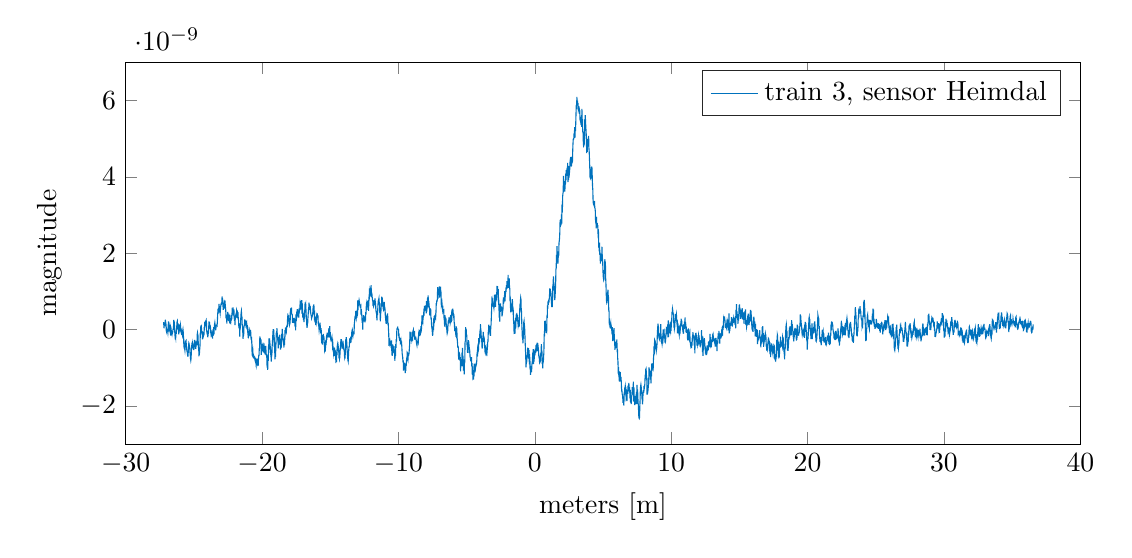
\begin{tikzpicture}

  \begin{axis}[%
    width=\textwidth,
    height=0.4\textwidth,
    at={(0\figurewidth,0\figureheight)},
    scale only axis,
    xmin=-30,
    xmax=40,
    xlabel={meters [m]},
    ymin=-3e-09,
    ymax=7e-09,
    ylabel={magnitude},
    axis background/.style={fill=white},
    legend style={legend cell align=left,align=left,draw=white!15!black}
    ]
    \addplot [color=mycolor1,solid]
    table[row sep=crcr]{%
    -27.21111328125	1.96396707344455e-10\\
    -27.190615234375	3.49601769933042e-11\\
    -27.1701171875	1.01844011075144e-10\\
    -27.149619140625	1.78717602357326e-10\\
    -27.12912109375	8.96417359760262e-11\\
    -27.108623046875	1.67733581157597e-10\\
    -27.088125	2.58231164649511e-10\\
    -27.067626953125	1.83640852739662e-10\\
    -27.04712890625	1.73637513872636e-10\\
    -27.026630859375	-1.16208015603539e-11\\
    -27.0061328125	-4.94080435529329e-11\\
    -26.985634765625	2.71570229034375e-12\\
    -26.96513671875	-3.09336267286225e-11\\
    -26.944638671875	-2.96891212944586e-11\\
    -26.924140625	-3.06552462087314e-11\\
    -26.903642578125	-7.98957975484018e-11\\
    -26.88314453125	3.78535513990957e-11\\
    -26.862646484375	2.16176674754341e-10\\
    -26.8421484375	6.28629728245676e-12\\
    -26.821650390625	1.24390780493715e-10\\
    -26.80115234375	1.23504724791928e-12\\
    -26.780654296875	2.1311057415798e-11\\
    -26.76015625	7.30847767498839e-11\\
    -26.739658203125	-2.08970737892578e-11\\
    -26.71916015625	1.92369789897015e-11\\
    -26.698662109375	-1.56925629179047e-10\\
    -26.6781640625	-7.31428669646143e-11\\
    -26.657666015625	-2.45023373559374e-11\\
    -26.63716796875	-9.12071088770687e-11\\
    -26.616669921875	-8.28556348682095e-11\\
    -26.596171875	-1.27533788835673e-10\\
    -26.575673828125	-8.91791066626502e-11\\
    -26.55517578125	-8.51170714426902e-11\\
    -26.534677734375	-1.03524813729352e-11\\
    -26.5141796875	1.41964072966785e-11\\
    -26.493681640625	1.22131724726269e-11\\
    -26.47318359375	2.53117174513625e-10\\
    -26.452685546875	1.55445841506859e-10\\
    -26.4321875	1.68548258501777e-10\\
    -26.411689453125	7.48537992699217e-11\\
    -26.39119140625	-1.21058001048818e-10\\
    -26.370693359375	-1.94434462578897e-10\\
    -26.3501953125	-1.69855791087801e-10\\
    -26.329697265625	-2.13942481220628e-10\\
    -26.30919921875	-5.44762089827431e-11\\
    -26.288701171875	-1.11049664391651e-10\\
    -26.268203125	2.57609083406237e-11\\
    -26.247705078125	1.04273258980012e-10\\
    -26.22720703125	2.08263320509072e-10\\
    -26.206708984375	2.26255493765582e-10\\
    -26.1862109375	7.62586982138678e-12\\
    -26.165712890625	1.34664020834208e-10\\
    -26.14521484375	3.57583454489408e-11\\
    -26.124716796875	6.50454021802594e-11\\
    -26.10421875	-1.24111756189308e-10\\
    -26.083720703125	1.814630738108e-11\\
    -26.06322265625	-2.81499526510038e-11\\
    -26.042724609375	1.43305596443448e-11\\
    -26.0222265625	9.5205370199935e-11\\
    -26.001728515625	8.07195252103126e-11\\
    -25.98123046875	1.19213100275661e-10\\
    -25.960732421875	-3.96732878836889e-11\\
    -25.940234375	-6.16114012019769e-11\\
    -25.919736328125	-8.93490852150142e-11\\
    -25.89923828125	-5.59144694934554e-11\\
    -25.878740234375	-1.42387991587285e-10\\
    -25.8582421875	-3.93557792158424e-11\\
    -25.837744140625	-1.05365629364006e-10\\
    -25.81724609375	-3.19099620738775e-11\\
    -25.796748046875	7.1308542978455e-12\\
    -25.77625	-6.4686873459358e-11\\
    -25.755751953125	-2.19668289290403e-10\\
    -25.73525390625	-3.67463792229383e-10\\
    -25.714755859375	-3.24712678033161e-10\\
    -25.6942578125	-3.83715527160383e-10\\
    -25.673759765625	-4.95433981987046e-10\\
    -25.65326171875	-5.4746113958989e-10\\
    -25.632763671875	-4.5137828262505e-10\\
    -25.612265625	-3.55959986069726e-10\\
    -25.591767578125	-3.04376885068165e-10\\
    -25.57126953125	-2.9033465364135e-10\\
    -25.550771484375	-4.03367543853708e-10\\
    -25.5302734375	-4.7597497430481e-10\\
    -25.509775390625	-5.64130388549174e-10\\
    -25.48927734375	-5.66986393008668e-10\\
    -25.468779296875	-6.31062450084106e-10\\
    -25.44828125	-6.93228552103522e-10\\
    -25.427783203125	-6.92895082629405e-10\\
    -25.40728515625	-5.72947774050262e-10\\
    -25.386787109375	-4.5587668267763e-10\\
    -25.3662890625	-3.49590027158722e-10\\
    -25.345791015625	-3.65589295007495e-10\\
    -25.32529296875	-4.60163679202799e-10\\
    -25.304794921875	-4.53370298409513e-10\\
    -25.284296875	-5.97250925950533e-10\\
    -25.263798828125	-6.53816189088095e-10\\
    -25.24330078125	-7.61435419251749e-10\\
    -25.222802734375	-8.07360821423449e-10\\
    -25.2023046875	-7.56321561329637e-10\\
    -25.181806640625	-5.7222479313602e-10\\
    -25.16130859375	-4.65239480024546e-10\\
    -25.140810546875	-3.69151862353137e-10\\
    -25.1203125	-3.48623658995693e-10\\
    -25.099814453125	-3.96269041785613e-10\\
    -25.07931640625	-3.45744861186844e-10\\
    -25.058818359375	-4.06876366250538e-10\\
    -25.0383203125	-4.46077018774497e-10\\
    -25.017822265625	-5.23924529369193e-10\\
    -24.99732421875	-5.24732161218953e-10\\
    -24.976826171875	-4.63265638833468e-10\\
    -24.956328125	-4.27231249440942e-10\\
    -24.935830078125	-2.72803012822802e-10\\
    -24.91533203125	-4.58369346882419e-10\\
    -24.894833984375	-3.7570292951683e-10\\
    -24.8743359375	-4.52966075637492e-10\\
    -24.853837890625	-5.06839144212716e-10\\
    -24.83333984375	-3.10575450758015e-10\\
    -24.812841796875	-3.86302081144653e-10\\
    -24.79234375	-3.45835778215052e-10\\
    -24.771845703125	-4.05004874900058e-10\\
    -24.75134765625	-1.24190298039128e-10\\
    -24.730849609375	-8.25328243090777e-11\\
    -24.7103515625	-1.34078044405384e-10\\
    -24.689853515625	-1.67736641203551e-10\\
    -24.66935546875	-4.62794474152674e-10\\
    -24.648857421875	-4.79934364471245e-10\\
    -24.628359375	-6.14269583041806e-10\\
    -24.607861328125	-5.80020751282192e-10\\
    -24.58736328125	-6.09411724372077e-10\\
    -24.566865234375	-5.00903547888288e-10\\
    -24.5463671875	-4.16850770567731e-10\\
    -24.525869140625	-1.02815496317826e-10\\
    -24.50537109375	-7.70964947191133e-11\\
    -24.484873046875	1.09018636925243e-10\\
    -24.464375	1.19181875223679e-11\\
    -24.443876953125	4.82415952506023e-11\\
    -24.42337890625	-3.76392633314891e-11\\
    -24.402880859375	-9.98161978991353e-11\\
    -24.3823828125	-8.87190774958561e-11\\
    -24.361884765625	-2.55979663684558e-10\\
    -24.34138671875	-1.10236051564532e-10\\
    -24.320888671875	-2.29000084880229e-10\\
    -24.300390625	-1.2598969149274e-10\\
    -24.279892578125	-1.49938626818106e-10\\
    -24.25939453125	-1.38665555259211e-10\\
    -24.238896484375	2.79959694433741e-11\\
    -24.2183984375	1.78338014750377e-11\\
    -24.197900390625	1.77045587646272e-10\\
    -24.17740234375	1.67550219753591e-10\\
    -24.156904296875	1.38609526315706e-10\\
    -24.13640625	2.18968279212491e-10\\
    -24.115908203125	2.17214949410906e-10\\
    -24.09541015625	2.41277238022389e-10\\
    -24.074912109375	1.72904903568657e-10\\
    -24.0544140625	-3.84014129790057e-11\\
    -24.033916015625	-8.87081425862308e-11\\
    -24.01341796875	-7.51768135935695e-11\\
    -23.992919921875	-1.21060838888894e-10\\
    -23.972421875	-2.0342398286016e-10\\
    -23.951923828125	-1.04427798846809e-10\\
    -23.93142578125	-1.01468370202326e-10\\
    -23.910927734375	2.01913136494061e-11\\
    -23.8904296875	2.11569143429572e-10\\
    -23.869931640625	6.24530908317712e-11\\
    -23.84943359375	1.93624664596937e-10\\
    -23.828935546875	9.3347086076192e-11\\
    -23.8084375	1.8522604187635e-11\\
    -23.787939453125	1.11067483691753e-10\\
    -23.76744140625	-6.9830283973778e-11\\
    -23.746943359375	-9.52396207060556e-11\\
    -23.7264453125	-1.59067159927895e-10\\
    -23.705947265625	-1.42342781912161e-10\\
    -23.68544921875	-9.87492503786532e-11\\
    -23.664951171875	-1.44172854924671e-10\\
    -23.644453125	-1.41306975230639e-10\\
    -23.623955078125	-2.37010622869113e-10\\
    -23.60345703125	1.94436721903709e-12\\
    -23.582958984375	-1.6522860230116e-10\\
    -23.5624609375	-5.22465691493094e-11\\
    -23.541962890625	6.39164194850326e-11\\
    -23.52146484375	-1.24642895371917e-10\\
    -23.500966796875	6.52347176990055e-11\\
    -23.48046875	1.37290569626513e-10\\
    -23.459970703125	1.81181803264539e-10\\
    -23.43947265625	1.13494651383326e-10\\
    -23.418974609375	9.07373661226589e-11\\
    -23.3984765625	-1.76558243410718e-11\\
    -23.377978515625	4.12839308594553e-11\\
    -23.35748046875	1.118200344009e-10\\
    -23.336982421875	1.15759025923439e-10\\
    -23.316484375	1.213969911656e-10\\
    -23.295986328125	1.07901237985268e-10\\
    -23.27548828125	1.93156989483417e-10\\
    -23.254990234375	3.82242296331759e-10\\
    -23.2344921875	4.82200496188599e-10\\
    -23.213994140625	4.66055343311646e-10\\
    -23.19349609375	5.67995983966607e-10\\
    -23.172998046875	4.40776909412295e-10\\
    -23.1525	6.72759656436996e-10\\
    -23.132001953125	5.69369505024731e-10\\
    -23.11150390625	5.56910851647165e-10\\
    -23.091005859375	4.77568027411725e-10\\
    -23.0705078125	4.25909417602825e-10\\
    -23.050009765625	5.21718988579324e-10\\
    -23.02951171875	6.0185585930859e-10\\
    -23.009013671875	6.62025344971937e-10\\
    -22.988515625	6.6005287832364e-10\\
    -22.968017578125	6.99954962831529e-10\\
    -22.94751953125	7.09669403026169e-10\\
    -22.927021484375	8.67734161557715e-10\\
    -22.9065234375	7.44110525320369e-10\\
    -22.886025390625	6.92228244729839e-10\\
    -22.86552734375	6.4263941020369e-10\\
    -22.845029296875	5.1456957525173e-10\\
    -22.82453125	6.96582957765321e-10\\
    -22.804033203125	6.18389455489327e-10\\
    -22.78353515625	7.02262830263747e-10\\
    -22.763037109375	6.59058635611345e-10\\
    -22.7425390625	5.46748886353076e-10\\
    -22.722041015625	7.64266696614902e-10\\
    -22.70154296875	6.68810419514262e-10\\
    -22.681044921875	5.84774070896063e-10\\
    -22.660546875	5.10512429129594e-10\\
    -22.640048828125	2.94359613058787e-10\\
    -22.61955078125	3.61545207118482e-10\\
    -22.599052734375	3.30477274566647e-10\\
    -22.5785546875	1.57436965079652e-10\\
    -22.558056640625	3.59005291292145e-10\\
    -22.53755859375	2.47130427884523e-10\\
    -22.517060546875	4.64473886385255e-10\\
    -22.4965625	2.93469773303718e-10\\
    -22.476064453125	3.48522047788035e-10\\
    -22.45556640625	3.97793537525841e-10\\
    -22.435068359375	2.18309970124205e-10\\
    -22.4145703125	2.98677222702996e-10\\
    -22.394072265625	2.4515328765258e-10\\
    -22.37357421875	2.89331188651696e-10\\
    -22.353076171875	1.87804567914956e-10\\
    -22.332578125	1.7906932327293e-10\\
    -22.312080078125	2.27995338154542e-10\\
    -22.29158203125	2.00307287813815e-10\\
    -22.271083984375	2.91891886055915e-10\\
    -22.2505859375	2.51480609276302e-10\\
    -22.230087890625	2.66632207156095e-10\\
    -22.20958984375	3.13918418357482e-10\\
    -22.189091796875	5.18731540598909e-10\\
    -22.16859375	5.05607112560347e-10\\
    -22.148095703125	3.88051453945438e-10\\
    -22.12759765625	5.79289460945448e-10\\
    -22.107099609375	4.0260489429693e-10\\
    -22.0866015625	5.25930174550666e-10\\
    -22.066103515625	3.45138044079582e-10\\
    -22.04560546875	3.91401132002532e-10\\
    -22.025107421875	2.28079339272232e-10\\
    -22.004609375	3.50432315586248e-10\\
    -21.984111328125	1.188256547512e-10\\
    -21.96361328125	2.90338498909196e-10\\
    -21.943115234375	3.57279900026686e-10\\
    -21.9226171875	3.83848032584523e-10\\
    -21.902119140625	3.40604835442343e-10\\
    -21.88162109375	3.33083094224736e-10\\
    -21.861123046875	5.00701268892251e-10\\
    -21.840625	4.74306798281221e-10\\
    -21.820126953125	4.81009173371238e-10\\
    -21.79962890625	3.01920024968411e-10\\
    -21.779130859375	3.92674020175568e-10\\
    -21.7586328125	4.06565891327501e-10\\
    -21.738134765625	2.60761155467435e-10\\
    -21.71763671875	2.34435964342873e-10\\
    -21.697138671875	3.91161436925145e-11\\
    -21.676640625	1.04309945198582e-10\\
    -21.656142578125	1.50516596731332e-10\\
    -21.63564453125	-1.86921349377113e-10\\
    -21.615146484375	2.41266699392357e-11\\
    -21.5946484375	3.8007916128358e-11\\
    -21.574150390625	1.69629013691459e-10\\
    -21.55365234375	3.26775264161844e-10\\
    -21.533154296875	4.37183842431385e-10\\
    -21.51265625	4.80606076038786e-10\\
    -21.492158203125	3.61356749952467e-10\\
    -21.47166015625	3.25576700813793e-10\\
    -21.451162109375	1.14455285082497e-10\\
    -21.4306640625	9.72798573347738e-11\\
    -21.410166015625	-7.32445396969717e-11\\
    -21.38966796875	-2.46370862685423e-10\\
    -21.369169921875	-1.07355186228371e-10\\
    -21.348671875	-1.66997864237725e-10\\
    -21.328173828125	4.83110764778447e-11\\
    -21.30767578125	1.02016207683771e-10\\
    -21.287177734375	1.15348782365495e-10\\
    -21.2666796875	2.66275354205594e-10\\
    -21.246181640625	2.11304370789001e-10\\
    -21.22568359375	1.77652376796575e-10\\
    -21.205185546875	1.45830638980395e-10\\
    -21.1846875	2.39414137766263e-10\\
    -21.164189453125	1.09635200233244e-10\\
    -21.14369140625	1.29336844670079e-10\\
    -21.123193359375	1.57062900828309e-10\\
    -21.1026953125	1.2333868440949e-11\\
    -21.082197265625	1.14683211006989e-10\\
    -21.06169921875	-7.82609523782206e-12\\
    -21.041201171875	-8.52798602541871e-11\\
    -21.020703125	-2.29300678652914e-11\\
    -21.000205078125	-7.52864351249656e-11\\
    -20.97970703125	-1.74342807645157e-10\\
    -20.959208984375	-1.47385855912622e-10\\
    -20.9387109375	-5.65257196308904e-11\\
    -20.918212890625	-1.57619610703453e-10\\
    -20.89771484375	-1.05018845106909e-11\\
    -20.877216796875	-3.45884377333427e-11\\
    -20.85671875	-1.69042588471685e-10\\
    -20.836220703125	-1.79852878296807e-11\\
    -20.81572265625	-1.71234615368485e-10\\
    -20.795224609375	-2.78210438180403e-10\\
    -20.7747265625	-1.95221592859158e-10\\
    -20.754228515625	-3.05365539407357e-10\\
    -20.73373046875	-5.4884262938425e-10\\
    -20.713232421875	-5.07021062189063e-10\\
    -20.692734375	-6.14817917336132e-10\\
    -20.672236328125	-5.69212929910452e-10\\
    -20.65173828125	-7.00451377521716e-10\\
    -20.631240234375	-7.19908371717703e-10\\
    -20.6107421875	-6.8829702480371e-10\\
    -20.590244140625	-7.11972431325162e-10\\
    -20.56974609375	-7.09684287994854e-10\\
    -20.549248046875	-7.46154898636458e-10\\
    -20.52875	-7.40294142716487e-10\\
    -20.508251953125	-8.19337243822795e-10\\
    -20.48775390625	-8.39192746380726e-10\\
    -20.467255859375	-7.40109426411314e-10\\
    -20.4467578125	-8.5475709050138e-10\\
    -20.426259765625	-8.06114386443398e-10\\
    -20.40576171875	-8.02286876965861e-10\\
    -20.385263671875	-9.26590641313233e-10\\
    -20.364765625	-8.86376647913987e-10\\
    -20.344267578125	-7.65473097400316e-10\\
    -20.32376953125	-9.08363958616458e-10\\
    -20.303271484375	-8.20443594595857e-10\\
    -20.2827734375	-9.47545021907005e-10\\
    -20.262275390625	-7.77759736026867e-10\\
    -20.24177734375	-6.86580761005389e-10\\
    -20.221279296875	-6.83281208992021e-10\\
    -20.20078125	-4.9837537440254e-10\\
    -20.180283203125	-4.87514917609656e-10\\
    -20.15978515625	-1.82360005996765e-10\\
    -20.139287109375	-3.10502933825972e-10\\
    -20.1187890625	-2.83346974773835e-10\\
    -20.098291015625	-3.60424935082565e-10\\
    -20.07779296875	-2.58309403804821e-10\\
    -20.057294921875	-6.66063249506075e-10\\
    -20.036796875	-3.75378825081463e-10\\
    -20.016298828125	-5.75214102850235e-10\\
    -19.99580078125	-5.53161049597263e-10\\
    -19.975302734375	-5.1107289800555e-10\\
    -19.9548046875	-4.42366684575683e-10\\
    -19.934306640625	-4.82869423940934e-10\\
    -19.91380859375	-5.19000788426981e-10\\
    -19.893310546875	-4.3998052907959e-10\\
    -19.8728125	-4.82666385419525e-10\\
    -19.852314453125	-5.29777172101582e-10\\
    -19.83181640625	-4.79096088345121e-10\\
    -19.811318359375	-5.71417075784551e-10\\
    -19.7908203125	-5.66552042903159e-10\\
    -19.770322265625	-6.52580349735782e-10\\
    -19.74982421875	-5.71342930363235e-10\\
    -19.729326171875	-4.27926083441982e-10\\
    -19.708828125	-5.59900310707763e-10\\
    -19.688330078125	-6.66851497020781e-10\\
    -19.66783203125	-6.86771618022532e-10\\
    -19.647333984375	-7.44551125906577e-10\\
    -19.6268359375	-9.98742889481427e-10\\
    -19.606337890625	-7.00236944847121e-10\\
    -19.58583984375	-1.05748237663477e-09\\
    -19.565341796875	-6.48364479730073e-10\\
    -19.54484375	-8.22261366526396e-10\\
    -19.524345703125	-4.86201943185535e-10\\
    -19.50384765625	-5.13080200393544e-10\\
    -19.483349609375	-2.23179935176898e-10\\
    -19.4628515625	-3.14203832621115e-10\\
    -19.442353515625	-4.0035281180367e-10\\
    -19.42185546875	-3.53490506260963e-10\\
    -19.401357421875	-4.36371379158198e-10\\
    -19.380859375	-4.72847630633444e-10\\
    -19.360361328125	-6.4925962256146e-10\\
    -19.33986328125	-7.10393855501978e-10\\
    -19.319365234375	-8.39207038933986e-10\\
    -19.2988671875	-6.00745408366233e-10\\
    -19.278369140625	-6.74442915762892e-10\\
    -19.25787109375	-4.47113106567836e-10\\
    -19.237373046875	-3.47086396860483e-10\\
    -19.216875	-1.88108899032448e-10\\
    -19.196376953125	-5.97703332995761e-11\\
    -19.17587890625	8.74767454696602e-12\\
    -19.155380859375	-1.00501546289258e-10\\
    -19.1348828125	-1.16767214427466e-12\\
    -19.114384765625	-3.40787173823469e-10\\
    -19.09388671875	-3.07946678739155e-10\\
    -19.073388671875	-4.61091635755664e-10\\
    -19.052890625	-7.78070026438927e-10\\
    -19.032392578125	-6.43166346361111e-10\\
    -19.01189453125	-7.13976218540652e-10\\
    -18.991396484375	-4.9999319947339e-10\\
    -18.9708984375	-3.10914990513495e-10\\
    -18.950400390625	-6.14948347194292e-11\\
    -18.92990234375	-1.80809150201264e-10\\
    -18.909404296875	3.52235180173037e-11\\
    -18.88890625	-8.32052261953868e-11\\
    -18.868408203125	-1.66024108118513e-10\\
    -18.84791015625	-2.75567291478333e-10\\
    -18.827412109375	-3.12576950999245e-10\\
    -18.8069140625	-4.93750914955623e-10\\
    -18.786416015625	-3.33229662236535e-10\\
    -18.76591796875	-2.00102945757972e-10\\
    -18.745419921875	-2.77642272396188e-10\\
    -18.724921875	-1.81913964297678e-10\\
    -18.704423828125	-1.37957450202697e-10\\
    -18.68392578125	-3.91747305498946e-10\\
    -18.663427734375	-2.35286617462952e-10\\
    -18.6429296875	-5.2702370153101e-10\\
    -18.622431640625	-4.70765075563245e-10\\
    -18.60193359375	-2.62252789742825e-10\\
    -18.581435546875	-4.70834032396646e-10\\
    -18.5609375	-1.141516080908e-10\\
    -18.540439453125	-2.62441165679604e-10\\
    -18.51994140625	1.47529402340815e-11\\
    -18.499443359375	-1.67632465430284e-10\\
    -18.4789453125	-1.54185833810852e-10\\
    -18.458447265625	-2.67509741004878e-10\\
    -18.43794921875	-3.05197959966506e-10\\
    -18.417451171875	-2.91681655526475e-10\\
    -18.396953125	-4.71227615393529e-10\\
    -18.376455078125	-3.30786594595178e-10\\
    -18.35595703125	-4.02552437234947e-10\\
    -18.335458984375	-2.49735304884498e-10\\
    -18.3149609375	-1.55710289293195e-11\\
    -18.294462890625	-5.87333208126583e-11\\
    -18.27396484375	5.6220932771399e-11\\
    -18.253466796875	-8.29607746382041e-12\\
    -18.23296875	5.44101449079627e-12\\
    -18.212470703125	-3.51368034424357e-11\\
    -18.19197265625	7.40248813472106e-11\\
    -18.171474609375	1.01244651041443e-10\\
    -18.1509765625	9.37583204500582e-11\\
    -18.130478515625	2.54770726249908e-10\\
    -18.10998046875	3.58040824837446e-10\\
    -18.089482421875	3.36306034277912e-10\\
    -18.068984375	3.12062997417298e-10\\
    -18.048486328125	2.447267057849e-10\\
    -18.02798828125	3.04271390695282e-10\\
    -18.007490234375	2.13353261407302e-10\\
    -17.9869921875	1.19176102757627e-10\\
    -17.966494140625	1.45911415493426e-10\\
    -17.94599609375	1.74965503417418e-10\\
    -17.925498046875	3.03210553375614e-10\\
    -17.905	5.33637660484784e-10\\
    -17.884501953125	5.28898640936307e-10\\
    -17.86400390625	5.06458620606884e-10\\
    -17.843505859375	5.75927622888274e-10\\
    -17.8230078125	4.06646869712975e-10\\
    -17.802509765625	3.94695014925367e-10\\
    -17.78201171875	3.89774058651445e-10\\
    -17.761513671875	1.77243232051789e-10\\
    -17.741015625	2.9981986372813e-10\\
    -17.720517578125	2.13084951600686e-10\\
    -17.70001953125	2.20600869796601e-10\\
    -17.679521484375	3.02388006299197e-10\\
    -17.6590234375	1.67021249614868e-10\\
    -17.638525390625	2.40367574621659e-10\\
    -17.61802734375	2.57440221624639e-10\\
    -17.597529296875	1.71484140373091e-10\\
    -17.57703125	2.04637924230444e-10\\
    -17.556533203125	2.6760382653939e-10\\
    -17.53603515625	-2.36414369685538e-11\\
    -17.515537109375	3.96881779103554e-10\\
    -17.4950390625	3.23161235660319e-10\\
    -17.474541015625	2.99701260211488e-10\\
    -17.45404296875	4.71287658578246e-10\\
    -17.433544921875	3.47891796158974e-10\\
    -17.413046875	5.31966192004651e-10\\
    -17.392548828125	3.94773484974151e-10\\
    -17.37205078125	4.22414124612423e-10\\
    -17.351552734375	3.96304815465394e-10\\
    -17.3310546875	4.40909498525182e-10\\
    -17.310556640625	3.10214045389426e-10\\
    -17.29005859375	4.28600643196485e-10\\
    -17.269560546875	4.49717607260328e-10\\
    -17.2490625	5.41379804228803e-10\\
    -17.228564453125	5.50445543932225e-10\\
    -17.20806640625	6.7346118202351e-10\\
    -17.187568359375	6.23825585773017e-10\\
    -17.1670703125	7.04082580750286e-10\\
    -17.146572265625	6.30643405942781e-10\\
    -17.12607421875	7.5466737869541e-10\\
    -17.105576171875	5.31515332226616e-10\\
    -17.085078125	7.67684381370717e-10\\
    -17.064580078125	4.09857822355338e-10\\
    -17.04408203125	6.81982199775191e-10\\
    -17.023583984375	3.16477684519606e-10\\
    -17.0030859375	4.34536079398111e-10\\
    -16.982587890625	3.49217628956535e-10\\
    -16.96208984375	2.46082633801394e-10\\
    -16.941591796875	3.61505152985259e-10\\
    -16.92109375	1.91925711115034e-10\\
    -16.900595703125	3.88397458282782e-10\\
    -16.88009765625	3.6646294443813e-10\\
    -16.859599609375	5.53756303115386e-10\\
    -16.8391015625	7.09858419423658e-10\\
    -16.818603515625	6.27952680017459e-10\\
    -16.79810546875	6.61552623399732e-10\\
    -16.777607421875	5.07439425854198e-10\\
    -16.757109375	3.5040899512202e-10\\
    -16.736611328125	2.48004230106811e-10\\
    -16.71611328125	1.09322625649057e-10\\
    -16.695615234375	4.21494434483345e-11\\
    -16.6751171875	1.49976997261507e-10\\
    -16.654619140625	1.61742463690188e-10\\
    -16.63412109375	3.00878331871842e-10\\
    -16.613623046875	4.08108749494016e-10\\
    -16.593125	5.41484119490246e-10\\
    -16.572626953125	5.73899847235755e-10\\
    -16.55212890625	7.06230361944339e-10\\
    -16.531630859375	5.18354048169896e-10\\
    -16.5111328125	6.56951719294319e-10\\
    -16.490634765625	5.49272658071942e-10\\
    -16.47013671875	5.00201485703779e-10\\
    -16.449638671875	5.26422047797405e-10\\
    -16.429140625	4.28132276708024e-10\\
    -16.408642578125	3.80761562466127e-10\\
    -16.38814453125	3.58293751211894e-10\\
    -16.367646484375	2.93217625049219e-10\\
    -16.3471484375	3.19237044385493e-10\\
    -16.326650390625	3.43789457215743e-10\\
    -16.30615234375	3.67814674051856e-10\\
    -16.285654296875	3.9595932250706e-10\\
    -16.26515625	5.20787011190261e-10\\
    -16.244658203125	6.1704043893388e-10\\
    -16.22416015625	5.20281594321296e-10\\
    -16.203662109375	6.56496876498672e-10\\
    -16.1831640625	5.6691633188946e-10\\
    -16.162666015625	3.53157387290815e-10\\
    -16.14216796875	3.86253180648753e-10\\
    -16.121669921875	2.02775935220323e-10\\
    -16.101171875	2.03468045031437e-10\\
    -16.080673828125	2.35597832460896e-10\\
    -16.06017578125	1.19328134300258e-10\\
    -16.039677734375	2.69851007768543e-10\\
    -16.0191796875	2.12680692423318e-10\\
    -15.998681640625	3.07946397156709e-10\\
    -15.97818359375	4.21632073801767e-10\\
    -15.957685546875	4.17448990543405e-10\\
    -15.9371875	3.44771034945098e-10\\
    -15.916689453125	3.23731799102945e-10\\
    -15.89619140625	3.34039729092431e-10\\
    -15.875693359375	1.59793378511397e-10\\
    -15.8551953125	1.38688453335386e-10\\
    -15.834697265625	7.32233918201841e-11\\
    -15.81419921875	-1.34676570707467e-11\\
    -15.793701171875	4.68378897288658e-11\\
    -15.773203125	8.89233504606964e-11\\
    -15.752705078125	1.77510255979555e-10\\
    -15.73220703125	9.82171553890392e-11\\
    -15.711708984375	4.62752706262975e-12\\
    -15.6912109375	-1.01762641620179e-10\\
    -15.670712890625	3.7316710257006e-11\\
    -15.65021484375	-8.48522198707161e-11\\
    -15.629716796875	-3.63889840809502e-10\\
    -15.60921875	-2.85069377847811e-10\\
    -15.588720703125	-3.43904907795507e-10\\
    -15.56822265625	-3.94637962220924e-10\\
    -15.547724609375	-1.45974472197849e-10\\
    -15.5272265625	-2.49327083962912e-10\\
    -15.506728515625	-1.15177724458881e-10\\
    -15.48623046875	-2.60886934581981e-10\\
    -15.465732421875	-1.6921989961595e-10\\
    -15.445234375	-3.2261515698311e-10\\
    -15.424736328125	-3.71886454648905e-10\\
    -15.40423828125	-5.40804310643458e-10\\
    -15.383740234375	-5.07763530290496e-10\\
    -15.3632421875	-5.74550600300579e-10\\
    -15.342744140625	-4.34812141526208e-10\\
    -15.32224609375	-2.77096796000805e-10\\
    -15.301748046875	-4.07538258792831e-10\\
    -15.28125	-2.0394989873264e-10\\
    -15.260751953125	-1.65737365836508e-10\\
    -15.24025390625	-1.90358806446823e-10\\
    -15.219755859375	-7.94068212032526e-11\\
    -15.1992578125	-1.59209671383831e-10\\
    -15.178759765625	-1.73303128035626e-10\\
    -15.15826171875	-1.44405856897706e-10\\
    -15.137763671875	-2.02232430569115e-10\\
    -15.117265625	-5.43888817895486e-11\\
    -15.096767578125	3.29933996618744e-11\\
    -15.07626953125	-1.96604734149256e-10\\
    -15.055771484375	-4.28607892693408e-11\\
    -15.0352734375	9.08973910178355e-11\\
    -15.014775390625	-2.14145928829172e-10\\
    -14.99427734375	-7.10912670421673e-11\\
    -14.973779296875	-2.34496581603569e-10\\
    -14.95328125	-2.66332372812785e-10\\
    -14.932783203125	-2.37100174862679e-10\\
    -14.91228515625	-2.36114468738929e-10\\
    -14.891787109375	-2.67388964409418e-10\\
    -14.8712890625	-2.19466442940056e-10\\
    -14.850791015625	-3.12477277260609e-10\\
    -14.83029296875	-4.29668255037032e-10\\
    -14.809794921875	-3.78619303930358e-10\\
    -14.789296875	-5.02126452799267e-10\\
    -14.768798828125	-5.30464693679005e-10\\
    -14.74830078125	-6.33276266154982e-10\\
    -14.727802734375	-5.83282900703092e-10\\
    -14.7073046875	-6.80367251713617e-10\\
    -14.686806640625	-4.7360212445821e-10\\
    -14.66630859375	-6.96552343951096e-10\\
    -14.645810546875	-5.98635708502249e-10\\
    -14.6253125	-6.39841325674789e-10\\
    -14.604814453125	-6.1338067322613e-10\\
    -14.58431640625	-8.76577020151185e-10\\
    -14.563818359375	-5.82227676802833e-10\\
    -14.5433203125	-8.45299500670334e-10\\
    -14.522822265625	-6.00207192056624e-10\\
    -14.50232421875	-6.69700343407007e-10\\
    -14.481826171875	-4.28843749494631e-10\\
    -14.461328125	-3.90106431344765e-10\\
    -14.440830078125	-4.60788471928706e-10\\
    -14.42033203125	-4.18986980010947e-10\\
    -14.399833984375	-4.74467849535884e-10\\
    -14.3793359375	-5.34093162275283e-10\\
    -14.358837890625	-6.93664174887361e-10\\
    -14.33833984375	-6.75090623376688e-10\\
    -14.317841796875	-7.63211267058098e-10\\
    -14.29734375	-7.22169548155358e-10\\
    -14.276845703125	-5.93072017123303e-10\\
    -14.25634765625	-4.74445849891144e-10\\
    -14.235849609375	-3.72722314955859e-10\\
    -14.2153515625	-4.2115292377905e-10\\
    -14.194853515625	-2.48866465075935e-10\\
    -14.17435546875	-4.15786986654759e-10\\
    -14.153857421875	-3.3968837942817e-10\\
    -14.133359375	-4.9836574183877e-10\\
    -14.112861328125	-4.21018862147518e-10\\
    -14.09236328125	-4.42073581554254e-10\\
    -14.071865234375	-2.90948157787114e-10\\
    -14.0513671875	-3.62164542236088e-10\\
    -14.030869140625	-4.44927743329282e-10\\
    -14.01037109375	-4.98314991262424e-10\\
    -13.989873046875	-5.32620091732862e-10\\
    -13.969375	-5.64637591296935e-10\\
    -13.948876953125	-7.05778893819158e-10\\
    -13.92837890625	-6.67457931277593e-10\\
    -13.907880859375	-6.9237502479753e-10\\
    -13.8873828125	-5.84589437708633e-10\\
    -13.866884765625	-2.58130287125073e-10\\
    -13.84638671875	-3.46312074588204e-10\\
    -13.825888671875	-1.97319115485209e-10\\
    -13.805390625	-2.7175784551104e-10\\
    -13.784892578125	-3.40327860055545e-10\\
    -13.76439453125	-4.93379999895375e-10\\
    -13.743896484375	-6.26805171783022e-10\\
    -13.7233984375	-7.04426159569552e-10\\
    -13.702900390625	-8.04451271380524e-10\\
    -13.68240234375	-8.34979795030366e-10\\
    -13.661904296875	-6.80885549961806e-10\\
    -13.64140625	-5.26796195960634e-10\\
    -13.620908203125	-4.55661670263597e-10\\
    -13.60041015625	-4.46906219013987e-10\\
    -13.579912109375	-3.11976882987279e-10\\
    -13.5594140625	-2.27517250479179e-10\\
    -13.538916015625	-3.34559956599103e-10\\
    -13.51841796875	-2.75181104779888e-10\\
    -13.497919921875	-3.31154286600782e-10\\
    -13.477421875	-3.27089488797836e-10\\
    -13.456923828125	-2.28761875552856e-10\\
    -13.43642578125	-1.92839507082768e-10\\
    -13.415927734375	-5.54047604402361e-11\\
    -13.3954296875	-2.62622532405483e-11\\
    -13.374931640625	-1.58521252540737e-10\\
    -13.35443359375	-9.95037239104593e-11\\
    -13.333935546875	-1.65095909334704e-10\\
    -13.3134375	-1.17308914030873e-10\\
    -13.292939453125	-8.53496784640417e-11\\
    -13.27244140625	-6.78197868988406e-11\\
    -13.251943359375	-1.23065256099982e-10\\
    -13.2314453125	1.83059299748167e-10\\
    -13.210947265625	1.89833761367757e-10\\
    -13.19044921875	3.27771601003959e-10\\
    -13.169951171875	3.39022843813357e-10\\
    -13.149453125	3.23369323671054e-10\\
    -13.128955078125	4.85392456020257e-10\\
    -13.10845703125	3.83499931448071e-10\\
    -13.087958984375	3.26886981643759e-10\\
    -13.0674609375	4.25133587970037e-10\\
    -13.046962890625	3.09089765139552e-10\\
    -13.02646484375	5.05191886577104e-10\\
    -13.005966796875	3.53518010411342e-10\\
    -12.98546875	7.63124400655408e-10\\
    -12.964970703125	5.10415851003186e-10\\
    -12.94447265625	6.3979150197387e-10\\
    -12.923974609375	6.77256920074074e-10\\
    -12.9034765625	7.2620923551857e-10\\
    -12.882978515625	6.42639397975073e-10\\
    -12.86248046875	7.21843547226232e-10\\
    -12.841982421875	6.74284623923683e-10\\
    -12.821484375	6.28056705313553e-10\\
    -12.800986328125	5.99286391316366e-10\\
    -12.78048828125	6.0839175751974e-10\\
    -12.759990234375	6.22543981558139e-10\\
    -12.7394921875	3.90430791821247e-10\\
    -12.718994140625	5.31118813022609e-10\\
    -12.69849609375	4.23133874347433e-10\\
    -12.677998046875	3.32943269311233e-10\\
    -12.6575	1.76471518195828e-10\\
    -12.637001953125	2.87475017973355e-10\\
    -12.61650390625	-1.98618867168321e-12\\
    -12.596005859375	2.48022549939234e-10\\
    -12.5755078125	2.91353380786806e-10\\
    -12.555009765625	3.78728259633023e-10\\
    -12.53451171875	2.47783456844884e-10\\
    -12.514013671875	3.57723730518736e-10\\
    -12.493515625	2.17359113424775e-10\\
    -12.473017578125	3.19384072057347e-10\\
    -12.45251953125	1.87754437929656e-10\\
    -12.432021484375	2.93536591679848e-10\\
    -12.4115234375	2.81666014575689e-10\\
    -12.391025390625	4.61313350368767e-10\\
    -12.37052734375	3.97997080143791e-10\\
    -12.350029296875	6.63167657336368e-10\\
    -12.32953125	6.97631130846404e-10\\
    -12.309033203125	5.93992543666328e-10\\
    -12.28853515625	7.43828154518381e-10\\
    -12.268037109375	6.09127967683732e-10\\
    -12.2475390625	5.93896788548829e-10\\
    -12.227041015625	5.16617225941006e-10\\
    -12.20654296875	7.70111906660486e-10\\
    -12.186044921875	4.91751787084446e-10\\
    -12.165546875	8.5353454365882e-10\\
    -12.145048828125	7.55344348404781e-10\\
    -12.12455078125	1.07923362443883e-09\\
    -12.104052734375	9.87134755231833e-10\\
    -12.0835546875	1.05955910760814e-09\\
    -12.063056640625	1.02407092303868e-09\\
    -12.04255859375	1.09009549412377e-09\\
    -12.022060546875	8.60085482480359e-10\\
    -12.0015625	1.16461972743449e-09\\
    -11.981064453125	8.49342268294956e-10\\
    -11.96056640625	9.50831772564499e-10\\
    -11.940068359375	9.18292179473235e-10\\
    -11.9195703125	8.37432653927352e-10\\
    -11.899072265625	7.70809111903248e-10\\
    -11.87857421875	7.43899571847807e-10\\
    -11.858076171875	6.14514950100476e-10\\
    -11.837578125	7.25334609633208e-10\\
    -11.817080078125	6.13956153219642e-10\\
    -11.79658203125	6.35485342912148e-10\\
    -11.776083984375	7.69705986128472e-10\\
    -11.7555859375	6.41951941353366e-10\\
    -11.735087890625	7.20259712169521e-10\\
    -11.71458984375	8.15347449296068e-10\\
    -11.694091796875	6.95119311689704e-10\\
    -11.67359375	6.83241876941797e-10\\
    -11.653095703125	5.07863117830496e-10\\
    -11.63259765625	4.62998379190272e-10\\
    -11.612099609375	4.66949299326066e-10\\
    -11.5916015625	3.42284001102714e-10\\
    -11.571103515625	2.40929519323466e-10\\
    -11.55060546875	4.42002626579005e-10\\
    -11.530107421875	3.78949608444592e-10\\
    -11.509609375	5.70715200356499e-10\\
    -11.489111328125	7.0630505928309e-10\\
    -11.46861328125	7.68032430277804e-10\\
    -11.448115234375	7.82559672361092e-10\\
    -11.4276171875	8.16526872942861e-10\\
    -11.407119140625	7.09066487696304e-10\\
    -11.38662109375	6.94299354148405e-10\\
    -11.366123046875	4.55879516137454e-10\\
    -11.345625	4.59411879438594e-10\\
    -11.325126953125	2.15285640738931e-10\\
    -11.30462890625	4.48333438695885e-10\\
    -11.284130859375	4.44898279225105e-10\\
    -11.2636328125	6.82264213478452e-10\\
    -11.243134765625	6.00894519631709e-10\\
    -11.22263671875	8.44176528362846e-10\\
    -11.202138671875	8.41733219213817e-10\\
    -11.181640625	8.06708532142646e-10\\
    -11.161142578125	7.32582510636851e-10\\
    -11.14064453125	6.80986838085824e-10\\
    -11.120146484375	5.60943028326862e-10\\
    -11.0996484375	5.32214277071614e-10\\
    -11.079150390625	6.01761587676082e-10\\
    -11.05865234375	5.77501712163801e-10\\
    -11.038154296875	7.23281457417742e-10\\
    -11.01765625	5.15387415707946e-10\\
    -10.997158203125	5.65968540559959e-10\\
    -10.97666015625	5.19420291523762e-10\\
    -10.956162109375	3.13902944875603e-10\\
    -10.9356640625	3.04330881248426e-10\\
    -10.915166015625	1.68370948123188e-10\\
    -10.89466796875	1.66302473556328e-10\\
    -10.874169921875	2.74944329189423e-10\\
    -10.853671875	2.37680990982837e-10\\
    -10.833173828125	3.33257467726662e-10\\
    -10.81267578125	3.46833224840247e-10\\
    -10.792177734375	4.20358194686598e-10\\
    -10.7716796875	1.77678659773005e-10\\
    -10.751181640625	1.71417765250264e-10\\
    -10.73068359375	2.18617921538409e-11\\
    -10.710185546875	-1.09666364899288e-10\\
    -10.6896875	-4.26671380902231e-10\\
    -10.669189453125	-2.30169967703622e-10\\
    -10.64869140625	-3.49365255394681e-10\\
    -10.628193359375	-3.11947162439418e-10\\
    -10.6076953125	-3.94155740935094e-10\\
    -10.587197265625	-4.0439136277969e-10\\
    -10.56669921875	-3.02173409596563e-10\\
    -10.546201171875	-3.92003115815198e-10\\
    -10.525703125	-4.85509203862008e-10\\
    -10.505205078125	-2.80911826094129e-10\\
    -10.48470703125	-5.65044590730972e-10\\
    -10.464208984375	-5.31996688178375e-10\\
    -10.4437109375	-6.85800074477739e-10\\
    -10.423212890625	-3.89802331157756e-10\\
    -10.40271484375	-4.74346914858288e-10\\
    -10.382216796875	-4.63067880183566e-10\\
    -10.36171875	-5.41307892287577e-10\\
    -10.341220703125	-4.43739118329827e-10\\
    -10.32072265625	-6.16284377474057e-10\\
    -10.300224609375	-5.66245571326893e-10\\
    -10.2797265625	-6.62358942825798e-10\\
    -10.259228515625	-8.19018558992708e-10\\
    -10.23873046875	-5.29841767067626e-10\\
    -10.218232421875	-6.96122129505831e-10\\
    -10.197734375	-3.82629904379911e-10\\
    -10.177236328125	-4.78747874536352e-10\\
    -10.15673828125	-2.49029179707044e-10\\
    -10.136240234375	-3.08085394395682e-10\\
    -10.1157421875	-4.5241510537311e-12\\
    -10.095244140625	3.53094909496524e-11\\
    -10.07474609375	4.2347092920981e-11\\
    -10.054248046875	5.47264857187826e-11\\
    -10.03375	1.22875756741852e-11\\
    -10.013251953125	1.01383951225139e-11\\
    -9.99275390625	4.69897929985721e-12\\
    -9.972255859375	-1.63483231164886e-10\\
    -9.9517578125	-1.52122371273417e-10\\
    -9.931259765625	-2.46000765891757e-10\\
    -9.91076171875	-2.81271027870364e-10\\
    -9.890263671875	-2.78450744483656e-10\\
    -9.869765625	-2.16916450104593e-10\\
    -9.849267578125	-3.63483434782522e-10\\
    -9.82876953125	-3.57577562991652e-10\\
    -9.808271484375	-3.00454851160893e-10\\
    -9.7877734375	-3.68914520061639e-10\\
    -9.767275390625	-3.5636825898751e-10\\
    -9.74677734375	-4.66163000032025e-10\\
    -9.726279296875	-6.18683838332866e-10\\
    -9.70578125	-6.79595065015576e-10\\
    -9.685283203125	-7.27825661136543e-10\\
    -9.66478515625	-8.61454472589249e-10\\
    -9.644287109375	-8.05957453601711e-10\\
    -9.6237890625	-1.07626672027969e-09\\
    -9.603291015625	-8.7804645245625e-10\\
    -9.58279296875	-9.41906713386955e-10\\
    -9.562294921875	-8.68240749041789e-10\\
    -9.541796875	-1.02210760858388e-09\\
    -9.521298828125	-9.45650700116588e-10\\
    -9.50080078125	-1.14078028457093e-09\\
    -9.480302734375	-9.80356193545085e-10\\
    -9.4598046875	-1.08394051035757e-09\\
    -9.439306640625	-8.67612324330679e-10\\
    -9.41880859375	-9.42010434910328e-10\\
    -9.398310546875	-7.41900328118271e-10\\
    -9.3778125	-8.29615672065892e-10\\
    -9.357314453125	-5.99973473771488e-10\\
    -9.33681640625	-6.12138565369934e-10\\
    -9.316318359375	-7.2738205625716e-10\\
    -9.2958203125	-7.68497345251045e-10\\
    -9.275322265625	-6.55711147715371e-10\\
    -9.25482421875	-6.50420909734521e-10\\
    -9.234326171875	-6.55311201715797e-10\\
    -9.213828125	-5.8572768138254e-10\\
    -9.193330078125	-4.71250599768398e-10\\
    -9.17283203125	-3.72595575198434e-10\\
    -9.152333984375	-5.5939887523005e-11\\
    -9.1318359375	-1.02457413147832e-10\\
    -9.111337890625	-9.89291770242411e-11\\
    -9.09083984375	-1.88209064282679e-10\\
    -9.070341796875	-1.54908370742189e-10\\
    -9.04984375	-2.9977905180291e-10\\
    -9.029345703125	-1.94891129189652e-10\\
    -9.00884765625	-2.84916946336318e-10\\
    -8.988349609375	-2.52457791486405e-10\\
    -8.9678515625	-2.613171568148e-10\\
    -8.947353515625	-6.46309454130478e-11\\
    -8.92685546875	-3.88471057072407e-11\\
    -8.906357421875	-1.29244665973708e-11\\
    -8.885859375	-1.70362763014464e-10\\
    -8.865361328125	-6.19707399877638e-11\\
    -8.84486328125	-1.95131158693974e-10\\
    -8.824365234375	-3.51747241317505e-11\\
    -8.8038671875	-2.36330724916504e-10\\
    -8.783369140625	-2.28089178418656e-10\\
    -8.76287109375	-2.41436275494059e-10\\
    -8.742373046875	-2.49572561715019e-10\\
    -8.721875	-2.21266346970523e-10\\
    -8.701376953125	-2.54822668154238e-10\\
    -8.68087890625	-3.38673844431758e-10\\
    -8.660380859375	-3.76406560086717e-10\\
    -8.6398828125	-4.14458944951611e-10\\
    -8.619384765625	-3.46237784624754e-10\\
    -8.59888671875	-3.43175780854547e-10\\
    -8.578388671875	-3.01294190238719e-10\\
    -8.557890625	-2.49726693129635e-10\\
    -8.537392578125	-2.92576869087283e-10\\
    -8.51689453125	-9.6425537834637e-11\\
    -8.496396484375	-5.77580035722897e-11\\
    -8.4758984375	-9.31270177840873e-11\\
    -8.455400390625	-9.07221506981944e-11\\
    -8.43490234375	-1.74249666013921e-10\\
    -8.414404296875	-9.78514901249768e-12\\
    -8.39390625	-1.42785987743856e-10\\
    -8.373408203125	-4.58344987243386e-11\\
    -8.35291015625	-1.01990436612289e-10\\
    -8.332412109375	3.13105923581673e-11\\
    -8.3119140625	1.61733780271672e-11\\
    -8.291416015625	1.4408461837819e-10\\
    -8.27091796875	3.68917676705368e-10\\
    -8.250419921875	2.06965625193995e-10\\
    -8.229921875	2.43671260040617e-10\\
    -8.209423828125	2.07909416172092e-10\\
    -8.18892578125	3.32910721396471e-10\\
    -8.168427734375	3.34271016643295e-10\\
    -8.1479296875	4.22329231527517e-10\\
    -8.127431640625	3.67943249236135e-10\\
    -8.10693359375	4.92219371347047e-10\\
    -8.086435546875	6.19853589786815e-10\\
    -8.0659375	5.49064561487463e-10\\
    -8.045439453125	5.35358022949823e-10\\
    -8.02494140625	6.34223204077828e-10\\
    -8.004443359375	5.26891332442821e-10\\
    -7.9839453125	6.31619104509618e-10\\
    -7.963447265625	4.20982308679266e-10\\
    -7.94294921875	7.42475005498763e-10\\
    -7.922451171875	4.70783407615021e-10\\
    -7.901953125	5.64771852509054e-10\\
    -7.881455078125	6.5656057510161e-10\\
    -7.86095703125	8.39414022756337e-10\\
    -7.840458984375	5.81240708418856e-10\\
    -7.8199609375	8.9166357468441e-10\\
    -7.799462890625	5.93468042564852e-10\\
    -7.77896484375	7.50119404242644e-10\\
    -7.758466796875	6.73263137894395e-10\\
    -7.73796875	5.814300023894e-10\\
    -7.717470703125	5.38501071938141e-10\\
    -7.69697265625	3.64724611589299e-10\\
    -7.676474609375	5.61925655633071e-10\\
    -7.6559765625	3.99511757032216e-10\\
    -7.635478515625	5.42952177493607e-10\\
    -7.61498046875	2.98626955476564e-10\\
    -7.594482421875	2.97421982573525e-10\\
    -7.573984375	1.45510450081957e-10\\
    -7.553486328125	6.38753043238636e-11\\
    -7.53298828125	1.05562252860163e-11\\
    -7.512490234375	-7.68310095188449e-11\\
    -7.4919921875	-1.61772399142273e-10\\
    -7.471494140625	-6.79918818537976e-11\\
    -7.45099609375	1.5076384231411e-11\\
    -7.430498046875	1.53669975927512e-10\\
    -7.41	1.11535175907206e-10\\
    -7.389501953125	2.79830219185349e-10\\
    -7.36900390625	2.5968481805276e-10\\
    -7.348505859375	3.68679642458737e-10\\
    -7.3280078125	2.94210922576185e-10\\
    -7.307509765625	3.56233471443796e-10\\
    -7.28701171875	3.83651601136497e-10\\
    -7.266513671875	3.41662275025184e-10\\
    -7.246015625	4.59817426207718e-10\\
    -7.225517578125	6.79320002567611e-10\\
    -7.20501953125	6.78895909839201e-10\\
    -7.184521484375	7.5431581563159e-10\\
    -7.1640234375	7.51737259764064e-10\\
    -7.143525390625	7.96405463523158e-10\\
    -7.12302734375	1.10976685132883e-09\\
    -7.102529296875	8.06726667483408e-10\\
    -7.08203125	1.03377385832463e-09\\
    -7.061533203125	9.63176128870159e-10\\
    -7.04103515625	1.06741373198725e-09\\
    -7.020537109375	9.87848458884747e-10\\
    -7.0000390625	1.13149281808539e-09\\
    -6.979541015625	8.39028345774113e-10\\
    -6.95904296875	1.07904722592722e-09\\
    -6.938544921875	8.70457470778947e-10\\
    -6.918046875	1.121281615201e-09\\
    -6.897548828125	1.01167461931148e-09\\
    -6.87705078125	9.75511341877859e-10\\
    -6.856552734375	6.66356555797039e-10\\
    -6.8360546875	7.05504240149448e-10\\
    -6.815556640625	7.34868517532562e-10\\
    -6.79505859375	6.50209234921714e-10\\
    -6.774560546875	5.36248818218374e-10\\
    -6.7540625	4.84445088202477e-10\\
    -6.733564453125	5.28490329334086e-10\\
    -6.71306640625	4.41542964154723e-10\\
    -6.692568359375	4.34251352125405e-10\\
    -6.6720703125	4.60642279195814e-10\\
    -6.651572265625	2.73524871563312e-10\\
    -6.63107421875	2.42120030524384e-10\\
    -6.610576171875	7.67278034329305e-11\\
    -6.590078125	3.76825588371847e-10\\
    -6.569580078125	2.2133075627659e-10\\
    -6.54908203125	3.17502142285223e-10\\
    -6.528583984375	1.43615735121283e-10\\
    -6.5080859375	2.88648322159046e-10\\
    -6.487587890625	4.29242816502644e-11\\
    -6.46708984375	9.62944276650439e-11\\
    -6.446591796875	-4.09283671815801e-11\\
    -6.42609375	-1.03280691104675e-10\\
    -6.405595703125	-7.455960076804e-11\\
    -6.38509765625	-2.91618008904387e-11\\
    -6.364599609375	1.21694707470207e-10\\
    -6.3441015625	2.05244992780843e-10\\
    -6.323603515625	1.94033366517109e-10\\
    -6.30310546875	2.6122127519696e-10\\
    -6.282607421875	2.41185901122806e-10\\
    -6.262109375	2.95552477545798e-10\\
    -6.241611328125	2.81570107539998e-10\\
    -6.22111328125	2.78170916304665e-10\\
    -6.200615234375	1.73442443410298e-10\\
    -6.1801171875	2.07599163553709e-10\\
    -6.159619140625	3.81677959921037e-10\\
    -6.13912109375	3.01088172024556e-10\\
    -6.118623046875	2.69175456504849e-10\\
    -6.098125	3.93644245758337e-10\\
    -6.077626953125	3.53872965113862e-10\\
    -6.05712890625	5.28408734554574e-10\\
    -6.036630859375	4.06781812155367e-10\\
    -6.0161328125	5.47652165435035e-10\\
    -5.995634765625	4.86438773337452e-10\\
    -5.97513671875	3.95089111865119e-10\\
    -5.954638671875	3.43831526042799e-10\\
    -5.934140625	4.09649174144502e-10\\
    -5.913642578125	2.0394565613694e-10\\
    -5.89314453125	1.21782387231256e-10\\
    -5.872646484375	-3.44563723385241e-11\\
    -5.8521484375	2.77114558850932e-11\\
    -5.831650390625	-3.9304445042164e-11\\
    -5.81115234375	-3.44580488286236e-11\\
    -5.790654296875	-1.39982677375047e-10\\
    -5.77015625	-1.9589478237167e-10\\
    -5.749658203125	8.26187411982849e-11\\
    -5.72916015625	-1.20617847134792e-10\\
    -5.708662109375	-8.60019095988229e-11\\
    -5.6881640625	-2.57286087316608e-10\\
    -5.667666015625	-3.45922762220773e-10\\
    -5.64716796875	-4.53023756452978e-10\\
    -5.626669921875	-4.4702523071599e-10\\
    -5.606171875	-4.6027025201483e-10\\
    -5.585673828125	-7.8676025706132e-10\\
    -5.56517578125	-6.48632046424649e-10\\
    -5.544677734375	-6.55134101390049e-10\\
    -5.5241796875	-6.32318509402682e-10\\
    -5.503681640625	-6.6259917615521e-10\\
    -5.48318359375	-8.1319765559388e-10\\
    -5.462685546875	-7.21543646834687e-10\\
    -5.4421875	-1.09601043312586e-09\\
    -5.421689453125	-8.52772539079077e-10\\
    -5.40119140625	-9.46356731863528e-10\\
    -5.380693359375	-7.75136722006935e-10\\
    -5.3601953125	-9.59062537901801e-10\\
    -5.339697265625	-6.03323724719506e-10\\
    -5.31919921875	-7.8199861720454e-10\\
    -5.298701171875	-4.8070854922105e-10\\
    -5.278203125	-8.29577745091299e-10\\
    -5.257705078125	-8.01157686150393e-10\\
    -5.23720703125	-1.03030296207428e-09\\
    -5.216708984375	-1.0155856486167e-09\\
    -5.1962109375	-8.0463669964127e-10\\
    -5.175712890625	-1.17600095134923e-09\\
    -5.15521484375	-8.17299901747795e-10\\
    -5.134716796875	-8.24827203009262e-10\\
    -5.11421875	-3.39670024743607e-10\\
    -5.093720703125	-2.9628334830471e-10\\
    -5.07322265625	6.29716844066329e-11\\
    -5.052724609375	-5.23461034812634e-11\\
    -5.0322265625	1.53422609935063e-11\\
    -5.011728515625	-1.93456813744567e-10\\
    -4.99123046875	-1.36305447183351e-10\\
    -4.970732421875	-3.97064479807902e-10\\
    -4.950234375	-4.4059810757232e-10\\
    -4.929736328125	-6.12398590427921e-10\\
    -4.90923828125	-3.65689028613734e-10\\
    -4.888740234375	-4.34280575157294e-10\\
    -4.8682421875	-2.76221291871776e-10\\
    -4.847744140625	-4.35859032663242e-10\\
    -4.82724609375	-4.09319363415992e-10\\
    -4.806748046875	-6.18096267497204e-10\\
    -4.78625	-5.21643078840949e-10\\
    -4.765751953125	-5.71358182487757e-10\\
    -4.74525390625	-7.26799145834793e-10\\
    -4.724755859375	-7.29486519648809e-10\\
    -4.7042578125	-8.23840424099293e-10\\
    -4.683759765625	-7.57773938268672e-10\\
    -4.66326171875	-8.41573468591661e-10\\
    -4.642763671875	-7.20334891182291e-10\\
    -4.622265625	-9.64877826597927e-10\\
    -4.601767578125	-8.82506498944602e-10\\
    -4.58126953125	-1.18891201093007e-09\\
    -4.560771484375	-9.64069181338943e-10\\
    -4.5402734375	-1.26553433601063e-09\\
    -4.519775390625	-1.24705006053747e-09\\
    -4.49927734375	-1.31165934612922e-09\\
    -4.478779296875	-1.13720992348498e-09\\
    -4.45828125	-1.22863102462598e-09\\
    -4.437783203125	-8.95135662631968e-10\\
    -4.41728515625	-1.00535208507817e-09\\
    -4.396787109375	-1.04888889593438e-09\\
    -4.3762890625	-1.12059467532614e-09\\
    -4.355791015625	-9.58312105033662e-10\\
    -4.33529296875	-9.7086566267404e-10\\
    -4.314794921875	-9.13252864102895e-10\\
    -4.294296875	-9.28065269168661e-10\\
    -4.273798828125	-8.92583985020972e-10\\
    -4.25330078125	-8.08347291158193e-10\\
    -4.232802734375	-6.20359273263893e-10\\
    -4.2123046875	-5.85252557743418e-10\\
    -4.191806640625	-5.00415677577986e-10\\
    -4.17130859375	-5.62319213719549e-10\\
    -4.150810546875	-4.79760249806898e-10\\
    -4.1303125	-5.03179595189906e-10\\
    -4.109814453125	-2.24290689996884e-10\\
    -4.08931640625	-3.87569433730142e-10\\
    -4.068818359375	-2.52522081736863e-10\\
    -4.0483203125	-3.36915517953702e-10\\
    -4.027822265625	-3.45010545749792e-11\\
    -4.00732421875	-1.4703464889443e-10\\
    -3.986826171875	1.38153327117941e-10\\
    -3.966328125	-8.4568604189598e-11\\
    -3.945830078125	-5.89670487746552e-11\\
    -3.92533203125	-2.34388002211386e-10\\
    -3.904833984375	-1.61912908182734e-10\\
    -3.8843359375	-3.44951373882766e-10\\
    -3.863837890625	-4.97492316660567e-10\\
    -3.84333984375	-4.49614393244506e-10\\
    -3.822841796875	-3.32425053811764e-10\\
    -3.80234375	-3.17655181539359e-10\\
    -3.781845703125	-6.24549324383475e-11\\
    -3.76134765625	-1.77334844811084e-10\\
    -3.740849609375	-2.77603433531959e-10\\
    -3.7203515625	-1.89087817643759e-10\\
    -3.699853515625	-2.82748632952147e-10\\
    -3.67935546875	-3.4336267998323e-10\\
    -3.658857421875	-5.67998629049509e-10\\
    -3.638359375	-6.00701993865837e-10\\
    -3.617861328125	-5.1569913270969e-10\\
    -3.59736328125	-6.27541503501267e-10\\
    -3.576865234375	-5.13974651783548e-10\\
    -3.5563671875	-5.46463492755439e-10\\
    -3.535869140625	-5.57602779871258e-10\\
    -3.51537109375	-6.93498115664341e-10\\
    -3.494873046875	-4.47351505998674e-10\\
    -3.474375	-4.65429477877797e-10\\
    -3.453876953125	-3.30379343258136e-10\\
    -3.43337890625	-3.1432628117331e-10\\
    -3.412880859375	-8.08248798255941e-11\\
    -3.3923828125	-1.81027307065456e-11\\
    -3.371884765625	1.28153611370643e-10\\
    -3.35138671875	5.02249301871691e-11\\
    -3.330888671875	6.61694690543681e-12\\
    -3.310390625	-4.45249472288153e-11\\
    -3.289892578125	1.22533289736448e-11\\
    -3.26939453125	-1.53314844149675e-11\\
    -3.248896484375	-1.63416958985903e-10\\
    -3.2283984375	8.41899656968725e-11\\
    -3.207900390625	1.23971453757732e-10\\
    -3.18740234375	3.19512570116384e-10\\
    -3.166904296875	5.20011859761121e-10\\
    -3.14640625	7.57580164354259e-10\\
    -3.125908203125	7.23272317050975e-10\\
    -3.10541015625	7.64046837557636e-10\\
    -3.084912109375	7.96397208585299e-10\\
    -3.0644140625	5.99095838168181e-10\\
    -3.043916015625	7.02799443976806e-10\\
    -3.02341796875	6.15925965651635e-10\\
    -3.002919921875	5.7286990138443e-10\\
    -2.982421875	6.95107840876053e-10\\
    -2.961923828125	5.8190998260127e-10\\
    -2.94142578125	9.120521883561e-10\\
    -2.920927734375	6.78773364049393e-10\\
    -2.9004296875	8.70380556733319e-10\\
    -2.879931640625	5.95024453562348e-10\\
    -2.85943359375	9.20786140126534e-10\\
    -2.838935546875	7.35984712004931e-10\\
    -2.8184375	8.60950937285414e-10\\
    -2.797939453125	7.73420138382395e-10\\
    -2.77744140625	1.14511882777527e-09\\
    -2.756943359375	1.03267522409989e-09\\
    -2.7364453125	1.1333946698481e-09\\
    -2.715947265625	1.03235641642167e-09\\
    -2.69544921875	9.70009176246384e-10\\
    -2.674951171875	9.89487317532213e-10\\
    -2.654453125	6.48058900957979e-10\\
    -2.633955078125	7.75558462551908e-10\\
    -2.61345703125	3.1540938423302e-10\\
    -2.592958984375	5.47843998728084e-10\\
    -2.5724609375	2.06828040173095e-10\\
    -2.551962890625	6.003044403662e-10\\
    -2.53146484375	4.62870590098831e-10\\
    -2.510966796875	6.82588516605577e-10\\
    -2.49046875	4.79960826113643e-10\\
    -2.469970703125	6.03565453865301e-10\\
    -2.44947265625	5.14825008505017e-10\\
    -2.428974609375	5.97344889565532e-10\\
    -2.4084765625	3.45698161712257e-10\\
    -2.387978515625	4.69702417689105e-10\\
    -2.36748046875	4.43834382302459e-10\\
    -2.346982421875	5.02738090779717e-10\\
    -2.326484375	5.49919472964014e-10\\
    -2.305986328125	8.38975393100163e-10\\
    -2.28548828125	7.37244932323354e-10\\
    -2.264990234375	7.26067616270053e-10\\
    -2.2444921875	8.05880195876439e-10\\
    -2.223994140625	8.64388202301893e-10\\
    -2.20349609375	1.00781817203951e-09\\
    -2.182998046875	7.3838707215215e-10\\
    -2.1625	9.26693134467677e-10\\
    -2.142001953125	9.38322186348085e-10\\
    -2.12150390625	1.04766572360633e-09\\
    -2.101005859375	1.03526264050174e-09\\
    -2.0805078125	1.16223921453703e-09\\
    -2.060009765625	1.06828741508519e-09\\
    -2.03951171875	1.26512064629716e-09\\
    -2.019013671875	1.15571784930341e-09\\
    -1.998515625	1.26784868929031e-09\\
    -1.978017578125	1.08690885021822e-09\\
    -1.95751953125	1.43361557340501e-09\\
    -1.937021484375	1.08915759521638e-09\\
    -1.9165234375	1.33107060051121e-09\\
    -1.896025390625	1.27380331185953e-09\\
    -1.87552734375	1.34044757736387e-09\\
    -1.855029296875	1.10372381033533e-09\\
    -1.83453125	1.06914353284889e-09\\
    -1.814033203125	7.4122736631257e-10\\
    -1.79353515625	8.38842161458375e-10\\
    -1.773037109375	4.65281427192312e-10\\
    -1.7525390625	6.34939503721702e-10\\
    -1.732041015625	4.76398019481013e-10\\
    -1.71154296875	4.87594300362831e-10\\
    -1.691044921875	6.26230953028786e-10\\
    -1.670546875	6.13336904249897e-10\\
    -1.650048828125	7.93493038704953e-10\\
    -1.62955078125	7.0048232897826e-10\\
    -1.609052734375	4.64964770684963e-10\\
    -1.5885546875	5.75946757148008e-10\\
    -1.568056640625	2.43314922460186e-10\\
    -1.54755859375	2.30030658525343e-10\\
    -1.527060546875	7.44620540461704e-12\\
    -1.5065625	4.80022605354223e-11\\
    -1.486064453125	-1.13635373162023e-10\\
    -1.46556640625	-3.95640862710815e-12\\
    -1.445068359375	-2.58405737078765e-11\\
    -1.4245703125	2.98012508298043e-10\\
    -1.404072265625	2.33418604966135e-11\\
    -1.38357421875	2.82338530295836e-10\\
    -1.363076171875	3.7263770973504e-10\\
    -1.342578125	4.0506841171482e-10\\
    -1.322080078125	4.1292232273774e-10\\
    -1.30158203125	3.84422630098338e-10\\
    -1.281083984375	2.05579107808108e-10\\
    -1.2605859375	3.79135026362338e-10\\
    -1.240087890625	1.88442901914234e-10\\
    -1.21958984375	1.01296550699123e-10\\
    -1.199091796875	1.41674230006963e-10\\
    -1.17859375	6.76215789347055e-11\\
    -1.158095703125	1.39445071040255e-10\\
    -1.13759765625	1.28768562238059e-10\\
    -1.117099609375	3.31669226668452e-10\\
    -1.0966015625	5.99676283349742e-10\\
    -1.076103515625	5.85195816596767e-10\\
    -1.05560546875	7.52710747853386e-10\\
    -1.035107421875	8.30589368479782e-10\\
    -1.014609375	7.84770038343357e-10\\
    -0.994111328124998	5.09157800646653e-10\\
    -0.97361328125	4.76584734151484e-10\\
    -0.953115234374998	1.38324172801608e-10\\
    -0.9326171875	-3.17573001130281e-11\\
    -0.912119140624998	-2.24496514122591e-10\\
    -0.89162109375	-1.58896849883608e-10\\
    -0.871123046874999	-3.62439031530669e-10\\
    -0.850624999999997	-5.40347038977537e-11\\
    -0.830126953124999	-9.50963431641247e-11\\
    -0.809628906249998	1.86837924200064e-10\\
    -0.789130859375	2.25031443954039e-10\\
    -0.768632812499998	1.13524708986658e-10\\
    -0.748134765625	7.90449886182014e-11\\
    -0.727636718749999	-1.08520317606406e-10\\
    -0.707138671874997	-3.36012546293708e-10\\
    -0.686640624999999	-5.03063637848631e-10\\
    -0.666142578124997	-6.99303052602815e-10\\
    -0.645644531249999	-9.92659678643787e-10\\
    -0.625146484374998	-8.38946861782298e-10\\
    -0.6046484375	-8.57586262040698e-10\\
    -0.584150390624998	-8.22395247616435e-10\\
    -0.56365234375	-6.57393125319841e-10\\
    -0.543154296874999	-7.279247722508e-10\\
    -0.522656249999997	-4.73547463367061e-10\\
    -0.502158203124999	-5.63606997818542e-10\\
    -0.481660156249998	-5.86355778677752e-10\\
    -0.461162109375	-4.86314562591353e-10\\
    -0.440664062499998	-7.60211977960364e-10\\
    -0.420166015625	-5.40874676479269e-10\\
    -0.399667968749998	-9.11365284751469e-10\\
    -0.379169921875	-6.421276649568e-10\\
    -0.358671874999999	-1.01385696055135e-09\\
    -0.338173828124997	-9.71273811289755e-10\\
    -0.317675781249999	-1.18413804991809e-09\\
    -0.297177734374998	-9.96589086671889e-10\\
    -0.2766796875	-1.11878507246943e-09\\
    -0.256181640624998	-9.50417925297009e-10\\
    -0.23568359375	-1.11202074842876e-09\\
    -0.215185546874999	-9.0813337838447e-10\\
    -0.194687499999997	-8.87626191342013e-10\\
    -0.174189453124999	-8.01017182020916e-10\\
    -0.153691406249997	-6.02632922037754e-10\\
    -0.133193359374999	-7.82188685241581e-10\\
    -0.112695312499998	-5.1602534386278e-10\\
    -0.0921972656249999	-9.06918338490378e-10\\
    -0.0716992187499983	-5.59843466005329e-10\\
    -0.0512011718750003	-8.37431318470044e-10\\
    -0.0307031249999987	-6.03146503812187e-10\\
    -0.0102050781249972	-6.8523654958621e-10\\
    0.0102929687500009	-5.80249540759427e-10\\
    0.0307910156250024	-5.96478346772026e-10\\
    0.0512890625000004	-5.0058191256244e-10\\
    0.071787109375002	-6.06562020632827e-10\\
    0.09228515625	-4.01902791028762e-10\\
    0.112783203125002	-5.7388327776329e-10\\
    0.13328125	-4.48580999269579e-10\\
    0.153779296875001	-4.86385313531547e-10\\
    0.174277343750003	-4.44096967176966e-10\\
    0.194775390625001	-5.50297351890208e-10\\
    0.215273437500002	-4.87977500519594e-10\\
    0.235771484375	-5.68298787667654e-10\\
    0.256269531250002	-4.94335610306065e-10\\
    0.276767578125	-5.62885492573619e-10\\
    0.297265625000001	-7.2731462878013e-10\\
    0.317763671875003	-6.77063066243359e-10\\
    0.338261718750001	-8.25154973857264e-10\\
    0.358759765625003	-8.71786116566296e-10\\
    0.379257812500001	-8.56369629667622e-10\\
    0.399755859375002	-8.29028480713793e-10\\
    0.42025390625	-8.14030387587961e-10\\
    0.440751953125002	-6.13615115957235e-10\\
    0.46125	-5.98789843628838e-10\\
    0.481748046875001	-3.79576291178656e-10\\
    0.502246093750003	-5.71384295341414e-10\\
    0.522744140625001	-5.67880413238138e-10\\
    0.543242187500002	-9.04140015622727e-10\\
    0.563740234375	-7.56859011760311e-10\\
    0.584238281250002	-1.01872782760982e-09\\
    0.604736328125	-7.95423792390902e-10\\
    0.625234375000002	-8.51520971399571e-10\\
    0.645732421875	-7.03789763928474e-10\\
    0.666230468750001	-5.90845813611912e-10\\
    0.686728515625003	-1.19561301833853e-10\\
    0.707226562500001	-1.75906008055242e-10\\
    0.727724609375002	2.19980163796135e-10\\
    0.74822265625	5.48566958286339e-11\\
    0.768720703125002	2.30078987904812e-10\\
    0.78921875	7.69677173494986e-11\\
    0.809716796875001	5.9549293352005e-11\\
    0.830214843749999	-8.59450865365247e-11\\
    0.850712890625001	-2.79704509479412e-11\\
    0.871210937500003	-5.02748018485546e-11\\
    0.891708984375001	3.37175260398479e-10\\
    0.912207031250002	3.32460137111127e-10\\
    0.932705078125	6.34234286221855e-10\\
    0.953203125000002	5.45318971243382e-10\\
    0.973701171875	7.48248404055693e-10\\
    0.994199218750001	6.49670981968735e-10\\
    1.014697265625	7.83203909283374e-10\\
    1.0351953125	7.095691939835e-10\\
    1.055693359375	7.9225229697435e-10\\
    1.07619140625	8.7368180159831e-10\\
    1.096689453125	1.07678981489238e-09\\
    1.1171875	9.60639583338027e-10\\
    1.137685546875	1.06513402209427e-09\\
    1.15818359375	9.22627720094334e-10\\
    1.178681640625	9.99554895039014e-10\\
    1.1991796875	7.93105408027837e-10\\
    1.219677734375	7.33010029436168e-10\\
    1.24017578125	5.89165263950053e-10\\
    1.260673828125	6.71759929312295e-10\\
    1.281171875	5.86116784618421e-10\\
    1.301669921875	8.73536945816562e-10\\
    1.32216796875	1.17113933023167e-09\\
    1.342666015625	1.17522231849858e-09\\
    1.3631640625	1.39035415877503e-09\\
    1.383662109375	1.24231644113447e-09\\
    1.40416015625	1.1960256539694e-09\\
    1.424658203125	1.08274278019488e-09\\
    1.44515625	8.55362356672078e-10\\
    1.465654296875	7.69474525613144e-10\\
    1.48615234375	8.68897258049863e-10\\
    1.506650390625	1.02830987661307e-09\\
    1.5271484375	1.1816905371124e-09\\
    1.547646484375	1.5766564864037e-09\\
    1.56814453125	1.60866869173019e-09\\
    1.588642578125	1.9561698596128e-09\\
    1.609140625	1.75245816845655e-09\\
    1.629638671875	2.18715076657534e-09\\
    1.65013671875	1.8310781783973e-09\\
    1.670634765625	1.99901465640985e-09\\
    1.6911328125	1.71708960765042e-09\\
    1.711630859375	1.85609342772656e-09\\
    1.73212890625	2.04582586548246e-09\\
    1.752626953125	1.93703962733379e-09\\
    1.773125	2.26387558558359e-09\\
    1.793623046875	2.31961460884252e-09\\
    1.81412109375	2.38998845429316e-09\\
    1.834619140625	2.55673984038476e-09\\
    1.8551171875	2.86905343310884e-09\\
    1.875615234375	2.68848741419263e-09\\
    1.89611328125	2.88300772250101e-09\\
    1.916611328125	2.7289946783441e-09\\
    1.937109375	2.84323506930651e-09\\
    1.957607421875	3.0159577679501e-09\\
    1.97810546875	2.77159845765404e-09\\
    1.998603515625	3.28340665642035e-09\\
    2.0191015625	3.07058737448988e-09\\
    2.039599609375	3.468097216592e-09\\
    2.06009765625	3.56212952557532e-09\\
    2.080595703125	3.58615319940743e-09\\
    2.10109375	4.0238483575309e-09\\
    2.121591796875	3.61338763745033e-09\\
    2.14208984375	3.88859373773649e-09\\
    2.162587890625	3.7268072922867e-09\\
    2.1830859375	3.87733179509406e-09\\
    2.203583984375	3.6132798308703e-09\\
    2.22408203125	3.85766167622303e-09\\
    2.244580078125	3.79726111936403e-09\\
    2.265078125	4.0820902119371e-09\\
    2.285576171875	3.91069685616595e-09\\
    2.30607421875	4.17060747375979e-09\\
    2.326572265625	4.02295803962185e-09\\
    2.3470703125	4.10965678545238e-09\\
    2.367568359375	4.23458888273717e-09\\
    2.38806640625	4.12455979100636e-09\\
    2.408564453125	4.36410469693646e-09\\
    2.4290625	3.85722849159258e-09\\
    2.449560546875	4.28018214098375e-09\\
    2.47005859375	3.91777351013868e-09\\
    2.490556640625	4.03217934483046e-09\\
    2.5110546875	3.97590118535322e-09\\
    2.531552734375	4.10204314840705e-09\\
    2.55205078125	4.12459944181722e-09\\
    2.572548828125	4.35560742958737e-09\\
    2.593046875	4.41590379598421e-09\\
    2.613544921875	4.48296771084643e-09\\
    2.63404296875	4.50857152174416e-09\\
    2.654541015625	4.50969206971518e-09\\
    2.6750390625	4.27275269777107e-09\\
    2.695537109375	4.43668195364055e-09\\
    2.71603515625	4.37103907721018e-09\\
    2.736533203125	4.42718508028839e-09\\
    2.75703125	4.37098490312013e-09\\
    2.777529296875	4.65760799427342e-09\\
    2.79802734375	4.86051287560292e-09\\
    2.818525390625	4.98403321475473e-09\\
    2.8390234375	4.99727300365833e-09\\
    2.859521484375	4.99582934845566e-09\\
    2.88001953125	5.14183984311468e-09\\
    2.900517578125	5.05466180946914e-09\\
    2.921015625	5.3028401448013e-09\\
    2.941513671875	5.01856768765008e-09\\
    2.96201171875	5.30003902791621e-09\\
    2.982509765625	5.19542298362604e-09\\
    3.0030078125	5.41550099304698e-09\\
    3.023505859375	5.68174753306464e-09\\
    3.04400390625	5.88748805937077e-09\\
    3.064501953125	5.77354779498195e-09\\
    3.085	6.09225325018943e-09\\
    3.105498046875	5.90209708985312e-09\\
    3.12599609375	5.99446125103665e-09\\
    3.146494140625	5.86397417079676e-09\\
    3.1669921875	5.9309701039767e-09\\
    3.187490234375	5.767920766277e-09\\
    3.20798828125	5.80233015215265e-09\\
    3.228486328125	5.79141188849645e-09\\
    3.248984375	5.84510848486106e-09\\
    3.269482421875	5.64665201680559e-09\\
    3.28998046875	5.75189603352255e-09\\
    3.310478515625	5.51193046342001e-09\\
    3.3309765625	5.47634320505114e-09\\
    3.351474609375	5.44887934586284e-09\\
    3.37197265625	5.48976964923497e-09\\
    3.392470703125	5.35573176682552e-09\\
    3.41296875	5.47199294157228e-09\\
    3.433466796875	5.30883152361693e-09\\
    3.45396484375	5.77805391179446e-09\\
    3.474462890625	5.37181902540554e-09\\
    3.4949609375	5.51007783405867e-09\\
    3.515458984375	5.18369168341697e-09\\
    3.53595703125	5.1604046987081e-09\\
    3.556455078125	4.91646668703003e-09\\
    3.576953125	4.80217260660504e-09\\
    3.597451171875	4.81356534768923e-09\\
    3.61794921875	5.00982659785882e-09\\
    3.638447265625	4.97151245425455e-09\\
    3.6589453125	5.50501523515518e-09\\
    3.679443359375	5.34251358199293e-09\\
    3.69994140625	5.61244492964092e-09\\
    3.720439453125	5.44592277764553e-09\\
    3.7409375	5.29110274351526e-09\\
    3.761435546875	5.17580385135447e-09\\
    3.78193359375	5.02196743748344e-09\\
    3.802431640625	4.62099846654474e-09\\
    3.8229296875	4.88568241011496e-09\\
    3.843427734375	4.65162350046266e-09\\
    3.86392578125	4.82992980916883e-09\\
    3.884423828125	4.9934679148289e-09\\
    3.904921875	4.88755317426219e-09\\
    3.925419921875	4.94869260643717e-09\\
    3.94591796875	5.06907785181542e-09\\
    3.966416015625	4.75477874055575e-09\\
    3.9869140625	4.66738294862967e-09\\
    4.007412109375	4.47466762034563e-09\\
    4.02791015625	4.2781509415834e-09\\
    4.048408203125	3.99488725684127e-09\\
    4.06890625	3.96863036418561e-09\\
    4.089404296875	3.95452168148047e-09\\
    4.10990234375	4.20418301356347e-09\\
    4.130400390625	3.95885617495763e-09\\
    4.1508984375	4.24379563991197e-09\\
    4.171396484375	4.25208876991306e-09\\
    4.19189453125	4.22446451826411e-09\\
    4.212392578125	3.97327801019669e-09\\
    4.232890625	3.76105682747739e-09\\
    4.253388671875	3.6514837591563e-09\\
    4.27388671875	3.35749167212241e-09\\
    4.294384765625	3.29143895937456e-09\\
    4.3148828125	3.27352028128878e-09\\
    4.335380859375	3.36711869847855e-09\\
    4.35587890625	3.29101278475147e-09\\
    4.376376953125	3.36474579320964e-09\\
    4.396875	3.18741088965638e-09\\
    4.417373046875	3.17176665538354e-09\\
    4.43787109375	3.09288271347096e-09\\
    4.458369140625	2.79908570031194e-09\\
    4.4788671875	2.90081247239167e-09\\
    4.499365234375	2.64765947111106e-09\\
    4.51986328125	2.95102257994043e-09\\
    4.540361328125	2.73503691728786e-09\\
    4.560859375	2.7619481443535e-09\\
    4.581357421875	2.76701478462235e-09\\
    4.60185546875	2.66963388590044e-09\\
    4.622353515625	2.73488574380728e-09\\
    4.6428515625	2.40744082280898e-09\\
    4.663349609375	2.62093055827366e-09\\
    4.68384765625	2.14270931168908e-09\\
    4.704345703125	2.27491500588474e-09\\
    4.72484375	2.0443141348828e-09\\
    4.745341796875	2.27350196572965e-09\\
    4.76583984375	1.95312036572501e-09\\
    4.786337890625	2.01456864948504e-09\\
    4.8068359375	1.72904317666297e-09\\
    4.827333984375	1.94367492157115e-09\\
    4.84783203125	1.77859042543521e-09\\
    4.868330078125	1.91615137317361e-09\\
    4.888828125	1.98896893810154e-09\\
    4.909326171875	1.88866777100141e-09\\
    4.92982421875	2.16749753045137e-09\\
    4.950322265625	1.79622370463443e-09\\
    4.9708203125	1.85347202133882e-09\\
    4.991318359375	1.59669707981763e-09\\
    5.01181640625	1.4043535546695e-09\\
    5.032314453125	1.34410433208692e-09\\
    5.0528125	1.29619605124892e-09\\
    5.073310546875	1.32321888036792e-09\\
    5.09380859375	1.51613712483067e-09\\
    5.114306640625	1.56475888980152e-09\\
    5.1348046875	1.84490895040096e-09\\
    5.155302734375	1.72322222438364e-09\\
    5.17580078125	1.73182418482999e-09\\
    5.196298828125	1.34155264147306e-09\\
    5.216796875	1.18840046937518e-09\\
    5.237294921875	9.24726393421601e-10\\
    5.25779296875	7.46613894834384e-10\\
    5.278291015625	6.9824200368346e-10\\
    5.2987890625	7.1669539193171e-10\\
    5.319287109375	8.06222628085397e-10\\
    5.33978515625	9.26421907138497e-10\\
    5.360283203125	1.04224975661324e-09\\
    5.38078125	8.99545982320399e-10\\
    5.401279296875	8.45935309196157e-10\\
    5.42177734375	5.07165470575499e-10\\
    5.442275390625	4.83529972168367e-10\\
    5.4627734375	1.4228522865486e-10\\
    5.483271484375	1.48866808168439e-10\\
    5.50376953125	1.23506971360584e-10\\
    5.524267578125	3.22678183035401e-11\\
    5.544765625	1.31364691279502e-10\\
    5.565263671875	1.70764699451501e-10\\
    5.58576171875	2.77132486707596e-11\\
    5.606259765625	8.91754909110611e-11\\
    5.6267578125	4.89188030752964e-11\\
    5.647255859375	-3.76040837278522e-11\\
    5.66775390625	-1.28093675809955e-10\\
    5.688251953125	6.22519821906343e-11\\
    5.70875	-3.00889087993687e-10\\
    5.729248046875	-6.4257590611187e-11\\
    5.74974609375	-8.86418052717974e-11\\
    5.770244140625	-1.49123310854633e-10\\
    5.7907421875	-6.09658792933066e-11\\
    5.811240234375	3.63497632942266e-11\\
    5.83173828125	-3.07804013144182e-10\\
    5.852236328125	-2.43658984597345e-10\\
    5.872734375	-5.28904628331209e-10\\
    5.893232421875	-4.22539988697326e-10\\
    5.91373046875	-4.78839947763925e-10\\
    5.934228515625	-3.24817799070743e-10\\
    5.9547265625	-4.82707021667295e-10\\
    5.975224609375	-3.28700911150825e-10\\
    5.99572265625	-4.08265356720179e-10\\
    6.016220703125	-2.59250371899586e-10\\
    6.03671875	-5.85725207612503e-10\\
    6.057216796875	-5.11079770844925e-10\\
    6.07771484375	-7.56654412929589e-10\\
    6.098212890625	-8.47349830521115e-10\\
    6.1187109375	-1.15282967475055e-09\\
    6.139208984375	-9.84443496371142e-10\\
    6.15970703125	-1.20615578110309e-09\\
    6.180205078125	-1.25544710163526e-09\\
    6.200703125	-1.36565778421847e-09\\
    6.221201171875	-1.09792813730348e-09\\
    6.24169921875	-1.35913459455449e-09\\
    6.262197265625	-1.11600071311274e-09\\
    6.2826953125	-1.23898251650583e-09\\
    6.303193359375	-1.28923314890189e-09\\
    6.32369140625	-1.28102087980391e-09\\
    6.344189453125	-1.38805758399851e-09\\
    6.3646875	-1.59215622348066e-09\\
    6.385185546875	-1.58687578228308e-09\\
    6.40568359375	-1.69598950718286e-09\\
    6.426181640625	-1.69977331756642e-09\\
    6.4466796875	-1.77648087237392e-09\\
    6.467177734375	-1.91708098373856e-09\\
    6.48767578125	-1.86118418617315e-09\\
    6.508173828125	-1.89722038267368e-09\\
    6.528671875	-1.99222252726019e-09\\
    6.549169921875	-1.65181572541615e-09\\
    6.56966796875	-1.71571599193076e-09\\
    6.590166015625	-1.53894900066342e-09\\
    6.6106640625	-1.5194113986906e-09\\
    6.631162109375	-1.47998022394893e-09\\
    6.65166015625	-1.58305066488464e-09\\
    6.672158203125	-1.56634474873355e-09\\
    6.69265625	-1.78136688663441e-09\\
    6.713154296875	-1.75018502939279e-09\\
    6.73365234375	-1.80862553634917e-09\\
    6.754150390625	-1.87097837299048e-09\\
    6.7746484375	-1.64597246179946e-09\\
    6.795146484375	-1.66911192371161e-09\\
    6.81564453125	-1.66923316169674e-09\\
    6.836142578125	-1.46801732443613e-09\\
    6.856640625	-1.51700246276861e-09\\
    6.877138671875	-1.47535318890311e-09\\
    6.89763671875	-1.39540089900238e-09\\
    6.918134765625	-1.59237049453183e-09\\
    6.9386328125	-1.61750222375469e-09\\
    6.959130859375	-1.59072583130749e-09\\
    6.97962890625	-1.80176979599219e-09\\
    7.000126953125	-1.58527601625075e-09\\
    7.020625	-1.91430301127699e-09\\
    7.041123046875	-1.78067849001764e-09\\
    7.06162109375	-1.95355073780202e-09\\
    7.082119140625	-1.90541748053039e-09\\
    7.1026171875	-1.750373285419e-09\\
    7.123115234375	-1.69789543432831e-09\\
    7.14361328125	-1.50799776867803e-09\\
    7.164111328125	-1.63612837692324e-09\\
    7.184609375	-1.50936263204538e-09\\
    7.205107421875	-1.61475817278189e-09\\
    7.22560546875	-1.36151446081484e-09\\
    7.246103515625	-1.87860894162562e-09\\
    7.2666015625	-1.5063370177232e-09\\
    7.287099609375	-1.89035614068922e-09\\
    7.30759765625	-1.77015865817506e-09\\
    7.328095703125	-1.97907996080532e-09\\
    7.34859375	-1.73589192644555e-09\\
    7.369091796875	-1.9533149123244e-09\\
    7.38958984375	-1.90099511930747e-09\\
    7.410087890625	-1.87243759897868e-09\\
    7.4305859375	-1.75535293721805e-09\\
    7.451083984375	-1.63136676177366e-09\\
    7.47158203125	-1.95001396853637e-09\\
    7.492080078125	-1.44899334952086e-09\\
    7.512578125	-1.6758236277472e-09\\
    7.533076171875	-1.56612404776973e-09\\
    7.55357421875	-1.73746649758804e-09\\
    7.574072265625	-1.94378320671545e-09\\
    7.5945703125	-1.95086119808018e-09\\
    7.615068359375	-2.21986763572749e-09\\
    7.63556640625	-2.31347957961235e-09\\
    7.656064453125	-2.32861703686232e-09\\
    7.6765625	-2.30237105972019e-09\\
    7.697060546875	-2.05533451112856e-09\\
    7.71755859375	-1.8576613321026e-09\\
    7.738056640625	-1.57847619107702e-09\\
    7.7585546875	-1.47953212314744e-09\\
    7.779052734375	-1.43901439238724e-09\\
    7.79955078125	-1.49785543780699e-09\\
    7.820048828125	-1.60092749033434e-09\\
    7.840546875	-1.65886079299631e-09\\
    7.861044921875	-1.80090504415251e-09\\
    7.88154296875	-1.84824682935081e-09\\
    7.902041015625	-1.96176057797734e-09\\
    7.9225390625	-1.76033284987686e-09\\
    7.943037109375	-1.67494127531732e-09\\
    7.96353515625	-1.58804358731057e-09\\
    7.984033203125	-1.65101231859294e-09\\
    8.00453125	-1.47777854132577e-09\\
    8.025029296875	-1.54020017849812e-09\\
    8.04552734375	-1.48951395997587e-09\\
    8.066025390625	-1.43557731266595e-09\\
    8.0865234375	-1.24277425324991e-09\\
    8.107021484375	-1.25404062787425e-09\\
    8.12751953125	-1.09941078657911e-09\\
    8.148017578125	-1.1342885208424e-09\\
    8.168515625	-1.08921853774876e-09\\
    8.189013671875	-1.21868225376242e-09\\
    8.20951171875	-1.28840804433259e-09\\
    8.230009765625	-1.70670522282782e-09\\
    8.2505078125	-1.65361005036673e-09\\
    8.271005859375	-1.65595507943003e-09\\
    8.29150390625	-1.60758265166178e-09\\
    8.312001953125	-1.54194649711459e-09\\
    8.3325	-1.34511639989986e-09\\
    8.352998046875	-1.36847830528742e-09\\
    8.37349609375	-9.92003373348259e-10\\
    8.393994140625	-1.08608044039048e-09\\
    8.4144921875	-1.03206113756117e-09\\
    8.434990234375	-1.16707582337283e-09\\
    8.45548828125	-1.08996318203408e-09\\
    8.475986328125	-1.31383236941886e-09\\
    8.496484375	-1.15547661924084e-09\\
    8.516982421875	-1.40752729582326e-09\\
    8.53748046875	-1.06713469763004e-09\\
    8.557978515625	-1.22512172351969e-09\\
    8.5784765625	-8.84485175714716e-10\\
    8.598974609375	-1.08451380627042e-09\\
    8.61947265625	-9.50173423935512e-10\\
    8.639970703125	-1.0503592936396e-09\\
    8.66046875	-9.70242774126975e-10\\
    8.680966796875	-1.00071967862252e-09\\
    8.70146484375	-7.54608774257311e-10\\
    8.721962890625	-6.77807633215958e-10\\
    8.7424609375	-4.40578642633233e-10\\
    8.762958984375	-6.47867473015608e-10\\
    8.78345703125	-2.68796813995946e-10\\
    8.803955078125	-2.86202273940692e-10\\
    8.824453125	-3.02672393103796e-10\\
    8.844951171875	-3.75893662545592e-10\\
    8.86544921875	-5.05167043568793e-10\\
    8.885947265625	-5.0495448503471e-10\\
    8.9064453125	-5.63430629277416e-10\\
    8.926943359375	-5.11234358226688e-10\\
    8.94744140625	-4.55753735596765e-10\\
    8.967939453125	-3.12633990925957e-10\\
    8.9884375	-6.50229665417966e-11\\
    9.008935546875	2.79182931966624e-11\\
    9.02943359375	1.56443184247518e-10\\
    9.049931640625	-1.13103284691077e-11\\
    9.0704296875	1.39235540753482e-11\\
    9.090927734375	-1.76191153706891e-10\\
    9.11142578125	-2.25110971389983e-10\\
    9.131923828125	-2.52281531569957e-10\\
    9.152421875	-2.67841553901095e-10\\
    9.172919921875	-1.90251652891071e-10\\
    9.19341796875	-8.56903551980269e-11\\
    9.213916015625	-1.92661692430768e-10\\
    9.2344140625	1.40133273768825e-10\\
    9.254912109375	-2.43160476633822e-10\\
    9.27541015625	-1.9129777370603e-10\\
    9.295908203125	-3.65009964130689e-10\\
    9.31640625	-3.09256769070291e-10\\
    9.336904296875	-3.76087755512741e-10\\
    9.35740234375	-3.18585753976348e-10\\
    9.377900390625	-2.0234526285752e-10\\
    9.3983984375	-2.41793599492122e-10\\
    9.418896484375	2.06500390965481e-12\\
    9.43939453125	-8.03543891338428e-11\\
    9.459892578125	-8.4816516122678e-11\\
    9.480390625	-5.84647974200573e-11\\
    9.500888671875	-2.29885550232898e-10\\
    9.52138671875	-1.51175333350733e-10\\
    9.541884765625	-3.4099372873734e-10\\
    9.5623828125	-2.62937475944557e-10\\
    9.582880859375	-2.96704128062777e-10\\
    9.60337890625	-2.28835949884947e-10\\
    9.623876953125	-9.0096139588266e-11\\
    9.644375	3.29554007549499e-11\\
    9.664873046875	2.08301513982147e-11\\
    9.68537109375	-7.84507000600909e-11\\
    9.705869140625	7.24254632326007e-11\\
    9.7263671875	-1.17538311683689e-10\\
    9.746865234375	1.37966394933665e-10\\
    9.76736328125	-2.07455681399994e-10\\
    9.787861328125	2.37897077308887e-10\\
    9.808359375	-1.9219773039631e-10\\
    9.828857421875	1.90343783650163e-10\\
    9.84935546875	-5.88408111896192e-11\\
    9.869853515625	1.37845926589381e-10\\
    9.8903515625	-9.71572630800811e-11\\
    9.910849609375	6.4456173408597e-11\\
    9.93134765625	6.41032495497196e-12\\
    9.951845703125	-3.48126976257799e-11\\
    9.97234375	2.04275811992858e-10\\
    9.992841796875	-3.37529866466624e-11\\
    10.01333984375	2.38390686483336e-10\\
    10.033837890625	1.8168314181006e-10\\
    10.0543359375	4.23997799523896e-10\\
    10.074833984375	4.14713927333818e-10\\
    10.09533203125	5.44028870168061e-10\\
    10.115830078125	5.04751569394939e-10\\
    10.136328125	4.22545408798767e-10\\
    10.156826171875	4.13950691237658e-10\\
    10.17732421875	3.91214004743239e-10\\
    10.197822265625	4.95250968983627e-11\\
    10.2183203125	2.23931950403015e-10\\
    10.238818359375	2.53271576085073e-11\\
    10.25931640625	6.79067893363089e-11\\
    10.279814453125	2.12801994983119e-10\\
    10.3003125	2.3828306456522e-10\\
    10.320810546875	4.08406644073543e-10\\
    10.34130859375	2.70099115805621e-10\\
    10.361806640625	3.55717008945881e-10\\
    10.3823046875	3.95453063997275e-10\\
    10.402802734375	2.36946872790449e-10\\
    10.42330078125	1.56009172010683e-10\\
    10.443798828125	1.80658853672218e-10\\
    10.464296875	-9.78331582757415e-11\\
    10.484794921875	1.84096091263873e-11\\
    10.50529296875	-1.41157247374386e-11\\
    10.525791015625	6.00018845423734e-11\\
    10.5462890625	1.10112465076668e-11\\
    10.566787109375	-8.83825873875516e-11\\
    10.58728515625	-1.35277517998517e-10\\
    10.607783203125	3.3335661843925e-12\\
    10.62828125	-3.73871822246169e-11\\
    10.648779296875	8.17012781338768e-11\\
    10.66927734375	2.90528001243824e-11\\
    10.689775390625	1.30056732609139e-10\\
    10.7102734375	1.25183938049351e-10\\
    10.730771484375	2.82769290501467e-10\\
    10.75126953125	1.00774263497378e-10\\
    10.771767578125	2.30820074113419e-10\\
    10.792265625	1.03628038818126e-10\\
    10.812763671875	7.72145984908895e-11\\
    10.83326171875	2.78250723008368e-11\\
    10.853759765625	1.04106697235181e-10\\
    10.8742578125	-1.09539994091591e-10\\
    10.894755859375	3.38941894563119e-11\\
    10.91525390625	-6.35194541931489e-14\\
    10.935751953125	1.36536741520091e-10\\
    10.95625	2.03492943965804e-11\\
    10.976748046875	2.058149919717e-10\\
    10.99724609375	4.29877026341601e-11\\
    11.017744140625	3.16025164513144e-10\\
    11.0382421875	2.88619058706361e-11\\
    11.058740234375	2.01457721478321e-10\\
    11.07923828125	-6.71968591513893e-11\\
    11.099736328125	7.35281652961055e-11\\
    11.120234375	-8.67719792021587e-11\\
    11.140732421875	-1.40238043785163e-11\\
    11.16123046875	-1.32013810471124e-11\\
    11.181728515625	-2.18716622759579e-11\\
    11.2022265625	-2.8061842606549e-10\\
    11.222724609375	-9.05917575471346e-11\\
    11.24322265625	-2.76442761601326e-10\\
    11.263720703125	2.92734830041796e-11\\
    11.28421875	-2.57699832138122e-10\\
    11.304716796875	-9.04850040701863e-11\\
    11.32521484375	-1.92125820028526e-10\\
    11.345712890625	-1.37060157022035e-10\\
    11.3662109375	-9.511980218023e-11\\
    11.386708984375	-3.14680830814092e-10\\
    11.40720703125	-3.49500051360777e-10\\
    11.427705078125	-4.24640341750422e-10\\
    11.448203125	-4.60599762781272e-10\\
    11.468701171875	-4.46143843111677e-10\\
    11.48919921875	-4.55339183724055e-10\\
    11.509697265625	-3.22805567909453e-10\\
    11.5301953125	-4.20256290829848e-10\\
    11.550693359375	-1.82803408781566e-10\\
    11.57119140625	-2.30480066326445e-10\\
    11.591689453125	-6.94898386989129e-11\\
    11.6121875	-2.16271623853326e-10\\
    11.632685546875	-2.13938484581681e-10\\
    11.65318359375	-1.95441035704404e-10\\
    11.673681640625	-2.68102220215035e-10\\
    11.6941796875	-4.18212871797627e-10\\
    11.714677734375	-2.15649052626841e-10\\
    11.73517578125	-6.25377983516826e-10\\
    11.755673828125	-1.55429966466691e-10\\
    11.776171875	-2.73563923561274e-10\\
    11.796669921875	-1.00482709174471e-10\\
    11.81716796875	-9.96380170819303e-11\\
    11.837666015625	-2.59689689387594e-10\\
    11.8581640625	-1.40870855633968e-10\\
    11.878662109375	-3.45380734904676e-10\\
    11.89916015625	-3.24454354517512e-10\\
    11.919658203125	-3.90876342874156e-10\\
    11.94015625	-3.36518403525963e-10\\
    11.960654296875	-4.19449124005053e-10\\
    11.98115234375	-2.17010581481943e-10\\
    12.001650390625	-1.55575445232693e-10\\
    12.0221484375	-2.30658618175684e-10\\
    12.042646484375	-1.56214083526861e-10\\
    12.06314453125	-3.84107005770852e-10\\
    12.083642578125	-3.17108552890004e-10\\
    12.104140625	-3.80296441931705e-10\\
    12.124638671875	-3.51680402410616e-10\\
    12.14513671875	-3.91350957719126e-10\\
    12.165634765625	-3.23705365085331e-10\\
    12.1861328125	-2.9505135158632e-10\\
    12.206630859375	-2.82299860188483e-10\\
    12.22712890625	-1.42962717685509e-11\\
    12.247626953125	-3.46843994264237e-10\\
    12.268125	-1.99044526716305e-10\\
    12.288623046875	-5.92008034571617e-10\\
    12.30912109375	-1.81299816912235e-10\\
    12.329619140625	-6.87482515503724e-10\\
    12.3501171875	-4.28743552235919e-10\\
    12.370615234375	-5.46310301089205e-10\\
    12.39111328125	-2.84597333962213e-10\\
    12.411611328125	-3.47989142978369e-10\\
    12.432109375	-2.2883752198161e-10\\
    12.452607421875	-3.32286779086224e-10\\
    12.47310546875	-4.27364170858233e-10\\
    12.493603515625	-4.56583937717503e-10\\
    12.5141015625	-6.28150738637278e-10\\
    12.534599609375	-5.18962815269977e-10\\
    12.55509765625	-6.67528864362935e-10\\
    12.575595703125	-4.90650196778227e-10\\
    12.59609375	-6.70264551404885e-10\\
    12.616591796875	-4.86591845152278e-10\\
    12.63708984375	-4.16330249347362e-10\\
    12.657587890625	-5.23121068198838e-10\\
    12.6780859375	-4.82015201884961e-10\\
    12.698583984375	-4.61168739034187e-10\\
    12.71908203125	-5.43896688234446e-10\\
    12.739580078125	-3.11324547232757e-10\\
    12.760078125	-4.51210701094684e-10\\
    12.780576171875	-4.26455948595607e-10\\
    12.80107421875	-3.90421509813927e-10\\
    12.821572265625	-4.05826212978963e-10\\
    12.8420703125	-1.16805105075609e-10\\
    12.862568359375	-2.72446885341177e-10\\
    12.88306640625	-1.97054745207578e-10\\
    12.903564453125	-3.66142526787057e-10\\
    12.9240625	-3.24230558694879e-10\\
    12.944560546875	-4.654103345642e-10\\
    12.96505859375	-2.68547933867189e-10\\
    12.985556640625	-3.1396296642767e-10\\
    13.0060546875	-3.17812027764445e-10\\
    13.026552734375	-3.07415734149515e-10\\
    13.04705078125	-1.35087776476509e-10\\
    13.067548828125	-1.1440142902299e-10\\
    13.088046875	-1.99060142310491e-10\\
    13.108544921875	-2.34221856458235e-10\\
    13.12904296875	-2.75158393420903e-10\\
    13.149541015625	-2.67764756024345e-10\\
    13.1700390625	-3.24384450241079e-10\\
    13.190537109375	-3.52541434593998e-10\\
    13.21103515625	-2.45602746936661e-10\\
    13.231533203125	-4.45762902764663e-10\\
    13.25203125	-2.19954369962474e-10\\
    13.272529296875	-3.71467857783896e-10\\
    13.29302734375	-2.19504464131634e-10\\
    13.313525390625	-4.24635325804023e-10\\
    13.3340234375	-3.51496703138001e-10\\
    13.354521484375	-5.63452270816158e-10\\
    13.37501953125	-2.88206477048696e-10\\
    13.395517578125	-3.61036899832497e-10\\
    13.416015625	-3.46386601786027e-10\\
    13.436513671875	-1.64760052174586e-10\\
    13.45701171875	-1.84348555233093e-10\\
    13.477509765625	-2.0142394485146e-10\\
    13.4980078125	-3.30867870041944e-11\\
    13.518505859375	-1.81708989501489e-10\\
    13.53900390625	-1.21816800276464e-10\\
    13.559501953125	-3.68255526127244e-10\\
    13.58	-9.84517533043452e-11\\
    13.600498046875	-1.81277867439812e-10\\
    13.62099609375	-1.0183807160642e-10\\
    13.641494140625	-2.39872128706568e-10\\
    13.6619921875	-8.7059060542282e-11\\
    13.682490234375	-2.07240456977162e-10\\
    13.70298828125	4.23787309977261e-12\\
    13.723486328125	-1.63548214367476e-10\\
    13.743984375	6.6568451016338e-11\\
    13.764482421875	-1.61239612026375e-10\\
    13.78498046875	1.08309655101734e-10\\
    13.805478515625	-8.21426727053716e-12\\
    13.8259765625	1.44533756665743e-10\\
    13.846474609375	2.8078827467058e-10\\
    13.86697265625	2.41923471840966e-10\\
    13.887470703125	2.54218875204303e-10\\
    13.90796875	3.43502969048555e-10\\
    13.928466796875	2.56889841360642e-10\\
    13.94896484375	2.2024096222836e-10\\
    13.969462890625	3.8259010079397e-11\\
    13.9899609375	1.00966142808386e-10\\
    14.010458984375	9.78880560546574e-11\\
    14.03095703125	1.20552227119398e-10\\
    14.051455078125	7.26535556543249e-11\\
    14.071953125	1.52452515199017e-10\\
    14.092451171875	1.04980351715094e-10\\
    14.11294921875	2.34035091944213e-10\\
    14.133447265625	2.05517334913812e-10\\
    14.1539453125	2.50183442589393e-10\\
    14.174443359375	5.34014937280574e-11\\
    14.19494140625	2.57813697987111e-10\\
    14.215439453125	-2.25172593819285e-11\\
    14.2359375	4.23266160742981e-10\\
    14.256435546875	-1.02315036257563e-10\\
    14.27693359375	1.72585980630122e-10\\
    14.297431640625	-3.84983975883197e-11\\
    14.3179296875	8.50136629562589e-11\\
    14.338427734375	1.33769751494501e-10\\
    14.35892578125	1.25906366753963e-10\\
    14.379423828125	2.14186366523967e-10\\
    14.399921875	1.26127058757284e-10\\
    14.420419921875	3.22369489645766e-10\\
    14.44091796875	1.11352194478556e-10\\
    14.461416015625	2.87110552922964e-10\\
    14.4819140625	7.90530661944842e-11\\
    14.502412109375	1.47532029783066e-10\\
    14.52291015625	1.89698193975648e-10\\
    14.543408203125	1.90266168761398e-10\\
    14.56390625	2.8049008218108e-10\\
    14.584404296875	2.31001035989238e-10\\
    14.60490234375	2.08187871936475e-10\\
    14.625400390625	2.1912718672248e-10\\
    14.6458984375	3.12561934835546e-10\\
    14.666396484375	2.02586136184533e-10\\
    14.68689453125	2.31153029918909e-10\\
    14.707392578125	3.52148079060701e-10\\
    14.727890625	3.16239343543216e-11\\
    14.748388671875	5.11654588914613e-10\\
    14.76888671875	3.07581089141399e-10\\
    14.789384765625	6.64512699032099e-10\\
    14.8098828125	3.42188080852273e-10\\
    14.830380859375	4.77372327692118e-10\\
    14.85087890625	2.91996793298641e-10\\
    14.871376953125	3.93999118089048e-10\\
    14.891875	1.49948290576773e-10\\
    14.912373046875	3.77468878132576e-10\\
    14.93287109375	2.33564806985633e-10\\
    14.953369140625	3.78871452956492e-10\\
    14.9738671875	5.60825873981629e-10\\
    14.994365234375	6.44781825600088e-10\\
    15.01486328125	6.43433275801613e-10\\
    15.035361328125	4.6515412658894e-10\\
    15.055859375	5.51976200702182e-10\\
    15.076357421875	2.82082312993594e-10\\
    15.09685546875	5.19478035457959e-10\\
    15.117353515625	2.89415278638986e-10\\
    15.1378515625	3.41045496315126e-10\\
    15.158349609375	3.50998700897478e-10\\
    15.17884765625	3.63692227650027e-10\\
    15.199345703125	5.58846644619399e-10\\
    15.21984375	5.13960941005532e-10\\
    15.240341796875	2.69323585058449e-10\\
    15.26083984375	4.36154313176672e-10\\
    15.281337890625	2.75126306073275e-10\\
    15.3018359375	2.67379078292278e-10\\
    15.322333984375	4.4747963675475e-10\\
    15.34283203125	1.49134397563976e-10\\
    15.363330078125	3.89693755697923e-10\\
    15.383828125	3.36766849451894e-10\\
    15.404326171875	4.81278006559896e-10\\
    15.42482421875	4.06026880271921e-10\\
    15.445322265625	5.29931350747608e-10\\
    15.4658203125	1.27482079952093e-10\\
    15.486318359375	2.48884882821478e-10\\
    15.50681640625	1.76791763925064e-10\\
    15.527314453125	7.46957659561652e-11\\
    15.5478125	1.29893095558286e-10\\
    15.568310546875	1.25746361458563e-10\\
    15.58880859375	2.43188714757633e-10\\
    15.609306640625	1.98644141819386e-10\\
    15.6298046875	1.96508994004459e-10\\
    15.650302734375	4.19248022917131e-10\\
    15.67080078125	1.29269449378715e-10\\
    15.691298828125	3.26037105678576e-10\\
    15.711796875	1.1601515504356e-10\\
    15.732294921875	2.92489732325856e-10\\
    15.75279296875	2.21967488302349e-10\\
    15.773291015625	3.4329345963977e-10\\
    15.7937890625	3.12167985342588e-10\\
    15.814287109375	5.13680436024455e-10\\
    15.83478515625	4.42307224140018e-10\\
    15.855283203125	4.89683234599278e-10\\
    15.87578125	2.76051971641424e-10\\
    15.896279296875	1.78311955840516e-10\\
    15.91677734375	6.98378987295463e-11\\
    15.937275390625	-7.79048773668003e-12\\
    15.9577734375	-1.66557780181679e-11\\
    15.978271484375	1.30658774114749e-10\\
    15.99876953125	-6.01060178057955e-11\\
    16.019267578125	2.10879346621373e-10\\
    16.039765625	1.75984004388876e-10\\
    16.060263671875	3.34469264934543e-10\\
    16.08076171875	2.42019122604344e-10\\
    16.101259765625	1.09369947890229e-10\\
    16.1217578125	4.72350096394816e-11\\
    16.142255859375	8.60201629796534e-11\\
    16.16275390625	-1.80220147781742e-10\\
    16.183251953125	1.46739780566273e-10\\
    16.20375	-1.5010758671501e-10\\
    16.224248046875	8.60990810800764e-12\\
    16.24474609375	-1.89919219412975e-10\\
    16.265244140625	9.27091892679096e-12\\
    16.2857421875	-1.58888274149001e-10\\
    16.306240234375	-8.90579797023602e-12\\
    16.32673828125	-3.79353264199046e-10\\
    16.347236328125	-2.69985064458897e-10\\
    16.367734375	-2.83578211278782e-10\\
    16.388232421875	-2.5139189951594e-10\\
    16.40873046875	-2.21030410522328e-10\\
    16.429228515625	-1.66955884687131e-10\\
    16.4497265625	-1.20600539595045e-10\\
    16.470224609375	-7.04426510485946e-11\\
    16.49072265625	-2.01836903256404e-11\\
    16.511220703125	-2.19629749110119e-10\\
    16.53171875	-2.58829414289917e-10\\
    16.552216796875	-2.46321233448691e-10\\
    16.57271484375	-4.66463451752263e-10\\
    16.593212890625	-2.65757548152736e-10\\
    16.6137109375	-3.6080056160936e-10\\
    16.634208984375	-1.51727576361129e-10\\
    16.65470703125	-2.03045989070499e-10\\
    16.675205078125	6.36602791254426e-11\\
    16.695703125	-7.93208504963953e-11\\
    16.716201171875	8.58465487911191e-11\\
    16.73669921875	-3.68786710109925e-10\\
    16.757197265625	-9.36784295468955e-11\\
    16.7776953125	-4.52326027106193e-10\\
    16.798193359375	-2.46426441759534e-10\\
    16.81869140625	-3.13141251979089e-10\\
    16.839189453125	-2.63481741545741e-10\\
    16.8596875	-1.53245079578328e-10\\
    16.880185546875	-1.42228172403798e-10\\
    16.90068359375	-1.03395162548188e-10\\
    16.921181640625	-1.73892800966919e-10\\
    16.9416796875	-1.29654258309585e-10\\
    16.962177734375	-4.44813663032635e-10\\
    16.98267578125	-3.72189347535323e-10\\
    17.003173828125	-5.50481424944495e-10\\
    17.023671875	-4.95675711139025e-10\\
    17.044169921875	-5.26535448754449e-10\\
    17.06466796875	-4.696327817673e-10\\
    17.085166015625	-3.60988369049827e-10\\
    17.1056640625	-3.03381399422058e-10\\
    17.126162109375	-2.27927531096955e-10\\
    17.14666015625	-2.38699697807065e-10\\
    17.167158203125	-2.87306264664422e-10\\
    17.18765625	-3.09758042385388e-10\\
    17.208154296875	-5.65993102166066e-10\\
    17.22865234375	-3.30478759302855e-10\\
    17.249150390625	-6.51548302690992e-10\\
    17.2696484375	-4.08942652382173e-10\\
    17.290146484375	-7.19374703392557e-10\\
    17.31064453125	-4.44851952621569e-10\\
    17.331142578125	-5.00214478851528e-10\\
    17.351640625	-3.63253047508713e-10\\
    17.372138671875	-4.99084765354256e-10\\
    17.39263671875	-3.95438937864573e-10\\
    17.413134765625	-5.74230606209546e-10\\
    17.4336328125	-5.88108359393791e-10\\
    17.454130859375	-6.29802240518182e-10\\
    17.47462890625	-4.34363072093463e-10\\
    17.495126953125	-6.27606400313187e-10\\
    17.515625	-5.55652452772056e-10\\
    17.536123046875	-4.11980591625962e-10\\
    17.55662109375	-4.25139172332979e-10\\
    17.577119140625	-4.74653010172662e-10\\
    17.5976171875	-7.85967303134232e-10\\
    17.618115234375	-6.75169863931471e-10\\
    17.63861328125	-8.15418201131095e-10\\
    17.659111328125	-8.22562616892703e-10\\
    17.679609375	-6.93478488726519e-10\\
    17.700107421875	-7.09435652489825e-10\\
    17.72060546875	-6.06615072380483e-10\\
    17.741103515625	-2.68991059013212e-10\\
    17.7616015625	-3.16865083653533e-10\\
    17.782099609375	-1.35288521107399e-10\\
    17.80259765625	-1.69220219276081e-10\\
    17.823095703125	-5.4858357701686e-10\\
    17.84359375	-3.06093972088767e-10\\
    17.864091796875	-7.28114167127929e-10\\
    17.88458984375	-5.76326387534852e-10\\
    17.905087890625	-7.26879827218604e-10\\
    17.9255859375	-7.13279003798022e-10\\
    17.946083984375	-5.71382851129387e-10\\
    17.96658203125	-3.35985545836333e-10\\
    17.987080078125	-4.79314140557148e-10\\
    18.007578125	-1.88697802007521e-10\\
    18.028076171875	-2.80530483981855e-10\\
    18.04857421875	-3.28450360974569e-10\\
    18.069072265625	-4.26705205000154e-10\\
    18.0895703125	-4.19433786797326e-10\\
    18.110068359375	-3.80007027296931e-10\\
    18.13056640625	-3.98517817368788e-10\\
    18.151064453125	-4.35091411437293e-10\\
    18.1715625	-2.12890690189794e-10\\
    18.192060546875	-2.53779862561716e-10\\
    18.21255859375	-2.41317191203764e-10\\
    18.233056640625	-3.91900434108959e-10\\
    18.2535546875	-5.16065869919356e-10\\
    18.274052734375	-5.83886059917372e-10\\
    18.29455078125	-5.65007748189002e-10\\
    18.315048828125	-7.77771664915425e-10\\
    18.335546875	-4.65185807860078e-10\\
    18.356044921875	-5.19038895905015e-10\\
    18.37654296875	-2.15833739932764e-10\\
    18.397041015625	-3.90114831298337e-11\\
    18.4175390625	8.17171845342024e-11\\
    18.438037109375	1.28471523269615e-10\\
    18.45853515625	-3.61189498514067e-12\\
    18.479033203125	-1.98639091408833e-10\\
    18.49953125	-1.63625261900213e-10\\
    18.520029296875	-5.47744319441561e-10\\
    18.54052734375	-4.23430770573649e-10\\
    18.561025390625	-5.57424372975072e-10\\
    18.5815234375	-4.70154571126846e-10\\
    18.602021484375	-3.65483873648684e-10\\
    18.62251953125	-1.96789677494206e-10\\
    18.643017578125	-2.5570920536712e-10\\
    18.663515625	4.85976042009715e-11\\
    18.684013671875	-2.12204445704613e-10\\
    18.70451171875	8.56239962349128e-11\\
    18.725009765625	-4.88615914024287e-11\\
    18.7455078125	7.44989801056625e-13\\
    18.766005859375	-1.54460215102587e-10\\
    18.78650390625	-8.08881209214088e-12\\
    18.807001953125	-1.46426127191807e-10\\
    18.8275	2.43496365300643e-10\\
    18.847998046875	1.45245478256793e-10\\
    18.86849609375	6.84612671844866e-11\\
    18.888994140625	8.50943988458853e-11\\
    18.9094921875	-8.34893348852585e-12\\
    18.929990234375	-1.25348626101302e-10\\
    18.95048828125	-1.86379645999446e-10\\
    18.970986328125	-9.97238513471818e-11\\
    18.991484375	-3.06967135587977e-10\\
    19.011982421875	-1.0960350863687e-10\\
    19.03248046875	-1.27218097902716e-10\\
    19.052978515625	-2.37644230445756e-11\\
    19.0734765625	4.5135830746042e-11\\
    19.093974609375	-1.40917847155696e-10\\
    19.11447265625	-1.40915966562844e-11\\
    19.134970703125	-1.27828988843093e-10\\
    19.15546875	2.17058003148068e-11\\
    19.175966796875	-2.91130548851919e-10\\
    19.19646484375	-2.21227053939344e-11\\
    19.216962890625	-2.69581512131897e-10\\
    19.2374609375	1.31112580143244e-10\\
    19.257958984375	-8.67138791217176e-11\\
    19.27845703125	9.54807420273801e-11\\
    19.298955078125	-1.28420962800167e-10\\
    19.319453125	-1.4359489210132e-10\\
    19.339951171875	-1.46356286576112e-10\\
    19.36044921875	-9.92436710261555e-11\\
    19.380947265625	-9.02043595176212e-11\\
    19.4014453125	-4.42320025608633e-11\\
    19.421943359375	6.73814143297131e-11\\
    19.44244140625	1.03348532735443e-10\\
    19.462939453125	3.93383493884677e-10\\
    19.4834375	2.74655148435346e-10\\
    19.503935546875	3.63896821071476e-10\\
    19.52443359375	8.29289208860602e-11\\
    19.544931640625	1.28003828607331e-10\\
    19.5654296875	7.45194104835676e-11\\
    19.585927734375	-7.53546029313565e-11\\
    19.60642578125	-1.33291879038797e-10\\
    19.626923828125	-8.67132133978805e-11\\
    19.647421875	-1.54086034103383e-10\\
    19.667919921875	-5.61653734300308e-11\\
    19.68841796875	-3.39426691709343e-11\\
    19.708916015625	-1.1184695181607e-11\\
    19.7294140625	-1.90294865103193e-10\\
    19.749912109375	1.4089413458121e-11\\
    19.77041015625	-2.20809691294243e-10\\
    19.790908203125	1.27839102719856e-10\\
    19.81140625	-3.42533688617305e-11\\
    19.831904296875	1.99286339657193e-10\\
    19.85240234375	-6.26273212823875e-11\\
    19.872900390625	1.71829924915419e-10\\
    19.8933984375	-7.57641976372616e-12\\
    19.913896484375	-4.26385270327977e-11\\
    19.93439453125	-2.77105531019762e-10\\
    19.954892578125	-2.28217477305882e-10\\
    19.975390625	-5.2796404673424e-10\\
    19.995888671875	-3.20594936674526e-10\\
    20.01638671875	-1.84246735137298e-10\\
    20.036884765625	-2.52973921415384e-10\\
    20.0573828125	4.16633655487522e-13\\
    20.077880859375	5.65560667091934e-11\\
    20.09837890625	2.88303542114808e-10\\
    20.118876953125	3.25097813207612e-10\\
    20.139375	2.1638605347185e-10\\
    20.159873046875	2.75712331648604e-10\\
    20.18037109375	1.88849074727495e-11\\
    20.200869140625	-5.82661251206123e-11\\
    20.2213671875	4.45570351532033e-11\\
    20.241865234375	-2.531427690287e-10\\
    20.26236328125	-1.84683114072128e-11\\
    20.282861328125	-1.26590416403746e-10\\
    20.303359375	-1.4674214246928e-10\\
    20.323857421875	1.6249019634462e-10\\
    20.34435546875	-2.50114512766816e-10\\
    20.364853515625	1.28925783953356e-12\\
    20.3853515625	-1.22585374469806e-10\\
    20.405849609375	-6.57031079682315e-11\\
    20.42634765625	7.81663978115917e-12\\
    20.446845703125	-1.42711262421917e-11\\
    20.46734375	-9.48235697248799e-11\\
    20.487841796875	1.7224416994965e-10\\
    20.50833984375	8.41157528447124e-11\\
    20.528837890625	2.1327526346761e-10\\
    20.5493359375	4.11840866880062e-11\\
    20.569833984375	2.44900165827617e-12\\
    20.59033203125	-7.43485344001141e-11\\
    20.610830078125	-3.14495396140758e-10\\
    20.631328125	-2.10576838730611e-10\\
    20.651826171875	-2.74953199387812e-10\\
    20.67232421875	-2.41233318353288e-10\\
    20.692822265625	-1.13583586049736e-10\\
    20.7133203125	2.26706774230259e-11\\
    20.733818359375	1.66457072839145e-10\\
    20.75431640625	3.80761836565328e-10\\
    20.774814453125	3.38890902332217e-10\\
    20.7953125	3.13140329645582e-10\\
    20.815810546875	2.913512300424e-10\\
    20.83630859375	2.02501760750494e-11\\
    20.856806640625	9.04123586111845e-11\\
    20.8773046875	-1.49465395956223e-10\\
    20.897802734375	-2.56917651733538e-10\\
    20.91830078125	-2.37441476420532e-10\\
    20.938798828125	-2.96669890602103e-10\\
    20.959296875	-3.24039885610925e-10\\
    20.979794921875	-2.01432322575766e-10\\
    21.00029296875	-4.07910804736723e-10\\
    21.020791015625	-2.33763291723849e-10\\
    21.0412890625	-3.00822366756757e-10\\
    21.061787109375	-1.0802407708745e-10\\
    21.08228515625	-2.44332475561887e-12\\
    21.102783203125	-7.25298962530136e-11\\
    21.12328125	-1.16199708467856e-10\\
    21.143779296875	-7.3423585607776e-11\\
    21.16427734375	-2.94096448444408e-10\\
    21.184775390625	-1.0241747746593e-10\\
    21.2052734375	-3.36108057527588e-10\\
    21.225771484375	-2.22720789390658e-10\\
    21.24626953125	-3.16136377155716e-10\\
    21.266767578125	-2.43417701762352e-10\\
    21.287265625	-3.49548652197716e-10\\
    21.307763671875	-1.9476387584456e-10\\
    21.32826171875	-3.58538064477535e-10\\
    21.348759765625	-3.39014286208449e-10\\
    21.3692578125	-3.26225515284654e-10\\
    21.389755859375	-3.65500823263127e-10\\
    21.41025390625	-3.11491470443833e-10\\
    21.430751953125	-2.70806499150178e-10\\
    21.45125	-1.61202225125002e-10\\
    21.471748046875	-2.84846095033517e-10\\
    21.49224609375	-1.52979653681114e-10\\
    21.512744140625	-2.03742601914633e-10\\
    21.5332421875	-8.03994582249381e-11\\
    21.553740234375	-3.14984636284451e-10\\
    21.57423828125	-3.81053797483455e-10\\
    21.594736328125	-1.670281939408e-10\\
    21.615234375	-4.04453292178002e-10\\
    21.635732421875	-1.71502326422789e-10\\
    21.65623046875	-3.79548677180897e-10\\
    21.676728515625	-1.57742476110242e-10\\
    21.6972265625	-1.52288806719135e-10\\
    21.717724609375	1.30049987583386e-10\\
    21.73822265625	-2.34412468785887e-11\\
    21.758720703125	2.15102401290694e-10\\
    21.77921875	7.50794464406785e-11\\
    21.799716796875	2.0088676551237e-10\\
    21.82021484375	1.18258436296559e-10\\
    21.840712890625	1.2244045149842e-10\\
    21.8612109375	1.46577090717872e-13\\
    21.881708984375	-3.70034355576672e-11\\
    21.90220703125	-9.27583835886876e-11\\
    21.922705078125	-1.20678867076434e-10\\
    21.943203125	-2.3207155467532e-10\\
    21.963701171875	-2.40991136079043e-10\\
    21.98419921875	-1.88718360116881e-10\\
    22.004697265625	-2.68405475292714e-10\\
    22.0251953125	-5.25535385495317e-11\\
    22.045693359375	-1.8377778285313e-10\\
    22.06619140625	-3.71387261856066e-11\\
    22.086689453125	-1.68182198032204e-10\\
    22.1071875	-1.32217143886707e-10\\
    22.127685546875	-2.54218399274528e-10\\
    22.14818359375	-1.72305887175185e-10\\
    22.168681640625	-1.65512177914379e-10\\
    22.1891796875	-1.60910185731606e-10\\
    22.209677734375	-1.80232245526227e-10\\
    22.23017578125	3.15589089090835e-11\\
    22.250673828125	-1.36828869906195e-10\\
    22.271171875	-3.74974642794764e-11\\
    22.291669921875	-3.3827075445326e-10\\
    22.31216796875	-1.53999377611543e-10\\
    22.332666015625	-4.17812453270656e-10\\
    22.3531640625	-2.28983059596937e-10\\
    22.373662109375	-3.1167108285627e-10\\
    22.39416015625	-2.13513292699367e-10\\
    22.414658203125	-2.08701935138711e-10\\
    22.43515625	2.82558938041122e-11\\
    22.455654296875	1.6532988596928e-11\\
    22.47615234375	2.29589230307604e-10\\
    22.496650390625	7.66603588105013e-11\\
    22.5171484375	9.2802404619329e-11\\
    22.537646484375	-9.0957541962153e-11\\
    22.55814453125	-1.22375633788649e-10\\
    22.578642578125	8.63622878784884e-11\\
    22.599140625	-5.26266765500172e-11\\
    22.619638671875	-1.48206837306942e-10\\
    22.64013671875	-6.32903864393248e-11\\
    22.660634765625	-8.16998630880786e-11\\
    22.6811328125	4.24698775719576e-11\\
    22.701630859375	3.97448355266974e-11\\
    22.72212890625	-2.30335806626532e-11\\
    22.742626953125	1.22932270358146e-10\\
    22.763125	-1.53214747323354e-10\\
    22.783623046875	1.76109470889798e-10\\
    22.80412109375	-8.50349425985869e-12\\
    22.824619140625	1.41157249402132e-11\\
    22.8451171875	2.12411046398231e-10\\
    22.865615234375	2.48933265463926e-10\\
    22.88611328125	3.00536457370126e-10\\
    22.906611328125	2.31103857009565e-10\\
    22.927109375	1.94201470279132e-10\\
    22.947607421875	7.66430995047295e-12\\
    22.96810546875	-3.8658176266103e-11\\
    22.988603515625	-1.97298747223892e-10\\
    23.0091015625	-8.48052840654992e-11\\
    23.029599609375	-2.22176634762898e-10\\
    23.05009765625	-1.28804877042044e-10\\
    23.070595703125	-5.13635050357782e-11\\
    23.09109375	1.08493545353358e-10\\
    23.111591796875	9.09582810086217e-11\\
    23.13208984375	1.33196898408876e-10\\
    23.152587890625	1.97344097137471e-10\\
    23.1730859375	7.12223868842308e-11\\
    23.193583984375	4.66502303186006e-11\\
    23.21408203125	-1.06340534547996e-10\\
    23.234580078125	-1.48026789545387e-10\\
    23.255078125	-1.35320422588429e-10\\
    23.275576171875	-2.91819841066421e-10\\
    23.29607421875	-1.72776564255398e-10\\
    23.316572265625	-3.2503018211303e-10\\
    23.3370703125	-2.15826589909506e-10\\
    23.357568359375	-3.5126590152874e-10\\
    23.37806640625	-1.7475616355174e-10\\
    23.398564453125	-1.23545053660713e-10\\
    23.4190625	2.19910159105589e-11\\
    23.439560546875	1.39878806634495e-10\\
    23.46005859375	3.4685096772596e-10\\
    23.480556640625	3.66697296643624e-10\\
    23.5010546875	5.85028975733817e-10\\
    23.521552734375	4.72175250846188e-10\\
    23.54205078125	4.00148482771664e-10\\
    23.562548828125	2.1154057937111e-10\\
    23.583046875	4.72874934901514e-11\\
    23.603544921875	-1.59106719674244e-10\\
    23.62404296875	-7.06433484027337e-11\\
    23.644541015625	-1.7565620766531e-10\\
    23.6650390625	6.07337245937582e-11\\
    23.685537109375	-5.71652078565843e-11\\
    23.70603515625	2.61883197850013e-10\\
    23.726533203125	3.00332127514294e-10\\
    23.74703125	4.61546746955154e-10\\
    23.767529296875	4.24565360505656e-10\\
    23.78802734375	5.42435966070328e-10\\
    23.808525390625	4.22215137970262e-10\\
    23.8290234375	5.29069280247951e-10\\
    23.849521484375	6.09870747375454e-10\\
    23.87001953125	4.20013711740192e-10\\
    23.890517578125	5.01541683930733e-10\\
    23.911015625	3.74454658169907e-10\\
    23.931513671875	3.02191304268149e-10\\
    23.95201171875	2.62611791283683e-10\\
    23.972509765625	2.67916208440174e-10\\
    23.9930078125	7.8142906916829e-11\\
    24.013505859375	1.15745362450728e-10\\
    24.03400390625	3.2640072410576e-11\\
    24.054501953125	3.47511020784647e-10\\
    24.075	3.66086227405769e-10\\
    24.095498046875	3.25208068011673e-10\\
    24.11599609375	7.28784883797176e-10\\
    24.136494140625	5.88337041080103e-10\\
    24.1569921875	7.7675689931463e-10\\
    24.177490234375	6.14467962914647e-10\\
    24.19798828125	5.00609699637355e-10\\
    24.218486328125	1.89949448773153e-10\\
    24.238984375	1.02809456965251e-10\\
    24.259482421875	-3.00855091095215e-10\\
    24.27998046875	-2.18114735345685e-10\\
    24.300478515625	-2.86037401279918e-10\\
    24.3209765625	-1.06348062786027e-12\\
    24.341474609375	3.37112722205552e-11\\
    24.36197265625	2.18893612804084e-10\\
    24.382470703125	3.6026462390621e-10\\
    24.40296875	3.92018662130394e-10\\
    24.423466796875	2.77458906315874e-10\\
    24.44396484375	1.80854972820343e-10\\
    24.464462890625	2.42414801415399e-10\\
    24.4849609375	7.37405788197978e-11\\
    24.505458984375	6.95659306597021e-11\\
    24.52595703125	2.77560645869887e-11\\
    24.546455078125	2.54298988408346e-10\\
    24.566953125	1.31873688436596e-10\\
    24.587451171875	2.36978626467167e-10\\
    24.60794921875	2.38690197593449e-10\\
    24.628447265625	2.22779399710598e-10\\
    24.6489453125	1.70874040153035e-10\\
    24.669443359375	1.4423080580851e-10\\
    24.68994140625	1.45833996896833e-10\\
    24.710439453125	1.91845459751225e-10\\
    24.7309375	2.26378518857554e-10\\
    24.751435546875	4.1907046987484e-10\\
    24.77193359375	2.36801092250234e-10\\
    24.792431640625	5.49063119484379e-10\\
    24.8129296875	3.5425472917653e-10\\
    24.833427734375	5.18367142221981e-10\\
    24.85392578125	1.64599664315417e-10\\
    24.874423828125	2.74783071545427e-10\\
    24.894921875	6.74362467012754e-11\\
    24.915419921875	1.45357930106249e-10\\
    24.93591796875	1.78493124379091e-11\\
    24.956416015625	9.92193033257463e-11\\
    24.9769140625	3.059820161555e-11\\
    24.997412109375	1.12192595244225e-10\\
    25.01791015625	1.31587049505192e-10\\
    25.038408203125	2.77900057217059e-10\\
    25.05890625	2.16169727791792e-10\\
    25.079404296875	1.22758308986125e-10\\
    25.09990234375	1.45476764027624e-10\\
    25.120400390625	1.47222001170572e-10\\
    25.1408984375	4.80034407913477e-11\\
    25.161396484375	1.22902068490496e-10\\
    25.18189453125	1.5807653654132e-11\\
    25.202392578125	1.48931149054475e-10\\
    25.222890625	1.44642867249202e-10\\
    25.243388671875	3.49337951392584e-11\\
    25.26388671875	1.43242878702756e-10\\
    25.284384765625	-3.69030825394895e-11\\
    25.3048828125	2.59343972140616e-11\\
    25.325380859375	-8.00949678728886e-11\\
    25.34587890625	1.12753052308612e-10\\
    25.366376953125	5.03966486396224e-12\\
    25.386875	1.76592268768073e-10\\
    25.407373046875	1.05037633430583e-10\\
    25.42787109375	1.86376907298692e-10\\
    25.448369140625	1.82461798124367e-10\\
    25.4688671875	6.76056557325837e-11\\
    25.489365234375	6.29134921695511e-11\\
    25.50986328125	-1.23189340088936e-10\\
    25.530361328125	-2.39953522327688e-12\\
    25.550859375	3.71884722157769e-11\\
    25.571357421875	-4.82521310831715e-11\\
    25.59185546875	2.50578210397947e-11\\
    25.612353515625	8.64812070120382e-11\\
    25.6328515625	3.13816844299161e-11\\
    25.653349609375	1.7335181612125e-10\\
    25.67384765625	2.47009541954539e-10\\
    25.694345703125	8.15172317176381e-11\\
    25.71484375	1.59171166638614e-10\\
    25.735341796875	-1.51245948998206e-11\\
    25.75583984375	6.72413849442334e-11\\
    25.776337890625	2.3619049031557e-10\\
    25.7968359375	2.84004860675836e-11\\
    25.817333984375	2.1023685017476e-10\\
    25.83783203125	2.29322052734101e-10\\
    25.858330078125	2.19642116267949e-10\\
    25.878828125	3.5045782259146e-10\\
    25.899326171875	3.25089040000803e-10\\
    25.91982421875	2.24579913249026e-10\\
    25.940322265625	2.5114746646803e-10\\
    25.9608203125	4.44354708792995e-11\\
    25.981318359375	9.68712625042393e-11\\
    26.00181640625	-9.58588597465475e-11\\
    26.022314453125	-5.36523437790621e-12\\
    26.0428125	-5.522552853097e-11\\
    26.063310546875	5.97478200751739e-12\\
    26.08380859375	-4.37736984571359e-11\\
    26.104306640625	4.93497947926197e-12\\
    26.1248046875	-8.03602134895877e-11\\
    26.145302734375	-1.62062527083605e-10\\
    26.16580078125	-1.39958707390023e-10\\
    26.186298828125	-7.95909912066241e-11\\
    26.206796875	-1.81463774111643e-10\\
    26.227294921875	1.41652923248141e-10\\
    26.24779296875	-1.19295323957849e-10\\
    26.268291015625	1.54614860135102e-10\\
    26.2887890625	-1.32007964615956e-10\\
    26.309287109375	-9.95958187301402e-11\\
    26.32978515625	-9.0733992705619e-11\\
    26.350283203125	-4.54883475021852e-10\\
    26.37078125	-5.20044661326938e-10\\
    26.391279296875	-5.44348164046518e-10\\
    26.41177734375	-4.72630257536205e-10\\
    26.432275390625	-4.19661469660155e-10\\
    26.4527734375	-2.90916932850043e-10\\
    26.473271484375	-1.80529089289739e-10\\
    26.49376953125	6.28040382450297e-11\\
    26.514267578125	5.38793744104941e-12\\
    26.534765625	1.29700323639172e-10\\
    26.555263671875	-5.42978778408694e-11\\
    26.57576171875	-2.08027340189343e-10\\
    26.596259765625	-2.24218216382796e-10\\
    26.6167578125	-4.40614569901848e-10\\
    26.637255859375	-4.22869012691956e-10\\
    26.65775390625	-4.88764577561822e-10\\
    26.678251953125	-4.22004335401909e-10\\
    26.69875	-3.57566998315386e-10\\
    26.719248046875	-1.32217698319313e-10\\
    26.73974609375	-9.94650644124503e-11\\
    26.760244140625	1.18499545641908e-11\\
    26.7807421875	-9.80265619713535e-11\\
    26.801240234375	4.95505239458556e-11\\
    26.82173828125	3.27738143219206e-12\\
    26.842236328125	5.66691934765971e-11\\
    26.862734375	-2.9861376716134e-11\\
    26.883232421875	3.52196326843683e-11\\
    26.90373046875	4.01547053621392e-11\\
    26.924228515625	2.49720706568362e-11\\
    26.9447265625	-4.31922883033814e-11\\
    26.965224609375	-1.20813338788391e-10\\
    26.98572265625	-1.14883853162661e-10\\
    27.006220703125	-2.48948836849234e-10\\
    27.02671875	-2.29546650930596e-10\\
    27.047216796875	-3.21383302853924e-10\\
    27.06771484375	-2.48506635616084e-10\\
    27.088212890625	-2.18411025567909e-10\\
    27.1087109375	-1.28702524260688e-10\\
    27.129208984375	-8.03342158512652e-12\\
    27.14970703125	7.16134941755677e-11\\
    27.170205078125	1.99185473448838e-10\\
    27.190703125	4.29061736723105e-11\\
    27.211201171875	-6.80127729373379e-11\\
    27.23169921875	-7.76883885842904e-11\\
    27.252197265625	-2.00890151507363e-10\\
    27.2726953125	-1.79648453881036e-10\\
    27.293193359375	-4.4672002676696e-10\\
    27.31369140625	-2.61225123720589e-10\\
    27.334189453125	-4.44799605539879e-10\\
    27.3546875	-2.31621429998711e-10\\
    27.375185546875	-3.28143514565705e-10\\
    27.39568359375	-3.72609562931736e-11\\
    27.416181640625	-1.48514055053814e-10\\
    27.4366796875	1.01609295636659e-10\\
    27.457177734375	3.80595879760006e-12\\
    27.47767578125	1.36632115530324e-10\\
    27.498173828125	1.38933450472429e-11\\
    27.518671875	1.68712658767378e-10\\
    27.539169921875	-1.78807392189559e-11\\
    27.55966796875	-6.36711194161048e-11\\
    27.580166015625	-3.94872117406292e-11\\
    27.6006640625	-2.19146676703437e-10\\
    27.621162109375	-1.58457891839505e-10\\
    27.64166015625	-2.22244847556334e-10\\
    27.662158203125	-1.83069795423518e-10\\
    27.68265625	-4.6280767477361e-11\\
    27.703154296875	-9.92700442754479e-11\\
    27.72365234375	-5.05068152380651e-11\\
    27.744150390625	-7.18950543959644e-11\\
    27.7646484375	1.81476506494168e-11\\
    27.785146484375	1.13481029642745e-10\\
    27.80564453125	1.80653742924851e-10\\
    27.826142578125	2.08235031449414e-10\\
    27.846640625	2.9722407065248e-11\\
    27.867138671875	4.20723054341323e-11\\
    27.88763671875	-9.48132820808326e-11\\
    27.908134765625	-5.69558696453434e-11\\
    27.9286328125	-1.95400164807022e-10\\
    27.949130859375	-1.26140573935988e-10\\
    27.96962890625	-2.00011157171609e-10\\
    27.990126953125	-1.57501596778018e-10\\
    28.010625	4.43144099030845e-11\\
    28.031123046875	-8.21355595684688e-11\\
    28.05162109375	-7.57472763718361e-12\\
    28.072119140625	-1.71611078682814e-10\\
    28.0926171875	-2.04605337784397e-10\\
    28.113115234375	-1.0588104149497e-11\\
    28.13361328125	-1.43862857290753e-10\\
    28.154111328125	-8.33082621863895e-11\\
    28.174609375	-1.17365172621802e-10\\
    28.195107421875	-9.06179182707726e-11\\
    28.21560546875	-8.61404625487638e-11\\
    28.236103515625	2.26515800840345e-11\\
    28.2566015625	-1.61694661995323e-10\\
    28.277099609375	-1.36479317777485e-10\\
    28.29759765625	-1.8959165136582e-10\\
    28.318095703125	-3.08090557868493e-10\\
    28.33859375	-2.40437501983313e-10\\
    28.359091796875	-1.9391345043083e-10\\
    28.37958984375	-1.72955400566904e-10\\
    28.400087890625	-1.5343561219358e-10\\
    28.4205859375	3.17151672030138e-12\\
    28.441083984375	-3.8703990166374e-11\\
    28.46158203125	1.57730136278421e-10\\
    28.482080078125	-1.53465521793096e-10\\
    28.502578125	-1.50363775713246e-11\\
    28.523076171875	-1.36063279631979e-10\\
    28.54357421875	-3.30897443471469e-11\\
    28.564072265625	-6.47320816088905e-11\\
    28.5845703125	-1.58291449371091e-10\\
    28.605068359375	-7.64802704441128e-11\\
    28.62556640625	7.36548928212901e-12\\
    28.646064453125	2.95658019688345e-11\\
    28.6665625	3.79037652783867e-11\\
    28.687060546875	1.47306503501115e-11\\
    28.70755859375	2.80499011704397e-11\\
    28.728056640625	-1.37439719802091e-10\\
    28.7485546875	-2.4494832114434e-11\\
    28.769052734375	-1.51057855047068e-10\\
    28.78955078125	1.50129417407561e-10\\
    28.810048828125	8.70561971750429e-11\\
    28.830546875	1.78977927179983e-10\\
    28.851044921875	3.84753776966664e-10\\
    28.87154296875	3.36531598764125e-10\\
    28.892041015625	4.15535706923249e-10\\
    28.9125390625	2.07792781241759e-10\\
    28.933037109375	2.12515394387977e-10\\
    28.95353515625	1.79524848314746e-10\\
    28.974033203125	4.96620356294403e-12\\
    28.99453125	2.06718836404232e-12\\
    29.015029296875	9.33494198051139e-11\\
    29.03552734375	-1.74754198830958e-11\\
    29.056025390625	1.4774426302655e-10\\
    29.0765234375	1.97337008859336e-10\\
    29.097021484375	2.62308768021341e-10\\
    29.11751953125	2.04155417371975e-10\\
    29.138017578125	2.04542284984772e-10\\
    29.158515625	2.74933786611479e-10\\
    29.179013671875	2.97050624318521e-10\\
    29.19951171875	2.80343975714761e-10\\
    29.220009765625	1.9009520690286e-10\\
    29.2405078125	1.59872253369961e-10\\
    29.261005859375	5.51970333707261e-11\\
    29.28150390625	2.06087859541788e-10\\
    29.302001953125	-3.07267585273221e-11\\
    29.3225	2.12693240316018e-11\\
    29.342998046875	-1.90254152843999e-10\\
    29.36349609375	-1.12567891793679e-10\\
    29.383994140625	-1.95017366051078e-10\\
    29.4044921875	-1.13755827368745e-10\\
    29.424990234375	-8.82910491459591e-11\\
    29.44548828125	-4.70155528714175e-11\\
    29.465986328125	-6.56324573602499e-12\\
    29.486484375	7.8150469173918e-11\\
    29.506982421875	2.125134451715e-10\\
    29.52748046875	7.58716407114552e-11\\
    29.547978515625	1.57864692655325e-10\\
    29.5684765625	2.72387445999072e-11\\
    29.588974609375	1.63698722689877e-10\\
    29.60947265625	1.12885470839945e-10\\
    29.629970703125	9.81472710499326e-15\\
    29.65046875	3.8600702879063e-11\\
    29.670966796875	-8.64369499178116e-11\\
    29.69146484375	2.10450907624296e-11\\
    29.711962890625	1.037067656033e-10\\
    29.7324609375	1.30917711464166e-10\\
    29.752958984375	1.6671900584527e-10\\
    29.77345703125	1.49117229001325e-10\\
    29.793955078125	2.29183969901937e-10\\
    29.814453125	2.04711743107078e-10\\
    29.834951171875	2.94947446230301e-10\\
    29.85544921875	2.12595403918729e-10\\
    29.875947265625	4.30778677120662e-10\\
    29.8964453125	1.87215809610275e-10\\
    29.916943359375	3.96567505600023e-10\\
    29.93744140625	2.13073423313717e-10\\
    29.957939453125	2.47186414200181e-10\\
    29.9784375	-2.97610686307728e-11\\
    29.998935546875	2.18625852471527e-11\\
    30.01943359375	-2.12366521249793e-10\\
    30.039931640625	-1.13730355136051e-10\\
    30.0604296875	-7.80093391178484e-11\\
    30.080927734375	-1.02439591362339e-10\\
    30.10142578125	8.55994351091924e-11\\
    30.121923828125	5.33624832046678e-11\\
    30.142421875	2.81288313808835e-10\\
    30.162919921875	2.35202134791535e-10\\
    30.18341796875	1.77169963312473e-10\\
    30.203916015625	2.38785648182691e-10\\
    30.2244140625	9.32951732595557e-11\\
    30.244912109375	1.68173963902797e-10\\
    30.26541015625	8.35978232444954e-11\\
    30.285908203125	-7.83579755478229e-13\\
    30.30640625	5.18196847244044e-11\\
    30.326904296875	-1.04788316835697e-10\\
    30.34740234375	-3.85407874094374e-11\\
    30.367900390625	-8.82235870185517e-11\\
    30.3883984375	-4.33672847368364e-11\\
    30.408896484375	-1.22120544841713e-10\\
    30.42939453125	-7.06889434747749e-11\\
    30.449892578125	-3.27453113411638e-11\\
    30.470390625	8.81865616684015e-13\\
    30.490888671875	1.77619506465372e-10\\
    30.51138671875	1.68623836028719e-10\\
    30.531884765625	1.51268594469408e-10\\
    30.5523828125	2.52419104357544e-10\\
    30.572880859375	3.22788817370119e-10\\
    30.59337890625	2.12239827268345e-10\\
    30.613876953125	1.67095644790276e-10\\
    30.634375	-1.26020809182538e-11\\
    30.654873046875	-1.76351456685954e-11\\
    30.67537109375	-1.38246995126042e-10\\
    30.695869140625	-8.34656908851684e-11\\
    30.7163671875	-3.65668689150263e-11\\
    30.736865234375	-4.35665983011041e-11\\
    30.75736328125	1.74686806075306e-10\\
    30.777861328125	1.79841394747238e-10\\
    30.798359375	2.52821514284356e-10\\
    30.818857421875	1.37988631751379e-10\\
    30.83935546875	1.71218707328821e-10\\
    30.859853515625	1.0458963746167e-10\\
    30.8803515625	1.19025924017466e-10\\
    30.900849609375	8.6991931263343e-11\\
    30.92134765625	6.3279029497633e-11\\
    30.941845703125	1.61242132625566e-10\\
    30.96234375	9.86655235139974e-11\\
    30.982841796875	2.30699340112836e-10\\
    31.00333984375	1.20205972574721e-10\\
    31.023837890625	1.34098165867603e-10\\
    31.0443359375	-1.10125141173242e-10\\
    31.064833984375	-9.82141825571141e-11\\
    31.08533203125	-8.72743186119159e-11\\
    31.105830078125	-1.29732491912429e-10\\
    31.126328125	-7.57455732304356e-11\\
    31.146826171875	-9.25567810831427e-11\\
    31.16732421875	-1.74843177383319e-10\\
    31.187822265625	-4.52996900951538e-11\\
    31.2083203125	-2.36420522410549e-11\\
    31.228818359375	5.24593431597656e-11\\
    31.24931640625	-4.31340140232183e-11\\
    31.269814453125	3.96896855144605e-11\\
    31.2903125	-1.59136499459609e-10\\
    31.310810546875	-5.82118334619224e-11\\
    31.33130859375	-1.67266638192113e-10\\
    31.351806640625	-1.1880516004888e-10\\
    31.3723046875	-2.53715620184704e-10\\
    31.392802734375	-3.40355390130408e-10\\
    31.41330078125	-2.30893582992447e-10\\
    31.433798828125	-1.52318458783752e-10\\
    31.454296875	-2.67454107296894e-10\\
    31.474794921875	-3.23936531626107e-10\\
    31.49529296875	-3.58874875040954e-10\\
    31.515791015625	-3.2535101169471e-10\\
    31.5362890625	-1.40235638235173e-10\\
    31.556787109375	-2.31060899403422e-10\\
    31.57728515625	-1.21689029585543e-10\\
    31.597783203125	-1.28949800749555e-10\\
    31.61828125	-5.60246964394569e-11\\
    31.638779296875	-2.38376410405841e-11\\
    31.65927734375	-1.65054459948773e-11\\
    31.679775390625	-2.11478402674961e-10\\
    31.7002734375	-2.41272391878791e-10\\
    31.720771484375	-2.91273272965842e-10\\
    31.74126953125	-3.54242758392925e-10\\
    31.761767578125	-2.33037532799478e-10\\
    31.782265625	-3.42099678837935e-10\\
    31.802763671875	-1.33812000019977e-10\\
    31.82326171875	-2.20904524562253e-10\\
    31.843759765625	6.06687052931981e-11\\
    31.8642578125	7.81164593366795e-11\\
    31.884755859375	6.30024325592127e-12\\
    31.90525390625	-7.17453687862821e-13\\
    31.925751953125	-8.04668378594141e-11\\
    31.94625	-1.50005961872527e-10\\
    31.966748046875	-9.60440891250053e-12\\
    31.98724609375	-1.31592788342916e-10\\
    32.007744140625	-1.72348729528464e-10\\
    32.0282421875	-6.0025520923318e-11\\
    32.048740234375	-3.16239474522694e-11\\
    32.06923828125	-1.53894811585253e-11\\
    32.089736328125	-1.34628267998515e-10\\
    32.110234375	-9.95156195258645e-11\\
    32.130732421875	-2.16188604417003e-10\\
    32.15123046875	-1.94840668240613e-10\\
    32.171728515625	-2.34293025181615e-10\\
    32.1922265625	-1.78939700037329e-10\\
    32.212724609375	-1.68456621230136e-10\\
    32.23322265625	-7.55524942725331e-11\\
    32.253720703125	2.97222862415335e-12\\
    32.27421875	-3.8561215210833e-12\\
    32.294716796875	3.89169359433765e-11\\
    32.31521484375	-7.66658550279913e-11\\
    32.335712890625	-2.47376071126267e-10\\
    32.3562109375	-2.3035319737349e-10\\
    32.376708984375	-3.7111321869993e-10\\
    32.39720703125	-2.62933471702551e-10\\
    32.417705078125	-3.1677013649624e-10\\
    32.438203125	-2.27883324439159e-10\\
    32.458701171875	-2.72955637217274e-10\\
    32.47919921875	-6.32569060102001e-11\\
    32.499697265625	4.74048699545629e-11\\
    32.5201953125	1.40759878003175e-10\\
    32.540693359375	-4.2879767923976e-11\\
    32.56119140625	2.2552313846385e-12\\
    32.581689453125	5.53312648132259e-11\\
    32.6021875	-1.89300383060175e-10\\
    32.622685546875	7.3035089806183e-12\\
    32.64318359375	-1.63742886470959e-10\\
    32.663681640625	-7.2009408932887e-11\\
    32.6841796875	-4.55220831383023e-11\\
    32.704677734375	-5.13526770661957e-12\\
    32.72517578125	5.08853332580122e-11\\
    32.745673828125	1.40580276409381e-11\\
    32.766171875	-1.13358281400369e-10\\
    32.786669921875	-1.16885082935211e-10\\
    32.80716796875	-1.04353483087673e-10\\
    32.827666015625	1.02159295370294e-11\\
    32.8481640625	-1.75164777784503e-11\\
    32.868662109375	-4.72579373615511e-11\\
    32.88916015625	2.93400937269694e-13\\
    32.909658203125	8.40092992852042e-11\\
    32.93015625	1.47077092824057e-10\\
    32.950654296875	1.52385431709574e-11\\
    32.97115234375	2.27421096833126e-11\\
    32.991650390625	2.90287320554657e-11\\
    33.0121484375	-8.65039618107308e-12\\
    33.032646484375	-9.64564958227194e-11\\
    33.05314453125	-1.81647396760874e-10\\
    33.073642578125	-1.46091761060395e-10\\
    33.094140625	-1.88417996997868e-10\\
    33.114638671875	-1.65870503097973e-10\\
    33.13513671875	-5.994782256971e-11\\
    33.155634765625	-8.17881032952398e-11\\
    33.1761328125	-8.06362281106258e-11\\
    33.196630859375	-8.72179057278633e-11\\
    33.21712890625	-5.64623890421277e-11\\
    33.237626953125	-3.12706692499964e-11\\
    33.258125	-1.71040333887462e-10\\
    33.278623046875	1.55097948336869e-11\\
    33.29912109375	-3.96388596812644e-11\\
    33.319619140625	6.45194560652877e-11\\
    33.3401171875	4.97777051923123e-11\\
    33.360615234375	1.3873325303161e-10\\
    33.38111328125	2.64470833656267e-11\\
    33.401611328125	-7.4164891444837e-11\\
    33.422109375	-1.43764125463569e-10\\
    33.442607421875	-2.02994883193591e-10\\
    33.46310546875	-2.38678648450835e-10\\
    33.483603515625	-1.60602315778924e-10\\
    33.5041015625	-2.18918574426497e-11\\
    33.524599609375	-4.45498749129537e-11\\
    33.54509765625	2.55039820161787e-10\\
    33.565595703125	2.42850402960634e-10\\
    33.58609375	2.45521534690087e-10\\
    33.606591796875	2.26157857580498e-10\\
    33.62708984375	1.03203879087908e-10\\
    33.647587890625	4.46896569817186e-11\\
    33.6680859375	1.3632179777518e-11\\
    33.688583984375	3.94626114964386e-11\\
    33.70908203125	5.07679652239588e-11\\
    33.729580078125	7.33922506838341e-11\\
    33.750078125	1.14183199343833e-10\\
    33.770576171875	1.08155468544404e-10\\
    33.79107421875	1.93002971509846e-10\\
    33.811572265625	-4.56809574491594e-12\\
    33.8320703125	5.05016563189775e-11\\
    33.852568359375	-8.22784210314419e-11\\
    33.87306640625	8.754621775554e-11\\
    33.893564453125	7.41920403487382e-11\\
    33.9140625	2.36785138426664e-10\\
    33.934560546875	3.07372297962993e-10\\
    33.95505859375	3.64940393664727e-10\\
    33.975556640625	4.43854921578643e-10\\
    33.9960546875	3.69138617569499e-10\\
    34.016552734375	3.90304489568199e-10\\
    34.03705078125	1.70235119423742e-10\\
    34.057548828125	6.77882015710052e-11\\
    34.078046875	1.00788904119398e-11\\
    34.098544921875	1.14129950232435e-10\\
    34.11904296875	3.09593562783573e-11\\
    34.139541015625	1.11663099102453e-10\\
    34.1600390625	1.62092838245223e-10\\
    34.180537109375	3.34012177669737e-10\\
    34.20103515625	3.69862884478629e-10\\
    34.221533203125	4.4977585498447e-10\\
    34.24203125	3.73824537952784e-10\\
    34.262529296875	2.582773973444e-10\\
    34.28302734375	2.7425533892356e-10\\
    34.303525390625	1.45579252283204e-10\\
    34.3240234375	1.5928868154892e-10\\
    34.344521484375	1.01597239933963e-10\\
    34.36501953125	1.39682270980431e-10\\
    34.385517578125	1.24631371546291e-10\\
    34.406015625	2.2217422232416e-10\\
    34.426513671875	2.61286384578012e-10\\
    34.44701171875	2.04219187996181e-10\\
    34.467509765625	1.81931529455133e-10\\
    34.4880078125	4.40429983685351e-11\\
    34.508505859375	2.06842142764495e-10\\
    34.52900390625	3.09842278976211e-11\\
    34.549501953125	1.15632411298574e-10\\
    34.57	2.31214972618601e-10\\
    34.590498046875	3.02995464088256e-10\\
    34.61099609375	3.34562857053034e-10\\
    34.631494140625	4.22869624401609e-10\\
    34.6519921875	4.03872609145597e-10\\
    34.672490234375	3.49775077034381e-10\\
    34.69298828125	2.07815578650788e-10\\
    34.713486328125	2.09843896396571e-10\\
    34.733984375	1.12615875915886e-10\\
    34.754482421875	-6.4758470645701e-11\\
    34.77498046875	8.94904843511058e-11\\
    34.795478515625	1.27113242792352e-11\\
    34.8159765625	1.78372145594692e-10\\
    34.836474609375	2.69880079902436e-10\\
    34.85697265625	3.47920339082665e-10\\
    34.877470703125	3.70565451974911e-10\\
    34.89796875	1.9729124013623e-10\\
    34.918466796875	2.3931264898982e-10\\
    34.93896484375	2.4554630106923e-10\\
    34.959462890625	1.63996120219502e-10\\
    34.9799609375	1.34229249642157e-10\\
    35.000458984375	1.91216698903583e-10\\
    35.02095703125	1.86041618472511e-10\\
    35.041455078125	1.83193810179104e-10\\
    35.061953125	2.82740346606615e-10\\
    35.082451171875	2.27103396309372e-10\\
    35.10294921875	1.95915517229892e-10\\
    35.123447265625	1.52806003234136e-10\\
    35.1439453125	1.58075365297576e-10\\
    35.164443359375	9.70557700896894e-11\\
    35.18494140625	2.24131580346993e-10\\
    35.205439453125	1.37981566482354e-10\\
    35.2259375	5.61896300284049e-11\\
    35.246435546875	1.90559367991881e-10\\
    35.26693359375	3.25822099421091e-10\\
    35.287431640625	3.39970534657554e-10\\
    35.3079296875	2.11531290201172e-10\\
    35.328427734375	1.43171891853722e-10\\
    35.34892578125	1.49547897219444e-10\\
    35.369423828125	4.93989241243639e-11\\
    35.389921875	2.98915785696306e-11\\
    35.410419921875	6.51323665418522e-11\\
    35.43091796875	4.99595847939329e-12\\
    35.451416015625	9.75462996337313e-11\\
    35.4719140625	1.72207497954585e-10\\
    35.492412109375	1.92443463540606e-10\\
    35.51291015625	2.18236636681508e-10\\
    35.533408203125	2.40251538818391e-10\\
    35.55390625	2.71976688367417e-10\\
    35.574404296875	2.17699819610421e-10\\
    35.59490234375	2.61580344030001e-10\\
    35.615400390625	2.24397523243805e-10\\
    35.6358984375	1.577188032054e-10\\
    35.656396484375	1.57912767464576e-10\\
    35.67689453125	1.42641258092573e-10\\
    35.697392578125	2.18166572501484e-10\\
    35.717890625	1.45269187059071e-10\\
    35.738388671875	1.74800591852721e-10\\
    35.75888671875	1.25460057132422e-10\\
    35.779384765625	3.41783310970316e-11\\
    35.7998828125	2.19161230563849e-10\\
    35.820380859375	-2.12742124517697e-11\\
    35.84087890625	-1.35586221724289e-11\\
    35.861376953125	1.74834871973147e-11\\
    35.881875	4.34679696801004e-11\\
    35.902373046875	8.6552069844491e-11\\
    35.92287109375	2.19888362422967e-10\\
    35.943369140625	2.0808410643051e-10\\
    35.9638671875	2.30419948305812e-10\\
    35.984365234375	1.88655915239508e-10\\
    36.00486328125	6.16173103694773e-11\\
    36.025361328125	1.74176063294754e-10\\
    36.045859375	-6.12788332192937e-11\\
    36.066357421875	1.22822279647835e-12\\
    36.08685546875	-8.06182185382305e-11\\
    36.107353515625	4.0567115357804e-11\\
    36.1278515625	1.37013491491598e-10\\
    36.148349609375	1.331959511944e-10\\
    36.16884765625	1.76621778531625e-10\\
    36.189345703125	7.8128112982666e-11\\
    36.20984375	1.09810759067684e-10\\
    36.230341796875	1.65449077576714e-10\\
    36.25083984375	5.02491114583057e-11\\
    36.271337890625	1.43594089848468e-10\\
    36.2918359375	1.59640586354788e-10\\
    36.312333984375	1.72198708341974e-10\\
    36.33283203125	2.12298817317046e-10\\
    36.353330078125	2.15557114918861e-10\\
    36.373828125	1.99413810734737e-10\\
    36.394326171875	-1.20665600042893e-11\\
    36.41482421875	-1.82890068187711e-12\\
    36.435322265625	-7.76264414353305e-11\\
    36.4558203125	-6.88054463196116e-11\\
    36.476318359375	3.18244949859849e-11\\
    36.49681640625	5.29374996844887e-11\\
    36.517314453125	-1.12411163270859e-11\\
    36.5378125	1.37760894231864e-10\\
    };
    \addlegendentry{train 3, sensor Heimdal};

  \end{axis}
  \end{tikzpicture}%

    \caption{Influence line for sensor towards Heimdal, train 3}
    \label{infl_Heimdal_train3}
  \end{subfigure}
  \begin{subfigure}[t]{0.9\textwidth}
    \centering
    % This file was created by matlab2tikz.
%
%The latest updates can be retrieved from
%  http://www.mathworks.com/matlabcentral/fileexchange/22022-matlab2tikz-matlab2tikz
%where you can also make suggestions and rate matlab2tikz.
%
\definecolor{mycolor1}{rgb}{0.00000,0.44700,0.74100}%
%
\tikzsetnextfilename{infl_vec3_sensorMiddle}
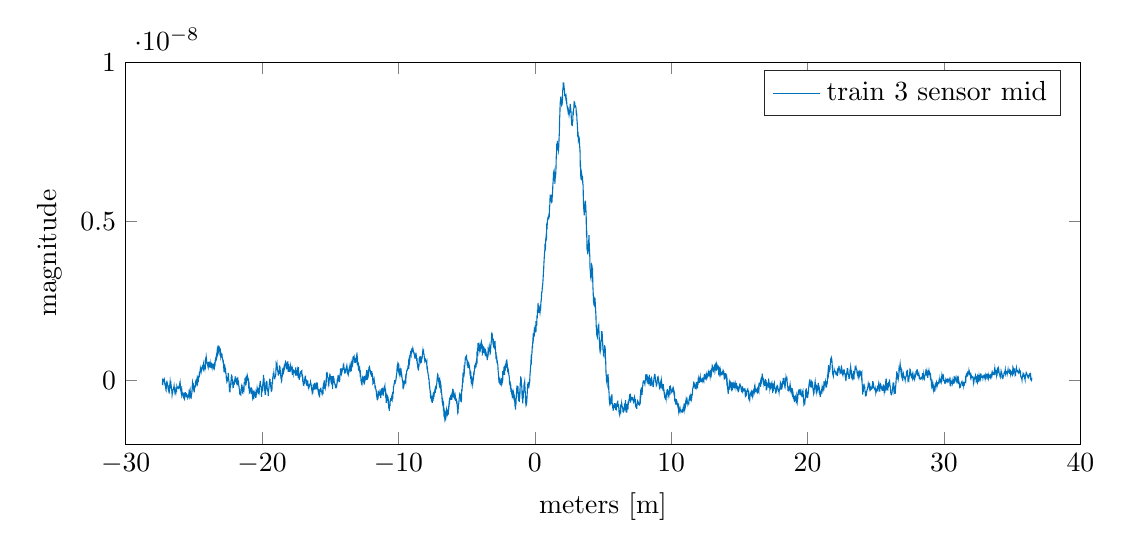
\begin{tikzpicture}

  \begin{axis}[%
    width=\textwidth,
    height=0.4\textwidth,
    at={(0\figurewidth,0\figureheight)},
    scale only axis,
    xmin=-30,
    xmax=40,
    xlabel={meters [m]},
    ymin=-2e-09,
    ymax=1e-08,
    ylabel={magnitude},
    axis background/.style={fill=white},
    legend style={legend cell align=left,align=left,draw=white!15!black}
    ]
    \addplot [color=mycolor1,solid]
    table[row sep=crcr]{%
    -27.30919921875	-1.35249592749225e-10\\
    -27.288701171875	-2.96618732808585e-11\\
    -27.268203125	-7.43225870504438e-11\\
    -27.247705078125	3.98686887307514e-12\\
    -27.22720703125	3.42173521151627e-11\\
    -27.206708984375	2.91331309843244e-11\\
    -27.1862109375	1.10075560008721e-12\\
    -27.165712890625	3.11336048942315e-11\\
    -27.14521484375	-2.14783086666132e-11\\
    -27.124716796875	-1.18327190184514e-10\\
    -27.10421875	-1.0806898008122e-10\\
    -27.083720703125	-1.31806296562773e-10\\
    -27.06322265625	-2.22339604039201e-10\\
    -27.042724609375	-1.72113830799343e-10\\
    -27.0222265625	-2.33179997718092e-10\\
    -27.001728515625	-9.80243911838984e-11\\
    -26.98123046875	-1.17431047736158e-10\\
    -26.960732421875	-5.6141215363913e-11\\
    -26.940234375	-8.61782248253017e-11\\
    -26.919736328125	-1.39414401907273e-10\\
    -26.89923828125	-1.86983229789257e-10\\
    -26.878740234375	-2.80627277278361e-10\\
    -26.8582421875	-3.00600915736124e-10\\
    -26.837744140625	-3.35144363971526e-10\\
    -26.81724609375	-2.59253155980026e-10\\
    -26.796748046875	-3.0228046754793e-10\\
    -26.77625	-1.52687733256758e-10\\
    -26.755751953125	-1.25197094078766e-10\\
    -26.73525390625	-3.07413927607216e-11\\
    -26.714755859375	-1.04389883342187e-10\\
    -26.6942578125	-1.90902832735897e-11\\
    -26.673759765625	-1.36411292834641e-10\\
    -26.65326171875	-1.88251566687185e-10\\
    -26.632763671875	-3.12540235384243e-10\\
    -26.612265625	-3.11990828982445e-10\\
    -26.591767578125	-4.53785462669716e-10\\
    -26.57126953125	-3.97306686246531e-10\\
    -26.550771484375	-3.89530233962638e-10\\
    -26.5302734375	-2.95033854580515e-10\\
    -26.509775390625	-2.73561625376906e-10\\
    -26.48927734375	-2.29766468985285e-10\\
    -26.468779296875	-2.14010846778668e-10\\
    -26.44828125	-1.66692182140659e-10\\
    -26.427783203125	-2.55344271375853e-10\\
    -26.40728515625	-3.15565761085149e-10\\
    -26.386787109375	-2.14100663448055e-10\\
    -26.3662890625	-3.61566215662482e-10\\
    -26.345791015625	-3.76425626044424e-10\\
    -26.32529296875	-4.07882051394321e-10\\
    -26.304794921875	-3.06610166952018e-10\\
    -26.284296875	-2.92301389226434e-10\\
    -26.263798828125	-3.10288449436863e-10\\
    -26.24330078125	-1.85406780114146e-10\\
    -26.222802734375	-2.19785361206386e-10\\
    -26.2023046875	-2.3291303234688e-10\\
    -26.181806640625	-2.35588771150115e-10\\
    -26.16130859375	-2.20910934632801e-10\\
    -26.140810546875	-2.39919467133664e-10\\
    -26.1203125	-2.47731371614303e-10\\
    -26.099814453125	-2.16328684271401e-10\\
    -26.07931640625	-1.81892890904843e-10\\
    -26.058818359375	-1.89775940186067e-10\\
    -26.0383203125	-1.22652439311523e-10\\
    -26.017822265625	-1.83880244083919e-10\\
    -25.99732421875	-1.03573369593623e-10\\
    -25.976826171875	-1.95541713380522e-10\\
    -25.956328125	-1.96616122014939e-10\\
    -25.935830078125	-3.58401874836354e-10\\
    -25.91533203125	-3.38628235970871e-10\\
    -25.894833984375	-4.20692515970445e-10\\
    -25.8743359375	-3.40979114286761e-10\\
    -25.853837890625	-4.36980247012196e-10\\
    -25.83333984375	-3.98413489461024e-10\\
    -25.812841796875	-3.95198434834403e-10\\
    -25.79234375	-3.94468019830033e-10\\
    -25.771845703125	-4.46008286744827e-10\\
    -25.75134765625	-5.03870500898673e-10\\
    -25.730849609375	-4.7721282962608e-10\\
    -25.7103515625	-5.3707990726049e-10\\
    -25.689853515625	-4.8843306926504e-10\\
    -25.66935546875	-5.43539487116029e-10\\
    -25.648857421875	-4.99002799318094e-10\\
    -25.628359375	-3.70457436389314e-10\\
    -25.607861328125	-5.07837222252478e-10\\
    -25.58736328125	-3.90918766279498e-10\\
    -25.566865234375	-4.75462672113691e-10\\
    -25.5463671875	-4.92268967252412e-10\\
    -25.525869140625	-4.55600562503481e-10\\
    -25.50537109375	-4.85370364526638e-10\\
    -25.484873046875	-4.70697730749877e-10\\
    -25.464375	-4.90249456959633e-10\\
    -25.443876953125	-5.4983418675066e-10\\
    -25.42337890625	-5.27537008994873e-10\\
    -25.402880859375	-5.10013096014041e-10\\
    -25.3823828125	-4.72680789952296e-10\\
    -25.361884765625	-3.99538475978077e-10\\
    -25.34138671875	-4.56739308205516e-10\\
    -25.320888671875	-3.74355003347318e-10\\
    -25.300390625	-3.20512598351553e-10\\
    -25.279892578125	-2.86734668606897e-10\\
    -25.25939453125	-4.77148772142956e-10\\
    -25.238896484375	-4.40258264345219e-10\\
    -25.2183984375	-5.25970257794032e-10\\
    -25.197900390625	-5.39619070167759e-10\\
    -25.17740234375	-4.50282579640578e-10\\
    -25.156904296875	-4.19755892974209e-10\\
    -25.13640625	-3.48869621487716e-10\\
    -25.115908203125	-1.87746427592222e-10\\
    -25.09541015625	-6.32593406813951e-11\\
    -25.074912109375	-1.11818179053155e-10\\
    -25.0544140625	-1.94349194944258e-10\\
    -25.033916015625	-1.65684148507706e-10\\
    -25.01341796875	-2.92136525550298e-10\\
    -24.992919921875	-3.07975800945658e-10\\
    -24.972421875	-3.74375562573471e-10\\
    -24.951923828125	-2.12441049209927e-10\\
    -24.93142578125	-2.2905984032688e-10\\
    -24.910927734375	-2.18417887953858e-10\\
    -24.8904296875	-1.54126023375905e-10\\
    -24.869931640625	-3.06732342695892e-11\\
    -24.84943359375	-1.0875161412322e-11\\
    -24.828935546875	-9.10597199836977e-11\\
    -24.8084375	-4.20437497305181e-11\\
    -24.787939453125	-6.9478100199758e-11\\
    -24.76744140625	1.43610312870468e-11\\
    -24.746943359375	-4.91616030660191e-11\\
    -24.7264453125	3.19907101271873e-11\\
    -24.705947265625	-3.54424103063657e-11\\
    -24.68544921875	3.08095240031773e-11\\
    -24.664951171875	1.42335811684396e-11\\
    -24.644453125	1.16640520079839e-10\\
    -24.623955078125	1.13368900684324e-10\\
    -24.60345703125	1.97253068461325e-10\\
    -24.582958984375	1.73276486852751e-10\\
    -24.5624609375	2.69035016101254e-10\\
    -24.541962890625	2.90714046386938e-10\\
    -24.52146484375	3.73121420605556e-10\\
    -24.500966796875	3.22700090021506e-10\\
    -24.48046875	3.4870061542533e-10\\
    -24.459970703125	2.81246627259548e-10\\
    -24.43947265625	3.3321044944486e-10\\
    -24.418974609375	3.34160493264693e-10\\
    -24.3984765625	3.93830705039048e-10\\
    -24.377978515625	4.12065881198332e-10\\
    -24.35748046875	4.70560699559437e-10\\
    -24.336982421875	4.77854883753437e-10\\
    -24.316484375	4.23179697336425e-10\\
    -24.295986328125	4.91797939937552e-10\\
    -24.27548828125	3.85193315871097e-10\\
    -24.254990234375	4.2703116379388e-10\\
    -24.2344921875	4.4054265971292e-10\\
    -24.213994140625	4.53147872693797e-10\\
    -24.19349609375	3.95504152560781e-10\\
    -24.172998046875	5.37536461584786e-10\\
    -24.1525	4.94847667357631e-10\\
    -24.132001953125	7.19471749362222e-10\\
    -24.11150390625	6.39540833334101e-10\\
    -24.091005859375	7.40868546685005e-10\\
    -24.0705078125	6.70841370145143e-10\\
    -24.050009765625	5.64432269917011e-10\\
    -24.02951171875	5.27459481365236e-10\\
    -24.009013671875	5.45624377592669e-10\\
    -23.988515625	5.1952108242254e-10\\
    -23.968017578125	4.32326595759691e-10\\
    -23.94751953125	4.05360198707694e-10\\
    -23.927021484375	5.04279887355792e-10\\
    -23.9065234375	5.78177785934405e-10\\
    -23.886025390625	4.09185582147212e-10\\
    -23.86552734375	5.88905753813424e-10\\
    -23.845029296875	4.63285685032231e-10\\
    -23.82453125	5.61994052334429e-10\\
    -23.804033203125	4.00684116260873e-10\\
    -23.78353515625	4.71466961657034e-10\\
    -23.763037109375	5.35770817238274e-10\\
    -23.7425390625	4.39063573936933e-10\\
    -23.722041015625	5.46530434420749e-10\\
    -23.70154296875	4.66606075157991e-10\\
    -23.681044921875	5.20479469232834e-10\\
    -23.660546875	5.09204390901713e-10\\
    -23.640048828125	5.00122606490853e-10\\
    -23.61955078125	4.36479069184641e-10\\
    -23.599052734375	5.2658140478694e-10\\
    -23.5785546875	3.7601147724268e-10\\
    -23.558056640625	3.90607565398011e-10\\
    -23.53755859375	4.42947928364056e-10\\
    -23.517060546875	4.54333826000029e-10\\
    -23.4965625	4.15791551157973e-10\\
    -23.476064453125	5.70539928801642e-10\\
    -23.45556640625	4.35780458303778e-10\\
    -23.435068359375	6.42805269654739e-10\\
    -23.4145703125	5.65514985083014e-10\\
    -23.394072265625	7.05869776518301e-10\\
    -23.37357421875	7.16145412079903e-10\\
    -23.353076171875	7.64121385685973e-10\\
    -23.332578125	7.22190361279073e-10\\
    -23.312080078125	8.06100058784527e-10\\
    -23.29158203125	9.07235582967141e-10\\
    -23.271083984375	8.53589864886043e-10\\
    -23.2505859375	9.54398462032542e-10\\
    -23.230087890625	9.00596361385505e-10\\
    -23.20958984375	1.00125580769421e-09\\
    -23.189091796875	9.63505038841384e-10\\
    -23.16859375	1.09252419108718e-09\\
    -23.148095703125	9.91393218918125e-10\\
    -23.12759765625	9.75724709033285e-10\\
    -23.107099609375	1.05400233342587e-09\\
    -23.0866015625	7.8956399490962e-10\\
    -23.066103515625	9.97858863307848e-10\\
    -23.04560546875	8.63636129626428e-10\\
    -23.025107421875	7.51233061416922e-10\\
    -23.004609375	8.09452432789282e-10\\
    -22.984111328125	7.45351075016666e-10\\
    -22.96361328125	7.38974112185273e-10\\
    -22.943115234375	8.47281409947582e-10\\
    -22.9226171875	7.40393002956506e-10\\
    -22.902119140625	6.96597444260369e-10\\
    -22.88162109375	6.59170727172466e-10\\
    -22.861123046875	5.88999496248779e-10\\
    -22.840625	6.0264349565717e-10\\
    -22.820126953125	5.19548699723142e-10\\
    -22.79962890625	3.58659223237791e-10\\
    -22.779130859375	2.56014850132146e-10\\
    -22.7586328125	3.9849820332208e-10\\
    -22.738134765625	3.55977382085786e-10\\
    -22.71763671875	4.23931300566941e-10\\
    -22.697138671875	3.76509782081439e-10\\
    -22.676640625	3.66698464856999e-10\\
    -22.656142578125	2.24114807771734e-10\\
    -22.63564453125	2.14128267597695e-10\\
    -22.615146484375	3.92613057296878e-11\\
    -22.5946484375	3.42604768525417e-11\\
    -22.574150390625	-4.4129335064797e-11\\
    -22.55365234375	-2.12931148218171e-11\\
    -22.533154296875	9.26741011408592e-11\\
    -22.51265625	9.80352353988495e-11\\
    -22.492158203125	7.75946266174577e-11\\
    -22.47166015625	2.3572550099031e-10\\
    -22.451162109375	6.51222689576719e-11\\
    -22.4306640625	-2.16478093636971e-11\\
    -22.410166015625	-6.14036409819718e-11\\
    -22.38966796875	-3.48505283356299e-10\\
    -22.369169921875	-2.54886564828333e-10\\
    -22.348671875	-3.73393682462742e-10\\
    -22.328173828125	-1.19268673436283e-10\\
    -22.30767578125	-2.25402133518202e-10\\
    -22.287177734375	-5.8871150055261e-11\\
    -22.2666796875	-7.4147259838463e-11\\
    -22.246181640625	1.86675818204403e-10\\
    -22.22568359375	5.83764085393024e-12\\
    -22.205185546875	1.49803073300689e-10\\
    -22.1846875	2.89773630503508e-11\\
    -22.164189453125	-2.34220155503362e-12\\
    -22.14369140625	-1.14932662586588e-10\\
    -22.123193359375	-5.31159003984114e-11\\
    -22.1026953125	-2.31133529182621e-10\\
    -22.082197265625	-1.3035774089879e-10\\
    -22.06169921875	-8.78292132365104e-11\\
    -22.041201171875	-4.02899936746984e-11\\
    -22.020703125	-6.59648599109555e-11\\
    -22.000205078125	7.61250084394417e-12\\
    -21.97970703125	-8.09417283577948e-12\\
    -21.959208984375	1.25353680802549e-10\\
    -21.9387109375	6.23976830311426e-12\\
    -21.918212890625	-1.83121579360295e-12\\
    -21.89771484375	1.42662819524086e-11\\
    -21.877216796875	-4.07943779427948e-11\\
    -21.85671875	-3.76912792169108e-12\\
    -21.836220703125	-5.81583344321961e-11\\
    -21.81572265625	2.81189299811421e-11\\
    -21.795224609375	-7.66413514107662e-12\\
    -21.7747265625	2.09013939771889e-11\\
    -21.754228515625	-1.44860059790641e-10\\
    -21.73373046875	4.59254340492147e-12\\
    -21.713232421875	-1.37302086818078e-10\\
    -21.692734375	-1.74860551881821e-10\\
    -21.672236328125	-2.63654710274829e-10\\
    -21.65173828125	-2.74703998317908e-10\\
    -21.631240234375	-4.20338485802224e-10\\
    -21.6107421875	-4.3709173654371e-10\\
    -21.590244140625	-4.1079256546226e-10\\
    -21.56974609375	-3.84212279996034e-10\\
    -21.549248046875	-4.1245819700163e-10\\
    -21.52875	-3.02419924846642e-10\\
    -21.508251953125	-2.29427695814191e-10\\
    -21.48775390625	-3.03268767035065e-10\\
    -21.467255859375	-1.32067824079742e-10\\
    -21.4467578125	-2.73771896512733e-10\\
    -21.426259765625	-2.59085306063031e-10\\
    -21.40576171875	-4.30111125358072e-10\\
    -21.385263671875	-2.06328107648538e-10\\
    -21.364765625	-3.54819114192029e-10\\
    -21.344267578125	-2.54188920506209e-10\\
    -21.32376953125	-2.84275856731723e-10\\
    -21.303271484375	-7.09732788541981e-11\\
    -21.2827734375	-7.20041318887564e-11\\
    -21.262275390625	-7.59176608545479e-11\\
    -21.24177734375	9.02728847141657e-11\\
    -21.221279296875	-3.22041808705683e-11\\
    -21.20078125	1.63950665346139e-11\\
    -21.180283203125	-5.53445845479176e-11\\
    -21.15978515625	4.15543045400382e-11\\
    -21.139287109375	-1.17449240472872e-11\\
    -21.1187890625	5.50190439203362e-11\\
    -21.098291015625	4.57176319761292e-11\\
    -21.07779296875	1.56860255048443e-10\\
    -21.057294921875	1.22062875719351e-10\\
    -21.036796875	6.36559620355495e-11\\
    -21.016298828125	9.99157708795421e-12\\
    -20.99580078125	6.28013598363072e-11\\
    -20.975302734375	-2.47118558969022e-10\\
    -20.9548046875	-4.63928851977559e-11\\
    -20.934306640625	-3.12081159477694e-10\\
    -20.91380859375	-2.70670252349475e-10\\
    -20.893310546875	-3.28299426226682e-10\\
    -20.8728125	-2.85660195781242e-10\\
    -20.852314453125	-2.64413009312199e-10\\
    -20.83181640625	-2.88170358171065e-10\\
    -20.811318359375	-2.25733766269119e-10\\
    -20.7908203125	-4.23764019707048e-10\\
    -20.770322265625	-2.21841222113787e-10\\
    -20.74982421875	-4.30448863824883e-10\\
    -20.729326171875	-3.4936290904962e-10\\
    -20.708828125	-4.52025120443805e-10\\
    -20.688330078125	-4.02754264074801e-10\\
    -20.66783203125	-5.63953896965501e-10\\
    -20.647333984375	-5.37577949840093e-10\\
    -20.6268359375	-4.79069625814267e-10\\
    -20.606337890625	-5.82275218022428e-10\\
    -20.58583984375	-3.17878927622476e-10\\
    -20.565341796875	-4.81561189762807e-10\\
    -20.54484375	-4.16394974697217e-10\\
    -20.524345703125	-4.07865033434671e-10\\
    -20.50384765625	-5.02761785941978e-10\\
    -20.483349609375	-3.62819242064871e-10\\
    -20.4628515625	-5.49036645452211e-10\\
    -20.442353515625	-4.00444780065299e-10\\
    -20.42185546875	-4.47286644214548e-10\\
    -20.401357421875	-3.85520206742559e-10\\
    -20.380859375	-3.44588015543201e-10\\
    -20.360361328125	-2.44620874758801e-10\\
    -20.33986328125	-3.00057564990418e-10\\
    -20.319365234375	-2.54708606415877e-10\\
    -20.2988671875	-2.63199104537134e-10\\
    -20.278369140625	-2.61497460415241e-10\\
    -20.25787109375	-4.35666531310447e-10\\
    -20.237373046875	-3.3906064936107e-10\\
    -20.216875	-2.69680125327429e-10\\
    -20.196376953125	-3.29041872515178e-10\\
    -20.17587890625	-2.30523557160484e-10\\
    -20.155380859375	-1.37222185699242e-10\\
    -20.1348828125	-1.37691994534082e-11\\
    -20.114384765625	-1.16566105802317e-10\\
    -20.09388671875	-1.60648024062069e-10\\
    -20.073388671875	-1.88177485378018e-10\\
    -20.052890625	-2.04706827156497e-10\\
    -20.032392578125	-5.11966334289761e-10\\
    -20.01189453125	-2.00866363523775e-10\\
    -19.991396484375	-3.0889125830442e-10\\
    -19.9708984375	-3.14055967443625e-10\\
    -19.950400390625	-1.5630250044925e-10\\
    -19.92990234375	-6.81430237807822e-11\\
    -19.909404296875	-1.33935618120172e-10\\
    -19.88890625	1.75761530913611e-10\\
    -19.868408203125	-1.38953361544086e-10\\
    -19.84791015625	7.62026210686409e-11\\
    -19.827412109375	-3.26734158979302e-10\\
    -19.8069140625	-2.15118271214409e-10\\
    -19.786416015625	-3.44371183992228e-10\\
    -19.76591796875	-3.02650238689187e-10\\
    -19.745419921875	-4.54562611379608e-10\\
    -19.724921875	-1.77468988257153e-10\\
    -19.704423828125	-2.13385872379263e-10\\
    -19.68392578125	-7.62594169804022e-11\\
    -19.663427734375	-1.03101424228836e-10\\
    -19.6429296875	-2.3417211869801e-11\\
    -19.622431640625	-2.32012012948032e-10\\
    -19.60193359375	-2.59465162498959e-10\\
    -19.581435546875	-3.24471610927263e-10\\
    -19.5609375	-3.50636622603433e-10\\
    -19.540439453125	-4.90307300480454e-10\\
    -19.51994140625	-2.88860903609483e-10\\
    -19.499443359375	-2.70626327179062e-10\\
    -19.4789453125	-1.4880314159453e-10\\
    -19.458447265625	-9.38330676844878e-11\\
    -19.43794921875	3.66142858550453e-11\\
    -19.417451171875	3.61329974267071e-11\\
    -19.396953125	-6.95206901144938e-11\\
    -19.376455078125	-6.80705839207097e-11\\
    -19.35595703125	-2.07604654033481e-10\\
    -19.335458984375	-2.6904059763288e-10\\
    -19.3149609375	-3.40123800332186e-10\\
    -19.294462890625	-3.32237471286137e-10\\
    -19.27396484375	-2.82959527081493e-10\\
    -19.253466796875	-5.6722253764508e-11\\
    -19.23296875	-1.14249470329872e-10\\
    -19.212470703125	9.11690230248575e-11\\
    -19.19197265625	1.26565465164728e-10\\
    -19.171474609375	2.28755321998853e-10\\
    -19.1509765625	1.21401001911899e-10\\
    -19.130478515625	2.27976209362254e-10\\
    -19.10998046875	1.59797330735408e-10\\
    -19.089482421875	6.37709036681724e-11\\
    -19.068984375	5.57455596479298e-11\\
    -19.048486328125	1.10365129035573e-10\\
    -19.02798828125	1.1751908493203e-10\\
    -19.007490234375	1.41199994471049e-10\\
    -18.9869921875	2.13204881026046e-10\\
    -18.966494140625	4.68925560453405e-10\\
    -18.94599609375	4.23381455480252e-10\\
    -18.925498046875	4.79858965682217e-10\\
    -18.905	5.31159313220228e-10\\
    -18.884501953125	4.26707502285817e-10\\
    -18.86400390625	3.52120556050422e-10\\
    -18.843505859375	2.77283641387184e-10\\
    -18.8230078125	2.58699883276403e-10\\
    -18.802509765625	1.57057111822618e-10\\
    -18.78201171875	2.9180612355568e-10\\
    -18.761513671875	2.09787977055232e-10\\
    -18.741015625	2.31288254074607e-10\\
    -18.720517578125	4.7041056587318e-10\\
    -18.70001953125	3.11510683889955e-10\\
    -18.679521484375	4.33676798746431e-10\\
    -18.6590234375	2.41411925753194e-10\\
    -18.638525390625	2.05967924565702e-10\\
    -18.61802734375	1.02434891051109e-10\\
    -18.597529296875	1.16902049217803e-10\\
    -18.57703125	-2.53204385378977e-11\\
    -18.556533203125	2.86766670391784e-12\\
    -18.53603515625	1.15878380624622e-10\\
    -18.515537109375	2.8008577504071e-10\\
    -18.4950390625	2.43336373792685e-10\\
    -18.474541015625	3.67339631789473e-10\\
    -18.45404296875	1.82848505844704e-10\\
    -18.433544921875	3.30059391770162e-10\\
    -18.413046875	2.71462980501835e-10\\
    -18.392548828125	3.09182611953714e-10\\
    -18.37205078125	3.46517038577972e-10\\
    -18.351552734375	3.79210444821521e-10\\
    -18.3310546875	5.03002047679623e-10\\
    -18.310556640625	5.31587780902824e-10\\
    -18.29005859375	5.54352495001945e-10\\
    -18.269560546875	5.89173520686132e-10\\
    -18.2490625	5.64736923222335e-10\\
    -18.228564453125	4.56157387333344e-10\\
    -18.20806640625	4.7850782442291e-10\\
    -18.187568359375	3.51483408137829e-10\\
    -18.1670703125	4.78472945615259e-10\\
    -18.146572265625	3.49028278351351e-10\\
    -18.12607421875	4.67702356232533e-10\\
    -18.105576171875	6.06012196049101e-10\\
    -18.085078125	2.71460060488585e-10\\
    -18.064580078125	5.20307117666533e-10\\
    -18.04408203125	4.01201508095348e-10\\
    -18.023583984375	4.29013329383463e-10\\
    -18.0030859375	2.90204382012614e-10\\
    -17.982587890625	2.89617333342001e-10\\
    -17.96208984375	4.3375523599021e-10\\
    -17.941591796875	2.64637916361734e-10\\
    -17.92109375	3.62771568075576e-10\\
    -17.900595703125	4.56241669943879e-10\\
    -17.88009765625	3.98254228175802e-10\\
    -17.859599609375	3.81533855723504e-10\\
    -17.8391015625	3.94535730857114e-10\\
    -17.818603515625	3.35492811620336e-10\\
    -17.79810546875	3.54613862021231e-10\\
    -17.777607421875	1.79524443008475e-10\\
    -17.757109375	3.25634024098345e-10\\
    -17.736611328125	2.64114574951584e-10\\
    -17.71611328125	2.1288073917396e-10\\
    -17.695615234375	3.43017151489389e-10\\
    -17.6751171875	2.66403234522074e-10\\
    -17.654619140625	2.61591233302189e-10\\
    -17.63412109375	2.52050140390374e-10\\
    -17.613623046875	2.95059354538259e-10\\
    -17.593125	3.00936147734263e-10\\
    -17.572626953125	2.87102058333014e-10\\
    -17.55212890625	1.70075791760641e-10\\
    -17.531630859375	4.14039184368382e-10\\
    -17.5111328125	1.47241284671843e-10\\
    -17.490634765625	2.80143923839948e-10\\
    -17.47013671875	2.44769284310754e-10\\
    -17.449638671875	2.47197962592883e-10\\
    -17.429140625	2.21046003201696e-10\\
    -17.408642578125	2.87397615036798e-10\\
    -17.38814453125	1.8305227457497e-10\\
    -17.367646484375	3.33296989470111e-10\\
    -17.3471484375	7.67017460010795e-11\\
    -17.326650390625	4.1683280043667e-10\\
    -17.30615234375	8.04518419872146e-11\\
    -17.285654296875	2.03016610301874e-10\\
    -17.26515625	2.20413923623636e-11\\
    -17.244658203125	1.58450722634051e-10\\
    -17.22416015625	8.57608333990591e-11\\
    -17.203662109375	2.06265137683545e-10\\
    -17.1831640625	2.52420710750682e-10\\
    -17.162666015625	2.4901556457593e-10\\
    -17.14216796875	2.82992835290934e-10\\
    -17.121669921875	2.93893175426333e-10\\
    -17.101171875	2.37343324478661e-10\\
    -17.080673828125	2.60872578846725e-10\\
    -17.06017578125	1.02974688881613e-10\\
    -17.039677734375	1.91908264396341e-10\\
    -17.0191796875	2.68619381037081e-11\\
    -16.998681640625	4.26862496744508e-11\\
    -16.97818359375	-1.33489865677629e-10\\
    -16.957685546875	-2.43362328377489e-11\\
    -16.9371875	-1.7125473685436e-10\\
    -16.916689453125	-6.08119382744253e-11\\
    -16.89619140625	-3.7166478140409e-11\\
    -16.875693359375	-5.31588232319978e-11\\
    -16.8551953125	1.20150459959961e-10\\
    -16.834697265625	4.54314435488248e-11\\
    -16.81419921875	1.51709263117393e-10\\
    -16.793701171875	1.15134074358426e-11\\
    -16.773203125	1.45596914666966e-11\\
    -16.752705078125	-8.70150145053831e-11\\
    -16.73220703125	-7.54364267697055e-11\\
    -16.711708984375	-1.67478710209684e-10\\
    -16.6912109375	-6.10432385311289e-11\\
    -16.670712890625	-8.19950091368123e-11\\
    -16.65021484375	-2.70389312497154e-12\\
    -16.629716796875	-1.20871613963378e-10\\
    -16.60921875	-1.98081611085126e-10\\
    -16.588720703125	-1.81009964996836e-10\\
    -16.56822265625	-2.33256078519518e-10\\
    -16.547724609375	-1.96665024532357e-10\\
    -16.5272265625	-1.94099263446286e-10\\
    -16.506728515625	-1.37945581843469e-10\\
    -16.48623046875	-1.10426366371296e-10\\
    -16.465732421875	-1.06747903357001e-10\\
    -16.445234375	-4.69579347037954e-11\\
    -16.424736328125	-9.39973709677114e-11\\
    -16.40423828125	-1.16724469033989e-10\\
    -16.383740234375	-1.7857546005884e-10\\
    -16.3632421875	-2.89583726389575e-10\\
    -16.342744140625	-2.99415388570609e-10\\
    -16.32224609375	-3.74616263585028e-10\\
    -16.301748046875	-3.24921108689861e-10\\
    -16.28125	-4.11254814031182e-10\\
    -16.260751953125	-2.40658172771325e-10\\
    -16.24025390625	-2.77827700481022e-10\\
    -16.219755859375	-2.27808933161046e-10\\
    -16.1992578125	-1.15488753427846e-10\\
    -16.178759765625	-2.20847355396634e-10\\
    -16.15826171875	-7.59620915149329e-11\\
    -16.137763671875	-2.89675119693227e-10\\
    -16.117265625	-1.29931086873951e-10\\
    -16.096767578125	-1.99668301741157e-10\\
    -16.07626953125	-1.66261383274476e-10\\
    -16.055771484375	-2.76505403122157e-10\\
    -16.0352734375	-1.9055105100654e-10\\
    -16.014775390625	-1.95571469540582e-10\\
    -15.99427734375	-6.34674870304609e-11\\
    -15.973779296875	-2.80429984559365e-10\\
    -15.95328125	-7.00580232580405e-11\\
    -15.932783203125	-2.07698110569489e-10\\
    -15.91228515625	-2.08325879703902e-10\\
    -15.891787109375	-3.15658179402667e-10\\
    -15.8712890625	-3.72570837481577e-10\\
    -15.850791015625	-4.08168510434298e-10\\
    -15.83029296875	-3.6566882575544e-10\\
    -15.809794921875	-4.38106414260755e-10\\
    -15.789296875	-3.96211823827325e-10\\
    -15.768798828125	-4.34607715496202e-10\\
    -15.74830078125	-2.99166128241619e-10\\
    -15.727802734375	-3.03028082590136e-10\\
    -15.7073046875	-2.98005438237252e-10\\
    -15.686806640625	-2.26014634948828e-10\\
    -15.66630859375	-3.38461388183836e-10\\
    -15.645810546875	-3.38281510405273e-10\\
    -15.6253125	-3.68562513952086e-10\\
    -15.604814453125	-4.05063237513364e-10\\
    -15.58431640625	-3.22185304326817e-10\\
    -15.563818359375	-4.47041403096257e-10\\
    -15.5433203125	-3.01075685340483e-10\\
    -15.522822265625	-3.27547505318056e-10\\
    -15.50232421875	-1.2294273248789e-10\\
    -15.481826171875	-1.03876423099872e-10\\
    -15.461328125	-9.9436158994914e-11\\
    -15.440830078125	-2.45314057676337e-13\\
    -15.42033203125	-2.17590232631155e-10\\
    -15.399833984375	-2.02975083704586e-10\\
    -15.3793359375	-1.76695748104083e-10\\
    -15.358837890625	-2.36224932569383e-10\\
    -15.33833984375	-1.89922086026444e-10\\
    -15.317841796875	-7.14372269354404e-11\\
    -15.29734375	-9.2397791642655e-11\\
    -15.276845703125	2.3796071521392e-10\\
    -15.25634765625	1.17619036660601e-10\\
    -15.235849609375	2.70210839930896e-10\\
    -15.2153515625	1.94261988179782e-10\\
    -15.194853515625	1.15069516706955e-10\\
    -15.17435546875	8.94443760884621e-11\\
    -15.153857421875	5.83746325962312e-11\\
    -15.133359375	-1.11023313739403e-10\\
    -15.112861328125	-6.54731234053658e-11\\
    -15.09236328125	-9.56909192569403e-11\\
    -15.071865234375	1.30506019338354e-11\\
    -15.0513671875	9.68795468784295e-11\\
    -15.030869140625	2.50923586712201e-11\\
    -15.01037109375	2.09598225460566e-10\\
    -14.989873046875	2.47804540073579e-11\\
    -14.969375	1.39247098886309e-10\\
    -14.948876953125	1.58815172697976e-11\\
    -14.92837890625	4.54233813246085e-11\\
    -14.907880859375	-5.57289463883846e-11\\
    -14.8873828125	-2.84881318354209e-11\\
    -14.866884765625	-1.0848077833358e-10\\
    -14.84638671875	1.3937883199555e-10\\
    -14.825888671875	-2.71083551572908e-10\\
    -14.805390625	1.14094914363798e-10\\
    -14.784892578125	-2.02958716426261e-11\\
    -14.76439453125	1.43052419916114e-10\\
    -14.743896484375	-5.92955805676817e-11\\
    -14.7233984375	6.09751057199696e-11\\
    -14.702900390625	-6.97912074012271e-11\\
    -14.68240234375	-8.69024565463642e-11\\
    -14.661904296875	-9.12821650888045e-11\\
    -14.64140625	-1.48963580300763e-10\\
    -14.620908203125	-1.9536170587947e-10\\
    -14.60041015625	-1.81115551160445e-10\\
    -14.579912109375	-2.50583516830128e-10\\
    -14.5594140625	-1.22319409386413e-10\\
    -14.538916015625	-2.2696377433034e-10\\
    -14.51841796875	-1.47635822481102e-10\\
    -14.497919921875	-7.57367159852077e-11\\
    -14.477421875	4.86318728283363e-11\\
    -14.456923828125	-6.41987232578882e-11\\
    -14.43642578125	1.56136617677527e-10\\
    -14.415927734375	7.19834880117956e-11\\
    -14.3954296875	4.05542970943333e-11\\
    -14.374931640625	8.24275375158256e-11\\
    -14.35443359375	-1.05712167692338e-11\\
    -14.333935546875	1.02789833299254e-10\\
    -14.3134375	-5.21249034449461e-11\\
    -14.292939453125	1.35572702718433e-10\\
    -14.27244140625	1.53555196947143e-10\\
    -14.251943359375	2.9568922959787e-10\\
    -14.2314453125	2.80052824382007e-10\\
    -14.210947265625	3.87128929989139e-10\\
    -14.19044921875	2.80797529362351e-10\\
    -14.169951171875	2.12710186428386e-10\\
    -14.149453125	2.48155196455198e-10\\
    -14.128955078125	2.81397716031743e-10\\
    -14.10845703125	3.46830203184056e-10\\
    -14.087958984375	3.66268961884059e-10\\
    -14.0674609375	3.6048159490008e-10\\
    -14.046962890625	4.56338176463574e-10\\
    -14.02646484375	4.27769226694284e-10\\
    -14.005966796875	4.69377502383534e-10\\
    -13.98546875	3.81968448036499e-10\\
    -13.964970703125	3.40626728512768e-10\\
    -13.94447265625	2.14836096004846e-10\\
    -13.923974609375	3.0269045693269e-10\\
    -13.9034765625	2.7750063065525e-10\\
    -13.882978515625	3.11831094482932e-10\\
    -13.86248046875	2.90397985721415e-10\\
    -13.841982421875	3.74232762233624e-10\\
    -13.821484375	4.03757941983867e-10\\
    -13.800986328125	4.31519740292504e-10\\
    -13.78048828125	4.69895159645274e-10\\
    -13.759990234375	3.97132429103528e-10\\
    -13.7394921875	2.64832149703073e-10\\
    -13.718994140625	2.21040295268181e-10\\
    -13.69849609375	1.96092128654403e-10\\
    -13.677998046875	3.15442070974452e-10\\
    -13.6575	2.34467081949477e-10\\
    -13.637001953125	2.89275608731388e-10\\
    -13.61650390625	3.73548043572496e-10\\
    -13.596005859375	4.07426267812079e-10\\
    -13.5755078125	4.08098987626308e-10\\
    -13.555009765625	4.63256391660515e-10\\
    -13.53451171875	3.40593921051981e-10\\
    -13.514013671875	3.73625717315796e-10\\
    -13.493515625	2.77300996856852e-10\\
    -13.473017578125	5.00278758960498e-10\\
    -13.45251953125	3.025049838177e-10\\
    -13.432021484375	5.98708406255074e-10\\
    -13.4115234375	3.86726234692943e-10\\
    -13.391025390625	5.89964865378421e-10\\
    -13.37052734375	5.69570704864342e-10\\
    -13.350029296875	5.37186121558658e-10\\
    -13.32953125	7.13668556433258e-10\\
    -13.309033203125	7.0271792230051e-10\\
    -13.28853515625	7.43265268495169e-10\\
    -13.268037109375	7.38624704283098e-10\\
    -13.2475390625	7.56874474620069e-10\\
    -13.227041015625	5.72821248666743e-10\\
    -13.20654296875	7.14506029195333e-10\\
    -13.186044921875	5.56252095731233e-10\\
    -13.165546875	6.87286773499704e-10\\
    -13.145048828125	6.80309995153122e-10\\
    -13.12455078125	6.68691714945989e-10\\
    -13.104052734375	6.20760826154701e-10\\
    -13.0835546875	7.17639542476349e-10\\
    -13.063056640625	7.71680111319619e-10\\
    -13.04255859375	7.01860134505894e-10\\
    -13.022060546875	7.65241402087959e-10\\
    -13.0015625	6.91830548061057e-10\\
    -12.981064453125	5.1296868956442e-10\\
    -12.96056640625	5.24203532810343e-10\\
    -12.940068359375	4.25489412698183e-10\\
    -12.9195703125	4.62482340952042e-10\\
    -12.899072265625	3.05471529301434e-10\\
    -12.87857421875	3.82090664736517e-10\\
    -12.858076171875	3.31435166261547e-10\\
    -12.837578125	3.6523537254798e-10\\
    -12.817080078125	2.50578446619295e-10\\
    -12.79658203125	3.1607741642605e-10\\
    -12.776083984375	1.2010321982858e-10\\
    -12.7555859375	1.07190018264675e-10\\
    -12.735087890625	-5.06847082463033e-11\\
    -12.71458984375	-5.97512423925645e-11\\
    -12.694091796875	-1.08377674792808e-10\\
    -12.67359375	-1.25673123073202e-10\\
    -12.653095703125	-3.44590908600666e-11\\
    -12.63259765625	6.93766832048136e-11\\
    -12.612099609375	3.77564966984687e-11\\
    -12.5916015625	9.90318446961646e-11\\
    -12.571103515625	1.02308871266682e-10\\
    -12.55060546875	-1.98890274315149e-13\\
    -12.530107421875	2.06996805792552e-11\\
    -12.509609375	-1.27783267165766e-10\\
    -12.489111328125	1.39647844200153e-10\\
    -12.46861328125	-5.64150204882824e-11\\
    -12.448115234375	6.20538221953208e-11\\
    -12.4276171875	6.23948489660602e-11\\
    -12.407119140625	4.83038730044384e-11\\
    -12.38662109375	1.42414213442399e-10\\
    -12.366123046875	1.89362388081626e-10\\
    -12.345625	1.67754621955439e-10\\
    -12.325126953125	3.20791308857432e-10\\
    -12.30462890625	2.22347079267994e-11\\
    -12.284130859375	2.82657533373705e-10\\
    -12.2636328125	4.01346836221756e-11\\
    -12.243134765625	9.34754198310704e-11\\
    -12.22263671875	1.02590097042867e-10\\
    -12.202138671875	3.44150238341199e-10\\
    -12.181640625	2.81423875827848e-10\\
    -12.161142578125	3.86743775972936e-10\\
    -12.14064453125	3.75098808458345e-10\\
    -12.120146484375	4.16317359769768e-10\\
    -12.0996484375	3.85086814204609e-10\\
    -12.079150390625	2.9950985025924e-10\\
    -12.05865234375	3.02147190062394e-10\\
    -12.038154296875	2.18253721369277e-10\\
    -12.01765625	1.99539778090712e-10\\
    -11.997158203125	2.18413260834319e-10\\
    -11.97666015625	1.21854025855723e-10\\
    -11.956162109375	2.93821524009286e-10\\
    -11.9356640625	1.14064041094948e-10\\
    -11.915166015625	2.25523846309551e-10\\
    -11.89466796875	1.36204045088993e-10\\
    -11.874169921875	-2.87922919391981e-11\\
    -11.853671875	1.56763275796062e-11\\
    -11.833173828125	-8.42992958731101e-11\\
    -11.81267578125	-7.54111981717654e-11\\
    -11.792177734375	-6.47912578203698e-11\\
    -11.7716796875	-1.29337226618177e-12\\
    -11.751181640625	-8.6355633614313e-11\\
    -11.73068359375	-9.28322365063401e-11\\
    -11.710185546875	-2.48720166263687e-10\\
    -11.6896875	-1.66579069135431e-10\\
    -11.669189453125	-2.61733545830296e-10\\
    -11.64869140625	-2.81161894014938e-10\\
    -11.628193359375	-3.25499365486564e-10\\
    -11.6076953125	-4.34941164506335e-10\\
    -11.587197265625	-4.97660747271438e-10\\
    -11.56669921875	-4.54891246661046e-10\\
    -11.546201171875	-6.25884074087916e-10\\
    -11.525703125	-4.7882698370598e-10\\
    -11.505205078125	-5.90959460955772e-10\\
    -11.48470703125	-5.00445524382367e-10\\
    -11.464208984375	-4.71936842506777e-10\\
    -11.4437109375	-3.50752022667245e-10\\
    -11.423212890625	-3.33011635995288e-10\\
    -11.40271484375	-4.07605816775368e-10\\
    -11.382216796875	-4.37123973212058e-10\\
    -11.36171875	-4.54030062147472e-10\\
    -11.341220703125	-4.34376496867081e-10\\
    -11.32072265625	-3.93458870661374e-10\\
    -11.300224609375	-5.55822436199509e-10\\
    -11.2797265625	-3.67533227912661e-10\\
    -11.259228515625	-4.58068105537887e-10\\
    -11.23873046875	-3.49673992689295e-10\\
    -11.218232421875	-2.61740310928519e-10\\
    -11.197734375	-2.57609586284583e-10\\
    -11.177236328125	-3.19754139683064e-10\\
    -11.15673828125	-2.27157578779981e-10\\
    -11.136240234375	-3.83252581562216e-10\\
    -11.1157421875	-4.77881489064762e-10\\
    -11.095244140625	-3.46749169356085e-10\\
    -11.07474609375	-3.55872797794631e-10\\
    -11.054248046875	-3.03813681575727e-10\\
    -11.03375	-2.13653226503288e-10\\
    -11.013251953125	-2.26543950260824e-10\\
    -10.99275390625	-1.79438720680168e-10\\
    -10.972255859375	-3.37864192270526e-10\\
    -10.9517578125	-2.67457578003145e-10\\
    -10.931259765625	-4.74110131557187e-10\\
    -10.91076171875	-4.49278530807301e-10\\
    -10.890263671875	-7.04232276711787e-10\\
    -10.869765625	-5.62551805568854e-10\\
    -10.849267578125	-5.29122520391208e-10\\
    -10.82876953125	-5.8756268119336e-10\\
    -10.808271484375	-4.83058255050126e-10\\
    -10.7877734375	-5.00321506153873e-10\\
    -10.767275390625	-5.26615834486887e-10\\
    -10.74677734375	-6.48180958261969e-10\\
    -10.726279296875	-5.77351828324453e-10\\
    -10.70578125	-8.77152445949903e-10\\
    -10.685283203125	-7.48865569613825e-10\\
    -10.66478515625	-9.526263850053e-10\\
    -10.644287109375	-7.48205696575346e-10\\
    -10.6237890625	-8.15001923210667e-10\\
    -10.603291015625	-6.59559188619622e-10\\
    -10.58279296875	-6.45980153770854e-10\\
    -10.562294921875	-5.70682644566547e-10\\
    -10.541796875	-5.68794960799906e-10\\
    -10.521298828125	-5.870593388038e-10\\
    -10.50080078125	-5.32750622438162e-10\\
    -10.480302734375	-5.85135303439959e-10\\
    -10.4598046875	-6.09896635844846e-10\\
    -10.439306640625	-5.03101142099773e-10\\
    -10.41880859375	-5.68253821582822e-10\\
    -10.398310546875	-3.95597603008106e-10\\
    -10.3778125	-3.95038234570785e-10\\
    -10.357314453125	-1.84434299509528e-10\\
    -10.33681640625	-1.78107826801173e-10\\
    -10.316318359375	-1.08858709897558e-10\\
    -10.2958203125	-7.86867581767197e-11\\
    -10.275322265625	7.85674142762218e-12\\
    -10.25482421875	-1.16126452685464e-10\\
    -10.234326171875	-2.18180159605619e-11\\
    -10.213828125	-2.97764407654774e-11\\
    -10.193330078125	-4.17699642898004e-12\\
    -10.17283203125	5.49174416628593e-11\\
    -10.152333984375	1.35202479210149e-10\\
    -10.1318359375	1.93365093803423e-10\\
    -10.111337890625	2.65760126089637e-10\\
    -10.09083984375	4.52210863478377e-10\\
    -10.070341796875	4.64145731175866e-10\\
    -10.04984375	5.0759387709493e-10\\
    -10.029345703125	4.24723634004237e-10\\
    -10.00884765625	4.59402490957032e-10\\
    -9.988349609375	2.55173889248336e-10\\
    -9.9678515625	3.71713489103549e-10\\
    -9.947353515625	1.58359325744984e-10\\
    -9.92685546875	2.42354596671081e-10\\
    -9.906357421875	1.93690437804622e-10\\
    -9.885859375	3.41081986883492e-10\\
    -9.865361328125	2.79259893534891e-10\\
    -9.84486328125	3.6210967202526e-10\\
    -9.824365234375	2.26994035525193e-10\\
    -9.8038671875	3.8136175663843e-10\\
    -9.783369140625	1.11137777378841e-10\\
    -9.76287109375	2.24124990091559e-10\\
    -9.742373046875	1.16694982189361e-10\\
    -9.721875	4.57312958460223e-11\\
    -9.701376953125	-9.40149151953243e-12\\
    -9.68087890625	-3.69190708635326e-11\\
    -9.660380859375	-2.54057117201874e-10\\
    -9.6398828125	-1.43109104952519e-10\\
    -9.619384765625	-2.07442733310844e-10\\
    -9.59888671875	-1.73486844156667e-10\\
    -9.578388671875	-7.0321926061021e-11\\
    -9.557890625	-9.11679624310038e-11\\
    -9.537392578125	-6.49757131090574e-11\\
    -9.51689453125	-1.70963084208852e-11\\
    -9.496396484375	-4.1275424225468e-11\\
    -9.4758984375	6.25057577492528e-11\\
    -9.455400390625	7.66748484671584e-12\\
    -9.43490234375	1.84575866217153e-10\\
    -9.414404296875	1.81485355726683e-10\\
    -9.39390625	2.96453170933065e-10\\
    -9.373408203125	3.22517255200236e-10\\
    -9.35291015625	3.18577925306291e-10\\
    -9.332412109375	3.59481289254095e-10\\
    -9.3119140625	3.86313450427633e-10\\
    -9.291416015625	4.73502550627797e-10\\
    -9.27091796875	3.53956611977269e-10\\
    -9.250419921875	5.44038672122798e-10\\
    -9.229921875	4.90725408678363e-10\\
    -9.209423828125	6.28007577069662e-10\\
    -9.18892578125	5.93796092480824e-10\\
    -9.168427734375	7.87981017184908e-10\\
    -9.1479296875	7.31246335588489e-10\\
    -9.127431640625	8.19457783708664e-10\\
    -9.10693359375	8.75741970175106e-10\\
    -9.086435546875	8.57067968865768e-10\\
    -9.0659375	8.18562424968226e-10\\
    -9.045439453125	9.70927554871172e-10\\
    -9.02494140625	8.87175074635626e-10\\
    -9.004443359375	1.01291115696262e-09\\
    -8.9839453125	9.3177868406095e-10\\
    -8.963447265625	9.56615689720625e-10\\
    -8.94294921875	1.00916938233225e-09\\
    -8.922451171875	9.71045996970384e-10\\
    -8.901953125	9.01898984859608e-10\\
    -8.881455078125	8.86637997312065e-10\\
    -8.86095703125	8.42345172581741e-10\\
    -8.840458984375	8.20925167409114e-10\\
    -8.8199609375	7.76261558949758e-10\\
    -8.799462890625	8.4255948690587e-10\\
    -8.77896484375	6.89096186841046e-10\\
    -8.758466796875	8.18004153534321e-10\\
    -8.73796875	7.94026037092259e-10\\
    -8.717470703125	7.67405695982587e-10\\
    -8.69697265625	7.95083032045286e-10\\
    -8.676474609375	7.02506660286159e-10\\
    -8.6559765625	6.06684302175674e-10\\
    -8.635478515625	7.00581032902228e-10\\
    -8.61498046875	5.16540472422212e-10\\
    -8.594482421875	5.0580061583091e-10\\
    -8.573984375	3.87761575856599e-10\\
    -8.553486328125	3.72477185775754e-10\\
    -8.53298828125	3.10233668228716e-10\\
    -8.512490234375	5.24120409967239e-10\\
    -8.4919921875	4.38711213451158e-10\\
    -8.471494140625	6.98462313554787e-10\\
    -8.45099609375	5.74274618041657e-10\\
    -8.430498046875	7.53986960582425e-10\\
    -8.41	6.69755967878155e-10\\
    -8.389501953125	6.96809540886842e-10\\
    -8.36900390625	6.00171931433802e-10\\
    -8.348505859375	6.36806721007714e-10\\
    -8.3280078125	5.68371486123427e-10\\
    -8.307509765625	5.78797157024297e-10\\
    -8.28701171875	7.46489517079318e-10\\
    -8.266513671875	6.68717946985853e-10\\
    -8.246015625	7.88103277029088e-10\\
    -8.225517578125	8.77266188868228e-10\\
    -8.20501953125	9.43418071775621e-10\\
    -8.184521484375	8.6699405076712e-10\\
    -8.1640234375	9.79182620611184e-10\\
    -8.143525390625	8.48153532899001e-10\\
    -8.12302734375	8.15383969099527e-10\\
    -8.102529296875	7.37639296107099e-10\\
    -8.08203125	6.66715374979377e-10\\
    -8.061533203125	6.04387129240488e-10\\
    -8.04103515625	6.31275276049762e-10\\
    -8.020537109375	6.58190895434583e-10\\
    -8.0000390625	6.30713909371105e-10\\
    -7.979541015625	5.93388157222291e-10\\
    -7.95904296875	5.8740420924935e-10\\
    -7.938544921875	5.43368855161929e-10\\
    -7.918046875	5.82909444126606e-10\\
    -7.897548828125	3.39785806915036e-10\\
    -7.87705078125	4.31099655316531e-10\\
    -7.856552734375	2.69585696700564e-10\\
    -7.8360546875	2.57977636685396e-10\\
    -7.815556640625	1.71850837973945e-10\\
    -7.79505859375	1.66487863866312e-10\\
    -7.774560546875	4.23615234722879e-11\\
    -7.7540625	3.81228570256742e-11\\
    -7.733564453125	-1.27614695114569e-10\\
    -7.71306640625	-1.85830527467064e-10\\
    -7.692568359375	-2.92650093282544e-10\\
    -7.6720703125	-3.17474990050092e-10\\
    -7.651572265625	-4.62941848331663e-10\\
    -7.63107421875	-4.2887032867905e-10\\
    -7.610576171875	-5.05858918356396e-10\\
    -7.590078125	-5.79847477361193e-10\\
    -7.569580078125	-5.31545771766742e-10\\
    -7.54908203125	-5.56448486666958e-10\\
    -7.528583984375	-5.88402282700972e-10\\
    -7.5080859375	-7.00116923023855e-10\\
    -7.487587890625	-4.75955245829396e-10\\
    -7.46708984375	-6.44637314564076e-10\\
    -7.446591796875	-4.09736776439054e-10\\
    -7.42609375	-5.81073084374499e-10\\
    -7.405595703125	-3.72818773282989e-10\\
    -7.38509765625	-5.17843927801968e-10\\
    -7.364599609375	-3.17497187351497e-10\\
    -7.3441015625	-3.95698853784624e-10\\
    -7.323603515625	-2.60069352275577e-10\\
    -7.30310546875	-3.87709727925446e-10\\
    -7.282607421875	-1.86516183615039e-10\\
    -7.262109375	-2.87852888725142e-10\\
    -7.241611328125	-1.61674821324244e-10\\
    -7.22111328125	-2.68318707329607e-10\\
    -7.200615234375	-1.19614349284381e-10\\
    -7.1801171875	-8.53827846689617e-11\\
    -7.159619140625	9.12917872687556e-11\\
    -7.13912109375	1.20377926184737e-10\\
    -7.118623046875	1.91398964868808e-10\\
    -7.098125	1.71277411400377e-10\\
    -7.077626953125	8.91998704849896e-12\\
    -7.05712890625	7.88897296232997e-11\\
    -7.036630859375	-5.84735508074868e-11\\
    -7.0161328125	-1.06402597654665e-10\\
    -6.995634765625	-3.81253699046824e-11\\
    -6.97513671875	-1.16422586124062e-10\\
    -6.954638671875	-4.16555264533034e-11\\
    -6.934140625	-1.30101930882771e-10\\
    -6.913642578125	-1.01149526626824e-10\\
    -6.89314453125	-2.60128954388901e-10\\
    -6.872646484375	-2.20827449938866e-10\\
    -6.8521484375	-3.43877379679528e-10\\
    -6.831650390625	-4.08199363967203e-10\\
    -6.81115234375	-4.76822891823158e-10\\
    -6.790654296875	-6.98678469702131e-10\\
    -6.77015625	-5.55795611705616e-10\\
    -6.749658203125	-7.78405777493062e-10\\
    -6.72916015625	-6.33203388214686e-10\\
    -6.708662109375	-8.39337462220619e-10\\
    -6.6881640625	-8.0003270381413e-10\\
    -6.667666015625	-1.00751559425932e-09\\
    -6.64716796875	-9.66995460923163e-10\\
    -6.626669921875	-1.08881879324021e-09\\
    -6.606171875	-1.1726643630224e-09\\
    -6.585673828125	-1.08791448408125e-09\\
    -6.56517578125	-1.15498660307425e-09\\
    -6.544677734375	-1.19024266477235e-09\\
    -6.5241796875	-9.92281881680064e-10\\
    -6.503681640625	-9.80238872481299e-10\\
    -6.48318359375	-9.20010903404312e-10\\
    -6.462685546875	-1.00151966689639e-09\\
    -6.4421875	-1.06816644179525e-09\\
    -6.421689453125	-1.0038182934744e-09\\
    -6.40119140625	-9.68474206593094e-10\\
    -6.380693359375	-1.0331188506735e-09\\
    -6.3601953125	-9.9885134186262e-10\\
    -6.339697265625	-1.01603614512967e-09\\
    -6.31919921875	-8.55238771027035e-10\\
    -6.298701171875	-8.65771178954809e-10\\
    -6.278203125	-6.32386159773687e-10\\
    -6.257705078125	-7.4971088954212e-10\\
    -6.23720703125	-5.79524074382181e-10\\
    -6.216708984375	-5.8847992853672e-10\\
    -6.1962109375	-5.44494071061154e-10\\
    -6.175712890625	-5.50019620390452e-10\\
    -6.15521484375	-4.52041476815853e-10\\
    -6.134716796875	-6.09678499749633e-10\\
    -6.11421875	-4.36882144071552e-10\\
    -6.093720703125	-6.07134654854697e-10\\
    -6.07322265625	-3.86822483691366e-10\\
    -6.052724609375	-4.51235737673657e-10\\
    -6.0322265625	-3.55711460826188e-10\\
    -6.011728515625	-3.98261319518329e-10\\
    -5.99123046875	-2.77473316307871e-10\\
    -5.970732421875	-3.89674324012826e-10\\
    -5.950234375	-3.24952755936531e-10\\
    -5.929736328125	-5.28420208926276e-10\\
    -5.90923828125	-4.06139338782021e-10\\
    -5.888740234375	-5.18821163626087e-10\\
    -5.8682421875	-5.73576631843123e-10\\
    -5.847744140625	-5.90331286937384e-10\\
    -5.82724609375	-5.28440098480477e-10\\
    -5.806748046875	-6.45357359035547e-10\\
    -5.78625	-5.68818085566457e-10\\
    -5.765751953125	-5.90416720474803e-10\\
    -5.74525390625	-6.04180247105278e-10\\
    -5.724755859375	-7.04304290636136e-10\\
    -5.7042578125	-6.94135854041885e-10\\
    -5.683759765625	-8.18196268762199e-10\\
    -5.66326171875	-9.46526867163437e-10\\
    -5.642763671875	-8.81085819380852e-10\\
    -5.622265625	-9.26052011748579e-10\\
    -5.601767578125	-7.75530816663951e-10\\
    -5.58126953125	-7.48508078796148e-10\\
    -5.560771484375	-6.61227116894515e-10\\
    -5.5402734375	-5.53038887869661e-10\\
    -5.519775390625	-5.07092068021691e-10\\
    -5.49927734375	-4.24776014408523e-10\\
    -5.478779296875	-4.42620841123271e-10\\
    -5.45828125	-5.46081339037e-10\\
    -5.437783203125	-5.79108629857566e-10\\
    -5.41728515625	-6.68520858935015e-10\\
    -5.396787109375	-5.1624202772235e-10\\
    -5.3762890625	-5.61828850012002e-10\\
    -5.355791015625	-2.72766397053952e-10\\
    -5.33529296875	-3.36715924060452e-10\\
    -5.314794921875	-1.34896566697069e-10\\
    -5.294296875	-5.61000093474197e-11\\
    -5.273798828125	1.1756104577366e-10\\
    -5.25330078125	7.07586020085132e-11\\
    -5.232802734375	2.455473409711e-10\\
    -5.2123046875	1.57366784135815e-10\\
    -5.191806640625	3.20031759827891e-10\\
    -5.17130859375	2.61067470086915e-10\\
    -5.150810546875	4.26679446029204e-10\\
    -5.1303125	4.88911158493791e-10\\
    -5.109814453125	5.96215778184999e-10\\
    -5.08931640625	7.4045088836787e-10\\
    -5.068818359375	6.38142652764506e-10\\
    -5.0483203125	7.56189397167542e-10\\
    -5.027822265625	7.63227111164187e-10\\
    -5.00732421875	7.75650847415255e-10\\
    -4.986826171875	6.36187374299403e-10\\
    -4.966328125	6.31052004765094e-10\\
    -4.945830078125	4.59099934152586e-10\\
    -4.92533203125	6.26662581764358e-10\\
    -4.904833984375	3.87917067657675e-10\\
    -4.8843359375	5.88959234831898e-10\\
    -4.863837890625	4.60017968197489e-10\\
    -4.84333984375	5.59018737293195e-10\\
    -4.822841796875	3.84944838890791e-10\\
    -4.80234375	4.9208825903306e-10\\
    -4.781845703125	3.61282223322445e-10\\
    -4.76134765625	3.46050572517294e-10\\
    -4.740849609375	1.3331117178334e-10\\
    -4.7203515625	3.11410009967136e-10\\
    -4.699853515625	4.97617179207504e-11\\
    -4.67935546875	1.07851199182138e-10\\
    -4.658857421875	-4.32886142884053e-11\\
    -4.638359375	1.34215695497425e-11\\
    -4.617861328125	-7.88686643033253e-11\\
    -4.59736328125	-6.93262429331495e-11\\
    -4.576865234375	-9.94329893749841e-12\\
    -4.5563671875	-1.12182511236256e-10\\
    -4.535869140625	-3.74781459573553e-11\\
    -4.51537109375	2.11145310500645e-11\\
    -4.494873046875	6.76928062960751e-11\\
    -4.474375	2.27831441974527e-10\\
    -4.453876953125	2.16227504039976e-10\\
    -4.43337890625	3.06992414475351e-10\\
    -4.412880859375	4.09592483799336e-10\\
    -4.3923828125	3.83674281850562e-10\\
    -4.371884765625	4.04135545880236e-10\\
    -4.35138671875	4.97236598676059e-10\\
    -4.330888671875	4.81637197499023e-10\\
    -4.310390625	4.13291319294761e-10\\
    -4.289892578125	6.1511833976543e-10\\
    -4.26939453125	4.9953903869661e-10\\
    -4.248896484375	7.45714043517011e-10\\
    -4.2283984375	6.96433789904633e-10\\
    -4.207900390625	1.00628798206949e-09\\
    -4.18740234375	9.2679318026184e-10\\
    -4.166904296875	1.1753630702839e-09\\
    -4.14640625	1.10870604085972e-09\\
    -4.125908203125	1.15933165174434e-09\\
    -4.10541015625	1.165780238774e-09\\
    -4.084912109375	9.1794373521492e-10\\
    -4.0644140625	9.67135180788205e-10\\
    -4.043916015625	1.03249155716401e-09\\
    -4.02341796875	9.8129160295955e-10\\
    -4.002919921875	9.50315140235617e-10\\
    -3.982421875	1.00092708384061e-09\\
    -3.961923828125	1.14048773703688e-09\\
    -3.94142578125	1.1796369299926e-09\\
    -3.920927734375	1.21464693350437e-09\\
    -3.9004296875	1.12294573867857e-09\\
    -3.879931640625	1.07908267305866e-09\\
    -3.85943359375	9.40775768108338e-10\\
    -3.838935546875	1.00309573081039e-09\\
    -3.8184375	8.81055816226348e-10\\
    -3.797939453125	9.17044011735314e-10\\
    -3.77744140625	9.54876373058922e-10\\
    -3.756943359375	1.06981552457558e-09\\
    -3.7364453125	8.68620833169455e-10\\
    -3.715947265625	9.97763690183664e-10\\
    -3.69544921875	9.66004743558719e-10\\
    -3.674951171875	9.57087454806468e-10\\
    -3.654453125	8.22321400911267e-10\\
    -3.633955078125	9.98586176583191e-10\\
    -3.61345703125	7.63465858228784e-10\\
    -3.592958984375	9.34418747219723e-10\\
    -3.5724609375	7.54839624676541e-10\\
    -3.551962890625	8.26901131613756e-10\\
    -3.53146484375	7.85023590547957e-10\\
    -3.510966796875	7.76485756295743e-10\\
    -3.49046875	6.36586540035753e-10\\
    -3.469970703125	7.97377449766621e-10\\
    -3.44947265625	7.17618660924962e-10\\
    -3.428974609375	9.05960811381312e-10\\
    -3.4084765625	8.55581197488486e-10\\
    -3.387978515625	9.19899055679197e-10\\
    -3.36748046875	1.00714609688611e-09\\
    -3.346982421875	1.06338451103861e-09\\
    -3.326484375	9.584928947876e-10\\
    -3.305986328125	1.03703842393177e-09\\
    -3.28548828125	9.26260157670102e-10\\
    -3.264990234375	9.9500798989849e-10\\
    -3.2444921875	9.47947429124135e-10\\
    -3.223994140625	1.09397463415428e-09\\
    -3.20349609375	1.1610877382814e-09\\
    -3.182998046875	1.2750134445453e-09\\
    -3.1625	1.43387141030216e-09\\
    -3.142001953125	1.40224113080285e-09\\
    -3.12150390625	1.42744598496298e-09\\
    -3.101005859375	1.2628276934361e-09\\
    -3.0805078125	1.33867560431801e-09\\
    -3.060009765625	1.14172517755022e-09\\
    -3.03951171875	1.14562940186382e-09\\
    -3.019013671875	1.03117954612414e-09\\
    -2.998515625	1.15501828358799e-09\\
    -2.978017578125	1.09937699993713e-09\\
    -2.95751953125	1.20539515897235e-09\\
    -2.937021484375	1.21627096264633e-09\\
    -2.9165234375	1.219557582653e-09\\
    -2.896025390625	9.983092534337e-10\\
    -2.87552734375	9.64837492513681e-10\\
    -2.855029296875	7.75759648068364e-10\\
    -2.83453125	8.03124550052932e-10\\
    -2.814033203125	6.9998317283798e-10\\
    -2.79353515625	7.15963716545305e-10\\
    -2.773037109375	5.53628549968544e-10\\
    -2.7525390625	6.29525079957527e-10\\
    -2.732041015625	5.23640298344423e-10\\
    -2.71154296875	4.99896335125283e-10\\
    -2.691044921875	2.92283722791913e-10\\
    -2.670546875	2.49458537289343e-10\\
    -2.650048828125	1.01238996145484e-10\\
    -2.62955078125	-4.98414815586689e-11\\
    -2.609052734375	-5.59539507737813e-11\\
    -2.5885546875	-6.58782538784279e-11\\
    -2.568056640625	-1.33466393751714e-11\\
    -2.54755859375	-1.22544079226506e-10\\
    -2.527060546875	-1.98611644652334e-11\\
    -2.5065625	-1.55410917294215e-10\\
    -2.486064453125	-5.58569034993051e-11\\
    -2.46556640625	-9.0447886840964e-11\\
    -2.445068359375	6.94152727708935e-11\\
    -2.4245703125	-1.42528915754554e-10\\
    -2.404072265625	3.14577115872544e-11\\
    -2.38357421875	-8.30645822703778e-11\\
    -2.363076171875	1.52988310387796e-10\\
    -2.342578125	1.0805503014142e-10\\
    -2.322080078125	2.89476758583685e-10\\
    -2.30158203125	1.92454518750991e-10\\
    -2.281083984375	2.95016299532739e-10\\
    -2.2605859375	2.26419908374174e-10\\
    -2.240087890625	3.65193547991927e-10\\
    -2.21958984375	1.77612963632895e-10\\
    -2.199091796875	4.65242665698909e-10\\
    -2.17859375	3.05905060350084e-10\\
    -2.158095703125	5.15224490658747e-10\\
    -2.13759765625	4.40931033093937e-10\\
    -2.117099609375	5.15635001455401e-10\\
    -2.0966015625	4.88181427749196e-10\\
    -2.076103515625	6.24646571319558e-10\\
    -2.05560546875	6.36170097506793e-10\\
    -2.035107421875	5.67053539871204e-10\\
    -2.014609375	4.61038198272093e-10\\
    -1.994111328125	3.36877265685305e-10\\
    -1.97361328125	3.5624586322872e-10\\
    -1.953115234375	2.70115789372123e-10\\
    -1.9326171875	2.95864951635524e-10\\
    -1.912119140625	2.24998635607971e-10\\
    -1.89162109375	1.49302699262422e-10\\
    -1.871123046875	1.0471610447948e-10\\
    -1.850625	-1.01654544139706e-10\\
    -1.830126953125	-1.24884014847601e-10\\
    -1.80962890625	-1.79869043532262e-11\\
    -1.789130859375	-2.64496158441536e-10\\
    -1.7686328125	-1.22980268503742e-10\\
    -1.748134765625	-3.5675790986399e-10\\
    -1.72763671875	-2.52910536448209e-10\\
    -1.707138671875	-3.63096910322268e-10\\
    -1.686640625	-3.40065932626998e-10\\
    -1.666142578125	-4.35160458950703e-10\\
    -1.64564453125	-3.65281245041927e-10\\
    -1.625146484375	-5.51939971277882e-10\\
    -1.6046484375	-4.01810602034099e-10\\
    -1.584150390625	-3.39017792950883e-10\\
    -1.56365234375	-3.73590404669086e-10\\
    -1.543154296875	-4.98458805019686e-10\\
    -1.52265625	-4.52851098667019e-10\\
    -1.502158203125	-4.88765031610999e-10\\
    -1.48166015625	-6.02695166026021e-10\\
    -1.461162109375	-7.2243888651658e-10\\
    -1.4406640625	-6.848930053429e-10\\
    -1.420166015625	-9.18589247256385e-10\\
    -1.39966796875	-7.7880987326552e-10\\
    -1.379169921875	-7.29842726011715e-10\\
    -1.358671875	-4.92347137180103e-10\\
    -1.338173828125	-3.6181500150155e-10\\
    -1.31767578125	-2.28688216915563e-10\\
    -1.297177734375	-2.4874590417421e-10\\
    -1.2766796875	-1.62353744044404e-10\\
    -1.256181640625	-2.68565618426373e-10\\
    -1.23568359375	-1.97371989226229e-10\\
    -1.215185546875	-4.61057388933636e-10\\
    -1.1946875	-4.42775870340265e-10\\
    -1.174189453125	-6.41934008877088e-10\\
    -1.15369140625	-5.82877955945833e-10\\
    -1.133193359375	-6.69936371680357e-10\\
    -1.1126953125	-4.28517759995896e-10\\
    -1.092197265625	-4.4862272377402e-10\\
    -1.07169921875	-7.09005576605635e-11\\
    -1.051201171875	-1.65641534854205e-10\\
    -1.030703125	9.61206870070008e-11\\
    -1.010205078125	8.84311853797548e-11\\
    -0.989707031249999	-8.99489572456114e-12\\
    -0.969208984374998	-1.98779294325993e-10\\
    -0.948710937499996	-1.94860865373616e-10\\
    -0.928212890624998	-5.78561325576476e-10\\
    -0.907714843749996	-4.79201760348548e-10\\
    -0.887216796874998	-7.16350974157959e-10\\
    -0.866718749999997	-5.6455364838165e-10\\
    -0.846220703124999	-5.32207440688041e-10\\
    -0.825722656249997	-3.34354360042523e-10\\
    -0.805224609374996	-3.23912469715943e-10\\
    -0.784726562499998	-9.28134025407268e-11\\
    -0.764228515624996	-9.19021821436755e-11\\
    -0.743730468749998	-3.768535178941e-11\\
    -0.723232421874997	-2.04176392097297e-10\\
    -0.702734374999999	-3.49865060881231e-10\\
    -0.682236328124997	-5.12337058922908e-10\\
    -0.661738281249999	-7.16761477574625e-10\\
    -0.641240234374997	-7.85153326294802e-10\\
    -0.620742187499996	-7.57153026504703e-10\\
    -0.600244140624998	-7.2800016500814e-10\\
    -0.579746093749996	-5.84770629410963e-10\\
    -0.559248046874998	-4.20179981628215e-10\\
    -0.538749999999997	-2.83331661157055e-10\\
    -0.518251953124999	-1.07071803135871e-10\\
    -0.497753906249997	-2.17574989141302e-10\\
    -0.477255859374999	-4.90505680497952e-11\\
    -0.456757812499998	-1.83690989931385e-10\\
    -0.436259765624996	-2.04397616092929e-10\\
    -0.415761718749998	-1.39051171539392e-10\\
    -0.395263671874996	-7.92573112429942e-11\\
    -0.374765624999998	-2.66114625532463e-11\\
    -0.354267578124997	1.78773289421204e-10\\
    -0.333769531249999	2.76429090262489e-10\\
    -0.313271484374997	3.96094596541916e-10\\
    -0.292773437499996	5.03634554264531e-10\\
    -0.272275390624998	6.68023878859173e-10\\
    -0.251777343749996	6.25008381489958e-10\\
    -0.231279296874998	7.89675583277807e-10\\
    -0.210781249999997	8.60644022920504e-10\\
    -0.190283203124999	1.04860868905126e-09\\
    -0.169785156249997	1.03920156299995e-09\\
    -0.149287109374999	1.19405180701887e-09\\
    -0.128789062499997	1.34858251054901e-09\\
    -0.108291015624996	1.30820918891252e-09\\
    -0.0877929687499979	1.43993968109913e-09\\
    -0.0672949218749963	1.42783050414331e-09\\
    -0.0467968749999983	1.54145586292474e-09\\
    -0.0262988281249967	1.48967486060771e-09\\
    -0.00580078124999872	1.59572339001019e-09\\
    0.0146972656250028	1.65068134780793e-09\\
    0.0351953125000009	1.72575580407265e-09\\
    0.0556933593750024	1.51238016097294e-09\\
    0.076191406250004	1.71379379978584e-09\\
    0.096689453125002	1.66740780921933e-09\\
    0.117187500000004	1.85982559560069e-09\\
    0.137685546875002	1.72447270385092e-09\\
    0.158183593750003	2.00255070576966e-09\\
    0.178681640625001	1.9957816930734e-09\\
    0.199179687500003	2.22278172464909e-09\\
    0.219677734375004	2.11830969537819e-09\\
    0.240175781250002	2.44059058726936e-09\\
    0.260673828125004	2.26088785689802e-09\\
    0.281171875000002	2.33716237858626e-09\\
    0.301669921875003	2.12519596583369e-09\\
    0.322167968750001	2.28936787403458e-09\\
    0.342666015625003	2.12530108193294e-09\\
    0.363164062500001	2.21435821426494e-09\\
    0.383662109375003	2.14465627786823e-09\\
    0.404160156250004	2.22318767373086e-09\\
    0.424658203125002	2.21962463909725e-09\\
    0.445156250000004	2.45506746856992e-09\\
    0.465654296875002	2.49587885545742e-09\\
    0.486152343750003	2.61694930464533e-09\\
    0.506650390625001	2.76835938517364e-09\\
    0.527148437500003	2.7837781840901e-09\\
    0.547646484375001	2.89887388621318e-09\\
    0.568144531250002	2.98791814490353e-09\\
    0.588642578125004	3.05967294010767e-09\\
    0.609140625000002	3.21047126237308e-09\\
    0.629638671875004	3.37098388933255e-09\\
    0.650136718750002	3.50261685721704e-09\\
    0.670634765625003	3.69980400385455e-09\\
    0.691132812500001	3.84848395917895e-09\\
    0.711630859375003	3.98451991151194e-09\\
    0.732128906250001	4.08350626808412e-09\\
    0.752626953125002	4.30029106469617e-09\\
    0.773125000000004	4.08822617736211e-09\\
    0.793623046875002	4.41685605597477e-09\\
    0.814121093750003	4.45785525996658e-09\\
    0.834619140625001	4.54456202916919e-09\\
    0.855117187500003	4.50532791936336e-09\\
    0.875615234375001	4.92409595200762e-09\\
    0.896113281250003	4.74963311452166e-09\\
    0.916611328125004	4.98535230927438e-09\\
    0.937109375000002	5.03562156096371e-09\\
    0.957607421875004	5.09450166893935e-09\\
    0.978105468750002	5.0844098643862e-09\\
    0.998603515625003	5.17789460408623e-09\\
    1.0191015625	5.07453595363222e-09\\
    1.039599609375	5.25182767594225e-09\\
    1.06009765625	5.13380147731304e-09\\
    1.080595703125	5.4902866369759e-09\\
    1.10109375	5.50109011519027e-09\\
    1.121591796875	5.78676330703289e-09\\
    1.14208984375	5.77296790620871e-09\\
    1.162587890625	5.697819457496e-09\\
    1.1830859375	5.84173572308256e-09\\
    1.203583984375	5.62825166055883e-09\\
    1.22408203125	5.61103776706635e-09\\
    1.244580078125	5.70956572617588e-09\\
    1.265078125	5.67924840824676e-09\\
    1.285576171875	5.82852525650459e-09\\
    1.30607421875	5.96130253778296e-09\\
    1.326572265625	6.17002228662539e-09\\
    1.3470703125	6.25654474978116e-09\\
    1.367568359375	6.50561415994514e-09\\
    1.38806640625	6.55472647049882e-09\\
    1.408564453125	6.587382474557e-09\\
    1.4290625	6.40068794791455e-09\\
    1.449560546875	6.55009085148767e-09\\
    1.47005859375	6.17604324150855e-09\\
    1.490556640625	6.34378409709963e-09\\
    1.5110546875	6.3849811808344e-09\\
    1.531552734375	6.47956706296045e-09\\
    1.55205078125	6.66970112729986e-09\\
    1.572548828125	7.03202319767398e-09\\
    1.593046875	7.12153971512886e-09\\
    1.613544921875	7.43976851518691e-09\\
    1.63404296875	7.31769651489153e-09\\
    1.654541015625	7.52476797678226e-09\\
    1.6750390625	7.26455294319607e-09\\
    1.695537109375	7.25069448834265e-09\\
    1.71603515625	7.28437422441574e-09\\
    1.736533203125	7.22903798869357e-09\\
    1.75703125	7.36050468157277e-09\\
    1.777529296875	7.59908352071868e-09\\
    1.79802734375	7.76861287425501e-09\\
    1.818525390625	8.21781667619115e-09\\
    1.8390234375	8.37630621405561e-09\\
    1.859521484375	8.73469875319994e-09\\
    1.88001953125	8.767379437754e-09\\
    1.900517578125	8.91393376153304e-09\\
    1.921015625	8.83193720889867e-09\\
    1.941513671875	8.78284134360873e-09\\
    1.96201171875	8.66702713774323e-09\\
    1.982509765625	8.69317012337609e-09\\
    2.0030078125	8.68155589794467e-09\\
    2.023505859375	8.79105993946488e-09\\
    2.04400390625	9.11899279416514e-09\\
    2.064501953125	9.13392385831305e-09\\
    2.085	9.34365811599674e-09\\
    2.105498046875	9.33843713055917e-09\\
    2.12599609375	9.33844083914226e-09\\
    2.146494140625	9.18516487286432e-09\\
    2.1669921875	9.17460984534066e-09\\
    2.187490234375	8.97943029044359e-09\\
    2.20798828125	8.99565342875209e-09\\
    2.228486328125	8.99229027678805e-09\\
    2.248984375	8.96286136837518e-09\\
    2.269482421875	8.88185165414353e-09\\
    2.28998046875	8.91891833410178e-09\\
    2.310478515625	8.78654642779464e-09\\
    2.3309765625	8.80528350435858e-09\\
    2.351474609375	8.64934813235742e-09\\
    2.37197265625	8.62640848888446e-09\\
    2.392470703125	8.53827856650447e-09\\
    2.41296875	8.53049249366367e-09\\
    2.433466796875	8.46016565764126e-09\\
    2.45396484375	8.49575546185101e-09\\
    2.474462890625	8.35062221466524e-09\\
    2.4949609375	8.44515397983327e-09\\
    2.515458984375	8.35405701377965e-09\\
    2.53595703125	8.41285061218314e-09\\
    2.556455078125	8.44605449234472e-09\\
    2.576953125	8.56408149874361e-09\\
    2.597451171875	8.68708518058119e-09\\
    2.61794921875	8.56829578245071e-09\\
    2.638447265625	8.52894389425448e-09\\
    2.6589453125	8.39920624655095e-09\\
    2.679443359375	8.21617700909876e-09\\
    2.69994140625	8.09482205056248e-09\\
    2.720439453125	8.11594752322661e-09\\
    2.7409375	7.9911620928327e-09\\
    2.761435546875	8.14625868543609e-09\\
    2.78193359375	8.14453125213223e-09\\
    2.802431640625	8.40720289997092e-09\\
    2.8229296875	8.39388593570297e-09\\
    2.843427734375	8.52982930031013e-09\\
    2.86392578125	8.55304751124294e-09\\
    2.884423828125	8.7806315632313e-09\\
    2.904921875	8.59772827449937e-09\\
    2.925419921875	8.73560539314189e-09\\
    2.94591796875	8.61476070203456e-09\\
    2.966416015625	8.62685179570896e-09\\
    2.9869140625	8.63007864161311e-09\\
    3.007412109375	8.57692860797734e-09\\
    3.02791015625	8.5530267192451e-09\\
    3.048408203125	8.32053718959432e-09\\
    3.06890625	8.40987498566809e-09\\
    3.089404296875	8.19677425125306e-09\\
    3.10990234375	8.09742535599406e-09\\
    3.130400390625	7.93366451461875e-09\\
    3.1508984375	7.66513783190838e-09\\
    3.171396484375	7.81059147904474e-09\\
    3.19189453125	7.58119532440115e-09\\
    3.212392578125	7.63144942447546e-09\\
    3.232890625	7.64853454369977e-09\\
    3.253388671875	7.61690807746426e-09\\
    3.27388671875	7.46999479090367e-09\\
    3.294384765625	7.32709860085607e-09\\
    3.3148828125	7.21955963274363e-09\\
    3.335380859375	6.72610821103692e-09\\
    3.35587890625	6.74421597410792e-09\\
    3.376376953125	6.32420997363675e-09\\
    3.396875	6.46132858464418e-09\\
    3.417373046875	6.28692912619493e-09\\
    3.43787109375	6.48529269626795e-09\\
    3.458369140625	6.43033921864727e-09\\
    3.4788671875	6.41480490787768e-09\\
    3.499365234375	6.39633190469311e-09\\
    3.51986328125	6.18349333883861e-09\\
    3.540361328125	6.14412625322932e-09\\
    3.560859375	5.67329421467695e-09\\
    3.581357421875	5.41928942153318e-09\\
    3.60185546875	5.36016983761961e-09\\
    3.622353515625	5.19077127860641e-09\\
    3.6428515625	5.31244143114006e-09\\
    3.663349609375	5.45682555011588e-09\\
    3.68384765625	5.5512819607791e-09\\
    3.704345703125	5.64985644811553e-09\\
    3.72484375	5.55774156711401e-09\\
    3.745341796875	5.37871759945023e-09\\
    3.76583984375	5.19622548180253e-09\\
    3.786337890625	4.57877369062921e-09\\
    3.8068359375	4.62601507644112e-09\\
    3.827333984375	4.12675446294705e-09\\
    3.84783203125	4.09283325173727e-09\\
    3.868330078125	4.06924157199314e-09\\
    3.888828125	3.96360483031312e-09\\
    3.909326171875	4.11276663359237e-09\\
    3.92982421875	4.39065671866611e-09\\
    3.950322265625	4.32478470554281e-09\\
    3.9708203125	4.56829915044462e-09\\
    3.991318359375	4.26249834932407e-09\\
    4.01181640625	4.07033948459615e-09\\
    4.032314453125	3.88615850367669e-09\\
    4.0528125	3.48022843763759e-09\\
    4.073310546875	3.48400149571452e-09\\
    4.09380859375	3.25593108691585e-09\\
    4.114306640625	3.20739400982203e-09\\
    4.1348046875	3.31201069021869e-09\\
    4.155302734375	3.31060354851442e-09\\
    4.17580078125	3.6241617449252e-09\\
    4.196298828125	3.59564098217353e-09\\
    4.216796875	3.37367102407976e-09\\
    4.237294921875	3.41050000490698e-09\\
    4.25779296875	2.95158611625162e-09\\
    4.278291015625	2.78818193729588e-09\\
    4.2987890625	2.52312853635824e-09\\
    4.319287109375	2.4372498968966e-09\\
    4.33978515625	2.37672406765642e-09\\
    4.360283203125	2.36024504060565e-09\\
    4.38078125	2.53340514048573e-09\\
    4.401279296875	2.49379932627753e-09\\
    4.42177734375	2.51771293013182e-09\\
    4.442275390625	2.3264773413388e-09\\
    4.4627734375	2.17917690278032e-09\\
    4.483271484375	2.0203355182645e-09\\
    4.50376953125	1.68650715843407e-09\\
    4.524267578125	1.6017649501052e-09\\
    4.544765625	1.43726585674454e-09\\
    4.565263671875	1.39510807291456e-09\\
    4.58576171875	1.36890056365005e-09\\
    4.606259765625	1.52937442656603e-09\\
    4.6267578125	1.57420666613349e-09\\
    4.647255859375	1.7564022362388e-09\\
    4.66775390625	1.66955741625956e-09\\
    4.688251953125	1.71497762262949e-09\\
    4.70875	1.50009060212747e-09\\
    4.729248046875	1.25745852086073e-09\\
    4.74974609375001	1.16632127497432e-09\\
    4.770244140625	9.46113268334313e-10\\
    4.7907421875	8.97805803127679e-10\\
    4.811240234375	9.49716878224997e-10\\
    4.83173828125	9.59740652645191e-10\\
    4.852236328125	1.25533665250837e-09\\
    4.872734375	1.2539982311782e-09\\
    4.89323242187501	1.54688529065967e-09\\
    4.91373046875	1.42071824872585e-09\\
    4.934228515625	1.54231500862497e-09\\
    4.9547265625	1.27857192214512e-09\\
    4.975224609375	1.18552831427898e-09\\
    4.99572265625	9.72925474888876e-10\\
    5.016220703125	9.60315404963521e-10\\
    5.03671875000001	8.06267915215421e-10\\
    5.057216796875	7.80066581378475e-10\\
    5.07771484375	9.27409135223531e-10\\
    5.098212890625	9.37345924118162e-10\\
    5.1187109375	1.11173218970832e-09\\
    5.139208984375	9.87283773789286e-10\\
    5.15970703125	1.00098438173922e-09\\
    5.180205078125	7.16921383145886e-10\\
    5.200703125	5.7263942083347e-10\\
    5.221201171875	2.38963235287132e-10\\
    5.24169921875	1.42684717749519e-10\\
    5.26219726562501	-3.86125974181813e-11\\
    5.2826953125	-6.29738055786635e-11\\
    5.303193359375	-1.05808455581907e-10\\
    5.32369140625	1.56545020927844e-10\\
    5.344189453125	2.00655802612386e-11\\
    5.3646875	1.97694089555795e-10\\
    5.385185546875	6.55761926942776e-11\\
    5.40568359375001	-3.85037665866601e-12\\
    5.426181640625	-3.14039938164143e-10\\
    5.4466796875	-4.01537769796914e-10\\
    5.467177734375	-6.98980162872053e-10\\
    5.48767578125	-7.1784637560856e-10\\
    5.508173828125	-7.6146354497986e-10\\
    5.528671875	-7.37446217676094e-10\\
    5.549169921875	-6.32497717827266e-10\\
    5.56966796875	-5.69340778207251e-10\\
    5.590166015625	-6.12097421857363e-10\\
    5.6106640625	-4.81569777400164e-10\\
    5.631162109375	-6.72536645328886e-10\\
    5.65166015625	-4.27129120568663e-10\\
    5.672158203125	-7.04731094269414e-10\\
    5.69265625	-7.69800581540723e-10\\
    5.713154296875	-8.53441999920133e-10\\
    5.73365234375	-8.86079102545077e-10\\
    5.754150390625	-9.49757508034925e-10\\
    5.77464843750001	-8.00770013692928e-10\\
    5.795146484375	-7.76307484570351e-10\\
    5.81564453125	-8.75053113197779e-10\\
    5.836142578125	-7.11310418970473e-10\\
    5.856640625	-8.72045016466956e-10\\
    5.877138671875	-7.16884986780853e-10\\
    5.89763671875	-8.57503027610795e-10\\
    5.91813476562501	-7.55143831377055e-10\\
    5.9386328125	-9.27176779692129e-10\\
    5.959130859375	-8.45140699514396e-10\\
    5.97962890625	-8.80451854870316e-10\\
    6.000126953125	-8.13222184453372e-10\\
    6.020625	-7.0181990607953e-10\\
    6.041123046875	-8.30376668961963e-10\\
    6.06162109375	-7.29651314452475e-10\\
    6.082119140625	-6.32774979044495e-10\\
    6.1026171875	-7.91550644896826e-10\\
    6.123115234375	-8.03706391625007e-10\\
    6.14361328125	-7.90876608987952e-10\\
    6.164111328125	-8.9879438732827e-10\\
    6.184609375	-1.03865840527385e-09\\
    6.205107421875	-1.03741084677946e-09\\
    6.22560546875	-1.08045588667476e-09\\
    6.246103515625	-1.02195887573271e-09\\
    6.2666015625	-9.92241377953926e-10\\
    6.28709960937501	-8.70695166357328e-10\\
    6.30759765625	-9.20251257357139e-10\\
    6.328095703125	-7.49254449916454e-10\\
    6.34859375	-8.30010284702703e-10\\
    6.369091796875	-7.20233334100977e-10\\
    6.38958984375	-7.83430388547842e-10\\
    6.410087890625	-8.20862090037439e-10\\
    6.43058593750001	-8.35095422348003e-10\\
    6.451083984375	-8.99140681644937e-10\\
    6.47158203125	-9.97542395792985e-10\\
    6.492080078125	-8.6603136772166e-10\\
    6.512578125	-9.77214729795296e-10\\
    6.533076171875	-9.64421643261288e-10\\
    6.55357421875	-8.65846772994352e-10\\
    6.574072265625	-9.25164882648729e-10\\
    6.5945703125	-7.20649008383978e-10\\
    6.615068359375	-7.8604664187995e-10\\
    6.63556640625	-7.52072593660503e-10\\
    6.656064453125	-6.21056780708271e-10\\
    6.6765625	-8.8071408994452e-10\\
    6.697060546875	-8.43737445846318e-10\\
    6.71755859375	-8.46872968782546e-10\\
    6.738056640625	-1.01009739845381e-09\\
    6.7585546875	-7.43300125323445e-10\\
    6.779052734375	-8.98664071283521e-10\\
    6.79955078125001	-8.68456698512878e-10\\
    6.820048828125	-7.72480958177981e-10\\
    6.840546875	-8.0787986494719e-10\\
    6.861044921875	-6.46164555854615e-10\\
    6.88154296875	-7.18371334485916e-10\\
    6.902041015625	-6.02538282621224e-10\\
    6.9225390625	-6.03191713101575e-10\\
    6.94303710937501	-5.18554355541625e-10\\
    6.96353515625	-5.62439532689637e-10\\
    6.984033203125	-5.21618997174726e-10\\
    7.00453125	-5.89213581934215e-10\\
    7.025029296875	-5.34927375819426e-10\\
    7.04552734375	-6.2861534008995e-10\\
    7.066025390625	-6.09806565609055e-10\\
    7.0865234375	-5.18148898891106e-10\\
    7.107021484375	-6.14524898592109e-10\\
    7.12751953125	-5.25883489154178e-10\\
    7.148017578125	-6.16917210487312e-10\\
    7.168515625	-5.1726436900006e-10\\
    7.189013671875	-5.96536025817389e-10\\
    7.20951171875	-6.3254992262311e-10\\
    7.230009765625	-6.6220265163536e-10\\
    7.2505078125	-6.85575834822819e-10\\
    7.271005859375	-6.05754413170755e-10\\
    7.29150390625	-5.97156223972552e-10\\
    7.31200195312501	-5.25422522904445e-10\\
    7.3325	-5.64763862884441e-10\\
    7.352998046875	-6.78714574030923e-10\\
    7.37349609375	-5.88493690783042e-10\\
    7.393994140625	-8.38363181182609e-10\\
    7.4144921875	-7.35803575224343e-10\\
    7.434990234375	-8.58254979242749e-10\\
    7.45548828125001	-7.73536633138072e-10\\
    7.475986328125	-8.89845792349438e-10\\
    7.496484375	-7.43521370304231e-10\\
    7.516982421875	-7.32651333942314e-10\\
    7.53748046875	-6.51074567831471e-10\\
    7.557978515625	-6.73106642879376e-10\\
    7.5784765625	-6.74446451120298e-10\\
    7.598974609375	-7.13938727269701e-10\\
    7.61947265625	-7.53673245320887e-10\\
    7.639970703125	-7.56016254957925e-10\\
    7.66046875	-7.64605470340263e-10\\
    7.680966796875	-7.08963052189223e-10\\
    7.70146484375	-7.04183325522291e-10\\
    7.721962890625	-5.66932196307822e-10\\
    7.7424609375	-6.1369019318723e-10\\
    7.762958984375	-3.90641184131683e-10\\
    7.78345703125	-4.43376011535784e-10\\
    7.803955078125	-3.65125098472389e-10\\
    7.82445312500001	-4.48538176692846e-10\\
    7.844951171875	-2.31282516380841e-10\\
    7.86544921875	-4.54707666419876e-10\\
    7.885947265625	-2.26334344412552e-10\\
    7.9064453125	-2.0081256063177e-10\\
    7.926943359375	-1.03683790003764e-10\\
    7.94744140625	-1.79403072931973e-11\\
    7.96793945312501	-1.39881267378122e-11\\
    7.9884375	-1.67301169626169e-11\\
    8.008935546875	-5.06058659029603e-11\\
    8.02943359375	-4.06043578395167e-11\\
    8.049931640625	-7.60465685133791e-11\\
    8.0704296875	-1.14016548865432e-10\\
    8.090927734375	-2.47830104651004e-11\\
    8.11142578125	2.58565131965354e-11\\
    8.131923828125	1.93957945540124e-10\\
    8.152421875	5.71874521832709e-12\\
    8.172919921875	1.7793774032642e-10\\
    8.19341796875	1.19552350638783e-10\\
    8.213916015625	1.97136753100012e-10\\
    8.2344140625	3.36250635277316e-11\\
    8.254912109375	7.00630623458314e-11\\
    8.27541015625	-1.54715082244157e-11\\
    8.295908203125	-1.05146056433782e-10\\
    8.31640625	-1.39880297355969e-11\\
    8.33690429687501	-4.82300040834315e-11\\
    8.35740234375	1.09510580768146e-10\\
    8.377900390625	-4.40605632845245e-11\\
    8.3983984375	1.84588420109836e-10\\
    8.418896484375	-1.1221694828142e-10\\
    8.43939453125	5.43285765711465e-11\\
    8.459892578125	-1.75328546526758e-10\\
    8.48039062500001	-8.66118576026338e-11\\
    8.500888671875	-1.65136340121019e-10\\
    8.52138671875	-5.80495997520276e-11\\
    8.541884765625	1.59106676720759e-11\\
    8.5623828125	-4.60008351509908e-11\\
    8.582880859375	1.35957329206552e-11\\
    8.60337890625	-4.08746137309234e-11\\
    8.623876953125	-1.03562016731377e-10\\
    8.644375	-1.06368716040743e-10\\
    8.664873046875	-1.84370275268281e-10\\
    8.68537109375	-1.88611282814171e-10\\
    8.705869140625	-1.34477168755387e-10\\
    8.7263671875	2.72093949918799e-11\\
    8.746865234375	9.05822225124651e-11\\
    8.76736328125	1.40223445548896e-10\\
    8.787861328125	1.89801827592756e-10\\
    8.808359375	1.88842601989334e-10\\
    8.828857421875	1.01447234946693e-10\\
    8.84935546875001	1.35123590853779e-11\\
    8.869853515625	-5.89220828984262e-11\\
    8.8903515625	-6.79413793260891e-11\\
    8.910849609375	-1.66838652619079e-10\\
    8.93134765625	-1.50137456052754e-10\\
    8.951845703125	-1.21686620536787e-10\\
    8.97234375	-2.04622160088884e-12\\
    8.992841796875	9.43576697804526e-12\\
    9.01333984375	1.07006992506741e-10\\
    9.033837890625	1.16682032899781e-10\\
    9.0543359375	2.93608404015361e-11\\
    9.074833984375	4.14579980841685e-11\\
    9.09533203125	-1.03978320925441e-10\\
    9.115830078125	-1.05171209213156e-10\\
    9.136328125	-2.31632861232253e-10\\
    9.156826171875	-2.52143627548463e-10\\
    9.17732421875	-1.50542187094003e-10\\
    9.197822265625	-1.72563210242524e-10\\
    9.2183203125	-6.16442776680202e-11\\
    9.238818359375	-2.67581187842081e-11\\
    9.25931640625	-1.01007185948741e-10\\
    9.279814453125	1.91345534178905e-12\\
    9.3003125	-6.97680001555401e-11\\
    9.320810546875	-1.09578842648708e-10\\
    9.34130859375	-2.02918180462739e-10\\
    9.36180664062501	-2.53604144610912e-10\\
    9.3823046875	-2.52245326552769e-10\\
    9.402802734375	-3.15576282337401e-10\\
    9.42330078125	-1.1684461759387e-10\\
    9.443798828125	-3.22690432343604e-10\\
    9.464296875	-2.62471836055598e-10\\
    9.484794921875	-4.46634016357972e-10\\
    9.50529296875	-3.64173799669955e-10\\
    9.525791015625	-5.27788233157411e-10\\
    9.5462890625	-5.45920503155875e-10\\
    9.566787109375	-5.63848187382381e-10\\
    9.58728515625	-5.25784880674538e-10\\
    9.607783203125	-4.89445597924658e-10\\
    9.62828125	-5.58024701362404e-10\\
    9.648779296875	-4.40690158326602e-10\\
    9.66927734375	-4.34450524267396e-10\\
    9.689775390625	-2.9535583436365e-10\\
    9.7102734375	-3.72784548136283e-10\\
    9.730771484375	-2.69481636943802e-10\\
    9.75126953125	-3.77637400283527e-10\\
    9.771767578125	-4.71986124353498e-10\\
    9.792265625	-4.10312443843839e-10\\
    9.812763671875	-4.61315605291489e-10\\
    9.83326171875	-4.79055362337661e-10\\
    9.853759765625	-3.20968637754001e-10\\
    9.87425781250001	-4.407783582424e-10\\
    9.894755859375	-1.7946825432526e-10\\
    9.91525390625	-3.08589717230709e-10\\
    9.935751953125	-1.58159425093694e-10\\
    9.95625	-3.02334494311763e-10\\
    9.976748046875	-2.3503212907919e-10\\
    9.99724609375	-3.7898689415749e-10\\
    10.017744140625	-3.61565880607303e-10\\
    10.0382421875	-3.39382094026481e-10\\
    10.058740234375	-3.25992861718451e-10\\
    10.07923828125	-3.0824373974468e-10\\
    10.099736328125	-3.71834252418319e-10\\
    10.120234375	-2.31655894701595e-10\\
    10.140732421875	-2.15170203248725e-10\\
    10.16123046875	-2.51551695748303e-10\\
    10.181728515625	-2.86376201980486e-10\\
    10.2022265625	-4.17583503544644e-10\\
    10.222724609375	-4.63892491802089e-10\\
    10.24322265625	-4.34244486827929e-10\\
    10.263720703125	-6.56884458889041e-10\\
    10.28421875	-5.64067997742211e-10\\
    10.304716796875	-6.8012306880063e-10\\
    10.32521484375	-6.71577105428803e-10\\
    10.345712890625	-7.64799500899147e-10\\
    10.3662109375	-5.85349120272063e-10\\
    10.386708984375	-7.21816717572337e-10\\
    10.40720703125	-6.46745268772016e-10\\
    10.427705078125	-6.66665419764806e-10\\
    10.448203125	-7.45422914147189e-10\\
    10.468701171875	-7.84745154732816e-10\\
    10.48919921875	-8.2387549272351e-10\\
    10.509697265625	-7.916597605016e-10\\
    10.5301953125	-8.96727906910915e-10\\
    10.550693359375	-9.74586255507123e-10\\
    10.57119140625	-8.96896468035786e-10\\
    10.591689453125	-9.84951243454812e-10\\
    10.6121875	-9.60535493424884e-10\\
    10.632685546875	-9.18260934132184e-10\\
    10.65318359375	-8.82443186885377e-10\\
    10.673681640625	-9.37947848607185e-10\\
    10.6941796875	-9.41729789184865e-10\\
    10.714677734375	-9.81421662101413e-10\\
    10.73517578125	-9.54691628527965e-10\\
    10.755673828125	-9.79531081317936e-10\\
    10.776171875	-9.69403740423153e-10\\
    10.796669921875	-9.87524879172165e-10\\
    10.81716796875	-9.91500698412616e-10\\
    10.837666015625	-9.37385554428403e-10\\
    10.8581640625	-9.49711612004012e-10\\
    10.878662109375	-8.26244911845298e-10\\
    10.89916015625	-9.2620886472567e-10\\
    10.919658203125	-8.48109307438903e-10\\
    10.94015625	-9.0343774580167e-10\\
    10.960654296875	-7.20461222783403e-10\\
    10.98115234375	-8.78862680516163e-10\\
    11.001650390625	-7.62780733992143e-10\\
    11.0221484375	-8.63260711652953e-10\\
    11.042646484375	-8.21908147741648e-10\\
    11.06314453125	-6.86798343952349e-10\\
    11.083642578125	-7.02844861951347e-10\\
    11.104140625	-5.85530792162267e-10\\
    11.124638671875	-6.19536622480336e-10\\
    11.14513671875	-6.62091730760355e-10\\
    11.165634765625	-6.13579948648664e-10\\
    11.1861328125	-6.69731530977948e-10\\
    11.206630859375	-6.96365107837376e-10\\
    11.22712890625	-7.56886832765749e-10\\
    11.247626953125	-7.26520739182519e-10\\
    11.268125	-7.29920697439244e-10\\
    11.288623046875	-7.33427079327069e-10\\
    11.30912109375	-5.94445715975154e-10\\
    11.329619140625	-5.6673754477762e-10\\
    11.3501171875	-5.15194333254079e-10\\
    11.370615234375	-4.88522962781802e-10\\
    11.39111328125	-6.34195577242355e-10\\
    11.411611328125	-5.00622937312326e-10\\
    11.432109375	-5.40883350272628e-10\\
    11.452607421875	-5.12217790986373e-10\\
    11.47310546875	-6.2215299369437e-10\\
    11.493603515625	-5.97569216434931e-10\\
    11.5141015625	-4.8913320918677e-10\\
    11.534599609375	-4.71840046701137e-10\\
    11.55509765625	-3.91812910778521e-10\\
    11.575595703125	-2.5756556329895e-10\\
    11.59609375	-2.38254059097806e-10\\
    11.616591796875	-1.89063534865216e-10\\
    11.63708984375	-1.15223992604956e-10\\
    11.657587890625	-1.43724886064628e-10\\
    11.6780859375	-8.54671028304336e-11\\
    11.698583984375	-1.09748430252284e-10\\
    11.71908203125	-1.58746127009915e-10\\
    11.739580078125	-1.68643692429534e-10\\
    11.760078125	-2.7387290280226e-10\\
    11.780576171875	-1.95424001013046e-10\\
    11.80107421875	-2.18516673692652e-10\\
    11.821572265625	-1.78070799354683e-10\\
    11.8420703125	-5.49444766285814e-11\\
    11.862568359375	-1.77620102960869e-10\\
    11.88306640625	-1.27674085733186e-10\\
    11.903564453125	-1.33462906487848e-10\\
    11.9240625	-2.48797759356873e-10\\
    11.944560546875	-3.6199925640668e-11\\
    11.96505859375	-1.35883654232351e-10\\
    11.985556640625	8.85928747468756e-11\\
    12.0060546875	-4.08584633839341e-11\\
    12.026552734375	6.44431201105475e-11\\
    12.04705078125	1.6421268072899e-11\\
    12.067548828125	-7.72163045302047e-11\\
    12.088046875	3.20172380315685e-11\\
    12.108544921875	3.72440173709626e-11\\
    12.12904296875	1.00500070672404e-10\\
    12.149541015625	-1.33463284176522e-11\\
    12.1700390625	6.20130402443428e-11\\
    12.190537109375	-4.88154726279437e-11\\
    12.21103515625	5.40985485863168e-11\\
    12.231533203125	-5.18960257080894e-11\\
    12.25203125	6.6007702571755e-11\\
    12.272529296875	-2.73935418381637e-11\\
    12.29302734375	-2.1507104010824e-11\\
    12.313525390625	8.76099353297966e-11\\
    12.3340234375	-4.74919155574194e-12\\
    12.354521484375	3.10447231121058e-11\\
    12.37501953125	6.15577194457463e-11\\
    12.395517578125	1.70533873491542e-11\\
    12.416015625	1.70502819967968e-10\\
    12.436513671875	3.44697077534892e-11\\
    12.45701171875	2.0794775169137e-10\\
    12.477509765625	1.40632320383689e-10\\
    12.4980078125	1.43031014306743e-10\\
    12.518505859375	7.85365356805728e-11\\
    12.53900390625	4.08950396901852e-11\\
    12.559501953125	3.26251039582335e-11\\
    12.58	1.6187378150516e-10\\
    12.600498046875	1.09617868892199e-10\\
    12.62099609375	9.08546007827851e-11\\
    12.641494140625	1.53741656528254e-10\\
    12.6619921875	1.22969986062519e-10\\
    12.682490234375	1.41129811116636e-10\\
    12.70298828125	2.03502494802542e-10\\
    12.723486328125	1.49389096459087e-10\\
    12.743984375	1.48783410361531e-10\\
    12.764482421875	2.40816421046216e-10\\
    12.78498046875	1.9922335078971e-10\\
    12.805478515625	2.65027060089772e-10\\
    12.8259765625	2.61302327179637e-10\\
    12.846474609375	2.78128582209899e-10\\
    12.86697265625	1.48500405303092e-10\\
    12.887470703125	2.14203169034516e-10\\
    12.90796875	1.82590988612423e-10\\
    12.928466796875	2.6579398388077e-10\\
    12.94896484375	2.10604814609676e-10\\
    12.969462890625	2.75979263161548e-10\\
    12.9899609375	3.41958642633665e-10\\
    13.010458984375	4.62130586922067e-10\\
    13.03095703125	4.39554970200505e-10\\
    13.051455078125	3.83588687495688e-10\\
    13.071953125	3.47056297533586e-10\\
    13.092451171875	4.27841382656122e-10\\
    13.11294921875	2.68035049127212e-10\\
    13.133447265625	4.25465743018955e-10\\
    13.1539453125	3.35609139088174e-10\\
    13.174443359375	4.20262569492283e-10\\
    13.19494140625	3.94387623429507e-10\\
    13.215439453125	4.8909888408872e-10\\
    13.2359375	4.93880132520364e-10\\
    13.256435546875	5.10874457803471e-10\\
    13.27693359375	3.84886637437497e-10\\
    13.297431640625	4.48274327247791e-10\\
    13.3179296875	4.0439094388769e-10\\
    13.338427734375	4.76710977822524e-10\\
    13.35892578125	4.01664831171082e-10\\
    13.379423828125	4.35381447685742e-10\\
    13.399921875	3.79962017041657e-10\\
    13.420419921875	3.66164570817203e-10\\
    13.44091796875	4.75232250185731e-10\\
    13.461416015625	3.51062229712655e-10\\
    13.4819140625	4.17522712075347e-10\\
    13.502412109375	2.79429722898447e-10\\
    13.52291015625	3.24463455403377e-10\\
    13.543408203125	2.22099077220131e-10\\
    13.56390625	2.69152260031076e-10\\
    13.584404296875	3.20965604626996e-10\\
    13.60490234375	2.29541127994277e-10\\
    13.625400390625	2.80723689592802e-10\\
    13.6458984375	2.25967877439114e-10\\
    13.666396484375	2.30820731891492e-10\\
    13.68689453125	1.74628824136823e-10\\
    13.707392578125	1.74037247061979e-10\\
    13.727890625	1.88984281803166e-10\\
    13.748388671875	2.57611229771499e-10\\
    13.76888671875	2.77061991987583e-10\\
    13.789384765625	2.53099053409582e-10\\
    13.8098828125	3.08284261458568e-10\\
    13.830380859375	2.82011556666612e-10\\
    13.85087890625	2.80495545614547e-10\\
    13.871376953125	1.6459023742647e-10\\
    13.891875	2.3009831173539e-10\\
    13.912373046875	2.8905113516423e-11\\
    13.93287109375	1.62701438493845e-10\\
    13.953369140625	6.62728940076891e-11\\
    13.9738671875	1.53226167686719e-10\\
    13.994365234375	2.31586607287396e-10\\
    14.01486328125	1.2384983711485e-10\\
    14.035361328125	8.75843076501145e-11\\
    14.055859375	1.9139102358071e-10\\
    14.076357421875	-3.26678031302285e-11\\
    14.09685546875	6.41469942929956e-12\\
    14.117353515625	-1.34386412613436e-10\\
    14.1378515625	-2.35086251969236e-10\\
    14.158349609375	-3.15427744037005e-10\\
    14.17884765625	-4.16574182722811e-10\\
    14.199345703125	-2.83151842906424e-10\\
    14.21984375	-2.61969424711426e-10\\
    14.240341796875	-2.09351073526772e-10\\
    14.26083984375	-8.82800262867207e-11\\
    14.281337890625	-1.47606009393696e-10\\
    14.3018359375	1.875680601319e-12\\
    14.322333984375	-9.54716284745725e-11\\
    14.34283203125	-1.72500838785462e-10\\
    14.363330078125	-4.5900941002365e-11\\
    14.383828125	-1.90890337701785e-10\\
    14.404326171875	-1.57167407489181e-10\\
    14.42482421875	-7.30988972178806e-11\\
    14.445322265625	-3.42964606481596e-10\\
    14.4658203125	-5.76313975138569e-11\\
    14.486318359375	-2.926282828056e-10\\
    14.50681640625	-5.94477528545794e-11\\
    14.527314453125	-1.67271043799633e-10\\
    14.5478125	-1.80008425489931e-10\\
    14.568310546875	-1.53049524580894e-10\\
    14.58880859375	-2.39246159819509e-10\\
    14.609306640625	-1.29623053184943e-10\\
    14.6298046875	-1.88121789865295e-10\\
    14.650302734375	-1.47113923997615e-10\\
    14.67080078125	-1.65546892435911e-10\\
    14.691298828125	-1.15676513813003e-10\\
    14.711796875	-2.38076471474379e-10\\
    14.732294921875	-9.78629077391915e-11\\
    14.75279296875	-2.07280907606748e-10\\
    14.773291015625	-1.51286039827046e-10\\
    14.7937890625	-7.74085810072154e-11\\
    14.814287109375	-2.5928480781011e-10\\
    14.83478515625	-1.6202213870421e-10\\
    14.855283203125	-2.6091329534837e-10\\
    14.87578125	-2.89179723676107e-10\\
    14.896279296875	-2.65131092638189e-10\\
    14.91677734375	-3.69510976417383e-10\\
    14.937275390625	-1.92826742623717e-10\\
    14.9577734375	-3.23017813979181e-10\\
    14.978271484375	-2.26482993161133e-10\\
    14.99876953125	-2.26878039319135e-10\\
    15.019267578125	-1.22799572250413e-10\\
    15.039765625	-1.13993953802383e-10\\
    15.060263671875	-1.5669471317159e-10\\
    15.08076171875	-1.65725647979026e-10\\
    15.101259765625	-1.74133721091436e-10\\
    15.1217578125	-2.58785647695954e-10\\
    15.142255859375	-3.02797076267318e-10\\
    15.16275390625	-2.62556983071182e-10\\
    15.183251953125	-2.7817691080943e-10\\
    15.20375	-3.13067441589091e-10\\
    15.224248046875	-1.85179445077125e-10\\
    15.24474609375	-3.76959335360213e-10\\
    15.265244140625	-2.74043363961762e-10\\
    15.2857421875	-3.10010687932262e-10\\
    15.306240234375	-3.15287523807148e-10\\
    15.32673828125	-2.71235060891323e-10\\
    15.347236328125	-2.76154725730912e-10\\
    15.367734375	-2.80967823508628e-10\\
    15.388232421875	-3.13832479756642e-10\\
    15.40873046875	-2.47016078542184e-10\\
    15.429228515625	-4.34663710280595e-10\\
    15.4497265625	-3.99416254725574e-10\\
    15.470224609375	-3.74548815019326e-10\\
    15.49072265625	-4.80746067312393e-10\\
    15.511220703125	-4.65949564873281e-10\\
    15.53171875	-3.56550868457819e-10\\
    15.552216796875	-3.52310405136725e-10\\
    15.57271484375	-3.43565607997248e-10\\
    15.593212890625	-2.89485153898246e-10\\
    15.6137109375	-2.71633960402935e-10\\
    15.634208984375	-3.26757598695406e-10\\
    15.65470703125	-3.32322151196085e-10\\
    15.675205078125	-4.80527456924443e-10\\
    15.695703125	-4.48085022267987e-10\\
    15.716201171875	-6.32140980395073e-10\\
    15.73669921875	-5.69192145480737e-10\\
    15.757197265625	-6.07928201198105e-10\\
    15.7776953125	-4.91466536345524e-10\\
    15.798193359375	-4.40630639742372e-10\\
    15.81869140625	-4.10031536645668e-10\\
    15.839189453125	-3.78711160041467e-10\\
    15.8596875	-3.62578738257737e-10\\
    15.880185546875	-4.16018219264196e-10\\
    15.90068359375	-3.73814573411845e-10\\
    15.921181640625	-4.29187091908537e-10\\
    15.9416796875	-4.85410126707917e-10\\
    15.962177734375	-4.09215615919063e-10\\
    15.98267578125	-5.27528926756742e-10\\
    16.003173828125	-3.06733116663361e-10\\
    16.023671875	-3.75974144090198e-10\\
    16.044169921875	-3.07919733754296e-10\\
    16.06466796875	-2.80526700105201e-10\\
    16.085166015625	-3.37838026498302e-10\\
    16.1056640625	-2.46885530112968e-10\\
    16.126162109375	-2.86666102246884e-10\\
    16.14666015625	-1.95916673211181e-10\\
    16.167158203125	-2.70203717972256e-10\\
    16.18765625	-2.71756230160077e-10\\
    16.208154296875	-3.24497350550541e-10\\
    16.22865234375	-3.09699792426336e-10\\
    16.249150390625	-3.077552822593e-10\\
    16.2696484375	-2.91682528541238e-10\\
    16.290146484375	-3.67056801960123e-10\\
    16.31064453125	-3.81952837309444e-10\\
    16.331142578125	-3.16841747532244e-10\\
    16.351640625	-4.04270686911968e-10\\
    16.372138671875	-2.60704511341094e-10\\
    16.39263671875	-3.73910584615887e-10\\
    16.413134765625	-2.28422073078785e-10\\
    16.4336328125	-2.80926526321153e-10\\
    16.454130859375	-1.03687888197245e-10\\
    16.47462890625	-8.85219784910394e-11\\
    16.495126953125	-9.46990404709389e-11\\
    16.515625	-1.02470025418768e-10\\
    16.536123046875	-5.97012190018526e-11\\
    16.55662109375	-2.02945219541605e-10\\
    16.577119140625	-2.17190671678175e-11\\
    16.5976171875	-1.00461371152431e-10\\
    16.618115234375	4.91617346758883e-11\\
    16.63861328125	2.60961084983967e-11\\
    16.659111328125	7.29531179301432e-11\\
    16.679609375	2.17128222449465e-10\\
    16.700107421875	7.34006057172512e-11\\
    16.72060546875	7.97735743577769e-11\\
    16.741103515625	3.94928627136219e-11\\
    16.7616015625	-1.29301230414192e-10\\
    16.782099609375	-6.13158239281432e-11\\
    16.80259765625	-1.31168974939565e-10\\
    16.823095703125	-8.69936339093499e-11\\
    16.84359375	-1.12537467813457e-10\\
    16.864091796875	-1.69919443146049e-10\\
    16.88458984375	1.65808336213005e-11\\
    16.905087890625	2.25965496533943e-11\\
    16.9255859375	-4.87972353696687e-11\\
    16.946083984375	1.94480940457831e-11\\
    16.96658203125	-3.08505866352057e-10\\
    16.987080078125	-5.07822554457703e-11\\
    17.007578125	-2.83506651764916e-10\\
    17.028076171875	-1.93522041590013e-10\\
    17.04857421875	-1.50576079894205e-10\\
    17.069072265625	-1.23283721003092e-10\\
    17.0895703125	-1.03853469805041e-10\\
    17.110068359375	-1.36741980697793e-10\\
    17.13056640625	-5.34248255903479e-11\\
    17.151064453125	-1.19341592588428e-10\\
    17.1715625	-6.03911714941062e-11\\
    17.192060546875	-1.26305109698415e-10\\
    17.21255859375	-1.49741942737942e-10\\
    17.233056640625	-2.55940882354137e-10\\
    17.2535546875	-1.84100270990399e-10\\
    17.274052734375	-2.59006928241474e-10\\
    17.29455078125	-2.59809845904516e-10\\
    17.315048828125	-1.28381088190888e-10\\
    17.335546875	-1.39393353582617e-10\\
    17.356044921875	-1.13939854758459e-10\\
    17.37654296875	-8.08808748455805e-11\\
    17.397041015625	-2.36757964228202e-10\\
    17.4175390625	-1.67580581059978e-10\\
    17.438037109375	-4.00459539434075e-10\\
    17.45853515625	-9.06151771865351e-11\\
    17.479033203125	-3.34088393384605e-10\\
    17.49953125	-1.12248018449571e-10\\
    17.520029296875	-2.68676754660882e-10\\
    17.54052734375	-1.3388364800381e-10\\
    17.561025390625	-9.23211372121409e-11\\
    17.5815234375	-2.08846357201405e-10\\
    17.602021484375	-2.14941149546702e-10\\
    17.62251953125	-2.45606214528238e-10\\
    17.643017578125	-3.05875019187401e-10\\
    17.663515625	-4.16051999822247e-10\\
    17.684013671875	-3.15632094303214e-10\\
    17.70451171875	-3.32088653552272e-10\\
    17.725009765625	-2.84872456288123e-10\\
    17.7455078125	-1.66797852390343e-10\\
    17.766005859375	-2.66659697413775e-10\\
    17.78650390625	-1.67140459684008e-10\\
    17.807001953125	-1.79389337138344e-10\\
    17.8275	-2.53173904059371e-10\\
    17.847998046875	-3.11818590469306e-10\\
    17.86849609375	-2.97285235371631e-10\\
    17.888994140625	-3.12770086605991e-10\\
    17.9094921875	-3.73021056122298e-10\\
    17.929990234375	-2.82476159713863e-10\\
    17.95048828125	-2.67950405932653e-10\\
    17.970986328125	-2.48792219243031e-10\\
    17.991484375	-1.38317995909498e-10\\
    18.011982421875	-1.9021229210202e-10\\
    18.03248046875	-1.31745596879474e-10\\
    18.052978515625	-2.10092306518091e-10\\
    18.0734765625	-1.8318549461056e-10\\
    18.093974609375	-2.8722909832343e-10\\
    18.11447265625	-1.67375530878498e-10\\
    18.134970703125	-1.98219842316596e-10\\
    18.15546875	-1.47901929454749e-10\\
    18.175966796875	-2.09050808493197e-11\\
    18.19646484375	-1.26082880378437e-10\\
    18.216962890625	7.51734979847304e-11\\
    18.2374609375	-5.12610077841821e-12\\
    18.257958984375	2.39488191820332e-11\\
    18.27845703125	-7.09174550444213e-11\\
    18.298955078125	-8.94869358519281e-11\\
    18.319453125	-1.48249858155557e-10\\
    18.339951171875	-8.44733785831132e-11\\
    18.36044921875	-1.35159238711801e-10\\
    18.380947265625	6.92195565763672e-11\\
    18.4014453125	-2.51543612026889e-11\\
    18.421943359375	1.13603746987151e-10\\
    18.44244140625	7.81309639249968e-11\\
    18.462939453125	6.71075213738992e-11\\
    18.4834375	7.97348366406128e-11\\
    18.503935546875	-5.22703345337656e-11\\
    18.52443359375	-1.51488260249164e-10\\
    18.544931640625	-1.79111914918292e-10\\
    18.5654296875	-3.36490316491312e-10\\
    18.585927734375	-1.98109991499113e-10\\
    18.60642578125	-2.77348239627669e-10\\
    18.626923828125	-2.47839243403105e-10\\
    18.647421875	-2.80338184017483e-10\\
    18.667919921875	-2.51092491656238e-10\\
    18.68841796875	-2.04645946657879e-10\\
    18.708916015625	-1.4748484998722e-10\\
    18.7294140625	-2.75073225001143e-10\\
    18.749912109375	-2.11765025185114e-10\\
    18.77041015625	-2.65982699821514e-10\\
    18.790908203125	-2.67264838674434e-10\\
    18.81140625	-3.32068616971857e-10\\
    18.831904296875	-3.69345195981728e-10\\
    18.85240234375	-2.31881053231568e-10\\
    18.872900390625	-4.64865631971178e-10\\
    18.8933984375	-2.65719960807527e-10\\
    18.913896484375	-5.14608353449882e-10\\
    18.93439453125	-3.51579180759249e-10\\
    18.954892578125	-5.86267582887043e-10\\
    18.975390625	-5.18753766016188e-10\\
    18.995888671875	-5.67684589958211e-10\\
    19.01638671875	-4.90912678316783e-10\\
    19.036884765625	-6.80690228436426e-10\\
    19.0573828125	-4.91322868364444e-10\\
    19.077880859375	-6.41152027558975e-10\\
    19.09837890625	-5.1205322189025e-10\\
    19.118876953125	-5.24831343792081e-10\\
    19.139375	-4.91894701122166e-10\\
    19.159873046875	-4.58673946236963e-10\\
    19.18037109375	-6.4907768425011e-10\\
    19.200869140625	-6.12133053763604e-10\\
    19.2213671875	-6.00759627664545e-10\\
    19.241865234375	-6.53417182292669e-10\\
    19.26236328125	-5.09652775642838e-10\\
    19.282861328125	-5.33223110804657e-10\\
    19.303359375	-4.04923068107587e-10\\
    19.323857421875	-3.50467206044874e-10\\
    19.34435546875	-3.79439317264593e-10\\
    19.364853515625	-3.38021550938303e-10\\
    19.3853515625	-3.17138338096077e-10\\
    19.405849609375	-3.49956953713299e-10\\
    19.42634765625	-3.32379746188706e-10\\
    19.446845703125	-4.54186969205031e-10\\
    19.46734375	-2.93959583405376e-10\\
    19.487841796875	-4.57594554562051e-10\\
    19.50833984375	-3.84318861258964e-10\\
    19.528837890625	-4.53714377988364e-10\\
    19.5493359375	-4.52616938899516e-10\\
    19.569833984375	-4.56995712043836e-10\\
    19.59033203125	-5.24915753814631e-10\\
    19.610830078125	-3.93859098020075e-10\\
    19.631328125	-4.48093539027205e-10\\
    19.651826171875	-4.72736686718937e-10\\
    19.67232421875	-4.06289030905684e-10\\
    19.692822265625	-5.16410938039592e-10\\
    19.7133203125	-6.44420468980803e-10\\
    19.733818359375	-5.8021482135753e-10\\
    19.75431640625	-7.32444092473347e-10\\
    19.774814453125	-7.0552978737569e-10\\
    19.7953125	-7.1724205255053e-10\\
    19.815810546875	-6.21574647193047e-10\\
    19.83630859375	-5.60506820481828e-10\\
    19.856806640625	-3.93367747450213e-10\\
    19.8773046875	-4.25649490197177e-10\\
    19.897802734375	-2.53150385991018e-10\\
    19.91830078125	-4.92264303413966e-10\\
    19.938798828125	-3.82645754333586e-10\\
    19.959296875	-5.40957748230716e-10\\
    19.979794921875	-4.72400548825918e-10\\
    20.00029296875	-5.56400300634217e-10\\
    20.020791015625	-4.63604860419661e-10\\
    20.0412890625	-4.24460346342493e-10\\
    20.061787109375	-3.39754147491025e-10\\
    20.08228515625	-2.2531666029122e-10\\
    20.102783203125	-1.33647296839427e-10\\
    20.12328125	-7.41831332375827e-11\\
    20.143779296875	-1.82809915705893e-11\\
    20.16427734375	-4.55488588314998e-11\\
    20.184775390625	-7.08785516207449e-11\\
    20.2052734375	-2.00666912416359e-10\\
    20.225771484375	-1.27522891979644e-10\\
    20.24626953125	-2.27495283172664e-10\\
    20.266767578125	-6.28008959007033e-11\\
    20.287265625	-2.22721175969036e-10\\
    20.307763671875	-2.81984653768929e-11\\
    20.32826171875	-4.52167074769042e-11\\
    20.348759765625	-6.992361391857e-11\\
    20.3692578125	-1.37204915900603e-10\\
    20.389755859375	-2.28364389924863e-10\\
    20.41025390625	-3.29827099631233e-10\\
    20.430751953125	-3.52952163736165e-10\\
    20.45125	-4.24551616805617e-10\\
    20.471748046875	-3.89371368246037e-10\\
    20.49224609375	-2.39543004484614e-10\\
    20.512744140625	-2.33982561291369e-10\\
    20.5332421875	-9.77911742916933e-11\\
    20.553740234375	-3.69116098296714e-11\\
    20.57423828125	-1.37491222358607e-10\\
    20.594736328125	-1.36755647738225e-10\\
    20.615234375	-2.83568442105036e-10\\
    20.635732421875	-3.58655250375589e-10\\
    20.65623046875	-2.90963009942732e-10\\
    20.676728515625	-4.06518678632877e-10\\
    20.6972265625	-1.75380124542056e-10\\
    20.717724609375	-3.45032968775267e-10\\
    20.73822265625	-1.5968450708135e-10\\
    20.758720703125	-2.41789273735448e-10\\
    20.77921875	-7.53992523176584e-11\\
    20.799716796875	-2.31708706243324e-10\\
    20.82021484375	-1.44990310010468e-10\\
    20.840712890625	-3.07572687713734e-10\\
    20.8612109375	-2.85242997991624e-10\\
    20.881708984375	-4.48023828051906e-10\\
    20.90220703125	-3.0863028104409e-10\\
    20.922705078125	-5.24117628660083e-10\\
    20.943203125	-4.05389876681672e-10\\
    20.963701171875	-4.22485019597987e-10\\
    20.98419921875	-4.24653396352424e-10\\
    21.004697265625	-3.85638407052169e-10\\
    21.0251953125	-2.8933979774131e-10\\
    21.045693359375	-2.72777580779478e-10\\
    21.06619140625	-2.03411136956931e-10\\
    21.086689453125	-2.47689121656093e-10\\
    21.1071875	-2.30994525844379e-10\\
    21.127685546875	-3.21618915169356e-10\\
    21.14818359375	-2.8624007651332e-10\\
    21.168681640625	-2.82495618734415e-10\\
    21.1891796875	-1.51961642892239e-10\\
    21.209677734375	-1.96967800508809e-10\\
    21.23017578125	-8.9082005622059e-11\\
    21.250673828125	-1.08342811446247e-10\\
    21.271171875	-3.43796847234844e-11\\
    21.291669921875	-1.50744620309323e-10\\
    21.31216796875	-4.94602456134051e-11\\
    21.332666015625	-1.07220447165115e-10\\
    21.3531640625	-2.2266131030132e-10\\
    21.373662109375	-1.1619257595498e-10\\
    21.39416015625	-2.15955079083184e-10\\
    21.414658203125	-2.4282774502204e-11\\
    21.43515625	-1.13857808075804e-10\\
    21.455654296875	1.10105601006842e-10\\
    21.47615234375	9.16659509748946e-11\\
    21.496650390625	2.404032634584e-10\\
    21.5171484375	1.95581393770828e-10\\
    21.537646484375	4.7948724285026e-10\\
    21.55814453125	2.07299325751376e-10\\
    21.578642578125	4.43341067480816e-10\\
    21.599140625	2.70166130808597e-10\\
    21.619638671875	3.44355095130726e-10\\
    21.64013671875	3.50833942627006e-10\\
    21.660634765625	5.07304621702499e-10\\
    21.6811328125	5.78703862879017e-10\\
    21.701630859375	6.77434137628471e-10\\
    21.72212890625	6.70683901437473e-10\\
    21.742626953125	7.22030869498539e-10\\
    21.763125	6.94592618080306e-10\\
    21.783623046875	6.22003706101168e-10\\
    21.80412109375	4.76219097739617e-10\\
    21.824619140625	2.69189873434506e-10\\
    21.8451171875	2.04401600990013e-10\\
    21.865615234375	1.72928273809848e-10\\
    21.88611328125	1.36625584327352e-10\\
    21.906611328125	2.40687931655739e-10\\
    21.927109375	2.33505093842582e-10\\
    21.947607421875	3.38836540674552e-10\\
    21.96810546875	2.99012420149232e-10\\
    21.988603515625	3.08292290798845e-10\\
    22.0091015625	2.89309729396094e-10\\
    22.029599609375	2.82081184061879e-10\\
    22.05009765625	2.7827398398283e-10\\
    22.070595703125	2.21512280157741e-10\\
    22.09109375	1.78902548988236e-10\\
    22.111591796875	1.80718582661284e-10\\
    22.13208984375	2.05057072820539e-10\\
    22.152587890625	2.00038527926271e-10\\
    22.1730859375	2.58668518119437e-10\\
    22.193583984375	1.37121287303741e-10\\
    22.21408203125	3.54749886563191e-10\\
    22.234580078125	2.3052387285141e-10\\
    22.255078125	3.79723636838645e-10\\
    22.275576171875	3.11883152883237e-10\\
    22.29607421875	4.60743125364544e-10\\
    22.316572265625	3.90481661498102e-10\\
    22.3370703125	3.58685680628085e-10\\
    22.357568359375	3.35506071207935e-10\\
    22.37806640625	2.50032541980658e-10\\
    22.398564453125	2.72595703719924e-10\\
    22.4190625	2.94476137080833e-10\\
    22.439560546875	2.6507297069144e-10\\
    22.46005859375	3.61444102612051e-10\\
    22.480556640625	3.25628967853431e-10\\
    22.5010546875	3.9345558123797e-10\\
    22.521552734375	3.42407128444843e-10\\
    22.54205078125	3.04005540655169e-10\\
    22.562548828125	1.99835556525028e-10\\
    22.583046875	1.71305424939455e-10\\
    22.603544921875	2.78671513075361e-10\\
    22.62404296875	1.87871525288869e-10\\
    22.644541015625	3.17870420176012e-10\\
    22.6650390625	3.10894218207056e-10\\
    22.685537109375	3.20532193287319e-10\\
    22.70603515625	2.47324138362473e-10\\
    22.726533203125	2.09586464887164e-10\\
    22.74703125	1.81533982088419e-10\\
    22.767529296875	1.2178559380204e-10\\
    22.78802734375	2.22009232986537e-10\\
    22.808525390625	-1.75843363343016e-11\\
    22.8290234375	9.0147343130262e-11\\
    22.849521484375	1.4110743972411e-10\\
    22.87001953125	2.26118658642195e-10\\
    22.890517578125	2.91622781620665e-10\\
    22.911015625	3.82393374413704e-10\\
    22.931513671875	2.74323974988012e-10\\
    22.95201171875	3.08021324671247e-10\\
    22.972509765625	2.12896798417874e-10\\
    22.9930078125	2.02528292912941e-10\\
    23.013505859375	1.46165446754682e-10\\
    23.03400390625	5.30321125549184e-11\\
    23.054501953125	1.46135480214834e-10\\
    23.075	6.16079380353049e-11\\
    23.095498046875	1.72755984474022e-10\\
    23.11599609375	3.42435992228276e-10\\
    23.136494140625	3.52533439898129e-10\\
    23.1569921875	4.26350701998697e-10\\
    23.177490234375	3.37058019727593e-10\\
    23.19798828125	1.8848991862649e-10\\
    23.218486328125	3.28356642080236e-10\\
    23.238984375	6.48561004071453e-11\\
    23.259482421875	2.23434732551853e-10\\
    23.27998046875	1.01668497270304e-10\\
    23.300478515625	1.43866644552308e-10\\
    23.3209765625	1.02820504441951e-10\\
    23.341474609375	2.02589621903214e-10\\
    23.36197265625	8.46580490258453e-11\\
    23.382470703125	3.01168643558139e-10\\
    23.40296875	3.76342586021058e-11\\
    23.423466796875	2.9362192561684e-10\\
    23.44396484375	2.00101309024496e-10\\
    23.464462890625	3.02706189869105e-10\\
    23.4849609375	3.91266202177568e-10\\
    23.505458984375	3.62369957301538e-10\\
    23.52595703125	3.95165011218186e-10\\
    23.546455078125	4.24876094413041e-10\\
    23.566953125	3.64779706412772e-10\\
    23.587451171875	3.54452645753182e-10\\
    23.60794921875	3.2659896879583e-10\\
    23.628447265625	2.26467223320768e-10\\
    23.6489453125	1.89589015693212e-10\\
    23.669443359375	2.04434444838504e-10\\
    23.68994140625	1.52810730334363e-10\\
    23.710439453125	2.28874642567525e-10\\
    23.7309375	1.98417961946889e-10\\
    23.751435546875	2.2790785422253e-10\\
    23.77193359375	1.34506834613209e-10\\
    23.792431640625	2.04318945226396e-10\\
    23.8129296875	1.09045149975593e-10\\
    23.833427734375	2.05451467489333e-10\\
    23.85392578125	2.38262190760314e-10\\
    23.874423828125	1.57565138686907e-10\\
    23.894921875	2.84624130373381e-10\\
    23.915419921875	1.64537936238038e-10\\
    23.93591796875	2.86596862726004e-10\\
    23.956416015625	1.39253937046431e-10\\
    23.9769140625	1.84333826824847e-10\\
    23.997412109375	-1.2330108620046e-10\\
    24.01791015625	-1.34218867559158e-10\\
    24.038408203125	-4.47442363683983e-10\\
    24.05890625	-1.57224839294802e-10\\
    24.079404296875	-3.59689126273586e-10\\
    24.09990234375	-2.29558339251475e-10\\
    24.120400390625	-1.69670714028239e-10\\
    24.1408984375	-1.00494666387574e-10\\
    24.161396484375	-2.33527312085593e-10\\
    24.18189453125	-1.6375758324589e-10\\
    24.202392578125	-3.25955388262873e-10\\
    24.222890625	-3.34953687285115e-10\\
    24.243388671875	-4.86295093469626e-10\\
    24.26388671875	-4.84895064350631e-10\\
    24.284384765625	-4.49999458276401e-10\\
    24.3048828125	-4.53617536207416e-10\\
    24.325380859375	-3.71319660761632e-10\\
    24.34587890625	-3.3126905625717e-10\\
    24.366376953125	-2.84660589280048e-10\\
    24.386875	-2.81026004891819e-10\\
    24.407373046875	-2.26367058722584e-10\\
    24.42787109375	-1.86132070174778e-10\\
    24.448369140625	-1.05045570559882e-10\\
    24.4688671875	-1.50413330139906e-10\\
    24.489365234375	-1.6904105630566e-10\\
    24.50986328125	-1.47780997221474e-10\\
    24.530361328125	-2.34063121589751e-10\\
    24.550859375	-2.68335591738088e-10\\
    24.571357421875	-1.85423146926032e-10\\
    24.59185546875	-2.44481828270463e-10\\
    24.612353515625	-2.75468818471557e-10\\
    24.6328515625	-2.45410366594782e-10\\
    24.653349609375	-2.71797018552463e-10\\
    24.67384765625	-2.72974822587433e-10\\
    24.694345703125	-2.3589098383389e-10\\
    24.71484375	-2.05699240222082e-10\\
    24.735341796875	-1.64483997067755e-10\\
    24.75583984375	-2.53734549344127e-10\\
    24.776337890625	-2.37653522210182e-11\\
    24.7968359375	-1.58952503242418e-10\\
    24.817333984375	-6.38421615299259e-11\\
    24.83783203125	-1.48471088709813e-10\\
    24.858330078125	-2.2517329747438e-10\\
    24.878828125	-2.33259398357356e-10\\
    24.899326171875	-2.38554123824864e-10\\
    24.91982421875	-2.84905982169119e-10\\
    24.940322265625	-2.8840799193821e-10\\
    24.9608203125	-3.14902674666107e-10\\
    24.981318359375	-2.72586360240578e-10\\
    25.00181640625	-3.7422834577833e-10\\
    25.022314453125	-3.12783757175862e-10\\
    25.0428125	-3.36673541897306e-10\\
    25.063310546875	-2.92929046083609e-10\\
    25.08380859375	-2.92819920296563e-10\\
    25.104306640625	-2.87508125708867e-10\\
    25.1248046875	-1.61849033788468e-10\\
    25.145302734375	-2.56439089546166e-10\\
    25.16580078125	-2.20442794013316e-10\\
    25.186298828125	-1.76347696367562e-10\\
    25.206796875	-1.17500613554221e-10\\
    25.227294921875	-2.09850953154462e-10\\
    25.24779296875	-1.49320105002864e-10\\
    25.268291015625	-2.09906057284094e-10\\
    25.2887890625	-3.50759888491846e-10\\
    25.309287109375	-2.23997525379838e-10\\
    25.32978515625	-2.2812202350452e-10\\
    25.350283203125	-1.16372308978817e-10\\
    25.37078125	-1.3096857618638e-10\\
    25.391279296875	-2.02842178129712e-10\\
    25.41177734375	-2.37290745610422e-10\\
    25.432275390625	-2.36415848438392e-10\\
    25.4527734375	-3.13485741923829e-10\\
    25.473271484375	-1.89478367587385e-10\\
    25.49376953125	-3.26450139342419e-10\\
    25.514267578125	-2.20287697108609e-10\\
    25.534765625	-1.86273643048627e-10\\
    25.555263671875	-2.34788232541447e-10\\
    25.57576171875	-1.92781929882206e-10\\
    25.596259765625	-2.21703807752117e-10\\
    25.6167578125	-3.46252001673395e-10\\
    25.637255859375	-2.85654276082876e-10\\
    25.65775390625	-3.92694619219834e-10\\
    25.678251953125	-2.75270458519523e-10\\
    25.69875	-1.9456917345953e-10\\
    25.719248046875	-2.26091038508101e-10\\
    25.73974609375	5.15932206666196e-11\\
    25.760244140625	-9.35914415673694e-11\\
    25.7807421875	-4.57811470620231e-11\\
    25.801240234375	-1.54986647292076e-10\\
    25.82173828125	-8.39350329997496e-11\\
    25.842236328125	-2.05453442306696e-10\\
    25.862734375	-1.77873066932909e-10\\
    25.883232421875	-3.16117760437753e-10\\
    25.90373046875	-1.03701423872523e-10\\
    25.924228515625	-2.27126921579349e-10\\
    25.9447265625	-5.49192429334587e-11\\
    25.965224609375	-1.40260635115341e-10\\
    25.98572265625	-2.76678133563127e-11\\
    26.006220703125	-7.61263377150142e-12\\
    26.02671875	-9.8556730061719e-11\\
    26.047216796875	-1.74188442279179e-10\\
    26.06771484375	-2.08027617264888e-10\\
    26.088212890625	-3.42721966297008e-10\\
    26.1087109375	-4.22581950112733e-10\\
    26.129208984375	-4.35974371105479e-10\\
    26.14970703125	-4.4439958824447e-10\\
    26.170205078125	-3.87793979850791e-10\\
    26.190703125	-3.89262619811644e-10\\
    26.211201171875	-2.93044927518089e-10\\
    26.23169921875	-2.65744729269324e-10\\
    26.252197265625	-1.77290598121119e-10\\
    26.2726953125	-5.9173935793842e-11\\
    26.293193359375	-2.46576197053185e-10\\
    26.31369140625	-6.77178869692162e-11\\
    26.334189453125	-3.01965966596567e-10\\
    26.3546875	-2.48567281806976e-10\\
    26.375185546875	-3.15978350411091e-10\\
    26.39568359375	-4.23969328657751e-10\\
    26.416181640625	-2.87072869841907e-10\\
    26.4366796875	-3.18383826036463e-10\\
    26.457177734375	-1.92488000975305e-10\\
    26.47767578125	-9.93001836620474e-11\\
    26.498173828125	9.39571355997802e-11\\
    26.518671875	2.89513561379509e-11\\
    26.539169921875	2.823252185284e-10\\
    26.55966796875	9.47557816434475e-11\\
    26.580166015625	2.27404069765492e-10\\
    26.6006640625	1.18164288170587e-10\\
    26.621162109375	1.03075528428146e-10\\
    26.64166015625	3.81866970186556e-11\\
    26.662158203125	9.91908185248007e-11\\
    26.68265625	1.28234897803194e-10\\
    26.703154296875	3.54617962479276e-10\\
    26.72365234375	3.17394383476753e-10\\
    26.744150390625	3.85348343134908e-10\\
    26.7646484375	4.46107521644292e-10\\
    26.785146484375	5.155736286174e-10\\
    26.80564453125	4.19043281443913e-10\\
    26.826142578125	3.6289259250837e-10\\
    26.846640625	2.87006817457094e-10\\
    26.867138671875	1.98015530668235e-10\\
    26.88763671875	2.56571828146979e-10\\
    26.908134765625	1.26771059651179e-10\\
    26.9286328125	1.94992418265624e-10\\
    26.949130859375	9.44490433337231e-11\\
    26.96962890625	1.33055389400569e-10\\
    26.990126953125	7.5558485858302e-11\\
    27.010625	1.53251591954844e-10\\
    27.031123046875	2.01758099274669e-10\\
    27.05162109375	1.39876811551586e-10\\
    27.072119140625	1.25619493612212e-10\\
    27.0926171875	1.04801576942095e-10\\
    27.113115234375	7.59780086154833e-11\\
    27.13361328125	5.74523206043368e-11\\
    27.154111328125	1.06296513403019e-11\\
    27.174609375	8.76701116965778e-11\\
    27.195107421875	9.86781633707541e-11\\
    27.21560546875	1.28290796602726e-10\\
    27.236103515625	1.43160642515333e-10\\
    27.2566015625	2.90248734950798e-10\\
    27.277099609375	1.73337421901557e-10\\
    27.29759765625	3.29458386632021e-10\\
    27.318095703125	1.28459250071117e-10\\
    27.33859375	1.8714930859827e-10\\
    27.359091796875	3.03987497353149e-11\\
    27.37958984375	6.67404850615196e-11\\
    27.400087890625	3.23233655145628e-11\\
    27.4205859375	2.93074351750429e-12\\
    27.441083984375	9.98464025760345e-11\\
    27.46158203125	1.34437482026758e-10\\
    27.482080078125	1.96334724365064e-10\\
    27.502578125	3.16009599280945e-10\\
    27.523076171875	2.85814914458479e-10\\
    27.54357421875	3.04931173337139e-10\\
    27.564072265625	2.09586108057196e-10\\
    27.5845703125	1.59285253768875e-10\\
    27.605068359375	1.64755904285211e-10\\
    27.62556640625	1.06959309643581e-10\\
    27.646064453125	1.20308224764686e-10\\
    27.6665625	1.7336882555841e-10\\
    27.687060546875	9.14130488573171e-11\\
    27.70755859375	1.55887154669926e-10\\
    27.728056640625	1.86471490629429e-10\\
    27.7485546875	5.09709173426146e-11\\
    27.769052734375	1.47370193638761e-10\\
    27.78955078125	5.37062408585937e-11\\
    27.810048828125	6.13162708212118e-11\\
    27.830546875	1.20638450347894e-10\\
    27.851044921875	5.12379072057851e-11\\
    27.87154296875	9.35491753586209e-11\\
    27.892041015625	1.15021932185928e-10\\
    27.9125390625	1.23586456124153e-10\\
    27.933037109375	1.99595833007656e-10\\
    27.95353515625	2.90775040196181e-10\\
    27.974033203125	1.90994133108539e-10\\
    27.99453125	3.37369841770819e-10\\
    28.015029296875	2.36775266798107e-10\\
    28.03552734375	2.3067186086539e-10\\
    28.056025390625	2.67373715497181e-10\\
    28.0765234375	1.76160569034127e-10\\
    28.097021484375	1.87514095266232e-10\\
    28.11751953125	1.55049903534377e-10\\
    28.138017578125	1.46426479831772e-10\\
    28.158515625	1.943883161753e-10\\
    28.179013671875	1.08020832419105e-10\\
    28.19951171875	1.29102300313237e-10\\
    28.220009765625	9.41286267962443e-11\\
    28.2405078125	5.44560249413609e-11\\
    28.261005859375	8.21367634036025e-11\\
    28.28150390625	7.5375872830157e-11\\
    28.302001953125	6.71338621162863e-11\\
    28.3225	5.00673317129326e-11\\
    28.342998046875	5.92083446973722e-11\\
    28.36349609375	8.36176059427484e-11\\
    28.383994140625	1.14085331992582e-10\\
    28.4044921875	1.06567581965865e-10\\
    28.424990234375	2.2966365789555e-10\\
    28.44548828125	1.10028981230782e-10\\
    28.465986328125	1.52013632287797e-10\\
    28.486484375	1.19341830949337e-10\\
    28.506982421875	1.86284211540087e-10\\
    28.52748046875	7.06003534759251e-11\\
    28.547978515625	8.61937728474028e-11\\
    28.5684765625	6.06462240587067e-11\\
    28.588974609375	1.45400186303118e-10\\
    28.60947265625	1.61915053158553e-10\\
    28.629970703125	1.76728506469702e-10\\
    28.65046875	2.18780150250676e-10\\
    28.670966796875	3.01115259001196e-10\\
    28.69146484375	2.85425879818192e-10\\
    28.711962890625	2.38274669269202e-10\\
    28.7324609375	2.87247488761512e-10\\
    28.752958984375	1.64651631395878e-10\\
    28.77345703125	1.44520903864983e-10\\
    28.793955078125	2.50978338728808e-10\\
    28.814453125	8.33252040962981e-11\\
    28.834951171875	3.19861736405127e-10\\
    28.85544921875	1.78337387836273e-10\\
    28.875947265625	2.61036279450854e-10\\
    28.8964453125	3.09664340768502e-10\\
    28.916943359375	2.23865348721061e-10\\
    28.93744140625	2.47300330001162e-10\\
    28.957939453125	2.07062810121827e-10\\
    28.9784375	2.02859350537926e-10\\
    28.998935546875	1.11548869550582e-10\\
    29.01943359375	1.49780192395995e-10\\
    29.039931640625	3.72818091252512e-11\\
    29.0604296875	3.77480866227187e-11\\
    29.080927734375	-1.1453711936174e-10\\
    29.10142578125	-6.33402598269236e-11\\
    29.121923828125	-3.78165120078976e-11\\
    29.142421875	-1.77067351790665e-10\\
    29.162919921875	-1.23609574859193e-10\\
    29.18341796875	-1.04378111564647e-10\\
    29.203916015625	-2.40022516063736e-10\\
    29.2244140625	-1.21732430465188e-10\\
    29.244912109375	-2.79865267519867e-10\\
    29.26541015625	-2.28093487383528e-10\\
    29.285908203125	-2.80092308502862e-10\\
    29.30640625	-2.7872381951773e-10\\
    29.326904296875	-3.50110745907259e-10\\
    29.34740234375	-2.37028048293773e-10\\
    29.367900390625	-1.30314219219522e-10\\
    29.3883984375	-1.54622305850682e-10\\
    29.408896484375	-1.16298765081675e-10\\
    29.42939453125	-1.0501280174807e-10\\
    29.449892578125	-6.61691355063889e-11\\
    29.470390625	-1.37134746050069e-10\\
    29.490888671875	-5.11744366839508e-11\\
    29.51138671875	-1.4779599905267e-10\\
    29.531884765625	-1.08589743693626e-10\\
    29.5523828125	-1.05053805550543e-10\\
    29.572880859375	-7.74513924066343e-11\\
    29.59337890625	-6.13595801124482e-11\\
    29.613876953125	-7.83916849764667e-11\\
    29.634375	-1.26446808643144e-11\\
    29.654873046875	-4.5832978502324e-11\\
    29.67537109375	-1.62442748173331e-11\\
    29.695869140625	5.73921265840922e-11\\
    29.7163671875	-1.15966016823788e-11\\
    29.736865234375	2.45716561045949e-12\\
    29.75736328125	-4.17992087138761e-11\\
    29.777861328125	-2.11481151787467e-11\\
    29.798359375	-4.99368709873185e-11\\
    29.818857421875	4.13357576324249e-11\\
    29.83935546875	-4.07647949042992e-11\\
    29.859853515625	1.42904773364249e-10\\
    29.8803515625	9.69571786735041e-11\\
    29.900849609375	8.44996798434297e-11\\
    29.92134765625	1.26330766232214e-10\\
    29.941845703125	8.50615365758496e-11\\
    29.96234375	1.14452405082636e-10\\
    29.982841796875	5.07178187811627e-12\\
    30.00333984375	1.02187907905041e-11\\
    30.023837890625	-3.5863807642913e-12\\
    30.0443359375	-5.7027329517981e-11\\
    30.064833984375	-3.53225432654059e-11\\
    30.08533203125	-2.52191118169079e-11\\
    30.105830078125	-4.86592726131513e-11\\
    30.126328125	4.0463547999574e-12\\
    30.146826171875	-4.46529898665626e-11\\
    30.16732421875	-1.77037513053715e-11\\
    30.187822265625	8.62206700366341e-12\\
    30.2083203125	-3.55299024774367e-12\\
    30.228818359375	-1.75605146715665e-11\\
    30.24931640625	6.44434454082342e-11\\
    30.269814453125	-4.22900048183178e-11\\
    30.2903125	6.70187835502539e-11\\
    30.310810546875	-3.42038186178392e-11\\
    30.33130859375	-1.38376997404059e-11\\
    30.351806640625	-1.35143168878098e-11\\
    30.3723046875	8.06370300828991e-12\\
    30.392802734375	1.83183507643108e-12\\
    30.41330078125	3.14656084214463e-11\\
    30.433798828125	-4.9465760402932e-11\\
    30.454296875	-1.66685155420387e-10\\
    30.474794921875	-7.04526010675363e-11\\
    30.49529296875	-1.86549905176693e-10\\
    30.515791015625	-3.42833368854985e-11\\
    30.5362890625	-8.57155260368421e-11\\
    30.556787109375	-7.14832271225047e-11\\
    30.57728515625	-3.48875606023875e-11\\
    30.597783203125	-2.76903605707355e-11\\
    30.61828125	-8.11708101087778e-11\\
    30.638779296875	-2.19895854155301e-11\\
    30.65927734375	-8.89625012766498e-11\\
    30.679775390625	-8.82253475903285e-11\\
    30.7002734375	-3.68416922159404e-11\\
    30.720771484375	-5.24815995702845e-11\\
    30.74126953125	5.5757495262983e-11\\
    30.761767578125	2.81123375580433e-11\\
    30.782265625	1.25215803503035e-10\\
    30.802763671875	4.17633964477776e-11\\
    30.82326171875	8.96909235537848e-11\\
    30.843759765625	5.61732097015984e-11\\
    30.8642578125	2.71914412428334e-11\\
    30.884755859375	2.20507556978025e-11\\
    30.90525390625	-2.24520293414245e-11\\
    30.925751953125	1.56031538047964e-11\\
    30.94625	7.77937330238974e-11\\
    30.966748046875	3.94255543352427e-11\\
    30.98724609375	6.38944475165244e-11\\
    31.007744140625	-3.80563710000507e-11\\
    31.0282421875	-2.85478873505755e-11\\
    31.048740234375	-1.12321437662736e-10\\
    31.06923828125	2.31114354566947e-11\\
    31.089736328125	-3.39515390406512e-11\\
    31.110234375	-4.94751169797302e-11\\
    31.130732421875	-1.41192159454421e-10\\
    31.15123046875	-2.04825021033189e-10\\
    31.171728515625	-1.87963631320922e-10\\
    31.1922265625	-1.60229511301157e-10\\
    31.212724609375	-1.87434488061979e-10\\
    31.23322265625	-1.54737981492209e-10\\
    31.253720703125	-1.0584929428538e-10\\
    31.27421875	-6.62442395382332e-11\\
    31.294716796875	-4.91180763135124e-11\\
    31.31521484375	-7.54297180466987e-11\\
    31.335712890625	-7.13954713048584e-11\\
    31.3562109375	-6.89021593071907e-11\\
    31.376708984375	-1.78013108467605e-10\\
    31.39720703125	-7.26034071827229e-11\\
    31.417705078125	-1.03357588879437e-10\\
    31.438203125	-1.57058580670759e-10\\
    31.458701171875	-5.19434455434847e-11\\
    31.47919921875	-1.6556184270179e-10\\
    31.499697265625	-7.73047635808057e-11\\
    31.5201953125	-8.29782289859092e-11\\
    31.540693359375	-7.30672575106942e-11\\
    31.56119140625	-4.29476275653041e-11\\
    31.581689453125	5.2018857896134e-11\\
    31.6021875	1.68835967004111e-11\\
    31.622685546875	1.62826667045159e-10\\
    31.64318359375	1.89200357727989e-10\\
    31.663681640625	2.07592476705926e-10\\
    31.6841796875	1.92397393722161e-10\\
    31.704677734375	1.91454300041624e-10\\
    31.72517578125	1.21514597271496e-10\\
    31.745673828125	2.86374381658413e-10\\
    31.766171875	2.13136474980103e-10\\
    31.786669921875	2.31062210378789e-10\\
    31.80716796875	2.32504061434184e-10\\
    31.827666015625	3.0147913950296e-10\\
    31.8481640625	2.31854237809889e-10\\
    31.868662109375	2.60192908796705e-10\\
    31.88916015625	2.20988807738811e-10\\
    31.909658203125	1.81386312759215e-10\\
    31.93015625	1.8014773276954e-10\\
    31.950654296875	1.15819875995066e-10\\
    31.97115234375	1.6340542715251e-10\\
    31.991650390625	1.00816069418582e-10\\
    32.0121484375	1.45683593911748e-10\\
    32.032646484375	1.22292354371973e-10\\
    32.05314453125	9.50220468547011e-11\\
    32.073642578125	1.00010775603479e-10\\
    32.094140625	9.48470371362873e-11\\
    32.114638671875	1.08570970316879e-10\\
    32.13513671875	7.6839778740234e-11\\
    32.155634765625	-5.15941639413323e-11\\
    32.1761328125	1.29931332376395e-11\\
    32.196630859375	-2.92455498065098e-11\\
    32.21712890625	3.33267213392608e-11\\
    32.237626953125	7.92072340361581e-11\\
    32.258125	8.92133036462352e-11\\
    32.278623046875	1.10230549276594e-10\\
    32.29912109375	1.46022804935752e-10\\
    32.319619140625	3.32175477341748e-11\\
    32.3401171875	1.47090968972889e-10\\
    32.360615234375	5.48854605947287e-12\\
    32.38111328125	3.70135100298019e-11\\
    32.401611328125	9.48140202939255e-12\\
    32.422109375	-2.51911213186574e-11\\
    32.442607421875	6.00809581055401e-11\\
    32.46310546875	5.01928322214712e-12\\
    32.483603515625	9.87296264743456e-11\\
    32.5041015625	5.69623428460619e-11\\
    32.524599609375	1.64261588084331e-10\\
    32.54509765625	8.1635403341247e-11\\
    32.565595703125	1.47663781584272e-10\\
    32.58609375	7.09476433375762e-11\\
    32.606591796875	1.03464839999288e-10\\
    32.62708984375	5.16683155889388e-11\\
    32.647587890625	1.08652713692643e-10\\
    32.6680859375	1.46069841510845e-10\\
    32.688583984375	9.25614736843609e-11\\
    32.70908203125	2.14157657897347e-10\\
    32.729580078125	1.41124688888077e-10\\
    32.750078125	1.32528824080593e-10\\
    32.770576171875	9.73577302366197e-11\\
    32.79107421875	9.84760819206788e-11\\
    32.811572265625	1.31764375467252e-10\\
    32.8320703125	1.35913393084923e-10\\
    32.852568359375	7.8285197898148e-11\\
    32.87306640625	1.42693172674296e-10\\
    32.893564453125	1.42850752879284e-10\\
    32.9140625	1.28240369164337e-10\\
    32.934560546875	1.6815681103806e-10\\
    32.95505859375	1.70070037576771e-10\\
    32.975556640625	1.09009155457547e-10\\
    32.9960546875	1.19883437275946e-10\\
    33.016552734375	6.27545941992484e-11\\
    33.03705078125	1.28349145050608e-10\\
    33.057548828125	5.23446299239235e-11\\
    33.078046875	5.32197979034497e-11\\
    33.098544921875	1.03505414871884e-10\\
    33.11904296875	1.71410747266183e-10\\
    33.139541015625	1.58496936590859e-10\\
    33.1600390625	1.86086380135273e-10\\
    33.180537109375	1.83693835613306e-10\\
    33.20103515625	1.20881703314766e-10\\
    33.221533203125	1.78715245214923e-10\\
    33.24203125	1.6263001252381e-10\\
    33.262529296875	8.99263813145453e-11\\
    33.28302734375	1.52451947345071e-10\\
    33.303525390625	9.20918083081318e-11\\
    33.3240234375	1.08533698536365e-10\\
    33.344521484375	1.44083808665932e-10\\
    33.36501953125	1.3088802337384e-10\\
    33.385517578125	1.49405070519763e-10\\
    33.406015625	9.10956093659969e-11\\
    33.426513671875	7.31882883164066e-11\\
    33.44701171875	1.43478639530821e-10\\
    33.467509765625	1.22542546235662e-10\\
    33.4880078125	1.67167194940783e-10\\
    33.508505859375	2.19647048919355e-10\\
    33.52900390625	1.82642390268159e-10\\
    33.549501953125	2.43388900895046e-10\\
    33.57	2.10518595893605e-10\\
    33.590498046875	2.27436901040125e-10\\
    33.61099609375	2.06282844728141e-10\\
    33.631494140625	1.94615133441427e-10\\
    33.6519921875	1.94867750604343e-10\\
    33.672490234375	2.00594339626039e-10\\
    33.69298828125	2.93732322825595e-10\\
    33.713486328125	2.5387808844391e-10\\
    33.733984375	3.69242215275573e-10\\
    33.754482421875	3.07835144318266e-10\\
    33.77498046875	3.08998389183824e-10\\
    33.795478515625	2.87200398577724e-10\\
    33.8159765625	2.31519989438267e-10\\
    33.836474609375	2.59080235178705e-10\\
    33.85697265625	1.71037159416212e-10\\
    33.877470703125	2.39689197645291e-10\\
    33.89796875	2.19817714179847e-10\\
    33.918466796875	3.29250485097159e-10\\
    33.93896484375	3.05294988402604e-10\\
    33.959462890625	3.77763203092615e-10\\
    33.9799609375	4.07435041337687e-10\\
    34.000458984375	3.79271582718713e-10\\
    34.02095703125	3.28012312432475e-10\\
    34.041455078125	2.14168640182031e-10\\
    34.061953125	2.08639506432336e-10\\
    34.082451171875	2.05586663671555e-10\\
    34.10294921875	1.30019150709405e-10\\
    34.123447265625	1.05186311033982e-10\\
    34.1439453125	1.98164427354175e-10\\
    34.164443359375	2.04403700360844e-10\\
    34.18494140625	2.85766667195963e-10\\
    34.205439453125	2.3962995597848e-10\\
    34.2259375	2.47754879444922e-10\\
    34.246435546875	1.45614707490735e-10\\
    34.26693359375	1.69555013806862e-10\\
    34.287431640625	1.14242060617852e-10\\
    34.3079296875	6.87254225490502e-11\\
    34.328427734375	7.77129072248022e-11\\
    34.34892578125	1.32010538836014e-10\\
    34.369423828125	1.45033974629605e-10\\
    34.389921875	1.67756651517147e-10\\
    34.410419921875	2.42314634988087e-10\\
    34.43091796875	2.42147964903545e-10\\
    34.451416015625	2.73508758011647e-10\\
    34.4719140625	2.73436541237571e-10\\
    34.492412109375	3.33152161821791e-10\\
    34.51291015625	2.14323455378602e-10\\
    34.533408203125	2.47277491711264e-10\\
    34.55390625	2.43119367658788e-10\\
    34.574404296875	2.73957694621872e-10\\
    34.59490234375	2.83917477145587e-10\\
    34.615400390625	2.77373918197018e-10\\
    34.6358984375	2.02779197763924e-10\\
    34.656396484375	2.45760796508957e-10\\
    34.67689453125	2.90123728048177e-10\\
    34.697392578125	3.44560815800506e-10\\
    34.717890625	2.74590680221373e-10\\
    34.738388671875	2.83847136395245e-10\\
    34.75888671875	2.79383432637799e-10\\
    34.779384765625	2.86174522589755e-10\\
    34.7998828125	1.98356029943904e-10\\
    34.820380859375	3.11298863339932e-10\\
    34.84087890625	2.88245917975928e-10\\
    34.861376953125	3.00107561955973e-10\\
    34.881875	2.19123231786322e-10\\
    34.902373046875	2.90435132164247e-10\\
    34.92287109375	2.73751131698623e-10\\
    34.943369140625	2.17220232558074e-10\\
    34.9638671875	2.09262265618294e-10\\
    34.984365234375	1.919439307728e-10\\
    35.00486328125	2.40829893236791e-10\\
    35.025361328125	2.066204442985e-10\\
    35.045859375	3.47707465298223e-10\\
    35.066357421875	2.91067811053028e-10\\
    35.08685546875	3.49910213462372e-10\\
    35.107353515625	2.98954454239128e-10\\
    35.1278515625	3.68229974698828e-10\\
    35.148349609375	3.65611203741531e-10\\
    35.16884765625	2.77678197905203e-10\\
    35.189345703125	2.68617875831841e-10\\
    35.20984375	1.91768004130873e-10\\
    35.230341796875	2.28347299866917e-10\\
    35.25083984375	2.05699779982151e-10\\
    35.271337890625	3.26680109338191e-10\\
    35.2918359375	3.1188167849571e-10\\
    35.312333984375	3.9260387143877e-10\\
    35.33283203125	3.3673701487355e-10\\
    35.353330078125	3.10958242697576e-10\\
    35.373828125	3.13801888023837e-10\\
    35.394326171875	2.75064723007441e-10\\
    35.41482421875	2.72009724057235e-10\\
    35.435322265625	2.79135717669938e-10\\
    35.4558203125	2.32522100304086e-10\\
    35.476318359375	2.43059597324691e-10\\
    35.49681640625	2.48319962009168e-10\\
    35.517314453125	3.23304586536779e-10\\
    35.5378125	2.80800949219425e-10\\
    35.558310546875	3.09147051393325e-10\\
    35.57880859375	2.85499118894585e-10\\
    35.599306640625	2.88953947171693e-10\\
    35.6198046875	1.51425095121027e-10\\
    35.640302734375	1.0996106679064e-10\\
    35.66080078125	1.041491982924e-10\\
    35.681298828125	7.58370968900461e-11\\
    35.701796875	8.37018051810842e-11\\
    35.722294921875	2.02194746678417e-11\\
    35.74279296875	1.12048142792224e-10\\
    35.763291015625	1.47737751709408e-10\\
    35.7837890625	1.4203572488258e-10\\
    35.804287109375	2.23065927924544e-10\\
    35.82478515625	2.06171522039485e-10\\
    35.845283203125	1.63619090499535e-10\\
    35.86578125	1.79701173832246e-10\\
    35.886279296875	1.38325988805313e-10\\
    35.90677734375	7.01581586850968e-11\\
    35.927275390625	7.11927288920949e-11\\
    35.9477734375	2.51338084239185e-11\\
    35.968271484375	1.57038096353227e-10\\
    35.98876953125	1.69672442886495e-10\\
    36.009267578125	1.83958330308691e-10\\
    36.029765625	2.45896508065782e-10\\
    36.050263671875	2.27892218270413e-10\\
    36.07076171875	2.01012867815159e-10\\
    36.091259765625	1.97508677600925e-10\\
    36.1117578125	1.35098597843053e-10\\
    36.132255859375	1.36544112409562e-10\\
    36.15275390625	1.07685637562713e-10\\
    36.173251953125	8.01649968633878e-11\\
    36.19375	1.01182789496847e-10\\
    36.214248046875	1.52642548933036e-10\\
    36.23474609375	1.43512993846406e-10\\
    36.255244140625	1.72497050497749e-10\\
    36.2757421875	1.69887794995037e-10\\
    36.296240234375	2.13150095880563e-10\\
    36.31673828125	2.16887151775099e-10\\
    36.337236328125	1.04934801381926e-10\\
    36.357734375	1.43733805805107e-10\\
    36.378232421875	4.14589190061874e-11\\
    36.39873046875	3.39801341510084e-11\\
    36.419228515625	1.24311515471537e-11\\
    36.4397265625	8.03154775352356e-11\\
    };
    \addlegendentry{train 3 sensor mid};

  \end{axis}
  \end{tikzpicture}%

    \caption{Influence line for middle sensor, train 3}
    \label{infl_middle_train3}
  \end{subfigure}
  \begin{subfigure}[t]{0.9\textwidth}
    \centering
    % This file was created by matlab2tikz.
%
%The latest updates can be retrieved from
%  http://www.mathworks.com/matlabcentral/fileexchange/22022-matlab2tikz-matlab2tikz
%where you can also make suggestions and rate matlab2tikz.
%
\definecolor{mycolor1}{rgb}{0.00000,0.44700,0.74100}%
%
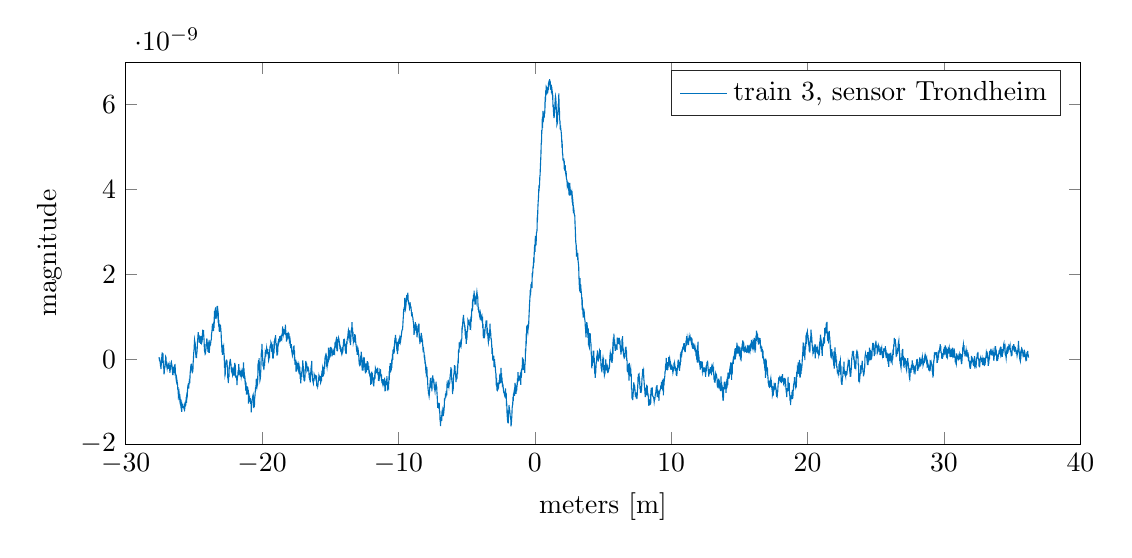
\begin{tikzpicture}

  \begin{axis}[%
    width=\textwidth,
    height=0.4\textwidth,
    at={(0\figurewidth,0\figureheight)},
    scale only axis,
    xmin=-30,
    xmax=40,
    xlabel={meters [m]},
    ymin=-2e-09,
    ymax=7e-09,
    ylabel={magnitude},
    axis background/.style={fill=white},
    legend style={legend cell align=left,align=left,draw=white!15!black}
    ]
    \addplot [color=mycolor1,solid]
    table[row sep=crcr]{%
    -27.550771484375	5.00526645865056e-11\\
    -27.5302734375	-1.98063290922956e-12\\
    -27.509775390625	5.00368072759033e-12\\
    -27.48927734375	-5.15911890856419e-11\\
    -27.468779296875	-6.02282324921168e-11\\
    -27.44828125	-1.47931210052016e-10\\
    -27.427783203125	-1.63441367069997e-10\\
    -27.40728515625	-2.31706203690549e-10\\
    -27.386787109375	-1.0601756621138e-10\\
    -27.3662890625	-9.25048979336056e-12\\
    -27.345791015625	-2.52709871205236e-11\\
    -27.32529296875	1.62385653224853e-10\\
    -27.304794921875	1.10482152686533e-10\\
    -27.284296875	5.83628895199326e-11\\
    -27.263798828125	1.3610730781216e-10\\
    -27.24330078125	-6.51419206605729e-11\\
    -27.222802734375	-1.9583280568032e-10\\
    -27.2023046875	-2.19666786159019e-10\\
    -27.181806640625	-3.5871134038417e-10\\
    -27.16130859375	-2.84384200538639e-10\\
    -27.140810546875	-1.61228623609286e-10\\
    -27.1203125	-2.10909626184407e-10\\
    -27.099814453125	-2.95837940171396e-11\\
    -27.07931640625	-1.0149741467692e-10\\
    -27.058818359375	5.58630759889369e-11\\
    -27.0383203125	3.76509988295563e-11\\
    -27.017822265625	-1.11999586195085e-10\\
    -26.99732421875	-1.40805146060526e-10\\
    -26.976826171875	-1.75566887301852e-10\\
    -26.956328125	-2.20929253195924e-10\\
    -26.935830078125	-1.77387156928706e-10\\
    -26.91533203125	-1.45019886589153e-10\\
    -26.894833984375	-2.25751019063227e-10\\
    -26.8743359375	-1.00676911633239e-10\\
    -26.853837890625	-1.72803343992514e-10\\
    -26.83333984375	-1.63282220695304e-10\\
    -26.812841796875	-1.30556754961644e-10\\
    -26.79234375	-1.93720430269619e-10\\
    -26.771845703125	-2.36305908136485e-10\\
    -26.75134765625	-3.18128384309597e-10\\
    -26.730849609375	-1.39642027261123e-10\\
    -26.7103515625	-2.09546434405632e-10\\
    -26.689853515625	-1.67219671620544e-10\\
    -26.66935546875	-8.07169610969381e-11\\
    -26.648857421875	-6.45550972519404e-11\\
    -26.628359375	-1.31214878642013e-10\\
    -26.607861328125	-1.29301023656221e-10\\
    -26.58736328125	-2.16280676156929e-10\\
    -26.566865234375	-2.93425417503488e-10\\
    -26.5463671875	-2.64783507741527e-10\\
    -26.525869140625	-3.76567126470624e-10\\
    -26.50537109375	-1.81433890579638e-10\\
    -26.484873046875	-3.19426292334553e-10\\
    -26.464375	-1.86430869783803e-10\\
    -26.443876953125	-2.37884833746248e-10\\
    -26.42337890625	-1.85364951865872e-10\\
    -26.402880859375	-1.23092499607737e-10\\
    -26.3823828125	-2.673214451188e-10\\
    -26.361884765625	-2.26968957951255e-10\\
    -26.34138671875	-3.65068553138077e-10\\
    -26.320888671875	-3.74455840889406e-10\\
    -26.300390625	-4.67812465387022e-10\\
    -26.279892578125	-5.06155145331965e-10\\
    -26.25939453125	-4.49982291779619e-10\\
    -26.238896484375	-4.91748912600448e-10\\
    -26.2183984375	-5.42156628696009e-10\\
    -26.197900390625	-5.86025783038407e-10\\
    -26.17740234375	-6.98122028187847e-10\\
    -26.156904296875	-6.9043610055893e-10\\
    -26.13640625	-8.37411726444114e-10\\
    -26.115908203125	-8.01698749158469e-10\\
    -26.09541015625	-8.64806319669622e-10\\
    -26.074912109375	-8.11117640672983e-10\\
    -26.0544140625	-8.7936217166129e-10\\
    -26.033916015625	-9.42521717166718e-10\\
    -26.01341796875	-9.13638636384513e-10\\
    -25.992919921875	-1.06477113676099e-09\\
    -25.972421875	-9.3390679529725e-10\\
    -25.951923828125	-1.12098835563322e-09\\
    -25.93142578125	-1.14628938151935e-09\\
    -25.910927734375	-1.17596061290312e-09\\
    -25.8904296875	-1.23902511402753e-09\\
    -25.869931640625	-1.0602660336723e-09\\
    -25.84943359375	-1.09419329563064e-09\\
    -25.828935546875	-1.09462175766854e-09\\
    -25.8084375	-1.08165290252086e-09\\
    -25.787939453125	-1.1225088062025e-09\\
    -25.76744140625	-1.11734984861976e-09\\
    -25.746943359375	-1.13172391701176e-09\\
    -25.7264453125	-1.16028383370097e-09\\
    -25.705947265625	-1.17849470901311e-09\\
    -25.68544921875	-1.12090152718418e-09\\
    -25.664951171875	-1.15892701074537e-09\\
    -25.644453125	-1.10546173443375e-09\\
    -25.623955078125	-1.00073554170619e-09\\
    -25.60345703125	-1.08520601401799e-09\\
    -25.582958984375	-1.07555711595773e-09\\
    -25.5624609375	-8.85735198987588e-10\\
    -25.541962890625	-1.02938464122556e-09\\
    -25.52146484375	-8.78961418269718e-10\\
    -25.500966796875	-9.09403192705713e-10\\
    -25.48046875	-8.70502242194386e-10\\
    -25.459970703125	-7.12323851301614e-10\\
    -25.43947265625	-6.36998901446261e-10\\
    -25.418974609375	-6.4552172526319e-10\\
    -25.3984765625	-5.65868594833157e-10\\
    -25.377978515625	-6.94341802096112e-10\\
    -25.35748046875	-5.94814098853274e-10\\
    -25.336982421875	-5.30911128425446e-10\\
    -25.316484375	-5.54968477025655e-10\\
    -25.295986328125	-5.53949394995697e-10\\
    -25.27548828125	-3.66895015254073e-10\\
    -25.254990234375	-2.78099935107816e-10\\
    -25.2344921875	-2.35700022361964e-10\\
    -25.213994140625	-1.21988029936433e-10\\
    -25.19349609375	-2.34083194783395e-10\\
    -25.172998046875	-1.06895941235147e-10\\
    -25.1525	-2.50551742810124e-10\\
    -25.132001953125	-2.8182197205261e-10\\
    -25.11150390625	-3.07040971278866e-10\\
    -25.091005859375	-2.93507107151953e-10\\
    -25.0705078125	-2.84168661123667e-10\\
    -25.050009765625	-9.12966571933587e-11\\
    -25.02951171875	1.18964096811648e-11\\
    -25.009013671875	1.48122790031184e-10\\
    -24.988515625	1.94279470845152e-10\\
    -24.968017578125	3.28221186967575e-10\\
    -24.94751953125	4.52045770110322e-10\\
    -24.927021484375	4.09465503514646e-10\\
    -24.9065234375	3.9435342615901e-10\\
    -24.886025390625	3.13032748550464e-10\\
    -24.86552734375	1.69791581917601e-10\\
    -24.845029296875	4.12041993642003e-11\\
    -24.82453125	1.01548176829923e-10\\
    -24.804033203125	2.91626254674967e-11\\
    -24.78353515625	1.65542270768512e-10\\
    -24.763037109375	1.7574406546967e-10\\
    -24.7425390625	3.32311655237956e-10\\
    -24.722041015625	4.52805674096251e-10\\
    -24.70154296875	5.13050405869211e-10\\
    -24.681044921875	6.36973082238239e-10\\
    -24.660546875	5.62430974602043e-10\\
    -24.640048828125	4.71644132613103e-10\\
    -24.61955078125	5.75852560897201e-10\\
    -24.599052734375	3.95994375564479e-10\\
    -24.5785546875	5.36487040219729e-10\\
    -24.558056640625	3.85771607989864e-10\\
    -24.53755859375	4.34914407735801e-10\\
    -24.517060546875	5.26380694274282e-10\\
    -24.4965625	3.64061384507547e-10\\
    -24.476064453125	5.49706394021143e-10\\
    -24.45556640625	4.24327087439205e-10\\
    -24.435068359375	3.7353171648587e-10\\
    -24.4145703125	3.87008754089969e-10\\
    -24.394072265625	4.34838900682367e-10\\
    -24.37357421875	4.73831652658636e-10\\
    -24.353076171875	6.97507867675564e-10\\
    -24.332578125	6.2151068940281e-10\\
    -24.312080078125	6.70516589328709e-10\\
    -24.29158203125	6.7076911950559e-10\\
    -24.271083984375	5.46812106211815e-10\\
    -24.2505859375	4.57555081140595e-10\\
    -24.230087890625	2.7001263760437e-10\\
    -24.20958984375	1.78517036612675e-10\\
    -24.189091796875	1.72961093224166e-10\\
    -24.16859375	1.21707918106453e-10\\
    -24.148095703125	1.33971806004781e-10\\
    -24.12759765625	2.06893303546914e-10\\
    -24.107099609375	3.56026842733965e-10\\
    -24.0866015625	3.02426557953106e-10\\
    -24.066103515625	4.12908925303499e-10\\
    -24.04560546875	4.9013745606666e-10\\
    -24.025107421875	4.23215271924775e-10\\
    -24.004609375	2.37333430999773e-10\\
    -23.984111328125	3.98841808028354e-10\\
    -23.96361328125	1.75001643027512e-10\\
    -23.943115234375	2.80506514646051e-10\\
    -23.9226171875	2.83250110536467e-10\\
    -23.902119140625	1.57621423713947e-10\\
    -23.88162109375	4.55560475738088e-10\\
    -23.861123046875	1.49269510435563e-10\\
    -23.840625	4.1440264434366e-10\\
    -23.820126953125	3.15539110636331e-10\\
    -23.79962890625	3.35180772675205e-10\\
    -23.779130859375	3.39085034567381e-10\\
    -23.7586328125	4.03781312592951e-10\\
    -23.738134765625	4.47256099043632e-10\\
    -23.71763671875	4.67080104145625e-10\\
    -23.697138671875	6.08825130822879e-10\\
    -23.676640625	6.4190173921755e-10\\
    -23.656142578125	7.2347792180654e-10\\
    -23.63564453125	8.37454440734244e-10\\
    -23.615146484375	7.32152405782466e-10\\
    -23.5946484375	6.82503650694164e-10\\
    -23.574150390625	7.84382187410976e-10\\
    -23.55365234375	6.60168464733628e-10\\
    -23.533154296875	8.88525858172603e-10\\
    -23.51265625	7.36174910042938e-10\\
    -23.492158203125	1.13105110971292e-09\\
    -23.47166015625	9.52125582032926e-10\\
    -23.451162109375	1.1297392030105e-09\\
    -23.4306640625	1.16461066580915e-09\\
    -23.410166015625	1.13401958890589e-09\\
    -23.38966796875	1.16094592697776e-09\\
    -23.369169921875	9.455204216598e-10\\
    -23.348671875	1.02815520253799e-09\\
    -23.328173828125	1.08117993243547e-09\\
    -23.30767578125	1.05338312684903e-09\\
    -23.287177734375	1.01525695094173e-09\\
    -23.2666796875	1.25860181370253e-09\\
    -23.246181640625	1.17167716125544e-09\\
    -23.22568359375	9.79894518097505e-10\\
    -23.205185546875	1.01766585962606e-09\\
    -23.1846875	8.38947654939516e-10\\
    -23.164189453125	8.56611627382058e-10\\
    -23.14369140625	7.0063349749183e-10\\
    -23.123193359375	6.4532321745277e-10\\
    -23.1026953125	8.30185911295518e-10\\
    -23.082197265625	7.71988759954323e-10\\
    -23.06169921875	7.95765914212161e-10\\
    -23.041201171875	7.88481414707127e-10\\
    -23.020703125	6.81005180346339e-10\\
    -23.000205078125	6.39546720817717e-10\\
    -22.97970703125	4.39626016166523e-10\\
    -22.959208984375	3.83434303593294e-10\\
    -22.9387109375	1.75544134320218e-10\\
    -22.918212890625	1.74060488104449e-10\\
    -22.89771484375	1.04296222761624e-10\\
    -22.877216796875	3.08747770848679e-10\\
    -22.85671875	3.14138957098828e-10\\
    -22.836220703125	2.58320630421292e-10\\
    -22.81572265625	2.90912046240489e-10\\
    -22.795224609375	1.49163905901189e-10\\
    -22.7747265625	9.79964679452601e-11\\
    -22.754228515625	-1.95384263306273e-10\\
    -22.73373046875	-1.52022720196476e-10\\
    -22.713232421875	-3.77109628440581e-10\\
    -22.692734375	-3.45235185157006e-10\\
    -22.672236328125	-1.74915054959904e-10\\
    -22.65173828125	-5.62579207248828e-11\\
    -22.631240234375	-3.70543919740966e-11\\
    -22.6107421875	-2.00412269499106e-11\\
    -22.590244140625	-2.26666454868141e-11\\
    -22.56974609375	-4.87764053011349e-11\\
    -22.549248046875	-1.74435029561191e-10\\
    -22.52875	-1.84221092355602e-10\\
    -22.508251953125	-4.53934298123738e-10\\
    -22.48775390625	-4.77094213853983e-10\\
    -22.467255859375	-5.61271488261747e-10\\
    -22.4467578125	-3.41610936947677e-10\\
    -22.426259765625	-4.22693392665313e-10\\
    -22.40576171875	-2.20604807590554e-10\\
    -22.385263671875	-1.58817261471482e-10\\
    -22.364765625	-7.30882444891456e-11\\
    -22.344267578125	-8.39351756482519e-11\\
    -22.32376953125	4.42591840183822e-12\\
    -22.303271484375	-7.9840918226048e-11\\
    -22.2827734375	-9.84960190579529e-11\\
    -22.262275390625	-1.78704646552028e-10\\
    -22.24177734375	-3.05757595974293e-10\\
    -22.221279296875	-1.84120412599242e-10\\
    -22.20078125	-3.34731713846028e-10\\
    -22.180283203125	-2.89311730080423e-10\\
    -22.15978515625	-3.64041690528157e-10\\
    -22.139287109375	-3.33936452439096e-10\\
    -22.1187890625	-3.42312359962307e-10\\
    -22.098291015625	-2.14125700394416e-10\\
    -22.07779296875	-3.87321456962964e-10\\
    -22.057294921875	-1.72464759559347e-10\\
    -22.036796875	-2.65812760340543e-10\\
    -22.016298828125	-1.9723663530354e-10\\
    -21.99580078125	-8.83253453509085e-11\\
    -21.975302734375	-4.06373440625301e-10\\
    -21.9548046875	-1.29743085409757e-10\\
    -21.934306640625	-4.18202909509024e-10\\
    -21.91380859375	-4.25395644457921e-10\\
    -21.893310546875	-4.15561562033354e-10\\
    -21.8728125	-4.48068244088609e-10\\
    -21.852314453125	-4.78147160018678e-10\\
    -21.83181640625	-6.1145121423545e-10\\
    -21.811318359375	-4.09345704688725e-10\\
    -21.7908203125	-4.1304204827297e-10\\
    -21.770322265625	-3.65477773346706e-10\\
    -21.74982421875	-2.58700525705412e-10\\
    -21.729326171875	-3.73948615779019e-10\\
    -21.708828125	-1.13455831974734e-10\\
    -21.688330078125	-2.14539998512828e-10\\
    -21.66783203125	-2.73704116028154e-10\\
    -21.647333984375	-3.14615469511831e-10\\
    -21.6268359375	-3.42831267527538e-10\\
    -21.606337890625	-2.74294049076357e-10\\
    -21.58583984375	-3.80114825344601e-10\\
    -21.565341796875	-3.77309431827589e-10\\
    -21.54484375	-3.21438770909188e-10\\
    -21.524345703125	-3.98344773273458e-10\\
    -21.50384765625	-3.48090121377288e-10\\
    -21.483349609375	-4.21969650138775e-10\\
    -21.4628515625	-2.82502454580958e-10\\
    -21.442353515625	-2.77144248519277e-10\\
    -21.42185546875	-3.11108836510343e-10\\
    -21.401357421875	-2.02976035381337e-10\\
    -21.380859375	-3.20420384623614e-10\\
    -21.360361328125	-7.69317734419562e-11\\
    -21.33986328125	-4.48934276194604e-10\\
    -21.319365234375	-2.1839950462398e-10\\
    -21.2988671875	-3.77895089735331e-10\\
    -21.278369140625	-4.64547707386458e-10\\
    -21.25787109375	-3.88046861313447e-10\\
    -21.237373046875	-5.89720847809889e-10\\
    -21.216875	-5.12662071236839e-10\\
    -21.196376953125	-7.41351765740418e-10\\
    -21.17587890625	-5.53386004290716e-10\\
    -21.155380859375	-6.64041616057837e-10\\
    -21.1348828125	-8.33522820828047e-10\\
    -21.114384765625	-6.35354674174431e-10\\
    -21.09388671875	-7.81496955130712e-10\\
    -21.073388671875	-6.92504585311443e-10\\
    -21.052890625	-6.49848256631491e-10\\
    -21.032392578125	-8.25118528930107e-10\\
    -21.01189453125	-7.20214200364656e-10\\
    -20.991396484375	-1.04707938094802e-09\\
    -20.9708984375	-8.74551551403315e-10\\
    -20.950400390625	-9.39011335336326e-10\\
    -20.92990234375	-9.42112636213043e-10\\
    -20.909404296875	-8.992429335465e-10\\
    -20.88890625	-9.72626648934069e-10\\
    -20.868408203125	-9.6264289842776e-10\\
    -20.84791015625	-9.5146834070098e-10\\
    -20.827412109375	-1.05146501594057e-09\\
    -20.8069140625	-9.89225536450515e-10\\
    -20.786416015625	-1.24953801430639e-09\\
    -20.76591796875	-1.00313613818394e-09\\
    -20.745419921875	-1.04801115715992e-09\\
    -20.724921875	-9.85524326239266e-10\\
    -20.704423828125	-9.17036175591135e-10\\
    -20.68392578125	-8.78054601073002e-10\\
    -20.663427734375	-8.94399954825728e-10\\
    -20.6429296875	-8.51475698768297e-10\\
    -20.622431640625	-8.97859535943641e-10\\
    -20.60193359375	-1.15084841305164e-09\\
    -20.581435546875	-1.01775058856429e-09\\
    -20.5609375	-1.12477837119763e-09\\
    -20.540439453125	-9.26562543635409e-10\\
    -20.51994140625	-8.75911737930945e-10\\
    -20.499443359375	-7.71586938661398e-10\\
    -20.4789453125	-6.84168629165511e-10\\
    -20.458447265625	-6.62922277909848e-10\\
    -20.43794921875	-6.13519669049702e-10\\
    -20.417451171875	-4.56276976332208e-10\\
    -20.396953125	-6.18767613300869e-10\\
    -20.376455078125	-6.64738974180247e-10\\
    -20.35595703125	-6.23768629346499e-10\\
    -20.335458984375	-6.05516761070616e-10\\
    -20.3149609375	-4.73639851859808e-10\\
    -20.294462890625	-1.68795813286831e-10\\
    -20.27396484375	-1.89311087462361e-10\\
    -20.253466796875	-2.38963077080561e-11\\
    -20.23296875	-1.75004377571393e-10\\
    -20.212470703125	2.58733708449089e-11\\
    -20.19197265625	-3.20436094096081e-10\\
    -20.171474609375	-3.32006820439579e-10\\
    -20.1509765625	-4.9437958191534e-10\\
    -20.130478515625	-4.6391863283189e-10\\
    -20.10998046875	-3.98149671583187e-10\\
    -20.089482421875	-2.5111204147033e-10\\
    -20.068984375	-2.59708773455334e-11\\
    -20.048486328125	1.82340311968182e-10\\
    -20.02798828125	6.85803525022756e-11\\
    -20.007490234375	3.59713881469536e-10\\
    -19.9869921875	2.10135416949178e-10\\
    -19.966494140625	1.75136930797228e-10\\
    -19.94599609375	-1.83597804264253e-11\\
    -19.925498046875	-1.50273704455757e-10\\
    -19.905	-1.44365576088874e-10\\
    -19.884501953125	-1.41415168861236e-10\\
    -19.86400390625	-2.56905409769861e-10\\
    -19.843505859375	-1.01170171179045e-10\\
    -19.8230078125	-5.07948891513598e-11\\
    -19.802509765625	-7.66929343224133e-11\\
    -19.78201171875	4.27107394041207e-11\\
    -19.761513671875	1.59567610555067e-10\\
    -19.741015625	1.28222722309134e-10\\
    -19.720517578125	6.06862623037604e-11\\
    -19.70001953125	2.20057474483769e-10\\
    -19.679521484375	1.68069657798504e-10\\
    -19.6590234375	2.61469867580335e-10\\
    -19.638525390625	2.15923237062397e-10\\
    -19.61802734375	1.9714951753058e-10\\
    -19.597529296875	1.3549254014627e-10\\
    -19.57703125	2.38738717636323e-10\\
    -19.556533203125	1.10460203169416e-10\\
    -19.53603515625	9.65171375611287e-11\\
    -19.515537109375	-2.70510849925993e-11\\
    -19.4950390625	-4.46023748806013e-12\\
    -19.474541015625	1.67618828661777e-10\\
    -19.45404296875	3.37762571346482e-11\\
    -19.433544921875	2.194776610855e-10\\
    -19.413046875	2.90388464997697e-10\\
    -19.392548828125	2.80489077389381e-10\\
    -19.37205078125	2.83888917807064e-10\\
    -19.351552734375	3.812367366585e-10\\
    -19.3310546875	3.48061084792131e-10\\
    -19.310556640625	2.70335958257935e-10\\
    -19.29005859375	3.07528384568477e-10\\
    -19.269560546875	1.8063480794535e-10\\
    -19.2490625	3.47434706363295e-10\\
    -19.228564453125	1.30368346811498e-10\\
    -19.20806640625	1.35539471772454e-11\\
    -19.187568359375	1.3303318321303e-10\\
    -19.1670703125	9.98501801236028e-11\\
    -19.146572265625	1.95606763933533e-10\\
    -19.12607421875	3.10139726900635e-10\\
    -19.105576171875	2.68671034820337e-10\\
    -19.085078125	4.15997387180711e-10\\
    -19.064580078125	4.62510522704073e-10\\
    -19.04408203125	4.94433575808115e-10\\
    -19.023583984375	4.91913885597368e-10\\
    -19.0030859375	5.65625184295922e-10\\
    -18.982587890625	3.24582252139987e-10\\
    -18.96208984375	3.80890319624713e-10\\
    -18.941591796875	2.58824563601311e-10\\
    -18.92109375	2.86678902418999e-10\\
    -18.900595703125	8.81059209655095e-11\\
    -18.88009765625	2.14258188028749e-10\\
    -18.859599609375	1.08206902521533e-10\\
    -18.8391015625	2.62365809945626e-10\\
    -18.818603515625	3.81576698215284e-10\\
    -18.79810546875	3.72047159850623e-10\\
    -18.777607421875	4.86045475771177e-10\\
    -18.757109375	4.04108912185406e-10\\
    -18.736611328125	4.32252482992756e-10\\
    -18.71611328125	4.40136742202239e-10\\
    -18.695615234375	5.41209690639447e-10\\
    -18.6751171875	4.04557899091549e-10\\
    -18.654619140625	4.88114566471883e-10\\
    -18.63412109375	4.71426516893051e-10\\
    -18.613623046875	4.64384264991856e-10\\
    -18.593125	5.67651409675907e-10\\
    -18.572626953125	5.16982231126115e-10\\
    -18.55212890625	4.89864511665635e-10\\
    -18.531630859375	6.01539635134037e-10\\
    -18.5111328125	5.44064120410109e-10\\
    -18.490634765625	7.76513932229628e-10\\
    -18.47013671875	5.61609198882787e-10\\
    -18.449638671875	7.22509374806556e-10\\
    -18.429140625	5.9834486771579e-10\\
    -18.408642578125	6.33718258634095e-10\\
    -18.38814453125	6.624940851933e-10\\
    -18.367646484375	6.43610047290058e-10\\
    -18.3471484375	6.24670530108456e-10\\
    -18.326650390625	6.73977517966786e-10\\
    -18.30615234375	6.02910287843227e-10\\
    -18.285654296875	8.13102522823805e-10\\
    -18.26515625	5.69709406813888e-10\\
    -18.244658203125	6.09998063137965e-10\\
    -18.22416015625	5.34644237784493e-10\\
    -18.203662109375	4.17365788298669e-10\\
    -18.1831640625	6.15695676371532e-10\\
    -18.162666015625	4.48889286367666e-10\\
    -18.14216796875	5.62102724367105e-10\\
    -18.121669921875	4.83925940375815e-10\\
    -18.101171875	5.91012252685913e-10\\
    -18.080673828125	6.20797087697476e-10\\
    -18.06017578125	6.10121062469261e-10\\
    -18.039677734375	5.39732700980505e-10\\
    -18.0191796875	5.56706372835585e-10\\
    -17.998681640625	4.40931133668422e-10\\
    -17.97818359375	4.6645782124461e-10\\
    -17.957685546875	5.38844566525517e-10\\
    -17.9371875	3.15058417852708e-10\\
    -17.916689453125	3.67544104705673e-10\\
    -17.89619140625	2.87525072340361e-10\\
    -17.875693359375	2.92761393003447e-10\\
    -17.8551953125	3.55975744787918e-10\\
    -17.834697265625	2.44193627975624e-10\\
    -17.81419921875	1.72160639086552e-10\\
    -17.793701171875	1.35031143283382e-10\\
    -17.773203125	9.1670435461544e-11\\
    -17.752705078125	1.29720508237534e-10\\
    -17.73220703125	1.71890126850663e-10\\
    -17.711708984375	1.14432704762694e-10\\
    -17.6912109375	2.99727239886029e-10\\
    -17.670712890625	1.51639404951894e-10\\
    -17.65021484375	3.25107891995813e-10\\
    -17.629716796875	6.61879478152876e-11\\
    -17.60921875	9.50321540651154e-11\\
    -17.588720703125	-1.1643805477628e-10\\
    -17.56822265625	-1.19654213307828e-10\\
    -17.547724609375	-1.22907050494614e-10\\
    -17.5272265625	-7.71353381071629e-12\\
    -17.506728515625	-2.90207461323869e-10\\
    -17.48623046875	-1.37495051839327e-10\\
    -17.465732421875	-2.50088022068957e-10\\
    -17.445234375	-5.81777232592912e-11\\
    -17.424736328125	-2.03214582605424e-10\\
    -17.40423828125	-1.78014745670367e-10\\
    -17.383740234375	-9.15268453657815e-11\\
    -17.3632421875	-1.69551636328437e-10\\
    -17.342744140625	-2.23767100805062e-10\\
    -17.32224609375	-1.63120431585483e-10\\
    -17.301748046875	-1.16522225349599e-10\\
    -17.28125	-1.51319592003156e-10\\
    -17.260751953125	-3.56398538685368e-10\\
    -17.24025390625	-1.67214828104529e-10\\
    -17.219755859375	-2.74653254875313e-10\\
    -17.1992578125	-4.62586790830339e-10\\
    -17.178759765625	-3.29109309963058e-10\\
    -17.15826171875	-5.67652970995734e-10\\
    -17.137763671875	-4.31066268437645e-10\\
    -17.117265625	-3.93574812272204e-10\\
    -17.096767578125	-3.40109668598597e-10\\
    -17.07626953125	-3.57522251282238e-10\\
    -17.055771484375	-1.97898672775245e-10\\
    -17.0352734375	-2.62161510947986e-10\\
    -17.014775390625	-2.59999300525878e-11\\
    -16.99427734375	-1.21841205225114e-10\\
    -16.973779296875	-1.86381765320946e-10\\
    -16.95328125	-2.96654936091593e-10\\
    -16.932783203125	-4.71412304848679e-10\\
    -16.91228515625	-5.02442148460876e-10\\
    -16.891787109375	-5.08826975878569e-10\\
    -16.8712890625	-4.98828821793216e-10\\
    -16.850791015625	-4.15754466660494e-10\\
    -16.83029296875	-2.40027132895058e-10\\
    -16.809794921875	-2.02801957715899e-10\\
    -16.789296875	-4.09271883475418e-11\\
    -16.768798828125	-9.08620391711931e-11\\
    -16.74830078125	-1.03446535940576e-10\\
    -16.727802734375	-1.02736374542975e-10\\
    -16.7073046875	-2.46857054091243e-10\\
    -16.686806640625	-2.17614438174605e-10\\
    -16.66630859375	-1.70667084498878e-10\\
    -16.645810546875	-2.83051194323081e-10\\
    -16.6253125	-2.32932556217067e-10\\
    -16.604814453125	-2.12947188317223e-10\\
    -16.58431640625	-2.39754515955944e-10\\
    -16.563818359375	-3.05234511264351e-10\\
    -16.5433203125	-4.1462086841362e-10\\
    -16.522822265625	-4.06779458354832e-10\\
    -16.50232421875	-4.91095798419026e-10\\
    -16.481826171875	-4.15211768402138e-10\\
    -16.461328125	-5.45259966616796e-10\\
    -16.440830078125	-2.97298202178454e-10\\
    -16.42033203125	-3.60690048505798e-10\\
    -16.399833984375	-1.5404255000364e-10\\
    -16.3793359375	-2.13170310394501e-10\\
    -16.358837890625	-3.97705952943943e-11\\
    -16.33833984375	-2.98460733044038e-10\\
    -16.317841796875	-3.53599961880272e-10\\
    -16.29734375	-4.94874930450631e-10\\
    -16.276845703125	-5.0944661808616e-10\\
    -16.25634765625	-5.43195412157316e-10\\
    -16.235849609375	-5.66845927720978e-10\\
    -16.2153515625	-4.58648758148709e-10\\
    -16.194853515625	-5.14627166695906e-10\\
    -16.17435546875	-3.63300827621762e-10\\
    -16.153857421875	-3.87617560743456e-10\\
    -16.133359375	-3.81815394041432e-10\\
    -16.112861328125	-4.57762532902008e-10\\
    -16.09236328125	-3.70173931231605e-10\\
    -16.071865234375	-4.23967622198644e-10\\
    -16.0513671875	-4.65466990961602e-10\\
    -16.030869140625	-4.93524130880878e-10\\
    -16.01037109375	-3.84157007874617e-10\\
    -15.989873046875	-6.07118676003779e-10\\
    -15.969375	-6.01150746245039e-10\\
    -15.948876953125	-6.36259244253587e-10\\
    -15.92837890625	-5.7899464575384e-10\\
    -15.907880859375	-6.55853163499396e-10\\
    -15.8873828125	-5.40383459581589e-10\\
    -15.866884765625	-5.20858096231075e-10\\
    -15.84638671875	-4.67718948206291e-10\\
    -15.825888671875	-3.81453777327115e-10\\
    -15.805390625	-4.07557035397784e-10\\
    -15.784892578125	-4.76791964664997e-10\\
    -15.76439453125	-3.84948780849313e-10\\
    -15.743896484375	-5.11798853663216e-10\\
    -15.7233984375	-3.99026075320864e-10\\
    -15.702900390625	-5.53384587898996e-10\\
    -15.68240234375	-5.36219716025169e-10\\
    -15.661904296875	-4.20056989343703e-10\\
    -15.64140625	-5.1812482986085e-10\\
    -15.620908203125	-3.50922828558054e-10\\
    -15.60041015625	-2.72921058449484e-10\\
    -15.579912109375	-4.16114557319053e-10\\
    -15.5594140625	-2.26154770801985e-10\\
    -15.538916015625	-2.63101897668115e-10\\
    -15.51841796875	-2.50183559646114e-10\\
    -15.497919921875	-1.89535673123098e-10\\
    -15.477421875	-3.56497104912603e-10\\
    -15.456923828125	-3.39513972953847e-10\\
    -15.43642578125	-1.81512061565161e-10\\
    -15.415927734375	-1.90483419586877e-10\\
    -15.3954296875	-4.38837920293317e-11\\
    -15.374931640625	4.83414713249005e-11\\
    -15.35443359375	6.93771389772072e-11\\
    -15.333935546875	9.38584804072136e-11\\
    -15.3134375	4.88581601403097e-11\\
    -15.292939453125	7.27741319098675e-11\\
    -15.27244140625	-1.74579647207067e-10\\
    -15.251943359375	-1.19198877745892e-10\\
    -15.2314453125	-1.74361649888319e-10\\
    -15.210947265625	-1.06381097783767e-10\\
    -15.19044921875	-1.64750121022008e-10\\
    -15.169951171875	6.65234717943121e-11\\
    -15.149453125	-7.88641390588498e-11\\
    -15.128955078125	2.71968650933517e-10\\
    -15.10845703125	-2.8988948376582e-11\\
    -15.087958984375	2.13361940970382e-10\\
    -15.0674609375	1.71698731265701e-10\\
    -15.046962890625	1.08280660751897e-10\\
    -15.02646484375	1.69783607193292e-10\\
    -15.005966796875	1.1867152718602e-10\\
    -14.98546875	9.95640345410013e-11\\
    -14.964970703125	2.8964305731884e-10\\
    -14.94447265625	6.60298396462415e-11\\
    -14.923974609375	2.04092396200308e-10\\
    -14.9034765625	2.17926279617613e-10\\
    -14.882978515625	2.35660417250877e-10\\
    -14.86248046875	2.17019530440894e-10\\
    -14.841982421875	1.79844805628681e-10\\
    -14.821484375	1.20709592619188e-10\\
    -14.800986328125	1.40902823676564e-10\\
    -14.78048828125	1.31847162460046e-10\\
    -14.759990234375	1.69767215010557e-10\\
    -14.7394921875	1.01032280401796e-10\\
    -14.718994140625	1.72626379940791e-10\\
    -14.69849609375	2.17444644868697e-10\\
    -14.677998046875	1.85765050940878e-10\\
    -14.6575	3.51634083404728e-10\\
    -14.637001953125	4.1009540820317e-10\\
    -14.61650390625	3.09541331237044e-10\\
    -14.596005859375	3.97406992326389e-10\\
    -14.5755078125	4.33255394316052e-10\\
    -14.555009765625	2.74211669733612e-10\\
    -14.53451171875	5.17707898075933e-10\\
    -14.514013671875	1.97753709041259e-10\\
    -14.493515625	4.01649218010944e-10\\
    -14.473017578125	1.8263789270624e-10\\
    -14.45251953125	3.24631783572715e-10\\
    -14.432021484375	4.42705806197451e-10\\
    -14.4115234375	4.35745872523569e-10\\
    -14.391025390625	5.09146208167124e-10\\
    -14.37052734375	4.8993004142456e-10\\
    -14.350029296875	4.41929354453606e-10\\
    -14.32953125	4.04729139040356e-10\\
    -14.309033203125	3.79614283815647e-10\\
    -14.28853515625	2.38698289175996e-10\\
    -14.268037109375	3.22202362113769e-10\\
    -14.2475390625	2.43282639301119e-10\\
    -14.227041015625	1.82355342521353e-10\\
    -14.20654296875	2.77398202772967e-10\\
    -14.186044921875	1.56408923111488e-10\\
    -14.165546875	1.32597287845125e-10\\
    -14.145048828125	2.32424527298098e-10\\
    -14.12455078125	1.46263323476642e-10\\
    -14.104052734375	2.0941133556422e-10\\
    -14.0835546875	1.79188022026799e-10\\
    -14.063056640625	2.17300734576155e-10\\
    -14.04255859375	3.28078030789155e-10\\
    -14.022060546875	4.09063452844468e-10\\
    -14.0015625	4.72868494787169e-10\\
    -13.981064453125	3.90943499157839e-10\\
    -13.96056640625	4.84000475834515e-10\\
    -13.940068359375	3.11474467088219e-10\\
    -13.9195703125	3.54257625743545e-10\\
    -13.899072265625	2.04041914479012e-10\\
    -13.87857421875	2.90052688564788e-10\\
    -13.858076171875	1.32043597452202e-10\\
    -13.837578125	2.63699476466706e-10\\
    -13.817080078125	2.28891665142365e-10\\
    -13.79658203125	4.19001605309152e-10\\
    -13.776083984375	3.47805606920313e-10\\
    -13.7555859375	4.61126131102932e-10\\
    -13.735087890625	4.95844932639665e-10\\
    -13.71458984375	5.2756391855338e-10\\
    -13.694091796875	5.95594101593245e-10\\
    -13.67359375	5.51832814641948e-10\\
    -13.653095703125	6.67119661580448e-10\\
    -13.63259765625	6.35798078438741e-10\\
    -13.612099609375	5.7085568381901e-10\\
    -13.5916015625	6.81684559859919e-10\\
    -13.571103515625	5.31194740875538e-10\\
    -13.55060546875	3.9143468145471e-10\\
    -13.530107421875	5.78696413057305e-10\\
    -13.509609375	3.32781534176603e-10\\
    -13.489111328125	4.83828470635382e-10\\
    -13.46861328125	5.84516493232189e-10\\
    -13.448115234375	7.1939018069618e-10\\
    -13.4276171875	6.29044710643756e-10\\
    -13.407119140625	8.76130688671742e-10\\
    -13.38662109375	7.03675444626921e-10\\
    -13.366123046875	7.44261710379193e-10\\
    -13.345625	5.51182208547492e-10\\
    -13.325126953125	5.73101522728408e-10\\
    -13.30462890625	4.05318728577406e-10\\
    -13.284130859375	4.40274444779518e-10\\
    -13.2636328125	3.91539311492691e-10\\
    -13.243134765625	5.17534662347431e-10\\
    -13.22263671875	4.07877904464151e-10\\
    -13.202138671875	5.9044641189142e-10\\
    -13.181640625	5.14665354544814e-10\\
    -13.161142578125	5.64001387162273e-10\\
    -13.14064453125	4.47193824971446e-10\\
    -13.120146484375	3.67302657840319e-10\\
    -13.0996484375	3.2765981242972e-10\\
    -13.079150390625	2.70639058942468e-10\\
    -13.05865234375	1.77421256225014e-10\\
    -13.038154296875	2.77975035095956e-10\\
    -13.01765625	1.00858901691209e-10\\
    -12.997158203125	2.11118957792447e-10\\
    -12.97666015625	2.67723037465518e-10\\
    -12.956162109375	2.43298400173755e-10\\
    -12.9356640625	1.57998897053849e-10\\
    -12.915166015625	1.41334975664933e-10\\
    -12.89466796875	-1.13440731143137e-11\\
    -12.874169921875	-1.07880958725313e-10\\
    -12.853671875	-1.23743492446227e-10\\
    -12.833173828125	-1.4777622210354e-10\\
    -12.81267578125	-1.40196109607208e-10\\
    -12.792177734375	-1.24063194736103e-10\\
    -12.7716796875	8.21152287039876e-11\\
    -12.751181640625	-6.19134116786706e-11\\
    -12.73068359375	1.78306654799867e-10\\
    -12.710185546875	5.45810762925938e-12\\
    -12.6896875	2.81900099539389e-11\\
    -12.669189453125	-1.64472067803673e-10\\
    -12.64869140625	-1.35195842625143e-10\\
    -12.628193359375	-2.6872437082922e-10\\
    -12.6076953125	-1.71994387807632e-11\\
    -12.587197265625	-2.66352865735726e-10\\
    -12.56669921875	1.88544408037524e-11\\
    -12.546201171875	2.84586714189183e-11\\
    -12.525703125	4.48803491613868e-12\\
    -12.505205078125	1.36049719854894e-11\\
    -12.48470703125	-7.73983296835858e-11\\
    -12.464208984375	-1.85368641483317e-10\\
    -12.4437109375	-1.6550204918928e-10\\
    -12.423212890625	-3.327318180382e-10\\
    -12.40271484375	-2.47600422240945e-10\\
    -12.382216796875	-3.02953223972928e-10\\
    -12.36171875	-2.92246074485878e-10\\
    -12.341220703125	-1.21311228422304e-10\\
    -12.32072265625	-1.09046827638904e-10\\
    -12.300224609375	-1.18347981716111e-10\\
    -12.2797265625	-4.44620033770376e-11\\
    -12.259228515625	-2.55786270571093e-10\\
    -12.23873046875	-6.36359959191087e-11\\
    -12.218232421875	-1.61991134146875e-10\\
    -12.197734375	-2.31333195111774e-10\\
    -12.177236328125	-1.59448812690119e-10\\
    -12.15673828125	-3.36164000893508e-10\\
    -12.136240234375	-2.79936704251839e-10\\
    -12.1157421875	-3.09202087195932e-10\\
    -12.095244140625	-3.949768662168e-10\\
    -12.07474609375	-4.14368700212552e-10\\
    -12.054248046875	-3.64682850575882e-10\\
    -12.03375	-6.01458238154548e-10\\
    -12.013251953125	-3.3390271132766e-10\\
    -11.99275390625	-5.82742323934269e-10\\
    -11.972255859375	-4.11925974141521e-10\\
    -11.9517578125	-2.91069567669798e-10\\
    -11.931259765625	-4.50683245470834e-10\\
    -11.91076171875	-3.27146879569408e-10\\
    -11.890263671875	-4.87199297541354e-10\\
    -11.869765625	-4.94391366999417e-10\\
    -11.849267578125	-5.99088933620812e-10\\
    -11.82876953125	-4.31187162279901e-10\\
    -11.808271484375	-6.41108288977887e-10\\
    -11.7877734375	-5.27174119666826e-10\\
    -11.767275390625	-4.42813190939559e-10\\
    -11.74677734375	-4.39897228835074e-10\\
    -11.726279296875	-3.46602804525744e-10\\
    -11.70578125	-3.75212697001992e-10\\
    -11.685283203125	-2.14961908599686e-10\\
    -11.66478515625	-2.3919621686837e-10\\
    -11.644287109375	-2.49281568192153e-10\\
    -11.6237890625	-3.17269037434817e-10\\
    -11.603291015625	-2.38121897075998e-10\\
    -11.58279296875	-3.3103464788606e-10\\
    -11.562294921875	-2.22032232289721e-10\\
    -11.541796875	-3.09914647384645e-10\\
    -11.521298828125	-1.98519007281253e-10\\
    -11.50080078125	-3.74027025282983e-10\\
    -11.480302734375	-3.05504503312526e-10\\
    -11.4598046875	-5.10272230042368e-10\\
    -11.439306640625	-3.85121329444198e-10\\
    -11.41880859375	-5.14225548397562e-10\\
    -11.398310546875	-4.11975253478824e-10\\
    -11.3778125	-3.66557841060925e-10\\
    -11.357314453125	-2.47140563782583e-10\\
    -11.33681640625	-2.56672500627581e-10\\
    -11.316318359375	-2.54363604176858e-10\\
    -11.2958203125	-4.03554867669987e-10\\
    -11.275322265625	-3.475634435101e-10\\
    -11.25482421875	-4.38506578666987e-10\\
    -11.234326171875	-4.22117149259417e-10\\
    -11.213828125	-5.43710543243871e-10\\
    -11.193330078125	-5.56773144941494e-10\\
    -11.17283203125	-5.55378114221044e-10\\
    -11.152333984375	-5.83564702743606e-10\\
    -11.1318359375	-4.6756199620458e-10\\
    -11.111337890625	-5.65394993175527e-10\\
    -11.09083984375	-5.40875633144917e-10\\
    -11.070341796875	-5.25490421436436e-10\\
    -11.04984375	-5.55383923079777e-10\\
    -11.029345703125	-6.41573892820647e-10\\
    -11.00884765625	-4.31516315167214e-10\\
    -10.988349609375	-7.56454175781232e-10\\
    -10.9678515625	-5.50121109246425e-10\\
    -10.947353515625	-7.47876679094605e-10\\
    -10.92685546875	-5.12725516241216e-10\\
    -10.906357421875	-5.92695967503111e-10\\
    -10.885859375	-5.86208271309178e-10\\
    -10.865361328125	-5.87698327532879e-10\\
    -10.84486328125	-4.00957322908024e-10\\
    -10.824365234375	-6.14420511831714e-10\\
    -10.8038671875	-5.42439401530748e-10\\
    -10.783369140625	-6.97523923502667e-10\\
    -10.76287109375	-6.81085632737018e-10\\
    -10.742373046875	-6.20259833924871e-10\\
    -10.721875	-6.52089470361746e-10\\
    -10.701376953125	-4.93941444302584e-10\\
    -10.68087890625	-3.66899289468886e-10\\
    -10.660380859375	-3.95720165714829e-10\\
    -10.6398828125	-1.63280700005338e-10\\
    -10.619384765625	-2.62616786194765e-10\\
    -10.59888671875	-9.35171440582542e-11\\
    -10.578388671875	-2.48707539682592e-10\\
    -10.557890625	-2.74617844627534e-10\\
    -10.537392578125	-2.54760619540103e-10\\
    -10.51689453125	-2.40513073466837e-10\\
    -10.496396484375	-9.48271265035336e-11\\
    -10.4758984375	-1.22024658350553e-10\\
    -10.455400390625	-2.05608882847349e-11\\
    -10.43490234375	1.23252261190425e-10\\
    -10.414404296875	-1.21528107283364e-11\\
    -10.39390625	2.2382022733656e-10\\
    -10.373408203125	1.35657346188511e-10\\
    -10.35291015625	1.9560526989426e-10\\
    -10.332412109375	1.45071856046445e-10\\
    -10.3119140625	1.4838169425459e-10\\
    -10.291416015625	3.2750553350418e-10\\
    -10.27091796875	4.21088933382848e-10\\
    -10.250419921875	5.03668393175467e-10\\
    -10.229921875	4.09357736971802e-10\\
    -10.209423828125	5.71678674613631e-10\\
    -10.18892578125	4.30863948342835e-10\\
    -10.168427734375	4.43338784840643e-10\\
    -10.1479296875	3.10116864231596e-10\\
    -10.127431640625	2.74772790984989e-10\\
    -10.10693359375	1.93523692512207e-10\\
    -10.086435546875	3.20479872261078e-10\\
    -10.0659375	1.20077848825869e-10\\
    -10.045439453125	4.10772323791336e-10\\
    -10.02494140625	2.0162549209085e-10\\
    -10.004443359375	4.35564287790864e-10\\
    -9.9839453125	3.53152401250459e-10\\
    -9.963447265625	4.84431692263893e-10\\
    -9.94294921875	3.75792714285851e-10\\
    -9.922451171875	4.60280279619958e-10\\
    -9.901953125	4.11511555305079e-10\\
    -9.881455078125	4.34569297419308e-10\\
    -9.86095703125	4.74462744313547e-10\\
    -9.840458984375	4.27441607019953e-10\\
    -9.8199609375	4.87833469040687e-10\\
    -9.799462890625	5.17850485501346e-10\\
    -9.77896484375	5.83928359564407e-10\\
    -9.758466796875	6.39600514857914e-10\\
    -9.73796875	6.81119572145419e-10\\
    -9.717470703125	6.99322050133063e-10\\
    -9.69697265625	6.9937193889943e-10\\
    -9.676474609375	7.95406220978319e-10\\
    -9.6559765625	9.28490564316002e-10\\
    -9.635478515625	1.01307246941499e-09\\
    -9.61498046875	1.18680250718555e-09\\
    -9.594482421875	1.11898246239827e-09\\
    -9.573984375	1.23494716361652e-09\\
    -9.553486328125	1.16132561638592e-09\\
    -9.53298828125	1.44468518479127e-09\\
    -9.512490234375	1.17542210740816e-09\\
    -9.4919921875	1.33867743847949e-09\\
    -9.471494140625	1.20986733851806e-09\\
    -9.45099609375	1.25258176708513e-09\\
    -9.430498046875	1.38177719203072e-09\\
    -9.41	1.44110412133847e-09\\
    -9.389501953125	1.41755080756455e-09\\
    -9.36900390625	1.50709070363201e-09\\
    -9.348505859375	1.51381608885349e-09\\
    -9.3280078125	1.49053729872638e-09\\
    -9.307509765625	1.57021255043451e-09\\
    -9.28701171875	1.39266902437282e-09\\
    -9.266513671875	1.37015985509229e-09\\
    -9.246015625	1.31647210672616e-09\\
    -9.225517578125	1.29390123534056e-09\\
    -9.20501953125	1.25804254637382e-09\\
    -9.184521484375	1.20006499767815e-09\\
    -9.1640234375	1.22718669840908e-09\\
    -9.143525390625	1.34339587008712e-09\\
    -9.12302734375	1.24062099221389e-09\\
    -9.102529296875	1.22498868953933e-09\\
    -9.08203125	1.23096212825619e-09\\
    -9.061533203125	1.16166584387107e-09\\
    -9.04103515625	1.08344619472159e-09\\
    -9.020537109375	1.00905260871861e-09\\
    -9.0000390625	1.10913017045937e-09\\
    -8.979541015625	1.02556577728422e-09\\
    -8.95904296875	1.00279484604334e-09\\
    -8.938544921875	9.6768798545735e-10\\
    -8.918046875	8.96368557245374e-10\\
    -8.897548828125	8.62887841763379e-10\\
    -8.87705078125	7.96987527176144e-10\\
    -8.856552734375	5.71991707007647e-10\\
    -8.8360546875	7.29954393065655e-10\\
    -8.815556640625	6.0775645335316e-10\\
    -8.79505859375	7.58694826630795e-10\\
    -8.774560546875	7.51921233300658e-10\\
    -8.7540625	8.70749329851196e-10\\
    -8.733564453125	7.13036329408043e-10\\
    -8.71306640625	8.24736163568943e-10\\
    -8.692568359375	6.73191120096837e-10\\
    -8.6720703125	7.85002892004197e-10\\
    -8.651572265625	6.08358333107578e-10\\
    -8.63107421875	5.14423183329548e-10\\
    -8.610576171875	6.49656844900071e-10\\
    -8.590078125	6.57166106390605e-10\\
    -8.569580078125	6.80417260028854e-10\\
    -8.54908203125	7.8459967637009e-10\\
    -8.528583984375	8.00005617332356e-10\\
    -8.5080859375	7.075772758088e-10\\
    -8.487587890625	7.39628763889743e-10\\
    -8.46708984375	4.82300997163004e-10\\
    -8.446591796875	5.55137150995416e-10\\
    -8.42609375	3.55590699217328e-10\\
    -8.405595703125	4.84487067759341e-10\\
    -8.38509765625	4.20437601700728e-10\\
    -8.364599609375	5.3920155093719e-10\\
    -8.3441015625	4.41975287574848e-10\\
    -8.323603515625	6.19590029870754e-10\\
    -8.30310546875	4.1040877450818e-10\\
    -8.282607421875	5.60754853176273e-10\\
    -8.262109375	3.89817744526526e-10\\
    -8.241611328125	4.61471698757741e-10\\
    -8.22111328125	3.53767619107876e-10\\
    -8.200615234375	2.49448609570484e-10\\
    -8.1801171875	2.7942639951976e-10\\
    -8.159619140625	2.67925937943471e-10\\
    -8.13912109375	1.68439604558118e-10\\
    -8.118623046875	1.58025400757217e-10\\
    -8.098125	1.87660929014715e-11\\
    -8.077626953125	9.79838500339463e-11\\
    -8.05712890625	-1.02410505681962e-10\\
    -8.036630859375	-6.15392401983012e-11\\
    -8.0161328125	-1.14767299696076e-10\\
    -7.995634765625	-2.37514585416763e-10\\
    -7.97513671875	-2.12289591855224e-10\\
    -7.954638671875	-3.51430989295494e-10\\
    -7.934140625	-3.26028858671408e-10\\
    -7.913642578125	-1.85707216447873e-10\\
    -7.89314453125	-3.93152157425707e-10\\
    -7.872646484375	-4.13720058616321e-10\\
    -7.8521484375	-5.70956813517619e-10\\
    -7.831650390625	-6.77622672582408e-10\\
    -7.81115234375	-7.37277652717668e-10\\
    -7.790654296875	-8.15210000719401e-10\\
    -7.77015625	-8.29446146277379e-10\\
    -7.749658203125	-8.73892723254504e-10\\
    -7.72916015625	-8.18186697804986e-10\\
    -7.708662109375	-6.89459037790991e-10\\
    -7.6881640625	-6.13318810029303e-10\\
    -7.667666015625	-5.10845654381076e-10\\
    -7.64716796875	-4.42875681209998e-10\\
    -7.626669921875	-5.79864106530291e-10\\
    -7.606171875	-5.14557314073013e-10\\
    -7.585673828125	-6.89106611753446e-10\\
    -7.56517578125	-5.67966849047995e-10\\
    -7.544677734375	-7.57850052236321e-10\\
    -7.5241796875	-4.30261104139884e-10\\
    -7.503681640625	-5.51434205588882e-10\\
    -7.48318359375	-3.79698931673063e-10\\
    -7.462685546875	-4.62152034713503e-10\\
    -7.4421875	-4.72415910547744e-10\\
    -7.421689453125	-4.79735775448576e-10\\
    -7.40119140625	-4.89191368285025e-10\\
    -7.380693359375	-6.44634756285846e-10\\
    -7.3601953125	-6.92197575532436e-10\\
    -7.339697265625	-7.07303443961219e-10\\
    -7.31919921875	-7.5095587833052e-10\\
    -7.298701171875	-6.65158069374328e-10\\
    -7.278203125	-6.86822394892831e-10\\
    -7.257705078125	-6.50976097476498e-10\\
    -7.23720703125	-5.28775984966637e-10\\
    -7.216708984375	-7.13869287536164e-10\\
    -7.1962109375	-6.33256496275724e-10\\
    -7.175712890625	-7.70592708240509e-10\\
    -7.15521484375	-8.7747572923419e-10\\
    -7.134716796875	-1.03709017595958e-09\\
    -7.11421875	-1.14480977299399e-09\\
    -7.093720703125	-1.04301871046794e-09\\
    -7.07322265625	-1.12520170802265e-09\\
    -7.052724609375	-1.0293989511989e-09\\
    -7.0322265625	-1.17169982022289e-09\\
    -7.011728515625	-1.0269671060631e-09\\
    -6.99123046875	-1.22178935727023e-09\\
    -6.970732421875	-1.22479158344134e-09\\
    -6.950234375	-1.42383545216446e-09\\
    -6.929736328125	-1.47453853242536e-09\\
    -6.90923828125	-1.57459278114209e-09\\
    -6.888740234375	-1.37786698270557e-09\\
    -6.8682421875	-1.42931881001974e-09\\
    -6.847744140625	-1.3207126289816e-09\\
    -6.82724609375	-1.45011858245363e-09\\
    -6.806748046875	-1.2453372171352e-09\\
    -6.78625	-1.21106026099718e-09\\
    -6.765751953125	-1.30996380774145e-09\\
    -6.74525390625	-1.29456926419362e-09\\
    -6.724755859375	-1.28170209296525e-09\\
    -6.7042578125	-1.33930438405294e-09\\
    -6.683759765625	-1.19832513121349e-09\\
    -6.66326171875	-1.21527378305189e-09\\
    -6.642763671875	-1.13767886701777e-09\\
    -6.622265625	-9.51707015231276e-10\\
    -6.601767578125	-9.57931321808457e-10\\
    -6.58126953125	-9.16650502896388e-10\\
    -6.560771484375	-8.8504776081146e-10\\
    -6.5402734375	-8.04695108863186e-10\\
    -6.519775390625	-9.06066545848488e-10\\
    -6.49927734375	-7.63451955908925e-10\\
    -6.478779296875	-7.55602545587749e-10\\
    -6.45828125	-8.5039271941443e-10\\
    -6.437783203125	-6.27579964988732e-10\\
    -6.41728515625	-6.60772892540819e-10\\
    -6.396787109375	-6.45779894217311e-10\\
    -6.3762890625	-6.16173363113308e-10\\
    -6.355791015625	-4.95746044047419e-10\\
    -6.33529296875	-6.7506377542228e-10\\
    -6.314794921875	-5.9219209219339e-10\\
    -6.294296875	-6.41296600101746e-10\\
    -6.273798828125	-5.85912716518042e-10\\
    -6.25330078125	-5.81910466262733e-10\\
    -6.232802734375	-5.54549236387798e-10\\
    -6.2123046875	-4.0834473462652e-10\\
    -6.191806640625	-3.42362979476442e-10\\
    -6.17130859375	-3.39532399872444e-10\\
    -6.150810546875	-1.86838815046383e-10\\
    -6.1303125	-4.10972407460149e-10\\
    -6.109814453125	-2.27637462985359e-10\\
    -6.08931640625	-4.84006592424205e-10\\
    -6.068818359375	-5.38060235200027e-10\\
    -6.0483203125	-5.79648420738896e-10\\
    -6.027822265625	-8.2016985923517e-10\\
    -6.00732421875	-6.52382577152575e-10\\
    -5.986826171875	-7.37253708781692e-10\\
    -5.966328125	-4.91393118500692e-10\\
    -5.945830078125	-3.76185063343952e-10\\
    -5.92533203125	-3.39328592011484e-10\\
    -5.904833984375	-2.65640214507086e-10\\
    -5.8843359375	-1.40076450301966e-10\\
    -5.863837890625	-2.64189368108195e-10\\
    -5.84333984375	-2.39944674680938e-10\\
    -5.822841796875	-3.6721506286159e-10\\
    -5.80234375	-3.22983077757472e-10\\
    -5.781845703125	-5.41937846055279e-10\\
    -5.76134765625	-4.00247141014815e-10\\
    -5.740849609375	-4.80195827357285e-10\\
    -5.7203515625	-3.95320393648518e-10\\
    -5.699853515625	-4.08489435201722e-10\\
    -5.67935546875	-2.43367675249063e-10\\
    -5.658857421875	-2.68490142080472e-10\\
    -5.638359375	-3.08404812198e-11\\
    -5.617861328125	-1.04158607567184e-10\\
    -5.59736328125	1.93840873017344e-10\\
    -5.576865234375	2.17028085636978e-10\\
    -5.5563671875	1.58349669109492e-10\\
    -5.535869140625	3.96406539980812e-10\\
    -5.51537109375	2.55607688839451e-10\\
    -5.494873046875	3.41032026591705e-10\\
    -5.474375	3.7855877327163e-10\\
    -5.453876953125	3.28829868791933e-10\\
    -5.43337890625	3.23838937804228e-10\\
    -5.412880859375	3.03857448218488e-10\\
    -5.3923828125	3.67632025842725e-10\\
    -5.371884765625	4.62300640653343e-10\\
    -5.35138671875	4.83025917862896e-10\\
    -5.330888671875	7.88139648266695e-10\\
    -5.310390625	7.46406419347958e-10\\
    -5.289892578125	8.11472679824333e-10\\
    -5.26939453125	9.44004925914107e-10\\
    -5.248896484375	9.73244814593152e-10\\
    -5.2283984375	1.04234629940624e-09\\
    -5.207900390625	9.31142599966068e-10\\
    -5.18740234375	8.72324438202405e-10\\
    -5.166904296875	8.43928256653079e-10\\
    -5.14640625	7.51803647113641e-10\\
    -5.125908203125	8.06916695912452e-10\\
    -5.10541015625	5.6319371552607e-10\\
    -5.084912109375	7.07354337584736e-10\\
    -5.0644140625	4.86122626582091e-10\\
    -5.043916015625	6.63627688870933e-10\\
    -5.02341796875	3.64400625465673e-10\\
    -5.002919921875	6.39876514445758e-10\\
    -4.982421875	4.49355997068898e-10\\
    -4.961923828125	6.36399573359352e-10\\
    -4.94142578125	6.49169260994728e-10\\
    -4.920927734375	7.00436643916531e-10\\
    -4.9004296875	9.1260507812101e-10\\
    -4.879931640625	8.89679361595009e-10\\
    -4.85943359375	8.36600944993258e-10\\
    -4.838935546875	9.24521715845912e-10\\
    -4.8184375	8.01804766223224e-10\\
    -4.797939453125	8.56686694745986e-10\\
    -4.77744140625	8.16602838786931e-10\\
    -4.756943359375	8.31794862782072e-10\\
    -4.7364453125	6.8966366683714e-10\\
    -4.715947265625	8.33688446578644e-10\\
    -4.69544921875	7.96233905336766e-10\\
    -4.674951171875	1.00528978149796e-09\\
    -4.654453125	8.84918745115512e-10\\
    -4.633955078125	1.09728948363277e-09\\
    -4.61345703125	1.19633370635981e-09\\
    -4.592958984375	1.1256303718838e-09\\
    -4.5724609375	1.29026535078944e-09\\
    -4.551962890625	1.25823830857915e-09\\
    -4.53146484375	1.42582225869854e-09\\
    -4.510966796875	1.37578948857943e-09\\
    -4.49046875	1.51639483138955e-09\\
    -4.469970703125	1.36152215749718e-09\\
    -4.44947265625	1.61717248162877e-09\\
    -4.428974609375	1.3635702832636e-09\\
    -4.4084765625	1.4755985383263e-09\\
    -4.387978515625	1.28775884282052e-09\\
    -4.36748046875	1.37597494836048e-09\\
    -4.346982421875	1.30675242835839e-09\\
    -4.326484375	1.40041234223303e-09\\
    -4.305986328125	1.36115443710269e-09\\
    -4.28548828125	1.49815799477063e-09\\
    -4.264990234375	1.5256254059095e-09\\
    -4.2444921875	1.58566173704093e-09\\
    -4.223994140625	1.52965889516513e-09\\
    -4.20349609375	1.42076873730366e-09\\
    -4.182998046875	1.47978867183708e-09\\
    -4.1625	1.2401126304666e-09\\
    -4.142001953125	1.16172464173046e-09\\
    -4.12150390625	1.23502811351076e-09\\
    -4.101005859375	1.08547866934194e-09\\
    -4.0805078125	1.14974009742395e-09\\
    -4.060009765625	1.06292684446178e-09\\
    -4.03951171875	1.0898447104295e-09\\
    -4.019013671875	1.06806216991598e-09\\
    -3.998515625	9.3163816525598e-10\\
    -3.978017578125	1.07605167089429e-09\\
    -3.95751953125	1.04441307576697e-09\\
    -3.937021484375	9.1124866951726e-10\\
    -3.9165234375	9.92128173186867e-10\\
    -3.896025390625	9.76676310377833e-10\\
    -3.87552734375	1.00087524537396e-09\\
    -3.855029296875	8.61568789620695e-10\\
    -3.83453125	1.00625756374804e-09\\
    -3.814033203125	7.33641467143527e-10\\
    -3.79353515625	8.31240204675296e-10\\
    -3.773037109375	4.95459481606114e-10\\
    -3.7525390625	7.05342035436957e-10\\
    -3.732041015625	5.71070056019039e-10\\
    -3.71154296875	4.9442730214322e-10\\
    -3.691044921875	6.06314421321305e-10\\
    -3.670546875	5.89263515347498e-10\\
    -3.650048828125	6.94717400061336e-10\\
    -3.62955078125	7.57138021636802e-10\\
    -3.609052734375	7.72905489189741e-10\\
    -3.5885546875	8.45177857501398e-10\\
    -3.568056640625	8.16007028461054e-10\\
    -3.54755859375	7.69101099320451e-10\\
    -3.527060546875	9.13841211270894e-10\\
    -3.5065625	6.04034193147283e-10\\
    -3.486064453125	7.41176223157997e-10\\
    -3.46556640625	5.55749890295389e-10\\
    -3.445068359375	6.19283972734998e-10\\
    -3.4245703125	4.57113361727639e-10\\
    -3.404072265625	4.0298972522036e-10\\
    -3.38357421875	4.70118659458332e-10\\
    -3.363076171875	5.46194812297724e-10\\
    -3.342578125	5.21189893931847e-10\\
    -3.322080078125	6.98736089509287e-10\\
    -3.30158203125	5.58685640014999e-10\\
    -3.281083984375	8.39286838296438e-10\\
    -3.2605859375	5.6820197488534e-10\\
    -3.240087890625	6.61882169398884e-10\\
    -3.21958984375	4.91652271532928e-10\\
    -3.199091796875	4.90645874366858e-10\\
    -3.17859375	4.33360619597768e-10\\
    -3.158095703125	3.29030303273036e-10\\
    -3.13759765625	1.27458255666389e-10\\
    -3.117099609375	2.6647518835644e-10\\
    -3.0966015625	1.01419692587049e-10\\
    -3.076103515625	-3.31301738846045e-11\\
    -3.05560546875	5.47961357695867e-11\\
    -3.035107421875	-4.08907356856522e-11\\
    -3.014609375	8.31098900132514e-11\\
    -2.994111328125	-1.85030709860462e-10\\
    -2.97361328125	-6.81895918787065e-11\\
    -2.953115234375	-8.73204521021768e-13\\
    -2.9326171875	-1.12949912422965e-10\\
    -2.912119140625	-1.39925154581111e-10\\
    -2.89162109375	-2.12267797625663e-10\\
    -2.871123046875	-3.19927623487096e-10\\
    -2.850625	-3.24811136878016e-10\\
    -2.830126953125	-6.15271918101836e-10\\
    -2.80962890625	-4.41536814754488e-10\\
    -2.789130859375	-6.3521051427802e-10\\
    -2.7686328125	-7.3188983391655e-10\\
    -2.748134765625	-7.37726922207373e-10\\
    -2.72763671875	-6.85807904253852e-10\\
    -2.707138671875	-5.50895673446007e-10\\
    -2.686640625	-6.94263433146947e-10\\
    -2.666142578125	-6.79213479526852e-10\\
    -2.64564453125	-6.01091659863459e-10\\
    -2.625146484375	-5.54419468847231e-10\\
    -2.6046484375	-4.97087035977712e-10\\
    -2.584150390625	-5.78178637715718e-10\\
    -2.56365234375	-3.40662203281486e-10\\
    -2.543154296875	-5.14778717951984e-10\\
    -2.52265625	-4.54241572000406e-10\\
    -2.502158203125	-5.61513092256008e-10\\
    -2.48166015625	-2.05210426055738e-10\\
    -2.461162109375	-5.08109342888031e-10\\
    -2.4406640625	-3.25361039471218e-10\\
    -2.420166015625	-4.79130241155511e-10\\
    -2.39966796875	-4.72741693692936e-10\\
    -2.379169921875	-5.97066991063521e-10\\
    -2.358671875	-5.77802675145246e-10\\
    -2.338173828125	-5.9630806745473e-10\\
    -2.31767578125	-6.62191104890335e-10\\
    -2.297177734375	-7.36766344287795e-10\\
    -2.2766796875	-7.7905959496394e-10\\
    -2.256181640625	-7.83222021522576e-10\\
    -2.23568359375	-8.17585571421263e-10\\
    -2.215185546875	-8.46091293951189e-10\\
    -2.1946875	-8.10340168095389e-10\\
    -2.174189453125	-8.3838660204874e-10\\
    -2.15369140625	-6.88690199198541e-10\\
    -2.133193359375	-7.86433240459791e-10\\
    -2.1126953125	-8.75580474822166e-10\\
    -2.092197265625	-8.04513727052278e-10\\
    -2.07169921875	-1.10299357029452e-09\\
    -2.051201171875	-1.045203728321e-09\\
    -2.030703125	-1.33364613538901e-09\\
    -2.010205078125	-1.36650262336933e-09\\
    -1.98970703125	-1.49177325049118e-09\\
    -1.969208984375	-1.31006010832614e-09\\
    -1.9487109375	-1.51063039682124e-09\\
    -1.928212890625	-1.20332421913756e-09\\
    -1.90771484375	-1.27024449625921e-09\\
    -1.887216796875	-1.07970510278916e-09\\
    -1.86671875	-1.18540784094008e-09\\
    -1.846220703125	-1.183526192305e-09\\
    -1.82572265625	-1.25422775945713e-09\\
    -1.805224609375	-1.3375477843335e-09\\
    -1.7847265625	-1.37830059959239e-09\\
    -1.764228515625	-1.38733072427807e-09\\
    -1.74373046875	-1.57970084315363e-09\\
    -1.723232421875	-1.38110976291583e-09\\
    -1.702734375	-1.42606331766757e-09\\
    -1.682236328125	-1.32637903479123e-09\\
    -1.66173828125	-1.14977193583757e-09\\
    -1.641240234375	-1.09537756865312e-09\\
    -1.6207421875	-1.06914468049603e-09\\
    -1.600244140625	-8.90487418851473e-10\\
    -1.57974609375	-9.85255683532522e-10\\
    -1.559248046875	-8.2061385860279e-10\\
    -1.53875	-8.07443510639027e-10\\
    -1.518251953125	-7.62618916152492e-10\\
    -1.49775390625	-7.24597608456164e-10\\
    -1.477255859375	-8.63011697104846e-10\\
    -1.4567578125	-5.55965242827864e-10\\
    -1.436259765625	-6.46501045813053e-10\\
    -1.41576171875	-6.11514516768629e-10\\
    -1.395263671875	-6.27648344883105e-10\\
    -1.374765625	-8.15753737715775e-10\\
    -1.354267578125	-6.89324076678397e-10\\
    -1.33376953125	-7.54412462878979e-10\\
    -1.313271484375	-6.5581412292989e-10\\
    -1.2927734375	-6.13712565653086e-10\\
    -1.272275390625	-4.54110658679398e-10\\
    -1.25177734375	-5.4383133405728e-10\\
    -1.231279296875	-3.06933529444747e-10\\
    -1.21078125	-4.27623379241324e-10\\
    -1.190283203125	-4.19318529725326e-10\\
    -1.16978515625	-4.12721254728971e-10\\
    -1.149287109375	-5.13565294809785e-10\\
    -1.1287890625	-4.14741051567081e-10\\
    -1.108291015625	-4.14391089854686e-10\\
    -1.08779296875	-4.87474745337963e-10\\
    -1.067294921875	-4.02470281846105e-10\\
    -1.046796875	-4.33224067527174e-10\\
    -1.026298828125	-6.04776783296792e-10\\
    -1.00580078125	-2.62723230298606e-10\\
    -0.985302734375001	-4.36008354369884e-10\\
    -0.964804687499999	-2.53385936824161e-10\\
    -0.944306640625001	-2.22093992689088e-10\\
    -0.92380859375	-2.29342357559927e-10\\
    -0.903310546875002	4.49762305949312e-11\\
    -0.8828125	-6.73662167289843e-11\\
    -0.862314453124998	-1.55207691648995e-12\\
    -0.84181640625	-1.22603719767106e-11\\
    -0.821318359374999	-2.58687006956563e-10\\
    -0.800820312500001	-1.63108348637934e-10\\
    -0.780322265624999	-2.55615599175012e-10\\
    -0.759824218750001	-1.44505500642471e-10\\
    -0.739326171875	-3.22908344637579e-10\\
    -0.718828125000002	-8.30997507965491e-11\\
    -0.698330078125	-3.21746478350628e-11\\
    -0.677832031249999	2.52496608499697e-10\\
    -0.657333984375001	1.9379248883562e-10\\
    -0.636835937499999	5.0324733952113e-10\\
    -0.616337890625001	4.73492097116321e-10\\
    -0.595839843749999	7.04087495411517e-10\\
    -0.575341796875001	6.75936021474375e-10\\
    -0.55484375	7.2188353425413e-10\\
    -0.534345703124998	6.84847438036583e-10\\
    -0.51384765625	6.5150579772141e-10\\
    -0.493349609374999	8.33278915470067e-10\\
    -0.472851562500001	7.5365525614847e-10\\
    -0.452353515624999	8.00256458300907e-10\\
    -0.431855468750001	9.74096241103786e-10\\
    -0.411357421875	1.10888910569668e-09\\
    -0.390859375000002	1.27041033679257e-09\\
    -0.370361328125	1.37807757876788e-09\\
    -0.349863281249998	1.49167858996504e-09\\
    -0.329365234375	1.63306808794671e-09\\
    -0.308867187499999	1.5073987391955e-09\\
    -0.288369140625001	1.71855697345711e-09\\
    -0.267871093749999	1.70199279979041e-09\\
    -0.247373046875001	1.72581907846252e-09\\
    -0.226875	1.82223466585732e-09\\
    -0.206376953125002	1.6756387058476e-09\\
    -0.18587890625	2.02858562048985e-09\\
    -0.165380859374999	1.97119905497516e-09\\
    -0.144882812500001	2.07701789185084e-09\\
    -0.124384765624999	2.20669599781517e-09\\
    -0.103886718750001	2.15422013172062e-09\\
    -0.0833886718749994	2.40060205826629e-09\\
    -0.0628906250000014	2.27535419319341e-09\\
    -0.0423925781249999	2.49321834869939e-09\\
    -0.0218945312499983	2.64000498544571e-09\\
    -0.00139648437500028	2.69648264367903e-09\\
    0.0191015625000013	2.5306482450263e-09\\
    0.0395996093749993	2.90662551497586e-09\\
    0.0600976562500009	2.6657737385413e-09\\
    0.0805957031249989	2.8039242001035e-09\\
    0.10109375	2.77769059122111e-09\\
    0.121591796874998	2.98532104584556e-09\\
    0.14208984375	2.99462632672539e-09\\
    0.162587890625002	3.03981407642925e-09\\
    0.1830859375	3.34327918313546e-09\\
    0.203583984375001	3.33025484514165e-09\\
    0.224082031249999	3.56414590432288e-09\\
    0.244580078125001	3.70047632803897e-09\\
    0.265078124999999	3.78332443160378e-09\\
    0.285576171875	3.95674948462075e-09\\
    0.306074218749998	4.09912857771244e-09\\
    0.326572265625	4.04694890268471e-09\\
    0.347070312500001	4.11639703856044e-09\\
    0.367568359374999	4.2968555033492e-09\\
    0.388066406250001	4.34891503296089e-09\\
    0.408564453124999	4.52965827850137e-09\\
    0.429062500000001	4.67990131334945e-09\\
    0.449560546874999	4.83477442100221e-09\\
    0.47005859375	5.07749547190093e-09\\
    0.490556640624998	5.1228076343172e-09\\
    0.5110546875	5.39426625624314e-09\\
    0.531552734375001	5.4002751496169e-09\\
    0.552050781249999	5.69847726865423e-09\\
    0.572548828125001	5.45278814298489e-09\\
    0.593046874999999	5.85340331767458e-09\\
    0.613544921875	5.59765339235042e-09\\
    0.634042968749998	5.64778163312997e-09\\
    0.654541015625	5.70122145060389e-09\\
    0.675039062500002	5.70510822792467e-09\\
    0.695537109375	5.70701055485941e-09\\
    0.716035156250001	5.85654379793986e-09\\
    0.736533203124999	5.79140819020424e-09\\
    0.757031250000001	6.17798220038651e-09\\
    0.777529296874999	6.06815188746969e-09\\
    0.79802734375	6.33814517891671e-09\\
    0.818525390624998	6.22079082107002e-09\\
    0.8390234375	6.41929825453205e-09\\
    0.859521484375001	6.4017297167716e-09\\
    0.880019531249999	6.24504338410548e-09\\
    0.900517578125001	6.31629493808724e-09\\
    0.921015624999999	6.31785325454161e-09\\
    0.941513671875001	6.26728546701911e-09\\
    0.962011718749999	6.42061726112114e-09\\
    0.982509765625	6.34347782299895e-09\\
    1.0030078125	6.47478428246835e-09\\
    1.023505859375	6.46256391632263e-09\\
    1.04400390625	6.56267987493883e-09\\
    1.064501953125	6.46859742272123e-09\\
    1.085	6.60020819159441e-09\\
    1.105498046875	6.50359616696505e-09\\
    1.12599609375	6.55712231360018e-09\\
    1.146494140625	6.41294741714936e-09\\
    1.1669921875	6.42936507698564e-09\\
    1.187490234375	6.34783864672557e-09\\
    1.20798828125	6.46298068316293e-09\\
    1.228486328125	6.26540211841454e-09\\
    1.248984375	6.41997148725153e-09\\
    1.269482421875	6.22645624546899e-09\\
    1.28998046875	6.28176776033537e-09\\
    1.310478515625	6.23651190461585e-09\\
    1.3309765625	5.94308137440155e-09\\
    1.351474609375	5.99819286009628e-09\\
    1.37197265625	5.83561628763011e-09\\
    1.392470703125	5.73631583314079e-09\\
    1.41296875	5.6828777442138e-09\\
    1.433466796875	5.77021125662003e-09\\
    1.45396484375	5.86072456198371e-09\\
    1.474462890625	6.00295522349055e-09\\
    1.4949609375	6.12608616802199e-09\\
    1.515458984375	6.19641245244372e-09\\
    1.53595703125	6.15568864214068e-09\\
    1.556455078125	6.04344561330406e-09\\
    1.576953125	5.87202018852036e-09\\
    1.597451171875	5.78168401018037e-09\\
    1.61794921875	5.52382012015931e-09\\
    1.638447265625	5.54634324682881e-09\\
    1.6589453125	5.57913965840897e-09\\
    1.679443359375	5.7636372229725e-09\\
    1.69994140625	5.83520856067054e-09\\
    1.720439453125	6.02213247967212e-09\\
    1.7409375	5.9377812725465e-09\\
    1.761435546875	6.26281581324334e-09\\
    1.78193359375	5.94204790095388e-09\\
    1.802431640625	5.89766493534114e-09\\
    1.8229296875	5.64463989769099e-09\\
    1.843427734375	5.61178303051412e-09\\
    1.86392578125	5.41556614928822e-09\\
    1.884423828125	5.51268634176738e-09\\
    1.904921875	5.40806433581844e-09\\
    1.925419921875	5.38630887882328e-09\\
    1.94591796875	5.31482906983056e-09\\
    1.966416015625	5.21869023057836e-09\\
    1.9869140625	5.05433121771558e-09\\
    2.007412109375	5.07372568766526e-09\\
    2.02791015625	4.8595958127473e-09\\
    2.048408203125	4.8300585807812e-09\\
    2.06890625	4.69561657136242e-09\\
    2.089404296875	4.68250954456228e-09\\
    2.10990234375	4.68220719786378e-09\\
    2.130400390625	4.7295629387457e-09\\
    2.1508984375	4.56265238779208e-09\\
    2.171396484375	4.58661925588247e-09\\
    2.19189453125	4.44609381268229e-09\\
    2.212392578125	4.54485527276347e-09\\
    2.232890625	4.54892439163975e-09\\
    2.253388671875	4.39714601802914e-09\\
    2.27388671875	4.35900144057049e-09\\
    2.294384765625	4.44085159971919e-09\\
    2.3148828125	4.26976619049854e-09\\
    2.335380859375	4.2377845704175e-09\\
    2.35587890625	4.21845327715125e-09\\
    2.376376953125	4.10592547735648e-09\\
    2.396875	4.14441914258504e-09\\
    2.417373046875	4.10924556935265e-09\\
    2.43787109375	4.17973967087772e-09\\
    2.458369140625	4.03122315665438e-09\\
    2.4788671875	4.14954159534152e-09\\
    2.499365234375	3.88169471172655e-09\\
    2.51986328125	4.08360466142638e-09\\
    2.540361328125	3.85375582959655e-09\\
    2.560859375	4.15635634392137e-09\\
    2.581357421875	4.03843708215975e-09\\
    2.60185546875	3.9437764565567e-09\\
    2.622353515625	3.97768712450741e-09\\
    2.6428515625	3.96146250309849e-09\\
    2.663349609375	3.88164638977349e-09\\
    2.68384765625	3.88521537886782e-09\\
    2.704345703125	3.91937900210344e-09\\
    2.72484375	3.80690183965919e-09\\
    2.745341796875	3.84520944105231e-09\\
    2.76583984375	3.71069631590667e-09\\
    2.786337890625	3.73870915678935e-09\\
    2.8068359375	3.65926081531811e-09\\
    2.827333984375	3.44308726039787e-09\\
    2.84783203125	3.56086646990322e-09\\
    2.868330078125	3.51812473196566e-09\\
    2.888828125	3.4337450614988e-09\\
    2.909326171875	3.39714096648305e-09\\
    2.92982421875	3.39219971399416e-09\\
    2.950322265625	3.19097407648598e-09\\
    2.9708203125	3.04997706648646e-09\\
    2.991318359375	2.83728144116255e-09\\
    3.01181640625	2.71998252003491e-09\\
    3.032314453125	2.71956212069355e-09\\
    3.0528125	2.42073086273308e-09\\
    3.073310546875	2.58458959216128e-09\\
    3.09380859375	2.44306294780491e-09\\
    3.114306640625	2.50483579439978e-09\\
    3.1348046875	2.41070357804965e-09\\
    3.155302734375	2.43399150342065e-09\\
    3.17580078125	2.31748225640604e-09\\
    3.196298828125	2.25657558201218e-09\\
    3.216796875	2.18970800647552e-09\\
    3.237294921875	1.93422048692045e-09\\
    3.25779296875	1.78412417863492e-09\\
    3.278291015625	1.82351991802268e-09\\
    3.2987890625	1.59763225153502e-09\\
    3.319287109375	1.90926220116861e-09\\
    3.33978515625	1.56210345269166e-09\\
    3.360283203125	1.76861903224158e-09\\
    3.38078125	1.66659999681761e-09\\
    3.401279296875	1.59753259634443e-09\\
    3.42177734375	1.53311107971104e-09\\
    3.442275390625	1.44027188648351e-09\\
    3.4627734375	1.28418432702165e-09\\
    3.483271484375	1.322800524275e-09\\
    3.50376953125	1.14953411182504e-09\\
    3.524267578125	1.19335215156368e-09\\
    3.544765625	9.79827042906295e-10\\
    3.565263671875	1.14282413649251e-09\\
    3.58576171875	1.11406244604079e-09\\
    3.606259765625	1.14015255919795e-09\\
    3.6267578125	1.10451262916225e-09\\
    3.647255859375	9.83942493714608e-10\\
    3.66775390625	9.29288641941553e-10\\
    3.688251953125	8.73055344772612e-10\\
    3.70875	7.28401285821286e-10\\
    3.729248046875	6.92788080398749e-10\\
    3.74974609375	5.13252277076217e-10\\
    3.770244140625	7.09468341884695e-10\\
    3.7907421875	6.19476963704616e-10\\
    3.811240234375	8.74895793414188e-10\\
    3.83173828125	8.31579006012857e-10\\
    3.852236328125	7.60504993539619e-10\\
    3.872734375	7.12407925996138e-10\\
    3.893232421875	5.05087591652675e-10\\
    3.91373046875	7.29024839654175e-10\\
    3.934228515625	3.34157224755967e-10\\
    3.9547265625	3.73421929906862e-10\\
    3.975224609375	3.09282069577122e-10\\
    3.99572265625	2.86284601039956e-10\\
    4.016220703125	5.77249256661179e-10\\
    4.03671875	5.65463876220576e-10\\
    4.057216796875	6.13131253866054e-10\\
    4.07771484375	4.91290119747928e-10\\
    4.098212890625	4.00221548397254e-10\\
    4.1187109375	3.56985450329958e-10\\
    4.139208984375	1.23009082559546e-10\\
    4.15970703125	7.30118153077104e-11\\
    4.180205078125	-2.16116685649533e-10\\
    4.200703125	-4.87680262713564e-11\\
    4.221201171875	-1.54198913751347e-10\\
    4.24169921875	6.69914406945435e-11\\
    4.262197265625	-1.33452884214291e-11\\
    4.2826953125	2.03937980836284e-10\\
    4.303193359375	4.52242194794924e-11\\
    4.32369140625	2.03018604151434e-10\\
    4.344189453125	-8.46255056926556e-11\\
    4.3646875	3.27415425886481e-11\\
    4.385185546875	-3.34243414379845e-10\\
    4.40568359375	-2.46629099226417e-10\\
    4.426181640625	-4.40168210917583e-10\\
    4.4466796875	-3.4442871778009e-10\\
    4.467177734375	-3.09025330092268e-10\\
    4.48767578125	-1.64813304668039e-10\\
    4.508173828125	-7.12891585455539e-11\\
    4.528671875	-3.89083511924391e-11\\
    4.549169921875	8.82457189790503e-11\\
    4.56966796875	1.48810764085678e-11\\
    4.590166015625	2.07318766533192e-10\\
    4.6106640625	-1.28448587647246e-11\\
    4.631162109375	8.59105305122755e-11\\
    4.65166015625	-5.28378357542638e-11\\
    4.672158203125	2.38719615912898e-11\\
    4.69265625	6.98685380034305e-11\\
    4.713154296875	-4.35287337805912e-12\\
    4.73365234375	9.66487111984674e-11\\
    4.754150390625	1.96279791778145e-10\\
    4.7746484375	1.70293294159559e-10\\
    4.795146484375	2.13685409448182e-10\\
    4.81564453125	6.39928021041074e-11\\
    4.836142578125	-2.15368712977843e-11\\
    4.856640625	-1.54590566455951e-10\\
    4.877138671875	-2.23540446866853e-10\\
    4.89763671875	-2.25464129011775e-10\\
    4.918134765625	-3.06678177814071e-10\\
    4.9386328125	-9.92180851988275e-11\\
    4.959130859375	-1.83938544560596e-10\\
    4.97962890625	-1.14736016519086e-11\\
    5.000126953125	3.56636148091534e-11\\
    5.020625	-1.1944356040438e-11\\
    5.041123046875	-4.17582957530503e-12\\
    5.06162109375	-2.95434012222353e-10\\
    5.082119140625	-2.90810242954989e-10\\
    5.1026171875	-3.78976007947902e-10\\
    5.123115234375	-3.49521884401823e-10\\
    5.14361328125	-3.3025736993246e-10\\
    5.164111328125	-1.33156264173583e-10\\
    5.184609375	-1.78512943180939e-10\\
    5.205107421875	-3.73480381270157e-12\\
    5.22560546875	-1.74004858398884e-10\\
    5.246103515625	-2.50300366448238e-10\\
    5.2666015625	-2.52308366218644e-10\\
    5.287099609375	-2.09859158771414e-10\\
    5.30759765625	-2.47254723364559e-10\\
    5.328095703125	-2.0267413381923e-10\\
    5.34859375	-2.78832084265356e-10\\
    5.369091796875	-2.620972396977e-10\\
    5.38958984375	-2.85247027714197e-10\\
    5.410087890625	-2.65060495735225e-10\\
    5.4305859375	-2.39362191143824e-10\\
    5.451083984375	-1.80963011539928e-10\\
    5.47158203125	-1.89127745742538e-10\\
    5.492080078125	-3.39786458243604e-11\\
    5.512578125	7.94381885930148e-11\\
    5.533076171875	1.47011953169582e-10\\
    5.55357421875	1.03283085310677e-10\\
    5.574072265625	5.84810182082324e-11\\
    5.5945703125	1.34225359343405e-10\\
    5.615068359375	-5.90948597660151e-11\\
    5.63556640625	3.23977345807342e-11\\
    5.656064453125	-8.57236144952102e-11\\
    5.6765625	8.59461722849047e-11\\
    5.697060546875	5.90087797618297e-11\\
    5.71755859375	2.81757084329158e-10\\
    5.738056640625	2.45658114858732e-10\\
    5.7585546875	5.13898760996025e-10\\
    5.779052734375	3.17789435685874e-10\\
    5.79955078125	6.00203956564293e-10\\
    5.820048828125	3.26787227408216e-10\\
    5.840546875	4.67701488966513e-10\\
    5.861044921875	3.83422294623104e-10\\
    5.88154296875	2.63977838751508e-10\\
    5.902041015625	1.97372857922461e-10\\
    5.9225390625	3.49879050413212e-10\\
    5.943037109375	2.40737494082676e-10\\
    5.96353515625	3.12992181678273e-10\\
    5.984033203125	2.4556437147278e-10\\
    6.00453125	3.49756899005393e-10\\
    6.025029296875	2.17776679313634e-10\\
    6.04552734375	5.11191254777536e-10\\
    6.066025390625	3.92854295536373e-10\\
    6.0865234375	4.8955502021662e-10\\
    6.107021484375	4.33925259455103e-10\\
    6.12751953125	3.57105236512678e-10\\
    6.148017578125	5.04404238345201e-10\\
    6.168515625	4.60812463301271e-10\\
    6.189013671875	4.19526437408175e-10\\
    6.20951171875	4.4062516725568e-10\\
    6.230009765625	3.44149539874746e-10\\
    6.2505078125	4.37620014516374e-10\\
    6.271005859375	2.26000754264895e-10\\
    6.29150390625	2.85163508099761e-10\\
    6.312001953125	1.1173301050498e-10\\
    6.3325	1.63758979360517e-10\\
    6.352998046875	2.56006717134451e-10\\
    6.37349609375	2.36760636469666e-10\\
    6.393994140625	4.79907922381994e-10\\
    6.4144921875	2.34358057153478e-10\\
    6.434990234375	5.41292160630378e-10\\
    6.45548828125	2.20202879657688e-10\\
    6.475986328125	2.71818878018712e-10\\
    6.496484375	1.3760334963056e-10\\
    6.516982421875	7.64477438138868e-11\\
    6.53748046875	5.06805849443309e-11\\
    6.557978515625	2.55700446383296e-11\\
    6.5784765625	3.361592751067e-11\\
    6.598974609375	1.48821873582922e-10\\
    6.61947265625	5.27779287317154e-11\\
    6.639970703125	2.78943303602567e-10\\
    6.66046875	2.14404787056575e-10\\
    6.680966796875	2.97515200946079e-10\\
    6.70146484375	2.08488527790385e-10\\
    6.721962890625	1.7780952490699e-10\\
    6.7424609375	-2.39056206652288e-11\\
    6.762958984375	-3.0202673110327e-11\\
    6.78345703125	-2.96619882370647e-10\\
    6.803955078125	-1.28001183450969e-10\\
    6.824453125	-3.10547636052322e-10\\
    6.844951171875	-2.48619236515938e-10\\
    6.86544921875	-3.64063080064119e-10\\
    6.885947265625	-1.13315641798921e-10\\
    6.9064453125	-5.03396800468851e-10\\
    6.926943359375	-8.3933887187985e-11\\
    6.94744140625	-3.72475064879449e-10\\
    6.967939453125	-2.38611606012846e-10\\
    6.9884375	-3.02396163034345e-10\\
    7.008935546875	-2.60004896298226e-10\\
    7.02943359375	-2.23363845884127e-10\\
    7.049931640625	-4.05566281120401e-10\\
    7.0704296875	-3.47679128521988e-10\\
    7.090927734375	-7.03852740560449e-10\\
    7.11142578125	-7.09554043595569e-10\\
    7.131923828125	-9.4113389653976e-10\\
    7.152421875	-8.27100278383925e-10\\
    7.172919921875	-9.65977921336374e-10\\
    7.19341796875	-8.98226335358899e-10\\
    7.213916015625	-8.0174770498251e-10\\
    7.2344140625	-7.26677422766775e-10\\
    7.254912109375	-5.46910782224936e-10\\
    7.27541015625	-6.03592212350338e-10\\
    7.295908203125	-6.35553505182468e-10\\
    7.31640625	-6.29760679997834e-10\\
    7.336904296875	-6.79099375935448e-10\\
    7.35740234375	-8.02982236986337e-10\\
    7.377900390625	-8.70868953328262e-10\\
    7.3983984375	-8.70130847263008e-10\\
    7.418896484375	-8.12703770966826e-10\\
    7.43939453125	-9.24860416141177e-10\\
    7.459892578125	-7.81588056525927e-10\\
    7.480390625	-9.3826973823611e-10\\
    7.500888671875	-8.92282329039037e-10\\
    7.52138671875	-7.45630786744549e-10\\
    7.541884765625	-6.91314387098363e-10\\
    7.5623828125	-4.88610564335171e-10\\
    7.582880859375	-5.08389295160631e-10\\
    7.60337890625	-3.41732052641223e-10\\
    7.623876953125	-3.86669488597811e-10\\
    7.644375	-3.67769047017372e-10\\
    7.664873046875	-4.49603389872937e-10\\
    7.68537109375	-4.5679863174837e-10\\
    7.705869140625	-7.0638780844983e-10\\
    7.7263671875	-6.28743967263312e-10\\
    7.746865234375	-7.93165280303029e-10\\
    7.76736328125	-7.48360011773889e-10\\
    7.787861328125	-7.30957257852425e-10\\
    7.808359375	-7.50534302161528e-10\\
    7.828857421875	-7.15655145861879e-10\\
    7.84935546875	-5.11991150495484e-10\\
    7.869853515625	-4.07105896199897e-10\\
    7.8903515625	-3.90907544648627e-10\\
    7.910849609375	-2.2591023908979e-10\\
    7.93134765625	-4.03963034514622e-10\\
    7.951845703125	-3.06683133578365e-10\\
    7.97234375	-2.74696802438743e-10\\
    7.992841796875	-4.61239644248885e-10\\
    8.01333984375	-5.18546997775195e-10\\
    8.033837890625	-6.30931974782239e-10\\
    8.0543359375	-7.05771823862087e-10\\
    8.074833984375	-7.79270057124949e-10\\
    8.09533203125	-8.9105267767094e-10\\
    8.115830078125	-7.48238871004074e-10\\
    8.136328125	-8.71399880032379e-10\\
    8.156826171875	-6.74540198262292e-10\\
    8.17732421875	-8.42382839993815e-10\\
    8.197822265625	-6.01981784853366e-10\\
    8.2183203125	-7.5839817214963e-10\\
    8.238818359375	-6.2388800418383e-10\\
    8.25931640625	-7.48456001018175e-10\\
    8.279814453125	-8.30481961909067e-10\\
    8.3003125	-8.23465117407624e-10\\
    8.320810546875	-8.76555428305215e-10\\
    8.34130859375	-1.02419299800491e-09\\
    8.361806640625	-1.10082572686966e-09\\
    8.3823046875	-1.0242426416595e-09\\
    8.402802734375	-1.0214900004249e-09\\
    8.42330078125	-1.0836001937881e-09\\
    8.443798828125	-9.39664480438674e-10\\
    8.464296875	-1.07115795961832e-09\\
    8.484794921875	-8.22300368870561e-10\\
    8.50529296875	-1.03811818163833e-09\\
    8.525791015625	-6.74606790738252e-10\\
    8.5462890625	-8.44438182963491e-10\\
    8.566787109375	-7.06612121672167e-10\\
    8.58728515625	-8.35221239074538e-10\\
    8.607783203125	-6.63008485654068e-10\\
    8.62828125	-8.16253309350073e-10\\
    8.648779296875	-8.70785011582494e-10\\
    8.66927734375	-8.7726653306899e-10\\
    8.689775390625	-8.91970566793462e-10\\
    8.7102734375	-9.01801083132029e-10\\
    8.730771484375	-9.40038932124454e-10\\
    8.75126953125	-1.00090508721853e-09\\
    8.771767578125	-9.47212438425637e-10\\
    8.792265625	-9.49177414243083e-10\\
    8.812763671875	-9.04273956277364e-10\\
    8.83326171875	-8.35658837807589e-10\\
    8.853759765625	-8.06228991047285e-10\\
    8.8742578125	-7.76778021779242e-10\\
    8.894755859375	-7.03895036846956e-10\\
    8.91525390625	-6.43916764653327e-10\\
    8.935751953125	-7.88951786935653e-10\\
    8.95625	-6.1031459435254e-10\\
    8.976748046875	-8.91622330960206e-10\\
    8.99724609375	-7.09719268761535e-10\\
    9.017744140625	-8.70440346708361e-10\\
    9.0382421875	-7.4406112060214e-10\\
    9.058740234375	-8.29838216685661e-10\\
    9.07923828125	-8.11188526247027e-10\\
    9.099736328125	-9.83035713545909e-10\\
    9.120234375	-7.59502782156964e-10\\
    9.140732421875	-8.23314343035287e-10\\
    9.16123046875	-7.44466499774312e-10\\
    9.181728515625	-7.4109501348001e-10\\
    9.2022265625	-7.05322368365275e-10\\
    9.222724609375	-7.04296755115254e-10\\
    9.24322265625	-6.11970678658179e-10\\
    9.263720703125	-6.73798156866908e-10\\
    9.28421875	-5.37378661008196e-10\\
    9.304716796875	-7.00377667653283e-10\\
    9.32521484375	-5.92940125070463e-10\\
    9.345712890625	-6.91617941248778e-10\\
    9.3662109375	-4.94829326343822e-10\\
    9.386708984375	-7.50971668344286e-10\\
    9.40720703125	-4.58960164199813e-10\\
    9.427705078125	-8.53282743193275e-10\\
    9.448203125	-4.65549572565099e-10\\
    9.468701171875	-6.16736034252889e-10\\
    9.48919921875	-5.0665049998535e-10\\
    9.509697265625	-4.52481862838735e-10\\
    9.5301953125	-4.02161722104443e-10\\
    9.550693359375	-2.87175627465436e-10\\
    9.57119140625	-2.78664434876024e-10\\
    9.591689453125	-1.06080141857828e-10\\
    9.6121875	-2.47911911979317e-10\\
    9.632685546875	3.13655607202902e-11\\
    9.65318359375	-1.5662685510116e-10\\
    9.673681640625	-6.40006591678859e-11\\
    9.6941796875	-1.25437830566918e-10\\
    9.714677734375	-2.61613601136614e-10\\
    9.73517578125	-1.68344150882555e-10\\
    9.755673828125	-2.52424225420087e-10\\
    9.776171875	-6.9664281272758e-11\\
    9.796669921875	-1.599554327026e-10\\
    9.81716796875	3.25918254967739e-11\\
    9.837666015625	2.77799955301315e-11\\
    9.8581640625	-7.05288699760201e-12\\
    9.878662109375	2.0002715855811e-11\\
    9.89916015625	-9.25556501973121e-11\\
    9.919658203125	-6.11859648609367e-11\\
    9.94015625	-1.06089404315364e-10\\
    9.960654296875	-2.47335168716775e-10\\
    9.98115234375	-1.42728453021237e-10\\
    10.001650390625	-1.79823622197313e-10\\
    10.0221484375	-1.79569197931924e-10\\
    10.042646484375	-1.65624188330573e-10\\
    10.06314453125	-2.50966171499715e-10\\
    10.083642578125	-1.69860010075131e-10\\
    10.104140625	-2.57848559852179e-10\\
    10.124638671875	-3.15486919464842e-10\\
    10.14513671875	-2.79737092682057e-10\\
    10.165634765625	-2.3882656086753e-10\\
    10.1861328125	-2.13945175213972e-10\\
    10.206630859375	-8.11270020402923e-11\\
    10.22712890625	-1.53390093223808e-10\\
    10.247626953125	-1.0077597718991e-10\\
    10.268125	-1.56036577997393e-10\\
    10.288623046875	-1.76815976260904e-10\\
    10.30912109375	-1.99988509872966e-10\\
    10.329619140625	-2.80896356940545e-10\\
    10.3501171875	-2.06852970277175e-10\\
    10.370615234375	-3.75323055662898e-10\\
    10.39111328125	-2.63398431075578e-10\\
    10.411611328125	-3.96536587074831e-10\\
    10.432109375	-2.85302987240062e-10\\
    10.452607421875	-2.15793901397163e-10\\
    10.47310546875	-2.1842789923982e-10\\
    10.493603515625	-7.27256906145074e-11\\
    10.5141015625	-1.13137661442067e-11\\
    10.534599609375	-1.02822031437196e-10\\
    10.55509765625	-8.9694565488726e-11\\
    10.575595703125	-1.06393922893675e-10\\
    10.59609375	-2.06934993004708e-10\\
    10.616591796875	-2.72356899594285e-10\\
    10.63708984375	-6.33956635886682e-11\\
    10.657587890625	-1.60953612169582e-10\\
    10.6780859375	1.2473813995933e-10\\
    10.698583984375	-6.44581219971166e-11\\
    10.71908203125	1.7157408464568e-10\\
    10.739580078125	1.32581269045603e-10\\
    10.760078125	1.64216065998453e-10\\
    10.780576171875	1.26492975164886e-10\\
    10.80107421875	1.85384173498825e-10\\
    10.821572265625	1.9885926825601e-10\\
    10.8420703125	2.72923006321116e-10\\
    10.862568359375	2.83788213945316e-10\\
    10.88306640625	2.70934983157997e-10\\
    10.903564453125	2.67348622330731e-10\\
    10.9240625	3.74370681734581e-10\\
    10.944560546875	2.23205756399196e-10\\
    10.96505859375	3.76683003707871e-10\\
    10.985556640625	1.87667510674642e-10\\
    11.0060546875	3.11188304222023e-10\\
    11.026552734375	1.66955570492703e-10\\
    11.04705078125	2.67080795800476e-10\\
    11.067548828125	3.09424630635529e-10\\
    11.088046875	4.397096547054e-10\\
    11.108544921875	3.21733004678076e-10\\
    11.12904296875	5.44181435201116e-10\\
    11.149541015625	4.25141586727595e-10\\
    11.1700390625	4.98782704622343e-10\\
    11.190537109375	4.43968132062967e-10\\
    11.21103515625	4.91511286896942e-10\\
    11.231533203125	3.34676987798114e-10\\
    11.25203125	4.38131946902059e-10\\
    11.272529296875	3.39661504113759e-10\\
    11.29302734375	4.63866508738692e-10\\
    11.313525390625	5.18432810460369e-10\\
    11.3340234375	4.50698983415749e-10\\
    11.354521484375	4.53167755316067e-10\\
    11.37501953125	4.68039516502677e-10\\
    11.395517578125	5.12184002834458e-10\\
    11.416015625	4.6936048773747e-10\\
    11.436513671875	4.61332409195376e-10\\
    11.45701171875	4.26941371988937e-10\\
    11.477509765625	5.11307570294337e-10\\
    11.4980078125	3.44747274711459e-10\\
    11.518505859375	4.99446836153691e-10\\
    11.53900390625	2.82358018511919e-10\\
    11.559501953125	3.88946700665188e-10\\
    11.58	2.53262788719174e-10\\
    11.600498046875	3.86989190331187e-10\\
    11.62099609375	2.42572428140763e-10\\
    11.641494140625	3.62723437812451e-10\\
    11.6619921875	2.69461618536246e-10\\
    11.682490234375	2.52796214387119e-10\\
    11.70298828125	2.75359985808496e-10\\
    11.723486328125	2.47264407960624e-10\\
    11.743984375	2.95193120977185e-10\\
    11.764482421875	2.5406009398669e-10\\
    11.78498046875	2.32025019586067e-10\\
    11.805478515625	1.60010303137042e-10\\
    11.8259765625	7.11491059932504e-11\\
    11.846474609375	1.73415693901269e-10\\
    11.86697265625	-1.07809540976619e-11\\
    11.887470703125	2.21916690870077e-10\\
    11.90796875	-7.19609413028084e-11\\
    11.928466796875	3.2334149590769e-10\\
    11.94896484375	-8.23748649546054e-11\\
    11.969462890625	4.14777857214562e-10\\
    11.9899609375	-4.88784880139297e-11\\
    12.010458984375	9.75686894773727e-11\\
    12.03095703125	6.02345707455126e-11\\
    12.051455078125	-2.36291699844801e-11\\
    12.071953125	-6.8590623624737e-11\\
    12.092451171875	-1.26409456464346e-10\\
    12.11294921875	-1.63652320874088e-10\\
    12.133447265625	-2.42681441841572e-10\\
    12.1539453125	-4.6902819248168e-11\\
    12.174443359375	-2.03489569127565e-10\\
    12.19494140625	-6.2872189260566e-11\\
    12.215439453125	-1.71966836007667e-10\\
    12.2359375	-1.1415454789981e-10\\
    12.256435546875	-5.21155892419055e-11\\
    12.27693359375	-2.08921314930413e-10\\
    12.297431640625	-1.75314758916169e-10\\
    12.3179296875	-2.96032680293937e-10\\
    12.338427734375	-2.61398603586981e-10\\
    12.35892578125	-1.90791991649105e-10\\
    12.379423828125	-2.96085575679659e-10\\
    12.399921875	-2.11713017447938e-10\\
    12.420419921875	-2.07428552353152e-10\\
    12.44091796875	-2.52247277432071e-10\\
    12.461416015625	-2.80638713387569e-10\\
    12.4819140625	-3.04293145160829e-10\\
    12.502412109375	-2.70066020785453e-10\\
    12.52291015625	-4.14926986454882e-10\\
    12.543408203125	-2.45967510999094e-10\\
    12.56390625	-2.93950995611497e-10\\
    12.584404296875	-1.46652404921493e-10\\
    12.60490234375	-1.4433400246953e-10\\
    12.625400390625	-7.25977935574077e-11\\
    12.6458984375	-1.35932936606912e-10\\
    12.666396484375	-3.35071794945189e-11\\
    12.68689453125	-1.21290112348095e-10\\
    12.707392578125	-2.57423789553144e-10\\
    12.727890625	-2.55091917921132e-10\\
    12.748388671875	-4.10358178460751e-10\\
    12.76888671875	-2.78608308331647e-10\\
    12.789384765625	-2.49426669927851e-10\\
    12.8098828125	-2.50975551551215e-10\\
    12.830380859375	-2.9228751532493e-10\\
    12.85087890625	-2.66480724122644e-10\\
    12.871376953125	-1.89239738550619e-10\\
    12.891875	-2.80515554257489e-10\\
    12.912373046875	-2.61504082547611e-10\\
    12.93287109375	-2.9498955063976e-10\\
    12.953369140625	-2.16587268412725e-10\\
    12.9738671875	-2.69084254573276e-10\\
    12.994365234375	-2.05216401641331e-10\\
    13.01486328125	-1.87836214618761e-10\\
    13.035361328125	-1.59066646256215e-10\\
    13.055859375	-1.3831679458849e-10\\
    13.076357421875	-3.02951636472654e-10\\
    13.09685546875	-1.74542145753178e-10\\
    13.117353515625	-3.30699822036177e-10\\
    13.1378515625	-4.79361194499825e-10\\
    13.158349609375	-3.89884642742162e-10\\
    13.17884765625	-5.44952108106372e-10\\
    13.199345703125	-4.50918283250493e-10\\
    13.21984375	-5.53891045146267e-10\\
    13.240341796875	-3.84282763987602e-10\\
    13.26083984375	-3.35985184394536e-10\\
    13.281337890625	-3.69106887535687e-10\\
    13.3018359375	-3.56258986777552e-10\\
    13.322333984375	-3.72117057154548e-10\\
    13.34283203125	-4.44509918818985e-10\\
    13.363330078125	-4.71477328523027e-10\\
    13.383828125	-6.48491100283662e-10\\
    13.404326171875	-6.53253375657592e-10\\
    13.42482421875	-6.62933505101956e-10\\
    13.445322265625	-4.8903254752706e-10\\
    13.4658203125	-6.71325885182136e-10\\
    13.486318359375	-4.58429418182882e-10\\
    13.50681640625	-6.21060880742325e-10\\
    13.527314453125	-4.97709289954634e-10\\
    13.5478125	-6.82883248801977e-10\\
    13.568310546875	-6.2377290245855e-10\\
    13.58880859375	-7.34291437509312e-10\\
    13.609306640625	-5.61439830112641e-10\\
    13.6298046875	-7.5268680466162e-10\\
    13.650302734375	-4.06898623363163e-10\\
    13.67080078125	-6.12623502395518e-10\\
    13.691298828125	-5.32677686988541e-10\\
    13.711796875	-7.34356460851932e-10\\
    13.732294921875	-6.07294088098667e-10\\
    13.75279296875	-7.32998209359924e-10\\
    13.773291015625	-8.20856649760722e-10\\
    13.7937890625	-9.78122789077895e-10\\
    13.814287109375	-8.29373206307764e-10\\
    13.83478515625	-8.64733600535292e-10\\
    13.855283203125	-6.56870770880376e-10\\
    13.87578125	-7.02301375874412e-10\\
    13.896279296875	-5.28194424751009e-10\\
    13.91677734375	-6.07995807400882e-10\\
    13.937275390625	-5.8529650107189e-10\\
    13.9577734375	-5.71919434106454e-10\\
    13.978271484375	-7.0539200847328e-10\\
    13.99876953125	-6.03808165556779e-10\\
    14.019267578125	-7.94930495783828e-10\\
    14.039765625	-6.25957438054338e-10\\
    14.060263671875	-7.03094200232128e-10\\
    14.08076171875	-4.63350034074317e-10\\
    14.101259765625	-6.69683549680027e-10\\
    14.1217578125	-4.12919059946118e-10\\
    14.142255859375	-6.11895640085319e-10\\
    14.16275390625	-3.17077084819443e-10\\
    14.183251953125	-4.64885020416053e-10\\
    14.20375	-3.20507112213758e-10\\
    14.224248046875	-4.48617442641725e-10\\
    14.24474609375	-4.47155032114218e-10\\
    14.265244140625	-4.03981856084833e-10\\
    14.2857421875	-2.43405725265399e-10\\
    14.306240234375	-2.26354840009275e-10\\
    14.32673828125	-1.55031162067484e-10\\
    14.347236328125	-2.2428539024907e-10\\
    14.367734375	-7.3297666564142e-11\\
    14.388232421875	-3.54756718857019e-10\\
    14.40873046875	-1.20710084830757e-10\\
    14.429228515625	-4.84937852627951e-10\\
    14.4497265625	-9.25741442338565e-11\\
    14.470224609375	-3.56393670183234e-10\\
    14.49072265625	-8.9027870742559e-11\\
    14.511220703125	-8.73535089962797e-11\\
    14.53171875	-4.23560455045859e-11\\
    14.552216796875	-1.1654458715666e-10\\
    14.57271484375	6.45270964709706e-11\\
    14.593212890625	-2.17879449234152e-11\\
    14.6137109375	5.96356257463401e-11\\
    14.634208984375	1.10140678494908e-10\\
    14.65470703125	1.92019499224343e-11\\
    14.675205078125	2.42781642909865e-10\\
    14.695703125	-4.30947413208184e-12\\
    14.716201171875	2.5859959872836e-10\\
    14.73669921875	6.24116207902933e-11\\
    14.757197265625	1.68666886351297e-10\\
    14.7776953125	1.6711399580784e-10\\
    14.798193359375	2.1345235733447e-10\\
    14.81869140625	3.88563025107126e-10\\
    14.839189453125	1.34089305990032e-10\\
    14.8596875	2.57305692128166e-10\\
    14.880185546875	2.53509502930999e-10\\
    14.90068359375	1.34484693381852e-10\\
    14.921181640625	2.38662195813083e-10\\
    14.9416796875	2.04943339882613e-10\\
    14.962177734375	2.11981936873223e-10\\
    14.98267578125	2.99758078616372e-10\\
    15.003173828125	6.97087391998802e-11\\
    15.023671875	2.81289085600299e-10\\
    15.044169921875	1.52733445784707e-10\\
    15.06466796875	1.43149281971027e-10\\
    15.085166015625	-1.1654815090283e-11\\
    15.1056640625	2.10559014041761e-10\\
    15.126162109375	-5.0193846364893e-11\\
    15.14666015625	2.71480756245401e-10\\
    15.167158203125	1.9482453468051e-10\\
    15.18765625	2.6782290723423e-10\\
    15.208154296875	3.64878060494949e-10\\
    15.22865234375	2.77844874660872e-10\\
    15.249150390625	4.45066176798522e-10\\
    15.2696484375	3.96979926613712e-10\\
    15.290146484375	1.94199327048936e-10\\
    15.31064453125	4.11253429127323e-10\\
    15.331142578125	2.35519153827412e-10\\
    15.351640625	2.55349449883383e-10\\
    15.372138671875	2.08740190383102e-10\\
    15.39263671875	2.37717364691049e-10\\
    15.413134765625	2.19628859314663e-10\\
    15.4336328125	2.66511429061076e-10\\
    15.454130859375	2.82276439940289e-10\\
    15.47462890625	1.86628943494226e-10\\
    15.495126953125	1.85970270171079e-10\\
    15.515625	1.72355106644442e-10\\
    15.536123046875	1.85730670990555e-10\\
    15.55662109375	2.13946291897927e-10\\
    15.577119140625	2.72222819782518e-10\\
    15.5976171875	1.53435643452799e-10\\
    15.618115234375	3.35058402632224e-10\\
    15.63861328125	2.4168770639635e-10\\
    15.659111328125	2.45634829124647e-10\\
    15.679609375	3.18354790418789e-10\\
    15.700107421875	1.96184474864897e-10\\
    15.72060546875	2.18301459443411e-10\\
    15.741103515625	1.9718259729469e-10\\
    15.7616015625	1.75416955600997e-10\\
    15.782099609375	3.353701579205e-10\\
    15.80259765625	3.40377087356543e-10\\
    15.823095703125	1.88452767789869e-10\\
    15.84359375	3.87447411879316e-10\\
    15.864091796875	3.12265280884685e-10\\
    15.88458984375	4.54263962544696e-10\\
    15.905087890625	3.36130262221795e-10\\
    15.9255859375	3.09128934828066e-10\\
    15.946083984375	3.7062460118934e-10\\
    15.96658203125	3.23565359638487e-10\\
    15.987080078125	2.80305814799976e-10\\
    16.007578125	4.07281344419562e-10\\
    16.028076171875	2.74425465472604e-10\\
    16.04857421875	4.53750425905745e-10\\
    16.069072265625	2.30321586924902e-10\\
    16.0895703125	5.05658598334666e-10\\
    16.110068359375	2.44608762508326e-10\\
    16.13056640625	3.65252227325656e-10\\
    16.151064453125	1.56938732774839e-10\\
    16.1715625	3.63706267011204e-10\\
    16.192060546875	3.28709143062525e-10\\
    16.21255859375	5.55389946726317e-10\\
    16.233056640625	4.29887842748878e-10\\
    16.2535546875	6.74332727475224e-10\\
    16.274052734375	5.71307589022995e-10\\
    16.29455078125	6.05901069093978e-10\\
    16.315048828125	5.80722486118274e-10\\
    16.335546875	5.7865142809604e-10\\
    16.356044921875	4.04644909266229e-10\\
    16.37654296875	4.70952005692478e-10\\
    16.397041015625	3.45195336085674e-10\\
    16.4175390625	5.10293809130611e-10\\
    16.438037109375	4.37909339393342e-10\\
    16.45853515625	3.68676672021389e-10\\
    16.479033203125	4.34115256694582e-10\\
    16.49953125	3.68416837692395e-10\\
    16.520029296875	4.94115192104213e-10\\
    16.54052734375	3.10050871219257e-10\\
    16.561025390625	3.2753006704163e-10\\
    16.5815234375	3.09081099200136e-10\\
    16.602021484375	1.78973897160089e-10\\
    16.62251953125	2.2750509755351e-10\\
    16.643017578125	2.93991332280838e-10\\
    16.663515625	1.6132070041916e-10\\
    16.684013671875	2.36778444969366e-10\\
    16.70451171875	2.25222082724698e-11\\
    16.725009765625	2.09423527302599e-10\\
    16.7455078125	6.35256753958765e-11\\
    16.766005859375	3.73557721828763e-11\\
    16.78650390625	-1.78506133205803e-11\\
    16.807001953125	-9.29807332353797e-11\\
    16.8275	-8.62347697704297e-11\\
    16.847998046875	-6.31958266910531e-11\\
    16.86849609375	-2.67356541121736e-10\\
    16.888994140625	-9.15513970302356e-11\\
    16.9094921875	-4.38689599634346e-10\\
    16.929990234375	1.40110871937843e-11\\
    16.95048828125	-3.64060462499023e-10\\
    16.970986328125	-2.94417299112039e-11\\
    16.991484375	-2.6684750300125e-10\\
    17.011982421875	-2.21277961033986e-10\\
    17.03248046875	-2.77062490587872e-10\\
    17.052978515625	-1.91398552013518e-10\\
    17.0734765625	-3.64503010137109e-10\\
    17.093974609375	-4.1871026100915e-10\\
    17.11447265625	-5.52314121069519e-10\\
    17.134970703125	-5.75485156078663e-10\\
    17.15546875	-6.12240568656661e-10\\
    17.175966796875	-6.56087589128315e-10\\
    17.19646484375	-5.04525673366412e-10\\
    17.216962890625	-6.81057454801863e-10\\
    17.2374609375	-5.30872125973538e-10\\
    17.257958984375	-5.89993910604602e-10\\
    17.27845703125	-4.91675156406487e-10\\
    17.298955078125	-4.56796578019186e-10\\
    17.319453125	-6.50619206709255e-10\\
    17.339951171875	-4.86719522508301e-10\\
    17.36044921875	-6.36307700188388e-10\\
    17.380947265625	-6.87293023057982e-10\\
    17.4014453125	-6.26045267185531e-10\\
    17.421943359375	-8.40503406596364e-10\\
    17.44244140625	-8.10354501509197e-10\\
    17.462939453125	-7.22959228982667e-10\\
    17.4834375	-8.54644730031377e-10\\
    17.503935546875	-6.40241287896852e-10\\
    17.52443359375	-7.27775427447557e-10\\
    17.544931640625	-6.31170154935104e-10\\
    17.5654296875	-6.67894358116435e-10\\
    17.585927734375	-5.95626154418547e-10\\
    17.60642578125	-6.75643257188365e-10\\
    17.626923828125	-5.5907396258798e-10\\
    17.647421875	-7.15334680457284e-10\\
    17.667919921875	-6.4880664849606e-10\\
    17.68841796875	-7.17045063625078e-10\\
    17.708916015625	-8.17133183612624e-10\\
    17.7294140625	-8.67658858783337e-10\\
    17.749912109375	-8.60958937472426e-10\\
    17.77041015625	-8.75959945008948e-10\\
    17.790908203125	-7.48862616817597e-10\\
    17.81140625	-7.54287206417715e-10\\
    17.831904296875	-6.30081521751654e-10\\
    17.85240234375	-5.56347337702754e-10\\
    17.872900390625	-5.13595758364425e-10\\
    17.8933984375	-4.25608439972635e-10\\
    17.913896484375	-4.81205486262948e-10\\
    17.93439453125	-4.41183462992877e-10\\
    17.954892578125	-4.23186365359443e-10\\
    17.975390625	-4.61206464174218e-10\\
    17.995888671875	-4.81366893698751e-10\\
    18.01638671875	-4.20592020704432e-10\\
    18.036884765625	-5.36921313323433e-10\\
    18.0573828125	-4.02255496678713e-10\\
    18.077880859375	-5.60077679557157e-10\\
    18.09837890625	-4.62145004160316e-10\\
    18.118876953125	-3.95833101982356e-10\\
    18.139375	-4.64857601560747e-10\\
    18.159873046875	-3.50932550334161e-10\\
    18.18037109375	-5.27302933407333e-10\\
    18.200869140625	-4.79751697756588e-10\\
    18.2213671875	-4.72421000577212e-10\\
    18.241865234375	-5.93355257509469e-10\\
    18.26236328125	-6.06890261516744e-10\\
    18.282861328125	-5.12301060262755e-10\\
    18.303359375	-5.76300105927505e-10\\
    18.323857421875	-4.40540623037166e-10\\
    18.34435546875	-5.36797228400524e-10\\
    18.364853515625	-4.6553803627352e-10\\
    18.3853515625	-5.31750232270556e-10\\
    18.405849609375	-6.6039300064578e-10\\
    18.42634765625	-7.36034533985304e-10\\
    18.446845703125	-7.2444743476959e-10\\
    18.46734375	-8.90853370418699e-10\\
    18.487841796875	-7.57050793478206e-10\\
    18.50833984375	-7.43344115926304e-10\\
    18.528837890625	-7.01722578575407e-10\\
    18.5493359375	-6.85077979848356e-10\\
    18.569833984375	-4.17454231970877e-10\\
    18.59033203125	-7.5038082390192e-10\\
    18.610830078125	-5.61546660994035e-10\\
    18.631328125	-7.08639736530483e-10\\
    18.651826171875	-5.57620903470138e-10\\
    18.67232421875	-8.11053034196923e-10\\
    18.692822265625	-8.41090544993522e-10\\
    18.7133203125	-9.77109881218613e-10\\
    18.733818359375	-8.50010998416041e-10\\
    18.75431640625	-1.08025235922272e-09\\
    18.774814453125	-8.78584388661066e-10\\
    18.7953125	-8.83708266191056e-10\\
    18.815810546875	-8.73410802537838e-10\\
    18.83630859375	-8.74796588420851e-10\\
    18.856806640625	-7.71967211087523e-10\\
    18.8773046875	-9.41705476953251e-10\\
    18.897802734375	-7.26057274712909e-10\\
    18.91830078125	-9.2260666432797e-10\\
    18.938798828125	-7.73525029289721e-10\\
    18.959296875	-6.66319921611527e-10\\
    18.979794921875	-5.94917478982254e-10\\
    19.00029296875	-5.63428532533908e-10\\
    19.020791015625	-5.46934186350697e-10\\
    19.0412890625	-4.23891486654207e-10\\
    19.061787109375	-5.93979856727406e-10\\
    19.08228515625	-5.31454886061947e-10\\
    19.102783203125	-6.3784334925854e-10\\
    19.12328125	-6.03408226717359e-10\\
    19.143779296875	-6.85283314628307e-10\\
    19.16427734375	-4.9918918058395e-10\\
    19.184775390625	-5.3447078167986e-10\\
    19.2052734375	-2.96100767254299e-10\\
    19.225771484375	-4.13870009521176e-10\\
    19.24626953125	-2.55882069340569e-10\\
    19.266767578125	-2.94700374319567e-10\\
    19.287265625	-3.05885714967004e-10\\
    19.307763671875	-7.39063194097662e-11\\
    19.32826171875	-3.13855463243065e-10\\
    19.348759765625	-2.69486205717089e-10\\
    19.3692578125	-1.44037033436427e-10\\
    19.389755859375	-3.51777840459632e-10\\
    19.41025390625	-1.30008428631861e-11\\
    19.430751953125	-4.33106444824939e-10\\
    19.45125	-9.15367257492172e-11\\
    19.471748046875	-4.30001610295519e-10\\
    19.49224609375	-1.04381213294525e-10\\
    19.512744140625	-3.4340690561277e-10\\
    19.5332421875	-1.83792061500677e-10\\
    19.553740234375	-2.66000158015073e-10\\
    19.57423828125	-1.71284273257639e-10\\
    19.594736328125	-1.30171474552439e-10\\
    19.615234375	2.19412954272152e-11\\
    19.635732421875	1.2795493448772e-10\\
    19.65623046875	1.92358503721171e-10\\
    19.676728515625	3.95312906594185e-10\\
    19.6972265625	7.54811865089402e-11\\
    19.717724609375	2.99705188021784e-10\\
    19.73822265625	2.55063627246728e-10\\
    19.758720703125	1.01362495943898e-10\\
    19.77921875	2.69755632519206e-10\\
    19.799716796875	-2.35293526173752e-11\\
    19.82021484375	3.72406517281484e-10\\
    19.840712890625	2.27898874244351e-10\\
    19.8612109375	2.97978147561647e-10\\
    19.881708984375	5.63718201093295e-10\\
    19.90220703125	3.59780333859134e-10\\
    19.922705078125	5.97404888547747e-10\\
    19.943203125	6.16846690100919e-10\\
    19.963701171875	6.03488448892493e-10\\
    19.98419921875	6.40658275725876e-10\\
    20.004697265625	5.2452490638232e-10\\
    20.0251953125	4.7112962176784e-10\\
    20.045693359375	4.94301909235732e-10\\
    20.06619140625	3.57507565008846e-10\\
    20.086689453125	3.35823332805295e-10\\
    20.1071875	2.9868669037525e-10\\
    20.127685546875	1.77673312042753e-10\\
    20.14818359375	4.16891507016292e-10\\
    20.168681640625	1.52813380526535e-10\\
    20.1891796875	4.20012294595677e-10\\
    20.209677734375	4.80681364260696e-10\\
    20.23017578125	4.61795450989875e-10\\
    20.250673828125	6.94292106458705e-10\\
    20.271171875	5.80759773458303e-10\\
    20.291669921875	5.56215923774079e-10\\
    20.31216796875	4.80265692902594e-10\\
    20.332666015625	3.56640984375184e-10\\
    20.3531640625	2.84900867110415e-10\\
    20.373662109375	2.29393108892165e-10\\
    20.39416015625	1.48042891761539e-10\\
    20.414658203125	1.77727426196672e-10\\
    20.43515625	1.31692711456324e-10\\
    20.455654296875	2.55996166662184e-10\\
    20.47615234375	2.83569431607304e-10\\
    20.496650390625	2.11958375132566e-10\\
    20.5171484375	2.17805489953653e-10\\
    20.537646484375	3.03516106233717e-10\\
    20.55814453125	2.20889156018047e-11\\
    20.578642578125	3.50488046964336e-10\\
    20.599140625	2.88554422958827e-10\\
    20.619638671875	2.07193157171404e-10\\
    20.64013671875	2.45183910216559e-10\\
    20.660634765625	2.54897554676457e-10\\
    20.6811328125	1.98078814697767e-10\\
    20.701630859375	1.81033420000256e-10\\
    20.72212890625	2.542108109612e-10\\
    20.742626953125	2.77168638326597e-10\\
    20.763125	1.40783643925479e-10\\
    20.783623046875	1.24341726847455e-10\\
    20.80412109375	2.05012782239842e-10\\
    20.824619140625	9.998868117866e-11\\
    20.8451171875	1.35845670094045e-10\\
    20.865615234375	9.70072761506188e-11\\
    20.88611328125	3.36561364801297e-10\\
    20.906611328125	3.1490300326698e-10\\
    20.927109375	4.70938550799112e-10\\
    20.947607421875	5.76424526267689e-10\\
    20.96810546875	4.78266662198277e-10\\
    20.988603515625	4.70310478067648e-10\\
    21.0091015625	4.0829762259956e-10\\
    21.029599609375	2.54891454532639e-10\\
    21.05009765625	1.94104032757353e-10\\
    21.070595703125	7.68915625866693e-11\\
    21.09109375	2.74908187841306e-10\\
    21.111591796875	3.2693111735244e-10\\
    21.13208984375	3.80042882792029e-10\\
    21.152587890625	3.09914040311829e-10\\
    21.1730859375	5.12199961322706e-10\\
    21.193583984375	3.71302932296159e-10\\
    21.21408203125	5.07053324615117e-10\\
    21.234580078125	3.69372406999128e-10\\
    21.255078125	7.33392924830712e-10\\
    21.275576171875	5.57941869353721e-10\\
    21.29607421875	6.26336551233219e-10\\
    21.316572265625	7.52122049191926e-10\\
    21.3370703125	6.76234675216621e-10\\
    21.357568359375	7.68758773774921e-10\\
    21.37806640625	8.61657670483505e-10\\
    21.398564453125	6.17283439206192e-10\\
    21.4190625	8.78942974403156e-10\\
    21.439560546875	6.23421727685826e-10\\
    21.46005859375	5.23733564597664e-10\\
    21.480556640625	5.52621767669959e-10\\
    21.5010546875	4.4337939242341e-10\\
    21.521552734375	4.23121472213274e-10\\
    21.54205078125	5.34476977621834e-10\\
    21.562548828125	5.93801327836858e-10\\
    21.583046875	6.65346829152993e-10\\
    21.603544921875	5.42621928307934e-10\\
    21.62404296875	5.13179246671604e-10\\
    21.644541015625	4.17528852799752e-10\\
    21.6650390625	2.52218550113978e-10\\
    21.685537109375	2.70982432456351e-10\\
    21.70603515625	3.84765714527107e-11\\
    21.726533203125	1.5952241350602e-10\\
    21.74703125	1.15178727179491e-10\\
    21.767529296875	2.39526383085033e-10\\
    21.78802734375	1.037717005259e-10\\
    21.808525390625	9.57340504385514e-11\\
    21.8290234375	1.07157232433027e-10\\
    21.849521484375	1.24056736882131e-10\\
    21.87001953125	-2.63616644540854e-11\\
    21.890517578125	7.58334584934522e-11\\
    21.911015625	-1.50552800843308e-10\\
    21.931513671875	3.51665206464769e-11\\
    21.95201171875	-2.21245599707282e-10\\
    21.972509765625	1.86070538856079e-10\\
    21.9930078125	-1.54862822007459e-10\\
    22.013505859375	2.80208003870899e-10\\
    22.03400390625	5.33141205965536e-11\\
    22.054501953125	1.0355842839544e-10\\
    22.075	1.05713233745018e-10\\
    22.095498046875	-7.10072617566093e-11\\
    22.11599609375	-9.26468175442074e-12\\
    22.136494140625	-1.84145363890371e-10\\
    22.1569921875	-1.82854204105638e-10\\
    22.177490234375	-2.89112203261328e-10\\
    22.19798828125	-2.71391663020142e-10\\
    22.218486328125	-2.89165302539953e-10\\
    22.238984375	-3.34715143431591e-10\\
    22.259482421875	-2.5559480446002e-10\\
    22.27998046875	-3.86287301063083e-10\\
    22.300478515625	-1.08351602531854e-10\\
    22.3209765625	-2.96459569535503e-10\\
    22.341474609375	-1.01457233097842e-10\\
    22.36197265625	-1.17561258707966e-10\\
    22.382470703125	-6.59258312659709e-11\\
    22.40296875	-3.03804253369683e-11\\
    22.423466796875	-3.64297527724406e-10\\
    22.44396484375	-1.48833592441643e-10\\
    22.464462890625	-5.12228296035662e-10\\
    22.4849609375	-5.56647457628682e-10\\
    22.505458984375	-5.46710367473413e-10\\
    22.52595703125	-6.04789911282268e-10\\
    22.546455078125	-4.5509911154957e-10\\
    22.566953125	-4.34617846866202e-10\\
    22.587451171875	-3.79950419216092e-10\\
    22.60794921875	-2.33804065319819e-10\\
    22.628447265625	-2.51586235429755e-10\\
    22.6489453125	-3.20694964884631e-10\\
    22.669443359375	-5.9805525909584e-11\\
    22.68994140625	-3.45716245279375e-10\\
    22.710439453125	-2.45553859323139e-10\\
    22.7309375	-3.70136229565625e-10\\
    22.751435546875	-3.76660060937841e-10\\
    22.77193359375	-3.6539197008275e-10\\
    22.792431640625	-3.99598344170471e-10\\
    22.8129296875	-2.79200301541649e-10\\
    22.833427734375	-3.78547251123696e-10\\
    22.85392578125	-2.93999004209076e-10\\
    22.874423828125	-3.69553561541015e-10\\
    22.894921875	-3.03497729356321e-10\\
    22.915419921875	-2.25736395163143e-10\\
    22.93591796875	-1.60759088845932e-10\\
    22.956416015625	-1.43971767870327e-10\\
    22.9769140625	-6.55687307433446e-11\\
    22.997412109375	-1.03870834944904e-10\\
    23.01791015625	-8.1839763236684e-11\\
    23.038408203125	-1.67041745068101e-10\\
    23.05890625	-1.63398305064539e-11\\
    23.079404296875	-2.85156386500808e-10\\
    23.09990234375	-1.98175544145848e-10\\
    23.120400390625	-4.13758273477592e-10\\
    23.1408984375	-3.09754991569251e-10\\
    23.161396484375	-4.07149043351554e-10\\
    23.18189453125	-3.11226946091058e-10\\
    23.202392578125	-2.27920443386805e-10\\
    23.222890625	-8.21267559203765e-11\\
    23.243388671875	3.41357394590943e-11\\
    23.26388671875	6.64366261172196e-11\\
    23.284384765625	1.42970425431064e-10\\
    23.3048828125	1.22187335584818e-10\\
    23.325380859375	9.52059634841902e-11\\
    23.34587890625	9.3740295595096e-11\\
    23.366376953125	1.96770380871846e-10\\
    23.386875	-1.1248630300065e-11\\
    23.407373046875	6.9103186558576e-11\\
    23.42787109375	-1.01968777405615e-10\\
    23.448369140625	-1.45053845981935e-10\\
    23.4688671875	-2.24755589584555e-10\\
    23.489365234375	-1.32674620728372e-10\\
    23.50986328125	-1.75187884673927e-10\\
    23.530361328125	-1.98459110038641e-10\\
    23.550859375	-7.3087992397606e-11\\
    23.571357421875	1.17031753381385e-10\\
    23.59185546875	2.48588930843032e-11\\
    23.612353515625	2.24398196611099e-10\\
    23.6328515625	6.19669040939038e-11\\
    23.653349609375	1.85598550322647e-10\\
    23.67384765625	1.20347394398021e-10\\
    23.694345703125	5.99569550588848e-11\\
    23.71484375	-1.44299335734066e-10\\
    23.735341796875	-1.0526176624762e-10\\
    23.75583984375	-5.38855560729266e-10\\
    23.776337890625	-3.33120108168436e-10\\
    23.7968359375	-4.44899152395474e-10\\
    23.817333984375	-4.82063986775407e-10\\
    23.83783203125	-3.98311623813477e-10\\
    23.858330078125	-3.44417966539718e-10\\
    23.878828125	-2.67664857008765e-10\\
    23.899326171875	-1.43944443708014e-10\\
    23.91982421875	-3.39954619877578e-10\\
    23.940322265625	-1.39314514549166e-10\\
    23.9608203125	-2.41981702088664e-10\\
    23.981318359375	-1.59432645073631e-10\\
    24.00181640625	-3.59599553368846e-11\\
    24.022314453125	-1.74859559009076e-10\\
    24.0428125	-2.08871702685217e-10\\
    24.063310546875	-2.91765546695497e-10\\
    24.08380859375	-3.03305501527409e-10\\
    24.104306640625	-4.040105049988e-10\\
    24.1248046875	-3.16220526407014e-10\\
    24.145302734375	-3.23785213201182e-10\\
    24.16580078125	-2.31664285751576e-10\\
    24.186298828125	-2.03267800968363e-10\\
    24.206796875	4.38019662179935e-11\\
    24.227294921875	9.81385519566474e-11\\
    24.24779296875	1.35381602090581e-10\\
    24.268291015625	8.27024961211762e-11\\
    24.2887890625	8.08005787415122e-11\\
    24.309287109375	8.60937905753291e-11\\
    24.32978515625	6.84556079105394e-11\\
    24.350283203125	-2.31509842736689e-12\\
    24.37078125	4.97312813217383e-11\\
    24.391279296875	-1.37251106926754e-10\\
    24.41177734375	1.642419417107e-10\\
    24.432275390625	-1.39766847001125e-10\\
    24.4527734375	1.71523562956658e-10\\
    24.473271484375	-6.76326364660437e-11\\
    24.49376953125	1.03491426543866e-10\\
    24.514267578125	-1.64199752535963e-11\\
    24.534765625	2.73683458310045e-10\\
    24.555263671875	-2.49946644772086e-11\\
    24.57576171875	1.56470020960846e-10\\
    24.596259765625	2.19277049962392e-10\\
    24.6167578125	-2.33576789751243e-11\\
    24.637255859375	1.95376492762955e-10\\
    24.65775390625	2.00553099525229e-11\\
    24.678251953125	6.60116980105984e-11\\
    24.69875	3.96791846797661e-11\\
    24.719248046875	7.47797242640899e-11\\
    24.73974609375	2.39959190101424e-10\\
    24.760244140625	2.9073579524275e-10\\
    24.7807421875	3.81514813390441e-10\\
    24.801240234375	2.5855709698705e-10\\
    24.82173828125	3.86059800170662e-10\\
    24.842236328125	2.13478579634119e-10\\
    24.862734375	2.65415352089627e-10\\
    24.883232421875	7.65277409982908e-11\\
    24.90373046875	1.25354969311729e-10\\
    24.924228515625	1.17699761576938e-10\\
    24.9447265625	1.27888979689319e-10\\
    24.965224609375	3.69328030378565e-10\\
    24.98572265625	2.63343618196603e-10\\
    25.006220703125	4.3730465292995e-10\\
    25.02671875	3.41371458321724e-10\\
    25.047216796875	3.35947689308409e-10\\
    25.06771484375	3.22182502022472e-10\\
    25.088212890625	3.13924570031765e-10\\
    25.1087109375	1.4316908425419e-10\\
    25.129208984375	1.60052846064539e-10\\
    25.14970703125	2.47265142358651e-10\\
    25.170205078125	2.45150732452655e-10\\
    25.190703125	3.3445218164192e-10\\
    25.211201171875	3.12613520390731e-10\\
    25.23169921875	3.08239839447084e-10\\
    25.252197265625	1.72515816508758e-10\\
    25.2726953125	2.476418528779e-10\\
    25.293193359375	1.82528283956116e-10\\
    25.31369140625	9.85787640933715e-11\\
    25.334189453125	1.95148960413899e-10\\
    25.3546875	9.91515630826936e-11\\
    25.375185546875	2.93016114915015e-10\\
    25.39568359375	2.14945416465471e-10\\
    25.416181640625	2.21218419182565e-10\\
    25.4366796875	2.56912509052921e-10\\
    25.457177734375	1.43019259423986e-10\\
    25.47767578125	1.02961190078094e-10\\
    25.498173828125	1.87301918060618e-10\\
    25.518671875	8.86457154386593e-11\\
    25.539169921875	1.64618118742417e-10\\
    25.55966796875	3.20202497116439e-11\\
    25.580166015625	2.54018704940911e-10\\
    25.6006640625	1.85152984265657e-10\\
    25.621162109375	2.33501118924763e-10\\
    25.64166015625	2.46776562975799e-10\\
    25.662158203125	2.50701752571021e-10\\
    25.68265625	1.80833235655099e-10\\
    25.703154296875	3.08951891097981e-10\\
    25.72365234375	1.19566763788472e-10\\
    25.744150390625	9.63696561080967e-11\\
    25.7646484375	2.54459192405046e-11\\
    25.785146484375	9.47310143875278e-11\\
    25.80564453125	3.33267050676268e-11\\
    25.826142578125	1.54592970973487e-10\\
    25.846640625	5.34101336637276e-11\\
    25.867138671875	-5.01011994916261e-11\\
    25.88763671875	1.23962875709656e-10\\
    25.908134765625	-1.10037648451918e-10\\
    25.9286328125	1.33070150718776e-10\\
    25.949130859375	-1.81742351340259e-10\\
    25.96962890625	-3.66830367928174e-12\\
    25.990126953125	-1.09116140201165e-12\\
    26.010625	2.01282314618353e-11\\
    26.031123046875	7.45305045847047e-11\\
    26.05162109375	1.43259841050152e-10\\
    26.072119140625	2.05003274346674e-11\\
    26.0926171875	6.15587569918145e-11\\
    26.113115234375	-3.06386482798982e-11\\
    26.13361328125	4.81705717022461e-11\\
    26.154111328125	-3.66201992763944e-12\\
    26.174609375	-7.04674841465354e-11\\
    26.195107421875	-8.66458328276069e-11\\
    26.21560546875	7.5317249772768e-11\\
    26.236103515625	-2.32617696123569e-11\\
    26.2566015625	2.28421722908166e-10\\
    26.277099609375	1.04064870562856e-10\\
    26.29759765625	2.27261401793018e-10\\
    26.318095703125	3.46378168969789e-10\\
    26.33859375	2.97816177264902e-10\\
    26.359091796875	5.04249343331862e-10\\
    26.37958984375	4.09051149239292e-10\\
    26.400087890625	3.95512239480443e-10\\
    26.4205859375	4.75172522459805e-10\\
    26.441083984375	3.93730223894456e-10\\
    26.46158203125	3.59400901190125e-10\\
    26.482080078125	1.59056296447847e-10\\
    26.502578125	1.93475619166316e-10\\
    26.523076171875	8.48048155488163e-11\\
    26.54357421875	9.43601560318382e-11\\
    26.564072265625	1.90875524324612e-10\\
    26.5845703125	1.26289961200438e-10\\
    26.605068359375	2.31291211367812e-10\\
    26.62556640625	2.22336391410239e-10\\
    26.646064453125	3.5881464756566e-10\\
    26.6665625	3.94485681033083e-10\\
    26.687060546875	4.33577236939138e-10\\
    26.70755859375	2.63132901025878e-10\\
    26.728056640625	2.84155105244462e-10\\
    26.7485546875	4.14010795442218e-11\\
    26.769052734375	6.44304854492349e-11\\
    26.78955078125	-9.81008630942347e-11\\
    26.810048828125	-1.00987360078542e-10\\
    26.830546875	-1.58666792279871e-10\\
    26.851044921875	-2.02096778221934e-10\\
    26.87154296875	-1.11431466457642e-10\\
    26.892041015625	4.91599851958431e-11\\
    26.9125390625	-2.94065216916455e-12\\
    26.933037109375	2.19941363162995e-10\\
    26.95353515625	8.31495559182842e-11\\
    26.974033203125	2.40461169029874e-10\\
    26.99453125	-2.00314480865441e-11\\
    27.015029296875	7.65841014382369e-11\\
    27.03552734375	-1.70820195808141e-10\\
    27.056025390625	-2.55973014761528e-11\\
    27.0765234375	-2.04833533120163e-10\\
    27.097021484375	2.06879363243308e-11\\
    27.11751953125	1.34568909527888e-11\\
    27.138017578125	-3.29159126946137e-12\\
    27.158515625	1.30840849410425e-12\\
    27.179013671875	-1.1515825943688e-10\\
    27.19951171875	-4.38407813588233e-11\\
    27.220009765625	-1.85098571651176e-10\\
    27.2405078125	-2.26785343555468e-10\\
    27.261005859375	-2.58493452212759e-10\\
    27.28150390625	-1.71946057607619e-10\\
    27.302001953125	-1.84416680000163e-11\\
    27.3225	-1.06049195882799e-10\\
    27.342998046875	2.67691637717769e-11\\
    27.36349609375	-8.76741848720105e-11\\
    27.383994140625	-9.36980934906045e-11\\
    27.4044921875	-1.85605854008979e-10\\
    27.424990234375	-2.26470398773249e-10\\
    27.44548828125	-3.74869999046048e-10\\
    27.465986328125	-4.22611610079087e-10\\
    27.486484375	-3.4692471038281e-10\\
    27.506982421875	-3.86636247145515e-10\\
    27.52748046875	-2.14750743177016e-10\\
    27.547978515625	-3.23937248006932e-10\\
    27.5684765625	-2.19777134362446e-10\\
    27.588974609375	-3.12582210767908e-10\\
    27.60947265625	-1.31740056667662e-10\\
    27.629970703125	-1.92124242360789e-10\\
    27.65046875	-1.86126773778681e-10\\
    27.670966796875	-2.82777833998843e-11\\
    27.69146484375	-1.8780717724673e-10\\
    27.711962890625	-9.19868078877291e-11\\
    27.7324609375	-2.47876864027336e-10\\
    27.752958984375	-1.37851384860765e-10\\
    27.77345703125	-1.85906603138258e-10\\
    27.793955078125	-2.61186486694139e-10\\
    27.814453125	-2.28365137854905e-10\\
    27.834951171875	-2.48127966035654e-10\\
    27.85544921875	-1.76412275486702e-10\\
    27.875947265625	-3.55368874783266e-10\\
    27.8964453125	-1.52571685648131e-10\\
    27.916943359375	-2.83835339710875e-10\\
    27.93744140625	-1.6838512099982e-10\\
    27.957939453125	-1.30347133616728e-10\\
    27.9784375	-1.28210338887537e-10\\
    27.998935546875	-1.68314281921699e-11\\
    28.01943359375	-1.11121884401321e-11\\
    28.039931640625	-1.39755899983054e-10\\
    28.0604296875	-5.41161009644067e-12\\
    28.080927734375	-2.74987335423271e-10\\
    28.10142578125	-2.0146064365447e-10\\
    28.121923828125	-2.12126792727231e-10\\
    28.142421875	-2.10315092880991e-10\\
    28.162919921875	-1.69598538798062e-10\\
    28.18341796875	-6.27679712294721e-11\\
    28.203916015625	-1.74387203857202e-10\\
    28.2244140625	4.08570118775772e-11\\
    28.244912109375	-7.33334873649505e-11\\
    28.26541015625	-1.00523392245001e-10\\
    28.285908203125	7.20961958197524e-12\\
    28.30640625	-1.11618682029377e-10\\
    28.326904296875	-4.96337439100487e-11\\
    28.34740234375	-3.20904340639191e-11\\
    28.367900390625	-6.77827988666806e-11\\
    28.3883984375	8.06517267271717e-12\\
    28.408896484375	4.94760351238724e-11\\
    28.42939453125	-8.59633405213616e-11\\
    28.449892578125	3.03766486285836e-11\\
    28.470390625	-1.36848449323032e-10\\
    28.490888671875	-1.09726189898148e-10\\
    28.51138671875	-7.1499207248806e-11\\
    28.531884765625	-7.308471644929e-11\\
    28.5523828125	-7.53682025001175e-11\\
    28.572880859375	1.39482067530976e-11\\
    28.59337890625	6.61633161572513e-11\\
    28.613876953125	1.01662112344553e-10\\
    28.634375	6.25800405068973e-11\\
    28.654873046875	1.7020222262246e-11\\
    28.67537109375	4.85040804396276e-11\\
    28.695869140625	1.4027231517882e-11\\
    28.7163671875	-4.00430395144463e-11\\
    28.736865234375	-6.13172213774009e-12\\
    28.75736328125	-1.20769927820496e-10\\
    28.777861328125	-9.30320985633111e-11\\
    28.798359375	-1.98350417275954e-10\\
    28.818857421875	-1.22003739482949e-10\\
    28.83935546875	-1.62506028578352e-10\\
    28.859853515625	-1.82125411593734e-10\\
    28.8803515625	-2.619435661636e-10\\
    28.900849609375	-2.00328552043265e-10\\
    28.92134765625	-2.40952265018316e-10\\
    28.941845703125	-2.11291021187033e-10\\
    28.96234375	-2.72528398251344e-10\\
    28.982841796875	-1.23685458146969e-10\\
    29.00333984375	-1.65371565433223e-10\\
    29.023837890625	-5.56249466146781e-11\\
    29.0443359375	-4.23065976591012e-11\\
    29.064833984375	-7.972033767947e-11\\
    29.08533203125	-8.84660911733976e-11\\
    29.105830078125	-1.20972380978161e-10\\
    29.126328125	-1.79648610587371e-10\\
    29.146826171875	-3.05370707777204e-10\\
    29.16732421875	-2.42769699386279e-10\\
    29.187822265625	-4.35043756891427e-10\\
    29.2083203125	-2.33914804702502e-10\\
    29.228818359375	-2.68812656069709e-10\\
    29.24931640625	-3.88924883428776e-11\\
    29.269814453125	-2.31652334899668e-11\\
    29.2903125	9.56167210888705e-11\\
    29.310810546875	7.69670721747207e-11\\
    29.33130859375	1.54250432134718e-10\\
    29.351806640625	1.52408739398672e-10\\
    29.3723046875	1.3518648814961e-10\\
    29.392802734375	1.26663989170696e-10\\
    29.41330078125	1.16359574444434e-10\\
    29.433798828125	1.03586090107146e-10\\
    29.454296875	1.64322081533955e-10\\
    29.474794921875	2.8178144459059e-11\\
    29.49529296875	6.89419790984856e-11\\
    29.515791015625	-8.36408848360927e-11\\
    29.5362890625	3.27237796157572e-11\\
    29.556787109375	-1.84113061942977e-11\\
    29.57728515625	8.99196128076729e-11\\
    29.597783203125	4.00085441094003e-11\\
    29.61828125	1.68309312816652e-10\\
    29.638779296875	1.55991440386681e-10\\
    29.65927734375	1.78765050085013e-10\\
    29.679775390625	2.35784517086491e-10\\
    29.7002734375	2.28351440999111e-10\\
    29.720771484375	3.57741874503726e-10\\
    29.74126953125	1.97006262725143e-10\\
    29.761767578125	3.08355721067363e-10\\
    29.782265625	1.55377559781022e-10\\
    29.802763671875	1.51613005050258e-10\\
    29.82326171875	1.31991650918364e-10\\
    29.843759765625	8.44217570684232e-12\\
    29.8642578125	9.97963279770256e-11\\
    29.884755859375	8.10738009667501e-12\\
    29.90525390625	1.27818902830777e-10\\
    29.925751953125	1.28749937363571e-10\\
    29.94625	1.28295748793302e-10\\
    29.966748046875	1.81400332421546e-10\\
    29.98724609375	1.38406826974103e-10\\
    30.007744140625	1.83665339685458e-10\\
    30.0282421875	1.6395682850634e-10\\
    30.048740234375	2.52032371479282e-10\\
    30.06923828125	2.42944840441227e-10\\
    30.089736328125	3.2307901260654e-10\\
    30.110234375	2.0843278466927e-10\\
    30.130732421875	2.45908639186515e-10\\
    30.15123046875	2.09756023182483e-10\\
    30.171728515625	1.26370701180045e-10\\
    30.1922265625	1.69717973974192e-10\\
    30.212724609375	5.60816442099741e-11\\
    30.23322265625	6.04746953373388e-11\\
    30.253720703125	4.37181268384543e-11\\
    30.27421875	2.35023866355752e-10\\
    30.294716796875	1.30756416432053e-10\\
    30.31521484375	2.45721355391135e-10\\
    30.335712890625	2.30450347326599e-10\\
    30.3562109375	2.09783756888673e-10\\
    30.376708984375	2.52126407116232e-10\\
    30.39720703125	1.29663396856415e-10\\
    30.417705078125	2.6913713713399e-10\\
    30.438203125	5.8870528803466e-11\\
    30.458701171875	1.45452416408996e-10\\
    30.47919921875	4.91219098139949e-11\\
    30.499697265625	1.16814213102872e-10\\
    30.5201953125	1.08118437428192e-10\\
    30.540693359375	2.42300427782101e-10\\
    30.56119140625	5.83622146544345e-11\\
    30.581689453125	2.18580845125674e-10\\
    30.6021875	1.08604481917123e-10\\
    30.622685546875	2.75363970444098e-10\\
    30.64318359375	9.47988363176764e-11\\
    30.663681640625	1.18366931864622e-10\\
    30.6841796875	3.66409394595842e-11\\
    30.704677734375	1.35568293541971e-10\\
    30.72517578125	1.67039725992086e-10\\
    30.745673828125	2.52040116852407e-10\\
    30.766171875	1.10481652764011e-10\\
    30.786669921875	1.32445747413995e-10\\
    30.80716796875	6.67251613153007e-11\\
    30.827666015625	-7.31746798132011e-11\\
    30.8481640625	5.8953026717741e-11\\
    30.868662109375	-7.16620205910758e-11\\
    30.88916015625	-5.43612786623826e-11\\
    30.909658203125	-8.83168906557667e-11\\
    30.93015625	1.34727143295317e-10\\
    30.950654296875	1.23940082383077e-11\\
    30.97115234375	7.48815124745914e-11\\
    30.991650390625	6.5630078542493e-11\\
    31.0121484375	2.55928469007486e-11\\
    31.032646484375	6.52800982567283e-12\\
    31.05314453125	5.43886562402516e-11\\
    31.073642578125	1.36303035685824e-11\\
    31.094140625	-1.44055002744411e-12\\
    31.114638671875	2.86337620399258e-12\\
    31.13513671875	3.07176371843027e-11\\
    31.155634765625	1.09961055570398e-10\\
    31.1761328125	7.89031038354264e-11\\
    31.196630859375	9.57788776157926e-11\\
    31.21712890625	4.25166686509435e-11\\
    31.237626953125	1.69078004781193e-12\\
    31.258125	1.20506278147343e-10\\
    31.278623046875	-1.15772185488774e-10\\
    31.29912109375	1.83909172612709e-12\\
    31.319619140625	-2.46179245775892e-11\\
    31.3401171875	6.88619577389143e-11\\
    31.360615234375	1.07317785157345e-10\\
    31.38111328125	2.82545176571636e-10\\
    31.401611328125	2.87719121512643e-10\\
    31.422109375	3.45619664291279e-10\\
    31.442607421875	2.716121430748e-10\\
    31.46310546875	3.33494331811322e-10\\
    31.483603515625	1.91603321804928e-10\\
    31.5041015625	1.27247850047403e-10\\
    31.524599609375	2.00692846425971e-10\\
    31.54509765625	6.53425635050138e-11\\
    31.565595703125	1.26304113369259e-10\\
    31.58609375	1.55260561703812e-10\\
    31.606591796875	1.35834331143797e-10\\
    31.62708984375	2.08083705183128e-10\\
    31.647587890625	1.52244027071411e-10\\
    31.6680859375	6.30836219678556e-11\\
    31.688583984375	2.16966032393107e-10\\
    31.70908203125	9.74796906042696e-11\\
    31.729580078125	1.57975174605874e-10\\
    31.750078125	3.96166765090924e-11\\
    31.770576171875	1.6246807117908e-10\\
    31.79107421875	-4.55077763013985e-11\\
    31.811572265625	5.12266324809008e-11\\
    31.8320703125	-3.07160761902967e-11\\
    31.852568359375	-5.43452131988026e-11\\
    31.87306640625	-1.1443782359941e-10\\
    31.893564453125	-6.69547209260709e-11\\
    31.9140625	-6.1131344322161e-11\\
    31.934560546875	-2.23534121427762e-10\\
    31.95505859375	-1.8089152559702e-10\\
    31.975556640625	-1.15108081307873e-10\\
    31.9960546875	-8.89882773552733e-11\\
    32.016552734375	8.11251129751993e-11\\
    32.03705078125	-5.94667248641221e-11\\
    32.057548828125	5.0519137042279e-11\\
    32.078046875	-2.94859748699476e-11\\
    32.098544921875	-4.71483697504351e-11\\
    32.11904296875	1.61315677568397e-11\\
    32.139541015625	-1.37112492838465e-10\\
    32.1600390625	-3.23811038540248e-11\\
    32.180537109375	-1.64435677428869e-10\\
    32.20103515625	-9.29436226479608e-11\\
    32.221533203125	-8.97624808869934e-11\\
    32.24203125	7.40798369563391e-11\\
    32.262529296875	-2.19560545521981e-10\\
    32.28302734375	-5.43686664195847e-11\\
    32.303525390625	-1.84928399829116e-10\\
    32.3240234375	-1.06071359348879e-10\\
    32.344521484375	-5.93264674140956e-11\\
    32.36501953125	-1.09981155325099e-10\\
    32.385517578125	-2.06570621970945e-11\\
    32.406015625	1.45387835557272e-11\\
    32.426513671875	5.93568015558118e-11\\
    32.44701171875	1.45105372430847e-10\\
    32.467509765625	1.53567896485652e-11\\
    32.4880078125	1.71354608631546e-10\\
    32.508505859375	2.56115550257443e-11\\
    32.52900390625	2.03797022799606e-11\\
    32.549501953125	2.91471956865249e-12\\
    32.57	-1.70358555205265e-10\\
    32.590498046875	-7.67612824596924e-11\\
    32.61099609375	-1.93634310455354e-10\\
    32.631494140625	-1.18714858768195e-10\\
    32.6519921875	-5.68568921536197e-12\\
    32.672490234375	1.80639161455272e-11\\
    32.69298828125	4.34085571494111e-11\\
    32.713486328125	-8.12621518459767e-12\\
    32.733984375	-9.71492665005956e-12\\
    32.754482421875	-1.49764293542157e-12\\
    32.77498046875	-6.73672503820022e-11\\
    32.795478515625	7.80086596364518e-12\\
    32.8159765625	-9.12889110998729e-11\\
    32.836474609375	-1.35900858431391e-10\\
    32.85697265625	-4.11525044069642e-12\\
    32.877470703125	-4.04783997609536e-11\\
    32.89796875	3.6461043973558e-11\\
    32.918466796875	-1.24508068471933e-10\\
    32.93896484375	-1.71734210805364e-11\\
    32.959462890625	-1.61677783457983e-10\\
    32.9799609375	3.24438172500926e-11\\
    33.000458984375	-1.38119415282895e-10\\
    33.02095703125	-9.6589464785653e-11\\
    33.041455078125	-2.71417561663186e-11\\
    33.061953125	3.63964008485079e-11\\
    33.082451171875	7.75623381283287e-11\\
    33.10294921875	1.57307531745436e-10\\
    33.123447265625	1.21424224381907e-10\\
    33.1439453125	1.87058561857557e-10\\
    33.164443359375	8.47679334057128e-11\\
    33.18494140625	1.04636580410328e-10\\
    33.205439453125	4.85303502169116e-11\\
    33.2259375	-3.29246797114483e-11\\
    33.246435546875	-1.56212354361964e-10\\
    33.26693359375	-4.97428478176961e-11\\
    33.287431640625	-6.64564425007941e-11\\
    33.3079296875	1.26076620705544e-11\\
    33.328427734375	1.10123476789545e-10\\
    33.34892578125	8.30972107338086e-11\\
    33.369423828125	1.84363472685896e-10\\
    33.389921875	1.90117693281429e-10\\
    33.410419921875	2.03473651353354e-10\\
    33.43091796875	1.98295351556381e-10\\
    33.451416015625	2.45726868039731e-10\\
    33.4719140625	9.41586792810616e-11\\
    33.492412109375	1.89251991210956e-10\\
    33.51291015625	1.8776665813017e-10\\
    33.533408203125	1.28410391114718e-10\\
    33.55390625	1.34004673690852e-10\\
    33.574404296875	1.69061873607333e-10\\
    33.59490234375	7.97257109624e-11\\
    33.615400390625	1.51378156184873e-10\\
    33.6358984375	9.80350373733599e-11\\
    33.656396484375	-4.02844303545943e-11\\
    33.67689453125	8.14363577545924e-11\\
    33.697392578125	7.97669172986833e-11\\
    33.717890625	1.09389432104065e-10\\
    33.738388671875	2.37952181040875e-10\\
    33.75888671875	2.15677613310484e-10\\
    33.779384765625	3.08662349488628e-10\\
    33.7998828125	1.85755863772041e-10\\
    33.820380859375	2.16367420701163e-10\\
    33.84087890625	1.95896934720639e-10\\
    33.861376953125	3.56299981239331e-11\\
    33.881875	5.5207847384042e-11\\
    33.902373046875	-3.06681681305984e-11\\
    33.92287109375	-2.76861902451207e-11\\
    33.943369140625	9.69737936726556e-11\\
    33.9638671875	2.92847201717622e-12\\
    33.984365234375	1.01659603429166e-10\\
    34.00486328125	1.22182563031276e-10\\
    34.025361328125	1.36054468919155e-10\\
    34.045859375	2.12525164838658e-10\\
    34.066357421875	1.18486615754592e-10\\
    34.08685546875	1.95755987587496e-10\\
    34.107353515625	1.67468674356784e-10\\
    34.1278515625	2.08962603312932e-10\\
    34.148349609375	1.41808845434294e-10\\
    34.16884765625	1.96492960302692e-10\\
    34.189345703125	1.3617344466985e-10\\
    34.20984375	1.81936318078326e-10\\
    34.230341796875	1.02879720854724e-10\\
    34.25083984375	2.35073671079348e-10\\
    34.271337890625	5.58025391881765e-11\\
    34.2918359375	1.3174067618306e-10\\
    34.312333984375	1.94327912773239e-10\\
    34.33283203125	1.80620236608393e-10\\
    34.353330078125	2.27554431861344e-10\\
    34.373828125	3.43056798496029e-10\\
    34.394326171875	3.69516983993226e-10\\
    34.41482421875	2.70577550283276e-10\\
    34.435322265625	3.5501476271034e-10\\
    34.4558203125	2.5399174379057e-10\\
    34.476318359375	2.83952921915273e-10\\
    34.49681640625	1.00524774885418e-10\\
    34.517314453125	9.43140765050618e-11\\
    34.5378125	7.98317036987958e-11\\
    34.558310546875	2.58987120449522e-11\\
    34.57880859375	1.0210410226819e-10\\
    34.599306640625	1.8045596674634e-10\\
    34.6198046875	1.3925697652191e-10\\
    34.640302734375	1.39908841323742e-10\\
    34.66080078125	1.89073140700004e-10\\
    34.681298828125	3.00440795881619e-10\\
    34.701796875	1.57690818820329e-10\\
    34.722294921875	3.07590684460436e-10\\
    34.74279296875	2.44896495644873e-10\\
    34.763291015625	3.24136421485589e-10\\
    34.7837890625	3.12325506686686e-10\\
    34.804287109375	2.67396310016187e-10\\
    34.82478515625	2.79483045756915e-10\\
    34.845283203125	3.17145417047443e-10\\
    34.86578125	1.94507274518213e-10\\
    34.886279296875	1.99012175733875e-10\\
    34.90677734375	1.76483658523913e-10\\
    34.927275390625	1.13167631714019e-10\\
    34.9477734375	1.2917118972522e-10\\
    34.968271484375	9.33700988387911e-11\\
    34.98876953125	1.00379261538092e-10\\
    35.009267578125	2.75320642347959e-10\\
    35.029765625	2.62559280580523e-10\\
    35.050263671875	2.97877289227671e-10\\
    35.07076171875	3.08209704870065e-10\\
    35.091259765625	2.35189711717341e-10\\
    35.1117578125	3.52816727539178e-10\\
    35.132255859375	2.14601782734444e-10\\
    35.15275390625	2.0134011512835e-10\\
    35.173251953125	2.36525732936042e-10\\
    35.19375	1.8053684069027e-10\\
    35.214248046875	2.72983217124596e-10\\
    35.23474609375	2.76755518103912e-10\\
    35.255244140625	2.42617408450617e-10\\
    35.2757421875	2.12180731014684e-10\\
    35.296240234375	1.28246377207486e-10\\
    35.31673828125	2.09516874483e-10\\
    35.337236328125	1.41492962374974e-10\\
    35.357734375	8.56149596278942e-11\\
    35.378232421875	1.26646894899474e-10\\
    35.39873046875	1.4777464305603e-10\\
    35.419228515625	2.44506598743011e-10\\
    35.4397265625	2.60161943729368e-10\\
    35.460224609375	4.33266913173427e-10\\
    35.48072265625	1.8102823024112e-10\\
    35.501220703125	2.28785462762706e-10\\
    35.52171875	1.46440407027457e-10\\
    35.542216796875	5.66719808321541e-11\\
    35.56271484375	-7.65061724144593e-13\\
    35.583212890625	-2.75945493765136e-11\\
    35.6037109375	-4.88823534317118e-11\\
    35.624208984375	1.14753830550118e-10\\
    35.64470703125	8.17058112891869e-11\\
    35.665205078125	1.57215012440212e-10\\
    35.685703125	2.2527355737762e-10\\
    35.706201171875	1.99904898766498e-10\\
    35.72669921875	2.33422085492318e-10\\
    35.747197265625	2.13329363254713e-10\\
    35.7676953125	1.76187512374517e-10\\
    35.788193359375	1.06014556080616e-10\\
    35.80869140625	6.69043538988782e-11\\
    35.829189453125	7.78871615904142e-11\\
    35.8496875	9.81672871407758e-11\\
    35.870185546875	8.69938712839704e-11\\
    35.89068359375	2.25537176125533e-10\\
    35.911181640625	1.49088996434609e-10\\
    35.9316796875	1.53981180763206e-10\\
    35.952177734375	8.4152506067715e-11\\
    35.97267578125	8.97050906369243e-11\\
    35.993173828125	7.08151354776481e-12\\
    36.013671875	-4.68687775955853e-11\\
    36.034169921875	9.77157140986812e-11\\
    36.05466796875	-3.0724190512039e-11\\
    36.075166015625	1.54737967433404e-10\\
    36.0956640625	1.52959186505625e-10\\
    36.116162109375	7.59722231220678e-11\\
    36.13666015625	1.93833992952636e-10\\
    36.157158203125	1.03376209839137e-10\\
    36.17765625	1.00302174671885e-10\\
    36.198154296875	3.79555116253398e-11\\
    };
    \addlegendentry{train 3, sensor Trondheim};

  \end{axis}
  \end{tikzpicture}%

    \caption{Influence line for sensor closest Trondheim, train 3}
    \label{infl_Trondheim_train3}
  \end{subfigure}
  \caption{Influence lines train 3}
  \label{influence_lines_train3}
\end{figure}


\begin{figure}[htpb]
  \begin{subfigure}[t]{0.9\textwidth}
    \centering
    % This file was created by matlab2tikz.
%
%The latest updates can be retrieved from
%  http://www.mathworks.com/matlabcentral/fileexchange/22022-matlab2tikz-matlab2tikz
%where you can also make suggestions and rate matlab2tikz.
%
\definecolor{mycolor1}{rgb}{0.00000,0.44700,0.74100}%
%
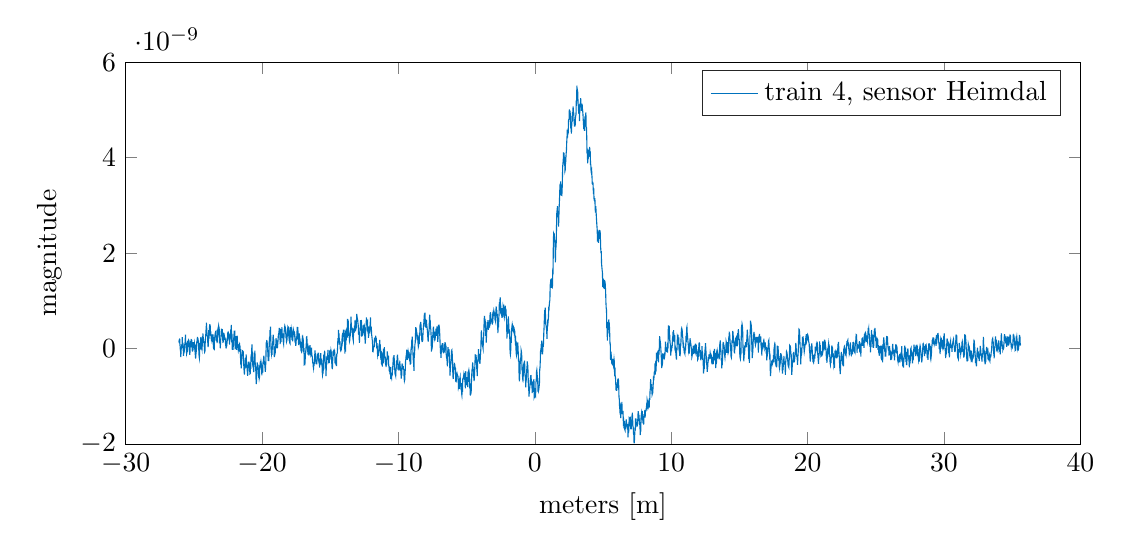
\begin{tikzpicture}

  \begin{axis}[%
    width=\textwidth,
    height=0.4\textwidth,
    at={(0\figurewidth,0\figureheight)},
    scale only axis,
    xmin=-30,
    xmax=40,
    xlabel={meters [m]},
    ymin=-2e-09,
    ymax=6e-09,
    ylabel={magnitude},
    axis background/.style={fill=white},
    legend style={legend cell align=left,align=left,draw=white!15!black}
    ]
    \addplot [color=mycolor1,solid]
    table[row sep=crcr]{%
    -26.1023046875	1.43675444572064e-10\\
    -26.081015625	1.63814626996003e-10\\
    -26.0597265625	1.09362288155367e-10\\
    -26.0384375	2.08023288526669e-10\\
    -26.0171484375	8.90587805035642e-11\\
    -25.995859375	-5.26039937324782e-12\\
    -25.9745703125	-5.02070778751598e-11\\
    -25.95328125	-1.76880199716764e-10\\
    -25.9319921875	-2.28262086218227e-11\\
    -25.910703125	8.38324634778354e-12\\
    -25.8894140625	8.7332187160911e-11\\
    -25.868125	1.29499209092194e-11\\
    -25.8468359375	2.4120169212826e-10\\
    -25.825546875	1.97663337181601e-11\\
    -25.8042578125	1.2344311534008e-10\\
    -25.78296875	6.42953054215928e-11\\
    -25.7616796875	-1.53731527562713e-10\\
    -25.740390625	-9.65127262946527e-11\\
    -25.7191015625	-8.68870590607824e-11\\
    -25.6978125	-4.19720695719933e-11\\
    -25.6765234375	8.40390881803925e-11\\
    -25.655234375	9.53150718367859e-11\\
    -25.6339453125	1.58685631088107e-10\\
    -25.61265625	2.93792425887305e-10\\
    -25.5913671875	9.85559661902777e-11\\
    -25.570078125	1.02042537884542e-10\\
    -25.5487890625	-3.4016068042128e-11\\
    -25.5275	-1.07491057245926e-10\\
    -25.5062109375	-7.92422251620226e-11\\
    -25.484921875	-6.57378311896026e-11\\
    -25.4636328125	9.83320569644978e-11\\
    -25.44234375	8.18438118123316e-11\\
    -25.4210546875	1.65194725194112e-10\\
    -25.399765625	1.76189171671752e-10\\
    -25.3784765625	1.00232617350529e-10\\
    -25.3571875	1.20489895521379e-10\\
    -25.3358984375	-2.82634181803713e-11\\
    -25.314609375	-6.50727084621922e-11\\
    -25.2933203125	-1.28878872742606e-10\\
    -25.27203125	-1.88588003038013e-11\\
    -25.2507421875	1.49407504200692e-10\\
    -25.229453125	1.50329501030523e-10\\
    -25.2081640625	2.89629597850955e-11\\
    -25.186875	1.86157821979289e-10\\
    -25.1655859375	1.81284963730849e-10\\
    -25.144296875	1.65802282220517e-10\\
    -25.1230078125	-1.65378945078419e-11\\
    -25.10171875	-6.30882120084254e-11\\
    -25.0804296875	1.3481368649057e-10\\
    -25.059140625	-3.68621028359532e-11\\
    -25.0378515625	5.09123993587789e-11\\
    -25.0165625	1.35283179432011e-10\\
    -24.9952734375	7.89911986229641e-11\\
    -24.973984375	5.77090773687007e-11\\
    -24.9526953125	9.93723812898789e-11\\
    -24.93140625	-2.26871867238074e-12\\
    -24.9101171875	1.72284776113456e-11\\
    -24.888828125	-1.58546493393666e-10\\
    -24.8675390625	-2.08172406234471e-10\\
    -24.84625	-1.20362250560741e-10\\
    -24.8249609375	-6.20269033502683e-11\\
    -24.803671875	7.89000261513512e-11\\
    -24.7823828125	1.38659456936858e-10\\
    -24.76109375	1.34370138164668e-10\\
    -24.7398046875	2.43551507723532e-10\\
    -24.718515625	2.00980702730922e-10\\
    -24.6972265625	2.05582622175092e-10\\
    -24.6759375	1.61526270322311e-10\\
    -24.6546484375	-9.13726971112414e-12\\
    -24.633359375	-3.88624493610977e-11\\
    -24.6120703125	-1.70107369345391e-10\\
    -24.59078125	-2.02516153731157e-10\\
    -24.5694921875	1.18076726673598e-10\\
    -24.548203125	-1.41667864464591e-11\\
    -24.5269140625	9.5915544427608e-11\\
    -24.505625	1.74340668749182e-10\\
    -24.4843359375	1.5523584117924e-10\\
    -24.463046875	2.44319208562935e-10\\
    -24.4417578125	1.87137766396833e-11\\
    -24.42046875	3.03143114958785e-11\\
    -24.3991796875	-8.90664816123474e-12\\
    -24.377890625	8.66340461608204e-11\\
    -24.3566015625	1.48154939173091e-10\\
    -24.3353125	3.18733168115531e-10\\
    -24.3140234375	1.8578267594695e-10\\
    -24.292734375	1.99046109298161e-10\\
    -24.2714453125	1.41216403824566e-10\\
    -24.25015625	1.18861996127058e-10\\
    -24.2288671875	1.91103664669054e-11\\
    -24.207578125	-7.43559228846805e-11\\
    -24.1862890625	-6.23104301423815e-11\\
    -24.165	1.31316234605568e-10\\
    -24.1437109375	1.95666652399436e-10\\
    -24.122421875	3.0133045090589e-10\\
    -24.1011328125	2.61343088672344e-10\\
    -24.07984375	5.45559410102862e-10\\
    -24.0585546875	4.44382136981754e-10\\
    -24.037265625	3.28114518804023e-10\\
    -24.0159765625	2.66078331798789e-10\\
    -23.9946875	2.53872025983851e-10\\
    -23.9733984375	1.09500187374758e-10\\
    -23.952109375	3.00077789277421e-11\\
    -23.9308203125	1.26239487655767e-10\\
    -23.90953125	3.89382762471793e-10\\
    -23.8882421875	2.11226917956289e-10\\
    -23.866953125	3.7862343690693e-10\\
    -23.8456640625	4.75244030711145e-10\\
    -23.824375	4.64076151856489e-10\\
    -23.8030859375	5.07641762654124e-10\\
    -23.781796875	2.72497636341108e-10\\
    -23.7605078125	3.58976500673046e-10\\
    -23.73921875	2.66623651844437e-10\\
    -23.7179296875	2.03632225139669e-10\\
    -23.696640625	2.49066390726187e-10\\
    -23.6753515625	2.65819173188531e-10\\
    -23.6540625	2.18698319368798e-10\\
    -23.6327734375	2.65003310090435e-10\\
    -23.611484375	2.86825920983271e-10\\
    -23.5901953125	2.85846865254167e-10\\
    -23.56890625	4.48337969702862e-11\\
    -23.5476171875	4.9893112686103e-12\\
    -23.526328125	-8.56383246695894e-12\\
    -23.5050390625	-1.47037957137622e-11\\
    -23.48375	2.35215503559176e-10\\
    -23.4624609375	2.43170560088138e-10\\
    -23.441171875	3.00665561517066e-10\\
    -23.4198828125	2.89839400196667e-10\\
    -23.39859375	3.57951731409375e-10\\
    -23.3773046875	3.65323965401124e-10\\
    -23.356015625	1.55367152089243e-10\\
    -23.3347265625	2.01785797720527e-10\\
    -23.3134375	2.00175443230845e-10\\
    -23.2921484375	1.16499143672085e-10\\
    -23.270859375	2.08605444331632e-10\\
    -23.2495703125	3.49051285616876e-10\\
    -23.22828125	3.26288080275179e-10\\
    -23.2069921875	4.45495060888173e-10\\
    -23.185703125	4.78217638695118e-10\\
    -23.1644140625	4.11578006517766e-10\\
    -23.143125	4.60059638319971e-10\\
    -23.1218359375	1.08875742704621e-10\\
    -23.100546875	1.55179377841247e-10\\
    -23.0792578125	1.63900764376687e-10\\
    -23.05796875	5.84981312618069e-12\\
    -23.0366796875	1.75077770083883e-10\\
    -23.015390625	2.26914352424769e-10\\
    -22.9941015625	3.31907913007748e-10\\
    -22.9728125	4.1837108477027e-10\\
    -22.9515234375	3.47784694497571e-10\\
    -22.930234375	3.93335362276161e-10\\
    -22.9089453125	3.9467252026328e-10\\
    -22.88765625	2.09255718741169e-10\\
    -22.8663671875	1.36411169472562e-10\\
    -22.845078125	1.40016209490535e-10\\
    -22.8237890625	3.3559304158723e-10\\
    -22.8025	1.7786909703593e-10\\
    -22.7812109375	3.19952120443287e-10\\
    -22.759921875	2.321363050797e-10\\
    -22.7386328125	2.39687495508752e-10\\
    -22.71734375	2.1981690865527e-10\\
    -22.6960546875	2.01265083580572e-10\\
    -22.674765625	1.04594692562127e-10\\
    -22.6534765625	5.29511449631855e-11\\
    -22.6321875	2.77244189823356e-12\\
    -22.6108984375	8.64215163999009e-11\\
    -22.589609375	1.42245355236507e-10\\
    -22.5683203125	1.15109348537646e-10\\
    -22.54703125	1.74666876450426e-10\\
    -22.5257421875	2.49493060415888e-10\\
    -22.504453125	3.52739497004264e-10\\
    -22.4831640625	2.63711135291683e-10\\
    -22.461875	2.96306084606291e-10\\
    -22.4405859375	2.33700551182453e-10\\
    -22.419296875	2.36667662278896e-10\\
    -22.3980078125	1.58766991301971e-10\\
    -22.37671875	8.63128077454187e-11\\
    -22.3554296875	3.17116801406567e-10\\
    -22.334140625	2.07064281910378e-10\\
    -22.3128515625	2.43462718063266e-10\\
    -22.2915625	3.89473407765777e-10\\
    -22.2702734375	4.08615231546607e-10\\
    -22.248984375	4.95788023569525e-10\\
    -22.2276953125	1.32875511971843e-10\\
    -22.20640625	3.13422970183486e-10\\
    -22.1851171875	-2.30257174055982e-11\\
    -22.163828125	9.98949440711568e-12\\
    -22.1425390625	4.57540542841976e-11\\
    -22.12125	-2.81954505588357e-11\\
    -22.0999609375	1.64997627940945e-10\\
    -22.078671875	1.90341061609103e-10\\
    -22.0573828125	2.78989634183619e-10\\
    -22.03609375	3.7761228470195e-10\\
    -22.0148046875	2.54182064225087e-10\\
    -21.993515625	2.82639036377986e-10\\
    -21.9722265625	-1.60078106903036e-11\\
    -21.9509375	2.092178008186e-10\\
    -21.9296484375	1.61303114011241e-10\\
    -21.908359375	4.14315081049106e-11\\
    -21.8870703125	2.59381254592456e-10\\
    -21.86578125	-2.58784206096073e-11\\
    -21.8444921875	1.83034589769198e-10\\
    -21.823203125	2.72810621166173e-10\\
    -21.8019140625	1.50486512958949e-10\\
    -21.780625	8.18537019292486e-11\\
    -21.7593359375	1.86460756597228e-11\\
    -21.738046875	-3.7656917200918e-11\\
    -21.7167578125	-5.57692285766078e-12\\
    -21.69546875	2.65915091501696e-11\\
    -21.6741796875	8.13791604876208e-11\\
    -21.652890625	9.58941907882166e-11\\
    -21.6316015625	-6.11589619273499e-11\\
    -21.6103125	6.30974356434756e-11\\
    -21.5890234375	-1.04976667858771e-10\\
    -21.567734375	-2.45857650344537e-10\\
    -21.5464453125	-2.15226248461924e-10\\
    -21.52515625	-4.14645179302074e-10\\
    -21.5038671875	-3.03736602006015e-10\\
    -21.482578125	-1.58774497580258e-10\\
    -21.4612890625	-6.42259296952853e-11\\
    -21.44	-7.92036411158261e-11\\
    -21.4187109375	-1.56434198368838e-10\\
    -21.397421875	-5.8533005796004e-11\\
    -21.3761328125	-6.73494718927778e-11\\
    -21.35484375	-2.60792434135348e-10\\
    -21.3335546875	-3.77345717883266e-10\\
    -21.312265625	-4.79376548838101e-10\\
    -21.2909765625	-5.45235088061197e-10\\
    -21.2696875	-4.19933101294035e-10\\
    -21.2483984375	-3.91709273587004e-10\\
    -21.227109375	-2.36326593894629e-10\\
    -21.2058203125	-1.88778901113578e-10\\
    -21.18453125	-3.05036357936459e-10\\
    -21.1632421875	-1.19263370044425e-10\\
    -21.141953125	-3.65457685168313e-10\\
    -21.1206640625	-3.53400308963678e-10\\
    -21.099375	-3.87308554708758e-10\\
    -21.0780859375	-4.84427307549472e-10\\
    -21.056796875	-5.70580495073659e-10\\
    -21.0355078125	-5.08557056779124e-10\\
    -21.01421875	-2.71511765032738e-10\\
    -20.9929296875	-3.208581166892e-10\\
    -20.971640625	-3.68690855405529e-10\\
    -20.9503515625	-2.7532384628298e-10\\
    -20.9290625	-3.4850522744686e-10\\
    -20.9077734375	-4.37486446188553e-10\\
    -20.886484375	-5.27340001801671e-10\\
    -20.8651953125	-5.20749338578454e-10\\
    -20.84390625	-3.91058189888872e-10\\
    -20.8226171875	-4.25512250128493e-10\\
    -20.801328125	-1.20814360914635e-10\\
    -20.7800390625	-2.74720035986184e-10\\
    -20.75875	-3.982313310087e-11\\
    -20.7374609375	8.74606979947534e-11\\
    -20.716171875	-1.03409314613053e-10\\
    -20.6948828125	-2.10275324350356e-10\\
    -20.67359375	-3.71400001355678e-10\\
    -20.6523046875	-3.8294246358371e-10\\
    -20.631015625	-4.16784137428747e-10\\
    -20.6097265625	-4.89650596048524e-10\\
    -20.5884375	-2.96086022791999e-10\\
    -20.5671484375	-8.33532991546213e-11\\
    -20.545859375	-2.62513403866082e-10\\
    -20.5245703125	-4.21138206264673e-11\\
    -20.50328125	-2.85314981030773e-10\\
    -20.4819921875	-3.66084418508077e-10\\
    -20.460703125	-4.19273175520521e-10\\
    -20.4394140625	-6.39297466476485e-10\\
    -20.418125	-7.44361176940524e-10\\
    -20.3968359375	-6.13807335513928e-10\\
    -20.375546875	-4.73778290677011e-10\\
    -20.3542578125	-2.91323283552095e-10\\
    -20.33296875	-3.56235153189375e-10\\
    -20.3116796875	-3.42758617311715e-10\\
    -20.290390625	-3.4875248741213e-10\\
    -20.2691015625	-4.58911778654141e-10\\
    -20.2478125	-5.7046052571194e-10\\
    -20.2265234375	-5.59751304810831e-10\\
    -20.205234375	-6.28910767795237e-10\\
    -20.1839453125	-5.9851380165251e-10\\
    -20.16265625	-3.51551770169695e-10\\
    -20.1413671875	-3.50848686773167e-10\\
    -20.120078125	-2.5887712579255e-10\\
    -20.0987890625	-3.19340305839665e-10\\
    -20.0775	-2.73711400471446e-10\\
    -20.0562109375	-3.19676245493625e-10\\
    -20.034921875	-3.54304061391458e-10\\
    -20.0136328125	-5.57908270094709e-10\\
    -19.99234375	-4.53100542115506e-10\\
    -19.9710546875	-4.935604632209e-10\\
    -19.949765625	-4.91948028235353e-10\\
    -19.9284765625	-2.90907665896702e-10\\
    -19.9071875	-2.71723568106279e-10\\
    -19.8858984375	-2.06606007623019e-10\\
    -19.864609375	-1.47249723158232e-10\\
    -19.8433203125	-2.52146471997952e-10\\
    -19.82203125	-3.16148182015456e-10\\
    -19.8007421875	-3.33266185941511e-10\\
    -19.779453125	-4.04509574939651e-10\\
    -19.7581640625	-4.84956106383494e-10\\
    -19.736875	-3.8334638008743e-10\\
    -19.7155859375	-2.13045120945112e-10\\
    -19.694296875	1.31001254586518e-10\\
    -19.6730078125	9.31042799325725e-11\\
    -19.65171875	1.64216566690036e-10\\
    -19.6304296875	1.60183775327759e-10\\
    -19.609140625	7.05591459912531e-11\\
    -19.5878515625	-6.80660526756344e-12\\
    -19.5665625	-1.28840415669423e-10\\
    -19.5452734375	-2.58185150259027e-10\\
    -19.523984375	-2.05327111525552e-10\\
    -19.5026953125	-2.62453690648572e-10\\
    -19.48140625	-6.18825518705824e-11\\
    -19.4601171875	2.32292822636748e-10\\
    -19.438828125	1.54739134462004e-10\\
    -19.4175390625	3.86247316014494e-10\\
    -19.39625	3.21911777950493e-10\\
    -19.3749609375	4.58870087538329e-10\\
    -19.353671875	1.05519505159359e-10\\
    -19.3323828125	-5.86642253895737e-11\\
    -19.31109375	-1.09224791490435e-10\\
    -19.2898046875	-4.49571354017248e-11\\
    -19.268515625	-1.32543323331628e-10\\
    -19.2472265625	3.96445590471531e-11\\
    -19.2259375	1.17848624448543e-10\\
    -19.2046484375	1.64575319884642e-10\\
    -19.183359375	2.94670212866832e-10\\
    -19.1620703125	1.98812442769082e-10\\
    -19.14078125	1.89367157432755e-10\\
    -19.1194921875	-8.89577030928783e-12\\
    -19.098203125	-1.7746830440805e-10\\
    -19.0769140625	-7.55066867186453e-11\\
    -19.055625	-1.16950880091043e-10\\
    -19.0343359375	-9.02532433576541e-11\\
    -19.013046875	2.66709434501482e-11\\
    -18.9917578125	8.0555374215227e-11\\
    -18.97046875	2.18053963862205e-10\\
    -18.9491796875	1.22479692461133e-10\\
    -18.927890625	1.8627945984767e-10\\
    -18.9066015625	1.68686454025694e-11\\
    -18.8853125	1.68305335246898e-11\\
    -18.8640234375	2.6951840293839e-11\\
    -18.842734375	1.21383916843327e-10\\
    -18.8214453125	1.80554236774381e-10\\
    -18.80015625	2.96266720123447e-10\\
    -18.7788671875	3.07061592115688e-10\\
    -18.757578125	3.47100888323001e-10\\
    -18.7362890625	4.33910149175239e-10\\
    -18.715	3.11720139972722e-10\\
    -18.6937109375	4.23678532758382e-10\\
    -18.672421875	9.31799678490548e-11\\
    -18.6511328125	1.97313343635383e-10\\
    -18.62984375	2.24038368601617e-10\\
    -18.6085546875	1.34315914609988e-10\\
    -18.587265625	4.06284194681842e-10\\
    -18.5659765625	2.3823473140416e-10\\
    -18.5446875	4.4973053647548e-10\\
    -18.5233984375	3.28462664329016e-10\\
    -18.502109375	2.23897722283299e-10\\
    -18.4808203125	3.20390392393003e-10\\
    -18.45953125	2.15714563331824e-10\\
    -18.4382421875	1.34410989484615e-10\\
    -18.416953125	9.75794780255125e-11\\
    -18.3956640625	2.14443040335453e-10\\
    -18.374375	3.58980507075079e-10\\
    -18.3530859375	4.14591102162564e-10\\
    -18.331796875	3.64470111539563e-10\\
    -18.3105078125	4.57693545710467e-10\\
    -18.28921875	4.3584051376551e-10\\
    -18.2679296875	3.76363933921224e-10\\
    -18.246640625	2.37038372398452e-10\\
    -18.2253515625	2.40424775109282e-10\\
    -18.2040625	1.42742944570698e-10\\
    -18.1827734375	1.62813039231838e-10\\
    -18.161484375	1.98753559005014e-10\\
    -18.1401953125	3.66971009745026e-10\\
    -18.11890625	4.19270168181471e-10\\
    -18.0976171875	3.75693377750103e-10\\
    -18.076328125	4.66411754360026e-10\\
    -18.0550390625	3.96895003741218e-10\\
    -18.03375	3.67299237347946e-10\\
    -18.0124609375	1.57123949527335e-10\\
    -17.991171875	2.27444608336942e-10\\
    -17.9698828125	1.21538696781312e-10\\
    -17.94859375	1.09478734375811e-10\\
    -17.9273046875	4.47733144607789e-10\\
    -17.906015625	2.36561613785367e-10\\
    -17.8847265625	3.58629857931003e-10\\
    -17.8634375	4.14415384392651e-10\\
    -17.8421484375	3.59773518716355e-10\\
    -17.820859375	3.81487583079032e-10\\
    -17.7995703125	1.82408838710608e-10\\
    -17.77828125	2.1996849740946e-10\\
    -17.7569921875	1.54142802362855e-10\\
    -17.735703125	2.24785536256834e-10\\
    -17.7144140625	3.50712403078818e-10\\
    -17.693125	3.80292256019467e-10\\
    -17.6718359375	2.83548521219043e-10\\
    -17.650546875	3.3558748482582e-10\\
    -17.6292578125	3.44752524375511e-10\\
    -17.60796875	3.30650326710884e-10\\
    -17.5866796875	1.61030070321222e-10\\
    -17.565390625	1.27614069447269e-10\\
    -17.5441015625	1.13540438945207e-10\\
    -17.5228125	5.84474329679592e-11\\
    -17.5015234375	1.30694534429409e-10\\
    -17.480234375	2.55330916912634e-10\\
    -17.4589453125	1.93342343192641e-10\\
    -17.43765625	3.39223490167281e-10\\
    -17.4163671875	4.52625469960104e-10\\
    -17.395078125	3.23651407530707e-10\\
    -17.3737890625	4.5084522734351e-10\\
    -17.3525	2.42102537960588e-10\\
    -17.3312109375	1.39342014290299e-10\\
    -17.309921875	7.30013014394989e-11\\
    -17.2886328125	2.75139903487344e-10\\
    -17.26734375	3.1809452067036e-10\\
    -17.2460546875	1.63641139149905e-10\\
    -17.224765625	2.01894132814681e-10\\
    -17.2034765625	1.6338429858154e-10\\
    -17.1821875	1.97456894085607e-11\\
    -17.1608984375	1.38246563330775e-10\\
    -17.139609375	-3.72214537975641e-11\\
    -17.1183203125	-5.46877826981422e-11\\
    -17.09703125	3.32122585062211e-11\\
    -17.0757421875	-7.86169788160334e-11\\
    -17.054453125	1.79316654797215e-10\\
    -17.0331640625	2.77947198228011e-10\\
    -17.011875	1.2146869596092e-10\\
    -16.9905859375	2.02437373433947e-10\\
    -16.969296875	1.64325830174536e-10\\
    -16.9480078125	-6.56850526858775e-11\\
    -16.92671875	1.22298545057978e-11\\
    -16.9054296875	-3.02301148248163e-10\\
    -16.884140625	-2.86708262974397e-10\\
    -16.8628515625	-3.51183161264591e-10\\
    -16.8415625	-2.67635783368414e-10\\
    -16.8202734375	-1.07864077119437e-10\\
    -16.798984375	-8.55721096589347e-11\\
    -16.7776953125	1.75930907246474e-11\\
    -16.75640625	9.23927125419735e-11\\
    -16.7351171875	2.44402196460732e-10\\
    -16.713828125	2.48186526986255e-10\\
    -16.6925390625	1.07667693993942e-10\\
    -16.67125	7.85665481282548e-12\\
    -16.6499609375	3.2344754159301e-11\\
    -16.628671875	-1.26019582512089e-10\\
    -16.6073828125	-5.03491886327036e-11\\
    -16.58609375	-1.74267220548626e-11\\
    -16.5648046875	-1.47045524524573e-10\\
    -16.543515625	-8.21307952309085e-12\\
    -16.5222265625	-5.8635243361198e-11\\
    -16.5009375	-1.02042885675825e-10\\
    -16.4796484375	7.06313290405505e-11\\
    -16.458359375	-1.31584610247276e-10\\
    -16.4370703125	-5.88013170913053e-11\\
    -16.41578125	-1.32823899507076e-10\\
    -16.3944921875	-1.11766696346889e-10\\
    -16.373203125	1.91205503831269e-11\\
    -16.3519140625	-1.27566446641739e-10\\
    -16.330625	-1.59350865978072e-10\\
    -16.3093359375	-1.73606280968281e-10\\
    -16.288046875	-2.87925286316985e-10\\
    -16.2667578125	-2.90344177448708e-10\\
    -16.24546875	-3.71345116594164e-10\\
    -16.2241796875	-4.08546052129277e-10\\
    -16.202890625	-3.21924971158725e-10\\
    -16.1816015625	-3.31974828321129e-10\\
    -16.1603125	-2.92539019498246e-10\\
    -16.1390234375	-1.65618890509756e-10\\
    -16.117734375	-3.66582047403761e-11\\
    -16.0964453125	-2.3217067645329e-10\\
    -16.07515625	-1.95188796550943e-10\\
    -16.0538671875	-2.80405931756805e-10\\
    -16.032578125	-2.66328977483313e-10\\
    -16.0112890625	-2.69069907000831e-10\\
    -15.99	-3.29337226425785e-10\\
    -15.9687109375	-2.48077754969608e-10\\
    -15.947421875	-1.29844008680487e-10\\
    -15.9261328125	-1.37041814611386e-10\\
    -15.90484375	-2.03026135720724e-10\\
    -15.8835546875	-8.29476971839905e-11\\
    -15.862265625	-1.90566313917451e-10\\
    -15.8409765625	-1.65379589502361e-10\\
    -15.8196875	-3.07098665217632e-10\\
    -15.7983984375	-2.63927035635812e-10\\
    -15.777109375	-4.0017101674892e-10\\
    -15.7558203125	-2.23458969293803e-10\\
    -15.73453125	-2.26521012629278e-10\\
    -15.7132421875	-3.27217051873589e-10\\
    -15.691953125	-9.54551231500559e-11\\
    -15.6706640625	-3.35674081486734e-10\\
    -15.649375	-2.4736581742031e-10\\
    -15.6280859375	-2.37560721536432e-10\\
    -15.606796875	-3.08361948316584e-10\\
    -15.5855078125	-4.88201358506618e-10\\
    -15.56421875	-5.51663899307981e-10\\
    -15.5429296875	-5.08764752698863e-10\\
    -15.521640625	-5.08859823145387e-10\\
    -15.5003515625	-3.46020403401443e-10\\
    -15.4790625	-1.25568190361794e-10\\
    -15.4577734375	-1.86980411244126e-10\\
    -15.436484375	-2.55157116881684e-10\\
    -15.4151953125	-6.49973258990369e-11\\
    -15.39390625	-7.23013748010262e-11\\
    -15.3726171875	-3.49446395849009e-10\\
    -15.351328125	-3.23184251921128e-10\\
    -15.3300390625	-3.36959262180305e-10\\
    -15.30875	-5.74995853913946e-10\\
    -15.2874609375	-3.87645719533598e-10\\
    -15.266171875	-2.62097632246607e-10\\
    -15.2448828125	-1.51196038374788e-10\\
    -15.22359375	-2.36347920671673e-10\\
    -15.2023046875	-1.75145292954994e-10\\
    -15.181015625	-1.12955531323748e-10\\
    -15.1597265625	-2.63695911994107e-11\\
    -15.1384375	-2.5707370711867e-10\\
    -15.1171484375	-2.33311031723752e-10\\
    -15.095859375	-2.03448275836343e-10\\
    -15.0745703125	-3.02815250442529e-10\\
    -15.05328125	-2.29913430401559e-10\\
    -15.0319921875	-5.09850339159499e-11\\
    -15.010703125	-4.13036861339046e-11\\
    -14.9894140625	-4.64280709980011e-11\\
    -14.968125	-1.01399641118173e-10\\
    -14.9468359375	-3.47658411018526e-11\\
    -14.925546875	-6.66000679918503e-11\\
    -14.9042578125	-2.26956054114508e-10\\
    -14.88296875	-3.20390744536136e-10\\
    -14.8616796875	-4.14550367872196e-10\\
    -14.840390625	-4.17166861303373e-10\\
    -14.8191015625	-2.53473497206323e-10\\
    -14.7978125	-5.61228879522158e-11\\
    -14.7765234375	-1.55152108198778e-10\\
    -14.755234375	-4.81461729408549e-11\\
    -14.7339453125	-3.59724799434521e-11\\
    -14.71265625	-1.18293747346237e-10\\
    -14.6913671875	-2.27855618529293e-11\\
    -14.670078125	-7.40729207129903e-11\\
    -14.6487890625	-3.0638114130077e-10\\
    -14.6275	-1.95668480026591e-10\\
    -14.6062109375	-2.32842409902874e-10\\
    -14.584921875	-3.46096002935401e-10\\
    -14.5636328125	-1.83016031948145e-10\\
    -14.54234375	-3.67686025551745e-10\\
    -14.5210546875	-1.18141172214762e-10\\
    -14.499765625	-1.09476847584946e-10\\
    -14.4784765625	-8.97245060598718e-11\\
    -14.4571875	4.42373350670665e-11\\
    -14.4358984375	2.18034061244975e-10\\
    -14.414609375	1.23468918801547e-10\\
    -14.3933203125	3.93274044409619e-10\\
    -14.37203125	2.58879796211778e-10\\
    -14.3507421875	3.20552066736936e-10\\
    -14.329453125	8.32507783251913e-11\\
    -14.3081640625	1.43769951848371e-10\\
    -14.286875	1.44828020884103e-10\\
    -14.2655859375	-1.40618730812579e-12\\
    -14.244296875	-2.43212842293201e-11\\
    -14.2230078125	-4.68639201087887e-11\\
    -14.20171875	-3.34092635339288e-11\\
    -14.1804296875	4.23449787264619e-13\\
    -14.159140625	6.67370105220276e-11\\
    -14.1378515625	1.8017736407063e-10\\
    -14.1165625	1.48007930836686e-10\\
    -14.0952734375	3.15481570439745e-10\\
    -14.073984375	3.16495038722855e-10\\
    -14.0526953125	2.96203949686388e-10\\
    -14.03140625	3.95811321895884e-10\\
    -14.0101171875	3.1631128083173e-10\\
    -13.988828125	1.4696893409538e-10\\
    -13.9675390625	2.19723892395071e-10\\
    -13.94625	2.14852732353418e-10\\
    -13.9249609375	-1.07163721349142e-10\\
    -13.903671875	3.99768843273965e-10\\
    -13.8823828125	-6.05132349028305e-11\\
    -13.86109375	1.16117596741202e-10\\
    -13.8398046875	2.73699545160253e-10\\
    -13.818515625	1.70588423941486e-10\\
    -13.7972265625	3.80739630607111e-10\\
    -13.7759375	4.36579475478875e-10\\
    -13.7546484375	2.28202988007258e-10\\
    -13.733359375	6.22150295100441e-10\\
    -13.7120703125	5.53321891397465e-10\\
    -13.69078125	4.60075451322049e-10\\
    -13.6694921875	4.94375108274976e-10\\
    -13.648203125	2.67986031079599e-10\\
    -13.6269140625	3.1563778674649e-10\\
    -13.605625	2.42862878719338e-10\\
    -13.5843359375	1.54910169175221e-10\\
    -13.563046875	1.7851531569271e-10\\
    -13.5417578125	3.14158733402623e-10\\
    -13.52046875	2.68022879051321e-10\\
    -13.4991796875	4.25338434119293e-10\\
    -13.477890625	6.70922657305782e-10\\
    -13.4566015625	4.94971403728879e-10\\
    -13.4353125	3.85893360395911e-10\\
    -13.4140234375	4.56683294309369e-10\\
    -13.392734375	3.73018859829285e-10\\
    -13.3714453125	3.83546301181551e-10\\
    -13.35015625	2.56452703387087e-10\\
    -13.3288671875	1.98724394598946e-10\\
    -13.307578125	1.66487850226958e-10\\
    -13.2862890625	3.82785548301094e-10\\
    -13.265	3.70817228431206e-10\\
    -13.2437109375	3.30311362065416e-10\\
    -13.222421875	4.56668940758271e-10\\
    -13.2011328125	4.51135287239043e-10\\
    -13.17984375	5.92726599432439e-10\\
    -13.1585546875	5.23876532420272e-10\\
    -13.137265625	3.61937706057301e-10\\
    -13.1159765625	4.84777809506435e-10\\
    -13.0946875	4.24172044071305e-10\\
    -13.0733984375	5.93365273274914e-10\\
    -13.052109375	7.24992167655628e-10\\
    -13.0308203125	6.56131028847015e-10\\
    -13.00953125	6.29070036106952e-10\\
    -12.9882421875	6.04984599356247e-10\\
    -12.966953125	5.37489200692476e-10\\
    -12.9456640625	4.86013581546896e-10\\
    -12.924375	3.02078509145454e-10\\
    -12.9030859375	2.97088669196311e-10\\
    -12.881796875	2.8972254668285e-10\\
    -12.8605078125	1.20496691152111e-10\\
    -12.83921875	2.65178971626413e-10\\
    -12.8179296875	4.38458326656443e-10\\
    -12.796640625	3.78160763690495e-10\\
    -12.7753515625	5.94378262135953e-10\\
    -12.7540625	4.77383257806948e-10\\
    -12.7327734375	5.67624123371654e-10\\
    -12.711484375	5.74763047886839e-10\\
    -12.6901953125	2.51021251986754e-10\\
    -12.66890625	4.18337031960397e-10\\
    -12.6476171875	2.81371789910022e-10\\
    -12.626328125	2.890819910765e-10\\
    -12.6050390625	2.91852079752661e-10\\
    -12.58375	4.88082962375203e-10\\
    -12.5624609375	3.86967253422526e-10\\
    -12.541171875	4.44750551757001e-10\\
    -12.5198828125	4.18497120883957e-10\\
    -12.49859375	4.45942620458478e-10\\
    -12.4773046875	2.69256706450585e-10\\
    -12.456015625	2.63174117341717e-10\\
    -12.4347265625	1.04313056113837e-10\\
    -12.4134375	1.93030561192784e-10\\
    -12.3921484375	4.42354663096078e-10\\
    -12.370859375	3.81993956516822e-10\\
    -12.3495703125	6.52931786277457e-10\\
    -12.32828125	5.43161968693361e-10\\
    -12.3069921875	5.74817565172027e-10\\
    -12.285703125	5.45909598156518e-10\\
    -12.2644140625	5.62391811372983e-10\\
    -12.243125	3.43141024472502e-10\\
    -12.2218359375	4.66810056658322e-10\\
    -12.200546875	2.26295051006197e-10\\
    -12.1792578125	2.64936090912767e-10\\
    -12.15796875	3.39340995161282e-10\\
    -12.1366796875	4.60978623335748e-10\\
    -12.115390625	3.19284361713683e-10\\
    -12.0941015625	4.56320835590275e-10\\
    -12.0728125	4.49852035771707e-10\\
    -12.0515234375	6.54105625614502e-10\\
    -12.030234375	4.48476247103219e-10\\
    -12.0089453125	3.9917235331306e-10\\
    -11.98765625	4.55486790645165e-10\\
    -11.9663671875	2.9851585345043e-10\\
    -11.945078125	2.5675486193893e-10\\
    -11.9237890625	1.88430330215066e-10\\
    -11.9025	1.66473658509959e-10\\
    -11.8812109375	-7.55410006142362e-11\\
    -11.859921875	1.83040831559855e-11\\
    -11.8386328125	-1.27485377159791e-11\\
    -11.81734375	3.47901023929384e-11\\
    -11.7960546875	4.67679253754522e-11\\
    -11.774765625	4.41650145344453e-11\\
    -11.7534765625	1.89076340949663e-10\\
    -11.7321875	1.80685425361228e-10\\
    -11.7108984375	2.36404187711389e-10\\
    -11.689609375	1.56525389782201e-10\\
    -11.6683203125	2.69438518282702e-10\\
    -11.64703125	1.28491518781571e-10\\
    -11.6257421875	2.22880513649194e-10\\
    -11.604453125	5.78944944277972e-11\\
    -11.5831640625	8.24624560042356e-12\\
    -11.561875	1.14183429812696e-10\\
    -11.5405859375	-8.26422848573755e-11\\
    -11.519296875	-1.44602333180688e-10\\
    -11.4980078125	-1.0519811637623e-10\\
    -11.47671875	-1.95318485070328e-11\\
    -11.4554296875	-1.53043435168741e-10\\
    -11.434140625	-1.45864029275491e-11\\
    -11.4128515625	1.02390888953891e-10\\
    -11.3915625	1.09619870087888e-11\\
    -11.3702734375	1.8150179166942e-10\\
    -11.348984375	-4.54653299902557e-11\\
    -11.3276953125	8.98091423970098e-11\\
    -11.30640625	-1.02760285142576e-10\\
    -11.2851171875	-2.37094243192301e-10\\
    -11.263828125	-4.52819073388131e-11\\
    -11.2425390625	-3.14282946977032e-10\\
    -11.22125	-3.28112443039936e-10\\
    -11.1999609375	-2.16929840160318e-10\\
    -11.178671875	-3.79169044744232e-10\\
    -11.1573828125	-1.64785620270341e-10\\
    -11.13609375	-1.91067028186182e-10\\
    -11.1148046875	-3.11039747260682e-10\\
    -11.093515625	2.72850673386002e-13\\
    -11.0722265625	-1.31696646536313e-10\\
    -11.0509375	-1.02999131280611e-10\\
    -11.0296484375	2.9100056455063e-11\\
    -11.008359375	-1.86895353642033e-10\\
    -10.9870703125	-2.14336251860334e-10\\
    -10.96578125	-2.663481414491e-10\\
    -10.9444921875	-2.32928484504456e-10\\
    -10.923203125	-2.90130602838715e-10\\
    -10.9019140625	-3.87701562863325e-10\\
    -10.880625	-2.68254932752228e-10\\
    -10.8593359375	-3.35968719280729e-10\\
    -10.838046875	-2.24629676125097e-10\\
    -10.8167578125	-5.88384095512461e-11\\
    -10.79546875	-1.32206196224112e-10\\
    -10.7741796875	-1.77632814019385e-10\\
    -10.752890625	-1.93860930003792e-10\\
    -10.7316015625	-1.46612693258714e-10\\
    -10.7103125	-3.5509534069754e-10\\
    -10.6890234375	-3.829701263258e-10\\
    -10.667734375	-4.75542697201065e-10\\
    -10.6464453125	-3.71717964492324e-10\\
    -10.62515625	-5.40879448222994e-10\\
    -10.6038671875	-5.01631371052658e-10\\
    -10.582578125	-3.90291149314899e-10\\
    -10.5612890625	-6.39200373143021e-10\\
    -10.54	-5.65302551447076e-10\\
    -10.5187109375	-5.73785273603721e-10\\
    -10.497421875	-6.04587179069512e-10\\
    -10.4761328125	-5.05283680415123e-10\\
    -10.45484375	-5.59917714206072e-10\\
    -10.4335546875	-4.01649161228831e-10\\
    -10.412265625	-4.10034884459602e-10\\
    -10.3909765625	-2.71217425362036e-10\\
    -10.3696875	-1.66430808696545e-10\\
    -10.3483984375	-2.37386607513966e-10\\
    -10.327109375	-1.3679936354299e-10\\
    -10.3058203125	-2.20367385006869e-10\\
    -10.28453125	-3.77645543730301e-10\\
    -10.2632421875	-4.55380941743075e-10\\
    -10.241953125	-5.45637659442886e-10\\
    -10.2206640625	-5.49408759921505e-10\\
    -10.199375	-5.73872214853693e-10\\
    -10.1780859375	-4.52360085096767e-10\\
    -10.156796875	-4.06009630917384e-10\\
    -10.1355078125	-2.51742832267005e-10\\
    -10.11421875	-3.40278901000002e-10\\
    -10.0929296875	-1.89105272089984e-10\\
    -10.071640625	-1.25952595128381e-10\\
    -10.0503515625	-2.01589396167235e-10\\
    -10.0290625	-4.25947505404226e-10\\
    -10.0077734375	-4.23548938958044e-10\\
    -9.986484375	-3.69917225477771e-10\\
    -9.9651953125	-4.5807198202578e-10\\
    -9.94390625	-3.35032925142805e-10\\
    -9.9226171875	-3.09695010251733e-10\\
    -9.901328125	-3.73347134490488e-10\\
    -9.8800390625	-3.40724496732553e-10\\
    -9.85875	-4.01940747822219e-10\\
    -9.8374609375	-4.19412885816884e-10\\
    -9.816171875	-4.97032024574022e-10\\
    -9.7948828125	-6.25669164133997e-10\\
    -9.77359375	-5.13178002929905e-10\\
    -9.7523046875	-5.65249591439996e-10\\
    -9.731015625	-3.08070211755659e-10\\
    -9.7097265625	-3.71414887593732e-10\\
    -9.6884375	-3.62200745643999e-10\\
    -9.6671484375	-4.27773088321951e-10\\
    -9.645859375	-3.69456272485026e-10\\
    -9.6245703125	-4.34780512068921e-10\\
    -9.60328125	-4.42605735362035e-10\\
    -9.5819921875	-6.18632567525644e-10\\
    -9.560703125	-6.78818328077522e-10\\
    -9.5394140625	-6.53844816816824e-10\\
    -9.518125	-5.31973431576408e-10\\
    -9.4968359375	-4.41676250746952e-10\\
    -9.475546875	-2.5344228839363e-10\\
    -9.4542578125	-2.1826847396531e-10\\
    -9.43296875	-1.4515352398195e-10\\
    -9.4116796875	-1.32674211317965e-10\\
    -9.390390625	-2.18277000443748e-11\\
    -9.3691015625	-1.28226813779082e-10\\
    -9.3478125	-2.32860759141657e-10\\
    -9.3265234375	-1.23206248476977e-10\\
    -9.305234375	-1.18182329730057e-10\\
    -9.2839453125	-5.65159242252668e-11\\
    -9.26265625	-8.82518432586472e-11\\
    -9.2413671875	-2.06215939139702e-10\\
    -9.220078125	-6.94832025244892e-11\\
    -9.1987890625	-1.665936847535e-10\\
    -9.1775	-2.68974745104876e-10\\
    -9.1562109375	-1.04358711373843e-10\\
    -9.134921875	-3.34000151312464e-10\\
    -9.1136328125	-2.75598673383722e-10\\
    -9.09234375	-2.84403992025034e-10\\
    -9.0710546875	2.36308550659639e-11\\
    -9.049765625	-2.55353714212588e-11\\
    -9.0284765625	1.09787230982383e-10\\
    -9.0071875	8.30608084773543e-11\\
    -8.9858984375	2.50395598527009e-10\\
    -8.964609375	1.33321074304134e-10\\
    -8.9433203125	-7.95012408392807e-12\\
    -8.92203125	-1.83556849850324e-10\\
    -8.9007421875	-2.7469200124269e-10\\
    -8.879453125	-3.36186516635458e-10\\
    -8.8581640625	-4.64217356481851e-10\\
    -8.836875	-8.21386183614022e-11\\
    -8.8155859375	-1.35337130334043e-10\\
    -8.794296875	8.73926240253907e-11\\
    -8.7730078125	1.02677829869333e-10\\
    -8.75171875	2.52535493268073e-10\\
    -8.7304296875	4.47949421148409e-10\\
    -8.709140625	3.53410262255517e-10\\
    -8.6878515625	4.21423851617256e-10\\
    -8.6665625	3.31871853070728e-10\\
    -8.6452734375	2.52980424779747e-10\\
    -8.623984375	2.83730727981645e-10\\
    -8.6026953125	2.47789645258204e-10\\
    -8.58140625	1.88860217720427e-10\\
    -8.5601171875	1.11272021150095e-10\\
    -8.538828125	3.50712479451409e-11\\
    -8.5175390625	5.8759467217011e-11\\
    -8.49625	2.78027491490387e-10\\
    -8.4749609375	9.46597371407201e-11\\
    -8.453671875	3.31968822210102e-10\\
    -8.4323828125	2.70445914509458e-10\\
    -8.41109375	5.20503053768103e-10\\
    -8.3898046875	4.4339636743847e-10\\
    -8.368515625	5.59595545656975e-10\\
    -8.3472265625	5.02176502474127e-10\\
    -8.3259375	4.18601485052219e-10\\
    -8.3046484375	2.66802526774462e-10\\
    -8.283359375	1.68817922817879e-10\\
    -8.2620703125	1.49805694041831e-10\\
    -8.24078125	1.50666575413217e-10\\
    -8.2194921875	1.73875490563484e-10\\
    -8.198203125	3.12711248843864e-10\\
    -8.1769140625	4.25113119683241e-10\\
    -8.155625	4.91074282637903e-10\\
    -8.1343359375	5.43022902872705e-10\\
    -8.113046875	6.57340602177739e-10\\
    -8.0917578125	7.35670906355995e-10\\
    -8.07046875	5.51830084379659e-10\\
    -8.0491796875	7.51835291674929e-10\\
    -8.027890625	4.53834732313539e-10\\
    -8.0066015625	6.2439161719637e-10\\
    -7.9853125	4.37700077498623e-10\\
    -7.9640234375	4.91231554176992e-10\\
    -7.942734375	6.01197598310079e-10\\
    -7.9214453125	4.85620060478947e-10\\
    -7.90015625	4.50361095188313e-10\\
    -7.8788671875	3.84518529764178e-10\\
    -7.857578125	3.02621743516255e-10\\
    -7.8362890625	1.90369482547975e-10\\
    -7.815	1.47855109387107e-10\\
    -7.7937109375	3.11846690571955e-10\\
    -7.772421875	3.07190617193709e-10\\
    -7.7511328125	4.05988100397689e-10\\
    -7.72984375	5.88139007862507e-10\\
    -7.7085546875	7.11758583803457e-10\\
    -7.687265625	5.93716611657899e-10\\
    -7.6659765625	5.81551930696736e-10\\
    -7.6446875	4.15860668996084e-10\\
    -7.6233984375	4.06104779064876e-10\\
    -7.602109375	2.49412061019296e-10\\
    -7.5808203125	-6.30092943297851e-11\\
    -7.55953125	6.73663112941553e-11\\
    -7.5382421875	-1.65427853616908e-11\\
    -7.516953125	4.82164688765758e-11\\
    -7.4956640625	2.80894820979354e-10\\
    -7.474375	2.28760755019567e-10\\
    -7.4530859375	4.05158492558672e-10\\
    -7.431796875	4.60147129680168e-10\\
    -7.4105078125	3.65481545487949e-10\\
    -7.38921875	3.50313699588813e-10\\
    -7.3679296875	2.18985523209931e-10\\
    -7.346640625	2.53984419101152e-10\\
    -7.3253515625	1.69621616160303e-10\\
    -7.3040625	2.17686865878881e-10\\
    -7.2827734375	2.96059476441948e-10\\
    -7.261484375	3.46712375309272e-10\\
    -7.2401953125	4.18092287886628e-10\\
    -7.21890625	3.37755020309991e-10\\
    -7.1976171875	2.6618010680625e-10\\
    -7.176328125	4.65703261313784e-10\\
    -7.1550390625	3.44233043958518e-10\\
    -7.13375	3.40842710645258e-10\\
    -7.1124609375	1.43430351110614e-10\\
    -7.091171875	2.54834988500724e-10\\
    -7.0698828125	4.18578954842804e-10\\
    -7.04859375	3.95027369467511e-10\\
    -7.0273046875	5.01567922536391e-10\\
    -7.006015625	4.56192802052468e-10\\
    -6.9847265625	4.00513599637678e-10\\
    -6.9634375	2.49525393726693e-10\\
    -6.9421484375	9.02321597828061e-11\\
    -6.920859375	-3.31513693151604e-11\\
    -6.8995703125	-9.83575026802194e-12\\
    -6.87828125	-1.92627644033923e-10\\
    -6.8569921875	-5.63179003411243e-11\\
    -6.835703125	-5.57986255515373e-12\\
    -6.8144140625	-7.88630779027357e-11\\
    -6.793125	1.08450244986815e-10\\
    -6.7718359375	1.57482056753547e-11\\
    -6.750546875	1.15835888619929e-10\\
    -6.7292578125	7.22357752403757e-11\\
    -6.70796875	-3.8182251283213e-11\\
    -6.6866796875	-8.65740437703322e-11\\
    -6.665390625	-8.46820986421235e-11\\
    -6.6441015625	-6.65731970807865e-11\\
    -6.6228125	-7.11021683570151e-12\\
    -6.6015234375	8.28306400625257e-11\\
    -6.580234375	6.52159865235425e-11\\
    -6.5589453125	1.28410924201186e-10\\
    -6.53765625	2.32250881968998e-11\\
    -6.5163671875	6.4379157562642e-11\\
    -6.495078125	-1.20126115529534e-10\\
    -6.4737890625	-1.81433049889443e-10\\
    -6.4525	-2.10924206565949e-10\\
    -6.4312109375	-2.6375057570118e-10\\
    -6.409921875	-3.69208460872056e-10\\
    -6.3886328125	-9.95466366431872e-11\\
    -6.36734375	3.06587134245852e-11\\
    -6.3460546875	-7.90763124700676e-11\\
    -6.324765625	-3.90290606819803e-11\\
    -6.3034765625	-2.36029519595511e-11\\
    -6.2821875	-2.57134558062654e-11\\
    -6.2608984375	-2.64186161383367e-10\\
    -6.239609375	-3.20159102298351e-10\\
    -6.2183203125	-5.63453400332242e-10\\
    -6.19703125	-4.52772892884987e-10\\
    -6.1757421875	-3.70816487317258e-10\\
    -6.154453125	-2.77942779243737e-10\\
    -6.1331640625	-1.88787120934446e-10\\
    -6.111875	-8.08646364317374e-11\\
    -6.0905859375	-1.06918383740443e-10\\
    -6.069296875	-7.30660604629724e-11\\
    -6.0480078125	-1.4136241658288e-10\\
    -6.02671875	-3.53033949839153e-10\\
    -6.0054296875	-5.67611092928306e-10\\
    -5.984140625	-6.35889881689436e-10\\
    -5.9628515625	-4.863513771924e-10\\
    -5.9415625	-5.38038475684081e-10\\
    -5.9202734375	-3.76412681560142e-10\\
    -5.898984375	-3.14581466563651e-10\\
    -5.8776953125	-3.21481471865804e-10\\
    -5.85640625	-3.75714090334067e-10\\
    -5.8351171875	-4.02026473732181e-10\\
    -5.813828125	-4.12347142238802e-10\\
    -5.7925390625	-6.85489404164732e-10\\
    -5.77125	-6.92790454039714e-10\\
    -5.7499609375	-6.75661407940887e-10\\
    -5.728671875	-5.3149087043447e-10\\
    -5.7073828125	-5.1399496442268e-10\\
    -5.68609375	-5.39590345715249e-10\\
    -5.6648046875	-5.61727962961014e-10\\
    -5.643515625	-5.75606756075141e-10\\
    -5.6222265625	-5.87333239170458e-10\\
    -5.6009375	-7.93525501437253e-10\\
    -5.5796484375	-7.58509102542069e-10\\
    -5.558359375	-7.71139478925343e-10\\
    -5.5370703125	-8.45332379234975e-10\\
    -5.51578125	-6.34637054741595e-10\\
    -5.4944921875	-6.29539066336592e-10\\
    -5.473203125	-5.95789409920882e-10\\
    -5.4519140625	-7.1318688482003e-10\\
    -5.430625	-7.79880025863125e-10\\
    -5.4093359375	-7.49302480695326e-10\\
    -5.388046875	-7.43893733428075e-10\\
    -5.3667578125	-9.36792717865314e-10\\
    -5.34546875	-9.77997036418179e-10\\
    -5.3241796875	-8.75385684665399e-10\\
    -5.302890625	-8.80347830306266e-10\\
    -5.2816015625	-6.35761467072345e-10\\
    -5.2603125	-6.27663777507567e-10\\
    -5.2390234375	-6.02965304386486e-10\\
    -5.217734375	-5.73047827752851e-10\\
    -5.1964453125	-5.2396028547906e-10\\
    -5.17515625	-5.55286291832233e-10\\
    -5.1538671875	-6.54398052710638e-10\\
    -5.132578125	-5.15406505667239e-10\\
    -5.1112890625	-7.33623495243578e-10\\
    -5.09	-8.31157383341854e-10\\
    -5.0687109375	-4.74586036694218e-10\\
    -5.047421875	-6.25922487295858e-10\\
    -5.0261328125	-6.94725690440259e-10\\
    -5.00484375	-5.9917573439125e-10\\
    -4.9835546875	-7.35805870254599e-10\\
    -4.962265625	-7.26113481154612e-10\\
    -4.9409765625	-7.32875197036288e-10\\
    -4.9196875	-8.08196973058975e-10\\
    -4.8983984375	-4.83596375953099e-10\\
    -4.877109375	-6.97969988911832e-10\\
    -4.8558203125	-4.78478700859586e-10\\
    -4.83453125	-4.49297799712861e-10\\
    -4.8132421875	-4.90757641293584e-10\\
    -4.791953125	-6.16015679961522e-10\\
    -4.7706640625	-8.33846570291468e-10\\
    -4.749375	-7.31010069240168e-10\\
    -4.7280859375	-9.84983013743629e-10\\
    -4.706796875	-8.46047868827352e-10\\
    -4.6855078125	-8.69886171073838e-10\\
    -4.66421875	-8.91259433012093e-10\\
    -4.6429296875	-6.7223479557405e-10\\
    -4.621640625	-5.31506407506161e-10\\
    -4.6003515625	-4.35463572420119e-10\\
    -4.5790625	-4.15340152739305e-10\\
    -4.5577734375	-2.88706870056967e-10\\
    -4.536484375	-3.71052932887787e-10\\
    -4.5151953125	-4.36370754376443e-10\\
    -4.49390625	-5.95936748275347e-10\\
    -4.4726171875	-6.0116695258541e-10\\
    -4.451328125	-6.7909742857376e-10\\
    -4.4300390625	-5.99516800244645e-10\\
    -4.40875	-4.58405270552552e-10\\
    -4.3874609375	-2.91767414956819e-10\\
    -4.366171875	-1.44923441603439e-10\\
    -4.3448828125	-1.53024434075194e-10\\
    -4.32359375	-1.39029621180305e-10\\
    -4.3023046875	-1.47013722377513e-10\\
    -4.281015625	-2.91661934801842e-10\\
    -4.2597265625	-4.03370381071209e-10\\
    -4.2384375	-4.71488649014103e-10\\
    -4.2171484375	-5.75925400273008e-10\\
    -4.195859375	-2.68092363058402e-10\\
    -4.1745703125	-2.39880716063009e-10\\
    -4.15328125	-2.4847249452027e-10\\
    -4.1319921875	-9.10317205086171e-12\\
    -4.110703125	-1.3024662078596e-10\\
    -4.0894140625	-1.29968681693892e-10\\
    -4.068125	-1.69146629026645e-10\\
    -4.0468359375	-2.70020813832454e-10\\
    -4.025546875	-3.20070011441995e-10\\
    -4.0042578125	-2.32261790983392e-10\\
    -3.98296875	-1.17870655393094e-10\\
    -3.9616796875	-3.78574004915427e-11\\
    -3.940390625	1.84551390761398e-10\\
    -3.9191015625	3.81216938984164e-10\\
    -3.8978125	2.53968049552082e-10\\
    -3.8765234375	1.68070578296378e-10\\
    -3.855234375	9.9525033951089e-11\\
    -3.8339453125	5.35661271916492e-11\\
    -3.81265625	3.53684854525685e-11\\
    -3.7913671875	1.88071822333854e-12\\
    -3.770078125	2.01460940902648e-10\\
    -3.7487890625	2.55075572204695e-10\\
    -3.7275	4.57686794675251e-10\\
    -3.7062109375	6.32303504700695e-10\\
    -3.684921875	6.86094481783953e-10\\
    -3.6636328125	5.62218812122212e-10\\
    -3.64234375	6.21109881698094e-10\\
    -3.6210546875	4.51343205307447e-10\\
    -3.599765625	2.66876725134299e-10\\
    -3.5784765625	3.38976437485484e-10\\
    -3.5571875	1.25095431469924e-10\\
    -3.5358984375	3.28726857163732e-10\\
    -3.514609375	3.70107382358538e-10\\
    -3.4933203125	5.52051839348823e-10\\
    -3.47203125	4.14150557791687e-10\\
    -3.4507421875	4.82146416798755e-10\\
    -3.429453125	5.95451504723541e-10\\
    -3.4081640625	3.93404120953173e-10\\
    -3.386875	4.65141267798117e-10\\
    -3.3655859375	4.24845351994365e-10\\
    -3.344296875	5.61867857652808e-10\\
    -3.3230078125	4.4071068633504e-10\\
    -3.30171875	5.89631396300496e-10\\
    -3.2804296875	7.05816540312463e-10\\
    -3.259140625	7.51865834449572e-10\\
    -3.2378515625	7.48887230790644e-10\\
    -3.2165625	5.84621240823202e-10\\
    -3.1952734375	6.19514125955966e-10\\
    -3.173984375	5.96773328005758e-10\\
    -3.1526953125	5.95540275082862e-10\\
    -3.13140625	5.70843112212813e-10\\
    -3.1101171875	5.01242245602479e-10\\
    -3.088828125	6.63713761306468e-10\\
    -3.0675390625	6.3154201040963e-10\\
    -3.04625	7.52797672037274e-10\\
    -3.0249609375	7.37762481661131e-10\\
    -3.003671875	7.95279820393857e-10\\
    -2.9823828125	7.62790662688616e-10\\
    -2.96109375	6.82137756636264e-10\\
    -2.9398046875	7.56341761581782e-10\\
    -2.918515625	6.01419192459808e-10\\
    -2.8972265625	5.90495952962007e-10\\
    -2.8759375	5.65862767434565e-10\\
    -2.8546484375	7.6454071420941e-10\\
    -2.833359375	8.83565761858695e-10\\
    -2.8120703125	7.56538210979733e-10\\
    -2.79078125	8.1041252274292e-10\\
    -2.7694921875	6.82687917694233e-10\\
    -2.748203125	7.29340368644597e-10\\
    -2.7269140625	5.3363173066999e-10\\
    -2.705625	3.25785203503603e-10\\
    -2.6843359375	5.41624329515855e-10\\
    -2.663046875	4.44894563537429e-10\\
    -2.6417578125	6.07543964179662e-10\\
    -2.62046875	7.35571423836674e-10\\
    -2.5991796875	9.73795323853297e-10\\
    -2.577890625	9.21965574649149e-10\\
    -2.5566015625	1.01364751359358e-09\\
    -2.5353125	1.07477938609408e-09\\
    -2.5140234375	8.24467621659697e-10\\
    -2.492734375	8.53441502583884e-10\\
    -2.4714453125	7.29131398722561e-10\\
    -2.45015625	7.19850515333927e-10\\
    -2.4288671875	7.07973508347691e-10\\
    -2.407578125	6.44814972093205e-10\\
    -2.3862890625	8.47340242813796e-10\\
    -2.365	6.61493635780164e-10\\
    -2.3437109375	7.3037049175137e-10\\
    -2.322421875	8.80142229411406e-10\\
    -2.3011328125	8.4471268736351e-10\\
    -2.27984375	8.65402660771584e-10\\
    -2.2585546875	7.2235069881202e-10\\
    -2.237265625	6.68449955110437e-10\\
    -2.2159765625	7.33814929414781e-10\\
    -2.1946875	7.24507325350689e-10\\
    -2.1733984375	9.01765438227043e-10\\
    -2.152109375	8.42898142792115e-10\\
    -2.1308203125	7.05078233353639e-10\\
    -2.10953125	8.21624014789948e-10\\
    -2.0882421875	6.21425761954473e-10\\
    -2.066953125	6.07866754783984e-10\\
    -2.0456640625	2.09579825825047e-10\\
    -2.024375	4.54252660977108e-10\\
    -2.0030859375	3.50217433398182e-10\\
    -1.981796875	3.09427869436385e-10\\
    -1.9605078125	4.70637391876375e-10\\
    -1.93921875	6.73438128270782e-10\\
    -1.9179296875	5.43740963293647e-10\\
    -1.896640625	4.08973497877495e-10\\
    -1.8753515625	3.51080437011922e-10\\
    -1.8540625	3.61077312358714e-10\\
    -1.8327734375	2.0064991869259e-10\\
    -1.811484375	-8.13524550072231e-11\\
    -1.7901953125	-1.22479139131641e-10\\
    -1.76890625	-5.72651577988294e-11\\
    -1.7476171875	2.35356110205709e-10\\
    -1.726328125	1.20144377346165e-10\\
    -1.7050390625	3.69626433714641e-10\\
    -1.68375	4.46124494793115e-10\\
    -1.6624609375	4.92657305300027e-10\\
    -1.641171875	4.36630955833479e-10\\
    -1.6198828125	4.77315264452295e-10\\
    -1.59859375	4.53705136109816e-10\\
    -1.5773046875	3.82096202984405e-10\\
    -1.556015625	3.6166734898123e-10\\
    -1.5347265625	4.38647342266385e-10\\
    -1.5134375	4.23857700911494e-10\\
    -1.4921484375	2.73239182307977e-10\\
    -1.470859375	3.76055884606478e-10\\
    -1.4495703125	2.34991696598369e-10\\
    -1.42828125	1.44328313136011e-10\\
    -1.4069921875	1.71973065640836e-10\\
    -1.385703125	2.43505286272092e-11\\
    -1.3644140625	-9.82478540439304e-11\\
    -1.343125	-1.39307059623319e-10\\
    -1.3218359375	-9.64603705998908e-11\\
    -1.300546875	1.20177533913308e-10\\
    -1.2792578125	1.08612932436087e-10\\
    -1.25796875	3.76604484519085e-11\\
    -1.2366796875	5.98779441491876e-11\\
    -1.215390625	-8.4098071846854e-11\\
    -1.1941015625	-2.6171135480134e-10\\
    -1.1728125	-2.66536255875475e-10\\
    -1.1515234375	-5.65767264291608e-10\\
    -1.130234375	-6.84545057364372e-10\\
    -1.1089453125	-5.08251125468802e-10\\
    -1.08765625	-5.12775302453062e-10\\
    -1.0663671875	-2.62448442157492e-10\\
    -1.045078125	-1.90514026209208e-10\\
    -1.0237890625	-2.59183086101347e-10\\
    -1.0025	-3.39230071430179e-11\\
    -0.981210937499998	-6.32695925728544e-11\\
    -0.959921874999999	-1.50958738145343e-10\\
    -0.938632812499996	-4.42009565566131e-10\\
    -0.917343749999997	-4.69900321658229e-10\\
    -0.896054687499998	-6.03759620175293e-10\\
    -0.874765624999998	-5.69452005558091e-10\\
    -0.853476562499999	-6.03123365928275e-10\\
    -0.832187499999996	-3.45598212548754e-10\\
    -0.810898437499997	-3.23929303516785e-10\\
    -0.789609374999998	-5.05873575374742e-10\\
    -0.768320312499998	-3.74901022421309e-10\\
    -0.747031249999999	-2.54174012405473e-10\\
    -0.725742187499996	-5.46598532265332e-10\\
    -0.704453124999997	-5.75369467005119e-10\\
    -0.683164062499998	-6.43107816708932e-10\\
    -0.661874999999998	-8.1351614449268e-10\\
    -0.640585937499999	-6.26467292832602e-10\\
    -0.619296874999996	-6.65678717487991e-10\\
    -0.598007812499997	-4.42925104511746e-10\\
    -0.576718749999998	-4.24906511862838e-10\\
    -0.555429687499998	-2.69050055833279e-10\\
    -0.534140624999999	-3.26043741285985e-10\\
    -0.512851562499996	-3.60571940417468e-10\\
    -0.491562499999997	-5.39496769034691e-10\\
    -0.470273437499998	-7.98636338045879e-10\\
    -0.448984374999998	-8.05742848636853e-10\\
    -0.427695312499999	-1.0073706641292e-09\\
    -0.406406249999996	-9.21928584243041e-10\\
    -0.385117187499997	-8.35880305522496e-10\\
    -0.363828124999998	-8.17596029192887e-10\\
    -0.342539062499998	-6.99761631469947e-10\\
    -0.321249999999999	-6.28999415754042e-10\\
    -0.299960937499996	-5.67817615825073e-10\\
    -0.278671874999997	-5.66433416663159e-10\\
    -0.257382812499998	-6.68651435621548e-10\\
    -0.236093749999998	-7.66070661206066e-10\\
    -0.214804687499999	-6.8548939095768e-10\\
    -0.193515624999996	-9.33238756273658e-10\\
    -0.172226562499997	-7.68411475120746e-10\\
    -0.150937499999998	-7.43685320518804e-10\\
    -0.129648437499998	-9.03322833270382e-10\\
    -0.108359374999999	-7.58248747286306e-10\\
    -0.0870703124999963	-8.37690529234906e-10\\
    -0.065781249999997	-6.37056809824208e-10\\
    -0.0444921874999977	-1.00494520207867e-09\\
    -0.0232031249999984	-9.81513809475483e-10\\
    -0.00191406249999915	-1.03580900355812e-09\\
    0.0193750000000037	-9.0484829505546e-10\\
    0.040664062500003	-9.3163684401062e-10\\
    0.0619531250000023	-9.56543565829397e-10\\
    0.0832421875000016	-7.0300729154543e-10\\
    0.104531250000001	-6.81873571271202e-10\\
    0.125820312500004	-4.84281734791713e-10\\
    0.147109375000003	-4.47936808196469e-10\\
    0.168398437500002	-5.32699949238924e-10\\
    0.189687500000002	-6.02897881465432e-10\\
    0.210976562500001	-6.70193280031316e-10\\
    0.232265625000004	-8.58270843748341e-10\\
    0.253554687500003	-8.44604137142878e-10\\
    0.274843750000002	-8.83405085244335e-10\\
    0.296132812500002	-8.47348596551526e-10\\
    0.317421875000001	-7.90307994824144e-10\\
    0.338710937500004	-7.39221961922391e-10\\
    0.360000000000003	-4.38206428553684e-10\\
    0.381289062500002	-3.96490713205236e-10\\
    0.402578125000002	-2.54815074390783e-10\\
    0.423867187500001	-2.87237399456146e-11\\
    0.445156250000004	-1.13840769487226e-10\\
    0.466445312500003	9.27339634803919e-11\\
    0.487734375000002	-6.05304487686633e-12\\
    0.509023437500002	1.69269467964748e-10\\
    0.530312500000001	6.70304164770898e-11\\
    0.551601562500004	-7.73000202909634e-11\\
    0.572890625000003	-1.18447328161223e-10\\
    0.594179687500002	1.05857747974761e-10\\
    0.615468750000002	3.71299838787942e-11\\
    0.636757812500001	1.01047520157265e-10\\
    0.658046875000004	3.2094549959399e-10\\
    0.679335937500003	4.44917212086912e-10\\
    0.700625000000002	6.21470959364377e-10\\
    0.721914062500002	7.84388416525889e-10\\
    0.743203125000001	7.79964553235014e-10\\
    0.764492187500004	8.59042242693664e-10\\
    0.785781250000003	6.59418348058036e-10\\
    0.807070312500002	4.98721272595007e-10\\
    0.828359375000002	4.86070694544422e-10\\
    0.849648437500001	4.17398168067189e-10\\
    0.870937500000004	3.81069879747243e-10\\
    0.892226562500003	2.02135550282087e-10\\
    0.913515625000002	4.272131503611e-10\\
    0.934804687500002	4.74171461074891e-10\\
    0.956093750000001	6.21966190269651e-10\\
    0.977382812500004	5.79717544504346e-10\\
    0.998671875000003	6.47019545782766e-10\\
    1.0199609375	8.36027096324681e-10\\
    1.04125	8.25321767005142e-10\\
    1.0625390625	9.19359162940325e-10\\
    1.083828125	9.88035757237641e-10\\
    1.1051171875	1.00900375951401e-09\\
    1.12640625	1.33292639272729e-09\\
    1.1476953125	1.35831712023065e-09\\
    1.168984375	1.44850384248225e-09\\
    1.1902734375	1.27222818516389e-09\\
    1.2115625	1.46953670516521e-09\\
    1.2328515625	1.37286983008193e-09\\
    1.254140625	1.29085276548392e-09\\
    1.2754296875	1.28119563334783e-09\\
    1.29671875	1.31618892974172e-09\\
    1.3180078125	1.63801198371346e-09\\
    1.339296875	1.62336099427607e-09\\
    1.3605859375	2.25244748435526e-09\\
    1.381875	2.40548381058114e-09\\
    1.4031640625	2.38521726175051e-09\\
    1.424453125	2.39438312734474e-09\\
    1.4457421875	2.32877411783245e-09\\
    1.46703125	2.21970020540023e-09\\
    1.4883203125	2.10268023174248e-09\\
    1.509609375	1.80546899456315e-09\\
    1.5308984375	2.06998604923098e-09\\
    1.5521875	2.13054735961679e-09\\
    1.5734765625	2.24096309225831e-09\\
    1.594765625	2.60161524800716e-09\\
    1.6160546875	2.88232709672706e-09\\
    1.63734375	2.89370069471569e-09\\
    1.6586328125	2.98197500035137e-09\\
    1.679921875	2.77826083000646e-09\\
    1.7012109375	2.77227137384977e-09\\
    1.7225	2.80345114939567e-09\\
    1.7437890625	2.55507246906444e-09\\
    1.765078125	2.7730568500979e-09\\
    1.7863671875	2.96223155403869e-09\\
    1.80765625	3.10316488690767e-09\\
    1.8289453125	3.30363924729146e-09\\
    1.850234375	3.44149635286355e-09\\
    1.8715234375	3.35151537559497e-09\\
    1.8928125	3.50315320582942e-09\\
    1.9141015625	3.21199367618621e-09\\
    1.935390625	3.32997983313311e-09\\
    1.9566796875	3.2171864452603e-09\\
    1.97796875	3.21196193422978e-09\\
    1.9992578125	3.27913901352377e-09\\
    2.020546875	3.50930712545465e-09\\
    2.0418359375	3.80091591311596e-09\\
    2.063125	3.88281535171428e-09\\
    2.0844140625	3.93804778591756e-09\\
    2.105703125	4.11322093397389e-09\\
    2.1269921875	3.95674668966824e-09\\
    2.14828125	4.0931205394895e-09\\
    2.1695703125	3.84763637821903e-09\\
    2.190859375	3.89636458545264e-09\\
    2.2121484375	3.72042844674874e-09\\
    2.2334375	3.74712015861972e-09\\
    2.2547265625	4.01111526023521e-09\\
    2.276015625	3.97337702178957e-09\\
    2.2973046875	4.08788807902829e-09\\
    2.31859375	4.1456457601708e-09\\
    2.3398828125	4.32403934417443e-09\\
    2.361171875	4.42534810943972e-09\\
    2.3824609375	4.58945930154052e-09\\
    2.40375	4.41986877937167e-09\\
    2.4250390625	4.58853663130658e-09\\
    2.446328125	4.50094529536518e-09\\
    2.4676171875	4.77055229752242e-09\\
    2.48890625	4.7964921127122e-09\\
    2.5101953125	4.80641055276652e-09\\
    2.531484375	5.01071125146694e-09\\
    2.5527734375	4.9220113077059e-09\\
    2.5740625	4.90156205361284e-09\\
    2.5953515625	4.92286563414321e-09\\
    2.616640625	4.69350152455196e-09\\
    2.6379296875	4.61420149653161e-09\\
    2.65921875	4.66795649547169e-09\\
    2.6805078125	4.50419537369767e-09\\
    2.701796875	4.64218351557569e-09\\
    2.7230859375	4.87358692342785e-09\\
    2.744375	4.75494114574227e-09\\
    2.7656640625	4.95395218132837e-09\\
    2.786953125	4.90842461642368e-09\\
    2.8082421875	5.07461444334774e-09\\
    2.82953125	4.97076710722534e-09\\
    2.8508203125	4.93925332954755e-09\\
    2.872109375	4.78767102783682e-09\\
    2.8933984375	4.7205935886208e-09\\
    2.9146875	4.65105938621402e-09\\
    2.9359765625	4.76421347841637e-09\\
    2.957265625	4.65455789221753e-09\\
    2.9785546875	4.83003043029448e-09\\
    2.99984375	4.87575322470824e-09\\
    3.0211328125	4.90803602693268e-09\\
    3.042421875	5.19378312832786e-09\\
    3.0637109375	5.19598571809715e-09\\
    3.085	5.5113571080446e-09\\
    3.1062890625	5.28868620991337e-09\\
    3.127578125	5.40808595767388e-09\\
    3.1488671875	5.37215470826119e-09\\
    3.17015625	5.1365709501247e-09\\
    3.1914453125	5.08367560101671e-09\\
    3.212734375	4.94735207594569e-09\\
    3.2340234375	4.95473615874495e-09\\
    3.2553125	5.11613244330118e-09\\
    3.2766015625	4.76710079776163e-09\\
    3.297890625	5.01220917280297e-09\\
    3.3191796875	5.13590005711185e-09\\
    3.34046875	5.05272951016339e-09\\
    3.3617578125	5.24771016420151e-09\\
    3.383046875	5.12215490782012e-09\\
    3.4043359375	5.11091923087884e-09\\
    3.425625	4.98255045846e-09\\
    3.4469140625	5.06671482477946e-09\\
    3.468203125	5.12890667834307e-09\\
    3.4894921875	5.02618756755755e-09\\
    3.51078125	4.97992148851232e-09\\
    3.5320703125	4.90406617371847e-09\\
    3.553359375	4.78115008633293e-09\\
    3.5746484375	4.68428311343252e-09\\
    3.5959375	4.71496758130758e-09\\
    3.6172265625	4.64821421900784e-09\\
    3.638515625	4.56000199436774e-09\\
    3.6598046875	4.66377795481728e-09\\
    3.68109375	4.83168910832028e-09\\
    3.7023828125	4.82144589181785e-09\\
    3.723671875	4.88351663114233e-09\\
    3.7449609375	4.94793046198786e-09\\
    3.76625	4.64211672131483e-09\\
    3.7875390625	4.62942199432093e-09\\
    3.808828125	4.41990046271168e-09\\
    3.8301171875	4.08814852751855e-09\\
    3.85140625	4.17161908534378e-09\\
    3.8726953125	3.88079249011991e-09\\
    3.893984375	3.96269187000223e-09\\
    3.9152734375	3.98183859488662e-09\\
    3.9365625	4.03360680708875e-09\\
    3.9578515625	4.16942353616418e-09\\
    3.979140625	4.03133209752788e-09\\
    4.0004296875	4.16045337588015e-09\\
    4.02171875	4.22514444635075e-09\\
    4.0430078125	4.01451410246876e-09\\
    4.064296875	4.13370146697654e-09\\
    4.0855859375	3.85621571472343e-09\\
    4.106875	3.85302522141161e-09\\
    4.1281640625	3.7032215857186e-09\\
    4.149453125	3.67771889867788e-09\\
    4.1707421875	3.71161064027802e-09\\
    4.19203125	3.60563953842631e-09\\
    4.2133203125	3.45407257074508e-09\\
    4.234609375	3.44606201192509e-09\\
    4.2558984375	3.49299085948277e-09\\
    4.2771875	3.40093502190748e-09\\
    4.2984765625	3.23811651479587e-09\\
    4.319765625	3.35754868867089e-09\\
    4.3410546875	3.13977345477395e-09\\
    4.36234375	3.10579623181697e-09\\
    4.3836328125	3.09609335431028e-09\\
    4.404921875	3.15267728504893e-09\\
    4.4262109375	2.93490413678952e-09\\
    4.4475	2.85016414492869e-09\\
    4.4687890625	2.98428616284076e-09\\
    4.490078125	2.89621652165227e-09\\
    4.5113671875	2.76471184590052e-09\\
    4.53265625	2.66246541751463e-09\\
    4.5539453125	2.57426286408263e-09\\
    4.575234375	2.48762375353596e-09\\
    4.5965234375	2.24343609942561e-09\\
    4.6178125	2.34982629263558e-09\\
    4.6391015625	2.37851454712443e-09\\
    4.660390625	2.21487201791667e-09\\
    4.6816796875	2.40775043512724e-09\\
    4.70296875	2.35263287241875e-09\\
    4.7242578125	2.48679355552934e-09\\
    4.745546875	2.36565317595561e-09\\
    4.7668359375	2.29830020906843e-09\\
    4.788125	2.47571754180027e-09\\
    4.8094140625	2.31283485567709e-09\\
    4.830703125	2.10845706782204e-09\\
    4.8519921875	2.01924067042599e-09\\
    4.87328125	2.02263651781848e-09\\
    4.8945703125	1.77450031037997e-09\\
    4.915859375	1.71308519247344e-09\\
    4.9371484375	1.64057738301061e-09\\
    4.9584375	1.59650245196459e-09\\
    4.9797265625	1.28881765973987e-09\\
    5.001015625	1.37599699073693e-09\\
    5.0223046875	1.46331617063671e-09\\
    5.04359375	1.26424005115403e-09\\
    5.0648828125	1.34625012762417e-09\\
    5.086171875	1.34533359328538e-09\\
    5.1074609375	1.44087371697615e-09\\
    5.12875	1.251363162647e-09\\
    5.1500390625	1.4099993850381e-09\\
    5.171328125	1.30777981325317e-09\\
    5.1926171875	1.19191331191623e-09\\
    5.21390625	9.69315881266537e-10\\
    5.2351953125	8.52185784412016e-10\\
    5.256484375	8.14917971390795e-10\\
    5.2777734375	4.28949353000448e-10\\
    5.2990625	4.83584317508158e-10\\
    5.3203515625	1.6617704954142e-10\\
    5.341640625	5.60613120670841e-10\\
    5.3629296875	4.38024433766771e-10\\
    5.38421875	4.06989602404121e-10\\
    5.4055078125	5.0181738729571e-10\\
    5.426796875	6.13024011322569e-10\\
    5.4480859375	4.56029698362534e-10\\
    5.469375	4.75579168455141e-10\\
    5.4906640625	3.25329245777485e-10\\
    5.511953125	1.07994207420496e-10\\
    5.5332421875	9.64455406650092e-11\\
    5.55453125	-2.42078868255657e-10\\
    5.5758203125	-5.69351480913335e-11\\
    5.597109375	-1.1469930236006e-10\\
    5.6183984375	-1.93417770394233e-10\\
    5.6396875	-3.02723876497553e-10\\
    5.6609765625	-3.15177924290328e-10\\
    5.682265625	-2.25604675941205e-10\\
    5.7035546875	-3.22215475285963e-10\\
    5.72484375	-2.15877808605955e-10\\
    5.7461328125	-3.25416998715385e-10\\
    5.767421875	-3.57886887182766e-10\\
    5.7887109375	-2.90466591689816e-10\\
    5.81	-2.22498946900281e-10\\
    5.8312890625	-2.76616716358276e-10\\
    5.852578125	-5.75652689510114e-10\\
    5.8738671875	-3.94806704741213e-10\\
    5.89515625	-5.76879380470747e-10\\
    5.91644531250001	-6.10548674748639e-10\\
    5.937734375	-7.53224148860992e-10\\
    5.9590234375	-8.77527316968277e-10\\
    5.9803125	-8.26649841063699e-10\\
    6.0016015625	-8.86225944184552e-10\\
    6.02289062500001	-7.73408541018217e-10\\
    6.0441796875	-8.20075384007382e-10\\
    6.06546875	-7.10549173750088e-10\\
    6.0867578125	-6.45076691429306e-10\\
    6.108046875	-6.35886165022401e-10\\
    6.12933593750001	-6.37648053715494e-10\\
    6.150625	-7.74234790727795e-10\\
    6.1719140625	-1.01371039166287e-09\\
    6.193203125	-1.05180495341318e-09\\
    6.2144921875	-1.20573621302049e-09\\
    6.23578125000001	-1.27706775380121e-09\\
    6.2570703125	-1.38274441436978e-09\\
    6.278359375	-1.275289781373e-09\\
    6.2996484375	-1.45719985704925e-09\\
    6.3209375	-1.19845820261882e-09\\
    6.34222656250001	-1.22147128795613e-09\\
    6.363515625	-1.26038595512789e-09\\
    6.3848046875	-1.11512609958079e-09\\
    6.40609375	-1.37134766425765e-09\\
    6.4273828125	-1.33269295008633e-09\\
    6.44867187500001	-1.35342999097628e-09\\
    6.4699609375	-1.30618089401478e-09\\
    6.49125	-1.54718231524365e-09\\
    6.5125390625	-1.5247132515586e-09\\
    6.533828125	-1.66830751774921e-09\\
    6.55511718750001	-1.61295014458414e-09\\
    6.57640625	-1.51374616232173e-09\\
    6.5976953125	-1.69669364412554e-09\\
    6.618984375	-1.71513131409601e-09\\
    6.6402734375	-1.61910592394171e-09\\
    6.66156250000001	-1.63512576680981e-09\\
    6.6828515625	-1.61309898516155e-09\\
    6.704140625	-1.48172289331517e-09\\
    6.7254296875	-1.56340320675154e-09\\
    6.74671875	-1.61581971560363e-09\\
    6.76800781250001	-1.63789810108296e-09\\
    6.789296875	-1.69347427620259e-09\\
    6.8105859375	-1.57556792511799e-09\\
    6.831875	-1.86048781533982e-09\\
    6.8531640625	-1.65687232349173e-09\\
    6.87445312500001	-1.76812647104876e-09\\
    6.8957421875	-1.68250744827943e-09\\
    6.91703125	-1.45878251527271e-09\\
    6.9383203125	-1.47014488712304e-09\\
    6.959609375	-1.50969957905167e-09\\
    6.98089843750001	-1.61308744632649e-09\\
    7.0021875	-1.42532502201446e-09\\
    7.0234765625	-1.6867879151449e-09\\
    7.044765625	-1.59547233368944e-09\\
    7.0660546875	-1.69222947265565e-09\\
    7.08734375000001	-1.60638441992522e-09\\
    7.1086328125	-1.49945116726649e-09\\
    7.129921875	-1.53151462252155e-09\\
    7.1512109375	-1.34023047807142e-09\\
    7.1725	-1.48046868003184e-09\\
    7.19378906250001	-1.61510640955502e-09\\
    7.215078125	-1.65352092546561e-09\\
    7.2363671875	-1.77711623011178e-09\\
    7.25765625	-1.80408398642284e-09\\
    7.2789453125	-1.98578912441092e-09\\
    7.30023437500001	-1.94967586007807e-09\\
    7.3215234375	-1.82109640498362e-09\\
    7.3428125	-1.65490089210285e-09\\
    7.3641015625	-1.71814582022707e-09\\
    7.385390625	-1.46049387377575e-09\\
    7.40667968750001	-1.54325844486438e-09\\
    7.42796875	-1.52381026332374e-09\\
    7.4492578125	-1.60661052758233e-09\\
    7.470546875	-1.5395151004644e-09\\
    7.4918359375	-1.62535610647747e-09\\
    7.51312500000001	-1.61944510177261e-09\\
    7.5344140625	-1.56193145627258e-09\\
    7.555703125	-1.45703849298169e-09\\
    7.5769921875	-1.30992634835447e-09\\
    7.59828125	-1.35107797291217e-09\\
    7.61957031250001	-1.46407391465691e-09\\
    7.640859375	-1.38744478696017e-09\\
    7.6621484375	-1.5223511983705e-09\\
    7.6834375	-1.59872973356281e-09\\
    7.7047265625	-1.53967756391977e-09\\
    7.72601562500001	-1.81060123715763e-09\\
    7.7473046875	-1.66874172610361e-09\\
    7.76859375	-1.73933897056041e-09\\
    7.7898828125	-1.44915573155585e-09\\
    7.811171875	-1.38200470469811e-09\\
    7.83246093750001	-1.3391642760415e-09\\
    7.85375	-1.3876707821266e-09\\
    7.8750390625	-1.30588701190707e-09\\
    7.896328125	-1.46202522155332e-09\\
    7.9176171875	-1.4517687732091e-09\\
    7.93890625000001	-1.56834649080122e-09\\
    7.9601953125	-1.48129048124787e-09\\
    7.981484375	-1.59188736839251e-09\\
    8.0027734375	-1.40634380343624e-09\\
    8.0240625	-1.41502862383454e-09\\
    8.04535156250001	-1.41874872925246e-09\\
    8.066640625	-1.28428230863075e-09\\
    8.0879296875	-1.44380263014779e-09\\
    8.10921875	-1.31871905599422e-09\\
    8.1305078125	-1.31203945191888e-09\\
    8.15179687500001	-1.30311509384509e-09\\
    8.1730859375	-1.25361116549993e-09\\
    8.194375	-1.19390366759613e-09\\
    8.2156640625	-1.21873900961045e-09\\
    8.236953125	-1.07603725471412e-09\\
    8.25824218750001	-1.107596506016e-09\\
    8.27953125	-1.23626151709456e-09\\
    8.3008203125	-1.24500614118946e-09\\
    8.322109375	-1.15898345816593e-09\\
    8.3433984375	-1.14330838183203e-09\\
    8.36468750000001	-1.0702270589017e-09\\
    8.3859765625	-1.23569092641406e-09\\
    8.407265625	-1.05472060994168e-09\\
    8.4285546875	-1.05703306590786e-09\\
    8.44984375	-8.92235311471497e-10\\
    8.47113281250001	-8.38032470718348e-10\\
    8.492421875	-6.37140974726848e-10\\
    8.5137109375	-7.53227835654055e-10\\
    8.535	-8.19942948777124e-10\\
    8.5562890625	-7.44896126262772e-10\\
    8.57757812500001	-8.77220849544637e-10\\
    8.5988671875	-9.64336954796188e-10\\
    8.62015625	-9.41931838282736e-10\\
    8.6414453125	-9.36191625139476e-10\\
    8.662734375	-8.45531562753858e-10\\
    8.68402343750001	-7.31751635169517e-10\\
    8.7053125	-5.81733195411037e-10\\
    8.7266015625	-6.64524714613969e-10\\
    8.747890625	-5.34943527280491e-10\\
    8.7691796875	-4.79227021841168e-10\\
    8.79046875000001	-5.46607781631863e-10\\
    8.8117578125	-3.12047590017525e-10\\
    8.833046875	-5.46810759346056e-10\\
    8.8543359375	-3.55767840892114e-10\\
    8.875625	-3.85352461637596e-10\\
    8.89691406250001	-4.1017754480839e-10\\
    8.918203125	-8.61629989965326e-11\\
    8.9394921875	-2.58716512737069e-10\\
    8.96078125	-9.41503844022093e-11\\
    8.9820703125	-2.07489029031351e-10\\
    9.00335937500001	-1.27542964490241e-10\\
    9.0246484375	-4.33832451973796e-11\\
    9.0459375	-1.48000989690752e-10\\
    9.0672265625	-2.87983174133417e-10\\
    9.088515625	-2.65628616947574e-11\\
    9.10980468750001	-1.25220809697687e-10\\
    9.13109375	4.43600427582984e-11\\
    9.1523828125	2.63407749471039e-10\\
    9.173671875	1.38037069141924e-10\\
    9.1949609375	1.49806743733663e-10\\
    9.21625000000001	1.01556958837693e-10\\
    9.2375390625	9.91334020880618e-12\\
    9.258828125	-9.1811616374724e-11\\
    9.2801171875	-2.20648349401874e-10\\
    9.30140625	-4.05841956859487e-10\\
    9.32269531250001	-3.16925630184436e-10\\
    9.343984375	-2.23257777075665e-10\\
    9.3652734375	-2.58499742286718e-10\\
    9.3865625	-9.53208514246291e-11\\
    9.4078515625	-2.25815359299318e-10\\
    9.42914062500001	-1.68315636027929e-10\\
    9.4504296875	-1.50321343644304e-10\\
    9.47171875	-1.68754764598088e-10\\
    9.4930078125	-1.39451517944393e-10\\
    9.514296875	-1.72806225061421e-10\\
    9.53558593750001	-1.30538460075257e-10\\
    9.556875	-9.09729961917855e-11\\
    9.5781640625	1.45471224845954e-10\\
    9.599453125	8.17576098167032e-11\\
    9.6207421875	1.77253384869264e-11\\
    9.64203125000001	-1.68315540713851e-11\\
    9.6633203125	-6.87427955353267e-11\\
    9.684609375	2.48709957366472e-11\\
    9.7058984375	-6.9549091962576e-11\\
    9.7271875	-7.11298363122482e-11\\
    9.74847656250001	1.23694973326928e-10\\
    9.769765625	3.04554121339399e-12\\
    9.7910546875	4.88079211885359e-10\\
    9.81234375	3.45905391801342e-10\\
    9.8336328125	4.32198870827293e-10\\
    9.85492187500001	4.43841414790276e-10\\
    9.8762109375	2.2254053709428e-10\\
    9.8975	2.38673657653759e-10\\
    9.9187890625	1.0853973921257e-10\\
    9.940078125	9.59785722062929e-11\\
    9.96136718750001	-1.44777159132236e-10\\
    9.98265625	-7.11958921497792e-11\\
    10.0039453125	1.44027752678919e-11\\
    10.025234375	-5.07208298125848e-11\\
    10.0465234375	7.40292349741895e-11\\
    10.0678125	1.20475820435622e-11\\
    10.0891015625	2.04825621350123e-10\\
    10.110390625	2.09720671733229e-10\\
    10.1316796875	3.49254915080126e-10\\
    10.15296875	1.50467899865972e-10\\
    10.1742578125	3.86592355698206e-10\\
    10.195546875	2.32273014026966e-10\\
    10.2168359375	1.35409382043317e-10\\
    10.238125	2.76656474369459e-10\\
    10.2594140625	2.72310593253981e-10\\
    10.280703125	2.90769236758847e-12\\
    10.3019921875	2.03657264472062e-11\\
    10.32328125	-4.60262869616265e-11\\
    10.3445703125	-1.1134680400407e-10\\
    10.365859375	-6.62071138018099e-11\\
    10.3871484375	-2.28656362387836e-10\\
    10.4084375	2.25054793873558e-11\\
    10.4297265625	-2.81890746728861e-11\\
    10.451015625	2.32193584565379e-10\\
    10.4723046875	2.00522716794374e-10\\
    10.49359375	2.89442072363431e-10\\
    10.5148828125	2.29402808202206e-10\\
    10.536171875	8.4771858071558e-11\\
    10.5574609375	2.34070691062048e-10\\
    10.57875	-5.45457779125451e-11\\
    10.6000390625	1.28293315670129e-11\\
    10.621328125	-1.5116717576327e-10\\
    10.6426171875	-5.05353030071406e-11\\
    10.66390625	-8.01587626243679e-11\\
    10.6851953125	1.07890555528611e-10\\
    10.706484375	6.0948293582501e-11\\
    10.7277734375	2.54767258898263e-10\\
    10.7490625	4.09414332224231e-10\\
    10.7703515625	4.28716282069621e-10\\
    10.791640625	4.02116514591881e-10\\
    10.8129296875	3.644738882208e-10\\
    10.83421875	2.38014235956355e-10\\
    10.8555078125	2.26359822936713e-10\\
    10.876796875	1.82640140426021e-11\\
    10.8980859375	1.2387979613535e-10\\
    10.919375	4.1047067682594e-11\\
    10.9406640625	-3.80926946312243e-11\\
    10.961953125	-1.93352827575942e-11\\
    10.9832421875	-8.97076427071814e-11\\
    11.00453125	-1.10779533706066e-10\\
    11.0258203125	1.34660992405657e-11\\
    11.047109375	-3.81494283593344e-11\\
    11.0683984375	8.54681283620714e-11\\
    11.0896875	2.67408223263774e-10\\
    11.1109765625	1.36986909891658e-10\\
    11.132265625	4.27988089900936e-10\\
    11.1535546875	4.5518817432771e-10\\
    11.17484375	3.14211961515417e-10\\
    11.1961328125	2.63348856608906e-10\\
    11.217421875	1.85885962488614e-10\\
    11.2387109375	1.17899842378192e-10\\
    11.26	6.34648117618735e-11\\
    11.2812890625	-4.79261789185717e-11\\
    11.302578125	-1.22101834208863e-11\\
    11.3238671875	-1.02071589687382e-10\\
    11.34515625	1.01696429157308e-10\\
    11.3664453125	1.29746626106246e-10\\
    11.387734375	2.1698846297216e-10\\
    11.4090234375	6.01627569242562e-11\\
    11.4303125	1.1438955297895e-10\\
    11.4516015625	7.58650201097373e-11\\
    11.472890625	5.05030348434886e-12\\
    11.4941796875	-7.10671704215659e-11\\
    11.51546875	-1.75700981136071e-10\\
    11.5367578125	-1.49324762876091e-10\\
    11.558046875	-6.73383873613429e-11\\
    11.5793359375	-9.12661209262955e-11\\
    11.600625	-7.81274289828615e-11\\
    11.6219140625	6.2820147592267e-11\\
    11.643203125	-1.13155828042212e-10\\
    11.6644921875	-1.07893207620976e-11\\
    11.68578125	1.32512229650667e-11\\
    11.7070703125	-3.96637886561129e-11\\
    11.728359375	-9.8624506688407e-11\\
    11.7496484375	7.25676265940232e-13\\
    11.7709375	-3.7332265340856e-11\\
    11.7922265625	1.04307144026878e-10\\
    11.813515625	2.31546932175713e-11\\
    11.8348046875	7.9164994618132e-11\\
    11.85609375	-1.0826589182052e-10\\
    11.8773828125	-1.36914042252091e-11\\
    11.898671875	-1.7397263483334e-10\\
    11.9199609375	-6.02739755438107e-11\\
    11.94125	-2.3211903284776e-10\\
    11.9625390625	-2.19650586512747e-10\\
    11.983828125	-1.59139544370306e-10\\
    12.0051171875	-4.53730415485511e-11\\
    12.02640625	4.2915974850557e-11\\
    12.0476953125	1.53350535128031e-11\\
    12.068984375	1.30838950953792e-10\\
    12.0902734375	-2.82527505115227e-11\\
    12.1115625	-1.64302127720489e-10\\
    12.1328515625	-3.21169365569133e-11\\
    12.154140625	-1.85021953161611e-10\\
    12.1754296875	-2.4383005920633e-10\\
    12.19671875	-1.49320504746404e-10\\
    12.2180078125	-1.0244476887774e-10\\
    12.239296875	-1.1521631602092e-10\\
    12.2605859375	5.05394111398127e-11\\
    12.281875	-1.24093973120088e-10\\
    12.3031640625	-2.3350493597544e-10\\
    12.324453125	-1.85976492658126e-10\\
    12.3457421875	-2.5853613510948e-10\\
    12.36703125	-5.20548719438997e-10\\
    12.3883203125	-4.60280792151079e-10\\
    12.409609375	-3.42253502134218e-10\\
    12.4308984375	-3.61245115460076e-10\\
    12.4521875	-1.67676643981121e-10\\
    12.4734765625	-4.18256311592167e-11\\
    12.494765625	7.18858904770434e-12\\
    12.5160546875	1.16760453261748e-10\\
    12.53734375	-9.14233352975677e-12\\
    12.5586328125	-9.01601289137886e-11\\
    12.579921875	-2.77462534933036e-10\\
    12.6012109375	-3.05171807555785e-10\\
    12.6225	-3.95752915314004e-10\\
    12.6437890625	-4.85873096270416e-10\\
    12.665078125	-4.01837080940749e-10\\
    12.6863671875	-3.62493239436026e-10\\
    12.70765625	-1.81494769746531e-10\\
    12.7289453125	-2.44048097994642e-10\\
    12.750234375	-2.22580150603229e-10\\
    12.7715234375	-1.2273865202607e-10\\
    12.7928125	-1.81847056563561e-10\\
    12.8141015625	-1.88497454022081e-10\\
    12.835390625	-1.55576529402179e-10\\
    12.8566796875	-9.17631025159549e-11\\
    12.87796875	-1.28157312136295e-10\\
    12.8992578125	-1.21045719749839e-10\\
    12.920546875	-2.17034055798507e-10\\
    12.9418359375	-1.28572209179779e-10\\
    12.963125	-2.37369324834587e-10\\
    12.9844140625	-3.24690725904841e-10\\
    13.005703125	-1.72390377215056e-10\\
    13.0269921875	-3.30364243448651e-10\\
    13.04828125	-2.76579791116876e-10\\
    13.0695703125	-1.80681641976095e-10\\
    13.090859375	-3.25513656316286e-10\\
    13.1121484375	-4.9199688560053e-11\\
    13.1334375	-1.60419088648698e-10\\
    13.1547265625	-2.07575385817901e-10\\
    13.176015625	-6.49373583875501e-12\\
    13.1973046875	-2.22914367735783e-10\\
    13.21859375	-2.42381884077594e-10\\
    13.2398828125	-9.03986999839746e-11\\
    13.261171875	-4.06974570022083e-10\\
    13.2824609375	-2.43331302969189e-10\\
    13.30375	-3.23571247292381e-10\\
    13.3250390625	-2.71700908405216e-10\\
    13.346328125	-2.23043678556292e-11\\
    13.3676171875	-2.17128466202943e-10\\
    13.38890625	-6.86016702998245e-11\\
    13.4101953125	-1.05240995983869e-10\\
    13.431484375	-1.53725984651924e-10\\
    13.4527734375	-1.38328285665124e-10\\
    13.4740625	-1.62342150295164e-10\\
    13.4953515625	-1.64459389595888e-10\\
    13.516640625	-2.25809236523461e-10\\
    13.5379296875	-7.08345461159514e-11\\
    13.55921875	7.80773649738657e-11\\
    13.5805078125	1.26326641337972e-10\\
    13.601796875	1.71597081908248e-10\\
    13.6230859375	1.57849126314633e-12\\
    13.644375	-1.26984989569876e-11\\
    13.6656640625	-2.4568424491777e-10\\
    13.686953125	-2.01411126094582e-10\\
    13.7082421875	-4.15352292852927e-10\\
    13.72953125	-2.92119147481448e-10\\
    13.7508203125	-3.03403325394726e-10\\
    13.772109375	-1.65328049697445e-10\\
    13.7933984375	9.11376372499087e-11\\
    13.8146875	1.24506819709552e-10\\
    13.8359765625	1.18549012314024e-10\\
    13.857265625	8.52071155397514e-12\\
    13.8785546875	7.67642061305077e-11\\
    13.89984375	-4.45823051844012e-11\\
    13.9211328125	-1.40367712635094e-10\\
    13.942421875	-1.85928264486726e-10\\
    13.9637109375	-1.17659147322976e-10\\
    13.985	-7.11539995422154e-11\\
    14.0062890625	-8.10338406046968e-12\\
    14.027578125	1.48463692197695e-10\\
    14.0488671875	1.21503803527385e-10\\
    14.07015625	5.14916649058146e-11\\
    14.0914453125	-8.73668574079901e-11\\
    14.112734375	1.36803562928601e-10\\
    14.1340234375	-8.45801154512938e-11\\
    14.1553125	8.35880966415612e-12\\
    14.1766015625	-8.76275931021867e-11\\
    14.197890625	-6.4345920864489e-11\\
    14.2191796875	2.19310422365353e-10\\
    14.24046875	2.5925249420019e-10\\
    14.2617578125	3.33087502666188e-10\\
    14.283046875	3.23556227531319e-10\\
    14.3043359375	2.12932026569527e-10\\
    14.325625	1.21379985382462e-10\\
    14.3469140625	7.1942561742516e-11\\
    14.368203125	-4.40533047996829e-11\\
    14.3894921875	-1.69964310281589e-10\\
    14.41078125	-1.87783618454753e-10\\
    14.4320703125	-8.78141133915604e-11\\
    14.453359375	1.72854271427869e-10\\
    14.4746484375	1.24249051714672e-10\\
    14.4959375	1.24294448284977e-10\\
    14.5172265625	3.72449111420005e-10\\
    14.538515625	3.12526197700199e-10\\
    14.5598046875	1.83024267704589e-10\\
    14.58109375	1.65018241536524e-10\\
    14.6023828125	7.94267159564048e-11\\
    14.623671875	-7.20895373116926e-11\\
    14.6449609375	-8.01873490453428e-11\\
    14.66625	3.23817978136355e-11\\
    14.6875390625	2.71966526510377e-11\\
    14.708828125	2.23059845420834e-10\\
    14.7301171875	5.48450815464002e-11\\
    14.75140625	1.57249360777619e-10\\
    14.7726953125	2.36214807151087e-10\\
    14.793984375	2.49661338997183e-10\\
    14.8152734375	1.93401292992632e-10\\
    14.8365625	4.590863038578e-11\\
    14.8578515625	9.13328775266922e-11\\
    14.879140625	3.2222178802114e-10\\
    14.9004296875	1.83556540050955e-10\\
    14.92171875	4.08532920518817e-10\\
    14.9430078125	3.25085673711048e-10\\
    14.964296875	2.00967282360702e-10\\
    14.9855859375	1.99432210907453e-10\\
    15.006875	1.32352218755022e-10\\
    15.0281640625	-1.1743007823117e-10\\
    15.049453125	-1.85532827617701e-10\\
    15.0707421875	-2.13030387186761e-10\\
    15.09203125	-1.41976235880103e-10\\
    15.1133203125	-1.07539848278829e-10\\
    15.134609375	2.12375661911234e-10\\
    15.1558984375	4.33616895796746e-10\\
    15.1771875	4.12777795914518e-10\\
    15.1984765625	5.07784396531754e-10\\
    15.219765625	4.73646275568977e-10\\
    15.2410546875	3.66635680120011e-10\\
    15.26234375	5.02959985294063e-11\\
    15.2836328125	-8.36091848655015e-11\\
    15.304921875	-1.01613809169278e-10\\
    15.3262109375	-2.66083592059355e-10\\
    15.3475	-9.13612258774038e-11\\
    15.3687890625	-1.38292507238927e-11\\
    15.390078125	-4.43424954181739e-11\\
    15.4113671875	3.60149909116955e-11\\
    15.43265625	5.2705786926522e-11\\
    15.4539453125	1.36589990838182e-10\\
    15.475234375	8.82660713874399e-11\\
    15.4965234375	9.31496416409851e-11\\
    15.5178125	2.92155956072335e-11\\
    15.5391015625	1.71248513461396e-10\\
    15.560390625	2.89958743540535e-10\\
    15.5816796875	3.96568655312582e-10\\
    15.60296875	2.70322876066125e-10\\
    15.6242578125	2.18205899177625e-10\\
    15.645546875	1.25683245371069e-10\\
    15.6668359375	-1.35533804238652e-11\\
    15.688125	-2.16617607337171e-10\\
    15.7094140625	-5.96830864068826e-11\\
    15.730703125	-3.00906097424447e-10\\
    15.7519921875	-9.07252287726648e-11\\
    15.77328125	2.3294891540335e-10\\
    15.7945703125	3.47510752658938e-10\\
    15.815859375	5.87148749321058e-10\\
    15.8371484375	5.33113701695613e-10\\
    15.8584375	5.0434809507353e-10\\
    15.8797265625	4.7953877102138e-10\\
    15.901015625	1.5111909849077e-10\\
    15.9223046875	-2.00106324101514e-11\\
    15.94359375	-1.97016409631988e-10\\
    15.9648828125	-1.01269371971082e-10\\
    15.986171875	-6.24220453546339e-11\\
    16.0074609375	1.1763819950575e-10\\
    16.02875	2.7064785209584e-10\\
    16.0500390625	2.99876322294347e-10\\
    16.071328125	3.51896154116501e-10\\
    16.0926171875	2.488544120896e-10\\
    16.11390625	3.06893863721894e-10\\
    16.1351953125	1.35755956254409e-10\\
    16.156484375	1.17530753452733e-10\\
    16.1777734375	7.43692875517325e-11\\
    16.1990625	1.03953505936003e-10\\
    16.2203515625	1.33948049704524e-10\\
    16.241640625	2.46026443283203e-10\\
    16.2629296875	1.77583494745968e-10\\
    16.28421875	2.43049886707838e-10\\
    16.3055078125	1.30284971015463e-10\\
    16.326796875	2.45291993188904e-10\\
    16.3480859375	1.56957364948201e-10\\
    16.369375	1.67076918565277e-10\\
    16.3906640625	-8.58120632617269e-11\\
    16.411953125	1.59865753163379e-10\\
    16.4332421875	1.27199312163786e-10\\
    16.45453125	1.36011662090939e-10\\
    16.4758203125	3.09675011627478e-10\\
    16.497109375	1.51645789062201e-10\\
    16.5183984375	2.55488660506665e-10\\
    16.5396875	1.39813040989073e-10\\
    16.5609765625	2.53949386683402e-10\\
    16.582265625	8.15025878983115e-11\\
    16.6035546875	2.89867240116573e-11\\
    16.62484375	5.37294409197978e-11\\
    16.6461328125	-1.45158915080118e-10\\
    16.667421875	1.12886785799018e-10\\
    16.6887109375	1.12903057415996e-10\\
    16.71	-1.44430355764847e-11\\
    16.7312890625	5.08894146060297e-11\\
    16.752578125	8.4219783803399e-11\\
    16.7738671875	9.99767713444809e-11\\
    16.79515625	2.07796774729505e-10\\
    16.8164453125	2.70672994664589e-11\\
    16.837734375	1.16663585365209e-10\\
    16.8590234375	3.73021476589992e-11\\
    16.8803125	8.5508932412866e-11\\
    16.9016015625	1.28913891616564e-10\\
    16.922890625	-1.3915582308468e-13\\
    16.9441796875	4.46510846891727e-11\\
    16.96546875	-1.02251770194903e-10\\
    16.9867578125	3.1063703714619e-11\\
    17.008046875	-2.4776705486189e-10\\
    17.0293359375	-1.30633014268815e-10\\
    17.050625	-1.34764825549884e-10\\
    17.0719140625	-7.83059887297328e-11\\
    17.093203125	-1.48493851041349e-11\\
    17.1144921875	4.67233427780106e-11\\
    17.13578125	1.60079189014497e-10\\
    17.1570703125	1.77956435115093e-10\\
    17.178359375	3.44403311800697e-11\\
    17.1996484375	-3.06397912879183e-11\\
    17.2209375	-1.71990816644166e-10\\
    17.2422265625	-1.56815054093775e-10\\
    17.263515625	-4.49943177599886e-10\\
    17.2848046875	-5.77597116077004e-10\\
    17.30609375	-4.44267050993996e-10\\
    17.3273828125	-3.68064296898822e-10\\
    17.348671875	-3.50493409461069e-10\\
    17.3699609375	-2.64727806320241e-10\\
    17.39125	-2.6542491655559e-10\\
    17.4125390625	-2.5518022682501e-10\\
    17.433828125	-2.89777067516205e-10\\
    17.4551171875	-2.24800248284439e-10\\
    17.47640625	-2.94676600470699e-10\\
    17.4976953125	-1.34412789658133e-10\\
    17.518984375	-2.83490984015373e-10\\
    17.5402734375	-6.71884427727428e-12\\
    17.5615625	3.71388453544526e-11\\
    17.5828515625	-5.69112879740235e-11\\
    17.604140625	1.28366720087204e-10\\
    17.6254296875	-1.71662936124295e-10\\
    17.64671875	-3.06220256592978e-10\\
    17.6680078125	-3.28833228787022e-10\\
    17.689296875	-3.73489911599196e-10\\
    17.7105859375	-2.21028674701418e-10\\
    17.731875	-3.93804747061598e-10\\
    17.7531640625	-2.13034364701159e-10\\
    17.774453125	6.17470449975045e-11\\
    17.7957421875	-2.14825091796514e-11\\
    17.81703125	4.05140905772954e-12\\
    17.8383203125	5.04764550888764e-11\\
    17.859609375	-1.81752373126007e-10\\
    17.8808984375	-1.59571929694784e-10\\
    17.9021875	-2.0322648604699e-10\\
    17.9234765625	-3.8164549195033e-10\\
    17.944765625	-4.15912757357027e-10\\
    17.9660546875	-3.47261434308387e-10\\
    17.98734375	-3.33635897473845e-10\\
    18.0086328125	-2.0386547282154e-10\\
    18.029921875	-9.59652605373337e-11\\
    18.0512109375	-2.34799933010277e-10\\
    18.0725	-1.20898805731121e-10\\
    18.0937890625	-1.70016727844789e-10\\
    18.115078125	-1.8140707750767e-10\\
    18.1363671875	-4.10352696689283e-10\\
    18.15765625	-5.22809328559237e-10\\
    18.1789453125	-4.10620980650311e-10\\
    18.200234375	-4.20632161571267e-10\\
    18.2215234375	-3.42990062293505e-10\\
    18.2428125	-2.94077982341598e-10\\
    18.2641015625	-1.5333549240505e-10\\
    18.285390625	-3.36291945477494e-10\\
    18.3066796875	-2.69163052476241e-10\\
    18.32796875	-3.36333028315285e-10\\
    18.3492578125	-2.72224329021914e-10\\
    18.370546875	-5.52441276359541e-10\\
    18.3918359375	-2.9624266827147e-10\\
    18.413125	-2.23059905639726e-10\\
    18.4344140625	-1.92692989086856e-10\\
    18.455703125	-6.06860188583664e-11\\
    18.4769921875	-7.5105075598332e-11\\
    18.49828125	-9.71647698990587e-11\\
    18.5195703125	-1.79041455484204e-10\\
    18.540859375	-2.32215977049002e-10\\
    18.5621484375	-3.24893068232679e-10\\
    18.5834375	-3.65150665514695e-10\\
    18.6047265625	-3.74989092202678e-10\\
    18.626015625	-3.92482797627355e-10\\
    18.6473046875	-2.71074412123454e-10\\
    18.66859375	-1.1950814992735e-10\\
    18.6898828125	5.34696958329576e-11\\
    18.711171875	3.86219521333741e-11\\
    18.7324609375	4.68365741122999e-11\\
    18.75375	1.59898752292689e-11\\
    18.7750390625	-1.767246654526e-10\\
    18.796328125	-1.12493132663018e-10\\
    18.8176171875	-3.32912380905688e-10\\
    18.83890625	-5.48729058842751e-10\\
    18.8601953125	-4.4546208950922e-10\\
    18.881484375	-3.37478563255071e-10\\
    18.9027734375	-2.46755580382247e-10\\
    18.9240625	-3.05184879810779e-10\\
    18.9453515625	-1.0316999400257e-10\\
    18.966640625	-9.42241120569525e-11\\
    18.9879296875	-2.27868944477671e-10\\
    19.00921875	-2.23264842922082e-10\\
    19.0305078125	-2.86093109470191e-10\\
    19.051796875	-2.21490136942687e-10\\
    19.0730859375	-1.63717715521086e-10\\
    19.094375	-9.90748422730329e-11\\
    19.1156640625	-2.90594045816247e-11\\
    19.136953125	1.18404099396725e-10\\
    19.1582421875	4.79728316471714e-11\\
    19.17953125	-9.76503279829664e-11\\
    19.2008203125	-1.59532041611672e-10\\
    19.222109375	-1.64391786319963e-10\\
    19.2433984375	-2.24622867627654e-10\\
    19.2646875	-3.39651541458101e-10\\
    19.2859765625	-1.64972977408242e-10\\
    19.307265625	-1.20279086678733e-10\\
    19.3285546875	9.7911971105418e-11\\
    19.34984375	2.42010376437394e-10\\
    19.3711328125	4.04993280052402e-10\\
    19.392421875	3.95666156092272e-10\\
    19.4137109375	3.49681412484731e-10\\
    19.435	1.67224934275091e-10\\
    19.4562890625	1.59030311079034e-11\\
    19.477578125	6.38935427394019e-12\\
    19.4988671875	-3.29716749589892e-10\\
    19.52015625	-1.38457883863566e-10\\
    19.5414453125	-1.39323181255939e-10\\
    19.562734375	-1.21536548243889e-10\\
    19.5840234375	2.50939919029277e-12\\
    19.6053125	6.35882815967595e-11\\
    19.6266015625	2.4329867223618e-10\\
    19.647890625	1.09780520345412e-10\\
    19.6691796875	2.58379174967246e-10\\
    19.69046875	1.45110735735669e-10\\
    19.7117578125	1.15401964884985e-10\\
    19.733046875	7.62811129699312e-12\\
    19.7543359375	-6.37852456853792e-11\\
    19.775625	-2.03331524706866e-11\\
    19.7969140625	3.0635507001923e-11\\
    19.818203125	8.55743029077766e-11\\
    19.8394921875	8.89658665908908e-11\\
    19.86078125	1.83499351898463e-10\\
    19.8820703125	1.57018805958848e-10\\
    19.903359375	2.89508284473803e-10\\
    19.9246484375	2.91278637821077e-10\\
    19.9459375	1.72125699319031e-10\\
    19.9672265625	1.99301237979161e-10\\
    19.988515625	2.61067459327071e-10\\
    20.0098046875	2.8910940081096e-10\\
    20.03109375	2.68345521907374e-10\\
    20.0523828125	2.37734018567377e-10\\
    20.073671875	1.57452786676612e-10\\
    20.0949609375	1.2791138762449e-10\\
    20.11625	1.04191525053598e-10\\
    20.1375390625	-4.21687526228538e-11\\
    20.158828125	-7.4996609556841e-11\\
    20.1801171875	-2.02431681482384e-10\\
    20.20140625	-2.7019027847905e-10\\
    20.2226953125	-1.47344478019105e-10\\
    20.243984375	5.99802518085134e-12\\
    20.2652734375	-7.82194274245969e-12\\
    20.2865625	-2.23088990253082e-11\\
    20.3078515625	1.06597557678445e-10\\
    20.329140625	2.49832050632477e-11\\
    20.3504296875	-1.1239040759808e-10\\
    20.37171875	-1.73287848570904e-10\\
    20.3930078125	-2.72401904346157e-10\\
    20.414296875	-2.77370192910264e-10\\
    20.4355859375	-2.90923339022874e-10\\
    20.456875	-1.93506140173168e-10\\
    20.4781640625	-2.13279695502967e-10\\
    20.499453125	-1.18919934401459e-10\\
    20.5207421875	-2.08628651896181e-10\\
    20.54203125	-1.41116986792741e-10\\
    20.5633203125	4.30718060162202e-11\\
    20.584609375	-9.55631779089785e-11\\
    20.6058984375	1.9215045063902e-11\\
    20.6271875	-5.88211358335714e-11\\
    20.6484765625	1.02275991475196e-10\\
    20.669765625	1.03691122307154e-10\\
    20.6910546875	1.30546776687684e-10\\
    20.71234375	1.17568545484816e-10\\
    20.7336328125	-6.53292973686e-11\\
    20.754921875	-1.51973889927938e-10\\
    20.7762109375	-2.26791671269894e-10\\
    20.7975	-3.16983314194424e-10\\
    20.8187890625	-2.09184844259285e-10\\
    20.840078125	-1.10591845920036e-10\\
    20.8613671875	-9.82234511512683e-11\\
    20.88265625	1.53517965602486e-10\\
    20.9039453125	-1.38990926842585e-11\\
    20.925234375	7.36496590169183e-11\\
    20.9465234375	8.70082925488897e-12\\
    20.9678125	-1.2080705573564e-10\\
    20.9891015625	-9.61094347885529e-11\\
    21.010390625	-9.50159581937364e-11\\
    21.0316796875	-1.68985389745554e-10\\
    21.05296875	-6.34790661258972e-11\\
    21.0742578125	-5.72738829592695e-11\\
    21.095546875	-1.19193927376219e-10\\
    21.1168359375	1.57842070440074e-10\\
    21.138125	-3.96962093693601e-11\\
    21.1594140625	-9.27800002312323e-12\\
    21.180703125	2.96479111701668e-11\\
    21.2019921875	1.16563871738311e-11\\
    21.22328125	1.31563337350313e-10\\
    21.2445703125	1.88656037049475e-10\\
    21.265859375	1.08221827733721e-10\\
    21.2871484375	1.69358815469413e-10\\
    21.3084375	-2.71228865284288e-11\\
    21.3297265625	3.0419385356646e-11\\
    21.351015625	-1.74377946663994e-11\\
    21.3723046875	-1.59129808779715e-10\\
    21.39359375	-1.36384105322949e-10\\
    21.4148828125	-2.98295127212493e-10\\
    21.436171875	-2.03629174326891e-10\\
    21.4574609375	-1.6067630926466e-10\\
    21.47875	5.78575587415927e-12\\
    21.5000390625	-1.22030845176564e-10\\
    21.521328125	6.48669977810409e-11\\
    21.5426171875	1.10880078969761e-10\\
    21.56390625	3.51837452210962e-11\\
    21.5851953125	4.45253102426912e-11\\
    21.606484375	-1.70399617222261e-10\\
    21.6277734375	-1.13973485938633e-10\\
    21.6490625	-2.99567729224406e-10\\
    21.6703515625	-3.30490672780107e-10\\
    21.691640625	-2.00845254331154e-10\\
    21.7129296875	-3.02601237579275e-10\\
    21.73421875	-1.86467608082416e-10\\
    21.7555078125	-1.61534979355786e-10\\
    21.776796875	6.72003622734738e-11\\
    21.7980859375	-4.19457808347427e-11\\
    21.819375	4.12613259435461e-11\\
    21.8406640625	-1.03259884507636e-10\\
    21.861953125	-1.80794976854332e-10\\
    21.8832421875	-1.01071336690941e-10\\
    21.90453125	-2.46765372858935e-10\\
    21.9258203125	-3.49440545939462e-10\\
    21.947109375	-3.10021234050273e-10\\
    21.9683984375	-4.02240505627122e-10\\
    21.9896875	-1.79474997486022e-10\\
    22.0109765625	-4.32268907768615e-11\\
    22.032265625	-1.87514725742316e-10\\
    22.0535546875	-1.28461458420059e-10\\
    22.07484375	-1.70493932975763e-10\\
    22.0961328125	-5.31381143849856e-11\\
    22.117421875	-6.52242760106987e-11\\
    22.1387109375	-2.02283505046486e-10\\
    22.16	-5.8946675319461e-11\\
    22.1812890625	-1.82629304624311e-10\\
    22.202578125	-1.23898724678269e-10\\
    22.2238671875	9.81735952994753e-11\\
    22.24515625	4.53152287248842e-11\\
    22.2664453125	1.39172232974401e-10\\
    22.287734375	-4.95014880226959e-12\\
    22.3090234375	-1.23133748273593e-10\\
    22.3303125	-1.8612512020437e-10\\
    22.3516015625	-3.82157907558902e-10\\
    22.372890625	-4.39681683953904e-10\\
    22.3941796875	-5.34933834299648e-10\\
    22.41546875	-4.16778342539775e-10\\
    22.4367578125	-2.34684984502155e-10\\
    22.458046875	-1.27341159651383e-10\\
    22.4793359375	-7.03031213708126e-11\\
    22.500625	-2.59381123506447e-10\\
    22.5219140625	-1.22134222618193e-10\\
    22.543203125	-1.73846069504393e-10\\
    22.5644921875	-2.34189075270414e-10\\
    22.58578125	-3.57817894515879e-10\\
    22.6070703125	-1.91395807650288e-10\\
    22.628359375	-3.6928112895459e-10\\
    22.6496484375	8.95464279898316e-13\\
    22.6709375	-9.98247780853886e-11\\
    22.6922265625	4.66467096843199e-11\\
    22.713515625	5.5451627982884e-11\\
    22.7348046875	-2.83637911419295e-11\\
    22.75609375	-8.95891235344542e-11\\
    22.7773828125	-6.48838127428455e-11\\
    22.798671875	-1.07851347107694e-10\\
    22.8199609375	-1.34437357739248e-10\\
    22.84125	-5.87693574208079e-11\\
    22.8625390625	4.45683860905174e-11\\
    22.883828125	1.5555086851775e-10\\
    22.9051171875	8.21434052994874e-11\\
    22.92640625	1.58505563240447e-10\\
    22.9476953125	1.75551816231494e-10\\
    22.968984375	4.54971166749179e-11\\
    22.9902734375	1.28298877974965e-10\\
    23.0115625	5.34072440683263e-12\\
    23.0328515625	-1.58145695490329e-11\\
    23.054140625	-1.01299200301395e-10\\
    23.0754296875	-7.38000975249815e-11\\
    23.09671875	-9.33598335921055e-11\\
    23.1180078125	9.83159799309498e-12\\
    23.139296875	1.28169175711447e-10\\
    23.1605859375	-5.99669281012368e-11\\
    23.181875	-1.89847013414584e-11\\
    23.2031640625	-5.66982866939466e-11\\
    23.224453125	-1.1521187776251e-10\\
    23.2457421875	-9.26372306311139e-11\\
    23.26703125	-6.30557305925331e-11\\
    23.2883203125	-1.1944449194617e-10\\
    23.309609375	4.38449210940091e-11\\
    23.3308984375	1.35242755507494e-10\\
    23.3521875	2.39923147581759e-11\\
    23.3734765625	5.94928812709972e-11\\
    23.394765625	-6.1674547316336e-11\\
    23.4160546875	3.88982764156297e-11\\
    23.43734375	-2.87282981768916e-11\\
    23.4586328125	2.1690874884911e-12\\
    23.479921875	-3.32134963785571e-11\\
    23.5012109375	1.39213031235179e-10\\
    23.5225	9.79205341213823e-11\\
    23.5437890625	2.26089670766613e-10\\
    23.565078125	2.93658297007416e-10\\
    23.5863671875	2.88349687943407e-10\\
    23.60765625	1.36617085098986e-10\\
    23.6289453125	-8.63677353820932e-11\\
    23.650234375	9.86025548747678e-11\\
    23.6715234375	1.98660329809539e-11\\
    23.6928125	4.10635355077563e-11\\
    23.7141015625	2.65454943290935e-11\\
    23.735390625	2.04299501172747e-11\\
    23.7566796875	6.49017789037869e-11\\
    23.77796875	1.05048982327683e-10\\
    23.7992578125	1.53974462912052e-10\\
    23.820546875	-3.14435895557138e-11\\
    23.8418359375	-1.63656389763013e-11\\
    23.863125	-3.88993668251564e-11\\
    23.8844140625	9.5060461281502e-11\\
    23.905703125	-1.66573703538884e-10\\
    23.9269921875	1.04009716932182e-10\\
    23.94828125	9.89913552953145e-11\\
    23.9695703125	8.90915032792037e-11\\
    23.990859375	2.14902174512775e-10\\
    24.0121484375	1.74790085441494e-10\\
    24.0334375	2.32631477066449e-10\\
    24.0547265625	5.77293618080833e-11\\
    24.076015625	1.1789387680621e-10\\
    24.0973046875	1.271545181079e-10\\
    24.11859375	1.54289725780282e-10\\
    24.1398828125	1.43428961152691e-11\\
    24.161171875	3.03400834915072e-10\\
    24.1824609375	1.20099145504414e-10\\
    24.20375	3.34277306283067e-10\\
    24.2250390625	2.84697983308492e-10\\
    24.246328125	3.28809711568355e-10\\
    24.2676171875	3.14364363977919e-10\\
    24.28890625	1.38764349232509e-10\\
    24.3101953125	2.62423671632973e-10\\
    24.331484375	2.64317986822727e-10\\
    24.3527734375	2.00579325837524e-10\\
    24.3740625	1.75691801393988e-10\\
    24.3953515625	1.44532484341746e-10\\
    24.416640625	2.76484279147294e-10\\
    24.4379296875	3.9332430012415e-10\\
    24.45921875	3.82111179391546e-10\\
    24.4805078125	4.19029062416843e-10\\
    24.501796875	3.00964294605258e-10\\
    24.5230859375	3.00061334662005e-10\\
    24.544375	1.97264634089638e-10\\
    24.5656640625	3.934168149514e-11\\
    24.586953125	1.69609399853888e-10\\
    24.6082421875	-7.6405205230656e-11\\
    24.62953125	7.92240717283906e-11\\
    24.6508203125	6.9312468152781e-11\\
    24.672109375	2.91830171983406e-10\\
    24.6933984375	3.89358649835484e-10\\
    24.7146875	1.49599924890858e-10\\
    24.7359765625	2.02672915576904e-10\\
    24.757265625	2.94195967583715e-10\\
    24.7785546875	1.13286025884456e-10\\
    24.79984375	2.30603993725881e-11\\
    24.8211328125	1.38681055921522e-10\\
    24.842421875	1.83543723403264e-11\\
    24.8637109375	2.28225025166276e-10\\
    24.885	3.49341402752917e-10\\
    24.9062890625	3.98955526596592e-10\\
    24.927578125	3.86810303313846e-10\\
    24.9488671875	3.96493557414819e-10\\
    24.97015625	2.80661987688076e-10\\
    24.9914453125	2.00836430866327e-10\\
    25.012734375	2.13705806241867e-10\\
    25.0340234375	1.62319771605589e-11\\
    25.0553125	9.92195181204519e-11\\
    25.0766015625	6.52260950348626e-11\\
    25.097890625	7.4796081569297e-11\\
    25.1191796875	1.97917244399291e-10\\
    25.14046875	1.86292978058938e-10\\
    25.1617578125	-2.33991909264069e-11\\
    25.183046875	7.37671853545642e-11\\
    25.2043359375	-2.65227134312958e-11\\
    25.225625	-8.73166427766847e-12\\
    25.2469140625	-1.48764815212037e-10\\
    25.268203125	-8.60248093319536e-11\\
    25.2894921875	-6.21553482972299e-11\\
    25.31078125	-5.12958991203565e-11\\
    25.3320703125	6.14939107668e-11\\
    25.353359375	2.79648862661179e-12\\
    25.3746484375	2.6864695372055e-12\\
    25.3959375	-2.1180829472113e-10\\
    25.4172265625	6.23253846190444e-11\\
    25.438515625	-2.47633737175987e-10\\
    25.4598046875	-1.40902711963513e-10\\
    25.48109375	-1.470608782912e-10\\
    25.5023828125	-2.88579011647232e-10\\
    25.523671875	4.44723960930532e-11\\
    25.5449609375	3.13035453196253e-11\\
    25.56625	1.64690024547851e-10\\
    25.5875390625	2.35911271108357e-10\\
    25.608828125	1.27649244587046e-10\\
    25.6301171875	7.51614735660961e-11\\
    25.65140625	-6.10164612844641e-11\\
    25.6726953125	4.4566430596654e-13\\
    25.693984375	-1.68020677867884e-10\\
    25.7152734375	-6.91642747655348e-11\\
    25.7365625	-1.67013414349117e-10\\
    25.7578515625	5.98814112915048e-11\\
    25.779140625	1.9187317705805e-10\\
    25.8004296875	2.51839353379563e-10\\
    25.82171875	2.49374967428686e-10\\
    25.8430078125	1.53346777121e-10\\
    25.864296875	1.78190090479915e-10\\
    25.8855859375	4.95480896536445e-11\\
    25.906875	1.56144175949356e-11\\
    25.9281640625	-4.17380132428999e-11\\
    25.949453125	4.65381805493616e-11\\
    25.9707421875	-1.47974273951423e-10\\
    25.99203125	-1.41940953786837e-11\\
    26.0133203125	5.052908187787e-11\\
    26.034609375	-9.50689124810744e-11\\
    26.0558984375	-8.16397935951433e-11\\
    26.0771875	-4.03417594971619e-11\\
    26.0984765625	-2.40200254477655e-10\\
    26.119765625	-1.69905921692593e-10\\
    26.1410546875	-7.81786096880867e-11\\
    26.16234375	-2.28932350023784e-10\\
    26.1836328125	-6.19639170389904e-11\\
    26.204921875	-1.19537902097215e-10\\
    26.2262109375	5.46614693008022e-11\\
    26.2475	9.8378967929614e-11\\
    26.2687890625	-7.42643259561991e-11\\
    26.290078125	-7.44255586427077e-11\\
    26.3113671875	-6.35834528279035e-11\\
    26.33265625	-1.56195975813595e-10\\
    26.3539453125	-5.69670097289421e-11\\
    26.375234375	-2.45507186202797e-10\\
    26.3965234375	-1.05535053035936e-10\\
    26.4178125	-5.29154681105946e-12\\
    26.4391015625	-8.25606848807344e-11\\
    26.460390625	9.03833083382652e-11\\
    26.4816796875	3.10227094940201e-11\\
    26.50296875	-1.1140130281487e-11\\
    26.5242578125	5.68972569927421e-11\\
    26.545546875	4.52536468993906e-11\\
    26.5668359375	-3.7041283498128e-11\\
    26.588125	-1.73446033238024e-10\\
    26.6094140625	-2.43003403821348e-10\\
    26.630703125	-2.76590206610586e-10\\
    26.6519921875	-1.83580028855591e-10\\
    26.67328125	-2.72421268627477e-10\\
    26.6945703125	-1.41768896138275e-10\\
    26.715859375	-2.42849260370531e-10\\
    26.7371484375	-2.85831735423356e-10\\
    26.7584375	-1.11427741989327e-10\\
    26.7797265625	-1.68439209940464e-10\\
    26.801015625	-1.48426255032574e-10\\
    26.8223046875	-1.2574751758459e-10\\
    26.84359375	-1.87665325610792e-10\\
    26.8648828125	-1.34004551697273e-10\\
    26.886171875	-1.28874606865804e-10\\
    26.9074609375	4.9814096681766e-11\\
    26.92875	-2.61873679582868e-10\\
    26.9500390625	-1.46239575571175e-10\\
    26.971328125	-3.69936385060779e-10\\
    26.9926171875	-2.89922794932333e-10\\
    27.01390625	-2.28283758391499e-10\\
    27.0351953125	-3.98676851667425e-10\\
    27.056484375	-1.82467777023702e-10\\
    27.0777734375	-2.26526931944557e-10\\
    27.0990625	-3.06087078268766e-11\\
    27.1203515625	6.03670698818235e-11\\
    27.141640625	5.65774034648057e-12\\
    27.1629296875	2.83410567474432e-12\\
    27.18421875	6.49598136313757e-12\\
    27.2055078125	-2.79294201640655e-10\\
    27.226796875	-7.49631776334632e-11\\
    27.2480859375	-3.3511042198423e-10\\
    27.269375	-3.35375193844788e-10\\
    27.2906640625	-2.21376080828477e-10\\
    27.311953125	-1.256862957183e-10\\
    27.3332421875	-3.85636169620127e-11\\
    27.35453125	2.22953089150848e-12\\
    27.3758203125	-1.51999394732634e-10\\
    27.397109375	-1.53035325931035e-10\\
    27.4183984375	-2.18258215625636e-10\\
    27.4396875	-2.00470688692955e-10\\
    27.4609765625	-3.93098579773941e-10\\
    27.482265625	-2.39184549940837e-10\\
    27.5035546875	-3.09822905999142e-10\\
    27.52484375	-2.50328785409862e-10\\
    27.5461328125	-1.19592924161995e-10\\
    27.567421875	-1.20727763929252e-12\\
    27.5887109375	1.40798445349982e-11\\
    27.61	-1.40405512992802e-10\\
    27.6312890625	-8.19606482021378e-11\\
    27.652578125	-1.52153290905834e-10\\
    27.6738671875	-1.25249286970702e-10\\
    27.69515625	-3.0874040991028e-10\\
    27.7164453125	-8.58173154179177e-11\\
    27.737734375	-2.43447299050077e-10\\
    27.7590234375	-1.86380240761661e-10\\
    27.7803125	-5.46379393262536e-11\\
    27.8016015625	8.09565512773731e-11\\
    27.822890625	9.97700885229401e-12\\
    27.8441796875	-5.20301914890121e-11\\
    27.86546875	3.31747792230096e-11\\
    27.8867578125	-3.96601606551024e-11\\
    27.908046875	-1.11540317788474e-11\\
    27.9293359375	-1.56181600909687e-10\\
    27.950625	-6.75613361213794e-11\\
    27.9719140625	-1.20924805421176e-10\\
    27.993203125	6.06263635808444e-11\\
    28.0144921875	6.81224492822372e-11\\
    28.03578125	5.29267402801937e-11\\
    28.0570703125	-1.49645225471407e-11\\
    28.078359375	-1.54321442660794e-10\\
    28.0996484375	-1.12289172176608e-10\\
    28.1209375	-1.96480392378802e-10\\
    28.1422265625	-2.45016129091708e-10\\
    28.163515625	-1.95462375342244e-10\\
    28.1848046875	-2.69681460119225e-10\\
    28.20609375	-1.48107270083474e-11\\
    28.2273828125	2.20820323849571e-11\\
    28.248671875	5.94299586234352e-11\\
    28.2699609375	2.95502281971922e-11\\
    28.29125	-3.10476897997905e-11\\
    28.3125390625	-1.15191713229055e-10\\
    28.333828125	-1.95668956639608e-10\\
    28.3551171875	-2.21334505272598e-10\\
    28.37640625	-2.90006981543117e-10\\
    28.3976953125	-1.91654978166855e-10\\
    28.418984375	-1.26900291040501e-10\\
    28.4402734375	-1.94778306007914e-11\\
    28.4615625	1.07025067992176e-10\\
    28.4828515625	4.40993182724347e-11\\
    28.504140625	7.1365598800679e-11\\
    28.5254296875	1.44483871604263e-11\\
    28.54671875	5.52995221524354e-11\\
    28.5680078125	-1.55736852442734e-10\\
    28.589296875	-2.07863929144121e-11\\
    28.6105859375	-6.91295435535935e-12\\
    28.631875	-1.02412631458748e-10\\
    28.6531640625	9.03270406812864e-11\\
    28.674453125	3.71778614351249e-11\\
    28.6957421875	6.08801293356192e-11\\
    28.71703125	1.29924535102723e-11\\
    28.7383203125	-4.5231975001721e-11\\
    28.759609375	-1.23316885665364e-10\\
    28.7808984375	-9.77669588558971e-11\\
    28.8021875	-1.515256593692e-10\\
    28.8234765625	-2.3598379993537e-10\\
    28.844765625	-1.05751553085334e-10\\
    28.8660546875	-9.29846233601765e-13\\
    28.88734375	1.00037837462461e-10\\
    28.9086328125	1.01164004603061e-10\\
    28.929921875	9.61897743112259e-11\\
    28.9512109375	8.85359157232449e-11\\
    28.9725	-5.98445712037351e-11\\
    28.9937890625	5.28394403610617e-11\\
    29.015078125	-1.95859116339329e-10\\
    29.0363671875	-2.27827447878238e-10\\
    29.05765625	-1.79136551897832e-10\\
    29.0789453125	-1.09520397211396e-10\\
    29.100234375	2.60938116589707e-11\\
    29.1215234375	6.70034256349473e-11\\
    29.1428125	1.80007696935923e-10\\
    29.1641015625	9.89035184923016e-11\\
    29.185390625	2.33557960065667e-10\\
    29.2066796875	1.65090827214837e-10\\
    29.22796875	2.33043595745603e-10\\
    29.2492578125	1.4179540685323e-10\\
    29.270546875	1.61029286100961e-10\\
    29.2918359375	9.58735861008275e-11\\
    29.313125	1.24721383337149e-10\\
    29.3344140625	1.38458756057824e-10\\
    29.355703125	1.40489106485237e-10\\
    29.3769921875	1.21124029274717e-10\\
    29.39828125	2.05475462502436e-10\\
    29.4195703125	5.89962644429502e-11\\
    29.440859375	2.88122845673631e-10\\
    29.4621484375	9.66216665542354e-11\\
    29.4834375	2.1613785266204e-10\\
    29.5047265625	2.5026490815103e-10\\
    29.526015625	2.41808349102948e-10\\
    29.5473046875	3.13802959392413e-10\\
    29.56859375	3.1542962769719e-10\\
    29.5898828125	2.33310432083566e-10\\
    29.611171875	1.35374904169949e-10\\
    29.6324609375	1.2237221610601e-10\\
    29.65375	3.69296546950935e-13\\
    29.6750390625	-4.58414921711679e-12\\
    29.696328125	-1.05813534698276e-11\\
    29.7176171875	-1.16631440249865e-10\\
    29.73890625	1.11403110000026e-10\\
    29.7601953125	1.84522656043094e-10\\
    29.781484375	1.4861383746573e-10\\
    29.8027734375	2.27160897776842e-10\\
    29.8240625	1.63279737950979e-10\\
    29.8453515625	1.66764358267808e-12\\
    29.866640625	1.77314793315941e-10\\
    29.8879296875	2.91352597314814e-11\\
    29.90921875	7.54182642508562e-12\\
    29.9305078125	1.17952985215554e-10\\
    29.951796875	-1.69708175653798e-11\\
    29.9730859375	2.53983360618302e-10\\
    29.994375	2.11857315419001e-10\\
    30.0156640625	3.18421821857375e-10\\
    30.036953125	1.95040553855649e-10\\
    30.0582421875	5.24664576154698e-11\\
    30.07953125	-9.82960117595897e-12\\
    30.1008203125	-5.76160546171074e-11\\
    30.122109375	-1.96914339993426e-10\\
    30.1433984375	-5.92244152071597e-11\\
    30.1646875	-1.22479947497038e-10\\
    30.1859765625	-1.52547949396849e-12\\
    30.207265625	1.11922090121783e-10\\
    30.2285546875	2.11084736160361e-10\\
    30.24984375	1.6345801681794e-10\\
    30.2711328125	7.61993144789155e-11\\
    30.292421875	6.33629482157494e-11\\
    30.3137109375	8.80046248875738e-11\\
    30.335	-9.37500328120677e-11\\
    30.3562890625	-5.29491801901242e-11\\
    30.377578125	-9.49427129246686e-11\\
    30.3988671875	-1.81070553050527e-10\\
    30.42015625	8.25354196737889e-11\\
    30.4414453125	1.11811080322467e-10\\
    30.462734375	1.23233531595263e-10\\
    30.4840234375	1.56523281905174e-10\\
    30.5053125	2.18771791382977e-11\\
    30.5266015625	1.66346229953425e-11\\
    30.547890625	1.56816247018572e-11\\
    30.5691796875	2.36376920477075e-11\\
    30.59046875	-6.72999851689084e-11\\
    30.6117578125	8.74212888688536e-11\\
    30.633046875	1.01239237733139e-10\\
    30.6543359375	1.35048586836053e-10\\
    30.675625	1.77536728139555e-10\\
    30.6969140625	1.97823838239325e-10\\
    30.718203125	9.71014348669095e-11\\
    30.7394921875	6.26052261363841e-11\\
    30.76078125	1.59632127946823e-11\\
    30.7820703125	-5.4494332961913e-11\\
    30.803359375	-6.0161256870062e-11\\
    30.8246484375	-5.16522098332674e-11\\
    30.8459375	4.21331425732496e-11\\
    30.8672265625	1.76151598636349e-10\\
    30.888515625	2.95682059351309e-10\\
    30.9098046875	2.05806032850039e-10\\
    30.93109375	2.80752983149737e-10\\
    30.9523828125	1.08721171992068e-10\\
    30.973671875	8.66935579875404e-11\\
    30.9949609375	-1.4661853769366e-10\\
    31.01625	-1.96616066197657e-10\\
    31.0375390625	-2.06345188493466e-10\\
    31.058828125	-2.21662645470452e-10\\
    31.0801171875	-3.95596466327098e-11\\
    31.10140625	-4.66205191734563e-11\\
    31.1226953125	1.169016222195e-10\\
    31.143984375	5.52878632586407e-11\\
    31.1652734375	4.98454712112161e-11\\
    31.1865625	-8.26326516275353e-11\\
    31.2078515625	1.77018605140948e-11\\
    31.229140625	-1.05420123140666e-10\\
    31.2504296875	-6.54424583702386e-11\\
    31.27171875	-6.43998176658842e-11\\
    31.2930078125	-5.29639731627104e-11\\
    31.314296875	1.21188006475059e-10\\
    31.3355859375	1.43604320755176e-10\\
    31.356875	3.39042079424303e-11\\
    31.3781640625	6.83270387056095e-11\\
    31.399453125	-7.40469779112318e-11\\
    31.4207421875	-3.03944652178121e-11\\
    31.44203125	-1.87110594866788e-10\\
    31.4633203125	-1.0642235975242e-10\\
    31.484609375	-1.23001083979667e-10\\
    31.5058984375	2.76737680584109e-11\\
    31.5271875	3.00745292497845e-10\\
    31.5484765625	1.87818398258159e-10\\
    31.569765625	2.81976535630806e-10\\
    31.5910546875	2.05039535230534e-10\\
    31.61234375	1.2622144068687e-10\\
    31.6336328125	-4.86149725540515e-12\\
    31.654921875	-1.26640078505032e-10\\
    31.6762109375	-2.22351162278298e-10\\
    31.6975	-2.72565541226171e-10\\
    31.7187890625	-1.93612244129492e-10\\
    31.740078125	-2.54250465229916e-10\\
    31.7613671875	-2.79570172183745e-11\\
    31.78265625	9.35063720875734e-11\\
    31.8039453125	6.57016189317785e-11\\
    31.825234375	6.04856728827165e-11\\
    31.8465234375	4.57502093878356e-11\\
    31.8678125	-3.8238867923827e-13\\
    31.8891015625	-1.29269897207381e-10\\
    31.910390625	-1.03971900694226e-10\\
    31.9316796875	-1.48846583576753e-10\\
    31.95296875	-1.84361082424225e-10\\
    31.9742578125	-3.65034361616308e-11\\
    31.995546875	-1.18352805253395e-10\\
    32.0168359375	-4.81179006067063e-11\\
    32.038125	-1.30901287903287e-10\\
    32.0594140625	-2.88603279346553e-10\\
    32.080703125	-1.83012239040829e-10\\
    32.1019921875	-2.14024395617132e-10\\
    32.12328125	-2.01315106812702e-10\\
    32.1445703125	-1.81899828461073e-10\\
    32.165859375	-1.23163185053084e-10\\
    32.1871484375	1.18282448501457e-10\\
    32.2084375	9.16219299922185e-11\\
    32.2297265625	1.19446974172416e-10\\
    32.251015625	3.6414742280229e-11\\
    32.2723046875	-6.56007800651186e-11\\
    32.29359375	-1.54520211538127e-10\\
    32.3148828125	-3.05356411782012e-10\\
    32.336171875	-2.01379447797685e-10\\
    32.3574609375	-3.24182017923811e-10\\
    32.37875	-3.71120519487775e-10\\
    32.4000390625	-2.50323718339905e-10\\
    32.421328125	-9.73000812155375e-11\\
    32.4426171875	-2.6452468023264e-11\\
    32.46390625	1.73234341253645e-11\\
    32.4851953125	-1.83428453987874e-10\\
    32.506484375	-1.22284717360478e-10\\
    32.5277734375	-1.07492161205293e-10\\
    32.5490625	-1.98041319964396e-10\\
    32.5703515625	-2.11459096650476e-10\\
    32.591640625	-2.59983201530158e-10\\
    32.6129296875	-1.33760662366129e-10\\
    32.63421875	-1.34772840417674e-10\\
    32.6555078125	5.72990551369547e-11\\
    32.676796875	9.70630758808691e-12\\
    32.6980859375	-3.8210804357507e-11\\
    32.719375	-1.38409643111584e-10\\
    32.7406640625	-1.46631868337102e-10\\
    32.761953125	-1.71719029081063e-10\\
    32.7832421875	-2.71113535252114e-10\\
    32.80453125	-1.66911982110479e-10\\
    32.8258203125	-1.15564651914074e-10\\
    32.847109375	-9.2740389432937e-11\\
    32.8683984375	3.34440163164007e-11\\
    32.8896875	2.45769920540071e-10\\
    32.9109765625	8.89627563766551e-11\\
    32.932265625	-3.72333353306586e-11\\
    32.9535546875	-1.71834939691036e-10\\
    32.97484375	-1.39336899224702e-10\\
    32.9961328125	-2.62796195084881e-10\\
    33.017421875	-3.29400222368183e-10\\
    33.0387109375	-2.40302049149138e-10\\
    33.06	-2.83822393727997e-10\\
    33.0812890625	-5.09503774511024e-11\\
    33.102578125	-1.16164201060222e-10\\
    33.1238671875	3.38696033380488e-11\\
    33.14515625	-5.54787653347361e-11\\
    33.1664453125	-7.53414123248445e-11\\
    33.187734375	-5.15315422830584e-11\\
    33.2090234375	-1.32159344213475e-10\\
    33.2303125	-9.47189174733258e-11\\
    33.2516015625	-2.43592589999974e-10\\
    33.272890625	-1.88440444428662e-10\\
    33.2941796875	-1.25572876487997e-10\\
    33.31546875	-1.92804412820449e-10\\
    33.3367578125	-1.41282969528394e-10\\
    33.358046875	-1.74643409720666e-10\\
    33.3793359375	-2.17731875943192e-10\\
    33.400625	-1.44130461575959e-10\\
    33.4219140625	-1.3283269668691e-10\\
    33.443203125	-1.43973192932073e-10\\
    33.4644921875	-7.66422909040619e-11\\
    33.48578125	-4.81871635168065e-11\\
    33.5070703125	5.41552810148058e-11\\
    33.528359375	1.67499997162283e-10\\
    33.5496484375	2.01843649018185e-10\\
    33.5709375	2.14655117525639e-10\\
    33.5922265625	1.27351483567297e-10\\
    33.613515625	1.30104939856296e-10\\
    33.6348046875	-4.3131192788518e-11\\
    33.65609375	-2.33183185851811e-11\\
    33.6773828125	-2.03062910381328e-10\\
    33.698671875	-7.89884405964227e-11\\
    33.7199609375	1.70259960869287e-11\\
    33.74125	2.75021316089597e-11\\
    33.7625390625	1.90415231106632e-10\\
    33.783828125	2.57614453154236e-10\\
    33.8051171875	9.39150164969513e-11\\
    33.82640625	8.81255038329824e-11\\
    33.8476953125	1.10607255695648e-10\\
    33.868984375	-3.7537285248761e-11\\
    33.8902734375	-5.22260211588211e-11\\
    33.9115625	-3.00475038003741e-11\\
    33.9328515625	-7.56858141123491e-12\\
    33.954140625	7.21349243537701e-11\\
    33.9754296875	9.67274326527317e-11\\
    33.99671875	1.73250562671042e-10\\
    34.0180078125	9.41832705173317e-11\\
    34.039296875	-2.26330365519502e-11\\
    34.0605859375	-2.37438350692508e-12\\
    34.081875	-3.04897908927253e-11\\
    34.1031640625	-1.90265885745591e-11\\
    34.124453125	-1.20055795466498e-10\\
    34.1457421875	1.63096130834033e-10\\
    34.16703125	4.97616783274599e-11\\
    34.1883203125	1.95142724556138e-10\\
    34.209609375	3.21306427041409e-10\\
    34.2308984375	1.57879388292224e-10\\
    34.2521875	1.45718716959917e-10\\
    34.2734765625	-2.90759134984579e-12\\
    34.294765625	8.45552407713422e-11\\
    34.3160546875	-1.89516667877481e-11\\
    34.33734375	6.6119455128816e-12\\
    34.3586328125	-4.11078111946755e-12\\
    34.379921875	1.58833126900638e-11\\
    34.4012109375	1.16296087496881e-10\\
    34.4225	2.49806704338727e-10\\
    34.4437890625	3.04272094471759e-10\\
    34.465078125	2.29076172580915e-10\\
    34.4863671875	1.88809222884535e-10\\
    34.50765625	1.79782178240258e-10\\
    34.5289453125	1.11068323538988e-10\\
    34.550234375	2.58138553898893e-10\\
    34.5715234375	1.46235348326859e-10\\
    34.5928125	3.66148718308046e-11\\
    34.6141015625	9.00328774423754e-11\\
    34.635390625	2.1751260018812e-10\\
    34.6566796875	1.74533195757738e-10\\
    34.67796875	2.54017689420583e-10\\
    34.6992578125	6.74997769744637e-11\\
    34.720546875	1.67244567273337e-10\\
    34.7418359375	6.43813727854403e-11\\
    34.763125	1.7545942569367e-10\\
    34.7844140625	1.51225954642693e-10\\
    34.805703125	2.02022388700182e-10\\
    34.8269921875	1.33457613011372e-10\\
    34.84828125	2.07323207330161e-10\\
    34.8695703125	2.93538658183408e-10\\
    34.890859375	1.36936342131216e-10\\
    34.9121484375	9.65855849874496e-11\\
    34.9334375	3.62787801526063e-11\\
    34.9547265625	8.49331684583498e-11\\
    34.976015625	7.17823663207622e-11\\
    34.9973046875	5.23487997444949e-11\\
    35.01859375	3.04084165212927e-11\\
    35.0398828125	5.90720804759563e-11\\
    35.061171875	1.77233266429221e-10\\
    35.0824609375	2.982286868843e-10\\
    35.10375	2.25482934966941e-10\\
    35.1250390625	2.6127496935428e-10\\
    35.146328125	2.3435050523357e-10\\
    35.1676171875	1.1227078240452e-10\\
    35.18890625	1.24317469231586e-10\\
    35.2101953125	8.22677100849206e-12\\
    35.231484375	3.41418147338488e-11\\
    35.2527734375	-4.93996335691695e-11\\
    35.2740625	6.19617523315675e-11\\
    35.2953515625	2.56935360750086e-10\\
    35.316640625	2.07146394465378e-10\\
    35.3379296875	2.48002817199112e-10\\
    35.35921875	1.77798093800691e-10\\
    35.3805078125	1.24430417839371e-10\\
    35.401796875	1.72500836584625e-11\\
    35.4230859375	5.47141725020154e-11\\
    35.444375	-4.01811462970547e-11\\
    35.4656640625	1.30495556248462e-11\\
    35.486953125	5.64283619530695e-11\\
    35.5082421875	1.22527618827726e-10\\
    35.52953125	2.86715919626968e-10\\
    35.5508203125	2.09703502259276e-10\\
    35.572109375	2.22742790683446e-10\\
    35.5933984375	7.68752499933541e-11\\
    35.6146875	7.46695923953586e-11\\
    35.6359765625	7.03828910364656e-11\\
    };
    \addlegendentry{train 4, sensor Heimdal};

  \end{axis}
  \end{tikzpicture}%

    \caption{Influence line for sensor towards Heimdal, train 4}
    \label{infl_Heimdal_train4}
  \end{subfigure}
  \begin{subfigure}[t]{0.9\textwidth}
    \centering
    % This file was created by matlab2tikz.
%
%The latest updates can be retrieved from
%  http://www.mathworks.com/matlabcentral/fileexchange/22022-matlab2tikz-matlab2tikz
%where you can also make suggestions and rate matlab2tikz.
%
\definecolor{mycolor1}{rgb}{0.00000,0.44700,0.74100}%
%
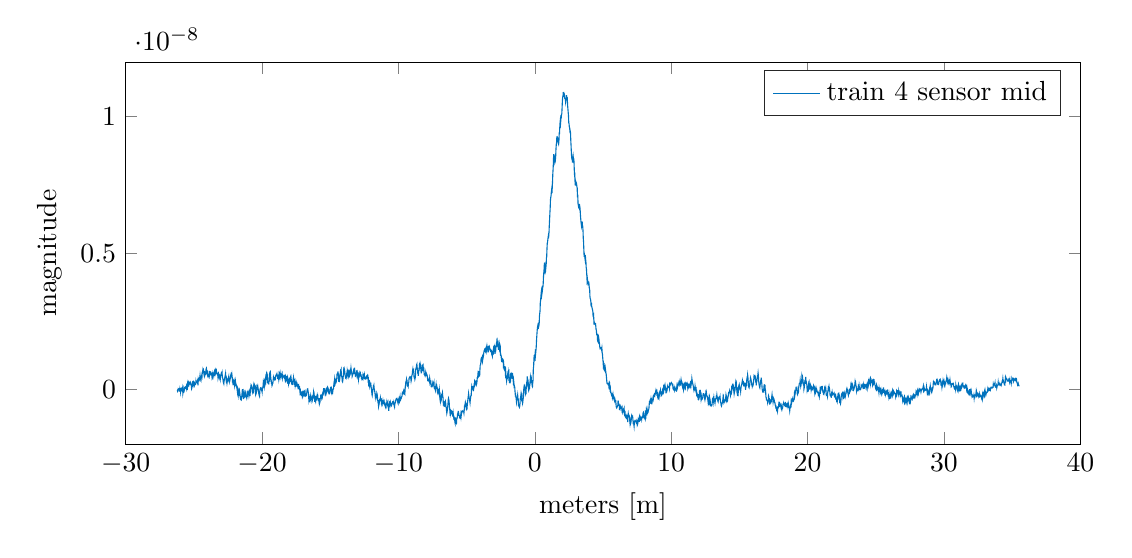
\begin{tikzpicture}

  \begin{axis}[%
    width=\textwidth,
    height=0.4\textwidth,
    at={(0\figurewidth,0\figureheight)},
    scale only axis,
    xmin=-30,
    xmax=40,
    xlabel={meters [m]},
    ymin=-2e-09,
    ymax=1.2e-08,
    ylabel={magnitude},
    axis background/.style={fill=white},
    legend style={legend cell align=left,align=left,draw=white!15!black}
    ]
    \addplot [color=mycolor1,solid]
    table[row sep=crcr]{%
    -26.229453125	-1.44861395537928e-11\\
    -26.2081640625	-1.51009541480569e-11\\
    -26.186875	-7.02350254215533e-11\\
    -26.1655859375	-5.65903146021423e-11\\
    -26.144296875	1.17304514299307e-11\\
    -26.1230078125	-9.98400256836081e-12\\
    -26.10171875	-3.21834551540119e-12\\
    -26.0804296875	2.79667084049285e-11\\
    -26.059140625	2.91488293484395e-11\\
    -26.0378515625	-7.74088634767628e-11\\
    -26.0165625	3.96687271078008e-11\\
    -25.9952734375	1.7818273677271e-12\\
    -25.973984375	-8.10086686052128e-11\\
    -25.9526953125	5.38050361237043e-11\\
    -25.93140625	-7.84279582234086e-11\\
    -25.9101171875	3.53526416888019e-11\\
    -25.888828125	4.9718706372539e-11\\
    -25.8675390625	-3.08960932255857e-11\\
    -25.84625	-2.69370231100557e-11\\
    -25.8249609375	3.63524668168338e-11\\
    -25.803671875	-1.35964228392558e-10\\
    -25.7823828125	-6.37017107564246e-11\\
    -25.76109375	-1.051907852768e-10\\
    -25.7398046875	-9.53947672695644e-11\\
    -25.718515625	3.67937072497122e-11\\
    -25.6972265625	-5.88775975137607e-12\\
    -25.6759375	6.43541650553945e-11\\
    -25.6546484375	7.75529495838166e-11\\
    -25.633359375	7.44155490620978e-11\\
    -25.6120703125	9.06926497701077e-11\\
    -25.59078125	4.4414192345959e-11\\
    -25.5694921875	2.96550900369642e-11\\
    -25.548203125	9.18038063808586e-11\\
    -25.5269140625	3.74823620288577e-11\\
    -25.505625	1.27537442885414e-10\\
    -25.4843359375	8.7043307737795e-11\\
    -25.463046875	2.00241062567635e-10\\
    -25.4417578125	1.23234855609153e-10\\
    -25.42046875	1.87456079972328e-10\\
    -25.3991796875	2.31036875363079e-10\\
    -25.377890625	1.0650519241124e-10\\
    -25.3566015625	2.23050485678743e-10\\
    -25.3353125	2.07777131870673e-10\\
    -25.3140234375	2.03525278799428e-10\\
    -25.292734375	2.76973511243046e-10\\
    -25.2714453125	2.87141877815209e-10\\
    -25.25015625	2.49083535788264e-10\\
    -25.2288671875	2.46162814116438e-10\\
    -25.207578125	1.68510501302515e-10\\
    -25.1862890625	1.72138864019541e-10\\
    -25.165	2.67032372285327e-11\\
    -25.1437109375	5.21202524096533e-11\\
    -25.122421875	1.63864507659732e-10\\
    -25.1011328125	2.24522069253779e-10\\
    -25.07984375	1.92607664642901e-10\\
    -25.0585546875	3.19487275453977e-10\\
    -25.037265625	2.19049777360192e-10\\
    -25.0159765625	2.89259544783847e-10\\
    -24.9946875	2.75117687062396e-10\\
    -24.9733984375	2.75336290768655e-10\\
    -24.952109375	1.46606334129154e-10\\
    -24.9308203125	1.73281836733144e-10\\
    -24.90953125	2.00715142219162e-10\\
    -24.8882421875	1.84596262504471e-10\\
    -24.866953125	1.91138916743132e-10\\
    -24.8456640625	3.07302634658202e-10\\
    -24.824375	2.53521856353014e-10\\
    -24.8030859375	2.66120018656268e-10\\
    -24.781796875	2.89850904544874e-10\\
    -24.7605078125	2.86214602984846e-10\\
    -24.73921875	3.20934348151698e-10\\
    -24.7179296875	2.50799369917817e-10\\
    -24.696640625	1.52417523700089e-10\\
    -24.6753515625	3.57377051624805e-10\\
    -24.6540625	3.06625985209855e-10\\
    -24.6327734375	3.06956925269324e-10\\
    -24.611484375	3.65357459914284e-10\\
    -24.5901953125	4.24598703172418e-10\\
    -24.56890625	4.21487835401587e-10\\
    -24.5476171875	5.13709051002724e-10\\
    -24.526328125	4.16272687982693e-10\\
    -24.5050390625	4.7692905485141e-10\\
    -24.48375	4.78443180780052e-10\\
    -24.4624609375	3.98159982960449e-10\\
    -24.441171875	4.86507311818723e-10\\
    -24.4198828125	5.30800909398198e-10\\
    -24.39859375	4.86145209118841e-10\\
    -24.3773046875	6.46858554677111e-10\\
    -24.356015625	6.45565271068909e-10\\
    -24.3347265625	7.26929766786726e-10\\
    -24.3134375	6.8047463287234e-10\\
    -24.2921484375	7.075593427623e-10\\
    -24.270859375	6.08043682154419e-10\\
    -24.2495703125	5.43878661226159e-10\\
    -24.22828125	5.8199366095898e-10\\
    -24.2069921875	4.95082798547921e-10\\
    -24.185703125	5.3177661603747e-10\\
    -24.1644140625	6.0990755044851e-10\\
    -24.143125	5.91736792554803e-10\\
    -24.1218359375	6.4454874597646e-10\\
    -24.100546875	7.56673908796087e-10\\
    -24.0792578125	7.81879856968072e-10\\
    -24.05796875	7.12419151073646e-10\\
    -24.0366796875	5.51076898332406e-10\\
    -24.015390625	6.98595374270267e-10\\
    -23.9941015625	5.17465891262221e-10\\
    -23.9728125	5.45007910213731e-10\\
    -23.9515234375	5.32473369266195e-10\\
    -23.930234375	4.94915320220158e-10\\
    -23.9089453125	4.7257481471715e-10\\
    -23.88765625	5.66431328159261e-10\\
    -23.8663671875	5.2243813642145e-10\\
    -23.845078125	6.85063271814915e-10\\
    -23.8237890625	5.929976336343e-10\\
    -23.8025	5.91195593305793e-10\\
    -23.7812109375	6.11929687830887e-10\\
    -23.759921875	5.38251640721417e-10\\
    -23.7386328125	5.33835328880481e-10\\
    -23.71734375	5.90382231322315e-10\\
    -23.6960546875	6.00534204766757e-10\\
    -23.674765625	4.94939420481718e-10\\
    -23.6534765625	5.75306624338727e-10\\
    -23.6321875	5.03940499912848e-10\\
    -23.6108984375	6.02697699998343e-10\\
    -23.589609375	5.92341527609766e-10\\
    -23.5683203125	5.76561315504784e-10\\
    -23.54703125	5.18060842872346e-10\\
    -23.5257421875	6.59715636532596e-10\\
    -23.504453125	4.91508999770258e-10\\
    -23.4831640625	6.43902289489277e-10\\
    -23.461875	6.09281309243692e-10\\
    -23.4405859375	6.69126872991194e-10\\
    -23.419296875	5.70567155565809e-10\\
    -23.3980078125	6.02318645566174e-10\\
    -23.37671875	6.1094056198595e-10\\
    -23.3554296875	7.63271498325388e-10\\
    -23.334140625	6.2363143624066e-10\\
    -23.3128515625	5.79136685736654e-10\\
    -23.2915625	5.80935331676871e-10\\
    -23.2702734375	5.52411899551807e-10\\
    -23.248984375	5.72976155601131e-10\\
    -23.2276953125	4.38831730800609e-10\\
    -23.20640625	5.10652253927223e-10\\
    -23.1851171875	5.67743220488207e-10\\
    -23.163828125	5.19836114681844e-10\\
    -23.1425390625	4.62969199486639e-10\\
    -23.12125	5.35669324834143e-10\\
    -23.0999609375	5.19005651178962e-10\\
    -23.078671875	4.90709454096724e-10\\
    -23.0573828125	3.9531405999738e-10\\
    -23.03609375	4.78678787342811e-10\\
    -23.0148046875	5.36031406667087e-10\\
    -22.993515625	5.84136401178245e-10\\
    -22.9722265625	5.50371728805659e-10\\
    -22.9509375	5.71072640382661e-10\\
    -22.9296484375	6.17721420005018e-10\\
    -22.908359375	4.58680926934126e-10\\
    -22.8870703125	4.23911042246302e-10\\
    -22.86578125	3.80836021588292e-10\\
    -22.8444921875	2.85576210480208e-10\\
    -22.823203125	2.40623786137077e-10\\
    -22.8019140625	2.0849816964156e-10\\
    -22.780625	3.2238224510814e-10\\
    -22.7593359375	3.50496911826256e-10\\
    -22.738046875	4.16258544483165e-10\\
    -22.7167578125	4.61859627799521e-10\\
    -22.69546875	5.25544358809867e-10\\
    -22.6741796875	5.87392294878931e-10\\
    -22.652890625	4.62242812126021e-10\\
    -22.6316015625	4.0138227566371e-10\\
    -22.6103125	2.25841281203574e-10\\
    -22.5890234375	3.22181460902194e-10\\
    -22.567734375	2.35740610104019e-10\\
    -22.5464453125	3.07271113205557e-10\\
    -22.52515625	3.02223534354446e-10\\
    -22.5038671875	4.29122925752934e-10\\
    -22.482578125	3.13005060546453e-10\\
    -22.4612890625	4.26844114427352e-10\\
    -22.44	4.7791599766654e-10\\
    -22.4187109375	3.49124974113775e-10\\
    -22.397421875	2.89517809987987e-10\\
    -22.3761328125	3.64385993079575e-10\\
    -22.35484375	3.40049729294617e-10\\
    -22.3335546875	3.93179588786373e-10\\
    -22.312265625	4.50067642522256e-10\\
    -22.2909765625	5.38959989212318e-10\\
    -22.2696875	5.38774149398915e-10\\
    -22.2483984375	6.26816327649957e-10\\
    -22.227109375	4.50492502633497e-10\\
    -22.2058203125	5.34303026832141e-10\\
    -22.18453125	4.42998438921128e-10\\
    -22.1632421875	2.56107891031766e-10\\
    -22.141953125	3.57764427531351e-10\\
    -22.1206640625	1.58394524720491e-10\\
    -22.099375	2.60114281874426e-10\\
    -22.0780859375	3.22432121025594e-10\\
    -22.056796875	2.87817304574061e-10\\
    -22.0355078125	2.63257725366943e-10\\
    -22.01421875	1.68915482521173e-10\\
    -21.9929296875	2.81226439625345e-10\\
    -21.971640625	2.14522033829826e-10\\
    -21.9503515625	2.93526941625088e-10\\
    -21.9290625	1.83861220236738e-10\\
    -21.9077734375	1.98722315076199e-10\\
    -21.886484375	1.60782516250857e-10\\
    -21.8651953125	1.42317596990015e-10\\
    -21.84390625	4.74147579700692e-11\\
    -21.8226171875	-9.67450400187996e-12\\
    -21.801328125	-9.52239083226325e-11\\
    -21.7800390625	-1.17580536181041e-11\\
    -21.75875	-9.21054619062693e-11\\
    -21.7374609375	-2.0624161275142e-10\\
    -21.716171875	-1.28962188809495e-10\\
    -21.6948828125	-5.33444162727829e-11\\
    -21.67359375	-1.18076567779298e-10\\
    -21.6523046875	-5.37230372506295e-11\\
    -21.631015625	-1.2576156271849e-10\\
    -21.6097265625	-2.13539540825774e-10\\
    -21.5884375	-3.07818092827023e-10\\
    -21.5671484375	-3.69093880698919e-10\\
    -21.545859375	-3.67306860442571e-10\\
    -21.5245703125	-3.79514517319814e-10\\
    -21.50328125	-2.50955851747785e-10\\
    -21.4819921875	-2.40713033198456e-10\\
    -21.460703125	-1.14443422525736e-10\\
    -21.4394140625	-1.59682870548824e-10\\
    -21.418125	1.67790968545961e-11\\
    -21.3968359375	-1.68877345915695e-10\\
    -21.375546875	-1.19156443659879e-10\\
    -21.3542578125	-3.51663564055096e-10\\
    -21.33296875	-1.79356635284014e-10\\
    -21.3116796875	-3.14318442584322e-10\\
    -21.290390625	-1.99055475716052e-10\\
    -21.2691015625	-1.24778018392598e-10\\
    -21.2478125	-1.83164139655552e-10\\
    -21.2265234375	-1.21368969954711e-10\\
    -21.205234375	-1.85226119841615e-10\\
    -21.1839453125	-1.54129775551586e-10\\
    -21.16265625	-2.78827454043777e-10\\
    -21.1413671875	-2.78421852937479e-10\\
    -21.120078125	-3.18029269306606e-10\\
    -21.0987890625	-2.51526483741892e-10\\
    -21.0775	-2.00100230078698e-10\\
    -21.0562109375	-1.20936330896261e-10\\
    -21.034921875	-1.65169172406936e-10\\
    -21.0136328125	-1.01893465215953e-10\\
    -20.99234375	-1.09552788780019e-10\\
    -20.9710546875	-7.77936306781395e-11\\
    -20.949765625	-2.15999309577551e-10\\
    -20.9284765625	-1.56058121019142e-10\\
    -20.9071875	-9.76292806925908e-11\\
    -20.8858984375	-2.4196632988927e-10\\
    -20.864609375	-1.11027182184135e-10\\
    -20.8433203125	3.68105608427112e-11\\
    -20.82203125	9.70330472643504e-11\\
    -20.8007421875	1.73544869661371e-10\\
    -20.779453125	1.5578057498679e-10\\
    -20.7581640625	1.11094230087533e-10\\
    -20.736875	5.93627878631977e-11\\
    -20.7155859375	-6.60221844920487e-11\\
    -20.694296875	-1.01883723705463e-10\\
    -20.6730078125	-3.23088890026121e-11\\
    -20.65171875	-1.50959402118658e-10\\
    -20.6304296875	-2.49695904718654e-11\\
    -20.609140625	1.32093877615361e-10\\
    -20.5878515625	7.17692837569115e-11\\
    -20.5665625	1.13490602912915e-10\\
    -20.5452734375	1.66921809275613e-10\\
    -20.523984375	1.24255530957761e-10\\
    -20.5026953125	-4.24950214349142e-11\\
    -20.48140625	-1.2418800843498e-10\\
    -20.4601171875	-3.30945650473249e-11\\
    -20.438828125	-1.52352533463089e-10\\
    -20.4175390625	-1.19412270713486e-10\\
    -20.39625	1.90278089743283e-12\\
    -20.3749609375	1.4010944622095e-10\\
    -20.353671875	1.2731925557825e-10\\
    -20.3323828125	7.26477155521946e-11\\
    -20.31109375	1.20361872036958e-10\\
    -20.2898046875	4.38989956007425e-11\\
    -20.268515625	-1.44495196179358e-11\\
    -20.2472265625	-1.27117911458647e-10\\
    -20.2259375	-1.60265850476332e-10\\
    -20.2046484375	-2.23289778327305e-10\\
    -20.183359375	-2.50754937806482e-10\\
    -20.1620703125	-9.81934627096776e-11\\
    -20.14078125	2.59077451202577e-11\\
    -20.1194921875	3.89340711579868e-11\\
    -20.098203125	6.68604236815488e-11\\
    -20.0769140625	7.12293573530653e-11\\
    -20.055625	3.80480210067818e-11\\
    -20.0343359375	-2.38959036249194e-11\\
    -20.013046875	-1.20260552451896e-11\\
    -19.9917578125	-8.07146187702311e-11\\
    -19.97046875	4.18054069057792e-11\\
    -19.9491796875	5.99679696788882e-11\\
    -19.927890625	1.16497677198065e-10\\
    -19.9066015625	2.54337877692691e-10\\
    -19.8853125	1.79357355822308e-10\\
    -19.8640234375	2.60321765342643e-10\\
    -19.842734375	3.01828193781736e-10\\
    -19.8214453125	1.39937094220158e-10\\
    -19.80015625	2.1666785655799e-10\\
    -19.7788671875	1.90735646123118e-10\\
    -19.757578125	2.78593833425869e-10\\
    -19.7362890625	3.97490767354164e-10\\
    -19.715	3.31923056033628e-10\\
    -19.6937109375	4.42454348957145e-10\\
    -19.672421875	5.65952014265482e-10\\
    -19.6511328125	5.230581005707e-10\\
    -19.62984375	5.69577875376093e-10\\
    -19.6085546875	5.2543700390288e-10\\
    -19.587265625	2.5285681381033e-10\\
    -19.5659765625	2.48001694108592e-10\\
    -19.5446875	2.28501924768638e-10\\
    -19.5233984375	2.61533190343913e-10\\
    -19.502109375	2.39341649958896e-10\\
    -19.4808203125	3.30423075759715e-10\\
    -19.45953125	4.81341114200638e-10\\
    -19.4382421875	4.36659479358454e-10\\
    -19.416953125	6.41321562268645e-10\\
    -19.3956640625	6.55799589589209e-10\\
    -19.374375	5.15700413244863e-10\\
    -19.3530859375	3.75674771480521e-10\\
    -19.331796875	3.6066652217546e-10\\
    -19.3105078125	2.23668089888783e-10\\
    -19.28921875	2.23029716623422e-10\\
    -19.2679296875	1.44426121208456e-10\\
    -19.246640625	1.72055189105379e-10\\
    -19.2253515625	2.42440301373492e-10\\
    -19.2040625	2.37169023652245e-10\\
    -19.1827734375	3.4645270680144e-10\\
    -19.161484375	4.52148316186368e-10\\
    -19.1401953125	4.13231746805506e-10\\
    -19.11890625	4.16810578262989e-10\\
    -19.0976171875	3.76824659793582e-10\\
    -19.076328125	4.07632008564535e-10\\
    -19.0550390625	3.63710113812877e-10\\
    -19.03375	3.57452426063564e-10\\
    -19.0124609375	3.98076297763568e-10\\
    -18.991171875	5.07499585960764e-10\\
    -18.9698828125	5.00414125661409e-10\\
    -18.94859375	5.44817283488e-10\\
    -18.9273046875	5.34192573244722e-10\\
    -18.906015625	5.73508682706508e-10\\
    -18.8847265625	5.19092028285061e-10\\
    -18.8634375	5.1845537821236e-10\\
    -18.8421484375	3.83096554194721e-10\\
    -18.820859375	4.71413750217519e-10\\
    -18.7995703125	4.62332514655285e-10\\
    -18.77828125	3.86366725556562e-10\\
    -18.7569921875	5.25789663719702e-10\\
    -18.735703125	4.66219586914101e-10\\
    -18.7144140625	5.40641700349164e-10\\
    -18.693125	4.44855693640014e-10\\
    -18.6718359375	4.69008763184664e-10\\
    -18.650546875	5.16672959157191e-10\\
    -18.6292578125	5.83543345726884e-10\\
    -18.60796875	4.69609498396e-10\\
    -18.5866796875	5.21931507895199e-10\\
    -18.565390625	5.46242940886584e-10\\
    -18.5441015625	5.44674396384994e-10\\
    -18.5228125	5.77712651079887e-10\\
    -18.5015234375	4.39569597412427e-10\\
    -18.480234375	5.04639812410809e-10\\
    -18.4589453125	4.87445334788031e-10\\
    -18.43765625	4.84440894704317e-10\\
    -18.4163671875	4.67247905384552e-10\\
    -18.395078125	4.48363270927582e-10\\
    -18.3737890625	5.17088653255086e-10\\
    -18.3525	5.05061013457324e-10\\
    -18.3312109375	4.38568954614896e-10\\
    -18.309921875	3.70820504124664e-10\\
    -18.2886328125	4.47566130679872e-10\\
    -18.26734375	3.70294786505817e-10\\
    -18.2460546875	4.33157898424483e-10\\
    -18.224765625	3.90559056461779e-10\\
    -18.2034765625	4.75148184205706e-10\\
    -18.1821875	4.70529578614121e-10\\
    -18.1608984375	3.69621449809343e-10\\
    -18.139609375	4.18039514540543e-10\\
    -18.1183203125	2.3164965797871e-10\\
    -18.09703125	2.27541683317164e-10\\
    -18.0757421875	2.78248312261171e-10\\
    -18.054453125	2.00337979337193e-10\\
    -18.0331640625	2.63868961446069e-10\\
    -18.011875	3.77297355794625e-10\\
    -17.9905859375	3.45132366342183e-10\\
    -17.969296875	3.015231265058e-10\\
    -17.9480078125	3.76625266169041e-10\\
    -17.92671875	4.24502595713393e-10\\
    -17.9054296875	3.00045149406454e-10\\
    -17.884140625	2.9896688544657e-10\\
    -17.8628515625	3.87553537114917e-10\\
    -17.8415625	2.94247688094382e-10\\
    -17.8202734375	2.06622181620224e-10\\
    -17.798984375	1.91235329736626e-10\\
    -17.7776953125	2.1303912326207e-10\\
    -17.75640625	2.71417156778052e-10\\
    -17.7351171875	1.70544169326698e-10\\
    -17.713828125	3.50488840020845e-10\\
    -17.6925390625	4.41036380093759e-10\\
    -17.67125	3.65672039489743e-10\\
    -17.6499609375	3.31713041907441e-10\\
    -17.628671875	3.46984630580075e-10\\
    -17.6073828125	2.32207897966571e-10\\
    -17.58609375	2.84091505779622e-10\\
    -17.5648046875	1.46062055437427e-10\\
    -17.543515625	1.98665985540661e-10\\
    -17.5222265625	2.34645258338725e-10\\
    -17.5009375	9.93300163846243e-11\\
    -17.4796484375	2.45213459697525e-10\\
    -17.458359375	2.02221033447517e-10\\
    -17.4370703125	2.28212547202365e-10\\
    -17.41578125	1.86979362585986e-10\\
    -17.3944921875	1.39636645538803e-10\\
    -17.373203125	1.53020300838646e-10\\
    -17.3519140625	6.91580108605205e-12\\
    -17.330625	9.61533091178853e-11\\
    -17.3093359375	1.27880625150853e-10\\
    -17.288046875	3.59787054843583e-11\\
    -17.2667578125	2.88876262326039e-11\\
    -17.24546875	5.69989667063286e-11\\
    -17.2241796875	-4.85717982184542e-11\\
    -17.202890625	3.94474075115611e-11\\
    -17.1816015625	-1.64007522152658e-10\\
    -17.1603125	-1.55146279903529e-10\\
    -17.1390234375	-6.78890441853535e-11\\
    -17.117734375	-2.40585586108324e-10\\
    -17.0964453125	-8.53739200741001e-11\\
    -17.07515625	-8.43693963869118e-11\\
    -17.0538671875	-1.98097617916499e-10\\
    -17.032578125	-1.20085616829796e-10\\
    -17.0112890625	-9.2225983522291e-11\\
    -16.99	-2.08569952007199e-10\\
    -16.9687109375	-1.66384743299689e-10\\
    -16.947421875	-1.20495545779282e-10\\
    -16.9261328125	-1.64429677812345e-10\\
    -16.90484375	-7.51881558846595e-11\\
    -16.8835546875	-5.82805448121161e-11\\
    -16.862265625	-1.51698795938806e-10\\
    -16.8409765625	-1.06545907501341e-10\\
    -16.8196875	-2.2219559441702e-10\\
    -16.7983984375	-2.39045043547803e-10\\
    -16.777109375	-2.20736317011316e-10\\
    -16.7558203125	-2.21796928944625e-10\\
    -16.73453125	-1.49309487129125e-10\\
    -16.7132421875	-1.06992745327756e-10\\
    -16.691953125	-1.56405520345386e-11\\
    -16.6706640625	2.37238686033648e-11\\
    -16.649375	2.82802998452518e-11\\
    -16.6280859375	-4.97724721829716e-11\\
    -16.606796875	-1.04513028358329e-10\\
    -16.5855078125	-2.35025292532294e-10\\
    -16.56421875	-3.80118629670235e-10\\
    -16.5429296875	-3.122332932088e-10\\
    -16.521640625	-4.06051955116228e-10\\
    -16.5003515625	-4.23965828995446e-10\\
    -16.4790625	-2.71778017285276e-10\\
    -16.4577734375	-2.71189607892594e-10\\
    -16.436484375	-2.19784431293149e-10\\
    -16.4151953125	-3.2005814760774e-10\\
    -16.39390625	-2.84375337838954e-10\\
    -16.3726171875	-2.88640740815221e-10\\
    -16.351328125	-3.75979047807467e-10\\
    -16.3300390625	-3.09753870053078e-10\\
    -16.30875	-3.74943214413072e-10\\
    -16.2874609375	-3.12704495544487e-10\\
    -16.266171875	-2.72704668297112e-10\\
    -16.2448828125	-2.12892595928517e-10\\
    -16.22359375	-1.13564740466554e-10\\
    -16.2023046875	-2.21022620687969e-10\\
    -16.181015625	-1.77258123813601e-10\\
    -16.1597265625	-2.78598981734314e-10\\
    -16.1384375	-4.52846969260557e-10\\
    -16.1171484375	-3.43125849902192e-10\\
    -16.095859375	-4.0049839721572e-10\\
    -16.0745703125	-4.36861490472252e-10\\
    -16.05328125	-2.75755808680405e-10\\
    -16.0319921875	-2.89844207712528e-10\\
    -16.010703125	-3.28729047505145e-10\\
    -15.9894140625	-2.56761912507813e-10\\
    -15.968125	-2.16022554099792e-10\\
    -15.9468359375	-3.59781657602589e-10\\
    -15.925546875	-1.59994375585246e-10\\
    -15.9042578125	-2.89955568385953e-10\\
    -15.88296875	-3.85592316165458e-10\\
    -15.8616796875	-3.77374532367768e-10\\
    -15.840390625	-3.75947774499002e-10\\
    -15.8191015625	-4.5526172057904e-10\\
    -15.7978125	-3.19792895364602e-10\\
    -15.7765234375	-5.03254761022991e-10\\
    -15.755234375	-4.67835539089746e-10\\
    -15.7339453125	-3.42580576703497e-10\\
    -15.71265625	-3.21234928520248e-10\\
    -15.6913671875	-2.01861045177674e-10\\
    -15.670078125	-2.01661545250614e-10\\
    -15.6487890625	-2.45960189184543e-10\\
    -15.6275	-3.12190847299396e-10\\
    -15.6062109375	-2.58790829814584e-10\\
    -15.584921875	-2.85852250879897e-10\\
    -15.5636328125	-1.45327317532178e-10\\
    -15.54234375	-1.1408325813984e-10\\
    -15.5210546875	-2.25769680090288e-10\\
    -15.499765625	-3.65131252511282e-11\\
    -15.4784765625	5.17106906505481e-11\\
    -15.4571875	-1.03010614427247e-10\\
    -15.4358984375	-1.84184744573513e-11\\
    -15.414609375	-2.79209063415378e-12\\
    -15.3933203125	-1.00300791668408e-10\\
    -15.37203125	-1.70519321676104e-10\\
    -15.3507421875	-1.44398657427732e-10\\
    -15.329453125	-8.6332437105848e-11\\
    -15.3081640625	-1.62912303118474e-10\\
    -15.286875	-1.22827002963803e-10\\
    -15.2655859375	-3.56592209103661e-12\\
    -15.244296875	6.96242160649157e-11\\
    -15.2230078125	7.95711753365924e-11\\
    -15.20171875	9.4881870903072e-11\\
    -15.1804296875	1.23585028858048e-11\\
    -15.159140625	-8.72777438088898e-11\\
    -15.1378515625	-1.01834881988736e-10\\
    -15.1165625	-5.04509976779293e-11\\
    -15.0952734375	-1.53128669706333e-10\\
    -15.073984375	-1.60363206039431e-10\\
    -15.0526953125	-1.47296135944737e-10\\
    -15.03140625	-7.35475168406285e-11\\
    -15.0101171875	-4.08719919678704e-11\\
    -14.988828125	3.58651542269e-11\\
    -14.9675390625	7.29097556839903e-11\\
    -14.94625	8.47708352302314e-11\\
    -14.9249609375	-2.13645075326858e-11\\
    -14.903671875	4.87229497512447e-11\\
    -14.8823828125	2.11440298517974e-11\\
    -14.86109375	-1.03528071398621e-10\\
    -14.8398046875	-5.87836201747455e-11\\
    -14.818515625	-9.14717771025866e-11\\
    -14.7972265625	-8.25735903335202e-12\\
    -14.7759375	1.56740648260418e-11\\
    -14.7546484375	2.45667230792756e-11\\
    -14.733359375	2.04090665572828e-10\\
    -14.7120703125	2.70725574626956e-10\\
    -14.69078125	2.28740532887874e-10\\
    -14.6694921875	3.85292401311085e-10\\
    -14.648203125	3.16586050794981e-10\\
    -14.6269140625	2.66828133061897e-10\\
    -14.605625	3.77403636103574e-10\\
    -14.5843359375	2.19187051342075e-10\\
    -14.563046875	3.4653935698031e-10\\
    -14.5417578125	3.30922087289027e-10\\
    -14.52046875	4.01669001264551e-10\\
    -14.4991796875	5.68270699436886e-10\\
    -14.477890625	5.6571523341824e-10\\
    -14.4566015625	5.52122014562832e-10\\
    -14.4353125	6.67924209449194e-10\\
    -14.4140234375	5.56755063656827e-10\\
    -14.392734375	4.14227918528924e-10\\
    -14.3714453125	4.62445296207078e-10\\
    -14.35015625	3.06512802886162e-10\\
    -14.3288671875	2.98932585275628e-10\\
    -14.307578125	3.67995209320708e-10\\
    -14.2862890625	4.5667601523006e-10\\
    -14.265	5.38698232527812e-10\\
    -14.2437109375	6.80159410344336e-10\\
    -14.222421875	6.61752398259806e-10\\
    -14.2011328125	7.12617590133074e-10\\
    -14.17984375	5.27060433631621e-10\\
    -14.1585546875	4.85506245833001e-10\\
    -14.137265625	4.3919140081411e-10\\
    -14.1159765625	3.04737091848074e-10\\
    -14.0946875	2.84232234656849e-10\\
    -14.0733984375	3.5242654376913e-10\\
    -14.052109375	4.55201757758206e-10\\
    -14.0308203125	5.26120695467615e-10\\
    -14.00953125	7.16443561500745e-10\\
    -13.9882421875	6.77355721534934e-10\\
    -13.966953125	7.53308695962171e-10\\
    -13.9456640625	7.08268409028684e-10\\
    -13.924375	6.05012260261619e-10\\
    -13.9030859375	5.15484024729583e-10\\
    -13.881796875	4.74986895867381e-10\\
    -13.8605078125	4.07055845446862e-10\\
    -13.83921875	3.98428764316403e-10\\
    -13.8179296875	4.54754397345897e-10\\
    -13.796640625	5.46643257090193e-10\\
    -13.7753515625	5.0992371648813e-10\\
    -13.7540625	6.63979366517827e-10\\
    -13.7327734375	5.91211349804651e-10\\
    -13.711484375	6.42350529601624e-10\\
    -13.6901953125	5.64788871908061e-10\\
    -13.66890625	5.01572539056963e-10\\
    -13.6476171875	5.88995260501046e-10\\
    -13.626328125	5.0885449378781e-10\\
    -13.6050390625	4.88907558966387e-10\\
    -13.58375	6.38056946169513e-10\\
    -13.5624609375	6.10911386627608e-10\\
    -13.541171875	5.9623712448761e-10\\
    -13.5198828125	7.67558767807073e-10\\
    -13.49859375	6.82011650444299e-10\\
    -13.4773046875	7.88409083927172e-10\\
    -13.456015625	6.99479913469099e-10\\
    -13.4347265625	6.8326925618223e-10\\
    -13.4134375	6.12898472927723e-10\\
    -13.3921484375	4.7985025861603e-10\\
    -13.370859375	5.09781006048405e-10\\
    -13.3495703125	5.60020390901738e-10\\
    -13.32828125	5.6732417465485e-10\\
    -13.3069921875	5.9480724305123e-10\\
    -13.285703125	6.70251018344115e-10\\
    -13.2644140625	7.73202505440368e-10\\
    -13.243125	5.75262985840964e-10\\
    -13.2218359375	8.05939182923707e-10\\
    -13.200546875	6.93637390218724e-10\\
    -13.1792578125	6.15081331979942e-10\\
    -13.15796875	5.16869298577967e-10\\
    -13.1366796875	5.31405883120852e-10\\
    -13.115390625	5.02334589173905e-10\\
    -13.0941015625	6.19497776824489e-10\\
    -13.0728125	5.22166980495226e-10\\
    -13.0515234375	6.86807549994257e-10\\
    -13.030234375	6.91658490084573e-10\\
    -13.0089453125	5.54900548892994e-10\\
    -12.98765625	6.31155497704518e-10\\
    -12.9663671875	6.2022335334446e-10\\
    -12.945078125	4.9144703902045e-10\\
    -12.9237890625	3.75291676453773e-10\\
    -12.9025	4.66819658816449e-10\\
    -12.8812109375	4.62923390930609e-10\\
    -12.859921875	5.49565645554454e-10\\
    -12.8386328125	5.31883136900575e-10\\
    -12.81734375	6.44231569896817e-10\\
    -12.7960546875	6.27671002107713e-10\\
    -12.774765625	5.19902386644314e-10\\
    -12.7534765625	5.07169846425846e-10\\
    -12.7321875	5.17106723143594e-10\\
    -12.7108984375	4.22621046789916e-10\\
    -12.689609375	4.26598705446529e-10\\
    -12.6683203125	3.61343616814926e-10\\
    -12.64703125	3.71662569336652e-10\\
    -12.6257421875	3.6670029081884e-10\\
    -12.604453125	4.95018816712155e-10\\
    -12.5831640625	4.31312464410069e-10\\
    -12.561875	4.91848536034054e-10\\
    -12.5405859375	5.28532823771894e-10\\
    -12.519296875	4.80329336026778e-10\\
    -12.4980078125	5.37862514999458e-10\\
    -12.47671875	4.24593441287396e-10\\
    -12.4554296875	4.29675817707108e-10\\
    -12.434140625	3.81984107132485e-10\\
    -12.4128515625	3.82100662538859e-10\\
    -12.3915625	3.83467226420354e-10\\
    -12.3702734375	4.43528884324624e-10\\
    -12.348984375	4.34209586639571e-10\\
    -12.3276953125	4.91087654854508e-10\\
    -12.30640625	4.85140055654827e-10\\
    -12.2851171875	5.1001244363145e-10\\
    -12.263828125	4.52688545513572e-10\\
    -12.2425390625	4.74864758159167e-10\\
    -12.22125	3.38168700777527e-10\\
    -12.1999609375	3.66648473249813e-10\\
    -12.178671875	1.79779780914502e-10\\
    -12.1573828125	2.05047673413312e-10\\
    -12.13609375	1.83245266314922e-10\\
    -12.1148046875	1.26903963911152e-10\\
    -12.093515625	2.59499804682654e-10\\
    -12.0722265625	2.20462512601139e-10\\
    -12.0509375	1.11400203736404e-10\\
    -12.0296484375	2.50175164124524e-10\\
    -12.008359375	1.30798678481746e-10\\
    -11.9870703125	4.41358114715544e-11\\
    -11.96578125	-1.0218604856325e-11\\
    -11.9444921875	-1.66780627153077e-10\\
    -11.923203125	-2.14776458447991e-10\\
    -11.9019140625	-1.33858919446155e-10\\
    -11.880625	-5.68494560076863e-11\\
    -11.8593359375	2.85149437800433e-11\\
    -11.838046875	1.07119869226013e-10\\
    -11.8167578125	8.40342323720503e-11\\
    -11.79546875	1.41604384218706e-10\\
    -11.7741796875	2.20318327743817e-11\\
    -11.752890625	-9.94362856153421e-12\\
    -11.7316015625	-8.2638906382513e-11\\
    -11.7103125	-1.63915231823107e-10\\
    -11.6890234375	-2.79072858387555e-10\\
    -11.667734375	-2.05194649537769e-10\\
    -11.6464453125	-2.37217161978596e-10\\
    -11.62515625	-2.26780700312201e-10\\
    -11.6038671875	-2.66187984986652e-10\\
    -11.582578125	-1.33125862287166e-10\\
    -11.5612890625	-1.6403204051188e-10\\
    -11.54	-2.62974837606895e-10\\
    -11.5187109375	-3.91098174809377e-10\\
    -11.497421875	-4.59966376156757e-10\\
    -11.4761328125	-4.4183475988995e-10\\
    -11.45484375	-6.25298796155869e-10\\
    -11.4335546875	-5.80472183150828e-10\\
    -11.412265625	-5.18307922485748e-10\\
    -11.3909765625	-4.33487873468073e-10\\
    -11.3696875	-3.62067098190902e-10\\
    -11.3483984375	-3.57114636297662e-10\\
    -11.327109375	-3.04344990706656e-10\\
    -11.3058203125	-4.32653180600624e-10\\
    -11.28453125	-3.27369240999472e-10\\
    -11.2632421875	-3.30399069121446e-10\\
    -11.241953125	-5.05120473975785e-10\\
    -11.2206640625	-4.56339704155928e-10\\
    -11.199375	-4.15374644397044e-10\\
    -11.1780859375	-4.28849185544853e-10\\
    -11.156796875	-4.97275087030392e-10\\
    -11.1355078125	-4.2241905118773e-10\\
    -11.11421875	-5.09776312903053e-10\\
    -11.0929296875	-4.93622498858234e-10\\
    -11.071640625	-4.56408005016714e-10\\
    -11.0503515625	-4.25879733542471e-10\\
    -11.0290625	-5.06111128366428e-10\\
    -11.0077734375	-5.45505452331455e-10\\
    -10.986484375	-5.90122887292975e-10\\
    -10.9651953125	-6.16802131146726e-10\\
    -10.94390625	-6.45931249313084e-10\\
    -10.9226171875	-5.61681891414193e-10\\
    -10.901328125	-6.03057231715084e-10\\
    -10.8800390625	-4.71538775812843e-10\\
    -10.85875	-5.64530809544118e-10\\
    -10.8374609375	-4.19088225339512e-10\\
    -10.816171875	-4.48068348600941e-10\\
    -10.7948828125	-5.37289857981813e-10\\
    -10.77359375	-6.0949593130204e-10\\
    -10.7523046875	-6.44966837020014e-10\\
    -10.731015625	-6.17714103270818e-10\\
    -10.7097265625	-7.80580214337645e-10\\
    -10.6884375	-5.48241604677672e-10\\
    -10.6671484375	-6.08474185209033e-10\\
    -10.645859375	-5.56874412860113e-10\\
    -10.6245703125	-4.53152711886159e-10\\
    -10.60328125	-4.3099378932412e-10\\
    -10.5819921875	-5.02973057795478e-10\\
    -10.560703125	-5.32992805162047e-10\\
    -10.5394140625	-6.16642329301982e-10\\
    -10.518125	-6.04634541422374e-10\\
    -10.4968359375	-5.30466891754222e-10\\
    -10.475546875	-5.41355845199376e-10\\
    -10.4542578125	-5.01628604239945e-10\\
    -10.43296875	-4.60218831960212e-10\\
    -10.4116796875	-4.4211687224893e-10\\
    -10.390390625	-4.47128138548574e-10\\
    -10.3691015625	-4.90928506237741e-10\\
    -10.3478125	-4.54429498736807e-10\\
    -10.3265234375	-5.37576993098468e-10\\
    -10.305234375	-6.04705428765329e-10\\
    -10.2839453125	-6.41074042341172e-10\\
    -10.26265625	-5.26309923857352e-10\\
    -10.2413671875	-4.94508491703698e-10\\
    -10.220078125	-4.7460642375703e-10\\
    -10.1987890625	-3.95358317848331e-10\\
    -10.1775	-3.6712558555045e-10\\
    -10.1562109375	-3.34619720807865e-10\\
    -10.134921875	-3.28002139556427e-10\\
    -10.1136328125	-3.67590082167531e-10\\
    -10.09234375	-3.71606810579866e-10\\
    -10.0710546875	-4.08991079291803e-10\\
    -10.049765625	-4.53766251229718e-10\\
    -10.0284765625	-3.93208406549826e-10\\
    -10.0071875	-4.61402662911531e-10\\
    -9.9858984375	-3.72732026938305e-10\\
    -9.964609375	-3.61049005327306e-10\\
    -9.9433203125	-4.05219684293678e-10\\
    -9.92203125	-2.52325781233125e-10\\
    -9.9007421875	-3.47952337576446e-10\\
    -9.879453125	-2.75279606864495e-10\\
    -9.8581640625	-3.96675085172939e-10\\
    -9.836875	-3.78928852618327e-10\\
    -9.8155859375	-3.25909244860945e-10\\
    -9.794296875	-3.24830339658069e-10\\
    -9.7730078125	-2.82303057554158e-10\\
    -9.75171875	-2.50097961616354e-10\\
    -9.7304296875	-2.31665665871187e-10\\
    -9.709140625	-9.56497831457304e-11\\
    -9.6878515625	-9.13168269353021e-11\\
    -9.6665625	-9.71589593127357e-11\\
    -9.6452734375	-1.20346801086916e-10\\
    -9.623984375	-6.31272412505069e-11\\
    -9.6026953125	-1.15477400556587e-10\\
    -9.58140625	-1.37710951756186e-10\\
    -9.5601171875	-3.78992624486678e-11\\
    -9.538828125	-5.51362083473166e-12\\
    -9.5175390625	-6.65495777892678e-11\\
    -9.49625	9.85245904721428e-11\\
    -9.4749609375	1.63671716340536e-10\\
    -9.453671875	2.9025551802338e-10\\
    -9.4323828125	2.91723856518215e-10\\
    -9.41109375	3.55228795448696e-10\\
    -9.3898046875	2.29793427634493e-10\\
    -9.368515625	3.66875154175685e-10\\
    -9.3472265625	1.41121033902501e-10\\
    -9.3259375	1.55010731994417e-10\\
    -9.3046484375	1.69476119347045e-10\\
    -9.283359375	1.28933975893267e-10\\
    -9.2620703125	2.54778253307201e-10\\
    -9.24078125	2.64454212621998e-10\\
    -9.2194921875	4.15216415597597e-10\\
    -9.198203125	4.31511227297473e-10\\
    -9.1769140625	4.33060983949007e-10\\
    -9.155625	4.75723091377292e-10\\
    -9.1343359375	4.7089935174563e-10\\
    -9.113046875	4.23521410756216e-10\\
    -9.0917578125	4.05525406181474e-10\\
    -9.07046875	3.12205383623051e-10\\
    -9.0491796875	3.66668732477975e-10\\
    -9.027890625	4.76172693632976e-10\\
    -9.0066015625	5.23742731645336e-10\\
    -8.9853125	5.59715571213239e-10\\
    -8.9640234375	6.84432486520969e-10\\
    -8.942734375	7.45869527817851e-10\\
    -8.9214453125	6.50965621329151e-10\\
    -8.90015625	6.31759785634533e-10\\
    -8.8788671875	6.69880649439514e-10\\
    -8.857578125	4.76457052100892e-10\\
    -8.8362890625	4.28388459615204e-10\\
    -8.815	4.38046510518547e-10\\
    -8.7937109375	3.75565138324952e-10\\
    -8.772421875	4.18334043978044e-10\\
    -8.7511328125	5.3041857891547e-10\\
    -8.72984375	7.39366680452033e-10\\
    -8.7085546875	7.91240578636419e-10\\
    -8.687265625	8.05293312269673e-10\\
    -8.6659765625	9.07904119982393e-10\\
    -8.6446875	9.34450440682031e-10\\
    -8.6233984375	7.33912507546113e-10\\
    -8.602109375	8.06363571536382e-10\\
    -8.5808203125	5.97076847378212e-10\\
    -8.55953125	5.78860962475026e-10\\
    -8.5382421875	5.02097528725501e-10\\
    -8.516953125	6.81568478654238e-10\\
    -8.4956640625	6.87369925259839e-10\\
    -8.474375	7.5089680884785e-10\\
    -8.4530859375	9.14180474407123e-10\\
    -8.431796875	8.97166356393906e-10\\
    -8.4105078125	9.58693575862043e-10\\
    -8.38921875	9.05520138969994e-10\\
    -8.3679296875	8.29809089319737e-10\\
    -8.346640625	6.71040552205412e-10\\
    -8.3253515625	6.19006125511739e-10\\
    -8.3040625	6.3206692275153e-10\\
    -8.2827734375	7.44404037488396e-10\\
    -8.261484375	8.30118199733351e-10\\
    -8.2401953125	7.84963258403184e-10\\
    -8.21890625	8.76672931003688e-10\\
    -8.1976171875	8.98014329373138e-10\\
    -8.176328125	6.77554232056445e-10\\
    -8.1550390625	8.33282998615421e-10\\
    -8.13375	7.3835659830925e-10\\
    -8.1124609375	5.61475090184574e-10\\
    -8.091171875	5.62954895979826e-10\\
    -8.0698828125	5.33528534275746e-10\\
    -8.04859375	5.04015998603845e-10\\
    -8.0273046875	5.54510188516797e-10\\
    -8.006015625	6.15265628493892e-10\\
    -7.9847265625	4.81750230364023e-10\\
    -7.9634375	6.09271495130295e-10\\
    -7.9421484375	5.84383379125778e-10\\
    -7.920859375	5.37851491215738e-10\\
    -7.8995703125	5.35163683708636e-10\\
    -7.87828125	4.81905336326575e-10\\
    -7.8569921875	3.65937101341203e-10\\
    -7.835703125	3.83169848951474e-10\\
    -7.8144140625	3.25065612078283e-10\\
    -7.793125	3.17236141312616e-10\\
    -7.7718359375	3.80254184037991e-10\\
    -7.750546875	3.81518241425654e-10\\
    -7.7292578125	3.07459804032735e-10\\
    -7.70796875	4.17184388621016e-10\\
    -7.6866796875	3.44544583602912e-10\\
    -7.665390625	2.9745447038144e-10\\
    -7.6441015625	2.42585102981465e-10\\
    -7.6228125	2.67785532742857e-10\\
    -7.6015234375	1.46669847025231e-10\\
    -7.580234375	1.63711843675573e-10\\
    -7.5589453125	1.47437099399135e-10\\
    -7.53765625	1.08673529871008e-10\\
    -7.5163671875	1.28321569207203e-10\\
    -7.495078125	1.99523286987699e-10\\
    -7.4737890625	2.64016084999617e-10\\
    -7.4525	2.27766327676914e-10\\
    -7.4312109375	2.17117393814356e-10\\
    -7.409921875	1.60919840937968e-10\\
    -7.3886328125	2.26568471127708e-10\\
    -7.36734375	4.3848209410701e-11\\
    -7.3460546875	3.48639774943882e-11\\
    -7.324765625	4.06989690145531e-11\\
    -7.3034765625	8.48716921858369e-13\\
    -7.2821875	-3.61191688746393e-11\\
    -7.2608984375	1.1455578187673e-10\\
    -7.239609375	1.83877613659606e-10\\
    -7.2183203125	6.59486184237802e-11\\
    -7.19703125	5.26117829277714e-11\\
    -7.1757421875	1.01017047849868e-10\\
    -7.154453125	4.72211212985215e-11\\
    -7.1331640625	-1.06916094050455e-10\\
    -7.111875	-1.38881278608783e-10\\
    -7.0905859375	-4.63865120122419e-11\\
    -7.069296875	-8.84901504134e-11\\
    -7.0480078125	-5.09438380874328e-11\\
    -7.02671875	-5.82789342001506e-11\\
    -7.0054296875	6.80458129791814e-12\\
    -6.984140625	-1.94746164420941e-10\\
    -6.9628515625	-2.94909680169938e-10\\
    -6.9415625	-2.35770093318889e-10\\
    -6.9202734375	-4.10375389358609e-10\\
    -6.898984375	-3.44099080669357e-10\\
    -6.8776953125	-4.18640702073075e-10\\
    -6.85640625	-3.86667099290123e-10\\
    -6.8351171875	-2.10062040406774e-10\\
    -6.813828125	-2.24726207900876e-10\\
    -6.7925390625	-1.84635974778905e-10\\
    -6.77125	-1.23663402107347e-10\\
    -6.7499609375	-2.40919412382841e-10\\
    -6.728671875	-3.01986929522287e-10\\
    -6.7073828125	-5.13946649631987e-10\\
    -6.68609375	-4.88974216276727e-10\\
    -6.6648046875	-5.82945204984631e-10\\
    -6.643515625	-6.16358487010712e-10\\
    -6.6222265625	-6.11743453337804e-10\\
    -6.6009375	-4.52986315971611e-10\\
    -6.5796484375	-4.59565902162204e-10\\
    -6.558359375	-4.26834560366499e-10\\
    -6.5370703125	-4.86738423431176e-10\\
    -6.51578125	-6.31047766915087e-10\\
    -6.4944921875	-6.51604303700523e-10\\
    -6.473203125	-7.67655529968064e-10\\
    -6.4519140625	-8.67196915626741e-10\\
    -6.430625	-8.14462684828973e-10\\
    -6.4093359375	-7.43405825955585e-10\\
    -6.388046875	-6.28634614104366e-10\\
    -6.3667578125	-5.32142900209895e-10\\
    -6.34546875	-3.64560091143288e-10\\
    -6.3241796875	-3.20953877693346e-10\\
    -6.302890625	-3.779121522759e-10\\
    -6.2816015625	-4.48061656006248e-10\\
    -6.2603125	-6.40487641544142e-10\\
    -6.2390234375	-7.08345262022844e-10\\
    -6.217734375	-8.51283338255565e-10\\
    -6.1964453125	-8.10754979576106e-10\\
    -6.17515625	-8.96393900365904e-10\\
    -6.1538671875	-8.3681144251664e-10\\
    -6.132578125	-7.69736721484481e-10\\
    -6.1112890625	-7.79348528993466e-10\\
    -6.09	-8.31001827838953e-10\\
    -6.0687109375	-8.01348260985331e-10\\
    -6.047421875	-8.0886698134781e-10\\
    -6.0261328125	-9.69119330800477e-10\\
    -6.00484375	-9.75320241737371e-10\\
    -5.9835546875	-8.7129966494628e-10\\
    -5.962265625	-9.66694635838948e-10\\
    -5.9409765625	-1.04816227807239e-09\\
    -5.9196875	-1.02746555467721e-09\\
    -5.8983984375	-1.10843090324985e-09\\
    -5.877109375	-1.11077208597496e-09\\
    -5.8558203125	-1.19100259040621e-09\\
    -5.83453125	-1.15504928285879e-09\\
    -5.8132421875	-1.01732029274819e-09\\
    -5.791953125	-1.23683395465473e-09\\
    -5.7706640625	-1.19188971112088e-09\\
    -5.749375	-1.27897182457883e-09\\
    -5.7280859375	-1.09325339611112e-09\\
    -5.706796875	-1.06996959196296e-09\\
    -5.6855078125	-1.01932980876841e-09\\
    -5.66421875	-9.1444881323855e-10\\
    -5.6429296875	-9.23279076764897e-10\\
    -5.621640625	-8.03056180265471e-10\\
    -5.6003515625	-8.04019526814689e-10\\
    -5.5790625	-8.6948363684316e-10\\
    -5.5577734375	-9.50092122635594e-10\\
    -5.536484375	-9.57177513527077e-10\\
    -5.5151953125	-1.02861338481415e-09\\
    -5.49390625	-1.04114266035657e-09\\
    -5.4726171875	-9.94602705882228e-10\\
    -5.451328125	-1.00652356390255e-09\\
    -5.4300390625	-9.23018750188439e-10\\
    -5.40875	-1.01066360151595e-09\\
    -5.3874609375	-9.29680844488485e-10\\
    -5.366171875	-8.21790445495373e-10\\
    -5.3448828125	-8.39318499030962e-10\\
    -5.32359375	-8.13621372177409e-10\\
    -5.3023046875	-8.10432944300614e-10\\
    -5.281015625	-7.82335582076787e-10\\
    -5.2597265625	-7.93457321216711e-10\\
    -5.2384375	-7.94754318897385e-10\\
    -5.2171484375	-8.07761370223642e-10\\
    -5.195859375	-8.65476781518691e-10\\
    -5.1745703125	-7.54613819196437e-10\\
    -5.15328125	-6.00268065520553e-10\\
    -5.1319921875	-5.86003696310881e-10\\
    -5.110703125	-5.30949582791704e-10\\
    -5.0894140625	-4.62641309692109e-10\\
    -5.068125	-5.05823221605097e-10\\
    -5.0468359375	-6.26549170199542e-10\\
    -5.025546875	-6.83090849143817e-10\\
    -5.0042578125	-6.3001673886786e-10\\
    -4.98296875	-7.50680217270997e-10\\
    -4.9616796875	-6.17914488087089e-10\\
    -4.940390625	-5.16810591946159e-10\\
    -4.9191015625	-4.14899617083408e-10\\
    -4.8978125	-3.16806668892471e-10\\
    -4.8765234375	-2.47680862735995e-10\\
    -4.855234375	-1.46851759247582e-10\\
    -4.8339453125	-2.34862770377448e-10\\
    -4.81265625	-3.06108036885532e-10\\
    -4.7913671875	-3.25847436299402e-10\\
    -4.770078125	-4.16024828058115e-10\\
    -4.7487890625	-4.86361760517161e-10\\
    -4.7275	-3.75909468249233e-10\\
    -4.7062109375	-2.92998705082615e-10\\
    -4.684921875	-2.18895164960244e-10\\
    -4.6636328125	-2.16320567846311e-10\\
    -4.64234375	1.45356001553346e-11\\
    -4.6210546875	1.2010578364935e-10\\
    -4.599765625	6.79825345888728e-11\\
    -4.5784765625	1.04848644799497e-10\\
    -4.5571875	1.06200666334605e-10\\
    -4.5358984375	2.63106432334232e-11\\
    -4.514609375	-3.57541583484595e-11\\
    -4.4933203125	-2.52524098612868e-11\\
    -4.47203125	7.65446764635375e-11\\
    -4.4507421875	1.65497271661453e-10\\
    -4.429453125	1.47380138100005e-10\\
    -4.4081640625	3.20250367518117e-10\\
    -4.386875	3.0087458953701e-10\\
    -4.3655859375	3.02703555428992e-10\\
    -4.344296875	3.04245923607099e-10\\
    -4.3230078125	2.15222828771042e-10\\
    -4.30171875	2.51513175570499e-10\\
    -4.2804296875	1.84188262262313e-10\\
    -4.259140625	2.20196233853852e-10\\
    -4.2378515625	2.94333942873359e-10\\
    -4.2165625	4.40916111040205e-10\\
    -4.1952734375	4.48431364317641e-10\\
    -4.173984375	5.18755118074405e-10\\
    -4.1526953125	6.6713790361202e-10\\
    -4.13140625	6.65191919345808e-10\\
    -4.1101171875	5.17779073561219e-10\\
    -4.088828125	5.52763466979793e-10\\
    -4.0675390625	5.51046617865271e-10\\
    -4.04625	4.79824900618429e-10\\
    -4.0249609375	7.11411012126079e-10\\
    -4.003671875	8.92401234691381e-10\\
    -3.9823828125	9.03040661894256e-10\\
    -3.96109375	9.67358946386087e-10\\
    -3.9398046875	1.11586979271944e-09\\
    -3.918515625	1.15495265688221e-09\\
    -3.8972265625	1.13869059804205e-09\\
    -3.8759375	1.08892796739122e-09\\
    -3.8546484375	1.15639956504501e-09\\
    -3.833359375	1.04515431002561e-09\\
    -3.8120703125	1.11524383311116e-09\\
    -3.79078125	1.15859917252739e-09\\
    -3.7694921875	1.21900919534657e-09\\
    -3.748203125	1.33061745987522e-09\\
    -3.7269140625	1.38708334528504e-09\\
    -3.705625	1.43764437280636e-09\\
    -3.6843359375	1.4644481422037e-09\\
    -3.663046875	1.43443505556573e-09\\
    -3.6417578125	1.41241608859376e-09\\
    -3.62046875	1.46013341450749e-09\\
    -3.5991796875	1.41566794882802e-09\\
    -3.577890625	1.47814636462052e-09\\
    -3.5566015625	1.42394449704519e-09\\
    -3.5353125	1.56628147289173e-09\\
    -3.5140234375	1.6143155903416e-09\\
    -3.492734375	1.53760160360025e-09\\
    -3.4714453125	1.49323587246885e-09\\
    -3.45015625	1.51601910339545e-09\\
    -3.4288671875	1.36106822123436e-09\\
    -3.407578125	1.49622339017653e-09\\
    -3.3862890625	1.53264018310304e-09\\
    -3.365	1.46331322665286e-09\\
    -3.3437109375	1.50298943527203e-09\\
    -3.322421875	1.54742667174114e-09\\
    -3.3011328125	1.48226666462227e-09\\
    -3.27984375	1.48318013705522e-09\\
    -3.2585546875	1.48242999596517e-09\\
    -3.237265625	1.41293263488987e-09\\
    -3.2159765625	1.43008765778982e-09\\
    -3.1946875	1.43841099002156e-09\\
    -3.1733984375	1.39426390861001e-09\\
    -3.152109375	1.27501696298669e-09\\
    -3.1308203125	1.25819350039774e-09\\
    -3.10953125	1.22168188696131e-09\\
    -3.0882421875	1.38667265194612e-09\\
    -3.066953125	1.41930255718095e-09\\
    -3.0456640625	1.28426668078061e-09\\
    -3.024375	1.51043255827378e-09\\
    -3.0030859375	1.47651149065901e-09\\
    -2.981796875	1.52760079057562e-09\\
    -2.9605078125	1.45969325382826e-09\\
    -2.93921875	1.52444316860509e-09\\
    -2.9179296875	1.30686282709038e-09\\
    -2.896640625	1.44083211172765e-09\\
    -2.8753515625	1.36435951063267e-09\\
    -2.8540625	1.55263122331705e-09\\
    -2.8327734375	1.59157704614408e-09\\
    -2.811484375	1.59069877966983e-09\\
    -2.7901953125	1.732382841134e-09\\
    -2.76890625	1.66567486262651e-09\\
    -2.7476171875	1.7520050629315e-09\\
    -2.726328125	1.66004693738007e-09\\
    -2.7050390625	1.62295596683399e-09\\
    -2.68375	1.66886176193485e-09\\
    -2.6624609375	1.45428916087603e-09\\
    -2.641171875	1.55192769567621e-09\\
    -2.6198828125	1.55395432370788e-09\\
    -2.59859375	1.6326249765786e-09\\
    -2.5773046875	1.47607606284003e-09\\
    -2.556015625	1.51591033135743e-09\\
    -2.5347265625	1.55756442176949e-09\\
    -2.5134375	1.27580040031303e-09\\
    -2.4921484375	1.28499868376993e-09\\
    -2.470859375	1.22996433827971e-09\\
    -2.4495703125	1.12288998425306e-09\\
    -2.42828125	1.00512323153387e-09\\
    -2.4069921875	1.10571202220956e-09\\
    -2.385703125	1.05855404955689e-09\\
    -2.3644140625	1.0842753791188e-09\\
    -2.343125	1.04002592007921e-09\\
    -2.3218359375	1.12635504358806e-09\\
    -2.300546875	8.79341527289608e-10\\
    -2.2792578125	9.30577249330132e-10\\
    -2.25796875	8.13439453593952e-10\\
    -2.2366796875	8.16146804612102e-10\\
    -2.215390625	7.14533731002739e-10\\
    -2.1941015625	6.93842482475281e-10\\
    -2.1728125	8.52877952146843e-10\\
    -2.1515234375	5.80220449129265e-10\\
    -2.130234375	6.35768153620396e-10\\
    -2.1089453125	4.42383453966589e-10\\
    -2.08765625	4.14067632839228e-10\\
    -2.0663671875	3.16862734071204e-10\\
    -2.045078125	4.0669623669509e-10\\
    -2.0237890625	4.01089873473586e-10\\
    -2.0025	5.20110917266286e-10\\
    -1.9812109375	5.89992431020815e-10\\
    -1.959921875	5.46064411328012e-10\\
    -1.9386328125	6.2594807230326e-10\\
    -1.91734375	4.88918977297549e-10\\
    -1.8960546875	5.55743563008223e-10\\
    -1.874765625	3.33134897370196e-10\\
    -1.8534765625	2.54272116345346e-10\\
    -1.8321875	2.49567345358581e-10\\
    -1.8108984375	3.35039693913001e-10\\
    -1.789609375	2.55016972481184e-10\\
    -1.7683203125	5.13150666077577e-10\\
    -1.74703125	4.84659848849949e-10\\
    -1.7257421875	5.5795193325851e-10\\
    -1.704453125	5.16929585377854e-10\\
    -1.6831640625	6.06079726663479e-10\\
    -1.661875	3.94667273810312e-10\\
    -1.6405859375	4.79082509457932e-10\\
    -1.619296875	5.1781711773403e-10\\
    -1.5980078125	4.39607740025935e-10\\
    -1.57671875	2.90531748412556e-10\\
    -1.5554296875	3.46919828352726e-10\\
    -1.534140625	2.47165025870153e-10\\
    -1.5128515625	1.04395156427278e-10\\
    -1.4915625	1.21112527636789e-10\\
    -1.4702734375	8.106385514063e-11\\
    -1.448984375	-8.3844118179712e-11\\
    -1.4276953125	-2.00957047864187e-10\\
    -1.40640625	-1.83197811325253e-10\\
    -1.3851171875	-2.82766325825448e-10\\
    -1.363828125	-3.35111010061596e-10\\
    -1.3425390625	-4.53723538605993e-10\\
    -1.32125	-3.72578563743297e-10\\
    -1.2999609375	-2.82579944787884e-10\\
    -1.278671875	-2.7735331674201e-10\\
    -1.2573828125	-2.01457291901834e-10\\
    -1.23609375	-3.17241272458645e-10\\
    -1.2148046875	-3.49245686970255e-10\\
    -1.193515625	-5.96517285776116e-10\\
    -1.1722265625	-6.00804360649369e-10\\
    -1.1509375	-6.18127872536598e-10\\
    -1.1296484375	-6.52510465079877e-10\\
    -1.108359375	-6.21585920104445e-10\\
    -1.0870703125	-5.18838379515044e-10\\
    -1.06578125	-3.31380623786098e-10\\
    -1.0444921875	-2.93099437710393e-10\\
    -1.023203125	-2.24261179644793e-10\\
    -1.0019140625	-1.34303882254163e-10\\
    -0.980625	-1.83552968410673e-10\\
    -0.959335937499997	-4.03916704972677e-10\\
    -0.938046874999998	-4.00058787410719e-10\\
    -0.916757812499998	-4.29361447196615e-10\\
    -0.895468749999999	-5.07053333569593e-10\\
    -0.8741796875	-4.5699045316404e-10\\
    -0.852890624999997	-2.15744802107392e-10\\
    -0.831601562499998	-2.41946510064723e-10\\
    -0.810312499999998	1.01112774792663e-11\\
    -0.789023437499999	1.08448831319292e-10\\
    -0.767734375	1.571966316887e-10\\
    -0.746445312499997	1.36422403643222e-10\\
    -0.725156249999998	3.43644990205079e-11\\
    -0.703867187499998	-1.19010341868108e-10\\
    -0.682578124999999	-1.5558067961112e-10\\
    -0.6612890625	-2.17949765156117e-11\\
    -0.639999999999997	-6.11771541728905e-11\\
    -0.618710937499998	1.45495780812565e-10\\
    -0.597421874999998	2.30208153490879e-10\\
    -0.576132812499999	1.95765664889759e-10\\
    -0.55484375	4.77969089786662e-10\\
    -0.533554687499997	3.75752841685351e-10\\
    -0.512265624999998	2.32569915325888e-10\\
    -0.490976562499998	3.6114979197368e-10\\
    -0.469687499999999	2.76107344901772e-11\\
    -0.4483984375	-3.48493746037567e-11\\
    -0.427109374999997	-3.25919053414465e-12\\
    -0.405820312499998	4.92799063287572e-11\\
    -0.384531249999998	4.77871094498227e-11\\
    -0.363242187499999	2.37841123206605e-10\\
    -0.341953125	3.10258085957068e-10\\
    -0.320664062499997	4.49845807440121e-10\\
    -0.299374999999998	3.79286111817287e-10\\
    -0.278085937499998	5.16761146352265e-10\\
    -0.256796874999999	4.15349729151882e-10\\
    -0.2355078125	2.62313458373356e-10\\
    -0.214218749999997	2.48095416661365e-10\\
    -0.192929687499998	1.28874519564126e-10\\
    -0.171640624999998	1.07027552219103e-10\\
    -0.150351562499999	2.64889936476397e-10\\
    -0.1290625	3.3827638466192e-10\\
    -0.107773437499997	7.90798801466655e-10\\
    -0.0864843749999977	8.35007741215238e-10\\
    -0.0651953124999984	1.12007097717584e-09\\
    -0.0439062499999991	1.25241654542612e-09\\
    -0.0226171874999999	1.26063600950452e-09\\
    -0.00132812499999702	1.18742432500458e-09\\
    0.0199609375000023	1.30066019541916e-09\\
    0.0412500000000016	1.22297405846206e-09\\
    0.0625390625000009	1.33706752297412e-09\\
    0.0838281250000001	1.43518846875486e-09\\
    0.105117187500003	1.57211902387768e-09\\
    0.126406250000002	1.81080163281204e-09\\
    0.147695312500002	1.97144792267789e-09\\
    0.168984375000001	2.12777145645995e-09\\
    0.1902734375	2.26576508650395e-09\\
    0.211562500000003	2.31849368918432e-09\\
    0.232851562500002	2.21256631049213e-09\\
    0.254140625000002	2.4149967907999e-09\\
    0.275429687500001	2.42980731694281e-09\\
    0.29671875	2.34047367477413e-09\\
    0.318007812500003	2.39095869056472e-09\\
    0.339296875000002	2.67435087531273e-09\\
    0.360585937500002	2.78793088634506e-09\\
    0.381875000000001	2.86520611175293e-09\\
    0.4031640625	3.18192360267992e-09\\
    0.424453125000003	3.2753941663028e-09\\
    0.445742187500002	3.39758536558257e-09\\
    0.467031250000002	3.54313289534385e-09\\
    0.488320312500001	3.61907225290759e-09\\
    0.509609375	3.46888325204077e-09\\
    0.530898437500003	3.54336204263453e-09\\
    0.552187500000002	3.59609702599936e-09\\
    0.573476562500002	3.76628130243776e-09\\
    0.594765625000001	3.761851497935e-09\\
    0.6160546875	3.89050994648543e-09\\
    0.637343750000003	4.15100823863288e-09\\
    0.658632812500002	4.28478143501887e-09\\
    0.679921875000002	4.40396840449238e-09\\
    0.701210937500001	4.62803494385477e-09\\
    0.7225	4.63421678907092e-09\\
    0.743789062500003	4.46554397015915e-09\\
    0.765078125000002	4.29627878983009e-09\\
    0.786367187500002	4.32706445563087e-09\\
    0.807656250000001	4.4928798097878e-09\\
    0.8289453125	4.53303780396019e-09\\
    0.850234375000003	4.81672475856063e-09\\
    0.871523437500002	4.87213950765095e-09\\
    0.892812500000002	5.16267994331822e-09\\
    0.914101562500001	5.36515827476509e-09\\
    0.935390625	5.40366529510225e-09\\
    0.956679687500003	5.50302551996638e-09\\
    0.977968750000002	5.58840300163244e-09\\
    0.999257812500002	5.65829025924046e-09\\
    1.020546875	5.6320904443685e-09\\
    1.0418359375	5.76760737973546e-09\\
    1.063125	6.02440074977203e-09\\
    1.0844140625	6.23676586550807e-09\\
    1.105703125	6.46681024176789e-09\\
    1.1269921875	6.65146494703572e-09\\
    1.14828125	6.94882790634391e-09\\
    1.1695703125	7.04165657249267e-09\\
    1.190859375	7.10620518428937e-09\\
    1.2121484375	7.23175375145535e-09\\
    1.2334375	7.31955802639243e-09\\
    1.2547265625	7.19603288830064e-09\\
    1.276015625	7.3796712107461e-09\\
    1.2973046875	7.59296694346058e-09\\
    1.31859375	7.8889755866648e-09\\
    1.3398828125	8.07421200184408e-09\\
    1.361171875	8.29420480107658e-09\\
    1.3824609375	8.63282077049113e-09\\
    1.40375	8.5403997365543e-09\\
    1.4250390625	8.56147432156861e-09\\
    1.446328125	8.51455065147061e-09\\
    1.4676171875	8.30669473617505e-09\\
    1.48890625	8.33428863965273e-09\\
    1.5101953125	8.42772106083698e-09\\
    1.531484375	8.55858825038531e-09\\
    1.5527734375	8.82899955459082e-09\\
    1.5740625	8.98002670306139e-09\\
    1.5953515625	9.05616057908194e-09\\
    1.616640625	9.26229289458153e-09\\
    1.6379296875	9.26751442584501e-09\\
    1.65921875	9.22483619733804e-09\\
    1.6805078125	9.1060358586196e-09\\
    1.701796875	9.08352980729619e-09\\
    1.7230859375	9.03158364364599e-09\\
    1.744375	8.99746649294575e-09\\
    1.7656640625	9.08159599769647e-09\\
    1.786953125	9.38911513331435e-09\\
    1.8082421875	9.38410579736174e-09\\
    1.82953125	9.60025150251161e-09\\
    1.8508203125	9.77263830262383e-09\\
    1.872109375	9.88262236022338e-09\\
    1.8933984375	9.79449560496473e-09\\
    1.9146875	9.92378970915221e-09\\
    1.9359765625	9.96498261769744e-09\\
    1.957265625	1.00716312544473e-08\\
    1.9785546875	1.01099387314269e-08\\
    1.99984375	1.03194152554086e-08\\
    2.0211328125	1.05685597359959e-08\\
    2.042421875	1.07200229391641e-08\\
    2.0637109375	1.0725849503153e-08\\
    2.085	1.09034931552024e-08\\
    2.1062890625	1.07984482501728e-08\\
    2.127578125	1.07806152790437e-08\\
    2.1488671875	1.08490090331012e-08\\
    2.17015625	1.08189637442841e-08\\
    2.1914453125	1.06774283003419e-08\\
    2.212734375	1.06606098905354e-08\\
    2.2340234375	1.06543928421234e-08\\
    2.2553125	1.0554937854906e-08\\
    2.2766015625	1.06562526959859e-08\\
    2.297890625	1.06589792328216e-08\\
    2.3191796875	1.07943638294692e-08\\
    2.34046875	1.06649850725875e-08\\
    2.3617578125	1.06156683423381e-08\\
    2.383046875	1.06403216675092e-08\\
    2.4043359375	1.04161661606252e-08\\
    2.425625	1.02974143623696e-08\\
    2.4469140625	1.01615602882731e-08\\
    2.468203125	1.00494651510358e-08\\
    2.4894921875	9.78333134060784e-09\\
    2.51078125	9.74307776417633e-09\\
    2.5320703125	9.61668663246918e-09\\
    2.553359375	9.60909265816738e-09\\
    2.5746484375	9.46788264991928e-09\\
    2.5959375	9.48004651676531e-09\\
    2.6172265625	9.40977575764185e-09\\
    2.638515625	9.13172446300701e-09\\
    2.6598046875	8.92582544772463e-09\\
    2.68109375	8.68065864303953e-09\\
    2.7023828125	8.50822835115439e-09\\
    2.723671875	8.43623197614497e-09\\
    2.7449609375	8.42492351890953e-09\\
    2.76625	8.32185373322139e-09\\
    2.7875390625	8.4897184605535e-09\\
    2.808828125	8.56657189048116e-09\\
    2.8301171875	8.46404782314145e-09\\
    2.85140625	8.46404284510433e-09\\
    2.8726953125	8.36295270153508e-09\\
    2.893984375	8.05176666782514e-09\\
    2.9152734375	7.86177411683129e-09\\
    2.9365625	7.88220543620709e-09\\
    2.9578515625	7.4887020037299e-09\\
    2.979140625	7.6038718601616e-09\\
    3.0004296875	7.47950708610498e-09\\
    3.02171875	7.60485190055191e-09\\
    3.0430078125	7.57521971984094e-09\\
    3.064296875	7.53518790412245e-09\\
    3.0855859375	7.42836911038767e-09\\
    3.106875	7.40769534848778e-09\\
    3.1281640625	7.04388793583364e-09\\
    3.149453125	7.14118277023703e-09\\
    3.1707421875	6.81480772829611e-09\\
    3.19203125	6.75558766152944e-09\\
    3.2133203125	6.6836853143126e-09\\
    3.234609375	6.70462416441113e-09\\
    3.2558984375	6.80386789446021e-09\\
    3.2771875	6.67276416502888e-09\\
    3.2984765625	6.70537703846152e-09\\
    3.319765625	6.63501820771036e-09\\
    3.3410546875	6.41867637320722e-09\\
    3.36234375	6.29037340197023e-09\\
    3.3836328125	6.15744780435159e-09\\
    3.404921875	6.07007084177964e-09\\
    3.4262109375	5.98582107253534e-09\\
    3.4475	6.05242838967743e-09\\
    3.4687890625	6.16611391346894e-09\\
    3.490078125	6.03530790794014e-09\\
    3.5113671875	5.97733958231263e-09\\
    3.53265625	5.83751961571115e-09\\
    3.5539453125	5.54666118532544e-09\\
    3.575234375	5.40214229924063e-09\\
    3.5965234375	5.10677799158053e-09\\
    3.6178125	4.86816785842673e-09\\
    3.6391015625	4.93963906999285e-09\\
    3.660390625	4.87321730318904e-09\\
    3.6816796875	4.79385113230788e-09\\
    3.70296875	4.93659174017262e-09\\
    3.7242578125	4.77390465248416e-09\\
    3.745546875	4.69555544378283e-09\\
    3.7668359375	4.47973331090873e-09\\
    3.788125	4.40675505428145e-09\\
    3.8094140625	4.21194939965147e-09\\
    3.830703125	4.00844109403345e-09\\
    3.8519921875	4.07099577070227e-09\\
    3.87328125	3.98488684073139e-09\\
    3.8945703125	3.88652097231383e-09\\
    3.915859375	3.90986152165334e-09\\
    3.9371484375	3.81640938565847e-09\\
    3.9584375	3.95425941563911e-09\\
    3.9797265625	3.81908552598789e-09\\
    4.001015625	3.69831812143459e-09\\
    4.0223046875	3.67278929580414e-09\\
    4.04359375	3.39990341996584e-09\\
    4.0648828125	3.33067682084398e-09\\
    4.086171875	3.31466064389787e-09\\
    4.1074609375	3.21981412268187e-09\\
    4.12875	3.04571985118715e-09\\
    4.1500390625	3.18747468987419e-09\\
    4.171328125	3.05417122750012e-09\\
    4.1926171875	3.00465567450998e-09\\
    4.21390625	2.95785494767116e-09\\
    4.2351953125	2.92477408934121e-09\\
    4.256484375	2.84648399271914e-09\\
    4.2777734375	2.65383383039202e-09\\
    4.2990625	2.82259710556713e-09\\
    4.3203515625	2.62462630548716e-09\\
    4.341640625	2.38424911149192e-09\\
    4.3629296875	2.46147718826065e-09\\
    4.38421875	2.41513557411852e-09\\
    4.4055078125	2.39908751118595e-09\\
    4.426796875	2.42190968182526e-09\\
    4.4480859375	2.4217768488987e-09\\
    4.469375	2.33191670126038e-09\\
    4.4906640625	2.20045231617056e-09\\
    4.511953125	2.17657533345305e-09\\
    4.5332421875	2.03337223851257e-09\\
    4.55453125	2.04132475689429e-09\\
    4.5758203125	2.02714345327796e-09\\
    4.597109375	1.83806761162417e-09\\
    4.6183984375	1.87790728273039e-09\\
    4.6396875	1.90958920190565e-09\\
    4.6609765625	1.81692492509931e-09\\
    4.682265625	1.90431556394354e-09\\
    4.7035546875	1.83392967928955e-09\\
    4.72484375	1.72315612873214e-09\\
    4.7461328125	1.6687478969931e-09\\
    4.767421875	1.54494677949209e-09\\
    4.7887109375	1.50296732844542e-09\\
    4.81	1.52129700670868e-09\\
    4.8312890625	1.5294090248963e-09\\
    4.852578125	1.53273627668697e-09\\
    4.8738671875	1.5332117763641e-09\\
    4.89515625	1.47007636763043e-09\\
    4.9164453125	1.52678633001307e-09\\
    4.937734375	1.36388333266897e-09\\
    4.9590234375	1.29545830092454e-09\\
    4.9803125	1.15976906926295e-09\\
    5.0016015625	1.05062357301826e-09\\
    5.022890625	8.90185978366927e-10\\
    5.0441796875	9.48529219427516e-10\\
    5.06546875	8.87038940090545e-10\\
    5.0867578125	7.0836439917181e-10\\
    5.108046875	7.94648295981906e-10\\
    5.1293359375	6.91447272794459e-10\\
    5.150625	6.71340452721478e-10\\
    5.1719140625	7.69317698570641e-10\\
    5.193203125	6.83517955244694e-10\\
    5.2144921875	6.14973607901979e-10\\
    5.23578125	5.4662699944595e-10\\
    5.2570703125	4.32480160206164e-10\\
    5.278359375	3.01831821203105e-10\\
    5.2996484375	2.15065128335034e-10\\
    5.3209375	2.10538945059671e-10\\
    5.3422265625	2.18512031653983e-10\\
    5.363515625	2.09113583637365e-10\\
    5.3848046875	1.66531298199756e-10\\
    5.40609375	1.60506987186018e-10\\
    5.4273828125	2.04833834129012e-10\\
    5.448671875	7.97601693471701e-12\\
    5.4699609375	9.3941750036866e-11\\
    5.49125	1.56528190657741e-10\\
    5.5125390625	2.67101593394671e-11\\
    5.533828125	6.29620469047103e-11\\
    5.5551171875	-9.87668997369253e-11\\
    5.57640625	-9.80144685261193e-11\\
    5.5976953125	-1.47083421498031e-10\\
    5.618984375	-1.86645559364006e-10\\
    5.6402734375	-1.60206376331416e-10\\
    5.6615625	-1.77358324570363e-10\\
    5.6828515625	-2.72942240683752e-10\\
    5.704140625	-2.0753869098467e-10\\
    5.7254296875	-1.60097947970586e-10\\
    5.74671875	-2.63926289093888e-10\\
    5.7680078125	-2.32123559027816e-10\\
    5.78929687500001	-2.65548046434666e-10\\
    5.8105859375	-3.65134483712978e-10\\
    5.831875	-3.93746937969551e-10\\
    5.8531640625	-4.26499200687951e-10\\
    5.874453125	-3.64709301740118e-10\\
    5.89574218750001	-4.20275055907788e-10\\
    5.91703125	-4.01177064813972e-10\\
    5.9383203125	-4.11994382451101e-10\\
    5.959609375	-5.87528724237701e-10\\
    5.9808984375	-6.5586540099447e-10\\
    6.00218750000001	-6.74298943422614e-10\\
    6.0234765625	-6.5111737300842e-10\\
    6.044765625	-6.31498860089717e-10\\
    6.0660546875	-6.03192412415811e-10\\
    6.08734375	-5.6579836273046e-10\\
    6.10863281250001	-3.95190578826908e-10\\
    6.129921875	-5.30205601636155e-10\\
    6.1512109375	-5.78408640348773e-10\\
    6.1725	-5.74999978889034e-10\\
    6.1937890625	-5.84863048019558e-10\\
    6.21507812500001	-7.56266543637133e-10\\
    6.2363671875	-6.34843046071592e-10\\
    6.25765625	-6.88121201044867e-10\\
    6.2789453125	-6.31742329649541e-10\\
    6.300234375	-6.82982640114625e-10\\
    6.32152343750001	-6.81275817447731e-10\\
    6.3428125	-6.90338013539543e-10\\
    6.3641015625	-6.63272382674546e-10\\
    6.385390625	-7.45475585448023e-10\\
    6.4066796875	-6.94928114849969e-10\\
    6.42796875000001	-8.21399408204694e-10\\
    6.4492578125	-7.82041844133926e-10\\
    6.470546875	-7.81125989487129e-10\\
    6.4918359375	-7.48182082041289e-10\\
    6.513125	-8.10079924287521e-10\\
    6.53441406250001	-8.36616417339561e-10\\
    6.555703125	-7.56001234843639e-10\\
    6.5769921875	-9.08690405718548e-10\\
    6.59828125	-8.83430538777793e-10\\
    6.6195703125	-8.59330298901985e-10\\
    6.64085937500001	-1.00164435973728e-09\\
    6.6621484375	-1.0183125428186e-09\\
    6.6834375	-9.84423564772016e-10\\
    6.7047265625	-1.01200366860649e-09\\
    6.726015625	-9.78354599385594e-10\\
    6.74730468750001	-1.09212250006186e-09\\
    6.76859375	-9.72167564936012e-10\\
    6.7898828125	-9.57677521116142e-10\\
    6.811171875	-1.19127520026327e-09\\
    6.8324609375	-9.71803805826438e-10\\
    6.85375000000001	-8.82862844506736e-10\\
    6.8750390625	-9.44042534063144e-10\\
    6.896328125	-9.35564535938897e-10\\
    6.9176171875	-9.57926780821908e-10\\
    6.93890625	-9.98885569326431e-10\\
    6.96019531250001	-1.14350120639132e-09\\
    6.981484375	-1.24574839949373e-09\\
    7.0027734375	-1.16775850891258e-09\\
    7.0240625	-1.24540299666764e-09\\
    7.0453515625	-1.21049643459765e-09\\
    7.06664062500001	-1.1246062949338e-09\\
    7.0879296875	-1.01278397064888e-09\\
    7.10921875	-9.40751877099199e-10\\
    7.1305078125	-9.62880103117019e-10\\
    7.151796875	-1.00366026149828e-09\\
    7.17308593750001	-9.9244238897936e-10\\
    7.194375	-1.11172691421519e-09\\
    7.2156640625	-1.2286887919312e-09\\
    7.236953125	-1.2129410382822e-09\\
    7.2582421875	-1.26668304732718e-09\\
    7.27953125000001	-1.34890343613507e-09\\
    7.3008203125	-1.22524723576378e-09\\
    7.322109375	-1.15424905407399e-09\\
    7.3433984375	-1.13870777027932e-09\\
    7.3646875	-1.16017632255662e-09\\
    7.38597656250001	-1.17276883866372e-09\\
    7.407265625	-1.18046015902585e-09\\
    7.4285546875	-1.15025936379268e-09\\
    7.44984375	-1.23378024624356e-09\\
    7.4711328125	-1.22667352332855e-09\\
    7.49242187500001	-1.19777073442549e-09\\
    7.5137109375	-1.3083781989477e-09\\
    7.535	-1.28190414176708e-09\\
    7.5562890625	-1.21844751328978e-09\\
    7.577578125	-1.12173241318738e-09\\
    7.59886718750001	-1.16609628864925e-09\\
    7.62015625	-1.16896524526507e-09\\
    7.6414453125	-1.09915321177783e-09\\
    7.662734375	-1.02853036864403e-09\\
    7.6840234375	-1.07525520327769e-09\\
    7.70531250000001	-9.80813585270939e-10\\
    7.7266015625	-1.02049106863221e-09\\
    7.747890625	-1.01362283279309e-09\\
    7.7691796875	-1.08131453133307e-09\\
    7.79046875	-1.04837291983677e-09\\
    7.81175781250001	-1.03474273891107e-09\\
    7.833046875	-1.09150326664936e-09\\
    7.8543359375	-1.00628009852214e-09\\
    7.875625	-9.94478441440806e-10\\
    7.8969140625	-9.80042135990099e-10\\
    7.91820312500001	-1.00126160710395e-09\\
    7.9394921875	-8.50522581573727e-10\\
    7.96078125	-8.35376001936417e-10\\
    7.9820703125	-9.24744281309772e-10\\
    8.003359375	-1.00662427198327e-09\\
    8.02464843750001	-1.00351095292767e-09\\
    8.0459375	-1.03822653296348e-09\\
    8.0672265625	-1.06456482580543e-09\\
    8.088515625	-9.36329466715476e-10\\
    8.1098046875	-1.01294621216875e-09\\
    8.13109375000001	-8.92322489113291e-10\\
    8.1523828125	-9.38287442801777e-10\\
    8.173671875	-7.80186573407738e-10\\
    8.1949609375	-8.44443376778431e-10\\
    8.21625	-8.70187212727899e-10\\
    8.23753906250001	-7.45027836154083e-10\\
    8.258828125	-8.22476800406891e-10\\
    8.2801171875	-8.51482872745753e-10\\
    8.30140625	-8.31581491343823e-10\\
    8.3226953125	-7.7469273220691e-10\\
    8.34398437500001	-7.31106983135428e-10\\
    8.3652734375	-7.00712930987334e-10\\
    8.3865625	-5.58097549456611e-10\\
    8.4078515625	-4.26458171864003e-10\\
    8.429140625	-5.24391612623508e-10\\
    8.45042968750001	-3.87058754007046e-10\\
    8.47171875	-3.66676117124848e-10\\
    8.4930078125	-4.11125828799721e-10\\
    8.514296875	-3.46165389313236e-10\\
    8.5355859375	-4.25916280475209e-10\\
    8.55687500000001	-3.97194325932913e-10\\
    8.5781640625	-5.38687542834789e-10\\
    8.599453125	-4.47596808063058e-10\\
    8.6207421875	-3.89990313131328e-10\\
    8.64203125	-3.72859341462838e-10\\
    8.66332031250001	-3.08737950396529e-10\\
    8.684609375	-3.4954735841756e-10\\
    8.7058984375	-2.26656146964545e-10\\
    8.7271875	-2.04557715819359e-10\\
    8.7484765625	-1.81581681790264e-10\\
    8.76976562500001	-2.15040544651825e-10\\
    8.7910546875	-2.36611855339714e-10\\
    8.81234375	-1.6943013900715e-10\\
    8.8336328125	-1.24140772202184e-10\\
    8.854921875	-8.24510615521395e-11\\
    8.87621093750001	-3.32147110971819e-11\\
    8.8975	-9.94254763668693e-11\\
    8.9187890625	-2.25832992068408e-11\\
    8.940078125	-1.70708760429571e-11\\
    8.9613671875	-1.12342667490381e-10\\
    8.98265625000001	-1.10991000045894e-10\\
    9.0039453125	-2.78630633988133e-10\\
    9.025234375	-2.95702377377162e-10\\
    9.0465234375	-3.43398419080983e-10\\
    9.0678125	-3.36629171901678e-10\\
    9.08910156250001	-2.2860225809139e-10\\
    9.110390625	-2.85731282585481e-10\\
    9.1316796875	-2.01724796059045e-10\\
    9.15296875	-1.03724021382797e-10\\
    9.1742578125	-6.25229899439874e-11\\
    9.19554687500001	-6.71866053991594e-11\\
    9.2168359375	-1.5846605562198e-11\\
    9.238125	-9.7088516753254e-11\\
    9.2594140625	-1.95779056349207e-10\\
    9.280703125	-1.66780702999166e-10\\
    9.30199218750001	-1.8987595992021e-10\\
    9.32328125	-1.28133511839667e-10\\
    9.3445703125	-1.45765855770888e-10\\
    9.365859375	-5.24890167028926e-11\\
    9.3871484375	-9.92556695352818e-11\\
    9.40843750000001	-6.78743370987899e-11\\
    9.4297265625	3.17530362483003e-11\\
    9.451015625	-5.43793761864886e-11\\
    9.4723046875	1.99955122365862e-11\\
    9.49359375	1.23699672810501e-10\\
    9.51488281250001	1.04360024162372e-10\\
    9.536171875	1.51137607568532e-10\\
    9.5574609375	-1.99952887645919e-11\\
    9.57875	5.77765033878842e-11\\
    9.6000390625	-1.08582046734613e-11\\
    9.62132812500001	-1.37829654546377e-10\\
    9.6426171875	4.95911785956909e-11\\
    9.66390625	-1.07147813020163e-10\\
    9.6851953125	1.8577494316001e-11\\
    9.706484375	4.511615096076e-12\\
    9.72777343750001	1.16177535144209e-10\\
    9.7490625	7.89723865373016e-11\\
    9.7703515625	9.28940992798146e-11\\
    9.791640625	1.00977003943923e-10\\
    9.8129296875	7.42426104947536e-11\\
    9.83421875000001	6.8304241093062e-11\\
    9.8555078125	1.30034580179591e-10\\
    9.876796875	5.1435452385221e-11\\
    9.8980859375	1.53848941872362e-10\\
    9.919375	2.13149946810712e-10\\
    9.94066406250001	1.92914033464735e-10\\
    9.961953125	2.2957593140909e-10\\
    9.9832421875	2.24586662205087e-10\\
    10.00453125	2.29060233215189e-10\\
    10.0258203125	2.49939403007221e-10\\
    10.047109375	2.21565439968997e-10\\
    10.0683984375	1.83488453452901e-10\\
    10.0896875	2.0419739161088e-10\\
    10.1109765625	1.98636884803898e-10\\
    10.132265625	5.94076796261799e-11\\
    10.1535546875	7.74537903559802e-11\\
    10.17484375	2.02536103292717e-11\\
    10.1961328125	-2.0197387888255e-11\\
    10.217421875	-2.69488423916884e-11\\
    10.2387109375	3.94884304729305e-11\\
    10.26	-4.28360693106789e-11\\
    10.2812890625	-1.60777612094393e-11\\
    10.302578125	3.79112971510868e-11\\
    10.3238671875	5.4181275950438e-12\\
    10.34515625	1.82222600032368e-11\\
    10.3664453125	-1.67121128836976e-11\\
    10.387734375	2.16375894128768e-11\\
    10.4090234375	1.02128001882669e-10\\
    10.4303125	9.03313766703621e-12\\
    10.4516015625	4.23700142550372e-11\\
    10.472890625	1.47482914403677e-10\\
    10.4941796875	2.03254577551277e-10\\
    10.51546875	1.73973741572426e-10\\
    10.5367578125	2.07495783995663e-10\\
    10.558046875	2.51686373203688e-10\\
    10.5793359375	2.03728779298482e-10\\
    10.600625	2.18613733920039e-10\\
    10.6219140625	2.73807739641162e-10\\
    10.643203125	1.51860011683587e-10\\
    10.6644921875	1.64810899839523e-10\\
    10.68578125	2.25495386294818e-10\\
    10.7070703125	2.32684222803675e-10\\
    10.728359375	3.53083643031304e-10\\
    10.7496484375	2.95218351269098e-10\\
    10.7709375	2.88591271829795e-10\\
    10.7922265625	1.74593850719627e-10\\
    10.813515625	1.9037255054234e-10\\
    10.8348046875	1.10565531120395e-10\\
    10.85609375	1.54364296270297e-10\\
    10.8773828125	9.1902718193601e-11\\
    10.898671875	2.08472537926087e-11\\
    10.9199609375	1.62291461732791e-10\\
    10.94125	1.92427005308003e-10\\
    10.9625390625	6.78383906606958e-11\\
    10.983828125	1.04852444873531e-10\\
    11.0051171875	1.42599607427607e-10\\
    11.02640625	9.70984576509926e-11\\
    11.0476953125	2.63138089420436e-10\\
    11.068984375	1.64235374442753e-10\\
    11.0902734375	2.46229190478699e-10\\
    11.1115625	2.3106536083081e-10\\
    11.1328515625	2.25695182657355e-10\\
    11.154140625	1.62575407813936e-10\\
    11.1754296875	1.46029999092167e-10\\
    11.19671875	1.83262996622356e-10\\
    11.2180078125	3.54958364589943e-11\\
    11.239296875	7.12671871376653e-11\\
    11.2605859375	7.79310395705895e-11\\
    11.281875	9.63039867105832e-11\\
    11.3031640625	2.12860644028267e-10\\
    11.324453125	8.74013864399155e-11\\
    11.3457421875	1.09146449628917e-10\\
    11.36703125	1.38786524010914e-10\\
    11.3883203125	1.95863445330379e-10\\
    11.409609375	9.99656485634284e-11\\
    11.4308984375	7.79057430422602e-11\\
    11.4521875	3.04420260938009e-10\\
    11.4734765625	2.08138428417698e-10\\
    11.494765625	2.65907689732513e-10\\
    11.5160546875	3.98383425841855e-10\\
    11.53734375	3.26848806791697e-10\\
    11.5586328125	2.66170879573853e-10\\
    11.579921875	2.11941786257672e-10\\
    11.6012109375	1.70204739072842e-10\\
    11.6225	1.22800104561531e-10\\
    11.6437890625	2.78692055856309e-11\\
    11.665078125	-2.70785369735005e-11\\
    11.6863671875	2.27023226885742e-11\\
    11.70765625	-2.59282452443757e-12\\
    11.7289453125	1.93461571449204e-11\\
    11.750234375	1.28266438694149e-10\\
    11.7715234375	5.25711137270418e-11\\
    11.7928125	-4.39984835855155e-12\\
    11.8141015625	9.86923491638297e-11\\
    11.835390625	-2.25293878020104e-11\\
    11.8566796875	-2.18815756364616e-11\\
    11.87796875	-2.5211574240379e-10\\
    11.8992578125	-1.17544227956111e-10\\
    11.920546875	-2.56303473927833e-10\\
    11.9418359375	-2.7473308618663e-10\\
    11.963125	-1.65042094204367e-10\\
    11.9844140625	-3.6623633020237e-10\\
    12.005703125	-3.7275771980775e-10\\
    12.0269921875	-3.48866160197694e-10\\
    12.04828125	-2.88609192613457e-10\\
    12.0695703125	-1.26783214948775e-10\\
    12.090859375	-1.70223825207898e-10\\
    12.1121484375	-5.2432283596893e-11\\
    12.1334375	-4.29278214725076e-11\\
    12.1547265625	-1.74702075565506e-10\\
    12.176015625	-8.92406370145076e-11\\
    12.1973046875	-3.37863475204742e-10\\
    12.21859375	-2.75366736581465e-10\\
    12.2398828125	-3.65423358535451e-10\\
    12.261171875	-3.53658619715369e-10\\
    12.2824609375	-3.32191013973873e-10\\
    12.30375	-3.19512556076406e-10\\
    12.3250390625	-2.43008932519643e-10\\
    12.346328125	-1.56209971447542e-10\\
    12.3676171875	-1.53059662341588e-10\\
    12.38890625	-1.6530360485276e-10\\
    12.4101953125	-1.68965663983548e-10\\
    12.431484375	-2.15286299869924e-10\\
    12.4527734375	-3.30045138664937e-10\\
    12.4740625	-3.80522008548897e-10\\
    12.4953515625	-3.22200932296544e-10\\
    12.516640625	-2.7181416184928e-10\\
    12.5379296875	-1.27655281629993e-10\\
    12.55921875	-1.67495295437761e-10\\
    12.5805078125	-1.12589291773727e-10\\
    12.601796875	-2.08468751870291e-10\\
    12.6230859375	-2.31879154774196e-10\\
    12.644375	-2.49649266448811e-10\\
    12.6656640625	-2.99776719678807e-10\\
    12.686953125	-3.77374626164938e-10\\
    12.7082421875	-4.69763364976026e-10\\
    12.72953125	-3.99949455006822e-10\\
    12.7508203125	-4.52168357457772e-10\\
    12.772109375	-3.39355378142204e-10\\
    12.7933984375	-4.21504159300863e-10\\
    12.8146875	-2.8773233784019e-10\\
    12.8359765625	-3.45021164073363e-10\\
    12.857265625	-4.00268025261503e-10\\
    12.8785546875	-5.35919703195495e-10\\
    12.89984375	-5.95194918537033e-10\\
    12.9211328125	-6.03936413419193e-10\\
    12.942421875	-5.57602649808343e-10\\
    12.9637109375	-5.60871470324632e-10\\
    12.985	-5.70060104542564e-10\\
    13.0062890625	-4.90769177001876e-10\\
    13.027578125	-3.42503558690453e-10\\
    13.0488671875	-3.2589953739684e-10\\
    13.07015625	-3.05237374759593e-10\\
    13.0914453125	-3.56494715577872e-10\\
    13.112734375	-4.42955168250072e-10\\
    13.1340234375	-3.16276027713737e-10\\
    13.1553125	-4.02896727085545e-10\\
    13.1766015625	-4.10529020238458e-10\\
    13.197890625	-3.89764172464764e-10\\
    13.2191796875	-4.70964629152767e-10\\
    13.24046875	-3.8636305618384e-10\\
    13.2617578125	-3.59848415208804e-10\\
    13.283046875	-3.30684783246174e-10\\
    13.3043359375	-2.58256207372112e-10\\
    13.325625	-2.74935530365536e-10\\
    13.3469140625	-1.95534312499932e-10\\
    13.368203125	-2.81994483086559e-10\\
    13.3894921875	-3.33196052222334e-10\\
    13.41078125	-3.89482170779638e-10\\
    13.4320703125	-3.45405052159854e-10\\
    13.453359375	-4.04180310147243e-10\\
    13.4746484375	-3.2300905444107e-10\\
    13.4959375	-3.4356037027285e-10\\
    13.5172265625	-3.32186497074382e-10\\
    13.538515625	-2.97712059206619e-10\\
    13.5598046875	-3.27375595728326e-10\\
    13.58109375	-2.72702836883158e-10\\
    13.6023828125	-3.96735095172302e-10\\
    13.623671875	-4.60757401186337e-10\\
    13.6449609375	-5.09808303531171e-10\\
    13.66625	-5.8246973619885e-10\\
    13.6875390625	-6.06155145316942e-10\\
    13.708828125	-5.51774963402404e-10\\
    13.7301171875	-4.93489124277321e-10\\
    13.75140625	-4.77527557633834e-10\\
    13.7726953125	-4.39117039813628e-10\\
    13.793984375	-3.27329929305174e-10\\
    13.8152734375	-4.11102644985574e-10\\
    13.8365625	-3.28796715340481e-10\\
    13.8578515625	-4.53816012502526e-10\\
    13.879140625	-4.67934551445301e-10\\
    13.9004296875	-4.09365128972729e-10\\
    13.92171875	-4.28611893353697e-10\\
    13.9430078125	-4.07127657444704e-10\\
    13.964296875	-3.64908525670626e-10\\
    13.9855859375	-3.46048367420852e-10\\
    14.006875	-2.41188618611994e-10\\
    14.0281640625	-3.47786876034714e-10\\
    14.049453125	-2.54184432029644e-10\\
    14.0707421875	-2.97518505652739e-10\\
    14.09203125	-3.74784648297582e-10\\
    14.1133203125	-3.36155924492206e-10\\
    14.134609375	-3.76384670802366e-10\\
    14.1558984375	-2.88551651991126e-10\\
    14.1771875	-2.62841529045541e-10\\
    14.1984765625	-1.41921908542832e-10\\
    14.219765625	-1.02966251822969e-10\\
    14.2410546875	-9.52549246470922e-11\\
    14.26234375	-1.00848228349314e-10\\
    14.2836328125	-4.52192484476381e-11\\
    14.304921875	-9.74451060944241e-11\\
    14.3262109375	-1.67540775275233e-10\\
    14.3475	-2.2501428203483e-10\\
    14.3687890625	-1.71113777878346e-10\\
    14.390078125	-1.04577903427817e-10\\
    14.4113671875	-1.82367782737728e-10\\
    14.43265625	3.65940651669384e-11\\
    14.4539453125	2.89081951211203e-12\\
    14.475234375	6.57524697217106e-11\\
    14.4965234375	1.73141100020841e-10\\
    14.5178125	2.00898405557928e-10\\
    14.5391015625	2.00094339471994e-10\\
    14.560390625	6.46939788289327e-11\\
    14.5816796875	-2.58170526454845e-11\\
    14.60296875	9.23972029763444e-11\\
    14.6242578125	-1.30107171338485e-10\\
    14.645546875	-6.88874589653565e-11\\
    14.6668359375	-5.10923446644075e-11\\
    14.688125	2.91853583660213e-11\\
    14.7094140625	1.64011436492145e-10\\
    14.730703125	2.54380103523692e-10\\
    14.7519921875	1.81615816159185e-10\\
    14.77328125	2.2635466895544e-10\\
    14.7945703125	5.9940880721383e-11\\
    14.815859375	-4.94530955071331e-11\\
    14.8371484375	-1.68521724669079e-11\\
    14.8584375	-2.02521792739795e-10\\
    14.8797265625	-2.19320227157578e-10\\
    14.901015625	-2.21946327864196e-10\\
    14.9223046875	-1.97532169474794e-11\\
    14.94359375	9.63744602450694e-11\\
    14.9648828125	1.56116306610938e-10\\
    14.986171875	1.87500462746242e-10\\
    15.0074609375	1.01235981849054e-10\\
    15.02875	8.92040535387695e-12\\
    15.0500390625	2.14402358534135e-11\\
    15.071328125	3.22128130480364e-11\\
    15.0926171875	-6.38464289909798e-11\\
    15.11390625	4.25942501011739e-11\\
    15.1351953125	1.30895274924169e-10\\
    15.156484375	1.6074944025373e-10\\
    15.1777734375	2.0683022890408e-10\\
    15.1990625	2.80492231311645e-10\\
    15.2203515625	3.31173948549838e-10\\
    15.241640625	2.44099789229648e-10\\
    15.2629296875	2.45674555422515e-10\\
    15.28421875	2.02964631813689e-10\\
    15.3055078125	2.42008569769242e-10\\
    15.326796875	1.75682939417988e-10\\
    15.3480859375	2.03707274360538e-10\\
    15.369375	1.58217403665423e-10\\
    15.3906640625	1.35506626375677e-10\\
    15.411953125	1.74912024297468e-10\\
    15.4332421875	1.35290401768988e-10\\
    15.45453125	-1.16727489258777e-11\\
    15.4758203125	1.75668653239735e-10\\
    15.497109375	1.51988543575976e-10\\
    15.5183984375	1.46729219957931e-10\\
    15.5396875	3.54196084708316e-10\\
    15.5609765625	4.23636882768563e-10\\
    15.582265625	3.98179382754643e-10\\
    15.6035546875	5.32906782806078e-10\\
    15.62484375	4.54246778981384e-10\\
    15.6461328125	2.98833952195734e-10\\
    15.667421875	1.45417274250542e-10\\
    15.6887109375	9.02431830373104e-11\\
    15.71	6.69187718419946e-11\\
    15.7312890625	1.27015639525529e-10\\
    15.752578125	1.46601021581908e-10\\
    15.7738671875	3.12237257620273e-10\\
    15.79515625	3.23835162268236e-10\\
    15.8164453125	4.36901174578327e-10\\
    15.837734375	4.04229306141408e-10\\
    15.8590234375	3.35140081632338e-10\\
    15.8803125	3.04247608972617e-10\\
    15.9016015625	1.94741889944602e-10\\
    15.922890625	2.02898416103267e-10\\
    15.9441796875	1.09572668815717e-10\\
    15.96546875	1.46556496537349e-10\\
    15.9867578125	1.36637368263165e-10\\
    16.008046875	1.7626749103886e-10\\
    16.0293359375	2.34904249488352e-10\\
    16.050625	3.42219390581756e-10\\
    16.0719140625	4.83029379846055e-10\\
    16.093203125	4.53949470598171e-10\\
    16.1144921875	5.1322955861742e-10\\
    16.13578125	5.16911713385951e-10\\
    16.1570703125	4.84921258471734e-10\\
    16.178359375	3.99271472411428e-10\\
    16.1996484375	2.80214123189318e-10\\
    16.2209375	2.43639517669106e-10\\
    16.2422265625	1.50150087322425e-10\\
    16.263515625	3.79884466716222e-10\\
    16.2848046875	2.95454373987242e-10\\
    16.30609375	4.44467018383907e-10\\
    16.3273828125	5.07619309166353e-10\\
    16.348671875	5.16697313861023e-10\\
    16.3699609375	6.08270846947601e-10\\
    16.39125	5.18834707669494e-10\\
    16.4125390625	3.18721212223057e-10\\
    16.433828125	2.10404443681777e-10\\
    16.4551171875	1.54450042964637e-10\\
    16.47640625	9.63166558874137e-11\\
    16.4976953125	6.54087961710675e-11\\
    16.518984375	1.71200212989439e-10\\
    16.5402734375	2.08781706858568e-10\\
    16.5615625	3.36016370270986e-10\\
    16.5828515625	3.39379009215236e-10\\
    16.604140625	4.32364206397983e-10\\
    16.6254296875	3.0129814797783e-10\\
    16.64671875	2.0253737926114e-10\\
    16.6680078125	1.85305779855081e-11\\
    16.689296875	-2.11630923772265e-11\\
    16.7105859375	-7.49370094597213e-11\\
    16.731875	-6.12062757612842e-11\\
    16.7531640625	-2.84610669277165e-11\\
    16.774453125	-1.13257472584869e-10\\
    16.7957421875	9.26197430296586e-11\\
    16.81703125	1.5833367558633e-10\\
    16.8383203125	1.51265878316985e-10\\
    16.859609375	1.65150239648874e-10\\
    16.8808984375	1.46465361988675e-10\\
    16.9021875	-7.57445335755154e-11\\
    16.9234765625	-6.6139546140884e-11\\
    16.944765625	-2.74516760162545e-10\\
    16.9660546875	-2.89248889939511e-10\\
    16.98734375	-3.82559189913612e-10\\
    17.0086328125	-3.84032809023923e-10\\
    17.029921875	-3.85770279459604e-10\\
    17.0512109375	-3.88100686664369e-10\\
    17.0725	-4.82074695061359e-10\\
    17.0937890625	-4.32994195485292e-10\\
    17.115078125	-4.22042769349151e-10\\
    17.1363671875	-2.29176031131326e-10\\
    17.15765625	-2.59620946225121e-10\\
    17.1789453125	-3.92964719352518e-10\\
    17.200234375	-4.37578001803737e-10\\
    17.2215234375	-5.54699132258455e-10\\
    17.2428125	-4.45754660590642e-10\\
    17.2641015625	-4.95471914037311e-10\\
    17.285390625	-4.93996690778714e-10\\
    17.3066796875	-4.42443176844854e-10\\
    17.32796875	-3.42025240158457e-10\\
    17.3492578125	-4.68793541400459e-10\\
    17.370546875	-2.72174564816068e-10\\
    17.3918359375	-1.9323793880412e-10\\
    17.413125	-3.15660279699903e-10\\
    17.4344140625	-3.3716013110693e-10\\
    17.455703125	-2.30836856168599e-10\\
    17.4769921875	-4.43906768334375e-10\\
    17.49828125	-3.78531655663799e-10\\
    17.5195703125	-3.35812621965622e-10\\
    17.540859375	-3.56456396286374e-10\\
    17.5621484375	-4.28871008243429e-10\\
    17.5834375	-4.7609952777345e-10\\
    17.6047265625	-4.82220367697693e-10\\
    17.626015625	-5.62718672470721e-10\\
    17.6473046875	-5.98240226475037e-10\\
    17.66859375	-6.51687739384038e-10\\
    17.6898828125	-6.3012222994819e-10\\
    17.711171875	-6.70480710921137e-10\\
    17.7324609375	-7.48830111438167e-10\\
    17.75375	-7.24354683867022e-10\\
    17.7750390625	-6.98573012716227e-10\\
    17.796328125	-7.74684396120422e-10\\
    17.8176171875	-6.60779216269762e-10\\
    17.83890625	-6.75435860531993e-10\\
    17.8601953125	-6.43005189089352e-10\\
    17.881484375	-5.70807202117396e-10\\
    17.9027734375	-4.48000101004406e-10\\
    17.9240625	-6.47060869847459e-10\\
    17.9453515625	-4.5973016135083e-10\\
    17.966640625	-5.47025221514268e-10\\
    17.9879296875	-5.29256711079875e-10\\
    18.00921875	-5.47383537307702e-10\\
    18.0305078125	-6.11946250399279e-10\\
    18.051796875	-6.5772902307914e-10\\
    18.0730859375	-6.11066611122086e-10\\
    18.094375	-7.02576840922802e-10\\
    18.1156640625	-7.44585304246362e-10\\
    18.136953125	-7.06881282579038e-10\\
    18.1582421875	-6.91445135497638e-10\\
    18.17953125	-6.31749642891256e-10\\
    18.2008203125	-5.32342475348363e-10\\
    18.222109375	-5.28884283148122e-10\\
    18.2433984375	-4.85660017319907e-10\\
    18.2646875	-5.39198718985213e-10\\
    18.2859765625	-5.33691527500513e-10\\
    18.307265625	-5.6864032597751e-10\\
    18.3285546875	-5.4767414877644e-10\\
    18.34984375	-5.69290422074795e-10\\
    18.3711328125	-4.59719761886766e-10\\
    18.392421875	-6.38089673325324e-10\\
    18.4137109375	-5.46590518386095e-10\\
    18.435	-5.8573184241901e-10\\
    18.4562890625	-5.70562825572944e-10\\
    18.477578125	-6.03950175174675e-10\\
    18.4988671875	-5.21718640089392e-10\\
    18.52015625	-5.05649367670416e-10\\
    18.5414453125	-4.98663974614256e-10\\
    18.562734375	-5.82214936543098e-10\\
    18.5840234375	-4.98644191338876e-10\\
    18.6053125	-5.47802847911896e-10\\
    18.6266015625	-6.34303690429391e-10\\
    18.647890625	-6.47312117727878e-10\\
    18.6691796875	-6.82409007103449e-10\\
    18.69046875	-7.74697962106523e-10\\
    18.7117578125	-6.83109520723843e-10\\
    18.733046875	-6.29634209076494e-10\\
    18.7543359375	-5.81939695523944e-10\\
    18.775625	-6.74555885632151e-10\\
    18.7969140625	-4.60099972142113e-10\\
    18.818203125	-5.15718987739976e-10\\
    18.8394921875	-4.65989336382905e-10\\
    18.86078125	-3.72331900602378e-10\\
    18.8820703125	-3.87526060212262e-10\\
    18.903359375	-3.42646831503684e-10\\
    18.9246484375	-4.06079599460153e-10\\
    18.9459375	-3.92865109538641e-10\\
    18.9672265625	-4.13102959760084e-10\\
    18.988515625	-3.68792773372563e-10\\
    19.0098046875	-3.26772214420317e-10\\
    19.03109375	-1.83698971800363e-10\\
    19.0523828125	-2.58855188344928e-10\\
    19.073671875	-1.95232412726227e-10\\
    19.0949609375	-1.25213234421101e-10\\
    19.11625	-3.12157566151634e-11\\
    19.1375390625	-1.28390896981531e-11\\
    19.158828125	1.09817341098997e-10\\
    19.1801171875	-2.77299671980696e-12\\
    19.20140625	-1.47273655369347e-11\\
    19.2226953125	1.76423076639856e-11\\
    19.243984375	-1.59858195123754e-10\\
    19.2652734375	-1.84409647630295e-10\\
    19.2865625	-1.21813228918253e-10\\
    19.3078515625	-1.26930117388668e-10\\
    19.329140625	-8.49055272101942e-11\\
    19.3504296875	8.87808851850923e-11\\
    19.37171875	1.47259076600567e-10\\
    19.3930078125	2.17664926118494e-10\\
    19.414296875	2.19194908061733e-10\\
    19.4355859375	2.21031564320859e-10\\
    19.456875	3.3086519494719e-10\\
    19.4781640625	2.3566031406802e-10\\
    19.499453125	1.18048265981012e-10\\
    19.5207421875	1.59945763575518e-10\\
    19.54203125	2.61847718896651e-10\\
    19.5633203125	2.52285210669576e-10\\
    19.584609375	4.84132240442458e-10\\
    19.6058984375	4.19313541499395e-10\\
    19.6271875	4.51127379632453e-10\\
    19.6484765625	3.08477510706111e-10\\
    19.669765625	3.21832146601962e-10\\
    19.6910546875	1.53580136195281e-10\\
    19.71234375	2.57669206010414e-10\\
    19.7336328125	1.7669388609843e-11\\
    19.754921875	7.0864183196654e-11\\
    19.7762109375	1.53376058395252e-10\\
    19.7975	3.03287159899441e-10\\
    19.8187890625	2.92702219874239e-10\\
    19.840078125	3.42352218638729e-10\\
    19.8613671875	4.65060446648008e-10\\
    19.88265625	2.11097775501734e-10\\
    19.9039453125	2.80672902611271e-10\\
    19.925234375	2.36521324912201e-10\\
    19.9465234375	1.61956735866289e-10\\
    19.9678125	-1.80608884211867e-11\\
    19.9891015625	3.45942248575317e-11\\
    20.010390625	-8.70172712498735e-11\\
    20.0316796875	8.06158118085286e-11\\
    20.05296875	-6.63690695366778e-11\\
    20.0742578125	1.59068753278585e-10\\
    20.095546875	9.49083957140973e-11\\
    20.1168359375	1.15811543443575e-10\\
    20.138125	-5.06591411978024e-12\\
    20.1594140625	1.99457343677819e-10\\
    20.180703125	1.36481472033947e-10\\
    20.2019921875	1.72232469676785e-11\\
    20.22328125	1.57678340798102e-10\\
    20.2445703125	1.29012801016238e-10\\
    20.265859375	-2.15666957158077e-11\\
    20.2871484375	2.51167090722651e-11\\
    20.3084375	8.6686437796842e-11\\
    20.3297265625	6.81437626962009e-11\\
    20.351015625	1.10291105576274e-11\\
    20.3723046875	-2.97894522036467e-12\\
    20.39359375	4.79229935102172e-11\\
    20.4148828125	9.51231985652909e-11\\
    20.436171875	1.42293221985589e-10\\
    20.4574609375	1.01679604045521e-10\\
    20.47875	9.69735958541389e-11\\
    20.5000390625	-3.5282197071924e-11\\
    20.521328125	-1.14810046003933e-10\\
    20.5426171875	-2.15608135956275e-11\\
    20.56390625	-1.43171386173739e-10\\
    20.5851953125	-1.18258826886037e-10\\
    20.606484375	-1.72734639767178e-11\\
    20.6277734375	3.66371214145509e-11\\
    20.6490625	-2.61322709453037e-11\\
    20.6703515625	-4.34206281270513e-12\\
    20.691640625	-4.96929383347849e-11\\
    20.7129296875	-8.92489756335193e-11\\
    20.73421875	-1.08360944761579e-10\\
    20.7555078125	-1.27427160464374e-10\\
    20.776796875	-1.30412706819839e-10\\
    20.7980859375	-2.47848829700023e-10\\
    20.819375	-1.45934656938077e-10\\
    20.8406640625	-1.82147087791699e-10\\
    20.861953125	-2.56458784033371e-10\\
    20.8832421875	-1.75404342146703e-10\\
    20.90453125	-6.06261384550338e-11\\
    20.9258203125	-1.57732337894276e-10\\
    20.947109375	1.06236712286287e-11\\
    20.9683984375	3.15073252501461e-11\\
    20.9896875	1.03020272170825e-10\\
    21.0109765625	1.0124808387135e-10\\
    21.032265625	9.35061499814844e-11\\
    21.0535546875	3.02357214829664e-11\\
    21.07484375	1.33590521384037e-10\\
    21.0961328125	-3.8474902973745e-11\\
    21.117421875	-3.82794520939397e-11\\
    21.1387109375	-5.92875655383621e-11\\
    21.16	-1.46677091142195e-10\\
    21.1812890625	-1.24788526022066e-10\\
    21.202578125	-1.51426395208718e-10\\
    21.2238671875	-1.03969611433471e-10\\
    21.24515625	2.62855450157797e-11\\
    21.2664453125	-2.11365680562342e-11\\
    21.287734375	3.03273326981151e-11\\
    21.3090234375	2.46248629104682e-12\\
    21.3303125	5.39442624073231e-11\\
    21.3516015625	-4.7857025541045e-11\\
    21.372890625	-2.02333595226347e-10\\
    21.3941796875	-1.91951584777356e-10\\
    21.41546875	-1.88775771684032e-10\\
    21.4367578125	-2.11510953162291e-10\\
    21.458046875	-2.57587263427146e-10\\
    21.4793359375	-8.98396507258049e-11\\
    21.500625	-2.27600871164967e-11\\
    21.5219140625	7.51902010601129e-11\\
    21.543203125	6.06201034676191e-11\\
    21.5644921875	1.12384902391084e-10\\
    21.58578125	-3.25036519895988e-12\\
    21.6070703125	2.08992889010655e-11\\
    21.628359375	-7.12188329260352e-11\\
    21.6496484375	-2.03283346214671e-10\\
    21.6709375	-1.94302406979482e-10\\
    21.6922265625	-2.06851909720974e-10\\
    21.713515625	-2.70227357391111e-10\\
    21.7348046875	-2.76350099987998e-10\\
    21.75609375	-1.51852700194397e-10\\
    21.7773828125	-1.74045758104187e-10\\
    21.798671875	-1.00254772281188e-10\\
    21.8199609375	-1.76765822924635e-10\\
    21.84125	-1.87672760643857e-10\\
    21.8625390625	-1.46284017431017e-10\\
    21.883828125	-1.62578759280268e-10\\
    21.9051171875	-1.44861015622113e-10\\
    21.92640625	-1.51699710143732e-10\\
    21.9476953125	-1.34137384667459e-10\\
    21.968984375	-2.41035721755437e-10\\
    21.9902734375	-2.24460619425328e-10\\
    22.0115625	-2.23397980482688e-10\\
    22.0328515625	-2.02121738731928e-10\\
    22.054140625	-3.24490795387369e-10\\
    22.0754296875	-3.13413390462627e-10\\
    22.09671875	-3.30211656267767e-10\\
    22.1180078125	-3.76970032641592e-10\\
    22.139296875	-4.66304957780419e-10\\
    22.1605859375	-3.32264364149256e-10\\
    22.181875	-4.05117449173542e-10\\
    22.2031640625	-3.15040480076566e-10\\
    22.224453125	-3.32608977916229e-10\\
    22.2457421875	-1.41379978090887e-10\\
    22.26703125	-1.33091393979421e-10\\
    22.2883203125	-1.30150113611959e-10\\
    22.309609375	-2.10023516149124e-10\\
    22.3308984375	-2.1509795399974e-10\\
    22.3521875	-4.6936872627228e-10\\
    22.3734765625	-4.65040361685495e-10\\
    22.394765625	-4.54798920336724e-10\\
    22.4160546875	-5.08965588323366e-10\\
    22.43734375	-4.49830713287649e-10\\
    22.4586328125	-2.96947311637526e-10\\
    22.479921875	-1.97422193377416e-10\\
    22.5012109375	-1.65218482056723e-10\\
    22.5225	-1.79870262594571e-10\\
    22.5437890625	-1.39683525010357e-10\\
    22.565078125	-1.90946184448293e-10\\
    22.5863671875	-2.69039993800951e-10\\
    22.60765625	-1.97567875276323e-10\\
    22.6289453125	-2.44165891203099e-10\\
    22.650234375	-1.75835111882432e-10\\
    22.6715234375	-2.34929542764852e-10\\
    22.6928125	-1.68707161530517e-10\\
    22.7141015625	-1.2874294950891e-10\\
    22.735390625	-2.25996985645243e-10\\
    22.7566796875	-2.7334920736355e-10\\
    22.77796875	-2.21731308322635e-10\\
    22.7992578125	-1.63678400885147e-10\\
    22.820546875	-1.49733233420715e-10\\
    22.8418359375	-5.55063401411716e-11\\
    22.863125	5.8801833072051e-12\\
    22.8844140625	4.42070181825037e-11\\
    22.905703125	5.92019109753641e-12\\
    22.9269921875	-6.64730400329587e-11\\
    22.94828125	-5.38297944732464e-11\\
    22.9695703125	-1.64947266503417e-10\\
    22.990859375	-2.08970345019745e-10\\
    23.0121484375	-1.46270965380046e-10\\
    23.0334375	-1.31076986079961e-10\\
    23.0547265625	-1.37068211123371e-10\\
    23.076015625	1.06486190163387e-11\\
    23.0973046875	1.24521641628605e-11\\
    23.11859375	-4.15019577195118e-11\\
    23.1398828125	-3.38000852535147e-12\\
    23.161171875	9.91829488745497e-11\\
    23.1824609375	-1.33886329469035e-12\\
    23.20375	2.17161216019778e-11\\
    23.2250390625	1.50008716652705e-10\\
    23.246328125	8.57514993398761e-11\\
    23.2676171875	1.15598649013083e-10\\
    23.28890625	1.69942479828228e-10\\
    23.3101953125	1.18331504606416e-10\\
    23.331484375	-3.45503866365545e-11\\
    23.3527734375	-3.76568582216358e-11\\
    23.3740625	3.68278689010879e-11\\
    23.3953515625	1.32629454835747e-11\\
    23.416640625	4.77928677713222e-11\\
    23.4379296875	1.61791030327366e-10\\
    23.45921875	1.63305790123978e-10\\
    23.4805078125	2.73622387922428e-10\\
    23.501796875	2.05446158001716e-10\\
    23.5230859375	2.41861524672276e-10\\
    23.544375	1.53828063655465e-10\\
    23.5656640625	1.13785556370926e-10\\
    23.586953125	-4.51974197181332e-11\\
    23.6082421875	1.15241160476835e-11\\
    23.62953125	-2.32474008317467e-11\\
    23.6508203125	-4.15680040653344e-11\\
    23.672109375	-4.82225471457917e-11\\
    23.6933984375	7.40532194687441e-12\\
    23.7146875	1.08716749192952e-10\\
    23.7359765625	7.48550021751189e-11\\
    23.757265625	3.62977227315788e-11\\
    23.7785546875	1.4096374694364e-10\\
    23.79984375	5.52255414712947e-11\\
    23.8211328125	4.0049254597556e-11\\
    23.842421875	-1.61390289455637e-12\\
    23.8637109375	-5.5783438789138e-12\\
    23.885	1.386692202702e-11\\
    23.9062890625	2.20239463157731e-11\\
    23.927578125	1.33236337495397e-10\\
    23.9488671875	9.79008152062747e-11\\
    23.97015625	9.57328016001423e-11\\
    23.9914453125	1.46143460903868e-10\\
    24.012734375	1.75081264903736e-10\\
    24.0340234375	1.41580296811466e-10\\
    24.0553125	1.42528633046971e-10\\
    24.0766015625	2.0907748061589e-11\\
    24.097890625	1.46143696264696e-10\\
    24.1191796875	6.37262384323373e-11\\
    24.14046875	5.77686862539608e-11\\
    24.1617578125	1.36159720444618e-10\\
    24.183046875	1.01473238505147e-10\\
    24.2043359375	7.68438034877226e-11\\
    24.225625	1.72215790395416e-10\\
    24.2469140625	1.63378379176606e-10\\
    24.268203125	1.36910269637731e-10\\
    24.2894921875	1.62575805911888e-10\\
    24.31078125	1.36747159208102e-10\\
    24.3320703125	7.59047158424034e-11\\
    24.353359375	1.44147250446497e-10\\
    24.3746484375	6.3517363062794e-11\\
    24.3959375	1.62145723523355e-10\\
    24.4172265625	2.14024419168541e-10\\
    24.438515625	2.65179226939196e-10\\
    24.4598046875	1.83233801721049e-10\\
    24.48109375	2.71849600165852e-10\\
    24.5023828125	3.35486542155491e-10\\
    24.523671875	2.82547409833023e-10\\
    24.5449609375	2.75736933994189e-10\\
    24.56625	2.34985609865701e-10\\
    24.5875390625	3.21357467064952e-10\\
    24.608828125	2.30653344374818e-10\\
    24.6301171875	3.47969981603976e-10\\
    24.65140625	2.84552517735266e-10\\
    24.6726953125	3.23426614370337e-10\\
    24.693984375	2.67669046046698e-10\\
    24.7152734375	2.67524115795337e-10\\
    24.7365625	2.98538679755411e-10\\
    24.7578515625	2.05020095328673e-10\\
    24.779140625	2.83577331788924e-10\\
    24.8004296875	3.15806287106099e-10\\
    24.82171875	1.8392337404174e-10\\
    24.8430078125	2.04420195771929e-10\\
    24.864296875	3.77251625313383e-10\\
    24.8855859375	1.90968684522201e-10\\
    24.906875	2.94004811117345e-10\\
    24.9281640625	1.84351091107619e-10\\
    24.949453125	1.57254434035102e-10\\
    24.9707421875	1.17575602518348e-10\\
    24.99203125	2.75711668482888e-11\\
    25.0133203125	1.17186627688254e-11\\
    25.034609375	8.40833345534947e-11\\
    25.0558984375	-5.484704133321e-11\\
    25.0771875	9.2811916151288e-11\\
    25.0984765625	2.47439276954866e-11\\
    25.119765625	6.80786634916539e-11\\
    25.1410546875	2.08394881965182e-11\\
    25.16234375	3.84287499440678e-11\\
    25.1836328125	-1.01673323454654e-11\\
    25.204921875	-2.84536543887477e-11\\
    25.2262109375	-1.03479973313841e-10\\
    25.2475	4.68021908316686e-11\\
    25.2687890625	-1.57930499948596e-11\\
    25.290078125	-4.30640217366083e-11\\
    25.3113671875	-1.23443138484529e-11\\
    25.33265625	7.23235321395293e-11\\
    25.3539453125	-7.18597514035159e-11\\
    25.375234375	-1.89019719280277e-11\\
    25.3965234375	-1.30218107474347e-10\\
    25.4178125	-1.29177244863269e-10\\
    25.4391015625	-1.81764358070102e-10\\
    25.460390625	-1.42567604324237e-10\\
    25.4816796875	2.14663036107019e-11\\
    25.50296875	-1.44210444032405e-10\\
    25.5242578125	-1.45858625782276e-11\\
    25.545546875	1.88160944265355e-13\\
    25.5668359375	7.96911888857339e-11\\
    25.588125	-1.24374740889915e-10\\
    25.6094140625	7.03389143670436e-12\\
    25.630703125	-9.00437464259996e-11\\
    25.6519921875	-1.15977580588072e-10\\
    25.67328125	-2.2376707060992e-10\\
    25.6945703125	-1.18043501245856e-10\\
    25.715859375	-1.77970810857748e-10\\
    25.7371484375	-1.08967040972122e-10\\
    25.7584375	-1.34139901897858e-10\\
    25.7797265625	-6.13021356446959e-11\\
    25.801015625	-4.81808828842639e-11\\
    25.8223046875	-1.74331123952852e-10\\
    25.84359375	-5.80846358507907e-11\\
    25.8648828125	-4.25703461404631e-11\\
    25.886171875	-1.68743507825552e-10\\
    25.9074609375	-2.16240395369202e-10\\
    25.92875	-1.92400375456142e-10\\
    25.9500390625	-2.63602127442504e-10\\
    25.971328125	-1.78128396246125e-10\\
    25.9926171875	-2.90515417029738e-10\\
    26.01390625	-2.8380030411702e-10\\
    26.0351953125	-3.27228179020196e-10\\
    26.056484375	-3.19645403139191e-10\\
    26.0777734375	-1.81912844848124e-10\\
    26.0990625	-1.44812064727268e-10\\
    26.1203515625	-2.36382288961046e-10\\
    26.141640625	-7.48254488714828e-11\\
    26.1629296875	-1.78463843593348e-10\\
    26.18421875	-1.20996485992655e-10\\
    26.2055078125	-8.04035527633428e-11\\
    26.226796875	-1.64024676924686e-10\\
    26.2480859375	-4.23793485999858e-11\\
    26.269375	-8.39743559619873e-11\\
    26.2906640625	-1.42450380477272e-10\\
    26.311953125	-8.32296730824091e-11\\
    26.3332421875	-1.23712976706111e-10\\
    26.35453125	-1.04677747119871e-10\\
    26.3758203125	-1.38178602576879e-10\\
    26.397109375	-1.49448179622311e-10\\
    26.4183984375	-1.58689873706137e-10\\
    26.4396875	-1.71417267063311e-10\\
    26.4609765625	-2.55830290478547e-10\\
    26.482265625	-1.90404071227511e-10\\
    26.5035546875	-2.13609869648837e-10\\
    26.52484375	-8.81738644449543e-11\\
    26.5461328125	-1.33272583236823e-10\\
    26.567421875	-5.08448049128822e-11\\
    26.5887109375	-6.16621744846515e-11\\
    26.61	-5.25048316193227e-11\\
    26.6312890625	-8.05632219738354e-11\\
    26.652578125	-1.56038937308482e-10\\
    26.6738671875	-6.74205157792426e-11\\
    26.69515625	-1.68828547294323e-10\\
    26.7164453125	-1.55077667892563e-10\\
    26.737734375	-1.5515979869912e-10\\
    26.7590234375	-1.16473291958037e-10\\
    26.7803125	-1.91181778811251e-10\\
    26.8016015625	-1.50850022124147e-10\\
    26.822890625	-1.94372026326427e-10\\
    26.8441796875	-6.97303229631018e-11\\
    26.86546875	-1.99846309987838e-10\\
    26.8867578125	-2.09926569383859e-10\\
    26.908046875	-2.2158961593673e-10\\
    26.9293359375	-2.13546416330617e-10\\
    26.950625	-2.95881928450034e-10\\
    26.9719140625	-4.01079316641392e-10\\
    26.993203125	-3.45470778107197e-10\\
    27.0144921875	-3.92903643691351e-10\\
    27.03578125	-3.31399448526409e-10\\
    27.0570703125	-3.39639072421615e-10\\
    27.078359375	-2.98969907511314e-10\\
    27.0996484375	-4.12157439522418e-10\\
    27.1209375	-3.38096269742316e-10\\
    27.1422265625	-4.30843407733422e-10\\
    27.163515625	-3.68232590890127e-10\\
    27.1848046875	-3.47753351464668e-10\\
    27.20609375	-4.31758750219721e-10\\
    27.2273828125	-4.78550958222051e-10\\
    27.248671875	-4.1884272661284e-10\\
    27.2699609375	-3.42300009955261e-10\\
    27.29125	-3.04644925871082e-10\\
    27.3125390625	-4.09677265359474e-10\\
    27.333828125	-3.0307889291884e-10\\
    27.3551171875	-3.37814014973717e-10\\
    27.37640625	-3.38608792195777e-10\\
    27.3976953125	-2.98926919214152e-10\\
    27.418984375	-4.11656499322444e-10\\
    27.4402734375	-4.48251021794226e-10\\
    27.4615625	-3.92586473778079e-10\\
    27.4828515625	-4.37966792828997e-10\\
    27.504140625	-3.36266033412396e-10\\
    27.5254296875	-3.31621719152794e-10\\
    27.54671875	-4.04697952254152e-10\\
    27.5680078125	-2.94954326294315e-10\\
    27.589296875	-3.32185377253469e-10\\
    27.6105859375	-2.80903055856963e-10\\
    27.631875	-3.11027630686107e-10\\
    27.6531640625	-3.21951784262977e-10\\
    27.674453125	-3.48787591056465e-10\\
    27.6957421875	-2.96689733262088e-10\\
    27.71703125	-2.18870611406185e-10\\
    27.7383203125	-1.96342402138324e-10\\
    27.759609375	-3.33751553179988e-10\\
    27.7808984375	-2.1568138673252e-10\\
    27.8021875	-2.51481965517371e-10\\
    27.8234765625	-2.1887734066862e-10\\
    27.844765625	-2.57055071911049e-10\\
    27.8660546875	-2.89586394377225e-10\\
    27.88734375	-2.46899345133633e-10\\
    27.9086328125	-2.02806137879037e-10\\
    27.929921875	-1.94571564353651e-10\\
    27.9512109375	-9.52279865840305e-11\\
    27.9725	-1.39126746631383e-10\\
    27.9937890625	-9.97063611634856e-11\\
    28.015078125	-7.24825546230868e-11\\
    28.0363671875	-1.62854434105132e-10\\
    28.05765625	-9.21891237097773e-11\\
    28.0789453125	-2.1462522013063e-10\\
    28.100234375	-8.89802127220601e-11\\
    28.1215234375	-1.45958313821301e-10\\
    28.1428125	-8.09339697702227e-11\\
    28.1641015625	-8.20925053466173e-11\\
    28.185390625	2.13757128276668e-12\\
    28.2066796875	-2.4445958164471e-11\\
    28.22796875	2.1171836464628e-11\\
    28.2492578125	2.09950056488571e-11\\
    28.270546875	-4.42935478299237e-12\\
    28.2918359375	-3.33235308667232e-11\\
    28.313125	-9.33702393285935e-11\\
    28.3344140625	-4.44975715811664e-11\\
    28.355703125	-1.79679593223598e-11\\
    28.3769921875	1.4972300833312e-11\\
    28.39828125	1.01417045821058e-11\\
    28.4195703125	2.49725803757581e-11\\
    28.440859375	1.80156426837439e-11\\
    28.4621484375	7.14447160839014e-11\\
    28.4834375	9.75411273929291e-12\\
    28.5047265625	9.56301419962415e-11\\
    28.526015625	-5.5893136187645e-12\\
    28.5473046875	4.33365052336851e-11\\
    28.56859375	-2.02430276778895e-11\\
    28.5898828125	1.04884512878792e-11\\
    28.611171875	-1.45162228234497e-11\\
    28.6324609375	-1.97013126673145e-11\\
    28.65375	-2.54549495304265e-11\\
    28.6750390625	-3.92246947394849e-12\\
    28.696328125	1.1059979272022e-11\\
    28.7176171875	1.06516395198615e-10\\
    28.73890625	1.64387615659143e-11\\
    28.7601953125	-6.88324640279489e-11\\
    28.781484375	3.39998019331023e-11\\
    28.8027734375	-8.17499309735355e-11\\
    28.8240625	-1.32594102185437e-10\\
    28.8453515625	-7.97405636291061e-11\\
    28.866640625	-1.15039746826361e-10\\
    28.8879296875	-1.49033300498926e-10\\
    28.90921875	-8.77267402140057e-11\\
    28.9305078125	-1.76877314095802e-11\\
    28.951796875	-7.61385110582146e-11\\
    28.9730859375	5.27568988575896e-11\\
    28.994375	1.33173766708565e-10\\
    29.0156640625	6.12564655122115e-11\\
    29.036953125	4.25369347682231e-11\\
    29.0582421875	4.96311700556717e-11\\
    29.07953125	-7.75098966079655e-11\\
    29.1008203125	-1.06103622100002e-10\\
    29.122109375	-6.01903882191342e-11\\
    29.1433984375	-1.90406165495648e-11\\
    29.1646875	4.88328153973828e-11\\
    29.1859765625	4.11247049208686e-11\\
    29.207265625	1.73463892254204e-10\\
    29.2285546875	2.85712039411921e-10\\
    29.24984375	2.62292252554832e-10\\
    29.2711328125	2.40922901105543e-10\\
    29.292421875	2.57898967230585e-10\\
    29.3137109375	2.01052994365686e-10\\
    29.335	1.85055414000365e-10\\
    29.3562890625	2.15569788509036e-10\\
    29.377578125	2.12390208615004e-10\\
    29.3988671875	1.94089366514577e-10\\
    29.42015625	2.69088386723194e-10\\
    29.4414453125	2.74940681831284e-10\\
    29.462734375	3.49759461032462e-10\\
    29.4840234375	3.31967813180585e-10\\
    29.5053125	2.70201701218251e-10\\
    29.5266015625	3.12798025936104e-10\\
    29.547890625	2.27112270420168e-10\\
    29.5691796875	1.98620084050663e-10\\
    29.59046875	2.20559681040423e-10\\
    29.6117578125	2.08527516430072e-10\\
    29.633046875	2.77185574057291e-10\\
    29.6543359375	2.93176356515614e-10\\
    29.675625	3.46414071070448e-10\\
    29.6969140625	3.72135252145375e-10\\
    29.718203125	3.80705721644281e-10\\
    29.7394921875	3.11203568567789e-10\\
    29.76078125	3.04214591640243e-10\\
    29.7820703125	1.7539319947694e-10\\
    29.803359375	1.84908807966221e-10\\
    29.8246484375	1.9533468747009e-10\\
    29.8459375	1.02981290191729e-10\\
    29.8672265625	2.10440905160206e-10\\
    29.888515625	1.56746678388543e-10\\
    29.9098046875	2.11017088938055e-10\\
    29.93109375	3.17600024147142e-10\\
    29.9523828125	2.51957147370328e-10\\
    29.973671875	2.7625907368427e-10\\
    29.9949609375	3.13109355786078e-10\\
    30.01625	2.07653121851674e-10\\
    30.0375390625	2.72774277488541e-10\\
    30.058828125	2.45803747595532e-10\\
    30.0801171875	1.73421891969578e-10\\
    30.10140625	2.224407050287e-10\\
    30.1226953125	2.16890298132424e-10\\
    30.143984375	2.87215486539288e-10\\
    30.1652734375	3.40574184704681e-10\\
    30.1865625	3.5223099202136e-10\\
    30.2078515625	4.45632109178058e-10\\
    30.229140625	3.84427780970368e-10\\
    30.2504296875	3.22045695990986e-10\\
    30.27171875	4.37695838019177e-10\\
    30.2930078125	2.53303680980557e-10\\
    30.314296875	2.62018105565518e-10\\
    30.3355859375	2.33534330574027e-10\\
    30.356875	3.14050185497956e-10\\
    30.3781640625	3.3747499643863e-10\\
    30.399453125	3.19490663129261e-10\\
    30.4207421875	2.63547264249452e-10\\
    30.44203125	3.47752994830576e-10\\
    30.4633203125	2.66926480210995e-10\\
    30.484609375	2.23924845480785e-10\\
    30.5058984375	2.09809463713365e-10\\
    30.5271875	9.98554825196233e-11\\
    30.5484765625	1.11079148102586e-10\\
    30.569765625	1.76042427391115e-10\\
    30.5910546875	2.08055854725725e-10\\
    30.61234375	1.96840026180608e-10\\
    30.6336328125	2.2229173445743e-10\\
    30.654921875	2.19715594625494e-10\\
    30.6762109375	2.27164250900505e-10\\
    30.6975	1.83679178985849e-10\\
    30.7187890625	1.08655876121522e-10\\
    30.740078125	8.41608282956451e-11\\
    30.7613671875	3.33767026588076e-11\\
    30.78265625	2.05508324045417e-11\\
    30.8039453125	7.44045036100541e-11\\
    30.825234375	5.76848174972022e-11\\
    30.8465234375	4.72935185994903e-12\\
    30.8678125	1.53243178700102e-10\\
    30.8891015625	7.8692728816709e-11\\
    30.910390625	9.40419305018558e-11\\
    30.9316796875	1.11862947705929e-10\\
    30.95296875	4.23563058514878e-11\\
    30.9742578125	6.71989937762087e-12\\
    30.995546875	-2.52052356580546e-11\\
    31.0168359375	6.4470388088867e-11\\
    31.038125	1.22442943440738e-10\\
    31.0594140625	2.68027987604325e-11\\
    31.080703125	1.2092568613743e-10\\
    31.1019921875	3.24879052507475e-11\\
    31.12328125	1.52064144842731e-12\\
    31.1445703125	6.08722701977899e-11\\
    31.165859375	1.28068226220422e-11\\
    31.1871484375	5.76761780020744e-11\\
    31.2084375	-3.64977990769651e-11\\
    31.2297265625	-2.73027536973915e-11\\
    31.251015625	2.13585663616917e-11\\
    31.2723046875	1.16421145788038e-10\\
    31.29359375	9.4283008424104e-11\\
    31.3148828125	1.81341170563982e-10\\
    31.336171875	2.32216032068316e-10\\
    31.3574609375	2.31129011250978e-10\\
    31.37875	2.35514320590363e-10\\
    31.4000390625	1.22291141700348e-10\\
    31.421328125	1.34663721674682e-10\\
    31.4426171875	1.26391684771415e-10\\
    31.46390625	6.58830531018561e-11\\
    31.4851953125	5.32097560103197e-11\\
    31.506484375	8.71870294518216e-11\\
    31.5277734375	1.33660311526823e-10\\
    31.5490625	1.42148849277483e-10\\
    31.5703515625	1.10404115555802e-10\\
    31.591640625	1.59182615154529e-10\\
    31.6129296875	1.36627801220061e-10\\
    31.63421875	1.18036505737511e-10\\
    31.6555078125	2.45518424230691e-11\\
    31.676796875	8.89543684102409e-11\\
    31.6980859375	1.51744992262151e-11\\
    31.719375	-6.52748319527734e-11\\
    31.7406640625	-2.55079554368184e-11\\
    31.761953125	-7.42754373667936e-11\\
    31.7832421875	-1.10963162691079e-10\\
    31.80453125	-1.41060026927518e-10\\
    31.8258203125	-1.03662914939487e-10\\
    31.847109375	-1.58793550765451e-10\\
    31.8683984375	-1.24455760607854e-10\\
    31.8896875	1.52585019189829e-11\\
    31.9109765625	-9.78585625976118e-11\\
    31.932265625	-4.21449740008457e-11\\
    31.9535546875	-1.85705153080026e-11\\
    31.97484375	-1.13688325928825e-10\\
    31.9961328125	-5.75854269977793e-11\\
    32.017421875	-1.3829837612296e-10\\
    32.0387109375	-1.83205141243375e-10\\
    32.06	-2.76938790685226e-10\\
    32.0812890625	-2.62788957707689e-10\\
    32.102578125	-2.30719828347196e-10\\
    32.1238671875	-2.53571727088523e-10\\
    32.14515625	-2.39046451398458e-10\\
    32.1664453125	-2.4425908694149e-10\\
    32.187734375	-2.00725021552316e-10\\
    32.2090234375	-3.08240919487886e-10\\
    32.2303125	-2.05990305475471e-10\\
    32.2516015625	-2.25549016809545e-10\\
    32.272890625	-2.57255849394663e-10\\
    32.2941796875	-2.13546182949527e-10\\
    32.31546875	-1.97967902578214e-10\\
    32.3367578125	-1.72454362989957e-10\\
    32.358046875	-8.06610756178367e-11\\
    32.3793359375	-1.69363787164629e-10\\
    32.400625	-1.12159569973923e-10\\
    32.4219140625	-1.79726660263527e-10\\
    32.443203125	-1.27614981561195e-10\\
    32.4644921875	-1.39723906805857e-10\\
    32.48578125	-1.87489658185636e-10\\
    32.5070703125	-1.56651232610261e-10\\
    32.528359375	-1.7496534707607e-10\\
    32.5496484375	-2.51495528705383e-10\\
    32.5709375	-2.21600938729383e-10\\
    32.5922265625	-2.38895238501225e-10\\
    32.613515625	-1.65651438910032e-10\\
    32.6348046875	-2.32363328484958e-10\\
    32.65609375	-2.06171430309163e-10\\
    32.6773828125	-2.0584357886365e-10\\
    32.698671875	-2.60985482511889e-10\\
    32.7199609375	-2.59969553103682e-10\\
    32.74125	-2.53570075645213e-10\\
    32.7625390625	-3.18776398183742e-10\\
    32.783828125	-2.86267948097696e-10\\
    32.8051171875	-2.23324053625403e-10\\
    32.82640625	-3.11274049087741e-10\\
    32.8476953125	-1.90764881966421e-10\\
    32.868984375	-2.57407611751336e-10\\
    32.8902734375	-2.16091229164035e-10\\
    32.9115625	-1.26194676578244e-10\\
    32.9328515625	-1.49611733948211e-10\\
    32.954140625	-2.01375016543413e-10\\
    32.9754296875	-9.63056950568681e-11\\
    32.99671875	-1.52157488395218e-10\\
    33.0180078125	-5.27805032060205e-11\\
    33.039296875	-1.26201749405435e-10\\
    33.0605859375	-1.08835029338415e-10\\
    33.081875	-1.76028901182835e-10\\
    33.1031640625	-1.28504479009763e-10\\
    33.124453125	-1.26004995745027e-10\\
    33.1457421875	-1.02900037961203e-10\\
    33.16703125	-1.01120364206509e-10\\
    33.1883203125	-6.16328134800617e-11\\
    33.209609375	1.08665519119815e-11\\
    33.2308984375	-5.18807950624847e-11\\
    33.2521875	-5.11842207842855e-11\\
    33.2734765625	-2.45912363124499e-11\\
    33.294765625	2.41005009949862e-11\\
    33.3160546875	-1.36218091151865e-11\\
    33.33734375	-3.38831796908936e-11\\
    33.3586328125	-2.79494889281864e-11\\
    33.379921875	1.39226224427828e-11\\
    33.4012109375	-1.39886169303537e-11\\
    33.4225	3.55187642859327e-11\\
    33.4437890625	6.7280082305193e-11\\
    33.465078125	5.20398224863778e-11\\
    33.4863671875	5.55720637420894e-11\\
    33.50765625	7.73418781900943e-11\\
    33.5289453125	6.07142036248772e-11\\
    33.550234375	7.7588963318704e-11\\
    33.5715234375	7.45898276841585e-11\\
    33.5928125	7.88810699289944e-11\\
    33.6141015625	1.93580878594882e-10\\
    33.635390625	1.43108945334183e-10\\
    33.6566796875	1.60392952100944e-10\\
    33.67796875	1.96205859040402e-10\\
    33.6992578125	2.09879565982058e-10\\
    33.720546875	1.89523760177622e-10\\
    33.7418359375	2.41774337867449e-10\\
    33.763125	9.93476238401e-11\\
    33.7844140625	9.06593334463628e-11\\
    33.805703125	1.0949106179779e-10\\
    33.8269921875	1.22854397273692e-10\\
    33.84828125	1.51802807831176e-10\\
    33.8695703125	5.53685233461867e-11\\
    33.890859375	1.00304297218985e-10\\
    33.9121484375	1.55425293834866e-10\\
    33.9334375	1.58428248604601e-10\\
    33.9547265625	1.58014589737464e-10\\
    33.976015625	2.69356064128264e-10\\
    33.9973046875	1.89605799418885e-10\\
    34.01859375	1.85074453156478e-10\\
    34.0398828125	1.96976163753798e-10\\
    34.061171875	1.93549492690395e-10\\
    34.0824609375	2.21337999457472e-10\\
    34.10375	1.6504862867598e-10\\
    34.1250390625	1.75459292337261e-10\\
    34.146328125	1.90120989070264e-10\\
    34.1676171875	1.70407835643974e-10\\
    34.18890625	1.47575165974852e-10\\
    34.2101953125	1.86742625996198e-10\\
    34.231484375	2.24799320844102e-10\\
    34.2527734375	2.70907311716992e-10\\
    34.2740625	3.17489023677612e-10\\
    34.2953515625	3.13170163616263e-10\\
    34.316640625	4.01080536851339e-10\\
    34.3379296875	3.01272788098535e-10\\
    34.35921875	3.15552025168869e-10\\
    34.3805078125	2.73785161929822e-10\\
    34.401796875	2.3476023329522e-10\\
    34.4230859375	1.96309946424984e-10\\
    34.444375	2.21862523669658e-10\\
    34.4656640625	2.0303027445688e-10\\
    34.486953125	3.31267271856334e-10\\
    34.5082421875	2.56602418711693e-10\\
    34.52953125	4.52535479841254e-10\\
    34.5508203125	4.19891792234863e-10\\
    34.572109375	4.03041808056959e-10\\
    34.5933984375	3.79414347410009e-10\\
    34.6146875	3.83783057502587e-10\\
    34.6359765625	3.5204086072337e-10\\
    34.657265625	3.12017001624056e-10\\
    34.6785546875	3.13729320278459e-10\\
    34.69984375	3.26171590692398e-10\\
    34.7211328125	3.17846869495898e-10\\
    34.742421875	3.53829580152282e-10\\
    34.7637109375	3.9410343929131e-10\\
    34.785	3.85050446487409e-10\\
    34.8062890625	3.07255682213385e-10\\
    34.827578125	3.61983445760303e-10\\
    34.8488671875	2.65244864060568e-10\\
    34.87015625	3.07144033518306e-10\\
    34.8914453125	2.94685555200526e-10\\
    34.912734375	3.31011066477496e-10\\
    34.9340234375	3.36899407285473e-10\\
    34.9553125	2.64127761712509e-10\\
    34.9766015625	3.89262864006062e-10\\
    34.997890625	3.41561502057574e-10\\
    35.0191796875	3.58906865960722e-10\\
    35.04046875	4.14124406984695e-10\\
    35.0617578125	4.18789578747795e-10\\
    35.083046875	3.90944268249861e-10\\
    35.1043359375	3.12495079936952e-10\\
    35.125625	3.52404267460074e-10\\
    35.1469140625	3.8227603220137e-10\\
    35.168203125	3.72634498107943e-10\\
    35.1894921875	3.63550263657517e-10\\
    35.21078125	3.42281990236285e-10\\
    35.2320703125	4.11575179952377e-10\\
    35.253359375	4.16542102485741e-10\\
    35.2746484375	4.17698823275288e-10\\
    35.2959375	3.58505087141337e-10\\
    35.3172265625	3.69730718040996e-10\\
    35.338515625	2.76560466543116e-10\\
    35.3598046875	2.45192740111067e-10\\
    35.38109375	2.18751968665225e-10\\
    35.4023828125	1.57594995391313e-10\\
    35.423671875	1.71677164528632e-10\\
    35.4449609375	2.12851309665e-10\\
    35.46625	1.58381393610073e-10\\
    35.4875390625	1.60390529554003e-10\\
    35.508828125	1.18488400624383e-10\\
    };
    \addlegendentry{train 4 sensor mid};

  \end{axis}
  \end{tikzpicture}%

    \caption{Influence line for middle sensor, train 4}
    \label{infl_middle_train4}
  \end{subfigure}
  \begin{subfigure}[t]{0.9\textwidth}
    \centering
    % This file was created by matlab2tikz.
%
%The latest updates can be retrieved from
%  http://www.mathworks.com/matlabcentral/fileexchange/22022-matlab2tikz-matlab2tikz
%where you can also make suggestions and rate matlab2tikz.
%
\definecolor{mycolor1}{rgb}{0.00000,0.44700,0.74100}%
%
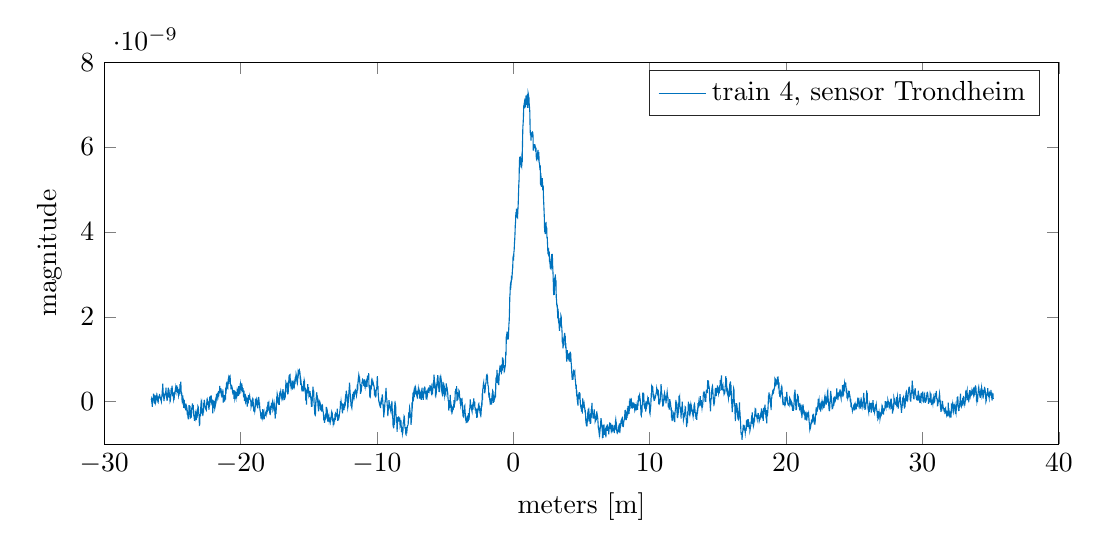
\begin{tikzpicture}

  \begin{axis}[%
    width=\textwidth,
    height=0.4\textwidth,
    at={(0\figurewidth,0\figureheight)},
    scale only axis,
    xmin=-30,
    xmax=40,
    xlabel={meters [m]},
    ymin=-1e-09,
    ymax=8e-09,
    ylabel={magnitude},
    axis background/.style={fill=white},
    legend style={legend cell align=left,align=left,draw=white!15!black}
    ]
    \addplot [color=mycolor1,solid]
    table[row sep=crcr]{%
    -26.548203125	3.83022592754464e-11\\
    -26.5269140625	6.25271250989794e-11\\
    -26.505625	-7.87784710371341e-12\\
    -26.4843359375	-5.49885158177571e-11\\
    -26.463046875	-1.2290031910968e-10\\
    -26.4417578125	8.08084877702953e-11\\
    -26.42046875	2.35607868236979e-11\\
    -26.3991796875	7.65281607471609e-11\\
    -26.377890625	1.90021559275797e-10\\
    -26.3566015625	1.18485356818899e-10\\
    -26.3353125	6.41978460697807e-11\\
    -26.3140234375	1.13386703449076e-10\\
    -26.292734375	8.64715777771754e-11\\
    -26.2714453125	-5.90582680358699e-11\\
    -26.25015625	4.97162147270651e-11\\
    -26.2288671875	1.45067069513925e-10\\
    -26.207578125	1.03207380059596e-11\\
    -26.1862890625	4.73633512903607e-11\\
    -26.165	1.13464655462214e-10\\
    -26.1437109375	5.4283710544281e-11\\
    -26.122421875	4.64334624123369e-11\\
    -26.1011328125	4.52445243789987e-11\\
    -26.07984375	8.80246481806659e-11\\
    -26.0585546875	-9.70052830818307e-12\\
    -26.037265625	-1.91163140841379e-11\\
    -26.0159765625	9.23482048245965e-11\\
    -25.9946875	7.84462514484605e-11\\
    -25.9733984375	8.60187033065142e-11\\
    -25.952109375	1.11150026076157e-10\\
    -25.9308203125	1.79495413521465e-10\\
    -25.90953125	1.00036878773841e-10\\
    -25.8882421875	9.1336230660914e-11\\
    -25.866953125	9.5549441533905e-11\\
    -25.8456640625	4.32018287128878e-11\\
    -25.824375	3.65616259585439e-11\\
    -25.8030859375	6.14383268295217e-12\\
    -25.781796875	1.05769241166919e-10\\
    -25.7605078125	1.28548593361522e-10\\
    -25.73921875	2.29796275411926e-10\\
    -25.7179296875	2.02784946993296e-10\\
    -25.696640625	4.23852407866096e-10\\
    -25.6753515625	2.25623937228979e-10\\
    -25.6540625	1.87772987132003e-10\\
    -25.6327734375	1.29630593365044e-10\\
    -25.611484375	1.46294031100211e-11\\
    -25.5901953125	1.25712475121556e-10\\
    -25.56890625	1.0538697296177e-10\\
    -25.5476171875	1.35313179965996e-10\\
    -25.526328125	1.98527932742649e-10\\
    -25.5050390625	2.0826836997472e-10\\
    -25.48375	2.15241093629662e-10\\
    -25.4624609375	3.28542591532687e-10\\
    -25.441171875	1.61468010569727e-10\\
    -25.4198828125	1.38181374815715e-10\\
    -25.39859375	6.06202420895667e-11\\
    -25.3773046875	1.7523633239373e-11\\
    -25.356015625	2.05343439756515e-10\\
    -25.3347265625	1.08506570500716e-10\\
    -25.3134375	2.58065046483222e-10\\
    -25.2921484375	3.30167693155216e-10\\
    -25.270859375	2.33387768625012e-10\\
    -25.2495703125	3.0212979202763e-10\\
    -25.22828125	9.09360716317685e-11\\
    -25.2069921875	1.72490775486934e-10\\
    -25.185703125	1.25667473948331e-10\\
    -25.1644140625	1.73189370075356e-12\\
    -25.143125	2.03438262564348e-11\\
    -25.1218359375	9.40762635925789e-11\\
    -25.100546875	2.42918490292564e-10\\
    -25.0792578125	3.17019941448897e-10\\
    -25.05796875	2.31370962701024e-10\\
    -25.0366796875	2.73146052135372e-10\\
    -25.015390625	3.7439687241362e-10\\
    -24.9941015625	2.30026597631911e-10\\
    -24.9728125	1.34033344739461e-10\\
    -24.9515234375	2.19402984605395e-10\\
    -24.930234375	1.25333876869021e-10\\
    -24.9089453125	7.33789877099028e-11\\
    -24.88765625	1.59672927407512e-10\\
    -24.8663671875	3.55061634188135e-11\\
    -24.845078125	2.33091045525498e-10\\
    -24.8237890625	1.73534119463419e-10\\
    -24.8025	1.82577235453944e-10\\
    -24.7812109375	2.75119621365966e-10\\
    -24.759921875	3.20325487296496e-10\\
    -24.7386328125	2.29171961961206e-10\\
    -24.71734375	2.95603014836181e-10\\
    -24.6960546875	3.16908714859838e-10\\
    -24.674765625	3.8524756211794e-10\\
    -24.6534765625	2.61101226667088e-10\\
    -24.6321875	3.06058403496744e-10\\
    -24.6108984375	3.16328092706873e-10\\
    -24.589609375	2.54524108110803e-10\\
    -24.5683203125	2.37851618980484e-10\\
    -24.54703125	1.5496101478911e-10\\
    -24.5257421875	2.01537561768289e-10\\
    -24.504453125	1.41059418162555e-10\\
    -24.4831640625	2.74842164721018e-10\\
    -24.461875	1.83823622264617e-10\\
    -24.4405859375	4.1412155139426e-10\\
    -24.419296875	3.36668541045535e-10\\
    -24.3980078125	2.59992713269021e-10\\
    -24.37671875	4.69642506352946e-10\\
    -24.3554296875	2.84440499948972e-10\\
    -24.334140625	1.4059918255604e-10\\
    -24.3128515625	2.19123275911851e-10\\
    -24.2915625	5.18203923200038e-11\\
    -24.2702734375	-6.63168320002465e-13\\
    -24.248984375	3.57313745194887e-11\\
    -24.2276953125	1.47284310509927e-10\\
    -24.20640625	-6.88684456413107e-12\\
    -24.1851171875	6.30473049821858e-11\\
    -24.163828125	-1.46599943602564e-10\\
    -24.1425390625	-4.81636470144691e-11\\
    -24.12125	3.97145847691478e-11\\
    -24.0999609375	-1.56655760530518e-10\\
    -24.078671875	-4.29500507278145e-11\\
    -24.0573828125	-1.22139081191804e-10\\
    -24.03609375	-5.77980853350582e-11\\
    -24.0148046875	-2.0362069497263e-10\\
    -23.993515625	-4.77487921338143e-11\\
    -23.9722265625	-1.13661678123154e-10\\
    -23.9509375	-1.15333418549114e-10\\
    -23.9296484375	-1.49883323500208e-10\\
    -23.908359375	-3.04499318641947e-10\\
    -23.8870703125	-2.58198067907656e-10\\
    -23.86578125	-3.18953871114391e-10\\
    -23.8444921875	-2.73481708325022e-10\\
    -23.823203125	-2.77341629228659e-10\\
    -23.8019140625	-4.16344120420362e-10\\
    -23.780625	-8.03502892659502e-11\\
    -23.7593359375	-1.34838653925586e-10\\
    -23.738046875	-1.23776409952357e-10\\
    -23.7167578125	-1.77100629554635e-10\\
    -23.69546875	-9.93608595753507e-11\\
    -23.6741796875	-3.97505791289003e-10\\
    -23.652890625	-3.35210096394437e-10\\
    -23.6316015625	-3.34790933930677e-10\\
    -23.6103125	-3.44117539578325e-10\\
    -23.5890234375	-2.35459286559301e-10\\
    -23.567734375	-1.39630718113098e-10\\
    -23.5464453125	-1.27676623890054e-10\\
    -23.52515625	-4.11549917605305e-11\\
    -23.5038671875	-9.91087111100902e-11\\
    -23.482578125	-1.88462249317126e-10\\
    -23.4612890625	-8.24587904593362e-11\\
    -23.44	-3.06475936881095e-10\\
    -23.4187109375	-3.33168379338354e-10\\
    -23.397421875	-3.59000034213748e-10\\
    -23.3761328125	-4.51982225405291e-10\\
    -23.35484375	-3.16796954381272e-10\\
    -23.3335546875	-3.65149473026693e-10\\
    -23.312265625	-2.82234560074052e-10\\
    -23.2909765625	-3.25447955909332e-10\\
    -23.2696875	-2.73294090246199e-10\\
    -23.2483984375	-4.35850123576936e-10\\
    -23.227109375	-2.69643168444027e-10\\
    -23.2058203125	-2.98601867123171e-10\\
    -23.18453125	-3.86650372009509e-10\\
    -23.1632421875	-2.98153171950608e-10\\
    -23.141953125	-2.13250229809385e-10\\
    -23.1206640625	-1.08660918979905e-10\\
    -23.099375	-1.24895629054346e-10\\
    -23.0780859375	-1.93356473844705e-10\\
    -23.056796875	-2.87033101157997e-10\\
    -23.0355078125	-3.46296641995472e-10\\
    -23.01421875	-5.55950580307368e-10\\
    -22.9929296875	-5.49633883281117e-10\\
    -22.971640625	-2.94702305311268e-10\\
    -22.9503515625	-3.36058249816901e-10\\
    -22.9290625	-3.26299760045371e-10\\
    -22.9077734375	-9.14791238687298e-11\\
    -22.886484375	-1.84234538298903e-11\\
    -22.8651953125	-6.39323246444212e-11\\
    -22.84390625	-3.36669643233404e-11\\
    -22.8226171875	-2.82063827564529e-10\\
    -22.801328125	-1.5926897013603e-10\\
    -22.7800390625	-2.57171861099544e-10\\
    -22.75875	-3.4030378815913e-10\\
    -22.7374609375	-2.04934249400543e-10\\
    -22.716171875	-2.57451228983077e-10\\
    -22.6948828125	-6.36977228174744e-11\\
    -22.67359375	-7.20981053887792e-11\\
    -22.6523046875	4.36436388781216e-11\\
    -22.631015625	-2.58027954257985e-11\\
    -22.6097265625	-8.32114081751149e-11\\
    -22.5884375	-1.44255485463101e-10\\
    -22.5671484375	-1.49988032235288e-10\\
    -22.545859375	-1.7180182195962e-10\\
    -22.5245703125	-1.91445871403783e-10\\
    -22.50328125	-2.01914494593162e-10\\
    -22.4819921875	-5.97339152831672e-11\\
    -22.460703125	2.25292932066073e-11\\
    -22.4394140625	6.67109339452556e-13\\
    -22.418125	3.0282923330964e-11\\
    -22.3968359375	-3.71891643164319e-11\\
    -22.375546875	-2.59167756465876e-11\\
    -22.3542578125	-7.67031088934027e-11\\
    -22.33296875	5.22882371909865e-13\\
    -22.3116796875	-1.84886686350155e-10\\
    -22.290390625	-1.03410911811725e-10\\
    -22.2691015625	2.08873566835506e-11\\
    -22.2478125	-9.97464372089592e-12\\
    -22.2265234375	1.25229197809702e-10\\
    -22.205234375	-1.00026085434234e-11\\
    -22.1839453125	1.39957034448947e-10\\
    -22.16265625	9.5510402653087e-11\\
    -22.1413671875	-2.3164161454525e-11\\
    -22.120078125	2.60700638584724e-11\\
    -22.0987890625	-7.05961021904926e-11\\
    -22.0775	-6.81496984801845e-11\\
    -22.0562109375	4.80509044768607e-11\\
    -22.034921875	-2.76477763567137e-10\\
    -22.0136328125	-1.83954307155087e-11\\
    -21.99234375	3.15305695411367e-11\\
    -21.9710546875	-1.52697823978122e-10\\
    -21.949765625	6.30706005099203e-12\\
    -21.9284765625	-1.49362773826186e-10\\
    -21.9071875	1.52760264754561e-11\\
    -21.8858984375	-1.56739138099306e-10\\
    -21.864609375	-1.27898485942435e-10\\
    -21.8433203125	-1.03908944907142e-11\\
    -21.82203125	-5.77770129709519e-11\\
    -21.8007421875	-2.56211208871018e-11\\
    -21.779453125	3.84208106422788e-11\\
    -21.7581640625	1.79800350058886e-10\\
    -21.736875	9.34203315602636e-11\\
    -21.7155859375	1.90633305104973e-10\\
    -21.694296875	1.27493465237345e-10\\
    -21.6730078125	1.97133683979858e-10\\
    -21.65171875	2.02262117780404e-10\\
    -21.6304296875	1.21047193594851e-10\\
    -21.609140625	2.45192530997884e-10\\
    -21.5878515625	1.66085133307511e-10\\
    -21.5665625	2.18451599411608e-10\\
    -21.5452734375	2.18481030684023e-10\\
    -21.523984375	3.72299444163678e-10\\
    -21.5026953125	3.0237611867477e-10\\
    -21.48140625	2.61024278420444e-10\\
    -21.4601171875	2.35836564464109e-10\\
    -21.438828125	3.1910622247773e-10\\
    -21.4175390625	2.12749953090631e-10\\
    -21.39625	1.49619428713576e-10\\
    -21.3749609375	1.71373818639558e-10\\
    -21.353671875	2.16799764624697e-10\\
    -21.3323828125	2.03165073691637e-10\\
    -21.31109375	1.0068215494479e-10\\
    -21.2898046875	2.90350389311096e-10\\
    -21.268515625	-2.11506240722935e-11\\
    -21.2472265625	1.01033841727252e-10\\
    -21.2259375	3.31812233222859e-11\\
    -21.2046484375	1.56308886556987e-10\\
    -21.183359375	9.85126715249379e-11\\
    -21.1620703125	3.45593024888525e-12\\
    -21.14078125	1.3247979891988e-10\\
    -21.1194921875	1.26459713310536e-10\\
    -21.098203125	1.07717428838478e-10\\
    -21.0769140625	3.32576985041062e-10\\
    -21.055625	1.89351007433895e-10\\
    -21.0343359375	4.26359274067712e-10\\
    -21.013046875	4.40438852822012e-10\\
    -20.9917578125	3.88953683161372e-10\\
    -20.97046875	4.55034094565083e-10\\
    -20.9491796875	3.24482119397887e-10\\
    -20.927890625	3.1607766711171e-10\\
    -20.9066015625	5.0738512890114e-10\\
    -20.8853125	5.41573663371932e-10\\
    -20.8640234375	4.22302923481656e-10\\
    -20.842734375	6.16498523983328e-10\\
    -20.8214453125	5.36460165424328e-10\\
    -20.80015625	6.09708861492011e-10\\
    -20.7788671875	5.40510679709208e-10\\
    -20.757578125	5.65600397595582e-10\\
    -20.7362890625	4.19608227499084e-10\\
    -20.715	3.98697551504236e-10\\
    -20.6937109375	2.90014863965299e-10\\
    -20.672421875	3.95830118405724e-10\\
    -20.6511328125	3.35727546470813e-10\\
    -20.62984375	3.50385200304745e-10\\
    -20.6085546875	3.20531159674906e-10\\
    -20.587265625	2.32043255036563e-10\\
    -20.5659765625	2.04175939360454e-10\\
    -20.5446875	2.24113007154648e-10\\
    -20.5233984375	2.10451374925637e-10\\
    -20.502109375	2.76937582775093e-10\\
    -20.4808203125	6.6725167324367e-11\\
    -20.45953125	1.84937418003844e-10\\
    -20.4382421875	2.67134730318199e-10\\
    -20.416953125	8.90827563946053e-11\\
    -20.3956640625	1.27620632851336e-10\\
    -20.374375	2.42894157168836e-10\\
    -20.3530859375	1.46734004578907e-10\\
    -20.331796875	1.04874193534235e-10\\
    -20.3105078125	2.17973024236403e-10\\
    -20.28921875	7.51540259241543e-11\\
    -20.2679296875	1.65160306336342e-10\\
    -20.246640625	2.51133735942916e-10\\
    -20.2253515625	2.14978807644416e-10\\
    -20.2040625	3.01479480108956e-10\\
    -20.1827734375	2.27510714443192e-10\\
    -20.161484375	1.38821293724206e-10\\
    -20.1401953125	3.67449868907164e-10\\
    -20.11890625	1.46405637408538e-10\\
    -20.0976171875	2.46049850475721e-10\\
    -20.076328125	3.18429839387673e-10\\
    -20.0550390625	1.8325546270439e-10\\
    -20.03375	3.63385590327679e-10\\
    -20.0124609375	3.42361932514241e-10\\
    -19.991171875	4.17535342869207e-10\\
    -19.9698828125	3.67294440460708e-10\\
    -19.94859375	2.97288085808674e-10\\
    -19.9273046875	3.41036420470311e-10\\
    -19.906015625	4.27589043159373e-10\\
    -19.8847265625	3.5815484498824e-10\\
    -19.8634375	3.13498990691731e-10\\
    -19.8421484375	2.26559051011495e-10\\
    -19.820859375	3.17764963689507e-10\\
    -19.7995703125	2.58295030259453e-10\\
    -19.77828125	1.40469450154489e-10\\
    -19.7569921875	1.5072122988425e-10\\
    -19.735703125	2.57402321689704e-10\\
    -19.7144140625	1.86391261679105e-11\\
    -19.693125	8.63657894547367e-11\\
    -19.6718359375	1.13037420648481e-10\\
    -19.650546875	4.78892880777286e-11\\
    -19.6292578125	9.30991671837842e-11\\
    -19.60796875	3.05121584117066e-11\\
    -19.5866796875	9.35303281249776e-11\\
    -19.565390625	7.11058490439668e-11\\
    -19.5441015625	-6.49913231738501e-12\\
    -19.5228125	9.70062472787665e-11\\
    -19.5015234375	-1.14819708146118e-10\\
    -19.480234375	-1.01682484072811e-11\\
    -19.4589453125	6.67637722371091e-11\\
    -19.43765625	-4.34926749411915e-11\\
    -19.4163671875	1.54710118408606e-10\\
    -19.395078125	5.15232648797531e-11\\
    -19.3737890625	5.94204974824163e-11\\
    -19.3525	1.13182681028445e-10\\
    -19.3312109375	1.43068218014951e-10\\
    -19.309921875	8.05084430636719e-11\\
    -19.2886328125	4.64314749237082e-11\\
    -19.26734375	3.491753571291e-11\\
    -19.2460546875	8.3402467217277e-12\\
    -19.224765625	-1.16384428438193e-10\\
    -19.2034765625	-8.04615854508977e-11\\
    -19.1821875	-1.86634546514052e-11\\
    -19.1608984375	-1.1238385702064e-10\\
    -19.139609375	3.22965439623557e-11\\
    -19.1183203125	5.40675614288761e-11\\
    -19.09703125	-1.0307690908237e-11\\
    -19.0757421875	1.62198208794074e-11\\
    -19.054453125	-7.10460160170058e-11\\
    -19.0331640625	-2.23891419684071e-10\\
    -19.011875	-1.24254550194144e-10\\
    -18.9905859375	-2.38032078423663e-10\\
    -18.969296875	-1.41821581664489e-10\\
    -18.9480078125	-2.18549378714688e-10\\
    -18.92671875	-1.77871574344205e-10\\
    -18.9054296875	7.02983870600352e-11\\
    -18.884140625	-7.97340084489383e-11\\
    -18.8628515625	7.00262511987598e-11\\
    -18.8415625	-4.55447627938472e-11\\
    -18.8202734375	1.29198048246999e-11\\
    -18.798984375	-5.11271671778508e-11\\
    -18.7776953125	-1.15037534987478e-10\\
    -18.75640625	2.9054460997496e-11\\
    -18.7351171875	-1.5971855147639e-10\\
    -18.713828125	1.5726653314448e-11\\
    -18.6925390625	-8.70672961003103e-12\\
    -18.67125	1.10951935392366e-10\\
    -18.6499609375	6.13897551641233e-11\\
    -18.628671875	-7.78635654805532e-11\\
    -18.6073828125	-1.87929638772924e-11\\
    -18.58609375	-1.49233743590659e-10\\
    -18.5648046875	-2.08197884652006e-10\\
    -18.543515625	-2.29113371669048e-10\\
    -18.5222265625	-2.88752624506079e-10\\
    -18.5009375	-3.97340439118313e-10\\
    -18.4796484375	-2.87119219713832e-10\\
    -18.458359375	-3.98536081551462e-10\\
    -18.4370703125	-2.53499410092447e-10\\
    -18.41578125	-3.91336971190672e-10\\
    -18.3944921875	-3.79550574656846e-10\\
    -18.373203125	-1.77073362209876e-10\\
    -18.3519140625	-3.59235715013283e-10\\
    -18.330625	-3.22332605436236e-10\\
    -18.3093359375	-2.86179582528804e-10\\
    -18.288046875	-2.55581370554179e-10\\
    -18.2667578125	-4.15537328557349e-10\\
    -18.24546875	-3.56570359131234e-10\\
    -18.2241796875	-3.39040114212137e-10\\
    -18.202890625	-3.30711689739607e-10\\
    -18.1816015625	-3.0996419935057e-10\\
    -18.1603125	-2.47820441510116e-10\\
    -18.1390234375	-2.43771282613433e-10\\
    -18.117734375	-2.83163428011366e-10\\
    -18.0964453125	-2.02594526763314e-10\\
    -18.07515625	-2.99727031203111e-10\\
    -18.0538671875	-1.17376446803894e-10\\
    -18.032578125	-2.46704317380428e-10\\
    -18.0112890625	-1.81664059951079e-10\\
    -17.99	-7.52122443394656e-12\\
    -17.9687109375	-1.30486030965259e-10\\
    -17.947421875	-6.87915545657681e-11\\
    -17.9261328125	-3.99818065496061e-11\\
    -17.90484375	-2.11969584037695e-10\\
    -17.8835546875	-2.13220084714519e-10\\
    -17.862265625	-2.29386749004505e-10\\
    -17.8409765625	-3.04021204062238e-10\\
    -17.8196875	-1.96649702861491e-10\\
    -17.7983984375	-2.2903693446948e-10\\
    -17.777109375	-9.96052927424337e-11\\
    -17.7558203125	-1.9292605396683e-10\\
    -17.73453125	-2.92289874501768e-11\\
    -17.7132421875	-9.93186656575521e-11\\
    -17.691953125	-1.13464939241635e-10\\
    -17.6706640625	-2.82574900848136e-11\\
    -17.649375	1.28954278738087e-12\\
    -17.6280859375	-1.55980817938604e-10\\
    -17.606796875	-1.20022887359105e-10\\
    -17.5855078125	-9.45102351193494e-11\\
    -17.56421875	-8.16310788461798e-11\\
    -17.5429296875	-4.59778443457919e-11\\
    -17.521640625	-2.29131831124231e-10\\
    -17.5003515625	-4.00488331345108e-11\\
    -17.4790625	-1.96645641510267e-10\\
    -17.4577734375	-4.00989816660797e-10\\
    -17.436484375	-1.87567683006446e-10\\
    -17.4151953125	-2.43815248597142e-10\\
    -17.39390625	-2.94820330558292e-10\\
    -17.3726171875	-1.12826171763156e-10\\
    -17.351328125	5.84662010978586e-11\\
    -17.3300390625	4.06654157588938e-11\\
    -17.30875	1.81770111344864e-10\\
    -17.2874609375	1.47970331692976e-10\\
    -17.266171875	5.7261708530512e-11\\
    -17.2448828125	5.14237503541285e-11\\
    -17.22359375	-7.06471886702519e-11\\
    -17.2023046875	1.01038098544913e-10\\
    -17.181015625	3.19913570524416e-11\\
    -17.1597265625	-7.66813860063354e-11\\
    -17.1384375	1.3632838375192e-10\\
    -17.1171484375	1.1812819692132e-10\\
    -17.095859375	2.48682314609124e-10\\
    -17.0745703125	2.02515572873914e-10\\
    -17.05328125	2.40127563997874e-10\\
    -17.0319921875	1.78704802802035e-10\\
    -17.010703125	1.46586482121695e-10\\
    -16.9894140625	1.04309137005832e-10\\
    -16.968125	6.97450420879435e-11\\
    -16.9468359375	1.13903684486156e-10\\
    -16.925546875	1.78893819027111e-10\\
    -16.9042578125	1.37597915813226e-10\\
    -16.88296875	2.91935621601828e-10\\
    -16.8616796875	1.10535406437358e-10\\
    -16.840390625	2.35514559035551e-10\\
    -16.8191015625	1.49769064739564e-10\\
    -16.7978125	3.82809993215446e-11\\
    -16.7765234375	9.6870410776601e-11\\
    -16.755234375	8.63562114197927e-11\\
    -16.7339453125	1.77827515714711e-10\\
    -16.71265625	1.59960128685213e-10\\
    -16.6913671875	3.24397269313843e-10\\
    -16.670078125	4.51146395200181e-10\\
    -16.6487890625	4.2623608347863e-10\\
    -16.6275	4.14203840251661e-10\\
    -16.6062109375	4.19025158921953e-10\\
    -16.584921875	3.11812474829461e-10\\
    -16.5636328125	3.51605576387121e-10\\
    -16.54234375	1.82974783668237e-10\\
    -16.5210546875	1.83811285813054e-10\\
    -16.499765625	2.3650262956499e-10\\
    -16.4784765625	3.60251027662379e-10\\
    -16.4571875	5.07233795353825e-10\\
    -16.4358984375	6.12123466694866e-10\\
    -16.414609375	6.15455970327188e-10\\
    -16.3933203125	6.29307258683262e-10\\
    -16.37203125	6.35170244344728e-10\\
    -16.3507421875	4.45057092938058e-10\\
    -16.329453125	4.70473593508763e-10\\
    -16.3081640625	3.73672672187724e-10\\
    -16.286875	3.25729201909808e-10\\
    -16.2655859375	3.60284953420213e-10\\
    -16.244296875	3.13297533852224e-10\\
    -16.2230078125	4.38795715542193e-10\\
    -16.20171875	4.96776728075806e-10\\
    -16.1804296875	2.82938710817122e-10\\
    -16.159140625	4.19687227911443e-10\\
    -16.1378515625	4.40473597994321e-10\\
    -16.1165625	3.15022834957929e-10\\
    -16.0952734375	4.27663096527154e-10\\
    -16.073984375	4.08816048755602e-10\\
    -16.0526953125	3.74702563210585e-10\\
    -16.03140625	4.57662135145131e-10\\
    -16.0101171875	5.0663038147661e-10\\
    -15.988828125	4.81018711132804e-10\\
    -15.9675390625	5.58040595367708e-10\\
    -15.94625	5.48409448303214e-10\\
    -15.9249609375	6.47272781172853e-10\\
    -15.903671875	6.12947850928845e-10\\
    -15.8823828125	5.22206266561174e-10\\
    -15.86109375	4.8215036240956e-10\\
    -15.8398046875	5.26891046789787e-10\\
    -15.818515625	4.7772531272437e-10\\
    -15.7972265625	5.71028483320037e-10\\
    -15.7759375	6.80617716075178e-10\\
    -15.7546484375	6.4318062458886e-10\\
    -15.733359375	6.97430057768323e-10\\
    -15.7120703125	7.37374057515904e-10\\
    -15.69078125	7.48580156922143e-10\\
    -15.6694921875	6.57539554137838e-10\\
    -15.648203125	7.23913363491815e-10\\
    -15.6269140625	5.77964697463165e-10\\
    -15.605625	4.90509948608315e-10\\
    -15.5843359375	5.29172885584517e-10\\
    -15.563046875	4.80518737894734e-10\\
    -15.5417578125	3.95339031411719e-10\\
    -15.52046875	3.84495245540119e-10\\
    -15.4991796875	2.43812106390804e-10\\
    -15.477890625	3.67532680815629e-10\\
    -15.4566015625	2.46284885222778e-10\\
    -15.4353125	3.02050200152499e-10\\
    -15.4140234375	3.09610786830033e-10\\
    -15.392734375	2.40179405822296e-10\\
    -15.3714453125	4.80907450522102e-10\\
    -15.35015625	4.35804304738441e-10\\
    -15.3288671875	5.08483444766798e-10\\
    -15.307578125	4.75925834358843e-10\\
    -15.2862890625	2.8581711879195e-10\\
    -15.265	2.47433758318516e-10\\
    -15.2437109375	3.25904983513163e-10\\
    -15.222421875	1.06148482803058e-10\\
    -15.2011328125	1.31434640425641e-10\\
    -15.17984375	1.82567668865985e-10\\
    -15.1585546875	-7.05428891922172e-11\\
    -15.137265625	2.90640270986211e-10\\
    -15.1159765625	2.90381736005716e-10\\
    -15.0946875	1.95337397449515e-10\\
    -15.0733984375	4.13580490497376e-10\\
    -15.052109375	1.93202328667067e-10\\
    -15.0308203125	2.66196594692907e-10\\
    -15.00953125	3.44044559366168e-10\\
    -14.9882421875	1.6921587593657e-10\\
    -14.966953125	1.99381964295991e-10\\
    -14.9456640625	1.97725608111022e-10\\
    -14.924375	1.06352333134226e-10\\
    -14.9030859375	2.44606431652887e-10\\
    -14.881796875	1.73543919009396e-10\\
    -14.8605078125	1.0111978255714e-10\\
    -14.83921875	1.03820283195106e-10\\
    -14.8179296875	-1.46713345212411e-11\\
    -14.796640625	-1.24378391859118e-10\\
    -14.7753515625	1.76655155144422e-11\\
    -14.7540625	-1.15741465590973e-10\\
    -14.7327734375	1.47320728257804e-10\\
    -14.711484375	1.43210688644061e-10\\
    -14.6901953125	3.51548725975913e-10\\
    -14.66890625	2.71846876972179e-10\\
    -14.6476171875	2.71613875194616e-10\\
    -14.626328125	2.34896157849905e-10\\
    -14.6050390625	-6.00531662003695e-11\\
    -14.58375	-1.05394462612431e-10\\
    -14.5624609375	-2.69345612564983e-10\\
    -14.541171875	-3.08066206165713e-10\\
    -14.5198828125	-3.19004346698888e-10\\
    -14.49859375	-2.68691652263985e-10\\
    -14.4773046875	1.63228734262727e-11\\
    -14.456015625	8.94669561767577e-12\\
    -14.4347265625	1.61821405795521e-10\\
    -14.4134375	2.20207883476737e-10\\
    -14.3921484375	6.47217559969e-11\\
    -14.370859375	1.43911283608648e-10\\
    -14.3495703125	6.73855949622934e-11\\
    -14.32828125	-3.74704025209554e-11\\
    -14.3069921875	7.69220388496872e-12\\
    -14.285703125	-2.30307868523423e-10\\
    -14.2644140625	-1.6171218643385e-10\\
    -14.243125	-2.24443043493386e-11\\
    -14.2218359375	-5.29906804210895e-11\\
    -14.200546875	-6.12403148072557e-11\\
    -14.1792578125	-9.47873339110393e-12\\
    -14.15796875	-3.36619447809632e-11\\
    -14.1366796875	-2.06824487348312e-10\\
    -14.115390625	-8.98122664407583e-11\\
    -14.0941015625	-1.43535534805835e-10\\
    -14.0728125	-1.50542773876374e-10\\
    -14.0515234375	-2.35810925732663e-10\\
    -14.030234375	-6.32436615725457e-11\\
    -14.0089453125	-1.25057239622999e-10\\
    -13.98765625	-1.06315038700434e-10\\
    -13.9663671875	-2.0315396202521e-10\\
    -13.945078125	-2.30627295369381e-10\\
    -13.9237890625	-2.5563364922996e-10\\
    -13.9025	-3.79802396149598e-10\\
    -13.8812109375	-3.59701074353954e-10\\
    -13.859921875	-4.21964117248149e-10\\
    -13.8386328125	-4.98729785361001e-10\\
    -13.81734375	-4.37075221200679e-10\\
    -13.7960546875	-3.98925412645732e-10\\
    -13.774765625	-3.44241533371467e-10\\
    -13.7534765625	-3.69276149483619e-10\\
    -13.7321875	-3.2360212236159e-10\\
    -13.7108984375	-1.25686251720889e-10\\
    -13.689609375	-2.69583843993122e-10\\
    -13.6683203125	-3.31303550517843e-10\\
    -13.64703125	-3.04588499525178e-10\\
    -13.6257421875	-2.64361808775432e-10\\
    -13.604453125	-4.69302302560533e-10\\
    -13.5831640625	-3.59359256640759e-10\\
    -13.561875	-3.47381157278973e-10\\
    -13.5405859375	-3.94940229248508e-10\\
    -13.519296875	-3.54543014832283e-10\\
    -13.4980078125	-4.38621509346331e-10\\
    -13.47671875	-3.90178259843055e-10\\
    -13.4554296875	-4.01953492589748e-10\\
    -13.434140625	-4.02417738861576e-10\\
    -13.4128515625	-4.55346377842752e-10\\
    -13.3915625	-3.89699240544665e-10\\
    -13.3702734375	-3.67161305911647e-10\\
    -13.348984375	-3.55805989167759e-10\\
    -13.3276953125	-2.66879969650262e-10\\
    -13.30640625	-3.01748324679473e-10\\
    -13.2851171875	-3.77081459870921e-10\\
    -13.263828125	-3.34334375113718e-10\\
    -13.2425390625	-4.57005596702702e-10\\
    -13.22125	-3.80618775756822e-10\\
    -13.1999609375	-5.18756740262983e-10\\
    -13.178671875	-4.86679122609235e-10\\
    -13.1573828125	-5.50750759647622e-10\\
    -13.13609375	-4.76804910263805e-10\\
    -13.1148046875	-4.30859176862281e-10\\
    -13.093515625	-4.39867096373731e-10\\
    -13.0722265625	-2.9053762265576e-10\\
    -13.0509375	-4.31346412083664e-10\\
    -13.0296484375	-2.75191121585144e-10\\
    -13.008359375	-2.87146198386753e-10\\
    -12.9870703125	-2.86506394802752e-10\\
    -12.96578125	-3.19990986774132e-10\\
    -12.9444921875	-3.04272016728073e-10\\
    -12.923203125	-2.95390426911392e-10\\
    -12.9019140625	-1.63330710263626e-10\\
    -12.880625	-4.51132769962227e-10\\
    -12.8593359375	-3.58703161388753e-10\\
    -12.838046875	-3.05797515438611e-10\\
    -12.8167578125	-4.38639056716209e-10\\
    -12.79546875	-3.29444306629831e-10\\
    -12.7741796875	-3.91028061210438e-10\\
    -12.752890625	-3.02906308351416e-10\\
    -12.7316015625	-2.69062022130194e-10\\
    -12.7103125	-1.95808173329237e-10\\
    -12.6890234375	-1.60606994110984e-10\\
    -12.667734375	1.40592881371562e-11\\
    -12.6464453125	-6.89928829007381e-11\\
    -12.62515625	2.18956530589648e-12\\
    -12.6038671875	-5.3357198343995e-11\\
    -12.582578125	-5.32647821300363e-11\\
    -12.5612890625	-1.40325851902189e-10\\
    -12.54	-8.48699126462632e-11\\
    -12.5187109375	-2.77424375829817e-10\\
    -12.497421875	-4.26305912664113e-11\\
    -12.4761328125	-2.0607817548503e-10\\
    -12.45484375	-1.57721057828081e-10\\
    -12.4335546875	-5.98251505729584e-11\\
    -12.412265625	-1.97819110110102e-10\\
    -12.3909765625	-1.20740558622058e-10\\
    -12.3696875	-4.88623525227376e-11\\
    -12.3483984375	-5.74078977980597e-11\\
    -12.327109375	2.4546511207208e-11\\
    -12.3058203125	-1.45461564461199e-11\\
    -12.28453125	1.73719403470661e-10\\
    -12.2632421875	1.10720609081566e-10\\
    -12.241953125	2.56471803224944e-10\\
    -12.2206640625	1.94068948517633e-10\\
    -12.199375	1.35067818946358e-10\\
    -12.1780859375	2.95411766896995e-11\\
    -12.156796875	3.17571143060579e-11\\
    -12.1355078125	-1.44513067762212e-10\\
    -12.11421875	-1.08301468154887e-10\\
    -12.0929296875	5.35027331769978e-11\\
    -12.071640625	1.1544171911535e-11\\
    -12.0503515625	2.4727194218028e-10\\
    -12.0290625	3.05438699030857e-10\\
    -12.0077734375	4.49079992718728e-10\\
    -11.986484375	3.63696987252911e-10\\
    -11.9651953125	1.93978054564274e-10\\
    -11.94390625	1.71315613084407e-10\\
    -11.9226171875	6.53455637018248e-11\\
    -11.901328125	-9.01198670305031e-11\\
    -11.8800390625	-9.77011531545099e-11\\
    -11.85875	-1.2240636329611e-10\\
    -11.8374609375	-1.48954175630477e-10\\
    -11.816171875	-6.87464127303392e-11\\
    -11.7948828125	3.66429094210814e-11\\
    -11.77359375	1.69558761531237e-10\\
    -11.7523046875	1.72295007538804e-10\\
    -11.731015625	1.2776982534812e-10\\
    -11.7097265625	2.38261415820727e-10\\
    -11.6884375	1.38919035277483e-10\\
    -11.6671484375	1.05623430991608e-10\\
    -11.645859375	1.5786871274799e-10\\
    -11.6245703125	2.27504922237709e-10\\
    -11.60328125	2.09413129768027e-10\\
    -11.5819921875	2.05497542493393e-10\\
    -11.560703125	2.67351118859599e-10\\
    -11.5394140625	2.53054382059062e-10\\
    -11.518125	1.85331404059487e-10\\
    -11.4968359375	1.42681384259211e-10\\
    -11.475546875	1.90434784106128e-10\\
    -11.4542578125	2.18132753507878e-10\\
    -11.43296875	4.13548056728279e-10\\
    -11.4116796875	2.58228838434736e-10\\
    -11.390390625	4.27997657177981e-10\\
    -11.3691015625	5.30219779782143e-10\\
    -11.3478125	5.73377053966517e-10\\
    -11.3265234375	6.3196101023419e-10\\
    -11.305234375	5.93127767130027e-10\\
    -11.2839453125	5.13570054813994e-10\\
    -11.26265625	5.32149551866973e-10\\
    -11.2413671875	4.13438331458396e-10\\
    -11.220078125	4.04720834397543e-10\\
    -11.1987890625	1.83295133305992e-10\\
    -11.1775	3.31494079142878e-10\\
    -11.1562109375	2.19279392652254e-10\\
    -11.134921875	3.2455629237718e-10\\
    -11.1136328125	3.57269979736474e-10\\
    -11.09234375	4.46923348003643e-10\\
    -11.0710546875	4.45081947950646e-10\\
    -11.049765625	5.23090525851475e-10\\
    -11.0284765625	5.1338848767762e-10\\
    -11.0071875	4.71310337444703e-10\\
    -10.9858984375	4.36892098741646e-10\\
    -10.964609375	3.85288652716365e-10\\
    -10.9433203125	3.78952905852958e-10\\
    -10.92203125	5.1050297955172e-10\\
    -10.9007421875	5.06854731446357e-10\\
    -10.879453125	4.16146169296766e-10\\
    -10.8581640625	4.63503939391772e-10\\
    -10.836875	4.37292844067175e-10\\
    -10.8155859375	3.67380608212725e-10\\
    -10.794296875	4.20327023092827e-10\\
    -10.7730078125	4.59134040531705e-10\\
    -10.75171875	3.97955110399011e-10\\
    -10.7304296875	3.48800651993321e-10\\
    -10.709140625	4.6251265802523e-10\\
    -10.6878515625	5.99027778251796e-10\\
    -10.6665625	5.20946095710445e-10\\
    -10.6452734375	6.26750433081421e-10\\
    -10.623984375	5.14981172131755e-10\\
    -10.6026953125	6.72264868469897e-10\\
    -10.58140625	3.75009998865562e-10\\
    -10.5601171875	3.33265565109426e-10\\
    -10.538828125	3.46524334512915e-10\\
    -10.5175390625	9.68962952647978e-11\\
    -10.49625	1.88491125108555e-10\\
    -10.4749609375	1.59664378951812e-10\\
    -10.453671875	3.49447853254038e-10\\
    -10.4323828125	3.6721937838563e-10\\
    -10.41109375	3.44393312211063e-10\\
    -10.3898046875	4.91243085527291e-10\\
    -10.368515625	4.6764080987124e-10\\
    -10.3472265625	4.62757842263954e-10\\
    -10.3259375	4.32316222178872e-10\\
    -10.3046484375	4.86244756479004e-10\\
    -10.283359375	4.52839241882086e-10\\
    -10.2620703125	4.38508578644325e-10\\
    -10.24078125	3.8068489747945e-10\\
    -10.2194921875	3.79974375728238e-10\\
    -10.198203125	3.32178241302084e-10\\
    -10.1769140625	1.50286181490738e-10\\
    -10.155625	2.85210177004215e-10\\
    -10.1343359375	1.39391471316922e-10\\
    -10.113046875	1.21201093553613e-10\\
    -10.0917578125	1.33681043562848e-10\\
    -10.07046875	1.28605706415687e-10\\
    -10.0491796875	2.74376660333608e-10\\
    -10.027890625	2.78768617694837e-10\\
    -10.0066015625	3.43882484150877e-10\\
    -9.9853125	5.0585611966377e-10\\
    -9.9640234375	6.01735380964114e-10\\
    -9.942734375	3.61456773758984e-10\\
    -9.9214453125	3.58347875295234e-10\\
    -9.90015625	1.6121831105628e-10\\
    -9.8788671875	9.68216068904818e-11\\
    -9.857578125	3.23186025310812e-12\\
    -9.8362890625	2.35357260880995e-12\\
    -9.815	-5.99481497560463e-11\\
    -9.7937109375	-7.98392571788278e-11\\
    -9.772421875	-5.16368644820801e-11\\
    -9.7511328125	-4.56597030495981e-11\\
    -9.72984375	-1.52708920422272e-10\\
    -9.7085546875	2.19703968496724e-11\\
    -9.687265625	-6.93673827427045e-11\\
    -9.6659765625	7.1630241772529e-11\\
    -9.6446875	8.24663237270096e-11\\
    -9.6233984375	1.52418401138445e-11\\
    -9.602109375	1.73159863013602e-10\\
    -9.5808203125	7.37690780726154e-11\\
    -9.55953125	-3.96050474678117e-11\\
    -9.5382421875	-1.25270075487585e-10\\
    -9.516953125	-6.9290342006594e-11\\
    -9.4956640625	-3.69708744050186e-10\\
    -9.474375	-2.6354666783877e-10\\
    -9.4530859375	-2.30937423831815e-10\\
    -9.431796875	-1.54392530353095e-10\\
    -9.4105078125	-1.41861744548138e-11\\
    -9.38921875	-7.02115080830135e-12\\
    -9.3679296875	1.46056261664692e-10\\
    -9.346640625	2.44079839698622e-10\\
    -9.3253515625	3.24938368054026e-10\\
    -9.3040625	7.66463653869805e-11\\
    -9.2827734375	8.00444142316911e-11\\
    -9.261484375	1.14024425741243e-11\\
    -9.2401953125	-9.19948221560572e-11\\
    -9.21890625	-1.39751808007519e-10\\
    -9.1976171875	-3.41907050526883e-10\\
    -9.176328125	-2.32279498888501e-10\\
    -9.1550390625	-1.48018552282444e-10\\
    -9.13375	-1.28871984956741e-10\\
    -9.1124609375	3.75436839947189e-11\\
    -9.091171875	-4.14467875937421e-11\\
    -9.0698828125	-7.26790997165434e-11\\
    -9.04859375	-1.313556163753e-10\\
    -9.0273046875	-1.11736419974159e-10\\
    -9.006015625	-1.68932045345501e-10\\
    -8.9847265625	-2.19849890668331e-10\\
    -8.9634375	-2.46662620406871e-10\\
    -8.9421484375	-1.20840940123596e-10\\
    -8.920859375	-1.07573048033877e-10\\
    -8.8995703125	1.77050332362371e-11\\
    -8.87828125	-2.17806231485632e-10\\
    -8.8569921875	-1.65181143642676e-10\\
    -8.835703125	-3.84649668238227e-10\\
    -8.8144140625	-5.58273949012327e-10\\
    -8.793125	-5.50622309879069e-10\\
    -8.7718359375	-6.31481908319896e-10\\
    -8.750546875	-5.06436681411817e-10\\
    -8.7292578125	-5.48271918969859e-10\\
    -8.70796875	-2.41625092497527e-10\\
    -8.6866796875	-8.23484323149387e-11\\
    -8.665390625	-1.15225383923202e-10\\
    -8.6441015625	-6.19330382409575e-11\\
    -8.6228125	-1.01922276464434e-10\\
    -8.6015234375	-3.06608038859247e-10\\
    -8.580234375	-4.45361378123121e-10\\
    -8.5589453125	-4.26561027087727e-10\\
    -8.53765625	-5.02383079449876e-10\\
    -8.5163671875	-7.10085947904791e-10\\
    -8.495078125	-4.39463759926216e-10\\
    -8.4737890625	-4.62226333920295e-10\\
    -8.4525	-3.76492058514471e-10\\
    -8.4312109375	-3.69541537223443e-10\\
    -8.409921875	-4.67591063347872e-10\\
    -8.3886328125	-3.53940735566029e-10\\
    -8.36734375	-4.12362732783829e-10\\
    -8.3460546875	-4.37792074637908e-10\\
    -8.324765625	-3.76128460235798e-10\\
    -8.3034765625	-5.34565732328479e-10\\
    -8.2821875	-4.93733014251478e-10\\
    -8.2608984375	-5.00540410899239e-10\\
    -8.239609375	-4.3298604030561e-10\\
    -8.2183203125	-5.62689554208312e-10\\
    -8.19703125	-7.1020378059068e-10\\
    -8.1757421875	-5.9391734330716e-10\\
    -8.154453125	-6.89538991628892e-10\\
    -8.1331640625	-7.45380615439973e-10\\
    -8.111875	-6.67061886536224e-10\\
    -8.0905859375	-6.8657360175293e-10\\
    -8.069296875	-4.98132566001517e-10\\
    -8.0480078125	-4.88850529337355e-10\\
    -8.02671875	-4.2558793223163e-10\\
    -8.0054296875	-3.38529976901003e-10\\
    -7.984140625	-3.52253110059266e-10\\
    -7.9628515625	-5.23137235000484e-10\\
    -7.9415625	-6.14764639489246e-10\\
    -7.9202734375	-6.11437564971199e-10\\
    -7.898984375	-6.11727784702086e-10\\
    -7.8776953125	-7.75229731208962e-10\\
    -7.85640625	-7.83319674617094e-10\\
    -7.8351171875	-6.02194046167917e-10\\
    -7.813828125	-7.44462226772251e-10\\
    -7.7925390625	-6.74674389326228e-10\\
    -7.77125	-5.88486112990555e-10\\
    -7.7499609375	-5.66682388353768e-10\\
    -7.728671875	-5.58183765372582e-10\\
    -7.7073828125	-5.40704189109805e-10\\
    -7.68609375	-3.62379707626505e-10\\
    -7.6648046875	-2.55205995453818e-10\\
    -7.643515625	-3.92653607716568e-10\\
    -7.6222265625	-2.47860549379023e-10\\
    -7.6009375	-1.39890512724483e-10\\
    -7.5796484375	-1.77239410250406e-10\\
    -7.558359375	-3.75141304056255e-10\\
    -7.5370703125	-2.99624665788968e-10\\
    -7.51578125	-3.0542060736006e-10\\
    -7.4944921875	-5.48143496703584e-10\\
    -7.473203125	-4.27199233025608e-10\\
    -7.4519140625	-4.10627908370122e-10\\
    -7.430625	-1.15706839964054e-10\\
    -7.4093359375	-1.44760235305019e-10\\
    -7.388046875	-4.40286643633174e-11\\
    -7.3667578125	1.12269095521378e-10\\
    -7.34546875	2.15947925019599e-10\\
    -7.3241796875	7.00395912195302e-12\\
    -7.302890625	2.1422511176868e-10\\
    -7.2816015625	2.54234953217811e-10\\
    -7.2603125	1.04677588050929e-10\\
    -7.2390234375	1.94106204132985e-10\\
    -7.217734375	2.66535879945497e-10\\
    -7.1964453125	3.02486465721331e-10\\
    -7.17515625	2.58178271338953e-10\\
    -7.1538671875	3.07100567772824e-10\\
    -7.132578125	2.54586250659711e-10\\
    -7.1112890625	2.04034680185366e-10\\
    -7.09	1.63463612142862e-10\\
    -7.0687109375	1.37517112525933e-10\\
    -7.047421875	2.44360260204183e-10\\
    -7.0261328125	7.21459056786939e-11\\
    -7.00484375	2.22237421480366e-10\\
    -6.9835546875	2.12917652942343e-10\\
    -6.962265625	2.92543358994082e-10\\
    -6.9409765625	2.34457259670908e-10\\
    -6.9196875	2.11683083404134e-10\\
    -6.8983984375	2.67768846247481e-10\\
    -6.877109375	2.38358870054538e-10\\
    -6.8558203125	7.11821231216289e-11\\
    -6.83453125	1.375651954908e-10\\
    -6.8132421875	1.34617266733843e-10\\
    -6.791953125	8.95275470031741e-11\\
    -6.7706640625	2.3833474181859e-10\\
    -6.749375	4.35998984668368e-11\\
    -6.7280859375	2.78063540733533e-10\\
    -6.706796875	2.27734522267852e-10\\
    -6.6855078125	3.29062806233379e-10\\
    -6.66421875	8.65515302054097e-11\\
    -6.6429296875	1.7779718708244e-10\\
    -6.621640625	1.54825977353666e-10\\
    -6.6003515625	4.2561344769476e-11\\
    -6.5790625	1.2688129487583e-10\\
    -6.5577734375	2.52798838562012e-10\\
    -6.536484375	2.3420353589029e-10\\
    -6.5151953125	3.25210309780552e-10\\
    -6.49390625	3.3649685590821e-10\\
    -6.4726171875	3.1563324220221e-10\\
    -6.451328125	2.13276293799094e-10\\
    -6.4300390625	2.13226933472344e-10\\
    -6.40875	1.7048475323604e-10\\
    -6.3874609375	4.64501728831329e-11\\
    -6.366171875	1.9025260597894e-10\\
    -6.3448828125	2.38823166881724e-10\\
    -6.32359375	2.24965443946726e-10\\
    -6.3023046875	1.37805076731306e-10\\
    -6.281015625	1.80475607265205e-10\\
    -6.2597265625	3.08639625010845e-10\\
    -6.2384375	2.09004599825391e-10\\
    -6.2171484375	2.86541099192842e-10\\
    -6.195859375	2.67168398936617e-10\\
    -6.1745703125	2.48146758124608e-10\\
    -6.15328125	3.28372192722709e-10\\
    -6.1319921875	2.52375056373056e-10\\
    -6.110703125	3.86227591032342e-10\\
    -6.0894140625	2.90863932068991e-10\\
    -6.068125	2.85706869686894e-10\\
    -6.0468359375	2.98163221306312e-10\\
    -6.025546875	2.54404074738609e-10\\
    -6.0042578125	3.27508235010769e-10\\
    -5.98296875	2.74850675458261e-10\\
    -5.9616796875	2.22531861093915e-10\\
    -5.940390625	2.75068159325382e-10\\
    -5.9191015625	1.7198342143029e-10\\
    -5.8978125	3.52903598016741e-10\\
    -5.8765234375	3.23189963893833e-10\\
    -5.855234375	3.39074345569187e-10\\
    -5.8339453125	4.53272325541547e-10\\
    -5.81265625	6.34458858509622e-10\\
    -5.7913671875	5.51345820520224e-10\\
    -5.770078125	4.03882092384669e-10\\
    -5.7487890625	4.31025554435862e-10\\
    -5.7275	3.99603936311305e-10\\
    -5.7062109375	1.88505595732246e-10\\
    -5.684921875	2.24839995677634e-10\\
    -5.6636328125	1.73336492933478e-10\\
    -5.64234375	2.18766703946696e-10\\
    -5.6210546875	3.70792469295397e-10\\
    -5.599765625	3.60421658572516e-10\\
    -5.5784765625	5.48730546741962e-10\\
    -5.5571875	4.46957108230209e-10\\
    -5.5358984375	6.21973685125347e-10\\
    -5.514609375	5.5963052376318e-10\\
    -5.4933203125	3.96658678592643e-10\\
    -5.47203125	4.0806668927993e-10\\
    -5.4507421875	2.31420723510757e-10\\
    -5.429453125	3.95354692200169e-10\\
    -5.4081640625	2.26022604424396e-10\\
    -5.386875	3.28311955762563e-10\\
    -5.3655859375	6.11454544976539e-10\\
    -5.344296875	4.9310075215661e-10\\
    -5.3230078125	4.81982398701144e-10\\
    -5.30171875	5.56167654309865e-10\\
    -5.2804296875	5.08325254970843e-10\\
    -5.259140625	3.36043534119112e-10\\
    -5.2378515625	2.29425786733201e-10\\
    -5.2165625	1.94463134462618e-10\\
    -5.1952734375	2.75931377839939e-10\\
    -5.173984375	1.28663975207913e-10\\
    -5.1526953125	4.63286237643904e-10\\
    -5.13140625	3.99479666024411e-10\\
    -5.1101171875	2.92972327366136e-10\\
    -5.088828125	4.3254587230393e-10\\
    -5.0675390625	2.57699088329169e-10\\
    -5.04625	2.8208248118543e-10\\
    -5.0249609375	1.38150981116794e-10\\
    -5.003671875	1.7883236427302e-10\\
    -4.9823828125	3.172527578996e-10\\
    -4.96109375	2.62457598287733e-10\\
    -4.9398046875	2.25443216748472e-10\\
    -4.918515625	4.27801900869494e-10\\
    -4.8972265625	3.77591427811296e-10\\
    -4.8759375	2.73758476348695e-10\\
    -4.8546484375	3.46246358329172e-10\\
    -4.833359375	2.53375803086341e-10\\
    -4.8120703125	2.32298571320013e-10\\
    -4.79078125	9.89681921607234e-11\\
    -4.7694921875	2.74451923670384e-11\\
    -4.748203125	2.65239144702959e-11\\
    -4.7269140625	-2.10613622237055e-10\\
    -4.705625	-1.14071449411819e-10\\
    -4.6843359375	-2.44978996283829e-11\\
    -4.663046875	-1.48488840893259e-10\\
    -4.6417578125	-1.07993176558499e-11\\
    -4.62046875	1.614967148208e-10\\
    -4.5991796875	-1.20316222243451e-10\\
    -4.577890625	5.58995973484142e-12\\
    -4.5566015625	-1.63714064024909e-10\\
    -4.5353125	-1.43407629516602e-10\\
    -4.5140234375	-2.24134184099386e-10\\
    -4.492734375	-1.92592547905052e-10\\
    -4.4714453125	-2.29222754676943e-10\\
    -4.45015625	-1.91371395821764e-10\\
    -4.4288671875	-1.04966626012692e-10\\
    -4.407578125	-1.96913080746706e-10\\
    -4.3862890625	-1.05025423352039e-10\\
    -4.365	-8.09185768642361e-11\\
    -4.3437109375	3.33803555960406e-11\\
    -4.322421875	-1.39094370506296e-10\\
    -4.3011328125	3.55754486647618e-11\\
    -4.27984375	-4.31754750331816e-11\\
    -4.2585546875	2.45762469966219e-10\\
    -4.237265625	1.80878699747398e-10\\
    -4.2159765625	2.86991023699706e-10\\
    -4.1946875	2.84644969273825e-10\\
    -4.1733984375	2.51860685585253e-10\\
    -4.152109375	3.64850904634955e-10\\
    -4.1308203125	1.09672294942592e-11\\
    -4.10953125	2.23242711441448e-10\\
    -4.0882421875	1.4770896156693e-10\\
    -4.066953125	4.4261400146077e-11\\
    -4.0456640625	1.06307289240375e-10\\
    -4.024375	2.09383136168408e-10\\
    -4.0030859375	1.17204765056604e-10\\
    -3.981796875	2.62775400105541e-10\\
    -3.9605078125	2.48361485917629e-10\\
    -3.93921875	1.30593813165916e-10\\
    -3.9179296875	7.86706988277607e-11\\
    -3.896640625	9.05869886433461e-13\\
    -3.8753515625	2.0583491208875e-11\\
    -3.8540625	-7.1846793248266e-11\\
    -3.8327734375	-2.46705734541946e-11\\
    -3.811484375	2.06061894614553e-11\\
    -3.7901953125	7.57590655594241e-11\\
    -3.76890625	-2.33197043300497e-11\\
    -3.7476171875	4.45946364823792e-12\\
    -3.726328125	-2.03347214179543e-10\\
    -3.7050390625	-2.53648984704812e-10\\
    -3.68375	-3.37509217424397e-10\\
    -3.6624609375	-3.49129978996273e-10\\
    -3.641171875	-3.59277300391807e-10\\
    -3.6198828125	-2.75380262730993e-10\\
    -3.59859375	-1.08338918034834e-10\\
    -3.5773046875	-1.11046136298286e-10\\
    -3.556015625	-9.49106916224308e-11\\
    -3.5347265625	-2.51657596113039e-10\\
    -3.5134375	-2.99738395177536e-10\\
    -3.4921484375	-4.09629306718163e-10\\
    -3.470859375	-3.99178963366271e-10\\
    -3.4495703125	-4.89076384959792e-10\\
    -3.42828125	-4.83519230752842e-10\\
    -3.4069921875	-4.82479691006266e-10\\
    -3.385703125	-4.82534193315609e-10\\
    -3.3644140625	-3.3556194635369e-10\\
    -3.343125	-4.85989057503042e-10\\
    -3.3218359375	-3.215580847124e-10\\
    -3.300546875	-4.51973623386459e-10\\
    -3.2792578125	-2.695277833765e-10\\
    -3.25796875	-4.1589278164876e-10\\
    -3.2366796875	-4.12328905223757e-10\\
    -3.215390625	-2.00345846016045e-10\\
    -3.1941015625	-1.81671765909104e-10\\
    -3.1728125	-9.08285868725228e-11\\
    -3.1515234375	5.44725337480313e-11\\
    -3.130234375	-5.06193317005957e-11\\
    -3.1089453125	-1.1407579033968e-10\\
    -3.08765625	-1.04683309261852e-10\\
    -3.0663671875	-1.53673260018301e-10\\
    -3.045078125	-1.98406303072474e-10\\
    -3.0237890625	-2.30049396011988e-10\\
    -3.0025	-9.81402204755857e-11\\
    -2.9812109375	-7.70741686235546e-11\\
    -2.959921875	-1.90551656401457e-10\\
    -2.9386328125	-1.11397097330707e-11\\
    -2.91734375	-7.84652038385625e-11\\
    -2.8960546875	7.45608216683229e-11\\
    -2.874765625	-1.12930071554843e-10\\
    -2.8534765625	-4.22277104416769e-11\\
    -2.8321875	5.31844059783807e-12\\
    -2.8108984375	-1.2933447258398e-10\\
    -2.789609375	-1.79059011852738e-10\\
    -2.7683203125	-1.67394133354273e-10\\
    -2.74703125	-1.80191274032413e-10\\
    -2.7257421875	-2.87336359765901e-10\\
    -2.704453125	-1.64947641021449e-10\\
    -2.6831640625	-3.80257024368061e-10\\
    -2.661875	-1.66740788843557e-10\\
    -2.6405859375	-3.71576238022868e-10\\
    -2.619296875	-1.79596102861125e-10\\
    -2.5980078125	-2.24959459471432e-10\\
    -2.57671875	-1.91678227168379e-10\\
    -2.5554296875	-1.02646517760421e-10\\
    -2.534140625	-1.34166800125333e-10\\
    -2.5128515625	-1.02499874551444e-10\\
    -2.4915625	-1.9351979192828e-10\\
    -2.4702734375	-1.04690470167197e-10\\
    -2.448984375	-2.60043141847319e-10\\
    -2.4276953125	-2.59511969644539e-10\\
    -2.40640625	-2.96285656803279e-10\\
    -2.3851171875	-2.33587000642475e-10\\
    -2.363828125	-2.69508762818395e-10\\
    -2.3425390625	-1.71075571632063e-10\\
    -2.32125	-7.98050203293901e-11\\
    -2.2999609375	-1.17872349509269e-10\\
    -2.278671875	1.94984323944748e-10\\
    -2.2573828125	3.8391017913985e-11\\
    -2.23609375	2.83436331140991e-10\\
    -2.2148046875	3.26467221117809e-10\\
    -2.193515625	4.1088235403068e-10\\
    -2.1722265625	4.47416293536416e-10\\
    -2.1509375	3.20600396405979e-10\\
    -2.1296484375	3.1554745154164e-10\\
    -2.108359375	3.29133808685531e-10\\
    -2.0870703125	1.94567709488514e-10\\
    -2.06578125	3.91916129019312e-10\\
    -2.0444921875	3.44528324727769e-10\\
    -2.023203125	4.24300290799496e-10\\
    -2.0019140625	4.36068422665016e-10\\
    -1.980625	5.33273450112756e-10\\
    -1.9593359375	6.07390591732e-10\\
    -1.938046875	5.97653395118352e-10\\
    -1.9167578125	6.25065637248707e-10\\
    -1.89546875	6.03495422946786e-10\\
    -1.8741796875	4.42979386615929e-10\\
    -1.852890625	3.82112105000908e-10\\
    -1.8316015625	3.65813639817838e-10\\
    -1.8103125	2.9134611359491e-10\\
    -1.7890234375	9.71858226932764e-11\\
    -1.767734375	1.98438525279536e-10\\
    -1.7464453125	1.86856853503855e-10\\
    -1.72515625	4.85681433498872e-11\\
    -1.7038671875	-1.17834180261246e-11\\
    -1.682578125	1.97488385647614e-11\\
    -1.6612890625	3.40189307884872e-11\\
    -1.64	-6.72018689926202e-11\\
    -1.6187109375	4.70399779025613e-11\\
    -1.597421875	-6.97851286811623e-11\\
    -1.5761328125	5.77010685341281e-11\\
    -1.55484375	1.48237262302021e-10\\
    -1.5335546875	1.35017022945268e-10\\
    -1.512265625	2.56479599028122e-10\\
    -1.4909765625	2.42846893558873e-10\\
    -1.4696875	-2.94477156163042e-11\\
    -1.4483984375	1.63732034833665e-10\\
    -1.427109375	1.08504679630617e-10\\
    -1.4058203125	-4.02972413035623e-12\\
    -1.38453125	1.32574071633534e-10\\
    -1.3632421875	7.39087926240409e-11\\
    -1.341953125	9.21683279010868e-11\\
    -1.3206640625	2.32595200349167e-10\\
    -1.299375	1.05380459620338e-10\\
    -1.2780859375	5.00434172847757e-10\\
    -1.256796875	4.76793769687532e-10\\
    -1.2355078125	5.19971292733488e-10\\
    -1.21421875	5.75107389175517e-10\\
    -1.1929296875	7.4621496734864e-10\\
    -1.171640625	4.40805203719662e-10\\
    -1.1503515625	6.6686540526472e-10\\
    -1.1290625	5.11199260701182e-10\\
    -1.1077734375	4.13812128730227e-10\\
    -1.086484375	4.79979298801187e-10\\
    -1.0651953125	3.91398926726181e-10\\
    -1.04390625	5.47015533297148e-10\\
    -1.0226171875	6.81619061432601e-10\\
    -1.001328125	7.53908279045584e-10\\
    -0.980039062500001	6.97565546150071e-10\\
    -0.958749999999998	8.36473283668067e-10\\
    -0.937460937499999	7.79809475455609e-10\\
    -0.916171875	7.82292713500316e-10\\
    -0.894882812500001	8.61491813944104e-10\\
    -0.873593750000001	6.45538768281965e-10\\
    -0.852304687499998	7.71390317771313e-10\\
    -0.831015624999999	8.85833602895537e-10\\
    -0.8097265625	7.29236653586269e-10\\
    -0.788437500000001	1.04292013825123e-09\\
    -0.767148437500001	8.85674990082053e-10\\
    -0.745859374999998	1.01744685047471e-09\\
    -0.724570312499999	8.72416395039908e-10\\
    -0.70328125	7.90553932992518e-10\\
    -0.681992187500001	8.52986460431807e-10\\
    -0.660703125000001	7.08691342287124e-10\\
    -0.639414062499998	7.23738030440623e-10\\
    -0.618124999999999	8.01585823220716e-10\\
    -0.5968359375	8.16240545021346e-10\\
    -0.575546875000001	8.94484095928828e-10\\
    -0.554257812500001	1.17441255898507e-09\\
    -0.532968749999998	1.08999447582818e-09\\
    -0.511679687499999	1.52818527598972e-09\\
    -0.490390625	1.55308797410786e-09\\
    -0.469101562500001	1.60573863917964e-09\\
    -0.447812500000001	1.65237695175824e-09\\
    -0.426523437499998	1.46527601197185e-09\\
    -0.405234374999999	1.58914068064939e-09\\
    -0.3839453125	1.52746130273531e-09\\
    -0.362656250000001	1.47110158963339e-09\\
    -0.341367187500001	1.64196534509177e-09\\
    -0.320078124999998	1.82334786207235e-09\\
    -0.298789062499999	1.90522031903841e-09\\
    -0.2775	2.12841904302173e-09\\
    -0.256210937500001	2.45896362628772e-09\\
    -0.234921875000001	2.55204244265514e-09\\
    -0.213632812499998	2.76139643021136e-09\\
    -0.192343749999999	2.79238032133673e-09\\
    -0.1710546875	2.74562961564969e-09\\
    -0.149765625000001	2.82121935655132e-09\\
    -0.128476562500001	2.96730134977413e-09\\
    -0.107187499999998	2.86378643124932e-09\\
    -0.0858984374999991	2.95636315650177e-09\\
    -0.0646093749999999	3.10543243468623e-09\\
    -0.0433203125000006	3.14512858848093e-09\\
    -0.0220312500000013	3.38953381493087e-09\\
    -0.000742187499998437	3.42324624877615e-09\\
    0.0205468750000009	3.32432641558446e-09\\
    0.0418359375000001	3.51426388213757e-09\\
    0.0631249999999994	3.56069676534212e-09\\
    0.0844140624999987	3.71907197959453e-09\\
    0.105703125000002	3.81861287782068e-09\\
    0.126992187500001	3.96894106737597e-09\\
    0.14828125	4.16069211680509e-09\\
    0.169570312499999	4.24836883837692e-09\\
    0.190859374999999	4.4688835776587e-09\\
    0.212148437500002	4.39817764839427e-09\\
    0.233437500000001	4.54914269119379e-09\\
    0.2547265625	4.39328321002584e-09\\
    0.276015624999999	4.37201425808406e-09\\
    0.297304687499999	4.4217836902809e-09\\
    0.318593750000002	4.39067137790025e-09\\
    0.339882812500001	4.5277527247871e-09\\
    0.361171875	4.65657478337388e-09\\
    0.382460937499999	4.88423510163487e-09\\
    0.403749999999999	5.10959078553878e-09\\
    0.425039062500002	5.23547710442104e-09\\
    0.446328125000001	5.60131512258614e-09\\
    0.4676171875	5.76298340045752e-09\\
    0.488906249999999	5.57948095772024e-09\\
    0.510195312499999	5.77994183957277e-09\\
    0.531484375000002	5.73128715262498e-09\\
    0.552773437500001	5.64138911887945e-09\\
    0.5740625	5.51413740494265e-09\\
    0.595351562499999	5.58350473001826e-09\\
    0.616640624999999	5.55491745263408e-09\\
    0.637929687500002	5.78807854612801e-09\\
    0.659218750000001	5.75711701779822e-09\\
    0.6805078125	6.16356440949167e-09\\
    0.701796874999999	6.47441658229554e-09\\
    0.723085937499999	6.55461920002969e-09\\
    0.744375000000002	6.71165859247585e-09\\
    0.765664062500001	6.9687613616081e-09\\
    0.786953125	6.98751469325932e-09\\
    0.808242187499999	7.0336216108898e-09\\
    0.829531249999999	6.9106029391605e-09\\
    0.850820312500002	7.09252897220717e-09\\
    0.872109375000001	7.10691701612374e-09\\
    0.8933984375	6.93401839669008e-09\\
    0.914687499999999	7.07886520817931e-09\\
    0.935976562499999	7.21435160502098e-09\\
    0.957265625000002	7.16371046736102e-09\\
    0.978554687500001	7.10289387971004e-09\\
    0.99984375	7.00948477606392e-09\\
    1.0211328125	7.01220732142897e-09\\
    1.042421875	7.25544412234159e-09\\
    1.0637109375	6.92237197043197e-09\\
    1.085	7.27848522628131e-09\\
    1.1062890625	7.24655561721738e-09\\
    1.127578125	7.18472937991175e-09\\
    1.1488671875	7.16071227081591e-09\\
    1.17015625	6.99658026928219e-09\\
    1.1914453125	6.93131143601181e-09\\
    1.212734375	6.81933698600521e-09\\
    1.2340234375	6.44552373787508e-09\\
    1.2553125	6.27773782268177e-09\\
    1.2766015625	6.34395635027931e-09\\
    1.297890625	6.15456891373676e-09\\
    1.3191796875	6.30001565624e-09\\
    1.34046875	6.30491870379663e-09\\
    1.3617578125	6.28468083025471e-09\\
    1.383046875	6.3475482604813e-09\\
    1.4043359375	6.35559242917192e-09\\
    1.425625	6.34046185065762e-09\\
    1.4469140625	6.27776452000447e-09\\
    1.468203125	5.91561353269032e-09\\
    1.4894921875	6.0496998238114e-09\\
    1.51078125	6.04166143930563e-09\\
    1.5320703125	5.97924049036936e-09\\
    1.553359375	6.06613684087111e-09\\
    1.5746484375	5.96795071608298e-09\\
    1.5959375	6.05909754879923e-09\\
    1.6172265625	5.96939143664812e-09\\
    1.638515625	5.89077025189983e-09\\
    1.6598046875	5.99461665832649e-09\\
    1.68109375	5.7812254442406e-09\\
    1.7023828125	5.72489115957445e-09\\
    1.723671875	5.75057678158816e-09\\
    1.7449609375	5.85088462039557e-09\\
    1.76625	5.79727757643886e-09\\
    1.7875390625	5.85560432338518e-09\\
    1.808828125	5.93146101330535e-09\\
    1.8301171875	5.75013390932654e-09\\
    1.85140625	5.78094163518998e-09\\
    1.8726953125	5.87964123039026e-09\\
    1.893984375	5.64488164227899e-09\\
    1.9152734375	5.62421183104924e-09\\
    1.9365625	5.54845400089709e-09\\
    1.9578515625	5.45545137441777e-09\\
    1.979140625	5.56778839806268e-09\\
    2.0004296875	5.09980190704038e-09\\
    2.02171875	5.39407970338468e-09\\
    2.0430078125	5.14869320839953e-09\\
    2.064296875	5.06291152918935e-09\\
    2.0855859375	5.26795457130393e-09\\
    2.106875	5.10230403984984e-09\\
    2.1281640625	5.26736231181166e-09\\
    2.149453125	5.06021946216773e-09\\
    2.1707421875	5.08271361895009e-09\\
    2.19203125	5.08314117378856e-09\\
    2.2133203125	4.82780732222423e-09\\
    2.234609375	4.66556256948369e-09\\
    2.2558984375	4.50439803156656e-09\\
    2.2771875	4.32801046627387e-09\\
    2.2984765625	3.99844857366772e-09\\
    2.319765625	4.1122523920685e-09\\
    2.3410546875	3.95197748462791e-09\\
    2.36234375	4.00596588939313e-09\\
    2.3836328125	4.05509321920971e-09\\
    2.404921875	4.23838232304396e-09\\
    2.4262109375	3.96104904013647e-09\\
    2.4475	4.11196403250868e-09\\
    2.4687890625	3.87035658376277e-09\\
    2.490078125	3.87080611328779e-09\\
    2.5113671875	3.71579861268313e-09\\
    2.53265625	3.54370199505918e-09\\
    2.5539453125	3.56446016955311e-09\\
    2.575234375	3.50327608937367e-09\\
    2.5965234375	3.53830050007068e-09\\
    2.6178125	3.44018910285488e-09\\
    2.6391015625	3.53505191349889e-09\\
    2.660390625	3.28799355500468e-09\\
    2.6816796875	3.35816599000466e-09\\
    2.70296875	3.18485368390977e-09\\
    2.7242578125	3.14736432062677e-09\\
    2.745546875	3.16103105670443e-09\\
    2.7668359375	3.23708217185761e-09\\
    2.788125	3.20306617181951e-09\\
    2.8094140625	3.47397469514525e-09\\
    2.830703125	3.32705421582746e-09\\
    2.8519921875	3.48455829365769e-09\\
    2.87328125	3.37460556491615e-09\\
    2.8945703125	3.14530815935809e-09\\
    2.915859375	3.00721711755202e-09\\
    2.9371484375	2.79227678796053e-09\\
    2.9584375	2.52506670470334e-09\\
    2.9797265625	2.52480089559448e-09\\
    3.001015625	2.52762291543559e-09\\
    3.0223046875	2.64364578777167e-09\\
    3.04359375	2.91997102917762e-09\\
    3.0648828125	2.86628436779426e-09\\
    3.086171875	2.99778334887313e-09\\
    3.1074609375	2.71692851365952e-09\\
    3.12875	2.85665897303634e-09\\
    3.1500390625	2.45974185563893e-09\\
    3.171328125	2.39674093401367e-09\\
    3.1926171875	2.27244803167713e-09\\
    3.21390625	2.23936527422904e-09\\
    3.2351953125	2.2491137586963e-09\\
    3.256484375	1.9603270968236e-09\\
    3.2777734375	2.18322628781819e-09\\
    3.2990625	2.10375019037437e-09\\
    3.3203515625	1.88062088623356e-09\\
    3.341640625	1.88502227614744e-09\\
    3.3629296875	1.79701096365487e-09\\
    3.38421875	1.66838251292314e-09\\
    3.4055078125	1.8176023993554e-09\\
    3.426796875	1.75250604020939e-09\\
    3.4480859375	1.97183859786378e-09\\
    3.469375	1.78579506108169e-09\\
    3.4906640625	2.03041221477658e-09\\
    3.511953125	2.00709724228595e-09\\
    3.5332421875	1.79347166867251e-09\\
    3.55453125	1.75532228501945e-09\\
    3.5758203125	1.63468192129531e-09\\
    3.597109375	1.3725842691397e-09\\
    3.6183984375	1.51642977791294e-09\\
    3.6396875	1.25580300225773e-09\\
    3.6609765625	1.30569588539278e-09\\
    3.682265625	1.33109980047303e-09\\
    3.7035546875	1.34796132925493e-09\\
    3.72484375	1.50541875497541e-09\\
    3.7461328125	1.56265165475379e-09\\
    3.767421875	1.62188058592718e-09\\
    3.7887109375	1.49460902473021e-09\\
    3.81	1.50713151966706e-09\\
    3.8312890625	1.31954306956603e-09\\
    3.852578125	1.33304069039631e-09\\
    3.8738671875	1.22421511575633e-09\\
    3.89515625	1.09379326531249e-09\\
    3.9164453125	9.42636412730117e-10\\
    3.937734375	1.08486985873432e-09\\
    3.9590234375	1.21484574703148e-09\\
    3.9803125	1.00421797997728e-09\\
    4.0016015625	1.04831477041702e-09\\
    4.022890625	1.07999221838018e-09\\
    4.0441796875	1.04318505868991e-09\\
    4.06546875	1.1284033506422e-09\\
    4.0867578125	1.01183294218692e-09\\
    4.108046875	1.06012289925896e-09\\
    4.1293359375	1.01728931165977e-09\\
    4.150625	9.40573894781968e-10\\
    4.1719140625	1.17932648582952e-09\\
    4.193203125	1.05151254277163e-09\\
    4.2144921875	1.13465191738325e-09\\
    4.23578125	9.39439609451871e-10\\
    4.2570703125	8.84453344186474e-10\\
    4.278359375	7.38036419355388e-10\\
    4.2996484375	6.11045568377457e-10\\
    4.3209375	5.16415445524664e-10\\
    4.3422265625	5.7205893676727e-10\\
    4.363515625	5.29930340260146e-10\\
    4.3848046875	5.3009840229364e-10\\
    4.40609375	7.10050225897034e-10\\
    4.4273828125	7.30858509862002e-10\\
    4.448671875	7.12733403024424e-10\\
    4.4699609375	7.03107714235733e-10\\
    4.49125	6.62887053635478e-10\\
    4.5125390625	6.89734880300872e-10\\
    4.533828125	5.45323018433504e-10\\
    4.5551171875	5.0174962500843e-10\\
    4.57640625	4.15186236804526e-10\\
    4.5976953125	3.03706004697341e-10\\
    4.618984375	3.92797868634521e-10\\
    4.6402734375	1.87647476562891e-10\\
    4.6615625	2.03994189148721e-10\\
    4.6828515625	7.32725424464e-11\\
    4.704140625	1.39423772337531e-11\\
    4.7254296875	6.63542336599784e-11\\
    4.74671875	-9.2555133901296e-11\\
    4.7680078125	1.73625436120007e-10\\
    4.789296875	6.13662374165282e-11\\
    4.8105859375	2.01643432366873e-10\\
    4.831875	2.08722317648744e-10\\
    4.8531640625	2.10391056856114e-10\\
    4.874453125	1.11640780846857e-10\\
    4.8957421875	1.30166956989008e-10\\
    4.91703125	-6.51584117731701e-11\\
    4.9383203125	-7.57689481644167e-11\\
    4.959609375	-1.62156197277919e-10\\
    4.9808984375	-6.95927319734456e-11\\
    5.0021875	-2.32503516523762e-10\\
    5.0234765625	-1.8734582641142e-10\\
    5.044765625	-1.36788949358931e-10\\
    5.0660546875	-2.81154601369152e-10\\
    5.08734375	7.80229639691107e-11\\
    5.1086328125	-1.42047916674722e-10\\
    5.129921875	-1.29368927646333e-11\\
    5.1512109375	-4.96097941742382e-11\\
    5.1725	-8.62147300399372e-11\\
    5.1937890625	-5.29932410642435e-11\\
    5.215078125	-1.23409271909738e-10\\
    5.2363671875	-1.42392219816623e-10\\
    5.25765625	-2.53925524283029e-10\\
    5.2789453125	-1.93477023550292e-10\\
    5.300234375	-3.16619978433152e-10\\
    5.3215234375	-4.79527062619298e-10\\
    5.3428125	-5.16544755028081e-10\\
    5.3641015625	-4.81783891556197e-10\\
    5.385390625	-5.2605194593661e-10\\
    5.4066796875	-5.83597458181401e-10\\
    5.42796875	-4.23458778208534e-10\\
    5.4492578125	-3.25327492931739e-10\\
    5.470546875	-3.57615276473501e-10\\
    5.4918359375	-1.91439837270702e-10\\
    5.513125	-1.95954313645673e-10\\
    5.5344140625	-1.79329383657673e-10\\
    5.555703125	-2.65666848099594e-10\\
    5.5769921875	-4.36311779120895e-10\\
    5.59828125	-4.25882761002113e-10\\
    5.6195703125	-3.86905212659001e-10\\
    5.640859375	-5.22429259336387e-10\\
    5.6621484375	-3.39236490799571e-10\\
    5.6834375	-5.10624819699241e-10\\
    5.7047265625	-2.6323065451389e-10\\
    5.726015625	-2.90293451477037e-10\\
    5.7473046875	-1.56083412780383e-10\\
    5.76859375	-3.18937030771793e-11\\
    5.7898828125	-2.19183965169699e-10\\
    5.811171875	-2.38039816491261e-10\\
    5.8324609375	-3.05076172570054e-10\\
    5.85375	-4.00567561591363e-10\\
    5.8750390625	-3.01295481570722e-10\\
    5.896328125	-3.56651046346655e-10\\
    5.9176171875	-3.98873385069116e-10\\
    5.93890625	-1.79890631726053e-10\\
    5.9601953125	-3.97872443993207e-10\\
    5.981484375	-2.99666117359624e-10\\
    6.0027734375	-4.44634497535557e-10\\
    6.0240625	-4.11059045607545e-10\\
    6.0453515625	-4.40320265166642e-10\\
    6.066640625	-4.25434665075289e-10\\
    6.0879296875	-4.19320401315241e-10\\
    6.10921875	-2.29465967900881e-10\\
    6.1305078125	-3.68768521311488e-10\\
    6.151796875	-3.0679640705813e-10\\
    6.1730859375	-3.48911249428841e-10\\
    6.194375	-3.93824098274253e-10\\
    6.2156640625	-5.11689981285643e-10\\
    6.236953125	-6.31104032777708e-10\\
    6.2582421875	-6.33574112048149e-10\\
    6.27953125	-7.01306115007777e-10\\
    6.3008203125	-7.61528723817755e-10\\
    6.322109375	-6.90872724998565e-10\\
    6.3433984375	-7.34254488384388e-10\\
    6.3646875	-6.58895669971016e-10\\
    6.3859765625	-5.97609728483141e-10\\
    6.407265625	-5.07480926222803e-10\\
    6.4285546875	-3.88594573135614e-10\\
    6.44984375	-5.6856999840831e-10\\
    6.4711328125	-5.17846173595886e-10\\
    6.492421875	-5.94539467589966e-10\\
    6.5137109375	-5.88374910795848e-10\\
    6.535	-7.76561578439233e-10\\
    6.5562890625	-7.38429261564831e-10\\
    6.577578125	-8.55919845584793e-10\\
    6.5988671875	-5.42802632655594e-10\\
    6.62015625	-7.87564467427417e-10\\
    6.6414453125	-6.47297974311357e-10\\
    6.662734375	-6.18806556935567e-10\\
    6.6840234375	-7.84610613051644e-10\\
    6.7053125	-6.60540159124377e-10\\
    6.7266015625	-6.70522030949052e-10\\
    6.747890625	-6.54120006007019e-10\\
    6.7691796875	-7.44482799338703e-10\\
    6.79046875	-8.40293888778676e-10\\
    6.8117578125	-6.79392190195289e-10\\
    6.833046875	-5.74638240432784e-10\\
    6.8543359375	-6.35690748502672e-10\\
    6.875625	-6.09443962973667e-10\\
    6.8969140625	-5.3797072172771e-10\\
    6.918203125	-6.77877265370062e-10\\
    6.9394921875	-6.78784577137443e-10\\
    6.96078125	-6.42910988176225e-10\\
    6.9820703125	-6.80504971816216e-10\\
    7.003359375	-7.69831622796179e-10\\
    7.0246484375	-6.3462166188844e-10\\
    7.0459375	-5.85442552498798e-10\\
    7.0672265625	-4.89534784836724e-10\\
    7.088515625	-5.42516656770228e-10\\
    7.1098046875	-6.40082542816191e-10\\
    7.13109375	-5.04712720218819e-10\\
    7.1523828125	-6.18145955564579e-10\\
    7.173671875	-6.68857604259396e-10\\
    7.1949609375	-6.17901539778794e-10\\
    7.21625	-5.41498543153179e-10\\
    7.2375390625	-7.22369316495997e-10\\
    7.258828125	-5.76522853907539e-10\\
    7.2801171875	-6.41050037818907e-10\\
    7.30140625	-5.47421111622757e-10\\
    7.3226953125	-6.49695827595928e-10\\
    7.343984375	-6.81661300837505e-10\\
    7.3652734375	-6.79393033607511e-10\\
    7.3865625	-6.22073754317989e-10\\
    7.4078515625	-7.38504795946925e-10\\
    7.429140625	-6.27120719366929e-10\\
    7.4504296875	-6.55394417728749e-10\\
    7.47171875	-6.54247084185968e-10\\
    7.4930078125	-4.72640003759636e-10\\
    7.514296875	-4.22053025864241e-10\\
    7.5355859375	-4.90562884625897e-10\\
    7.556875	-4.99767519679092e-10\\
    7.5781640625	-6.52308752882349e-10\\
    7.599453125	-7.20626284853579e-10\\
    7.6207421875	-7.40715094499115e-10\\
    7.64203125	-7.24759869427362e-10\\
    7.6633203125	-7.16338726210505e-10\\
    7.684609375	-7.06076254158579e-10\\
    7.7058984375	-6.12556304681024e-10\\
    7.7271875	-6.10092326811843e-10\\
    7.7484765625	-5.49783586550153e-10\\
    7.769765625	-7.19072762815693e-10\\
    7.7910546875	-5.13746926559513e-10\\
    7.81234375	-7.39996105838423e-10\\
    7.8336328125	-6.33122587491335e-10\\
    7.854921875	-5.95229977419492e-10\\
    7.8762109375	-5.27291250245785e-10\\
    7.8975	-4.6483699257946e-10\\
    7.9187890625	-4.71591446388332e-10\\
    7.940078125	-4.21590192438271e-10\\
    7.9613671875	-4.0466867571481e-10\\
    7.98265625	-4.84297144091948e-10\\
    8.0039453125	-4.50505586012797e-10\\
    8.025234375	-5.89610538865958e-10\\
    8.0465234375	-4.51213992675913e-10\\
    8.0678125	-6.01010463174113e-10\\
    8.0891015625	-5.01581745236322e-10\\
    8.110390625	-4.61813270196914e-10\\
    8.1316796875	-4.2588885562184e-10\\
    8.15296875	-3.92637870061114e-10\\
    8.1742578125	-3.13836236972204e-10\\
    8.195546875	-2.02193291670699e-10\\
    8.2168359375	-3.11914304316108e-10\\
    8.238125	-2.6524279780669e-10\\
    8.2594140625	-3.09361672680233e-10\\
    8.280703125	-4.37510181061239e-10\\
    8.3019921875	-2.37669578264621e-10\\
    8.32328125	-3.28694565000503e-10\\
    8.3445703125	-3.89532534294473e-10\\
    8.365859375	-1.50643594238173e-10\\
    8.3871484375	-3.31653734021284e-10\\
    8.4084375	-1.02117530759899e-10\\
    8.4297265625	-2.77723763699443e-10\\
    8.451015625	-2.04412033207582e-10\\
    8.4723046875	-1.15020710333571e-10\\
    8.49359375	-2.89936374130233e-10\\
    8.5148828125	1.91026123489503e-11\\
    8.536171875	-1.77198998703552e-10\\
    8.5574609375	2.6319977190332e-11\\
    8.57875	8.41597091122433e-12\\
    8.6000390625	2.64387740410169e-11\\
    8.621328125	-1.02705558353221e-10\\
    8.6426171875	8.90349852113318e-11\\
    8.66390625	-1.29058957386375e-10\\
    8.6851953125	-1.21459016053533e-10\\
    8.706484375	-1.51425301640425e-11\\
    8.7277734375	-1.60760355867172e-10\\
    8.7490625	-7.10894529242981e-11\\
    8.7703515625	-9.68450046420992e-11\\
    8.791640625	-1.10763490077148e-10\\
    8.8129296875	-4.6401236530627e-11\\
    8.83421875	-5.73775312800394e-11\\
    8.8555078125	-5.0861146385875e-11\\
    8.876796875	-1.0039571229016e-10\\
    8.8980859375	-1.68846458304388e-10\\
    8.919375	-1.16542903634461e-10\\
    8.9406640625	-6.0445419275456e-11\\
    8.961953125	-1.6442708246787e-10\\
    8.9832421875	-1.41937996011177e-10\\
    9.00453125	-9.20685551327445e-11\\
    9.0258203125	-1.51478093653137e-10\\
    9.047109375	-1.23685456323325e-10\\
    9.0683984375	-1.10930606730077e-10\\
    9.0896875	-9.32643001612512e-11\\
    9.1109765625	-1.9170129228762e-10\\
    9.132265625	-2.15494480479562e-11\\
    9.1535546875	-3.75210850330856e-11\\
    9.17484375	7.9155329162323e-11\\
    9.1961328125	5.42521554481577e-11\\
    9.217421875	4.7549692887041e-11\\
    9.2387109375	1.31357806833061e-10\\
    9.26	1.56810463197114e-10\\
    9.2812890625	8.41330690674191e-11\\
    9.302578125	6.26419205974578e-11\\
    9.3238671875	-8.26326632336212e-11\\
    9.34515625	-1.47829978203097e-10\\
    9.3664453125	-3.14516670728688e-10\\
    9.387734375	-3.30571311947149e-10\\
    9.4090234375	-2.17051421983527e-10\\
    9.4303125	-2.63861461639701e-10\\
    9.4516015625	-7.99173990237373e-11\\
    9.472890625	-7.48096146687143e-11\\
    9.4941796875	2.10212224057023e-10\\
    9.51546875	1.33914202696472e-10\\
    9.5367578125	2.00423255246977e-10\\
    9.558046875	2.00442274882681e-10\\
    9.5793359375	4.25866016127384e-11\\
    9.600625	-7.61970573445265e-11\\
    9.6219140625	-1.15821474684501e-10\\
    9.643203125	-9.65035834951362e-11\\
    9.6644921875	-1.75040832075309e-10\\
    9.68578125	-6.73649402722267e-11\\
    9.7070703125	-2.34518677519152e-10\\
    9.728359375	8.84231303356847e-12\\
    9.7496484375	-1.76946359390335e-10\\
    9.7709375	-2.51501565114792e-11\\
    9.7922265625	-9.63410860735061e-11\\
    9.813515625	-7.23566862987919e-11\\
    9.8348046875	1.11094517516126e-11\\
    9.85609375	6.83561919220531e-11\\
    9.8773828125	2.72634360284837e-11\\
    9.898671875	1.07029802999216e-10\\
    9.9199609375	-2.60497419559797e-12\\
    9.94125	-3.84417122366268e-12\\
    9.9625390625	-2.47713452585183e-11\\
    9.983828125	-1.13934763163293e-10\\
    10.0051171875	-2.55059995294992e-10\\
    10.02640625	-2.85372107331563e-10\\
    10.0476953125	-1.97663181655754e-10\\
    10.068984375	-1.41354312084028e-10\\
    10.0902734375	-3.442136801492e-11\\
    10.1115625	1.99546976493045e-10\\
    10.1328515625	9.72902316304105e-11\\
    10.154140625	3.67698957154397e-10\\
    10.1754296875	3.49791443032668e-10\\
    10.19671875	3.58386357775419e-10\\
    10.2180078125	3.56342299995018e-10\\
    10.239296875	2.58188570791948e-10\\
    10.2605859375	1.70256441223856e-10\\
    10.281875	1.18244218090885e-10\\
    10.3031640625	7.27659567444238e-11\\
    10.324453125	1.01557212254606e-10\\
    10.3457421875	1.91611347026028e-11\\
    10.36703125	9.04541818073793e-11\\
    10.3883203125	7.28700270115777e-11\\
    10.409609375	8.71847798939982e-11\\
    10.4308984375	1.25618990892685e-10\\
    10.4521875	1.59812602450457e-10\\
    10.4734765625	2.08423871398568e-10\\
    10.494765625	2.24002896510911e-10\\
    10.5160546875	3.14758186274119e-10\\
    10.53734375	2.79017967848404e-10\\
    10.5586328125	2.30783426836549e-10\\
    10.579921875	2.95568814195991e-10\\
    10.6012109375	1.48877049205972e-10\\
    10.6225	2.79211612201054e-10\\
    10.6437890625	1.69285267672178e-10\\
    10.665078125	-6.47613081763655e-11\\
    10.6863671875	3.02012468761204e-11\\
    10.70765625	4.24788871665798e-12\\
    10.7289453125	-3.74586948558921e-11\\
    10.750234375	-1.91443729450849e-11\\
    10.7715234375	3.6145232420133e-11\\
    10.7928125	1.90211891933814e-10\\
    10.8141015625	2.19342416834478e-10\\
    10.835390625	4.11380248092522e-10\\
    10.8566796875	3.04073532596467e-10\\
    10.87796875	2.02144379336973e-10\\
    10.8992578125	1.71511874659203e-10\\
    10.920546875	-2.29645583738949e-13\\
    10.9418359375	6.27615643996392e-11\\
    10.963125	-1.16821049986025e-10\\
    10.9844140625	-7.18759235672456e-11\\
    11.005703125	-7.35023434441941e-11\\
    11.0269921875	-8.51486798879262e-12\\
    11.04828125	1.53663534876815e-10\\
    11.0695703125	1.66974280479102e-10\\
    11.090859375	2.03604560468955e-10\\
    11.1121484375	1.50933976896259e-10\\
    11.1334375	3.10580783789776e-11\\
    11.1547265625	8.13521282825262e-11\\
    11.176015625	1.40849803189996e-10\\
    11.1973046875	-3.87976826877605e-11\\
    11.21859375	3.93894794374845e-11\\
    11.2398828125	3.88506113287742e-11\\
    11.261171875	1.73053110887596e-10\\
    11.2824609375	2.26702281839386e-10\\
    11.30375	1.58359603588069e-10\\
    11.3250390625	1.07307246406279e-10\\
    11.346328125	9.23629709602891e-11\\
    11.3676171875	-1.38802396831329e-10\\
    11.38890625	-6.33844785654837e-11\\
    11.4101953125	-6.97205801315612e-11\\
    11.431484375	-1.84389221051463e-10\\
    11.4527734375	-9.92455425404323e-11\\
    11.4740625	5.84209464035874e-11\\
    11.4953515625	-3.9216852022323e-12\\
    11.516640625	-9.59037950039024e-12\\
    11.5379296875	-7.03892653940205e-11\\
    11.55921875	-1.71766468380232e-10\\
    11.5805078125	-1.64955842452929e-10\\
    11.601796875	-3.73220136563235e-10\\
    11.6230859375	-3.12498997223323e-10\\
    11.644375	-4.59216368193393e-10\\
    11.6656640625	-3.92724617366805e-10\\
    11.686953125	-3.8578709103177e-10\\
    11.7082421875	-2.46405540436841e-10\\
    11.72953125	-2.63795578437785e-10\\
    11.7508203125	-2.72983163134783e-10\\
    11.772109375	-3.47670288387754e-10\\
    11.7933984375	-4.60251408367341e-10\\
    11.8146875	-3.22461562802716e-10\\
    11.8359765625	-4.84728245354327e-10\\
    11.857265625	-2.54891693721222e-10\\
    11.8785546875	-2.07834487156307e-10\\
    11.89984375	-1.40782476448968e-10\\
    11.9211328125	4.10842130563788e-11\\
    11.942421875	-6.28053902842208e-11\\
    11.9637109375	-5.16697900582103e-11\\
    11.985	-1.57031285512608e-10\\
    12.0062890625	-2.56431034765753e-10\\
    12.027578125	-3.73210275266521e-10\\
    12.0488671875	-3.73824793310648e-10\\
    12.07015625	-3.38963404979194e-10\\
    12.0914453125	-1.25659687613096e-10\\
    12.112734375	-1.61966022611227e-10\\
    12.1340234375	-3.66613730905204e-11\\
    12.1553125	1.42610065833402e-10\\
    12.1766015625	7.40240203489213e-11\\
    12.197890625	1.06019943391237e-10\\
    12.2191796875	-1.12466323975533e-10\\
    12.24046875	-1.38093410601252e-10\\
    12.2617578125	-2.57592264203264e-10\\
    12.283046875	-1.74310929665543e-10\\
    12.3043359375	-4.00122444270363e-10\\
    12.325625	-1.33142054981712e-10\\
    12.3469140625	-2.23607280281169e-10\\
    12.368203125	-1.38236531953599e-10\\
    12.3894921875	1.51126271283559e-12\\
    12.41078125	-1.68173868579481e-10\\
    12.4320703125	-2.60484374767992e-10\\
    12.453359375	-3.21270422062938e-10\\
    12.4746484375	-4.31593255504617e-10\\
    12.4959375	-3.91538789391172e-10\\
    12.5172265625	-3.20296402574692e-10\\
    12.538515625	-3.33204068783024e-10\\
    12.5598046875	-2.60540882821053e-10\\
    12.58109375	-2.52154855217659e-10\\
    12.6023828125	-1.23497849208973e-10\\
    12.623671875	-1.32975884514309e-10\\
    12.6449609375	-2.67017844109658e-10\\
    12.66625	-3.32640989614024e-10\\
    12.6875390625	-4.34202891454233e-10\\
    12.708828125	-6.02160149947294e-10\\
    12.7301171875	-4.89524240013285e-10\\
    12.75140625	-4.5830316698625e-10\\
    12.7726953125	-4.69723090047929e-10\\
    12.793984375	-2.29645004309201e-10\\
    12.8152734375	-3.19708669242616e-10\\
    12.8365625	7.82378672938628e-13\\
    12.8578515625	-1.04314864994941e-10\\
    12.879140625	-9.45013324332261e-11\\
    12.9004296875	-8.52658173620271e-11\\
    12.92171875	-2.12181908491858e-10\\
    12.9430078125	-1.71170644579737e-10\\
    12.964296875	-2.84953709205249e-10\\
    12.9855859375	-2.47661203134633e-10\\
    13.006875	-2.04557763629999e-10\\
    13.0281640625	-6.30846285307893e-11\\
    13.049453125	-9.33283329053882e-11\\
    13.0707421875	-1.55304734534198e-10\\
    13.09203125	-1.98807212571379e-10\\
    13.1133203125	-1.92625172810694e-10\\
    13.134609375	-2.76488804284796e-10\\
    13.1558984375	-2.91249806192845e-10\\
    13.1771875	-3.3410398746287e-10\\
    13.1984765625	-2.03147399964481e-10\\
    13.219765625	-3.44055299065033e-10\\
    13.2410546875	-1.2588382563039e-10\\
    13.26234375	-6.83695385364261e-11\\
    13.2836328125	-5.2512115722506e-11\\
    13.304921875	-1.12633666717009e-10\\
    13.3262109375	-2.18593124829158e-10\\
    13.3475	-2.69225070572026e-10\\
    13.3687890625	-2.75433894460873e-10\\
    13.390078125	-4.02344221417275e-10\\
    13.4113671875	-2.72479919522157e-10\\
    13.43265625	-2.79011510916649e-10\\
    13.4539453125	-4.27901355464049e-10\\
    13.475234375	-2.55427917916726e-10\\
    13.4965234375	-2.73495808060093e-10\\
    13.5178125	-2.4887188055159e-10\\
    13.5391015625	-3.46270053020586e-11\\
    13.560390625	-1.31423605637182e-10\\
    13.5816796875	-7.38260427557188e-11\\
    13.60296875	-1.04007102548146e-11\\
    13.6242578125	-8.08477702477572e-11\\
    13.645546875	-5.38471048641078e-11\\
    13.6668359375	-5.10890734012478e-11\\
    13.688125	-9.44901607446466e-11\\
    13.7094140625	1.30319988753268e-10\\
    13.730703125	-1.96921671484278e-11\\
    13.7519921875	-4.8389009580802e-11\\
    13.77328125	3.60637569820711e-11\\
    13.7945703125	-1.18856529002481e-10\\
    13.815859375	-7.1784544021764e-11\\
    13.8371484375	-1.40702095168072e-10\\
    13.8584375	-7.93636959153928e-11\\
    13.8797265625	-9.41933995100081e-11\\
    13.901015625	-3.86776392041849e-11\\
    13.9223046875	1.07634222738901e-10\\
    13.94359375	2.1496681103142e-10\\
    13.9648828125	1.48027865940105e-10\\
    13.986171875	2.28956074093678e-10\\
    14.0074609375	2.21483428121913e-10\\
    14.02875	1.38093630056138e-10\\
    14.0500390625	6.14516166881193e-11\\
    14.071328125	9.1102994842883e-11\\
    14.0926171875	1.78875361099649e-10\\
    14.11390625	-3.35376231946981e-12\\
    14.1351953125	1.66571797111153e-10\\
    14.156484375	2.80561330106318e-10\\
    14.1777734375	2.03186257986365e-10\\
    14.1990625	2.78216976283833e-10\\
    14.2203515625	2.02106157434005e-10\\
    14.241640625	3.93604265738037e-10\\
    14.2629296875	5.06785400379414e-10\\
    14.28421875	3.0210164364083e-10\\
    14.3055078125	4.92954507234061e-10\\
    14.326796875	4.0051923166149e-10\\
    14.3480859375	3.59176495267363e-10\\
    14.369375	3.15606331509196e-10\\
    14.3906640625	1.72945929945183e-10\\
    14.411953125	-2.39091726681633e-11\\
    14.4332421875	-4.25276543180086e-11\\
    14.45453125	-2.28456411828729e-10\\
    14.4758203125	-6.40369612133024e-11\\
    14.497109375	6.52916900896385e-11\\
    14.5183984375	7.20793635945445e-11\\
    14.5396875	2.5828835126547e-10\\
    14.5609765625	2.80955917695522e-10\\
    14.582265625	3.52198348291282e-10\\
    14.6035546875	3.70863246613887e-10\\
    14.62484375	2.80360621797365e-10\\
    14.6461328125	1.80418316293027e-10\\
    14.667421875	4.51563244567291e-11\\
    14.6887109375	-1.50571697777538e-11\\
    14.71	3.68469786551293e-11\\
    14.7312890625	4.33261193854987e-11\\
    14.752578125	1.01181585790244e-12\\
    14.7738671875	9.40526576452762e-11\\
    14.79515625	1.79693851058972e-10\\
    14.8164453125	3.24269201287386e-10\\
    14.837734375	1.96000046206686e-10\\
    14.8590234375	2.62031771661534e-10\\
    14.8803125	1.29059517040411e-10\\
    14.9016015625	2.56731413574746e-10\\
    14.922890625	3.2570473158976e-10\\
    14.9441796875	2.02547871360305e-10\\
    14.96546875	3.84254994178117e-10\\
    14.9867578125	2.88612702711883e-10\\
    15.008046875	2.20551957385044e-10\\
    15.0293359375	3.35389811602258e-10\\
    15.050625	2.14958817172913e-10\\
    15.0719140625	2.57212949013495e-10\\
    15.093203125	1.91588620044158e-10\\
    15.1144921875	2.71925636468146e-10\\
    15.13578125	3.81745618064423e-10\\
    15.1570703125	2.53836071771362e-10\\
    15.178359375	5.08511192918052e-10\\
    15.1996484375	4.50042749398978e-10\\
    15.2209375	4.91706788162816e-10\\
    15.2422265625	3.75963960206939e-10\\
    15.263515625	6.1976079578518e-10\\
    15.2848046875	2.72393099043954e-10\\
    15.30609375	4.03896529919237e-10\\
    15.3273828125	3.24974211016131e-10\\
    15.348671875	3.57369941424718e-10\\
    15.3699609375	3.8330031750304e-10\\
    15.39125	2.8338232302962e-10\\
    15.4125390625	2.80950142206746e-10\\
    15.433828125	2.54835732352673e-10\\
    15.4551171875	1.72224437226815e-10\\
    15.47640625	1.86081389760514e-10\\
    15.4976953125	1.97045150217418e-10\\
    15.518984375	2.41988631121444e-10\\
    15.5402734375	3.64643871030274e-10\\
    15.5615625	4.032106545432e-10\\
    15.5828515625	6.03766502192177e-10\\
    15.604140625	3.80509352876843e-10\\
    15.6254296875	5.52555547963523e-10\\
    15.64671875	2.98798438694924e-10\\
    15.6680078125	3.15391045689215e-10\\
    15.689296875	2.01043471419403e-10\\
    15.7105859375	1.76462930254224e-10\\
    15.731875	2.17010012241948e-10\\
    15.7531640625	1.30012759474466e-10\\
    15.774453125	8.74545144007493e-11\\
    15.7957421875	2.42542203039448e-10\\
    15.81703125	1.67854490782493e-10\\
    15.8383203125	1.56795575012031e-10\\
    15.859609375	3.10718368808113e-10\\
    15.8808984375	2.72870665058239e-10\\
    15.9021875	4.54623450823329e-10\\
    15.9234765625	4.59338228966028e-10\\
    15.944765625	3.40762197481635e-10\\
    15.9660546875	3.91873293226515e-10\\
    15.98734375	1.07181171937126e-10\\
    16.0086328125	-1.84825953011001e-11\\
    16.029921875	-7.55091969059924e-11\\
    16.0512109375	-2.46169697311492e-10\\
    16.0725	-1.98064153597193e-11\\
    16.0937890625	-1.29957742200765e-10\\
    16.115078125	7.85379026644668e-11\\
    16.1363671875	2.32754151239748e-10\\
    16.15765625	3.11572225422922e-10\\
    16.1789453125	2.79749930417504e-10\\
    16.200234375	1.21892961161899e-11\\
    16.2215234375	-4.72835612266175e-11\\
    16.2428125	-1.10094816304406e-10\\
    16.2641015625	-3.35086460667332e-10\\
    16.285390625	-4.55883547301607e-10\\
    16.3066796875	-2.53184914903926e-10\\
    16.32796875	-2.48679666072267e-10\\
    16.3492578125	-3.3944489998469e-11\\
    16.370546875	-9.81562738328252e-11\\
    16.3918359375	-4.92912945463384e-11\\
    16.413125	-1.88849377797214e-10\\
    16.4344140625	-2.78817284854726e-10\\
    16.455703125	-2.45421380460273e-10\\
    16.4769921875	-4.04595498869382e-10\\
    16.49828125	-4.15352479506684e-10\\
    16.5195703125	-2.82463511224661e-10\\
    16.540859375	-3.38539535768988e-10\\
    16.5621484375	-3.45799164394672e-10\\
    16.5834375	-1.89469998589401e-11\\
    16.6047265625	-3.2232401433178e-10\\
    16.626015625	-2.92226513367844e-10\\
    16.6473046875	-4.04685221025481e-10\\
    16.66859375	-5.29958971248263e-10\\
    16.6898828125	-7.18105174772551e-10\\
    16.711171875	-7.60384677225119e-10\\
    16.7324609375	-7.52515683928642e-10\\
    16.75375	-7.77455512555847e-10\\
    16.7750390625	-8.97654075399976e-10\\
    16.796328125	-7.54618894624347e-10\\
    16.8176171875	-7.31440076726765e-10\\
    16.83890625	-6.50520668415016e-10\\
    16.8601953125	-5.76643745509082e-10\\
    16.881484375	-5.92298111654245e-10\\
    16.9027734375	-6.19944447546138e-10\\
    16.9240625	-5.50029971053459e-10\\
    16.9453515625	-6.28101415961127e-10\\
    16.966640625	-6.50796745197082e-10\\
    16.9879296875	-6.58698586133532e-10\\
    17.00921875	-7.29869705303108e-10\\
    17.0305078125	-6.65409324470296e-10\\
    17.051796875	-6.31677934379021e-10\\
    17.0730859375	-6.89360933824073e-10\\
    17.094375	-4.39212230020555e-10\\
    17.1156640625	-5.34447898909456e-10\\
    17.136953125	-5.99311283760726e-10\\
    17.1582421875	-4.20590634117874e-10\\
    17.17953125	-4.97786895433391e-10\\
    17.2008203125	-5.57411106704737e-10\\
    17.222109375	-4.09587696083614e-10\\
    17.2433984375	-5.96417400933232e-10\\
    17.2646875	-4.83664095007361e-10\\
    17.2859765625	-4.93410847203922e-10\\
    17.307265625	-6.42220567718125e-10\\
    17.3285546875	-5.46017914173716e-10\\
    17.34984375	-6.83064191460669e-10\\
    17.3711328125	-6.46257544478256e-10\\
    17.392421875	-5.6948810882329e-10\\
    17.4137109375	-5.71740176981919e-10\\
    17.435	-4.72657835370738e-10\\
    17.4562890625	-4.60828035477283e-10\\
    17.477578125	-3.23769733486147e-10\\
    17.4988671875	-4.28605348333467e-10\\
    17.52015625	-2.53923963783462e-10\\
    17.5414453125	-5.20816518621555e-10\\
    17.562734375	-3.793047270346e-10\\
    17.5840234375	-5.26042571896848e-10\\
    17.6053125	-5.79347727112858e-10\\
    17.6266015625	-5.50369746055918e-10\\
    17.647890625	-4.92841439488764e-10\\
    17.6691796875	-4.03659853010529e-10\\
    17.69046875	-4.18630402819828e-10\\
    17.7117578125	-2.72120488401574e-10\\
    17.733046875	-1.89954188162068e-10\\
    17.7543359375	-2.1266624143064e-10\\
    17.775625	-1.97776177469477e-10\\
    17.7969140625	-3.20356645785991e-10\\
    17.818203125	-3.44774456029701e-10\\
    17.8394921875	-3.4476131800174e-10\\
    17.86078125	-3.67595429109522e-10\\
    17.8820703125	-4.08063187188129e-10\\
    17.903359375	-3.18245035498046e-10\\
    17.9246484375	-4.07921575743303e-10\\
    17.9459375	-2.7897930899451e-10\\
    17.9672265625	-2.80516954245851e-10\\
    17.988515625	-3.57975995176502e-10\\
    18.0098046875	-3.47818990784918e-10\\
    18.03109375	-4.54683903018469e-10\\
    18.0523828125	-4.28279007195227e-10\\
    18.073671875	-4.20872399237361e-10\\
    18.0949609375	-4.07776754279935e-10\\
    18.11625	-3.55538443748508e-10\\
    18.1375390625	-2.92118197004221e-10\\
    18.158828125	-2.65218176758618e-10\\
    18.1801171875	-3.56185785006096e-10\\
    18.20140625	-1.57162242454905e-10\\
    18.2226953125	-3.50711079089344e-10\\
    18.243984375	-3.43134692763074e-10\\
    18.2652734375	-3.79150480616281e-10\\
    18.2865625	-3.7636127153096e-10\\
    18.3078515625	-2.18483017860686e-10\\
    18.329140625	-4.50664177659238e-10\\
    18.3504296875	-1.69828318089487e-10\\
    18.37171875	-1.76121103189197e-10\\
    18.3930078125	-1.82954542730011e-10\\
    18.414296875	-1.53349049646914e-10\\
    18.4355859375	-1.94649712108986e-10\\
    18.456875	-7.3012396233729e-11\\
    18.4781640625	-3.02934039044039e-10\\
    18.499453125	-1.55456372284081e-10\\
    18.5207421875	-3.58638550553451e-10\\
    18.54203125	-3.87976210923585e-10\\
    18.5633203125	-3.45639393263903e-10\\
    18.584609375	-5.12053669646521e-10\\
    18.6058984375	-1.98272703331367e-10\\
    18.6271875	-3.44699104046618e-10\\
    18.6484765625	-2.83357703302524e-10\\
    18.669765625	-1.85110799778514e-10\\
    18.6910546875	-4.68422567826021e-11\\
    18.71234375	1.36385902611413e-10\\
    18.7336328125	1.44003523159378e-10\\
    18.754921875	2.18383852542198e-10\\
    18.7762109375	6.37488704383663e-11\\
    18.7975	1.77324498879566e-10\\
    18.8187890625	-1.55799278892312e-11\\
    18.840078125	4.31566578982387e-11\\
    18.8613671875	-3.69761429958175e-11\\
    18.88265625	6.40038051501799e-12\\
    18.9039453125	-1.97283999662285e-10\\
    18.925234375	6.49546969449247e-11\\
    18.9465234375	7.69106165881692e-11\\
    18.9678125	1.44318798914846e-10\\
    18.9891015625	1.84478941537997e-10\\
    19.010390625	1.80455194392429e-10\\
    19.0316796875	2.82321098145692e-10\\
    19.05296875	1.94568864115042e-10\\
    19.0742578125	2.03811462440207e-10\\
    19.095546875	2.81894510994566e-10\\
    19.1168359375	2.75790930537428e-10\\
    19.138125	3.07494564607236e-10\\
    19.1594140625	3.39294331203239e-10\\
    19.180703125	4.96021746578237e-10\\
    19.2019921875	4.59769815231353e-10\\
    19.22328125	4.85165934861449e-10\\
    19.2445703125	3.58887475481515e-10\\
    19.265859375	5.10283798344057e-10\\
    19.2871484375	5.09483883317346e-10\\
    19.3084375	4.96552315552543e-10\\
    19.3297265625	4.48797956717317e-10\\
    19.351015625	4.04469721161064e-10\\
    19.3723046875	5.83752962043997e-10\\
    19.39359375	4.40146030773861e-10\\
    19.4148828125	5.98013777304097e-10\\
    19.436171875	4.04604826780856e-10\\
    19.4574609375	4.40961649978359e-10\\
    19.47875	4.41478972353014e-10\\
    19.5000390625	1.8439749077457e-10\\
    19.521328125	2.58061777038678e-10\\
    19.5426171875	1.10849378360506e-10\\
    19.56390625	2.10501348754061e-10\\
    19.5851953125	1.38305926623932e-10\\
    19.606484375	1.65684464519896e-10\\
    19.6277734375	2.58972688455629e-10\\
    19.6490625	3.13693751554592e-10\\
    19.6703515625	2.59123288651135e-10\\
    19.691640625	3.77641602801544e-10\\
    19.7129296875	2.33331022144603e-10\\
    19.73421875	1.20912622304751e-10\\
    19.7555078125	1.06124699478238e-11\\
    19.776796875	4.33303025765631e-11\\
    19.7980859375	-4.16278970254455e-11\\
    19.819375	-6.46200382016677e-11\\
    19.8406640625	-6.98207214690353e-11\\
    19.861953125	-3.12338971784244e-11\\
    19.8832421875	-3.45390093226242e-11\\
    19.90453125	-6.3913007233623e-11\\
    19.9258203125	1.09819882057898e-10\\
    19.947109375	-8.15393026739155e-11\\
    19.9683984375	7.30690273580152e-11\\
    19.9896875	9.86723969507538e-11\\
    20.0109765625	9.08827735228212e-11\\
    20.032265625	6.92110946605269e-11\\
    20.0535546875	2.2817708605132e-10\\
    20.07484375	1.07437632864798e-10\\
    20.0961328125	6.85536183635136e-11\\
    20.117421875	-2.81524230440013e-11\\
    20.1387109375	-6.35296574334079e-11\\
    20.16	-7.68513063129642e-11\\
    20.1812890625	-6.90536499335559e-11\\
    20.202578125	-5.42142753225241e-11\\
    20.2238671875	-7.6887886793931e-11\\
    20.24515625	-1.44957091079649e-11\\
    20.2664453125	8.48660781815106e-11\\
    20.287734375	6.49680617538228e-11\\
    20.3090234375	3.13596690957697e-12\\
    20.3303125	-5.03608383868087e-11\\
    20.3516015625	-6.89906325766104e-11\\
    20.372890625	1.41068320213768e-11\\
    20.3941796875	-6.84664050056816e-13\\
    20.41546875	-2.54016677712464e-11\\
    20.4367578125	-2.79694832141894e-11\\
    20.458046875	-9.60162269897426e-11\\
    20.4793359375	-2.15155420273176e-10\\
    20.500625	-8.72442297052907e-11\\
    20.5219140625	-2.00426053151877e-10\\
    20.543203125	-2.01320150463325e-10\\
    20.5644921875	-1.61265102684914e-10\\
    20.58578125	-2.54207314266778e-11\\
    20.6070703125	1.94225322194607e-10\\
    20.628359375	1.44238622241104e-10\\
    20.6496484375	2.8251106916429e-10\\
    20.6709375	1.8290440734059e-10\\
    20.6922265625	1.70931083083572e-11\\
    20.713515625	-9.62159777561906e-11\\
    20.7348046875	-5.93959746740395e-11\\
    20.75609375	-2.01257957133314e-10\\
    20.7773828125	-8.8079009649232e-11\\
    20.798671875	1.40165618828411e-11\\
    20.8199609375	4.61281757586138e-11\\
    20.84125	1.85431638870039e-10\\
    20.8625390625	5.58509155641906e-11\\
    20.883828125	1.42280268214228e-10\\
    20.9051171875	6.58458484404819e-11\\
    20.92640625	-1.16544692801557e-10\\
    20.9476953125	-3.29456071947813e-11\\
    20.968984375	-1.16699201345457e-10\\
    20.9902734375	-1.69294162373473e-10\\
    21.0115625	-1.52019067848818e-10\\
    21.0328515625	-1.05981179508782e-10\\
    21.054140625	-1.48764672992547e-10\\
    21.0754296875	-7.05278692662561e-11\\
    21.09671875	-2.06638037932344e-10\\
    21.1180078125	-2.7824621970637e-10\\
    21.139296875	-1.94412203460732e-10\\
    21.1605859375	-3.86068548159376e-10\\
    21.181875	-1.99630050059562e-10\\
    21.2031640625	-2.39789503523451e-10\\
    21.224453125	-2.5307406498857e-10\\
    21.2457421875	-6.43307770992959e-11\\
    21.26703125	-1.49878645804579e-10\\
    21.2883203125	-2.36332589046106e-10\\
    21.309609375	-2.48766330230022e-10\\
    21.3308984375	-2.37783768144689e-10\\
    21.3521875	-3.14191261711089e-10\\
    21.3734765625	-3.26390595081265e-10\\
    21.394765625	-4.33620453073864e-10\\
    21.4160546875	-2.54064100504565e-10\\
    21.43734375	-4.152779942018e-10\\
    21.4586328125	-2.37153489720811e-10\\
    21.479921875	-3.44210390744876e-10\\
    21.5012109375	-3.88059765369546e-10\\
    21.5225	-4.46973042607148e-10\\
    21.5437890625	-3.03645104027366e-10\\
    21.565078125	-2.89047327870588e-10\\
    21.5863671875	-3.57502878208283e-10\\
    21.60765625	-2.45288630238617e-10\\
    21.6289453125	-3.02704399469016e-10\\
    21.650234375	-2.75787620800722e-10\\
    21.6715234375	-3.63992634498606e-10\\
    21.6928125	-4.80436695974005e-10\\
    21.7141015625	-5.01180500361229e-10\\
    21.735390625	-6.25057684975072e-10\\
    21.7566796875	-5.80834890181603e-10\\
    21.77796875	-6.27574718569869e-10\\
    21.7992578125	-6.02806602286125e-10\\
    21.820546875	-5.3771432862551e-10\\
    21.8418359375	-5.2841396854446e-10\\
    21.863125	-4.3533980769947e-10\\
    21.8844140625	-5.12329302155499e-10\\
    21.905703125	-4.04168669576605e-10\\
    21.9269921875	-4.86727518492727e-10\\
    21.94828125	-3.7684657144558e-10\\
    21.9695703125	-3.98097206478058e-10\\
    21.990859375	-2.86415548060396e-10\\
    22.0121484375	-3.49633410068102e-10\\
    22.0334375	-3.62136589512988e-10\\
    22.0547265625	-3.90744067285945e-10\\
    22.076015625	-5.41202288745377e-10\\
    22.0973046875	-4.96367037381533e-10\\
    22.11859375	-5.08895828803866e-10\\
    22.1398828125	-4.51776032742103e-10\\
    22.161171875	-2.83390746183622e-10\\
    22.1824609375	-3.30271694797111e-10\\
    22.20375	-1.32866856255745e-10\\
    22.2250390625	-3.0855923821505e-10\\
    22.246328125	-2.22623713146176e-10\\
    22.2676171875	-2.28786278590886e-10\\
    22.28890625	-2.23463275442408e-10\\
    22.3101953125	-1.00426171302295e-10\\
    22.331484375	-1.83870921494347e-10\\
    22.3527734375	6.60262215325776e-11\\
    22.3740625	1.57187385471694e-11\\
    22.3953515625	-5.98311473061527e-12\\
    22.416640625	3.52249976403042e-11\\
    22.4379296875	-8.70305503847496e-11\\
    22.45921875	-1.62281787287273e-10\\
    22.4805078125	-1.56351703659609e-10\\
    22.501796875	-1.78455379310403e-10\\
    22.5230859375	-1.17382809339145e-10\\
    22.544375	-1.55330147944948e-10\\
    22.5656640625	-7.8499168636674e-11\\
    22.586953125	3.21016694898709e-12\\
    22.6082421875	-7.30293769899373e-11\\
    22.62953125	-1.70274994721939e-11\\
    22.6508203125	-1.03541937749224e-10\\
    22.672109375	1.65148120212267e-11\\
    22.6933984375	-9.33579575913773e-11\\
    22.7146875	-4.7640020767158e-11\\
    22.7359765625	-8.29932088764867e-11\\
    22.757265625	-2.32266101240737e-11\\
    22.7785546875	-1.4519112478891e-10\\
    22.79984375	1.94882099034504e-13\\
    22.8211328125	6.22851794178347e-11\\
    22.842421875	1.47264222253509e-11\\
    22.8637109375	1.05507253186099e-10\\
    22.885	5.72599646496148e-11\\
    22.9062890625	-4.45750465151761e-11\\
    22.927578125	1.35379909648863e-11\\
    22.9488671875	-6.83746986228113e-11\\
    22.97015625	4.76545167165719e-11\\
    22.9914453125	5.08323871949604e-11\\
    23.012734375	3.17085092329374e-11\\
    23.0340234375	2.32313421448657e-10\\
    23.0553125	2.57041166149451e-10\\
    23.0766015625	9.52470695563309e-11\\
    23.097890625	5.29987616123921e-11\\
    23.1191796875	-4.36812015345188e-11\\
    23.14046875	-1.38729587228982e-10\\
    23.1617578125	-2.09618775183658e-10\\
    23.183046875	-2.11701203976223e-10\\
    23.2043359375	-1.27343780460101e-10\\
    23.225625	-6.9855311067015e-12\\
    23.2469140625	8.73335858699122e-11\\
    23.268203125	2.5283667966367e-10\\
    23.2894921875	1.82115059355704e-10\\
    23.31078125	1.3080767445039e-10\\
    23.3320703125	-9.78385793208411e-13\\
    23.353359375	-3.5613926932729e-11\\
    23.3746484375	-1.46997769521059e-10\\
    23.3959375	-1.37176204199186e-10\\
    23.4172265625	-1.49521795978041e-10\\
    23.438515625	-1.12573888981103e-10\\
    23.4598046875	-9.02861666135517e-11\\
    23.48109375	8.45772583225672e-11\\
    23.5023828125	8.58689697698736e-11\\
    23.523671875	6.25206526036817e-11\\
    23.5449609375	1.20354155304903e-10\\
    23.56625	1.17218580158227e-11\\
    23.5875390625	5.0438161330754e-11\\
    23.608828125	3.48545428229996e-11\\
    23.6301171875	9.4885649031954e-11\\
    23.65140625	9.90707511102083e-11\\
    23.6726953125	1.31841742133149e-10\\
    23.693984375	1.10325669695306e-10\\
    23.7152734375	3.10836498524896e-10\\
    23.7365625	1.75461257665038e-10\\
    23.7578515625	1.43724742635492e-10\\
    23.779140625	1.61332410766135e-10\\
    23.8004296875	3.39202015676171e-11\\
    23.82171875	1.46566106827158e-10\\
    23.8430078125	1.43850033209337e-10\\
    23.864296875	1.34516822818743e-10\\
    23.8855859375	2.11441156421318e-10\\
    23.906875	2.26560002499269e-10\\
    23.9281640625	2.11203255268648e-10\\
    23.949453125	2.87187734197492e-10\\
    23.9707421875	1.39717403220611e-10\\
    23.99203125	1.89372291076936e-10\\
    24.0133203125	1.18836380959592e-10\\
    24.034609375	7.98593767522208e-11\\
    24.0558984375	2.35709376376895e-10\\
    24.0771875	1.89528500909719e-10\\
    24.0984765625	2.29738545486408e-10\\
    24.119765625	1.59319547134838e-10\\
    24.1410546875	3.91946301009969e-10\\
    24.16234375	1.06204179685255e-10\\
    24.1836328125	2.92511045460332e-10\\
    24.204921875	1.4022870027738e-10\\
    24.2262109375	3.28080719264212e-10\\
    24.2475	4.04926995353579e-10\\
    24.2687890625	2.45431800868392e-10\\
    24.290078125	4.31453043954895e-10\\
    24.3113671875	3.95511152158533e-10\\
    24.33265625	3.6839038856148e-10\\
    24.3539453125	3.78323980104761e-10\\
    24.375234375	4.50417753645342e-10\\
    24.3965234375	3.19331545339678e-10\\
    24.4178125	2.08810994960181e-10\\
    24.4391015625	3.15102370373615e-10\\
    24.460390625	1.35602430907529e-10\\
    24.4816796875	1.53999253458873e-10\\
    24.50296875	2.0344632852137e-10\\
    24.5242578125	7.7998692466691e-11\\
    24.545546875	1.00642502045066e-10\\
    24.5668359375	1.74525390935511e-10\\
    24.588125	2.23452465560091e-10\\
    24.6094140625	2.0605242002405e-10\\
    24.630703125	2.54062120057572e-10\\
    24.6519921875	1.06644113881864e-10\\
    24.67328125	1.69373390573427e-10\\
    24.6945703125	8.97456794715088e-11\\
    24.715859375	-1.78254678661343e-11\\
    24.7371484375	6.86139826476258e-11\\
    24.7584375	-1.27303638571489e-10\\
    24.7797265625	-2.09705915390523e-11\\
    24.801015625	-1.23742518696244e-10\\
    24.8223046875	-1.32002788308446e-10\\
    24.84359375	-1.58908481381413e-10\\
    24.8648828125	-2.13146615712159e-10\\
    24.886171875	-1.76923719039421e-10\\
    24.9074609375	-1.5947037020864e-10\\
    24.92875	-1.47131267857432e-10\\
    24.9500390625	-1.51686413822311e-10\\
    24.971328125	-6.74314531424865e-11\\
    24.9926171875	-2.11755803148229e-10\\
    25.01390625	-6.79064512957619e-11\\
    25.0351953125	-5.31471253345311e-11\\
    25.056484375	-3.74907580857201e-11\\
    25.0777734375	-8.21048027670428e-11\\
    25.0990625	-1.36934613435693e-10\\
    25.1203515625	-1.09931284302359e-10\\
    25.141640625	-1.8198424576661e-10\\
    25.1629296875	-1.14722259314415e-10\\
    25.18421875	-1.03684329668864e-10\\
    25.2055078125	-7.28828942902095e-11\\
    25.226796875	-1.17385769668236e-10\\
    25.2480859375	6.84990444434141e-11\\
    25.269375	8.18811286621094e-11\\
    25.2906640625	6.84328076279557e-11\\
    25.311953125	4.81844988977809e-11\\
    25.3332421875	-4.54459371630417e-11\\
    25.35453125	2.06265223699368e-12\\
    25.3758203125	-5.46885377999077e-11\\
    25.397109375	-1.05919180277201e-10\\
    25.4183984375	-7.09203229090486e-11\\
    25.4396875	-1.60949980632329e-10\\
    25.4609765625	-4.05749989991128e-12\\
    25.482265625	-4.80410240295011e-11\\
    25.5035546875	9.93425067538834e-11\\
    25.52484375	-4.88578610143184e-11\\
    25.5461328125	-1.16536051969691e-10\\
    25.567421875	-1.0511819771403e-11\\
    25.5887109375	-9.95822078348921e-11\\
    25.61	-4.98866856512426e-11\\
    25.6312890625	-1.71602480860158e-11\\
    25.652578125	-5.28439061236178e-11\\
    25.6738671875	1.03289776730966e-10\\
    25.69515625	2.04045125980058e-10\\
    25.7164453125	1.34559726530809e-11\\
    25.737734375	3.19971912104408e-11\\
    25.7590234375	-6.32108927301666e-11\\
    25.7803125	-1.91495857434641e-10\\
    25.8016015625	-1.20054652894084e-10\\
    25.822890625	-1.8328497238081e-10\\
    25.8441796875	-8.43306974722495e-11\\
    25.86546875	-3.99442921906961e-11\\
    25.8867578125	-2.77031258689575e-11\\
    25.908046875	2.6403569413174e-10\\
    25.9293359375	1.04752234671145e-10\\
    25.950625	2.00045548492834e-10\\
    25.9719140625	-1.70159888979059e-11\\
    25.993203125	-4.59679698738593e-11\\
    26.0144921875	-1.82326959211317e-10\\
    26.03578125	-1.9704808788012e-10\\
    26.0570703125	-2.40912781862323e-10\\
    26.078359375	-1.09149300716712e-10\\
    26.0996484375	-2.39086274882671e-10\\
    26.1209375	-7.09537482802661e-11\\
    26.1422265625	-1.01362244191229e-10\\
    26.163515625	-9.19309031067202e-11\\
    26.1848046875	-3.65463001059237e-11\\
    26.20609375	-1.79007599255612e-10\\
    26.2273828125	-3.09664179734359e-11\\
    26.248671875	-2.60837951149035e-10\\
    26.2699609375	-8.5047373465402e-11\\
    26.29125	-2.04281895500068e-10\\
    26.3125390625	-2.26630430085405e-11\\
    26.333828125	-1.0449156451923e-10\\
    26.3551171875	-8.03253790127873e-11\\
    26.37640625	3.28101057308398e-11\\
    26.3976953125	-8.7251804727456e-11\\
    26.418984375	-2.43100418636408e-10\\
    26.4402734375	-1.74561841585577e-10\\
    26.4615625	-2.22173088440837e-10\\
    26.4828515625	-2.50689214533296e-10\\
    26.504140625	-1.41593664187525e-10\\
    26.5254296875	-2.22006633889041e-10\\
    26.54671875	-1.03844923970268e-10\\
    26.5680078125	-8.60709321736953e-11\\
    26.589296875	-9.81506867559882e-11\\
    26.6105859375	-6.59412440310098e-11\\
    26.631875	-1.7151807680399e-10\\
    26.6531640625	-1.99845655865504e-10\\
    26.674453125	-2.4495580358857e-10\\
    26.6957421875	-3.82663263966091e-10\\
    26.71703125	-2.68391101278069e-10\\
    26.7383203125	-4.10256581736944e-10\\
    26.759609375	-3.93372611460309e-10\\
    26.7808984375	-2.21245494751107e-10\\
    26.8021875	-3.17808065054821e-10\\
    26.8234765625	-2.54518951787741e-10\\
    26.844765625	-3.04679317207239e-10\\
    26.8660546875	-2.52284115797882e-10\\
    26.88734375	-4.00745970549054e-10\\
    26.9086328125	-3.58569612948147e-10\\
    26.929921875	-2.85729007696066e-10\\
    26.9512109375	-2.81426797987654e-10\\
    26.9725	-2.546916437483e-10\\
    26.9937890625	-2.7984877863065e-10\\
    27.015078125	-1.83612756788487e-10\\
    27.0363671875	-9.06485102789745e-11\\
    27.05765625	-1.05100279403928e-10\\
    27.0789453125	-2.36653508297013e-10\\
    27.100234375	-2.94677001867007e-10\\
    27.1215234375	-1.60654792811331e-10\\
    27.1428125	-3.06002969171261e-10\\
    27.1641015625	-1.96586931499372e-10\\
    27.185390625	-2.1401039334081e-10\\
    27.2066796875	-2.00685765000801e-10\\
    27.22796875	-1.74872108176016e-10\\
    27.2492578125	-1.49373020365602e-10\\
    27.270546875	1.10852068983301e-11\\
    27.2918359375	-1.33550420998322e-10\\
    27.313125	-4.18812989250485e-11\\
    27.3344140625	-9.74627818819326e-11\\
    27.355703125	-1.24337424301176e-11\\
    27.3769921875	-1.73929302991196e-11\\
    27.39828125	-6.78810471214212e-11\\
    27.4195703125	-4.66654163988958e-11\\
    27.440859375	-1.41188754514863e-10\\
    27.4621484375	3.91555158679687e-11\\
    27.4834375	7.65201040026666e-12\\
    27.5047265625	3.10672044416143e-12\\
    27.526015625	-3.9756189807541e-11\\
    27.5473046875	-3.06952770738426e-11\\
    27.56859375	-1.25226109178324e-10\\
    27.5898828125	-1.02046668087512e-10\\
    27.611171875	-9.5233623247307e-11\\
    27.6324609375	-1.21918389813878e-10\\
    27.65375	-4.49737907727398e-11\\
    27.6750390625	-9.43397927162895e-11\\
    27.696328125	2.57415737919638e-11\\
    27.7176171875	7.18611570604528e-11\\
    27.73890625	-1.44606499709945e-10\\
    27.7601953125	-1.39734167286854e-10\\
    27.781484375	-1.18739835051165e-10\\
    27.8027734375	-2.80529723331903e-10\\
    27.8240625	-1.76389132118632e-10\\
    27.8453515625	-9.31557853920517e-11\\
    27.866640625	-1.7824554312798e-10\\
    27.8879296875	-1.51828800471556e-10\\
    27.90921875	8.47642062283103e-11\\
    27.9305078125	4.67958671047689e-11\\
    27.951796875	5.2169514636593e-11\\
    27.9730859375	5.05295194180539e-12\\
    27.994375	-2.64463147984001e-11\\
    28.0156640625	-5.34424483322348e-11\\
    28.036953125	-4.51024121040469e-11\\
    28.0582421875	-3.14386962863178e-11\\
    28.07953125	-5.87223519357725e-11\\
    28.1008203125	1.03243964282867e-10\\
    28.122109375	1.14832742084333e-11\\
    28.1433984375	7.31556807941984e-11\\
    28.1646875	1.1254959028521e-10\\
    28.1859765625	-1.21411666265294e-10\\
    28.207265625	-1.28074574844172e-11\\
    28.2285546875	-1.62324021873799e-10\\
    28.24984375	-7.01361979967222e-11\\
    28.2711328125	-1.01182051697047e-11\\
    28.292421875	-7.58176353192577e-12\\
    28.3137109375	7.45151310278194e-11\\
    28.335	8.34987451960125e-11\\
    28.3562890625	1.78977423872123e-10\\
    28.377578125	5.36728145042025e-11\\
    28.3988671875	-2.96973888552016e-11\\
    28.42015625	-1.0232172193845e-10\\
    28.4414453125	-1.63657599773314e-10\\
    28.462734375	-2.6654629409079e-10\\
    28.4840234375	-1.6911008199193e-10\\
    28.5053125	-1.3224700328883e-10\\
    28.5266015625	-5.36061813872198e-11\\
    28.547890625	6.83582767063383e-11\\
    28.5691796875	9.21501889435676e-11\\
    28.59046875	9.08073044461894e-11\\
    28.6117578125	1.08950311684333e-10\\
    28.633046875	-2.10123153870294e-11\\
    28.6543359375	5.7809314361682e-13\\
    28.675625	-1.63371874711646e-10\\
    28.6969140625	-9.99635303712242e-11\\
    28.718203125	-6.75945183493588e-12\\
    28.7394921875	-3.98660331066975e-11\\
    28.76078125	3.91971997010181e-11\\
    28.7820703125	1.66430205903649e-10\\
    28.803359375	2.26084739622451e-10\\
    28.8246484375	2.39537791276492e-10\\
    28.8459375	1.48512859899332e-10\\
    28.8672265625	3.49537335711373e-11\\
    28.888515625	4.28404665624551e-11\\
    28.9098046875	2.79148285758536e-11\\
    28.93109375	8.24745866995504e-11\\
    28.9523828125	1.79170349757671e-10\\
    28.973671875	2.14311621794337e-10\\
    28.9949609375	2.97213421783508e-10\\
    29.01625	3.38046593889192e-10\\
    29.0375390625	3.40163768684265e-10\\
    29.058828125	3.04323185786819e-10\\
    29.0801171875	2.05676580020738e-10\\
    29.10140625	8.39587085981401e-11\\
    29.1226953125	1.06183484789386e-10\\
    29.143984375	-1.00477109498042e-12\\
    29.1652734375	1.52696909918304e-10\\
    29.1865625	2.16296194746737e-10\\
    29.2078515625	2.2033567040787e-10\\
    29.229140625	3.17214189434131e-10\\
    29.2504296875	4.93031380191595e-10\\
    29.27171875	1.90630566046021e-10\\
    29.2930078125	3.84775446240025e-10\\
    29.314296875	1.80083672159989e-10\\
    29.3355859375	1.1781541961823e-10\\
    29.356875	1.34964149436144e-10\\
    29.3781640625	5.50642071725052e-11\\
    29.399453125	2.00222013558034e-10\\
    29.4207421875	2.34123080438495e-10\\
    29.44203125	2.14369811429978e-10\\
    29.4633203125	3.17046644895647e-10\\
    29.484609375	2.41503948834395e-10\\
    29.5058984375	1.61736737785833e-10\\
    29.5271875	1.41796337028694e-10\\
    29.5484765625	8.30975666600527e-11\\
    29.569765625	5.85200239619644e-11\\
    29.5910546875	6.55790061682553e-11\\
    29.61234375	9.13556108948103e-11\\
    29.6336328125	2.81861354839007e-11\\
    29.654921875	1.04728058354265e-10\\
    29.6762109375	8.66224710117319e-11\\
    29.6975	2.60952843510877e-10\\
    29.7187890625	6.53018589596251e-11\\
    29.740078125	1.33292073908677e-10\\
    29.7613671875	8.73158903051826e-11\\
    29.78265625	3.71337999081449e-11\\
    29.8039453125	7.11005388601151e-11\\
    29.825234375	-2.97381740946122e-11\\
    29.8465234375	1.26707727754134e-10\\
    29.8678125	3.47678039729954e-11\\
    29.8891015625	1.29668932291495e-11\\
    29.910390625	1.91532520667371e-10\\
    29.9316796875	1.90950021832739e-10\\
    29.95296875	8.98998989176719e-11\\
    29.9742578125	1.88630634147293e-10\\
    29.995546875	2.01374059760035e-10\\
    30.0168359375	1.08100814117164e-10\\
    30.038125	2.79143918388858e-11\\
    30.0594140625	3.92116948686238e-11\\
    30.080703125	5.93551901999018e-12\\
    30.1019921875	2.41388120793895e-11\\
    30.12328125	1.49976140040237e-10\\
    30.1445703125	1.17399802051192e-10\\
    30.165859375	1.48225732589454e-10\\
    30.1871484375	6.35152569314492e-11\\
    30.2084375	-3.0009212956545e-11\\
    30.2297265625	6.47363594908943e-11\\
    30.251015625	5.12169619440311e-11\\
    30.2723046875	3.20861928348603e-11\\
    30.29359375	6.04190776234434e-11\\
    30.3148828125	1.42055303640175e-10\\
    30.336171875	2.06218900215302e-10\\
    30.3574609375	2.16637683176722e-10\\
    30.37875	2.02921009589306e-10\\
    30.4000390625	1.51217681581077e-10\\
    30.421328125	7.15559771347493e-11\\
    30.4426171875	-5.32831281424928e-11\\
    30.46390625	-4.83597860086267e-12\\
    30.4851953125	-2.14021201109463e-12\\
    30.506484375	8.0539268405311e-12\\
    30.5277734375	8.47487420888904e-11\\
    30.5490625	-1.66434769180453e-11\\
    30.5703515625	1.92131694049902e-10\\
    30.591640625	1.68968656650597e-10\\
    30.6129296875	6.40569904967782e-11\\
    30.63421875	9.55473184009125e-11\\
    30.6555078125	-8.40468229728065e-11\\
    30.676796875	4.78677073583292e-11\\
    30.6980859375	-9.37528682714679e-12\\
    30.719375	-1.77100293567048e-11\\
    30.7406640625	1.44822401871855e-11\\
    30.761953125	-3.55340511806736e-11\\
    30.7832421875	4.93086284109946e-11\\
    30.80453125	2.84031048212892e-11\\
    30.8258203125	9.53939762011643e-11\\
    30.847109375	4.81837415817563e-11\\
    30.8683984375	-1.09988360371532e-11\\
    30.8896875	7.43597662369237e-13\\
    30.9109765625	3.64396022250917e-11\\
    30.932265625	1.99109716657859e-10\\
    30.9535546875	1.11928646730186e-10\\
    30.97484375	1.84303709852093e-10\\
    30.9961328125	1.13473170651181e-10\\
    31.017421875	2.51776172631279e-10\\
    31.0387109375	7.33626929363723e-11\\
    31.06	7.48814745766095e-11\\
    31.0812890625	5.92941791290231e-11\\
    31.102578125	-9.65233807749498e-11\\
    31.1238671875	-9.32298003358767e-11\\
    31.14515625	-2.26824315361699e-11\\
    31.1664453125	-2.38050100684175e-12\\
    31.187734375	-3.90655673098222e-12\\
    31.2090234375	8.23395973665285e-11\\
    31.2303125	1.2788426973616e-10\\
    31.2516015625	1.86891881227183e-10\\
    31.272890625	1.15787344130121e-10\\
    31.2941796875	-3.50007962453914e-11\\
    31.31546875	-1.04869352918073e-10\\
    31.3367578125	-7.28625698270303e-11\\
    31.358046875	-2.39220855664507e-10\\
    31.3793359375	-1.37951295074512e-10\\
    31.400625	-1.70207176817002e-10\\
    31.4219140625	-1.81631973056645e-10\\
    31.443203125	-1.41986668406982e-10\\
    31.4644921875	1.70174346759845e-11\\
    31.48578125	-5.77328152024431e-11\\
    31.5070703125	-1.01056385383421e-10\\
    31.528359375	-1.48976326396842e-10\\
    31.5496484375	-1.57792610650858e-10\\
    31.5709375	-1.93235490091761e-10\\
    31.5922265625	-1.65867415408874e-10\\
    31.613515625	-1.67900451780014e-10\\
    31.6348046875	-2.28350420846315e-10\\
    31.65609375	-1.97854990781489e-10\\
    31.6773828125	-1.63381260371973e-10\\
    31.698671875	-1.5102936767789e-10\\
    31.7199609375	-2.95056458438572e-10\\
    31.74125	-2.30624693000561e-10\\
    31.7625390625	-2.28291484630813e-10\\
    31.783828125	-3.32082964217147e-10\\
    31.8051171875	-3.18014244509094e-10\\
    31.82640625	-2.1784371648079e-10\\
    31.8476953125	-2.69842020463467e-10\\
    31.868984375	-3.44849599840491e-10\\
    31.8902734375	-2.56106182588457e-11\\
    31.9115625	-2.2302474559464e-10\\
    31.9328515625	-1.53160894990021e-10\\
    31.954140625	-2.62370826497463e-10\\
    31.9754296875	-3.00869684067811e-10\\
    31.99671875	-2.29584732105902e-10\\
    32.0180078125	-3.67565844653069e-10\\
    32.039296875	-3.01791650269025e-10\\
    32.0605859375	-3.74958229985918e-10\\
    32.081875	-3.01301863050048e-10\\
    32.1031640625	-3.17159576662341e-10\\
    32.124453125	-7.69793001075636e-11\\
    32.1457421875	-8.71822080270471e-11\\
    32.16703125	-6.76513391770383e-11\\
    32.1883203125	-1.03695955744851e-10\\
    32.209609375	-6.04628452177819e-11\\
    32.2308984375	-1.65368560457904e-10\\
    32.2521875	-1.2636935231655e-10\\
    32.2734765625	-2.12254192044849e-10\\
    32.294765625	-1.64510080927535e-10\\
    32.3160546875	-1.53726707866549e-10\\
    32.33734375	-8.56616358612741e-11\\
    32.3586328125	-8.93678073671413e-11\\
    32.379921875	-6.80754269655303e-11\\
    32.4012109375	-2.21333361751242e-10\\
    32.4225	-2.94984849296918e-10\\
    32.4437890625	-1.96995306674152e-10\\
    32.465078125	-2.48687697462285e-10\\
    32.4863671875	-1.57714352690077e-10\\
    32.50765625	-9.82685152267957e-11\\
    32.5289453125	-1.88961856334381e-11\\
    32.550234375	1.07427649756892e-10\\
    32.5715234375	4.86742234028494e-11\\
    32.5928125	1.21778499966139e-10\\
    32.6141015625	-4.59610045353356e-11\\
    32.635390625	-1.64836639113533e-10\\
    32.6566796875	-2.07523894455694e-10\\
    32.67796875	-2.05909387885875e-10\\
    32.6992578125	-1.27398164961275e-10\\
    32.720546875	-1.14820037599762e-10\\
    32.7418359375	-1.56368620229157e-11\\
    32.763125	2.23684090354832e-11\\
    32.7844140625	1.88381332733965e-10\\
    32.805703125	-1.63680615710875e-11\\
    32.8269921875	2.18460045275979e-11\\
    32.84828125	9.70074277193947e-12\\
    32.8695703125	-1.06237172517721e-10\\
    32.890859375	-8.76686488433813e-11\\
    32.9121484375	-2.89504800570454e-11\\
    32.9334375	-4.15340126322456e-11\\
    32.9547265625	8.7049572596816e-11\\
    32.976015625	1.46176599690231e-11\\
    32.9973046875	6.55333381060798e-11\\
    33.01859375	1.34763092198607e-10\\
    33.0398828125	1.38936796608872e-11\\
    33.061171875	-4.51492083955623e-11\\
    33.0824609375	7.74895433639446e-12\\
    33.10375	-9.49270129250625e-11\\
    33.1250390625	-5.17981921619663e-12\\
    33.146328125	1.94889376721137e-11\\
    33.1676171875	1.71067226002514e-10\\
    33.18890625	1.34549648504988e-10\\
    33.2101953125	2.66475440675612e-10\\
    33.231484375	1.77433495199408e-10\\
    33.2527734375	2.21698792728942e-10\\
    33.2740625	2.5852456441466e-10\\
    33.2953515625	4.43972539098657e-11\\
    33.316640625	1.53087851891183e-10\\
    33.3379296875	9.33867477626865e-11\\
    33.35921875	3.80663350445818e-11\\
    33.3805078125	2.15096280698023e-11\\
    33.401796875	1.16862109674961e-10\\
    33.4230859375	7.18037558328747e-11\\
    33.444375	1.16011164936386e-10\\
    33.4656640625	2.71544936217897e-10\\
    33.486953125	2.0031149468303e-10\\
    33.5082421875	2.19461823626239e-10\\
    33.52953125	1.65169971755648e-10\\
    33.5508203125	2.39800417674109e-10\\
    33.572109375	1.71941477021505e-10\\
    33.5933984375	1.86220751893255e-10\\
    33.6146875	2.37460194746294e-10\\
    33.6359765625	1.8681896244584e-10\\
    33.657265625	2.05754304479005e-10\\
    33.6785546875	2.33429212009148e-10\\
    33.69984375	2.61277760643784e-10\\
    33.7211328125	2.12597095768621e-10\\
    33.742421875	1.73952516560655e-10\\
    33.7637109375	2.58864597006373e-10\\
    33.785	2.23436056092497e-10\\
    33.8062890625	1.97854841636796e-10\\
    33.827578125	3.33133055683905e-10\\
    33.8488671875	2.79797956332654e-10\\
    33.87015625	3.53900259852278e-10\\
    33.8914453125	3.65916393942703e-10\\
    33.912734375	3.51500665351606e-10\\
    33.9340234375	2.89176880183794e-10\\
    33.9553125	8.86598544882429e-11\\
    33.9766015625	1.12466367962318e-10\\
    33.997890625	3.90838863703459e-12\\
    34.0191796875	4.13918761281696e-11\\
    34.04046875	-4.49066404066893e-12\\
    34.0617578125	1.39804909836805e-10\\
    34.083046875	1.849160080239e-10\\
    34.1043359375	3.13471675641071e-10\\
    34.125625	3.4654689986469e-10\\
    34.1469140625	2.8279218239024e-10\\
    34.168203125	2.29246139259502e-10\\
    34.1894921875	2.26585351372307e-10\\
    34.21078125	1.04351287804343e-10\\
    34.2320703125	1.55132513195957e-10\\
    34.253359375	9.10643791666385e-11\\
    34.2746484375	2.00424484477746e-10\\
    34.2959375	1.55922663160249e-10\\
    34.3172265625	2.43371321160574e-10\\
    34.338515625	3.30866372145806e-10\\
    34.3598046875	2.78679113562948e-10\\
    34.38109375	1.66308892695686e-10\\
    34.4023828125	1.65942975663529e-10\\
    34.423671875	2.80069855508404e-10\\
    34.4449609375	7.050018050763e-11\\
    34.46625	1.62955195223497e-10\\
    34.4875390625	1.70891662788452e-10\\
    34.508828125	2.10781470506579e-10\\
    34.5301171875	2.5645162048775e-10\\
    34.55140625	3.28500466392861e-10\\
    34.5726953125	3.2087263420607e-10\\
    34.593984375	2.86127392957241e-10\\
    34.6152734375	1.79284795616117e-10\\
    34.6365625	2.19616048916481e-10\\
    34.6578515625	3.357914909442e-12\\
    34.679140625	3.0422934957321e-11\\
    34.7004296875	1.17798430602108e-10\\
    34.72171875	1.61714487866072e-10\\
    34.7430078125	1.61617691499986e-10\\
    34.764296875	1.71481928297568e-10\\
    34.7855859375	3.155590821605e-10\\
    34.806875	1.77183660042247e-10\\
    34.8281640625	1.48543919302554e-10\\
    34.849453125	1.2892109666713e-10\\
    34.8707421875	1.32982327256323e-10\\
    34.89203125	9.08650097056422e-11\\
    34.9133203125	2.06784772213879e-10\\
    34.934609375	1.89646343933284e-10\\
    34.9558984375	1.82477447018041e-10\\
    34.9771875	1.63125052929276e-10\\
    34.9984765625	1.57189071248304e-10\\
    35.019765625	2.77480360133155e-10\\
    35.0410546875	1.54393799751887e-10\\
    35.06234375	8.97822996277368e-11\\
    35.0836328125	2.15888824647785e-10\\
    35.104921875	2.41959199568104e-11\\
    35.1262109375	1.1525935188716e-10\\
    35.1475	1.17530982293006e-10\\
    35.1687890625	1.95500712074734e-10\\
    35.190078125	6.22447156679861e-11\\
    };
    \addlegendentry{train 4, sensor Trondheim};

  \end{axis}
  \end{tikzpicture}%

    \caption{Influence line for sensor closest Trondheim, train 4}
    \label{infl_Trondheim_train4}
  \end{subfigure}
  \caption{Influence lines train 4}
  \label{influence_lines_train3}
\end{figure}

\begin{figure}[htpb]
  \begin{subfigure}[t]{0.9\textwidth}
    \centering
    % This file was created by matlab2tikz.
%
%The latest updates can be retrieved from
%  http://www.mathworks.com/matlabcentral/fileexchange/22022-matlab2tikz-matlab2tikz
%where you can also make suggestions and rate matlab2tikz.
%
\definecolor{mycolor1}{rgb}{0.00000,0.44700,0.74100}%
%
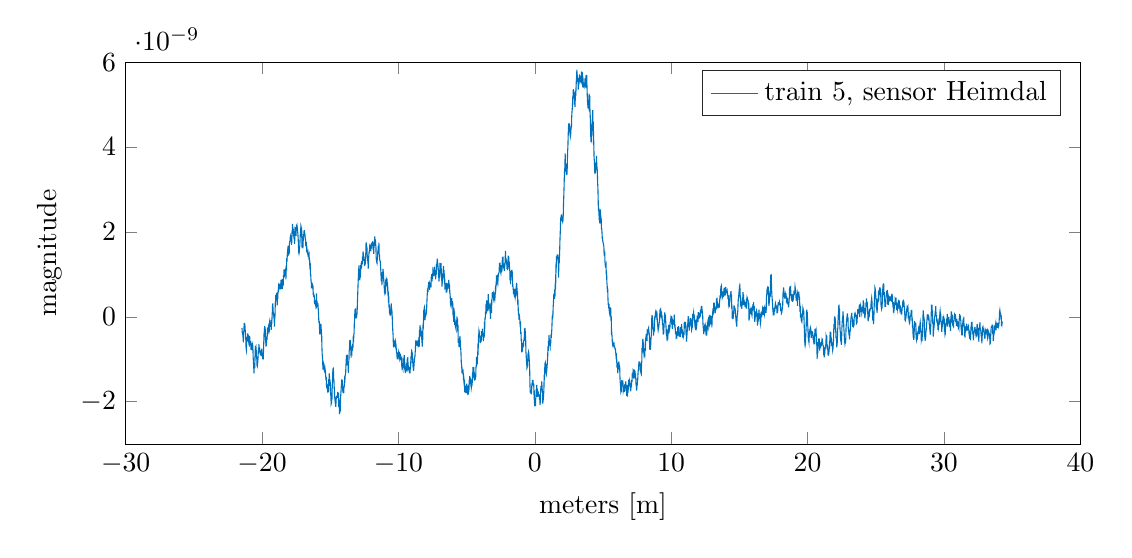
\begin{tikzpicture}

  \begin{axis}[%
    width=\textwidth,
    height=0.4\textwidth,
    at={(0\figurewidth,0\figureheight)},
    scale only axis,
    xmin=-30,
    xmax=40,
    xlabel={meters [m]},
    ymin=-3e-09,
    ymax=6e-09,
    ylabel={magnitude},
    axis background/.style={fill=white},
    legend style={legend cell align=left,align=left,draw=white!15!black}
    ]
    \addplot [color=mycolor1,solid]
    table[row sep=crcr]{%
    -21.487798828125	-2.74276005694763e-10\\
    -21.4678046875	-2.73602566192449e-10\\
    -21.447810546875	-3.78948457202424e-10\\
    -21.42781640625	-3.81601181243136e-10\\
    -21.407822265625	-4.30393153396603e-10\\
    -21.387828125	-4.97496360352883e-10\\
    -21.367833984375	-6.01773330307977e-10\\
    -21.34783984375	-3.72395079920082e-10\\
    -21.327845703125	-3.22550054483472e-10\\
    -21.3078515625	-1.42248338587243e-10\\
    -21.287857421875	-2.76578154005607e-10\\
    -21.26786328125	-1.59383229423789e-10\\
    -21.247869140625	-2.2761362073536e-10\\
    -21.227875	-3.51381871253605e-10\\
    -21.207880859375	-4.16690772783938e-10\\
    -21.18788671875	-5.49191350085253e-10\\
    -21.167892578125	-7.44942631990204e-10\\
    -21.1478984375	-7.80662419767453e-10\\
    -21.127904296875	-5.92659285491441e-10\\
    -21.10791015625	-5.83574413307219e-10\\
    -21.087916015625	-4.70914969164615e-10\\
    -21.067921875	-5.27571815757505e-10\\
    -21.047927734375	-3.93959145777789e-10\\
    -21.02793359375	-4.72504957918296e-10\\
    -21.007939453125	-4.28817689299976e-10\\
    -20.9879453125	-5.53189415321295e-10\\
    -20.967951171875	-6.10549764290043e-10\\
    -20.94795703125	-6.59421319772682e-10\\
    -20.927962890625	-6.71349554373333e-10\\
    -20.90796875	-4.50639399624029e-10\\
    -20.887974609375	-5.99384427754458e-10\\
    -20.86798046875	-5.85814029588276e-10\\
    -20.847986328125	-5.83448320124278e-10\\
    -20.8279921875	-6.33983104939912e-10\\
    -20.807998046875	-7.73247824179452e-10\\
    -20.78800390625	-6.27837289664716e-10\\
    -20.768009765625	-7.87834141766475e-10\\
    -20.748015625	-6.55305976443035e-10\\
    -20.728021484375	-7.50294220121586e-10\\
    -20.70802734375	-6.37685465372278e-10\\
    -20.688033203125	-6.57444989609235e-10\\
    -20.6680390625	-7.55217796125608e-10\\
    -20.648044921875	-9.57197940034457e-10\\
    -20.62805078125	-1.09169545918106e-09\\
    -20.608056640625	-1.18533526407755e-09\\
    -20.5880625	-1.33465423065414e-09\\
    -20.568068359375	-1.15146726964396e-09\\
    -20.54807421875	-1.1286269557011e-09\\
    -20.528080078125	-1.14632467328537e-09\\
    -20.5080859375	-8.86428856906391e-10\\
    -20.488091796875	-7.1773582598667e-10\\
    -20.46809765625	-7.25592502178272e-10\\
    -20.448103515625	-7.051778037448e-10\\
    -20.428109375	-7.81282746903917e-10\\
    -20.408115234375	-9.34845629049693e-10\\
    -20.38812109375	-9.45428814509814e-10\\
    -20.368126953125	-1.14316797283298e-09\\
    -20.3481328125	-1.16286287634509e-09\\
    -20.328138671875	-1.09053806763836e-09\\
    -20.30814453125	-1.0646996604761e-09\\
    -20.288150390625	-9.24240225334552e-10\\
    -20.26815625	-7.79474944494901e-10\\
    -20.248162109375	-8.51739044374652e-10\\
    -20.22816796875	-6.46260910198668e-10\\
    -20.208173828125	-8.30945140456853e-10\\
    -20.1881796875	-7.13621242145035e-10\\
    -20.168185546875	-7.7947831950746e-10\\
    -20.14819140625	-8.26461880714127e-10\\
    -20.128197265625	-8.82942264368329e-10\\
    -20.108203125	-8.91696745901148e-10\\
    -20.088208984375	-8.53081436120234e-10\\
    -20.06821484375	-7.98605638518073e-10\\
    -20.048220703125	-9.24282654831763e-10\\
    -20.0282265625	-7.48016195597909e-10\\
    -20.008232421875	-9.08439975870875e-10\\
    -19.98823828125	-8.47573606030337e-10\\
    -19.968244140625	-9.2975574381042e-10\\
    -19.94825	-9.93980412257086e-10\\
    -19.928255859375	-9.12276650468525e-10\\
    -19.90826171875	-1.00594031451716e-09\\
    -19.888267578125	-7.41844636403319e-10\\
    -19.8682734375	-5.6752697789465e-10\\
    -19.848279296875	-3.73214120281987e-10\\
    -19.82828515625	-3.45679875471266e-10\\
    -19.808291015625	-2.22140012703404e-10\\
    -19.788296875	-2.91742560121587e-10\\
    -19.768302734375	-2.84282171112566e-10\\
    -19.74830859375	-5.37861666914278e-10\\
    -19.728314453125	-5.8384870047667e-10\\
    -19.7083203125	-6.83288655824196e-10\\
    -19.688326171875	-6.79996050896378e-10\\
    -19.66833203125	-5.77122867492263e-10\\
    -19.648337890625	-4.61152742719445e-10\\
    -19.62834375	-5.44285360040173e-10\\
    -19.608349609375	-3.23994151331781e-10\\
    -19.58835546875	-3.45425356387501e-10\\
    -19.568361328125	-2.84977447408126e-10\\
    -19.5483671875	-2.55812254091864e-10\\
    -19.528373046875	-3.6787635062448e-10\\
    -19.50837890625	-3.19063833410608e-10\\
    -19.488384765625	-3.60367299580048e-10\\
    -19.468390625	-3.33791785423091e-10\\
    -19.448396484375	-1.32359233454531e-10\\
    -19.42840234375	-1.67336672827144e-10\\
    -19.408408203125	-2.02725472482799e-10\\
    -19.3884140625	-1.89521296268425e-10\\
    -19.368419921875	-2.08306205773259e-10\\
    -19.34842578125	-7.2056936027338e-11\\
    -19.328431640625	-3.07474560269938e-10\\
    -19.3084375	-1.74651401759546e-10\\
    -19.288443359375	-1.60450602069053e-10\\
    -19.26844921875	-3.08931292575027e-11\\
    -19.248455078125	8.85959210334922e-11\\
    -19.2284609375	2.66817840201041e-10\\
    -19.208466796875	3.15732641314569e-10\\
    -19.18847265625	1.16830433795195e-10\\
    -19.168478515625	1.05299974906589e-10\\
    -19.148484375	5.30508640888343e-11\\
    -19.128490234375	-3.00573430973793e-11\\
    -19.10849609375	-4.22041251449574e-11\\
    -19.088501953125	-2.30517756753466e-10\\
    -19.0685078125	-2.97429105991943e-11\\
    -19.048513671875	1.80450003375622e-11\\
    -19.02851953125	3.19922978667038e-10\\
    -19.008525390625	3.68949362329598e-10\\
    -18.98853125	5.18090488454614e-10\\
    -18.968537109375	4.43568907664803e-10\\
    -18.94854296875	4.83232546620451e-10\\
    -18.928548828125	5.54749134958138e-10\\
    -18.9085546875	5.56840188854267e-10\\
    -18.888560546875	2.66988496180816e-10\\
    -18.86856640625	4.70487673811317e-10\\
    -18.848572265625	4.20611868694364e-10\\
    -18.828578125	5.7672349131904e-10\\
    -18.808583984375	6.22765387616439e-10\\
    -18.78858984375	7.10009221130456e-10\\
    -18.768595703125	6.76698646554268e-10\\
    -18.7486015625	7.79199663287986e-10\\
    -18.728607421875	6.67584322013739e-10\\
    -18.70861328125	7.73844173993206e-10\\
    -18.688619140625	6.678576820769e-10\\
    -18.668625	6.69590447243265e-10\\
    -18.648630859375	7.21129047280956e-10\\
    -18.62863671875	6.44258206202762e-10\\
    -18.608642578125	8.66922738399022e-10\\
    -18.5886484375	6.77848407663213e-10\\
    -18.568654296875	8.05889609232342e-10\\
    -18.54866015625	6.52395562888336e-10\\
    -18.528666015625	8.89017717667579e-10\\
    -18.508671875	6.60872445291262e-10\\
    -18.488677734375	8.88676477876204e-10\\
    -18.46868359375	7.48771183925251e-10\\
    -18.448689453125	7.45105012467505e-10\\
    -18.4286953125	9.76710233934888e-10\\
    -18.408701171875	9.35348107877704e-10\\
    -18.38870703125	1.11457222422528e-09\\
    -18.368712890625	9.29681422159297e-10\\
    -18.34871875	9.96282142571181e-10\\
    -18.328724609375	1.06619207109861e-09\\
    -18.30873046875	1.09364380175274e-09\\
    -18.288736328125	1.09899976135971e-09\\
    -18.2687421875	1.12205301443954e-09\\
    -18.248748046875	8.82671981984882e-10\\
    -18.22875390625	1.21157232774828e-09\\
    -18.208759765625	1.09043182739796e-09\\
    -18.188765625	1.38233055443299e-09\\
    -18.168771484375	1.30334137634762e-09\\
    -18.14877734375	1.44724004500398e-09\\
    -18.128783203125	1.53431095716449e-09\\
    -18.1087890625	1.51571520521554e-09\\
    -18.088794921875	1.67512245887923e-09\\
    -18.06880078125	1.5079715260902e-09\\
    -18.048806640625	1.44008101335343e-09\\
    -18.0288125	1.61624137261477e-09\\
    -18.008818359375	1.48607434174338e-09\\
    -17.98882421875	1.737196976634e-09\\
    -17.968830078125	1.7682408419008e-09\\
    -17.9488359375	1.78068912022115e-09\\
    -17.928841796875	1.86573853372881e-09\\
    -17.90884765625	1.90280374551733e-09\\
    -17.888853515625	1.87294351792495e-09\\
    -17.868859375	1.81661883210943e-09\\
    -17.848865234375	1.7816600892271e-09\\
    -17.82887109375	1.69650551045199e-09\\
    -17.808876953125	1.95737864753133e-09\\
    -17.7888828125	1.94511086745376e-09\\
    -17.768888671875	2.18748371414619e-09\\
    -17.74889453125	2.10772209178902e-09\\
    -17.728900390625	1.9914064911375e-09\\
    -17.70890625	2.07143658415648e-09\\
    -17.688912109375	1.98384633253174e-09\\
    -17.66891796875	1.88658861942308e-09\\
    -17.648923828125	1.89761486522843e-09\\
    -17.6289296875	1.80179527931416e-09\\
    -17.608935546875	1.71714421278755e-09\\
    -17.58894140625	2.02141224483849e-09\\
    -17.568947265625	1.99140119038606e-09\\
    -17.548953125	1.98236932245986e-09\\
    -17.528958984375	2.10990699258656e-09\\
    -17.50896484375	1.90693454430569e-09\\
    -17.488970703125	2.07169347212428e-09\\
    -17.4689765625	2.17698451501819e-09\\
    -17.448982421875	2.07863788615285e-09\\
    -17.42898828125	2.1297521064403e-09\\
    -17.408994140625	2.07775086553954e-09\\
    -17.389	2.0104065362998e-09\\
    -17.369005859375	1.94630290095279e-09\\
    -17.34901171875	1.83576645247837e-09\\
    -17.329017578125	1.67161016072972e-09\\
    -17.3090234375	1.52117388542071e-09\\
    -17.289029296875	1.48864094251501e-09\\
    -17.26903515625	1.52457564023216e-09\\
    -17.249041015625	1.63333071360955e-09\\
    -17.229046875	1.67990486254167e-09\\
    -17.209052734375	1.82982507129005e-09\\
    -17.18905859375	1.96879050046067e-09\\
    -17.169064453125	2.02333049281704e-09\\
    -17.1490703125	2.14172919983243e-09\\
    -17.129076171875	2.11612923104785e-09\\
    -17.10908203125	1.96747688143492e-09\\
    -17.089087890625	1.99636175256428e-09\\
    -17.06909375	1.70008078406617e-09\\
    -17.049099609375	1.72246854667089e-09\\
    -17.02910546875	1.82114822102367e-09\\
    -17.009111328125	1.61239055777042e-09\\
    -16.9891171875	1.69084802098771e-09\\
    -16.969123046875	1.94820303598755e-09\\
    -16.94912890625	1.87166125496529e-09\\
    -16.929134765625	1.98303734301013e-09\\
    -16.909140625	2.03902317452001e-09\\
    -16.889146484375	1.91055105774103e-09\\
    -16.86915234375	1.96509897139231e-09\\
    -16.849158203125	1.92715109164463e-09\\
    -16.8291640625	1.84231409893869e-09\\
    -16.809169921875	1.81714162245311e-09\\
    -16.78917578125	1.66364575521188e-09\\
    -16.769181640625	1.70672317162449e-09\\
    -16.7491875	1.72049915633985e-09\\
    -16.729193359375	1.59231426003284e-09\\
    -16.70919921875	1.61279048030381e-09\\
    -16.689205078125	1.55020834087209e-09\\
    -16.6692109375	1.50168024248415e-09\\
    -16.649216796875	1.47674014060358e-09\\
    -16.62922265625	1.5045962306697e-09\\
    -16.609228515625	1.40565705709207e-09\\
    -16.589234375	1.47843882172694e-09\\
    -16.569240234375	1.41880821583391e-09\\
    -16.54924609375	1.45066807505665e-09\\
    -16.529251953125	1.31565301102681e-09\\
    -16.5092578125	1.37486900227764e-09\\
    -16.489263671875	1.11794773677103e-09\\
    -16.46926953125	1.26665032565278e-09\\
    -16.449275390625	1.00211689801893e-09\\
    -16.42928125	9.93798067738807e-10\\
    -16.409287109375	8.53736335986778e-10\\
    -16.38929296875	8.11789532945899e-10\\
    -16.369298828125	6.71769527437566e-10\\
    -16.3493046875	7.19483780171481e-10\\
    -16.329310546875	8.01426516890237e-10\\
    -16.30931640625	7.34391222144258e-10\\
    -16.289322265625	6.69368437361166e-10\\
    -16.269328125	7.51937675728813e-10\\
    -16.249333984375	5.14429099307922e-10\\
    -16.22933984375	5.76772840914688e-10\\
    -16.209345703125	4.97968165532293e-10\\
    -16.1893515625	5.08142237266344e-10\\
    -16.169357421875	4.93309262104549e-10\\
    -16.14936328125	3.28079550511508e-10\\
    -16.129369140625	3.37761120253504e-10\\
    -16.109375	3.40903510344847e-10\\
    -16.089380859375	3.14754741157251e-10\\
    -16.06938671875	2.77597163122679e-10\\
    -16.049392578125	4.0340993384139e-10\\
    -16.0293984375	1.94954558140245e-10\\
    -16.009404296875	5.53623422855041e-10\\
    -15.98941015625	2.46039884095868e-10\\
    -15.969416015625	3.76740807635854e-10\\
    -15.949421875	3.01927640039589e-10\\
    -15.929427734375	2.26244473844532e-10\\
    -15.90943359375	3.27149723376312e-10\\
    -15.889439453125	2.39902416246905e-10\\
    -15.8694453125	1.51416790591402e-10\\
    -15.849451171875	5.46424737625346e-12\\
    -15.82945703125	-1.46259664942757e-10\\
    -15.809462890625	-9.7191496449902e-11\\
    -15.78946875	-2.18876520048953e-10\\
    -15.769474609375	-4.12212782688254e-10\\
    -15.74948046875	-2.22197730465763e-10\\
    -15.729486328125	-3.93767631629084e-10\\
    -15.7094921875	-1.63514526400616e-10\\
    -15.689498046875	-2.85418411051842e-10\\
    -15.66950390625	-1.80637254750399e-10\\
    -15.649509765625	-4.69863906701335e-10\\
    -15.629515625	-3.84953447057402e-10\\
    -15.609521484375	-7.18873377531894e-10\\
    -15.58952734375	-8.84735969190628e-10\\
    -15.569533203125	-9.34570002043522e-10\\
    -15.5495390625	-1.09793850344031e-09\\
    -15.529544921875	-1.24348894622206e-09\\
    -15.50955078125	-1.07910577023845e-09\\
    -15.489556640625	-1.10852599860177e-09\\
    -15.4695625	-1.14937600187756e-09\\
    -15.449568359375	-1.10256999516795e-09\\
    -15.42957421875	-1.29526577252483e-09\\
    -15.409580078125	-1.21810570530761e-09\\
    -15.3895859375	-1.32513974043224e-09\\
    -15.369591796875	-1.25418080082138e-09\\
    -15.34959765625	-1.30627058275243e-09\\
    -15.329603515625	-1.39989544780621e-09\\
    -15.309609375	-1.49164685035389e-09\\
    -15.289615234375	-1.42258015039942e-09\\
    -15.26962109375	-1.62948951792933e-09\\
    -15.249626953125	-1.61247335123243e-09\\
    -15.2296328125	-1.61896327464317e-09\\
    -15.209638671875	-1.6853972560753e-09\\
    -15.18964453125	-1.6275233667801e-09\\
    -15.169650390625	-1.60967671606078e-09\\
    -15.14965625	-1.62543171090172e-09\\
    -15.129662109375	-1.78082054911641e-09\\
    -15.10966796875	-1.46902865350714e-09\\
    -15.089673828125	-1.62946236260729e-09\\
    -15.0696796875	-1.33402907205247e-09\\
    -15.049685546875	-1.42986306724204e-09\\
    -15.02969140625	-1.53561780401408e-09\\
    -15.009697265625	-1.48614512043627e-09\\
    -14.989703125	-1.63525809544717e-09\\
    -14.969708984375	-1.78525599092789e-09\\
    -14.94971484375	-1.90203439522479e-09\\
    -14.929720703125	-2.05423544250937e-09\\
    -14.9097265625	-2.03045962226018e-09\\
    -14.889732421875	-1.8627788514547e-09\\
    -14.86973828125	-1.88379908709539e-09\\
    -14.849744140625	-1.6111901051388e-09\\
    -14.82975	-1.47008592109926e-09\\
    -14.809755859375	-1.28977500004599e-09\\
    -14.78976171875	-1.30698817793011e-09\\
    -14.769767578125	-1.19037961851689e-09\\
    -14.7497734375	-1.44884023510289e-09\\
    -14.729779296875	-1.48407330464787e-09\\
    -14.70978515625	-1.64060777650385e-09\\
    -14.689791015625	-1.77758743457198e-09\\
    -14.669796875	-1.9005802143502e-09\\
    -14.649802734375	-1.96498987562939e-09\\
    -14.62980859375	-2.01939428163304e-09\\
    -14.609814453125	-1.97287113479234e-09\\
    -14.5898203125	-2.1197158570349e-09\\
    -14.569826171875	-1.9698111441466e-09\\
    -14.54983203125	-1.88381805379583e-09\\
    -14.529837890625	-1.88580720818486e-09\\
    -14.50984375	-1.87406841011779e-09\\
    -14.489849609375	-1.86166105911711e-09\\
    -14.46985546875	-1.90739789914244e-09\\
    -14.449861328125	-1.77204810996283e-09\\
    -14.4298671875	-1.85557788196172e-09\\
    -14.409873046875	-1.90640106090472e-09\\
    -14.38987890625	-1.79241727779797e-09\\
    -14.369884765625	-2.1321169359391e-09\\
    -14.349890625	-1.92034319003714e-09\\
    -14.329896484375	-2.19651450614515e-09\\
    -14.30990234375	-2.16617305967193e-09\\
    -14.289908203125	-2.24538681610021e-09\\
    -14.2699140625	-2.22952130396737e-09\\
    -14.249919921875	-2.02836107215756e-09\\
    -14.22992578125	-1.85314801090242e-09\\
    -14.209931640625	-1.7636009201165e-09\\
    -14.1899375	-1.65864035005648e-09\\
    -14.169943359375	-1.58515081208159e-09\\
    -14.14994921875	-1.48974075132457e-09\\
    -14.129955078125	-1.49511451932214e-09\\
    -14.1099609375	-1.50434268966712e-09\\
    -14.089966796875	-1.73881182001289e-09\\
    -14.06997265625	-1.74978091928636e-09\\
    -14.049978515625	-1.80349760284705e-09\\
    -14.029984375	-1.68699106753291e-09\\
    -14.009990234375	-1.79460584427554e-09\\
    -13.98999609375	-1.64532577822319e-09\\
    -13.970001953125	-1.63667770240311e-09\\
    -13.9500078125	-1.51872511301944e-09\\
    -13.930013671875	-1.5594512936377e-09\\
    -13.91001953125	-1.39128633087784e-09\\
    -13.890025390625	-1.3682563802078e-09\\
    -13.87003125	-1.33703196279139e-09\\
    -13.850037109375	-1.17983534546477e-09\\
    -13.83004296875	-1.05257663023584e-09\\
    -13.810048828125	-9.05807184065826e-10\\
    -13.7900546875	-9.56364688021965e-10\\
    -13.770060546875	-9.61611336372729e-10\\
    -13.75006640625	-8.90700852694026e-10\\
    -13.730072265625	-1.13979992514322e-09\\
    -13.710078125	-1.06117601763325e-09\\
    -13.690083984375	-1.15734282747348e-09\\
    -13.67008984375	-1.31856398334809e-09\\
    -13.650095703125	-1.07610632984914e-09\\
    -13.6301015625	-1.03736579153493e-09\\
    -13.610107421875	-8.07880322362921e-10\\
    -13.59011328125	-7.79029550628112e-10\\
    -13.570119140625	-6.08908750420551e-10\\
    -13.550125	-6.22610025604904e-10\\
    -13.530130859375	-5.43370972464257e-10\\
    -13.51013671875	-7.43311994679069e-10\\
    -13.490142578125	-6.61488516679285e-10\\
    -13.4701484375	-9.62580330700166e-10\\
    -13.450154296875	-8.16635467744556e-10\\
    -13.43016015625	-7.95246101511714e-10\\
    -13.410166015625	-8.25025012180898e-10\\
    -13.390171875	-6.97784243482253e-10\\
    -13.370177734375	-7.99250032356491e-10\\
    -13.35018359375	-6.75244301012282e-10\\
    -13.330189453125	-6.84908674141068e-10\\
    -13.3101953125	-4.61563523060839e-10\\
    -13.290201171875	-6.04234153290498e-10\\
    -13.27020703125	-4.18826510910586e-10\\
    -13.250212890625	-3.79200749918678e-10\\
    -13.23021875	-1.08609648801e-10\\
    -13.210224609375	-9.60101477408473e-11\\
    -13.19023046875	1.66520930416026e-10\\
    -13.170236328125	1.08376416139464e-10\\
    -13.1502421875	1.96767896754705e-10\\
    -13.130248046875	2.95441576800529e-11\\
    -13.11025390625	9.6431477689866e-11\\
    -13.090259765625	-1.64397050757313e-11\\
    -13.070265625	-9.60901707195352e-12\\
    -13.050271484375	3.76370574566493e-11\\
    -13.03027734375	9.28174221757895e-11\\
    -13.010283203125	2.91014847812313e-10\\
    -12.9902890625	4.72506505999462e-10\\
    -12.970294921875	6.62823155336796e-10\\
    -12.95030078125	8.34179509345867e-10\\
    -12.930306640625	9.93419440145646e-10\\
    -12.9103125	1.11393315834579e-09\\
    -12.890318359375	1.20975565868883e-09\\
    -12.87032421875	1.00059075177935e-09\\
    -12.850330078125	1.11797782859407e-09\\
    -12.8303359375	8.57041724991182e-10\\
    -12.810341796875	1.02540656351231e-09\\
    -12.79034765625	9.21631612936972e-10\\
    -12.770353515625	1.21848204680192e-09\\
    -12.750359375	1.11459348969915e-09\\
    -12.730365234375	1.2691718818546e-09\\
    -12.71037109375	1.14180837679221e-09\\
    -12.690376953125	1.31065148427876e-09\\
    -12.6703828125	1.23978206215808e-09\\
    -12.650388671875	1.25105067533931e-09\\
    -12.63039453125	1.41563661311865e-09\\
    -12.610400390625	1.32013126427673e-09\\
    -12.59040625	1.54116482383986e-09\\
    -12.570412109375	1.46876626144408e-09\\
    -12.55041796875	1.42467747388907e-09\\
    -12.530423828125	1.35153990523126e-09\\
    -12.5104296875	1.34605739382337e-09\\
    -12.490435546875	1.2755270183472e-09\\
    -12.47044140625	1.21866604956508e-09\\
    -12.450447265625	1.22652968269503e-09\\
    -12.430453125	1.26349554930879e-09\\
    -12.410458984375	1.4264706112712e-09\\
    -12.39046484375	1.50129111901173e-09\\
    -12.370470703125	1.74096185251077e-09\\
    -12.3504765625	1.74115988495214e-09\\
    -12.330482421875	1.53467087232057e-09\\
    -12.31048828125	1.65200608675187e-09\\
    -12.290494140625	1.47554825190085e-09\\
    -12.2705	1.31060329250153e-09\\
    -12.250505859375	1.43559926423964e-09\\
    -12.23051171875	1.28561764812766e-09\\
    -12.210517578125	1.13710899731213e-09\\
    -12.1905234375	1.36802657088008e-09\\
    -12.170529296875	1.42984011724526e-09\\
    -12.15053515625	1.52945415432052e-09\\
    -12.130541015625	1.53111232586973e-09\\
    -12.110546875	1.61408369178373e-09\\
    -12.090552734375	1.72182580263807e-09\\
    -12.07055859375	1.55771434649699e-09\\
    -12.050564453125	1.69471585095554e-09\\
    -12.0305703125	1.54443220459743e-09\\
    -12.010576171875	1.61737761896254e-09\\
    -11.99058203125	1.65005322469647e-09\\
    -11.970587890625	1.64326251603323e-09\\
    -11.95059375	1.73685395850269e-09\\
    -11.930599609375	1.73789679237907e-09\\
    -11.91060546875	1.74838499846364e-09\\
    -11.890611328125	1.68549852251127e-09\\
    -11.8706171875	1.78563652481382e-09\\
    -11.850623046875	1.5721577883791e-09\\
    -11.83062890625	1.67087154335462e-09\\
    -11.810634765625	1.48614349529036e-09\\
    -11.790640625	1.65295230961461e-09\\
    -11.770646484375	1.75538392268416e-09\\
    -11.75065234375	1.67433518981299e-09\\
    -11.730658203125	1.89444187280815e-09\\
    -11.7106640625	1.7133505945878e-09\\
    -11.690669921875	1.8235639069665e-09\\
    -11.67067578125	1.70821572518523e-09\\
    -11.650681640625	1.66773677928538e-09\\
    -11.6306875	1.40884459315769e-09\\
    -11.610693359375	1.32271069006809e-09\\
    -11.59069921875	1.28917024686387e-09\\
    -11.570705078125	1.26615730976463e-09\\
    -11.5507109375	1.36315525724222e-09\\
    -11.530716796875	1.40844493112023e-09\\
    -11.51072265625	1.54171852489119e-09\\
    -11.490728515625	1.56940329827995e-09\\
    -11.470734375	1.67901155668359e-09\\
    -11.450740234375	1.53121453785252e-09\\
    -11.43074609375	1.74620387278362e-09\\
    -11.410751953125	1.47134058424284e-09\\
    -11.3907578125	1.46474529489475e-09\\
    -11.370763671875	1.34354436933651e-09\\
    -11.35076953125	1.31905619638e-09\\
    -11.330775390625	1.30223865649053e-09\\
    -11.31078125	1.2093510512188e-09\\
    -11.290787109375	1.09289946759377e-09\\
    -11.27079296875	9.47071341903953e-10\\
    -11.250798828125	8.27668070526129e-10\\
    -11.2308046875	1.04386640961176e-09\\
    -11.210810546875	7.4396786969413e-10\\
    -11.19081640625	9.37988693894026e-10\\
    -11.170822265625	1.05250662275043e-09\\
    -11.150828125	8.924937115125e-10\\
    -11.130833984375	1.12644747380425e-09\\
    -11.11083984375	1.05108062177896e-09\\
    -11.090845703125	9.88805939713276e-10\\
    -11.0708515625	8.32613849985478e-10\\
    -11.050857421875	8.07679393101948e-10\\
    -11.03086328125	6.31859807202021e-10\\
    -11.010869140625	6.48004991544344e-10\\
    -10.990875	5.07372255528511e-10\\
    -10.970880859375	7.34200412520082e-10\\
    -10.95088671875	5.44565563525593e-10\\
    -10.930892578125	8.00198486998895e-10\\
    -10.9108984375	7.77342763515397e-10\\
    -10.890904296875	8.66416103352773e-10\\
    -10.87091015625	8.28607318771611e-10\\
    -10.850916015625	9.12375041768551e-10\\
    -10.830921875	8.43181861111174e-10\\
    -10.810927734375	7.80125837494258e-10\\
    -10.79093359375	7.70861308728411e-10\\
    -10.770939453125	5.09331092128423e-10\\
    -10.7509453125	6.08374248252224e-10\\
    -10.730951171875	3.33050221635165e-10\\
    -10.71095703125	4.78330441072339e-10\\
    -10.690962890625	2.50163374154178e-10\\
    -10.67096875	2.56990494920258e-10\\
    -10.650974609375	9.50589186944005e-11\\
    -10.63098046875	7.22345897834801e-11\\
    -10.610986328125	1.22273116464333e-10\\
    -10.5909921875	1.93036287013756e-10\\
    -10.570998046875	2.60132707070842e-11\\
    -10.55100390625	1.81960941749661e-10\\
    -10.531009765625	3.15099215810516e-10\\
    -10.511015625	2.32965173187342e-10\\
    -10.491021484375	1.7020597545141e-10\\
    -10.47102734375	1.18187311552831e-10\\
    -10.451033203125	-3.14964680072771e-11\\
    -10.4310390625	-1.99205275597234e-10\\
    -10.411044921875	-3.35053440297596e-10\\
    -10.39105078125	-4.24406364696567e-10\\
    -10.371056640625	-6.41577870069217e-10\\
    -10.3510625	-7.18351612052005e-10\\
    -10.331068359375	-6.49304448711716e-10\\
    -10.31107421875	-6.61048313766016e-10\\
    -10.291080078125	-5.77102740487672e-10\\
    -10.2710859375	-6.54216939447327e-10\\
    -10.251091796875	-5.50536452626505e-10\\
    -10.23109765625	-6.3339719293763e-10\\
    -10.211103515625	-5.88658109917949e-10\\
    -10.191109375	-6.4690768683087e-10\\
    -10.171115234375	-6.74210666552815e-10\\
    -10.15112109375	-8.15362058733381e-10\\
    -10.131126953125	-8.57700093264582e-10\\
    -10.1111328125	-8.70568864890172e-10\\
    -10.091138671875	-9.99957978818872e-10\\
    -10.07114453125	-8.41598232000956e-10\\
    -10.051150390625	-1.00417993189175e-09\\
    -10.03115625	-8.73068746807678e-10\\
    -10.011162109375	-9.30118073822054e-10\\
    -9.99116796875	-8.45905974130389e-10\\
    -9.971173828125	-8.80653769490916e-10\\
    -9.9511796875	-9.19539704216323e-10\\
    -9.931185546875	-9.71497292256514e-10\\
    -9.91119140625	-9.15177478111676e-10\\
    -9.891197265625	-9.73208413078023e-10\\
    -9.871203125	-8.86479953783974e-10\\
    -9.851208984375	-8.8457758935717e-10\\
    -9.83121484375	-1.0289126780425e-09\\
    -9.811220703125	-9.67227017264901e-10\\
    -9.7912265625	-9.60429290808767e-10\\
    -9.771232421875	-9.89735256725458e-10\\
    -9.75123828125	-1.16858192744884e-09\\
    -9.731244140625	-1.21817179496769e-09\\
    -9.71125	-1.20514647518719e-09\\
    -9.691255859375	-1.1962718931736e-09\\
    -9.67126171875	-1.22486869343992e-09\\
    -9.651267578125	-1.04799333842941e-09\\
    -9.6312734375	-1.0812832417455e-09\\
    -9.611279296875	-1.10082364064307e-09\\
    -9.59128515625	-1.13577045116492e-09\\
    -9.571291015625	-9.00886149540274e-10\\
    -9.551296875	-1.19517859963587e-09\\
    -9.531302734375	-1.06158272400794e-09\\
    -9.51130859375	-1.17275228068296e-09\\
    -9.491314453125	-1.3272466629217e-09\\
    -9.4713203125	-1.16795549952044e-09\\
    -9.451326171875	-1.22560671231759e-09\\
    -9.43133203125	-1.20506549207057e-09\\
    -9.411337890625	-1.24736435596698e-09\\
    -9.39134375	-1.08940707674202e-09\\
    -9.371349609375	-1.29153849750244e-09\\
    -9.35135546875	-9.8781262555474e-10\\
    -9.331361328125	-1.20697771663259e-09\\
    -9.3113671875	-9.53054578780677e-10\\
    -9.291373046875	-1.18293580979818e-09\\
    -9.27137890625	-1.25771721700665e-09\\
    -9.251384765625	-1.14828992102084e-09\\
    -9.231390625	-1.24456805427809e-09\\
    -9.211396484375	-1.26997189425669e-09\\
    -9.19140234375	-1.30824197250772e-09\\
    -9.171408203125	-1.29916600596981e-09\\
    -9.1514140625	-1.30598534908416e-09\\
    -9.131419921875	-1.18940479418665e-09\\
    -9.11142578125	-1.23996873042272e-09\\
    -9.091431640625	-1.04702228742268e-09\\
    -9.0714375	-9.23555413033687e-10\\
    -9.051443359375	-1.00555918114997e-09\\
    -9.03144921875	-7.66686906659328e-10\\
    -9.011455078125	-8.84029463667293e-10\\
    -8.9914609375	-8.34074568497309e-10\\
    -8.971466796875	-1.01719233922141e-09\\
    -8.95147265625	-9.99447130873287e-10\\
    -8.931478515625	-1.1689035884878e-09\\
    -8.911484375	-1.19002141094191e-09\\
    -8.891490234375	-1.27140125533364e-09\\
    -8.87149609375	-1.21184511587783e-09\\
    -8.851501953125	-1.10139465635383e-09\\
    -8.8315078125	-1.05517310373985e-09\\
    -8.811513671875	-9.57169415799232e-10\\
    -8.79151953125	-9.49986739774252e-10\\
    -8.771525390625	-8.41327070026184e-10\\
    -8.75153125	-7.65287185996232e-10\\
    -8.731537109375	-5.58108555546016e-10\\
    -8.71154296875	-6.20910329988739e-10\\
    -8.691548828125	-6.29085151063838e-10\\
    -8.6715546875	-6.10741162907842e-10\\
    -8.651560546875	-5.65161729453235e-10\\
    -8.63156640625	-6.85443300731176e-10\\
    -8.611572265625	-6.18134934872026e-10\\
    -8.591578125	-6.43136737148388e-10\\
    -8.571583984375	-6.21873072656613e-10\\
    -8.55158984375	-7.1979298254068e-10\\
    -8.531595703125	-5.37750170012301e-10\\
    -8.5116015625	-6.37500261075633e-10\\
    -8.491607421875	-4.73032323730688e-10\\
    -8.47161328125	-7.010628998373e-10\\
    -8.451619140625	-3.05900193907715e-10\\
    -8.431625	-4.63399043545821e-10\\
    -8.411630859375	-1.94082742297336e-10\\
    -8.39163671875	-3.53298151481938e-10\\
    -8.371642578125	-2.45365317146866e-10\\
    -8.3516484375	-3.38654631480486e-10\\
    -8.331654296875	-4.25829006588111e-10\\
    -8.31166015625	-4.05673239386857e-10\\
    -8.291666015625	-5.15260264563976e-10\\
    -8.271671875	-5.86701505541252e-10\\
    -8.251677734375	-7.01961167931939e-10\\
    -8.23168359375	-4.22946757545954e-10\\
    -8.211689453125	-4.48056616051398e-10\\
    -8.1916953125	-1.66341062090033e-10\\
    -8.171701171875	-2.70545023346618e-10\\
    -8.15170703125	6.00908994233293e-11\\
    -8.131712890625	3.38110919952285e-11\\
    -8.11171875	2.03825442867981e-10\\
    -8.091724609375	2.27139821616873e-10\\
    -8.07173046875	1.67933288243451e-10\\
    -8.051736328125	-7.53819111416944e-11\\
    -8.0317421875	1.81871253962743e-11\\
    -8.011748046875	4.33173125415592e-11\\
    -7.99175390625	3.2152259698575e-11\\
    -7.971759765625	5.49811259087973e-11\\
    -7.951765625	9.86421975667129e-11\\
    -7.931771484375	1.83450562714496e-10\\
    -7.91177734375	3.43036364246266e-10\\
    -7.891783203125	4.93542603635909e-10\\
    -7.8717890625	5.97966108744515e-10\\
    -7.851794921875	6.6667318084175e-10\\
    -7.83180078125	5.79236121532607e-10\\
    -7.811806640625	7.09604787028678e-10\\
    -7.7918125	7.50951677310681e-10\\
    -7.771818359375	8.2319659689885e-10\\
    -7.75182421875	6.67605578557701e-10\\
    -7.731830078125	7.71473810402063e-10\\
    -7.7118359375	6.37347431272364e-10\\
    -7.691841796875	7.74042559482046e-10\\
    -7.67184765625	7.47298104881186e-10\\
    -7.651853515625	6.94931507904283e-10\\
    -7.631859375	7.88036132608052e-10\\
    -7.611865234375	6.9321116381468e-10\\
    -7.59187109375	9.15227856364489e-10\\
    -7.571876953125	9.04326130597038e-10\\
    -7.5518828125	1.00841870756697e-09\\
    -7.531888671875	8.32606557014566e-10\\
    -7.51189453125	9.83299420506098e-10\\
    -7.491900390625	9.3739508581871e-10\\
    -7.47190625	1.07704793569151e-09\\
    -7.451912109375	1.04067002930064e-09\\
    -7.43191796875	9.62014613063649e-10\\
    -7.411923828125	1.01993143357591e-09\\
    -7.3919296875	1.0418714732953e-09\\
    -7.371935546875	1.16874946713693e-09\\
    -7.35194140625	1.08252446064697e-09\\
    -7.331947265625	1.12012896721988e-09\\
    -7.311953125	9.63018108232035e-10\\
    -7.291958984375	1.10493583468252e-09\\
    -7.27196484375	8.79759772959964e-10\\
    -7.251970703125	1.0615357099086e-09\\
    -7.2319765625	1.0020992298438e-09\\
    -7.211982421875	1.004750992093e-09\\
    -7.19198828125	1.22527353177521e-09\\
    -7.171994140625	1.27376440206023e-09\\
    -7.152	1.36805601378309e-09\\
    -7.132005859375	1.31467110815663e-09\\
    -7.11201171875	1.22501270085875e-09\\
    -7.092017578125	1.16935243342525e-09\\
    -7.0720234375	1.10379237478181e-09\\
    -7.052029296875	1.09306945628734e-09\\
    -7.03203515625	8.29085545483297e-10\\
    -7.012041015625	9.03811288702513e-10\\
    -6.992046875	1.00618412261406e-09\\
    -6.972052734375	9.22716868066265e-10\\
    -6.95205859375	1.20746507858412e-09\\
    -6.932064453125	1.18914616726494e-09\\
    -6.9120703125	1.22320896014958e-09\\
    -6.892076171875	1.2079897115176e-09\\
    -6.87208203125	1.26815073006602e-09\\
    -6.852087890625	9.70354541243357e-10\\
    -6.83209375	1.12106844380529e-09\\
    -6.812099609375	7.09048983804221e-10\\
    -6.79210546875	7.8538330476662e-10\\
    -6.772111328125	8.21421085050991e-10\\
    -6.7521171875	8.82677629257572e-10\\
    -6.732123046875	1.02454054950836e-09\\
    -6.71212890625	9.4927469297596e-10\\
    -6.692134765625	1.19733349185822e-09\\
    -6.672140625	9.9236012563728e-10\\
    -6.652146484375	1.09865569531349e-09\\
    -6.63215234375	8.89608895480533e-10\\
    -6.612158203125	9.71552966566636e-10\\
    -6.5921640625	6.64144229132728e-10\\
    -6.572169921875	6.72111436651808e-10\\
    -6.55217578125	7.86547385500343e-10\\
    -6.532181640625	6.79981741541487e-10\\
    -6.5121875	7.35979416251823e-10\\
    -6.492193359375	5.67849445439632e-10\\
    -6.47219921875	8.01029310862698e-10\\
    -6.452205078125	6.76100123320561e-10\\
    -6.4322109375	7.85938765502655e-10\\
    -6.412216796875	6.72934696963236e-10\\
    -6.39222265625	7.11110307236055e-10\\
    -6.372228515625	7.4300692870883e-10\\
    -6.352234375	7.28823985180801e-10\\
    -6.332240234375	7.31248790685765e-10\\
    -6.31224609375	8.68145025215916e-10\\
    -6.292251953125	6.56438657397873e-10\\
    -6.2722578125	7.7784649753035e-10\\
    -6.252263671875	7.18923122350236e-10\\
    -6.23226953125	5.66168397433147e-10\\
    -6.212275390625	5.41702454181289e-10\\
    -6.19228125	4.04259344990999e-10\\
    -6.172287109375	2.91181678656058e-10\\
    -6.15229296875	2.62188691816643e-10\\
    -6.132298828125	3.80281642882275e-10\\
    -6.1123046875	3.62946680076467e-10\\
    -6.092310546875	4.37490739021133e-10\\
    -6.07231640625	2.70791486990988e-10\\
    -6.052322265625	3.70327284000507e-10\\
    -6.032328125	2.2536732859107e-10\\
    -6.012333984375	3.26429591519189e-10\\
    -5.99233984375	2.37104124541874e-11\\
    -5.972345703125	1.9332082938395e-10\\
    -5.9523515625	-1.21848940527891e-10\\
    -5.932357421875	2.14078857824226e-10\\
    -5.91236328125	1.11804405049311e-11\\
    -5.892369140625	1.25954191297202e-10\\
    -5.872375	-1.92203793501748e-10\\
    -5.852380859375	-6.28873431666346e-11\\
    -5.83238671875	-1.97470341526159e-10\\
    -5.812392578125	-2.45782291524551e-10\\
    -5.7923984375	-2.66989429528051e-10\\
    -5.772404296875	-2.93890997201473e-10\\
    -5.75241015625	-1.15989183737391e-10\\
    -5.732416015625	-2.26032329600411e-10\\
    -5.712421875	1.07424863375796e-11\\
    -5.692427734375	-1.23830776518811e-10\\
    -5.67243359375	-3.86947882704895e-11\\
    -5.652439453125	-3.44020276699669e-10\\
    -5.6324453125	-1.937731476491e-10\\
    -5.612451171875	-6.1662532153795e-10\\
    -5.59245703125	-5.62201802830767e-10\\
    -5.572462890625	-5.95918526027826e-10\\
    -5.55246875	-7.14370864356983e-10\\
    -5.532474609375	-5.7364752140658e-10\\
    -5.51248046875	-5.66844967390013e-10\\
    -5.492486328125	-4.51404155752571e-10\\
    -5.4724921875	-5.35820826989442e-10\\
    -5.452498046875	-7.18538647164579e-10\\
    -5.43250390625	-7.39494325773168e-10\\
    -5.412509765625	-8.58391326094342e-10\\
    -5.392515625	-1.06460851277812e-09\\
    -5.372521484375	-1.12519911411166e-09\\
    -5.35252734375	-1.21627519324227e-09\\
    -5.332533203125	-1.3327993492995e-09\\
    -5.3125390625	-1.28318965356059e-09\\
    -5.292544921875	-1.33824794344733e-09\\
    -5.27255078125	-1.23995782300353e-09\\
    -5.252556640625	-1.31738825803714e-09\\
    -5.2325625	-1.43568501082734e-09\\
    -5.212568359375	-1.41824347091658e-09\\
    -5.19257421875	-1.54899243077716e-09\\
    -5.172580078125	-1.6047471772456e-09\\
    -5.1525859375	-1.57410268333685e-09\\
    -5.132591796875	-1.78031660050238e-09\\
    -5.11259765625	-1.628317526776e-09\\
    -5.092603515625	-1.72810059760069e-09\\
    -5.072609375	-1.62130752109245e-09\\
    -5.052615234375	-1.79729154995894e-09\\
    -5.03262109375	-1.71049712608168e-09\\
    -5.012626953125	-1.73179002240368e-09\\
    -4.9926328125	-1.57637718633114e-09\\
    -4.972638671875	-1.72428477823861e-09\\
    -4.95264453125	-1.62869407792308e-09\\
    -4.932650390625	-1.78177203408245e-09\\
    -4.91265625	-1.76087868127826e-09\\
    -4.892662109375	-1.71928187007714e-09\\
    -4.87266796875	-1.83131727696705e-09\\
    -4.852673828125	-1.62724277170257e-09\\
    -4.8326796875	-1.76812594512348e-09\\
    -4.812685546875	-1.48805912720094e-09\\
    -4.79269140625	-1.59276660718485e-09\\
    -4.772697265625	-1.39370266236536e-09\\
    -4.752703125	-1.4853981013425e-09\\
    -4.732708984375	-1.52307332314523e-09\\
    -4.71271484375	-1.50146418721863e-09\\
    -4.692720703125	-1.57536844657482e-09\\
    -4.6727265625	-1.54631758831037e-09\\
    -4.652732421875	-1.66970161537401e-09\\
    -4.63273828125	-1.62928478356849e-09\\
    -4.612744140625	-1.62302470933128e-09\\
    -4.59275	-1.57447784364098e-09\\
    -4.572755859375	-1.39580976948582e-09\\
    -4.55276171875	-1.41879467293257e-09\\
    -4.532767578125	-1.18029041674524e-09\\
    -4.5127734375	-1.42500590909641e-09\\
    -4.492779296875	-1.29292028639347e-09\\
    -4.47278515625	-1.18541306499954e-09\\
    -4.452791015625	-1.38000507817215e-09\\
    -4.432796875	-1.36619236802126e-09\\
    -4.412802734375	-1.50228099531375e-09\\
    -4.39280859375	-1.42055843517245e-09\\
    -4.372814453125	-1.48538695605841e-09\\
    -4.3528203125	-1.3679810982149e-09\\
    -4.332826171875	-1.42018243696784e-09\\
    -4.31283203125	-1.17851491148692e-09\\
    -4.292837890625	-1.16912015056743e-09\\
    -4.27284375	-9.42755971778256e-10\\
    -4.252849609375	-1.01790635313454e-09\\
    -4.23285546875	-1.03281958462485e-09\\
    -4.212861328125	-1.06157942917437e-09\\
    -4.1928671875	-9.57991036911935e-10\\
    -4.172873046875	-7.49398345703989e-10\\
    -4.15287890625	-7.80537927466444e-10\\
    -4.132884765625	-4.55896632814413e-10\\
    -4.112890625	-4.39353667728749e-10\\
    -4.092896484375	-3.26859735871898e-10\\
    -4.07290234375	-3.59948795166441e-10\\
    -4.052908203125	-4.9170757543422e-10\\
    -4.0329140625	-4.38860591359811e-10\\
    -4.012919921875	-6.1850942310436e-10\\
    -3.99292578125	-5.52784800442608e-10\\
    -3.972931640625	-6.19762889918119e-10\\
    -3.9529375	-4.63014571162621e-10\\
    -3.932943359375	-5.8810534521056e-10\\
    -3.91294921875	-3.52422496846455e-10\\
    -3.892955078125	-3.52127533387628e-10\\
    -3.8729609375	-3.72974690725321e-10\\
    -3.852966796875	-3.86457848330049e-10\\
    -3.83297265625	-2.78026411325271e-10\\
    -3.812978515625	-4.67993072367761e-10\\
    -3.792984375	-4.03951962425477e-10\\
    -3.772990234375	-5.70384568472529e-10\\
    -3.75299609375	-4.75860620941064e-10\\
    -3.733001953125	-4.31662549478458e-10\\
    -3.7130078125	-4.89283113316892e-10\\
    -3.693013671875	-2.31840758011484e-10\\
    -3.67301953125	-2.6442492302364e-10\\
    -3.653025390625	-3.99621606871309e-11\\
    -3.63303125	-3.30089103385474e-11\\
    -3.613037109375	1.18434975023581e-10\\
    -3.59304296875	5.08081779940327e-11\\
    -3.573048828125	3.11520832723473e-10\\
    -3.5530546875	8.3347762228915e-11\\
    -3.533060546875	3.88305008055026e-10\\
    -3.51306640625	1.65258923174875e-10\\
    -3.493072265625	3.16485031141008e-10\\
    -3.473078125	1.26762025246608e-10\\
    -3.453083984375	3.80073773397474e-10\\
    -3.43308984375	1.44337197610907e-10\\
    -3.413095703125	5.35018806672067e-10\\
    -3.3931015625	2.3239067203745e-10\\
    -3.373107421875	3.00034379067395e-10\\
    -3.35311328125	2.49081390310145e-10\\
    -3.333119140625	2.73644463176754e-10\\
    -3.313125	2.45540142899041e-10\\
    -3.293130859375	1.70713286857032e-10\\
    -3.27313671875	2.05613853320596e-10\\
    -3.253142578125	-5.14067914306962e-11\\
    -3.2331484375	2.57697495777807e-10\\
    -3.213154296875	8.93798540188894e-11\\
    -3.19316015625	3.39260399754219e-10\\
    -3.173166015625	9.28859068809888e-11\\
    -3.153171875	4.04458336401774e-10\\
    -3.133177734375	4.11553371038996e-10\\
    -3.11318359375	5.79729368896593e-10\\
    -3.093189453125	5.36109473796348e-10\\
    -3.0731953125	5.21720917202443e-10\\
    -3.053201171875	4.90875495486316e-10\\
    -3.03320703125	5.27813830194635e-10\\
    -3.013212890625	4.33299749786595e-10\\
    -2.99321875	4.69813176832516e-10\\
    -2.973224609375	3.79543055970356e-10\\
    -2.95323046875	4.4976464066301e-10\\
    -2.933236328125	4.111378638507e-10\\
    -2.9132421875	4.81865720474166e-10\\
    -2.893248046875	6.04540374907494e-10\\
    -2.87325390625	5.63909298013709e-10\\
    -2.853259765625	7.63691697096607e-10\\
    -2.833265625	7.20152418184971e-10\\
    -2.813271484375	9.53508826198182e-10\\
    -2.79327734375	9.48374622497861e-10\\
    -2.773283203125	9.58387950165846e-10\\
    -2.7532890625	8.785017264512e-10\\
    -2.733294921875	8.19755915404005e-10\\
    -2.71330078125	7.85534814117557e-10\\
    -2.693306640625	8.97990333576179e-10\\
    -2.6733125	1.00765866029446e-09\\
    -2.653318359375	1.01629448121585e-09\\
    -2.63332421875	1.03074623033987e-09\\
    -2.613330078125	1.05756235795095e-09\\
    -2.5933359375	1.27018446205532e-09\\
    -2.573341796875	1.224134686889e-09\\
    -2.55334765625	1.27628627969026e-09\\
    -2.533353515625	1.18606192841027e-09\\
    -2.513359375	1.07367632714724e-09\\
    -2.493365234375	1.04204866850116e-09\\
    -2.47337109375	1.21677828520287e-09\\
    -2.453376953125	1.0455161029586e-09\\
    -2.4333828125	1.14708718405138e-09\\
    -2.413388671875	1.06420389593421e-09\\
    -2.39339453125	1.25221160605738e-09\\
    -2.373400390625	1.40431228792729e-09\\
    -2.35340625	1.30335335937089e-09\\
    -2.333412109375	1.41770694175947e-09\\
    -2.31341796875	1.16732348619368e-09\\
    -2.293423828125	1.25891733765696e-09\\
    -2.2734296875	1.13960849973121e-09\\
    -2.253435546875	1.24562181953091e-09\\
    -2.23344140625	1.07504376290519e-09\\
    -2.213447265625	1.16857915726718e-09\\
    -2.193453125	1.21662087354973e-09\\
    -2.173458984375	1.3157346606037e-09\\
    -2.15346484375	1.55079542388964e-09\\
    -2.133470703125	1.37721355902215e-09\\
    -2.1134765625	1.37450781388227e-09\\
    -2.093482421875	1.33229142786514e-09\\
    -2.07348828125	1.27303629405625e-09\\
    -2.053494140625	1.22800968799695e-09\\
    -2.0335	1.11652504625646e-09\\
    -2.013505859375	1.26613485389954e-09\\
    -1.99351171875	1.09919869563943e-09\\
    -1.973517578125	1.21395761345321e-09\\
    -1.9535234375	1.44165847297511e-09\\
    -1.933529296875	1.3251773326923e-09\\
    -1.91353515625	1.41341483404626e-09\\
    -1.893541015625	1.17203795327058e-09\\
    -1.873546875	1.29783532735031e-09\\
    -1.853552734375	1.13587463865503e-09\\
    -1.83355859375	1.08127719811386e-09\\
    -1.813564453125	8.60449957681008e-10\\
    -1.7935703125	9.21908380550424e-10\\
    -1.773576171875	7.68671553513549e-10\\
    -1.75358203125	1.0783767267121e-09\\
    -1.733587890625	9.40799545018965e-10\\
    -1.71359375	1.04396315688051e-09\\
    -1.693599609375	1.10378609362542e-09\\
    -1.67360546875	1.00315412423867e-09\\
    -1.653611328125	1.02263764907156e-09\\
    -1.6336171875	8.6989909285214e-10\\
    -1.613623046875	7.13444593653272e-10\\
    -1.59362890625	7.03866190252073e-10\\
    -1.573634765625	6.13754866682405e-10\\
    -1.553640625	6.50332753588438e-10\\
    -1.533646484375	6.52468515128095e-10\\
    -1.51365234375	6.11813444951262e-10\\
    -1.493658203125	4.65936960780204e-10\\
    -1.4736640625	5.21117757571082e-10\\
    -1.453669921875	4.82403430723829e-10\\
    -1.43367578125	6.49223114838986e-10\\
    -1.413681640625	4.98166621157133e-10\\
    -1.3936875	5.3466803873862e-10\\
    -1.373693359375	6.78434312034271e-10\\
    -1.35369921875	7.18987736770942e-10\\
    -1.333705078125	7.95435630283182e-10\\
    -1.3137109375	7.20836373747402e-10\\
    -1.293716796875	4.8961080499447e-10\\
    -1.27372265625	6.01430249061112e-10\\
    -1.253728515625	2.8583394459672e-10\\
    -1.233734375	4.04640139951853e-10\\
    -1.213740234375	1.56306733203725e-10\\
    -1.19374609375	3.97050969070948e-11\\
    -1.173751953125	1.00289847487996e-10\\
    -1.1537578125	-7.16308945370274e-11\\
    -1.133763671875	5.39713730109473e-11\\
    -1.11376953125	-5.44546994541326e-11\\
    -1.093775390625	-6.45000114021081e-11\\
    -1.07378125	-2.43935069977255e-10\\
    -1.053787109375	-1.05536891805339e-10\\
    -1.03379296875	-4.01819268321499e-10\\
    -1.013798828125	-3.53132889716189e-10\\
    -0.993804687499999	-5.76786655981268e-10\\
    -0.973810546874997	-5.20957279166776e-10\\
    -0.953816406249999	-8.40919857325777e-10\\
    -0.933822265624997	-6.63487260474536e-10\\
    -0.913828124999998	-8.19182316668891e-10\\
    -0.893833984374997	-6.17186205584977e-10\\
    -0.873839843749998	-6.65556995406906e-10\\
    -0.853845703124996	-7.03352631607673e-10\\
    -0.833851562499998	-6.88757937106559e-10\\
    -0.813857421874996	-5.62044033260095e-10\\
    -0.793863281249998	-5.54727763869983e-10\\
    -0.773869140624999	-5.20407614797728e-10\\
    -0.753874999999997	-2.74313659679777e-10\\
    -0.733880859374999	-5.64894587173862e-10\\
    -0.713886718749997	-2.62077171541051e-10\\
    -0.693892578124998	-4.36347647641021e-10\\
    -0.673898437499997	-4.56620686725682e-10\\
    -0.653904296874998	-8.11553845879712e-10\\
    -0.633910156249996	-9.04079021821433e-10\\
    -0.613916015624998	-1.0235611954932e-09\\
    -0.593921874999996	-1.09892868887196e-09\\
    -0.573927734374998	-1.20358306521711e-09\\
    -0.553933593749999	-1.17941630451165e-09\\
    -0.533939453124997	-1.13523582231047e-09\\
    -0.513945312499999	-9.86185093239143e-10\\
    -0.493951171874997	-8.68481656908939e-10\\
    -0.473957031249999	-8.72561566348011e-10\\
    -0.453962890624997	-8.30038951188745e-10\\
    -0.433968749999998	-8.70507978377596e-10\\
    -0.413974609374996	-9.97235074643131e-10\\
    -0.393980468749998	-1.11259976511629e-09\\
    -0.373986328124996	-1.26880480100248e-09\\
    -0.353992187499998	-1.6307981647129e-09\\
    -0.333998046874996	-1.75913968165969e-09\\
    -0.314003906249997	-1.7521870857416e-09\\
    -0.294009765624999	-1.78705619544344e-09\\
    -0.274015624999997	-1.81415155104131e-09\\
    -0.254021484374999	-1.81543686065448e-09\\
    -0.234027343749997	-1.74137591157523e-09\\
    -0.214033203124998	-1.56503879660579e-09\\
    -0.194039062499996	-1.62006355442991e-09\\
    -0.174044921874998	-1.48641798726333e-09\\
    -0.154050781249996	-1.57717657989615e-09\\
    -0.134056640624998	-1.48544996231494e-09\\
    -0.114062499999996	-1.5948858328912e-09\\
    -0.0940683593749974	-1.61939913916554e-09\\
    -0.074074218749999	-1.5753881520625e-09\\
    -0.054080078124997	-1.86137454279974e-09\\
    -0.0340859374999987	-1.83692825672696e-09\\
    -0.0140917968749967	-2.10992935356237e-09\\
    0.00590234375000165	-2.07350048207086e-09\\
    0.0258964843750036	-1.9817598860527e-09\\
    0.045890625000002	-2.10207739195303e-09\\
    0.0658847656250039	-1.93544903491013e-09\\
    0.0858789062500023	-1.87752133290617e-09\\
    0.105873046875004	-1.7052705027586e-09\\
    0.125867187500003	-1.77508649034873e-09\\
    0.145861328125001	-1.60403640756178e-09\\
    0.165855468750003	-1.88753786748415e-09\\
    0.185849609375001	-1.69327599675411e-09\\
    0.205843750000003	-1.86865024475061e-09\\
    0.225837890625002	-1.75734765293422e-09\\
    0.245832031250004	-1.76566220580573e-09\\
    0.265826171875002	-1.8647920840103e-09\\
    0.285820312500004	-1.86058867886175e-09\\
    0.305814453125002	-1.84500020041211e-09\\
    0.325808593750004	-1.84295539440546e-09\\
    0.345802734375003	-1.95536332711861e-09\\
    0.365796875000001	-1.87585276003695e-09\\
    0.385791015625003	-2.07915820400288e-09\\
    0.405785156250001	-1.96219090082836e-09\\
    0.425779296875003	-1.83585783801845e-09\\
    0.445773437500002	-1.6303899204687e-09\\
    0.465767578125003	-1.72496525185796e-09\\
    0.485761718750002	-1.71419711691286e-09\\
    0.505755859375004	-1.52114315252263e-09\\
    0.525750000000002	-1.63114453085538e-09\\
    0.545744140625004	-1.72442650020128e-09\\
    0.565738281250002	-1.76306826124604e-09\\
    0.585732421875001	-2.04679720233359e-09\\
    0.605726562500003	-1.97198548746778e-09\\
    0.625720703125001	-1.93867016157451e-09\\
    0.645714843750003	-1.82707978583281e-09\\
    0.665708984375001	-1.72889295815457e-09\\
    0.685703125000003	-1.42382713446137e-09\\
    0.705697265625002	-1.43666450073387e-09\\
    0.725691406250004	-1.23970988968282e-09\\
    0.745685546875002	-1.1034525117939e-09\\
    0.765679687500004	-1.08165997288203e-09\\
    0.785673828125002	-1.19809705686418e-09\\
    0.805667968750004	-1.26631055141154e-09\\
    0.825662109375003	-1.32310781294419e-09\\
    0.845656250000001	-1.3463831978446e-09\\
    0.865650390625003	-1.20002325332442e-09\\
    0.885644531250001	-1.22505808421134e-09\\
    0.905638671875003	-1.14198431766416e-09\\
    0.925632812500002	-1.04414685693879e-09\\
    0.945626953125004	-9.22111442074497e-10\\
    0.965621093750002	-6.991319229301e-10\\
    0.985615234375004	-8.01080965576359e-10\\
    1.005609375	-5.65743733942775e-10\\
    1.025603515625	-6.76988631413026e-10\\
    1.04559765625	-4.28375132981662e-10\\
    1.065591796875	-6.17937527736688e-10\\
    1.0855859375	-6.17617296252278e-10\\
    1.105580078125	-6.60426005128952e-10\\
    1.12557421875	-7.02904100043697e-10\\
    1.145568359375	-6.08028015762576e-10\\
    1.1655625	-6.14995083635968e-10\\
    1.185556640625	-4.20152084757354e-10\\
    1.20555078125	-4.96316111695205e-10\\
    1.225544921875	-3.96530422170044e-10\\
    1.2455390625	-3.04715605563829e-10\\
    1.265533203125	-1.36916423088082e-10\\
    1.28552734375	2.64968233667881e-11\\
    1.305521484375	2.1878764481414e-11\\
    1.325515625	1.22590399849425e-11\\
    1.345509765625	2.3674176985604e-10\\
    1.36550390625	3.20525654250739e-10\\
    1.385498046875	5.09728643984356e-10\\
    1.4054921875	5.29045399578668e-10\\
    1.425486328125	5.06910179983949e-10\\
    1.44548046875	4.22669179564959e-10\\
    1.465474609375	6.45046107271048e-10\\
    1.48546875	4.83676559203131e-10\\
    1.505462890625	8.2368395351689e-10\\
    1.52545703125	6.54367754988445e-10\\
    1.545451171875	1.14445830450561e-09\\
    1.5654453125	1.12260697087184e-09\\
    1.585439453125	1.42568942155638e-09\\
    1.60543359375	1.38811995128742e-09\\
    1.625427734375	1.391162245117e-09\\
    1.645421875	1.47282766159387e-09\\
    1.665416015625	1.36620882989799e-09\\
    1.68541015625	1.46073162527207e-09\\
    1.705404296875	1.30673980925929e-09\\
    1.7253984375	1.2504126223793e-09\\
    1.745392578125	9.25137937729143e-10\\
    1.76538671875	1.41251646688572e-09\\
    1.785380859375	1.25215058983069e-09\\
    1.805375	1.40731656163679e-09\\
    1.825369140625	1.57817223353779e-09\\
    1.84536328125	1.834175552692e-09\\
    1.865357421875	1.97600092956234e-09\\
    1.8853515625	2.21082422255259e-09\\
    1.905345703125	2.32725602991577e-09\\
    1.92533984375	2.35422710950408e-09\\
    1.945333984375	2.39672914940723e-09\\
    1.965328125	2.39121201439072e-09\\
    1.985322265625	2.25680340010653e-09\\
    2.00531640625	2.30177773999049e-09\\
    2.025310546875	2.26601043831142e-09\\
    2.0453046875	2.23955861394998e-09\\
    2.065298828125	2.27215522565983e-09\\
    2.08529296875	2.38764654960257e-09\\
    2.105287109375	2.66316566234379e-09\\
    2.12528125	2.84943450518596e-09\\
    2.145275390625	3.06458278800314e-09\\
    2.16526953125	3.32193988225666e-09\\
    2.185263671875	3.46113038802601e-09\\
    2.2052578125	3.5164661540232e-09\\
    2.225251953125	3.84887829694558e-09\\
    2.24524609375	3.61898946063383e-09\\
    2.265240234375	3.60770378230442e-09\\
    2.285234375	3.45470437725433e-09\\
    2.305228515625	3.46219396576226e-09\\
    2.32522265625	3.33800170370056e-09\\
    2.345216796875	3.46201198965815e-09\\
    2.3652109375	3.35469547172006e-09\\
    2.385205078125	3.64959894037644e-09\\
    2.40519921875	3.89711375841751e-09\\
    2.425193359375	3.99314181147134e-09\\
    2.4451875	4.25531272369938e-09\\
    2.465181640625	4.42439304861129e-09\\
    2.48517578125	4.55593363478572e-09\\
    2.505169921875	4.46094560791521e-09\\
    2.5251640625	4.55592806802063e-09\\
    2.545158203125	4.48325514140411e-09\\
    2.56515234375	4.35494232795649e-09\\
    2.585146484375	4.31586675054228e-09\\
    2.605140625	4.24697325921958e-09\\
    2.625134765625	4.28556675384136e-09\\
    2.64512890625	4.3749595969903e-09\\
    2.665123046875	4.5116815377765e-09\\
    2.6851171875	4.459448686549e-09\\
    2.705111328125	4.7109279399481e-09\\
    2.72510546875	4.8263601688582e-09\\
    2.745099609375	4.89330176782914e-09\\
    2.76509375	5.02223605716781e-09\\
    2.785087890625	5.17784743544177e-09\\
    2.80508203125	5.20448877452141e-09\\
    2.825076171875	5.36523732467167e-09\\
    2.8450703125	5.3019475759391e-09\\
    2.865064453125	5.28340946114925e-09\\
    2.88505859375	5.27087596003382e-09\\
    2.905052734375	5.04680566692207e-09\\
    2.925046875	5.0576516135167e-09\\
    2.945041015625	4.94478837632418e-09\\
    2.96503515625	5.13459113354995e-09\\
    2.985029296875	5.32114398110626e-09\\
    3.0050234375	5.20386533256952e-09\\
    3.025017578125	5.41145305878512e-09\\
    3.04501171875	5.56115991815875e-09\\
    3.065005859375	5.65944720526104e-09\\
    3.085	5.82714349337411e-09\\
    3.104994140625	5.60787674748224e-09\\
    3.12498828125	5.69599877726732e-09\\
    3.144982421875	5.52828530915989e-09\\
    3.1649765625	5.62229159703404e-09\\
    3.184970703125	5.35208488103574e-09\\
    3.20496484375	5.56115181130932e-09\\
    3.224958984375	5.45608468989173e-09\\
    3.244953125	5.52801999728952e-09\\
    3.264947265625	5.59409842958036e-09\\
    3.28494140625	5.53977564534356e-09\\
    3.304935546875	5.63107784257972e-09\\
    3.3249296875	5.59849110951034e-09\\
    3.344923828125	5.57530239459297e-09\\
    3.36491796875	5.68566103295888e-09\\
    3.384912109375	5.59031726780641e-09\\
    3.40490625	5.56465780110047e-09\\
    3.424900390625	5.75680404523938e-09\\
    3.44489453125	5.74819991976587e-09\\
    3.464888671875	5.68911376710247e-09\\
    3.4848828125	5.70615779623125e-09\\
    3.504876953125	5.4051322096642e-09\\
    3.52487109375	5.66384497577624e-09\\
    3.544865234375	5.45939625785663e-09\\
    3.564859375	5.47059764646129e-09\\
    3.584853515625	5.40088946612445e-09\\
    3.60484765625	5.46034642608362e-09\\
    3.624841796875	5.43799392883868e-09\\
    3.6448359375	5.51683724117428e-09\\
    3.664830078125	5.45986105555546e-09\\
    3.68482421875	5.60819507994645e-09\\
    3.704818359375	5.60639696880737e-09\\
    3.7248125	5.40172187883508e-09\\
    3.744806640625	5.64446756133699e-09\\
    3.76480078125	5.70072606863385e-09\\
    3.784794921875	5.53274024643068e-09\\
    3.8047890625	5.69713051914807e-09\\
    3.824783203125	5.43546157018593e-09\\
    3.84477734375	5.22157448377714e-09\\
    3.864771484375	5.07353979369697e-09\\
    3.884765625	4.99012964724951e-09\\
    3.904759765625	4.91467773915535e-09\\
    3.92475390625	4.98333230815422e-09\\
    3.944748046875	4.95136935182795e-09\\
    3.9647421875	5.13265357178566e-09\\
    3.984736328125	5.26027010761168e-09\\
    4.00473046875	4.98456169383255e-09\\
    4.024724609375	5.20431967478843e-09\\
    4.04471875	4.84679320384833e-09\\
    4.064712890625	4.7388760441154e-09\\
    4.08470703125	4.45076683479684e-09\\
    4.104701171875	4.24527995477954e-09\\
    4.1246953125	4.11485136987103e-09\\
    4.144689453125	4.2118527884443e-09\\
    4.16468359375	4.18184336674948e-09\\
    4.184677734375	4.43267724182052e-09\\
    4.204671875	4.64738526790221e-09\\
    4.224666015625	4.50550020144656e-09\\
    4.24466015625	4.86785792510041e-09\\
    4.264654296875	4.37642323060341e-09\\
    4.2846484375	4.60011941820323e-09\\
    4.304642578125	4.30394839709677e-09\\
    4.32463671875	4.06105255614961e-09\\
    4.344630859375	3.76708281628949e-09\\
    4.364625	3.67670184775116e-09\\
    4.384619140625	3.52828938865756e-09\\
    4.40461328125	3.36120552279051e-09\\
    4.424607421875	3.53986098681521e-09\\
    4.4446015625	3.3844099509863e-09\\
    4.464595703125	3.47147390512196e-09\\
    4.48458984375	3.62199403781497e-09\\
    4.504583984375	3.61653948563534e-09\\
    4.524578125	3.79213902065094e-09\\
    4.544572265625	3.55749518051709e-09\\
    4.56456640625	3.52291082142708e-09\\
    4.584560546875	3.42425922559829e-09\\
    4.6045546875	3.15483316783142e-09\\
    4.624548828125	3.05509097112623e-09\\
    4.64454296875	2.7874854302911e-09\\
    4.664537109375	2.48815402604905e-09\\
    4.68453125	2.57278113981667e-09\\
    4.704525390625	2.43159046891118e-09\\
    4.72451953125	2.27123009372145e-09\\
    4.744513671875	2.39409179836651e-09\\
    4.7645078125	2.20047687343193e-09\\
    4.784501953125	2.42585738766599e-09\\
    4.80449609375	2.53144088312224e-09\\
    4.824490234375	2.4222195912705e-09\\
    4.844484375	2.29646247782831e-09\\
    4.864478515625	2.33347974721094e-09\\
    4.88447265625	2.08113802141239e-09\\
    4.904466796875	2.07573771393753e-09\\
    4.9244609375	2.00160343958345e-09\\
    4.944455078125	1.86374230797019e-09\\
    4.96444921875	1.86837765605358e-09\\
    4.984443359375	1.78494548391735e-09\\
    5.0044375	1.74944192338233e-09\\
    5.024431640625	1.72782173946225e-09\\
    5.04442578125	1.69420945478827e-09\\
    5.064419921875	1.65561712560954e-09\\
    5.0844140625	1.44445156686021e-09\\
    5.104408203125	1.5042092694293e-09\\
    5.12440234375	1.51165574545762e-09\\
    5.144396484375	1.2985728451647e-09\\
    5.164390625	1.23084899080924e-09\\
    5.184384765625	1.17257429693108e-09\\
    5.20437890625	1.17152493358841e-09\\
    5.224373046875	1.20435542253e-09\\
    5.2443671875	9.78462348454629e-10\\
    5.264361328125	1.04938864615965e-09\\
    5.28435546875	7.99108728387182e-10\\
    5.304349609375	7.49510205210707e-10\\
    5.32434375	5.82426647235891e-10\\
    5.344337890625	6.60468968979286e-10\\
    5.36433203125	4.21057523793791e-10\\
    5.384326171875	2.79487307051149e-10\\
    5.4043203125	3.24181631305096e-10\\
    5.424314453125	1.98895632547163e-10\\
    5.44430859375	2.97781009594067e-10\\
    5.464302734375	1.10990155546299e-10\\
    5.484296875	7.99721612107607e-11\\
    5.504291015625	2.08103670514636e-10\\
    5.52428515625	2.12301881947749e-10\\
    5.544279296875	1.57107821169653e-10\\
    5.5642734375	2.00652884763526e-10\\
    5.584267578125	-9.10514767995965e-11\\
    5.60426171875	1.12217353023584e-11\\
    5.624255859375	-4.26357134598254e-10\\
    5.64425	-3.83608926365058e-10\\
    5.664244140625	-4.65929248984827e-10\\
    5.68423828125	-5.94569082706237e-10\\
    5.704232421875	-6.43034007184074e-10\\
    5.7242265625	-6.21768366957216e-10\\
    5.744220703125	-6.82906667569851e-10\\
    5.76421484375	-6.61317404944849e-10\\
    5.784208984375	-6.21207169715721e-10\\
    5.804203125	-6.18169626737009e-10\\
    5.824197265625	-6.90684363811565e-10\\
    5.84419140625	-6.92280646194909e-10\\
    5.864185546875	-7.29555535470359e-10\\
    5.8841796875	-7.64370586234001e-10\\
    5.904173828125	-7.62666590169203e-10\\
    5.92416796875	-7.97417695037658e-10\\
    5.944162109375	-8.86415463894619e-10\\
    5.96415625	-9.53064408993598e-10\\
    5.984150390625	-9.29830439980066e-10\\
    6.00414453125	-1.0081855921688e-09\\
    6.024138671875	-1.19706771855647e-09\\
    6.0441328125	-1.08094234904563e-09\\
    6.064126953125	-1.17114906622732e-09\\
    6.08412109375	-1.3253632158276e-09\\
    6.104115234375	-1.19967875621872e-09\\
    6.124109375	-1.19369086939826e-09\\
    6.144103515625	-1.1134186303222e-09\\
    6.16409765625	-1.05141011185097e-09\\
    6.184091796875	-1.22579818356234e-09\\
    6.2040859375	-1.13832137805784e-09\\
    6.224080078125	-1.19909690728828e-09\\
    6.24407421875	-1.44352052377244e-09\\
    6.264068359375	-1.54491365469521e-09\\
    6.2840625	-1.61939104817882e-09\\
    6.304056640625	-1.74558475437061e-09\\
    6.32405078125	-1.71421789297306e-09\\
    6.344044921875	-1.78190313889788e-09\\
    6.3640390625	-1.50711908090571e-09\\
    6.384033203125	-1.50914328813127e-09\\
    6.40402734375	-1.5404941146827e-09\\
    6.424021484375	-1.63305188524382e-09\\
    6.444015625	-1.50000388346213e-09\\
    6.464009765625	-1.57419639718561e-09\\
    6.48400390625	-1.74524929310339e-09\\
    6.503998046875	-1.70930207252115e-09\\
    6.5239921875	-1.69661677350592e-09\\
    6.543986328125	-1.62657857735815e-09\\
    6.56398046875	-1.77168020878084e-09\\
    6.583974609375	-1.59150873976283e-09\\
    6.60396875	-1.64484892576912e-09\\
    6.623962890625	-1.57983654810992e-09\\
    6.64395703125	-1.68177654144564e-09\\
    6.663951171875	-1.52134707053015e-09\\
    6.6839453125	-1.66355079437648e-09\\
    6.703939453125	-1.75165212630394e-09\\
    6.72393359375	-1.61775785422358e-09\\
    6.743927734375	-1.86584203086928e-09\\
    6.763921875	-1.60415936275504e-09\\
    6.783916015625	-1.88189697043664e-09\\
    6.80391015625	-1.70595930576405e-09\\
    6.823904296875	-1.79820415693195e-09\\
    6.8438984375	-1.72348748739051e-09\\
    6.863892578125	-1.68119543642675e-09\\
    6.88388671875	-1.48261516810366e-09\\
    6.903880859375	-1.57771549245728e-09\\
    6.923875	-1.58149483965165e-09\\
    6.943869140625	-1.52714296360299e-09\\
    6.96386328125	-1.58648888659307e-09\\
    6.983857421875	-1.62286581326028e-09\\
    7.0038515625	-1.58274999674543e-09\\
    7.023845703125	-1.75597273565162e-09\\
    7.04383984375	-1.70164438660611e-09\\
    7.063833984375	-1.61007011267399e-09\\
    7.083828125	-1.65070106955905e-09\\
    7.103822265625	-1.4941111172677e-09\\
    7.12381640625	-1.53984993806105e-09\\
    7.143810546875	-1.33263658880296e-09\\
    7.1638046875	-1.37969655134407e-09\\
    7.183798828125	-1.43024431139669e-09\\
    7.20379296875	-1.29423092813857e-09\\
    7.223787109375	-1.32024762629788e-09\\
    7.24378125	-1.45774786430809e-09\\
    7.263775390625	-1.23801865216295e-09\\
    7.28376953125	-1.45817485277294e-09\\
    7.303763671875	-1.24852243140303e-09\\
    7.3237578125	-1.36571879320268e-09\\
    7.343751953125	-1.28479485267095e-09\\
    7.36374609375	-1.34476258001406e-09\\
    7.383740234375	-1.34601558040476e-09\\
    7.403734375	-1.46786938232494e-09\\
    7.423728515625	-1.60002364745664e-09\\
    7.44372265625	-1.63021525271235e-09\\
    7.463716796875	-1.73854305934538e-09\\
    7.4837109375	-1.64881505870869e-09\\
    7.503705078125	-1.62991945525694e-09\\
    7.52369921875	-1.48193627524654e-09\\
    7.543693359375	-1.48747398754438e-09\\
    7.5636875	-1.35619461607583e-09\\
    7.583681640625	-1.26049564429787e-09\\
    7.60367578125	-1.25278165572938e-09\\
    7.623669921875	-1.12732194466064e-09\\
    7.6436640625	-1.05116855766208e-09\\
    7.663658203125	-1.11573385871084e-09\\
    7.68365234375	-1.16893534105646e-09\\
    7.703646484375	-1.06335872598013e-09\\
    7.723640625	-1.23290151013009e-09\\
    7.743634765625	-1.2771345870029e-09\\
    7.76362890625	-1.27171766665762e-09\\
    7.783623046875	-1.32450459302019e-09\\
    7.8036171875	-1.3436330835766e-09\\
    7.823611328125	-1.09773308078896e-09\\
    7.84360546875	-1.05898527081777e-09\\
    7.863599609375	-7.26930030416481e-10\\
    7.88359375	-8.40575245248023e-10\\
    7.903587890625	-6.12222022616166e-10\\
    7.92358203125	-5.12754290819181e-10\\
    7.943576171875	-6.22006511453507e-10\\
    7.9635703125	-6.20393796489021e-10\\
    7.983564453125	-8.11760204090161e-10\\
    8.00355859375	-8.79593986885279e-10\\
    8.023552734375	-8.36994383708615e-10\\
    8.043546875	-8.6025385263703e-10\\
    8.063541015625	-8.97425642071946e-10\\
    8.08353515625	-7.4020067382847e-10\\
    8.103529296875	-8.01336335216143e-10\\
    8.1235234375	-4.95396043868279e-10\\
    8.143517578125	-5.66140974955482e-10\\
    8.16351171875	-4.03757505004161e-10\\
    8.183505859375	-5.6747986430455e-10\\
    8.2035	-4.54540371842126e-10\\
    8.223494140625	-5.6743014589843e-10\\
    8.24348828125	-2.96568266237022e-10\\
    8.263482421875	-4.39181590723534e-10\\
    8.2834765625	-3.43408855836718e-10\\
    8.303470703125	-3.35362106835025e-10\\
    8.32346484375	-2.76995567897827e-10\\
    8.343458984375	-2.58751855734981e-10\\
    8.363453125	-3.72895487982482e-10\\
    8.383447265625	-3.75151512899124e-10\\
    8.40344140625	-4.61048594393838e-10\\
    8.423435546875	-7.70277860590243e-10\\
    8.4434296875	-6.07967610786666e-10\\
    8.463423828125	-7.77004910034064e-10\\
    8.48341796875	-7.36250291959347e-10\\
    8.503412109375	-6.19259181846072e-10\\
    8.52340625	-4.75876278019651e-10\\
    8.543400390625	-4.40685738184849e-10\\
    8.56339453125	-1.97515585955879e-10\\
    8.583388671875	3.66135078690659e-11\\
    8.6033828125	-1.34549353346888e-10\\
    8.623376953125	2.69158848851248e-11\\
    8.64337109375	-8.63594545536772e-11\\
    8.663365234375	-2.6405868530965e-10\\
    8.683359375	-2.64496665614166e-10\\
    8.703353515625	-4.42307860929853e-10\\
    8.72334765625	-3.67335351622609e-10\\
    8.743341796875	-3.30217568858092e-10\\
    8.7633359375	-3.28311465197832e-10\\
    8.783330078125	-1.19331994766517e-10\\
    8.80332421875	2.2847137653139e-11\\
    8.823318359375	-3.2859798975789e-11\\
    8.8433125	8.36056705056206e-11\\
    8.863306640625	1.1599608814868e-10\\
    8.88330078125	8.26220842025658e-11\\
    8.903294921875	-4.38821583748282e-12\\
    8.9232890625	4.98355541615847e-11\\
    8.943283203125	-1.14396823782176e-11\\
    8.96327734375	2.6056056458714e-11\\
    8.983271484375	-8.72813382907287e-11\\
    9.003265625	-1.9493826518373e-10\\
    9.023259765625	-2.47033389104224e-10\\
    9.04325390625	-3.11311181691113e-10\\
    9.063248046875	-2.70476175270648e-10\\
    9.0832421875	-2.49981158286841e-10\\
    9.103236328125	-1.94128182392418e-10\\
    9.12323046875	-1.33619110927609e-10\\
    9.143224609375	-7.59223272539997e-11\\
    9.16321875	6.72448880584011e-11\\
    9.183212890625	3.30435093672872e-11\\
    9.20320703125	1.08796162844413e-10\\
    9.223201171875	6.85924610805235e-11\\
    9.2431953125	1.16852503627982e-10\\
    9.263189453125	4.58547889695618e-11\\
    9.28318359375	1.27157067840324e-10\\
    9.303177734375	-3.60147361964029e-11\\
    9.323171875	3.08147017405801e-11\\
    9.343166015625	-6.90383545856764e-11\\
    9.36316015625	-1.79405425599153e-10\\
    9.383154296875	-1.77945114554964e-10\\
    9.4031484375	-3.14646170842502e-10\\
    9.423142578125	-2.84800884866307e-10\\
    9.44313671875	-4.2003057133845e-10\\
    9.463130859375	-2.84042374101297e-10\\
    9.483125	-1.62917417951741e-10\\
    9.503119140625	-5.84438319583934e-12\\
    9.52311328125	1.04989922372669e-10\\
    9.543107421875	-1.75107072930587e-11\\
    9.5631015625	3.553976011062e-11\\
    9.583095703125	1.11754926739567e-11\\
    9.60308984375	-1.48522731605942e-10\\
    9.623083984375	-2.51580357755656e-10\\
    9.643078125	-4.0464200833744e-10\\
    9.663072265625	-3.95202524102735e-10\\
    9.68306640625	-4.80062439854588e-10\\
    9.703060546875	-5.72599116825087e-10\\
    9.7230546875	-3.69917234902731e-10\\
    9.743048828125	-3.90146366039816e-10\\
    9.76304296875	-4.24860527437232e-10\\
    9.783037109375	-2.71594987555569e-10\\
    9.80303125	-3.91162524648956e-10\\
    9.823025390625	-1.93894525050228e-10\\
    9.84301953125	-2.86521525618237e-10\\
    9.863013671875	-3.16159380324067e-10\\
    9.8830078125	-2.68990501253695e-10\\
    9.903001953125	-2.71516253673939e-10\\
    9.92299609375	-1.30218800129214e-10\\
    9.942990234375	-1.20992752554291e-10\\
    9.962984375	-6.54232690059272e-11\\
    9.982978515625	-1.22923525335201e-10\\
    10.00297265625	1.94342833969233e-11\\
    10.022966796875	-1.10875828506762e-10\\
    10.0429609375	-1.79592652827549e-10\\
    10.062955078125	-1.11856125583661e-10\\
    10.08294921875	-2.81427582590826e-10\\
    10.102943359375	-1.16626323537502e-10\\
    10.1229375	-1.55044486148456e-10\\
    10.142931640625	-1.05653985678589e-10\\
    10.16292578125	-1.16964916517666e-10\\
    10.182919921875	-6.678393789046e-11\\
    10.2029140625	-1.86077156372196e-10\\
    10.222908203125	5.26437957530471e-11\\
    10.24290234375	-1.32237430373739e-10\\
    10.262896484375	-2.24065542246449e-10\\
    10.282890625	-2.15327868324664e-10\\
    10.302884765625	-3.12606585874501e-10\\
    10.32287890625	-4.1047973887684e-10\\
    10.342873046875	-3.40490476633263e-10\\
    10.3628671875	-4.5646706034149e-10\\
    10.382861328125	-4.26735031760133e-10\\
    10.40285546875	-5.10677950162082e-10\\
    10.422849609375	-4.37684484680236e-10\\
    10.44284375	-3.59877317812823e-10\\
    10.462837890625	-4.49386566060414e-10\\
    10.48283203125	-2.37826899029911e-10\\
    10.502826171875	-3.6471743668486e-10\\
    10.5228203125	-3.39087390227153e-10\\
    10.542814453125	-2.21226059593185e-10\\
    10.56280859375	-3.70187094833349e-10\\
    10.582802734375	-4.65860892866285e-10\\
    10.602796875	-3.9047254026148e-10\\
    10.622791015625	-4.4738441188707e-10\\
    10.64278515625	-3.49016284390667e-10\\
    10.662779296875	-4.79407429149347e-10\\
    10.6827734375	-2.45662301652969e-10\\
    10.702767578125	-4.05261733332613e-10\\
    10.72276171875	-2.53421347769015e-10\\
    10.742755859375	-3.49549681865504e-10\\
    10.76275	-1.68038595706192e-10\\
    10.782744140625	-3.36429331256069e-10\\
    10.80273828125	-3.55703054836596e-10\\
    10.822732421875	-4.03219850082004e-10\\
    10.8427265625	-4.87731342147151e-10\\
    10.862720703125	-3.95607381454733e-10\\
    10.88271484375	-4.27698725505656e-10\\
    10.902708984375	-4.55154807988045e-10\\
    10.922703125	-3.69375161134541e-10\\
    10.942697265625	-4.27140985087959e-10\\
    10.96269140625	-1.1601312950618e-10\\
    10.982685546875	-1.76125787573818e-10\\
    11.0026796875	-1.46003904453244e-10\\
    11.022673828125	-1.41074376583124e-10\\
    11.04266796875	-2.0837944192755e-10\\
    11.062662109375	-1.88238412662581e-10\\
    11.08265625	-3.81896971491901e-10\\
    11.102650390625	-3.97433552608454e-10\\
    11.12264453125	-5.87487331184252e-10\\
    11.142638671875	-4.82388412244557e-10\\
    11.1626328125	-3.94565971232673e-10\\
    11.182626953125	-2.94079880706633e-10\\
    11.20262109375	-1.93320056154627e-10\\
    11.222615234375	-2.03078009098786e-10\\
    11.242609375	1.74430537491162e-11\\
    11.262603515625	-3.38760020622911e-11\\
    11.28259765625	-1.82584270949487e-10\\
    11.302591796875	-1.28207175705156e-10\\
    11.3225859375	-3.2267308966912e-10\\
    11.342580078125	-2.62757363344328e-10\\
    11.36257421875	-2.25252869748799e-10\\
    11.382568359375	-2.08507700765481e-10\\
    11.4025625	-2.49934042833916e-11\\
    11.422556640625	-1.85858997500782e-10\\
    11.44255078125	-1.43995219701566e-10\\
    11.462544921875	-1.28552773393111e-10\\
    11.4825390625	-1.05790388398922e-10\\
    11.502533203125	-2.98446050585654e-10\\
    11.52252734375	-2.69677125619677e-10\\
    11.542521484375	-2.50391038465848e-10\\
    11.562515625	-1.31992119698339e-10\\
    11.582509765625	6.86555016467356e-11\\
    11.60250390625	-1.69379230740421e-12\\
    11.622498046875	5.48658952853599e-11\\
    11.6424921875	9.83195503174211e-11\\
    11.662486328125	-1.28796343260404e-11\\
    11.68248046875	5.82627130331172e-11\\
    11.702474609375	-9.47499367386753e-11\\
    11.72246875	-1.00305686640238e-10\\
    11.742462890625	-2.15725524018671e-10\\
    11.76245703125	-2.51999381132136e-10\\
    11.782451171875	-2.23490352726434e-10\\
    11.8024453125	-6.87048897853623e-11\\
    11.822439453125	-2.05750660241709e-10\\
    11.84243359375	-1.72247324936299e-10\\
    11.862427734375	-2.22824158483362e-10\\
    11.882421875	-1.59808816808706e-10\\
    11.902416015625	2.91357203013745e-11\\
    11.92241015625	-5.23332650949784e-11\\
    11.942404296875	-1.8758769847494e-11\\
    11.9623984375	-1.27346660594231e-10\\
    11.982392578125	1.09010957280407e-10\\
    12.00238671875	1.62402261606143e-11\\
    12.022380859375	-4.60850495023811e-13\\
    12.042375	6.74815854922295e-11\\
    12.062369140625	-3.58283342380377e-11\\
    12.08236328125	6.85859451185518e-11\\
    12.102357421875	6.13939144366001e-11\\
    12.1223515625	-1.58061205831939e-11\\
    12.142345703125	1.70614545345481e-10\\
    12.16233984375	7.28931285748508e-11\\
    12.182333984375	8.35935374577251e-11\\
    12.202328125	1.96841165788518e-10\\
    12.222322265625	1.81086720245539e-10\\
    12.24231640625	2.56914626776169e-10\\
    12.262310546875	1.47678972704185e-10\\
    12.2823046875	1.3084544542385e-10\\
    12.302298828125	8.57148815417634e-11\\
    12.32229296875	-1.0203085147637e-10\\
    12.342287109375	-2.47048599861293e-10\\
    12.36228125	-2.62274104608418e-10\\
    12.382275390625	-4.05911594858997e-10\\
    12.40226953125	-3.49784558245573e-10\\
    12.422263671875	-2.1794436591469e-10\\
    12.4422578125	-3.36846307245687e-10\\
    12.462251953125	-2.04752810299285e-10\\
    12.48224609375	-2.1842577247344e-10\\
    12.502240234375	-2.5985988618188e-10\\
    12.522234375	-2.20795967235721e-10\\
    12.542228515625	-3.88098382356005e-10\\
    12.56222265625	-4.21193358630626e-10\\
    12.582216796875	-4.16048267731487e-10\\
    12.6022109375	-4.24433988078648e-10\\
    12.622205078125	-2.68165089943836e-10\\
    12.64219921875	-2.84382847110853e-10\\
    12.662193359375	-2.01990890230806e-10\\
    12.6821875	-1.24550185770473e-10\\
    12.702181640625	-8.74264135312234e-11\\
    12.72217578125	-1.26741235291226e-10\\
    12.742169921875	-8.5606796495635e-11\\
    12.7621640625	-2.24161768747171e-10\\
    12.782158203125	-1.84013998396327e-10\\
    12.80215234375	-2.27707154173455e-10\\
    12.822146484375	-4.30704359146194e-11\\
    12.842140625	-7.43498107853494e-11\\
    12.862134765625	2.95113179850085e-11\\
    12.88212890625	-3.37199955257137e-11\\
    12.902123046875	-6.31192823088658e-11\\
    12.9221171875	-1.23258032770835e-10\\
    12.942111328125	-9.79143824335735e-11\\
    12.96210546875	1.60027957823307e-11\\
    12.982099609375	-2.50325985945982e-10\\
    13.00209375	-3.28913776519553e-11\\
    13.022087890625	1.42311486074991e-12\\
    13.04208203125	9.44362657977301e-11\\
    13.062076171875	1.69338486865232e-10\\
    13.0820703125	1.6067329570167e-10\\
    13.102064453125	1.31624063913385e-10\\
    13.12205859375	3.34966408054827e-10\\
    13.142052734375	2.26273914818496e-10\\
    13.162046875	3.32217154360139e-10\\
    13.182041015625	1.38060402319186e-10\\
    13.20203515625	2.23350801247205e-10\\
    13.222029296875	8.38319941710635e-11\\
    13.2420234375	1.66517710085761e-10\\
    13.262017578125	1.78133019354775e-10\\
    13.28201171875	1.78496241312586e-10\\
    13.302005859375	2.08708619747343e-10\\
    13.322	4.20299836219326e-10\\
    13.341994140625	2.95727292020971e-10\\
    13.36198828125	4.49000825098619e-10\\
    13.381982421875	2.77857238014999e-10\\
    13.4019765625	3.0261003402323e-10\\
    13.421970703125	2.62425028815088e-10\\
    13.44196484375	2.91287131604819e-10\\
    13.461958984375	2.83821194890892e-10\\
    13.481953125	2.85294455268488e-10\\
    13.501947265625	2.23369956066368e-10\\
    13.52194140625	2.29578010082509e-10\\
    13.541935546875	3.38956067508201e-10\\
    13.5619296875	4.07919258005814e-10\\
    13.581923828125	5.03497894852514e-10\\
    13.60191796875	4.33311578797146e-10\\
    13.621912109375	5.21801912489805e-10\\
    13.64190625	7.09998770438674e-10\\
    13.661900390625	7.08686703288741e-10\\
    13.68189453125	7.28384867838036e-10\\
    13.701888671875	6.1267305022294e-10\\
    13.7218828125	5.19455208518114e-10\\
    13.741876953125	4.49076853035905e-10\\
    13.76187109375	4.74359693029567e-10\\
    13.781865234375	5.93681636954904e-10\\
    13.801859375	4.74147016925673e-10\\
    13.821853515625	5.98864985892046e-10\\
    13.84184765625	4.65795919263601e-10\\
    13.861841796875	5.91916643058544e-10\\
    13.8818359375	6.8262538252316e-10\\
    13.901830078125	5.72296419094102e-10\\
    13.92182421875	6.48945314394614e-10\\
    13.941818359375	4.98965682827278e-10\\
    13.9618125	6.94953516481258e-10\\
    13.981806640625	5.18058563397184e-10\\
    14.00180078125	7.061036457689e-10\\
    14.021794921875	5.97736711267118e-10\\
    14.0417890625	5.74323429521472e-10\\
    14.061783203125	5.78977854403361e-10\\
    14.08177734375	6.00328267373845e-10\\
    14.101771484375	6.17467607986247e-10\\
    14.121765625	5.4958456178662e-10\\
    14.141759765625	5.28682138416832e-10\\
    14.16175390625	4.25668315857289e-10\\
    14.181748046875	4.21481325242183e-10\\
    14.2017421875	5.04098183099453e-10\\
    14.221736328125	2.86149837162042e-10\\
    14.24173046875	3.16056697290712e-10\\
    14.261724609375	2.28661043496692e-10\\
    14.28171875	4.1674532030694e-10\\
    14.301712890625	3.41203508904242e-10\\
    14.32170703125	4.87497798276135e-10\\
    14.341701171875	5.11402900965089e-10\\
    14.3616953125	5.47518806265741e-10\\
    14.381689453125	6.01837453405991e-10\\
    14.40168359375	4.63046729232989e-10\\
    14.421677734375	5.19631213684557e-10\\
    14.441671875	1.95158424735397e-10\\
    14.461666015625	2.35394440034579e-10\\
    14.48166015625	-5.38711014563294e-11\\
    14.501654296875	7.19516147539415e-11\\
    14.5216484375	-1.25799443931651e-11\\
    14.541642578125	-5.1851392806124e-11\\
    14.56163671875	1.29512197209455e-10\\
    14.581630859375	6.19859680090665e-11\\
    14.601625	2.69870331512637e-10\\
    14.621619140625	2.0220903013354e-10\\
    14.64161328125	1.91831933404171e-10\\
    14.661607421875	2.08828360346985e-10\\
    14.6816015625	1.86637678565557e-10\\
    14.701595703125	1.45287599716224e-10\\
    14.72158984375	4.26407088880903e-11\\
    14.741583984375	-3.41833002297295e-11\\
    14.761578125	-1.14501447798625e-10\\
    14.781572265625	-1.66085737379696e-10\\
    14.80156640625	-2.30434467075497e-10\\
    14.821560546875	-8.87717534240079e-11\\
    14.8415546875	2.40965772652134e-11\\
    14.861548828125	6.77631571017813e-11\\
    14.88154296875	1.28687792568648e-10\\
    14.901537109375	3.00878038701558e-10\\
    14.92153125	4.29043531055746e-10\\
    14.941525390625	4.62919944618166e-10\\
    14.96151953125	5.35222193590188e-10\\
    14.981513671875	6.1279571917093e-10\\
    15.0015078125	6.88017279330061e-10\\
    15.021501953125	6.37724523840126e-10\\
    15.04149609375	6.71188895078196e-10\\
    15.061490234375	4.76598541638859e-10\\
    15.081484375	3.55114532786439e-10\\
    15.101478515625	2.69480465277649e-10\\
    15.12147265625	2.35188874724791e-10\\
    15.141466796875	2.31883606426809e-10\\
    15.1614609375	2.24340456505811e-10\\
    15.181455078125	1.87430479538324e-10\\
    15.20144921875	4.44925640546617e-10\\
    15.221443359375	3.74317191975053e-10\\
    15.2414375	3.71250501388289e-10\\
    15.261431640625	5.78381979475664e-10\\
    15.28142578125	2.75970705746095e-10\\
    15.301419921875	5.26724356999916e-10\\
    15.3214140625	3.26039710437658e-10\\
    15.341408203125	4.01535370574999e-10\\
    15.36140234375	3.45900493568738e-10\\
    15.381396484375	2.88834854044695e-10\\
    15.401390625	2.80371309016869e-10\\
    15.421384765625	2.28169115597014e-10\\
    15.44137890625	3.48245768775276e-10\\
    15.461373046875	2.91719271078624e-10\\
    15.4813671875	3.02094299537541e-10\\
    15.501361328125	1.92994363607597e-10\\
    15.52135546875	4.27656270749832e-10\\
    15.541349609375	3.75042570318548e-10\\
    15.56134375	4.5843263640016e-10\\
    15.581337890625	4.39127130564019e-10\\
    15.60133203125	4.16995029560432e-10\\
    15.621326171875	3.55780836263111e-10\\
    15.6413203125	3.97100693793687e-10\\
    15.661314453125	1.84920273386685e-10\\
    15.68130859375	3.33109639313377e-10\\
    15.701302734375	-4.90535993622285e-12\\
    15.721296875	1.93174114035345e-11\\
    15.741291015625	-1.04834072096536e-11\\
    15.76128515625	1.0596508435547e-10\\
    15.781279296875	1.41047579580877e-10\\
    15.8012734375	6.40569549787132e-11\\
    15.821267578125	1.6324864986415e-10\\
    15.84126171875	1.653307191483e-10\\
    15.861255859375	1.84432922615052e-10\\
    15.88125	1.94707315893404e-10\\
    15.901244140625	6.50136995398746e-11\\
    15.92123828125	3.71964245387912e-11\\
    15.941232421875	1.54907605581235e-10\\
    15.9612265625	1.96274213810845e-10\\
    15.981220703125	2.49228315898798e-10\\
    16.00121484375	2.96206669779895e-10\\
    16.021208984375	1.71461632003237e-10\\
    16.041203125	3.45469456070161e-10\\
    16.061197265625	1.40317278857078e-10\\
    16.08119140625	1.31358452218636e-10\\
    16.101185546875	1.57688639540917e-10\\
    16.1211796875	-1.16687426969951e-10\\
    16.141173828125	-7.6806843596177e-11\\
    16.16116796875	-1.12002977769066e-11\\
    16.181162109375	7.70997566933651e-11\\
    16.20115625	9.76217183227771e-11\\
    16.221150390625	8.58516088006515e-11\\
    16.24114453125	5.95957355635738e-11\\
    16.261138671875	1.33380381468236e-10\\
    16.2811328125	1.05904278537273e-10\\
    16.301126953125	2.21644632728593e-11\\
    16.32112109375	-2.09801804923314e-10\\
    16.341115234375	-1.07492767673157e-10\\
    16.361109375	-1.17755192629638e-10\\
    16.381103515625	-8.20946630816336e-11\\
    16.40109765625	8.72238803159617e-11\\
    16.421091796875	1.08618199401669e-11\\
    16.4410859375	1.70866840999607e-10\\
    16.461080078125	-5.39894410768551e-11\\
    16.48107421875	2.8355410012022e-12\\
    16.501068359375	7.1931075754468e-11\\
    16.5210625	-7.10995646651695e-11\\
    16.541056640625	-1.57272677651102e-10\\
    16.56105078125	-1.09100396239857e-10\\
    16.581044921875	-2.83482873216545e-11\\
    16.6010390625	1.11262274401268e-10\\
    16.621033203125	5.81548574092852e-11\\
    16.64102734375	4.2572868101683e-11\\
    16.661021484375	1.29663898515631e-10\\
    16.681015625	1.37867264783279e-10\\
    16.701009765625	1.87835787440043e-10\\
    16.72100390625	1.45932290389085e-10\\
    16.740998046875	4.68055090343847e-11\\
    16.7609921875	2.27078409853453e-10\\
    16.780986328125	1.39471054679052e-10\\
    16.80098046875	2.02530509877336e-10\\
    16.820974609375	2.21102445298372e-10\\
    16.84096875	6.26224492985907e-11\\
    16.860962890625	9.782454397987e-11\\
    16.88095703125	1.50925867231317e-10\\
    16.900951171875	2.30319347451334e-10\\
    16.9209453125	1.53486906202039e-10\\
    16.940939453125	2.10975856948083e-10\\
    16.96093359375	9.2303958163415e-11\\
    16.980927734375	4.68079217069732e-10\\
    17.000921875	4.7411584199291e-10\\
    17.020916015625	6.28063234563103e-10\\
    17.04091015625	6.53570453530367e-10\\
    17.060904296875	5.8097486521452e-10\\
    17.0808984375	6.77364286730708e-10\\
    17.100892578125	5.27136194203607e-10\\
    17.12088671875	7.08504210690972e-10\\
    17.140880859375	4.85256772033306e-10\\
    17.160875	2.5515270955912e-10\\
    17.180869140625	3.08973543920553e-10\\
    17.20086328125	3.78059446483093e-10\\
    17.220857421875	5.07194019196605e-10\\
    17.2408515625	5.45311752003235e-10\\
    17.260845703125	5.27221201914115e-10\\
    17.28083984375	8.32311926479931e-10\\
    17.300833984375	9.90737709362142e-10\\
    17.320828125	8.68717757025776e-10\\
    17.340822265625	9.01903719191174e-10\\
    17.36081640625	6.48783148038695e-10\\
    17.380810546875	5.17572145912225e-10\\
    17.4008046875	4.31578429273675e-10\\
    17.420798828125	3.43553781184958e-10\\
    17.44079296875	2.2641002319717e-10\\
    17.460787109375	1.39061936778669e-10\\
    17.48078125	6.97880461862937e-11\\
    17.500775390625	8.94809933789686e-11\\
    17.52076953125	5.28330509821327e-11\\
    17.540763671875	5.11740109178205e-11\\
    17.5607578125	2.10248522707404e-10\\
    17.580751953125	1.14321153590267e-10\\
    17.60074609375	1.85577672770987e-10\\
    17.620740234375	2.69873055408838e-10\\
    17.640734375	3.08265176601104e-10\\
    17.660728515625	2.66035481509488e-10\\
    17.68072265625	2.67212234464262e-10\\
    17.700716796875	1.96166836787549e-10\\
    17.7207109375	2.64322545146464e-10\\
    17.740705078125	2.00717169383826e-10\\
    17.76069921875	8.05187550197658e-11\\
    17.780693359375	1.56655061409593e-10\\
    17.8006875	9.24864204488846e-11\\
    17.820681640625	2.1736047356344e-10\\
    17.84067578125	3.27223544060175e-10\\
    17.860669921875	3.30168203648347e-10\\
    17.8806640625	3.07903314656981e-10\\
    17.900658203125	2.96060848180821e-10\\
    17.92065234375	2.96286532872976e-10\\
    17.940646484375	3.3995078703116e-10\\
    17.960640625	2.94810147505151e-10\\
    17.980634765625	2.70299713254545e-10\\
    18.00062890625	2.80822075581518e-10\\
    18.020623046875	1.67690170867913e-10\\
    18.0406171875	1.74217028317022e-10\\
    18.060611328125	1.70859552478152e-10\\
    18.08060546875	7.7576842150651e-11\\
    18.100599609375	9.13416787307436e-11\\
    18.12059375	1.34169450426876e-10\\
    18.140587890625	1.80613669082545e-10\\
    18.16058203125	3.63418702149063e-10\\
    18.180576171875	2.63019104160081e-10\\
    18.2005703125	5.51686447240512e-10\\
    18.220564453125	5.99651637226344e-10\\
    18.24055859375	6.9463447377225e-10\\
    18.260552734375	6.09750244605402e-10\\
    18.280546875	5.66384802135891e-10\\
    18.300541015625	5.07696390821509e-10\\
    18.32053515625	4.28660594058309e-10\\
    18.340529296875	4.97522337919812e-10\\
    18.3605234375	4.36138993073773e-10\\
    18.380517578125	5.27351653092318e-10\\
    18.40051171875	4.98690106927966e-10\\
    18.420505859375	5.52025609225678e-10\\
    18.4405	4.24770042654847e-10\\
    18.460494140625	4.60228768419604e-10\\
    18.48048828125	4.61765833169455e-10\\
    18.500482421875	3.15119994777416e-10\\
    18.5204765625	4.3872103648236e-10\\
    18.540470703125	3.10732207156119e-10\\
    18.56046484375	3.00113249515451e-10\\
    18.580458984375	3.49404606790999e-10\\
    18.600453125	2.23911451071523e-10\\
    18.620447265625	2.80160085345361e-10\\
    18.64044140625	3.53176259931435e-10\\
    18.660435546875	4.64302318103044e-10\\
    18.6804296875	6.95605652614683e-10\\
    18.700423828125	5.59337553412352e-10\\
    18.72041796875	7.19305649535025e-10\\
    18.740412109375	6.06942383573781e-10\\
    18.76040625	6.42557867760003e-10\\
    18.780400390625	5.00242196929022e-10\\
    18.80039453125	4.60107108870915e-10\\
    18.820388671875	5.32224431732955e-10\\
    18.8403828125	4.36550715448627e-10\\
    18.860376953125	4.19247627086661e-10\\
    18.88037109375	4.51406521536033e-10\\
    18.900365234375	3.52303525571363e-10\\
    18.920359375	4.46629601848269e-10\\
    18.940353515625	3.74775736274204e-10\\
    18.96034765625	5.22213907188701e-10\\
    18.980341796875	4.78673315586822e-10\\
    19.0003359375	6.15600184432765e-10\\
    19.020330078125	5.65645152445839e-10\\
    19.04032421875	5.55232304937598e-10\\
    19.060318359375	6.02247313033315e-10\\
    19.0803125	7.10820347768395e-10\\
    19.100306640625	6.66189100106276e-10\\
    19.12030078125	5.89336636045335e-10\\
    19.140294921875	5.94263130031262e-10\\
    19.1602890625	3.8040774433525e-10\\
    19.180283203125	4.68289041981165e-10\\
    19.20027734375	4.48436463009908e-10\\
    19.220271484375	4.08109140842871e-10\\
    19.240265625	5.43862147742666e-10\\
    19.260259765625	2.57977264743591e-10\\
    19.28025390625	5.56585945443455e-10\\
    19.300248046875	5.28380162207761e-10\\
    19.3202421875	4.67158843808463e-10\\
    19.340236328125	5.36229673063587e-10\\
    19.36023046875	5.91170232608397e-10\\
    19.380224609375	3.96997825110692e-10\\
    19.40021875	4.76481106615506e-10\\
    19.420212890625	3.35792179592331e-10\\
    19.44020703125	1.191882882292e-10\\
    19.460201171875	2.56051809563407e-10\\
    19.4801953125	-1.80468252221674e-11\\
    19.500189453125	8.55986820149957e-11\\
    19.52018359375	2.99243771445012e-11\\
    19.540177734375	-9.30714106179987e-11\\
    19.560171875	-1.09111790276821e-10\\
    19.580166015625	-1.22831416076648e-10\\
    19.60016015625	-1.16652777857008e-11\\
    19.620154296875	4.44395565111808e-11\\
    19.6401484375	1.07160714999513e-10\\
    19.660142578125	2.0343957503537e-10\\
    19.68013671875	1.7233348823711e-10\\
    19.700130859375	1.41812131005563e-10\\
    19.720125	1.20686398292653e-10\\
    19.740119140625	-7.26105846654502e-11\\
    19.76011328125	-2.78145040600335e-10\\
    19.780107421875	-5.12778327306483e-10\\
    19.8001015625	-6.31594324617787e-10\\
    19.820095703125	-6.78312024994802e-10\\
    19.84008984375	-6.37097420357992e-10\\
    19.860083984375	-4.73743155346208e-10\\
    19.880078125	-3.32418346881012e-10\\
    19.900072265625	-2.09026228886899e-10\\
    19.92006640625	1.09370099934801e-10\\
    19.940060546875	1.66576858751955e-10\\
    19.9600546875	-1.28993194576106e-11\\
    19.980048828125	1.15915135227073e-10\\
    20.00004296875	-2.00321730213885e-10\\
    20.020037109375	-2.22639233995564e-10\\
    20.04003125	-4.28035496907702e-10\\
    20.060025390625	-5.37018001961406e-10\\
    20.08001953125	-5.60788391711805e-10\\
    20.100013671875	-6.01809773182636e-10\\
    20.1200078125	-4.67381766087507e-10\\
    20.140001953125	-3.69779087087406e-10\\
    20.15999609375	-3.32581142343208e-10\\
    20.179990234375	-2.9517914482261e-10\\
    20.199984375	-3.86205744249543e-10\\
    20.219978515625	-2.70609904267488e-10\\
    20.23997265625	-2.94835347844577e-10\\
    20.259966796875	-4.94965849485839e-10\\
    20.2799609375	-4.33491991258665e-10\\
    20.299955078125	-4.49862115321258e-10\\
    20.31994921875	-3.70089365504314e-10\\
    20.339943359375	-3.81457447776062e-10\\
    20.3599375	-3.71977400884069e-10\\
    20.379931640625	-4.11488216092192e-10\\
    20.39992578125	-4.4855652633294e-10\\
    20.419919921875	-5.49455617527018e-10\\
    20.4399140625	-4.50336952474827e-10\\
    20.459908203125	-6.46904353078038e-10\\
    20.47990234375	-5.72285938000979e-10\\
    20.499896484375	-6.47217005198828e-10\\
    20.519890625	-4.74503535813609e-10\\
    20.539884765625	-2.90087507954942e-10\\
    20.55987890625	-3.44087449320285e-10\\
    20.579873046875	-2.77605316456263e-10\\
    20.5998671875	-3.58223418526165e-10\\
    20.619861328125	-3.24832828909971e-10\\
    20.63985546875	-4.6222791797527e-10\\
    20.659849609375	-6.75596387956385e-10\\
    20.67984375	-6.13799794185256e-10\\
    20.699837890625	-9.97495856465723e-10\\
    20.71983203125	-7.76990891690336e-10\\
    20.739826171875	-8.6113150392503e-10\\
    20.7598203125	-5.97080390567764e-10\\
    20.779814453125	-6.65095912703446e-10\\
    20.79980859375	-6.36625983578217e-10\\
    20.819802734375	-5.10690136371426e-10\\
    20.839796875	-6.43392413611848e-10\\
    20.859791015625	-5.15186647986358e-10\\
    20.87978515625	-7.97867112492241e-10\\
    20.899779296875	-6.71802943470068e-10\\
    20.9197734375	-7.42822435371686e-10\\
    20.939767578125	-6.71853678423263e-10\\
    20.95976171875	-6.88127210192721e-10\\
    20.979755859375	-5.98679966309486e-10\\
    20.99975	-6.88076374693636e-10\\
    21.019744140625	-6.35542649238719e-10\\
    21.03973828125	-5.89245714037643e-10\\
    21.059732421875	-5.2091092164786e-10\\
    21.0797265625	-5.31190971795388e-10\\
    21.099720703125	-5.7968301342628e-10\\
    21.11971484375	-6.78906597924505e-10\\
    21.139708984375	-6.83566608270842e-10\\
    21.159703125	-6.85072284345476e-10\\
    21.179697265625	-9.02006006319546e-10\\
    21.19969140625	-7.84312470955713e-10\\
    21.219685546875	-9.53699850051612e-10\\
    21.2396796875	-8.30426467979632e-10\\
    21.259673828125	-8.81868852235605e-10\\
    21.27966796875	-7.31388107188036e-10\\
    21.299662109375	-7.19626724780477e-10\\
    21.31965625	-6.84985445935204e-10\\
    21.339650390625	-7.01620942735289e-10\\
    21.35964453125	-4.55197735768312e-10\\
    21.379638671875	-4.84175615844788e-10\\
    21.3996328125	-4.39806092090529e-10\\
    21.419626953125	-6.53924234593325e-10\\
    21.43962109375	-6.66454334158321e-10\\
    21.459615234375	-7.16762253058513e-10\\
    21.479609375	-7.67116719090196e-10\\
    21.499603515625	-8.89391382664141e-10\\
    21.51959765625	-9.05037851806277e-10\\
    21.539591796875	-9.04152568570158e-10\\
    21.5595859375	-8.29650781086995e-10\\
    21.579580078125	-8.0897496187435e-10\\
    21.59957421875	-5.96833131406096e-10\\
    21.619568359375	-6.3512853564487e-10\\
    21.6395625	-4.69811671803782e-10\\
    21.659556640625	-3.50064823118131e-10\\
    21.67955078125	-4.31594282054009e-10\\
    21.699544921875	-3.64973788174e-10\\
    21.7195390625	-5.2193040532761e-10\\
    21.739533203125	-6.16062096309109e-10\\
    21.75952734375	-5.86660079404457e-10\\
    21.779521484375	-6.79084773484209e-10\\
    21.799515625	-6.02813226366644e-10\\
    21.819509765625	-7.11120190068232e-10\\
    21.83950390625	-7.86835440047661e-10\\
    21.859498046875	-7.45267521910412e-10\\
    21.8794921875	-6.7366125966374e-10\\
    21.899486328125	-5.8098272383395e-10\\
    21.91948046875	-3.00542840880331e-10\\
    21.939474609375	-1.72481941174645e-10\\
    21.95946875	-2.96030125486779e-10\\
    21.979462890625	1.05668132945096e-11\\
    21.99945703125	-6.63962925562516e-11\\
    22.019451171875	-1.42637105153998e-12\\
    22.0394453125	-2.25084145388976e-10\\
    22.059439453125	-2.7041432124555e-10\\
    22.07943359375	-4.81078547490202e-10\\
    22.099427734375	-4.78332462341696e-10\\
    22.119421875	-5.3310644447396e-10\\
    22.139416015625	-7.21217792758866e-10\\
    22.15941015625	-6.41795757757254e-10\\
    22.179404296875	-6.03691927829851e-10\\
    22.1993984375	-3.05625695313694e-10\\
    22.219392578125	-2.65772942610046e-10\\
    22.23938671875	-1.16844252848838e-11\\
    22.259380859375	-2.33516857626138e-11\\
    22.279375	2.18879895078184e-10\\
    22.299369140625	2.86780812439346e-10\\
    22.31936328125	1.16364487107361e-10\\
    22.339357421875	1.33404173500242e-10\\
    22.3593515625	-1.74752380531476e-10\\
    22.379345703125	-2.90894471177017e-10\\
    22.39933984375	-3.62783169025231e-10\\
    22.419333984375	-5.21500669667148e-10\\
    22.439328125	-5.77474907505089e-10\\
    22.459322265625	-5.85764953700566e-10\\
    22.47931640625	-6.59872559624583e-10\\
    22.499310546875	-4.59798051470577e-10\\
    22.5193046875	-2.40931950542857e-10\\
    22.539298828125	-1.2437388584642e-10\\
    22.55929296875	-5.02665141292129e-11\\
    22.579287109375	-2.59107594583262e-12\\
    22.59928125	1.26334998553112e-10\\
    22.619275390625	-3.56490113420728e-11\\
    22.63926953125	-9.12849585000856e-11\\
    22.659263671875	-2.82273277832019e-10\\
    22.6792578125	-3.61028168383277e-10\\
    22.699251953125	-5.21943655676856e-10\\
    22.71924609375	-5.89597024444294e-10\\
    22.739240234375	-6.39116540544862e-10\\
    22.759234375	-5.99003029777924e-10\\
    22.779228515625	-6.03855021187964e-10\\
    22.79922265625	-5.25625809448456e-10\\
    22.819216796875	-2.62755040342887e-10\\
    22.8392109375	-1.80401741765834e-10\\
    22.859205078125	-9.00502096716394e-11\\
    22.87919921875	-3.48572281759695e-11\\
    22.899193359375	2.73086436831072e-11\\
    22.9191875	7.97394227772307e-11\\
    22.939181640625	-1.25429720142898e-11\\
    22.95917578125	-2.41775262928082e-11\\
    22.979169921875	-2.57785468689341e-10\\
    22.9991640625	-3.1291276768163e-10\\
    23.019158203125	-3.57935965220698e-10\\
    23.03915234375	-4.36806351870016e-10\\
    23.059146484375	-3.40761528057199e-10\\
    23.079140625	-5.32619542438301e-10\\
    23.099134765625	-3.08350824083818e-10\\
    23.11912890625	-3.6920156468445e-10\\
    23.139123046875	-1.91828389528001e-10\\
    23.1591171875	-1.21474912290985e-10\\
    23.179111328125	-3.70672390740563e-11\\
    23.19910546875	2.3644473489169e-12\\
    23.219099609375	6.39533982590482e-11\\
    23.23909375	7.20268003540018e-11\\
    23.259087890625	-2.58811444905558e-11\\
    23.27908203125	-4.48753541677061e-11\\
    23.299076171875	-2.13246847651525e-10\\
    23.3190703125	-2.08873955896765e-10\\
    23.339064453125	-2.07694123404306e-10\\
    23.35905859375	-2.52525650142619e-10\\
    23.379052734375	-6.98992888973866e-11\\
    23.399046875	-2.09311272376784e-10\\
    23.419041015625	-1.51200068394497e-11\\
    23.43903515625	5.46102020991494e-12\\
    23.459029296875	7.52722779120019e-11\\
    23.4790234375	8.91249165516394e-11\\
    23.499017578125	5.86557402402983e-11\\
    23.51901171875	1.64166302924995e-11\\
    23.539005859375	2.62233783329608e-12\\
    23.559	5.21558562626533e-11\\
    23.578994140625	-1.8423460838669e-10\\
    23.59898828125	-4.83288037801611e-11\\
    23.618982421875	-1.44852350862359e-10\\
    23.6389765625	-2.86560261192329e-11\\
    23.658970703125	2.15814006794193e-11\\
    23.67896484375	1.76027252917098e-10\\
    23.698958984375	6.11146502370737e-11\\
    23.718953125	1.87812987557697e-10\\
    23.738947265625	1.16866025023698e-10\\
    23.75894140625	1.10017705059598e-10\\
    23.778935546875	1.9947635551104e-10\\
    23.7989296875	2.90362311549515e-10\\
    23.818923828125	-4.81817840259154e-12\\
    23.83891796875	1.36034200067741e-10\\
    23.858912109375	1.5242986612894e-10\\
    23.87890625	2.68689024072293e-10\\
    23.898900390625	2.4347532650865e-10\\
    23.91889453125	2.01480098424349e-10\\
    23.938888671875	1.08409743217682e-10\\
    23.9588828125	1.91913047133023e-10\\
    23.978876953125	9.17685725346137e-11\\
    23.99887109375	1.32076499868929e-10\\
    24.018865234375	2.16728458873237e-10\\
    24.038859375	2.30872966668048e-10\\
    24.058853515625	1.97997434967747e-10\\
    24.07884765625	3.86249897333509e-10\\
    24.098841796875	3.19274656712892e-10\\
    24.1188359375	3.18942656449105e-10\\
    24.138830078125	6.75123289149191e-11\\
    24.15882421875	2.0937264864556e-10\\
    24.178818359375	9.36968563780177e-11\\
    24.1988125	-3.73761302180213e-11\\
    24.218806640625	3.08651920269098e-11\\
    24.23880078125	1.07461237564215e-10\\
    24.258794921875	1.21781217073045e-10\\
    24.2787890625	3.07811400620065e-10\\
    24.298783203125	3.0434750780911e-10\\
    24.31877734375	4.350840887602e-10\\
    24.338771484375	3.2637275677979e-10\\
    24.358765625	2.79502187496268e-10\\
    24.378759765625	2.99211022822199e-10\\
    24.39875390625	2.20767656313911e-10\\
    24.418748046875	2.56631189270918e-11\\
    24.4387421875	-1.07870768941262e-10\\
    24.458736328125	-3.71149198105504e-11\\
    24.47873046875	-3.50297604153413e-11\\
    24.498724609375	1.23947102245234e-10\\
    24.51871875	4.69338198156777e-12\\
    24.538712890625	1.85586326189619e-10\\
    24.55870703125	1.24660672579039e-10\\
    24.578701171875	1.48032623656467e-10\\
    24.5986953125	1.89543225900238e-10\\
    24.618689453125	1.88164083108581e-10\\
    24.63868359375	2.09503737661317e-10\\
    24.658677734375	3.43157807967302e-10\\
    24.678671875	3.79691586679011e-10\\
    24.698666015625	4.35829587863899e-10\\
    24.71866015625	3.70276938469173e-10\\
    24.738654296875	2.09407414301063e-10\\
    24.7586484375	1.3442846137862e-10\\
    24.778642578125	-7.25145423318857e-11\\
    24.79863671875	-8.30998082557149e-11\\
    24.818630859375	-7.80599569857928e-11\\
    24.838625	-1.69709312058634e-10\\
    24.858619140625	-3.67973681621702e-12\\
    24.87861328125	1.84886692481422e-10\\
    24.898607421875	4.14601262057687e-10\\
    24.9186015625	5.31061631673899e-10\\
    24.938595703125	6.84302890144672e-10\\
    24.95858984375	6.55355883326836e-10\\
    24.978583984375	6.1669440125244e-10\\
    24.998578125	4.75926219539305e-10\\
    25.018572265625	4.04283622537353e-10\\
    25.03856640625	2.17416292259346e-10\\
    25.058560546875	1.9845203373844e-10\\
    25.0785546875	1.61942431420399e-10\\
    25.098548828125	9.22387297236915e-11\\
    25.11854296875	3.38253513904558e-10\\
    25.138537109375	3.12985837375431e-10\\
    25.15853125	3.65906743266526e-10\\
    25.178525390625	3.67281975253389e-10\\
    25.19851953125	5.99577401530543e-10\\
    25.218513671875	3.81822357118707e-10\\
    25.2385078125	6.24326091528146e-10\\
    25.258501953125	6.33369691033076e-10\\
    25.27849609375	6.0212259918678e-10\\
    25.298490234375	6.95408905085208e-10\\
    25.318484375	6.41045563667645e-10\\
    25.338478515625	5.91752602089699e-10\\
    25.35847265625	6.08045247177019e-10\\
    25.378466796875	3.01206015143763e-10\\
    25.3984609375	2.39408979398339e-10\\
    25.418455078125	2.0140956312624e-10\\
    25.43844921875	2.66059237091773e-10\\
    25.458443359375	2.00833268289345e-10\\
    25.4784375	3.62139597380623e-10\\
    25.498431640625	5.79107387846341e-10\\
    25.51842578125	6.78826100565384e-10\\
    25.538419921875	7.52364084377265e-10\\
    25.5584140625	7.45147970525175e-10\\
    25.578408203125	7.87514508532031e-10\\
    25.59840234375	5.13862436619129e-10\\
    25.618396484375	5.83174614169421e-10\\
    25.638390625	3.77848548831636e-10\\
    25.658384765625	3.8540694026869e-10\\
    25.67837890625	2.26371988553115e-10\\
    25.698373046875	2.90702602804581e-10\\
    25.7183671875	2.35988927122419e-10\\
    25.738361328125	4.07175990504826e-10\\
    25.75835546875	5.04610408196544e-10\\
    25.778349609375	5.06965557132058e-10\\
    25.79834375	6.01257943044189e-10\\
    25.818337890625	5.24829975057677e-10\\
    25.83833203125	6.32578173406012e-10\\
    25.858326171875	5.30287121145288e-10\\
    25.8783203125	2.92741739051493e-10\\
    25.898314453125	4.31946427233961e-10\\
    25.91830859375	2.77058331718036e-10\\
    25.938302734375	4.52939449202595e-10\\
    25.958296875	4.19541666518777e-10\\
    25.978291015625	4.06992344689942e-10\\
    25.99828515625	4.3385681238353e-10\\
    26.018279296875	4.02868594585016e-10\\
    26.0382734375	4.2511517837577e-10\\
    26.058267578125	4.52536573935877e-10\\
    26.07826171875	4.36275034771668e-10\\
    26.098255859375	3.84838803746736e-10\\
    26.11825	3.78516695466363e-10\\
    26.138244140625	4.48888527675423e-10\\
    26.15823828125	5.05551135511313e-10\\
    26.178232421875	5.01293416128021e-10\\
    26.1982265625	5.45801750469856e-10\\
    26.218220703125	3.63006383529445e-10\\
    26.23821484375	3.60372965244864e-10\\
    26.258208984375	2.24953957399975e-10\\
    26.278203125	3.47679935805434e-10\\
    26.298197265625	9.99268728310409e-11\\
    26.31819140625	2.3099019002227e-10\\
    26.338185546875	1.61303040722504e-10\\
    26.3581796875	2.16157439672732e-10\\
    26.378173828125	3.19468762041942e-10\\
    26.39816796875	2.71875879714584e-10\\
    26.418162109375	3.95042072507907e-10\\
    26.43815625	3.63209602663735e-10\\
    26.458150390625	3.14303014648138e-10\\
    26.47814453125	4.49978911088853e-10\\
    26.498138671875	2.88888704116091e-10\\
    26.5181328125	2.71304624455459e-10\\
    26.538126953125	1.65180030800219e-10\\
    26.55812109375	2.29708981620778e-10\\
    26.578115234375	1.83263640932482e-10\\
    26.598109375	2.79058768764796e-10\\
    26.618103515625	1.73946400204785e-10\\
    26.63809765625	3.59624798719116e-10\\
    26.658091796875	2.00960759941542e-10\\
    26.6780859375	4.02836907630375e-10\\
    26.698080078125	3.23879931710853e-10\\
    26.71807421875	3.72691871143755e-10\\
    26.738068359375	2.56651205783638e-10\\
    26.7580625	2.0310012000548e-10\\
    26.778056640625	2.77661817176083e-10\\
    26.79805078125	2.18788594636166e-10\\
    26.818044921875	2.02645161570706e-10\\
    26.8380390625	1.0462022084935e-10\\
    26.858033203125	7.81187484666145e-11\\
    26.87802734375	8.99883575966823e-11\\
    26.898021484375	1.87909652210926e-10\\
    26.918015625	1.38753600130252e-10\\
    26.938009765625	2.16284358613273e-10\\
    26.95800390625	2.3954590938703e-10\\
    26.977998046875	3.53803846356074e-10\\
    26.9979921875	3.04147437594842e-10\\
    27.017986328125	4.03851105459213e-10\\
    27.03798046875	2.33461816260233e-10\\
    27.057974609375	3.67804021957469e-10\\
    27.07796875	2.64653887165979e-10\\
    27.097962890625	1.96622246145027e-10\\
    27.11795703125	1.54802398429372e-10\\
    27.137951171875	-6.51509177183988e-11\\
    27.1579453125	-6.01078258307058e-11\\
    27.177939453125	-7.89329033726145e-11\\
    27.19793359375	-3.59371468293808e-11\\
    27.217927734375	7.32837009246694e-12\\
    27.237921875	6.29586622273348e-11\\
    27.257916015625	1.34576240506462e-10\\
    27.27791015625	1.8961641270043e-10\\
    27.297904296875	2.33610908693853e-10\\
    27.3178984375	2.11666683315445e-10\\
    27.337892578125	1.92378416725767e-10\\
    27.35788671875	2.17226933498124e-10\\
    27.377880859375	-3.7221629781438e-11\\
    27.397875	6.77747789615227e-11\\
    27.417869140625	7.651355540845e-11\\
    27.43786328125	-8.00391853975462e-11\\
    27.457857421875	-1.30422819302417e-10\\
    27.4778515625	-1.49753925003899e-10\\
    27.497845703125	-1.06922607479732e-10\\
    27.51783984375	-1.16982688506663e-11\\
    27.537833984375	1.85717427536831e-11\\
    27.557828125	2.03225013802603e-11\\
    27.577822265625	5.16084254351779e-11\\
    27.59781640625	1.61759080463228e-10\\
    27.617810546875	8.45253466996886e-11\\
    27.6378046875	1.55673199707193e-10\\
    27.657798828125	-7.4725768540353e-11\\
    27.67779296875	-6.80781470747617e-11\\
    27.697787109375	-2.67261784196146e-10\\
    27.71778125	-2.11375506205542e-10\\
    27.737775390625	-4.86125683742468e-10\\
    27.75776953125	-4.43400483450401e-10\\
    27.777763671875	-5.43617632305728e-10\\
    27.7977578125	-4.93380516047932e-10\\
    27.817751953125	-3.30725364500441e-10\\
    27.83774609375	-1.05036412860845e-10\\
    27.857740234375	-2.28748275124619e-10\\
    27.877734375	-1.51301187468206e-10\\
    27.897728515625	-1.69697797031744e-10\\
    27.91772265625	-2.03007512229314e-10\\
    27.937716796875	-1.41567344674623e-10\\
    27.9577109375	-5.31947734042538e-10\\
    27.977705078125	-4.95257673870504e-10\\
    27.99769921875	-5.53086711689784e-10\\
    28.017693359375	-5.22031510320623e-10\\
    28.0376875	-4.49869846047381e-10\\
    28.057681640625	-4.75037353843522e-10\\
    28.07767578125	-4.31139606552542e-10\\
    28.097669921875	-3.40957054202403e-10\\
    28.1176640625	-3.97916640805295e-10\\
    28.137658203125	-2.91427670535804e-10\\
    28.15765234375	-3.20283087738454e-10\\
    28.177646484375	-3.54724937075222e-10\\
    28.197640625	-4.08161073996851e-10\\
    28.217634765625	-2.47298830754739e-10\\
    28.23762890625	-1.82634195673173e-10\\
    28.257623046875	-1.32554676535602e-10\\
    28.2776171875	-1.98514499901035e-10\\
    28.297611328125	-2.87294124987173e-10\\
    28.31760546875	-3.43418435372586e-10\\
    28.337599609375	-5.5341911428322e-10\\
    28.35759375	-5.20121052415839e-10\\
    28.377587890625	-4.81883089732626e-10\\
    28.39758203125	-5.05298252283599e-10\\
    28.417576171875	-4.08475081807529e-10\\
    28.4375703125	-2.6192005424235e-10\\
    28.457564453125	-1.7102822040748e-11\\
    28.47755859375	1.5122081075606e-10\\
    28.497552734375	6.07098349730813e-11\\
    28.517546875	-3.98717412009759e-12\\
    28.537541015625	-3.24864724688143e-11\\
    28.55753515625	-8.82244736143278e-11\\
    28.577529296875	-4.64278913518457e-10\\
    28.5975234375	-4.03843639343501e-10\\
    28.617517578125	-5.66569668459253e-10\\
    28.63751171875	-5.25131027896521e-10\\
    28.657505859375	-4.81134609986854e-10\\
    28.6775	-3.61154448974697e-10\\
    28.697494140625	-3.04937809470953e-10\\
    28.71748828125	-1.67043784325406e-10\\
    28.737482421875	-1.34822607250104e-10\\
    28.7574765625	-5.59042518434368e-11\\
    28.777470703125	4.18220985671636e-11\\
    28.79746484375	4.53475685646383e-11\\
    28.817458984375	-8.37846532888876e-12\\
    28.837453125	-2.92399529350779e-11\\
    28.857447265625	2.73150278086064e-11\\
    28.87744140625	1.46453876764542e-11\\
    28.897435546875	-3.62937853772179e-11\\
    28.9174296875	-1.66773973225551e-10\\
    28.937423828125	-1.82361013547327e-10\\
    28.95741796875	-2.78625363515385e-10\\
    28.977412109375	-3.49486416474004e-10\\
    28.99740625	-4.21990694571458e-10\\
    29.017400390625	-2.90505178572247e-10\\
    29.03739453125	-1.48404893953415e-10\\
    29.057388671875	-6.16381741957603e-11\\
    29.0773828125	2.16449443331463e-10\\
    29.097376953125	1.90969252235716e-10\\
    29.11737109375	2.82449941123981e-10\\
    29.137365234375	9.07159402104207e-11\\
    29.157359375	1.5017051885812e-10\\
    29.177353515625	-1.40968287571412e-10\\
    29.19734765625	-1.38736592492495e-10\\
    29.217341796875	-4.66481076856872e-10\\
    29.2373359375	-3.42933990943518e-10\\
    29.257330078125	-2.68884737754016e-10\\
    29.27732421875	-2.23345895057542e-10\\
    29.297318359375	-8.73809917659321e-11\\
    29.3173125	6.4675894449337e-12\\
    29.337306640625	2.68259543217374e-11\\
    29.35730078125	1.22797929221828e-10\\
    29.377294921875	1.31430008988257e-10\\
    29.3972890625	2.49511192405741e-10\\
    29.417283203125	4.05706487873465e-11\\
    29.43727734375	1.44180390205824e-11\\
    29.457271484375	1.81874561701716e-11\\
    29.477265625	-1.28385183022632e-10\\
    29.497259765625	-4.66377745663854e-11\\
    29.51725390625	-1.94954249951374e-10\\
    29.537248046875	-1.14070647140874e-10\\
    29.5572421875	-3.09125082120128e-10\\
    29.577236328125	-2.13630464278485e-10\\
    29.59723046875	-2.49282538118898e-10\\
    29.617224609375	-1.35077810607399e-10\\
    29.63721875	-1.69853293468758e-10\\
    29.657212890625	-1.70832645543804e-10\\
    29.67720703125	-7.18046405853363e-11\\
    29.697201171875	7.96909420354037e-11\\
    29.7171953125	1.39196302287667e-10\\
    29.737189453125	7.63317559741293e-11\\
    29.75718359375	7.60120994371904e-11\\
    29.777177734375	-9.41352899869044e-11\\
    29.797171875	-1.5707920917041e-10\\
    29.817166015625	-1.69515790573872e-10\\
    29.83716015625	-3.56064632999299e-10\\
    29.857154296875	-2.39956089185653e-10\\
    29.8771484375	-2.35068022414265e-10\\
    29.897142578125	-9.22015074009477e-11\\
    29.91713671875	-7.1797003775697e-11\\
    29.937130859375	1.49555753758703e-11\\
    29.957125	-3.82983220552111e-11\\
    29.977119140625	-9.68368647736462e-11\\
    29.99711328125	-3.01121239569746e-11\\
    30.017107421875	-6.09007540671057e-11\\
    30.0371015625	-3.53688123092617e-10\\
    30.057095703125	-2.79358164210434e-10\\
    30.07708984375	-4.221442038552e-10\\
    30.097083984375	-3.97557623909355e-10\\
    30.117078125	-1.58150054171145e-10\\
    30.137072265625	-1.98371183017877e-10\\
    30.15706640625	-1.39469187129395e-10\\
    30.177060546875	-1.37237764333766e-10\\
    30.1970546875	-4.12678559229635e-11\\
    30.217048828125	-1.57588606915424e-10\\
    30.23704296875	6.72745548242377e-11\\
    30.257037109375	-2.2832644656141e-10\\
    30.27703125	-1.80225680246686e-10\\
    30.297025390625	-7.42947601928096e-11\\
    30.31701953125	-3.67376323785462e-11\\
    30.337013671875	-4.74806891647073e-11\\
    30.3570078125	-1.74680416885682e-12\\
    30.377001953125	-1.48484720017285e-10\\
    30.39699609375	-9.21540818714586e-11\\
    30.416990234375	-2.42608919208549e-10\\
    30.436984375	-1.14006025483546e-10\\
    30.456978515625	-1.06825889210952e-10\\
    30.47697265625	-3.32619098747799e-10\\
    30.496966796875	-6.84440850012598e-11\\
    30.5169609375	-6.95906220153677e-12\\
    30.536955078125	1.2422200907298e-10\\
    30.55694921875	8.12695542075571e-11\\
    30.576943359375	3.76008480701275e-11\\
    30.5969375	-7.29873398179212e-11\\
    30.616931640625	-4.72308546443133e-11\\
    30.63692578125	-2.06788767622554e-10\\
    30.656919921875	-1.21793924035354e-10\\
    30.6769140625	-2.21100614921669e-10\\
    30.696908203125	-2.33378339686837e-10\\
    30.71690234375	-9.89144744973218e-11\\
    30.736896484375	-8.94841357058587e-11\\
    30.756890625	1.4751494844346e-11\\
    30.776884765625	4.96777022965397e-11\\
    30.79687890625	2.37874080370812e-11\\
    30.816873046875	3.22602163508537e-11\\
    30.8368671875	3.72405251568128e-11\\
    30.856861328125	-1.19953031862648e-10\\
    30.87685546875	-5.11460540535245e-11\\
    30.896849609375	-1.3060413989587e-10\\
    30.91684375	-2.20105265278006e-10\\
    30.936837890625	-4.70235714524517e-11\\
    30.95683203125	-1.18929622162676e-10\\
    30.976826171875	-1.51086039865618e-10\\
    30.9968203125	-1.74785800775048e-10\\
    31.016814453125	-2.38778433600543e-10\\
    31.03680859375	-1.08321871640454e-10\\
    31.056802734375	-2.38603169041544e-10\\
    31.076796875	-2.15926071033744e-10\\
    31.096791015625	-2.50219373013569e-10\\
    31.11678515625	-6.95138022682081e-11\\
    31.136779296875	5.76179610001102e-12\\
    31.1567734375	-1.6033466742372e-11\\
    31.176767578125	2.89254984262247e-11\\
    31.19676171875	1.81571463934927e-11\\
    31.216755859375	-8.11521468462027e-11\\
    31.23675	-9.83197894499804e-11\\
    31.256744140625	-2.82691175242801e-10\\
    31.27673828125	-3.06597660112038e-10\\
    31.296732421875	-3.96499585379609e-10\\
    31.3167265625	-3.85913690447875e-10\\
    31.336720703125	-4.35558798110095e-10\\
    31.35671484375	-2.12066980692907e-10\\
    31.376708984375	-1.52083161890353e-10\\
    31.396703125	-8.62220904497942e-11\\
    31.416697265625	-6.05919872613816e-11\\
    31.43669140625	-1.27284513437881e-10\\
    31.456685546875	-9.94118825062683e-11\\
    31.4766796875	-2.56359070468603e-10\\
    31.496673828125	-2.02202884749313e-10\\
    31.51666796875	-4.08660865058582e-10\\
    31.536662109375	-4.8777914626516e-10\\
    31.55665625	-3.65841665420025e-10\\
    31.576650390625	-3.51287773660701e-10\\
    31.59664453125	-2.25320114843986e-10\\
    31.616638671875	-3.18807571059117e-10\\
    31.6366328125	-2.61254302992189e-10\\
    31.656626953125	-3.22463455723214e-10\\
    31.67662109375	-1.75902307359841e-10\\
    31.696615234375	-3.23256026327299e-10\\
    31.716609375	-2.33753343722946e-10\\
    31.736603515625	-2.91292966046397e-10\\
    31.75659765625	-2.75988726405127e-10\\
    31.776591796875	-2.4083763552563e-10\\
    31.7965859375	-2.21624694317285e-10\\
    31.816580078125	-3.08251560981389e-10\\
    31.83657421875	-3.87974933673939e-10\\
    31.856568359375	-3.73424110497819e-10\\
    31.8765625	-4.93270103201524e-10\\
    31.896556640625	-4.87217803466796e-10\\
    31.91655078125	-4.77856111925284e-10\\
    31.936544921875	-5.5265319247844e-10\\
    31.9565390625	-4.35683316688187e-10\\
    31.976533203125	-2.55086320962335e-10\\
    31.99652734375	-2.31270178091073e-10\\
    32.016521484375	-1.24797869875446e-10\\
    32.036515625	-2.46485196556317e-10\\
    32.056509765625	-1.18541575164624e-10\\
    32.07650390625	-3.13919178148777e-10\\
    32.096498046875	-3.42190464550307e-10\\
    32.1164921875	-4.06533483648282e-10\\
    32.136486328125	-4.08544887076331e-10\\
    32.15648046875	-5.54342579012027e-10\\
    32.176474609375	-4.54217244689508e-10\\
    32.19646875	-3.58874350397831e-10\\
    32.216462890625	-3.20790351783155e-10\\
    32.23645703125	-2.55151450973903e-10\\
    32.256451171875	-3.27660954635818e-10\\
    32.2764453125	-2.36260688072423e-10\\
    32.296439453125	-3.31049653767492e-10\\
    32.31643359375	-3.86737555434532e-10\\
    32.336427734375	-4.14533460003772e-10\\
    32.356421875	-4.60353417631586e-10\\
    32.376416015625	-4.41625635101507e-10\\
    32.39641015625	-3.39523871511676e-10\\
    32.416404296875	-2.28138709021663e-10\\
    32.4363984375	-1.68221032408191e-10\\
    32.456392578125	-2.94657806064237e-10\\
    32.47638671875	-2.88816963558565e-10\\
    32.496380859375	-4.67196956589575e-10\\
    32.516375	-2.9875254990535e-10\\
    32.536369140625	-3.86245668072137e-10\\
    32.55636328125	-5.93028842430676e-10\\
    32.576357421875	-3.18970551979719e-10\\
    32.5963515625	-2.3594311781042e-10\\
    32.616345703125	-2.2660399620575e-10\\
    32.63633984375	-1.29518742093606e-10\\
    32.656333984375	-2.72774937177608e-10\\
    32.676328125	-3.03703085883187e-10\\
    32.696322265625	-3.24707189522882e-10\\
    32.71631640625	-4.05318914576601e-10\\
    32.736310546875	-4.54306779475242e-10\\
    32.7563046875	-3.6492895715923e-10\\
    32.776298828125	-6.25258545237846e-10\\
    32.79629296875	-4.83257104558926e-10\\
    32.816287109375	-3.84264940610118e-10\\
    32.83628125	-2.54032138447299e-10\\
    32.856275390625	-2.3424996993395e-10\\
    32.87626953125	-2.74858762390971e-10\\
    32.896263671875	-2.81750120029024e-10\\
    32.9162578125	-3.21024758525849e-10\\
    32.936251953125	-3.63450882501884e-10\\
    32.95624609375	-4.23347866892459e-10\\
    32.976240234375	-4.38015943720125e-10\\
    32.996234375	-5.18754209442138e-10\\
    33.016228515625	-4.60705622082373e-10\\
    33.03622265625	-3.15737242278279e-10\\
    33.056216796875	-3.37036221717815e-10\\
    33.0762109375	-3.40383155246838e-10\\
    33.096205078125	-3.46541970959726e-10\\
    33.11619921875	-3.68167508705073e-10\\
    33.136193359375	-3.07837806288621e-10\\
    33.1561875	-3.04031420139119e-10\\
    33.176181640625	-4.57560345807395e-10\\
    33.19617578125	-4.96140918651594e-10\\
    33.216169921875	-4.40494090090805e-10\\
    33.2361640625	-3.2650402698452e-10\\
    33.256158203125	-3.44444042382595e-10\\
    33.27615234375	-3.45618659675759e-10\\
    33.296146484375	-4.42771289424112e-10\\
    33.316140625	-3.86327416640054e-10\\
    33.336134765625	-5.19037845894833e-10\\
    33.35612890625	-4.04466529319991e-10\\
    33.376123046875	-6.35261038739903e-10\\
    33.3961171875	-6.24645456999049e-10\\
    33.416111328125	-4.54148038032785e-10\\
    33.43610546875	-4.32199543708197e-10\\
    33.456099609375	-2.60144633746622e-10\\
    33.47609375	-2.36762281886333e-10\\
    33.496087890625	-2.27454704732215e-10\\
    33.51608203125	-2.2196259339532e-10\\
    33.536076171875	-1.98512179164486e-10\\
    33.5560703125	-2.08235690457321e-10\\
    33.576064453125	-4.08828099467365e-10\\
    33.59605859375	-3.2588223686882e-10\\
    33.616052734375	-5.74866807934863e-10\\
    33.636046875	-4.78056697630447e-10\\
    33.656041015625	-4.03412845432093e-10\\
    33.67603515625	-2.99606365290478e-10\\
    33.696029296875	-3.30150588010523e-10\\
    33.7160234375	-2.70794095860419e-10\\
    33.736017578125	-2.1824075140507e-10\\
    33.75601171875	-2.24857241448712e-10\\
    33.776005859375	-1.8795296737338e-10\\
    33.796	-1.51469003718587e-10\\
    33.815994140625	-3.22100092808366e-10\\
    33.83598828125	-1.55153378327382e-10\\
    33.855982421875	-1.58381457361923e-10\\
    33.8759765625	-1.55659084978024e-10\\
    33.895970703125	-1.88327294985477e-10\\
    33.91596484375	-2.60603552994604e-10\\
    33.935958984375	-1.72882420797519e-10\\
    33.955953125	-2.42799715775729e-10\\
    33.975947265625	-1.41953627011524e-10\\
    33.99594140625	-2.32159426029815e-10\\
    34.015935546875	-2.13218551889844e-10\\
    34.0359296875	-1.41862867811702e-10\\
    34.055923828125	-3.66517190041698e-11\\
    34.07591796875	1.18021133519074e-10\\
    34.095912109375	1.57250417252944e-10\\
    34.11590625	1.03087660086613e-10\\
    34.135900390625	8.01841995869802e-11\\
    34.15589453125	7.11870347432639e-11\\
    34.175888671875	-5.82221379336279e-11\\
    34.1958828125	2.77173015569428e-11\\
    34.215876953125	-2.20689359675499e-10\\
    34.23587109375	-1.07816502234692e-10\\
    34.255865234375	-1.6447432958703e-10\\
    34.275859375	-1.12980458992157e-10\\
    };
    \addlegendentry{train 5, sensor Heimdal};

  \end{axis}
  \end{tikzpicture}%

    \caption{Influence line for sensor towards Heimdal, train 5}
    \label{infl_Heimdal_train5}
  \end{subfigure}
  \begin{subfigure}[t]{0.9\textwidth}
    \centering
    % This file was created by matlab2tikz.
%
%The latest updates can be retrieved from
%  http://www.mathworks.com/matlabcentral/fileexchange/22022-matlab2tikz-matlab2tikz
%where you can also make suggestions and rate matlab2tikz.
%
\definecolor{mycolor1}{rgb}{0.00000,0.44700,0.74100}%
%
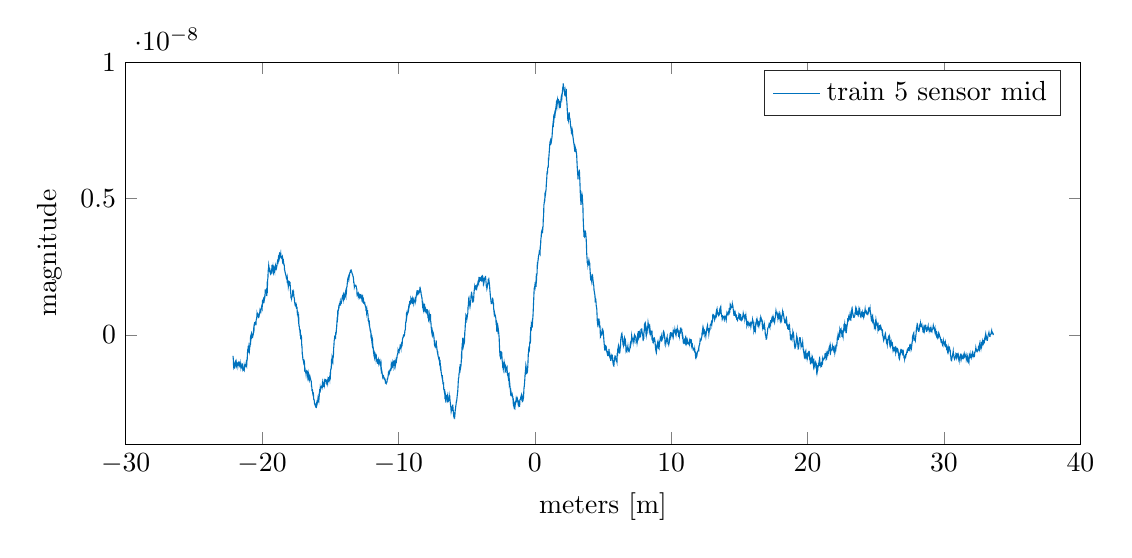
\begin{tikzpicture}

  \begin{axis}[%
    width=\textwidth,
    height=0.4\textwidth,
    at={(0\figurewidth,0\figureheight)},
    scale only axis,
    xmin=-30,
    xmax=40,
    xlabel={meters [m]},
    ymin=-4e-09,
    ymax=1e-08,
    ylabel={magnitude},
    axis background/.style={fill=white},
    legend style={legend cell align=left,align=left,draw=white!15!black}
    ]
    \addplot [color=mycolor1,solid]
    table[row sep=crcr]{%
    -22.127904296875	-7.63086305820906e-10\\
    -22.10791015625	-8.75472057799538e-10\\
    -22.087916015625	-1.11139007960595e-09\\
    -22.067921875	-1.20701746393103e-09\\
    -22.047927734375	-1.1840509978512e-09\\
    -22.02793359375	-1.14794185109842e-09\\
    -22.007939453125	-1.23535148093829e-09\\
    -21.9879453125	-1.0683577298189e-09\\
    -21.967951171875	-1.1029417598777e-09\\
    -21.94795703125	-1.11195146728858e-09\\
    -21.927962890625	-9.45887883499606e-10\\
    -21.90796875	-9.28677453041932e-10\\
    -21.887974609375	-9.95900030236421e-10\\
    -21.86798046875	-1.10700313275782e-09\\
    -21.847986328125	-1.05491348505977e-09\\
    -21.8279921875	-1.06178583723869e-09\\
    -21.807998046875	-1.04174807610733e-09\\
    -21.78800390625	-1.03041643882021e-09\\
    -21.768009765625	-1.135225602034e-09\\
    -21.748015625	-1.07248600666458e-09\\
    -21.728021484375	-1.01874880226135e-09\\
    -21.70802734375	-1.0428293985552e-09\\
    -21.688033203125	-1.03030055014498e-09\\
    -21.6680390625	-1.01490638491254e-09\\
    -21.648044921875	-1.12299640141451e-09\\
    -21.62805078125	-1.14790854628834e-09\\
    -21.608056640625	-1.12194187987504e-09\\
    -21.5880625	-1.14206172339226e-09\\
    -21.568068359375	-1.06409368564538e-09\\
    -21.54807421875	-1.1721340864576e-09\\
    -21.528080078125	-1.10292456333294e-09\\
    -21.5080859375	-1.10701145602554e-09\\
    -21.488091796875	-1.14558132043763e-09\\
    -21.46809765625	-1.17543563193088e-09\\
    -21.448103515625	-1.04570079676914e-09\\
    -21.428109375	-1.19969765313025e-09\\
    -21.408115234375	-1.26636150812383e-09\\
    -21.38812109375	-1.23252196968184e-09\\
    -21.368126953125	-1.26188546692192e-09\\
    -21.3481328125	-1.23769797399558e-09\\
    -21.328138671875	-1.26395207263614e-09\\
    -21.30814453125	-1.14310499890588e-09\\
    -21.288150390625	-1.21140385116815e-09\\
    -21.26815625	-1.12503938535678e-09\\
    -21.248162109375	-1.11483305970952e-09\\
    -21.22816796875	-1.10004680490106e-09\\
    -21.208173828125	-1.13043098952216e-09\\
    -21.1881796875	-1.11046031281114e-09\\
    -21.168185546875	-1.04487930022001e-09\\
    -21.14819140625	-1.13114110970253e-09\\
    -21.128197265625	-1.15338700156648e-09\\
    -21.108203125	-9.61990367056977e-10\\
    -21.088208984375	-9.06922789885591e-10\\
    -21.06821484375	-6.75771609342745e-10\\
    -21.048220703125	-5.39931338852032e-10\\
    -21.0282265625	-5.19610171792005e-10\\
    -21.008232421875	-4.00658291830266e-10\\
    -20.98823828125	-4.95516618334591e-10\\
    -20.968244140625	-4.25257038863963e-10\\
    -20.94825	-5.2267179541415e-10\\
    -20.928255859375	-5.84515929305872e-10\\
    -20.90826171875	-4.52868023694226e-10\\
    -20.888267578125	-4.30431713588957e-10\\
    -20.8682734375	-3.7479649851529e-10\\
    -20.848279296875	-1.65933491237629e-10\\
    -20.82828515625	-2.08083043486151e-10\\
    -20.808291015625	-7.44841637698249e-12\\
    -20.788296875	2.31237118800889e-11\\
    -20.768302734375	6.13658911979339e-11\\
    -20.74830859375	2.82844684617179e-12\\
    -20.728314453125	-8.59746707464479e-11\\
    -20.7083203125	-6.89145182076107e-11\\
    -20.688326171875	-7.72592591593382e-11\\
    -20.66833203125	1.01743384745012e-11\\
    -20.648337890625	5.94521332700187e-12\\
    -20.62834375	1.32891748045914e-10\\
    -20.608349609375	2.37272120348022e-10\\
    -20.58835546875	2.01497417092024e-10\\
    -20.568361328125	3.85988234452785e-10\\
    -20.5483671875	4.44766837400605e-10\\
    -20.528373046875	4.38293081639108e-10\\
    -20.50837890625	4.49830985495377e-10\\
    -20.488384765625	4.63796002309111e-10\\
    -20.468390625	4.30911735989036e-10\\
    -20.448396484375	3.51280872668658e-10\\
    -20.42840234375	5.4552869290935e-10\\
    -20.408408203125	5.87327704684263e-10\\
    -20.3884140625	6.28105812048348e-10\\
    -20.368419921875	7.65921088213077e-10\\
    -20.34842578125	7.03177823640388e-10\\
    -20.328431640625	7.47227848721895e-10\\
    -20.3084375	7.05244110276493e-10\\
    -20.288443359375	6.94700100540133e-10\\
    -20.26844921875	7.2284392925829e-10\\
    -20.248455078125	6.45564161124166e-10\\
    -20.2284609375	6.52609553454227e-10\\
    -20.208466796875	7.18918686519398e-10\\
    -20.18847265625	7.57151451530115e-10\\
    -20.168478515625	8.25391883081671e-10\\
    -20.148484375	9.11323432665774e-10\\
    -20.128490234375	8.8192158648625e-10\\
    -20.10849609375	8.92884285711376e-10\\
    -20.088501953125	8.61341809485534e-10\\
    -20.0685078125	9.48935061841087e-10\\
    -20.048513671875	9.86800754555373e-10\\
    -20.02851953125	1.05235133213678e-09\\
    -20.008525390625	1.0885423236752e-09\\
    -19.98853125	1.02516658400491e-09\\
    -19.968537109375	1.19862382960538e-09\\
    -19.94854296875	1.16661524340929e-09\\
    -19.928548828125	1.21254607129315e-09\\
    -19.9085546875	1.27258704276707e-09\\
    -19.888560546875	1.19472775048278e-09\\
    -19.86856640625	1.18790460666193e-09\\
    -19.848572265625	1.21469023744682e-09\\
    -19.828578125	1.32755748182519e-09\\
    -19.808583984375	1.39510045104477e-09\\
    -19.78858984375	1.38448701408645e-09\\
    -19.768595703125	1.59849043343146e-09\\
    -19.7486015625	1.57999784864212e-09\\
    -19.728607421875	1.64725494363025e-09\\
    -19.70861328125	1.66216192570941e-09\\
    -19.688619140625	1.57509203703863e-09\\
    -19.668625	1.57574357937961e-09\\
    -19.648630859375	1.42909039690754e-09\\
    -19.62863671875	1.77534888339464e-09\\
    -19.608642578125	1.72093905426484e-09\\
    -19.5886484375	2.02569012077246e-09\\
    -19.568654296875	2.07680637962255e-09\\
    -19.54866015625	2.37400013228543e-09\\
    -19.528666015625	2.40643711011676e-09\\
    -19.508671875	2.54968872977854e-09\\
    -19.488677734375	2.47774118230299e-09\\
    -19.46868359375	2.45062558655526e-09\\
    -19.448689453125	2.32866299740202e-09\\
    -19.4286953125	2.32449961614032e-09\\
    -19.408701171875	2.30061687822539e-09\\
    -19.38870703125	2.25841141841563e-09\\
    -19.368712890625	2.29747127332322e-09\\
    -19.34871875	2.21396940480993e-09\\
    -19.328724609375	2.400638738704e-09\\
    -19.30873046875	2.3927913057841e-09\\
    -19.288736328125	2.35963562822797e-09\\
    -19.2687421875	2.5719027856164e-09\\
    -19.248748046875	2.42324150502273e-09\\
    -19.22875390625	2.39323696454237e-09\\
    -19.208759765625	2.46651568297986e-09\\
    -19.188765625	2.32374370423184e-09\\
    -19.168771484375	2.28197253243975e-09\\
    -19.14877734375	2.37502829812077e-09\\
    -19.128783203125	2.28258391858169e-09\\
    -19.1087890625	2.43463968890956e-09\\
    -19.088794921875	2.38935303130819e-09\\
    -19.06880078125	2.33915076695344e-09\\
    -19.048806640625	2.50772819898748e-09\\
    -19.0288125	2.38305202209647e-09\\
    -19.008818359375	2.5491933897711e-09\\
    -18.98882421875	2.51515679930817e-09\\
    -18.968830078125	2.4704470570736e-09\\
    -18.9488359375	2.43579664098254e-09\\
    -18.928841796875	2.4789492841494e-09\\
    -18.90884765625	2.5325155183903e-09\\
    -18.888853515625	2.60605959604187e-09\\
    -18.868859375	2.67956211022366e-09\\
    -18.848865234375	2.75150661507481e-09\\
    -18.82887109375	2.76510492420837e-09\\
    -18.808876953125	2.72130754850672e-09\\
    -18.7888828125	2.8637244819725e-09\\
    -18.768888671875	2.84847829568089e-09\\
    -18.74889453125	2.89989351035659e-09\\
    -18.728900390625	2.81317882644379e-09\\
    -18.70890625	2.85985817022811e-09\\
    -18.688912109375	2.93709555211344e-09\\
    -18.66891796875	2.89817514286026e-09\\
    -18.648923828125	2.94620214438308e-09\\
    -18.6289296875	2.99731090377301e-09\\
    -18.608935546875	2.86703948901484e-09\\
    -18.58894140625	2.86204384998641e-09\\
    -18.568947265625	2.8168785951204e-09\\
    -18.548953125	2.80620527259591e-09\\
    -18.528958984375	2.84340790700294e-09\\
    -18.50896484375	2.75363160358036e-09\\
    -18.488970703125	2.81136240536586e-09\\
    -18.4689765625	2.75447708966614e-09\\
    -18.448982421875	2.67449978753429e-09\\
    -18.42898828125	2.70439122815047e-09\\
    -18.408994140625	2.6197132250237e-09\\
    -18.389	2.56667272260579e-09\\
    -18.369005859375	2.56139485683821e-09\\
    -18.34901171875	2.39028858592375e-09\\
    -18.329017578125	2.36030045540249e-09\\
    -18.3090234375	2.30191006997394e-09\\
    -18.289029296875	2.26729597790909e-09\\
    -18.26903515625	2.22496167214584e-09\\
    -18.249041015625	2.18509989445196e-09\\
    -18.229046875	2.13058731195028e-09\\
    -18.209052734375	2.16228904870307e-09\\
    -18.18905859375	2.15474261925216e-09\\
    -18.169064453125	2.0427029151644e-09\\
    -18.1490703125	2.09817390663749e-09\\
    -18.129076171875	1.96899575117741e-09\\
    -18.10908203125	1.90163145556713e-09\\
    -18.089087890625	1.99909355798643e-09\\
    -18.06909375	1.78261577558293e-09\\
    -18.049099609375	1.84192533140139e-09\\
    -18.02910546875	1.83348386190522e-09\\
    -18.009111328125	1.85547227964314e-09\\
    -17.9891171875	1.94616160594712e-09\\
    -17.969123046875	1.93426146576539e-09\\
    -17.94912890625	1.92491155885284e-09\\
    -17.929134765625	1.79566133926505e-09\\
    -17.909140625	1.60898939292316e-09\\
    -17.889146484375	1.50343477740711e-09\\
    -17.86915234375	1.3342429652763e-09\\
    -17.849158203125	1.44431017263417e-09\\
    -17.8291640625	1.34629310927462e-09\\
    -17.809169921875	1.3979730134027e-09\\
    -17.78917578125	1.42493020036822e-09\\
    -17.769181640625	1.43071377925571e-09\\
    -17.7491875	1.61743664064403e-09\\
    -17.729193359375	1.63216749492968e-09\\
    -17.70919921875	1.59387501773274e-09\\
    -17.689205078125	1.59577857398543e-09\\
    -17.6692109375	1.41558368447548e-09\\
    -17.649216796875	1.37959230445744e-09\\
    -17.62922265625	1.35266024449767e-09\\
    -17.609228515625	1.18657623012065e-09\\
    -17.589234375	1.16798916055028e-09\\
    -17.569240234375	1.06294356331908e-09\\
    -17.54924609375	1.16198858824877e-09\\
    -17.529251953125	1.16824626421345e-09\\
    -17.5092578125	1.0237251911024e-09\\
    -17.489263671875	1.13906110435882e-09\\
    -17.46926953125	9.75643749075992e-10\\
    -17.449275390625	9.76494746356053e-10\\
    -17.42928125	9.87952777881061e-10\\
    -17.409287109375	7.75812795824195e-10\\
    -17.38929296875	7.88208884501785e-10\\
    -17.369298828125	7.21788431768354e-10\\
    -17.3493046875	7.53155103523469e-10\\
    -17.329310546875	5.66900299134748e-10\\
    -17.30931640625	6.153467449151e-10\\
    -17.289322265625	3.36864312691995e-10\\
    -17.269328125	3.15701423650632e-10\\
    -17.249333984375	2.02374798125857e-10\\
    -17.22933984375	1.8685336046106e-10\\
    -17.209345703125	6.87946834542252e-11\\
    -17.1893515625	1.00978262869818e-10\\
    -17.169357421875	-4.67151255279187e-11\\
    -17.14936328125	-7.56929090775116e-12\\
    -17.129369140625	-2.16999048715869e-11\\
    -17.109375	-7.75485949085229e-11\\
    -17.089380859375	-3.67876052802487e-10\\
    -17.06938671875	-4.31942018443307e-10\\
    -17.049392578125	-6.93930149937755e-10\\
    -17.0293984375	-7.29775275703594e-10\\
    -17.009404296875	-8.4856869435709e-10\\
    -16.98941015625	-9.20615667829192e-10\\
    -16.969416015625	-9.28413125335745e-10\\
    -16.949421875	-9.98290012431955e-10\\
    -16.929427734375	-9.65875123545711e-10\\
    -16.90943359375	-1.05626585282468e-09\\
    -16.889439453125	-1.02939401356649e-09\\
    -16.8694453125	-1.26793434798406e-09\\
    -16.849451171875	-1.24510892707688e-09\\
    -16.82945703125	-1.33344076594677e-09\\
    -16.809462890625	-1.36111988798294e-09\\
    -16.78946875	-1.35274566981495e-09\\
    -16.769474609375	-1.44360872439068e-09\\
    -16.74948046875	-1.36213426655945e-09\\
    -16.729486328125	-1.32172736104397e-09\\
    -16.7094921875	-1.34178775146018e-09\\
    -16.689498046875	-1.32451895053811e-09\\
    -16.66950390625	-1.32643736189506e-09\\
    -16.649509765625	-1.50199129951518e-09\\
    -16.629515625	-1.4349617238635e-09\\
    -16.609521484375	-1.58402020946594e-09\\
    -16.58952734375	-1.61034563645995e-09\\
    -16.569533203125	-1.5114963924453e-09\\
    -16.5495390625	-1.58276124076708e-09\\
    -16.529544921875	-1.4716070797507e-09\\
    -16.50955078125	-1.57914691421893e-09\\
    -16.489556640625	-1.5173134015728e-09\\
    -16.4695625	-1.56216181325992e-09\\
    -16.449568359375	-1.59127446539765e-09\\
    -16.42957421875	-1.64595018863423e-09\\
    -16.409580078125	-1.66818902520344e-09\\
    -16.3895859375	-1.70320871062067e-09\\
    -16.369591796875	-1.88975805763603e-09\\
    -16.34959765625	-1.90258839679034e-09\\
    -16.329603515625	-2.06837528624456e-09\\
    -16.309609375	-1.98237564361215e-09\\
    -16.289615234375	-2.1011776074532e-09\\
    -16.26962109375	-2.17723415550156e-09\\
    -16.249626953125	-2.215374550356e-09\\
    -16.2296328125	-2.18664014113326e-09\\
    -16.209638671875	-2.35530209433494e-09\\
    -16.18964453125	-2.36433111420796e-09\\
    -16.169650390625	-2.41224543940184e-09\\
    -16.14965625	-2.51468463089265e-09\\
    -16.129662109375	-2.54552588923225e-09\\
    -16.10966796875	-2.54281343589715e-09\\
    -16.089673828125	-2.59740651228689e-09\\
    -16.0696796875	-2.61122247851594e-09\\
    -16.049685546875	-2.65266609899553e-09\\
    -16.02969140625	-2.65673813713361e-09\\
    -16.009697265625	-2.53427902131985e-09\\
    -15.989703125	-2.58878841772434e-09\\
    -15.969708984375	-2.54859759078746e-09\\
    -15.94971484375	-2.4920932869098e-09\\
    -15.929720703125	-2.46626147160361e-09\\
    -15.9097265625	-2.37458221893627e-09\\
    -15.889732421875	-2.44781142954721e-09\\
    -15.86973828125	-2.43659957860467e-09\\
    -15.849744140625	-2.3187116861345e-09\\
    -15.82975	-2.38303467420292e-09\\
    -15.809755859375	-2.25584407996727e-09\\
    -15.78976171875	-2.1250511302392e-09\\
    -15.769767578125	-1.98937337461228e-09\\
    -15.7497734375	-2.08300692622704e-09\\
    -15.729779296875	-1.94184331699508e-09\\
    -15.70978515625	-2.00457838663988e-09\\
    -15.689791015625	-1.95802373637601e-09\\
    -15.669796875	-1.93511639900021e-09\\
    -15.649802734375	-1.90558421655615e-09\\
    -15.62980859375	-1.8848205758613e-09\\
    -15.609814453125	-1.90627037980205e-09\\
    -15.5898203125	-1.88361727887294e-09\\
    -15.569826171875	-1.76584321924647e-09\\
    -15.54983203125	-1.84708488823243e-09\\
    -15.529837890625	-1.7573177353102e-09\\
    -15.50984375	-1.76495775753703e-09\\
    -15.489849609375	-1.77533917843826e-09\\
    -15.46985546875	-1.89855727878131e-09\\
    -15.449861328125	-1.78072714839619e-09\\
    -15.4298671875	-1.8336460401002e-09\\
    -15.409873046875	-1.70483176474848e-09\\
    -15.38987890625	-1.72529774204973e-09\\
    -15.369884765625	-1.63153407779263e-09\\
    -15.349890625	-1.6395854063205e-09\\
    -15.329896484375	-1.63945207648969e-09\\
    -15.30990234375	-1.67875598732646e-09\\
    -15.289908203125	-1.66918109001736e-09\\
    -15.2699140625	-1.72719218125236e-09\\
    -15.249919921875	-1.78819699113241e-09\\
    -15.22992578125	-1.77233508590975e-09\\
    -15.209931640625	-1.71772641584112e-09\\
    -15.1899375	-1.77225416186779e-09\\
    -15.169943359375	-1.66186732266927e-09\\
    -15.14994921875	-1.71211422052395e-09\\
    -15.129955078125	-1.70750851693589e-09\\
    -15.1099609375	-1.58161283299622e-09\\
    -15.089966796875	-1.59140749539631e-09\\
    -15.06997265625	-1.58352132919098e-09\\
    -15.049978515625	-1.54708809419752e-09\\
    -15.029984375	-1.61598561895245e-09\\
    -15.009990234375	-1.47843811757569e-09\\
    -14.98999609375	-1.51073023533161e-09\\
    -14.970001953125	-1.29464537663819e-09\\
    -14.9500078125	-1.24373339408867e-09\\
    -14.930013671875	-1.24069885320748e-09\\
    -14.91001953125	-9.9730789857482e-10\\
    -14.890025390625	-1.0288449476065e-09\\
    -14.87003125	-8.69529170363067e-10\\
    -14.850037109375	-9.41449157110285e-10\\
    -14.83004296875	-9.3911179268188e-10\\
    -14.810048828125	-9.77229186665543e-10\\
    -14.7900546875	-7.35151682140984e-10\\
    -14.770060546875	-8.20834318879313e-10\\
    -14.75006640625	-4.98728501456084e-10\\
    -14.730072265625	-4.00222363568095e-10\\
    -14.710078125	-2.09776954632423e-10\\
    -14.690083984375	-1.76868933296353e-10\\
    -14.67008984375	-4.0106135928016e-11\\
    -14.650095703125	-3.7120874662857e-11\\
    -14.6301015625	-8.47369364249551e-11\\
    -14.610107421875	-9.7970397304007e-11\\
    -14.59011328125	1.00955155424476e-10\\
    -14.570119140625	1.37794151730067e-11\\
    -14.550125	2.03538766442481e-10\\
    -14.530130859375	2.64276985690245e-10\\
    -14.51013671875	4.47416116445438e-10\\
    -14.490142578125	5.82957636702269e-10\\
    -14.4701484375	5.56048308901399e-10\\
    -14.450154296875	8.12104682377202e-10\\
    -14.43016015625	7.80230335116604e-10\\
    -14.410166015625	9.18995739677117e-10\\
    -14.390171875	9.28076601991276e-10\\
    -14.370177734375	1.04090020379677e-09\\
    -14.35018359375	1.02738122503744e-09\\
    -14.330189453125	1.13581059366631e-09\\
    -14.3101953125	1.15305506915777e-09\\
    -14.290201171875	1.14934426773403e-09\\
    -14.27020703125	1.21007752978317e-09\\
    -14.250212890625	1.07501386280841e-09\\
    -14.23021875	1.18375057694317e-09\\
    -14.210224609375	1.15780043335716e-09\\
    -14.19023046875	1.16181949636512e-09\\
    -14.170236328125	1.23712817078757e-09\\
    -14.1502421875	1.25297000610692e-09\\
    -14.130248046875	1.35011917865872e-09\\
    -14.11025390625	1.39361439094161e-09\\
    -14.090259765625	1.36257707297788e-09\\
    -14.070265625	1.378934352598e-09\\
    -14.050271484375	1.43933663799119e-09\\
    -14.03027734375	1.34360238405336e-09\\
    -14.010283203125	1.44651355537173e-09\\
    -13.9902890625	1.28135590878542e-09\\
    -13.970294921875	1.42060132859736e-09\\
    -13.95030078125	1.37388864935562e-09\\
    -13.930306640625	1.42875887095799e-09\\
    -13.9103125	1.46107599775287e-09\\
    -13.890318359375	1.52790757041358e-09\\
    -13.87032421875	1.46626974023096e-09\\
    -13.850330078125	1.42336861698874e-09\\
    -13.8303359375	1.61935992189574e-09\\
    -13.810341796875	1.59278230480848e-09\\
    -13.79034765625	1.74714937257861e-09\\
    -13.770353515625	1.77142283555226e-09\\
    -13.750359375	1.88562058442309e-09\\
    -13.730365234375	1.98219066225442e-09\\
    -13.71037109375	2.05542256229806e-09\\
    -13.690376953125	2.09687749813709e-09\\
    -13.6703828125	2.11891273329244e-09\\
    -13.650388671875	2.15027978356575e-09\\
    -13.63039453125	2.06671393251262e-09\\
    -13.610400390625	2.15804716872946e-09\\
    -13.59040625	2.17124633379677e-09\\
    -13.570412109375	2.26601321906368e-09\\
    -13.55041796875	2.29817041312505e-09\\
    -13.530423828125	2.29753527193861e-09\\
    -13.5104296875	2.37210819012178e-09\\
    -13.490435546875	2.37383980680843e-09\\
    -13.47044140625	2.38224524626743e-09\\
    -13.450447265625	2.3484743071989e-09\\
    -13.430453125	2.32394394555439e-09\\
    -13.410458984375	2.2822758286933e-09\\
    -13.39046484375	2.24739589772571e-09\\
    -13.370470703125	2.22609330441605e-09\\
    -13.3504765625	2.20126508999077e-09\\
    -13.330482421875	2.14721820494155e-09\\
    -13.31048828125	2.12943034274202e-09\\
    -13.290494140625	2.04119617409943e-09\\
    -13.2705	1.90683408239815e-09\\
    -13.250505859375	1.90430543527111e-09\\
    -13.23051171875	1.75413986295762e-09\\
    -13.210517578125	1.78870001442686e-09\\
    -13.1905234375	1.79269664407696e-09\\
    -13.170529296875	1.80000676532092e-09\\
    -13.15053515625	1.82880452897303e-09\\
    -13.130541015625	1.82851190677464e-09\\
    -13.110546875	1.79897036790884e-09\\
    -13.090552734375	1.77413892546555e-09\\
    -13.07055859375	1.69348410047862e-09\\
    -13.050564453125	1.68160949882024e-09\\
    -13.0305703125	1.46790408701202e-09\\
    -13.010576171875	1.48388452447712e-09\\
    -12.99058203125	1.53473228478793e-09\\
    -12.970587890625	1.52692922476986e-09\\
    -12.95059375	1.4417194762168e-09\\
    -12.930599609375	1.52091300368177e-09\\
    -12.91060546875	1.49510601755992e-09\\
    -12.890611328125	1.4852145291755e-09\\
    -12.8706171875	1.42697380142888e-09\\
    -12.850623046875	1.51215784873408e-09\\
    -12.83062890625	1.35241356239509e-09\\
    -12.810634765625	1.47345715275037e-09\\
    -12.790640625	1.35621468178923e-09\\
    -12.770646484375	1.49557308455193e-09\\
    -12.75065234375	1.33524104655765e-09\\
    -12.730658203125	1.41575124301235e-09\\
    -12.7106640625	1.39788965090174e-09\\
    -12.690669921875	1.33592142546092e-09\\
    -12.67067578125	1.39859662678141e-09\\
    -12.650681640625	1.34679807840588e-09\\
    -12.6306875	1.28719171688714e-09\\
    -12.610693359375	1.34467721204287e-09\\
    -12.59069921875	1.25465238213496e-09\\
    -12.570705078125	1.21587923217701e-09\\
    -12.5507109375	1.25844782599397e-09\\
    -12.530716796875	1.18344078515274e-09\\
    -12.51072265625	1.16712579362352e-09\\
    -12.490728515625	1.19188793794604e-09\\
    -12.470734375	1.19076729222111e-09\\
    -12.450740234375	1.11954101332968e-09\\
    -12.43074609375	1.07480085157007e-09\\
    -12.410751953125	1.03073077339759e-09\\
    -12.3907578125	1.03270484700336e-09\\
    -12.370763671875	8.80353100909578e-10\\
    -12.35076953125	9.60106549448337e-10\\
    -12.330775390625	8.25312684222693e-10\\
    -12.31078125	9.01554323853481e-10\\
    -12.290787109375	7.83254798125304e-10\\
    -12.27079296875	9.11896291946316e-10\\
    -12.250798828125	7.92808634935842e-10\\
    -12.2308046875	7.47935779760221e-10\\
    -12.210810546875	5.07433573997936e-10\\
    -12.19081640625	6.20713115765147e-10\\
    -12.170822265625	4.73108808465154e-10\\
    -12.150828125	4.0865580327623e-10\\
    -12.130833984375	4.39752995305016e-10\\
    -12.11083984375	3.07238207656806e-10\\
    -12.090845703125	2.64758373563135e-10\\
    -12.0708515625	1.68567755560268e-10\\
    -12.050857421875	1.75557608858468e-10\\
    -12.03086328125	1.48645766131368e-10\\
    -12.010869140625	-4.20588964544884e-11\\
    -11.990875	-1.65817897343284e-11\\
    -11.970880859375	-1.23412867414862e-10\\
    -11.95088671875	-2.12960630836782e-10\\
    -11.930892578125	-1.58656462632517e-10\\
    -11.9108984375	-3.22345974614583e-10\\
    -11.890904296875	-2.70741990103151e-10\\
    -11.87091015625	-4.50722782095116e-10\\
    -11.850916015625	-4.45635160212696e-10\\
    -11.830921875	-6.23226147877041e-10\\
    -11.810927734375	-6.58280429657011e-10\\
    -11.79093359375	-7.56285987339429e-10\\
    -11.770939453125	-7.9612011940349e-10\\
    -11.7509453125	-7.20382084421097e-10\\
    -11.730951171875	-8.3752740413087e-10\\
    -11.71095703125	-7.96143451059405e-10\\
    -11.690962890625	-7.49774484927487e-10\\
    -11.67096875	-8.43339694074159e-10\\
    -11.650974609375	-6.99974888229476e-10\\
    -11.63098046875	-8.92326346494577e-10\\
    -11.610986328125	-8.3037223841086e-10\\
    -11.5909921875	-9.2517721933013e-10\\
    -11.570998046875	-9.17593602700088e-10\\
    -11.55100390625	-9.58271277141563e-10\\
    -11.531009765625	-9.39519422530754e-10\\
    -11.511015625	-1.0527682037223e-09\\
    -11.491021484375	-8.91667630038301e-10\\
    -11.47102734375	-9.94378353860613e-10\\
    -11.451033203125	-9.20087781658515e-10\\
    -11.4310390625	-9.77077580699416e-10\\
    -11.411044921875	-9.32018471874777e-10\\
    -11.39105078125	-9.2587704668497e-10\\
    -11.371056640625	-1.00987777025481e-09\\
    -11.3510625	-9.62373194940116e-10\\
    -11.331068359375	-1.03689949895129e-09\\
    -11.31107421875	-1.03866093827377e-09\\
    -11.291080078125	-1.15349415176649e-09\\
    -11.2710859375	-1.09028529928686e-09\\
    -11.251091796875	-1.31664716456067e-09\\
    -11.23109765625	-1.28367622433551e-09\\
    -11.211103515625	-1.32976611507349e-09\\
    -11.191109375	-1.41067604926208e-09\\
    -11.171115234375	-1.48213667315571e-09\\
    -11.15112109375	-1.54246550204966e-09\\
    -11.131126953125	-1.50676440865947e-09\\
    -11.1111328125	-1.53283344062414e-09\\
    -11.091138671875	-1.51578686752267e-09\\
    -11.07114453125	-1.58452732784922e-09\\
    -11.051150390625	-1.57593995284577e-09\\
    -11.03115625	-1.61091128449331e-09\\
    -11.011162109375	-1.59721909638543e-09\\
    -10.99116796875	-1.61244833044957e-09\\
    -10.971173828125	-1.63342257985688e-09\\
    -10.9511796875	-1.76289364290648e-09\\
    -10.931185546875	-1.7661251304016e-09\\
    -10.91119140625	-1.7527231624066e-09\\
    -10.891197265625	-1.77663883002203e-09\\
    -10.871203125	-1.75147905251146e-09\\
    -10.851208984375	-1.74444076633905e-09\\
    -10.83121484375	-1.68644698591892e-09\\
    -10.811220703125	-1.60427738926538e-09\\
    -10.7912265625	-1.60850397610802e-09\\
    -10.771232421875	-1.55288106540403e-09\\
    -10.75123828125	-1.50189577192206e-09\\
    -10.731244140625	-1.38736082637812e-09\\
    -10.71125	-1.39742856144452e-09\\
    -10.691255859375	-1.32344096244509e-09\\
    -10.67126171875	-1.31692939632175e-09\\
    -10.651267578125	-1.38126716695436e-09\\
    -10.6312734375	-1.33425152185378e-09\\
    -10.611279296875	-1.27156528234464e-09\\
    -10.59128515625	-1.26091411762616e-09\\
    -10.571291015625	-1.29631507750072e-09\\
    -10.551296875	-1.29087071970801e-09\\
    -10.531302734375	-1.1342520842425e-09\\
    -10.51130859375	-1.20627946446543e-09\\
    -10.491314453125	-1.17197015208683e-09\\
    -10.4713203125	-1.09255214784631e-09\\
    -10.451326171875	-1.14143745537211e-09\\
    -10.43133203125	-1.15854247583459e-09\\
    -10.411337890625	-1.04951497491041e-09\\
    -10.39134375	-1.1215367595958e-09\\
    -10.371349609375	-9.72683046125159e-10\\
    -10.35135546875	-1.08310650345234e-09\\
    -10.331361328125	-9.36101249040051e-10\\
    -10.3113671875	-1.1280783405163e-09\\
    -10.291373046875	-9.5555936732856e-10\\
    -10.27137890625	-1.08487186257764e-09\\
    -10.251384765625	-1.00845202018792e-09\\
    -10.231390625	-1.13658989260036e-09\\
    -10.211396484375	-1.08130694588932e-09\\
    -10.19140234375	-1.03653782295528e-09\\
    -10.171408203125	-9.74126112887043e-10\\
    -10.1514140625	-9.82690989888186e-10\\
    -10.131419921875	-8.49664040726016e-10\\
    -10.11142578125	-8.54188994224175e-10\\
    -10.091431640625	-7.48049591294037e-10\\
    -10.0714375	-7.25865199788421e-10\\
    -10.051443359375	-7.03245986478488e-10\\
    -10.03144921875	-5.87485311344349e-10\\
    -10.011455078125	-6.49166462020675e-10\\
    -9.9914609375	-6.39441638412145e-10\\
    -9.971466796875	-5.88688494874186e-10\\
    -9.95147265625	-6.13556930655767e-10\\
    -9.931478515625	-5.36918278454363e-10\\
    -9.911484375	-4.93530023269113e-10\\
    -9.891490234375	-4.9284736167607e-10\\
    -9.87149609375	-3.79153950399203e-10\\
    -9.851501953125	-3.87171350016821e-10\\
    -9.8315078125	-4.01714872310854e-10\\
    -9.811513671875	-4.67502193258845e-10\\
    -9.79151953125	-3.16355074800676e-10\\
    -9.771525390625	-4.50137864969541e-10\\
    -9.75153125	-2.64424020690266e-10\\
    -9.731537109375	-4.11317184722642e-10\\
    -9.71154296875	-1.80971410635337e-10\\
    -9.691548828125	-1.4268489797982e-10\\
    -9.6715546875	-9.12152481778954e-11\\
    -9.651560546875	-8.77657109442288e-11\\
    -9.63156640625	-2.41647621750149e-11\\
    -9.611572265625	-3.88093712545534e-11\\
    -9.591578125	-4.4432876401416e-11\\
    -9.571583984375	-2.15073870344456e-11\\
    -9.55158984375	2.02019301553005e-11\\
    -9.531595703125	1.25664858916637e-10\\
    -9.5116015625	1.83920679779277e-10\\
    -9.491607421875	2.10379512850524e-10\\
    -9.47161328125	4.31791842771717e-10\\
    -9.451619140625	4.91713432874387e-10\\
    -9.431625	4.88816300913945e-10\\
    -9.411630859375	7.12084407713004e-10\\
    -9.39163671875	6.49650021153145e-10\\
    -9.371642578125	7.29990947060924e-10\\
    -9.3516484375	7.42439908321614e-10\\
    -9.331654296875	8.30867307772131e-10\\
    -9.31166015625	8.57432476282533e-10\\
    -9.291666015625	9.03993975768598e-10\\
    -9.271671875	8.70784217018784e-10\\
    -9.251677734375	9.26727614022388e-10\\
    -9.23168359375	1.12020679683151e-09\\
    -9.211689453125	1.0434585694735e-09\\
    -9.1916953125	1.09674334455198e-09\\
    -9.171701171875	1.24628040668673e-09\\
    -9.15170703125	1.11278652029883e-09\\
    -9.131712890625	1.24096139459348e-09\\
    -9.11171875	1.12544466786561e-09\\
    -9.091724609375	1.28036991835109e-09\\
    -9.07173046875	1.21392928085035e-09\\
    -9.051736328125	1.24794797854735e-09\\
    -9.0317421875	1.25245887624064e-09\\
    -9.011748046875	1.36720767599652e-09\\
    -8.99175390625	1.15693006060319e-09\\
    -8.971759765625	1.24811654353281e-09\\
    -8.951765625	1.14380837601053e-09\\
    -8.931771484375	1.24318749978939e-09\\
    -8.91177734375	1.17445217534803e-09\\
    -8.891783203125	1.27317472037714e-09\\
    -8.8717890625	1.22982930552764e-09\\
    -8.851794921875	1.22283974479527e-09\\
    -8.83180078125	1.22947802424072e-09\\
    -8.811806640625	1.21361714492872e-09\\
    -8.7918125	1.27017945597142e-09\\
    -8.771818359375	1.19001715742774e-09\\
    -8.75182421875	1.23129629894777e-09\\
    -8.731830078125	1.23999097317068e-09\\
    -8.7118359375	1.37373526437059e-09\\
    -8.691841796875	1.42780884804787e-09\\
    -8.67184765625	1.49565632944776e-09\\
    -8.651853515625	1.56012542482658e-09\\
    -8.631859375	1.62411803217921e-09\\
    -8.611865234375	1.62208455962903e-09\\
    -8.59187109375	1.54731650287241e-09\\
    -8.571876953125	1.6035059085771e-09\\
    -8.5518828125	1.60903849828705e-09\\
    -8.531888671875	1.56104125016677e-09\\
    -8.51189453125	1.53115602121597e-09\\
    -8.491900390625	1.58379016260726e-09\\
    -8.47190625	1.57077886875979e-09\\
    -8.451912109375	1.63098042317539e-09\\
    -8.43191796875	1.62122455800198e-09\\
    -8.411923828125	1.77036514033955e-09\\
    -8.3919296875	1.65302908388432e-09\\
    -8.371935546875	1.59433240384514e-09\\
    -8.35194140625	1.60129279688962e-09\\
    -8.331947265625	1.48642677690403e-09\\
    -8.311953125	1.47354651764505e-09\\
    -8.291958984375	1.3873130891779e-09\\
    -8.27196484375	1.36310735758698e-09\\
    -8.251970703125	1.21858814710948e-09\\
    -8.2319765625	1.10122739682878e-09\\
    -8.211982421875	1.13853188539425e-09\\
    -8.19198828125	9.71122154554987e-10\\
    -8.171994140625	9.22441696923559e-10\\
    -8.152	1.05564904315878e-09\\
    -8.132005859375	1.14678361781685e-09\\
    -8.11201171875	9.88179255364101e-10\\
    -8.092017578125	9.42425919834754e-10\\
    -8.0720234375	1.0020277570637e-09\\
    -8.052029296875	8.69815031409866e-10\\
    -8.03203515625	8.55120392796592e-10\\
    -8.012041015625	8.56380792237007e-10\\
    -7.992046875	9.21257928037674e-10\\
    -7.972052734375	8.60801769916746e-10\\
    -7.95205859375	8.95155931971607e-10\\
    -7.932064453125	8.84765504805766e-10\\
    -7.9120703125	8.4201885766478e-10\\
    -7.892076171875	9.50414806939634e-10\\
    -7.87208203125	7.85106125808534e-10\\
    -7.852087890625	9.06935741684357e-10\\
    -7.83209375	6.23641563438886e-10\\
    -7.812099609375	7.48570914730318e-10\\
    -7.79210546875	5.96218824045062e-10\\
    -7.772111328125	6.3959646311229e-10\\
    -7.7521171875	5.85364157144567e-10\\
    -7.732123046875	7.50800159892588e-10\\
    -7.71212890625	6.83549519792374e-10\\
    -7.692134765625	7.6968791167357e-10\\
    -7.672140625	6.33647688211294e-10\\
    -7.652146484375	7.60196012515578e-10\\
    -7.63215234375	4.89908793426826e-10\\
    -7.612158203125	4.31881540823496e-10\\
    -7.5921640625	2.60860870308859e-10\\
    -7.572169921875	1.84286313340026e-10\\
    -7.55217578125	8.62452885006995e-11\\
    -7.532181640625	3.02105475771069e-11\\
    -7.5121875	1.21662581399207e-10\\
    -7.492193359375	4.96575018565333e-11\\
    -7.47219921875	1.12988200359504e-10\\
    -7.452205078125	8.89221050374207e-11\\
    -7.4322109375	4.00746548167905e-11\\
    -7.412216796875	-2.95795060473449e-11\\
    -7.39222265625	-9.76438328573809e-11\\
    -7.372228515625	-2.21911620034011e-10\\
    -7.352234375	-3.54579161631334e-10\\
    -7.332240234375	-3.96255175840335e-10\\
    -7.31224609375	-4.21487744725201e-10\\
    -7.292251953125	-3.49002074792756e-10\\
    -7.2722578125	-3.51925899048442e-10\\
    -7.252263671875	-3.70336632569138e-10\\
    -7.23226953125	-1.94745600987486e-10\\
    -7.212275390625	-4.36599595079645e-10\\
    -7.19228125	-4.26872279850891e-10\\
    -7.172287109375	-5.24200619559006e-10\\
    -7.15229296875	-5.93554194770364e-10\\
    -7.132298828125	-6.6193186589795e-10\\
    -7.1123046875	-6.51009579023201e-10\\
    -7.092310546875	-7.65613230178269e-10\\
    -7.07231640625	-8.03811786644224e-10\\
    -7.052322265625	-8.34794015617121e-10\\
    -7.032328125	-8.88705254623218e-10\\
    -7.012333984375	-9.21136869772443e-10\\
    -6.99233984375	-8.90347855550434e-10\\
    -6.972345703125	-1.09214356254114e-09\\
    -6.9523515625	-1.11723913352066e-09\\
    -6.932357421875	-1.0680455607925e-09\\
    -6.91236328125	-1.22516741893248e-09\\
    -6.892369140625	-1.20523957837233e-09\\
    -6.872375	-1.33136042170244e-09\\
    -6.852380859375	-1.39598112589377e-09\\
    -6.83238671875	-1.46074464381647e-09\\
    -6.812392578125	-1.5143554580659e-09\\
    -6.7923984375	-1.57290876725575e-09\\
    -6.772404296875	-1.55040576095557e-09\\
    -6.75241015625	-1.66626187627817e-09\\
    -6.732416015625	-1.78330136849286e-09\\
    -6.712421875	-1.80554124051427e-09\\
    -6.692427734375	-1.7887450894674e-09\\
    -6.67243359375	-1.98928464531597e-09\\
    -6.652439453125	-2.01138267645365e-09\\
    -6.6324453125	-2.07196396212408e-09\\
    -6.612451171875	-1.98684285982868e-09\\
    -6.59245703125	-2.22108536708604e-09\\
    -6.572462890625	-2.18739366663619e-09\\
    -6.55246875	-2.32394577534356e-09\\
    -6.532474609375	-2.26581237592795e-09\\
    -6.51248046875	-2.33301371559447e-09\\
    -6.492486328125	-2.21509389538644e-09\\
    -6.4724921875	-2.22264084015787e-09\\
    -6.452498046875	-2.23412916662197e-09\\
    -6.43250390625	-2.30499225654026e-09\\
    -6.412509765625	-2.24652362692489e-09\\
    -6.392515625	-2.3810770970536e-09\\
    -6.372521484375	-2.33972448565536e-09\\
    -6.35252734375	-2.411976589588e-09\\
    -6.332533203125	-2.42374994657662e-09\\
    -6.3125390625	-2.34648983919539e-09\\
    -6.292544921875	-2.34649632383382e-09\\
    -6.27255078125	-2.2257995111177e-09\\
    -6.252556640625	-2.29941511240825e-09\\
    -6.2325625	-2.28284526469906e-09\\
    -6.212568359375	-2.4301854424589e-09\\
    -6.19257421875	-2.4864955116216e-09\\
    -6.172580078125	-2.58060289726049e-09\\
    -6.1525859375	-2.67925574955371e-09\\
    -6.132591796875	-2.80749595574743e-09\\
    -6.11259765625	-2.75832237099652e-09\\
    -6.092603515625	-2.68743280593041e-09\\
    -6.072609375	-2.71944745749099e-09\\
    -6.052615234375	-2.65821163193888e-09\\
    -6.03262109375	-2.65606668680831e-09\\
    -6.012626953125	-2.55795530581225e-09\\
    -5.9926328125	-2.7246884649598e-09\\
    -5.972638671875	-2.79055715025319e-09\\
    -5.95264453125	-2.95141296358162e-09\\
    -5.932650390625	-2.94195369784591e-09\\
    -5.91265625	-3.06774288505832e-09\\
    -5.892662109375	-2.95127690448289e-09\\
    -5.87266796875	-2.99081697244036e-09\\
    -5.852673828125	-2.89208692377803e-09\\
    -5.8326796875	-2.74855844073945e-09\\
    -5.812685546875	-2.71054049247599e-09\\
    -5.79269140625	-2.60141936985108e-09\\
    -5.772697265625	-2.54653769701957e-09\\
    -5.752703125	-2.42923806396839e-09\\
    -5.732708984375	-2.43126496301226e-09\\
    -5.71271484375	-2.34300853605161e-09\\
    -5.692720703125	-2.24529915238285e-09\\
    -5.6727265625	-2.15360430599194e-09\\
    -5.652732421875	-2.07730217037262e-09\\
    -5.63273828125	-1.92074528398366e-09\\
    -5.612744140625	-1.71508313038744e-09\\
    -5.59275	-1.58367205627245e-09\\
    -5.572755859375	-1.55419456804061e-09\\
    -5.55276171875	-1.40095154066821e-09\\
    -5.532767578125	-1.38380820783405e-09\\
    -5.5127734375	-1.22805869483579e-09\\
    -5.492779296875	-1.24049878648323e-09\\
    -5.47278515625	-1.07118078704468e-09\\
    -5.452791015625	-1.22926648554889e-09\\
    -5.432796875	-1.17075800975693e-09\\
    -5.412802734375	-1.11314929588392e-09\\
    -5.39280859375	-9.70319581926245e-10\\
    -5.372814453125	-7.16439930182172e-10\\
    -5.3528203125	-7.4839480302735e-10\\
    -5.332826171875	-4.13265219699347e-10\\
    -5.31283203125	-4.39463610947775e-10\\
    -5.292837890625	-2.40000973481991e-10\\
    -5.27284375	-2.78812511092677e-10\\
    -5.252849609375	-1.01681725657133e-10\\
    -5.23285546875	-3.96178178944131e-10\\
    -5.212861328125	-3.47351931108213e-10\\
    -5.1928671875	-3.3779819397693e-10\\
    -5.172873046875	-2.96954335356331e-10\\
    -5.15287890625	-2.13610218472162e-10\\
    -5.132884765625	9.56676293015282e-11\\
    -5.112890625	1.82774538856551e-10\\
    -5.092896484375	3.98648310410104e-10\\
    -5.07290234375	5.03922899804916e-10\\
    -5.052908203125	6.98569948121239e-10\\
    -5.0329140625	6.62813350007179e-10\\
    -5.012919921875	6.59099266021511e-10\\
    -4.99292578125	7.40964687584023e-10\\
    -4.972931640625	6.07071536095476e-10\\
    -4.9529375	6.66274788420641e-10\\
    -4.932943359375	7.70744404946723e-10\\
    -4.91294921875	7.9981962675427e-10\\
    -4.892955078125	1.04157288041366e-09\\
    -4.8729609375	1.09727356840632e-09\\
    -4.852966796875	1.25867500022145e-09\\
    -4.83297265625	1.19409135471872e-09\\
    -4.812978515625	1.26705862372787e-09\\
    -4.792984375	1.14113868505695e-09\\
    -4.772990234375	1.09520003590029e-09\\
    -4.75299609375	1.03316067777021e-09\\
    -4.733001953125	1.10530192395476e-09\\
    -4.7130078125	1.20212253648882e-09\\
    -4.693013671875	1.27600697445252e-09\\
    -4.67301953125	1.45075087081451e-09\\
    -4.653025390625	1.49527789645192e-09\\
    -4.63303125	1.58539554699879e-09\\
    -4.613037109375	1.40611403622009e-09\\
    -4.59304296875	1.41912118820312e-09\\
    -4.573048828125	1.38379543772853e-09\\
    -4.5530546875	1.20905528920637e-09\\
    -4.533060546875	1.20802726362796e-09\\
    -4.51306640625	1.24345405462396e-09\\
    -4.493072265625	1.24651251539407e-09\\
    -4.473078125	1.42274895190933e-09\\
    -4.453083984375	1.57951040456841e-09\\
    -4.43308984375	1.6640040467876e-09\\
    -4.413095703125	1.7464878150615e-09\\
    -4.3931015625	1.65100284412025e-09\\
    -4.373107421875	1.82511631585242e-09\\
    -4.35311328125	1.75203174030194e-09\\
    -4.333119140625	1.69779456037624e-09\\
    -4.313125	1.69773236354631e-09\\
    -4.293130859375	1.7441771054391e-09\\
    -4.27313671875	1.63801911645767e-09\\
    -4.253142578125	1.74127530905621e-09\\
    -4.2331484375	1.75988427077103e-09\\
    -4.213154296875	1.79470288726114e-09\\
    -4.19316015625	1.8206334603643e-09\\
    -4.173166015625	1.9297644072731e-09\\
    -4.153171875	1.97006304574687e-09\\
    -4.133177734375	1.99310900335288e-09\\
    -4.11318359375	1.94276229276444e-09\\
    -4.093189453125	2.1262672487984e-09\\
    -4.0731953125	2.01984257395836e-09\\
    -4.053201171875	2.12053897553883e-09\\
    -4.03320703125	1.99714282452888e-09\\
    -4.013212890625	2.01713319653393e-09\\
    -3.99321875	2.05495659111731e-09\\
    -3.973224609375	2.03274179669268e-09\\
    -3.95323046875	2.06505476243849e-09\\
    -3.933236328125	2.09798350607094e-09\\
    -3.9132421875	2.03915475351298e-09\\
    -3.893248046875	2.08442615863094e-09\\
    -3.87325390625	2.04595951745905e-09\\
    -3.853259765625	2.10265770652846e-09\\
    -3.833265625	2.15632659002008e-09\\
    -3.813271484375	2.14054366424203e-09\\
    -3.79327734375	2.03729958122755e-09\\
    -3.773283203125	1.90538947248729e-09\\
    -3.7532890625	1.96205146889048e-09\\
    -3.733294921875	1.90680022590398e-09\\
    -3.71330078125	1.96416403226095e-09\\
    -3.693306640625	2.06356634164297e-09\\
    -3.6733125	2.04868731277135e-09\\
    -3.653318359375	2.06140197061546e-09\\
    -3.63332421875	2.06364624972943e-09\\
    -3.613330078125	2.16946914586644e-09\\
    -3.5933359375	2.02081564021246e-09\\
    -3.573341796875	1.92269137214364e-09\\
    -3.55334765625	1.78309737448649e-09\\
    -3.533353515625	1.78986035451234e-09\\
    -3.513359375	1.69749792016744e-09\\
    -3.493365234375	1.73928314966916e-09\\
    -3.47337109375	1.80350906895371e-09\\
    -3.453376953125	1.88475967597715e-09\\
    -3.4333828125	1.8824924395139e-09\\
    -3.413388671875	2.02481292274551e-09\\
    -3.39339453125	2.01930480673423e-09\\
    -3.373400390625	2.04589929101033e-09\\
    -3.35340625	1.9583207512474e-09\\
    -3.333412109375	1.88555621975582e-09\\
    -3.31341796875	1.78289508395245e-09\\
    -3.293423828125	1.63725693722366e-09\\
    -3.2734296875	1.53218885443915e-09\\
    -3.253435546875	1.39867900471151e-09\\
    -3.23344140625	1.34928198517787e-09\\
    -3.213447265625	1.23388609761185e-09\\
    -3.193453125	1.16155482763005e-09\\
    -3.173458984375	1.16891259575728e-09\\
    -3.15346484375	1.15732459684384e-09\\
    -3.133470703125	1.18089395882707e-09\\
    -3.1134765625	1.2562355128941e-09\\
    -3.093482421875	1.33254001134031e-09\\
    -3.07348828125	1.32124265280251e-09\\
    -3.053494140625	1.18117029355188e-09\\
    -3.0335	1.17709417534878e-09\\
    -3.013505859375	9.60437551116274e-10\\
    -2.99351171875	8.69781766469107e-10\\
    -2.973517578125	7.66995003376076e-10\\
    -2.9535234375	8.14126019122161e-10\\
    -2.933529296875	7.56179164788657e-10\\
    -2.91353515625	7.46125639802675e-10\\
    -2.893541015625	6.99150790345279e-10\\
    -2.873546875	6.52532120905455e-10\\
    -2.853552734375	5.98699728854485e-10\\
    -2.83355859375	3.67773706513861e-10\\
    -2.813564453125	5.34634933944296e-10\\
    -2.7935703125	1.24173026399464e-10\\
    -2.773576171875	3.09631911274105e-10\\
    -2.75358203125	1.4693029920514e-10\\
    -2.733587890625	2.66745332805995e-10\\
    -2.71359375	1.83791067163389e-10\\
    -2.693599609375	2.69757367427482e-10\\
    -2.67360546875	2.02076352354003e-10\\
    -2.653611328125	1.18909534925681e-10\\
    -2.6336171875	4.26219116141957e-12\\
    -2.613623046875	-1.03147929840253e-10\\
    -2.59362890625	-3.72731194762931e-10\\
    -2.573634765625	-5.80426899507547e-10\\
    -2.553640625	-7.5848550973787e-10\\
    -2.533646484375	-7.57583901827811e-10\\
    -2.51365234375	-8.17885757963994e-10\\
    -2.493658203125	-7.73637025216145e-10\\
    -2.4736640625	-5.88877427118281e-10\\
    -2.453669921875	-6.76209997355656e-10\\
    -2.43367578125	-7.82282830827675e-10\\
    -2.413681640625	-7.48917470825095e-10\\
    -2.3936875	-9.45662007517093e-10\\
    -2.373693359375	-9.83549721247067e-10\\
    -2.35369921875	-1.18237832945033e-09\\
    -2.333705078125	-1.19136045612644e-09\\
    -2.3137109375	-1.24831025848424e-09\\
    -2.293716796875	-1.11952729066969e-09\\
    -2.27372265625	-1.07923511960608e-09\\
    -2.253728515625	-1.01209219139851e-09\\
    -2.233734375	-1.09521634945609e-09\\
    -2.213740234375	-1.06240666370801e-09\\
    -2.19374609375	-1.12579299545087e-09\\
    -2.173751953125	-1.30550628060798e-09\\
    -2.1537578125	-1.27439333460883e-09\\
    -2.133763671875	-1.30143636512944e-09\\
    -2.11376953125	-1.20765336978382e-09\\
    -2.093775390625	-1.26901963098756e-09\\
    -2.07378125	-1.26324913649656e-09\\
    -2.053787109375	-1.24428772079362e-09\\
    -2.03379296875	-1.21161606997419e-09\\
    -2.013798828125	-1.42123785089824e-09\\
    -1.9938046875	-1.46119961544562e-09\\
    -1.973810546875	-1.44649845701881e-09\\
    -1.95381640625	-1.52291216457175e-09\\
    -1.933822265625	-1.42976154591096e-09\\
    -1.913828125	-1.44306022388433e-09\\
    -1.893833984375	-1.42300990844325e-09\\
    -1.87383984375	-1.76009072409528e-09\\
    -1.853845703125	-1.70310347633526e-09\\
    -1.8338515625	-1.79309749305418e-09\\
    -1.813857421875	-1.91971230150536e-09\\
    -1.79386328125	-2.00045452411024e-09\\
    -1.773869140625	-2.1208114573628e-09\\
    -1.753875	-2.23633314350697e-09\\
    -1.733880859375	-2.11879809545263e-09\\
    -1.71388671875	-2.183008450619e-09\\
    -1.693892578125	-2.20066836198613e-09\\
    -1.6738984375	-2.22701082809296e-09\\
    -1.653904296875	-2.18791295552503e-09\\
    -1.63391015625	-2.24584871639214e-09\\
    -1.613916015625	-2.25630762095924e-09\\
    -1.593921875	-2.3948318949103e-09\\
    -1.573927734375	-2.32115785954356e-09\\
    -1.55393359375	-2.57282709013446e-09\\
    -1.533939453125	-2.61858910404304e-09\\
    -1.5139453125	-2.57163271191475e-09\\
    -1.493951171875	-2.63697310039656e-09\\
    -1.47395703125	-2.58915446443343e-09\\
    -1.453962890625	-2.62788155900564e-09\\
    -1.43396875	-2.49316250509115e-09\\
    -1.413974609375	-2.51413746546069e-09\\
    -1.39398046875	-2.46985768595255e-09\\
    -1.373986328125	-2.37358448002485e-09\\
    -1.3539921875	-2.43844679600321e-09\\
    -1.333998046875	-2.41742510409973e-09\\
    -1.31400390625	-2.36682915053861e-09\\
    -1.294009765625	-2.30506783770654e-09\\
    -1.274015625	-2.33187886675143e-09\\
    -1.254021484375	-2.41954438008207e-09\\
    -1.23402734375	-2.48301142991535e-09\\
    -1.214033203125	-2.40279728211726e-09\\
    -1.1940390625	-2.55323493028542e-09\\
    -1.174044921875	-2.5220304794689e-09\\
    -1.15405078125	-2.54366984125018e-09\\
    -1.134056640625	-2.49330828620458e-09\\
    -1.1140625	-2.63494971512783e-09\\
    -1.094068359375	-2.39283687240431e-09\\
    -1.07407421875	-2.36910066611609e-09\\
    -1.054080078125	-2.36478335937475e-09\\
    -1.0340859375	-2.28764250893234e-09\\
    -1.014091796875	-2.29255885374165e-09\\
    -0.994097656249998	-2.22059925409666e-09\\
    -0.974103515624996	-2.19223208404619e-09\\
    -0.954109374999998	-2.31118591074107e-09\\
    -0.934115234375	-2.27837353039975e-09\\
    -0.914121093749998	-2.44171362177204e-09\\
    -0.894126953124999	-2.43178777428655e-09\\
    -0.874132812499997	-2.422430864266e-09\\
    -0.854138671874999	-2.35695003638738e-09\\
    -0.834144531249997	-2.31109919360735e-09\\
    -0.814150390624999	-2.14956329976902e-09\\
    -0.794156249999997	-1.95039081807507e-09\\
    -0.774162109374998	-1.88347379576514e-09\\
    -0.754167968749996	-1.78260526642264e-09\\
    -0.734173828124998	-1.62898889775354e-09\\
    -0.7141796875	-1.45827940052368e-09\\
    -0.694185546874998	-1.35367564242233e-09\\
    -0.674191406249999	-1.25850562263463e-09\\
    -0.654197265624997	-1.10742434042368e-09\\
    -0.634203124999999	-1.16538467505119e-09\\
    -0.614208984374997	-1.39241977699737e-09\\
    -0.594214843749999	-1.37592724488357e-09\\
    -0.574220703124997	-1.39141884630484e-09\\
    -0.554226562499998	-1.37167112057413e-09\\
    -0.534232421874997	-1.31408594601855e-09\\
    -0.514238281249998	-1.14685315493311e-09\\
    -0.494244140625	-9.22578309336189e-10\\
    -0.474249999999998	-6.61032596256038e-10\\
    -0.454255859374999	-6.09861904370519e-10\\
    -0.434261718749998	-4.48147329956351e-10\\
    -0.414267578124999	-4.49017123042285e-10\\
    -0.394273437499997	-4.92832071061015e-10\\
    -0.374279296874999	-2.96061896689973e-10\\
    -0.354285156249997	-2.99952158700723e-10\\
    -0.334291015624999	-7.84791661081069e-11\\
    -0.314296874999997	-1.24144011258477e-10\\
    -0.294302734374998	2.85318288213335e-10\\
    -0.27430859375	2.01169311343149e-10\\
    -0.254314453124998	3.83485731864279e-10\\
    -0.2343203125	3.21978368270443e-10\\
    -0.214326171874998	4.26801600004733e-10\\
    -0.194332031249999	2.67467738926211e-10\\
    -0.174337890624997	4.1077541834154e-10\\
    -0.154343749999999	5.75100248455984e-10\\
    -0.134349609374997	6.99221350230484e-10\\
    -0.114355468749999	9.11425352749996e-10\\
    -0.0943613281249966	1.14799719249341e-09\\
    -0.0743671874999983	1.37464301538207e-09\\
    -0.0543730468749999	1.6004682106965e-09\\
    -0.034378906249998	1.73414468344631e-09\\
    -0.0143847656249996	1.73626282263345e-09\\
    0.00560937500000236	1.81423323303199e-09\\
    0.0256035156250007	1.75687303105811e-09\\
    0.0455976562500027	1.83476630433306e-09\\
    0.0655917968750011	1.90531164733253e-09\\
    0.085585937500003	1.76391634097579e-09\\
    0.105580078125001	2.09446109425383e-09\\
    0.125574218750003	2.04858627992192e-09\\
    0.145568359375002	2.23902589763972e-09\\
    0.165562500000004	2.24818639783385e-09\\
    0.185556640625002	2.61660267638583e-09\\
    0.20555078125	2.60142692121405e-09\\
    0.225544921875002	2.69581353412313e-09\\
    0.245539062500001	2.75556815710166e-09\\
    0.265533203125003	2.86275266784125e-09\\
    0.285527343750001	2.92078197115945e-09\\
    0.305521484375003	2.95155088134571e-09\\
    0.325515625000001	3.04099833125128e-09\\
    0.345509765625003	3.01526993508306e-09\\
    0.365503906250002	3.0671902381076e-09\\
    0.385498046875004	3.02155753017203e-09\\
    0.405492187500002	3.27433966458939e-09\\
    0.425486328125	3.29203054772328e-09\\
    0.445480468750002	3.5383418400145e-09\\
    0.465474609375001	3.57572923316265e-09\\
    0.485468750000003	3.76160382444298e-09\\
    0.505462890625001	3.80030758160019e-09\\
    0.525457031250003	3.77110669490128e-09\\
    0.545451171875001	3.83245764935222e-09\\
    0.565445312500003	3.74391865515628e-09\\
    0.585439453125002	3.90703396723905e-09\\
    0.605433593750004	3.99059533089604e-09\\
    0.625427734375002	4.29810397091128e-09\\
    0.645421875	4.36421883717789e-09\\
    0.665416015625002	4.76747988853497e-09\\
    0.685410156250001	4.8174809753203e-09\\
    0.705404296875003	4.92056945323028e-09\\
    0.725398437500001	4.91498925520727e-09\\
    0.745392578125003	5.13442506698003e-09\\
    0.765386718750001	5.1018852943027e-09\\
    0.785380859375003	5.16976620410251e-09\\
    0.805375000000002	5.28332779034387e-09\\
    0.825369140625003	5.32461543873929e-09\\
    0.845363281250002	5.54327564840003e-09\\
    0.865357421875	5.65870794637882e-09\\
    0.885351562500002	5.83087624536359e-09\\
    0.905345703125001	6.00844969485191e-09\\
    0.925339843750002	5.91798467777385e-09\\
    0.945333984375001	6.12473866286761e-09\\
    0.965328125000003	6.1536304166726e-09\\
    0.985322265625001	6.15754365433311e-09\\
    1.00531640625	6.46892438159621e-09\\
    1.025310546875	6.46336591560717e-09\\
    1.0453046875	6.62471074573579e-09\\
    1.065298828125	6.75897115723668e-09\\
    1.08529296875	6.89967406832274e-09\\
    1.105287109375	7.03697743612864e-09\\
    1.12528125	7.02272067794492e-09\\
    1.145275390625	7.10565422654424e-09\\
    1.16526953125	7.05005994415687e-09\\
    1.185263671875	7.0926872931261e-09\\
    1.2052578125	7.06253966732943e-09\\
    1.225251953125	7.13092113964868e-09\\
    1.24524609375	7.20446455543546e-09\\
    1.265240234375	7.28322593392099e-09\\
    1.285234375	7.43710284806997e-09\\
    1.305228515625	7.60045009481363e-09\\
    1.32522265625	7.70275246717232e-09\\
    1.345216796875	7.79193630773577e-09\\
    1.3652109375	7.75195377861983e-09\\
    1.385205078125	7.95987321750032e-09\\
    1.40519921875	7.91685886470148e-09\\
    1.425193359375	8.04696319744111e-09\\
    1.4451875	8.09958281645248e-09\\
    1.465181640625	7.9609146209399e-09\\
    1.48517578125	8.11288049581136e-09\\
    1.505169921875	8.14063700575574e-09\\
    1.5251640625	8.22924779850411e-09\\
    1.545158203125	8.34597560344053e-09\\
    1.56515234375	8.39678861150868e-09\\
    1.585146484375	8.51355211147381e-09\\
    1.605140625	8.47780395465725e-09\\
    1.625134765625	8.39026169591188e-09\\
    1.64512890625	8.47832275489007e-09\\
    1.665123046875	8.62938344538663e-09\\
    1.6851171875	8.58266028501687e-09\\
    1.705111328125	8.49937200404666e-09\\
    1.72510546875	8.65797489070398e-09\\
    1.745099609375	8.55640451799578e-09\\
    1.76509375	8.51220856531152e-09\\
    1.785087890625	8.4023883991741e-09\\
    1.80508203125	8.45596179225139e-09\\
    1.825076171875	8.34651474359663e-09\\
    1.8450703125	8.34137757057792e-09\\
    1.865064453125	8.47104343590065e-09\\
    1.88505859375	8.43954077591393e-09\\
    1.905052734375	8.5647330333825e-09\\
    1.925046875	8.65826962552158e-09\\
    1.945041015625	8.74924954293715e-09\\
    1.96503515625	8.78690691122748e-09\\
    1.985029296875	8.71063142341119e-09\\
    2.0050234375	8.82358302754389e-09\\
    2.025017578125	8.89506502382107e-09\\
    2.04501171875	9.06413741394753e-09\\
    2.065005859375	9.07331535236358e-09\\
    2.085	9.22571344031972e-09\\
    2.104994140625	9.11940130634104e-09\\
    2.12498828125	8.99304856526425e-09\\
    2.144982421875	9.08872057621493e-09\\
    2.1649765625	8.9148722098457e-09\\
    2.184970703125	8.89992747776339e-09\\
    2.20496484375	8.75743942734166e-09\\
    2.224958984375	8.8536881115483e-09\\
    2.244953125	8.82011472251616e-09\\
    2.264947265625	8.91513803312509e-09\\
    2.28494140625	8.81087437979418e-09\\
    2.304935546875	9.02058346892455e-09\\
    2.3249296875	8.61303185713261e-09\\
    2.344923828125	8.58056097888443e-09\\
    2.36491796875	8.42044005933356e-09\\
    2.384912109375	8.19778703923839e-09\\
    2.40490625	8.05922304434248e-09\\
    2.424900390625	7.85399634584991e-09\\
    2.44489453125	7.96582578439141e-09\\
    2.464888671875	7.88098017253025e-09\\
    2.4848828125	7.96070586086578e-09\\
    2.504876953125	7.95880230146215e-09\\
    2.52487109375	8.15548320496525e-09\\
    2.544865234375	7.94449926524278e-09\\
    2.564859375	7.92051852289955e-09\\
    2.584853515625	7.91933981033705e-09\\
    2.60484765625	7.77550019141219e-09\\
    2.624841796875	7.65354608663003e-09\\
    2.6448359375	7.59916765937562e-09\\
    2.664830078125	7.54541053148006e-09\\
    2.68482421875	7.43377989865669e-09\\
    2.704818359375	7.46974231745967e-09\\
    2.7248125	7.38479769224646e-09\\
    2.744806640625	7.51544080051239e-09\\
    2.76480078125	7.46761420905947e-09\\
    2.784794921875	7.29637711510589e-09\\
    2.8047890625	7.24297636443514e-09\\
    2.824783203125	7.16719108273627e-09\\
    2.84477734375	7.07848758404298e-09\\
    2.864771484375	7.0234048588667e-09\\
    2.884765625	6.9561171579497e-09\\
    2.904759765625	6.86689548069311e-09\\
    2.92475390625	6.93325919654281e-09\\
    2.944748046875	6.71134691866889e-09\\
    2.9647421875	6.87246208415253e-09\\
    2.984736328125	6.82917720799919e-09\\
    3.00473046875	6.81201317211149e-09\\
    3.024724609375	6.80660862073044e-09\\
    3.04471875	6.65849427810962e-09\\
    3.064712890625	6.65865012852205e-09\\
    3.08470703125	6.42449722824487e-09\\
    3.104701171875	6.22317347559592e-09\\
    3.1246953125	6.02310088362528e-09\\
    3.144689453125	5.95075639667378e-09\\
    3.16468359375	5.70575660815793e-09\\
    3.184677734375	5.85527008310556e-09\\
    3.204671875	5.94360299621277e-09\\
    3.224666015625	5.96975109568927e-09\\
    3.24466015625	5.96978494105866e-09\\
    3.264654296875	6.06509145934244e-09\\
    3.2846484375	5.856925457174e-09\\
    3.304642578125	5.62861239269686e-09\\
    3.32463671875	5.34982121612563e-09\\
    3.344630859375	5.08850938162825e-09\\
    3.364625	4.98588562211718e-09\\
    3.384619140625	4.77375176129097e-09\\
    3.40461328125	4.97516451654478e-09\\
    3.424607421875	5.06925306782908e-09\\
    3.4446015625	5.01406219698969e-09\\
    3.464595703125	5.15151459765504e-09\\
    3.48458984375	5.10129933874091e-09\\
    3.504583984375	4.85046368751479e-09\\
    3.524578125	4.77412892269116e-09\\
    3.544572265625	4.30021123963711e-09\\
    3.56456640625	4.05317676320331e-09\\
    3.584560546875	3.8683178174733e-09\\
    3.6045546875	3.61959437325895e-09\\
    3.624548828125	3.61983223560703e-09\\
    3.64454296875	3.60107584157296e-09\\
    3.664537109375	3.66318713797359e-09\\
    3.68453125	3.80507465741551e-09\\
    3.704525390625	3.80747950379908e-09\\
    3.72451953125	3.75947846697203e-09\\
    3.744513671875	3.66726439962759e-09\\
    3.7645078125	3.53523837689249e-09\\
    3.784501953125	3.335318435979e-09\\
    3.80449609375	2.99508380983433e-09\\
    3.824490234375	2.85284917326071e-09\\
    3.844484375	2.67251823351342e-09\\
    3.864478515625	2.68025662782332e-09\\
    3.88447265625	2.5865737094117e-09\\
    3.904466796875	2.68417113169243e-09\\
    3.9244609375	2.54729899048086e-09\\
    3.944455078125	2.68329450855319e-09\\
    3.96444921875	2.7444030786907e-09\\
    3.984443359375	2.68488572926375e-09\\
    4.0044375	2.66050163729365e-09\\
    4.024431640625	2.6351133354494e-09\\
    4.04442578125	2.42555626795334e-09\\
    4.064419921875	2.27832975476615e-09\\
    4.0844140625	2.11605014858558e-09\\
    4.104408203125	2.00740286439732e-09\\
    4.12440234375	2.13575151947408e-09\\
    4.144396484375	2.03339380227029e-09\\
    4.164390625	1.97692788001146e-09\\
    4.184384765625	2.21738590056429e-09\\
    4.20437890625	2.06091560512607e-09\\
    4.224373046875	2.06138583847734e-09\\
    4.2443671875	2.11565012327318e-09\\
    4.264361328125	2.02288236156458e-09\\
    4.28435546875	1.93627097399e-09\\
    4.304349609375	1.84970627463507e-09\\
    4.32434375	1.80431327880076e-09\\
    4.344337890625	1.62837276973935e-09\\
    4.36433203125	1.59819410859226e-09\\
    4.384326171875	1.497785267685e-09\\
    4.4043203125	1.48985452014388e-09\\
    4.424314453125	1.30607777667227e-09\\
    4.44430859375	1.34253345542124e-09\\
    4.464302734375	1.32553945638674e-09\\
    4.484296875	1.21927805311314e-09\\
    4.504291015625	1.07124920662866e-09\\
    4.52428515625	1.02518178409116e-09\\
    4.544279296875	9.52023959990554e-10\\
    4.5642734375	7.28038619581969e-10\\
    4.584267578125	4.907972188407e-10\\
    4.60426171875	4.16783495655313e-10\\
    4.624255859375	4.70627086960297e-10\\
    4.64425	3.70942013121153e-10\\
    4.664244140625	4.11379463687292e-10\\
    4.68423828125	4.64139235499379e-10\\
    4.704232421875	5.94761155954304e-10\\
    4.7242265625	4.08053285324841e-10\\
    4.744220703125	4.98897605954791e-10\\
    4.76421484375	2.9150299544059e-10\\
    4.784208984375	2.98686829190836e-10\\
    4.804203125	2.1477444185999e-11\\
    4.824197265625	7.47722948779536e-11\\
    4.84419140625	5.24113752391282e-12\\
    4.864185546875	6.40656869337476e-11\\
    4.8841796875	5.09849632366102e-11\\
    4.904173828125	3.34969859630195e-11\\
    4.92416796875	1.15213593234021e-10\\
    4.944162109375	2.19225388238866e-11\\
    4.96415625	2.43209466402342e-10\\
    4.984150390625	7.85774548703287e-11\\
    5.00414453125	1.89145813018593e-10\\
    5.024138671875	6.47900182639535e-11\\
    5.0441328125	-4.51695682965376e-11\\
    5.064126953125	-1.89097917279765e-10\\
    5.08412109375	-3.12317413927991e-10\\
    5.104115234375	-4.00751616907151e-10\\
    5.124109375	-5.46749164688701e-10\\
    5.144103515625	-5.44793469298515e-10\\
    5.16409765625	-5.33200215025335e-10\\
    5.184091796875	-4.54309200865307e-10\\
    5.2040859375	-4.93068734765747e-10\\
    5.224080078125	-4.23269742600021e-10\\
    5.24407421875	-4.42054354246845e-10\\
    5.264068359375	-5.96406587666711e-10\\
    5.2840625	-6.12383306284922e-10\\
    5.304056640625	-6.58125087517147e-10\\
    5.32405078125	-5.88360061406942e-10\\
    5.344044921875	-7.75825877691297e-10\\
    5.3640390625	-6.71167787693917e-10\\
    5.384033203125	-6.68319366655064e-10\\
    5.40402734375	-6.97334856579218e-10\\
    5.424021484375	-7.20085281011091e-10\\
    5.444015625	-5.07601156580254e-10\\
    5.464009765625	-7.17643204000679e-10\\
    5.48400390625	-6.32390810541609e-10\\
    5.503998046875	-8.56969815406097e-10\\
    5.5239921875	-7.83189701890812e-10\\
    5.543986328125	-8.41682130209665e-10\\
    5.56398046875	-9.46714000023191e-10\\
    5.583974609375	-8.30563641373829e-10\\
    5.60396875	-8.59662244022125e-10\\
    5.623962890625	-8.00536362847478e-10\\
    5.64395703125	-7.39811852568539e-10\\
    5.663951171875	-7.60757501168613e-10\\
    5.6839453125	-7.54921346289445e-10\\
    5.703939453125	-9.0081724162659e-10\\
    5.72393359375	-9.81217736126994e-10\\
    5.743927734375	-1.05952381416574e-09\\
    5.763921875	-1.09625736559265e-09\\
    5.783916015625	-1.06055993499991e-09\\
    5.80391015625	-1.08705632279745e-09\\
    5.823904296875	-9.47440383299696e-10\\
    5.8438984375	-8.53621836839037e-10\\
    5.863892578125	-8.57781682903339e-10\\
    5.88388671875	-7.45561196603536e-10\\
    5.903880859375	-8.4005401053305e-10\\
    5.923875	-8.23655652279115e-10\\
    5.943869140625	-9.12883446565526e-10\\
    5.96386328125	-9.3706218972512e-10\\
    5.983857421875	-9.20035990000258e-10\\
    6.0038515625	-9.41431715422598e-10\\
    6.023845703125	-9.87492231565818e-10\\
    6.04383984375	-6.56588744293585e-10\\
    6.063833984375	-7.72965443952028e-10\\
    6.083828125	-5.25514041600638e-10\\
    6.103822265625	-4.8030165512443e-10\\
    6.12381640625	-4.21621897531193e-10\\
    6.143810546875	-5.22236522071587e-10\\
    6.1638046875	-4.72554090639635e-10\\
    6.183798828125	-5.84876857477543e-10\\
    6.20379296875	-6.59351320540442e-10\\
    6.223787109375	-6.58734009786038e-10\\
    6.24378125	-5.95350166524179e-10\\
    6.263775390625	-4.63565816091989e-10\\
    6.28376953125	-4.14777217322635e-10\\
    6.303763671875	-1.61429705179065e-10\\
    6.3237578125	-8.48579513811815e-11\\
    6.343751953125	-2.86676197946573e-11\\
    6.36374609375	3.50650935201499e-11\\
    6.383740234375	5.72361495149125e-11\\
    6.403734375	-2.89253568892047e-11\\
    6.423728515625	-1.29239133058193e-10\\
    6.44372265625	-2.27420568310168e-10\\
    6.463716796875	-3.22945559980462e-10\\
    6.4837109375	-3.05199448947598e-10\\
    6.503705078125	-3.78318383583319e-10\\
    6.52369921875	-3.18891031699696e-10\\
    6.543693359375	-2.18304667317149e-10\\
    6.5636875	-2.6684830032372e-10\\
    6.583681640625	-1.133636298391e-10\\
    6.60367578125	-1.47253525751096e-10\\
    6.623669921875	-2.306320085571e-10\\
    6.6436640625	-2.0941049623447e-10\\
    6.663658203125	-3.42075771317817e-10\\
    6.68365234375	-5.3858732779862e-10\\
    6.703646484375	-4.90392738375966e-10\\
    6.723640625	-5.88024768945326e-10\\
    6.743634765625	-6.0741348575125e-10\\
    6.76362890625	-5.03142666789579e-10\\
    6.783623046875	-4.75158916605245e-10\\
    6.8036171875	-4.72932979205074e-10\\
    6.823611328125	-4.12699205869107e-10\\
    6.84360546875	-5.27369720655745e-10\\
    6.863599609375	-5.18202275865929e-10\\
    6.88359375	-5.76887537055185e-10\\
    6.903587890625	-5.57349015314805e-10\\
    6.92358203125	-5.86621089324616e-10\\
    6.943576171875	-5.47045898101057e-10\\
    6.9635703125	-5.06824935926718e-10\\
    6.983564453125	-4.13741859603115e-10\\
    7.00355859375	-3.36547039826867e-10\\
    7.023552734375	-3.86897416724806e-10\\
    7.043546875	-3.3306901672433e-10\\
    7.063541015625	-2.85953780118288e-10\\
    7.08353515625	-2.13039526248131e-10\\
    7.103529296875	-3.13380399796136e-11\\
    7.1235234375	-9.80272026234108e-11\\
    7.143517578125	-1.24729067438413e-10\\
    7.16351171875	-1.55066295462321e-10\\
    7.183505859375	-1.96340568373924e-10\\
    7.2035	-2.5529833945596e-10\\
    7.223494140625	-1.10150861731651e-10\\
    7.24348828125	-2.35559154878648e-10\\
    7.263482421875	-1.44009862810816e-10\\
    7.2834765625	-1.91240208779426e-10\\
    7.303470703125	-1.04117512144482e-10\\
    7.32346484375	-5.91310716733817e-12\\
    7.343458984375	-3.56237244538487e-11\\
    7.363453125	-3.3429879874412e-11\\
    7.383447265625	-4.25916405814286e-11\\
    7.40344140625	-9.83299065471698e-11\\
    7.423435546875	-2.16490503290468e-10\\
    7.4434296875	-1.78006941506592e-10\\
    7.463423828125	-2.75162024054887e-10\\
    7.48341796875	-1.36873816654357e-10\\
    7.503412109375	-2.7747684956081e-10\\
    7.52340625	-2.17436442053058e-10\\
    7.543400390625	-2.87757880663519e-11\\
    7.56339453125	-8.18360969457091e-11\\
    7.583388671875	-8.31823912798277e-12\\
    7.6033828125	-3.31637981379526e-11\\
    7.623376953125	1.39658856397378e-10\\
    7.64337109375	-6.26073322388313e-11\\
    7.663365234375	-2.18317368467523e-11\\
    7.683359375	3.41710569546512e-11\\
    7.703353515625	-7.67003189406842e-11\\
    7.72334765625	-7.49589346055555e-11\\
    7.743341796875	-6.58861101002246e-11\\
    7.7633359375	1.9310631080831e-11\\
    7.783330078125	1.6535295921909e-10\\
    7.80332421875	1.47597006595832e-10\\
    7.823318359375	1.54727795223083e-10\\
    7.8433125	2.38183756858861e-10\\
    7.863306640625	9.39417739382501e-11\\
    7.88330078125	7.62949102530326e-11\\
    7.903294921875	1.15571496614705e-11\\
    7.9232890625	-6.49876402974925e-11\\
    7.943283203125	-2.20656054923084e-10\\
    7.96327734375	-5.4041590116926e-11\\
    7.983271484375	-1.464159258614e-10\\
    8.003265625	9.7215856119486e-11\\
    8.023259765625	1.43988578096167e-10\\
    8.04325390625	3.92343338142252e-10\\
    8.063248046875	4.15077376949449e-10\\
    8.0832421875	3.5427640814868e-10\\
    8.103236328125	3.96112842462479e-10\\
    8.12323046875	2.5820196708575e-10\\
    8.143224609375	1.21305946758472e-10\\
    8.16321875	1.8530446344001e-10\\
    8.183212890625	1.26774178009788e-11\\
    8.20320703125	7.69647914031495e-11\\
    8.223201171875	6.64330400532662e-11\\
    8.2431953125	1.81609844776376e-10\\
    8.263189453125	2.56425705473931e-10\\
    8.28318359375	3.26510310009681e-10\\
    8.303177734375	4.5453802052645e-10\\
    8.323171875	3.8645439300687e-10\\
    8.343166015625	3.64833726448192e-10\\
    8.36316015625	3.18931637527584e-10\\
    8.383154296875	2.22936941133959e-10\\
    8.4031484375	2.76658222604138e-10\\
    8.423142578125	1.61431246175196e-10\\
    8.44313671875	2.3662705420546e-10\\
    8.463130859375	1.43996383565699e-10\\
    8.483125	4.298769008035e-11\\
    8.503119140625	7.54000525562294e-11\\
    8.52311328125	1.62795724861908e-10\\
    8.543107421875	4.93351652065494e-12\\
    8.5631015625	1.56592951027225e-10\\
    8.583095703125	-3.51675712710977e-11\\
    8.60308984375	2.15639538480004e-11\\
    8.623083984375	-1.43053400154027e-10\\
    8.643078125	-1.65423753039937e-10\\
    8.663072265625	-2.97506448445781e-10\\
    8.68306640625	-1.93038692664041e-10\\
    8.703060546875	-2.38492628537916e-10\\
    8.7230546875	-1.8156658656343e-10\\
    8.743048828125	-1.22440597878707e-10\\
    8.76304296875	-1.11216424359937e-10\\
    8.783037109375	-1.47001631076233e-10\\
    8.80303125	-1.86245930321496e-10\\
    8.823025390625	-3.05040389511643e-10\\
    8.84301953125	-4.29333741022895e-10\\
    8.863013671875	-5.33950295882824e-10\\
    8.8830078125	-5.82256966576086e-10\\
    8.903001953125	-5.05002772535042e-10\\
    8.92299609375	-5.81449449692715e-10\\
    8.942990234375	-4.75175492271421e-10\\
    8.962984375	-4.33057141927738e-10\\
    8.982978515625	-3.91949530219498e-10\\
    9.00297265625	-2.72888209548801e-10\\
    9.022966796875	-2.39793494506125e-10\\
    9.0429609375	-3.42023864084399e-10\\
    9.062955078125	-2.53557266619826e-10\\
    9.08294921875	-3.84830873398463e-10\\
    9.102943359375	-3.37808750557601e-10\\
    9.1229375	-4.12127813801559e-10\\
    9.142931640625	-2.92551880499713e-10\\
    9.16292578125	-2.53661270277783e-10\\
    9.182919921875	-1.97029757212563e-10\\
    9.2029140625	-8.2812802673351e-11\\
    9.222908203125	-9.75251132586407e-11\\
    9.24290234375	-1.06534417044081e-10\\
    9.262896484375	-1.45459971643674e-10\\
    9.282890625	-6.43675911623763e-11\\
    9.302884765625	-1.50847271016451e-10\\
    9.32287890625	-1.83327279737277e-10\\
    9.342873046875	-1.54827170321894e-10\\
    9.3628671875	-1.24620393894835e-10\\
    9.382861328125	-8.51338683650043e-11\\
    9.40285546875	-1.49929393412585e-11\\
    9.422849609375	1.03692041297575e-10\\
    9.44284375	1.36940358609347e-10\\
    9.462837890625	1.10446257804147e-10\\
    9.48283203125	7.41705872216192e-11\\
    9.502826171875	-7.62740510025072e-11\\
    9.5228203125	-6.77486622451898e-11\\
    9.542814453125	-2.54188103432271e-10\\
    9.56280859375	-2.07384509799586e-10\\
    9.582802734375	-2.14326492400378e-10\\
    9.602796875	-3.26574332964335e-10\\
    9.622791015625	-2.62795184191792e-10\\
    9.64278515625	-2.044030287784e-10\\
    9.662779296875	-1.21521439161476e-10\\
    9.6827734375	-1.26331083615981e-10\\
    9.702767578125	-7.9823079847213e-11\\
    9.72276171875	-2.48897816544373e-10\\
    9.742755859375	-1.2321277813555e-10\\
    9.76275	-2.9950019559181e-10\\
    9.782744140625	-2.89356687628524e-10\\
    9.80273828125	-3.07628481203198e-10\\
    9.822732421875	-3.5547136832899e-10\\
    9.8427265625	-3.0531184884932e-10\\
    9.862720703125	-2.46875993097573e-10\\
    9.88271484375001	-1.52957350896055e-10\\
    9.902708984375	-4.52770940866054e-11\\
    9.922703125	2.80949459420275e-11\\
    9.942697265625	1.4111243348112e-11\\
    9.96269140625	1.05090822355298e-10\\
    9.982685546875	-2.26608020674038e-11\\
    10.0026796875	3.43794285188894e-11\\
    10.022673828125	3.81147314205667e-11\\
    10.04266796875	6.59355780255858e-11\\
    10.062662109375	6.37497850500587e-11\\
    10.08265625	-1.42214566409999e-11\\
    10.102650390625	-2.09222293812608e-12\\
    10.12264453125	-5.34245167908988e-11\\
    10.142638671875	9.16254666757472e-11\\
    10.1626328125	2.04812349515744e-11\\
    10.182626953125	1.5007043943284e-10\\
    10.20262109375	1.34332660148807e-10\\
    10.222615234375	1.12931695925781e-10\\
    10.242609375	1.08929535484104e-10\\
    10.262603515625	1.84886370787962e-10\\
    10.28259765625	8.55806901155145e-11\\
    10.302591796875	7.29828664035411e-11\\
    10.3225859375	3.6670773464902e-11\\
    10.342580078125	9.50593089387996e-11\\
    10.36257421875	2.13496028960935e-11\\
    10.382568359375	8.67116925533184e-11\\
    10.4025625	1.84236863690625e-10\\
    10.422556640625	1.75135692702237e-10\\
    10.44255078125	2.30641489606622e-10\\
    10.462544921875	9.51522646141196e-11\\
    10.4825390625	2.26913549704555e-10\\
    10.502533203125	8.20466761816767e-11\\
    10.52252734375	1.65205285534865e-10\\
    10.542521484375	-7.28540303744234e-11\\
    10.562515625	2.10490718577475e-11\\
    10.582509765625	3.84991891791215e-11\\
    10.60250390625	-3.32968643261998e-11\\
    10.622498046875	7.84741701594455e-11\\
    10.6424921875	1.79406487028928e-10\\
    10.662486328125	4.75243143670935e-11\\
    10.68248046875	2.45776754433803e-10\\
    10.702474609375	2.38791662168428e-10\\
    10.72246875	2.43797412672703e-10\\
    10.742462890625	1.87636108996355e-10\\
    10.76245703125	1.41329997640989e-10\\
    10.782451171875	1.59214165987752e-10\\
    10.8024453125	9.25258483982508e-13\\
    10.822439453125	-5.89813303161015e-11\\
    10.84243359375	-1.49307806834988e-11\\
    10.862427734375	-7.8261232050143e-11\\
    10.882421875	-2.35618587630236e-10\\
    10.902416015625	-2.12902009923316e-10\\
    10.92241015625	-2.0103647212719e-10\\
    10.942404296875	-3.33476018525115e-10\\
    10.9623984375	-2.22181270777504e-10\\
    10.982392578125	-1.84191960963631e-10\\
    11.00238671875	-2.32445481451219e-10\\
    11.022380859375	-2.64432554001383e-10\\
    11.042375	-1.72608198332024e-10\\
    11.062369140625	-2.44685886894877e-10\\
    11.08236328125	-1.61291522280255e-10\\
    11.102357421875	-2.47907306303774e-10\\
    11.1223515625	-1.68586853452242e-10\\
    11.142345703125	-2.04721130020352e-10\\
    11.16233984375	-2.95312677216977e-10\\
    11.182333984375	-2.77598970646704e-10\\
    11.202328125	-2.21166038066108e-10\\
    11.222322265625	-3.06116636708799e-10\\
    11.24231640625	-3.24213658137282e-10\\
    11.262310546875	-3.21464355988593e-10\\
    11.2823046875	-3.14271298762925e-10\\
    11.302298828125	-3.34526112475893e-10\\
    11.32229296875	-2.81018983634055e-10\\
    11.342287109375	-2.23544620408105e-10\\
    11.36228125	-2.9926919417092e-10\\
    11.382275390625	-2.18421655123599e-10\\
    11.40226953125	-1.66283214348958e-10\\
    11.422263671875	-1.66040271361697e-10\\
    11.4422578125	-1.91386457338056e-10\\
    11.462251953125	-2.53314618015214e-10\\
    11.48224609375	-2.32310696436842e-10\\
    11.502240234375	-3.76521637282029e-10\\
    11.522234375	-3.25985734274353e-10\\
    11.542228515625	-3.23388184688525e-10\\
    11.56222265625	-4.43357670867961e-10\\
    11.582216796875	-4.58650009128805e-10\\
    11.6022109375	-5.1047304970103e-10\\
    11.622205078125	-4.85800607812736e-10\\
    11.64219921875	-4.97502499420683e-10\\
    11.662193359375	-5.18663428124182e-10\\
    11.6821875	-5.66898935632311e-10\\
    11.702181640625	-5.89937709132904e-10\\
    11.72217578125	-5.20022607661221e-10\\
    11.742169921875	-6.16773733646215e-10\\
    11.7621640625	-6.34364642293825e-10\\
    11.782158203125	-7.48327730226047e-10\\
    11.80215234375	-7.10681957386999e-10\\
    11.822146484375	-7.98583120757485e-10\\
    11.842140625	-7.4964288420408e-10\\
    11.862134765625	-7.97091890169629e-10\\
    11.88212890625	-7.76353938215474e-10\\
    11.902123046875	-6.806699707552e-10\\
    11.9221171875	-6.44243921359139e-10\\
    11.942111328125	-5.95425099311441e-10\\
    11.96210546875	-5.85462291610133e-10\\
    11.982099609375	-5.78146351601859e-10\\
    12.00209375	-5.22612623570907e-10\\
    12.022087890625	-5.43765763489243e-10\\
    12.04208203125	-4.00797318080358e-10\\
    12.062076171875	-3.7702824041857e-10\\
    12.0820703125	-3.54866725387995e-10\\
    12.102064453125	-2.82906880831972e-10\\
    12.12205859375	-1.70920141568368e-10\\
    12.142052734375	-1.94050930407716e-10\\
    12.162046875	-1.74899437616069e-10\\
    12.182041015625	-1.9121961641864e-10\\
    12.20203515625	-1.66735882676381e-10\\
    12.222029296875	-9.4234078799863e-11\\
    12.2420234375	-6.93857646768407e-11\\
    12.262017578125	6.50977283936001e-11\\
    12.28201171875	1.19283060648844e-10\\
    12.302005859375	1.90805933453366e-10\\
    12.322	1.26264358512115e-10\\
    12.341994140625	2.74652862950738e-10\\
    12.36198828125	2.30800513043976e-10\\
    12.381982421875	1.91777986191847e-10\\
    12.4019765625	1.11622449475584e-10\\
    12.421970703125	1.43400609523718e-10\\
    12.44196484375	1.59535093533969e-10\\
    12.461958984375	4.79899075628035e-11\\
    12.481953125	1.13711771229087e-10\\
    12.501947265625	1.13315814182539e-10\\
    12.52194140625	5.56389572066545e-11\\
    12.541935546875	-2.77836512913359e-11\\
    12.5619296875	6.09175326208331e-11\\
    12.581923828125	8.80567526994179e-11\\
    12.60191796875	2.08513626046737e-10\\
    12.621912109375	2.63291953658493e-10\\
    12.64190625	3.12045725403822e-10\\
    12.661900390625	3.50897396073944e-10\\
    12.68189453125	2.12383368789554e-10\\
    12.701888671875	1.68864603725078e-10\\
    12.7218828125	1.58760443768495e-10\\
    12.741876953125	1.82607060866765e-10\\
    12.76187109375	4.17398236293068e-11\\
    12.781865234375	1.11798919122023e-10\\
    12.801859375	1.81890915511095e-10\\
    12.821853515625	2.15763484772475e-10\\
    12.84184765625	2.06362140932988e-10\\
    12.861841796875	3.6469848620592e-10\\
    12.8818359375	3.67801154234127e-10\\
    12.901830078125	3.87632742287574e-10\\
    12.92182421875	4.17277429196777e-10\\
    12.941818359375	3.4578875812952e-10\\
    12.9618125	5.30898264307302e-10\\
    12.981806640625	4.05640883443663e-10\\
    13.00180078125	4.79850303884863e-10\\
    13.021794921875	4.81380764538753e-10\\
    13.0417890625	6.69236004617299e-10\\
    13.061783203125	6.49377442581716e-10\\
    13.08177734375	7.47566855745753e-10\\
    13.101771484375	7.3845049658495e-10\\
    13.121765625	6.58634927056463e-10\\
    13.141759765625	6.62374665310582e-10\\
    13.16175390625	6.34517098590206e-10\\
    13.181748046875	5.78522144536899e-10\\
    13.2017421875	6.4863524864676e-10\\
    13.221736328125	6.1905989442072e-10\\
    13.24173046875	6.54718547699585e-10\\
    13.261724609375	6.81707490770931e-10\\
    13.28171875	7.67638632559511e-10\\
    13.301712890625	8.29732725752524e-10\\
    13.32170703125	7.68319233244657e-10\\
    13.341701171875	8.99487867620412e-10\\
    13.3616953125	9.46931528255683e-10\\
    13.381689453125	8.63627294080813e-10\\
    13.40168359375	8.69623252331891e-10\\
    13.421677734375	7.88709999557301e-10\\
    13.441671875	7.90909629580958e-10\\
    13.461666015625	6.91925278561577e-10\\
    13.48166015625	8.26448666335319e-10\\
    13.501654296875	7.26773233590481e-10\\
    13.5216484375	7.45884440585763e-10\\
    13.541642578125	7.96868751865121e-10\\
    13.56163671875	9.34410336172161e-10\\
    13.581630859375	9.78881261842466e-10\\
    13.601625	1.00327707307837e-09\\
    13.621619140625	9.11454652707212e-10\\
    13.64161328125	9.69710172051695e-10\\
    13.661607421875	8.17381868214428e-10\\
    13.6816015625	7.77935147949434e-10\\
    13.701595703125	6.86362571060564e-10\\
    13.72158984375	6.91588631979118e-10\\
    13.741583984375	5.78957635643179e-10\\
    13.761578125	6.08452457492628e-10\\
    13.781572265625	6.32132021798135e-10\\
    13.80156640625	6.79998841150456e-10\\
    13.821560546875	6.65500875833822e-10\\
    13.8415546875	6.55161649154609e-10\\
    13.861548828125	6.56850313282679e-10\\
    13.88154296875	6.01673544221333e-10\\
    13.901537109375	6.81540965543125e-10\\
    13.92153125	6.75763751267433e-10\\
    13.941525390625	6.17519849439748e-10\\
    13.96151953125	6.85910432948356e-10\\
    13.981513671875	6.68355949757887e-10\\
    14.0015078125	6.63347673190579e-10\\
    14.021501953125	6.64696295407628e-10\\
    14.04149609375	5.92817082455085e-10\\
    14.061490234375	7.02624680075241e-10\\
    14.081484375	7.94436554180245e-10\\
    14.101478515625	7.56179802972511e-10\\
    14.12147265625	7.81488782559891e-10\\
    14.141466796875	7.78374703381669e-10\\
    14.1614609375	7.58185674520006e-10\\
    14.181455078125	8.46888544368761e-10\\
    14.20144921875	8.59753098299374e-10\\
    14.221443359375	7.44416789025807e-10\\
    14.2414375	8.75289763894064e-10\\
    14.261431640625	8.42076343164846e-10\\
    14.28142578125	9.20720017792594e-10\\
    14.301419921875	8.98574402253019e-10\\
    14.3214140625	1.06150930553375e-09\\
    14.341408203125	1.00597441082816e-09\\
    14.36140234375	1.05024071055851e-09\\
    14.381396484375	9.85968955729144e-10\\
    14.401390625	1.00645163517923e-09\\
    14.421384765625	1.0275677854742e-09\\
    14.44137890625	1.02022362578872e-09\\
    14.461373046875	1.03216813518827e-09\\
    14.4813671875	1.1333643499484e-09\\
    14.501361328125	1.07183955115341e-09\\
    14.52135546875	1.07874752160168e-09\\
    14.541349609375	9.55456060270552e-10\\
    14.56134375	9.16040515677715e-10\\
    14.581337890625	8.0936736840724e-10\\
    14.60133203125	8.44759639240397e-10\\
    14.621326171875	7.7602138096391e-10\\
    14.6413203125	8.00630254091905e-10\\
    14.661314453125	7.22396417414473e-10\\
    14.68130859375	7.20846939055109e-10\\
    14.701302734375	7.85400739656031e-10\\
    14.721296875	7.20686547482246e-10\\
    14.741291015625	6.61163011416997e-10\\
    14.76128515625	6.45963755490509e-10\\
    14.781279296875	7.50497876073751e-10\\
    14.8012734375	5.73900274726478e-10\\
    14.821267578125	5.67694214845822e-10\\
    14.84126171875	5.52234717744859e-10\\
    14.861255859375	5.36174929331378e-10\\
    14.88125	6.2430065168992e-10\\
    14.901244140625	6.30619558256159e-10\\
    14.92123828125	6.223400492823e-10\\
    14.941232421875	6.53368423596533e-10\\
    14.9612265625	7.41204087919834e-10\\
    14.981220703125	6.98244529591893e-10\\
    15.00121484375	6.48071154583001e-10\\
    15.021208984375	6.99542785819085e-10\\
    15.041203125	6.49820351180994e-10\\
    15.061197265625	7.48909057617889e-10\\
    15.08119140625	7.49450026946186e-10\\
    15.101185546875	6.87920723002118e-10\\
    15.1211796875	5.98974620333446e-10\\
    15.141173828125	6.28205895126346e-10\\
    15.16116796875	6.12084234565314e-10\\
    15.181162109375	5.43657617700998e-10\\
    15.20115625	5.60256631541302e-10\\
    15.221150390625	6.07354728983247e-10\\
    15.24114453125	6.66832885037684e-10\\
    15.261138671875	7.12666447676469e-10\\
    15.2811328125	7.98080997211005e-10\\
    15.301126953125	7.49110785781078e-10\\
    15.32112109375	7.17054801896559e-10\\
    15.341115234375	7.16209796595567e-10\\
    15.361109375	6.0028939124294e-10\\
    15.381103515625	7.18903067924406e-10\\
    15.40109765625	5.79565830443701e-10\\
    15.421091796875	6.4677102337461e-10\\
    15.4410859375	7.6592669580436e-10\\
    15.461080078125	5.90995866990659e-10\\
    15.48107421875	6.88299578353165e-10\\
    15.501068359375	5.94207306633279e-10\\
    15.5210625	5.59750713159622e-10\\
    15.541056640625	3.91643364534818e-10\\
    15.56105078125	4.5645937346268e-10\\
    15.581044921875	4.10017835466429e-10\\
    15.6010390625	4.72243874044138e-10\\
    15.621033203125	4.81597122097922e-10\\
    15.64102734375	3.54819620752498e-10\\
    15.661021484375	4.57583877698606e-10\\
    15.681015625	4.58969047264116e-10\\
    15.701009765625	3.70934210494019e-10\\
    15.72100390625	4.11801310424395e-10\\
    15.740998046875	3.9188363407609e-10\\
    15.7609921875	3.41031028378329e-10\\
    15.780986328125	3.38630845303952e-10\\
    15.80098046875	4.18228536203788e-10\\
    15.820974609375	3.80248784289711e-10\\
    15.84096875	3.02805697020353e-10\\
    15.860962890625	3.62099234003587e-10\\
    15.88095703125	4.48599138255768e-10\\
    15.900951171875	4.6967658126232e-10\\
    15.9209453125	4.75050841463335e-10\\
    15.940939453125	4.81971818218556e-10\\
    15.96093359375	5.47958533578064e-10\\
    15.980927734375	4.28786565116507e-10\\
    16.000921875	4.13280163790951e-10\\
    16.020916015625	3.35845160134524e-10\\
    16.04091015625	3.87980052539417e-10\\
    16.060904296875	1.76281346282484e-10\\
    16.0808984375	2.37707178252462e-10\\
    16.100892578125	2.62998898070646e-10\\
    16.12088671875	1.92842035822636e-10\\
    16.140880859375	1.13844344181153e-10\\
    16.160875	2.81946888718268e-10\\
    16.180869140625	2.13647257878999e-10\\
    16.20086328125	3.73293341315423e-10\\
    16.220857421875	3.82821559036457e-10\\
    16.2408515625	4.86587321270209e-10\\
    16.260845703125	4.42407316944179e-10\\
    16.28083984375	4.56118498383275e-10\\
    16.300833984375	5.60056599293346e-10\\
    16.320828125	5.0752703554495e-10\\
    16.340822265625	4.19203185748535e-10\\
    16.36081640625	4.75891571918981e-10\\
    16.380810546875	4.79337992380438e-10\\
    16.4008046875	3.42755171109761e-10\\
    16.420798828125	3.13457523572984e-10\\
    16.44079296875	4.21673720954758e-10\\
    16.460787109375	3.869125627726e-10\\
    16.48078125	3.78769089011079e-10\\
    16.500775390625	4.62532091074217e-10\\
    16.52076953125	5.71063554532009e-10\\
    16.540763671875	5.52537834972642e-10\\
    16.5607578125	6.29271045582706e-10\\
    16.580751953125	5.6706132938211e-10\\
    16.60074609375	6.06479216506127e-10\\
    16.620740234375	5.69892264037869e-10\\
    16.640734375	5.5230750190993e-10\\
    16.660728515625	4.90093327202733e-10\\
    16.68072265625	3.61699434227205e-10\\
    16.700716796875	2.85542257914689e-10\\
    16.7207109375	3.72171654633614e-10\\
    16.740705078125	2.70848828015558e-10\\
    16.76069921875	2.93800706517076e-10\\
    16.780693359375	2.04683557950921e-10\\
    16.8006875	3.89108962164935e-10\\
    16.820681640625	2.59551409405409e-10\\
    16.84067578125	3.50592107854179e-10\\
    16.860669921875	2.5659373842291e-10\\
    16.8806640625	1.93554895964805e-10\\
    16.900658203125	1.68868707819966e-11\\
    16.92065234375	-1.56032846521107e-11\\
    16.940646484375	-1.06983524405544e-11\\
    16.960640625	-1.5426001525501e-10\\
    16.980634765625	-1.50841580979648e-10\\
    17.00062890625	-1.17675086629703e-10\\
    17.020623046875	-2.09571180775043e-11\\
    17.0406171875	4.52356392061525e-11\\
    17.060611328125	1.31442796922364e-10\\
    17.08060546875	2.38813392625629e-10\\
    17.100599609375	2.68684656687527e-10\\
    17.12059375	2.88449154287138e-10\\
    17.140587890625	3.00834805648329e-10\\
    17.16058203125	3.56521182977161e-10\\
    17.180576171875	3.04838748830363e-10\\
    17.2005703125	2.90470873473733e-10\\
    17.220564453125	3.62381754270844e-10\\
    17.24055859375	3.10496992857004e-10\\
    17.260552734375	4.39607730276594e-10\\
    17.280546875	3.1961568350692e-10\\
    17.300541015625	5.25761520313275e-10\\
    17.32053515625	5.2700693798512e-10\\
    17.340529296875	5.05241790070743e-10\\
    17.3605234375	5.55425561956323e-10\\
    17.380517578125	5.13143482420955e-10\\
    17.40051171875	6.06400498004282e-10\\
    17.420505859375	5.7192150012042e-10\\
    17.4405	6.20743623810342e-10\\
    17.460494140625	6.64596253790922e-10\\
    17.48048828125	5.75556254206246e-10\\
    17.500482421875	6.01185038857727e-10\\
    17.5204765625	5.08836408729026e-10\\
    17.540470703125	5.24040957234614e-10\\
    17.56046484375	5.08977703962695e-10\\
    17.580458984375	4.6645934943195e-10\\
    17.600453125	5.37397626947881e-10\\
    17.620447265625	6.47810519439874e-10\\
    17.64044140625	6.49834364478041e-10\\
    17.660435546875	8.0209540007347e-10\\
    17.6804296875	8.86767161048083e-10\\
    17.700423828125	8.23343607136633e-10\\
    17.72041796875	8.30362987227989e-10\\
    17.740412109375	8.34094953977178e-10\\
    17.76040625	7.66982169669906e-10\\
    17.780400390625	7.33572070024772e-10\\
    17.80039453125	6.82102207943564e-10\\
    17.820388671875	6.09506001575178e-10\\
    17.8403828125	6.95612451804837e-10\\
    17.860376953125	6.4632931008126e-10\\
    17.88037109375	6.31180038845525e-10\\
    17.900365234375	7.09634731835501e-10\\
    17.920359375	6.25666302783058e-10\\
    17.940353515625	6.43588282038378e-10\\
    17.96034765625	7.21944357450116e-10\\
    17.980341796875	6.16329400257182e-10\\
    18.0003359375	6.86265238685721e-10\\
    18.020330078125	6.20554240070971e-10\\
    18.04032421875	5.29133785715111e-10\\
    18.060318359375	5.74420227407244e-10\\
    18.0803125	6.25021619258386e-10\\
    18.100306640625	5.74320715578049e-10\\
    18.12030078125	6.90804126029262e-10\\
    18.140294921875	7.24999100678644e-10\\
    18.1602890625	8.25015057668312e-10\\
    18.180283203125	7.39986286728324e-10\\
    18.20027734375	8.85852634851308e-10\\
    18.220271484375	7.33647195579864e-10\\
    18.240265625	7.3645550099249e-10\\
    18.260259765625	6.56302859561604e-10\\
    18.28025390625	5.79118580173697e-10\\
    18.300248046875	5.72594952567208e-10\\
    18.3202421875	4.66481573730141e-10\\
    18.340236328125	4.68097958510431e-10\\
    18.36023046875	4.39700457425493e-10\\
    18.380224609375	4.48221903967058e-10\\
    18.40021875	5.16664364955832e-10\\
    18.420212890625	5.69596038847543e-10\\
    18.44020703125	4.93026757274787e-10\\
    18.460201171875	5.60664504588182e-10\\
    18.4801953125	4.82671771247335e-10\\
    18.500189453125	3.04679537335013e-10\\
    18.52018359375	3.90579330820324e-10\\
    18.540177734375	2.40134320010546e-10\\
    18.560171875	2.29829056170422e-10\\
    18.580166015625	2.96592640112826e-10\\
    18.60016015625	2.69834738265279e-10\\
    18.620154296875	3.34485750889118e-10\\
    18.6401484375	3.66517912615522e-10\\
    18.660142578125	2.72577360992747e-10\\
    18.68013671875	2.99928692709178e-10\\
    18.700130859375	1.68370468534545e-10\\
    18.720125	7.47101295943268e-11\\
    18.740119140625	-7.90509323970691e-11\\
    18.76011328125	-5.82207293431976e-11\\
    18.780107421875	-1.98882247267497e-10\\
    18.8001015625	-9.85420469767931e-11\\
    18.820095703125	-4.94001404919871e-11\\
    18.84008984375	-7.59229575106893e-11\\
    18.860083984375	-1.2814468919603e-10\\
    18.880078125	-2.42142197354721e-11\\
    18.900072265625	-3.76999417568413e-11\\
    18.92006640625	1.04222167883147e-10\\
    18.940060546875	4.44813592474736e-11\\
    18.9600546875	6.21940967678786e-11\\
    18.980048828125	-6.42352901172402e-12\\
    19.00004296875	-1.74929502692888e-10\\
    19.020037109375	-2.1947635966876e-10\\
    19.04003125	-3.80471321906052e-10\\
    19.060025390625	-4.37656902685235e-10\\
    19.08001953125	-4.01543886215147e-10\\
    19.100013671875	-4.37480604907479e-10\\
    19.1200078125	-3.84814174956465e-10\\
    19.140001953125	-3.90743576353652e-10\\
    19.15999609375	-2.2945621652708e-10\\
    19.179990234375	-1.48295420788471e-10\\
    19.199984375	-5.53730901289342e-11\\
    19.219978515625	-1.37582372533068e-10\\
    19.23997265625	-1.18912336284838e-10\\
    19.259966796875	-2.6014808009297e-10\\
    19.2799609375	-3.41356659198975e-10\\
    19.299955078125	-4.52536688680006e-10\\
    19.31994921875	-4.23444062995677e-10\\
    19.339943359375	-4.5659039455314e-10\\
    19.3599375	-3.76162931827614e-10\\
    19.379931640625	-2.5681392857286e-10\\
    19.39992578125	-1.29854428662542e-10\\
    19.419919921875	-1.01979109435859e-10\\
    19.4399140625	-9.85961125958211e-11\\
    19.459908203125	-1.09822317970452e-10\\
    19.47990234375	-2.13395254265565e-10\\
    19.499896484375	-2.81143421770539e-10\\
    19.519890625	-4.0844890674427e-10\\
    19.539884765625	-3.60856752424516e-10\\
    19.55987890625	-4.19878558735147e-10\\
    19.579873046875	-4.21229839349065e-10\\
    19.5998671875	-3.54621848703337e-10\\
    19.619861328125	-3.47917373994243e-10\\
    19.63985546875	-2.68602105235395e-10\\
    19.659849609375	-3.96562694274135e-10\\
    19.67984375	-5.24249872958145e-10\\
    19.699837890625	-5.85094892407754e-10\\
    19.71983203125	-6.39522808788289e-10\\
    19.739826171875	-7.06374438101142e-10\\
    19.7598203125	-7.8738003591031e-10\\
    19.779814453125	-7.49602403687923e-10\\
    19.79980859375	-7.87056622286246e-10\\
    19.819802734375	-6.64018733131989e-10\\
    19.839796875	-7.2556997096647e-10\\
    19.859791015625	-7.36763621714384e-10\\
    19.87978515625	-6.67505175975171e-10\\
    19.899779296875	-8.15394204501013e-10\\
    19.9197734375	-7.94912268661503e-10\\
    19.939767578125	-7.67933994193012e-10\\
    19.95976171875	-8.4298658500096e-10\\
    19.979755859375	-7.51845456254891e-10\\
    19.99975	-7.91925964745507e-10\\
    20.019744140625	-7.11045728800262e-10\\
    20.03973828125	-7.26756405117586e-10\\
    20.059732421875	-6.63026726253804e-10\\
    20.0797265625	-6.94513979412564e-10\\
    20.099720703125	-6.62539961254932e-10\\
    20.11971484375	-7.2476210862782e-10\\
    20.139708984375	-6.92000590901608e-10\\
    20.159703125	-8.9714998805478e-10\\
    20.179697265625	-9.20348078847769e-10\\
    20.19969140625	-9.62745759700529e-10\\
    20.219685546875	-1.07848616135602e-09\\
    20.2396796875	-9.89343962996874e-10\\
    20.259673828125	-8.85392093012617e-10\\
    20.27966796875	-9.17716031401551e-10\\
    20.299662109375	-9.49061026648203e-10\\
    20.31965625	-8.55144703484743e-10\\
    20.339650390625	-9.40873316830033e-10\\
    20.35964453125	-8.86760721787783e-10\\
    20.379638671875	-1.00041816410378e-09\\
    20.3996328125	-1.01533255184441e-09\\
    20.419626953125	-9.71662460328573e-10\\
    20.43962109375	-1.15970236951953e-09\\
    20.459615234375	-1.11765277077689e-09\\
    20.479609375	-1.02884701833136e-09\\
    20.499603515625	-1.1246016873708e-09\\
    20.51959765625	-1.07100172913509e-09\\
    20.539591796875	-1.04142694444224e-09\\
    20.5595859375	-1.03545514264261e-09\\
    20.579580078125	-1.00866305323595e-09\\
    20.59957421875	-1.0999532310591e-09\\
    20.619568359375	-1.05479130384731e-09\\
    20.6395625	-1.0988142686621e-09\\
    20.659556640625	-1.27212084000988e-09\\
    20.67955078125	-1.20622084380841e-09\\
    20.699544921875	-1.37198145698959e-09\\
    20.7195390625	-1.31181412268438e-09\\
    20.739533203125	-1.30141707125798e-09\\
    20.75952734375	-1.19393724755493e-09\\
    20.779521484375	-1.13313000948888e-09\\
    20.799515625	-1.13563870486714e-09\\
    20.819509765625	-1.0372456398175e-09\\
    20.83950390625	-9.85992292543079e-10\\
    20.859498046875	-9.16930125916484e-10\\
    20.8794921875	-9.99249100084745e-10\\
    20.899486328125	-9.43428152531699e-10\\
    20.91948046875	-1.0776211162267e-09\\
    20.939474609375	-1.06132691391895e-09\\
    20.95946875	-1.11468713208763e-09\\
    20.979462890625	-1.06424681438296e-09\\
    20.99945703125	-1.04649313457443e-09\\
    21.019451171875	-1.17301394732452e-09\\
    21.0394453125	-9.94868291490674e-10\\
    21.059439453125	-1.08812833027243e-09\\
    21.07943359375	-9.54464650606843e-10\\
    21.099427734375	-9.92953557740476e-10\\
    21.119421875	-8.70776173568657e-10\\
    21.139416015625	-9.2108556559675e-10\\
    21.15941015625	-9.0318046114367e-10\\
    21.179404296875	-8.96936823745263e-10\\
    21.1993984375	-8.76028059421407e-10\\
    21.219392578125	-8.71023845385926e-10\\
    21.23938671875	-8.32115239017461e-10\\
    21.259380859375	-8.11317382228712e-10\\
    21.279375	-6.89493921580928e-10\\
    21.299369140625	-6.83357823915697e-10\\
    21.31936328125	-6.84005019550103e-10\\
    21.339357421875	-7.84314061821941e-10\\
    21.3593515625	-7.04950170518872e-10\\
    21.379345703125	-7.61992460230672e-10\\
    21.39933984375	-6.49405916285742e-10\\
    21.419333984375	-7.62287011176936e-10\\
    21.439328125	-6.82659617556895e-10\\
    21.459322265625	-7.57701063824841e-10\\
    21.47931640625	-7.52960389055716e-10\\
    21.499310546875	-6.44819631462699e-10\\
    21.5193046875	-6.16721941127944e-10\\
    21.539298828125	-6.35332736620321e-10\\
    21.55929296875	-5.56721668486967e-10\\
    21.579287109375	-4.49802945846193e-10\\
    21.59928125	-4.27790336927063e-10\\
    21.619275390625	-4.51980264246724e-10\\
    21.63926953125	-3.95503080692534e-10\\
    21.659263671875	-5.45888497652762e-10\\
    21.6792578125	-4.82835613737949e-10\\
    21.699251953125	-6.05440335092024e-10\\
    21.71924609375	-5.50846595620787e-10\\
    21.739240234375	-5.58912626415201e-10\\
    21.759234375	-5.56210769455598e-10\\
    21.779228515625	-5.48452564801754e-10\\
    21.79922265625	-5.0886193586239e-10\\
    21.819216796875	-4.03748534211983e-10\\
    21.8392109375	-4.49863588782025e-10\\
    21.859205078125	-4.56363490224697e-10\\
    21.87919921875	-5.18330620287714e-10\\
    21.899193359375	-4.82190779260793e-10\\
    21.9191875	-5.62392119711924e-10\\
    21.939181640625	-5.57949439268385e-10\\
    21.95917578125	-6.60824414406811e-10\\
    21.979169921875	-5.61145365640793e-10\\
    21.9991640625	-6.57119715891367e-10\\
    22.019158203125	-5.95891085823605e-10\\
    22.03915234375	-5.08209375883377e-10\\
    22.059146484375	-4.4777147407194e-10\\
    22.079140625	-4.93460033398938e-10\\
    22.099134765625	-4.07212054011273e-10\\
    22.11912890625	-3.7807402104281e-10\\
    22.139123046875	-3.8505916578749e-10\\
    22.1591171875	-2.7230051886112e-10\\
    22.179111328125	-1.20301432550792e-10\\
    22.19910546875	-1.36987668053688e-10\\
    22.219099609375	-5.55238698896551e-11\\
    22.23909375	-1.77593813207516e-10\\
    22.259087890625	-3.56113323583013e-11\\
    22.27908203125	-8.79624385625099e-11\\
    22.299076171875	-3.47181812242836e-11\\
    22.3190703125	1.51666935809562e-12\\
    22.339064453125	-1.8087423496412e-11\\
    22.35905859375	1.51952408777087e-10\\
    22.379052734375	8.43520247646034e-11\\
    22.399046875	2.36479243626091e-10\\
    22.419041015625	1.34821604992907e-10\\
    22.43903515625	1.47080767380426e-10\\
    22.459029296875	1.88768390912996e-10\\
    22.4790234375	1.08783573395603e-10\\
    22.499017578125	1.14511795209628e-10\\
    22.51901171875	-6.7434824204417e-11\\
    22.539005859375	4.3996454291444e-11\\
    22.559	-1.0474587603314e-11\\
    22.578994140625	1.36419354136173e-11\\
    22.59898828125	-4.50117465501466e-11\\
    22.618982421875	1.84678361588904e-10\\
    22.6389765625	1.12110154564689e-10\\
    22.658970703125	2.79700822684299e-10\\
    22.67896484375	2.35228739659785e-10\\
    22.698958984375	3.35139137256023e-10\\
    22.718953125	4.05186203752126e-10\\
    22.738947265625	2.86444304749141e-10\\
    22.75894140625	3.11138044987468e-10\\
    22.778935546875	1.62205907650169e-10\\
    22.7989296875	1.58880095441669e-10\\
    22.818923828125	7.43748262755172e-11\\
    22.83891796875	2.50482919650556e-10\\
    22.858912109375	1.97652242711505e-10\\
    22.87890625	2.88540152719347e-10\\
    22.898900390625	3.61174415159979e-10\\
    22.91889453125	3.94256576572074e-10\\
    22.938888671875	5.48437820043339e-10\\
    22.9588828125	5.29079188572564e-10\\
    22.978876953125	5.64227443513769e-10\\
    22.99887109375	6.25969192785112e-10\\
    23.018865234375	5.42666912485984e-10\\
    23.038859375	5.57831379496395e-10\\
    23.058853515625	6.40810928667231e-10\\
    23.07884765625	6.23015123985624e-10\\
    23.098841796875	7.04021768997835e-10\\
    23.1188359375	5.9207394484681e-10\\
    23.138830078125	5.74928370106381e-10\\
    23.15882421875	6.56708938473773e-10\\
    23.178818359375	6.24335827003682e-10\\
    23.1988125	7.8266075240778e-10\\
    23.218806640625	7.490062647248e-10\\
    23.23880078125	8.96374921402874e-10\\
    23.258794921875	8.51191599268799e-10\\
    23.2787890625	9.16557073539354e-10\\
    23.298783203125	8.19252661940072e-10\\
    23.31877734375	7.81652213218695e-10\\
    23.338771484375	7.58514215080568e-10\\
    23.358765625	6.54874003515758e-10\\
    23.378759765625	6.47104483492088e-10\\
    23.39875390625	6.44149992213173e-10\\
    23.418748046875	6.5395901037833e-10\\
    23.4387421875	6.9100261000601e-10\\
    23.458736328125	7.00878394465758e-10\\
    23.47873046875	8.10505801328515e-10\\
    23.498724609375	8.34943435538734e-10\\
    23.51871875	9.26397236807296e-10\\
    23.538712890625	8.34507868141462e-10\\
    23.55870703125	9.77205400202738e-10\\
    23.578701171875	7.40658692929334e-10\\
    23.5986953125	9.10014320176153e-10\\
    23.618689453125	8.60604325959232e-10\\
    23.63868359375	8.41866277350172e-10\\
    23.658677734375	7.7445483357794e-10\\
    23.678671875	7.47094373421973e-10\\
    23.698666015625	7.94502040085398e-10\\
    23.71866015625	7.47870206363043e-10\\
    23.738654296875	8.09328614644776e-10\\
    23.7586484375	9.13130137371383e-10\\
    23.778642578125	8.49954402643471e-10\\
    23.79863671875	8.88154860405883e-10\\
    23.818630859375	7.60133729939081e-10\\
    23.838625	8.59332952564991e-10\\
    23.858619140625	7.65178487233052e-10\\
    23.87861328125	6.77767019096994e-10\\
    23.898607421875	6.60836515913541e-10\\
    23.9186015625	7.81370474395607e-10\\
    23.938595703125	6.9059346147847e-10\\
    23.95858984375	8.04121342797527e-10\\
    23.978583984375	7.861858228259e-10\\
    23.998578125	8.23819537194559e-10\\
    24.018572265625	6.58404710278261e-10\\
    24.03856640625	7.7029679688885e-10\\
    24.058560546875	7.27769519934472e-10\\
    24.0785546875	7.64290054591798e-10\\
    24.098548828125	6.93781231235323e-10\\
    24.11854296875	7.71699711414766e-10\\
    24.138537109375	7.92326090375854e-10\\
    24.15853125	7.39589763981639e-10\\
    24.178525390625	8.0784617804843e-10\\
    24.19851953125	8.78071670567475e-10\\
    24.218513671875	9.52262260809431e-10\\
    24.2385078125	8.71389899677818e-10\\
    24.258501953125	8.39787131108428e-10\\
    24.27849609375	8.5245959383697e-10\\
    24.298490234375	8.68164606667044e-10\\
    24.318484375	7.74509540955661e-10\\
    24.338478515625	7.79793508668082e-10\\
    24.35847265625	7.86524308621593e-10\\
    24.378466796875	7.67459686726252e-10\\
    24.3984609375	8.04153687559742e-10\\
    24.418455078125	8.27334827788588e-10\\
    24.43844921875	8.26951199207539e-10\\
    24.458443359375	9.06742723365214e-10\\
    24.4784375	8.54986918720039e-10\\
    24.498431640625	9.56838019517772e-10\\
    24.51842578125	9.75802256215757e-10\\
    24.538419921875	9.60430653572856e-10\\
    24.5584140625	9.27313784894095e-10\\
    24.578408203125	9.78218877451703e-10\\
    24.59840234375	8.48501703490734e-10\\
    24.618396484375	8.19423287841866e-10\\
    24.638390625	7.25618297448877e-10\\
    24.658384765625	6.31138842726958e-10\\
    24.67837890625	5.51609370472259e-10\\
    24.698373046875	5.6984563177435e-10\\
    24.7183671875	5.40173543182801e-10\\
    24.738361328125	6.34862452867511e-10\\
    24.75835546875	5.80973558887367e-10\\
    24.778349609375	6.35473894811083e-10\\
    24.79834375	5.14119693847467e-10\\
    24.818337890625	5.5103096330099e-10\\
    24.83833203125	5.1923534364627e-10\\
    24.858326171875	3.99138610963533e-10\\
    24.8783203125	3.99505543304753e-10\\
    24.898314453125	2.67154881702992e-10\\
    24.91830859375	2.91967571020981e-10\\
    24.938302734375	3.22839909059395e-10\\
    24.958296875	2.82811595957371e-10\\
    24.978291015625	4.22937977997554e-10\\
    24.99828515625	3.72722042928982e-10\\
    25.018279296875	5.40347706588227e-10\\
    25.0382734375	4.71489198235036e-10\\
    25.058267578125	4.67476293620036e-10\\
    25.07826171875	4.6542035138253e-10\\
    25.098255859375	3.88809766851935e-10\\
    25.11825	3.40227873728611e-10\\
    25.138244140625	4.20590797522027e-10\\
    25.15823828125	2.34759714165633e-10\\
    25.178232421875	2.99897699581296e-10\\
    25.1982265625	1.42734734401947e-10\\
    25.218220703125	2.67460606693232e-10\\
    25.23821484375	2.58432995512367e-10\\
    25.258208984375	1.83355257105531e-10\\
    25.278203125	3.64171725220118e-10\\
    25.298197265625	2.67087554068441e-10\\
    25.31819140625	2.46214038295714e-10\\
    25.338185546875	3.03134994861133e-10\\
    25.3581796875	3.30855408313218e-10\\
    25.378173828125	2.87238899980094e-10\\
    25.39816796875	2.57317044880107e-10\\
    25.418162109375	1.78904182482322e-10\\
    25.43815625	1.7667948164634e-10\\
    25.458150390625	1.80387994312418e-10\\
    25.47814453125	7.58711870032691e-11\\
    25.498138671875	1.13234497772288e-10\\
    25.5181328125	-1.65318577099693e-11\\
    25.538126953125	-5.46141470349591e-11\\
    25.55812109375	-1.47605325137129e-10\\
    25.578115234375	-1.96855606931374e-10\\
    25.598109375	-1.54259874907278e-10\\
    25.618103515625	-1.40120152950523e-10\\
    25.63809765625	-6.45012374947562e-11\\
    25.658091796875	-3.71238500081821e-11\\
    25.6780859375	7.63634026030533e-12\\
    25.698080078125	-4.78138992475927e-11\\
    25.71807421875	-1.3328463658342e-13\\
    25.738068359375	-1.22748107980402e-10\\
    25.7580625	-1.26211718362773e-10\\
    25.778056640625	-2.4152909868382e-10\\
    25.79805078125	-2.20493981097918e-10\\
    25.818044921875	-3.06726665047623e-10\\
    25.8380390625	-3.56319642306694e-10\\
    25.858033203125	-1.73187618543395e-10\\
    25.87802734375	-3.02284102547745e-10\\
    25.898021484375	-1.61064736594167e-10\\
    25.918015625	-9.80392772139829e-11\\
    25.938009765625	-6.6380227186622e-11\\
    25.95800390625	-9.95061408393609e-11\\
    25.977998046875	-1.27196034395052e-10\\
    25.9979921875	-8.33241639791209e-11\\
    26.017986328125	-2.6308579596707e-10\\
    26.03798046875	-2.04195382978366e-10\\
    26.057974609375	-3.37651380264896e-10\\
    26.07796875	-2.9922986923588e-10\\
    26.097962890625	-3.88306559756433e-10\\
    26.11795703125	-3.35383323579843e-10\\
    26.137951171875	-2.68495721120608e-10\\
    26.1579453125	-3.34912404520179e-10\\
    26.177939453125	-3.13686803328417e-10\\
    26.19793359375	-3.42106651557048e-10\\
    26.217927734375	-3.20639060443688e-10\\
    26.237921875	-4.73276804234319e-10\\
    26.257916015625	-5.43491750607292e-10\\
    26.27791015625	-4.80681828586646e-10\\
    26.297904296875	-5.21225391105997e-10\\
    26.3178984375	-5.02859852471773e-10\\
    26.337892578125	-5.4459112097452e-10\\
    26.35788671875	-5.00340459649475e-10\\
    26.377880859375	-4.72793962038767e-10\\
    26.397875	-4.59023103370131e-10\\
    26.417869140625	-5.35712426290231e-10\\
    26.43786328125	-5.08731214808369e-10\\
    26.457857421875	-6.18327383639046e-10\\
    26.4778515625	-5.34199255357812e-10\\
    26.497845703125	-5.96240350737548e-10\\
    26.51783984375	-5.58788582119609e-10\\
    26.537833984375	-5.68963917956736e-10\\
    26.557828125	-5.15185875321398e-10\\
    26.577822265625	-5.43586519862903e-10\\
    26.59781640625	-5.2786813746677e-10\\
    26.617810546875	-6.02531825303993e-10\\
    26.6378046875	-5.85834061476303e-10\\
    26.657798828125	-6.83294848616243e-10\\
    26.67779296875	-7.05879170785474e-10\\
    26.697787109375	-8.33569263196212e-10\\
    26.71778125	-8.64501494157243e-10\\
    26.737775390625	-7.63410676330252e-10\\
    26.75776953125	-8.05515301418026e-10\\
    26.777763671875	-7.33909536753453e-10\\
    26.7977578125	-6.7050908536767e-10\\
    26.817751953125	-5.93071820278102e-10\\
    26.83774609375	-6.28081795349756e-10\\
    26.857740234375	-5.68194159178166e-10\\
    26.877734375	-5.52859437721719e-10\\
    26.897728515625	-5.98023132524202e-10\\
    26.91772265625	-6.23082137438868e-10\\
    26.937716796875	-6.17226081844245e-10\\
    26.9577109375	-6.63539219547252e-10\\
    26.977705078125	-6.13182450143503e-10\\
    26.99769921875	-6.58943926772959e-10\\
    27.017693359375	-6.2607509715418e-10\\
    27.0376875	-7.43768862270598e-10\\
    27.057681640625	-7.51360462473037e-10\\
    27.07767578125	-8.66138631101246e-10\\
    27.097669921875	-7.68744777161516e-10\\
    27.1176640625	-8.7943243182354e-10\\
    27.137658203125	-8.18013906214915e-10\\
    27.15765234375	-8.06405420007462e-10\\
    27.177646484375	-7.59145722634027e-10\\
    27.197640625	-7.85839532546731e-10\\
    27.217634765625	-7.24694905360349e-10\\
    27.23762890625	-7.14373410284143e-10\\
    27.257623046875	-6.50404348138124e-10\\
    27.2776171875	-6.2510240411707e-10\\
    27.297611328125	-5.75613061890839e-10\\
    27.31760546875	-5.95900728589265e-10\\
    27.337599609375	-5.21989475403903e-10\\
    27.35759375	-5.0525993643989e-10\\
    27.377587890625	-5.21970847581362e-10\\
    27.39758203125	-4.43486954145944e-10\\
    27.417576171875	-5.88393910166476e-10\\
    27.4375703125	-5.12488718857126e-10\\
    27.457564453125	-5.24986826479016e-10\\
    27.47755859375	-4.47412993508761e-10\\
    27.497552734375	-3.43083718230851e-10\\
    27.517546875	-4.5315527809713e-10\\
    27.537541015625	-3.62869714101907e-10\\
    27.55753515625	-3.76365182485019e-10\\
    27.577529296875	-4.3934019794957e-10\\
    27.5975234375	-4.11527358212069e-10\\
    27.617517578125	-4.72290805057916e-10\\
    27.63751171875	-3.90693517534239e-10\\
    27.657505859375	-2.86979307665244e-10\\
    27.6775	-2.36907767889017e-10\\
    27.697494140625	-5.35889159307512e-11\\
    27.71748828125	-1.94068550098687e-11\\
    27.737482421875	1.20661377474746e-11\\
    27.7574765625	3.95691151100762e-11\\
    27.777470703125	-5.9956818592909e-11\\
    27.79746484375	-5.28976959648257e-13\\
    27.817458984375	-1.48690275316449e-10\\
    27.837453125	-1.24773194379547e-10\\
    27.857447265625	-1.35838667744892e-10\\
    27.87744140625	-1.79982005950765e-10\\
    27.897435546875	-2.09691962879129e-10\\
    27.9174296875	-1.2039236759248e-10\\
    27.937423828125	-3.55924426881342e-12\\
    27.95741796875	4.64169793535053e-11\\
    27.977412109375	2.59892344824018e-10\\
    27.99740625	2.67793093893234e-10\\
    28.017400390625	3.33917593130137e-10\\
    28.03739453125	2.76966444922323e-10\\
    28.057388671875	3.31493410767772e-10\\
    28.0773828125	2.55025320971709e-10\\
    28.097376953125	2.27643089240731e-10\\
    28.11737109375	2.22049520273026e-10\\
    28.137365234375	1.33347378356617e-10\\
    28.157359375	1.31992605291969e-10\\
    28.177353515625	1.69463740319193e-10\\
    28.19734765625	3.04858881212713e-10\\
    28.217341796875	2.66584255600756e-10\\
    28.2373359375	3.16897423074244e-10\\
    28.257330078125	3.41950011005653e-10\\
    28.27732421875	4.19783734545836e-10\\
    28.297318359375	3.23739690658592e-10\\
    28.3173125	3.18481121665838e-10\\
    28.337306640625	3.1346085725899e-10\\
    28.35730078125	3.44103293606711e-10\\
    28.377294921875	3.75273565032739e-10\\
    28.3972890625	2.95700411576153e-10\\
    28.417283203125	2.81485940974444e-10\\
    28.43727734375	2.5498427858917e-10\\
    28.457271484375	1.2008078064599e-10\\
    28.477265625	1.11125287693488e-10\\
    28.497259765625	1.3503169200271e-10\\
    28.51725390625	2.3008449529115e-10\\
    28.537248046875	1.64768455759606e-10\\
    28.5572421875	2.65244301270155e-10\\
    28.577236328125	2.18046555744987e-10\\
    28.59723046875	3.16334377634784e-10\\
    28.617224609375	3.10145556932925e-10\\
    28.63721875	2.96354714820949e-10\\
    28.657212890625	3.7582830592146e-10\\
    28.67720703125	2.27746095641862e-10\\
    28.697201171875	2.04123872405698e-10\\
    28.7171953125	1.17960711273685e-10\\
    28.737189453125	2.75445801891652e-10\\
    28.75718359375	1.43869245192556e-10\\
    28.777177734375	2.74496854532893e-10\\
    28.797171875	2.80873646030419e-10\\
    28.817166015625	2.850610161907e-10\\
    28.83716015625	3.29254607298377e-10\\
    28.857154296875	1.80205619100992e-10\\
    28.8771484375	2.65457976998977e-10\\
    28.897142578125	2.43838170092728e-10\\
    28.91713671875	1.63634054228371e-10\\
    28.937130859375	2.12066789168889e-10\\
    28.957125	2.20473160182522e-10\\
    28.977119140625	1.22859611679869e-10\\
    28.99711328125	2.28658533999213e-10\\
    29.017107421875	2.12592245093088e-10\\
    29.0371015625	2.5631848938136e-10\\
    29.057095703125	1.68171343081968e-10\\
    29.07708984375	1.99499858221535e-10\\
    29.097083984375	1.53669782454597e-10\\
    29.117078125	1.30056442610776e-10\\
    29.137072265625	1.93233692926187e-10\\
    29.15706640625	2.11331286246956e-10\\
    29.177060546875	2.16246968953956e-10\\
    29.1970546875	2.81894432015262e-10\\
    29.217048828125	3.49387227316174e-10\\
    29.23704296875	3.03037551321562e-10\\
    29.257037109375	2.3733017279475e-10\\
    29.27703125	2.26093636951109e-10\\
    29.297025390625	2.37158787409251e-10\\
    29.31701953125	1.7635068028885e-10\\
    29.337013671875	2.21908736370904e-10\\
    29.3570078125	6.02272511719733e-11\\
    29.377001953125	6.69736041385763e-11\\
    29.39699609375	1.14569019977223e-10\\
    29.416990234375	6.39451142678429e-12\\
    29.436984375	1.83958053564675e-11\\
    29.456978515625	5.02009892396573e-11\\
    29.47697265625	-1.04975672484683e-10\\
    29.496966796875	-2.35802198587656e-11\\
    29.5169609375	-9.84705463145441e-11\\
    29.536955078125	-7.03143789247133e-11\\
    29.55694921875	-6.90020272401138e-11\\
    29.576943359375	-2.58569900879819e-11\\
    29.5969375	-5.36871698082123e-11\\
    29.616931640625	7.25237020618469e-11\\
    29.63692578125	4.74365145091713e-11\\
    29.656919921875	2.05743357302561e-11\\
    29.6769140625	-2.76079393956167e-11\\
    29.696908203125	-4.50364517397259e-11\\
    29.71690234375	-1.02362906502119e-10\\
    29.736896484375	-1.00110375070399e-10\\
    29.756890625	-1.6833232267366e-10\\
    29.776884765625	-2.05491970465914e-10\\
    29.79687890625	-2.86166980739262e-10\\
    29.816873046875	-1.49389672021171e-10\\
    29.8368671875	-2.65500556093596e-10\\
    29.856861328125	-2.8972185160925e-10\\
    29.87685546875	-3.30814083634902e-10\\
    29.896849609375	-2.60054749575854e-10\\
    29.91684375	-2.53844502546229e-10\\
    29.936837890625	-3.12603921146197e-10\\
    29.95683203125	-2.16797457090871e-10\\
    29.976826171875	-2.78221782624563e-10\\
    29.9968203125	-2.62532644445284e-10\\
    30.016814453125	-2.63956878650758e-10\\
    30.03680859375	-3.14102309645709e-10\\
    30.056802734375	-2.87755463112053e-10\\
    30.076796875	-4.02989784489117e-10\\
    30.096791015625	-4.1346379715043e-10\\
    30.11678515625	-3.11656284375189e-10\\
    30.136779296875	-3.80787145304674e-10\\
    30.1567734375	-3.81702736318089e-10\\
    30.176767578125	-3.74892315687575e-10\\
    30.19676171875	-4.93414509430577e-10\\
    30.216755859375	-4.72978339618835e-10\\
    30.23675	-5.14117804718017e-10\\
    30.256744140625	-5.85219908144571e-10\\
    30.27673828125	-5.20874239463822e-10\\
    30.296732421875	-6.34660251197433e-10\\
    30.3167265625	-4.91066940305335e-10\\
    30.336720703125	-5.66758284575278e-10\\
    30.35671484375	-4.83092540537419e-10\\
    30.376708984375	-4.52226973820194e-10\\
    30.396703125	-4.45947268330869e-10\\
    30.416697265625	-5.12635103107441e-10\\
    30.43669140625	-5.45921702335288e-10\\
    30.456685546875	-5.68613840885322e-10\\
    30.4766796875	-7.49125909912493e-10\\
    30.496673828125	-7.75387822472993e-10\\
    30.51666796875	-8.84917673564726e-10\\
    30.536662109375	-9.41142661558315e-10\\
    30.55665625	-9.45051396810715e-10\\
    30.576650390625	-8.5469349141244e-10\\
    30.59664453125	-8.21739801310441e-10\\
    30.616638671875	-7.76061742283884e-10\\
    30.6366328125	-7.06820260615474e-10\\
    30.656626953125	-6.74151833313163e-10\\
    30.67662109375	-6.01400158152187e-10\\
    30.696615234375	-7.30251313736851e-10\\
    30.716609375	-7.2505965442172e-10\\
    30.736603515625	-8.19191933259713e-10\\
    30.75659765625	-8.50302734834964e-10\\
    30.776591796875	-8.89603908670278e-10\\
    30.7965859375	-8.66696170937835e-10\\
    30.816580078125	-8.45283442990514e-10\\
    30.83657421875	-7.93477384049773e-10\\
    30.856568359375	-7.9259757837546e-10\\
    30.8765625	-6.8737462170667e-10\\
    30.896556640625	-7.0116798779905e-10\\
    30.91655078125	-7.92133289618587e-10\\
    30.936544921875	-7.23797219044892e-10\\
    30.9565390625	-7.46396856627068e-10\\
    30.976533203125	-7.21245152596189e-10\\
    30.99652734375	-7.7011403974261e-10\\
    31.016521484375	-7.34881175384576e-10\\
    31.036515625	-7.58037278952974e-10\\
    31.056509765625	-8.43148662078042e-10\\
    31.07650390625	-7.59859247376877e-10\\
    31.096498046875	-8.06956990131067e-10\\
    31.1164921875	-8.41965447188091e-10\\
    31.136486328125	-8.39859878678221e-10\\
    31.15648046875	-9.21198433030672e-10\\
    31.176474609375	-8.32373664388962e-10\\
    31.19646875	-8.20144480292832e-10\\
    31.216462890625	-7.4867198976349e-10\\
    31.23645703125	-7.73171929893395e-10\\
    31.256451171875	-6.83052580205004e-10\\
    31.2764453125	-8.62440930752652e-10\\
    31.296439453125	-8.16536542159202e-10\\
    31.31643359375	-7.83865778460007e-10\\
    31.336427734375	-8.13543049812588e-10\\
    31.356421875	-8.53196477714274e-10\\
    31.376416015625	-8.4150166332842e-10\\
    31.39641015625	-8.16663824193604e-10\\
    31.416404296875	-7.50151616466311e-10\\
    31.4363984375	-7.97420857220649e-10\\
    31.456392578125	-7.3485790414522e-10\\
    31.47638671875	-7.4031970317638e-10\\
    31.496380859375	-7.75018457556841e-10\\
    31.516375	-7.10329719504978e-10\\
    31.536369140625	-7.82424485432368e-10\\
    31.55636328125	-7.64206161972507e-10\\
    31.576357421875	-7.89646712882526e-10\\
    31.5963515625	-7.82284789625458e-10\\
    31.616345703125	-7.47089290573193e-10\\
    31.63633984375	-8.8417374268051e-10\\
    31.656333984375	-8.36790969119668e-10\\
    31.676328125	-8.47336438841771e-10\\
    31.696322265625	-8.20134780820889e-10\\
    31.71631640625	-8.80343761160137e-10\\
    31.736310546875	-8.12838495048234e-10\\
    31.7563046875	-8.97931236442952e-10\\
    31.776298828125	-9.57344636628108e-10\\
    31.79629296875	-9.08350801391988e-10\\
    31.816287109375	-8.99556467849736e-10\\
    31.83628125	-9.5502359840137e-10\\
    31.856275390625	-7.81581232843375e-10\\
    31.87626953125	-8.22301298950248e-10\\
    31.896263671875	-7.92287993686791e-10\\
    31.9162578125	-7.23679252989627e-10\\
    31.936251953125	-8.27875161376907e-10\\
    31.95624609375	-8.24284610566198e-10\\
    31.976240234375	-7.99780655501741e-10\\
    31.996234375	-8.29229468772108e-10\\
    32.016228515625	-7.24814325765854e-10\\
    32.03622265625	-7.09118382236969e-10\\
    32.056216796875	-7.28773949101185e-10\\
    32.0762109375	-6.74303756068801e-10\\
    32.096205078125	-7.48454751651787e-10\\
    32.11619921875	-7.78127580651967e-10\\
    32.136193359375	-7.11115225370171e-10\\
    32.1561875	-7.67405769900319e-10\\
    32.176181640625	-7.60325028061104e-10\\
    32.19617578125	-7.7669156140517e-10\\
    32.216169921875	-7.43662801647351e-10\\
    32.2361640625	-7.56407915603626e-10\\
    32.256158203125	-6.33132781461471e-10\\
    32.27615234375	-6.29143224671806e-10\\
    32.296146484375	-5.82067843173131e-10\\
    32.316140625	-5.76158437706965e-10\\
    32.336134765625	-4.69373557411054e-10\\
    32.35612890625	-5.24798297017247e-10\\
    32.376123046875	-5.56483584713695e-10\\
    32.3961171875	-5.39228113069906e-10\\
    32.416111328125	-5.54138289367566e-10\\
    32.43610546875	-6.01108053227806e-10\\
    32.456099609375	-5.82297509748406e-10\\
    32.47609375	-5.73087005463396e-10\\
    32.496087890625	-5.71174118101194e-10\\
    32.51608203125	-5.13722549771623e-10\\
    32.536076171875	-4.07980021750778e-10\\
    32.5560703125	-4.05491083988464e-10\\
    32.576064453125	-4.61568039123074e-10\\
    32.59605859375	-3.81349153184874e-10\\
    32.616052734375	-4.91687930082544e-10\\
    32.636046875	-4.38819070212114e-10\\
    32.656041015625	-4.56893810837187e-10\\
    32.67603515625	-4.58657079780269e-10\\
    32.696029296875	-3.64983703327235e-10\\
    32.7160234375	-4.53101892876504e-10\\
    32.736017578125	-3.62856154135501e-10\\
    32.75601171875	-3.25565135820083e-10\\
    32.776005859375	-3.87810321702012e-10\\
    32.796	-3.30488087773328e-10\\
    32.815994140625	-3.13796977832004e-10\\
    32.83598828125	-2.30931117838566e-10\\
    32.855982421875	-2.83066466209944e-10\\
    32.8759765625	-1.87685343971739e-10\\
    32.895970703125	-3.12872554837804e-10\\
    32.91596484375	-2.89921022260379e-10\\
    32.935958984375	-2.36630209092491e-10\\
    32.955953125	-2.53661050862743e-10\\
    32.975947265625	-1.41543558778448e-10\\
    32.99594140625	-1.4535455781539e-10\\
    33.015935546875	-5.93802604583897e-11\\
    33.0359296875	-2.29085893887333e-11\\
    33.055923828125	3.14837373720601e-11\\
    33.07591796875	-8.1149789809483e-11\\
    33.095912109375	-4.01800184037904e-11\\
    33.11590625	-8.14485855815009e-11\\
    33.135900390625	-1.4618283501782e-10\\
    33.15589453125	-1.95243287268924e-10\\
    33.175888671875	-1.94762675896836e-10\\
    33.1958828125	-1.44383022443044e-10\\
    33.215876953125	-6.99591302579769e-11\\
    33.23587109375	-1.82022795169044e-11\\
    33.255865234375	2.59627323945772e-11\\
    33.275859375	5.32326465656177e-11\\
    33.295853515625	9.25905843969091e-11\\
    33.31584765625	2.56826501240717e-11\\
    33.335841796875	1.76415049005193e-11\\
    33.3558359375	-4.66867813304429e-11\\
    33.375830078125	-5.05338927454293e-11\\
    33.39582421875	1.98234453180153e-11\\
    33.415818359375	2.70782473596806e-11\\
    33.4358125	2.57091417853702e-11\\
    33.455806640625	4.16612162401693e-11\\
    33.47580078125	1.2136029317325e-10\\
    33.495794921875	1.61839798493883e-10\\
    33.5157890625	7.47289539055787e-11\\
    33.535783203125	8.41179841367476e-11\\
    33.55577734375	8.98708346483935e-11\\
    33.575771484375	4.65395141531457e-11\\
    33.595765625	5.34062291608467e-11\\
    33.615759765625	2.18487524508839e-11\\
    33.63575390625	2.96159819372653e-11\\
    };
    \addlegendentry{train 5 sensor mid};

  \end{axis}
  \end{tikzpicture}%

    \caption{Influence line for middle sensor, train 5}
    \label{infl_middle_train5}
  \end{subfigure}
  \begin{subfigure}[t]{0.9\textwidth}
    \centering
    % This file was created by matlab2tikz.
%
%The latest updates can be retrieved from
%  http://www.mathworks.com/matlabcentral/fileexchange/22022-matlab2tikz-matlab2tikz
%where you can also make suggestions and rate matlab2tikz.
%
\definecolor{mycolor1}{rgb}{0.00000,0.44700,0.74100}%
%
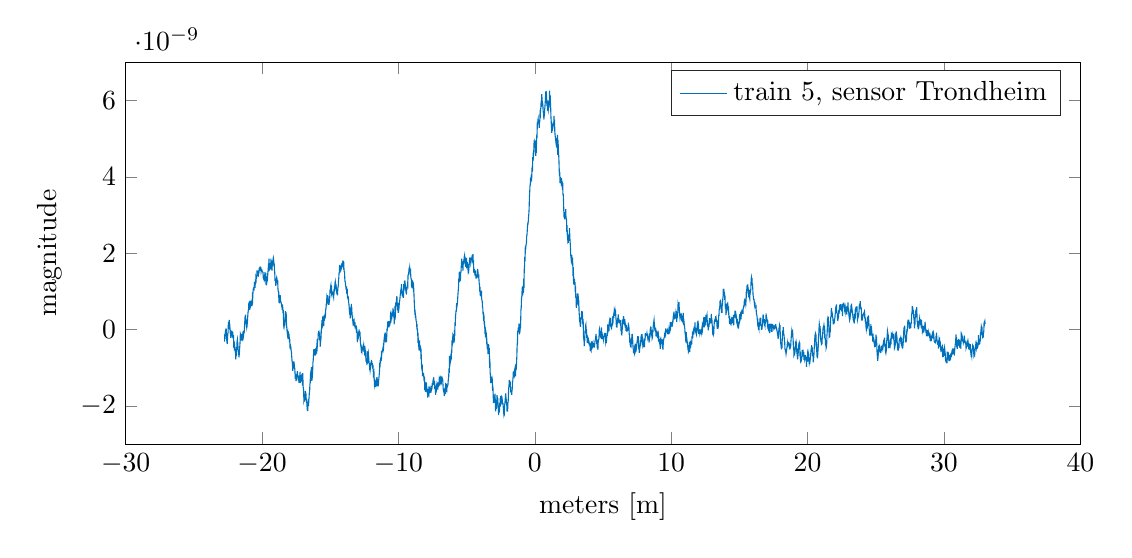
\begin{tikzpicture}

  \begin{axis}[%
    width=\textwidth,
    height=0.4\textwidth,
    at={(0\figurewidth,0\figureheight)},
    scale only axis,
    xmin=-30,
    xmax=40,
    xlabel={meters [m]},
    ymin=-3e-09,
    ymax=7e-09,
    ylabel={magnitude},
    axis background/.style={fill=white},
    legend style={legend cell align=left,align=left,draw=white!15!black}
    ]
    \addplot [color=mycolor1,solid]
    table[row sep=crcr]{%
    -22.748015625	-3.17878896111082e-10\\
    -22.728021484375	-1.19610112506425e-10\\
    -22.70802734375	-2.42571292554464e-10\\
    -22.688033203125	-3.39080224279337e-11\\
    -22.6680390625	-1.58127053095443e-11\\
    -22.648044921875	-1.03868889040877e-10\\
    -22.62805078125	2.26488232121785e-11\\
    -22.608056640625	-1.21550078472151e-10\\
    -22.5880625	-2.5436004232186e-10\\
    -22.568068359375	-2.29510195932576e-10\\
    -22.54807421875	-3.7447258517835e-10\\
    -22.528080078125	-2.23470103139673e-10\\
    -22.5080859375	-9.30890554234028e-11\\
    -22.488091796875	-8.14669020343663e-11\\
    -22.46809765625	1.81868109540888e-10\\
    -22.448103515625	1.79336930639045e-10\\
    -22.428109375	1.30550245336793e-10\\
    -22.408115234375	2.52055242902455e-10\\
    -22.38812109375	1.65027007548237e-10\\
    -22.368126953125	1.28822435382783e-10\\
    -22.3481328125	3.23388341825959e-11\\
    -22.328138671875	-1.08831343639046e-10\\
    -22.30814453125	-2.14116294969526e-11\\
    -22.288150390625	-2.20305863566612e-10\\
    -22.26815625	-1.09211904439942e-10\\
    -22.248162109375	-1.37590050089026e-10\\
    -22.22816796875	-9.57879010789707e-11\\
    -22.208173828125	-3.27518255426755e-11\\
    -22.1881796875	-1.74503208933736e-10\\
    -22.168185546875	-5.97203345108679e-11\\
    -22.14819140625	-2.13134827105712e-10\\
    -22.128197265625	-1.5848718587647e-10\\
    -22.108203125	-2.35113398053694e-10\\
    -22.088208984375	-1.49390478779248e-10\\
    -22.06821484375	-4.83200332184632e-10\\
    -22.048220703125	-2.94562550467579e-10\\
    -22.0282265625	-4.57436360671482e-10\\
    -22.008232421875	-4.26111819751514e-10\\
    -21.98823828125	-4.96447273488643e-10\\
    -21.968244140625	-5.6160835448704e-10\\
    -21.94825	-5.66683957081379e-10\\
    -21.928255859375	-7.83379925483807e-10\\
    -21.90826171875	-6.03276093288374e-10\\
    -21.888267578125	-6.97939442843677e-10\\
    -21.8682734375	-4.5871345260004e-10\\
    -21.848279296875	-5.29218118278471e-10\\
    -21.82828515625	-3.00287020836305e-10\\
    -21.808291015625	-2.6322205498727e-10\\
    -21.788296875	-4.44043402287988e-10\\
    -21.768302734375	-4.21197274331263e-10\\
    -21.74830859375	-5.42853396595628e-10\\
    -21.728314453125	-6.35859391248464e-10\\
    -21.7083203125	-6.30501167387416e-10\\
    -21.688326171875	-7.24746402315907e-10\\
    -21.66833203125	-6.46717132842669e-10\\
    -21.648337890625	-5.3398821950451e-10\\
    -21.62834375	-4.2772647076073e-10\\
    -21.608349609375	-3.10705098300081e-10\\
    -21.58835546875	-1.12068562960347e-10\\
    -21.568361328125	-1.33807242876111e-10\\
    -21.5483671875	-1.39065377465451e-10\\
    -21.528373046875	-1.93570904160532e-10\\
    -21.50837890625	-2.88782236861899e-10\\
    -21.488384765625	-1.13723809236241e-10\\
    -21.468390625	-2.90190478926225e-10\\
    -21.448396484375	-1.87168863360386e-10\\
    -21.42840234375	-1.45864320331707e-10\\
    -21.408408203125	-2.0104510263884e-10\\
    -21.3884140625	-1.31165949108122e-10\\
    -21.368419921875	-3.70036670579155e-11\\
    -21.34842578125	-1.33198404828695e-10\\
    -21.328431640625	-8.06163402571173e-11\\
    -21.3084375	-8.22192048663387e-11\\
    -21.288443359375	5.55350064642591e-11\\
    -21.26844921875	1.66993746801274e-10\\
    -21.248455078125	3.37171684368066e-10\\
    -21.2284609375	2.65319884200248e-10\\
    -21.208466796875	3.8725380117645e-10\\
    -21.18847265625	2.36360165518826e-10\\
    -21.168478515625	1.98508742980437e-10\\
    -21.148484375	1.11796110815047e-10\\
    -21.128490234375	6.55375201118339e-11\\
    -21.10849609375	1.6493192232724e-10\\
    -21.088501953125	1.36162219150072e-10\\
    -21.0685078125	2.19652107534386e-10\\
    -21.048513671875	3.42486375194107e-10\\
    -21.02851953125	4.4362794028039e-10\\
    -21.008525390625	4.91874512160699e-10\\
    -20.98853125	5.27298885284628e-10\\
    -20.968537109375	6.89032309848184e-10\\
    -20.94854296875	7.02335906759333e-10\\
    -20.928548828125	5.13945512895969e-10\\
    -20.9085546875	7.16576156466869e-10\\
    -20.888560546875	6.4581627897994e-10\\
    -20.86856640625	6.54586665446991e-10\\
    -20.848572265625	7.53142582340512e-10\\
    -20.828578125	6.27506865128379e-10\\
    -20.808583984375	6.63127607094449e-10\\
    -20.78858984375	6.61746708604659e-10\\
    -20.768595703125	6.53129554928901e-10\\
    -20.7486015625	7.08288389114522e-10\\
    -20.728607421875	6.13276162097271e-10\\
    -20.70861328125	8.24821174289863e-10\\
    -20.688619140625	7.83713581801771e-10\\
    -20.668625	9.32268032203662e-10\\
    -20.648630859375	1.04307527402252e-09\\
    -20.62863671875	1.08362414535217e-09\\
    -20.608642578125	1.08013730762398e-09\\
    -20.5886484375	1.01824468775972e-09\\
    -20.568654296875	1.13818922641943e-09\\
    -20.54866015625	1.23979637986852e-09\\
    -20.528666015625	1.15204435526781e-09\\
    -20.508671875	1.09023795794183e-09\\
    -20.488677734375	1.31187595867126e-09\\
    -20.46868359375	1.1907613548907e-09\\
    -20.448689453125	1.36050291515208e-09\\
    -20.4286953125	1.32180239146592e-09\\
    -20.408701171875	1.42476033476688e-09\\
    -20.38870703125	1.35815093729604e-09\\
    -20.368712890625	1.54545032296548e-09\\
    -20.34871875	1.48856321386305e-09\\
    -20.328724609375	1.47753058505142e-09\\
    -20.30873046875	1.49470070634387e-09\\
    -20.288736328125	1.41888489052703e-09\\
    -20.2687421875	1.40978089414241e-09\\
    -20.248748046875	1.5404669877948e-09\\
    -20.22875390625	1.47127524042578e-09\\
    -20.208759765625	1.59565260475083e-09\\
    -20.188765625	1.61202817378404e-09\\
    -20.168771484375	1.62219736392857e-09\\
    -20.14877734375	1.59811239368138e-09\\
    -20.128783203125	1.61092897331647e-09\\
    -20.1087890625	1.53718065109885e-09\\
    -20.088794921875	1.63864303698819e-09\\
    -20.06880078125	1.52897220301982e-09\\
    -20.048806640625	1.57885569619688e-09\\
    -20.0288125	1.57466832255247e-09\\
    -20.008818359375	1.55439821755004e-09\\
    -19.98882421875	1.523097346455e-09\\
    -19.968830078125	1.51440433858492e-09\\
    -19.9488359375	1.50300524266789e-09\\
    -19.928841796875	1.49556701981552e-09\\
    -19.90884765625	1.358514965773e-09\\
    -19.888853515625	1.33060621618351e-09\\
    -19.868859375	1.32008884576246e-09\\
    -19.848865234375	1.29781203161582e-09\\
    -19.82887109375	1.37437371627665e-09\\
    -19.808876953125	1.35207572111803e-09\\
    -19.7888828125	1.50504060596609e-09\\
    -19.768888671875	1.31295399927093e-09\\
    -19.74889453125	1.43108266753671e-09\\
    -19.728900390625	1.48177171469384e-09\\
    -19.70890625	1.17935512114738e-09\\
    -19.688912109375	1.39275043979224e-09\\
    -19.66891796875	1.1585558015997e-09\\
    -19.648923828125	1.26376656646976e-09\\
    -19.6289296875	1.26319168370586e-09\\
    -19.608935546875	1.27648117887365e-09\\
    -19.58894140625	1.39549576028002e-09\\
    -19.568947265625	1.52799267391656e-09\\
    -19.548953125	1.53652413382304e-09\\
    -19.528958984375	1.7318802310932e-09\\
    -19.50896484375	1.54365753860902e-09\\
    -19.488970703125	1.85721613066536e-09\\
    -19.4689765625	1.55866561597149e-09\\
    -19.448982421875	1.57024595210574e-09\\
    -19.42898828125	1.69580363438052e-09\\
    -19.408994140625	1.5768251906061e-09\\
    -19.389	1.73634179408437e-09\\
    -19.369005859375	1.57746413653396e-09\\
    -19.34901171875	1.85940675012428e-09\\
    -19.329017578125	1.58951498604936e-09\\
    -19.3090234375	1.65281485794787e-09\\
    -19.289029296875	1.8065495263208e-09\\
    -19.26903515625	1.54150799171308e-09\\
    -19.249041015625	1.74321431009917e-09\\
    -19.229046875	1.65457076642796e-09\\
    -19.209052734375	1.73232473303753e-09\\
    -19.18905859375	1.84502968197779e-09\\
    -19.169064453125	1.87823814577428e-09\\
    -19.1490703125	1.82573754129458e-09\\
    -19.129076171875	1.73309938167344e-09\\
    -19.10908203125	1.72861380689224e-09\\
    -19.089087890625	1.54852553484886e-09\\
    -19.06909375	1.5096991980945e-09\\
    -19.049099609375	1.29574254755809e-09\\
    -19.02910546875	1.29903834115195e-09\\
    -19.009111328125	1.26198963082564e-09\\
    -18.9891171875	1.14395592393232e-09\\
    -18.969123046875	1.30657648254002e-09\\
    -18.94912890625	1.33411461665868e-09\\
    -18.929134765625	1.26067660469041e-09\\
    -18.909140625	1.33511491444485e-09\\
    -18.889146484375	1.30222351740458e-09\\
    -18.86915234375	1.17375070348113e-09\\
    -18.849158203125	1.28556311489985e-09\\
    -18.8291640625	1.04888716544263e-09\\
    -18.809169921875	9.94133668677081e-10\\
    -18.78917578125	9.93213748195472e-10\\
    -18.769181640625	8.21042118514932e-10\\
    -18.7491875	8.60011635530777e-10\\
    -18.729193359375	7.68432292095952e-10\\
    -18.70919921875	6.84775682539189e-10\\
    -18.689205078125	8.30494200347249e-10\\
    -18.6692109375	8.98407405492757e-10\\
    -18.649216796875	7.93921405385727e-10\\
    -18.62922265625	7.36699849208019e-10\\
    -18.609228515625	7.16407180676094e-10\\
    -18.589234375	6.90177670141728e-10\\
    -18.569240234375	6.42371260857311e-10\\
    -18.54924609375	5.98510760206924e-10\\
    -18.529251953125	6.45831674353497e-10\\
    -18.5092578125	6.46439270861704e-10\\
    -18.489263671875	6.35967844881002e-10\\
    -18.46926953125	4.28099412231903e-10\\
    -18.449275390625	5.19379720186196e-10\\
    -18.42928125	3.2308549576955e-10\\
    -18.409287109375	1.35798484672334e-10\\
    -18.38929296875	1.76989144243347e-10\\
    -18.369298828125	1.01476576584101e-10\\
    -18.3493046875	1.50102840185753e-10\\
    -18.329310546875	1.40426727854929e-10\\
    -18.30931640625	2.6242842223809e-10\\
    -18.289322265625	4.82822992960052e-10\\
    -18.269328125	4.0973740697621e-10\\
    -18.249333984375	4.08061845310633e-10\\
    -18.22933984375	4.16488002680889e-10\\
    -18.209345703125	1.67613013777067e-10\\
    -18.1893515625	7.65285611114344e-11\\
    -18.169357421875	-2.71578294953165e-11\\
    -18.14936328125	-8.73464364242996e-11\\
    -18.129369140625	-1.41894831061047e-10\\
    -18.109375	-9.85209065392521e-11\\
    -18.089380859375	-2.53100640321094e-10\\
    -18.06938671875	-4.68900365989236e-11\\
    -18.049392578125	-2.36272070667829e-10\\
    -18.0293984375	-1.03999970431133e-10\\
    -18.009404296875	-1.79777522526515e-10\\
    -17.98941015625	-3.34314792176885e-10\\
    -17.969416015625	-2.52793597163953e-10\\
    -17.949421875	-4.95375444312688e-10\\
    -17.929427734375	-3.73062088489704e-10\\
    -17.90943359375	-5.09467981579543e-10\\
    -17.889439453125	-4.34768607328493e-10\\
    -17.8694453125	-5.51721535142946e-10\\
    -17.849451171875	-5.60817482907393e-10\\
    -17.82945703125	-6.74801890121071e-10\\
    -17.809462890625	-7.67970545803108e-10\\
    -17.78946875	-8.58269237858376e-10\\
    -17.769474609375	-8.82634299171398e-10\\
    -17.74948046875	-1.08129010076464e-09\\
    -17.729486328125	-8.65256188984574e-10\\
    -17.7094921875	-1.02579592181517e-09\\
    -17.689498046875	-8.3542375926275e-10\\
    -17.66950390625	-9.23305600712188e-10\\
    -17.649509765625	-8.44143869068742e-10\\
    -17.629515625	-9.62667298068387e-10\\
    -17.609521484375	-9.89344741879427e-10\\
    -17.58952734375	-1.07509040245725e-09\\
    -17.569533203125	-1.22687725247774e-09\\
    -17.5495390625	-1.20969400638165e-09\\
    -17.529544921875	-1.25948047404545e-09\\
    -17.50955078125	-1.35142813567331e-09\\
    -17.489556640625	-1.23893494169991e-09\\
    -17.4695625	-1.26066711153401e-09\\
    -17.449568359375	-1.18517559089574e-09\\
    -17.42957421875	-1.16342577279632e-09\\
    -17.409580078125	-1.09151847138073e-09\\
    -17.3895859375	-1.18794427677105e-09\\
    -17.369591796875	-1.20506782298393e-09\\
    -17.34959765625	-1.29594550978905e-09\\
    -17.329603515625	-1.28667348802046e-09\\
    -17.309609375	-1.31234845243489e-09\\
    -17.289615234375	-1.39314603087301e-09\\
    -17.26962109375	-1.20510040547233e-09\\
    -17.249626953125	-1.25015858341564e-09\\
    -17.2296328125	-1.31875539649927e-09\\
    -17.209638671875	-1.10160852224521e-09\\
    -17.18964453125	-1.39454833470096e-09\\
    -17.169650390625	-1.19595491732191e-09\\
    -17.14965625	-1.35227603693622e-09\\
    -17.129662109375	-1.34640347911429e-09\\
    -17.10966796875	-1.32657889152728e-09\\
    -17.089673828125	-1.32826908019873e-09\\
    -17.0696796875	-1.18290066406753e-09\\
    -17.049685546875	-1.18813232309658e-09\\
    -17.02969140625	-1.46625434457962e-09\\
    -17.009697265625	-1.1382717738006e-09\\
    -16.989703125	-1.50238504737335e-09\\
    -16.969708984375	-1.52731851268192e-09\\
    -16.94971484375	-1.63080572124157e-09\\
    -16.929720703125	-1.85348301138996e-09\\
    -16.9097265625	-1.81762930172877e-09\\
    -16.889732421875	-1.83468757162206e-09\\
    -16.86973828125	-1.77499879603133e-09\\
    -16.849744140625	-1.84435282022413e-09\\
    -16.82975	-1.60411772288478e-09\\
    -16.809755859375	-1.77098994092151e-09\\
    -16.78976171875	-1.64933269466129e-09\\
    -16.769767578125	-1.72496582998782e-09\\
    -16.7497734375	-1.91369639029375e-09\\
    -16.729779296875	-1.83313265687465e-09\\
    -16.70978515625	-1.96479635142113e-09\\
    -16.689791015625	-2.06011217886018e-09\\
    -16.669796875	-2.04183548243506e-09\\
    -16.649802734375	-2.13328872803119e-09\\
    -16.62980859375	-1.94666081813726e-09\\
    -16.609814453125	-1.95739568441184e-09\\
    -16.5898203125	-1.82198168311447e-09\\
    -16.569826171875	-1.872277504428e-09\\
    -16.54983203125	-1.76226445649706e-09\\
    -16.529837890625	-1.6456262066767e-09\\
    -16.50984375	-1.63235135136054e-09\\
    -16.489849609375	-1.42564279973315e-09\\
    -16.46985546875	-1.41507560340459e-09\\
    -16.449861328125	-1.17886257181422e-09\\
    -16.4298671875	-1.13290525502059e-09\\
    -16.409873046875	-1.16968534580956e-09\\
    -16.38987890625	-1.19696212639765e-09\\
    -16.369884765625	-9.87374711788106e-10\\
    -16.349890625	-1.34571296233445e-09\\
    -16.329896484375	-1.17410852593678e-09\\
    -16.30990234375	-1.20956198413427e-09\\
    -16.289908203125	-1.11392465652309e-09\\
    -16.2699140625	-8.70486757147063e-10\\
    -16.249919921875	-8.15196319763587e-10\\
    -16.22992578125	-6.98901799058791e-10\\
    -16.209931640625	-5.22662447833519e-10\\
    -16.1899375	-5.72448987914156e-10\\
    -16.169943359375	-5.64356485666883e-10\\
    -16.14994921875	-5.12340059162431e-10\\
    -16.129955078125	-6.64831559458481e-10\\
    -16.1099609375	-6.69169039394245e-10\\
    -16.089966796875	-6.46453025676349e-10\\
    -16.06997265625	-5.575863260257e-10\\
    -16.049978515625	-5.86037388746997e-10\\
    -16.029984375	-6.0231188647343e-10\\
    -16.009990234375	-5.20842510851743e-10\\
    -15.98999609375	-5.45686586852409e-10\\
    -15.970001953125	-3.9097517162927e-10\\
    -15.9500078125	-4.36377269946067e-10\\
    -15.930013671875	-3.08123301117869e-10\\
    -15.91001953125	-2.48194303372812e-10\\
    -15.890025390625	-2.47402967626345e-10\\
    -15.87003125	-6.85397921297691e-11\\
    -15.850037109375	-5.27422810835718e-11\\
    -15.83004296875	-4.48162523735457e-11\\
    -15.810048828125	-1.41700599151412e-10\\
    -15.7900546875	-7.59762044265648e-11\\
    -15.770060546875	-2.82709614068221e-10\\
    -15.75006640625	-1.63220250082437e-10\\
    -15.730072265625	-4.46566329727607e-10\\
    -15.710078125	-3.24837399916935e-10\\
    -15.690083984375	-2.7567029362404e-10\\
    -15.67008984375	-2.01282778542669e-10\\
    -15.650095703125	4.08436959453592e-11\\
    -15.6301015625	-8.94546834175171e-12\\
    -15.610107421875	2.49794896626857e-10\\
    -15.59011328125	2.05791564935066e-10\\
    -15.570119140625	1.64256630219998e-10\\
    -15.550125	3.43771666741669e-10\\
    -15.530130859375	2.03606622025215e-10\\
    -15.51013671875	2.63117494956519e-10\\
    -15.490142578125	1.45634281507104e-10\\
    -15.4701484375	8.7861919603603e-11\\
    -15.450154296875	3.74492559400016e-10\\
    -15.43016015625	2.26567399364879e-10\\
    -15.410166015625	3.6266357862754e-10\\
    -15.390171875	3.76685596457016e-10\\
    -15.370177734375	4.09412851184214e-10\\
    -15.35018359375	3.81845317496208e-10\\
    -15.330189453125	5.19244039920551e-10\\
    -15.3101953125	5.58262010346956e-10\\
    -15.290201171875	6.56881438255351e-10\\
    -15.27020703125	6.48431135364796e-10\\
    -15.250212890625	8.21740995409045e-10\\
    -15.23021875	7.80274473142975e-10\\
    -15.210224609375	9.00082433236445e-10\\
    -15.19023046875	7.60696669108186e-10\\
    -15.170236328125	8.95202836784066e-10\\
    -15.1502421875	7.38253779078153e-10\\
    -15.130248046875	7.53951586290303e-10\\
    -15.11025390625	6.60646656935306e-10\\
    -15.090259765625	6.61143954291719e-10\\
    -15.070265625	7.16453945214125e-10\\
    -15.050271484375	7.65478591594491e-10\\
    -15.03027734375	8.78205605058308e-10\\
    -15.010283203125	1.05087618301399e-09\\
    -14.9902890625	9.45085552720777e-10\\
    -14.970294921875	1.12650693526766e-09\\
    -14.95030078125	1.16534218931221e-09\\
    -14.930306640625	1.0450258291153e-09\\
    -14.9103125	1.15313344835074e-09\\
    -14.890318359375	9.56599156692242e-10\\
    -14.87032421875	9.97705234161254e-10\\
    -14.850330078125	9.82416335304805e-10\\
    -14.8303359375	9.09458679509514e-10\\
    -14.810341796875	9.83025416379796e-10\\
    -14.79034765625	8.82832652867708e-10\\
    -14.770353515625	8.88222960367269e-10\\
    -14.750359375	8.49045873624904e-10\\
    -14.730365234375	9.96050284137831e-10\\
    -14.71037109375	9.81443577857339e-10\\
    -14.690376953125	1.151147182196e-09\\
    -14.6703828125	1.0184486833719e-09\\
    -14.650388671875	1.22081446579704e-09\\
    -14.63039453125	1.25862730076041e-09\\
    -14.610400390625	1.18007093484905e-09\\
    -14.59040625	1.1401760433048e-09\\
    -14.570412109375	1.18876951429146e-09\\
    -14.55041796875	1.04970911172579e-09\\
    -14.530423828125	1.00486563927637e-09\\
    -14.5104296875	9.21395233641634e-10\\
    -14.490435546875	1.07771225411604e-09\\
    -14.47044140625	8.97025260715192e-10\\
    -14.450447265625	1.02263020243621e-09\\
    -14.430453125	1.10834620705303e-09\\
    -14.410458984375	1.1379107664358e-09\\
    -14.39046484375	1.27837453340147e-09\\
    -14.370470703125	1.362649874992e-09\\
    -14.3504765625	1.48485768103309e-09\\
    -14.330482421875	1.49982447476479e-09\\
    -14.31048828125	1.69407567783716e-09\\
    -14.290494140625	1.47865125609987e-09\\
    -14.2705	1.6223264954327e-09\\
    -14.250505859375	1.67445648771369e-09\\
    -14.23051171875	1.52340613206857e-09\\
    -14.210517578125	1.60310003607134e-09\\
    -14.1905234375	1.59898737048582e-09\\
    -14.170529296875	1.69522236794956e-09\\
    -14.15053515625	1.68475029359151e-09\\
    -14.130541015625	1.67282777219798e-09\\
    -14.110546875	1.73603672801433e-09\\
    -14.090552734375	1.75860632548396e-09\\
    -14.07055859375	1.70900863070281e-09\\
    -14.050564453125	1.80410400534738e-09\\
    -14.0305703125	1.65204621778285e-09\\
    -14.010576171875	1.76968478105507e-09\\
    -13.99058203125	1.57157825063543e-09\\
    -13.970587890625	1.51583081308595e-09\\
    -13.95059375	1.50791902386498e-09\\
    -13.930599609375	1.32449637252673e-09\\
    -13.91060546875	1.245448844083e-09\\
    -13.890611328125	1.24154827687133e-09\\
    -13.8706171875	1.14165329300266e-09\\
    -13.850623046875	1.12508385817911e-09\\
    -13.83062890625	1.03106630144657e-09\\
    -13.810634765625	1.13113812449962e-09\\
    -13.790640625	9.86221772520758e-10\\
    -13.770646484375	1.00106498475733e-09\\
    -13.75065234375	1.01604849133161e-09\\
    -13.730658203125	8.40394289442667e-10\\
    -13.7106640625	8.23235925397696e-10\\
    -13.690669921875	7.99676548962323e-10\\
    -13.67067578125	8.67238367544299e-10\\
    -13.650681640625	7.03025762163939e-10\\
    -13.6306875	6.90064822682228e-10\\
    -13.610693359375	5.63130635768896e-10\\
    -13.59069921875	4.80859854452172e-10\\
    -13.570705078125	5.08529386488633e-10\\
    -13.5507109375	4.15057172893824e-10\\
    -13.530716796875	2.93260350282931e-10\\
    -13.51072265625	4.99123005770412e-10\\
    -13.490728515625	5.32875758847078e-10\\
    -13.470734375	4.13531791387518e-10\\
    -13.450740234375	6.70969304663746e-10\\
    -13.43074609375	4.64657642142206e-10\\
    -13.410751953125	4.89323890006504e-10\\
    -13.3907578125	3.12643459505848e-10\\
    -13.370763671875	3.69397597038273e-10\\
    -13.35076953125	2.47998439954129e-10\\
    -13.330775390625	1.71097816511723e-10\\
    -13.31078125	1.9630549195876e-10\\
    -13.290787109375	1.06402749147687e-10\\
    -13.27079296875	1.79924024648557e-10\\
    -13.250798828125	2.11355748231623e-10\\
    -13.2308046875	7.98174706798235e-11\\
    -13.210810546875	1.3761136883684e-10\\
    -13.19081640625	2.00235226271827e-10\\
    -13.170822265625	7.84707935908416e-11\\
    -13.150828125	9.26836938453727e-11\\
    -13.130833984375	8.77761058048421e-11\\
    -13.11083984375	1.41918154523713e-11\\
    -13.090845703125	-5.66930294733377e-12\\
    -13.0708515625	-8.49662785990678e-11\\
    -13.050857421875	-9.54241352322962e-12\\
    -13.03086328125	-6.63413996978726e-11\\
    -13.010869140625	-3.30643334416956e-10\\
    -12.990875	-1.2303316796742e-10\\
    -12.970880859375	-2.50308052286648e-10\\
    -12.95088671875	-2.22700782486461e-10\\
    -12.930892578125	-1.19753542178114e-10\\
    -12.9108984375	-1.65026973488067e-10\\
    -12.890904296875	-1.31537116230855e-10\\
    -12.87091015625	-8.5076541273678e-11\\
    -12.850916015625	-6.03120970051958e-11\\
    -12.830921875	-1.15251128529098e-10\\
    -12.810927734375	-6.52628645011061e-11\\
    -12.79093359375	-3.58259158550677e-10\\
    -12.770939453125	-3.60779013147243e-10\\
    -12.7509453125	-4.56362243969618e-10\\
    -12.730951171875	-4.73821217467242e-10\\
    -12.71095703125	-6.13360063856087e-10\\
    -12.690962890625	-5.20390739482979e-10\\
    -12.67096875	-5.67420926712361e-10\\
    -12.650974609375	-5.03356114441646e-10\\
    -12.63098046875	-4.94993255303677e-10\\
    -12.610986328125	-4.64276824148171e-10\\
    -12.5909921875	-5.42210514200095e-10\\
    -12.570998046875	-4.66554133919105e-10\\
    -12.55100390625	-4.20234912219548e-10\\
    -12.531009765625	-5.64725449366908e-10\\
    -12.511015625	-5.60813415819276e-10\\
    -12.491021484375	-4.23199036630263e-10\\
    -12.47102734375	-6.80014211331074e-10\\
    -12.451033203125	-6.16121129233601e-10\\
    -12.4310390625	-5.58331489735225e-10\\
    -12.411044921875	-6.33189537467146e-10\\
    -12.39105078125	-7.33686029991241e-10\\
    -12.371056640625	-6.88016942699e-10\\
    -12.3510625	-8.45478550120589e-10\\
    -12.331068359375	-7.62475708610074e-10\\
    -12.31107421875	-9.30735533191676e-10\\
    -12.291080078125	-7.66074383114215e-10\\
    -12.2710859375	-8.91430698749359e-10\\
    -12.251091796875	-6.25624367915978e-10\\
    -12.23109765625	-6.4056943140636e-10\\
    -12.211103515625	-6.04594424096247e-10\\
    -12.191109375	-7.02392452177109e-10\\
    -12.171115234375	-7.60065015778275e-10\\
    -12.15112109375	-8.81628629681373e-10\\
    -12.131126953125	-8.99804447638093e-10\\
    -12.1111328125	-9.94800058732045e-10\\
    -12.091138671875	-9.73719096599469e-10\\
    -12.07114453125	-1.06786497610893e-09\\
    -12.051150390625	-1.01822594728177e-09\\
    -12.03115625	-8.90886693486354e-10\\
    -12.011162109375	-8.68427027357565e-10\\
    -11.99116796875	-8.38178571239995e-10\\
    -11.971173828125	-8.19848930352219e-10\\
    -11.9511796875	-8.32684503956248e-10\\
    -11.931185546875	-9.39925893596017e-10\\
    -11.91119140625	-8.7899829802953e-10\\
    -11.891197265625	-1.0221247287698e-09\\
    -11.871203125	-9.21959009891524e-10\\
    -11.851208984375	-1.02443462072037e-09\\
    -11.83121484375	-1.19343408170368e-09\\
    -11.811220703125	-1.17291511424538e-09\\
    -11.7912265625	-1.13700779872833e-09\\
    -11.771232421875	-1.32354633355252e-09\\
    -11.75123828125	-1.45641836189062e-09\\
    -11.731244140625	-1.41950699094455e-09\\
    -11.71125	-1.49692539007399e-09\\
    -11.691255859375	-1.41964307041743e-09\\
    -11.67126171875	-1.38622398290698e-09\\
    -11.651267578125	-1.3576908143985e-09\\
    -11.6312734375	-1.4478015988392e-09\\
    -11.611279296875	-1.42059513219517e-09\\
    -11.59128515625	-1.29228926581405e-09\\
    -11.571291015625	-1.24604633527266e-09\\
    -11.551296875	-1.47988057868646e-09\\
    -11.531302734375	-1.29673190532738e-09\\
    -11.51130859375	-1.48832847866483e-09\\
    -11.491314453125	-1.40369513904935e-09\\
    -11.4713203125	-1.48169918970284e-09\\
    -11.451326171875	-1.34209543835471e-09\\
    -11.43133203125	-1.26449620370588e-09\\
    -11.411337890625	-1.19586077956045e-09\\
    -11.39134375	-1.11890654769595e-09\\
    -11.371349609375	-9.31175662917143e-10\\
    -11.35135546875	-9.46669754657041e-10\\
    -11.331361328125	-8.00897093713238e-10\\
    -11.3113671875	-8.87029858338829e-10\\
    -11.291373046875	-7.35341198461457e-10\\
    -11.27137890625	-8.21693537327472e-10\\
    -11.251384765625	-6.62473287158011e-10\\
    -11.231390625	-6.99512210032204e-10\\
    -11.211396484375	-5.9411907269965e-10\\
    -11.19140234375	-5.83332333022819e-10\\
    -11.171408203125	-5.504034799809e-10\\
    -11.1514140625	-5.1598958425313e-10\\
    -11.131419921875	-5.39796309350441e-10\\
    -11.11142578125	-4.46679466519973e-10\\
    -11.091431640625	-4.76181975089282e-10\\
    -11.0714375	-3.64518116611777e-10\\
    -11.051443359375	-2.59199314099429e-10\\
    -11.03144921875	-2.03720709442417e-10\\
    -11.011455078125	-2.42271639932133e-10\\
    -10.9914609375	-2.38076285868067e-10\\
    -10.971466796875	-7.34468215075889e-11\\
    -10.95147265625	-2.82798003300102e-10\\
    -10.931478515625	-2.66430965905947e-10\\
    -10.911484375	-3.34219054112409e-10\\
    -10.891490234375	-2.03173258787827e-10\\
    -10.87149609375	-3.21037717385336e-10\\
    -10.851501953125	-1.13157797948731e-10\\
    -10.8315078125	3.162599063914e-11\\
    -10.811513671875	-1.85967091124554e-11\\
    -10.79151953125	1.46197537940751e-10\\
    -10.771525390625	1.27436227454197e-10\\
    -10.75153125	1.57715539591126e-10\\
    -10.731537109375	2.21692758497186e-10\\
    -10.71154296875	5.58562732705375e-11\\
    -10.691548828125	1.36325104334325e-10\\
    -10.6715546875	1.13839585412649e-10\\
    -10.651560546875	1.55303312185772e-10\\
    -10.63156640625	1.40632122191263e-10\\
    -10.611572265625	2.27266443900849e-10\\
    -10.591578125	1.59245817109786e-10\\
    -10.571583984375	4.6728953003293e-10\\
    -10.55158984375	2.80908308050423e-10\\
    -10.531595703125	3.98112800161895e-10\\
    -10.5116015625	3.55332409753918e-10\\
    -10.491607421875	2.92238326655025e-10\\
    -10.47161328125	3.52081532015049e-10\\
    -10.451619140625	3.94068025008675e-10\\
    -10.431625	3.81905316165104e-10\\
    -10.411630859375	4.70353917743781e-10\\
    -10.39163671875	4.32091721552547e-10\\
    -10.371642578125	3.37569314635888e-10\\
    -10.3516484375	4.98542878565384e-10\\
    -10.331654296875	5.23819662574528e-10\\
    -10.31166015625	1.37061612102244e-10\\
    -10.291666015625	3.56529042308329e-10\\
    -10.271671875	2.59720669992155e-10\\
    -10.251677734375	2.79057240883217e-10\\
    -10.23168359375	3.23275840653302e-10\\
    -10.211689453125	5.99733821753845e-10\\
    -10.1916953125	5.68893520420724e-10\\
    -10.171701171875	6.84427555077923e-10\\
    -10.15170703125	7.19144331793332e-10\\
    -10.131712890625	8.2744603594336e-10\\
    -10.11171875	8.73529844882461e-10\\
    -10.091724609375	7.12471189983005e-10\\
    -10.07173046875	6.5963699689562e-10\\
    -10.051736328125	5.01483088959581e-10\\
    -10.0317421875	5.81932729270656e-10\\
    -10.011748046875	4.37263650990861e-10\\
    -9.99175390625	5.71454586050691e-10\\
    -9.971759765625	5.27470414817495e-10\\
    -9.951765625	5.8285503645884e-10\\
    -9.931771484375	7.10660398779775e-10\\
    -9.91177734375	7.44077967796255e-10\\
    -9.891783203125	7.9912215748672e-10\\
    -9.8717890625	8.83643373574649e-10\\
    -9.851794921875	9.28942151286154e-10\\
    -9.83180078125	1.00920556388947e-09\\
    -9.811806640625	1.05097656363535e-09\\
    -9.7918125	1.00922458460634e-09\\
    -9.771818359375	1.18989922932028e-09\\
    -9.75182421875	1.00950732474659e-09\\
    -9.731830078125	1.02427116106188e-09\\
    -9.7118359375	9.85748914963821e-10\\
    -9.691841796875	9.2809050355106e-10\\
    -9.67184765625	8.44605405109745e-10\\
    -9.651853515625	9.20395666010437e-10\\
    -9.631859375	8.32299415199063e-10\\
    -9.611865234375	1.18675787731265e-09\\
    -9.59187109375	1.01840968027725e-09\\
    -9.571876953125	1.16993803159271e-09\\
    -9.5518828125	1.26380496474176e-09\\
    -9.531888671875	1.26978431782217e-09\\
    -9.51189453125	1.24021127545963e-09\\
    -9.491900390625	1.14235293968296e-09\\
    -9.47190625	1.05109169832752e-09\\
    -9.451912109375	1.01180662505153e-09\\
    -9.43191796875	9.51294775832116e-10\\
    -9.411923828125	9.41953919911371e-10\\
    -9.3919296875	1.11764011343202e-09\\
    -9.371935546875	1.04867091797408e-09\\
    -9.35194140625	1.13509531947116e-09\\
    -9.331947265625	1.19386511168277e-09\\
    -9.311953125	1.16802903418544e-09\\
    -9.291958984375	1.43903600766579e-09\\
    -9.27196484375	1.43970183830879e-09\\
    -9.251970703125	1.45863173341308e-09\\
    -9.2319765625	1.52941843948248e-09\\
    -9.211982421875	1.62483406129887e-09\\
    -9.19198828125	1.55871479295929e-09\\
    -9.171994140625	1.62243326740907e-09\\
    -9.152	1.55462803092067e-09\\
    -9.132005859375	1.54596180975184e-09\\
    -9.11201171875	1.55589435584232e-09\\
    -9.092017578125	1.38723655385326e-09\\
    -9.0720234375	1.32617315456838e-09\\
    -9.052029296875	1.32208195028573e-09\\
    -9.03203515625	1.10414306257065e-09\\
    -9.012041015625	1.30602119871765e-09\\
    -8.992046875	1.07982848797584e-09\\
    -8.972052734375	1.28555339249345e-09\\
    -8.95205859375	1.19821621374174e-09\\
    -8.932064453125	1.17709569371193e-09\\
    -8.9120703125	1.09323973846855e-09\\
    -8.892076171875	1.13602372293453e-09\\
    -8.87208203125	1.04993242389926e-09\\
    -8.852087890625	8.42466577773591e-10\\
    -8.83209375	6.75529542131043e-10\\
    -8.812099609375	5.35761150244674e-10\\
    -8.79210546875	4.39095963793497e-10\\
    -8.772111328125	4.57020487984183e-10\\
    -8.7521171875	3.04426727552917e-10\\
    -8.732123046875	3.62297994607482e-10\\
    -8.71212890625	2.64690180773927e-10\\
    -8.692134765625	2.09267247464726e-10\\
    -8.672140625	2.09099291451576e-10\\
    -8.652146484375	7.04452279402691e-11\\
    -8.63215234375	8.50769903789243e-11\\
    -8.612158203125	-3.44294462055706e-11\\
    -8.5921640625	-2.87372980553773e-11\\
    -8.572169921875	-2.35133668529818e-10\\
    -8.55217578125	-2.02146473237885e-10\\
    -8.532181640625	-3.58075614508106e-10\\
    -8.5121875	-4.34906038603477e-10\\
    -8.492193359375	-4.04429087994419e-10\\
    -8.47219921875	-5.48647401624011e-10\\
    -8.452205078125	-2.86436539573199e-10\\
    -8.4322109375	-5.44430607571304e-10\\
    -8.412216796875	-4.0332328214579e-10\\
    -8.39222265625	-4.99802574624934e-10\\
    -8.372228515625	-4.42001102784435e-10\\
    -8.352234375	-6.54940453643375e-10\\
    -8.332240234375	-6.21714012657721e-10\\
    -8.31224609375	-8.6997491175727e-10\\
    -8.292251953125	-9.86226156811048e-10\\
    -8.2722578125	-1.07265977583981e-09\\
    -8.252263671875	-9.19487993141919e-10\\
    -8.23226953125	-1.21186779965905e-09\\
    -8.212275390625	-1.12291523583752e-09\\
    -8.19228125	-1.19125447209568e-09\\
    -8.172287109375	-1.18048257472559e-09\\
    -8.15229296875	-1.17118447258339e-09\\
    -8.132298828125	-1.28477753389819e-09\\
    -8.1123046875	-1.35629556254136e-09\\
    -8.092310546875	-1.23141876399609e-09\\
    -8.07231640625	-1.58515062443714e-09\\
    -8.052322265625	-1.47923793189569e-09\\
    -8.032328125	-1.50754463879931e-09\\
    -8.012333984375	-1.63209637855158e-09\\
    -7.99233984375	-1.5006512731721e-09\\
    -7.972345703125	-1.54626347395372e-09\\
    -7.9523515625	-1.38267387932959e-09\\
    -7.932357421875	-1.46567800910218e-09\\
    -7.91236328125	-1.60008308557323e-09\\
    -7.892369140625	-1.63600863062292e-09\\
    -7.872375	-1.55358826732611e-09\\
    -7.852380859375	-1.78363863318062e-09\\
    -7.83238671875	-1.72991943160745e-09\\
    -7.812392578125	-1.62785845854506e-09\\
    -7.7923984375	-1.75016057763289e-09\\
    -7.772404296875	-1.60859031187132e-09\\
    -7.75241015625	-1.65228420737861e-09\\
    -7.732416015625	-1.56996387131944e-09\\
    -7.712421875	-1.59871447880083e-09\\
    -7.692427734375	-1.55964333033223e-09\\
    -7.67243359375	-1.65705117311844e-09\\
    -7.652439453125	-1.57232471159938e-09\\
    -7.6324453125	-1.55914676859672e-09\\
    -7.612451171875	-1.65018834220594e-09\\
    -7.59245703125	-1.59048837714879e-09\\
    -7.572462890625	-1.47647244589352e-09\\
    -7.55246875	-1.57284500383247e-09\\
    -7.532474609375	-1.50480287187546e-09\\
    -7.51248046875	-1.39528787585156e-09\\
    -7.492486328125	-1.47956481451937e-09\\
    -7.4724921875	-1.35594506037933e-09\\
    -7.452498046875	-1.32440333882391e-09\\
    -7.43250390625	-1.40880932894155e-09\\
    -7.412509765625	-1.25032116886859e-09\\
    -7.392515625	-1.35276601026247e-09\\
    -7.372521484375	-1.4459348670186e-09\\
    -7.35252734375	-1.34998002273961e-09\\
    -7.332533203125	-1.54816513258214e-09\\
    -7.3125390625	-1.55813903864788e-09\\
    -7.292544921875	-1.46975796094863e-09\\
    -7.27255078125	-1.71002208053502e-09\\
    -7.252556640625	-1.57073698752146e-09\\
    -7.2325625	-1.64868359472294e-09\\
    -7.212568359375	-1.47896171937244e-09\\
    -7.19257421875	-1.49628991741472e-09\\
    -7.172580078125	-1.4309934653003e-09\\
    -7.1525859375	-1.46755580859922e-09\\
    -7.132591796875	-1.3972906942946e-09\\
    -7.11259765625	-1.57200890826618e-09\\
    -7.092603515625	-1.3872774004916e-09\\
    -7.072609375	-1.50622174542351e-09\\
    -7.052615234375	-1.38303898737241e-09\\
    -7.03262109375	-1.43764851944648e-09\\
    -7.012626953125	-1.32021866158333e-09\\
    -6.9926328125	-1.36449716712705e-09\\
    -6.972638671875	-1.23154503590077e-09\\
    -6.95264453125	-1.35752227422011e-09\\
    -6.932650390625	-1.31395290695287e-09\\
    -6.91265625	-1.28332255337936e-09\\
    -6.892662109375	-1.35242882181463e-09\\
    -6.87266796875	-1.42799582344017e-09\\
    -6.852673828125	-1.41686720075709e-09\\
    -6.8326796875	-1.22819150830401e-09\\
    -6.812685546875	-1.30169001972381e-09\\
    -6.79269140625	-1.27306565867667e-09\\
    -6.772697265625	-1.30096057864138e-09\\
    -6.752703125	-1.31716100417697e-09\\
    -6.732708984375	-1.44506977493895e-09\\
    -6.71271484375	-1.56670092179903e-09\\
    -6.692720703125	-1.6027529970306e-09\\
    -6.6727265625	-1.59165554768301e-09\\
    -6.652732421875	-1.6555546857115e-09\\
    -6.63273828125	-1.74230597400363e-09\\
    -6.612744140625	-1.62220762927352e-09\\
    -6.59275	-1.57477997086113e-09\\
    -6.572755859375	-1.51799653898824e-09\\
    -6.55276171875	-1.6908272061017e-09\\
    -6.532767578125	-1.39504464927339e-09\\
    -6.5127734375	-1.63042410060608e-09\\
    -6.492779296875	-1.42920709725278e-09\\
    -6.47278515625	-1.55609764471515e-09\\
    -6.452791015625	-1.57909401572811e-09\\
    -6.432796875	-1.44553013371338e-09\\
    -6.412802734375	-1.49396814049051e-09\\
    -6.39280859375	-1.46820241026598e-09\\
    -6.372814453125	-1.46184380984981e-09\\
    -6.3528203125	-1.36244507818429e-09\\
    -6.332826171875	-1.27264938669199e-09\\
    -6.31283203125	-1.23948228959584e-09\\
    -6.292837890625	-1.01495634226376e-09\\
    -6.27284375	-1.13580931271323e-09\\
    -6.252849609375	-6.90820079026338e-10\\
    -6.23285546875	-9.62173748854038e-10\\
    -6.212861328125	-7.12078460853937e-10\\
    -6.1928671875	-8.48549877334532e-10\\
    -6.172873046875	-8.04256547802468e-10\\
    -6.15287890625	-6.33892875926494e-10\\
    -6.132884765625	-8.07173631612596e-10\\
    -6.112890625	-5.58132709018763e-10\\
    -6.092896484375	-6.08384290968135e-10\\
    -6.07290234375	-3.60778598641093e-10\\
    -6.052908203125	-3.83903091089498e-10\\
    -6.0329140625	-2.81886299124687e-10\\
    -6.012919921875	-1.86003655842159e-10\\
    -5.99292578125	-2.39226307498622e-10\\
    -5.972931640625	-1.44209207659234e-10\\
    -5.9529375	-2.83481055478917e-10\\
    -5.932943359375	-1.20661306790463e-10\\
    -5.91294921875	-3.43290578621497e-10\\
    -5.892955078125	-1.05350359428816e-11\\
    -5.8729609375	-1.70252099369927e-10\\
    -5.852966796875	1.87834991461867e-10\\
    -5.83297265625	9.96430194297891e-11\\
    -5.812978515625	3.5440784091882e-10\\
    -5.792984375	4.16896505589071e-10\\
    -5.772990234375	4.9740331627661e-10\\
    -5.75299609375	5.0019897079229e-10\\
    -5.733001953125	6.93670221547115e-10\\
    -5.7130078125	5.95234847948741e-10\\
    -5.693013671875	6.43766808705518e-10\\
    -5.67301953125	7.01169488997135e-10\\
    -5.653025390625	8.2006034006351e-10\\
    -5.63303125	9.37748176973496e-10\\
    -5.613037109375	1.02155457124333e-09\\
    -5.59304296875	1.09906714480082e-09\\
    -5.573048828125	1.31653581915527e-09\\
    -5.5530546875	1.34889143569761e-09\\
    -5.533060546875	1.51732562211492e-09\\
    -5.51306640625	1.28478048257476e-09\\
    -5.493072265625	1.30139382763774e-09\\
    -5.473078125	1.34781916028305e-09\\
    -5.453083984375	1.32721965176507e-09\\
    -5.43308984375	1.49558138992016e-09\\
    -5.413095703125	1.50386748324542e-09\\
    -5.3931015625	1.64743752075468e-09\\
    -5.373107421875	1.75762499945294e-09\\
    -5.35311328125	1.85481650631997e-09\\
    -5.333119140625	1.73449315271035e-09\\
    -5.313125	1.67726041052982e-09\\
    -5.293130859375	1.78095626852664e-09\\
    -5.27313671875	1.53871823772412e-09\\
    -5.253142578125	1.69833906598294e-09\\
    -5.2331484375	1.71609910671106e-09\\
    -5.213154296875	1.78559799860534e-09\\
    -5.19316015625	1.76934406875475e-09\\
    -5.173166015625	1.90574581211483e-09\\
    -5.153171875	1.93976126338512e-09\\
    -5.133177734375	1.80052007354434e-09\\
    -5.11318359375	1.91017478694743e-09\\
    -5.093189453125	1.77516023566673e-09\\
    -5.0731953125	1.63926215372997e-09\\
    -5.053201171875	1.75039166400188e-09\\
    -5.03320703125	1.71062590720721e-09\\
    -5.013212890625	1.8752802777523e-09\\
    -4.99321875	1.75728721232372e-09\\
    -4.973224609375	1.61472582821953e-09\\
    -4.95323046875	1.7721152062382e-09\\
    -4.933236328125	1.67533162275452e-09\\
    -4.9132421875	1.61145646517244e-09\\
    -4.893248046875	1.5439505461789e-09\\
    -4.87325390625	1.59999315385437e-09\\
    -4.853259765625	1.46559705292938e-09\\
    -4.833265625	1.72793527678654e-09\\
    -4.813271484375	1.6844178836417e-09\\
    -4.79327734375	1.76956023954602e-09\\
    -4.773283203125	1.88478851105942e-09\\
    -4.7532890625	1.78574152243698e-09\\
    -4.733294921875	1.86927241709935e-09\\
    -4.71330078125	1.86201436669071e-09\\
    -4.693306640625	1.74507516927489e-09\\
    -4.6733125	1.78527328905572e-09\\
    -4.653318359375	1.8838175546668e-09\\
    -4.63332421875	1.81253205345465e-09\\
    -4.613330078125	1.89080899730523e-09\\
    -4.5933359375	1.93193049252481e-09\\
    -4.573341796875	1.92691819194415e-09\\
    -4.55334765625	1.74993396562506e-09\\
    -4.533353515625	1.97588860577329e-09\\
    -4.513359375	1.70526311732517e-09\\
    -4.493365234375	1.81911139925163e-09\\
    -4.47337109375	1.50456335258391e-09\\
    -4.453376953125	1.49634996484493e-09\\
    -4.4333828125	1.58159842608694e-09\\
    -4.413388671875	1.47483638610496e-09\\
    -4.39339453125	1.471500474635e-09\\
    -4.373400390625	1.3989121794339e-09\\
    -4.35340625	1.55087073592463e-09\\
    -4.333412109375	1.43684136083585e-09\\
    -4.31341796875	1.33434958900855e-09\\
    -4.293423828125	1.44196215312703e-09\\
    -4.2734296875	1.35953054556781e-09\\
    -4.253435546875	1.3570272301359e-09\\
    -4.23344140625	1.3977857754042e-09\\
    -4.213447265625	1.42973344904948e-09\\
    -4.193453125	1.58573892721547e-09\\
    -4.173458984375	1.53017760955192e-09\\
    -4.15346484375	1.45506952537059e-09\\
    -4.133470703125	1.35026772609215e-09\\
    -4.1134765625	1.44687030841041e-09\\
    -4.093482421875	1.29573539856793e-09\\
    -4.07348828125	1.19551103226978e-09\\
    -4.053494140625	1.17449679760364e-09\\
    -4.0335	9.95724528451121e-10\\
    -4.013505859375	1.11685881902934e-09\\
    -3.99351171875	8.66921717889164e-10\\
    -3.973517578125	9.86712903483225e-10\\
    -3.9535234375	9.90843312298031e-10\\
    -3.933529296875	9.11668943630606e-10\\
    -3.91353515625	1.02037226635099e-09\\
    -3.893541015625	8.01410498087109e-10\\
    -3.873546875	7.65395494440729e-10\\
    -3.853552734375	7.27894524130223e-10\\
    -3.83355859375	5.82549333979385e-10\\
    -3.813564453125	5.67609052799148e-10\\
    -3.7935703125	3.94853886308501e-10\\
    -3.773576171875	4.57799920455512e-10\\
    -3.75358203125	2.17622606422099e-10\\
    -3.733587890625	4.13072152282869e-10\\
    -3.71359375	1.27952228482903e-10\\
    -3.693599609375	2.19668481007347e-10\\
    -3.67360546875	1.10416043961671e-10\\
    -3.653611328125	-1.10351144837793e-10\\
    -3.6336171875	5.5943285294435e-11\\
    -3.613623046875	-1.97235062431111e-10\\
    -3.59362890625	-1.18750483512856e-11\\
    -3.573634765625	-1.28080179912161e-10\\
    -3.553640625	-8.50930021991921e-11\\
    -3.533646484375	-3.12686182181645e-10\\
    -3.51365234375	-2.95302405126583e-10\\
    -3.493658203125	-4.54040492287884e-10\\
    -3.4736640625	-5.24279585530154e-10\\
    -3.453669921875	-4.17299207641592e-10\\
    -3.43367578125	-6.44181075959554e-10\\
    -3.413681640625	-3.82255716807057e-10\\
    -3.3936875	-6.2531606985078e-10\\
    -3.373693359375	-4.02168687038208e-10\\
    -3.35369921875	-6.38150488223213e-10\\
    -3.333705078125	-4.86602602654629e-10\\
    -3.3137109375	-1.00058313073617e-09\\
    -3.293716796875	-7.84104835354064e-10\\
    -3.27372265625	-1.15460732628826e-09\\
    -3.253728515625	-1.15207526702089e-09\\
    -3.233734375	-1.40453463677635e-09\\
    -3.213740234375	-1.24424202930839e-09\\
    -3.19374609375	-1.39884377061292e-09\\
    -3.173751953125	-1.2325464777273e-09\\
    -3.1537578125	-1.30271533094198e-09\\
    -3.133763671875	-1.2749767647356e-09\\
    -3.11376953125	-1.32452712674464e-09\\
    -3.093775390625	-1.60658530719932e-09\\
    -3.07378125	-1.48346094673682e-09\\
    -3.053787109375	-1.66087509797304e-09\\
    -3.03379296875	-1.90935650962439e-09\\
    -3.013798828125	-1.90967479819594e-09\\
    -2.9938046875	-1.81419629431556e-09\\
    -2.973810546875	-1.80304304332721e-09\\
    -2.95381640625	-1.72886170363751e-09\\
    -2.933822265625	-1.84738228504216e-09\\
    -2.913828125	-1.68131637570629e-09\\
    -2.893833984375	-1.9587759743404e-09\\
    -2.87383984375	-2.14357321597943e-09\\
    -2.853845703125	-2.05096563351086e-09\\
    -2.8338515625	-1.92045174822149e-09\\
    -2.813857421875	-2.07499687261023e-09\\
    -2.79386328125	-1.91401649619368e-09\\
    -2.773869140625	-1.72011345654466e-09\\
    -2.753875	-1.85013446801994e-09\\
    -2.733880859375	-1.78870223462308e-09\\
    -2.71388671875	-1.80683675700027e-09\\
    -2.693892578125	-1.99346392077045e-09\\
    -2.6738984375	-2.04855314475767e-09\\
    -2.653904296875	-2.23921965785201e-09\\
    -2.63391015625	-1.98717273891805e-09\\
    -2.613916015625	-2.10963596879632e-09\\
    -2.593921875	-2.12492166059628e-09\\
    -2.573927734375	-1.92365040021538e-09\\
    -2.55393359375	-2.01559235412934e-09\\
    -2.533939453125	-1.79916187200992e-09\\
    -2.5139453125	-1.96804222373005e-09\\
    -2.493951171875	-1.74041072228902e-09\\
    -2.47395703125	-1.9220073315576e-09\\
    -2.453962890625	-1.89341932514156e-09\\
    -2.43396875	-1.75435593954816e-09\\
    -2.413974609375	-1.7635616466956e-09\\
    -2.39398046875	-1.81241368868973e-09\\
    -2.373986328125	-1.93445688739391e-09\\
    -2.3539921875	-1.92741455146744e-09\\
    -2.333998046875	-1.93164180238916e-09\\
    -2.31400390625	-2.01892533139357e-09\\
    -2.294009765625	-2.13821397856188e-09\\
    -2.274015625	-2.20762746529583e-09\\
    -2.254021484375	-2.15280178943103e-09\\
    -2.23402734375	-2.17890195443564e-09\\
    -2.214033203125	-1.97070943773686e-09\\
    -2.1940390625	-1.95078886284881e-09\\
    -2.174044921875	-1.85168193963224e-09\\
    -2.15405078125	-1.90673554085129e-09\\
    -2.134056640625	-1.67421591141301e-09\\
    -2.1140625	-1.77584806410208e-09\\
    -2.094068359375	-1.83570680352486e-09\\
    -2.07407421875	-1.92792546100786e-09\\
    -2.054080078125	-1.98510915345813e-09\\
    -2.0340859375	-2.15058679550945e-09\\
    -2.014091796875	-1.99810029639548e-09\\
    -1.99409765625	-2.14759963888317e-09\\
    -1.974103515625	-1.90597700416288e-09\\
    -1.954109375	-1.90253400705523e-09\\
    -1.934115234375	-1.72386993940852e-09\\
    -1.91412109375	-1.5169054265131e-09\\
    -1.894126953125	-1.49345519238836e-09\\
    -1.8741328125	-1.31840293467126e-09\\
    -1.854138671875	-1.44506831743314e-09\\
    -1.83414453125	-1.41977180923171e-09\\
    -1.814150390625	-1.44316611003774e-09\\
    -1.79415625	-1.42053350020701e-09\\
    -1.774162109375	-1.61117682905385e-09\\
    -1.75416796875	-1.60147635173514e-09\\
    -1.734173828125	-1.62247684323426e-09\\
    -1.7141796875	-1.63811285503736e-09\\
    -1.694185546875	-1.71110722334714e-09\\
    -1.67419140625	-1.60662675607478e-09\\
    -1.654197265625	-1.54657821635208e-09\\
    -1.634203125	-1.36125284591181e-09\\
    -1.614208984375	-1.34045978116517e-09\\
    -1.59421484375	-1.25107922246373e-09\\
    -1.574220703125	-1.09891175792477e-09\\
    -1.5542265625	-1.24699452298668e-09\\
    -1.534232421875	-1.17944464356995e-09\\
    -1.51423828125	-1.14881716853876e-09\\
    -1.494244140625	-1.08996761394429e-09\\
    -1.47425	-1.16242490528818e-09\\
    -1.454255859375	-1.09936148485825e-09\\
    -1.43426171875	-1.03434480719286e-09\\
    -1.414267578125	-1.22712728871488e-09\\
    -1.3942734375	-9.10932765719749e-10\\
    -1.374279296875	-1.06818837933095e-09\\
    -1.35428515625	-9.96814178953516e-10\\
    -1.334291015625	-8.33960766402267e-10\\
    -1.314296875	-6.72575111126812e-10\\
    -1.294302734375	-3.84875229174081e-10\\
    -1.27430859375	-3.87168716935871e-10\\
    -1.254314453125	-5.10416036336475e-11\\
    -1.2343203125	-4.61499688039541e-11\\
    -1.214326171875	4.70206053258391e-11\\
    -1.19433203125	-2.6420285783732e-11\\
    -1.174337890625	6.10637378067708e-11\\
    -1.15434375	1.57654873799116e-10\\
    -1.134349609375	-1.28678288331712e-10\\
    -1.11435546875	1.03438323088341e-10\\
    -1.094361328125	-1.01526327019871e-10\\
    -1.0743671875	1.39434395309521e-10\\
    -1.054373046875	2.26821143261326e-11\\
    -1.03437890625	2.39590637158501e-10\\
    -1.014384765625	5.34504463406812e-10\\
    -0.994390625000001	5.75921655867071e-10\\
    -0.974396484374999	8.28100106897802e-10\\
    -0.954402343750001	8.64414354487949e-10\\
    -0.934408203124999	1.0048891000537e-09\\
    -0.914414062500001	9.7415255736662e-10\\
    -0.894419921875002	1.13201538914041e-09\\
    -0.87442578125	9.04148485929029e-10\\
    -0.854431640625002	1.15074369037967e-09\\
    -0.8344375	9.59339438249419e-10\\
    -0.814443359375002	1.33565204047215e-09\\
    -0.79444921875	1.08281581374684e-09\\
    -0.774455078125001	1.57511659733279e-09\\
    -0.754460937499999	1.63744247810335e-09\\
    -0.734466796875001	1.90424474664309e-09\\
    -0.714472656249999	1.78469889139839e-09\\
    -0.694478515625001	2.18776977018493e-09\\
    -0.674484375000002	2.08727491470911e-09\\
    -0.654490234375	2.1827201448506e-09\\
    -0.634496093750002	2.23539271720599e-09\\
    -0.614501953125	2.25093900592554e-09\\
    -0.594507812500002	2.44369858911205e-09\\
    -0.574513671875	2.47561806965184e-09\\
    -0.554519531250001	2.58271277257672e-09\\
    -0.534525390624999	2.70200600270729e-09\\
    -0.514531250000001	2.77893279578879e-09\\
    -0.494537109374999	2.77373401235466e-09\\
    -0.474542968750001	2.85749595397923e-09\\
    -0.454548828124999	2.96819890587181e-09\\
    -0.4345546875	3.04128252926851e-09\\
    -0.414560546875002	3.19218269984612e-09\\
    -0.39456640625	3.47087755649463e-09\\
    -0.374572265625002	3.59750785611954e-09\\
    -0.354578125	3.76019167791676e-09\\
    -0.334583984375001	3.78431173626004e-09\\
    -0.314589843749999	3.97440332773849e-09\\
    -0.294595703125001	3.85031269874126e-09\\
    -0.274601562499999	3.90739355284824e-09\\
    -0.254607421875001	4.05731427608302e-09\\
    -0.234613281249999	3.88475820491927e-09\\
    -0.214619140625	4.15281032123833e-09\\
    -0.194625000000002	4.26658887837486e-09\\
    -0.174630859375	4.13209305343969e-09\\
    -0.154636718750002	4.51681220551089e-09\\
    -0.134642578125	4.41578646206116e-09\\
    -0.114648437500001	4.63491510981923e-09\\
    -0.0946542968749995	4.58309369835223e-09\\
    -0.0746601562500011	4.69093443177674e-09\\
    -0.0546660156249992	4.88599350746436e-09\\
    -0.0346718750000008	4.86352874636303e-09\\
    -0.0146777343749989	4.90923194288415e-09\\
    0.00531640624999952	4.85526936247439e-09\\
    0.0253105468749979	4.87902278738321e-09\\
    0.0453046874999998	4.65221112669227e-09\\
    0.0652988281249982	4.55052693416956e-09\\
    0.0852929687500001	4.78261679962705e-09\\
    0.105287109374999	4.62418938265642e-09\\
    0.12528125	4.92829205309936e-09\\
    0.145275390624999	5.07812287802033e-09\\
    0.165269531250001	5.0649427968858e-09\\
    0.185263671874999	5.44648013257449e-09\\
    0.205257812500001	5.35102565056849e-09\\
    0.225251953124999	5.48125688978604e-09\\
    0.245246093749998	5.51978764736545e-09\\
    0.265240234375	5.41671051344807e-09\\
    0.285234374999998	5.40666889232456e-09\\
    0.305228515625	5.4906877883286e-09\\
    0.325222656249998	5.27938838011599e-09\\
    0.345216796875	5.47584850343934e-09\\
    0.365210937499999	5.42903241585531e-09\\
    0.385205078125001	5.6567465298471e-09\\
    0.405199218749999	5.62666137768461e-09\\
    0.425193359375001	5.78159376413937e-09\\
    0.445187499999999	5.80541166043471e-09\\
    0.465181640624998	5.99428971575551e-09\\
    0.48517578125	5.82855481109348e-09\\
    0.505169921874998	6.16458503336057e-09\\
    0.5251640625	5.91379586942661e-09\\
    0.545158203124998	5.96365728014315e-09\\
    0.56515234375	5.8607431084086e-09\\
    0.585146484374999	5.92054386139637e-09\\
    0.605140625000001	5.76931515210744e-09\\
    0.625134765624999	5.68397139635033e-09\\
    0.645128906250001	5.68982950075122e-09\\
    0.665123046874999	5.49411890661179e-09\\
    0.685117187499998	5.65123300631841e-09\\
    0.705111328125	5.63878909918085e-09\\
    0.725105468749998	5.77069255065855e-09\\
    0.745099609375	5.84641858360813e-09\\
    0.765093749999998	5.95699760183097e-09\\
    0.785087890625	6.08148137138419e-09\\
    0.805082031249999	6.23684625732945e-09\\
    0.825076171875001	6.17834685532677e-09\\
    0.845070312499999	6.19320124408481e-09\\
    0.865064453125001	6.05951451998674e-09\\
    0.885058593749999	5.85737944659719e-09\\
    0.905052734375001	6.01331947593441e-09\\
    0.925046875	5.74579921214598e-09\\
    0.945041015624998	5.74112291240174e-09\\
    0.96503515625	5.80072609758436e-09\\
    0.985029296874998	5.74717937030309e-09\\
    1.0050234375	5.81632775133655e-09\\
    1.025017578125	5.99327157502317e-09\\
    1.04501171875	5.81060116916746e-09\\
    1.065005859375	5.99885688124523e-09\\
    1.085	6.25829416636691e-09\\
    1.104994140625	5.89926082110198e-09\\
    1.12498828125	6.14188818364181e-09\\
    1.144982421875	5.93611670620238e-09\\
    1.1649765625	5.79980508967543e-09\\
    1.184970703125	5.55650800453228e-09\\
    1.20496484375	5.41790108172903e-09\\
    1.224958984375	5.46359807838756e-09\\
    1.244953125	5.14794593219539e-09\\
    1.264947265625	5.39078580525739e-09\\
    1.28494140625	5.24726138897482e-09\\
    1.304935546875	5.36995105906276e-09\\
    1.3249296875	5.29444174561752e-09\\
    1.344923828125	5.32905083665968e-09\\
    1.36491796875	5.4109426926069e-09\\
    1.384912109375	5.33233660830704e-09\\
    1.40490625	5.59529163670682e-09\\
    1.424900390625	5.44423064420469e-09\\
    1.44489453125	5.49340866144046e-09\\
    1.464888671875	5.19576917431337e-09\\
    1.4848828125	5.10185190638135e-09\\
    1.504876953125	5.03946483418836e-09\\
    1.52487109375	4.99026638461633e-09\\
    1.544865234375	4.90798077612992e-09\\
    1.564859375	4.85913966485266e-09\\
    1.584853515625	4.92577268216612e-09\\
    1.60484765625	4.88440732597957e-09\\
    1.624841796875	5.01015130728776e-09\\
    1.6448359375	4.78050081642323e-09\\
    1.664830078125	5.09468624575337e-09\\
    1.68482421875	4.57691529067065e-09\\
    1.704818359375	4.96530696886223e-09\\
    1.7248125	4.73128968264051e-09\\
    1.744806640625	4.61321567453135e-09\\
    1.76480078125	4.47994176336139e-09\\
    1.784794921875	4.24735316223745e-09\\
    1.8047890625	4.01801308445337e-09\\
    1.824783203125	4.1309968353053e-09\\
    1.84477734375	3.83607701384466e-09\\
    1.864771484375	3.99513677911225e-09\\
    1.884765625	3.94173279599374e-09\\
    1.904759765625	3.92594439006358e-09\\
    1.92475390625	3.86690531563468e-09\\
    1.944748046875	3.95163572373964e-09\\
    1.9647421875	3.94686857755833e-09\\
    1.984736328125	3.81548740698156e-09\\
    2.00473046875	3.88789404527203e-09\\
    2.024724609375	3.6590724142192e-09\\
    2.04471875	3.83751778049797e-09\\
    2.064712890625	3.54001646358284e-09\\
    2.08470703125	3.53681039148782e-09\\
    2.104701171875	3.3782563259393e-09\\
    2.1246953125	3.11437315449391e-09\\
    2.144689453125	2.93955807104184e-09\\
    2.16468359375	3.07695730479336e-09\\
    2.184677734375	2.88519473499566e-09\\
    2.204671875	2.94073007231458e-09\\
    2.224666015625	2.98943152129627e-09\\
    2.24466015625	3.0229295323523e-09\\
    2.264654296875	3.15133431669117e-09\\
    2.2846484375	2.96187504329608e-09\\
    2.304642578125	2.89702180602291e-09\\
    2.32463671875	2.87984733072506e-09\\
    2.344630859375	2.56385900746707e-09\\
    2.364625	2.73440754727634e-09\\
    2.384619140625	2.45114060913275e-09\\
    2.40461328125	2.46292516501234e-09\\
    2.424607421875	2.28261973604122e-09\\
    2.4446015625	2.29262735414277e-09\\
    2.464595703125	2.32890001282205e-09\\
    2.48458984375	2.48533778835339e-09\\
    2.504583984375	2.38538494423725e-09\\
    2.524578125	2.42640783172798e-09\\
    2.544572265625	2.65198909577319e-09\\
    2.56456640625	2.43719148704094e-09\\
    2.584560546875	2.31778171177422e-09\\
    2.6045546875	2.21781845537276e-09\\
    2.624548828125	2.02290797892303e-09\\
    2.64454296875	1.89018686027719e-09\\
    2.664537109375	1.89333052955092e-09\\
    2.68453125	1.73011133639721e-09\\
    2.704525390625	1.95588015839824e-09\\
    2.72451953125	1.79275083485466e-09\\
    2.744513671875	1.68486272091325e-09\\
    2.7645078125	1.88347547576338e-09\\
    2.784501953125	1.67943106479693e-09\\
    2.80449609375	1.40066518058276e-09\\
    2.824490234375	1.63602883873225e-09\\
    2.844484375	1.18668913541195e-09\\
    2.864478515625	1.3772437231669e-09\\
    2.88447265625	1.1674033617287e-09\\
    2.904466796875	1.31988723214099e-09\\
    2.9244609375	1.17135960207343e-09\\
    2.944455078125	1.24243097786936e-09\\
    2.96444921875	9.82878142012786e-10\\
    2.984443359375	1.14176859394296e-09\\
    3.0044375	8.41345995949279e-10\\
    3.024431640625	8.32488525600324e-10\\
    3.04442578125	5.68922556543857e-10\\
    3.064419921875	7.94346358678317e-10\\
    3.0844140625	7.86589029212349e-10\\
    3.104408203125	7.53520209986223e-10\\
    3.12440234375	9.4864423350794e-10\\
    3.144396484375	7.9809791131809e-10\\
    3.164390625	9.36598986752796e-10\\
    3.184384765625	8.55640371915381e-10\\
    3.20437890625	6.23455892615187e-10\\
    3.224373046875	7.7805033748079e-10\\
    3.2443671875	4.73454710787203e-10\\
    3.264361328125	3.70987026373323e-10\\
    3.28435546875	2.37112216385776e-10\\
    3.304349609375	2.47610814696947e-10\\
    3.32434375	1.47027583961681e-10\\
    3.344337890625	6.83653894744367e-11\\
    3.36433203125	1.5087529414176e-10\\
    3.384326171875	3.19830581777856e-10\\
    3.4043203125	2.68952331156836e-10\\
    3.424314453125	4.25308583272399e-10\\
    3.44430859375	4.85305387131152e-10\\
    3.464302734375	3.74308931726531e-10\\
    3.484296875	4.70425411436516e-10\\
    3.504291015625	2.30952883743059e-10\\
    3.52428515625	1.31774298533094e-10\\
    3.544279296875	2.73663820426388e-10\\
    3.5642734375	-1.65528734680186e-10\\
    3.584267578125	-2.28177471553501e-10\\
    3.60426171875	-1.67070375063142e-10\\
    3.624255859375	-4.31917174702894e-10\\
    3.64425	-2.22534524804946e-10\\
    3.664244140625	-2.39013304192043e-10\\
    3.68423828125	-3.553360516034e-11\\
    3.704232421875	-3.61534828917032e-11\\
    3.7242265625	1.13389139797415e-10\\
    3.744220703125	1.3879816055271e-10\\
    3.76421484375	-5.17939005716935e-11\\
    3.784208984375	1.08732206460209e-11\\
    3.804203125	-2.18359406624409e-10\\
    3.824197265625	-1.31313687934411e-10\\
    3.84419140625	-3.54102755718019e-10\\
    3.864185546875	-3.01746557142224e-10\\
    3.8841796875	-2.65398699105073e-10\\
    3.904173828125	-3.47772653625239e-10\\
    3.92416796875	-2.09821124415308e-10\\
    3.944162109375	-3.66982915477687e-10\\
    3.96415625	-2.78225724308152e-10\\
    3.984150390625	-4.12352533575707e-10\\
    4.00414453125	-3.61294052918423e-10\\
    4.024138671875	-3.64650716235737e-10\\
    4.0441328125	-3.93950060074234e-10\\
    4.064126953125	-5.61956452763559e-10\\
    4.08412109375	-4.36673063615765e-10\\
    4.104115234375	-5.31425237414412e-10\\
    4.124109375	-5.49677297874854e-10\\
    4.144103515625	-3.15823940812918e-10\\
    4.16409765625	-5.31572327572037e-10\\
    4.184091796875	-3.0180483762894e-10\\
    4.2040859375	-4.96723744269671e-10\\
    4.224080078125	-4.41632763863813e-10\\
    4.24407421875	-3.99407541993708e-10\\
    4.264068359375	-3.67242063083034e-10\\
    4.2840625	-4.68429291896434e-10\\
    4.304056640625	-3.67503137344963e-10\\
    4.32405078125	-4.43054120619583e-10\\
    4.344044921875	-3.59277089942056e-10\\
    4.3640390625	-4.7439606586294e-10\\
    4.384033203125	-4.20177143355303e-10\\
    4.40402734375	-3.31321917951266e-10\\
    4.424021484375	-2.88541967070197e-10\\
    4.444015625	-2.59384295829141e-10\\
    4.464009765625	-2.0818164105551e-10\\
    4.48400390625	-1.15742343702834e-10\\
    4.503998046875	-2.54627130221114e-10\\
    4.5239921875	-1.78435189983623e-10\\
    4.543986328125	-3.7839779574642e-10\\
    4.56398046875	-2.72787272342741e-10\\
    4.583974609375	-4.94985448302763e-10\\
    4.60396875	-4.07422141663929e-10\\
    4.623962890625	-5.34389566006842e-10\\
    4.64395703125	-3.5995015180312e-10\\
    4.663951171875	-2.7052666513209e-10\\
    4.6839453125	-2.66291425989171e-10\\
    4.703939453125	-2.25367120705378e-10\\
    4.72393359375	-1.95617173702536e-11\\
    4.743927734375	1.43981510411373e-11\\
    4.763921875	-5.9182881031727e-11\\
    4.783916015625	-1.55707589365333e-10\\
    4.80391015625	-3.54926504454168e-11\\
    4.823904296875	-2.11954673971018e-10\\
    4.8438984375	-4.1343286371431e-11\\
    4.863892578125	-2.39157640138448e-10\\
    4.88388671875	5.65254540996825e-11\\
    4.903880859375	-2.51358437471774e-10\\
    4.923875	-1.56859882464842e-10\\
    4.943869140625	-1.29903684719818e-10\\
    4.96386328125	-1.77869069748395e-10\\
    4.983857421875	-1.99457570435936e-10\\
    5.0038515625	-2.46078080799149e-10\\
    5.023845703125	-2.50394481350343e-10\\
    5.04383984375	-2.84259872514913e-10\\
    5.063833984375	-2.24310974805232e-10\\
    5.083828125	-1.48975829422111e-10\\
    5.103822265625	-1.14834168965443e-10\\
    5.12381640625	-1.22466885431954e-10\\
    5.143810546875	-1.11220573880503e-10\\
    5.1638046875	-1.05617802002653e-10\\
    5.183798828125	-1.68876287598478e-10\\
    5.20379296875	-3.43462053329177e-10\\
    5.223787109375	-3.09221725165463e-10\\
    5.24378125	-3.21348874264204e-10\\
    5.263775390625	-2.68289489252319e-10\\
    5.28376953125	-1.27698207260508e-10\\
    5.303763671875	-1.3689136402167e-10\\
    5.3237578125	-1.41000713656022e-10\\
    5.343751953125	1.32218511968096e-10\\
    5.36374609375	-7.65947630482041e-11\\
    5.383740234375	1.19229770139332e-10\\
    5.403734375	-7.32303164757707e-12\\
    5.423728515625	8.0569676029203e-11\\
    5.44372265625	-4.2912323016833e-11\\
    5.463716796875	2.28385778075359e-10\\
    5.4837109375	1.12969835065459e-10\\
    5.503705078125	3.1976628901376e-10\\
    5.52369921875	1.5005919833131e-10\\
    5.543693359375	3.00099265473745e-10\\
    5.5636875	7.37211196860415e-11\\
    5.583681640625	1.63406474299874e-10\\
    5.60367578125	4.47516262396027e-11\\
    5.623669921875	3.04507418823386e-11\\
    5.6436640625	9.42037246273201e-11\\
    5.663658203125	1.06537993355038e-10\\
    5.68365234375	1.20451453496371e-10\\
    5.703646484375	3.45326142170416e-10\\
    5.723640625	1.37286307158339e-10\\
    5.743634765625	2.9680266150008e-10\\
    5.76362890625	3.31013347102362e-10\\
    5.783623046875	3.8747493017569e-10\\
    5.8036171875	3.68330831517853e-10\\
    5.823611328125	4.80794950480355e-10\\
    5.84360546875	4.40531348340343e-10\\
    5.863599609375	4.19431719190641e-10\\
    5.88359375	4.88757945704708e-10\\
    5.903587890625	4.26003011390567e-10\\
    5.92358203125	4.49896609170846e-10\\
    5.943576171875	3.35612452946903e-10\\
    5.9635703125	2.18505028423567e-10\\
    5.983564453125	6.07511691259245e-11\\
    6.00355859375	2.53163763565457e-10\\
    6.023552734375	5.13238779881374e-11\\
    6.043546875	1.65185907060458e-10\\
    6.063541015625	2.46350487471604e-10\\
    6.08353515625	2.9518465919145e-10\\
    6.103529296875	3.0902942846867e-10\\
    6.1235234375	3.98775567311318e-10\\
    6.143517578125	1.79972665563015e-10\\
    6.16351171875	2.76884692488646e-10\\
    6.183505859375	1.64090869743021e-10\\
    6.2035	2.17447515522341e-10\\
    6.223494140625	2.28559991146065e-10\\
    6.24348828125	2.35969144880285e-10\\
    6.263482421875	2.22270195081584e-10\\
    6.2834765625	8.70949288175625e-11\\
    6.303470703125	2.46926242443849e-10\\
    6.32346484375	-4.38502981867185e-11\\
    6.343458984375	5.90720854021142e-12\\
    6.363453125	-1.52719233796985e-10\\
    6.383447265625	2.92085719331875e-11\\
    6.40344140625	-2.35785108141334e-11\\
    6.423435546875	8.42580649035065e-11\\
    6.4434296875	2.49946263328555e-10\\
    6.463423828125	2.60946072066032e-10\\
    6.48341796875	2.33799036190085e-10\\
    6.503412109375	3.52130219789465e-10\\
    6.52340625	2.98816396062895e-10\\
    6.543400390625	1.53136930083672e-10\\
    6.56339453125	2.08947590068545e-10\\
    6.583388671875	1.09452443314935e-10\\
    6.6033828125	2.7364219906868e-10\\
    6.623376953125	5.15554567589917e-11\\
    6.64337109375	1.11970395747182e-10\\
    6.663365234375	1.22155911976083e-10\\
    6.683359375	-3.40964646413845e-11\\
    6.703353515625	1.11949064884941e-10\\
    6.72334765625	-5.37419826450493e-11\\
    6.743341796875	-3.59682695841606e-12\\
    6.7633359375	-5.69867435723343e-13\\
    6.783330078125	1.75228178929396e-11\\
    6.80332421875	-2.731922118517e-12\\
    6.823318359375	3.277328763745e-11\\
    6.8433125	8.86910541508917e-11\\
    6.863306640625	4.98064248867148e-11\\
    6.88330078125	9.45747194834656e-11\\
    6.903294921875	4.3235578096974e-11\\
    6.9232890625	-1.23884914451064e-10\\
    6.943283203125	-1.21863116181794e-10\\
    6.96327734375	-3.29655709302285e-10\\
    6.983271484375	-3.32082678194551e-10\\
    7.003265625	-4.09488889655465e-10\\
    7.023259765625	-4.67004123502449e-10\\
    7.04325390625	-3.43169622979011e-10\\
    7.063248046875	-3.77554553953435e-10\\
    7.0832421875	-2.15026445751268e-10\\
    7.103236328125	-3.73856093696887e-10\\
    7.12323046875	-1.19494482139171e-10\\
    7.143224609375	-2.56711156877466e-10\\
    7.16321875	-2.17828540745993e-10\\
    7.183212890625	-3.15980528803948e-10\\
    7.20320703125	-4.69900924106988e-10\\
    7.223201171875	-5.23311948232236e-10\\
    7.2431953125	-6.19208568338107e-10\\
    7.263189453125	-5.34594320266527e-10\\
    7.28318359375	-6.10800714552277e-10\\
    7.303177734375	-6.32779338184279e-10\\
    7.323171875	-4.19040438058732e-10\\
    7.343166015625	-6.30388528891074e-10\\
    7.36316015625	-3.66573917214854e-10\\
    7.383154296875	-5.90011088424525e-10\\
    7.4031484375	-3.82793991550522e-10\\
    7.423142578125	-5.76412603890727e-10\\
    7.44313671875	-4.7544782346787e-10\\
    7.463130859375	-4.61678061171502e-10\\
    7.483125	-3.91115851581053e-10\\
    7.503119140625	-3.00398558627903e-10\\
    7.52311328125	-2.68371731623717e-10\\
    7.543107421875	-1.7130071775358e-10\\
    7.5631015625	-2.31818792537549e-10\\
    7.583095703125	-1.80876648334492e-10\\
    7.60308984375	-3.23733378460031e-10\\
    7.623083984375	-4.9734085785496e-10\\
    7.643078125	-5.27202810534546e-10\\
    7.663072265625	-6.11687104256226e-10\\
    7.68306640625	-5.49526189898853e-10\\
    7.703060546875	-3.99206494699516e-10\\
    7.7230546875	-4.64134326156859e-10\\
    7.743048828125	-2.78757723677265e-10\\
    7.76304296875	-3.31750169198129e-10\\
    7.783037109375	-2.07471387207598e-10\\
    7.80303125	-1.69898580359243e-10\\
    7.823025390625	-1.87038243684224e-10\\
    7.84301953125	-2.36848592141438e-10\\
    7.863013671875	-1.1791646217748e-10\\
    7.8830078125	-4.1689783634742e-10\\
    7.903001953125	-1.84512092175282e-10\\
    7.92299609375	-3.81552734642164e-10\\
    7.942990234375	-3.45494460502133e-10\\
    7.962984375	-4.65585670987828e-10\\
    7.982978515625	-4.04867998945359e-10\\
    8.00297265625	-4.66909933617431e-10\\
    8.022966796875	-3.46867682045301e-10\\
    8.0429609375	-4.51001672001071e-10\\
    8.062955078125	-2.30047810780882e-10\\
    8.08294921875	-2.7506093753485e-10\\
    8.102943359375	-9.29276805002498e-11\\
    8.1229375	-1.63308706289287e-10\\
    8.142931640625	-1.31202816159449e-10\\
    8.16292578125	-1.41641611047644e-10\\
    8.182919921875	-1.38059919136285e-10\\
    8.2029140625	-1.43547609211043e-10\\
    8.222908203125	-9.79030764242105e-11\\
    8.24290234375	-1.50899670893536e-10\\
    8.262896484375	-1.43825609634455e-10\\
    8.282890625	-2.22187887599089e-10\\
    8.302884765625	-1.92889077880421e-10\\
    8.32287890625	-2.14502135015053e-10\\
    8.342873046875	-2.37335564302873e-10\\
    8.3628671875	-2.70049054812561e-10\\
    8.382861328125	-3.41429316470881e-10\\
    8.40285546875	-1.46103207298429e-10\\
    8.422849609375	-1.59832749288705e-10\\
    8.44284375	-1.74493128125047e-10\\
    8.462837890625	-7.11757286290414e-12\\
    8.48283203125	3.38208137676537e-11\\
    8.502826171875	6.26969340016627e-12\\
    8.5228203125	6.7169091331839e-11\\
    8.542814453125	-9.64597463319843e-11\\
    8.56280859375	-1.35850325065377e-10\\
    8.582802734375	-1.00905915501146e-10\\
    8.602796875	-2.32847306805145e-10\\
    8.622791015625	-2.10432615476229e-10\\
    8.64278515625	-8.22417423025452e-11\\
    8.662779296875	-5.93630451266167e-11\\
    8.6827734375	7.5937114614593e-11\\
    8.702767578125	1.72850839422054e-10\\
    8.72276171875	1.9355642735812e-10\\
    8.742755859375	2.49082219405418e-10\\
    8.76275	1.57839698411152e-10\\
    8.782744140625	1.21884056271647e-10\\
    8.80273828125	-3.2631766664071e-11\\
    8.822732421875	5.82465376253222e-11\\
    8.8427265625	-6.99976257661987e-11\\
    8.862720703125	2.93359286393424e-11\\
    8.88271484375	-1.79215481077491e-10\\
    8.902708984375	-3.17462955995657e-11\\
    8.922703125	-1.0899989950193e-10\\
    8.942697265625	-9.34149715843848e-11\\
    8.96269140625	-1.37045251599135e-10\\
    8.982685546875	-1.96174638927609e-10\\
    9.0026796875	-2.03637409103827e-10\\
    9.022673828125	-1.44225629757774e-10\\
    9.04266796875	-2.7138581957709e-11\\
    9.062662109375	-3.07336251263181e-10\\
    9.08265625	-1.60669357210617e-10\\
    9.102650390625	-3.21611138158896e-10\\
    9.12264453125	-2.51147585993482e-10\\
    9.142638671875	-3.40986866508737e-10\\
    9.1626328125	-3.72914316382131e-10\\
    9.182626953125	-4.16756067062272e-10\\
    9.20262109375	-5.06770749096602e-10\\
    9.222615234375	-2.12368143560117e-10\\
    9.242609375	-3.45129461871178e-10\\
    9.262603515625	-2.69297250770619e-10\\
    9.28259765625	-3.03359030418599e-10\\
    9.302591796875	-3.39269439622515e-10\\
    9.3225859375	-3.73807275800804e-10\\
    9.342580078125	-4.11683828377969e-10\\
    9.36257421875	-2.60666489578466e-10\\
    9.382568359375	-4.10827867813619e-10\\
    9.4025625	-5.24029681038209e-10\\
    9.422556640625	-2.78591815357472e-10\\
    9.44255078125	-2.83217822990965e-10\\
    9.462544921875	-2.29780378916175e-10\\
    9.4825390625	-2.19216495390894e-10\\
    9.502533203125	-1.99919213325967e-10\\
    9.52252734375	-9.04166486212734e-11\\
    9.542521484375	-2.11496245288765e-10\\
    9.562515625	-5.13590022224362e-11\\
    9.582509765625	-1.71016727811256e-10\\
    9.60250390625	3.23887485593909e-11\\
    9.622498046875	-4.01306856880001e-11\\
    9.6424921875	-1.7578593527753e-11\\
    9.662486328125	-2.88521865928616e-11\\
    9.68248046875	-3.31316882938576e-11\\
    9.702474609375	-6.26531238965706e-11\\
    9.72246875	-3.06416238606196e-11\\
    9.742462890625	-4.7424563349473e-11\\
    9.76245703125	-7.98639935633498e-12\\
    9.782451171875	-1.2376544832531e-10\\
    9.8024453125	-3.99901087184066e-11\\
    9.822439453125	-1.26531977915362e-10\\
    9.84243359375	-8.50338859619085e-13\\
    9.862427734375	-9.89407219730347e-11\\
    9.882421875	7.09977309727668e-11\\
    9.902416015625	-7.79871324223037e-11\\
    9.92241015625	1.96409886586204e-10\\
    9.942404296875	-2.66805382405644e-11\\
    9.9623984375	1.85240862085402e-10\\
    9.982392578125	1.8441349970298e-10\\
    10.00238671875	1.76111318816652e-10\\
    10.022380859375	9.86850302219565e-11\\
    10.042375	1.08891662524378e-10\\
    10.062369140625	1.23118315443131e-10\\
    10.08236328125	7.59641433391543e-11\\
    10.102357421875	2.25423148566457e-10\\
    10.1223515625	1.69624168590348e-10\\
    10.142345703125	3.12178686802079e-10\\
    10.16233984375	3.63726471476338e-10\\
    10.182333984375	3.96362615879271e-10\\
    10.202328125	4.68954673610034e-10\\
    10.222322265625	3.62449382988392e-10\\
    10.24231640625	2.69146412158743e-10\\
    10.262310546875	3.94414426013894e-10\\
    10.2823046875	3.12111531010936e-10\\
    10.302298828125	3.08976144586864e-10\\
    10.32229296875	3.55484428323973e-10\\
    10.342287109375	4.29332219540828e-10\\
    10.36228125	3.61739153672937e-10\\
    10.382275390625	4.90017879976645e-10\\
    10.40226953125	1.98211757051519e-10\\
    10.422263671875	4.4566290019473e-10\\
    10.4422578125	2.99648720154446e-10\\
    10.462251953125	4.3582117353764e-10\\
    10.48224609375	4.44432372244753e-10\\
    10.502240234375	6.57535932600974e-10\\
    10.522234375	6.18324055267757e-10\\
    10.542228515625	7.17217081923692e-10\\
    10.56222265625	5.90180646412013e-10\\
    10.582216796875	6.18387018670615e-10\\
    10.6022109375	4.66853992268677e-10\\
    10.622205078125	3.82316456940746e-10\\
    10.64219921875	3.0864910682202e-10\\
    10.662193359375	3.63641068515492e-10\\
    10.6821875	3.47770085962004e-10\\
    10.702181640625	3.74878982958511e-10\\
    10.72217578125	3.35892693750512e-10\\
    10.742169921875	4.25226248566648e-10\\
    10.7621640625	2.52587448994708e-10\\
    10.782158203125	3.45607410569291e-10\\
    10.80215234375	1.99254303339813e-10\\
    10.822146484375	2.63120169490576e-10\\
    10.842140625	2.14187948744544e-10\\
    10.862134765625	1.91074761271927e-10\\
    10.88212890625	4.36360397517888e-10\\
    10.902123046875	1.69433985865382e-10\\
    10.9221171875	2.77976420204885e-10\\
    10.942111328125	1.82804902834845e-10\\
    10.96210546875	1.26612768140488e-10\\
    10.982099609375	6.83051383685215e-11\\
    11.00209375	7.38435555546316e-12\\
    11.022087890625	-1.23173932999894e-10\\
    11.04208203125	-1.33667407545697e-10\\
    11.062076171875	-2.60135941257167e-10\\
    11.0820703125	-3.39227132021889e-10\\
    11.102064453125	-6.52815408299738e-11\\
    11.12205859375	-2.89062877176314e-10\\
    11.142052734375	-3.1817277435551e-10\\
    11.162046875	-2.85963227707048e-10\\
    11.182041015625	-3.45633861858851e-10\\
    11.20203515625	-3.91616852454625e-10\\
    11.222029296875	-4.93899224118355e-10\\
    11.2420234375	-4.85721844929869e-10\\
    11.262017578125	-5.80890454689784e-10\\
    11.28201171875	-5.58255549536683e-10\\
    11.302005859375	-4.08770607025764e-10\\
    11.322	-5.84160894079048e-10\\
    11.341994140625	-3.1545351021371e-10\\
    11.36198828125	-5.88879196057598e-10\\
    11.381982421875	-3.65704714260095e-10\\
    11.4019765625	-4.6230291550855e-10\\
    11.421970703125	-3.70907761191708e-10\\
    11.44196484375	-4.12870082981288e-10\\
    11.461958984375	-3.71250093494751e-10\\
    11.481953125	-2.98822914504816e-10\\
    11.501947265625	-3.85246285053267e-10\\
    11.52194140625	-1.76271298615977e-10\\
    11.541935546875	-2.38087309114376e-10\\
    11.5619296875	-5.21657273936049e-11\\
    11.581923828125	-2.25435459613702e-10\\
    11.60191796875	-7.10703604614407e-11\\
    11.621912109375	-3.71292791906898e-11\\
    11.64190625	-7.10666737458705e-11\\
    11.661900390625	-1.30469094558105e-10\\
    11.68189453125	4.05701839248964e-11\\
    11.701888671875	2.85514685209414e-11\\
    11.7218828125	-3.9740552429921e-11\\
    11.741876953125	1.87711881836134e-10\\
    11.76187109375	-1.42314193144784e-11\\
    11.781865234375	4.7976659115393e-11\\
    11.801859375	-7.48312742595872e-11\\
    11.821853515625	-8.99645252993168e-11\\
    11.84184765625	-1.22990915782922e-10\\
    11.861841796875	-2.49993469933234e-11\\
    11.8818359375	-4.42131567526915e-11\\
    11.901830078125	2.2676929531252e-11\\
    11.92182421875	1.56432958644122e-10\\
    11.941818359375	1.43614097184953e-10\\
    11.9618125	2.29702043194847e-10\\
    11.981806640625	3.81966768669492e-11\\
    12.00180078125	6.66783737414823e-11\\
    12.021794921875	-1.22224620005526e-10\\
    12.0417890625	1.29071016855748e-11\\
    12.061783203125	-7.18431141099064e-11\\
    12.08177734375	-2.00807178813816e-12\\
    12.101771484375	-9.56522722072275e-11\\
    12.121765625	-5.14070562126289e-11\\
    12.141759765625	-6.61645512001503e-11\\
    12.16175390625	-2.05506876381567e-12\\
    12.181748046875	-1.11990236011078e-10\\
    12.2017421875	1.51580583819658e-11\\
    12.221736328125	-5.77143656800676e-11\\
    12.24173046875	5.25188485477036e-12\\
    12.261724609375	-3.26973308848857e-11\\
    12.28171875	9.81575173996083e-11\\
    12.301712890625	5.21897557919234e-11\\
    12.32170703125	1.7613591037373e-10\\
    12.341701171875	6.53808539986456e-11\\
    12.3616953125	1.41362457758624e-10\\
    12.381689453125	2.57898386931963e-10\\
    12.40168359375	2.3367343042622e-10\\
    12.421677734375	5.49806439863907e-11\\
    12.441671875	3.25317191893483e-10\\
    12.461666015625	1.01328403554389e-10\\
    12.48166015625	1.46315947175852e-10\\
    12.501654296875	2.26603623043426e-10\\
    12.5216484375	1.13788269111026e-10\\
    12.541642578125	3.35951094299222e-10\\
    12.56163671875	3.21200142820421e-10\\
    12.581630859375	3.56874251831098e-10\\
    12.601625	3.54893120338399e-10\\
    12.621619140625	3.87074470164606e-10\\
    12.64161328125	2.24896999021464e-10\\
    12.661607421875	1.1984548786122e-10\\
    12.6816015625	8.94348768432092e-11\\
    12.701595703125	6.69252329620295e-11\\
    12.72158984375	-2.01737350890353e-11\\
    12.741583984375	1.2791448467184e-10\\
    12.761578125	1.51326896036373e-10\\
    12.781572265625	1.33015364206725e-10\\
    12.80156640625	3.00877424779422e-10\\
    12.821560546875	2.21261736186288e-10\\
    12.8415546875	1.88406331562239e-10\\
    12.861548828125	2.09936745738134e-10\\
    12.88154296875	2.7096865917625e-10\\
    12.901537109375	2.6530053055356e-10\\
    12.92153125	1.62168268192509e-10\\
    12.941525390625	4.07192191403432e-10\\
    12.96151953125	2.09009392497153e-10\\
    12.981513671875	2.96514538683967e-10\\
    13.0015078125	1.27414828689672e-10\\
    13.021501953125	1.04748067752615e-10\\
    13.04149609375	-1.09454876954465e-10\\
    13.061490234375	-1.30012256270039e-10\\
    13.081484375	-1.47364409140143e-10\\
    13.101478515625	-2.90137844506477e-11\\
    13.12147265625	-1.15547000470379e-10\\
    13.141466796875	9.27298433107421e-11\\
    13.1614609375	1.91231070938487e-10\\
    13.181455078125	2.23890476789727e-10\\
    13.20144921875	2.59764967603671e-10\\
    13.221443359375	2.52051446912964e-10\\
    13.2414375	2.01170517464535e-10\\
    13.261431640625	3.48543749441513e-10\\
    13.28142578125	2.09909525926269e-10\\
    13.301419921875	2.71276368030126e-10\\
    13.3214140625	2.13681222793796e-10\\
    13.341408203125	2.16290664970671e-10\\
    13.36140234375	7.96062255744196e-11\\
    13.381396484375	1.94979400954676e-11\\
    13.401390625	1.56645398831994e-10\\
    13.421384765625	1.22552331601799e-10\\
    13.44137890625	1.30446163441812e-10\\
    13.461373046875	1.02461534393505e-10\\
    13.4813671875	3.5979540994704e-10\\
    13.501361328125	3.61225886237349e-10\\
    13.52135546875	5.26371782130297e-10\\
    13.541349609375	5.45148587990567e-10\\
    13.56134375	5.91885827400656e-10\\
    13.581337890625	7.48872423947423e-10\\
    13.60133203125	6.36619740687191e-10\\
    13.621326171875	7.82270075506792e-10\\
    13.6413203125	6.56196479328624e-10\\
    13.661314453125	5.51328458971623e-10\\
    13.68130859375	4.77397864650985e-10\\
    13.701302734375	4.90225002224329e-10\\
    13.721296875	4.34817815333291e-10\\
    13.741291015625	6.4672430320378e-10\\
    13.76128515625	6.71221172524537e-10\\
    13.781279296875	7.94253835817102e-10\\
    13.8012734375	8.5831616053528e-10\\
    13.821267578125	1.06606114627729e-09\\
    13.84126171875	9.26513828974362e-10\\
    13.861255859375	1.07270699872488e-09\\
    13.88125	9.01345291497589e-10\\
    13.901244140625	9.81030837406032e-10\\
    13.92123828125	7.78804796318443e-10\\
    13.941232421875	8.84733455911072e-10\\
    13.9612265625	6.18608446591452e-10\\
    13.981220703125	5.42462319259214e-10\\
    14.00121484375	6.21623091069653e-10\\
    14.021208984375	3.79279187650991e-10\\
    14.041203125	6.78595186616948e-10\\
    14.061197265625	4.39378146365106e-10\\
    14.08119140625	6.10359318909823e-10\\
    14.101185546875	4.80039651572136e-10\\
    14.1211796875	6.76393409112912e-10\\
    14.141173828125	6.8980498157392e-10\\
    14.16116796875	6.19356499357899e-10\\
    14.181162109375	6.02279558031489e-10\\
    14.20115625	5.95552991480625e-10\\
    14.221150390625	3.93438003373742e-10\\
    14.24114453125	2.99245939339469e-10\\
    14.261138671875	3.5962852035161e-10\\
    14.2811328125	1.43309591204653e-10\\
    14.301126953125	2.57628972148989e-10\\
    14.32112109375	2.59590061123209e-10\\
    14.341115234375	2.50342715961753e-10\\
    14.361109375	1.95939763692705e-10\\
    14.381103515625	2.4387783586548e-10\\
    14.40109765625	1.56179290097181e-10\\
    14.421091796875	3.16915324238923e-10\\
    14.4410859375	2.01428241198163e-10\\
    14.461080078125	2.36524183763905e-10\\
    14.48107421875	2.90809605835746e-10\\
    14.501068359375	1.61794838208508e-10\\
    14.5210625	2.56615386116167e-10\\
    14.541056640625	2.3657532107918e-10\\
    14.56105078125	3.86332421097879e-10\\
    14.581044921875	1.12006121500357e-10\\
    14.6010390625	3.13388686197325e-10\\
    14.621033203125	3.23167577309046e-10\\
    14.64102734375	3.48852413525287e-10\\
    14.661021484375	3.92030409968426e-10\\
    14.681015625	4.91855867812122e-10\\
    14.701009765625	3.39286414958408e-10\\
    14.72100390625	4.06450298875513e-10\\
    14.740998046875	2.85018834191427e-10\\
    14.7609921875	3.71671166135252e-10\\
    14.780986328125	3.29341318200904e-10\\
    14.80098046875	1.99017874039643e-10\\
    14.820974609375	1.69622948459661e-10\\
    14.84096875	2.80729124587206e-10\\
    14.860962890625	1.74522425458686e-10\\
    14.88095703125	9.04727791196534e-11\\
    14.900951171875	2.95909290226773e-11\\
    14.9209453125	1.20488646950956e-10\\
    14.940939453125	2.38630685402166e-11\\
    14.96093359375	2.0743481682659e-10\\
    14.980927734375	1.41347730088662e-10\\
    15.000921875	2.65652112483448e-10\\
    15.020916015625	4.05597999939353e-10\\
    15.04091015625	2.41009164857643e-10\\
    15.060904296875	2.69437325870283e-10\\
    15.0808984375	3.68311296450392e-10\\
    15.100892578125	3.29149304174133e-10\\
    15.12088671875	2.64568295310386e-10\\
    15.140880859375	4.09488426202486e-10\\
    15.160875	4.59354778689994e-10\\
    15.180869140625	4.87814760974144e-10\\
    15.20086328125	4.71740764267151e-10\\
    15.220857421875	4.15894819715601e-10\\
    15.2408515625	5.26899396047637e-10\\
    15.260845703125	4.13103036462428e-10\\
    15.28083984375	5.59622505970062e-10\\
    15.300833984375	5.68700293993594e-10\\
    15.320828125	6.11572265176688e-10\\
    15.340822265625	6.40613842426393e-10\\
    15.36081640625	7.39036339270475e-10\\
    15.380810546875	7.6219878408992e-10\\
    15.4008046875	7.0448644081009e-10\\
    15.420798828125	6.59475157818185e-10\\
    15.44079296875	7.25421890458529e-10\\
    15.460787109375	7.6696163387509e-10\\
    15.48078125	7.30042266147879e-10\\
    15.500775390625	9.90746362486256e-10\\
    15.52076953125	9.41637573119051e-10\\
    15.540763671875	1.04437318652482e-09\\
    15.5607578125	1.14646038001106e-09\\
    15.580751953125	1.15484807754148e-09\\
    15.60074609375	1.11274239052834e-09\\
    15.620740234375	1.18355159897671e-09\\
    15.640734375	9.5008568764502e-10\\
    15.660728515625	1.07161900692437e-09\\
    15.68072265625	8.45792864210198e-10\\
    15.700716796875	9.25133107635726e-10\\
    15.7207109375	8.61490210791608e-10\\
    15.740705078125	8.44522482918361e-10\\
    15.76069921875	8.03921129578881e-10\\
    15.780693359375	1.03545928539005e-09\\
    15.8006875	9.72320054172682e-10\\
    15.820681640625	1.01852600712786e-09\\
    15.84067578125	1.06399685957997e-09\\
    15.860669921875	1.32080516285365e-09\\
    15.8806640625	1.3577591962098e-09\\
    15.900658203125	1.22027183122601e-09\\
    15.92065234375	1.3490197948166e-09\\
    15.940646484375	1.18738109626499e-09\\
    15.960640625	1.18951639038435e-09\\
    15.980634765625	1.06886427130511e-09\\
    16.00062890625	9.17631674177891e-10\\
    16.020623046875	8.65359708675031e-10\\
    16.0406171875	7.86695649235494e-10\\
    16.060611328125	7.75645036777125e-10\\
    16.08060546875	7.79003132130523e-10\\
    16.100599609375	6.63756462868306e-10\\
    16.12059375	6.24122017050145e-10\\
    16.140587890625	7.10488616102777e-10\\
    16.16058203125	6.02057937098133e-10\\
    16.180576171875	5.87539695286658e-10\\
    16.2005703125	5.71351416884721e-10\\
    16.220564453125	5.90486825620268e-10\\
    16.24055859375	4.47924595399915e-10\\
    16.260552734375	3.92451734176206e-10\\
    16.280546875	3.81538992568855e-10\\
    16.300541015625	3.18388972410032e-10\\
    16.32053515625	2.33426815165921e-10\\
    16.340529296875	2.93723100043903e-10\\
    16.3605234375	9.01962277995712e-11\\
    16.380517578125	8.99115815623276e-11\\
    16.40051171875	-9.73672903035402e-12\\
    16.420505859375	7.54751168532235e-11\\
    16.4405	2.58816182924638e-11\\
    16.460494140625	1.20107225970818e-10\\
    16.48048828125	1.19061118276196e-10\\
    16.500482421875	2.14763426748148e-10\\
    16.5204765625	3.13435791797089e-10\\
    16.540470703125	1.62191634004912e-10\\
    16.56046484375	3.1297668284254e-10\\
    16.580458984375	1.17075741105641e-10\\
    16.600453125	1.1532404788543e-10\\
    16.620447265625	4.756551773026e-12\\
    16.64044140625	4.01751839313774e-12\\
    16.660435546875	3.11634566677387e-11\\
    16.6804296875	1.16920383070147e-10\\
    16.700423828125	1.62767693943355e-10\\
    16.72041796875	2.94557390779034e-10\\
    16.740412109375	3.97959089750212e-10\\
    16.76040625	2.92844687908875e-10\\
    16.780400390625	2.77759746929099e-10\\
    16.80039453125	1.94313412024537e-10\\
    16.820388671875	1.87443142200736e-10\\
    16.8403828125	9.53721376591247e-11\\
    16.860376953125	1.57870126781624e-10\\
    16.88037109375	1.04276679037211e-10\\
    16.900365234375	1.90311187822862e-10\\
    16.920359375	1.88176947010579e-10\\
    16.940353515625	2.60933193395313e-10\\
    16.96034765625	4.23870581197761e-10\\
    16.980341796875	2.19439221094995e-10\\
    17.0003359375	3.16068444079156e-10\\
    17.020330078125	2.58613386917013e-10\\
    17.04032421875	2.5320888294604e-10\\
    17.060318359375	5.80750523585227e-11\\
    17.0803125	2.41216685322074e-10\\
    17.100306640625	2.00685656442769e-12\\
    17.12030078125	1.37769411244927e-10\\
    17.140294921875	4.00579768136545e-11\\
    17.1602890625	6.87300647768783e-11\\
    17.180283203125	2.75815917952009e-12\\
    17.20027734375	4.46064312716059e-11\\
    17.220271484375	-9.48434300944472e-11\\
    17.240265625	4.81538864275471e-11\\
    17.260259765625	1.49853479872552e-10\\
    17.28025390625	5.77561197537855e-11\\
    17.300248046875	6.72857413875537e-11\\
    17.3202421875	1.5083190473646e-10\\
    17.340236328125	2.94610034511636e-11\\
    17.36023046875	-5.94775132335635e-11\\
    17.380224609375	4.12461328066319e-11\\
    17.40021875	1.73849138558246e-11\\
    17.420212890625	1.45729641089234e-10\\
    17.44020703125	7.50502811796589e-11\\
    17.460201171875	9.47909750831059e-11\\
    17.4801953125	8.41016598741867e-11\\
    17.500189453125	9.00062085342465e-11\\
    17.52018359375	2.35701458229372e-11\\
    17.540177734375	4.00368745312264e-11\\
    17.560171875	9.01671925083936e-11\\
    17.580166015625	7.89519290253363e-11\\
    17.60016015625	3.65996609795864e-11\\
    17.620154296875	4.635322542572e-11\\
    17.6401484375	5.13572896817208e-11\\
    17.660142578125	1.43684435226205e-10\\
    17.68013671875	7.77687920190012e-11\\
    17.700130859375	6.23046561153693e-11\\
    17.720125	6.12251922637279e-12\\
    17.740119140625	1.07141246546798e-11\\
    17.76011328125	-3.88291322691914e-11\\
    17.780107421875	-7.14783434728121e-11\\
    17.8001015625	-1.32839016619363e-10\\
    17.820095703125	-1.6258632389988e-10\\
    17.84008984375	-2.49188705144147e-10\\
    17.860083984375	-1.43126726108457e-10\\
    17.880078125	-7.07709094510045e-11\\
    17.900072265625	2.57875359748074e-11\\
    17.92006640625	2.06162159876376e-11\\
    17.940060546875	9.27990443603011e-11\\
    17.9600546875	3.82176729667796e-11\\
    17.980048828125	1.13145267407902e-10\\
    18.00004296875	-2.04136515555097e-10\\
    18.020037109375	-2.77353711685496e-10\\
    18.04003125	-4.014076120856e-10\\
    18.060025390625	-4.25595952263745e-10\\
    18.08001953125	-5.19834302969236e-10\\
    18.100013671875	-3.86584955327877e-10\\
    18.1200078125	-4.86062080849055e-10\\
    18.140001953125	-2.74592734819394e-10\\
    18.15999609375	-1.52107260847706e-10\\
    18.179990234375	-4.09106867330215e-11\\
    18.199984375	-2.37958420671241e-11\\
    18.219978515625	6.53508678317997e-11\\
    18.23997265625	-1.10428979324532e-10\\
    18.259966796875	-1.15952975141879e-10\\
    18.2799609375	-1.68302309338536e-10\\
    18.299955078125	-3.00792748973466e-10\\
    18.31994921875	-3.15672991709241e-10\\
    18.339943359375	-5.07579938547166e-10\\
    18.3599375	-5.13084383203145e-10\\
    18.379931640625	-5.76245622987376e-10\\
    18.39992578125	-5.80535153609282e-10\\
    18.419919921875	-6.39291560960433e-10\\
    18.4399140625	-5.87765693817924e-10\\
    18.459908203125	-5.4719999181297e-10\\
    18.47990234375	-4.9014238251678e-10\\
    18.499896484375	-4.3261752234765e-10\\
    18.519890625	-3.5211653105018e-10\\
    18.539884765625	-4.0346389535147e-10\\
    18.55987890625	-4.20713171083046e-10\\
    18.579873046875	-3.73711452950114e-10\\
    18.5998671875	-3.39304084044193e-10\\
    18.619861328125	-3.44532217666503e-10\\
    18.63985546875	-3.6361109237115e-10\\
    18.659849609375	-3.99569844703923e-10\\
    18.67984375	-3.94494361074197e-10\\
    18.699837890625	-5.26912536990694e-10\\
    18.71983203125	-4.53331352173148e-10\\
    18.739826171875	-4.65692007893334e-10\\
    18.7598203125	-4.4585210142917e-10\\
    18.779814453125	-3.07527796968116e-10\\
    18.79980859375	-2.09870621811138e-10\\
    18.819802734375	-1.11066024561471e-10\\
    18.839796875	-3.9354804724969e-11\\
    18.859791015625	-9.73967812305576e-11\\
    18.87978515625	-5.39868896651315e-11\\
    18.899779296875	-5.7621869398602e-12\\
    18.9197734375	-2.07308017106393e-10\\
    18.939767578125	-2.33649597670629e-10\\
    18.95976171875	-5.04918611799238e-10\\
    18.979755859375	-4.3727743151637e-10\\
    18.99975	-6.69684222380309e-10\\
    19.019744140625	-6.4700964417782e-10\\
    19.03973828125	-6.05648446687473e-10\\
    19.059732421875	-6.27522452201066e-10\\
    19.0797265625	-5.83208424988501e-10\\
    19.099720703125	-4.79814467442474e-10\\
    19.11971484375	-3.13459990766163e-10\\
    19.139708984375	-3.74393871714079e-10\\
    19.159703125	-3.22758172629984e-10\\
    19.179697265625	-3.68126418582324e-10\\
    19.19969140625	-5.36020232211356e-10\\
    19.219685546875	-6.23154979932707e-10\\
    19.2396796875	-6.4953319185905e-10\\
    19.259673828125	-7.81389544765047e-10\\
    19.27966796875	-6.22116062192889e-10\\
    19.299662109375	-6.61926682008219e-10\\
    19.31965625	-5.83446358824746e-10\\
    19.339650390625	-4.70672203522524e-10\\
    19.35964453125	-3.74320816204892e-10\\
    19.379638671875	-3.48377707684083e-10\\
    19.3996328125	-4.47618925807896e-10\\
    19.419626953125	-3.32153534371854e-10\\
    19.43962109375	-7.02464461507107e-10\\
    19.459615234375	-5.8166437731183e-10\\
    19.479609375	-8.05803929305643e-10\\
    19.499603515625	-8.5041817920103e-10\\
    19.51959765625	-8.37206571985585e-10\\
    19.539591796875	-8.05988297733633e-10\\
    19.5595859375	-6.99634324781747e-10\\
    19.579580078125	-7.61534467301992e-10\\
    19.59957421875	-5.34701199020237e-10\\
    19.619568359375	-7.04749338701599e-10\\
    19.6395625	-6.05867326900397e-10\\
    19.659556640625	-5.28523707792984e-10\\
    19.67955078125	-6.32175693601932e-10\\
    19.699544921875	-7.08874480962104e-10\\
    19.7195390625	-5.87090673704477e-10\\
    19.739533203125	-7.94766927929318e-10\\
    19.75952734375	-7.29726046724006e-10\\
    19.779521484375	-7.72306958396111e-10\\
    19.799515625	-6.69215031648398e-10\\
    19.819509765625	-7.51105605616471e-10\\
    19.83950390625	-6.64804503192811e-10\\
    19.859498046875	-7.36234814479679e-10\\
    19.8794921875	-7.21128171237468e-10\\
    19.899486328125	-7.40662035264184e-10\\
    19.91948046875	-9.76939275114912e-10\\
    19.939474609375	-7.64787585919452e-10\\
    19.95946875	-8.48207397738277e-10\\
    19.979462890625	-7.63072967675864e-10\\
    19.99945703125	-7.77365010623722e-10\\
    20.019451171875	-5.19203462789349e-10\\
    20.0394453125	-6.52752519752446e-10\\
    20.059439453125	-6.02033489023037e-10\\
    20.07943359375	-7.63588117063278e-10\\
    20.099427734375	-8.16329728636959e-10\\
    20.119421875	-8.80300262375557e-10\\
    20.139416015625	-8.34088755462548e-10\\
    20.15941015625	-8.96807101668203e-10\\
    20.179404296875	-8.13799535847698e-10\\
    20.1993984375	-7.67643305356684e-10\\
    20.219392578125	-6.27696793597397e-10\\
    20.23938671875	-6.2147460326284e-10\\
    20.259380859375	-5.0721549627859e-10\\
    20.279375	-4.91775298491682e-10\\
    20.299369140625	-4.11908915322449e-10\\
    20.31936328125	-5.86947452592271e-10\\
    20.339357421875	-4.67879537074436e-10\\
    20.3593515625	-6.99204632901965e-10\\
    20.379345703125	-6.25958136025429e-10\\
    20.39933984375	-6.30684435591637e-10\\
    20.419333984375	-8.58181840682054e-10\\
    20.439328125	-7.66778208556553e-10\\
    20.459322265625	-7.06587750647789e-10\\
    20.47931640625	-5.27070328491349e-10\\
    20.499310546875	-4.29404382180952e-10\\
    20.5193046875	-3.18861600885393e-10\\
    20.539298828125	-1.36285046061389e-10\\
    20.55929296875	-1.87304616491193e-10\\
    20.579287109375	-9.69787563703508e-11\\
    20.59928125	-1.18391908184528e-10\\
    20.619275390625	-1.50824337287909e-10\\
    20.63926953125	-4.61603451945758e-10\\
    20.659263671875	-3.30694355919999e-10\\
    20.6792578125	-6.42687267102875e-10\\
    20.699251953125	-6.22726703289446e-10\\
    20.71924609375	-7.51404936138339e-10\\
    20.739240234375	-6.85856521312465e-10\\
    20.759234375	-5.68942631340941e-10\\
    20.779228515625	-4.54780123205668e-10\\
    20.79922265625	-2.18000728797825e-10\\
    20.819216796875	-1.31110488713156e-10\\
    20.8392109375	4.36875152232431e-11\\
    20.859205078125	1.46269888556229e-10\\
    20.87919921875	9.28553911071589e-11\\
    20.899193359375	2.72860094463129e-11\\
    20.9191875	9.09346013115598e-11\\
    20.939181640625	-1.75244581787139e-10\\
    20.95917578125	-2.44287468417114e-10\\
    20.979169921875	-3.15136035195947e-10\\
    20.9991640625	-3.301194194814e-10\\
    21.019158203125	-4.14844653060384e-10\\
    21.03915234375	-3.23808427898552e-10\\
    21.059146484375	-3.72945705444638e-10\\
    21.079140625	-1.37097804339234e-10\\
    21.099134765625	-1.59105374665309e-10\\
    21.11912890625	-4.71228992416206e-11\\
    21.139123046875	5.17360858116103e-11\\
    21.1591171875	7.20819736706494e-11\\
    21.179111328125	5.64190566004972e-11\\
    21.19910546875	1.07352700753858e-10\\
    21.219099609375	4.27324995461972e-11\\
    21.23909375	-8.85512914894252e-11\\
    21.259087890625	-4.19881659003643e-11\\
    21.27908203125	-1.68950888255048e-10\\
    21.299076171875	-2.70132947010635e-10\\
    21.3190703125	-4.14621288093696e-10\\
    21.339064453125	-3.34936746088726e-10\\
    21.35905859375	-4.87576586890675e-10\\
    21.379052734375	-4.59756258888686e-10\\
    21.399046875	-3.86083698344738e-10\\
    21.419041015625	-1.54924115033593e-10\\
    21.43903515625	-6.09605841151004e-11\\
    21.459029296875	2.14994579375326e-10\\
    21.4790234375	1.94359741032971e-10\\
    21.499017578125	3.27248955643248e-10\\
    21.51901171875	3.17011040698302e-10\\
    21.539005859375	1.53752471489923e-10\\
    21.559	6.24581716924955e-11\\
    21.578994140625	-1.22154278283663e-10\\
    21.59898828125	-8.03306704521155e-11\\
    21.618982421875	-2.08934727352411e-10\\
    21.6389765625	-6.6918878188026e-11\\
    21.658970703125	-5.93151181329409e-11\\
    21.67896484375	1.95691808310626e-10\\
    21.698958984375	3.15875328244364e-10\\
    21.718953125	3.46693210395876e-10\\
    21.738947265625	5.16376278063392e-10\\
    21.75894140625	5.64415807865504e-10\\
    21.778935546875	3.79903654231405e-10\\
    21.7989296875	4.60621471089135e-10\\
    21.818923828125	3.46816626096025e-10\\
    21.83891796875	3.17039346851396e-10\\
    21.858912109375	2.8837963323903e-10\\
    21.87890625	1.39174190677143e-10\\
    21.898900390625	2.37037338772271e-10\\
    21.91889453125	1.37224706311424e-10\\
    21.938888671875	2.31074605361975e-10\\
    21.9588828125	1.6782585549885e-10\\
    21.978876953125	2.76164475930314e-10\\
    21.99887109375	2.82965465583576e-10\\
    22.018865234375	3.95543150795764e-10\\
    22.038859375	4.38867970130355e-10\\
    22.058853515625	5.35439291002649e-10\\
    22.07884765625	6.20804275911972e-10\\
    22.098841796875	4.40499404710003e-10\\
    22.1188359375	6.6165808901727e-10\\
    22.138830078125	4.43625708000398e-10\\
    22.15882421875	4.36516689695843e-10\\
    22.178818359375	4.02505288441105e-10\\
    22.1988125	3.01485398085732e-10\\
    22.218806640625	2.2089627734112e-10\\
    22.23880078125	3.53934889953411e-10\\
    22.258794921875	2.95262669564936e-10\\
    22.2787890625	5.02931822178954e-10\\
    22.298783203125	4.59354538429337e-10\\
    22.31877734375	5.1398722693711e-10\\
    22.338771484375	5.73817056843672e-10\\
    22.358765625	5.32126765184029e-10\\
    22.378759765625	6.44883550452889e-10\\
    22.39875390625	5.12456076445612e-10\\
    22.418748046875	6.62333982302837e-10\\
    22.4387421875	5.71168140078881e-10\\
    22.458736328125	5.86944873159705e-10\\
    22.47873046875	5.6115457187861e-10\\
    22.498724609375	4.88205345629536e-10\\
    22.51871875	4.86055373348003e-10\\
    22.538712890625	6.67438043306445e-10\\
    22.55870703125	3.50558715961255e-10\\
    22.578701171875	6.7333783618685e-10\\
    22.5986953125	6.215994982255e-10\\
    22.618689453125	6.75658970529216e-10\\
    22.63868359375	6.894595782143e-10\\
    22.658677734375	6.92683330935387e-10\\
    22.678671875	6.11642986773921e-10\\
    22.698666015625	6.0978097181788e-10\\
    22.71866015625	5.16804594198592e-10\\
    22.738654296875	5.56206765528299e-10\\
    22.7586484375	5.96831538311506e-10\\
    22.778642578125	5.43706719515957e-10\\
    22.79863671875	4.69825047324524e-10\\
    22.818630859375	5.32010018232968e-10\\
    22.838625	3.94918245773063e-10\\
    22.858619140625	5.99562403762439e-10\\
    22.87861328125	3.92988344387614e-10\\
    22.898607421875	6.06466229438413e-10\\
    22.9186015625	6.04337254603503e-10\\
    22.938595703125	4.84858928651871e-10\\
    22.95858984375	7.13531495812654e-10\\
    22.978583984375	5.6015210310307e-10\\
    22.998578125	5.55313311033172e-10\\
    23.018572265625	4.3890637370255e-10\\
    23.03856640625	3.55180705412286e-10\\
    23.058560546875	3.70874568167724e-10\\
    23.0785546875	2.48766770406348e-10\\
    23.098548828125	2.72777274815591e-10\\
    23.11854296875	2.77433923311505e-10\\
    23.138537109375	5.24199968626716e-10\\
    23.15853125	4.07114236493244e-10\\
    23.178525390625	6.33441471511234e-10\\
    23.19851953125	4.91081948772035e-10\\
    23.218513671875	6.79940983119559e-10\\
    23.2385078125	4.40927599911419e-10\\
    23.258501953125	5.35888724673576e-10\\
    23.27849609375	4.79998371236704e-10\\
    23.298490234375	4.46704048446046e-10\\
    23.318484375	3.50679647313788e-10\\
    23.338478515625	2.89750443145611e-10\\
    23.35847265625	2.37452832382662e-10\\
    23.378466796875	2.17898538377487e-10\\
    23.3984609375	3.46597800759903e-10\\
    23.418455078125	1.58800582750067e-10\\
    23.43844921875	4.09204425220731e-10\\
    23.458443359375	2.73843359885461e-10\\
    23.4784375	4.11313707625493e-10\\
    23.498431640625	3.72881349716682e-10\\
    23.51842578125	5.31130540705295e-10\\
    23.538419921875	5.24562076909168e-10\\
    23.5584140625	6.07093761680053e-10\\
    23.578408203125	5.32350204031473e-10\\
    23.59840234375	4.80434739902387e-10\\
    23.618396484375	6.06701965313872e-10\\
    23.638390625	4.24114851979505e-10\\
    23.658384765625	2.53637746224684e-10\\
    23.67837890625	2.87750903502417e-10\\
    23.698373046875	3.05703571240154e-10\\
    23.7183671875	3.45325124759984e-10\\
    23.738361328125	3.47746926980636e-10\\
    23.75835546875	4.44218633552046e-10\\
    23.778349609375	4.87151087868916e-10\\
    23.79834375	6.76393730859248e-10\\
    23.818337890625	6.06460115110367e-10\\
    23.83833203125	6.00335963278403e-10\\
    23.858326171875	7.42943857810007e-10\\
    23.8783203125	6.45731130219404e-10\\
    23.898314453125	5.61155540869427e-10\\
    23.91830859375	5.71456992373083e-10\\
    23.938302734375	5.55633256735838e-10\\
    23.958296875	2.3479089479081e-10\\
    23.978291015625	3.99038351242329e-10\\
    23.99828515625	2.82685560850724e-10\\
    24.018279296875	2.7302895458526e-10\\
    24.0382734375	3.4009084895991e-10\\
    24.058267578125	3.80130094662756e-10\\
    24.07826171875	4.05061781086686e-10\\
    24.098255859375	4.20934734207456e-10\\
    24.11825	4.29261727749577e-10\\
    24.138244140625	4.35115594557589e-10\\
    24.15823828125	4.60430577201631e-10\\
    24.178232421875	3.07513718433706e-10\\
    24.1982265625	3.54259797928928e-10\\
    24.218220703125	2.59262248489429e-10\\
    24.23821484375	2.73921602009954e-10\\
    24.258208984375	2.32334307002782e-10\\
    24.278203125	8.00803724068021e-11\\
    24.298197265625	1.99509140345272e-11\\
    24.31819140625	9.32204324302809e-11\\
    24.338185546875	4.16731984308078e-11\\
    24.3581796875	7.78886050531931e-11\\
    24.378173828125	1.96032570212039e-10\\
    24.39816796875	1.51800414381545e-10\\
    24.418162109375	2.97264090987875e-10\\
    24.43815625	2.86443282458067e-10\\
    24.458150390625	3.69791902829104e-10\\
    24.47814453125	2.55183855263354e-10\\
    24.498138671875	1.5881294336141e-10\\
    24.5181328125	8.86878083245612e-12\\
    24.538126953125	-2.11892107237212e-11\\
    24.55812109375	-1.56311890161204e-10\\
    24.578115234375	-1.03942414201732e-10\\
    24.598109375	-5.83897008060142e-11\\
    24.618103515625	-1.55274240768781e-10\\
    24.63809765625	1.43720345526404e-10\\
    24.658091796875	-3.07834538443108e-11\\
    24.6780859375	9.09017560369828e-11\\
    24.698080078125	-1.48239237381134e-11\\
    24.71807421875	-1.47163588435624e-10\\
    24.738068359375	-1.62714762055932e-10\\
    24.7580625	-1.07949354950576e-10\\
    24.778056640625	-3.06298398880156e-10\\
    24.79805078125	-1.09921204901242e-10\\
    24.818044921875	-3.26291515146752e-10\\
    24.8380390625	-1.97215623843088e-10\\
    24.858033203125	-2.95150788295158e-10\\
    24.87802734375	-3.37627543257236e-10\\
    24.898021484375	-3.83378008515019e-10\\
    24.918015625	-4.65671287719731e-10\\
    24.938009765625	-3.76493207829838e-10\\
    24.95800390625	-4.5413197983024e-10\\
    24.977998046875	-2.61669407556712e-10\\
    24.9979921875	-3.54345198603077e-10\\
    25.017986328125	-1.36266623017775e-10\\
    25.03798046875	-2.87904965640919e-10\\
    25.057974609375	-2.66575428605981e-10\\
    25.07796875	-4.57588950234292e-10\\
    25.097962890625	-6.42140042326012e-10\\
    25.11795703125	-7.01760650255626e-10\\
    25.137951171875	-8.21339702245229e-10\\
    25.1579453125	-7.56603583261601e-10\\
    25.177939453125	-6.67141669558924e-10\\
    25.19793359375	-5.61382533840706e-10\\
    25.217927734375	-4.23125878106622e-10\\
    25.237921875	-5.00327870636757e-10\\
    25.257916015625	-4.19383612731375e-10\\
    25.27791015625	-4.36542343820429e-10\\
    25.297904296875	-4.85446106195913e-10\\
    25.3178984375	-6.16752687582758e-10\\
    25.337892578125	-5.20358231890779e-10\\
    25.35788671875	-6.17180755490012e-10\\
    25.377880859375	-5.08601347034817e-10\\
    25.397875	-5.61512385789638e-10\\
    25.417869140625	-4.19821940410733e-10\\
    25.43786328125	-4.76802360167629e-10\\
    25.457857421875	-4.95009269450883e-10\\
    25.4778515625	-4.69332417854011e-10\\
    25.497845703125	-4.42103202333005e-10\\
    25.51783984375	-4.95398368716928e-10\\
    25.537833984375	-4.4525076990217e-10\\
    25.557828125	-3.80781404343763e-10\\
    25.577822265625	-2.7316554467576e-10\\
    25.59781640625	-4.2193285840539e-10\\
    25.617810546875	-2.90610285392743e-10\\
    25.6378046875	-2.13722340041426e-10\\
    25.657798828125	-3.54053870557888e-10\\
    25.67779296875	-4.51122053098853e-10\\
    25.697787109375	-3.730120511427e-10\\
    25.71778125	-5.91668307023779e-10\\
    25.737775390625	-6.19857834663255e-10\\
    25.75776953125	-5.66179170154307e-10\\
    25.777763671875	-5.58393224204332e-10\\
    25.7977578125	-2.95802976088497e-10\\
    25.817751953125	-2.55437192788954e-10\\
    25.83774609375	-1.5200933356408e-10\\
    25.857740234375	-3.52912356105516e-11\\
    25.877734375	-7.54130474029732e-11\\
    25.897728515625	-1.8174855128146e-10\\
    25.91772265625	-1.33117375029838e-10\\
    25.937716796875	-3.80354784008459e-10\\
    25.9577109375	-3.45635279508935e-10\\
    25.977705078125	-4.78622901487312e-10\\
    25.99769921875	-4.03108312830932e-10\\
    26.017693359375	-4.28887885779987e-10\\
    26.0376875	-3.85540013031787e-10\\
    26.057681640625	-4.12181041904115e-10\\
    26.07767578125	-2.84490961937587e-10\\
    26.097669921875	-2.35252875502913e-10\\
    26.1176640625	-3.86334185029015e-10\\
    26.137658203125	-1.61576024711905e-10\\
    26.15765234375	-1.92832533904328e-10\\
    26.177646484375	-1.51339390445631e-10\\
    26.197640625	-1.91279283071393e-10\\
    26.217634765625	-1.72540687707946e-10\\
    26.23762890625	-1.34685000118474e-10\\
    26.257623046875	-2.3737830123345e-10\\
    26.2776171875	-1.13411974891122e-10\\
    26.297611328125	-2.22632547177198e-10\\
    26.31760546875	-2.59806927704891e-10\\
    26.337599609375	-2.21095549785168e-10\\
    26.35759375	-4.15500865206487e-10\\
    26.377587890625	-3.80199830108666e-10\\
    26.39758203125	-4.56868391038495e-10\\
    26.417576171875	-4.15158050749548e-10\\
    26.4375703125	-3.88982638692773e-10\\
    26.457564453125	-1.96918182933317e-10\\
    26.47755859375	-2.2760781925554e-10\\
    26.497552734375	-5.05333845063539e-11\\
    26.517546875	-1.42584203170524e-10\\
    26.537541015625	-1.6722647036242e-10\\
    26.55753515625	-2.29272817762644e-10\\
    26.577529296875	-3.84741764505631e-10\\
    26.5975234375	-4.97118914024347e-10\\
    26.617517578125	-4.79695429626737e-10\\
    26.63751171875	-5.04742326671909e-10\\
    26.657505859375	-5.17999632848505e-10\\
    26.6775	-3.6189611978863e-10\\
    26.697494140625	-4.92195561496309e-10\\
    26.71748828125	-2.93766805334674e-10\\
    26.737482421875	-2.68110088596241e-10\\
    26.7574765625	-2.43089701677932e-10\\
    26.777470703125	-2.29353312281629e-10\\
    26.79746484375	-2.18260465323236e-10\\
    26.817458984375	-2.72439436145809e-10\\
    26.837453125	-2.28832286306916e-10\\
    26.857447265625	-2.87876083843908e-10\\
    26.87744140625	-4.19842877023867e-10\\
    26.897435546875	-2.10713802127412e-10\\
    26.9174296875	-4.67449381280865e-10\\
    26.937423828125	-4.23156838890945e-10\\
    26.95741796875	-4.79894114378458e-10\\
    26.977412109375	-4.71878048701929e-10\\
    26.99740625	-3.9896233528889e-10\\
    27.017400390625	-3.20434450256434e-10\\
    27.03739453125	-1.66595143484891e-10\\
    27.057388671875	2.25294309392812e-12\\
    27.0773828125	-1.17062978232027e-11\\
    27.097376953125	2.50260162672478e-11\\
    27.11737109375	1.04272079133192e-10\\
    27.137365234375	-1.36015627124267e-10\\
    27.157359375	-1.5812888471219e-10\\
    27.177353515625	-3.13277125268584e-10\\
    27.19734765625	-3.07241643787434e-10\\
    27.217341796875	-3.16688504636319e-10\\
    27.2373359375	-2.9905085311412e-10\\
    27.257330078125	-2.27454931093221e-10\\
    27.27732421875	6.93690899100261e-12\\
    27.297318359375	-4.7006971354531e-11\\
    27.3173125	-1.02392396400082e-11\\
    27.337306640625	1.80266897282182e-10\\
    27.35730078125	2.21939129339198e-10\\
    27.377294921875	2.09282333704222e-10\\
    27.3972890625	1.35756119458474e-10\\
    27.417283203125	2.56115315475327e-10\\
    27.43727734375	1.56076726794062e-10\\
    27.457271484375	2.02321739265947e-10\\
    27.477265625	2.45871786906947e-11\\
    27.497259765625	1.62919847114189e-10\\
    27.51725390625	7.29624507508607e-11\\
    27.537248046875	9.22969210949643e-11\\
    27.5572421875	3.28463110694127e-11\\
    27.577236328125	1.62186650599877e-10\\
    27.59723046875	1.60319688572632e-10\\
    27.617224609375	2.65913907772396e-10\\
    27.63721875	4.1096546047084e-10\\
    27.657212890625	4.54956691338788e-10\\
    27.67720703125	6.09754492131405e-10\\
    27.697201171875	4.93533081994831e-10\\
    27.7171953125	5.79792895454064e-10\\
    27.737189453125	4.07653668755745e-10\\
    27.75718359375	5.12615888602634e-10\\
    27.777177734375	3.27830047908545e-10\\
    27.797171875	3.02160854039056e-10\\
    27.817166015625	2.02929400414954e-10\\
    27.83716015625	3.17145486426511e-11\\
    27.857154296875	2.50741760437287e-10\\
    27.8771484375	1.29049593175968e-10\\
    27.897142578125	4.02125663018796e-10\\
    27.91713671875	3.09675071536773e-10\\
    27.937130859375	5.25145949456483e-10\\
    27.957125	4.09705796080347e-10\\
    27.977119140625	4.29733366990871e-10\\
    27.99711328125	5.85418981015729e-10\\
    28.017107421875	4.13506666411799e-10\\
    28.0371015625	2.05942921997101e-10\\
    28.057095703125	1.83641005993367e-10\\
    28.07708984375	6.19028121530946e-11\\
    28.097083984375	1.57431052594458e-10\\
    28.117078125	5.38662987926727e-12\\
    28.137072265625	2.2787369361108e-10\\
    28.15706640625	2.85094963490195e-11\\
    28.177060546875	2.14949392997614e-10\\
    28.1970546875	2.10399024448742e-10\\
    28.217048828125	2.84699779296323e-10\\
    28.23704296875	2.23644444800982e-10\\
    28.257037109375	2.57764232412543e-10\\
    28.27703125	2.49047319938067e-10\\
    28.297025390625	1.15928288637654e-10\\
    28.31701953125	2.56036834201517e-10\\
    28.337013671875	4.9787149320715e-11\\
    28.3570078125	2.51522810072342e-10\\
    28.377001953125	1.71655768057977e-11\\
    28.39699609375	9.57025530381793e-11\\
    28.416990234375	-3.86687093759847e-11\\
    28.436984375	-1.14731784919871e-12\\
    28.456978515625	-9.01861509975384e-11\\
    28.47697265625	-1.67287898258318e-11\\
    28.496966796875	3.32924714365488e-11\\
    28.5169609375	1.35214744316843e-11\\
    28.536955078125	-8.36613058917254e-12\\
    28.55694921875	9.62571363701922e-11\\
    28.576943359375	1.23336961823984e-11\\
    28.5969375	1.28800925925874e-10\\
    28.616931640625	2.03150202448308e-10\\
    28.63692578125	2.92566854298442e-11\\
    28.656919921875	3.38422595233279e-11\\
    28.6769140625	-9.05263284569027e-11\\
    28.696908203125	-8.98517268160067e-12\\
    28.71690234375	-1.70779779970842e-10\\
    28.736896484375	-6.01062173042558e-11\\
    28.756890625	-6.95262928446695e-11\\
    28.776884765625	-1.81011021396489e-10\\
    28.79687890625	-1.79855974917889e-11\\
    28.816873046875	-1.80778498397797e-10\\
    28.8368671875	-1.10781598646639e-10\\
    28.856861328125	-5.28852377643903e-11\\
    28.87685546875	-8.46784384616656e-11\\
    28.896849609375	-1.16826158951378e-10\\
    28.91684375	-9.56899134733108e-11\\
    28.936837890625	-9.4888380102758e-11\\
    28.95683203125	-2.17565660831043e-10\\
    28.976826171875	-1.10474506314893e-10\\
    28.9968203125	-3.00234235421988e-10\\
    29.016814453125	-2.22832373679294e-10\\
    29.03680859375	-1.60122689893477e-10\\
    29.056802734375	-3.1074410058115e-10\\
    29.076796875	-2.50552080634837e-10\\
    29.096791015625	-2.12457764345509e-10\\
    29.11678515625	-1.69767105118178e-10\\
    29.136779296875	-1.35159624926393e-10\\
    29.1567734375	-2.27886791773364e-10\\
    29.176767578125	-6.64091572945422e-11\\
    29.19676171875	-5.84733796571457e-11\\
    29.216755859375	-1.82257535889364e-10\\
    29.23675	-1.04875227566243e-10\\
    29.256744140625	-1.42018135505357e-10\\
    29.27673828125	-3.04916696087285e-10\\
    29.296732421875	-3.08943175861949e-10\\
    29.3167265625	-3.26226196896808e-10\\
    29.336720703125	-3.42272928854201e-10\\
    29.35671484375	-3.48556492725653e-10\\
    29.376708984375	-3.25924438300541e-10\\
    29.396703125	-2.85677770772828e-10\\
    29.416697265625	-1.6580746340129e-10\\
    29.43669140625	-2.51094924601663e-10\\
    29.456685546875	-8.10269808220323e-11\\
    29.4766796875	-2.69537867766615e-10\\
    29.496673828125	-2.76758073015801e-10\\
    29.51666796875	-3.5574683825294e-10\\
    29.536662109375	-3.86309798689199e-10\\
    29.55665625	-3.88750660218676e-10\\
    29.576650390625	-3.56887003858745e-10\\
    29.59664453125	-4.96632480890508e-10\\
    29.616638671875	-3.49369550412573e-10\\
    29.6366328125	-2.6780148343152e-10\\
    29.656626953125	-3.18681411779846e-10\\
    29.67662109375	-2.07579609473082e-10\\
    29.696615234375	-3.95524336252169e-10\\
    29.716609375	-3.00669751530179e-10\\
    29.736603515625	-3.88258679976146e-10\\
    29.75659765625	-4.87467440212311e-10\\
    29.776591796875	-4.4766306149355e-10\\
    29.7965859375	-4.78784747304488e-10\\
    29.816580078125	-5.74867600074805e-10\\
    29.83657421875	-5.11200484714161e-10\\
    29.856568359375	-5.04454398476936e-10\\
    29.8765625	-4.71781722964422e-10\\
    29.896556640625	-6.5636078427147e-10\\
    29.91655078125	-6.32170706850565e-10\\
    29.936544921875	-5.91499217875794e-10\\
    29.9565390625	-7.14574459788768e-10\\
    29.976533203125	-5.47822326026981e-10\\
    29.99652734375	-6.90672792922861e-10\\
    30.016521484375	-5.4564955180088e-10\\
    30.036515625	-4.69034186791558e-10\\
    30.056509765625	-5.09324862175332e-10\\
    30.07650390625	-5.98642003916302e-10\\
    30.096498046875	-6.39180775636083e-10\\
    30.1164921875	-7.99064986498084e-10\\
    30.136486328125	-7.90058046294641e-10\\
    30.15648046875	-8.12244180468474e-10\\
    30.176474609375	-8.77311168585833e-10\\
    30.19646875	-7.78720537113764e-10\\
    30.216462890625	-8.84746487852637e-10\\
    30.23645703125	-5.79921285096362e-10\\
    30.256451171875	-7.51773179256652e-10\\
    30.2764453125	-5.87578544889075e-10\\
    30.296439453125	-6.78313859530602e-10\\
    30.31643359375	-7.35647399084811e-10\\
    30.336427734375	-6.94930304549178e-10\\
    30.356421875	-7.60419065385509e-10\\
    30.376416015625	-6.60265442761197e-10\\
    30.39641015625	-8.23744781866748e-10\\
    30.416404296875	-7.02118986963055e-10\\
    30.4363984375	-8.15663764416503e-10\\
    30.456392578125	-7.35243375417969e-10\\
    30.47638671875	-6.83425938763774e-10\\
    30.496380859375	-7.10054818715841e-10\\
    30.516375	-6.33032814099169e-10\\
    30.536369140625	-7.07389758720113e-10\\
    30.55636328125	-6.97507913977333e-10\\
    30.576357421875	-5.83777986165599e-10\\
    30.5963515625	-5.44333873952251e-10\\
    30.616345703125	-5.32405332816494e-10\\
    30.63633984375	-6.5466074017455e-10\\
    30.656333984375	-4.95055660345369e-10\\
    30.676328125	-6.18667655637175e-10\\
    30.696322265625	-5.43831770115166e-10\\
    30.71631640625	-5.32578777000042e-10\\
    30.736310546875	-6.31611120059893e-10\\
    30.7563046875	-6.46742164179351e-10\\
    30.776298828125	-5.93259869513064e-10\\
    30.79629296875	-4.92428384296889e-10\\
    30.816287109375	-4.2466987102404e-10\\
    30.83628125	-3.661978636136e-10\\
    30.856275390625	-3.36696699185318e-10\\
    30.87626953125	-1.27659690086801e-10\\
    30.896263671875	-3.99171744411478e-10\\
    30.9162578125	-2.01452719743754e-10\\
    30.936251953125	-4.59223771493004e-10\\
    30.95624609375	-3.68932068701706e-10\\
    30.976240234375	-5.05101752524359e-10\\
    30.996234375	-4.0638900419677e-10\\
    31.016228515625	-3.33580952727528e-10\\
    31.03622265625	-3.5688269761816e-10\\
    31.056216796875	-3.72999516664622e-10\\
    31.0762109375	-2.42760190591349e-10\\
    31.096205078125	-3.44832367433015e-10\\
    31.11619921875	-3.46200340825968e-10\\
    31.136193359375	-3.30073957489986e-10\\
    31.1561875	-4.75804258712814e-10\\
    31.176181640625	-3.97635102988026e-10\\
    31.19617578125	-3.72932050236179e-10\\
    31.216169921875	-2.98815522741774e-10\\
    31.2361640625	-5.06867461778314e-10\\
    31.256158203125	-1.8240223005877e-10\\
    31.27615234375	-2.20516962788347e-10\\
    31.296146484375	-3.02592585529475e-10\\
    31.316140625	-1.47274780680441e-10\\
    31.336134765625	-1.80204647559613e-10\\
    31.35612890625	-2.69309371529082e-10\\
    31.376123046875	-3.01023401988682e-10\\
    31.3961171875	-3.0283580343232e-10\\
    31.416111328125	-3.42803879927043e-10\\
    31.43610546875	-2.9891341085733e-10\\
    31.456099609375	-2.68549742428632e-10\\
    31.47609375	-2.02968221450617e-10\\
    31.496087890625	-1.57999181013329e-10\\
    31.51608203125	-3.53073177864185e-10\\
    31.536076171875	-2.92702669130818e-10\\
    31.5560703125	-3.13474831679839e-10\\
    31.576064453125	-3.56348549238179e-10\\
    31.59605859375	-3.70609452448256e-10\\
    31.616052734375	-4.69211460708782e-10\\
    31.636046875	-4.27517066509797e-10\\
    31.656041015625	-4.55215156178695e-10\\
    31.67603515625	-4.33477536939433e-10\\
    31.696029296875	-2.90830803980329e-10\\
    31.7160234375	-3.65107094677373e-10\\
    31.736017578125	-3.27256785054877e-10\\
    31.75601171875	-4.32978329341907e-10\\
    31.776005859375	-3.64486692600105e-10\\
    31.796	-4.32882128148555e-10\\
    31.815994140625	-3.9087947741881e-10\\
    31.83598828125	-3.772028806076e-10\\
    31.855982421875	-3.94398546519293e-10\\
    31.8759765625	-5.23261079961296e-10\\
    31.895970703125	-3.79687547884215e-10\\
    31.91596484375	-4.78974003444573e-10\\
    31.935958984375	-4.5775152868856e-10\\
    31.955953125	-5.92759497593399e-10\\
    31.975947265625	-6.20534130233519e-10\\
    31.99594140625	-7.17407932666096e-10\\
    32.015935546875	-6.39714398028406e-10\\
    32.0359296875	-6.8745950952641e-10\\
    32.055923828125	-5.52369753597549e-10\\
    32.07591796875	-5.27641756807034e-10\\
    32.095912109375	-4.13728009111221e-10\\
    32.11590625	-4.29837679419107e-10\\
    32.135900390625	-5.09746395570134e-10\\
    32.15589453125	-4.16236841873226e-10\\
    32.175888671875	-5.80517082397506e-10\\
    32.1958828125	-6.8296144141562e-10\\
    32.215876953125	-6.549083017599e-10\\
    32.23587109375	-6.00359306493557e-10\\
    32.255865234375	-6.3320152464052e-10\\
    32.275859375	-5.2930101550799e-10\\
    32.295853515625	-4.83940383559637e-10\\
    32.31584765625	-4.50454181569142e-10\\
    32.335841796875	-3.74092289975327e-10\\
    32.3558359375	-4.05181306574919e-10\\
    32.375830078125	-4.74139992593439e-10\\
    32.39582421875	-4.13131880252301e-10\\
    32.415818359375	-4.88195920915957e-10\\
    32.4358125	-4.8936078996745e-10\\
    32.455806640625	-3.84261661441875e-10\\
    32.47580078125	-3.64302711288586e-10\\
    32.495794921875	-3.90217502356918e-10\\
    32.5157890625	-2.98634471533145e-10\\
    32.535783203125	-1.46633154880494e-10\\
    32.55577734375	-4.09359604731807e-10\\
    32.575771484375	-2.86121025140473e-10\\
    32.595765625	-2.80647577990043e-10\\
    32.615759765625	-3.84308524429529e-10\\
    32.63575390625	-2.91497653990454e-10\\
    32.655748046875	-2.94112562575296e-10\\
    32.6757421875	-9.97627108309151e-11\\
    32.695736328125	-1.05260694680505e-10\\
    32.71573046875	-4.93485045025212e-12\\
    32.735724609375	7.91834184136807e-11\\
    32.75571875	4.29582386427073e-11\\
    32.775712890625	-6.1761704884293e-11\\
    32.79570703125	-3.11954897933087e-11\\
    32.815701171875	-2.02672905889395e-10\\
    32.8356953125	-1.87171960749006e-10\\
    32.855689453125	-1.50148953130108e-10\\
    32.87568359375	-2.10795076662798e-10\\
    32.895677734375	-8.75055844701698e-11\\
    32.915671875	-6.87757612639865e-11\\
    32.935666015625	1.41549637962717e-10\\
    32.95566015625	1.22515308773429e-10\\
    32.975654296875	1.9323409423633e-10\\
    32.9956484375	2.20614894740976e-10\\
    33.015642578125	1.39120598268566e-10\\
    };
    \addlegendentry{train 5, sensor Trondheim};

  \end{axis}
  \end{tikzpicture}%

    \caption{Influence line for sensor closest Trondheim, train 5}
    \label{infl_Trondheim_train5}
  \end{subfigure}
  \caption{Influence lines train 5}
  \label{influence_lines_train5}
\end{figure}

\begin{figure}[htpb]
  \begin{subfigure}[t]{0.9\textwidth}
    \centering
    % This file was created by matlab2tikz.
%
%The latest updates can be retrieved from
%  http://www.mathworks.com/matlabcentral/fileexchange/22022-matlab2tikz-matlab2tikz
%where you can also make suggestions and rate matlab2tikz.
%
\definecolor{mycolor1}{rgb}{0.00000,0.44700,0.74100}%
%
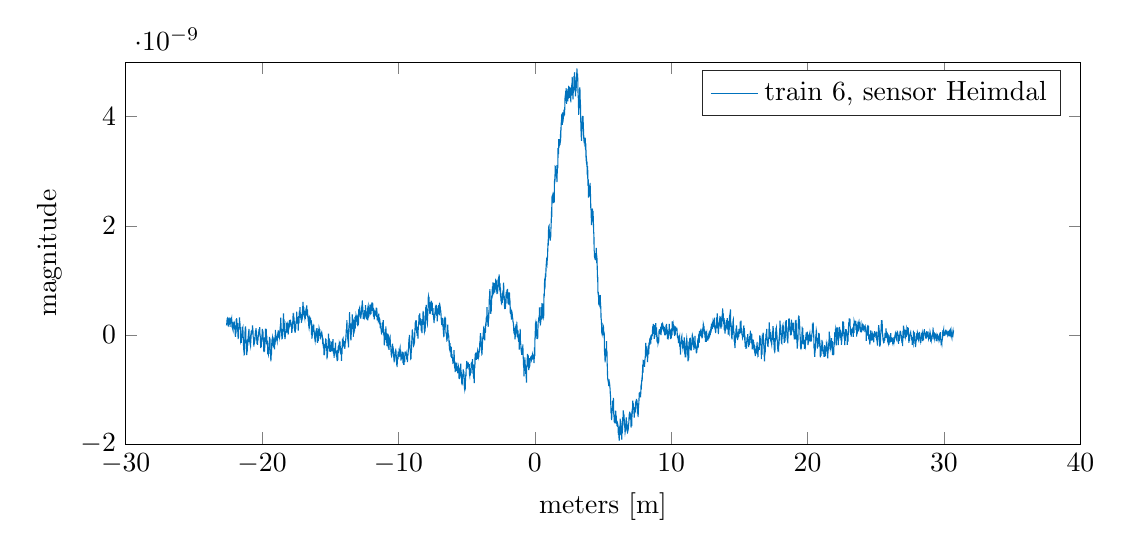
\begin{tikzpicture}

  \begin{axis}[%
    width=\textwidth,
    height=0.4\textwidth,
    at={(0\figurewidth,0\figureheight)},
    scale only axis,
    xmin=-30,
    xmax=40,
    xlabel={meters [m]},
    ymin=-2e-09,
    ymax=5e-09,
    ylabel={magnitude},
    axis background/.style={fill=white},
    legend style={legend cell align=left,align=left,draw=white!15!black}
    ]
    \addplot [color=mycolor1,solid]
    table[row sep=crcr]{%
    -22.603759765625	1.76374497743196e-10\\
    -22.58732421875	1.9869703065738e-10\\
    -22.570888671875	2.56028802069136e-10\\
    -22.554453125	2.95420057972131e-10\\
    -22.538017578125	3.03352119899058e-10\\
    -22.52158203125	2.63343670561877e-10\\
    -22.505146484375	2.4071125980175e-10\\
    -22.4887109375	2.57210963303109e-10\\
    -22.472275390625	1.56745940505806e-10\\
    -22.45583984375	2.81257360090966e-10\\
    -22.439404296875	2.2236233617282e-10\\
    -22.42296875	2.44268588218046e-10\\
    -22.406533203125	3.03115927692313e-10\\
    -22.39009765625	1.95289143207902e-10\\
    -22.373662109375	2.67401162808467e-10\\
    -22.3572265625	3.19942699896534e-10\\
    -22.340791015625	1.50434400711466e-10\\
    -22.32435546875	2.6550322372582e-10\\
    -22.307919921875	2.73663082564004e-10\\
    -22.291484375	2.12364081975204e-10\\
    -22.275048828125	2.72851301979676e-10\\
    -22.25861328125	2.8690247357649e-10\\
    -22.242177734375	2.74317323188733e-10\\
    -22.2257421875	2.94684331681306e-10\\
    -22.209306640625	2.04827997578597e-10\\
    -22.19287109375	1.24901999265532e-10\\
    -22.176435546875	2.4100369106181e-10\\
    -22.16	1.48110106340088e-10\\
    -22.143564453125	1.04078778956535e-10\\
    -22.12712890625	8.76451036318769e-11\\
    -22.110693359375	2.24196091544114e-10\\
    -22.0942578125	1.20348721547451e-10\\
    -22.077822265625	1.90407166969553e-10\\
    -22.06138671875	2.2572208758416e-10\\
    -22.044951171875	2.36392370144472e-10\\
    -22.028515625	2.24951229828408e-10\\
    -22.012080078125	1.13944752684585e-10\\
    -21.99564453125	1.15364353412487e-10\\
    -21.979208984375	1.67488237467007e-10\\
    -21.9627734375	-4.50525509234899e-13\\
    -21.946337890625	-3.5665269430581e-11\\
    -21.92990234375	1.08932565145151e-10\\
    -21.913466796875	2.23470498662276e-11\\
    -21.89703125	2.88822682137447e-10\\
    -21.880595703125	1.99626021459978e-10\\
    -21.86416015625	3.06067322912743e-10\\
    -21.847724609375	2.55479301983411e-10\\
    -21.8312890625	1.64015325907954e-10\\
    -21.814853515625	2.19617294358143e-10\\
    -21.79841796875	1.09889719838597e-10\\
    -21.781982421875	8.95417530626007e-11\\
    -21.765546875	1.29229507575306e-11\\
    -21.749111328125	-7.57397844261293e-11\\
    -21.73267578125	8.87917895285003e-11\\
    -21.716240234375	1.05288394419079e-10\\
    -21.6998046875	1.51805929458574e-10\\
    -21.683369140625	2.14699163644052e-10\\
    -21.66693359375	1.73714187452195e-10\\
    -21.650498046875	3.24506552715605e-10\\
    -21.6340625	1.99162853812581e-10\\
    -21.617626953125	2.09326971422141e-10\\
    -21.60119140625	1.46480076862023e-10\\
    -21.584755859375	4.98796400615193e-11\\
    -21.5683203125	-1.07294700211449e-10\\
    -21.551884765625	-9.10808409429009e-11\\
    -21.53544921875	-7.27027490115519e-11\\
    -21.519013671875	-1.43183287640302e-10\\
    -21.502578125	-6.66893187833962e-11\\
    -21.486142578125	-5.35119868219292e-11\\
    -21.46970703125	4.63351155934779e-11\\
    -21.453271484375	1.48772061696902e-10\\
    -21.4368359375	1.07578299072347e-10\\
    -21.420400390625	1.16626642006452e-10\\
    -21.40396484375	1.32393717175876e-10\\
    -21.387529296875	-2.42936972592761e-11\\
    -21.37109375	-5.58463038767761e-11\\
    -21.354658203125	-1.98383051584625e-10\\
    -21.33822265625	-2.74077390079975e-10\\
    -21.321787109375	-3.07219329934297e-10\\
    -21.3053515625	-3.58855929319312e-10\\
    -21.288916015625	-3.52977847616048e-10\\
    -21.27248046875	-1.49655363247768e-10\\
    -21.256044921875	-4.15640900548359e-11\\
    -21.239609375	1.03052001657536e-10\\
    -21.223173828125	9.67026032439188e-11\\
    -21.20673828125	1.56652982252292e-10\\
    -21.190302734375	8.07978165571507e-11\\
    -21.1738671875	-1.55099043620446e-10\\
    -21.157431640625	-1.13503072864092e-10\\
    -21.14099609375	-1.78891044236328e-10\\
    -21.124560546875	-3.66940529733131e-10\\
    -21.108125	-2.85524703684621e-10\\
    -21.091689453125	-3.19685299689217e-10\\
    -21.07525390625	-2.20040651850071e-10\\
    -21.058818359375	-7.90456978815506e-11\\
    -21.0423828125	-1.95416066553526e-10\\
    -21.025947265625	-7.12631946818831e-11\\
    -21.00951171875	-2.77203875484837e-11\\
    -20.993076171875	-4.87623152411629e-11\\
    -20.976640625	4.61930716017009e-11\\
    -20.960205078125	1.12897090904377e-10\\
    -20.94376953125	-2.66562981968806e-11\\
    -20.927333984375	-5.9683479317422e-11\\
    -20.9108984375	-5.63882027284048e-11\\
    -20.894462890625	-1.3496962009702e-10\\
    -20.87802734375	-1.32371821189563e-10\\
    -20.861591796875	-1.71350767584121e-10\\
    -20.84515625	-1.94430887335104e-10\\
    -20.828720703125	-4.87630237907251e-11\\
    -20.81228515625	-6.60994780265377e-11\\
    -20.795849609375	7.6726354226147e-11\\
    -20.7794140625	-3.88733423636816e-12\\
    -20.762978515625	3.26772668912557e-11\\
    -20.74654296875	9.19483931858001e-11\\
    -20.730107421875	2.70555133897699e-11\\
    -20.713671875	9.14815825486124e-11\\
    -20.697236328125	1.76646875501926e-10\\
    -20.68080078125	1.18820882586067e-10\\
    -20.664365234375	7.55031136303978e-11\\
    -20.6479296875	-3.08308179656871e-11\\
    -20.631494140625	-4.77423291832657e-11\\
    -20.61505859375	-9.74978007459912e-11\\
    -20.598623046875	-2.11480679375335e-10\\
    -20.5821875	-1.28569487227684e-10\\
    -20.565751953125	-1.6239150619797e-10\\
    -20.54931640625	-9.14800788415825e-11\\
    -20.532880859375	-1.03108186729207e-10\\
    -20.5164453125	-7.75419132463022e-11\\
    -20.500009765625	5.46627263360134e-13\\
    -20.48357421875	6.44450838973351e-11\\
    -20.467138671875	7.00278572934618e-11\\
    -20.450703125	9.57640586218214e-11\\
    -20.434267578125	1.22516698059269e-10\\
    -20.41783203125	1.49678981162819e-11\\
    -20.401396484375	-2.13654935528848e-11\\
    -20.3849609375	-9.25682481187897e-11\\
    -20.368525390625	-1.61998259759594e-10\\
    -20.35208984375	-1.30566098596253e-10\\
    -20.335654296875	-1.8290851242611e-10\\
    -20.31921875	-5.87795007328617e-11\\
    -20.302783203125	-1.10572446049798e-10\\
    -20.28634765625	-4.12906046416651e-11\\
    -20.269912109375	1.67712817599289e-11\\
    -20.2534765625	6.06291595520728e-12\\
    -20.237041015625	6.0933105500708e-11\\
    -20.22060546875	5.17511202753771e-11\\
    -20.204169921875	1.0929781349154e-10\\
    -20.187734375	6.12294282801262e-11\\
    -20.171298828125	1.42782566734789e-10\\
    -20.15486328125	3.06978442715022e-11\\
    -20.138427734375	-1.10317796006973e-11\\
    -20.1219921875	-2.9855104303171e-11\\
    -20.105556640625	-1.65124841673806e-10\\
    -20.08912109375	-2.38610903810301e-10\\
    -20.072685546875	-1.13080929691672e-10\\
    -20.05625	-2.16069320176347e-10\\
    -20.039814453125	-1.62099087267252e-10\\
    -20.02337890625	-4.88887258798639e-11\\
    -20.006943359375	-8.48627094648312e-11\\
    -19.9905078125	8.02557507332494e-11\\
    -19.974072265625	1.09829375710568e-10\\
    -19.95763671875	-4.69116085837458e-11\\
    -19.941201171875	8.18864050910176e-11\\
    -19.924765625	2.94171107072099e-11\\
    -19.908330078125	-1.21514358274355e-10\\
    -19.89189453125	-4.76260249915417e-11\\
    -19.875458984375	-2.76755653120178e-10\\
    -19.8590234375	-3.13506017076765e-10\\
    -19.842587890625	-1.79107864604476e-10\\
    -19.82615234375	-2.73036749453078e-10\\
    -19.809716796875	-3.0111368888855e-10\\
    -19.79328125	-9.17857104544457e-11\\
    -19.776845703125	-4.15070637803573e-11\\
    -19.76041015625	-1.25117453246594e-10\\
    -19.743974609375	1.14090991375991e-10\\
    -19.7275390625	5.28282365523157e-11\\
    -19.711103515625	-6.59629787966167e-11\\
    -19.69466796875	1.09401214726386e-10\\
    -19.678232421875	-1.65793852128246e-10\\
    -19.661796875	-1.59186566111742e-11\\
    -19.645361328125	-3.80682141114493e-11\\
    -19.62892578125	-1.91642813702765e-10\\
    -19.612490234375	-1.14302359833851e-10\\
    -19.5960546875	-1.76532646397924e-10\\
    -19.579619140625	-3.52970822003405e-10\\
    -19.56318359375	-3.25365182089628e-10\\
    -19.546748046875	-3.26359176870492e-10\\
    -19.5303125	-3.48174002299998e-10\\
    -19.513876953125	-2.84597855563919e-10\\
    -19.49744140625	-2.46325921913392e-10\\
    -19.481005859375	-2.0862624637739e-10\\
    -19.4645703125	-1.06133623183556e-10\\
    -19.448134765625	-3.63801362048969e-11\\
    -19.43169921875	-1.27869655546086e-10\\
    -19.415263671875	-1.16191111511235e-10\\
    -19.398828125	-3.07976501527113e-10\\
    -19.382392578125	-3.00222521512495e-10\\
    -19.36595703125	-3.98124739102248e-10\\
    -19.349521484375	-4.82375963912052e-10\\
    -19.3330859375	-3.65893910731772e-10\\
    -19.316650390625	-3.64113726034431e-10\\
    -19.30021484375	-3.46135403299293e-10\\
    -19.283779296875	-1.57791354913369e-10\\
    -19.26734375	-1.73031149462157e-10\\
    -19.250908203125	-7.32506806372977e-11\\
    -19.23447265625	-5.07133151930955e-11\\
    -19.218037109375	-1.13634418323113e-10\\
    -19.2016015625	-3.29101971172682e-11\\
    -19.185166015625	-1.12874076093213e-10\\
    -19.16873046875	-1.9235591671559e-10\\
    -19.152294921875	-1.63105200638116e-10\\
    -19.135859375	-2.20341988559864e-10\\
    -19.119423828125	-2.26565437476039e-10\\
    -19.10298828125	-1.45252321073809e-10\\
    -19.086552734375	-2.62356720701516e-10\\
    -19.0701171875	-7.62777015882219e-11\\
    -19.053681640625	-4.21780892004961e-11\\
    -19.03724609375	-1.74820185435888e-10\\
    -19.020810546875	9.15393935090769e-11\\
    -19.004375	-1.02941198784324e-11\\
    -18.987939453125	4.89081481999195e-12\\
    -18.97150390625	-1.73696974373567e-11\\
    -18.955068359375	-5.82459776041613e-11\\
    -18.9386328125	-8.6914685815101e-11\\
    -18.922197265625	-9.28230541147483e-11\\
    -18.90576171875	-8.24531853641074e-11\\
    -18.889326171875	-1.09610739964118e-10\\
    -18.872890625	-4.92085157720215e-11\\
    -18.856455078125	-7.61019077606119e-12\\
    -18.84001953125	-2.51336691229173e-11\\
    -18.823583984375	-1.23701137863244e-12\\
    -18.8071484375	8.21230278998597e-11\\
    -18.790712890625	2.81768366321334e-11\\
    -18.77427734375	-2.58423232723849e-11\\
    -18.757841796875	-1.89383039869455e-11\\
    -18.74140625	-1.39152342669365e-11\\
    -18.724970703125	1.47030586531097e-11\\
    -18.70853515625	-3.5690978181918e-11\\
    -18.692099609375	-8.5728166250929e-12\\
    -18.6756640625	1.18201920910636e-10\\
    -18.659228515625	1.5587365491836e-10\\
    -18.64279296875	1.23974763120397e-10\\
    -18.626357421875	3.17520250933144e-10\\
    -18.609921875	1.9549988100546e-10\\
    -18.593486328125	7.93867662416884e-11\\
    -18.57705078125	1.16895667621816e-10\\
    -18.560615234375	2.10813194974547e-11\\
    -18.5441796875	-4.52187531807907e-11\\
    -18.527744140625	-3.5679931023994e-11\\
    -18.51130859375	-4.49184005698457e-11\\
    -18.494873046875	-2.63309841777692e-12\\
    -18.4784375	1.00944262025162e-10\\
    -18.462001953125	6.27306958416395e-11\\
    -18.44556640625	2.57610722286508e-10\\
    -18.429130859375	3.93410466322665e-10\\
    -18.4126953125	2.53416677236331e-10\\
    -18.396259765625	1.7686317112692e-10\\
    -18.37982421875	2.86046559256721e-10\\
    -18.363388671875	6.41136179748688e-11\\
    -18.346953125	-4.28481096224542e-12\\
    -18.330517578125	-3.3805061867491e-11\\
    -18.31408203125	-7.42693196233679e-11\\
    -18.297646484375	-2.86617495409892e-11\\
    -18.2812109375	6.23678900920364e-11\\
    -18.264775390625	6.48917167347966e-11\\
    -18.24833984375	2.83133315382931e-11\\
    -18.231904296875	1.60199733461531e-10\\
    -18.21546875	1.38740595138378e-10\\
    -18.199033203125	2.24880738136385e-10\\
    -18.18259765625	1.64930306651254e-10\\
    -18.166162109375	1.66665252793495e-10\\
    -18.1497265625	4.47065532173486e-11\\
    -18.133291015625	1.30737290594882e-10\\
    -18.11685546875	1.8310412447181e-10\\
    -18.100419921875	1.64245147239247e-10\\
    -18.083984375	8.85077026152748e-12\\
    -18.067548828125	7.37729009088367e-11\\
    -18.05111328125	1.62912757171282e-10\\
    -18.034677734375	1.89389316745428e-10\\
    -18.0182421875	1.35983646464132e-10\\
    -18.001806640625	1.52482398073126e-10\\
    -17.98537109375	1.57379404343389e-10\\
    -17.968935546875	1.60288730735895e-10\\
    -17.9525	2.72721785085058e-10\\
    -17.936064453125	2.4110610012192e-10\\
    -17.91962890625	2.80879429460064e-10\\
    -17.903193359375	2.36704215159068e-10\\
    -17.8867578125	1.88222350529589e-10\\
    -17.870322265625	2.31932369818737e-10\\
    -17.85388671875	1.82538313883037e-10\\
    -17.837451171875	1.64498471536864e-10\\
    -17.821015625	3.99806287951678e-11\\
    -17.804580078125	6.56660362590003e-11\\
    -17.78814453125	1.12439643800128e-10\\
    -17.771708984375	1.19342286111326e-10\\
    -17.7552734375	2.22277006482427e-10\\
    -17.738837890625	2.17791802753554e-10\\
    -17.72240234375	3.71755130230063e-10\\
    -17.705966796875	3.6495961480332e-10\\
    -17.68953125	3.73739348740854e-10\\
    -17.673095703125	3.00282770012234e-10\\
    -17.65666015625	3.06097957766434e-10\\
    -17.640224609375	2.5495351864815e-10\\
    -17.6237890625	1.21246046349131e-10\\
    -17.607353515625	9.21929711013692e-11\\
    -17.59091796875	1.06209519847908e-10\\
    -17.574482421875	1.10976035679021e-10\\
    -17.558046875	4.21523458868339e-11\\
    -17.541611328125	1.96571585661103e-10\\
    -17.52517578125	1.0344055016503e-10\\
    -17.508740234375	2.3814876571519e-10\\
    -17.4923046875	2.51436421746497e-10\\
    -17.475869140625	2.22627402279327e-10\\
    -17.45943359375	4.25807734926885e-10\\
    -17.442998046875	2.66913853392103e-10\\
    -17.4265625	2.1066643294961e-10\\
    -17.410126953125	3.33026471216944e-10\\
    -17.39369140625	2.32979650777858e-10\\
    -17.377255859375	2.59264239454857e-10\\
    -17.3608203125	2.30994062959103e-10\\
    -17.344384765625	7.97932985281518e-11\\
    -17.32794921875	2.07206339163624e-10\\
    -17.311513671875	3.46012859233139e-10\\
    -17.295078125	2.06842922938469e-10\\
    -17.278642578125	3.26893981748086e-10\\
    -17.26220703125	4.46359218656931e-10\\
    -17.245771484375	3.15730074643917e-10\\
    -17.2293359375	3.58998598381923e-10\\
    -17.212900390625	5.12443110951381e-10\\
    -17.19646484375	3.55544299860696e-10\\
    -17.180029296875	4.12181940985487e-10\\
    -17.16359375	3.41508513162414e-10\\
    -17.147158203125	2.8133896218172e-10\\
    -17.13072265625	3.80279716485841e-10\\
    -17.114287109375	2.34588644220981e-10\\
    -17.0978515625	2.3720061199213e-10\\
    -17.081416015625	3.3568480602844e-10\\
    -17.06498046875	2.69360919211135e-10\\
    -17.048544921875	3.21054424491397e-10\\
    -17.032109375	4.55614382529427e-10\\
    -17.015673828125	4.90349905078355e-10\\
    -16.99923828125	6.07293920106015e-10\\
    -16.982802734375	5.41747185738686e-10\\
    -16.9663671875	4.25981990654687e-10\\
    -16.949931640625	4.4730625131048e-10\\
    -16.93349609375	5.10919235206714e-10\\
    -16.917060546875	3.65589711979616e-10\\
    -16.900625	4.07459355510919e-10\\
    -16.884189453125	3.37639422630689e-10\\
    -16.86775390625	3.13616283364085e-10\\
    -16.851318359375	4.42332019274911e-10\\
    -16.8348828125	2.9758646579666e-10\\
    -16.818447265625	3.73501549116046e-10\\
    -16.80201171875	3.99144769827855e-10\\
    -16.785576171875	3.62509537620442e-10\\
    -16.769140625	5.00628482148932e-10\\
    -16.752705078125	3.89199048429439e-10\\
    -16.73626953125	4.35164455120544e-10\\
    -16.719833984375	5.41462389903992e-10\\
    -16.7033984375	3.82931790827561e-10\\
    -16.686962890625	3.90619673955212e-10\\
    -16.67052734375	4.70405203712939e-10\\
    -16.654091796875	3.32326187927314e-10\\
    -16.63765625	3.77756867778828e-10\\
    -16.621220703125	2.7677034220798e-10\\
    -16.60478515625	2.45649858104025e-10\\
    -16.588349609375	3.35597825483611e-10\\
    -16.5719140625	1.72378073090288e-10\\
    -16.555478515625	1.42570652765189e-10\\
    -16.53904296875	1.94556480528012e-10\\
    -16.522607421875	1.78494969935098e-10\\
    -16.506171875	2.30339104119519e-10\\
    -16.489736328125	3.23432761560934e-10\\
    -16.47330078125	3.15012661581261e-10\\
    -16.456865234375	2.93349751693634e-10\\
    -16.4404296875	2.95450114892748e-10\\
    -16.423994140625	2.39579683117048e-10\\
    -16.40755859375	2.16554469437018e-10\\
    -16.391123046875	2.2588137367312e-10\\
    -16.3746875	4.44103224671459e-11\\
    -16.358251953125	5.15757231637676e-11\\
    -16.34181640625	-5.59177394277302e-11\\
    -16.325380859375	-5.3941065978304e-11\\
    -16.3089453125	1.01497775484979e-10\\
    -16.292509765625	8.09770739711527e-11\\
    -16.27607421875	1.19332984498796e-10\\
    -16.259638671875	1.56302274716085e-10\\
    -16.243203125	1.32795656018276e-10\\
    -16.226767578125	1.28638291595987e-10\\
    -16.21033203125	1.9000852643243e-10\\
    -16.193896484375	9.43345861430287e-11\\
    -16.1774609375	8.31417939753596e-12\\
    -16.161025390625	5.87589128371636e-11\\
    -16.14458984375	-1.04895129921359e-11\\
    -16.128154296875	-7.44371644624038e-11\\
    -16.11171875	-9.99325765533538e-11\\
    -16.095283203125	-3.06709231594333e-11\\
    -16.07884765625	-1.21998258372664e-10\\
    -16.062412109375	-3.96410855853273e-11\\
    -16.0459765625	7.63748261754614e-11\\
    -16.029541015625	4.46782194838497e-11\\
    -16.01310546875	1.19564194581677e-10\\
    -15.996669921875	7.79545653351793e-11\\
    -15.980234375	-5.21650174674069e-12\\
    -15.963798828125	1.24569612956837e-10\\
    -15.94736328125	-2.48680214688323e-11\\
    -15.930927734375	-1.4442047959051e-10\\
    -15.9144921875	6.47441826901384e-11\\
    -15.898056640625	-6.07764939205903e-11\\
    -15.88162109375	-1.12980177288347e-10\\
    -15.865185546875	1.92946021045701e-11\\
    -15.84875	1.11408806881523e-10\\
    -15.832314453125	5.29482894159661e-11\\
    -15.81587890625	1.23984859717714e-10\\
    -15.799443359375	1.0313369178869e-10\\
    -15.7830078125	-1.81885866726902e-11\\
    -15.766572265625	1.08745825251165e-10\\
    -15.75013671875	9.45910170501114e-12\\
    -15.733701171875	-6.67548367031269e-11\\
    -15.717265625	1.42368047926013e-11\\
    -15.700830078125	-4.49205139326836e-11\\
    -15.68439453125	-3.44667513378659e-11\\
    -15.667958984375	2.98726439283333e-11\\
    -15.6515234375	3.34761853497625e-11\\
    -15.635087890625	4.42278404326287e-11\\
    -15.61865234375	-2.46240018916325e-11\\
    -15.602216796875	1.58283401077828e-11\\
    -15.58578125	-1.07687314276666e-11\\
    -15.569345703125	-4.29060875523951e-11\\
    -15.55291015625	-1.65483609028551e-10\\
    -15.536474609375	-6.25085728213003e-11\\
    -15.5200390625	-9.76826212410042e-11\\
    -15.503603515625	-2.34457691788789e-10\\
    -15.48716796875	-2.36095143154388e-10\\
    -15.470732421875	-1.63344559553734e-10\\
    -15.454296875	-3.69372699004566e-10\\
    -15.437861328125	-3.16039902407065e-10\\
    -15.42142578125	-2.71775569995434e-10\\
    -15.404990234375	-2.9582413375792e-10\\
    -15.3885546875	-2.41570936773164e-10\\
    -15.372119140625	-2.00781084526482e-10\\
    -15.35568359375	-2.39538586653381e-10\\
    -15.339248046875	-9.17044363604459e-11\\
    -15.3228125	-7.62540438714078e-11\\
    -15.306376953125	-8.08240431145767e-11\\
    -15.28994140625	-1.801664067451e-10\\
    -15.273505859375	-1.99959100584673e-10\\
    -15.2570703125	-2.42904335760008e-10\\
    -15.240634765625	-3.66175243471865e-10\\
    -15.22419921875	-3.44058434334314e-10\\
    -15.207763671875	-3.68914746159007e-10\\
    -15.191328125	-3.15433488893288e-10\\
    -15.174892578125	-2.79777736304036e-10\\
    -15.15845703125	-2.0319260170426e-10\\
    -15.142021484375	-1.05776040152686e-10\\
    -15.1255859375	2.34640188030139e-11\\
    -15.109150390625	-8.56392802513306e-11\\
    -15.09271484375	-1.13996759992614e-10\\
    -15.076279296875	-6.36809308411667e-11\\
    -15.05984375	-1.55056644365203e-10\\
    -15.043408203125	-3.06826170332516e-10\\
    -15.02697265625	-1.99643058337394e-10\\
    -15.010537109375	-2.62681372042547e-10\\
    -14.9941015625	-2.52843391958764e-10\\
    -14.977666015625	-2.46760162805316e-10\\
    -14.96123046875	-3.11199226275103e-10\\
    -14.944794921875	-1.45935280868187e-10\\
    -14.928359375	-1.54600557827124e-10\\
    -14.911923828125	-2.88968040364034e-10\\
    -14.89548828125	-1.71001131536535e-10\\
    -14.879052734375	-1.80156345609968e-10\\
    -14.8626171875	-2.4379996305076e-10\\
    -14.846181640625	-1.14153281851261e-10\\
    -14.82974609375	-1.73600729580319e-10\\
    -14.813310546875	-3.00550262699622e-10\\
    -14.796875	-7.4328624322124e-11\\
    -14.780439453125	-2.70213923536751e-10\\
    -14.76400390625	-3.40306097073483e-10\\
    -14.747568359375	-2.39778368105611e-10\\
    -14.7311328125	-2.85186227027402e-10\\
    -14.714697265625	-4.21518444164477e-10\\
    -14.69826171875	-2.9871168768623e-10\\
    -14.681826171875	-3.00689447212967e-10\\
    -14.665390625	-3.25375465975162e-10\\
    -14.648955078125	-3.24442518166401e-10\\
    -14.63251953125	-2.44653857089103e-10\\
    -14.616083984375	-1.38657570164519e-10\\
    -14.5996484375	-3.00478910235965e-10\\
    -14.583212890625	-3.24951377841844e-10\\
    -14.56677734375	-2.82018922841837e-10\\
    -14.550341796875	-3.50170332485845e-10\\
    -14.53390625	-3.78141639592996e-10\\
    -14.517470703125	-3.57517419074985e-10\\
    -14.50103515625	-4.45254623184821e-10\\
    -14.484599609375	-4.79431490177936e-10\\
    -14.4681640625	-2.91092466867959e-10\\
    -14.451728515625	-4.62414997827139e-10\\
    -14.43529296875	-3.37140838799097e-10\\
    -14.418857421875	-2.23258331035603e-10\\
    -14.402421875	-2.13445455611376e-10\\
    -14.385986328125	-3.3410082953798e-10\\
    -14.36955078125	-2.37656517952344e-10\\
    -14.353115234375	-2.38339422811109e-10\\
    -14.3366796875	-1.57482779765772e-10\\
    -14.320244140625	-1.7666642485389e-10\\
    -14.30380859375	-2.67694460290233e-10\\
    -14.287373046875	-1.20133798226219e-10\\
    -14.2709375	-1.8670371503401e-10\\
    -14.254501953125	-3.05525327191682e-10\\
    -14.23806640625	-2.5338618269096e-10\\
    -14.221630859375	-3.59785443626348e-10\\
    -14.2051953125	-2.98957722693677e-10\\
    -14.188759765625	-3.35562495950947e-10\\
    -14.17232421875	-4.7272195789502e-10\\
    -14.155888671875	-2.35078049325329e-10\\
    -14.139453125	-3.48923632238376e-10\\
    -14.123017578125	-2.4673147694615e-10\\
    -14.10658203125	-1.35495647835251e-10\\
    -14.090146484375	-1.4975022407351e-10\\
    -14.0737109375	-7.84128507303433e-11\\
    -14.057275390625	-6.61341185296282e-11\\
    -14.04083984375	-1.19379454572591e-10\\
    -14.024404296875	-1.36539685773987e-10\\
    -14.00796875	-1.06625649338725e-10\\
    -13.991533203125	-2.14845977077508e-10\\
    -13.97509765625	-1.15334905472849e-10\\
    -13.958662109375	-2.44550629556529e-10\\
    -13.9422265625	-1.80595362483004e-10\\
    -13.925791015625	-2.56305123187329e-10\\
    -13.90935546875	-1.57597374966837e-10\\
    -13.892919921875	-1.4890036759665e-10\\
    -13.876484375	-1.27802808565055e-10\\
    -13.860048828125	-7.38706870979113e-11\\
    -13.84361328125	-2.971253355912e-11\\
    -13.827177734375	1.01900458850447e-10\\
    -13.8107421875	7.35729569477339e-11\\
    -13.794306640625	1.10484553199256e-10\\
    -13.77787109375	2.73385520907447e-10\\
    -13.761435546875	9.98861124258983e-11\\
    -13.745	7.04315596404354e-11\\
    -13.728564453125	6.18148500134436e-11\\
    -13.71212890625	-6.78398603341176e-11\\
    -13.695693359375	-5.77138931008625e-11\\
    -13.6792578125	-1.19496099560574e-10\\
    -13.662822265625	-2.29258283277575e-10\\
    -13.64638671875	4.84537487582091e-11\\
    -13.629951171875	1.75801788046788e-10\\
    -13.613515625	1.29380010272161e-10\\
    -13.597080078125	2.44547032426937e-10\\
    -13.58064453125	4.19704699733838e-10\\
    -13.564208984375	2.48307960473025e-10\\
    -13.5477734375	1.56037423736883e-10\\
    -13.531337890625	2.13260870535482e-10\\
    -13.51490234375	5.63420048211779e-11\\
    -13.498466796875	-5.92688197562713e-11\\
    -13.48203125	-1.00268710531533e-10\\
    -13.465595703125	-4.57307979856032e-11\\
    -13.44916015625	2.07493386164635e-10\\
    -13.432724609375	1.81769950498557e-10\\
    -13.4162890625	1.09530808033984e-10\\
    -13.399853515625	2.28602193368103e-10\\
    -13.38341796875	3.78482119836492e-10\\
    -13.366982421875	2.55182933465477e-10\\
    -13.350546875	2.53230315120022e-10\\
    -13.334111328125	2.9908737255623e-10\\
    -13.31767578125	1.81516766134595e-10\\
    -13.301240234375	-3.23567809076099e-11\\
    -13.2848046875	2.19147535199919e-10\\
    -13.268369140625	1.53299770700393e-11\\
    -13.25193359375	6.91624305048186e-11\\
    -13.235498046875	2.71769721279339e-10\\
    -13.2190625	6.85928371843562e-11\\
    -13.202626953125	1.91483462862031e-10\\
    -13.18619140625	3.30519426595817e-10\\
    -13.169755859375	1.17461666594433e-10\\
    -13.1533203125	1.78918641502568e-10\\
    -13.136884765625	3.56608752052132e-10\\
    -13.12044921875	1.86936083119458e-10\\
    -13.104013671875	3.5423593928667e-10\\
    -13.087578125	3.34277396627992e-10\\
    -13.071142578125	3.1143725884213e-10\\
    -13.05470703125	3.55433308966572e-10\\
    -13.038271484375	3.02532911003638e-10\\
    -13.0218359375	2.9239829207057e-10\\
    -13.005400390625	3.09960925218689e-10\\
    -12.98896484375	1.9777335757483e-10\\
    -12.972529296875	1.60490785294876e-10\\
    -12.95609375	2.95369147981249e-10\\
    -12.939658203125	1.8392713704433e-10\\
    -12.92322265625	2.38765098673178e-10\\
    -12.906787109375	4.69118499485704e-10\\
    -12.8903515625	3.25824885126117e-10\\
    -12.873916015625	4.64988805751445e-10\\
    -12.85748046875	4.90495334655083e-10\\
    -12.841044921875	5.02645738260474e-10\\
    -12.824609375	4.62363849797217e-10\\
    -12.808173828125	4.11485568025731e-10\\
    -12.79173828125	3.82550123716761e-10\\
    -12.775302734375	3.86860091306559e-10\\
    -12.7588671875	2.9862488601452e-10\\
    -12.742431640625	3.5629010827424e-10\\
    -12.72599609375	3.81227407486136e-10\\
    -12.709560546875	3.82862325653385e-10\\
    -12.693125	4.9858879019454e-10\\
    -12.676689453125	5.40343787982727e-10\\
    -12.66025390625	5.56399945078334e-10\\
    -12.643818359375	6.32822660823821e-10\\
    -12.6273828125	4.85600541890841e-10\\
    -12.610947265625	4.90714501705224e-10\\
    -12.59451171875	4.31674607131421e-10\\
    -12.578076171875	2.94562297606846e-10\\
    -12.561640625	3.35163923824109e-10\\
    -12.545205078125	3.2332936318672e-10\\
    -12.52876953125	3.04730539538757e-10\\
    -12.512333984375	2.97507560720688e-10\\
    -12.4958984375	3.10331506765944e-10\\
    -12.479462890625	4.27927856741329e-10\\
    -12.46302734375	4.53217636857372e-10\\
    -12.446591796875	3.39876976054366e-10\\
    -12.43015625	3.65965635507333e-10\\
    -12.413720703125	5.44809728915428e-10\\
    -12.39728515625	4.23121135320086e-10\\
    -12.380849609375	3.16648289629805e-10\\
    -12.3644140625	4.25627824850948e-10\\
    -12.347978515625	3.25313899442129e-10\\
    -12.33154296875	2.84759642159406e-10\\
    -12.315107421875	4.05693898554823e-10\\
    -12.298671875	3.59569213577752e-10\\
    -12.282236328125	3.74846050521978e-10\\
    -12.26580078125	4.94237856819997e-10\\
    -12.249365234375	2.68594167233061e-10\\
    -12.2329296875	5.17885336112299e-10\\
    -12.216494140625	5.34962560370982e-10\\
    -12.20005859375	3.34515603358782e-10\\
    -12.183623046875	3.49070677839788e-10\\
    -12.1671875	5.05769346121954e-10\\
    -12.150751953125	4.13158775771411e-10\\
    -12.13431640625	4.2737133048428e-10\\
    -12.117880859375	5.04451038648968e-10\\
    -12.1014453125	4.61583433877479e-10\\
    -12.085009765625	5.56088096955533e-10\\
    -12.06857421875	4.1560769060568e-10\\
    -12.052138671875	4.36454457004551e-10\\
    -12.035703125	4.74299010387128e-10\\
    -12.019267578125	3.91893469561887e-10\\
    -12.00283203125	3.95937252263437e-10\\
    -11.986396484375	5.75644371846078e-10\\
    -11.9699609375	4.40864411844382e-10\\
    -11.953525390625	5.49665156228721e-10\\
    -11.93708984375	5.9816103627988e-10\\
    -11.920654296875	5.10290109431803e-10\\
    -11.90421875	5.43240275856831e-10\\
    -11.887783203125	5.88987531262398e-10\\
    -11.87134765625	4.6539791561164e-10\\
    -11.854912109375	4.34951489303718e-10\\
    -11.8384765625	4.96665222921187e-10\\
    -11.822041015625	3.3554279822629e-10\\
    -11.80560546875	4.01325249709101e-10\\
    -11.789169921875	4.49140888519685e-10\\
    -11.772734375	2.85032639840254e-10\\
    -11.756298828125	4.15578658858727e-10\\
    -11.73986328125	3.52216144509421e-10\\
    -11.723427734375	3.99946480963687e-10\\
    -11.7069921875	3.75373489310921e-10\\
    -11.690556640625	3.79139748659421e-10\\
    -11.67412109375	3.75952144690575e-10\\
    -11.657685546875	4.01239189578987e-10\\
    -11.64125	4.36853180912314e-10\\
    -11.624814453125	5.00024859350297e-10\\
    -11.60837890625	3.30612801372222e-10\\
    -11.591943359375	4.26539096815271e-10\\
    -11.5755078125	4.38453110369866e-10\\
    -11.559072265625	2.6789784637392e-10\\
    -11.54263671875	3.39438919222368e-10\\
    -11.526201171875	3.15290308823516e-10\\
    -11.509765625	2.96643465179052e-10\\
    -11.493330078125	3.1352160115346e-10\\
    -11.47689453125	2.69608044357016e-10\\
    -11.460458984375	2.89161593106763e-10\\
    -11.4440234375	3.88720697747288e-10\\
    -11.427587890625	3.17820961543932e-10\\
    -11.41115234375	2.84433272065069e-10\\
    -11.394716796875	3.23451687394331e-10\\
    -11.37828125	2.5831647091444e-10\\
    -11.361845703125	2.90437330116079e-10\\
    -11.34541015625	1.8830780753999e-10\\
    -11.328974609375	1.26109512573864e-10\\
    -11.3125390625	2.18621068029907e-10\\
    -11.296103515625	1.48092930437667e-10\\
    -11.27966796875	1.20113562080093e-10\\
    -11.263232421875	9.0867818323414e-11\\
    -11.246796875	3.08528042058639e-11\\
    -11.230361328125	2.48172274053183e-11\\
    -11.21392578125	9.01789874910835e-11\\
    -11.197490234375	5.01716688106618e-11\\
    -11.1810546875	5.33547413433089e-11\\
    -11.164619140625	2.32409213158025e-10\\
    -11.14818359375	1.67020720442567e-10\\
    -11.131748046875	1.3442887892124e-10\\
    -11.1153125	2.71029958513191e-10\\
    -11.098876953125	1.01267223180227e-10\\
    -11.08244140625	5.43705337534445e-12\\
    -11.066005859375	1.059026583635e-10\\
    -11.0495703125	-5.89991457970484e-11\\
    -11.033134765625	-1.92229633987347e-10\\
    -11.01669921875	9.32167122214102e-13\\
    -11.000263671875	-2.75453240210471e-11\\
    -10.983828125	-9.07572637250781e-11\\
    -10.967392578125	4.28623796648121e-11\\
    -10.95095703125	-2.28622988976156e-11\\
    -10.934521484375	4.20614011262119e-11\\
    -10.9180859375	1.58443431370474e-10\\
    -10.901650390625	-2.49331521439625e-11\\
    -10.88521484375	-1.44068027911559e-10\\
    -10.868779296875	3.80642043551028e-11\\
    -10.85234375	-3.40259221065339e-11\\
    -10.835908203125	-2.05070571859505e-10\\
    -10.81947265625	-9.13988683014947e-11\\
    -10.803037109375	-4.71665983545498e-11\\
    -10.7866015625	-1.46851944643859e-10\\
    -10.770166015625	2.27185314272924e-11\\
    -10.75373046875	-1.64396701990156e-10\\
    -10.737294921875	-2.43607687413179e-10\\
    -10.720859375	-1.81720581403052e-11\\
    -10.704423828125	-1.00121594102339e-10\\
    -10.68798828125	-2.72484269161627e-10\\
    -10.671552734375	-7.83521515588078e-11\\
    -10.6551171875	-9.91085332979629e-11\\
    -10.638681640625	-1.2252864018354e-10\\
    -10.62224609375	-9.59436149098143e-11\\
    -10.605810546875	-7.09509552957102e-11\\
    -10.589375	-1.5315514626918e-10\\
    -10.572939453125	-1.97636611830382e-10\\
    -10.55650390625	-2.19188967644514e-10\\
    -10.540068359375	-3.06949345826213e-10\\
    -10.5236328125	-3.59937033282639e-10\\
    -10.507197265625	-3.76466574806982e-10\\
    -10.49076171875	-3.4437578724505e-10\\
    -10.474326171875	-2.55033300739509e-10\\
    -10.457890625	-3.34047475965876e-10\\
    -10.441455078125	-2.13769016812172e-10\\
    -10.42501953125	-1.60392373277276e-10\\
    -10.408583984375	-3.13600567540653e-10\\
    -10.3921484375	-2.08190726865628e-10\\
    -10.375712890625	-2.78310219473655e-10\\
    -10.35927734375	-4.11935765785192e-10\\
    -10.342841796875	-3.50929041069484e-10\\
    -10.32640625	-4.57524430471721e-10\\
    -10.309970703125	-4.81358511857133e-10\\
    -10.29353515625	-4.71024476500694e-10\\
    -10.277099609375	-4.16733890436277e-10\\
    -10.2606640625	-3.28125914503266e-10\\
    -10.244228515625	-3.12767708333088e-10\\
    -10.22779296875	-3.01607037154697e-10\\
    -10.211357421875	-2.84848369477336e-10\\
    -10.194921875	-2.73562442498648e-10\\
    -10.178486328125	-2.95275951721076e-10\\
    -10.16205078125	-4.0484930992742e-10\\
    -10.145615234375	-4.64523319090915e-10\\
    -10.1291796875	-4.38932166859172e-10\\
    -10.112744140625	-4.72180290714917e-10\\
    -10.09630859375	-5.89494546718561e-10\\
    -10.079873046875	-4.57795604160152e-10\\
    -10.0634375	-4.4533170298708e-10\\
    -10.047001953125	-4.24375363215843e-10\\
    -10.03056640625	-3.64917476228114e-10\\
    -10.014130859375	-3.80954707698107e-10\\
    -9.9976953125	-3.0625588043622e-10\\
    -9.981259765625	-3.72843485484284e-10\\
    -9.96482421875	-3.79520361845368e-10\\
    -9.948388671875	-3.05687840575408e-10\\
    -9.931953125	-3.21357374849648e-10\\
    -9.915517578125	-3.98576775216927e-10\\
    -9.89908203125	-2.6307807378869e-10\\
    -9.882646484375	-2.42053963829045e-10\\
    -9.8662109375	-3.93406271777595e-10\\
    -9.849775390625	-2.6933953025221e-10\\
    -9.83333984375	-3.03100541802962e-10\\
    -9.816904296875	-4.68828603096105e-10\\
    -9.80046875	-4.13276183654655e-10\\
    -9.784033203125	-4.01507832498882e-10\\
    -9.76759765625	-4.44227074489327e-10\\
    -9.751162109375	-3.46468781940615e-10\\
    -9.7347265625	-4.00025485715657e-10\\
    -9.718291015625	-4.34442024064933e-10\\
    -9.70185546875	-3.06658579356822e-10\\
    -9.685419921875	-3.61637306809253e-10\\
    -9.668984375	-5.14693345238323e-10\\
    -9.652548828125	-3.1309551033898e-10\\
    -9.63611328125	-4.42852564542384e-10\\
    -9.619677734375	-5.49782456720099e-10\\
    -9.6032421875	-4.80652780579603e-10\\
    -9.586806640625	-5.45808491704334e-10\\
    -9.57037109375	-3.77699772594045e-10\\
    -9.553935546875	-4.36459560924997e-10\\
    -9.5375	-4.96364392581107e-10\\
    -9.521064453125	-3.36529802378669e-10\\
    -9.50462890625	-3.01147767933046e-10\\
    -9.488193359375	-3.71563064049876e-10\\
    -9.4717578125	-3.25852068713644e-10\\
    -9.455322265625	-3.66656930977519e-10\\
    -9.43888671875	-3.65975615663349e-10\\
    -9.422451171875	-3.75029743125581e-10\\
    -9.406015625	-3.53217085953877e-10\\
    -9.389580078125	-4.47443222553786e-10\\
    -9.37314453125	-3.51165517889968e-10\\
    -9.356708984375	-4.19640687147398e-10\\
    -9.3402734375	-4.98962375307307e-10\\
    -9.323837890625	-3.69436975927584e-10\\
    -9.30740234375	-3.72109022986676e-10\\
    -9.290966796875	-3.63357658070706e-10\\
    -9.27453125	-2.64382321108181e-10\\
    -9.258095703125	-2.53375755440591e-10\\
    -9.24166015625	-1.48895078166033e-10\\
    -9.225224609375	-7.66767113997171e-11\\
    -9.2087890625	-6.73562842955633e-11\\
    -9.192353515625	-6.85050586707381e-13\\
    -9.17591796875	-9.52226144817889e-11\\
    -9.159482421875	-1.43635779532415e-10\\
    -9.143046875	-2.72457805881152e-10\\
    -9.126611328125	-2.82568344977574e-10\\
    -9.11017578125	-3.56954989187306e-10\\
    -9.093740234375	-4.38388198304324e-10\\
    -9.0773046875	-4.31743114501383e-10\\
    -9.060869140625	-3.09039845178523e-10\\
    -9.04443359375	-2.77633642680388e-10\\
    -9.027998046875	-2.13456909985092e-10\\
    -9.0115625	-3.09606500445535e-11\\
    -8.995126953125	-2.08093430933939e-12\\
    -8.97869140625	1.04425076113029e-10\\
    -8.962255859375	5.47135781719472e-12\\
    -8.9458203125	1.17436345821934e-11\\
    -8.929384765625	-5.85478084096898e-11\\
    -8.91294921875	-6.66871377428109e-11\\
    -8.896513671875	-1.37050276700927e-10\\
    -8.880078125	-1.92031180565181e-10\\
    -8.863642578125	-1.80390501350999e-10\\
    -8.84720703125	-1.76031093028203e-10\\
    -8.830771484375	-1.07337420553787e-10\\
    -8.8143359375	-1.40728875537991e-10\\
    -8.797900390625	5.88709041965366e-11\\
    -8.78146484375	1.16340904123076e-10\\
    -8.765029296875	2.29352867146225e-10\\
    -8.74859375	2.02626915808588e-10\\
    -8.732158203125	2.6200577690766e-10\\
    -8.71572265625	1.37388779583241e-10\\
    -8.699287109375	2.70464147041976e-10\\
    -8.6828515625	2.01370399961783e-10\\
    -8.666416015625	3.45130767754058e-11\\
    -8.64998046875	1.30147456900207e-10\\
    -8.633544921875	8.18960986199677e-11\\
    -8.617109375	-1.58880567762625e-11\\
    -8.600673828125	1.82746527727701e-11\\
    -8.58423828125	1.52985380512307e-10\\
    -8.567802734375	-6.51748125495081e-11\\
    -8.5513671875	8.11118091039892e-11\\
    -8.534931640625	2.00235870003017e-10\\
    -8.51849609375	1.68992234922407e-10\\
    -8.502060546875	2.611897132129e-10\\
    -8.485625	3.68943065420726e-10\\
    -8.469189453125	2.62119377319165e-10\\
    -8.45275390625	2.78272328998015e-10\\
    -8.436318359375	3.96555669365282e-10\\
    -8.4198828125	1.91091573831564e-10\\
    -8.403447265625	2.93388200239764e-10\\
    -8.38701171875	2.94467671340947e-10\\
    -8.370576171875	2.16311507373817e-10\\
    -8.354140625	1.66721983317738e-10\\
    -8.337705078125	2.89968445770789e-10\\
    -8.32126953125	7.55033612814969e-11\\
    -8.304833984375	7.24556534392024e-11\\
    -8.2883984375	8.9530720878082e-11\\
    -8.271962890625	3.56692091334656e-11\\
    -8.25552734375	2.1325664157097e-10\\
    -8.239091796875	2.41832409045087e-10\\
    -8.22265625	1.84410617998619e-10\\
    -8.206220703125	3.01460298280029e-10\\
    -8.18978515625	4.42611976426484e-10\\
    -8.173349609375	3.76640491406203e-10\\
    -8.1569140625	3.33827038360987e-10\\
    -8.140478515625	3.359795809195e-10\\
    -8.12404296875	2.09330656281029e-10\\
    -8.107607421875	1.26313672639294e-10\\
    -8.091171875	6.19256101416046e-11\\
    -8.074736328125	8.13821952375863e-11\\
    -8.05830078125	1.30804742407254e-10\\
    -8.041865234375	5.97223890626858e-11\\
    -8.0254296875	2.57538265650373e-10\\
    -8.008994140625	4.38149340262084e-10\\
    -7.99255859375	5.026957481614e-10\\
    -7.976123046875	5.08555505803585e-10\\
    -7.9596875	5.51532834769602e-10\\
    -7.943251953125	4.69045170924201e-10\\
    -7.92681640625	2.66198426733019e-10\\
    -7.910380859375	4.28659649817198e-10\\
    -7.8939453125	2.23633735497154e-10\\
    -7.877509765625	2.05935687101307e-10\\
    -7.86107421875	3.18803636164913e-10\\
    -7.844638671875	3.96614494578002e-10\\
    -7.828203125	4.76370099623935e-10\\
    -7.811767578125	6.86266230032991e-10\\
    -7.79533203125	7.0832394485498e-10\\
    -7.778896484375	6.41948157944549e-10\\
    -7.7624609375	6.98501446006547e-10\\
    -7.746025390625	5.52792230880646e-10\\
    -7.72958984375	6.01531713613764e-10\\
    -7.713154296875	4.70754425092726e-10\\
    -7.69671875	3.85109367821776e-10\\
    -7.680283203125	4.37504385176261e-10\\
    -7.66384765625	5.03454256525771e-10\\
    -7.647412109375	4.76168653149375e-10\\
    -7.6309765625	5.33794374043173e-10\\
    -7.614541015625	5.15110575000821e-10\\
    -7.59810546875	6.29887651296685e-10\\
    -7.581669921875	5.26799926013158e-10\\
    -7.565234375	5.04454518435118e-10\\
    -7.548798828125	5.82005677026959e-10\\
    -7.53236328125	5.23963517905644e-10\\
    -7.515927734375	5.38763258194843e-10\\
    -7.4994921875	3.68960796246378e-10\\
    -7.483056640625	3.96675058351797e-10\\
    -7.46662109375	4.90467740401525e-10\\
    -7.450185546875	3.92900032786135e-10\\
    -7.43375	3.51863594603215e-10\\
    -7.417314453125	3.85530424617389e-10\\
    -7.40087890625	2.86689287621066e-10\\
    -7.384443359375	2.17081322693545e-10\\
    -7.3680078125	3.23051957219749e-10\\
    -7.351572265625	3.60111590615183e-10\\
    -7.33513671875	3.099137863997e-10\\
    -7.318701171875	4.01727006791633e-10\\
    -7.302265625	4.77262445797223e-10\\
    -7.285830078125	5.15819231947804e-10\\
    -7.26939453125	5.24635878121643e-10\\
    -7.252958984375	4.9389680954231e-10\\
    -7.2365234375	4.15577064679306e-10\\
    -7.220087890625	5.50403845964369e-10\\
    -7.20365234375	3.64719628857955e-10\\
    -7.187216796875	3.60286321358974e-10\\
    -7.17078125	4.89381298458437e-10\\
    -7.154345703125	2.50441608485189e-10\\
    -7.13791015625	3.32192078593725e-10\\
    -7.121474609375	4.38033824838737e-10\\
    -7.1050390625	3.89353125293869e-10\\
    -7.088603515625	5.28343171989293e-10\\
    -7.07216796875	3.79855109495988e-10\\
    -7.055732421875	4.72187257265266e-10\\
    -7.039296875	5.44822074659785e-10\\
    -7.022861328125	3.93746421887972e-10\\
    -7.00642578125	3.87756513227383e-10\\
    -6.989990234375	5.27872663093431e-10\\
    -6.9735546875	5.11434530257757e-10\\
    -6.957119140625	4.21340998505304e-10\\
    -6.94068359375	5.17783468803392e-10\\
    -6.924248046875	4.93781638282437e-10\\
    -6.9078125	4.08056041909645e-10\\
    -6.891376953125	4.4708208102031e-10\\
    -6.87494140625	3.59482622422702e-10\\
    -6.858505859375	2.96724393226858e-10\\
    -6.8420703125	2.44964765866241e-10\\
    -6.825634765625	1.84819861004512e-10\\
    -6.80919921875	2.88470108365035e-10\\
    -6.792763671875	2.39159079202392e-10\\
    -6.776328125	2.67451141504945e-10\\
    -6.759892578125	3.13585235979327e-10\\
    -6.74345703125	2.22909281972895e-10\\
    -6.727021484375	1.69809911572759e-10\\
    -6.7105859375	9.6029537591274e-11\\
    -6.694150390625	3.49164835223825e-11\\
    -6.67771484375	6.02717866341409e-11\\
    -6.661279296875	-3.19171721565423e-11\\
    -6.64484375	8.51264747509852e-11\\
    -6.628408203125	2.32235858488839e-10\\
    -6.61197265625	2.16226409997338e-10\\
    -6.595537109375	3.37193083314981e-10\\
    -6.5791015625	3.10605345638404e-10\\
    -6.562666015625	2.85756200340015e-10\\
    -6.54623046875	3.10227744349955e-10\\
    -6.529794921875	1.70709741099094e-10\\
    -6.513359375	4.00232784243125e-11\\
    -6.496923828125	3.89921413096071e-11\\
    -6.48048828125	-1.10296079448265e-11\\
    -6.464052734375	-3.68853026599659e-11\\
    -6.4476171875	-1.06766069813918e-10\\
    -6.431181640625	-1.03229055564262e-10\\
    -6.41474609375	-2.59513951636877e-11\\
    -6.398310546875	3.26118741516138e-11\\
    -6.381875	1.87971409708211e-10\\
    -6.365439453125	6.49257254839062e-11\\
    -6.34900390625	2.75127796247651e-11\\
    -6.332568359375	2.16071387715427e-12\\
    -6.3161328125	-2.63784157593437e-12\\
    -6.299697265625	-7.50348013451358e-11\\
    -6.28326171875	-1.5865618849265e-10\\
    -6.266826171875	-2.12878252947433e-10\\
    -6.250390625	-1.91196492642217e-10\\
    -6.233955078125	-2.78772539721595e-10\\
    -6.21751953125	-1.48805140636786e-10\\
    -6.201083984375	-2.95205248311918e-10\\
    -6.1846484375	-2.90462373253982e-10\\
    -6.168212890625	-2.04947877041568e-10\\
    -6.15177734375	-3.6027120998131e-10\\
    -6.135341796875	-3.51319317182086e-10\\
    -6.11890625	-2.23139420715099e-10\\
    -6.102470703125	-3.84575229245317e-10\\
    -6.08603515625	-4.21107704675527e-10\\
    -6.069599609375	-3.51231394913225e-10\\
    -6.0531640625	-4.1598569471557e-10\\
    -6.036728515625	-4.1446645112218e-10\\
    -6.02029296875	-4.51209143368164e-10\\
    -6.003857421875	-5.14531498885716e-10\\
    -5.987421875	-5.10998229327178e-10\\
    -5.970986328125	-4.33016309815742e-10\\
    -5.95455078125	-4.6236242931757e-10\\
    -5.938115234375	-4.94255997489888e-10\\
    -5.9216796875	-2.7962948799484e-10\\
    -5.905244140625	-4.05487537595616e-10\\
    -5.88880859375	-5.35230282299994e-10\\
    -5.872373046875	-5.17027708963758e-10\\
    -5.8559375	-5.33750291245141e-10\\
    -5.839501953125	-6.8057154347925e-10\\
    -5.82306640625	-5.98056223262875e-10\\
    -5.806630859375	-6.25472729640616e-10\\
    -5.7901953125	-6.31670122967081e-10\\
    -5.773759765625	-5.61793926873051e-10\\
    -5.75732421875	-5.81776078922726e-10\\
    -5.740888671875	-5.98718362028093e-10\\
    -5.724453125	-5.08588797283223e-10\\
    -5.708017578125	-6.58587858688178e-10\\
    -5.69158203125	-6.18316470073323e-10\\
    -5.675146484375	-5.7567350563068e-10\\
    -5.6587109375	-6.91429186131259e-10\\
    -5.642275390625	-6.8989897932129e-10\\
    -5.62583984375	-5.99644761165726e-10\\
    -5.609404296875	-6.55259818825285e-10\\
    -5.59296875	-5.79125870150281e-10\\
    -5.576533203125	-5.97257964137343e-10\\
    -5.56009765625	-7.98088634294085e-10\\
    -5.543662109375	-6.62741429265658e-10\\
    -5.5272265625	-6.29416127505305e-10\\
    -5.510791015625	-8.0826378394133e-10\\
    -5.49435546875	-6.38486933536014e-10\\
    -5.477919921875	-6.25572715312678e-10\\
    -5.461484375	-7.14498529821164e-10\\
    -5.445048828125	-6.90640052244591e-10\\
    -5.42861328125	-5.25120292394365e-10\\
    -5.412177734375	-6.93864073638255e-10\\
    -5.3957421875	-6.84611247992288e-10\\
    -5.379306640625	-7.2804782662942e-10\\
    -5.36287109375	-8.37189435633282e-10\\
    -5.346435546875	-8.14630746193285e-10\\
    -5.33	-8.35159438784864e-10\\
    -5.313564453125	-8.54996150876159e-10\\
    -5.29712890625	-7.54100921236613e-10\\
    -5.280693359375	-7.23809748107123e-10\\
    -5.2642578125	-7.2444095172736e-10\\
    -5.247822265625	-6.32607550004734e-10\\
    -5.23138671875	-7.39067191351365e-10\\
    -5.214951171875	-6.65064766782995e-10\\
    -5.198515625	-6.96436654283084e-10\\
    -5.182080078125	-8.09161227469254e-10\\
    -5.16564453125	-9.61681720765322e-10\\
    -5.149208984375	-9.86731783466463e-10\\
    -5.1327734375	-9.04533215490944e-10\\
    -5.116337890625	-1.01352054297189e-09\\
    -5.09990234375	-9.81367767532387e-10\\
    -5.083466796875	-8.25976800206821e-10\\
    -5.06703125	-7.2987738720719e-10\\
    -5.050595703125	-7.61308751545201e-10\\
    -5.03416015625	-6.28738617671598e-10\\
    -5.017724609375	-5.922892702894e-10\\
    -5.0012890625	-5.29168434024474e-10\\
    -4.984853515625	-4.75010885832653e-10\\
    -4.96841796875	-6.13596411104688e-10\\
    -4.951982421875	-5.28263835633854e-10\\
    -4.935546875	-5.26411449956047e-10\\
    -4.919111328125	-5.39777841223061e-10\\
    -4.90267578125	-5.61510440233631e-10\\
    -4.886240234375	-5.03485967533479e-10\\
    -4.8698046875	-5.39327385731123e-10\\
    -4.853369140625	-5.64490028293601e-10\\
    -4.83693359375	-5.68456641112515e-10\\
    -4.820498046875	-5.7523494679123e-10\\
    -4.8040625	-5.34542422615267e-10\\
    -4.787626953125	-7.19475538650659e-10\\
    -4.77119140625	-7.43097392850873e-10\\
    -4.754755859375	-6.86337110023839e-10\\
    -4.7383203125	-7.33938474207236e-10\\
    -4.721884765625	-7.28578472539831e-10\\
    -4.70544921875	-6.41959622279486e-10\\
    -4.689013671875	-6.48350542726992e-10\\
    -4.672578125	-6.94513062939086e-10\\
    -4.656142578125	-5.15022447402065e-10\\
    -4.63970703125	-5.10529492856665e-10\\
    -4.623271484375	-5.18216295239569e-10\\
    -4.6068359375	-4.87891108291866e-10\\
    -4.590400390625	-5.73830624769091e-10\\
    -4.57396484375	-4.42865407797824e-10\\
    -4.557529296875	-4.86423671877969e-10\\
    -4.54109375	-7.0653484877177e-10\\
    -4.524658203125	-5.84348905773697e-10\\
    -4.50822265625	-5.44739673586452e-10\\
    -4.491787109375	-7.64037750753466e-10\\
    -4.4753515625	-7.99066591186962e-10\\
    -4.458916015625	-6.26846284643941e-10\\
    -4.44248046875	-8.82842664738672e-10\\
    -4.426044921875	-6.17244510045884e-10\\
    -4.409609375	-5.45175675295341e-10\\
    -4.393173828125	-6.01925867953782e-10\\
    -4.37673828125	-3.46367809885182e-10\\
    -4.360302734375	-4.42458565853352e-10\\
    -4.3438671875	-3.88724090415802e-10\\
    -4.327431640625	-3.23248233983952e-10\\
    -4.31099609375	-4.47329539006994e-10\\
    -4.294560546875	-4.46692083628944e-10\\
    -4.278125	-3.36406276589246e-10\\
    -4.261689453125	-4.19413851391589e-10\\
    -4.24525390625	-3.90476921422174e-10\\
    -4.228818359375	-3.33332599950145e-10\\
    -4.2123828125	-3.11639909691776e-10\\
    -4.195947265625	-4.38371739054562e-10\\
    -4.17951171875	-3.88091792813906e-10\\
    -4.163076171875	-3.70700921697214e-10\\
    -4.146640625	-2.92849232437988e-10\\
    -4.130205078125	-4.12762118375955e-10\\
    -4.11376953125	-3.98923058047824e-10\\
    -4.097333984375	-3.21861922273479e-10\\
    -4.0808984375	-2.86138720799395e-10\\
    -4.064462890625	-2.96813714922783e-10\\
    -4.04802734375	-2.75051705559211e-10\\
    -4.031591796875	-1.32344053104553e-10\\
    -4.01515625	-1.15911190347934e-10\\
    -3.998720703125	-2.66033799554983e-11\\
    -3.98228515625	3.39470632797179e-11\\
    -3.965849609375	-2.26449471041447e-11\\
    -3.9494140625	-4.36219442571232e-11\\
    -3.932978515625	-1.45102807130658e-10\\
    -3.91654296875	-2.78686329271945e-10\\
    -3.900107421875	-2.16871159780995e-10\\
    -3.883671875	-3.5462188704124e-10\\
    -3.867236328125	-3.48647508952343e-10\\
    -3.85080078125	-2.21473867684066e-10\\
    -3.834365234375	-1.34353753471886e-10\\
    -3.8179296875	-6.90045948950311e-11\\
    -3.801494140625	-7.09363878569478e-11\\
    -3.78505859375	3.735399202217e-11\\
    -3.768623046875	4.09429340521978e-11\\
    -3.7521875	1.19674797420317e-10\\
    -3.735751953125	1.07718130682337e-10\\
    -3.71931640625	-7.11481550854033e-11\\
    -3.702880859375	1.04223605563666e-10\\
    -3.6864453125	-1.54709409936203e-11\\
    -3.670009765625	-9.72999400538064e-11\\
    -3.65357421875	6.30601202027629e-11\\
    -3.637138671875	1.64577233673352e-10\\
    -3.620703125	3.72342513841266e-11\\
    -3.604267578125	1.86480662640114e-10\\
    -3.58783203125	2.17142500331413e-10\\
    -3.571396484375	1.69435366813255e-10\\
    -3.5549609375	3.26961947131004e-10\\
    -3.538525390625	3.30541135016356e-10\\
    -3.52208984375	3.12407608815523e-10\\
    -3.505654296875	5.10814622835754e-10\\
    -3.48921875	3.51604313872399e-10\\
    -3.472783203125	2.89638584868388e-10\\
    -3.45634765625	3.42453330079641e-10\\
    -3.439912109375	2.74209380041148e-10\\
    -3.4234765625	1.48561257254084e-10\\
    -3.407041015625	1.83882463058462e-10\\
    -3.39060546875	3.48618795633343e-10\\
    -3.374169921875	3.35408638383833e-10\\
    -3.357734375	4.1252321358621e-10\\
    -3.341298828125	6.47543592270372e-10\\
    -3.32486328125	6.74303702892193e-10\\
    -3.308427734375	7.59654832466096e-10\\
    -3.2919921875	8.41140173834821e-10\\
    -3.275556640625	5.79886972153774e-10\\
    -3.25912109375	6.40712088211526e-10\\
    -3.242685546875	5.43789486988185e-10\\
    -3.22625	3.88576952759459e-10\\
    -3.209814453125	5.88406920588916e-10\\
    -3.19337890625	4.32454843889863e-10\\
    -3.176943359375	5.7095268381673e-10\\
    -3.1605078125	7.22299251826493e-10\\
    -3.144072265625	6.67615630939504e-10\\
    -3.12763671875	7.4061312104002e-10\\
    -3.111201171875	8.89372560025546e-10\\
    -3.094765625	7.07095869753522e-10\\
    -3.078330078125	7.96527654841154e-10\\
    -3.06189453125	9.62021766327129e-10\\
    -3.045458984375	8.48354027706015e-10\\
    -3.0290234375	7.46386737819711e-10\\
    -3.012587890625	9.47948500917511e-10\\
    -2.99615234375	8.26474853152626e-10\\
    -2.979716796875	8.31954488797601e-10\\
    -2.96328125	9.04805168547714e-10\\
    -2.946845703125	9.03984641501575e-10\\
    -2.93041015625	7.76011642329141e-10\\
    -2.913974609375	8.75591494949249e-10\\
    -2.8975390625	9.60022718946509e-10\\
    -2.881103515625	8.34450931056287e-10\\
    -2.86466796875	9.93877582426552e-10\\
    -2.848232421875	9.84819691718565e-10\\
    -2.831796875	9.11505603873785e-10\\
    -2.815361328125	9.1476139985297e-10\\
    -2.79892578125	9.35644717091106e-10\\
    -2.782490234375	7.51004076963473e-10\\
    -2.7660546875	8.31197815694064e-10\\
    -2.749619140625	8.10004928669766e-10\\
    -2.73318359375	7.60644515461794e-10\\
    -2.716748046875	8.18668332358836e-10\\
    -2.7003125	8.79320677596638e-10\\
    -2.683876953125	9.91745257506068e-10\\
    -2.66744140625	1.02101724190327e-09\\
    -2.651005859375	1.01045799783754e-09\\
    -2.6345703125	9.61178270648581e-10\\
    -2.618134765625	1.10878220125631e-09\\
    -2.60169921875	1.04775388872818e-09\\
    -2.585263671875	8.87941060969005e-10\\
    -2.568828125	9.1007483359928e-10\\
    -2.552392578125	9.46029334998598e-10\\
    -2.53595703125	8.62424289029626e-10\\
    -2.519521484375	7.68536390663525e-10\\
    -2.5030859375	7.84132246364691e-10\\
    -2.486650390625	6.27288853648998e-10\\
    -2.47021484375	7.56855245313818e-10\\
    -2.453779296875	5.79808792050906e-10\\
    -2.43734375	5.72696239682178e-10\\
    -2.420908203125	6.26112294680221e-10\\
    -2.40447265625	5.92877815400486e-10\\
    -2.388037109375	5.95692055406483e-10\\
    -2.3716015625	6.80033937576362e-10\\
    -2.355166015625	7.43788504559689e-10\\
    -2.33873046875	8.10359858068916e-10\\
    -2.322294921875	7.78891032028816e-10\\
    -2.305859375	8.29109051327824e-10\\
    -2.289423828125	9.60944345239172e-10\\
    -2.27298828125	8.51220932875814e-10\\
    -2.256552734375	6.39895610866268e-10\\
    -2.2401171875	7.08380684631547e-10\\
    -2.223681640625	5.38454266376848e-10\\
    -2.20724609375	4.76317183644032e-10\\
    -2.190810546875	5.72218916005165e-10\\
    -2.174375	5.64258335228761e-10\\
    -2.157939453125	4.77902874429402e-10\\
    -2.14150390625	5.83668270408537e-10\\
    -2.125068359375	6.69410371163487e-10\\
    -2.1086328125	6.50832042309692e-10\\
    -2.092197265625	7.91193548751759e-10\\
    -2.07576171875	7.23277881002639e-10\\
    -2.059326171875	6.7392674886902e-10\\
    -2.042890625	8.30963297946766e-10\\
    -2.026455078125	6.9770344144099e-10\\
    -2.01001953125	6.86431512773979e-10\\
    -1.993583984375	8.43399242751233e-10\\
    -1.9771484375	6.7106032557649e-10\\
    -1.960712890625	5.75847035471293e-10\\
    -1.94427734375	7.74143112436744e-10\\
    -1.927841796875	5.54669288958678e-10\\
    -1.91140625	6.38206903705686e-10\\
    -1.894970703125	7.26113730229205e-10\\
    -1.87853515625	6.02510234792042e-10\\
    -1.862099609375	7.80207486083081e-10\\
    -1.8456640625	7.21019074707229e-10\\
    -1.829228515625	5.36775759251675e-10\\
    -1.81279296875	6.29748813188566e-10\\
    -1.796357421875	4.03433303559168e-10\\
    -1.779921875	3.9674249040861e-10\\
    -1.763486328125	4.80807314618372e-10\\
    -1.74705078125	4.1175100780392e-10\\
    -1.730615234375	3.64314402043335e-10\\
    -1.7141796875	2.83409554173815e-10\\
    -1.697744140625	4.61421546553813e-10\\
    -1.68130859375	3.31781596187026e-10\\
    -1.664873046875	3.42144362406839e-10\\
    -1.6484375	3.5915138802707e-10\\
    -1.632001953125	3.15904838405311e-10\\
    -1.61556640625	2.96501360326802e-10\\
    -1.599130859375	2.45013089866138e-10\\
    -1.5826953125	2.26538617345773e-10\\
    -1.566259765625	1.99131132446852e-10\\
    -1.54982421875	1.33558968486694e-10\\
    -1.533388671875	3.07798065017439e-11\\
    -1.516953125	1.28204813781896e-10\\
    -1.500517578125	8.32912174449835e-11\\
    -1.48408203125	4.6931556398324e-12\\
    -1.467646484375	5.13461470460573e-11\\
    -1.4512109375	-8.10954333052969e-11\\
    -1.434775390625	4.29542876956808e-12\\
    -1.41833984375	1.56496736571428e-10\\
    -1.401904296875	-3.73107515403396e-11\\
    -1.38546875	1.35472901812846e-10\\
    -1.369033203125	2.0052995863098e-10\\
    -1.35259765625	1.31702643590776e-10\\
    -1.336162109375	1.64916592629433e-10\\
    -1.3197265625	1.175122215189e-10\\
    -1.303291015625	1.44713943838972e-10\\
    -1.28685546875	7.50848717754542e-11\\
    -1.270419921875	2.65278526464455e-11\\
    -1.253984375	-1.58151659559414e-11\\
    -1.237548828125	-4.42808659476178e-12\\
    -1.22111328125	1.50349032704449e-11\\
    -1.204677734375	-8.03066562675393e-11\\
    -1.1882421875	-1.23398267980694e-10\\
    -1.171806640625	1.03657712935692e-11\\
    -1.15537109375	-1.23441829847404e-10\\
    -1.138935546875	-2.6764370099871e-10\\
    -1.1225	2.10295790770383e-12\\
    -1.106064453125	-1.27530464384637e-10\\
    -1.08962890625	-3.82263921276015e-11\\
    -1.073193359375	1.11722410637111e-10\\
    -1.0567578125	-9.35093256118826e-11\\
    -1.040322265625	-1.68698173411806e-10\\
    -1.02388671875	-1.68533445008808e-10\\
    -1.007451171875	-2.68451588760326e-10\\
    -0.991015624999999	-3.00465523060251e-10\\
    -0.974580078124998	-3.19825918706874e-10\\
    -0.958144531249999	-3.62427514013628e-10\\
    -0.941708984374998	-3.12989152454891e-10\\
    -0.9252734375	-2.40772047205809e-10\\
    -0.908837890624998	-2.79134731337091e-10\\
    -0.89240234375	-3.07116083515494e-10\\
    -0.875966796874998	-1.71728836182291e-10\\
    -0.85953125	-3.64903509771205e-10\\
    -0.843095703124998	-4.33563088029404e-10\\
    -0.82666015625	-5.54654653006709e-10\\
    -0.810224609374998	-5.59466541648758e-10\\
    -0.7937890625	-7.59718507933245e-10\\
    -0.777353515624998	-6.08093189491609e-10\\
    -0.76091796875	-5.63057996475222e-10\\
    -0.744482421874999	-5.44019500477591e-10\\
    -0.728046875	-4.11092523837446e-10\\
    -0.711611328124999	-5.67628586722836e-10\\
    -0.695175781249997	-5.45917678828456e-10\\
    -0.678740234374999	-5.57394986897813e-10\\
    -0.662304687499997	-7.12623387618065e-10\\
    -0.645869140624999	-6.65975751888592e-10\\
    -0.629433593749997	-7.49588591322581e-10\\
    -0.612998046874999	-8.74138009984381e-10\\
    -0.596562499999997	-5.83707689743689e-10\\
    -0.580126953124999	-5.78529639873057e-10\\
    -0.563691406249998	-5.62298215369112e-10\\
    -0.547255859374999	-3.87181563746815e-10\\
    -0.530820312499998	-3.48821119833034e-10\\
    -0.514384765625	-5.2835505138709e-10\\
    -0.497949218749998	-4.67654749469965e-10\\
    -0.481513671875	-3.74232336024818e-10\\
    -0.465078124999998	-5.85762842779548e-10\\
    -0.448642578125	-6.42010934781319e-10\\
    -0.432207031249998	-5.67663336835439e-10\\
    -0.415771484375	-4.61891054401343e-10\\
    -0.399335937499998	-6.08443107164988e-10\\
    -0.382900390625	-4.24582604130557e-10\\
    -0.366464843749998	-4.70524320961656e-10\\
    -0.350029296875	-4.98392496488388e-10\\
    -0.333593749999999	-4.5030882159693e-10\\
    -0.317158203125	-4.41215758767981e-10\\
    -0.300722656249999	-4.14770221594905e-10\\
    -0.284287109374997	-4.20395394858672e-10\\
    -0.267851562499999	-4.19397984478743e-10\\
    -0.251416015624997	-4.39591359825962e-10\\
    -0.234980468749999	-3.7646095570131e-10\\
    -0.218544921874997	-4.56812648042313e-10\\
    -0.202109374999999	-3.82504499124229e-10\\
    -0.185673828124997	-4.45175606230642e-10\\
    -0.169238281249999	-3.55924111438814e-10\\
    -0.152802734374998	-3.72683051039465e-10\\
    -0.136367187499999	-3.6895887317243e-10\\
    -0.119931640624998	-4.09684744312902e-10\\
    -0.10349609375	-4.19863266853118e-10\\
    -0.0870605468749979	-3.82308899013225e-10\\
    -0.0706249999999997	-4.62916565945342e-10\\
    -0.054189453124998	-5.16412076657307e-10\\
    -0.0377539062499999	-3.74367619031512e-10\\
    -0.0213183593749982	-2.27060803263602e-10\\
    -0.0048828125	-3.86867871917193e-10\\
    0.0115527343750017	-5.59978018232186e-11\\
    0.0279882812499999	-5.25156363534128e-11\\
    0.0444238281250016	1.97958662517406e-10\\
    0.0608593749999997	2.1771696199704e-10\\
    0.0772949218750014	1.08251657543881e-10\\
    0.0937304687499996	1.93510891379395e-10\\
    0.110166015625001	2.48676371789864e-10\\
    0.126601562500003	-2.20151633943626e-11\\
    0.143037109375001	1.02353464621481e-10\\
    0.159472656250003	-6.89646422002362e-11\\
    0.175908203125001	5.49631690210058e-11\\
    0.192343750000003	6.25786230661356e-11\\
    0.208779296875001	-7.73485292574835e-11\\
    0.225214843750003	8.55987730005856e-11\\
    0.241650390625001	2.29861945404605e-10\\
    0.258085937500002	2.46014139559865e-10\\
    0.274521484375001	2.68526261175996e-10\\
    0.290957031250002	3.11256137150801e-10\\
    0.307392578125	3.20761237620894e-10\\
    0.323828125000002	2.80762271753908e-10\\
    0.340263671875	5.04852970049648e-10\\
    0.356699218750002	3.6522137987707e-10\\
    0.373134765625	2.18635741149574e-10\\
    0.389570312500002	3.33389696713165e-10\\
    0.406005859375	1.93590278976999e-10\\
    0.422441406250002	2.01669824474115e-10\\
    0.438876953125	2.6519688174218e-10\\
    0.455312500000002	3.17200637937049e-10\\
    0.471748046875	5.10169476768733e-10\\
    0.488183593750001	3.76736532508535e-10\\
    0.504619140625	2.81878374422234e-10\\
    0.521054687500001	5.85638029674585e-10\\
    0.537490234375003	5.08849240191131e-10\\
    0.553925781250001	3.71985991512176e-10\\
    0.570361328125003	4.79142634882779e-10\\
    0.586796875000001	3.49015756155448e-10\\
    0.603232421875003	3.33749808955749e-10\\
    0.619667968750001	5.73067538479681e-10\\
    0.636103515625003	3.11565263911459e-10\\
    0.652539062500001	3.58132042161554e-10\\
    0.668974609375002	7.19098988844622e-10\\
    0.685410156250001	7.11159627126558e-10\\
    0.701845703125002	7.40727211558991e-10\\
    0.71828125	1.03062838976729e-09\\
    0.734716796875002	8.45745270303602e-10\\
    0.75115234375	8.97881368293431e-10\\
    0.767587890625002	1.06047399094919e-09\\
    0.7840234375	1.13030292369389e-09\\
    0.800458984375002	1.06191567765027e-09\\
    0.81689453125	1.16857223275966e-09\\
    0.833330078125002	1.30323981527881e-09\\
    0.849765625	1.25252006715857e-09\\
    0.866201171875002	1.4157751124818e-09\\
    0.88263671875	1.35136681392815e-09\\
    0.899072265625001	1.32279793289916e-09\\
    0.9155078125	1.39263106098382e-09\\
    0.931943359375001	1.42850703052824e-09\\
    0.948378906249999	1.55537208933238e-09\\
    0.964814453125001	1.68461587113364e-09\\
    0.981250000000003	1.64004275432623e-09\\
    0.997685546875001	1.86835622744409e-09\\
    1.01412109375	1.96035367288484e-09\\
    1.030556640625	1.99477238179946e-09\\
    1.0469921875	2.00350463564452e-09\\
    1.063427734375	1.86269579110286e-09\\
    1.07986328125	1.88329222910877e-09\\
    1.096298828125	1.87913811391982e-09\\
    1.112734375	1.76557313280571e-09\\
    1.129169921875	1.73205394171181e-09\\
    1.14560546875	1.83671267887197e-09\\
    1.162041015625	1.77418878000702e-09\\
    1.1784765625	1.93666479601328e-09\\
    1.194912109375	1.99000977309757e-09\\
    1.21134765625	2.15401995797119e-09\\
    1.227783203125	2.26511137980303e-09\\
    1.24421875	2.24652163254429e-09\\
    1.260654296875	2.48265166166462e-09\\
    1.27708984375	2.46630351090122e-09\\
    1.293525390625	2.54398469571609e-09\\
    1.3099609375	2.56093554375433e-09\\
    1.326396484375	2.49903189631214e-09\\
    1.34283203125	2.49574452709544e-09\\
    1.359267578125	2.52087011669108e-09\\
    1.375703125	2.4172232208623e-09\\
    1.392138671875	2.47488214732689e-09\\
    1.40857421875	2.57352950066555e-09\\
    1.425009765625	2.43296328999881e-09\\
    1.4414453125	2.80826398533187e-09\\
    1.457880859375	2.85788112677347e-09\\
    1.47431640625	2.80327081241268e-09\\
    1.490751953125	3.03408992885449e-09\\
    1.5071875	3.01590683702935e-09\\
    1.523623046875	3.08537787607101e-09\\
    1.54005859375	3.09050877659584e-09\\
    1.556494140625	2.92969488780785e-09\\
    1.5729296875	2.93450456963178e-09\\
    1.589365234375	2.98597938130812e-09\\
    1.60580078125	2.92014369786724e-09\\
    1.622236328125	2.80316661121796e-09\\
    1.638671875	2.93432630978889e-09\\
    1.655107421875	3.0972859354924e-09\\
    1.67154296875	3.09546640279757e-09\\
    1.687978515625	3.05651931900843e-09\\
    1.7044140625	3.42960908480517e-09\\
    1.720849609375	3.34663832195032e-09\\
    1.73728515625	3.34144691730962e-09\\
    1.753720703125	3.59079553159176e-09\\
    1.77015625	3.43535834392212e-09\\
    1.786591796875	3.58383765577972e-09\\
    1.80302734375	3.47608989677162e-09\\
    1.819462890625	3.51354259919661e-09\\
    1.8358984375	3.48877257218813e-09\\
    1.852333984375	3.49592478760318e-09\\
    1.86876953125	3.55224582148767e-09\\
    1.885205078125	3.66391828148173e-09\\
    1.901640625	3.64315770405559e-09\\
    1.918076171875	3.76225586842365e-09\\
    1.93451171875	3.89025120494807e-09\\
    1.950947265625	3.84723847696191e-09\\
    1.9673828125	4.00321009203029e-09\\
    1.983818359375	4.05476613017544e-09\\
    2.00025390625	3.89848505309116e-09\\
    2.016689453125	3.85050075365962e-09\\
    2.033125	3.98373621890022e-09\\
    2.049560546875	4.08149575823619e-09\\
    2.06599609375	3.98155847155228e-09\\
    2.082431640625	3.96337961447188e-09\\
    2.0988671875	4.07002205645825e-09\\
    2.115302734375	3.9998407486711e-09\\
    2.13173828125	4.12925147424625e-09\\
    2.148173828125	4.01004915993398e-09\\
    2.164609375	4.08551200046527e-09\\
    2.181044921875	4.07570496759005e-09\\
    2.19748046875	4.1611863269111e-09\\
    2.213916015625	4.33823262031308e-09\\
    2.2303515625	4.38051060322384e-09\\
    2.246787109375	4.38437522670684e-09\\
    2.26322265625	4.47484398489182e-09\\
    2.279658203125	4.30213624049112e-09\\
    2.29609375	4.52426724731646e-09\\
    2.312529296875	4.44216389305955e-09\\
    2.32896484375	4.23676605258939e-09\\
    2.345400390625	4.37578114041365e-09\\
    2.3618359375	4.32738338238313e-09\\
    2.378271484375	4.34066033223655e-09\\
    2.39470703125	4.47424253163864e-09\\
    2.411142578125	4.28048634722743e-09\\
    2.427578125	4.51160841248118e-09\\
    2.444013671875	4.4635681672094e-09\\
    2.46044921875	4.33045692053316e-09\\
    2.476884765625	4.55599123318769e-09\\
    2.4933203125	4.55400120680098e-09\\
    2.509755859375	4.33992851121811e-09\\
    2.52619140625	4.50107551463856e-09\\
    2.542626953125	4.48857073208416e-09\\
    2.5590625	4.53151722360006e-09\\
    2.575498046875	4.53126392597887e-09\\
    2.59193359375	4.34826996987488e-09\\
    2.608369140625	4.38492868913252e-09\\
    2.6248046875	4.46719143553796e-09\\
    2.641240234375	4.26482996224532e-09\\
    2.65767578125	4.50017281329007e-09\\
    2.674111328125	4.5300650654004e-09\\
    2.690546875	4.39178914787172e-09\\
    2.706982421875	4.5859091054901e-09\\
    2.72341796875	4.52975550601203e-09\\
    2.739853515625	4.73271888127075e-09\\
    2.7562890625	4.55783083795865e-09\\
    2.772724609375	4.50737031756479e-09\\
    2.78916015625	4.48009340672262e-09\\
    2.805595703125	4.31661115403822e-09\\
    2.82203125	4.53473426876506e-09\\
    2.838466796875	4.49700534593875e-09\\
    2.85490234375	4.46523333067763e-09\\
    2.871337890625	4.74377063987725e-09\\
    2.8877734375	4.56226006070148e-09\\
    2.904208984375	4.80226746431305e-09\\
    2.92064453125	4.80402503236048e-09\\
    2.937080078125	4.534261100822e-09\\
    2.953515625	4.66508106377065e-09\\
    2.969951171875	4.48308967349743e-09\\
    2.98638671875	4.37305626093585e-09\\
    3.002822265625	4.57063154032719e-09\\
    3.0192578125	4.56076526480545e-09\\
    3.035693359375	4.54250946221916e-09\\
    3.05212890625	4.71943901555466e-09\\
    3.068564453125	4.67825116383065e-09\\
    3.085	4.88807246039044e-09\\
    3.101435546875	4.80971164553737e-09\\
    3.11787109375	4.71449255836292e-09\\
    3.134306640625	4.79180121652829e-09\\
    3.1507421875	4.66765831018453e-09\\
    3.167177734375	4.44989888412306e-09\\
    3.18361328125	4.38157709597192e-09\\
    3.200048828125	4.27392766377421e-09\\
    3.216484375	4.03296226200428e-09\\
    3.232919921875	4.3317710519247e-09\\
    3.24935546875	4.31690495004561e-09\\
    3.265791015625	4.16355241447061e-09\\
    3.2822265625	4.32319332358675e-09\\
    3.298662109375	4.53741848582678e-09\\
    3.31509765625	4.47599151473086e-09\\
    3.331533203125	4.26623915627864e-09\\
    3.34796875	4.21816458547642e-09\\
    3.364404296875	3.98445445134707e-09\\
    3.38083984375	3.7957206204e-09\\
    3.397275390625	3.6984560085322e-09\\
    3.4137109375	3.59867931390078e-09\\
    3.430146484375	3.55739574305567e-09\\
    3.44658203125	3.77747299129179e-09\\
    3.463017578125	3.78163438396221e-09\\
    3.479453125	3.89050555229689e-09\\
    3.495888671875	4.01546096825565e-09\\
    3.51232421875	3.86896905221441e-09\\
    3.528759765625	4.01250292228197e-09\\
    3.5451953125	3.91459246687752e-09\\
    3.561630859375	3.80015010250901e-09\\
    3.57806640625	3.70808996057992e-09\\
    3.594501953125	3.57908880108262e-09\\
    3.6109375	3.55084008586267e-09\\
    3.627373046875	3.61305271826861e-09\\
    3.64380859375	3.54904770945835e-09\\
    3.660244140625	3.56395046992278e-09\\
    3.6766796875	3.53149360212787e-09\\
    3.693115234375	3.61742251776923e-09\\
    3.70955078125	3.42664367136662e-09\\
    3.725986328125	3.39087883474034e-09\\
    3.742421875	3.51025344655651e-09\\
    3.758857421875	3.22447386744155e-09\\
    3.77529296875	3.19001068711166e-09\\
    3.791728515625	3.20837008489414e-09\\
    3.8081640625	3.13964186855238e-09\\
    3.824599609375	3.14706984714132e-09\\
    3.84103515625	2.96039657319226e-09\\
    3.857470703125	2.92914937630977e-09\\
    3.87390625	3.09648143797882e-09\\
    3.890341796875	2.76634737299781e-09\\
    3.90677734375	2.73341224150263e-09\\
    3.923212890625	2.85418244265264e-09\\
    3.9396484375	2.51598790007508e-09\\
    3.956083984375	2.67159020454415e-09\\
    3.97251953125	2.62827286759382e-09\\
    3.988955078125	2.54322860714712e-09\\
    4.005390625	2.61765466565785e-09\\
    4.021826171875	2.74072163739371e-09\\
    4.03826171875	2.68016683898931e-09\\
    4.054697265625	2.78689350098538e-09\\
    4.0711328125	2.63558904466612e-09\\
    4.087568359375	2.52399393777511e-09\\
    4.10400390625	2.33273574707739e-09\\
    4.120439453125	2.31121890287099e-09\\
    4.136875	2.20821955774743e-09\\
    4.153310546875	2.01432718971091e-09\\
    4.16974609375	2.05138050248408e-09\\
    4.186181640625	2.20471198692516e-09\\
    4.2026171875	2.08400779236238e-09\\
    4.219052734375	2.31773072725749e-09\\
    4.23548828125	2.26954870222752e-09\\
    4.251923828125	2.21488472653353e-09\\
    4.268359375	2.268016550878e-09\\
    4.284794921875	2.1504632031677e-09\\
    4.30123046875	2.02221582514214e-09\\
    4.317666015625	1.88393591920193e-09\\
    4.3341015625	1.82396140906443e-09\\
    4.350537109375	1.54318967319235e-09\\
    4.36697265625	1.53533595900564e-09\\
    4.383408203125	1.40508725019471e-09\\
    4.39984375	1.44084758677723e-09\\
    4.416279296875	1.4275392793017e-09\\
    4.43271484375	1.37943460637785e-09\\
    4.449150390625	1.45595607649667e-09\\
    4.4655859375	1.49893489957587e-09\\
    4.482021484375	1.36569631161984e-09\\
    4.49845703125	1.59786007454329e-09\\
    4.514892578125	1.55787214239376e-09\\
    4.531328125	1.31665081032107e-09\\
    4.547763671875	1.45213711773726e-09\\
    4.56419921875	1.36235107485023e-09\\
    4.580634765625	1.20590735779731e-09\\
    4.5970703125	1.05718626506096e-09\\
    4.613505859375	1.05482350218474e-09\\
    4.62994140625	7.78371170985313e-10\\
    4.646376953125	7.52509121562836e-10\\
    4.6628125	7.86007098158838e-10\\
    4.679248046875	6.47988265328341e-10\\
    4.69568359375	5.41137102364798e-10\\
    4.712119140625	6.49546631493457e-10\\
    4.7285546875	5.56489927817017e-10\\
    4.744990234375	6.36598056640957e-10\\
    4.76142578125	7.26836535280794e-10\\
    4.777861328125	5.09353542463262e-10\\
    4.794296875	7.32557731325043e-10\\
    4.810732421875	5.35835531668732e-10\\
    4.82716796875	5.46972231937021e-10\\
    4.843603515625	4.58139332707692e-10\\
    4.8600390625	2.87083471090623e-10\\
    4.876474609375	2.87065954552383e-10\\
    4.89291015625	1.93765706867815e-10\\
    4.909345703125	4.65151961453889e-11\\
    4.92578125	2.70572509503677e-11\\
    4.942216796875	8.91745482999988e-11\\
    4.95865234375	1.99351662360276e-11\\
    4.975087890625	1.39776453298446e-10\\
    4.9915234375	-6.65933198493018e-12\\
    5.007958984375	1.73464970487927e-10\\
    5.02439453125	1.63261260753764e-10\\
    5.040830078125	1.35097149532142e-10\\
    5.057265625	6.58138483424828e-13\\
    5.073701171875	4.51547206669921e-11\\
    5.09013671875	2.64499606726898e-11\\
    5.106572265625	-2.6722459675779e-10\\
    5.1230078125	-3.55992722822928e-10\\
    5.139443359375	-3.91603481219356e-10\\
    5.15587890625	-5.02121924230714e-10\\
    5.172314453125	-3.85701440693715e-10\\
    5.18875	-3.78725020116173e-10\\
    5.205185546875	-2.68095625916444e-10\\
    5.22162109375	-2.71409807090429e-10\\
    5.238056640625	-3.23501570779807e-10\\
    5.2544921875	-1.11837472472308e-10\\
    5.270927734375	-3.47602059867933e-10\\
    5.28736328125	-2.82217242488305e-10\\
    5.303798828125	-5.03519273627398e-10\\
    5.320234375	-6.09330094518131e-10\\
    5.336669921875	-7.73394214339321e-10\\
    5.35310546875	-8.1846278489061e-10\\
    5.369541015625	-8.33750603807143e-10\\
    5.3859765625	-8.61799850236893e-10\\
    5.402412109375	-8.78175833667508e-10\\
    5.41884765625	-9.35888519559654e-10\\
    5.435283203125	-8.12140055610161e-10\\
    5.45171875	-8.83247223862022e-10\\
    5.468154296875	-8.71814535503433e-10\\
    5.48458984375	-8.87374076692697e-10\\
    5.501025390625	-9.49977499847214e-10\\
    5.5174609375	-9.79754822466104e-10\\
    5.533896484375	-1.07439311901008e-09\\
    5.55033203125	-1.1057563702687e-09\\
    5.566767578125	-1.23743199825115e-09\\
    5.583203125	-1.38921237228945e-09\\
    5.599638671875	-1.38101135297039e-09\\
    5.61607421875	-1.4913845607549e-09\\
    5.632509765625	-1.56129524459559e-09\\
    5.6489453125	-1.44488552496632e-09\\
    5.665380859375	-1.41740574528664e-09\\
    5.68181640625	-1.36822970181586e-09\\
    5.698251953125	-1.31927374294745e-09\\
    5.7146875	-1.20352902728715e-09\\
    5.731123046875	-1.30555084120718e-09\\
    5.74755859375	-1.33028364735357e-09\\
    5.763994140625	-1.15296939349257e-09\\
    5.7804296875	-1.35482334124032e-09\\
    5.796865234375	-1.50202732305095e-09\\
    5.81330078125	-1.46021993951871e-09\\
    5.829736328125	-1.60482737230621e-09\\
    5.846171875	-1.56354519997028e-09\\
    5.862607421875	-1.5427348915852e-09\\
    5.87904296875	-1.62079575628595e-09\\
    5.895478515625	-1.51870265620942e-09\\
    5.9119140625	-1.53035830603517e-09\\
    5.928349609375	-1.38720911836481e-09\\
    5.94478515625	-1.47084007317232e-09\\
    5.961220703125	-1.47353974170118e-09\\
    5.97765625	-1.51982986811246e-09\\
    5.994091796875	-1.62815806645167e-09\\
    6.01052734375	-1.58426077150404e-09\\
    6.026962890625	-1.66621962747224e-09\\
    6.0433984375	-1.60250726582964e-09\\
    6.059833984375	-1.68356533032591e-09\\
    6.07626953125	-1.63171822319862e-09\\
    6.092705078125	-1.64828350928862e-09\\
    6.109140625	-1.7033684844663e-09\\
    6.125576171875	-1.82053656738357e-09\\
    6.14201171875	-1.8212554691009e-09\\
    6.158447265625	-1.81050772820679e-09\\
    6.1748828125	-1.88435421958189e-09\\
    6.191318359375	-1.93552699323295e-09\\
    6.20775390625	-1.74856960106671e-09\\
    6.224189453125	-1.76381973068477e-09\\
    6.240625	-1.82628278575707e-09\\
    6.257060546875	-1.53534840759365e-09\\
    6.27349609375	-1.62771980096739e-09\\
    6.289931640625	-1.72784972055389e-09\\
    6.3063671875	-1.57473828430931e-09\\
    6.322802734375	-1.8381408764652e-09\\
    6.33923828125	-1.76514225516317e-09\\
    6.355673828125	-1.78491108841714e-09\\
    6.372109375	-1.91826094099223e-09\\
    6.388544921875	-1.66295906997849e-09\\
    6.40498046875	-1.6926421816353e-09\\
    6.421416015625	-1.80310890908699e-09\\
    6.4378515625	-1.54046146039118e-09\\
    6.454287109375	-1.54699984776583e-09\\
    6.47072265625	-1.5794748477713e-09\\
    6.487158203125	-1.38137523516446e-09\\
    6.50359375	-1.43801253476847e-09\\
    6.520029296875	-1.45635391459141e-09\\
    6.53646484375	-1.46585401803772e-09\\
    6.552900390625	-1.58106756805966e-09\\
    6.5693359375	-1.56058784034026e-09\\
    6.585771484375	-1.58242057791257e-09\\
    6.60220703125	-1.7336355197005e-09\\
    6.618642578125	-1.78407233088319e-09\\
    6.635078125	-1.75591617021639e-09\\
    6.651513671875	-1.6603090914804e-09\\
    6.66794921875	-1.72057403009204e-09\\
    6.684384765625	-1.71669208434937e-09\\
    6.7008203125	-1.50925106768268e-09\\
    6.717255859375	-1.66246425515066e-09\\
    6.73369140625	-1.64170303588492e-09\\
    6.750126953125	-1.5796942805405e-09\\
    6.7665625	-1.74924831744357e-09\\
    6.782998046875	-1.76859580061184e-09\\
    6.79943359375	-1.75621545297641e-09\\
    6.815869140625	-1.695796270171e-09\\
    6.8323046875	-1.74743759614553e-09\\
    6.848740234375	-1.72896245947422e-09\\
    6.86517578125	-1.67080671551165e-09\\
    6.881611328125	-1.62349158841366e-09\\
    6.898046875	-1.60126837497211e-09\\
    6.914482421875	-1.4763912933753e-09\\
    6.93091796875	-1.45496469880901e-09\\
    6.947353515625	-1.46975674447979e-09\\
    6.9637890625	-1.4250509314589e-09\\
    6.980224609375	-1.43007661572622e-09\\
    6.99666015625	-1.50702674759479e-09\\
    7.013095703125	-1.54000975108303e-09\\
    7.02953125	-1.44285811374293e-09\\
    7.045966796875	-1.64737852345514e-09\\
    7.06240234375	-1.69922683922175e-09\\
    7.078837890625	-1.58902074260827e-09\\
    7.0952734375	-1.60660751733073e-09\\
    7.111708984375	-1.67111342538146e-09\\
    7.12814453125	-1.40040692149208e-09\\
    7.144580078125	-1.3720319779045e-09\\
    7.161015625	-1.44320620039341e-09\\
    7.177451171875	-1.20511375144211e-09\\
    7.19388671875	-1.26139055884954e-09\\
    7.210322265625	-1.28505005244863e-09\\
    7.2267578125	-1.26085833651315e-09\\
    7.243193359375	-1.26815321404211e-09\\
    7.25962890625	-1.37439089115189e-09\\
    7.276064453125	-1.32923000721815e-09\\
    7.2925	-1.51370748816686e-09\\
    7.308935546875	-1.39984296152505e-09\\
    7.32537109375	-1.38320111132271e-09\\
    7.341806640625	-1.4224837475522e-09\\
    7.3582421875	-1.41503755820356e-09\\
    7.374677734375	-1.37297236070927e-09\\
    7.39111328125	-1.33329993688903e-09\\
    7.407548828125	-1.20574341233475e-09\\
    7.423984375	-1.26234390557136e-09\\
    7.440419921875	-1.22408766482568e-09\\
    7.45685546875	-1.17328616541962e-09\\
    7.473291015625	-1.27440085306426e-09\\
    7.4897265625	-1.19849383233954e-09\\
    7.506162109375	-1.24277917113662e-09\\
    7.52259765625	-1.44096409751265e-09\\
    7.539033203125	-1.38176475316329e-09\\
    7.55546875	-1.32768278449353e-09\\
    7.571904296875	-1.50662447484247e-09\\
    7.58833984375	-1.41040676699441e-09\\
    7.604775390625	-1.30032329479594e-09\\
    7.6212109375	-1.268920858403e-09\\
    7.637646484375	-1.1944347450534e-09\\
    7.65408203125	-1.08144417255238e-09\\
    7.670517578125	-1.05271244457332e-09\\
    7.686953125	-1.14235426494777e-09\\
    7.703388671875	-1.06217010356475e-09\\
    7.71982421875	-1.12449438015045e-09\\
    7.736259765625	-1.03667951247648e-09\\
    7.7526953125	-1.14146866177585e-09\\
    7.769130859375	-1.05284516180247e-09\\
    7.78556640625	-9.34615937301672e-10\\
    7.802001953125	-9.12299275137009e-10\\
    7.8184375	-9.29704407040593e-10\\
    7.834873046875	-8.51598679054975e-10\\
    7.85130859375	-8.1186249438395e-10\\
    7.867744140625	-8.51469519223855e-10\\
    7.8841796875	-7.39081122890993e-10\\
    7.900615234375	-6.48231536083267e-10\\
    7.91705078125	-5.44399249687447e-10\\
    7.933486328125	-6.91103811035997e-10\\
    7.949921875	-4.68283617357357e-10\\
    7.966357421875	-4.71136395226867e-10\\
    7.98279296875	-5.75319996058938e-10\\
    7.999228515625	-5.44005737104328e-10\\
    8.0156640625	-4.98373212772558e-10\\
    8.032099609375	-5.03378731863714e-10\\
    8.04853515625	-5.82129398828881e-10\\
    8.064970703125	-4.67156144289364e-10\\
    8.08140625	-4.40107895555676e-10\\
    8.097841796875	-4.11353957778257e-10\\
    8.11427734375	-3.26374626603182e-10\\
    8.130712890625	-1.44779629881262e-10\\
    8.1471484375	-2.93558083924239e-10\\
    8.163583984375	-3.48761756189452e-10\\
    8.18001953125	-2.52746135327265e-10\\
    8.196455078125	-2.4423803801886e-10\\
    8.212890625	-3.96369216086374e-10\\
    8.229326171875	-3.07331184174017e-10\\
    8.24576171875	-3.91532600616825e-10\\
    8.262197265625	-4.96275637343071e-10\\
    8.2786328125	-3.46662291488834e-10\\
    8.295068359375	-3.64280116108441e-10\\
    8.31150390625	-3.09770254930172e-10\\
    8.327939453125	-1.88819045477161e-10\\
    8.344375	-2.51405053177275e-10\\
    8.360810546875	-3.48644434657446e-10\\
    8.37724609375	-1.3381823015422e-10\\
    8.393681640625	-1.69581903847824e-10\\
    8.4101171875	-1.31497946909062e-10\\
    8.426552734375	-1.62166678691039e-10\\
    8.44298828125	-1.64536191480311e-10\\
    8.459423828125	-1.21463606839225e-10\\
    8.475859375	-1.54121473903444e-10\\
    8.492294921875	-8.889086687669e-11\\
    8.50873046875	-1.02344298857967e-10\\
    8.525166015625	2.99102755904297e-12\\
    8.5416015625	-4.61004287761054e-11\\
    8.558037109375	-5.40179914153939e-11\\
    8.57447265625	-1.03480899418203e-11\\
    8.590908203125	-1.61476233238203e-11\\
    8.60734375	-8.04363643572283e-12\\
    8.623779296875	2.73732157047321e-11\\
    8.64021484375	1.5795507022306e-10\\
    8.656650390625	1.1504387593476e-10\\
    8.6730859375	1.21342905262955e-10\\
    8.689521484375	2.02673715999149e-10\\
    8.70595703125	1.97252839596522e-11\\
    8.722392578125	6.91270277090319e-11\\
    8.738828125	1.78988188796076e-10\\
    8.755263671875	-7.06056116182854e-11\\
    8.77169921875	1.18853248022036e-10\\
    8.788134765625	1.48310420719052e-10\\
    8.8045703125	-4.19123635031596e-11\\
    8.821005859375	1.89574048399677e-10\\
    8.83744140625	1.19463627799447e-10\\
    8.853876953125	1.04906542745255e-10\\
    8.8703125	2.17606791560365e-10\\
    8.886748046875	9.06827055053828e-11\\
    8.90318359375	1.21926884410413e-12\\
    8.919619140625	1.37056173941473e-10\\
    8.9360546875	4.82168290853915e-11\\
    8.952490234375	-1.19493996734391e-10\\
    8.96892578125	-6.71770541094663e-12\\
    8.985361328125	-1.38450714602748e-10\\
    9.001796875	-1.43117316526909e-10\\
    9.018232421875	-9.43793376597157e-11\\
    9.03466796875	-1.55408843047071e-10\\
    9.051103515625	-1.36649962738929e-10\\
    9.0675390625	-1.0553076363604e-10\\
    9.083974609375	-1.11704159998056e-10\\
    9.10041015625	4.75211473785574e-11\\
    9.116845703125	9.16846784133064e-11\\
    9.13328125	9.4244261077239e-11\\
    9.149716796875	8.21492268455962e-11\\
    9.16615234375	8.73431705542975e-11\\
    9.182587890625	7.27988302137403e-11\\
    9.1990234375	1.77334140886328e-11\\
    9.215458984375	7.88482635628487e-11\\
    9.23189453125	1.4480857126182e-10\\
    9.248330078125	-3.76714581755667e-12\\
    9.264765625	1.47361933023852e-10\\
    9.281201171875	1.44649027553331e-10\\
    9.29763671875	1.48833695481305e-10\\
    9.314072265625	2.1728181545468e-10\\
    9.3305078125	1.31202408277651e-10\\
    9.346943359375	1.51846127979375e-10\\
    9.36337890625	2.08410108296412e-10\\
    9.379814453125	2.00928168248268e-10\\
    9.39625	1.51374281604031e-10\\
    9.412685546875	1.02053376656357e-10\\
    9.42912109375	1.50652783738265e-10\\
    9.445556640625	1.39678941812057e-10\\
    9.4619921875	5.38263212875831e-11\\
    9.478427734375	1.07466539262011e-10\\
    9.49486328125	1.47765357865396e-10\\
    9.511298828125	3.37405756845888e-11\\
    9.527734375	4.07476327797472e-11\\
    9.544169921875	-6.2378211398044e-12\\
    9.56060546875	3.92601100349626e-11\\
    9.577041015625	2.72092322278083e-11\\
    9.5934765625	-2.94235690092953e-13\\
    9.609912109375	1.75656453509577e-10\\
    9.62634765625	1.8389093058302e-11\\
    9.642783203125	6.60340385590731e-11\\
    9.65921875	2.01420007389488e-10\\
    9.675654296875	1.08748793296769e-10\\
    9.69208984375	4.35940942207906e-11\\
    9.708525390625	9.90897662025661e-11\\
    9.7249609375	-7.18591596100027e-11\\
    9.741396484375	8.70771125171668e-12\\
    9.75783203125	6.1841603592544e-12\\
    9.774267578125	-8.48827606967089e-11\\
    9.790703125	-1.84195853399429e-12\\
    9.807138671875	4.18845586538239e-11\\
    9.82357421875	6.65466609999386e-11\\
    9.840009765625	9.54185799698393e-11\\
    9.8564453125	2.04501251966425e-10\\
    9.872880859375	1.01769977777457e-10\\
    9.88931640625	4.60896572646041e-11\\
    9.905751953125	-1.32631503605405e-11\\
    9.9221875	9.86189695142939e-11\\
    9.938623046875	-3.08850504821799e-11\\
    9.95505859375	-7.44360443672517e-11\\
    9.971494140625	1.69437011989593e-11\\
    9.9879296875	-2.81857105691622e-11\\
    10.004365234375	-6.0268804940243e-11\\
    10.02080078125	1.17105890305748e-10\\
    10.037236328125	5.31771841420202e-11\\
    10.053671875	-1.29452997767036e-11\\
    10.070107421875	2.48822834439741e-10\\
    10.08654296875	1.0364823408379e-10\\
    10.102978515625	1.5825919899093e-10\\
    10.1194140625	1.81783574344219e-10\\
    10.135849609375	1.4715714250496e-10\\
    10.15228515625	1.82995495443473e-10\\
    10.168720703125	1.43837715021732e-10\\
    10.18515625	8.27162551318561e-11\\
    10.201591796875	1.76481758897141e-10\\
    10.21802734375	3.4114188167955e-11\\
    10.234462890625	3.00806657640539e-11\\
    10.2508984375	-1.78392607625905e-11\\
    10.267333984375	2.2702480182958e-11\\
    10.28376953125	5.29287449144154e-11\\
    10.300205078125	4.4931632913077e-11\\
    10.316640625	1.56350715903068e-10\\
    10.333076171875	1.26479932237862e-10\\
    10.34951171875	1.15867590089421e-10\\
    10.365947265625	1.217448039483e-10\\
    10.3823828125	1.21087098163442e-10\\
    10.398818359375	7.1508976918992e-11\\
    10.41525390625	1.3197761068073e-10\\
    10.431689453125	7.4545113773916e-11\\
    10.448125	-9.18496613146294e-12\\
    10.464560546875	-4.31044524392381e-11\\
    10.48099609375	-5.20390045542624e-11\\
    10.497431640625	-5.11630867325427e-11\\
    10.5138671875	-5.81788940703186e-11\\
    10.530302734375	-1.48149446638323e-10\\
    10.54673828125	-6.12073385386555e-11\\
    10.563173828125	-9.95521251839163e-12\\
    10.579609375	-1.5176202390669e-10\\
    10.596044921875	-5.69751498584825e-11\\
    10.61248046875	-3.80935879262224e-11\\
    10.628916015625	-2.14432414532561e-10\\
    10.6453515625	-1.86635105867309e-10\\
    10.661787109375	-2.25693830502637e-10\\
    10.67822265625	-3.57911058642677e-10\\
    10.694658203125	-1.28746385229929e-10\\
    10.71109375	-1.56432889297417e-10\\
    10.727529296875	-1.33097048179773e-10\\
    10.74396484375	-9.97734205019755e-11\\
    10.760400390625	-4.74503895495174e-11\\
    10.7768359375	-2.83219611719755e-11\\
    10.793271484375	-1.60713814641071e-10\\
    10.80970703125	-8.9369368484454e-11\\
    10.826142578125	-2.15704872289033e-10\\
    10.842578125	-2.49192653399341e-10\\
    10.859013671875	-1.49371319707456e-10\\
    10.87544921875	-2.40444904205609e-10\\
    10.891884765625	-2.19349924565552e-10\\
    10.9083203125	-1.11846639099004e-10\\
    10.924755859375	-1.85029252731265e-10\\
    10.94119140625	-1.12664351985071e-10\\
    10.957626953125	-4.63256338717398e-11\\
    10.9740625	-1.64675658437294e-10\\
    10.990498046875	-2.89793588841569e-10\\
    11.00693359375	-2.73785721326633e-10\\
    11.023369140625	-4.09463850986039e-10\\
    11.0398046875	-3.35454342386533e-10\\
    11.056240234375	-2.84665198141439e-10\\
    11.07267578125	-4.12328802393962e-10\\
    11.089111328125	-2.89978853719611e-10\\
    11.105546875	-1.18421256433982e-10\\
    11.121982421875	-9.87717458085904e-11\\
    11.13841796875	-6.36096630277251e-11\\
    11.154853515625	-1.06454446081328e-10\\
    11.1712890625	-1.88862697357698e-10\\
    11.187724609375	-2.75378109451856e-10\\
    11.20416015625	-2.10623061094482e-10\\
    11.220595703125	-4.14018949080769e-10\\
    11.23703125	-4.84721109957698e-10\\
    11.253466796875	-3.25323025097264e-10\\
    11.26990234375	-4.607439298512e-10\\
    11.286337890625	-4.0888862832279e-10\\
    11.3027734375	-1.19868286716825e-10\\
    11.319208984375	-2.37871977450693e-10\\
    11.33564453125	-2.2676504256078e-10\\
    11.352080078125	-6.2865820457464e-11\\
    11.368515625	-2.52574722319985e-10\\
    11.384951171875	-1.4131642086089e-10\\
    11.40138671875	-4.70199468717969e-11\\
    11.417822265625	-2.81681373610269e-10\\
    11.4342578125	-2.51308435945034e-10\\
    11.450693359375	-1.38587607350025e-10\\
    11.46712890625	-2.38889605584077e-10\\
    11.483564453125	-2.48361902037322e-10\\
    11.5	-1.66401155032119e-10\\
    11.516435546875	-1.39405512505899e-10\\
    11.53287109375	-6.77084814748644e-11\\
    11.549306640625	-9.37197688211491e-11\\
    11.5657421875	-3.19106187068064e-11\\
    11.582177734375	-5.8345722598936e-11\\
    11.59861328125	-7.75946757723527e-11\\
    11.615048828125	-1.32097996165224e-10\\
    11.631484375	-1.10227676936384e-10\\
    11.647919921875	-1.61939436308923e-10\\
    11.66435546875	-2.7322302298362e-10\\
    11.680791015625	-1.25619084231929e-10\\
    11.6972265625	-1.95370408575952e-10\\
    11.713662109375	-2.01699372887911e-10\\
    11.73009765625	-2.30419783226808e-10\\
    11.746533203125	-1.67320175719173e-11\\
    11.76296875	-1.75428547026319e-10\\
    11.779404296875	-2.44074609228408e-10\\
    11.79583984375	-2.14782961268694e-10\\
    11.812275390625	-2.30348332002557e-10\\
    11.8287109375	-2.6913846083817e-10\\
    11.845146484375	-3.37601954495089e-10\\
    11.86158203125	-2.18906630316672e-10\\
    11.878017578125	-3.22960439925238e-10\\
    11.894453125	-2.39535489197743e-10\\
    11.910888671875	-1.71182435548183e-10\\
    11.92732421875	-2.17656085628882e-10\\
    11.943759765625	-1.21740734535426e-10\\
    11.9601953125	-6.11473626466669e-11\\
    11.976630859375	-2.387574184819e-10\\
    11.99306640625	-1.02311445333617e-10\\
    12.009501953125	-1.07395875200331e-10\\
    12.0259375	2.32216974828931e-11\\
    12.042373046875	-1.02711389431649e-10\\
    12.05880859375	-1.41957462861102e-10\\
    12.075244140625	7.44719610402733e-11\\
    12.0916796875	-2.46562480932031e-11\\
    12.108115234375	-1.07188828413618e-11\\
    12.12455078125	2.29776019831517e-11\\
    12.140986328125	1.18502571370838e-11\\
    12.157421875	-1.33681158426513e-11\\
    12.173857421875	1.16962806082213e-10\\
    12.19029296875	7.88089529134573e-11\\
    12.206728515625	-1.35581182210181e-11\\
    12.2231640625	1.52613270698738e-11\\
    12.239599609375	-2.55758290296623e-11\\
    12.25603515625	-6.27350737371809e-11\\
    12.272470703125	2.90954452009971e-11\\
    12.28890625	-4.66246264061326e-11\\
    12.305341796875	6.09964570032893e-11\\
    12.32177734375	1.39428278596365e-10\\
    12.338212890625	9.47747295797596e-11\\
    12.3546484375	2.03609185020327e-10\\
    12.371083984375	1.87349416373209e-10\\
    12.38751953125	1.33950997233274e-10\\
    12.403955078125	8.12975841454323e-11\\
    12.420390625	9.68575360103317e-11\\
    12.436826171875	2.6012619433811e-11\\
    12.45326171875	9.95949307938302e-11\\
    12.469697265625	-4.64180898375318e-11\\
    12.4861328125	-1.93799474127196e-11\\
    12.502568359375	-2.15080442486231e-11\\
    12.51900390625	-1.28272955032783e-10\\
    12.535439453125	6.30254396989062e-11\\
    12.551875	1.8954488292073e-11\\
    12.568310546875	-1.25639683742707e-10\\
    12.58474609375	3.19023745491747e-11\\
    12.601181640625	4.56697266219297e-11\\
    12.6176171875	-1.0808378234738e-10\\
    12.634052734375	-5.35108431228021e-11\\
    12.65048828125	-3.88112137669738e-11\\
    12.666923828125	-5.53313628279005e-11\\
    12.683359375	-3.15244003933704e-11\\
    12.699794921875	-3.1373543289476e-11\\
    12.71623046875	-2.64042902367672e-11\\
    12.732666015625	-4.20985306927315e-11\\
    12.7491015625	2.53711478340251e-11\\
    12.765537109375	-6.75658692888933e-11\\
    12.78197265625	2.81673913646005e-11\\
    12.798408203125	6.56433118850644e-11\\
    12.81484375	-3.64422692687389e-11\\
    12.831279296875	1.14243694454778e-11\\
    12.84771484375	8.52431199881201e-11\\
    12.864150390625	2.44382573079271e-12\\
    12.8805859375	6.47456910375742e-11\\
    12.897021484375	9.51040930368549e-11\\
    12.91345703125	7.45040778377423e-11\\
    12.929892578125	8.82468370281014e-11\\
    12.946328125	2.05584633790164e-10\\
    12.962763671875	1.32152142217996e-10\\
    12.97919921875	1.59928417923154e-10\\
    12.995634765625	1.5239579535299e-10\\
    13.0120703125	1.06293917194517e-10\\
    13.028505859375	2.45484108841688e-10\\
    13.04494140625	2.13329551902329e-10\\
    13.061376953125	1.40935041635128e-10\\
    13.0778125	2.44985348937686e-10\\
    13.094248046875	2.28339730382473e-10\\
    13.11068359375	1.48088344447338e-10\\
    13.127119140625	2.74395693452116e-10\\
    13.1435546875	2.36351430736701e-10\\
    13.159990234375	2.43502535274427e-10\\
    13.17642578125	3.16448121610463e-10\\
    13.192861328125	1.42978414795676e-10\\
    13.209296875	1.13397444042427e-10\\
    13.225732421875	1.14537768421284e-10\\
    13.24216796875	9.26151160068916e-11\\
    13.258603515625	3.38731305739873e-11\\
    13.2750390625	1.09043504515617e-10\\
    13.291474609375	1.72455284995133e-10\\
    13.30791015625	1.21793646729234e-10\\
    13.324345703125	2.20875516533075e-10\\
    13.34078125	3.21589418785378e-10\\
    13.357216796875	2.20113671700959e-10\\
    13.37365234375	3.94093287074518e-10\\
    13.390087890625	3.3636990515478e-10\\
    13.4065234375	1.2062668263904e-10\\
    13.422958984375	2.3181143386703e-10\\
    13.43939453125	2.02833109509178e-10\\
    13.455830078125	1.77055383238642e-11\\
    13.472265625	7.24973915270446e-11\\
    13.488701171875	1.3931162768639e-10\\
    13.50513671875	1.82039509785831e-10\\
    13.521572265625	1.81900126796692e-10\\
    13.5380078125	2.51676024084497e-10\\
    13.554443359375	2.52092792212594e-10\\
    13.57087890625	3.49281882887645e-10\\
    13.587314453125	2.84700674491546e-10\\
    13.60375	1.45189456515064e-10\\
    13.620185546875	2.27292447561955e-10\\
    13.63662109375	1.98886865230776e-10\\
    13.653056640625	1.14936658432273e-10\\
    13.6694921875	2.34865204997433e-10\\
    13.685927734375	2.12803482520772e-10\\
    13.70236328125	1.54458983569273e-10\\
    13.718798828125	3.02695217092147e-10\\
    13.735234375	3.73066175968027e-10\\
    13.751669921875	2.51307342684346e-10\\
    13.76810546875	4.88083160324411e-10\\
    13.784541015625	4.29905160546126e-10\\
    13.8009765625	2.60847361084378e-10\\
    13.817412109375	3.96496681099676e-10\\
    13.83384765625	2.72632230965352e-10\\
    13.850283203125	2.00171377814135e-10\\
    13.86671875	3.140323993462e-10\\
    13.883154296875	1.28306258145587e-10\\
    13.89958984375	8.33445998019952e-11\\
    13.916025390625	2.78793624222101e-10\\
    13.9324609375	1.42526301932147e-10\\
    13.948896484375	2.53925433445553e-11\\
    13.96533203125	1.30532035344046e-10\\
    13.981767578125	1.3177544513828e-10\\
    13.998203125	1.12296267227516e-10\\
    14.014638671875	1.29358728599881e-10\\
    14.03107421875	1.71629112091619e-10\\
    14.047509765625	1.74801647100942e-10\\
    14.0639453125	2.73468754315174e-10\\
    14.080380859375	1.98468299729769e-10\\
    14.09681640625	2.09390742724217e-10\\
    14.113251953125	3.09397357312744e-10\\
    14.1296875	1.17429845932209e-10\\
    14.146123046875	1.19929728874235e-10\\
    14.16255859375	2.57592583439415e-10\\
    14.178994140625	5.3062590480852e-12\\
    14.1954296875	7.75317757237618e-11\\
    14.211865234375	1.75360820311816e-10\\
    14.22830078125	3.03679641435686e-11\\
    14.244736328125	1.99555401547526e-11\\
    14.261171875	1.90631425284863e-10\\
    14.277607421875	3.35795147445731e-10\\
    14.29404296875	3.60856465018174e-10\\
    14.310478515625	3.319214948088e-10\\
    14.3269140625	4.00937097454948e-10\\
    14.343349609375	4.70477833659443e-10\\
    14.35978515625	2.0589574609932e-10\\
    14.376220703125	2.18973696453774e-10\\
    14.39265625	1.88044040736715e-10\\
    14.409091796875	4.87081883975674e-11\\
    14.42552734375	5.93463900805367e-11\\
    14.441962890625	-4.93660747609147e-11\\
    14.4583984375	-8.15042771921267e-11\\
    14.474833984375	1.72097233279711e-10\\
    14.49126953125	1.39711826646865e-12\\
    14.507705078125	3.64810832023735e-11\\
    14.524140625	2.01728140934702e-10\\
    14.540576171875	2.71859466937906e-10\\
    14.55701171875	2.85810980327064e-10\\
    14.573447265625	6.26303823350347e-11\\
    14.5898828125	6.18377515565659e-11\\
    14.606318359375	5.09526948041258e-11\\
    14.62275390625	-1.08742873867256e-10\\
    14.639189453125	-1.07385902905058e-10\\
    14.655625	-1.45407151852831e-10\\
    14.672060546875	-2.39911582173103e-10\\
    14.68849609375	-1.82122583922329e-10\\
    14.704931640625	-9.8079482044157e-12\\
    14.7213671875	-4.08546538982303e-11\\
    14.737802734375	3.64884088775913e-11\\
    14.75423828125	1.17076500999535e-10\\
    14.770673828125	1.61020481830754e-12\\
    14.787109375	1.76984878102089e-10\\
    14.803544921875	1.03247414139967e-10\\
    14.81998046875	-2.33494943236631e-12\\
    14.836416015625	1.21427444675327e-11\\
    14.8528515625	-4.122259968412e-11\\
    14.869287109375	-9.2039657227077e-11\\
    14.88572265625	-3.83979919146694e-11\\
    14.902158203125	-1.12804498797153e-11\\
    14.91859375	-4.52632470574151e-11\\
    14.935029296875	3.46416935197558e-11\\
    14.95146484375	-2.95302205636626e-11\\
    14.967900390625	1.12104494123671e-10\\
    14.9843359375	1.9019778915685e-11\\
    15.000771484375	6.42715458226697e-11\\
    15.01720703125	6.2727894433945e-11\\
    15.033642578125	2.7319296113384e-11\\
    15.050078125	1.26541766255607e-10\\
    15.066513671875	2.46364207289149e-10\\
    15.08294921875	1.00372729779643e-10\\
    15.099384765625	1.88654890223466e-10\\
    15.1158203125	2.61702966833876e-10\\
    15.132255859375	3.50016335699776e-11\\
    15.14869140625	1.27670335468672e-10\\
    15.165126953125	8.89981048692642e-11\\
    15.1815625	1.11686548409721e-11\\
    15.197998046875	1.08716025763197e-11\\
    15.21443359375	-1.45024366870276e-11\\
    15.230869140625	-5.15250389012942e-11\\
    15.2473046875	-3.47824551270297e-11\\
    15.263740234375	-3.32111041960428e-11\\
    15.28017578125	-3.01356812411027e-11\\
    15.296611328125	5.06376572582192e-11\\
    15.313046875	1.61719137489125e-10\\
    15.329482421875	1.62761332492068e-10\\
    15.34591796875	-1.82941289533909e-12\\
    15.362353515625	1.2680630516189e-10\\
    15.3787890625	2.08759045068453e-11\\
    15.395224609375	-8.6705305917672e-11\\
    15.41166015625	-7.27559262292525e-11\\
    15.428095703125	-2.17420815025095e-10\\
    15.44453125	-1.82354132213217e-10\\
    15.460966796875	-1.27181861777386e-10\\
    15.47740234375	-2.54945969901703e-10\\
    15.493837890625	-1.58501082622973e-10\\
    15.5102734375	-1.94409828557646e-10\\
    15.526708984375	-2.04497545066592e-10\\
    15.54314453125	-1.11984288088024e-10\\
    15.559580078125	-5.966870012016e-11\\
    15.576015625	-6.41780992253287e-11\\
    15.592451171875	-1.26143529650979e-10\\
    15.60888671875	1.37126766717032e-11\\
    15.625322265625	-1.18547403512558e-10\\
    15.6417578125	-7.01838934686191e-11\\
    15.658193359375	-1.04416669161329e-10\\
    15.67462890625	-2.21997337687921e-10\\
    15.691064453125	-1.85263961730638e-10\\
    15.7075	-9.8499702730541e-11\\
    15.723935546875	-1.78928826813814e-10\\
    15.74037109375	-1.39746133016618e-10\\
    15.756806640625	-2.13231992203017e-11\\
    15.7732421875	-6.77920444497959e-11\\
    15.789677734375	-2.2728952586609e-11\\
    15.80611328125	7.738381355691e-11\\
    15.822548828125	-4.56546102009519e-11\\
    15.838984375	-9.10596584956183e-11\\
    15.855419921875	2.8944824731112e-11\\
    15.87185546875	-1.49534380392764e-10\\
    15.888291015625	-1.24826630751073e-10\\
    15.9047265625	1.97172734422933e-11\\
    15.921162109375	-1.05698930658008e-10\\
    15.93759765625	-2.63274326007258e-10\\
    15.954033203125	-1.72942093614265e-10\\
    15.97046875	-1.50385999025851e-10\\
    15.986904296875	-1.8791204874634e-10\\
    16.00333984375	-2.0643706655868e-10\\
    16.019775390625	-8.67737353687731e-11\\
    16.0362109375	-1.91876724540575e-10\\
    16.052646484375	-1.95128273192018e-10\\
    16.06908203125	-1.81300051059001e-10\\
    16.085517578125	-2.39811229524335e-10\\
    16.101953125	-1.81977264918289e-10\\
    16.118388671875	-2.83559461393738e-10\\
    16.13482421875	-3.42326905075754e-10\\
    16.151259765625	-2.71053660414162e-10\\
    16.1676953125	-3.8560832764798e-10\\
    16.184130859375	-3.52670279604516e-10\\
    16.20056640625	-2.48544626498358e-10\\
    16.217001953125	-3.47123560398247e-10\\
    16.2334375	-3.03946931979931e-10\\
    16.249873046875	-2.07039317139646e-10\\
    16.26630859375	-2.69065612140998e-10\\
    16.282744140625	-2.30434794504117e-10\\
    16.2991796875	-1.27279156933478e-10\\
    16.315615234375	-3.00621407110695e-10\\
    16.33205078125	-3.30115370179318e-10\\
    16.348486328125	-2.73038927413654e-10\\
    16.364921875	-4.02704266790047e-10\\
    16.381357421875	-2.78531775499638e-10\\
    16.39779296875	-2.56740084244692e-10\\
    16.414228515625	-2.69111033982791e-10\\
    16.4306640625	-2.65102068997537e-10\\
    16.447099609375	-1.96247830384891e-10\\
    16.46353515625	-2.10872556699887e-10\\
    16.479970703125	-1.26926237114203e-10\\
    16.49640625	-7.97485545666519e-12\\
    16.512841796875	-3.289881468987e-11\\
    16.52927734375	-6.89362922988044e-11\\
    16.545712890625	-7.52853273102713e-11\\
    16.5621484375	-1.71139582338073e-10\\
    16.578583984375	-1.88682466694815e-10\\
    16.59501953125	-1.89248536142151e-10\\
    16.611455078125	-4.41396010910739e-10\\
    16.627890625	-2.02338584628576e-10\\
    16.644326171875	-2.54062512613883e-10\\
    16.66076171875	-3.5876788554643e-10\\
    16.677197265625	-6.93984939639566e-11\\
    16.6936328125	-8.76827671031359e-11\\
    16.710068359375	-1.41090236469197e-10\\
    16.72650390625	5.18922474385197e-12\\
    16.742939453125	4.06717437903952e-11\\
    16.759375	-5.31667631393138e-11\\
    16.775810546875	-1.44762274303814e-10\\
    16.79224609375	-1.35316583672685e-10\\
    16.808681640625	-2.57199736183564e-10\\
    16.8251171875	-3.9231380483139e-10\\
    16.841552734375	-4.84616465920282e-10\\
    16.85798828125	-3.50224326496032e-10\\
    16.874423828125	-3.33083901844622e-10\\
    16.890859375	-3.14538546630631e-10\\
    16.907294921875	-1.84083204610965e-10\\
    16.92373046875	-1.206903707955e-10\\
    16.940166015625	-3.95371150856506e-11\\
    16.9566015625	2.60375971300386e-11\\
    16.973037109375	-5.0608857214344e-11\\
    16.98947265625	4.89252392825399e-11\\
    17.005908203125	1.12207145949856e-10\\
    17.02234375	-5.32050897708205e-11\\
    17.038779296875	-7.65625394218164e-11\\
    17.05521484375	-1.27571825614987e-10\\
    17.071650390625	-1.01278120477024e-10\\
    17.0880859375	-1.9390121455276e-10\\
    17.104521484375	-1.98813802063034e-10\\
    17.12095703125	-9.56566033595825e-11\\
    17.137392578125	-7.1961599611141e-11\\
    17.153828125	-6.72013683532538e-11\\
    17.170263671875	6.90630016665336e-11\\
    17.18669921875	2.31737299775842e-10\\
    17.203134765625	1.4536433134693e-11\\
    17.2195703125	9.01711235953597e-11\\
    17.236005859375	9.22369013003474e-11\\
    17.25244140625	-7.37493755377478e-11\\
    17.268876953125	5.12182867077094e-11\\
    17.2853125	-5.40616943671568e-11\\
    17.301748046875	-1.15738098290063e-10\\
    17.31818359375	-5.30425215858423e-11\\
    17.334619140625	-1.36089162144822e-10\\
    17.3510546875	-1.50379282844191e-10\\
    17.367490234375	-1.73795757357574e-10\\
    17.38392578125	-1.08892078177877e-10\\
    17.400361328125	-2.80676587036456e-11\\
    17.416796875	6.47465196375489e-11\\
    17.433232421875	-4.59778880848259e-11\\
    17.44966796875	7.6931789132786e-11\\
    17.466103515625	1.60619845109885e-10\\
    17.4825390625	9.11305902514235e-12\\
    17.498974609375	3.18355359609733e-11\\
    17.51541015625	-9.01369276581483e-11\\
    17.531845703125	-8.39314073734579e-11\\
    17.54828125	-2.57651423438132e-10\\
    17.564716796875	-2.78117196837323e-10\\
    17.58115234375	-2.37804071932551e-10\\
    17.597587890625	-3.2186115027079e-10\\
    17.6140234375	-2.41323157601626e-10\\
    17.630458984375	-5.9548339444005e-11\\
    17.64689453125	-9.47796941756128e-11\\
    17.663330078125	1.94093370231026e-11\\
    17.679765625	1.34625745939433e-10\\
    17.696201171875	8.93693267235283e-11\\
    17.71263671875	1.15245375836051e-10\\
    17.729072265625	2.98027473417624e-11\\
    17.7455078125	5.50421194319652e-11\\
    17.761943359375	-8.53643437021339e-11\\
    17.77837890625	-9.80350423196456e-11\\
    17.794814453125	-2.04380137183973e-10\\
    17.81125	-2.37819551442622e-10\\
    17.827685546875	-3.04804883402977e-10\\
    17.84412109375	-1.68804892556332e-10\\
    17.860556640625	-2.36044116764609e-10\\
    17.8769921875	-2.52426778734958e-10\\
    17.893427734375	-7.86934901840671e-11\\
    17.90986328125	-1.7221689633484e-10\\
    17.926298828125	-3.18334784261673e-11\\
    17.942734375	2.3272406405578e-11\\
    17.959169921875	8.6419503713374e-11\\
    17.97560546875	2.62464207135215e-10\\
    17.992041015625	1.11427999485142e-10\\
    18.0084765625	1.78141967294888e-10\\
    18.024912109375	1.71452239467718e-10\\
    18.04134765625	5.7653253710861e-11\\
    18.057783203125	-1.60745691404309e-11\\
    18.07421875	-1.05906945640138e-10\\
    18.090654296875	-1.48188746852069e-10\\
    18.10708984375	-1.5423404377409e-10\\
    18.123525390625	-5.40592007789523e-11\\
    18.1399609375	-2.79901673378876e-11\\
    18.156396484375	1.47354541018653e-11\\
    18.17283203125	1.62496957399783e-10\\
    18.189267578125	1.77521298217624e-10\\
    18.205703125	9.79026089146507e-11\\
    18.222138671875	1.73353193167097e-10\\
    18.23857421875	1.29394452423888e-10\\
    18.255009765625	2.32468806325672e-11\\
    18.2714453125	-5.59627051599752e-11\\
    18.287880859375	-1.4262747596455e-10\\
    18.30431640625	-8.66422290602011e-11\\
    18.320751953125	-1.32117851182067e-10\\
    18.3371875	-1.85821289292878e-11\\
    18.353623046875	-1.11091181526543e-10\\
    18.37005859375	1.13156159470762e-10\\
    18.386494140625	2.4932829937223e-10\\
    18.4029296875	7.51014908370114e-11\\
    18.419365234375	1.14654030782325e-10\\
    18.43580078125	2.73536204004161e-10\\
    18.452236328125	1.00432942084758e-10\\
    18.468671875	5.3103683833469e-11\\
    18.485107421875	4.2798076568153e-11\\
    18.50154296875	-7.6167248253411e-11\\
    18.517978515625	-9.10198027071106e-11\\
    18.5344140625	2.95702641500556e-11\\
    18.550849609375	-1.54362849380009e-10\\
    18.56728515625	2.04038085324017e-11\\
    18.583720703125	1.56577863167654e-10\\
    18.60015625	6.04793726670033e-11\\
    18.616591796875	2.95177627300422e-10\\
    18.63302734375	1.93495235049982e-10\\
    18.649462890625	3.03163758270373e-10\\
    18.6658984375	2.50057958233035e-10\\
    18.682333984375	2.08904843121374e-10\\
    18.69876953125	9.42624353932982e-11\\
    18.715205078125	1.23514450195013e-10\\
    18.731640625	6.63353098304473e-11\\
    18.748076171875	-6.12408593513264e-12\\
    18.76451171875	1.01775931436969e-10\\
    18.780947265625	1.21048022997402e-10\\
    18.7973828125	-9.45913531422749e-13\\
    18.813818359375	2.80380800316419e-10\\
    18.83025390625	1.75879554746443e-10\\
    18.846689453125	5.85200654371618e-11\\
    18.863125	2.22390267253564e-10\\
    18.879560546875	1.47500606517185e-10\\
    18.89599609375	8.54673753784759e-11\\
    18.912431640625	1.42283795142034e-10\\
    18.9288671875	1.32127279799935e-10\\
    18.945302734375	9.5562145251224e-11\\
    18.96173828125	2.26773490465839e-10\\
    18.978173828125	1.30284935681801e-10\\
    18.994609375	7.74451027207179e-12\\
    19.011044921875	-2.96078057022351e-11\\
    19.02748046875	-1.13936428485613e-11\\
    19.043916015625	-7.93791768579908e-11\\
    19.0603515625	3.04885622536223e-11\\
    19.076787109375	-2.3250677642928e-11\\
    19.09322265625	-3.45787434816664e-11\\
    19.109658203125	2.65645139304201e-10\\
    19.12609375	6.30157096491651e-11\\
    19.142529296875	1.43552383642135e-10\\
    19.15896484375	2.76688531375523e-10\\
    19.175400390625	7.84701562278883e-11\\
    19.1918359375	-8.58064939402699e-11\\
    19.208271484375	-6.21134582477791e-11\\
    19.22470703125	-1.31797759378496e-10\\
    19.241142578125	-2.47621842026382e-10\\
    19.257578125	-1.99324238951104e-10\\
    19.274013671875	-5.04696252414138e-11\\
    19.29044921875	-1.19402529994464e-10\\
    19.306884765625	6.56935579481899e-11\\
    19.3233203125	2.64260301098155e-10\\
    19.339755859375	2.52345716725679e-10\\
    19.35619140625	3.43091627813716e-10\\
    19.372626953125	3.39483221408388e-10\\
    19.3890625	2.71558376789218e-10\\
    19.405498046875	2.44897307474431e-10\\
    19.42193359375	1.62123089354278e-10\\
    19.438369140625	1.58915409992286e-11\\
    19.4548046875	-2.02626976582138e-11\\
    19.471240234375	-1.13180949523545e-10\\
    19.48767578125	-2.42753132097564e-10\\
    19.504111328125	-2.50661111331727e-10\\
    19.520546875	-2.22106409158678e-10\\
    19.536982421875	-2.48424541591679e-10\\
    19.55341796875	-1.3927850668367e-10\\
    19.569853515625	-1.43723837149385e-10\\
    19.5862890625	-2.49747134595733e-11\\
    19.602724609375	1.52393005431314e-10\\
    19.61916015625	-1.16541761175067e-10\\
    19.635595703125	5.29659479855669e-11\\
    19.65203125	1.24246311366417e-10\\
    19.668466796875	-1.73266598854438e-10\\
    19.68490234375	-1.0836804867574e-10\\
    19.701337890625	-4.84248276283722e-12\\
    19.7177734375	-1.72321662212405e-10\\
    19.734208984375	-1.13711896679926e-10\\
    19.75064453125	-8.43862958103063e-11\\
    19.767080078125	-2.55362206338117e-10\\
    19.783515625	-1.99217143143328e-10\\
    19.799951171875	-2.01003957204243e-10\\
    19.81638671875	-1.8492931673775e-10\\
    19.832822265625	-2.05022520027793e-10\\
    19.8492578125	-1.29627637261593e-10\\
    19.865693359375	-4.92414877206677e-11\\
    19.88212890625	-4.70419933665154e-12\\
    19.898564453125	4.63171288828894e-11\\
    19.915	-9.88815165202236e-11\\
    19.931435546875	-1.13632646770037e-12\\
    19.94787109375	-3.39051056992629e-11\\
    19.964306640625	-8.40148317622216e-11\\
    19.9807421875	6.32883169489035e-11\\
    19.997177734375	-5.20065164556325e-11\\
    20.01361328125	-4.85401971211264e-11\\
    20.030048828125	-1.85140733900457e-10\\
    20.046484375	-1.4909839466979e-10\\
    20.062919921875	1.63089485835523e-12\\
    20.07935546875	-1.11097072472189e-10\\
    20.095791015625	-7.53405750817548e-11\\
    20.1122265625	2.14627312056734e-11\\
    20.128662109375	-5.82543901324307e-11\\
    20.14509765625	1.60070149543419e-11\\
    20.161533203125	3.48182472357499e-11\\
    20.17796875	-5.65398100054726e-11\\
    20.194404296875	-3.69133507133932e-11\\
    20.21083984375	-7.3010679033165e-11\\
    20.227275390625	-3.06445864405882e-13\\
    20.2437109375	-1.24883594407712e-10\\
    20.260146484375	-1.53779641798794e-11\\
    20.27658203125	-1.12763769849196e-10\\
    20.293017578125	-6.85777002063176e-11\\
    20.309453125	6.89456692512621e-12\\
    20.325888671875	2.69462571084363e-11\\
    20.34232421875	4.84864040011842e-11\\
    20.358759765625	2.08217696018892e-10\\
    20.3751953125	1.44167619902873e-10\\
    20.391630859375	1.1566837367552e-10\\
    20.40806640625	2.32102141587257e-10\\
    20.424501953125	9.39964002024485e-11\\
    20.4409375	4.42068940380148e-11\\
    20.457373046875	-6.15709777532584e-11\\
    20.47380859375	-2.39721300022956e-10\\
    20.490244140625	-2.49664588251532e-10\\
    20.5066796875	-3.40805156528584e-10\\
    20.523115234375	-4.02735937241305e-10\\
    20.53955078125	-3.21377015204208e-10\\
    20.555986328125	-2.85963292030855e-10\\
    20.572421875	-2.55047379187901e-10\\
    20.588857421875	-1.18225521797692e-10\\
    20.60529296875	-1.12062842365859e-11\\
    20.621728515625	1.54554733281229e-11\\
    20.6381640625	8.04958874624425e-11\\
    20.654599609375	5.42423843564715e-11\\
    20.67103515625	-9.37565404940106e-11\\
    20.687470703125	-1.06328972005712e-10\\
    20.70390625	-4.93008638581484e-11\\
    20.720341796875	-2.49755039235648e-10\\
    20.73677734375	-1.05457931962925e-10\\
    20.753212890625	-2.12585823258895e-10\\
    20.7696484375	-2.06884540820905e-10\\
    20.786083984375	-1.15315959966151e-10\\
    20.80251953125	-9.10937110341951e-11\\
    20.818955078125	3.72234669376889e-11\\
    20.835390625	-1.39270768469251e-10\\
    20.851826171875	2.46416291821284e-11\\
    20.86826171875	-5.99667909013436e-11\\
    20.884697265625	-2.02347779844294e-10\\
    20.9011328125	-1.01330270224754e-10\\
    20.917568359375	-2.6407868308991e-10\\
    20.93400390625	-4.0977583212195e-10\\
    20.950439453125	-2.5705448278366e-10\\
    20.966875	-3.71667617002513e-10\\
    20.983310546875	-3.71206913509638e-10\\
    20.99974609375	-2.05150029693906e-10\\
    21.016181640625	-2.3295214747854e-10\\
    21.0326171875	-2.94646739329681e-10\\
    21.049052734375	-9.21577155286516e-11\\
    21.06548828125	-1.42390053678665e-10\\
    21.081923828125	-2.05498090445599e-10\\
    21.098359375	-1.22879053615474e-10\\
    21.114794921875	-2.59508763510626e-10\\
    21.13123046875	-3.00413450212879e-10\\
    21.147666015625	-3.44647910339614e-10\\
    21.1641015625	-2.67587564691167e-10\\
    21.180537109375	-3.17785964808409e-10\\
    21.19697265625	-2.8985762019181e-10\\
    21.213408203125	-3.78630502834416e-10\\
    21.22984375	-4.01522844427165e-10\\
    21.246279296875	-1.88277022679007e-10\\
    21.26271484375	-3.50215429089006e-10\\
    21.279150390625	-3.15984205274146e-10\\
    21.2955859375	-3.18695479907957e-10\\
    21.312021484375	-3.91990658268697e-10\\
    21.32845703125	-2.16253997381928e-10\\
    21.344892578125	-2.45034567263966e-10\\
    21.361328125	-2.55993412436428e-10\\
    21.377763671875	-1.7374948062438e-10\\
    21.39419921875	-2.00588349696681e-10\\
    21.410634765625	-2.19227611113261e-10\\
    21.4270703125	-1.93733958219581e-10\\
    21.443505859375	-2.37267774654154e-10\\
    21.45994140625	-3.26312121085775e-10\\
    21.476376953125	-4.27868682349992e-10\\
    21.4928125	-3.36077180841105e-10\\
    21.509248046875	-2.8222244586388e-10\\
    21.52568359375	-2.6990564946192e-10\\
    21.542119140625	-1.93073750799114e-10\\
    21.5585546875	-1.33471283086394e-10\\
    21.574990234375	-8.13531214113319e-11\\
    21.59142578125	5.98908503649346e-11\\
    21.607861328125	-2.05616319155025e-10\\
    21.624296875	-1.21322431442708e-11\\
    21.640732421875	-1.09591533691259e-10\\
    21.65716796875	-2.12561309357097e-10\\
    21.673603515625	-1.91446654879436e-10\\
    21.6900390625	-1.99118439950076e-10\\
    21.706474609375	-2.41013107217868e-10\\
    21.72291015625	-2.16110019439197e-10\\
    21.739345703125	-1.38379681230466e-10\\
    21.75578125	-5.75712648136604e-11\\
    21.772216796875	-1.31450883814899e-10\\
    21.78865234375	-1.92603416106301e-10\\
    21.805087890625	-1.1112541885447e-10\\
    21.8215234375	-3.62310737778773e-10\\
    21.837958984375	-2.993602461036e-10\\
    21.85439453125	-2.8350426833545e-10\\
    21.870830078125	-3.73547460392701e-10\\
    21.887265625	-3.44572065335289e-10\\
    21.903701171875	-2.99304239167716e-10\\
    21.92013671875	-3.61617523919805e-10\\
    21.936572265625	-1.65406596825157e-10\\
    21.9530078125	-1.71753468311864e-10\\
    21.969443359375	-1.51582786646465e-10\\
    21.98587890625	4.85750219956343e-11\\
    22.002314453125	2.36897584199368e-11\\
    22.01875	1.19804374246674e-11\\
    22.035185546875	6.37727866144462e-11\\
    22.05162109375	5.03142362477878e-11\\
    22.068056640625	1.05411712234016e-10\\
    22.0844921875	7.53855555686132e-11\\
    22.100927734375	-1.89258564172633e-10\\
    22.11736328125	1.30698260490123e-10\\
    22.133798828125	-4.0939144975673e-11\\
    22.150234375	-8.02715458943763e-11\\
    22.166669921875	1.39295904578124e-10\\
    22.18310546875	-4.55929911044364e-11\\
    22.199541015625	-6.82603418639821e-11\\
    22.2159765625	1.3829546523319e-10\\
    22.232412109375	-1.03490138045486e-10\\
    22.24884765625	-1.84028969051179e-10\\
    22.265283203125	-8.79750696820998e-11\\
    22.28171875	-7.01218185315698e-11\\
    22.298154296875	2.80906872177792e-11\\
    22.31458984375	-2.73002441986094e-11\\
    22.331025390625	1.01636390337152e-10\\
    22.3474609375	1.47625420567656e-10\\
    22.363896484375	-8.47344055715058e-12\\
    22.38033203125	9.24858842668143e-11\\
    22.396767578125	8.28088409413838e-11\\
    22.413203125	-5.50095151234207e-11\\
    22.429638671875	8.12825223633908e-11\\
    22.44607421875	-8.88066022512201e-11\\
    22.462509765625	-1.76130156401142e-11\\
    22.4789453125	-1.82703625062157e-10\\
    22.495380859375	-1.36617872474872e-10\\
    22.51181640625	-6.93259207637365e-11\\
    22.528251953125	1.41600018272331e-11\\
    22.5446875	3.3828530723531e-11\\
    22.561123046875	2.50247430984915e-11\\
    22.57755859375	2.49944987553872e-10\\
    22.593994140625	2.27505217166385e-10\\
    22.6104296875	1.49762915737416e-10\\
    22.626865234375	2.38900588608531e-10\\
    22.64330078125	1.89920309078543e-10\\
    22.659736328125	6.95470395593099e-11\\
    22.676171875	8.57746402406073e-12\\
    22.692607421875	-6.66711505117425e-11\\
    22.70904296875	-7.63211772307658e-11\\
    22.725478515625	-1.86007661591766e-10\\
    22.7419140625	-1.73596429095331e-12\\
    22.758349609375	-1.06070853244967e-10\\
    22.77478515625	7.35758464413063e-12\\
    22.791220703125	1.07841715941493e-10\\
    22.80765625	3.17315672829128e-11\\
    22.824091796875	4.04955661047814e-11\\
    22.84052734375	1.03800855119272e-10\\
    22.856962890625	1.85261048363052e-11\\
    22.8733984375	-9.60313515106923e-12\\
    22.889833984375	2.72808431256213e-11\\
    22.90626953125	-1.80818580543927e-10\\
    22.922705078125	-1.11982010410371e-10\\
    22.939140625	-5.61965847194014e-11\\
    22.955576171875	-1.26883156517166e-10\\
    22.97201171875	-4.23314135495355e-11\\
    22.988447265625	1.01189681680995e-10\\
    23.0048828125	9.01882375753446e-11\\
    23.021318359375	2.30516468414489e-10\\
    23.03775390625	2.0385772766784e-10\\
    23.054189453125	3.01974093569181e-10\\
    23.070625	2.45024149293526e-10\\
    23.087060546875	2.05121805952435e-10\\
    23.10349609375	2.99481560543502e-10\\
    23.119931640625	1.60515101369718e-10\\
    23.1363671875	1.35195941511312e-10\\
    23.152802734375	2.93934272506696e-11\\
    23.16923828125	3.48147769185227e-11\\
    23.185673828125	3.07764225373677e-11\\
    23.202109375	-2.86265315046967e-11\\
    23.218544921875	1.15088769987015e-10\\
    23.23498046875	8.62857533444571e-11\\
    23.251416015625	3.51982432592425e-11\\
    23.2678515625	1.12140753051885e-10\\
    23.284287109375	7.73993541828282e-11\\
    23.30072265625	6.70456426003817e-11\\
    23.317158203125	1.31892850056429e-10\\
    23.33359375	1.33636205531095e-10\\
    23.350029296875	-3.66339672948477e-11\\
    23.36646484375	1.40556591252004e-10\\
    23.382900390625	2.08991879254046e-10\\
    23.3993359375	3.49595563988115e-11\\
    23.415771484375	2.37518827153951e-10\\
    23.43220703125	2.15862174397187e-10\\
    23.448642578125	1.73111986098382e-10\\
    23.465078125	2.19443122360388e-10\\
    23.481513671875	2.63221724780187e-10\\
    23.49794921875	2.07505004545132e-10\\
    23.514384765625	2.11954529331642e-10\\
    23.5308203125	2.57550576006658e-10\\
    23.547255859375	9.2293429436774e-11\\
    23.56369140625	1.76807740028088e-10\\
    23.580126953125	2.03966097055871e-10\\
    23.5965625	-3.18940979244228e-11\\
    23.612998046875	1.03981963393179e-10\\
    23.62943359375	9.21923604445973e-11\\
    23.645869140625	2.47795220339341e-11\\
    23.6623046875	1.01994864419988e-10\\
    23.678740234375	6.40478002424282e-11\\
    23.69517578125	1.93274124335752e-10\\
    23.711611328125	1.79140876259362e-10\\
    23.728046875	1.53119550311557e-10\\
    23.744482421875	2.25664006596044e-10\\
    23.76091796875	2.41978969060152e-10\\
    23.777353515625	1.850370156488e-10\\
    23.7937890625	1.64621261326801e-10\\
    23.810224609375	2.40700731703125e-10\\
    23.82666015625	1.89032946562162e-10\\
    23.843095703125	2.01234214069558e-10\\
    23.85953125	1.20531153602871e-10\\
    23.875966796875	5.58174924386868e-11\\
    23.89240234375	1.16809355089671e-10\\
    23.908837890625	1.03261475409338e-10\\
    23.9252734375	4.42730337142909e-11\\
    23.941708984375	1.40737973073303e-10\\
    23.95814453125	5.74872471977021e-11\\
    23.974580078125	8.74380721822183e-11\\
    23.991015625	1.80899869504011e-10\\
    24.007451171875	1.57758844098445e-10\\
    24.02388671875	2.07799930364646e-10\\
    24.040322265625	9.25162597582665e-11\\
    24.0567578125	1.67976747864693e-10\\
    24.073193359375	1.97763468082336e-10\\
    24.08962890625	9.11210875461485e-11\\
    24.106064453125	1.37372862281195e-10\\
    24.1225	8.32632020159174e-11\\
    24.138935546875	7.79500376004865e-11\\
    24.15537109375	1.69112594983651e-10\\
    24.171806640625	1.06437471334733e-10\\
    24.1882421875	1.42536777857568e-10\\
    24.204677734375	1.5632932210862e-10\\
    24.22111328125	1.64589112093423e-10\\
    24.237548828125	1.2234160874918e-10\\
    24.253984375	8.89446888545103e-11\\
    24.270419921875	6.28648514140966e-11\\
    24.28685546875	4.80861304954412e-11\\
    24.303291015625	-1.08206653926989e-10\\
    24.3197265625	1.45786083757148e-11\\
    24.336162109375	4.72104116489889e-11\\
    24.35259765625	-1.08975571978537e-11\\
    24.369033203125	1.50500462619646e-10\\
    24.38546875	-1.27414174104325e-11\\
    24.401904296875	1.02418248191482e-10\\
    24.41833984375	1.85753239121236e-10\\
    24.434775390625	7.6319347332344e-11\\
    24.4512109375	1.31546862516797e-10\\
    24.467646484375	1.65025771711902e-10\\
    24.48408203125	-8.03167756092746e-11\\
    24.500517578125	-1.16096665258829e-11\\
    24.516953125	-3.0050184616673e-11\\
    24.533388671875	-9.43796495043202e-11\\
    24.54982421875	-1.20521493640996e-10\\
    24.566259765625	-1.75711933633404e-10\\
    24.5826953125	-9.4404380908993e-11\\
    24.599130859375	1.67351435002751e-11\\
    24.61556640625	-7.87645129594951e-11\\
    24.632001953125	7.14768605422535e-11\\
    24.6484375	7.01135689355337e-11\\
    24.664873046875	-1.03399000087464e-10\\
    24.68130859375	-5.3283910377093e-11\\
    24.697744140625	2.90561998339163e-11\\
    24.7141796875	-8.3229859732111e-11\\
    24.730615234375	-5.02028810361964e-13\\
    24.74705078125	1.74127112426933e-11\\
    24.763486328125	-1.8424167810236e-11\\
    24.779921875	-8.46280153540476e-11\\
    24.796357421875	-8.01968933175345e-11\\
    24.81279296875	1.79511077852571e-11\\
    24.829228515625	-5.98977640400176e-11\\
    24.8456640625	-1.36374608536437e-10\\
    24.862099609375	2.07061244956348e-11\\
    24.87853515625	2.39758239628721e-11\\
    24.894970703125	-3.56519403573585e-11\\
    24.91140625	6.8081329243066e-11\\
    24.927841796875	-9.96920665437564e-12\\
    24.94427734375	-5.20336136328724e-12\\
    24.960712890625	-3.64891006198992e-12\\
    24.9771484375	9.07836793266473e-12\\
    24.993583984375	1.98234359304573e-11\\
    25.01001953125	-5.82081722202554e-11\\
    25.026455078125	-1.30756739158073e-11\\
    25.042890625	-9.26280012498288e-12\\
    25.059326171875	6.03882444312816e-11\\
    25.07576171875	-1.04818512204051e-10\\
    25.092197265625	-1.07247944440366e-10\\
    25.1086328125	-1.50753350316099e-10\\
    25.125068359375	-1.92775064846327e-10\\
    25.14150390625	-1.15973842519557e-10\\
    25.157939453125	-8.58297597583479e-11\\
    25.174375	4.2608187176491e-11\\
    25.190810546875	5.71801839964266e-11\\
    25.20724609375	1.69516554153647e-10\\
    25.223681640625	1.68835884262319e-10\\
    25.2401171875	8.74651671924019e-11\\
    25.256552734375	7.52146492182801e-11\\
    25.27298828125	5.33711959814871e-12\\
    25.289423828125	-2.11052998817897e-10\\
    25.305859375	-9.91895440600041e-11\\
    25.322294921875	-1.39604750445533e-10\\
    25.33873046875	-1.48827559219803e-10\\
    25.355166015625	-6.59387983157571e-13\\
    25.3716015625	3.961342223445e-11\\
    25.388037109375	1.03709482937966e-10\\
    25.40447265625	2.01567764567379e-10\\
    25.420908203125	2.69875140760801e-10\\
    25.43734375	1.22693337765495e-10\\
    25.453779296875	1.7557732130526e-10\\
    25.47021484375	1.93960212437798e-10\\
    25.486650390625	4.08837381731518e-11\\
    25.5030859375	2.34716016693043e-11\\
    25.519521484375	-5.46098736527677e-11\\
    25.53595703125	-9.38601485794849e-11\\
    25.552392578125	-1.10594522430652e-10\\
    25.568828125	-8.01368387444992e-11\\
    25.585263671875	-8.71416604866436e-11\\
    25.60169921875	-1.4580212199329e-10\\
    25.618134765625	-8.26158967799241e-11\\
    25.6345703125	-4.42089846732204e-11\\
    25.651005859375	-1.05693778851258e-10\\
    25.66744140625	-2.06994831554643e-11\\
    25.683876953125	-3.61749300346009e-11\\
    25.7003125	-1.34817555780963e-11\\
    25.716748046875	-5.40145740711964e-11\\
    25.73318359375	6.85523485787002e-13\\
    25.749619140625	1.20234530901096e-10\\
    25.7660546875	4.45936104878565e-11\\
    25.782490234375	1.42462096969714e-11\\
    25.79892578125	5.03292465044507e-11\\
    25.815361328125	4.27562788293451e-11\\
    25.831796875	-4.80286617477973e-11\\
    25.848232421875	3.85236137523214e-11\\
    25.86466796875	-2.31615429042865e-11\\
    25.881103515625	-1.33044237558106e-10\\
    25.8975390625	2.11016589238845e-11\\
    25.913974609375	-1.48623716651519e-10\\
    25.93041015625	-1.60897712248023e-10\\
    25.946845703125	-5.7138438304004e-12\\
    25.96328125	-1.79439326521636e-10\\
    25.979716796875	-8.39664211296717e-11\\
    25.99615234375	-1.30741561274046e-10\\
    26.012587890625	-7.71001349572731e-11\\
    26.0290234375	-1.00471551908856e-10\\
    26.045458984375	-1.38723796898012e-10\\
    26.06189453125	-6.0959926280137e-11\\
    26.078330078125	-1.05028004541252e-10\\
    26.094765625	3.14173687665432e-11\\
    26.111201171875	-6.30605869623526e-11\\
    26.12763671875	-1.26905552203208e-10\\
    26.144072265625	-6.01228412856285e-11\\
    26.1605078125	-5.24761855538642e-11\\
    26.176943359375	-5.40124822568745e-11\\
    26.19337890625	-1.10418543492727e-10\\
    26.209814453125	-7.0249942137787e-11\\
    26.22625	-1.11902353884139e-10\\
    26.242685546875	-7.90725657421533e-11\\
    26.25912109375	-7.14867218795744e-11\\
    26.275556640625	-1.55755817613369e-10\\
    26.2919921875	-1.54851520204465e-10\\
    26.308427734375	-1.15115441046465e-10\\
    26.32486328125	-1.3929987844859e-10\\
    26.341298828125	-1.02666991127291e-10\\
    26.357734375	-1.11276616641606e-10\\
    26.374169921875	-7.69894867360494e-11\\
    26.39060546875	-3.79123855870716e-11\\
    26.407041015625	-1.34661921267958e-11\\
    26.4234765625	9.27432279508269e-12\\
    26.439912109375	-4.11470700204979e-11\\
    26.45634765625	-4.03463828738562e-12\\
    26.472783203125	-1.35028729264258e-11\\
    26.48921875	-5.09884931690639e-11\\
    26.505654296875	-6.36552617818512e-11\\
    26.52208984375	4.80029684409973e-11\\
    26.538525390625	1.52034287130085e-11\\
    26.5549609375	2.63470217706188e-11\\
    26.571396484375	-1.70850034897779e-11\\
    26.58783203125	5.68685351514057e-11\\
    26.604267578125	5.06991151164122e-11\\
    26.620703125	-4.8089445304548e-11\\
    26.637138671875	-2.80322351271572e-11\\
    26.65357421875	6.09697229341575e-13\\
    26.670009765625	-1.64837195390815e-10\\
    26.6864453125	-7.67002973301593e-11\\
    26.702880859375	-4.51946570444178e-11\\
    26.71931640625	-1.06733695351434e-10\\
    26.735751953125	6.51303553404558e-12\\
    26.7521875	-7.90008767994678e-11\\
    26.768623046875	2.28402373319477e-11\\
    26.78505859375	7.84003045088659e-11\\
    26.801494140625	3.33701549616852e-11\\
    26.8179296875	7.16724809378601e-11\\
    26.834365234375	2.26707105810173e-11\\
    26.85080078125	-2.26650229251081e-12\\
    26.867236328125	-7.06028599323065e-12\\
    26.883671875	-2.47013309808743e-11\\
    26.900107421875	-9.20939733207628e-11\\
    26.91654296875	-1.42671270107675e-10\\
    26.932978515625	-2.98632672596159e-11\\
    26.9494140625	-6.35442176981977e-11\\
    26.965849609375	-2.02608411765332e-10\\
    26.98228515625	-7.17186554546007e-12\\
    26.998720703125	7.38302436659054e-11\\
    27.01515625	-5.91714072991998e-11\\
    27.031591796875	1.72046706093771e-10\\
    27.04802734375	7.85728626103824e-11\\
    27.064462890625	5.76691202112344e-11\\
    27.0808984375	7.54966900408833e-11\\
    27.097333984375	6.05328203136854e-11\\
    27.11376953125	9.09444866275462e-11\\
    27.130205078125	-1.1777248011066e-11\\
    27.146640625	-6.22759768629796e-11\\
    27.163076171875	5.19793184029211e-11\\
    27.17951171875	3.06521718548897e-11\\
    27.195947265625	-1.28772725363572e-11\\
    27.2123828125	2.19450366555864e-11\\
    27.228818359375	8.65301823320887e-11\\
    27.24525390625	-3.49610623294168e-11\\
    27.261689453125	2.8127559978569e-11\\
    27.278125	1.08316735648764e-10\\
    27.294560546875	8.5903542677892e-11\\
    27.31099609375	1.81733767317834e-11\\
    27.327431640625	1.42337297126394e-10\\
    27.3438671875	4.73837458400292e-11\\
    27.360302734375	6.89990558536924e-12\\
    27.37673828125	1.28988602459382e-10\\
    27.393173828125	8.19664890847484e-12\\
    27.409609375	-3.79094777894e-11\\
    27.426044921875	-1.44723714812749e-10\\
    27.44248046875	-1.81549007091034e-12\\
    27.458916015625	-5.4215088992796e-11\\
    27.4753515625	-1.12091433402461e-10\\
    27.491787109375	2.84863170874955e-12\\
    27.50822265625	1.38793661867952e-11\\
    27.524658203125	3.54169482413636e-11\\
    27.54109375	3.1343113093441e-11\\
    27.557529296875	4.63585664460327e-11\\
    27.57396484375	2.89702823312356e-12\\
    27.590400390625	-4.31828865436124e-12\\
    27.6068359375	-9.76535990608436e-12\\
    27.623271484375	-7.38884685726581e-11\\
    27.63970703125	-8.90431970601866e-11\\
    27.656142578125	-3.40569397747837e-11\\
    27.672578125	-1.79224536796709e-10\\
    27.689013671875	-1.32912776177161e-10\\
    27.70544921875	-1.43449381037046e-10\\
    27.721884765625	-1.33110777397506e-10\\
    27.7383203125	-1.52575614775329e-10\\
    27.754755859375	-2.89352797444526e-11\\
    27.77119140625	-5.30184510869776e-11\\
    27.787626953125	4.35558576056429e-11\\
    27.8040625	3.24794194882884e-11\\
    27.820498046875	-1.71961943709075e-11\\
    27.83693359375	4.89761848669951e-11\\
    27.853369140625	-6.55895096864652e-11\\
    27.8698046875	-1.61244254913953e-10\\
    27.886240234375	-1.27256949708017e-10\\
    27.90267578125	-1.76294991740738e-10\\
    27.919111328125	-2.20875943166011e-10\\
    27.935546875	-1.51747144926976e-10\\
    27.951982421875	-1.18151301831128e-10\\
    27.96841796875	-1.01776248716638e-10\\
    27.984853515625	-2.44110964757434e-11\\
    28.0012890625	2.19442312633298e-11\\
    28.017724609375	2.27083667964229e-11\\
    28.03416015625	-3.5597157158472e-12\\
    28.050595703125	4.76788474821337e-11\\
    28.06703125	3.17676765735986e-11\\
    28.083466796875	-2.34866810333975e-11\\
    28.09990234375	-3.98305831812249e-11\\
    28.116337890625	-7.86982170838409e-11\\
    28.1327734375	-9.13114234845958e-11\\
    28.149208984375	-2.40542578321811e-11\\
    28.16564453125	-3.96987134953354e-11\\
    28.182080078125	-6.52674350598499e-11\\
    28.198515625	5.79844258894861e-11\\
    28.214951171875	7.90026542660803e-12\\
    28.23138671875	-5.68432359204569e-11\\
    28.247822265625	-6.14792537343586e-11\\
    28.2642578125	-9.89978214275748e-11\\
    28.280693359375	-6.87173992347115e-11\\
    28.29712890625	-1.41901980253999e-10\\
    28.313564453125	-1.08366993366212e-10\\
    28.33	-7.52546817162159e-11\\
    28.346435546875	1.96494849565196e-11\\
    28.36287109375	2.7984261253248e-11\\
    28.379306640625	2.48412991523861e-11\\
    28.3957421875	2.28401610865135e-12\\
    28.412177734375	4.09713488285711e-11\\
    28.42861328125	1.61014936442059e-11\\
    28.445048828125	-1.14005897156946e-10\\
    28.461484375	-1.7919940654951e-11\\
    28.477919921875	3.14398498309286e-11\\
    28.49435546875	-9.33004341728043e-11\\
    28.510791015625	-3.89180789806903e-11\\
    28.5272265625	6.71598117052655e-11\\
    28.543662109375	1.04808711030424e-11\\
    28.56009765625	1.04791034521571e-10\\
    28.576533203125	5.30165983931789e-11\\
    28.59296875	3.42668918244134e-11\\
    28.609404296875	2.7377123146815e-11\\
    28.62583984375	3.01566946275693e-11\\
    28.642275390625	-1.55811789672866e-12\\
    28.6587109375	-3.74217948588124e-11\\
    28.675146484375	-3.21571794222459e-11\\
    28.69158203125	-6.95102346090196e-11\\
    28.708017578125	-4.71539217054873e-12\\
    28.724453125	-3.45695987853031e-11\\
    28.740888671875	6.81635772599216e-11\\
    28.75732421875	1.46913714468479e-12\\
    28.773759765625	1.00242689614387e-12\\
    28.7901953125	5.81345671974472e-11\\
    28.806630859375	3.69858043258692e-12\\
    28.82306640625	-2.93230997668986e-11\\
    28.839501953125	-4.17908197502218e-11\\
    28.8559375	-3.38714464629518e-11\\
    28.872373046875	-6.7518834573755e-11\\
    28.88880859375	-4.79838059585849e-11\\
    28.905244140625	4.61671459869333e-12\\
    28.9216796875	-1.31251145432443e-11\\
    28.938115234375	-6.4430487416271e-11\\
    28.95455078125	-1.59570372008515e-11\\
    28.970986328125	-7.70191118416705e-11\\
    28.987421875	4.15749675049738e-11\\
    29.003857421875	1.99368365512795e-11\\
    29.02029296875	-7.78949123006343e-11\\
    29.036728515625	-1.2673435041994e-10\\
    29.0531640625	-6.73889379943566e-11\\
    29.069599609375	-9.83439406386357e-11\\
    29.08603515625	-7.00068548993816e-11\\
    29.102470703125	-1.45057041499247e-11\\
    29.11890625	-8.05315643607065e-11\\
    29.135341796875	-2.4154547961122e-11\\
    29.15177734375	4.8050049645751e-12\\
    29.168212890625	7.3927707907841e-12\\
    29.1846484375	5.73573421573185e-11\\
    29.201083984375	2.97768829181713e-11\\
    29.21751953125	5.93032578747269e-11\\
    29.233955078125	1.2017993689334e-11\\
    29.250390625	4.32542878836115e-11\\
    29.266826171875	-2.80977924947642e-11\\
    29.28326171875	9.92139113476036e-12\\
    29.299697265625	-5.91294238397663e-11\\
    29.3161328125	-3.43151180558949e-11\\
    29.332568359375	1.16318782646108e-11\\
    29.34900390625	-1.32581857368221e-12\\
    29.365439453125	-2.49907726997556e-11\\
    29.381875	-1.36336743681294e-11\\
    29.398310546875	-5.43421291369646e-11\\
    29.41474609375	-5.58991542235916e-11\\
    29.431181640625	-1.13946364452561e-10\\
    29.4476171875	-3.58795161012454e-11\\
    29.464052734375	-1.55416711132577e-11\\
    29.48048828125	-6.97412397108822e-11\\
    29.496923828125	-1.17348470796791e-10\\
    29.513359375	1.46266371612659e-11\\
    29.529794921875	-1.93962662255887e-11\\
    29.54623046875	-7.01724489443702e-11\\
    29.562666015625	-2.90408955480659e-11\\
    29.5791015625	-4.42848368459159e-11\\
    29.595537109375	-4.34792725965782e-11\\
    29.61197265625	-9.94297021600375e-11\\
    29.628408203125	-5.47583478775741e-11\\
    29.64484375	-1.03655006935781e-10\\
    29.661279296875	-9.01637182759042e-11\\
    29.67771484375	1.05352799408366e-11\\
    29.694150390625	1.96692076421613e-11\\
    29.7105859375	9.57564735303295e-12\\
    29.727021484375	-6.7096016347222e-11\\
    29.74345703125	5.38894729531797e-11\\
    29.759892578125	-7.27839421409939e-11\\
    29.776328125	-1.15155215051822e-10\\
    29.792763671875	-8.38171587192908e-11\\
    29.80919921875	-8.78990141523374e-11\\
    29.825634765625	-1.44539845456149e-10\\
    29.8420703125	-1.65524174676105e-10\\
    29.858505859375	-8.49751586746804e-11\\
    29.87494140625	-8.44008663709877e-11\\
    29.891376953125	-4.90335889493708e-11\\
    29.9078125	4.95317201560306e-11\\
    29.924248046875	8.57373999133361e-11\\
    29.94068359375	2.9612124047644e-11\\
    29.957119140625	7.26701075911333e-11\\
    29.9735546875	9.41666111864042e-11\\
    29.989990234375	-2.18729749985049e-11\\
    30.00642578125	2.15551840519335e-11\\
    30.022861328125	1.34250694691348e-11\\
    30.039296875	2.78911329449293e-14\\
    30.055732421875	-2.30611455942214e-12\\
    30.07216796875	4.11730540360082e-11\\
    30.088603515625	3.27776533710139e-11\\
    30.1050390625	4.56327319712903e-11\\
    30.121474609375	9.73370440918669e-11\\
    30.13791015625	3.57387090709549e-11\\
    30.154345703125	2.44483747290694e-11\\
    30.17078125	3.71557832485015e-11\\
    30.187216796875	4.00270903556757e-11\\
    30.20365234375	3.33388115721646e-11\\
    30.220087890625	5.21966958916269e-11\\
    30.2365234375	3.3706314932382e-11\\
    30.252958984375	4.73225276142402e-11\\
    30.26939453125	5.04213571502425e-11\\
    30.285830078125	-2.85449745852833e-12\\
    30.302265625	7.20260564982079e-12\\
    30.318701171875	2.12764137643004e-11\\
    30.33513671875	-1.1969230853182e-11\\
    30.351572265625	5.76116609282394e-11\\
    30.3680078125	6.59852550136723e-11\\
    30.384443359375	-2.64306553968997e-11\\
    30.40087890625	7.26345673696668e-11\\
    30.417314453125	7.70118044181074e-11\\
    30.43375	4.65683648393972e-11\\
    30.450185546875	5.15280799787111e-11\\
    30.46662109375	7.13212400750016e-11\\
    30.483056640625	2.34505274423272e-11\\
    30.4994921875	4.58852459239366e-11\\
    30.515927734375	6.94047565873705e-11\\
    30.53236328125	-4.36106256981689e-12\\
    30.548798828125	-4.04889916271589e-13\\
    30.565234375	-2.83490996497802e-11\\
    30.581669921875	-4.9146104513988e-11\\
    30.59810546875	5.43817666801545e-12\\
    30.614541015625	-7.79536873542695e-12\\
    30.6309765625	-3.62822411858798e-11\\
    30.647412109375	5.28613534888821e-11\\
    30.66384765625	7.74165324467491e-11\\
    30.680283203125	4.00792018950952e-11\\
    30.69671875	7.22341551795788e-11\\
    30.713154296875	6.87778350258476e-11\\
    };
    \addlegendentry{train 6, sensor Heimdal};

  \end{axis}
  \end{tikzpicture}%

    \caption{Influence line for sensor towards Heimdal, train 6}
    \label{infl_Heimdal_train6}
  \end{subfigure}
  \begin{subfigure}[t]{0.9\textwidth}
    \centering
    % This file was created by matlab2tikz.
%
%The latest updates can be retrieved from
%  http://www.mathworks.com/matlabcentral/fileexchange/22022-matlab2tikz-matlab2tikz
%where you can also make suggestions and rate matlab2tikz.
%
\definecolor{mycolor1}{rgb}{0.00000,0.44700,0.74100}%
%
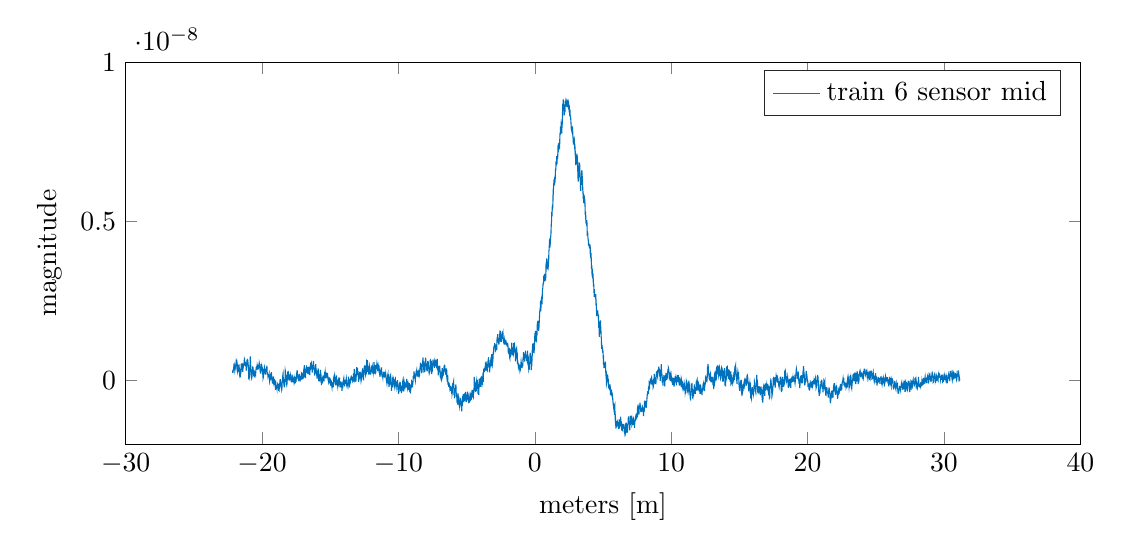
\begin{tikzpicture}

  \begin{axis}[%
    width=\textwidth,
    height=0.4\textwidth,
    at={(0\figurewidth,0\figureheight)},
    scale only axis,
    xmin=-30,
    xmax=40,
    xlabel={meters [m]},
    ymin=-2e-09,
    ymax=1e-08,
    ylabel={magnitude},
    axis background/.style={fill=white},
    legend style={legend cell align=left,align=left,draw=white!15!black}
    ]
    \addplot [color=mycolor1,solid]
    table[row sep=crcr]{%
    -22.157431640625	2.3493988586141e-10\\
    -22.14099609375	3.16454357658566e-10\\
    -22.124560546875	2.45589177170895e-10\\
    -22.108125	3.32225739372083e-10\\
    -22.091689453125	3.64796431000338e-10\\
    -22.07525390625	3.85652139602148e-10\\
    -22.058818359375	5.24052201527055e-10\\
    -22.0423828125	3.94618056722382e-10\\
    -22.025947265625	4.52729076947501e-10\\
    -22.00951171875	3.96448747790381e-10\\
    -21.993076171875	3.10810818811407e-10\\
    -21.976640625	3.51379660519289e-10\\
    -21.960205078125	3.88177609181804e-10\\
    -21.94376953125	4.77457033556989e-10\\
    -21.927333984375	4.75295859905891e-10\\
    -21.9108984375	5.01641220911782e-10\\
    -21.894462890625	6.02333107767613e-10\\
    -21.87802734375	5.70074940910514e-10\\
    -21.861591796875	4.95507094559884e-10\\
    -21.84515625	5.38368819869352e-10\\
    -21.828720703125	4.11967046154419e-10\\
    -21.81228515625	4.45625606191737e-10\\
    -21.795849609375	2.97023464705204e-10\\
    -21.7794140625	3.342790532783e-10\\
    -21.762978515625	3.3779445356962e-10\\
    -21.74654296875	3.24512778350596e-10\\
    -21.730107421875	4.89632771849839e-10\\
    -21.713671875	4.1232920114657e-10\\
    -21.697236328125	4.49231314402854e-10\\
    -21.68080078125	5.03630064065873e-10\\
    -21.664365234375	2.65286050733405e-10\\
    -21.6479296875	2.06522339607664e-10\\
    -21.631494140625	2.62414475049208e-10\\
    -21.61505859375	2.61590807361817e-10\\
    -21.598623046875	9.77906123335994e-11\\
    -21.5821875	1.93612378855186e-10\\
    -21.565751953125	3.53444828657033e-10\\
    -21.54931640625	2.15474586107318e-10\\
    -21.532880859375	4.51923553991529e-10\\
    -21.5164453125	5.32318241162344e-10\\
    -21.500009765625	4.10470132695962e-10\\
    -21.48357421875	5.29347737722432e-10\\
    -21.467138671875	3.51624049118828e-10\\
    -21.450703125	4.15609638673467e-10\\
    -21.434267578125	3.78257089922985e-10\\
    -21.41783203125	2.73156288905783e-10\\
    -21.401396484375	4.0162726697881e-10\\
    -21.3849609375	3.56655402442341e-10\\
    -21.368525390625	5.31800895046451e-10\\
    -21.35208984375	4.84345061721998e-10\\
    -21.335654296875	4.82244862131987e-10\\
    -21.31921875	5.24329764983104e-10\\
    -21.302783203125	6.18570529861809e-10\\
    -21.28634765625	5.70353728073558e-10\\
    -21.269912109375	6.03861839027795e-10\\
    -21.2534765625	5.23570467742443e-10\\
    -21.237041015625	5.38009517203341e-10\\
    -21.22060546875	5.57884167435541e-10\\
    -21.204169921875	5.44860490605937e-10\\
    -21.187734375	4.36871494518218e-10\\
    -21.171298828125	5.31556536647114e-10\\
    -21.15486328125	3.12635559414433e-10\\
    -21.138427734375	4.2046327153375e-10\\
    -21.1219921875	5.25830651422486e-10\\
    -21.105556640625	4.8987471499397e-10\\
    -21.08912109375	5.42060753485375e-10\\
    -21.072685546875	6.42210746770049e-10\\
    -21.05625	6.51457627802143e-10\\
    -21.039814453125	6.16165697186978e-10\\
    -21.02337890625	5.21746654998639e-10\\
    -21.006943359375	4.76088064142872e-10\\
    -20.9905078125	3.64089815482995e-10\\
    -20.974072265625	3.23383170734643e-11\\
    -20.95763671875	1.18142553923817e-10\\
    -20.941201171875	8.44640750205523e-11\\
    -20.924765625	1.38271027326297e-10\\
    -20.908330078125	3.29587441166259e-10\\
    -20.89189453125	4.42055509259057e-10\\
    -20.875458984375	4.95791617671644e-10\\
    -20.8590234375	7.55508536670686e-10\\
    -20.842587890625	5.17182861480334e-10\\
    -20.82615234375	4.58568486101422e-10\\
    -20.809716796875	3.29143580671879e-10\\
    -20.79328125	1.36007685826065e-10\\
    -20.776845703125	9.98699053312591e-11\\
    -20.76041015625	1.86208619690391e-10\\
    -20.743974609375	6.14886132074892e-11\\
    -20.7275390625	2.34824295152368e-10\\
    -20.711103515625	2.5105891399893e-10\\
    -20.69466796875	3.48030998628218e-10\\
    -20.678232421875	4.19176344330149e-10\\
    -20.661796875	4.11461013764003e-10\\
    -20.645361328125	3.32603154972694e-10\\
    -20.62892578125	2.59407852216865e-10\\
    -20.612490234375	1.36287534599294e-10\\
    -20.5960546875	3.34352894156851e-10\\
    -20.579619140625	2.38702748901888e-10\\
    -20.56318359375	9.82122339605978e-11\\
    -20.546748046875	1.63646186945155e-10\\
    -20.5303125	2.40032555859375e-10\\
    -20.513876953125	2.28679818065241e-10\\
    -20.49744140625	2.72093514340116e-10\\
    -20.481005859375	2.77864484043934e-10\\
    -20.4645703125	2.24656678252566e-10\\
    -20.448134765625	3.21528039787055e-10\\
    -20.43169921875	3.87999231588499e-10\\
    -20.415263671875	3.78506680715841e-10\\
    -20.398828125	4.11888513093621e-10\\
    -20.382392578125	3.96725300442704e-10\\
    -20.36595703125	3.39272677776375e-10\\
    -20.349521484375	4.77110257753397e-10\\
    -20.3330859375	4.48403650642598e-10\\
    -20.316650390625	4.54809288430133e-10\\
    -20.30021484375	4.23918066617772e-10\\
    -20.283779296875	3.71276474342373e-10\\
    -20.26734375	3.80947276632999e-10\\
    -20.250908203125	4.28014390654669e-10\\
    -20.23447265625	5.03606650717869e-10\\
    -20.218037109375	4.14743270481536e-10\\
    -20.2016015625	5.42813638949293e-10\\
    -20.185166015625	5.08541706165278e-10\\
    -20.16873046875	4.32656828009369e-10\\
    -20.152294921875	3.59067434475954e-10\\
    -20.135859375	3.66541175723773e-10\\
    -20.119423828125	2.18680055784911e-10\\
    -20.10298828125	3.159398652642e-10\\
    -20.086552734375	2.14733885639523e-10\\
    -20.0701171875	3.9512797880993e-10\\
    -20.053681640625	5.09540080500932e-10\\
    -20.03724609375	4.29541550157535e-10\\
    -20.020810546875	4.6694457012098e-10\\
    -20.004375	4.21593495612136e-10\\
    -19.987939453125	3.88494309699655e-10\\
    -19.97150390625	3.89624130369061e-10\\
    -19.955068359375	2.10578010160575e-10\\
    -19.9386328125	1.78288264132362e-10\\
    -19.922197265625	6.68059737575353e-11\\
    -19.90576171875	9.33938058444346e-11\\
    -19.889326171875	2.32769872916002e-10\\
    -19.872890625	3.11293307998778e-10\\
    -19.856455078125	3.42338197475868e-10\\
    -19.84001953125	3.68077854147814e-10\\
    -19.823583984375	4.18641222699545e-10\\
    -19.8071484375	3.82896819263682e-10\\
    -19.790712890625	3.29255882640088e-10\\
    -19.77427734375	1.96648047703009e-10\\
    -19.757841796875	2.64851506682972e-10\\
    -19.74140625	1.81266844697606e-10\\
    -19.724970703125	3.16625395276193e-10\\
    -19.70853515625	3.07487499426078e-10\\
    -19.692099609375	3.43432670742636e-10\\
    -19.6756640625	3.09887308743543e-10\\
    -19.659228515625	3.03011551260258e-10\\
    -19.64279296875	4.65010827880937e-10\\
    -19.626357421875	2.92299986863866e-10\\
    -19.609921875	2.00759958898871e-10\\
    -19.593486328125	1.9126712037347e-10\\
    -19.57705078125	1.88618837907768e-10\\
    -19.560615234375	1.1606653421355e-10\\
    -19.5441796875	1.41679029436545e-10\\
    -19.527744140625	1.46756225900687e-10\\
    -19.51130859375	1.43616498045419e-10\\
    -19.494873046875	1.64991618649528e-10\\
    -19.4784375	2.04163284902772e-10\\
    -19.462001953125	1.00330881441852e-10\\
    -19.44556640625	-3.18641970356256e-11\\
    -19.429130859375	-1.60039886743195e-12\\
    -19.4126953125	7.7211047025081e-11\\
    -19.396259765625	7.0999534075082e-11\\
    -19.37982421875	9.78968820011826e-12\\
    -19.363388671875	1.72946734125082e-10\\
    -19.346953125	1.62974632034588e-10\\
    -19.330517578125	1.13983739641208e-10\\
    -19.31408203125	2.63317145127385e-10\\
    -19.297646484375	1.6073456953137e-10\\
    -19.2812109375	9.32442543870187e-11\\
    -19.264775390625	2.88780385054774e-11\\
    -19.24833984375	9.27139947344192e-11\\
    -19.231904296875	-6.15368271463492e-11\\
    -19.21546875	9.63714137550965e-11\\
    -19.199033203125	-4.91376244135376e-12\\
    -19.18259765625	-1.09552393400843e-10\\
    -19.166162109375	1.07818427786758e-10\\
    -19.1497265625	1.06326670615234e-10\\
    -19.133291015625	-6.12974154465373e-11\\
    -19.11685546875	-3.26541312616942e-11\\
    -19.100419921875	5.11811986538582e-11\\
    -19.083984375	-7.908662475045e-11\\
    -19.067548828125	-1.46586669311672e-10\\
    -19.05111328125	4.85842914179954e-12\\
    -19.034677734375	-1.43925269348235e-10\\
    -19.0182421875	-2.94720429623286e-10\\
    -19.001806640625	2.89237278064603e-12\\
    -18.98537109375	-2.12438079944706e-10\\
    -18.968935546875	-2.04433601683247e-10\\
    -18.9525	-2.3447383254868e-10\\
    -18.936064453125	-2.24278122123535e-10\\
    -18.91962890625	-2.24216806320201e-10\\
    -18.903193359375	-2.68699141883341e-10\\
    -18.8867578125	-1.70766752808878e-10\\
    -18.870322265625	-1.43078804174374e-10\\
    -18.85388671875	-2.41458771298663e-10\\
    -18.837451171875	-1.56737234478757e-10\\
    -18.821015625	-1.76925073784907e-10\\
    -18.804580078125	-1.3733580646196e-10\\
    -18.78814453125	-1.36151436147008e-10\\
    -18.771708984375	-3.25247997213353e-10\\
    -18.7552734375	-2.17599535819182e-10\\
    -18.738837890625	-2.5712247021748e-10\\
    -18.72240234375	-1.77104384812638e-10\\
    -18.705966796875	-1.31334087372732e-10\\
    -18.68953125	-5.11135831316135e-11\\
    -18.673095703125	-7.43576710877207e-11\\
    -18.65666015625	3.95936406528108e-11\\
    -18.640224609375	-1.90639359403832e-11\\
    -18.6237890625	-1.20927600602064e-11\\
    -18.607353515625	-2.08119521794628e-10\\
    -18.59091796875	-2.28541691331291e-10\\
    -18.574482421875	-2.36781356464069e-10\\
    -18.558046875	-2.91825104578765e-10\\
    -18.541611328125	-2.50601781287865e-10\\
    -18.52517578125	-7.18732321408405e-11\\
    -18.508740234375	-5.56040600318047e-11\\
    -18.4923046875	-3.44254889062034e-11\\
    -18.475869140625	1.72964160518218e-10\\
    -18.45943359375	2.12330121629581e-10\\
    -18.442998046875	5.72893504007767e-11\\
    -18.4265625	4.97661541523088e-11\\
    -18.410126953125	-5.26470937364628e-11\\
    -18.39369140625	-1.47467290467238e-10\\
    -18.377255859375	-1.62232233472302e-10\\
    -18.3608203125	-2.18638201857839e-10\\
    -18.344384765625	-3.10227644110471e-12\\
    -18.32794921875	2.01416272541896e-11\\
    -18.311513671875	-4.16802945329849e-11\\
    -18.295078125	3.09929828630554e-10\\
    -18.278642578125	2.72470694684873e-10\\
    -18.26220703125	2.54456761666884e-11\\
    -18.245771484375	1.77508467860789e-10\\
    -18.2293359375	6.21342080814901e-11\\
    -18.212900390625	-1.41255855659882e-10\\
    -18.19646484375	-4.74014103424435e-11\\
    -18.180029296875	-1.28589027777106e-10\\
    -18.16359375	-9.51048092215517e-11\\
    -18.147158203125	8.97203911896025e-11\\
    -18.13072265625	1.69200661058821e-10\\
    -18.114287109375	2.56690308768621e-10\\
    -18.0978515625	2.50223905161419e-10\\
    -18.081416015625	2.25922477447117e-10\\
    -18.06498046875	2.42743550454546e-10\\
    -18.048544921875	1.02901142781058e-10\\
    -18.032109375	4.07491338292971e-12\\
    -18.015673828125	1.41612740705314e-10\\
    -17.99923828125	8.38386689275188e-11\\
    -17.982802734375	-7.78534216978557e-12\\
    -17.9663671875	1.70589314039511e-10\\
    -17.949931640625	1.75717619797301e-10\\
    -17.93349609375	8.14377928946515e-11\\
    -17.917060546875	1.43138547400582e-10\\
    -17.900625	7.77064177319524e-11\\
    -17.884189453125	4.37127696234069e-11\\
    -17.86775390625	7.35474301529071e-11\\
    -17.851318359375	-6.00078747960533e-11\\
    -17.8348828125	2.41856005430516e-11\\
    -17.818447265625	-3.27669817385918e-11\\
    -17.80201171875	-3.20544679016916e-11\\
    -17.785576171875	6.26382385445341e-11\\
    -17.769140625	1.00479371087242e-10\\
    -17.752705078125	5.31891827758453e-11\\
    -17.73626953125	-6.11598680565731e-11\\
    -17.719833984375	5.52298628116341e-11\\
    -17.7033984375	-2.70776593089373e-11\\
    -17.686962890625	-3.12990315406342e-11\\
    -17.67052734375	1.9711049918845e-11\\
    -17.654091796875	-4.09288997220489e-11\\
    -17.63765625	1.2436742258986e-11\\
    -17.621220703125	1.18037325411014e-10\\
    -17.60478515625	3.74890897257427e-11\\
    -17.588349609375	9.63454177367083e-11\\
    -17.5719140625	6.3560463324413e-11\\
    -17.555478515625	-8.98028398187801e-11\\
    -17.53904296875	6.15789322793719e-11\\
    -17.522607421875	-4.17231053292951e-11\\
    -17.506171875	-3.40628501052787e-11\\
    -17.489736328125	1.08574153517384e-10\\
    -17.47330078125	2.94658518908041e-11\\
    -17.456865234375	2.06985713997083e-10\\
    -17.4404296875	2.99720758274976e-10\\
    -17.423994140625	3.03120089747574e-10\\
    -17.40755859375	2.1287327282565e-10\\
    -17.391123046875	1.70954521868792e-10\\
    -17.3746875	1.19948214729371e-10\\
    -17.358251953125	9.37851014631938e-11\\
    -17.34181640625	6.30295965910336e-11\\
    -17.325380859375	1.23381701967886e-10\\
    -17.3089453125	-4.22947615707511e-12\\
    -17.292509765625	1.15933870344194e-10\\
    -17.27607421875	2.05702173885924e-10\\
    -17.259638671875	1.25422444608357e-10\\
    -17.243203125	9.62848178011538e-11\\
    -17.226767578125	5.18401812986323e-11\\
    -17.21033203125	-3.15572027025905e-11\\
    -17.193896484375	3.18080080523004e-11\\
    -17.1774609375	3.57279365737928e-11\\
    -17.161025390625	1.45408132916026e-10\\
    -17.14458984375	1.56444614284986e-11\\
    -17.128154296875	1.09918789459868e-10\\
    -17.11171875	2.38629181572779e-10\\
    -17.095283203125	2.28728104039257e-10\\
    -17.07884765625	2.26999634199783e-10\\
    -17.062412109375	1.99090137636058e-10\\
    -17.0459765625	1.22198497148508e-10\\
    -17.029541015625	3.64368764898385e-11\\
    -17.01310546875	1.16334402244762e-10\\
    -16.996669921875	1.00055005098319e-10\\
    -16.980234375	9.03965144093083e-11\\
    -16.963798828125	1.87037168051658e-10\\
    -16.94736328125	3.14276342319636e-10\\
    -16.930927734375	3.49625111679726e-10\\
    -16.9144921875	2.4352328650014e-10\\
    -16.898056640625	4.82289909079855e-10\\
    -16.88162109375	3.44892060554777e-10\\
    -16.865185546875	9.80012038761475e-11\\
    -16.84875	2.11585194262923e-10\\
    -16.832314453125	2.10591669108044e-10\\
    -16.81587890625	7.07064083698605e-11\\
    -16.799443359375	2.29318439051002e-10\\
    -16.7830078125	3.74350945810274e-10\\
    -16.766572265625	2.43624332415476e-10\\
    -16.75013671875	3.39752192622939e-10\\
    -16.733701171875	4.7246962499033e-10\\
    -16.717265625	3.11120203851157e-10\\
    -16.700830078125	2.96386461516227e-10\\
    -16.68439453125	3.81972234312014e-10\\
    -16.667958984375	2.65104485146994e-10\\
    -16.6515234375	2.79535135087708e-10\\
    -16.635087890625	4.16117934718997e-10\\
    -16.61865234375	2.98226890285341e-10\\
    -16.602216796875	3.24494367012203e-10\\
    -16.58578125	4.25152962850887e-10\\
    -16.569345703125	3.5203767874004e-10\\
    -16.55291015625	1.89802251385405e-10\\
    -16.536474609375	3.24662230573113e-10\\
    -16.5200390625	2.87916534225849e-10\\
    -16.503603515625	1.71522452230444e-10\\
    -16.48716796875	3.18880998141823e-10\\
    -16.470732421875	3.83574343280799e-10\\
    -16.454296875	3.14857681776005e-10\\
    -16.437861328125	4.50889474169943e-10\\
    -16.42142578125	5.00313146345185e-10\\
    -16.404990234375	5.5612148510398e-10\\
    -16.3885546875	5.61913078358021e-10\\
    -16.372119140625	3.85194630602754e-10\\
    -16.35568359375	4.83268056126408e-10\\
    -16.339248046875	4.31757415379961e-10\\
    -16.3228125	2.45742483516105e-10\\
    -16.306376953125	3.56467560632936e-10\\
    -16.28994140625	3.81818160414832e-10\\
    -16.273505859375	4.28592162163008e-10\\
    -16.2570703125	4.32640073308739e-10\\
    -16.240634765625	4.89389749307278e-10\\
    -16.22419921875	6.08277631335302e-10\\
    -16.207763671875	4.27196134098716e-10\\
    -16.191328125	3.31027782114257e-10\\
    -16.174892578125	3.91353547468423e-10\\
    -16.15845703125	2.30083624904775e-10\\
    -16.142021484375	1.55174732137086e-10\\
    -16.1255859375	2.87658738949893e-10\\
    -16.109150390625	2.76817536793274e-10\\
    -16.09271484375	3.93483435806846e-10\\
    -16.076279296875	4.63947218785418e-10\\
    -16.05984375	5.1392541439877e-10\\
    -16.043408203125	3.60578589732082e-10\\
    -16.02697265625	2.7885430106823e-10\\
    -16.010537109375	2.29337221415393e-10\\
    -15.9941015625	2.53275843522769e-10\\
    -15.977666015625	1.91139792435621e-10\\
    -15.96123046875	5.36562069091696e-11\\
    -15.944794921875	1.64445361785615e-10\\
    -15.928359375	2.51716280025837e-10\\
    -15.911923828125	2.58001602826088e-10\\
    -15.89548828125	2.96768021543348e-10\\
    -15.879052734375	3.74322292529633e-10\\
    -15.8626171875	2.70035372541591e-10\\
    -15.846181640625	5.31094045857175e-11\\
    -15.82974609375	7.2945755894829e-11\\
    -15.813310546875	1.97522325322774e-10\\
    -15.796875	-2.5342027742146e-12\\
    -15.780439453125	-8.23718406285179e-12\\
    -15.76400390625	1.51064395425389e-10\\
    -15.747568359375	9.28520376472118e-11\\
    -15.7311328125	1.59688018276459e-10\\
    -15.714697265625	3.35516303064202e-10\\
    -15.69826171875	5.09818488273155e-11\\
    -15.681826171875	1.84819530330979e-10\\
    -15.665390625	1.44991155149543e-10\\
    -15.648955078125	-1.48530112193279e-10\\
    -15.63251953125	-3.42407607134183e-11\\
    -15.616083984375	9.08548075377589e-11\\
    -15.5996484375	-9.17067591186714e-11\\
    -15.583212890625	1.52362933562065e-11\\
    -15.56677734375	9.45866320108613e-12\\
    -15.550341796875	7.85731276840285e-11\\
    -15.53390625	1.48030209565431e-10\\
    -15.517470703125	8.96598671675179e-12\\
    -15.50103515625	3.25510819645376e-11\\
    -15.484599609375	1.39881767107369e-10\\
    -15.4681640625	2.98169793939182e-12\\
    -15.451728515625	-2.2528105636174e-12\\
    -15.43529296875	1.83933350489141e-10\\
    -15.418857421875	7.14079295622753e-11\\
    -15.402421875	2.15327791130911e-10\\
    -15.385986328125	2.00058946915969e-10\\
    -15.36955078125	2.6283028321426e-10\\
    -15.353115234375	1.88568525408481e-10\\
    -15.3366796875	1.2578793948108e-10\\
    -15.320244140625	1.02217710068416e-10\\
    -15.30380859375	1.35933056962538e-10\\
    -15.287373046875	1.67328133035625e-10\\
    -15.2709375	1.10623956962375e-10\\
    -15.254501953125	1.21189966230944e-10\\
    -15.23806640625	2.32657982455793e-10\\
    -15.221630859375	1.30677786444304e-10\\
    -15.2051953125	2.36264798884295e-10\\
    -15.188759765625	1.8052496509061e-10\\
    -15.17232421875	3.68556342795667e-11\\
    -15.155888671875	1.15215038593506e-10\\
    -15.139453125	-1.52110837534093e-11\\
    -15.123017578125	-4.53731271538805e-11\\
    -15.10658203125	5.78905575362351e-11\\
    -15.090146484375	4.71135077337933e-11\\
    -15.0737109375	-8.7501017418054e-11\\
    -15.057275390625	9.58291005483223e-11\\
    -15.04083984375	-3.77897413726309e-11\\
    -15.024404296875	-3.75081738959412e-11\\
    -15.00796875	4.796261283329e-11\\
    -14.991533203125	-1.17812320791832e-10\\
    -14.97509765625	-6.96676304357566e-11\\
    -14.958662109375	-1.47184755693628e-10\\
    -14.9422265625	-1.39793876849722e-10\\
    -14.925791015625	-1.78957319346338e-12\\
    -14.90935546875	-1.28845417295864e-10\\
    -14.892919921875	-1.56160172473466e-10\\
    -14.876484375	-2.02017831750036e-10\\
    -14.860048828125	-6.25585811573065e-11\\
    -14.84361328125	-1.37553961999632e-10\\
    -14.827177734375	-2.24916713954398e-10\\
    -14.8107421875	-1.33980233235586e-10\\
    -14.794306640625	-5.16422223985201e-11\\
    -14.77787109375	-2.10429675724895e-10\\
    -14.761435546875	4.94374995233142e-11\\
    -14.745	8.24947493405477e-11\\
    -14.728564453125	3.37582165475933e-11\\
    -14.71212890625	1.13274787342486e-10\\
    -14.695693359375	1.21120744678783e-10\\
    -14.6792578125	1.60370831187418e-10\\
    -14.662822265625	5.92480432931916e-11\\
    -14.64638671875	-2.97973904374417e-11\\
    -14.629951171875	-1.67725340726259e-11\\
    -14.613515625	-1.54683688770713e-10\\
    -14.597080078125	1.14915378259735e-10\\
    -14.58064453125	4.36229884267622e-11\\
    -14.564208984375	4.66235264605732e-11\\
    -14.5477734375	1.59960333496022e-10\\
    -14.531337890625	7.94866336934031e-11\\
    -14.51490234375	-2.93241998249544e-11\\
    -14.498466796875	1.28347052126329e-11\\
    -14.48203125	2.3836161403413e-12\\
    -14.465595703125	-1.07955409282713e-10\\
    -14.44916015625	-1.7374163966346e-10\\
    -14.432724609375	-1.09666086208492e-10\\
    -14.4162890625	-6.2900354217611e-11\\
    -14.399853515625	-1.39928899843637e-10\\
    -14.38341796875	-1.17763735824169e-10\\
    -14.366982421875	9.61869450122738e-11\\
    -14.350546875	3.30571531449205e-11\\
    -14.334111328125	-1.2944720323847e-10\\
    -14.31767578125	9.18548054810727e-11\\
    -14.301240234375	-6.92946448521678e-11\\
    -14.2848046875	-2.20058998200306e-10\\
    -14.268369140625	-3.27511530903849e-11\\
    -14.25193359375	-1.00068303470148e-10\\
    -14.235498046875	-2.02861215170773e-10\\
    -14.2190625	-2.97701682655158e-11\\
    -14.202626953125	-1.07415769015654e-10\\
    -14.18619140625	-2.15987091551939e-10\\
    -14.169755859375	-6.74008001282958e-11\\
    -14.1533203125	-1.55186284562925e-10\\
    -14.136884765625	-3.28078339548981e-10\\
    -14.12044921875	-2.02794871638674e-10\\
    -14.104013671875	-1.81037103039896e-10\\
    -14.087578125	-2.43395593932317e-10\\
    -14.071142578125	-1.42237238949487e-10\\
    -14.05470703125	-1.2339804563573e-11\\
    -14.038271484375	-1.37626642194312e-10\\
    -14.0218359375	4.19760912665459e-11\\
    -14.005400390625	7.27418445921845e-11\\
    -13.98896484375	-5.02251505260943e-11\\
    -13.972529296875	-1.52902415010804e-10\\
    -13.95609375	1.55174121355462e-11\\
    -13.939658203125	-1.43030184060792e-10\\
    -13.92322265625	-1.31721491551339e-10\\
    -13.906787109375	1.62200273636572e-11\\
    -13.8903515625	-5.37024322145195e-11\\
    -13.873916015625	-3.1460451770379e-11\\
    -13.85748046875	1.31782839967943e-11\\
    -13.841044921875	1.6482944480217e-11\\
    -13.824609375	5.58712984709133e-11\\
    -13.808173828125	-8.99325629005581e-11\\
    -13.79173828125	-1.45216530008915e-10\\
    -13.775302734375	-1.32425053146327e-10\\
    -13.7588671875	-1.86119484373942e-10\\
    -13.742431640625	-1.54052565763606e-10\\
    -13.72599609375	-1.31221369783217e-10\\
    -13.709560546875	-9.57748874888367e-11\\
    -13.693125	1.33995170091699e-11\\
    -13.676689453125	-1.0791176951618e-10\\
    -13.66025390625	1.16256623125213e-10\\
    -13.643818359375	6.21234897561424e-11\\
    -13.6273828125	-1.27669713770312e-10\\
    -13.610947265625	-8.58511272861412e-11\\
    -13.59451171875	-9.34297840191619e-11\\
    -13.578076171875	-2.17845059568211e-10\\
    -13.561640625	3.26341885698041e-11\\
    -13.545205078125	-8.92729310264188e-11\\
    -13.52876953125	-7.33417094662749e-11\\
    -13.512333984375	2.91739009739409e-11\\
    -13.4958984375	7.12038693290137e-11\\
    -13.479462890625	6.34937092848406e-11\\
    -13.46302734375	1.05952616357495e-10\\
    -13.446591796875	9.11089873301191e-11\\
    -13.43015625	3.94938630107883e-12\\
    -13.413720703125	6.67749609976753e-11\\
    -13.39728515625	3.64018103137376e-11\\
    -13.380849609375	5.28756559533196e-11\\
    -13.3644140625	1.38182639609556e-11\\
    -13.347978515625	7.35718805037132e-11\\
    -13.33154296875	-3.22573640175409e-11\\
    -13.315107421875	2.69701910844188e-11\\
    -13.298671875	2.16058852106096e-10\\
    -13.282236328125	8.26065589938822e-11\\
    -13.26580078125	5.12045261330524e-11\\
    -13.249365234375	2.72460956870117e-10\\
    -13.2329296875	3.60346094119134e-10\\
    -13.216494140625	1.21886158646394e-10\\
    -13.20005859375	3.13755021558225e-10\\
    -13.183623046875	1.75694870402488e-10\\
    -13.1671875	-3.55525130195084e-11\\
    -13.150751953125	2.05189961586563e-10\\
    -13.13431640625	5.60880046559388e-11\\
    -13.117880859375	-3.9571237290272e-11\\
    -13.1014453125	1.25715492677427e-10\\
    -13.085009765625	1.34051703124972e-10\\
    -13.06857421875	2.12407365150859e-10\\
    -13.052138671875	4.18606302654002e-10\\
    -13.035703125	3.54845367185779e-10\\
    -13.019267578125	3.10632721319236e-10\\
    -13.00283203125	3.85388094737244e-10\\
    -12.986396484375	2.74258209552012e-10\\
    -12.9699609375	1.94545799466283e-10\\
    -12.953525390625	2.95236788543148e-10\\
    -12.93708984375	6.74648652066559e-11\\
    -12.920654296875	-5.5158955163159e-11\\
    -12.90421875	4.30420808370655e-11\\
    -12.887783203125	8.58776380542735e-11\\
    -12.87134765625	7.48689260316837e-11\\
    -12.854912109375	1.4633749069454e-10\\
    -12.8384765625	2.68207467897349e-10\\
    -12.822041015625	1.62637053192146e-10\\
    -12.80560546875	2.78229547536835e-10\\
    -12.789169921875	1.35361935515299e-10\\
    -12.772734375	2.20984905666529e-10\\
    -12.756298828125	4.26475901433808e-11\\
    -12.73986328125	-2.18426323984211e-11\\
    -12.723427734375	1.73803010488014e-11\\
    -12.7069921875	8.17181271207508e-11\\
    -12.690556640625	1.37682254786652e-10\\
    -12.67412109375	2.36524578072654e-10\\
    -12.657685546875	2.95565852859148e-10\\
    -12.64125	3.13979373573913e-10\\
    -12.624814453125	3.82058050962493e-10\\
    -12.60837890625	1.52757649697083e-10\\
    -12.591943359375	1.0968410767408e-10\\
    -12.5755078125	1.30102001721702e-10\\
    -12.559072265625	6.08694573621778e-12\\
    -12.54263671875	2.05239831441439e-10\\
    -12.526201171875	2.92628307930934e-10\\
    -12.509765625	2.36859246090237e-10\\
    -12.493330078125	4.53359168287993e-10\\
    -12.47689453125	3.52733892735962e-10\\
    -12.460458984375	4.85322786268747e-10\\
    -12.4440234375	4.17929632428649e-10\\
    -12.427587890625	2.64317540524042e-10\\
    -12.41115234375	1.81755665370798e-10\\
    -12.394716796875	2.13394222988418e-10\\
    -12.37828125	2.46111657809206e-10\\
    -12.361845703125	1.92775148727832e-10\\
    -12.34541015625	3.59686140758354e-10\\
    -12.328974609375	5.63070545713834e-10\\
    -12.3125390625	5.35819152015174e-10\\
    -12.296103515625	4.73699407435878e-10\\
    -12.27966796875	6.3742951959709e-10\\
    -12.263232421875	5.69248291943961e-10\\
    -12.246796875	2.66099528939065e-10\\
    -12.230361328125	3.52285378356656e-10\\
    -12.21392578125	3.68468680812845e-10\\
    -12.197490234375	3.30312621559622e-10\\
    -12.1810546875	1.82618091907384e-10\\
    -12.164619140625	3.88787849798663e-10\\
    -12.14818359375	4.6283360223504e-10\\
    -12.131748046875	2.09613045009273e-10\\
    -12.1153125	4.54109688364418e-10\\
    -12.098876953125	4.23284865273164e-10\\
    -12.08244140625	2.54247809078291e-10\\
    -12.066005859375	2.71663164591603e-10\\
    -12.0495703125	2.15874078199498e-10\\
    -12.033134765625	2.05451231195359e-10\\
    -12.01669921875	2.81128939966083e-10\\
    -12.000263671875	3.03134687836378e-10\\
    -11.983828125	2.58850790759717e-10\\
    -11.967392578125	4.28657853598753e-10\\
    -11.95095703125	4.17006215452561e-10\\
    -11.934521484375	4.0476349473617e-10\\
    -11.9180859375	3.87523426544893e-10\\
    -11.901650390625	4.23226156683606e-10\\
    -11.88521484375	2.81913035800655e-10\\
    -11.868779296875	2.056699610388e-10\\
    -11.85234375	3.22238941941758e-10\\
    -11.835908203125	2.98497776963454e-10\\
    -11.81947265625	2.49363852247731e-10\\
    -11.803037109375	3.374996561895e-10\\
    -11.7866015625	5.74101235706963e-10\\
    -11.770166015625	4.08602510817834e-10\\
    -11.75373046875	4.26093116217107e-10\\
    -11.737294921875	4.84653566407017e-10\\
    -11.720859375	2.14025071133913e-10\\
    -11.704423828125	2.63848231613639e-10\\
    -11.68798828125	2.60469827799861e-10\\
    -11.671552734375	2.34598342707726e-10\\
    -11.6551171875	2.53513243681557e-10\\
    -11.638681640625	4.53870841966027e-10\\
    -11.62224609375	4.78213466835963e-10\\
    -11.605810546875	4.85055728332694e-10\\
    -11.589375	4.69942225386504e-10\\
    -11.572939453125	5.40902540631837e-10\\
    -11.55650390625	5.04265939526209e-10\\
    -11.540068359375	4.70756775375038e-10\\
    -11.5236328125	2.90790162095074e-10\\
    -11.507197265625	3.92860512845966e-10\\
    -11.49076171875	4.38018552136165e-10\\
    -11.474326171875	3.41662085281409e-10\\
    -11.457890625	2.95772136215626e-10\\
    -11.441455078125	4.60331480563683e-10\\
    -11.42501953125	4.48710086931619e-10\\
    -11.408583984375	2.33593310744332e-10\\
    -11.3921484375	3.26546818871318e-10\\
    -11.375712890625	2.82509440720284e-10\\
    -11.35927734375	1.13908288533909e-10\\
    -11.342841796875	1.61946419076481e-10\\
    -11.32640625	1.86394029333893e-10\\
    -11.309970703125	2.95068792928549e-10\\
    -11.29353515625	1.93492742967052e-10\\
    -11.277099609375	3.25589596988213e-10\\
    -11.2606640625	4.1324078540717e-10\\
    -11.244228515625	2.95876068955167e-10\\
    -11.22779296875	3.18233458701326e-10\\
    -11.211357421875	1.8296279907863e-10\\
    -11.194921875	1.15366125068578e-10\\
    -11.178486328125	1.17272709334201e-10\\
    -11.16205078125	1.37166226394396e-10\\
    -11.145615234375	9.42708075712812e-11\\
    -11.1291796875	2.07336304105764e-10\\
    -11.112744140625	1.05158441836087e-10\\
    -11.09630859375	2.52856646514872e-10\\
    -11.079873046875	2.55988607812995e-10\\
    -11.0634375	1.91711107916238e-10\\
    -11.047001953125	1.39326068921704e-10\\
    -11.03056640625	2.72142792601919e-10\\
    -11.014130859375	8.98494177053401e-11\\
    -10.9976953125	1.92423585103998e-10\\
    -10.981259765625	2.50032810853883e-10\\
    -10.96482421875	1.39260574462156e-10\\
    -10.948388671875	1.52526001885404e-10\\
    -10.931953125	2.13328012608932e-10\\
    -10.915517578125	1.57445477703553e-10\\
    -10.89908203125	1.11533488776977e-10\\
    -10.882646484375	-1.26779632276349e-11\\
    -10.8662109375	-3.24063150198829e-11\\
    -10.849775390625	-7.74762170693116e-11\\
    -10.83333984375	5.30843721939881e-11\\
    -10.816904296875	6.20453756406279e-11\\
    -10.80046875	-8.79905608305078e-11\\
    -10.784033203125	1.61728129838596e-10\\
    -10.76759765625	1.97549655179775e-10\\
    -10.751162109375	9.55706232788857e-12\\
    -10.7347265625	2.64538430681224e-11\\
    -10.718291015625	5.97504890816504e-11\\
    -10.70185546875	-1.45311123511161e-10\\
    -10.685419921875	-2.04036339549611e-10\\
    -10.668984375	-6.82008857080629e-11\\
    -10.652548828125	-1.56897072826489e-10\\
    -10.63611328125	-2.0634321687567e-11\\
    -10.619677734375	1.20694440475437e-10\\
    -10.6032421875	-5.61896044298463e-12\\
    -10.586806640625	1.58971515935628e-10\\
    -10.57037109375	1.75462495630966e-10\\
    -10.553935546875	-5.52695262471896e-12\\
    -10.5375	-1.41745625131223e-10\\
    -10.521064453125	-8.42886862595779e-11\\
    -10.50462890625	-3.22980468195003e-10\\
    -10.488193359375	-1.4518009547003e-10\\
    -10.4717578125	-4.75150623196762e-11\\
    -10.455322265625	-2.20258199458519e-10\\
    -10.43888671875	2.25622428027198e-11\\
    -10.422451171875	9.82805774319879e-11\\
    -10.406015625	2.40453967274802e-11\\
    -10.389580078125	9.4715105284903e-11\\
    -10.37314453125	7.61797209831963e-11\\
    -10.356708984375	-8.48313805504467e-11\\
    -10.3402734375	-1.23770958320738e-10\\
    -10.323837890625	-7.52928791112347e-11\\
    -10.30740234375	-1.47510008559957e-10\\
    -10.290966796875	-1.33257911742234e-10\\
    -10.27453125	-1.84670249251501e-10\\
    -10.258095703125	-1.04666970676266e-10\\
    -10.24166015625	1.81281922607634e-11\\
    -10.225224609375	4.30243428805367e-11\\
    -10.2087890625	-5.24344605521241e-11\\
    -10.192353515625	-5.82662483749243e-11\\
    -10.17591796875	-1.26350063327006e-10\\
    -10.159482421875	-1.93669286267686e-10\\
    -10.143046875	-1.2300457358007e-10\\
    -10.126611328125	-9.95079701515044e-11\\
    -10.11017578125	-4.03840459841016e-11\\
    -10.093740234375	-1.58245150481585e-10\\
    -10.0773046875	-8.95239250391498e-11\\
    -10.060869140625	8.85208244266686e-12\\
    -10.04443359375	-2.11723670033091e-10\\
    -10.027998046875	-1.92954457047492e-10\\
    -10.0115625	-2.73691399114837e-10\\
    -9.995126953125	-4.17144540920466e-10\\
    -9.97869140625	-2.44407077617803e-10\\
    -9.962255859375	-2.42561446107679e-10\\
    -9.9458203125	-2.67529677951272e-10\\
    -9.929384765625	-1.07387777696599e-10\\
    -9.91294921875	-9.70110955371489e-11\\
    -9.896513671875	-7.81389555778004e-11\\
    -9.880078125	-1.37073739188729e-10\\
    -9.863642578125	-6.0051629153816e-11\\
    -9.84720703125	-2.67030692755609e-10\\
    -9.830771484375	-3.24922834528837e-10\\
    -9.8143359375	-3.30053804022007e-10\\
    -9.797900390625	-1.78646324201558e-10\\
    -9.78146484375	-3.93340576690072e-10\\
    -9.765029296875	-3.20245074850923e-10\\
    -9.74859375	-1.53347634859932e-10\\
    -9.732158203125	-2.16299719251783e-10\\
    -9.71572265625	-2.40153384339105e-10\\
    -9.699287109375	-6.62011671400112e-11\\
    -9.6828515625	-2.92954056794137e-11\\
    -9.666416015625	-2.69371596052496e-10\\
    -9.64998046875	-2.86241755707729e-10\\
    -9.633544921875	2.2731274968965e-11\\
    -9.617109375	-2.32693488844849e-10\\
    -9.600673828125	-3.40555311734651e-10\\
    -9.58423828125	-2.80407832515535e-11\\
    -9.567802734375	-6.50779521212674e-11\\
    -9.5513671875	-1.17196016339917e-10\\
    -9.534931640625	-5.90138064344323e-11\\
    -9.51849609375	-6.04366116619375e-11\\
    -9.502060546875	-1.5057457051912e-10\\
    -9.485625	-9.78727598248135e-11\\
    -9.469189453125	-2.24894640914638e-10\\
    -9.45275390625	-9.65962808758267e-11\\
    -9.436318359375	-1.49051918317655e-10\\
    -9.4198828125	-1.39186363595261e-10\\
    -9.403447265625	-2.16734060669515e-10\\
    -9.38701171875	4.62341711857776e-11\\
    -9.370576171875	-4.84925118379702e-11\\
    -9.354140625	-1.53008208856967e-10\\
    -9.337705078125	-2.21246648707595e-10\\
    -9.32126953125	-1.60932764791384e-10\\
    -9.304833984375	-1.43430119461e-10\\
    -9.2883984375	-2.1867714390761e-10\\
    -9.271962890625	-1.11783436424722e-10\\
    -9.25552734375	-1.40225738284048e-10\\
    -9.239091796875	-3.01114400199916e-10\\
    -9.22265625	-1.47951541399638e-10\\
    -9.206220703125	-8.1534200544686e-11\\
    -9.18978515625	-2.39496681250604e-10\\
    -9.173349609375	-2.03888612618741e-10\\
    -9.1569140625	-2.93564044952624e-10\\
    -9.140478515625	-3.2419958967827e-10\\
    -9.12404296875	-2.33363996862848e-10\\
    -9.107607421875	-2.66355840241931e-10\\
    -9.091171875	-1.3272901705677e-10\\
    -9.074736328125	-2.29014621955971e-10\\
    -9.05830078125	-1.86476802855241e-10\\
    -9.041865234375	-1.49544016725018e-10\\
    -9.0254296875	-3.53347612857565e-11\\
    -9.008994140625	-5.43068214720302e-11\\
    -8.99255859375	-2.27315453162998e-10\\
    -8.976123046875	-8.89503822598597e-11\\
    -8.9596875	-6.51248415126599e-11\\
    -8.943251953125	-9.74652330210672e-11\\
    -8.92681640625	-2.59995774433261e-11\\
    -8.910380859375	1.35057174983294e-10\\
    -8.8939453125	7.58691879540059e-11\\
    -8.877509765625	9.49673124623451e-11\\
    -8.86107421875	2.82914647600427e-10\\
    -8.844638671875	2.14244480350149e-10\\
    -8.828203125	9.71882545414466e-11\\
    -8.811767578125	1.01504306763101e-10\\
    -8.79533203125	1.31248713256532e-10\\
    -8.778896484375	5.30701451255172e-11\\
    -8.7624609375	6.83226444436118e-12\\
    -8.746025390625	1.31518470681207e-10\\
    -8.72958984375	1.33398919281049e-10\\
    -8.713154296875	1.34465170316154e-10\\
    -8.69671875	2.79297994780928e-10\\
    -8.680283203125	2.75350627339475e-10\\
    -8.66384765625	3.10890661366588e-10\\
    -8.647412109375	1.57484448840597e-10\\
    -8.6309765625	2.41547989670691e-10\\
    -8.614541015625	2.60459147704912e-10\\
    -8.59810546875	2.35900040235964e-10\\
    -8.581669921875	1.22882046985793e-10\\
    -8.565234375	3.08033454773292e-10\\
    -8.548798828125	2.2979623334271e-10\\
    -8.53236328125	1.57053034047844e-10\\
    -8.515927734375	2.38048941790159e-10\\
    -8.4994921875	1.97851327018002e-10\\
    -8.483056640625	8.93179594489251e-11\\
    -8.46662109375	2.11261795935767e-10\\
    -8.450185546875	1.38728272233444e-10\\
    -8.43375	3.23162801614551e-10\\
    -8.417314453125	3.81784779672366e-10\\
    -8.40087890625	3.39907517883735e-10\\
    -8.384443359375	5.61070083089742e-10\\
    -8.3680078125	4.44617901534339e-10\\
    -8.351572265625	5.12182212300341e-10\\
    -8.33513671875	3.75738234315657e-10\\
    -8.318701171875	3.31869187468971e-10\\
    -8.302265625	3.72539058341284e-10\\
    -8.285830078125	2.28794934610309e-10\\
    -8.26939453125	2.88841674026688e-10\\
    -8.252958984375	5.28203098546279e-10\\
    -8.2365234375	4.29374792528556e-10\\
    -8.220087890625	5.430863104474e-10\\
    -8.20365234375	7.24100884583911e-10\\
    -8.187216796875	6.06722694826119e-10\\
    -8.17078125	5.26215584919408e-10\\
    -8.154345703125	5.39912412928463e-10\\
    -8.13791015625	3.2249655593683e-10\\
    -8.121474609375	2.51262758034277e-10\\
    -8.1050390625	4.0200618369726e-10\\
    -8.088603515625	3.66677543989327e-10\\
    -8.07216796875	2.72719577820149e-10\\
    -8.055732421875	5.01308504235526e-10\\
    -8.039296875	5.83821980409748e-10\\
    -8.022861328125	5.89237708886406e-10\\
    -8.00642578125	7.20017336095247e-10\\
    -7.989990234375	6.22523179570311e-10\\
    -7.9735546875	4.81425781038079e-10\\
    -7.957119140625	4.59078832952324e-10\\
    -7.94068359375	3.16852249507234e-10\\
    -7.924248046875	4.60074000349882e-10\\
    -7.9078125	3.96800134965183e-10\\
    -7.891376953125	2.90034987480456e-10\\
    -7.87494140625	3.85128469225148e-10\\
    -7.858505859375	5.93298845420746e-10\\
    -7.8420703125	5.94900006703975e-10\\
    -7.825634765625	5.2742426096843e-10\\
    -7.80919921875	5.88896313794237e-10\\
    -7.792763671875	4.26935344276609e-10\\
    -7.776328125	4.20046577396649e-10\\
    -7.759892578125	2.65786660990323e-10\\
    -7.74345703125	2.20609031548837e-10\\
    -7.727021484375	2.47010611915711e-10\\
    -7.7105859375	2.75146757351237e-10\\
    -7.694150390625	2.84985831607186e-10\\
    -7.67771484375	4.17808599236178e-10\\
    -7.661279296875	6.62226867774241e-10\\
    -7.64484375	5.20457517471242e-10\\
    -7.628408203125	5.67519219074884e-10\\
    -7.61197265625	5.04967932782734e-10\\
    -7.595537109375	6.14268568381321e-10\\
    -7.5791015625	3.6028886220693e-10\\
    -7.562666015625	1.96098211376434e-10\\
    -7.54623046875	3.23853371273172e-10\\
    -7.529794921875	3.25123624062686e-10\\
    -7.513359375	2.77082170992748e-10\\
    -7.496923828125	5.48226180308139e-10\\
    -7.48048828125	4.77166702874924e-10\\
    -7.464052734375	6.56299128412014e-10\\
    -7.4476171875	6.0404483018951e-10\\
    -7.431181640625	4.94752686786248e-10\\
    -7.41474609375	6.14990291643433e-10\\
    -7.398310546875	5.52017488448685e-10\\
    -7.381875	5.24240862799658e-10\\
    -7.365439453125	3.92651941415475e-10\\
    -7.34900390625	5.04415483753792e-10\\
    -7.332568359375	6.27881793383672e-10\\
    -7.3161328125	6.06167431239266e-10\\
    -7.299697265625	4.91773160820317e-10\\
    -7.28326171875	6.54025716666564e-10\\
    -7.266826171875	5.17554982968739e-10\\
    -7.250390625	5.39415425643196e-10\\
    -7.233955078125	5.06813486942708e-10\\
    -7.21751953125	6.25588102905252e-10\\
    -7.201083984375	5.68224862770219e-10\\
    -7.1846484375	3.77244760018543e-10\\
    -7.168212890625	6.27458780727703e-10\\
    -7.15177734375	6.79436926503254e-10\\
    -7.135341796875	3.32557183289065e-10\\
    -7.11890625	4.08794631079675e-10\\
    -7.102470703125	4.49147530483968e-10\\
    -7.08603515625	1.59120718312566e-10\\
    -7.069599609375	2.38622945560721e-10\\
    -7.0531640625	3.28351880357914e-10\\
    -7.036728515625	3.78502257531072e-10\\
    -7.02029296875	3.66583375750572e-10\\
    -7.003857421875	4.67885682575208e-10\\
    -6.987421875	3.76440764977308e-10\\
    -6.970986328125	4.67103463130417e-10\\
    -6.95455078125	3.22280142756587e-10\\
    -6.938115234375	1.05637091377249e-10\\
    -6.9216796875	1.87506984616315e-10\\
    -6.905244140625	1.26316265495368e-10\\
    -6.88880859375	7.17592006830483e-11\\
    -6.872373046875	4.30891731391915e-11\\
    -6.8559375	1.93614143667248e-10\\
    -6.839501953125	2.71906642449336e-10\\
    -6.82306640625	1.52645299203669e-10\\
    -6.806630859375	2.58803641384532e-10\\
    -6.7901953125	3.88085606544086e-10\\
    -6.773759765625	1.22271033482599e-10\\
    -6.75732421875	1.50214129201406e-10\\
    -6.740888671875	2.97916647041988e-10\\
    -6.724453125	1.39600979503324e-10\\
    -6.708017578125	2.08937647938008e-10\\
    -6.69158203125	3.49755200654172e-10\\
    -6.675146484375	2.76447510551406e-10\\
    -6.6587109375	3.98667416790263e-10\\
    -6.642275390625	3.80020357529317e-10\\
    -6.62583984375	3.67449384243671e-10\\
    -6.609404296875	4.92859001924225e-10\\
    -6.59296875	3.87035499446155e-10\\
    -6.576533203125	2.84241930183109e-10\\
    -6.56009765625	2.95501193931109e-10\\
    -6.543662109375	3.67081335956664e-10\\
    -6.5272265625	1.80462124332347e-10\\
    -6.510791015625	2.4535528797421e-10\\
    -6.49435546875	3.79904687449272e-10\\
    -6.477919921875	2.47384051320602e-10\\
    -6.461484375	1.59426518088458e-10\\
    -6.445048828125	1.95495641600302e-10\\
    -6.42861328125	3.51737160600946e-11\\
    -6.412177734375	-4.96904769026483e-11\\
    -6.3957421875	2.52797804313635e-11\\
    -6.379306640625	5.90011559279585e-11\\
    -6.36287109375	-1.1702059455311e-10\\
    -6.346435546875	-1.20433022214254e-10\\
    -6.33	-6.34691692178222e-11\\
    -6.313564453125	-2.04368789473653e-10\\
    -6.29712890625	-8.26587889571837e-11\\
    -6.280693359375	-9.0160096458711e-11\\
    -6.2642578125	-1.26593277800887e-10\\
    -6.247822265625	-1.51915497574943e-10\\
    -6.23138671875	-2.27431021828529e-10\\
    -6.214951171875	-1.81752789807978e-10\\
    -6.198515625	-1.87967668449181e-10\\
    -6.182080078125	-2.67058802640089e-10\\
    -6.16564453125	-3.24623617750235e-10\\
    -6.149208984375	-1.91578544713673e-10\\
    -6.1327734375	-2.6592538335622e-10\\
    -6.116337890625	-3.3529145856571e-10\\
    -6.09990234375	-3.12098633302614e-10\\
    -6.083466796875	-2.86210524116606e-10\\
    -6.06703125	-4.23280316305999e-10\\
    -6.050595703125	-3.79514140820494e-10\\
    -6.03416015625	-1.69128931571325e-10\\
    -6.017724609375	-1.89024185856685e-10\\
    -6.0012890625	-1.55814587031304e-10\\
    -5.984853515625	-1.16252107844164e-10\\
    -5.96841796875	-5.8795508304867e-11\\
    -5.951982421875	-2.56039558860959e-11\\
    -5.935546875	-3.11691500631396e-10\\
    -5.919111328125	-2.77918738388337e-10\\
    -5.90267578125	-2.73286353728791e-10\\
    -5.886240234375	-5.65824232772641e-10\\
    -5.8698046875	-3.24546675739661e-10\\
    -5.853369140625	-3.33630053309602e-10\\
    -5.83693359375	-2.95999918078417e-10\\
    -5.820498046875	-2.44314485837032e-10\\
    -5.8040625	-2.36303936326546e-10\\
    -5.787626953125	-1.20309908525969e-10\\
    -5.77119140625	-3.00143316854179e-10\\
    -5.754755859375	-5.17771504681517e-10\\
    -5.7383203125	-3.83579759794303e-10\\
    -5.721884765625	-5.07958037861255e-10\\
    -5.70544921875	-6.92096848879655e-10\\
    -5.689013671875	-5.3548328486437e-10\\
    -5.672578125	-4.79441477297867e-10\\
    -5.656142578125	-7.62379932122606e-10\\
    -5.63970703125	-5.71363311923694e-10\\
    -5.623271484375	-4.05854508072293e-10\\
    -5.6068359375	-5.95731768405046e-10\\
    -5.590400390625	-6.78273116678242e-10\\
    -5.57396484375	-5.06448214872645e-10\\
    -5.557529296875	-7.52197895083648e-10\\
    -5.54109375	-7.82580854607705e-10\\
    -5.524658203125	-7.42402185978143e-10\\
    -5.50822265625	-8.17974804584552e-10\\
    -5.491787109375	-7.62471594509676e-10\\
    -5.4753515625	-6.63767088187477e-10\\
    -5.458916015625	-6.58812329211506e-10\\
    -5.44248046875	-5.46371081927352e-10\\
    -5.426044921875	-6.18238605958174e-10\\
    -5.409609375	-7.64804742172066e-10\\
    -5.393173828125	-6.32647946292935e-10\\
    -5.37673828125	-7.46342884254315e-10\\
    -5.360302734375	-9.67222588094093e-10\\
    -5.3438671875	-7.67210584986653e-10\\
    -5.327431640625	-7.32537251094346e-10\\
    -5.31099609375	-7.9768885464462e-10\\
    -5.294560546875	-6.12580390085129e-10\\
    -5.278125	-4.81982293485266e-10\\
    -5.261689453125	-5.60312335529294e-10\\
    -5.24525390625	-4.31209973871364e-10\\
    -5.228818359375	-6.22600104346809e-10\\
    -5.2123828125	-6.80453429720332e-10\\
    -5.195947265625	-5.69513002237779e-10\\
    -5.17951171875	-5.39907289003784e-10\\
    -5.163076171875	-6.43013160692016e-10\\
    -5.146640625	-5.59415680994037e-10\\
    -5.130205078125	-3.98905548927634e-10\\
    -5.11376953125	-4.64891089730257e-10\\
    -5.097333984375	-5.07594148808329e-10\\
    -5.0808984375	-3.60961947338838e-10\\
    -5.064462890625	-4.44166902130987e-10\\
    -5.04802734375	-5.60485661007784e-10\\
    -5.031591796875	-6.3725521985081e-10\\
    -5.01515625	-6.24518653927875e-10\\
    -4.998720703125	-5.66552176355868e-10\\
    -4.98228515625	-6.06547793558682e-10\\
    -4.965849609375	-5.84654180972178e-10\\
    -4.9494140625	-4.91583241761533e-10\\
    -4.932978515625	-3.52021797144075e-10\\
    -4.91654296875	-5.44279746349031e-10\\
    -4.900107421875	-4.75500083309794e-10\\
    -4.883671875	-4.62061380042323e-10\\
    -4.867236328125	-5.97571530408451e-10\\
    -4.85080078125	-6.46742987296116e-10\\
    -4.834365234375	-7.1557036655768e-10\\
    -4.8179296875	-6.31251063513426e-10\\
    -4.801494140625	-6.20338814967023e-10\\
    -4.78505859375	-6.35495139019009e-10\\
    -4.768623046875	-5.15788622841797e-10\\
    -4.7521875	-4.56597926842131e-10\\
    -4.735751953125	-4.94136440937113e-10\\
    -4.71931640625	-4.81733878903174e-10\\
    -4.702880859375	-5.37212396041898e-10\\
    -4.6864453125	-4.8727628006709e-10\\
    -4.670009765625	-5.98478786962183e-10\\
    -4.65357421875	-5.91126162809482e-10\\
    -4.637138671875	-4.57178974765344e-10\\
    -4.620703125	-4.46765934460998e-10\\
    -4.604267578125	-4.30300760876243e-10\\
    -4.58783203125	-2.97858796986169e-10\\
    -4.571396484375	-4.25745940534167e-10\\
    -4.5549609375	-4.66744341037323e-10\\
    -4.538525390625	-4.36412254181967e-10\\
    -4.52208984375	-5.01857512489262e-10\\
    -4.505654296875	-5.21008139392134e-10\\
    -4.48921875	-2.97909937903856e-10\\
    -4.472783203125	-3.91855842666944e-10\\
    -4.45634765625	-2.81168349806606e-10\\
    -4.439912109375	1.11879866562818e-10\\
    -4.4234765625	-1.4553265695159e-10\\
    -4.407041015625	-5.09478901032068e-11\\
    -4.39060546875	-6.37609258492629e-11\\
    -4.374169921875	-1.91657939377521e-10\\
    -4.357734375	-3.07335903292498e-10\\
    -4.341298828125	-3.54364065177634e-10\\
    -4.32486328125	-1.80079177562071e-10\\
    -4.308427734375	-2.07435429030375e-10\\
    -4.2919921875	-3.34445143357527e-10\\
    -4.275556640625	-3.88985442186825e-11\\
    -4.25912109375	8.16365939767291e-12\\
    -4.242685546875	-7.46236254912435e-11\\
    -4.22625	-5.67206827455715e-11\\
    -4.209814453125	1.37312161384525e-11\\
    -4.19337890625	-2.52001894893399e-10\\
    -4.176943359375	-2.54606024224678e-10\\
    -4.1605078125	-4.19115941186289e-10\\
    -4.144072265625	-3.67173033910063e-10\\
    -4.12763671875	-3.1564178831358e-10\\
    -4.111201171875	-4.5348214730279e-10\\
    -4.094765625	-2.31331680147231e-10\\
    -4.078330078125	5.79024573923639e-11\\
    -4.06189453125	-1.40275055269005e-10\\
    -4.045458984375	-6.83908067108467e-12\\
    -4.0290234375	3.04637669556517e-11\\
    -4.012587890625	4.11174695028304e-11\\
    -3.99615234375	-1.98149584660922e-10\\
    -3.979716796875	1.98593667204429e-11\\
    -3.96328125	4.4816192383497e-11\\
    -3.946845703125	-1.08944013560643e-10\\
    -3.93041015625	-1.27396831234093e-11\\
    -3.913974609375	8.81092737606809e-11\\
    -3.8975390625	7.25483216299757e-11\\
    -3.881103515625	-2.1215431642984e-10\\
    -3.86466796875	1.24184224226057e-10\\
    -3.848232421875	-3.29500141990757e-11\\
    -3.831796875	-1.38572516662748e-10\\
    -3.815361328125	9.28367347628586e-11\\
    -3.79892578125	5.81338049699119e-11\\
    -3.782490234375	-4.74248546741224e-11\\
    -3.7660546875	2.17376880186475e-10\\
    -3.749619140625	3.54555048607716e-10\\
    -3.73318359375	3.56348732779562e-10\\
    -3.716748046875	2.80655381358422e-10\\
    -3.7003125	2.80380236779406e-10\\
    -3.683876953125	3.84516586758083e-10\\
    -3.66744140625	3.89487154382336e-10\\
    -3.651005859375	2.9749352841634e-10\\
    -3.6345703125	3.88806398703558e-10\\
    -3.618134765625	5.62505645009668e-10\\
    -3.60169921875	3.45757845814774e-10\\
    -3.585263671875	5.32377222808474e-10\\
    -3.568828125	5.97645283004962e-10\\
    -3.552392578125	3.91407551140914e-10\\
    -3.53595703125	3.07033690930507e-10\\
    -3.519521484375	4.30143695825052e-10\\
    -3.5030859375	3.29341330638937e-10\\
    -3.486650390625	3.139051412119e-10\\
    -3.47021484375	4.114571604986e-10\\
    -3.453779296875	4.91991737060662e-10\\
    -3.43734375	5.73401989516595e-10\\
    -3.420908203125	6.25691243927197e-10\\
    -3.40447265625	6.81352494961217e-10\\
    -3.388037109375	7.2761278272211e-10\\
    -3.3716015625	4.80882542458077e-10\\
    -3.355166015625	4.3529362161868e-10\\
    -3.33873046875	4.23314134888322e-10\\
    -3.322294921875	2.52356543043847e-10\\
    -3.305859375	3.19926648411497e-10\\
    -3.289423828125	4.07396804910627e-10\\
    -3.27298828125	4.09204542326869e-10\\
    -3.256552734375	6.38067011137148e-10\\
    -3.2401171875	5.34240050178625e-10\\
    -3.223681640625	6.82076746562977e-10\\
    -3.20724609375	7.06663378392712e-10\\
    -3.190810546875	6.12087642910381e-10\\
    -3.174375	4.48153008451393e-10\\
    -3.157939453125	8.29036821370416e-10\\
    -3.14150390625	4.60719050265574e-10\\
    -3.125068359375	4.44258237186134e-10\\
    -3.1086328125	6.92337031643555e-10\\
    -3.092197265625	6.82553182043816e-10\\
    -3.07576171875	5.68588910433481e-10\\
    -3.059326171875	8.58240095266265e-10\\
    -3.042890625	8.77748261246573e-10\\
    -3.026455078125	8.17068118517017e-10\\
    -3.01001953125	1.02656480408898e-09\\
    -2.993583984375	1.0571120280508e-09\\
    -2.9771484375	1.03871234645643e-09\\
    -2.960712890625	1.04594465272587e-09\\
    -2.94427734375	1.17602922738112e-09\\
    -2.927841796875	1.02423710778483e-09\\
    -2.91140625	1.12610909313506e-09\\
    -2.894970703125	1.0117480723932e-09\\
    -2.87853515625	1.05684537113244e-09\\
    -2.862099609375	1.10409039284503e-09\\
    -2.8456640625	9.65592167244876e-10\\
    -2.829228515625	9.79181775352529e-10\\
    -2.81279296875	1.13162549909245e-09\\
    -2.796357421875	9.50289168469278e-10\\
    -2.779921875	1.12423437315493e-09\\
    -2.763486328125	1.36590051851207e-09\\
    -2.74705078125	1.21269375342351e-09\\
    -2.730615234375	1.37711998506038e-09\\
    -2.7141796875	1.4521733018912e-09\\
    -2.697744140625	1.30380022550691e-09\\
    -2.68130859375	1.25665285319034e-09\\
    -2.664873046875	1.31935850271259e-09\\
    -2.6484375	1.18695910453471e-09\\
    -2.632001953125	1.12876712226633e-09\\
    -2.61556640625	1.24659455110586e-09\\
    -2.599130859375	1.2910586835691e-09\\
    -2.5826953125	1.2782331975062e-09\\
    -2.566259765625	1.47717135264256e-09\\
    -2.54982421875	1.54883212917416e-09\\
    -2.533388671875	1.54024919000069e-09\\
    -2.516953125	1.52300318649779e-09\\
    -2.500517578125	1.22076520884007e-09\\
    -2.48408203125	1.37946116687539e-09\\
    -2.467646484375	1.32599332856273e-09\\
    -2.4512109375	1.21462989422612e-09\\
    -2.434775390625	1.29875068482728e-09\\
    -2.41833984375	1.44895051728608e-09\\
    -2.401904296875	1.30390655256176e-09\\
    -2.38546875	1.47001368206758e-09\\
    -2.369033203125	1.54036377207627e-09\\
    -2.35259765625	1.45625440409152e-09\\
    -2.336162109375	1.49239295226834e-09\\
    -2.3197265625	1.34441155747152e-09\\
    -2.303291015625	1.31264634558196e-09\\
    -2.28685546875	1.21160462260978e-09\\
    -2.270419921875	1.22042239389919e-09\\
    -2.253984375	1.21076216968172e-09\\
    -2.237548828125	1.12730865208985e-09\\
    -2.22111328125	1.25400373141887e-09\\
    -2.204677734375	1.20624860127457e-09\\
    -2.1882421875	1.18738897548045e-09\\
    -2.171806640625	1.2827774069444e-09\\
    -2.15537109375	1.21249910745504e-09\\
    -2.138935546875	1.20785587417188e-09\\
    -2.1225	1.22422898228361e-09\\
    -2.106064453125	1.16406836211584e-09\\
    -2.08962890625	1.14086792239801e-09\\
    -2.073193359375	1.12819155775961e-09\\
    -2.0567578125	1.15256833796626e-09\\
    -2.040322265625	1.120454550183e-09\\
    -2.02388671875	1.08419141161712e-09\\
    -2.007451171875	1.08022985731123e-09\\
    -1.991015625	1.18041894430725e-09\\
    -1.974580078125	1.0391827713253e-09\\
    -1.95814453125	1.09323315188561e-09\\
    -1.941708984375	8.65822414737436e-10\\
    -1.9252734375	1.01430031361139e-09\\
    -1.908837890625	8.59281411353941e-10\\
    -1.89240234375	8.63112912371375e-10\\
    -1.875966796875	9.08284436993267e-10\\
    -1.85953125	8.48202533533333e-10\\
    -1.843095703125	7.14615880844904e-10\\
    -1.82666015625	6.8899545386685e-10\\
    -1.810224609375	8.63023854965798e-10\\
    -1.7937890625	8.21723334294996e-10\\
    -1.777353515625	7.3303894678066e-10\\
    -1.76091796875	8.16526426070292e-10\\
    -1.744482421875	9.79685057935186e-10\\
    -1.728046875	8.22105584299649e-10\\
    -1.711611328125	9.2879719761541e-10\\
    -1.69517578125	1.18664380148795e-09\\
    -1.678740234375	9.7813897749258e-10\\
    -1.6623046875	1.0344217629838e-09\\
    -1.645869140625	9.1789895740747e-10\\
    -1.62943359375	7.91936517047981e-10\\
    -1.612998046875	9.24349329340672e-10\\
    -1.5965625	8.53732618835494e-10\\
    -1.580126953125	8.27349175583689e-10\\
    -1.56369140625	9.99503808823e-10\\
    -1.547255859375	1.17517855556482e-09\\
    -1.5308203125	1.05121350605632e-09\\
    -1.514384765625	1.15245358614908e-09\\
    -1.49794921875	1.16157571892704e-09\\
    -1.481513671875	1.02830777940886e-09\\
    -1.465078125	8.69900560357876e-10\\
    -1.448642578125	8.65128060751645e-10\\
    -1.43220703125	8.53010126616474e-10\\
    -1.415771484375	6.03189960307726e-10\\
    -1.3993359375	6.66402137984232e-10\\
    -1.382900390625	8.76782103947692e-10\\
    -1.36646484375	8.3675908779983e-10\\
    -1.350029296875	9.80091336173309e-10\\
    -1.33359375	1.00575975116959e-09\\
    -1.317158203125	9.0934517679228e-10\\
    -1.30072265625	8.64204095089238e-10\\
    -1.284287109375	8.43510060248882e-10\\
    -1.2678515625	5.35273686262131e-10\\
    -1.251416015625	5.30826215993005e-10\\
    -1.23498046875	5.48720794885166e-10\\
    -1.218544921875	4.89906636462121e-10\\
    -1.202109375	4.11748450637797e-10\\
    -1.185673828125	4.46536707149865e-10\\
    -1.16923828125	5.25463440698079e-10\\
    -1.152802734375	4.44944272092589e-10\\
    -1.1363671875	4.49687038253958e-10\\
    -1.119931640625	3.83950626117612e-10\\
    -1.10349609375	3.95319670143635e-10\\
    -1.087060546875	3.02065968444251e-10\\
    -1.070625	3.29883104706779e-10\\
    -1.054189453125	4.90056360891687e-10\\
    -1.03775390625	4.43645628971945e-10\\
    -1.021318359375	5.12671565516389e-10\\
    -1.0048828125	5.98570639217425e-10\\
    -0.988447265624998	5.48680368584715e-10\\
    -0.972011718749997	4.9135821006756e-10\\
    -0.955576171874998	4.82735323285782e-10\\
    -0.939140624999997	3.89975258764105e-10\\
    -0.922705078124999	4.56356812764363e-10\\
    -0.906269531249997	5.25379487624757e-10\\
    -0.889833984374999	4.37003994673319e-10\\
    -0.873398437499997	6.38088286154521e-10\\
    -0.856962890624999	6.99445127020614e-10\\
    -0.840527343749997	7.34191687657499e-10\\
    -0.824091796874999	8.86274646820357e-10\\
    -0.807656249999997	7.82582009812367e-10\\
    -0.791220703124999	6.66285674667255e-10\\
    -0.774785156249997	8.45747924744226e-10\\
    -0.758349609374999	5.92470219765278e-10\\
    -0.741914062499998	7.56097043264547e-10\\
    -0.725478515624999	7.78806500643186e-10\\
    -0.709042968749998	6.96847131854363e-10\\
    -0.692607421874996	7.6159061291995e-10\\
    -0.676171874999998	9.39420574565376e-10\\
    -0.659736328124996	7.0629897535063e-10\\
    -0.643300781249998	7.97562504590792e-10\\
    -0.626865234374996	7.18751179844496e-10\\
    -0.610429687499998	6.07643016889894e-10\\
    -0.593994140624996	6.72940654844994e-10\\
    -0.577558593749998	6.83965952864122e-10\\
    -0.561123046874997	6.36524906482796e-10\\
    -0.544687499999998	7.435487558708e-10\\
    -0.528251953124997	9.3353944219629e-10\\
    -0.511816406249999	6.45007642132982e-10\\
    -0.495380859374997	6.44809716979825e-10\\
    -0.478945312499999	6.67092524820957e-10\\
    -0.462509765624997	4.4624485433844e-10\\
    -0.446074218749999	3.67606840457736e-10\\
    -0.429638671874997	4.23924912487614e-10\\
    -0.413203124999999	3.36164291738401e-10\\
    -0.396767578124997	5.13713142454692e-10\\
    -0.380332031249999	5.40494208626382e-10\\
    -0.363896484374997	6.07620937012142e-10\\
    -0.347460937499999	8.26403504346876e-10\\
    -0.331025390624998	8.67925096316693e-10\\
    -0.314589843749999	6.05064734168063e-10\\
    -0.298154296874998	6.80315007560308e-10\\
    -0.28171875	6.24930634885766e-10\\
    -0.265283203124998	3.29015702827755e-10\\
    -0.248847656249996	5.14982283894899e-10\\
    -0.232412109374998	5.54224453031228e-10\\
    -0.215976562499996	4.47376765191949e-10\\
    -0.199541015624998	8.63267368397596e-10\\
    -0.183105468749996	9.66911941321715e-10\\
    -0.166669921874998	9.27479262887713e-10\\
    -0.150234374999997	1.14472308085755e-09\\
    -0.133798828124998	1.15174379760209e-09\\
    -0.117363281249997	1.03310471606169e-09\\
    -0.100927734374999	1.04854791167624e-09\\
    -0.0844921874999969	9.93109765131206e-10\\
    -0.0680566406249987	8.85309502916333e-10\\
    -0.051621093749997	8.79897470514596e-10\\
    -0.0351855468749989	1.05002176394673e-09\\
    -0.0187499999999972	1.15421590666046e-09\\
    -0.00231445312499901	1.37577047883845e-09\\
    0.0141210937500027	1.34734132325086e-09\\
    0.0305566406250009	1.44053544145459e-09\\
    0.0469921875000026	1.55883728738689e-09\\
    0.0634277343750007	1.35069481706808e-09\\
    0.0798632812500024	1.24543484366223e-09\\
    0.0962988281250006	1.33204794844689e-09\\
    0.112734375000002	1.19715080580696e-09\\
    0.129169921875	1.2711728917909e-09\\
    0.145605468750002	1.49603305424311e-09\\
    0.162041015625004	1.48576036707038e-09\\
    0.178476562500002	1.7402718614689e-09\\
    0.194912109375004	1.81436328735734e-09\\
    0.211347656250002	1.79567337302976e-09\\
    0.227783203125004	1.81122755535638e-09\\
    0.244218750000002	1.66937400336189e-09\\
    0.260654296875003	1.73474956032905e-09\\
    0.277089843750002	1.5587633913822e-09\\
    0.293525390625003	1.62868335562883e-09\\
    0.309960937500001	1.7009018125458e-09\\
    0.326396484375003	1.85193218174684e-09\\
    0.342832031250001	1.99051958953717e-09\\
    0.359267578125003	2.14783303716973e-09\\
    0.375703125000001	2.19998297782676e-09\\
    0.392138671875003	2.25986638553071e-09\\
    0.408574218750001	2.2993700979194e-09\\
    0.425009765625003	2.51096457748597e-09\\
    0.441445312500001	2.17379214955696e-09\\
    0.457880859375003	2.37896721177388e-09\\
    0.474316406250001	2.46965315118612e-09\\
    0.490751953125002	2.41527512193649e-09\\
    0.507187500000001	2.42249579152721e-09\\
    0.523623046875002	2.5650918697768e-09\\
    0.54005859375	2.53029683197178e-09\\
    0.556494140625002	2.85454943635444e-09\\
    0.572929687500004	2.88909321058257e-09\\
    0.589365234375002	2.90287248188933e-09\\
    0.605800781250004	3.04241363490531e-09\\
    0.622236328125002	3.04985644983126e-09\\
    0.638671875000004	3.05483746381222e-09\\
    0.655107421875002	3.28208648929521e-09\\
    0.671542968750003	3.22617687386008e-09\\
    0.687978515625002	3.26117957536678e-09\\
    0.704414062500003	3.3497948956564e-09\\
    0.720849609375001	3.26391157551461e-09\\
    0.737285156250003	3.11699624092552e-09\\
    0.753720703125001	3.26355103417895e-09\\
    0.770156250000003	3.35652516838076e-09\\
    0.786591796875001	3.13745555369121e-09\\
    0.803027343750003	3.25789856677958e-09\\
    0.819462890625001	3.55051695960799e-09\\
    0.835898437500003	3.5135632415829e-09\\
    0.852333984375001	3.59045312826797e-09\\
    0.868769531250003	3.83503395160012e-09\\
    0.885205078125001	3.71989659673248e-09\\
    0.901640625000002	3.73495095419825e-09\\
    0.918076171875001	3.59729275791195e-09\\
    0.934511718750002	3.73163910501961e-09\\
    0.950947265625	3.48894231948929e-09\\
    0.967382812500002	3.6124621575089e-09\\
    0.983818359375004	3.57610523762565e-09\\
    1.00025390625	3.67440772529411e-09\\
    1.016689453125	3.77342929880833e-09\\
    1.033125	4.06131240753033e-09\\
    1.049560546875	4.11749416202688e-09\\
    1.06599609375	4.27354988481541e-09\\
    1.082431640625	4.40765207318489e-09\\
    1.0988671875	4.42799607208919e-09\\
    1.115302734375	4.18276878052767e-09\\
    1.13173828125	4.457211747295e-09\\
    1.148173828125	4.40936883276607e-09\\
    1.164609375	4.52049060424258e-09\\
    1.181044921875	4.58723081162842e-09\\
    1.19748046875	4.79894091909574e-09\\
    1.213916015625	4.95168145405285e-09\\
    1.2303515625	5.01690065769809e-09\\
    1.246787109375	5.30236341171334e-09\\
    1.26322265625	5.16583617911087e-09\\
    1.279658203125	5.42440175606572e-09\\
    1.29609375	5.52444370600617e-09\\
    1.312529296875	5.41068454102396e-09\\
    1.32896484375	5.62695509753419e-09\\
    1.345400390625	6.0068366431655e-09\\
    1.3618359375	5.96445188881953e-09\\
    1.378271484375	6.126591995334e-09\\
    1.39470703125	6.20083388091189e-09\\
    1.411142578125	6.29812592904526e-09\\
    1.427578125	6.32108665549779e-09\\
    1.444013671875	6.2303753051226e-09\\
    1.46044921875	6.19988838446298e-09\\
    1.476884765625	6.24780861140429e-09\\
    1.4933203125	6.31142463038103e-09\\
    1.509755859375	6.55225804117338e-09\\
    1.52619140625	6.66547669856963e-09\\
    1.542626953125	6.60602039977237e-09\\
    1.5590625	6.89482957681914e-09\\
    1.575498046875	6.78656003941151e-09\\
    1.59193359375	6.79207244674315e-09\\
    1.608369140625	7.04794203683018e-09\\
    1.6248046875	6.79558276459909e-09\\
    1.641240234375	6.97308784391268e-09\\
    1.65767578125	7.03769417636571e-09\\
    1.674111328125	6.95275371226501e-09\\
    1.690546875	7.18698323705032e-09\\
    1.706982421875	7.40185923547023e-09\\
    1.72341796875	7.16542921703226e-09\\
    1.739853515625	7.42310387483587e-09\\
    1.7562890625	7.41400170434605e-09\\
    1.772724609375	7.25247791077736e-09\\
    1.78916015625	7.37602064903184e-09\\
    1.805595703125	7.42656602316477e-09\\
    1.82203125	7.3984609063571e-09\\
    1.838466796875	7.68247985935891e-09\\
    1.85490234375	7.78917884888633e-09\\
    1.871337890625	7.7366373827599e-09\\
    1.8877734375	7.98049901012561e-09\\
    1.904208984375	7.88654080616651e-09\\
    1.92064453125	7.89409372751694e-09\\
    1.937080078125	8.07532528450027e-09\\
    1.953515625	8.03760839036272e-09\\
    1.969951171875	7.75386970881561e-09\\
    1.98638671875	8.03042002543157e-09\\
    2.002822265625	8.01306696580812e-09\\
    2.0192578125	8.1342279794862e-09\\
    2.035693359375	8.46585446897987e-09\\
    2.05212890625	8.68781197943884e-09\\
    2.068564453125	8.46968850412295e-09\\
    2.085	8.83333130950252e-09\\
    2.101435546875	8.6668122390722e-09\\
    2.11787109375	8.58454303715657e-09\\
    2.134306640625	8.67017907022439e-09\\
    2.1507421875	8.38603562954899e-09\\
    2.167177734375	8.32845463876925e-09\\
    2.18361328125	8.61095674615889e-09\\
    2.200048828125	8.51612258644834e-09\\
    2.216484375	8.43505463035576e-09\\
    2.232919921875	8.78788684675835e-09\\
    2.24935546875	8.63743261161646e-09\\
    2.265791015625	8.70386159421119e-09\\
    2.2822265625	8.78547265842502e-09\\
    2.298662109375	8.75513492558036e-09\\
    2.31509765625	8.61148119528971e-09\\
    2.331533203125	8.69818245853377e-09\\
    2.34796875	8.64503003763654e-09\\
    2.364404296875	8.65981628219535e-09\\
    2.38083984375	8.60150269555931e-09\\
    2.397275390625	8.70957392978098e-09\\
    2.4137109375	8.67231122161657e-09\\
    2.430146484375	8.77921085200087e-09\\
    2.44658203125	8.78951852041472e-09\\
    2.463017578125	8.66408736527143e-09\\
    2.479453125	8.74281049452521e-09\\
    2.495888671875	8.53079001128392e-09\\
    2.51232421875	8.48753058875527e-09\\
    2.528759765625	8.64239079510625e-09\\
    2.5451953125	8.39797751839104e-09\\
    2.561630859375	8.30701573394371e-09\\
    2.57806640625	8.512317019686e-09\\
    2.594501953125	8.32278693561224e-09\\
    2.6109375	8.30462946988009e-09\\
    2.627373046875	8.25839897921638e-09\\
    2.64380859375	8.15631108962645e-09\\
    2.660244140625	8.03743575872687e-09\\
    2.6766796875	7.90198997734116e-09\\
    2.693115234375	7.8709362941504e-09\\
    2.70955078125	7.99721537584576e-09\\
    2.725986328125	7.87539037568764e-09\\
    2.742421875	7.81347046630272e-09\\
    2.758857421875	7.97543848696893e-09\\
    2.77529296875	7.86387549478144e-09\\
    2.791728515625	7.6131181528341e-09\\
    2.8081640625	7.66694030699167e-09\\
    2.824599609375	7.45039518098314e-09\\
    2.84103515625	7.46216564322281e-09\\
    2.857470703125	7.49919319107686e-09\\
    2.87390625	7.54967143441072e-09\\
    2.890341796875	7.57717013144405e-09\\
    2.90677734375	7.42161101567469e-09\\
    2.923212890625	7.32619451378541e-09\\
    2.9396484375	7.35930916727043e-09\\
    2.956083984375	7.28811085471523e-09\\
    2.97251953125	7.02013533373293e-09\\
    2.988955078125	7.02206457826862e-09\\
    3.005390625	6.76755542693864e-09\\
    3.021826171875	6.81422007247043e-09\\
    3.03826171875	7.07808056311847e-09\\
    3.054697265625	6.97521837053259e-09\\
    3.0711328125	7.04983047932662e-09\\
    3.087568359375	7.12321229592172e-09\\
    3.10400390625	6.934555118853e-09\\
    3.120439453125	6.9555318320736e-09\\
    3.136875	6.74202862717599e-09\\
    3.153310546875	6.55839000184759e-09\\
    3.16974609375	6.34620703891889e-09\\
    3.186181640625	6.24877759927927e-09\\
    3.2026171875	6.39760431104945e-09\\
    3.219052734375	6.53342396460841e-09\\
    3.23548828125	6.64536018724795e-09\\
    3.251923828125	6.85426308876593e-09\\
    3.268359375	6.66990723445986e-09\\
    3.284794921875	6.83873360309893e-09\\
    3.30123046875	6.6592348880862e-09\\
    3.317666015625	6.38796599714329e-09\\
    3.3341015625	6.31967587950701e-09\\
    3.350537109375	6.02733273034063e-09\\
    3.36697265625	5.95889570001619e-09\\
    3.383408203125	6.15210377871938e-09\\
    3.39984375	6.21332202711031e-09\\
    3.416279296875	6.20145366685623e-09\\
    3.43271484375	6.50161802268312e-09\\
    3.449150390625	6.6109983720672e-09\\
    3.4655859375	6.49654632469562e-09\\
    3.482021484375	6.35813165081742e-09\\
    3.49845703125	6.32635189294952e-09\\
    3.514892578125	5.99944653733809e-09\\
    3.531328125	5.93332440513127e-09\\
    3.547763671875	5.70717316607808e-09\\
    3.56419921875	5.8713506650293e-09\\
    3.580634765625	5.57313633454054e-09\\
    3.5970703125	5.69359580129857e-09\\
    3.613505859375	5.8402307618821e-09\\
    3.62994140625	5.71862840534868e-09\\
    3.646376953125	5.64670897523507e-09\\
    3.6628125	5.69797602097796e-09\\
    3.679248046875	5.557413212952e-09\\
    3.69568359375	5.20162562331219e-09\\
    3.712119140625	5.31154092100086e-09\\
    3.7285546875	5.23460763580626e-09\\
    3.744990234375	4.9382624990056e-09\\
    3.76142578125	5.03897406473897e-09\\
    3.777861328125	4.92811991830825e-09\\
    3.794296875	4.9005600679912e-09\\
    3.810732421875	5.03805353725653e-09\\
    3.82716796875	4.94369612906364e-09\\
    3.843603515625	4.6385141029652e-09\\
    3.8600390625	4.66303280656559e-09\\
    3.876474609375	4.63940785874493e-09\\
    3.89291015625	4.48859195377895e-09\\
    3.909345703125	4.45633663598624e-09\\
    3.92578125	4.3817981545882e-09\\
    3.942216796875	4.23999409863002e-09\\
    3.95865234375	4.33257587930792e-09\\
    3.975087890625	4.27312822196677e-09\\
    3.9915234375	4.22542228556868e-09\\
    4.007958984375	4.1563196504238e-09\\
    4.02439453125	4.27041657170143e-09\\
    4.040830078125	4.20585849087125e-09\\
    4.057265625	4.07809912383037e-09\\
    4.073701171875	4.12259557951524e-09\\
    4.09013671875	4.03265364920791e-09\\
    4.106572265625	3.84756068529005e-09\\
    4.1230078125	3.99728512394357e-09\\
    4.139443359375	3.79325221095159e-09\\
    4.15587890625	3.50978427426652e-09\\
    4.172314453125	3.61808256029732e-09\\
    4.18875	3.41694520533878e-09\\
    4.205185546875	3.26428042453372e-09\\
    4.22162109375	3.51254832713112e-09\\
    4.238056640625	3.30771434397144e-09\\
    4.2544921875	3.20024472453713e-09\\
    4.270927734375	3.35993367637713e-09\\
    4.28736328125	3.10493092201549e-09\\
    4.303798828125	2.9517430467918e-09\\
    4.320234375	3.03255693471436e-09\\
    4.336669921875	2.84522986230539e-09\\
    4.35310546875	2.62076247665495e-09\\
    4.369541015625	2.86645054021075e-09\\
    4.3859765625	2.65101284758447e-09\\
    4.402412109375	2.69796020983506e-09\\
    4.41884765625	2.68610943050694e-09\\
    4.435283203125	2.66326970022744e-09\\
    4.45171875	2.61713346830578e-09\\
    4.468154296875	2.71211599579568e-09\\
    4.48458984375	2.36447931328627e-09\\
    4.501025390625	2.41063933944083e-09\\
    4.5174609375	2.28416766882027e-09\\
    4.533896484375	2.04931085084873e-09\\
    4.55033203125	2.05287412870133e-09\\
    4.566767578125	2.17730731259248e-09\\
    4.583203125	2.08571228926116e-09\\
    4.599638671875	2.09951639642762e-09\\
    4.61607421875	2.19779003094202e-09\\
    4.632509765625	2.0709472553501e-09\\
    4.6489453125	2.00255185802587e-09\\
    4.665380859375	2.06317015565208e-09\\
    4.68181640625	1.67949813837453e-09\\
    4.698251953125	1.68205701245911e-09\\
    4.7146875	1.71374917154691e-09\\
    4.731123046875	1.37145039247618e-09\\
    4.74755859375	1.54719681525393e-09\\
    4.763994140625	1.73766323750854e-09\\
    4.7804296875	1.62147334906708e-09\\
    4.796865234375	1.68155268661135e-09\\
    4.81330078125	1.88411761129951e-09\\
    4.829736328125	1.70750339834324e-09\\
    4.846171875	1.59302238324849e-09\\
    4.862607421875	1.40674535747949e-09\\
    4.87904296875	1.31369494425948e-09\\
    4.895478515625	1.08510471598496e-09\\
    4.9119140625	9.92476335553608e-10\\
    4.928349609375	1.11747227707277e-09\\
    4.94478515625	1.02580535475666e-09\\
    4.961220703125	9.50266831075292e-10\\
    4.97765625	9.71320126817885e-10\\
    4.994091796875	9.27124865650046e-10\\
    5.01052734375	8.44592780831034e-10\\
    5.026962890625	6.28050762121973e-10\\
    5.0433984375	6.54787767078926e-10\\
    5.059833984375	4.77775630813386e-10\\
    5.07626953125	3.87021303288983e-10\\
    5.092705078125	4.83912130708026e-10\\
    5.109140625	4.52565150277848e-10\\
    5.125576171875	4.51695598410008e-10\\
    5.14201171875	5.47636013982193e-10\\
    5.158447265625	3.87762446928016e-10\\
    5.1748828125	5.90078047753012e-10\\
    5.191318359375	3.99099405185118e-10\\
    5.20775390625	2.20725717861178e-10\\
    5.224189453125	1.33939544128521e-10\\
    5.240625	1.63636585208751e-10\\
    5.257060546875	-1.01603717849245e-10\\
    5.27349609375	-6.40710614444491e-11\\
    5.289931640625	1.11706667532746e-10\\
    5.3063671875	-2.77536064786588e-11\\
    5.322802734375	1.38097466625879e-10\\
    5.33923828125	1.85616832615019e-10\\
    5.355673828125	4.4162093260238e-11\\
    5.372109375	-3.4981875150117e-11\\
    5.388544921875	5.09868061795504e-11\\
    5.40498046875	-1.68030665670066e-10\\
    5.421416015625	-1.48987034865968e-10\\
    5.4378515625	-2.35750543547454e-10\\
    5.454287109375	-2.4948718028114e-10\\
    5.47072265625	-1.90205781931015e-10\\
    5.487158203125	-2.97646696851624e-10\\
    5.50359375	-2.35456757331312e-10\\
    5.520029296875	-1.21072065279091e-10\\
    5.53646484375	-2.90952467896969e-10\\
    5.552900390625	-4.52508284252974e-10\\
    5.5693359375	-2.69584866602618e-10\\
    5.585771484375	-4.68077146773177e-10\\
    5.60220703125	-4.22000301225389e-10\\
    5.618642578125	-2.93604705567782e-10\\
    5.635078125	-4.35798293234529e-10\\
    5.651513671875	-4.63747701012192e-10\\
    5.66794921875	-3.74718159790022e-10\\
    5.684384765625	-4.82697213076693e-10\\
    5.7008203125	-5.01465407675015e-10\\
    5.717255859375	-6.11251203876557e-10\\
    5.73369140625	-6.76196110125335e-10\\
    5.750126953125	-7.92979079494061e-10\\
    5.7665625	-7.13383456682055e-10\\
    5.782998046875	-8.58981410542011e-10\\
    5.79943359375	-9.06892332781722e-10\\
    5.815869140625	-7.79370942574938e-10\\
    5.8323046875	-9.08107843095726e-10\\
    5.848740234375	-8.09871728414599e-10\\
    5.86517578125	-7.82751025079934e-10\\
    5.881611328125	-1.06603814872747e-09\\
    5.898046875	-1.21568570063216e-09\\
    5.914482421875	-1.18817622728094e-09\\
    5.93091796875	-1.35940352775896e-09\\
    5.947353515625	-1.51565900723874e-09\\
    5.9637890625	-1.30870691845627e-09\\
    5.980224609375	-1.38890157141605e-09\\
    5.99666015625	-1.45371660441205e-09\\
    6.013095703125	-1.27088767933172e-09\\
    6.02953125	-1.32998036783576e-09\\
    6.045966796875	-1.34976288986276e-09\\
    6.06240234375	-1.31301628178679e-09\\
    6.078837890625	-1.35457656120068e-09\\
    6.0952734375	-1.40307378607672e-09\\
    6.111708984375	-1.43732277556817e-09\\
    6.12814453125	-1.40156850462299e-09\\
    6.144580078125	-1.33993518139133e-09\\
    6.161015625	-1.53129292497038e-09\\
    6.177451171875	-1.29892107588471e-09\\
    6.19388671875	-1.22736899485963e-09\\
    6.210322265625	-1.50406614493408e-09\\
    6.2267578125	-1.31699222325403e-09\\
    6.243193359375	-1.2508947076124e-09\\
    6.25962890625	-1.44476837341837e-09\\
    6.276064453125	-1.34269487457796e-09\\
    6.2925	-1.13751633905946e-09\\
    6.308935546875	-1.36897715231589e-09\\
    6.32537109375	-1.43406838633186e-09\\
    6.341806640625	-1.28927806671086e-09\\
    6.3582421875	-1.4008426136649e-09\\
    6.374677734375	-1.57186262509318e-09\\
    6.39111328125	-1.50862185169452e-09\\
    6.407548828125	-1.51673551155596e-09\\
    6.423984375	-1.50911966056907e-09\\
    6.440419921875	-1.5353997118211e-09\\
    6.45685546875	-1.3636965672003e-09\\
    6.473291015625	-1.43049249437884e-09\\
    6.4897265625	-1.3844325460207e-09\\
    6.506162109375	-1.38768490488043e-09\\
    6.52259765625	-1.40585588432646e-09\\
    6.539033203125	-1.47150147367911e-09\\
    6.55546875	-1.47913447091286e-09\\
    6.571904296875	-1.59050308027857e-09\\
    6.58833984375	-1.63744581464122e-09\\
    6.604775390625	-1.53245943196209e-09\\
    6.6212109375	-1.76029559627137e-09\\
    6.637646484375	-1.5538590963406e-09\\
    6.65408203125	-1.35012126733926e-09\\
    6.670517578125	-1.62145654978963e-09\\
    6.686953125	-1.59470423120194e-09\\
    6.703388671875	-1.32467772648424e-09\\
    6.71982421875	-1.60957498086829e-09\\
    6.736259765625	-1.60413326312284e-09\\
    6.7526953125	-1.3699424781917e-09\\
    6.769130859375	-1.64853955563035e-09\\
    6.78556640625	-1.52064980744666e-09\\
    6.802001953125	-1.39930383951869e-09\\
    6.8184375	-1.45456626001639e-09\\
    6.834873046875	-1.36528346615483e-09\\
    6.85130859375	-1.17209605187077e-09\\
    6.867744140625	-1.35879349160101e-09\\
    6.8841796875	-1.14605850527353e-09\\
    6.900615234375	-1.14359990532601e-09\\
    6.91705078125	-1.362635087514e-09\\
    6.933486328125	-1.27335879469456e-09\\
    6.949921875	-1.39503443890175e-09\\
    6.966357421875	-1.56590982064121e-09\\
    6.98279296875	-1.27017756674076e-09\\
    6.999228515625	-1.4051940650424e-09\\
    7.0156640625	-1.34661909714905e-09\\
    7.032099609375	-1.10457313398599e-09\\
    7.04853515625	-1.25075561829734e-09\\
    7.064970703125	-1.23151769628607e-09\\
    7.08140625	-1.23485905038022e-09\\
    7.097841796875	-1.20688926783942e-09\\
    7.11427734375	-1.39941670145624e-09\\
    7.130712890625	-1.37641546231343e-09\\
    7.1471484375	-1.33124474977423e-09\\
    7.163583984375	-1.40188485773001e-09\\
    7.18001953125	-1.25619465928424e-09\\
    7.196455078125	-1.23474676486716e-09\\
    7.212890625	-1.35683268374185e-09\\
    7.229326171875	-1.13730118212565e-09\\
    7.24576171875	-1.32083529451158e-09\\
    7.262197265625	-1.39674358522517e-09\\
    7.2786328125	-1.29920434263402e-09\\
    7.295068359375	-1.32905991054815e-09\\
    7.31150390625	-1.490534959123e-09\\
    7.327939453125	-1.30483788538021e-09\\
    7.344375	-1.25876528135872e-09\\
    7.360810546875	-1.23621196007541e-09\\
    7.37724609375	-1.24254596627713e-09\\
    7.393681640625	-1.13037661287269e-09\\
    7.4101171875	-1.10569172851752e-09\\
    7.426552734375	-1.18436195971153e-09\\
    7.44298828125	-1.18239748391708e-09\\
    7.459423828125	-1.14930020840716e-09\\
    7.475859375	-1.17369772028249e-09\\
    7.492294921875	-1.13893343301095e-09\\
    7.50873046875	-1.08547446818787e-09\\
    7.525166015625	-9.40356656983837e-10\\
    7.5416015625	-9.68462930325031e-10\\
    7.558037109375	-8.57779224127557e-10\\
    7.57447265625	-7.48895037403121e-10\\
    7.590908203125	-9.76591515974034e-10\\
    7.60734375	-9.37732176956784e-10\\
    7.623779296875	-9.13452065257813e-10\\
    7.64021484375	-1.06240137157599e-09\\
    7.656650390625	-8.04505319899029e-10\\
    7.6730859375	-8.8295429099771e-10\\
    7.689521484375	-8.72114384470078e-10\\
    7.70595703125	-6.95516887751236e-10\\
    7.722392578125	-7.6406084814409e-10\\
    7.738828125	-8.33029226864778e-10\\
    7.755263671875	-7.66481716948415e-10\\
    7.77169921875	-8.78669099532064e-10\\
    7.788134765625	-9.95018716104728e-10\\
    7.8045703125	-8.96028062152115e-10\\
    7.821005859375	-9.7035188606146e-10\\
    7.83744140625	-9.6528085618763e-10\\
    7.853876953125	-9.29644012569681e-10\\
    7.8703125	-8.58580170486898e-10\\
    7.886748046875	-9.47702593909164e-10\\
    7.90318359375	-8.36543960257359e-10\\
    7.919619140625	-8.56435590018906e-10\\
    7.9360546875	-9.47552979029463e-10\\
    7.952490234375	-9.35975434161335e-10\\
    7.96892578125	-1.1218399277574e-09\\
    7.985361328125	-8.92316820495737e-10\\
    8.001796875	-9.52083048792812e-10\\
    8.018232421875	-9.96249519983148e-10\\
    8.03466796875	-7.61782767507076e-10\\
    8.051103515625	-7.87678031901043e-10\\
    8.0675390625	-7.44176708547737e-10\\
    8.083974609375	-6.55694331574356e-10\\
    8.10041015625	-6.64085835419002e-10\\
    8.116845703125	-8.41173966685411e-10\\
    8.13328125	-7.34136022411666e-10\\
    8.149716796875	-7.51271385088256e-10\\
    8.16615234375	-8.58882671058793e-10\\
    8.182587890625	-6.51487270387069e-10\\
    8.1990234375	-6.94811501658605e-10\\
    8.215458984375	-6.2006850256882e-10\\
    8.23189453125	-5.1153962882141e-10\\
    8.248330078125	-4.21177380672696e-10\\
    8.264765625	-4.78918975817757e-10\\
    8.281201171875	-3.53944459697388e-10\\
    8.29763671875	-3.5169802142939e-10\\
    8.314072265625	-4.17577298300964e-10\\
    8.3305078125	-2.7727253209109e-10\\
    8.346943359375	-1.93106625516612e-10\\
    8.36337890625	-2.79739314385323e-10\\
    8.379814453125	-1.35234805117605e-10\\
    8.39625	-1.75292805060933e-10\\
    8.412685546875	-2.06407737759931e-10\\
    8.42912109375	-5.9376685876402e-11\\
    8.445556640625	-3.56083973409739e-11\\
    8.4619921875	-8.52077821478945e-11\\
    8.478427734375	4.16920892514116e-11\\
    8.49486328125	4.34837908636112e-11\\
    8.511298828125	-4.28852505623145e-12\\
    8.527734375	4.80439701840681e-11\\
    8.544169921875	7.22682985813239e-11\\
    8.56060546875	-2.73417111431199e-12\\
    8.577041015625	4.5773664419532e-11\\
    8.5934765625	-1.85017127954025e-11\\
    8.609912109375	-1.60975649017541e-11\\
    8.62634765625	-1.11921233445686e-10\\
    8.642783203125	-1.12139717399678e-10\\
    8.65921875	-9.02070992219217e-11\\
    8.675654296875	-2.23069726746626e-10\\
    8.69208984375	-2.0252994214036e-10\\
    8.708525390625	5.47839323370264e-11\\
    8.7249609375	-1.33266364037877e-10\\
    8.741396484375	1.9988197737388e-11\\
    8.75783203125	2.02523132657495e-10\\
    8.774267578125	-2.88869802923053e-11\\
    8.790703125	-5.59255523124065e-11\\
    8.807138671875	-4.86422501576566e-11\\
    8.82357421875	-4.31512590015107e-11\\
    8.840009765625	-1.12014390364389e-10\\
    8.8564453125	5.88314763193872e-11\\
    8.872880859375	4.93476724508041e-11\\
    8.88931640625	1.10268759300968e-11\\
    8.905751953125	1.71932295454557e-10\\
    8.9221875	2.43979825717796e-10\\
    8.938623046875	2.31694529784132e-10\\
    8.95505859375	2.11769019974693e-10\\
    8.971494140625	2.40023159356914e-10\\
    8.9879296875	1.44573053454056e-10\\
    9.004365234375	1.13993094490058e-10\\
    9.02080078125	2.45733842583712e-10\\
    9.037236328125	2.79663288484293e-10\\
    9.053671875	2.89378917798266e-10\\
    9.070107421875	3.34864312138138e-10\\
    9.08654296875	4.3062777309868e-10\\
    9.102978515625	3.23618433896264e-10\\
    9.1194140625	3.24307648932412e-10\\
    9.135849609375	3.73727681700021e-10\\
    9.15228515625	1.22091847360206e-10\\
    9.168720703125	3.22612147283564e-10\\
    9.18515625	1.90401720619898e-10\\
    9.201591796875	-9.06531735558178e-12\\
    9.21802734375	3.25374133510826e-10\\
    9.234462890625	3.28006439994475e-10\\
    9.2508984375	1.51613782731829e-10\\
    9.267333984375	5.08534546568664e-10\\
    9.28376953125	3.79605748592628e-10\\
    9.300205078125	1.40301516651649e-10\\
    9.316640625	2.44846766169356e-10\\
    9.333076171875	3.66991469329854e-11\\
    9.34951171875	-7.18836136696054e-11\\
    9.365947265625	5.41170241045068e-11\\
    9.3823828125	-3.32625321337417e-11\\
    9.398818359375	-1.58663441349227e-10\\
    9.41525390625	1.13640144906866e-10\\
    9.431689453125	4.40400515027703e-11\\
    9.448125	-1.32799753407746e-11\\
    9.464560546875	1.69345266850476e-10\\
    9.48099609375	3.55107109170573e-12\\
    9.497431640625	-1.48742477146664e-11\\
    9.5138671875	9.413088713602e-11\\
    9.530302734375	-1.87547308393976e-10\\
    9.54673828125	4.87891663035226e-11\\
    9.563173828125	1.49885372338886e-10\\
    9.579609375	-1.78072415703727e-11\\
    9.596044921875	1.00915929637383e-10\\
    9.61248046875	2.39981384101726e-10\\
    9.628916015625	1.42100401582693e-10\\
    9.6453515625	8.03995106970926e-11\\
    9.661787109375	1.71260036658564e-10\\
    9.67822265625	1.58978057261952e-11\\
    9.694658203125	7.16085014573924e-11\\
    9.71109375	2.16076388143861e-10\\
    9.727529296875	7.14720499245648e-11\\
    9.74396484375	2.36241838593758e-10\\
    9.760400390625	3.64476206956236e-10\\
    9.7768359375	2.57466244324396e-10\\
    9.793271484375	4.00180079859084e-10\\
    9.80970703125	3.76471439276113e-10\\
    9.826142578125	2.84193552795154e-10\\
    9.842578125	2.58363508448236e-10\\
    9.859013671875	1.98732434684131e-10\\
    9.87544921875	7.93741027636948e-11\\
    9.891884765625	8.98195817498104e-11\\
    9.9083203125	1.32791130803871e-10\\
    9.924755859375	-1.42143967248743e-11\\
    9.94119140625	2.3208705077216e-10\\
    9.957626953125	1.58455517534549e-10\\
    9.9740625	1.46117936585325e-10\\
    9.990498046875	1.84614205682124e-10\\
    10.00693359375	1.17734171065206e-10\\
    10.023369140625	-3.18738682706114e-11\\
    10.0398046875	9.46855869063072e-11\\
    10.056240234375	-1.43865469864804e-11\\
    10.07267578125	-8.69246824591497e-11\\
    10.089111328125	7.24552216796781e-11\\
    10.105546875	-1.37782326439761e-10\\
    10.121982421875	-5.13452833486529e-11\\
    10.13841796875	8.59678373052618e-11\\
    10.154853515625	-8.9990632619641e-11\\
    10.1712890625	1.09788908002249e-11\\
    10.187724609375	8.02876010093405e-11\\
    10.20416015625	-1.95041505272481e-10\\
    10.220595703125	-6.69866382075776e-11\\
    10.23703125	-3.59151710957528e-11\\
    10.253466796875	-6.08738288812653e-11\\
    10.26990234375	1.92500686339009e-12\\
    10.286337890625	4.33516248794241e-11\\
    10.3027734375	1.37891923589653e-10\\
    10.319208984375	-5.15827900865834e-11\\
    10.33564453125	3.24997935508037e-11\\
    10.352080078125	-2.70120947465317e-11\\
    10.368515625	-5.39890601063575e-11\\
    10.384951171875	-8.15944367339596e-11\\
    10.40138671875	-1.41205872576688e-11\\
    10.417822265625	6.11498475669976e-11\\
    10.4342578125	2.21051983681341e-11\\
    10.450693359375	-4.11336774226683e-11\\
    10.46712890625	1.71257131711403e-10\\
    10.483564453125	7.41966117775722e-11\\
    10.5	7.56318591925322e-11\\
    10.516435546875	1.6344460873202e-10\\
    10.53287109375	-1.34166175325205e-11\\
    10.549306640625	-4.07311258717686e-11\\
    10.5657421875	1.07210577231721e-10\\
    10.582177734375	-5.20474388402514e-11\\
    10.59861328125	-1.65023013196004e-10\\
    10.615048828125	9.88608208016258e-11\\
    10.631484375	1.51705470570001e-11\\
    10.647919921875	-1.98064907128927e-11\\
    10.66435546875	5.18390452119158e-11\\
    10.680791015625	-1.42966430487606e-10\\
    10.6972265625	-5.80177162950733e-11\\
    10.713662109375	4.90627120397752e-12\\
    10.73009765625	-2.07069798155695e-10\\
    10.746533203125	3.3263074237636e-11\\
    10.76296875	-2.87944134719577e-12\\
    10.779404296875	-1.89642665239343e-10\\
    10.79583984375	-1.67779507790651e-11\\
    10.812275390625	-1.59727944318075e-10\\
    10.8287109375	-1.25714828987531e-10\\
    10.845146484375	-1.95820318691276e-10\\
    10.86158203125	-2.09702938316133e-10\\
    10.878017578125	-2.8542327022873e-10\\
    10.894453125	-2.63473439072476e-10\\
    10.910888671875	-1.25592944168222e-10\\
    10.92732421875	-1.05015664327435e-10\\
    10.943759765625	-2.29713625054849e-10\\
    10.9601953125	-1.03112097142437e-10\\
    10.976630859375	-1.45268834610673e-10\\
    10.99306640625	-2.85528220780205e-10\\
    11.009501953125	-2.80702190553438e-10\\
    11.0259375	-3.81087378342292e-10\\
    11.042373046875	-3.37413186849482e-10\\
    11.05880859375	-4.1202071955907e-10\\
    11.075244140625	-3.27349083345006e-10\\
    11.0916796875	-1.56176084239238e-10\\
    11.108115234375	-3.86218078879561e-11\\
    11.12455078125	-7.0188839096836e-11\\
    11.140986328125	-1.27286905576608e-10\\
    11.157421875	-7.18384887755957e-11\\
    11.173857421875	-9.78074226539755e-11\\
    11.19029296875	-2.70711421166204e-10\\
    11.206728515625	-3.75088719584598e-10\\
    11.2231640625	-3.18314452224189e-10\\
    11.239599609375	-3.70490190706991e-10\\
    11.25603515625	-3.25908627989225e-10\\
    11.272470703125	-1.22927449025396e-10\\
    11.28890625	-1.50437327960234e-10\\
    11.305341796875	-1.79425969146437e-10\\
    11.32177734375	-1.04311153790903e-10\\
    11.338212890625	-1.41450579729694e-10\\
    11.3546484375	-3.661854751675e-10\\
    11.371083984375	-3.73724477807707e-10\\
    11.38751953125	-5.00486349738145e-10\\
    11.403955078125	-5.79716117339941e-10\\
    11.420390625	-5.93915282344957e-10\\
    11.436826171875	-3.94016105355698e-10\\
    11.45326171875	-3.54829887093296e-10\\
    11.469697265625	-3.0745997113929e-10\\
    11.4861328125	-9.33952626067852e-11\\
    11.502568359375	-1.74722507200485e-10\\
    11.51900390625	-2.43103830495459e-10\\
    11.535439453125	-2.09275717966045e-10\\
    11.551875	-3.93517689975593e-10\\
    11.568310546875	-4.94322199938283e-10\\
    11.58474609375	-4.73632828899702e-10\\
    11.601181640625	-5.0373804128534e-10\\
    11.6176171875	-4.41007792953133e-10\\
    11.634052734375	-4.92388843289398e-10\\
    11.65048828125	-2.82203546428456e-10\\
    11.666923828125	-4.23229573588774e-10\\
    11.683359375	-2.61951181604009e-10\\
    11.699794921875	-1.25517197698861e-10\\
    11.71623046875	-4.17664486884616e-10\\
    11.732666015625	-3.71086169181081e-10\\
    11.7491015625	-2.50857927075825e-10\\
    11.765537109375	-4.21698489241763e-10\\
    11.78197265625	-2.87280971045262e-10\\
    11.798408203125	-2.14961174853032e-10\\
    11.81484375	-3.28938472562253e-10\\
    11.831279296875	-8.51159960399714e-11\\
    11.84771484375	-1.60928011850755e-11\\
    11.864150390625	-2.35911496123305e-10\\
    11.8805859375	3.6477499183445e-12\\
    11.897021484375	2.41346781139615e-11\\
    11.91345703125	-3.10770777471708e-10\\
    11.929892578125	-9.91814360126326e-11\\
    11.946328125	4.13398059771247e-12\\
    11.962763671875	-2.15142078807612e-10\\
    11.97919921875	-1.91816981109326e-10\\
    11.995634765625	-4.61592437094814e-11\\
    12.0120703125	-3.0981853872946e-10\\
    12.028505859375	-1.42449427687974e-10\\
    12.04494140625	-2.2177524054437e-10\\
    12.061376953125	-3.50180192457001e-10\\
    12.0778125	-2.40806309491552e-10\\
    12.094248046875	-2.51891427537706e-10\\
    12.11068359375	-4.22303093144772e-10\\
    12.127119140625	-1.24929522063632e-10\\
    12.1435546875	-3.03987329090967e-10\\
    12.159990234375	-2.85046578082348e-10\\
    12.17642578125	-3.26317310986813e-10\\
    12.192861328125	-2.86412985966651e-10\\
    12.209296875	-3.58508153183338e-10\\
    12.225732421875	-3.57667568165042e-10\\
    12.24216796875	-3.79103349106295e-10\\
    12.258603515625	-4.57145933168595e-10\\
    12.2750390625	-2.64457861852405e-10\\
    12.291474609375	-3.28555917797638e-10\\
    12.30791015625	-3.14202371231072e-10\\
    12.324345703125	-1.52500046432885e-10\\
    12.34078125	-1.25686082148183e-10\\
    12.357216796875	-1.81842538839468e-10\\
    12.37365234375	-1.34948093014283e-10\\
    12.390087890625	-2.41672887316833e-10\\
    12.4065234375	-1.38627761181584e-10\\
    12.422958984375	-2.6900277800187e-10\\
    12.43939453125	-3.32482598050177e-10\\
    12.455830078125	-2.15153535382457e-10\\
    12.472265625	-4.92156597851775e-11\\
    12.488701171875	-1.43225662531215e-10\\
    12.50513671875	-2.74119335966291e-11\\
    12.521572265625	8.73328349651411e-11\\
    12.5380078125	6.6137866874393e-11\\
    12.554443359375	7.47571666025223e-11\\
    12.57087890625	8.46616533750817e-11\\
    12.587314453125	-1.21082421920221e-11\\
    12.60375	-1.66244223593216e-12\\
    12.620185546875	-1.49952926579007e-11\\
    12.63662109375	4.98071236294836e-11\\
    12.653056640625	2.8534158619478e-10\\
    12.6694921875	2.50142495487933e-10\\
    12.685927734375	3.43421727988389e-10\\
    12.70236328125	5.23780744909915e-10\\
    12.718798828125	4.02228286072262e-10\\
    12.735234375	2.6709675970131e-10\\
    12.751669921875	2.4244262993293e-10\\
    12.76810546875	2.03412477943296e-10\\
    12.784541015625	5.7762823542319e-11\\
    12.8009765625	4.25642412599794e-11\\
    12.817412109375	9.13935459278337e-11\\
    12.83384765625	1.13209565239659e-10\\
    12.850283203125	8.13670219722942e-11\\
    12.86671875	1.94193677444317e-10\\
    12.883154296875	2.18690843430885e-10\\
    12.89958984375	6.37475107632663e-11\\
    12.916025390625	-1.35152190453861e-12\\
    12.9324609375	1.47086676033791e-11\\
    12.948896484375	7.32178288467077e-11\\
    12.96533203125	-5.58464475825381e-11\\
    12.981767578125	6.15796997210836e-11\\
    12.998203125	1.20914350135896e-10\\
    13.014638671875	-2.67494448940141e-13\\
    13.03107421875	8.00543580112955e-11\\
    13.047509765625	8.31439664242929e-11\\
    13.0639453125	-1.17104281379409e-10\\
    13.080380859375	-1.12073652668961e-10\\
    13.09681640625	-3.42073788442297e-11\\
    13.113251953125	-2.70259924784927e-10\\
    13.1296875	-4.47559479832963e-11\\
    13.146123046875	5.06544994435741e-12\\
    13.16255859375	-3.06977539751747e-11\\
    13.178994140625	2.0712601458172e-10\\
    13.1954296875	2.28421243475933e-10\\
    13.211865234375	6.11802064475423e-11\\
    13.22830078125	2.84789477001883e-10\\
    13.244736328125	4.74814508155036e-11\\
    13.261171875	-3.13283288588162e-12\\
    13.277607421875	2.06687300683449e-10\\
    13.29404296875	3.27081816634611e-11\\
    13.310478515625	5.622737041422e-11\\
    13.3269140625	4.25599720132805e-10\\
    13.343349609375	3.75169743287949e-10\\
    13.35978515625	3.37500231632985e-10\\
    13.376220703125	4.52864313337472e-10\\
    13.39265625	4.5668267783185e-10\\
    13.409091796875	3.44813210723923e-10\\
    13.42552734375	3.24006725920356e-10\\
    13.441962890625	2.31231519583263e-10\\
    13.4583984375	1.51140330455436e-10\\
    13.474833984375	1.93984557429686e-10\\
    13.49126953125	3.19552379916693e-10\\
    13.507705078125	2.77407787545448e-10\\
    13.524140625	3.95789543042821e-10\\
    13.540576171875	4.24729035092352e-10\\
    13.55701171875	3.71903264525206e-10\\
    13.573447265625	3.17300535175445e-10\\
    13.5898828125	2.35225195589276e-10\\
    13.606318359375	9.07472366887335e-11\\
    13.62275390625	5.73194026523417e-11\\
    13.639189453125	1.02576835711289e-10\\
    13.655625	2.09989253569937e-10\\
    13.672060546875	1.4111999429332e-10\\
    13.68849609375	3.30538829877281e-10\\
    13.704931640625	4.05979254899008e-10\\
    13.7213671875	3.8483783376655e-10\\
    13.737802734375	3.48007262792164e-10\\
    13.75423828125	2.75561384655745e-10\\
    13.770673828125	-3.56205517245153e-11\\
    13.787109375	4.98447858125737e-11\\
    13.803544921875	3.02827775811889e-11\\
    13.81998046875	-3.62913097446577e-11\\
    13.836416015625	1.29269430360363e-10\\
    13.8528515625	2.71888329498046e-10\\
    13.869287109375	2.63194244549682e-10\\
    13.88572265625	2.67436315324715e-10\\
    13.902158203125	3.70377097129255e-10\\
    13.91859375	3.67639921000652e-10\\
    13.935029296875	1.09024536769551e-11\\
    13.95146484375	4.86242391571575e-11\\
    13.967900390625	2.64241397002663e-12\\
    13.9843359375	-1.82434456728773e-10\\
    14.000771484375	4.33380034699625e-11\\
    14.01720703125	7.62426390571971e-11\\
    14.033642578125	5.81652510060445e-11\\
    14.050078125	2.82783702666154e-10\\
    14.066513671875	4.41837092770807e-10\\
    14.08294921875	3.61100134259159e-10\\
    14.099384765625	4.04940488958405e-10\\
    14.1158203125	4.18809067749455e-10\\
    14.132255859375	2.84383029336193e-10\\
    14.14869140625	1.3070301587451e-10\\
    14.165126953125	2.24896340129141e-10\\
    14.1815625	2.47662928125491e-10\\
    14.197998046875	4.61255118430176e-11\\
    14.21443359375	3.47227318111904e-10\\
    14.230869140625	2.26079340313018e-10\\
    14.2473046875	1.13434275317412e-10\\
    14.263740234375	3.12544598463612e-10\\
    14.28017578125	1.69199068235499e-10\\
    14.296611328125	1.45788828522032e-11\\
    14.313046875	2.47010405312706e-10\\
    14.329482421875	-3.6334395037386e-11\\
    14.34591796875	1.50043345548919e-11\\
    14.362353515625	2.85813096454222e-10\\
    14.3787890625	-1.07921595291269e-10\\
    14.395224609375	-9.28395227983358e-11\\
    14.41166015625	1.79122212047292e-10\\
    14.428095703125	-8.20921998360798e-11\\
    14.44453125	-9.03950837091746e-11\\
    14.460966796875	-5.36429688434245e-11\\
    14.47740234375	-8.74671415196211e-11\\
    14.493837890625	-2.41943965174114e-11\\
    14.5102734375	-1.3202683050588e-11\\
    14.526708984375	1.17918743310628e-11\\
    14.54314453125	1.81867090052823e-10\\
    14.559580078125	1.50799323082705e-11\\
    14.576015625	-8.76818447259814e-12\\
    14.592451171875	2.08363233896428e-10\\
    14.60888671875	2.69487285775893e-10\\
    14.625322265625	1.02984230027927e-11\\
    14.6417578125	1.65857572327148e-10\\
    14.658193359375	3.21788322515389e-10\\
    14.67462890625	2.86762705173783e-10\\
    14.691064453125	3.70574331927238e-10\\
    14.7075	4.38085358606113e-10\\
    14.723935546875	4.71258344732112e-10\\
    14.74037109375	2.66708499108911e-10\\
    14.756806640625	3.14034749942215e-10\\
    14.7732421875	1.22869631528039e-10\\
    14.789677734375	6.55614751054099e-11\\
    14.80611328125	2.056654803336e-11\\
    14.822548828125	-1.18204685315823e-10\\
    14.838984375	1.06761796615379e-10\\
    14.855419921875	9.58218205734885e-11\\
    14.87185546875	2.0966983077299e-10\\
    14.888291015625	2.75671611563931e-10\\
    14.9047265625	2.20197064510065e-10\\
    14.921162109375	2.04771318327336e-10\\
    14.93759765625	2.15790981568541e-10\\
    14.954033203125	6.52358230507207e-11\\
    14.97046875	-1.17657275424084e-10\\
    14.986904296875	-1.87432624466347e-10\\
    15.00333984375	-2.41191273720478e-10\\
    15.019775390625	-3.29124352209581e-10\\
    15.0362109375	-1.19970960108563e-10\\
    15.052646484375	-1.62450592410303e-10\\
    15.06908203125	-6.60875151635513e-11\\
    15.085517578125	-4.09218203783581e-11\\
    15.101953125	-6.58218477386368e-11\\
    15.118388671875	-7.96706490388683e-12\\
    15.13482421875	-4.30985860618709e-12\\
    15.151259765625	-3.41769741768095e-10\\
    15.1676953125	-3.93767567552948e-10\\
    15.184130859375	-3.50683151807573e-10\\
    15.20056640625	-4.77228064367569e-10\\
    15.217001953125	-3.4264826543233e-10\\
    15.2334375	-2.49860812807117e-10\\
    15.249873046875	-2.9669406711341e-10\\
    15.26630859375	-3.43933905053575e-10\\
    15.282744140625	-1.62144640430368e-10\\
    15.2991796875	-1.70292271791886e-10\\
    15.315615234375	-1.28361078743246e-10\\
    15.33205078125	-2.19426697451787e-10\\
    15.348486328125	-2.29857164147975e-10\\
    15.364921875	-1.16157690051345e-10\\
    15.381357421875	-2.59719622451445e-11\\
    15.39779296875	-6.42783805957193e-11\\
    15.414228515625	-5.35579401885069e-12\\
    15.4306640625	4.08522296846768e-12\\
    15.447099609375	-2.13184273829532e-11\\
    15.46353515625	1.74729270614204e-11\\
    15.479970703125	-6.91931082944976e-12\\
    15.49640625	-1.6649486093417e-10\\
    15.512841796875	-5.93535163455434e-11\\
    15.52927734375	-3.86925919853894e-11\\
    15.545712890625	-5.29169251855249e-11\\
    15.5621484375	1.56853672985844e-10\\
    15.578583984375	1.66378297246122e-10\\
    15.59501953125	4.38967309314191e-11\\
    15.611455078125	1.1475862499567e-10\\
    15.627890625	-2.84947831382659e-11\\
    15.644326171875	-7.06753870443359e-11\\
    15.66076171875	-7.28532507119408e-11\\
    15.677197265625	-3.4571533588606e-10\\
    15.6936328125	-2.35624962355358e-10\\
    15.710068359375	-1.2265634657596e-10\\
    15.72650390625	-2.40434931406597e-10\\
    15.742939453125	-1.36684258192865e-10\\
    15.759375	-9.12467020547008e-11\\
    15.775810546875	-2.36761026873605e-10\\
    15.79224609375	-1.95081243084317e-10\\
    15.808681640625	-1.71679245690967e-10\\
    15.8251171875	-5.64761898278525e-10\\
    15.841552734375	-4.73251698498955e-10\\
    15.85798828125	-4.98215068708718e-10\\
    15.874423828125	-5.43850170414324e-10\\
    15.890859375	-3.97285975911793e-10\\
    15.907294921875	-4.3075505524045e-10\\
    15.92373046875	-4.15184884916378e-10\\
    15.940166015625	-2.12142011830779e-10\\
    15.9566015625	-2.73131284691189e-10\\
    15.973037109375	-2.92931899642424e-10\\
    15.98947265625	-2.88885944776678e-10\\
    16.005908203125	-3.54751279644295e-10\\
    16.02234375	-4.64677211933676e-10\\
    16.038779296875	-4.340714288902e-10\\
    16.05521484375	-3.08630760519836e-10\\
    16.071650390625	-1.54587431476713e-10\\
    16.0880859375	-2.55339513910881e-10\\
    16.104521484375	-4.02392255476192e-11\\
    16.12095703125	-7.53730959055971e-11\\
    16.137392578125	-1.95800321433913e-10\\
    16.153828125	-1.97407984740908e-10\\
    16.170263671875	-2.85083859134741e-10\\
    16.18669921875	-3.37930235369813e-10\\
    16.203134765625	-3.75362714088601e-10\\
    16.2195703125	-2.25879246386567e-10\\
    16.236005859375	-1.68209445193952e-10\\
    16.25244140625	-1.30954952901552e-10\\
    16.268876953125	1.77812881567923e-10\\
    16.2853125	-6.14866633890128e-12\\
    16.301748046875	-6.20118121386572e-11\\
    16.31818359375	2.48233074646847e-11\\
    16.334619140625	-2.4769148519852e-10\\
    16.3510546875	-3.74561916812332e-10\\
    16.367490234375	-3.84741730921437e-10\\
    16.38392578125	-2.47399590549208e-10\\
    16.400361328125	-2.66607078146424e-10\\
    16.416796875	-3.80390792987544e-10\\
    16.433232421875	-1.828305348316e-10\\
    16.44966796875	-2.29068175923199e-10\\
    16.466103515625	-2.59942825864918e-10\\
    16.4825390625	-2.00025804120204e-10\\
    16.498974609375	-3.84108298214587e-10\\
    16.51541015625	-4.11707917007037e-10\\
    16.531845703125	-3.91691800184737e-10\\
    16.54828125	-4.08473125885893e-10\\
    16.564716796875	-3.69053981161434e-10\\
    16.58115234375	-1.90749877422077e-10\\
    16.597587890625	-3.38066606586997e-10\\
    16.6140234375	-4.13185540897738e-10\\
    16.630458984375	-2.68576301942852e-10\\
    16.64689453125	-3.8977372810262e-10\\
    16.663330078125	-5.399407082669e-10\\
    16.679765625	-6.23282777311619e-10\\
    16.696201171875	-5.3461072535845e-10\\
    16.71263671875	-6.94211179475588e-10\\
    16.729072265625	-5.76870152678535e-10\\
    16.7455078125	-2.1121265007265e-10\\
    16.761943359375	-3.59402511206388e-10\\
    16.77837890625	-2.95378091879554e-10\\
    16.794814453125	-9.74383868970182e-11\\
    16.81125	-4.24402052026203e-10\\
    16.827685546875	-1.37352797717821e-10\\
    16.84412109375	-2.8982109457108e-10\\
    16.860556640625	-4.8636125926498e-10\\
    16.8769921875	-2.02166288730073e-10\\
    16.893427734375	-2.80289074065557e-10\\
    16.90986328125	-3.22385015006731e-10\\
    16.926298828125	-9.2955439930647e-11\\
    16.942734375	-1.71510087149967e-10\\
    16.959169921875	-1.67300871740011e-10\\
    16.97560546875	-1.44713327159121e-10\\
    16.992041015625	-1.84348914305743e-10\\
    17.0084765625	-1.28056589924668e-10\\
    17.024912109375	-1.83080871316343e-10\\
    17.04134765625	-2.98910340182942e-10\\
    17.057783203125	-2.34403533136805e-10\\
    17.07421875	-1.10701347166525e-10\\
    17.090654296875	-2.84618726874209e-10\\
    17.10708984375	-3.2672681376781e-10\\
    17.123525390625	-1.61727043063668e-10\\
    17.1399609375	-2.36675579520644e-10\\
    17.156396484375	-4.52976361445631e-10\\
    17.17283203125	-3.58158539587578e-10\\
    17.189267578125	-3.71199638792556e-10\\
    17.205703125	-5.48975013093675e-10\\
    17.222138671875	-5.34346524278744e-10\\
    17.23857421875	-1.85913006195268e-10\\
    17.255009765625	-2.69077106667995e-10\\
    17.2714453125	-9.45810282145656e-11\\
    17.287880859375	-8.11667889845369e-11\\
    17.30431640625	2.28817956124122e-11\\
    17.320751953125	9.25059189238362e-12\\
    17.3371875	-1.19175976161248e-10\\
    17.353623046875	-2.07539646834698e-10\\
    17.37005859375	-3.26477260459269e-10\\
    17.386494140625	-4.99695975977071e-10\\
    17.4029296875	-4.6154178971018e-10\\
    17.419365234375	-3.19991048040287e-10\\
    17.43580078125	-3.75724292375607e-10\\
    17.452236328125	-2.48270877256848e-10\\
    17.468671875	-1.28368868431783e-10\\
    17.485107421875	7.01229726605535e-11\\
    17.50154296875	8.04632283770074e-11\\
    17.517978515625	2.37956740476335e-11\\
    17.5344140625	9.54432548867567e-11\\
    17.550849609375	-2.59769136371156e-11\\
    17.56728515625	-1.24562739214667e-10\\
    17.583720703125	-1.20183154665473e-10\\
    17.60015625	-2.27490276412658e-11\\
    17.616591796875	-1.298298136781e-10\\
    17.63302734375	-2.24714406116857e-10\\
    17.649462890625	1.07265266629027e-10\\
    17.6658984375	8.47700009191512e-12\\
    17.682333984375	-2.69942759918251e-12\\
    17.69876953125	1.3614428449488e-10\\
    17.715205078125	9.77637544757662e-11\\
    17.731640625	2.24066372062618e-11\\
    17.748076171875	8.94111220455365e-12\\
    17.76451171875	1.65050648885619e-10\\
    17.780947265625	1.03481823565517e-10\\
    17.7973828125	-7.03191083393346e-11\\
    17.813818359375	5.32733037291911e-11\\
    17.83025390625	4.71877589903755e-11\\
    17.846689453125	-2.97585789765564e-11\\
    17.863125	-7.20081390305234e-11\\
    17.879560546875	-1.36147670793082e-10\\
    17.89599609375	-1.84855014282232e-10\\
    17.912431640625	-2.15432069234495e-10\\
    17.9288671875	-1.57268146772878e-10\\
    17.945302734375	-1.88780054340094e-11\\
    17.96173828125	-7.67198849939019e-11\\
    17.978173828125	-4.70279604329826e-11\\
    17.994609375	1.1600880634133e-10\\
    18.011044921875	-3.39683645152961e-11\\
    18.02748046875	-1.28455365921173e-10\\
    18.043916015625	1.17000030349763e-10\\
    18.0603515625	-1.99499380565486e-10\\
    18.076787109375	-3.62544998229413e-10\\
    18.09322265625	-1.35219554695996e-10\\
    18.109658203125	-1.9546604014344e-10\\
    18.12609375	-1.17930255780985e-10\\
    18.142529296875	-1.68336341676706e-10\\
    18.15896484375	-5.56234499947389e-11\\
    18.175400390625	1.1259116046191e-10\\
    18.1918359375	4.49914782777e-12\\
    18.208271484375	-9.38635709770014e-11\\
    18.22470703125	3.00144827521518e-11\\
    18.241142578125	-1.96659484855639e-10\\
    18.257578125	-1.52044607859427e-10\\
    18.274013671875	-7.51139293416468e-11\\
    18.29044921875	-2.29951221413117e-11\\
    18.306884765625	-4.4617942823522e-11\\
    18.3233203125	2.02268773024712e-10\\
    18.339755859375	1.67966433500311e-10\\
    18.35619140625	2.33153540855482e-10\\
    18.372626953125	2.76903058356369e-10\\
    18.3890625	2.19496702042605e-10\\
    18.405498046875	2.05587122763294e-10\\
    18.42193359375	1.74798403860079e-11\\
    18.438369140625	-1.57271772515228e-11\\
    18.4548046875	1.01262277947572e-10\\
    18.471240234375	-3.25667909499618e-11\\
    18.48767578125	6.69282129367227e-11\\
    18.504111328125	1.30282630047681e-10\\
    18.520546875	3.92176692727821e-11\\
    18.536982421875	1.00905524032187e-10\\
    18.55341796875	2.94556314152495e-11\\
    18.569853515625	-9.69854703160223e-11\\
    18.5862890625	-6.96272055431572e-11\\
    18.602724609375	-2.34044013662993e-10\\
    18.61916015625	-1.65923269534826e-10\\
    18.635595703125	-3.50812121818241e-11\\
    18.65203125	-1.8665566428533e-10\\
    18.668466796875	-6.29707508643059e-11\\
    18.68490234375	5.10612625417342e-11\\
    18.701337890625	-1.61714694149643e-11\\
    18.7177734375	-1.18722442282408e-11\\
    18.734208984375	1.06100090680904e-11\\
    18.75064453125	-1.39513897463118e-11\\
    18.767080078125	-2.29614542932448e-10\\
    18.783515625	1.49103288082254e-11\\
    18.799951171875	5.13745313584874e-12\\
    18.81638671875	-6.41412741462091e-11\\
    18.832822265625	3.08135309763029e-11\\
    18.8492578125	1.19471363642103e-10\\
    18.865693359375	8.26992090991062e-12\\
    18.88212890625	2.67271554495076e-11\\
    18.898564453125	4.29278516470487e-11\\
    18.915	8.48884983300955e-11\\
    18.931435546875	-4.74284841422476e-11\\
    18.94787109375	1.10619841462439e-11\\
    18.964306640625	1.1832385430397e-10\\
    18.9807421875	6.2574720787707e-11\\
    18.997177734375	9.45198012379172e-11\\
    19.01361328125	1.12807516190059e-10\\
    19.030048828125	6.2900824185525e-12\\
    19.046484375	-2.16630161067747e-11\\
    19.062919921875	-4.29089087126039e-11\\
    19.07935546875	-8.97497099930965e-11\\
    19.095791015625	-2.15688194873817e-11\\
    19.1122265625	6.94617774051226e-11\\
    19.128662109375	1.62315235510765e-10\\
    19.14509765625	1.86912050523219e-10\\
    19.161533203125	3.14109166713683e-10\\
    19.17796875	3.64047867074041e-10\\
    19.194404296875	3.03850572695104e-10\\
    19.21083984375	1.52895214908256e-10\\
    19.227275390625	2.17630909066078e-10\\
    19.2437109375	6.21092995623961e-11\\
    19.260146484375	1.13330794198962e-10\\
    19.27658203125	7.86728445247828e-11\\
    19.293017578125	6.25246541632878e-11\\
    19.309453125	2.86985956798086e-10\\
    19.325888671875	2.3897387583115e-11\\
    19.34232421875	2.01964563226051e-11\\
    19.358759765625	1.19829376473707e-10\\
    19.3751953125	-1.09496891094086e-10\\
    19.391630859375	-1.19863030898879e-11\\
    19.40806640625	-4.9657518364528e-11\\
    19.424501953125	-2.43307830270003e-10\\
    19.4409375	-1.56196503624708e-10\\
    19.457373046875	-4.95454584424834e-11\\
    19.47380859375	-3.82403849462522e-11\\
    19.490244140625	1.36075265340538e-10\\
    19.5066796875	2.1367815843006e-11\\
    19.523115234375	4.8397358725851e-11\\
    19.53955078125	1.6887585003312e-10\\
    19.555986328125	8.74776366636108e-11\\
    19.572421875	-8.84556348937633e-11\\
    19.588857421875	8.51271455961361e-11\\
    19.60529296875	2.52081216646171e-11\\
    19.621728515625	-7.90663277886765e-11\\
    19.6381640625	3.41396448594622e-11\\
    19.654599609375	2.53255034262821e-10\\
    19.67103515625	2.56967849667482e-10\\
    19.687470703125	3.38092762346138e-10\\
    19.70390625	4.46424791653625e-10\\
    19.720341796875	3.38260909629844e-10\\
    19.73677734375	1.5758571006262e-10\\
    19.753212890625	1.76274428090753e-10\\
    19.7696484375	4.60172426044502e-11\\
    19.786083984375	-1.38069595164565e-10\\
    19.80251953125	-1.35782830048305e-10\\
    19.818955078125	-6.57984045464322e-11\\
    19.835390625	-4.98792217006088e-11\\
    19.851826171875	1.39244109605973e-11\\
    19.86826171875	6.51749694694165e-11\\
    19.884697265625	1.97736109648165e-10\\
    19.9011328125	2.96333583958557e-10\\
    19.917568359375	1.65156748610407e-10\\
    19.93400390625	1.92213089542885e-10\\
    19.950439453125	1.74686085170096e-10\\
    19.966875	-5.14413944472783e-11\\
    19.983310546875	4.74531112038907e-11\\
    19.99974609375	-4.01871981536311e-11\\
    20.016181640625	-3.78716394229518e-11\\
    20.0326171875	-2.09455346461784e-10\\
    20.049052734375	-1.47703486987704e-10\\
    20.06548828125	-1.53963002976107e-10\\
    20.081923828125	-8.9746793401866e-11\\
    20.098359375	-2.12667306702628e-10\\
    20.114794921875	-1.88254912709039e-10\\
    20.13123046875	-1.89816555256994e-10\\
    20.147666015625	-3.16844535301524e-10\\
    20.1641015625	-1.95639792577974e-10\\
    20.180537109375	-1.26457180050562e-10\\
    20.19697265625	-1.78516596527365e-10\\
    20.213408203125	-1.42131899133634e-10\\
    20.22984375	-1.54309618249258e-10\\
    20.246279296875	-9.35940945324562e-11\\
    20.26271484375	-1.24619397974172e-10\\
    20.279150390625	-1.24855616625057e-10\\
    20.2955859375	-3.80441067078906e-11\\
    20.312021484375	-2.31957567657258e-10\\
    20.32845703125	-8.93363662356053e-11\\
    20.344892578125	-8.37065413557911e-11\\
    20.361328125	-1.28340857479933e-10\\
    20.377763671875	-2.07485399929902e-11\\
    20.39419921875	-1.26668984445259e-10\\
    20.410634765625	-9.11712735048545e-11\\
    20.4270703125	-2.00765149685551e-11\\
    20.443505859375	-2.71878566601789e-11\\
    20.45994140625	-1.08512303781405e-10\\
    20.476376953125	-1.14735960680069e-11\\
    20.4928125	-5.92366758411893e-11\\
    20.509248046875	-7.67991255807915e-11\\
    20.52568359375	5.64601203741852e-11\\
    20.542119140625	-7.92870473143854e-11\\
    20.5585546875	-1.01382344359879e-11\\
    20.574990234375	4.0112641779694e-11\\
    20.59142578125	-6.61975633478414e-11\\
    20.607861328125	-1.36442890512227e-10\\
    20.624296875	-2.41009289236724e-10\\
    20.640732421875	-2.18794854586267e-10\\
    20.65716796875	-1.69949176558507e-10\\
    20.673603515625	-1.70380561310069e-10\\
    20.6900390625	-2.22124967454006e-11\\
    20.706474609375	1.28466907033835e-10\\
    20.72291015625	3.39080554028488e-12\\
    20.739345703125	1.43737231566727e-10\\
    20.75578125	1.37660811644433e-10\\
    20.772216796875	3.26354423087181e-11\\
    20.78865234375	-6.70818762194682e-11\\
    20.805087890625	-1.74709899327738e-10\\
    20.8215234375	-3.56264024001166e-10\\
    20.837958984375	-4.01523349663046e-10\\
    20.85439453125	-4.82720180090684e-10\\
    20.870830078125	-4.19512649385616e-10\\
    20.887265625	-4.09296515350428e-10\\
    20.903701171875	-4.04280878911741e-10\\
    20.92013671875	-3.15909828990148e-10\\
    20.936572265625	-1.17578602398266e-10\\
    20.9530078125	-2.66924160462442e-10\\
    20.969443359375	-1.36793361640259e-10\\
    20.98587890625	-1.85542105438575e-11\\
    21.002314453125	-8.39137304297465e-11\\
    21.01875	-3.34389585673521e-11\\
    21.035185546875	2.03941972033523e-11\\
    21.05162109375	-1.29735813823088e-10\\
    21.068056640625	-1.56955402936978e-10\\
    21.0844921875	-1.84363361922755e-10\\
    21.100927734375	-2.61808074704221e-10\\
    21.11736328125	-1.3110508594075e-10\\
    21.133798828125	-3.73786904648637e-10\\
    21.150234375	-2.04559182025069e-10\\
    21.166669921875	-2.43270369422923e-10\\
    21.18310546875	-2.45721963730987e-10\\
    21.199541015625	-1.50264953711312e-11\\
    21.2159765625	-3.48634473662235e-11\\
    21.232412109375	-1.26591919530556e-10\\
    21.24884765625	-7.92020113388818e-11\\
    21.265283203125	-4.50998558396455e-11\\
    21.28171875	-2.8655369775693e-10\\
    21.298154296875	-2.76833130286341e-10\\
    21.31458984375	-2.95514081626963e-10\\
    21.331025390625	-4.37833694235681e-10\\
    21.3474609375	-4.88780591208522e-10\\
    21.363896484375	-3.34057996294339e-10\\
    21.38033203125	-2.10829544396908e-10\\
    21.396767578125	-3.07530870978715e-10\\
    21.413203125	-3.29705359428159e-10\\
    21.429638671875	-3.05240622722272e-10\\
    21.44607421875	-3.86492676271802e-10\\
    21.462509765625	-3.97355758156163e-10\\
    21.4789453125	-4.02548830539224e-10\\
    21.495380859375	-4.03999752527955e-10\\
    21.51181640625	-5.40024122175481e-10\\
    21.528251953125	-3.80472252906538e-10\\
    21.5446875	-3.11562033135409e-10\\
    21.561123046875	-2.86828257107703e-10\\
    21.57755859375	-2.18811322522572e-10\\
    21.593994140625	-2.91297421359042e-10\\
    21.6104296875	-3.8385311076371e-10\\
    21.626865234375	-4.10749079375717e-10\\
    21.64330078125	-5.52157223073018e-10\\
    21.659736328125	-6.35390297257094e-10\\
    21.676171875	-7.18180106880364e-10\\
    21.692607421875	-6.31408329072477e-10\\
    21.70904296875	-6.01783680971407e-10\\
    21.725478515625	-4.95150856179665e-10\\
    21.7419140625	-3.91818707623529e-10\\
    21.758349609375	-3.53161571514496e-10\\
    21.77478515625	-3.41996739053003e-10\\
    21.791220703125	-3.71824548970218e-10\\
    21.80765625	-4.42869938508023e-10\\
    21.824091796875	-4.19483085764795e-10\\
    21.84052734375	-4.47122408420391e-10\\
    21.856962890625	-5.45342144948192e-10\\
    21.8733984375	-3.74539584085643e-10\\
    21.889833984375	-2.87607359989756e-10\\
    21.90626953125	-2.05680704993257e-10\\
    21.922705078125	-1.54102070705266e-10\\
    21.939140625	-1.04963355121711e-10\\
    21.955576171875	-1.02111678868351e-10\\
    21.97201171875	-2.12607648732635e-10\\
    21.988447265625	-3.43702970567186e-10\\
    22.0048828125	-2.5405715028216e-10\\
    22.021318359375	-2.85284840430693e-10\\
    22.03775390625	-4.52619206063741e-10\\
    22.054189453125	-2.80531148688688e-10\\
    22.070625	-2.36100941116294e-10\\
    22.087060546875	-3.93641472185309e-10\\
    22.10349609375	-2.3534371639377e-10\\
    22.119931640625	-1.52775024329776e-10\\
    22.1363671875	-2.16978560546426e-10\\
    22.152802734375	-4.40639688053029e-10\\
    22.16923828125	-3.94043860712084e-10\\
    22.185673828125	-4.35580749808476e-10\\
    22.202109375	-5.76852311062324e-10\\
    22.218544921875	-4.8472906700576e-10\\
    22.23498046875	-3.22782016560633e-10\\
    22.251416015625	-3.71447749409865e-10\\
    22.2678515625	-3.88822930146831e-10\\
    22.284287109375	-2.67728409680568e-10\\
    22.30072265625	-2.47229687829132e-10\\
    22.317158203125	-3.02071773687693e-10\\
    22.33359375	-3.44797918470777e-10\\
    22.350029296875	-3.09468049094533e-10\\
    22.36646484375	-2.37994051739096e-10\\
    22.382900390625	-3.24710666658064e-10\\
    22.3993359375	-2.46038354607876e-10\\
    22.415771484375	-1.05979004511546e-10\\
    22.43220703125	-2.62595422243663e-10\\
    22.448642578125	-3.20708298856403e-10\\
    22.465078125	-2.19288695690432e-10\\
    22.481513671875	-3.03175318045685e-10\\
    22.49794921875	-1.96564756312995e-10\\
    22.514384765625	-2.09503097558125e-10\\
    22.5308203125	-7.05413475964487e-11\\
    22.547255859375	-7.2002711746847e-11\\
    22.56369140625	-1.06535722010769e-11\\
    22.580126953125	-7.37730758007071e-12\\
    22.5965625	4.84355264657406e-11\\
    22.612998046875	-3.68189908181285e-11\\
    22.62943359375	-4.62116377391129e-11\\
    22.645869140625	8.69331178467186e-11\\
    22.6623046875	-8.68028737884088e-11\\
    22.678740234375	-7.09511471137464e-11\\
    22.69517578125	-1.0295391121852e-10\\
    22.711611328125	-1.56414760363002e-10\\
    22.728046875	-4.3628960327967e-11\\
    22.744482421875	-2.14251946477329e-10\\
    22.76091796875	-1.10662898027377e-10\\
    22.777353515625	-1.24950847951307e-10\\
    22.7937890625	-2.14396235237428e-10\\
    22.810224609375	-7.47697699170725e-11\\
    22.82666015625	-2.25380298541243e-10\\
    22.843095703125	-2.030944897532e-10\\
    22.85953125	-1.00005625902555e-10\\
    22.875966796875	-2.18745902106504e-10\\
    22.89240234375	-1.43294581659483e-10\\
    22.908837890625	-7.17494968846421e-12\\
    22.9252734375	-5.44568453922602e-11\\
    22.941708984375	7.30670016323528e-11\\
    22.95814453125	1.11961022253786e-10\\
    22.974580078125	2.16915064321596e-11\\
    22.991015625	-1.27298463615207e-11\\
    23.007451171875	1.81576565167518e-11\\
    23.02388671875	-1.44221541636256e-10\\
    23.040322265625	-2.22217717497406e-10\\
    23.0567578125	-1.64126854726369e-10\\
    23.073193359375	-2.30143141831556e-10\\
    23.08962890625	-6.27092350607104e-13\\
    23.106064453125	-3.87940031572253e-13\\
    23.1225	8.43543354091783e-11\\
    23.138935546875	6.02542263370598e-11\\
    23.15537109375	9.57811746176875e-11\\
    23.171806640625	-3.2577775439126e-11\\
    23.1882421875	2.65175164958451e-12\\
    23.204677734375	-1.65225878082922e-10\\
    23.22111328125	-2.22456307148734e-10\\
    23.237548828125	-2.51670370680372e-10\\
    23.253984375	-1.47293236829212e-10\\
    23.270419921875	-8.52656830884478e-11\\
    23.28685546875	-5.86252687897094e-11\\
    23.303291015625	6.02351228979243e-11\\
    23.3197265625	8.73811614055625e-12\\
    23.336162109375	2.05007589481031e-10\\
    23.35259765625	1.34982741467792e-10\\
    23.369033203125	5.74131027393785e-11\\
    23.38546875	-1.48113129556197e-11\\
    23.401904296875	1.46412220776839e-10\\
    23.41833984375	1.2624079748895e-10\\
    23.434775390625	1.52742098871072e-10\\
    23.4512109375	2.19679615818934e-10\\
    23.467646484375	2.29415146375789e-10\\
    23.48408203125	-5.99856985574529e-11\\
    23.500517578125	2.3169297496399e-10\\
    23.516953125	2.26540977210282e-11\\
    23.533388671875	-1.14369809049768e-10\\
    23.54982421875	-7.85792330796013e-12\\
    23.566259765625	-2.31684064978417e-11\\
    23.5826953125	-1.29982117494062e-11\\
    23.599130859375	1.67284955318371e-10\\
    23.61556640625	1.53584514467063e-10\\
    23.632001953125	2.93518649492612e-10\\
    23.6484375	1.96073792545041e-10\\
    23.664873046875	7.53795135420492e-11\\
    23.68130859375	2.11127190806516e-10\\
    23.697744140625	-2.80223828743869e-11\\
    23.7141796875	-1.02240318696555e-10\\
    23.730615234375	1.88335545633314e-11\\
    23.74705078125	-4.79086193809682e-11\\
    23.763486328125	-2.55523251826272e-11\\
    23.779921875	1.74557411268973e-10\\
    23.796357421875	1.83099289065939e-10\\
    23.81279296875	2.34251975826334e-10\\
    23.829228515625	2.8921139194496e-10\\
    23.8456640625	3.10284781305087e-10\\
    23.862099609375	2.69926086964331e-10\\
    23.87853515625	1.62501151168108e-10\\
    23.894970703125	1.19024217004465e-10\\
    23.91140625	1.12303905145229e-10\\
    23.927841796875	1.37833110418325e-10\\
    23.94427734375	1.40532212617498e-10\\
    23.960712890625	2.3572252685441e-10\\
    23.9771484375	2.42473495075168e-10\\
    23.993583984375	2.0623330259862e-10\\
    24.01001953125	2.01907843993922e-10\\
    24.026455078125	2.00916149139282e-10\\
    24.042890625	6.97852030671572e-11\\
    24.059326171875	6.73942752727105e-11\\
    24.07576171875	4.9199187716276e-11\\
    24.092197265625	1.13240748316995e-10\\
    24.1086328125	2.32491873440611e-10\\
    24.125068359375	2.16759740963812e-10\\
    24.14150390625	2.52839338441712e-10\\
    24.157939453125	3.66764568463424e-10\\
    24.174375	3.14481747926504e-10\\
    24.190810546875	2.89325323517318e-10\\
    24.20724609375	3.10826288038011e-10\\
    24.223681640625	2.78789682335684e-10\\
    24.2401171875	1.26283553639975e-10\\
    24.256552734375	1.71653064352023e-10\\
    24.27298828125	1.52493958546517e-10\\
    24.289423828125	2.59472521427957e-10\\
    24.305859375	1.73834832947829e-10\\
    24.322294921875	2.59370635501437e-10\\
    24.33873046875	2.36994591474892e-10\\
    24.355166015625	2.74984443545749e-10\\
    24.3716015625	2.24376833848877e-10\\
    24.388037109375	2.25172293595986e-10\\
    24.40447265625	1.26700720622711e-10\\
    24.420908203125	1.79325477796136e-10\\
    24.43734375	2.13245918306924e-10\\
    24.453779296875	2.01910330938012e-10\\
    24.47021484375	1.97083628837293e-10\\
    24.486650390625	2.25035147244558e-10\\
    24.5030859375	8.43490492522616e-11\\
    24.519521484375	1.12735702010737e-10\\
    24.53595703125	1.49065661341692e-10\\
    24.552392578125	1.00977605942599e-11\\
    24.568828125	6.95213191080288e-11\\
    24.585263671875	1.79515380570004e-10\\
    24.60169921875	1.07671764796108e-10\\
    24.618134765625	1.54481845190151e-10\\
    24.6345703125	2.85449559696718e-10\\
    24.651005859375	2.94468510195185e-10\\
    24.66744140625	2.82393643454543e-10\\
    24.683876953125	2.22689918058558e-10\\
    24.7003125	2.36632954052648e-10\\
    24.716748046875	4.1883570432371e-11\\
    24.73318359375	4.49284204773516e-11\\
    24.749619140625	1.07826017916062e-10\\
    24.7660546875	1.23927035230362e-10\\
    24.782490234375	4.9792886304028e-11\\
    24.79892578125	1.75879905522851e-10\\
    24.815361328125	2.25585685776974e-10\\
    24.831796875	1.18621860540522e-10\\
    24.848232421875	1.10211651544019e-10\\
    24.86466796875	3.65831619188372e-11\\
    24.881103515625	6.53320484214681e-11\\
    24.8975390625	-3.90544569788719e-12\\
    24.913974609375	-3.53737663526214e-11\\
    24.93041015625	2.15413529071001e-11\\
    24.946845703125	-6.35882137942716e-11\\
    24.96328125	7.37013916148154e-11\\
    24.979716796875	2.27323514109721e-10\\
    24.99615234375	1.40032412397285e-10\\
    25.012587890625	1.32663817584583e-10\\
    25.0290234375	1.17025912324233e-10\\
    25.045458984375	1.09173816099732e-10\\
    25.06189453125	-3.21232968478064e-11\\
    25.078330078125	-9.13750166827098e-11\\
    25.094765625	-1.61615863826254e-10\\
    25.111201171875	-4.0161243730327e-11\\
    25.12763671875	-9.65379449087012e-11\\
    25.144072265625	1.16238155578445e-12\\
    25.1605078125	1.87198914985748e-11\\
    25.176943359375	1.14257382356133e-10\\
    25.19337890625	2.90740783036285e-11\\
    25.209814453125	6.31559778989584e-11\\
    25.22625	6.08430156271869e-11\\
    25.242685546875	4.72639174393693e-11\\
    25.25912109375	4.5734438759763e-12\\
    25.275556640625	-5.76105232443362e-11\\
    25.2919921875	2.68189350081831e-11\\
    25.308427734375	-1.06723543866746e-10\\
    25.32486328125	9.1417209920567e-11\\
    25.341298828125	3.5699620328797e-11\\
    25.357734375	6.07394593563092e-11\\
    25.374169921875	1.14230016926795e-10\\
    25.39060546875	1.17497895095445e-10\\
    25.407041015625	4.30193704209359e-11\\
    25.4234765625	3.11421676116744e-11\\
    25.439912109375	-1.01305072428772e-10\\
    25.45634765625	-1.28937264574581e-10\\
    25.472783203125	-4.83000720498243e-11\\
    25.48921875	-9.98404966835293e-11\\
    25.505654296875	-7.83134122271736e-11\\
    25.52208984375	2.61646187910092e-11\\
    25.538525390625	6.26082444982482e-11\\
    25.5549609375	-4.76749380652862e-11\\
    25.571396484375	1.17504891759835e-10\\
    25.58783203125	1.54889700696557e-12\\
    25.604267578125	-5.12273918038494e-11\\
    25.620703125	1.45384782817567e-11\\
    25.637138671875	-6.93942526915717e-11\\
    25.65357421875	-1.76288846094436e-11\\
    25.670009765625	-6.63054885834563e-11\\
    25.6864453125	-3.10000080250251e-11\\
    25.702880859375	-6.05307387200243e-12\\
    25.71931640625	1.00545153852991e-10\\
    25.735751953125	5.07689426519648e-11\\
    25.7521875	7.48677147347814e-11\\
    25.768623046875	4.81087784984084e-11\\
    25.78505859375	-1.05367152114813e-11\\
    25.801494140625	-6.88889817490625e-13\\
    25.8179296875	6.02603562472077e-11\\
    25.834365234375	5.21848024171134e-11\\
    25.85080078125	-2.69273845852521e-11\\
    25.867236328125	1.04217940348314e-10\\
    25.883671875	-3.8371814109976e-11\\
    25.900107421875	-9.3718989223147e-11\\
    25.91654296875	2.37677773292196e-11\\
    25.932978515625	-6.46266117736147e-11\\
    25.9494140625	-1.88352062857113e-10\\
    25.965849609375	-1.12414198530736e-10\\
    25.98228515625	3.31133146592993e-11\\
    25.998720703125	-1.28194587496495e-10\\
    26.01515625	2.57936519362354e-11\\
    26.031591796875	1.17293395720317e-10\\
    26.04802734375	-4.51897945633377e-11\\
    26.064462890625	-1.17506642092958e-13\\
    26.0808984375	6.91860821927039e-11\\
    26.097333984375	-1.35521858314849e-10\\
    26.11376953125	-1.3717910995167e-10\\
    26.130205078125	-1.77634075461236e-10\\
    26.146640625	-7.43484730260848e-11\\
    26.163076171875	-1.6207592471323e-11\\
    26.17951171875	-9.76853011915124e-11\\
    26.195947265625	7.5329331368213e-11\\
    26.2123828125	1.46752803124934e-11\\
    26.228818359375	-9.81233480048486e-11\\
    26.24525390625	1.32186036915743e-11\\
    26.261689453125	-4.84555315998909e-11\\
    26.278125	-2.22069179360259e-10\\
    26.294560546875	-2.20446477391655e-10\\
    26.31099609375	-2.63366194938132e-10\\
    26.327431640625	-2.61379184163749e-10\\
    26.3438671875	-1.52013477821614e-10\\
    26.360302734375	-2.19919940369901e-10\\
    26.37673828125	-1.23163546810851e-10\\
    26.393173828125	-1.74181588418488e-11\\
    26.409609375	-1.18412920049726e-10\\
    26.426044921875	-1.10909500660069e-10\\
    26.44248046875	-1.04556288872689e-10\\
    26.458916015625	-2.45970001154448e-10\\
    26.4753515625	-2.7837058629811e-10\\
    26.491787109375	-2.0042332805445e-10\\
    26.50822265625	-1.3520753327662e-10\\
    26.524658203125	-2.26328712673935e-10\\
    26.54109375	-1.06791479636674e-10\\
    26.557529296875	-1.4506129126852e-10\\
    26.57396484375	-1.15565550302631e-10\\
    26.590400390625	-6.63037741503541e-11\\
    26.6068359375	-2.65087995828769e-10\\
    26.623271484375	-3.11686188636835e-10\\
    26.63970703125	-4.22396724992715e-10\\
    26.656142578125	-3.3819835051852e-10\\
    26.672578125	-4.11471063695132e-10\\
    26.689013671875	-3.27732483309366e-10\\
    26.70544921875	-2.78667406436712e-10\\
    26.721884765625	-2.52997724351409e-10\\
    26.7383203125	-1.92460183898308e-10\\
    26.754755859375	-1.99406323608073e-10\\
    26.77119140625	-3.14295083933682e-10\\
    26.787626953125	-1.89528545052783e-10\\
    26.8040625	-2.84659565656306e-10\\
    26.820498046875	-3.17697352025251e-10\\
    26.83693359375	-2.37410216780549e-10\\
    26.853369140625	-1.73232564559697e-10\\
    26.8698046875	-1.84017105749019e-10\\
    26.886240234375	-9.08576905110919e-11\\
    26.90267578125	-5.95031246662386e-11\\
    26.919111328125	-1.34190032003692e-10\\
    26.935546875	-1.96103457054703e-10\\
    26.951982421875	-9.29346224536229e-11\\
    26.96841796875	-2.18991586011685e-10\\
    26.984853515625	-2.95085955016826e-10\\
    27.0012890625	-1.83831591588801e-10\\
    27.017724609375	-1.50911638507604e-10\\
    27.03416015625	-1.78019129448374e-10\\
    27.050595703125	-1.15850917282354e-10\\
    27.06703125	-1.32606942544407e-11\\
    27.083466796875	-1.77206291955018e-10\\
    27.09990234375	-1.01612005055115e-10\\
    27.116337890625	-7.55114472224532e-11\\
    27.1327734375	-3.55108545420708e-10\\
    27.149208984375	-2.65295539700285e-10\\
    27.16564453125	-3.49587478355488e-10\\
    27.182080078125	-2.55724494327516e-10\\
    27.198515625	-1.27382007104468e-10\\
    27.214951171875	-1.68369635920049e-10\\
    27.23138671875	-4.31573399954594e-11\\
    27.247822265625	-1.35097985439261e-10\\
    27.2642578125	-1.55914089454607e-10\\
    27.280693359375	-7.34840548392432e-11\\
    27.29712890625	-2.31561201312614e-10\\
    27.313564453125	-2.70954752826105e-10\\
    27.33	-2.1233659725403e-10\\
    27.346435546875	-2.37333367699103e-10\\
    27.36287109375	-1.20395319971825e-10\\
    27.379306640625	-1.48954848297361e-10\\
    27.3957421875	-9.86165562656752e-11\\
    27.412177734375	-2.64116074431429e-11\\
    27.42861328125	-2.57797836173497e-11\\
    27.445048828125	-7.78567642400177e-11\\
    27.461484375	-1.02774456936434e-10\\
    27.477919921875	-1.72882736241669e-10\\
    27.49435546875	-3.68429763695614e-10\\
    27.510791015625	-2.36090714498895e-10\\
    27.5272265625	-1.09133873236084e-10\\
    27.543662109375	-1.15009865411853e-10\\
    27.56009765625	-1.51799238296745e-10\\
    27.576533203125	-6.25845388141174e-12\\
    27.59296875	-1.39110691920165e-11\\
    27.609404296875	-6.26641198052383e-11\\
    27.62583984375	-9.01215243959594e-11\\
    27.642275390625	-7.83273169824886e-11\\
    27.6587109375	-2.33330264812032e-10\\
    27.675146484375	-2.15171768298206e-10\\
    27.69158203125	-1.74093671687119e-10\\
    27.708017578125	-7.017852709142e-11\\
    27.724453125	5.83278191280428e-13\\
    27.740888671875	3.06072809859042e-11\\
    27.75732421875	-5.75278514282513e-11\\
    27.773759765625	-4.00687531007938e-11\\
    27.7901953125	-4.81362831675906e-11\\
    27.806630859375	-9.31661761774699e-11\\
    27.82306640625	-1.27202510287589e-10\\
    27.839501953125	-1.8560379216969e-10\\
    27.8559375	-6.63920830080968e-11\\
    27.872373046875	-1.07426843541841e-10\\
    27.88880859375	-3.24512241791434e-12\\
    27.905244140625	2.98131718718628e-11\\
    27.9216796875	9.5318254116914e-11\\
    27.938115234375	-4.29237622326367e-11\\
    27.95455078125	1.62133272105217e-11\\
    27.970986328125	-3.77898097532071e-11\\
    27.987421875	-1.36294400980357e-10\\
    28.003857421875	-1.98469920905606e-10\\
    28.02029296875	-2.52464011400761e-10\\
    28.036728515625	-2.65090041429384e-10\\
    28.0531640625	-7.60506264762014e-11\\
    28.069599609375	-2.00259790244093e-10\\
    28.08603515625	-6.77158515010432e-11\\
    28.102470703125	-4.16540871735968e-11\\
    28.11890625	-7.2405700486231e-11\\
    28.135341796875	1.15379000586309e-10\\
    28.15177734375	-6.41535788436634e-11\\
    28.168212890625	-1.22471677837993e-10\\
    28.1846484375	-1.42475766694351e-10\\
    28.201083984375	-2.18048765517193e-10\\
    28.21751953125	-1.38324575999033e-10\\
    28.233955078125	-1.4981434113288e-10\\
    28.250390625	-1.81583172075672e-10\\
    28.266826171875	-1.02633728239403e-10\\
    28.28326171875	-2.00947341870119e-10\\
    28.299697265625	-6.40696251460102e-11\\
    28.3161328125	-1.14015714663143e-10\\
    28.332568359375	-5.55002104087423e-11\\
    28.34900390625	-1.44233803834624e-10\\
    28.365439453125	-1.28058724219082e-10\\
    28.381875	-2.99100450480701e-11\\
    28.398310546875	-8.08677419927326e-11\\
    28.41474609375	-1.62409930226658e-10\\
    28.431181640625	-2.97351943335169e-12\\
    28.4476171875	1.24673214759269e-11\\
    28.464052734375	-1.18163529628025e-10\\
    28.48048828125	-3.08919616095235e-11\\
    28.496923828125	3.786286252871e-11\\
    28.513359375	-1.00204694299865e-10\\
    28.529794921875	-9.33257293188938e-11\\
    28.54623046875	3.43858950521321e-11\\
    28.562666015625	2.57697963370224e-11\\
    28.5791015625	-1.00111759972489e-10\\
    28.595537109375	7.65154129438782e-11\\
    28.61197265625	1.12981284059139e-10\\
    28.628408203125	-4.57748625006982e-11\\
    28.64484375	4.39758893604037e-11\\
    28.661279296875	1.92948163470277e-11\\
    28.67771484375	7.22379949586816e-12\\
    28.694150390625	-8.98361882719166e-11\\
    28.7105859375	6.93229946839492e-11\\
    28.727021484375	7.40637363481044e-11\\
    28.74345703125	5.62528473614085e-11\\
    28.759892578125	6.13532835588901e-11\\
    28.776328125	1.03881248639825e-10\\
    28.792763671875	1.30046971627569e-10\\
    28.80919921875	4.56517873148959e-11\\
    28.825634765625	9.10345107831765e-11\\
    28.8420703125	-4.46408869221361e-11\\
    28.858505859375	-6.50304391617157e-11\\
    28.87494140625	-5.03242529097101e-11\\
    28.891376953125	-1.40242792393221e-11\\
    28.9078125	1.55414030784198e-10\\
    28.924248046875	1.06605263961341e-10\\
    28.94068359375	1.53572670998636e-10\\
    28.957119140625	1.32454806441443e-10\\
    28.9735546875	1.68444885169821e-10\\
    28.989990234375	1.12446370326084e-10\\
    29.00642578125	2.33642536264947e-11\\
    29.022861328125	1.0955318378379e-12\\
    29.039296875	2.40281389423102e-11\\
    29.055732421875	-4.89762018996699e-11\\
    29.07216796875	5.76502069137155e-11\\
    29.088603515625	1.36525558748539e-10\\
    29.1050390625	1.37927615525749e-10\\
    29.121474609375	1.99946093456541e-10\\
    29.13791015625	1.80693042580662e-10\\
    29.154345703125	2.06225392141962e-10\\
    29.17078125	1.2155214331037e-10\\
    29.187216796875	1.26037806933162e-10\\
    29.20365234375	-6.39203096825203e-11\\
    29.220087890625	-5.40404072792932e-11\\
    29.2365234375	2.83412319958575e-11\\
    29.252958984375	6.31314140809738e-11\\
    29.26939453125	1.14706812917117e-10\\
    29.285830078125	1.12426963474153e-10\\
    29.302265625	1.76746594535744e-10\\
    29.318701171875	1.98865540952553e-10\\
    29.33513671875	1.18539490180209e-10\\
    29.351572265625	2.43130837474693e-11\\
    29.3680078125	7.62427195509044e-11\\
    29.384443359375	1.47500011652649e-11\\
    29.40087890625	-1.38876915065798e-11\\
    29.417314453125	2.05867515346338e-11\\
    29.43375	1.28460894596635e-10\\
    29.450185546875	-1.32810544145996e-11\\
    29.46662109375	1.24256540986557e-10\\
    29.483056640625	9.17966661855204e-11\\
    29.4994921875	1.14824543704127e-10\\
    29.515927734375	9.68263787070412e-11\\
    29.53236328125	1.09832059671431e-10\\
    29.548798828125	2.62616163522522e-11\\
    29.565234375	2.10018331574944e-12\\
    29.581669921875	9.69678528143527e-11\\
    29.59810546875	1.5834727302733e-10\\
    29.614541015625	9.14067164793055e-11\\
    29.6309765625	2.45330804600654e-10\\
    29.647412109375	1.23246066316394e-10\\
    29.66384765625	1.9598926346279e-10\\
    29.680283203125	1.89972910099126e-10\\
    29.69671875	1.78368959397222e-10\\
    29.713154296875	9.68331454274638e-11\\
    29.72958984375	8.89825623781965e-11\\
    29.746025390625	3.34337017612101e-11\\
    29.7624609375	1.2197980118505e-10\\
    29.778896484375	6.37789979987484e-11\\
    29.79533203125	5.6355967397676e-11\\
    29.811767578125	1.00485447770686e-10\\
    29.828203125	1.59891447995571e-10\\
    29.844638671875	1.64539820756419e-10\\
    29.86107421875	1.00389400238593e-10\\
    29.877509765625	1.16665422486203e-10\\
    29.8939453125	1.7664706555901e-11\\
    29.910380859375	4.7202511562067e-11\\
    29.92681640625	-2.02503112658972e-12\\
    29.943251953125	2.23653552252136e-11\\
    29.9596875	-4.01428229836789e-11\\
    29.976123046875	6.05392323293581e-11\\
    29.99255859375	1.2796588761412e-10\\
    30.008994140625	1.15909105298375e-10\\
    30.0254296875	1.74604587621622e-10\\
    30.041865234375	1.39049575849961e-10\\
    30.05830078125	6.30976932553377e-11\\
    30.074736328125	7.27855193152831e-11\\
    30.091171875	9.39815792566497e-12\\
    30.107607421875	1.01536971547111e-10\\
    30.12404296875	7.19026198453268e-11\\
    30.140478515625	2.33948803442927e-11\\
    30.1569140625	6.34725406665783e-11\\
    30.173349609375	1.9032979000277e-11\\
    30.18978515625	8.2891716668262e-11\\
    30.206220703125	2.64781252583478e-11\\
    30.22265625	-4.6652295562707e-11\\
    30.239091796875	-5.37681447746442e-11\\
    30.25552734375	1.00252775685176e-10\\
    30.271962890625	4.97371875640452e-11\\
    30.2883984375	1.45865336676922e-10\\
    30.304833984375	1.52152530413593e-10\\
    30.32126953125	1.27941562871011e-10\\
    30.337705078125	1.74801639864856e-10\\
    30.354140625	1.14099121783268e-10\\
    30.370576171875	5.14195164961368e-11\\
    30.38701171875	5.040150469045e-11\\
    30.403447265625	1.68460839188819e-11\\
    30.4198828125	6.69500586375953e-12\\
    30.436318359375	1.15364115110751e-10\\
    30.45275390625	2.917479391326e-10\\
    30.469189453125	1.50423397712516e-10\\
    30.485625	2.79843310384649e-10\\
    30.502060546875	2.80217126558724e-10\\
    30.51849609375	2.85477136015371e-10\\
    30.534931640625	2.06031642226032e-10\\
    30.5513671875	1.22378194687331e-10\\
    30.567802734375	1.22118674854409e-10\\
    30.58423828125	6.48707014022274e-11\\
    30.600673828125	2.52081725387197e-11\\
    30.617109375	1.35301528559248e-10\\
    30.633544921875	1.04760202900037e-10\\
    30.64998046875	2.2423511395671e-10\\
    30.666416015625	1.94618978532221e-10\\
    30.6828515625	2.01887273064333e-10\\
    30.699287109375	2.26657777480792e-10\\
    30.71572265625	7.36714716438695e-11\\
    30.732158203125	8.41290928156145e-11\\
    30.74859375	1.1498129075816e-10\\
    30.765029296875	6.192910481673e-11\\
    30.78146484375	1.70604319517139e-10\\
    30.797900390625	1.48183049088246e-10\\
    30.8143359375	1.6698750874745e-10\\
    30.830771484375	1.69104172620174e-10\\
    30.84720703125	1.47009622190705e-10\\
    30.863642578125	2.3952557278262e-10\\
    30.880078125	6.83305014714731e-11\\
    30.896513671875	1.36766753743664e-10\\
    30.91294921875	6.51434594272894e-11\\
    30.929384765625	1.79034730274092e-11\\
    30.9458203125	4.60922494352516e-11\\
    30.962255859375	2.00665666703904e-10\\
    30.97869140625	1.30317660994943e-10\\
    30.995126953125	1.43276835664055e-10\\
    31.0115625	2.04287008610164e-10\\
    31.027998046875	3.0517106877221e-10\\
    31.04443359375	1.78587886105854e-10\\
    31.060869140625	1.51999646756087e-10\\
    31.0773046875	1.8817409626273e-10\\
    31.093740234375	6.17568153735081e-11\\
    31.11017578125	-3.67360026629774e-11\\
    31.126611328125	8.85759386517094e-11\\
    31.143046875	4.31322363406816e-11\\
    31.159482421875	2.68217330256285e-12\\
    };
    \addlegendentry{train 6 sensor mid};

  \end{axis}
  \end{tikzpicture}%

    \caption{Influence line for middle sensor, train 6}
    \label{infl_middle_train6}
  \end{subfigure}
  \begin{subfigure}[t]{0.9\textwidth}
    \centering
    % This file was created by matlab2tikz.
%
%The latest updates can be retrieved from
%  http://www.mathworks.com/matlabcentral/fileexchange/22022-matlab2tikz-matlab2tikz
%where you can also make suggestions and rate matlab2tikz.
%
\definecolor{mycolor1}{rgb}{0.00000,0.44700,0.74100}%
%
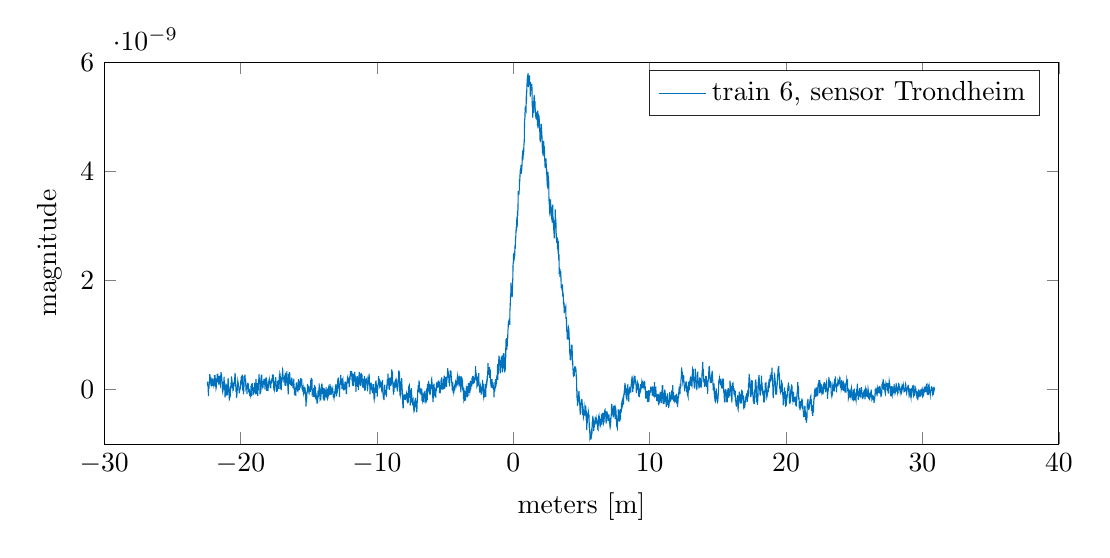
\begin{tikzpicture}

  \begin{axis}[%
    width=\textwidth,
    height=0.4\textwidth,
    at={(0\figurewidth,0\figureheight)},
    scale only axis,
    xmin=-30,
    xmax=40,
    xlabel={meters [m]},
    ymin=-1e-09,
    ymax=6e-09,
    ylabel={magnitude},
    axis background/.style={fill=white},
    legend style={legend cell align=left,align=left,draw=white!15!black}
    ]
    \addplot [color=mycolor1,solid]
    table[row sep=crcr]{%
    -22.434267578125	9.81163464143157e-11\\
    -22.41783203125	1.43162955594902e-10\\
    -22.401396484375	6.16727937092326e-11\\
    -22.3849609375	9.50282638281383e-11\\
    -22.368525390625	2.0751760080009e-11\\
    -22.35208984375	-1.22211884131223e-10\\
    -22.335654296875	8.09825160550062e-11\\
    -22.31921875	2.25893940932486e-11\\
    -22.302783203125	3.22738457582112e-11\\
    -22.28634765625	1.54799277657649e-10\\
    -22.269912109375	1.56954156777596e-10\\
    -22.2534765625	2.84022188145119e-10\\
    -22.237041015625	2.05932071496068e-10\\
    -22.22060546875	2.19007714623632e-10\\
    -22.204169921875	1.87599829031416e-10\\
    -22.187734375	1.75815246149649e-10\\
    -22.171298828125	7.16810620229856e-11\\
    -22.15486328125	2.23574448298304e-10\\
    -22.138427734375	8.73747508302099e-11\\
    -22.1219921875	7.81180472251007e-11\\
    -22.105556640625	1.61764241895604e-10\\
    -22.08912109375	1.18997584584212e-10\\
    -22.072685546875	1.93070460848532e-10\\
    -22.05625	1.59676310151605e-10\\
    -22.039814453125	2.0214915594036e-10\\
    -22.02337890625	1.5893360607894e-10\\
    -22.006943359375	6.84961166824113e-11\\
    -21.9905078125	1.1888858948607e-10\\
    -21.974072265625	9.56886917941266e-11\\
    -21.95763671875	1.63382021964325e-10\\
    -21.941201171875	1.69155444057673e-10\\
    -21.924765625	1.46257856567214e-10\\
    -21.908330078125	2.65168670509515e-10\\
    -21.89189453125	2.25232928035573e-10\\
    -21.875458984375	2.13161993910405e-10\\
    -21.8590234375	2.23819145364642e-10\\
    -21.842587890625	1.61326676418927e-10\\
    -21.82615234375	5.33382567365984e-11\\
    -21.809716796875	8.04795489931297e-11\\
    -21.79328125	2.06728874997703e-11\\
    -21.776845703125	4.00621939985792e-11\\
    -21.76041015625	1.6761340805621e-10\\
    -21.743974609375	1.98064821216424e-10\\
    -21.7275390625	1.31811531016047e-10\\
    -21.711103515625	2.8759661765896e-10\\
    -21.69466796875	2.42861487433493e-10\\
    -21.678232421875	2.00417549034167e-10\\
    -21.661796875	2.05135955986395e-10\\
    -21.645361328125	2.36088392808613e-10\\
    -21.62892578125	2.11272396672192e-10\\
    -21.612490234375	9.03252822990696e-11\\
    -21.5960546875	1.76338360524464e-10\\
    -21.579619140625	2.34766150848106e-10\\
    -21.56318359375	2.36941759571845e-10\\
    -21.546748046875	1.66913625785002e-10\\
    -21.5303125	2.23101386640245e-10\\
    -21.513876953125	2.2906759455861e-10\\
    -21.49744140625	9.63741704219756e-11\\
    -21.481005859375	8.17516088519786e-11\\
    -21.4645703125	2.32075106440367e-10\\
    -21.448134765625	1.68870865498934e-10\\
    -21.43169921875	3.16779582042409e-10\\
    -21.415263671875	2.48289390300826e-10\\
    -21.398828125	2.8069515411829e-10\\
    -21.382392578125	2.73288339129187e-10\\
    -21.36595703125	9.71267184955522e-11\\
    -21.349521484375	1.53844244121795e-10\\
    -21.3330859375	9.07020738347695e-12\\
    -21.316650390625	-1.97593328460031e-11\\
    -21.30021484375	3.11212605599903e-11\\
    -21.283779296875	1.21364014564553e-11\\
    -21.26734375	5.94882082926824e-11\\
    -21.250908203125	1.43475428050441e-10\\
    -21.23447265625	8.75599984942285e-11\\
    -21.218037109375	1.20770880910189e-10\\
    -21.2016015625	2.37767732444722e-10\\
    -21.185166015625	4.61701018308668e-11\\
    -21.16873046875	6.0520390866211e-11\\
    -21.152294921875	3.13776092716395e-11\\
    -21.135859375	-1.4394220864285e-10\\
    -21.119423828125	-6.49987919026616e-11\\
    -21.10298828125	-1.89403750021146e-11\\
    -21.086552734375	-1.2017782292589e-10\\
    -21.0701171875	1.12059565661731e-10\\
    -21.053681640625	6.33255815075403e-11\\
    -21.03724609375	-2.89905404699737e-11\\
    -21.020810546875	9.01298535067889e-11\\
    -21.004375	3.70698201285124e-11\\
    -20.987939453125	-1.04837625065646e-10\\
    -20.97150390625	-1.09903696043222e-11\\
    -20.955068359375	-1.02111914440803e-10\\
    -20.9386328125	-5.29991093257948e-11\\
    -20.922197265625	1.44659114971867e-10\\
    -20.90576171875	2.07880337513749e-10\\
    -20.889326171875	1.04509000127739e-10\\
    -20.872890625	2.66932023950925e-11\\
    -20.856455078125	1.50736165744884e-11\\
    -20.84001953125	4.87697484536717e-11\\
    -20.823583984375	-1.41006656503429e-10\\
    -20.8071484375	-1.22357645706801e-10\\
    -20.790712890625	-1.44152724007639e-10\\
    -20.77427734375	-1.13621610062729e-10\\
    -20.757841796875	-1.42825967644203e-10\\
    -20.74140625	-1.85963700884633e-11\\
    -20.724970703125	1.57600128692948e-11\\
    -20.70853515625	7.21014105899381e-11\\
    -20.692099609375	5.72556414133871e-11\\
    -20.6756640625	8.47504616179139e-11\\
    -20.659228515625	2.38568610854859e-10\\
    -20.64279296875	1.92829519734818e-10\\
    -20.626357421875	1.17863177964542e-10\\
    -20.609921875	1.2632699158484e-10\\
    -20.593486328125	2.04081780710546e-11\\
    -20.57705078125	6.66722820842751e-11\\
    -20.560615234375	1.73909143567932e-11\\
    -20.5441796875	4.38125796712671e-11\\
    -20.527744140625	-2.13370528547575e-11\\
    -20.51130859375	7.02149521043744e-11\\
    -20.494873046875	1.19588075505846e-10\\
    -20.4784375	5.94079974998112e-11\\
    -20.462001953125	1.06572662313948e-10\\
    -20.44556640625	1.44759712215229e-10\\
    -20.429130859375	2.1135966145074e-10\\
    -20.4126953125	2.33511722274742e-10\\
    -20.396259765625	3.06267420421216e-10\\
    -20.37982421875	2.26147064103522e-10\\
    -20.363388671875	1.49784937177133e-10\\
    -20.346953125	6.85029859392245e-11\\
    -20.330517578125	-3.86793031613867e-11\\
    -20.31408203125	4.12264054286911e-12\\
    -20.297646484375	-1.37709988527642e-10\\
    -20.2812109375	-1.41751887311678e-10\\
    -20.264775390625	-7.62999778398013e-11\\
    -20.24833984375	-7.73711228114585e-11\\
    -20.231904296875	6.88300797393271e-11\\
    -20.21546875	8.88377381715681e-11\\
    -20.199033203125	1.55819673608837e-10\\
    -20.18259765625	1.31818541740365e-10\\
    -20.166162109375	7.45741602368196e-11\\
    -20.1497265625	8.20654093643227e-11\\
    -20.133291015625	5.79948874251372e-11\\
    -20.11685546875	4.08619378763027e-11\\
    -20.100419921875	-3.68692277724879e-11\\
    -20.083984375	-7.14319787823164e-11\\
    -20.067548828125	-3.17204307192771e-12\\
    -20.05111328125	-1.00634349827099e-11\\
    -20.034677734375	-1.18187663795173e-12\\
    -20.0182421875	2.56518957779255e-11\\
    -20.001806640625	2.79466262517423e-11\\
    -19.98537109375	1.58263597038851e-10\\
    -19.968935546875	1.17269565160725e-10\\
    -19.9525	2.24741086603248e-10\\
    -19.936064453125	1.52977720348277e-10\\
    -19.91962890625	1.36287033343321e-10\\
    -19.903193359375	2.56373594145336e-10\\
    -19.8867578125	2.06149016352045e-10\\
    -19.870322265625	1.89740871585583e-10\\
    -19.85388671875	2.72944521071886e-10\\
    -19.837451171875	-1.44341952010731e-11\\
    -19.821015625	1.12418431921704e-10\\
    -19.804580078125	5.32999340742421e-11\\
    -19.78814453125	-8.77983186306532e-11\\
    -19.771708984375	6.53926046618345e-11\\
    -19.7552734375	-5.22615542532848e-11\\
    -19.738837890625	1.50938912894585e-10\\
    -19.72240234375	2.43579607544141e-10\\
    -19.705966796875	2.12176990680886e-10\\
    -19.68953125	2.37032068132892e-10\\
    -19.673095703125	2.74249009021207e-10\\
    -19.65666015625	2.01494339424143e-10\\
    -19.640224609375	1.43425972560656e-10\\
    -19.6237890625	1.94289771983473e-10\\
    -19.607353515625	3.97850594890439e-11\\
    -19.59091796875	5.92356379623907e-11\\
    -19.574482421875	1.81119877821754e-11\\
    -19.558046875	9.48432739848552e-12\\
    -19.541611328125	3.88794583835157e-11\\
    -19.52517578125	-7.78522953182415e-11\\
    -19.508740234375	5.53430866041418e-11\\
    -19.4923046875	7.73621326025037e-11\\
    -19.475869140625	6.25281424019003e-11\\
    -19.45943359375	9.34749098406091e-11\\
    -19.442998046875	1.04832169379369e-10\\
    -19.4265625	9.52796549124852e-11\\
    -19.410126953125	4.78852650567897e-11\\
    -19.39369140625	-5.16233879460375e-11\\
    -19.377255859375	1.07798319034014e-11\\
    -19.3608203125	-3.95268171916241e-11\\
    -19.344384765625	-7.39508390659491e-11\\
    -19.32794921875	-1.1395448658374e-10\\
    -19.311513671875	-7.15040204154294e-11\\
    -19.295078125	-9.62914534968759e-11\\
    -19.278642578125	-3.59115071514468e-11\\
    -19.26220703125	-1.39223417264213e-10\\
    -19.245771484375	-2.55357281726862e-11\\
    -19.2293359375	7.19497526206545e-11\\
    -19.212900390625	-1.18612157259959e-10\\
    -19.19646484375	-2.39484881897725e-12\\
    -19.180029296875	1.07981620622629e-10\\
    -19.16359375	4.92699050028531e-11\\
    -19.147158203125	3.11786327857255e-11\\
    -19.13072265625	8.29054079158086e-11\\
    -19.114287109375	1.17597828295004e-10\\
    -19.0978515625	-2.07950641562762e-11\\
    -19.081416015625	-1.05375632087399e-10\\
    -19.06498046875	-1.07042836716958e-11\\
    -19.048544921875	1.76483237712556e-11\\
    -19.032109375	-6.96745518924014e-11\\
    -19.015673828125	-6.65999416529724e-11\\
    -18.99923828125	3.18249939919221e-11\\
    -18.982802734375	3.69959201070846e-11\\
    -18.9663671875	-7.35801244580907e-12\\
    -18.949931640625	1.23993699153464e-10\\
    -18.93349609375	2.03838533077339e-11\\
    -18.917060546875	-5.42671473406387e-11\\
    -18.900625	2.34776127525676e-11\\
    -18.884189453125	-8.85274238580623e-11\\
    -18.86775390625	1.94885328205219e-10\\
    -18.851318359375	1.73566127014937e-11\\
    -18.8348828125	1.03008530245502e-10\\
    -18.818447265625	7.12240480978855e-11\\
    -18.80201171875	-1.04741231175292e-11\\
    -18.785576171875	1.15425991753012e-10\\
    -18.769140625	-8.43053601243114e-11\\
    -18.752705078125	-1.56664243896103e-11\\
    -18.73626953125	-1.14223419480615e-10\\
    -18.719833984375	2.55312532682448e-11\\
    -18.7033984375	-1.73411065723112e-11\\
    -18.686962890625	1.24029237827643e-10\\
    -18.67052734375	1.9159801123193e-10\\
    -18.654091796875	1.36896293328032e-10\\
    -18.63765625	2.83788620006253e-10\\
    -18.621220703125	1.54292475793449e-10\\
    -18.60478515625	1.56265700621492e-10\\
    -18.588349609375	1.50484105313299e-10\\
    -18.5719140625	-8.99910881402789e-11\\
    -18.555478515625	-4.56695836984314e-11\\
    -18.53904296875	1.34430143078333e-10\\
    -18.522607421875	-6.90861292819806e-11\\
    -18.506171875	5.2538600385544e-11\\
    -18.489736328125	2.57884097639034e-10\\
    -18.47330078125	1.18900364367929e-10\\
    -18.456865234375	1.98778039770032e-10\\
    -18.4404296875	2.74792926871252e-10\\
    -18.423994140625	1.20207102764424e-10\\
    -18.40755859375	7.00835635159193e-11\\
    -18.391123046875	9.41018182538331e-11\\
    -18.3746875	9.72747321207218e-11\\
    -18.358251953125	2.45982394589814e-11\\
    -18.34181640625	6.81904441878453e-11\\
    -18.325380859375	1.37121034223956e-10\\
    -18.3089453125	1.31814798823064e-10\\
    -18.292509765625	1.01591687079802e-10\\
    -18.27607421875	1.9307990786136e-10\\
    -18.259638671875	1.25445612971898e-10\\
    -18.243203125	1.29429041351754e-10\\
    -18.226767578125	1.39014032401945e-10\\
    -18.21033203125	3.38181952362481e-11\\
    -18.193896484375	-1.59194292271362e-12\\
    -18.1774609375	1.994506956477e-10\\
    -18.161025390625	8.4075040933592e-11\\
    -18.14458984375	1.28568385654142e-10\\
    -18.128154296875	2.18117094250072e-10\\
    -18.11171875	1.52779978936454e-10\\
    -18.095283203125	1.68826375664934e-10\\
    -18.07884765625	-2.3193132566177e-11\\
    -18.062412109375	2.37151106159699e-11\\
    -18.0459765625	-1.36415593252925e-11\\
    -18.029541015625	9.64191011437832e-11\\
    -18.01310546875	-2.39192606911923e-11\\
    -17.996669921875	8.66821100952431e-12\\
    -17.980234375	6.9261247044696e-11\\
    -17.963798828125	4.1205791315331e-11\\
    -17.94736328125	8.20246349633485e-11\\
    -17.930927734375	1.02604493264769e-10\\
    -17.9144921875	1.84287323068797e-10\\
    -17.898056640625	1.07426256463741e-10\\
    -17.88162109375	1.76623565982854e-10\\
    -17.865185546875	1.49749915238871e-10\\
    -17.84875	1.54083124031154e-10\\
    -17.832314453125	1.27509435301108e-10\\
    -17.81587890625	3.66498512094836e-11\\
    -17.799443359375	1.32088360967123e-10\\
    -17.7830078125	2.05810335990635e-11\\
    -17.766572265625	1.43312430765684e-10\\
    -17.75013671875	1.48985039645916e-10\\
    -17.733701171875	1.2495780916224e-10\\
    -17.717265625	1.28117134341225e-10\\
    -17.700830078125	2.08654730819708e-10\\
    -17.68439453125	1.61162025252666e-10\\
    -17.667958984375	1.78291050973341e-10\\
    -17.6515234375	2.75825847007394e-10\\
    -17.635087890625	2.24624446419055e-10\\
    -17.61865234375	2.03693483919322e-10\\
    -17.602216796875	2.71470687736507e-10\\
    -17.58578125	1.8524796879546e-10\\
    -17.569345703125	5.90404986719754e-11\\
    -17.55291015625	5.92492328419205e-12\\
    -17.536474609375	1.17860510100508e-11\\
    -17.5200390625	4.75339106390941e-11\\
    -17.503603515625	8.42859773361386e-12\\
    -17.48716796875	3.6749164394835e-11\\
    -17.470732421875	1.5123102197016e-10\\
    -17.454296875	1.05793660488511e-10\\
    -17.437861328125	1.89719849506478e-10\\
    -17.42142578125	2.28182854695111e-10\\
    -17.404990234375	8.07298157114753e-11\\
    -17.3885546875	7.11119129240662e-11\\
    -17.372119140625	7.36979684652527e-11\\
    -17.35568359375	-4.45748841971546e-11\\
    -17.339248046875	6.61305074324135e-11\\
    -17.3228125	6.47034348687584e-11\\
    -17.306376953125	-3.1526065052738e-11\\
    -17.28994140625	1.54150738798011e-10\\
    -17.273505859375	9.54619245346334e-11\\
    -17.2570703125	1.07575507146943e-11\\
    -17.240634765625	1.71100686378651e-10\\
    -17.22419921875	7.74494910365257e-11\\
    -17.207763671875	8.93135329988261e-11\\
    -17.191328125	1.29277603421968e-10\\
    -17.174892578125	9.78107425067875e-12\\
    -17.15845703125	2.21980165916372e-10\\
    -17.142021484375	2.84643428868916e-10\\
    -17.1255859375	1.26169154122282e-10\\
    -17.109150390625	2.90719859783829e-10\\
    -17.09271484375	2.74880009189605e-10\\
    -17.076279296875	1.14887756160542e-10\\
    -17.05984375	9.00534273685104e-11\\
    -17.043408203125	9.28749908807133e-12\\
    -17.02697265625	9.0601169813421e-11\\
    -17.010537109375	-1.20578617944602e-11\\
    -16.9941015625	8.96293557844241e-11\\
    -16.977666015625	2.21276944436975e-10\\
    -16.96123046875	1.47005946390382e-10\\
    -16.944794921875	2.80087725238985e-10\\
    -16.928359375	2.53798696978283e-10\\
    -16.911923828125	3.67792487240424e-10\\
    -16.89548828125	3.55509432880256e-10\\
    -16.879052734375	2.04921861105233e-10\\
    -16.8626171875	1.9641139496782e-10\\
    -16.846181640625	1.91178348461014e-10\\
    -16.82974609375	2.26391924136514e-10\\
    -16.813310546875	1.28681527213871e-10\\
    -16.796875	1.68469155373753e-10\\
    -16.780439453125	2.00971407964088e-10\\
    -16.76400390625	1.74900300255675e-10\\
    -16.747568359375	1.21615473424583e-10\\
    -16.7311328125	1.3659168727969e-10\\
    -16.714697265625	2.40497706551834e-10\\
    -16.69826171875	2.15742647214452e-10\\
    -16.681826171875	6.72178353718687e-11\\
    -16.665390625	3.01491147118791e-10\\
    -16.648955078125	2.74919850540703e-10\\
    -16.63251953125	1.41582990511094e-10\\
    -16.616083984375	2.24888870009628e-10\\
    -16.5996484375	3.38930239035968e-10\\
    -16.583212890625	1.57810483010064e-10\\
    -16.56677734375	1.2494266383045e-10\\
    -16.550341796875	9.66318844521866e-11\\
    -16.53390625	1.05257930032735e-10\\
    -16.517470703125	1.6507408209951e-12\\
    -16.50103515625	-8.68800130414825e-11\\
    -16.484599609375	1.76589109333979e-10\\
    -16.4681640625	2.79780285049499e-10\\
    -16.451728515625	8.28120335113819e-11\\
    -16.43529296875	2.82622940938239e-10\\
    -16.418857421875	3.16984937432718e-10\\
    -16.402421875	1.82612458590502e-10\\
    -16.385986328125	3.08682089373899e-10\\
    -16.36955078125	1.75932427277476e-10\\
    -16.353115234375	1.20382737160474e-10\\
    -16.3366796875	1.22572724201848e-10\\
    -16.320244140625	8.44519827383624e-11\\
    -16.30380859375	1.73407061490891e-10\\
    -16.287373046875	1.46527994981281e-10\\
    -16.2709375	6.33581959852167e-11\\
    -16.254501953125	1.69703135961415e-10\\
    -16.23806640625	2.18531705522715e-10\\
    -16.221630859375	1.6601020475292e-10\\
    -16.2051953125	1.43361589158259e-10\\
    -16.188759765625	9.93238630744236e-11\\
    -16.17232421875	1.00074327539807e-10\\
    -16.155888671875	2.80414990341363e-11\\
    -16.139453125	7.75050337245276e-11\\
    -16.123017578125	8.52719689275713e-11\\
    -16.10658203125	8.55407592332344e-11\\
    -16.090146484375	2.00692417546469e-10\\
    -16.0737109375	2.5620114110396e-12\\
    -16.057275390625	3.55020871864239e-11\\
    -16.04083984375	-9.34371498916514e-11\\
    -16.024404296875	3.41009218200985e-11\\
    -16.00796875	-6.52637461871027e-11\\
    -15.991533203125	-1.15826929042614e-10\\
    -15.97509765625	6.94006301791861e-12\\
    -15.958662109375	-2.95174085483354e-11\\
    -15.9422265625	-4.54964692639085e-11\\
    -15.925791015625	6.84820966597821e-11\\
    -15.90935546875	1.17282677420688e-10\\
    -15.892919921875	-5.6770986827149e-12\\
    -15.876484375	1.2880442898099e-10\\
    -15.860048828125	7.51305786071912e-11\\
    -15.84361328125	4.34355703356644e-11\\
    -15.827177734375	-3.70146414669929e-11\\
    -15.8107421875	5.24751459053102e-11\\
    -15.794306640625	4.33689163883695e-11\\
    -15.77787109375	2.10909445658728e-11\\
    -15.761435546875	9.01947676054652e-11\\
    -15.745	1.895769971923e-10\\
    -15.728564453125	8.92102871678878e-11\\
    -15.71212890625	9.58484127353918e-11\\
    -15.695693359375	1.2238455887735e-10\\
    -15.6792578125	-8.68691041056636e-12\\
    -15.662822265625	1.06553643460451e-10\\
    -15.64638671875	9.04100492970244e-11\\
    -15.629951171875	3.12738588389558e-11\\
    -15.613515625	1.00221649555245e-10\\
    -15.597080078125	1.47037257050537e-10\\
    -15.58064453125	1.96987469065875e-10\\
    -15.564208984375	1.95716006050582e-10\\
    -15.5477734375	1.06538539962608e-10\\
    -15.531337890625	9.42968023877808e-11\\
    -15.51490234375	1.95900879460645e-10\\
    -15.498466796875	9.85096227748633e-11\\
    -15.48203125	-1.0596321603788e-11\\
    -15.465595703125	7.46034120174645e-11\\
    -15.44916015625	9.01651549875196e-12\\
    -15.432724609375	1.35823955145874e-11\\
    -15.4162890625	-3.99905828107222e-11\\
    -15.399853515625	1.4421423417953e-11\\
    -15.38341796875	-6.56844929014522e-11\\
    -15.366982421875	-4.49313796495372e-11\\
    -15.350546875	3.27566614931731e-11\\
    -15.334111328125	8.35178088743033e-12\\
    -15.31767578125	-1.33478248025618e-11\\
    -15.301240234375	3.26534852719336e-11\\
    -15.2848046875	3.0595367815006e-11\\
    -15.268369140625	-7.16794421090875e-12\\
    -15.25193359375	-9.33398707357141e-11\\
    -15.235498046875	-6.43387658526854e-11\\
    -15.2190625	-1.17410935760034e-10\\
    -15.202626953125	-3.12514875249518e-10\\
    -15.18619140625	-1.53655525076006e-10\\
    -15.169755859375	-1.86122419951529e-10\\
    -15.1533203125	-2.34133809374636e-10\\
    -15.136884765625	-6.20835362396821e-11\\
    -15.12044921875	-6.3172694683203e-11\\
    -15.104013671875	-3.98138616930168e-11\\
    -15.087578125	1.03624193836376e-10\\
    -15.071142578125	7.21663833734866e-11\\
    -15.05470703125	3.7016758530114e-11\\
    -15.038271484375	3.73644570562781e-11\\
    -15.0218359375	-2.28830656034988e-11\\
    -15.005400390625	6.88789296020004e-11\\
    -14.98896484375	-6.55943851716609e-11\\
    -14.972529296875	-7.19256701287816e-11\\
    -14.95609375	-1.97333758336359e-12\\
    -14.939658203125	4.01359944897327e-13\\
    -14.92322265625	1.82684822150111e-11\\
    -14.906787109375	2.34130550824327e-11\\
    -14.8903515625	5.35166591806939e-11\\
    -14.873916015625	-4.57869021188392e-11\\
    -14.85748046875	1.71854607930593e-10\\
    -14.841044921875	3.43798559842606e-11\\
    -14.824609375	3.34935864098619e-11\\
    -14.808173828125	2.14232236315244e-10\\
    -14.79173828125	-1.6223555947211e-12\\
    -14.775302734375	1.8367499234313e-10\\
    -14.7588671875	1.84200383506106e-10\\
    -14.742431640625	-3.70408578506956e-11\\
    -14.72599609375	-1.94410506388571e-11\\
    -14.709560546875	-2.656907035271e-11\\
    -14.693125	-1.3315179147787e-10\\
    -14.676689453125	3.86671929345041e-12\\
    -14.66025390625	-5.54648355377137e-11\\
    -14.643818359375	-9.67111271840375e-11\\
    -14.6273828125	2.38735497316241e-11\\
    -14.610947265625	-5.51993197080951e-11\\
    -14.59451171875	-1.32633768630317e-10\\
    -14.578076171875	8.45307879005699e-11\\
    -14.561640625	1.93859489743496e-11\\
    -14.545205078125	-5.5174303007248e-11\\
    -14.52876953125	-2.91296873068497e-11\\
    -14.512333984375	3.64952319034119e-11\\
    -14.4958984375	2.76924002811751e-11\\
    -14.479462890625	-1.67169850725251e-10\\
    -14.46302734375	-6.0448044202452e-11\\
    -14.446591796875	-2.00024573142457e-10\\
    -14.43015625	-1.75983763907396e-10\\
    -14.413720703125	-1.2523382942997e-10\\
    -14.39728515625	-2.58581873079208e-10\\
    -14.380849609375	-1.33666896127027e-10\\
    -14.3644140625	-1.06510577864327e-10\\
    -14.347978515625	-2.53356464323828e-10\\
    -14.33154296875	-1.04418944379461e-10\\
    -14.315107421875	-2.22213669701242e-11\\
    -14.298671875	-1.38497818901469e-10\\
    -14.282236328125	-4.35491556876214e-11\\
    -14.26580078125	-9.9814520058199e-11\\
    -14.249365234375	-6.06478843787904e-11\\
    -14.2329296875	1.12653060286285e-10\\
    -14.216494140625	-1.09570250302179e-10\\
    -14.20005859375	-7.77124259846865e-11\\
    -14.183623046875	1.79481187439577e-11\\
    -14.1671875	-1.74458617204147e-10\\
    -14.150751953125	-1.61244548127177e-10\\
    -14.13431640625	3.71029798488745e-13\\
    -14.117880859375	-1.98692097349477e-10\\
    -14.1014453125	-1.21300390997142e-10\\
    -14.085009765625	3.51880138804682e-11\\
    -14.06857421875	5.74107908278837e-11\\
    -14.052138671875	1.54827098767887e-11\\
    -14.035703125	7.49995783924486e-11\\
    -14.019267578125	8.09906388016402e-11\\
    -14.00283203125	3.20723621182202e-11\\
    -13.986396484375	-8.12069955642597e-11\\
    -13.9699609375	-5.49683303728017e-11\\
    -13.953525390625	-2.59227645226182e-11\\
    -13.93708984375	-1.67678566110512e-10\\
    -13.920654296875	-1.70057919482364e-10\\
    -13.90421875	2.97995805743055e-11\\
    -13.887783203125	-1.96977658441574e-10\\
    -13.87134765625	-1.38482179890697e-10\\
    -13.854912109375	2.13370880509955e-11\\
    -13.8384765625	-2.04168114424623e-10\\
    -13.822041015625	-1.27360441416624e-10\\
    -13.80560546875	-4.98292435876107e-11\\
    -13.789169921875	-1.22544330733522e-10\\
    -13.772734375	-1.03825237569239e-10\\
    -13.756298828125	-1.29555777968629e-11\\
    -13.73986328125	-8.71885088227599e-11\\
    -13.723427734375	4.48324803727748e-11\\
    -13.7069921875	-8.02466538182208e-11\\
    -13.690556640625	-1.41287756956402e-10\\
    -13.67412109375	-9.43402436111385e-11\\
    -13.657685546875	-9.28090559589459e-11\\
    -13.64125	-1.55407675656928e-10\\
    -13.624814453125	-1.67011992377816e-10\\
    -13.60837890625	1.70398775898596e-11\\
    -13.591943359375	-1.69831317636795e-10\\
    -13.5755078125	-9.27139575065218e-12\\
    -13.559072265625	1.12844897111261e-11\\
    -13.54263671875	-9.24383952904278e-11\\
    -13.526201171875	-6.36591978050397e-11\\
    -13.509765625	-3.57431676247847e-11\\
    -13.493330078125	5.51365314311986e-11\\
    -13.47689453125	-7.64668267680338e-11\\
    -13.460458984375	-6.75302437634884e-11\\
    -13.4440234375	1.02255496039946e-10\\
    -13.427587890625	-1.35148132123491e-11\\
    -13.41115234375	-9.49114721616806e-11\\
    -13.394716796875	3.03478677309945e-11\\
    -13.37828125	6.18528334414592e-11\\
    -13.361845703125	-9.69421382351381e-11\\
    -13.34541015625	-4.64968591347236e-11\\
    -13.328974609375	-1.54665025166655e-11\\
    -13.3125390625	-4.079561403381e-11\\
    -13.296103515625	-2.23820447907312e-11\\
    -13.27966796875	-7.09294345827822e-12\\
    -13.263232421875	-2.5798936809621e-11\\
    -13.246796875	-4.57770018548556e-11\\
    -13.230361328125	-8.28524491519755e-12\\
    -13.21392578125	-4.84273663420695e-11\\
    -13.197490234375	-1.38344984541844e-10\\
    -13.1810546875	-8.94759731279367e-11\\
    -13.164619140625	-1.3948530247935e-10\\
    -13.14818359375	-1.55999390625494e-10\\
    -13.131748046875	-8.71244291906042e-11\\
    -13.1153125	-1.472396271659e-10\\
    -13.098876953125	-9.63834231726047e-11\\
    -13.08244140625	-2.34183203204892e-11\\
    -13.066005859375	-7.66560971647195e-11\\
    -13.0495703125	1.51041792045892e-11\\
    -13.033134765625	8.0604304883422e-11\\
    -13.01669921875	1.17593350605277e-11\\
    -13.000263671875	1.01054853396672e-10\\
    -12.983828125	-6.04504199453942e-11\\
    -12.967392578125	-1.23140078902092e-10\\
    -12.95095703125	-8.25629591410495e-11\\
    -12.934521484375	-5.53899286977619e-11\\
    -12.9180859375	-5.81901822749471e-11\\
    -12.901650390625	-3.62500319656063e-11\\
    -12.88521484375	7.21424986477621e-11\\
    -12.868779296875	1.66614984674738e-10\\
    -12.85234375	1.97925054787825e-10\\
    -12.835908203125	2.03666033679907e-10\\
    -12.81947265625	1.62463242807606e-10\\
    -12.803037109375	1.1005623279377e-10\\
    -12.7866015625	2.43444386694189e-11\\
    -12.770166015625	1.09100520372589e-11\\
    -12.75373046875	-2.44585056282649e-11\\
    -12.737294921875	-1.32746251958115e-10\\
    -12.720859375	7.31209620317311e-11\\
    -12.704423828125	9.98980006755546e-11\\
    -12.68798828125	1.24092068038918e-10\\
    -12.671552734375	2.02993179280564e-10\\
    -12.6551171875	2.68512371978009e-10\\
    -12.638681640625	1.9235889803679e-10\\
    -12.62224609375	1.84950292981282e-10\\
    -12.605810546875	1.55395219902951e-10\\
    -12.589375	7.97503156558065e-11\\
    -12.572939453125	1.37499642033399e-10\\
    -12.55650390625	5.68944929940369e-12\\
    -12.540068359375	6.77538851922042e-11\\
    -12.5236328125	2.05640533257355e-10\\
    -12.507197265625	1.4639247139573e-10\\
    -12.49076171875	1.70225993407141e-10\\
    -12.474326171875	1.05550404078177e-10\\
    -12.457890625	1.01023675477186e-10\\
    -12.441455078125	-1.27620514122838e-11\\
    -12.42501953125	1.37419771563728e-11\\
    -12.408583984375	3.44805512792157e-11\\
    -12.3921484375	5.44004981369537e-12\\
    -12.375712890625	1.27206316085566e-11\\
    -12.35927734375	3.41464239209162e-11\\
    -12.342841796875	1.46677075956376e-10\\
    -12.32640625	9.20148141518679e-11\\
    -12.309970703125	4.1324137972628e-11\\
    -12.29353515625	1.36027504236203e-10\\
    -12.277099609375	5.76602091339548e-11\\
    -12.2606640625	-1.22585585285352e-11\\
    -12.244228515625	6.41496976870088e-12\\
    -12.22779296875	-8.18885382485283e-11\\
    -12.211357421875	3.42513276686737e-11\\
    -12.194921875	1.16941444904216e-10\\
    -12.178486328125	1.47056749058723e-10\\
    -12.16205078125	2.10141446044809e-10\\
    -12.145615234375	2.24659914490414e-10\\
    -12.1291796875	1.33013675115739e-10\\
    -12.112744140625	1.8866005191022e-10\\
    -12.09630859375	2.19237950935075e-10\\
    -12.079873046875	1.13356482070992e-10\\
    -12.0634375	1.39318225015953e-10\\
    -12.047001953125	1.68967188488222e-10\\
    -12.03056640625	4.5970974657041e-11\\
    -12.014130859375	1.11270261834606e-10\\
    -11.9976953125	2.1981877269151e-10\\
    -11.981259765625	2.33366940437779e-10\\
    -11.96482421875	2.22390017468994e-10\\
    -11.948388671875	2.84626852671584e-10\\
    -11.931953125	3.39414891834358e-10\\
    -11.915517578125	2.86976378905987e-10\\
    -11.89908203125	3.34044303612904e-10\\
    -11.882646484375	2.92679202566226e-10\\
    -11.8662109375	2.42448023906808e-10\\
    -11.849775390625	3.36050180799229e-10\\
    -11.83333984375	2.32380831527144e-10\\
    -11.816904296875	1.51790875532846e-10\\
    -11.80046875	2.97756792862431e-10\\
    -11.784033203125	7.23210071051564e-11\\
    -11.76759765625	1.30028952490583e-10\\
    -11.751162109375	2.12837521535411e-10\\
    -11.7347265625	6.13856111232274e-11\\
    -11.718291015625	1.70457310210142e-10\\
    -11.70185546875	2.87698926581887e-10\\
    -11.685419921875	1.81245304592469e-10\\
    -11.668984375	2.53423168379512e-10\\
    -11.652548828125	2.90396663780505e-10\\
    -11.63611328125	1.44370301612633e-10\\
    -11.619677734375	3.24992879930025e-10\\
    -11.6032421875	2.33154422545252e-10\\
    -11.586806640625	7.89901760026451e-11\\
    -11.57037109375	2.41901653860266e-10\\
    -11.553935546875	1.37546701645689e-10\\
    -11.5375	-4.33596954347994e-11\\
    -11.521064453125	1.06645315862832e-10\\
    -11.50462890625	1.34516302856065e-10\\
    -11.488193359375	9.72539489795295e-11\\
    -11.4717578125	1.79100684581965e-10\\
    -11.455322265625	6.37507782882007e-11\\
    -11.43888671875	2.43126743895847e-10\\
    -11.422451171875	2.13221770087802e-10\\
    -11.406015625	4.71456097071873e-11\\
    -11.389580078125	2.04877891793639e-10\\
    -11.37314453125	1.28232374940607e-10\\
    -11.356708984375	-9.28162308849121e-12\\
    -11.3402734375	1.7544469251798e-10\\
    -11.323837890625	2.20396166327311e-10\\
    -11.30740234375	1.89636128661941e-10\\
    -11.290966796875	3.24820980358921e-10\\
    -11.27453125	2.1800732156394e-10\\
    -11.258095703125	9.64993239927192e-11\\
    -11.24166015625	2.89695100324444e-10\\
    -11.225224609375	1.17222158313658e-10\\
    -11.2087890625	6.32470642717708e-11\\
    -11.192353515625	1.43284053719419e-10\\
    -11.17591796875	8.62335013305364e-11\\
    -11.159482421875	2.06488126909248e-10\\
    -11.143046875	2.88916403724891e-10\\
    -11.126611328125	2.8375828604368e-10\\
    -11.11017578125	1.87588223448685e-10\\
    -11.093740234375	2.74533986878757e-10\\
    -11.0773046875	1.97834709936481e-10\\
    -11.060869140625	4.95560549923848e-11\\
    -11.04443359375	1.46088018294952e-10\\
    -11.027998046875	7.44239585840739e-11\\
    -11.0115625	2.60742738327412e-11\\
    -10.995126953125	8.66673351913208e-11\\
    -10.97869140625	1.57933760436137e-10\\
    -10.962255859375	1.46948565695505e-10\\
    -10.9458203125	7.91922596217538e-11\\
    -10.929384765625	9.07200896905147e-11\\
    -10.91294921875	2.44661145478694e-10\\
    -10.896513671875	1.54477341532761e-11\\
    -10.880078125	-2.34838916378119e-11\\
    -10.863642578125	1.05630791421383e-10\\
    -10.84720703125	-8.78454962557559e-12\\
    -10.830771484375	6.44170734786006e-11\\
    -10.8143359375	1.85529636103134e-10\\
    -10.797900390625	1.88646380228816e-10\\
    -10.78146484375	1.11352710718602e-10\\
    -10.765029296875	1.43123018304027e-10\\
    -10.74859375	1.6455609013085e-10\\
    -10.732158203125	1.82355779944933e-10\\
    -10.71572265625	8.13119369041086e-11\\
    -10.699287109375	7.96500883138039e-11\\
    -10.6828515625	-3.53555671389947e-11\\
    -10.666416015625	5.80109805603437e-11\\
    -10.64998046875	1.2038778113237e-10\\
    -10.633544921875	1.50609646352405e-10\\
    -10.617109375	2.25377371648117e-10\\
    -10.600673828125	1.72127313047594e-10\\
    -10.58423828125	2.14808854493606e-10\\
    -10.567802734375	2.92424650594273e-10\\
    -10.5513671875	8.8127481633779e-11\\
    -10.534931640625	7.34382546957581e-11\\
    -10.51849609375	5.51838520474431e-11\\
    -10.502060546875	-8.92525958203999e-11\\
    -10.485625	3.0956823722487e-11\\
    -10.469189453125	1.14566196966421e-10\\
    -10.45275390625	1.16607205907244e-10\\
    -10.436318359375	2.76481773545668e-13\\
    -10.4198828125	1.24235622390297e-10\\
    -10.403447265625	4.92605050849001e-11\\
    -10.38701171875	3.6003338734864e-11\\
    -10.370576171875	2.23676403490429e-11\\
    -10.354140625	-1.71967108433739e-11\\
    -10.337705078125	-3.37883376672216e-11\\
    -10.32126953125	-6.51502906794324e-11\\
    -10.304833984375	4.47370325632202e-12\\
    -10.2883984375	9.85520034712382e-11\\
    -10.271962890625	9.5849436547158e-12\\
    -10.25552734375	-1.6801566936149e-11\\
    -10.239091796875	9.95015750749076e-11\\
    -10.22265625	-1.44339956653727e-10\\
    -10.206220703125	-1.68318855468231e-10\\
    -10.18978515625	-6.01219819578558e-11\\
    -10.173349609375	-1.78672429172382e-10\\
    -10.1569140625	-1.3888404959335e-10\\
    -10.140478515625	-6.62310753802551e-12\\
    -10.12404296875	-1.50086450556417e-11\\
    -10.107607421875	8.47134342446186e-11\\
    -10.091171875	1.46642231313456e-10\\
    -10.074736328125	-4.01473449866493e-11\\
    -10.05830078125	1.67549524738577e-10\\
    -10.041865234375	4.36766143161109e-11\\
    -10.0254296875	-5.8988210735398e-11\\
    -10.008994140625	-2.20157830170071e-11\\
    -9.99255859375	8.06270434244782e-11\\
    -9.976123046875	-1.30110289290106e-10\\
    -9.9596875	3.18927123728331e-11\\
    -9.943251953125	-5.14251111908754e-12\\
    -9.92681640625	4.49047975651879e-11\\
    -9.910380859375	1.00239737372474e-10\\
    -9.8939453125	9.85589903873724e-11\\
    -9.877509765625	2.45057146470475e-10\\
    -9.86107421875	1.78257951556866e-10\\
    -9.844638671875	8.51184450282505e-11\\
    -9.828203125	1.24227970985166e-10\\
    -9.811767578125	1.32483839452002e-10\\
    -9.79533203125	6.86278313687241e-11\\
    -9.778896484375	8.53559906896635e-11\\
    -9.7624609375	1.4455355559342e-10\\
    -9.746025390625	1.30214344048676e-10\\
    -9.72958984375	3.9481364494105e-11\\
    -9.713154296875	1.42608823047092e-10\\
    -9.69671875	1.02415746961909e-10\\
    -9.680283203125	6.64547869233451e-11\\
    -9.66384765625	2.5965648321661e-11\\
    -9.647412109375	6.17575875859631e-11\\
    -9.6309765625	3.71402877161066e-11\\
    -9.614541015625	8.3054880753073e-11\\
    -9.59810546875	3.10904629697037e-11\\
    -9.581669921875	1.76394641287458e-10\\
    -9.565234375	-3.83879889963413e-11\\
    -9.548798828125	-8.25968674909652e-11\\
    -9.53236328125	-5.53234073781181e-11\\
    -9.515927734375	-1.59076916493143e-10\\
    -9.4994921875	-1.63491935187655e-10\\
    -9.483056640625	-1.94533539916468e-10\\
    -9.46662109375	-1.16483498291216e-10\\
    -9.450185546875	-8.46282482512262e-11\\
    -9.43375	8.84929004214722e-11\\
    -9.417314453125	3.82315092425854e-11\\
    -9.40087890625	-3.63793139210893e-11\\
    -9.384443359375	-4.67086660542011e-11\\
    -9.3680078125	-4.07837512926839e-11\\
    -9.351572265625	-9.31737263798112e-11\\
    -9.33513671875	-2.94126134500198e-11\\
    -9.318701171875	-6.46990879233381e-11\\
    -9.302265625	-1.31963086685574e-10\\
    -9.285830078125	1.01144253936619e-11\\
    -9.26939453125	9.50839236874079e-11\\
    -9.252958984375	3.48581076491876e-12\\
    -9.2365234375	1.80985598776839e-10\\
    -9.220087890625	1.81184332845252e-10\\
    -9.20365234375	1.19118645540794e-10\\
    -9.187216796875	2.91970934689962e-10\\
    -9.17078125	1.7654369142796e-10\\
    -9.154345703125	7.70880026447836e-11\\
    -9.13791015625	1.52451776610149e-10\\
    -9.121474609375	6.2857882150534e-11\\
    -9.1050390625	7.35654202516551e-11\\
    -9.088603515625	2.13440202133922e-10\\
    -9.07216796875	-4.99706798004509e-12\\
    -9.055732421875	1.2933595816199e-10\\
    -9.039296875	2.00652511944351e-10\\
    -9.022861328125	1.20888186919227e-10\\
    -9.00642578125	6.92174982124219e-11\\
    -8.989990234375	2.22916216429513e-10\\
    -8.9735546875	9.46302678261156e-11\\
    -8.957119140625	2.05795279849564e-10\\
    -8.94068359375	1.38936030243935e-10\\
    -8.924248046875	1.25239573491223e-10\\
    -8.9078125	3.67244308473414e-10\\
    -8.891376953125	2.07797849410215e-10\\
    -8.87494140625	2.91871549443471e-10\\
    -8.858505859375	2.99438467575513e-10\\
    -8.8420703125	1.52426759710122e-10\\
    -8.825634765625	1.32982653775988e-10\\
    -8.80919921875	1.00233867608485e-10\\
    -8.792763671875	-8.14687885500622e-11\\
    -8.776328125	-8.28189206814254e-11\\
    -8.759892578125	5.48437650160548e-11\\
    -8.74345703125	-4.36945848584414e-11\\
    -8.727021484375	5.59349404595535e-11\\
    -8.7105859375	1.25798458486107e-10\\
    -8.694150390625	4.1927739777453e-11\\
    -8.67771484375	1.64216359744188e-10\\
    -8.661279296875	7.06804124195469e-11\\
    -8.64484375	6.20432707350147e-11\\
    -8.628408203125	1.70193477111603e-10\\
    -8.61197265625	1.78869907776791e-10\\
    -8.595537109375	8.82804425820319e-11\\
    -8.5791015625	1.77564237240074e-10\\
    -8.562666015625	1.61384619044311e-10\\
    -8.54623046875	7.58807741250053e-11\\
    -8.529794921875	7.47662639757434e-12\\
    -8.513359375	6.88118498258017e-11\\
    -8.496923828125	-2.12188657451202e-11\\
    -8.48048828125	-1.73585438469771e-11\\
    -8.464052734375	1.1163126594567e-10\\
    -8.4476171875	5.59712919701268e-11\\
    -8.431181640625	1.9409604925231e-10\\
    -8.41474609375	1.57762045809789e-10\\
    -8.398310546875	3.3720281928531e-10\\
    -8.381875	3.36320345506381e-10\\
    -8.365439453125	1.16086649159844e-10\\
    -8.34900390625	3.17683777842469e-10\\
    -8.332568359375	1.54019484189887e-10\\
    -8.3161328125	-1.10148359154606e-10\\
    -8.299697265625	-6.4302836986722e-11\\
    -8.28326171875	-9.14944697429409e-11\\
    -8.266826171875	-3.71584417073268e-11\\
    -8.250390625	-9.24918411791322e-11\\
    -8.233955078125	1.46979593068327e-10\\
    -8.21751953125	1.1522466005795e-10\\
    -8.201083984375	1.65790193479204e-10\\
    -8.1846484375	2.08860570572854e-10\\
    -8.168212890625	1.34399096823045e-10\\
    -8.15177734375	-3.32338827614554e-12\\
    -8.135341796875	-5.923843530804e-12\\
    -8.11890625	-1.97001977630458e-10\\
    -8.102470703125	-2.5921605363645e-10\\
    -8.08603515625	-2.34692774208267e-10\\
    -8.069599609375	-3.45485321656492e-10\\
    -8.0531640625	-1.94740709158027e-10\\
    -8.036728515625	-1.53187373230383e-10\\
    -8.02029296875	-1.84091767317037e-10\\
    -8.003857421875	-1.03321388392334e-10\\
    -7.987421875	-1.04777244572047e-10\\
    -7.970986328125	-1.21885588930057e-10\\
    -7.95455078125	-1.65319417304164e-10\\
    -7.938115234375	-8.88662045559556e-11\\
    -7.9216796875	-1.90265181835024e-10\\
    -7.905244140625	-1.35352768576641e-10\\
    -7.88880859375	-1.23020321541932e-10\\
    -7.872373046875	-1.33715859263154e-10\\
    -7.8559375	-1.21335518451894e-10\\
    -7.839501953125	-1.1780807865119e-10\\
    -7.82306640625	-8.06173837044931e-11\\
    -7.806630859375	-1.05386776640721e-10\\
    -7.7901953125	-2.16884731622739e-10\\
    -7.773759765625	-1.50071657943502e-10\\
    -7.75732421875	-1.59103121296297e-10\\
    -7.740888671875	-2.55148182596042e-10\\
    -7.724453125	-5.97393079393808e-11\\
    -7.708017578125	-9.54378890443953e-11\\
    -7.69158203125	-2.34486788554927e-10\\
    -7.675146484375	3.51580830540772e-11\\
    -7.6587109375	5.75069816012746e-11\\
    -7.642275390625	6.62018675788688e-11\\
    -7.62583984375	7.5907196364044e-11\\
    -7.609404296875	-6.0106636964941e-11\\
    -7.59296875	-9.96109400483598e-11\\
    -7.576533203125	-1.4286552231758e-11\\
    -7.56009765625	-2.94731406601829e-10\\
    -7.543662109375	-1.8104101015971e-10\\
    -7.5272265625	-7.34942057792401e-12\\
    -7.510791015625	-2.39431922038778e-10\\
    -7.49435546875	-1.61014242375052e-10\\
    -7.477919921875	2.37542634194506e-11\\
    -7.461484375	-1.29864886943996e-10\\
    -7.445048828125	-1.06443776107393e-10\\
    -7.42861328125	-1.83715655188336e-10\\
    -7.412177734375	-2.1741199808408e-10\\
    -7.3957421875	-1.84790494424277e-10\\
    -7.379306640625	-2.47105196949106e-10\\
    -7.36287109375	-1.79659484749649e-10\\
    -7.346435546875	-1.71321331127071e-10\\
    -7.33	-2.86508326630104e-10\\
    -7.313564453125	-3.24482310313695e-10\\
    -7.29712890625	-2.98432351275259e-10\\
    -7.280693359375	-2.8271436500502e-10\\
    -7.2642578125	-3.96927460491619e-10\\
    -7.247822265625	-3.87359103982524e-10\\
    -7.23138671875	-2.57495279807658e-10\\
    -7.214951171875	-2.56958067337629e-10\\
    -7.198515625	-1.74440608031838e-10\\
    -7.182080078125	-2.20174507683302e-10\\
    -7.16564453125	-1.52491740973021e-10\\
    -7.149208984375	-2.31798910340677e-10\\
    -7.1327734375	-3.14629307619311e-10\\
    -7.116337890625	-3.20400706433657e-10\\
    -7.09990234375	-2.72630605748944e-10\\
    -7.083466796875	-4.15601485978234e-10\\
    -7.06703125	-3.85362143866884e-10\\
    -7.050595703125	-2.74334928292032e-10\\
    -7.03416015625	-1.85181182793477e-10\\
    -7.017724609375	-1.17282939682668e-10\\
    -7.0012890625	-1.41497932552028e-11\\
    -6.984853515625	2.30459446724874e-12\\
    -6.96841796875	8.08874355409998e-11\\
    -6.951982421875	4.95841620272146e-11\\
    -6.935546875	-4.52981203342002e-11\\
    -6.919111328125	1.19884307073463e-10\\
    -6.90267578125	1.6927503678634e-10\\
    -6.886240234375	3.94738948085962e-11\\
    -6.8698046875	2.38521381846527e-11\\
    -6.853369140625	2.39396292439572e-11\\
    -6.83693359375	-6.56298187499e-11\\
    -6.820498046875	-6.51042100819665e-11\\
    -6.8040625	1.99641806477724e-11\\
    -6.787626953125	-2.58436124790166e-11\\
    -6.77119140625	-6.32657414580818e-11\\
    -6.754755859375	-4.90911070713329e-11\\
    -6.7383203125	-1.47905004505457e-11\\
    -6.721884765625	-9.54825481565695e-11\\
    -6.70544921875	1.40122481338585e-11\\
    -6.689013671875	-2.09830077264143e-10\\
    -6.672578125	-9.34432894563669e-11\\
    -6.656142578125	-1.82229069534436e-10\\
    -6.63970703125	-1.55885824728894e-10\\
    -6.623271484375	-1.24937507092648e-10\\
    -6.6068359375	-1.58331179278631e-10\\
    -6.590400390625	-2.25592879667407e-10\\
    -6.57396484375	-1.29735819398613e-10\\
    -6.557529296875	-7.60482351186904e-11\\
    -6.54109375	-2.39774500189758e-10\\
    -6.524658203125	-7.09385091563597e-11\\
    -6.50822265625	-7.774449061198e-11\\
    -6.491787109375	-1.62284843991139e-10\\
    -6.4753515625	-1.84737702601975e-11\\
    -6.458916015625	-1.33656813376098e-10\\
    -6.44248046875	-7.73984757939006e-11\\
    -6.426044921875	-1.21021979907125e-10\\
    -6.409609375	-2.558783084277e-10\\
    -6.393173828125	-1.03217449342805e-10\\
    -6.37673828125	-9.48410478541773e-11\\
    -6.360302734375	-2.24598813997374e-10\\
    -6.3438671875	2.21119212318668e-11\\
    -6.327431640625	-2.52903086839382e-11\\
    -6.31099609375	-1.94256315988987e-10\\
    -6.294560546875	1.0305054393991e-10\\
    -6.278125	3.1044903933757e-11\\
    -6.261689453125	-2.97281964338662e-11\\
    -6.24525390625	4.48966789484569e-11\\
    -6.228818359375	1.13235753312453e-11\\
    -6.2123828125	1.383867155313e-10\\
    -6.195947265625	1.32954107509152e-10\\
    -6.17951171875	-5.64443664477301e-11\\
    -6.163076171875	2.0408943741504e-11\\
    -6.146640625	9.94079101571934e-11\\
    -6.130205078125	-8.92896888357165e-11\\
    -6.11376953125	-1.10616594436093e-11\\
    -6.097333984375	8.11505976405201e-11\\
    -6.0808984375	-7.65524910263853e-11\\
    -6.064462890625	-6.84465794346546e-11\\
    -6.04802734375	7.3642186014267e-11\\
    -6.031591796875	7.02435554622789e-11\\
    -6.01515625	3.38639343187262e-11\\
    -5.998720703125	1.7735168838032e-10\\
    -5.98228515625	1.94299363711375e-10\\
    -5.965849609375	1.39201659410648e-10\\
    -5.9494140625	1.12200003513745e-10\\
    -5.932978515625	-2.65578543321527e-11\\
    -5.91654296875	8.31900017644695e-11\\
    -5.900107421875	-1.6376712541456e-10\\
    -5.883671875	-2.28590999825321e-10\\
    -5.867236328125	1.48697212015549e-11\\
    -5.85080078125	-1.63556056400592e-10\\
    -5.834365234375	2.19126697018748e-11\\
    -5.8179296875	1.07260003819936e-10\\
    -5.801494140625	3.01255197468901e-11\\
    -5.78505859375	1.85711206948754e-11\\
    -5.768623046875	2.15942699897114e-11\\
    -5.7521875	-5.39301872034676e-11\\
    -5.735751953125	-1.15222684908252e-10\\
    -5.71931640625	-7.67564236405252e-11\\
    -5.702880859375	-1.29763661649145e-10\\
    -5.6864453125	-1.33272437913864e-10\\
    -5.670009765625	6.31097282563893e-12\\
    -5.65357421875	2.13699525421757e-11\\
    -5.637138671875	-2.78238225880358e-11\\
    -5.620703125	1.31745485860697e-10\\
    -5.604267578125	9.90884830216187e-11\\
    -5.58783203125	3.13910898219163e-11\\
    -5.571396484375	6.72956204109276e-11\\
    -5.5549609375	4.31226080971801e-11\\
    -5.538525390625	4.24739174710952e-11\\
    -5.52208984375	5.1427783744913e-11\\
    -5.505654296875	1.63083588914994e-10\\
    -5.48921875	1.04511261673067e-10\\
    -5.472783203125	1.16651158646668e-10\\
    -5.45634765625	1.32370876040239e-10\\
    -5.439912109375	9.64992435694884e-11\\
    -5.4234765625	1.37734946436088e-10\\
    -5.407041015625	-6.74144610433305e-11\\
    -5.39060546875	-1.1366546776488e-11\\
    -5.374169921875	-6.50417969904117e-11\\
    -5.357734375	8.59093716078688e-12\\
    -5.341298828125	-1.20246070415007e-11\\
    -5.32486328125	2.84028585702196e-11\\
    -5.308427734375	6.84407758900166e-11\\
    -5.2919921875	1.91355596933814e-10\\
    -5.275556640625	1.0487399356244e-10\\
    -5.25912109375	3.93964311127466e-11\\
    -5.242685546875	2.24495375383069e-10\\
    -5.22625	2.53745060132658e-12\\
    -5.209814453125	5.40733425215931e-11\\
    -5.19337890625	1.1447444442961e-10\\
    -5.176943359375	-1.50288507621781e-12\\
    -5.1605078125	6.75205820426405e-11\\
    -5.144072265625	1.17835369003528e-10\\
    -5.12763671875	2.06800897361613e-12\\
    -5.111201171875	1.99700192340977e-10\\
    -5.094765625	1.72001166988136e-10\\
    -5.078330078125	4.37988376926784e-11\\
    -5.06189453125	2.52468404180455e-10\\
    -5.045458984375	1.14029076115106e-10\\
    -5.0290234375	1.46358368209303e-11\\
    -5.012587890625	1.96792184361217e-10\\
    -4.99615234375	1.39534100136012e-10\\
    -4.979716796875	1.17215214833094e-10\\
    -4.96328125	1.45333552622699e-10\\
    -4.946845703125	2.30287450515355e-10\\
    -4.93041015625	1.62653065303409e-10\\
    -4.913974609375	1.93523728780936e-10\\
    -4.8975390625	4.4953914600442e-11\\
    -4.881103515625	2.10813272749843e-10\\
    -4.86466796875	1.76612484934276e-10\\
    -4.848232421875	2.21643874213946e-10\\
    -4.831796875	2.67668062326431e-10\\
    -4.815361328125	3.63137136718974e-10\\
    -4.79892578125	3.89089932297378e-10\\
    -4.782490234375	2.85022280844598e-10\\
    -4.7660546875	3.29871524169871e-10\\
    -4.749619140625	2.19392722296819e-10\\
    -4.73318359375	2.5980316328646e-10\\
    -4.716748046875	1.22418862964259e-10\\
    -4.7003125	1.48328867817833e-10\\
    -4.683876953125	1.84054998277e-10\\
    -4.66744140625	5.9461901816223e-11\\
    -4.651005859375	2.40039358561933e-10\\
    -4.6345703125	2.86114286856532e-10\\
    -4.618134765625	3.52690214848e-10\\
    -4.60169921875	2.29227619027319e-10\\
    -4.585263671875	3.05005178596872e-10\\
    -4.568828125	3.39673677961708e-10\\
    -4.552392578125	2.50175172553955e-10\\
    -4.53595703125	2.18918415766761e-10\\
    -4.519521484375	1.45277689854359e-10\\
    -4.5030859375	1.11297363013728e-10\\
    -4.486650390625	5.14570066382926e-11\\
    -4.47021484375	7.82790598649948e-11\\
    -4.453779296875	4.42282916619149e-11\\
    -4.43734375	1.31350880930218e-10\\
    -4.420908203125	6.15452488042322e-12\\
    -4.40447265625	-6.62647602462882e-11\\
    -4.388037109375	5.8725982884744e-11\\
    -4.3716015625	1.9609146767237e-11\\
    -4.355166015625	-4.23174929070826e-11\\
    -4.33873046875	-1.74115081587019e-11\\
    -4.322294921875	4.20001811602017e-11\\
    -4.305859375	-1.19149432141113e-11\\
    -4.289423828125	7.78293071266472e-11\\
    -4.27298828125	9.32794183450764e-11\\
    -4.256552734375	4.8760695672012e-11\\
    -4.2401171875	7.09337941945933e-11\\
    -4.223681640625	1.31814903603824e-10\\
    -4.20724609375	1.1461039928151e-10\\
    -4.190810546875	8.21673168268977e-11\\
    -4.174375	8.22492788350854e-11\\
    -4.157939453125	1.61619588846139e-10\\
    -4.14150390625	8.37847255241982e-11\\
    -4.125068359375	9.84790569133267e-11\\
    -4.1086328125	2.12835944123295e-10\\
    -4.092197265625	2.39121778131745e-10\\
    -4.07576171875	1.5395678873543e-10\\
    -4.059326171875	1.32559011589557e-10\\
    -4.042890625	2.32933249088395e-10\\
    -4.026455078125	1.29936367167387e-10\\
    -4.01001953125	9.47147893893988e-11\\
    -3.993583984375	1.62030908063713e-10\\
    -3.9771484375	1.42297835369809e-10\\
    -3.960712890625	2.29105138373092e-10\\
    -3.94427734375	2.16794169881382e-10\\
    -3.927841796875	1.85836228452932e-10\\
    -3.91140625	2.41386852732227e-10\\
    -3.894970703125	4.43469545386602e-11\\
    -3.87853515625	1.04368323815453e-10\\
    -3.862099609375	2.14652688985761e-10\\
    -3.8456640625	-5.2684404030385e-11\\
    -3.829228515625	5.34236788297612e-11\\
    -3.81279296875	2.40187851292516e-10\\
    -3.796357421875	5.44334410060146e-11\\
    -3.779921875	1.37137625798168e-10\\
    -3.763486328125	2.15989783772362e-10\\
    -3.74705078125	9.78365119945319e-11\\
    -3.730615234375	1.79162435396775e-10\\
    -3.7141796875	1.11782717178873e-10\\
    -3.697744140625	-2.9133643354021e-11\\
    -3.68130859375	4.94200592237202e-11\\
    -3.664873046875	6.89199249488185e-12\\
    -3.6484375	-1.74534579586479e-10\\
    -3.632001953125	2.76490924978229e-11\\
    -3.61556640625	-1.86273175554702e-10\\
    -3.599130859375	-1.71149036413337e-10\\
    -3.5826953125	-1.57415536860939e-11\\
    -3.566259765625	-9.493422350206e-11\\
    -3.54982421875	-2.13867630401658e-10\\
    -3.533388671875	-3.50316171893115e-11\\
    -3.516953125	-9.38024407184932e-11\\
    -3.500517578125	-1.99886577838585e-10\\
    -3.48408203125	-1.02547140301104e-10\\
    -3.467646484375	-4.78057426062818e-11\\
    -3.4512109375	1.08178016157365e-12\\
    -3.434775390625	-3.02719638407748e-11\\
    -3.41833984375	-4.64808974558339e-11\\
    -3.401904296875	5.84885379426623e-11\\
    -3.38546875	-5.01264970893621e-11\\
    -3.369033203125	-1.42649687020353e-10\\
    -3.35259765625	1.10110047284183e-12\\
    -3.336162109375	-6.88806692675429e-11\\
    -3.3197265625	-1.16562636712923e-10\\
    -3.303291015625	4.43352448283746e-11\\
    -3.28685546875	1.17979550761268e-10\\
    -3.270419921875	-3.06970151446124e-11\\
    -3.253984375	1.02424188464259e-10\\
    -3.237548828125	5.39109545745353e-11\\
    -3.22111328125	-6.02486950684397e-11\\
    -3.204677734375	8.88567647614259e-11\\
    -3.1882421875	1.03611398805979e-10\\
    -3.171806640625	-2.58326347568693e-11\\
    -3.15537109375	-3.33612085882618e-12\\
    -3.138935546875	1.46342898259284e-10\\
    -3.1225	5.75849243695439e-12\\
    -3.106064453125	3.94816586815521e-11\\
    -3.08962890625	1.54446277852077e-10\\
    -3.073193359375	7.48253809590011e-11\\
    -3.0567578125	1.31944482322814e-10\\
    -3.040322265625	5.69238075095012e-11\\
    -3.02388671875	2.19785180336992e-10\\
    -3.007451171875	1.69342195331126e-10\\
    -2.991015625	2.00901470132759e-10\\
    -2.974580078125	2.49551072644138e-10\\
    -2.95814453125	9.73460060521546e-11\\
    -2.941708984375	1.54611099056528e-10\\
    -2.9252734375	1.40538865715187e-10\\
    -2.908837890625	1.58974539667254e-10\\
    -2.89240234375	1.8484053073563e-10\\
    -2.875966796875	1.63309399669485e-10\\
    -2.85953125	1.1587614567823e-10\\
    -2.843095703125	1.81858351645636e-10\\
    -2.82666015625	1.77783036112021e-10\\
    -2.810224609375	1.8902663927311e-10\\
    -2.7937890625	2.71259136833099e-10\\
    -2.777353515625	2.7218956491724e-10\\
    -2.76091796875	4.28242694455014e-10\\
    -2.744482421875	1.95526146873459e-10\\
    -2.728046875	3.11953085599312e-10\\
    -2.711611328125	2.57569209379453e-10\\
    -2.69517578125	1.61250640032973e-10\\
    -2.678740234375	2.23452440429676e-10\\
    -2.6623046875	7.35030986942449e-11\\
    -2.645869140625	8.95385303477309e-11\\
    -2.62943359375	1.1852491785596e-10\\
    -2.612998046875	5.28682428829286e-11\\
    -2.5965625	1.71526626108542e-10\\
    -2.580126953125	2.54108114963595e-10\\
    -2.56369140625	1.41805587031283e-10\\
    -2.547255859375	2.27645427079031e-10\\
    -2.5308203125	2.99367898048027e-10\\
    -2.514384765625	1.08423820811998e-10\\
    -2.49794921875	7.02853876463432e-11\\
    -2.481513671875	5.17074463365536e-11\\
    -2.465078125	-5.45039218112525e-11\\
    -2.448642578125	1.29887822230344e-11\\
    -2.43220703125	8.39250197518378e-11\\
    -2.415771484375	-6.21139222142406e-12\\
    -2.3993359375	6.56595819353745e-11\\
    -2.382900390625	4.95443322551351e-11\\
    -2.36646484375	-3.841685953655e-11\\
    -2.350029296875	-9.46184901806458e-11\\
    -2.33359375	-4.99938493657616e-11\\
    -2.317158203125	-5.88348404837408e-11\\
    -2.30072265625	-4.14713678704833e-11\\
    -2.284287109375	4.48147228275021e-11\\
    -2.2678515625	1.49790670725153e-11\\
    -2.251416015625	1.77966864865747e-10\\
    -2.23498046875	6.27827889098642e-11\\
    -2.218544921875	1.03129466045507e-10\\
    -2.202109375	9.35824949835264e-11\\
    -2.185673828125	-6.09324300871126e-11\\
    -2.16923828125	-4.04275337925798e-11\\
    -2.152802734375	-1.32030437751838e-10\\
    -2.1363671875	-1.07070012517911e-10\\
    -2.119931640625	-1.38418811730329e-10\\
    -2.10349609375	4.29680370485347e-12\\
    -2.087060546875	-9.17568247969468e-11\\
    -2.070625	-6.03613488996454e-11\\
    -2.054189453125	1.03094917692888e-10\\
    -2.03775390625	-5.66727370160609e-11\\
    -2.021318359375	-1.33532541839353e-10\\
    -2.0048828125	6.87945007444006e-11\\
    -1.988447265625	3.89145248298861e-11\\
    -1.97201171875	4.94119520951566e-11\\
    -1.955576171875	1.58563526209512e-10\\
    -1.939140625	8.6655608000019e-11\\
    -1.922705078125	1.93564608695989e-10\\
    -1.90626953125	1.79728705524366e-10\\
    -1.889833984375	2.11975333299409e-10\\
    -1.8733984375	2.77322758632507e-10\\
    -1.856962890625	4.85380896506012e-10\\
    -1.84052734375	2.68739285682822e-10\\
    -1.824091796875	3.64784690681224e-10\\
    -1.80765625	3.29960673496417e-10\\
    -1.791220703125	2.93629851745414e-10\\
    -1.77478515625	2.79940790170942e-10\\
    -1.758349609375	2.80919447376462e-10\\
    -1.7419140625	4.09160344041521e-10\\
    -1.725478515625	2.12714583530352e-10\\
    -1.70904296875	2.73380478783015e-10\\
    -1.692607421875	3.64813431319072e-10\\
    -1.676171875	1.6118640571272e-10\\
    -1.659736328125	1.0940027198031e-10\\
    -1.64330078125	1.9131734891411e-10\\
    -1.626865234375	3.9929705308444e-11\\
    -1.6104296875	7.99231430875218e-11\\
    -1.593994140625	3.56369448239746e-11\\
    -1.57755859375	1.77027484675555e-10\\
    -1.561123046875	1.79367716111687e-10\\
    -1.5446875	2.44716953557293e-11\\
    -1.528251953125	1.32906597944333e-10\\
    -1.51181640625	9.32078191733142e-11\\
    -1.495380859375	8.26541253406208e-11\\
    -1.4789453125	1.26990847299624e-10\\
    -1.462509765625	-5.50812546891795e-12\\
    -1.44607421875	3.46836437456937e-11\\
    -1.429638671875	1.54535108819991e-11\\
    -1.413203125	-1.41327809494997e-10\\
    -1.396767578125	-6.57713770818757e-13\\
    -1.38033203125	3.57225771268788e-11\\
    -1.363896484375	-4.09036386056557e-11\\
    -1.3474609375	1.34812533993955e-10\\
    -1.331025390625	9.53469074155013e-11\\
    -1.31458984375	9.85392123123694e-11\\
    -1.298154296875	1.88126887748518e-10\\
    -1.28171875	6.10444447053358e-11\\
    -1.265283203125	7.36320708508794e-11\\
    -1.24884765625	1.38811604101055e-10\\
    -1.232412109375	1.05022513744006e-10\\
    -1.2159765625	2.20939617902035e-10\\
    -1.199541015625	2.51242897029914e-10\\
    -1.18310546875	2.53811805406396e-10\\
    -1.166669921875	2.8185949816576e-10\\
    -1.150234375	4.6636773615614e-10\\
    -1.133798828125	1.75972629773684e-10\\
    -1.11736328125	3.70699228256861e-10\\
    -1.100927734375	3.94405541143995e-10\\
    -1.0844921875	3.71941190706251e-10\\
    -1.068056640625	5.04030383403624e-10\\
    -1.05162109375	6.1988930967513e-10\\
    -1.035185546875	5.64121722524256e-10\\
    -1.01875	4.898162351721e-10\\
    -1.002314453125	5.88608411351231e-10\\
    -0.985878906249997	4.62117396161587e-10\\
    -0.969443359374996	4.36678446988598e-10\\
    -0.953007812499997	2.9556462705179e-10\\
    -0.936572265624996	4.38059350612719e-10\\
    -0.920136718749998	4.03852837942645e-10\\
    -0.903701171874996	4.10924088901159e-10\\
    -0.887265624999998	4.55311284838064e-10\\
    -0.870830078124996	6.03471361457872e-10\\
    -0.854394531249998	4.69685314349661e-10\\
    -0.837958984374996	4.40024210151485e-10\\
    -0.821523437499998	6.26023301581308e-10\\
    -0.805087890624996	3.16040575344769e-10\\
    -0.788652343749998	3.71748969525652e-10\\
    -0.772216796874996	4.65614248012114e-10\\
    -0.755781249999998	3.88800869295243e-10\\
    -0.739345703124997	5.3653549490455e-10\\
    -0.722910156249998	6.68944270385448e-10\\
    -0.706474609374997	5.86022770621209e-10\\
    -0.690039062499999	5.95375295900052e-10\\
    -0.673603515624997	6.61962233920982e-10\\
    -0.657167968749999	5.10820900700054e-10\\
    -0.640732421874997	3.36287382605139e-10\\
    -0.624296874999999	3.42900489896589e-10\\
    -0.607861328124997	3.86732182052925e-10\\
    -0.591425781249999	3.7619098724124e-10\\
    -0.574990234374997	5.12249491948728e-10\\
    -0.558554687499999	5.33604438397632e-10\\
    -0.542119140624997	9.20958693927445e-10\\
    -0.525683593749996	8.36592013292968e-10\\
    -0.509248046874998	8.15850030868694e-10\\
    -0.492812499999996	9.42021411209108e-10\\
    -0.476376953124998	7.21144246173683e-10\\
    -0.459941406249996	9.39358009807748e-10\\
    -0.443505859374998	7.92259049000101e-10\\
    -0.427070312499996	9.20475665542449e-10\\
    -0.410634765624998	9.27270326451892e-10\\
    -0.394199218749996	1.08564763203878e-09\\
    -0.377763671874998	1.10535915122474e-09\\
    -0.361328124999996	1.22493772485299e-09\\
    -0.344892578124998	1.22232673663163e-09\\
    -0.328457031249997	1.25481700552151e-09\\
    -0.312021484374998	1.24715073597374e-09\\
    -0.295585937499997	1.23897163659199e-09\\
    -0.279150390624999	1.26962175533836e-09\\
    -0.262714843749997	1.18658955495728e-09\\
    -0.246279296874999	1.44736259990256e-09\\
    -0.229843749999997	1.50595734004905e-09\\
    -0.213408203124999	1.6218819277983e-09\\
    -0.196972656249997	1.72853763111923e-09\\
    -0.180537109374999	1.76358663772534e-09\\
    -0.164101562499997	1.96065034863647e-09\\
    -0.147666015624999	1.84473834813622e-09\\
    -0.131230468749997	1.86728711332974e-09\\
    -0.114794921874996	1.87430849674122e-09\\
    -0.0983593749999976	1.72283639961209e-09\\
    -0.0819238281249959	1.69408160250108e-09\\
    -0.0654882812499977	1.80976844133275e-09\\
    -0.049052734374996	1.94887646310712e-09\\
    -0.0326171874999979	2.05705826272662e-09\\
    -0.0161816406249962	2.29077749733605e-09\\
    0.00025390625000199	2.32233649187577e-09\\
    0.0166894531250037	2.45873111117083e-09\\
    0.0331250000000018	2.49314788864499e-09\\
    0.0495605468750036	2.37075745160028e-09\\
    0.0659960937500017	2.38849567424813e-09\\
    0.0824316406250034	2.54030028549051e-09\\
    0.0988671875000016	2.42610878837282e-09\\
    0.115302734375003	2.52095540901499e-09\\
    0.131738281250001	2.65628845193422e-09\\
    0.148173828125003	2.58473177493151e-09\\
    0.164609375000001	2.77110756255789e-09\\
    0.181044921875003	2.79185947895171e-09\\
    0.197480468750001	2.88542954194339e-09\\
    0.213916015625003	2.98430338287034e-09\\
    0.230351562500001	2.91094581025753e-09\\
    0.246787109375003	3.01117560350783e-09\\
    0.263222656250001	3.16332696780341e-09\\
    0.279658203125003	2.97186338601182e-09\\
    0.296093750000004	3.0613025064251e-09\\
    0.312529296875002	3.28069404412266e-09\\
    0.328964843750004	3.1939426437738e-09\\
    0.345400390625002	3.32687648889962e-09\\
    0.361835937500004	3.63611000569397e-09\\
    0.378271484375002	3.59060590451944e-09\\
    0.394707031250004	3.59418572755186e-09\\
    0.411142578125002	3.5664534857445e-09\\
    0.427578125000004	3.64749225930532e-09\\
    0.444013671875002	3.65574436369967e-09\\
    0.460449218750004	3.86152379318131e-09\\
    0.476884765625002	3.81335783210801e-09\\
    0.493320312500003	3.92729193877523e-09\\
    0.509755859375002	4.02437927476127e-09\\
    0.526191406250003	3.99211921673899e-09\\
    0.542626953125001	4.00238456475961e-09\\
    0.559062500000003	4.11162408795499e-09\\
    0.575498046875001	3.95348795694743e-09\\
    0.591933593750003	3.98900947231408e-09\\
    0.608369140625001	4.01229937902412e-09\\
    0.624804687500003	4.04859748724906e-09\\
    0.641240234375001	4.12173764809905e-09\\
    0.657675781250003	4.24954626581079e-09\\
    0.674111328125001	4.24013764758627e-09\\
    0.690546875000003	4.37930311993916e-09\\
    0.706982421875004	4.21327615265704e-09\\
    0.723417968750002	4.29405824624798e-09\\
    0.739853515625004	4.43485541239905e-09\\
    0.756289062500002	4.29470257537528e-09\\
    0.772724609375004	4.44207165247162e-09\\
    0.789160156250002	4.51293899259009e-09\\
    0.805595703125004	4.54144642313327e-09\\
    0.822031250000002	4.87087418543212e-09\\
    0.838466796875004	4.9526932720055e-09\\
    0.854902343750002	4.98641224130921e-09\\
    0.871337890625004	5.18198309489317e-09\\
    0.887773437500002	5.09541806958621e-09\\
    0.904208984375003	5.14772489031326e-09\\
    0.920644531250002	5.13154874097297e-09\\
    0.937080078125003	5.11767420043675e-09\\
    0.953515625000001	5.35178571732539e-09\\
    0.969951171875003	5.33089411378985e-09\\
    0.986386718750001	5.46740062518812e-09\\
    1.002822265625	5.56421403562529e-09\\
    1.0192578125	5.67128611754784e-09\\
    1.035693359375	5.71872776038797e-09\\
    1.05212890625	5.70765160977622e-09\\
    1.068564453125	5.66457180490914e-09\\
    1.085	5.80500892233102e-09\\
    1.101435546875	5.54889993425133e-09\\
    1.11787109375	5.66687458839942e-09\\
    1.134306640625	5.71149747180132e-09\\
    1.1507421875	5.60890268528268e-09\\
    1.167177734375	5.62882669437141e-09\\
    1.18361328125	5.75930645696416e-09\\
    1.200048828125	5.60820271275034e-09\\
    1.216484375	5.60501810461967e-09\\
    1.232919921875	5.63130719544997e-09\\
    1.24935546875	5.3684387402081e-09\\
    1.265791015625	5.64061265227653e-09\\
    1.2822265625	5.51068320560837e-09\\
    1.298662109375	5.51283593133497e-09\\
    1.31509765625	5.60150260765699e-09\\
    1.331533203125	5.48184919040123e-09\\
    1.34796875	5.51168820018489e-09\\
    1.364404296875	5.60089414102545e-09\\
    1.38083984375	5.3301620668222e-09\\
    1.397275390625	5.16175820801309e-09\\
    1.4137109375	5.28847346464281e-09\\
    1.430146484375	4.9824332234968e-09\\
    1.44658203125	5.09768171571371e-09\\
    1.463017578125	5.20998235302528e-09\\
    1.479453125	5.16305015493562e-09\\
    1.495888671875	5.14460597506218e-09\\
    1.51232421875	5.2894315766066e-09\\
    1.528759765625	5.39903051314937e-09\\
    1.5451953125	5.34658144633055e-09\\
    1.561630859375	5.32419577444115e-09\\
    1.57806640625	5.1873673493477e-09\\
    1.594501953125	5.28251681050901e-09\\
    1.6109375	5.09901420974393e-09\\
    1.627373046875	5.07901374940466e-09\\
    1.64380859375	5.0221329219061e-09\\
    1.660244140625	5.03635913157179e-09\\
    1.6766796875	4.96330876036975e-09\\
    1.693115234375	5.0263964357006e-09\\
    1.70955078125	5.07937530197305e-09\\
    1.725986328125	4.94360774457264e-09\\
    1.742421875	5.05819163209786e-09\\
    1.758857421875	4.94825123538482e-09\\
    1.77529296875	4.83411254870235e-09\\
    1.791728515625	5.11335779943296e-09\\
    1.8081640625	4.787644642153e-09\\
    1.824599609375	4.83280145462461e-09\\
    1.84103515625	5.05173128140093e-09\\
    1.857470703125	4.98131531443316e-09\\
    1.87390625	5.02561881314649e-09\\
    1.890341796875	4.90810717231889e-09\\
    1.90677734375	4.92904783408358e-09\\
    1.923212890625	4.84285304960701e-09\\
    1.9396484375	4.78417365153643e-09\\
    1.956083984375	4.56607429879983e-09\\
    1.97251953125	4.72026591683809e-09\\
    1.988955078125	4.55360605097713e-09\\
    2.005390625	4.560016890784e-09\\
    2.021826171875	4.76810054480409e-09\\
    2.03826171875	4.77928216778647e-09\\
    2.054697265625	4.87083784489989e-09\\
    2.0711328125	4.76814013115808e-09\\
    2.087568359375	4.72449983685164e-09\\
    2.10400390625	4.64126468378173e-09\\
    2.120439453125	4.51170090589685e-09\\
    2.136875	4.34551198163694e-09\\
    2.153310546875	4.34591232945712e-09\\
    2.16974609375	4.43648034039384e-09\\
    2.186181640625	4.27387835306478e-09\\
    2.2026171875	4.39540195983598e-09\\
    2.219052734375	4.55681429330305e-09\\
    2.23548828125	4.52829696192652e-09\\
    2.251923828125	4.40818166481843e-09\\
    2.268359375	4.46034232611573e-09\\
    2.284794921875	4.39228956477057e-09\\
    2.30123046875	4.19993021390361e-09\\
    2.317666015625	4.18362513395849e-09\\
    2.3341015625	4.05948527071106e-09\\
    2.350537109375	4.21461802442742e-09\\
    2.36697265625	4.10979848139996e-09\\
    2.383408203125	4.05893553805358e-09\\
    2.39984375	4.23858586418875e-09\\
    2.416279296875	4.10916545744365e-09\\
    2.43271484375	3.96355442423297e-09\\
    2.449150390625	3.94254536597191e-09\\
    2.4655859375	3.96102934401287e-09\\
    2.482021484375	3.74841844861174e-09\\
    2.49845703125	3.73267337108975e-09\\
    2.514892578125	3.88639705573367e-09\\
    2.531328125	3.77782169071582e-09\\
    2.547763671875	3.98898087494637e-09\\
    2.56419921875	3.88901592945381e-09\\
    2.580634765625	3.78467514703309e-09\\
    2.5970703125	3.80337379929456e-09\\
    2.613505859375	3.53094632646693e-09\\
    2.62994140625	3.39745768402597e-09\\
    2.646376953125	3.48802550573083e-09\\
    2.6628125	3.25716376686111e-09\\
    2.679248046875	3.27763952187389e-09\\
    2.69568359375	3.46429189226799e-09\\
    2.712119140625	3.36440781238274e-09\\
    2.7285546875	3.48418796773909e-09\\
    2.744990234375	3.38884214062581e-09\\
    2.76142578125	3.18922601493046e-09\\
    2.777861328125	3.35815992257528e-09\\
    2.794296875	3.16477842295351e-09\\
    2.810732421875	3.14268523042486e-09\\
    2.82716796875	3.19066557181081e-09\\
    2.843603515625	3.25049063226392e-09\\
    2.8600390625	3.05826718025465e-09\\
    2.876474609375	3.19146591464087e-09\\
    2.89291015625	3.39101333757016e-09\\
    2.909345703125	3.15169508875904e-09\\
    2.92578125	3.08597783052387e-09\\
    2.942216796875	3.11363972198106e-09\\
    2.95865234375	3.09036302157935e-09\\
    2.975087890625	2.85887579587379e-09\\
    2.9915234375	2.93280121063592e-09\\
    3.007958984375	2.76897822145021e-09\\
    3.02439453125	2.92493209663412e-09\\
    3.040830078125	2.96544183880792e-09\\
    3.057265625	3.00013240229605e-09\\
    3.073701171875	3.30333250389744e-09\\
    3.09013671875	3.16414773432006e-09\\
    3.106572265625	3.13662856639626e-09\\
    3.1230078125	3.09671400650947e-09\\
    3.139443359375	2.94794136065482e-09\\
    3.15587890625	2.75598038181005e-09\\
    3.172314453125	2.73751681452418e-09\\
    3.18875	2.69620912305509e-09\\
    3.205185546875	2.69752895073015e-09\\
    3.22162109375	2.78699810571466e-09\\
    3.238056640625	2.57618288888111e-09\\
    3.2544921875	2.76398071868285e-09\\
    3.270927734375	2.66910248149802e-09\\
    3.28736328125	2.48712372525223e-09\\
    3.303798828125	2.72080232706152e-09\\
    3.320234375	2.55604606303771e-09\\
    3.336669921875	2.36989519629198e-09\\
    3.35310546875	2.47854402192095e-09\\
    3.369541015625	2.17563472222358e-09\\
    3.3859765625	2.19065550038943e-09\\
    3.402412109375	2.21631552507619e-09\\
    3.41884765625	2.0661473138667e-09\\
    3.435283203125	2.20214009286063e-09\\
    3.45171875	2.07768962349514e-09\\
    3.468154296875	2.11822767762647e-09\\
    3.48458984375	2.16416456814782e-09\\
    3.501025390625	1.9977132988508e-09\\
    3.5174609375	1.85943245927009e-09\\
    3.533896484375	1.92886908289025e-09\\
    3.55033203125	1.87057997306819e-09\\
    3.566767578125	1.86268036878876e-09\\
    3.583203125	1.80330155325634e-09\\
    3.599638671875	1.92783932524885e-09\\
    3.61607421875	1.88352422142062e-09\\
    3.632509765625	1.69799326098836e-09\\
    3.6489453125	1.76941141304382e-09\\
    3.665380859375	1.72998859915864e-09\\
    3.68181640625	1.59862776418399e-09\\
    3.698251953125	1.6086895939652e-09\\
    3.7146875	1.58759015254184e-09\\
    3.731123046875	1.3976731787329e-09\\
    3.74755859375	1.53665540316744e-09\\
    3.763994140625	1.41858016743704e-09\\
    3.7804296875	1.49038218505193e-09\\
    3.796865234375	1.49300136885272e-09\\
    3.81330078125	1.49425261376054e-09\\
    3.829736328125	1.49316368646433e-09\\
    3.846171875	1.51256663171237e-09\\
    3.862607421875	1.30405973528848e-09\\
    3.87904296875	1.30267145000691e-09\\
    3.895478515625	1.32492995655433e-09\\
    3.9119140625	1.06088065304883e-09\\
    3.928349609375	1.1711738245993e-09\\
    3.94478515625	1.09440412115097e-09\\
    3.961220703125	9.20370862668925e-10\\
    3.97765625	9.47928867457203e-10\\
    3.994091796875	1.05124147646935e-09\\
    4.01052734375	9.15762420611633e-10\\
    4.026962890625	9.97498916844201e-10\\
    4.0433984375	1.05373227128497e-09\\
    4.059833984375	1.12400028503965e-09\\
    4.07626953125	1.10393178700688e-09\\
    4.092705078125	9.67846723504798e-10\\
    4.109140625	9.4214751128693e-10\\
    4.125576171875	8.10884449963371e-10\\
    4.14201171875	6.70555520802563e-10\\
    4.158447265625	6.55978915376484e-10\\
    4.1748828125	5.4595639203655e-10\\
    4.191318359375	5.77638880100622e-10\\
    4.20775390625	5.33610863461563e-10\\
    4.224189453125	6.87898805044212e-10\\
    4.240625	6.77217310008948e-10\\
    4.257060546875	7.33054000881423e-10\\
    4.27349609375	8.24642298034217e-10\\
    4.289931640625	6.60676645195565e-10\\
    4.3063671875	8.16760406314214e-10\\
    4.322802734375	6.73936254900431e-10\\
    4.33923828125	4.48983610342641e-10\\
    4.355673828125	5.31173163200939e-10\\
    4.372109375	3.962985053973e-10\\
    4.388544921875	3.35687097467867e-10\\
    4.40498046875	2.51492742179178e-10\\
    4.421416015625	2.46505896562777e-10\\
    4.4378515625	2.65507928326743e-10\\
    4.454287109375	3.82363678702076e-10\\
    4.47072265625	2.51725252367425e-10\\
    4.487158203125	3.67671161837412e-10\\
    4.50359375	4.23089684271687e-10\\
    4.520029296875	3.20116200945938e-10\\
    4.53646484375	3.6669952200933e-10\\
    4.552900390625	3.99918858320736e-10\\
    4.5693359375	4.04161975324817e-10\\
    4.585771484375	3.72312481677483e-10\\
    4.60220703125	3.57192072609935e-10\\
    4.618642578125	2.31095157099731e-10\\
    4.635078125	2.22559403997328e-10\\
    4.651513671875	6.26582415867695e-12\\
    4.66794921875	-1.01705657108671e-10\\
    4.684384765625	-8.52780601638351e-11\\
    4.7008203125	-2.85452252573711e-10\\
    4.717255859375	-2.81558883175289e-10\\
    4.73369140625	-2.55762741072202e-10\\
    4.750126953125	-1.8502772788452e-10\\
    4.7665625	-1.10337541563605e-10\\
    4.782998046875	-1.43485963814699e-10\\
    4.79943359375	-6.02948622011011e-11\\
    4.815869140625	-3.01894235899893e-11\\
    4.8323046875	-1.21949839671921e-10\\
    4.848740234375	-2.26542346400151e-10\\
    4.86517578125	-2.32202749825365e-10\\
    4.881611328125	-3.0917646665445e-10\\
    4.898046875	-4.13834988845168e-10\\
    4.914482421875	-4.5789995411126e-10\\
    4.93091796875	-3.22654061741288e-10\\
    4.947353515625	-4.29094352746454e-10\\
    4.9637890625	-3.21906293873687e-10\\
    4.980224609375	-1.80062186493548e-10\\
    4.99666015625	-2.65323982903083e-10\\
    5.013095703125	-2.16279236538193e-10\\
    5.02953125	-1.74093905386226e-10\\
    5.045966796875	-2.1842196056807e-10\\
    5.06240234375	-2.8640927711091e-10\\
    5.078837890625	-2.44277132454515e-10\\
    5.0952734375	-4.70269522086336e-10\\
    5.111708984375	-3.93583479789837e-10\\
    5.12814453125	-3.7623845725806e-10\\
    5.144580078125	-5.06137068542859e-10\\
    5.161015625	-4.84973626505078e-10\\
    5.177451171875	-3.98286330889712e-10\\
    5.19388671875	-4.79417715699774e-10\\
    5.210322265625	-4.05454004669847e-10\\
    5.2267578125	-3.92183107525554e-10\\
    5.243193359375	-4.78768458365705e-10\\
    5.25962890625	-3.06868621041534e-10\\
    5.276064453125	-3.28275210071174e-10\\
    5.2925	-3.65987432103568e-10\\
    5.308935546875	-3.00355085090496e-10\\
    5.32537109375	-3.83587612365465e-10\\
    5.341806640625	-5.69262259290422e-10\\
    5.3582421875	-3.85967204855805e-10\\
    5.374677734375	-5.5081413171102e-10\\
    5.39111328125	-7.4527751375045e-10\\
    5.407548828125	-5.6145755686379e-10\\
    5.423984375	-6.09691572716456e-10\\
    5.440419921875	-5.69365458019039e-10\\
    5.45685546875	-4.53198658790211e-10\\
    5.473291015625	-4.21143435289531e-10\\
    5.4897265625	-4.98990291003397e-10\\
    5.506162109375	-4.0864651136116e-10\\
    5.52259765625	-4.3472708130513e-10\\
    5.539033203125	-5.25245378943781e-10\\
    5.55546875	-4.59899286400564e-10\\
    5.571904296875	-6.9844736971356e-10\\
    5.58833984375	-6.25877878586691e-10\\
    5.604775390625	-7.55055954369115e-10\\
    5.6212109375	-8.7514478377875e-10\\
    5.637646484375	-8.52259855738328e-10\\
    5.65408203125	-7.98498849732391e-10\\
    5.670517578125	-8.87054838477552e-10\\
    5.686953125	-9.17469979365029e-10\\
    5.703388671875	-8.45589046409986e-10\\
    5.71982421875	-7.90331139504235e-10\\
    5.736259765625	-7.6066118574432e-10\\
    5.7526953125	-8.19722168869523e-10\\
    5.769130859375	-7.93470913004128e-10\\
    5.78556640625	-5.99097276438476e-10\\
    5.802001953125	-6.36137825297201e-10\\
    5.8184375	-5.48998773413689e-10\\
    5.834873046875	-4.82747502471384e-10\\
    5.85130859375	-6.89990988265208e-10\\
    5.867744140625	-5.51831958574449e-10\\
    5.8841796875	-5.71070116608765e-10\\
    5.900615234375	-7.61613058926686e-10\\
    5.91705078125	-5.88962056328246e-10\\
    5.933486328125	-6.92542984934544e-10\\
    5.949921875	-6.62148538409776e-10\\
    5.966357421875	-5.83493368763817e-10\\
    5.98279296875	-6.19354253432625e-10\\
    5.999228515625	-5.58434667563768e-10\\
    6.0156640625	-5.75189584570868e-10\\
    6.032099609375	-5.89264957096572e-10\\
    6.04853515625	-5.2936119578985e-10\\
    6.064970703125	-5.13575458094837e-10\\
    6.08140625	-5.54534525063562e-10\\
    6.097841796875	-6.25898536073503e-10\\
    6.11427734375	-5.25699730086891e-10\\
    6.130712890625	-5.84243452528578e-10\\
    6.1471484375	-5.97203395024148e-10\\
    6.163583984375	-6.61075523606271e-10\\
    6.18001953125	-6.78438684882935e-10\\
    6.196455078125	-7.26958131651684e-10\\
    6.212890625	-7.34744986071619e-10\\
    6.229326171875	-5.65363132275505e-10\\
    6.24576171875	-6.60435197225765e-10\\
    6.262197265625	-4.9061061417127e-10\\
    6.2786328125	-4.74086583214787e-10\\
    6.295068359375	-5.25950857866316e-10\\
    6.31150390625	-4.86191651246064e-10\\
    6.327939453125	-5.64533600714554e-10\\
    6.344375	-6.19275418501176e-10\\
    6.360810546875	-5.67283257031471e-10\\
    6.37724609375	-6.6479091714236e-10\\
    6.393681640625	-6.50266300985708e-10\\
    6.4101171875	-5.41989421743618e-10\\
    6.426552734375	-5.75396353056763e-10\\
    6.44298828125	-6.47400919772185e-10\\
    6.459423828125	-4.56431809841778e-10\\
    6.475859375	-6.4474425444839e-10\\
    6.492294921875	-5.81153636159387e-10\\
    6.50873046875	-4.39862206082088e-10\\
    6.525166015625	-5.17735434301298e-10\\
    6.5416015625	-5.32463457221183e-10\\
    6.558037109375	-4.29241671886654e-10\\
    6.57447265625	-4.59475873760145e-10\\
    6.590908203125	-4.99514078672122e-10\\
    6.60734375	-6.31054567002164e-10\\
    6.623779296875	-6.19105101692977e-10\\
    6.64021484375	-4.27517749357165e-10\\
    6.656650390625	-6.0048085737351e-10\\
    6.6730859375	-4.84724568355426e-10\\
    6.689521484375	-4.21479320354246e-10\\
    6.70595703125	-3.9594544134636e-10\\
    6.722392578125	-4.09225069964447e-10\\
    6.738828125	-3.94057415069666e-10\\
    6.755263671875	-4.50400931541031e-10\\
    6.77169921875	-4.77542149002221e-10\\
    6.788134765625	-4.34422999630693e-10\\
    6.8045703125	-6.26142856828111e-10\\
    6.821005859375	-5.7872591675252e-10\\
    6.83744140625	-4.00264545542018e-10\\
    6.853876953125	-5.30838544562835e-10\\
    6.8703125	-4.16157242260034e-10\\
    6.886748046875	-4.80530085052442e-10\\
    6.90318359375	-4.4362891594578e-10\\
    6.919619140625	-4.58740997492772e-10\\
    6.9360546875	-5.72889490854915e-10\\
    6.952490234375	-5.36129524377059e-10\\
    6.96892578125	-5.44809666764435e-10\\
    6.985361328125	-4.88934543386684e-10\\
    7.001796875	-4.97873735929585e-10\\
    7.018232421875	-4.87867348662111e-10\\
    7.03466796875	-5.42112533767668e-10\\
    7.051103515625	-5.89223473808231e-10\\
    7.0675390625	-5.77598916851346e-10\\
    7.083974609375	-6.75747000164256e-10\\
    7.10041015625	-6.97564677699007e-10\\
    7.116845703125	-6.74382905653238e-10\\
    7.13328125	-6.50833424951804e-10\\
    7.149716796875	-5.6533087201996e-10\\
    7.16615234375	-5.07967928920923e-10\\
    7.182587890625	-4.76090529260397e-10\\
    7.1990234375	-3.52651719906603e-10\\
    7.215458984375	-2.61239718322902e-10\\
    7.23189453125	-4.50089856733096e-10\\
    7.248330078125	-3.78032382295789e-10\\
    7.264765625	-4.01061944473218e-10\\
    7.281201171875	-3.45784770077386e-10\\
    7.29763671875	-4.65952050983023e-10\\
    7.314072265625	-3.97158653670513e-10\\
    7.3305078125	-5.0914301524014e-10\\
    7.346943359375	-2.9854384927747e-10\\
    7.36337890625	-3.30642562576808e-10\\
    7.379814453125	-3.78138387176587e-10\\
    7.39625	-3.573088738045e-10\\
    7.412685546875	-4.31563600747669e-10\\
    7.42912109375	-4.53632612015546e-10\\
    7.445556640625	-3.81979642338849e-10\\
    7.4619921875	-4.00151147396111e-10\\
    7.478427734375	-5.40737076482394e-10\\
    7.49486328125	-3.3695916171121e-10\\
    7.511298828125	-3.51790017668901e-10\\
    7.527734375	-4.73808648636615e-10\\
    7.544169921875	-4.57503800674284e-10\\
    7.56060546875	-5.50194202289302e-10\\
    7.577041015625	-6.16728959623331e-10\\
    7.5934765625	-5.98986045984507e-10\\
    7.609912109375	-6.74792379831593e-10\\
    7.62634765625	-6.96239703924047e-10\\
    7.642783203125	-5.94405499071022e-10\\
    7.65921875	-5.63764008451012e-10\\
    7.675654296875	-5.39471076299102e-10\\
    7.69208984375	-3.65198929665075e-10\\
    7.708525390625	-5.24425625129961e-10\\
    7.7249609375	-5.04861190045864e-10\\
    7.741396484375	-3.82006425236985e-10\\
    7.75783203125	-5.78521441374886e-10\\
    7.774267578125	-5.43027266275122e-10\\
    7.790703125	-4.23604088326368e-10\\
    7.807138671875	-5.88519646245369e-10\\
    7.82357421875	-5.26933497596498e-10\\
    7.840009765625	-3.57052224343299e-10\\
    7.8564453125	-5.5343066342655e-10\\
    7.872880859375	-4.09046580572241e-10\\
    7.88931640625	-3.63878624274645e-10\\
    7.905751953125	-4.28901553955606e-10\\
    7.9221875	-3.67110867941832e-10\\
    7.938623046875	-2.49200111184e-10\\
    7.95505859375	-3.57813996465338e-10\\
    7.971494140625	-2.33902672248728e-10\\
    7.9879296875	-2.43197409727124e-10\\
    8.004365234375	-3.25016971052858e-10\\
    8.02080078125	-2.26012157414331e-10\\
    8.037236328125	-2.49422994312448e-10\\
    8.053671875	-2.81552070430918e-10\\
    8.070107421875	-1.89047609418611e-10\\
    8.08654296875	-2.03918903637705e-10\\
    8.102978515625	-9.84031938983086e-11\\
    8.1194140625	-7.37786864008478e-11\\
    8.135849609375	-3.69711766414854e-11\\
    8.15228515625	-4.91944259182141e-11\\
    8.168720703125	2.64103000762451e-11\\
    8.18515625	1.19766897008306e-10\\
    8.201591796875	1.66691640858292e-11\\
    8.21802734375	6.3446944381725e-11\\
    8.234462890625	6.69290205331409e-11\\
    8.2508984375	-2.14053123147045e-11\\
    8.267333984375	-9.96199300955424e-11\\
    8.28376953125	-1.46578331491322e-10\\
    8.300205078125	-1.06880063370581e-10\\
    8.316640625	-1.52850205695381e-10\\
    8.333076171875	-2.01736950578473e-10\\
    8.34951171875	2.30926140777024e-11\\
    8.365947265625	-3.98874248600738e-11\\
    8.3823828125	-1.02110311785111e-10\\
    8.398818359375	1.04487866482433e-10\\
    8.41525390625	-4.50963709708542e-11\\
    8.431689453125	-1.04717593372223e-10\\
    8.448125	-1.59245644230087e-11\\
    8.464560546875	-2.20807000746351e-10\\
    8.48099609375	-5.01423750768886e-11\\
    8.497431640625	-3.86603706152921e-11\\
    8.5138671875	-1.32219333394974e-11\\
    8.530302734375	-5.08188113413367e-11\\
    8.54673828125	-3.88820768141634e-11\\
    8.563173828125	2.62748116734369e-11\\
    8.579609375	3.24221164377895e-11\\
    8.596044921875	-2.37784914481488e-11\\
    8.61248046875	-5.45929021707051e-11\\
    8.628916015625	4.00200928762275e-11\\
    8.6453515625	6.30454589920539e-11\\
    8.661787109375	1.37745195086094e-10\\
    8.67822265625	1.90137177971257e-10\\
    8.694658203125	1.25041884992241e-10\\
    8.71109375	2.53930474395966e-10\\
    8.727529296875	1.50270144029014e-10\\
    8.74396484375	8.80927587931646e-11\\
    8.760400390625	-4.70292198238479e-11\\
    8.7768359375	5.85834507976756e-11\\
    8.793271484375	1.05078437292171e-10\\
    8.80970703125	1.82914335691647e-11\\
    8.826142578125	6.63582284700521e-11\\
    8.842578125	2.27425093464207e-10\\
    8.859013671875	9.10103209253042e-11\\
    8.87544921875	2.20068923904861e-10\\
    8.891884765625	2.05712888359249e-10\\
    8.9083203125	1.31723586483331e-10\\
    8.924755859375	2.45472997563963e-10\\
    8.94119140625	1.71061592036021e-10\\
    8.957626953125	1.42206120830337e-10\\
    8.9740625	1.49181608050138e-10\\
    8.990498046875	9.40736041131973e-11\\
    9.00693359375	6.54991758658841e-11\\
    9.023369140625	-6.37053745812566e-11\\
    9.0398046875	8.66491004870812e-11\\
    9.056240234375	4.88995186267892e-11\\
    9.07267578125	5.40451481681526e-11\\
    9.089111328125	9.16342979577476e-11\\
    9.105546875	1.30833779853938e-10\\
    9.121982421875	1.15274524568516e-10\\
    9.13841796875	-1.5851618548281e-11\\
    9.154853515625	1.19611936479574e-10\\
    9.1712890625	2.46764182303212e-11\\
    9.187724609375	-1.1248503360414e-10\\
    9.20416015625	-1.17920533658916e-10\\
    9.220595703125	-6.82600759775947e-11\\
    9.23703125	-1.36513938294264e-10\\
    9.253466796875	-6.69235494660705e-11\\
    9.26990234375	2.02559175176176e-11\\
    9.286337890625	-7.34420522495957e-11\\
    9.3027734375	6.46649804785138e-12\\
    9.319208984375	9.8529054995244e-11\\
    9.33564453125	-4.85650446331122e-11\\
    9.352080078125	4.13230590309549e-11\\
    9.368515625	3.36603508947037e-11\\
    9.384951171875	7.92564789370803e-11\\
    9.40138671875	1.00758347093864e-10\\
    9.417822265625	2.24221902456163e-11\\
    9.4342578125	1.31293346046799e-10\\
    9.450693359375	1.08575093741396e-10\\
    9.46712890625	5.64753948891119e-11\\
    9.483564453125	1.53241468938498e-10\\
    9.5	9.52007281032935e-11\\
    9.516435546875	2.75141834689653e-11\\
    9.53287109375	9.72790948185874e-11\\
    9.549306640625	7.36692754917996e-11\\
    9.5657421875	5.51610958510809e-11\\
    9.582177734375	1.0268219760281e-10\\
    9.59861328125	5.47030130916557e-11\\
    9.615048828125	1.05363974041661e-10\\
    9.631484375	1.58301633970195e-10\\
    9.647919921875	4.51454704034138e-11\\
    9.66435546875	2.16989332808849e-11\\
    9.680791015625	5.61068438718898e-11\\
    9.6972265625	-8.75487281628466e-11\\
    9.713662109375	-1.6725932742282e-10\\
    9.73009765625	-2.45661069882059e-11\\
    9.746533203125	-1.14710740204308e-10\\
    9.76296875	-1.61690660523523e-10\\
    9.779404296875	-8.6174458836952e-11\\
    9.79583984375	-1.05368608834649e-10\\
    9.812275390625	-8.46386482812961e-11\\
    9.8287109375	-2.56213747311428e-11\\
    9.845146484375	-2.31459084924866e-10\\
    9.86158203125	-5.0874157198156e-11\\
    9.878017578125	-9.75083110609726e-11\\
    9.894453125	-2.26823682491095e-10\\
    9.910888671875	-1.20366929002023e-10\\
    9.92732421875	-1.04492416736135e-11\\
    9.943759765625	-2.29507764996085e-10\\
    9.9601953125	-7.05788923905564e-11\\
    9.976630859375	-2.52962318717881e-11\\
    9.99306640625	-1.19295758702376e-10\\
    10.009501953125	-6.82900681256056e-11\\
    10.0259375	-4.98711915327112e-11\\
    10.042373046875	-3.12766020253349e-11\\
    10.05880859375	-5.73331782715366e-11\\
    10.075244140625	5.30044692149232e-11\\
    10.0916796875	3.58699382852457e-13\\
    10.108115234375	4.44850215738455e-12\\
    10.12455078125	-8.41583101234512e-12\\
    10.140986328125	-3.15606549150694e-12\\
    10.157421875	1.10811548231266e-11\\
    10.173857421875	1.15371357723579e-12\\
    10.19029296875	-1.0843078661717e-10\\
    10.206728515625	5.73059936179593e-11\\
    10.2231640625	-4.76006728833472e-11\\
    10.239599609375	-1.196316282465e-10\\
    10.25603515625	4.75874932593832e-11\\
    10.272470703125	-7.10094128608331e-11\\
    10.28890625	-1.31566494798027e-10\\
    10.305341796875	4.6194665739119e-12\\
    10.32177734375	-1.9900782210956e-12\\
    10.338212890625	-9.33606460136179e-11\\
    10.3546484375	1.35770378137499e-10\\
    10.371083984375	-8.51134738865509e-11\\
    10.38751953125	-6.65226869424056e-11\\
    10.403955078125	4.92043294578254e-11\\
    10.420390625	-1.78854383610984e-11\\
    10.436826171875	-1.37363267580773e-10\\
    10.45326171875	5.30760659063856e-11\\
    10.469697265625	-1.27972804544385e-10\\
    10.4861328125	-1.31824992448865e-10\\
    10.502568359375	-8.9091567030814e-11\\
    10.51900390625	-2.13088551823189e-10\\
    10.535439453125	-1.49021411217031e-10\\
    10.551875	-1.57411766793469e-10\\
    10.568310546875	-1.89582698895293e-10\\
    10.58474609375	-7.90141704622974e-11\\
    10.601181640625	-1.12116330885644e-10\\
    10.6176171875	-1.69717704080532e-10\\
    10.634052734375	-1.50823595433411e-10\\
    10.65048828125	-2.61725516388347e-10\\
    10.666923828125	-2.71394823825499e-10\\
    10.683359375	-2.60178215083413e-10\\
    10.699794921875	-2.41194502966705e-10\\
    10.71623046875	-1.62850471069517e-10\\
    10.732666015625	-1.76913421204707e-10\\
    10.7491015625	-1.44212195227737e-10\\
    10.765537109375	-4.08981089340648e-11\\
    10.78197265625	-7.35570060637774e-11\\
    10.798408203125	-2.00323017709852e-10\\
    10.81484375	-1.56076157689519e-10\\
    10.831279296875	-2.23492451677016e-10\\
    10.84771484375	-2.49485728313013e-10\\
    10.864150390625	-1.40174326558048e-10\\
    10.8805859375	-1.62425379431357e-10\\
    10.897021484375	-9.79743096664719e-11\\
    10.91345703125	4.04470690469444e-11\\
    10.929892578125	7.51714794150297e-11\\
    10.946328125	-4.03054477712747e-11\\
    10.962763671875	8.08549932618183e-11\\
    10.97919921875	-1.61387012622076e-10\\
    10.995634765625	-2.67667588983778e-10\\
    11.0120703125	-2.21697275752439e-10\\
    11.028505859375	-2.26849325755138e-10\\
    11.04494140625	-2.32473871578322e-10\\
    11.061376953125	-2.66098423590918e-10\\
    11.0778125	-9.08312096211794e-11\\
    11.094248046875	-1.00353355955615e-10\\
    11.11068359375	1.70062934881195e-13\\
    11.127119140625	-4.52825625223146e-11\\
    11.1435546875	-7.46884724506824e-11\\
    11.159990234375	-1.03432027190152e-10\\
    11.17642578125	-1.88655289665431e-10\\
    11.192861328125	-1.81601729126317e-10\\
    11.209296875	-3.22736720124398e-10\\
    11.225732421875	-2.28937366451398e-10\\
    11.24216796875	-2.95496545131123e-10\\
    11.258603515625	-1.24251731882619e-10\\
    11.2750390625	-1.4945039246604e-10\\
    11.291474609375	-2.14902575202509e-10\\
    11.30791015625	-7.25383887452752e-11\\
    11.324345703125	-1.13201893630801e-10\\
    11.34078125	-2.83183561713506e-10\\
    11.357216796875	-2.07606297488254e-10\\
    11.37365234375	-2.68606427657022e-10\\
    11.390087890625	-3.41691227875272e-10\\
    11.4065234375	-2.19313225419717e-10\\
    11.422958984375	-3.08808437860048e-10\\
    11.43939453125	-1.91913953640549e-10\\
    11.455830078125	-1.6997562145638e-10\\
    11.472265625	-5.01639161680728e-11\\
    11.488701171875	-1.83934445484648e-10\\
    11.50513671875	-1.71053877697153e-10\\
    11.521572265625	-1.01336197226255e-10\\
    11.5380078125	-1.88802813243039e-10\\
    11.554443359375	-1.77328060270226e-10\\
    11.57087890625	-1.24694565093478e-10\\
    11.587314453125	-1.02684341186748e-10\\
    11.60375	-1.77188685648849e-10\\
    11.620185546875	-3.47905916940909e-11\\
    11.63662109375	-6.79257984144483e-12\\
    11.653056640625	-1.17784353114997e-10\\
    11.6694921875	-9.60651856566235e-11\\
    11.685927734375	7.89932544059844e-11\\
    11.70236328125	5.96353420397585e-12\\
    11.718798828125	-1.87941882474581e-10\\
    11.735234375	-9.52023447755254e-11\\
    11.751669921875	-4.69913842945238e-11\\
    11.76810546875	-2.0502397342484e-10\\
    11.784541015625	-2.14382062136189e-10\\
    11.8009765625	-1.10731157851986e-10\\
    11.817412109375	-1.62390421902235e-10\\
    11.83384765625	-1.77188844378163e-10\\
    11.850283203125	-1.58713463228441e-10\\
    11.86671875	-1.59470198834976e-10\\
    11.883154296875	-1.79486377203576e-10\\
    11.89958984375	-2.28286849536427e-10\\
    11.916025390625	-9.99281324186266e-11\\
    11.9324609375	-1.53200805962121e-10\\
    11.948896484375	-1.16737017252014e-10\\
    11.96533203125	-7.81668924313344e-11\\
    11.981767578125	-2.00848614566713e-10\\
    11.998203125	-1.89585140273424e-10\\
    12.014638671875	-2.00290936249093e-10\\
    12.03107421875	-2.9729328159283e-10\\
    12.047509765625	-3.02864659344431e-10\\
    12.0639453125	-1.89654415868355e-10\\
    12.080380859375	-2.04974836038117e-10\\
    12.09681640625	-1.40602219135013e-10\\
    12.113251953125	-9.42549761601291e-11\\
    12.1296875	-1.05135607034131e-10\\
    12.146123046875	-3.55422996730843e-11\\
    12.16255859375	5.47536335708781e-11\\
    12.178994140625	-4.60120762802094e-11\\
    12.1954296875	9.80798922029253e-12\\
    12.211865234375	3.72068649838873e-11\\
    12.22830078125	-8.39450578136101e-11\\
    12.244736328125	1.08414072433448e-10\\
    12.261171875	1.96372743427852e-11\\
    12.277607421875	5.98834874433911e-11\\
    12.29404296875	1.78239603477141e-10\\
    12.310478515625	1.9763559209884e-10\\
    12.3269140625	2.69827332615867e-10\\
    12.343349609375	4.07117833086708e-10\\
    12.35978515625	2.85200473251474e-10\\
    12.376220703125	2.44194456167826e-10\\
    12.39265625	3.25597711585376e-10\\
    12.409091796875	2.18351436260708e-10\\
    12.42552734375	1.48503419445655e-10\\
    12.441962890625	1.76921938379605e-10\\
    12.4583984375	2.63066522845831e-10\\
    12.474833984375	2.14665300758178e-10\\
    12.49126953125	2.64324723300178e-10\\
    12.507705078125	1.73145236052172e-10\\
    12.524140625	1.11447648482539e-10\\
    12.540576171875	5.55646485809468e-11\\
    12.55701171875	8.63711348662115e-11\\
    12.573447265625	-2.99330306859833e-11\\
    12.5898828125	4.84087454516754e-11\\
    12.606318359375	4.6606946712868e-11\\
    12.62275390625	4.98895090546216e-11\\
    12.639189453125	1.25710583069994e-10\\
    12.655625	9.09469181518142e-11\\
    12.672060546875	1.51070362612398e-10\\
    12.68849609375	1.05303440422712e-10\\
    12.704931640625	1.15479426198628e-11\\
    12.7213671875	2.6399016621343e-11\\
    12.737802734375	-3.08708622543424e-11\\
    12.75423828125	-3.16195869163973e-11\\
    12.770673828125	-1.11474753328804e-10\\
    12.787109375	-1.79743648748279e-11\\
    12.803544921875	-1.16524670454447e-10\\
    12.81998046875	-1.34418074292488e-10\\
    12.836416015625	1.39249072050666e-10\\
    12.8528515625	3.1251432441734e-11\\
    12.869287109375	1.12296348018039e-10\\
    12.88572265625	1.44199223413596e-10\\
    12.902158203125	-1.5930636492681e-11\\
    12.91859375	1.18107126451872e-10\\
    12.935029296875	1.55435738932305e-10\\
    12.95146484375	6.8021293925118e-11\\
    12.967900390625	2.02554789517499e-10\\
    12.9843359375	2.1164219214012e-10\\
    13.000771484375	7.08883358186708e-11\\
    13.01720703125	2.30008804748388e-10\\
    13.033642578125	1.61150947472423e-10\\
    13.050078125	7.27045719599616e-11\\
    13.066513671875	1.23954160553021e-10\\
    13.08294921875	7.42601282156174e-11\\
    13.099384765625	6.24489461557441e-11\\
    13.1158203125	2.08115713320716e-10\\
    13.132255859375	3.32497007473232e-10\\
    13.14869140625	3.73905595417733e-10\\
    13.165126953125	3.53096118877073e-10\\
    13.1815625	3.28326393719644e-10\\
    13.197998046875	3.74767312856847e-10\\
    13.21443359375	1.54176661187356e-10\\
    13.230869140625	1.79902949331023e-10\\
    13.2473046875	1.35932566949333e-10\\
    13.263740234375	7.68738484401442e-11\\
    13.28017578125	1.92722855511593e-11\\
    13.296611328125	1.79846622435529e-10\\
    13.313046875	1.71379728823953e-10\\
    13.329482421875	2.35318378127039e-10\\
    13.34591796875	3.82594520277925e-10\\
    13.362353515625	2.64703014393724e-10\\
    13.3787890625	3.07346279402087e-10\\
    13.395224609375	2.55455824246188e-10\\
    13.41166015625	9.35879437817798e-11\\
    13.428095703125	9.10048726917356e-12\\
    13.44453125	4.9782598878718e-11\\
    13.460966796875	-1.44719414642764e-11\\
    13.47740234375	1.33818118629543e-10\\
    13.493837890625	1.4996680377811e-10\\
    13.5102734375	1.08683564796337e-10\\
    13.526708984375	3.26816550350776e-10\\
    13.54314453125	1.67276648674077e-10\\
    13.559580078125	1.60261680964427e-10\\
    13.576015625	1.30766830242643e-10\\
    13.592451171875	1.30094083606615e-10\\
    13.60888671875	1.84722348508433e-11\\
    13.625322265625	6.58369129035977e-11\\
    13.6417578125	7.82849777400679e-11\\
    13.658193359375	7.29574649265491e-11\\
    13.67462890625	2.0782432495659e-10\\
    13.691064453125	2.03277387742426e-10\\
    13.7075	2.03621968455861e-10\\
    13.723935546875	1.17424702987624e-10\\
    13.74037109375	9.75847707517008e-11\\
    13.756806640625	7.77857815564523e-11\\
    13.7732421875	2.7428655906473e-11\\
    13.789677734375	1.51717549735971e-10\\
    13.80611328125	8.65697514183945e-11\\
    13.822548828125	1.86048464761913e-10\\
    13.838984375	2.94750447621686e-10\\
    13.855419921875	3.36165006095093e-10\\
    13.87185546875	4.03897503859124e-10\\
    13.888291015625	5.03442536234748e-10\\
    13.9047265625	3.33553101503775e-10\\
    13.921162109375	3.81992837385169e-10\\
    13.93759765625	3.34854808265591e-10\\
    13.954033203125	1.47803122582345e-10\\
    13.97046875	1.99326688608994e-10\\
    13.986904296875	1.28750394877435e-10\\
    14.00333984375	1.69272510073071e-10\\
    14.019775390625	4.76205789493251e-11\\
    14.0362109375	1.6109806784205e-10\\
    14.052646484375	1.93593441228105e-10\\
    14.06908203125	1.01865680899848e-10\\
    14.085517578125	6.48207461101254e-11\\
    14.101953125	2.49568066130881e-10\\
    14.118388671875	2.02578888691038e-10\\
    14.13482421875	1.10746243438032e-10\\
    14.151259765625	2.43442670510591e-10\\
    14.1676953125	1.55422126726908e-10\\
    14.184130859375	4.56624076582028e-11\\
    14.20056640625	1.00362741822726e-10\\
    14.217001953125	1.04455787163055e-10\\
    14.2334375	8.26072597801927e-11\\
    14.249873046875	-7.89421406894977e-11\\
    14.26630859375	1.07734152805426e-10\\
    14.282744140625	1.73679212900212e-10\\
    14.2991796875	1.74498323409655e-10\\
    14.315615234375	1.96081537186745e-10\\
    14.33205078125	3.12908170370355e-10\\
    14.348486328125	3.95317630415228e-10\\
    14.364921875	3.92191385106096e-10\\
    14.381357421875	4.27254561284511e-10\\
    14.39779296875	3.15542410066297e-10\\
    14.414228515625	2.27875439777168e-10\\
    14.4306640625	2.01176889400562e-10\\
    14.447099609375	1.31817732504362e-10\\
    14.46353515625	1.29569061082128e-10\\
    14.479970703125	1.32575655144103e-10\\
    14.49640625	1.66530497941691e-10\\
    14.512841796875	1.22633574189736e-10\\
    14.52927734375	2.52615466772231e-10\\
    14.545712890625	2.69088001812765e-10\\
    14.5621484375	2.56670250476247e-10\\
    14.578583984375	3.45635884847844e-10\\
    14.59501953125	2.87970699453544e-10\\
    14.611455078125	2.02511781925961e-10\\
    14.627890625	1.55769770134126e-10\\
    14.644326171875	9.47875134330618e-11\\
    14.66076171875	-1.64934469459924e-11\\
    14.677197265625	5.28361978605951e-11\\
    14.6936328125	2.28940237752128e-12\\
    14.710068359375	-2.17189444494444e-11\\
    14.72650390625	1.12014332528447e-10\\
    14.742939453125	-1.55816923746721e-10\\
    14.759375	-1.31281056785586e-10\\
    14.775810546875	-2.990240227075e-11\\
    14.79224609375	-2.00970334674142e-10\\
    14.808681640625	-2.12089173799014e-10\\
    14.8251171875	-1.22578674116414e-10\\
    14.841552734375	-1.75566970304432e-10\\
    14.85798828125	-1.14407203604096e-10\\
    14.874423828125	2.14960336852605e-11\\
    14.890859375	-7.2548045419679e-11\\
    14.907294921875	-7.29269962717226e-11\\
    14.92373046875	-1.59425273720902e-10\\
    14.940166015625	-2.0384379871759e-10\\
    14.9566015625	-2.14858410600549e-10\\
    14.973037109375	-2.33565607250038e-10\\
    14.98947265625	-2.24952407516026e-10\\
    15.005908203125	-1.69224227439967e-10\\
    15.02234375	-1.18106779637797e-10\\
    15.038779296875	-1.75529788845988e-11\\
    15.05521484375	2.80705832194194e-11\\
    15.071650390625	1.86632575373492e-10\\
    15.0880859375	1.38135232444324e-10\\
    15.104521484375	1.60071306966559e-10\\
    15.12095703125	1.97674258270055e-10\\
    15.137392578125	1.61750423304075e-10\\
    15.153828125	1.50481786561244e-10\\
    15.170263671875	1.15245556168971e-10\\
    15.18669921875	1.85310604516074e-10\\
    15.203134765625	8.22612593480059e-11\\
    15.2195703125	1.96957488951609e-10\\
    15.236005859375	1.46247821235186e-10\\
    15.25244140625	5.83225178025719e-11\\
    15.268876953125	1.52607051820087e-10\\
    15.2853125	2.31245021398107e-11\\
    15.301748046875	9.30628865121155e-11\\
    15.31818359375	1.16121470580454e-10\\
    15.334619140625	1.69738998431016e-11\\
    15.3510546875	1.86245420299867e-10\\
    15.367490234375	1.22725652028823e-10\\
    15.38392578125	1.16801730424965e-10\\
    15.400361328125	1.99616586524178e-10\\
    15.416796875	7.88590157600463e-11\\
    15.433232421875	-4.90908493869021e-11\\
    15.44966796875	-5.53790753306045e-11\\
    15.466103515625	-1.20906589697742e-10\\
    15.4825390625	-2.28109527768591e-10\\
    15.498974609375	-2.80852228042489e-11\\
    15.51541015625	-2.41606926980139e-10\\
    15.531845703125	-1.35714808771604e-10\\
    15.54828125	7.12197137431096e-12\\
    15.564716796875	-4.15426488047276e-11\\
    15.58115234375	-1.04106199349227e-11\\
    15.597587890625	-1.2069139085358e-11\\
    15.6140234375	-7.38844998384158e-11\\
    15.630458984375	-6.96854516083595e-11\\
    15.64689453125	-2.24325710213081e-10\\
    15.663330078125	-1.50166425176391e-10\\
    15.679765625	-1.55081238829712e-10\\
    15.696201171875	-2.34343918541322e-10\\
    15.71263671875	-4.18716839788982e-12\\
    15.729072265625	-1.5040614502293e-10\\
    15.7455078125	-5.16864536687552e-11\\
    15.761943359375	2.61971221646144e-11\\
    15.77837890625	-2.48581785704595e-11\\
    15.794814453125	-1.4670308153299e-10\\
    15.81125	-6.52271885090027e-11\\
    15.827685546875	4.10008193546298e-12\\
    15.84412109375	-1.20379115027856e-10\\
    15.860556640625	-6.83464202021556e-11\\
    15.8769921875	-1.23754893590242e-11\\
    15.893427734375	1.61094504851784e-10\\
    15.90986328125	9.88776050543751e-11\\
    15.926298828125	8.81846290040881e-11\\
    15.942734375	5.96271163871393e-11\\
    15.959169921875	4.6720684685707e-11\\
    15.97560546875	-1.31965340089233e-10\\
    15.992041015625	-9.81700265087446e-11\\
    16.0084765625	-9.2016505479745e-11\\
    16.024912109375	-2.38808958543219e-10\\
    16.04134765625	-1.05222601625248e-10\\
    16.057783203125	5.9435471026276e-11\\
    16.07421875	4.38289198044326e-11\\
    16.090654296875	1.08840070753086e-10\\
    16.10708984375	1.16484418827559e-10\\
    16.123525390625	6.43480983112731e-11\\
    16.1399609375	2.62564939629007e-11\\
    16.156396484375	2.21251510273164e-11\\
    16.17283203125	-4.95833659107739e-11\\
    16.189267578125	-4.22849889582963e-11\\
    16.205703125	-1.00192395505194e-10\\
    16.222138671875	-5.59787611327056e-11\\
    16.23857421875	-8.48464900632231e-11\\
    16.255009765625	-1.39748464563185e-10\\
    16.2714453125	-2.21505784370593e-11\\
    16.287880859375	-2.12139990379722e-10\\
    16.30431640625	-2.16346960663549e-10\\
    16.320751953125	-2.03409282535691e-10\\
    16.3371875	-2.93909981539321e-10\\
    16.353623046875	-2.99789591300951e-10\\
    16.37005859375	-2.82786860549793e-10\\
    16.386494140625	-2.5083691986357e-10\\
    16.4029296875	-2.2389934863242e-10\\
    16.419365234375	-2.23871815706259e-10\\
    16.43580078125	-1.35040781124315e-10\\
    16.452236328125	-1.01659087784411e-10\\
    16.468671875	-3.54995105091268e-10\\
    16.485107421875	-3.68214816474095e-10\\
    16.50154296875	-2.89811605101996e-10\\
    16.517978515625	-2.77938635070749e-10\\
    16.5344140625	-2.07377052260572e-10\\
    16.550849609375	-1.69700883385703e-10\\
    16.56728515625	-4.10144978000991e-11\\
    16.583720703125	-9.6957796652655e-11\\
    16.60015625	-1.86102411916067e-10\\
    16.616591796875	-1.24588567755249e-10\\
    16.63302734375	-1.15904785564992e-10\\
    16.649462890625	-2.56296872306544e-10\\
    16.6658984375	-2.17813369306111e-10\\
    16.682333984375	-1.45735404354374e-10\\
    16.69876953125	-1.67979892456231e-10\\
    16.715205078125	-2.44157887941312e-10\\
    16.731640625	-2.42586155020388e-10\\
    16.748076171875	-1.22574964273095e-12\\
    16.76451171875	-4.17049167894513e-11\\
    16.780947265625	-1.30429727349223e-10\\
    16.7973828125	-2.98852050663796e-11\\
    16.813818359375	-7.89941354836027e-11\\
    16.83025390625	-1.54603525789363e-10\\
    16.846689453125	-1.77810145576892e-10\\
    16.863125	-1.64586776717049e-10\\
    16.879560546875	-2.84017986869702e-10\\
    16.89599609375	-2.63820258225776e-10\\
    16.912431640625	-2.9566204545304e-10\\
    16.9288671875	-2.60553099763654e-10\\
    16.945302734375	-2.03262189257846e-10\\
    16.96173828125	-3.4080848348812e-10\\
    16.978173828125	-2.83570025445115e-10\\
    16.994609375	-2.79747929868411e-10\\
    17.011044921875	-1.43099465353744e-10\\
    17.02748046875	-2.41070774431842e-10\\
    17.043916015625	-1.72456560945391e-10\\
    17.0603515625	-1.12613101125859e-10\\
    17.076787109375	-1.88041064337852e-10\\
    17.09322265625	-7.73214212147778e-11\\
    17.109658203125	-1.5205659100311e-10\\
    17.12609375	-6.12466966652748e-11\\
    17.142529296875	-1.50120180249254e-10\\
    17.15896484375	-2.25815847222839e-10\\
    17.175400390625	-1.43811926700745e-10\\
    17.1918359375	-1.43247243773017e-11\\
    17.208271484375	-9.79825975688748e-11\\
    17.22470703125	-1.06798867655562e-10\\
    17.241142578125	7.12034576778531e-11\\
    17.257578125	1.2292781023608e-10\\
    17.274013671875	3.71163496818782e-11\\
    17.29044921875	2.8546469675521e-10\\
    17.306884765625	2.52298597391011e-10\\
    17.3233203125	1.73695670087638e-10\\
    17.339755859375	2.02729045106313e-10\\
    17.35619140625	6.64266949682211e-11\\
    17.372626953125	-8.25393827377151e-11\\
    17.3890625	-5.46355658580842e-11\\
    17.405498046875	-1.35896609198351e-10\\
    17.42193359375	-2.18528308634848e-11\\
    17.438369140625	-1.29348059848904e-10\\
    17.4548046875	5.2460319143175e-12\\
    17.471240234375	1.72732923368385e-10\\
    17.48767578125	8.40086886773172e-11\\
    17.504111328125	3.38471833714371e-11\\
    17.520546875	1.6176401558069e-10\\
    17.536982421875	1.56999631033975e-11\\
    17.55341796875	-9.0918832664656e-11\\
    17.569853515625	-3.65798856769795e-11\\
    17.5862890625	-1.97794003066442e-10\\
    17.602724609375	-2.13553879968027e-10\\
    17.61916015625	-1.7666892348543e-10\\
    17.635595703125	-2.06403106507786e-10\\
    17.65203125	-1.10574482066156e-10\\
    17.668466796875	-2.66672317757867e-10\\
    17.68490234375	-2.23993852925396e-10\\
    17.701337890625	-2.30077997971093e-12\\
    17.7177734375	-1.57550015621096e-10\\
    17.734208984375	3.96490777221072e-11\\
    17.75064453125	1.7279982426915e-10\\
    17.767080078125	2.7822856342933e-11\\
    17.783515625	1.84486941677016e-10\\
    17.799951171875	8.07655507452879e-11\\
    17.81638671875	-2.63552198832939e-12\\
    17.832822265625	9.72131670424512e-12\\
    17.8492578125	-2.33048033786755e-10\\
    17.865693359375	-2.10537863397785e-10\\
    17.88212890625	-1.77510794895503e-10\\
    17.898564453125	-2.81260662884483e-10\\
    17.915	-2.27870811604477e-10\\
    17.931435546875	-1.81237509774635e-10\\
    17.94787109375	-5.36865747573877e-11\\
    17.964306640625	1.34424489308091e-10\\
    17.9807421875	1.76589337000993e-10\\
    17.997177734375	1.44340561403127e-10\\
    18.01361328125	2.65860259201975e-10\\
    18.030048828125	2.05572977149205e-10\\
    18.046484375	2.84991974725528e-11\\
    18.062919921875	-4.12857336664285e-12\\
    18.07935546875	-2.80876062010841e-11\\
    18.095791015625	-9.98844356015937e-11\\
    18.1122265625	-1.00932323183064e-10\\
    18.128662109375	-7.28152530725766e-11\\
    18.14509765625	9.51138047294214e-11\\
    18.161533203125	-1.81842492078448e-11\\
    18.17796875	1.07558987921426e-10\\
    18.194404296875	2.5257177023994e-10\\
    18.21083984375	2.86527020972169e-11\\
    18.227275390625	1.23551958161963e-10\\
    18.2437109375	1.08557478540023e-10\\
    18.260146484375	-2.92523102415073e-11\\
    18.27658203125	-4.99515068110971e-11\\
    18.293017578125	1.19455828973581e-11\\
    18.309453125	-9.62480619538139e-11\\
    18.325888671875	-1.01005117323249e-10\\
    18.34232421875	-2.49778889671971e-11\\
    18.358759765625	-2.35038027110327e-10\\
    18.3751953125	-6.87601764961409e-11\\
    18.391630859375	-1.71320044587958e-10\\
    18.40806640625	-1.84290671957911e-10\\
    18.424501953125	-4.10770044902488e-11\\
    18.4409375	-1.77656364866364e-10\\
    18.457373046875	-2.63021749528574e-11\\
    18.47380859375	1.15593289636245e-10\\
    18.490244140625	5.3296106336589e-11\\
    18.5066796875	5.06227563849434e-11\\
    18.523115234375	1.3748646401471e-10\\
    18.53955078125	4.02558257118958e-11\\
    18.555986328125	-4.61249556575237e-11\\
    18.572421875	-1.13652061801018e-11\\
    18.588857421875	-1.44756593841709e-10\\
    18.60529296875	-1.2967490287512e-10\\
    18.621728515625	-9.40116728360024e-11\\
    18.6381640625	-8.22254663370469e-11\\
    18.654599609375	-5.54763485219676e-11\\
    18.67103515625	2.11717663049973e-11\\
    18.687470703125	7.47012653247691e-12\\
    18.70390625	6.14115680038504e-11\\
    18.720341796875	9.59690885742705e-11\\
    18.73677734375	5.14293302149434e-11\\
    18.753212890625	8.21520072158057e-11\\
    18.7696484375	3.32593482487763e-11\\
    18.786083984375	1.93918282920367e-10\\
    18.80251953125	1.25105092213935e-10\\
    18.818955078125	1.54600384368813e-10\\
    18.835390625	2.6593213905431e-10\\
    18.851826171875	1.72946857812538e-10\\
    18.86826171875	1.87944356936528e-10\\
    18.884697265625	1.54175385720078e-10\\
    18.9011328125	2.29588590414532e-10\\
    18.917568359375	3.12411865800609e-10\\
    18.93400390625	2.24650758259708e-10\\
    18.950439453125	2.79643851929085e-10\\
    18.966875	3.99890899872122e-10\\
    18.983310546875	2.60372767082347e-10\\
    18.99974609375	2.41112009017324e-10\\
    19.016181640625	9.56113947168127e-11\\
    19.0326171875	4.81120000850612e-11\\
    19.049052734375	-1.45910614629671e-10\\
    19.06548828125	-1.46639609636276e-10\\
    19.081923828125	2.96372521525558e-11\\
    19.098359375	-2.21133836064226e-11\\
    19.114794921875	5.91901106249522e-11\\
    19.13123046875	1.30368817246112e-10\\
    19.147666015625	2.82240312729373e-10\\
    19.1641015625	2.73002309116087e-10\\
    19.180537109375	2.51337348627181e-10\\
    19.19697265625	7.98373849735046e-11\\
    19.213408203125	1.28566333113705e-10\\
    19.22984375	1.52626746162322e-10\\
    19.246279296875	-9.46883418012606e-11\\
    19.26271484375	-4.55030012672625e-11\\
    19.279150390625	-2.86066307910522e-11\\
    19.2955859375	-9.08080560690794e-11\\
    19.312021484375	-5.25090508994353e-11\\
    19.32845703125	5.42837929747546e-11\\
    19.344892578125	7.1958488205623e-11\\
    19.361328125	1.33424665220006e-10\\
    19.377763671875	2.556341271364e-10\\
    19.39419921875	2.80801872482791e-10\\
    19.410634765625	3.63087874631179e-10\\
    19.4270703125	3.99358988902018e-10\\
    19.443505859375	2.6861373711009e-10\\
    19.45994140625	4.30010353311376e-10\\
    19.476376953125	3.34551318348721e-10\\
    19.4928125	1.61352593481083e-10\\
    19.509248046875	2.96848021228899e-10\\
    19.52568359375	1.10053067596282e-10\\
    19.542119140625	1.23395915927953e-11\\
    19.5585546875	6.733109220118e-11\\
    19.574990234375	-2.9899549620244e-11\\
    19.59142578125	-6.21672366586548e-11\\
    19.607861328125	5.14245431054562e-11\\
    19.624296875	-4.45528119210813e-11\\
    19.640732421875	-3.02507315709312e-11\\
    19.65716796875	1.74810880479424e-10\\
    19.673603515625	1.18085647098607e-10\\
    19.6900390625	6.51850151574028e-12\\
    19.706474609375	1.26798726886372e-10\\
    19.72291015625	8.3588474819638e-11\\
    19.739345703125	-2.89197974933415e-11\\
    19.75578125	-9.87411086452996e-11\\
    19.772216796875	-4.84004489108408e-11\\
    19.78865234375	-2.87715949025998e-10\\
    19.805087890625	-2.27640690895408e-10\\
    19.8215234375	-1.9512850019681e-10\\
    19.837958984375	-2.0833784457029e-10\\
    19.85439453125	-1.15499006818667e-10\\
    19.870830078125	-6.46860668734003e-11\\
    19.887265625	3.71119494202916e-11\\
    19.903701171875	-5.1997082971165e-11\\
    19.92013671875	-1.35805302763764e-10\\
    19.936572265625	-8.59667178704313e-11\\
    19.9530078125	-7.57704598098984e-11\\
    19.969443359375	-3.17575492030692e-10\\
    19.98587890625	-1.46199918180472e-10\\
    20.002314453125	-1.9014333489711e-10\\
    20.01875	-2.92990348180368e-10\\
    20.035185546875	-2.07651637646628e-10\\
    20.05162109375	-1.3632615182558e-10\\
    20.068056640625	-1.48301912728768e-10\\
    20.0844921875	-1.17314987444345e-10\\
    20.100927734375	-1.60665580465239e-11\\
    20.11736328125	-1.85937805368091e-12\\
    20.133798828125	3.55073217543689e-11\\
    20.150234375	7.32831548149197e-11\\
    20.166669921875	7.06380706530148e-11\\
    20.18310546875	1.30360253194805e-10\\
    20.199541015625	-2.23421762314579e-11\\
    20.2159765625	6.63226213101296e-11\\
    20.232412109375	-1.07313655300984e-10\\
    20.24884765625	-2.55589214016434e-10\\
    20.265283203125	-1.36700386768116e-10\\
    20.28171875	-2.50928946844353e-10\\
    20.298154296875	-2.47972789160129e-10\\
    20.31458984375	-1.71259520174307e-10\\
    20.331025390625	-1.5477462242882e-10\\
    20.3474609375	-1.77292718046764e-11\\
    20.363896484375	6.76430547911194e-12\\
    20.38033203125	-3.44803514262875e-11\\
    20.396767578125	9.6001663810548e-11\\
    20.413203125	5.64182863901856e-12\\
    20.429638671875	-2.77065737859015e-11\\
    20.44607421875	-9.34711771945994e-12\\
    20.462509765625	-1.82806687215912e-10\\
    20.4789453125	-1.75059975495562e-10\\
    20.495380859375	-1.31314707571472e-10\\
    20.51181640625	-2.16063811722449e-10\\
    20.528251953125	-2.01036969637298e-10\\
    20.5446875	-3.86065092523654e-11\\
    20.561123046875	-1.3681056287357e-10\\
    20.57755859375	-1.65744326195511e-10\\
    20.593994140625	-1.43837000311548e-10\\
    20.6104296875	-1.49103100567423e-10\\
    20.626865234375	-1.91431381895048e-10\\
    20.64330078125	-2.29126017461742e-10\\
    20.659736328125	-1.51206929482611e-10\\
    20.676171875	-2.12030062987204e-10\\
    20.692607421875	-2.88713598757247e-10\\
    20.70904296875	-1.30399853945574e-10\\
    20.725478515625	-2.68429396944066e-10\\
    20.7419140625	-3.12533810866041e-10\\
    20.758349609375	-2.11828758371285e-10\\
    20.77478515625	-2.10421446395112e-10\\
    20.791220703125	-1.82878855564714e-10\\
    20.80765625	-5.81703254402657e-11\\
    20.824091796875	-5.94771570737744e-11\\
    20.84052734375	-1.27355682951534e-11\\
    20.856962890625	1.33414088120222e-10\\
    20.8733984375	4.58503842406777e-11\\
    20.889833984375	4.03980328238938e-11\\
    20.90626953125	6.44949184759633e-11\\
    20.922705078125	-1.81935972532384e-10\\
    20.939140625	-1.32601795558577e-10\\
    20.955576171875	-1.9601615584601e-10\\
    20.97201171875	-3.4071062869349e-10\\
    20.988447265625	-2.16569636964923e-10\\
    21.0048828125	-2.87215391006784e-10\\
    21.021318359375	-3.77285221933447e-10\\
    21.03775390625	-2.12267473944242e-10\\
    21.054189453125	-2.39427331802597e-10\\
    21.070625	-3.45498207129436e-10\\
    21.087060546875	-2.20821045579029e-10\\
    21.10349609375	-2.99906108776574e-10\\
    21.119931640625	-2.35380815029392e-10\\
    21.1363671875	-2.03361264938141e-10\\
    21.152802734375	-1.89741775270692e-10\\
    21.16923828125	-2.14474832227008e-10\\
    21.185673828125	-2.66443451427777e-10\\
    21.202109375	-2.4930379067141e-10\\
    21.218544921875	-3.59689312528162e-10\\
    21.23498046875	-3.00425321252099e-10\\
    21.251416015625	-3.9688665054036e-10\\
    21.2678515625	-4.01839583198188e-10\\
    21.284287109375	-4.95172912955242e-10\\
    21.30072265625	-4.92971579808097e-10\\
    21.317158203125	-3.93993584898606e-10\\
    21.33359375	-5.01760785682999e-10\\
    21.350029296875	-4.26706901663086e-10\\
    21.36646484375	-3.25745007296185e-10\\
    21.382900390625	-2.96449734243362e-10\\
    21.3993359375	-3.90619390674605e-10\\
    21.415771484375	-3.96261296108306e-10\\
    21.43220703125	-4.40819598625324e-10\\
    21.448642578125	-5.66374936474478e-10\\
    21.465078125	-5.13246043502693e-10\\
    21.481513671875	-5.56190473065782e-10\\
    21.49794921875	-6.08306923720189e-10\\
    21.514384765625	-5.1176909671834e-10\\
    21.5308203125	-5.20168110126561e-10\\
    21.547255859375	-3.14175250103599e-10\\
    21.56369140625	-2.07088747208086e-10\\
    21.580126953125	-3.44921003361721e-10\\
    21.5965625	-1.66977578816008e-10\\
    21.612998046875	-2.02700230771241e-10\\
    21.62943359375	-3.08946487337528e-10\\
    21.645869140625	-3.07192856846844e-10\\
    21.6623046875	-3.75038043328124e-10\\
    21.678740234375	-3.31547526361698e-10\\
    21.69517578125	-3.34489362537404e-10\\
    21.711611328125	-3.06886534903519e-10\\
    21.728046875	-3.06645919558303e-10\\
    21.744482421875	-1.95140576470715e-10\\
    21.76091796875	-1.82960087762234e-10\\
    21.777353515625	-2.48764201712625e-10\\
    21.7937890625	-1.37124317787306e-10\\
    21.810224609375	-1.23095363276915e-10\\
    21.82666015625	-2.66062415932895e-10\\
    21.843095703125	-1.82792322972802e-10\\
    21.85953125	-2.58091176508595e-10\\
    21.875966796875	-3.92844459285055e-10\\
    21.89240234375	-3.35786083272603e-10\\
    21.908837890625	-3.88809150613314e-10\\
    21.9252734375	-3.73053746892872e-10\\
    21.941708984375	-2.84668369011824e-10\\
    21.95814453125	-4.83600097640118e-10\\
    21.974580078125	-4.04705833565283e-10\\
    21.991015625	-3.78172558444427e-10\\
    22.007451171875	-4.19864962832682e-10\\
    22.02388671875	-2.87825818545744e-10\\
    22.040322265625	-1.62905534710336e-10\\
    22.0567578125	-1.97444230062948e-10\\
    22.073193359375	-8.41784871059471e-11\\
    22.08962890625	-4.66188092279884e-11\\
    22.106064453125	-7.88964360039705e-11\\
    22.1225	-3.52915323515839e-11\\
    22.138935546875	-2.14234034688374e-11\\
    22.15537109375	-1.34668920273698e-10\\
    22.171806640625	-9.59800570677704e-11\\
    22.1882421875	-6.35092873415905e-12\\
    22.204677734375	-1.16492983478718e-10\\
    22.22111328125	-9.14496729068411e-11\\
    22.237548828125	3.86346460961702e-11\\
    22.253984375	-2.95252071373153e-11\\
    22.270419921875	-1.23451990813514e-10\\
    22.28685546875	-2.50906587150448e-11\\
    22.303291015625	1.81933467908898e-11\\
    22.3197265625	-1.12314534236644e-10\\
    22.336162109375	7.92885380925498e-11\\
    22.35259765625	9.97215574715661e-11\\
    22.369033203125	1.10108888651649e-10\\
    22.38546875	7.07859487571114e-11\\
    22.401904296875	8.15978185839737e-11\\
    22.41833984375	1.77832205852149e-10\\
    22.434775390625	8.92724384512773e-11\\
    22.4512109375	-6.37405270077584e-11\\
    22.467646484375	1.69942237298511e-10\\
    22.48408203125	-7.07878646657828e-11\\
    22.500517578125	-4.45088942081265e-11\\
    22.516953125	1.23153262007651e-10\\
    22.533388671875	1.19804250733526e-11\\
    22.54982421875	1.43093184797818e-12\\
    22.566259765625	-1.25615590500674e-11\\
    22.5826953125	9.28127965693033e-11\\
    22.599130859375	6.23077101450246e-11\\
    22.61556640625	1.05660681295766e-11\\
    22.632001953125	-5.70387144455926e-11\\
    22.6484375	-4.05073279455522e-11\\
    22.664873046875	-4.14353210111955e-11\\
    22.68130859375	-8.85537930582593e-11\\
    22.697744140625	2.8690698067817e-11\\
    22.7141796875	2.42835587888568e-11\\
    22.730615234375	8.33662359548956e-14\\
    22.74705078125	1.06781727939096e-10\\
    22.763486328125	1.04099435277072e-11\\
    22.779921875	7.5688428659727e-11\\
    22.796357421875	1.33170762837001e-10\\
    22.81279296875	4.43686878791529e-11\\
    22.829228515625	1.00530984713607e-10\\
    22.8456640625	4.50460881066486e-11\\
    22.862099609375	-5.28136541226662e-12\\
    22.87853515625	7.36246462803053e-11\\
    22.894970703125	-5.11455057841354e-11\\
    22.91140625	1.7435975021836e-11\\
    22.927841796875	1.11401134772665e-10\\
    22.94427734375	1.19972963607658e-10\\
    22.960712890625	1.36401585155609e-10\\
    22.9771484375	3.45498891642613e-11\\
    22.993583984375	2.85509337974154e-11\\
    23.01001953125	-4.11677661563395e-11\\
    23.026455078125	2.22750547737714e-11\\
    23.042890625	-1.69792637423573e-10\\
    23.059326171875	-3.93611578296241e-11\\
    23.07576171875	-9.61294565584772e-12\\
    23.092197265625	-3.47339820945057e-11\\
    23.1086328125	1.33801835580046e-10\\
    23.125068359375	1.37711797059739e-10\\
    23.14150390625	2.30292273737579e-10\\
    23.157939453125	7.93138377949268e-11\\
    23.174375	1.61666339406709e-10\\
    23.190810546875	1.49408477824497e-10\\
    23.20724609375	3.47218575625465e-11\\
    23.223681640625	1.20875865001813e-10\\
    23.2401171875	1.30231385637945e-10\\
    23.256552734375	1.01407813276058e-10\\
    23.27298828125	1.28516592146179e-10\\
    23.289423828125	1.2001966636103e-10\\
    23.305859375	-1.97206101600656e-11\\
    23.322294921875	-1.06991706650953e-10\\
    23.33873046875	-1.03727912414983e-10\\
    23.355166015625	-1.26091657844968e-10\\
    23.3716015625	-1.03184973960912e-10\\
    23.388037109375	-6.12766431354745e-11\\
    23.40447265625	-1.03895837314194e-10\\
    23.420908203125	6.56427871769707e-11\\
    23.43734375	9.32457692365125e-11\\
    23.453779296875	5.91475324906295e-11\\
    23.47021484375	8.78152354774463e-11\\
    23.486650390625	-1.15956392143938e-11\\
    23.5030859375	-1.71956883167194e-11\\
    23.519521484375	3.51433787676463e-11\\
    23.53595703125	-2.77443168665124e-11\\
    23.552392578125	8.78805712971824e-11\\
    23.568828125	1.94234739754282e-10\\
    23.585263671875	8.27987748532054e-11\\
    23.60169921875	1.52037098470405e-10\\
    23.618134765625	2.41553611603972e-10\\
    23.6345703125	1.18768886025066e-10\\
    23.651005859375	4.96410092845159e-11\\
    23.66744140625	3.63581219672431e-11\\
    23.683876953125	3.83695292845331e-11\\
    23.7003125	-5.19924622327528e-11\\
    23.716748046875	7.42174676850052e-11\\
    23.73318359375	6.46963459097289e-11\\
    23.749619140625	6.4977747830996e-11\\
    23.7660546875	9.04167414096506e-11\\
    23.782490234375	1.01202210902667e-10\\
    23.79892578125	1.51139999143468e-10\\
    23.815361328125	1.29026729520715e-10\\
    23.831796875	1.75803034280336e-10\\
    23.848232421875	1.32451958682769e-10\\
    23.86466796875	1.29020835913608e-10\\
    23.881103515625	1.13644717102494e-10\\
    23.8975390625	1.54544969066158e-10\\
    23.913974609375	1.81239450068173e-10\\
    23.93041015625	1.38785916003131e-10\\
    23.946845703125	2.35723335924073e-10\\
    23.96328125	1.39006262915412e-10\\
    23.979716796875	1.17300624818366e-10\\
    23.99615234375	1.49196156284193e-10\\
    24.012587890625	2.84711456441474e-11\\
    24.0290234375	1.19169773554478e-10\\
    24.045458984375	1.70118467189422e-11\\
    24.06189453125	4.0300815730776e-11\\
    24.078330078125	1.73103066502938e-10\\
    24.094765625	-9.71591493569366e-12\\
    24.111201171875	4.62835645024444e-11\\
    24.12763671875	1.45749862900683e-10\\
    24.144072265625	1.03727685882225e-10\\
    24.1605078125	9.55396070249593e-11\\
    24.176943359375	9.65557919249255e-11\\
    24.19337890625	1.12175989788255e-10\\
    24.209814453125	-2.00933987261699e-11\\
    24.22625	1.20288027654115e-10\\
    24.242685546875	-3.09670783034583e-11\\
    24.25912109375	2.26392272484221e-11\\
    24.275556640625	5.40038761826001e-11\\
    24.2919921875	3.5811128238735e-11\\
    24.308427734375	6.06665552269073e-12\\
    24.32486328125	4.26359302565706e-11\\
    24.341298828125	7.00269841047581e-12\\
    24.357734375	-5.83208951694851e-11\\
    24.374169921875	2.12358732509675e-11\\
    24.39060546875	-5.68422759834402e-11\\
    24.407041015625	1.06301597071579e-10\\
    24.4234765625	1.32643661477022e-10\\
    24.439912109375	1.02008691224581e-10\\
    24.45634765625	1.85806664425196e-10\\
    24.472783203125	1.64715579075124e-10\\
    24.48921875	8.02770922037755e-11\\
    24.505654296875	1.87860919679372e-10\\
    24.52208984375	-2.11304801733735e-11\\
    24.538525390625	-3.21535622273667e-11\\
    24.5549609375	-2.12224081854392e-11\\
    24.571396484375	-1.55154965628797e-10\\
    24.58783203125	-1.34690339944087e-10\\
    24.604267578125	-7.53029798204833e-11\\
    24.620703125	-5.33549009152097e-11\\
    24.637138671875	-1.602334014658e-11\\
    24.65357421875	-2.06864986458385e-11\\
    24.670009765625	-7.45814690082226e-11\\
    24.6864453125	-1.38281074468329e-10\\
    24.702880859375	-1.37536906430364e-10\\
    24.71931640625	-4.3237005964389e-11\\
    24.735751953125	-1.03411111483908e-10\\
    24.7521875	-7.90131929569313e-11\\
    24.768623046875	3.00769663690587e-11\\
    24.78505859375	-1.0315199306684e-11\\
    24.801494140625	2.58748597929006e-11\\
    24.8179296875	-5.83711879658619e-12\\
    24.834365234375	-1.6092951452548e-10\\
    24.85080078125	-9.82844655210505e-11\\
    24.867236328125	-1.97964378297907e-10\\
    24.883671875	-1.50893711146031e-10\\
    24.900107421875	-1.84074991214881e-10\\
    24.91654296875	-1.13833570596456e-10\\
    24.932978515625	-1.36037136190521e-10\\
    24.9494140625	-4.48337767451977e-12\\
    24.965849609375	-1.8585140252508e-10\\
    24.98228515625	-9.18426344219791e-11\\
    24.998720703125	1.79976922721501e-11\\
    25.01515625	-1.97136002971034e-10\\
    25.031591796875	-5.33466865467187e-11\\
    25.04802734375	-1.02112123005043e-10\\
    25.064462890625	-9.24733357178016e-11\\
    25.0808984375	-1.64381229924155e-10\\
    25.097333984375	-1.04622252398415e-10\\
    25.11376953125	-1.68470068998615e-10\\
    25.130205078125	-1.95649774305373e-10\\
    25.146640625	-1.16124110390538e-10\\
    25.163076171875	-1.12526589810133e-10\\
    25.17951171875	1.36134619244892e-11\\
    25.195947265625	-1.060839523032e-10\\
    25.2123828125	1.73024772229242e-11\\
    25.228818359375	1.09253307610582e-10\\
    25.24525390625	-8.48457539971476e-11\\
    25.261689453125	6.9933748241502e-12\\
    25.278125	-4.82270161480215e-11\\
    25.294560546875	-1.86542730157277e-10\\
    25.31099609375	-1.48789370602976e-10\\
    25.327431640625	-1.32911159034129e-10\\
    25.3438671875	-1.03253468279703e-10\\
    25.360302734375	-1.01375144630316e-10\\
    25.37673828125	-1.25927559698164e-10\\
    25.393173828125	2.53141193792289e-11\\
    25.409609375	-7.19207221931309e-11\\
    25.426044921875	-1.00532522832469e-10\\
    25.44248046875	-1.14659082756238e-10\\
    25.458916015625	-7.43156061293388e-11\\
    25.4753515625	-7.33759317715128e-11\\
    25.491787109375	-5.56358776026366e-11\\
    25.50822265625	4.50948766033333e-11\\
    25.524658203125	-8.91699336119432e-11\\
    25.54109375	3.67446755417419e-11\\
    25.557529296875	-1.34095665233638e-10\\
    25.57396484375	-1.44289299388756e-10\\
    25.590400390625	-1.01746184730159e-10\\
    25.6068359375	-9.26609943431203e-11\\
    25.623271484375	-1.31957580735544e-10\\
    25.63970703125	-1.63802086599998e-10\\
    25.656142578125	-9.23883148175742e-11\\
    25.672578125	-1.3306973889667e-10\\
    25.689013671875	-8.55917977782862e-11\\
    25.70544921875	-1.91059804224508e-11\\
    25.721884765625	-1.20334853729187e-10\\
    25.7383203125	-7.72384787589124e-11\\
    25.754755859375	1.4371836781724e-12\\
    25.77119140625	-3.49525858428651e-11\\
    25.787626953125	-1.80321314859184e-10\\
    25.8040625	-6.96008858681121e-11\\
    25.820498046875	-7.06691020061152e-12\\
    25.83693359375	-3.34419094391823e-11\\
    25.853369140625	3.27548248155671e-11\\
    25.8698046875	2.84465250869644e-13\\
    25.886240234375	-1.27456829724795e-10\\
    25.90267578125	5.08910506297684e-12\\
    25.919111328125	-1.18357206542613e-10\\
    25.935546875	-1.17891415082265e-10\\
    25.951982421875	-1.0190449038782e-10\\
    25.96841796875	-1.43825520464965e-10\\
    25.984853515625	-9.64487553717064e-11\\
    26.0012890625	-8.72395353174409e-11\\
    26.017724609375	9.87531649106017e-12\\
    26.03416015625	-1.45038841552991e-11\\
    26.050595703125	-1.04848691239016e-10\\
    26.06703125	-1.71739325425291e-10\\
    26.083466796875	-6.71227444547107e-11\\
    26.09990234375	-1.63041983013583e-10\\
    26.116337890625	-1.96881211623272e-10\\
    26.1327734375	-1.35387786707596e-10\\
    26.149208984375	-1.42681637533201e-10\\
    26.16564453125	-7.93566230027297e-11\\
    26.182080078125	-6.71047369847603e-11\\
    26.198515625	-8.00590105144409e-11\\
    26.214951171875	-9.41035585423887e-11\\
    26.23138671875	-8.34511709774757e-11\\
    26.247822265625	-3.46873351208506e-12\\
    26.2642578125	-1.37155955154576e-10\\
    26.280693359375	-1.38691869861278e-10\\
    26.29712890625	-1.89521071654461e-10\\
    26.313564453125	-1.79043149948212e-10\\
    26.33	-1.57374187189822e-10\\
    26.346435546875	-9.29162139036417e-11\\
    26.36287109375	-1.24900045766099e-10\\
    26.379306640625	-1.35305802299545e-10\\
    26.3957421875	-1.43407260422279e-10\\
    26.412177734375	-1.39463221800705e-10\\
    26.42861328125	-1.70207859082092e-10\\
    26.445048828125	-2.43985006006455e-10\\
    26.461484375	-2.09365676703435e-10\\
    26.477919921875	-2.09300346961328e-10\\
    26.49435546875	-1.64298586320405e-10\\
    26.510791015625	-1.57690131715113e-10\\
    26.5272265625	-6.38329657649305e-11\\
    26.543662109375	5.79135554197593e-12\\
    26.56009765625	-5.2334508027984e-11\\
    26.576533203125	-1.40547503423814e-11\\
    26.59296875	3.2458871069723e-11\\
    26.609404296875	-1.21813082329994e-11\\
    26.62583984375	-8.35221075541373e-11\\
    26.642275390625	-4.21930551911369e-12\\
    26.6587109375	-5.82277384738064e-11\\
    26.675146484375	-1.25103729769921e-10\\
    26.69158203125	-1.40091966967219e-11\\
    26.708017578125	1.3801465909738e-11\\
    26.724453125	-3.22448203460864e-11\\
    26.740888671875	-6.62643212863439e-11\\
    26.75732421875	-3.0823097088158e-12\\
    26.773759765625	7.60558491235362e-13\\
    26.7901953125	7.41286565986144e-12\\
    26.806630859375	5.02633749119667e-11\\
    26.82306640625	-6.32330722737322e-11\\
    26.839501953125	2.0784209497504e-11\\
    26.8559375	6.4935413330795e-11\\
    26.872373046875	2.07892984902177e-11\\
    26.88880859375	5.74592747017428e-11\\
    26.905244140625	7.26879950216692e-12\\
    26.9216796875	-8.51461288781681e-11\\
    26.938115234375	-5.12871328550208e-11\\
    26.95455078125	-1.38583600678356e-10\\
    26.970986328125	-1.04600657492672e-10\\
    26.987421875	-4.53511167229443e-11\\
    27.003857421875	-1.17487108214588e-10\\
    27.02029296875	-3.22030117235446e-12\\
    27.036728515625	1.01554792188223e-10\\
    27.0531640625	7.19627894122414e-11\\
    27.069599609375	1.19384912527456e-10\\
    27.08603515625	1.30205237304963e-10\\
    27.102470703125	9.42674321631397e-11\\
    27.11890625	1.95893006545283e-10\\
    27.135341796875	4.48200900567967e-11\\
    27.15177734375	-1.74375529112632e-12\\
    27.168212890625	7.47791006811706e-11\\
    27.1846484375	1.0743091631521e-10\\
    27.201083984375	-1.22597594690483e-11\\
    27.21751953125	7.09056324135247e-11\\
    27.233955078125	8.20038071606643e-11\\
    27.250390625	-3.24376711896428e-11\\
    27.266826171875	-5.7405571212629e-11\\
    27.28326171875	-2.78033401102088e-12\\
    27.299697265625	-2.82756421280094e-11\\
    27.3161328125	1.15288287127071e-11\\
    27.332568359375	9.59732988678396e-11\\
    27.34900390625	7.53333657176868e-11\\
    27.365439453125	7.12077805327218e-11\\
    27.381875	1.00712921226504e-10\\
    27.398310546875	1.09555471853356e-10\\
    27.41474609375	1.09034372682203e-10\\
    27.431181640625	1.30084068005841e-11\\
    27.4476171875	-2.69873642715339e-11\\
    27.464052734375	8.31378925335559e-11\\
    27.48048828125	9.68818399498655e-12\\
    27.496923828125	-7.54929874955472e-11\\
    27.513359375	1.18305255168911e-10\\
    27.529794921875	5.55008979578631e-11\\
    27.54623046875	7.67616246675541e-11\\
    27.562666015625	1.53307924600717e-10\\
    27.5791015625	1.26034727576559e-10\\
    27.595537109375	1.15032534869957e-10\\
    27.61197265625	5.56924834246779e-11\\
    27.628408203125	1.46389169661741e-12\\
    27.64484375	-7.90733825196185e-11\\
    27.661279296875	-9.35281118859673e-11\\
    27.67771484375	-1.21960938513851e-10\\
    27.694150390625	-2.9591875989475e-11\\
    27.7105859375	-5.24323952987926e-11\\
    27.727021484375	-6.99048049915971e-11\\
    27.74345703125	6.0553738924049e-11\\
    27.759892578125	-1.1263782965653e-11\\
    27.776328125	-3.35177766103726e-11\\
    27.792763671875	5.20924258350381e-11\\
    27.80919921875	-2.10150425814303e-12\\
    27.825634765625	-7.72779383408508e-11\\
    27.8420703125	-4.93945257420927e-11\\
    27.858505859375	-9.95931403575791e-12\\
    27.87494140625	-2.26094671072938e-11\\
    27.891376953125	-6.37235521617415e-11\\
    27.9078125	2.20165988816139e-11\\
    27.924248046875	1.04452178397946e-10\\
    27.94068359375	-5.90880287296747e-11\\
    27.957119140625	7.14219469511965e-12\\
    27.9735546875	-3.2782149599156e-13\\
    27.989990234375	-4.66754417703132e-11\\
    28.00642578125	-2.0065816939999e-11\\
    28.022861328125	-3.91690265963837e-11\\
    28.039296875	-2.08264328200509e-11\\
    28.055732421875	2.73020823702955e-11\\
    28.07216796875	1.22884413729778e-10\\
    28.088603515625	-3.58636171645962e-11\\
    28.1050390625	5.8025660162497e-11\\
    28.121474609375	-1.60974342671147e-13\\
    28.13791015625	-5.5220147344054e-12\\
    28.154345703125	-3.69304070365061e-11\\
    28.17078125	2.01884519283061e-11\\
    28.187216796875	-3.00503906220102e-11\\
    28.20365234375	-7.40682826202192e-11\\
    28.220087890625	4.70864565749144e-11\\
    28.2365234375	8.63312090999608e-11\\
    28.252958984375	1.23145142913404e-10\\
    28.26939453125	-1.00798621684338e-11\\
    28.285830078125	1.01907437357089e-10\\
    28.302265625	2.18949376178929e-11\\
    28.318701171875	2.24490713264212e-11\\
    28.33513671875	3.57177521561594e-13\\
    28.351572265625	-2.11512875345382e-11\\
    28.3680078125	-5.49207421307179e-11\\
    28.384443359375	-2.5468904515559e-11\\
    28.40087890625	-5.70498259863301e-12\\
    28.417314453125	-8.81754729225278e-12\\
    28.43375	2.23849381754947e-11\\
    28.450185546875	-2.41861870496513e-11\\
    28.46662109375	-5.39913797976564e-11\\
    28.483056640625	-3.70620022106755e-11\\
    28.4994921875	-9.83736350636578e-12\\
    28.515927734375	1.6546728116107e-11\\
    28.53236328125	3.06642636836979e-11\\
    28.548798828125	9.49286264500116e-11\\
    28.565234375	2.97460711356538e-11\\
    28.581669921875	4.09507190494221e-11\\
    28.59810546875	8.82656238467199e-11\\
    28.614541015625	6.6760017095381e-11\\
    28.6309765625	1.85113373044242e-11\\
    28.647412109375	-2.87196461559688e-11\\
    28.66384765625	-2.0996528370371e-11\\
    28.680283203125	-2.84122077239586e-11\\
    28.69671875	-1.60034183925549e-11\\
    28.713154296875	-7.38901781168978e-12\\
    28.72958984375	8.64550165694933e-12\\
    28.746025390625	-3.33933362917756e-11\\
    28.7624609375	1.06995890829345e-10\\
    28.778896484375	9.69641927995882e-11\\
    28.79533203125	2.13699692773362e-11\\
    28.811767578125	-3.72299232790445e-11\\
    28.828203125	3.31124146777618e-12\\
    28.844638671875	-5.81705402529276e-11\\
    28.86107421875	-3.86748763745748e-11\\
    28.877509765625	-2.50456154592472e-12\\
    28.8939453125	1.30852848240176e-11\\
    28.910380859375	3.34824460803604e-11\\
    28.92681640625	2.50739819092175e-11\\
    28.943251953125	2.51885107852481e-11\\
    28.9596875	8.4321603204177e-11\\
    28.976123046875	6.406665255267e-12\\
    28.99255859375	-2.87606601578934e-11\\
    29.008994140625	-7.66723254066575e-11\\
    29.0254296875	-5.37242938906871e-11\\
    29.041865234375	-8.30886139684452e-11\\
    29.05830078125	-5.01770636497599e-11\\
    29.074736328125	-8.98026471059972e-11\\
    29.091171875	-3.5584404786023e-11\\
    29.107607421875	-4.95069683889243e-12\\
    29.12404296875	-4.26484247296855e-12\\
    29.140478515625	-1.22752692530538e-10\\
    29.1569140625	-1.45670678117783e-10\\
    29.173349609375	2.48121123394636e-11\\
    29.18978515625	-1.19545163556574e-10\\
    29.206220703125	-1.22676734469448e-10\\
    29.22265625	-5.53874731584413e-11\\
    29.239091796875	-4.0537571991604e-12\\
    29.25552734375	2.01506080624813e-11\\
    29.271962890625	1.48579138281152e-11\\
    29.2883984375	7.76571563940062e-11\\
    29.304833984375	2.5076648159149e-12\\
    29.32126953125	-2.2289968081907e-11\\
    29.337705078125	4.09494734031935e-13\\
    29.354140625	-9.47080113721305e-11\\
    29.370576171875	-7.79033426337034e-11\\
    29.38701171875	-7.62940173624273e-11\\
    29.403447265625	-1.21484194133525e-10\\
    29.4198828125	5.73849891420755e-12\\
    29.436318359375	-5.28753744189316e-11\\
    29.45275390625	7.10171677026574e-11\\
    29.469189453125	-1.33477560282618e-12\\
    29.485625	-1.42045456133872e-11\\
    29.502060546875	3.42759456478229e-11\\
    29.51849609375	-6.33282856359582e-11\\
    29.534931640625	-7.64282840936792e-11\\
    29.5513671875	-1.06649995214867e-10\\
    29.567802734375	-2.22341117516202e-11\\
    29.58423828125	-1.18348465407675e-10\\
    29.600673828125	-1.04729424611114e-10\\
    29.617109375	-8.98463829603122e-11\\
    29.633544921875	-1.23392800651665e-10\\
    29.64998046875	-8.86819021959593e-11\\
    29.666416015625	-1.87192713764495e-10\\
    29.6828515625	-4.77883741335392e-11\\
    29.699287109375	-3.54781107203188e-11\\
    29.71572265625	-6.56623763863433e-11\\
    29.732158203125	-1.37464394910578e-10\\
    29.74859375	-2.9345433186221e-11\\
    29.765029296875	-4.02680422242654e-11\\
    29.78146484375	-5.72415744151324e-11\\
    29.797900390625	-5.75227801332185e-11\\
    29.8143359375	-4.44470834109483e-11\\
    29.830771484375	-1.28087707887445e-10\\
    29.84720703125	-8.84484021681985e-11\\
    29.863642578125	-1.2834391121163e-10\\
    29.880078125	-8.50727133130205e-11\\
    29.896513671875	-6.10794318689883e-11\\
    29.91294921875	-9.19065048391628e-11\\
    29.929384765625	-3.0397246787085e-11\\
    29.9458203125	-1.35344669546625e-11\\
    29.962255859375	-3.19529039601674e-11\\
    29.97869140625	-6.44200584132513e-11\\
    29.995126953125	-2.58087704498296e-11\\
    30.0115625	-6.18466434837031e-11\\
    30.027998046875	-9.36050973910049e-11\\
    30.04443359375	-6.94765637250569e-11\\
    30.060869140625	-1.24464831505197e-10\\
    30.0773046875	-4.82505684862915e-11\\
    30.093740234375	-6.51006377508214e-11\\
    30.11017578125	3.22011424129896e-13\\
    30.126611328125	-5.22028205905113e-11\\
    30.143046875	2.24070708274973e-11\\
    30.159482421875	1.18748175421902e-11\\
    30.17591796875	2.05297329468621e-11\\
    30.192353515625	-1.34526260144728e-11\\
    30.2087890625	-6.42911495610396e-13\\
    30.225224609375	3.97471506400982e-11\\
    30.24166015625	-4.57425970143166e-11\\
    30.258095703125	4.23991095836925e-11\\
    30.27453125	6.11153058487738e-11\\
    30.290966796875	2.8130850731567e-11\\
    30.30740234375	5.06650152631981e-11\\
    30.323837890625	6.48323376756707e-11\\
    30.3402734375	-5.07964273245289e-12\\
    30.356708984375	-9.47111489359437e-11\\
    30.37314453125	-2.42061926817912e-11\\
    30.389580078125	-4.05983157666792e-11\\
    30.406015625	-9.11308505515417e-11\\
    30.422451171875	-9.0693857119309e-11\\
    30.43888671875	4.32064982246599e-11\\
    30.455322265625	3.01204432756404e-11\\
    30.4717578125	4.11001053350401e-11\\
    30.488193359375	6.61896692885427e-11\\
    30.50462890625	2.42478083196305e-11\\
    30.521064453125	-6.38785702663872e-11\\
    30.5375	-9.47889235753648e-12\\
    30.553935546875	-7.09268735561478e-11\\
    30.57037109375	-9.64076075401755e-11\\
    30.586806640625	-1.05487144751379e-11\\
    30.6032421875	-5.87713230507068e-11\\
    30.619677734375	-3.77455066170868e-11\\
    30.63611328125	3.51794565839199e-11\\
    30.652548828125	4.69205475584406e-11\\
    30.668984375	4.97349793705857e-11\\
    30.685419921875	4.38196035585803e-11\\
    30.70185546875	3.30577922347241e-11\\
    30.718291015625	1.50186931790892e-11\\
    30.7347265625	-6.55948582734382e-12\\
    30.751162109375	-7.61028484591555e-11\\
    30.76759765625	-6.19608693192551e-11\\
    30.784033203125	-7.04123076024027e-11\\
    30.80046875	-2.44168420577611e-11\\
    30.816904296875	3.17733864750511e-11\\
    30.83333984375	3.52179904650457e-11\\
    30.849775390625	-1.84968411592373e-11\\
    30.8662109375	-1.99667956767304e-13\\
    30.882646484375	3.56096200441182e-11\\
    };
    \addlegendentry{train 6, sensor Trondheim};

  \end{axis}
  \end{tikzpicture}%

    \caption{Influence line for sensor closest Trondheim, train 6}
    \label{infl_Trondheim_train6}
  \end{subfigure}
  \caption{Influence lines train 6}
  \label{influence_lines_train6}
\end{figure}

\begin{figure}[htpb]
  \begin{subfigure}[t]{0.9\textwidth}
    \centering
    % This file was created by matlab2tikz.
%
%The latest updates can be retrieved from
%  http://www.mathworks.com/matlabcentral/fileexchange/22022-matlab2tikz-matlab2tikz
%where you can also make suggestions and rate matlab2tikz.
%
\definecolor{mycolor1}{rgb}{0.00000,0.44700,0.74100}%
%
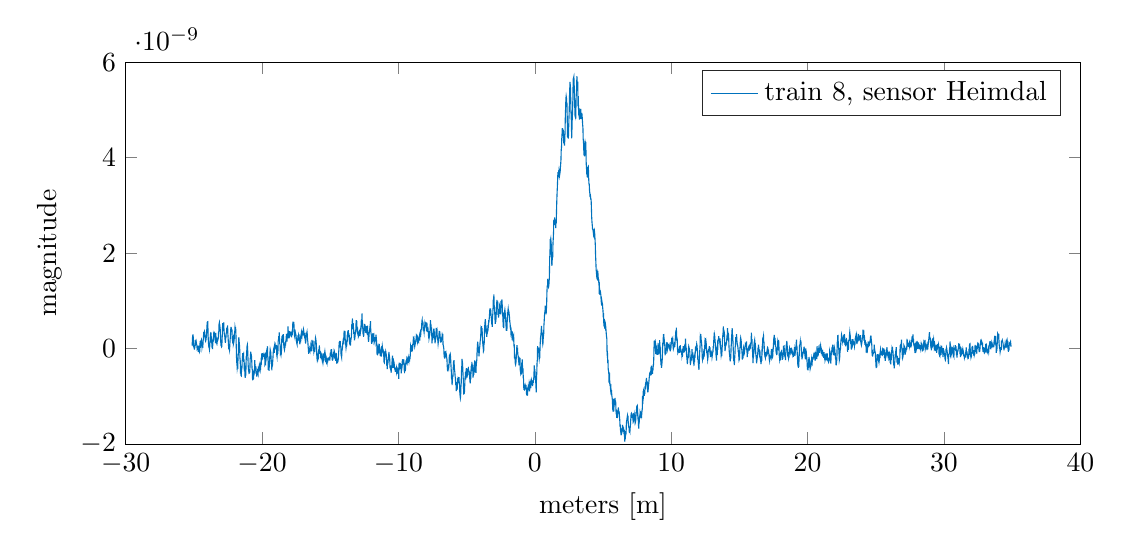
\begin{tikzpicture}

  \begin{axis}[%
    width=\textwidth,
    height=0.4\textwidth,
    at={(0\figurewidth,0\figureheight)},
    scale only axis,
    xmin=-30,
    xmax=40,
    xlabel={meters [m]},
    ymin=-2e-09,
    ymax=6e-09,
    ylabel={magnitude},
    axis background/.style={fill=white},
    legend style={legend cell align=left,align=left,draw=white!15!black}
    ]
    \addplot [color=mycolor1,solid]
    table[row sep=crcr]{%
    -25.1241796875	6.09100522353598e-11\\
    -25.1040302734375	1.77097476339483e-10\\
    -25.083880859375	1.45132953652219e-10\\
    -25.0637314453125	2.97634135380372e-10\\
    -25.04358203125	2.42389834998753e-10\\
    -25.0234326171875	1.64462267331719e-10\\
    -25.003283203125	1.65333291755123e-10\\
    -24.9831337890625	1.18745228213149e-11\\
    -24.962984375	-8.52056128653131e-12\\
    -24.9428349609375	-3.65144132925043e-12\\
    -24.922685546875	5.71581956526596e-11\\
    -24.9025361328125	6.20629532522323e-11\\
    -24.88238671875	8.79317524730627e-11\\
    -24.8622373046875	1.66734823952901e-10\\
    -24.842087890625	1.75848599297258e-10\\
    -24.8219384765625	1.37014748277552e-10\\
    -24.8017890625	8.99006577657088e-11\\
    -24.7816396484375	7.62848767611231e-11\\
    -24.761490234375	7.42203169663657e-12\\
    -24.7413408203125	2.6423149596019e-11\\
    -24.72119140625	6.85223217113919e-12\\
    -24.7010419921875	6.24519302462539e-11\\
    -24.680892578125	-6.7873930001571e-11\\
    -24.6607431640625	6.21302201896458e-11\\
    -24.64059375	-7.09145074653527e-11\\
    -24.6204443359375	-2.66056916043154e-11\\
    -24.600294921875	3.6581257585472e-11\\
    -24.5801455078125	-6.75802443387856e-11\\
    -24.55999609375	-5.24153998337585e-11\\
    -24.5398466796875	1.54565992339496e-10\\
    -24.519697265625	1.75892962615774e-11\\
    -24.4995478515625	1.53587538715337e-10\\
    -24.4793984375	1.61242139183183e-10\\
    -24.4592490234375	1.54772882026066e-10\\
    -24.439099609375	1.7906118643443e-10\\
    -24.4189501953125	1.39154718092675e-10\\
    -24.39880078125	2.88070385020051e-11\\
    -24.3786513671875	6.66665030390433e-11\\
    -24.358501953125	5.66569977938385e-11\\
    -24.3383525390625	4.76814755661708e-11\\
    -24.318203125	1.59875968163159e-10\\
    -24.2980537109375	2.10794973185777e-10\\
    -24.277904296875	3.38350934634986e-10\\
    -24.2577548828125	3.41870744366871e-10\\
    -24.23760546875	3.15762097207841e-10\\
    -24.2174560546875	3.56081577247938e-10\\
    -24.197306640625	3.35525897730688e-10\\
    -24.1771572265625	2.42289988280217e-10\\
    -24.1570078125	1.95001302525465e-10\\
    -24.1368583984375	1.57541628226843e-10\\
    -24.116708984375	1.70441207741173e-10\\
    -24.0965595703125	2.19581062922309e-10\\
    -24.07641015625	2.50408900201398e-10\\
    -24.0562607421875	3.60403521323588e-10\\
    -24.036111328125	4.74139356463553e-10\\
    -24.0159619140625	5.4866775084846e-10\\
    -23.9958125	5.61335706485433e-10\\
    -23.9756630859375	5.64366050339769e-10\\
    -23.955513671875	2.97083090242844e-10\\
    -23.9353642578125	1.52530720653068e-10\\
    -23.91521484375	7.24573063281311e-11\\
    -23.8950654296875	2.46369049902096e-11\\
    -23.874916015625	2.34833213684527e-11\\
    -23.8547666015625	-1.57737117643752e-11\\
    -23.8346171875	4.78485502347317e-11\\
    -23.8144677734375	1.44085051871516e-10\\
    -23.794318359375	2.39443457949517e-10\\
    -23.7741689453125	3.09490794532143e-10\\
    -23.75401953125	3.29744871719359e-10\\
    -23.7338701171875	3.2570303170453e-10\\
    -23.713720703125	1.24521898595851e-10\\
    -23.6935712890625	2.25164930951358e-10\\
    -23.673421875	2.10056998682733e-11\\
    -23.6532724609375	9.76671669424846e-11\\
    -23.633123046875	-7.94078488522515e-12\\
    -23.6129736328125	7.69855047804333e-11\\
    -23.59282421875	1.70479931047551e-10\\
    -23.5726748046875	1.67700892409438e-10\\
    -23.552525390625	2.65187039086307e-10\\
    -23.5323759765625	2.42451558293561e-10\\
    -23.5122265625	3.40663590613647e-10\\
    -23.4920771484375	3.30903132493949e-10\\
    -23.471927734375	3.12336506354908e-10\\
    -23.4517783203125	3.00243898531796e-10\\
    -23.43162890625	2.88762406132786e-10\\
    -23.4114794921875	1.15643190706565e-10\\
    -23.391330078125	3.26895954539872e-10\\
    -23.3711806640625	2.12962732540121e-10\\
    -23.35103125	1.55637218391921e-10\\
    -23.3308818359375	1.93090743558888e-10\\
    -23.310732421875	1.66792315600602e-10\\
    -23.2905830078125	1.35507972304163e-10\\
    -23.27043359375	1.80996935272376e-10\\
    -23.2502841796875	2.03417276774323e-10\\
    -23.230134765625	1.90416010392809e-10\\
    -23.2099853515625	2.14177119340777e-10\\
    -23.1898359375	3.35672513965528e-10\\
    -23.1696865234375	3.54688001314587e-10\\
    -23.149537109375	5.18986183588292e-10\\
    -23.1293876953125	5.42861190272567e-10\\
    -23.10923828125	4.52170565114411e-10\\
    -23.0890888671875	4.65788888210584e-10\\
    -23.068939453125	4.17501569619632e-10\\
    -23.0487900390625	3.01201190845758e-10\\
    -23.028640625	1.50666443953041e-10\\
    -23.0084912109375	6.70798509790579e-11\\
    -22.988341796875	6.0729613765365e-11\\
    -22.9681923828125	3.64794877552045e-11\\
    -22.94804296875	4.58634301374388e-11\\
    -22.9278935546875	2.09248050558924e-10\\
    -22.907744140625	2.92847561624108e-10\\
    -22.8875947265625	5.31650308362431e-10\\
    -22.8674453125	3.78593300888615e-10\\
    -22.8472958984375	5.03731213988438e-10\\
    -22.827146484375	4.3782215205279e-10\\
    -22.8069970703125	5.46748455868209e-10\\
    -22.78684765625	3.75594677727543e-10\\
    -22.7666982421875	3.08927206224027e-10\\
    -22.746548828125	2.8661733900429e-10\\
    -22.7263994140625	2.45063283575759e-10\\
    -22.70625	1.72395011551637e-10\\
    -22.6861005859375	1.23295369267913e-10\\
    -22.665951171875	2.135323439669e-10\\
    -22.6458017578125	2.35875651209384e-10\\
    -22.62565234375	3.18589169521452e-10\\
    -22.6055029296875	3.24492785801425e-10\\
    -22.585353515625	4.26573942773829e-10\\
    -22.5652041015625	4.34438115088896e-10\\
    -22.5450546875	3.60537306712453e-10\\
    -22.5249052734375	4.84103930454043e-10\\
    -22.504755859375	3.10468242158934e-10\\
    -22.4846064453125	2.13148130127816e-10\\
    -22.46445703125	1.09962529546372e-10\\
    -22.4443076171875	5.40340393402105e-12\\
    -22.424158203125	9.02752982126533e-12\\
    -22.4040087890625	2.64890043249041e-12\\
    -22.383859375	-2.91142369613088e-11\\
    -22.3637099609375	6.49082908220302e-11\\
    -22.343560546875	1.71862989630248e-10\\
    -22.3234111328125	2.37731592784106e-10\\
    -22.30326171875	3.48311701961925e-10\\
    -22.2831123046875	4.44871022197125e-10\\
    -22.262962890625	4.45186325074591e-10\\
    -22.2428134765625	3.89388368487528e-10\\
    -22.2226640625	3.99747691031506e-10\\
    -22.2025146484375	3.86581388590366e-10\\
    -22.182365234375	2.08658663861724e-10\\
    -22.1622158203125	1.65382506714478e-10\\
    -22.14206640625	1.92356312616512e-10\\
    -22.1219169921875	2.17853517370734e-10\\
    -22.101767578125	8.98567578092846e-11\\
    -22.0816181640625	1.14536141457475e-10\\
    -22.06146875	1.46835818436094e-10\\
    -22.0413193359375	1.95601436149496e-10\\
    -22.021169921875	3.28871390043428e-10\\
    -22.0010205078125	3.48042170060413e-10\\
    -21.98087109375	4.44904046961171e-10\\
    -21.9607216796875	4.05146179671549e-10\\
    -21.940572265625	4.52097595955538e-10\\
    -21.9204228515625	3.61836931949141e-10\\
    -21.9002734375	1.62585692220986e-10\\
    -21.8801240234375	-6.07511150705487e-11\\
    -21.859974609375	-2.84305604602558e-10\\
    -21.8398251953125	-3.12194230292473e-10\\
    -21.81967578125	-4.10658091600081e-10\\
    -21.7995263671875	-3.7053270604504e-10\\
    -21.779376953125	-3.82075551268938e-10\\
    -21.7592275390625	-1.98856416580285e-10\\
    -21.739078125	-1.03182297893173e-10\\
    -21.7189287109375	1.24872335630641e-10\\
    -21.698779296875	2.40893434632873e-10\\
    -21.6786298828125	1.45710290502353e-10\\
    -21.65848046875	9.20180500271847e-11\\
    -21.6383310546875	1.10104247350132e-12\\
    -21.618181640625	-2.04056205778398e-10\\
    -21.5980322265625	-2.50614222041625e-10\\
    -21.5778828125	-5.21675137142418e-10\\
    -21.5577333984375	-4.85296737994908e-10\\
    -21.537583984375	-5.6799127251362e-10\\
    -21.5174345703125	-5.73272894500396e-10\\
    -21.49728515625	-3.68037376905573e-10\\
    -21.4771357421875	-4.34791882640972e-10\\
    -21.456986328125	-2.74542662376624e-10\\
    -21.4368369140625	-2.03951912373666e-10\\
    -21.4166875	-9.51318189490488e-11\\
    -21.3965380859375	-1.41583298252515e-10\\
    -21.376388671875	-1.2765079907368e-10\\
    -21.3562392578125	-1.1211274355411e-10\\
    -21.33608984375	-2.7950403558848e-10\\
    -21.3159404296875	-2.29650706348501e-10\\
    -21.295791015625	-4.78860830954518e-10\\
    -21.2756416015625	-2.92024993223071e-10\\
    -21.2554921875	-5.46555820814104e-10\\
    -21.2353427734375	-6.14135189170539e-10\\
    -21.215193359375	-4.79861871683141e-10\\
    -21.1950439453125	-5.64856817827483e-10\\
    -21.17489453125	-4.02136366554635e-10\\
    -21.1547451171875	-1.65942708141669e-10\\
    -21.134595703125	-1.47413417251894e-10\\
    -21.1144462890625	-2.41914344537777e-11\\
    -21.094296875	6.47126422219472e-11\\
    -21.0741474609375	8.39346375390308e-11\\
    -21.053998046875	-1.49006515171297e-11\\
    -21.0338486328125	-1.70318317660809e-10\\
    -21.01369921875	-3.53249808561112e-10\\
    -20.9935498046875	-4.39330893850824e-10\\
    -20.973400390625	-4.75826763270177e-10\\
    -20.9532509765625	-5.15661888936394e-10\\
    -20.9331015625	-5.10295742802909e-10\\
    -20.9129521484375	-4.85237078338194e-10\\
    -20.892802734375	-4.87601249898859e-10\\
    -20.8726533203125	-2.28942228580696e-10\\
    -20.85250390625	-1.84914742876437e-10\\
    -20.8323544921875	-6.39611398419393e-11\\
    -20.812205078125	-1.05008758868987e-10\\
    -20.7920556640625	-1.21982426099288e-10\\
    -20.77190625	-1.64986578401672e-10\\
    -20.7517568359375	-2.71521128058328e-10\\
    -20.731607421875	-4.1331871608494e-10\\
    -20.7114580078125	-4.46950485026465e-10\\
    -20.69130859375	-6.63465170687326e-10\\
    -20.6711591796875	-5.31239261164757e-10\\
    -20.651009765625	-4.90330653062078e-10\\
    -20.6308603515625	-6.48704657627378e-10\\
    -20.6107109375	-4.64048328825296e-10\\
    -20.5905615234375	-5.61580167378353e-10\\
    -20.570412109375	-4.59640939236933e-10\\
    -20.5502626953125	-4.72025285909528e-10\\
    -20.53011328125	-2.39962577518976e-10\\
    -20.5099638671875	-3.99945032753008e-10\\
    -20.489814453125	-3.84180194131858e-10\\
    -20.4696650390625	-4.18192030548583e-10\\
    -20.449515625	-3.70167815432556e-10\\
    -20.4293662109375	-5.2132134317968e-10\\
    -20.409216796875	-4.79429414612569e-10\\
    -20.3890673828125	-5.85317349248237e-10\\
    -20.36891796875	-4.73534363142468e-10\\
    -20.3487685546875	-5.39835436918544e-10\\
    -20.328619140625	-4.81187335918191e-10\\
    -20.3084697265625	-5.04024359801479e-10\\
    -20.2883203125	-5.30811719657757e-10\\
    -20.2681708984375	-4.26123849113906e-10\\
    -20.248021484375	-4.43382449714584e-10\\
    -20.2278720703125	-4.10524166379961e-10\\
    -20.20772265625	-3.68343178575354e-10\\
    -20.1875732421875	-4.29501408512188e-10\\
    -20.167423828125	-4.61693061833336e-10\\
    -20.1472744140625	-4.77648484623198e-10\\
    -20.127125	-3.93119685729636e-10\\
    -20.1069755859375	-2.93752362207264e-10\\
    -20.086826171875	-3.36621498204701e-10\\
    -20.0666767578125	-2.56368977609066e-10\\
    -20.04652734375	-2.74585493813099e-10\\
    -20.0263779296875	-1.03839865937148e-10\\
    -20.006228515625	-2.44763076262421e-10\\
    -19.9860791015625	-9.41138049852914e-11\\
    -19.9659296875	-2.18566448724077e-10\\
    -19.9457802734375	-1.5538935669957e-10\\
    -19.925630859375	-1.54308571570424e-10\\
    -19.9054814453125	-1.53688736934424e-10\\
    -19.88533203125	-1.31297469002781e-10\\
    -19.8651826171875	-1.64842020237227e-10\\
    -19.845033203125	-1.65730066380136e-10\\
    -19.8248837890625	-1.30642612070654e-10\\
    -19.804734375	-1.48306394438028e-10\\
    -19.7845849609375	-3.22280346326155e-10\\
    -19.764435546875	-3.01708752437696e-10\\
    -19.7442861328125	-3.12916091091035e-10\\
    -19.72413671875	-1.04719998796523e-10\\
    -19.7039873046875	-1.14794927171579e-10\\
    -19.683837890625	-1.69989219680468e-10\\
    -19.6636884765625	-1.11714113169924e-10\\
    -19.6435390625	4.12637390497907e-12\\
    -19.6233896484375	-1.02167597992086e-10\\
    -19.603240234375	4.91123651235627e-11\\
    -19.5830908203125	-1.66818775156048e-10\\
    -19.56294140625	-1.9117482484315e-10\\
    -19.5427919921875	-4.33637441790867e-10\\
    -19.522642578125	-4.33892059587203e-10\\
    -19.5024931640625	-3.56786228506365e-10\\
    -19.48234375	-4.66742499539935e-10\\
    -19.4621943359375	-2.79828105497723e-10\\
    -19.442044921875	-2.46094662836865e-10\\
    -19.4218955078125	-1.07316062518242e-10\\
    -19.40174609375	-2.07567224922276e-11\\
    -19.3815966796875	-4.98816494349041e-11\\
    -19.361447265625	-7.09980464447147e-11\\
    -19.3412978515625	-1.71863028289659e-10\\
    -19.3211484375	-3.24481166950772e-10\\
    -19.3009990234375	-2.34154918995194e-10\\
    -19.280849609375	-4.54618009088128e-10\\
    -19.2607001953125	-3.05576117555472e-10\\
    -19.24055078125	-3.70948395059037e-10\\
    -19.2204013671875	-2.83608289768078e-10\\
    -19.200251953125	-1.96253717974613e-10\\
    -19.1801025390625	-9.28187130719241e-11\\
    -19.159953125	-2.91455928898585e-11\\
    -19.1398037109375	2.17398161130025e-12\\
    -19.119654296875	2.41164870949348e-11\\
    -19.0995048828125	-9.0253247131018e-11\\
    -19.07935546875	4.53432419924593e-11\\
    -19.0592060546875	1.160257202398e-11\\
    -19.039056640625	3.23070707626282e-11\\
    -19.0189072265625	2.30190746530205e-11\\
    -18.9987578125	6.11392348458458e-11\\
    -18.9786083984375	2.08352488324452e-11\\
    -18.958458984375	-2.03163202514416e-11\\
    -18.9383095703125	7.44268352814016e-11\\
    -18.91816015625	-1.34640740200174e-10\\
    -18.8980107421875	-1.73269442317813e-10\\
    -18.877861328125	-9.58001215887895e-11\\
    -18.8577119140625	-3.3112498815939e-11\\
    -18.8375625	-1.08726124224219e-10\\
    -18.8174130859375	1.57585385410838e-10\\
    -18.797263671875	1.59730460780274e-10\\
    -18.7771142578125	2.59001782719728e-10\\
    -18.75696484375	2.13450606440679e-10\\
    -18.7368154296875	3.42095067397973e-10\\
    -18.716666015625	1.61873413916563e-10\\
    -18.6965166015625	9.75248782157643e-11\\
    -18.6763671875	8.72986614411351e-11\\
    -18.6562177734375	-9.43905344069622e-11\\
    -18.636068359375	-7.99466881277656e-11\\
    -18.6159189453125	-1.1513165239539e-10\\
    -18.59576953125	-1.86265740435032e-11\\
    -18.5756201171875	-4.33650017065041e-11\\
    -18.555470703125	1.84580755904519e-10\\
    -18.5353212890625	2.51350805648735e-10\\
    -18.515171875	2.60049271150618e-10\\
    -18.4950224609375	1.26231490446912e-10\\
    -18.474873046875	2.59450402866911e-10\\
    -18.4547236328125	1.58307697663955e-10\\
    -18.43457421875	3.01757854994726e-10\\
    -18.4144248046875	1.22395830878678e-10\\
    -18.394275390625	2.54487182777731e-11\\
    -18.3741259765625	3.22212069622768e-12\\
    -18.3539765625	-2.45577282440871e-11\\
    -18.3338271484375	2.01134414368053e-11\\
    -18.313677734375	2.64411660787875e-11\\
    -18.2935283203125	1.34340814969706e-10\\
    -18.27337890625	6.29139671856047e-11\\
    -18.2532294921875	1.76413381923919e-10\\
    -18.233080078125	1.86686133885376e-10\\
    -18.2129306640625	3.03533776255804e-10\\
    -18.19278125	2.25124351409566e-10\\
    -18.1726318359375	1.44684809500091e-10\\
    -18.152482421875	3.19082706680399e-10\\
    -18.1323330078125	2.65109761753299e-10\\
    -18.11218359375	2.77771461607548e-10\\
    -18.0920341796875	4.63807219863359e-10\\
    -18.071884765625	2.14260626954689e-10\\
    -18.0517353515625	3.31622423735999e-10\\
    -18.0315859375	3.01377945091791e-10\\
    -18.0114365234375	2.86924059484887e-10\\
    -17.991287109375	3.67973295295328e-10\\
    -17.9711376953125	2.63090919343028e-10\\
    -17.95098828125	2.81122998904606e-10\\
    -17.9308388671875	3.44500424742968e-10\\
    -17.910689453125	3.3838145354215e-10\\
    -17.8905400390625	3.08635441945464e-10\\
    -17.870390625	3.09301362302215e-10\\
    -17.8502412109375	2.99305058989905e-10\\
    -17.830091796875	2.36500263711703e-10\\
    -17.8099423828125	3.59627787398914e-10\\
    -17.78979296875	3.68845112109878e-10\\
    -17.7696435546875	3.50196016491628e-10\\
    -17.749494140625	5.06787020222399e-10\\
    -17.7293447265625	5.66348149371587e-10\\
    -17.7091953125	5.04397708363139e-10\\
    -17.6890458984375	4.82860296140108e-10\\
    -17.668896484375	5.57854855339855e-10\\
    -17.6487470703125	4.43391122433201e-10\\
    -17.62859765625	2.81397652108128e-10\\
    -17.6084482421875	2.55621384762079e-10\\
    -17.588298828125	4.02007620109093e-10\\
    -17.5681494140625	2.88016897676503e-10\\
    -17.548	2.80814819449412e-10\\
    -17.5278505859375	3.04954160518067e-10\\
    -17.507701171875	2.79997939035758e-10\\
    -17.4875517578125	2.06339235648264e-10\\
    -17.46740234375	1.37413307232188e-10\\
    -17.4472529296875	1.04186375619813e-10\\
    -17.427103515625	8.31810494977059e-11\\
    -17.4069541015625	2.06275468542801e-10\\
    -17.3868046875	1.56679839313045e-10\\
    -17.3666552734375	2.77043914106125e-10\\
    -17.346505859375	2.37613609834109e-10\\
    -17.3263564453125	2.72008506922776e-10\\
    -17.30620703125	2.15336750394921e-10\\
    -17.2860576171875	2.96801935196957e-10\\
    -17.265908203125	1.5960617381643e-10\\
    -17.2457587890625	1.59113019826496e-10\\
    -17.225609375	9.01221034520076e-11\\
    -17.2054599609375	1.53621762340404e-10\\
    -17.185310546875	2.19905841174507e-10\\
    -17.1651611328125	2.51907760645466e-10\\
    -17.14501171875	2.15292877387156e-10\\
    -17.1248623046875	2.69301575117702e-10\\
    -17.104712890625	3.50213855669753e-10\\
    -17.0845634765625	3.26095569609167e-10\\
    -17.0644140625	2.82758209610458e-10\\
    -17.0442646484375	3.38405987332893e-10\\
    -17.024115234375	3.27568701661558e-10\\
    -17.0039658203125	2.77558196212278e-10\\
    -16.98381640625	3.67645781927966e-10\\
    -16.9636669921875	4.05829536724005e-10\\
    -16.943517578125	3.71744239365892e-10\\
    -16.9233681640625	2.93288600504188e-10\\
    -16.90321875	2.69902542615045e-10\\
    -16.8830693359375	3.28847199100047e-10\\
    -16.862919921875	2.50060009465811e-10\\
    -16.8427705078125	2.14149302970289e-10\\
    -16.82262109375	1.53601514499499e-10\\
    -16.8024716796875	1.0753782409962e-10\\
    -16.782322265625	2.21707005916299e-10\\
    -16.7621728515625	3.3272821730835e-10\\
    -16.7420234375	2.51802143072263e-10\\
    -16.7218740234375	3.28443947672199e-10\\
    -16.701724609375	3.52620886195672e-10\\
    -16.6815751953125	2.90734365980017e-10\\
    -16.66142578125	1.75292253324122e-10\\
    -16.6412763671875	1.48887692707414e-10\\
    -16.621126953125	5.19924977098139e-11\\
    -16.6009775390625	-1.12683787409647e-11\\
    -16.580828125	-1.11025615469135e-10\\
    -16.5606787109375	-3.80362150474092e-11\\
    -16.540529296875	-6.34855017778145e-11\\
    -16.5203798828125	-6.4333521867907e-11\\
    -16.50023046875	-6.27005728168472e-12\\
    -16.4800810546875	-3.49285306811519e-11\\
    -16.459931640625	3.62528128667518e-11\\
    -16.4397822265625	-5.76629122416958e-11\\
    -16.4196328125	4.75430294639217e-11\\
    -16.3994833984375	8.45124898495264e-12\\
    -16.379333984375	-1.30753290602919e-11\\
    -16.3591845703125	-5.86052336763846e-11\\
    -16.33903515625	1.82491643482995e-10\\
    -16.3188857421875	7.82158946228357e-11\\
    -16.298736328125	9.4047996666388e-11\\
    -16.2785869140625	1.0721462300452e-10\\
    -16.2584375	1.23735545502976e-10\\
    -16.2382880859375	4.59608130639469e-11\\
    -16.218138671875	-8.12215875873653e-12\\
    -16.1979892578125	-7.04316710637718e-11\\
    -16.17783984375	-4.00920095116032e-11\\
    -16.1576904296875	-5.35040749297252e-11\\
    -16.137541015625	-5.43586046727852e-11\\
    -16.1173916015625	1.53814868948743e-10\\
    -16.0972421875	9.81920547544642e-11\\
    -16.0770927734375	2.26519295315567e-10\\
    -16.056943359375	2.03849509786477e-10\\
    -16.0367939453125	1.50512062685668e-10\\
    -16.01664453125	7.2687850162389e-11\\
    -15.9964951171875	-5.37610087688033e-11\\
    -15.976345703125	-1.90854076390822e-10\\
    -15.9561962890625	-2.33201625568483e-10\\
    -15.936046875	-1.95326714161866e-10\\
    -15.9158974609375	-2.16358888164688e-10\\
    -15.895748046875	-1.60246968853953e-10\\
    -15.8755986328125	-1.77645850419606e-10\\
    -15.85544921875	-4.9260995410337e-11\\
    -15.8352998046875	-2.02749440238333e-11\\
    -15.815150390625	-1.72543351996929e-11\\
    -15.7950009765625	6.49922025231533e-11\\
    -15.7748515625	-7.45762787900899e-11\\
    -15.7547021484375	-6.49057388105232e-11\\
    -15.734552734375	-6.18454026092752e-11\\
    -15.7144033203125	-1.92796609754185e-10\\
    -15.69425390625	-1.54748798914323e-10\\
    -15.6741044921875	-1.33275498696599e-10\\
    -15.653955078125	-2.13733613462713e-10\\
    -15.6338056640625	-2.12167767408841e-10\\
    -15.61365625	-9.89371836659823e-11\\
    -15.5935068359375	-2.3923160088463e-10\\
    -15.573357421875	-2.75115015600537e-10\\
    -15.5532080078125	-2.70862881122901e-10\\
    -15.53305859375	-3.04273176230836e-10\\
    -15.5129091796875	-2.63182149857898e-10\\
    -15.492759765625	-1.13630925506162e-10\\
    -15.4726103515625	-1.10758056166246e-10\\
    -15.4524609375	-1.20376231188142e-10\\
    -15.4323115234375	-1.61812566585794e-10\\
    -15.412162109375	-9.42643776921943e-11\\
    -15.3920126953125	-5.77811925647889e-11\\
    -15.37186328125	-1.0819773988238e-10\\
    -15.3517138671875	-1.18237758409675e-10\\
    -15.331564453125	-2.6887377115612e-10\\
    -15.3114150390625	-2.71304831543952e-10\\
    -15.291265625	-2.86377180674361e-10\\
    -15.2711162109375	-2.28428673858943e-10\\
    -15.250966796875	-2.60623648924315e-10\\
    -15.2308173828125	-2.91609541357053e-10\\
    -15.21066796875	-2.07242225845131e-10\\
    -15.1905185546875	-2.94973176814026e-10\\
    -15.170369140625	-1.90432656724359e-10\\
    -15.1502197265625	-2.3205469115027e-10\\
    -15.1300703125	-2.32265634852233e-10\\
    -15.1099208984375	-1.9664526994773e-10\\
    -15.089771484375	-1.92871261899374e-10\\
    -15.0696220703125	-1.99377152403317e-10\\
    -15.04947265625	-1.86246416988528e-10\\
    -15.0293232421875	-2.51125115444237e-10\\
    -15.009173828125	-1.63982176452646e-10\\
    -14.9890244140625	-7.80050569346086e-11\\
    -14.968875	-1.57198360888391e-10\\
    -14.9487255859375	-2.00567617587825e-11\\
    -14.928576171875	-7.78212431664821e-11\\
    -14.9084267578125	-1.36297364032525e-11\\
    -14.88827734375	-1.78822229943891e-10\\
    -14.8681279296875	-1.21157592473015e-10\\
    -14.847978515625	-2.37710331569699e-10\\
    -14.8278291015625	-2.40901974117921e-10\\
    -14.8076796875	-2.28506506649224e-10\\
    -14.7875302734375	-1.80766380833351e-10\\
    -14.767380859375	-6.90387362920617e-11\\
    -14.7472314453125	-1.57945576813125e-10\\
    -14.72708203125	-8.88425774045153e-11\\
    -14.7069326171875	-1.28984416894277e-10\\
    -14.686783203125	-8.19436006022229e-11\\
    -14.6666337890625	-1.15603113969342e-10\\
    -14.646484375	-1.9286986247562e-10\\
    -14.6263349609375	-1.27305517700884e-10\\
    -14.606185546875	-2.54544257106351e-10\\
    -14.5860361328125	-1.40907228889922e-10\\
    -14.56588671875	-8.79862288415916e-11\\
    -14.5457373046875	-1.5434549848831e-10\\
    -14.525587890625	-2.93062295123578e-10\\
    -14.5054384765625	-2.86457511390023e-10\\
    -14.4852890625	-2.35377628835033e-10\\
    -14.4651396484375	-3.0726772093135e-10\\
    -14.444990234375	-2.18362815728822e-10\\
    -14.4248408203125	-2.71891911127102e-10\\
    -14.40469140625	-1.79612380015934e-10\\
    -14.3845419921875	-8.09780268063393e-11\\
    -14.364392578125	-2.41941421948395e-11\\
    -14.3442431640625	1.40740370144356e-10\\
    -14.32409375	1.01954041215394e-10\\
    -14.3039443359375	1.61914079101858e-10\\
    -14.283794921875	2.73927880614294e-11\\
    -14.2636455078125	1.54864567079257e-10\\
    -14.24349609375	4.04717866822809e-11\\
    -14.2233466796875	3.43452284428708e-11\\
    -14.203197265625	-1.40731490490206e-10\\
    -14.1830478515625	-1.52378128241684e-10\\
    -14.1628984375	-1.83053322562132e-10\\
    -14.1427490234375	-5.12128510117106e-11\\
    -14.122599609375	-1.96794830365471e-11\\
    -14.1024501953125	2.66898897333994e-11\\
    -14.08230078125	1.08156546480917e-10\\
    -14.0621513671875	1.49956407319605e-10\\
    -14.042001953125	1.34218800744088e-10\\
    -14.0218525390625	2.27072645459714e-10\\
    -14.001703125	1.72291671060045e-10\\
    -13.9815537109375	3.771220164429e-10\\
    -13.961404296875	2.48602503887337e-10\\
    -13.9412548828125	3.16802575278091e-10\\
    -13.92110546875	3.68581281564729e-10\\
    -13.9009560546875	1.4135284681422e-10\\
    -13.880806640625	1.54593829090276e-10\\
    -13.8606572265625	7.92324110660307e-11\\
    -13.8405078125	1.29866826840424e-11\\
    -13.8203583984375	5.66095715177011e-11\\
    -13.800208984375	5.58793253542915e-11\\
    -13.7800595703125	9.15061281708433e-11\\
    -13.75991015625	2.30031839282925e-10\\
    -13.7397607421875	2.13204919229731e-10\\
    -13.719611328125	3.29727792801051e-10\\
    -13.6994619140625	3.22576568083244e-10\\
    -13.6793125	3.84692051209662e-10\\
    -13.6591630859375	2.70538574792893e-10\\
    -13.639013671875	3.21267778201022e-10\\
    -13.6188642578125	2.43787050957681e-10\\
    -13.59871484375	2.87579406024275e-10\\
    -13.5785654296875	1.61976030264953e-10\\
    -13.558416015625	7.44090474286491e-11\\
    -13.5382666015625	2.19227037299636e-10\\
    -13.5181171875	6.5026527973264e-11\\
    -13.4979677734375	1.45289379541836e-10\\
    -13.477818359375	1.97133158301523e-10\\
    -13.4576689453125	2.25352328934705e-10\\
    -13.43751953125	3.10211232717674e-10\\
    -13.4173701171875	5.1036871079979e-10\\
    -13.397220703125	4.07490121595227e-10\\
    -13.3770712890625	6.30236425599302e-10\\
    -13.356921875	5.61729268534242e-10\\
    -13.3367724609375	4.31719556264297e-10\\
    -13.316623046875	5.3514215028448e-10\\
    -13.2964736328125	4.42296251571089e-10\\
    -13.27632421875	3.11126208692576e-10\\
    -13.2561748046875	3.50111279728943e-10\\
    -13.236025390625	2.31313060680782e-10\\
    -13.2158759765625	1.72373159712124e-10\\
    -13.1957265625	2.32769263687568e-10\\
    -13.1755771484375	2.53683324566279e-10\\
    -13.155427734375	3.91635189607024e-10\\
    -13.1352783203125	3.13801270435585e-10\\
    -13.11512890625	4.67202127976037e-10\\
    -13.0949794921875	5.98858494065542e-10\\
    -13.074830078125	4.63893489845097e-10\\
    -13.0546806640625	5.80143578343122e-10\\
    -13.03453125	4.14667780302622e-10\\
    -13.0143818359375	3.81996346248529e-10\\
    -12.994232421875	4.42541323437003e-10\\
    -12.9740830078125	2.70832461824159e-10\\
    -12.95393359375	3.49455198070514e-10\\
    -12.9337841796875	2.5662932818124e-10\\
    -12.913634765625	2.74088402007279e-10\\
    -12.8934853515625	3.17484143066418e-10\\
    -12.8733359375	3.41317148515852e-10\\
    -12.8531865234375	2.65422743242692e-10\\
    -12.833037109375	3.82546327118522e-10\\
    -12.8128876953125	2.63332905524373e-10\\
    -12.79273828125	3.41605799628665e-10\\
    -12.7725888671875	3.95015761610265e-10\\
    -12.752439453125	3.59193386180271e-10\\
    -12.7322900390625	5.38599880032655e-10\\
    -12.712140625	6.12305395174205e-10\\
    -12.6919912109375	4.48035098358065e-10\\
    -12.671841796875	7.35270463277405e-10\\
    -12.6516923828125	5.59184075564123e-10\\
    -12.63154296875	5.39370174070919e-10\\
    -12.6113935546875	4.17381656535818e-10\\
    -12.591244140625	3.04061130723642e-10\\
    -12.5710947265625	3.04934166769993e-10\\
    -12.5509453125	2.49448105371659e-10\\
    -12.5307958984375	3.318175413916e-10\\
    -12.510646484375	3.60528971685486e-10\\
    -12.4904970703125	5.17945471887984e-10\\
    -12.47034765625	4.4071193020588e-10\\
    -12.4501982421875	5.0106632936508e-10\\
    -12.430048828125	3.99979018951807e-10\\
    -12.4098994140625	3.88411678394121e-10\\
    -12.38975	3.28771003989307e-10\\
    -12.3696005859375	4.73019828985843e-10\\
    -12.349451171875	3.75664857612e-10\\
    -12.3293017578125	3.54074980436785e-10\\
    -12.30915234375	4.59637748479335e-10\\
    -12.2890029296875	3.90171488834082e-10\\
    -12.268853515625	4.79113165484162e-10\\
    -12.2487041015625	3.29971133527912e-10\\
    -12.2285546875	2.94924091781619e-10\\
    -12.2084052734375	1.94433858066764e-10\\
    -12.188255859375	1.4130838968878e-10\\
    -12.1681064453125	2.16904466461669e-10\\
    -12.14795703125	3.02925101369449e-10\\
    -12.1278076171875	3.66401084091321e-10\\
    -12.107658203125	3.99336166043259e-10\\
    -12.0875087890625	4.48840201776105e-10\\
    -12.067359375	4.10079863176711e-10\\
    -12.0472099609375	5.77707417058471e-10\\
    -12.027060546875	3.55629594797523e-10\\
    -12.0069111328125	3.21072315874809e-10\\
    -11.98676171875	2.78931680607806e-10\\
    -11.9666123046875	9.98778316985211e-11\\
    -11.946462890625	2.33573918904527e-10\\
    -11.9263134765625	1.34496905561028e-10\\
    -11.9061640625	2.23354695625428e-10\\
    -11.8860146484375	1.87920925088514e-10\\
    -11.865865234375	1.61560591529522e-10\\
    -11.8457158203125	3.20676316728847e-10\\
    -11.82556640625	2.71372562445477e-10\\
    -11.8054169921875	2.86539438772768e-10\\
    -11.785267578125	1.9660106081706e-10\\
    -11.7651181640625	1.90567085659109e-10\\
    -11.74496875	1.46612878482638e-10\\
    -11.7248193359375	1.22187365843471e-10\\
    -11.704669921875	2.41166041232903e-10\\
    -11.6845205078125	1.89097767667337e-10\\
    -11.66437109375	1.85090976592702e-10\\
    -11.6442216796875	2.90823139950801e-10\\
    -11.624072265625	2.25523187674084e-10\\
    -11.6039228515625	1.56780230812399e-10\\
    -11.5837734375	6.03446514913538e-11\\
    -11.5636240234375	-1.3004129191782e-10\\
    -11.543474609375	1.68145533469924e-11\\
    -11.5233251953125	-1.43556068828692e-10\\
    -11.50317578125	-1.32240017794804e-11\\
    -11.4830263671875	-4.22671388673499e-11\\
    -11.462876953125	-1.00588272530374e-10\\
    -11.4427275390625	5.13433904055761e-11\\
    -11.422578125	9.02969850643481e-11\\
    -11.4024287109375	8.64820991279371e-11\\
    -11.382279296875	9.24930232852432e-12\\
    -11.3621298828125	-5.13599174432622e-11\\
    -11.34198046875	-1.12920582024495e-10\\
    -11.3218310546875	-1.57741044383662e-10\\
    -11.301681640625	-6.70187103494575e-11\\
    -11.2815322265625	-3.86127616490612e-11\\
    -11.2613828125	-1.6894215202255e-10\\
    -11.2412333984375	-9.97873657260448e-11\\
    -11.221083984375	-2.75433343880841e-11\\
    -11.2009345703125	-2.97434119723983e-11\\
    -11.18078515625	4.82142904027865e-11\\
    -11.1606357421875	4.46911518265955e-12\\
    -11.140486328125	-7.5681827746237e-11\\
    -11.1203369140625	-6.16410815550393e-12\\
    -11.1001875	-1.46436164798334e-10\\
    -11.0800380859375	-8.33730251146535e-11\\
    -11.059888671875	-2.79242109109009e-10\\
    -11.0397392578125	-2.89945319154428e-10\\
    -11.01958984375	-6.00177411740062e-11\\
    -10.9994404296875	-1.62818143405012e-10\\
    -10.979291015625	-1.05042097285197e-10\\
    -10.9591416015625	-6.70329339027781e-11\\
    -10.9389921875	-1.05021150486399e-10\\
    -10.9188427734375	-1.56120016299471e-10\\
    -10.898693359375	-1.17193133133276e-10\\
    -10.8785439453125	-1.54870917277247e-10\\
    -10.85839453125	-3.54684860022778e-10\\
    -10.8382451171875	-2.3390297677061e-10\\
    -10.818095703125	-4.28653781374532e-10\\
    -10.7979462890625	-2.57296787007253e-10\\
    -10.777796875	-3.3476440162826e-10\\
    -10.7576474609375	-2.6094680061982e-10\\
    -10.737498046875	-2.11625159159747e-10\\
    -10.7173486328125	-1.6281771257709e-10\\
    -10.69719921875	-6.96930932902929e-11\\
    -10.6770498046875	-1.26505905500507e-10\\
    -10.656900390625	-1.68978167199248e-10\\
    -10.6367509765625	-2.25570472102341e-10\\
    -10.6166015625	-3.92128171448651e-10\\
    -10.5964521484375	-4.11282227030662e-10\\
    -10.576302734375	-3.87362570996122e-10\\
    -10.5561533203125	-3.52123630561379e-10\\
    -10.53600390625	-5.08166870918981e-10\\
    -10.5158544921875	-4.23626970676023e-10\\
    -10.495705078125	-4.10536063228333e-10\\
    -10.4755556640625	-3.13435229774875e-10\\
    -10.45540625	-2.15882054960331e-10\\
    -10.4352568359375	-1.4876973641952e-10\\
    -10.415107421875	-3.65323300993088e-10\\
    -10.3949580078125	-4.01926744863395e-10\\
    -10.37480859375	-2.0693342011623e-10\\
    -10.3546591796875	-3.84558167907583e-10\\
    -10.334509765625	-2.75525168124183e-10\\
    -10.3143603515625	-2.96979106850731e-10\\
    -10.2942109375	-3.90749418885222e-10\\
    -10.2740615234375	-4.20638757672511e-10\\
    -10.253912109375	-4.1618356455775e-10\\
    -10.2337626953125	-4.74017874003838e-10\\
    -10.21361328125	-4.75583614207729e-10\\
    -10.1934638671875	-4.31643081096564e-10\\
    -10.173314453125	-4.2897220293517e-10\\
    -10.1531650390625	-4.02313213160722e-10\\
    -10.133015625	-4.80547552102466e-10\\
    -10.1128662109375	-4.42271638017951e-10\\
    -10.092716796875	-4.82816507075465e-10\\
    -10.0725673828125	-4.6210313003322e-10\\
    -10.05241796875	-5.25057128690431e-10\\
    -10.0322685546875	-4.64885071243052e-10\\
    -10.012119140625	-4.96762652501473e-10\\
    -9.9919697265625	-4.68789426807906e-10\\
    -9.9718203125	-6.3358998789323e-10\\
    -9.9516708984375	-2.9332703287719e-10\\
    -9.931521484375	-4.34364514988521e-10\\
    -9.9113720703125	-3.91573713175637e-10\\
    -9.89122265625	-3.41277369288374e-10\\
    -9.8710732421875	-3.0012923582515e-10\\
    -9.850923828125	-4.29045412414096e-10\\
    -9.8307744140625	-3.24149609219286e-10\\
    -9.810625	-4.07558920549499e-10\\
    -9.7904755859375	-5.19848467860268e-10\\
    -9.770326171875	-3.70895785563775e-10\\
    -9.7501767578125	-4.14861753593707e-10\\
    -9.73002734375	-3.78558441930217e-10\\
    -9.7098779296875	-2.23602146171615e-10\\
    -9.689728515625	-3.34707751697541e-10\\
    -9.6695791015625	-2.20619094495698e-10\\
    -9.6494296875	-3.00318877241383e-10\\
    -9.6292802734375	-2.85969539798056e-10\\
    -9.609130859375	-2.28796598528532e-10\\
    -9.5889814453125	-3.17494209324742e-10\\
    -9.56883203125	-4.55077472254421e-10\\
    -9.5486826171875	-4.86861374974881e-10\\
    -9.528533203125	-4.73948200651309e-10\\
    -9.5083837890625	-4.12120681832844e-10\\
    -9.488234375	-4.65337980625788e-10\\
    -9.4680849609375	-3.27129636300819e-10\\
    -9.447935546875	-2.8526049215082e-10\\
    -9.4277861328125	-3.00408270783398e-10\\
    -9.40763671875	-2.66894190525848e-10\\
    -9.3874873046875	-2.1897707524362e-10\\
    -9.367337890625	-2.46670056700958e-10\\
    -9.3471884765625	-2.86522041601007e-10\\
    -9.3270390625	-2.51312224725968e-10\\
    -9.3068896484375	-2.41016450707072e-10\\
    -9.286740234375	-1.63878909042032e-10\\
    -9.2665908203125	-2.97787284692923e-10\\
    -9.24644140625	-2.1735886353001e-10\\
    -9.2262919921875	-2.59800346735554e-10\\
    -9.206142578125	-2.08343002075219e-10\\
    -9.1859931640625	-2.73664602092554e-10\\
    -9.16584375	-1.62714277249078e-10\\
    -9.1456943359375	-2.19858149260959e-10\\
    -9.125544921875	-9.5640208447639e-11\\
    -9.1053955078125	4.65705345977254e-11\\
    -9.08524609375	1.65223722778101e-11\\
    -9.0650966796875	7.04599198427203e-11\\
    -9.044947265625	8.77927082718294e-13\\
    -9.0247978515625	-2.67191855876919e-11\\
    -9.0046484375	-5.67894607603773e-12\\
    -8.9844990234375	3.10807022882734e-11\\
    -8.964349609375	-7.23741813993808e-13\\
    -8.9442001953125	4.41543040886789e-11\\
    -8.92405078125	9.32392173468078e-11\\
    -8.9039013671875	2.19533117873924e-10\\
    -8.883751953125	2.07811478902899e-10\\
    -8.8636025390625	2.23554167946129e-10\\
    -8.843453125	1.70030404887959e-10\\
    -8.8233037109375	9.37556261042625e-11\\
    -8.803154296875	4.47508935716272e-11\\
    -8.7830048828125	7.59087700576568e-11\\
    -8.76285546875	1.36751922524776e-10\\
    -8.7427060546875	1.27288969996443e-10\\
    -8.722556640625	1.61699190473622e-10\\
    -8.7024072265625	2.11370546759424e-10\\
    -8.6822578125	2.82273884644581e-10\\
    -8.6621083984375	2.71809613017466e-10\\
    -8.641958984375	2.38961790593329e-10\\
    -8.6218095703125	1.82661894662355e-10\\
    -8.60166015625	1.45668646310447e-10\\
    -8.5815107421875	1.96078681979933e-10\\
    -8.561361328125	1.45075033921813e-10\\
    -8.5412119140625	1.44065483931726e-10\\
    -8.5210625	1.35480206359725e-10\\
    -8.5009130859375	2.14704998385586e-10\\
    -8.480763671875	2.31555266235233e-10\\
    -8.4606142578125	2.62702045154592e-10\\
    -8.44046484375	1.66934983154338e-10\\
    -8.4203154296875	2.51576115792365e-10\\
    -8.400166015625	2.98758240717256e-10\\
    -8.3800166015625	2.40696656927458e-10\\
    -8.3598671875	3.12275676531386e-10\\
    -8.3397177734375	3.85259838803747e-10\\
    -8.319568359375	4.05532230574758e-10\\
    -8.2994189453125	4.52226113274211e-10\\
    -8.27926953125	5.70339032970331e-10\\
    -8.2591201171875	6.00283539512312e-10\\
    -8.238970703125	5.04708997227411e-10\\
    -8.2188212890625	5.56378870520908e-10\\
    -8.198671875	5.38015848987008e-10\\
    -8.1785224609375	3.78997719065268e-10\\
    -8.158373046875	4.54791692670939e-10\\
    -8.1382236328125	3.80941125498763e-10\\
    -8.11807421875	3.39999096355769e-10\\
    -8.0979248046875	4.13374002238362e-10\\
    -8.077775390625	4.51260520818229e-10\\
    -8.0576259765625	5.24877027194042e-10\\
    -8.0374765625	4.92935782545915e-10\\
    -8.0173271484375	5.28873348894706e-10\\
    -7.997177734375	5.14866135586274e-10\\
    -7.9770283203125	5.05675649781441e-10\\
    -7.95687890625	5.49181423113694e-10\\
    -7.9367294921875	3.60329519259997e-10\\
    -7.916580078125	5.42782265899267e-10\\
    -7.8964306640625	4.91918521456355e-10\\
    -7.87628125	3.50356947289467e-10\\
    -7.8561318359375	4.14634541183461e-10\\
    -7.835982421875	4.24573679867431e-10\\
    -7.8158330078125	3.6454073069379e-10\\
    -7.79568359375	2.84355735067265e-10\\
    -7.7755341796875	3.04848911228756e-10\\
    -7.755384765625	2.12536479246936e-10\\
    -7.7352353515625	2.4551831330833e-10\\
    -7.7150859375	2.9160329670954e-10\\
    -7.6949365234375	3.04508560644368e-10\\
    -7.674787109375	3.89916809413064e-10\\
    -7.6546376953125	5.98016652682056e-10\\
    -7.63448828125	5.1926903330091e-10\\
    -7.6143388671875	4.99243780798426e-10\\
    -7.594189453125	3.75564838247058e-10\\
    -7.5740400390625	4.44379716856073e-10\\
    -7.553890625	2.71995937600012e-10\\
    -7.5337412109375	1.08193158402168e-10\\
    -7.513591796875	2.31737661568658e-10\\
    -7.4934423828125	1.8574534313653e-10\\
    -7.47329296875	3.02811871723824e-10\\
    -7.4531435546875	3.27553665205744e-10\\
    -7.432994140625	3.44335558288813e-10\\
    -7.4128447265625	4.15700934479344e-10\\
    -7.3926953125	3.06403505715049e-10\\
    -7.3725458984375	3.32265501881497e-10\\
    -7.352396484375	1.91888447404946e-10\\
    -7.3322470703125	2.58019010459945e-10\\
    -7.31209765625	1.10931875035973e-10\\
    -7.2919482421875	1.80134250786622e-10\\
    -7.271798828125	2.5641539530001e-10\\
    -7.2516494140625	2.61120398003317e-10\\
    -7.2315	4.36430087113128e-10\\
    -7.2113505859375	3.38548584839532e-10\\
    -7.191201171875	3.53444443324798e-10\\
    -7.1710517578125	3.76120318232492e-10\\
    -7.15090234375	2.32852775079016e-10\\
    -7.1307529296875	1.8353347497639e-10\\
    -7.110603515625	1.73373717771056e-10\\
    -7.0904541015625	1.01750219489491e-10\\
    -7.0703046875	1.48597081783427e-10\\
    -7.0501552734375	1.91723221451755e-10\\
    -7.030005859375	2.7089619411675e-10\\
    -7.0098564453125	3.69336729426781e-10\\
    -6.98970703125	2.79432057761731e-10\\
    -6.9695576171875	3.59854718401144e-10\\
    -6.949408203125	2.87675001368694e-10\\
    -6.9292587890625	2.22225206710315e-10\\
    -6.909109375	1.28609282719251e-10\\
    -6.8889599609375	2.32610244763362e-10\\
    -6.868810546875	1.32312240286898e-10\\
    -6.8486611328125	1.76062751113193e-10\\
    -6.82851171875	1.83455784327866e-10\\
    -6.8083623046875	2.25944448820286e-10\\
    -6.788212890625	2.98927211282998e-10\\
    -6.7680634765625	2.81717084144693e-10\\
    -6.7479140625	2.86140356225884e-10\\
    -6.7277646484375	8.2692543230135e-11\\
    -6.707615234375	6.83643918308243e-11\\
    -6.6874658203125	3.01800455419831e-11\\
    -6.66731640625	-9.51505460160035e-12\\
    -6.6471669921875	-1.80598956902662e-10\\
    -6.627017578125	-1.20893054045145e-10\\
    -6.6068681640625	-2.08626287850737e-10\\
    -6.58671875	-1.42612648128286e-10\\
    -6.5665693359375	-1.51367030745661e-10\\
    -6.546419921875	-6.90145171402461e-11\\
    -6.5262705078125	-6.25856080310532e-11\\
    -6.50612109375	-1.15107319751585e-10\\
    -6.4859716796875	-1.15347276603608e-10\\
    -6.465822265625	-1.95402785032575e-10\\
    -6.4456728515625	-2.05085672612689e-10\\
    -6.4255234375	-3.3298168889671e-10\\
    -6.4053740234375	-4.49509051834856e-10\\
    -6.385224609375	-4.5835592404879e-10\\
    -6.3650751953125	-3.86711681481951e-10\\
    -6.34492578125	-3.50078326365266e-10\\
    -6.3247763671875	-3.42466024791901e-10\\
    -6.304626953125	-3.78226575686508e-10\\
    -6.2844775390625	-3.06820583530658e-10\\
    -6.264328125	-1.3181061449317e-10\\
    -6.2441787109375	-2.00375206237846e-10\\
    -6.224029296875	-1.06463097351905e-10\\
    -6.2038798828125	-1.97421666112831e-10\\
    -6.18373046875	-1.59442291776383e-10\\
    -6.1635810546875	-2.4556264471392e-10\\
    -6.143431640625	-3.71135358634931e-10\\
    -6.1232822265625	-4.73748070124069e-10\\
    -6.1031328125	-6.31198138928998e-10\\
    -6.0829833984375	-6.45123659525329e-10\\
    -6.062833984375	-7.64201548187863e-10\\
    -6.0426845703125	-6.43161442839327e-10\\
    -6.02253515625	-5.88756845274895e-10\\
    -6.0023857421875	-5.82952425129892e-10\\
    -5.982236328125	-4.35849878085439e-10\\
    -5.9620869140625	-2.83778359949338e-10\\
    -5.9419375	-2.55874184514793e-10\\
    -5.9217880859375	-2.54374026448029e-10\\
    -5.901638671875	-3.95326732588867e-10\\
    -5.8814892578125	-4.50065687815549e-10\\
    -5.86133984375	-4.94597863309154e-10\\
    -5.8411904296875	-5.91103427889728e-10\\
    -5.821041015625	-6.02918465672506e-10\\
    -5.8008916015625	-7.64381193669278e-10\\
    -5.7807421875	-6.97019175238087e-10\\
    -5.7605927734375	-8.90296384730516e-10\\
    -5.740443359375	-7.83018960982548e-10\\
    -5.7202939453125	-7.91550310608049e-10\\
    -5.70014453125	-8.65382306782521e-10\\
    -5.6799951171875	-8.02852678964711e-10\\
    -5.659845703125	-6.66975598914147e-10\\
    -5.6396962890625	-6.79120665988313e-10\\
    -5.619546875	-6.17780138588639e-10\\
    -5.5993974609375	-6.26515811936756e-10\\
    -5.579248046875	-6.07483665392483e-10\\
    -5.5590986328125	-6.08700448594192e-10\\
    -5.53894921875	-7.16694958852505e-10\\
    -5.5187998046875	-7.42710842415548e-10\\
    -5.498650390625	-9.21052171738548e-10\\
    -5.4785009765625	-9.87867321897279e-10\\
    -5.4583515625	-1.03742643326018e-09\\
    -5.4382021484375	-9.96607982220547e-10\\
    -5.418052734375	-8.03558563123285e-10\\
    -5.3979033203125	-7.38492358018581e-10\\
    -5.37775390625	-4.75569886360702e-10\\
    -5.3576044921875	-4.18554111599293e-10\\
    -5.337455078125	-2.12992520610426e-10\\
    -5.3173056640625	-3.60660001976308e-10\\
    -5.29715625	-3.34540171234099e-10\\
    -5.2770068359375	-4.33303300160411e-10\\
    -5.256857421875	-5.94456152405491e-10\\
    -5.2367080078125	-6.59727600936999e-10\\
    -5.21655859375	-9.61514692398743e-10\\
    -5.1964091796875	-8.60782374382767e-10\\
    -5.176259765625	-8.69922853020606e-10\\
    -5.1561103515625	-8.87495509336641e-10\\
    -5.1359609375	-7.52267557072157e-10\\
    -5.1158115234375	-6.16184585418366e-10\\
    -5.095662109375	-5.78878359533807e-10\\
    -5.0755126953125	-4.82042828050169e-10\\
    -5.05536328125	-6.44903065155487e-10\\
    -5.0352138671875	-4.51605638987145e-10\\
    -5.015064453125	-4.07652988139492e-10\\
    -4.9949150390625	-5.47641937114966e-10\\
    -4.974765625	-6.05064584777577e-10\\
    -4.9546162109375	-4.99803573456985e-10\\
    -4.934466796875	-5.61274557192086e-10\\
    -4.9143173828125	-5.47854754613398e-10\\
    -4.89416796875	-4.152975141463e-10\\
    -4.8740185546875	-4.05804923292429e-10\\
    -4.853869140625	-4.5305943328286e-10\\
    -4.8337197265625	-4.64224114909567e-10\\
    -4.8135703125	-4.78413441720049e-10\\
    -4.7934208984375	-4.98873230052048e-10\\
    -4.773271484375	-6.09834949260409e-10\\
    -4.7531220703125	-6.92880831631093e-10\\
    -4.73297265625	-7.26133126845351e-10\\
    -4.7128232421875	-4.89778519145659e-10\\
    -4.692673828125	-6.46327023818028e-10\\
    -4.6725244140625	-4.16677779599264e-10\\
    -4.652375	-4.32034877669498e-10\\
    -4.6322255859375	-4.12702739165642e-10\\
    -4.612076171875	-2.80587847441244e-10\\
    -4.5919267578125	-4.70249950571652e-10\\
    -4.57177734375	-3.87277106972805e-10\\
    -4.5516279296875	-3.38788170605223e-10\\
    -4.531478515625	-6.05373412331065e-10\\
    -4.5113291015625	-5.65918813942399e-10\\
    -4.4911796875	-4.04471131603445e-10\\
    -4.4710302734375	-5.48577580546038e-10\\
    -4.450880859375	-4.06570667393452e-10\\
    -4.4307314453125	-3.87903674895494e-10\\
    -4.41058203125	-2.48305148651292e-10\\
    -4.3904326171875	-3.50309229223965e-10\\
    -4.370283203125	-4.95803931131536e-10\\
    -4.3501337890625	-3.91440085824061e-10\\
    -4.329984375	-4.71412987438887e-10\\
    -4.3098349609375	-5.05767741867277e-10\\
    -4.289685546875	-2.77313619916289e-10\\
    -4.2695361328125	-2.8189773204987e-10\\
    -4.24938671875	-2.18254682815449e-10\\
    -4.2292373046875	-3.37452565182636e-11\\
    -4.209087890625	5.37483137590504e-11\\
    -4.1889384765625	1.4367226081889e-10\\
    -4.1687890625	1.1658936743561e-11\\
    -4.1486396484375	2.70059797954699e-11\\
    -4.128490234375	-6.06050754987989e-11\\
    -4.1083408203125	-5.34530172550179e-11\\
    -4.08819140625	-1.61556552604311e-10\\
    -4.0680419921875	-3.36840819173846e-11\\
    -4.047892578125	2.1778354465206e-11\\
    -4.0277431640625	5.61124054756285e-11\\
    -4.00759375	1.59616924727689e-10\\
    -3.9874443359375	1.67716899945631e-10\\
    -3.967294921875	2.52114276675765e-10\\
    -3.9471455078125	4.0127530711549e-10\\
    -3.92699609375	3.70875372150016e-10\\
    -3.9068466796875	4.68026103692131e-10\\
    -3.886697265625	3.90854797607769e-10\\
    -3.8665478515625	4.29158447274545e-10\\
    -3.8463984375	2.6011162304258e-10\\
    -3.8262490234375	2.04104290833357e-10\\
    -3.806099609375	5.61460987433292e-11\\
    -3.7859501953125	5.08965956267661e-11\\
    -3.76580078125	-5.45296069488914e-11\\
    -3.7456513671875	-3.68904227920322e-11\\
    -3.725501953125	1.03902108833236e-10\\
    -3.7053525390625	1.20333606973871e-10\\
    -3.685203125	4.09285599753423e-10\\
    -3.6650537109375	4.96245462964692e-10\\
    -3.644904296875	5.70344624278291e-10\\
    -3.6247548828125	6.19137707821627e-10\\
    -3.60460546875	4.68347505341376e-10\\
    -3.5844560546875	3.93004089749015e-10\\
    -3.564306640625	4.16332354197916e-10\\
    -3.5441572265625	3.51387964728997e-10\\
    -3.5240078125	2.49071108292338e-10\\
    -3.5038583984375	3.33724647444515e-10\\
    -3.483708984375	3.26169720374165e-10\\
    -3.4635595703125	3.61081488375611e-10\\
    -3.44341015625	4.35764227117365e-10\\
    -3.4232607421875	4.18146706799459e-10\\
    -3.403111328125	4.74225566695606e-10\\
    -3.3829619140625	5.73002818309922e-10\\
    -3.3628125	5.67169594605389e-10\\
    -3.3426630859375	6.25571909017021e-10\\
    -3.322513671875	7.0734696422435e-10\\
    -3.3023642578125	8.07382540923809e-10\\
    -3.28221484375	8.31248063032061e-10\\
    -3.2620654296875	8.28544565431539e-10\\
    -3.241916015625	8.30030769299207e-10\\
    -3.2217666015625	7.63871320054981e-10\\
    -3.2016171875	6.50611017675021e-10\\
    -3.1814677734375	6.44901479483137e-10\\
    -3.161318359375	5.09571675808936e-10\\
    -3.1411689453125	6.41772075212347e-10\\
    -3.12101953125	4.56623107897766e-10\\
    -3.1008701171875	6.70500752854494e-10\\
    -3.080720703125	7.19447515746302e-10\\
    -3.0605712890625	8.55493550084364e-10\\
    -3.040421875	1.03975992618543e-09\\
    -3.0202724609375	1.00395322992815e-09\\
    -3.000123046875	1.13469717305589e-09\\
    -2.9799736328125	9.07571684714226e-10\\
    -2.95982421875	8.78167629670039e-10\\
    -2.9396748046875	7.65531518389936e-10\\
    -2.919525390625	6.19683991464144e-10\\
    -2.8993759765625	5.18474157062089e-10\\
    -2.8792265625	5.64271409759245e-10\\
    -2.8590771484375	5.67329095117464e-10\\
    -2.838927734375	6.66240238583907e-10\\
    -2.8187783203125	7.90639924976779e-10\\
    -2.79862890625	9.13355630556662e-10\\
    -2.7784794921875	1.02268353545457e-09\\
    -2.758330078125	9.1745758830332e-10\\
    -2.7381806640625	9.23946267895713e-10\\
    -2.71803125	9.40163758245051e-10\\
    -2.6978818359375	7.2041611398744e-10\\
    -2.677732421875	7.20166695206151e-10\\
    -2.6575830078125	6.49877517320204e-10\\
    -2.63743359375	7.17783084476521e-10\\
    -2.6172841796875	8.29279713443737e-10\\
    -2.597134765625	7.26052810121219e-10\\
    -2.5769853515625	8.80044734215542e-10\\
    -2.5568359375	8.51288434411097e-10\\
    -2.5366865234375	7.78282487209585e-10\\
    -2.516537109375	7.8298218562774e-10\\
    -2.4963876953125	7.17464128415301e-10\\
    -2.47623828125	1.00075291408157e-09\\
    -2.4560888671875	8.74628442756269e-10\\
    -2.435939453125	9.19984545149435e-10\\
    -2.4157900390625	1.0331997561461e-09\\
    -2.395640625	9.61782282649471e-10\\
    -2.3754912109375	7.79161837737846e-10\\
    -2.355341796875	7.30747075452754e-10\\
    -2.3351923828125	6.03651547092604e-10\\
    -2.31504296875	4.57508017858228e-10\\
    -2.2948935546875	5.32561436473283e-10\\
    -2.274744140625	4.32055152364727e-10\\
    -2.2545947265625	7.54211392208546e-10\\
    -2.2344453125	6.98479382829829e-10\\
    -2.2142958984375	7.78195936464306e-10\\
    -2.194146484375	8.14034867797477e-10\\
    -2.1739970703125	7.65197424964044e-10\\
    -2.15384765625	6.62016943802172e-10\\
    -2.1336982421875	5.87379746854103e-10\\
    -2.113548828125	4.95549136463467e-10\\
    -2.0933994140625	3.7915747264774e-10\\
    -2.07325	4.47919693474976e-10\\
    -2.0531005859375	3.71223309013355e-10\\
    -2.032951171875	4.69677696260603e-10\\
    -2.0128017578125	6.95365547152544e-10\\
    -1.99265234375	6.74998228817301e-10\\
    -1.9725029296875	7.95705335222136e-10\\
    -1.952353515625	8.35592160228326e-10\\
    -1.9322041015625	7.79364204808841e-10\\
    -1.9120546875	7.84463756759788e-10\\
    -1.8919052734375	7.57025818970823e-10\\
    -1.871755859375	6.96325696213518e-10\\
    -1.8516064453125	6.48040508093595e-10\\
    -1.83145703125	5.50111629828436e-10\\
    -1.8113076171875	5.35814481115234e-10\\
    -1.791158203125	4.11837864785301e-10\\
    -1.7710087890625	4.54922450734835e-10\\
    -1.750859375	3.41013325663648e-10\\
    -1.7307099609375	3.76856356968463e-10\\
    -1.710560546875	3.28647938948976e-10\\
    -1.6904111328125	2.80415417098142e-10\\
    -1.67026171875	3.50345905365868e-10\\
    -1.6501123046875	3.50190119720295e-10\\
    -1.629962890625	2.50229537999379e-10\\
    -1.6098134765625	2.8750795595464e-10\\
    -1.5896640625	2.68472074511363e-10\\
    -1.5695146484375	2.18676339267832e-10\\
    -1.549365234375	2.47184938582607e-10\\
    -1.5292158203125	5.06971288003568e-11\\
    -1.50906640625	8.71156593360855e-11\\
    -1.4889169921875	-1.58805094614485e-10\\
    -1.468767578125	-1.4697033884345e-10\\
    -1.4486181640625	-2.22892375809596e-10\\
    -1.42846875	-3.16998034296648e-10\\
    -1.4083193359375	-3.36595306426374e-10\\
    -1.388169921875	-3.05904648314095e-10\\
    -1.3680205078125	-2.26489851183076e-10\\
    -1.34787109375	-1.2771656471824e-10\\
    -1.3277216796875	-9.76433904649561e-13\\
    -1.307572265625	7.41682322498188e-11\\
    -1.2874228515625	-3.46192315755601e-12\\
    -1.2672734375	-4.44858398449941e-13\\
    -1.2471240234375	-1.19998073222111e-10\\
    -1.226974609375	-1.40620769209108e-10\\
    -1.2068251953125	-1.96172205340837e-10\\
    -1.18667578125	-1.59653738528191e-10\\
    -1.1665263671875	-3.52030593311549e-10\\
    -1.146376953125	-2.23800153382007e-10\\
    -1.1262275390625	-1.83168578413929e-10\\
    -1.106078125	-2.83814376826849e-10\\
    -1.0859287109375	-2.0134922685049e-10\\
    -1.065779296875	-4.48775436773827e-10\\
    -1.0456298828125	-4.92259186376763e-10\\
    -1.02548046875	-4.33607663357979e-10\\
    -1.0053310546875	-5.32893115515883e-10\\
    -0.985181640624997	-5.31875451172102e-10\\
    -0.965032226562496	-2.93560417400923e-10\\
    -0.944882812499998	-4.31257504147807e-10\\
    -0.924733398437496	-2.27540864645129e-10\\
    -0.904583984374998	-3.64178021296436e-10\\
    -0.884434570312497	-4.76996122348091e-10\\
    -0.864285156249998	-4.62878777745876e-10\\
    -0.844135742187497	-6.12833137472925e-10\\
    -0.823986328124999	-6.40267351141195e-10\\
    -0.803836914062497	-8.53904614234755e-10\\
    -0.783687499999996	-8.58106738599452e-10\\
    -0.763538085937498	-8.22513367637269e-10\\
    -0.743388671874996	-8.41380073410493e-10\\
    -0.723239257812498	-8.13275174490172e-10\\
    -0.703089843749996	-7.73346906421802e-10\\
    -0.682940429687498	-8.0137618949137e-10\\
    -0.662791015624997	-8.52437351861164e-10\\
    -0.642641601562499	-7.62243025552438e-10\\
    -0.622492187499997	-8.59503387549742e-10\\
    -0.602342773437499	-9.65464212858071e-10\\
    -0.582193359374998	-9.70122294700268e-10\\
    -0.562043945312496	-9.22278254999234e-10\\
    -0.541894531249998	-9.84958050803983e-10\\
    -0.521745117187496	-9.07701918153728e-10\\
    -0.501595703124998	-8.71955252698943e-10\\
    -0.481446289062497	-7.99431672192999e-10\\
    -0.461296874999999	-8.19746750623964e-10\\
    -0.441147460937497	-8.09322900856759e-10\\
    -0.420998046874999	-7.4953846199684e-10\\
    -0.400848632812497	-8.02378129454681e-10\\
    -0.380699218749996	-8.95664128401018e-10\\
    -0.360549804687498	-7.55192277531928e-10\\
    -0.340400390624996	-7.77099674269726e-10\\
    -0.320250976562498	-7.36501251886614e-10\\
    -0.300101562499997	-8.28763487248372e-10\\
    -0.279952148437498	-7.23814042124743e-10\\
    -0.259802734374997	-7.69968720965578e-10\\
    -0.239653320312499	-6.67488915392062e-10\\
    -0.219503906249997	-6.91258453461306e-10\\
    -0.199354492187496	-7.16899252009644e-10\\
    -0.179205078124998	-6.71756892083737e-10\\
    -0.159055664062496	-7.84482081212623e-10\\
    -0.138906249999998	-6.64040433774755e-10\\
    -0.118756835937496	-7.19216069046549e-10\\
    -0.0986074218749984	-6.56733521856672e-10\\
    -0.0784580078124968	-6.43132567985479e-10\\
    -0.0583085937499987	-5.02029657395743e-10\\
    -0.0381591796874972	-3.53314640163187e-10\\
    -0.0180097656249991	-4.82233392704956e-10\\
    0.00213964843750247	-4.3049605620426e-10\\
    0.0222890625000041	-5.46310632805433e-10\\
    0.0424384765625021	-6.33948346416582e-10\\
    0.0625878906250037	-6.64308984922712e-10\\
    0.0827373046875017	-7.74897998150386e-10\\
    0.102886718750003	-9.17539282857771e-10\\
    0.123036132812501	-6.11889137738541e-10\\
    0.143185546875003	-5.2253542985e-10\\
    0.163334960937501	-3.0819581200511e-10\\
    0.183484375000003	-2.38623507573307e-10\\
    0.203633789062504	5.24435938440455e-11\\
    0.223783203125002	-5.71855421911725e-12\\
    0.243932617187504	1.07322785302815e-11\\
    0.264082031250002	6.04784789331649e-12\\
    0.284231445312503	-3.0145995258397e-11\\
    0.304380859375001	-1.61397189860371e-10\\
    0.324530273437503	-2.14625187171563e-10\\
    0.344679687500001	-1.62954274567192e-10\\
    0.364829101562503	-1.70133482211618e-10\\
    0.384978515625004	3.86249536882806e-11\\
    0.405127929687502	1.54253000841265e-10\\
    0.425277343750004	2.47249913273016e-10\\
    0.445426757812502	2.79599834190975e-10\\
    0.465576171875004	3.60655138870106e-10\\
    0.485725585937502	4.75884354693631e-10\\
    0.505875000000003	3.91067928090642e-10\\
    0.526024414062501	3.05319180574873e-10\\
    0.546173828125003	3.10626141032517e-10\\
    0.566323242187501	1.47325747219123e-10\\
    0.586472656250002	9.41509015836246e-11\\
    0.606622070312504	1.30629832636954e-10\\
    0.626771484375002	3.11770058689277e-10\\
    0.646920898437504	2.61405732869361e-10\\
    0.667070312500002	4.76383835170603e-10\\
    0.687219726562503	5.73093522591919e-10\\
    0.707369140625001	6.79673843264084e-10\\
    0.727518554687503	7.52826554884794e-10\\
    0.747667968750001	7.81967463651604e-10\\
    0.767817382812503	9.01174546346364e-10\\
    0.787966796875004	7.89073472945346e-10\\
    0.808116210937502	8.41115039180652e-10\\
    0.828265625000004	7.15634945588423e-10\\
    0.848415039062502	8.10822629517733e-10\\
    0.868564453125003	9.39571518288441e-10\\
    0.888713867187501	1.17558165165482e-09\\
    0.908863281250003	1.31964769105422e-09\\
    0.929012695312501	1.28332704148419e-09\\
    0.949162109375003	1.44020304235879e-09\\
    0.969311523437504	1.43433270677471e-09\\
    0.989460937500002	1.31556039606784e-09\\
    1.0096103515625	1.29296871022314e-09\\
    1.029759765625	1.32439816274779e-09\\
    1.0499091796875	1.41192313213543e-09\\
    1.07005859375	1.51422690049085e-09\\
    1.0902080078125	1.9116996816746e-09\\
    1.110357421875	1.96928365765674e-09\\
    1.1305068359375	2.27394776539532e-09\\
    1.15065625	2.27131203958031e-09\\
    1.1708056640625	2.30225073111334e-09\\
    1.190955078125	2.23322949026208e-09\\
    1.2111044921875	2.15665251758465e-09\\
    1.23125390625	1.85961385932848e-09\\
    1.2514033203125	1.73289322032698e-09\\
    1.271552734375	1.83029662846747e-09\\
    1.2917021484375	1.9736225941505e-09\\
    1.3118515625	1.90946123524911e-09\\
    1.3320009765625	2.20330786609452e-09\\
    1.352150390625	2.29677871396942e-09\\
    1.3722998046875	2.42514599769767e-09\\
    1.39244921875	2.6862034674935e-09\\
    1.4125986328125	2.68812414625938e-09\\
    1.432748046875	2.62328995035164e-09\\
    1.4528974609375	2.74951679578103e-09\\
    1.473046875	2.64903869976655e-09\\
    1.4931962890625	2.66493463442032e-09\\
    1.513345703125	2.6181900138749e-09\\
    1.5334951171875	2.52336018223829e-09\\
    1.55364453125	2.63408820282574e-09\\
    1.5737939453125	2.63871844921818e-09\\
    1.593943359375	2.91549162444062e-09\\
    1.6140927734375	3.11449670658061e-09\\
    1.6342421875	3.2650633466713e-09\\
    1.6543916015625	3.38709322332066e-09\\
    1.674541015625	3.55505690875216e-09\\
    1.6946904296875	3.69599498178986e-09\\
    1.71483984375	3.63493794953538e-09\\
    1.7349892578125	3.67977954858568e-09\\
    1.755138671875	3.65708603973826e-09\\
    1.7752880859375	3.72954750681027e-09\\
    1.7954375	3.68851205250553e-09\\
    1.8155869140625	3.62837568357096e-09\\
    1.835736328125	3.67046396308251e-09\\
    1.8558857421875	3.68950547777627e-09\\
    1.87603515625	3.79663327436631e-09\\
    1.8961845703125	3.86393769272223e-09\\
    1.916333984375	3.94871257476298e-09\\
    1.9364833984375	4.16224759709613e-09\\
    1.9566328125	4.21570957024561e-09\\
    1.9767822265625	4.39781705633391e-09\\
    1.996931640625	4.4936653221827e-09\\
    2.0170810546875	4.62046516932118e-09\\
    2.03723046875	4.54461321748357e-09\\
    2.0573798828125	4.5471946199254e-09\\
    2.077529296875	4.4948091804832e-09\\
    2.0976787109375	4.52001954240264e-09\\
    2.117828125	4.30769247549455e-09\\
    2.1379775390625	4.44022640182969e-09\\
    2.158126953125	4.29139984089476e-09\\
    2.1782763671875	4.25332016916243e-09\\
    2.19842578125	4.38305931786388e-09\\
    2.2185751953125	4.56787045859024e-09\\
    2.238724609375	4.88864166112003e-09\\
    2.2588740234375	5.03317131628198e-09\\
    2.2790234375	5.23531433887155e-09\\
    2.2991728515625	5.2896788860008e-09\\
    2.319322265625	5.25003360323511e-09\\
    2.3394716796875	5.15289611719978e-09\\
    2.35962109375	5.13325128377727e-09\\
    2.3797705078125	4.78478881474069e-09\\
    2.399919921875	4.44902619198678e-09\\
    2.4200693359375	4.45563619289642e-09\\
    2.44021875	4.43804409836704e-09\\
    2.4603681640625	4.40049679741454e-09\\
    2.480517578125	4.6030521547229e-09\\
    2.5006669921875	4.8025741334904e-09\\
    2.52081640625	4.95625727994515e-09\\
    2.5409658203125	5.24511971106112e-09\\
    2.561115234375	5.43490519104986e-09\\
    2.5812646484375	5.58570928466601e-09\\
    2.6014140625	5.50620833092035e-09\\
    2.6215634765625	5.44087133269572e-09\\
    2.641712890625	5.07160704400457e-09\\
    2.6618623046875	4.88584582753931e-09\\
    2.68201171875	4.75694934020649e-09\\
    2.7021611328125	4.40242021937972e-09\\
    2.722310546875	4.58465258327413e-09\\
    2.7424599609375	4.803563811967e-09\\
    2.762609375	4.9158818698673e-09\\
    2.7827587890625	5.12966144639458e-09\\
    2.802908203125	5.46774210499208e-09\\
    2.8230576171875	5.66460122823266e-09\\
    2.84320703125	5.67016621259914e-09\\
    2.8633564453125	5.69636210068213e-09\\
    2.883505859375	5.57926035002783e-09\\
    2.9036552734375	5.25753368614377e-09\\
    2.9238046875	5.15934848803422e-09\\
    2.9439541015625	4.88813287433198e-09\\
    2.964103515625	4.86332118799253e-09\\
    2.9842529296875	5.03504457156586e-09\\
    3.00440234375	4.82078635368384e-09\\
    3.0245517578125	5.22245484609216e-09\\
    3.044701171875	5.35816443555921e-09\\
    3.0648505859375	5.45129468915105e-09\\
    3.085	5.70916042909009e-09\\
    3.1051494140625	5.60263347557973e-09\\
    3.125298828125	5.46327380326753e-09\\
    3.1454482421875	5.59142815792806e-09\\
    3.16559765625	5.08156906825954e-09\\
    3.1857470703125	5.29139592341213e-09\\
    3.205896484375	5.02010287537683e-09\\
    3.2260458984375	4.88533391843774e-09\\
    3.2461953125	5.03869169449779e-09\\
    3.2663447265625	4.79619061770604e-09\\
    3.286494140625	4.9796517237309e-09\\
    3.3066435546875	4.98907835759048e-09\\
    3.32679296875	4.8137912735499e-09\\
    3.3469423828125	4.94984685908912e-09\\
    3.367091796875	5.02194761379439e-09\\
    3.3872412109375	4.80988940240765e-09\\
    3.407390625	4.91431043053568e-09\\
    3.4275400390625	4.85775110708243e-09\\
    3.447689453125	4.93762960119906e-09\\
    3.4678388671875	4.872040314853e-09\\
    3.48798828125	4.79255099304768e-09\\
    3.5081376953125	4.69306931837832e-09\\
    3.528287109375	4.62424580334613e-09\\
    3.5484365234375	4.38145838946711e-09\\
    3.5685859375	4.34733911171258e-09\\
    3.5887353515625	4.17235203130465e-09\\
    3.608884765625	4.04928737058753e-09\\
    3.6290341796875	4.14142585550597e-09\\
    3.64918359375	4.02987576737385e-09\\
    3.6693330078125	4.27694676898619e-09\\
    3.689482421875	4.32455597330485e-09\\
    3.7096318359375	4.28989266575604e-09\\
    3.72978125	4.33661074713639e-09\\
    3.7499306640625	4.15144684923561e-09\\
    3.770080078125	3.86672470602569e-09\\
    3.7902294921875	3.78584214254857e-09\\
    3.81037890625	3.65250271099347e-09\\
    3.8305283203125	3.75881266734367e-09\\
    3.850677734375	3.58061867223997e-09\\
    3.8708271484375	3.76866049193666e-09\\
    3.8909765625	3.78897872996136e-09\\
    3.9111259765625	3.72182874792708e-09\\
    3.931275390625	3.75064306036695e-09\\
    3.9514248046875	3.5608965715976e-09\\
    3.97157421875	3.45107618835797e-09\\
    3.9917236328125	3.43884597495744e-09\\
    4.011873046875	3.31741120977262e-09\\
    4.0320224609375	3.25940022678391e-09\\
    4.052171875	3.17696038882861e-09\\
    4.0723212890625	3.23892786208442e-09\\
    4.092470703125	3.14272156444534e-09\\
    4.1126201171875	3.14390288415155e-09\\
    4.13276953125	3.0926568693166e-09\\
    4.1529189453125	2.92002545767287e-09\\
    4.173068359375	2.73491826164513e-09\\
    4.1932177734375	2.64815110491816e-09\\
    4.2133671875	2.58603993760483e-09\\
    4.2335166015625	2.50198255414198e-09\\
    4.253666015625	2.49922656487421e-09\\
    4.2738154296875	2.47647742248675e-09\\
    4.29396484375	2.42168436673615e-09\\
    4.3141142578125	2.47087230501829e-09\\
    4.334263671875	2.48204870451909e-09\\
    4.3544130859375	2.40910846536927e-09\\
    4.3745625	2.44836930544376e-09\\
    4.3947119140625	2.39600617892565e-09\\
    4.414861328125	2.29125400152251e-09\\
    4.4350107421875	2.17681116611892e-09\\
    4.45516015625	1.95897852027997e-09\\
    4.4753095703125	1.82250381744866e-09\\
    4.495458984375	1.6671455943355e-09\\
    4.5156083984375	1.59920668689733e-09\\
    4.5357578125	1.53060597243331e-09\\
    4.5559072265625	1.5608371906349e-09\\
    4.576056640625	1.51862791454612e-09\\
    4.5962060546875	1.5684076626077e-09\\
    4.61635546875	1.51174443517984e-09\\
    4.6365048828125	1.5417557111795e-09\\
    4.656654296875	1.45083257889339e-09\\
    4.6768037109375	1.4125424921102e-09\\
    4.696953125	1.45077831651397e-09\\
    4.7171025390625	1.25639783575473e-09\\
    4.737251953125	1.28715632160464e-09\\
    4.7574013671875	1.15602681769286e-09\\
    4.77755078125	1.16377668636232e-09\\
    4.7977001953125	1.15808326458415e-09\\
    4.817849609375	1.17666104920983e-09\\
    4.8379990234375	1.12897268218299e-09\\
    4.8581484375	1.04433667454013e-09\\
    4.8782978515625	1.08730956464106e-09\\
    4.898447265625	9.00337831932916e-10\\
    4.9185966796875	9.9128377460714e-10\\
    4.93874609375	9.55051051642464e-10\\
    4.9588955078125	9.39901877933772e-10\\
    4.979044921875	8.49800675983624e-10\\
    4.9991943359375	7.96361838904954e-10\\
    5.01934375	6.55840322941754e-10\\
    5.0394931640625	7.40706147031753e-10\\
    5.059642578125	5.21538655173542e-10\\
    5.0797919921875	4.61252542398126e-10\\
    5.09994140625	6.23123629242837e-10\\
    5.1200908203125	4.17129367853525e-10\\
    5.140240234375	4.9858245775162e-10\\
    5.1603896484375	4.59854632001792e-10\\
    5.1805390625	5.03083154354159e-10\\
    5.2006884765625	4.56691251987011e-10\\
    5.220837890625	3.86446275085071e-10\\
    5.2409873046875	3.04294564124303e-10\\
    5.26113671875	2.47881905583237e-10\\
    5.2812861328125	2.04304924504828e-10\\
    5.301435546875	-1.46600938755308e-10\\
    5.3215849609375	-4.592205091962e-11\\
    5.341734375	-3.00119709402514e-10\\
    5.3618837890625	-2.32453554451524e-10\\
    5.382033203125	-4.25853756028287e-10\\
    5.4021826171875	-4.65339638820886e-10\\
    5.42233203125	-4.95411072488766e-10\\
    5.4424814453125	-7.12111592238951e-10\\
    5.462630859375	-6.34484250311061e-10\\
    5.4827802734375	-6.02180499517387e-10\\
    5.5029296875	-7.76742250503207e-10\\
    5.5230791015625	-7.28271531066882e-10\\
    5.543228515625	-8.26437911472209e-10\\
    5.5633779296875	-8.76944813366647e-10\\
    5.58352734375	-8.44945576210045e-10\\
    5.6036767578125	-9.71671094573475e-10\\
    5.623826171875	-8.71380546256374e-10\\
    5.6439755859375	-9.77070951750834e-10\\
    5.664125	-1.01782548919396e-09\\
    5.6842744140625	-1.06859122352133e-09\\
    5.704423828125	-1.19316680247555e-09\\
    5.7245732421875	-1.15990935060038e-09\\
    5.74472265625	-1.32300759753289e-09\\
    5.7648720703125	-1.19746094300101e-09\\
    5.785021484375	-1.16968318101618e-09\\
    5.8051708984375	-1.20466707272835e-09\\
    5.8253203125	-1.05387802940963e-09\\
    5.8454697265625	-1.1319506910989e-09\\
    5.865619140625	-1.09080861082419e-09\\
    5.8857685546875	-1.03434002665563e-09\\
    5.90591796875	-1.1618045975229e-09\\
    5.9260673828125	-1.08805938289325e-09\\
    5.946216796875	-1.25329358110695e-09\\
    5.9663662109375	-1.37908391488282e-09\\
    5.986515625	-1.28439958152139e-09\\
    6.0066650390625	-1.44983146549326e-09\\
    6.026814453125	-1.37744579514961e-09\\
    6.0469638671875	-1.45256263907348e-09\\
    6.06711328125	-1.40331225390648e-09\\
    6.0872626953125	-1.31625829199424e-09\\
    6.107412109375	-1.29864327348306e-09\\
    6.1275615234375	-1.23345475735382e-09\\
    6.1477109375	-1.33345504717901e-09\\
    6.1678603515625	-1.35082112707233e-09\\
    6.188009765625	-1.34134087326852e-09\\
    6.2081591796875	-1.43272599952455e-09\\
    6.22830859375	-1.49033583582793e-09\\
    6.2484580078125	-1.63215299326141e-09\\
    6.268607421875	-1.59443447433046e-09\\
    6.2887568359375	-1.72528733714857e-09\\
    6.30890625	-1.75848629784007e-09\\
    6.3290556640625	-1.81577998664693e-09\\
    6.349205078125	-1.69592124337321e-09\\
    6.3693544921875	-1.7066349212839e-09\\
    6.38950390625	-1.74944982554299e-09\\
    6.4096533203125	-1.72805499839832e-09\\
    6.429802734375	-1.59913210068312e-09\\
    6.4499521484375	-1.69317362610736e-09\\
    6.4701015625	-1.64238291096197e-09\\
    6.4902509765625	-1.65822638281061e-09\\
    6.510400390625	-1.66121554168623e-09\\
    6.5305498046875	-1.77311537028862e-09\\
    6.55069921875	-1.77005826720161e-09\\
    6.5708486328125	-1.75487402894774e-09\\
    6.590998046875	-1.94864681589782e-09\\
    6.6111474609375	-1.87748966277032e-09\\
    6.631296875	-1.88081145746202e-09\\
    6.6514462890625	-1.8136008599012e-09\\
    6.671595703125	-1.72869210246608e-09\\
    6.6917451171875	-1.79533684933983e-09\\
    6.71189453125	-1.5631184384071e-09\\
    6.7320439453125	-1.5213804729519e-09\\
    6.752193359375	-1.48566870259275e-09\\
    6.7723427734375	-1.44108247545751e-09\\
    6.7924921875	-1.40530369188848e-09\\
    6.8126416015625	-1.44888118237975e-09\\
    6.832791015625	-1.406257680923e-09\\
    6.8529404296875	-1.57355383163363e-09\\
    6.87308984375	-1.61190627353513e-09\\
    6.8932392578125	-1.65128111287391e-09\\
    6.913388671875	-1.66299077849469e-09\\
    6.9335380859375	-1.76570659531988e-09\\
    6.9536875	-1.71804020713304e-09\\
    6.9738369140625	-1.74023217225674e-09\\
    6.993986328125	-1.65216335726025e-09\\
    7.01413574218751	-1.58788177850127e-09\\
    7.03428515625	-1.4879578147059e-09\\
    7.0544345703125	-1.39777197886887e-09\\
    7.074583984375	-1.40993257753695e-09\\
    7.0947333984375	-1.3639396050872e-09\\
    7.1148828125	-1.37820572335897e-09\\
    7.1350322265625	-1.37516124051515e-09\\
    7.155181640625	-1.45393805676693e-09\\
    7.1753310546875	-1.40051660730504e-09\\
    7.19548046875001	-1.47531682856963e-09\\
    7.2156298828125	-1.43450218695323e-09\\
    7.235779296875	-1.46884213929118e-09\\
    7.2559287109375	-1.37212769491161e-09\\
    7.27607812500001	-1.37933501179854e-09\\
    7.2962275390625	-1.42559618002073e-09\\
    7.316376953125	-1.38821968653376e-09\\
    7.3365263671875	-1.49149418758664e-09\\
    7.35667578125	-1.5627286383396e-09\\
    7.3768251953125	-1.5432571747243e-09\\
    7.396974609375	-1.50365827451887e-09\\
    7.4171240234375	-1.40698404467086e-09\\
    7.4372734375	-1.34461208305768e-09\\
    7.45742285156251	-1.27463067797556e-09\\
    7.477572265625	-1.21417587431183e-09\\
    7.4977216796875	-1.22170094656009e-09\\
    7.51787109375	-1.20682455391245e-09\\
    7.5380205078125	-1.29179318797228e-09\\
    7.558169921875	-1.47710034863331e-09\\
    7.5783193359375	-1.43963418983318e-09\\
    7.59846875	-1.58481269713248e-09\\
    7.6186181640625	-1.67572057397858e-09\\
    7.63876757812501	-1.55979237642413e-09\\
    7.6589169921875	-1.53989784300086e-09\\
    7.67906640625	-1.40317489861919e-09\\
    7.6992158203125	-1.45469089716131e-09\\
    7.719365234375	-1.34917049282372e-09\\
    7.7395146484375	-1.38039379021563e-09\\
    7.7596640625	-1.36167512123872e-09\\
    7.7798134765625	-1.39581955685849e-09\\
    7.799962890625	-1.31858087544055e-09\\
    7.82011230468751	-1.45617599765666e-09\\
    7.84026171875	-1.36999699021945e-09\\
    7.8604111328125	-1.30023533339311e-09\\
    7.880560546875	-1.26154973356916e-09\\
    7.9007099609375	-9.88048966559028e-10\\
    7.920859375	-1.16448376850164e-09\\
    7.9410087890625	-9.61900274609528e-10\\
    7.961158203125	-9.83238701077185e-10\\
    7.9813076171875	-8.89836282125393e-10\\
    8.00145703125001	-9.16411894233035e-10\\
    8.0216064453125	-9.9020677521268e-10\\
    8.041755859375	-8.84302598420366e-10\\
    8.0619052734375	-9.53077351972939e-10\\
    8.0820546875	-7.91462356973511e-10\\
    8.1022041015625	-8.55880350518556e-10\\
    8.122353515625	-7.22955166599896e-10\\
    8.1425029296875	-7.23714221234198e-10\\
    8.16265234375	-6.87431640421901e-10\\
    8.18280175781251	-6.16378650525622e-10\\
    8.202951171875	-7.02807530921013e-10\\
    8.2231005859375	-7.15914686855306e-10\\
    8.24325	-8.28345256765614e-10\\
    8.2633994140625	-8.52286722550303e-10\\
    8.283548828125	-9.16744643362493e-10\\
    8.3036982421875	-7.84765523741026e-10\\
    8.32384765625	-8.17793049114671e-10\\
    8.3439970703125	-7.53156010446294e-10\\
    8.36414648437501	-7.06044158190272e-10\\
    8.3842958984375	-6.20360238798984e-10\\
    8.4044453125	-5.78710182973562e-10\\
    8.4245947265625	-5.02911353144193e-10\\
    8.44474414062501	-5.64563574261357e-10\\
    8.4648935546875	-4.81755093570363e-10\\
    8.48504296875	-5.54954271530631e-10\\
    8.5051923828125	-4.61186834577663e-10\\
    8.525341796875	-4.81390429073588e-10\\
    8.5454912109375	-3.57228766853068e-10\\
    8.565640625	-3.95560512455615e-10\\
    8.5857900390625	-4.55017448779665e-10\\
    8.605939453125	-4.04597030393783e-10\\
    8.62608886718751	-5.26513671832028e-10\\
    8.64623828125	-4.04238291460288e-10\\
    8.6663876953125	-4.54514476289649e-10\\
    8.686537109375	-3.39064286654229e-10\\
    8.7066865234375	-3.36844782688099e-10\\
    8.7268359375	-1.5741879086051e-10\\
    8.7469853515625	8.5326168961431e-11\\
    8.767134765625	6.27470888459979e-11\\
    8.7872841796875	1.46211646061412e-10\\
    8.80743359375001	1.41020038062614e-10\\
    8.8275830078125	1.5580204582371e-10\\
    8.847732421875	1.09895896786748e-10\\
    8.8678818359375	-1.16628008969016e-10\\
    8.88803125	7.58842464940871e-11\\
    8.9081806640625	-8.48947568160168e-11\\
    8.928330078125	-4.93964693143235e-11\\
    8.9484794921875	-1.2776746393524e-10\\
    8.96862890625	-2.80127817969964e-11\\
    8.98877832031251	-3.26677797546426e-11\\
    9.008927734375	-1.33099677746291e-10\\
    9.0290771484375	2.42604000967276e-11\\
    9.0492265625	-7.83961856074109e-12\\
    9.0693759765625	-6.64706019269084e-11\\
    9.089525390625	-1.17672895703237e-10\\
    9.1096748046875	1.1861794363071e-10\\
    9.12982421875	-1.01399727800208e-10\\
    9.1499736328125	1.77066060692098e-10\\
    9.17012304687501	5.67324780774557e-11\\
    9.1902724609375	5.19982266562231e-11\\
    9.210421875	-1.20249751644676e-10\\
    9.2305712890625	-2.26404679112651e-10\\
    9.250720703125	-3.46757184760755e-10\\
    9.2708701171875	-2.74366417849804e-10\\
    9.29101953125	-4.04970689347064e-10\\
    9.3111689453125	-3.41499992383986e-10\\
    9.331318359375	-2.75186429282966e-10\\
    9.35146777343751	-1.9055902295292e-10\\
    9.3716171875	1.18538519323068e-10\\
    9.3917666015625	4.66580818775805e-11\\
    9.411916015625	1.90865593259485e-10\\
    9.4320654296875	2.94154804344624e-10\\
    9.45221484375	2.94419833551769e-10\\
    9.4723642578125	1.55481271811393e-10\\
    9.492513671875	1.7476564337742e-10\\
    9.5126630859375	1.16044119657662e-10\\
    9.53281250000001	4.96076115799987e-11\\
    9.5529619140625	-1.42518430551341e-10\\
    9.573111328125	-7.22446223743613e-11\\
    9.5932607421875	1.64596789793875e-11\\
    9.61341015625	-1.07150220412821e-10\\
    9.6335595703125	-3.81994107211655e-11\\
    9.653708984375	6.81320268140606e-11\\
    9.6738583984375	4.46842400456204e-11\\
    9.6940078125	3.39175980331802e-11\\
    9.7141572265625	1.3097286442213e-10\\
    9.734306640625	1.22090048113772e-11\\
    9.7544560546875	4.89765374744035e-11\\
    9.77460546875	9.04256025180517e-11\\
    9.79475488281251	8.93080657028575e-11\\
    9.814904296875	6.61914141494961e-11\\
    9.8350537109375	4.0168103914691e-11\\
    9.855203125	6.93106417964272e-11\\
    9.8753525390625	4.04118217137161e-11\\
    9.895501953125	3.40015602867075e-12\\
    9.9156513671875	1.53786722623784e-11\\
    9.93580078125	-5.55750137360103e-11\\
    9.9559501953125	2.38545812186859e-11\\
    9.97609960937501	-1.93447726616249e-11\\
    9.9962490234375	1.35263320941268e-10\\
    10.0163984375	8.95552581218772e-11\\
    10.0365478515625	2.25244040760164e-10\\
    10.056697265625	1.0149620637816e-10\\
    10.0768466796875	1.72731329538321e-10\\
    10.09699609375	1.41008890989894e-10\\
    10.1171455078125	1.72514524780733e-10\\
    10.137294921875	4.10378753741502e-11\\
    10.1574443359375	-5.85907144183684e-12\\
    10.17759375	1.79716614918503e-11\\
    10.1977431640625	2.23306747605274e-11\\
    10.217892578125	6.12491938106124e-11\\
    10.2380419921875	1.39557395693533e-10\\
    10.25819140625	3.92484391171647e-11\\
    10.2783408203125	9.14658980177997e-11\\
    10.298490234375	2.0046566342339e-10\\
    10.3186396484375	2.81823725735304e-10\\
    10.3387890625	2.47633602393002e-10\\
    10.3589384765625	2.47894509491821e-10\\
    10.379087890625	4.38447111240977e-10\\
    10.3992373046875	2.12564383253145e-10\\
    10.41938671875	2.2418705160266e-10\\
    10.4395361328125	1.9422340354909e-10\\
    10.459685546875	-6.1536280856977e-13\\
    10.4798349609375	-6.11375717611294e-11\\
    10.499984375	-2.54536705771451e-11\\
    10.5201337890625	-7.30106834713052e-11\\
    10.540283203125	-6.26798798528952e-11\\
    10.5604326171875	-7.36507762088085e-11\\
    10.58058203125	-7.47911493300942e-11\\
    10.6007314453125	-4.8505447072317e-11\\
    10.620880859375	4.33700338471057e-11\\
    10.6410302734375	4.88629334595123e-11\\
    10.6611796875	-2.27541945062834e-11\\
    10.6813291015625	-1.8785149113312e-14\\
    10.701478515625	-7.65383208271754e-11\\
    10.7216279296875	-1.68171605263112e-11\\
    10.74177734375	-7.35974209838709e-11\\
    10.7619267578125	-8.31025060676693e-11\\
    10.782076171875	-1.46298065322246e-10\\
    10.8022255859375	-9.76529824770379e-11\\
    10.822375	-1.71010827886655e-10\\
    10.8425244140625	-2.46871985926498e-15\\
    10.862673828125	-9.11873093135499e-11\\
    10.8828232421875	5.09146689632862e-11\\
    10.90297265625	-5.40313675332264e-11\\
    10.9231220703125	2.51025737039447e-11\\
    10.943271484375	-3.70228770711443e-11\\
    10.9634208984375	-7.86925521932922e-11\\
    10.9835703125	2.91717203093164e-11\\
    11.0037197265625	1.43414534787822e-11\\
    11.023869140625	1.75942771546824e-13\\
    11.0440185546875	2.09201789969447e-10\\
    11.06416796875	9.71017547904274e-11\\
    11.0843173828125	2.89721801417517e-11\\
    11.104466796875	5.13216998330039e-12\\
    11.1246162109375	-1.22318077005366e-10\\
    11.144765625	-1.78349939638419e-10\\
    11.1649150390625	-2.41734405196645e-10\\
    11.185064453125	-3.23324610000567e-10\\
    11.2052138671875	-2.44169132199107e-10\\
    11.22536328125	-1.51943805328596e-10\\
    11.2455126953125	-2.0002303940611e-10\\
    11.265662109375	2.44344103837652e-12\\
    11.2858115234375	4.48998403688945e-11\\
    11.3059609375	1.8085981665158e-11\\
    11.3261103515625	1.99702059030318e-12\\
    11.346259765625	-2.88675221880008e-11\\
    11.3664091796875	-8.42652493325424e-11\\
    11.38655859375	-2.06840798561361e-10\\
    11.4067080078125	-3.44308910054167e-10\\
    11.426857421875	-2.24153035380065e-10\\
    11.4470068359375	-2.52599003733283e-10\\
    11.46715625	-2.14326698371274e-10\\
    11.4873056640625	-2.2102012743311e-10\\
    11.507455078125	-1.40163790924166e-10\\
    11.5276044921875	-9.92004567863752e-12\\
    11.54775390625	-1.9538542744823e-10\\
    11.5679033203125	-1.28367573014805e-10\\
    11.588052734375	-7.89430265376931e-11\\
    11.6082021484375	-2.31572182355053e-10\\
    11.6283515625	-2.6763430196287e-10\\
    11.6485009765625	-1.52955443023812e-10\\
    11.668650390625	-3.55549555101369e-10\\
    11.6887998046875	-1.4797467252041e-10\\
    11.70894921875	-2.82453155705756e-10\\
    11.7290986328125	-1.34777612124459e-10\\
    11.749248046875	-1.47368195763975e-10\\
    11.7693974609375	-4.92082448470475e-11\\
    11.789546875	4.46962280113092e-11\\
    11.8096962890625	-5.14650498425247e-11\\
    11.829845703125	6.75932874776716e-12\\
    11.8499951171875	5.13637842277103e-11\\
    11.87014453125	9.75803777338516e-11\\
    11.8902939453125	6.75591239796591e-11\\
    11.910443359375	-5.21387603645036e-12\\
    11.9305927734375	-6.790185276837e-11\\
    11.9507421875	-2.28541158093011e-10\\
    11.9708916015625	-2.34348767563277e-10\\
    11.991041015625	-3.05818685759212e-10\\
    12.0111904296875	-3.65021115592237e-10\\
    12.03133984375	-4.4704588728047e-10\\
    12.0514892578125	-3.29488687950863e-10\\
    12.071638671875	-1.72928925303778e-10\\
    12.0917880859375	-5.43866282207208e-11\\
    12.1119375	2.07881523837502e-11\\
    12.1320869140625	2.4884642874082e-10\\
    12.152236328125	2.20197019704047e-10\\
    12.1723857421875	3.04063430045886e-10\\
    12.19253515625	1.91109832059747e-10\\
    12.2126845703125	1.63844440114327e-10\\
    12.232833984375	9.4039590119237e-11\\
    12.2529833984375	1.66711369911228e-11\\
    12.2731328125	-1.91634166497875e-10\\
    12.2932822265625	-2.25429502358529e-10\\
    12.313431640625	-1.47762815591031e-10\\
    12.3335810546875	-2.29491251563466e-10\\
    12.35373046875	-1.11887740448823e-10\\
    12.3738798828125	-2.11004048610796e-10\\
    12.394029296875	-1.68814101882501e-11\\
    12.4141787109375	-1.74024773034759e-10\\
    12.434328125	-5.43296537228224e-11\\
    12.4544775390625	2.48890144044924e-11\\
    12.474626953125	1.34877611840235e-10\\
    12.4947763671875	1.00472934753224e-10\\
    12.51492578125	2.1864218838085e-10\\
    12.5350751953125	8.32245213360261e-11\\
    12.555224609375	1.34719934204277e-10\\
    12.5753740234375	8.38408495541459e-11\\
    12.5955234375	-7.11992405920366e-11\\
    12.6156728515625	-6.81520695910784e-11\\
    12.635822265625	-1.16871695284942e-10\\
    12.6559716796875	-1.57592477318066e-10\\
    12.67612109375	-2.27978373652099e-10\\
    12.6962705078125	-1.84807899888439e-10\\
    12.716419921875	-4.14752765239131e-11\\
    12.7365693359375	-2.68716846489403e-11\\
    12.75671875	-3.78258378563594e-11\\
    12.7768681640625	-2.58094335172361e-11\\
    12.797017578125	5.32367915194357e-11\\
    12.8171669921875	-3.19410973666169e-11\\
    12.83731640625	-7.26001235240348e-11\\
    12.8574658203125	-4.94713915694819e-11\\
    12.877615234375	-1.79782126182008e-10\\
    12.8977646484375	-5.89486516457097e-11\\
    12.9179140625	-5.55618367920435e-11\\
    12.9380634765625	-1.0864207767362e-10\\
    12.958212890625	-1.65783647488445e-10\\
    12.9783623046875	-6.45705949983192e-11\\
    12.99851171875	-1.71305610587393e-10\\
    13.0186611328125	-1.336350080492e-10\\
    13.038810546875	-8.02893727132725e-11\\
    13.0589599609375	-7.67969618310913e-11\\
    13.079109375	5.12446365122836e-11\\
    13.0992587890625	3.34000455889565e-12\\
    13.119408203125	1.58225646776419e-10\\
    13.1395576171875	2.44982260534544e-10\\
    13.15970703125	2.12700072812756e-10\\
    13.1798564453125	2.79606838928363e-10\\
    13.200005859375	2.34577295015461e-10\\
    13.2201552734375	1.38979380401901e-10\\
    13.2403046875	1.04733016584251e-10\\
    13.2604541015625	1.57633282808545e-11\\
    13.280603515625	-9.3248205476204e-11\\
    13.3007529296875	-6.38570520661337e-11\\
    13.32090234375	-2.5183249487961e-10\\
    13.3410517578125	-9.21626292829711e-11\\
    13.361201171875	-4.17207589376005e-11\\
    13.3813505859375	-6.28455719177951e-11\\
    13.4015	8.63026426334892e-11\\
    13.4216494140625	6.10699680122948e-11\\
    13.441798828125	2.01930782452465e-10\\
    13.4619482421875	1.58288539050976e-10\\
    13.48209765625	2.58743820001963e-10\\
    13.5022470703125	2.04052285123364e-10\\
    13.522396484375	2.03954691172414e-10\\
    13.5425458984375	1.6875766894206e-10\\
    13.5626953125	1.26386485339018e-10\\
    13.5828447265625	2.12436245532077e-10\\
    13.602994140625	9.02325223963109e-11\\
    13.6231435546875	5.82104368903259e-11\\
    13.64329296875	-5.19772523670216e-11\\
    13.6634423828125	-1.39122074303559e-10\\
    13.683591796875	-1.04551558178406e-10\\
    13.7037412109375	-1.55397245467657e-10\\
    13.723890625	-5.5218984444905e-11\\
    13.7440400390625	6.0573686183132e-11\\
    13.764189453125	2.0032158870744e-10\\
    13.7843388671875	2.81747555646886e-10\\
    13.80448828125	3.3470154748455e-10\\
    13.8246376953125	4.633744264949e-10\\
    13.844787109375	3.18047942052731e-10\\
    13.8649365234375	3.06722559307099e-10\\
    13.8850859375	2.62302596486639e-10\\
    13.9052353515625	2.90829782647859e-10\\
    13.925384765625	9.01263647192169e-11\\
    13.9455341796875	-4.92718508458017e-11\\
    13.96568359375	-6.24751042937897e-12\\
    13.9858330078125	1.32448874579301e-10\\
    14.005982421875	4.92772008402778e-11\\
    14.0261318359375	9.40271203393472e-11\\
    14.04628125	9.85974433690798e-11\\
    14.0664306640625	1.76645909041281e-10\\
    14.086580078125	2.42361541342641e-10\\
    14.1067294921875	2.27378917311827e-10\\
    14.12687890625	4.30018110971377e-10\\
    14.1470283203125	3.36386337809679e-10\\
    14.167177734375	2.71307574610012e-10\\
    14.1873271484375	3.14856827432507e-10\\
    14.2074765625	3.01292470192193e-10\\
    14.2276259765625	1.03853843499894e-10\\
    14.247775390625	-1.47650584810738e-11\\
    14.2679248046875	-1.12698495366954e-10\\
    14.28807421875	-1.30629041144678e-10\\
    14.3082236328125	-2.25808977007233e-10\\
    14.328373046875	-2.6661614385812e-10\\
    14.3485224609375	-1.31308702575596e-10\\
    14.368671875	-2.08075603108662e-10\\
    14.3888212890625	1.28292973925083e-11\\
    14.408970703125	9.40242679495147e-11\\
    14.4291201171875	2.51720107568341e-10\\
    14.44926953125	3.196636146382e-10\\
    14.4694189453125	4.29818043352518e-10\\
    14.489568359375	2.89761121420609e-10\\
    14.5097177734375	2.82479957953332e-10\\
    14.5298671875	1.44107927485464e-10\\
    14.5500166015625	-1.16615198841453e-11\\
    14.570166015625	-2.05170367572564e-10\\
    14.5903154296875	-2.57297067748478e-10\\
    14.61046484375	-2.57618595701394e-10\\
    14.6306142578125	-3.43911031231892e-10\\
    14.650763671875	-2.13171394207905e-10\\
    14.6709130859375	-1.34149754631632e-10\\
    14.6910625	2.92160353883564e-11\\
    14.7112119140625	6.73811822772458e-11\\
    14.731361328125	2.38367762172354e-10\\
    14.7515107421875	1.84014849435031e-10\\
    14.77166015625	2.1832884917352e-10\\
    14.7918095703125	3.01284023586776e-10\\
    14.811958984375	1.91318142934892e-10\\
    14.8321083984375	1.201552073207e-10\\
    14.8522578125	8.25387483615139e-11\\
    14.8724072265625	6.98788272459749e-11\\
    14.892556640625	2.25266778612153e-11\\
    14.9127060546875	-5.53857565966485e-11\\
    14.93285546875	-5.18452627273478e-11\\
    14.9530048828125	-1.50847930658912e-10\\
    14.973154296875	-2.45001478357384e-10\\
    14.9933037109375	-2.29254880588925e-10\\
    15.013453125	-1.82526637206648e-10\\
    15.0336025390625	-1.26954432454551e-11\\
    15.053751953125	4.37496155336293e-11\\
    15.0739013671875	1.90516356329511e-10\\
    15.09405078125	2.28653481137562e-10\\
    15.1142001953125	1.94550947152345e-10\\
    15.134349609375	1.48166004348456e-10\\
    15.1544990234375	1.55452991134195e-11\\
    15.1746484375	-1.69380481867618e-11\\
    15.1947978515625	-9.71951972334834e-11\\
    15.214947265625	-2.30887217829293e-10\\
    15.2350966796875	-1.05777288502573e-10\\
    15.25524609375	-2.09274946946509e-10\\
    15.2753955078125	-1.65557924751032e-10\\
    15.295544921875	-3.88993368949215e-11\\
    15.3156943359375	2.36587308636392e-11\\
    15.33584375	-1.78161658898801e-12\\
    15.3559931640625	-2.09470998939483e-11\\
    15.376142578125	-6.40813501302039e-11\\
    15.3962919921875	-9.97412132129678e-12\\
    15.41644140625	-5.59356852667483e-12\\
    15.4365908203125	9.32447039516648e-11\\
    15.456740234375	8.26948157810606e-11\\
    15.4768896484375	9.22690690358956e-11\\
    15.4970390625	1.1431939148181e-10\\
    15.5171884765625	1.51941033756882e-10\\
    15.537337890625	-1.59759810984605e-11\\
    15.5574873046875	-6.1322350050057e-11\\
    15.57763671875	-1.75940576431907e-10\\
    15.5977861328125	-6.3689064047525e-11\\
    15.617935546875	-1.07864217691293e-10\\
    15.6380849609375	-6.46415888884877e-13\\
    15.658234375	5.42623958072799e-12\\
    15.6783837890625	2.86316329764706e-11\\
    15.698533203125	1.61088333705623e-11\\
    15.7186826171875	-4.34983678523751e-11\\
    15.73883203125	8.28823216587229e-11\\
    15.7589814453125	-1.90425044426592e-11\\
    15.779130859375	3.72797984425934e-11\\
    15.7992802734375	-1.07797918476404e-12\\
    15.8194296875	1.12940114689173e-10\\
    15.8395791015625	1.14494599997488e-10\\
    15.859728515625	1.20946495210493e-10\\
    15.8798779296875	3.32284034268665e-10\\
    15.90002734375	1.27400046790251e-10\\
    15.9201767578125	1.96133286598043e-10\\
    15.940326171875	1.24693820326456e-11\\
    15.9604755859375	-5.14157746573578e-11\\
    15.980625	-1.69092760983138e-10\\
    16.0007744140625	-3.04670969980798e-10\\
    16.020923828125	-1.25089773539197e-10\\
    16.0410732421875	-1.34352708779622e-10\\
    16.06122265625	2.09128484507672e-11\\
    16.0813720703125	1.15136444123298e-10\\
    16.101521484375	1.39959805510551e-10\\
    16.1216708984375	1.76203939902417e-10\\
    16.1418203125	1.06285801815445e-10\\
    16.1619697265625	-9.34282285424379e-12\\
    16.182119140625	2.26839759327426e-11\\
    16.2022685546875	-1.11712232182612e-10\\
    16.22241796875	-1.64177896908612e-10\\
    16.2425673828125	-2.17731926145481e-10\\
    16.262716796875	-3.07472377954443e-10\\
    16.2828662109375	-1.36545370266437e-10\\
    16.303015625	-2.04147551727289e-10\\
    16.3231650390625	-1.59259623687641e-10\\
    16.343314453125	-1.14819944815128e-10\\
    16.3634638671875	4.61660988410258e-12\\
    16.38361328125	3.69169356590163e-12\\
    16.4037626953125	8.4092668994174e-11\\
    16.423912109375	-6.48556227710831e-12\\
    16.4440615234375	-1.80648662699303e-11\\
    16.4642109375	-8.14851046514063e-11\\
    16.4843603515625	-3.86474840797149e-11\\
    16.504509765625	-4.6658578924639e-11\\
    16.5246591796875	-1.85894402664684e-10\\
    16.54480859375	-2.40139614917158e-10\\
    16.5649580078125	-2.65061374596159e-10\\
    16.585107421875	-3.23970623061392e-10\\
    16.6052568359375	-2.62133685662882e-10\\
    16.62540625	-1.56928081171057e-10\\
    16.6455556640625	-2.5635420782171e-10\\
    16.665705078125	5.25672689333692e-11\\
    16.6858544921875	-5.68593810697406e-11\\
    16.70600390625	2.0197596805322e-10\\
    16.7261533203125	2.28683228673241e-10\\
    16.746302734375	2.35170144757128e-10\\
    16.7664521484375	2.67802640266318e-10\\
    16.7866015625	1.27057356971795e-10\\
    16.8067509765625	1.26044597399907e-10\\
    16.826900390625	2.04466232121362e-13\\
    16.8470498046875	-1.01316340688448e-10\\
    16.86719921875	-1.52095756697415e-10\\
    16.8873486328125	-1.77068760458179e-10\\
    16.907498046875	-1.9577537416908e-10\\
    16.9276474609375	-7.55883137440951e-11\\
    16.947796875	-1.42026942430638e-10\\
    16.9679462890625	-1.17690482283903e-10\\
    16.988095703125	-1.63119230203018e-10\\
    17.0082451171875	-8.01797420273038e-11\\
    17.02839453125	-4.14713487316292e-11\\
    17.0485439453125	-6.5549817143912e-11\\
    17.068693359375	2.37633493975306e-11\\
    17.0888427734375	1.60146256881123e-11\\
    17.1089921875	-8.98715743785433e-11\\
    17.1291416015625	-2.31717409203089e-11\\
    17.149291015625	-9.23060584684207e-11\\
    17.1694404296875	-1.44394740529442e-10\\
    17.18958984375	-2.20258995179511e-10\\
    17.2097392578125	-2.51805696571474e-10\\
    17.229888671875	-1.68146593127869e-10\\
    17.2500380859375	-1.83770617372715e-10\\
    17.2701875	-1.84124633292229e-10\\
    17.2903369140625	-1.68852150969039e-10\\
    17.310486328125	-1.88316381392108e-10\\
    17.3306357421875	-8.69689661671851e-11\\
    17.35078515625	-8.78236303626666e-12\\
    17.3709345703125	-1.45739565877963e-10\\
    17.391083984375	-5.88793049680746e-11\\
    17.4112333984375	-1.92066454107029e-10\\
    17.4313828125	-1.79992472057576e-10\\
    17.4515322265625	-1.44335346040322e-10\\
    17.471681640625	3.59008135361677e-11\\
    17.4918310546875	-1.25912780846026e-11\\
    17.51198046875	2.03565011290224e-10\\
    17.5321298828125	2.10882821046021e-10\\
    17.552279296875	2.87355920990184e-10\\
    17.5724287109375	2.11892272351911e-10\\
    17.592578125	2.02990914010733e-10\\
    17.6127275390625	8.53010020017847e-11\\
    17.632876953125	1.31821248965944e-10\\
    17.6530263671875	6.3615093344931e-11\\
    17.67317578125	3.18344732613503e-11\\
    17.6933251953125	-9.00817067052778e-11\\
    17.713474609375	-9.64164230569012e-11\\
    17.7336240234375	-1.19121700368871e-10\\
    17.7537734375	-1.13386877883169e-10\\
    17.7739228515625	2.31609123507791e-11\\
    17.794072265625	-3.07682940376756e-11\\
    17.8142216796875	1.48796593849144e-10\\
    17.83437109375	1.22130633855756e-10\\
    17.8545205078125	8.0699469616101e-11\\
    17.874669921875	1.81044930368301e-10\\
    17.8948193359375	8.98256970337818e-11\\
    17.91496875	-1.29774973737496e-10\\
    17.9351181640625	-1.65745996992796e-10\\
    17.955267578125	-2.31128197466705e-10\\
    17.9754169921875	-1.95601739873086e-10\\
    17.99556640625	-2.4537539579645e-10\\
    18.0157158203125	-1.03502229394382e-10\\
    18.035865234375	-8.04775947528239e-11\\
    18.0560146484375	-7.08977248223252e-11\\
    18.0761640625	-5.97066617829532e-11\\
    18.0963134765625	-1.28344319594514e-10\\
    18.116462890625	-1.36158091364742e-10\\
    18.1366123046875	-2.33361511984509e-10\\
    18.15676171875	-1.72239233690558e-10\\
    18.1769111328125	-1.30651670387969e-10\\
    18.197060546875	-1.51785616317794e-10\\
    18.2172099609375	-3.87141484092557e-11\\
    18.237359375	-6.83650583543247e-11\\
    18.2575087890625	-4.64011587126796e-11\\
    18.277658203125	7.47821770052997e-11\\
    18.2978076171875	-1.07742870533383e-10\\
    18.31795703125	-1.45572610139864e-10\\
    18.3381064453125	-1.64974933025773e-10\\
    18.358255859375	-1.55212795284135e-10\\
    18.3784052734375	-2.4298673747941e-10\\
    18.3985546875	-9.71857342815332e-11\\
    18.4187041015625	-1.04184431239384e-11\\
    18.438853515625	7.87413451335535e-11\\
    18.4590029296875	1.02129630142835e-10\\
    18.47915234375	1.60244439779094e-10\\
    18.4993017578125	7.21825125303845e-11\\
    18.519451171875	2.26989426680638e-11\\
    18.5396005859375	-1.62931474261507e-10\\
    18.55975	-1.19254171774433e-10\\
    18.5798994140625	-1.75910441580521e-10\\
    18.600048828125	-2.02681074980928e-10\\
    18.6201982421875	-1.22407901485529e-10\\
    18.64034765625	-1.90124830752028e-10\\
    18.6604970703125	-6.32338265975805e-11\\
    18.680646484375	1.65017777322088e-11\\
    18.7007958984375	-1.0792604387069e-12\\
    18.7209453125	-1.00825872317283e-11\\
    18.7410947265625	-5.95271772387771e-11\\
    18.761244140625	-1.43513551341974e-11\\
    18.7813935546875	-5.84033571438341e-12\\
    18.80154296875	-7.74710955574062e-11\\
    18.8216923828125	1.49159907966828e-11\\
    18.841841796875	-9.21074114847014e-11\\
    18.8619912109375	-1.09571381777834e-10\\
    18.882140625	-1.14824640516578e-10\\
    18.9022900390625	-8.82813761620505e-11\\
    18.922439453125	-1.38905264209437e-10\\
    18.9425888671875	-1.18607112621657e-10\\
    18.96273828125	-1.3503641027301e-10\\
    18.9828876953125	-9.50290623568136e-11\\
    19.003037109375	-9.81226080792492e-11\\
    19.0231865234375	-2.50815918891001e-11\\
    19.0433359375	3.09699960219291e-11\\
    19.0634853515625	-1.55566553513237e-10\\
    19.083634765625	-1.44335640696156e-11\\
    19.1037841796875	-4.64608097454979e-11\\
    19.12393359375	3.44556620540571e-11\\
    19.1440830078125	-3.25413677210719e-11\\
    19.164232421875	9.89859679710353e-11\\
    19.1843818359375	1.88137889265962e-10\\
    19.20453125	3.377577396162e-11\\
    19.2246806640625	3.11302956707354e-11\\
    19.244830078125	-1.28465527845277e-10\\
    19.2649794921875	-2.27601229252174e-10\\
    19.28512890625	-3.44567463260814e-10\\
    19.3052783203125	-3.40984043296077e-10\\
    19.325427734375	-4.04397594758763e-10\\
    19.3455771484375	-2.4168280307885e-10\\
    19.3657265625	-2.75395887751842e-10\\
    19.3858759765625	-1.42749726392205e-10\\
    19.406025390625	6.33147172421502e-11\\
    19.4261748046875	7.64931130565556e-11\\
    19.44632421875	9.54216513569727e-11\\
    19.4664736328125	1.53428208333911e-10\\
    19.486623046875	9.9902007717467e-11\\
    19.5067724609375	1.72487543912314e-10\\
    19.526921875	5.85162016360528e-11\\
    19.5470712890625	-1.08100916641766e-10\\
    19.567220703125	-9.09458726923628e-11\\
    19.5873701171875	-2.24424049721477e-10\\
    19.60751953125	-1.86942904808505e-10\\
    19.6276689453125	-1.63002708475877e-10\\
    19.647818359375	-1.22429548455821e-10\\
    19.6679677734375	-7.1610843064808e-11\\
    19.6881171875	-6.48291044787965e-11\\
    19.7082666015625	-7.34162582588908e-11\\
    19.728416015625	2.587254788923e-11\\
    19.7485654296875	2.83360316349641e-11\\
    19.76871484375	-5.15213457567963e-11\\
    19.7888642578125	-8.76621925380176e-11\\
    19.809013671875	-1.42651687208256e-10\\
    19.8291630859375	-1.1444125239774e-10\\
    19.8493125	-2.25671897660421e-10\\
    19.8694619140625	6.73484320123076e-12\\
    19.889611328125	-1.23097758987765e-10\\
    19.9097607421875	-1.01547562336287e-10\\
    19.92991015625	-1.69378535930761e-10\\
    19.9500595703125	-2.13649556691235e-10\\
    19.970208984375	-3.29766416256212e-10\\
    19.9903583984375	-4.37879125015173e-10\\
    20.0105078125	-3.95478754165214e-10\\
    20.0306572265625	-4.5726592577953e-10\\
    20.050806640625	-3.78248640544786e-10\\
    20.0709560546875	-2.94992463541742e-10\\
    20.09110546875	-3.365998539039e-10\\
    20.1112548828125	-1.76182645839298e-10\\
    20.131404296875	-2.96750017345896e-10\\
    20.1515537109375	-2.6063472123617e-10\\
    20.171703125	-2.90592164366308e-10\\
    20.1918525390625	-4.16339766255884e-10\\
    20.212001953125	-3.89527416820001e-10\\
    20.2321513671875	-3.84107672693388e-10\\
    20.25230078125	-3.54617435247583e-10\\
    20.2724501953125	-2.91747463114045e-10\\
    20.292599609375	-2.27700308654254e-10\\
    20.3127490234375	-2.79446521302358e-10\\
    20.3328984375	-3.02092309142228e-10\\
    20.3530478515625	-2.22281987288781e-10\\
    20.373197265625	-1.90969636254791e-10\\
    20.3933466796875	-1.82600882537912e-10\\
    20.41349609375	-1.95956407910517e-10\\
    20.4336455078125	-1.56111350821768e-10\\
    20.453794921875	-1.30210930668426e-10\\
    20.4739443359375	-8.36274651448703e-11\\
    20.49409375	-1.90535993865547e-10\\
    20.5142431640625	-1.89992169087918e-10\\
    20.534392578125	-2.00142056891516e-10\\
    20.5545419921875	-2.54830111848288e-10\\
    20.57469140625	-1.17234798692303e-10\\
    20.5948408203125	-1.43748830193347e-10\\
    20.614990234375	-2.0390587117436e-10\\
    20.6351396484375	-1.03446666797373e-10\\
    20.6552890625	-1.09956954108767e-10\\
    20.6754384765625	-2.19953227472768e-10\\
    20.695587890625	5.19485231663348e-11\\
    20.7157373046875	-5.80478502425378e-11\\
    20.73588671875	-1.66441240053757e-10\\
    20.7560361328125	-6.4602390174185e-11\\
    20.776185546875	-4.75095820082912e-11\\
    20.7963349609375	-7.69276088482567e-11\\
    20.816484375	-7.07599262235148e-12\\
    20.8366337890625	-3.51559508523672e-11\\
    20.856783203125	-8.67058680826957e-11\\
    20.8769326171875	-2.05820919099327e-12\\
    20.89708203125	-7.21037172548282e-11\\
    20.9172314453125	9.50364955146728e-11\\
    20.937380859375	1.97247577915822e-11\\
    20.9575302734375	6.0099516537272e-11\\
    20.9776796875	8.88314358943896e-12\\
    20.9978291015625	9.93763346967412e-12\\
    21.017978515625	-8.90691420042691e-11\\
    21.0381279296875	-8.4105086193859e-11\\
    21.05827734375	-7.66109061608509e-11\\
    21.0784267578125	-1.48599665193628e-10\\
    21.098576171875	-2.16907617385413e-11\\
    21.1187255859375	-1.22656595681467e-10\\
    21.138875	-1.73583867454132e-10\\
    21.1590244140625	-9.94725316312686e-11\\
    21.179173828125	-1.9543821673382e-10\\
    21.1993232421875	-7.26715775069506e-11\\
    21.21947265625	-1.19834063477987e-10\\
    21.2396220703125	-1.84222923434877e-10\\
    21.259771484375	-1.70239877988722e-10\\
    21.2799208984375	-2.45885760059349e-10\\
    21.3000703125	-2.23115931454453e-10\\
    21.3202197265625	-2.08175036296366e-10\\
    21.340369140625	-1.11344129989155e-10\\
    21.3605185546875	-1.1065881818606e-10\\
    21.38066796875	-1.29657485189586e-10\\
    21.4008173828125	-2.26540851870106e-10\\
    21.420966796875	-2.22889112063909e-10\\
    21.4411162109375	-1.01078966702438e-10\\
    21.461265625	-2.49799162604735e-10\\
    21.4814150390625	-1.9310610275599e-10\\
    21.501564453125	-2.62473936817757e-10\\
    21.5217138671875	-2.60142825176582e-10\\
    21.54186328125	-2.81533237155222e-10\\
    21.5620126953125	-2.58563333393099e-10\\
    21.582162109375	-1.85873438906251e-10\\
    21.6023115234375	-2.51451765121961e-10\\
    21.6224609375	-6.1904529831234e-11\\
    21.6426103515625	-9.52422854441281e-11\\
    21.662759765625	-1.48445441837153e-10\\
    21.6829091796875	-1.43511041565069e-10\\
    21.70305859375	-3.1476606096613e-10\\
    21.7232080078125	-1.67096504003447e-10\\
    21.743357421875	-8.75449128097685e-11\\
    21.7635068359375	-9.74729906364894e-11\\
    21.78365625	9.80009279993149e-12\\
    21.8038056640625	2.39433958731072e-11\\
    21.823955078125	-7.16600918546873e-11\\
    21.8441044921875	8.35094336388015e-11\\
    21.86425390625	-7.32371755731543e-12\\
    21.8844033203125	-6.94248176194162e-13\\
    21.904552734375	-1.23295913906614e-10\\
    21.9247021484375	-1.28584796333626e-10\\
    21.9448515625	-5.66550483559667e-11\\
    21.9650009765625	2.47867929904213e-11\\
    21.985150390625	-1.55178699209809e-14\\
    22.0052998046875	-8.6687426316765e-11\\
    22.02544921875	-9.61595681425665e-11\\
    22.0455986328125	-2.03349552648e-10\\
    22.065748046875	-2.12517442143104e-10\\
    22.0858974609375	-3.37270114076382e-10\\
    22.106046875	-3.37181859559706e-10\\
    22.1261962890625	-2.65518186645965e-10\\
    22.146345703125	-2.4239817605385e-10\\
    22.1664951171875	8.47539847335555e-11\\
    22.18664453125	7.24376128096907e-11\\
    22.2067939453125	2.70557146461272e-10\\
    22.226943359375	2.73928144088096e-10\\
    22.2470927734375	1.28757116520335e-10\\
    22.2672421875	7.20745052136248e-11\\
    22.2873916015625	-1.3353891056509e-11\\
    22.307541015625	-1.21096814507932e-10\\
    22.3276904296875	-2.42605729231615e-10\\
    22.34783984375	-2.15193923377238e-10\\
    22.3679892578125	-1.06735735796899e-10\\
    22.388138671875	-9.63861950573293e-12\\
    22.4082880859375	-1.3863096995869e-11\\
    22.4284375	8.66770246200276e-11\\
    22.4485869140625	1.81460206721185e-10\\
    22.468736328125	1.98232055944656e-10\\
    22.4888857421875	2.91268688012482e-10\\
    22.50903515625	2.67221109204094e-10\\
    22.5291845703125	1.51079461536465e-10\\
    22.549333984375	2.27880657472241e-10\\
    22.5694833984375	1.60321655155e-10\\
    22.5896328125	2.00167254541415e-10\\
    22.6097822265625	2.23587455423254e-10\\
    22.629931640625	1.89338210587524e-10\\
    22.6500810546875	2.170623856113e-10\\
    22.67023046875	1.81988204604447e-10\\
    22.6903798828125	3.00371990666631e-10\\
    22.710529296875	1.62777808549398e-10\\
    22.7306787109375	2.06389137998881e-10\\
    22.750828125	1.46907617217628e-10\\
    22.7709775390625	1.05596608424066e-10\\
    22.791126953125	4.91878170244329e-11\\
    22.8112763671875	1.60345315530486e-10\\
    22.83142578125	1.788911414468e-10\\
    22.8515751953125	1.3577042442105e-10\\
    22.871724609375	1.6522502917193e-10\\
    22.8918740234375	1.35541094643593e-10\\
    22.9120234375	1.26467331719927e-10\\
    22.9321728515625	-6.77186039629854e-11\\
    22.952322265625	3.83770347885065e-11\\
    22.9724716796875	3.38723438266844e-11\\
    22.99262109375	-2.40178248123027e-11\\
    23.0127705078125	1.66221522489928e-10\\
    23.032919921875	1.75831882860828e-10\\
    23.0530693359375	1.75407075558647e-10\\
    23.07321875	2.83165085964104e-10\\
    23.0933681640625	3.43709272845581e-10\\
    23.113517578125	2.90122114284812e-10\\
    23.1336669921875	2.60393493329233e-10\\
    23.15381640625	9.76340723003854e-11\\
    23.1739658203125	1.95482403646891e-10\\
    23.194115234375	2.63764879493544e-11\\
    23.2142646484375	-2.12086515185804e-11\\
    23.2344140625	1.33136874652642e-10\\
    23.2545634765625	1.25674936611243e-11\\
    23.274712890625	1.05023975557383e-10\\
    23.2948623046875	1.97453120861331e-10\\
    23.31501171875	1.44115124609968e-10\\
    23.3351611328125	1.90661163100343e-10\\
    23.355310546875	1.08952954809581e-10\\
    23.3754599609375	9.38757676815401e-11\\
    23.395609375	1.03244996299956e-10\\
    23.4157587890625	1.02225354113254e-10\\
    23.435908203125	6.2292366491401e-11\\
    23.4560576171875	1.49557829361768e-10\\
    23.47620703125	8.34190315048987e-11\\
    23.4963564453125	2.13028980559177e-10\\
    23.516505859375	2.356707687317e-10\\
    23.5366552734375	2.64809989527187e-10\\
    23.5568046875	2.3435410538568e-10\\
    23.5769541015625	2.69027489068164e-10\\
    23.597103515625	1.39254555091849e-10\\
    23.6172529296875	9.70829608227588e-11\\
    23.63740234375	2.24397204774661e-10\\
    23.6575517578125	1.31348517788166e-10\\
    23.677701171875	1.86199319817708e-10\\
    23.6978505859375	2.61437804078957e-10\\
    23.718	2.46233607856354e-10\\
    23.7381494140625	3.09315371241719e-10\\
    23.758298828125	1.97332927023674e-10\\
    23.7784482421875	2.09874475640796e-10\\
    23.79859765625	1.95549430209199e-10\\
    23.8187470703125	2.21619387335052e-10\\
    23.838896484375	2.32521170327678e-10\\
    23.8590458984375	2.79721291036529e-10\\
    23.8791953125	2.05533308067773e-10\\
    23.8993447265625	1.43078408423758e-10\\
    23.919494140625	1.10401396502502e-10\\
    23.9396435546875	1.69178872299645e-10\\
    23.95979296875	9.32558503330967e-11\\
    23.9799423828125	1.22612083916135e-10\\
    24.000091796875	1.76725508534601e-10\\
    24.0202412109375	2.87560646848244e-10\\
    24.040390625	2.20950979166865e-10\\
    24.0605400390625	3.99598694922867e-10\\
    24.080689453125	2.45817718733882e-10\\
    24.1008388671875	2.96655325689302e-10\\
    24.12098828125	3.19099119221416e-10\\
    24.1411376953125	1.62759585357037e-10\\
    24.161287109375	2.82508785205921e-10\\
    24.1814365234375	1.86155405537123e-10\\
    24.2015859375	8.03547567423943e-11\\
    24.2217353515625	1.81811581408677e-10\\
    24.241884765625	9.56815540131787e-11\\
    24.2620341796875	6.78218321383469e-11\\
    24.28218359375	1.30106196153038e-10\\
    24.3023330078125	-8.46573123516577e-11\\
    24.322482421875	-1.94900884929766e-11\\
    24.3426318359375	1.06796016051242e-11\\
    24.36278125	-9.56949043343879e-11\\
    24.3829306640625	-3.07947272071543e-11\\
    24.403080078125	5.95926025560459e-12\\
    24.4232294921875	6.42346105711201e-11\\
    24.44337890625	1.29617734587686e-10\\
    24.4635283203125	1.25119390443914e-10\\
    24.483677734375	1.31605658299088e-10\\
    24.5038271484375	6.18067657193777e-11\\
    24.5239765625	6.92023445891632e-11\\
    24.5441259765625	1.01400865203512e-10\\
    24.564275390625	1.1399728299025e-10\\
    24.5844248046875	1.47128858983288e-10\\
    24.60457421875	2.10774742739661e-10\\
    24.6247236328125	1.89047066617951e-10\\
    24.644873046875	2.73817253472966e-10\\
    24.6650224609375	1.9613785070269e-10\\
    24.685171875	1.44597458808533e-10\\
    24.7053212890625	9.21924034116547e-11\\
    24.725470703125	-8.71267262003439e-11\\
    24.7456201171875	-7.14580326031317e-11\\
    24.76576953125	-1.648192900427e-10\\
    24.7859189453125	-1.21031354048347e-10\\
    24.806068359375	-9.98827470439051e-11\\
    24.8262177734375	-1.02353578600177e-10\\
    24.8463671875	-9.13371376944505e-11\\
    24.8665166015625	-4.86148259807648e-11\\
    24.886666015625	8.31552475308836e-11\\
    24.9068154296875	-7.42252047175311e-12\\
    24.92696484375	-2.78082616217775e-11\\
    24.9471142578125	-7.16318982257035e-11\\
    24.967263671875	-8.83063673057996e-11\\
    24.9874130859375	-2.09761886683794e-10\\
    25.0075625	-3.14999677344197e-10\\
    25.0277119140625	-4.08720260244724e-10\\
    25.047861328125	-2.95161408729027e-10\\
    25.0680107421875	-3.92769508118558e-10\\
    25.08816015625	-2.32737380844809e-10\\
    25.1083095703125	-1.15791475235813e-10\\
    25.128458984375	-2.09065348073433e-10\\
    25.1486083984375	-1.53814320616578e-10\\
    25.1687578125	-2.4481440411019e-10\\
    25.1889072265625	-1.19088970376521e-10\\
    25.209056640625	-2.18131185784157e-10\\
    25.2292060546875	-1.8513278813126e-10\\
    25.24935546875	-2.60002767348677e-10\\
    25.2695048828125	-2.18229911818389e-10\\
    25.289654296875	-1.37934945743963e-10\\
    25.3098037109375	-1.93726887932558e-10\\
    25.329953125	-6.18091097665237e-11\\
    25.3501025390625	-1.70617584801745e-11\\
    25.370251953125	-6.8234462777448e-11\\
    25.3904013671875	-1.04780554093326e-10\\
    25.41055078125	-9.5590290978531e-11\\
    25.4307001953125	-8.60145007809122e-11\\
    25.450849609375	-1.36339163297531e-10\\
    25.4709990234375	-1.40712058840579e-10\\
    25.4911484375	-6.04041832824211e-11\\
    25.5112978515625	-9.20512780181437e-11\\
    25.531447265625	-9.9492888602869e-11\\
    25.5515966796875	-6.47509315177208e-12\\
    25.57174609375	-1.03592515205768e-11\\
    25.5918955078125	-4.74664117838067e-11\\
    25.612044921875	-5.8229453066004e-14\\
    25.6321943359375	-1.3983896014584e-10\\
    25.65234375	-1.23787955422569e-10\\
    25.6724931640625	-1.75138040394922e-10\\
    25.692642578125	-2.55651386881063e-10\\
    25.7127919921875	-1.06347405380449e-10\\
    25.73294140625	-9.51378753733528e-11\\
    25.7530908203125	-1.21701100521296e-10\\
    25.773240234375	-1.47278185712089e-11\\
    25.7933896484375	-7.16930622056506e-11\\
    25.8135390625	3.06265275414365e-11\\
    25.8336884765625	-2.14177289113322e-11\\
    25.853837890625	-1.43645841520434e-10\\
    25.8739873046875	-6.69252299370601e-11\\
    25.89413671875	-1.52365146847432e-10\\
    25.9142861328125	-1.83448546287149e-10\\
    25.934435546875	-1.20010556829881e-10\\
    25.9545849609375	-9.93479415863684e-11\\
    25.974734375	-1.36425897917668e-10\\
    25.9948837890625	-6.15947981666213e-11\\
    26.015033203125	-1.27860833915093e-10\\
    26.0351826171875	-2.03292618858806e-10\\
    26.05533203125	-1.67049911691531e-10\\
    26.0754814453125	-2.28462278018905e-10\\
    26.095630859375	-3.28290693994804e-10\\
    26.1157802734375	-1.80303636820823e-10\\
    26.1359296875	-2.41380945677794e-10\\
    26.1560791015625	-8.52573578392079e-11\\
    26.176228515625	-2.45642383943123e-11\\
    26.1963779296875	-7.21898418155515e-11\\
    26.21652734375	4.11578733974096e-11\\
    26.2366767578125	-2.83958930541361e-11\\
    26.256826171875	-5.53317361191557e-11\\
    26.2769755859375	-1.33400094106932e-10\\
    26.297125	-2.85248859850625e-10\\
    26.3172744140625	-3.4769219224565e-10\\
    26.337423828125	-2.92675362220967e-10\\
    26.3575732421875	-4.14476532883179e-10\\
    26.37772265625	-3.0045599900061e-10\\
    26.3978720703125	-2.67433377872665e-10\\
    26.418021484375	-1.43436260404604e-10\\
    26.4381708984375	-1.5181835145429e-10\\
    26.4583203125	-8.44639881957638e-11\\
    26.4784697265625	-1.07074095906287e-10\\
    26.498619140625	2.82983799666042e-11\\
    26.5187685546875	-1.80350901478739e-10\\
    26.53891796875	-1.42822317271687e-10\\
    26.5590673828125	-2.90796996940615e-10\\
    26.579216796875	-1.57455076172754e-10\\
    26.5993662109375	-2.68036173528674e-10\\
    26.619515625	-3.40400603229615e-10\\
    26.6396650390625	-2.87262658991853e-10\\
    26.659814453125	-2.00711302424285e-10\\
    26.6799638671875	-3.03711846569084e-10\\
    26.70011328125	-2.55193525021954e-10\\
    26.7202626953125	-2.86750130062175e-10\\
    26.740412109375	-2.11357149167297e-10\\
    26.7605615234375	-1.95764984525973e-10\\
    26.7807109375	4.54700094699503e-12\\
    26.8008603515625	-1.55124286165361e-11\\
    26.821009765625	8.01408858913313e-11\\
    26.8411591796875	8.6888645414085e-11\\
    26.86130859375	6.43815541798099e-11\\
    26.8814580078125	1.89750509687138e-10\\
    26.901607421875	1.69714490314192e-11\\
    26.9217568359375	-1.5751100880558e-11\\
    26.94190625	-1.19822403909073e-10\\
    26.9620556640625	-8.71800222418241e-11\\
    26.982205078125	-1.79390311912912e-10\\
    27.0023544921875	-1.51915329095469e-10\\
    27.02250390625	-8.89759405629574e-11\\
    27.0426533203125	-1.28167784668297e-10\\
    27.062802734375	6.60361165542511e-11\\
    27.0829521484375	5.14941319247204e-11\\
    27.1031015625	4.27267242776811e-11\\
    27.1232509765625	6.69528623576857e-12\\
    27.143400390625	-3.79604393617982e-11\\
    27.1635498046875	-1.23440428287421e-10\\
    27.18369921875	-6.41421002714765e-11\\
    27.2038486328125	-6.11071475340669e-11\\
    27.223998046875	-4.09120198521231e-11\\
    27.2441474609375	3.54970432831237e-11\\
    27.264296875	-2.63056779422627e-11\\
    27.2844462890625	1.25974738238091e-10\\
    27.304595703125	9.93266189900038e-11\\
    27.3247451171875	1.29363652609389e-10\\
    27.34489453125	6.49351886160599e-11\\
    27.3650439453125	6.32229778747185e-11\\
    27.385193359375	4.61895752066893e-11\\
    27.4053427734375	4.807059948598e-11\\
    27.4254921875	9.19734096330488e-11\\
    27.4456416015625	8.25120453038007e-11\\
    27.465791015625	1.12074484114761e-10\\
    27.4859404296875	3.95825658242552e-11\\
    27.50608984375	6.66999768219402e-11\\
    27.5262392578125	1.28032887638154e-10\\
    27.546388671875	3.00341850073267e-11\\
    27.5665380859375	8.07723380414478e-11\\
    27.5866875	2.56495407362575e-11\\
    27.6068369140625	8.9301002950645e-11\\
    27.626986328125	1.63301822542956e-10\\
    27.6471357421875	1.90433613593042e-10\\
    27.66728515625	2.62671153253781e-10\\
    27.6874345703125	1.91201627432686e-10\\
    27.707583984375	1.43772537321656e-10\\
    27.7277333984375	2.96655861552088e-10\\
    27.7478828125	1.56389186378533e-10\\
    27.7680322265625	1.6693705312072e-10\\
    27.788181640625	8.07730944239191e-11\\
    27.8083310546875	8.90736031388238e-11\\
    27.82848046875	3.93342947754136e-11\\
    27.8486298828125	-1.23659862168912e-11\\
    27.868779296875	2.02386463560135e-11\\
    27.8889287109375	-9.50998217741214e-11\\
    27.909078125	8.65171783915353e-11\\
    27.9292275390625	-1.55025010245069e-11\\
    27.949376953125	7.24763949500132e-11\\
    27.9695263671875	1.45048731109323e-10\\
    27.98967578125	5.16176380251496e-12\\
    28.0098251953125	3.2035507729203e-11\\
    28.029974609375	1.6055887716743e-10\\
    28.0501240234375	8.70177881605056e-11\\
    28.0702734375	7.62213565418779e-11\\
    28.0904228515625	-1.16001288436539e-11\\
    28.110572265625	5.53492212404356e-11\\
    28.1307216796875	1.29388655509381e-10\\
    28.15087109375	7.37939605949e-11\\
    28.1710205078125	7.65440465280763e-11\\
    28.191169921875	7.69486019082568e-11\\
    28.2113193359375	-1.37816686596675e-11\\
    28.23146875	5.76610895321452e-11\\
    28.2516181640625	5.7582957617738e-11\\
    28.271767578125	1.34847852816796e-11\\
    28.2919169921875	7.00443561460252e-11\\
    28.31206640625	-1.00810088703627e-11\\
    28.3322158203125	1.08044391905522e-10\\
    28.352365234375	8.89762696673987e-11\\
    28.3725146484375	3.57182982689215e-11\\
    28.3926640625	-2.21310004071651e-12\\
    28.4128134765625	-4.52283452374192e-11\\
    28.432962890625	-3.86184398074778e-11\\
    28.4531123046875	8.75910040570084e-12\\
    28.47326171875	1.0665005982137e-10\\
    28.4934111328125	5.39918027355282e-11\\
    28.513560546875	1.09018807553933e-10\\
    28.5337099609375	6.72811768009058e-11\\
    28.553859375	1.1603617370903e-10\\
    28.5740087890625	9.8908094485936e-11\\
    28.594158203125	8.87689113843845e-11\\
    28.6143076171875	1.81775380023848e-10\\
    28.63445703125	4.81275457183892e-12\\
    28.6546064453125	3.50544479471847e-11\\
    28.674755859375	3.67507546447799e-11\\
    28.6949052734375	4.21727091675953e-11\\
    28.7150546875	5.87255399194254e-11\\
    28.7352041015625	1.52138928688512e-11\\
    28.755353515625	-3.25828581996402e-11\\
    28.7755029296875	5.11870885728071e-11\\
    28.79565234375	1.20281817365474e-11\\
    28.8158017578125	7.50182628376502e-12\\
    28.835951171875	7.49560168334598e-11\\
    28.8561005859375	1.03625392080682e-10\\
    28.87625	1.75826296042714e-10\\
    28.8963994140625	2.15639775559421e-10\\
    28.916548828125	2.97683295078485e-10\\
    28.9366982421875	3.42601198800679e-10\\
    28.95684765625	2.2087141739739e-10\\
    28.9769970703125	2.27955242721782e-10\\
    28.997146484375	2.12163985084361e-10\\
    29.0172958984375	1.24761214506546e-10\\
    29.0374453125	2.64924173382145e-11\\
    29.0575947265625	2.74178268195835e-11\\
    29.077744140625	-3.57099293454641e-11\\
    29.0978935546875	9.59912840338687e-11\\
    29.11804296875	6.47023679768764e-11\\
    29.1381923828125	1.04686238637248e-10\\
    29.158341796875	8.40820878410917e-11\\
    29.1784912109375	2.02858581101866e-10\\
    29.198640625	2.0925372420315e-10\\
    29.2187900390625	1.44196732893105e-10\\
    29.238939453125	1.85059306819825e-10\\
    29.2590888671875	9.8962559727129e-11\\
    29.27923828125	3.39198945650331e-11\\
    29.2993876953125	6.92090680726744e-11\\
    29.319537109375	9.73587218995053e-11\\
    29.3396865234375	6.30475709360804e-11\\
    29.3598359375	-4.487419895248e-11\\
    29.3799853515625	-6.02011591309236e-13\\
    29.400134765625	6.06276497905026e-12\\
    29.4202841796875	-5.55071081186694e-11\\
    29.44043359375	7.7702945487044e-11\\
    29.4605830078125	-8.65568853718039e-11\\
    29.480732421875	-2.38304717631328e-11\\
    29.5008818359375	4.22087701115754e-11\\
    29.52103125	9.88345510154085e-11\\
    29.5411806640625	2.43192691798385e-11\\
    29.561330078125	4.35332461755321e-11\\
    29.5814794921875	4.50236673963282e-11\\
    29.60162890625	7.97542330597491e-11\\
    29.6217783203125	2.65059413151478e-11\\
    29.641927734375	-1.37700972103496e-10\\
    29.6620771484375	-7.51889330111675e-11\\
    29.6822265625	-1.57183129344228e-10\\
    29.7023759765625	-1.66480658422865e-10\\
    29.722525390625	3.49168379290972e-11\\
    29.7426748046875	-7.89416863301318e-11\\
    29.76282421875	-1.32027722650906e-10\\
    29.7829736328125	-1.47792371675788e-11\\
    29.803123046875	-4.39477691711289e-11\\
    29.8232724609375	6.19431805512868e-11\\
    29.843421875	1.78855377162404e-11\\
    29.8635712890625	-3.92043933985184e-11\\
    29.883720703125	-3.72392858316654e-11\\
    29.9038701171875	-4.08848266188468e-11\\
    29.92401953125	-1.76912493412554e-10\\
    29.9441689453125	1.14345208773093e-11\\
    29.964318359375	-6.65999872948622e-11\\
    29.9844677734375	-8.62911914600265e-11\\
    30.0046171875	-6.9277557230947e-11\\
    30.0247666015625	-1.09983505344966e-10\\
    30.044916015625	-1.31045777287497e-10\\
    30.0650654296875	-1.74945832806532e-10\\
    30.08521484375	-2.30595690438402e-10\\
    30.1053642578125	-2.41501749409977e-10\\
    30.125513671875	-1.35764340484653e-10\\
    30.1456630859375	-3.50620033531579e-11\\
    30.1658125	-4.11941526406639e-11\\
    30.1859619140625	1.86273909717761e-11\\
    30.206111328125	-6.42358056244442e-12\\
    30.2262607421875	-5.24472490721626e-11\\
    30.24641015625	-8.66419845750826e-11\\
    30.2665595703125	-1.66532539972643e-10\\
    30.286708984375	-1.80084859713313e-10\\
    30.3068583984375	-2.40882217294914e-10\\
    30.3270078125	-3.22788947110742e-10\\
    30.3471572265625	-1.59014418560929e-10\\
    30.367306640625	-1.12546410639471e-10\\
    30.3874560546875	-1.10150320807768e-10\\
    30.40760546875	-1.67037190906687e-11\\
    30.4277548828125	2.62825993247848e-11\\
    30.447904296875	1.50091876202411e-10\\
    30.4680537109375	2.9703625753056e-11\\
    30.488203125	-9.68185525018638e-11\\
    30.5083525390625	-5.99634626299608e-11\\
    30.528501953125	-1.22139844473058e-10\\
    30.5486513671875	-8.79935284433055e-11\\
    30.56880078125	-9.85167177385903e-11\\
    30.5889501953125	9.52080534847534e-12\\
    30.609099609375	-5.45930622557404e-12\\
    30.6292490234375	-1.0123858022321e-10\\
    30.6493984375	-7.11450052171414e-12\\
    30.6695478515625	1.12246757152987e-11\\
    30.689697265625	-1.35820415189716e-10\\
    30.7098466796875	-1.18847175028642e-10\\
    30.72999609375	-1.46342133310392e-10\\
    30.7501455078125	-2.17260248383951e-12\\
    30.770294921875	1.08575495883741e-11\\
    30.7904443359375	1.43274578869584e-11\\
    30.81059375	4.10736127211609e-14\\
    30.8307431640625	7.3916433371046e-11\\
    30.850892578125	2.52278790438515e-11\\
    30.8710419921875	-7.46986480986564e-12\\
    30.89119140625	4.06820400611998e-12\\
    30.9113408203125	-8.95017368084958e-11\\
    30.931490234375	-7.43524643967611e-11\\
    30.9516396484375	-1.89785230502018e-10\\
    30.9717890625	-1.20424257086013e-10\\
    30.9919384765625	-5.79134889085699e-11\\
    31.012087890625	-6.09975144745596e-11\\
    31.0322373046875	-3.92428399881658e-11\\
    31.05238671875	1.02285903955101e-11\\
    31.0725361328125	6.98459029882468e-11\\
    31.092685546875	1.14825581115114e-10\\
    31.1128349609375	2.69823352592157e-11\\
    31.132984375	3.6384057803632e-11\\
    31.1531337890625	5.057622805579e-11\\
    31.173283203125	-1.13881845903744e-10\\
    31.1934326171875	4.25164391922176e-11\\
    31.21358203125	-1.79071686313483e-10\\
    31.2337314453125	-6.14859026472588e-11\\
    31.253880859375	-1.53228597355728e-10\\
    31.2740302734375	-9.77662468196265e-11\\
    31.2941796875	-4.32006638053143e-11\\
    31.3143291015625	-3.67407478927696e-12\\
    31.334478515625	-1.35559930860815e-11\\
    31.3546279296875	-3.86134745974937e-11\\
    31.37477734375	-1.15247847364291e-10\\
    31.3949267578125	-2.62048292460754e-11\\
    31.415076171875	-5.39046726262603e-11\\
    31.4352255859375	-1.31811628869805e-10\\
    31.455375	-1.25738966705274e-10\\
    31.4755244140625	-1.47965426705885e-10\\
    31.495673828125	-1.91919195204686e-10\\
    31.5158232421875	-1.63485114856534e-10\\
    31.53597265625	-1.60918709014589e-10\\
    31.5561220703125	-1.63433821635417e-10\\
    31.576271484375	-6.72240652927352e-11\\
    31.5964208984375	-1.89321393421276e-10\\
    31.6165703125	-3.9147221134255e-11\\
    31.6367197265625	2.5739692142655e-11\\
    31.656869140625	-1.31706225641615e-10\\
    31.6770185546875	-5.31432697824485e-11\\
    31.69716796875	-1.03917203557409e-10\\
    31.7173173828125	-1.21094888222087e-10\\
    31.737466796875	-1.72328957447468e-10\\
    31.7576162109375	-2.08033701512619e-10\\
    31.777765625	-2.01838531936813e-10\\
    31.7979150390625	-1.33943426791698e-10\\
    31.818064453125	-1.39633428231439e-10\\
    31.8382138671875	-3.83448823092144e-12\\
    31.85836328125	-6.26872272321316e-11\\
    31.8785126953125	1.0763161747656e-10\\
    31.898662109375	-1.56792989253873e-11\\
    31.9188115234375	2.03212286362754e-11\\
    31.9389609375	-1.10664413057596e-10\\
    31.9591103515625	-1.52605138500789e-10\\
    31.979259765625	-7.33701583239817e-11\\
    31.9994091796875	-1.7279638288947e-10\\
    32.01955859375	-1.53780123300874e-10\\
    32.0397080078125	-8.20240303230449e-11\\
    32.059857421875	4.49399068429725e-11\\
    32.0800068359375	-6.2132086947218e-11\\
    32.10015625	5.61147501045597e-11\\
    32.1203056640625	-2.48496812343692e-11\\
    32.140455078125	-1.06553845814858e-10\\
    32.1606044921875	-3.00248363009411e-11\\
    32.18075390625	-1.48790920216732e-10\\
    32.2009033203125	-6.98825803003361e-11\\
    32.221052734375	-1.37781110062269e-10\\
    32.2412021484375	-1.13303933219467e-10\\
    32.2613515625	-2.96983167101672e-11\\
    32.2815009765625	7.59004927326971e-11\\
    32.301650390625	3.17930781162456e-11\\
    32.3217998046875	4.18537170562288e-11\\
    32.34194921875	3.04759056715e-11\\
    32.3620986328125	-4.33483776167028e-11\\
    32.382248046875	-1.75726865791994e-11\\
    32.4023974609375	-1.03851216155302e-10\\
    32.422546875	6.05970195269317e-11\\
    32.4426962890625	-1.12427674840449e-11\\
    32.462845703125	8.0982834100461e-11\\
    32.4829951171875	1.16797954296378e-10\\
    32.50314453125	1.113842186358e-10\\
    32.5232939453125	9.16245829386419e-11\\
    32.543443359375	4.04089194352132e-11\\
    32.5635927734375	-1.22727869429964e-11\\
    32.5837421875	-7.50134027526842e-11\\
    32.6038916015625	1.44481719327185e-11\\
    32.624041015625	-6.33152267398771e-11\\
    32.6441904296875	3.14519434456261e-11\\
    32.66433984375	1.03693413335314e-10\\
    32.6844892578125	9.87884643390131e-11\\
    32.704638671875	1.92394040144235e-10\\
    32.7247880859375	8.6218817352719e-11\\
    32.7449375	1.66451379974304e-10\\
    32.7650869140625	1.53136704351522e-10\\
    32.785236328125	1.16752335866193e-10\\
    32.8053857421875	8.05903509084253e-11\\
    32.82553515625	9.12934607182164e-11\\
    32.8456845703125	-1.25528623237344e-11\\
    32.865833984375	-6.82543459831347e-11\\
    32.8859833984375	3.03126063725479e-11\\
    32.9061328125	-6.27933352796992e-11\\
    32.9262822265625	-1.50868217738611e-11\\
    32.946431640625	-9.92309236609454e-11\\
    32.9665810546875	-4.58979284996832e-11\\
    32.98673046875	-8.03818398636623e-11\\
    33.0068798828125	-6.65267513749186e-11\\
    33.027029296875	-5.84715139728328e-11\\
    33.0471787109375	1.97357343118935e-11\\
    33.067328125	-8.64350334119598e-12\\
    33.0874775390625	6.05413495681801e-11\\
    33.107626953125	1.06238115771622e-10\\
    33.1277763671875	1.38326687287709e-12\\
    33.14792578125	-5.4517105983713e-11\\
    33.1680751953125	-7.39901704647994e-11\\
    33.188224609375	-3.32170272892238e-11\\
    33.2083740234375	-2.3393912029837e-11\\
    33.2285234375	-8.99622051411865e-11\\
    33.2486728515625	-3.5977824549637e-11\\
    33.268822265625	-6.54888766093523e-11\\
    33.2889716796875	6.77553876912142e-11\\
    33.30912109375	2.82234560462258e-11\\
    33.3292705078125	9.19850213152493e-11\\
    33.349419921875	9.928614623928e-11\\
    33.3695693359375	1.56817873649871e-10\\
    33.38971875	8.58454150240301e-11\\
    33.4098681640625	1.35090458975786e-10\\
    33.430017578125	-1.27456186610541e-11\\
    33.4501669921875	6.0285567768231e-11\\
    33.47031640625	2.86432532712584e-11\\
    33.4904658203125	2.98431393490192e-11\\
    33.510615234375	1.28191281811214e-10\\
    33.5307646484375	1.10089840485343e-10\\
    33.5509140625	8.58011668829109e-11\\
    33.5710634765625	5.64278187649957e-11\\
    33.591212890625	4.10695712782399e-11\\
    33.6113623046875	5.95862330966408e-11\\
    33.63151171875	6.75553864043178e-11\\
    33.6516611328125	5.93368095085705e-11\\
    33.671810546875	1.42401054074245e-10\\
    33.6919599609375	1.89999775645154e-10\\
    33.712109375	1.61383865638241e-10\\
    33.7322587890625	2.71867582200193e-10\\
    33.752408203125	1.81994607743108e-10\\
    33.7725576171875	2.59586610056697e-10\\
    33.79270703125	1.00867227528217e-10\\
    33.8128564453125	1.03634233812715e-10\\
    33.833005859375	-9.00520288395279e-11\\
    33.8531552734375	1.50613672360421e-12\\
    33.8733046875	-5.10715430856021e-11\\
    33.8934541015625	3.81610620355216e-11\\
    33.913603515625	1.73397525063494e-10\\
    33.9337529296875	3.13133264613795e-10\\
    33.95390234375	2.98497416313849e-10\\
    33.9740517578125	2.52908299368434e-10\\
    33.994201171875	2.74603686640098e-10\\
    34.0143505859375	3.10535913340912e-10\\
    34.0345	1.33808852665065e-10\\
    34.0546494140625	6.02480488245385e-11\\
    34.074798828125	7.13375089199978e-12\\
    34.0949482421875	-7.44061366914993e-12\\
    34.11509765625	-7.19622566267137e-11\\
    34.1352470703125	-3.75774663993812e-11\\
    34.155396484375	1.87160470496384e-11\\
    34.1755458984375	2.5120945161455e-11\\
    34.1956953125	-3.17007606284685e-11\\
    34.2158447265625	1.54294008442152e-10\\
    34.235994140625	1.55831693721845e-10\\
    34.2561435546875	1.56974630148359e-10\\
    34.27629296875	1.7762379848431e-10\\
    34.2964423828125	1.51359575435705e-10\\
    34.316591796875	1.27719791117838e-10\\
    34.3367412109375	1.06847011199905e-10\\
    34.356890625	3.16048588522268e-12\\
    34.3770400390625	5.88390604821606e-11\\
    34.397189453125	-3.62744430331149e-11\\
    34.4173388671875	9.32368250477716e-12\\
    34.43748828125	1.20849340851785e-11\\
    34.4576376953125	3.45682901372502e-11\\
    34.477787109375	8.99481056345113e-11\\
    34.4979365234375	4.15038352107123e-11\\
    34.5180859375	4.19168663062226e-11\\
    34.5382353515625	6.79767962439695e-11\\
    34.558384765625	1.3759174520449e-11\\
    34.5785341796875	1.22878097201719e-10\\
    34.59868359375	9.0919464799399e-11\\
    34.6188330078125	1.18335868810399e-10\\
    34.638982421875	1.56801696475521e-10\\
    34.6591318359375	1.10763636506019e-10\\
    34.67928125	2.81466136291782e-11\\
    34.6994306640625	3.72557495604157e-11\\
    34.719580078125	-6.58552936969674e-11\\
    34.7397294921875	3.47477423507051e-11\\
    34.75987890625	-4.94442894040746e-11\\
    34.7800283203125	9.14562706597969e-11\\
    34.800177734375	7.1460142495697e-11\\
    34.8203271484375	7.29825187302752e-11\\
    34.8404765625	9.24210966692236e-11\\
    34.8606259765625	1.31688129578893e-10\\
    34.880775390625	1.46673771614613e-10\\
    34.9009248046875	8.90390669492488e-11\\
    34.92107421875	3.93694308292846e-11\\
    };
    \addlegendentry{train 8, sensor Heimdal};

  \end{axis}
  \end{tikzpicture}%

    \caption{Influence line for sensor towards Heimdal, train 8}
    \label{infl_Heimdal_train8}
  \end{subfigure}
  \begin{subfigure}[t]{0.9\textwidth}
    \centering
    % This file was created by matlab2tikz.
%
%The latest updates can be retrieved from
%  http://www.mathworks.com/matlabcentral/fileexchange/22022-matlab2tikz-matlab2tikz
%where you can also make suggestions and rate matlab2tikz.
%
\definecolor{mycolor1}{rgb}{0.00000,0.44700,0.74100}%
%
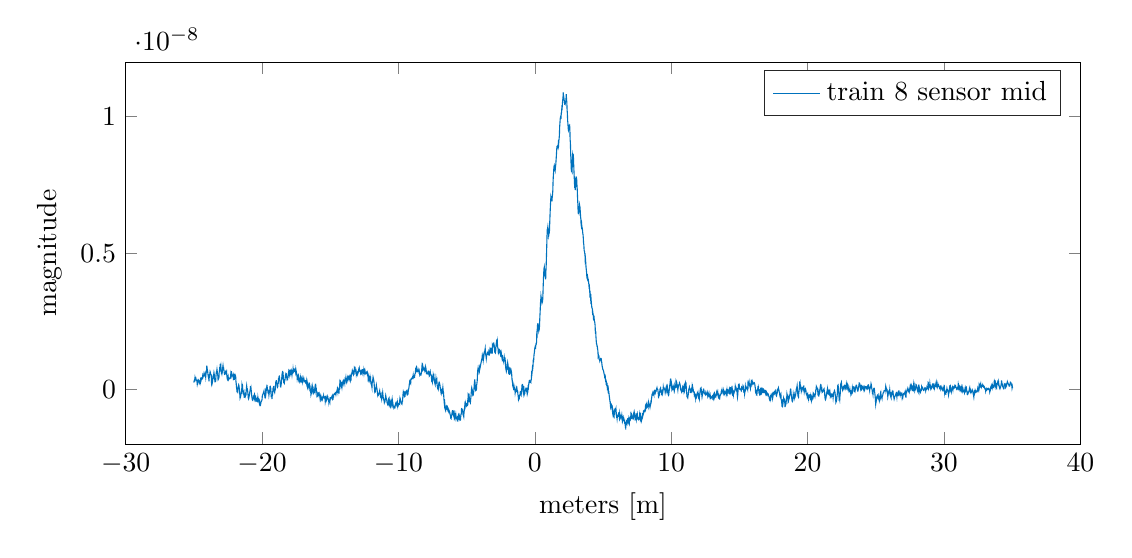
\begin{tikzpicture}

  \begin{axis}[%
    width=\textwidth,
    height=0.4\textwidth,
    at={(0\figurewidth,0\figureheight)},
    scale only axis,
    xmin=-30,
    xmax=40,
    xlabel={meters [m]},
    ymin=-2e-09,
    ymax=1.2e-08,
    ylabel={magnitude},
    axis background/.style={fill=white},
    legend style={legend cell align=left,align=left,draw=white!15!black}
    ]
    \addplot [color=mycolor1,solid]
    table[row sep=crcr]{%
    -25.0159619140625	2.63342382824074e-10\\
    -24.9958125	2.68280363057761e-10\\
    -24.9756630859375	3.21399996990513e-10\\
    -24.955513671875	3.49400753851386e-10\\
    -24.9353642578125	3.37345690797949e-10\\
    -24.91521484375	4.31825558450689e-10\\
    -24.8950654296875	3.74361278933575e-10\\
    -24.874916015625	4.10910299767028e-10\\
    -24.8547666015625	4.24986938772229e-10\\
    -24.8346171875	3.69548090272914e-10\\
    -24.8144677734375	3.50359722886416e-10\\
    -24.794318359375	3.40125573284922e-10\\
    -24.7741689453125	3.09758090909875e-10\\
    -24.75401953125	2.16398269333188e-10\\
    -24.7338701171875	2.80663661692378e-10\\
    -24.713720703125	3.12030188500345e-10\\
    -24.6935712890625	2.53243682953424e-10\\
    -24.673421875	2.93600467198649e-10\\
    -24.6532724609375	3.31969977736584e-10\\
    -24.633123046875	3.04595963446381e-10\\
    -24.6129736328125	3.1758097494952e-10\\
    -24.59282421875	3.16043112233304e-10\\
    -24.5726748046875	2.54209099569841e-10\\
    -24.552525390625	2.8820641179825e-10\\
    -24.5323759765625	3.35403949843216e-10\\
    -24.5122265625	2.77343109410311e-10\\
    -24.4920771484375	3.55053485656035e-10\\
    -24.471927734375	3.33245811982858e-10\\
    -24.4517783203125	4.04755559178772e-10\\
    -24.43162890625	3.88622372597389e-10\\
    -24.4114794921875	4.08640669442416e-10\\
    -24.391330078125	3.97854644745999e-10\\
    -24.3711806640625	4.26757864946119e-10\\
    -24.35103125	5.01419053021836e-10\\
    -24.3308818359375	4.52806671656391e-10\\
    -24.310732421875	4.81653223523485e-10\\
    -24.2905830078125	5.10451166143765e-10\\
    -24.27043359375	5.41618411576001e-10\\
    -24.2502841796875	6.00975082203001e-10\\
    -24.230134765625	5.69846189241345e-10\\
    -24.2099853515625	5.12942066632077e-10\\
    -24.1898359375	4.97855944589707e-10\\
    -24.1696865234375	4.81881136796157e-10\\
    -24.149537109375	5.43217148191952e-10\\
    -24.1293876953125	4.5998095858875e-10\\
    -24.10923828125	5.69145729764313e-10\\
    -24.0890888671875	6.39498159698739e-10\\
    -24.068939453125	6.92341316914158e-10\\
    -24.0487900390625	8.76074840752645e-10\\
    -24.028640625	8.03245963321396e-10\\
    -24.0084912109375	6.98329264608854e-10\\
    -23.988341796875	6.82027290555537e-10\\
    -23.9681923828125	5.71123348977858e-10\\
    -23.94804296875	4.99550333617127e-10\\
    -23.9278935546875	4.36293670022619e-10\\
    -23.907744140625	4.12977604153005e-10\\
    -23.8875947265625	3.00856560016555e-10\\
    -23.8674453125	4.78748536852735e-10\\
    -23.8472958984375	5.57582643861446e-10\\
    -23.827146484375	5.6985110217894e-10\\
    -23.8069970703125	6.51577710444874e-10\\
    -23.78684765625	6.19825584300871e-10\\
    -23.7666982421875	5.72189027219232e-10\\
    -23.746548828125	5.36267456185163e-10\\
    -23.7263994140625	5.36833345058662e-10\\
    -23.70625	3.00377160441011e-10\\
    -23.6861005859375	3.52306470617185e-10\\
    -23.665951171875	2.02340489030392e-10\\
    -23.6458017578125	2.40296899178104e-10\\
    -23.62565234375	3.20894034489101e-10\\
    -23.6055029296875	3.82052012472398e-10\\
    -23.585353515625	4.44443776579893e-10\\
    -23.5652041015625	5.2548423071001e-10\\
    -23.5450546875	5.43498519492401e-10\\
    -23.5249052734375	6.16706094358734e-10\\
    -23.504755859375	5.56927302954773e-10\\
    -23.4846064453125	4.00425765088365e-10\\
    -23.46445703125	3.54529472383066e-10\\
    -23.4443076171875	2.60937499820987e-10\\
    -23.424158203125	3.84453521197844e-10\\
    -23.4040087890625	2.82130123462711e-10\\
    -23.383859375	4.45850417955955e-10\\
    -23.3637099609375	5.79684094068736e-10\\
    -23.343560546875	6.48482302119354e-10\\
    -23.3234111328125	6.68668674567486e-10\\
    -23.30326171875	7.37397858696298e-10\\
    -23.2831123046875	6.6122149429271e-10\\
    -23.262962890625	5.80085946472822e-10\\
    -23.2428134765625	5.12737832900662e-10\\
    -23.2226640625	3.58290618427064e-10\\
    -23.2025146484375	3.74125640785175e-10\\
    -23.182365234375	5.0376479615534e-10\\
    -23.1622158203125	4.03921409105255e-10\\
    -23.14206640625	6.35477794502231e-10\\
    -23.1219169921875	6.53141966696955e-10\\
    -23.101767578125	8.02933539351289e-10\\
    -23.0816181640625	8.06759752595445e-10\\
    -23.06146875	9.35285651037828e-10\\
    -23.0413193359375	8.31554489260814e-10\\
    -23.021169921875	8.81839056476363e-10\\
    -23.0010205078125	7.33987129658963e-10\\
    -22.98087109375	6.03949096301095e-10\\
    -22.9607216796875	6.13792925970074e-10\\
    -22.940572265625	5.70325512073556e-10\\
    -22.9204228515625	6.24004558117356e-10\\
    -22.9002734375	6.98686299274401e-10\\
    -22.8801240234375	8.13383735628664e-10\\
    -22.859974609375	8.81295675020799e-10\\
    -22.8398251953125	8.02003865345015e-10\\
    -22.81967578125	8.05973071115902e-10\\
    -22.7995263671875	7.23921527545029e-10\\
    -22.779376953125	6.8376995265037e-10\\
    -22.7592275390625	5.66225525350011e-10\\
    -22.739078125	5.53917892059419e-10\\
    -22.7189287109375	5.61368134993059e-10\\
    -22.698779296875	5.72293884068663e-10\\
    -22.6786298828125	6.34075636863483e-10\\
    -22.65848046875	6.66955909545526e-10\\
    -22.6383310546875	6.5105776337657e-10\\
    -22.618181640625	6.17536606810559e-10\\
    -22.5980322265625	6.49657547507866e-10\\
    -22.5778828125	4.92006518544774e-10\\
    -22.5577333984375	4.28968449722472e-10\\
    -22.537583984375	4.55611540139029e-10\\
    -22.5174345703125	3.68832790298234e-10\\
    -22.49728515625	3.88921048865556e-10\\
    -22.4771357421875	4.50159599106494e-10\\
    -22.456986328125	3.63548378810126e-10\\
    -22.4368369140625	3.83995799524167e-10\\
    -22.4166875	3.89207490567018e-10\\
    -22.3965380859375	3.99497911032689e-10\\
    -22.376388671875	4.15463200488487e-10\\
    -22.3562392578125	4.18034876790543e-10\\
    -22.33608984375	4.43014142614161e-10\\
    -22.3159404296875	4.30959403993593e-10\\
    -22.295791015625	5.36094758000057e-10\\
    -22.2756416015625	4.47477282422201e-10\\
    -22.2554921875	6.7288304373791e-10\\
    -22.2353427734375	5.32689002315801e-10\\
    -22.215193359375	5.77325525430412e-10\\
    -22.1950439453125	5.17052221329373e-10\\
    -22.17489453125	5.19991701969539e-10\\
    -22.1547451171875	5.04285859229195e-10\\
    -22.134595703125	4.76102362264611e-10\\
    -22.1144462890625	5.14509626796214e-10\\
    -22.094296875	3.80274401994417e-10\\
    -22.0741474609375	3.94329444688174e-10\\
    -22.053998046875	4.52388596687232e-10\\
    -22.0338486328125	3.58358703613065e-10\\
    -22.01369921875	4.74285771409225e-10\\
    -21.9935498046875	5.06885845758297e-10\\
    -21.973400390625	5.40417297852707e-10\\
    -21.9532509765625	5.18118472811059e-10\\
    -21.9331015625	4.83823788854176e-10\\
    -21.9129521484375	2.97812937854665e-10\\
    -21.892802734375	2.16760558474401e-10\\
    -21.8726533203125	9.01285002397328e-11\\
    -21.85250390625	2.49290024533619e-11\\
    -21.8323544921875	-7.4966478769741e-11\\
    -21.812205078125	-6.79315632202953e-11\\
    -21.7920556640625	-8.607622660375e-11\\
    -21.77190625	4.67703393655418e-11\\
    -21.7517568359375	7.69233844033102e-11\\
    -21.731607421875	1.37375524574605e-10\\
    -21.7114580078125	1.73303422255004e-10\\
    -21.69130859375	1.374088252954e-10\\
    -21.6711591796875	5.37490157091584e-11\\
    -21.651009765625	-8.87783240853725e-11\\
    -21.6308603515625	-1.6575191259566e-10\\
    -21.6107109375	-3.17673617737853e-10\\
    -21.5905615234375	-2.8933080541495e-10\\
    -21.570412109375	-2.73245590827452e-10\\
    -21.5502626953125	-1.80893513175472e-10\\
    -21.53011328125	-1.5702304210754e-10\\
    -21.5099638671875	-4.60706533842416e-11\\
    -21.489814453125	-7.34673795374746e-11\\
    -21.4696650390625	1.54588965924683e-10\\
    -21.449515625	9.58834770771249e-11\\
    -21.4293662109375	1.22195911758569e-10\\
    -21.409216796875	-2.22432978888122e-11\\
    -21.3890673828125	-6.85588343333036e-11\\
    -21.36891796875	-1.51821569479669e-10\\
    -21.3487685546875	-1.67907962102836e-10\\
    -21.328619140625	-1.25246619684201e-10\\
    -21.3084697265625	-2.99507560562286e-10\\
    -21.2883203125	-1.8117785871768e-10\\
    -21.2681708984375	-1.70951373295604e-10\\
    -21.248021484375	-2.10694838814557e-10\\
    -21.2278720703125	-2.37142120343247e-10\\
    -21.20772265625	-1.05015385489355e-10\\
    -21.1875732421875	-2.33748470284778e-10\\
    -21.167423828125	-1.30626496624712e-10\\
    -21.1472744140625	5.21999189565311e-11\\
    -21.127125	1.34684884196162e-10\\
    -21.1069755859375	4.38125248626163e-11\\
    -21.086826171875	3.56072667862868e-11\\
    -21.0666767578125	-1.1707061608909e-11\\
    -21.04652734375	-8.34074675750952e-11\\
    -21.0263779296875	-1.88453176930726e-10\\
    -21.006228515625	-3.07383393167362e-10\\
    -20.9860791015625	-3.42262530481404e-10\\
    -20.9659296875	-3.11280220915027e-10\\
    -20.9457802734375	-2.47711813301956e-10\\
    -20.925630859375	-2.00524872466418e-10\\
    -20.9054814453125	-1.06659894461527e-10\\
    -20.88533203125	-6.10762101172634e-11\\
    -20.8651826171875	-1.14078821371616e-11\\
    -20.845033203125	1.26254023710526e-10\\
    -20.8248837890625	-4.62052479884841e-11\\
    -20.804734375	3.13866484639538e-11\\
    -20.7845849609375	-6.35489643853132e-11\\
    -20.764435546875	-2.00435850171547e-10\\
    -20.7442861328125	-2.65186707782246e-10\\
    -20.72413671875	-3.3979957356401e-10\\
    -20.7039873046875	-3.87904937717059e-10\\
    -20.683837890625	-3.96147970713461e-10\\
    -20.6636884765625	-3.44808389837685e-10\\
    -20.6435390625	-3.13712080131496e-10\\
    -20.6233896484375	-2.19191038409563e-10\\
    -20.603240234375	-3.57920273592798e-10\\
    -20.5830908203125	-2.10147000861347e-10\\
    -20.56294140625	-1.81577491845108e-10\\
    -20.5427919921875	-3.10499466280558e-10\\
    -20.522642578125	-2.573754740807e-10\\
    -20.5024931640625	-3.1690495838558e-10\\
    -20.48234375	-2.18323135645844e-10\\
    -20.4621943359375	-3.20605600310469e-10\\
    -20.442044921875	-3.50395765754481e-10\\
    -20.4218955078125	-4.00053558979171e-10\\
    -20.40174609375	-3.79171373168575e-10\\
    -20.3815966796875	-3.54058996492892e-10\\
    -20.361447265625	-4.19823319994377e-10\\
    -20.3412978515625	-4.20508970533357e-10\\
    -20.3211484375	-4.35334441656312e-10\\
    -20.3009990234375	-2.98176341460846e-10\\
    -20.280849609375	-3.66400306099695e-10\\
    -20.2607001953125	-3.52523245441331e-10\\
    -20.24055078125	-4.09954827424619e-10\\
    -20.2204013671875	-4.04984662083216e-10\\
    -20.200251953125	-4.75419145981833e-10\\
    -20.1801025390625	-4.36404287454682e-10\\
    -20.159953125	-5.59400457455261e-10\\
    -20.1398037109375	-5.91668873897907e-10\\
    -20.119654296875	-5.90861306591432e-10\\
    -20.0995048828125	-5.31024259435092e-10\\
    -20.07935546875	-4.64334162273898e-10\\
    -20.0592060546875	-4.40531281476977e-10\\
    -20.039056640625	-4.24404503393608e-10\\
    -20.0189072265625	-4.05369958554544e-10\\
    -19.9987578125	-3.59114313834532e-10\\
    -19.9786083984375	-2.3878120048173e-10\\
    -19.958458984375	-1.92887540468669e-10\\
    -19.9383095703125	-1.73091309297694e-10\\
    -19.91816015625	-1.60466149570976e-10\\
    -19.8980107421875	-1.14930030154677e-10\\
    -19.877861328125	-8.95738563523499e-11\\
    -19.8577119140625	-5.45701524681168e-11\\
    -19.8375625	-1.39535565560974e-10\\
    -19.8174130859375	-1.6488763461604e-10\\
    -19.797263671875	-2.40172716110094e-10\\
    -19.7771142578125	-2.08625857855208e-10\\
    -19.75696484375	-2.44906140475321e-10\\
    -19.7368154296875	-9.66176822296649e-11\\
    -19.716666015625	-1.5230671597542e-10\\
    -19.6965166015625	-6.38536733762265e-11\\
    -19.6763671875	5.06497790185786e-11\\
    -19.6562177734375	7.66943640273144e-11\\
    -19.636068359375	1.73834203311397e-10\\
    -19.6159189453125	6.02697596142377e-11\\
    -19.59576953125	-1.57764026853232e-11\\
    -19.5756201171875	-1.44171459931198e-11\\
    -19.555470703125	-1.31607250087372e-10\\
    -19.5353212890625	-1.33508651535533e-10\\
    -19.515171875	-1.03707640768113e-10\\
    -19.4950224609375	-2.02152374250757e-10\\
    -19.474873046875	-1.29648279138595e-10\\
    -19.4547236328125	-9.39762795829371e-11\\
    -19.43457421875	-5.15973973168223e-11\\
    -19.4144248046875	1.04318323370187e-10\\
    -19.394275390625	1.12881396162163e-10\\
    -19.3741259765625	6.38933842904583e-11\\
    -19.3539765625	3.83586395905483e-11\\
    -19.3338271484375	-2.07651802077172e-10\\
    -19.313677734375	-1.87976893536167e-10\\
    -19.2935283203125	-1.97018536712727e-10\\
    -19.27337890625	-3.47700326336496e-10\\
    -19.2532294921875	-2.33946961314862e-10\\
    -19.233080078125	-2.14254717999427e-10\\
    -19.2129306640625	-7.28219057288079e-11\\
    -19.19278125	4.02973694095465e-11\\
    -19.1726318359375	7.12564847453551e-11\\
    -19.152482421875	3.36131109950775e-11\\
    -19.1323330078125	6.10922957236019e-11\\
    -19.11218359375	-4.26083874540071e-11\\
    -19.0920341796875	-7.95267241157343e-11\\
    -19.071884765625	-1.07800167689446e-10\\
    -19.0517353515625	-4.11367428486298e-11\\
    -19.0315859375	-4.70218286422047e-12\\
    -19.0114365234375	1.16144939040833e-10\\
    -18.991287109375	2.92456242225245e-10\\
    -18.9711376953125	2.07648881114298e-10\\
    -18.95098828125	3.47491837541075e-10\\
    -18.9308388671875	2.40266973894209e-10\\
    -18.910689453125	2.1823353028878e-10\\
    -18.8905400390625	1.7654768051406e-10\\
    -18.870390625	8.50155877360579e-11\\
    -18.8502412109375	1.00462827559718e-10\\
    -18.830091796875	2.21418543701866e-10\\
    -18.8099423828125	2.32018559582694e-10\\
    -18.78979296875	3.95154001013099e-10\\
    -18.7696435546875	3.91823493346461e-10\\
    -18.749494140625	4.86886921158738e-10\\
    -18.7293447265625	4.92426145515807e-10\\
    -18.7091953125	3.89292104189213e-10\\
    -18.6890458984375	2.93470854441743e-10\\
    -18.668896484375	2.5231342464513e-10\\
    -18.6487470703125	1.09486691316745e-10\\
    -18.62859765625	1.0070531026437e-10\\
    -18.6084482421875	1.5795631276996e-10\\
    -18.588298828125	2.24711812044323e-10\\
    -18.5681494140625	3.56462642011794e-10\\
    -18.548	4.59686141043795e-10\\
    -18.5278505859375	5.80101559670722e-10\\
    -18.507701171875	6.14053349337673e-10\\
    -18.4875517578125	6.85677755102841e-10\\
    -18.46740234375	4.84494033278841e-10\\
    -18.4472529296875	5.21257271323235e-10\\
    -18.427103515625	3.74401334334098e-10\\
    -18.4069541015625	2.57977874510651e-10\\
    -18.3868046875	2.57014674074319e-10\\
    -18.3666552734375	2.35418582632169e-10\\
    -18.346505859375	3.17793445005053e-10\\
    -18.3263564453125	3.36943181235807e-10\\
    -18.30620703125	3.93547092659178e-10\\
    -18.2860576171875	5.08974051487613e-10\\
    -18.265908203125	5.55790548419358e-10\\
    -18.2457587890625	5.95780561186726e-10\\
    -18.225609375	5.85311344329421e-10\\
    -18.2054599609375	4.51076565444081e-10\\
    -18.185310546875	4.35964758387428e-10\\
    -18.1651611328125	3.76503610569579e-10\\
    -18.14501171875	4.0529098730788e-10\\
    -18.1248623046875	3.90885363571925e-10\\
    -18.104712890625	4.8796892617399e-10\\
    -18.0845634765625	5.34372760901782e-10\\
    -18.0644140625	5.9807351627348e-10\\
    -18.0442646484375	4.89471612312359e-10\\
    -18.024115234375	5.90689333141209e-10\\
    -18.0039658203125	5.15016844808024e-10\\
    -17.98381640625	5.67006886781836e-10\\
    -17.9636669921875	5.47223919948754e-10\\
    -17.943517578125	7.31003163881392e-10\\
    -17.9233681640625	6.42010883296285e-10\\
    -17.90321875	6.08649922181677e-10\\
    -17.8830693359375	6.51891460110203e-10\\
    -17.862919921875	5.57766217057092e-10\\
    -17.8427705078125	5.62468716615379e-10\\
    -17.82262109375	6.2622755010992e-10\\
    -17.8024716796875	5.40998031864386e-10\\
    -17.782322265625	6.2262049269476e-10\\
    -17.7621728515625	6.11176329156129e-10\\
    -17.7420234375	6.40633546778421e-10\\
    -17.7218740234375	7.53102185783488e-10\\
    -17.701724609375	6.73671662622143e-10\\
    -17.6815751953125	7.09857350848855e-10\\
    -17.66142578125	7.27033790833569e-10\\
    -17.6412763671875	6.697822630671e-10\\
    -17.621126953125	6.822133725114e-10\\
    -17.6009775390625	6.90673290350253e-10\\
    -17.580828125	7.18926208811904e-10\\
    -17.5606787109375	6.90086037404089e-10\\
    -17.540529296875	6.36086708583445e-10\\
    -17.5203798828125	7.43293600357257e-10\\
    -17.50023046875	6.81579277749948e-10\\
    -17.4800810546875	6.36126297643343e-10\\
    -17.459931640625	5.4299947329135e-10\\
    -17.4397822265625	5.24479874991198e-10\\
    -17.4196328125	3.94061998286169e-10\\
    -17.3994833984375	4.42298930387717e-10\\
    -17.379333984375	4.77873187088587e-10\\
    -17.3591845703125	3.59811326129483e-10\\
    -17.33903515625	4.4739809123825e-10\\
    -17.3188857421875	3.78990781135211e-10\\
    -17.298736328125	4.46971972927237e-10\\
    -17.2785869140625	3.97544967762072e-10\\
    -17.2584375	4.04088370456539e-10\\
    -17.2382880859375	3.1166702565134e-10\\
    -17.218138671875	3.48416199761474e-10\\
    -17.1979892578125	3.21015431518139e-10\\
    -17.17783984375	4.19498934774524e-10\\
    -17.1576904296875	3.37045754552355e-10\\
    -17.137541015625	3.1964482811984e-10\\
    -17.1173916015625	3.96859396938604e-10\\
    -17.0972421875	4.25634345765609e-10\\
    -17.0770927734375	3.51715560508903e-10\\
    -17.056943359375	4.01398354855939e-10\\
    -17.0367939453125	3.10968605069925e-10\\
    -17.01664453125	3.91882749986366e-10\\
    -16.9964951171875	3.82207117977948e-10\\
    -16.976345703125	3.96623026943222e-10\\
    -16.9561962890625	3.51878448808459e-10\\
    -16.936046875	4.11994863859101e-10\\
    -16.9158974609375	3.67445552051594e-10\\
    -16.895748046875	3.04530780672038e-10\\
    -16.8755986328125	3.10253744431644e-10\\
    -16.85544921875	2.89925421779126e-10\\
    -16.8352998046875	2.72872299973973e-10\\
    -16.815150390625	2.56493903729131e-10\\
    -16.7950009765625	3.27498684660248e-10\\
    -16.7748515625	3.30873359759962e-10\\
    -16.7547021484375	3.3562396489192e-10\\
    -16.734552734375	2.51332527778833e-10\\
    -16.7144033203125	3.43539534600225e-10\\
    -16.69425390625	2.91913855172247e-10\\
    -16.6741044921875	2.57536108332362e-10\\
    -16.653955078125	1.09021031448806e-10\\
    -16.6338056640625	1.57275003705793e-10\\
    -16.61365625	9.02462567721286e-11\\
    -16.5935068359375	1.34708751354646e-10\\
    -16.573357421875	1.41226308082578e-10\\
    -16.5532080078125	1.79384701718824e-10\\
    -16.53305859375	1.24091155554736e-10\\
    -16.5129091796875	1.57216243327877e-10\\
    -16.492759765625	3.28243257051098e-11\\
    -16.4726103515625	6.1201909185076e-11\\
    -16.4524609375	-6.21430296160162e-11\\
    -16.4323115234375	-6.41642835309109e-11\\
    -16.412162109375	-1.88556140409231e-10\\
    -16.3920126953125	-1.48778401135969e-10\\
    -16.37186328125	3.16361992092436e-12\\
    -16.3517138671875	6.94311979614882e-11\\
    -16.331564453125	7.91760897490101e-13\\
    -16.3114150390625	1.2628532510489e-10\\
    -16.291265625	7.18325683084287e-11\\
    -16.2711162109375	-1.04681387441079e-11\\
    -16.250966796875	2.43631192822686e-11\\
    -16.2308173828125	-7.11465021036142e-11\\
    -16.21066796875	-1.31372201602553e-10\\
    -16.1905185546875	-1.08891166143219e-10\\
    -16.170369140625	-1.02770311667682e-10\\
    -16.1502197265625	-2.83068411216969e-11\\
    -16.1300703125	4.17309734385258e-11\\
    -16.1099208984375	-2.0147722458554e-11\\
    -16.089771484375	1.90046088292733e-10\\
    -16.0696220703125	1.92931301266932e-10\\
    -16.04947265625	7.88969960964672e-11\\
    -16.0293232421875	5.74761429481993e-11\\
    -16.009173828125	-5.0126383609362e-11\\
    -15.9890244140625	-6.40785550560127e-11\\
    -15.968875	-2.4943751054247e-10\\
    -15.9487255859375	-2.36798073579525e-10\\
    -15.928576171875	-2.39039456463508e-10\\
    -15.9084267578125	-1.02946764421814e-10\\
    -15.88827734375	-1.87861652977549e-10\\
    -15.8681279296875	-1.38326178344799e-10\\
    -15.847978515625	-1.26351191582875e-10\\
    -15.8278291015625	-1.76977117238513e-10\\
    -15.8076796875	-1.53709101128162e-10\\
    -15.7875302734375	-2.27785850466985e-10\\
    -15.767380859375	-2.30240448939317e-10\\
    -15.7472314453125	-3.14597259117362e-10\\
    -15.72708203125	-2.49492562361282e-10\\
    -15.7069326171875	-2.99487410497575e-10\\
    -15.686783203125	-1.90395879244667e-10\\
    -15.6666337890625	-3.51428874692961e-10\\
    -15.646484375	-3.13856836544456e-10\\
    -15.6263349609375	-3.06315533145494e-10\\
    -15.606185546875	-3.51138762159148e-10\\
    -15.5860361328125	-3.79934909722418e-10\\
    -15.56588671875	-3.48979598177837e-10\\
    -15.5457373046875	-2.82422825089318e-10\\
    -15.525587890625	-2.98852606691915e-10\\
    -15.5054384765625	-2.88453034236879e-10\\
    -15.4852890625	-2.29148052792012e-10\\
    -15.4651396484375	-3.03745936180428e-10\\
    -15.444990234375	-3.07614494028096e-10\\
    -15.4248408203125	-2.89300602406755e-10\\
    -15.40469140625	-3.194903090862e-10\\
    -15.3845419921875	-2.97715613375597e-10\\
    -15.364392578125	-4.36972543361104e-10\\
    -15.3442431640625	-3.7395107567612e-10\\
    -15.32409375	-4.70684117811603e-10\\
    -15.3039443359375	-3.43623461440028e-10\\
    -15.283794921875	-3.74022509489598e-10\\
    -15.2636455078125	-3.00376476318378e-10\\
    -15.24349609375	-2.50278016601037e-10\\
    -15.2233466796875	-2.29121632179396e-10\\
    -15.203197265625	-2.63903638292628e-10\\
    -15.1830478515625	-2.61166669555783e-10\\
    -15.1628984375	-3.55421484854797e-10\\
    -15.1427490234375	-3.44604300934333e-10\\
    -15.122599609375	-3.4519647890081e-10\\
    -15.1024501953125	-4.59905092207384e-10\\
    -15.08230078125	-3.90225140058257e-10\\
    -15.0621513671875	-3.89541458320926e-10\\
    -15.042001953125	-3.83321896190406e-10\\
    -15.0218525390625	-4.34972197091293e-10\\
    -15.001703125	-2.9775632830623e-10\\
    -14.9815537109375	-2.97916265462792e-10\\
    -14.961404296875	-3.20909899695412e-10\\
    -14.9412548828125	-2.96808139334557e-10\\
    -14.92110546875	-3.03145524222278e-10\\
    -14.9009560546875	-2.79767146822741e-10\\
    -14.880806640625	-2.55951208082599e-10\\
    -14.8606572265625	-3.01660047395618e-10\\
    -14.8405078125	-2.58835474703251e-10\\
    -14.8203583984375	-3.65529165857021e-10\\
    -14.800208984375	-3.57555913543794e-10\\
    -14.7800595703125	-2.76084066643835e-10\\
    -14.75991015625	-2.7731731385083e-10\\
    -14.7397607421875	-1.93424365514924e-10\\
    -14.719611328125	-1.65500365868797e-10\\
    -14.6994619140625	-1.57679001173988e-10\\
    -14.6793125	-1.72566541244726e-10\\
    -14.6591630859375	-1.7566925490288e-10\\
    -14.639013671875	-1.33559696684871e-10\\
    -14.6188642578125	-1.05735139081858e-10\\
    -14.59871484375	-1.05736524770914e-10\\
    -14.5785654296875	-1.64780659593885e-10\\
    -14.558416015625	-1.04571193028952e-10\\
    -14.5382666015625	-1.06477738486642e-10\\
    -14.5181171875	-5.10533488139063e-11\\
    -14.4979677734375	-5.00156351346904e-11\\
    -14.477818359375	2.25058560022184e-11\\
    -14.4576689453125	-2.44943351597913e-11\\
    -14.43751953125	-9.40503124743764e-11\\
    -14.4173701171875	-6.68641716112064e-12\\
    -14.397220703125	-4.12596869419135e-11\\
    -14.3770712890625	-1.12525989452806e-10\\
    -14.356921875	-1.19381909517587e-10\\
    -14.3367724609375	2.33307143584594e-11\\
    -14.316623046875	7.39631862478005e-11\\
    -14.2964736328125	2.25635344841167e-10\\
    -14.27632421875	1.67199450196401e-10\\
    -14.2561748046875	3.1017177956515e-10\\
    -14.236025390625	2.93083514326504e-10\\
    -14.2158759765625	2.71033359658031e-10\\
    -14.1957265625	2.43227438008735e-10\\
    -14.1755771484375	1.43632437260979e-10\\
    -14.155427734375	1.75278254585958e-10\\
    -14.1352783203125	9.53799722041406e-11\\
    -14.11512890625	1.73145584440781e-10\\
    -14.0949794921875	1.88677225646865e-10\\
    -14.074830078125	2.90751431470238e-10\\
    -14.0546806640625	3.17085482513151e-10\\
    -14.03453125	2.29659878184164e-10\\
    -14.0143818359375	2.76230235203894e-10\\
    -13.994232421875	3.00247677510483e-10\\
    -13.9740830078125	2.71785159071478e-10\\
    -13.95393359375	3.03335427495275e-10\\
    -13.9337841796875	2.44927279416678e-10\\
    -13.913634765625	3.73615102438884e-10\\
    -13.8934853515625	3.50833630012202e-10\\
    -13.8733359375	3.58613702943345e-10\\
    -13.8531865234375	4.29431126306001e-10\\
    -13.833037109375	3.30205849336088e-10\\
    -13.8128876953125	2.83932626913236e-10\\
    -13.79273828125	3.4305537006236e-10\\
    -13.7725888671875	3.14317389040924e-10\\
    -13.752439453125	3.91215912069468e-10\\
    -13.7322900390625	4.32509468414656e-10\\
    -13.712140625	3.96615755808784e-10\\
    -13.6919912109375	4.92429319371113e-10\\
    -13.671841796875	4.78767386620004e-10\\
    -13.6516923828125	4.78864311321188e-10\\
    -13.63154296875	4.05166958772575e-10\\
    -13.6113935546875	3.67030929012616e-10\\
    -13.591244140625	4.11279002383023e-10\\
    -13.5710947265625	4.21106332217267e-10\\
    -13.5509453125	5.49714640540673e-10\\
    -13.5307958984375	4.22695102925449e-10\\
    -13.510646484375	3.59802911017236e-10\\
    -13.4904970703125	4.44809843883393e-10\\
    -13.47034765625	4.13806007974766e-10\\
    -13.4501982421875	5.62328299891438e-10\\
    -13.430048828125	5.55132578051211e-10\\
    -13.4098994140625	6.00970883723722e-10\\
    -13.38975	6.620225791876e-10\\
    -13.3696005859375	5.99657142556184e-10\\
    -13.349451171875	5.8848888563271e-10\\
    -13.3293017578125	6.38256729789091e-10\\
    -13.30915234375	5.90739493526502e-10\\
    -13.2890029296875	5.51909223748864e-10\\
    -13.268853515625	5.92589087912163e-10\\
    -13.2487041015625	5.84188454666661e-10\\
    -13.2285546875	7.64762412240209e-10\\
    -13.2084052734375	7.33760035180071e-10\\
    -13.188255859375	8.37469228701242e-10\\
    -13.1681064453125	7.36216925931246e-10\\
    -13.14795703125	7.34691124164077e-10\\
    -13.1278076171875	6.55558738856786e-10\\
    -13.107658203125	6.82423328358086e-10\\
    -13.0875087890625	5.58873528514738e-10\\
    -13.067359375	6.06992807919923e-10\\
    -13.0472099609375	5.74243427873142e-10\\
    -13.027060546875	6.08261948896108e-10\\
    -13.0069111328125	6.30826091856905e-10\\
    -12.98676171875	5.79026008808614e-10\\
    -12.9666123046875	6.36310683871708e-10\\
    -12.946462890625	6.25056797995053e-10\\
    -12.9263134765625	6.78232190093248e-10\\
    -12.9061640625	7.39461875848335e-10\\
    -12.8860146484375	7.16673865460013e-10\\
    -12.865865234375	7.74209357422657e-10\\
    -12.8457158203125	7.10656196185631e-10\\
    -12.82556640625	7.03263991055461e-10\\
    -12.8054169921875	7.02517086050529e-10\\
    -12.785267578125	6.26338792623932e-10\\
    -12.7651181640625	6.72333946610518e-10\\
    -12.74496875	6.77433342802664e-10\\
    -12.7248193359375	5.51826844392368e-10\\
    -12.704669921875	6.85503305227537e-10\\
    -12.6845205078125	6.77683686851359e-10\\
    -12.66437109375	7.16670909962137e-10\\
    -12.6442216796875	7.07541206419146e-10\\
    -12.624072265625	6.46039216863611e-10\\
    -12.6039228515625	7.50826595413114e-10\\
    -12.5837734375	5.94428231774539e-10\\
    -12.5636240234375	6.0092377499748e-10\\
    -12.543474609375	6.88624719666413e-10\\
    -12.5233251953125	5.94274364384241e-10\\
    -12.50317578125	6.61712587476426e-10\\
    -12.4830263671875	6.85665938631906e-10\\
    -12.462876953125	7.22601950033229e-10\\
    -12.4427275390625	6.66706803981104e-10\\
    -12.422578125	5.88379220487798e-10\\
    -12.4024287109375	5.99495453367441e-10\\
    -12.382279296875	5.81179693648098e-10\\
    -12.3621298828125	5.90546065778659e-10\\
    -12.34198046875	6.34604061241124e-10\\
    -12.3218310546875	6.45686311606932e-10\\
    -12.301681640625	6.57512666831391e-10\\
    -12.2815322265625	5.88001066529702e-10\\
    -12.2613828125	6.18680735072119e-10\\
    -12.2412333984375	5.90393283782615e-10\\
    -12.221083984375	4.12900284512213e-10\\
    -12.2009345703125	4.54100367476453e-10\\
    -12.18078515625	3.2846633482953e-10\\
    -12.1606357421875	3.03220520484359e-10\\
    -12.140486328125	3.64887404826378e-10\\
    -12.1203369140625	4.96730851285129e-10\\
    -12.1001875	3.61400513999166e-10\\
    -12.0800380859375	4.49665624709405e-10\\
    -12.059888671875	3.64141170165353e-10\\
    -12.0397392578125	3.93578405148012e-10\\
    -12.01958984375	2.3034325968277e-10\\
    -11.9994404296875	2.03557981548202e-10\\
    -11.979291015625	1.74620786375537e-10\\
    -11.9591416015625	1.40225502544284e-10\\
    -11.9389921875	7.906819868126e-11\\
    -11.9188427734375	2.67503287291458e-10\\
    -11.898693359375	2.98796917264965e-10\\
    -11.8785439453125	3.68122915627981e-10\\
    -11.85839453125	4.55345858139028e-10\\
    -11.8382451171875	4.1812850816806e-10\\
    -11.818095703125	3.7035734044716e-10\\
    -11.7979462890625	3.04856655902457e-10\\
    -11.777796875	2.04551446974388e-10\\
    -11.7576474609375	4.74252849212869e-11\\
    -11.737498046875	-5.98010536788454e-11\\
    -11.7173486328125	-2.73640578950162e-11\\
    -11.69719921875	-1.10527138910834e-10\\
    -11.6770498046875	2.0534919366098e-11\\
    -11.656900390625	4.2743672410668e-11\\
    -11.6367509765625	9.64262572358203e-11\\
    -11.6166015625	1.56481633845766e-10\\
    -11.5964521484375	7.35550863557104e-11\\
    -11.576302734375	4.20965622294817e-11\\
    -11.5561533203125	-3.62499527079316e-11\\
    -11.53600390625	-1.47349815354047e-10\\
    -11.5158544921875	-2.06366463606498e-10\\
    -11.495705078125	-1.68828586835236e-10\\
    -11.4755556640625	-1.5548841983965e-10\\
    -11.45540625	-1.92732764765622e-10\\
    -11.4352568359375	-1.72196299123863e-10\\
    -11.415107421875	-1.37382612726156e-10\\
    -11.3949580078125	-9.27064739483961e-11\\
    -11.37480859375	-4.82137102478446e-11\\
    -11.3546591796875	-1.35149788720146e-10\\
    -11.334509765625	-1.33370731666372e-10\\
    -11.3143603515625	-2.70072729637688e-10\\
    -11.2942109375	-2.85408428097267e-10\\
    -11.2740615234375	-2.66408540185996e-10\\
    -11.253912109375	-2.95461037022581e-10\\
    -11.2337626953125	-3.45697002371378e-10\\
    -11.21361328125	-2.08705138957426e-10\\
    -11.1934638671875	-2.49416552966937e-10\\
    -11.173314453125	-1.89429055448926e-10\\
    -11.1531650390625	-1.13084367838882e-10\\
    -11.133015625	-2.1516365792287e-10\\
    -11.1128662109375	-2.96437904795449e-10\\
    -11.092716796875	-3.30271824491994e-10\\
    -11.0725673828125	-3.74478577802981e-10\\
    -11.05241796875	-4.12572357350412e-10\\
    -11.0322685546875	-4.79256910215696e-10\\
    -11.012119140625	-4.46979282048706e-10\\
    -10.9919697265625	-4.505258715288e-10\\
    -10.9718203125	-3.8788874276432e-10\\
    -10.9516708984375	-2.88176902552394e-10\\
    -10.931521484375	-2.19346979784853e-10\\
    -10.9113720703125	-2.72443900880135e-10\\
    -10.89122265625	-3.25243175689279e-10\\
    -10.8710732421875	-3.62669608627437e-10\\
    -10.850923828125	-4.06857675133159e-10\\
    -10.8307744140625	-4.90528995158251e-10\\
    -10.810625	-5.11048221394996e-10\\
    -10.7904755859375	-5.46569572688462e-10\\
    -10.770326171875	-5.25873233664108e-10\\
    -10.7501767578125	-5.3872766557622e-10\\
    -10.73002734375	-3.72001576537543e-10\\
    -10.7098779296875	-3.35782684047628e-10\\
    -10.689728515625	-3.14617786519254e-10\\
    -10.6695791015625	-5.04046327303304e-10\\
    -10.6494296875	-4.58926765671701e-10\\
    -10.6292802734375	-5.31334634165085e-10\\
    -10.609130859375	-4.78029699158706e-10\\
    -10.5889814453125	-5.94365517612282e-10\\
    -10.56883203125	-5.54205918052189e-10\\
    -10.5486826171875	-5.9237964015753e-10\\
    -10.528533203125	-5.12650511634087e-10\\
    -10.5083837890625	-4.19347191205157e-10\\
    -10.488234375	-4.34178226835744e-10\\
    -10.4680849609375	-3.71389467249629e-10\\
    -10.447935546875	-5.10023961020513e-10\\
    -10.4277861328125	-4.39114085334394e-10\\
    -10.40763671875	-5.05921316271965e-10\\
    -10.3874873046875	-5.7600675770848e-10\\
    -10.367337890625	-6.31778668172175e-10\\
    -10.3471884765625	-6.33553477125611e-10\\
    -10.3270390625	-6.88924493387689e-10\\
    -10.3068896484375	-6.71029271089924e-10\\
    -10.286740234375	-6.48516314400656e-10\\
    -10.2665908203125	-6.14435990499159e-10\\
    -10.24644140625	-6.35993045605173e-10\\
    -10.2262919921875	-5.79027947818648e-10\\
    -10.206142578125	-5.37520569919661e-10\\
    -10.1859931640625	-4.80151134793883e-10\\
    -10.16584375	-4.65072541327596e-10\\
    -10.1456943359375	-4.94147260242876e-10\\
    -10.125544921875	-5.59848237354064e-10\\
    -10.1053955078125	-6.01296003102906e-10\\
    -10.08524609375	-6.16248065433217e-10\\
    -10.0650966796875	-5.08039787406482e-10\\
    -10.044947265625	-5.9848785522352e-10\\
    -10.0247978515625	-5.41259575840896e-10\\
    -10.0046484375	-5.67536290776853e-10\\
    -9.9844990234375	-5.29337271840397e-10\\
    -9.964349609375	-5.3297030604391e-10\\
    -9.9442001953125	-5.36331204471858e-10\\
    -9.92405078125	-4.59652988386205e-10\\
    -9.9039013671875	-4.91968992561546e-10\\
    -9.883751953125	-3.16701039221237e-10\\
    -9.8636025390625	-3.48824562037435e-10\\
    -9.843453125	-3.80649696962885e-10\\
    -9.8233037109375	-4.34213572326967e-10\\
    -9.803154296875	-4.55601939379068e-10\\
    -9.7830048828125	-4.61967548289483e-10\\
    -9.76285546875	-5.24403384767438e-10\\
    -9.7427060546875	-5.36962691229306e-10\\
    -9.722556640625	-4.56192583578482e-10\\
    -9.7024072265625	-4.38463149442058e-10\\
    -9.6822578125	-3.09747737697888e-10\\
    -9.6621083984375	-1.78095800207268e-10\\
    -9.641958984375	-8.58275826979146e-11\\
    -9.6218095703125	-1.20463094307345e-10\\
    -9.60166015625	-1.05019278870237e-10\\
    -9.5815107421875	-1.34215588166226e-10\\
    -9.561361328125	-2.89114008203338e-10\\
    -9.5412119140625	-2.14845621522187e-10\\
    -9.5210625	-1.42838205451489e-10\\
    -9.5009130859375	-1.76392640051384e-10\\
    -9.480763671875	-9.963629443591e-11\\
    -9.4606142578125	-7.9929733271192e-11\\
    -9.44046484375	-5.99429077091229e-11\\
    -9.4203154296875	-5.15473929923326e-11\\
    -9.400166015625	-1.00419316375186e-10\\
    -9.3800166015625	-6.85414292032222e-11\\
    -9.3598671875	-1.52244963884969e-10\\
    -9.3397177734375	-1.29485059731943e-10\\
    -9.319568359375	-1.82176632506847e-10\\
    -9.2994189453125	-1.68949015579661e-10\\
    -9.27926953125	-5.52367014157521e-11\\
    -9.2591201171875	9.59054951365259e-12\\
    -9.238970703125	4.37960377298083e-11\\
    -9.2188212890625	1.15347932224368e-10\\
    -9.198671875	1.98693485900062e-10\\
    -9.1785224609375	2.54655873667053e-10\\
    -9.158373046875	3.62026186445155e-10\\
    -9.1382236328125	2.53612204776656e-10\\
    -9.11807421875	2.80913168784969e-10\\
    -9.0979248046875	2.48886072076138e-10\\
    -9.077775390625	3.78827002200394e-10\\
    -9.0576259765625	3.83327143151366e-10\\
    -9.0374765625	4.15497163343123e-10\\
    -9.0173271484375	4.16410776893507e-10\\
    -8.997177734375	3.95845801875862e-10\\
    -8.9770283203125	4.03782126622675e-10\\
    -8.95687890625	4.68167033620974e-10\\
    -8.9367294921875	4.68555651100381e-10\\
    -8.916580078125	5.30967708499869e-10\\
    -8.8964306640625	4.55533805568408e-10\\
    -8.87628125	4.27653671379289e-10\\
    -8.8561318359375	4.53246086037207e-10\\
    -8.835982421875	4.60681008971167e-10\\
    -8.8158330078125	4.5599463038327e-10\\
    -8.79568359375	5.59435191359806e-10\\
    -8.7755341796875	5.78445609313587e-10\\
    -8.755384765625	6.05078119013434e-10\\
    -8.7352353515625	7.71855299762389e-10\\
    -8.7150859375	7.7622537335793e-10\\
    -8.6949365234375	8.19526000521144e-10\\
    -8.674787109375	8.35194865240524e-10\\
    -8.6546376953125	7.20338952022099e-10\\
    -8.63448828125	7.51504421574112e-10\\
    -8.6143388671875	7.03050036380723e-10\\
    -8.594189453125	6.74304500528532e-10\\
    -8.5740400390625	6.95001389085449e-10\\
    -8.553890625	6.78980912534805e-10\\
    -8.5337412109375	6.69873086307222e-10\\
    -8.513591796875	7.10458590122562e-10\\
    -8.4934423828125	6.51792242279671e-10\\
    -8.47329296875	6.80451684584216e-10\\
    -8.4531435546875	5.81843203812172e-10\\
    -8.432994140625	5.28508722913309e-10\\
    -8.4128447265625	5.51155677063961e-10\\
    -8.3926953125	5.33402093764058e-10\\
    -8.3725458984375	5.32476614222806e-10\\
    -8.352396484375	5.81759880972888e-10\\
    -8.3322470703125	5.67003097768833e-10\\
    -8.31209765625	6.29515465679794e-10\\
    -8.2919482421875	7.13671676718438e-10\\
    -8.271798828125	8.64323267520458e-10\\
    -8.2516494140625	9.46369027940746e-10\\
    -8.2315	9.30079960207572e-10\\
    -8.2113505859375	7.79701923215811e-10\\
    -8.191201171875	8.22837715255192e-10\\
    -8.1710517578125	7.84031679543118e-10\\
    -8.15090234375	7.41875849043906e-10\\
    -8.1307529296875	7.58303977488011e-10\\
    -8.110603515625	7.29165644209771e-10\\
    -8.0904541015625	7.5142852851669e-10\\
    -8.0703046875	7.06686564227647e-10\\
    -8.0501552734375	7.71589142983355e-10\\
    -8.030005859375	8.29845561929338e-10\\
    -8.0098564453125	7.54963461166822e-10\\
    -7.98970703125	7.91588998617403e-10\\
    -7.9695576171875	7.49283373651779e-10\\
    -7.949408203125	5.82885324126063e-10\\
    -7.9292587890625	5.79017359245633e-10\\
    -7.909109375	6.08921623824762e-10\\
    -7.8889599609375	6.11075444170073e-10\\
    -7.868810546875	5.72244237427001e-10\\
    -7.8486611328125	5.71240422519008e-10\\
    -7.82851171875	6.56217045958628e-10\\
    -7.8083623046875	6.50407160343588e-10\\
    -7.788212890625	6.62412857048975e-10\\
    -7.7680634765625	6.25121124571813e-10\\
    -7.7479140625	5.44080596348004e-10\\
    -7.7277646484375	5.87199835802373e-10\\
    -7.707615234375	5.52053946828173e-10\\
    -7.6874658203125	6.07344943770391e-10\\
    -7.66731640625	6.51512372417564e-10\\
    -7.6471669921875	5.68054045472457e-10\\
    -7.627017578125	5.5044948290047e-10\\
    -7.6068681640625	5.29344717286548e-10\\
    -7.58671875	5.08752326036273e-10\\
    -7.5665693359375	3.72663096357213e-10\\
    -7.546419921875	2.61670307554529e-10\\
    -7.5262705078125	3.76046128422658e-10\\
    -7.50612109375	3.10251732048137e-10\\
    -7.4859716796875	4.54335552375511e-10\\
    -7.465822265625	3.7387209222631e-10\\
    -7.4456728515625	5.21948496845575e-10\\
    -7.4255234375	4.71570820962713e-10\\
    -7.4053740234375	5.78531505957578e-10\\
    -7.385224609375	3.40545868451916e-10\\
    -7.3650751953125	3.51357457049995e-10\\
    -7.34492578125	2.67367667724407e-10\\
    -7.3247763671875	2.162252864795e-10\\
    -7.304626953125	1.81584072960762e-10\\
    -7.2844775390625	2.94673877403669e-10\\
    -7.264328125	2.73669165662802e-10\\
    -7.2441787109375	4.12695824406922e-10\\
    -7.224029296875	3.40520687145987e-10\\
    -7.2038798828125	3.52177915005346e-10\\
    -7.18373046875	3.70979089076117e-10\\
    -7.1635810546875	1.81788260133142e-10\\
    -7.143431640625	1.13251004464772e-10\\
    -7.1232822265625	3.18743210627528e-11\\
    -7.1031328125	2.59233611964863e-11\\
    -7.0829833984375	1.44465288341497e-12\\
    -7.062833984375	9.14855532583413e-11\\
    -7.0426845703125	2.00856602727093e-10\\
    -7.02253515625	1.70700123431229e-10\\
    -7.0023857421875	1.64644948730051e-10\\
    -6.982236328125	2.21016053287478e-10\\
    -6.9620869140625	1.77501132512667e-10\\
    -6.9419375	1.17314254564643e-10\\
    -6.9217880859375	-1.32822531815608e-12\\
    -6.901638671875	-2.59746377878509e-11\\
    -6.8814892578125	-9.69906927400128e-11\\
    -6.86133984375	-6.46825926071764e-11\\
    -6.8411904296875	-1.09773692220922e-10\\
    -6.821041015625	1.52297113801524e-11\\
    -6.8008916015625	-1.18781640269299e-10\\
    -6.7807421875	5.97444490096408e-11\\
    -6.7605927734375	-2.30579756386719e-11\\
    -6.740443359375	6.59063585940737e-11\\
    -6.7202939453125	-4.28436453425956e-11\\
    -6.70014453125	-8.84288683967151e-11\\
    -6.6799951171875	-2.14220915420043e-10\\
    -6.659845703125	-3.63075935400613e-10\\
    -6.6396962890625	-4.83909667507836e-10\\
    -6.619546875	-5.75000598368973e-10\\
    -6.5993974609375	-5.1317733486765e-10\\
    -6.579248046875	-6.25703486143206e-10\\
    -6.5590986328125	-7.40717404916576e-10\\
    -6.53894921875	-7.70928847163187e-10\\
    -6.5187998046875	-6.96556887508627e-10\\
    -6.498650390625	-6.82165681049879e-10\\
    -6.4785009765625	-6.34441155043635e-10\\
    -6.4583515625	-6.75178282592178e-10\\
    -6.4382021484375	-6.45835169742767e-10\\
    -6.418052734375	-6.21327182399496e-10\\
    -6.3979033203125	-6.4603863297035e-10\\
    -6.37775390625	-7.65197096871339e-10\\
    -6.3576044921875	-7.97377641971219e-10\\
    -6.337455078125	-8.06623153091343e-10\\
    -6.3173056640625	-7.6566988789273e-10\\
    -6.29715625	-8.53317322014378e-10\\
    -6.2770068359375	-8.54495811463871e-10\\
    -6.256857421875	-8.07498085215633e-10\\
    -6.2367080078125	-8.36494039679758e-10\\
    -6.21655859375	-9.03347963876001e-10\\
    -6.1964091796875	-9.35347656196472e-10\\
    -6.176259765625	-9.83852184395712e-10\\
    -6.1561103515625	-1.06361906477156e-09\\
    -6.1359609375	-1.07139264272803e-09\\
    -6.1158115234375	-9.53568331884429e-10\\
    -6.095662109375	-9.55405640388037e-10\\
    -6.0755126953125	-8.79996496438458e-10\\
    -6.05536328125	-8.15608619398099e-10\\
    -6.0352138671875	-7.75986124193101e-10\\
    -6.015064453125	-7.76303054872971e-10\\
    -5.9949150390625	-8.03985076674288e-10\\
    -5.974765625	-9.33536638211328e-10\\
    -5.9546162109375	-9.60003119837113e-10\\
    -5.934466796875	-8.9900883178389e-10\\
    -5.9143173828125	-9.91081174979242e-10\\
    -5.89416796875	-9.13501500004233e-10\\
    -5.8740185546875	-9.89284332521296e-10\\
    -5.853869140625	-1.03346163015778e-09\\
    -5.8337197265625	-8.68451351409146e-10\\
    -5.8135703125	-9.68575972341226e-10\\
    -5.7934208984375	-9.09718615897434e-10\\
    -5.773271484375	-9.97790380858406e-10\\
    -5.7531220703125	-1.0161456722174e-09\\
    -5.73297265625	-1.07737497987108e-09\\
    -5.7128232421875	-1.07904633376402e-09\\
    -5.692673828125	-1.08443400015552e-09\\
    -5.6725244140625	-1.17005022507071e-09\\
    -5.652375	-9.70223763359138e-10\\
    -5.6322255859375	-1.05883122852125e-09\\
    -5.612076171875	-1.06715329547046e-09\\
    -5.5919267578125	-9.20383608751067e-10\\
    -5.57177734375	-9.41236333034595e-10\\
    -5.5516279296875	-1.03913984314594e-09\\
    -5.531478515625	-9.8298310796633e-10\\
    -5.5113291015625	-1.05761802145861e-09\\
    -5.4911796875	-1.1076507729669e-09\\
    -5.4710302734375	-1.1200612376532e-09\\
    -5.450880859375	-1.11059707834268e-09\\
    -5.4307314453125	-9.77031051135572e-10\\
    -5.41058203125	-9.12765736804406e-10\\
    -5.3904326171875	-8.83877965474559e-10\\
    -5.370283203125	-7.01671676807166e-10\\
    -5.3501337890625	-7.06150607105907e-10\\
    -5.329984375	-7.12082479670346e-10\\
    -5.3098349609375	-7.72872208124126e-10\\
    -5.289685546875	-7.63589393937752e-10\\
    -5.2695361328125	-9.07483507653173e-10\\
    -5.24938671875	-9.31121470254626e-10\\
    -5.2292373046875	-9.50414965514836e-10\\
    -5.209087890625	-9.92565112886359e-10\\
    -5.1889384765625	-8.26557664527254e-10\\
    -5.1687890625	-7.69314440980381e-10\\
    -5.1486396484375	-6.74348418943307e-10\\
    -5.128490234375	-5.61920314752045e-10\\
    -5.1083408203125	-6.04207319712192e-10\\
    -5.08819140625	-4.78472339403601e-10\\
    -5.0680419921875	-5.15489326805659e-10\\
    -5.047892578125	-5.40846954198897e-10\\
    -5.0277431640625	-5.59534114856639e-10\\
    -5.00759375	-6.05486890814794e-10\\
    -4.9874443359375	-5.89530076092744e-10\\
    -4.967294921875	-4.94493938097976e-10\\
    -4.9471455078125	-6.04763712227623e-10\\
    -4.92699609375	-4.6938058063828e-10\\
    -4.9068466796875	-4.92158703311026e-10\\
    -4.886697265625	-2.03504871820415e-10\\
    -4.8665478515625	-2.29835643363151e-10\\
    -4.8463984375	-2.03084806962944e-10\\
    -4.8262490234375	-3.30066861660067e-10\\
    -4.806099609375	-2.84896040609256e-10\\
    -4.7859501953125	-3.9895489338756e-10\\
    -4.76580078125	-4.48563481042664e-10\\
    -4.7456513671875	-4.60782580682554e-10\\
    -4.725501953125	-4.82824327188696e-10\\
    -4.7053525390625	-3.77722774404461e-10\\
    -4.685203125	-2.72114683278585e-10\\
    -4.6650537109375	-1.59529258812464e-10\\
    -4.644904296875	6.50380844549317e-12\\
    -4.6247548828125	6.04601863693512e-11\\
    -4.60460546875	7.49276786518668e-12\\
    -4.5844560546875	-1.91733823909538e-11\\
    -4.564306640625	-1.2170601012363e-10\\
    -4.5441572265625	-2.24992434545075e-10\\
    -4.5240078125	-2.20259488616787e-10\\
    -4.5038583984375	-1.37590178753887e-10\\
    -4.483708984375	-9.10632752100172e-11\\
    -4.4635595703125	-8.75494199814978e-12\\
    -4.44341015625	1.68063141309808e-10\\
    -4.4232607421875	2.73802158893538e-10\\
    -4.403111328125	3.67879678623446e-10\\
    -4.3829619140625	2.44670005057369e-10\\
    -4.3628125	1.16677589014121e-10\\
    -4.3426630859375	-2.69145427425633e-13\\
    -4.322513671875	2.18173526401396e-11\\
    -4.3023642578125	-2.84107535120266e-11\\
    -4.28221484375	-1.81605582898057e-11\\
    -4.2620654296875	1.7223698221379e-10\\
    -4.241916015625	2.35186396416332e-10\\
    -4.2217666015625	3.27574683356569e-10\\
    -4.2016171875	5.66741472963104e-10\\
    -4.1814677734375	7.14664824644304e-10\\
    -4.161318359375	7.76566304925319e-10\\
    -4.1411689453125	6.86019117977095e-10\\
    -4.12101953125	7.51181482271221e-10\\
    -4.1008701171875	7.25492942408838e-10\\
    -4.080720703125	7.51420503955533e-10\\
    -4.0605712890625	6.95393877573143e-10\\
    -4.040421875	8.17438298855212e-10\\
    -4.0202724609375	7.79480336097612e-10\\
    -4.000123046875	8.28919058555072e-10\\
    -3.9799736328125	8.88840694705491e-10\\
    -3.95982421875	9.41757527848139e-10\\
    -3.9396748046875	9.84390544729731e-10\\
    -3.919525390625	1.03271070621939e-09\\
    -3.8993759765625	1.09821027383578e-09\\
    -3.8792265625	1.11216689341189e-09\\
    -3.8590771484375	1.20417907014479e-09\\
    -3.838927734375	1.11385869287287e-09\\
    -3.8187783203125	1.10146048784306e-09\\
    -3.79862890625	1.17452094882051e-09\\
    -3.7784794921875	1.07137529490927e-09\\
    -3.758330078125	1.14420382971298e-09\\
    -3.7381806640625	1.20882857102065e-09\\
    -3.71803125	1.3114556974911e-09\\
    -3.6978818359375	1.38057147585242e-09\\
    -3.677732421875	1.37655321316909e-09\\
    -3.6575830078125	1.44629247704657e-09\\
    -3.63743359375	1.50603373982635e-09\\
    -3.6172841796875	1.34074648486158e-09\\
    -3.597134765625	1.27529855189131e-09\\
    -3.5769853515625	1.2292865772283e-09\\
    -3.5568359375	1.13692596112099e-09\\
    -3.5366865234375	1.21785254954561e-09\\
    -3.516537109375	1.27505262563199e-09\\
    -3.4963876953125	1.29041141624868e-09\\
    -3.47623828125	1.35579530830779e-09\\
    -3.4560888671875	1.34850810118857e-09\\
    -3.435939453125	1.34780652073104e-09\\
    -3.4157900390625	1.38290164351248e-09\\
    -3.395640625	1.29197917109025e-09\\
    -3.3754912109375	1.30110349929092e-09\\
    -3.355341796875	1.38149400086826e-09\\
    -3.3351923828125	1.24116294175059e-09\\
    -3.31504296875	1.37626269384862e-09\\
    -3.2948935546875	1.44993566856765e-09\\
    -3.274744140625	1.39559964140826e-09\\
    -3.2545947265625	1.44818529640761e-09\\
    -3.2344453125	1.53574854725311e-09\\
    -3.2142958984375	1.37816743380728e-09\\
    -3.194146484375	1.39126295899384e-09\\
    -3.1739970703125	1.40830759570096e-09\\
    -3.15384765625	1.38856020496085e-09\\
    -3.1336982421875	1.30638860875591e-09\\
    -3.113548828125	1.5625387159715e-09\\
    -3.0933994140625	1.50519868371473e-09\\
    -3.07325	1.63043746027401e-09\\
    -3.0531005859375	1.65918643177461e-09\\
    -3.032951171875	1.60321119167949e-09\\
    -3.0128017578125	1.61723014973295e-09\\
    -2.99265234375	1.65615427984191e-09\\
    -2.9725029296875	1.60586810875715e-09\\
    -2.952353515625	1.52167595399071e-09\\
    -2.9322041015625	1.36914993107393e-09\\
    -2.9120546875	1.3504758587564e-09\\
    -2.8919052734375	1.33881362950623e-09\\
    -2.871755859375	1.39788431368968e-09\\
    -2.8516064453125	1.55424086716791e-09\\
    -2.83145703125	1.65938802544818e-09\\
    -2.8113076171875	1.72963550576072e-09\\
    -2.791158203125	1.66775887509645e-09\\
    -2.7710087890625	1.7100443763282e-09\\
    -2.750859375	1.77093172737876e-09\\
    -2.7307099609375	1.571657717946e-09\\
    -2.710560546875	1.53454524972641e-09\\
    -2.6904111328125	1.47525083298505e-09\\
    -2.67026171875	1.30270930078367e-09\\
    -2.6501123046875	1.49389107285363e-09\\
    -2.629962890625	1.39983293621105e-09\\
    -2.6098134765625	1.47478966551871e-09\\
    -2.5896640625	1.47161235833866e-09\\
    -2.5695146484375	1.40235706241723e-09\\
    -2.549365234375	1.42245050351071e-09\\
    -2.5292158203125	1.41867591170604e-09\\
    -2.50906640625	1.29260558885432e-09\\
    -2.4889169921875	1.3167801053704e-09\\
    -2.468767578125	1.19285606810399e-09\\
    -2.4486181640625	1.30377149862585e-09\\
    -2.42846875	1.23539543226772e-09\\
    -2.4083193359375	1.16931225453059e-09\\
    -2.388169921875	1.25668458236147e-09\\
    -2.3680205078125	1.07025820035451e-09\\
    -2.34787109375	1.07443834847537e-09\\
    -2.3277216796875	1.06322259603027e-09\\
    -2.307572265625	1.07290510722215e-09\\
    -2.2874228515625	1.02910534113523e-09\\
    -2.2672734375	1.15761189832626e-09\\
    -2.2471240234375	1.20743869373565e-09\\
    -2.226974609375	1.12788052613474e-09\\
    -2.2068251953125	1.16221914654574e-09\\
    -2.18667578125	1.15854478025859e-09\\
    -2.1665263671875	1.04783807320122e-09\\
    -2.146376953125	8.88099681678797e-10\\
    -2.1262275390625	7.77535902246201e-10\\
    -2.106078125	7.20193879746688e-10\\
    -2.0859287109375	6.60201208685554e-10\\
    -2.065779296875	6.99157217505961e-10\\
    -2.0456298828125	7.91604579836742e-10\\
    -2.02548046875	8.93764142548358e-10\\
    -2.0053310546875	8.4773504916598e-10\\
    -1.985181640625	9.69792433943424e-10\\
    -1.9650322265625	9.10049977353898e-10\\
    -1.9448828125	8.12996560254179e-10\\
    -1.9247333984375	7.25793928839231e-10\\
    -1.904583984375	5.66410586374653e-10\\
    -1.8844345703125	6.47491008495195e-10\\
    -1.86428515625	5.37810049824211e-10\\
    -1.8441357421875	6.54779129967984e-10\\
    -1.823986328125	7.17847029843999e-10\\
    -1.8038369140625	6.63579768327299e-10\\
    -1.7836875	7.32755689764981e-10\\
    -1.7635380859375	7.00824080255686e-10\\
    -1.743388671875	5.82184748055541e-10\\
    -1.7232392578125	6.72612766790092e-10\\
    -1.70308984375	6.28108965265479e-10\\
    -1.6829404296875	4.61330269258757e-10\\
    -1.662791015625	3.25123178216576e-10\\
    -1.6426416015625	3.29077921395614e-10\\
    -1.6224921875	1.66487814683066e-10\\
    -1.6023427734375	1.09096879583015e-10\\
    -1.582193359375	7.39988419026898e-11\\
    -1.5620439453125	1.74978431379446e-10\\
    -1.54189453125	-1.66772481103223e-11\\
    -1.5217451171875	1.17809407817148e-10\\
    -1.501595703125	6.16420302063305e-11\\
    -1.4814462890625	1.3254756546467e-11\\
    -1.461296875	2.1411961602032e-12\\
    -1.4411474609375	-1.25929721247685e-10\\
    -1.420998046875	-6.77040173605159e-11\\
    -1.4008486328125	-7.83597535586222e-11\\
    -1.38069921875	-5.31914352113667e-11\\
    -1.3605498046875	5.43405771244892e-11\\
    -1.340400390625	1.55000246496503e-11\\
    -1.3202509765625	1.15174446680375e-10\\
    -1.3001015625	-3.42464143945215e-11\\
    -1.2799521484375	-3.41115502880118e-11\\
    -1.259802734375	-4.36631790113458e-11\\
    -1.2396533203125	-1.80458691061466e-10\\
    -1.21950390625	-2.13428843205086e-10\\
    -1.1993544921875	-3.46050819707986e-10\\
    -1.179205078125	-3.03524609668929e-10\\
    -1.1590556640625	-3.53666207006424e-10\\
    -1.13890625	-3.33859870583161e-10\\
    -1.1187568359375	-2.27840989452735e-10\\
    -1.098607421875	-1.98194936130796e-10\\
    -1.0784580078125	-1.64381935543503e-10\\
    -1.05830859375	-5.87130460628095e-11\\
    -1.0381591796875	-2.18706054188588e-10\\
    -1.018009765625	-1.38457929118097e-10\\
    -0.997860351562498	-1.74343281205763e-10\\
    -0.977710937499999	-6.68566983494412e-11\\
    -0.957561523437498	1.0771624071937e-11\\
    -0.937412109375	1.5519224734292e-10\\
    -0.917262695312498	1.81874480541277e-10\\
    -0.89711328125	1.72997747662419e-10\\
    -0.876963867187499	5.19007605369986e-11\\
    -0.856814453124997	-4.39873089716952e-11\\
    -0.836665039062499	6.56967339686911e-12\\
    -0.816515624999997	-1.56497454542053e-10\\
    -0.796366210937499	-2.15841329575263e-10\\
    -0.776216796874998	-1.83136364588684e-10\\
    -0.7560673828125	-1.59373248823993e-10\\
    -0.735917968749998	-1.4526686947487e-10\\
    -0.7157685546875	2.14461828443947e-11\\
    -0.695619140624999	-7.06740749178238e-12\\
    -0.675469726562497	-8.93264999671244e-12\\
    -0.655320312499999	-2.43960419724816e-11\\
    -0.635170898437497	-4.19571360415066e-11\\
    -0.615021484374999	7.02290609754875e-11\\
    -0.594872070312498	-7.91048703269209e-11\\
    -0.57472265625	-8.03304347109079e-11\\
    -0.554573242187498	-1.64901343898259e-10\\
    -0.534423828125	-1.21272649734736e-10\\
    -0.514274414062498	-8.31025643296073e-11\\
    -0.494125	8.81207550660773e-11\\
    -0.473975585937499	6.51062192493078e-11\\
    -0.453826171874997	1.89852680847192e-10\\
    -0.433676757812499	2.00694115517518e-10\\
    -0.413527343749998	3.19690846723597e-10\\
    -0.3933779296875	3.27336326661739e-10\\
    -0.373228515624998	2.92483868963989e-10\\
    -0.3530791015625	3.0218513622308e-10\\
    -0.332929687499998	2.68490844980012e-10\\
    -0.3127802734375	2.72898839771049e-10\\
    -0.292630859374999	2.60404983392067e-10\\
    -0.272481445312497	3.67095464147304e-10\\
    -0.252332031249999	3.73807479852583e-10\\
    -0.232182617187497	5.97272279679546e-10\\
    -0.212033203124999	5.75047803961172e-10\\
    -0.191883789062498	6.70558830102614e-10\\
    -0.171734375	8.09277928095761e-10\\
    -0.151584960937498	7.77666805550186e-10\\
    -0.131435546875	8.64613264439576e-10\\
    -0.111286132812499	1.09797440771641e-09\\
    -0.091136718749997	9.98123284763305e-10\\
    -0.0709873046874989	1.18634766261861e-09\\
    -0.0508378906249973	1.31080415410519e-09\\
    -0.0306884765624993	1.35298375402978e-09\\
    -0.0105390624999977	1.49315779441807e-09\\
    0.00961035156250034	1.51548309605652e-09\\
    0.0297597656250019	1.60364372955882e-09\\
    0.0499091796875	1.48168156780305e-09\\
    0.0700585937500016	1.61497354100276e-09\\
    0.0902080078124996	1.67614601558544e-09\\
    0.110357421875001	1.6724220443472e-09\\
    0.130506835937503	1.76259896460445e-09\\
    0.150656250000001	2.13730785777963e-09\\
    0.170805664062502	2.07515014001162e-09\\
    0.190955078125	2.32145839115408e-09\\
    0.211104492187502	2.40345533900282e-09\\
    0.23125390625	2.41118735624549e-09\\
    0.251403320312502	2.34281867209579e-09\\
    0.271552734375	2.26356389062994e-09\\
    0.291702148437501	2.14331064582449e-09\\
    0.311851562500003	2.18234899951105e-09\\
    0.332000976562501	2.21401332342817e-09\\
    0.352150390625003	2.42995600738743e-09\\
    0.372299804687501	2.68846302817826e-09\\
    0.392449218750002	2.86581931751394e-09\\
    0.4125986328125	3.1465336840051e-09\\
    0.432748046875002	3.25513775656508e-09\\
    0.4528974609375	3.42467339381361e-09\\
    0.473046875000001	3.36014326602505e-09\\
    0.493196289062503	3.29748697554513e-09\\
    0.513345703125001	3.30552360801687e-09\\
    0.533495117187503	3.18023722480319e-09\\
    0.553644531250001	3.21133077673393e-09\\
    0.573793945312502	3.2521279573323e-09\\
    0.593943359375	3.47214844173358e-09\\
    0.614092773437502	3.77697394458196e-09\\
    0.6342421875	4.0630852486815e-09\\
    0.654391601562502	4.28904714155905e-09\\
    0.674541015625	4.4314941460379e-09\\
    0.694690429687501	4.48538053366236e-09\\
    0.714839843750003	4.35061462837785e-09\\
    0.734989257812501	4.22838063942294e-09\\
    0.755138671875002	4.25051848491649e-09\\
    0.7752880859375	4.20348556671609e-09\\
    0.795437500000002	4.03983249795159e-09\\
    0.8155869140625	4.36016677143176e-09\\
    0.835736328125002	4.57368790923425e-09\\
    0.8558857421875	4.90855218009561e-09\\
    0.876035156250001	5.27193196443813e-09\\
    0.896184570312503	5.64627917302833e-09\\
    0.916333984375001	5.87724766436919e-09\\
    0.936483398437503	5.88881751105183e-09\\
    0.956632812500001	5.966112183092e-09\\
    0.976782226562502	5.87882392356561e-09\\
    0.996931640625	5.74266470068635e-09\\
    1.0170810546875	5.64285521236531e-09\\
    1.03723046875	5.71035939601216e-09\\
    1.0573798828125	5.74436177721833e-09\\
    1.077529296875	5.84008878100855e-09\\
    1.0976787109375	6.16555895426238e-09\\
    1.117828125	6.42291977885208e-09\\
    1.1379775390625	6.66672539740256e-09\\
    1.158126953125	6.876683038997e-09\\
    1.1782763671875	7.04578223889042e-09\\
    1.19842578125	6.98497306183276e-09\\
    1.2185751953125	7.00882033413692e-09\\
    1.238724609375	6.97922568316181e-09\\
    1.2588740234375	6.90084022505595e-09\\
    1.2790234375	7.07419184270536e-09\\
    1.2991728515625	7.13664793876021e-09\\
    1.319322265625	7.29262179370417e-09\\
    1.3394716796875	7.63772943069683e-09\\
    1.35962109375	7.83993103128633e-09\\
    1.3797705078125	7.9679821655418e-09\\
    1.399919921875	8.1617746981288e-09\\
    1.4200693359375	8.1996717618922e-09\\
    1.44021875	8.09726354848002e-09\\
    1.4603681640625	8.14068033339627e-09\\
    1.480517578125	8.1676153108999e-09\\
    1.5006669921875	8.0793904580346e-09\\
    1.52081640625	8.186416146102e-09\\
    1.5409658203125	8.2646298895375e-09\\
    1.561115234375	8.42650188273871e-09\\
    1.5812646484375	8.57338835727012e-09\\
    1.6014140625	8.7567765697805e-09\\
    1.6215634765625	8.91273844090587e-09\\
    1.641712890625	8.92306682515966e-09\\
    1.6618623046875	8.90207399672433e-09\\
    1.68201171875	8.92026829692857e-09\\
    1.7021611328125	8.88441577306381e-09\\
    1.722310546875	9.01292158647571e-09\\
    1.7424599609375	8.96857530167057e-09\\
    1.762609375	9.1134609764307e-09\\
    1.7827587890625	9.20657412503275e-09\\
    1.802908203125	9.32676185254922e-09\\
    1.8230576171875	9.63743588678007e-09\\
    1.84320703125	9.77820908319781e-09\\
    1.8633564453125	9.92253873616392e-09\\
    1.883505859375	9.98128835551677e-09\\
    1.9036552734375	1.00193312332091e-08\\
    1.9238046875	9.99437329201403e-09\\
    1.9439541015625	1.01534382820402e-08\\
    1.964103515625	1.01561208614665e-08\\
    1.9842529296875	1.03453540266225e-08\\
    2.00440234375	1.03266719777857e-08\\
    2.0245517578125	1.0495653919989e-08\\
    2.044701171875	1.06055479920934e-08\\
    2.0648505859375	1.06757264348978e-08\\
    2.085	1.08940762320374e-08\\
    2.1051494140625	1.07553696389666e-08\\
    2.125298828125	1.07194948388586e-08\\
    2.1454482421875	1.06389450421896e-08\\
    2.16559765625	1.05755024578948e-08\\
    2.1857470703125	1.04787712773415e-08\\
    2.205896484375	1.04883363096304e-08\\
    2.2260458984375	1.04674161401347e-08\\
    2.2461953125	1.05275611766457e-08\\
    2.2663447265625	1.05491591292688e-08\\
    2.286494140625	1.06453764581592e-08\\
    2.3066435546875	1.08331890361454e-08\\
    2.32679296875	1.06267949233878e-08\\
    2.3469423828125	1.05474212270943e-08\\
    2.367091796875	1.0258648108314e-08\\
    2.3872412109375	1.01280173771358e-08\\
    2.407390625	9.86345873428972e-09\\
    2.4275400390625	9.75482699607265e-09\\
    2.447689453125	9.57801203243167e-09\\
    2.4678388671875	9.50902223799536e-09\\
    2.48798828125	9.5504683479424e-09\\
    2.5081376953125	9.62010588671298e-09\\
    2.528287109375	9.67355757612958e-09\\
    2.5484365234375	9.68921067572321e-09\\
    2.5685859375	9.60157548668019e-09\\
    2.5887353515625	9.16268344548191e-09\\
    2.608884765625	9.06023176848295e-09\\
    2.6290341796875	8.66473815934207e-09\\
    2.64918359375	8.4363860961183e-09\\
    2.6693330078125	8.1035098754822e-09\\
    2.689482421875	8.01545731138068e-09\\
    2.7096318359375	8.02536199376413e-09\\
    2.72978125	7.99116733790038e-09\\
    2.7499306640625	8.25949021581827e-09\\
    2.770080078125	8.58480457491603e-09\\
    2.7902294921875	8.52716547171467e-09\\
    2.81037890625	8.64584739817092e-09\\
    2.8305283203125	8.5304163558317e-09\\
    2.850677734375	8.2534381264821e-09\\
    2.8708271484375	8.00896717898508e-09\\
    2.8909765625	7.7773701167825e-09\\
    2.9111259765625	7.54663497640854e-09\\
    2.931275390625	7.40037535148657e-09\\
    2.9514248046875	7.38732713054554e-09\\
    2.97157421875	7.31492569707176e-09\\
    2.9917236328125	7.62857107820145e-09\\
    3.011873046875	7.57404290490436e-09\\
    3.0320224609375	7.73900889121153e-09\\
    3.052171875	7.75887966675153e-09\\
    3.0723212890625	7.68874619512606e-09\\
    3.092470703125	7.46379890606891e-09\\
    3.1126201171875	7.32990002028656e-09\\
    3.13276953125	7.05573069933285e-09\\
    3.1529189453125	6.83815458287329e-09\\
    3.173068359375	6.57557955301704e-09\\
    3.1932177734375	6.42914604401211e-09\\
    3.2133671875	6.63051335395343e-09\\
    3.2335166015625	6.55779579441431e-09\\
    3.253666015625	6.68215259662778e-09\\
    3.2738154296875	6.77875922116935e-09\\
    3.29396484375	6.72013596599195e-09\\
    3.3141142578125	6.68169197102462e-09\\
    3.334263671875	6.50658332288403e-09\\
    3.3544130859375	6.35503928145913e-09\\
    3.3745625	6.25308123008838e-09\\
    3.3947119140625	6.05010308227078e-09\\
    3.414861328125	5.98810406301098e-09\\
    3.4350107421875	6.05120283336224e-09\\
    3.45516015625	5.91802451121454e-09\\
    3.4753095703125	5.92589945698441e-09\\
    3.495458984375	5.85220775724848e-09\\
    3.5156083984375	5.7347510526254e-09\\
    3.5357578125	5.68186917932256e-09\\
    3.5559072265625	5.54840278837721e-09\\
    3.576056640625	5.36536215834287e-09\\
    3.5962060546875	5.30136655267279e-09\\
    3.61635546875	5.09874737389316e-09\\
    3.6365048828125	5.09031486768084e-09\\
    3.656654296875	4.99530051010759e-09\\
    3.6768037109375	4.98081360708438e-09\\
    3.696953125	4.72879651372322e-09\\
    3.7171025390625	4.77386637812805e-09\\
    3.737251953125	4.64058269177958e-09\\
    3.7574013671875	4.47808171808521e-09\\
    3.77755078125	4.38304584754431e-09\\
    3.7977001953125	4.28367267441516e-09\\
    3.817849609375	4.11317343787659e-09\\
    3.8379990234375	4.07820438091153e-09\\
    3.8581484375	4.04806396811238e-09\\
    3.8782978515625	4.11250933404722e-09\\
    3.898447265625	4.04332076798416e-09\\
    3.9185966796875	4.03870566279868e-09\\
    3.93874609375	3.94627142064683e-09\\
    3.9588955078125	3.87768522577946e-09\\
    3.979044921875	3.75960869311225e-09\\
    3.9991943359375	3.78215977980346e-09\\
    4.01934375	3.67920903962318e-09\\
    4.0394931640625	3.48533430200414e-09\\
    4.059642578125	3.51992539750579e-09\\
    4.0797919921875	3.41590226248197e-09\\
    4.09994140625	3.2883171645313e-09\\
    4.1200908203125	3.34550402597232e-09\\
    4.140240234375	3.20869048446744e-09\\
    4.1603896484375	3.11595357035793e-09\\
    4.1805390625	2.99780174840353e-09\\
    4.2006884765625	2.98625881260175e-09\\
    4.220837890625	2.9508278812571e-09\\
    4.2409873046875	2.73504312233544e-09\\
    4.26113671875	2.8071653052588e-09\\
    4.2812861328125	2.73891896942991e-09\\
    4.301435546875	2.61122224969237e-09\\
    4.3215849609375	2.63226426111292e-09\\
    4.341734375	2.70809640627244e-09\\
    4.3618837890625	2.51616383295963e-09\\
    4.382033203125	2.49873339109531e-09\\
    4.4021826171875	2.44615014097957e-09\\
    4.42233203125	2.34384211831537e-09\\
    4.4424814453125	2.05327939721358e-09\\
    4.462630859375	2.14011672983107e-09\\
    4.4827802734375	1.93475275737311e-09\\
    4.5029296875	1.79085615775388e-09\\
    4.5230791015625	1.67682889441562e-09\\
    4.543228515625	1.65933261566111e-09\\
    4.5633779296875	1.58458356243506e-09\\
    4.58352734375	1.58567528006531e-09\\
    4.6036767578125	1.47149126443813e-09\\
    4.623826171875	1.43513463159696e-09\\
    4.6439755859375	1.22199199628227e-09\\
    4.664125	1.2515348451678e-09\\
    4.6842744140625	1.18829095077966e-09\\
    4.704423828125	1.20444102315831e-09\\
    4.7245732421875	1.10235171935459e-09\\
    4.74472265625	1.09729308038138e-09\\
    4.7648720703125	1.04435468251088e-09\\
    4.785021484375	1.07698953001764e-09\\
    4.8051708984375	1.08449323863637e-09\\
    4.8253203125	1.13497166155438e-09\\
    4.8454697265625	1.14387563287464e-09\\
    4.865619140625	1.13790117982349e-09\\
    4.8857685546875	1.06234167509843e-09\\
    4.90591796875	9.93365376911248e-10\\
    4.9260673828125	9.02607711740687e-10\\
    4.946216796875	8.33756966819336e-10\\
    4.9663662109375	7.99833835893252e-10\\
    4.986515625	7.37283090493872e-10\\
    5.0066650390625	7.20955587190993e-10\\
    5.026814453125	7.01032789061612e-10\\
    5.0469638671875	6.63582048186383e-10\\
    5.06711328125	6.11890203146406e-10\\
    5.0872626953125	5.62164723073843e-10\\
    5.107412109375	5.34564966375431e-10\\
    5.1275615234375	4.4107137512244e-10\\
    5.1477109375	4.20866914149659e-10\\
    5.1678603515625	4.56598611266792e-10\\
    5.188009765625	3.32389980392145e-10\\
    5.2081591796875	3.43966433428855e-10\\
    5.22830859375	2.40184844701118e-10\\
    5.2484580078125	2.58600134268934e-10\\
    5.268607421875	1.60917353158837e-10\\
    5.2887568359375	1.3834747313387e-10\\
    5.30890625	1.22753238960505e-10\\
    5.3290556640625	-3.23818146846968e-11\\
    5.349205078125	6.40892671753214e-11\\
    5.3693544921875	-2.84903405182355e-11\\
    5.38950390625	1.57026836721112e-11\\
    5.4096533203125	-1.10958652486813e-10\\
    5.429802734375	-1.02073592217612e-10\\
    5.4499521484375	-2.0023541263204e-10\\
    5.4701015625	-2.81509362112127e-10\\
    5.4902509765625	-3.65126540379053e-10\\
    5.510400390625	-4.27945160529696e-10\\
    5.5305498046875	-4.98023547780799e-10\\
    5.55069921875	-6.08187084132158e-10\\
    5.5708486328125	-5.42091185684647e-10\\
    5.590998046875	-5.85308195370183e-10\\
    5.6111474609375	-5.65023364934421e-10\\
    5.631296875	-6.25994291053301e-10\\
    5.6514462890625	-5.79335078637787e-10\\
    5.671595703125	-5.92545023571433e-10\\
    5.6917451171875	-7.77820510238538e-10\\
    5.71189453125	-8.82010875396519e-10\\
    5.7320439453125	-9.34097786943387e-10\\
    5.752193359375	-8.56187502414205e-10\\
    5.7723427734375	-9.41423082078864e-10\\
    5.7924921875	-9.6351645177581e-10\\
    5.8126416015625	-9.86673758264602e-10\\
    5.832791015625	-8.28319747252163e-10\\
    5.8529404296875	-7.60786470359295e-10\\
    5.87308984375	-7.11405399033545e-10\\
    5.8932392578125	-7.0027074967099e-10\\
    5.913388671875	-7.35786766529055e-10\\
    5.9335380859375	-8.02208781127129e-10\\
    5.9536875	-7.38258281309718e-10\\
    5.9738369140625	-8.74217533020191e-10\\
    5.993986328125	-9.86099447193501e-10\\
    6.0141357421875	-9.74480784420966e-10\\
    6.03428515625	-1.06417472526593e-09\\
    6.0544345703125	-9.74903596968779e-10\\
    6.074583984375	-9.56961973824163e-10\\
    6.0947333984375	-9.64907033141163e-10\\
    6.1148828125	-9.17524316267785e-10\\
    6.1350322265625	-8.88288685890801e-10\\
    6.155181640625	-9.28123647095792e-10\\
    6.1753310546875	-8.31211528309419e-10\\
    6.19548046875	-9.58128839517813e-10\\
    6.2156298828125	-8.81025450494302e-10\\
    6.235779296875	-1.00155660766468e-09\\
    6.2559287109375	-9.341308545785e-10\\
    6.276078125	-9.67217333397361e-10\\
    6.2962275390625	-1.00595862064534e-09\\
    6.316376953125	-9.4814148874016e-10\\
    6.3365263671875	-9.50722058004827e-10\\
    6.35667578125	-1.00237479594255e-09\\
    6.3768251953125	-9.40476865234652e-10\\
    6.396974609375	-1.04702296590653e-09\\
    6.4171240234375	-9.68449444443291e-10\\
    6.4372734375	-1.15246061121279e-09\\
    6.4574228515625	-1.11664810112138e-09\\
    6.477572265625	-1.10925134102734e-09\\
    6.4977216796875	-1.11792472470502e-09\\
    6.51787109375	-1.03951548403992e-09\\
    6.5380205078125	-1.0811387860819e-09\\
    6.558169921875	-1.12332163983378e-09\\
    6.5783193359375	-1.18250695784249e-09\\
    6.59846875	-1.24526263820063e-09\\
    6.6186181640625	-1.25158315975747e-09\\
    6.638767578125	-1.33976212772777e-09\\
    6.6589169921875	-1.28315469705349e-09\\
    6.67906640625	-1.33566095784106e-09\\
    6.6992158203125	-1.22926003676374e-09\\
    6.719365234375	-1.2795153576024e-09\\
    6.7395146484375	-1.26542083968954e-09\\
    6.7596640625	-1.1159560960819e-09\\
    6.7798134765625	-1.20050917815236e-09\\
    6.799962890625	-1.1456482712263e-09\\
    6.8201123046875	-1.0515617178213e-09\\
    6.84026171875	-1.23458676726801e-09\\
    6.8604111328125	-1.1174567014466e-09\\
    6.880560546875	-1.18958472873368e-09\\
    6.9007099609375	-1.25385265166455e-09\\
    6.920859375	-1.27598615083152e-09\\
    6.9410087890625	-1.0915558885866e-09\\
    6.961158203125	-1.12425064783671e-09\\
    6.9813076171875	-1.08590572591109e-09\\
    7.00145703125	-1.11931214691831e-09\\
    7.0216064453125	-1.10146405833261e-09\\
    7.041755859375	-9.41038749401466e-10\\
    7.0619052734375	-9.91282077035751e-10\\
    7.0820546875	-9.41448878176803e-10\\
    7.1022041015625	-1.04669536422093e-09\\
    7.122353515625	-1.04149619470564e-09\\
    7.1425029296875	-1.05435337806135e-09\\
    7.16265234375	-9.9944644634501e-10\\
    7.1828017578125	-9.64456681835526e-10\\
    7.202951171875	-1.00212926514918e-09\\
    7.2231005859375	-1.02954310407175e-09\\
    7.24325	-8.74932432351906e-10\\
    7.2633994140625	-8.57965774991783e-10\\
    7.283548828125	-8.12152545838992e-10\\
    7.3036982421875	-8.69613106570131e-10\\
    7.32384765625	-9.75225757864093e-10\\
    7.3439970703125	-9.53431899961661e-10\\
    7.364146484375	-1.10604045487613e-09\\
    7.3842958984375	-1.10187569325786e-09\\
    7.4044453125	-1.08917540058938e-09\\
    7.4245947265625	-1.01047780232534e-09\\
    7.444744140625	-1.09317376216983e-09\\
    7.4648935546875	-1.02198036111968e-09\\
    7.48504296875	-9.48030498993088e-10\\
    7.5051923828125	-9.78552285645775e-10\\
    7.525341796875	-9.27659269288162e-10\\
    7.5454912109375	-1.07740346661434e-09\\
    7.565640625	-1.08532539466604e-09\\
    7.5857900390625	-1.06034318133546e-09\\
    7.605939453125	-1.09632205622461e-09\\
    7.6260888671875	-1.07937380623168e-09\\
    7.64623828125	-1.0704256418823e-09\\
    7.6663876953125	-1.07803901925032e-09\\
    7.686537109375	-9.31708709981598e-10\\
    7.7066865234375	-1.00220062230268e-09\\
    7.7268359375	-8.52525960147898e-10\\
    7.7469853515625	-1.01260042820166e-09\\
    7.767134765625	-9.59068495695406e-10\\
    7.7872841796875	-1.05966983415606e-09\\
    7.80743359375	-9.80738570126727e-10\\
    7.8275830078125	-1.1276962156309e-09\\
    7.847732421875	-1.08952310162549e-09\\
    7.8678818359375	-1.0558781680173e-09\\
    7.88803125	-1.0521020393956e-09\\
    7.9081806640625	-9.27121011205101e-10\\
    7.928330078125	-9.49627258047435e-10\\
    7.9484794921875	-9.10851770666253e-10\\
    7.96862890625	-7.99516663345808e-10\\
    7.9887783203125	-8.0713930874697e-10\\
    8.008927734375	-8.04943506998932e-10\\
    8.0290771484375	-7.56558072244678e-10\\
    8.0492265625	-7.53381088109642e-10\\
    8.0693759765625	-7.98035137577313e-10\\
    8.089525390625	-7.65142404748692e-10\\
    8.1096748046875	-6.48579804338373e-10\\
    8.12982421875	-6.93535954546122e-10\\
    8.1499736328125	-6.19099872500195e-10\\
    8.170123046875	-5.67536539376319e-10\\
    8.1902724609375	-6.01840436935848e-10\\
    8.210421875	-5.51225630280531e-10\\
    8.2305712890625	-6.56039479887927e-10\\
    8.250720703125	-6.41434796168452e-10\\
    8.2708701171875	-6.07151500030897e-10\\
    8.29101953125	-6.04628497959078e-10\\
    8.3111689453125	-5.86487437398924e-10\\
    8.331318359375	-5.00107799602052e-10\\
    8.3514677734375	-5.92055823840742e-10\\
    8.3716171875	-5.13293822053411e-10\\
    8.3917666015625	-5.533075343511e-10\\
    8.411916015625	-5.43458349541882e-10\\
    8.4320654296875	-5.53840512104783e-10\\
    8.45221484375	-6.34266710331606e-10\\
    8.4723642578125	-5.79302676971701e-10\\
    8.492513671875	-5.59612537502675e-10\\
    8.5126630859375	-4.48444954044927e-10\\
    8.5328125	-4.6010174949201e-10\\
    8.5529619140625	-3.48257599871945e-10\\
    8.573111328125	-2.8623948907039e-10\\
    8.5932607421875	-1.89938077815204e-10\\
    8.61341015625	-1.98307548796342e-10\\
    8.6335595703125	-1.43652404357479e-10\\
    8.653708984375	-1.07503710023213e-10\\
    8.6738583984375	-1.3298122034849e-10\\
    8.6940078125	-1.62700302441008e-10\\
    8.7141572265625	-1.28508066546978e-10\\
    8.734306640625	-1.75280087882165e-10\\
    8.7544560546875	-2.85916255845982e-11\\
    8.77460546875	-1.68673564210912e-10\\
    8.7947548828125	-3.24925696439817e-11\\
    8.814904296875	-3.9032807675492e-11\\
    8.8350537109375	-1.21628009510999e-10\\
    8.855203125	-9.00097389635984e-11\\
    8.8753525390625	-4.21997363442078e-11\\
    8.895501953125	-4.87115373178783e-11\\
    8.9156513671875	-4.96341046382476e-12\\
    8.93580078125	3.76533906082125e-11\\
    8.9559501953125	6.91752738036061e-11\\
    8.976099609375	2.14744764210476e-11\\
    8.9962490234375	3.33821421015667e-12\\
    9.0163984375	-1.84136471708645e-12\\
    9.0365478515625	-7.992436438686e-11\\
    9.056697265625	-1.72765045118945e-10\\
    9.0768466796875	-3.202411482554e-10\\
    9.09699609375	-1.3278256649683e-10\\
    9.1171455078125	-2.41111883669804e-10\\
    9.137294921875	-1.13484566030383e-10\\
    9.1574443359375	-9.77477027410574e-11\\
    9.17759375	1.74990918691928e-11\\
    9.1977431640625	3.83826328853943e-11\\
    9.217892578125	5.84882490329829e-11\\
    9.2380419921875	-2.59409182504117e-11\\
    9.25819140625	-4.133613966974e-11\\
    9.2783408203125	-1.41596376918912e-10\\
    9.298490234375	-1.09014149418151e-10\\
    9.3186396484375	-1.54873272614669e-10\\
    9.3387890625	-1.431723707592e-10\\
    9.3589384765625	3.14897934957409e-12\\
    9.379087890625	-1.04840451301869e-10\\
    9.3992373046875	-3.87858807567478e-11\\
    9.41938671875	8.91808473782166e-11\\
    9.4395361328125	2.65115984278304e-11\\
    9.459685546875	2.48107666997453e-11\\
    9.4798349609375	4.59818297365332e-11\\
    9.499984375	1.38772287399223e-11\\
    9.5201337890625	1.26862169272042e-11\\
    9.540283203125	-2.21539430986612e-11\\
    9.5604326171875	-1.07498864918653e-10\\
    9.58058203125	-5.72744709776924e-11\\
    9.6007314453125	5.40789659850358e-12\\
    9.620880859375	6.87620698381862e-11\\
    9.6410302734375	1.04385623025787e-10\\
    9.6611796875	1.83823087264891e-11\\
    9.6813291015625	1.27500428244559e-10\\
    9.701478515625	2.09194456064121e-11\\
    9.7216279296875	8.8610347505799e-11\\
    9.74177734375	2.34285954665006e-11\\
    9.7619267578125	-7.81999980737465e-11\\
    9.782076171875	-1.84716075347048e-10\\
    9.8022255859375	-2.14204059664035e-10\\
    9.822375	-1.97525483404136e-10\\
    9.8425244140625	-7.77000940526081e-11\\
    9.862673828125	-3.50160694962213e-12\\
    9.8828232421875	6.10602116033976e-11\\
    9.90297265625	1.99332059994526e-10\\
    9.9231220703125	2.28563560234255e-10\\
    9.943271484375	3.73379434410355e-10\\
    9.9634208984375	3.81744627959405e-10\\
    9.9835703125	3.28105426088277e-10\\
    10.0037197265625	1.63145279753478e-10\\
    10.023869140625	1.93118864936251e-10\\
    10.0440185546875	3.57995715162175e-11\\
    10.06416796875	7.62292927813609e-11\\
    10.0843173828125	-8.76158069695543e-12\\
    10.104466796875	-1.74982547013536e-12\\
    10.1246162109375	9.13093299959276e-13\\
    10.144765625	8.93103814695788e-11\\
    10.1649150390625	7.65229566352175e-11\\
    10.185064453125	1.16275394395979e-10\\
    10.2052138671875	3.17681420967098e-11\\
    10.22536328125	1.14935444073513e-10\\
    10.2455126953125	1.13412595159568e-11\\
    10.265662109375	8.0278462260367e-11\\
    10.2858115234375	5.91895839865623e-11\\
    10.3059609375	6.57765166870929e-11\\
    10.3261103515625	9.38229386413907e-11\\
    10.346259765625	2.57740030247362e-10\\
    10.3664091796875	2.02560505459329e-10\\
    10.38655859375	2.82241587741999e-10\\
    10.4067080078125	2.51819323904042e-10\\
    10.426857421875	1.23547435653724e-10\\
    10.4470068359375	1.4312849887603e-10\\
    10.46715625	5.45047783886972e-11\\
    10.4873056640625	-1.50301718129397e-11\\
    10.507455078125	8.20646957907553e-11\\
    10.5276044921875	8.76898598340613e-11\\
    10.54775390625	1.62347597301223e-10\\
    10.5679033203125	1.79367601975734e-10\\
    10.588052734375	1.89036454645058e-10\\
    10.6082021484375	2.48643627674756e-10\\
    10.6283515625	2.28013427427431e-10\\
    10.6485009765625	1.75209742122347e-10\\
    10.668650390625	1.29437101478229e-10\\
    10.6887998046875	-1.06026104264155e-11\\
    10.70894921875	-1.13673912165112e-11\\
    10.7290986328125	-2.40843488178188e-11\\
    10.749248046875	-7.1249403234702e-11\\
    10.7693974609375	-9.54996253159397e-11\\
    10.789546875	-4.29928779759916e-11\\
    10.8096962890625	4.50548815095363e-11\\
    10.829845703125	8.07820576498219e-11\\
    10.8499951171875	2.18333668507025e-11\\
    10.87014453125	7.64628395598004e-11\\
    10.8902939453125	7.15582647438932e-12\\
    10.910443359375	3.95364969377531e-11\\
    10.9305927734375	-4.20543861815838e-11\\
    10.9507421875	4.05633096217742e-11\\
    10.9708916015625	1.08862674008307e-10\\
    10.991041015625	3.16781450104343e-11\\
    11.0111904296875	1.37652585017254e-10\\
    11.03133984375	1.96009969014396e-10\\
    11.0514892578125	2.45064274442414e-10\\
    11.071638671875	1.79407657642665e-10\\
    11.0917880859375	1.94894428678858e-10\\
    11.1119375	-1.81802647248118e-11\\
    11.1320869140625	-6.30934625026956e-11\\
    11.152236328125	-2.445286724127e-10\\
    11.1723857421875	-2.40419047384564e-10\\
    11.19253515625	-2.90000105211877e-10\\
    11.2126845703125	-3.08619655155687e-10\\
    11.232833984375	-2.27473700044715e-10\\
    11.2529833984375	-1.80112909708743e-10\\
    11.2731328125	-9.90384957613613e-11\\
    11.2932822265625	2.64552049656892e-11\\
    11.313431640625	2.67256196201536e-11\\
    11.3335810546875	8.03586479287326e-11\\
    11.35373046875	2.81470461890118e-11\\
    11.3738798828125	3.63877913264504e-11\\
    11.394029296875	1.90097489880686e-11\\
    11.4141787109375	-1.06956859451414e-10\\
    11.434328125	-1.13386623589279e-10\\
    11.4544775390625	-1.109566831396e-10\\
    11.474626953125	-6.40080608786124e-11\\
    11.4947763671875	4.8735246127875e-12\\
    11.51492578125	-2.60786069410718e-11\\
    11.5350751953125	1.01792249858053e-10\\
    11.555224609375	3.61605038598947e-11\\
    11.5753740234375	8.85313196596357e-11\\
    11.5955234375	2.76082748272927e-11\\
    11.6156728515625	-4.08274161204492e-12\\
    11.635822265625	-7.56768322688967e-11\\
    11.6559716796875	-7.26118785126092e-11\\
    11.67612109375	-1.092312130778e-10\\
    11.6962705078125	-2.00860702358563e-10\\
    11.716419921875	-1.53722494547891e-10\\
    11.7365693359375	-1.92384939441125e-10\\
    11.75671875	-2.10314558910466e-10\\
    11.7768681640625	-1.98155135803008e-10\\
    11.797017578125	-3.22057914310837e-10\\
    11.8171669921875	-2.55258610246357e-10\\
    11.83731640625	-2.3476447346022e-10\\
    11.8574658203125	-2.6050991552808e-10\\
    11.877615234375	-1.8081481473482e-10\\
    11.8977646484375	-1.43297122550101e-10\\
    11.9179140625	-1.24560852152883e-10\\
    11.9380634765625	-1.54481454265097e-10\\
    11.958212890625	-1.14057665372972e-10\\
    11.9783623046875	-2.14106332094522e-10\\
    11.99851171875	-2.67300884366753e-10\\
    12.0186611328125	-2.28437529332516e-10\\
    12.038810546875	-3.01728911579897e-10\\
    12.0589599609375	-3.45585040380281e-10\\
    12.079109375	-1.97519076906093e-10\\
    12.0992587890625	-1.84214049995472e-10\\
    12.119408203125	-6.60121038209381e-11\\
    12.1395576171875	9.81825120420976e-12\\
    12.15970703125	-2.02973348310981e-11\\
    12.1798564453125	-3.38310135149134e-11\\
    12.200005859375	8.98512454285752e-12\\
    12.2201552734375	-7.01656463267125e-11\\
    12.2403046875	-1.78721947949425e-10\\
    12.2604541015625	-2.69207348832419e-10\\
    12.280603515625	-2.13953375377201e-10\\
    12.3007529296875	-1.78654969169445e-10\\
    12.32090234375	-9.07399177412891e-11\\
    12.3410517578125	-4.31130173468517e-11\\
    12.361201171875	-3.63678489232861e-13\\
    12.3813505859375	1.02929147338707e-11\\
    12.4015	-3.00927497776168e-11\\
    12.4216494140625	-1.16990040446977e-10\\
    12.441798828125	-1.48409670301327e-10\\
    12.4619482421875	-1.51399201207492e-10\\
    12.48209765625	-1.67890610212079e-10\\
    12.5022470703125	-1.87095057884518e-10\\
    12.522396484375	-1.44305245855408e-10\\
    12.5425458984375	-9.13624604004399e-11\\
    12.5626953125	-1.19571733383017e-10\\
    12.5828447265625	-1.65937692290185e-10\\
    12.602994140625	-1.58119120028571e-10\\
    12.6231435546875	-1.75534803677002e-10\\
    12.64329296875	-1.98610067416259e-10\\
    12.6634423828125	-1.41615090725987e-10\\
    12.683591796875	-2.3452535295065e-10\\
    12.7037412109375	-1.96126817687722e-10\\
    12.723890625	-2.12145305569127e-10\\
    12.7440400390625	-1.73897106212182e-10\\
    12.764189453125	-1.33705012867788e-10\\
    12.7843388671875	-2.44253285802536e-10\\
    12.80448828125	-2.34741268105071e-10\\
    12.8246376953125	-2.41864555457414e-10\\
    12.844787109375	-2.86143744245163e-10\\
    12.8649365234375	-2.20330111786953e-10\\
    12.8850859375	-2.78639480378937e-10\\
    12.9052353515625	-3.12917065100136e-10\\
    12.925384765625	-3.02326657428026e-10\\
    12.9455341796875	-2.91387844073237e-10\\
    12.96568359375	-2.71135270855227e-10\\
    12.9858330078125	-2.9753325254478e-10\\
    13.005982421875	-3.2294930408141e-10\\
    13.0261318359375	-2.68343504553434e-10\\
    13.04628125	-2.20090907084613e-10\\
    13.0664306640625	-2.20834652370489e-10\\
    13.086580078125	-1.99737605178131e-10\\
    13.1067294921875	-3.21955756699305e-10\\
    13.12687890625	-2.88774740906564e-10\\
    13.1470283203125	-2.13505144107496e-10\\
    13.167177734375	-2.6839125545383e-10\\
    13.1873271484375	-1.90131167812319e-10\\
    13.2074765625	-2.51859697795651e-10\\
    13.2276259765625	-2.67093267163844e-10\\
    13.247775390625	-2.30384523704093e-10\\
    13.2679248046875	-2.0237845514722e-10\\
    13.28807421875	-1.83621933445409e-10\\
    13.3082236328125	-1.48854515220175e-10\\
    13.328373046875	-1.05183726710552e-10\\
    13.3485224609375	-1.74018899556629e-10\\
    13.368671875	-9.67093003561517e-11\\
    13.3888212890625	-1.14740155580343e-10\\
    13.408970703125	-7.74755107596456e-11\\
    13.4291201171875	-1.74802463310796e-10\\
    13.44926953125	-1.71893046617945e-10\\
    13.4694189453125	-2.47063877804424e-10\\
    13.489568359375	-2.18156182610775e-10\\
    13.5097177734375	-3.05031569145302e-10\\
    13.5298671875	-3.4348245380271e-10\\
    13.5500166015625	-3.47931836119749e-10\\
    13.570166015625	-2.6105877018742e-10\\
    13.5903154296875	-2.05593350545432e-10\\
    13.61046484375	-2.02430380334133e-10\\
    13.6306142578125	-1.81074760983091e-10\\
    13.650763671875	-1.452879715796e-10\\
    13.6709130859375	-7.04813904125601e-11\\
    13.6910625	-3.95007051467949e-11\\
    13.7112119140625	-7.46149168633201e-11\\
    13.731361328125	-1.17995744352028e-11\\
    13.7515107421875	-6.31740712317649e-11\\
    13.77166015625	-6.91599866043742e-11\\
    13.7918095703125	-7.08338394804459e-11\\
    13.811958984375	-1.21431188497323e-10\\
    13.8321083984375	-5.21096142277949e-11\\
    13.8522578125	-1.31906253539543e-10\\
    13.8724072265625	-1.46314480853064e-10\\
    13.892556640625	-1.0018858832769e-10\\
    13.9127060546875	-1.50244178316962e-10\\
    13.93285546875	-1.11950696910647e-10\\
    13.9530048828125	-1.31414261883562e-10\\
    13.973154296875	-1.19838922388842e-10\\
    13.9933037109375	-8.82627346429914e-11\\
    14.013453125	-5.96376557402738e-11\\
    14.0336025390625	-1.5177192415207e-10\\
    14.053751953125	-8.86594770390977e-11\\
    14.0739013671875	-1.2490297367574e-10\\
    14.09405078125	-2.55617813442587e-11\\
    14.1142001953125	-1.04093700626841e-10\\
    14.134349609375	-8.4145284710545e-12\\
    14.1544990234375	-1.11926255744229e-11\\
    14.1746484375	-7.0632689549228e-11\\
    14.1947978515625	-5.60767483996358e-11\\
    14.214947265625	-3.83994447702787e-11\\
    14.2350966796875	-1.61005931231599e-10\\
    14.25524609375	-5.75483375218267e-11\\
    14.2753955078125	-1.33668735973708e-10\\
    14.295544921875	-1.1772473602701e-10\\
    14.3156943359375	-2.00102586338109e-11\\
    14.33584375	-6.83763406979159e-11\\
    14.3559931640625	6.78434391497582e-11\\
    14.376142578125	7.09544899729424e-11\\
    14.3962919921875	-2.74080958878587e-11\\
    14.41644140625	4.2960660490665e-11\\
    14.4365908203125	4.53520896767491e-12\\
    14.456740234375	-4.58607132807225e-11\\
    14.4768896484375	-1.04950354185421e-10\\
    14.4970390625	-2.91209154202423e-11\\
    14.5171884765625	-1.55029390992301e-10\\
    14.537337890625	-1.2824768344459e-10\\
    14.5574873046875	-1.87511223183466e-10\\
    14.57763671875	-5.2091778700233e-11\\
    14.5977861328125	-5.70686445005381e-11\\
    14.617935546875	-1.01361990742174e-10\\
    14.6380849609375	-6.32244202353102e-11\\
    14.658234375	-5.56505626106252e-11\\
    14.6783837890625	1.62190338788611e-12\\
    14.698533203125	1.29317059636433e-10\\
    14.7186826171875	8.66140895887981e-11\\
    14.73883203125	9.40205839242303e-11\\
    14.7589814453125	7.76631074596019e-11\\
    14.779130859375	-2.57368616212755e-11\\
    14.7992802734375	-5.34040289217079e-11\\
    14.8194296875	-2.88035817820673e-11\\
    14.8395791015625	-1.66871518406553e-10\\
    14.859728515625	-2.70959974237637e-10\\
    14.8798779296875	-1.9062828886082e-10\\
    14.90002734375	-5.5472004196648e-11\\
    14.9201767578125	5.9286402320643e-11\\
    14.940326171875	1.95039918031345e-10\\
    14.9604755859375	4.6067076862966e-11\\
    14.980625	2.25963681377046e-10\\
    15.0007744140625	3.42533338422502e-11\\
    15.020923828125	2.43807403439477e-11\\
    15.0410732421875	1.54011999321645e-12\\
    15.06122265625	2.27289767178007e-12\\
    15.0813720703125	4.76862572275137e-12\\
    15.101521484375	2.10671535452883e-11\\
    15.1216708984375	-1.63878892168309e-11\\
    15.1418203125	3.34525567324448e-11\\
    15.1619697265625	-7.85206654394233e-12\\
    15.182119140625	3.06813838261295e-11\\
    15.2022685546875	8.77756155150272e-11\\
    15.22241796875	1.43243653536795e-11\\
    15.2425673828125	1.65410887453888e-11\\
    15.262716796875	4.19855187807682e-11\\
    15.2828662109375	6.90105357367983e-11\\
    15.303015625	-1.0451253128635e-12\\
    15.3231650390625	5.51739874695753e-11\\
    15.343314453125	-4.59663206315155e-11\\
    15.3634638671875	-4.35030577003904e-11\\
    15.38361328125	-1.59089648618149e-10\\
    15.4037626953125	-8.67524979069493e-11\\
    15.423912109375	-5.37427981490371e-11\\
    15.4440615234375	-2.72813558984807e-11\\
    15.4642109375	1.10670860001585e-10\\
    15.4843603515625	4.53530530887583e-11\\
    15.504509765625	7.2324224675633e-11\\
    15.5246591796875	3.69575890785794e-11\\
    15.54480859375	2.76438297104399e-11\\
    15.5649580078125	5.5662895826458e-11\\
    15.585107421875	4.48690745942684e-11\\
    15.6052568359375	6.63942332051389e-12\\
    15.62540625	1.95864760549676e-10\\
    15.6455556640625	1.46879178652743e-10\\
    15.665705078125	2.71875807830254e-10\\
    15.6858544921875	2.77735419994606e-10\\
    15.70600390625	3.08891440104726e-10\\
    15.7261533203125	2.10021245240472e-10\\
    15.746302734375	1.61583087915128e-10\\
    15.7664521484375	1.21158453335153e-10\\
    15.7866015625	8.92473876230841e-11\\
    15.8067509765625	4.65715012065725e-11\\
    15.826900390625	1.94489474787304e-10\\
    15.8470498046875	1.93312617937629e-10\\
    15.86719921875	2.74939069310974e-10\\
    15.8873486328125	2.3433906384657e-10\\
    15.907498046875	3.54073369717348e-10\\
    15.9276474609375	2.23383885149368e-10\\
    15.947796875	2.73400738831408e-10\\
    15.9679462890625	2.06312191593091e-10\\
    15.988095703125	1.99163255307806e-10\\
    16.0082451171875	2.00173094802324e-10\\
    16.02839453125	2.07714737592456e-10\\
    16.0485439453125	2.46136456754816e-10\\
    16.068693359375	2.62619988924533e-10\\
    16.0888427734375	2.56473573884644e-10\\
    16.1089921875	2.11552260812968e-10\\
    16.1291416015625	2.02086958467719e-10\\
    16.149291015625	1.10110827421116e-10\\
    16.1694404296875	5.94607478723116e-11\\
    16.18958984375	-1.18744115457494e-10\\
    16.2097392578125	-1.33523687005944e-10\\
    16.229888671875	-3.26784907279192e-11\\
    16.2500380859375	-2.2102583692737e-10\\
    16.2701875	-1.04784957387597e-10\\
    16.2903369140625	-1.37935546091987e-10\\
    16.310486328125	-4.18471711183197e-11\\
    16.3306357421875	1.88902641195491e-11\\
    16.35078515625	3.89994500519885e-11\\
    16.3709345703125	1.30514019200274e-10\\
    16.391083984375	-4.34455648048982e-11\\
    16.4112333984375	3.12062199025283e-11\\
    16.4313828125	-7.71720521806724e-11\\
    16.4515322265625	-5.54301295940736e-11\\
    16.471681640625	-1.49897196202756e-10\\
    16.4918310546875	-1.93049402628219e-10\\
    16.51198046875	-1.81509305015972e-10\\
    16.5321298828125	-1.05365784287446e-11\\
    16.552279296875	-1.06750233714342e-11\\
    16.5724287109375	7.21717387109847e-11\\
    16.592578125	-8.92585700552863e-11\\
    16.6127275390625	-4.1677728034268e-11\\
    16.632876953125	-8.14273970642387e-12\\
    16.6530263671875	-1.01636082042809e-10\\
    16.67317578125	-6.80983892209203e-11\\
    16.6933251953125	3.93496081329105e-11\\
    16.713474609375	-1.22540632133388e-10\\
    16.7336240234375	-2.34502406042484e-11\\
    16.7537734375	-5.62629517740964e-11\\
    16.7739228515625	-2.55737349215922e-11\\
    16.794072265625	-7.47846581219485e-11\\
    16.8142216796875	-5.10908864720271e-11\\
    16.83437109375	-9.77727198289956e-11\\
    16.8545205078125	-9.21716866962746e-11\\
    16.874669921875	-1.00666726364339e-10\\
    16.8948193359375	-1.24149411021514e-10\\
    16.91496875	-9.44641469328124e-12\\
    16.9351181640625	-1.26176945251265e-10\\
    16.955267578125	-8.90992890100585e-11\\
    16.9754169921875	-8.05661107525172e-11\\
    16.99556640625	-1.75641905010552e-10\\
    17.0157158203125	-1.53733319177637e-10\\
    17.035865234375	-1.26025082129164e-10\\
    17.0560146484375	-1.37985251215605e-10\\
    17.0761640625	-1.86677232492179e-10\\
    17.0963134765625	-1.60204778538748e-10\\
    17.116462890625	-1.6160662531407e-10\\
    17.1366123046875	-2.14056332287379e-10\\
    17.15676171875	-2.47443859364127e-10\\
    17.1769111328125	-2.5997485911756e-10\\
    17.197060546875	-3.5111474831884e-10\\
    17.2172099609375	-3.74503591031366e-10\\
    17.237359375	-3.15967389456219e-10\\
    17.2575087890625	-3.36502013839914e-10\\
    17.277658203125	-2.76547549801622e-10\\
    17.2978076171875	-3.4632830783508e-10\\
    17.31795703125	-2.87800126281843e-10\\
    17.3381064453125	-2.61871106460051e-10\\
    17.358255859375	-2.36650484136307e-10\\
    17.3784052734375	-1.66513483991766e-10\\
    17.3985546875	-1.47037585587421e-10\\
    17.4187041015625	-1.6775414855634e-10\\
    17.438853515625	-3.09527581979458e-10\\
    17.4590029296875	-2.56369163214261e-10\\
    17.47915234375	-1.49476416021502e-10\\
    17.4993017578125	-1.72988576366515e-10\\
    17.519451171875	-1.48839370749855e-10\\
    17.5396005859375	-9.64260374929124e-11\\
    17.55975	-8.67965494537535e-11\\
    17.5798994140625	-1.25722604044463e-10\\
    17.600048828125	-6.81581616704261e-11\\
    17.6201982421875	-4.64042273884657e-11\\
    17.64034765625	-1.1471685602983e-10\\
    17.6604970703125	-1.43650106467044e-10\\
    17.680646484375	-1.07460856711362e-10\\
    17.7007958984375	-2.19875047609042e-10\\
    17.7209453125	-2.3545740512747e-10\\
    17.7410947265625	-1.91104929331039e-10\\
    17.761244140625	-1.15167809372025e-10\\
    17.7813935546875	-1.16961616745601e-10\\
    17.80154296875	-1.77627823556778e-11\\
    17.8216923828125	2.39067500359055e-11\\
    17.841841796875	3.41044198881222e-11\\
    17.8619912109375	6.52883789138447e-11\\
    17.882140625	6.63624843388547e-12\\
    17.9022900390625	-2.62802238384572e-11\\
    17.922439453125	-9.08990610086068e-11\\
    17.9425888671875	-1.09322321463456e-10\\
    17.96273828125	-2.08453767286263e-10\\
    17.9828876953125	-2.49694053663065e-10\\
    18.003037109375	-2.03675447269589e-10\\
    18.0231865234375	-1.9497578767293e-10\\
    18.0433359375	-1.70157105891398e-10\\
    18.0634853515625	-3.59171054878924e-10\\
    18.083634765625	-4.01902433841267e-10\\
    18.1037841796875	-4.72628063528307e-10\\
    18.12393359375	-6.11704291939478e-10\\
    18.1440830078125	-6.20484179275353e-10\\
    18.164232421875	-4.85507394391738e-10\\
    18.1843818359375	-5.40709558511432e-10\\
    18.20453125	-4.69707732079195e-10\\
    18.2246806640625	-4.07588785123307e-10\\
    18.244830078125	-3.19335994229863e-10\\
    18.2649794921875	-3.62994077061612e-10\\
    18.28512890625	-3.81550088757565e-10\\
    18.3052783203125	-3.70233904431396e-10\\
    18.325427734375	-4.66828243070534e-10\\
    18.3455771484375	-6.38920465982282e-10\\
    18.3657265625	-5.26790690967216e-10\\
    18.3858759765625	-5.71118129635118e-10\\
    18.406025390625	-5.43666043795308e-10\\
    18.4261748046875	-4.83477444890212e-10\\
    18.44632421875	-3.21442894200983e-10\\
    18.4664736328125	-3.23366323825598e-10\\
    18.486623046875	-1.62404234741718e-10\\
    18.5067724609375	-2.11950995662007e-10\\
    18.526921875	-2.75848425085106e-10\\
    18.5470712890625	-1.84751271322469e-10\\
    18.567220703125	-3.78857930470407e-10\\
    18.5873701171875	-3.31461511344967e-10\\
    18.60751953125	-3.96854473483823e-10\\
    18.6276689453125	-3.49284509467568e-10\\
    18.647818359375	-3.32667269214101e-10\\
    18.6679677734375	-2.62450071854359e-10\\
    18.6881171875	-2.044103091381e-10\\
    18.7082666015625	-1.97713991197395e-10\\
    18.728416015625	-6.63245827016302e-11\\
    18.7485654296875	1.58425508572388e-11\\
    18.76871484375	1.2374292197858e-11\\
    18.7888642578125	-1.48151182265253e-10\\
    18.809013671875	-2.21311385021736e-10\\
    18.8291630859375	-2.6664940343835e-10\\
    18.8493125	-3.68991965866259e-10\\
    18.8694619140625	-4.26257708270402e-10\\
    18.889611328125	-4.38083978395239e-10\\
    18.9097607421875	-3.25134565525232e-10\\
    18.92991015625	-3.17994261358963e-10\\
    18.9500595703125	-1.8040686247902e-10\\
    18.970208984375	-2.51862421489434e-10\\
    18.9903583984375	-2.38830672255523e-10\\
    19.0105078125	-3.01793042234531e-10\\
    19.0306572265625	-2.25545595862982e-10\\
    19.050806640625	-3.17749475364625e-10\\
    19.0709560546875	-2.97681124696007e-10\\
    19.09110546875	-2.34431922929256e-10\\
    19.1112548828125	-2.31849936051151e-10\\
    19.131404296875	-1.65394396585491e-10\\
    19.1515537109375	-7.75159445665171e-11\\
    19.171703125	1.85587276496703e-11\\
    19.1918525390625	3.27645818892776e-11\\
    19.212001953125	8.01837613623995e-11\\
    19.2321513671875	1.38830280412228e-10\\
    19.25230078125	9.06844633948042e-12\\
    19.2724501953125	-1.17068458501022e-10\\
    19.292599609375	-2.28198771568788e-10\\
    19.3127490234375	-2.59656686693722e-10\\
    19.3328984375	-2.79015029412644e-10\\
    19.3530478515625	-1.18938390707862e-10\\
    19.373197265625	-5.90642286146211e-11\\
    19.3933466796875	5.00082773221617e-11\\
    19.41349609375	1.83202175298859e-10\\
    19.4336455078125	1.39899909288965e-10\\
    19.453794921875	2.08308872846663e-10\\
    19.4739443359375	1.07945894168022e-10\\
    19.49409375	4.73529316911543e-11\\
    19.5142431640625	6.90636376756369e-11\\
    19.534392578125	-3.6913315071016e-11\\
    19.5545419921875	2.58959366145666e-11\\
    19.57469140625	3.98668479691637e-11\\
    19.5948408203125	-1.3948328105885e-11\\
    19.614990234375	2.14618813745272e-11\\
    19.6351396484375	5.10616628903842e-11\\
    19.6552890625	7.27934928318824e-11\\
    19.6754384765625	9.41261900071711e-11\\
    19.695587890625	1.62018200366908e-11\\
    19.7157373046875	-2.34961822806656e-11\\
    19.73588671875	2.46083000230173e-11\\
    19.7560361328125	-8.67273719337726e-11\\
    19.776185546875	-3.07528232107672e-11\\
    19.7963349609375	-8.62940776689703e-12\\
    19.816484375	-7.01341686851884e-11\\
    19.8366337890625	-7.67868698067795e-11\\
    19.856783203125	3.6499972268962e-12\\
    19.8769326171875	-2.69150199945603e-11\\
    19.89708203125	-1.30739704016326e-10\\
    19.9172314453125	-1.89855905546739e-10\\
    19.937380859375	-2.01934737611306e-10\\
    19.9575302734375	-1.83032065840165e-10\\
    19.9776796875	-2.7997708188986e-10\\
    19.9978291015625	-2.53217191032806e-10\\
    20.017978515625	-2.01832086361762e-10\\
    20.0381279296875	-2.73215581411768e-10\\
    20.05827734375	-3.30300359326176e-10\\
    20.0784267578125	-2.10984452915633e-10\\
    20.098576171875	-2.08384913890599e-10\\
    20.1187255859375	-2.03014192774588e-10\\
    20.138875	-2.36790165081489e-10\\
    20.1590244140625	-2.37619131590564e-10\\
    20.179173828125	-2.96583782309711e-10\\
    20.1993232421875	-2.2663479668767e-10\\
    20.21947265625	-2.7898106021725e-10\\
    20.2396220703125	-2.49066632924646e-10\\
    20.259771484375	-3.44819142453305e-10\\
    20.2799208984375	-4.00956413341904e-10\\
    20.3000703125	-3.22941795325885e-10\\
    20.3202197265625	-3.78729984588588e-10\\
    20.340369140625	-3.56250538965229e-10\\
    20.3605185546875	-2.68323831027666e-10\\
    20.38066796875	-2.70338922812424e-10\\
    20.4008173828125	-1.88118451152696e-10\\
    20.420966796875	-2.38120507076243e-10\\
    20.4411162109375	-1.54864943557821e-10\\
    20.461265625	-1.76354655469929e-10\\
    20.4814150390625	-2.21369229088991e-10\\
    20.501564453125	-2.34569720598816e-10\\
    20.5217138671875	-2.05975304294044e-10\\
    20.54186328125	-2.50648200752418e-10\\
    20.5620126953125	-1.78846713503313e-10\\
    20.582162109375	-1.48791394805604e-10\\
    20.6023115234375	-2.44375174960389e-11\\
    20.6224609375	1.48772535843172e-11\\
    20.6426103515625	1.15097836012119e-10\\
    20.662759765625	9.19826757699132e-11\\
    20.6829091796875	8.13644343745475e-11\\
    20.70305859375	5.60379685218774e-11\\
    20.7232080078125	4.81077959792125e-12\\
    20.743357421875	-6.71841153436531e-11\\
    20.7635068359375	-1.78319949172775e-10\\
    20.78365625	-1.64786962261507e-10\\
    20.8038056640625	-1.8403610344881e-10\\
    20.823955078125	-2.5883384462169e-10\\
    20.8441044921875	-9.30688557520245e-11\\
    20.86425390625	-1.46328377502486e-10\\
    20.8844033203125	-1.10665431803971e-10\\
    20.904552734375	-8.03387434491705e-11\\
    20.9247021484375	8.44208005995097e-11\\
    20.9448515625	1.55248335756949e-10\\
    20.9650009765625	1.7859932674314e-10\\
    20.985150390625	1.69223081448481e-10\\
    21.0052998046875	5.51408474127599e-11\\
    21.02544921875	-5.6535446832371e-12\\
    21.0455986328125	2.26819365592096e-11\\
    21.065748046875	-7.89530799122536e-11\\
    21.0858974609375	-5.30977776613034e-11\\
    21.106046875	-7.93607744024197e-11\\
    21.1261962890625	-6.58639242219293e-11\\
    21.146345703125	-4.55605578006546e-11\\
    21.1664951171875	-1.98580853414557e-11\\
    21.18664453125	1.14842712294937e-11\\
    21.2067939453125	2.77369810678461e-11\\
    21.226943359375	-6.46034119938373e-11\\
    21.2470927734375	-1.17836231608104e-10\\
    21.2672421875	-2.56012524896679e-10\\
    21.2873916015625	-3.43670789125891e-10\\
    21.307541015625	-3.74129782099296e-10\\
    21.3276904296875	-3.46784464071261e-10\\
    21.34783984375	-3.05346640639219e-10\\
    21.3679892578125	-2.37002241436702e-10\\
    21.388138671875	-1.24350711603364e-10\\
    21.4082880859375	-1.22507145350918e-10\\
    21.4284375	-5.5523578706392e-11\\
    21.4485869140625	-9.55003134002902e-11\\
    21.468736328125	2.01070672782544e-11\\
    21.4888857421875	-4.27476039535425e-11\\
    21.50903515625	-4.05693854691397e-11\\
    21.5291845703125	-1.10913730449714e-10\\
    21.549333984375	-8.4204228992785e-11\\
    21.5694833984375	-1.30264636082466e-10\\
    21.5896328125	-5.85957522767812e-11\\
    21.6097822265625	-7.94907017929194e-11\\
    21.629931640625	-4.88207195673042e-11\\
    21.6500810546875	-1.30307048827275e-10\\
    21.67023046875	-2.62991383263218e-10\\
    21.6903798828125	-2.39947628768305e-10\\
    21.710529296875	-2.0967125290984e-10\\
    21.7306787109375	-2.35634776290218e-10\\
    21.750828125	-1.3799373581961e-10\\
    21.7709775390625	-2.68803971335849e-10\\
    21.791126953125	-1.83171803065958e-10\\
    21.8112763671875	-1.80859086353849e-10\\
    21.83142578125	-2.13279499372229e-10\\
    21.8515751953125	-1.87461445897807e-10\\
    21.871724609375	-2.90089076043478e-10\\
    21.8918740234375	-1.98423789816547e-10\\
    21.9120234375	-1.25595085600378e-10\\
    21.9321728515625	-1.16405876886948e-10\\
    21.952322265625	-6.0601308634153e-11\\
    21.9724716796875	-3.86964224121408e-11\\
    21.99262109375	-8.76153349521554e-11\\
    22.0127705078125	-1.00811781410586e-10\\
    22.032919921875	-2.39598840623737e-10\\
    22.0530693359375	-2.91909530667934e-10\\
    22.07321875	-4.75241858828612e-10\\
    22.0933681640625	-4.53312184018487e-10\\
    22.113517578125	-4.28342884923599e-10\\
    22.1336669921875	-3.57044961308829e-10\\
    22.15381640625	-2.55813710413764e-10\\
    22.1739658203125	-1.96610374462058e-10\\
    22.194115234375	1.1241512382811e-11\\
    22.2142646484375	1.50843289285824e-10\\
    22.2344140625	1.64787240970005e-10\\
    22.2545634765625	7.14158637735869e-11\\
    22.274712890625	-1.40455854806685e-11\\
    22.2948623046875	-2.05043735152955e-10\\
    22.31501171875	-3.49325118669527e-10\\
    22.3351611328125	-3.32850196442233e-10\\
    22.355310546875	-3.79964825033214e-10\\
    22.3754599609375	-2.21317130398962e-10\\
    22.395609375	-1.46941701111388e-10\\
    22.4157587890625	7.99602664185163e-11\\
    22.435908203125	2.12823788538244e-10\\
    22.4560576171875	2.33120291810716e-10\\
    22.47620703125	2.6498519050002e-10\\
    22.4963564453125	1.49725943785591e-10\\
    22.516505859375	1.18677852150485e-10\\
    22.5366552734375	3.46127734320946e-11\\
    22.5568046875	3.49868433525518e-11\\
    22.5769541015625	-2.83549758626841e-11\\
    22.597103515625	-4.85312439521445e-12\\
    22.6172529296875	2.41695701252998e-11\\
    22.63740234375	1.19815696274145e-10\\
    22.6575517578125	1.25558616006911e-10\\
    22.677701171875	1.23355864946105e-10\\
    22.6978505859375	1.38865822689951e-10\\
    22.718	7.89169656205675e-11\\
    22.7381494140625	1.07541718041648e-10\\
    22.758298828125	4.22017004696305e-11\\
    22.7784482421875	8.01373786048503e-11\\
    22.79859765625	5.20090570509572e-11\\
    22.8187470703125	3.72228045566396e-11\\
    22.838896484375	1.61118289912879e-10\\
    22.8590458984375	1.32813609191047e-10\\
    22.8791953125	2.27386524745606e-10\\
    22.8993447265625	1.80386444546899e-10\\
    22.919494140625	9.94000311733389e-11\\
    22.9396435546875	1.35277293563934e-10\\
    22.95979296875	4.70365747186743e-11\\
    22.9799423828125	8.39674437965392e-11\\
    23.000091796875	4.70989833979241e-12\\
    23.0202412109375	-3.39613341685604e-11\\
    23.040390625	-7.5575377456637e-11\\
    23.0605400390625	-5.99686195903622e-11\\
    23.080689453125	-6.78042277352624e-11\\
    23.1008388671875	5.60445298256786e-12\\
    23.12098828125	-6.89379000142547e-11\\
    23.1411376953125	-6.5370865778985e-11\\
    23.161287109375	-1.36623136310937e-10\\
    23.1814365234375	-6.09970412834534e-11\\
    23.2015859375	-7.02765446313158e-11\\
    23.2217353515625	-5.20913476269686e-11\\
    23.241884765625	-1.10969702436732e-10\\
    23.2620341796875	-5.527876276404e-11\\
    23.28218359375	5.80793586113645e-11\\
    23.3023330078125	-5.09013701847462e-12\\
    23.322482421875	9.98219700778511e-11\\
    23.3426318359375	1.00939203525607e-10\\
    23.36278125	9.87916842177804e-11\\
    23.3829306640625	7.27531911541538e-11\\
    23.403080078125	5.17862193304808e-11\\
    23.4232294921875	-5.74982085223805e-11\\
    23.44337890625	-4.8454544735064e-11\\
    23.4635283203125	-6.74092980806393e-11\\
    23.483677734375	3.47056058003321e-11\\
    23.5038271484375	5.84668584765528e-12\\
    23.5239765625	5.75023221968078e-11\\
    23.5441259765625	1.26379001574688e-10\\
    23.564275390625	1.6032226492616e-10\\
    23.5844248046875	1.57879127878706e-10\\
    23.60457421875	1.19848399366988e-10\\
    23.6247236328125	6.41723625823899e-11\\
    23.644873046875	7.89549974014733e-12\\
    23.6650224609375	-3.03013258447862e-11\\
    23.685171875	-6.49911679742847e-12\\
    23.7053212890625	-2.07228262657824e-11\\
    23.725470703125	5.48885223001042e-11\\
    23.7456201171875	9.98157162848882e-11\\
    23.76576953125	1.70508301593983e-10\\
    23.7859189453125	2.38539109690277e-10\\
    23.806068359375	2.31335116274828e-10\\
    23.8262177734375	2.08499713547928e-10\\
    23.8463671875	1.36027829515831e-10\\
    23.8665166015625	6.85280000927882e-11\\
    23.886666015625	9.47873291763911e-11\\
    23.9068154296875	-3.34833766773137e-11\\
    23.92696484375	-2.52928805049365e-11\\
    23.9471142578125	-1.3943570836373e-11\\
    23.967263671875	1.7933809677086e-11\\
    23.9874130859375	1.29705346790693e-10\\
    24.0075625	1.12687534471111e-10\\
    24.0277119140625	6.92695521417814e-11\\
    24.047861328125	4.44946491280588e-11\\
    24.0680107421875	6.04082067535277e-11\\
    24.08816015625	2.87867853559208e-11\\
    24.1083095703125	6.60209591159199e-11\\
    24.128458984375	-2.01613559164053e-12\\
    24.1486083984375	-5.43170205704112e-11\\
    24.1687578125	-3.28298832365674e-11\\
    24.1889072265625	7.6641794481031e-11\\
    24.209056640625	4.85723192316679e-11\\
    24.2292060546875	9.66119672627017e-11\\
    24.24935546875	1.04678310737249e-10\\
    24.2695048828125	1.1210252863371e-10\\
    24.289654296875	1.08359156959416e-10\\
    24.3098037109375	5.69807720647887e-11\\
    24.329953125	3.65683848635671e-11\\
    24.3501025390625	8.04230954297676e-11\\
    24.370251953125	6.92993747292886e-11\\
    24.3904013671875	4.74604813707651e-11\\
    24.41055078125	1.36791160266626e-10\\
    24.4307001953125	1.62948330953355e-10\\
    24.450849609375	1.73089763531057e-10\\
    24.4709990234375	1.65935800051495e-10\\
    24.4911484375	2.5263510572059e-11\\
    24.5112978515625	1.97845363445255e-11\\
    24.531447265625	2.91544321581715e-11\\
    24.5515966796875	-3.18360554392175e-11\\
    24.57174609375	6.58747400658271e-11\\
    24.5918955078125	5.99465118724292e-11\\
    24.612044921875	1.2547647336391e-10\\
    24.6321943359375	1.37867304068364e-10\\
    24.65234375	2.14528659102326e-10\\
    24.6724931640625	1.78774734071634e-10\\
    24.692642578125	9.22256443482407e-11\\
    24.7127919921875	1.83011333856629e-11\\
    24.73294140625	-7.87734153762804e-12\\
    24.7530908203125	-1.2635897129714e-10\\
    24.773240234375	-1.19447396050993e-10\\
    24.7933896484375	-1.79733732839797e-10\\
    24.8135390625	-4.88942972228558e-11\\
    24.8336884765625	-2.43490606524221e-11\\
    24.853837890625	4.1238502934018e-11\\
    24.8739873046875	4.77915722962564e-11\\
    24.89413671875	4.2707723640293e-11\\
    24.9142861328125	-7.96649505739836e-11\\
    24.934435546875	-1.60470736736915e-10\\
    24.9545849609375	-2.49936437097427e-10\\
    24.974734375	-3.84852462057052e-10\\
    24.9948837890625	-5.40943705571111e-10\\
    25.015033203125	-4.73684834380699e-10\\
    25.0351826171875	-4.12902083489949e-10\\
    25.05533203125	-3.1518693231394e-10\\
    25.0754814453125	-3.31611464963246e-10\\
    25.095630859375	-2.79201656589662e-10\\
    25.1157802734375	-2.12092746726112e-10\\
    25.1359296875	-2.02751124174594e-10\\
    25.1560791015625	-2.54687858255812e-10\\
    25.176228515625	-2.22680853952606e-10\\
    25.1963779296875	-3.24854498980953e-10\\
    25.21652734375	-3.47245319635816e-10\\
    25.2366767578125	-3.73353273532302e-10\\
    25.256826171875	-4.10159734199135e-10\\
    25.2769755859375	-3.15321769644314e-10\\
    25.297125	-3.42432838250322e-10\\
    25.3172744140625	-2.22373205743415e-10\\
    25.337423828125	-1.66125691656155e-10\\
    25.3575732421875	-2.32792213599458e-10\\
    25.37772265625	-1.66818104618392e-10\\
    25.3978720703125	-2.88980627565632e-10\\
    25.418021484375	-2.95213387079277e-10\\
    25.4381708984375	-2.85503338147342e-10\\
    25.4583203125	-3.26399590016516e-10\\
    25.4784697265625	-2.43671676920225e-10\\
    25.498619140625	-2.24573681056323e-10\\
    25.5187685546875	-1.87467494559815e-10\\
    25.53891796875	-1.25636874246552e-10\\
    25.5590673828125	-1.09650300563475e-10\\
    25.579216796875	-1.10319395508248e-10\\
    25.5993662109375	-5.30247192959389e-11\\
    25.619515625	-4.0551034846484e-11\\
    25.6396650390625	-5.32351453358239e-11\\
    25.659814453125	-4.75847703603779e-11\\
    25.6799638671875	-4.82656301889331e-11\\
    25.70011328125	-2.69079715341666e-11\\
    25.7202626953125	7.17426086250051e-11\\
    25.740412109375	-1.98743828763435e-11\\
    25.7605615234375	6.30448747966089e-11\\
    25.7807109375	2.25012538683278e-11\\
    25.8008603515625	-5.34306346096513e-12\\
    25.821009765625	1.44622006030495e-12\\
    25.8411591796875	-5.53273288222323e-11\\
    25.86130859375	-1.2494524616981e-10\\
    25.8814580078125	-2.58530702382629e-10\\
    25.901607421875	-2.00155482298983e-10\\
    25.9217568359375	-1.46541668232675e-10\\
    25.94190625	-9.24282128893717e-11\\
    25.9620556640625	-5.78645521766759e-11\\
    25.982205078125	-6.77585316519156e-11\\
    26.0023544921875	-1.03839161184238e-10\\
    26.02250390625	-1.02206188132302e-11\\
    26.0426533203125	-1.1077888514578e-10\\
    26.062802734375	-1.51909738368067e-10\\
    26.0829521484375	-2.30514002986517e-10\\
    26.1031015625	-2.72266459611156e-10\\
    26.1232509765625	-3.05086429268546e-10\\
    26.143400390625	-1.64858315664939e-10\\
    26.1635498046875	-1.84992913067549e-10\\
    26.18369921875	-1.29891227581564e-10\\
    26.2038486328125	-8.57284702430824e-11\\
    26.223998046875	-1.20053025161124e-10\\
    26.2441474609375	-6.36629090123904e-11\\
    26.264296875	-6.28118772665489e-11\\
    26.2844462890625	-2.06950926435392e-10\\
    26.304595703125	-2.69667362170084e-10\\
    26.3247451171875	-2.8941489190716e-10\\
    26.34489453125	-3.460171271489e-10\\
    26.3650439453125	-3.02399929167436e-10\\
    26.385193359375	-2.52003078822851e-10\\
    26.4053427734375	-2.50797584076072e-10\\
    26.4254921875	-2.25690178634126e-10\\
    26.4456416015625	-1.9738923326966e-10\\
    26.465791015625	-1.66755142559542e-10\\
    26.4859404296875	-1.41886733466121e-10\\
    26.50608984375	-1.72691017799533e-10\\
    26.5262392578125	-1.96244081907799e-10\\
    26.546388671875	-2.6942508621107e-10\\
    26.5665380859375	-1.53932674227255e-10\\
    26.5866875	-1.88165964656416e-10\\
    26.6068369140625	-2.13102626032696e-10\\
    26.626986328125	-2.01956485381458e-10\\
    26.6471357421875	-1.39530173357363e-10\\
    26.66728515625	-1.67668349239732e-10\\
    26.6874345703125	-5.02762188028992e-11\\
    26.707583984375	-5.30322701549314e-11\\
    26.7277333984375	-1.80589518738361e-10\\
    26.7478828125	-1.7262354966108e-10\\
    26.7680322265625	-1.57782995092531e-10\\
    26.788181640625	-2.07124229608529e-10\\
    26.8083310546875	-1.58028303434648e-10\\
    26.82848046875	-2.0537298589629e-10\\
    26.8486298828125	-1.97027216820263e-10\\
    26.868779296875	-1.84785259975337e-10\\
    26.8889287109375	-1.93934315240976e-10\\
    26.909078125	-1.02575793644342e-10\\
    26.9292275390625	-2.54451802541865e-10\\
    26.949376953125	-1.93164886220393e-10\\
    26.9695263671875	-1.84534526585268e-10\\
    26.98967578125	-2.57714866803673e-10\\
    27.0098251953125	-1.94767685601552e-10\\
    27.029974609375	-1.90096535193163e-10\\
    27.0501240234375	-1.43683993920657e-10\\
    27.0702734375	-1.35904086977664e-10\\
    27.0904228515625	-1.50093927318132e-10\\
    27.110572265625	-1.41499416271853e-10\\
    27.1307216796875	-1.0931838348046e-10\\
    27.15087109375	-1.75720529110816e-10\\
    27.1710205078125	-2.10609073059937e-10\\
    27.191169921875	-1.42026113970092e-10\\
    27.2113193359375	-2.92116484410946e-10\\
    27.23146875	-1.18141106151514e-10\\
    27.2516181640625	-1.1717924751458e-10\\
    27.271767578125	-7.60257808898647e-11\\
    27.2919169921875	-5.42304180813655e-11\\
    27.31206640625	1.45876801669052e-11\\
    27.3322158203125	8.68235601660317e-12\\
    27.352365234375	5.03505169034461e-11\\
    27.3725146484375	2.23654671916492e-11\\
    27.3926640625	-4.19016234004112e-11\\
    27.4128134765625	-7.26485112253013e-11\\
    27.432962890625	-5.98746712751095e-11\\
    27.4531123046875	-9.31695099324775e-11\\
    27.47326171875	-4.38557947867969e-11\\
    27.4934111328125	3.90095720521117e-11\\
    27.513560546875	1.01269854271826e-10\\
    27.5337099609375	5.31490623906927e-11\\
    27.553859375	1.29783200543665e-10\\
    27.5740087890625	1.16001725298999e-10\\
    27.594158203125	1.79293066101801e-10\\
    27.6143076171875	1.5334663914487e-10\\
    27.63445703125	4.67944159515093e-11\\
    27.6546064453125	6.98445560749658e-11\\
    27.674755859375	1.0004648615147e-11\\
    27.6949052734375	3.41270743176545e-11\\
    27.7150546875	6.75787351006932e-12\\
    27.7352041015625	1.26861755869056e-10\\
    27.755353515625	1.22089257665766e-10\\
    27.7755029296875	1.9456546894419e-10\\
    27.79565234375	8.25872710487618e-11\\
    27.8158017578125	1.45180868980929e-10\\
    27.835951171875	4.5171402640816e-11\\
    27.8561005859375	-3.23524758843746e-11\\
    27.87625	2.33364685660168e-11\\
    27.8963994140625	2.13662080941681e-12\\
    27.916548828125	3.02405390046455e-11\\
    27.9366982421875	1.24657232616879e-10\\
    27.95684765625	8.09106127642857e-11\\
    27.9769970703125	8.10743224349712e-11\\
    27.997146484375	1.23002514501199e-10\\
    28.0172958984375	7.80363257909882e-11\\
    28.0374453125	2.23333431478252e-11\\
    28.0575947265625	-4.35779653207793e-11\\
    28.077744140625	-1.85688883519279e-11\\
    28.0978935546875	3.72932070234156e-12\\
    28.11804296875	5.8981709309381e-11\\
    28.1381923828125	-2.54149402078993e-11\\
    28.158341796875	4.25299170671671e-11\\
    28.1784912109375	-4.44310703499559e-11\\
    28.198640625	4.96980710156118e-11\\
    28.2187900390625	-4.71356771362043e-12\\
    28.238939453125	-8.11534597372041e-14\\
    28.2590888671875	-5.68649988471481e-11\\
    28.27923828125	-9.09799237589288e-11\\
    28.2993876953125	-4.97640831208975e-11\\
    28.319537109375	-4.83472188871289e-11\\
    28.3396865234375	-3.47450862452237e-11\\
    28.3598359375	8.02291601331104e-11\\
    28.3799853515625	3.23294922812569e-11\\
    28.400134765625	2.48740544038087e-11\\
    28.4202841796875	2.09907022521455e-11\\
    28.44043359375	5.4345073528499e-11\\
    28.4605830078125	1.7617375089203e-11\\
    28.480732421875	-6.1723459200781e-12\\
    28.5008818359375	-3.70275726204992e-11\\
    28.52103125	-3.43032514319564e-11\\
    28.5411806640625	-1.07735774459615e-11\\
    28.561330078125	1.61776518162271e-11\\
    28.5814794921875	2.60964452786716e-11\\
    28.60162890625	6.9504644873969e-11\\
    28.6217783203125	6.62349212680645e-11\\
    28.641927734375	4.13452858183102e-11\\
    28.6620771484375	-4.42495518248025e-11\\
    28.6822265625	4.21057624795814e-13\\
    28.7023759765625	2.72366561284992e-12\\
    28.722525390625	7.52980652461035e-12\\
    28.7426748046875	6.62578992519564e-11\\
    28.76282421875	2.42127856333281e-11\\
    28.7829736328125	3.67473183387761e-11\\
    28.803123046875	5.33470393212212e-11\\
    28.8232724609375	1.60413251688573e-10\\
    28.843421875	1.04022149941227e-10\\
    28.8635712890625	1.60174291965947e-10\\
    28.883720703125	4.31362948760763e-11\\
    28.9038701171875	7.63149135223626e-11\\
    28.92401953125	1.19375557452875e-10\\
    28.9441689453125	1.10876714697254e-10\\
    28.964318359375	2.16682025860802e-10\\
    28.9844677734375	1.26335660903557e-10\\
    29.0046171875	1.02406641467644e-10\\
    29.0247666015625	4.19298030122182e-11\\
    29.044916015625	8.38006394680966e-11\\
    29.0650654296875	3.09641357983796e-11\\
    29.08521484375	5.03780975027647e-11\\
    29.1053642578125	5.79734394081803e-11\\
    29.125513671875	7.95588680718645e-11\\
    29.1456630859375	1.38927355346643e-10\\
    29.1658125	2.02031842502691e-10\\
    29.1859619140625	2.08585172490059e-10\\
    29.206111328125	1.73404764644559e-10\\
    29.2262607421875	1.00093438129342e-10\\
    29.24641015625	1.36844419010602e-10\\
    29.2665595703125	9.64599349026389e-11\\
    29.286708984375	1.35812818480832e-10\\
    29.3068583984375	6.61427866770284e-11\\
    29.3270078125	1.27119340070817e-10\\
    29.3471572265625	1.27136646569336e-10\\
    29.367306640625	1.35943020662306e-10\\
    29.3874560546875	1.74775658311983e-10\\
    29.40760546875	2.21896972849473e-10\\
    29.4277548828125	8.82297522283639e-11\\
    29.447904296875	2.0621484850015e-10\\
    29.4680537109375	1.20267896144906e-10\\
    29.488203125	1.31395350243838e-10\\
    29.5083525390625	7.94051281302959e-11\\
    29.528501953125	1.12544174271784e-10\\
    29.5486513671875	1.97443632573237e-10\\
    29.56880078125	1.39831726053867e-10\\
    29.5889501953125	1.42580308156429e-10\\
    29.609099609375	1.5863355047433e-10\\
    29.6292490234375	1.15338532312697e-10\\
    29.6493984375	9.2552916996276e-11\\
    29.6695478515625	6.2485447415387e-11\\
    29.689697265625	8.78092633877635e-11\\
    29.7098466796875	1.00522621221454e-10\\
    29.72999609375	4.39102943674081e-11\\
    29.7501455078125	1.18332205724492e-10\\
    29.770294921875	1.27543374267154e-10\\
    29.7904443359375	5.5951125911341e-11\\
    29.81059375	6.77616469454851e-11\\
    29.8307431640625	3.21179166745829e-11\\
    29.850892578125	5.77600931632759e-11\\
    29.8710419921875	7.91255145868827e-12\\
    29.89119140625	-1.66222857555729e-11\\
    29.9113408203125	-3.33155262081975e-11\\
    29.931490234375	5.1422387789508e-11\\
    29.9516396484375	5.39436150474043e-11\\
    29.9717890625	5.71603352613549e-11\\
    29.9919384765625	9.70874611238424e-11\\
    30.012087890625	1.14849094460504e-11\\
    30.0322373046875	4.56319493231195e-11\\
    30.05238671875	-1.14137676076594e-10\\
    30.0725361328125	-4.92004921566498e-11\\
    30.092685546875	-8.49602783654685e-11\\
    30.1128349609375	-1.64808879861734e-10\\
    30.132984375	-1.69468803501583e-10\\
    30.1531337890625	-8.38773165441922e-11\\
    30.173283203125	-9.02550953334743e-11\\
    30.1934326171875	-2.85401922743947e-11\\
    30.21358203125	3.52065779077977e-11\\
    30.2337314453125	-1.88293886254881e-11\\
    30.253880859375	-8.97213414708981e-12\\
    30.2740302734375	-3.70436350599265e-11\\
    30.2941796875	-7.47983059241258e-11\\
    30.3143291015625	-1.28664872713666e-10\\
    30.334478515625	-1.96612952336992e-10\\
    30.3546279296875	-1.18350435407031e-10\\
    30.37477734375	-1.83145903105283e-11\\
    30.3949267578125	-6.50901064853031e-12\\
    30.415076171875	6.81029097525084e-11\\
    30.4352255859375	1.57254792391641e-10\\
    30.455375	2.94996751714004e-11\\
    30.4755244140625	8.08965495707309e-11\\
    30.495673828125	-4.75468594143961e-12\\
    30.5158232421875	-3.30251235270439e-11\\
    30.53597265625	-8.11006759220119e-11\\
    30.5561220703125	-1.75414030795675e-12\\
    30.576271484375	4.0849118575466e-12\\
    30.5964208984375	5.39154692932191e-11\\
    30.6165703125	2.69966882633554e-11\\
    30.6367197265625	6.89367888974596e-11\\
    30.656869140625	4.18978976747324e-12\\
    30.6770185546875	9.06636483918094e-11\\
    30.69716796875	8.58781247124868e-11\\
    30.7173173828125	5.92554924884057e-11\\
    30.737466796875	8.60309066298171e-11\\
    30.7576162109375	6.2675095291808e-11\\
    30.777765625	7.59084107261501e-11\\
    30.7979150390625	1.6262956246784e-10\\
    30.818064453125	1.58140011283614e-10\\
    30.8382138671875	1.54837932488632e-10\\
    30.85836328125	1.11119725221671e-10\\
    30.8785126953125	7.11078658211858e-11\\
    30.898662109375	5.95793157521824e-11\\
    30.9188115234375	3.09714343121371e-11\\
    30.9389609375	4.4925135342201e-11\\
    30.9591103515625	5.35669165084367e-12\\
    30.979259765625	1.9853378718183e-11\\
    30.9994091796875	4.97519686243255e-11\\
    31.01955859375	6.74329730891961e-11\\
    31.0397080078125	1.65893667823983e-10\\
    31.059857421875	8.54984817206882e-11\\
    31.0800068359375	1.35022314325343e-10\\
    31.10015625	8.52133677840702e-11\\
    31.1203056640625	2.39294147426595e-11\\
    31.140455078125	7.18805306917118e-11\\
    31.1606044921875	1.37205663627775e-11\\
    31.18075390625	3.4855956403195e-12\\
    31.2009033203125	4.28506732775094e-11\\
    31.221052734375	-2.98055849283793e-11\\
    31.2412021484375	-5.2728635539725e-11\\
    31.2613515625	4.36214695361569e-11\\
    31.2815009765625	1.35488008291825e-11\\
    31.301650390625	7.96829470906959e-11\\
    31.3217998046875	2.10385157701976e-11\\
    31.34194921875	8.39552150477943e-11\\
    31.3620986328125	3.45395784155994e-11\\
    31.382248046875	-4.6818824565257e-11\\
    31.4023974609375	-2.14563140547951e-12\\
    31.422546875	-5.63845924158784e-11\\
    31.4426962890625	-4.23705203310943e-11\\
    31.462845703125	-3.60133417460793e-11\\
    31.4829951171875	-7.44759031884333e-11\\
    31.50314453125	-1.1398608668693e-10\\
    31.5232939453125	-3.91803865626163e-11\\
    31.543443359375	3.01727515763012e-11\\
    31.5635927734375	6.8227439053994e-12\\
    31.5837421875	-2.52388374814674e-11\\
    31.6038916015625	6.54035947522545e-11\\
    31.624041015625	3.04372628477797e-11\\
    31.6441904296875	5.39352519927278e-11\\
    31.66433984375	-2.68693892037669e-11\\
    31.6844892578125	-6.29699783510769e-11\\
    31.704638671875	-1.73227896984501e-10\\
    31.7247880859375	-1.83447896547286e-10\\
    31.7449375	-1.74055125439178e-10\\
    31.7650869140625	-1.3737282658819e-10\\
    31.785236328125	-1.02931256245966e-10\\
    31.8053857421875	-1.07035976139247e-10\\
    31.82553515625	-5.76994177131899e-11\\
    31.8456845703125	-4.81304396248613e-11\\
    31.865833984375	3.28993539581586e-11\\
    31.8859833984375	6.72762348813165e-11\\
    31.9061328125	-1.7366308958373e-11\\
    31.9262822265625	-1.02286731728433e-12\\
    31.946431640625	-9.87274319949685e-11\\
    31.9665810546875	-1.20231028232349e-10\\
    31.98673046875	-7.76676851229463e-11\\
    32.0068798828125	-9.12149487119785e-11\\
    32.027029296875	-5.84608081121579e-11\\
    32.0471787109375	-2.7422959534644e-11\\
    32.067328125	-4.41502656312655e-12\\
    32.0874775390625	-2.92947834146739e-11\\
    32.107626953125	-3.98870138439276e-11\\
    32.1277763671875	-1.15285168007358e-10\\
    32.14792578125	-1.69740370598899e-10\\
    32.1680751953125	-2.1226755584056e-10\\
    32.188224609375	-2.74041640203744e-10\\
    32.2083740234375	-1.83197173543349e-10\\
    32.2285234375	-1.10004587980634e-10\\
    32.2486728515625	-1.42365957871629e-10\\
    32.268822265625	-1.06710307704154e-10\\
    32.2889716796875	-2.23141277509496e-11\\
    32.30912109375	-4.72032981434907e-11\\
    32.3292705078125	-8.94603352891181e-11\\
    32.349419921875	-1.00129129824847e-10\\
    32.3695693359375	-8.28716316669408e-11\\
    32.38971875	-5.62692607835309e-11\\
    32.4098681640625	-6.0416834765019e-11\\
    32.430017578125	-5.08960961195331e-11\\
    32.4501669921875	-2.76237466860543e-11\\
    32.47031640625	3.2343612892629e-11\\
    32.4904658203125	-2.47836358123566e-11\\
    32.510615234375	2.51747781487588e-11\\
    32.5307646484375	4.22920605104699e-11\\
    32.5509140625	5.89356455744022e-12\\
    32.5710634765625	1.33247385098483e-10\\
    32.591212890625	7.97312756294036e-11\\
    32.6113623046875	1.52612004880757e-10\\
    32.63151171875	1.77610739838056e-10\\
    32.6516611328125	1.35830981510034e-10\\
    32.671810546875	1.641965582683e-10\\
    32.6919599609375	2.042020568864e-10\\
    32.712109375	9.96419486002101e-11\\
    32.7322587890625	7.35799327548826e-11\\
    32.752408203125	1.08440254850006e-10\\
    32.7725576171875	1.22933375532461e-10\\
    32.79270703125	1.46119641845561e-10\\
    32.8128564453125	1.35680275495705e-10\\
    32.833005859375	1.67136271243585e-10\\
    32.8531552734375	1.11578633135508e-10\\
    32.8733046875	1.01768525764291e-10\\
    32.8934541015625	1.44269068414431e-10\\
    32.913603515625	1.35611808657525e-10\\
    32.9337529296875	1.17915963529712e-10\\
    32.95390234375	1.07083926777424e-10\\
    32.9740517578125	5.83994406591194e-11\\
    32.994201171875	3.28777995167589e-11\\
    33.0143505859375	4.39209798675731e-11\\
    33.0345	2.84908074607831e-11\\
    33.0546494140625	-4.78970424424333e-11\\
    33.074798828125	1.12260996846273e-11\\
    33.0949482421875	1.69135461755658e-11\\
    33.11509765625	-6.63972909508894e-12\\
    33.1352470703125	2.98955447968466e-11\\
    33.155396484375	7.56963202841795e-12\\
    33.1755458984375	5.52592930536425e-12\\
    33.1956953125	2.07459700536405e-11\\
    33.2158447265625	-4.80959233119453e-12\\
    33.235994140625	-1.05378287925252e-12\\
    33.2561435546875	3.10947085640983e-11\\
    33.27629296875	4.21385142810945e-11\\
    33.2964423828125	1.83661955879079e-11\\
    33.316591796875	2.28763467489898e-12\\
    33.3367412109375	-8.03297651648565e-12\\
    33.356890625	-9.29586562737909e-11\\
    33.3770400390625	-5.79818198512936e-11\\
    33.397189453125	-3.26311367968666e-11\\
    33.4173388671875	6.9941989150379e-11\\
    33.43748828125	9.86674863394115e-11\\
    33.4576376953125	7.3286759662418e-11\\
    33.477787109375	1.44734124270525e-10\\
    33.4979365234375	1.13022869963796e-10\\
    33.5180859375	1.25747189297077e-10\\
    33.5382353515625	7.35214118879705e-11\\
    33.558384765625	1.35303459289875e-10\\
    33.5785341796875	6.56197275574501e-11\\
    33.59868359375	7.14152904098144e-11\\
    33.6188330078125	7.15035521161905e-11\\
    33.638982421875	1.23108779819433e-10\\
    33.6591318359375	1.05733730651583e-10\\
    33.67928125	2.40099403306623e-10\\
    33.6994306640625	2.02044006356294e-10\\
    33.719580078125	2.73626957868226e-10\\
    33.7397294921875	2.11370418272696e-10\\
    33.75987890625	1.67473487227375e-10\\
    33.7800283203125	2.33456710262236e-10\\
    33.800177734375	1.83552024301348e-10\\
    33.8203271484375	8.06901725000686e-11\\
    33.8404765625	1.11917069363435e-10\\
    33.8606259765625	8.24413220771704e-11\\
    33.880775390625	2.0165180022582e-10\\
    33.9009248046875	1.92560762482669e-10\\
    33.92107421875	2.25058634244646e-10\\
    33.9412236328125	2.74165707244973e-10\\
    33.961373046875	2.44373586750817e-10\\
    33.9815224609375	2.11804895639574e-10\\
    34.001671875	2.72188024237498e-10\\
    34.0218212890625	1.74116105197504e-10\\
    34.041970703125	1.50801839566767e-10\\
    34.0621201171875	9.21207375750556e-11\\
    34.08226953125	5.05977559165854e-11\\
    34.1024189453125	2.65048121536776e-11\\
    34.122568359375	5.42882098649003e-11\\
    34.1427177734375	7.54341362599409e-11\\
    34.1628671875	1.05492472482621e-10\\
    34.1830166015625	1.61411746585147e-10\\
    34.203166015625	2.31027394627317e-10\\
    34.2233154296875	3.38276651103388e-10\\
    34.24346484375	2.33877697347469e-10\\
    34.2636142578125	2.12546351755928e-10\\
    34.283763671875	1.84816270770042e-10\\
    34.3039130859375	1.12494325217672e-10\\
    34.3240625	9.02670257244193e-11\\
    34.3442119140625	6.58973286594493e-11\\
    34.364361328125	4.14925689361874e-11\\
    34.3845107421875	2.77135397782329e-11\\
    34.40466015625	4.79681096823857e-11\\
    34.4248095703125	1.94152281645547e-10\\
    34.444958984375	1.77766490457884e-10\\
    34.4651083984375	1.85462946552062e-10\\
    34.4852578125	2.00511398244539e-10\\
    34.5054072265625	1.6246428007529e-10\\
    34.525556640625	7.75168656977731e-11\\
    34.5457060546875	9.73305746662372e-11\\
    34.56585546875	1.1504611580786e-10\\
    34.5860048828125	1.34567057389551e-10\\
    34.606154296875	2.25139782889074e-10\\
    34.6263037109375	2.41596593046516e-10\\
    34.646453125	2.89000262179266e-10\\
    34.6666025390625	2.59807793791599e-10\\
    34.686751953125	2.42559203247952e-10\\
    34.7069013671875	2.18920121299925e-10\\
    34.72705078125	1.91831375781324e-10\\
    34.7472001953125	1.87024467209241e-10\\
    34.767349609375	1.36384538346389e-10\\
    34.7874990234375	1.26401185945173e-10\\
    34.8076484375	1.24867375319081e-10\\
    34.8277978515625	1.89840555949054e-10\\
    34.847947265625	2.0790007870528e-10\\
    34.8680966796875	2.72205202502859e-10\\
    34.88824609375	2.67528265641084e-10\\
    34.9083955078125	2.43266525399073e-10\\
    34.928544921875	2.13875080910612e-10\\
    34.9486943359375	1.57911781625188e-10\\
    34.96884375	1.60395219668367e-10\\
    34.9889931640625	5.96401770020492e-11\\
    35.009142578125	1.14176421758012e-10\\
    35.0292919921875	4.85661565034585e-11\\
    };
    \addlegendentry{train 8 sensor mid};

  \end{axis}
  \end{tikzpicture}%

    \caption{Influence line for middle sensor, train 8}
    \label{infl_middle_train8}
  \end{subfigure}
  \begin{subfigure}[t]{0.9\textwidth}
    \centering
    % This file was created by matlab2tikz.
%
%The latest updates can be retrieved from
%  http://www.mathworks.com/matlabcentral/fileexchange/22022-matlab2tikz-matlab2tikz
%where you can also make suggestions and rate matlab2tikz.
%
\definecolor{mycolor1}{rgb}{0.00000,0.44700,0.74100}%
%
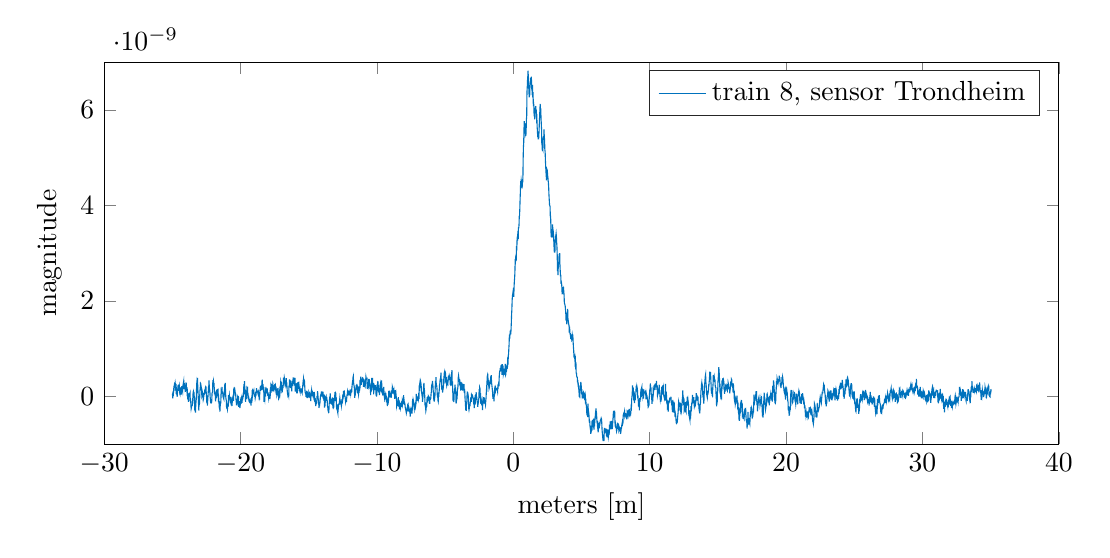
\begin{tikzpicture}

  \begin{axis}[%
    width=\textwidth,
    height=0.4\textwidth,
    at={(0\figurewidth,0\figureheight)},
    scale only axis,
    xmin=-30,
    xmax=40,
    xlabel={meters [m]},
    ymin=-1e-09,
    ymax=7e-09,
    ylabel={magnitude},
    axis background/.style={fill=white},
    legend style={legend cell align=left,align=left,draw=white!15!black}
    ]
    \addplot [color=mycolor1,solid]
    table[row sep=crcr]{%
    -25.0084912109375	5.22942604744358e-11\\
    -24.988341796875	5.21381794563643e-11\\
    -24.9681923828125	-4.43855506816317e-11\\
    -24.94804296875	1.00533936588961e-10\\
    -24.9278935546875	3.35347760066197e-12\\
    -24.907744140625	1.2278449890486e-10\\
    -24.8875947265625	1.76621872087911e-10\\
    -24.8674453125	1.61383690910141e-10\\
    -24.8472958984375	2.25530779468634e-10\\
    -24.827146484375	2.89771349940568e-10\\
    -24.8069970703125	2.23561003213113e-10\\
    -24.78684765625	2.75199207361839e-10\\
    -24.7666982421875	2.32250840828685e-10\\
    -24.746548828125	1.20740121280007e-10\\
    -24.7263994140625	2.59634007692008e-10\\
    -24.70625	4.30744741849598e-11\\
    -24.6861005859375	1.35819918206437e-10\\
    -24.665951171875	9.69236578272748e-11\\
    -24.6458017578125	-1.26690704363891e-11\\
    -24.62565234375	7.2594702052856e-11\\
    -24.6055029296875	1.11087524830661e-10\\
    -24.585353515625	2.28091058703896e-10\\
    -24.5652041015625	1.16107475878767e-10\\
    -24.5450546875	2.47245463252274e-10\\
    -24.5249052734375	1.87145280395668e-10\\
    -24.504755859375	1.69600445073125e-10\\
    -24.4846064453125	2.15347071758186e-10\\
    -24.46445703125	1.59403592042907e-10\\
    -24.4443076171875	2.2038633437092e-11\\
    -24.424158203125	1.90846311664964e-10\\
    -24.4040087890625	9.58058513479932e-11\\
    -24.383859375	1.36257095313652e-10\\
    -24.3637099609375	1.20954987178768e-10\\
    -24.343560546875	3.75221025479142e-11\\
    -24.3234111328125	1.31960978382474e-10\\
    -24.30326171875	2.125113202056e-10\\
    -24.2831123046875	1.25122141217331e-10\\
    -24.262962890625	1.37096784503605e-10\\
    -24.2428134765625	1.05096359378087e-10\\
    -24.2226640625	2.27859111221524e-10\\
    -24.2025146484375	2.50429764572533e-10\\
    -24.182365234375	2.85167079824744e-10\\
    -24.1622158203125	3.19503823878543e-10\\
    -24.14206640625	1.57686778377222e-10\\
    -24.1219169921875	2.78353332940538e-10\\
    -24.101767578125	2.19743371039776e-10\\
    -24.0816181640625	1.76217774101359e-10\\
    -24.06146875	2.32686017401868e-10\\
    -24.0413193359375	9.24330779343836e-11\\
    -24.021169921875	1.88510634287953e-10\\
    -24.0010205078125	1.50600485698271e-10\\
    -23.98087109375	2.86108257579944e-10\\
    -23.9607216796875	1.39473940956621e-10\\
    -23.940572265625	1.87782471745293e-10\\
    -23.9204228515625	8.50601141147172e-11\\
    -23.9002734375	1.11815644629483e-10\\
    -23.8801240234375	8.64720079400348e-12\\
    -23.859974609375	-6.83716906161017e-11\\
    -23.8398251953125	-1.753948621597e-11\\
    -23.81967578125	-1.15369467992461e-10\\
    -23.7995263671875	9.52677928265199e-12\\
    -23.779376953125	6.19039162412216e-11\\
    -23.7592275390625	6.75873904230294e-11\\
    -23.739078125	6.76634347847223e-11\\
    -23.7189287109375	2.70117607645746e-11\\
    -23.698779296875	5.40331819033341e-11\\
    -23.6786298828125	-1.146666654003e-10\\
    -23.65848046875	-5.45042156643195e-11\\
    -23.6383310546875	-1.75183711462603e-10\\
    -23.618181640625	-2.62115611921702e-10\\
    -23.5980322265625	-2.33343618880227e-10\\
    -23.5778828125	-1.960302513413e-10\\
    -23.5577333984375	-1.97675019241604e-10\\
    -23.537583984375	-1.87503307915724e-10\\
    -23.5174345703125	-1.11866244415626e-10\\
    -23.49728515625	-1.51336422380164e-10\\
    -23.4771357421875	7.75474780829975e-11\\
    -23.456986328125	9.92537424132668e-11\\
    -23.4368369140625	4.02687762826352e-11\\
    -23.4166875	9.79861069472235e-11\\
    -23.3965380859375	8.27676759830225e-12\\
    -23.376388671875	-1.37955323780043e-11\\
    -23.3562392578125	-2.26496600077629e-10\\
    -23.33608984375	-2.01637455486926e-10\\
    -23.3159404296875	-1.82370740062515e-10\\
    -23.295791015625	-3.42141011867166e-10\\
    -23.2756416015625	-1.05165836505487e-10\\
    -23.2554921875	-1.09310344795658e-10\\
    -23.2353427734375	-2.58357137006e-12\\
    -23.215193359375	2.48638499515747e-10\\
    -23.1950439453125	3.08215530483215e-10\\
    -23.17489453125	2.60439813805737e-10\\
    -23.1547451171875	3.85066407678148e-10\\
    -23.134595703125	2.14463534949827e-10\\
    -23.1144462890625	7.96512288159246e-11\\
    -23.094296875	-4.11100082873291e-11\\
    -23.0741474609375	-1.7918275284241e-10\\
    -23.053998046875	-2.96773362192738e-10\\
    -23.0338486328125	-6.94988130654241e-11\\
    -23.01369921875	-1.80714457976361e-10\\
    -22.9935498046875	-4.21779802591389e-11\\
    -22.973400390625	1.29079866506817e-10\\
    -22.9532509765625	1.58201080048275e-10\\
    -22.9331015625	2.72733577253623e-10\\
    -22.9129521484375	2.630462067988e-10\\
    -22.892802734375	2.10572687302406e-10\\
    -22.8726533203125	1.83535578995929e-10\\
    -22.85250390625	1.0001426267301e-10\\
    -22.8323544921875	3.81565595615643e-13\\
    -22.812205078125	1.99691510501825e-11\\
    -22.7920556640625	7.89863489145919e-11\\
    -22.77190625	4.61879015150514e-11\\
    -22.7517568359375	5.45712964279327e-11\\
    -22.731607421875	-7.39117012035366e-11\\
    -22.7114580078125	-5.28630462550114e-11\\
    -22.69130859375	9.27305084275568e-12\\
    -22.6711591796875	4.42703674237401e-11\\
    -22.651009765625	4.56628836647904e-11\\
    -22.6308603515625	7.61195755310821e-11\\
    -22.6107109375	1.55204569092693e-10\\
    -22.5905615234375	6.11600019726475e-11\\
    -22.570412109375	1.84900361193422e-10\\
    -22.5502626953125	2.03250263251411e-10\\
    -22.53011328125	1.94532947820586e-10\\
    -22.5099638671875	5.71417794264679e-11\\
    -22.489814453125	-1.17967913186879e-11\\
    -22.4696650390625	-1.34586293864505e-10\\
    -22.449515625	-3.40248359521608e-11\\
    -22.4293662109375	-1.93480715186008e-10\\
    -22.409216796875	-1.08760151658787e-10\\
    -22.3890673828125	-1.90062309303405e-11\\
    -22.36891796875	7.36706241513245e-11\\
    -22.3487685546875	1.66366072840708e-10\\
    -22.328619140625	1.49072962424496e-10\\
    -22.3084697265625	3.34596688909265e-10\\
    -22.2883203125	1.96124034151225e-10\\
    -22.2681708984375	1.45516401978833e-10\\
    -22.248021484375	1.33376257029342e-10\\
    -22.2278720703125	-9.83626561263813e-12\\
    -22.20772265625	-5.87826637757092e-11\\
    -22.1875732421875	-1.4684371377109e-10\\
    -22.167423828125	-6.17232286889062e-11\\
    -22.1472744140625	-1.23754947387537e-10\\
    -22.127125	-1.29219814847758e-10\\
    -22.1069755859375	-9.62324560943945e-11\\
    -22.086826171875	5.99013999515674e-11\\
    -22.0666767578125	8.11369174623356e-11\\
    -22.04652734375	9.79709521010294e-11\\
    -22.0263779296875	3.40002878743935e-10\\
    -22.006228515625	2.89810753484664e-10\\
    -21.9860791015625	3.25881665772748e-10\\
    -21.9659296875	2.71172798933958e-10\\
    -21.9457802734375	2.69435747849633e-10\\
    -21.925630859375	1.77270211272386e-10\\
    -21.9054814453125	4.30808441552933e-11\\
    -21.88533203125	9.12859930925314e-11\\
    -21.8651826171875	6.61590511932546e-11\\
    -21.845033203125	4.5675406793744e-13\\
    -21.8248837890625	-1.04032319705878e-10\\
    -21.804734375	2.85205493567704e-11\\
    -21.7845849609375	6.43164807600438e-12\\
    -21.764435546875	-3.45594357677716e-11\\
    -21.7442861328125	1.07714298145468e-10\\
    -21.72413671875	9.92115113178478e-11\\
    -21.7039873046875	3.18836911557235e-11\\
    -21.683837890625	1.58001328026428e-10\\
    -21.6636884765625	7.82137922793576e-11\\
    -21.6435390625	9.87041519126658e-11\\
    -21.6233896484375	-4.0458984418732e-11\\
    -21.603240234375	-1.66882814730893e-11\\
    -21.5830908203125	-8.22705190450909e-11\\
    -21.56294140625	-2.19327194556675e-10\\
    -21.5427919921875	-2.4481837265702e-10\\
    -21.522642578125	-1.08216539854879e-10\\
    -21.5024931640625	-3.15908865974396e-10\\
    -21.48234375	-1.53281506692668e-10\\
    -21.4621943359375	-1.49483389470111e-10\\
    -21.442044921875	-1.287790690118e-10\\
    -21.4218955078125	9.79804834556101e-11\\
    -21.40174609375	7.28500409051333e-11\\
    -21.3815966796875	1.07755380460835e-10\\
    -21.361447265625	1.99640770443524e-10\\
    -21.3412978515625	9.83093760248617e-11\\
    -21.3211484375	7.18159128466152e-11\\
    -21.3009990234375	7.66925292038647e-11\\
    -21.280849609375	-4.28276487012592e-12\\
    -21.2607001953125	-2.64866905220209e-11\\
    -21.24055078125	-4.0226526783788e-11\\
    -21.2204013671875	-5.79066457647536e-11\\
    -21.200251953125	6.31299283791132e-11\\
    -21.1801025390625	2.34128622423529e-11\\
    -21.159953125	2.52823515746078e-10\\
    -21.1398037109375	1.06836909336023e-10\\
    -21.119654296875	2.84144828748923e-10\\
    -21.0995048828125	1.26671769622069e-10\\
    -21.07935546875	-1.10791859103005e-11\\
    -21.0592060546875	-6.53632852789926e-11\\
    -21.039056640625	-8.19488522879247e-11\\
    -21.0189072265625	-2.55069409802458e-10\\
    -20.9987578125	-2.13404674971181e-10\\
    -20.9786083984375	-2.43549194898918e-10\\
    -20.958458984375	-2.71162316268379e-10\\
    -20.9383095703125	-1.81136841406229e-10\\
    -20.91816015625	-1.41698661195325e-10\\
    -20.8980107421875	-2.13913052750883e-10\\
    -20.877861328125	2.51297693196016e-11\\
    -20.8577119140625	-6.6172921164092e-11\\
    -20.8375625	-2.42760179728007e-11\\
    -20.8174130859375	2.3545400588989e-11\\
    -20.797263671875	-3.7796952816598e-11\\
    -20.7771142578125	-8.27169764222029e-11\\
    -20.75696484375	-1.06279436071171e-10\\
    -20.7368154296875	-1.44603371340491e-10\\
    -20.716666015625	-1.21682587209123e-11\\
    -20.6965166015625	-1.15704525530727e-10\\
    -20.6763671875	-9.28739298317721e-11\\
    -20.6562177734375	-1.31459515364888e-10\\
    -20.636068359375	-1.9240788073404e-10\\
    -20.6159189453125	-1.9023179035558e-10\\
    -20.59576953125	-2.40009172241487e-11\\
    -20.5756201171875	-1.03649985790582e-10\\
    -20.555470703125	-2.11328668645126e-11\\
    -20.5353212890625	3.25595396367022e-11\\
    -20.515171875	-9.46557377856541e-11\\
    -20.4950224609375	1.10203226502789e-10\\
    -20.474873046875	8.5960491720505e-11\\
    -20.4547236328125	1.6706906571294e-10\\
    -20.43457421875	1.74425597204495e-10\\
    -20.4144248046875	1.43491333432971e-10\\
    -20.394275390625	9.28252490226991e-11\\
    -20.3741259765625	4.69253270886777e-11\\
    -20.3539765625	5.14798329304358e-11\\
    -20.3338271484375	-5.64679594447049e-11\\
    -20.313677734375	-1.04267261185834e-10\\
    -20.2935283203125	-1.86561076335628e-10\\
    -20.27337890625	-1.30366085915802e-10\\
    -20.2532294921875	-9.89403286699679e-11\\
    -20.233080078125	-1.4486292171632e-10\\
    -20.2129306640625	-3.8888479377934e-11\\
    -20.19278125	-6.65310293127501e-11\\
    -20.1726318359375	-1.95205748302296e-10\\
    -20.152482421875	1.04033253814409e-11\\
    -20.1323330078125	-2.19476819728988e-10\\
    -20.11218359375	-1.66957532565366e-10\\
    -20.0920341796875	-1.00219135901217e-10\\
    -20.071884765625	-2.12112627137526e-10\\
    -20.0517353515625	-2.02037737883435e-10\\
    -20.0315859375	-2.12660595186939e-10\\
    -20.0114365234375	-1.63852489651288e-10\\
    -19.991287109375	-1.25851778901213e-10\\
    -19.9711376953125	-2.14829925065866e-11\\
    -19.95098828125	-1.55753119747316e-10\\
    -19.9308388671875	-3.05672505643427e-11\\
    -19.910689453125	-9.49527581039339e-12\\
    -19.8905400390625	-1.38581824564303e-10\\
    -19.870390625	-2.68303324040623e-11\\
    -19.8502412109375	-8.47630204244499e-11\\
    -19.830091796875	-2.73377183775276e-11\\
    -19.8099423828125	6.97467331871855e-12\\
    -19.78979296875	3.04691993854533e-12\\
    -19.7696435546875	1.31058746671454e-10\\
    -19.749494140625	2.54826512622852e-10\\
    -19.7293447265625	1.92261622890661e-10\\
    -19.7091953125	3.2043823329288e-10\\
    -19.6890458984375	1.85673659492562e-10\\
    -19.668896484375	4.28686404887698e-11\\
    -19.6487470703125	1.39655487177771e-10\\
    -19.62859765625	-1.14350184960584e-10\\
    -19.6084482421875	-6.01911488118553e-12\\
    -19.588298828125	4.71626461343687e-11\\
    -19.5681494140625	-5.88176410564049e-11\\
    -19.548	8.02745421671709e-11\\
    -19.5278505859375	1.7067673839203e-10\\
    -19.507701171875	1.53805166488018e-10\\
    -19.4875517578125	2.03071973123069e-10\\
    -19.46740234375	3.6729927536098e-11\\
    -19.4472529296875	4.11439729339599e-11\\
    -19.427103515625	-6.24082720842328e-11\\
    -19.4069541015625	1.41907017391523e-11\\
    -19.3868046875	-8.2485703761883e-11\\
    -19.3666552734375	-1.06677186649347e-10\\
    -19.346505859375	-1.16083922403261e-10\\
    -19.3263564453125	-8.96759373839871e-11\\
    -19.30620703125	-7.79504711817526e-11\\
    -19.2860576171875	-1.44796344109076e-10\\
    -19.265908203125	-8.49983111190487e-11\\
    -19.2457587890625	-1.43012821517086e-10\\
    -19.225609375	-1.91107283120289e-10\\
    -19.2054599609375	-8.19417446968552e-11\\
    -19.185310546875	-4.23161861369744e-11\\
    -19.1651611328125	-1.33645294236549e-10\\
    -19.14501171875	5.5262209729409e-11\\
    -19.1248623046875	3.41825581232228e-11\\
    -19.104712890625	1.17888618698624e-10\\
    -19.0845634765625	1.00060640869157e-10\\
    -19.0644140625	8.89917333892146e-11\\
    -19.0442646484375	1.07549965212882e-10\\
    -19.024115234375	1.27213766343115e-10\\
    -19.0039658203125	4.04913791542601e-11\\
    -18.98381640625	6.39942935793596e-12\\
    -18.9636669921875	4.45319151550268e-12\\
    -18.943517578125	1.78031196513048e-11\\
    -18.9233681640625	-3.9154486076648e-11\\
    -18.90321875	-8.07227325177327e-12\\
    -18.8830693359375	9.33318985476917e-11\\
    -18.862919921875	1.35715241612778e-11\\
    -18.8427705078125	1.03228800630048e-10\\
    -18.82262109375	1.69958593695372e-10\\
    -18.8024716796875	1.12321695386258e-10\\
    -18.782322265625	1.16162992317904e-10\\
    -18.7621728515625	1.04422436602835e-10\\
    -18.7420234375	9.50615478511456e-11\\
    -18.7218740234375	5.97285882511601e-11\\
    -18.701724609375	4.13810100445903e-11\\
    -18.6815751953125	8.26367315480952e-11\\
    -18.66142578125	4.85702771323423e-11\\
    -18.6412763671875	-9.17016593210467e-12\\
    -18.621126953125	2.02645186986437e-11\\
    -18.6009775390625	-9.36173131811637e-12\\
    -18.580828125	1.14432002231656e-10\\
    -18.5606787109375	1.34113473113122e-10\\
    -18.540529296875	2.24933088248474e-10\\
    -18.5203798828125	1.16659014301959e-10\\
    -18.50023046875	2.25231292833615e-10\\
    -18.4800810546875	1.84688445716239e-10\\
    -18.459931640625	1.37261351611622e-10\\
    -18.4397822265625	2.30753449785202e-10\\
    -18.4196328125	1.89550119015289e-10\\
    -18.3994833984375	3.51160296580818e-10\\
    -18.379333984375	1.43760394246796e-10\\
    -18.3591845703125	2.08513681135302e-10\\
    -18.33903515625	2.17393327670326e-10\\
    -18.3188857421875	1.1211097181756e-10\\
    -18.298736328125	1.95128230294408e-10\\
    -18.2785869140625	-1.13586162119006e-10\\
    -18.2584375	1.00631741581109e-10\\
    -18.2382880859375	-2.09759536904047e-11\\
    -18.218138671875	-5.84010168112246e-11\\
    -18.1979892578125	5.59385834332991e-11\\
    -18.17783984375	1.02245405524448e-10\\
    -18.1576904296875	7.76894692716364e-11\\
    -18.137541015625	2.00493748039504e-10\\
    -18.1173916015625	6.14036699142168e-11\\
    -18.0972421875	1.45810262768408e-10\\
    -18.0770927734375	1.44731331529981e-10\\
    -18.056943359375	7.26392534314868e-11\\
    -18.0367939453125	1.67743373762849e-10\\
    -18.01664453125	5.79198402246417e-11\\
    -17.9964951171875	1.05698164982726e-11\\
    -17.976345703125	8.36833563871159e-11\\
    -17.9561962890625	-3.34617430101811e-12\\
    -17.936046875	-4.20961153950244e-11\\
    -17.9158974609375	2.01401762944725e-11\\
    -17.895748046875	-5.28478260504943e-11\\
    -17.8755986328125	1.41300805412827e-12\\
    -17.85544921875	3.31368737205908e-11\\
    -17.8352998046875	8.44906533476574e-11\\
    -17.815150390625	4.05396031947489e-11\\
    -17.7950009765625	1.14233047653845e-10\\
    -17.7748515625	2.11867550863273e-10\\
    -17.7547021484375	1.81206699904289e-10\\
    -17.734552734375	2.62461366664787e-10\\
    -17.7144033203125	1.71203316075883e-10\\
    -17.69425390625	2.07099577538257e-10\\
    -17.6741044921875	2.41182892623366e-10\\
    -17.653955078125	1.55770323094535e-10\\
    -17.6338056640625	1.75986200847882e-10\\
    -17.61365625	1.89618737801693e-10\\
    -17.5935068359375	1.24130132145852e-10\\
    -17.573357421875	1.19283593453497e-10\\
    -17.5532080078125	1.90527763057928e-10\\
    -17.53305859375	1.50574393436967e-10\\
    -17.5129091796875	1.78683940098407e-10\\
    -17.492759765625	1.70183790366535e-10\\
    -17.4726103515625	2.4532121332173e-10\\
    -17.4524609375	2.53179635327396e-10\\
    -17.4323115234375	1.71891458836823e-10\\
    -17.412162109375	1.2399021690853e-10\\
    -17.3920126953125	1.44806321711726e-10\\
    -17.37186328125	3.07709241429787e-11\\
    -17.3517138671875	1.58624042791804e-10\\
    -17.331564453125	4.01776477247171e-11\\
    -17.3114150390625	7.29550139156811e-11\\
    -17.291265625	7.88357599137317e-11\\
    -17.2711162109375	1.90731792720792e-11\\
    -17.250966796875	1.74248479489033e-10\\
    -17.2308173828125	7.53372490885885e-11\\
    -17.21066796875	-5.11776758401918e-12\\
    -17.1905185546875	3.15246709670929e-11\\
    -17.170369140625	-1.2438580506436e-11\\
    -17.1502197265625	1.36252261541396e-11\\
    -17.1300703125	9.76656473063842e-11\\
    -17.1099208984375	5.76135706077184e-11\\
    -17.089771484375	1.25937070340694e-10\\
    -17.0696220703125	2.14107439170829e-10\\
    -17.04947265625	3.00769722589137e-10\\
    -17.0293232421875	2.62902438776964e-10\\
    -17.009173828125	1.54195957567895e-10\\
    -16.9890244140625	1.95273890926877e-10\\
    -16.968875	1.06013804922239e-10\\
    -16.9487255859375	1.18824344465451e-10\\
    -16.928576171875	1.11377527369612e-10\\
    -16.9084267578125	2.35560150378169e-10\\
    -16.88827734375	1.72273152264889e-10\\
    -16.8681279296875	2.44952570587739e-10\\
    -16.847978515625	3.90906091340081e-10\\
    -16.8278291015625	3.55021913474335e-10\\
    -16.8076796875	3.10563021983017e-10\\
    -16.7875302734375	3.90637961071648e-10\\
    -16.767380859375	3.58630353538111e-10\\
    -16.7472314453125	2.97275623114921e-10\\
    -16.72708203125	2.85932080151553e-10\\
    -16.7069326171875	2.50207950791881e-10\\
    -16.686783203125	2.25232090893353e-10\\
    -16.6666337890625	2.62868566340122e-10\\
    -16.646484375	3.80228915207333e-10\\
    -16.6263349609375	2.51996621059614e-10\\
    -16.606185546875	2.91960769931902e-10\\
    -16.5860361328125	1.59509159571862e-10\\
    -16.56588671875	9.53713924189997e-11\\
    -16.5457373046875	4.50400486947352e-11\\
    -16.525587890625	1.48475850233532e-11\\
    -16.5054384765625	3.22040724758799e-11\\
    -16.4852890625	4.71457889497692e-11\\
    -16.4651396484375	1.74606523080917e-11\\
    -16.444990234375	2.0699187681945e-10\\
    -16.4248408203125	2.19031801072273e-10\\
    -16.40469140625	3.52442691088225e-10\\
    -16.3845419921875	3.05944089683472e-10\\
    -16.364392578125	2.52976697747203e-10\\
    -16.3442431640625	2.74125726481483e-10\\
    -16.32409375	1.74849032669526e-10\\
    -16.3039443359375	2.50475819839052e-10\\
    -16.283794921875	2.36259996737467e-10\\
    -16.2636455078125	2.56185766411705e-10\\
    -16.24349609375	1.02950745675483e-10\\
    -16.2233466796875	3.24663748929734e-10\\
    -16.203197265625	2.55813660263479e-10\\
    -16.1830478515625	2.52277630410957e-10\\
    -16.1628984375	2.17024430464654e-10\\
    -16.1427490234375	3.94667733084676e-10\\
    -16.122599609375	2.55076838436122e-10\\
    -16.1024501953125	3.0015849100447e-10\\
    -16.08230078125	3.9327278117392e-10\\
    -16.0621513671875	3.37476479359381e-10\\
    -16.042001953125	2.81400119990194e-10\\
    -16.0218525390625	2.27386367251174e-10\\
    -16.001703125	3.86504571633848e-10\\
    -15.9815537109375	9.73213606536839e-11\\
    -15.961404296875	2.72905410281178e-10\\
    -15.9412548828125	2.11854256437036e-10\\
    -15.92110546875	1.70477883625719e-10\\
    -15.9009560546875	2.54691691045983e-10\\
    -15.880806640625	1.77759142255271e-10\\
    -15.8606572265625	2.7508767130283e-10\\
    -15.8405078125	6.33553434332116e-11\\
    -15.8203583984375	2.8199705895133e-10\\
    -15.800208984375	2.08735150090504e-10\\
    -15.7800595703125	2.98529594205228e-10\\
    -15.75991015625	1.59625445164678e-10\\
    -15.7397607421875	2.92326731708716e-10\\
    -15.719611328125	2.94859352273868e-10\\
    -15.6994619140625	1.11930038032227e-10\\
    -15.6793125	2.02415179292226e-10\\
    -15.6591630859375	1.40576591336513e-10\\
    -15.639013671875	1.61366918271615e-10\\
    -15.6188642578125	1.09700366352615e-10\\
    -15.59871484375	1.60699296031811e-10\\
    -15.5785654296875	8.29282935924567e-11\\
    -15.558416015625	1.6730860014547e-10\\
    -15.5382666015625	1.1825990675431e-10\\
    -15.5181171875	9.44730105920107e-11\\
    -15.4979677734375	1.06850031439881e-10\\
    -15.477818359375	8.11993784095603e-11\\
    -15.4576689453125	1.52029020106225e-10\\
    -15.43751953125	2.15432320544704e-10\\
    -15.4173701171875	2.8080689323027e-10\\
    -15.397220703125	2.63511977646026e-10\\
    -15.3770712890625	3.74038102371225e-10\\
    -15.356921875	3.41478951693845e-10\\
    -15.3367724609375	3.00637363413379e-10\\
    -15.316623046875	3.49421500671927e-10\\
    -15.2964736328125	2.46996066926241e-10\\
    -15.27632421875	1.40013768422077e-10\\
    -15.2561748046875	7.55237791889508e-11\\
    -15.236025390625	7.18726631706035e-11\\
    -15.2158759765625	5.19654633575751e-11\\
    -15.1957265625	-3.18302475194335e-12\\
    -15.1755771484375	-6.63745162515401e-12\\
    -15.155427734375	1.04188067842439e-10\\
    -15.1352783203125	1.02707799020946e-10\\
    -15.11512890625	-3.89025664869861e-11\\
    -15.0949794921875	9.8105810578253e-11\\
    -15.074830078125	-3.46343492402804e-11\\
    -15.0546806640625	6.02326148675711e-11\\
    -15.03453125	5.18261508801348e-11\\
    -15.0143818359375	-1.8333174149828e-11\\
    -14.994232421875	6.6428047816395e-11\\
    -14.9740830078125	3.67055374232765e-11\\
    -14.95393359375	9.53346204858993e-11\\
    -14.9337841796875	2.11901597083264e-11\\
    -14.913634765625	-3.12159017151629e-12\\
    -14.8934853515625	9.61877266575684e-13\\
    -14.8733359375	2.5548486731463e-11\\
    -14.8531865234375	-9.82729705595047e-11\\
    -14.833037109375	-4.83585969479328e-12\\
    -14.8128876953125	9.04546491254555e-11\\
    -14.79273828125	1.26241218243129e-10\\
    -14.7725888671875	8.69491124981948e-12\\
    -14.752439453125	6.31163025582941e-11\\
    -14.7322900390625	1.20394071103952e-10\\
    -14.712140625	4.63347241364675e-11\\
    -14.6919912109375	9.89546403260595e-12\\
    -14.671841796875	-1.21937207747026e-11\\
    -14.6516923828125	8.69407209603335e-11\\
    -14.63154296875	-2.53633320697187e-12\\
    -14.6113935546875	7.63317890427595e-12\\
    -14.591244140625	9.06478234713446e-11\\
    -14.5710947265625	3.68231541392352e-11\\
    -14.5509453125	-1.18824054516117e-10\\
    -14.5307958984375	-8.04767494791833e-11\\
    -14.510646484375	-7.05245629363829e-11\\
    -14.4904970703125	-2.05817412376491e-10\\
    -14.47034765625	-1.65029347673668e-10\\
    -14.4501982421875	-1.59982681136263e-10\\
    -14.430048828125	-1.11399511258294e-10\\
    -14.4098994140625	-1.18817127934379e-10\\
    -14.38975	-3.27811158583853e-12\\
    -14.3696005859375	2.63148741320637e-12\\
    -14.349451171875	1.07655231343293e-10\\
    -14.3293017578125	4.45455061652087e-11\\
    -14.30915234375	-4.52204457865468e-11\\
    -14.2890029296875	-6.66745097656823e-11\\
    -14.268853515625	-1.09125146672938e-10\\
    -14.2487041015625	-2.43124778574061e-10\\
    -14.2285546875	-2.02477524223695e-10\\
    -14.2084052734375	-1.97444435710491e-10\\
    -14.188255859375	-1.5002201376832e-10\\
    -14.1681064453125	-1.20793681622427e-10\\
    -14.14795703125	-2.83540744408128e-11\\
    -14.1278076171875	2.06829977310958e-11\\
    -14.107658203125	4.01455141864549e-11\\
    -14.0875087890625	4.65024786874769e-11\\
    -14.067359375	1.01768542844662e-10\\
    -14.0472099609375	-3.43786164054798e-12\\
    -14.027060546875	1.04651901821181e-10\\
    -14.0069111328125	3.68618995234214e-11\\
    -13.98676171875	1.59295149361438e-11\\
    -13.9666123046875	7.69050209134519e-11\\
    -13.946462890625	8.02295278526424e-11\\
    -13.9263134765625	-9.19097762791169e-13\\
    -13.9061640625	-4.66308332431017e-12\\
    -13.8860146484375	-9.2600140918961e-11\\
    -13.865865234375	4.22240995902228e-11\\
    -13.8457158203125	-2.37468174789002e-10\\
    -13.82556640625	-1.34713502983491e-10\\
    -13.8054169921875	-7.33955239701081e-11\\
    -13.785267578125	-1.13056013370089e-10\\
    -13.7651181640625	-4.05548756447636e-11\\
    -13.74496875	-1.34025616572682e-11\\
    -13.7248193359375	3.36750270655315e-13\\
    -13.704669921875	-9.57190165275139e-11\\
    -13.6845205078125	-1.38439024712225e-11\\
    -13.66437109375	-6.54709455032706e-11\\
    -13.6442216796875	-8.83992541229423e-11\\
    -13.624072265625	-2.0521797337079e-10\\
    -13.6039228515625	-2.18138043269379e-10\\
    -13.5837734375	-2.88757458859858e-10\\
    -13.5636240234375	-3.13316577686605e-10\\
    -13.543474609375	-2.8750732711623e-10\\
    -13.5233251953125	-3.46635356218167e-10\\
    -13.50317578125	-1.72087441259363e-10\\
    -13.4830263671875	-1.22605681713384e-10\\
    -13.462876953125	-5.77032103186512e-12\\
    -13.4427275390625	-1.56327696683964e-10\\
    -13.422578125	5.94842597585654e-11\\
    -13.4024287109375	-1.10066507010718e-10\\
    -13.382279296875	-5.37111082015326e-11\\
    -13.3621298828125	-5.84723833777083e-11\\
    -13.34198046875	-1.13755174186508e-10\\
    -13.3218310546875	-1.74864619975418e-10\\
    -13.301681640625	-8.8476856494387e-11\\
    -13.2815322265625	-1.66617295892594e-10\\
    -13.2613828125	-2.02133210557906e-11\\
    -13.2412333984375	-1.58659332744127e-10\\
    -13.221083984375	-2.45499167774083e-10\\
    -13.2009345703125	-3.93127611234677e-11\\
    -13.18078515625	-2.35011283698189e-10\\
    -13.1606357421875	-2.24679684639584e-10\\
    -13.140486328125	-6.47833666871764e-11\\
    -13.1203369140625	-3.73422447572416e-11\\
    -13.1001875	-9.46084104576668e-11\\
    -13.0800380859375	8.66538723172064e-11\\
    -13.059888671875	4.60773031700479e-11\\
    -13.0397392578125	7.70800191810397e-11\\
    -13.01958984375	6.81243911742732e-11\\
    -12.9994404296875	-1.03025889631816e-10\\
    -12.979291015625	-1.9643563557659e-11\\
    -12.9591416015625	-2.15645556334584e-10\\
    -12.9389921875	-1.94302243933823e-10\\
    -12.9188427734375	-2.26446249426198e-10\\
    -12.898693359375	-2.72632378108111e-10\\
    -12.8785439453125	-3.24717429393445e-10\\
    -12.85839453125	-3.53914490699176e-10\\
    -12.8382451171875	-1.63820158091607e-10\\
    -12.818095703125	-2.25467064870138e-10\\
    -12.7979462890625	-1.77694561116169e-10\\
    -12.777796875	-1.53760699242322e-10\\
    -12.7576474609375	-1.5661721345157e-10\\
    -12.737498046875	-9.51555872657524e-11\\
    -12.7173486328125	-3.68807138276952e-11\\
    -12.69719921875	-8.40528916282272e-11\\
    -12.6770498046875	-1.14515728506302e-10\\
    -12.656900390625	-1.14545847104754e-10\\
    -12.6367509765625	-1.81330791680723e-10\\
    -12.6166015625	-8.80622401544404e-11\\
    -12.5964521484375	-1.93349845087568e-10\\
    -12.576302734375	-1.56339733959223e-10\\
    -12.5561533203125	-5.41326602548908e-11\\
    -12.53600390625	-1.46473775012106e-10\\
    -12.5158544921875	-7.63829293083397e-11\\
    -12.495705078125	4.14093891476988e-11\\
    -12.4755556640625	-6.15883664220532e-11\\
    -12.45540625	1.08751936370524e-10\\
    -12.4352568359375	1.03761481437463e-11\\
    -12.415107421875	5.5945816958494e-11\\
    -12.3949580078125	1.24730493638803e-10\\
    -12.37480859375	5.34889173339331e-11\\
    -12.3546591796875	1.40384121333334e-12\\
    -12.334509765625	-4.25031849935715e-12\\
    -12.3143603515625	-4.99877427655138e-11\\
    -12.2942109375	-1.05420799048767e-10\\
    -12.2740615234375	-5.87012710943855e-11\\
    -12.253912109375	-4.58752478930127e-11\\
    -12.2337626953125	-1.21126130529919e-10\\
    -12.21361328125	-4.03473213436534e-11\\
    -12.1934638671875	2.59571050839428e-11\\
    -12.173314453125	2.65720463505181e-11\\
    -12.1531650390625	9.69252548967359e-11\\
    -12.133015625	6.38252541560279e-11\\
    -12.1128662109375	4.54508398023127e-11\\
    -12.092716796875	7.46963394242687e-11\\
    -12.0725673828125	9.86356551539746e-11\\
    -12.05241796875	8.71099406469302e-11\\
    -12.0322685546875	2.62539146842406e-11\\
    -12.012119140625	8.31843903052752e-11\\
    -11.9919697265625	1.01955226888818e-10\\
    -11.9718203125	5.42235248210097e-11\\
    -11.9516708984375	1.02342994105068e-11\\
    -11.931521484375	1.37561075800242e-10\\
    -11.9113720703125	6.54727639994856e-11\\
    -11.89122265625	1.1054328165137e-10\\
    -11.8710732421875	1.30205336669835e-10\\
    -11.850923828125	7.71946053270248e-11\\
    -11.8307744140625	1.84513863086299e-10\\
    -11.810625	2.43427674165728e-10\\
    -11.7904755859375	2.96316464928498e-10\\
    -11.770326171875	3.27507311436609e-10\\
    -11.7501767578125	3.94848933053602e-10\\
    -11.73002734375	4.20809229986875e-10\\
    -11.7098779296875	2.9859973092649e-10\\
    -11.689728515625	2.39826158047732e-10\\
    -11.6695791015625	2.25940776195973e-10\\
    -11.6494296875	1.51835511045556e-10\\
    -11.6292802734375	-2.95690259464614e-11\\
    -11.609130859375	2.13504417079034e-11\\
    -11.5889814453125	1.11700810465688e-10\\
    -11.56883203125	8.49766144609097e-11\\
    -11.5486826171875	1.39420856432237e-10\\
    -11.528533203125	1.61033724638106e-10\\
    -11.5083837890625	2.37222338404976e-10\\
    -11.488234375	1.71657434778972e-10\\
    -11.4680849609375	2.60587849403604e-10\\
    -11.447935546875	1.84597314891631e-10\\
    -11.4277861328125	2.21287462977141e-10\\
    -11.40763671875	6.44192515730901e-11\\
    -11.3874873046875	2.08264362021927e-10\\
    -11.367337890625	7.97744687765843e-11\\
    -11.3471884765625	4.19593834308506e-11\\
    -11.3270390625	1.29997289721871e-10\\
    -11.3068896484375	7.43125856356478e-11\\
    -11.286740234375	2.01896117173584e-10\\
    -11.2665908203125	1.08175320455211e-10\\
    -11.24644140625	2.54431724432604e-10\\
    -11.2262919921875	2.24091840918321e-10\\
    -11.206142578125	2.79006235207183e-10\\
    -11.1859931640625	4.10038537815377e-10\\
    -11.16584375	2.9661354776775e-10\\
    -11.1456943359375	2.3943657897137e-10\\
    -11.125544921875	3.00518469035099e-10\\
    -11.1053955078125	3.14510522881728e-10\\
    -11.08524609375	3.16862988698187e-10\\
    -11.0650966796875	3.77272873372689e-10\\
    -11.044947265625	3.87620604465733e-10\\
    -11.0247978515625	3.81197024703161e-10\\
    -11.0046484375	3.63070786763607e-10\\
    -10.9844990234375	1.98580685126248e-10\\
    -10.964349609375	3.55139538009307e-10\\
    -10.9442001953125	2.41160305734024e-10\\
    -10.92405078125	1.98825365894404e-10\\
    -10.9039013671875	3.26957489451371e-10\\
    -10.883751953125	2.11496662922735e-10\\
    -10.8636025390625	2.0040090671928e-10\\
    -10.843453125	3.65850114675065e-10\\
    -10.8233037109375	3.29563832254991e-10\\
    -10.803154296875	4.14422993299895e-10\\
    -10.7830048828125	3.85835515816727e-10\\
    -10.76285546875	3.55240732692175e-10\\
    -10.7427060546875	3.48952986927226e-10\\
    -10.722556640625	3.58324141252475e-10\\
    -10.7024072265625	1.59161227330467e-10\\
    -10.6822578125	2.3621495766581e-10\\
    -10.6621083984375	1.93851292364081e-10\\
    -10.641958984375	1.74915749206041e-10\\
    -10.6218095703125	1.9428913766327e-10\\
    -10.60166015625	3.63476057958802e-10\\
    -10.5815107421875	3.25961321372737e-10\\
    -10.561361328125	2.77016406619684e-10\\
    -10.5412119140625	3.02284320158024e-10\\
    -10.5210625	2.55292934655857e-10\\
    -10.5009130859375	1.58732625128967e-10\\
    -10.480763671875	2.43052654663457e-10\\
    -10.4606142578125	2.52204637685153e-11\\
    -10.44046484375	2.10254337211561e-10\\
    -10.4203154296875	9.4401317558834e-11\\
    -10.400166015625	2.04130471579178e-10\\
    -10.3800166015625	3.84473816392576e-10\\
    -10.3598671875	2.96183466132207e-10\\
    -10.3397177734375	3.1709091672507e-10\\
    -10.319568359375	3.8472728056522e-10\\
    -10.2994189453125	1.80111958371942e-10\\
    -10.27926953125	1.34772146312734e-10\\
    -10.2591201171875	2.83596256337229e-10\\
    -10.238970703125	4.33018888871411e-11\\
    -10.2188212890625	1.97857655674921e-10\\
    -10.198671875	1.83706825908917e-10\\
    -10.1785224609375	2.0480291693955e-10\\
    -10.158373046875	1.32045268247136e-10\\
    -10.1382236328125	2.20024363100923e-10\\
    -10.11807421875	2.21934307110004e-10\\
    -10.0979248046875	1.87544347648077e-10\\
    -10.077775390625	1.99263652645276e-10\\
    -10.0576259765625	5.62799294549636e-12\\
    -10.0374765625	1.96332556952636e-10\\
    -10.0173271484375	-7.21581431163763e-12\\
    -9.997177734375	1.94235875597896e-10\\
    -9.9770283203125	1.2097313426163e-10\\
    -9.95687890625	2.23176001703641e-10\\
    -9.9367294921875	1.87953813456362e-10\\
    -9.916580078125	3.12847971975049e-10\\
    -9.8964306640625	1.87175611488375e-10\\
    -9.87628125	1.58048379507845e-10\\
    -9.8561318359375	1.19881337168348e-10\\
    -9.835982421875	1.3295164760199e-10\\
    -9.8158330078125	2.76334092410049e-11\\
    -9.79568359375	1.03342530080015e-10\\
    -9.7755341796875	1.94750558071531e-10\\
    -9.755384765625	1.74707671822031e-10\\
    -9.7352353515625	1.16364551395843e-10\\
    -9.7150859375	2.87320786585421e-10\\
    -9.6949365234375	2.69674662608918e-10\\
    -9.674787109375	8.25188224075543e-11\\
    -9.6546376953125	3.33850497263823e-10\\
    -9.63448828125	1.41813687878019e-10\\
    -9.6143388671875	5.7575470310101e-11\\
    -9.594189453125	1.6541493998006e-10\\
    -9.5740400390625	2.06266203708436e-11\\
    -9.553890625	1.59997280803484e-10\\
    -9.5337412109375	7.41269925441742e-11\\
    -9.513591796875	9.22183889857216e-11\\
    -9.4934423828125	1.99469292705355e-10\\
    -9.47329296875	3.5388219509654e-11\\
    -9.4531435546875	-7.77850139078269e-12\\
    -9.432994140625	6.12771039448694e-11\\
    -9.4128447265625	-2.30011949912734e-11\\
    -9.3926953125	1.36916326336841e-11\\
    -9.3725458984375	-6.08829214843653e-11\\
    -9.352396484375	7.15885735179056e-11\\
    -9.3322470703125	-4.83111169398851e-11\\
    -9.31209765625	-5.23607486164602e-11\\
    -9.2919482421875	-1.24635620186743e-10\\
    -9.271798828125	-7.6814962864472e-11\\
    -9.2516494140625	-1.34028437945417e-10\\
    -9.2315	-2.01453387672783e-10\\
    -9.2113505859375	-1.21227319217175e-10\\
    -9.191201171875	-1.7850700698581e-10\\
    -9.1710517578125	-6.91335787048132e-11\\
    -9.15090234375	-8.31061798933971e-11\\
    -9.1307529296875	1.0422453751608e-10\\
    -9.110603515625	1.08699658123954e-10\\
    -9.0904541015625	1.07769555130905e-10\\
    -9.0703046875	-1.37799641507587e-11\\
    -9.0501552734375	9.61717605834936e-11\\
    -9.030005859375	-2.40126866619466e-11\\
    -9.0098564453125	4.27249986217345e-11\\
    -8.98970703125	4.83579864283657e-11\\
    -8.9695576171875	-1.10128764805264e-11\\
    -8.949408203125	-1.40637764666551e-11\\
    -8.9292587890625	1.13440145753997e-10\\
    -8.909109375	1.12756988639003e-10\\
    -8.8889599609375	5.27522683305979e-11\\
    -8.868810546875	2.00108817872419e-10\\
    -8.8486611328125	1.75671610128054e-10\\
    -8.82851171875	7.00573513805609e-11\\
    -8.8083623046875	1.71818142439181e-10\\
    -8.788212890625	8.85414299038794e-11\\
    -8.7680634765625	7.25579840464869e-11\\
    -8.7479140625	1.16752883956939e-10\\
    -8.7277646484375	4.56733308757331e-11\\
    -8.707615234375	2.87669564443746e-11\\
    -8.6874658203125	-5.07663524187661e-11\\
    -8.66731640625	1.51449096005329e-11\\
    -8.6471669921875	1.27985074498829e-10\\
    -8.627017578125	3.86419129168719e-11\\
    -8.6068681640625	6.81566412880644e-11\\
    -8.58671875	5.08473248558331e-12\\
    -8.5665693359375	-3.58859737728653e-11\\
    -8.546419921875	-2.0124359425388e-10\\
    -8.5262705078125	-1.67904289069481e-10\\
    -8.50612109375	-1.4739787347627e-10\\
    -8.4859716796875	-2.02353512819577e-10\\
    -8.465822265625	-1.09348277768951e-10\\
    -8.4456728515625	-1.62945001850023e-10\\
    -8.4255234375	-1.56727985760961e-11\\
    -8.4053740234375	-2.16689438134965e-10\\
    -8.385224609375	-1.53275818043153e-10\\
    -8.3650751953125	-1.0267813731732e-10\\
    -8.34492578125	-2.73676473935442e-10\\
    -8.3247763671875	-1.77669527053645e-10\\
    -8.304626953125	-2.12443905473895e-10\\
    -8.2844775390625	-1.35191253807119e-10\\
    -8.264328125	-2.38229372295439e-10\\
    -8.2441787109375	-2.11142266288753e-10\\
    -8.224029296875	-1.74163710888445e-10\\
    -8.2038798828125	-2.17093560054676e-10\\
    -8.18373046875	-1.25904329960703e-10\\
    -8.1635810546875	-2.13916208427186e-10\\
    -8.143431640625	-1.21075083140581e-10\\
    -8.1232822265625	-1.62090677756505e-10\\
    -8.1031328125	-9.54827520684982e-11\\
    -8.0829833984375	-7.09693242026687e-11\\
    -8.062833984375	-1.62975294677123e-10\\
    -8.0426845703125	2.49414239089242e-11\\
    -8.02253515625	-1.35577254282572e-10\\
    -8.0023857421875	-9.75220006156674e-11\\
    -7.982236328125	-1.49026127211316e-10\\
    -7.9620869140625	-1.41496966520222e-10\\
    -7.9419375	-1.70016895788792e-10\\
    -7.9217880859375	-2.32615027173732e-10\\
    -7.901638671875	-2.48309615070475e-10\\
    -7.8814892578125	-2.87212394676625e-10\\
    -7.86133984375	-3.1504918664907e-10\\
    -7.8411904296875	-3.51444977773871e-10\\
    -7.821041015625	-3.20385483518702e-10\\
    -7.8008916015625	-3.02703538466099e-10\\
    -7.7807421875	-2.40593018742684e-10\\
    -7.7605927734375	-2.35720244298276e-10\\
    -7.740443359375	-1.74036654927912e-10\\
    -7.7202939453125	-1.62734053757108e-10\\
    -7.70014453125	-3.16026399925769e-10\\
    -7.6799951171875	-2.08783318577472e-10\\
    -7.659845703125	-2.27516872633652e-10\\
    -7.6396962890625	-3.1073624716303e-10\\
    -7.619546875	-3.17624638173438e-10\\
    -7.5993974609375	-3.22902009367801e-10\\
    -7.579248046875	-2.97638378589683e-10\\
    -7.5590986328125	-4.24164533817436e-10\\
    -7.53894921875	-2.50952162241951e-10\\
    -7.5187998046875	-3.60726579416576e-10\\
    -7.498650390625	-2.85430926971673e-10\\
    -7.4785009765625	-3.61969869273576e-10\\
    -7.4583515625	-2.39023422673324e-10\\
    -7.4382021484375	-3.06090349036674e-10\\
    -7.418052734375	-3.59975926585156e-10\\
    -7.3979033203125	-1.47101794520507e-10\\
    -7.37775390625	-5.96006365794961e-11\\
    -7.3576044921875	-1.85986347386232e-10\\
    -7.337455078125	-7.00472236256898e-11\\
    -7.3173056640625	-9.38203735609135e-11\\
    -7.29715625	-1.82034099384469e-10\\
    -7.2770068359375	-2.15072077049715e-10\\
    -7.256857421875	-2.59041116373717e-10\\
    -7.2367080078125	-1.95872951711918e-10\\
    -7.21655859375	-2.13163863578093e-10\\
    -7.1964091796875	-2.31860334875962e-10\\
    -7.176259765625	-1.22853865289795e-10\\
    -7.1561103515625	-1.91174905876543e-10\\
    -7.1359609375	-1.57479721886999e-10\\
    -7.1158115234375	5.33541496156469e-11\\
    -7.095662109375	-9.82063849250056e-11\\
    -7.0755126953125	-2.51256111351141e-11\\
    -7.05536328125	-1.31628611511992e-11\\
    -7.0352138671875	-1.40421252114087e-11\\
    -7.015064453125	-7.50848768972258e-11\\
    -6.9949150390625	-6.74979496889558e-11\\
    -6.974765625	-2.89176814203078e-11\\
    -6.9546162109375	-5.52862009815898e-11\\
    -6.934466796875	7.04257031295771e-11\\
    -6.9143173828125	-5.58009990043002e-11\\
    -6.89416796875	2.32014783537269e-10\\
    -6.8740185546875	1.17123355941944e-10\\
    -6.853869140625	2.70489630647907e-10\\
    -6.8337197265625	3.11047528997848e-10\\
    -6.8135703125	2.6656898132881e-10\\
    -6.7934208984375	3.05113185229341e-10\\
    -6.773271484375	2.77119283615596e-10\\
    -6.7531220703125	2.20335700486901e-10\\
    -6.73297265625	1.05308865100171e-10\\
    -6.7128232421875	6.79609113626502e-11\\
    -6.692673828125	2.4208094772252e-11\\
    -6.6725244140625	3.8538610682583e-11\\
    -6.652375	-1.17154542614964e-10\\
    -6.6322255859375	-1.82426315427541e-11\\
    -6.612076171875	1.20139890786244e-11\\
    -6.5919267578125	1.13268419492304e-10\\
    -6.57177734375	2.26131960300985e-10\\
    -6.5516279296875	2.80951251776246e-10\\
    -6.531478515625	1.70271408001012e-10\\
    -6.5113291015625	1.27479847786109e-10\\
    -6.4911796875	3.13810183975331e-12\\
    -6.4710302734375	-1.74795821013255e-10\\
    -6.450880859375	-2.04148992856714e-10\\
    -6.4307314453125	-2.32308880533384e-10\\
    -6.41058203125	-3.02212648524754e-10\\
    -6.3904326171875	-2.71102041011377e-10\\
    -6.370283203125	-1.29593919253021e-10\\
    -6.3501337890625	-2.27184655370016e-10\\
    -6.329984375	-7.51872010932427e-11\\
    -6.3098349609375	-1.87837683757611e-11\\
    -6.289685546875	-1.22716050267373e-10\\
    -6.2695361328125	-8.96154416708575e-12\\
    -6.24938671875	-5.28797702003627e-11\\
    -6.2292373046875	4.86910608139916e-12\\
    -6.209087890625	-8.36061851476492e-12\\
    -6.1889384765625	-7.0271861200518e-11\\
    -6.1687890625	-7.90266926179503e-11\\
    -6.1486396484375	-6.85862652639131e-12\\
    -6.128490234375	-1.5644064697684e-10\\
    -6.1083408203125	-6.80839100900045e-11\\
    -6.08819140625	-6.82189571714505e-11\\
    -6.0680419921875	-4.20646853457609e-11\\
    -6.047892578125	-3.92765011190022e-11\\
    -6.0277431640625	5.4693403853348e-11\\
    -6.00759375	9.40763889894636e-11\\
    -5.9874443359375	2.29204622941585e-10\\
    -5.967294921875	2.25847573288764e-10\\
    -5.9471455078125	2.43630026643386e-10\\
    -5.92699609375	3.22540502414628e-10\\
    -5.9068466796875	2.59773396043028e-10\\
    -5.886697265625	2.06741753183096e-10\\
    -5.8665478515625	9.13323476769036e-11\\
    -5.8463984375	7.76791046712978e-11\\
    -5.8262490234375	-7.39437565824837e-11\\
    -5.806099609375	-9.73986519680354e-11\\
    -5.7859501953125	-9.72110222071133e-11\\
    -5.76580078125	-3.20610451398804e-11\\
    -5.7456513671875	1.51287291898608e-12\\
    -5.725501953125	1.61696768778426e-10\\
    -5.7053525390625	3.21923061885116e-10\\
    -5.685203125	2.08302841510819e-10\\
    -5.6650537109375	4.03019782302724e-10\\
    -5.644904296875	2.13169566959919e-10\\
    -5.6247548828125	2.09194286366577e-10\\
    -5.60460546875	2.12520202184929e-10\\
    -5.5844560546875	1.04754178321591e-10\\
    -5.564306640625	-1.38441845385943e-11\\
    -5.5441572265625	2.72886063644547e-11\\
    -5.5240078125	-8.3407609949088e-11\\
    -5.5038583984375	-1.06832566116977e-10\\
    -5.483708984375	7.5357497898329e-11\\
    -5.4635595703125	-1.00640130756587e-11\\
    -5.44341015625	9.17885758048937e-11\\
    -5.4232607421875	1.46808647596873e-10\\
    -5.403111328125	2.57306299550261e-10\\
    -5.3829619140625	2.60542618028339e-10\\
    -5.3628125	3.58864452488609e-10\\
    -5.3426630859375	3.58501630569213e-10\\
    -5.322513671875	3.87074284156809e-10\\
    -5.3023642578125	4.97241106517637e-10\\
    -5.28221484375	3.05286787331096e-10\\
    -5.2620654296875	3.63199759098703e-10\\
    -5.241916015625	1.50156754308387e-10\\
    -5.2217666015625	1.46302271983725e-10\\
    -5.2016171875	1.56382629315769e-10\\
    -5.1814677734375	8.05808677761124e-11\\
    -5.161318359375	1.36392330582549e-10\\
    -5.1411689453125	1.49190402947703e-10\\
    -5.12101953125	3.02575787941808e-10\\
    -5.1008701171875	2.85704121041481e-10\\
    -5.080720703125	4.01846918108753e-10\\
    -5.0605712890625	4.88271053963908e-10\\
    -5.040421875	5.11618254230777e-10\\
    -5.0202724609375	3.86551334084334e-10\\
    -5.000123046875	5.30701388283949e-10\\
    -4.9799736328125	3.72538337741641e-10\\
    -4.95982421875	4.07040947045127e-10\\
    -4.9396748046875	2.93131339770133e-10\\
    -4.919525390625	4.05233471513315e-10\\
    -4.8993759765625	2.86496097939279e-10\\
    -4.8792265625	2.30100134509381e-10\\
    -4.8590771484375	2.61727637743993e-10\\
    -4.838927734375	3.49120942943613e-10\\
    -4.8187783203125	2.6555834177569e-10\\
    -4.79862890625	2.55652491118607e-10\\
    -4.7784794921875	3.47305231897226e-10\\
    -4.758330078125	4.33284295370333e-10\\
    -4.7381806640625	3.37257427903513e-10\\
    -4.71803125	4.00605024453415e-10\\
    -4.6978818359375	4.34976455986229e-10\\
    -4.677732421875	4.05865824286723e-10\\
    -4.6575830078125	3.95322621172477e-10\\
    -4.63743359375	3.62479566921043e-10\\
    -4.6172841796875	2.43206816782582e-10\\
    -4.597134765625	3.30891383944601e-10\\
    -4.5769853515625	2.14334090250701e-10\\
    -4.5568359375	4.6235631475144e-10\\
    -4.5366865234375	3.83763102670683e-10\\
    -4.516537109375	4.78315253934411e-10\\
    -4.4963876953125	5.46210135200055e-10\\
    -4.47623828125	2.31235967463082e-10\\
    -4.4560888671875	3.13904680211292e-10\\
    -4.435939453125	9.06779177542285e-11\\
    -4.4157900390625	-8.7673612631251e-11\\
    -4.395640625	-9.53786068728877e-11\\
    -4.3754912109375	-7.08419239783289e-11\\
    -4.355341796875	-1.17666174996251e-10\\
    -4.3351923828125	5.1190478565008e-11\\
    -4.31504296875	9.50449440194661e-11\\
    -4.2948935546875	1.26763988816047e-10\\
    -4.274744140625	2.42969395352014e-10\\
    -4.2545947265625	1.09882158754832e-10\\
    -4.2344453125	1.87651009165675e-10\\
    -4.2142958984375	4.4192347978821e-11\\
    -4.194146484375	-1.51531306019261e-10\\
    -4.1739970703125	-1.32538758662565e-11\\
    -4.15384765625	-4.56273884507479e-11\\
    -4.1336982421875	3.21145554766161e-11\\
    -4.113548828125	1.04588662071305e-11\\
    -4.0933994140625	1.32954780638177e-10\\
    -4.07325	1.66186749759427e-10\\
    -4.0531005859375	2.16383196484713e-10\\
    -4.032951171875	3.93173981363011e-10\\
    -4.0128017578125	4.33575071118995e-10\\
    -3.99265234375	3.82944093536676e-10\\
    -3.9725029296875	3.40766069302275e-10\\
    -3.952353515625	3.44221986884068e-10\\
    -3.9322041015625	2.78473688375061e-10\\
    -3.9120546875	2.99312920621279e-10\\
    -3.8919052734375	2.48528605454258e-10\\
    -3.871755859375	1.80512329192216e-10\\
    -3.8516064453125	1.19174162819215e-10\\
    -3.83145703125	3.01603311216725e-10\\
    -3.8113076171875	1.91524517918637e-10\\
    -3.791158203125	2.0787576718993e-10\\
    -3.7710087890625	2.86525042838248e-10\\
    -3.750859375	1.38493697525882e-10\\
    -3.7307099609375	2.31998977685625e-10\\
    -3.710560546875	1.22452676714651e-10\\
    -3.6904111328125	1.94877005894482e-10\\
    -3.67026171875	2.46428836530533e-10\\
    -3.6501123046875	2.41744457565794e-10\\
    -3.629962890625	2.13579099254346e-10\\
    -3.6098134765625	2.53736549456941e-10\\
    -3.5896640625	6.86372955946452e-11\\
    -3.5695146484375	1.56494857301752e-10\\
    -3.549365234375	4.24683026270774e-11\\
    -3.5292158203125	-8.95093432545793e-11\\
    -3.50906640625	-1.36540336846643e-10\\
    -3.4889169921875	-2.89995324960939e-10\\
    -3.468767578125	-2.19351805491064e-10\\
    -3.4486181640625	-3.05607474899466e-10\\
    -3.42846875	-1.23751195324548e-10\\
    -3.4083193359375	-1.14016805815896e-10\\
    -3.388169921875	3.18258700431796e-11\\
    -3.3680205078125	8.7310542750348e-11\\
    -3.34787109375	8.13941672022135e-11\\
    -3.3277216796875	5.42911498854899e-11\\
    -3.307572265625	2.60371771550693e-11\\
    -3.2874228515625	-1.18922276005113e-10\\
    -3.2672734375	-2.49012070793542e-10\\
    -3.2471240234375	-2.85752103683115e-10\\
    -3.226974609375	-2.5348225720779e-10\\
    -3.2068251953125	-1.71771196791487e-10\\
    -3.18667578125	-1.67542495491447e-10\\
    -3.1665263671875	-1.76492544672695e-10\\
    -3.146376953125	-8.87356968559852e-11\\
    -3.1262275390625	-3.51327182144073e-11\\
    -3.106078125	-3.07466720849603e-11\\
    -3.0859287109375	-1.14411591813672e-10\\
    -3.065779296875	1.822634261131e-11\\
    -3.0456298828125	-2.32314623911576e-12\\
    -3.02548046875	3.61507064657172e-11\\
    -3.0053310546875	3.05371089140291e-11\\
    -2.985181640625	9.49670904666614e-12\\
    -2.9650322265625	-1.77929423134985e-11\\
    -2.9448828125	-4.58310791275442e-11\\
    -2.9247333984375	-7.94099889385102e-11\\
    -2.904583984375	-1.65767110968329e-10\\
    -2.8844345703125	-3.36225003451973e-11\\
    -2.86428515625	-2.46776338588363e-10\\
    -2.8441357421875	-1.16622154516376e-10\\
    -2.823986328125	-6.86696877494989e-11\\
    -2.8038369140625	-1.11942197041158e-10\\
    -2.7836875	-1.26056731321692e-10\\
    -2.7635380859375	4.08543141029728e-11\\
    -2.743388671875	-7.11218422893433e-11\\
    -2.7232392578125	9.03262148299602e-11\\
    -2.70308984375	-9.88541868642141e-13\\
    -2.6829404296875	-1.34590545327402e-11\\
    -2.662791015625	-6.49180575036064e-11\\
    -2.6426416015625	-1.1937154206044e-10\\
    -2.6224921875	-1.42735950925757e-10\\
    -2.6023427734375	-2.20390569214747e-10\\
    -2.582193359375	-1.47522083012863e-10\\
    -2.5620439453125	-1.41351076439166e-10\\
    -2.54189453125	-8.90463036447183e-11\\
    -2.5217451171875	-2.04675224279987e-11\\
    -2.501595703125	1.52095616985488e-10\\
    -2.4814462890625	-2.29468737105021e-11\\
    -2.461296875	1.82542733788391e-10\\
    -2.4411474609375	1.62141883883813e-10\\
    -2.420998046875	-3.8330320480284e-11\\
    -2.4008486328125	6.5982112998574e-11\\
    -2.38069921875	-1.56317600478582e-10\\
    -2.3605498046875	-5.11217953051381e-11\\
    -2.340400390625	-8.18582643938663e-11\\
    -2.3202509765625	-1.87167553822335e-10\\
    -2.3001015625	-1.25785066325121e-10\\
    -2.2799521484375	-1.15439032881362e-10\\
    -2.259802734375	-2.90462796105125e-10\\
    -2.2396533203125	-1.72147677755817e-10\\
    -2.21950390625	-6.38550004655992e-11\\
    -2.1993544921875	-8.39783376144413e-11\\
    -2.179205078125	-1.85247709010218e-11\\
    -2.1590556640625	-1.5101211905717e-10\\
    -2.13890625	-2.13471428046238e-11\\
    -2.1187568359375	-6.29135929735679e-11\\
    -2.098607421875	-1.14271562066295e-10\\
    -2.0784580078125	-1.29760620007953e-10\\
    -2.05830859375	-1.44879511650795e-10\\
    -2.0381591796875	-1.76669814432672e-10\\
    -2.018009765625	-9.70171443387176e-11\\
    -1.9978603515625	-3.71482187421161e-11\\
    -1.9777109375	7.85392312557416e-11\\
    -1.9575615234375	1.75177749012187e-10\\
    -1.937412109375	1.5798836172716e-10\\
    -1.9172626953125	3.97161543991723e-10\\
    -1.89711328125	4.27802741174567e-10\\
    -1.8769638671875	3.48249036604713e-10\\
    -1.856814453125	3.79378464842694e-10\\
    -1.8366650390625	2.76759517709415e-10\\
    -1.816515625	2.44828619595146e-10\\
    -1.7963662109375	2.70213748959111e-10\\
    -1.776216796875	1.60988756242281e-10\\
    -1.7560673828125	1.8174137558083e-10\\
    -1.73591796875	2.38694649658098e-10\\
    -1.7157685546875	2.51194386304743e-10\\
    -1.695619140625	3.34127860784415e-10\\
    -1.6754697265625	2.60115629676066e-10\\
    -1.6553203125	4.20150686395259e-10\\
    -1.6351708984375	3.66474604063902e-10\\
    -1.615021484375	4.46004745918591e-10\\
    -1.5948720703125	3.02665071177527e-10\\
    -1.57472265625	2.44757035340929e-10\\
    -1.5545732421875	1.91628284235574e-10\\
    -1.534423828125	1.38555505301774e-10\\
    -1.5142744140625	7.36696934759108e-11\\
    -1.494125	-5.29927794084453e-11\\
    -1.4739755859375	1.62200863186067e-11\\
    -1.453826171875	-5.45951790479533e-11\\
    -1.4336767578125	3.67106193538202e-11\\
    -1.41352734375	-1.07352726573754e-10\\
    -1.3933779296875	8.83059721170074e-11\\
    -1.373228515625	1.35658944084456e-10\\
    -1.3530791015625	8.97587315864108e-11\\
    -1.3329296875	1.38978106909824e-10\\
    -1.3127802734375	1.16296416915704e-10\\
    -1.292630859375	1.82195560563324e-10\\
    -1.2724814453125	1.61090679141642e-10\\
    -1.25233203125	1.41492424533548e-10\\
    -1.2321826171875	1.48467321642531e-10\\
    -1.212033203125	1.54066317698301e-10\\
    -1.1918837890625	1.39338826583317e-10\\
    -1.171734375	1.30235284643584e-10\\
    -1.1515849609375	9.86654427590152e-11\\
    -1.131435546875	2.0575760183136e-10\\
    -1.1112861328125	1.9393713521704e-10\\
    -1.09113671875	2.51401090582816e-10\\
    -1.0709873046875	2.79557428079042e-10\\
    -1.050837890625	2.11974458419713e-10\\
    -1.0306884765625	4.15559799947502e-10\\
    -1.0105390625	4.85986645072061e-10\\
    -0.9903896484375	5.30485117106347e-10\\
    -0.970240234375002	5.3038319423333e-10\\
    -0.9500908203125	5.96524629886112e-10\\
    -0.929941406250002	5.21543008189755e-10\\
    -0.9097919921875	6.1681362370491e-10\\
    -0.889642578125002	6.06240477441508e-10\\
    -0.869493164062501	5.42514540416623e-10\\
    -0.849343749999999	6.70598073562598e-10\\
    -0.829194335937501	4.51112627414727e-10\\
    -0.809044921875	6.71426188053995e-10\\
    -0.788895507812502	6.37286466732046e-10\\
    -0.76874609375	5.43229888167783e-10\\
    -0.748596679687502	6.42765885358389e-10\\
    -0.728447265625	4.58662382568025e-10\\
    -0.708297851562502	4.85100875684877e-10\\
    -0.688148437500001	5.67742197390933e-10\\
    -0.667999023437499	4.55023136364151e-10\\
    -0.647849609375001	5.82559062455077e-10\\
    -0.627700195312499	4.95749544622978e-10\\
    -0.607550781250001	4.48953607226002e-10\\
    -0.5874013671875	6.79929007939708e-10\\
    -0.567251953125002	4.44020620473847e-10\\
    -0.5471025390625	4.59695989423101e-10\\
    -0.526953125000002	6.07385721593632e-10\\
    -0.506803710937501	5.87935090468159e-10\\
    -0.486654296875003	5.66905022017792e-10\\
    -0.466504882812501	6.2553406875308e-10\\
    -0.446355468749999	6.52518582566848e-10\\
    -0.426206054687501	6.35436078657648e-10\\
    -0.406056640625	8.1813027133807e-10\\
    -0.385907226562502	6.62835000034507e-10\\
    -0.3657578125	8.52557627703532e-10\\
    -0.345608398437502	8.8662365192388e-10\\
    -0.325458984375	9.99065455886267e-10\\
    -0.305309570312502	1.10004978713285e-09\\
    -0.285160156250001	1.29259841846973e-09\\
    -0.265010742187499	1.20583987444159e-09\\
    -0.244861328125001	1.27832656978617e-09\\
    -0.2247119140625	1.36716170056173e-09\\
    -0.204562500000002	1.36990855251818e-09\\
    -0.1844130859375	1.2965683929641e-09\\
    -0.164263671875002	1.39813870810035e-09\\
    -0.1441142578125	1.53731699124697e-09\\
    -0.123964843750002	1.71828049482179e-09\\
    -0.103815429687501	1.81998573672227e-09\\
    -0.0836660156249991	2.00530659965518e-09\\
    -0.0635166015625011	2.10551060389118e-09\\
    -0.0433671874999995	2.13602037816879e-09\\
    -0.0232177734375014	2.17868120713313e-09\\
    -0.00306835937499983	2.13064694228475e-09\\
    0.0170810546874982	2.13844499368545e-09\\
    0.0372304687499998	2.08313192013616e-09\\
    0.0573798828124978	2.29114206033636e-09\\
    0.0775292968749994	2.40610592677611e-09\\
    0.0976787109374975	2.47612921770906e-09\\
    0.117828124999999	2.58473640222134e-09\\
    0.137977539062501	2.8251727127814e-09\\
    0.158126953124999	2.81211425292597e-09\\
    0.1782763671875	2.92000015889345e-09\\
    0.198425781249998	2.95093601170444e-09\\
    0.2185751953125	2.84514823210518e-09\\
    0.238724609374998	3.14473940557318e-09\\
    0.2588740234375	3.06452307875761e-09\\
    0.279023437499998	3.30052105613854e-09\\
    0.299172851562499	3.33465158894606e-09\\
    0.319322265625001	3.31842429967719e-09\\
    0.339471679687499	3.46372387321378e-09\\
    0.35962109375	3.29539822352946e-09\\
    0.379770507812498	3.53026927687561e-09\\
    0.399919921875	3.53212939372418e-09\\
    0.420069335937498	3.58571987265429e-09\\
    0.44021875	3.77457839576572e-09\\
    0.460368164062498	3.7911780897367e-09\\
    0.480517578124999	3.9437223101469e-09\\
    0.500666992187501	4.13923975490231e-09\\
    0.520816406249999	4.28573685098251e-09\\
    0.540965820312501	4.50821783882847e-09\\
    0.561115234374999	4.43573058848743e-09\\
    0.5812646484375	4.51992257125068e-09\\
    0.601414062499998	4.47712223027789e-09\\
    0.6215634765625	4.38335135621252e-09\\
    0.641712890624998	4.37585214513472e-09\\
    0.661862304687499	4.40584132271865e-09\\
    0.682011718749997	4.55079770613354e-09\\
    0.702161132812499	4.4872169521369e-09\\
    0.722310546875001	4.94771359466141e-09\\
    0.742459960937499	5.21804167228924e-09\\
    0.762609375	5.30251573678235e-09\\
    0.782758789062498	5.56768874940827e-09\\
    0.802908203125	5.76709867121502e-09\\
    0.823057617187498	5.70977639752365e-09\\
    0.84320703125	5.59542375838281e-09\\
    0.863356445312498	5.72001205430125e-09\\
    0.883505859374999	5.47703394406893e-09\\
    0.903655273437501	5.49515660951815e-09\\
    0.923804687499999	5.45666927283679e-09\\
    0.9439541015625	5.59887958126921e-09\\
    0.964103515624998	5.80700250883823e-09\\
    0.9842529296875	5.87968688233238e-09\\
    1.00440234375	6.38603513764561e-09\\
    1.0245517578125	6.46859870849949e-09\\
    1.044701171875	6.62410096398317e-09\\
    1.0648505859375	6.70288939959206e-09\\
    1.085	6.82437662858129e-09\\
    1.1051494140625	6.64515907880624e-09\\
    1.125298828125	6.50794959544837e-09\\
    1.1454482421875	6.40631591931495e-09\\
    1.16559765625	6.26296849912622e-09\\
    1.1857470703125	6.37504056446149e-09\\
    1.205896484375	6.30733656603988e-09\\
    1.2260458984375	6.51183520533847e-09\\
    1.2461953125	6.56292761830682e-09\\
    1.2663447265625	6.67699368350969e-09\\
    1.286494140625	6.63504360461574e-09\\
    1.3066435546875	6.58427048391634e-09\\
    1.32679296875	6.69526876218778e-09\\
    1.3469423828125	6.4356743590696e-09\\
    1.367091796875	6.48503081164704e-09\\
    1.3872412109375	6.31007128820552e-09\\
    1.407390625	6.52315896578108e-09\\
    1.4275400390625	6.26561136296511e-09\\
    1.447689453125	6.37390464356704e-09\\
    1.4678388671875	6.12883374767646e-09\\
    1.48798828125	6.14308602663386e-09\\
    1.5081376953125	6.09241500342112e-09\\
    1.528287109375	5.86589660117076e-09\\
    1.5484365234375	6.03552561792735e-09\\
    1.5685859375	5.80392022988097e-09\\
    1.5887353515625	5.92989512681662e-09\\
    1.608884765625	5.99111972452035e-09\\
    1.6290341796875	5.94899597297896e-09\\
    1.64918359375	6.08167493192612e-09\\
    1.6693330078125	5.92827307326577e-09\\
    1.689482421875	6.00727857937738e-09\\
    1.7096318359375	5.81177851504244e-09\\
    1.72978125	5.8337133893291e-09\\
    1.7499306640625	5.63993209791454e-09\\
    1.770080078125	5.56164505779772e-09\\
    1.7902294921875	5.43292923976162e-09\\
    1.81037890625	5.48369527730827e-09\\
    1.8305283203125	5.38298493158733e-09\\
    1.850677734375	5.47464481954785e-09\\
    1.8708271484375	5.45433268185026e-09\\
    1.8909765625	5.55814001032732e-09\\
    1.9111259765625	5.7389429893512e-09\\
    1.931275390625	5.86757100212353e-09\\
    1.9514248046875	5.99937867808738e-09\\
    1.97157421875	6.12433345807163e-09\\
    1.9917236328125	5.98672076653164e-09\\
    2.011873046875	6.0332904256734e-09\\
    2.0320224609375	5.85337424339818e-09\\
    2.052171875	5.71645270789506e-09\\
    2.0723212890625	5.59696029612486e-09\\
    2.092470703125	5.2830378793653e-09\\
    2.1126201171875	5.26221212985784e-09\\
    2.13276953125	5.13636071784688e-09\\
    2.1529189453125	5.21951404089919e-09\\
    2.173068359375	5.1902252178837e-09\\
    2.1932177734375	5.37608129333711e-09\\
    2.2133671875	5.44937935873862e-09\\
    2.2335166015625	5.39724030893916e-09\\
    2.253666015625	5.59452775742402e-09\\
    2.2738154296875	5.42203866608521e-09\\
    2.29396484375	5.38543634014825e-09\\
    2.3141142578125	5.14515628083539e-09\\
    2.334263671875	5.14172949842041e-09\\
    2.3544130859375	4.95068310206049e-09\\
    2.3745625	4.83219630493162e-09\\
    2.3947119140625	4.70587993944773e-09\\
    2.414861328125	4.6267457837278e-09\\
    2.4350107421875	4.52636269687656e-09\\
    2.45516015625	4.58082761846948e-09\\
    2.4753095703125	4.74851304449395e-09\\
    2.495458984375	4.73266603965845e-09\\
    2.5156083984375	4.6305897864957e-09\\
    2.5357578125	4.60016669383409e-09\\
    2.5559072265625	4.52357558844659e-09\\
    2.576056640625	4.46963618072394e-09\\
    2.5962060546875	4.37082123437026e-09\\
    2.61635546875	4.21639852155392e-09\\
    2.6365048828125	4.12219833308597e-09\\
    2.656654296875	4.0177598015327e-09\\
    2.6768037109375	3.99555946210356e-09\\
    2.696953125	3.97731412414361e-09\\
    2.7171025390625	3.7449663774688e-09\\
    2.737251953125	3.78786143562327e-09\\
    2.7574013671875	3.54289824897726e-09\\
    2.77755078125	3.33448377295186e-09\\
    2.7977001953125	3.45495800968163e-09\\
    2.817849609375	3.44311954968299e-09\\
    2.8379990234375	3.32556225200577e-09\\
    2.8581484375	3.48515898076909e-09\\
    2.8782978515625	3.60144211220121e-09\\
    2.898447265625	3.49666809295115e-09\\
    2.9185966796875	3.48733548691339e-09\\
    2.93874609375	3.43482910858646e-09\\
    2.9588955078125	3.29224794863694e-09\\
    2.979044921875	3.21243129952946e-09\\
    2.9991943359375	3.05331323227257e-09\\
    3.01934375	3.01029486369353e-09\\
    3.0394931640625	3.11254419641016e-09\\
    3.059642578125	3.09041513571492e-09\\
    3.0797919921875	3.28951694737001e-09\\
    3.09994140625	3.35592910292687e-09\\
    3.1200908203125	3.36452176131823e-09\\
    3.140240234375	3.40946586989477e-09\\
    3.1603896484375	3.34874103426375e-09\\
    3.1805390625	3.22726865404776e-09\\
    3.2006884765625	3.13581516059223e-09\\
    3.220837890625	2.96105165058589e-09\\
    3.2409873046875	2.62495254855074e-09\\
    3.26113671875	2.75183966170473e-09\\
    3.2812861328125	2.53847298695857e-09\\
    3.301435546875	2.77858650088883e-09\\
    3.3215849609375	2.77857785334922e-09\\
    3.341734375	2.82435355391208e-09\\
    3.3618837890625	2.98323478243872e-09\\
    3.382033203125	2.871163412739e-09\\
    3.4021826171875	3.00223428291774e-09\\
    3.42233203125	2.74450122777217e-09\\
    3.4424814453125	2.6247201892637e-09\\
    3.462630859375	2.52715095977263e-09\\
    3.4827802734375	2.52828590861516e-09\\
    3.5029296875	2.35577400885109e-09\\
    3.5230791015625	2.3932830646811e-09\\
    3.543228515625	2.36499509126303e-09\\
    3.5633779296875	2.27746614353191e-09\\
    3.58352734375	2.13562867418313e-09\\
    3.6036767578125	2.23240533294546e-09\\
    3.623826171875	2.28847738656617e-09\\
    3.6439755859375	2.22057925781133e-09\\
    3.664125	2.24314851491946e-09\\
    3.6842744140625	2.15060860027411e-09\\
    3.704423828125	2.19215675299724e-09\\
    3.7245732421875	2.11960805968622e-09\\
    3.74472265625	1.94956044624268e-09\\
    3.7648720703125	1.94455373799934e-09\\
    3.785021484375	1.91684425446153e-09\\
    3.8051708984375	1.89457218032512e-09\\
    3.8253203125	1.82402333601836e-09\\
    3.8454697265625	1.77146681398581e-09\\
    3.865619140625	1.58953533762913e-09\\
    3.8857685546875	1.6248849965123e-09\\
    3.90591796875	1.62121432520434e-09\\
    3.9260673828125	1.50626088133125e-09\\
    3.946216796875	1.75321238739198e-09\\
    3.9663662109375	1.60817004394108e-09\\
    3.986515625	1.83206495668206e-09\\
    4.0066650390625	1.63559381888139e-09\\
    4.026814453125	1.58916373168629e-09\\
    4.0469638671875	1.54386223915649e-09\\
    4.06711328125	1.51055527857314e-09\\
    4.0872626953125	1.47861674328945e-09\\
    4.107412109375	1.33603653586907e-09\\
    4.1275615234375	1.46173455259695e-09\\
    4.1477109375	1.33606936643923e-09\\
    4.1678603515625	1.30493670734867e-09\\
    4.188009765625	1.3067764807338e-09\\
    4.2081591796875	1.20007555262223e-09\\
    4.22830859375	1.29497665525639e-09\\
    4.2484580078125	1.25047594100696e-09\\
    4.268607421875	1.22213732226039e-09\\
    4.2887568359375	1.18249397146955e-09\\
    4.30890625	1.20153465056165e-09\\
    4.3290556640625	1.28702568636757e-09\\
    4.349205078125	1.25155945136229e-09\\
    4.3693544921875	1.26027645982303e-09\\
    4.38950390625	1.13434955142158e-09\\
    4.4096533203125	1.03224508331592e-09\\
    4.429802734375	9.5829495789865e-10\\
    4.4499521484375	8.27771497250485e-10\\
    4.4701015625	8.28559371038041e-10\\
    4.4902509765625	8.06360434260385e-10\\
    4.510400390625	8.3172905198821e-10\\
    4.5305498046875	7.16208541811973e-10\\
    4.55069921875	7.46038021519734e-10\\
    4.5708486328125	5.64772318985599e-10\\
    4.590998046875	7.22869749848664e-10\\
    4.6111474609375	4.88276874771183e-10\\
    4.631296875	4.85313934131323e-10\\
    4.6514462890625	4.2257151523845e-10\\
    4.671595703125	4.01750346707798e-10\\
    4.6917451171875	3.9928477306662e-10\\
    4.71189453125	2.95043662669486e-10\\
    4.7320439453125	3.4261670469887e-10\\
    4.752193359375	2.35076866363263e-10\\
    4.7723427734375	2.42402618958124e-10\\
    4.7924921875	1.56664684658298e-10\\
    4.8126416015625	1.43079678140084e-10\\
    4.832791015625	3.14452179989921e-12\\
    4.8529404296875	-2.73776408883317e-12\\
    4.87308984375	-1.37138758550363e-11\\
    4.8932392578125	9.20871618920445e-11\\
    4.913388671875	2.26076419764311e-10\\
    4.9335380859375	2.30939083356901e-10\\
    4.9536875	3.0192487121567e-10\\
    4.9738369140625	2.41155200541672e-10\\
    4.993986328125	1.67287360136694e-10\\
    5.0141357421875	8.54533718755424e-11\\
    5.03428515625	1.00028678250547e-10\\
    5.0544345703125	1.59869425151263e-12\\
    5.074583984375	2.06833016035622e-11\\
    5.0947333984375	-4.33562347000956e-11\\
    5.1148828125	5.21999611729234e-11\\
    5.1350322265625	4.69452385517119e-11\\
    5.155181640625	7.9824144598893e-11\\
    5.1753310546875	6.18326363299422e-11\\
    5.19548046875	-4.47805129257303e-11\\
    5.2156298828125	7.6963785891069e-11\\
    5.235779296875	-3.38503898167328e-11\\
    5.2559287109375	-1.93448121198632e-11\\
    5.276078125	1.21691542224574e-11\\
    5.2962275390625	-1.54435558660832e-10\\
    5.316376953125	-4.99753358160637e-11\\
    5.3365263671875	-1.80683719700608e-10\\
    5.35667578125	-1.83588315107175e-10\\
    5.3768251953125	-2.57321282227416e-10\\
    5.396974609375	-3.95898784433014e-10\\
    5.4171240234375	-3.34766012452902e-10\\
    5.4372734375	-3.04742766732107e-10\\
    5.4574228515625	-4.3528378960066e-10\\
    5.477572265625	-1.53882224769939e-10\\
    5.4977216796875	-2.85054506413485e-10\\
    5.51787109375	-3.13833054626488e-10\\
    5.5380205078125	-3.62490614707228e-10\\
    5.558169921875	-4.19757166404456e-10\\
    5.5783193359375	-5.56211615975733e-10\\
    5.59846875	-5.0184831594194e-10\\
    5.6186181640625	-5.93282600659296e-10\\
    5.638767578125	-6.66218085232241e-10\\
    5.6589169921875	-6.74468727035718e-10\\
    5.67906640625	-7.8731564354703e-10\\
    5.6992158203125	-7.03314862807154e-10\\
    5.719365234375	-7.29486586445839e-10\\
    5.7395146484375	-6.99911621807726e-10\\
    5.7596640625	-6.02376658278388e-10\\
    5.7798134765625	-6.30173447410394e-10\\
    5.799962890625	-4.96477052200607e-10\\
    5.8201123046875	-5.4304935721892e-10\\
    5.84026171875	-4.86401567874914e-10\\
    5.8604111328125	-5.57506890714872e-10\\
    5.880560546875	-5.20311271408766e-10\\
    5.9007099609375	-5.52794666490104e-10\\
    5.920859375	-6.95227745405184e-10\\
    5.9410087890625	-4.70358372700037e-10\\
    5.961158203125	-6.26617504377339e-10\\
    5.9813076171875	-4.46932371457846e-10\\
    6.00145703125	-4.91607961200777e-10\\
    6.0216064453125	-3.54969380200764e-10\\
    6.041755859375	-3.35313797309074e-10\\
    6.0619052734375	-2.51498380240262e-10\\
    6.0820546875	-3.19576089950573e-10\\
    6.1022041015625	-3.48443019244276e-10\\
    6.122353515625	-4.64533991280532e-10\\
    6.1425029296875	-5.4637070619071e-10\\
    6.16265234375	-5.40401690886465e-10\\
    6.1828017578125	-6.57559895489439e-10\\
    6.202951171875	-6.80743384541212e-10\\
    6.2231005859375	-7.55844318096628e-10\\
    6.24325	-6.14582191635462e-10\\
    6.2633994140625	-6.44656266985588e-10\\
    6.283548828125	-6.16215544920415e-10\\
    6.3036982421875	-6.69189045428644e-10\\
    6.32384765625	-5.85168551078643e-10\\
    6.3439970703125	-5.90222446174986e-10\\
    6.364146484375	-5.37756734326782e-10\\
    6.3842958984375	-5.01098400103973e-10\\
    6.4044453125	-4.93639976516559e-10\\
    6.4245947265625	-4.77164769785679e-10\\
    6.444744140625	-4.55979149381441e-10\\
    6.4648935546875	-4.72969661394182e-10\\
    6.48504296875	-5.39190570284217e-10\\
    6.5051923828125	-6.79398937186485e-10\\
    6.525341796875	-7.58072535472823e-10\\
    6.5454912109375	-8.16568665520337e-10\\
    6.565640625	-8.81747479119572e-10\\
    6.5857900390625	-9.34960942817639e-10\\
    6.605939453125	-8.57106157283651e-10\\
    6.6260888671875	-8.76815384144257e-10\\
    6.64623828125	-9.39012973111649e-10\\
    6.6663876953125	-7.20079241273313e-10\\
    6.686537109375	-6.61829227638212e-10\\
    6.7066865234375	-7.21312092830649e-10\\
    6.7268359375	-6.92116807357279e-10\\
    6.7469853515625	-6.8595289512306e-10\\
    6.767134765625	-6.91774405611592e-10\\
    6.7872841796875	-7.74558657589449e-10\\
    6.80743359375	-6.76291091947772e-10\\
    6.8275830078125	-7.74246448427434e-10\\
    6.847732421875	-7.47800218883988e-10\\
    6.8678818359375	-7.8724078398118e-10\\
    6.88803125	-7.52781157214333e-10\\
    6.9081806640625	-6.93624958620451e-10\\
    6.928330078125	-8.61244617383625e-10\\
    6.9484794921875	-7.86338452490506e-10\\
    6.96862890625	-8.53880507499462e-10\\
    6.9887783203125	-8.12089686604517e-10\\
    7.008927734375	-7.04322544211355e-10\\
    7.0290771484375	-8.04372193199567e-10\\
    7.0492265625	-5.94371570905552e-10\\
    7.0693759765625	-6.37770858115482e-10\\
    7.089525390625	-6.27947785929077e-10\\
    7.1096748046875	-5.24516009655442e-10\\
    7.12982421875	-6.16674000017912e-10\\
    7.1499736328125	-6.90303406726519e-10\\
    7.170123046875	-5.16960761127618e-10\\
    7.1902724609375	-5.91970090794512e-10\\
    7.210421875	-5.96722498257213e-10\\
    7.2305712890625	-5.14555270582265e-10\\
    7.250720703125	-6.87188867204023e-10\\
    7.2708701171875	-6.42680012858325e-10\\
    7.29101953125	-5.52421763120289e-10\\
    7.3111689453125	-4.68039984096049e-10\\
    7.331318359375	-3.74482719953898e-10\\
    7.3514677734375	-3.91784738988675e-10\\
    7.3716171875	-3.02408516876034e-10\\
    7.3917666015625	-3.89063526665099e-10\\
    7.411916015625	-4.40358734984704e-10\\
    7.4320654296875	-2.98055034761193e-10\\
    7.45221484375	-5.09184235698655e-10\\
    7.4723642578125	-6.31767047083658e-10\\
    7.492513671875	-5.92375143547347e-10\\
    7.5126630859375	-6.52137658746319e-10\\
    7.5328125	-6.63812126270595e-10\\
    7.5529619140625	-6.5621778814916e-10\\
    7.573111328125	-7.29126953033765e-10\\
    7.5932607421875	-7.07110138506935e-10\\
    7.61341015625	-6.5128871085589e-10\\
    7.6335595703125	-5.49847907194786e-10\\
    7.653708984375	-6.28829901796953e-10\\
    7.6738583984375	-6.44106558939397e-10\\
    7.6940078125	-6.1982030046478e-10\\
    7.7141572265625	-6.06472396039631e-10\\
    7.734306640625	-6.92808779094778e-10\\
    7.7544560546875	-6.61124258742131e-10\\
    7.77460546875	-6.47307976092738e-10\\
    7.7947548828125	-6.65037072075115e-10\\
    7.814904296875	-7.40488361080271e-10\\
    7.8350537109375	-6.46487503788703e-10\\
    7.855203125	-7.88052952607131e-10\\
    7.8753525390625	-7.15105997020366e-10\\
    7.895501953125	-7.29562596915186e-10\\
    7.9156513671875	-6.76344970557902e-10\\
    7.93580078125	-6.63577250092396e-10\\
    7.9559501953125	-6.04333654551921e-10\\
    7.976099609375	-5.72618404637265e-10\\
    7.9962490234375	-6.21014707318052e-10\\
    8.0163984375	-4.73861296557001e-10\\
    8.0365478515625	-5.87072143429605e-10\\
    8.056697265625	-3.94911130908646e-10\\
    8.0768466796875	-3.92476694250359e-10\\
    8.09699609375	-3.43116173680305e-10\\
    8.1171455078125	-4.25436465051394e-10\\
    8.137294921875	-3.39382319473011e-10\\
    8.1574443359375	-3.10614089429236e-10\\
    8.17759375	-3.9490953014122e-10\\
    8.1977431640625	-3.56894957929326e-10\\
    8.217892578125	-3.64180523876692e-10\\
    8.2380419921875	-3.86807746221583e-10\\
    8.25819140625	-4.10605986422249e-10\\
    8.2783408203125	-3.82969712668998e-10\\
    8.298490234375	-3.92119746853705e-10\\
    8.3186396484375	-4.83945901420507e-10\\
    8.3387890625	-3.6897461684359e-10\\
    8.3589384765625	-3.99590859681262e-10\\
    8.379087890625	-3.46154743544621e-10\\
    8.3992373046875	-3.62213327947317e-10\\
    8.41938671875	-2.85785744752154e-10\\
    8.4395361328125	-3.79568884525305e-10\\
    8.459685546875	-3.4503053338606e-10\\
    8.4798349609375	-3.17808173180626e-10\\
    8.499984375	-2.63923091374223e-10\\
    8.5201337890625	-3.73449271170596e-10\\
    8.540283203125	-3.55936273035272e-10\\
    8.5604326171875	-3.86517035247833e-10\\
    8.58058203125	-3.58689717747257e-10\\
    8.6007314453125	-4.04946043123357e-10\\
    8.620880859375	-2.91197106474003e-10\\
    8.6410302734375	-2.17785916003086e-10\\
    8.6611796875	-2.36053041606968e-10\\
    8.6813291015625	-6.66658966217891e-11\\
    8.701478515625	-1.39559661866375e-11\\
    8.7216279296875	6.22212598957688e-11\\
    8.74177734375	2.27022699297688e-10\\
    8.7619267578125	9.86715254000608e-11\\
    8.782076171875	1.35241343032202e-10\\
    8.8022255859375	1.84574905659032e-10\\
    8.822375	-3.15118914980414e-11\\
    8.8425244140625	-1.39923408332041e-11\\
    8.862673828125	1.03527282299788e-10\\
    8.8828232421875	-1.41065458795945e-10\\
    8.90297265625	-7.81503699410195e-11\\
    8.9231220703125	-5.60290553568155e-11\\
    8.943271484375	-5.97829260111898e-11\\
    8.9634208984375	2.37517435196503e-11\\
    8.9835703125	3.6495077284134e-11\\
    9.0037197265625	1.69681025764769e-10\\
    9.023869140625	2.26688054119567e-10\\
    9.0440185546875	1.14666603789141e-10\\
    9.06416796875	2.07537527931414e-10\\
    9.0843173828125	1.79236145098313e-10\\
    9.104466796875	1.29030958064431e-10\\
    9.1246162109375	-1.36006065550018e-11\\
    9.144765625	-6.8200860714886e-12\\
    9.1649150390625	-9.30084860712323e-11\\
    9.185064453125	-2.13802285231585e-10\\
    9.2052138671875	-1.65573670578182e-10\\
    9.22536328125	-8.8612085184185e-11\\
    9.2455126953125	-2.93413089996606e-10\\
    9.265662109375	-3.63720511910616e-11\\
    9.2858115234375	-1.15503957836204e-10\\
    9.3059609375	-2.70908848975025e-11\\
    9.3261103515625	-7.01875935714392e-11\\
    9.346259765625	7.41232687290684e-11\\
    9.3664091796875	5.02710098325952e-11\\
    9.38655859375	1.49891846033426e-10\\
    9.4067080078125	1.72346233878753e-10\\
    9.426857421875	1.97402265532036e-10\\
    9.4470068359375	6.28346705191002e-11\\
    9.46715625	8.39317264622566e-11\\
    9.4873056640625	1.59840763228756e-10\\
    9.507455078125	4.98552870384278e-13\\
    9.5276044921875	3.44589315065628e-11\\
    9.54775390625	-4.48431448383147e-11\\
    9.5679033203125	1.47409290790432e-10\\
    9.588052734375	8.76315514026784e-11\\
    9.6082021484375	8.04395255930215e-11\\
    9.6283515625	8.53819006145774e-11\\
    9.6485009765625	8.30384802727467e-11\\
    9.668650390625	7.46594337504864e-11\\
    9.6887998046875	2.03553941585492e-11\\
    9.70894921875	1.26087761626696e-10\\
    9.7290986328125	-6.37856708040643e-11\\
    9.749248046875	6.58686998081052e-11\\
    9.7693974609375	3.58909780056204e-11\\
    9.789546875	-1.73176793676988e-11\\
    9.8096962890625	-7.29808481972364e-12\\
    9.829845703125	-4.6972289039476e-11\\
    9.8499951171875	-6.97873319206247e-11\\
    9.87014453125	-1.7107720627865e-10\\
    9.8902939453125	-2.22014853010772e-10\\
    9.910443359375	-2.10674066569509e-10\\
    9.9305927734375	-8.61345596358463e-11\\
    9.9507421875	-1.91352782194814e-10\\
    9.9708916015625	-4.32074481579314e-12\\
    9.991041015625	6.16868636932997e-11\\
    10.0111904296875	1.44669753307486e-10\\
    10.03133984375	1.63140270011197e-10\\
    10.0514892578125	2.73321461961871e-10\\
    10.071638671875	1.27054868978414e-10\\
    10.0917880859375	1.8897329562971e-10\\
    10.1119375	6.03962872246985e-11\\
    10.1320869140625	-3.65901651461489e-13\\
    10.152236328125	4.35553501575407e-11\\
    10.1723857421875	-1.55763848491856e-10\\
    10.19253515625	-6.28023738658623e-11\\
    10.2126845703125	-8.07221805466055e-11\\
    10.232833984375	-8.53850620310323e-11\\
    10.2529833984375	9.99898013523072e-11\\
    10.2731328125	7.07713152487967e-11\\
    10.2932822265625	1.39020989932737e-10\\
    10.313431640625	2.24961447741395e-10\\
    10.3335810546875	1.29675952194964e-10\\
    10.35373046875	2.33299317933801e-10\\
    10.3738798828125	2.35405087126459e-10\\
    10.394029296875	1.38326303182221e-10\\
    10.4141787109375	2.71159059428434e-10\\
    10.434328125	2.33574927663135e-10\\
    10.4544775390625	2.34060723384412e-10\\
    10.474626953125	1.90986279728312e-10\\
    10.4947763671875	3.21600407660048e-10\\
    10.51492578125	2.25140230964379e-10\\
    10.5350751953125	1.33769457413751e-10\\
    10.555224609375	2.31782020302411e-10\\
    10.5753740234375	1.92094069117715e-11\\
    10.5955234375	4.82786541798252e-11\\
    10.6156728515625	4.96871523107444e-11\\
    10.635822265625	8.19985246635699e-11\\
    10.6559716796875	1.59917480208633e-10\\
    10.67612109375	1.102962371968e-10\\
    10.6962705078125	2.44627477700309e-10\\
    10.716419921875	1.25951041009981e-10\\
    10.7365693359375	7.21751157072219e-11\\
    10.75671875	2.17672641952004e-12\\
    10.7768681640625	-6.21482180779785e-11\\
    10.797017578125	-1.31565950013169e-11\\
    10.8171669921875	-1.93162930347593e-11\\
    10.83731640625	-1.10999489253182e-10\\
    10.8574658203125	7.34503208097653e-12\\
    10.877615234375	2.00682502406181e-10\\
    10.8977646484375	2.87696837528636e-11\\
    10.9179140625	1.57541041299666e-10\\
    10.9380634765625	1.77468271338061e-10\\
    10.958212890625	2.27194215525521e-10\\
    10.9783623046875	1.56312143315148e-10\\
    10.99851171875	1.87217894783398e-10\\
    11.0186611328125	3.49532485432616e-11\\
    11.038810546875	1.18738290844532e-11\\
    11.0589599609375	-1.60624874586909e-11\\
    11.079109375	-4.19075525128317e-11\\
    11.0992587890625	2.16455816008617e-12\\
    11.119408203125	1.73682900454143e-11\\
    11.1395576171875	-9.06535128199767e-11\\
    11.15970703125	2.62408590046962e-10\\
    11.1798564453125	1.93053326899202e-11\\
    11.200005859375	4.72968638380827e-11\\
    11.2201552734375	9.70636011975944e-11\\
    11.2403046875	-4.23063782387658e-11\\
    11.2604541015625	-1.5692062179445e-10\\
    11.280603515625	-6.92958477741186e-11\\
    11.3007529296875	-2.4264907793773e-10\\
    11.32090234375	-2.30323151144881e-10\\
    11.3410517578125	-1.21551219297389e-10\\
    11.361201171875	-3.1722413707751e-10\\
    11.3813505859375	-8.92649749781528e-11\\
    11.4015	-1.37668529964765e-10\\
    11.4216494140625	-1.19278517360703e-10\\
    11.441798828125	-1.17803214570404e-10\\
    11.4619482421875	-5.08136025370605e-11\\
    11.48209765625	-5.85161534797226e-11\\
    11.5022470703125	-4.47011355921875e-11\\
    11.522396484375	-3.98368655976077e-11\\
    11.5425458984375	-5.10978968960732e-11\\
    11.5626953125	-9.52961931242383e-12\\
    11.5828447265625	-1.17954701391893e-10\\
    11.602994140625	-1.12907999582584e-10\\
    11.6231435546875	-1.89964610012025e-10\\
    11.64329296875	-1.30297276922626e-10\\
    11.6634423828125	-3.22202531271865e-10\\
    11.683591796875	-2.77117286569082e-10\\
    11.7037412109375	-7.66575611571274e-11\\
    11.723890625	-3.4122261443435e-10\\
    11.7440400390625	-1.62919676881726e-10\\
    11.764189453125	-1.50398807891418e-10\\
    11.7843388671875	-3.2928313129649e-10\\
    11.80448828125	-1.31774405886148e-10\\
    11.8246376953125	-3.16728694113212e-10\\
    11.844787109375	-3.51166679225075e-10\\
    11.8649365234375	-4.34942992819449e-10\\
    11.8850859375	-3.66080520264971e-10\\
    11.9052353515625	-3.99449776208528e-10\\
    11.925384765625	-4.72481906330471e-10\\
    11.9455341796875	-5.57064622632407e-10\\
    11.96568359375	-5.65834126350867e-10\\
    11.9858330078125	-5.52365183371549e-10\\
    12.005982421875	-5.53776333669583e-10\\
    12.0261318359375	-5.37531985669696e-10\\
    12.04628125	-4.49293492155555e-10\\
    12.0664306640625	-3.89434499369808e-10\\
    12.086580078125	-3.35756226053519e-10\\
    12.1067294921875	-2.08657833171738e-10\\
    12.12687890625	-1.15212790533102e-10\\
    12.1470283203125	-1.48607747478744e-10\\
    12.167177734375	-1.59817284758267e-10\\
    12.1873271484375	-1.88687025310168e-10\\
    12.2074765625	-1.71955508550135e-10\\
    12.2276259765625	-2.97679483823064e-10\\
    12.247775390625	-2.41425084124749e-10\\
    12.2679248046875	-2.89415513669588e-10\\
    12.28807421875	-2.29522653705684e-10\\
    12.3082236328125	-2.66286906819236e-10\\
    12.328373046875	-2.96784254911861e-10\\
    12.3485224609375	-1.49926032833284e-10\\
    12.368671875	-1.94556017552834e-10\\
    12.3888212890625	-7.04168687403115e-11\\
    12.408970703125	-2.76005233703148e-11\\
    12.4291201171875	1.2395511599421e-10\\
    12.44926953125	-5.68626182514028e-11\\
    12.4694189453125	-1.36039663291188e-11\\
    12.489568359375	-1.82960625062292e-10\\
    12.5097177734375	-3.2712628097417e-11\\
    12.5298671875	-2.62448434014599e-10\\
    12.5500166015625	-2.32190713243218e-10\\
    12.570166015625	-1.83857662931888e-10\\
    12.5903154296875	-1.72895430291964e-10\\
    12.61046484375	-3.37601026406202e-10\\
    12.6306142578125	-1.22518420023168e-10\\
    12.650763671875	-2.80448261796488e-10\\
    12.6709130859375	-3.06020673774169e-10\\
    12.6910625	-1.0707327876043e-10\\
    12.7112119140625	-1.99348383916371e-10\\
    12.731361328125	-1.9340849181739e-10\\
    12.7515107421875	-1.10176825658271e-11\\
    12.77166015625	-5.15576171740405e-11\\
    12.7918095703125	-3.36043078384959e-11\\
    12.811958984375	-8.97880035101282e-11\\
    12.8321083984375	-1.26013955709471e-10\\
    12.8522578125	-1.98204684230611e-10\\
    12.8724072265625	-4.12655668111427e-10\\
    12.892556640625	-3.35549780887287e-10\\
    12.9127060546875	-4.4669401139065e-10\\
    12.93285546875	-4.65589104768618e-10\\
    12.9530048828125	-4.98242649694791e-10\\
    12.973154296875	-2.96341727580494e-10\\
    12.9933037109375	-4.68556851421e-10\\
    13.013453125	-3.77782074178941e-10\\
    13.0336025390625	-2.07192897639204e-10\\
    13.053751953125	-3.1554865956761e-10\\
    13.0739013671875	-2.22114235839707e-10\\
    13.09405078125	-1.14202641376143e-10\\
    13.1142001953125	-1.53292506890942e-10\\
    13.134349609375	3.13371262128648e-11\\
    13.1544990234375	-3.385537429939e-11\\
    13.1746484375	-2.71370708714013e-11\\
    13.1947978515625	-3.63682268401112e-11\\
    13.214947265625	-1.49260012038677e-10\\
    13.2350966796875	-1.70216076081671e-11\\
    13.25524609375	-1.45906899403189e-10\\
    13.2753955078125	-2.16963159517231e-10\\
    13.295544921875	-1.92921458521659e-10\\
    13.3156943359375	-1.73945635880666e-10\\
    13.33584375	-1.37231993187674e-10\\
    13.3559931640625	-1.65091968118689e-10\\
    13.376142578125	-1.20677601762842e-10\\
    13.3962919921875	-2.94779658947509e-11\\
    13.41644140625	6.45627577486496e-11\\
    13.4365908203125	-8.72745938029066e-11\\
    13.456740234375	2.06755919782862e-11\\
    13.4768896484375	9.11091607159726e-12\\
    13.4970390625	-1.55874885238252e-11\\
    13.5171884765625	-4.65969571307196e-11\\
    13.537337890625	-3.02961447799479e-12\\
    13.5574873046875	-1.58233609195345e-10\\
    13.57763671875	-1.52911379854856e-10\\
    13.5977861328125	-1.6957678327217e-10\\
    13.617935546875	-2.55203974687584e-10\\
    13.6380849609375	-2.97284909126945e-10\\
    13.658234375	-2.73511961191888e-10\\
    13.6783837890625	-3.57539142576718e-10\\
    13.698533203125	-1.81741248708707e-10\\
    13.7186826171875	-1.65219821427321e-10\\
    13.73883203125	-4.91861331420195e-11\\
    13.7589814453125	1.12514723811425e-10\\
    13.779130859375	1.4374079272518e-10\\
    13.7992802734375	2.41815640067625e-10\\
    13.8194296875	2.82552714268752e-10\\
    13.8395791015625	2.16602780498253e-10\\
    13.859728515625	2.30339140631053e-10\\
    13.8798779296875	1.8872525679819e-10\\
    13.90002734375	-1.85819104040703e-11\\
    13.9201767578125	2.04241208746135e-11\\
    13.940326171875	3.65649482694353e-12\\
    13.9604755859375	-1.52645316198044e-10\\
    13.980625	-8.14472369190912e-11\\
    14.0007744140625	8.45502261956134e-11\\
    14.020923828125	2.28150601961544e-10\\
    14.0410732421875	2.8648472072273e-10\\
    14.06122265625	3.63289265318155e-10\\
    14.0813720703125	4.27892084186271e-10\\
    14.101521484375	4.58636871777878e-10\\
    14.1216708984375	3.00763948649442e-10\\
    14.1418203125	2.38789289126433e-10\\
    14.1619697265625	1.02686468709012e-10\\
    14.182119140625	4.09414760228854e-11\\
    14.2022685546875	8.21632875604924e-12\\
    14.22241796875	-2.09159436965085e-11\\
    14.2425673828125	1.20986378075467e-10\\
    14.262716796875	2.88375706612205e-11\\
    14.2828662109375	8.84717129405464e-11\\
    14.303015625	9.28403658297993e-11\\
    14.3231650390625	2.24084623339107e-10\\
    14.343314453125	2.19199541809225e-10\\
    14.3634638671875	3.03517361029505e-10\\
    14.38361328125	3.53647839612953e-10\\
    14.4037626953125	5.15659989702006e-10\\
    14.423912109375	4.5225453942792e-10\\
    14.4440615234375	5.01389037686134e-10\\
    14.4642109375	4.98688972167042e-10\\
    14.4843603515625	3.30638381033121e-10\\
    14.504509765625	2.33062737168603e-10\\
    14.5246591796875	7.16589530317596e-11\\
    14.54480859375	6.63250100010933e-11\\
    14.5649580078125	9.04984408487601e-11\\
    14.585107421875	1.87500976970721e-11\\
    14.6052568359375	8.28584911940298e-12\\
    14.62540625	1.77644346861557e-10\\
    14.6455556640625	2.46809793054729e-10\\
    14.665705078125	4.45090011277182e-10\\
    14.6858544921875	3.08387693237546e-10\\
    14.70600390625	4.04263389171425e-10\\
    14.7261533203125	4.29111370757259e-10\\
    14.746302734375	3.83967579895053e-10\\
    14.7664521484375	3.00221712967116e-10\\
    14.7866015625	3.52178314467339e-10\\
    14.8067509765625	2.16706639035031e-10\\
    14.826900390625	1.94342583214065e-10\\
    14.8470498046875	1.86720099222095e-10\\
    14.86719921875	5.03470652889219e-11\\
    14.8873486328125	-5.87060551964479e-11\\
    14.907498046875	-2.08382150701823e-10\\
    14.9276474609375	-1.05861962151999e-10\\
    14.947796875	-1.4658050832533e-10\\
    14.9679462890625	7.59860311670815e-11\\
    14.988095703125	1.18244694933892e-10\\
    15.0082451171875	3.07187146454955e-10\\
    15.02839453125	3.81179535514298e-10\\
    15.0485439453125	4.71019315722084e-10\\
    15.068693359375	6.10085218143047e-10\\
    15.0888427734375	5.32270211274403e-10\\
    15.1089921875	4.33495300888055e-10\\
    15.1291416015625	2.6442453585675e-10\\
    15.149291015625	1.46963533803974e-10\\
    15.1694404296875	1.74688433577659e-10\\
    15.18958984375	5.75928538331363e-11\\
    15.2097392578125	-1.23203204893935e-12\\
    15.229888671875	-6.36717515443056e-11\\
    15.2500380859375	4.62763063411033e-11\\
    15.2701875	1.54746057061869e-11\\
    15.2903369140625	2.25391754013906e-10\\
    15.310486328125	1.92940257790104e-10\\
    15.3306357421875	2.51882135950933e-10\\
    15.35078515625	3.78457746228285e-10\\
    15.3709345703125	2.91305145199214e-10\\
    15.391083984375	3.16072600584101e-10\\
    15.4112333984375	3.42698792578689e-10\\
    15.4313828125	3.09982114334824e-10\\
    15.4515322265625	1.51873071185013e-10\\
    15.471681640625	1.44115428184271e-10\\
    15.4918310546875	5.37974680293462e-11\\
    15.51198046875	1.66059545584888e-10\\
    15.5321298828125	9.25479624482929e-11\\
    15.552279296875	2.33122881026604e-10\\
    15.5724287109375	2.23052603711329e-10\\
    15.592578125	1.8458527281412e-10\\
    15.6127275390625	1.75772554136506e-10\\
    15.632876953125	2.0897639683256e-10\\
    15.6530263671875	1.77723665053413e-10\\
    15.67317578125	1.27562267705534e-10\\
    15.6933251953125	1.1595197983952e-10\\
    15.713474609375	2.57175300370644e-10\\
    15.7336240234375	1.44874491833739e-10\\
    15.7537734375	2.83275729325377e-10\\
    15.7739228515625	2.55656189458574e-10\\
    15.794072265625	1.97036851472675e-10\\
    15.8142216796875	1.91165298552472e-10\\
    15.83437109375	1.57680238301013e-10\\
    15.8545205078125	1.60243492629007e-10\\
    15.874669921875	6.38420231539277e-11\\
    15.8948193359375	1.45990806616496e-10\\
    15.91496875	1.54759107291068e-10\\
    15.9351181640625	3.01062620020424e-10\\
    15.955267578125	3.04010669686217e-10\\
    15.9754169921875	2.30949657369486e-10\\
    15.99556640625	3.58190133520681e-10\\
    16.0157158203125	3.44364338385864e-10\\
    16.035865234375	2.61221658207994e-10\\
    16.0560146484375	2.09471995593238e-10\\
    16.0761640625	2.025056029276e-10\\
    16.0963134765625	1.79564200083189e-10\\
    16.116462890625	8.0647016623871e-11\\
    16.1366123046875	2.69897111735172e-10\\
    16.15676171875	1.2743655893193e-10\\
    16.1769111328125	1.2804312279525e-10\\
    16.197060546875	-5.26588047575395e-13\\
    16.2172099609375	2.49668392935065e-11\\
    16.237359375	-9.57237420681127e-11\\
    16.2575087890625	-8.23739321378267e-11\\
    16.277658203125	-1.67374535597273e-10\\
    16.2978076171875	-1.36010325591391e-10\\
    16.31795703125	-7.2034040562796e-11\\
    16.3381064453125	-1.03167878244017e-10\\
    16.358255859375	-8.9000453808035e-11\\
    16.3784052734375	-9.91722596087593e-11\\
    16.3985546875	1.4060986611997e-11\\
    16.4187041015625	-1.62252740385879e-10\\
    16.438853515625	-8.25928487361015e-11\\
    16.4590029296875	-2.70833491213154e-10\\
    16.47915234375	-1.32664944286755e-10\\
    16.4993017578125	-3.0618716793172e-10\\
    16.519451171875	-2.96715602387373e-10\\
    16.5396005859375	-4.06717873038652e-10\\
    16.55975	-3.77362640496683e-10\\
    16.5798994140625	-5.12300161286779e-10\\
    16.600048828125	-4.12272657619251e-10\\
    16.6201982421875	-2.36188698529502e-10\\
    16.64034765625	-3.58363693219253e-10\\
    16.6604970703125	-1.58479272998132e-10\\
    16.680646484375	-1.33836590878537e-10\\
    16.7007958984375	-1.10603689734007e-10\\
    16.7209453125	-1.33364316804217e-10\\
    16.7410947265625	-7.83611850970641e-11\\
    16.761244140625	-3.29187201831472e-10\\
    16.7813935546875	-1.36679244435224e-10\\
    16.80154296875	-3.6643607132872e-10\\
    16.8216923828125	-3.41006272294087e-10\\
    16.841841796875	-4.24285402180522e-10\\
    16.8619912109375	-4.68814201765812e-10\\
    16.882140625	-3.68093882385412e-10\\
    16.9022900390625	-4.49118512040475e-10\\
    16.922439453125	-4.68332955343906e-10\\
    16.9425888671875	-3.84348501401367e-10\\
    16.96273828125	-2.7568743266212e-10\\
    16.9828876953125	-3.6018060516713e-10\\
    17.003037109375	-2.41168923865986e-10\\
    17.0231865234375	-3.21104897225631e-10\\
    17.0433359375	-3.01082383989272e-10\\
    17.0634853515625	-4.31825352527493e-10\\
    17.083634765625	-5.0200233778154e-10\\
    17.1037841796875	-5.24976247483374e-10\\
    17.12393359375	-5.55436790498392e-10\\
    17.1440830078125	-6.76916793256367e-10\\
    17.164232421875	-5.34697796416854e-10\\
    17.1843818359375	-6.08979536137171e-10\\
    17.20453125	-3.25582075712618e-10\\
    17.2246806640625	-5.45893402215155e-10\\
    17.244830078125	-5.30161013755676e-10\\
    17.2649794921875	-4.51150981326316e-10\\
    17.28512890625	-5.90472794824616e-10\\
    17.3052783203125	-4.75333984140761e-10\\
    17.325427734375	-5.32740335395376e-10\\
    17.3455771484375	-5.65744363512606e-10\\
    17.3657265625	-4.53369538753034e-10\\
    17.3858759765625	-3.33657192142687e-10\\
    17.406025390625	-3.73712622626443e-10\\
    17.4261748046875	-2.21864035005083e-10\\
    17.44632421875	-2.72619162933176e-10\\
    17.4664736328125	-2.49640068796981e-10\\
    17.486623046875	-3.41590423747914e-10\\
    17.5067724609375	-4.03180221169919e-10\\
    17.526921875	-3.80918322835052e-10\\
    17.5470712890625	-4.28905685755523e-10\\
    17.567220703125	-4.11675236462717e-10\\
    17.5873701171875	-2.5861069772717e-10\\
    17.60751953125	-3.41755853915053e-10\\
    17.6276689453125	-1.91773180524928e-10\\
    17.647818359375	3.34408773921781e-11\\
    17.6679677734375	-9.32041958788946e-11\\
    17.6881171875	-1.14076451861581e-10\\
    17.7082666015625	-2.59041155757524e-11\\
    17.728416015625	-9.37064723966501e-11\\
    17.7485654296875	-5.42983158366916e-12\\
    17.76871484375	-6.36975594942678e-11\\
    17.7888642578125	1.04769047331697e-10\\
    17.809013671875	-1.52551104287892e-11\\
    17.8291630859375	1.11256170117026e-10\\
    17.8493125	-8.42826062075708e-11\\
    17.8694619140625	-1.83958937099617e-10\\
    17.889611328125	-1.01012025656292e-10\\
    17.9097607421875	-3.14290245085668e-10\\
    17.92991015625	-1.7959635933983e-10\\
    17.9500595703125	-1.80240143265455e-10\\
    17.970208984375	-6.92100768039232e-11\\
    17.9903583984375	-4.13906174022164e-11\\
    18.0105078125	-1.72853575598784e-11\\
    18.0306572265625	-7.3364365277668e-11\\
    18.050806640625	-1.09160992132078e-10\\
    18.0709560546875	-1.03108352286099e-10\\
    18.09110546875	-1.87036732493841e-10\\
    18.1112548828125	-1.5438049180852e-10\\
    18.131404296875	-9.63297944979324e-11\\
    18.1515537109375	-5.01714553259648e-11\\
    18.171703125	-1.23450394128747e-10\\
    18.1918525390625	5.31235191176191e-12\\
    18.212001953125	-1.41866320797352e-10\\
    18.2321513671875	-1.70660793489646e-10\\
    18.25230078125	-3.03070968279249e-10\\
    18.2724501953125	-4.20397003625402e-10\\
    18.292599609375	-3.52199890536936e-10\\
    18.3127490234375	-4.42494661424116e-10\\
    18.3328984375	-3.38597252159459e-10\\
    18.3530478515625	-1.29997461873264e-10\\
    18.373197265625	-1.38874243165104e-10\\
    18.3933466796875	7.70801483984476e-11\\
    18.41349609375	-1.38593566356488e-11\\
    18.4336455078125	-2.93938211189653e-11\\
    18.453794921875	-6.73350550400395e-11\\
    18.4739443359375	-1.50247821835932e-10\\
    18.49409375	-2.75478407019405e-10\\
    18.5142431640625	-2.43044270388018e-10\\
    18.534392578125	-1.98753732463928e-10\\
    18.5545419921875	-1.92153371296287e-10\\
    18.57469140625	-1.14746031445752e-10\\
    18.5948408203125	1.68246824456851e-13\\
    18.614990234375	-1.94333711688223e-11\\
    18.6351396484375	1.06457152055092e-11\\
    18.6552890625	-7.4936320652583e-11\\
    18.6754384765625	-1.14460073145447e-11\\
    18.695587890625	-1.27727451119277e-10\\
    18.7157373046875	-2.19508150166026e-11\\
    18.73588671875	-1.20036062693956e-10\\
    18.7560361328125	-1.156211066071e-10\\
    18.776185546875	-1.86533412497766e-10\\
    18.7963349609375	5.57389750461253e-12\\
    18.816484375	-9.49334426876278e-11\\
    18.8366337890625	1.99321639922208e-11\\
    18.856783203125	3.00253570100136e-11\\
    18.8769326171875	6.25298993469298e-11\\
    18.89708203125	-1.63996455260629e-12\\
    18.9172314453125	-2.41217666871672e-11\\
    18.937380859375	7.76789652173997e-11\\
    18.9575302734375	-1.56937679830753e-11\\
    18.9776796875	1.05312244913473e-11\\
    18.9978291015625	-1.10214329525035e-10\\
    19.017978515625	1.10692041311968e-10\\
    19.0381279296875	7.98173991564697e-11\\
    19.05827734375	1.85347255491173e-10\\
    19.0784267578125	3.35634607013771e-10\\
    19.098576171875	2.88456492962277e-10\\
    19.1187255859375	2.08251264633722e-10\\
    19.138875	9.08730619422858e-11\\
    19.1590244140625	6.86827432088712e-11\\
    19.179173828125	-1.4459532723348e-10\\
    19.1993232421875	-1.07310900995062e-10\\
    19.21947265625	-1.28346807871584e-10\\
    19.2396220703125	-9.47063246814852e-11\\
    19.259771484375	6.83636847992657e-11\\
    19.2799208984375	1.63707524902453e-10\\
    19.3000703125	3.18012363168955e-10\\
    19.3202197265625	2.4632971481322e-10\\
    19.340369140625	3.8060811884819e-10\\
    19.3605185546875	3.55209064858081e-10\\
    19.38066796875	2.7429263292928e-10\\
    19.4008173828125	3.57407473600479e-10\\
    19.420966796875	2.84268042188505e-10\\
    19.4411162109375	3.17915261636682e-10\\
    19.461265625	3.19797089052198e-10\\
    19.4814150390625	3.44612915082871e-10\\
    19.501564453125	4.33948012202194e-10\\
    19.5217138671875	3.28730894406327e-10\\
    19.54186328125	4.02515251419835e-10\\
    19.5620126953125	2.92594269956919e-10\\
    19.582162109375	2.38800736211482e-10\\
    19.6023115234375	2.47220706594878e-10\\
    19.6224609375	1.7486506139698e-10\\
    19.6426103515625	2.29175983082279e-10\\
    19.662759765625	2.55120489357917e-10\\
    19.6829091796875	2.75690426774269e-10\\
    19.70305859375	4.05123044270167e-10\\
    19.7232080078125	3.12365927664861e-10\\
    19.743357421875	4.07598109093537e-10\\
    19.7635068359375	3.79735629698459e-10\\
    19.78365625	3.09798817642269e-10\\
    19.8038056640625	2.06111395659323e-10\\
    19.823955078125	1.96987203663659e-10\\
    19.8441044921875	1.33013764687988e-10\\
    19.86425390625	9.2457084923523e-11\\
    19.8844033203125	7.28674840175217e-11\\
    19.904552734375	8.76938419642236e-11\\
    19.9247021484375	1.2116092016647e-10\\
    19.9448515625	-1.12964584999081e-11\\
    19.9650009765625	-6.61979796826533e-11\\
    19.985150390625	1.9000317011949e-10\\
    20.0052998046875	1.45035215933685e-11\\
    20.02544921875	1.17560325425928e-10\\
    20.0455986328125	1.4515736638229e-10\\
    20.065748046875	9.58206420915681e-11\\
    20.0858974609375	7.18567506960533e-11\\
    20.106046875	-2.36831565841608e-11\\
    20.1261962890625	-9.37398113734729e-11\\
    20.146345703125	-1.22558692647069e-10\\
    20.1664951171875	-3.00555853652997e-10\\
    20.18664453125	-2.51314105094509e-10\\
    20.2067939453125	-2.82322801804245e-10\\
    20.226943359375	-4.08302203652999e-10\\
    20.2470927734375	-2.96397749857457e-10\\
    20.2672421875	-3.1622782171121e-10\\
    20.2873916015625	-2.08143731904015e-10\\
    20.307541015625	-2.88279343149363e-10\\
    20.3276904296875	-4.89927774449696e-11\\
    20.34783984375	6.10657400604063e-11\\
    20.3679892578125	1.34500597983732e-10\\
    20.388138671875	4.96320804045558e-11\\
    20.4082880859375	2.53680722464731e-11\\
    20.4284375	1.31680107990492e-10\\
    20.4485869140625	-1.44216682496606e-10\\
    20.468736328125	-1.2820812283241e-10\\
    20.4888857421875	-1.23902824799336e-10\\
    20.50903515625	-6.43894921074643e-11\\
    20.5291845703125	-5.47695213576781e-11\\
    20.549333984375	-2.28335473593387e-11\\
    20.5694833984375	5.43375769031186e-11\\
    20.5896328125	2.61450260820849e-11\\
    20.6097822265625	9.49045035632792e-11\\
    20.629931640625	-1.41958761772248e-11\\
    20.6500810546875	-6.78968645487105e-11\\
    20.67023046875	-5.42146857455832e-11\\
    20.6903798828125	-1.15383159410259e-10\\
    20.710529296875	-1.66882548527607e-10\\
    20.7306787109375	-1.1222995881249e-10\\
    20.750828125	5.5133697461791e-11\\
    20.7709775390625	-3.39110143080257e-11\\
    20.791126953125	-1.09865740661564e-10\\
    20.8112763671875	1.47427587190472e-11\\
    20.83142578125	-4.8594883176041e-11\\
    20.8515751953125	-1.6943029531176e-10\\
    20.871724609375	2.41197081618766e-11\\
    20.8918740234375	1.93909033211917e-11\\
    20.9120234375	7.14682916723417e-11\\
    20.9321728515625	1.07239933877536e-10\\
    20.952322265625	6.12640958696413e-11\\
    20.9724716796875	8.40536519285036e-11\\
    20.99262109375	5.4220724642023e-11\\
    21.0127705078125	-1.42837160582697e-10\\
    21.032919921875	4.71145923467932e-13\\
    21.0530693359375	-1.46884516315547e-10\\
    21.07321875	-9.13366479100178e-11\\
    21.0933681640625	-8.67769858329596e-11\\
    21.113517578125	-1.5626067616635e-10\\
    21.1336669921875	-5.07023537858125e-11\\
    21.15381640625	5.01219453813013e-11\\
    21.1739658203125	7.63358356634837e-12\\
    21.194115234375	-3.78985188601887e-11\\
    21.2142646484375	6.87248708756867e-11\\
    21.2344140625	-5.42307990829769e-11\\
    21.2545634765625	-8.58806390546303e-11\\
    21.274712890625	-4.3480999498648e-11\\
    21.2948623046875	-1.65864028450091e-10\\
    21.31501171875	-1.00772118879881e-10\\
    21.3351611328125	-1.41653934684241e-10\\
    21.355310546875	-2.51061478386753e-10\\
    21.3754599609375	-1.86222404796378e-10\\
    21.395609375	-2.48769002201683e-10\\
    21.4157587890625	-3.66475812950862e-10\\
    21.435908203125	-3.50369210001195e-10\\
    21.4560576171875	-4.05272139283226e-10\\
    21.47620703125	-3.51127814783303e-10\\
    21.4963564453125	-4.057845352613e-10\\
    21.516505859375	-4.27905060878432e-10\\
    21.5366552734375	-4.22708814294039e-10\\
    21.5568046875	-3.90107115111637e-10\\
    21.5769541015625	-3.14746561459526e-10\\
    21.597103515625	-3.93836783546522e-10\\
    21.6172529296875	-4.6278415529988e-10\\
    21.63740234375	-4.51881837619856e-10\\
    21.6575517578125	-3.27059971756916e-10\\
    21.677701171875	-3.11575241943449e-10\\
    21.6978505859375	-2.39319455682885e-10\\
    21.718	-2.40790851753465e-10\\
    21.7381494140625	-2.87130495254863e-10\\
    21.758298828125	-2.65063274811231e-10\\
    21.7784482421875	-2.49760047311419e-10\\
    21.79859765625	-2.96039255735576e-10\\
    21.8187470703125	-3.83129825655882e-10\\
    21.838896484375	-3.85558216578766e-10\\
    21.8590458984375	-2.90623904630372e-10\\
    21.8791953125	-2.78517800089137e-10\\
    21.8993447265625	-3.22549158796978e-10\\
    21.919494140625	-4.0666757092667e-10\\
    21.9396435546875	-4.78280522856802e-10\\
    21.95979296875	-5.27631264206494e-10\\
    21.9799423828125	-5.38929116181052e-10\\
    22.000091796875	-5.75220610261249e-10\\
    22.0202412109375	-5.14035351674024e-10\\
    22.040390625	-4.72125751259045e-10\\
    22.0605400390625	-3.00952845868107e-10\\
    22.080689453125	-1.50097510348326e-10\\
    22.1008388671875	-1.70136649705889e-10\\
    22.12098828125	-1.99950943549441e-10\\
    22.1411376953125	-2.45859908549756e-10\\
    22.161287109375	-3.24575918440488e-10\\
    22.1814365234375	-3.58967436580137e-10\\
    22.2015859375	-4.40109080198344e-10\\
    22.2217353515625	-3.9559454756405e-10\\
    22.241884765625	-3.68855249089661e-10\\
    22.2620341796875	-4.4613905531817e-10\\
    22.28218359375	-1.46768152160456e-10\\
    22.3023330078125	-2.88347794777268e-10\\
    22.322482421875	-2.36303991738349e-10\\
    22.3426318359375	-2.88317868789847e-10\\
    22.36278125	-3.05434850497201e-10\\
    22.3829306640625	-2.87889261579478e-10\\
    22.403080078125	-2.52898848363227e-10\\
    22.4232294921875	-2.32152665326541e-10\\
    22.44337890625	-2.14045737183257e-10\\
    22.4635283203125	-8.98334069762155e-11\\
    22.483677734375	-5.79277864640172e-11\\
    22.5038271484375	-1.31647625161469e-11\\
    22.5239765625	-4.49711624206586e-11\\
    22.5441259765625	-1.07432562030886e-10\\
    22.564275390625	-1.08149942655378e-10\\
    22.5844248046875	-1.36042529171247e-10\\
    22.60457421875	-6.27398165470721e-11\\
    22.6247236328125	8.18834594648943e-13\\
    22.644873046875	7.18507519882966e-11\\
    22.6650224609375	6.57776538563957e-11\\
    22.685171875	6.79364921476204e-11\\
    22.7053212890625	1.24339838783126e-10\\
    22.725470703125	1.75603464284514e-10\\
    22.7456201171875	1.26740983647682e-10\\
    22.76576953125	2.1329168684105e-10\\
    22.7859189453125	1.729317155558e-10\\
    22.806068359375	1.91737229769048e-10\\
    22.8262177734375	1.11730314874925e-10\\
    22.8463671875	6.12689618161161e-11\\
    22.8665166015625	4.16374715750042e-11\\
    22.886666015625	-8.71993740587309e-11\\
    22.9068154296875	-1.59678413813236e-10\\
    22.92696484375	-1.07695610576618e-10\\
    22.9471142578125	-2.09810735272449e-10\\
    22.967263671875	-1.0566635839863e-10\\
    22.9874130859375	-1.14835989695746e-10\\
    23.0075625	-6.55630787134605e-13\\
    23.0277119140625	1.94250721890042e-11\\
    23.047861328125	3.03177274967269e-11\\
    23.0680107421875	1.18090121872334e-10\\
    23.08816015625	1.00969435778666e-10\\
    23.1083095703125	-2.05386992350099e-12\\
    23.128458984375	-3.28588338132969e-11\\
    23.1486083984375	9.8900808832819e-13\\
    23.1687578125	-1.10175207763656e-10\\
    23.1889072265625	-5.57358053669222e-11\\
    23.209056640625	-3.12332718697677e-11\\
    23.2292060546875	4.84274884386875e-11\\
    23.24935546875	1.61475652086055e-11\\
    23.2695048828125	-4.01900963988081e-12\\
    23.289654296875	1.22280971366251e-10\\
    23.3098037109375	-1.04652577681198e-11\\
    23.329953125	-2.40175253439914e-11\\
    23.3501025390625	6.33772544103962e-11\\
    23.370251953125	-8.38485163393653e-11\\
    23.3904013671875	-2.16724251674141e-11\\
    23.41055078125	1.97280516848291e-11\\
    23.4307001953125	3.62823711472496e-12\\
    23.450849609375	4.40159737732255e-11\\
    23.4709990234375	9.74217744120968e-11\\
    23.4911484375	1.32118342515977e-10\\
    23.5112978515625	1.02232633885577e-10\\
    23.531447265625	1.06699891599271e-10\\
    23.5515966796875	4.54094492793068e-13\\
    23.57174609375	1.70442995712566e-10\\
    23.5918955078125	-8.21894802204878e-11\\
    23.612044921875	1.17519770523792e-10\\
    23.6321943359375	-1.84820078750614e-11\\
    23.65234375	2.71303314571101e-11\\
    23.6724931640625	1.42065035191383e-10\\
    23.692642578125	1.14199066805834e-10\\
    23.7127919921875	-5.11400678686548e-11\\
    23.73294140625	1.52507830628344e-11\\
    23.7530908203125	7.8726501646289e-12\\
    23.773240234375	-8.84707687671741e-11\\
    23.7933896484375	-4.11834195204391e-11\\
    23.8135390625	-3.14110105396043e-11\\
    23.8336884765625	-8.44982659468682e-12\\
    23.853837890625	-5.49817406622126e-11\\
    23.8739873046875	1.5070134604265e-10\\
    23.89413671875	5.16325831426335e-11\\
    23.9142861328125	1.85753808016801e-10\\
    23.934435546875	2.06411395476568e-10\\
    23.9545849609375	1.39845768958368e-10\\
    23.974734375	2.34293733505147e-10\\
    23.9948837890625	2.87859760810541e-10\\
    24.015033203125	1.61189658170033e-10\\
    24.0351826171875	1.62115885282959e-10\\
    24.05533203125	2.59990409266137e-10\\
    24.0754814453125	2.54020910194509e-10\\
    24.095630859375	1.75482836474937e-10\\
    24.1157802734375	3.4335353709008e-10\\
    24.1359296875	3.03262422949673e-10\\
    24.1560791015625	2.32724856160646e-10\\
    24.176228515625	2.03506160746704e-10\\
    24.1963779296875	1.41046756644597e-10\\
    24.21652734375	-6.9636020048472e-12\\
    24.2366767578125	1.02794655102447e-10\\
    24.256826171875	-4.99910791419553e-11\\
    24.2769755859375	3.39095207942961e-11\\
    24.297125	9.14511636545124e-11\\
    24.3172744140625	4.12913193867774e-11\\
    24.337423828125	2.62154691709564e-10\\
    24.3575732421875	1.19672665816644e-10\\
    24.37772265625	2.25027531210262e-10\\
    24.3978720703125	3.55821405300019e-10\\
    24.418021484375	1.88075321735315e-10\\
    24.4381708984375	2.67631909341252e-10\\
    24.4583203125	3.0698519995924e-10\\
    24.4784697265625	2.08507052153197e-10\\
    24.498619140625	3.59259391146537e-10\\
    24.5187685546875	3.83383919709968e-10\\
    24.53891796875	3.51755275934296e-10\\
    24.5590673828125	3.3884089057699e-10\\
    24.579216796875	2.49898191141515e-10\\
    24.5993662109375	1.95006400719227e-10\\
    24.619515625	1.18910591792427e-10\\
    24.6396650390625	5.47333861900353e-11\\
    24.659814453125	-6.26397016842799e-12\\
    24.6799638671875	6.4600560128666e-11\\
    24.70011328125	3.43556397481958e-11\\
    24.7202626953125	1.82103325600254e-10\\
    24.740412109375	2.17970963757365e-10\\
    24.7605615234375	1.99582743644104e-10\\
    24.7807109375	2.7653148945531e-10\\
    24.8008603515625	1.8141996632007e-10\\
    24.821009765625	2.48516100985351e-10\\
    24.8411591796875	-3.55925278240615e-12\\
    24.86130859375	6.57708020891087e-11\\
    24.8814580078125	9.57339105830599e-12\\
    24.901607421875	-5.28617008974956e-11\\
    24.9217568359375	9.80742993209833e-11\\
    24.94190625	1.68504490471869e-12\\
    24.9620556640625	3.02202171620312e-11\\
    24.982205078125	3.15261459857703e-11\\
    25.0023544921875	1.01685153184963e-10\\
    25.02250390625	-9.66577427463913e-11\\
    25.0426533203125	-7.99203040153792e-11\\
    25.062802734375	-1.53423338644911e-10\\
    25.0829521484375	-2.05328009964156e-10\\
    25.1031015625	-3.04248188516611e-10\\
    25.1232509765625	-3.19348958433015e-10\\
    25.143400390625	-2.13498610431719e-10\\
    25.1635498046875	-1.43931925441923e-10\\
    25.18369921875	-1.87456348423978e-10\\
    25.2038486328125	-1.60122621085401e-10\\
    25.223998046875	-4.51652800668227e-11\\
    25.2441474609375	-2.4311544148524e-10\\
    25.264296875	-1.93821614503409e-10\\
    25.2844462890625	-2.15383732617333e-10\\
    25.304595703125	-2.06680063948133e-10\\
    25.3247451171875	-3.64997045320221e-10\\
    25.34489453125	-2.81115426381457e-10\\
    25.3650439453125	-1.82072895514213e-10\\
    25.385193359375	-2.13685790732777e-10\\
    25.4053427734375	-6.79241790324952e-11\\
    25.4254921875	-5.32499012950726e-11\\
    25.4456416015625	-6.64483211354713e-12\\
    25.465791015625	4.58547318570737e-11\\
    25.4859404296875	-4.39803531535988e-11\\
    25.50608984375	-9.84076825803272e-12\\
    25.5262392578125	-4.2657350595224e-11\\
    25.546388671875	-1.32672129823618e-11\\
    25.5665380859375	-1.75996333683599e-11\\
    25.5866875	-5.09257419033055e-11\\
    25.6068369140625	4.1619961417412e-11\\
    25.626986328125	8.97680984692409e-12\\
    25.6471357421875	8.33509198316366e-11\\
    25.66728515625	8.62039562375146e-11\\
    25.6874345703125	9.77748978628284e-11\\
    25.707583984375	8.64159775165688e-11\\
    25.7277333984375	1.14235183464537e-11\\
    25.7478828125	-7.7032524530059e-11\\
    25.7680322265625	3.79863337807907e-11\\
    25.788181640625	5.87718674067938e-11\\
    25.8083310546875	-4.14560066517407e-11\\
    25.82848046875	1.34346294707829e-10\\
    25.8486298828125	3.11142131403208e-11\\
    25.868779296875	5.14438100165716e-11\\
    25.8889287109375	1.12456861322157e-11\\
    25.909078125	3.25202025121695e-11\\
    25.9292275390625	1.57899116290092e-11\\
    25.949376953125	-5.75056235227408e-11\\
    25.9695263671875	-1.00072889867898e-10\\
    25.98967578125	-6.31410228414378e-11\\
    26.0098251953125	-9.76762847463891e-11\\
    26.029974609375	-1.308075718423e-10\\
    26.0501240234375	-1.3005697570594e-10\\
    26.0702734375	-5.78663426930733e-11\\
    26.0904228515625	-1.96161328260495e-10\\
    26.110572265625	-1.6032080244506e-11\\
    26.1307216796875	-1.23175232860197e-10\\
    26.15087109375	-1.00852349227056e-11\\
    26.1710205078125	9.05896411873399e-11\\
    26.191169921875	-4.4927671544376e-12\\
    26.2113193359375	-2.97092360587027e-11\\
    26.23146875	2.15563707242326e-11\\
    26.2516181640625	-1.43115694282583e-10\\
    26.271767578125	-3.84649807345047e-11\\
    26.2919169921875	-4.9103509553727e-11\\
    26.31206640625	-1.74661366344909e-10\\
    26.3322158203125	-3.81776410762461e-11\\
    26.352365234375	-8.13077341308703e-11\\
    26.3725146484375	-8.1326820240638e-11\\
    26.3926640625	-1.32668175471617e-10\\
    26.4128134765625	-2.28445044729876e-12\\
    26.432962890625	-4.09001993879342e-11\\
    26.4531123046875	-7.17545932305e-11\\
    26.47326171875	-2.18491620319019e-10\\
    26.4934111328125	-2.7378924269414e-11\\
    26.513560546875	-1.98536947761115e-10\\
    26.5337099609375	-2.40438599883923e-10\\
    26.553859375	-3.03869017761416e-10\\
    26.5740087890625	-3.55953883731994e-10\\
    26.594158203125	-3.19734687709189e-10\\
    26.6143076171875	-1.96426076992866e-10\\
    26.63445703125	-3.13366393229929e-10\\
    26.6546064453125	-2.21976079740779e-10\\
    26.674755859375	-3.74693244527666e-10\\
    26.6949052734375	-5.48636443179079e-11\\
    26.7150546875	-2.0156456614248e-10\\
    26.7352041015625	-6.87386520453987e-11\\
    26.755353515625	-1.36954711716188e-10\\
    26.7755029296875	-2.94032308189437e-11\\
    26.79565234375	-4.0319654688559e-11\\
    26.8158017578125	-5.31935515968235e-11\\
    26.835951171875	2.39200938151551e-11\\
    26.8561005859375	-9.60259533273518e-11\\
    26.87625	-1.36656687285485e-10\\
    26.8963994140625	-1.59579186080502e-10\\
    26.916548828125	-1.69173852000924e-10\\
    26.9366982421875	-3.35838187035125e-10\\
    26.95684765625	-2.80562608643788e-10\\
    26.9769970703125	-3.67869744503571e-10\\
    26.997146484375	-3.00508857841431e-10\\
    27.0172958984375	-3.23581467346394e-10\\
    27.0374453125	-2.651786187979e-10\\
    27.0575947265625	-1.88298987261679e-10\\
    27.077744140625	-1.83651680289859e-10\\
    27.0978935546875	-2.68258776818514e-10\\
    27.11804296875	-2.11558108125418e-10\\
    27.1381923828125	-1.72209461608393e-10\\
    27.158341796875	-1.63677813951827e-10\\
    27.1784912109375	-1.42791066442419e-10\\
    27.198640625	-1.37302154421788e-10\\
    27.2187900390625	-7.11789308220273e-11\\
    27.238939453125	-6.07534385310928e-11\\
    27.2590888671875	-7.69545825183602e-11\\
    27.27923828125	-4.03853767628367e-11\\
    27.2993876953125	-1.43287786931259e-10\\
    27.319537109375	-1.66667946994712e-11\\
    27.3396865234375	-1.27957729145834e-10\\
    27.3598359375	1.62022246848019e-11\\
    27.3799853515625	-7.67624993621868e-11\\
    27.400134765625	-3.76435811744707e-11\\
    27.4202841796875	1.21493203532277e-11\\
    27.44043359375	6.07852224503661e-11\\
    27.4605830078125	7.71982822512664e-12\\
    27.480732421875	2.08033128978203e-11\\
    27.5008818359375	-1.63530294715514e-11\\
    27.52103125	-7.31014091487222e-11\\
    27.5411806640625	-4.7121106480117e-11\\
    27.561330078125	-1.03719348226674e-10\\
    27.5814794921875	-2.42520706611234e-11\\
    27.60162890625	-5.41418683000743e-11\\
    27.6217783203125	3.00056072504438e-11\\
    27.641927734375	1.0495255986656e-10\\
    27.6620771484375	9.92745092776234e-11\\
    27.6822265625	1.34170026510711e-10\\
    27.7023759765625	1.67753391901316e-10\\
    27.722525390625	6.80000562694174e-11\\
    27.7426748046875	1.62051697959718e-10\\
    27.76282421875	1.24784389549408e-11\\
    27.7829736328125	-2.79678092702475e-11\\
    27.803123046875	3.7561155148812e-11\\
    27.8232724609375	-6.45449219544272e-11\\
    27.843421875	7.32551678004527e-11\\
    27.8635712890625	1.07580709796031e-10\\
    27.883720703125	5.78677829949378e-11\\
    27.9038701171875	1.24472853447136e-10\\
    27.92401953125	1.16839345638904e-10\\
    27.9441689453125	3.08013954032965e-11\\
    27.964318359375	-2.88900333073155e-11\\
    27.9844677734375	6.32336513017062e-11\\
    28.0046171875	-1.16206524824544e-10\\
    28.0247666015625	6.03319752546859e-12\\
    28.044916015625	-6.90201206622613e-11\\
    28.0650654296875	-5.62142098668179e-11\\
    28.08521484375	8.13500505737239e-11\\
    28.1053642578125	3.01492949893459e-12\\
    28.125513671875	-4.41772538705721e-11\\
    28.1456630859375	4.5631326441989e-11\\
    28.1658125	-1.04442269450112e-10\\
    28.1859619140625	-8.66201922196715e-11\\
    28.206111328125	-1.12455909370757e-10\\
    28.2262607421875	-1.01234751690005e-10\\
    28.24641015625	-4.72039938427021e-11\\
    28.2665595703125	-6.47570749116747e-12\\
    28.286708984375	6.96536648639533e-11\\
    28.3068583984375	1.49143422176185e-10\\
    28.3270078125	1.31448245847941e-10\\
    28.3471572265625	1.48283207660378e-10\\
    28.367306640625	6.19743391287947e-11\\
    28.3874560546875	-2.57224594988323e-11\\
    28.40760546875	3.17329873684022e-11\\
    28.4277548828125	-3.68943459761596e-11\\
    28.447904296875	8.7781947948926e-11\\
    28.4680537109375	3.39782363576969e-11\\
    28.488203125	1.20543315114848e-10\\
    28.5083525390625	5.36566767411703e-11\\
    28.528501953125	4.43935229350027e-11\\
    28.5486513671875	1.70222219640181e-11\\
    28.56880078125	1.23044649825648e-10\\
    28.5889501953125	1.13028318864644e-10\\
    28.609099609375	5.23132008477615e-11\\
    28.6292490234375	5.86520443397462e-11\\
    28.6493984375	5.70189261040324e-11\\
    28.6695478515625	5.73644221195918e-11\\
    28.689697265625	-1.50603877557353e-11\\
    28.7098466796875	-1.27429370138269e-11\\
    28.72999609375	9.27729035143441e-11\\
    28.7501455078125	-5.69333301958313e-11\\
    28.770294921875	6.93624549581866e-11\\
    28.7904443359375	-1.94521933513242e-11\\
    28.81059375	4.19268398284487e-11\\
    28.8307431640625	5.92946133943568e-11\\
    28.850892578125	9.56437852386056e-11\\
    28.8710419921875	1.86335593715033e-11\\
    28.89119140625	1.00800396592156e-10\\
    28.9113408203125	6.90154663107707e-11\\
    28.931490234375	6.504206270364e-11\\
    28.9516396484375	9.43842670401436e-11\\
    28.9717890625	1.21912156853346e-11\\
    28.9919384765625	1.44893204110644e-10\\
    29.012087890625	7.80381097385039e-11\\
    29.0322373046875	1.36364637580684e-10\\
    29.05238671875	1.43166527072737e-10\\
    29.0725361328125	8.72360068803458e-11\\
    29.092685546875	2.05572231841375e-10\\
    29.1128349609375	1.25560372009924e-10\\
    29.132984375	2.26145001428635e-10\\
    29.1531337890625	2.54953083373956e-10\\
    29.173283203125	2.15625309490984e-10\\
    29.1934326171875	1.84002654681771e-10\\
    29.21358203125	2.10790464474563e-10\\
    29.2337314453125	2.30858242235871e-10\\
    29.253880859375	1.30383481115022e-10\\
    29.2740302734375	1.25729213676046e-10\\
    29.2941796875	9.94333882781616e-11\\
    29.3143291015625	1.35582676771078e-10\\
    29.334478515625	1.57876461766227e-10\\
    29.3546279296875	1.4441073718372e-10\\
    29.37477734375	1.23165420050948e-10\\
    29.3949267578125	7.53804336522851e-11\\
    29.415076171875	1.02184386385939e-10\\
    29.4352255859375	2.04514955511301e-10\\
    29.455375	1.44830463772714e-10\\
    29.4755244140625	1.09247266466789e-10\\
    29.495673828125	2.56113553449832e-10\\
    29.5158232421875	2.71510358039684e-10\\
    29.53597265625	1.89027291387737e-10\\
    29.5561220703125	3.64488315336955e-10\\
    29.576271484375	2.10338858593509e-10\\
    29.5964208984375	2.21464573292603e-10\\
    29.6165703125	2.16228396596167e-10\\
    29.6367197265625	1.83333556599419e-10\\
    29.656869140625	3.73522068773585e-11\\
    29.6770185546875	1.2278383961356e-10\\
    29.69716796875	7.62089089187038e-11\\
    29.7173173828125	3.60532993868348e-11\\
    29.737466796875	4.9526781839753e-12\\
    29.7576162109375	7.68801761644486e-12\\
    29.777765625	1.33456758861787e-10\\
    29.7979150390625	1.27806819543035e-10\\
    29.818064453125	-4.66416503187283e-12\\
    29.8382138671875	1.97442070771519e-10\\
    29.85836328125	1.09869573078406e-10\\
    29.8785126953125	2.72669046064064e-11\\
    29.898662109375	7.75723444968093e-11\\
    29.9188115234375	-4.43683109767104e-11\\
    29.9389609375	9.30752761060019e-11\\
    29.9591103515625	8.88182975547983e-11\\
    29.979259765625	-1.17461298867558e-11\\
    29.9994091796875	7.00743201181669e-11\\
    30.01955859375	-2.29444955522914e-11\\
    30.0397080078125	-3.41559297197922e-11\\
    30.059857421875	1.19808000092316e-10\\
    30.0800068359375	9.92555054574512e-11\\
    30.10015625	4.13232931523496e-12\\
    30.1203056640625	1.10218201839256e-10\\
    30.140455078125	-8.10945618711342e-12\\
    30.1606044921875	4.40910924759267e-11\\
    30.18075390625	9.95207013165946e-12\\
    30.2009033203125	-6.9348895590069e-11\\
    30.221052734375	-7.78873168148085e-11\\
    30.2412021484375	-6.10997750634349e-11\\
    30.2613515625	-9.06015838405056e-11\\
    30.2815009765625	-8.19716423787736e-11\\
    30.301650390625	3.07420208666503e-11\\
    30.3217998046875	-8.48218439507858e-11\\
    30.34194921875	-5.23186944438988e-11\\
    30.3620986328125	9.34884971501055e-13\\
    30.382248046875	-1.23798920050695e-10\\
    30.4023974609375	4.99007006953385e-11\\
    30.422546875	-1.98953335123624e-11\\
    30.4426962890625	-1.01565094328032e-10\\
    30.462845703125	1.2315875250162e-10\\
    30.4829951171875	3.97276736950814e-11\\
    30.50314453125	2.91563353743573e-11\\
    30.5232939453125	5.32046577589806e-11\\
    30.543443359375	2.57958885730819e-11\\
    30.5635927734375	6.98634563271774e-11\\
    30.5837421875	-1.83498187857674e-11\\
    30.6038916015625	-1.35756773008513e-10\\
    30.624041015625	2.05578399076532e-11\\
    30.6441904296875	-2.56768097043734e-11\\
    30.66433984375	2.49101591223881e-11\\
    30.6844892578125	1.08878515937838e-10\\
    30.704638671875	1.56570367815475e-10\\
    30.7247880859375	1.8445071455163e-10\\
    30.7449375	1.17745859216935e-10\\
    30.7650869140625	1.67867512186118e-10\\
    30.785236328125	1.33557526667625e-10\\
    30.8053857421875	5.75754606383765e-11\\
    30.82553515625	8.97117330122641e-11\\
    30.8456845703125	-3.72929540609249e-11\\
    30.865833984375	7.06059200561325e-11\\
    30.8859833984375	-2.62883769223698e-12\\
    30.9061328125	-1.20245041013321e-11\\
    30.9262822265625	3.39806691350569e-11\\
    30.946431640625	9.65053500738826e-11\\
    30.9665810546875	1.16827147267817e-11\\
    30.98673046875	8.44918563108068e-11\\
    31.0068798828125	1.2832414571853e-10\\
    31.027029296875	1.27814234391408e-10\\
    31.0471787109375	1.19917797339139e-10\\
    31.067328125	1.19181521495633e-10\\
    31.0874775390625	1.02295640316303e-10\\
    31.107626953125	1.07662035281002e-10\\
    31.1277763671875	-4.15734799093179e-11\\
    31.14792578125	-1.79488684988275e-11\\
    31.1680751953125	-1.45579023910751e-10\\
    31.188224609375	-8.2753196726401e-11\\
    31.2083740234375	-5.5978542125559e-11\\
    31.2285234375	-6.40630126526964e-11\\
    31.2486728515625	7.90891083612722e-11\\
    31.268822265625	-1.40054065782771e-11\\
    31.2889716796875	-2.08880269942575e-11\\
    31.30912109375	1.56154242872139e-10\\
    31.3292705078125	4.24174632211818e-12\\
    31.349419921875	8.01760309011987e-12\\
    31.3695693359375	-6.15478304639448e-12\\
    31.38971875	-4.68234641733665e-11\\
    31.4098681640625	2.32472008879424e-11\\
    31.430017578125	3.48153548210773e-11\\
    31.4501669921875	-6.8987398098359e-11\\
    31.47031640625	5.79997461656506e-11\\
    31.4904658203125	-1.27360903114252e-10\\
    31.510615234375	-2.95908970909478e-11\\
    31.5307646484375	8.14454334412727e-12\\
    31.5509140625	-2.59931950456028e-10\\
    31.5710634765625	-1.40372115169477e-10\\
    31.591212890625	-1.57217378104255e-10\\
    31.6113623046875	-3.37341081439147e-10\\
    31.63151171875	-1.1670966649937e-10\\
    31.6516611328125	-1.96529034136429e-10\\
    31.671810546875	-2.00167016324333e-10\\
    31.6919599609375	-6.89382242234345e-11\\
    31.712109375	-1.81083946827768e-10\\
    31.7322587890625	-6.06393730350443e-11\\
    31.752408203125	-6.68515563312289e-11\\
    31.7725576171875	-1.04788334862734e-10\\
    31.79270703125	-1.42500492847842e-10\\
    31.8128564453125	-1.75858775275828e-10\\
    31.833005859375	-1.94110350873105e-10\\
    31.8531552734375	-2.19034635247084e-10\\
    31.8733046875	-1.15705924008884e-10\\
    31.8934541015625	-2.30912428924895e-10\\
    31.913603515625	-6.9481993755445e-11\\
    31.9337529296875	-1.71861930684441e-10\\
    31.95390234375	-6.44050795068235e-11\\
    31.9740517578125	-2.34813490737507e-11\\
    31.994201171875	-3.5963321072676e-11\\
    32.0143505859375	-9.27215285212553e-11\\
    32.0345	-5.55320360306266e-11\\
    32.0546494140625	-1.39635722031881e-10\\
    32.074798828125	-1.96849909807175e-10\\
    32.0949482421875	-8.97200792184633e-11\\
    32.11509765625	-1.38754982698011e-10\\
    32.1352470703125	-2.45197874605602e-10\\
    32.155396484375	-1.37176665120259e-10\\
    32.1755458984375	-1.51056898898218e-10\\
    32.1956953125	-2.00129542756604e-10\\
    32.2158447265625	-1.42888566903504e-10\\
    32.235994140625	-1.61923341935678e-10\\
    32.2561435546875	-1.68246269988826e-10\\
    32.27629296875	-1.41664989785959e-10\\
    32.2964423828125	-1.19645291156116e-10\\
    32.316591796875	-1.03784535897718e-10\\
    32.3367412109375	-1.07504662806134e-10\\
    32.356890625	-1.68029040763324e-10\\
    32.3770400390625	-2.74053159919716e-11\\
    32.397189453125	6.84038914811544e-12\\
    32.4173388671875	-7.31240284413466e-11\\
    32.43748828125	-4.92963293529159e-11\\
    32.4576376953125	-1.57547480012877e-10\\
    32.477787109375	-1.24621137217753e-10\\
    32.4979365234375	-3.40258064105943e-11\\
    32.5180859375	-1.29073577177483e-10\\
    32.5382353515625	-5.80759398360891e-12\\
    32.558384765625	-1.30087256927888e-10\\
    32.5785341796875	-5.86777508287142e-11\\
    32.59868359375	-5.52220232891373e-11\\
    32.6188330078125	-1.0086053927333e-10\\
    32.638982421875	-3.19908996953355e-11\\
    32.6591318359375	-1.81013687547492e-11\\
    32.67928125	-1.12575488389773e-11\\
    32.6994306640625	5.48442615670112e-11\\
    32.719580078125	1.96852174057774e-10\\
    32.7397294921875	1.32750957336597e-10\\
    32.75987890625	1.57924463247465e-10\\
    32.7800283203125	1.31349290150307e-10\\
    32.800177734375	1.75346187745232e-11\\
    32.8203271484375	9.88909519408266e-11\\
    32.8404765625	-9.32322611986698e-11\\
    32.8606259765625	-1.54725299957251e-11\\
    32.880775390625	1.36241787571672e-11\\
    32.9009248046875	-4.65687334873768e-11\\
    32.92107421875	3.20825527876493e-11\\
    32.9412236328125	1.49448774455446e-10\\
    32.961373046875	3.77247072026917e-11\\
    32.9815224609375	-2.99104898502784e-11\\
    33.001671875	1.39622841285273e-10\\
    33.0218212890625	-2.94802073838057e-12\\
    33.041970703125	-1.72520955080881e-11\\
    33.0621201171875	3.68044221493977e-11\\
    33.08226953125	4.62096550997696e-11\\
    33.1024189453125	-8.05902185898988e-13\\
    33.122568359375	9.2906473521522e-11\\
    33.1427177734375	1.25937772155066e-11\\
    33.1628671875	9.46039796505849e-11\\
    33.1830166015625	-7.10498625727325e-11\\
    33.203166015625	-9.93219255008535e-11\\
    33.2233154296875	-2.38789960868621e-11\\
    33.24346484375	-7.66619183116984e-11\\
    33.2636142578125	-7.76274831580833e-11\\
    33.283763671875	-8.07397279814534e-11\\
    33.3039130859375	3.60525054609769e-11\\
    33.3240625	5.98615847873274e-11\\
    33.3442119140625	1.38353568382514e-10\\
    33.364361328125	1.37542123158585e-10\\
    33.3845107421875	4.06960075648834e-11\\
    33.40466015625	1.20920786626866e-10\\
    33.4248095703125	2.74741282976321e-12\\
    33.444958984375	-3.79731299130348e-11\\
    33.4651083984375	-7.18076489130866e-11\\
    33.4852578125	-1.31948565714536e-11\\
    33.5054072265625	-1.4013605338594e-10\\
    33.525556640625	4.72571327482561e-11\\
    33.5457060546875	3.32319898961549e-11\\
    33.56585546875	1.52292059642005e-10\\
    33.5860048828125	2.07816842959399e-10\\
    33.606154296875	8.77158467569451e-11\\
    33.6263037109375	3.16898328151124e-10\\
    33.646453125	2.20415793219964e-10\\
    33.6666025390625	1.80546277293912e-10\\
    33.686751953125	1.85134839092427e-10\\
    33.7069013671875	1.32979927668423e-10\\
    33.72705078125	7.1831466703428e-11\\
    33.7472001953125	1.38449486692656e-10\\
    33.767349609375	1.31303400890059e-10\\
    33.7874990234375	1.05343062891311e-10\\
    33.8076484375	1.45258988629315e-10\\
    33.8277978515625	9.54909617167816e-11\\
    33.847947265625	1.69394609213307e-10\\
    33.8680966796875	1.10199203069874e-10\\
    33.88824609375	1.22187132693712e-10\\
    33.9083955078125	1.1496232313318e-10\\
    33.928544921875	1.42578411944297e-10\\
    33.9486943359375	1.1495747794316e-10\\
    33.96884375	2.23307052418805e-10\\
    33.9889931640625	2.12115521583779e-10\\
    34.009142578125	1.11742965401456e-10\\
    34.0292919921875	2.02128847604965e-10\\
    34.04944140625	1.74699640312163e-10\\
    34.0695908203125	1.75605156806514e-10\\
    34.089740234375	1.37987015177629e-10\\
    34.1098896484375	1.2370758096167e-10\\
    34.1300390625	2.41484102405783e-10\\
    34.1501884765625	1.25463845519296e-10\\
    34.170337890625	1.64315271978792e-10\\
    34.1904873046875	2.91402025820281e-10\\
    34.21063671875	1.98226221997186e-10\\
    34.2307861328125	1.31725687382741e-10\\
    34.250935546875	6.64177667919762e-11\\
    34.2710849609375	1.2711905905265e-10\\
    34.291234375	1.48990054810413e-11\\
    34.3113837890625	-7.10505909935124e-11\\
    34.331533203125	1.95521415932169e-11\\
    34.3516826171875	-9.36502055243754e-12\\
    34.37183203125	6.76513053242886e-11\\
    34.3919814453125	1.37192694389097e-10\\
    34.412130859375	9.48683595360713e-11\\
    34.4322802734375	7.91036242646812e-11\\
    34.4524296875	8.37531137904899e-11\\
    34.4725791015625	-1.42042679952928e-11\\
    34.492728515625	5.11676065382419e-11\\
    34.5128779296875	2.97976967029448e-11\\
    34.53302734375	5.71020224623089e-11\\
    34.5531767578125	1.03495449847325e-10\\
    34.573326171875	4.51110182358759e-11\\
    34.5934755859375	1.8821859128689e-10\\
    34.613625	1.53915182349601e-10\\
    34.6337744140625	7.34643951561284e-11\\
    34.653923828125	1.88946846659534e-10\\
    34.6740732421875	-3.94676821791706e-11\\
    34.69422265625	8.08000564744628e-11\\
    34.7143720703125	3.84646533821014e-11\\
    34.734521484375	9.70178073064091e-11\\
    34.7546708984375	8.09861308891654e-11\\
    34.7748203125	1.49327928862197e-10\\
    34.7949697265625	1.88392503934115e-10\\
    34.815119140625	2.07780754314935e-10\\
    34.8352685546875	1.15920608453198e-10\\
    34.85541796875	2.28846253024363e-10\\
    34.8755673828125	1.60262212053616e-11\\
    34.895716796875	5.39125213327484e-11\\
    34.9158662109375	2.59690601783033e-11\\
    34.936015625	-7.0379840910328e-12\\
    34.9561650390625	-1.23648680661905e-11\\
    34.976314453125	1.08005139992751e-10\\
    34.9964638671875	4.337097325043e-11\\
    35.01661328125	1.52637839106422e-10\\
    35.0367626953125	1.02458098255877e-10\\
    };
    \addlegendentry{train 8, sensor Trondheim};

  \end{axis}
  \end{tikzpicture}%

    \caption{Influence line for sensor closest Trondheim, train 8}
    \label{infl_Trondheim_train8}
  \end{subfigure}
  \caption{Influence lines train 8}
  \label{influence_lines_train8}
\end{figure}

\begin{figure}[htpb]
  \begin{subfigure}[t]{0.9\textwidth}
    \centering
    % This file was created by matlab2tikz.
%
%The latest updates can be retrieved from
%  http://www.mathworks.com/matlabcentral/fileexchange/22022-matlab2tikz-matlab2tikz
%where you can also make suggestions and rate matlab2tikz.
%
\definecolor{mycolor1}{rgb}{0.00000,0.44700,0.74100}%
%
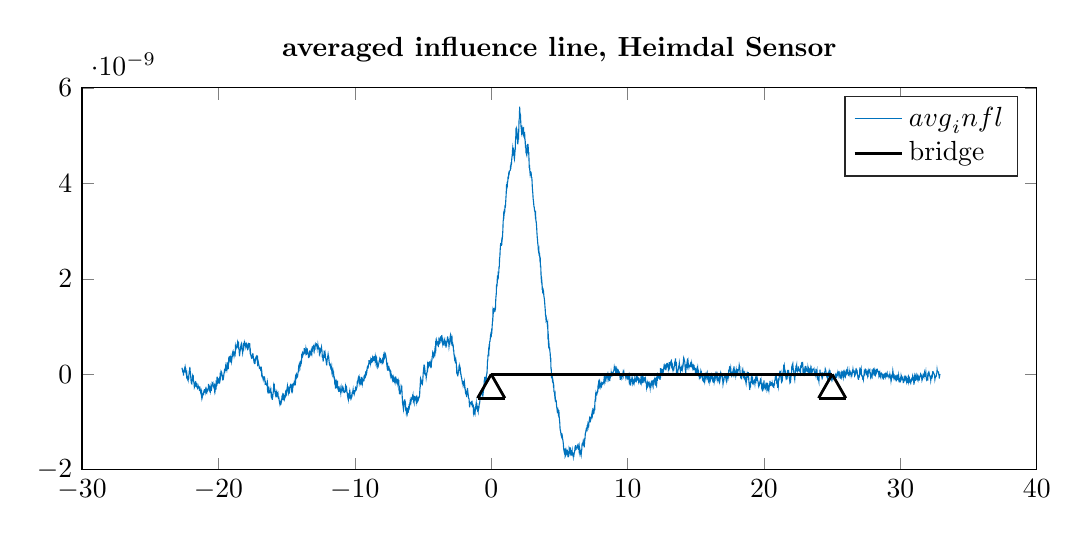
\begin{tikzpicture}

  \begin{axis}[%
    width=\textwidth,
    height=0.4\textwidth,
    at={(0\figurewidth,0\figureheight)},
    scale only axis,
    xmin=-30,
    xmax=40,
    ymin=-2e-09,
    ymax=6e-09,
    axis background/.style={fill=white},
    title style={font=\bfseries},
    title={averaged influence line, Heimdal Sensor},
    legend style={legend cell align=left,align=left,draw=white!15!black}
    ]
    \addplot [color=mycolor1,solid]
    table[row sep=crcr]{%
    -22.6786298828125	1.34505717540438e-10\\
    -22.65848046875	1.17479216700743e-10\\
    -22.6383310546875	9.56106410925965e-11\\
    -22.618181640625	6.04038033233805e-11\\
    -22.5980322265625	4.00068602666301e-11\\
    -22.5778828125	4.10492570781288e-11\\
    -22.5577333984375	-2.60219627951516e-11\\
    -22.537583984375	7.01162857715339e-11\\
    -22.5174345703125	7.95753314089565e-11\\
    -22.49728515625	1.01760005297513e-10\\
    -22.4771357421875	4.2590443915761e-11\\
    -22.456986328125	1.10018529424314e-10\\
    -22.4368369140625	1.54063697870014e-10\\
    -22.4166875	1.22624312125083e-10\\
    -22.3965380859375	1.16065329081752e-10\\
    -22.376388671875	3.41660928506525e-11\\
    -22.3562392578125	4.35276318829836e-11\\
    -22.33608984375	-2.72394379153004e-11\\
    -22.3159404296875	2.64355926482238e-12\\
    -22.295791015625	-6.48519635057764e-11\\
    -22.2756416015625	-6.16726272223087e-11\\
    -22.2554921875	-9.32833534651721e-11\\
    -22.2353427734375	-7.63914346775309e-11\\
    -22.215193359375	-1.123756737243e-10\\
    -22.1950439453125	-6.25952197493169e-11\\
    -22.17489453125	-7.19438396939171e-11\\
    -22.1547451171875	6.64985512616914e-12\\
    -22.134595703125	6.86170455708942e-11\\
    -22.1144462890625	6.75360353646543e-11\\
    -22.094296875	1.53748454204365e-10\\
    -22.0741474609375	7.12755706254945e-11\\
    -22.053998046875	4.14359080182618e-11\\
    -22.0338486328125	-2.89893071834015e-11\\
    -22.01369921875	-1.26252435066109e-10\\
    -21.9935498046875	-1.65227160711098e-10\\
    -21.973400390625	-1.89682830636385e-10\\
    -21.9532509765625	-1.97778705786575e-10\\
    -21.9331015625	-1.42557414319674e-10\\
    -21.9129521484375	-9.1034445774879e-11\\
    -21.892802734375	-4.24939644873161e-11\\
    -21.8726533203125	-6.89626344317917e-11\\
    -21.85250390625	-1.29968199440433e-11\\
    -21.8323544921875	-1.18660148675189e-10\\
    -21.812205078125	-1.58501575481868e-10\\
    -21.7920556640625	-1.77970324647826e-10\\
    -21.77190625	-2.48802359876248e-10\\
    -21.7517568359375	-2.19355969272865e-10\\
    -21.731607421875	-2.55637100986918e-10\\
    -21.7114580078125	-2.42232737855641e-10\\
    -21.69130859375	-2.11690019793168e-10\\
    -21.6711591796875	-1.5982654758964e-10\\
    -21.651009765625	-1.64355445920278e-10\\
    -21.6308603515625	-2.59773571520117e-10\\
    -21.6107109375	-1.85249537351526e-10\\
    -21.5905615234375	-2.56354165189157e-10\\
    -21.570412109375	-2.69594505370912e-10\\
    -21.5502626953125	-2.81772654783929e-10\\
    -21.53011328125	-2.95383082941406e-10\\
    -21.5099638671875	-2.81261841697691e-10\\
    -21.489814453125	-2.39412126188922e-10\\
    -21.4696650390625	-2.60194269023987e-10\\
    -21.449515625	-2.67352844604649e-10\\
    -21.4293662109375	-2.80614104576745e-10\\
    -21.409216796875	-2.91316023150661e-10\\
    -21.3890673828125	-3.47938187265696e-10\\
    -21.36891796875	-2.55882172564206e-10\\
    -21.3487685546875	-2.99724383172378e-10\\
    -21.328619140625	-3.28206692129335e-10\\
    -21.3084697265625	-3.75438416590208e-10\\
    -21.2883203125	-3.9588908979966e-10\\
    -21.2681708984375	-3.65765054009305e-10\\
    -21.248021484375	-4.42633027513548e-10\\
    -21.2278720703125	-4.82872384196372e-10\\
    -21.20772265625	-4.30911479117782e-10\\
    -21.1875732421875	-4.82885382326966e-10\\
    -21.167423828125	-4.58141126145426e-10\\
    -21.1472744140625	-4.39698090932158e-10\\
    -21.127125	-4.19037814987502e-10\\
    -21.1069755859375	-4.25770433090291e-10\\
    -21.086826171875	-4.23260541036176e-10\\
    -21.0666767578125	-3.40507764105557e-10\\
    -21.04652734375	-3.95170116603433e-10\\
    -21.0263779296875	-3.10353653058927e-10\\
    -21.006228515625	-3.72529455166528e-10\\
    -20.9860791015625	-3.7096687675325e-10\\
    -20.9659296875	-3.60476390652217e-10\\
    -20.9457802734375	-3.28354882546428e-10\\
    -20.925630859375	-3.74265508466731e-10\\
    -20.9054814453125	-3.43377457838439e-10\\
    -20.88533203125	-4.06738263864136e-10\\
    -20.8651826171875	-3.39526667354454e-10\\
    -20.845033203125	-3.63903076387547e-10\\
    -20.8248837890625	-3.22529706527603e-10\\
    -20.804734375	-3.17808883003433e-10\\
    -20.7845849609375	-3.32224562073892e-10\\
    -20.764435546875	-3.13111643784834e-10\\
    -20.7442861328125	-2.95892420385112e-10\\
    -20.72413671875	-2.02614722787193e-10\\
    -20.7039873046875	-2.79682404271323e-10\\
    -20.683837890625	-2.70429691091163e-10\\
    -20.6636884765625	-3.15362613618552e-10\\
    -20.6435390625	-2.845844326102e-10\\
    -20.6233896484375	-3.12653456578494e-10\\
    -20.603240234375	-2.9410018581959e-10\\
    -20.5830908203125	-3.39438123596154e-10\\
    -20.56294140625	-2.91138386469859e-10\\
    -20.5427919921875	-3.50221281232007e-10\\
    -20.522642578125	-2.77060546321908e-10\\
    -20.5024931640625	-2.94133158040505e-10\\
    -20.48234375	-2.48027492738257e-10\\
    -20.4621943359375	-1.92683844957636e-10\\
    -20.442044921875	-2.07931920359528e-10\\
    -20.4218955078125	-2.00074328440866e-10\\
    -20.40174609375	-1.86959052462006e-10\\
    -20.3815966796875	-2.27169412982338e-10\\
    -20.361447265625	-2.57270622955163e-10\\
    -20.3412978515625	-2.70610895806517e-10\\
    -20.3211484375	-2.88570025050998e-10\\
    -20.3009990234375	-2.58838958914402e-10\\
    -20.280849609375	-3.29859951565192e-10\\
    -20.2607001953125	-2.85706972198934e-10\\
    -20.24055078125	-3.32257031473484e-10\\
    -20.2204013671875	-2.83504786607409e-10\\
    -20.200251953125	-2.93416610291096e-10\\
    -20.1801025390625	-2.1504244555801e-10\\
    -20.159953125	-2.46546858453473e-10\\
    -20.1398037109375	-1.92218511951175e-10\\
    -20.119654296875	-1.35830503138513e-10\\
    -20.0995048828125	-6.25377405888841e-11\\
    -20.07935546875	-6.42197893845056e-11\\
    -20.0592060546875	-1.42256104743181e-10\\
    -20.039056640625	-1.0212949507485e-10\\
    -20.0189072265625	-1.19517499066628e-10\\
    -19.9987578125	-1.12009197601525e-10\\
    -19.9786083984375	-1.70875666257488e-10\\
    -19.958458984375	-1.64122570790947e-10\\
    -19.9383095703125	-1.73350340872159e-10\\
    -19.91816015625	-1.10307643699775e-10\\
    -19.8980107421875	-1.29026000938279e-10\\
    -19.877861328125	-4.03093819072576e-11\\
    -19.8577119140625	-6.64463564277617e-11\\
    -19.8375625	4.94307983860544e-12\\
    -19.8174130859375	4.58107860723683e-11\\
    -19.797263671875	2.36252366130123e-11\\
    -19.7771142578125	4.55472673258345e-11\\
    -19.75696484375	3.03689145633419e-11\\
    -19.7368154296875	-2.15762809157062e-11\\
    -19.716666015625	-5.68674835711678e-11\\
    -19.6965166015625	-1.3229230596398e-11\\
    -19.6763671875	-1.25399590757594e-10\\
    -19.6562177734375	-7.59857857362579e-11\\
    -19.636068359375	-8.74110605981002e-11\\
    -19.6159189453125	-5.21647763127492e-11\\
    -19.59576953125	6.10831542529366e-12\\
    -19.5756201171875	3.4454141533683e-11\\
    -19.555470703125	8.63630664294104e-11\\
    -19.5353212890625	7.62258613911994e-11\\
    -19.515171875	8.23276335691973e-11\\
    -19.4950224609375	9.11673826813818e-11\\
    -19.474873046875	1.52654708908602e-10\\
    -19.4547236328125	1.11680659555811e-10\\
    -19.43457421875	1.60636810860144e-10\\
    -19.4144248046875	7.3921385625529e-11\\
    -19.394275390625	1.54067281492048e-10\\
    -19.3741259765625	1.17189347878966e-10\\
    -19.3539765625	1.66714598122085e-10\\
    -19.3338271484375	1.18642277556944e-10\\
    -19.313677734375	1.27790055221186e-10\\
    -19.2935283203125	1.86514408242313e-10\\
    -19.27337890625	1.66448027846756e-10\\
    -19.2532294921875	2.87279432604552e-10\\
    -19.233080078125	2.63889908880904e-10\\
    -19.2129306640625	3.07778855000174e-10\\
    -19.19278125	3.72484435770003e-10\\
    -19.1726318359375	3.04332549182104e-10\\
    -19.152482421875	3.84633189203375e-10\\
    -19.1323330078125	2.89453693841579e-10\\
    -19.11218359375	2.99218446766747e-10\\
    -19.0920341796875	3.36303276246923e-10\\
    -19.071884765625	2.41320226255773e-10\\
    -19.0517353515625	3.4349015917126e-10\\
    -19.0315859375	2.83138830803571e-10\\
    -19.0114365234375	3.31128279411061e-10\\
    -18.991287109375	3.6422018670879e-10\\
    -18.9711376953125	4.03959296137087e-10\\
    -18.95098828125	4.64323428826291e-10\\
    -18.9308388671875	4.79644185847517e-10\\
    -18.910689453125	4.41095343824385e-10\\
    -18.8905400390625	4.15939896625302e-10\\
    -18.870390625	4.32520486303945e-10\\
    -18.8502412109375	3.88583073528809e-10\\
    -18.830091796875	4.21689960491858e-10\\
    -18.8099423828125	4.38898409665497e-10\\
    -18.78979296875	4.6037146265066e-10\\
    -18.7696435546875	4.37657104960579e-10\\
    -18.749494140625	5.82984434955834e-10\\
    -18.7293447265625	5.52404730368296e-10\\
    -18.7091953125	5.37571550639985e-10\\
    -18.6890458984375	5.58115029541499e-10\\
    -18.668896484375	5.72146434725006e-10\\
    -18.6487470703125	6.02178510317922e-10\\
    -18.62859765625	5.89479589391026e-10\\
    -18.6084482421875	5.79543366344659e-10\\
    -18.588298828125	6.65442327839452e-10\\
    -18.5681494140625	6.40554915638559e-10\\
    -18.548	6.4140214316943e-10\\
    -18.5278505859375	6.53129817035797e-10\\
    -18.507701171875	5.29512623927191e-10\\
    -18.4875517578125	5.18695293960157e-10\\
    -18.46740234375	4.33955266281382e-10\\
    -18.4472529296875	3.7851599287852e-10\\
    -18.427103515625	4.90453738364271e-10\\
    -18.4069541015625	4.86177186731017e-10\\
    -18.3868046875	5.43103022466098e-10\\
    -18.3666552734375	5.78592726750563e-10\\
    -18.346505859375	6.14121480421704e-10\\
    -18.3263564453125	6.33285071781007e-10\\
    -18.30620703125	5.79167837382185e-10\\
    -18.2860576171875	6.00194120177313e-10\\
    -18.265908203125	5.07688951944536e-10\\
    -18.2457587890625	4.96426626668609e-10\\
    -18.225609375	4.50710521658434e-10\\
    -18.2054599609375	5.02510887945529e-10\\
    -18.185310546875	5.17875224586764e-10\\
    -18.1651611328125	5.80128718745693e-10\\
    -18.14501171875	5.54934691166935e-10\\
    -18.1248623046875	6.24434399721214e-10\\
    -18.104712890625	6.61736652289647e-10\\
    -18.0845634765625	6.30526483470606e-10\\
    -18.0644140625	6.49944167165168e-10\\
    -18.0442646484375	6.21126188367229e-10\\
    -18.024115234375	6.1907042456118e-10\\
    -18.0039658203125	5.87125666431944e-10\\
    -17.98381640625	6.57857416554645e-10\\
    -17.9636669921875	5.84841711877338e-10\\
    -17.943517578125	5.9991296452782e-10\\
    -17.9233681640625	6.23678820881913e-10\\
    -17.90321875	5.93534715543199e-10\\
    -17.8830693359375	5.64042883090896e-10\\
    -17.862919921875	6.18855141345179e-10\\
    -17.8427705078125	5.25436718598227e-10\\
    -17.82262109375	5.29552342722462e-10\\
    -17.8024716796875	6.03852653461181e-10\\
    -17.782322265625	5.80893662437246e-10\\
    -17.7621728515625	5.96553280768943e-10\\
    -17.7420234375	6.49323625438113e-10\\
    -17.7218740234375	5.65664152683987e-10\\
    -17.701724609375	6.44438410614624e-10\\
    -17.6815751953125	4.81561362248136e-10\\
    -17.66142578125	4.9941282489598e-10\\
    -17.6412763671875	4.16031357203305e-10\\
    -17.621126953125	3.9745687019913e-10\\
    -17.6009775390625	3.72711372127383e-10\\
    -17.580828125	3.50071913477085e-10\\
    -17.5606787109375	3.34314647497105e-10\\
    -17.540529296875	3.37823911821042e-10\\
    -17.5203798828125	3.95012666509252e-10\\
    -17.50023046875	4.15909470830091e-10\\
    -17.4800810546875	4.04093908459842e-10\\
    -17.459931640625	4.10061212502619e-10\\
    -17.4397822265625	3.4706622563587e-10\\
    -17.4196328125	3.34140196615986e-10\\
    -17.3994833984375	2.62612936170965e-10\\
    -17.379333984375	2.6218023562657e-10\\
    -17.3591845703125	2.12342961960689e-10\\
    -17.33903515625	2.95691850838529e-10\\
    -17.3188857421875	3.08436639730383e-10\\
    -17.298736328125	2.85576938813316e-10\\
    -17.2785869140625	3.37358409149787e-10\\
    -17.2584375	3.4936290069864e-10\\
    -17.2382880859375	3.22860240745996e-10\\
    -17.218138671875	3.21021322565223e-10\\
    -17.1979892578125	3.51858975051736e-10\\
    -17.17783984375	3.23101866096832e-10\\
    -17.1576904296875	3.40749529370477e-10\\
    -17.137541015625	2.65090301014593e-10\\
    -17.1173916015625	3.02984864114078e-10\\
    -17.0972421875	2.36632316946949e-10\\
    -17.0770927734375	2.59020251628744e-10\\
    -17.056943359375	2.31360414023175e-10\\
    -17.0367939453125	1.85290376400868e-10\\
    -17.01664453125	1.7737709008229e-10\\
    -16.9964951171875	1.28960714749698e-10\\
    -16.976345703125	1.32647044874573e-10\\
    -16.9561962890625	1.3667807495421e-10\\
    -16.936046875	1.18803621689539e-10\\
    -16.9158974609375	1.47143174086063e-10\\
    -16.895748046875	1.45056772099241e-10\\
    -16.8755986328125	6.72093262787819e-11\\
    -16.85544921875	1.58399697887051e-10\\
    -16.8352998046875	1.40953566818212e-11\\
    -16.815150390625	3.7282593976734e-11\\
    -16.7950009765625	-2.95170063335253e-11\\
    -16.7748515625	-3.28256501213434e-11\\
    -16.7547021484375	-5.6239862095796e-11\\
    -16.734552734375	-8.37174980677165e-11\\
    -16.7144033203125	-1.14265669214291e-10\\
    -16.69425390625	-8.59457122554079e-11\\
    -16.6741044921875	-5.78906581860474e-11\\
    -16.653955078125	-5.77010359108724e-11\\
    -16.6338056640625	-8.93012807266945e-11\\
    -16.61365625	-7.79832299327328e-11\\
    -16.5935068359375	-1.14513253403784e-10\\
    -16.573357421875	-1.86997862212149e-10\\
    -16.5532080078125	-1.75014671580571e-10\\
    -16.53305859375	-2.09313550301014e-10\\
    -16.5129091796875	-2.07019397285627e-10\\
    -16.492759765625	-2.05194910849349e-10\\
    -16.4726103515625	-2.17199280120047e-10\\
    -16.4524609375	-2.30168721274006e-10\\
    -16.4323115234375	-1.88871532480643e-10\\
    -16.412162109375	-2.72236819643265e-10\\
    -16.3920126953125	-2.29756792395963e-10\\
    -16.37186328125	-3.04176628761684e-10\\
    -16.3517138671875	-2.65683968869228e-10\\
    -16.331564453125	-2.72793554228786e-10\\
    -16.3114150390625	-3.72429545124834e-10\\
    -16.291265625	-3.62597771909027e-10\\
    -16.2711162109375	-3.87554576095349e-10\\
    -16.250966796875	-3.89363527071545e-10\\
    -16.2308173828125	-3.84487812861436e-10\\
    -16.21066796875	-3.33055655106698e-10\\
    -16.1905185546875	-3.82603444483587e-10\\
    -16.170369140625	-3.81507423354008e-10\\
    -16.1502197265625	-3.54050730200788e-10\\
    -16.1300703125	-4.39529053388102e-10\\
    -16.1099208984375	-4.20765589435111e-10\\
    -16.089771484375	-4.64030405599716e-10\\
    -16.0696220703125	-5.18720064138558e-10\\
    -16.04947265625	-5.22214389357863e-10\\
    -16.0293232421875	-4.89996458304506e-10\\
    -16.009173828125	-4.43050978468315e-10\\
    -15.9890244140625	-3.92912827657616e-10\\
    -15.968875	-3.44743645246752e-10\\
    -15.9487255859375	-2.44724404652118e-10\\
    -15.928576171875	-2.74879886970336e-10\\
    -15.9084267578125	-1.98783778783903e-10\\
    -15.88827734375	-3.10289032356293e-10\\
    -15.8681279296875	-3.18716775193317e-10\\
    -15.847978515625	-3.74770271933268e-10\\
    -15.8278291015625	-4.14162223987572e-10\\
    -15.8076796875	-4.38786160565511e-10\\
    -15.7875302734375	-4.12633658256645e-10\\
    -15.767380859375	-4.83120144893253e-10\\
    -15.7472314453125	-4.2159497541237e-10\\
    -15.72708203125	-3.91092271660714e-10\\
    -15.7069326171875	-4.64467516039941e-10\\
    -15.686783203125	-3.69574954505042e-10\\
    -15.6666337890625	-4.49625859570034e-10\\
    -15.646484375	-4.64463998382414e-10\\
    -15.6263349609375	-4.34638028620206e-10\\
    -15.606185546875	-5.03622153152862e-10\\
    -15.5860361328125	-5.08487229838986e-10\\
    -15.56588671875	-4.99214677004288e-10\\
    -15.5457373046875	-5.46779131782968e-10\\
    -15.525587890625	-5.80778817804774e-10\\
    -15.5054384765625	-6.10469267267502e-10\\
    -15.4852890625	-5.50512531565474e-10\\
    -15.4651396484375	-6.39282020918863e-10\\
    -15.444990234375	-6.36558054189267e-10\\
    -15.4248408203125	-6.23077457003756e-10\\
    -15.40469140625	-6.21689513830927e-10\\
    -15.3845419921875	-5.39995681222619e-10\\
    -15.364392578125	-5.46011605705383e-10\\
    -15.3442431640625	-4.84805328346692e-10\\
    -15.32409375	-5.00098705983326e-10\\
    -15.3039443359375	-4.64599180511846e-10\\
    -15.283794921875	-5.19117112457117e-10\\
    -15.2636455078125	-3.93554201811402e-10\\
    -15.24349609375	-5.2090349402478e-10\\
    -15.2233466796875	-5.34409742113797e-10\\
    -15.203197265625	-5.34447223477021e-10\\
    -15.1830478515625	-4.87726879160764e-10\\
    -15.1628984375	-5.21596358456711e-10\\
    -15.1427490234375	-4.9941116385498e-10\\
    -15.122599609375	-4.62060563200929e-10\\
    -15.1024501953125	-4.69041902304382e-10\\
    -15.08230078125	-4.03226345568977e-10\\
    -15.0621513671875	-4.35815449453074e-10\\
    -15.042001953125	-4.23505973511182e-10\\
    -15.0218525390625	-3.82551773689817e-10\\
    -15.001703125	-4.04467080622283e-10\\
    -14.9815537109375	-3.27124351821306e-10\\
    -14.961404296875	-2.87283782506599e-10\\
    -14.9412548828125	-2.4716991524253e-10\\
    -14.92110546875	-2.95235803883256e-10\\
    -14.9009560546875	-2.92191358215869e-10\\
    -14.880806640625	-3.46691514710407e-10\\
    -14.8606572265625	-3.79467415624972e-10\\
    -14.8405078125	-3.24170004576101e-10\\
    -14.8203583984375	-3.55405164080883e-10\\
    -14.800208984375	-4.05077736330107e-10\\
    -14.7800595703125	-2.77974598193533e-10\\
    -14.75991015625	-2.77380155026459e-10\\
    -14.7397607421875	-2.36983469699788e-10\\
    -14.719611328125	-2.23526656942458e-10\\
    -14.6994619140625	-2.3925687413333e-10\\
    -14.6793125	-2.3027583839759e-10\\
    -14.6591630859375	-2.81818062644756e-10\\
    -14.639013671875	-3.30957423667111e-10\\
    -14.6188642578125	-3.20008373658698e-10\\
    -14.59871484375	-3.97442684243782e-10\\
    -14.5785654296875	-2.81479494325284e-10\\
    -14.558416015625	-3.04200352700253e-10\\
    -14.5382666015625	-2.2957497943317e-10\\
    -14.5181171875	-2.38865140383768e-10\\
    -14.4979677734375	-1.98004693687479e-10\\
    -14.477818359375	-2.01682919416373e-10\\
    -14.4576689453125	-2.01337608024084e-10\\
    -14.43751953125	-1.61017876113313e-10\\
    -14.4173701171875	-1.7121497332159e-10\\
    -14.397220703125	-2.35000234361145e-10\\
    -14.3770712890625	-1.27401792700459e-10\\
    -14.356921875	-7.72745971630021e-11\\
    -14.3367724609375	-1.20543392181081e-10\\
    -14.316623046875	-4.81177798086988e-11\\
    -14.2964736328125	-4.49804051643581e-11\\
    -14.27632421875	-1.62316646138189e-11\\
    -14.2561748046875	-5.34497555471863e-11\\
    -14.236025390625	-3.64613186083819e-11\\
    -14.2158759765625	-5.59783674742191e-11\\
    -14.1957265625	-4.58967507688366e-11\\
    -14.1755771484375	1.65528250377485e-11\\
    -14.155427734375	4.06517666990961e-11\\
    -14.1352783203125	7.6218397680627e-11\\
    -14.11512890625	1.74065107154332e-10\\
    -14.0949794921875	1.89458277395683e-10\\
    -14.074830078125	1.51208732531465e-10\\
    -14.0546806640625	2.34079079477797e-10\\
    -14.03453125	2.36162610796774e-10\\
    -14.0143818359375	1.94972648381666e-10\\
    -13.994232421875	2.82032731072673e-10\\
    -13.9740830078125	1.64855418343461e-10\\
    -13.95393359375	2.39883587822969e-10\\
    -13.9337841796875	2.74545142547455e-10\\
    -13.913634765625	2.62911935608866e-10\\
    -13.8934853515625	3.9000816474268e-10\\
    -13.8733359375	3.78900412503056e-10\\
    -13.8531865234375	3.69922658781577e-10\\
    -13.833037109375	4.5338537133411e-10\\
    -13.8128876953125	4.42427859803062e-10\\
    -13.79273828125	4.14638125860248e-10\\
    -13.7725888671875	4.36038356022378e-10\\
    -13.752439453125	4.48981475030533e-10\\
    -13.7322900390625	4.11811667674222e-10\\
    -13.712140625	5.49236262946831e-10\\
    -13.6919912109375	4.36123909496333e-10\\
    -13.671841796875	5.06805536068746e-10\\
    -13.6516923828125	5.11134170466292e-10\\
    -13.63154296875	4.95926839349704e-10\\
    -13.6113935546875	4.6528889658249e-10\\
    -13.591244140625	5.21766961092782e-10\\
    -13.5710947265625	4.67816514061667e-10\\
    -13.5509453125	4.02440075030319e-10\\
    -13.5307958984375	5.00232465589911e-10\\
    -13.510646484375	4.80075628700771e-10\\
    -13.4904970703125	5.4304303008367e-10\\
    -13.47034765625	4.6962050595735e-10\\
    -13.4501982421875	4.43954383520575e-10\\
    -13.430048828125	4.52781411536805e-10\\
    -13.4098994140625	4.28645837396459e-10\\
    -13.38975	3.38059730107352e-10\\
    -13.3696005859375	4.37975134177118e-10\\
    -13.349451171875	3.6296349797864e-10\\
    -13.3293017578125	3.63755750175463e-10\\
    -13.30915234375	4.77178446173002e-10\\
    -13.2890029296875	4.71191893431024e-10\\
    -13.268853515625	4.50462573408704e-10\\
    -13.2487041015625	4.65711051259446e-10\\
    -13.2285546875	4.3946437102151e-10\\
    -13.2084052734375	4.76313156696662e-10\\
    -13.188255859375	4.52120764776217e-10\\
    -13.1681064453125	4.88329450159334e-10\\
    -13.14795703125	4.51826196268444e-10\\
    -13.1278076171875	5.36127935370258e-10\\
    -13.107658203125	5.22553329717863e-10\\
    -13.0875087890625	5.75585259724378e-10\\
    -13.067359375	5.76452228112615e-10\\
    -13.0472099609375	5.90661933371918e-10\\
    -13.027060546875	5.97734043259273e-10\\
    -13.0069111328125	5.31903757164441e-10\\
    -12.98676171875	5.7125753626026e-10\\
    -12.9666123046875	5.25285224417673e-10\\
    -12.946462890625	5.91499103625667e-10\\
    -12.9263134765625	5.12626934107873e-10\\
    -12.9061640625	5.8695340016493e-10\\
    -12.8860146484375	5.96740994914306e-10\\
    -12.865865234375	6.26587492896176e-10\\
    -12.8457158203125	6.02977199690252e-10\\
    -12.82556640625	6.06175236420087e-10\\
    -12.8054169921875	6.2130124270189e-10\\
    -12.785267578125	6.01272125704434e-10\\
    -12.7651181640625	5.59356903438483e-10\\
    -12.74496875	6.35439902281092e-10\\
    -12.7248193359375	5.3582532866394e-10\\
    -12.704669921875	6.0606873770626e-10\\
    -12.6845205078125	5.59503147121272e-10\\
    -12.66437109375	5.6867302856059e-10\\
    -12.6442216796875	5.36157216203035e-10\\
    -12.624072265625	5.41525652802397e-10\\
    -12.6039228515625	4.61592251721146e-10\\
    -12.5837734375	4.93138039687152e-10\\
    -12.5636240234375	4.55418712179885e-10\\
    -12.543474609375	5.20893326506275e-10\\
    -12.5233251953125	5.28616973453257e-10\\
    -12.50317578125	4.99181265524802e-10\\
    -12.4830263671875	5.31045082401448e-10\\
    -12.462876953125	5.39213175085058e-10\\
    -12.4427275390625	5.68089207421004e-10\\
    -12.422578125	5.05731570701208e-10\\
    -12.4024287109375	4.83212103623638e-10\\
    -12.382279296875	3.56600570802437e-10\\
    -12.3621298828125	3.55731538072735e-10\\
    -12.34198046875	3.6278824476261e-10\\
    -12.3218310546875	2.64529608949018e-10\\
    -12.301681640625	3.52480885747493e-10\\
    -12.2815322265625	3.86212080751242e-10\\
    -12.2613828125	3.45646147768379e-10\\
    -12.2412333984375	4.81069089149713e-10\\
    -12.221083984375	4.78606269056842e-10\\
    -12.2009345703125	4.15123948173105e-10\\
    -12.18078515625	4.46790722616056e-10\\
    -12.1606357421875	4.03993343886872e-10\\
    -12.140486328125	3.35244886093105e-10\\
    -12.1203369140625	3.09468088590852e-10\\
    -12.1001875	2.71152938819891e-10\\
    -12.0800380859375	2.10538280969858e-10\\
    -12.059888671875	2.02046661053294e-10\\
    -12.0397392578125	2.67791715743775e-10\\
    -12.01958984375	3.25094182408869e-10\\
    -11.9994404296875	3.28929721038937e-10\\
    -11.979291015625	3.8127488714493e-10\\
    -11.9591416015625	4.18492635080614e-10\\
    -11.9389921875	3.78455330289277e-10\\
    -11.9188427734375	3.76592193062763e-10\\
    -11.898693359375	3.13336752948931e-10\\
    -11.8785439453125	2.51459474979989e-10\\
    -11.85839453125	2.00785180992143e-10\\
    -11.8382451171875	1.91891711064659e-10\\
    -11.818095703125	1.79665901572075e-10\\
    -11.7979462890625	1.93245339842036e-10\\
    -11.777796875	1.47241511362252e-10\\
    -11.7576474609375	1.23779734411439e-10\\
    -11.737498046875	1.35607873078658e-10\\
    -11.7173486328125	1.08960144758564e-10\\
    -11.69719921875	1.48393852965169e-10\\
    -11.6770498046875	5.01628918161049e-11\\
    -11.656900390625	7.48059002920444e-11\\
    -11.6367509765625	1.18635526898157e-10\\
    -11.6166015625	3.02811179743843e-11\\
    -11.5964521484375	7.10130406108832e-11\\
    -11.576302734375	3.25994755627908e-11\\
    -11.5561533203125	3.72539255155274e-11\\
    -11.53600390625	-7.49831012470825e-11\\
    -11.5158544921875	-7.72415097307143e-11\\
    -11.495705078125	-7.11333589896943e-11\\
    -11.4755556640625	-1.74081381183365e-10\\
    -11.45540625	-2.2749693123698e-10\\
    -11.4352568359375	-1.55225764414195e-10\\
    -11.415107421875	-2.97741497633e-10\\
    -11.3949580078125	-2.05420523648726e-10\\
    -11.37480859375	-2.44547878637536e-10\\
    -11.3546591796875	-2.88918008694631e-10\\
    -11.334509765625	-1.78403856764015e-10\\
    -11.3143603515625	-2.02544496908438e-10\\
    -11.2942109375	-2.29959068246955e-10\\
    -11.2740615234375	-1.3207899276628e-10\\
    -11.253912109375	-2.55032324561831e-10\\
    -11.2337626953125	-2.87220549872516e-10\\
    -11.21361328125	-3.19959849803639e-10\\
    -11.1934638671875	-3.003079289394e-10\\
    -11.173314453125	-2.86703247803873e-10\\
    -11.1531650390625	-3.57301632601326e-10\\
    -11.133015625	-3.55613951225635e-10\\
    -11.1128662109375	-3.4291863285486e-10\\
    -11.092716796875	-3.33236455655847e-10\\
    -11.0725673828125	-2.9833444545058e-10\\
    -11.05241796875	-3.41073519582698e-10\\
    -11.0322685546875	-3.83584632302168e-10\\
    -11.012119140625	-3.01151035277576e-10\\
    -10.9919697265625	-3.51586547327463e-10\\
    -10.9718203125	-3.50668133663907e-10\\
    -10.9516708984375	-2.9152338921391e-10\\
    -10.931521484375	-3.32777110406698e-10\\
    -10.9113720703125	-2.9996816622674e-10\\
    -10.89122265625	-2.95629892625497e-10\\
    -10.8710732421875	-2.71902262860363e-10\\
    -10.850923828125	-2.91020731171066e-10\\
    -10.8307744140625	-3.46779051765015e-10\\
    -10.810625	-3.62771355381274e-10\\
    -10.7904755859375	-3.78847362979537e-10\\
    -10.770326171875	-3.81792678230457e-10\\
    -10.7501767578125	-3.82908136181916e-10\\
    -10.73002734375	-3.6976596238709e-10\\
    -10.7098779296875	-3.22392824664018e-10\\
    -10.689728515625	-3.70374065758545e-10\\
    -10.6695791015625	-2.53889281418006e-10\\
    -10.6494296875	-2.80316457976234e-10\\
    -10.6292802734375	-2.86520614830937e-10\\
    -10.609130859375	-2.74257985524898e-10\\
    -10.5889814453125	-3.34333259774379e-10\\
    -10.56883203125	-3.908031941775e-10\\
    -10.5486826171875	-3.94762688411738e-10\\
    -10.528533203125	-4.65218944667768e-10\\
    -10.5083837890625	-4.93458262939043e-10\\
    -10.488234375	-4.63766207755727e-10\\
    -10.4680849609375	-5.09682454310276e-10\\
    -10.447935546875	-4.41669028523694e-10\\
    -10.4277861328125	-4.25410489689194e-10\\
    -10.40763671875	-4.49428253058469e-10\\
    -10.3874873046875	-3.88144287519747e-10\\
    -10.367337890625	-4.38478294545391e-10\\
    -10.3471884765625	-4.06490970113121e-10\\
    -10.3270390625	-4.79822663666476e-10\\
    -10.3068896484375	-4.97288312430084e-10\\
    -10.286740234375	-5.19012375674214e-10\\
    -10.2665908203125	-5.01501760628033e-10\\
    -10.24644140625	-4.86176623571358e-10\\
    -10.2262919921875	-4.41034295399862e-10\\
    -10.206142578125	-4.49177166619072e-10\\
    -10.1859931640625	-3.81906015216723e-10\\
    -10.16584375	-3.81954013652246e-10\\
    -10.1456943359375	-3.59544321795798e-10\\
    -10.125544921875	-3.22403016525644e-10\\
    -10.1053955078125	-3.78757151246773e-10\\
    -10.08524609375	-3.70852555706842e-10\\
    -10.0650966796875	-3.9657465950591e-10\\
    -10.044947265625	-3.33718043383143e-10\\
    -10.0247978515625	-3.96637956836525e-10\\
    -10.0046484375	-3.75235528507908e-10\\
    -9.9844990234375	-3.65151801031277e-10\\
    -9.964349609375	-3.46342284680477e-10\\
    -9.9442001953125	-2.75630168056863e-10\\
    -9.92405078125	-2.82193499462326e-10\\
    -9.9039013671875	-2.84056311790562e-10\\
    -9.883751953125	-3.09786173319483e-10\\
    -9.8636025390625	-2.91688652359122e-10\\
    -9.843453125	-2.68376557947321e-10\\
    -9.8233037109375	-1.73736890177904e-10\\
    -9.803154296875	-1.79658452229944e-10\\
    -9.7830048828125	-1.37341912628583e-10\\
    -9.76285546875	-1.13970915108282e-10\\
    -9.7427060546875	-6.98843431695581e-11\\
    -9.722556640625	-5.4838234331843e-11\\
    -9.7024072265625	-7.54411854779921e-11\\
    -9.6822578125	-1.44812619247123e-10\\
    -9.6621083984375	-9.92496613588562e-11\\
    -9.641958984375	-1.61034857663242e-10\\
    -9.6218095703125	-9.6732845273386e-11\\
    -9.60166015625	-1.84636050550851e-10\\
    -9.5815107421875	-1.62897562974675e-10\\
    -9.561361328125	-1.78571747819545e-10\\
    -9.5412119140625	-1.09077816458579e-10\\
    -9.5210625	-1.26037703910657e-10\\
    -9.5009130859375	-5.4726679591185e-11\\
    -9.480763671875	-1.53380820273232e-10\\
    -9.4606142578125	-1.26501558317112e-10\\
    -9.44046484375	-1.74644085375746e-10\\
    -9.4203154296875	-1.14378924339934e-10\\
    -9.400166015625	-1.26856467887611e-10\\
    -9.3800166015625	-1.35789763968057e-10\\
    -9.3598671875	-1.26457641260873e-10\\
    -9.3397177734375	-1.27531027882012e-10\\
    -9.319568359375	-2.58648262276971e-11\\
    -9.2994189453125	-7.13487757490645e-11\\
    -9.27926953125	-3.26296540016191e-11\\
    -9.2591201171875	-4.81247025633517e-11\\
    -9.238970703125	-6.11814991959897e-11\\
    -9.2188212890625	-4.70263720320595e-11\\
    -9.198671875	5.87554530069262e-11\\
    -9.1785224609375	8.07813647568825e-12\\
    -9.158373046875	3.74038927303929e-11\\
    -9.1382236328125	1.76632483342687e-11\\
    -9.11807421875	4.21818796663428e-11\\
    -9.0979248046875	1.26851780636868e-10\\
    -9.077775390625	1.50906315221905e-10\\
    -9.0576259765625	1.38743226205675e-10\\
    -9.0374765625	1.31224572779359e-10\\
    -9.0173271484375	1.4803948854906e-10\\
    -8.997177734375	2.02436303978617e-10\\
    -8.9770283203125	2.17404583565792e-10\\
    -8.95687890625	2.95741498622263e-10\\
    -8.9367294921875	2.20146086578472e-10\\
    -8.916580078125	2.22815744884814e-10\\
    -8.8964306640625	2.7262173130502e-10\\
    -8.87628125	2.78930077266571e-10\\
    -8.8561318359375	2.37455470938721e-10\\
    -8.835982421875	2.92063012290038e-10\\
    -8.8158330078125	2.61575811681503e-10\\
    -8.79568359375	2.88431040330054e-10\\
    -8.7755341796875	2.76295243991097e-10\\
    -8.755384765625	3.36025811272227e-10\\
    -8.7352353515625	2.62938273854733e-10\\
    -8.7150859375	3.10884793919128e-10\\
    -8.6949365234375	2.52498993529389e-10\\
    -8.674787109375	3.39012028255689e-10\\
    -8.6546376953125	3.3154313602182e-10\\
    -8.63448828125	3.75717740966849e-10\\
    -8.6143388671875	2.81858978324008e-10\\
    -8.594189453125	3.64410030134787e-10\\
    -8.5740400390625	3.64978248285427e-10\\
    -8.553890625	3.68484457633708e-10\\
    -8.5337412109375	3.26625839675263e-10\\
    -8.513591796875	2.83545770821052e-10\\
    -8.4934423828125	3.6810638188717e-10\\
    -8.47329296875	3.33321811785138e-10\\
    -8.4531435546875	3.96565363513975e-10\\
    -8.432994140625	3.08166954637975e-10\\
    -8.4128447265625	3.66414157231288e-10\\
    -8.3926953125	2.276267223413e-10\\
    -8.3725458984375	2.60333628564057e-10\\
    -8.352396484375	2.31656350313328e-10\\
    -8.3322470703125	2.06895939538079e-10\\
    -8.31209765625	1.43401710586705e-10\\
    -8.2919482421875	1.54672812832117e-10\\
    -8.271798828125	1.92439523837921e-10\\
    -8.2516494140625	2.12858702469149e-10\\
    -8.2315	2.45743389481134e-10\\
    -8.2113505859375	2.77980090375462e-10\\
    -8.191201171875	2.78246331638681e-10\\
    -8.1710517578125	3.19266149281409e-10\\
    -8.15090234375	2.98910825714432e-10\\
    -8.1307529296875	3.42397487301249e-10\\
    -8.110603515625	2.48152056939477e-10\\
    -8.0904541015625	2.52742189426186e-10\\
    -8.0703046875	2.66804529063641e-10\\
    -8.0501552734375	2.78140728736251e-10\\
    -8.030005859375	2.88997504558809e-10\\
    -8.0098564453125	2.52611526905413e-10\\
    -7.98970703125	2.83442274695717e-10\\
    -7.9695576171875	2.66837313021665e-10\\
    -7.949408203125	3.46488256821545e-10\\
    -7.9292587890625	2.90844887241923e-10\\
    -7.909109375	3.5646699053231e-10\\
    -7.8889599609375	3.09737019690243e-10\\
    -7.868810546875	3.63303557809868e-10\\
    -7.8486611328125	3.51704914049496e-10\\
    -7.82851171875	4.03754299447033e-10\\
    -7.8083623046875	3.66697596296007e-10\\
    -7.788212890625	3.93527427636528e-10\\
    -7.7680634765625	3.98173165461661e-10\\
    -7.7479140625	4.18211502597399e-10\\
    -7.7277646484375	3.898608986148e-10\\
    -7.707615234375	3.43737312852972e-10\\
    -7.6874658203125	3.16539177651761e-10\\
    -7.66731640625	2.31712209851889e-10\\
    -7.6471669921875	1.85614215158871e-10\\
    -7.627017578125	2.42622037315636e-10\\
    -7.6068681640625	1.55320473815282e-10\\
    -7.58671875	1.76822428871201e-10\\
    -7.5665693359375	7.37855112976024e-11\\
    -7.546419921875	1.37059070705405e-10\\
    -7.5262705078125	1.56001542446776e-10\\
    -7.50612109375	1.58512524041432e-10\\
    -7.4859716796875	1.208203483839e-10\\
    -7.465822265625	1.14412146500169e-10\\
    -7.4456728515625	7.33624232879516e-11\\
    -7.4255234375	6.55360430887089e-11\\
    -7.4053740234375	1.5656041501648e-11\\
    -7.385224609375	3.67220762561047e-11\\
    -7.3650751953125	-2.29418668940773e-11\\
    -7.34492578125	7.17954819966813e-12\\
    -7.3247763671875	-4.21534291803234e-11\\
    -7.304626953125	-3.2841804188259e-11\\
    -7.2844775390625	-7.42666492623309e-11\\
    -7.264328125	-8.57833128783604e-11\\
    -7.2441787109375	-1.10470765689634e-10\\
    -7.224029296875	-6.0467998278445e-11\\
    -7.2038798828125	-7.74494582546879e-11\\
    -7.18373046875	-8.56998922778495e-11\\
    -7.1635810546875	-6.54917735179903e-11\\
    -7.143431640625	-1.61329471965556e-10\\
    -7.1232822265625	-1.09210518425485e-10\\
    -7.1031328125	-1.32512844984634e-10\\
    -7.0829833984375	-1.1124383767148e-10\\
    -7.062833984375	-1.4869440855813e-10\\
    -7.0426845703125	-1.18089162339449e-10\\
    -7.02253515625	-1.73701124893596e-10\\
    -7.0023857421875	-4.92129367611879e-11\\
    -6.982236328125	-1.38207384018496e-10\\
    -6.9620869140625	-1.03354769133135e-10\\
    -6.9419375	-1.2035284308268e-10\\
    -6.9217880859375	-1.29310566318714e-10\\
    -6.901638671875	-1.64814744370936e-10\\
    -6.8814892578125	-1.44389080755613e-10\\
    -6.86133984375	-9.89832647338722e-11\\
    -6.8411904296875	-1.83200740655676e-10\\
    -6.821041015625	-1.50187878208133e-10\\
    -6.8008916015625	-2.08177174176731e-10\\
    -6.7807421875	-1.19038040600052e-10\\
    -6.7605927734375	-2.97425956974342e-10\\
    -6.740443359375	-2.83802704473591e-10\\
    -6.7202939453125	-4.11068456450393e-10\\
    -6.70014453125	-3.54071122446182e-10\\
    -6.6799951171875	-4.25282529556973e-10\\
    -6.659845703125	-3.63325987075297e-10\\
    -6.6396962890625	-3.47230608686037e-10\\
    -6.619546875	-3.44964322419393e-10\\
    -6.5993974609375	-2.50213271168198e-10\\
    -6.579248046875	-2.66813095420108e-10\\
    -6.5590986328125	-2.62022775526522e-10\\
    -6.53894921875	-3.81291553450966e-10\\
    -6.5187998046875	-5.03977230371973e-10\\
    -6.498650390625	-6.05629292985215e-10\\
    -6.4785009765625	-5.99301283136201e-10\\
    -6.4583515625	-6.9099311215569e-10\\
    -6.4382021484375	-7.26725508781202e-10\\
    -6.418052734375	-6.40904227407584e-10\\
    -6.3979033203125	-6.36452206809165e-10\\
    -6.37775390625	-5.67159346910614e-10\\
    -6.3576044921875	-5.78472818558192e-10\\
    -6.337455078125	-5.28228229884894e-10\\
    -6.3173056640625	-6.08827675392133e-10\\
    -6.29715625	-6.87870254361338e-10\\
    -6.2770068359375	-6.54452517482923e-10\\
    -6.256857421875	-7.3848886811321e-10\\
    -6.2367080078125	-6.89876571809709e-10\\
    -6.21655859375	-8.09948240069253e-10\\
    -6.1964091796875	-7.80690120523895e-10\\
    -6.176259765625	-7.58557126574704e-10\\
    -6.1561103515625	-7.03812132331097e-10\\
    -6.1359609375	-7.91888814661806e-10\\
    -6.1158115234375	-7.5733245228593e-10\\
    -6.095662109375	-7.74735085256739e-10\\
    -6.0755126953125	-7.81063102298453e-10\\
    -6.05536328125	-6.66718411747697e-10\\
    -6.0352138671875	-7.30177859979045e-10\\
    -6.015064453125	-6.27405753783144e-10\\
    -5.9949150390625	-6.71322687238191e-10\\
    -5.974765625	-6.26777800558035e-10\\
    -5.9546162109375	-5.95006537533155e-10\\
    -5.934466796875	-5.46212110620188e-10\\
    -5.9143173828125	-5.78005393524279e-10\\
    -5.89416796875	-5.99503395488073e-10\\
    -5.8740185546875	-5.55764817168974e-10\\
    -5.853869140625	-5.42772104464796e-10\\
    -5.8337197265625	-5.11068817154268e-10\\
    -5.8135703125	-5.23910042911246e-10\\
    -5.7934208984375	-5.17953371148263e-10\\
    -5.773271484375	-4.75146457990687e-10\\
    -5.7531220703125	-4.93367061275234e-10\\
    -5.73297265625	-4.52563625004981e-10\\
    -5.7128232421875	-5.33970049547954e-10\\
    -5.692673828125	-5.11925117651645e-10\\
    -5.6725244140625	-5.69526552936628e-10\\
    -5.652375	-5.94147246146765e-10\\
    -5.6322255859375	-4.53209961448904e-10\\
    -5.612076171875	-5.23929861922921e-10\\
    -5.5919267578125	-5.00759978717845e-10\\
    -5.57177734375	-5.02599984546653e-10\\
    -5.5516279296875	-4.91534526916492e-10\\
    -5.531478515625	-5.23572061207371e-10\\
    -5.5113291015625	-5.01952284061516e-10\\
    -5.4911796875	-5.67328485905617e-10\\
    -5.4710302734375	-5.24086759183267e-10\\
    -5.450880859375	-5.50397867216137e-10\\
    -5.4307314453125	-4.93496897089283e-10\\
    -5.41058203125	-5.16946328953993e-10\\
    -5.3904326171875	-5.12070173421068e-10\\
    -5.370283203125	-5.55103803111315e-10\\
    -5.3501337890625	-5.39932448274067e-10\\
    -5.329984375	-4.93800976907115e-10\\
    -5.3098349609375	-4.99961625975169e-10\\
    -5.289685546875	-4.77104303223505e-10\\
    -5.2695361328125	-4.77332146656643e-10\\
    -5.24938671875	-4.45615421823821e-10\\
    -5.2292373046875	-3.15847914354736e-10\\
    -5.209087890625	-2.47056820292209e-10\\
    -5.1889384765625	-1.35224223359995e-10\\
    -5.1687890625	-1.71918909803874e-10\\
    -5.1486396484375	-1.1327664226028e-10\\
    -5.128490234375	-1.32861875524023e-10\\
    -5.1083408203125	-1.7017730867322e-10\\
    -5.08819140625	-1.90081726857765e-10\\
    -5.0680419921875	-1.88754241303075e-10\\
    -5.047892578125	-2.02355714561783e-10\\
    -5.0277431640625	-1.64851840427039e-10\\
    -5.00759375	-7.71323669161504e-11\\
    -4.9874443359375	1.10597414574871e-11\\
    -4.967294921875	7.76432292797987e-11\\
    -4.9471455078125	1.30811851150669e-10\\
    -4.92699609375	9.66267625878538e-11\\
    -4.9068466796875	2.0176713593318e-10\\
    -4.886697265625	1.44377138262881e-10\\
    -4.8665478515625	1.16777876384504e-10\\
    -4.8463984375	4.20354482025365e-11\\
    -4.8262490234375	-1.10286783376475e-11\\
    -4.806099609375	-1.19541196875795e-11\\
    -4.7859501953125	-2.80463748678198e-12\\
    -4.76580078125	-7.06208684608258e-11\\
    -4.7456513671875	-2.96075631731894e-11\\
    -4.725501953125	3.29428341858975e-12\\
    -4.7053525390625	3.95573005663978e-11\\
    -4.685203125	9.24342237062098e-11\\
    -4.6650537109375	1.81663397279539e-10\\
    -4.644904296875	1.43325152283946e-10\\
    -4.6247548828125	2.03297074287246e-10\\
    -4.60460546875	1.8495414642196e-10\\
    -4.5844560546875	2.40898313784008e-10\\
    -4.564306640625	2.46627969243975e-10\\
    -4.5441572265625	2.51996467566695e-10\\
    -4.5240078125	1.71641648110603e-10\\
    -4.5038583984375	2.6542284233357e-10\\
    -4.483708984375	1.58742276262142e-10\\
    -4.4635595703125	2.15117476264409e-10\\
    -4.44341015625	1.73088115296698e-10\\
    -4.4232607421875	1.40182658119157e-10\\
    -4.403111328125	1.41517393177618e-10\\
    -4.3829619140625	2.45318052739572e-10\\
    -4.3628125	2.73845077906129e-10\\
    -4.3426630859375	3.15222446349203e-10\\
    -4.322513671875	3.73679457712825e-10\\
    -4.3023642578125	3.81356010590643e-10\\
    -4.28221484375	4.68556950422222e-10\\
    -4.2620654296875	4.57722956976056e-10\\
    -4.241916015625	4.41934141075507e-10\\
    -4.2217666015625	3.75255472039182e-10\\
    -4.2016171875	3.93320627252934e-10\\
    -4.1814677734375	4.190276956201e-10\\
    -4.161318359375	4.26101691084616e-10\\
    -4.1411689453125	4.8198313442457e-10\\
    -4.12101953125	4.29548974833052e-10\\
    -4.1008701171875	4.68668230873718e-10\\
    -4.080720703125	5.87273706643521e-10\\
    -4.0605712890625	5.51375713908786e-10\\
    -4.040421875	6.74100287775202e-10\\
    -4.0202724609375	6.51545537034609e-10\\
    -4.000123046875	7.02577348744277e-10\\
    -3.9799736328125	6.67204985913669e-10\\
    -3.95982421875	6.53955931864023e-10\\
    -3.9396748046875	6.63092727367675e-10\\
    -3.919525390625	6.36226780553525e-10\\
    -3.8993759765625	6.01471257978588e-10\\
    -3.8792265625	5.92179080010416e-10\\
    -3.8590771484375	6.40613868898251e-10\\
    -3.838927734375	7.07038277049509e-10\\
    -3.8187783203125	6.77531183263643e-10\\
    -3.79862890625	7.03298116025562e-10\\
    -3.7784794921875	6.80025539315442e-10\\
    -3.758330078125	7.23854780008181e-10\\
    -3.7381806640625	7.06321537258658e-10\\
    -3.71803125	7.84144483177853e-10\\
    -3.6978818359375	7.12759610730426e-10\\
    -3.677732421875	7.97562586808391e-10\\
    -3.6575830078125	7.49583770385161e-10\\
    -3.63743359375	8.06007718072395e-10\\
    -3.6172841796875	8.08248742156608e-10\\
    -3.597134765625	7.41465285400873e-10\\
    -3.5769853515625	7.35373947924354e-10\\
    -3.5568359375	6.53418248746556e-10\\
    -3.5366865234375	6.8874430998341e-10\\
    -3.516537109375	6.40685754512431e-10\\
    -3.4963876953125	6.23741717625555e-10\\
    -3.47623828125	6.16797045548734e-10\\
    -3.4560888671875	6.45224025104096e-10\\
    -3.435939453125	7.04180769304334e-10\\
    -3.4157900390625	7.23284307961723e-10\\
    -3.395640625	6.41270914690091e-10\\
    -3.3754912109375	7.0851770430189e-10\\
    -3.355341796875	5.97898555455932e-10\\
    -3.3351923828125	6.46474866224838e-10\\
    -3.31504296875	5.59179664931453e-10\\
    -3.2948935546875	6.73278988277114e-10\\
    -3.274744140625	5.89596748799397e-10\\
    -3.2545947265625	6.93140801299095e-10\\
    -3.2344453125	7.04796789896342e-10\\
    -3.2142958984375	7.50589105046621e-10\\
    -3.194146484375	7.9411032597296e-10\\
    -3.1739970703125	7.03460668542253e-10\\
    -3.15384765625	6.87771440182823e-10\\
    -3.1336982421875	7.00479731332479e-10\\
    -3.113548828125	6.59555348961005e-10\\
    -3.0933994140625	5.85050154922385e-10\\
    -3.07325	6.30946893577397e-10\\
    -3.0531005859375	6.35704075325543e-10\\
    -3.032951171875	6.91691590558033e-10\\
    -3.0128017578125	7.80204179821624e-10\\
    -2.99265234375	8.10157850297829e-10\\
    -2.9725029296875	7.48564521679969e-10\\
    -2.952353515625	8.02808830134675e-10\\
    -2.9322041015625	7.14496669607458e-10\\
    -2.9120546875	7.5483791513817e-10\\
    -2.8919052734375	7.12349765472847e-10\\
    -2.871755859375	7.38337819302175e-10\\
    -2.8516064453125	5.97947428377946e-10\\
    -2.83145703125	6.76788515694841e-10\\
    -2.8113076171875	5.84116075421139e-10\\
    -2.791158203125	6.26282568025952e-10\\
    -2.7710087890625	5.07459359146378e-10\\
    -2.750859375	5.08693833319791e-10\\
    -2.7307099609375	4.27704832455046e-10\\
    -2.710560546875	3.8508348821514e-10\\
    -2.6904111328125	3.35901068717926e-10\\
    -2.67026171875	3.53780824455449e-10\\
    -2.6501123046875	2.95136101331323e-10\\
    -2.629962890625	2.57521106003311e-10\\
    -2.6098134765625	2.66910942440032e-10\\
    -2.5896640625	2.96425304174193e-10\\
    -2.5695146484375	2.59531845014127e-10\\
    -2.549365234375	1.8644211573529e-10\\
    -2.5292158203125	6.03449468472142e-11\\
    -2.50906640625	8.2858325727656e-11\\
    -2.4889169921875	2.72587233773295e-11\\
    -2.468767578125	2.05678441088928e-11\\
    -2.4486181640625	-4.43582251035174e-11\\
    -2.42846875	2.5617814005364e-11\\
    -2.4083193359375	2.8466259574569e-11\\
    -2.388169921875	5.66918840588214e-11\\
    -2.3680205078125	1.26647781219542e-10\\
    -2.34787109375	1.99203266720797e-10\\
    -2.3277216796875	7.31434766367497e-11\\
    -2.307572265625	1.70389922223606e-10\\
    -2.2874228515625	1.43884947483154e-10\\
    -2.2672734375	1.29471710280034e-10\\
    -2.2471240234375	1.60918460492023e-11\\
    -2.226974609375	1.83799011134726e-11\\
    -2.2068251953125	-2.34405215695415e-11\\
    -2.18667578125	-6.32528801463715e-11\\
    -2.1665263671875	-7.24451713752179e-11\\
    -2.146376953125	-1.24626418894293e-10\\
    -2.1262275390625	-1.40526942068278e-10\\
    -2.106078125	-2.0994874981793e-10\\
    -2.0859287109375	-1.41023435396689e-10\\
    -2.065779296875	-2.03283766107773e-10\\
    -2.0456298828125	-1.65101062369417e-10\\
    -2.02548046875	-1.58491114403268e-10\\
    -2.0053310546875	-1.69673598752533e-10\\
    -1.985181640625	-2.16128717638532e-10\\
    -1.9650322265625	-1.68996462447866e-10\\
    -1.9448828125	-2.22942107494609e-10\\
    -1.9247333984375	-2.69302428021141e-10\\
    -1.904583984375	-3.18723890271009e-10\\
    -1.8844345703125	-3.84591751532484e-10\\
    -1.86428515625	-4.13025638118191e-10\\
    -1.8441357421875	-4.14301374265201e-10\\
    -1.823986328125	-3.92853851591422e-10\\
    -1.8038369140625	-4.75648649135545e-10\\
    -1.7836875	-3.36658935053069e-10\\
    -1.7635380859375	-4.12437193441083e-10\\
    -1.743388671875	-2.88389135585667e-10\\
    -1.7232392578125	-3.38732349401377e-10\\
    -1.70308984375	-3.94642215547249e-10\\
    -1.6829404296875	-4.38728493750278e-10\\
    -1.662791015625	-4.97400866640101e-10\\
    -1.6426416015625	-5.05396294150044e-10\\
    -1.6224921875	-5.1787539296441e-10\\
    -1.6023427734375	-6.1680559533018e-10\\
    -1.582193359375	-6.90912192370211e-10\\
    -1.5620439453125	-6.0453711794469e-10\\
    -1.54189453125	-6.20983716376732e-10\\
    -1.5217451171875	-6.08564778064591e-10\\
    -1.501595703125	-6.0924881071443e-10\\
    -1.4814462890625	-5.89108008664094e-10\\
    -1.461296875	-5.82947942759033e-10\\
    -1.4411474609375	-6.14796159081703e-10\\
    -1.420998046875	-6.05714790055659e-10\\
    -1.4008486328125	-5.54112130431132e-10\\
    -1.38069921875	-6.93113328675451e-10\\
    -1.3605498046875	-6.11146086065633e-10\\
    -1.340400390625	-6.91087929779596e-10\\
    -1.3202509765625	-6.41099163016686e-10\\
    -1.3001015625	-7.83101299224364e-10\\
    -1.2799521484375	-7.60861616413041e-10\\
    -1.259802734375	-8.27200830243737e-10\\
    -1.2396533203125	-8.03570344329872e-10\\
    -1.21950390625	-8.03729193578105e-10\\
    -1.1993544921875	-7.59205038223096e-10\\
    -1.179205078125	-7.95376085025484e-10\\
    -1.1590556640625	-7.22526034327961e-10\\
    -1.13890625	-6.91670247164992e-10\\
    -1.1187568359375	-6.3945610585787e-10\\
    -1.098607421875	-6.0489029602231e-10\\
    -1.0784580078125	-7.34693771445223e-10\\
    -1.05830859375	-6.07083177903393e-10\\
    -1.0381591796875	-7.09360496596496e-10\\
    -1.018009765625	-7.35366021108526e-10\\
    -0.997860351562498	-7.07791220192995e-10\\
    -0.977710937499999	-7.29240818586802e-10\\
    -0.957561523437498	-7.64841391045511e-10\\
    -0.937412109375	-6.61452213478986e-10\\
    -0.917262695312498	-7.20554422600893e-10\\
    -0.89711328125	-6.94426490686319e-10\\
    -0.876963867187499	-6.21666755833437e-10\\
    -0.856814453124997	-6.16466054142368e-10\\
    -0.836665039062499	-5.74087375704328e-10\\
    -0.816515624999997	-4.86014931376334e-10\\
    -0.796366210937499	-4.55436189265749e-10\\
    -0.776216796874998	-4.54827984947556e-10\\
    -0.7560673828125	-4.09378091593292e-10\\
    -0.735917968749998	-3.78817795813068e-10\\
    -0.7157685546875	-3.73162208095922e-10\\
    -0.695619140624999	-3.55610554001741e-10\\
    -0.675469726562497	-3.92466828164782e-10\\
    -0.655320312499999	-4.23299895538226e-10\\
    -0.635170898437497	-4.36154584001473e-10\\
    -0.615021484374999	-4.51124990163506e-10\\
    -0.594872070312498	-4.1503943159744e-10\\
    -0.57472265625	-3.46056732224764e-10\\
    -0.554573242187498	-3.38647092880814e-10\\
    -0.534423828125	-2.80501654224497e-10\\
    -0.514274414062498	-1.42696000914996e-10\\
    -0.494125	-1.27406024124206e-10\\
    -0.473975585937499	-6.53636193132416e-11\\
    -0.453826171874997	-6.3657563412176e-11\\
    -0.433676757812499	-1.00260645299752e-10\\
    -0.413527343749998	-1.78462147069919e-10\\
    -0.3933779296875	-1.21893917222923e-10\\
    -0.373228515624998	-1.31359674104291e-10\\
    -0.3530791015625	-4.29006871583086e-11\\
    -0.332929687499998	6.72785571849216e-12\\
    -0.3127802734375	1.7478635870085e-11\\
    -0.292630859374999	1.13476698136019e-10\\
    -0.272481445312497	2.81971853847764e-10\\
    -0.252332031249999	2.99639252521281e-10\\
    -0.232182617187497	4.02822989306632e-10\\
    -0.212033203124999	4.10517014985523e-10\\
    -0.191883789062498	4.91622961206243e-10\\
    -0.171734375	4.62842411400397e-10\\
    -0.151584960937498	5.87477749547165e-10\\
    -0.131435546875	5.74967282335361e-10\\
    -0.111286132812499	6.81730764290494e-10\\
    -0.091136718749997	6.89115984815848e-10\\
    -0.0709873046874989	7.39228805743062e-10\\
    -0.0508378906249973	8.11069295635936e-10\\
    -0.0306884765624993	8.41150862435694e-10\\
    -0.0105390624999977	8.18685746795599e-10\\
    0.00961035156250034	8.08249236094958e-10\\
    0.0297597656250019	9.09287332552304e-10\\
    0.0499091796875	8.96864852951163e-10\\
    0.0700585937500016	1.00728179476472e-09\\
    0.0902080078124996	1.09622492895956e-09\\
    0.110357421875001	1.11807034348136e-09\\
    0.130506835937503	1.32256531794086e-09\\
    0.150656250000001	1.29163702866337e-09\\
    0.170805664062502	1.39039394149232e-09\\
    0.190955078125	1.34761712649894e-09\\
    0.211104492187502	1.33967512755509e-09\\
    0.23125390625	1.32308692483031e-09\\
    0.251403320312502	1.33465666564277e-09\\
    0.271552734375	1.36292125122676e-09\\
    0.291702148437501	1.34853121686521e-09\\
    0.311851562500003	1.38234001496131e-09\\
    0.332000976562501	1.55674846946829e-09\\
    0.352150390625003	1.63495257334666e-09\\
    0.372299804687501	1.68956238250737e-09\\
    0.392449218750002	1.87028020807881e-09\\
    0.4125986328125	1.88440021460832e-09\\
    0.432748046875002	1.84135853909434e-09\\
    0.4528974609375	2.0641097398388e-09\\
    0.473046875000001	1.965783954029e-09\\
    0.493196289062503	2.04542960621612e-09\\
    0.513345703125001	2.00238561020591e-09\\
    0.533495117187503	2.10768901607721e-09\\
    0.553644531250001	2.12937169767967e-09\\
    0.573793945312502	2.24793387530479e-09\\
    0.593943359375	2.25399901670181e-09\\
    0.614092773437502	2.43914662840463e-09\\
    0.6342421875	2.45281084807882e-09\\
    0.654391601562502	2.58873435609519e-09\\
    0.674541015625	2.66774663307535e-09\\
    0.694690429687501	2.7462630042296e-09\\
    0.714839843750003	2.69987019326222e-09\\
    0.734989257812501	2.69955040891364e-09\\
    0.755138671875002	2.75843485104081e-09\\
    0.7752880859375	2.70830197029683e-09\\
    0.795437500000002	2.82937831360436e-09\\
    0.8155869140625	2.83254615065038e-09\\
    0.835736328125002	2.92984865834357e-09\\
    0.8558857421875	3.02957148324679e-09\\
    0.876035156250001	3.20993957467873e-09\\
    0.896184570312503	3.23663222655864e-09\\
    0.916333984375001	3.35133904677557e-09\\
    0.936483398437503	3.32990719207528e-09\\
    0.956632812500001	3.40776437204751e-09\\
    0.976782226562502	3.39165537363336e-09\\
    0.996931640625	3.41164153597429e-09\\
    1.0170810546875	3.54506026592527e-09\\
    1.03723046875	3.48944634867541e-09\\
    1.0573798828125	3.59019226048157e-09\\
    1.077529296875	3.68574727320151e-09\\
    1.0976787109375	3.77447811155219e-09\\
    1.117828125	3.91761158744843e-09\\
    1.1379775390625	3.89968170125205e-09\\
    1.158126953125	3.97038408949024e-09\\
    1.1782763671875	3.95475713591141e-09\\
    1.19842578125	4.03947223777075e-09\\
    1.2185751953125	4.04366505937234e-09\\
    1.238724609375	4.14717998301364e-09\\
    1.2588740234375	4.08781020238532e-09\\
    1.2790234375	4.20616749983277e-09\\
    1.2991728515625	4.22745062707473e-09\\
    1.319322265625	4.21249534460364e-09\\
    1.3394716796875	4.25634909173915e-09\\
    1.35962109375	4.2594501015843e-09\\
    1.3797705078125	4.26658889864937e-09\\
    1.399919921875	4.27942467309779e-09\\
    1.4200693359375	4.37818254698578e-09\\
    1.44021875	4.30039426332614e-09\\
    1.4603681640625	4.444974508859e-09\\
    1.480517578125	4.38519491297747e-09\\
    1.5006669921875	4.4902360145782e-09\\
    1.52081640625	4.55035401631383e-09\\
    1.5409658203125	4.58033170317682e-09\\
    1.561115234375	4.68506620511612e-09\\
    1.5812646484375	4.74185196758039e-09\\
    1.6014140625	4.69248731752174e-09\\
    1.6215634765625	4.74363610740336e-09\\
    1.641712890625	4.6356790386606e-09\\
    1.6618623046875	4.65082796256667e-09\\
    1.68201171875	4.54298761159138e-09\\
    1.7021611328125	4.51231916084617e-09\\
    1.722310546875	4.58086575032816e-09\\
    1.7424599609375	4.66284974751012e-09\\
    1.762609375	4.71975564893252e-09\\
    1.7827587890625	4.88321488067538e-09\\
    1.802908203125	4.98128034044355e-09\\
    1.8230576171875	5.16645137017681e-09\\
    1.84320703125	5.10048279202468e-09\\
    1.8633564453125	5.14342434082953e-09\\
    1.883505859375	5.11673444267473e-09\\
    1.9036552734375	4.92277117039555e-09\\
    1.9238046875	4.96719613926738e-09\\
    1.9439541015625	4.81975841804401e-09\\
    1.964103515625	4.86511310052241e-09\\
    1.9842529296875	4.99045470138397e-09\\
    2.00440234375	4.97533423376281e-09\\
    2.0245517578125	5.15324018541875e-09\\
    2.044701171875	5.34400691139425e-09\\
    2.0648505859375	5.35170531426437e-09\\
    2.085	5.60559734821773e-09\\
    2.1051494140625	5.44220103367316e-09\\
    2.125298828125	5.45526246952166e-09\\
    2.1454482421875	5.42952871253484e-09\\
    2.16559765625	5.2878120059159e-09\\
    2.1857470703125	5.18899521117293e-09\\
    2.205896484375	5.14250280215128e-09\\
    2.2260458984375	5.07229886386902e-09\\
    2.2461953125	5.11218297639077e-09\\
    2.2663447265625	5.02716258275566e-09\\
    2.286494140625	5.12008750508912e-09\\
    2.3066435546875	5.08630782703454e-09\\
    2.32679296875	5.0529096843723e-09\\
    2.3469423828125	5.15183144991464e-09\\
    2.367091796875	5.15910494370784e-09\\
    2.3872412109375	5.02661936483941e-09\\
    2.407390625	5.03033524342897e-09\\
    2.4275400390625	4.99491119041305e-09\\
    2.447689453125	5.07770214630049e-09\\
    2.4678388671875	4.93152333669015e-09\\
    2.48798828125	4.91747748515014e-09\\
    2.5081376953125	4.74867102564673e-09\\
    2.528287109375	4.80142371109104e-09\\
    2.5484365234375	4.6446477663497e-09\\
    2.5685859375	4.64511649967668e-09\\
    2.5887353515625	4.61009640647636e-09\\
    2.608884765625	4.58968628822242e-09\\
    2.6290341796875	4.64544262313969e-09\\
    2.64918359375	4.75960196378022e-09\\
    2.6693330078125	4.74018348017229e-09\\
    2.689482421875	4.82736051492289e-09\\
    2.7096318359375	4.77384633505588e-09\\
    2.72978125	4.64447843533285e-09\\
    2.7499306640625	4.64283859490332e-09\\
    2.770080078125	4.5116732768626e-09\\
    2.7902294921875	4.31833597059307e-09\\
    2.81037890625	4.38768566554563e-09\\
    2.8305283203125	4.26882254917628e-09\\
    2.850677734375	4.20429170131096e-09\\
    2.8708271484375	4.2416771260179e-09\\
    2.8909765625	4.24210436102366e-09\\
    2.9111259765625	4.19581929942507e-09\\
    2.931275390625	4.20487920099523e-09\\
    2.9514248046875	4.12717362495112e-09\\
    2.97157421875	4.12317980473529e-09\\
    2.9917236328125	4.06707353050497e-09\\
    3.011873046875	3.93484437707147e-09\\
    3.0320224609375	3.84879444988936e-09\\
    3.052171875	3.78837812325059e-09\\
    3.0723212890625	3.68037890927934e-09\\
    3.092470703125	3.64176051059723e-09\\
    3.1126201171875	3.58276641936388e-09\\
    3.13276953125	3.5145862635202e-09\\
    3.1529189453125	3.50192595826389e-09\\
    3.173068359375	3.44311220523553e-09\\
    3.1932177734375	3.41806516471305e-09\\
    3.2133671875	3.40261434410995e-09\\
    3.2335166015625	3.32756093338688e-09\\
    3.253666015625	3.35245833795144e-09\\
    3.2738154296875	3.21420131364481e-09\\
    3.29396484375	3.20734186854225e-09\\
    3.3141142578125	3.1524053385358e-09\\
    3.334263671875	3.0639054155093e-09\\
    3.3544130859375	2.95741202290578e-09\\
    3.3745625	2.87417314910548e-09\\
    3.3947119140625	2.81893511510368e-09\\
    3.414861328125	2.73858785238407e-09\\
    3.4350107421875	2.69703633721435e-09\\
    3.45516015625	2.59813483070699e-09\\
    3.4753095703125	2.56672615700436e-09\\
    3.495458984375	2.59946693357088e-09\\
    3.5156083984375	2.48182078315593e-09\\
    3.5357578125	2.54050719619027e-09\\
    3.5559072265625	2.48286498121329e-09\\
    3.576056640625	2.38965209298649e-09\\
    3.5962060546875	2.40384779726849e-09\\
    3.61635546875	2.25012254146068e-09\\
    3.6365048828125	2.24955209386021e-09\\
    3.656654296875	2.05640329116697e-09\\
    3.6768037109375	1.97579979666142e-09\\
    3.696953125	1.99688774395819e-09\\
    3.7171025390625	1.94037288107487e-09\\
    3.737251953125	1.7998796910502e-09\\
    3.7574013671875	1.80797680249341e-09\\
    3.77755078125	1.72297363077031e-09\\
    3.7977001953125	1.73356243916422e-09\\
    3.817849609375	1.7595275249568e-09\\
    3.8379990234375	1.7331586344063e-09\\
    3.8581484375	1.64858427055113e-09\\
    3.8782978515625	1.61008237206611e-09\\
    3.898447265625	1.57746428987677e-09\\
    3.9185966796875	1.50649374432262e-09\\
    3.93874609375	1.42631056575595e-09\\
    3.9588955078125	1.3602829791061e-09\\
    3.979044921875	1.24924733019548e-09\\
    3.9991943359375	1.22375889868964e-09\\
    4.01934375	1.14776971167577e-09\\
    4.0394931640625	1.16994688344567e-09\\
    4.059642578125	1.11616043008209e-09\\
    4.0797919921875	1.10461770024377e-09\\
    4.09994140625	1.08765799111751e-09\\
    4.1200908203125	1.02666894054389e-09\\
    4.140240234375	1.05676337894216e-09\\
    4.1603896484375	8.07656602820652e-10\\
    4.1805390625	8.27694932674356e-10\\
    4.2006884765625	6.51200904709968e-10\\
    4.220837890625	6.82434091223146e-10\\
    4.2409873046875	6.20611151362446e-10\\
    4.26113671875	5.27422543892864e-10\\
    4.2812861328125	5.69759908119595e-10\\
    4.301435546875	4.77143882992151e-10\\
    4.3215849609375	4.49676561082451e-10\\
    4.341734375	3.36897867911857e-10\\
    4.3618837890625	3.37690903560281e-10\\
    4.382033203125	1.26059722399505e-10\\
    4.4021826171875	1.06779926872417e-10\\
    4.42233203125	-5.55364825538796e-11\\
    4.4424814453125	-4.9563865825351e-11\\
    4.462630859375	-3.29268621925413e-11\\
    4.4827802734375	-1.03448629305928e-10\\
    4.5029296875	-1.73494227205415e-10\\
    4.5230791015625	-1.23885272944816e-10\\
    4.543228515625	-1.57115499224443e-10\\
    4.5633779296875	-2.44020314665937e-10\\
    4.58352734375	-2.33448883960021e-10\\
    4.6036767578125	-3.63469427007133e-10\\
    4.623826171875	-3.6965225963549e-10\\
    4.6439755859375	-4.03468827308397e-10\\
    4.664125	-4.60709494113831e-10\\
    4.6842744140625	-4.28698081078412e-10\\
    4.704423828125	-5.44688037410826e-10\\
    4.7245732421875	-5.34074988832022e-10\\
    4.74472265625	-5.38891739345293e-10\\
    4.7648720703125	-5.60433716378642e-10\\
    4.785021484375	-6.34849198090901e-10\\
    4.8051708984375	-6.90115963527418e-10\\
    4.8253203125	-7.27386444011936e-10\\
    4.8454697265625	-7.80959040426333e-10\\
    4.865619140625	-7.70760106138371e-10\\
    4.8857685546875	-7.48507869802252e-10\\
    4.90591796875	-7.96246245882236e-10\\
    4.9260673828125	-7.40535881862018e-10\\
    4.946216796875	-8.06150263489368e-10\\
    4.9663662109375	-7.94907572000537e-10\\
    4.986515625	-8.96134242543462e-10\\
    5.0066650390625	-9.55253320696911e-10\\
    5.026814453125	-1.01629296607077e-09\\
    5.0469638671875	-1.13053878020375e-09\\
    5.06711328125	-1.178781370794e-09\\
    5.0872626953125	-1.18579767759451e-09\\
    5.107412109375	-1.24224168441109e-09\\
    5.1275615234375	-1.27664249410164e-09\\
    5.1477109375	-1.2960948551408e-09\\
    5.1678603515625	-1.23293010712491e-09\\
    5.188009765625	-1.30073121911135e-09\\
    5.2081591796875	-1.2901892480752e-09\\
    5.22830859375	-1.33677458392311e-09\\
    5.2484580078125	-1.37411634896491e-09\\
    5.268607421875	-1.40812711413979e-09\\
    5.2887568359375	-1.4567426425609e-09\\
    5.30890625	-1.54414898240607e-09\\
    5.3290556640625	-1.59570092321328e-09\\
    5.349205078125	-1.62094396172638e-09\\
    5.3693544921875	-1.59084618316498e-09\\
    5.38950390625	-1.58032385647694e-09\\
    5.4096533203125	-1.67060004748893e-09\\
    5.429802734375	-1.63523233103074e-09\\
    5.4499521484375	-1.68947583805456e-09\\
    5.4701015625	-1.66665605769288e-09\\
    5.4902509765625	-1.60801447643182e-09\\
    5.510400390625	-1.6449398952643e-09\\
    5.5305498046875	-1.62069446128683e-09\\
    5.55069921875	-1.62645289220739e-09\\
    5.5708486328125	-1.57730800994052e-09\\
    5.590998046875	-1.69353840778764e-09\\
    5.6111474609375	-1.61689016361718e-09\\
    5.631296875	-1.73746899066357e-09\\
    5.6514462890625	-1.68573056546946e-09\\
    5.671595703125	-1.71429628456274e-09\\
    5.6917451171875	-1.70727787372243e-09\\
    5.71189453125	-1.58678629513708e-09\\
    5.7320439453125	-1.61917094808328e-09\\
    5.752193359375	-1.58281550415267e-09\\
    5.7723427734375	-1.60726255727561e-09\\
    5.7924921875	-1.53103180477858e-09\\
    5.8126416015625	-1.6626911648496e-09\\
    5.832791015625	-1.58486913769595e-09\\
    5.8529404296875	-1.69337313679197e-09\\
    5.87308984375	-1.68872692483749e-09\\
    5.8932392578125	-1.67163610822152e-09\\
    5.913388671875	-1.64549199323576e-09\\
    5.9335380859375	-1.60654966255682e-09\\
    5.9536875	-1.70411790477012e-09\\
    5.9738369140625	-1.63970168860521e-09\\
    5.993986328125	-1.69468874161767e-09\\
    6.0141357421875	-1.72422620459152e-09\\
    6.03428515625	-1.6399806735205e-09\\
    6.0544345703125	-1.73511402994499e-09\\
    6.074583984375	-1.66687856961247e-09\\
    6.0947333984375	-1.64322911761704e-09\\
    6.1148828125	-1.6222862516117e-09\\
    6.1350322265625	-1.57302708415406e-09\\
    6.155181640625	-1.50168770221077e-09\\
    6.1753310546875	-1.591625898337e-09\\
    6.19548046875	-1.48512442427036e-09\\
    6.2156298828125	-1.58174260287746e-09\\
    6.235779296875	-1.5304443347681e-09\\
    6.2559287109375	-1.53563732473134e-09\\
    6.276078125	-1.52608648781865e-09\\
    6.2962275390625	-1.52704302307442e-09\\
    6.316376953125	-1.53405643392672e-09\\
    6.3365263671875	-1.5006896268765e-09\\
    6.35667578125	-1.51909323640255e-09\\
    6.3768251953125	-1.50118265634768e-09\\
    6.396974609375	-1.58390302594599e-09\\
    6.4171240234375	-1.50168330077003e-09\\
    6.4372734375	-1.5685901993818e-09\\
    6.4574228515625	-1.52815300572042e-09\\
    6.477572265625	-1.62260657837238e-09\\
    6.4977216796875	-1.65789220461478e-09\\
    6.51787109375	-1.61101816978888e-09\\
    6.5380205078125	-1.65064005313265e-09\\
    6.558169921875	-1.65924478881504e-09\\
    6.5783193359375	-1.63491675416438e-09\\
    6.59846875	-1.67605949449973e-09\\
    6.6186181640625	-1.61320670838479e-09\\
    6.638767578125	-1.57769520775717e-09\\
    6.6589169921875	-1.47865220442372e-09\\
    6.67906640625	-1.44993193327509e-09\\
    6.6992158203125	-1.4439384177963e-09\\
    6.719365234375	-1.45573107111827e-09\\
    6.7395146484375	-1.414903079676e-09\\
    6.7596640625	-1.45394688463435e-09\\
    6.7798134765625	-1.47379984212833e-09\\
    6.799962890625	-1.43555847577775e-09\\
    6.8201123046875	-1.53120010865635e-09\\
    6.84026171875	-1.44354658222521e-09\\
    6.8604111328125	-1.3630051514289e-09\\
    6.880560546875	-1.34374408662748e-09\\
    6.9007099609375	-1.23192244643028e-09\\
    6.920859375	-1.2239198672829e-09\\
    6.9410087890625	-1.19608800175788e-09\\
    6.961158203125	-1.15215420916162e-09\\
    6.9813076171875	-1.12880747097382e-09\\
    7.00145703125	-1.12448979567945e-09\\
    7.0216064453125	-1.1944254347496e-09\\
    7.041755859375	-1.08453955030855e-09\\
    7.0619052734375	-1.0879401232521e-09\\
    7.0820546875	-1.05087360133088e-09\\
    7.1022041015625	-1.08255858484182e-09\\
    7.122353515625	-1.01353501071044e-09\\
    7.1425029296875	-1.11476777952693e-09\\
    7.16265234375	-9.9790627652831e-10\\
    7.1828017578125	-9.88932077934319e-10\\
    7.202951171875	-9.45135910693137e-10\\
    7.2231005859375	-9.81559778229329e-10\\
    7.24325	-9.92330493090318e-10\\
    7.2633994140625	-9.86586852304795e-10\\
    7.283548828125	-8.93147648763024e-10\\
    7.3036982421875	-9.39369651440684e-10\\
    7.32384765625	-9.10046487799771e-10\\
    7.3439970703125	-9.12951585300578e-10\\
    7.364146484375	-8.50366881553013e-10\\
    7.3842958984375	-8.26087902291419e-10\\
    7.4044453125	-7.90231878235857e-10\\
    7.4245947265625	-8.34840508261245e-10\\
    7.444744140625	-7.6019531179707e-10\\
    7.4648935546875	-8.46156510517145e-10\\
    7.48504296875	-7.58501734400683e-10\\
    7.5051923828125	-7.75506462407259e-10\\
    7.525341796875	-8.3111780036543e-10\\
    7.5454912109375	-7.5287596727883e-10\\
    7.565640625	-7.10942962146674e-10\\
    7.5857900390625	-7.62644977047578e-10\\
    7.605939453125	-5.70658231319583e-10\\
    7.6260888671875	-5.45349520942385e-10\\
    7.64623828125	-4.68487506049123e-10\\
    7.6663876953125	-4.95477967700977e-10\\
    7.686537109375	-3.80641538449295e-10\\
    7.7066865234375	-3.96640286341829e-10\\
    7.7268359375	-4.02988620843399e-10\\
    7.7469853515625	-4.16605726442436e-10\\
    7.767134765625	-3.92162509638122e-10\\
    7.7872841796875	-3.70172146001112e-10\\
    7.80743359375	-3.69566135086037e-10\\
    7.8275830078125	-2.52840343900185e-10\\
    7.847732421875	-2.23917913863325e-10\\
    7.8678818359375	-2.44922866054822e-10\\
    7.88803125	-1.46736099548998e-10\\
    7.9081806640625	-1.56533142863369e-10\\
    7.928330078125	-1.42801062324583e-10\\
    7.9484794921875	-2.43116775373512e-10\\
    7.96862890625	-2.21835350662109e-10\\
    7.9887783203125	-2.37091156421491e-10\\
    8.008927734375	-2.19962323888134e-10\\
    8.0290771484375	-2.52981204617335e-10\\
    8.0492265625	-2.06844781285511e-10\\
    8.0693759765625	-2.40141479689678e-10\\
    8.089525390625	-2.51662012935849e-10\\
    8.1096748046875	-2.07769400963868e-10\\
    8.12982421875	-1.75675117937774e-10\\
    8.1499736328125	-1.8061056962845e-10\\
    8.170123046875	-2.04624006089297e-10\\
    8.1902724609375	-1.97325733818617e-10\\
    8.210421875	-1.78668504880806e-10\\
    8.2305712890625	-1.67066331638082e-10\\
    8.250720703125	-1.60232758535834e-10\\
    8.2708701171875	-1.07034702204227e-10\\
    8.29101953125	-1.68060284641366e-10\\
    8.3111689453125	-1.4221695024591e-10\\
    8.331318359375	-9.12517780334206e-11\\
    8.3514677734375	-1.25035481050687e-10\\
    8.3716171875	-7.53221257510062e-11\\
    8.3917666015625	-8.71804067576166e-11\\
    8.411916015625	-1.05640445018766e-10\\
    8.4320654296875	-4.65960928810785e-11\\
    8.45221484375	-5.67841425845567e-11\\
    8.4723642578125	-7.16209972797678e-11\\
    8.492513671875	-6.80059435971748e-11\\
    8.5126630859375	-4.48745804829563e-11\\
    8.5328125	-1.86171602280616e-11\\
    8.5529619140625	-7.35274715587684e-11\\
    8.573111328125	-1.67090116019421e-11\\
    8.5932607421875	-4.85969256122262e-11\\
    8.61341015625	-7.83685222089463e-11\\
    8.6335595703125	-7.36428530733813e-12\\
    8.653708984375	-1.00620681496954e-10\\
    8.6738583984375	-3.2866824532368e-12\\
    8.6940078125	-1.4099920651209e-10\\
    8.7141572265625	8.40977568859823e-12\\
    8.734306640625	-8.38635746715137e-11\\
    8.7544560546875	-6.70614202442669e-12\\
    8.77460546875	-5.44562848749788e-11\\
    8.7947548828125	1.92384474708902e-11\\
    8.814904296875	-2.60667728495236e-11\\
    8.8350537109375	-2.93955645094321e-11\\
    8.855203125	3.0207353414813e-11\\
    8.8753525390625	2.24896237951079e-11\\
    8.895501953125	2.32264158968839e-11\\
    8.9156513671875	3.26240722606735e-12\\
    8.93580078125	3.49497805671038e-11\\
    8.9559501953125	5.16758333747287e-11\\
    8.976099609375	6.95966935070129e-11\\
    8.9962490234375	7.18985606206222e-11\\
    9.0163984375	1.2963421321963e-10\\
    9.0365478515625	8.34953040742898e-11\\
    9.056697265625	1.72638265421148e-10\\
    9.0768466796875	9.20427470886692e-11\\
    9.09699609375	8.65755794851262e-11\\
    9.1171455078125	1.00992482681492e-10\\
    9.137294921875	6.35051359812752e-12\\
    9.1574443359375	8.58587667622166e-11\\
    9.17759375	5.28542507112868e-11\\
    9.1977431640625	8.57190740455753e-11\\
    9.217892578125	1.28870972358802e-11\\
    9.2380419921875	1.03002267536657e-10\\
    9.25819140625	4.33364826406533e-11\\
    9.2783408203125	7.3890625071103e-11\\
    9.298490234375	5.56935986463775e-11\\
    9.3186396484375	7.09467162913174e-11\\
    9.3387890625	4.01539182979838e-11\\
    9.3589384765625	5.76068954307227e-11\\
    9.379087890625	5.21118638343017e-11\\
    9.3992373046875	3.19799433288255e-11\\
    9.41938671875	-1.77570579821695e-11\\
    9.4395361328125	-4.12477105319875e-11\\
    9.459685546875	-1.16157133909602e-10\\
    9.4798349609375	-5.59848031416633e-11\\
    9.499984375	-5.74853683709503e-11\\
    9.5201337890625	-7.93278878366941e-11\\
    9.540283203125	-4.06892181923442e-11\\
    9.5604326171875	-6.5044058555594e-11\\
    9.58058203125	-7.63481442250659e-11\\
    9.6007314453125	2.10704293278759e-11\\
    9.620880859375	-2.3876730917276e-11\\
    9.6410302734375	-2.08953805497678e-11\\
    9.6611796875	2.10342920675978e-11\\
    9.6813291015625	-1.7710532220061e-11\\
    9.701478515625	3.58184504930473e-11\\
    9.7216279296875	5.60704194683826e-11\\
    9.74177734375	3.32293061292738e-12\\
    9.7619267578125	-7.85501307113777e-12\\
    9.782076171875	-1.09737235208568e-12\\
    9.8022255859375	1.63241756080189e-12\\
    9.822375	-2.07722071660723e-11\\
    9.8425244140625	-1.52979220532885e-11\\
    9.862673828125	-5.30920122397215e-11\\
    9.8828232421875	2.65467103820073e-13\\
    9.90297265625	-7.14756106729702e-11\\
    9.9231220703125	1.36332158191581e-11\\
    9.943271484375	-3.34329281781265e-11\\
    9.9634208984375	-7.32831724552773e-11\\
    9.9835703125	-5.43676468537372e-11\\
    10.0037197265625	-7.14392274035521e-11\\
    10.023869140625	-1.69456308524869e-11\\
    10.0440185546875	-6.53071961481732e-12\\
    10.06416796875	-1.01103158510894e-10\\
    10.0843173828125	-3.52724526710042e-11\\
    10.104466796875	-1.05727865569723e-10\\
    10.1246162109375	-6.13030178061978e-11\\
    10.144765625	-1.38930832972363e-10\\
    10.1649150390625	-1.1161680419725e-10\\
    10.185064453125	-2.34499899006953e-10\\
    10.2052138671875	-1.55063451205046e-10\\
    10.22536328125	-1.40047503077287e-10\\
    10.2455126953125	-1.67947965666246e-10\\
    10.265662109375	-1.26563402561236e-10\\
    10.2858115234375	-1.33395118982216e-10\\
    10.3059609375	-9.28489902483696e-11\\
    10.3261103515625	-6.63662243805926e-11\\
    10.346259765625	-1.15417924528807e-10\\
    10.3664091796875	-7.2138883671836e-11\\
    10.38655859375	-1.70706963782885e-10\\
    10.4067080078125	-1.40358221725563e-10\\
    10.426857421875	-1.61553789804809e-10\\
    10.4470068359375	-1.20826733820406e-10\\
    10.46715625	-1.17818357968291e-10\\
    10.4873056640625	-1.742706493021e-10\\
    10.507455078125	-1.42635127013539e-10\\
    10.5276044921875	-8.70008759272751e-11\\
    10.54775390625	-1.40931684672677e-10\\
    10.5679033203125	-1.37479285530948e-10\\
    10.588052734375	-1.45210658882931e-10\\
    10.6082021484375	-1.22493750731419e-10\\
    10.6283515625	-1.70087554543935e-10\\
    10.6485009765625	6.38464946625608e-12\\
    10.668650390625	-1.07651016713705e-10\\
    10.6887998046875	-8.76738653676088e-11\\
    10.70894921875	-5.85082782848976e-11\\
    10.7290986328125	-8.9665121545591e-11\\
    10.749248046875	-6.91561315651633e-11\\
    10.7693974609375	-6.80914796596668e-11\\
    10.789546875	-8.67011160286247e-11\\
    10.8096962890625	-1.4873257498891e-10\\
    10.829845703125	-1.22822587671297e-10\\
    10.8499951171875	-1.11231496615369e-10\\
    10.87014453125	-1.48034222085756e-10\\
    10.8902939453125	-1.46396786351406e-10\\
    10.910443359375	-1.70178592792681e-10\\
    10.9305927734375	-1.84829609337747e-10\\
    10.9507421875	-1.55994468982295e-10\\
    10.9708916015625	-9.44478297187747e-11\\
    10.991041015625	-1.25289345887238e-10\\
    11.0111904296875	-9.37959986630028e-11\\
    11.03133984375	-1.51499826965467e-10\\
    11.0514892578125	-1.04285748570747e-10\\
    11.071638671875	-6.32939790328042e-11\\
    11.0917880859375	-1.2646363335237e-10\\
    11.1119375	-1.03142534057159e-10\\
    11.1320869140625	-1.81593497755698e-10\\
    11.152236328125	-6.92785875169296e-11\\
    11.1723857421875	-1.47136299437961e-10\\
    11.19253515625	-9.86227009152431e-11\\
    11.2126845703125	-1.20809772052473e-10\\
    11.232833984375	-8.0290420882002e-11\\
    11.2529833984375	-7.60836666147966e-11\\
    11.2731328125	-1.11447920632243e-10\\
    11.2932822265625	-1.24420433015955e-10\\
    11.313431640625	-1.02376495400299e-10\\
    11.3335810546875	-1.6891834672506e-10\\
    11.35373046875	-1.84797090333171e-10\\
    11.3738798828125	-1.98198306518297e-10\\
    11.394029296875	-2.72277248093748e-10\\
    11.4141787109375	-2.33808432816797e-10\\
    11.434328125	-2.76134104773626e-10\\
    11.4544775390625	-2.65080439938279e-10\\
    11.474626953125	-1.80680198693947e-10\\
    11.4947763671875	-2.03681426471694e-10\\
    11.51492578125	-1.8102421460773e-10\\
    11.5350751953125	-1.84818496922922e-10\\
    11.555224609375	-2.0849711026087e-10\\
    11.5753740234375	-1.50449628941915e-10\\
    11.5955234375	-2.30563530194096e-10\\
    11.6156728515625	-2.4793062121361e-10\\
    11.635822265625	-2.35085040754772e-10\\
    11.6559716796875	-2.8434625006597e-10\\
    11.67612109375	-2.24689197996591e-10\\
    11.6962705078125	-2.00169565577738e-10\\
    11.716419921875	-2.085103581699e-10\\
    11.7365693359375	-1.76932407701546e-10\\
    11.75671875	-1.94970697610277e-10\\
    11.7768681640625	-2.28028135771889e-10\\
    11.797017578125	-1.27628493364248e-10\\
    11.8171669921875	-2.11620635495781e-10\\
    11.83731640625	-2.03725986544402e-10\\
    11.8574658203125	-1.86161463648126e-10\\
    11.877615234375	-2.21726368775572e-10\\
    11.8977646484375	-1.28945531193611e-10\\
    11.9179140625	-1.21947039323406e-10\\
    11.9380634765625	-1.15316750310265e-10\\
    11.958212890625	-1.5281618719725e-10\\
    11.9783623046875	-1.14548725105762e-10\\
    11.99851171875	-1.45946685196628e-10\\
    12.0186611328125	-1.46628458638131e-10\\
    12.038810546875	-6.97830606107675e-11\\
    12.0589599609375	-2.37065261671872e-10\\
    12.079109375	-1.39804144003366e-10\\
    12.0992587890625	-1.87542401675857e-10\\
    12.119408203125	-1.25799521500653e-10\\
    12.1395576171875	-1.66911099915993e-10\\
    12.15970703125	-7.80221537643694e-11\\
    12.1798564453125	-1.38699334163966e-10\\
    12.200005859375	-2.21511732473265e-11\\
    12.2201552734375	6.49764243606878e-12\\
    12.2403046875	-7.50086669041396e-12\\
    12.2604541015625	-6.74074602428228e-12\\
    12.280603515625	-1.85490389559827e-11\\
    12.3007529296875	-7.72732340452583e-11\\
    12.32090234375	-8.28584625854957e-11\\
    12.3410517578125	-7.49387838829607e-11\\
    12.361201171875	-8.19718375944563e-11\\
    12.3813505859375	-1.17682705531599e-10\\
    12.4015	3.41191141948272e-11\\
    12.4216494140625	5.60209920541718e-12\\
    12.441798828125	1.25969749333499e-10\\
    12.4619482421875	4.48115366131287e-11\\
    12.48209765625	9.87751679363838e-11\\
    12.5022470703125	2.27048553908728e-11\\
    12.522396484375	1.11737716606651e-10\\
    12.5425458984375	1.44705075697918e-11\\
    12.5626953125	7.52761048703231e-11\\
    12.5828447265625	4.99991203219197e-12\\
    12.602994140625	1.81102487464888e-11\\
    12.6231435546875	9.65287150522827e-11\\
    12.64329296875	1.12871569585755e-10\\
    12.6634423828125	1.55310444999562e-10\\
    12.683591796875	1.32763987352843e-10\\
    12.7037412109375	1.63364710244812e-10\\
    12.723890625	1.88846838679693e-10\\
    12.7440400390625	1.70803636669325e-10\\
    12.764189453125	1.78022230541092e-10\\
    12.7843388671875	1.06473394733015e-10\\
    12.80448828125	9.96401639036257e-11\\
    12.8246376953125	1.16984653539763e-10\\
    12.844787109375	1.73381500662579e-10\\
    12.8649365234375	1.54869272741152e-10\\
    12.8850859375	1.54732217539713e-10\\
    12.9052353515625	2.39188359225364e-10\\
    12.925384765625	1.7696549759967e-10\\
    12.9455341796875	1.61889132059143e-10\\
    12.96568359375	2.06086438714606e-10\\
    12.9858330078125	1.19763216975193e-10\\
    13.005982421875	1.56327046115339e-10\\
    13.0261318359375	7.65784639078046e-11\\
    13.04628125	2.54484123177969e-10\\
    13.0664306640625	1.03374939880058e-10\\
    13.086580078125	2.40430710060279e-10\\
    13.1067294921875	1.8318685471546e-10\\
    13.12687890625	2.44389663226705e-10\\
    13.1470283203125	2.54925973603453e-10\\
    13.167177734375	2.54036229943631e-10\\
    13.1873271484375	2.70352470414487e-10\\
    13.2074765625	2.01908921055845e-10\\
    13.2276259765625	2.3264023103428e-10\\
    13.247775390625	1.84657238557874e-10\\
    13.2679248046875	1.53178360925626e-10\\
    13.28807421875	1.7526329114759e-10\\
    13.3082236328125	1.01476546923852e-10\\
    13.328373046875	7.54741912063524e-11\\
    13.3485224609375	1.03229233158189e-10\\
    13.368671875	1.1497747834565e-10\\
    13.3888212890625	1.05720044211621e-10\\
    13.408970703125	1.48721077828158e-10\\
    13.4291201171875	1.72798907529782e-10\\
    13.44926953125	2.48275460975942e-10\\
    13.4694189453125	2.62810240207484e-10\\
    13.489568359375	2.66057507943403e-10\\
    13.5097177734375	3.33834746128154e-10\\
    13.5298671875	1.76105123700007e-10\\
    13.5500166015625	2.53836905006122e-10\\
    13.570166015625	1.24356165295063e-10\\
    13.5903154296875	1.59876967264008e-10\\
    13.61046484375	2.05811183748801e-11\\
    13.6306142578125	-4.70146509200457e-12\\
    13.650763671875	-4.30983358037396e-12\\
    13.6709130859375	2.37554358212068e-11\\
    13.6910625	7.5325583978487e-11\\
    13.7112119140625	1.01518031215352e-10\\
    13.731361328125	1.30264876338632e-10\\
    13.7515107421875	1.70679876054427e-10\\
    13.77166015625	1.8208288125997e-10\\
    13.7918095703125	2.34886519323694e-10\\
    13.811958984375	1.85369397049012e-10\\
    13.8321083984375	1.17788862498599e-10\\
    13.8522578125	1.03540939295787e-10\\
    13.8724072265625	6.51500746063587e-11\\
    13.892556640625	1.15024939909489e-10\\
    13.9127060546875	9.9945578647636e-11\\
    13.93285546875	1.21798166950628e-10\\
    13.9530048828125	8.37107914458158e-11\\
    13.973154296875	8.0245835719392e-11\\
    13.9933037109375	1.36511946838646e-10\\
    14.013453125	1.01483591649744e-10\\
    14.0336025390625	1.34257873893951e-10\\
    14.053751953125	1.59892628972832e-10\\
    14.0739013671875	1.98031395706369e-10\\
    14.09405078125	2.96348889040165e-10\\
    14.1142001953125	3.44473990688603e-10\\
    14.134349609375	3.26028424829886e-10\\
    14.1544990234375	3.00639627034783e-10\\
    14.1746484375	2.76975212583053e-10\\
    14.1947978515625	2.53050837568687e-10\\
    14.214947265625	1.44275210716269e-10\\
    14.2350966796875	1.57684566322936e-10\\
    14.25524609375	1.0365019414785e-11\\
    14.2753955078125	8.2994434895875e-11\\
    14.295544921875	1.46745114824891e-10\\
    14.3156943359375	1.46248985987147e-10\\
    14.33584375	2.02999036278223e-10\\
    14.3559931640625	2.4227945874342e-10\\
    14.376142578125	1.91012513787473e-10\\
    14.3962919921875	2.47728896607944e-10\\
    14.41644140625	2.12040086074808e-10\\
    14.4365908203125	2.58657317794526e-10\\
    14.456740234375	1.98368726758342e-10\\
    14.4768896484375	1.84897746221315e-10\\
    14.4970390625	1.45611361104134e-10\\
    14.5171884765625	1.84217139961112e-10\\
    14.537337890625	1.78575767053852e-10\\
    14.5574873046875	1.57029401197658e-10\\
    14.57763671875	1.58083019934336e-10\\
    14.5977861328125	1.89145198319025e-10\\
    14.617935546875	2.25836983423339e-10\\
    14.6380849609375	2.48382454102043e-10\\
    14.658234375	2.45715436994594e-10\\
    14.6783837890625	1.56074465564048e-10\\
    14.698533203125	2.11380160379688e-10\\
    14.7186826171875	1.53612239598524e-10\\
    14.73883203125	1.43993116432844e-10\\
    14.7589814453125	1.67604597710657e-10\\
    14.779130859375	1.32952463704311e-10\\
    14.7992802734375	9.56180412661829e-11\\
    14.8194296875	1.0411039259954e-10\\
    14.8395791015625	1.66348294418434e-10\\
    14.859728515625	1.4649455997089e-10\\
    14.8798779296875	1.58717682509624e-10\\
    14.90002734375	1.08819495282548e-10\\
    14.9201767578125	1.10467195314865e-10\\
    14.940326171875	9.19497244171733e-11\\
    14.9604755859375	1.35472132086302e-10\\
    14.980625	1.25067782676709e-12\\
    15.0007744140625	9.42689996701382e-12\\
    15.020923828125	1.05881612415874e-12\\
    15.0410732421875	4.89478491010316e-11\\
    15.06122265625	1.0019215356791e-10\\
    15.0813720703125	1.19065948807818e-10\\
    15.101521484375	6.55871560051764e-11\\
    15.1216708984375	8.35355744395807e-11\\
    15.1418203125	1.25350430997544e-10\\
    15.1619697265625	5.19607581575609e-11\\
    15.182119140625	8.41912044260752e-11\\
    15.2022685546875	7.07153535812945e-11\\
    15.22241796875	-4.85740545168267e-11\\
    15.2425673828125	1.25157928048085e-11\\
    15.262716796875	-6.27982379907058e-11\\
    15.2828662109375	-4.19073998275741e-11\\
    15.303015625	-3.72175347796227e-11\\
    15.3231650390625	-5.39457957839653e-11\\
    15.343314453125	-9.06384892611912e-11\\
    15.3634638671875	3.95512820399429e-11\\
    15.38361328125	1.02801802880918e-11\\
    15.4037626953125	3.15757068731105e-11\\
    15.423912109375	-5.08721979493612e-11\\
    15.4440615234375	7.84765980654342e-12\\
    15.4642109375	-6.7651139438818e-11\\
    15.4843603515625	-1.24703847728247e-11\\
    15.504509765625	-1.21307094845374e-10\\
    15.5246591796875	-1.34301296249495e-10\\
    15.54480859375	-1.38479419540513e-10\\
    15.5649580078125	-1.4701465092032e-10\\
    15.585107421875	-1.55075800155226e-10\\
    15.6052568359375	-8.18029600923305e-11\\
    15.62540625	-1.05853559207587e-10\\
    15.6455556640625	-1.38221111165477e-10\\
    15.665705078125	-3.84225547862933e-11\\
    15.6858544921875	-9.57188917189336e-11\\
    15.70600390625	-6.71216812040698e-12\\
    15.7261533203125	-2.34055092592854e-11\\
    15.746302734375	-6.95138709096632e-11\\
    15.7664521484375	-2.79556380570137e-11\\
    15.7866015625	-5.96163748926925e-13\\
    15.8067509765625	1.32457591114418e-11\\
    15.826900390625	3.31454319918571e-11\\
    15.8470498046875	-5.10481284038769e-11\\
    15.86719921875	-2.67363810808096e-11\\
    15.8873486328125	-2.47761264007322e-11\\
    15.907498046875	-7.99077455197371e-11\\
    15.9276474609375	-2.87694222715578e-11\\
    15.947796875	-1.18984648368464e-10\\
    15.9679462890625	-1.50037043354738e-10\\
    15.988095703125	-4.43157374393032e-11\\
    16.0082451171875	-1.14451456241506e-10\\
    16.02839453125	-7.48759926092322e-11\\
    16.0485439453125	-7.02749950439596e-11\\
    16.068693359375	-1.01827979984032e-10\\
    16.0888427734375	-2.78422965172189e-11\\
    16.1089921875	3.89857499867321e-12\\
    16.1291416015625	-7.95859344777292e-13\\
    16.149291015625	7.14473603348214e-12\\
    16.1694404296875	-8.44563066995641e-11\\
    16.18958984375	-8.05602427519744e-11\\
    16.2097392578125	-1.01476904180693e-10\\
    16.229888671875	-1.97427177869901e-11\\
    16.2500380859375	-1.33661216313586e-10\\
    16.2701875	-1.50186066817823e-10\\
    16.2903369140625	-1.36357501738468e-10\\
    16.310486328125	-1.19785153734399e-10\\
    16.3306357421875	-9.49177204073882e-11\\
    16.35078515625	-1.62620379324946e-10\\
    16.3709345703125	-1.33564159933608e-10\\
    16.391083984375	-6.91082480381942e-11\\
    16.4112333984375	-7.30542438225574e-11\\
    16.4313828125	-2.43692615995655e-11\\
    16.4515322265625	-3.91071520810894e-13\\
    16.471681640625	-5.21116011430962e-11\\
    16.4918310546875	-4.20609983885979e-12\\
    16.51198046875	-1.18554542178079e-11\\
    16.5321298828125	1.09768189749176e-11\\
    16.552279296875	-4.92587086725874e-11\\
    16.5724287109375	-1.01030497207493e-10\\
    16.592578125	-6.03276329177765e-11\\
    16.6127275390625	-1.42276693462855e-10\\
    16.632876953125	-9.63776654017609e-11\\
    16.6530263671875	-1.15018260886103e-10\\
    16.67317578125	-1.09868199762528e-10\\
    16.6933251953125	-1.32382662781186e-10\\
    16.713474609375	-8.32624757474609e-11\\
    16.7336240234375	-1.25227311527295e-10\\
    16.7537734375	-4.64856805097346e-11\\
    16.7739228515625	-2.39917950070233e-11\\
    16.794072265625	-7.68232976791388e-11\\
    16.8142216796875	-3.28322592526896e-11\\
    16.83437109375	2.1842841822284e-11\\
    16.8545205078125	-2.02381177881369e-12\\
    16.874669921875	5.86763112426497e-12\\
    16.8948193359375	-1.05551948024708e-11\\
    16.91496875	-4.46041426816329e-11\\
    16.9351181640625	-7.36036897734705e-11\\
    16.955267578125	-5.44434827920679e-11\\
    16.9754169921875	-1.28354278028136e-10\\
    16.99556640625	-2.07409893005721e-10\\
    17.0157158203125	-1.74000126967239e-10\\
    17.035865234375	-1.43362610913005e-10\\
    17.0560146484375	-1.40967305166124e-10\\
    17.0761640625	-7.47096128919067e-11\\
    17.0963134765625	-6.34984327510972e-11\\
    17.116462890625	-3.34446561336558e-11\\
    17.1366123046875	-4.11490927124421e-11\\
    17.15676171875	-2.3738791850914e-11\\
    17.1769111328125	-4.0823802005613e-11\\
    17.197060546875	-7.44133464648447e-11\\
    17.2172099609375	-1.05430018326705e-10\\
    17.237359375	-7.58499688627823e-11\\
    17.2575087890625	-1.13954615086141e-10\\
    17.277658203125	-2.43543523848531e-11\\
    17.2978076171875	-1.02535278064835e-10\\
    17.31795703125	-7.12201781133621e-11\\
    17.3381064453125	-5.89673512252754e-11\\
    17.358255859375	1.32511853171842e-11\\
    17.3784052734375	-3.46474531977883e-11\\
    17.3985546875	2.27934062743799e-11\\
    17.4187041015625	-1.20860101325273e-12\\
    17.438853515625	9.72919050839493e-11\\
    17.4590029296875	1.06030988850616e-10\\
    17.47915234375	1.5379098112454e-10\\
    17.4993017578125	1.49130112282238e-10\\
    17.519451171875	1.37393811181648e-10\\
    17.5396005859375	8.14170917052913e-11\\
    17.55975	1.23547493545121e-10\\
    17.5798994140625	5.33076018779932e-11\\
    17.600048828125	3.88378493260673e-11\\
    17.6201982421875	-1.46466913344842e-11\\
    17.64034765625	6.79946878568887e-12\\
    17.6604970703125	-7.98047587706242e-12\\
    17.680646484375	1.72165293122472e-11\\
    17.7007958984375	4.10912567988903e-11\\
    17.7209453125	-2.41219297294084e-11\\
    17.7410947265625	7.66545792874012e-11\\
    17.761244140625	3.4370589369434e-11\\
    17.7813935546875	1.13650020712051e-10\\
    17.80154296875	1.65619679396256e-10\\
    17.8216923828125	8.86077462560632e-11\\
    17.841841796875	7.14920853367548e-11\\
    17.8619912109375	2.65629347306422e-11\\
    17.882140625	7.57439752123387e-11\\
    17.9022900390625	-7.289253965873e-12\\
    17.922439453125	3.56432751233279e-11\\
    17.9425888671875	2.92455876403036e-11\\
    17.96273828125	8.48499025353498e-11\\
    17.9828876953125	3.98790436749921e-11\\
    18.003037109375	1.11394577779793e-10\\
    18.0231865234375	5.00536758357675e-11\\
    18.0433359375	6.48306280339239e-11\\
    18.0634853515625	-2.28106544594457e-12\\
    18.083634765625	6.54554452688494e-11\\
    18.1037841796875	7.20127773441001e-11\\
    18.12393359375	9.77122076370705e-11\\
    18.1440830078125	9.71097876034683e-11\\
    18.164232421875	1.33294993164466e-10\\
    18.1843818359375	1.92911304682039e-10\\
    18.20453125	1.63899172647806e-10\\
    18.2246806640625	1.62401629417198e-10\\
    18.244830078125	3.9947561477656e-11\\
    18.2649794921875	1.23598506799837e-11\\
    18.28512890625	-5.74219487709049e-11\\
    18.3052783203125	-7.92030978752139e-11\\
    18.325427734375	-8.26740711572237e-11\\
    18.3455771484375	-4.02295491579946e-11\\
    18.3657265625	-6.21265879855831e-11\\
    18.3858759765625	-2.25744105799674e-11\\
    18.406025390625	7.08402228666454e-11\\
    18.4261748046875	4.24374277003678e-11\\
    18.44632421875	-1.32208575012397e-11\\
    18.4664736328125	4.70195120249142e-11\\
    18.486623046875	-3.59604011570594e-12\\
    18.5067724609375	5.58949791211572e-11\\
    18.526921875	5.9852588751999e-11\\
    18.5470712890625	3.61598184829844e-11\\
    18.567220703125	-4.44482264891628e-11\\
    18.5873701171875	-1.60912588898207e-11\\
    18.60751953125	-1.04964543785042e-10\\
    18.6276689453125	-5.31306428344548e-11\\
    18.647818359375	-1.30884483276442e-10\\
    18.6679677734375	-1.63016139367105e-10\\
    18.6881171875	-1.92612932390401e-10\\
    18.7082666015625	-1.33725826429751e-10\\
    18.728416015625	-8.50232456546091e-11\\
    18.7485654296875	-2.38100101091024e-11\\
    18.76871484375	1.71883562559769e-11\\
    18.7888642578125	-6.81721692625041e-12\\
    18.809013671875	3.42401355919153e-11\\
    18.8291630859375	3.32697528671874e-11\\
    18.8493125	-5.17499046459312e-11\\
    18.8694619140625	-2.88221056757428e-11\\
    18.889611328125	-1.25653264341614e-10\\
    18.9097607421875	-2.05603040419643e-10\\
    18.92991015625	-1.9904233292485e-10\\
    18.9500595703125	-3.28723981863856e-10\\
    18.970208984375	-2.52381363100106e-10\\
    18.9903583984375	-2.72519153870972e-10\\
    19.0105078125	-2.61996969176355e-10\\
    19.0306572265625	-1.56798919544265e-10\\
    19.050806640625	-1.46939876473207e-10\\
    19.0709560546875	-6.71297703562914e-11\\
    19.09110546875	-1.01905203365435e-10\\
    19.1112548828125	-4.67706717508141e-11\\
    19.131404296875	-1.1190475917446e-10\\
    19.1515537109375	-4.54991730167991e-11\\
    19.171703125	-1.81270506027814e-10\\
    19.1918525390625	-1.73390827542516e-10\\
    19.212001953125	-1.92824794026383e-10\\
    19.2321513671875	-1.72452783142322e-10\\
    19.25230078125	-1.68630598369906e-10\\
    19.2724501953125	-1.33847062711347e-10\\
    19.292599609375	-1.24412952204688e-10\\
    19.3127490234375	-1.58344769281491e-10\\
    19.3328984375	-1.98639829400813e-10\\
    19.3530478515625	-1.3367254078418e-10\\
    19.373197265625	-1.02547759468643e-10\\
    19.3933466796875	-1.87148738743702e-10\\
    19.41349609375	-1.30598140694749e-10\\
    19.4336455078125	-1.29114923843205e-10\\
    19.453794921875	-7.93834018944101e-11\\
    19.4739443359375	-4.71304066291331e-11\\
    19.49409375	-5.95298007194063e-11\\
    19.5142431640625	-1.09579619720868e-10\\
    19.534392578125	-1.23324786190841e-10\\
    19.5545419921875	-1.47816490787837e-10\\
    19.57469140625	-1.66446536949289e-10\\
    19.5948408203125	-2.35368256423961e-10\\
    19.614990234375	-2.58584996199202e-10\\
    19.6351396484375	-2.37874941448117e-10\\
    19.6552890625	-2.28664317024031e-10\\
    19.6754384765625	-2.17588323773682e-10\\
    19.695587890625	-1.64792639217808e-10\\
    19.7157373046875	-1.42279570178408e-10\\
    19.73588671875	-2.00568314878791e-10\\
    19.7560361328125	-1.25431747913284e-10\\
    19.776185546875	-1.07023478024771e-10\\
    19.7963349609375	-1.90186216253171e-10\\
    19.816484375	-1.9069311855401e-10\\
    19.8366337890625	-2.97490494854165e-10\\
    19.856783203125	-3.15278451400864e-10\\
    19.8769326171875	-2.77707935508737e-10\\
    19.89708203125	-2.98676139162148e-10\\
    19.9172314453125	-2.40353818392579e-10\\
    19.937380859375	-2.67567706233647e-10\\
    19.9575302734375	-2.15367898040105e-10\\
    19.9776796875	-2.05781434753343e-10\\
    19.9978291015625	-1.30774090882915e-10\\
    20.017978515625	-2.63548733776062e-10\\
    20.0381279296875	-2.38716205390135e-10\\
    20.05827734375	-2.52222134072198e-10\\
    20.0784267578125	-2.64891324993428e-10\\
    20.098576171875	-2.36913752141088e-10\\
    20.1187255859375	-2.79761340674318e-10\\
    20.138875	-2.63925738806971e-10\\
    20.1590244140625	-3.01459092786158e-10\\
    20.179173828125	-2.46073440337436e-10\\
    20.1993232421875	-1.87039124506915e-10\\
    20.21947265625	-1.87707208701677e-10\\
    20.2396220703125	-2.03682366071055e-10\\
    20.259771484375	-2.81473463706758e-10\\
    20.2799208984375	-2.5028955779415e-10\\
    20.3000703125	-2.95098844355345e-10\\
    20.3202197265625	-3.15484354576846e-10\\
    20.340369140625	-2.90484550988891e-10\\
    20.3605185546875	-3.29121395832484e-10\\
    20.38066796875	-2.70201827026648e-10\\
    20.4008173828125	-2.08318492311352e-10\\
    20.420966796875	-2.09481274414211e-10\\
    20.4411162109375	-1.38396196140693e-10\\
    20.461265625	-2.44998646249169e-10\\
    20.4814150390625	-1.92832649889834e-10\\
    20.501564453125	-1.85498669913599e-10\\
    20.5217138671875	-1.82025253114463e-10\\
    20.54186328125	-2.2140016280176e-10\\
    20.5620126953125	-2.25230271418503e-10\\
    20.582162109375	-2.30374065641613e-10\\
    20.6023115234375	-1.82095224551877e-10\\
    20.6224609375	-2.12602994553498e-10\\
    20.6426103515625	-2.01124980267179e-10\\
    20.662759765625	-2.11471114670708e-10\\
    20.6829091796875	-2.64237199187461e-10\\
    20.70305859375	-2.68504441859417e-10\\
    20.7232080078125	-2.73472107487664e-10\\
    20.743357421875	-1.83202069313873e-10\\
    20.7635068359375	-2.33467786646976e-10\\
    20.78365625	-1.33916041848131e-10\\
    20.8038056640625	-1.29372524391116e-10\\
    20.823955078125	-8.1370646619074e-11\\
    20.8441044921875	-2.31009655555722e-11\\
    20.86425390625	-9.13114509078146e-11\\
    20.8844033203125	-1.01356548599542e-10\\
    20.904552734375	-7.18727527445818e-11\\
    20.9247021484375	-1.43153323932861e-10\\
    20.9448515625	-1.27704266152357e-10\\
    20.9650009765625	-1.9952412890239e-10\\
    20.985150390625	-2.23663356816786e-10\\
    21.0052998046875	-2.82917460345985e-10\\
    21.02544921875	-2.12518691369059e-10\\
    21.0455986328125	-2.48106922145027e-10\\
    21.065748046875	-1.15600118295791e-10\\
    21.0858974609375	-1.24368611064664e-10\\
    21.106046875	-1.12692283983366e-10\\
    21.1261962890625	1.21911703896134e-14\\
    21.146345703125	-1.84376203005111e-13\\
    21.1664951171875	7.41029000263551e-11\\
    21.18664453125	2.54316199361092e-11\\
    21.2067939453125	-2.70873114245338e-13\\
    21.226943359375	-3.82837361406896e-11\\
    21.2470927734375	-8.91170448073294e-13\\
    21.2672421875	-8.46661982443459e-11\\
    21.2873916015625	-1.6588194515729e-10\\
    21.307541015625	-1.57216314916776e-10\\
    21.3276904296875	-1.53610244147303e-10\\
    21.34783984375	-1.01604790565458e-10\\
    21.3679892578125	-1.00427910150675e-11\\
    21.388138671875	1.96618865829233e-11\\
    21.4082880859375	5.66901168544008e-11\\
    21.4284375	9.45305947499607e-11\\
    21.4485869140625	2.03588153466825e-10\\
    21.468736328125	1.3704374423561e-10\\
    21.4888857421875	1.73884413907676e-10\\
    21.50903515625	1.14724827993954e-10\\
    21.5291845703125	2.36625331385012e-11\\
    21.549333984375	9.82019982315485e-11\\
    21.5694833984375	4.01516223203439e-12\\
    21.5896328125	-2.68596273809427e-11\\
    21.6097822265625	-7.15150999399961e-11\\
    21.629931640625	-1.0003124360689e-10\\
    21.6500810546875	-9.09023622074746e-11\\
    21.67023046875	-1.64229708452081e-12\\
    21.6903798828125	1.69090510652875e-11\\
    21.710529296875	-1.64631831318479e-11\\
    21.7306787109375	8.03428114690339e-11\\
    21.750828125	8.11705007896212e-11\\
    21.7709775390625	7.99037446028504e-11\\
    21.791126953125	4.02429169539724e-11\\
    21.8112763671875	5.15792015992015e-11\\
    21.83142578125	-1.95459557394404e-11\\
    21.8515751953125	-6.25089911811561e-11\\
    21.871724609375	-8.9521622937216e-11\\
    21.8918740234375	-1.44886798406309e-10\\
    21.9120234375	-1.14909776506216e-10\\
    21.9321728515625	-1.9122674593014e-10\\
    21.952322265625	-1.32306798420721e-10\\
    21.9724716796875	-7.22129605146286e-11\\
    21.99262109375	-3.39225921841156e-13\\
    22.0127705078125	-1.68119517390074e-12\\
    22.032919921875	1.22542190772381e-10\\
    22.0530693359375	1.07750606498769e-10\\
    22.07321875	1.98146241544836e-10\\
    22.0933681640625	2.00128079649742e-10\\
    22.113517578125	2.20745671328119e-10\\
    22.1336669921875	1.39912245252133e-10\\
    22.15381640625	9.76503863853735e-11\\
    22.1739658203125	9.17928822763618e-11\\
    22.194115234375	2.25669471523306e-12\\
    22.2142646484375	-4.01022771397747e-11\\
    22.2344140625	-7.97219564120396e-11\\
    22.2545634765625	-1.11756421469374e-10\\
    22.274712890625	-3.95230330132355e-11\\
    22.2948623046875	1.59137973285568e-11\\
    22.31501171875	8.81020805689428e-11\\
    22.3351611328125	1.33570156803572e-10\\
    22.355310546875	1.1152462668774e-10\\
    22.3754599609375	1.62237715220491e-10\\
    22.395609375	1.91665897813034e-10\\
    22.4157587890625	7.33969305538112e-11\\
    22.435908203125	1.24218865914434e-10\\
    22.4560576171875	5.54556863374023e-11\\
    22.47620703125	6.2103353074414e-11\\
    22.4963564453125	1.14161235200636e-10\\
    22.516505859375	1.22120541300475e-10\\
    22.5366552734375	1.6608976561158e-10\\
    22.5568046875	6.99760545852664e-11\\
    22.5769541015625	1.11553548973905e-10\\
    22.597103515625	1.03318803486282e-10\\
    22.6172529296875	6.97069906063196e-11\\
    22.63740234375	5.7019558070825e-11\\
    22.6575517578125	7.90378377360094e-11\\
    22.677701171875	4.97812391048916e-11\\
    22.6978505859375	1.77222663349213e-10\\
    22.718	1.82987115551494e-10\\
    22.7381494140625	1.69621606199119e-10\\
    22.758298828125	2.46138840931054e-10\\
    22.7784482421875	1.93167578302227e-10\\
    22.79859765625	2.57520121608315e-10\\
    22.8187470703125	2.01299733067963e-10\\
    22.838896484375	2.14864746400574e-10\\
    22.8590458984375	7.23753266613715e-11\\
    22.8791953125	8.92553752082766e-11\\
    22.8993447265625	5.1892664490916e-12\\
    22.919494140625	-6.79932493729521e-12\\
    22.9396435546875	4.10388991696607e-11\\
    22.95979296875	1.18062078103873e-10\\
    22.9799423828125	1.39703193350522e-11\\
    23.000091796875	1.24285504343066e-10\\
    23.0202412109375	1.6171013413757e-10\\
    23.040390625	1.63277438217282e-10\\
    23.0605400390625	1.46970952364392e-10\\
    23.080689453125	9.38234603226909e-11\\
    23.1008388671875	1.17003615232149e-10\\
    23.12098828125	8.17146503292337e-11\\
    23.1411376953125	7.40420070276548e-11\\
    23.161287109375	6.64748136878511e-11\\
    23.1814365234375	1.18258324429919e-10\\
    23.2015859375	4.76375368102068e-11\\
    23.2217353515625	1.41211856914214e-10\\
    23.241884765625	1.04294863153067e-10\\
    23.2620341796875	1.35438174523443e-10\\
    23.28218359375	1.2340592687337e-10\\
    23.3023330078125	-9.16496311998796e-12\\
    23.322482421875	1.22458218945945e-10\\
    23.3426318359375	8.43043726512881e-11\\
    23.36278125	6.04408805782022e-11\\
    23.3829306640625	1.18696245609939e-10\\
    23.403080078125	4.76299069268288e-11\\
    23.4232294921875	1.12115166488622e-10\\
    23.44337890625	7.79724493142465e-11\\
    23.4635283203125	1.09108753507933e-10\\
    23.483677734375	4.83783436605227e-11\\
    23.5038271484375	6.15670054496409e-11\\
    23.5239765625	-1.18400295006227e-12\\
    23.5441259765625	9.75251415251546e-11\\
    23.564275390625	1.06656228912707e-10\\
    23.5844248046875	1.07861221588762e-10\\
    23.60457421875	9.26746060610155e-11\\
    23.6247236328125	9.43427807058196e-11\\
    23.644873046875	9.09616185097441e-11\\
    23.6650224609375	1.08240825562583e-10\\
    23.685171875	6.6354824463736e-11\\
    23.7053212890625	2.18087972217701e-11\\
    23.725470703125	2.48181917985511e-11\\
    23.7456201171875	-2.73527009972822e-11\\
    23.76576953125	-2.96702519101405e-11\\
    23.7859189453125	2.50495838924898e-11\\
    23.806068359375	-1.21467958487452e-11\\
    23.8262177734375	6.90638103528291e-11\\
    23.8463671875	5.067695765347e-11\\
    23.8665166015625	4.13179863453732e-11\\
    23.886666015625	7.33604704217751e-11\\
    23.9068154296875	-2.30889156485121e-11\\
    23.92696484375	-3.95416046555268e-11\\
    23.9471142578125	-1.10056801711876e-10\\
    23.967263671875	-1.17593371494414e-10\\
    23.9874130859375	-9.70350384576964e-11\\
    24.0075625	-1.16281073941531e-10\\
    24.0277119140625	-1.50566720619239e-10\\
    24.047861328125	-4.06946794571053e-11\\
    24.0680107421875	-1.84484096485896e-11\\
    24.08816015625	-1.69825617163204e-11\\
    24.1083095703125	9.64600363641632e-11\\
    24.128458984375	-1.29592089433989e-11\\
    24.1486083984375	2.988948038621e-11\\
    24.1687578125	2.80259374436717e-11\\
    24.1889072265625	-2.102538546274e-11\\
    24.209056640625	-3.71374428719258e-11\\
    24.2292060546875	-4.2764949645275e-11\\
    24.24935546875	-6.90812692942031e-11\\
    24.2695048828125	-4.2705614757823e-11\\
    24.289654296875	4.05448273645429e-11\\
    24.3098037109375	-4.29791210344066e-11\\
    24.329953125	-2.23400155053146e-11\\
    24.3501025390625	-1.92369609253922e-11\\
    24.370251953125	-5.64426240045278e-12\\
    24.3904013671875	2.73361184224294e-12\\
    24.41055078125	-6.79609238364715e-12\\
    24.4307001953125	4.47664972039905e-11\\
    24.450849609375	4.72004461741783e-11\\
    24.4709990234375	4.86945319650513e-11\\
    24.4911484375	1.12735609710186e-10\\
    24.5112978515625	9.65203347015028e-11\\
    24.531447265625	7.68235334187843e-11\\
    24.5515966796875	4.01806519524341e-11\\
    24.57174609375	-2.15828170146622e-11\\
    24.5918955078125	-2.4091582500951e-11\\
    24.612044921875	-5.70089160118839e-11\\
    24.6321943359375	-6.44851023805254e-11\\
    24.65234375	-8.29649493993777e-11\\
    24.6724931640625	-3.70357839522384e-12\\
    24.692642578125	-5.20882038591028e-11\\
    24.7127919921875	3.35910225489262e-11\\
    24.73294140625	4.15789680368686e-11\\
    24.7530908203125	4.74418156967465e-12\\
    24.773240234375	4.73197967998258e-11\\
    24.7933896484375	-5.05380684871661e-14\\
    24.8135390625	3.68540702580564e-11\\
    24.8336884765625	9.12835341592126e-11\\
    24.853837890625	-4.86945491871569e-11\\
    24.8739873046875	3.7955936759586e-11\\
    24.89413671875	-4.82013285855815e-11\\
    24.9142861328125	-7.92351366741971e-11\\
    24.934435546875	5.58532317676736e-13\\
    24.9545849609375	-1.04151192538172e-10\\
    24.974734375	-8.96318149717731e-11\\
    24.9948837890625	-8.67879903597676e-11\\
    25.015033203125	-5.72405259739773e-11\\
    25.0351826171875	-4.84712006380311e-11\\
    25.05533203125	-1.05061262475469e-10\\
    25.0754814453125	-8.56809161821833e-11\\
    25.095630859375	-8.49935836596445e-11\\
    25.1157802734375	-6.2756385239103e-11\\
    25.1359296875	-4.74363419096176e-11\\
    25.1560791015625	-8.49931419863585e-11\\
    25.176228515625	-7.99073680121535e-11\\
    25.1963779296875	-7.37537932875264e-11\\
    25.21652734375	-7.9284754370079e-11\\
    25.2366767578125	-5.3980808523735e-11\\
    25.256826171875	-1.20907069105936e-11\\
    25.2769755859375	-2.6559204561434e-11\\
    25.297125	-7.85448476535566e-11\\
    25.3172744140625	-9.84184489544626e-12\\
    25.337423828125	2.31433084396977e-12\\
    25.3575732421875	1.57658526144691e-11\\
    25.37772265625	-1.72071329687548e-11\\
    25.3978720703125	-2.5990469997583e-11\\
    25.418021484375	2.14930095424997e-11\\
    25.4381708984375	-1.95029172630104e-11\\
    25.4583203125	1.96890171345813e-11\\
    25.4784697265625	4.9664973092924e-11\\
    25.498619140625	5.27654586197743e-11\\
    25.5187685546875	-2.28732646904785e-11\\
    25.53891796875	4.03226157107725e-11\\
    25.5590673828125	-4.70583744775305e-11\\
    25.579216796875	-3.91292100901716e-11\\
    25.5993662109375	-7.32199216923575e-11\\
    25.619515625	-6.88841612298849e-11\\
    25.6396650390625	-7.7435413080207e-11\\
    25.659814453125	6.81741848614369e-12\\
    25.6799638671875	-1.26950656803024e-11\\
    25.70011328125	1.75921472041331e-11\\
    25.7202626953125	-3.06082967902748e-11\\
    25.740412109375	5.62595364701386e-12\\
    25.7605615234375	3.14407597240246e-11\\
    25.7807109375	1.50044071763758e-11\\
    25.8008603515625	-1.46624816154813e-11\\
    25.821009765625	1.55616636865387e-11\\
    25.8411591796875	-4.00670443822149e-11\\
    25.86130859375	1.80111311717287e-11\\
    25.8814580078125	-9.52508509177649e-12\\
    25.901607421875	2.37084468628567e-11\\
    25.9217568359375	-3.20378541224747e-11\\
    25.94190625	-2.91125745957127e-11\\
    25.9620556640625	-4.55657379524021e-11\\
    25.982205078125	1.1282671468869e-11\\
    26.0023544921875	-1.8322702136958e-11\\
    26.02250390625	-4.59809797652989e-12\\
    26.0426533203125	2.00506607518747e-13\\
    26.062802734375	7.11353215438598e-11\\
    26.0829521484375	6.06732676282815e-11\\
    26.1031015625	9.31591030383094e-11\\
    26.1232509765625	3.65054146781556e-11\\
    26.143400390625	2.65917544358081e-11\\
    26.1635498046875	3.86338637933689e-12\\
    26.18369921875	1.48844436962821e-11\\
    26.2038486328125	-1.55043279204118e-11\\
    26.223998046875	-8.62477188370105e-12\\
    26.2441474609375	6.42320062806416e-11\\
    26.264296875	2.42772755141042e-11\\
    26.2844462890625	7.08299093787477e-11\\
    26.304595703125	6.89201837471416e-11\\
    26.3247451171875	1.43447829333901e-11\\
    26.34489453125	5.27286635879478e-12\\
    26.3650439453125	1.59639944537498e-11\\
    26.385193359375	-2.26458589814262e-11\\
    26.4053427734375	1.07770063523187e-11\\
    26.4254921875	-4.61355303259386e-12\\
    26.4456416015625	-2.07412730416283e-11\\
    26.465791015625	1.17589296198978e-11\\
    26.4859404296875	6.32994880640315e-11\\
    26.50608984375	5.46385140736338e-11\\
    26.5262392578125	1.05190240689097e-10\\
    26.546388671875	6.94594926625814e-11\\
    26.5665380859375	5.53118241548836e-11\\
    26.5866875	6.45836615381312e-11\\
    26.6068369140625	6.83280490208246e-11\\
    26.626986328125	3.586207074248e-11\\
    26.6471357421875	-3.57825261801418e-11\\
    26.66728515625	-2.71257439842072e-11\\
    26.6874345703125	-1.28721083145387e-12\\
    26.707583984375	9.82399995154595e-12\\
    26.7277333984375	6.59398380583393e-11\\
    26.7478828125	4.21455361136437e-11\\
    26.7680322265625	6.83839697528883e-11\\
    26.788181640625	9.52470851497015e-11\\
    26.8083310546875	7.93079200793252e-11\\
    26.82848046875	7.56994362569544e-11\\
    26.8486298828125	-8.75262299734241e-13\\
    26.868779296875	-1.87124467664515e-12\\
    26.8889287109375	-8.85371455363008e-11\\
    26.909078125	-2.13876481858153e-11\\
    26.9292275390625	-1.18743369286966e-10\\
    26.949376953125	-5.25667582660103e-11\\
    26.9695263671875	-4.43777209722445e-11\\
    26.98967578125	-4.89224433247736e-11\\
    27.0098251953125	-8.1757510681421e-12\\
    27.029974609375	1.43447524131165e-10\\
    27.0501240234375	-5.09247122091825e-12\\
    27.0702734375	6.90929533049551e-11\\
    27.0904228515625	3.92250854847681e-11\\
    27.110572265625	5.37130636624111e-11\\
    27.1307216796875	8.97693435899844e-11\\
    27.15087109375	-8.69300382297638e-12\\
    27.1710205078125	-3.391800725324e-11\\
    27.191169921875	-3.13179952602721e-11\\
    27.2113193359375	-3.59818127699151e-11\\
    27.23146875	-7.71659585228641e-11\\
    27.2516181640625	-6.06651863399222e-11\\
    27.271767578125	-6.15987826251306e-11\\
    27.2919169921875	-1.0004086721488e-10\\
    27.31206640625	-4.38189014740156e-11\\
    27.3322158203125	-1.71741354783656e-11\\
    27.352365234375	5.21421122275978e-11\\
    27.3725146484375	3.48702664809892e-11\\
    27.3926640625	1.70006082809902e-11\\
    27.4128134765625	6.39116502306456e-11\\
    27.432962890625	1.06914545131913e-10\\
    27.4531123046875	1.01182481234726e-10\\
    27.47326171875	5.76182857827961e-11\\
    27.4934111328125	6.75733578110022e-11\\
    27.513560546875	2.34374698985751e-11\\
    27.5337099609375	-5.190831846302e-12\\
    27.553859375	-1.39258442641788e-11\\
    27.5740087890625	1.69227477708972e-11\\
    27.594158203125	-2.4430970367398e-11\\
    27.6143076171875	1.53544988535354e-11\\
    27.63445703125	-5.06537165456872e-12\\
    27.6546064453125	7.26764624767946e-11\\
    27.674755859375	5.05399779954182e-11\\
    27.6949052734375	6.71276972201015e-11\\
    27.7150546875	7.76184148835559e-11\\
    27.7352041015625	8.72022818646068e-11\\
    27.755353515625	9.58517328774446e-11\\
    27.7755029296875	1.61208755751675e-11\\
    27.79565234375	1.98983120891279e-11\\
    27.8158017578125	-4.5981605248702e-11\\
    27.835951171875	-1.7920623151875e-11\\
    27.8561005859375	-3.6571697852945e-11\\
    27.87625	-3.49091319393064e-11\\
    27.8963994140625	-5.09102658690337e-11\\
    27.916548828125	1.84483002036763e-11\\
    27.9366982421875	-1.23743712432595e-11\\
    27.95684765625	5.52567071433132e-11\\
    27.9769970703125	8.99253389148145e-11\\
    27.997146484375	9.96637288932536e-11\\
    28.0172958984375	7.77368788191972e-11\\
    28.0374453125	3.72449603139725e-11\\
    28.0575947265625	6.93491548418258e-11\\
    28.077744140625	2.37149708479487e-11\\
    28.0978935546875	2.65986458865388e-11\\
    28.11804296875	-2.55108474883923e-11\\
    28.1381923828125	4.41311296595281e-11\\
    28.158341796875	1.73677514018722e-12\\
    28.1784912109375	2.77862057621332e-11\\
    28.198640625	-1.86819135202463e-12\\
    28.2187900390625	1.34993381667708e-11\\
    28.238939453125	6.81108355233969e-11\\
    28.2590888671875	5.59911449206794e-11\\
    28.27923828125	1.05759424934428e-10\\
    28.2993876953125	1.0748575298073e-10\\
    28.319537109375	7.76895719090949e-11\\
    28.3396865234375	6.39371209378575e-11\\
    28.3598359375	6.44182041938589e-11\\
    28.3799853515625	4.70298192399215e-11\\
    28.400134765625	5.10164284231194e-11\\
    28.4202841796875	-1.22230817276489e-11\\
    28.44043359375	2.16666732789091e-11\\
    28.4605830078125	3.33164395933091e-11\\
    28.480732421875	-5.23477969578248e-12\\
    28.5008818359375	2.53745030788837e-11\\
    28.52103125	-1.01922850865108e-11\\
    28.5411806640625	-4.73472759664401e-11\\
    28.561330078125	-6.41963803399955e-11\\
    28.5814794921875	1.04439748899481e-11\\
    28.60162890625	2.42811414884148e-11\\
    28.6217783203125	1.62073184298587e-11\\
    28.641927734375	7.00341530552257e-12\\
    28.6620771484375	5.55646195293039e-12\\
    28.6822265625	-3.43081331079216e-11\\
    28.7023759765625	-8.08226620023096e-12\\
    28.722525390625	-1.40672928130426e-11\\
    28.7426748046875	-1.59133815397142e-11\\
    28.76282421875	-1.0972641154276e-10\\
    28.7829736328125	-1.84987172420685e-11\\
    28.803123046875	-1.28937307215202e-11\\
    28.8232724609375	6.80683411724556e-12\\
    28.843421875	3.67493231476557e-13\\
    28.8635712890625	-5.12935047453571e-11\\
    28.883720703125	-4.53670106201916e-11\\
    28.9038701171875	-1.66921693763594e-11\\
    28.92401953125	-5.18231405591694e-11\\
    28.9441689453125	-2.41906383624474e-11\\
    28.964318359375	-4.84972175064738e-11\\
    28.9844677734375	-3.97147397290982e-11\\
    29.0046171875	1.32015183176379e-11\\
    29.0247666015625	2.9265370647195e-11\\
    29.044916015625	-2.82657101662645e-11\\
    29.0650654296875	-3.31683473465219e-11\\
    29.08521484375	-4.75553036248705e-11\\
    29.1053642578125	-4.17102003085076e-11\\
    29.125513671875	-4.75870876033189e-11\\
    29.1456630859375	-3.22383410447316e-11\\
    29.1658125	-6.44103819327617e-11\\
    29.1859619140625	-4.64553359207063e-11\\
    29.206111328125	-5.19033221443459e-11\\
    29.2262607421875	-1.11869653960985e-11\\
    29.24641015625	-5.91850874605501e-11\\
    29.2665595703125	-6.97082068668244e-11\\
    29.286708984375	-7.23438930024682e-11\\
    29.3068583984375	-1.24780247177418e-10\\
    29.3270078125	-6.55378839473546e-11\\
    29.3471572265625	-9.76543234960682e-11\\
    29.367306640625	-6.67192700708147e-11\\
    29.3874560546875	-5.84608838479549e-11\\
    29.40760546875	-1.67386622371883e-11\\
    29.4277548828125	4.5783940898077e-12\\
    29.447904296875	7.2772083967653e-11\\
    29.4680537109375	3.68753103942614e-11\\
    29.488203125	-3.73173318744687e-11\\
    29.5083525390625	-3.31696815024559e-12\\
    29.528501953125	-5.54470617598284e-12\\
    29.5486513671875	-3.49033418368781e-11\\
    29.56880078125	-7.76464336448173e-11\\
    29.5889501953125	-9.47375598679528e-11\\
    29.609099609375	-8.03822080683035e-11\\
    29.6292490234375	-9.31784130546769e-11\\
    29.6493984375	-3.70762015975953e-11\\
    29.6695478515625	-3.11705361786047e-11\\
    29.689697265625	-1.50534014206779e-10\\
    29.7098466796875	-7.61615253940197e-11\\
    29.72999609375	-7.51344887928663e-11\\
    29.7501455078125	-4.73082881768728e-11\\
    29.770294921875	-3.46171682360872e-11\\
    29.7904443359375	-5.37477912973731e-11\\
    29.81059375	-1.23337008146136e-10\\
    29.8307431640625	-6.71729094292582e-11\\
    29.850892578125	-8.90884169001133e-11\\
    29.8710419921875	-3.08573772032534e-11\\
    29.89119140625	-8.17661972974064e-11\\
    29.9113408203125	-1.66483542183329e-10\\
    29.931490234375	-9.52231985485114e-11\\
    29.9516396484375	-9.92647414735154e-11\\
    29.9717890625	-1.23839370250151e-10\\
    29.9919384765625	-1.01021560227258e-10\\
    30.012087890625	-1.35845945182575e-10\\
    30.0322373046875	-1.19827707051251e-10\\
    30.05238671875	-4.12875408353279e-11\\
    30.0725361328125	-7.44985379584776e-11\\
    30.092685546875	-4.18401814367777e-11\\
    30.1128349609375	-5.52992507148235e-11\\
    30.132984375	-1.1151897470941e-10\\
    30.1531337890625	-5.0176654780804e-11\\
    30.173283203125	-1.10355500883281e-10\\
    30.1934326171875	-1.3365233471155e-10\\
    30.21358203125	-1.72502682597331e-10\\
    30.2337314453125	-1.69165211605146e-10\\
    30.253880859375	-1.53898708620436e-10\\
    30.2740302734375	-1.281981873771e-10\\
    30.2941796875	-6.48078248740757e-11\\
    30.3143291015625	-7.23606556817041e-11\\
    30.334478515625	-9.36226414900819e-11\\
    30.3546279296875	-4.08281508361898e-11\\
    30.37477734375	-4.89955879097099e-11\\
    30.3949267578125	-6.1557552981137e-11\\
    30.415076171875	-9.5256749156308e-11\\
    30.4352255859375	-1.20796520972469e-10\\
    30.455375	-1.53957893127983e-10\\
    30.4755244140625	-1.14056790810889e-10\\
    30.495673828125	-1.63552113319887e-10\\
    30.5158232421875	-1.70843928807986e-10\\
    30.53597265625	-1.63437641184997e-10\\
    30.5561220703125	-1.64214684113818e-10\\
    30.576271484375	-9.71023895751632e-11\\
    30.5964208984375	-1.42171831730182e-10\\
    30.6165703125	-8.61760930449692e-11\\
    30.6367197265625	-1.14324595254351e-10\\
    30.656869140625	-1.36036847467169e-10\\
    30.6770185546875	-1.05177449217025e-10\\
    30.69716796875	-1.44549212817741e-10\\
    30.7173173828125	-1.34836886750086e-10\\
    30.737466796875	-1.67044072957327e-10\\
    30.7576162109375	-1.84815073604649e-10\\
    30.777765625	-1.53331054724589e-10\\
    30.7979150390625	-1.28560444595557e-10\\
    30.818064453125	-1.07517924518899e-10\\
    30.8382138671875	-1.26291398521472e-10\\
    30.85836328125	-1.152269738688e-10\\
    30.8785126953125	-1.09774955884311e-10\\
    30.898662109375	-4.60293091348183e-11\\
    30.9188115234375	-7.34324340105332e-11\\
    30.9389609375	-8.1147081799722e-11\\
    30.9591103515625	-1.23506898664864e-10\\
    30.979259765625	-5.63802307307342e-11\\
    30.9994091796875	-1.14839507327974e-10\\
    31.01955859375	-6.6932711106065e-11\\
    31.0397080078125	-1.36282585330831e-10\\
    31.059857421875	-1.05300386278837e-10\\
    31.0800068359375	-7.13371802021674e-11\\
    31.10015625	-1.35590896269529e-10\\
    31.1203056640625	-5.83017014563935e-11\\
    31.140455078125	-8.24276173095998e-11\\
    31.1606044921875	-1.05480453250726e-10\\
    31.18075390625	-9.40396670544756e-11\\
    31.2009033203125	-3.93652405385252e-11\\
    31.221052734375	-7.15939484873205e-11\\
    31.2412021484375	-5.66660165212053e-11\\
    31.2613515625	-8.88581258896202e-11\\
    31.2815009765625	-5.18377440198271e-11\\
    31.301650390625	-9.14031857748218e-11\\
    31.3217998046875	-4.46513305127866e-11\\
    31.34194921875	-5.67735421564775e-11\\
    31.3620986328125	-1.21515268660517e-10\\
    31.382248046875	-1.20285353350273e-10\\
    31.4023974609375	-8.05206602801251e-11\\
    31.422546875	-4.81722872477536e-11\\
    31.4426962890625	-3.27548917154061e-11\\
    31.462845703125	-3.8581888009249e-11\\
    31.4829951171875	7.78619655225845e-12\\
    31.50314453125	-1.6536994498706e-12\\
    31.5232939453125	-1.60412043563493e-11\\
    31.543443359375	-2.31450238182474e-11\\
    31.5635927734375	-8.53591735452009e-11\\
    31.5837421875	-1.2806841545704e-10\\
    31.6038916015625	-1.08795247842737e-10\\
    31.624041015625	-6.95159016390062e-11\\
    31.6441904296875	-6.20607616390764e-11\\
    31.66433984375	-2.3321373003007e-11\\
    31.6844892578125	-4.01335692480933e-11\\
    31.704638671875	-3.43926124191622e-11\\
    31.7247880859375	-5.35650322022805e-11\\
    31.7449375	1.09563872337967e-11\\
    31.7650869140625	3.45152936525446e-11\\
    31.785236328125	-5.37331633866097e-11\\
    31.8053857421875	3.14571550009846e-11\\
    31.82553515625	2.64587944360792e-11\\
    31.8456845703125	3.50892472529669e-12\\
    31.865833984375	4.31602303294322e-11\\
    31.8859833984375	-3.24390450029127e-11\\
    31.9061328125	-1.0231103051701e-10\\
    31.9262822265625	-1.19495946372142e-10\\
    31.946431640625	-1.05506275314234e-10\\
    31.9665810546875	-1.08097783397781e-10\\
    31.98673046875	-6.50552796894839e-11\\
    32.0068798828125	-1.33197352568501e-10\\
    32.027029296875	-2.11129729819679e-11\\
    32.0471787109375	-4.37609646215744e-12\\
    32.067328125	3.79296863377405e-11\\
    32.0874775390625	5.00067516606907e-11\\
    32.107626953125	2.7900529880373e-11\\
    32.1277763671875	-2.13075743634836e-11\\
    32.14792578125	-3.28703674615935e-11\\
    32.1680751953125	-3.56656503718989e-11\\
    32.188224609375	-7.1580756777339e-11\\
    32.2083740234375	-6.50977919706924e-11\\
    32.2285234375	-1.27495794376719e-10\\
    32.2486728515625	-8.73015171612836e-11\\
    32.268822265625	-5.19780324188138e-11\\
    32.2889716796875	-7.09221814849057e-11\\
    32.30912109375	-7.67650482271342e-11\\
    32.3292705078125	-6.1339713988883e-11\\
    32.349419921875	-1.14240658736019e-11\\
    32.3695693359375	5.29913304399863e-11\\
    32.38971875	5.53122975533607e-11\\
    32.4098681640625	4.57962372229515e-11\\
    32.430017578125	2.78761092905288e-11\\
    32.4501669921875	2.20655343948247e-11\\
    32.47031640625	6.87021163477394e-12\\
    32.4904658203125	-8.6653184329802e-12\\
    32.510615234375	-3.78690870895385e-11\\
    32.5307646484375	-1.07033764820589e-10\\
    32.5509140625	-7.60465503881224e-11\\
    32.5710634765625	-4.1939203595689e-11\\
    32.591212890625	-4.54134912029307e-11\\
    32.6113623046875	-4.80839971634882e-11\\
    32.63151171875	-3.90509814570975e-11\\
    32.6516611328125	1.72679467562631e-11\\
    32.671810546875	1.87509525574585e-11\\
    32.6919599609375	9.64048033734301e-11\\
    32.712109375	5.80065303962471e-11\\
    32.7322587890625	5.84506298807652e-11\\
    32.752408203125	5.01770264086385e-11\\
    32.7725576171875	5.00966169838598e-11\\
    32.79270703125	4.94649429524377e-11\\
    32.8128564453125	-3.58947625871824e-12\\
    32.833005859375	-1.86415835079614e-11\\
    32.8531552734375	-8.74242969462926e-11\\
    32.8733046875	-3.48600000214089e-11\\
    32.8934541015625	-5.13644847109706e-12\\
    32.913603515625	4.23342236974792e-12\\
    };
    \addlegendentry{$\text{avg}_\text{i}\text{nfl}$};

    \addplot [color=black,solid,line width=1.0pt]
    table[row sep=crcr]{%
    0	0\\
    1	-5e-10\\
    };
    \addlegendentry{bridge};

    \addplot [color=black,solid,line width=1.0pt,forget plot]
    table[row sep=crcr]{%
    0	0\\
    -1	-5e-10\\
    };
    \addplot [color=black,solid,line width=1.0pt,forget plot]
    table[row sep=crcr]{%
    -1	-5e-10\\
    1	-5e-10\\
    };
    \addplot [color=black,solid,line width=1.0pt,forget plot]
    table[row sep=crcr]{%
    25	0\\
    26	-5e-10\\
    };
    \addplot [color=black,solid,line width=1.0pt,forget plot]
    table[row sep=crcr]{%
    25	0\\
    24	-5e-10\\
    };
    \addplot [color=black,solid,line width=1.0pt,forget plot]
    table[row sep=crcr]{%
    24	-5e-10\\
    26	-5e-10\\
    };
    \addplot [color=black,solid,line width=1.0pt,forget plot]
    table[row sep=crcr]{%
    0	0\\
    25	0\\
    };
  \end{axis}
  \end{tikzpicture}%

    % \input{tikz/influenceLines/infl_vec_averaged_sensorHeimDal_wBridge.tex
    \caption{Averaged Influence line for sensor towards Heimdal}
    \label{heimdal_averaged}
  \end{subfigure}
  \begin{subfigure}[t]{0.9\textwidth}
    \centering
    % This file was created by matlab2tikz.
%
%The latest updates can be retrieved from
%  http://www.mathworks.com/matlabcentral/fileexchange/22022-matlab2tikz-matlab2tikz
%where you can also make suggestions and rate matlab2tikz.
%
\definecolor{mycolor1}{rgb}{0.00000,0.44700,0.74100}%
%
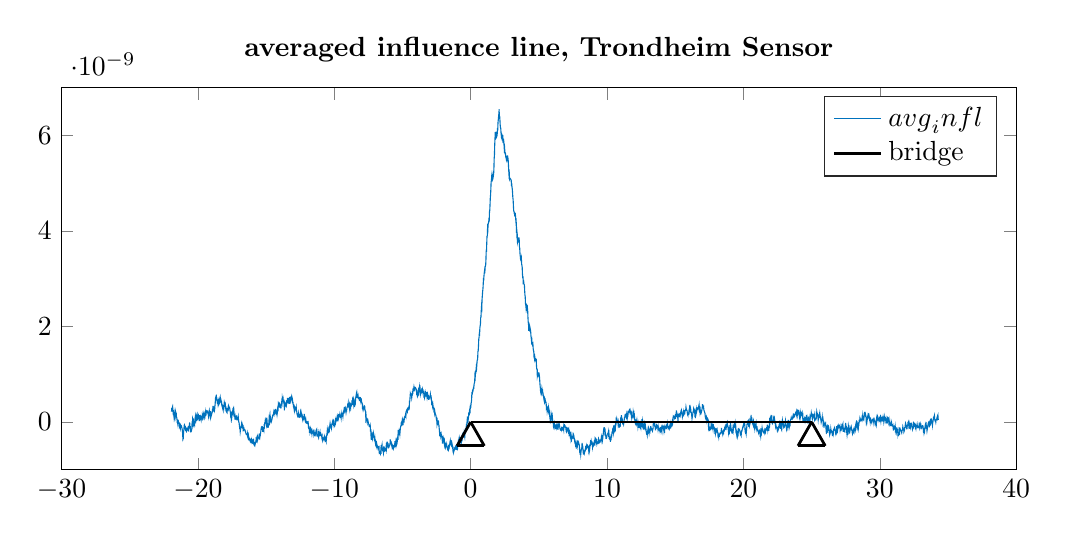
\begin{tikzpicture}

  \begin{axis}[%
    width=\textwidth,
    height=0.4\textwidth,
    at={(0\figurewidth,0\figureheight)},
    scale only axis,
    xmin=-30,
    xmax=40,
    ymin=-1e-09,
    ymax=7e-09,
    axis background/.style={fill=white},
    title style={font=\bfseries},
    title={averaged influence line, Trondheim Sensor},
    legend style={legend cell align=left,align=left,draw=white!15!black}
    ]
    \addplot [color=mycolor1,solid]
    table[row sep=crcr]{%
    -21.9331015625	2.17473775277215e-10\\
    -21.9129521484375	2.96367391209376e-10\\
    -21.892802734375	2.35203252096877e-10\\
    -21.8726533203125	3.02189371557938e-10\\
    -21.85250390625	3.22141890674623e-10\\
    -21.8323544921875	2.50288849111359e-10\\
    -21.812205078125	1.89199222454644e-10\\
    -21.7920556640625	2.04208060261574e-10\\
    -21.77190625	1.53552966204516e-10\\
    -21.7517568359375	1.09923041361176e-10\\
    -21.731607421875	5.54979209139948e-11\\
    -21.7114580078125	7.67944042180475e-11\\
    -21.69130859375	1.64077324040575e-10\\
    -21.6711591796875	1.26552643490174e-10\\
    -21.651009765625	2.33725604629077e-10\\
    -21.6308603515625	2.111443711452e-10\\
    -21.6107109375	1.96171123515693e-10\\
    -21.5905615234375	1.88378534918911e-10\\
    -21.570412109375	1.03774452300496e-10\\
    -21.5502626953125	9.11433982794237e-11\\
    -21.53011328125	5.65825481713418e-11\\
    -21.5099638671875	-1.34071486999118e-11\\
    -21.489814453125	-1.55370883257068e-11\\
    -21.4696650390625	-4.88742825505456e-11\\
    -21.449515625	4.86663812754457e-11\\
    -21.4293662109375	-7.75248262287887e-12\\
    -21.409216796875	-1.21211098031605e-11\\
    -21.3890673828125	-1.11959339020983e-11\\
    -21.36891796875	-2.31677071475589e-11\\
    -21.3487685546875	-7.79650430243304e-11\\
    -21.328619140625	-1.15042788392664e-10\\
    -21.3084697265625	-1.05424569665788e-10\\
    -21.2883203125	-1.31816168318621e-10\\
    -21.2681708984375	-7.46085254008577e-11\\
    -21.248021484375	-9.27376158059843e-11\\
    -21.2278720703125	-7.33050677359197e-11\\
    -21.20772265625	-7.86255840177671e-11\\
    -21.1875732421875	-1.17460926731154e-10\\
    -21.167423828125	-1.23757118162592e-10\\
    -21.1472744140625	-1.58501441331247e-10\\
    -21.127125	-2.06503535426936e-10\\
    -21.1069755859375	-3.07841124747837e-10\\
    -21.086826171875	-2.68563818039011e-10\\
    -21.0666767578125	-2.99593575616251e-10\\
    -21.04652734375	-1.99713871645779e-10\\
    -21.0263779296875	-1.66749134892171e-10\\
    -21.006228515625	-7.28661190740661e-11\\
    -20.9860791015625	-5.93295594866191e-11\\
    -20.9659296875	-7.82271607496298e-11\\
    -20.9457802734375	-9.25784189774221e-11\\
    -20.925630859375	-9.39276820225529e-11\\
    -20.9054814453125	-1.5858605629381e-10\\
    -20.88533203125	-1.4970714367099e-10\\
    -20.8651826171875	-1.82164144641247e-10\\
    -20.845033203125	-1.92314944127817e-10\\
    -20.8248837890625	-1.31866236610606e-10\\
    -20.804734375	-1.34717059101775e-10\\
    -20.7845849609375	-1.45580231095446e-10\\
    -20.764435546875	-1.58355573426016e-10\\
    -20.7442861328125	-1.38907997631032e-10\\
    -20.72413671875	-1.78116579155637e-10\\
    -20.7039873046875	-1.83403639789346e-10\\
    -20.683837890625	-1.55211101342974e-10\\
    -20.6636884765625	-7.85604008725945e-11\\
    -20.6435390625	-1.35561037382192e-10\\
    -20.6233896484375	-6.53247514889822e-11\\
    -20.603240234375	-8.2237092580968e-12\\
    -20.5830908203125	-1.34578314248436e-10\\
    -20.56294140625	-8.85582560947658e-11\\
    -20.5427919921875	-1.81678161664647e-10\\
    -20.522642578125	-1.74130888694936e-10\\
    -20.5024931640625	-2.006256243864e-10\\
    -20.48234375	-1.91833861787598e-10\\
    -20.4621943359375	-1.61711171495562e-10\\
    -20.442044921875	-1.35307405326208e-10\\
    -20.4218955078125	1.15141329704221e-11\\
    -20.40174609375	-2.72425355683347e-11\\
    -20.3815966796875	6.88551467094703e-11\\
    -20.361447265625	4.57894211735332e-11\\
    -20.3412978515625	-1.42056743900018e-11\\
    -20.3211484375	1.10356619291589e-11\\
    -20.3009990234375	-4.25033814363478e-11\\
    -20.280849609375	-1.25753229228578e-11\\
    -20.2607001953125	-2.23484766837295e-11\\
    -20.24055078125	-4.78302054495641e-11\\
    -20.2204013671875	4.82543249707316e-11\\
    -20.200251953125	8.48104691422228e-11\\
    -20.1801025390625	5.07065616150914e-11\\
    -20.159953125	1.15803996164198e-10\\
    -20.1398037109375	7.39245561364777e-11\\
    -20.119654296875	1.4061500165956e-10\\
    -20.0995048828125	2.59773323382801e-11\\
    -20.07935546875	1.02629350826389e-10\\
    -20.0592060546875	6.79398006536982e-11\\
    -20.039056640625	6.10248022454761e-11\\
    -20.0189072265625	1.1921444381585e-10\\
    -19.9987578125	6.75011717581942e-11\\
    -19.9786083984375	1.6713366476074e-10\\
    -19.958458984375	5.74313880957018e-11\\
    -19.9383095703125	1.19694420890574e-10\\
    -19.91816015625	9.61232871609545e-11\\
    -19.8980107421875	2.0565917793284e-11\\
    -19.877861328125	1.42873214058201e-10\\
    -19.8577119140625	3.71810475702337e-11\\
    -19.8375625	9.91298799775181e-11\\
    -19.8174130859375	1.14858244262408e-10\\
    -19.797263671875	7.81727449866788e-11\\
    -19.7771142578125	8.73197515706028e-11\\
    -19.75696484375	4.9312937536266e-11\\
    -19.7368154296875	8.92062126956447e-11\\
    -19.716666015625	1.33636174656468e-10\\
    -19.6965166015625	5.23380611942636e-11\\
    -19.6763671875	1.32856589014563e-10\\
    -19.6562177734375	9.46957253635332e-11\\
    -19.636068359375	5.83647556721322e-11\\
    -19.6159189453125	6.75379438734789e-11\\
    -19.59576953125	1.40880629780694e-10\\
    -19.5756201171875	1.02857675152586e-10\\
    -19.555470703125	1.11653781738242e-10\\
    -19.5353212890625	1.91039832713352e-10\\
    -19.515171875	1.23991817747265e-10\\
    -19.4950224609375	1.63474991810482e-10\\
    -19.474873046875	1.33961261911852e-10\\
    -19.4547236328125	1.81642346722647e-10\\
    -19.43457421875	2.15404671545258e-10\\
    -19.4144248046875	1.27655906805522e-10\\
    -19.394275390625	2.17755964640133e-10\\
    -19.3741259765625	2.15527369083962e-10\\
    -19.3539765625	2.15809547695465e-10\\
    -19.3338271484375	2.3517126979013e-10\\
    -19.313677734375	2.3280448057274e-10\\
    -19.2935283203125	1.90545359598072e-10\\
    -19.27337890625	1.87787173807409e-10\\
    -19.2532294921875	1.9242634391541e-10\\
    -19.233080078125	1.45154830444096e-10\\
    -19.2129306640625	1.76298915265313e-10\\
    -19.19278125	1.19267309348176e-10\\
    -19.1726318359375	1.54741376042663e-10\\
    -19.152482421875	2.18584080810582e-10\\
    -19.1323330078125	1.78503171727819e-10\\
    -19.11218359375	1.79184565008013e-10\\
    -19.0920341796875	2.24419971677995e-10\\
    -19.071884765625	1.22361274610658e-10\\
    -19.0517353515625	1.60273368545851e-10\\
    -19.0315859375	1.19869378864294e-10\\
    -19.0114365234375	1.4216028465377e-10\\
    -18.991287109375	1.61761347757421e-10\\
    -18.9711376953125	1.85844863067237e-10\\
    -18.95098828125	2.02137888937976e-10\\
    -18.9308388671875	2.55110547183343e-10\\
    -18.910689453125	2.49311316642156e-10\\
    -18.8905400390625	3.37194297856528e-10\\
    -18.870390625	2.20321534483744e-10\\
    -18.8502412109375	3.28878627047559e-10\\
    -18.830091796875	2.51632180993204e-10\\
    -18.8099423828125	2.59634138792388e-10\\
    -18.78979296875	2.36279329406047e-10\\
    -18.7696435546875	2.67317101754177e-10\\
    -18.749494140625	3.37106589170416e-10\\
    -18.7293447265625	3.94170057111063e-10\\
    -18.7091953125	5.00273916424661e-10\\
    -18.6890458984375	5.19465540928559e-10\\
    -18.668896484375	4.63008125183811e-10\\
    -18.6487470703125	5.71206204654e-10\\
    -18.62859765625	4.63326971071481e-10\\
    -18.6084482421875	4.64648672823871e-10\\
    -18.588298828125	4.62259568449984e-10\\
    -18.5681494140625	3.75507368039697e-10\\
    -18.548	4.5210506177184e-10\\
    -18.5278505859375	3.97190171439588e-10\\
    -18.507701171875	4.49597007596711e-10\\
    -18.4875517578125	4.2990577866831e-10\\
    -18.46740234375	3.96089637245357e-10\\
    -18.4472529296875	4.39617073613542e-10\\
    -18.427103515625	3.68852752673311e-10\\
    -18.4069541015625	4.30484484118559e-10\\
    -18.3868046875	4.04928488337021e-10\\
    -18.3666552734375	4.08764488133624e-10\\
    -18.346505859375	4.84585657179853e-10\\
    -18.3263564453125	4.4381460791275e-10\\
    -18.30620703125	4.60146579131923e-10\\
    -18.2860576171875	4.33131561466547e-10\\
    -18.265908203125	4.25149729831805e-10\\
    -18.2457587890625	3.53427101820848e-10\\
    -18.225609375	3.57925693635117e-10\\
    -18.2054599609375	3.09119684525404e-10\\
    -18.185310546875	2.93426000321817e-10\\
    -18.1651611328125	2.66569734269495e-10\\
    -18.14501171875	2.4598426785742e-10\\
    -18.1248623046875	3.37591919815862e-10\\
    -18.104712890625	3.34245747106683e-10\\
    -18.0845634765625	3.50052466927989e-10\\
    -18.0644140625	4.09746250886778e-10\\
    -18.0442646484375	3.85225011067493e-10\\
    -18.024115234375	3.42065371310591e-10\\
    -18.0039658203125	4.21478916978342e-10\\
    -17.98381640625	3.16069736963248e-10\\
    -17.9636669921875	3.01560944943066e-10\\
    -17.943517578125	3.08727044213443e-10\\
    -17.9233681640625	2.16287827447068e-10\\
    -17.90321875	2.89069744641989e-10\\
    -17.8830693359375	2.04395918943973e-10\\
    -17.862919921875	1.95156194334183e-10\\
    -17.8427705078125	2.49585640939901e-10\\
    -17.82262109375	2.46274091149154e-10\\
    -17.8024716796875	2.76160549787229e-10\\
    -17.782322265625	3.05483783380546e-10\\
    -17.7621728515625	2.81568327078898e-10\\
    -17.7420234375	3.23671957940338e-10\\
    -17.7218740234375	2.92667161239505e-10\\
    -17.701724609375	2.9782141365585e-10\\
    -17.6815751953125	3.03208355762938e-10\\
    -17.66142578125	2.75644223368192e-10\\
    -17.6412763671875	2.34196018115027e-10\\
    -17.621126953125	2.04212437414661e-10\\
    -17.6009775390625	1.43111201701704e-10\\
    -17.580828125	1.61717770458316e-10\\
    -17.5606787109375	9.42913318688689e-11\\
    -17.540529296875	1.36467638162662e-10\\
    -17.5203798828125	8.85709431347619e-11\\
    -17.50023046875	1.44345752111479e-10\\
    -17.4800810546875	1.50887059558518e-10\\
    -17.459931640625	2.02939478134979e-10\\
    -17.4397822265625	2.45500528436661e-10\\
    -17.4196328125	2.26779254373107e-10\\
    -17.3994833984375	2.58177430610666e-10\\
    -17.379333984375	1.97718907025584e-10\\
    -17.3591845703125	2.33555030026411e-10\\
    -17.33903515625	1.67837499287645e-10\\
    -17.3188857421875	1.38147393870407e-10\\
    -17.298736328125	1.22258105000811e-10\\
    -17.2785869140625	4.83509397883019e-11\\
    -17.2584375	1.09958626853668e-10\\
    -17.2382880859375	7.79681148846035e-11\\
    -17.218138671875	8.19234131562889e-11\\
    -17.1979892578125	7.41852991278356e-11\\
    -17.17783984375	1.20220128189592e-10\\
    -17.1576904296875	1.25513361197676e-10\\
    -17.137541015625	3.57539915353791e-11\\
    -17.1173916015625	1.07037730001298e-10\\
    -17.0972421875	4.99004360988909e-11\\
    -17.0770927734375	4.75658683292969e-11\\
    -17.056943359375	4.576644274015e-11\\
    -17.0367939453125	9.34295214113403e-11\\
    -17.01664453125	2.96507089126179e-11\\
    -16.9964951171875	-5.44403565763563e-12\\
    -16.976345703125	-2.39404612220371e-11\\
    -16.9561962890625	-7.64260380213699e-11\\
    -16.936046875	-1.2617885210821e-10\\
    -16.9158974609375	-1.23152393518519e-10\\
    -16.895748046875	-1.99979428754867e-10\\
    -16.8755986328125	-1.59738733494699e-10\\
    -16.85544921875	-1.32269104786315e-10\\
    -16.8352998046875	-9.70203793622439e-11\\
    -16.815150390625	-1.00963245195747e-10\\
    -16.7950009765625	-3.96359993620893e-11\\
    -16.7748515625	-6.87660152429036e-11\\
    -16.7547021484375	-4.35940610281166e-11\\
    -16.734552734375	-7.06899321118514e-11\\
    -16.7144033203125	-1.38325330957524e-10\\
    -16.69425390625	-6.08361069448046e-11\\
    -16.6741044921875	-1.69331049906447e-10\\
    -16.653955078125	-1.5823715280088e-10\\
    -16.6338056640625	-1.02972557038516e-10\\
    -16.61365625	-1.63899327538279e-10\\
    -16.5935068359375	-1.58671229401453e-10\\
    -16.573357421875	-1.66821928536905e-10\\
    -16.5532080078125	-1.65142875309226e-10\\
    -16.53305859375	-1.90385654626793e-10\\
    -16.5129091796875	-1.91040025136287e-10\\
    -16.492759765625	-2.25060732235426e-10\\
    -16.4726103515625	-2.35918209208928e-10\\
    -16.4524609375	-2.57967848474362e-10\\
    -16.4323115234375	-2.59532528942169e-10\\
    -16.412162109375	-2.55136756229275e-10\\
    -16.3920126953125	-2.65125192519586e-10\\
    -16.37186328125	-2.86912506806747e-10\\
    -16.3517138671875	-2.39363682736195e-10\\
    -16.331564453125	-2.74802944660163e-10\\
    -16.3114150390625	-3.17221118017317e-10\\
    -16.291265625	-2.9418822956386e-10\\
    -16.2711162109375	-3.85385119117773e-10\\
    -16.250966796875	-3.3320963515819e-10\\
    -16.2308173828125	-3.54007824422222e-10\\
    -16.21066796875	-3.51294087803625e-10\\
    -16.1905185546875	-3.82643133816423e-10\\
    -16.170369140625	-3.99345782050521e-10\\
    -16.1502197265625	-3.61448619959902e-10\\
    -16.1300703125	-3.62908560481122e-10\\
    -16.1099208984375	-3.85929277017985e-10\\
    -16.089771484375	-4.10647066681074e-10\\
    -16.0696220703125	-3.7773289279509e-10\\
    -16.04947265625	-4.1327698009788e-10\\
    -16.0293232421875	-4.10843287482091e-10\\
    -16.009173828125	-4.24993566208096e-10\\
    -15.9890244140625	-4.08014854111376e-10\\
    -15.968875	-3.62470482011314e-10\\
    -15.9487255859375	-4.612124316969e-10\\
    -15.928576171875	-3.51384334474424e-10\\
    -15.9084267578125	-3.94774411734273e-10\\
    -15.88827734375	-4.8505020172951e-10\\
    -15.8681279296875	-4.23844998250673e-10\\
    -15.847978515625	-4.92673675074343e-10\\
    -15.8278291015625	-5.00767387138153e-10\\
    -15.8076796875	-4.71448028642106e-10\\
    -15.7875302734375	-4.51332167719284e-10\\
    -15.767380859375	-4.2432496707837e-10\\
    -15.7472314453125	-4.23695006360497e-10\\
    -15.72708203125	-3.45036921064227e-10\\
    -15.7069326171875	-3.52180592511721e-10\\
    -15.686783203125	-3.73449996446427e-10\\
    -15.6666337890625	-3.13409805602268e-10\\
    -15.646484375	-2.97126999203192e-10\\
    -15.6263349609375	-3.79596287939191e-10\\
    -15.606185546875	-3.58415345685479e-10\\
    -15.5860361328125	-3.27631425151388e-10\\
    -15.56588671875	-3.31757875454959e-10\\
    -15.5457373046875	-3.21751930582369e-10\\
    -15.525587890625	-3.31673289770374e-10\\
    -15.5054384765625	-2.44764073394451e-10\\
    -15.4852890625	-3.16383401019468e-10\\
    -15.4651396484375	-3.31356994875176e-10\\
    -15.444990234375	-2.68402338520782e-10\\
    -15.4248408203125	-2.75957892626557e-10\\
    -15.40469140625	-2.29839484767262e-10\\
    -15.3845419921875	-1.95835628499445e-10\\
    -15.364392578125	-1.4282507506762e-10\\
    -15.3442431640625	-1.15609385821365e-10\\
    -15.32409375	-1.19200405456547e-10\\
    -15.3039443359375	-9.50481891249365e-11\\
    -15.283794921875	-9.63982380341772e-11\\
    -15.2636455078125	-1.47822530224343e-10\\
    -15.24349609375	-2.07276434319609e-10\\
    -15.2233466796875	-1.09385266334622e-10\\
    -15.203197265625	-1.49823554413656e-10\\
    -15.1830478515625	-1.44919611869568e-10\\
    -15.1628984375	-1.70933891763809e-10\\
    -15.1427490234375	-8.56969723852588e-11\\
    -15.122599609375	-9.70360882908021e-11\\
    -15.1024501953125	-1.95467172904575e-11\\
    -15.08230078125	-1.48674834887442e-11\\
    -15.0621513671875	2.64074707567094e-11\\
    -15.042001953125	-9.30518713143968e-12\\
    -15.0218525390625	-2.05384881149745e-11\\
    -15.001703125	1.81519891858434e-11\\
    -14.9815537109375	-2.94595640699971e-11\\
    -14.961404296875	5.25016151700686e-12\\
    -14.9412548828125	-4.98076243656717e-11\\
    -14.92110546875	-9.5734037356617e-12\\
    -14.9009560546875	-8.42399262487054e-11\\
    -14.880806640625	-2.75411764083284e-11\\
    -14.8606572265625	-1.08414681277357e-10\\
    -14.8405078125	-1.06379097834376e-10\\
    -14.8203583984375	-5.09334712245126e-11\\
    -14.800208984375	-3.0454656045012e-11\\
    -14.7800595703125	5.92452725894438e-11\\
    -14.75991015625	2.27370973049094e-11\\
    -14.7397607421875	1.13070732961066e-10\\
    -14.719611328125	1.50518119503156e-10\\
    -14.6994619140625	5.01398591260053e-11\\
    -14.6793125	8.77980511392647e-11\\
    -14.6591630859375	5.28897540126986e-11\\
    -14.639013671875	3.25983383206317e-11\\
    -14.6188642578125	3.7681891879297e-12\\
    -14.59871484375	1.93586145958833e-11\\
    -14.5785654296875	5.33533027940363e-11\\
    -14.558416015625	6.65771348552377e-11\\
    -14.5382666015625	1.13054227959058e-10\\
    -14.5181171875	1.34371808496451e-10\\
    -14.4979677734375	1.27766466648336e-10\\
    -14.477818359375	1.41458772508003e-10\\
    -14.4576689453125	1.64652403265207e-10\\
    -14.43751953125	2.03055709945844e-10\\
    -14.4173701171875	1.68416293626648e-10\\
    -14.397220703125	1.76068682883066e-10\\
    -14.3770712890625	2.59214371316133e-10\\
    -14.356921875	2.04274522207529e-10\\
    -14.3367724609375	2.50281211896922e-10\\
    -14.316623046875	2.57304429883811e-10\\
    -14.2964736328125	2.4450805421348e-10\\
    -14.27632421875	2.27326189249103e-10\\
    -14.2561748046875	1.71145429679392e-10\\
    -14.236025390625	1.64026890024542e-10\\
    -14.2158759765625	1.99659734037838e-10\\
    -14.1957265625	1.57747619082345e-10\\
    -14.1755771484375	1.98809402520273e-10\\
    -14.155427734375	2.83967821227199e-10\\
    -14.1352783203125	3.12492608029812e-10\\
    -14.11512890625	2.90595000893066e-10\\
    -14.0949794921875	3.93648930111528e-10\\
    -14.074830078125	3.80068328223403e-10\\
    -14.0546806640625	3.74102800365756e-10\\
    -14.03453125	3.8830908653807e-10\\
    -14.0143818359375	3.65456016822671e-10\\
    -13.994232421875	3.09694492071293e-10\\
    -13.9740830078125	3.06679904675594e-10\\
    -13.95393359375	3.06480157041633e-10\\
    -13.9337841796875	3.31618493106384e-10\\
    -13.913634765625	2.83015254373509e-10\\
    -13.8934853515625	3.62272729083955e-10\\
    -13.8733359375	3.63152565841411e-10\\
    -13.8531865234375	4.19980593601338e-10\\
    -13.833037109375	3.95818626233438e-10\\
    -13.8128876953125	4.97003406474793e-10\\
    -13.79273828125	4.61483362741935e-10\\
    -13.7725888671875	4.66275954547164e-10\\
    -13.752439453125	4.89564281106191e-10\\
    -13.7322900390625	4.29778421227008e-10\\
    -13.712140625	4.14868308690602e-10\\
    -13.6919912109375	4.17960385666517e-10\\
    -13.671841796875	3.42818584196529e-10\\
    -13.6516923828125	3.80815061876829e-10\\
    -13.63154296875	3.16533207343124e-10\\
    -13.6113935546875	3.47055053374427e-10\\
    -13.591244140625	3.71984844404989e-10\\
    -13.5710947265625	3.33365670403874e-10\\
    -13.5509453125	3.33141022737623e-10\\
    -13.5307958984375	3.59668858248743e-10\\
    -13.510646484375	3.44849368072012e-10\\
    -13.4904970703125	4.26500001615637e-10\\
    -13.47034765625	4.17963868208982e-10\\
    -13.4501982421875	4.19988358867752e-10\\
    -13.430048828125	5.03589659933334e-10\\
    -13.4098994140625	3.93792599908803e-10\\
    -13.38975	4.34951306027061e-10\\
    -13.3696005859375	5.03946736541212e-10\\
    -13.349451171875	4.36253496061607e-10\\
    -13.3293017578125	4.54748224793621e-10\\
    -13.30915234375	4.69738134492655e-10\\
    -13.2890029296875	3.79193483402695e-10\\
    -13.268853515625	5.25420011975312e-10\\
    -13.2487041015625	4.26212041751739e-10\\
    -13.2285546875	4.35538285791656e-10\\
    -13.2084052734375	4.72451632954145e-10\\
    -13.188255859375	4.41010620822975e-10\\
    -13.1681064453125	4.76586220305364e-10\\
    -13.14795703125	5.1578545354995e-10\\
    -13.1278076171875	5.37825205843434e-10\\
    -13.107658203125	4.98134379840876e-10\\
    -13.0875087890625	5.05361846939395e-10\\
    -13.067359375	4.67755272089633e-10\\
    -13.0472099609375	4.08355710069488e-10\\
    -13.027060546875	4.10407610882803e-10\\
    -13.0069111328125	3.63790895875863e-10\\
    -12.98676171875	3.1358655894136e-10\\
    -12.9666123046875	3.02591388162418e-10\\
    -12.946462890625	2.70109828308719e-10\\
    -12.9263134765625	3.02156318454401e-10\\
    -12.9061640625	2.57466183035098e-10\\
    -12.8860146484375	3.1439367708759e-10\\
    -12.865865234375	3.07066965298245e-10\\
    -12.8457158203125	2.87684032614511e-10\\
    -12.82556640625	2.67478406269933e-10\\
    -12.8054169921875	2.52950337951074e-10\\
    -12.785267578125	2.92648912221644e-10\\
    -12.7651181640625	2.1718102634947e-10\\
    -12.74496875	2.14042113406488e-10\\
    -12.7248193359375	1.54346521564746e-10\\
    -12.704669921875	1.4380177360592e-10\\
    -12.6845205078125	1.26820834020449e-10\\
    -12.66437109375	1.02868892098373e-10\\
    -12.6442216796875	1.03189194751158e-10\\
    -12.624072265625	1.67513112412156e-10\\
    -12.6039228515625	1.2481009059574e-10\\
    -12.5837734375	1.17039560166658e-10\\
    -12.5636240234375	1.51379387907558e-10\\
    -12.543474609375	1.4625573086364e-10\\
    -12.5233251953125	1.24459361829909e-10\\
    -12.50317578125	1.49948276586319e-10\\
    -12.4830263671875	1.87795086415668e-10\\
    -12.462876953125	1.30167375934165e-10\\
    -12.4427275390625	1.18355010658236e-10\\
    -12.422578125	1.89946870428157e-10\\
    -12.4024287109375	1.58564200648252e-10\\
    -12.382279296875	1.56416523396524e-10\\
    -12.3621298828125	1.58782080719125e-10\\
    -12.34198046875	1.15745868886655e-10\\
    -12.3218310546875	6.90255965897982e-11\\
    -12.301681640625	1.06753713184752e-10\\
    -12.2815322265625	9.95248044604246e-11\\
    -12.2613828125	9.60173009475856e-11\\
    -12.2412333984375	6.98523262022058e-11\\
    -12.221083984375	1.00954866766308e-10\\
    -12.2009345703125	1.6835510551933e-10\\
    -12.18078515625	5.81759182559687e-11\\
    -12.1606357421875	1.02438576635895e-10\\
    -12.140486328125	7.94214469839868e-11\\
    -12.1203369140625	6.27797723092713e-12\\
    -12.1001875	-3.0609884609412e-12\\
    -12.0800380859375	3.28624930742864e-11\\
    -12.059888671875	-1.53323324159825e-11\\
    -12.0397392578125	-2.01704763610021e-11\\
    -12.01958984375	-3.64057392629703e-12\\
    -11.9994404296875	-1.33386502152144e-11\\
    -11.979291015625	-1.0160790007578e-12\\
    -11.9591416015625	-6.48395011658697e-12\\
    -11.9389921875	-2.71373702246141e-11\\
    -11.9188427734375	2.25635367693716e-11\\
    -11.898693359375	-1.03686369271979e-10\\
    -11.8785439453125	-1.29004726392378e-10\\
    -11.85839453125	-1.37730683658603e-10\\
    -11.8382451171875	-1.24355836347419e-10\\
    -11.818095703125	-2.29501948399579e-10\\
    -11.7979462890625	-1.35993589413809e-10\\
    -11.777796875	-2.22408767639235e-10\\
    -11.7576474609375	-2.02422690963502e-10\\
    -11.737498046875	-1.4741816037881e-10\\
    -11.7173486328125	-1.75030615264165e-10\\
    -11.69719921875	-1.99465363642176e-10\\
    -11.6770498046875	-1.69662297377649e-10\\
    -11.656900390625	-1.92710243271167e-10\\
    -11.6367509765625	-2.44914028674215e-10\\
    -11.6166015625	-2.03135231530231e-10\\
    -11.5964521484375	-2.34326750943933e-10\\
    -11.576302734375	-2.32961303865337e-10\\
    -11.5561533203125	-2.03504067911749e-10\\
    -11.53600390625	-1.96685314291643e-10\\
    -11.5158544921875	-2.34116624268417e-10\\
    -11.495705078125	-1.53535463546583e-10\\
    -11.4755556640625	-2.6625261749692e-10\\
    -11.45540625	-2.11452533436023e-10\\
    -11.4352568359375	-2.88094175930414e-10\\
    -11.415107421875	-2.90351976780474e-10\\
    -11.3949580078125	-2.72115856515956e-10\\
    -11.37480859375	-2.46677428014524e-10\\
    -11.3546591796875	-2.15275084566035e-10\\
    -11.334509765625	-1.77514890783766e-10\\
    -11.3143603515625	-1.6630853461407e-10\\
    -11.2942109375	-2.22088731481647e-10\\
    -11.2740615234375	-1.89573719404063e-10\\
    -11.253912109375	-2.446841148552e-10\\
    -11.2337626953125	-2.81489924752884e-10\\
    -11.21361328125	-2.75217372089138e-10\\
    -11.1934638671875	-2.90910296446625e-10\\
    -11.173314453125	-3.08960482883329e-10\\
    -11.1531650390625	-2.489951607149e-10\\
    -11.133015625	-2.93604907363304e-10\\
    -11.1128662109375	-2.47307158088593e-10\\
    -11.092716796875	-2.30472185314316e-10\\
    -11.0725673828125	-2.4328854520892e-10\\
    -11.05241796875	-2.16468117120016e-10\\
    -11.0322685546875	-2.95486285988047e-10\\
    -11.012119140625	-2.26253149805015e-10\\
    -10.9919697265625	-2.34965603374118e-10\\
    -10.9718203125	-2.66652968501573e-10\\
    -10.9516708984375	-2.83370599120386e-10\\
    -10.931521484375	-2.86660225207581e-10\\
    -10.9113720703125	-3.23089770778323e-10\\
    -10.89122265625	-2.9939379483093e-10\\
    -10.8710732421875	-3.67241720271989e-10\\
    -10.850923828125	-3.92668147439481e-10\\
    -10.8307744140625	-3.64926015717509e-10\\
    -10.810625	-3.70266593257521e-10\\
    -10.7904755859375	-3.39284436680764e-10\\
    -10.770326171875	-3.44093780118429e-10\\
    -10.7501767578125	-3.25510939405129e-10\\
    -10.73002734375	-3.03313349128577e-10\\
    -10.7098779296875	-3.45135504738457e-10\\
    -10.689728515625	-3.21368342179169e-10\\
    -10.6695791015625	-3.38548900632687e-10\\
    -10.6494296875	-4.00652374769726e-10\\
    -10.6292802734375	-3.9453666745981e-10\\
    -10.609130859375	-3.55706952868443e-10\\
    -10.5889814453125	-3.88832592648549e-10\\
    -10.56883203125	-3.1383833853225e-10\\
    -10.5486826171875	-2.70716566187043e-10\\
    -10.528533203125	-2.33553851827422e-10\\
    -10.5083837890625	-1.63840272494724e-10\\
    -10.488234375	-2.02170059908931e-10\\
    -10.4680849609375	-1.55784108555748e-10\\
    -10.447935546875	-1.63411953143515e-10\\
    -10.4277861328125	-1.82109276907986e-10\\
    -10.40763671875	-2.34923138420757e-10\\
    -10.3874873046875	-9.96511596409215e-11\\
    -10.367337890625	-2.13281322501092e-10\\
    -10.3471884765625	-9.31876471349223e-11\\
    -10.3270390625	-7.46676713439542e-11\\
    -10.3068896484375	-2.96714629414599e-11\\
    -10.286740234375	-6.4509751133377e-11\\
    -10.2665908203125	-6.61676783688858e-11\\
    -10.24644140625	-1.01176841790474e-10\\
    -10.2262919921875	-8.59369908649859e-11\\
    -10.206142578125	-1.26616523299384e-10\\
    -10.1859931640625	-9.01160540832032e-11\\
    -10.16584375	-3.79248929455297e-11\\
    -10.1456943359375	-4.16119250261808e-11\\
    -10.125544921875	1.26500791356466e-11\\
    -10.1053955078125	3.07913311538661e-11\\
    -10.08524609375	-5.56528719701621e-13\\
    -10.0650966796875	5.23080539339584e-11\\
    -10.044947265625	-2.11360569089502e-11\\
    -10.0247978515625	-3.01116926383076e-11\\
    -10.0046484375	-9.17517391993231e-11\\
    -9.9844990234375	-8.01797045190821e-11\\
    -9.964349609375	-8.14204331415049e-11\\
    -9.9442001953125	-3.44244664522101e-11\\
    -9.92405078125	1.96201897166194e-11\\
    -9.9039013671875	-1.92178611315318e-12\\
    -9.883751953125	4.96772092644713e-11\\
    -9.8636025390625	2.52163014431298e-11\\
    -9.843453125	4.31112811961829e-11\\
    -9.8233037109375	4.45115118604686e-11\\
    -9.803154296875	8.16135286572276e-11\\
    -9.7830048828125	1.44239280919459e-11\\
    -9.76285546875	1.0201430056535e-10\\
    -9.7427060546875	3.51986154994879e-11\\
    -9.722556640625	9.80218357011017e-11\\
    -9.7024072265625	6.62856219815843e-11\\
    -9.6822578125	9.02882814517475e-11\\
    -9.6621083984375	1.3683692787064e-10\\
    -9.641958984375	1.26127191526298e-10\\
    -9.6218095703125	1.20636549350623e-10\\
    -9.60166015625	1.52897982003814e-10\\
    -9.5815107421875	1.0564202104716e-10\\
    -9.561361328125	1.0209903722101e-10\\
    -9.5412119140625	1.19318092766626e-10\\
    -9.5210625	1.30584641021695e-10\\
    -9.5009130859375	9.41022280764523e-11\\
    -9.480763671875	1.90097031393354e-10\\
    -9.4606142578125	9.56718153231872e-11\\
    -9.44046484375	1.76458300924129e-10\\
    -9.4203154296875	1.47276660980504e-10\\
    -9.400166015625	1.3585419914634e-10\\
    -9.3800166015625	1.93705072997721e-10\\
    -9.3598671875	1.3202095755248e-10\\
    -9.3397177734375	1.85051845975631e-10\\
    -9.319568359375	1.936006721052e-10\\
    -9.2994189453125	2.45952350590883e-10\\
    -9.27926953125	2.60200911701496e-10\\
    -9.2591201171875	3.17743350279964e-10\\
    -9.238970703125	2.59704252578304e-10\\
    -9.2188212890625	2.94146195350182e-10\\
    -9.198671875	3.04269552912931e-10\\
    -9.1785224609375	2.32219201537468e-10\\
    -9.158373046875	2.34584356784315e-10\\
    -9.1382236328125	1.96045605396432e-10\\
    -9.11807421875	2.31092626375247e-10\\
    -9.0979248046875	2.29585362181211e-10\\
    -9.077775390625	2.94045612557402e-10\\
    -9.0576259765625	3.06494638159584e-10\\
    -9.0374765625	3.20942836304335e-10\\
    -9.0173271484375	3.55997620646627e-10\\
    -8.997177734375	3.43767909312915e-10\\
    -8.9770283203125	3.89366548100587e-10\\
    -8.95687890625	3.20336211308085e-10\\
    -8.9367294921875	3.17916310452058e-10\\
    -8.916580078125	3.47816248269541e-10\\
    -8.8964306640625	3.0436249667729e-10\\
    -8.87628125	2.70901283919343e-10\\
    -8.8561318359375	3.52481838116117e-10\\
    -8.835982421875	3.22582986797795e-10\\
    -8.8158330078125	3.49860291967731e-10\\
    -8.79568359375	3.13950485376524e-10\\
    -8.7755341796875	3.89688836294054e-10\\
    -8.755384765625	3.40728695958514e-10\\
    -8.7352353515625	3.4093003133883e-10\\
    -8.7150859375	3.80741734265811e-10\\
    -8.6949365234375	4.56361740955097e-10\\
    -8.674787109375	3.58748740065102e-10\\
    -8.6546376953125	4.80979359514978e-10\\
    -8.63448828125	4.66328800148239e-10\\
    -8.6143388671875	4.58277303388144e-10\\
    -8.594189453125	4.79528002534045e-10\\
    -8.5740400390625	3.78551923887504e-10\\
    -8.553890625	4.15561557646456e-10\\
    -8.5337412109375	3.82072117362786e-10\\
    -8.513591796875	3.1387095813381e-10\\
    -8.4934423828125	3.77893893399637e-10\\
    -8.47329296875	4.40555036619087e-10\\
    -8.4531435546875	4.17781924858624e-10\\
    -8.432994140625	5.00185861184272e-10\\
    -8.4128447265625	5.31496625332018e-10\\
    -8.3926953125	5.58531812631084e-10\\
    -8.3725458984375	6.06954061484814e-10\\
    -8.352396484375	6.26743343037724e-10\\
    -8.3322470703125	5.45335720218501e-10\\
    -8.31209765625	5.58432589195504e-10\\
    -8.2919482421875	5.11956437914313e-10\\
    -8.271798828125	5.11610794536681e-10\\
    -8.2516494140625	5.40242852595223e-10\\
    -8.2315	4.89564457640042e-10\\
    -8.2113505859375	4.87592746121339e-10\\
    -8.191201171875	5.06881767346237e-10\\
    -8.1710517578125	5.00708999189463e-10\\
    -8.15090234375	4.36793578497493e-10\\
    -8.1307529296875	5.26226066220695e-10\\
    -8.110603515625	4.55729816503413e-10\\
    -8.0904541015625	5.19724556675149e-10\\
    -8.0703046875	4.58109269249281e-10\\
    -8.0501552734375	4.94138744169609e-10\\
    -8.030005859375	4.9058283909884e-10\\
    -8.0098564453125	4.5237117154875e-10\\
    -7.98970703125	4.02910013643775e-10\\
    -7.9695576171875	4.04547186923977e-10\\
    -7.949408203125	3.86913738378191e-10\\
    -7.9292587890625	2.791170366077e-10\\
    -7.909109375	2.74067969464117e-10\\
    -7.8889599609375	2.48981382064499e-10\\
    -7.868810546875	2.76615452648188e-10\\
    -7.8486611328125	3.02055118538673e-10\\
    -7.82851171875	2.92488661065869e-10\\
    -7.8083623046875	3.41608554092564e-10\\
    -7.788212890625	3.36198746392154e-10\\
    -7.7680634765625	3.24807149409961e-10\\
    -7.7479140625	2.50713795541334e-10\\
    -7.7277646484375	2.35787024376907e-10\\
    -7.707615234375	2.18301790671981e-10\\
    -7.6874658203125	8.68549962071698e-11\\
    -7.66731640625	1.20092466957589e-10\\
    -7.6471669921875	3.65280876078492e-11\\
    -7.627017578125	5.94561897342762e-11\\
    -7.6068681640625	4.97758995432412e-11\\
    -7.58671875	6.64040438848666e-11\\
    -7.5665693359375	5.68842678312922e-11\\
    -7.546419921875	-5.97347227215439e-12\\
    -7.5262705078125	1.94160169332562e-11\\
    -7.50612109375	-1.05943411738447e-11\\
    -7.4859716796875	-4.09074859977036e-11\\
    -7.465822265625	-4.99294932551959e-11\\
    -7.4456728515625	-7.69938455333724e-11\\
    -7.4255234375	-7.07106111384208e-11\\
    -7.4053740234375	-9.22112400843729e-11\\
    -7.385224609375	-1.00421985238621e-10\\
    -7.3650751953125	-7.92262301304846e-11\\
    -7.34492578125	-2.02979276946143e-10\\
    -7.3247763671875	-1.49660555923181e-10\\
    -7.304626953125	-2.91279239121356e-10\\
    -7.2844775390625	-2.67458304556048e-10\\
    -7.264328125	-3.72857991048524e-10\\
    -7.2441787109375	-3.21911638146252e-10\\
    -7.224029296875	-3.0181835075898e-10\\
    -7.2038798828125	-3.34645261195334e-10\\
    -7.18373046875	-2.60064693536987e-10\\
    -7.1635810546875	-2.08350037648711e-10\\
    -7.143431640625	-2.97688158557328e-10\\
    -7.1232822265625	-2.52705754924801e-10\\
    -7.1031328125	-3.14202046246682e-10\\
    -7.0829833984375	-3.30283898439711e-10\\
    -7.062833984375	-3.7001227494373e-10\\
    -7.0426845703125	-3.84606656311883e-10\\
    -7.02253515625	-3.43819178462081e-10\\
    -7.0023857421875	-4.06130065672622e-10\\
    -6.982236328125	-4.42877936828327e-10\\
    -6.9620869140625	-3.95731197273262e-10\\
    -6.9419375	-4.10057244958829e-10\\
    -6.9217880859375	-4.63507908795542e-10\\
    -6.901638671875	-5.0066678735186e-10\\
    -6.8814892578125	-4.63845450730954e-10\\
    -6.86133984375	-4.90790616246114e-10\\
    -6.8411904296875	-5.00477568438142e-10\\
    -6.821041015625	-5.23506421887212e-10\\
    -6.8008916015625	-5.47651037533602e-10\\
    -6.7807421875	-5.11932292061841e-10\\
    -6.7605927734375	-5.14180178162667e-10\\
    -6.740443359375	-5.33657537044256e-10\\
    -6.7202939453125	-5.26063556108121e-10\\
    -6.70014453125	-6.46577250731435e-10\\
    -6.6799951171875	-6.39791651221528e-10\\
    -6.659845703125	-6.34235941622947e-10\\
    -6.6396962890625	-6.55511150750729e-10\\
    -6.619546875	-6.70622748100157e-10\\
    -6.5993974609375	-6.42163903574076e-10\\
    -6.579248046875	-5.62989230907275e-10\\
    -6.5590986328125	-5.88567451210901e-10\\
    -6.53894921875	-5.06720792273693e-10\\
    -6.5187998046875	-5.12212680770944e-10\\
    -6.498650390625	-4.81235809083603e-10\\
    -6.4785009765625	-5.75811901017501e-10\\
    -6.4583515625	-5.89940477264675e-10\\
    -6.4382021484375	-6.07539934315672e-10\\
    -6.418052734375	-6.10641327895088e-10\\
    -6.3979033203125	-6.41286808169212e-10\\
    -6.37775390625	-5.44812090032883e-10\\
    -6.3576044921875	-5.55849408068954e-10\\
    -6.337455078125	-5.7713186838223e-10\\
    -6.3173056640625	-5.55957903026479e-10\\
    -6.29715625	-5.89109980969836e-10\\
    -6.2770068359375	-5.7113492902655e-10\\
    -6.256857421875	-5.75892518217314e-10\\
    -6.2367080078125	-5.88393804811402e-10\\
    -6.21655859375	-5.73713878650023e-10\\
    -6.1964091796875	-5.17069899151992e-10\\
    -6.176259765625	-5.63420461412178e-10\\
    -6.1561103515625	-5.03858949541906e-10\\
    -6.1359609375	-4.71733777813424e-10\\
    -6.1158115234375	-4.1176237249241e-10\\
    -6.095662109375	-4.81676220714492e-10\\
    -6.0755126953125	-4.5830852112653e-10\\
    -6.05536328125	-4.54642904763371e-10\\
    -6.0352138671875	-5.04369889717035e-10\\
    -6.015064453125	-5.37170865926444e-10\\
    -5.9949150390625	-5.33217070411307e-10\\
    -5.974765625	-4.93649117216929e-10\\
    -5.9546162109375	-4.95768561984502e-10\\
    -5.934466796875	-4.78885923331265e-10\\
    -5.9143173828125	-4.58659762373883e-10\\
    -5.89416796875	-3.6283873470679e-10\\
    -5.8740185546875	-4.54388854353269e-10\\
    -5.853869140625	-4.04301364061359e-10\\
    -5.8337197265625	-4.05102295371494e-10\\
    -5.8135703125	-4.72231789960181e-10\\
    -5.7934208984375	-4.86482705008696e-10\\
    -5.773271484375	-5.13847136161963e-10\\
    -5.7531220703125	-4.77871407527584e-10\\
    -5.73297265625	-4.93226324865963e-10\\
    -5.7128232421875	-4.99266368399037e-10\\
    -5.692673828125	-5.74846755982511e-10\\
    -5.6725244140625	-4.80095236031541e-10\\
    -5.652375	-5.47398742345818e-10\\
    -5.6322255859375	-5.30922504644983e-10\\
    -5.612076171875	-5.2290955531658e-10\\
    -5.5919267578125	-4.9856706042877e-10\\
    -5.57177734375	-4.90767704167006e-10\\
    -5.5516279296875	-4.03165590948832e-10\\
    -5.531478515625	-4.61297730359667e-10\\
    -5.5113291015625	-4.31027116589578e-10\\
    -5.4911796875	-4.02082959342526e-10\\
    -5.4710302734375	-4.63025519874412e-10\\
    -5.450880859375	-4.19634926356818e-10\\
    -5.4307314453125	-4.78797850391584e-10\\
    -5.41058203125	-4.63430360652101e-10\\
    -5.3904326171875	-4.23681704491359e-10\\
    -5.370283203125	-3.80693303523721e-10\\
    -5.3501337890625	-3.28438717313967e-10\\
    -5.329984375	-3.74491156426273e-10\\
    -5.3098349609375	-1.65766564228389e-10\\
    -5.289685546875	-2.71055020818194e-10\\
    -5.2695361328125	-1.68846672844804e-10\\
    -5.24938671875	-2.7721951316847e-10\\
    -5.2292373046875	-1.81304605187241e-10\\
    -5.209087890625	-1.97175761515119e-10\\
    -5.1889384765625	-2.41086473204616e-10\\
    -5.1687890625	-1.7678132890724e-10\\
    -5.1486396484375	-1.17043931746317e-10\\
    -5.128490234375	-9.51672487385996e-11\\
    -5.1083408203125	-7.926072938843e-11\\
    -5.08819140625	-1.84163221689154e-11\\
    -5.0680419921875	-7.08107123306663e-12\\
    -5.047892578125	-2.89911502809026e-11\\
    -5.0277431640625	1.18582355168666e-11\\
    -5.00759375	-5.63126905791459e-11\\
    -4.9874443359375	2.22822048651792e-11\\
    -4.967294921875	-7.03470179923552e-11\\
    -4.9471455078125	3.47794561888269e-11\\
    -4.92699609375	1.67439426218123e-11\\
    -4.9068466796875	2.35867639698064e-11\\
    -4.886697265625	1.27410843505668e-11\\
    -4.8665478515625	6.44262566843497e-11\\
    -4.8463984375	1.10372153909355e-10\\
    -4.8262490234375	1.16798153619394e-10\\
    -4.806099609375	1.0991170830323e-10\\
    -4.7859501953125	1.44848686562377e-10\\
    -4.76580078125	1.72553381648666e-10\\
    -4.7456513671875	1.36984475305532e-10\\
    -4.725501953125	2.17485646798392e-10\\
    -4.7053525390625	2.21972112563589e-10\\
    -4.685203125	2.48025138268791e-10\\
    -4.6650537109375	2.37390850735501e-10\\
    -4.644904296875	2.20025777047649e-10\\
    -4.6247548828125	2.86353699212015e-10\\
    -4.60460546875	2.92110213291904e-10\\
    -4.5844560546875	2.78760946684324e-10\\
    -4.564306640625	2.57045054790756e-10\\
    -4.5441572265625	2.54835178902444e-10\\
    -4.5240078125	3.14911944783358e-10\\
    -4.5038583984375	3.03449549820277e-10\\
    -4.483708984375	4.39426704950019e-10\\
    -4.4635595703125	4.4257291540406e-10\\
    -4.44341015625	5.20593683674656e-10\\
    -4.4232607421875	5.96800182230934e-10\\
    -4.403111328125	5.77244597275173e-10\\
    -4.3829619140625	5.69852133718631e-10\\
    -4.3628125	5.79307370287289e-10\\
    -4.3426630859375	5.63682590493233e-10\\
    -4.322513671875	5.11651236177399e-10\\
    -4.3023642578125	5.54250634113174e-10\\
    -4.28221484375	5.64124113590974e-10\\
    -4.2620654296875	6.44202529156906e-10\\
    -4.241916015625	5.83381037646796e-10\\
    -4.2217666015625	7.04295458139355e-10\\
    -4.2016171875	7.04488133873491e-10\\
    -4.1814677734375	6.88896734687504e-10\\
    -4.161318359375	7.28983471319332e-10\\
    -4.1411689453125	6.91257007972788e-10\\
    -4.12101953125	7.06909753145552e-10\\
    -4.1008701171875	6.85552849378655e-10\\
    -4.080720703125	7.19389225119983e-10\\
    -4.0605712890625	7.23867684249323e-10\\
    -4.040421875	7.18081584432585e-10\\
    -4.0202724609375	6.92799071546302e-10\\
    -4.000123046875	6.92695877204056e-10\\
    -3.9799736328125	6.90371877153561e-10\\
    -3.95982421875	6.01620657815827e-10\\
    -3.9396748046875	6.12491701724114e-10\\
    -3.919525390625	5.89171727248997e-10\\
    -3.8993759765625	5.35165778610726e-10\\
    -3.8792265625	5.47798433725121e-10\\
    -3.8590771484375	6.14893251271469e-10\\
    -3.838927734375	5.98870186137362e-10\\
    -3.8187783203125	6.98646433958463e-10\\
    -3.79862890625	6.93052294975976e-10\\
    -3.7784794921875	6.7401913892074e-10\\
    -3.758330078125	7.22773107716389e-10\\
    -3.7381806640625	6.54289078769674e-10\\
    -3.71803125	6.19046196266261e-10\\
    -3.6978818359375	6.68256155802727e-10\\
    -3.677732421875	6.05511981049324e-10\\
    -3.6575830078125	6.52806040549209e-10\\
    -3.63743359375	6.46157954176926e-10\\
    -3.6172841796875	6.26864489710357e-10\\
    -3.597134765625	6.18198705074853e-10\\
    -3.5769853515625	7.07614457628787e-10\\
    -3.5568359375	6.46498842564465e-10\\
    -3.5366865234375	6.89304753209134e-10\\
    -3.516537109375	6.66008195132674e-10\\
    -3.4963876953125	6.70536660128503e-10\\
    -3.47623828125	6.40629943332352e-10\\
    -3.4560888671875	6.08830520684334e-10\\
    -3.435939453125	5.93608733620446e-10\\
    -3.4157900390625	5.06980594217536e-10\\
    -3.395640625	5.61537802788021e-10\\
    -3.3754912109375	5.12074801541192e-10\\
    -3.355341796875	5.3729363104413e-10\\
    -3.3351923828125	5.55408585606448e-10\\
    -3.31504296875	5.9502162120429e-10\\
    -3.2948935546875	5.39113816871478e-10\\
    -3.274744140625	6.28059925922562e-10\\
    -3.2545947265625	5.30391391398637e-10\\
    -3.2344453125	6.26563767512366e-10\\
    -3.2142958984375	5.53060233021715e-10\\
    -3.194146484375	5.09770994229694e-10\\
    -3.1739970703125	5.44454653243976e-10\\
    -3.15384765625	5.7982893199696e-10\\
    -3.1336982421875	5.45341917688023e-10\\
    -3.113548828125	4.85297886835008e-10\\
    -3.0933994140625	5.65711544997227e-10\\
    -3.07325	4.65372764849973e-10\\
    -3.0531005859375	5.13565734304422e-10\\
    -3.032951171875	5.02095144021744e-10\\
    -3.0128017578125	5.23233494713585e-10\\
    -2.99265234375	5.22459302109658e-10\\
    -2.9725029296875	5.23609626974076e-10\\
    -2.952353515625	5.71020568749789e-10\\
    -2.9322041015625	5.20855915081797e-10\\
    -2.9120546875	4.96378603944914e-10\\
    -2.8919052734375	5.10777311741632e-10\\
    -2.871755859375	4.53934329925137e-10\\
    -2.8516064453125	3.52722042737282e-10\\
    -2.83145703125	4.10473389573746e-10\\
    -2.8113076171875	3.86536849997233e-10\\
    -2.791158203125	3.31095109973539e-10\\
    -2.7710087890625	3.66156534730334e-10\\
    -2.750859375	3.19592554320693e-10\\
    -2.7307099609375	2.96874408507748e-10\\
    -2.710560546875	3.00933472313836e-10\\
    -2.6904111328125	2.03474693570708e-10\\
    -2.67026171875	2.81913421452188e-10\\
    -2.6501123046875	1.93287942979745e-10\\
    -2.629962890625	2.25055983477546e-10\\
    -2.6098134765625	1.89616085789684e-10\\
    -2.5896640625	1.625828202188e-10\\
    -2.5695146484375	1.5428494222134e-10\\
    -2.549365234375	1.37232149726345e-10\\
    -2.5292158203125	1.05713431927275e-10\\
    -2.50906640625	4.69082658977593e-11\\
    -2.4889169921875	4.05420979708983e-11\\
    -2.468767578125	-3.58508156907501e-11\\
    -2.4486181640625	5.03945554849747e-12\\
    -2.42846875	-6.220313266878e-11\\
    -2.4083193359375	2.59937732542429e-11\\
    -2.388169921875	-5.36092882490338e-11\\
    -2.3680205078125	3.4451415435751e-11\\
    -2.34787109375	-5.42093243586257e-11\\
    -2.3277216796875	-6.58892551469004e-11\\
    -2.307572265625	-1.3661535873019e-10\\
    -2.2874228515625	-1.84950576100952e-10\\
    -2.2672734375	-2.97319826125368e-10\\
    -2.2471240234375	-2.45579713595469e-10\\
    -2.226974609375	-2.81778866284028e-10\\
    -2.2068251953125	-2.12063722680712e-10\\
    -2.18667578125	-2.6398310007311e-10\\
    -2.1665263671875	-2.44504499752108e-10\\
    -2.146376953125	-2.8851232098397e-10\\
    -2.1262275390625	-3.16250517516241e-10\\
    -2.106078125	-3.23365981218563e-10\\
    -2.0859287109375	-3.65329862341963e-10\\
    -2.065779296875	-4.51423380520727e-10\\
    -2.0456298828125	-3.74047163325523e-10\\
    -2.02548046875	-4.15507921967807e-10\\
    -2.0053310546875	-4.07999629731159e-10\\
    -1.985181640625	-3.60426383185489e-10\\
    -1.9650322265625	-3.96921652580982e-10\\
    -1.9448828125	-3.28256731341916e-10\\
    -1.9247333984375	-4.4593531389569e-10\\
    -1.904583984375	-4.93715356863928e-10\\
    -1.8844345703125	-4.66313513293719e-10\\
    -1.86428515625	-4.98386264202517e-10\\
    -1.8441357421875	-5.2472725069127e-10\\
    -1.823986328125	-4.77812696187292e-10\\
    -1.8038369140625	-4.9475789957637e-10\\
    -1.7836875	-4.91900781118975e-10\\
    -1.7635380859375	-4.67419817910521e-10\\
    -1.743388671875	-5.13343961492324e-10\\
    -1.7232392578125	-5.36604094358187e-10\\
    -1.70308984375	-5.58220444727405e-10\\
    -1.6829404296875	-5.75386057618782e-10\\
    -1.662791015625	-5.60283364027039e-10\\
    -1.6426416015625	-5.32713473706987e-10\\
    -1.6224921875	-5.73989399214226e-10\\
    -1.6023427734375	-5.51804862568994e-10\\
    -1.582193359375	-5.52707280666808e-10\\
    -1.5620439453125	-4.90070243470237e-10\\
    -1.54189453125	-4.91408815750477e-10\\
    -1.5217451171875	-4.28202469138524e-10\\
    -1.501595703125	-4.01356454638446e-10\\
    -1.4814462890625	-4.89323450098177e-10\\
    -1.461296875	-3.72566978621463e-10\\
    -1.4411474609375	-4.48175848269049e-10\\
    -1.420998046875	-3.91121949583187e-10\\
    -1.4008486328125	-4.64124825875667e-10\\
    -1.38069921875	-4.38322214908819e-10\\
    -1.3605498046875	-4.70365154615977e-10\\
    -1.340400390625	-4.86862322164538e-10\\
    -1.3202509765625	-5.32026993336022e-10\\
    -1.3001015625	-5.88709718596352e-10\\
    -1.2799521484375	-5.71967817590803e-10\\
    -1.259802734375	-6.40056329672861e-10\\
    -1.2396533203125	-6.19841144823313e-10\\
    -1.21950390625	-6.02013194398822e-10\\
    -1.1993544921875	-5.83366470917551e-10\\
    -1.179205078125	-5.67065432263284e-10\\
    -1.1590556640625	-5.3260543598835e-10\\
    -1.13890625	-5.3257373999515e-10\\
    -1.1187568359375	-5.4439455002242e-10\\
    -1.098607421875	-4.88539015830927e-10\\
    -1.0784580078125	-5.56051574134253e-10\\
    -1.05830859375	-5.52123920708359e-10\\
    -1.0381591796875	-5.31664948446308e-10\\
    -1.018009765625	-5.80408871148008e-10\\
    -0.997860351562501	-5.05091829361516e-10\\
    -0.977710937499999	-5.95673664855503e-10\\
    -0.957561523437501	-5.20061015198968e-10\\
    -0.937412109375	-4.97166785892941e-10\\
    -0.917262695312502	-4.50537937167984e-10\\
    -0.89711328125	-3.74900385460934e-10\\
    -0.876963867187499	-3.72053653564543e-10\\
    -0.856814453125001	-3.57559667507272e-10\\
    -0.836665039062499	-3.2438327694079e-10\\
    -0.816515625000001	-3.5335896534677e-10\\
    -0.796366210937499	-3.68693321963371e-10\\
    -0.776216796875001	-3.91650071146116e-10\\
    -0.7560673828125	-4.09639020198843e-10\\
    -0.735917968750002	-3.90656752824566e-10\\
    -0.7157685546875	-4.30604255534924e-10\\
    -0.695619140624999	-4.43255165607339e-10\\
    -0.6754697265625	-4.03979842321649e-10\\
    -0.655320312499999	-3.21890325486614e-10\\
    -0.635170898437501	-4.05441151885108e-10\\
    -0.615021484374999	-2.77141731769262e-10\\
    -0.594872070312501	-2.62072372150504e-10\\
    -0.57472265625	-3.30174566817129e-10\\
    -0.554573242187502	-2.77211362561669e-10\\
    -0.534423828125	-2.71175839705924e-10\\
    -0.514274414062498	-2.47754225151686e-10\\
    -0.494125	-3.20049365831235e-10\\
    -0.473975585937499	-2.42022385087669e-10\\
    -0.453826171875001	-2.8424106544331e-10\\
    -0.433676757812499	-3.11809770188636e-10\\
    -0.413527343750001	-2.26089769153511e-10\\
    -0.3933779296875	-2.10661415893801e-10\\
    -0.373228515625001	-1.62467462933384e-10\\
    -0.3530791015625	-1.43615879447786e-10\\
    -0.332929687500002	-1.84697434542201e-10\\
    -0.3127802734375	-3.81398985290475e-11\\
    -0.292630859374999	-7.62391250542498e-11\\
    -0.272481445312501	-2.19541122801534e-11\\
    -0.252332031249999	4.804545265827e-11\\
    -0.232182617187501	2.62653272515564e-11\\
    -0.212033203124999	9.54639905680567e-12\\
    -0.191883789062501	1.18335696661324e-10\\
    -0.171734375	7.08896216233913e-11\\
    -0.151584960937502	1.17527658490857e-10\\
    -0.131435546875	2.08442542052742e-10\\
    -0.111286132812499	1.36967915348416e-10\\
    -0.0911367187500005	2.29315423880165e-10\\
    -0.0709873046874989	2.59205130764022e-10\\
    -0.0508378906250009	1.83143290931993e-10\\
    -0.0306884765624993	3.10149353875614e-10\\
    -0.0105390625000013	2.96556796801946e-10\\
    0.00961035156250034	3.10870550298102e-10\\
    0.0297597656249984	3.9764892089302e-10\\
    0.0499091796875	4.13810758848967e-10\\
    0.0700585937500016	4.64585920085399e-10\\
    0.0902080078124996	6.25862555103256e-10\\
    0.110357421875001	5.74309379629832e-10\\
    0.130506835937499	6.50330007681999e-10\\
    0.150656250000001	6.68213197992042e-10\\
    0.170805664062499	6.57233262519935e-10\\
    0.190955078125	6.92726470626437e-10\\
    0.211104492187498	7.21493384010495e-10\\
    0.23125390625	7.16715690291523e-10\\
    0.251403320312498	7.98011135409935e-10\\
    0.271552734375	8.14067401651651e-10\\
    0.291702148437501	8.36911621208646e-10\\
    0.311851562499999	9.67955044881542e-10\\
    0.332000976562501	9.42714072018674e-10\\
    0.352150390624999	1.06854244883139e-09\\
    0.372299804687501	1.01200963407956e-09\\
    0.392449218749999	1.08508502108874e-09\\
    0.4125986328125	1.15032947809561e-09\\
    0.432748046874998	1.1252203571413e-09\\
    0.4528974609375	1.20174772878959e-09\\
    0.473046875000001	1.28314904298126e-09\\
    0.493196289062499	1.29692780273581e-09\\
    0.513345703125001	1.3397857001533e-09\\
    0.533495117187499	1.47300221736107e-09\\
    0.553644531250001	1.4996202384897e-09\\
    0.573793945312499	1.60015977218612e-09\\
    0.593943359375	1.73669583127482e-09\\
    0.614092773437498	1.76985581955432e-09\\
    0.6342421875	1.85167459875664e-09\\
    0.654391601562502	1.84167411628495e-09\\
    0.674541015625	1.97281129911439e-09\\
    0.694690429687501	2.01195366793265e-09\\
    0.714839843749999	2.0471101125747e-09\\
    0.734989257812501	2.18289079328191e-09\\
    0.755138671874999	2.20215238568879e-09\\
    0.7752880859375	2.32194850609436e-09\\
    0.795437499999998	2.41605980568342e-09\\
    0.8155869140625	2.38680424602788e-09\\
    0.835736328124998	2.57681493020087e-09\\
    0.8558857421875	2.64519984479703e-09\\
    0.876035156250001	2.72974052124028e-09\\
    0.896184570312499	2.77527209151087e-09\\
    0.916333984375001	2.86559379432762e-09\\
    0.936483398437499	2.98882785886549e-09\\
    0.956632812500001	2.98195946230649e-09\\
    0.976782226562499	3.06587082683403e-09\\
    0.996931640625	3.12335665336689e-09\\
    1.0170810546875	3.16867647921979e-09\\
    1.03723046875	3.11329418340863e-09\\
    1.0573798828125	3.23654327235315e-09\\
    1.077529296875	3.26842996966646e-09\\
    1.0976787109375	3.27807401372367e-09\\
    1.117828125	3.38254366366181e-09\\
    1.1379775390625	3.5776765320729e-09\\
    1.158126953125	3.57684777962633e-09\\
    1.1782763671875	3.74042238483456e-09\\
    1.19842578125	3.88840859358149e-09\\
    1.2185751953125	3.89912694198584e-09\\
    1.238724609375	4.05834845249441e-09\\
    1.2588740234375	4.02926821087668e-09\\
    1.2790234375	4.1374298661132e-09\\
    1.2991728515625	4.16622328712418e-09\\
    1.319322265625	4.1860958617542e-09\\
    1.3394716796875	4.24433256034535e-09\\
    1.35962109375	4.23175819892414e-09\\
    1.3797705078125	4.40720066192405e-09\\
    1.399919921875	4.43127996089651e-09\\
    1.4200693359375	4.5567183163379e-09\\
    1.44021875	4.69622124860873e-09\\
    1.4603681640625	4.76184145757258e-09\\
    1.480517578125	4.88801943760831e-09\\
    1.5006669921875	5.04038304041234e-09\\
    1.52081640625	5.04437548432431e-09\\
    1.5409658203125	5.15476595125207e-09\\
    1.561115234375	5.1951568767972e-09\\
    1.5812646484375	5.15495626841953e-09\\
    1.6014140625	5.19865624498835e-09\\
    1.6215634765625	5.09235140551771e-09\\
    1.641712890625	5.11248779557959e-09\\
    1.6618623046875	5.16482312769228e-09\\
    1.68201171875	5.19179170671002e-09\\
    1.7021611328125	5.28773053362809e-09\\
    1.722310546875	5.51246110362909e-09\\
    1.7424599609375	5.59038681385291e-09\\
    1.762609375	5.80400566338156e-09\\
    1.7827587890625	5.92775532837515e-09\\
    1.802908203125	6.06320340840594e-09\\
    1.8230576171875	6.06490375594068e-09\\
    1.84320703125	6.04278885314927e-09\\
    1.8633564453125	6.084302030716e-09\\
    1.883505859375	5.96358450637366e-09\\
    1.9036552734375	5.97529272413332e-09\\
    1.9238046875	5.99019453300582e-09\\
    1.9439541015625	6.03050673590018e-09\\
    1.964103515625	6.13189139201857e-09\\
    1.9842529296875	6.12749039819395e-09\\
    2.00440234375	6.27158361301246e-09\\
    2.0245517578125	6.33107385633245e-09\\
    2.044701171875	6.39209554804145e-09\\
    2.0648505859375	6.35145749577993e-09\\
    2.085	6.55327462703099e-09\\
    2.1051494140625	6.3686943236684e-09\\
    2.125298828125	6.41171281220031e-09\\
    2.1454482421875	6.32551795705678e-09\\
    2.16559765625	6.21952432407043e-09\\
    2.1857470703125	6.16790506922051e-09\\
    2.205896484375	6.15337235478024e-09\\
    2.2260458984375	6.0589123705532e-09\\
    2.2461953125	6.00272019301103e-09\\
    2.2663447265625	6.05389985599307e-09\\
    2.286494140625	5.93741608157416e-09\\
    2.3066435546875	6.02627235122229e-09\\
    2.32679296875	5.94967875832237e-09\\
    2.3469423828125	5.91208696348305e-09\\
    2.367091796875	5.93612813200447e-09\\
    2.3872412109375	5.8432330698453e-09\\
    2.407390625	5.93069567950884e-09\\
    2.4275400390625	5.87174238496395e-09\\
    2.447689453125	5.79476269330075e-09\\
    2.4678388671875	5.70780323546097e-09\\
    2.48798828125	5.74023180099713e-09\\
    2.5081376953125	5.65799320078387e-09\\
    2.528287109375	5.63513403690252e-09\\
    2.5484365234375	5.63297701529392e-09\\
    2.5685859375	5.55144555739777e-09\\
    2.5887353515625	5.55026984617468e-09\\
    2.608884765625	5.51590979983313e-09\\
    2.6290341796875	5.57982753971428e-09\\
    2.64918359375	5.51382445946589e-09\\
    2.6693330078125	5.56713669520145e-09\\
    2.689482421875	5.47146931233089e-09\\
    2.7096318359375	5.58652387889627e-09\\
    2.72978125	5.47981522613978e-09\\
    2.7499306640625	5.49011633169581e-09\\
    2.770080078125	5.38744573146489e-09\\
    2.7902294921875	5.27288807564771e-09\\
    2.81037890625	5.17811973100247e-09\\
    2.8305283203125	5.20636049269952e-09\\
    2.850677734375	5.09010898538655e-09\\
    2.8708271484375	5.10599507567036e-09\\
    2.8909765625	5.10291655502689e-09\\
    2.9111259765625	5.09097977360813e-09\\
    2.931275390625	5.09024126687076e-09\\
    2.9514248046875	5.07657286777574e-09\\
    2.97157421875	5.06145151977664e-09\\
    2.9917236328125	4.97148570484052e-09\\
    3.011873046875	4.9790846188566e-09\\
    3.0320224609375	4.91835502482713e-09\\
    3.052171875	4.87550198255035e-09\\
    3.0723212890625	4.7989911576801e-09\\
    3.092470703125	4.69826455299364e-09\\
    3.1126201171875	4.65911961261999e-09\\
    3.13276953125	4.53614021709157e-09\\
    3.1529189453125	4.42791459776951e-09\\
    3.173068359375	4.41982096433622e-09\\
    3.1932177734375	4.37282707672798e-09\\
    3.2133671875	4.36541223595016e-09\\
    3.2335166015625	4.31007339334728e-09\\
    3.253666015625	4.37359865804035e-09\\
    3.2738154296875	4.36740798240467e-09\\
    3.29396484375	4.27823671889882e-09\\
    3.3141142578125	4.21191114266743e-09\\
    3.334263671875	4.22393542262448e-09\\
    3.3544130859375	4.01864350658347e-09\\
    3.3745625	4.03369980178772e-09\\
    3.3947119140625	3.8965070062306e-09\\
    3.414861328125	3.9153394146599e-09\\
    3.4350107421875	3.76597651106402e-09\\
    3.45516015625	3.79242010456978e-09\\
    3.4753095703125	3.81607644637974e-09\\
    3.495458984375	3.86663630814768e-09\\
    3.5156083984375	3.76324254504372e-09\\
    3.5357578125	3.81669245969081e-09\\
    3.5559072265625	3.8282686489298e-09\\
    3.576056640625	3.66770557864598e-09\\
    3.5962060546875	3.64161623892301e-09\\
    3.61635546875	3.5280036869292e-09\\
    3.6365048828125	3.47774700936734e-09\\
    3.656654296875	3.41279831575642e-09\\
    3.6768037109375	3.42085734073382e-09\\
    3.696953125	3.39119586724166e-09\\
    3.7171025390625	3.42583922590165e-09\\
    3.737251953125	3.31638344528901e-09\\
    3.7574013671875	3.27871475726189e-09\\
    3.77755078125	3.24257099459247e-09\\
    3.7977001953125	3.09424058856925e-09\\
    3.817849609375	3.02890833776215e-09\\
    3.8379990234375	3.03167793327958e-09\\
    3.8581484375	2.8816963146198e-09\\
    3.8782978515625	2.9779217144784e-09\\
    3.898447265625	2.89458200271268e-09\\
    3.9185966796875	2.88530354606902e-09\\
    3.93874609375	2.8759021211237e-09\\
    3.9588955078125	2.75383821238601e-09\\
    3.979044921875	2.66210659889525e-09\\
    3.9991943359375	2.62391959325988e-09\\
    4.01934375	2.47723889245467e-09\\
    4.0394931640625	2.45340073833692e-09\\
    4.059642578125	2.39268669326907e-09\\
    4.0797919921875	2.4451109889016e-09\\
    4.09994140625	2.4553549904314e-09\\
    4.1200908203125	2.43799787480944e-09\\
    4.140240234375	2.36502909431256e-09\\
    4.1603896484375	2.3889601475975e-09\\
    4.1805390625	2.32442085212079e-09\\
    4.2006884765625	2.1897964272173e-09\\
    4.220837890625	2.08886391395885e-09\\
    4.2409873046875	2.0548048799946e-09\\
    4.26113671875	1.90991526344095e-09\\
    4.2812861328125	1.96555810569935e-09\\
    4.301435546875	1.94426430954916e-09\\
    4.3215849609375	1.98366827738211e-09\\
    4.341734375	1.90195080525939e-09\\
    4.3618837890625	1.95863694100304e-09\\
    4.382033203125	1.93052201009142e-09\\
    4.4021826171875	1.88293684314508e-09\\
    4.42233203125	1.79715227632121e-09\\
    4.4424814453125	1.75529788791132e-09\\
    4.462630859375	1.69190136490053e-09\\
    4.4827802734375	1.71556372172525e-09\\
    4.5029296875	1.61239237354954e-09\\
    4.5230791015625	1.67521769484138e-09\\
    4.543228515625	1.621215874126e-09\\
    4.5633779296875	1.63517448376149e-09\\
    4.58352734375	1.53534906603001e-09\\
    4.6036767578125	1.49975267410303e-09\\
    4.623826171875	1.48571132423636e-09\\
    4.6439755859375	1.37876865342709e-09\\
    4.664125	1.39047118373159e-09\\
    4.6842744140625	1.3242910793554e-09\\
    4.704423828125	1.35798284420482e-09\\
    4.7245732421875	1.31866418466333e-09\\
    4.74472265625	1.30804010674801e-09\\
    4.7648720703125	1.31399731723887e-09\\
    4.785021484375	1.25372458877785e-09\\
    4.8051708984375	1.32031969372075e-09\\
    4.8253203125	1.17566717968102e-09\\
    4.8454697265625	1.11269013688262e-09\\
    4.865619140625	1.10459873237328e-09\\
    4.8857685546875	9.75223089007907e-10\\
    4.90591796875	1.00965928140755e-09\\
    4.9260673828125	9.39183752909249e-10\\
    4.946216796875	9.91189215428455e-10\\
    4.9663662109375	1.00757315792899e-09\\
    4.986515625	1.02751332537432e-09\\
    5.0066650390625	1.02678534052554e-09\\
    5.026814453125	9.86967381887048e-10\\
    5.0469638671875	9.42359657510414e-10\\
    5.06711328125	8.54492547510165e-10\\
    5.0872626953125	7.70598360032432e-10\\
    5.107412109375	7.16198335996919e-10\\
    5.1275615234375	6.37583713339844e-10\\
    5.1477109375	6.11468208214805e-10\\
    5.1678603515625	6.66962422960105e-10\\
    5.188009765625	6.51130031107415e-10\\
    5.2081591796875	6.22603417970773e-10\\
    5.22830859375	6.96330506152772e-10\\
    5.2484580078125	6.62982901128657e-10\\
    5.268607421875	6.67421910325307e-10\\
    5.2887568359375	6.08484742178959e-10\\
    5.30890625	6.03264821486238e-10\\
    5.3290556640625	5.34537438735307e-10\\
    5.349205078125	5.28770930623447e-10\\
    5.3693544921875	4.76232190281772e-10\\
    5.38950390625	4.44218637927e-10\\
    5.4096533203125	4.19949996683683e-10\\
    5.429802734375	4.69842043534881e-10\\
    5.4499521484375	4.29750306932392e-10\\
    5.4701015625	4.4936550897551e-10\\
    5.4902509765625	4.12751357983762e-10\\
    5.510400390625	4.0949632238692e-10\\
    5.5305498046875	4.12036873667672e-10\\
    5.55069921875	3.04616698383785e-10\\
    5.5708486328125	3.23416862894153e-10\\
    5.590998046875	3.10603000063831e-10\\
    5.6111474609375	2.27835536619102e-10\\
    5.631296875	2.60882303115354e-10\\
    5.6514462890625	2.29092321835803e-10\\
    5.671595703125	2.33170421512327e-10\\
    5.6917451171875	2.90540754709177e-10\\
    5.71189453125	2.37523878070334e-10\\
    5.7320439453125	2.75833266063382e-10\\
    5.752193359375	2.44256708165216e-10\\
    5.7723427734375	2.26703578046566e-10\\
    5.7924921875	1.30507046386758e-10\\
    5.8126416015625	7.74740530919702e-11\\
    5.832791015625	5.5190862757268e-11\\
    5.8529404296875	-2.93092603733179e-11\\
    5.87308984375	9.39408217160732e-11\\
    5.8932392578125	2.09163881237801e-11\\
    5.913388671875	1.58360448581803e-10\\
    5.9335380859375	1.30706654312851e-10\\
    5.9536875	1.4482464253588e-10\\
    5.9738369140625	1.57427289212746e-10\\
    5.993986328125	7.90434608580849e-11\\
    6.0141357421875	2.2693996772712e-11\\
    6.03428515625	7.56189430693613e-12\\
    6.0544345703125	-2.3571688030103e-11\\
    6.074583984375	-9.22940617868645e-11\\
    6.0947333984375	-6.98354746194539e-11\\
    6.1148828125	-7.91070122121816e-11\\
    6.1350322265625	-4.35441056629525e-11\\
    6.155181640625	-9.82413605978752e-11\\
    6.1753310546875	-1.27355973123485e-10\\
    6.19548046875	-1.12131506205764e-10\\
    6.2156298828125	-4.89470949416972e-11\\
    6.235779296875	-1.46091438123309e-10\\
    6.2559287109375	-7.10018693075694e-11\\
    6.276078125	-7.21752867362179e-11\\
    6.2962275390625	-1.08807094064517e-10\\
    6.316376953125	-7.23775793762064e-11\\
    6.3365263671875	-1.23805700051532e-10\\
    6.35667578125	-1.17134401116863e-10\\
    6.3768251953125	-6.41317025561531e-11\\
    6.396974609375	-1.65371695990041e-10\\
    6.4171240234375	-7.1531244367554e-11\\
    6.4372734375	-1.04138605097716e-10\\
    6.4574228515625	-9.29333981514176e-11\\
    6.477572265625	-9.71021142123608e-11\\
    6.4977216796875	-4.79098366148223e-11\\
    6.51787109375	-7.67967631737029e-11\\
    6.5380205078125	-1.20512406760894e-10\\
    6.558169921875	-1.46220558211175e-10\\
    6.5783193359375	-1.66387973090354e-10\\
    6.59846875	-1.70617225425192e-10\\
    6.6186181640625	-1.63129758396603e-10\\
    6.638767578125	-1.51331056642247e-10\\
    6.6589169921875	-1.65484535790751e-10\\
    6.67906640625	-9.62107258643317e-11\\
    6.6992158203125	-1.8068044483192e-10\\
    6.719365234375	-1.08140008714033e-10\\
    6.7395146484375	-1.5632184328382e-10\\
    6.7596640625	-1.6445657932125e-10\\
    6.7798134765625	-1.69633742113022e-10\\
    6.799962890625	-1.29914918632663e-10\\
    6.8201123046875	-1.61323264636493e-10\\
    6.84026171875	-6.39127895436835e-11\\
    6.8604111328125	-7.69610307913754e-11\\
    6.880560546875	-6.77816262702725e-11\\
    6.9007099609375	-9.05978123587434e-11\\
    6.920859375	-8.49261808711123e-11\\
    6.9410087890625	-1.1133812476991e-10\\
    6.961158203125	-1.16608590063515e-10\\
    6.9813076171875	-1.19263373495447e-10\\
    7.00145703125	-1.9102470993094e-10\\
    7.0216064453125	-2.03081031045466e-10\\
    7.041755859375	-1.58431195897513e-10\\
    7.0619052734375	-1.87232364166834e-10\\
    7.0820546875	-1.67489403212987e-10\\
    7.1022041015625	-1.3569243074747e-10\\
    7.122353515625	-1.43124561351196e-10\\
    7.1425029296875	-1.37448063130551e-10\\
    7.16265234375	-1.32951842998527e-10\\
    7.1828017578125	-2.49640221524624e-10\\
    7.202951171875	-2.04020654516861e-10\\
    7.2231005859375	-2.7933411174313e-10\\
    7.24325	-2.75184941459081e-10\\
    7.2633994140625	-2.3977478107208e-10\\
    7.283548828125	-2.76598644304144e-10\\
    7.3036982421875	-2.15815163982216e-10\\
    7.32384765625	-2.87449447478165e-10\\
    7.3439970703125	-2.00023229824627e-10\\
    7.364146484375	-3.45097644708366e-10\\
    7.3842958984375	-3.13888096692097e-10\\
    7.4044453125	-3.55797518504763e-10\\
    7.4245947265625	-3.22279188601339e-10\\
    7.444744140625	-3.07239148009695e-10\\
    7.4648935546875	-3.05753557296116e-10\\
    7.48504296875	-3.18982511845413e-10\\
    7.5051923828125	-2.71533938618796e-10\\
    7.525341796875	-2.96172178457787e-10\\
    7.5454912109375	-2.69286253914952e-10\\
    7.565640625	-2.87573909074867e-10\\
    7.5857900390625	-3.44145380645832e-10\\
    7.605939453125	-3.48685036676295e-10\\
    7.6260888671875	-4.04678789485778e-10\\
    7.64623828125	-4.41466433332635e-10\\
    7.6663876953125	-4.46298257035838e-10\\
    7.686537109375	-4.8296183735805e-10\\
    7.7066865234375	-4.49766772934305e-10\\
    7.7268359375	-5.07934687982963e-10\\
    7.7469853515625	-4.31549379600153e-10\\
    7.767134765625	-4.88485452919045e-10\\
    7.7872841796875	-4.58442970981459e-10\\
    7.80743359375	-5.00938529788138e-10\\
    7.8275830078125	-4.50454877258237e-10\\
    7.847732421875	-4.78192417315965e-10\\
    7.8678818359375	-4.49423693486514e-10\\
    7.88803125	-4.11396716532931e-10\\
    7.9081806640625	-4.21788049799868e-10\\
    7.928330078125	-4.51309517191407e-10\\
    7.9484794921875	-4.68310230381458e-10\\
    7.96862890625	-4.88787155740807e-10\\
    7.9887783203125	-6.09822885973875e-10\\
    8.008927734375	-6.02831130854992e-10\\
    8.0290771484375	-6.89904957295187e-10\\
    8.0492265625	-6.23036606334541e-10\\
    8.0693759765625	-6.78550213533009e-10\\
    8.089525390625	-6.23163743413308e-10\\
    8.1096748046875	-5.83529470776781e-10\\
    8.12982421875	-5.57562907458558e-10\\
    8.1499736328125	-5.3459504870091e-10\\
    8.170123046875	-4.38292335454243e-10\\
    8.1902724609375	-4.97674619115036e-10\\
    8.210421875	-4.99722752748739e-10\\
    8.2305712890625	-5.57568492855503e-10\\
    8.250720703125	-6.41279608647563e-10\\
    8.2708701171875	-6.72363892289303e-10\\
    8.29101953125	-6.72744888634583e-10\\
    8.3111689453125	-6.38550465029236e-10\\
    8.331318359375	-6.58931757937773e-10\\
    8.3514677734375	-6.29133314006318e-10\\
    8.3716171875	-6.00911201210868e-10\\
    8.3917666015625	-6.05376220684174e-10\\
    8.411916015625	-5.86414279797113e-10\\
    8.4320654296875	-5.16747610202973e-10\\
    8.45221484375	-5.18934296127512e-10\\
    8.4723642578125	-5.75128478298533e-10\\
    8.492513671875	-4.98195329664399e-10\\
    8.5126630859375	-5.18462011895194e-10\\
    8.5328125	-5.01361887189931e-10\\
    8.5529619140625	-4.89018888013961e-10\\
    8.573111328125	-5.08135685197297e-10\\
    8.5932607421875	-5.27946728282173e-10\\
    8.61341015625	-5.07627607298463e-10\\
    8.6335595703125	-5.09958354980373e-10\\
    8.653708984375	-5.87586950133803e-10\\
    8.6738583984375	-5.56010095432895e-10\\
    8.6940078125	-6.28662426156672e-10\\
    8.7141572265625	-6.03310005510689e-10\\
    8.734306640625	-5.31200319153623e-10\\
    8.7544560546875	-4.82212187912937e-10\\
    8.77460546875	-4.85490234836104e-10\\
    8.7947548828125	-3.82556588740206e-10\\
    8.814904296875	-4.27574146044773e-10\\
    8.8350537109375	-3.94414081512579e-10\\
    8.855203125	-4.25789140042794e-10\\
    8.8753525390625	-4.58370131865337e-10\\
    8.895501953125	-4.69997223450045e-10\\
    8.9156513671875	-4.5266876863115e-10\\
    8.93580078125	-5.19933208731567e-10\\
    8.9559501953125	-4.75825531700174e-10\\
    8.976099609375	-4.7836257050698e-10\\
    8.9962490234375	-4.91125368561998e-10\\
    9.0163984375	-4.61404358681355e-10\\
    9.0365478515625	-4.78921007175546e-10\\
    9.056697265625	-4.77231617345939e-10\\
    9.0768466796875	-3.78153974222658e-10\\
    9.09699609375	-4.9371904975787e-10\\
    9.1171455078125	-3.67799116883935e-10\\
    9.137294921875	-3.88072560454321e-10\\
    9.1574443359375	-3.47708459842211e-10\\
    9.17759375	-3.57884925037388e-10\\
    9.1977431640625	-3.63748902681083e-10\\
    9.217892578125	-4.1526992144565e-10\\
    9.2380419921875	-3.99079880901795e-10\\
    9.25819140625	-4.56068937106817e-10\\
    9.2783408203125	-4.3199026598974e-10\\
    9.298490234375	-4.37314361692764e-10\\
    9.3186396484375	-4.43426178149498e-10\\
    9.3387890625	-4.46256730582976e-10\\
    9.3589384765625	-3.99898531947291e-10\\
    9.379087890625	-4.50330216808564e-10\\
    9.3992373046875	-3.8195607866546e-10\\
    9.41938671875	-4.07049886131918e-10\\
    9.4395361328125	-4.30843693843697e-10\\
    9.459685546875	-4.24863073949639e-10\\
    9.4798349609375	-3.96775754416205e-10\\
    9.499984375	-4.04409171487122e-10\\
    9.5201337890625	-3.75425629382282e-10\\
    9.540283203125	-3.7435540074508e-10\\
    9.5604326171875	-3.7804928678254e-10\\
    9.58058203125	-3.27608396917359e-10\\
    9.6007314453125	-3.70832506711167e-10\\
    9.620880859375	-4.00345566362867e-10\\
    9.6410302734375	-3.50973451791147e-10\\
    9.6611796875	-3.82480801457933e-10\\
    9.6813291015625	-3.43771706148078e-10\\
    9.701478515625	-2.8387160906555e-10\\
    9.7216279296875	-2.47610102996346e-10\\
    9.74177734375	-1.80761178788956e-10\\
    9.7619267578125	-1.35332873170831e-10\\
    9.782076171875	-1.19642372790554e-10\\
    9.8022255859375	-1.20415048442946e-10\\
    9.822375	-1.36897039609363e-10\\
    9.8425244140625	-2.26232229440403e-10\\
    9.862673828125	-2.05962888908781e-10\\
    9.8828232421875	-2.83574314690291e-10\\
    9.90297265625	-2.88038048381713e-10\\
    9.9231220703125	-3.42357018122843e-10\\
    9.943271484375	-3.43543481398813e-10\\
    9.9634208984375	-3.1197434105565e-10\\
    9.9835703125	-3.13935542930215e-10\\
    10.0037197265625	-2.56893897710585e-10\\
    10.023869140625	-2.55965502842379e-10\\
    10.0440185546875	-2.45823956836957e-10\\
    10.06416796875	-2.33298818565144e-10\\
    10.0843173828125	-2.28731072871866e-10\\
    10.104466796875	-2.01175146318565e-10\\
    10.1246162109375	-3.09310782428675e-10\\
    10.144765625	-2.68965834017168e-10\\
    10.1649150390625	-3.54057968573403e-10\\
    10.185064453125	-3.03918501891148e-10\\
    10.2052138671875	-3.79528987108193e-10\\
    10.22536328125	-3.05716371645646e-10\\
    10.2455126953125	-4.1553318563186e-10\\
    10.265662109375	-3.14356418565759e-10\\
    10.2858115234375	-3.80225694051011e-10\\
    10.3059609375	-2.57304832834325e-10\\
    10.3261103515625	-3.28216322182764e-10\\
    10.346259765625	-2.67035289114034e-10\\
    10.3664091796875	-2.17484613044068e-10\\
    10.38655859375	-2.22230324675263e-10\\
    10.4067080078125	-1.81659273301682e-10\\
    10.426857421875	-1.19755496039577e-10\\
    10.4470068359375	-1.7711597346071e-10\\
    10.46715625	-2.11792981144153e-10\\
    10.4873056640625	-7.22713895701888e-11\\
    10.507455078125	-1.82218976970074e-10\\
    10.5276044921875	-1.49656954824244e-10\\
    10.54775390625	-1.83613397570963e-10\\
    10.5679033203125	-1.67360735276152e-10\\
    10.588052734375	-1.07699143519902e-10\\
    10.6082021484375	-1.3346506148864e-10\\
    10.6283515625	-2.35292953636978e-11\\
    10.6485009765625	-6.79382116058618e-11\\
    10.668650390625	6.06840122646688e-11\\
    10.6887998046875	5.1878590627008e-11\\
    10.70894921875	7.72127904951822e-11\\
    10.7290986328125	4.93471963624835e-11\\
    10.749248046875	2.98351012381339e-11\\
    10.7693974609375	2.17437261096429e-11\\
    10.789546875	1.67924815111018e-11\\
    10.8096962890625	-4.25245392111437e-11\\
    10.829845703125	-6.53659695614337e-12\\
    10.8499951171875	-5.74572494415009e-11\\
    10.87014453125	-6.43175286872611e-11\\
    10.8902939453125	-1.08184184468134e-10\\
    10.910443359375	-1.04376825705233e-10\\
    10.9305927734375	-6.72392728323817e-11\\
    10.9507421875	-7.42482428638302e-11\\
    10.9708916015625	-7.82215751765686e-11\\
    10.991041015625	4.50910336372121e-11\\
    11.0111904296875	3.08066831226875e-11\\
    11.03133984375	6.22687225891842e-11\\
    11.0514892578125	1.42375850588708e-10\\
    11.071638671875	8.00497075592789e-11\\
    11.0917880859375	4.62083608991011e-11\\
    11.1119375	5.53076839059456e-11\\
    11.1320869140625	-2.11170591086814e-11\\
    11.152236328125	-3.90745399259049e-11\\
    11.1723857421875	-4.39392361210232e-11\\
    11.19253515625	-2.18010440351058e-11\\
    11.2126845703125	-4.64288111209305e-11\\
    11.232833984375	-8.61669427790411e-12\\
    11.2529833984375	3.24471748500633e-11\\
    11.2731328125	9.54114019980745e-11\\
    11.2932822265625	9.62480793820592e-11\\
    11.313431640625	1.26493461316427e-10\\
    11.3335810546875	1.59091662613409e-10\\
    11.35373046875	1.59857384225912e-10\\
    11.3738798828125	1.50163254004285e-10\\
    11.394029296875	1.18804739680997e-10\\
    11.4141787109375	1.56380161093494e-10\\
    11.434328125	1.05097702548261e-10\\
    11.4544775390625	1.06023184845708e-10\\
    11.474626953125	6.80785577080266e-11\\
    11.4947763671875	1.10153121574511e-10\\
    11.51492578125	1.72354815350529e-10\\
    11.5350751953125	1.55437045345109e-10\\
    11.555224609375	2.13936894246193e-10\\
    11.5753740234375	2.05323762784932e-10\\
    11.5955234375	2.17860389457844e-10\\
    11.6156728515625	2.1315193172143e-10\\
    11.635822265625	2.43696414333853e-10\\
    11.6559716796875	2.28815794561349e-10\\
    11.67612109375	2.04237260341482e-10\\
    11.6962705078125	2.39011151495821e-10\\
    11.716419921875	2.09929966782723e-10\\
    11.7365693359375	2.14414641844634e-10\\
    11.75671875	2.06371741150862e-10\\
    11.7768681640625	1.47463474359841e-10\\
    11.797017578125	1.71456249856648e-10\\
    11.8171669921875	7.82139389587891e-11\\
    11.83731640625	9.52081771770291e-11\\
    11.8574658203125	9.98173903276396e-11\\
    11.877615234375	1.07334705732632e-10\\
    11.8977646484375	1.18740647859257e-10\\
    11.9179140625	2.00138674201427e-10\\
    11.9380634765625	1.60325775330869e-10\\
    11.958212890625	2.36458810039171e-10\\
    11.9783623046875	1.60022077398736e-10\\
    11.99851171875	1.63377393892143e-10\\
    12.0186611328125	7.68570814768009e-11\\
    12.038810546875	2.77714427799463e-11\\
    12.0589599609375	1.23211310140539e-12\\
    12.079109375	-3.84243113085933e-11\\
    12.0992587890625	-4.81992075117848e-11\\
    12.119408203125	-3.59275645514886e-12\\
    12.1395576171875	-3.04408472606424e-11\\
    12.15970703125	2.33102722101775e-11\\
    12.1798564453125	4.65474878072948e-11\\
    12.200005859375	-3.39923659712842e-11\\
    12.2201552734375	-2.55707039319687e-11\\
    12.2403046875	-2.95420660232711e-11\\
    12.2604541015625	-8.93387681750343e-11\\
    12.280603515625	-3.76209349734329e-11\\
    12.3007529296875	-8.21306057344877e-11\\
    12.32090234375	-7.61573703530922e-11\\
    12.3410517578125	-1.06671062071416e-11\\
    12.361201171875	-1.19890332699477e-10\\
    12.3813505859375	-1.50344049168822e-12\\
    12.4015	-1.06079438546791e-10\\
    12.4216494140625	-5.53319377080028e-11\\
    12.441798828125	-1.48008232587035e-10\\
    12.4619482421875	-7.07900793607106e-11\\
    12.48209765625	-1.07031951916028e-10\\
    12.5022470703125	-3.71580344814125e-11\\
    12.522396484375	-5.6921994457994e-11\\
    12.5425458984375	-2.12761962958118e-11\\
    12.5626953125	5.75504573927085e-11\\
    12.5828447265625	-2.5994280341227e-11\\
    12.602994140625	1.41129196119254e-11\\
    12.6231435546875	-6.48802192186004e-11\\
    12.64329296875	-6.73912074174158e-11\\
    12.6634423828125	-1.59814777722076e-10\\
    12.683591796875	-1.11569127556387e-10\\
    12.7037412109375	-8.13406667904823e-11\\
    12.723890625	-1.55816588997653e-10\\
    12.7440400390625	-5.59658029300526e-11\\
    12.764189453125	-8.71617259418751e-11\\
    12.7843388671875	6.18376177411057e-12\\
    12.80448828125	-8.28377379281245e-11\\
    12.8246376953125	-1.04678316498513e-10\\
    12.844787109375	-1.35461621411027e-10\\
    12.8649365234375	-1.87939414050825e-10\\
    12.8850859375	-2.25572978006312e-10\\
    12.9052353515625	-2.11297417909781e-10\\
    12.925384765625	-2.20555690688824e-10\\
    12.9455341796875	-2.62958811856888e-10\\
    12.96568359375	-1.95936769991988e-10\\
    12.9858330078125	-1.76394380809725e-10\\
    13.005982421875	-1.42497441500543e-10\\
    13.0261318359375	-1.80238527345535e-10\\
    13.04628125	-1.43251635601451e-10\\
    13.0664306640625	-1.73766581044866e-10\\
    13.086580078125	-2.27498499092256e-10\\
    13.1067294921875	-1.88543396578359e-10\\
    13.12687890625	-1.71256567348972e-10\\
    13.1470283203125	-1.89424810613235e-10\\
    13.167177734375	-1.18135636703411e-10\\
    13.1873271484375	-1.80657921586236e-10\\
    13.2074765625	-8.46424097429273e-11\\
    13.2276259765625	-1.34886747758814e-10\\
    13.247775390625	-1.39731909874206e-10\\
    13.2679248046875	-1.42000857362461e-10\\
    13.28807421875	-1.5568806437195e-10\\
    13.3082236328125	-1.76973913222199e-10\\
    13.328373046875	-1.88765114491568e-10\\
    13.3485224609375	-1.49452298142546e-10\\
    13.368671875	-1.4529475083855e-10\\
    13.3888212890625	-4.46689359653516e-11\\
    13.408970703125	-1.82234053185198e-11\\
    13.4291201171875	-2.63854408224736e-11\\
    13.44926953125	-2.28939863067142e-11\\
    13.4694189453125	-1.3390281117784e-11\\
    13.489568359375	-8.27177596422735e-11\\
    13.5097177734375	-9.54402500798381e-11\\
    13.5298671875	-1.08842517173243e-10\\
    13.5500166015625	-1.76346231138967e-10\\
    13.570166015625	-1.21425851449266e-10\\
    13.5903154296875	-8.99150214702329e-11\\
    13.61046484375	-1.34996567966336e-10\\
    13.6306142578125	-4.40917047604391e-11\\
    13.650763671875	-1.10290212327782e-10\\
    13.6709130859375	-1.01200139307976e-10\\
    13.6910625	-9.18665100090028e-11\\
    13.7112119140625	-1.07758917931108e-10\\
    13.731361328125	-1.48971887063052e-10\\
    13.7515107421875	-9.84711427050269e-11\\
    13.77166015625	-1.35987241980258e-10\\
    13.7918095703125	-1.50124085483052e-10\\
    13.811958984375	-1.62990277504599e-10\\
    13.8321083984375	-1.40411349835888e-10\\
    13.8522578125	-1.38848935683546e-10\\
    13.8724072265625	-1.71682689729224e-10\\
    13.892556640625	-1.00697715713548e-10\\
    13.9127060546875	-1.61374312240193e-10\\
    13.93285546875	-1.82231374637751e-10\\
    13.9530048828125	-1.59987285176129e-10\\
    13.973154296875	-1.395458574877e-10\\
    13.9933037109375	-1.81117339045807e-10\\
    14.013453125	-2.04014233913373e-10\\
    14.0336025390625	-5.54911866294245e-11\\
    14.053751953125	-1.42340469385287e-10\\
    14.0739013671875	-9.66539841660556e-11\\
    14.09405078125	-9.38816843826617e-11\\
    14.1142001953125	-1.27498466992365e-10\\
    14.134349609375	-1.10793028907081e-10\\
    14.1544990234375	-1.401751149691e-10\\
    14.1746484375	-1.88532344796375e-10\\
    14.1947978515625	-1.46394758639308e-10\\
    14.214947265625	-2.25561033887454e-10\\
    14.2350966796875	-1.14671535613872e-10\\
    14.25524609375	-1.26546435673572e-10\\
    14.2753955078125	-1.06064712145084e-10\\
    14.295544921875	-1.11547033828991e-10\\
    14.3156943359375	-9.28436948782684e-11\\
    14.33584375	-1.14336460818031e-10\\
    14.3559931640625	-9.58445720806442e-11\\
    14.376142578125	-1.10757291113624e-10\\
    14.3962919921875	-3.72097258799863e-11\\
    14.41644140625	-1.10497011777865e-10\\
    14.4365908203125	-4.29485564548794e-11\\
    14.456740234375	-8.40871288803852e-11\\
    14.4768896484375	-9.64968603922856e-11\\
    14.4970390625	-1.27563658876866e-10\\
    14.5171884765625	-1.11633984528996e-10\\
    14.537337890625	-1.01494787957839e-10\\
    14.5574873046875	-9.88190112131532e-11\\
    14.57763671875	-1.23717501562184e-10\\
    14.5977861328125	-7.19344342622064e-11\\
    14.617935546875	-5.31169900352727e-11\\
    14.6380849609375	-3.26064980760383e-11\\
    14.658234375	-7.0300947973991e-11\\
    14.6783837890625	-3.43043021846747e-11\\
    14.698533203125	-8.91265831495168e-11\\
    14.7186826171875	-7.04930258371401e-11\\
    14.73883203125	-8.25357450336592e-11\\
    14.7589814453125	-8.28788449527164e-11\\
    14.779130859375	-2.18583543463048e-11\\
    14.7992802734375	-3.2157222270742e-11\\
    14.8194296875	5.99075053290203e-11\\
    14.8395791015625	5.14508711361556e-11\\
    14.859728515625	1.2387094993508e-10\\
    14.8798779296875	1.16564518464579e-10\\
    14.90002734375	1.03674599747883e-10\\
    14.9201767578125	9.55359766178763e-11\\
    14.940326171875	1.06710999669023e-10\\
    14.9604755859375	6.74870302292558e-11\\
    14.980625	7.1809847074204e-11\\
    15.0007744140625	1.25099829730266e-10\\
    15.020923828125	1.10803920436445e-10\\
    15.0410732421875	1.4870092501585e-10\\
    15.06122265625	1.64424130409311e-10\\
    15.0813720703125	2.29452403825916e-10\\
    15.101521484375	2.25438476238142e-10\\
    15.1216708984375	1.05969527047663e-10\\
    15.1418203125	1.75588796288825e-10\\
    15.1619697265625	7.94095850994642e-11\\
    15.182119140625	1.30254293653374e-10\\
    15.2022685546875	-1.70321261512993e-12\\
    15.22241796875	1.67285431501736e-10\\
    15.2425673828125	1.1612399405516e-10\\
    15.262716796875	1.20505862456688e-10\\
    15.2828662109375	1.56014822069914e-10\\
    15.303015625	1.40305186028755e-10\\
    15.3231650390625	1.15740922273222e-10\\
    15.343314453125	1.09254869625479e-10\\
    15.3634638671875	1.62671088101444e-10\\
    15.38361328125	1.5702757373325e-10\\
    15.4037626953125	2.0410573897305e-10\\
    15.423912109375	2.32278170192056e-10\\
    15.4440615234375	2.48741506278004e-10\\
    15.4642109375	1.98488181923411e-10\\
    15.4843603515625	2.01757767916961e-10\\
    15.504509765625	1.54824232449685e-10\\
    15.5246591796875	1.053539206643e-10\\
    15.54480859375	1.29821872211596e-10\\
    15.5649580078125	1.3209487138503e-10\\
    15.585107421875	1.8297809018593e-10\\
    15.6052568359375	1.18643066932171e-10\\
    15.62540625	1.73962428220276e-10\\
    15.6455556640625	1.96460491919714e-10\\
    15.665705078125	2.55099298336093e-10\\
    15.6858544921875	1.57053674299518e-10\\
    15.70600390625	2.23696958846434e-10\\
    15.7261533203125	2.39702580028167e-10\\
    15.746302734375	2.38124329068909e-10\\
    15.7664521484375	2.47003761119829e-10\\
    15.7866015625	3.09634239353149e-10\\
    15.8067509765625	2.74475297882743e-10\\
    15.826900390625	2.60538224082918e-10\\
    15.8470498046875	2.4205505167712e-10\\
    15.86719921875	2.40240603355345e-10\\
    15.8873486328125	1.88590059083097e-10\\
    15.907498046875	1.4967208485082e-10\\
    15.9276474609375	1.35848581482044e-10\\
    15.947796875	1.88915849464686e-10\\
    15.9679462890625	1.92750142571178e-10\\
    15.988095703125	1.44504056512164e-10\\
    16.0082451171875	2.40261678739041e-10\\
    16.02839453125	2.65913824541458e-10\\
    16.0485439453125	2.12108517416289e-10\\
    16.068693359375	3.6076331124105e-10\\
    16.0888427734375	2.71030599260178e-10\\
    16.1089921875	3.04113592512151e-10\\
    16.1291416015625	2.78733120745236e-10\\
    16.149291015625	2.10564679140103e-10\\
    16.1694404296875	2.05138976260627e-10\\
    16.18958984375	1.69601099346681e-10\\
    16.2097392578125	1.2766361269545e-10\\
    16.229888671875	7.23811598817871e-11\\
    16.2500380859375	1.04255177694634e-10\\
    16.2701875	1.43664998766544e-10\\
    16.2903369140625	1.84009961278048e-10\\
    16.310486328125	2.12493731408472e-10\\
    16.3306357421875	2.36860373861732e-10\\
    16.35078515625	2.79352805554597e-10\\
    16.3709345703125	2.57669130491406e-10\\
    16.391083984375	2.19590504430061e-10\\
    16.4112333984375	1.99655120228302e-10\\
    16.4313828125	2.22367997750214e-10\\
    16.4515322265625	1.07412051470905e-10\\
    16.471681640625	1.02230321060812e-10\\
    16.4918310546875	1.79848601312139e-10\\
    16.51198046875	1.65706941673089e-10\\
    16.5321298828125	2.3314902724131e-10\\
    16.552279296875	2.68992961684489e-10\\
    16.5724287109375	2.22649014867454e-10\\
    16.592578125	2.46266539899195e-10\\
    16.6127275390625	2.71080530317005e-10\\
    16.632876953125	2.8549556919223e-10\\
    16.6530263671875	2.7123728088963e-10\\
    16.67317578125	2.7588825903562e-10\\
    16.6933251953125	2.85969896632871e-10\\
    16.713474609375	3.16990463903374e-10\\
    16.7336240234375	2.84816737737635e-10\\
    16.7537734375	3.38880066698196e-10\\
    16.7739228515625	2.80666161615359e-10\\
    16.794072265625	2.55722751287278e-10\\
    16.8142216796875	2.00876743648673e-10\\
    16.83437109375	2.40597157899948e-10\\
    16.8545205078125	1.72753314151275e-10\\
    16.874669921875	1.69307259650216e-10\\
    16.8948193359375	1.87793851945964e-10\\
    16.91496875	2.0833126192775e-10\\
    16.9351181640625	2.25082201533537e-10\\
    16.955267578125	2.64591048511103e-10\\
    16.9754169921875	2.86021107115254e-10\\
    16.99556640625	3.75138791148004e-10\\
    17.0157158203125	3.27234772313186e-10\\
    17.035865234375	3.28623339203097e-10\\
    17.0560146484375	3.07495550573179e-10\\
    17.0761640625	3.18404635835698e-10\\
    17.0963134765625	2.52058068564087e-10\\
    17.116462890625	2.40205694315017e-10\\
    17.1366123046875	2.17291316951214e-10\\
    17.15676171875	2.00380518279403e-10\\
    17.1769111328125	1.86328799748322e-10\\
    17.197060546875	1.21812645101419e-10\\
    17.2172099609375	8.85156224602992e-11\\
    17.237359375	1.01477096306518e-10\\
    17.2575087890625	1.14662007139086e-10\\
    17.277658203125	5.58482215177867e-11\\
    17.2978076171875	1.01687121279427e-10\\
    17.31795703125	8.38590289770015e-11\\
    17.3381064453125	8.71396576364756e-11\\
    17.358255859375	6.88236383471706e-11\\
    17.3784052734375	3.02230173758958e-11\\
    17.3985546875	4.0804682967059e-11\\
    17.4187041015625	5.91958267924261e-12\\
    17.438853515625	-9.00784316329983e-11\\
    17.4590029296875	-4.95735730273542e-11\\
    17.47915234375	-1.16744450962382e-10\\
    17.4993017578125	-1.50443978747645e-10\\
    17.519451171875	-1.37193345721001e-10\\
    17.5396005859375	-1.5853725573206e-10\\
    17.55975	-1.41350331777905e-10\\
    17.5798994140625	-1.59758418899335e-10\\
    17.600048828125	-1.57350608639848e-10\\
    17.6201982421875	-9.27592471177208e-11\\
    17.64034765625	-1.420225617867e-10\\
    17.6604970703125	-7.02751041370039e-11\\
    17.680646484375	-9.55310692302451e-11\\
    17.7007958984375	-7.25927571349011e-11\\
    17.7209453125	-1.13897010282242e-10\\
    17.7410947265625	-1.0181746686377e-10\\
    17.761244140625	-1.38235221931169e-10\\
    17.7813935546875	-3.94263313113569e-11\\
    17.80154296875	-1.39819199942347e-10\\
    17.8216923828125	-9.74152980752576e-11\\
    17.841841796875	-1.07428302473497e-10\\
    17.8619912109375	-1.42240677388512e-10\\
    17.882140625	-1.37187850398736e-10\\
    17.9022900390625	-2.03810521029649e-10\\
    17.922439453125	-1.90809432528482e-10\\
    17.9425888671875	-2.35020710610982e-10\\
    17.96273828125	-1.83536956448801e-10\\
    17.9828876953125	-2.01354826990026e-10\\
    18.003037109375	-1.68989351166692e-10\\
    18.0231865234375	-1.86138223411027e-10\\
    18.0433359375	-1.58587177310315e-10\\
    18.0634853515625	-1.47109949439059e-10\\
    18.083634765625	-1.92333841702127e-10\\
    18.1037841796875	-2.19441273944137e-10\\
    18.12393359375	-2.32935077979266e-10\\
    18.1440830078125	-3.28284682494548e-10\\
    18.164232421875	-2.82470614478929e-10\\
    18.1843818359375	-3.15436935975639e-10\\
    18.20453125	-2.42388260878048e-10\\
    18.2246806640625	-3.1103763424826e-10\\
    18.244830078125	-2.55530210782299e-10\\
    18.2649794921875	-2.4495394631073e-10\\
    18.28512890625	-2.34460201441885e-10\\
    18.3052783203125	-2.44566304256478e-10\\
    18.325427734375	-2.38800736740971e-10\\
    18.3455771484375	-2.40698921279217e-10\\
    18.3657265625	-2.20944043841527e-10\\
    18.3858759765625	-1.24767763468474e-10\\
    18.406025390625	-2.33624666818135e-10\\
    18.4261748046875	-1.82732871108494e-10\\
    18.44632421875	-1.92878066153737e-10\\
    18.4664736328125	-2.26454962608778e-10\\
    18.486623046875	-2.60161574111042e-10\\
    18.5067724609375	-2.34574152429154e-10\\
    18.526921875	-2.04860502737796e-10\\
    18.5470712890625	-2.18711606254449e-10\\
    18.567220703125	-1.59162639699532e-10\\
    18.5873701171875	-1.53393205949835e-10\\
    18.60751953125	-1.62913718892168e-10\\
    18.6276689453125	-1.16595193333938e-10\\
    18.647818359375	-1.21651081994148e-10\\
    18.6679677734375	-9.44229216225035e-11\\
    18.6881171875	-1.3480901148798e-10\\
    18.7082666015625	-1.23377854023726e-10\\
    18.728416015625	-1.358606157692e-10\\
    18.7485654296875	-9.80007956806779e-11\\
    18.76871484375	-5.51840923004652e-11\\
    18.7888642578125	-3.78679236578644e-11\\
    18.809013671875	-1.38466274998918e-11\\
    18.8291630859375	-6.2868065811663e-11\\
    18.8493125	-9.93948492895931e-11\\
    18.8694619140625	-1.13931938587816e-10\\
    18.889611328125	-1.64991553621744e-10\\
    18.9097607421875	-2.2291712062198e-10\\
    18.92991015625	-1.8020693402756e-10\\
    18.9500595703125	-2.61806538928304e-10\\
    18.970208984375	-1.94948310024797e-10\\
    18.9903583984375	-1.196823507e-10\\
    19.0105078125	-1.18517123888644e-10\\
    19.0306572265625	-7.53131014147505e-11\\
    19.050806640625	-1.20862416774687e-10\\
    19.0709560546875	-7.94740089542433e-11\\
    19.09110546875	-1.40171767656625e-10\\
    19.1112548828125	-1.46276473971246e-10\\
    19.131404296875	-1.95911748111958e-10\\
    19.1515537109375	-1.89081179736718e-10\\
    19.171703125	-2.45264718332722e-10\\
    19.1918525390625	-1.7111860830231e-10\\
    19.212001953125	-1.76190481979047e-10\\
    19.2321513671875	-1.22513187357617e-10\\
    19.25230078125	-1.70181972334177e-10\\
    19.2724501953125	-1.1869703759352e-10\\
    19.292599609375	-1.0934598373449e-10\\
    19.3127490234375	-7.47435405059503e-11\\
    19.3328984375	-8.47997457286558e-11\\
    19.3530478515625	-1.16447969250628e-11\\
    19.373197265625	-9.41151862018843e-11\\
    19.3933466796875	-4.27898300689898e-11\\
    19.41349609375	-1.04433605493466e-10\\
    19.4336455078125	-8.71871939938379e-11\\
    19.453794921875	-2.00066612277714e-10\\
    19.4739443359375	-1.88568689449144e-10\\
    19.49409375	-2.41533516384156e-10\\
    19.5142431640625	-2.83048063725309e-10\\
    19.534392578125	-2.55980445374986e-10\\
    19.5545419921875	-2.95117773028127e-10\\
    19.57469140625	-2.494940866326e-10\\
    19.5948408203125	-2.02411488209733e-10\\
    19.614990234375	-2.29939244613742e-10\\
    19.6351396484375	-1.47381512290411e-10\\
    19.6552890625	-1.4016400119993e-10\\
    19.6754384765625	-1.59958988476807e-10\\
    19.695587890625	-1.57921325453058e-10\\
    19.7157373046875	-1.66034404374111e-10\\
    19.73588671875	-1.98085707771239e-10\\
    19.7560361328125	-2.14321186771487e-10\\
    19.776185546875	-2.55975203066888e-10\\
    19.7963349609375	-2.4183640045098e-10\\
    19.816484375	-2.30066819461308e-10\\
    19.8366337890625	-2.60725411580109e-10\\
    19.856783203125	-1.92827938572086e-10\\
    19.8769326171875	-1.96848207726849e-10\\
    19.89708203125	-1.76278068061623e-10\\
    19.9172314453125	-1.41077028545384e-10\\
    19.937380859375	-1.38787747764261e-10\\
    19.9575302734375	-9.97115129364979e-11\\
    19.9776796875	-7.82236274159168e-11\\
    19.9978291015625	-8.49957150367719e-11\\
    20.017978515625	-3.84252770667183e-11\\
    20.0381279296875	-2.35320104944181e-11\\
    20.05827734375	-2.20493231711209e-11\\
    20.0784267578125	-3.10084181176724e-11\\
    20.098576171875	-5.64947126629217e-11\\
    20.1187255859375	-1.74473070134797e-10\\
    20.138875	-1.62485276201841e-10\\
    20.1590244140625	-2.14656415852512e-10\\
    20.179173828125	-2.05843675513172e-10\\
    20.1993232421875	-2.44694913160997e-10\\
    20.21947265625	-1.8444369856555e-10\\
    20.2396220703125	-1.18912073421148e-10\\
    20.259771484375	-5.05069824832677e-11\\
    20.2799208984375	-4.99074450900801e-11\\
    20.3000703125	5.29235279330328e-12\\
    20.3202197265625	-3.22234343445746e-12\\
    20.340369140625	-1.61824235419701e-11\\
    20.3605185546875	5.70246019215145e-12\\
    20.38066796875	-8.34355091343643e-11\\
    20.4008173828125	-7.82110649800385e-11\\
    20.420966796875	-5.68046442745294e-11\\
    20.4411162109375	-7.9673774734908e-11\\
    20.461265625	-7.46178943084005e-12\\
    20.4814150390625	-4.82349246911638e-11\\
    20.501564453125	6.9439596328604e-11\\
    20.5217138671875	2.22670113185906e-11\\
    20.54186328125	5.07420471419618e-11\\
    20.5620126953125	1.48101881980057e-10\\
    20.582162109375	-1.84562702123225e-12\\
    20.6023115234375	1.00637459607358e-10\\
    20.6224609375	1.37239668055303e-11\\
    20.6426103515625	-1.13278800101212e-11\\
    20.662759765625	-2.4498054944241e-11\\
    20.6829091796875	-4.09834807628536e-11\\
    20.70305859375	-9.35803886282263e-12\\
    20.7232080078125	-5.10171260860706e-11\\
    20.743357421875	5.61481526028788e-12\\
    20.7635068359375	-2.92942965949845e-11\\
    20.78365625	-2.11720323104321e-11\\
    20.8038056640625	-7.77355351655336e-11\\
    20.823955078125	-3.17607150515091e-11\\
    20.8441044921875	-1.21607681434134e-10\\
    20.86425390625	-8.30130671238509e-11\\
    20.8844033203125	-9.9607100510428e-11\\
    20.904552734375	-8.63953472479358e-11\\
    20.9247021484375	-4.55614363857639e-11\\
    20.9448515625	-1.21353177926018e-10\\
    20.9650009765625	-1.47056731501584e-10\\
    20.985150390625	-8.6622383653054e-11\\
    21.0052998046875	-1.42711362569626e-10\\
    21.02544921875	-1.46536413778809e-10\\
    21.0455986328125	-1.6281173261636e-10\\
    21.065748046875	-1.93700488504527e-10\\
    21.0858974609375	-1.99645950767752e-10\\
    21.106046875	-2.25186060968349e-10\\
    21.1261962890625	-1.93038936733171e-10\\
    21.146345703125	-1.9706662444341e-10\\
    21.1664951171875	-1.85685718143124e-10\\
    21.18664453125	-2.10790630000798e-10\\
    21.2067939453125	-1.92581635598809e-10\\
    21.226943359375	-3.13309525560145e-10\\
    21.2470927734375	-2.48836217523216e-10\\
    21.2672421875	-2.92950215571884e-10\\
    21.2873916015625	-2.32531134983831e-10\\
    21.307541015625	-2.83045580892864e-10\\
    21.3276904296875	-1.98477717294e-10\\
    21.34783984375	-1.90732389973338e-10\\
    21.3679892578125	-1.25662080163565e-10\\
    21.388138671875	-1.63289125686265e-10\\
    21.4082880859375	-1.54109739330392e-10\\
    21.4284375	-1.66174273179982e-10\\
    21.4485869140625	-2.03889392373734e-10\\
    21.468736328125	-2.1260207585624e-10\\
    21.4888857421875	-2.28991720871287e-10\\
    21.50903515625	-2.26718036983531e-10\\
    21.5291845703125	-2.1793739399187e-10\\
    21.549333984375	-1.86710544487704e-10\\
    21.5694833984375	-2.27300784091136e-10\\
    21.5896328125	-2.05975851503554e-10\\
    21.6097822265625	-1.35907737306359e-10\\
    21.629931640625	-1.85825600375442e-10\\
    21.6500810546875	-1.56056443957802e-10\\
    21.67023046875	-1.40993296745429e-10\\
    21.6903798828125	-1.57524883512597e-10\\
    21.710529296875	-1.55023776420347e-10\\
    21.7306787109375	-1.62557542428748e-10\\
    21.750828125	-5.69873054492352e-11\\
    21.7709775390625	-1.0405074332965e-10\\
    21.791126953125	-1.64282165322948e-10\\
    21.8112763671875	-1.27315400416519e-10\\
    21.83142578125	-1.14050696955818e-10\\
    21.8515751953125	-1.83386774070396e-10\\
    21.871724609375	-1.2268926381546e-10\\
    21.8918740234375	-1.15104632676479e-10\\
    21.9120234375	-6.58038822959226e-13\\
    21.9321728515625	-2.86452075156956e-11\\
    21.952322265625	4.27724652629736e-11\\
    21.9724716796875	9.21993544833504e-11\\
    21.99262109375	8.77885512731318e-11\\
    22.0127705078125	1.04628902822533e-10\\
    22.032919921875	1.47604031259746e-10\\
    22.0530693359375	1.69747709604264e-11\\
    22.07321875	1.38207701138174e-10\\
    22.0933681640625	-1.66111374695348e-11\\
    22.113517578125	-2.42582247990919e-11\\
    22.1336669921875	-3.42701919503181e-11\\
    22.15381640625	-1.09670650409558e-11\\
    22.1739658203125	1.76434309570656e-11\\
    22.194115234375	1.45815596092127e-11\\
    22.2142646484375	7.78907796343842e-11\\
    22.2344140625	1.30300195971728e-10\\
    22.2545634765625	6.14705525921553e-11\\
    22.274712890625	7.33763025813966e-11\\
    22.2948623046875	3.59580948199084e-11\\
    22.31501171875	-2.73094770897939e-11\\
    22.3351611328125	-3.68316058510059e-11\\
    22.355310546875	-9.20713017952036e-11\\
    22.3754599609375	-6.15506815182183e-11\\
    22.395609375	-9.76092393045443e-11\\
    22.4157587890625	-1.02821816432147e-10\\
    22.435908203125	-1.2726641674135e-10\\
    22.4560576171875	-1.31000238564992e-10\\
    22.47620703125	-1.66633877107452e-10\\
    22.4963564453125	-1.36111480899002e-10\\
    22.516505859375	-1.50505735186563e-10\\
    22.5366552734375	-1.74433343187543e-10\\
    22.5568046875	-1.57979338677965e-10\\
    22.5769541015625	-8.73463627955683e-11\\
    22.597103515625	-1.40381019896262e-10\\
    22.6172529296875	-3.94377690306277e-11\\
    22.63740234375	-1.29047614056413e-10\\
    22.6575517578125	2.64288607554558e-11\\
    22.677701171875	-2.08068906637492e-11\\
    22.6978505859375	-3.15523930991812e-11\\
    22.718	-4.86460586541627e-11\\
    22.7381494140625	-1.41220918316989e-10\\
    22.758298828125	-7.89614421620538e-11\\
    22.7784482421875	-1.15358069573785e-10\\
    22.79859765625	-6.4313696862335e-11\\
    22.8187470703125	-1.07276839690413e-10\\
    22.838896484375	-3.27378605706739e-11\\
    22.8590458984375	3.47945039343803e-11\\
    22.8791953125	3.80012609943051e-12\\
    22.8993447265625	5.87016219921655e-12\\
    22.919494140625	-4.07255817425881e-11\\
    22.9396435546875	-7.00588216586725e-11\\
    22.95979296875	-1.20626254612982e-10\\
    22.9799423828125	-1.15200750287821e-10\\
    23.000091796875	-9.8465984272924e-11\\
    23.0202412109375	-8.74219158737822e-11\\
    23.040390625	-5.25517058208293e-11\\
    23.0605400390625	-1.76615357420778e-11\\
    23.080689453125	2.39565970564684e-11\\
    23.1008388671875	-2.91246645723819e-11\\
    23.12098828125	-6.98814785377719e-11\\
    23.1411376953125	-1.09327299225514e-10\\
    23.161287109375	-1.46393159576601e-10\\
    23.1814365234375	-1.10715116791529e-10\\
    23.2015859375	-1.33856644617438e-10\\
    23.2217353515625	-9.81265178157566e-11\\
    23.241884765625	-2.38813632891618e-11\\
    23.2620341796875	-1.1651001595236e-10\\
    23.28218359375	4.20024107597219e-11\\
    23.3023330078125	2.00426249909245e-12\\
    23.322482421875	-5.34547133352221e-11\\
    23.3426318359375	-1.04178577714456e-11\\
    23.36278125	-1.08004037765527e-10\\
    23.3829306640625	-8.39034117596604e-11\\
    23.403080078125	-2.27816192066641e-11\\
    23.4232294921875	-3.76613169127066e-11\\
    23.44337890625	3.18758581898399e-11\\
    23.4635283203125	5.20604172954569e-11\\
    23.483677734375	6.25283863342438e-11\\
    23.5038271484375	9.11620551307765e-11\\
    23.5239765625	6.9550784978397e-11\\
    23.5441259765625	6.21365484105286e-11\\
    23.564275390625	5.50409105670635e-11\\
    23.5844248046875	6.44456427985754e-11\\
    23.60457421875	1.01440046655715e-10\\
    23.6247236328125	1.14453311499364e-10\\
    23.644873046875	1.41370829950793e-10\\
    23.6650224609375	1.21170507474325e-10\\
    23.685171875	1.65124721098458e-10\\
    23.7053212890625	1.62758767886336e-10\\
    23.725470703125	1.33320740102471e-10\\
    23.7456201171875	1.21637991358671e-10\\
    23.76576953125	1.49553566564602e-10\\
    23.7859189453125	1.50839261322684e-10\\
    23.806068359375	1.54986866171689e-10\\
    23.8262177734375	1.93360592633843e-10\\
    23.8463671875	2.09249166526738e-10\\
    23.8665166015625	2.17647917230185e-10\\
    23.886666015625	1.68661150065689e-10\\
    23.9068154296875	2.17124092775235e-10\\
    23.92696484375	1.89423206683898e-10\\
    23.9471142578125	2.06804971797728e-10\\
    23.967263671875	1.64555688611615e-10\\
    23.9874130859375	2.44333796120473e-10\\
    24.0075625	2.37566375982313e-10\\
    24.0277119140625	2.38779046092152e-10\\
    24.047861328125	1.98780469490189e-10\\
    24.0680107421875	2.14125010440831e-10\\
    24.08816015625	1.79410697888831e-10\\
    24.1083095703125	1.16508760695018e-10\\
    24.128458984375	1.61852584266899e-10\\
    24.1486083984375	1.42330159728998e-10\\
    24.1687578125	1.11749544445134e-10\\
    24.1889072265625	1.74898960543116e-10\\
    24.209056640625	1.22955514956092e-10\\
    24.2292060546875	2.15987963881151e-10\\
    24.24935546875	1.60665975469263e-10\\
    24.2695048828125	1.56738571318446e-10\\
    24.289654296875	1.4010843521887e-10\\
    24.3098037109375	1.75356677993339e-10\\
    24.329953125	1.2297531742752e-10\\
    24.3501025390625	1.4058420757936e-10\\
    24.370251953125	1.53873980987426e-11\\
    24.3904013671875	8.06371865749044e-11\\
    24.41055078125	1.88643667410244e-11\\
    24.4307001953125	1.89379207169935e-11\\
    24.450849609375	3.24322092610145e-11\\
    24.4709990234375	6.80560654343345e-11\\
    24.4911484375	4.42508318939035e-11\\
    24.5112978515625	9.65404337841044e-11\\
    24.531447265625	3.22514915781804e-11\\
    24.5515966796875	6.20246409287696e-11\\
    24.57174609375	1.03101920380882e-10\\
    24.5918955078125	-5.47088422922423e-12\\
    24.612044921875	1.48770174935919e-10\\
    24.6321943359375	5.11165482282809e-11\\
    24.65234375	4.87587324042074e-11\\
    24.6724931640625	7.36684891238313e-11\\
    24.692642578125	7.69291440875031e-11\\
    24.7127919921875	-2.60009415027441e-11\\
    24.73294140625	6.11097318482583e-11\\
    24.7530908203125	2.66781932080291e-11\\
    24.773240234375	1.21283381278524e-11\\
    24.7933896484375	6.63140970326969e-11\\
    24.8135390625	5.10036764602239e-11\\
    24.8336884765625	4.06288911426708e-11\\
    24.853837890625	7.21954799287199e-11\\
    24.8739873046875	1.08494160237634e-10\\
    24.89413671875	7.61184916982012e-11\\
    24.9142861328125	1.34702071633786e-10\\
    24.934435546875	1.37057668418111e-10\\
    24.9545849609375	1.32852201069998e-10\\
    24.974734375	1.88711753140589e-10\\
    24.9948837890625	1.55420225542254e-10\\
    25.015033203125	1.37247222606184e-10\\
    25.0351826171875	9.84412536066781e-11\\
    25.05533203125	1.76835850896476e-10\\
    25.0754814453125	9.69034864455388e-11\\
    25.095630859375	1.25802613659204e-10\\
    25.1157802734375	1.49392085757975e-10\\
    25.1359296875	1.37579748967698e-10\\
    25.1560791015625	1.10142792010938e-10\\
    25.176228515625	9.17630831530019e-11\\
    25.1963779296875	1.2934571001514e-10\\
    25.21652734375	3.70282494311444e-11\\
    25.2366767578125	4.8837939705555e-11\\
    25.256826171875	4.36828547890757e-11\\
    25.2769755859375	4.62260820560697e-11\\
    25.297125	4.35030084504491e-11\\
    25.3172744140625	6.52749504951625e-11\\
    25.337423828125	1.54674880212684e-10\\
    25.3575732421875	1.34582008699059e-10\\
    25.37772265625	2.09506456213069e-10\\
    25.3978720703125	1.74206033076611e-10\\
    25.418021484375	1.75638907414538e-10\\
    25.4381708984375	1.37148245000471e-10\\
    25.4583203125	1.0685364436719e-10\\
    25.4784697265625	5.11138249889891e-11\\
    25.498619140625	1.04982014740508e-10\\
    25.5187685546875	8.72168012028013e-11\\
    25.53891796875	1.16782237959248e-10\\
    25.5590673828125	1.5383694199953e-10\\
    25.579216796875	1.34697740766994e-10\\
    25.5993662109375	1.79525398508016e-10\\
    25.619515625	1.3916838684414e-10\\
    25.6396650390625	9.90968400539027e-11\\
    25.659814453125	7.07749794138465e-11\\
    25.6799638671875	4.00472983763408e-11\\
    25.70011328125	-5.67677096999097e-12\\
    25.7202626953125	1.73636969115721e-11\\
    25.740412109375	3.30589127623625e-11\\
    25.7605615234375	3.95412901645807e-11\\
    25.7807109375	9.74564101299936e-11\\
    25.8008603515625	4.19380855929779e-11\\
    25.821009765625	1.19839653026532e-10\\
    25.8411591796875	-1.6235975487959e-11\\
    25.86130859375	1.00493672505637e-11\\
    25.8814580078125	2.9993251462802e-12\\
    25.901607421875	-1.15669657622247e-10\\
    25.9217568359375	-3.111516908475e-11\\
    25.94190625	-5.00002303431194e-11\\
    25.9620556640625	-2.85071345370442e-11\\
    25.982205078125	-2.67371066329485e-11\\
    26.0023544921875	-4.55100644207119e-11\\
    26.02250390625	-3.06507704746282e-11\\
    26.0426533203125	-1.02147003901811e-10\\
    26.062802734375	-1.72063225584441e-10\\
    26.0829521484375	-1.45434574297349e-10\\
    26.1031015625	-2.23095382445145e-10\\
    26.1232509765625	-2.14125372162196e-10\\
    26.143400390625	-1.81520771736683e-10\\
    26.1635498046875	-1.28403731778166e-10\\
    26.18369921875	-1.54605459519541e-10\\
    26.2038486328125	-7.21575631446786e-11\\
    26.223998046875	-7.89731631766085e-11\\
    26.2441474609375	-1.01561843423185e-10\\
    26.264296875	-1.40053146265372e-10\\
    26.2844462890625	-1.61578939356929e-10\\
    26.304595703125	-2.09313064459802e-10\\
    26.3247451171875	-2.67843253460644e-10\\
    26.34489453125	-2.46962761487989e-10\\
    26.3650439453125	-2.24868419919732e-10\\
    26.385193359375	-2.1412386249804e-10\\
    26.4053427734375	-1.47927710689824e-10\\
    26.4254921875	-1.901154997763e-10\\
    26.4456416015625	-1.8533295039406e-10\\
    26.465791015625	-1.82422936430886e-10\\
    26.4859404296875	-2.21663572112847e-10\\
    26.50608984375	-2.3629693333557e-10\\
    26.5262392578125	-2.96122553741571e-10\\
    26.546388671875	-2.26422550758393e-10\\
    26.5665380859375	-2.09629254319088e-10\\
    26.5866875	-2.38499949421769e-10\\
    26.6068369140625	-1.60868259723659e-10\\
    26.626986328125	-1.61616914967123e-10\\
    26.6471357421875	-1.43437469498589e-10\\
    26.66728515625	-1.2600624979335e-10\\
    26.6874345703125	-1.60272447263556e-10\\
    26.707583984375	-1.73992730718426e-10\\
    26.7277333984375	-1.72917503144493e-10\\
    26.7478828125	-2.16717634572606e-10\\
    26.7680322265625	-1.75620257550022e-10\\
    26.788181640625	-1.60455891163748e-10\\
    26.8083310546875	-1.905800954396e-10\\
    26.82848046875	-8.5533202759927e-11\\
    26.8486298828125	-1.72684144035111e-10\\
    26.868779296875	-1.30860642839806e-10\\
    26.8889287109375	-1.08586440387525e-10\\
    26.909078125	-1.60994802370951e-10\\
    26.9292275390625	-1.2479765264948e-10\\
    26.949376953125	-1.10562478832812e-10\\
    26.9695263671875	-1.15359307826854e-10\\
    26.98967578125	-6.84543828532312e-11\\
    27.0098251953125	-8.04619932296177e-11\\
    27.029974609375	-1.01084871471288e-10\\
    27.0501240234375	-1.06702267095031e-10\\
    27.0702734375	-8.90795608064315e-11\\
    27.0904228515625	-1.69237763322952e-10\\
    27.110572265625	-1.40570482554047e-10\\
    27.1307216796875	-1.71023773267245e-10\\
    27.15087109375	-1.74964954507217e-10\\
    27.1710205078125	-1.14592793424654e-10\\
    27.191169921875	-9.75174118061049e-11\\
    27.2113193359375	-1.13324373489726e-10\\
    27.23146875	-3.62898661726438e-11\\
    27.2516181640625	-8.37519045470178e-11\\
    27.271767578125	-6.86055910383556e-11\\
    27.2919169921875	-4.7106595919714e-11\\
    27.31206640625	-2.07847802973554e-10\\
    27.3322158203125	-1.21320974797494e-10\\
    27.352365234375	-1.650940657436e-10\\
    27.3725146484375	-1.84213965800047e-10\\
    27.3926640625	-1.93129860499963e-10\\
    27.4128134765625	-1.33043655647989e-10\\
    27.432962890625	-1.29644459370853e-10\\
    27.4531123046875	-1.32113182290458e-10\\
    27.47326171875	-7.74408717876603e-11\\
    27.4934111328125	-2.12739208911528e-11\\
    27.513560546875	-1.17817444168805e-10\\
    27.5337099609375	-7.97624703340427e-11\\
    27.553859375	-2.04787764472289e-10\\
    27.5740087890625	-2.21171304003942e-10\\
    27.594158203125	-2.65662353986495e-10\\
    27.6143076171875	-2.1148585522364e-10\\
    27.63445703125	-2.67791732774302e-10\\
    27.6546064453125	-1.15926146215744e-10\\
    27.674755859375	-2.1219219925242e-10\\
    27.6949052734375	-8.80477545729616e-11\\
    27.7150546875	-1.21692665795623e-10\\
    27.7352041015625	-1.78480002188535e-10\\
    27.755353515625	-1.42140317373563e-10\\
    27.7755029296875	-1.84894624711977e-10\\
    27.79565234375	-2.06360868065609e-10\\
    27.8158017578125	-1.77135825142394e-10\\
    27.835951171875	-1.41393772644857e-10\\
    27.8561005859375	-1.27369711830405e-10\\
    27.87625	-1.11278958022497e-10\\
    27.8963994140625	-9.34903126803496e-11\\
    27.916548828125	-1.26322189595421e-10\\
    27.9366982421875	-1.64664763008989e-10\\
    27.95684765625	-1.63586163000662e-10\\
    27.9769970703125	-2.20768807762096e-10\\
    27.997146484375	-2.50327057841669e-10\\
    28.0172958984375	-2.2982158989341e-10\\
    28.0374453125	-2.00541565182754e-10\\
    28.0575947265625	-2.07973898090367e-10\\
    28.077744140625	-1.5499553649989e-10\\
    28.0978935546875	-1.3851325824368e-10\\
    28.11804296875	-1.84058370711837e-10\\
    28.1381923828125	-1.43941932298073e-10\\
    28.158341796875	-1.39320548582682e-10\\
    28.1784912109375	-1.39221275141974e-10\\
    28.198640625	-1.62995437888779e-10\\
    28.2187900390625	-8.76513752531191e-11\\
    28.238939453125	-4.88166010491001e-11\\
    28.2590888671875	-2.34564083935163e-11\\
    28.27923828125	-6.4902373184023e-11\\
    28.2993876953125	1.60518575354768e-11\\
    28.319537109375	1.13991112504262e-11\\
    28.3396865234375	-6.60261891791749e-11\\
    28.3598359375	-1.97251351950619e-11\\
    28.3799853515625	-1.18246686404387e-10\\
    28.400134765625	-9.54052204076347e-11\\
    28.4202841796875	-1.28910957908114e-10\\
    28.44043359375	-4.31099866086064e-11\\
    28.4605830078125	-5.24184765352548e-11\\
    28.480732421875	1.68465581625833e-11\\
    28.5008818359375	9.29351457902105e-12\\
    28.52103125	1.71976556534745e-11\\
    28.5411806640625	8.3008562056593e-11\\
    28.561330078125	6.45753970801902e-11\\
    28.5814794921875	5.59283282297199e-11\\
    28.60162890625	3.68889816897911e-11\\
    28.6217783203125	2.34800876655681e-11\\
    28.641927734375	3.30691199700535e-11\\
    28.6620771484375	5.05152618524702e-11\\
    28.6822265625	4.80853471453759e-11\\
    28.7023759765625	1.02916226692463e-10\\
    28.722525390625	8.79554826208179e-11\\
    28.7426748046875	1.34704756020536e-10\\
    28.76282421875	6.43716832109201e-11\\
    28.7829736328125	8.80758869584875e-11\\
    28.803123046875	7.02131539833473e-11\\
    28.8232724609375	5.50497038468077e-11\\
    28.843421875	1.05000414139979e-10\\
    28.8635712890625	1.35873799833988e-10\\
    28.883720703125	1.91145363645623e-10\\
    28.9038701171875	1.84149560433878e-10\\
    28.92401953125	1.90723422871985e-10\\
    28.9441689453125	1.66705735595195e-10\\
    28.964318359375	1.19619739490402e-10\\
    28.9844677734375	1.21090428079688e-10\\
    29.0046171875	4.22191589932018e-12\\
    29.0247666015625	2.85945633745405e-11\\
    29.044916015625	-1.19795401924599e-11\\
    29.0650654296875	3.04575716389857e-11\\
    29.08521484375	7.2037777544886e-11\\
    29.1053642578125	1.16997346362894e-10\\
    29.125513671875	1.33336293183059e-10\\
    29.1456630859375	1.67675139409937e-10\\
    29.1658125	1.58092550010944e-10\\
    29.1859619140625	1.14968746763514e-10\\
    29.206111328125	1.37896216711164e-10\\
    29.2262607421875	1.06898180309334e-10\\
    29.24641015625	5.72122148372086e-11\\
    29.2665595703125	6.87083857001266e-11\\
    29.286708984375	2.19129934496238e-11\\
    29.3068583984375	9.20539540644992e-11\\
    29.3270078125	-9.29366954716321e-12\\
    29.3471572265625	3.20256696733413e-11\\
    29.367306640625	3.15648303036978e-12\\
    29.3874560546875	1.43919771785638e-11\\
    29.40760546875	-6.61932587793916e-12\\
    29.4277548828125	3.49661744577435e-11\\
    29.447904296875	3.35904700354866e-11\\
    29.4680537109375	5.08390097754683e-11\\
    29.488203125	4.36444795753939e-11\\
    29.5083525390625	2.88517469182216e-11\\
    29.528501953125	4.57619092401467e-11\\
    29.5486513671875	4.74551950701013e-12\\
    29.56880078125	9.30082627924814e-11\\
    29.5889501953125	4.0603347761962e-11\\
    29.609099609375	3.6006215687097e-11\\
    29.6292490234375	1.00813564428465e-11\\
    29.6493984375	8.08970489303989e-12\\
    29.6695478515625	-3.81314604622102e-11\\
    29.689697265625	-1.42609633106821e-11\\
    29.7098466796875	-2.81708836059744e-11\\
    29.72999609375	1.03135073784072e-11\\
    29.7501455078125	-2.84831607860044e-11\\
    29.770294921875	7.38608250336092e-11\\
    29.7904443359375	4.49446963604725e-11\\
    29.81059375	8.34546068399493e-11\\
    29.8307431640625	1.12969407456694e-10\\
    29.850892578125	8.30806451695292e-11\\
    29.8710419921875	4.33158355964012e-11\\
    29.89119140625	4.62082638187302e-11\\
    29.9113408203125	5.71512563382877e-11\\
    29.931490234375	3.39631566322464e-11\\
    29.9516396484375	7.03279222905279e-11\\
    29.9717890625	5.32293123473821e-11\\
    29.9919384765625	6.33287959811769e-11\\
    30.012087890625	8.5396796781881e-11\\
    30.0322373046875	9.92939238921324e-12\\
    30.05238671875	6.30401991017852e-11\\
    30.0725361328125	2.26264180034048e-11\\
    30.092685546875	7.94934059097684e-11\\
    30.1128349609375	5.50181612529745e-11\\
    30.132984375	8.40121268661365e-11\\
    30.1531337890625	8.9567801732686e-11\\
    30.173283203125	5.80973607696946e-11\\
    30.1934326171875	7.74184879017023e-11\\
    30.21358203125	5.72961096854907e-11\\
    30.2337314453125	9.56347131960819e-11\\
    30.253880859375	5.11503222518438e-11\\
    30.2740302734375	5.70890129256088e-11\\
    30.2941796875	-9.42689969795529e-13\\
    30.3143291015625	3.14922168406727e-11\\
    30.334478515625	9.2992117424991e-11\\
    30.3546279296875	4.6669924115316e-11\\
    30.37477734375	5.49836546263326e-11\\
    30.3949267578125	4.5421523806105e-11\\
    30.415076171875	1.07096414395821e-10\\
    30.4352255859375	4.0855330239142e-11\\
    30.455375	7.26840974460997e-11\\
    30.4755244140625	3.53913128417085e-11\\
    30.495673828125	3.14390616202436e-12\\
    30.5158232421875	2.14013195419832e-11\\
    30.53597265625	7.97732393996685e-12\\
    30.5561220703125	5.5586782495577e-11\\
    30.576271484375	2.86913159669343e-11\\
    30.5964208984375	6.15922886751211e-11\\
    30.6165703125	4.17093570118568e-11\\
    30.6367197265625	9.43124973725589e-11\\
    30.656869140625	1.09916747209721e-11\\
    30.6770185546875	4.78856721595521e-11\\
    30.69716796875	8.32664737046023e-13\\
    30.7173173828125	-3.10954016042881e-11\\
    30.737466796875	-6.87467311941874e-11\\
    30.7576162109375	-6.16278740467376e-11\\
    30.777765625	-2.20400239228728e-11\\
    30.7979150390625	-1.8418964252186e-11\\
    30.818064453125	-8.37384878223201e-11\\
    30.8382138671875	1.26773480268327e-11\\
    30.85836328125	-5.4206753704648e-12\\
    30.8785126953125	-5.90998902138851e-11\\
    30.898662109375	-5.68021068921574e-11\\
    30.9188115234375	-8.07702201132463e-11\\
    30.9389609375	-7.90628675255364e-11\\
    30.9591103515625	-6.71757443135611e-11\\
    30.979259765625	-1.27735722142185e-10\\
    30.9994091796875	-1.1274128362541e-10\\
    31.01955859375	-1.45949374135681e-10\\
    31.0397080078125	-1.33528253762967e-10\\
    31.059857421875	-1.05459328721938e-10\\
    31.0800068359375	-1.17017123563258e-10\\
    31.10015625	-1.33736559537911e-10\\
    31.1203056640625	-9.37986260499742e-11\\
    31.140455078125	-1.77575898048767e-10\\
    31.1606044921875	-1.44236115650288e-10\\
    31.18075390625	-1.7833245709498e-10\\
    31.2009033203125	-1.82474892612805e-10\\
    31.221052734375	-2.08930889821425e-10\\
    31.2412021484375	-1.15656841313732e-10\\
    31.2613515625	-1.64614514921745e-10\\
    31.2815009765625	-1.59217328669002e-10\\
    31.301650390625	-1.75475843765654e-10\\
    31.3217998046875	-2.4681682393168e-10\\
    31.34194921875	-2.05299752800933e-10\\
    31.3620986328125	-2.82840485818473e-10\\
    31.382248046875	-2.76807732774511e-10\\
    31.4023974609375	-2.54537579252006e-10\\
    31.422546875	-2.32465318670378e-10\\
    31.4426962890625	-2.68884767430284e-10\\
    31.462845703125	-1.12194488646552e-10\\
    31.4829951171875	-1.65214194152785e-10\\
    31.50314453125	-1.52972386343032e-10\\
    31.5232939453125	-1.65379880017843e-10\\
    31.543443359375	-1.76879153697575e-10\\
    31.5635927734375	-1.94490975883339e-10\\
    31.5837421875	-2.04540579381162e-10\\
    31.6038916015625	-2.2358792428414e-10\\
    31.624041015625	-1.84673184755568e-10\\
    31.6441904296875	-1.75529080253356e-10\\
    31.66433984375	-1.56041932019408e-10\\
    31.6844892578125	-1.0214009632418e-10\\
    31.704638671875	-1.27452016652007e-10\\
    31.7247880859375	-1.47650662208698e-10\\
    31.7449375	-1.47598508435966e-10\\
    31.7650869140625	-2.07766493770839e-10\\
    31.785236328125	-1.91917672729768e-10\\
    31.8053857421875	-1.68289192365804e-10\\
    31.82553515625	-1.17456433341514e-10\\
    31.8456845703125	-1.16530366396765e-10\\
    31.865833984375	-6.40019106976105e-11\\
    31.8859833984375	-2.7195406748577e-11\\
    31.9061328125	-4.70429435348441e-11\\
    31.9262822265625	-7.69464970546227e-11\\
    31.946431640625	-7.64149633969217e-11\\
    31.9665810546875	-1.42032916822643e-10\\
    31.98673046875	-1.42857555495706e-10\\
    32.0068798828125	-8.94553839864947e-11\\
    32.027029296875	-7.37993494793792e-11\\
    32.0471787109375	-5.66509511901002e-11\\
    32.067328125	-6.52853916738609e-12\\
    32.0874775390625	-8.85621204497803e-12\\
    32.107626953125	5.48573788349713e-12\\
    32.1277763671875	-7.36802754903892e-11\\
    32.14792578125	-4.78556435691813e-11\\
    32.1680751953125	-1.25206303252783e-10\\
    32.188224609375	-1.21135262053443e-10\\
    32.2083740234375	-1.04888782983733e-10\\
    32.2285234375	-1.21087818373858e-10\\
    32.2486728515625	-1.81131996737292e-11\\
    32.268822265625	-8.41768401902526e-11\\
    32.2889716796875	-7.94924853602171e-11\\
    32.30912109375	-1.19594820939625e-11\\
    32.3292705078125	-7.59209941941279e-11\\
    32.349419921875	-1.06544471114737e-10\\
    32.3695693359375	-1.15151164397048e-10\\
    32.38971875	-1.49657393200303e-10\\
    32.4098681640625	-1.22033750588931e-10\\
    32.430017578125	-1.06592238555838e-10\\
    32.4501669921875	-5.5817790265985e-11\\
    32.47031640625	-8.06043758424158e-11\\
    32.4904658203125	-1.7923881849401e-11\\
    32.510615234375	-2.54103968962063e-11\\
    32.5307646484375	-2.81174637913479e-11\\
    32.5509140625	-5.92119113348043e-11\\
    32.5710634765625	-8.50464737914959e-11\\
    32.591212890625	-8.0226570090056e-11\\
    32.6113623046875	-1.55707796775063e-10\\
    32.63151171875	-1.00219954811715e-10\\
    32.6516611328125	-1.34476729386296e-10\\
    32.671810546875	-9.79331648619925e-11\\
    32.6919599609375	-9.20590765890403e-11\\
    32.712109375	-7.31400983621901e-11\\
    32.7322587890625	-4.67553815614336e-11\\
    32.752408203125	-8.74047777891102e-11\\
    32.7725576171875	-1.1196775836394e-10\\
    32.79270703125	-1.06452899765702e-10\\
    32.8128564453125	-9.88830023574388e-11\\
    32.833005859375	-1.16423220925537e-10\\
    32.8531552734375	-1.17957428648893e-10\\
    32.8733046875	-7.425660454622e-11\\
    32.8934541015625	-1.06811075928865e-10\\
    32.913603515625	-4.71102049525003e-11\\
    32.9337529296875	-4.34750933038284e-11\\
    32.95390234375	-2.68071520126886e-11\\
    32.9740517578125	-5.02442706391083e-11\\
    32.994201171875	-9.28261006456858e-11\\
    33.0143505859375	-7.48944108989092e-11\\
    33.0345	-1.18542170096354e-10\\
    33.0546494140625	-1.00467570835446e-10\\
    33.074798828125	-1.11890818190465e-10\\
    33.0949482421875	-9.16682660945685e-11\\
    33.11509765625	-9.14417504889341e-11\\
    33.1352470703125	-7.60736668404583e-11\\
    33.155396484375	-7.82898610291811e-11\\
    33.1755458984375	-1.14348553718807e-10\\
    33.1956953125	-1.84661957843051e-10\\
    33.2158447265625	-1.72350863814291e-10\\
    33.235994140625	-2.21417744533429e-10\\
    33.2561435546875	-1.83291611528106e-10\\
    33.27629296875	-1.97747408043568e-10\\
    33.2964423828125	-1.32463927561255e-10\\
    33.316591796875	-1.00592008629906e-10\\
    33.3367412109375	-5.24588292759236e-11\\
    33.356890625	-3.6479981054892e-11\\
    33.3770400390625	-7.82097811753594e-11\\
    33.397189453125	-5.61691684200564e-11\\
    33.4173388671875	-1.18590569688728e-10\\
    33.43748828125	-1.30738080837581e-10\\
    33.4576376953125	-1.84109282725927e-10\\
    33.477787109375	-1.48902945205409e-10\\
    33.4979365234375	-9.60286273659898e-11\\
    33.5180859375	-9.96600698045605e-11\\
    33.5382353515625	-4.70157279081375e-11\\
    33.558384765625	-1.90899688629208e-11\\
    33.5785341796875	-6.38122887359025e-12\\
    33.59868359375	-1.99246019301904e-11\\
    33.6188330078125	-5.4805249577112e-11\\
    33.638982421875	-2.47298832605274e-11\\
    33.6591318359375	-7.32965098897322e-11\\
    33.67928125	-6.11304819927167e-11\\
    33.6994306640625	-5.87897585916316e-11\\
    33.719580078125	1.02094720319627e-11\\
    33.7397294921875	-1.20405135062395e-11\\
    33.75987890625	2.30503982599135e-11\\
    33.7800283203125	7.28850226820816e-11\\
    33.800177734375	-3.22367965889181e-11\\
    33.8203271484375	1.4363507521939e-11\\
    33.8404765625	-1.89944274274962e-12\\
    33.8606259765625	-6.20873192754094e-11\\
    33.880775390625	-1.04750979783878e-11\\
    33.9009248046875	2.48797589534779e-11\\
    33.92107421875	5.20311597032219e-11\\
    33.9412236328125	1.02888535002668e-10\\
    33.961373046875	1.04448736097028e-10\\
    33.9815224609375	1.17501966800352e-10\\
    34.001671875	1.37932484041272e-10\\
    34.0218212890625	5.95432314688019e-11\\
    34.041970703125	3.16910934074013e-11\\
    34.0621201171875	3.86542200764739e-11\\
    34.08226953125	3.10737315489951e-11\\
    34.1024189453125	6.57145414845892e-13\\
    34.122568359375	4.48199461920251e-11\\
    34.1427177734375	5.3867272844545e-11\\
    34.1628671875	5.31810064460593e-11\\
    34.1830166015625	8.1647091293307e-11\\
    34.203166015625	1.02714204541039e-10\\
    34.2233154296875	1.20827121052395e-10\\
    34.24346484375	8.62039937083525e-11\\
    34.2636142578125	1.17944531865454e-10\\
    34.283763671875	4.29372984827366e-11\\
    };
    \addlegendentry{$\text{avg}_\text{i}\text{nfl}$};

    \addplot [color=black,solid,line width=1.0pt]
    table[row sep=crcr]{%
    0	0\\
    1	-5e-10\\
    };
    \addlegendentry{bridge};

    \addplot [color=black,solid,line width=1.0pt,forget plot]
    table[row sep=crcr]{%
    0	0\\
    -1	-5e-10\\
    };
    \addplot [color=black,solid,line width=1.0pt,forget plot]
    table[row sep=crcr]{%
    -1	-5e-10\\
    1	-5e-10\\
    };
    \addplot [color=black,solid,line width=1.0pt,forget plot]
    table[row sep=crcr]{%
    25	0\\
    26	-5e-10\\
    };
    \addplot [color=black,solid,line width=1.0pt,forget plot]
    table[row sep=crcr]{%
    25	0\\
    24	-5e-10\\
    };
    \addplot [color=black,solid,line width=1.0pt,forget plot]
    table[row sep=crcr]{%
    24	-5e-10\\
    26	-5e-10\\
    };
    \addplot [color=black,solid,line width=1.0pt,forget plot]
    table[row sep=crcr]{%
    0	0\\
    25	0\\
    };
  \end{axis}
  \end{tikzpicture}%

    \caption{Averaged Influence line for sensor towards Trondheim}
    \label{trondheim_averaged}
  \end{subfigure}
  \begin{subfigure}[t]{0.9\textwidth}
    \centering
    % This file was created by matlab2tikz.
%
%The latest updates can be retrieved from
%  http://www.mathworks.com/matlabcentral/fileexchange/22022-matlab2tikz-matlab2tikz
%where you can also make suggestions and rate matlab2tikz.
%
\definecolor{mycolor1}{rgb}{0.00000,0.44700,0.74100}%
%
\tikzsetnextfilename{infl_averaged_wBridge}
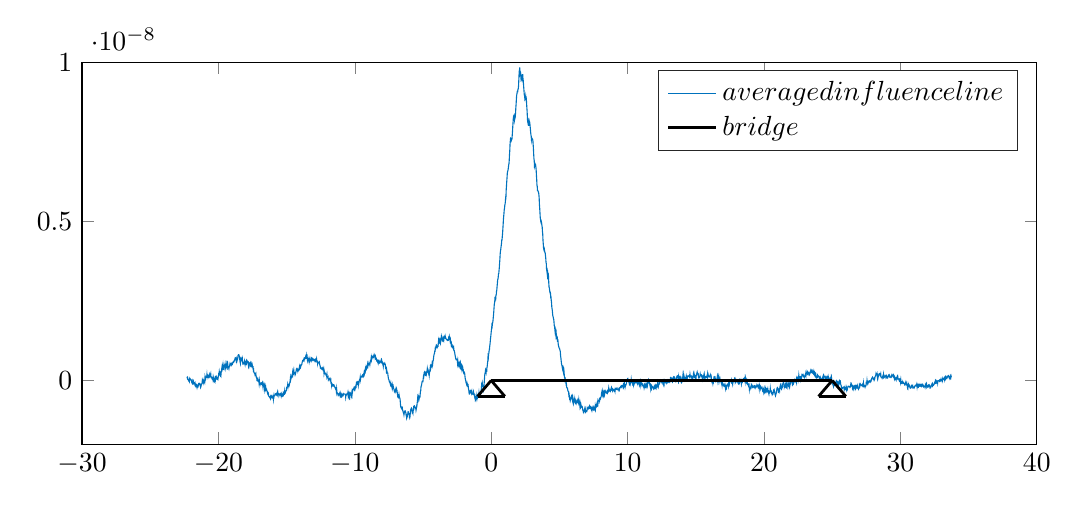
\begin{tikzpicture}

\begin{axis}[%
width=\textwidth,
height=0.4\textwidth,
at={(0\figurewidth,0\figureheight)},
scale only axis,
xmin=-30,
xmax=40,
ymin=-2e-09,
ymax=1e-08,
axis background/.style={fill=white},
% title style={font=\bfseries},
% title={},
legend style={legend cell align=left,align=left,draw=white!15!black}
]
\addplot [color=mycolor1,solid]
  table[row sep=crcr]{%
-22.3159404296875	1.18323540657329e-10\\
-22.295791015625	1.09487790669497e-10\\
-22.2756416015625	7.01083695561926e-11\\
-22.2554921875	8.73967831327927e-11\\
-22.2353427734375	4.57279390021045e-11\\
-22.215193359375	3.49387202965769e-11\\
-22.1950439453125	-9.44935511256185e-12\\
-22.17489453125	-4.62447348668263e-12\\
-22.1547451171875	-2.87372614426872e-12\\
-22.134595703125	-2.9184434031337e-11\\
-22.1144462890625	5.2853846840941e-11\\
-22.094296875	3.42700471708031e-11\\
-22.0741474609375	5.26376478942855e-11\\
-22.053998046875	3.78334420422553e-11\\
-22.0338486328125	1.34463101627698e-11\\
-22.01369921875	1.307063002344e-11\\
-21.9935498046875	1.54405574351222e-11\\
-21.973400390625	-3.06588111607537e-11\\
-21.9532509765625	-6.69160227287835e-11\\
-21.9331015625	-8.30366837403097e-11\\
-21.9129521484375	-3.58436969547546e-11\\
-21.892802734375	-8.98057932214126e-11\\
-21.8726533203125	-7.06451510325644e-11\\
-21.85250390625	-5.07503260190867e-11\\
-21.8323544921875	-2.80847503488146e-11\\
-21.812205078125	-9.54586162294433e-11\\
-21.7920556640625	-8.48582623645359e-11\\
-21.77190625	-8.21392962825674e-11\\
-21.7517568359375	-7.53443500309883e-11\\
-21.731607421875	-1.19190434756364e-10\\
-21.7114580078125	-9.28082559022149e-11\\
-21.69130859375	-1.45257369745405e-10\\
-21.6711591796875	-1.14044953723198e-10\\
-21.651009765625	-1.12440918837719e-10\\
-21.6308603515625	-1.15189705925096e-10\\
-21.6107109375	-1.83195734519052e-10\\
-21.5905615234375	-1.75703642278238e-10\\
-21.570412109375	-2.17347601822706e-10\\
-21.5502626953125	-1.7234124979925e-10\\
-21.53011328125	-1.94383457927583e-10\\
-21.5099638671875	-1.76173919683551e-10\\
-21.489814453125	-1.89207569785072e-10\\
-21.4696650390625	-1.55838460816968e-10\\
-21.449515625	-9.43827219040849e-11\\
-21.4293662109375	-9.43140933035297e-11\\
-21.409216796875	-9.01825988251552e-11\\
-21.3890673828125	-1.09140838712194e-10\\
-21.36891796875	-1.18727526471047e-10\\
-21.3487685546875	-1.46763630148943e-10\\
-21.328619140625	-1.34643594322207e-10\\
-21.3084697265625	-2.17751873636963e-10\\
-21.2883203125	-2.00358196408718e-10\\
-21.2681708984375	-1.66462048900436e-10\\
-21.248021484375	-1.22230698810312e-10\\
-21.2278720703125	-1.08103144022445e-10\\
-21.20772265625	-1.03194094594098e-10\\
-21.1875732421875	-2.67572985489041e-11\\
-21.167423828125	-7.04916547708198e-11\\
-21.1472744140625	-5.2133999721112e-11\\
-21.127125	-1.81128827031517e-13\\
-21.1069755859375	-4.20828914071255e-11\\
-21.086826171875	-7.20610611170289e-11\\
-21.0666767578125	3.89956657059595e-12\\
-21.04652734375	-3.51503749964041e-12\\
-21.0263779296875	4.66638939409171e-12\\
-21.006228515625	-3.11515453732733e-11\\
-20.9860791015625	9.10781119391464e-11\\
-20.9659296875	4.13837460046243e-11\\
-20.9457802734375	9.65335893111909e-11\\
-20.925630859375	7.00984909187122e-11\\
-20.9054814453125	1.07159933583392e-10\\
-20.88533203125	1.04107742759043e-10\\
-20.8651826171875	1.01528204719944e-10\\
-20.845033203125	1.76538512943176e-10\\
-20.8248837890625	8.20849352401305e-11\\
-20.804734375	1.73188141553962e-10\\
-20.7845849609375	1.58569674236083e-10\\
-20.764435546875	1.04047085483998e-10\\
-20.7442861328125	1.39395311712661e-10\\
-20.72413671875	1.2336366490079e-10\\
-20.7039873046875	1.09770933550793e-10\\
-20.683837890625	1.48789260360401e-10\\
-20.6636884765625	1.8363035461933e-10\\
-20.6435390625	1.35914903981168e-10\\
-20.6233896484375	1.58338640118635e-10\\
-20.603240234375	1.8230108834978e-10\\
-20.5830908203125	1.65700245389576e-10\\
-20.56294140625	2.01892654266715e-10\\
-20.5427919921875	1.03772117811136e-10\\
-20.522642578125	1.126352490028e-10\\
-20.5024931640625	1.04404565174293e-10\\
-20.48234375	7.0979560091846e-11\\
-20.4621943359375	5.19814877597947e-11\\
-20.442044921875	6.74267553876139e-11\\
-20.4218955078125	7.90049163532168e-11\\
-20.40174609375	3.28475332216119e-11\\
-20.3815966796875	1.15737035993869e-10\\
-20.361447265625	7.78790672655313e-11\\
-20.3412978515625	5.38353193543276e-11\\
-20.3211484375	9.4347119705749e-12\\
-20.3009990234375	4.06501295440194e-11\\
-20.280849609375	-3.49386305783243e-11\\
-20.2607001953125	-5.0619834195727e-11\\
-20.24055078125	1.93226991608584e-11\\
-20.2204013671875	7.12907560890803e-12\\
-20.200251953125	1.07618654362715e-10\\
-20.1801025390625	9.49682389388561e-11\\
-20.159953125	1.1601513262116e-10\\
-20.1398037109375	7.81582332178352e-11\\
-20.119654296875	4.65380016568453e-11\\
-20.0995048828125	3.92752454306966e-11\\
-20.07935546875	6.662708865594e-11\\
-20.0592060546875	4.61146077583585e-11\\
-20.039056640625	3.41628380493773e-11\\
-20.0189072265625	9.26934831085441e-11\\
-19.9987578125	1.38481458563547e-10\\
-19.9786083984375	2.09666201735121e-10\\
-19.958458984375	2.00616762065816e-10\\
-19.9383095703125	2.78176606939186e-10\\
-19.91816015625	2.29508102606363e-10\\
-19.8980107421875	2.09103000941712e-10\\
-19.877861328125	1.78367604926966e-10\\
-19.8577119140625	2.25491415358066e-10\\
-19.8375625	1.92778691127656e-10\\
-19.8174130859375	1.6119747496344e-10\\
-19.797263671875	2.581095666285e-10\\
-19.7771142578125	2.73209916628327e-10\\
-19.75696484375	3.63430002068034e-10\\
-19.7368154296875	4.24269052795325e-10\\
-19.716666015625	3.79205586299539e-10\\
-19.6965166015625	4.36633472134869e-10\\
-19.6763671875	4.88598711219513e-10\\
-19.6562177734375	3.30394553991595e-10\\
-19.636068359375	4.55665096689067e-10\\
-19.6159189453125	4.41541373418461e-10\\
-19.59576953125	3.99998706831409e-10\\
-19.5756201171875	4.63735678960122e-10\\
-19.555470703125	4.4478007654707e-10\\
-19.5353212890625	4.43938872287813e-10\\
-19.515171875	4.98683258476812e-10\\
-19.4950224609375	4.00495361026772e-10\\
-19.474873046875	4.5400260119464e-10\\
-19.4547236328125	4.092996135541e-10\\
-19.43457421875	4.3144188258118e-10\\
-19.4144248046875	4.31193248673038e-10\\
-19.394275390625	5.03899070023969e-10\\
-19.3741259765625	4.43804733841982e-10\\
-19.3539765625	5.02690349921809e-10\\
-19.3338271484375	4.45583122834982e-10\\
-19.313677734375	4.99575560355244e-10\\
-19.2935283203125	4.25707492322739e-10\\
-19.27337890625	4.13024416349873e-10\\
-19.2532294921875	3.98503440413278e-10\\
-19.233080078125	3.69802281990902e-10\\
-19.2129306640625	4.31670108930708e-10\\
-19.19278125	4.37047901352481e-10\\
-19.1726318359375	4.78288397297578e-10\\
-19.152482421875	5.23977248945561e-10\\
-19.1323330078125	4.92847705522926e-10\\
-19.11218359375	5.20202356571052e-10\\
-19.0920341796875	5.06002690608107e-10\\
-19.071884765625	4.96747150243505e-10\\
-19.0517353515625	5.17830595550962e-10\\
-19.0315859375	4.85972460603039e-10\\
-19.0114365234375	5.06183612942751e-10\\
-18.991287109375	5.31418426425977e-10\\
-18.9711376953125	5.21767175402451e-10\\
-18.95098828125	5.61899849376718e-10\\
-18.9308388671875	5.78254193999055e-10\\
-18.910689453125	5.72847639174557e-10\\
-18.8905400390625	5.93345087330096e-10\\
-18.870390625	5.83326984294873e-10\\
-18.8502412109375	5.97403835656252e-10\\
-18.830091796875	6.32893093209181e-10\\
-18.8099423828125	6.35815330300154e-10\\
-18.78979296875	6.83175487350812e-10\\
-18.7696435546875	7.09003517641796e-10\\
-18.749494140625	6.99276072356553e-10\\
-18.7293447265625	6.94250669904722e-10\\
-18.7091953125	6.45716492101065e-10\\
-18.6890458984375	6.8900141493312e-10\\
-18.668896484375	6.57547668987923e-10\\
-18.6487470703125	5.95413894283882e-10\\
-18.62859765625	6.30214980855788e-10\\
-18.6084482421875	6.88095016896453e-10\\
-18.588298828125	6.84129730675203e-10\\
-18.5681494140625	7.80592619919039e-10\\
-18.548	7.94387196448797e-10\\
-18.5278505859375	8.08883296859899e-10\\
-18.507701171875	8.0713785858396e-10\\
-18.4875517578125	7.93488139428402e-10\\
-18.46740234375	7.55010538618538e-10\\
-18.4472529296875	7.06059081650203e-10\\
-18.427103515625	6.22845710681703e-10\\
-18.4069541015625	5.76818981210764e-10\\
-18.3868046875	5.3854169521943e-10\\
-18.3666552734375	6.48913353162417e-10\\
-18.346505859375	6.13402277306567e-10\\
-18.3263564453125	6.3807389947339e-10\\
-18.30620703125	6.74886874549309e-10\\
-18.2860576171875	6.40016768056518e-10\\
-18.265908203125	6.34370851496262e-10\\
-18.2457587890625	6.76082092638564e-10\\
-18.225609375	5.72138142151933e-10\\
-18.2054599609375	5.12717785149444e-10\\
-18.185310546875	5.14450376685857e-10\\
-18.1651611328125	5.2521273378675e-10\\
-18.14501171875	5.509836658907e-10\\
-18.1248623046875	5.39396736498327e-10\\
-18.104712890625	5.3000408883055e-10\\
-18.0845634765625	5.99744147664559e-10\\
-18.0644140625	5.49750413299126e-10\\
-18.0442646484375	5.03818901047238e-10\\
-18.024115234375	5.63090491732583e-10\\
-18.0039658203125	5.36494912843416e-10\\
-17.98381640625	5.22610724759753e-10\\
-17.9636669921875	5.64171644191501e-10\\
-17.943517578125	6.03569912869189e-10\\
-17.9233681640625	5.64549416376051e-10\\
-17.90321875	6.2370114876922e-10\\
-17.8830693359375	6.06175374224227e-10\\
-17.862919921875	5.84332310724316e-10\\
-17.8427705078125	5.88548804854354e-10\\
-17.82262109375	5.81983035825145e-10\\
-17.8024716796875	4.95146569673785e-10\\
-17.782322265625	5.62739380898561e-10\\
-17.7621728515625	5.48363936114207e-10\\
-17.7420234375	4.71028510419464e-10\\
-17.7218740234375	5.1544243640287e-10\\
-17.701724609375	5.39187140924038e-10\\
-17.6815751953125	5.26364563381349e-10\\
-17.66142578125	4.9386123615434e-10\\
-17.6412763671875	5.39398441815961e-10\\
-17.621126953125	5.01521358793121e-10\\
-17.6009775390625	4.63909047681283e-10\\
-17.580828125	5.06004732108818e-10\\
-17.5606787109375	4.49623816459208e-10\\
-17.540529296875	4.41500257773379e-10\\
-17.5203798828125	4.8927585218793e-10\\
-17.50023046875	4.49035435662402e-10\\
-17.4800810546875	4.05798092904653e-10\\
-17.459931640625	4.14476261022211e-10\\
-17.4397822265625	3.20405194311378e-10\\
-17.4196328125	3.33796279117191e-10\\
-17.3994833984375	2.51685067595404e-10\\
-17.379333984375	2.47406113825099e-10\\
-17.3591845703125	2.25328688542963e-10\\
-17.33903515625	2.22620199792101e-10\\
-17.3188857421875	1.81412445706089e-10\\
-17.298736328125	2.01718944710845e-10\\
-17.2785869140625	2.18443636639e-10\\
-17.2584375	2.29187290749758e-10\\
-17.2382880859375	1.12310043256121e-10\\
-17.218138671875	1.14725420065735e-10\\
-17.1979892578125	1.10162817276963e-10\\
-17.17783984375	1.59180032956571e-11\\
-17.1576904296875	2.31855510347112e-11\\
-17.137541015625	-1.18144565911932e-11\\
-17.1173916015625	-5.41052823334912e-12\\
-17.0972421875	3.03108207438521e-11\\
-17.0770927734375	-9.28268584341247e-12\\
-17.056943359375	-2.54234836638978e-11\\
-17.0367939453125	-2.48609720147611e-11\\
-17.01664453125	-1.00120859870084e-10\\
-16.9964951171875	-2.08653974232505e-11\\
-16.976345703125	-1.10015060264329e-10\\
-16.9561962890625	-9.02493760192832e-11\\
-16.936046875	-1.07492534299557e-10\\
-16.9158974609375	-1.01161024473037e-10\\
-16.895748046875	-1.26783543133757e-10\\
-16.8755986328125	-7.51415113612875e-11\\
-16.85544921875	-7.22241518512012e-11\\
-16.8352998046875	-8.58028112156076e-11\\
-16.815150390625	-1.04048220289193e-10\\
-16.7950009765625	-9.32151422458533e-11\\
-16.7748515625	-7.12876998848784e-11\\
-16.7547021484375	-1.39658985022639e-10\\
-16.734552734375	-2.02719712785966e-10\\
-16.7144033203125	-9.81097026633099e-11\\
-16.69425390625	-1.2644443931879e-10\\
-16.6741044921875	-1.75790878754161e-10\\
-16.653955078125	-1.87874377373733e-10\\
-16.6338056640625	-1.53528676041705e-10\\
-16.61365625	-2.62610153374383e-10\\
-16.5935068359375	-1.96094929764687e-10\\
-16.573357421875	-2.2776354469121e-10\\
-16.5532080078125	-2.69865297208068e-10\\
-16.53305859375	-2.09832019329781e-10\\
-16.5129091796875	-2.81399322439395e-10\\
-16.492759765625	-2.61396291455264e-10\\
-16.4726103515625	-2.68481681726185e-10\\
-16.4524609375	-3.15156719638212e-10\\
-16.4323115234375	-3.39302144894548e-10\\
-16.412162109375	-3.70723518899141e-10\\
-16.3920126953125	-4.05832180989458e-10\\
-16.37186328125	-3.72598919538238e-10\\
-16.3517138671875	-3.86598494285663e-10\\
-16.331564453125	-4.2915161607803e-10\\
-16.3114150390625	-4.9101497646749e-10\\
-16.291265625	-5.00347656742876e-10\\
-16.2711162109375	-5.04649145953616e-10\\
-16.250966796875	-5.28171752723671e-10\\
-16.2308173828125	-5.37998584399146e-10\\
-16.21066796875	-5.22297501792218e-10\\
-16.1905185546875	-5.57087518401707e-10\\
-16.170369140625	-5.10451572024836e-10\\
-16.1502197265625	-5.39595870487183e-10\\
-16.1300703125	-5.0563535064532e-10\\
-16.1099208984375	-5.37596827651145e-10\\
-16.089771484375	-5.36239977231557e-10\\
-16.0696220703125	-5.03979849884165e-10\\
-16.04947265625	-5.17584043699106e-10\\
-16.0293232421875	-5.50033207659897e-10\\
-16.009173828125	-5.4898065291124e-10\\
-15.9890244140625	-5.00874296108708e-10\\
-15.968875	-5.87663515441973e-10\\
-15.9487255859375	-5.03525403731068e-10\\
-15.928576171875	-5.21931236653185e-10\\
-15.9084267578125	-4.74974928466686e-10\\
-15.88827734375	-4.6628869735908e-10\\
-15.8681279296875	-4.70642089962489e-10\\
-15.847978515625	-4.30670126847013e-10\\
-15.8278291015625	-4.4771871457564e-10\\
-15.8076796875	-4.40818587065826e-10\\
-15.7875302734375	-4.23744848804827e-10\\
-15.767380859375	-4.29864966470094e-10\\
-15.7472314453125	-4.467694369435e-10\\
-15.72708203125	-4.1100814938825e-10\\
-15.7069326171875	-4.20715460817679e-10\\
-15.686783203125	-3.86966628234265e-10\\
-15.6666337890625	-4.30411700594156e-10\\
-15.646484375	-3.74896131937017e-10\\
-15.6263349609375	-4.29270029121687e-10\\
-15.606185546875	-4.40569761648871e-10\\
-15.5860361328125	-4.29654996867959e-10\\
-15.56588671875	-4.79899190682938e-10\\
-15.5457373046875	-4.46791397209016e-10\\
-15.525587890625	-4.31688322003247e-10\\
-15.5054384765625	-4.42562212668356e-10\\
-15.4852890625	-4.54124754257212e-10\\
-15.4651396484375	-4.59341991540457e-10\\
-15.444990234375	-4.27370472015298e-10\\
-15.4248408203125	-4.50251060212478e-10\\
-15.40469140625	-4.89289034901478e-10\\
-15.3845419921875	-4.4235602609468e-10\\
-15.364392578125	-4.92182892605427e-10\\
-15.3442431640625	-5.06019965393265e-10\\
-15.32409375	-5.06466863936027e-10\\
-15.3039443359375	-4.59994730378801e-10\\
-15.283794921875	-4.85355778711837e-10\\
-15.2636455078125	-4.7923116553749e-10\\
-15.24349609375	-4.06131439440961e-10\\
-15.2233466796875	-4.32729604477277e-10\\
-15.203197265625	-3.73299376763803e-10\\
-15.1830478515625	-3.77519096150226e-10\\
-15.1628984375	-4.52967888260601e-10\\
-15.1427490234375	-3.47551145774232e-10\\
-15.122599609375	-4.1140182572535e-10\\
-15.1024501953125	-3.97924709657251e-10\\
-15.08230078125	-3.39777332877305e-10\\
-15.0621513671875	-3.46616659025343e-10\\
-15.042001953125	-3.23473578499235e-10\\
-15.0218525390625	-3.17269264620451e-10\\
-15.001703125	-2.30693380493998e-10\\
-14.9815537109375	-2.1253771759966e-10\\
-14.961404296875	-2.10606635810842e-10\\
-14.9412548828125	-1.91256479653129e-10\\
-14.92110546875	-1.31105259728396e-10\\
-14.9009560546875	-1.90860794109007e-10\\
-14.880806640625	-1.23017998346425e-10\\
-14.8606572265625	-1.228231865079e-10\\
-14.8405078125	-1.37080713461157e-10\\
-14.8203583984375	-1.6945555039362e-10\\
-14.800208984375	-1.40143736003728e-10\\
-14.7800595703125	-8.16273146737291e-11\\
-14.75991015625	-6.65792776472098e-11\\
-14.7397607421875	-2.85852147187294e-12\\
-14.719611328125	8.43209873203147e-11\\
-14.6994619140625	2.39952814309051e-11\\
-14.6793125	6.55941404342348e-11\\
-14.6591630859375	7.7320191774882e-11\\
-14.639013671875	1.15538697946298e-10\\
-14.6188642578125	1.49384601814978e-10\\
-14.59871484375	1.19706111250055e-10\\
-14.5785654296875	1.41186815441085e-10\\
-14.558416015625	2.43308680193648e-10\\
-14.5382666015625	1.86961445109901e-10\\
-14.5181171875	2.36775937865908e-10\\
-14.4979677734375	2.8250034062516e-10\\
-14.477818359375	3.27771499450643e-10\\
-14.4576689453125	2.37062639402958e-10\\
-14.43751953125	2.55201471919714e-10\\
-14.4173701171875	2.4219548529285e-10\\
-14.397220703125	2.21898247544592e-10\\
-14.3770712890625	1.74047964844962e-10\\
-14.356921875	1.95794422698979e-10\\
-14.3367724609375	2.55454462534736e-10\\
-14.316623046875	2.63556818096888e-10\\
-14.2964736328125	3.23468154224683e-10\\
-14.27632421875	3.61194540645432e-10\\
-14.2561748046875	3.48312351146901e-10\\
-14.236025390625	3.54003559535891e-10\\
-14.2158759765625	3.27800326748121e-10\\
-14.1957265625	3.47141758165142e-10\\
-14.1755771484375	2.96582878324428e-10\\
-14.155427734375	3.30364055334366e-10\\
-14.1352783203125	3.12170337442841e-10\\
-14.11512890625	3.25768915517136e-10\\
-14.0949794921875	3.51198508325658e-10\\
-14.074830078125	3.88558132959676e-10\\
-14.0546806640625	4.35506510053479e-10\\
-14.03453125	3.83018583127715e-10\\
-14.0143818359375	4.11534413944985e-10\\
-13.994232421875	4.48187671408351e-10\\
-13.9740830078125	4.20367290643051e-10\\
-13.95393359375	4.58328737495678e-10\\
-13.9337841796875	4.83217540978693e-10\\
-13.913634765625	4.89870160347884e-10\\
-13.8934853515625	4.95847058968979e-10\\
-13.8733359375	5.44278312251323e-10\\
-13.8531865234375	5.75006341075002e-10\\
-13.833037109375	6.09616553833601e-10\\
-13.8128876953125	6.01025339666745e-10\\
-13.79273828125	6.03756783224576e-10\\
-13.7725888671875	6.45750306662405e-10\\
-13.752439453125	6.51073898853069e-10\\
-13.7322900390625	6.77761529646038e-10\\
-13.712140625	6.47848722583023e-10\\
-13.6919912109375	6.95996889625649e-10\\
-13.671841796875	7.07172581581994e-10\\
-13.6516923828125	6.83913837961883e-10\\
-13.63154296875	6.96579724776455e-10\\
-13.6113935546875	7.36144603764507e-10\\
-13.591244140625	7.00865268855787e-10\\
-13.5710947265625	6.98379815332607e-10\\
-13.5509453125	7.75427970364013e-10\\
-13.5307958984375	7.07269732548324e-10\\
-13.510646484375	6.94137513045917e-10\\
-13.4904970703125	7.30235062817101e-10\\
-13.47034765625	6.36159418022359e-10\\
-13.4501982421875	6.77698180262492e-10\\
-13.430048828125	6.84822550879866e-10\\
-13.4098994140625	6.81751638280592e-10\\
-13.38975	6.40055270186366e-10\\
-13.3696005859375	6.77821782128693e-10\\
-13.349451171875	6.10989744445531e-10\\
-13.3293017578125	6.80364101338222e-10\\
-13.30915234375	6.54216099308348e-10\\
-13.2890029296875	6.16084085420963e-10\\
-13.268853515625	6.44748236310808e-10\\
-13.2487041015625	6.37868749607442e-10\\
-13.2285546875	6.29862281678049e-10\\
-13.2084052734375	6.91063873732044e-10\\
-13.188255859375	6.72967958347801e-10\\
-13.1681064453125	6.91564829184758e-10\\
-13.14795703125	6.36398809809815e-10\\
-13.1278076171875	6.66294194227218e-10\\
-13.107658203125	6.78505001082515e-10\\
-13.0875087890625	6.39599874425954e-10\\
-13.067359375	6.36544570316022e-10\\
-13.0472099609375	6.41738281581759e-10\\
-13.027060546875	6.6794966461587e-10\\
-13.0069111328125	6.6094910272859e-10\\
-12.98676171875	6.21773717724372e-10\\
-12.9666123046875	6.23555586048705e-10\\
-12.946462890625	6.22453916669738e-10\\
-12.9263134765625	6.04839173759063e-10\\
-12.9061640625	6.64787624815009e-10\\
-12.8860146484375	6.76852064963647e-10\\
-12.865865234375	6.76021720508768e-10\\
-12.8457158203125	6.30742397355835e-10\\
-12.82556640625	6.46168359690275e-10\\
-12.8054169921875	6.8159319315496e-10\\
-12.785267578125	6.04785275533193e-10\\
-12.7651181640625	6.16065305804653e-10\\
-12.74496875	6.04164230961108e-10\\
-12.7248193359375	5.20647918341363e-10\\
-12.704669921875	5.63237853408531e-10\\
-12.6845205078125	5.68809930685197e-10\\
-12.66437109375	5.70416609880237e-10\\
-12.6442216796875	5.75494965420783e-10\\
-12.624072265625	5.59544898631123e-10\\
-12.6039228515625	5.75856000045029e-10\\
-12.5837734375	5.25251126056529e-10\\
-12.5636240234375	4.78168372881736e-10\\
-12.543474609375	4.64450660191066e-10\\
-12.5233251953125	3.96041182796665e-10\\
-12.50317578125	4.07775564675463e-10\\
-12.4830263671875	3.86299050028971e-10\\
-12.462876953125	3.79973539748611e-10\\
-12.4427275390625	3.67319848800089e-10\\
-12.422578125	3.57235154449822e-10\\
-12.4024287109375	3.87586124860927e-10\\
-12.382279296875	4.03187334935772e-10\\
-12.3621298828125	3.93998272450586e-10\\
-12.34198046875	3.93829115719213e-10\\
-12.3218310546875	3.03492608787986e-10\\
-12.301681640625	2.98823945157681e-10\\
-12.2815322265625	3.44807721473518e-10\\
-12.2613828125	2.37805352566592e-10\\
-12.2412333984375	3.03209272309484e-10\\
-12.221083984375	2.65468235702749e-10\\
-12.2009345703125	2.54147032001331e-10\\
-12.18078515625	2.14677684144092e-10\\
-12.1606357421875	2.17658309851459e-10\\
-12.140486328125	2.17391562351731e-10\\
-12.1203369140625	1.73750289769389e-10\\
-12.1001875	1.76304049042384e-10\\
-12.0800380859375	1.7701456323359e-10\\
-12.059888671875	1.25276922386803e-10\\
-12.0397392578125	1.80082138894423e-10\\
-12.01958984375	9.06354349983869e-11\\
-11.9994404296875	8.74456705428629e-11\\
-11.979291015625	7.85249318306784e-11\\
-11.9591416015625	9.94835830521334e-11\\
-11.9389921875	2.02728881837412e-11\\
-11.9188427734375	3.94682063379378e-11\\
-11.898693359375	3.66551358078093e-11\\
-11.8785439453125	4.12467306696329e-11\\
-11.85839453125	5.46072026703175e-11\\
-11.8382451171875	2.70055617381072e-11\\
-11.818095703125	4.62308315756518e-11\\
-11.7979462890625	-1.92932086891242e-11\\
-11.777796875	-1.90702948749266e-11\\
-11.7576474609375	2.57245615066464e-12\\
-11.737498046875	-1.17888143908308e-10\\
-11.7173486328125	-4.59881739831752e-11\\
-11.69719921875	-1.58122184162252e-10\\
-11.6770498046875	-1.13211721799127e-10\\
-11.656900390625	-1.2614068987445e-10\\
-11.6367509765625	-1.51228126987449e-10\\
-11.6166015625	-1.25974406586669e-10\\
-11.5964521484375	-1.37579515437415e-10\\
-11.576302734375	-1.55992041203716e-10\\
-11.5561533203125	-1.35917070811476e-10\\
-11.53600390625	-1.35183094790113e-10\\
-11.5158544921875	-1.53806989387244e-10\\
-11.495705078125	-1.92432955535196e-10\\
-11.4755556640625	-2.05634396091774e-10\\
-11.45540625	-2.09728233915262e-10\\
-11.4352568359375	-2.40329220735347e-10\\
-11.415107421875	-2.60685048308736e-10\\
-11.3949580078125	-2.46319028560977e-10\\
-11.37480859375	-2.62865143954421e-10\\
-11.3546591796875	-3.45517284835754e-10\\
-11.334509765625	-2.65904750075973e-10\\
-11.3143603515625	-3.58203185169563e-10\\
-11.2942109375	-3.93264600557493e-10\\
-11.2740615234375	-3.97565040681978e-10\\
-11.253912109375	-4.15264934343262e-10\\
-11.2337626953125	-4.45438459388112e-10\\
-11.21361328125	-4.19135388532157e-10\\
-11.1934638671875	-4.26695442591353e-10\\
-11.173314453125	-4.52587947848088e-10\\
-11.1531650390625	-4.25108408605349e-10\\
-11.133015625	-4.11531293158076e-10\\
-11.1128662109375	-4.04833585385693e-10\\
-11.092716796875	-3.83633699002071e-10\\
-11.0725673828125	-4.64440982529345e-10\\
-11.05241796875	-4.31969370856032e-10\\
-11.0322685546875	-4.84191833135188e-10\\
-11.012119140625	-4.64684005094033e-10\\
-10.9919697265625	-4.8973237437522e-10\\
-10.9718203125	-4.50571831722043e-10\\
-10.9516708984375	-4.80329686723876e-10\\
-10.931521484375	-4.36218631994739e-10\\
-10.9113720703125	-4.51828418379245e-10\\
-10.89122265625	-4.88111602831254e-10\\
-10.8710732421875	-4.87833973785066e-10\\
-10.850923828125	-4.37298062240256e-10\\
-10.8307744140625	-4.41401454278116e-10\\
-10.810625	-4.12388409067036e-10\\
-10.7904755859375	-4.2117357610629e-10\\
-10.770326171875	-4.28460041787811e-10\\
-10.7501767578125	-4.27724740320275e-10\\
-10.73002734375	-4.30878314203204e-10\\
-10.7098779296875	-4.29949613759997e-10\\
-10.689728515625	-4.33476024624567e-10\\
-10.6695791015625	-5.21242473502997e-10\\
-10.6494296875	-4.60375466159637e-10\\
-10.6292802734375	-4.64605788097246e-10\\
-10.609130859375	-4.57475032299496e-10\\
-10.5889814453125	-4.30768801360727e-10\\
-10.56883203125	-4.09014804104663e-10\\
-10.5486826171875	-4.09549137738124e-10\\
-10.528533203125	-4.20078707024506e-10\\
-10.5083837890625	-3.79166200753976e-10\\
-10.488234375	-4.64405298371821e-10\\
-10.4680849609375	-3.96374971121009e-10\\
-10.447935546875	-5.44107076114348e-10\\
-10.4277861328125	-4.58915464820656e-10\\
-10.40763671875	-5.11354341840949e-10\\
-10.3874873046875	-4.63614053705121e-10\\
-10.367337890625	-5.09263822343452e-10\\
-10.3471884765625	-4.27451874237408e-10\\
-10.3270390625	-4.6331969894893e-10\\
-10.3068896484375	-4.59132659845623e-10\\
-10.286740234375	-4.17582062198366e-10\\
-10.2665908203125	-4.33595271680521e-10\\
-10.24644140625	-4.78617227922645e-10\\
-10.2262919921875	-4.06879237821267e-10\\
-10.206142578125	-4.49233673586905e-10\\
-10.1859931640625	-3.27052620911804e-10\\
-10.16584375	-3.50741330053149e-10\\
-10.1456943359375	-3.02176156817997e-10\\
-10.125544921875	-2.77676250975081e-10\\
-10.1053955078125	-2.60662437516443e-10\\
-10.08524609375	-2.69794477324036e-10\\
-10.0650966796875	-2.41282823380929e-10\\
-10.044947265625	-2.7139780560827e-10\\
-10.0247978515625	-2.90728148063375e-10\\
-10.0046484375	-2.43807556418498e-10\\
-9.9844990234375	-2.7380983083283e-10\\
-9.964349609375	-2.38694439218308e-10\\
-9.9442001953125	-1.98888435049799e-10\\
-9.92405078125	-1.64769959773306e-10\\
-9.9039013671875	-1.82339657183811e-10\\
-9.883751953125	-5.92058912938879e-11\\
-9.8636025390625	-5.78464314717711e-11\\
-9.843453125	-4.43313729018737e-11\\
-9.8233037109375	-7.67509591449438e-11\\
-9.803154296875	-4.27117542948063e-11\\
-9.7830048828125	-4.73677185759184e-11\\
-9.76285546875	-6.8767022719016e-11\\
-9.7427060546875	-1.42477547460211e-10\\
-9.722556640625	-7.22555032715633e-11\\
-9.7024072265625	-8.98773930134108e-11\\
-9.6822578125	-3.8089190991977e-11\\
-9.6621083984375	1.80611787005693e-11\\
-9.641958984375	3.37890587184427e-11\\
-9.6218095703125	4.94841772410675e-11\\
-9.60166015625	1.07599612775921e-10\\
-9.5815107421875	3.75091794291389e-11\\
-9.561361328125	1.01437338509264e-10\\
-9.5412119140625	1.10044392828384e-10\\
-9.5210625	1.09764933711535e-10\\
-9.5009130859375	1.1686449934994e-10\\
-9.480763671875	1.3790160001021e-10\\
-9.4606142578125	1.31259161560803e-10\\
-9.44046484375	1.5478970326387e-10\\
-9.4203154296875	1.30931852599498e-10\\
-9.400166015625	1.56757156237503e-10\\
-9.3800166015625	1.77895439384659e-10\\
-9.3598671875	1.41076810686896e-10\\
-9.3397177734375	1.73269660237162e-10\\
-9.319568359375	2.37094590696347e-10\\
-9.2994189453125	1.99247861628984e-10\\
-9.27926953125	2.45786275934181e-10\\
-9.2591201171875	3.08608976839674e-10\\
-9.238970703125	3.49063148776911e-10\\
-9.2188212890625	2.94735356132135e-10\\
-9.198671875	3.3009142063202e-10\\
-9.1785224609375	3.96156266568283e-10\\
-9.158373046875	3.45764754251262e-10\\
-9.1382236328125	3.6347227211694e-10\\
-9.11807421875	3.9958788283896e-10\\
-9.0979248046875	4.47286578072074e-10\\
-9.077775390625	4.32129453477142e-10\\
-9.0576259765625	5.10410242889381e-10\\
-9.0374765625	4.6586255073932e-10\\
-9.0173271484375	5.26872503159217e-10\\
-8.997177734375	4.84649394242161e-10\\
-8.9770283203125	4.91019511001081e-10\\
-8.95687890625	4.95807741519448e-10\\
-8.9367294921875	5.19854036530209e-10\\
-8.916580078125	5.40486656552806e-10\\
-8.8964306640625	5.00551702942566e-10\\
-8.87628125	5.61706857291668e-10\\
-8.8561318359375	6.09953831425201e-10\\
-8.835982421875	6.0441063995632e-10\\
-8.8158330078125	6.51884851683866e-10\\
-8.79568359375	7.21652708356824e-10\\
-8.7755341796875	6.62986921639836e-10\\
-8.755384765625	7.25398622834104e-10\\
-8.7352353515625	7.48412880500773e-10\\
-8.7150859375	7.19370820378894e-10\\
-8.6949365234375	7.41332464949462e-10\\
-8.674787109375	7.40709143448423e-10\\
-8.6546376953125	7.35199158373385e-10\\
-8.63448828125	7.59985221644635e-10\\
-8.6143388671875	7.80377509316062e-10\\
-8.594189453125	7.38703464025336e-10\\
-8.5740400390625	8.04543138220062e-10\\
-8.553890625	7.81308881842062e-10\\
-8.5337412109375	7.64680097478794e-10\\
-8.513591796875	7.69157756971437e-10\\
-8.4934423828125	7.79454157008711e-10\\
-8.47329296875	6.86566515719923e-10\\
-8.4531435546875	6.97756132202357e-10\\
-8.432994140625	7.00483874661483e-10\\
-8.4128447265625	6.62901970552975e-10\\
-8.3926953125	6.2277045531349e-10\\
-8.3725458984375	6.34439003459556e-10\\
-8.352396484375	6.0722883013331e-10\\
-8.3322470703125	5.82197359854423e-10\\
-8.31209765625	5.65298728405131e-10\\
-8.2919482421875	6.55909536206997e-10\\
-8.271798828125	5.53831299532986e-10\\
-8.2516494140625	5.86150624569544e-10\\
-8.2315	6.06012462509047e-10\\
-8.2113505859375	5.58898286154176e-10\\
-8.191201171875	5.49372831414791e-10\\
-8.1710517578125	5.60704560568482e-10\\
-8.15090234375	5.85009698976445e-10\\
-8.1307529296875	5.6924824939674e-10\\
-8.110603515625	5.81727568905371e-10\\
-8.0904541015625	6.0053571958281e-10\\
-8.0703046875	6.32506108305451e-10\\
-8.0501552734375	5.95302161334883e-10\\
-8.030005859375	6.30031903892549e-10\\
-8.0098564453125	5.82444263880856e-10\\
-7.98970703125	5.8514521120244e-10\\
-7.9695576171875	5.42931556730054e-10\\
-7.949408203125	5.10569052877153e-10\\
-7.9292587890625	5.24950359636071e-10\\
-7.909109375	4.45379010956985e-10\\
-7.8889599609375	4.99739964345504e-10\\
-7.868810546875	5.05555152468888e-10\\
-7.8486611328125	5.27739434214257e-10\\
-7.82851171875	5.244001328826e-10\\
-7.8083623046875	5.41630491786816e-10\\
-7.788212890625	5.09122325998255e-10\\
-7.7680634765625	5.06316012206596e-10\\
-7.7479140625	4.16202630161212e-10\\
-7.7277646484375	4.30733390866618e-10\\
-7.707615234375	4.05978848315222e-10\\
-7.6874658203125	3.05590241385007e-10\\
-7.66731640625	3.44495426935175e-10\\
-7.6471669921875	2.97715094569996e-10\\
-7.627017578125	2.36947389849105e-10\\
-7.6068681640625	2.38177060222872e-10\\
-7.58671875	2.34118085288773e-10\\
-7.5665693359375	1.47174216951561e-10\\
-7.546419921875	9.03279119145279e-11\\
-7.5262705078125	3.76150339543541e-11\\
-7.50612109375	3.0657527124881e-11\\
-7.4859716796875	1.67326973041192e-12\\
-7.465822265625	-4.58946579391734e-11\\
-7.4456728515625	-5.1911019209031e-11\\
-7.4255234375	-6.6605160039476e-11\\
-7.4053740234375	-1.05453198929263e-10\\
-7.385224609375	-1.34180436729637e-10\\
-7.3650751953125	-9.13475449614749e-11\\
-7.34492578125	-1.79700317285273e-10\\
-7.3247763671875	-1.88480521451207e-10\\
-7.304626953125	-1.56215441702392e-10\\
-7.2844775390625	-1.95758955424075e-10\\
-7.264328125	-2.39924182371534e-10\\
-7.2441787109375	-1.69294314075039e-10\\
-7.224029296875	-2.41466799717049e-10\\
-7.2038798828125	-2.16452585744202e-10\\
-7.18373046875	-1.8446240865963e-10\\
-7.1635810546875	-2.31632413585857e-10\\
-7.143431640625	-2.65437424330157e-10\\
-7.1232822265625	-2.73017876229221e-10\\
-7.1031328125	-3.29530798316215e-10\\
-7.0829833984375	-3.13469027496193e-10\\
-7.062833984375	-3.29962410040086e-10\\
-7.0426845703125	-3.66137359558679e-10\\
-7.02253515625	-3.38091769974804e-10\\
-7.0023857421875	-2.83264901336168e-10\\
-6.982236328125	-2.96387801423436e-10\\
-6.9620869140625	-2.36980757215276e-10\\
-6.9419375	-2.59396944309149e-10\\
-6.9217880859375	-3.46316861175679e-10\\
-6.901638671875	-3.35623936982882e-10\\
-6.8814892578125	-4.13170266966503e-10\\
-6.86133984375	-4.76119835565446e-10\\
-6.8411904296875	-4.46590769564921e-10\\
-6.821041015625	-4.53332614202262e-10\\
-6.8008916015625	-5.17180595797128e-10\\
-6.7807421875	-4.94286714451218e-10\\
-6.7605927734375	-4.39460471756763e-10\\
-6.740443359375	-4.92904143436289e-10\\
-6.7202939453125	-5.43339860423938e-10\\
-6.70014453125	-5.62524074922277e-10\\
-6.6799951171875	-5.90482598699419e-10\\
-6.659845703125	-7.14849746803819e-10\\
-6.6396962890625	-8.22830623549494e-10\\
-6.619546875	-8.43628383590965e-10\\
-6.5993974609375	-8.34066835331365e-10\\
-6.579248046875	-8.57391706784889e-10\\
-6.5590986328125	-8.86149356316661e-10\\
-6.53894921875	-8.68692913419376e-10\\
-6.5187998046875	-8.56683772847225e-10\\
-6.498650390625	-9.38635861856653e-10\\
-6.4785009765625	-9.48038667737703e-10\\
-6.4583515625	-9.85350243205878e-10\\
-6.4382021484375	-1.0162842118493e-09\\
-6.418052734375	-1.03582648860545e-09\\
-6.3979033203125	-1.07884846259002e-09\\
-6.37775390625	-1.02437739611007e-09\\
-6.3576044921875	-9.90902738732031e-10\\
-6.337455078125	-9.62530982906647e-10\\
-6.3173056640625	-9.53405852963619e-10\\
-6.29715625	-9.56918071491628e-10\\
-6.2770068359375	-1.00471108014343e-09\\
-6.256857421875	-1.00923772237116e-09\\
-6.2367080078125	-1.10027496665753e-09\\
-6.21655859375	-1.11154111032723e-09\\
-6.1964091796875	-1.18806074980408e-09\\
-6.176259765625	-1.16097959524789e-09\\
-6.1561103515625	-1.13714909555199e-09\\
-6.1359609375	-1.06459570208506e-09\\
-6.1158115234375	-1.05027150328078e-09\\
-6.095662109375	-9.83137951786239e-10\\
-6.0755126953125	-9.87783218950559e-10\\
-6.05536328125	-1.03651665267429e-09\\
-6.0352138671875	-1.04091589054385e-09\\
-6.015064453125	-1.08985410754556e-09\\
-5.9949150390625	-1.14876446585775e-09\\
-5.974765625	-1.11010685801481e-09\\
-5.9546162109375	-1.13073526955945e-09\\
-5.934466796875	-1.03729025036532e-09\\
-5.9143173828125	-9.5093337401561e-10\\
-5.89416796875	-9.0557282993295e-10\\
-5.8740185546875	-8.93997582462442e-10\\
-5.853869140625	-8.70805478888379e-10\\
-5.8337197265625	-8.8887659356507e-10\\
-5.8135703125	-9.34118067416558e-10\\
-5.7934208984375	-9.86422623007299e-10\\
-5.773271484375	-9.55660154301933e-10\\
-5.7531220703125	-9.59691279366573e-10\\
-5.73297265625	-1.00707899228592e-09\\
-5.7128232421875	-9.24477955561881e-10\\
-5.692673828125	-8.59038488941296e-10\\
-5.6725244140625	-8.76892573795698e-10\\
-5.652375	-8.02087283156516e-10\\
-5.6322255859375	-7.98211912376726e-10\\
-5.612076171875	-8.26630791897034e-10\\
-5.5919267578125	-8.46444292449296e-10\\
-5.57177734375	-8.51573412967189e-10\\
-5.5516279296875	-8.67261519449556e-10\\
-5.531478515625	-8.56605437265396e-10\\
-5.5113291015625	-9.33922950352722e-10\\
-5.4911796875	-8.92651605859378e-10\\
-5.4710302734375	-8.11853959211717e-10\\
-5.450880859375	-8.1609437606182e-10\\
-5.4307314453125	-7.10507953857919e-10\\
-5.41058203125	-6.67756988720912e-10\\
-5.3904326171875	-5.56087615288202e-10\\
-5.370283203125	-6.00178968295828e-10\\
-5.3501337890625	-5.12160553222326e-10\\
-5.329984375	-5.54226392399078e-10\\
-5.3098349609375	-5.31171994662125e-10\\
-5.289685546875	-5.82199541380653e-10\\
-5.2695361328125	-5.40459600298305e-10\\
-5.24938671875	-5.3452980117043e-10\\
-5.2292373046875	-5.31113818223978e-10\\
-5.209087890625	-4.44352642291685e-10\\
-5.1889384765625	-3.40551228587316e-10\\
-5.1687890625	-3.30139212995433e-10\\
-5.1486396484375	-2.03078890126465e-10\\
-5.128490234375	-1.77256504299157e-10\\
-5.1083408203125	-1.47225654021627e-10\\
-5.08819140625	-9.64115970861502e-11\\
-5.0680419921875	-3.52811916461518e-11\\
-5.047892578125	-3.77979255301951e-11\\
-5.0277431640625	-3.36293003124013e-11\\
-5.00759375	-3.61168617273849e-11\\
-4.9874443359375	4.64531698617115e-11\\
-4.967294921875	1.22694657182215e-10\\
-4.9471455078125	1.06625370067183e-10\\
-4.92699609375	1.91853482292338e-10\\
-4.9068466796875	2.56363221756729e-10\\
-4.886697265625	2.65931918810309e-10\\
-4.8665478515625	2.82466051251174e-10\\
-4.8463984375	2.74399369393327e-10\\
-4.8262490234375	1.61575857862019e-10\\
-4.806099609375	1.6329682566742e-10\\
-4.7859501953125	1.53958794970692e-10\\
-4.76580078125	2.14318311079287e-10\\
-4.7456513671875	2.00628761373691e-10\\
-4.725501953125	2.81490571725173e-10\\
-4.7053525390625	3.06370077661363e-10\\
-4.685203125	3.74589578132946e-10\\
-4.6650537109375	3.21401814891544e-10\\
-4.644904296875	3.53987442996658e-10\\
-4.6247548828125	3.35032567947093e-10\\
-4.60460546875	2.51632078445148e-10\\
-4.5844560546875	2.11198946537874e-10\\
-4.564306640625	2.27220557324919e-10\\
-4.5441572265625	1.63137678504208e-10\\
-4.5240078125	2.43806202472256e-10\\
-4.5038583984375	3.04553500737168e-10\\
-4.483708984375	3.53193462344737e-10\\
-4.4635595703125	4.26198762977116e-10\\
-4.44341015625	3.87003097497373e-10\\
-4.4232607421875	4.83533927810439e-10\\
-4.403111328125	4.86332900062007e-10\\
-4.3829619140625	4.27176650824583e-10\\
-4.3628125	4.22896986947425e-10\\
-4.3426630859375	4.99234716067893e-10\\
-4.322513671875	4.417305537757e-10\\
-4.3023642578125	4.70078941736674e-10\\
-4.28221484375	5.6645412522614e-10\\
-4.2620654296875	6.3474687620967e-10\\
-4.241916015625	6.3792558009581e-10\\
-4.2217666015625	7.40413005638898e-10\\
-4.2016171875	7.86808953117185e-10\\
-4.1814677734375	8.33254185902617e-10\\
-4.161318359375	8.41935656425383e-10\\
-4.1411689453125	9.17972005696414e-10\\
-4.12101953125	9.16542973810837e-10\\
-4.1008701171875	1.01275236488091e-09\\
-4.080720703125	9.99753174845476e-10\\
-4.0605712890625	1.04647552393879e-09\\
-4.040421875	1.08161692270086e-09\\
-4.0202724609375	1.05720108247137e-09\\
-4.000123046875	1.08416907090142e-09\\
-3.9799736328125	1.04481623152149e-09\\
-3.95982421875	1.03303056099294e-09\\
-3.9396748046875	1.0529356596279e-09\\
-3.919525390625	1.08235671191687e-09\\
-3.8993759765625	1.0791612463885e-09\\
-3.8792265625	1.16691421029354e-09\\
-3.8590771484375	1.25990847085069e-09\\
-3.838927734375	1.21244881511819e-09\\
-3.8187783203125	1.25315095650143e-09\\
-3.79862890625	1.27537667552531e-09\\
-3.7784794921875	1.17576749858801e-09\\
-3.758330078125	1.17171199005048e-09\\
-3.7381806640625	1.22917915281038e-09\\
-3.71803125	1.18159656632838e-09\\
-3.6978818359375	1.23983911851912e-09\\
-3.677732421875	1.30681432435093e-09\\
-3.6575830078125	1.37593529859039e-09\\
-3.63743359375	1.3282124714201e-09\\
-3.6172841796875	1.37084853851018e-09\\
-3.597134765625	1.34563709119858e-09\\
-3.5769853515625	1.33103483491797e-09\\
-3.5568359375	1.25373528721774e-09\\
-3.5366865234375	1.26657732993661e-09\\
-3.516537109375	1.2533286059431e-09\\
-3.4963876953125	1.3101654002239e-09\\
-3.47623828125	1.27327128785035e-09\\
-3.4560888671875	1.34359640714435e-09\\
-3.435939453125	1.38634057903491e-09\\
-3.4157900390625	1.37925531773308e-09\\
-3.395640625	1.35890890344948e-09\\
-3.3754912109375	1.39776981661867e-09\\
-3.355341796875	1.35453944108059e-09\\
-3.3351923828125	1.33783794624354e-09\\
-3.31504296875	1.31371554355106e-09\\
-3.2948935546875	1.29936560467367e-09\\
-3.274744140625	1.28835574214051e-09\\
-3.2545947265625	1.2779645592005e-09\\
-3.2344453125	1.28656798244884e-09\\
-3.2142958984375	1.26514853918557e-09\\
-3.194146484375	1.25329060970538e-09\\
-3.1739970703125	1.256738803634e-09\\
-3.15384765625	1.259230245171e-09\\
-3.1336982421875	1.27534977648587e-09\\
-3.113548828125	1.3507183209374e-09\\
-3.0933994140625	1.34037569581738e-09\\
-3.07325	1.38578905097229e-09\\
-3.0531005859375	1.33778458221633e-09\\
-3.032951171875	1.31774670745015e-09\\
-3.0128017578125	1.25150221378541e-09\\
-2.99265234375	1.28894087566072e-09\\
-2.9725029296875	1.22133139944885e-09\\
-2.952353515625	1.18211100843284e-09\\
-2.9322041015625	1.12195955652888e-09\\
-2.9120546875	1.15537123951574e-09\\
-2.8919052734375	1.09406740764663e-09\\
-2.871755859375	1.06786065880964e-09\\
-2.8516064453125	1.08583253577875e-09\\
-2.83145703125	1.04782016701467e-09\\
-2.8113076171875	1.05670614675372e-09\\
-2.791158203125	1.01238842727352e-09\\
-2.7710087890625	9.89020094995289e-10\\
-2.750859375	1.02329648728044e-09\\
-2.7307099609375	9.46505125943083e-10\\
-2.710560546875	9.33836312613637e-10\\
-2.6904111328125	8.94101205334672e-10\\
-2.67026171875	8.56532614960546e-10\\
-2.6501123046875	7.90857043045768e-10\\
-2.629962890625	7.56871322874273e-10\\
-2.6098134765625	7.06138211474189e-10\\
-2.5896640625	6.6746443870137e-10\\
-2.5695146484375	6.53277280098881e-10\\
-2.549365234375	6.66413169029172e-10\\
-2.5292158203125	6.59921350868539e-10\\
-2.50906640625	6.67589306693589e-10\\
-2.4889169921875	6.59425497795714e-10\\
-2.468767578125	5.48002522495574e-10\\
-2.4486181640625	6.16459631902043e-10\\
-2.42846875	5.31383377645358e-10\\
-2.4083193359375	4.82308793248788e-10\\
-2.388169921875	5.07057974113884e-10\\
-2.3680205078125	5.35489179254339e-10\\
-2.34787109375	4.73487531374297e-10\\
-2.3277216796875	5.20736533187403e-10\\
-2.307572265625	5.17618291126036e-10\\
-2.2874228515625	5.51174732260577e-10\\
-2.2672734375	4.63230307936504e-10\\
-2.2471240234375	5.16927106626587e-10\\
-2.226974609375	4.55503302866211e-10\\
-2.2068251953125	3.75561822006264e-10\\
-2.18667578125	3.56419344708407e-10\\
-2.1665263671875	4.18817876444193e-10\\
-2.146376953125	3.50674482576927e-10\\
-2.1262275390625	4.07625130449931e-10\\
-2.106078125	3.61727094969804e-10\\
-2.0859287109375	3.9336763978621e-10\\
-2.065779296875	3.34403560600915e-10\\
-2.0456298828125	3.32017807994582e-10\\
-2.02548046875	2.53891818941613e-10\\
-2.0053310546875	2.7457123681436e-10\\
-1.985181640625	2.69260978553279e-10\\
-1.9650322265625	2.46218218050311e-10\\
-1.9448828125	2.19120187485315e-10\\
-1.9247333984375	1.33283688472081e-10\\
-1.904583984375	6.47594639653184e-11\\
-1.8844345703125	2.03662095182359e-11\\
-1.86428515625	-1.91335641002492e-11\\
-1.8441357421875	-6.78242351481186e-11\\
-1.823986328125	-6.62577776330232e-11\\
-1.8038369140625	-1.29871948527642e-10\\
-1.7836875	-1.51047595181725e-10\\
-1.7635380859375	-9.25618476264235e-11\\
-1.743388671875	-1.25820113323345e-10\\
-1.7232392578125	-1.30786423163591e-10\\
-1.70308984375	-1.26878502963256e-10\\
-1.6829404296875	-1.95783332907474e-10\\
-1.662791015625	-2.69828593437198e-10\\
-1.6426416015625	-3.10663834050966e-10\\
-1.6224921875	-3.85773481746305e-10\\
-1.6023427734375	-3.71164986446783e-10\\
-1.582193359375	-4.16742606633551e-10\\
-1.5620439453125	-4.09079196638124e-10\\
-1.54189453125	-3.73474485410937e-10\\
-1.5217451171875	-3.20156885050244e-10\\
-1.501595703125	-3.29996313172161e-10\\
-1.4814462890625	-3.24146246799007e-10\\
-1.461296875	-3.53324624795057e-10\\
-1.4411474609375	-3.9669280683884e-10\\
-1.420998046875	-3.55338365372159e-10\\
-1.4008486328125	-4.28461032061771e-10\\
-1.38069921875	-4.25980488976066e-10\\
-1.3605498046875	-4.31189489047152e-10\\
-1.340400390625	-4.37225368285984e-10\\
-1.3202509765625	-4.10750069538133e-10\\
-1.3001015625	-3.59587863224769e-10\\
-1.2799521484375	-4.05621620276072e-10\\
-1.259802734375	-4.0832888788622e-10\\
-1.2396533203125	-4.62841549074527e-10\\
-1.21950390625	-5.00914462394041e-10\\
-1.1993544921875	-5.4929451771674e-10\\
-1.179205078125	-5.39142299468552e-10\\
-1.1590556640625	-6.2504610285357e-10\\
-1.13890625	-6.08123052784738e-10\\
-1.1187568359375	-5.22330474665141e-10\\
-1.098607421875	-5.56503846560343e-10\\
-1.0784580078125	-5.51149848304125e-10\\
-1.05830859375	-4.85004412525738e-10\\
-1.0381591796875	-5.72577692867222e-10\\
-1.018009765625	-5.31773637238736e-10\\
-0.997860351562498	-5.41819269653583e-10\\
-0.977710937499999	-5.12777100576347e-10\\
-0.957561523437498	-4.63593608714655e-10\\
-0.937412109375	-4.75321596326347e-10\\
-0.917262695312498	-4.71982006114844e-10\\
-0.897113281249997	-3.89854220283283e-10\\
-0.876963867187499	-4.61756988564115e-10\\
-0.856814453124997	-4.90696941680867e-10\\
-0.836665039062499	-4.62666695044798e-10\\
-0.816515624999997	-4.46012850904732e-10\\
-0.796366210937499	-5.41284713634684e-10\\
-0.776216796874998	-4.37034498913928e-10\\
-0.7560673828125	-3.97482322091781e-10\\
-0.735917968749998	-3.51207248183385e-10\\
-0.7157685546875	-2.03570945297629e-10\\
-0.695619140624999	-1.10418248540295e-10\\
-0.675469726562497	-1.27000125938957e-10\\
-0.655320312499999	-7.69622839136155e-11\\
-0.635170898437497	-1.37304268608093e-10\\
-0.615021484374999	-1.66431662746459e-10\\
-0.594872070312498	-2.14141345521434e-10\\
-0.57472265625	-2.3633606352761e-10\\
-0.554573242187498	-2.88137658775361e-10\\
-0.534423828125	-2.25715928635075e-10\\
-0.514274414062498	-7.95268135725888e-11\\
-0.494124999999997	4.73590500281045e-11\\
-0.473975585937499	1.73887754278778e-10\\
-0.453826171874997	2.2033596769825e-10\\
-0.433676757812499	2.67785506153955e-10\\
-0.413527343749998	3.35994832580942e-10\\
-0.3933779296875	3.10664894526447e-10\\
-0.373228515624998	2.66297059542397e-10\\
-0.3530791015625	3.67529279858503e-10\\
-0.332929687499998	2.68499382293082e-10\\
-0.312780273437497	3.9466278691854e-10\\
-0.292630859374999	4.46155449741333e-10\\
-0.272481445312497	5.36343213190518e-10\\
-0.252332031249999	5.97495874661256e-10\\
-0.232182617187497	7.48860433821478e-10\\
-0.212033203124999	7.1469107667283e-10\\
-0.191883789062498	8.26416638903693e-10\\
-0.171734375	8.58736462930282e-10\\
-0.151584960937498	9.55401510302649e-10\\
-0.131435546875	9.57870660144713e-10\\
-0.111286132812499	1.06620404424617e-09\\
-0.091136718749997	1.1340692079803e-09\\
-0.0709873046874989	1.21516635270772e-09\\
-0.0508378906249973	1.31648713208138e-09\\
-0.0306884765624993	1.38596001089053e-09\\
-0.0105390624999977	1.47742125057269e-09\\
0.00961035156250034	1.56253923494394e-09\\
0.0297597656250019	1.63370225260733e-09\\
0.0499091796875	1.73374202352107e-09\\
0.0700585937500016	1.70617087620685e-09\\
0.0902080078125032	1.78451809841812e-09\\
0.110357421875001	1.81837592004913e-09\\
0.130506835937503	1.87699359776383e-09\\
0.150656250000001	1.97815794024069e-09\\
0.170805664062502	2.06367698259986e-09\\
0.190955078125	2.17818426377289e-09\\
0.211104492187502	2.30434380528629e-09\\
0.23125390625	2.41788641627817e-09\\
0.251403320312502	2.43964028797649e-09\\
0.271552734375003	2.55902430808479e-09\\
0.291702148437501	2.53427418408069e-09\\
0.311851562500003	2.58676817246902e-09\\
0.332000976562501	2.56982640482645e-09\\
0.352150390625003	2.68553755683791e-09\\
0.372299804687501	2.70526170651857e-09\\
0.392449218750002	2.80895715335975e-09\\
0.4125986328125	2.84761815513519e-09\\
0.432748046875002	2.96160287730973e-09\\
0.4528974609375	3.05430183731951e-09\\
0.473046875000001	3.15970916783433e-09\\
0.493196289062503	3.18261051379478e-09\\
0.513345703125001	3.24537446812917e-09\\
0.533495117187503	3.34583131690394e-09\\
0.553644531250001	3.35914475058141e-09\\
0.573793945312502	3.45351223839203e-09\\
0.593943359375	3.55091582423482e-09\\
0.614092773437502	3.67960189899359e-09\\
0.6342421875	3.79376466568602e-09\\
0.654391601562502	3.95821699595526e-09\\
0.674541015625003	4.04901651630597e-09\\
0.694690429687501	4.09704125134439e-09\\
0.714839843750003	4.17551164778117e-09\\
0.734989257812501	4.24164245811189e-09\\
0.755138671875002	4.30285723541796e-09\\
0.7752880859375	4.41500141563559e-09\\
0.795437500000002	4.42138313245176e-09\\
0.8155869140625	4.53693527966638e-09\\
0.835736328125002	4.62892949844927e-09\\
0.855885742187503	4.76930773689188e-09\\
0.876035156250001	4.90580240220841e-09\\
0.896184570312503	5.05892628087515e-09\\
0.916333984375001	5.16376039250407e-09\\
0.936483398437503	5.25608336472218e-09\\
0.956632812500001	5.36770694165782e-09\\
0.976782226562502	5.41665166664632e-09\\
0.996931640625	5.49972103217335e-09\\
1.0170810546875	5.5477645412156e-09\\
1.03723046875	5.60298195094214e-09\\
1.0573798828125	5.74316285627022e-09\\
1.077529296875	5.73429819002474e-09\\
1.0976787109375	5.97696643263361e-09\\
1.117828125	6.09911500555309e-09\\
1.1379775390625	6.24131866750234e-09\\
1.158126953125	6.35869524573292e-09\\
1.1782763671875	6.49891811594275e-09\\
1.19842578125	6.56050564948162e-09\\
1.2185751953125	6.58724834043421e-09\\
1.238724609375	6.62035341417296e-09\\
1.2588740234375	6.68470231313068e-09\\
1.2790234375	6.76623755618244e-09\\
1.2991728515625	6.79840629670034e-09\\
1.319322265625	6.90724727877369e-09\\
1.3394716796875	7.08809271598457e-09\\
1.35962109375	7.20976595534662e-09\\
1.3797705078125	7.41198791720094e-09\\
1.399919921875	7.51860830659505e-09\\
1.4200693359375	7.61457172083076e-09\\
1.44021875	7.60655272524409e-09\\
1.4603681640625	7.59994403336079e-09\\
1.480517578125	7.55263242928672e-09\\
1.5006669921875	7.58368966677904e-09\\
1.52081640625	7.58610330593847e-09\\
1.5409658203125	7.69819629213763e-09\\
1.561115234375	7.81785480965965e-09\\
1.5812646484375	7.98014338665475e-09\\
1.6014140625	8.10462603593567e-09\\
1.6215634765625	8.24015769331137e-09\\
1.641712890625	8.229361641311e-09\\
1.6618623046875	8.34936874391483e-09\\
1.68201171875	8.28126388536512e-09\\
1.7021611328125	8.19859920697002e-09\\
1.722310546875	8.28296423158469e-09\\
1.7424599609375	8.24243349503414e-09\\
1.762609375	8.27642032452356e-09\\
1.7827587890625	8.39442438039618e-09\\
1.802908203125	8.54592610025125e-09\\
1.8230576171875	8.66450209733791e-09\\
1.84320703125	8.8153286760937e-09\\
1.8633564453125	8.95749200681098e-09\\
1.883505859375	8.992984931385e-09\\
1.9036552734375	9.07356378351793e-09\\
1.9238046875	9.08919564518984e-09\\
1.9439541015625	9.08087629901983e-09\\
1.964103515625	9.14242123806323e-09\\
1.9842529296875	9.17443225412896e-09\\
2.00440234375	9.25709082763382e-09\\
2.0245517578125	9.44323861765015e-09\\
2.044701171875	9.63930262376181e-09\\
2.0648505859375	9.61570073057008e-09\\
2.085	9.84005445061177e-09\\
2.1051494140625	9.73569371302236e-09\\
2.125298828125	9.68322851189308e-09\\
2.1454482421875	9.68640371891889e-09\\
2.16559765625	9.57399677738284e-09\\
2.1857470703125	9.47280239693194e-09\\
2.205896484375	9.50259916048371e-09\\
2.2260458984375	9.49678199140857e-09\\
2.2461953125	9.46010595055975e-09\\
2.2663447265625	9.55805767185633e-09\\
2.286494140625	9.53431620329864e-09\\
2.3066435546875	9.62770887130899e-09\\
2.32679296875	9.4991136031783e-09\\
2.3469423828125	9.4296267212509e-09\\
2.367091796875	9.3114599038662e-09\\
2.3872412109375	9.19568632040753e-09\\
2.407390625	9.07912373446041e-09\\
2.4275400390625	8.97807311400646e-09\\
2.447689453125	8.93811222505385e-09\\
2.4678388671875	8.84670597911594e-09\\
2.48798828125	8.87434343488686e-09\\
2.5081376953125	8.86577253728496e-09\\
2.528287109375	8.92810051437201e-09\\
2.5484365234375	8.84234688970028e-09\\
2.5685859375	8.86180650392277e-09\\
2.5887353515625	8.74193484106519e-09\\
2.608884765625	8.60465655882163e-09\\
2.6290341796875	8.48308887661149e-09\\
2.64918359375	8.30267923269509e-09\\
2.6693330078125	8.13606830023182e-09\\
2.689482421875	8.09852165128616e-09\\
2.7096318359375	8.07175245779444e-09\\
2.72978125	7.99872206521621e-09\\
2.7499306640625	8.13386142830733e-09\\
2.770080078125	8.18396660324307e-09\\
2.7902294921875	8.14644581373196e-09\\
2.81037890625	8.1297485041509e-09\\
2.8305283203125	8.09226514691272e-09\\
2.850677734375	7.98679105308779e-09\\
2.8708271484375	7.9100336187204e-09\\
2.8909765625	7.80537829034828e-09\\
2.9111259765625	7.72265526818847e-09\\
2.931275390625	7.6832285210014e-09\\
2.9514248046875	7.56363021677249e-09\\
2.97157421875	7.6178517260762e-09\\
2.9917236328125	7.61205835900041e-09\\
3.011873046875	7.58728726872124e-09\\
3.0320224609375	7.55874340060016e-09\\
3.052171875	7.55692314268554e-09\\
3.0723212890625	7.43304572843576e-09\\
3.092470703125	7.30970305524391e-09\\
3.1126201171875	7.12554805051654e-09\\
3.13276953125	6.97177324873327e-09\\
3.1529189453125	6.91425972552392e-09\\
3.173068359375	6.71745819674403e-09\\
3.1932177734375	6.74835960486439e-09\\
3.2133671875	6.7325940971667e-09\\
3.2335166015625	6.73281041569995e-09\\
3.253666015625	6.76700621988378e-09\\
3.2738154296875	6.71296880502153e-09\\
3.29396484375	6.62736498744128e-09\\
3.3141142578125	6.46341453500633e-09\\
3.334263671875	6.32104929475005e-09\\
3.3544130859375	6.1418223082666e-09\\
3.3745625	6.09895049074064e-09\\
3.3947119140625	5.96705757701464e-09\\
3.414861328125	5.96601524453655e-09\\
3.4350107421875	5.95538246028609e-09\\
3.45516015625	5.91640310856851e-09\\
3.4753095703125	5.91076622185327e-09\\
3.495458984375	5.83690058426332e-09\\
3.5156083984375	5.73807641474319e-09\\
3.5357578125	5.53347348191545e-09\\
3.5559072265625	5.40925522452786e-09\\
3.576056640625	5.26223219008822e-09\\
3.5962060546875	5.10845455564073e-09\\
3.61635546875	5.05741015959438e-09\\
3.6365048828125	4.99364200724571e-09\\
3.656654296875	4.96042189125174e-09\\
3.6768037109375	4.98513885656033e-09\\
3.696953125	4.94233796392891e-09\\
3.7171025390625	4.87469330957701e-09\\
3.737251953125	4.82126915145416e-09\\
3.7574013671875	4.68122279022229e-09\\
3.77755078125	4.60514649326099e-09\\
3.7977001953125	4.3980796392945e-09\\
3.817849609375	4.28746078281022e-09\\
3.8379990234375	4.16323020983239e-09\\
3.8581484375	4.11435417054188e-09\\
3.8782978515625	4.08635825750578e-09\\
3.898447265625	4.11804399650518e-09\\
3.9185966796875	4.05871742607572e-09\\
3.93874609375	4.03107375656735e-09\\
3.9588955078125	3.99887713327656e-09\\
3.979044921875	3.92152806112914e-09\\
3.9991943359375	3.84394542213217e-09\\
4.01934375	3.71272699734391e-09\\
4.0394931640625	3.66986740719886e-09\\
4.059642578125	3.49144192063746e-09\\
4.0797919921875	3.4435645245162e-09\\
4.09994140625	3.38176811736261e-09\\
4.1200908203125	3.30530940544616e-09\\
4.140240234375	3.37081236126497e-09\\
4.1603896484375	3.26538842070041e-09\\
4.1805390625	3.21431156521062e-09\\
4.2006884765625	3.25536491216334e-09\\
4.220837890625	3.05825496863808e-09\\
4.2409873046875	2.93692043786689e-09\\
4.26113671875	2.90482246911488e-09\\
4.2812861328125	2.84750931956439e-09\\
4.301435546875	2.76694378538861e-09\\
4.3215849609375	2.74406581224772e-09\\
4.341734375	2.75190593628152e-09\\
4.3618837890625	2.61575646875541e-09\\
4.382033203125	2.62475832851608e-09\\
4.4021826171875	2.51538264209654e-09\\
4.42233203125	2.45592411674051e-09\\
4.4424814453125	2.31263115917042e-09\\
4.462630859375	2.2555283054024e-09\\
4.4827802734375	2.18916458749334e-09\\
4.5029296875	2.08701767866952e-09\\
4.5230791015625	2.01654133571468e-09\\
4.543228515625	1.99807683531075e-09\\
4.5633779296875	1.94949446271425e-09\\
4.58352734375	1.9216723636913e-09\\
4.6036767578125	1.83613816549246e-09\\
4.623826171875	1.71524131945409e-09\\
4.6439755859375	1.70572931892296e-09\\
4.664125	1.61216193449278e-09\\
4.6842744140625	1.53016367695154e-09\\
4.704423828125	1.57603722749003e-09\\
4.7245732421875	1.49683045279575e-09\\
4.74472265625	1.4146946522003e-09\\
4.7648720703125	1.47593783461618e-09\\
4.785021484375	1.35940948655758e-09\\
4.8051708984375	1.37714361361039e-09\\
4.8253203125	1.32055466817918e-09\\
4.8454697265625	1.33227733074719e-09\\
4.865619140625	1.21496180421903e-09\\
4.8857685546875	1.29674042605909e-09\\
4.90591796875	1.1721948099936e-09\\
4.9260673828125	1.10559152419792e-09\\
4.946216796875	1.08053075228622e-09\\
4.9663662109375	1.02735775054052e-09\\
4.986515625	1.01504687862778e-09\\
5.0066650390625	1.01220666356123e-09\\
5.026814453125	9.7311700116694e-10\\
5.0469638671875	9.38266187582268e-10\\
5.06711328125	9.01849498564886e-10\\
5.0872626953125	7.68428318127657e-10\\
5.107412109375	7.15587576818221e-10\\
5.1275615234375	6.29922716457745e-10\\
5.1477109375	5.48601680923051e-10\\
5.1678603515625	4.93759361067407e-10\\
5.188009765625	4.69755619539145e-10\\
5.2081591796875	4.1770463773905e-10\\
5.22830859375	3.69440229913719e-10\\
5.2484580078125	3.99505185173627e-10\\
5.268607421875	3.12576435029813e-10\\
5.2887568359375	2.67601045644888e-10\\
5.30890625	3.15668276887206e-10\\
5.3290556640625	1.54645968461624e-10\\
5.349205078125	2.16407538253674e-10\\
5.3693544921875	1.04108036279597e-10\\
5.38950390625	9.32912013444442e-11\\
5.4096533203125	1.12422166198884e-11\\
5.429802734375	3.60434455060222e-11\\
5.4499521484375	-2.68974433222254e-11\\
5.4701015625	-2.21785355380723e-11\\
5.4902509765625	-1.16292869082238e-10\\
5.510400390625	-1.04704099200753e-10\\
5.5305498046875	-2.08416803405964e-10\\
5.55069921875	-2.28879303392682e-10\\
5.5708486328125	-2.34192248635641e-10\\
5.590998046875	-2.39778801528006e-10\\
5.6111474609375	-3.03037150643063e-10\\
5.631296875	-3.35576785553565e-10\\
5.6514462890625	-3.46537555288657e-10\\
5.671595703125	-3.47710499918827e-10\\
5.6917451171875	-4.56111962645575e-10\\
5.71189453125	-4.36818306622787e-10\\
5.7320439453125	-5.09088252955607e-10\\
5.752193359375	-5.82593154537541e-10\\
5.7723427734375	-5.768421171003e-10\\
5.7924921875	-6.30710525396042e-10\\
5.8126416015625	-5.92708090928752e-10\\
5.832791015625	-5.7134838875359e-10\\
5.8529404296875	-5.35760130104766e-10\\
5.87308984375	-4.93584866108438e-10\\
5.8932392578125	-4.79856861146097e-10\\
5.913388671875	-5.34255940355584e-10\\
5.9335380859375	-5.79990814466757e-10\\
5.9536875	-5.35019446669733e-10\\
5.9738369140625	-6.60788882883298e-10\\
5.993986328125	-6.94630111290536e-10\\
6.0141357421875	-6.10085626400913e-10\\
6.03428515625	-7.02606378621782e-10\\
6.0544345703125	-6.51949416636654e-10\\
6.074583984375	-5.80358626921065e-10\\
6.0947333984375	-6.54756117721795e-10\\
6.1148828125	-6.41403330366392e-10\\
6.1350322265625	-6.03657352857938e-10\\
6.155181640625	-6.68741536483973e-10\\
6.1753310546875	-6.43864415165929e-10\\
6.19548046875	-6.96014851972709e-10\\
6.2156298828125	-6.73625299748846e-10\\
6.235779296875	-7.10498191396085e-10\\
6.2559287109375	-6.77589618634777e-10\\
6.276078125	-6.87622893248623e-10\\
6.2962275390625	-6.29489250691389e-10\\
6.316376953125	-6.38660559470257e-10\\
6.3365263671875	-6.58842508638572e-10\\
6.35667578125	-6.15068715010434e-10\\
6.3768251953125	-6.39138522469882e-10\\
6.396974609375	-6.86628985828412e-10\\
6.4171240234375	-6.17832382207281e-10\\
6.4372734375	-7.15764511180772e-10\\
6.4574228515625	-7.37212049411912e-10\\
6.477572265625	-7.11118288301497e-10\\
6.4977216796875	-7.88170976094558e-10\\
6.51787109375	-7.07799382796512e-10\\
6.5380205078125	-7.62886507307575e-10\\
6.558169921875	-8.12351315116526e-10\\
6.5783193359375	-7.57330258237687e-10\\
6.59846875	-7.97814265931536e-10\\
6.6186181640625	-8.0234163600961e-10\\
6.638767578125	-8.35269098196411e-10\\
6.6589169921875	-8.52236365492248e-10\\
6.67906640625	-8.39072998364235e-10\\
6.6992158203125	-8.84674562834199e-10\\
6.719365234375	-9.4301176169752e-10\\
6.7395146484375	-9.52418238776709e-10\\
6.7596640625	-9.94589885454854e-10\\
6.7798134765625	-9.7055197632736e-10\\
6.799962890625	-9.70234419038925e-10\\
6.8201123046875	-9.31540378987075e-10\\
6.84026171875	-9.1203405102603e-10\\
6.8604111328125	-8.80098387478086e-10\\
6.880560546875	-9.47354169597883e-10\\
6.9007099609375	-9.11400798603258e-10\\
6.920859375	-9.76758910374382e-10\\
6.9410087890625	-9.52456792302963e-10\\
6.961158203125	-9.73088879464052e-10\\
6.9813076171875	-9.72803559629822e-10\\
7.00145703125	-9.79252640789585e-10\\
7.0216064453125	-9.58460165571963e-10\\
7.041755859375	-8.71857367415904e-10\\
7.0619052734375	-8.94747931183709e-10\\
7.0820546875	-8.96650302285637e-10\\
7.1022041015625	-8.80175016941017e-10\\
7.122353515625	-8.5898295949247e-10\\
7.1425029296875	-8.80443915680622e-10\\
7.16265234375	-8.66764390657771e-10\\
7.1828017578125	-8.34501678677129e-10\\
7.202951171875	-8.79378178485587e-10\\
7.2231005859375	-8.80475853775163e-10\\
7.24325	-8.22883023103773e-10\\
7.2633994140625	-8.46851175272014e-10\\
7.283548828125	-8.38401238203991e-10\\
7.3036982421875	-8.61472101184737e-10\\
7.32384765625	-8.94415480159571e-10\\
7.3439970703125	-9.17364045643992e-10\\
7.364146484375	-8.84528483104019e-10\\
7.3842958984375	-9.23867184978969e-10\\
7.4044453125	-8.71211979321615e-10\\
7.4245947265625	-8.68322311460482e-10\\
7.444744140625	-8.43979527308378e-10\\
7.4648935546875	-8.84676906600292e-10\\
7.48504296875	-8.46657871495489e-10\\
7.5051923828125	-8.78016136152384e-10\\
7.525341796875	-8.63113096447851e-10\\
7.5454912109375	-9.17735628666871e-10\\
7.565640625	-9.08196043882612e-10\\
7.5857900390625	-8.73725447571949e-10\\
7.605939453125	-9.04209780087559e-10\\
7.6260888671875	-8.07521251040666e-10\\
7.64623828125	-8.62590246283062e-10\\
7.6663876953125	-7.61524944927004e-10\\
7.686537109375	-7.58887518615753e-10\\
7.7066865234375	-8.02824992067834e-10\\
7.7268359375	-7.79964768810304e-10\\
7.7469853515625	-7.4196516316258e-10\\
7.767134765625	-8.06927908860925e-10\\
7.7872841796875	-7.93793952792094e-10\\
7.80743359375	-6.84901093396538e-10\\
7.8275830078125	-7.30570808969546e-10\\
7.847732421875	-6.52140556635458e-10\\
7.8678818359375	-6.31777143165838e-10\\
7.88803125	-6.31080374448729e-10\\
7.9081806640625	-5.98819281095756e-10\\
7.928330078125	-5.81701911582319e-10\\
7.9484794921875	-6.37123510772995e-10\\
7.96862890625	-5.91232169825221e-10\\
7.9887783203125	-5.94174202333623e-10\\
8.008927734375	-5.85374130913752e-10\\
8.0290771484375	-5.36617555649576e-10\\
8.0492265625	-5.20715695026042e-10\\
8.0693759765625	-4.9369536233199e-10\\
8.089525390625	-4.0956317906639e-10\\
8.1096748046875	-3.65723698667677e-10\\
8.12982421875	-4.03785939428727e-10\\
8.1499736328125	-3.33724586095522e-10\\
8.170123046875	-3.84345417625117e-10\\
8.1902724609375	-4.48622904674494e-10\\
8.210421875	-4.02392514577849e-10\\
8.2305712890625	-4.87433775368926e-10\\
8.250720703125	-4.60394586703289e-10\\
8.2708701171875	-4.70236959741388e-10\\
8.29101953125	-3.88506864861987e-10\\
8.3111689453125	-4.30580297666598e-10\\
8.331318359375	-3.45002186144596e-10\\
8.3514677734375	-3.54849852334562e-10\\
8.3716171875	-3.5496833724207e-10\\
8.3917666015625	-3.34498602387971e-10\\
8.411916015625	-3.63690430185943e-10\\
8.4320654296875	-3.89669668772731e-10\\
8.45221484375	-3.7444876090392e-10\\
8.4723642578125	-3.71495276125243e-10\\
8.492513671875	-3.87369223540651e-10\\
8.5126630859375	-3.49212636737601e-10\\
8.5328125	-3.76334706635592e-10\\
8.5529619140625	-3.43204616373253e-10\\
8.573111328125	-3.1433437786854e-10\\
8.5932607421875	-3.12440202082604e-10\\
8.61341015625	-2.46237586268125e-10\\
8.6335595703125	-3.10246069363158e-10\\
8.653708984375	-2.84763234384102e-10\\
8.6738583984375	-3.15786284079586e-10\\
8.6940078125	-3.29921669135147e-10\\
8.7141572265625	-3.38420594229686e-10\\
8.734306640625	-3.45202434446826e-10\\
8.7544560546875	-2.93617558012768e-10\\
8.77460546875	-2.98073696361644e-10\\
8.7947548828125	-2.48414806842661e-10\\
8.814904296875	-2.23293666178087e-10\\
8.8350537109375	-2.7655087653205e-10\\
8.855203125	-2.62624516919194e-10\\
8.8753525390625	-2.89407096096963e-10\\
8.895501953125	-3.2004407208183e-10\\
8.9156513671875	-2.83322590653214e-10\\
8.93580078125	-3.05266107680735e-10\\
8.9559501953125	-2.82449948177643e-10\\
8.976099609375	-2.82391839730237e-10\\
8.9962490234375	-2.88065000990756e-10\\
9.0163984375	-3.13486986368121e-10\\
9.0365478515625	-2.91749240570982e-10\\
9.056697265625	-3.05848783496054e-10\\
9.0768466796875	-3.41524211374438e-10\\
9.09699609375	-2.6175581951816e-10\\
9.1171455078125	-2.77483826194587e-10\\
9.137294921875	-2.82693174799326e-10\\
9.1574443359375	-2.76656459858227e-10\\
9.17759375	-2.53040077837374e-10\\
9.1977431640625	-2.64461777769132e-10\\
9.217892578125	-2.74492963302242e-10\\
9.2380419921875	-2.56683846299422e-10\\
9.25819140625	-2.86219012189086e-10\\
9.2783408203125	-2.94419142472058e-10\\
9.298490234375	-2.89944299343476e-10\\
9.3186396484375	-2.79832592390698e-10\\
9.3387890625	-2.68624492046527e-10\\
9.3589384765625	-2.99537545745639e-10\\
9.379087890625	-2.62629458854444e-10\\
9.3992373046875	-2.86967341128466e-10\\
9.41938671875	-2.51446503425431e-10\\
9.4395361328125	-2.2962604174286e-10\\
9.459685546875	-2.2572348726996e-10\\
9.4798349609375	-2.05419350340718e-10\\
9.499984375	-1.85638637922812e-10\\
9.5201337890625	-1.7518300704375e-10\\
9.540283203125	-2.02348123958829e-10\\
9.5604326171875	-1.81205871693355e-10\\
9.58058203125	-1.92711789960511e-10\\
9.6007314453125	-1.77678188667836e-10\\
9.620880859375	-1.61246805819461e-10\\
9.6410302734375	-1.63923184189573e-10\\
9.6611796875	-1.98645210457709e-10\\
9.6813291015625	-1.50383587226439e-10\\
9.701478515625	-1.90965857462564e-10\\
9.7216279296875	-1.38800647470929e-10\\
9.74177734375	-1.60139953630732e-10\\
9.7619267578125	-1.10159069130211e-10\\
9.782076171875	-2.09778353179827e-10\\
9.8022255859375	-1.18264527507581e-10\\
9.822375	-2.03497809535866e-10\\
9.8425244140625	-1.64914881945933e-10\\
9.862673828125	-1.42316474207121e-10\\
9.8828232421875	-1.37233461415759e-10\\
9.90297265625	-1.02469481005186e-10\\
9.9231220703125	-6.38650636427986e-11\\
9.943271484375	-4.54005519077551e-12\\
9.9634208984375	1.24945516561909e-11\\
9.9835703125	3.63243170359694e-11\\
10.0037197265625	1.53449265378544e-11\\
10.023869140625	3.82813469665256e-11\\
10.0440185546875	-4.84183811216146e-12\\
10.06416796875	-3.03005506934685e-11\\
10.0843173828125	-4.86282243969072e-11\\
10.104466796875	-4.60587189028855e-11\\
10.1246162109375	-1.00126503728037e-10\\
10.144765625	-7.2114487643099e-11\\
10.1649150390625	-1.10990864441789e-10\\
10.185064453125	-1.31879231656097e-10\\
10.2052138671875	-8.43622119900192e-11\\
10.22536328125	-7.15406837980012e-11\\
10.2455126953125	-6.15465196164876e-11\\
10.265662109375	2.46945258651927e-11\\
10.2858115234375	-4.56425537751202e-11\\
10.3059609375	-6.76102284917219e-11\\
10.3261103515625	-7.60168489482865e-11\\
10.346259765625	-6.6666696163957e-11\\
10.3664091796875	-1.03513049576534e-10\\
10.38655859375	-7.29239546228646e-11\\
10.4067080078125	-9.72914464039611e-11\\
10.426857421875	-1.44025059952655e-10\\
10.4470068359375	-8.41774589676086e-11\\
10.46715625	-5.70774040639493e-11\\
10.4873056640625	-9.17244985596056e-11\\
10.507455078125	-5.06231073279518e-11\\
10.5276044921875	-7.44965914748861e-11\\
10.54775390625	-6.215942621481e-11\\
10.5679033203125	-6.85752400066919e-11\\
10.588052734375	-3.80961342643123e-11\\
10.6082021484375	-5.55698010109174e-11\\
10.6283515625	-3.99793925017765e-11\\
10.6485009765625	-4.26512906150306e-11\\
10.668650390625	-6.04314560695931e-11\\
10.6887998046875	-7.99731123413804e-11\\
10.70894921875	-5.48203741273634e-11\\
10.7290986328125	-7.8716285627397e-11\\
10.749248046875	-1.11664495805741e-10\\
10.7693974609375	-6.08548167464469e-11\\
10.789546875	-8.31855007549009e-11\\
10.8096962890625	-5.67949811209589e-11\\
10.829845703125	-4.87950210549263e-11\\
10.8499951171875	-2.89160623060558e-11\\
10.87014453125	-9.90944613732879e-11\\
10.8902939453125	-3.38671319368579e-11\\
10.910443359375	-3.65242461084104e-11\\
10.9305927734375	-1.2099064409783e-10\\
10.9507421875	-4.62638086126751e-11\\
10.9708916015625	-9.57476766089301e-11\\
10.991041015625	-1.27485196362841e-10\\
11.0111904296875	-7.13805864420333e-11\\
11.03133984375	-8.04633116166213e-11\\
11.0514892578125	-1.05597071226793e-10\\
11.071638671875	-9.68685450819534e-11\\
11.0917880859375	-1.16362814785885e-10\\
11.1119375	-1.62237806255067e-10\\
11.1320869140625	-1.68798391257702e-10\\
11.152236328125	-2.04758675309985e-10\\
11.1723857421875	-2.09447164698406e-10\\
11.19253515625	-1.76448645861327e-10\\
11.2126845703125	-2.34012979841378e-10\\
11.232833984375	-1.95985269901278e-10\\
11.2529833984375	-1.51175666320365e-10\\
11.2731328125	-1.7665899480581e-10\\
11.2932822265625	-1.18454188785652e-10\\
11.313431640625	-1.40437807182359e-10\\
11.3335810546875	-1.43691219709714e-10\\
11.35373046875	-1.89394738693478e-10\\
11.3738798828125	-1.43252511829624e-10\\
11.394029296875	-1.78845562725236e-10\\
11.4141787109375	-1.5823832557754e-10\\
11.434328125	-1.19975116583706e-10\\
11.4544775390625	-1.62641230681251e-10\\
11.474626953125	-9.64062298093041e-11\\
11.4947763671875	-5.78563172110022e-11\\
11.51492578125	-6.68150230797327e-11\\
11.5350751953125	2.42521330017306e-12\\
11.555224609375	-2.97297411037351e-11\\
11.5753740234375	-4.49745481707369e-11\\
11.5955234375	-7.1362935054724e-11\\
11.6156728515625	-9.9772913638997e-11\\
11.635822265625	-1.49483542216071e-10\\
11.6559716796875	-1.91475316090208e-10\\
11.67612109375	-1.63444869037006e-10\\
11.6962705078125	-2.487838336785e-10\\
11.716419921875	-1.80094129729e-10\\
11.7365693359375	-2.03649354098496e-10\\
11.75671875	-2.39881174678154e-10\\
11.7768681640625	-1.76537499482819e-10\\
11.797017578125	-2.03287995317357e-10\\
11.8171669921875	-1.93674599951579e-10\\
11.83731640625	-1.96121119416892e-10\\
11.8574658203125	-2.25549347322726e-10\\
11.877615234375	-2.35457297275603e-10\\
11.8977646484375	-2.55337292964617e-10\\
11.9179140625	-2.72098166662815e-10\\
11.9380634765625	-2.575751085418e-10\\
11.958212890625	-1.95151571492015e-10\\
11.9783623046875	-2.25153709103413e-10\\
11.99851171875	-2.01209634023819e-10\\
12.0186611328125	-1.80995958407266e-10\\
12.038810546875	-2.47320582349302e-10\\
12.0589599609375	-2.54898642134407e-10\\
12.079109375	-1.87937687089964e-10\\
12.0992587890625	-2.23204780776601e-10\\
12.119408203125	-1.72753229042735e-10\\
12.1395576171875	-1.4120235879624e-10\\
12.15970703125	-1.28394156638408e-10\\
12.1798564453125	-1.57888863755831e-10\\
12.200005859375	-8.14465764342359e-11\\
12.2201552734375	-1.39135888686544e-10\\
12.2403046875	-1.04967992708814e-10\\
12.2604541015625	-1.70514571660986e-10\\
12.280603515625	-1.17426023776281e-10\\
12.3007529296875	-1.2140531664283e-10\\
12.32090234375	-1.18036877656057e-10\\
12.3410517578125	-1.08909768822916e-10\\
12.361201171875	-4.53062192494293e-11\\
12.3813505859375	-5.05901812803253e-11\\
12.4015	-4.72765710220798e-11\\
12.4216494140625	-1.20087753747871e-11\\
12.441798828125	-3.65349465395121e-11\\
12.4619482421875	-3.45020443512114e-11\\
12.48209765625	-2.62649944403724e-11\\
12.5022470703125	-6.22213583324657e-11\\
12.522396484375	-7.78491677930011e-11\\
12.5425458984375	-2.22797326581374e-11\\
12.5626953125	-4.89605463641943e-11\\
12.5828447265625	-4.84281936025647e-11\\
12.602994140625	-4.82363878570127e-11\\
12.6231435546875	-1.10444490903797e-10\\
12.64329296875	-6.41541960189447e-11\\
12.6634423828125	-2.60743799643041e-11\\
12.683591796875	-8.30531806005423e-11\\
12.7037412109375	1.12750343741537e-11\\
12.723890625	9.35287346878732e-13\\
12.7440400390625	1.15234592006437e-11\\
12.764189453125	-1.89785266683726e-12\\
12.7843388671875	-5.84666830912684e-11\\
12.80448828125	-4.98438362940184e-11\\
12.8246376953125	-2.76704557039507e-11\\
12.844787109375	-8.37464397757454e-11\\
12.8649365234375	-6.66749659678211e-11\\
12.8850859375	-7.1345215335918e-11\\
12.9052353515625	-2.54183277828369e-11\\
12.925384765625	-4.61314381803813e-11\\
12.9455341796875	-1.16625671263144e-11\\
12.96568359375	1.1292017688295e-11\\
12.9858330078125	-6.32837410959156e-12\\
13.005982421875	-5.15139746843347e-11\\
13.0261318359375	-4.47932712839669e-11\\
13.04628125	-3.17739249596232e-11\\
13.0664306640625	-4.95775286579607e-11\\
13.086580078125	-5.97592693634532e-11\\
13.1067294921875	-4.26277745070246e-11\\
13.12687890625	3.02297131450656e-11\\
13.1470283203125	8.69688857190292e-11\\
13.167177734375	9.66643326121937e-11\\
13.1873271484375	8.90622451792357e-11\\
13.2074765625	7.72204084372783e-11\\
13.2276259765625	4.19645067614819e-11\\
13.247775390625	2.81437704920705e-11\\
13.2679248046875	-1.14495858910043e-11\\
13.28807421875	2.71219363397653e-11\\
13.3082236328125	-5.59654921054725e-12\\
13.328373046875	3.66362245465164e-11\\
13.3485224609375	5.2162370397627e-11\\
13.368671875	1.09691129132447e-10\\
13.3888212890625	1.017490659236e-10\\
13.408970703125	1.1237785293175e-10\\
13.4291201171875	1.13288001703997e-10\\
13.44926953125	5.20072471223577e-11\\
13.4694189453125	2.75007491735875e-11\\
13.489568359375	-1.01550253365066e-11\\
13.5097177734375	-4.2110418371422e-11\\
13.5298671875	-4.40690707618159e-11\\
13.5500166015625	1.31333316629583e-11\\
13.570166015625	7.69311498438457e-11\\
13.5903154296875	7.43128081336428e-11\\
13.61046484375	1.31498966150826e-10\\
13.6306142578125	1.35572758380097e-10\\
13.650763671875	1.45813794723448e-10\\
13.6709130859375	1.39234723123016e-10\\
13.6910625	1.15068541531312e-10\\
13.7112119140625	4.00617743087333e-11\\
13.731361328125	1.08480260756571e-10\\
13.7515107421875	2.6874973393455e-11\\
13.77166015625	9.15175202491198e-11\\
13.7918095703125	7.15234630180433e-11\\
13.811958984375	9.55112407779828e-11\\
13.8321083984375	7.28687710995106e-11\\
13.8522578125	1.21376890297545e-10\\
13.8724072265625	1.05545375917594e-10\\
13.892556640625	4.66508888392781e-11\\
13.9127060546875	-3.2065873846268e-12\\
13.93285546875	2.99327952350506e-11\\
13.9530048828125	-6.83594706436271e-11\\
13.973154296875	-5.81815981801846e-11\\
13.9933037109375	8.81457369525262e-12\\
14.013453125	1.08807113239036e-11\\
14.0336025390625	6.70584584426147e-11\\
14.053751953125	1.49451646392236e-10\\
14.0739013671875	6.83102573448651e-11\\
14.09405078125	1.7393279826429e-10\\
14.1142001953125	1.0984130502831e-10\\
14.134349609375	1.03355684439508e-11\\
14.1544990234375	1.05899501003779e-10\\
14.1746484375	6.69051429574379e-11\\
14.1947978515625	2.16946682236967e-11\\
14.214947265625	5.12454263196499e-11\\
14.2350966796875	4.16983410022979e-11\\
14.25524609375	8.59123721999935e-11\\
14.2753955078125	8.68516809024796e-11\\
14.295544921875	1.29661166323936e-10\\
14.3156943359375	6.1638255196879e-11\\
14.33584375	7.90038187137135e-11\\
14.3559931640625	1.05283813209882e-10\\
14.376142578125	7.24676135698595e-11\\
14.3962919921875	1.10553460425126e-10\\
14.41644140625	1.30991019433867e-10\\
14.4365908203125	1.41848878528011e-10\\
14.456740234375	1.34653046821767e-10\\
14.4768896484375	1.37151866133632e-10\\
14.4970390625	1.32247665282587e-10\\
14.5171884765625	1.49636373425508e-10\\
14.537337890625	1.09938294972148e-10\\
14.5574873046875	9.63798988863373e-11\\
14.57763671875	1.88474152040455e-10\\
14.5977861328125	1.33787750162873e-10\\
14.617935546875	1.35368792068447e-10\\
14.6380849609375	1.36505114522909e-10\\
14.658234375	1.20748310181649e-10\\
14.6783837890625	9.99044533386311e-11\\
14.698533203125	1.28905930748532e-10\\
14.7186826171875	1.12685248476231e-10\\
14.73883203125	8.42665027859015e-11\\
14.7589814453125	9.60484813901655e-11\\
14.779130859375	5.75475967281022e-11\\
14.7992802734375	1.08154564611885e-10\\
14.8194296875	1.76573887364188e-10\\
14.8395791015625	1.23601600015248e-10\\
14.859728515625	1.16009116486374e-10\\
14.8798779296875	2.01195096778549e-10\\
14.90002734375	1.56005453737932e-10\\
14.9201767578125	1.39554931939492e-10\\
14.940326171875	1.42959316066132e-10\\
14.9604755859375	7.6440007246049e-11\\
14.980625	1.20490644216796e-10\\
15.0007744140625	1.18342758777787e-10\\
15.020923828125	9.32339198954891e-11\\
15.0410732421875	1.95688804688616e-10\\
15.06122265625	2.01488791083104e-10\\
15.0813720703125	2.33609706814849e-10\\
15.101521484375	2.65182659657662e-10\\
15.1216708984375	2.28873707715191e-10\\
15.1418203125	1.9472989061575e-10\\
15.1619697265625	1.72881806238975e-10\\
15.182119140625	1.87885245255337e-10\\
15.2022685546875	1.01673624118925e-10\\
15.22241796875	8.06006937517778e-11\\
15.2425673828125	9.96458166086889e-11\\
15.262716796875	9.25601484624414e-11\\
15.2828662109375	9.25979720050427e-11\\
15.303015625	1.47814741159334e-10\\
15.3231650390625	2.02387706918617e-10\\
15.343314453125	1.58999587554073e-10\\
15.3634638671875	1.78311254558151e-10\\
15.38361328125	1.79795553835853e-10\\
15.4037626953125	1.78747955299445e-10\\
15.423912109375	1.34882975476064e-10\\
15.4440615234375	1.1003896133662e-10\\
15.4642109375	1.25485819356311e-10\\
15.4843603515625	5.63995466983202e-11\\
15.504509765625	1.08527346873224e-10\\
15.5246591796875	9.08797503333322e-11\\
15.54480859375	1.25893345234755e-10\\
15.5649580078125	1.20314755914434e-10\\
15.585107421875	1.61125410263716e-10\\
15.6052568359375	1.12029298415004e-10\\
15.62540625	1.73423099027555e-10\\
15.6455556640625	8.92581972181627e-11\\
15.665705078125	1.06845459517536e-10\\
15.6858544921875	1.24028444219779e-10\\
15.70600390625	1.24092617360857e-10\\
15.7261533203125	8.17983508075949e-11\\
15.746302734375	8.89726943804396e-11\\
15.7664521484375	1.05654474408902e-10\\
15.7866015625	1.01025165636415e-10\\
15.8067509765625	1.31130457569003e-10\\
15.826900390625	1.58167294633587e-10\\
15.8470498046875	1.20976748781495e-10\\
15.86719921875	1.99444333394055e-10\\
15.8873486328125	1.36000825635421e-10\\
15.907498046875	1.78544474393138e-10\\
15.9276474609375	1.42271251068918e-10\\
15.947796875	1.39985321552445e-10\\
15.9679462890625	1.12053243768469e-10\\
15.988095703125	1.09762370894546e-10\\
16.0082451171875	1.37189131283651e-10\\
16.02839453125	1.40111411311261e-10\\
16.0485439453125	1.41260381751988e-10\\
16.068693359375	1.82665660951738e-10\\
16.0888427734375	1.58458308200604e-10\\
16.1089921875	1.0812134943185e-10\\
16.1291416015625	1.27163419242524e-10\\
16.149291015625	4.43133599414584e-11\\
16.1694404296875	7.07433326239431e-12\\
16.18958984375	-6.18594915701076e-11\\
16.2097392578125	-5.34996498935453e-11\\
16.229888671875	-5.1361862040719e-11\\
16.2500380859375	-9.74808768340462e-11\\
16.2701875	-3.9478707115908e-11\\
16.2903369140625	-5.51727416813601e-11\\
16.310486328125	7.39940223672494e-12\\
16.3306357421875	1.11359195951174e-10\\
16.35078515625	1.1006845754224e-10\\
16.3709345703125	1.15425122851999e-10\\
16.391083984375	5.53504849857569e-11\\
16.4112333984375	1.47792506286104e-11\\
16.4313828125	5.03146662071343e-11\\
16.4515322265625	-5.60309491688129e-12\\
16.471681640625	-2.49040100898741e-11\\
16.4918310546875	2.5215411962676e-12\\
16.51198046875	-7.63845499616349e-12\\
16.5321298828125	7.20116487306587e-12\\
16.552279296875	5.50182946304766e-11\\
16.5724287109375	1.09845965179875e-10\\
16.592578125	4.57905384886165e-11\\
16.6127275390625	-1.50645515072186e-11\\
16.632876953125	7.9457806287086e-11\\
16.6530263671875	6.44678964377807e-12\\
16.67317578125	-9.71813828009824e-12\\
16.6933251953125	6.66768826130308e-11\\
16.713474609375	-2.09562078417007e-11\\
16.7336240234375	2.49908021500934e-11\\
16.7537734375	3.84441465272271e-12\\
16.7739228515625	4.61228551528509e-11\\
16.794072265625	-1.30559684001041e-11\\
16.8142216796875	-1.64264174154123e-11\\
16.83437109375	-1.24666413270003e-11\\
16.8545205078125	-6.07608079981056e-11\\
16.874669921875	-8.00137080968471e-11\\
16.8948193359375	-1.12548243393612e-10\\
16.91496875	-3.1484075952797e-11\\
16.9351181640625	-1.290756292835e-10\\
16.955267578125	-6.31412403804666e-11\\
16.9754169921875	-1.02922626128106e-10\\
16.99556640625	-1.45637773050144e-10\\
17.0157158203125	-1.45262793452577e-10\\
17.035865234375	-1.6060926931354e-10\\
17.0560146484375	-1.42097181999856e-10\\
17.0761640625	-1.76076213172913e-10\\
17.0963134765625	-1.84210154133021e-10\\
17.116462890625	-1.78436694749748e-10\\
17.1366123046875	-1.43043005843753e-10\\
17.15676171875	-2.05018786763387e-10\\
17.1769111328125	-2.46755474965382e-10\\
17.197060546875	-1.3630466878232e-10\\
17.2172099609375	-2.26613227737329e-10\\
17.237359375	-1.86547635650125e-10\\
17.2575087890625	-2.2051444718846e-10\\
17.277658203125	-1.69651687785385e-10\\
17.2978076171875	-1.69890045646389e-10\\
17.31795703125	-1.7022558719027e-10\\
17.3381064453125	-1.26996220550648e-10\\
17.358255859375	-1.03755379780565e-10\\
17.3784052734375	-1.00672171582845e-10\\
17.3985546875	-1.58288161072113e-10\\
17.4187041015625	-5.65906032300754e-11\\
17.438853515625	-8.27524675496439e-11\\
17.4590029296875	-1.14675111041063e-10\\
17.47915234375	-3.28563112406304e-11\\
17.4993017578125	-1.28872461461444e-11\\
17.519451171875	-1.2181260116226e-11\\
17.5396005859375	2.40179878060605e-11\\
17.55975	2.66253372968675e-11\\
17.5798994140625	2.55501156872604e-11\\
17.600048828125	-2.54257637803101e-11\\
17.6201982421875	6.8653669432188e-12\\
17.64034765625	-7.23362479130955e-11\\
17.6604970703125	-6.70375616910284e-11\\
17.680646484375	-8.56163894382082e-11\\
17.7007958984375	-1.23811358814971e-10\\
17.7209453125	-5.54837650771173e-11\\
17.7410947265625	-5.43977143698236e-11\\
17.761244140625	-6.94426574566996e-12\\
17.7813935546875	1.36608162540465e-11\\
17.80154296875	2.62635972970789e-11\\
17.8216923828125	1.63366112905131e-11\\
17.841841796875	5.66497297459336e-11\\
17.8619912109375	3.6891923620233e-11\\
17.882140625	-3.32993344814375e-11\\
17.9022900390625	7.77083374570142e-12\\
17.922439453125	-5.83579989807888e-11\\
17.9425888671875	-4.39513020992126e-11\\
17.96273828125	-2.05405539415676e-12\\
17.9828876953125	-2.58785154044727e-11\\
18.003037109375	-1.04294420271449e-11\\
18.0231865234375	-4.36588230557739e-12\\
18.0433359375	-3.02855237082423e-11\\
18.0634853515625	-4.422523521753e-11\\
18.083634765625	-3.76439894163449e-11\\
18.1037841796875	-9.11242125766408e-11\\
18.12393359375	-1.05611990761953e-10\\
18.1440830078125	-9.91729064739532e-11\\
18.164232421875	-1.10140624369089e-10\\
18.1843818359375	-7.34086619167475e-11\\
18.20453125	-9.2055691204951e-12\\
18.2246806640625	-3.90143121781259e-11\\
18.244830078125	-2.82733848086342e-12\\
18.2649794921875	3.5950943097059e-12\\
18.28512890625	-1.56089969818777e-11\\
18.3052783203125	1.21847239437081e-11\\
18.325427734375	-4.75217480844851e-11\\
18.3455771484375	-1.13475865116765e-10\\
18.3657265625	-6.17288585923548e-11\\
18.3858759765625	-6.37619682727179e-11\\
18.406025390625	-6.3675463617078e-11\\
18.4261748046875	5.01154977120321e-12\\
18.44632421875	4.26195081941335e-12\\
18.4664736328125	2.58626216470492e-11\\
18.486623046875	4.95962715970879e-11\\
18.5067724609375	3.6623664624405e-11\\
18.526921875	1.46235313823805e-11\\
18.5470712890625	3.83612738531653e-11\\
18.567220703125	-7.67131048630738e-12\\
18.5873701171875	-2.57267600675978e-11\\
18.60751953125	4.77597457677028e-11\\
18.6276689453125	-2.81099635333506e-11\\
18.647818359375	4.68723704441748e-11\\
18.6679677734375	-1.49022336471598e-11\\
18.6881171875	-1.41404844979309e-11\\
18.7082666015625	-4.62007634762045e-11\\
18.728416015625	-7.68472537261883e-12\\
18.7485654296875	-1.04499425276173e-10\\
18.76871484375	-1.80772839791999e-11\\
18.7888642578125	-1.24342561359518e-10\\
18.809013671875	-1.20601332482551e-10\\
18.8291630859375	-1.21283695698701e-10\\
18.8493125	-1.14827215909869e-10\\
18.8694619140625	-1.81608278780762e-10\\
18.889611328125	-1.99622283286826e-10\\
18.9097607421875	-1.68553733119856e-10\\
18.92991015625	-2.74192011755419e-10\\
18.9500595703125	-2.15160596230273e-10\\
18.970208984375	-2.19826379687892e-10\\
18.9903583984375	-2.5641838136085e-10\\
19.0105078125	-2.29255438882111e-10\\
19.0306572265625	-2.01974714809523e-10\\
19.050806640625	-2.19033756182462e-10\\
19.0709560546875	-1.44549503281818e-10\\
19.09110546875	-1.65775303697061e-10\\
19.1112548828125	-1.44418713028008e-10\\
19.131404296875	-1.73336238905927e-10\\
19.1515537109375	-1.98023801928208e-10\\
19.171703125	-2.2512306074304e-10\\
19.1918525390625	-2.19420192114079e-10\\
19.212001953125	-1.75565654919515e-10\\
19.2321513671875	-1.77945777398535e-10\\
19.25230078125	-1.85204768125852e-10\\
19.2724501953125	-1.75206834285978e-10\\
19.292599609375	-2.15902106706377e-10\\
19.3127490234375	-1.94498963572783e-10\\
19.3328984375	-1.78640641102568e-10\\
19.3530478515625	-1.89239509279681e-10\\
19.373197265625	-1.82233344123466e-10\\
19.3933466796875	-2.2097848002387e-10\\
19.41349609375	-1.96106241151454e-10\\
19.4336455078125	-1.93187569475445e-10\\
19.453794921875	-1.87248202707664e-10\\
19.4739443359375	-1.54936360429471e-10\\
19.49409375	-1.91045424634349e-10\\
19.5142431640625	-1.81323789460168e-10\\
19.534392578125	-1.63452260550926e-10\\
19.5545419921875	-1.47740643813127e-10\\
19.57469140625	-2.00422411561976e-10\\
19.5948408203125	-1.75984317974964e-10\\
19.614990234375	-1.89774146166178e-10\\
19.6351396484375	-1.68539493989122e-10\\
19.6552890625	-2.56627245215188e-10\\
19.6754384765625	-1.85260741777509e-10\\
19.695587890625	-2.4776763071813e-10\\
19.7157373046875	-2.51504536709565e-10\\
19.73588671875	-2.12572128780918e-10\\
19.7560361328125	-2.57186870419597e-10\\
19.776185546875	-2.13358442512852e-10\\
19.7963349609375	-2.3567600575304e-10\\
19.816484375	-2.44594991540976e-10\\
19.8366337890625	-2.46272764547649e-10\\
19.856783203125	-2.25726066369668e-10\\
19.8769326171875	-2.63527791690026e-10\\
19.89708203125	-3.18519666339156e-10\\
19.9172314453125	-2.98657968210284e-10\\
19.937380859375	-3.19127339988843e-10\\
19.9575302734375	-2.83657015577921e-10\\
19.9776796875	-3.49706146793231e-10\\
19.9978291015625	-2.90308383922235e-10\\
20.017978515625	-3.03051799861589e-10\\
20.0381279296875	-3.4103356620538e-10\\
20.05827734375	-2.68007934515379e-10\\
20.0784267578125	-3.21032050242728e-10\\
20.098576171875	-3.42971228499257e-10\\
20.1187255859375	-2.92907553040201e-10\\
20.138875	-4.04869377960204e-10\\
20.1590244140625	-3.20035510475344e-10\\
20.179173828125	-3.40826136338344e-10\\
20.1993232421875	-3.42794990986256e-10\\
20.21947265625	-2.49433391527163e-10\\
20.2396220703125	-2.49988769226204e-10\\
20.259771484375	-2.99826031149674e-10\\
20.2799208984375	-2.64041121124263e-10\\
20.3000703125	-3.24245210045673e-10\\
20.3202197265625	-3.74578242218595e-10\\
20.340369140625	-3.91401246198794e-10\\
20.3605185546875	-4.25925834019928e-10\\
20.38066796875	-3.50379074392014e-10\\
20.4008173828125	-3.6262706748384e-10\\
20.420966796875	-3.7440372983385e-10\\
20.4411162109375	-3.33991685560815e-10\\
20.461265625	-2.4807200911107e-10\\
20.4814150390625	-3.20675955595287e-10\\
20.501564453125	-3.06485492539452e-10\\
20.5217138671875	-3.12661659356824e-10\\
20.54186328125	-3.58229939061613e-10\\
20.5620126953125	-4.06122014885671e-10\\
20.582162109375	-4.09300283576567e-10\\
20.6023115234375	-4.48138180388048e-10\\
20.6224609375	-4.32527412300375e-10\\
20.6426103515625	-4.34637460991273e-10\\
20.662759765625	-3.71962562660802e-10\\
20.6829091796875	-3.78225624755166e-10\\
20.70305859375	-3.03038140054205e-10\\
20.7232080078125	-3.06368480301243e-10\\
20.743357421875	-2.89584292005697e-10\\
20.7635068359375	-3.29663121141682e-10\\
20.78365625	-3.60288898714627e-10\\
20.8038056640625	-4.26319904578749e-10\\
20.823955078125	-4.48070156936597e-10\\
20.8441044921875	-4.78420584615045e-10\\
20.86425390625	-4.44669128586608e-10\\
20.8844033203125	-4.12635747255702e-10\\
20.904552734375	-3.96023602151446e-10\\
20.9247021484375	-3.25956703403559e-10\\
20.9448515625	-2.73307380549633e-10\\
20.9650009765625	-2.28277939891015e-10\\
20.985150390625	-2.22051404743675e-10\\
21.0052998046875	-2.5172548841677e-10\\
21.02544921875	-2.92466471290067e-10\\
21.0455986328125	-2.87977147641233e-10\\
21.065748046875	-3.92679394443449e-10\\
21.0858974609375	-3.18230996979436e-10\\
21.106046875	-3.47154438276133e-10\\
21.1261962890625	-2.92975086270544e-10\\
21.146345703125	-3.1154222508666e-10\\
21.1664951171875	-1.97316696133886e-10\\
21.18664453125	-1.82483404075575e-10\\
21.2067939453125	-1.42750729513093e-10\\
21.226943359375	-1.77129593700708e-10\\
21.2470927734375	-1.56956584278348e-10\\
21.2672421875	-2.6071693134455e-10\\
21.2873916015625	-2.75300101814568e-10\\
21.307541015625	-2.43244914413415e-10\\
21.3276904296875	-2.28380086174373e-10\\
21.34783984375	-2.24564131761717e-10\\
21.3679892578125	-1.34853191420501e-10\\
21.388138671875	-8.72032967140763e-11\\
21.4082880859375	-8.13541438228732e-11\\
21.4284375	-6.04606567664224e-11\\
21.4485869140625	-8.65371254036503e-11\\
21.468736328125	-1.12696010652549e-10\\
21.4888857421875	-2.08468771075287e-10\\
21.50903515625	-1.79190795409439e-10\\
21.5291845703125	-1.92604362701526e-10\\
21.549333984375	-1.69907911565506e-10\\
21.5694833984375	-1.86764243760298e-10\\
21.5896328125	-1.12089726236058e-10\\
21.6097822265625	-1.32213307793485e-10\\
21.629931640625	-1.71444208008042e-10\\
21.6500810546875	-1.2463671330098e-10\\
21.67023046875	-2.0232685677664e-10\\
21.6903798828125	-2.23884516088258e-10\\
21.710529296875	-1.54614345106137e-10\\
21.7306787109375	-1.42979564452654e-10\\
21.750828125	-9.97863192464423e-11\\
21.7709775390625	-1.32838995283097e-10\\
21.791126953125	-8.46642139670291e-11\\
21.8112763671875	-9.6118187130278e-11\\
21.83142578125	-9.73554483272408e-11\\
21.8515751953125	-1.82918266233304e-10\\
21.871724609375	-1.33028329473729e-10\\
21.8918740234375	-1.73948598723207e-10\\
21.9120234375	-1.17040762431343e-10\\
21.9321728515625	-1.13031485854099e-10\\
21.952322265625	-2.42133244513924e-11\\
21.9724716796875	-1.68258147573415e-11\\
21.99262109375	-3.6052855601773e-12\\
22.0127705078125	-1.14165550904817e-11\\
22.032919921875	-3.51120858401519e-11\\
22.0530693359375	-4.51880822294276e-11\\
22.07321875	-1.00389003563026e-10\\
22.0933681640625	-7.81185626358914e-11\\
22.113517578125	-1.24898371398495e-10\\
22.1336669921875	-9.8537977466931e-11\\
22.15381640625	-4.9654617458272e-11\\
22.1739658203125	-7.28659236368766e-11\\
22.194115234375	-3.21168993090445e-11\\
22.2142646484375	-8.93371287014883e-13\\
22.2344140625	-1.62643658631155e-11\\
22.2545634765625	1.14087584706822e-11\\
22.274712890625	-2.53999164096045e-11\\
22.2948623046875	-4.14853841506209e-11\\
22.31501171875	-4.34105669485517e-11\\
22.3351611328125	-1.86082122892606e-11\\
22.355310546875	-4.60210932515045e-11\\
22.3754599609375	2.79051554177955e-11\\
22.395609375	-3.51658265720706e-11\\
22.4157587890625	4.33898666737732e-11\\
22.435908203125	7.05468851571761e-11\\
22.4560576171875	3.52340841769694e-11\\
22.47620703125	6.43059115856785e-11\\
22.4963564453125	4.8357593003208e-11\\
22.516505859375	8.69149965355335e-11\\
22.5366552734375	3.76756717663555e-11\\
22.5568046875	1.55497307878704e-10\\
22.5769541015625	9.21566118858365e-11\\
22.597103515625	8.44810832483684e-11\\
22.6172529296875	1.19522407475217e-10\\
22.63740234375	1.21164893539221e-10\\
22.6575517578125	8.69110066957356e-11\\
22.677701171875	2.68132811703116e-11\\
22.6978505859375	7.32694529928704e-11\\
22.718	4.57611472819402e-11\\
22.7381494140625	5.3707020020556e-11\\
22.758298828125	9.67848535578833e-11\\
22.7784482421875	1.66714769920422e-10\\
22.79859765625	1.49755487200439e-10\\
22.8187470703125	1.7892898182206e-10\\
22.838896484375	1.74545145858592e-10\\
22.8590458984375	1.88835953551459e-10\\
22.8791953125	1.63658889169016e-10\\
22.8993447265625	1.33652864239375e-10\\
22.919494140625	1.13720111940542e-10\\
22.9396435546875	9.67014529422722e-11\\
22.95979296875	8.71935276522784e-11\\
22.9799423828125	1.31881369586129e-10\\
23.000091796875	1.25647231208912e-10\\
23.0202412109375	1.71162504460498e-10\\
23.040390625	1.57372538266854e-10\\
23.0605400390625	2.12411334611633e-10\\
23.080689453125	1.63271828481461e-10\\
23.1008388671875	2.47391035574595e-10\\
23.12098828125	2.10052789901277e-10\\
23.1411376953125	2.10092409015537e-10\\
23.161287109375	2.21466232532731e-10\\
23.1814365234375	2.06517596568329e-10\\
23.2015859375	2.60293244319865e-10\\
23.2217353515625	2.36218806709017e-10\\
23.241884765625	2.2480401472131e-10\\
23.2620341796875	2.35654681549863e-10\\
23.28218359375	2.00419005644635e-10\\
23.3023330078125	2.19554583398404e-10\\
23.322482421875	2.28446306070901e-10\\
23.3426318359375	1.97315755364202e-10\\
23.36278125	2.31731900962696e-10\\
23.3829306640625	2.64295863744794e-10\\
23.403080078125	2.5501618695503e-10\\
23.4232294921875	2.9641151658347e-10\\
23.44337890625	2.56613602471637e-10\\
23.4635283203125	2.65823760888993e-10\\
23.483677734375	2.9823298117184e-10\\
23.5038271484375	2.55385558414817e-10\\
23.5239765625	2.41416700189526e-10\\
23.5441259765625	2.45633732445928e-10\\
23.564275390625	2.79970914663783e-10\\
23.5844248046875	2.37566406924177e-10\\
23.60457421875	2.42649571019817e-10\\
23.6247236328125	2.19884980176489e-10\\
23.644873046875	2.63680381698079e-10\\
23.6650224609375	1.77252238575663e-10\\
23.685171875	3.0062057669721e-10\\
23.7053212890625	1.95341583267911e-10\\
23.725470703125	2.23475145469822e-10\\
23.7456201171875	1.92930745159015e-10\\
23.76576953125	2.10723272967063e-10\\
23.7859189453125	1.47853038233637e-10\\
23.806068359375	1.71548862976861e-10\\
23.8262177734375	1.07270742596671e-10\\
23.8463671875	1.18220242020677e-10\\
23.8665166015625	8.30806570729293e-11\\
23.886666015625	9.82032208299753e-11\\
23.9068154296875	1.08884275507152e-10\\
23.92696484375	1.53796410912332e-10\\
23.9471142578125	1.2393611746208e-10\\
23.967263671875	1.47715809795991e-10\\
23.9874130859375	1.35276919861194e-10\\
24.0075625	1.37271055705738e-10\\
24.0277119140625	1.27948208372257e-10\\
24.047861328125	9.05756756320073e-11\\
24.0680107421875	1.13196639767157e-10\\
24.08816015625	1.04522423057877e-10\\
24.1083095703125	7.36020251795011e-11\\
24.128458984375	9.62918470160585e-11\\
24.1486083984375	5.55681559579042e-11\\
24.1687578125	3.61619021308011e-11\\
24.1889072265625	3.59208174108209e-11\\
24.209056640625	4.84006256537637e-11\\
24.2292060546875	5.0706887406955e-11\\
24.24935546875	5.67415524247774e-11\\
24.2695048828125	7.86087397375533e-11\\
24.289654296875	8.57511220407284e-11\\
24.3098037109375	1.10195033671771e-10\\
24.329953125	5.83549098967883e-11\\
24.3501025390625	1.27445014662937e-10\\
24.370251953125	9.5794670310494e-11\\
24.3904013671875	1.47024838549209e-10\\
24.41055078125	1.17483475876842e-10\\
24.4307001953125	1.17778446325753e-10\\
24.450849609375	1.21954218312969e-10\\
24.4709990234375	1.23250705383248e-10\\
24.4911484375	6.08065787585152e-11\\
24.5112978515625	9.57946491100103e-11\\
24.531447265625	7.11845782562229e-11\\
24.5515966796875	3.63426483782246e-11\\
24.57174609375	9.5392920428024e-11\\
24.5918955078125	1.08987355323957e-10\\
24.612044921875	6.01887030372357e-11\\
24.6321943359375	1.00822455764101e-10\\
24.65234375	9.62409969255446e-11\\
24.6724931640625	1.00456490896504e-10\\
24.692642578125	1.30707940879097e-10\\
24.7127919921875	6.42842393811063e-11\\
24.73294140625	9.27297742029995e-11\\
24.7530908203125	6.16610558735793e-11\\
24.773240234375	2.45537093878769e-11\\
24.7933896484375	2.89972246548332e-11\\
24.8135390625	3.46804065415597e-11\\
24.8336884765625	-1.16476629254465e-11\\
24.853837890625	3.97506285946842e-11\\
24.8739873046875	1.17773483766174e-11\\
24.89413671875	1.77824791186382e-11\\
24.9142861328125	7.58526662368364e-11\\
24.934435546875	6.34938545230391e-12\\
24.9545849609375	7.41046063403175e-11\\
24.974734375	1.03970222572952e-11\\
24.9948837890625	-6.05139717136772e-11\\
25.015033203125	-6.84103571293472e-11\\
25.0351826171875	-1.0972043939973e-10\\
25.05533203125	-1.38021780410812e-10\\
25.0754814453125	-1.5872738061751e-10\\
25.095630859375	-1.89170516924821e-10\\
25.1157802734375	-1.37548611573414e-10\\
25.1359296875	-1.37385390735918e-10\\
25.1560791015625	-1.45329856437995e-10\\
25.176228515625	-1.09810928224698e-10\\
25.1963779296875	-6.74798144383849e-11\\
25.21652734375	-1.15421229596315e-10\\
25.2366767578125	-9.23194401744406e-11\\
25.256826171875	-8.13666034986357e-11\\
25.2769755859375	-6.9471673245257e-11\\
25.297125	-5.65435856335863e-11\\
25.3172744140625	-1.76084942999918e-11\\
25.337423828125	-3.31095015910952e-11\\
25.3575732421875	-5.01723748603502e-11\\
25.37772265625	-8.46112852991118e-11\\
25.3978720703125	-1.18678482152252e-10\\
25.418021484375	-8.13960618413091e-11\\
25.4381708984375	-1.59572343991037e-10\\
25.4583203125	-1.07168378513126e-10\\
25.4784697265625	-1.37364454967322e-10\\
25.498619140625	-1.04431011338111e-10\\
25.5187685546875	-3.9243247922453e-11\\
25.53891796875	-1.68820932441713e-11\\
25.5590673828125	-5.98381049226292e-11\\
25.579216796875	-3.62923582520151e-11\\
25.5993662109375	-2.80758885510766e-11\\
25.619515625	-1.08972781893771e-10\\
25.6396650390625	-1.44989608046063e-10\\
25.659814453125	-1.6414521207124e-10\\
25.6799638671875	-2.21698087328135e-10\\
25.70011328125	-2.57240363818367e-10\\
25.7202626953125	-2.18508595646276e-10\\
25.740412109375	-2.24335749633238e-10\\
25.7605615234375	-2.48258604497336e-10\\
25.7807109375	-2.37764574004222e-10\\
25.8008603515625	-2.34918434877053e-10\\
25.821009765625	-2.16705002773147e-10\\
25.8411591796875	-2.02970177314475e-10\\
25.86130859375	-2.02158084492464e-10\\
25.8814580078125	-2.87094301886686e-10\\
25.901607421875	-2.45374700538629e-10\\
25.9217568359375	-2.5880560113429e-10\\
25.94190625	-2.16682834413127e-10\\
25.9620556640625	-2.62375504747758e-10\\
25.982205078125	-2.46822411369803e-10\\
26.0023544921875	-2.65350026481309e-10\\
26.02250390625	-2.81477198023182e-10\\
26.0426533203125	-2.3722610065087e-10\\
26.062802734375	-3.0346154939467e-10\\
26.0829521484375	-2.76252584606447e-10\\
26.1031015625	-2.9042419226913e-10\\
26.1232509765625	-2.3170331196565e-10\\
26.143400390625	-2.21531677848936e-10\\
26.1635498046875	-1.82311490605914e-10\\
26.18369921875	-1.78313552653558e-10\\
26.2038486328125	-1.78770927118165e-10\\
26.223998046875	-1.92048765485463e-10\\
26.2441474609375	-1.90970215115935e-10\\
26.264296875	-1.97540883578675e-10\\
26.2844462890625	-1.96414878748064e-10\\
26.304595703125	-2.16713260350007e-10\\
26.3247451171875	-2.0291882962063e-10\\
26.34489453125	-1.65646441103323e-10\\
26.3650439453125	-1.16892573201309e-10\\
26.385193359375	-1.42899741421848e-10\\
26.4053427734375	-1.15665501889836e-10\\
26.4254921875	-1.53681097210088e-10\\
26.4456416015625	-1.7277089454914e-10\\
26.465791015625	-1.72105572728579e-10\\
26.4859404296875	-2.33926085973073e-10\\
26.50608984375	-1.96302989484296e-10\\
26.5262392578125	-2.26895427571666e-10\\
26.546388671875	-2.56780185375476e-10\\
26.5665380859375	-1.85385457136088e-10\\
26.5866875	-1.73833032763878e-10\\
26.6068369140625	-2.08080957279412e-10\\
26.626986328125	-1.75727431931024e-10\\
26.6471357421875	-1.89573504363822e-10\\
26.66728515625	-1.81246742382334e-10\\
26.6874345703125	-2.45160693821725e-10\\
26.707583984375	-2.0747852102087e-10\\
26.7277333984375	-2.64092569796916e-10\\
26.7478828125	-2.51585118823689e-10\\
26.7680322265625	-2.33902584787412e-10\\
26.788181640625	-1.85469203150089e-10\\
26.8083310546875	-2.02658638759529e-10\\
26.82848046875	-1.73721881220796e-10\\
26.8486298828125	-1.90743609513337e-10\\
26.868779296875	-1.62573017348182e-10\\
26.8889287109375	-2.468879265841e-10\\
26.909078125	-2.43619227400537e-10\\
26.9292275390625	-2.68285869962503e-10\\
26.949376953125	-2.37580342727668e-10\\
26.9695263671875	-2.39171812729786e-10\\
26.98967578125	-2.32237971735921e-10\\
27.0098251953125	-1.53799905487882e-10\\
27.029974609375	-1.85664125615218e-10\\
27.0501240234375	-1.52961402301254e-10\\
27.0702734375	-1.16457701673914e-10\\
27.0904228515625	-1.33969464286663e-10\\
27.110572265625	-1.32360890061067e-10\\
27.1307216796875	-1.36624989918393e-10\\
27.15087109375	-1.54151774032706e-10\\
27.1710205078125	-1.44109975875442e-10\\
27.191169921875	-1.43836105224798e-10\\
27.2113193359375	-1.6499239540957e-10\\
27.23146875	-1.33112113185676e-10\\
27.2516181640625	-1.63573624284481e-10\\
27.271767578125	-1.64285783157653e-10\\
27.2919169921875	-8.86108383136265e-11\\
27.31206640625	-1.76847589307301e-10\\
27.3322158203125	-1.60348993540251e-10\\
27.352365234375	-1.54260554306165e-10\\
27.3725146484375	-1.82725735191543e-10\\
27.3926640625	-1.76665153622527e-10\\
27.4128134765625	-2.08019603897261e-10\\
27.432962890625	-1.81280310210874e-10\\
27.4531123046875	-1.80507214866981e-10\\
27.47326171875	-1.69498943646227e-10\\
27.4934111328125	-8.58930316315476e-11\\
27.513560546875	-1.01074928744141e-10\\
27.5337099609375	-8.56367741600566e-11\\
27.553859375	-9.87750663881258e-13\\
27.5740087890625	-6.53366584157115e-11\\
27.594158203125	-2.68559348140005e-11\\
27.6143076171875	-2.5043467031447e-11\\
27.63445703125	-8.43000951743415e-11\\
27.6546064453125	-6.01329591210958e-11\\
27.674755859375	-4.61175614649162e-11\\
27.6949052734375	-3.19758548397692e-11\\
27.7150546875	-4.31812238751772e-11\\
27.7352041015625	-1.37409528752282e-11\\
27.755353515625	-1.9186254777609e-11\\
27.7755029296875	-1.74303560589247e-11\\
27.79565234375	-3.5263732878695e-11\\
27.8158017578125	-4.68386826798803e-11\\
27.835951171875	-2.5748734366537e-12\\
27.8561005859375	-1.03065734198445e-11\\
27.87625	2.11811563598995e-11\\
27.8963994140625	5.67160128844274e-11\\
27.916548828125	8.05245346340456e-11\\
27.9366982421875	8.24640586864802e-11\\
27.95684765625	9.97574896426037e-11\\
27.9769970703125	7.20991930971986e-11\\
27.997146484375	7.19611345312154e-11\\
28.0172958984375	3.23314250525129e-11\\
28.0374453125	2.79620888213337e-11\\
28.0575947265625	4.68799842644177e-11\\
28.077744140625	8.10729216074196e-12\\
28.0978935546875	2.78172675238414e-11\\
28.11804296875	4.57066725913231e-11\\
28.1381923828125	1.05992221547503e-10\\
28.158341796875	1.32606053020868e-10\\
28.1784912109375	1.48555848039752e-10\\
28.198640625	1.73574814654875e-10\\
28.2187900390625	2.29773351467987e-10\\
28.238939453125	2.13851538082807e-10\\
28.2590888671875	1.95369749725738e-10\\
28.27923828125	1.95037418686698e-10\\
28.2993876953125	1.4946779667369e-10\\
28.319537109375	8.86292629319339e-11\\
28.3396865234375	1.55321658654858e-10\\
28.3598359375	8.42364714868314e-11\\
28.3799853515625	1.23545213023207e-10\\
28.400134765625	1.31391815706677e-10\\
28.4202841796875	1.47291983948799e-10\\
28.44043359375	1.971017299538e-10\\
28.4605830078125	2.00534967500925e-10\\
28.480732421875	2.18151061355655e-10\\
28.5008818359375	2.20080586687723e-10\\
28.52103125	1.78152827033709e-10\\
28.5411806640625	1.52477988078841e-10\\
28.561330078125	1.93398415244202e-10\\
28.5814794921875	1.16810265706371e-10\\
28.60162890625	1.04630705881e-10\\
28.6217783203125	9.37815191153056e-11\\
28.641927734375	9.44592343477777e-11\\
28.6620771484375	7.06073152670681e-11\\
28.6822265625	9.22534793635944e-11\\
28.7023759765625	1.28575436200074e-10\\
28.722525390625	1.50383189409567e-10\\
28.7426748046875	1.20452185376756e-10\\
28.76282421875	1.83141055152513e-10\\
28.7829736328125	9.96316749017585e-11\\
28.803123046875	1.13221437261221e-10\\
28.8232724609375	1.08605009539426e-10\\
28.843421875	1.09601427177528e-10\\
28.8635712890625	1.32239991767421e-10\\
28.883720703125	9.87754435941863e-11\\
28.9038701171875	1.29878871562482e-10\\
28.92401953125	1.34588090556326e-10\\
28.9441689453125	1.48636706863371e-10\\
28.964318359375	1.36274231756002e-10\\
28.9844677734375	1.49077798556542e-10\\
29.0046171875	8.3157245406959e-11\\
29.0247666015625	9.08579611788557e-11\\
29.044916015625	9.81001725642415e-11\\
29.0650654296875	8.47753228496952e-11\\
29.08521484375	1.28022833714487e-10\\
29.1053642578125	1.32682338503101e-10\\
29.125513671875	1.30877655051e-10\\
29.1456630859375	1.73306255780602e-10\\
29.1658125	1.81604249746651e-10\\
29.1859619140625	1.3671860106129e-10\\
29.206111328125	1.56161228032021e-10\\
29.2262607421875	1.36448838960203e-10\\
29.24641015625	1.05680138550821e-10\\
29.2665595703125	1.0262920231143e-10\\
29.286708984375	1.00738448806442e-10\\
29.3068583984375	9.25732654481592e-11\\
29.3270078125	1.06863384668441e-10\\
29.3471572265625	1.39953892289218e-10\\
29.367306640625	1.27509206796342e-10\\
29.3874560546875	1.84154958376374e-10\\
29.40760546875	1.73496344647719e-10\\
29.4277548828125	1.50801770472316e-10\\
29.447904296875	1.47415730203717e-10\\
29.4680537109375	1.37291094280102e-10\\
29.488203125	1.61526050805052e-10\\
29.5083525390625	1.10069765423223e-10\\
29.528501953125	1.23424592065174e-10\\
29.5486513671875	1.34657808135033e-10\\
29.56880078125	4.57802676817111e-11\\
29.5889501953125	6.95678682476263e-11\\
29.609099609375	8.19711885196774e-11\\
29.6292490234375	2.81695419445349e-11\\
29.6493984375	2.9603719436754e-11\\
29.6695478515625	4.40492147322221e-11\\
29.689697265625	1.88320341511029e-11\\
29.7098466796875	7.12934918689105e-11\\
29.72999609375	6.43238651851897e-11\\
29.7501455078125	1.01253398577479e-10\\
29.770294921875	1.27518893591628e-10\\
29.7904443359375	8.83246120629199e-11\\
29.81059375	1.10648107066108e-10\\
29.8307431640625	4.6922502450263e-11\\
29.850892578125	5.41902100168167e-11\\
29.8710419921875	4.9838054597722e-11\\
29.89119140625	3.07287132378646e-11\\
29.9113408203125	5.29649988857351e-12\\
29.931490234375	4.87184049367016e-11\\
29.9516396484375	5.27226953755743e-11\\
29.9717890625	-3.41728660293417e-12\\
29.9919384765625	8.35173133804303e-12\\
30.012087890625	-5.30932398793063e-11\\
30.0322373046875	1.27837580116005e-11\\
30.05238671875	-7.02445396334819e-11\\
30.0725361328125	-8.42454989635898e-11\\
30.092685546875	-6.80332402570821e-11\\
30.1128349609375	-1.00193540915273e-10\\
30.132984375	-9.92115112989104e-11\\
30.1531337890625	-4.33310528865984e-11\\
30.173283203125	-6.60516157341006e-11\\
30.1934326171875	-7.46573335191524e-11\\
30.21358203125	-5.76403746713415e-11\\
30.2337314453125	-6.59513931372554e-11\\
30.253880859375	-9.16467592286151e-11\\
30.2740302734375	-1.02503507580899e-10\\
30.2941796875	-9.97859297634987e-11\\
30.3143291015625	-1.2767701594885e-10\\
30.334478515625	-1.11452246413591e-10\\
30.3546279296875	-9.20745009524668e-11\\
30.37477734375	-9.35588639632073e-11\\
30.3949267578125	-6.05357230559927e-11\\
30.415076171875	-1.11397585367766e-10\\
30.4352255859375	-8.40339113533643e-11\\
30.455375	-1.24584034316155e-10\\
30.4755244140625	-1.36084568901387e-10\\
30.495673828125	-1.37576172471992e-10\\
30.5158232421875	-2.03384799211481e-10\\
30.53597265625	-1.62588603993644e-10\\
30.5561220703125	-2.06363298670842e-10\\
30.576271484375	-1.13040800970992e-10\\
30.5964208984375	-1.40960868545345e-10\\
30.6165703125	-1.22735308633284e-10\\
30.6367197265625	-1.39241894709433e-10\\
30.656869140625	-1.7726297758005e-10\\
30.6770185546875	-1.67288127268605e-10\\
30.69716796875	-1.98060606293545e-10\\
30.7173173828125	-2.35465250693061e-10\\
30.737466796875	-2.32644617723912e-10\\
30.7576162109375	-2.4039614395327e-10\\
30.777765625	-2.29477458456055e-10\\
30.7979150390625	-1.99844415549763e-10\\
30.818064453125	-1.68095974168746e-10\\
30.8382138671875	-1.53946988681544e-10\\
30.85836328125	-1.79953458190386e-10\\
30.8785126953125	-1.64040683362004e-10\\
30.898662109375	-1.57568139930368e-10\\
30.9188115234375	-2.21072077762678e-10\\
30.9389609375	-2.08851112039586e-10\\
30.9591103515625	-2.34813635669031e-10\\
30.979259765625	-2.35858304467612e-10\\
30.9994091796875	-2.43165104139036e-10\\
31.01955859375	-2.23882573033751e-10\\
31.0397080078125	-1.92870737082576e-10\\
31.059857421875	-1.82273371710662e-10\\
31.0800068359375	-1.62951403321141e-10\\
31.10015625	-1.52796003626526e-10\\
31.1203056640625	-1.57015905139314e-10\\
31.140455078125	-1.65571412901615e-10\\
31.1606044921875	-1.45299423883816e-10\\
31.18075390625	-1.60305512021026e-10\\
31.2009033203125	-1.25104051765275e-10\\
31.221052734375	-1.92548004747217e-10\\
31.2412021484375	-1.22621743616324e-10\\
31.2613515625	-1.33169165024988e-10\\
31.2815009765625	-1.68373674808287e-10\\
31.301650390625	-1.25055895613239e-10\\
31.3217998046875	-1.2907432833768e-10\\
31.34194921875	-1.73333109116547e-10\\
31.3620986328125	-1.42064418640537e-10\\
31.382248046875	-1.68023376920651e-10\\
31.4023974609375	-1.78032519974028e-10\\
31.422546875	-1.69323317837156e-10\\
31.4426962890625	-1.37286743477794e-10\\
31.462845703125	-1.63394926959067e-10\\
31.4829951171875	-1.51945991715633e-10\\
31.50314453125	-1.7253554110833e-10\\
31.5232939453125	-1.86115849228951e-10\\
31.543443359375	-1.56996707613741e-10\\
31.5635927734375	-1.87244880165487e-10\\
31.5837421875	-1.81824194373966e-10\\
31.6038916015625	-1.41665185408612e-10\\
31.624041015625	-1.56594316560424e-10\\
31.6441904296875	-1.37220601232378e-10\\
31.66433984375	-1.66101002513036e-10\\
31.6844892578125	-1.90629253847168e-10\\
31.704638671875	-1.70615930537453e-10\\
31.7247880859375	-1.88340653719643e-10\\
31.7449375	-1.96344391274451e-10\\
31.7650869140625	-1.92546631566086e-10\\
31.785236328125	-1.86488197146894e-10\\
31.8053857421875	-2.13854452341852e-10\\
31.82553515625	-1.53512967599454e-10\\
31.8456845703125	-1.89787384176723e-10\\
31.865833984375	-1.71967092436938e-10\\
31.8859833984375	-1.40572332673331e-10\\
31.9061328125	-1.85885143847906e-10\\
31.9262822265625	-1.35681062419566e-10\\
31.946431640625	-1.87099850694294e-10\\
31.9665810546875	-1.83983389171951e-10\\
31.98673046875	-2.00160261195509e-10\\
32.0068798828125	-1.74968351865632e-10\\
32.027029296875	-1.6617199585238e-10\\
32.0471787109375	-1.5277400412132e-10\\
32.067328125	-1.79186967484701e-10\\
32.0874775390625	-1.52362626816187e-10\\
32.107626953125	-1.63318897142015e-10\\
32.1277763671875	-1.48473964975637e-10\\
32.14792578125	-1.72126994015056e-10\\
32.1680751953125	-2.40779781764753e-10\\
32.188224609375	-2.41252204129266e-10\\
32.2083740234375	-2.04925239368139e-10\\
32.2285234375	-2.11949609552535e-10\\
32.2486728515625	-1.87908089394557e-10\\
32.268822265625	-1.4533279006578e-10\\
32.2889716796875	-1.36543125263483e-10\\
32.30912109375	-1.1859587837384e-10\\
32.3292705078125	-1.52412009779409e-10\\
32.349419921875	-1.71261825809161e-10\\
32.3695693359375	-1.2386532995063e-10\\
32.38971875	-1.63009119699969e-10\\
32.4098681640625	-1.58964622295212e-10\\
32.430017578125	-1.40961369531644e-10\\
32.4501669921875	-1.33020424358319e-10\\
32.47031640625	-1.28124561041844e-10\\
32.4904658203125	-9.98553775178972e-11\\
32.510615234375	-6.20646210589164e-11\\
32.5307646484375	-7.01427746050906e-11\\
32.5509140625	-7.91319017246341e-11\\
32.5710634765625	-2.47704325561172e-12\\
32.591212890625	-1.83134646564011e-11\\
32.6113623046875	-4.78375620320774e-11\\
32.63151171875	-8.7621119033028e-12\\
32.6516611328125	-2.23479897644045e-11\\
32.671810546875	-5.18577375595801e-11\\
32.6919599609375	-2.37842357008929e-11\\
32.712109375	-2.0442642984831e-11\\
32.7322587890625	-7.63687643059836e-11\\
32.752408203125	-4.63501615506474e-12\\
32.7725576171875	-2.37277328418966e-12\\
32.79270703125	-1.06821618371983e-11\\
32.8128564453125	-5.44154048537202e-12\\
32.833005859375	-5.97410577319511e-12\\
32.8531552734375	-2.14028746689564e-11\\
32.8733046875	2.08922306325948e-12\\
32.8934541015625	-1.11530458606053e-11\\
32.913603515625	1.78586060073353e-11\\
32.9337529296875	1.08212282554684e-11\\
32.95390234375	-1.71865398409973e-12\\
32.9740517578125	3.19106300199258e-11\\
32.994201171875	2.44468656090149e-12\\
33.0143505859375	4.52964910516324e-12\\
33.0345	1.62470329628884e-11\\
33.0546494140625	-1.28669609440054e-11\\
33.074798828125	4.56331904725382e-11\\
33.0949482421875	8.9504458340512e-12\\
33.11509765625	4.18140309580318e-11\\
33.1352470703125	3.71782554684933e-11\\
33.155396484375	6.33224430907574e-11\\
33.1755458984375	5.6363290340447e-11\\
33.1956953125	5.95360878485119e-11\\
33.2158447265625	7.55724241946021e-11\\
33.235994140625	2.71443573702306e-11\\
33.2561435546875	7.6346199629052e-11\\
33.27629296875	1.1114808961585e-10\\
33.2964423828125	1.22541976294924e-10\\
33.316591796875	6.62640068469496e-11\\
33.3367412109375	9.95425657561119e-11\\
33.356890625	7.67807341185238e-11\\
33.3770400390625	8.89395485248364e-11\\
33.397189453125	7.19867076097601e-11\\
33.4173388671875	1.07633092604238e-10\\
33.43748828125	9.4134246131662e-11\\
33.4576376953125	1.15800524755467e-10\\
33.477787109375	1.39398517596946e-10\\
33.4979365234375	1.40134907744855e-10\\
33.5180859375	1.49341541525532e-10\\
33.5382353515625	1.54407331796668e-10\\
33.558384765625	1.02007575047644e-10\\
33.5785341796875	7.87143061004458e-11\\
33.59868359375	7.87017243862383e-11\\
33.6188330078125	5.79604357890888e-11\\
33.638982421875	9.46347093148931e-11\\
33.6591318359375	7.99378902970119e-11\\
33.67928125	1.21110547027778e-10\\
33.6994306640625	8.84567232198745e-11\\
33.719580078125	1.35957108610963e-10\\
33.7397294921875	1.03453089851259e-10\\
};
\addlegendentry{$\text{averaged influenceline}$};

\addplot [color=black,solid,line width=1.0pt]
  table[row sep=crcr]{%
0	0\\
1	-5e-10\\
};
\addlegendentry{$\text{bridge}$};

\addplot [color=black,solid,line width=1.0pt,forget plot]
  table[row sep=crcr]{%
0	0\\
-1	-5e-10\\
};
\addplot [color=black,solid,line width=1.0pt,forget plot]
  table[row sep=crcr]{%
-1	-5e-10\\
1	-5e-10\\
};
\addplot [color=black,solid,line width=1.0pt,forget plot]
  table[row sep=crcr]{%
25	0\\
26	-5e-10\\
};
\addplot [color=black,solid,line width=1.0pt,forget plot]
  table[row sep=crcr]{%
25	0\\
24	-5e-10\\
};
\addplot [color=black,solid,line width=1.0pt,forget plot]
  table[row sep=crcr]{%
24	-5e-10\\
26	-5e-10\\
};
\addplot [color=black,solid,line width=1.0pt,forget plot]
  table[row sep=crcr]{%
0	0\\
25	0\\
};
\end{axis}
\end{tikzpicture}%

    \caption{Averaged Influence line for middle sensor}
    \label{middle_averaged}
  \end{subfigure}
  \caption{Influence lines train 8}
  \label{influence_lines_train8}
\end{figure}
